\documentclass[11pt]{book}
\usepackage[utf8]{inputenc}
\usepackage[colorlinks,linkcolor=blue,citecolor=blue,urlcolor=blue,hyperfootnotes=true,bookmarksopen=true]{hyperref}
\usepackage{footnotebackref}
\usepackage{graphicx}
\usepackage{multicol}
\usepackage{amsmath,amssymb,amsthm,amsfonts}
\usepackage[capitalize,nameinlink]{cleveref}%动态ref定理,推论,引理等
\usepackage{textgreek,bm,upgreek,mathrsfs}
\usepackage{arydshln}
%\usepackage{textcomp}
\usepackage{stmaryrd}
\expandafter\def\csname opt@stmaryrd.sty\endcsname
{only,shortleftarrow,shortrightarrow}
\usepackage{extpfeil}
\usepackage{extarrows}
\usepackage[bottom]{footmisc}
\usepackage{enumitem}
\usepackage{epigraph}
\usepackage[many]{tcolorbox}
\usepackage[english]{babel}
\usepackage[margin=1in]{geometry}
\usepackage{setspace}
\usepackage{microtype}
\usepackage{float}
\usepackage[framemethod=tikz]{mdframed} 
\usepackage[tikz]{bclogo}
\usepackage{wrapfig}
\usepackage{color}
\usepackage{epigraph}
\usepackage[many]{tcolorbox}
\usepackage{tikz-cd}
\usepackage{tikz}
\usepackage{fancyhdr}
\usepackage{titlesec}%定义section的格式
\usepackage{tocloft}
\usepackage{titletoc}%定义目录样式
\usepackage{sectsty}%定义section的格式
\usepackage{sectsty}%标题居中
\usepackage{booktabs}
\usepackage{easybmat}%定义大型分块矩阵
\usepackage{dsfont}%定义bold 1
\usepackage{calligra}

\usepackage[T1]{fontenc}
\PassOptionsToPackage{no-math}{fontspec}
%\usepackage{newtxmath}
%\usepackage{palatino}
\usepackage[noBBpl]{mathpazo}

%\usepackage{bbold}%定义bbold符号
\usepackage{l3draw,xparse}
\usepackage{accents}%创建新的widetilde
\usepackage{scalerel} %放大数学字体
\usepackage{calligra,mathrsfs}%for sheaf Hom
\usepackage{mathtools}%def new widetilde
\usepackage{calc}%定义箭头不同样式symbol
\usepackage[normalem]{ulem}%定义合适的下划线

%-----------------------------------------------------
%定义BOONDOX包的字体
\DeclareMathAlphabet{\mathbbb}{U}{bbold}{m}{n}
\DeclareMathAlphabet{\mathbb}{U}{msb}{m}{n}
%-----------------------------------------------------
\DeclareFontFamily{U}{BOONDOX-cal}{\skewchar\font=45}
\DeclareFontShape{U}{BOONDOX-cal}{m}{n}{
  <-> s*[1] BOONDOX-r-cal}{}
\DeclareMathAlphabet{\mathscr}{U}{BOONDOX-cal}{m}{n}
%-----------------------------------------------------
\DeclareFontFamily{U}{BOONDOX-frak}{\skewchar\font=45}
\DeclareFontShape{U}{BOONDOX-frak}{m}{n}{
  <-> s*[1]  BOONDOX-r-frak}{}
%\DeclareMathAlphabet{\mathfrak}{U}{BOONDOX-frak}{m}{n}

%----------------------------------------------------
%设置目录中number和文字的间距
\usepackage{tocloft}
%\setlength{\cftsecnumwidth}{25pt} % resets space for section number (usually 2.3em)
%\setlength{\cftsubsecnumwidth}{35pt} % resets space for subsection number (usually 3.2em)

%-----------------------------------------------------
%设置页面样式
%\geometry{top=3.5cm,bottom=3.5cm}
%\linespread{1.15}
\geometry{hcentering}
\pagestyle{fancy}
\setlength{\headheight}{15.0pt}
\fancyhf{}
\fancyhead[LE,RO]{\thepage}
\fancyhead[RE]{\bf\nouppercase{\rightmark}}
\fancyhead[LO]{\bf\nouppercase{\leftmark}}
\renewcommand{\headrulewidth}{0pt}
\renewcommand{\footrulewidth}{0pt}
%-------------------------------------------------------

%------------------------------------------------------
%重新定义autoref的section和subsection的名字
\renewcommand{\sectionautorefname}{\S\!}
\renewcommand{\subsectionautorefname}{\S\S\!}

%-------------------------------------------------------
%定义能编号的paragraph
\renewcommand{\theparagraph}{\thesubsection.\arabic{paragraph}}% How paragraphs are numbered
\setcounter{secnumdepth}{4}

%---------------------------------------------------------
%---控制enumerate编号正体
\usepackage{enumitem}
\setlist[enumerate,1]{font=\upshape}
\setlist[enumerate,2]{font=\upshape}

\makeatletter%define roman numbers
\newcommand{\rmnum}[1]{\textup{\romannumeral #1}}
\newcommand{\Rmnum}[1]{\textup{\expandafter\@slowromancap\romannumeral #1@}}
\makeatother

\chapterfont{\centering}%chapter居中
\sectionfont{\centering}%section居中

\usetikzlibrary{arrows.meta}
\usetikzlibrary{bending}
\tikzset{
  commutative diagrams/.cd,
  arrow style=tikz,
  diagrams={>={Computer Modern Rightarrow[length=5pt,width=4pt]}},
  symbol/.style={
    draw=none,
    every to/.append style={
      edge node={node [sloped, allow upside down, auto=false]{$#1$}}}
  },
  row sep/normal=8mm,
  column sep/normal=8mm
}

%------------------------------------------------
%引入mathabx包的widecheck
\DeclareFontFamily{U}{mathx}{}
\DeclareFontShape{U}{mathx}{m}{n}{ <-> mathx10 }{}
\DeclareSymbolFont{mathx}{U}{mathx}{m}{n}
\DeclareFontSubstitution{U}{mathx}{m}{n}
\DeclareMathAccent{\widecheck}{0}{mathx}{"71}
%\DeclareMathAccent{\widebar}{0}{mathx}{"73}
%------------------------------------------------

\def\sub{\subseteq}
\def\sups{\supseteq}
\def\emp{\varnothing}

\def\End{\mathrm{End}}
\def\Hom{\mathrm{Hom}}
\def\Aut{\mathrm{Aut}}
\def\im{\mathrm{im}\,}
\def\det{\mathrm{det}\,}
\def\tr{\mathrm{tr}}
\def\sgn{\mathrm{sgn}}
\def\Inn{\mathrm{Inn}}
\def\Sym{\mathrm{Sym}}
\def\Alt{\mathrm{Alt}}
\def\rank{\mathrm{rank}}
\def\id{\mathrm{id}}
\def\lcm{\mathrm{lcm}}
\def\dom{\mathrm{dom}}
\def\ran{\mathrm{ran}}
\def\Rad{\mathrm{Rad}}
\def\Poi{\mathrm{Poi}}
\def\Hyp{\mathrm{Hyp}}
\def\Cau{\mathrm{Cau}}
\def\Cov{\mathrm{Cov}}
\def\Var{\mathrm{Var}}
\def\bal{\mathrm{bal}}
\def\conv{\mathrm{conv}}
\def\balcore{\mathrm{balcore}}
\def\convbal{\mathrm{convbal}}
\def\Lat{\mathrm{Lat}}
\def\inv{\mathrm{inv}}

\def\Diff{\mathrm{Diff}}
\def\Int{\mathrm{Int}\,}
\def\Ext{\mathrm{Ext}\,}
\def\Iso{\mathrm{Iso}}
\def\diam{\mathrm{diam}}
\def\codim{\mathrm{codim}\,}
\def\Div{\mathrm{Div}}

\def\pr{\mathrm{pr}}
\def\supp{\mathrm{supp}}
\def\vol{\mathrm{vol}}

\def\GL{\mathrm{GL}}
\def\PGL{\mathrm{PGL}}
\def\PSL{\mathrm{PSL}}
\def\SL{\mathrm{SL}}
\def\O{\mathrm{O}}
\def\SO{\mathrm{SO}}
\def\U{\mathrm{U}}
\def\SU{\mathrm{SU}}

\def\p{\mathfrak{p}}
\def\z{\mathfrak{z}}
\def\g{\mathfrak{g}}
\def\h{\mathfrak{h}}
\def\m{\mathfrak{m}}
\def\n{\mathfrak{n}}
\def\k{\mathfrak{k}}
\def\gl{\mathfrak{gl}}
\def\sl{\mathfrak{sl}}
\def\o{\mathfrak{o}}
\def\so{\mathfrak{so}}
\def\u{\mathfrak{u}}
\def\su{\mathfrak{su}}
\def\Lie{\mathfrak{Lie}}
\def\Ad{\mathrm{Ad}}
\def\ad{\mathrm{ad}}
\def\Spec{\mathrm{Spec}}
\def\Max{\mathrm{Max}}
\def\grad{\mathrm{grad}\,}
\def\div{\mathrm{div}}
\def\curl{\mathrm{curl}\,}
\def\inj{\mathrm{inj}}
\def\Res{\mathrm{Res}}
\def\Gr{\mathrm{Gr}}
\def\C{\mathbb{C}}
\def\F{\mathbb{F}}
\def\K{\mathbb{K}}
\def\R{\mathbb{R}}
\def\B{\mathbb{B}}
\def\R{\mathbb{R}}
\def\Q{\mathbb{Q}}
\def\Z{\mathbb{Z}}
\def\T{\mathbb{T}}
\def\D{\mathbb{D}}
\def\N{\mathbb{N}}
\def\H{\mathbb{H}}
\def\X{\mathfrak{X}}
\def\J{\mathfrak{J}}
\def\RP{\mathbb{RP}}
\def\CP{\mathbb{CP}}
\def\P{\mathscr{P}}
\def\hash{\!\textit{\texttt{\#}}}

\def\dcheck{\check{ }\hspace{4pt}\check{}}
\def\eps{\varepsilon}
\def\And{\hspace{8pt}\text{and}\hspace{8pt}}
\def\for{\hspace{8pt}\text{for}\hspace{6pt}}
\def\llim{\varprojlim\limits}
\def\rlim{\varinjlim\limits}

\def\One{\mathrm{\Rmnum{1}}}
\def\Two{\mathrm{\Rmnum{2}}}
\def\Ric{\mathrm{Ric}}
\def\sec{\mathrm{sec}}
\def\loc{\mathrm{loc}}

\renewcommand{\Re}{\operatorname{Re}}
\renewcommand{\Im}{\operatorname{Im}}
\renewcommand{\i}{\mathrm{i}}

\tikzcdset{
    scale/.style={every label/.append style={scale=#1},
    cells={nodes={scale=#1}}}}
\newcommand\scalemath[2]{\scalebox{#1}{\mbox{\ensuremath{\displaystyle #2}}}}

\makeatletter
\newcommand{\nunder}[2][5]{\mathrlap{\mkern\the\numexpr#1/2mu\relax\underline{\phantom{\mathrm{#2}\mkern-#1mu}}}#2}
\renewcommand{\thefigure}{\arabic{chapter}.\arabic{figure}}
\renewcommand{\theequation}{\arabic{section}.\arabic{equation}}
\newcommand{\intprod}{\mathbin{\raisebox{\depth}{\scalebox{1}[-1]{$\lnot$}}}}%defining interior product
\newcommand{\bigw}{\scalebox{.95}[1]{\boldmath{$\bigwedge$}\hspace{-1pt}}}%define a nice wedge product

%调整图片和方程编号方式----------------------
%\makeatletter
%\@addtoreset{figure}{subsection}
%\makeatother
%\renewcommand{\thefigure}{\arabic{section}.\arabic{subsection}.\arabic{figure}}
\counterwithin*{figure}{subsection}

%\renewcommand{\theequation}{\arabic{section}.\arabic{subsection}.\arabic{equation}}
\numberwithin{equation}{subsection}
%-------------------------------------------

\def\llim{\varprojlim\limits}
\def\rlim{\varinjlim\limits}
\tikzcdset{row sep/normal=1cm}
\tikzcdset{column sep/normal=1cm}

\makeatletter

\def\upint{\mathchoice%
    {\mkern13mu\overline{\vphantom{\intop}\mkern7mu}\mkern-20mu}%
    {\mkern7mu\overline{\vphantom{\intop}\mkern7mu}\mkern-14mu}%
    {\mkern7mu\overline{\vphantom{\intop}\mkern7mu}\mkern-14mu}%
    {\mkern7mu\overline{\vphantom{\intop}\mkern7mu}\mkern-14mu}%
  \int}
\def\lowint{\mkern3mu\underline{\vphantom{\intop}\mkern7mu}\mkern-10mu\int}
\newcommand{\Log}{\mathop{}\!\mathrm{Log}\mathop{}\!}
\newcommand{\dif}{\mathop{}\!\mathrm{d}}
\renewcommand{\Re}{\operatorname{Re}}
\renewcommand{\Im}{\operatorname{Im}}

%--------------------------------------------------------
%定义widebar
\makeatletter
\let\save@mathaccent\mathaccent
\newcommand*\if@single[3]{%
  \setbox0\hbox{${\mathaccent"0362{#1}}^H$}%
  \setbox2\hbox{${\mathaccent"0362{\kern0pt#1}}^H$}%
  \ifdim\ht0=\ht2 #3\else #2\fi
  }
%The bar will be moved to the right by a half of \macc@kerna, which is computed by amsmath:
\newcommand*\rel@kern[1]{\kern#1\dimexpr\macc@kerna}
%If there's a superscript following the bar, then no negative kern may follow the bar;
%an additional {} makes sure that the superscript is high enough in this case:
\newcommand*\widebar[1]{\@ifnextchar^{{\wide@bar{#1}{0}}}{\wide@bar{#1}{1}}}
%Use a separate algorithm for single symbols:
\newcommand*\wide@bar[2]{\if@single{#1}{\wide@bar@{#1}{#2}{1}}{\wide@bar@{#1}{#2}{2}}}
\newcommand*\wide@bar@[3]{%
  \begingroup
  \def\mathaccent##1##2{%
%Enable nesting of accents:
    \let\mathaccent\save@mathaccent
%If there's more than a single symbol, use the first character instead (see below):
    \if#32 \let\macc@nucleus\first@char \fi
%Determine the italic correction:
    \setbox\z@\hbox{$\macc@style{\macc@nucleus}_{}$}%
    \setbox\tw@\hbox{$\macc@style{\macc@nucleus}{}_{}$}%
    \dimen@\wd\tw@
    \advance\dimen@-\wd\z@
%Now \dimen@ is the italic correction of the symbol.
    \divide\dimen@ 3
    \@tempdima\wd\tw@
    \advance\@tempdima-\scriptspace
%Now \@tempdima is the width of the symbol.
    \divide\@tempdima 10
    \advance\dimen@-\@tempdima
%Now \dimen@ = (italic correction / 3) - (Breite / 10)
    \ifdim\dimen@>\z@ \dimen@0pt\fi
%The bar will be shortened in the case \dimen@<0 !
    \rel@kern{0.6}\kern-\dimen@
    \if#31
      \overline{\rel@kern{-0.6}\kern\dimen@\macc@nucleus\rel@kern{0.4}\kern\dimen@}%
      \advance\dimen@0.4\dimexpr\macc@kerna
%Place the combined final kern (-\dimen@) if it is >0 or if a superscript follows:
      \let\final@kern#2%
      \ifdim\dimen@<\z@ \let\final@kern1\fi
      \if\final@kern1 \kern-\dimen@\fi
    \else
      \overline{\rel@kern{-0.6}\kern\dimen@#1}%
    \fi
  }%
  \macc@depth\@ne
  \let\math@bgroup\@empty \let\math@egroup\macc@set@skewchar
  \mathsurround\z@ \frozen@everymath{\mathgroup\macc@group\relax}%
  \macc@set@skewchar\relax
  \let\mathaccentV\macc@nested@a
%The following initialises \macc@kerna and calls \mathaccent:
  \if#31
    \macc@nested@a\relax111{#1}%
  \else
%If the argument consists of more than one symbol, and if the first token is
%a letter, use that letter for the computations:
    \def\gobble@till@marker##1\endmarker{}%
    \futurelet\first@char\gobble@till@marker#1\endmarker
    \ifcat\noexpand\first@char A\else
      \def\first@char{}%
    \fi
    \macc@nested@a\relax111{\first@char}%
  \fi
  \endgroup
}
\makeatother

\newtheorem{theorem}{Theorem}[section]
\newtheorem{lemma}[theorem]{Lemma}
\newtheorem{corollary}[theorem]{Corollary}
\newtheorem{proposition}[theorem]{Proposition}
\newtheorem{definition}[theorem]{Definition}
\theoremstyle{definition}
\newtheorem{exercise}{Exercise}[section]
\newtheorem{example}[theorem]{Example}
\newtheorem{remark}{Remark}[section]
\usepackage{showkeys}
\usepackage{float}

\allowdisplaybreaks
\raggedbottom

\special{xdvipdfmx:config z0}
\setcounter{tocdepth}{2}
\setcounter{secnumdepth}{2}

\makeatother
\title{Analysis}
\author{Longer}
\begin{document}

\maketitle
\tableofcontents
\setlength{\abovedisplayskip}{5pt}
\setlength{\belowdisplayskip}{5pt}

%\chapter{Probability Theory}
\section{Basics concepts}
\subsection{Events and radom variables}
In probability theory one describes and analyzes random situations, often called \textbf{experiments}. Let us look at how such situations can be modeled using measure theory. We begin with some terminology.\par
A \textbf{probability space} is a measure space $(\Omega,\mathcal{A},P)$ such that $P(\Omega)=1$. The elements of $\Omega$ are called the \textbf{elementary outcomes} or the \textbf{sample points} of our experiment, and the members of $\mathcal{A}$ are called \textbf{events}. If $A\in\mathcal{A}$, then $P(A)$ is the probability of the event $A$.
\begin{example}
We illustrate these concepts with a very simple example. Suppose we toss a fair coin (one for which a head has probability $1/2$) twice. There are four possible outcomes: we get two heads, we get a head and then a tail, we get a tail and then a head, or we get two tails. So we can let our set $\Omega$ of elementary outcomes be $\{HH,HT,TH,TT\}$. It is natural in this case to let $\mathcal{A}$ contain all the subsets of $\Omega$. For example, $\{HT,TH\}$ is one of the subsets of $\Omega$; it corresponds to the realworld event in which we get a head on exactly one of the tosses. Finally, in this situation each elementary outcome has probability $1/4$ of occurring, and so we let the probability of an event $A$ be $1/4$ times the number of elements of $A$.
\end{example}
A \textbf{real-valued random variable} on a probability space $(\Omega,\mathcal{A},P)$ is an $\mathcal{A}$-measurable function from $\Omega$ to $\R$. Such a variable represents a numerical observation or measurement whose value depends on the outcome of the random experiment represented by $(\Omega,\mathcal{A},P)$. More generally, a \textbf{random variable} with values in a measurable space $(S,\mathcal{B})$ is a measurable function from $(\Omega,\mathcal{A})$ to $(S,\mathcal{B})$. Let $X$ be a random variable with values in $(S,\mathcal{B})$. The \textbf{distribution} of $X$ is the measure $X_*P$ defined on $(S,\mathcal{B})$ by $(X_*P)(A)=P(X^{-1}(A))$. We will often write $P_X$ for the distribution of a random variable $X$, and $X\sim\mu$ if $\mu=P_X$ and say that $X$ has distribution $\mu$.\par
If $X$ is a random variable on $\Omega$, then $P_X$ is a probability measure on $\R$, called the \textbf{distribution} of $X$, and the function
\[F(x)=P_X((-\infty,x])=P(X\leq x)\]
is called the distribution function of $X$. If $(X_i)_{i\in I}$ is a family of random variables such that $P_{X_i}=P_{X_j}$ for $i\neq j$, the $X_i$'s are said to be \textbf{identically distributed}.\par
More generally, if $X_1,\dots,X_n$ are $(S,\mathcal{B})$-valued random variables on $(\Omega,\mathcal{A},P)$, then the formula $X(\omega)=(X_1(\omega),\dots,X_n(\omega))$ defines an $S^n$-valued random variable $X$; the distribution of $X$ is called the \textbf{joint distribution} of $X_1,\dots,X_n$. It is a general principle that all properties of random variables that are relevant to probability theory can be expressed in terms of their joint distributions.
\begin{example}
Let us continue with our coin-tossing example. The number of heads that appear when our two coins are tossed can be represented with the random variable $X$ defined by
\[X(\omega)=\begin{cases}
0&\omega=TT,\\
1&\text{$\omega=TH$ or $HT$},\\
2&\omega=HH.
\end{cases}\]
The distribution $P_X$ of $X$ is given by $P_X=\frac{1}{4}\delta_0+\frac{1}{2}\delta_1+\frac{1}{4}\delta_2$.
\end{example}
An abbreviated notation for events is common in probability. We introduce it with a couple of examples. Suppose that $(\Omega,\mathcal{A},P)$ is a probability space and that $X$ and $\{X_n\}$ are real-valued random variables on $\Omega$. Then the event
\[\{\omega:X(\omega)\geq 0\},\quad \{\omega:X(\omega)=\lim_nX_n(\omega)\},\quad \{\omega:\lim_nX_n(\omega)\text{ exists}\}\]
are often abbreviated as $\{X\geq 0\}$, $\{X=\lim_nX_n\}$, and $\{\lim_nX_n\text{ exists}\}$. Sometimes one goes a bit further and simply writes $P(X\geq 0)$ instead of $P(\{X\geq 0\})$ or $P(\{\omega:X(\omega)\geq 0\})$.
\begin{theorem}
For any distribution function $F$, there exists a real random variable $X$ with $F_X=F$.
\end{theorem}
\begin{proof}
We explicitly construct a probability space $(\Omega,\mathcal{A},P)$ and a random variable $X:\Omega\to\R$ such that $F_X=F$. The simplest choice would be $(\Omega,\mathcal{A})=(\R,\mathcal{B}(\R))$, $X:\R\to\R$ the identity map and $P$ the Borel measure with distribution function $F$ (see Theorem~\ref{Lebesgue-Stieltjes measure}).\par
A more instructive approach is based on first constructing, independently of $F$, a sort of standard probability space on which we define a random variable with uniform distribution on $(0,1)$. In a second step, this random variable will be transformed by applying the inverse map $F^{-1}$. Let $\Omega:=[0,1]$, $A:=\mathcal{B}([0,1])$ and let $P$ be the Lebesgue measure on $[0,1]$. Define the left continuous inverse of $F$:
\[F^{-1}(t)=\inf\{x\in\R:F(x)\geq t\}.\]
Then we see $F^{-1}(t)\leq x$ if and only if $t\leq F(x)$. In particular, $F^{-1}$ is measurable and
\[P(\{t:F^{-1}(t)\leq x\})=\lambda([0,F(x)])=F(x).\]
Concluding, $X:=F^{-1}$ is the random variable that we wanted to construct.
\end{proof}
\begin{example}
We present some prominent distributions of real random variables $X$. These are some of the most important distributions in probability theory, and we will come back to these examples in many places.
\begin{itemize}
\item[(\rmnum{1})] Let $p\in[0,1]$. Then the \textbf{Bernoulli distribution with parameter $\bm{p}$} is defined by
\[B_{1,p}=(1-p)\delta_0+p\delta_1.\]
Its distribution function is
\[F_X(x)=\begin{cases}
0&x<0,\\
1-p&x\in[0,1),\\
1&x\geq 1.
\end{cases}\] 
The distribution $P_Y$ of $Y:=2X-1$ is sometimes called the \textbf{Rademacher distribution} with parameter $p$; formally $\Rad_p=(1-p)\delta_{-1}+p\delta_1$. In particular, $\Rad_{1/2}$ is called the \textbf{Rademacher distribution}.
\item[(\rmnum{2})] Let $p\in [0,1]$ and $n>0$, and let $X:\Omega\to\{0,\dots,n\}$ be such that
\[P(X=k)=\binom{n}{k}p^k(1-p)^{n-k}.\]
Then $P_X=:B_{n,p}$ is called the binomial distribution with parameters $n$ and $p$; formally 
\[B(n,p)=\sum_{k=0}^{n}\binom{n}{k}p^k(1-p)^{n-k}\delta_k.\]
\item[(\rmnum{3})] Let $p\in(0,1]$ and $X:\Omega\to\N_0$ with
\[P(x=n)=p(1-p)^n\for n=0,1,\dots.\]
Then $\gamma_p:=B^-_{1,p}=P_X$ is called the \textbf{geometric distribution} with parameter $p$; formally
\[\gamma_p=\sum_{n=0}^{\infty}p(1-p)^n\delta_n.\]
Its distribution function is $F(x)=1-(1-p)^{\max\{0,[x+1]\}}$ for $x\in\R$. We can interpret $X$ as the waiting time for the first success in a series of independent random experiments, any of which yields a success with probability $p$.
\item[(\rmnum{4})] Let $r>0$ (note that $r$ need not be an integer) and let $p\in(0,1]$. We denote by
\[B^-_{r,p}:=\sum_{k=0}^{\infty}\binom{-r}{k}(-1)^kp^r(1-p)^k\delta_k.\]
the \textbf{negative binomial distribution} or \textbf{Pascal distribution} with parameters $r$ and $p$. If $r\in\N$, then one can show as in the preceding example that $B^-_{r,p}$ is the distribution of the waiting time for the $r$-th success in a series of random experiments.
\item[(e)] Let $\lambda\in[0,+\infty)$ and let $X:\Omega\to\N$ be such that
\[P(X=n)=e^{-\lambda}\frac{\lambda^n}{n!}.\]
Then $P_X=:\Poi_\lambda$ is called the \textbf{Poisson distribution} with parameter $\lambda$.
\item[(\rmnum{5})] Consider an urn with $B$ black balls and $W$ white balls. Draw $n\in\N$ balls from the urn without replacement. A little bit of combinatorics shows that the probability of drawing exactly $k$ black balls is given by the \textbf{hypergeometric distribution} with parameters $B,W,n$:
\[\Hyp_{B,W,n}(\{k\})=\frac{\binom{B}{k}\binom{W}{n-k}}{\binom{B+W}{n}}\for k=0,\dots,n.\]
\end{itemize}
\end{example}
\begin{definition}
Now suppose that the distribution function $F:\R^n\to[0,1]$ is of the form
\[F(x)=\int_{-\infty}^{x_1}dt_1\cdots\int_{-\infty}^{x_n}f(t_1,\dots,t_n)\,dt_n\for x=(x_1,\dots,x_n)\in\R^n\]
for some integrable function $f:\R^n\to[0,+\infty)$. Then the function $f$ is called the \textbf{density} of the distribution.
\end{definition}
\begin{example}
\mbox{}
\begin{itemize}
\item[(\rmnum{1})] Now suppose that we choose a real number from the interval $[a,b]$ in such a way that the probability that the number chosen lies in a subinterval $I$ of $[a,b]$ is proportional to the length of $I$. We can describe this situation with the probability space $([a,b],\mathcal{B}([a,b]),P)$, where the measure $P$ is given by $P(A)=\lambda(A)/(b-a)$. In this case one has a \textbf{uniform distribution} on $[a,b]$.
\item[(\rmnum{2})] Let $\mu\in\R$, $\sigma^2>0$ and let $X$ be a real random variable with 
\[P(X\leq x)=\frac{1}{\sqrt{2\pi\sigma^2}}\int_{-\infty}^{x}e^{-\frac{(t-\mu)^2}{2\sigma^2}}dt.\]
Then $P_X=:\mathcal{N}_{\mu,\sigma^2}$ is called the \textbf{Gaussian normal distribution with parameters $\bm{\mu}$ and $\bm{\sigma^2}$}. In particular, $\mathcal{N}_{0,1}$ is called the \textbf{standard normal distribution}.
\item[(\rmnum{3})] Let $\theta>0$ and let $X$ be a nonnegative random variable such that
\[P(X\leq x)=\int_{0}^{x}\theta e^{-\theta t}dt\for x\geq 0.\]
Then $P_X=:\exp_\theta$ is called the \textbf{exponential distribution with parameter $\theta$}.
\item[(\rmnum{4})] Let $\mu\in\R^n$ and let $\Sigma$ be a positive definite symmetric $n\times n$ matrix. Let $X$ be an $\R^n$-valued random variable with density
\[f(x)=\frac{1}{\sqrt{\det(2\pi\Sigma)}}e^{-\frac{1}{2}\langle t-\mu,\Sigma^{-1}(t-\mu)\rangle}.\]
Then $P_X=:\mathcal{N}_{\mu,\Sigma}$ is the $n$-dimensional normal distribution with parameters $\mu$ and $\Sigma$.
\item[(\rmnum{5})] Let $\theta,r>0$ and let $\Gamma_{\theta,r}$ be the distribution on $[0,+\infty)$ with density
\[f(x)=\frac{\theta^r}{\Gamma(r)}x^{r-1}e^{-\theta x}.\]
Then $\Gamma_{\theta,r}$ is called the \textbf{Gamma distribution} with scale parameter $\theta$ and shape parameter $r$.
\item[(\rmnum{6})] Let $r,s>0$ and let $\beta_{r,s}$ be the distribution on $[0,1]$ with density
\[f(x)=\frac{\Gamma(r+s)}{\Gamma(r)\Gamma(s)}x^{r-1}(1-x)^{s-1}.\]
Then $\beta_{r,s}$ is called the \textbf{Beta distribution} with parameters $r$ and $s$.
\item[(\rmnum{7})] Let $a>0$ and let $\Cau_a$ be the distribution on $\R$ with density
\[f(x)=\frac{1}{\pi a}\frac{1}{1+(x/a)^2}.\]
Then $\Cau_a$ is called the \textbf{Cauchy distribution} with parameter $a$.
\end{itemize}
\end{example}
\subsection{Independence of events}
Let $(\Omega,\mathcal{A},P)$ be a probability space, and let $(A_i)_{i\in I}$ be an indexed family of events. The events $A_i$ are called \textbf{independent} if for each finite subset $I_0$ of $I$ we have
\[P\Big(\bigcap_{i\in I_0}A_i\Big)=\prod_{i\in I_0}P(A_i).\]
The most prominent example of an independent family of infinitely many events is given by the perpetuated independent repetition of a random experiment.
\begin{example}\label{infinite Bernoulli experiment independent}
Let $E$ be a finite set (the set of possible outcomes of the individual experiment) and let $(p_e)_{e\in E}$ be a probability vector on $E$. Equip the probability space $\Omega=E^{\N}$ with the product algebra and with the Bernoulli measure $p=(\sum_{e\in E}p_e)^{\otimes\N}$ (see Proposition~\ref{Radon product infinite}); that is, we have
\[P(\{\omega\in\Omega:\omega_1=e_1,\omega_2=e_2,\dots,\omega_n=e_n\})=\prod_{i=1}^{n}p_{e_i}.\]
Let $\widetilde{A}_i\in E$ for any $i\in\N$, and let $A_i$ be the event where $\widetilde{A}_i$ occurs in the $i$-th experiment. Intuitively, the family $(A_i)_{i\in\N}$ should be independent if the definition of independence makes any sense at all. We check that this is indeed the case. Let $I\sub\N$ be finite and $n=\max I$. Define
\[B_i=\begin{cases}
A_i&i\in I,\\
\Omega&i\notin I,
\end{cases}\quad\widetilde{B}_i=\begin{cases}
\widetilde{A}_i&i\in I,\\
E&i\notin I.
\end{cases}
\]
Then we observe that
\begin{align*}
P\Big(\bigcap_{i\in I}A_i\Big)&=P\Big(\bigcap_{i\in I}A_i\Big)=P\Big(\bigcap_{i=1}^{n}B_i\Big)=\sum_{e_1\in\widetilde{B}_1,\dots,e_n\in\widetilde{B}_n}\prod_{i=1}^{n}p_{e_i}\\
&=\prod_{i=1}^{n}\Big(\sum_{e\in\widetilde{B}_i}p_e\Big)=\prod_{i\in I}\Big(\sum_{e\in\widetilde{A}_i}p_e\Big).
\end{align*}
This is true in particular for $I=\{i\}$. Hence $P(A_i)=\sum_{e\in E_i}p_e$ for all $i\in\N$, whence
\[P\Big(\bigcap_{i\in I}A_i\Big)=\prod_{i\in I}P(A_i).\]
Since this holds for all finite $I\sub\N$, the family $(A_i)_{i\in I}$ is independent.
\end{example}
If $A$ and $B$ are independent, then it is not hard to see that $A^c$ and $B$ also are independent. We generalize this observation in the following theorem.
\begin{theorem}
Let $I$ be an arbitrary index set and let $(A_i)_{i\in I}$ be a family of events. Define $B_i^0=A_i$ and $B_i^1=A_i^c$ for $i\in I$. Then the following three statements are equivalent.
\begin{itemize}
\item[(\rmnum{1})] The family $(A_i)_{i\in I}$ is independent.
\item[(\rmnum{2})] There is an $\alpha\in\{0,1\}^I$ such that the family $(B_i^{\alpha_i})_{i\in I}$ is independent.
\item[(\rmnum{3})] For any $\alpha\in\{0,1\}^I$, the family $(B_i^{\alpha_i})_{i\in I}$ is independent. 
\end{itemize}
\end{theorem}
\begin{example}[\textbf{Euler's prime number formula}]
The Riemann zeta function is defined by the Dirichlet series
\[\zeta(s)=\sum_{n=1}^{\infty}\frac{1}{n^s}\for s>1.\]
Euler's prime number formula is a representation of the Riemann zeta function as an infinite product
\[\zeta(s)=\prod_{\text{$p$ is prime}}\frac{1}{1-p^{-s}}.\]
We give a probabilistic proof for this formula. Let $\Omega=\N$ and define a probability on $(\Omega,2^\Omega)$ by
\[P(\{n\})=\zeta(s)^{-1}n^{-s}.\]
For each $p\in\N$, we set $p\N=\{pn:n\in\N\}$. Then the probability on $p\N$ is given by
\[P(p\N)=\sum_{n=1}^{\infty}\zeta(s)^{-1}(pn)^{-s}=\zeta(s)^{-1}p^{-s}\sum_{n=1}^{\infty}\frac{1}{n^s}=p^{-s}.\]
Moreover, for distinct primes $p_{i_1},\dots,p_{i_r}$, the events $p_{i_1}\N,\dots,p{i_r}\N$ are independent, because
\begin{align*}
P\Big(\bigcap_{j=1}^{r}p_{i_j}\N\Big)=P(p_{i_1}\cdots p_{i_r}\N)=(p_{i_1}\cdots p_{i_r})^{-s}=\prod_{j=1}^{r}P(p_{i_j}\N).
\end{align*}
Therefore, the events $\{(p\N)^c:\text{$p$ is a prime}\}$ are independent, and we have
\begin{align*}
\zeta(s)^{-1}=P(\{1\})&=P\Big(\Big(\bigcup_{\text{$p$ is prime}}p\N\Big)^c\Big)=P\Big(\bigcap_{\text{$p$ is prime}}(p\N)^c\Big)\\
&=\prod_{\text{$p$ is prime}}(1-P(p\N))=\prod_{\text{$p$ is prime}}(1-p^{-s}).
\end{align*}
This shows the claim.
\end{example}
If we roll a die infinitely often, what is the chance that the face shows a six infinitely often? This probability should equal one. Otherwise there would be a last point in time when we see a six and after which the face only shows a number one to five. However, this is not very plausible.\par
Recall that we formalized the event where infinitely many of a series of events occur by means of the limes superior. The following theorem confirms the conjecture mentioned above and also gives conditions under which we cannot expect that infinitely many of the events occur.
\begin{theorem}[\textbf{Borel-Cantelli lemma}]
Let $(A_n)_{n\in\N}$ be a collection of events.
\begin{itemize}
\item[(a)] If $\sum_{n=1}^{\infty}P(A_n)<+\infty$, then $P(\varlimsup_{n}A_n)=0$.
\item[(b)] If $\sum_{n=1}^{\infty}P(A_n)=+\infty$ and $(A_n)_{n\in\N}$ is independent, then $P(\varlimsup_nA_n)=1$.
\end{itemize}
\end{theorem}
\begin{proof}
We observe that
\[P(\varlimsup_nA_n)=P\Big(\bigcap_{n=1}^{\infty}\bigcup_{k=n}^{\infty}A_k\Big)\leq p\Big(\bigcup_{k=n}^{\infty}A_k\Big)\leq\sum_{k=n}^{\infty}P(A_k).\]
If $\sum_nP(A_n)<+\infty$, then $\sum_{k=n}^{\infty}P(A_k)\to 0$, so this implies $P(\varlimsup_nA_n)=0$.\par
Now assume that $A_n$'s are independent and $\sum_nP(A_n)=+\infty$. Then $A_n^c$'s are independent and
\begin{align*}
P\Big(\bigcap_{k=n}^{N}A_k^c\Big)=\prod_{k=n}^{N}(1-P(A_k))\leq\prod_{k=n}^{N}e^{-P(A_k)}=e^{-\sum_{k=n}^{N}P(A_k)}.
\end{align*}
Since $\sum_{k=n}^{\infty}P(A_k)=+\infty$ for any fixed $n$, the last expression tends to zero as $N\to+\infty$, which yields
\[1-P(\varlimsup_nA_n)=P(\varliminf_nA_n^c)=P\Big(\bigcup_{n=1}^{\infty}\bigcap_{k=n}^{\infty}A_k^c\Big)=\lim_{n\to+\infty}P\Big(\bigcap_{k=n}^{\infty}P(A_k^c)\Big)=0.\]
This implies the claim.
\end{proof}
\begin{example}
We throw a die again and again and ask for the probability of seeing a six infinitely often. Hence $\Omega=\{1,\dots,6\}^{\N}$, $\mathcal{A}$ is the product $\sigma$-algebra and $P$ is the Bernoulli measure on $\Omega$ (see Proposition~\ref{Radon product infinite}). Furthermore, let $A_n=\{\omega:\omega_n=6\}$ be the event where the $n$-th roll shows a six. Then $\varlimsup_nA_n$ is the event where we see a six infinitely often. Furthermore, $(A_n)_{n\in\N}$ is an independent family with the property $\sum_nP(A_n)=+\infty$. Hence the Borel-Cantelli lemma yields $P(\varlimsup_nA_n)=1$.
\end{example}
\begin{example}
We roll a die only once and define $A_n$ for any $n\in\N$ as the event where in this one roll the face showed a six. Note that $A_n$'s are identical, and $\sum_nP(A_n)=+\infty$; however, $P(\varlimsup_nA_n)=P(A_1)=1/6$. This shows that in part (b) of the Borel-Cantelli lemma, the assumption of independence is indispensable.
\end{example}
\begin{example}
Let $\Lambda\in(0,+\infty)$ and $0\leq\lambda_n\leq\Lambda$ for $n\in\N$. For each $n\in\N$, let $X_n$ be Poisson random variable with parameter $\lambda_n$. Then
\begin{align*}
\sum_{n=1}^{\infty}P(X_n\geq n)=\sum_{n=1}^{\infty}\sum_{k=n}^{\infty}e^{-\lambda_n}\frac{\lambda_n^k}{k!}=\sum_{k=1}^{\infty}\sum_{n=1}^{k}e^{-\lambda_n}\frac{\lambda_n^k}{k!}\leq\sum_{k=1}^{\infty}\frac{k\Lambda^k}{k!}=e^{\Lambda}<+\infty.
\end{align*}
Thus the Borel-Cantelli lemma implies $P(X_n\geq n\text{ for infinitely many $n$})=0$.
\end{example}
Now we extend the notion of independence from families of events to families of classes of events. Let $I$ be an arbitrary index set and let $\mathcal{E}_i\sub\mathcal{A}$ for all $i\in I$. The family $(\mathcal{E}_i)_{i\in I}$ is called \textbf{independent} if, for any finite subset $J\sub I$ and any choice of $E_j\in\mathcal{E}_j$, $j\in J$, the events $E_j$ are independent.
\begin{example}
let $(\Omega,\mathcal{A},P)$ be the product space of infinitely many repetitions of a random experiment whose possible outcomes $e$ are the elements of the finite set $E$ and have probabilities $p=(p_e)_{e\in E}$. For $\in\N$, define
\[\mathcal{E}_i=\big\{\{\omega\in\Omega:\omega_i\in A\}:A\sub E\big\}.\]
For any choice of sets $A_i\in\mathcal{E}_i$, $i\in\N$, the family $(A_i)_{i\in\N}$ is independent; hence $(\mathcal{E}_i)_{i\in\N}$ is independent.
\end{example}
\begin{theorem}\label{independent family prop}
Let $(\Omega,\mathcal{A},P)$ be a probability space. Let $(\mathcal{E}_i)_{i\in I}$ be an indexed family of events.
\begin{itemize}
\item[(a)] If $I$ is finite, then $(\mathcal{E}_i)_{i\in I}$ is independent if and only if for any choice $E_i\in\mathcal{E}_i$, the events $E_i$ are independent.
\item[(b)] The family $(\mathcal{E}_i)_{i\in I}$ is independent if and only if $(\mathcal{E}_j)_{j\in J}$ is independent for any finite set $J\sub I$. 
\item[(c)] If for each $i\in I$, the family $\mathcal{E}_i\cup\{\emp\}$ is a $\pi$-system, then $(\mathcal{E}_i)_{i\in I}$ is independent if and only if $(\sigma(\mathcal{E}_i))_{i\in I}$ is independent.
\item[(d)] Let $\{S_j\}_{j\in J}$ be a partition of $I$ and for each $j\in J$ let $\mathcal{B}_j=\bigcup_{i\in S_j}\mathcal{E}_i$. If $(\mathcal{E}_i)_{i\in I}$ is independent, then the family $(\mathcal{B}_j)_{j\in J}$ is independent. 
\end{itemize}
\end{theorem}
\begin{proof}
The first two parts are trivial, so is the last part. Now assume the condition in (c) and let $(\mathcal{E}_i)$ be independent. Let $J\sub I$ be finite. We will show that for any two finite sets $J$ and $J'$ with $J\sub J'\sub I$,
\begin{align}\label{independent family prop-1}
P\Big(\bigcap_{i\in J'}E_i\Big)=\prod_{i\in J'}P(E_i)\text{ for any choice }\begin{cases}
E_i\in\sigma(\mathcal{E}_i)&i\in J,\\
E_i\in\mathcal{E}_i&i\in J'\setminus J.
\end{cases}
\end{align}
The case $J=J'$ is exactly the claim we have to show.\par
We carry out the proof of $(\ref{independent family prop-1})$ by induction on $\#J$. For $\#J=0$, the statement holds by assumption of the independence of $(\mathcal{E}_i)$. Now assume that $(\ref{independent family prop-1})$ holds for every $J$ with $\#J=n$ and for every finite $J'\sups J$. Fix such a $J$ and let $j\in I\setminus J$. Choose $J'\sups\widetilde{J}:=J\cup\{j\}$. We show the validity of $(\ref{independent family prop-1})$ with $J$ replaced by $\widetilde{J}$. Since $\#\widetilde{J}=n+1$, this verifies the induction step.\par
Let $\mathcal{E}_i\in\sigma(\mathcal{E}_i)$ for any $i\in J$, and let $E_i\in\mathcal{E}_i$ for any $i\in J'\setminus \widetilde{J}$. Define two measures $\mu$ and $\nu$ on $(\Omega,\sigma(\mathcal{E}_j))$ by
\[\mu:E_j\mapsto P\Big(\bigcap_{i\in J'}E_i\Big),\quad\nu:E_j\mapsto \prod_{i\in J'}P(E_i).\]
By the induction hypothesis, we have $\mu(E_j)=\nu(E_j)$ for every $E_j\in \mathcal{E}_j\cup\{\emp\}$. Since $\mathcal{E}_j\cup\{\emp\}$ is a $\pi$-system, Proposition~\ref{measure coincide on finite inter class} yields that $\mu(E_j)=\nu(E_j)$ for all $E_j\in\sigma(\mathcal{E}_j)$. That is, $(\ref{independent family prop-1})$ holds for $\widetilde{J}$.
\end{proof}
\subsection{Independent random variables}
Now that we have studied independence of events, we want to study independence of random variables. Here also the definition ends up with a product formula. Formally, however, we can also define independence of random variables via independence of the $\sigma$-algebras they generate. This is the reason why we studied independence of classes of events.\par
Let $I$ be an arbitrary index set. For each $i\in I$, let $(\Omega_i,\mathcal{A}_i)$ be a measurable space
and let $X_i:\Omega\to\Omega_i$ be a random variable with generated $\sigma$-algebra $\sigma(X_i)=X_i^{-1}(\mathcal{A}_i)$. The family of random variables $(X_i)_{i\in I}$ is called \textbf{independent} if the $\sigma$-algebras $\sigma(X_i)$ are independent. As a shorthand, we say that a family $(X_i)_{i\in I}$ is "i.i.d." (for independent and identically distributed) if $(X_i)$ is independent and if $P_{X_i}=P_{X_j}$ for all $i,j\in I$.
\begin{example}
If $(\mathcal{E}_i)_{i\in I}$ is an independent family of $\sigma$-algebras and if each $X_i$ is $(\mathcal{E}_i,\mathcal{A}_i)$-measurable, then $(X_i)_{i\in I}$ is independent. This is a direct consequence of the fact that $\sigma(X_i)\sub\mathcal{E}_i$.
\end{example}
\begin{theorem}[\textbf{Independent Generators}]
For any $i\in I$, let $\mathcal{E}_i$ be a $\pi$-system that generates $\mathcal{A}_i$. If $(X_i^{-1}(\mathcal{E}_i))_{i\in I}$ is independent, then $(X_i)_{i\in I}$ is independent.
\end{theorem}
\begin{proof}
Since $X_i^{-1}(\mathcal{E}_i)$ is a $\pi$-system that generates the $\sigma$-algebra $X^{-1}(\mathcal{A}_i)=\sigma(X_i)$. Hence the statement follows from Theorem~\ref{independent family prop}.
\end{proof}
\begin{example}
Let $E$ be a countable set and let $(X_i)_{i\in I}$ be random variables with values in $(E,2^E)$. In this case, $(X_i)$ is independent if and only if, for any finite $J\sub I$ and any choice of $x_j\in E$, $j\in J$,
\[P(X_j=x_j\text{ for all $j\in J$})=\prod_{j\in J}P(X_j=x_i).\]
This is obvious since $\{\{x\}:x\in E\}\cup\{\emp\}$ is a $\pi$-system that generates $2^E$.
\end{example}
\begin{example}
Let $E$ be a finite set and let $p=(p_e)_{e\in E}$ be a probability vector. Repeat a random experiment with possible outcomes $e\in E$ and probabilities $p_e$ for $e\in E$ infinitely often. Let $\Omega=E^\N$ be the infinite product space and let $\mathcal{A}$ be the product $\sigma$-algebra. Let $P$ be the Bernoulli measure. Further, for any $n\in\N$, let
\[X_n:\Omega\to E,\quad (\omega_i)_{i\in\N}\mapsto \omega_n\]
be the projection on the nth coordinate. In other words: For any simple event $\omega\in\Omega$, $X_n(\omega)$ yields the result of the $n$-th experiment. Then, by Example~\ref{infinite Bernoulli experiment independent}, we have
\begin{align*}
P(X_i=x_i\text{ for all $i=1,\dots,n$})=P\Big(\bigcap_{i=1}^{n}X_i^{-1}(\{x_i\})\Big)=\prod_{i=1}^{n}P(X_i^{-1}(\{x_i\}))=\prod_{i=1}^{n}P(X_i=x_i).
\end{align*}
By virtue of Theorem~\ref{independent family prop}(a), this implies that the family $(X_1,\dots,X_n)$ is independent and hence, by Theorem~\ref{independent family prop}(b), $\{X_n\}$ is independent as well.
\end{example}
In particular, we have shown the following theorem.
\begin{theorem}
Let $E$ be a finite set and let $(p_e)_{e\in E}$ be a probability vector on $E$. Then there exists a probability space $(\Omega,\mathcal{A},P)$ and an independent family $\{X_n\}$ of $E$-valued random variables on $\Omega$ such that $P(X_n=e)=p_e$ for any $e\in E$ and $n\in\N$.
\end{theorem}
Later we will see that the assumption that $E$ is finite can be dropped. Also one can allow for different distributions in the respective factors. For the time being, however, this theorem gives us enough examples of interesting families of independent random variables.\par
Our next goal is to deduce simple criteria in terms of distribution functions and densities for checking whether a family of random variables is independent or not.
\begin{theorem}\label{independent radom variable iff joint}
Let $(\Omega,\mathcal{A},P)$ be a probability space, let $(S,\mathcal{B})$ be a measurable space, let $(X_n)$ be $S$-valued random variables on $\Omega$. For each finite set $J\sub I$, let $P_{X_J}$ be the joint distribution of $(X_j)_{j\in J}$. Then the family $(X_i)_{i\in I}$ is independent if and only if for any finite set $J\sub I$,
\[P_{X_J}=\prod_{j\in J}P_{X_j}.\]
\end{theorem}
\begin{proof}
If we rewrite the definition of independence, we find that $X_1,\dots,X_n$ are independent if and only if
\[P_{X_J}(\prod_{j\in J}A_j)=\prod_{j\in J}P_{X_j}(A_j)\]
holds for each choice of sets $A_j\in\mathcal{B}$. Thus if $P_{X_J}$ is equal to the product of the measures $P_{X_j}$, then $(X_j)_{j\in J}$ are independent. The converse follows from the uniqueness of product measures.
\end{proof}
\begin{corollary}
Let $(X_i)_{i\in I}$ be a family of real radom variables. If for each finite set $J\sub I$, the distribution $P_{X_J}$ has a continuous density $f_J$. Then the family $(X_i)_{i\in I}$ is independent if and only if, for any finite $J\sub I$,
\[f_J(x)=\prod_{j\in J}f_j(x_j)\for x\in\R^J.\]
\end{corollary}
\begin{corollary}
Let $n\in\N$ and let $\mu_1,\dots,\mu_n$ be probability measures on $(\R,\mathcal{B}(\R))$. Then there exists a probability space $(\Omega,\mathcal{A},P)$ and an independent family of random variables $\{X_i\}_{i=1}^{n}$ on $(\Omega,\mathcal{A},P)$ with $P_{X_i}=\mu_i$ for each $i=1,\dots,n$.
\end{corollary}
\begin{proof}
Let $\Omega=\R^n$ and $\mathcal{A}=\mathcal{B}(\R^n)$. Let $P=\prod_{i=1}^{n}\mu_i$ be the product measure of the $\mu_i$. Further, let $X_i$ be the projection on the $i$-th coordinate for each $i=1,\dots,n$. Then, for any $i=1,\dots,n$,
\begin{align*}
P(X_i\leq x)=P(\R^{i-1}\times(-\infty,x]\times R^{n-i})=\mu_i((-\infty,x])\cdot\prod_{j\neq i}\mu_j(\R)=\mu_i((-\infty,x]).
\end{align*}
Hence $P_{X_i}=\mu_i$. Furthermore, for all $x_1,\dots,x_n\in\R$,
\begin{align*}
P(\prod_{i=1}^{n}(-\infty,x_i])=\prod_{i=1}^{n}\mu_i((-\infty,x_i])=\prod_{i=1}^{n}P_{X_i}((-\infty,x_i]).
\end{align*}
Hence Theorem~\ref{independent radom variable iff joint} yields the independence of $\{X_i\}_{i=1}^{n}$.
\end{proof}
The following proposition expresses the fact that functions of independent random variables are independent.
\begin{proposition}
Let $\{X_{n,j}:1\leq j\leq J(n),n\in\N\}$ be independent random variables, and let $f_n:\R^{J(n)}\to\R$ be Borel measurable for $n\in\N$. Then the random variables $Y_n=f_n(X_{n,1},\dots,X_{n,J(n)})$ are independent.
\end{proposition}
\begin{proof}
Let $X_n=(X_{n,1},\dots,X_{n,J(n)})$. If $B_1,\dots,B_N$ are Borel subsets of $\R$, we have $Y_n^{-1}(B_n)=X_n^{-1}(f_n^{-1}(B_n))$ and hence
\begin{align*}
(Y_1,\dots,Y_N)^{-1}(B_1\times\cdots\times B_N)&=\bigcap_{n=1}^{N}Y_n^{-1}(B_n)=\bigcap_{n=1}^{N}X_n^{-1}(f_n^{-1}(B_n))\\
&=(X_1,\dots,X_N)^{-1}(f_1^{-1}(B_1)\times\cdots\times f_N^{-1}(B_N)).
\end{align*}
Therefore, by the independence of the $X_{n,j}$'s and Fubini's theorem,
\begin{align*}
P_{(Y_1,\dots,Y_N)}(B_1\times\cdots\times B_N)&=P_{(X_1,\dots,X_N)}(f_1^{-1}(B_1)\times\cdots\times f_N^{-1}(B_N))\\
&=\Big(\prod_{n=1}^{N}\prod_{j=1}^{J(n)}P_{X_{n,j}}\Big)(f_1^{-1}(B_1)\times\cdots\times f_N^{-1}(B_N))\\
&=\prod_{n=1}^{N}P_{X_n}(f_n^{-1}(B_n))=\prod_{n=1}^{N}P_{Y_n}(B_n).
\end{align*}
Thus the claim follows by Theorem~\ref{independent radom variable iff joint}.
\end{proof}
We now present some fundamental properties of independent real random variables. For the first one we need the notion of convolutions of measures on $\R$. An easy induction shows that if $\mu_1,\dots,\mu_n\in M(\R)$, then $\mu_1\ast\cdots\ast\mu_n$ is given by
\[(\mu_1\ast\cdots\ast\mu_n)(A)=\int\chi_A(t_1+\cdots+t_n)\,d\mu_1(t_1)\cdots d\mu_n(t_n).\]
\begin{proposition}
If $\{X_i\}_{i=1}^{n}$ are independent random variables, then
\[P_{X_1+\cdots+X_n}=P_{X_1}\ast\cdots\ast P_{X_n}.\]
\end{proposition}
\begin{proof}
Let $f(t_1,\dots,t_n)=\sum_{j=1}^{n}t_j$. Then $X_1+\cdots+X_n=f(X_1,\dots,X_n)$, so
\begin{align*}
P_{X_1+\cdots+X_n}&=(X_1+\cdots+X_n)_*P=f(X_1,\dots,X_n)_*P\\
&=f_*((X_1,\dots,X_n)_*P)=f_*P_{(X_1,\dots,X_n)}=f_*\Big(\prod_{i=1}^{n}P_{X_i}\Big)
\end{align*}
and the last expression equals $P_{X_1}\ast\cdots\ast P_{X_n}$.
\end{proof}
\begin{example}
Let $X_1,\dots,X_n$ be independent exponentially distributed random variables with parameters $\theta_1,\dots,\theta_n\in(0,+\infty)$. Then
\[F_i(x)=\int_{0}^{x}\theta_ie^{-\theta_it}\,dt=1-e^{-\theta_i x}\for x\geq 0.\]
and hence
\[P(X_i\leq x_i\text{ for all $i$})=\prod_{i=1}^{n}(1-e^{-\theta_i x_i}).\]
Consider now the random variables $Y=\max(X_1,\dots,X_n)$ and $Z:=\min(X_1,\dots,X_n)$. We have
\[P(Y\leq x)=P(X_i\leq x\text{ for all $i$})=\prod_{i=1}^{n}(1-e^{-\theta_ix}),\]
and
\[P(Z\leq x)=1-P(Z>x)=1-P(X_i>x\text{ for all $i$})=1-\prod_{i=1}^{n}e^{-\theta_i x}=1-e^{-(\theta_1+\cdots+\theta_n)x}.\]
Note that $Z$ is exponentially distributed with parameter $\theta_1+\cdots+\theta_n$.
\end{example}
\begin{theorem}\label{independent radom variable partition}
Let $(X_i)_{i\in I}$ be a family of independent radom variables. Let $\{S_j\}_{j\in J}$ be a partition of $I$, then the family $(\sigma(X_i:i\in S_j))_{j\in J}$ is independent.
\end{theorem}
\begin{proof}
By the hypothesis we know $(\sigma(X_i))_{i\in I}$ is independent. Hence $(\sigma(\bigcup_{i\in S_j}\sigma(X_i)))_{j\in J}$ is also independent. It is clear that for each $j\in J$, $\sigma(X_i:i\in S_j)$ is contained in $\sigma(\bigcup_{i\in S_j}\sigma(X_i))$, thus the claim follows.
\end{proof}
\begin{example}
If $\{X_n\}$ is an independent family of random variables, then also $\{Y_n=X_{2n+1}-X_{2n}\}$ is independent. Indeed, for any $n\in\N$, the random variable $Y_n$ is $\sigma(X_{2n},X_{2n-1})$-measurable, and $\{\sigma(X_{2n},X_{2n-1})\}$ is independent by Theorem~\ref{independent radom variable partition}.
\end{example}
\section{The law of large numbers}
\subsection{Kolmogorov's \boldmath$0$-$1$ law}
With the Borel-Cantelli lemma, we have seen a first $0$-$1$ law for independent events. We now come to another $0$-$1$ law for independent events and for independent $\sigma$-algebras. To this end, we first introduce the notion of the tail $\sigma$-algebra.
\begin{definition}
Let $I$ be a countably infinite index set and let $(\mathcal{A}_i)_{i\in I}$ be a family of $\sigma$-algebras. Then
\[\mathcal{T}((\mathcal{A}_i)_{i\in I})=\bigcap_{J\sub I\text{ is finite}}\sigma\Big(\bigcup_{j\in I\setminus J}\mathcal{A}_i\Big)\]
is called the \textbf{tail $\bm{\sigma}$-algebra} of $(\mathcal{A}_i)_{i\in I}$. If $(A_i)_{i\in I}$ is a family of events, then we define
\[\mathcal{T}((A_i)_{i\in I})=\mathcal{T}\big((\sigma(A_i))_{i\in I}\big)=\mathcal{T}\big((\{\emp,\Omega,A_i,A_i^c\})_{i\in I}\big).\]
If $(X_i)_{i\in I}$ is a family of random variables, then we define $\mathcal{T}((X_i)_{i\in I})=\mathcal{T}((\sigma(X_i))_{i\in I})$.
\end{definition}
The tail $\sigma$-algebra contains those events $A$ whose occurrence is independent of any fixed finite subfamily of the $X_i$. To put it differently, for any finite subfamily of the $X_i$, we can change the values of the $X_i$ arbitrarily without changing whether $A$ occurs or not.
\begin{theorem}
Let $\{J_n\}$ be a sequence of increasing finite subsets of $I$ such that $\bigcup_nJ_n=I$. Then
\[\mathcal{T}((\mathcal{A}_i)_{i\in I})=\bigcap_{n=1}^{\infty}\sigma\Big(\bigcup_{i\in I\setminus J_n}\mathcal{A}_i\Big).\]
In the particular case $I=\N$, this reads $\mathcal{T}((\mathcal{A}_i)_{i\in\N})=\bigcap_{n=1}^{\infty}\sigma(\bigcup_{i=n}^{\infty}\mathcal{A}_i)$.
\end{theorem}
\begin{proof}
It is clear that $\mathcal{T}((\mathcal{A}_i)_{i\in I})$ is contained in the right side. For the other inclusion, let $J\sub I$ be finite. Then there exists an $N>0$ with $J\sub J_N$ and
\begin{align*}
\bigcap_{n=1}^{\infty}\sigma\Big(\bigcup_{i\in I\setminus J_n}\mathcal{A}_i\Big)\sub\bigcap_{n=1}^{N}\sigma\Big(\bigcup_{i\in I\setminus J_n}\mathcal{A}_i\Big)=\sigma\Big(\bigcup_{i\in I\setminus J_N}\mathcal{A}_i\Big)\sub\sigma\Big(\bigcup_{i\in I\setminus J}\mathcal{A}_i\Big).
\end{align*}
The left-hand side does not depend on $J$. Hence we can form the intersection over all finite $J$ and obtain
\[\bigcap_{n=1}^{\infty}\sigma\Big(\bigcup_{i\in I\setminus J_n}\mathcal{A}_i\Big)\sub \mathcal{T}((\mathcal{A}_i)_{i\in I}).\]
This proves the claim.
\end{proof}
Maybe at first glance it is not evident that there are any interesting events in the tail $\sigma$-algebra at all. It might not even be clear that we do not have $\mathcal{T}=\{\emp,\Omega\}$. Hence we now present simple examples of tail events and tail $\sigma$-algebra measurable random variables. Later we will study a more complicated example.
\begin{example}[\textbf{Examples of tail $\bm{\sigma}$-algebras}]
\mbox{}
\begin{itemize}
\item[(a)] Let $(A_n)_{n\in\N}$ be a sequence of events. Then $\varliminf_nA_n$ and $\varlimsup_nA_n$ are in $\mathcal{T}((A_n)_{n\in\N})$. Indeed, we have $\varlimsup_nA_n=\bigcap_{n=1}^{\infty}\bigcup_{i=n}^{\infty}A_i$ and $\bigcup_{i=n}^{\infty}A_i\in\sigma((A_i)_{i\geq n})$ for each $n$. Thus $\varlimsup_nA_n\in\bigcap_n\sigma((A_i)_{i\geq n})=\mathcal{T}((A_n)_{n\in\N})$. The case for $\varliminf_nA_n$ is similar.
\item[(b)] Let $(X_n)_{n\in\N}$ be a family of real valued random variables. Then the maps $\varliminf_{n}X_n$ and $\varlimsup_nX_n$ are $\mathcal{T}((X_n)_{n\in\N})$-measurable. Indeed, if we define $Y_n:=\sup_{i\geq n}X_i$, then $Y_n$ is $\sigma(X_i:i\geq n)$ measurable, and we have $\varlimsup_nX_n=\inf_nY_n$. This implies $\varlimsup_nX_n$ is $\mathcal{T}((X_n)_{n\in\N})$-measurable. The case for $\varliminf_nX_n$ is similar.
\item[(c)] Let $(X_n)_{n\in\N}$ be $\widebar{\R}$-valued random variables. Then the \textbf{Ces\'aro limits}
\[\varliminf_{n\to+\infty}\frac{1}{n}\sum_{i=1}^{n}X_i,\quad\varlimsup_{n\to+\infty}\frac{1}{n}\sum_{i=1}^{n}X_i\]
are $\mathcal{T}((X_n)_{n\in\N})$-measurable. In order to show this, choose $N\in\N$ and note that
\[\varliminf_{n\to+\infty}\frac{1}{n}\sum_{i=1}^{n}X_i=\varliminf_{n\to+\infty}\frac{1}{n}\sum_{i=N}^{n}X_i\]
is $\sigma((X_n)_{n\geq N})$-measurable. Since this holds for any $N$, the left-side is $\mathcal{T}((X_n)_{n\in\N})$-measurable. The case of the limes superior is similar.
\end{itemize}
\end{example}
\begin{theorem}[\textbf{Kolmogorov's $\bm{0}$-$\bm{1}$ Law}]
Let $I$ be a countably infinite index set and let $(\mathcal{A}_i)_{i\in I}$ be an independent family of $\sigma$-algebras. Then the tail $\sigma$-algebra is $P$-trivial, that is,
\[P(A)\in\{0,1\}\ \ \text{ for any }\ A\in\mathcal{T}((\mathcal{A}_i)_{i\in I}).\]
\end{theorem}
\begin{proof}
It is enough to consider the case $I=\N$. For $n\in\N$, Let $\mathcal{T}$ be the tail $\sigma$-algebra for the sequence $(\mathcal{A}_n)_{n\in\N}$. Proposition~\ref{independent family prop} implies that for each $n$ the $\sigma$-algebras $\mathcal{A}_1,\dots,\mathcal{A}_{n-1}$ and $\sigma(\bigcup_{i=n}^{\infty}\mathcal{A}_i)$ are independent and hence that $\mathcal{A}_1,\dots,\mathcal{A}_{n-1}$ and $\mathcal{T}$ are independent. Since this is true for every $n$, it follows that the collection $(\mathcal{A}_n)$ together with $\mathcal{T}$ is independent. Applying Proposition~\ref{independent family prop} once more shows that $\sigma(\bigcup_{n=1}^{\infty}\mathcal{A}_n)$ and $\mathcal{T}$ are independent. Since $\mathcal{T}$ is a sub-$\sigma$-algebra of $\sigma(\bigcup_{n=1}^{\infty}\mathcal{A}_n)$, $\mathcal{T}$ must be independent of $\mathcal{T}$. Thus each $A$ in $\mathcal{T}$ satisfies $P(A)=P(A\cap A)=P(A)P(A)$, from which it follows that $P(A)=0$ or $P(A)=1$.
\end{proof}
\begin{corollary}
Let $(A_n)_{n\in\N}$ be a sequence of independent events. Then
\[P(\varlimsup_nA_n)\in\{0,1\},\quad P(\varliminf_nA_n)\in\{0,1\}.\]
\end{corollary}
\begin{proof}
Essentially this is a simple conclusion of the Borel-Cantelli lemma. However, the statement can also be deduced from Kolmogorov's 0–1 law as limes superior and limes inferior are in the tail $\sigma$-algebra.
\end{proof}
\begin{corollary}\label{tail algebra measurable is constant}
Let $(A_n)_{n\in\N}$ be a sequence of independent events. If $X$ is a $\widebar{\R}$-valued random variable that is $\mathcal{T}((A_n)_{n\in\N})$-measurable, then $X$ is almost surely constant.
\end{corollary}
\begin{proof}
For any $x\in\R$, we have $\{X\leq x\}\in\mathcal{T}((A_n)_{n\in\N})$; hence $P(X\leq x)\in\{0,1\}$. Define
\[x_*=\inf\{x\in\R:P(X\leq x)=1\}\in\widebar{\R}.\]
It is clear from continuity that $P(X\leq x_*)=1$, so $P(X>x_*)=0$. If $x_*=-\infty$, then we can are done since $X\geq-\infty$ holds automatically. Otherwise, we must show that $P(X<x_*)=0$. This comes from the following observation:
\[P(X<x_*)=\lim_{n\to+\infty}P(X\leq x_*-1/n)=0.\]
Thus $P(X=x_*)=1$.
\end{proof}
\begin{corollary}
Let $(X_n)_{n\in\N}$ be an independent family of $\widebar{\R}$-valued random variables. Then $X_*:=\varliminf_nX_n$ and $X^*:=\varlimsup_nX_n$ are almost surely constant. If all $X_i$ are real-valued, then the Ces\'aro limits are also almost surely constant.
\end{corollary}
\begin{proof}
This follows from Corollary~\ref{tail algebra measurable is constant}.
\end{proof}
\begin{example}
Let $(X_n)_{n\in\N}$ be an independent family of $\Rad_{1/2}$ random variables and let $S_n=X_1+\cdots+X_n$ for any $n\in\N$. The we claim that $\varlimsup_{n}S_n=+\infty$ almost surely. In fact, for the inequality $\varlimsup_nS_n<+\infty$ to hold, $X_n$ must be all zero after some term. But this is not plausible.
\end{example}
\subsection{Moments}
\begin{definition}
Let $(\Omega,\mathcal{A},P)$ be a probability space and $X$ be a real-valued random variable on $\Omega$.
\begin{itemize}
\item If $X\in L^1$, then $X$ is called \textbf{integrable} and we call
\[E(X)=\int X\,dP\]
the expectation or mean of $X$. If $E(X)=0$, then $X$ is called \textbf{centered}. More generally, we also write $E(X)=\int X\,dP$ if $X$ is extended integrable.
\item More generally, if $n\in\N$ and $X\in L^n$, then the quantities
\[E(X^r),\quad E(|X|^r)\for r=1,\dots,n\]
are called the $r$-th \textbf{moments} and $r$-th \textbf{absolute moments}, respectively, of $X$. Note that the first moments is just the expectation of $X$.
\item If $X\in L^2$, then $X$ is called \textbf{square integrable} and
\[\Var(X)=E((X-E(X))^2)=E(X^2)-E(X)^2\]
is the \textbf{variance} of $X$. The number $\sigma(X):=\sqrt{\Var(X)}$ is called the \textbf{standard deviation} of $X$. Formally, we sometimes write $\Var(X)=+\infty$ if $E(X^2)=+\infty$.
\item If $X,Y\in L^2$, then we define the \textbf{covariance} of $X$ and $Y$ by
\[\Cov(X,Y)=E((X-E(X))(Y-E(Y)))=E(XY)-E(X)E(Y).\]
$X$ and $Y$ are called \textbf{uncorrelated} if $\Cov(X,Y)=0$ and \textbf{correlated} otherwise.
\end{itemize}
\end{definition}
We collect the most important rules of expectations in a theorem. All of these properties are direct consequences of the corresponding properties of the integral.
\begin{theorem}
Let $X,Y,X_n,Y_n$ be real integrable random variables on $(\Omega,\mathcal{A},P)$.
\begin{itemize}
\item[(a)] If $P_X=P_Y$, then $E(X)=E(Y)$.
\item[(b)] Let $\alpha\in\R$. Then $\alpha X\in L^1$ and $X+Y\in L^1$ as well as
\[E(\alpha X)=\alpha E(X),\quad E(X+Y)=E(X)+E(Y).\] 
\item[(c)] If $X\geq 0$ almost surely, then $X=0$ if and only if $E(X)=0$.
\item[(d)] If $X\leq Y$ almost surely, then $E(X)\leq E(Y)$ with equality if
and only if $X=Y$ almost surely.
\item[(e)] $|E(X)|\leq E(|X|)$.
\item[(f)] If $X_n\geq 0$ almost surely for all $n\in\N$, then $\sum_nE(X_n)=E(\sum_nX_n)$.
\item[(g)] If $Y_n$ converges to $Y$ monotonically, then $E(Y)=\lim_nE(Y_n)$.  
\end{itemize}
\end{theorem}
Again probability theory comes into play when independence enters the stage; that is, when we exit the realm of linear integration theory.
\begin{theorem}
Suppose that $\{X_i\}_{i=1}^{n}$ are independent random variables. If $X_i\in L^1$ for all $i$, then $\prod_{i=1}^{n}X_i\in L^1$ and $E(\prod_{i=1}^{n}X_i)=\prod_{i=1}^{n}P(X_i)$. In particular, independent random variables are uncorrelated.
\end{theorem}
\begin{proof}
We have $\prod_{i=1}^{n}|X_i|=f(X_1,\dots,X_n)$ where $f(t_1,\dots,t_n)=\prod_{i=1}^{n}|t_i|$. Hence
\begin{align*}
E(\prod_{i=1}^{n}|X_i|)=\int f\,dP_{(X_1,\dots,X_n)}=\int f\,d\Big(\prod_{i=1}^{n}P_{X_i}\Big)=\prod_{i=1}^{n}\int|t_i|\,dP_{X_i}=\prod_{i=1}^{n}E(X_i).
\end{align*}
This proves the first assertion, and once this is known, the same argument (with the absolute values removed) proves the second one.
\end{proof}
We collect some basic properties of the variance
\begin{theorem}
Let $X\in L^2$, then
\begin{itemize}
\item[(a)] $\Var(X)=E((X-E(X))^2)\geq 0$ and $\Var(X)=0$ if and only if $X=E(X)$ almost surely.
\item[(b)] $\Var(X)=\inf_{a\in\R}E((X-a)^2)$.
\end{itemize}
\end{theorem}
\begin{theorem}
The map $\Cov:L^2\times L^2\to\R$ is a positive semidefinite symmetric bilinear form and $\Cov(Y,Y)=0$ if $Y$ is almost surely constant. Moreover precisely, let $X_1,\dots,X_n$ and $Y_1,\dots,Y_m$ be square integrable radom variables and $\alpha_1,\dots,\alpha_n,\beta_1,\dots,\beta_n\in\R$ as well as $a,b\in\R$. Then
\begin{align*}
\Cov\Big(a+\sum_{i=1}^{n}\alpha_iX_i,b+\sum_{j=1}^{m}\beta_jY_j\Big)=\sum_{i,j}\alpha_i\beta_j\Cov(\alpha_i,\beta_j).
\end{align*}
In particular, $\Var(\alpha X)=\alpha\Var(X)$ and the Bienaym\'e formula holds
\begin{align*}
\Var\Big(\sum_{i=1}^{n}X_i\Big)=\sum_{i=1}^{n}\Var(X)+\sum_{i\neq j}\Cov(X_i,X_j).
\end{align*}
For uncorrelated $X_1,\dots,X_n$, we have $\Var(\sum_{i=1}^{n}X_i)=\sum_{i=1}^{n}\Var(x_i)$.
\end{theorem}
\begin{proof}
This follows from a direct computation:
\begin{align*}
\Cov\Big(a+\sum_{i=1}^{n}\alpha_iX_i,b+\sum_{j=1}^{m}\beta_jY_j\Big)&=E\Big[\Big(\sum_{i=1}^{n}\alpha_i(X_i-E(X_i))\Big)\Big(\sum_{j=1}^{m}\beta_j(Y_j-E(Y_j))\Big)\Big]\\
&=\sum_{i,j}\alpha_i\beta_jE((X_i-E(X_i))(Y_j-E(Y_j)))\\
&=\sum_{i,j}\alpha_i\beta_j\Cov(X_i,Y_j).
\end{align*}
This proves the claim.
\end{proof}
\begin{theorem}[\textbf{Cauchy-Schwarz inequality}]
If $X,Y\in L^2$, then
\[(\Cov(X,Y))^2\leq\Var(X)\Var(Y).\]
Equality holds if and only if there are $a,b,c\in\R$ which are not simultaneously zero and such that $aX+bY+c=0$ a.s.
\end{theorem}
\begin{example}
\mbox{}
\begin{itemize}
\item[(a)] Let $n\in\N$ and $p\in[0,1]$. Let $X$ be binomially distributed: $X\sim B_{n,p}$. Then
\begin{align*}
E(X)&=\sum_{k=0}^{n}k\binom{n}{k}p^k(1-p)^{n-k}=np,\\
E(X^2)&=\sum_{k=0}^{n}k^2\binom{n}{k}p^k(1-p)^{n-k}=n^2p^2+np(1-p),\\
\Var(X)&=E(X^2)-E(X)^2=np(1-p).
\end{align*}
In fact, the statement can be derived more simply than by direct computation if we make use of the fact that $b_{n,p}=b^{\ast n}_{1,p}$.
\item[(b)] Let $X$ be normally distributed: $X\sim\mathcal{N}_{\mu,\sigma^2}$. Then
\begin{align*}
E(X)&=\frac{1}{\sqrt{2\pi\sigma^2}}\int_{-\infty}^{+\infty}xe^{-\frac{(x-\mu)^2}{2\sigma^2}}dx=\mu,\\
\Var(X)&=E((x-\mu)^2)=\frac{1}{\sqrt{2\pi\sigma^2}}\int_{-\infty}^{+\infty}(x-\mu)^2e^{-\frac{(x-\mu)^2}{2\sigma^2}}dx=\sigma^2.
\end{align*}
\item[(c)] Let $X$ be exponentially distributed: $X\sim\exp_\theta$. Then
\begin{align*}
E(X)&=\int_{0}^{+\infty}\theta xe^{-\theta x}dx=\theta^{-1},\\
\Var(X)&=\int_{0}^{\infty}\theta(x-\theta^{-1})^2e^{-\theta x}dx=\theta^{-2}.
\end{align*}
\end{itemize}
\end{example}
\begin{theorem}[\textbf{Wald's identity}]
Let $T$ and $\{X_n\}$ be independent real random variables in $L^1$. Asssume that $T$ takes positive integers almost surely and that $\{X_n\}$ are identically distributed. Define
\[S_T=\sum_{i=1}^{T}X_i.\]
Then $S_T\in L^1$ and $E(S_T)=E(T)E(X_1)$.
\end{theorem}
\begin{proof}
Define $S_n=\sum_{i=1}^{n}X_n$. Then $S_T=\sum_{n=1}^{\infty}S_n\chi_{\{T=n\}}$. The random variables $S_n$ and $\chi_{\{T=n\}}$are independent for any $n\in\N$. Therefore,
\begin{align*}
E(|S_T|)&=\sum_{n=1}^{\infty}E(|S_n||\chi_{\{T=n\}}|)=\sum_{n=1}^{\infty}E(|S_n|)E(\chi_{\{T=n\}})\\
&\leq \sum_{n=1}^{\infty}nE(|X_1|)P(T=n)=E(|X_1|)\sum_{n=1}^{\infty}nP(T=n)=E(|X_1|)E(T).
\end{align*}
This implies $S_T\in L^1$. The same computation without absolute values yields the remaining part of the claim.
\end{proof}
\begin{theorem}[\textbf{Blackwell-Girshick}]
Let $T$ and $\{X_n\}$ be independent real random variables in $L^2$. Asssume that $T$ takes positive integers almost surely and that $\{X_n\}$ are identically distributed. Define
\[S_T=\sum_{i=1}^{T}X_i.\]
Then $S_T\in L^2$ and
\[\Var(S_T)=E(X_1)^2\Var(T)+E(T)\Var(X_1).\]
\end{theorem}
\begin{proof}
Define $S_n=\sum_{i=1}^{n}S_i$ for $n\in\N$. Then (as in the proof of Wald's identity) $S_n$ and $\chi_{\{T=n\}}$ are independent; hence $S_n^2$ and $\chi_{\{T=n\}}$ are uncorrelated and thus
\begin{align*}
E(S_T^2)&=\sum_{n=0}^{\infty}E(S_n^2\chi_{\{T=n\}})=\sum_{n=0}^{\infty}E(S_n^2)P(T=n)=\sum_{n=1}^{\infty}P(T=n)[E(S_n)^2+\Var(S_n)]\\
&=\sum_{n=1}^{\infty}P(T=n)[n^2E(X_1)^2+n\Var(X_1)]=E(T^2)E(X_1)^2+E(T)\Var(X_1).
\end{align*}
By Wald's identity, we have $E(S_T)=E(T)E(X_1)$; hence
\begin{align*}
\Var(S_T)&=E(S_T^2)-E(S_T)^2=E(T^2)E(X_1)^2+E(T)\Var(X_1)-E(T)^2E(X_1)^2\\
&=\Var(T)E(X_1)^2+E(T)\Var(X_1)
\end{align*}
as claimed.
\end{proof}
\subsection{Law of large numbers}
\begin{definition}
Let $\{X_n\}$ be a sequence of real random variables in $L^1$ and define $\hat{S}_n=\sum_{i=1}^{n}(X_i-E(X_i))$.
\begin{itemize}
\item We say that $\{X_n\}$ fulfills the \textbf{weak law of large numbers} if for every $\eps>0$,
\[\lim_{n\to+\infty}P\Big(\Big|\frac{\hat{S}_n}{n}\Big|\geq\eps\Big)=0.\]
That is, if $\{\hat{S}_n/n\}$ converges to $0$ in probability.
\item We say that $\{X_n\}$ fulfills the \textbf{strong law of large numbers} if for every $\eps>0$,
\[P\Big(\varlimsup_{n\to+\infty}\Big|\frac{\hat{S}_n}{n}\Big|\geq\eps\Big)=0.\]
That is, if $\{\hat{S}_n/n\}$ converges to $0$ almost surely.
\end{itemize}
\end{definition}
Note that, since $P$ is a finite measure, the strong law of large number implies the weak law of large number.
\subsubsection{Weak law of large numbers}
We first recall the following useful inequality in measure theory.
\begin{proposition}[\textbf{Chebyshev inequality}]
Let $X$ be a real random variable. If $X\in L^2$, then for any $\eps>0$,
\[P(|X-E(X)|\geq\eps)\leq\eps^{-2}\Var(X).\]
\end{proposition}
\begin{theorem}[\textbf{The Weak Law of Large Numbers}]
Let $\{X_n\}$ be uncorrelated random variables in $L^2$ with $n^{-2}\sum_{i=1}^{n}\Var(X_i)\to 0$. Then $\{X_n\}$ fulfills the weak law of large numbers. More precisely, for any $\eps>0$, we have
\[P\Big(\Big|\frac{\hat{S}_n}{n}\Big|\geq\eps\Big)\leq \eps^{-2}n^{-2}\sum_{i=1}^{n}\Var(X_i).\]
\end{theorem}
\begin{proof}
Without loss of generality, assume $E(X_i)=0$ for all $i\in\N$ and thus $\hat{S}_n=X_1+\dots+X_n$. By Bienaym\'es's formula, we obtain
\[\Var\Big(\frac{\hat{S}_n}{n}\Big)=n^{-2}\sum_{i=1}^{n}\Var(X_i).\]
Thus by Chebyshev's inequality, for any $\eps>0$,
\begin{align*}
P\Big(\Big|\frac{\hat{S}_n}{n}\Big|\geq\eps\Big)\leq\eps^{-2}n^{-2}\sum_{i=1}^{n}\Var(X_i).
\end{align*}
This proves the claim.
\end{proof}
\subsubsection{Strong law of large number}
To give the strong law of large numbers, we need the following improvement of Chebyshev's inequality.
\begin{proposition}[\textbf{Kolmogorov's Inequality}]
Let $\{X_n\}$ be independent random variables with zero mean and finite variances, and let $S_j=\sum_{i=1}^{j}X_i$. Then for any $\eps>0$ and any decreasing positive sequence $\{C_j\}$, we have 
\[P\Big(\max_{m\leq j\leq n}C_j|S_j|\geq\eps\Big)\leq\eps^{-2}\Big(C_m^2\sum_{j=1}^{m}\Var(X_j)+\sum_{j=m+1}^{n}C_j^2\Var(X_j)\Big).\]
\end{proposition}
\begin{proof}
For each $m\leq j\leq n$, let $E_j$ be the set where $C_i|S_i|<\eps$ for $m\leq i<j$ and $C_j|S_j|\geq\eps$. Then the $E_j$'s are disjoint and their union is the set where $\max_{m\leq j\leq n}C_j|S_j|\geq\eps$, so
\begin{align}\label{Kolmogorov's inequality-1}
P\Big(\max_{1\leq j\leq n}|S_j|\geq\eps\Big)=\sum_{j=m}^{n}P(E_j).
\end{align}
For any $m\leq j<k\leq n$, we claim that
\[E(\chi_{E_j}S_j^2)\leq E(\chi_{E_j}S_k^2).\]
To see this, note that the radom variable $\chi_{E_j}S_j$ depends on $X_1,\dots,X_j$, while $S_k-S_j$ does not contain them. Hence, if we write $S_k^2$ as $(S_j+(S_k-S_j))^2$ and expand, we find
\begin{align*}
E(\chi_{E_j}S_k^2)&=E[\chi_{E_j}(S_j+(S_k-S_j))^2]\\
&=E(\chi_{E_j}S_j^2)+2E(\chi_{E_j}S_j(S_k-S_j))+E(\chi_{E_j}(S_k-S_j)^2)\\
&=E(\chi_{E_j}S_j^2)+2E(\chi_{E_j}S_j)E(S_k-S_j)+E(\chi_{E_j}(S_k-S_j)^2)\\
&=E(\chi_{E_j}S_j^2)+E(\chi_{E_j}(S_k-S_j)^2)\geq E(\chi_{E_j}S_j^2).
\end{align*}
Now define a radom variable $Y$ by
\[Y=\sum_{j=m}^{n-1}(C_j^2-C_{j+1}^2)S_j^2+C_n^2S_n^2=C_m^2S_m^2+\sum_{j=m+1}^{n}C_j^2(S_j^2-S_{j-1}^2).\]
Then for $m\leq j\leq n$, we have
\begin{equation*}\small
\begin{aligned}
E(\chi_{E_j}Y)&=\sum_{k=m}^{n-1}(C_k^2-C_{k+1}^2)E(\chi_{E_j}S_k^2)+C_n^2E(\chi_{E_j}S_n^2)\geq\sum_{k=j}^{n-1}(C_k^2-C_{k+1}^2)E(\chi_{E_j}S_k^2)+C_n^2E(\chi_{E_j}S_n^2)\\
&\geq\sum_{k=j}^{n-1}(C_k^2-C_{k+1}^2)E(\chi_{E_j}S_j^2)+C_n^2E(\chi_{E_j}S_j^2)=C_j^2E(\chi_{E_j}S_j^2)\geq\eps^2P(E_j).
\end{aligned}
\end{equation*}
It follows from this and $(\ref{Kolmogorov's inequality-1})$ that
\[E(Y)\geq\sum_{j=m}^{n}E(\chi_{E_jY})\geq\eps^2\sum_{j=m}^{n}P(E_j).\]
Since the $X_n$'s are independent, we have $E(S_n^2)=\sum_{j=1}^{n}\Var(X_j)$. Thus
\[E(Y)=C_m^2\sum_{j=1}^{m}\Var(X_j)+\sum_{j=m+1}^{n}C_j^2\Var(X_j)^2\]
from which the claim follows.
\end{proof}
\begin{proposition}\label{variance converge imply converge series}
Let $\{X_n\}$ be a sequence of independent random variables that have mean $0$ and satisfy $\sum_nE(X_n^2)<+\infty$. Then $\sum_nX_n$ converges almost surely.
\end{proposition}
\begin{proof}
If for each $n<m$ we apply Kolmogorov's inequality to the sequence $X_n,\dots,X_m$ and then let $m$ approach infinity, we find
\[P(\{\sup_{j\geq n}|S_j-S_n|\geq\eps\})\leq\frac{1}{\eps^2}\sum_{j=n}^{+\infty}E(X_j^2)\to 0.\]
By Lemma~\ref{converge a.e. iff}, $S_n$ converges almost everywhere.
\end{proof}
\begin{lemma}[\textbf{Kronecker's Lemma}]
If $\{x_n\}$ is an infinite sequence of real numbers such that $\sum_nx_n<+\infty$, then for any increasing positive sequence $\{b_n\}$ with $b_n\to+\infty$, we have
\[\lim_n\frac{1}{b_n}\sum_{i=1}^{n}b_ix_i=0.\]
\end{lemma}
\begin{proof}
Let $S_n$ denote the partial sums and let $s=\sum_nx_n$. For any $\eps>0$, choose $N$ so that $|S_n-s|<\eps$ for $n>N$. Then using summation by parts,
\begin{equation*}\small
\begin{aligned}
\frac{1}{b_n}\sum_{i=1}^{n}b_ix_i&=S_n-\frac{1}{b_n}\sum_{i=1}^{n-1}(b_{i+1}-b_i)S_i=S_n-\frac{1}{b_n}\sum_{i=1}^{N}(b_{i+1}-b_i)S_i-\frac{1}{b_n}\sum_{i=N+1}^{n-1}(b_{i+1}-b_i)S_i\\
&=S_n-\frac{1}{b_n}\sum_{i=1}^{N}(b_{i+1}-b_i)S_i-\frac{1}{b_n}\sum_{i=N+1}^{n-1}(b_{i+1}-b_i)s-\frac{1}{b_n}\sum_{i=N+1}^{n-1}(b_{i+1}-b_i)(S_i-s)\\
&=S_n-\frac{1}{b_n}\sum_{i=1}^{N}(b_{i+1}-b_i)S_i-\frac{b_n-b_N}{b_n}s-\frac{1}{b_n}\sum_{i=N+1}^{n-1}(b_{i+1}-b_i)(S_i-s).
\end{aligned}
\end{equation*}
Now, let $n$ go to infinity. The first term goes to $s$, which cancels with the third term. The second term goes to zero (as the sum is a fixed value). Since the sequence $b_n$ is increasing, the last term is bounded by $\eps(b_n-b_N)/b_n\leq\eps$.
\end{proof}
\begin{theorem}[\textbf{Kolmogorov's Strong Law of Large Numbers}]\label{Kolmogorov's Strong Law of Large Numbers}
If $\{X_n\}$ is a sequence of independent $L^2$ random variables such that $\sum_{n}n^{-2}\Var(X_n)<+\infty$, then $\{X_n\}$ fulfills the strong law of large numbers.
\end{theorem}
\begin{proof}
If we take $C_j=j^{-1}$ in Kolmogorov's inequality, we get
\[P\Big(\sup_{j\geq n}j^{-1}|S_j|\geq\eps\Big)\leq\frac{1}{\eps^2}\Big(\frac{1}{n^2}\sum_{j=1}^{n}\Var(X_j)+\sum_{j=n+1}^{+\infty}\frac{\Var(X_j)}{j^2}\Big).\]
Since $\sum_nn^{-2}\Var(X_n)<+\infty$, by Kronecker's lemma we have $n^{-2}\sum_{j=1}^{n}\Var(X_j)\to 0$. Thus for any $\eps>0$ we get
\[\lim_{n\to+\infty}P\Big(\sup_{j\geq n}j^{-1}|S_j|\geq\eps\Big)=0\]
which means $\{n^{-1}S_n\}$ converges to zero almost surely.
\end{proof}
The hypotheses of this theorem are a bit stronger than those of the weak law. They are certainly satisfied when the $X_n$'s are identically distributed $L^2$ random variables, since then $\Var(X_n)$ is independent of $n$. However, in the identically distributed case the assumption that $X_n\in L^2$ can be weakened.
\begin{theorem}[\textbf{Khinchine's Strong Law of Large Numbers}]
If $\{X_n\}$ is a sequence of independent identically distributed $L^1$ random variables, then $\{X_n\}$ fulfills the strong law of large numbers.
\end{theorem}
\begin{proof}
Replacing $X_n$ by $X_n-E(X_n)$, we may assume that $E(X_n)=0$. Let $\mu$ be the common distribution of the $X_n$'s; we are thus assuming that
\[\int|t|\,d\mu(t)<+\infty,\quad\int t\,d\mu(t)=0.\]
Let $Y_n=X_n\chi_{\{|X_n|\leq n\}}$ be the truncation of $X_n$ at $n$. Then by Proposition~\ref{finite measure integrable iff},
\begin{align*}
\sum_{n=1}^{\infty}P(X_n\neq Y_n)&=\sum_{n=1}^{\infty}P(|X_n|>n)=\sum_{n=1}^{\infty}\mu(\{x:|x|>n\})<+\infty.
\end{align*}
By the Borel-Cantelli lemma, then, with probability one we have $X_n=Y_n$ for $n$ sufficiently large, and it therefore suffices to show that $n^{-1}\sum_{i=1}^{n}Y_i\to 0$ almost surely. We have
\begin{equation*}\small
\begin{aligned}
\sum_{n=1}^{\infty}n^{-2}\Var(Y_n)&\leq\sum_{n=1}^{\infty}n^{-2}E(Y_n^2)=\sum_{n=1}^{\infty}\int_{|t|\leq n}t^2\,d\mu=\sum_{n=1}^{\infty}\sum_{k=1}^{n}n^{-2}\int_{k-1<|t|\leq k}t^2\,d\mu(t)\\
&\leq\sum_{n=1}^{\infty}\sum_{k=1}^{n}kn^{-2}\int_{k-1<|t|\leq k}|t|\,d\mu(t)\leq 2\sum_{k=1}^{\infty}\int_{k-1<|t|\leq k}|t|\,d\mu(t)=2\int_{-\infty}^{+\infty}|t|\,d\mu(t)
\end{aligned}
\end{equation*}
where we use the fact that $\sum_{n=k}^{\infty}n^{-2}\leq 2k^{-1}$ (by comparison to $\int_{k}^{\infty}x^2\,dx$). By Theorem~\ref{Kolmogorov's Strong Law of Large Numbers}, therefore, if $\mu_n=E(Y_n)$ we have $n^{-1}\sum_{i=1}^{n}(Y_i-\mu_i)\to 0$ almost surely. However, by the dominated convergence theorem,
\[\mu_n=\int_{|t|\leq n}t\,d\mu(t)\to\int_{-\infty}^{+\infty}t\,d\mu(t)=0,\]
and it follows easily that $n^{-1}\sum_{i=1}^{n}\mu_i\to 0$ also. Hence $n^{-1}\sum_{i=1}^{n}Y_i\to 0$ a.s., and the proof is complete.
\end{proof}
\begin{theorem}[\textbf{Converse to the Strong Law of Large Numbers}]
Let $\{X_n\}$ be a sequence of independent identically distributed random variables that do not have finite expected values. For each $n$ let $S_n=X_1+\cdots+X_n$. Then $\varlimsup_n|S_n/n|=+\infty$ almost surely.
\end{theorem}
\begin{proof}
Let $K$ be a positive integer, fixed for a moment, and for each $n$ let $A_n$ be the event $\{|X_n|\geq Kn\}$. Since the variables $\{X_i\}$ have a common distribution $\mu$, but do not have a finite expected value, it follows Proposition~\ref{finite measure integrable iff} that
\begin{align*}
\sum_nP(A_n)=\sum_{n=1}^{\infty}\mu(\{|x|\geq Kn\})=+\infty.
\end{align*}
The second part of the Borel-Cantelli lemmas implies that $P(\varlimsup_nA_n)=1$ and hence that
\[P\Big(\varlimsup_n\frac{|X_n|}{n}\geq K\Big)=1.\]
This is true for each positive integer $K$, and so it follows that $\varlimsup_n|X_n/n|=+\infty$ almost surely. However,
\[\frac{X_n}{n}=\frac{S_n}{n}-\frac{n-1}{n}\frac{S_{n-1}}{n-1},\]
from which it follows that $\varlimsup_n|X_n/n|\leq 2\limsup_n|S_n/n|$; thus $\varlimsup_n|S_n/n|$ is also almost surely infinite.
\end{proof}
\begin{example}
The Weierstrass approximation theorem says that every continuous function on a closed bounded subinterval of $\R$ can be uniformly approximated by polynomials. Now we derive this for functions on $[0,1]$ from the weak law of large numbers.\par
Let $f$ be a continuous real-valued function on $[0,1]$, let $\{X_n\}$ be a sequence of independent random variables, each of which has a Bernoulli distribution with parameter $p$, and for each $n$ let $S_n=X_1+\cdots+X_n$ and $Y_n=S_n/n$. For each $p$ in $[0,1]$ let $g_n(p)$ be $E(f\circ Y_n)$, the expected value of $f\circ Y_n$ in the case where the underlying Bernoulli distribution has parameter $p$. Then
\[g_n(p)=\sum_{k=0}^{n}f(k/n)\binom{n}{k}p^k(1-p)^{n-k}.\]
and so $g_n$ is a polynomial in $p$. Now the weak law of large numbers says that for each $\eps$ we have
\[P(|S_n/n-p|\geq\eps)\leq\eps^{-2}n^{-2}\sum_{i=1}^{n}\Var(X_i)=\eps^{-2}n^{-2}\sum_{i=1}^{n}p(1-p)\leq\frac{1}{4n\eps^2}.\]
Thus the sequence $|S_n/n-p|=|Y_n-p|$ converges to $0$ in probability uniformly on $p$. By the uniform continuity of $f$, it follows that $E(f\circ Y_n)$ converges uniformly to $f(p)$.
\end{example}
\begin{example}
Let $b$ be an integer such that $b\geq 2$. The digits that can occur in a base $b$ expansion of a number are, of course, $0,1,\dots,b-1$. A number $x$ in $[0,1]$ is \textbf{normal to base $\bm{b}$} if each value in $\{0,1,\dots,b-1\}$ occurs the expected fraction (namely $1/b$) of the time in the base $b$ expansion of $x$---that is, if
\[\lim_n\frac{\text{number of times $k$ occurs among the first $n$ digits of $x$}}{n}=\frac{1}{b}.\]
holds for $k=0,1,\dots,b-1$. The value $x$ is \textbf{normal} if it is normal to base $b$ for every $b$.\par
We claim that for a given base $b$, almost every number $x$ in $[0,1]$ is normal. To see this, let $\{X_n\}$ be the radom variables on $[0,1]$ such that $X_n(x)$ is the $n$-th number in the base $b$ expansion of $x$. Then $\{X_n\}$ is a sequence of independent random variables, each of which has a uniform distribution on $\{0,1,\dots,b-1\}$. Let $k\in\{0,1,\dots,b-1\}$ be fixed, we define a radom variable $Y_n^{(k)}$ on $[0,1]$ by
\[Y_n^{(k)}=\frac{1}{n}\sum_{i=1}^{n}\chi_{\{X_n=k\}}.\]
That is, $Y_n^{(k)}$ is the number of times $k$ occurs among the first $n$ digits of $x$. Then $x$ is normal in base $b$ if and only if $\lim_nY_n^{(k)}(x)=1/b$ for each $k$. For any fixed $k$, note that $Y_n^{(k)}$ is a Bernoulli distribution on $\Omega$ with parameter $1/b$ and $\{\chi_{\{X_n=k\}}\}$ is independent since $\{X_n\}$ is. Thus it follows from strong law of large number that $Y_n^{(k)}$ converges to $1/b$ a.e. on $[0,1]$. That is, almost every number in $[0,1]$ is normal to base $b$. Since there are only countably many $b$'s, we conclude that almost every number in $[0,1]$ is normal.
\end{example}
The above example has another application. Let $(\Omega,\mathcal{A},P)$ be a probability space, let $\mu$ be a probability distribution on $(\R,\mathcal{B}(\R))$, let $F$ be its distribution function, and let $\{X_n\}$ be a sequence of independent random variables on $(\Omega,\mathcal{A},P)$, each of which has distribution $\mu$. For each $\omega$ in $\Omega$, $\{X_n(\omega)\}$ is a sequence of real numbers, and we can define a sequence $\{\mu_n^{\omega}\}$ of measures on $(\R,\mathcal{B}(\R))$ by letting
\[\mu_n^{\omega}=\frac{1}{n}\sum_{i=1}^{n}\delta_{X_i(\omega)}.\]
Also, let $F_n^{\omega}$ be the distribution function of the measure $\mu_n^{\omega}$; thus,
\[F_n^{\omega}(x)=\frac{\sum_{i=1}^{n}\chi_{\{X_i(\omega)\leq x\}}}{n}=\frac{\text{number of $i$ in $\{1,2,\dots,n\}$ for which $X_i(\omega)\leq x$}}{n}.\]
The functions $F_n^{\omega}$ are called \textbf{empirical distribution functions}. Since $\mu$ describes the distribution of values of the $X_n$'s, it seems plausible that for a typical $\omega$, the measures $\mu_n^\omega$ might approach $\mu$ as $n$ becomes large, whatever $\omega$ is. In fact we can prove a stronger conclusion.
\begin{theorem}[\textbf{Glivenko-Cantelli}]
Let $\{X_n\}$ be i.i.d. real random variables with distribution function $F$, and let $\{F_n^\omega\}$ be the empirical distribution functions. Then for almost every $\omega\in\Omega$ we have
\[\lim_{n\to+\infty}\sup_{x\in\R}|F_n^\omega(x)-F(x)|=0.\]
That is, $\{F_n^\omega\}$ converges to $F$ uniformly on $\R$.
\end{theorem}
\begin{proof}
Fix $x\in\R$. Define $Y_n(x)=\chi_{\{X_n(\omega)\leq x\}}$ and $Z_n(x)=\chi_{\{X_n(\omega)\leq x\}}$. Then each $\{Y_n(x)\}$ and $\{Z_n(x)\}$ is a Bernoulli distribution on $\Omega$ with parameter $P(X_i\leq x)$ and $P(X_i<x)$, respectively, and $\{Y_n(x)\}$, $\{Z_n(x)\}$ is independent. Thus by Strong law of large number,
\[F_n^\omega(x)=\frac{1}{n}\sum_{i=1}^{n}Y_n(x)\to F(x)\quad a.s.,\]
and
\[F_n^\omega(x^-)=\frac{1}{n}\sum_{i=1}^{n}Z_n(x)\to F(x^-)\quad a.s.\]
Now fix $\eps>0$ and let $x_1,x_2,\dots,x_k$ be real numbers such that $x_1<x_2<\cdots<x_k$ and such that
\[\max\{F(x_i)-F(x_{i-1}):i=1,\dots,k\}<\eps.\]
If $\omega\in\Omega$ is such that $\lim_nF_n^\omega(x_i)=F(x_i)$ and $\lim_nF_n^\omega(x_i^-)=F(x_i^-)$ hold for $i=1,2,\dots,k$, then for $x\in(x_{i-1},x_i)$ we have
\[F_n^\omega(x)\leq F_n^\omega(x_i^-)=F(x_i^-)+[F_n^\omega(x_i^-)-F(x_i^-)]\leq F(x)+\eps+[F_n^\omega(x_i^-)-F(x_i^-)].\]
Thus by our choice of $\omega$, we have 
\[\varlimsup_{n\to+\infty}\sup_{x\in\R}|F_n^\omega(x)-F(x)|\leq\eps.\]
Since $\eps$ is arbitrary, we get the claim.
\end{proof}
\section{Weak convergence and the central limit theorem}
\subsection{Weak convergence}
In this part we will study the convergence of probability measures. For simplicity, we only consider measures on $\R$. More general results can be obtained, however, by a similar approach, for general metric spaces.\par
As a rather trivial example, if $n$ is large, then the point mass $\delta_{1/n}$ concentrated at $1/n$ should be considered to be close to the point mass $\delta_0$ concentrated at $0$. As a somewhat less trivial example, for large values of $n$ the measure $(1/n)\sum_{i=1}^{n}\delta_{i/n}$ would seem to give a reasonable approximation to the uniform distribution on $[0,1]$. More significantly, we will see in the central limit theorem that the distributions of certain normalized sums of random variables are well
approximated by Gaussian distributions.\par
We should note that for our current purposes the total variation norm does not lead to a reasonable criterion for closeness. For example, the total variation distance between $\delta_{1/n}$ and $\delta_0$ is $2$, however large $n$ is. We need a definition that, for large $n$, will classify these measures as close.\par
We will deal with such questions in terms of convergence of sequences of measures. Let $\{\mu_n\}$ be a sequence in $M(\R)$. Then $\mu_n$ is said to \textbf{convergence weakly} to a measure $\mu\in M(\R)$ if for every $f\in BC(\R)$ we have
\[\lim_{n\to+\infty}f\,d\mu_n=\int f\,d\mu.\]
Before doing anything else, we should verify that limits in distribution of
sequences of probability measures are unique. In other words, we should check that if the sequence {μn} converges in distribution to $\mu$ and to $\nu$, then $\mu=\nu$. This, however, is an immediate consequence of the following lemma.
\begin{lemma}
Let $\mu$ and $\nu$ be probability measures on $(\R,\mathcal{B}(\R))$. If $\int f\,d\mu=\int f\,d\nu$ holds for each bounded continuous $f$ on $\R$, then $\mu=\nu$.
\end{lemma}
\begin{proof}
This follows from the Riesz representation theorem.
\end{proof}
The following theorem is a characterization for weak convergence and will be repeatedly used henceforth.
\begin{theorem}[\textbf{Portmanteau Theorem}]\label{measure weak converge iff}
Let $\{\mu_n\}$ and $\mu$ be in probability measures on $\R$. Then the conditions are equivalent.
\begin{itemize}
\item[(\rmnum{1})] $\mu_n$ converges weakly to $\mu$.
\item[(\rmnum{2})] Each bounded Lipschitz continuous $f$ satisfies $\lim_n\int f\,d\mu_n=\int f\,d\mu$. 
\item[(\rmnum{2})] Each closed subset $F$ satisfies $\varlimsup_n\mu_n(F)\leq\mu(F)$.
\item[(\rmnum{3})] Each open subset $U$ satisfies $\mu(U)\leq\varliminf_n\mu_n(U)$.
\item[(\rmnum{4})] Each Borel subset $A$ whose boundary has measure $0$ under $\mu$ satisfies $\mu(A)=\lim_n\mu_n(A)$. 
\end{itemize}
\end{theorem}
\begin{proof}
Since every uniformly continuous function is continuous, condition (\rmnum{2}) is an immediate consequence of condition (\rmnum{1}). Now assume that condition (\rmnum{2}) holds. If $F$ is a nonempty closed subset of $\R$, then the functions $f_n:\R\to\R$ defined by $f_n(x)=\max\{0,1-nd(x,F)\}$ are Lipschitz continuous and bounded by $1$. Since these functions decrease to the indicator function of $F$, it follows from monotone convergence theorem that $\mu(F)=\lim_n\int f_n\,d\mu$. Now suppose that $\eps$ is a positive constant, and choose $k$ such that $\int f_k\,d\mu<\mu(F)+\eps$. Then, since $\mu_n(F)=\int\chi_F\,d\mu_n\leq\int f_k\,d\mu_n$ holds for each $n$, we have
\[\varlimsup_n\mu_n(F)\leq\lim_n\int f_k\,d\mu_n=\int f_k\,d\mu<\mu(F)+\eps.\]
and the condition in (\rmnum{2}) follows. It is easy to check that condition (\rmnum{3}) is equivalent to condition (\rmnum{2}). Now suppose that conditions (\rmnum{2}) and (\rmnum{3}) hold, and let $A$ be a Borel set whose boundary has $\mu$-null. Let $F$ and $U$ be the closure and interior of $A$. Then $F\setminus U$ is the boundary of $A$, and so $\mu(F)=\mu(U)=\mu(B)$, from which it follows that
\[\mu(A)=\mu(U)\leq\varliminf_n\mu_n(U)\leq\varliminf_n\mu_n(A)\leq\varlimsup_n\mu_n(A)\leq\varlimsup_n\mu_n(F)\leq\mu(F)=\mu(A).\]
Thus, condition (\rmnum{4}) follows from conditions (\rmnum{2}) and (\rmnum{3}).\par
Finally, we derive condition (\rmnum{1}) from condition (\rmnum{4}). So suppose that condition (\rmnum{4}) holds, and let $f\in BC(\R)$. Suppose that $\eps$ is a positive number. Let $M$ be a positive number such that $|f(x)|\leq M$ holds for all $x$, and let $c_0,\dots,c_k$ be numbers such that $-M=c_0<\cdots<c_k=M$. (we still need to look at the details of how the $c_i$'s are to be chosen). For $i=1,\dots,k$, let $C_k=\{x\in\R:c_{k-1}\leq f(x)<c_k\}$. The continuity of $f$ implies that the boundary of $C_k$ is included in the set of points $x$ such that $f(x)$ is equal to $c_{k-1}$ or $c_k$. Since the sets $\{x:f(x)=c\}$, where $c$ ranges over $\R$, are disjoint and Borel, at most a countable number of them can have positive measure under $\mu$. It follows that we can choose our points $c_i$ so that the boundaries of the sets $C_i$ have $\mu$-measure $0$ and so that each interval $[c_{i-1},c_i)$ has length less than $\eps$. If we define $g=\sum_{i=1}^{k}c_i\chi_{C_i}$, then $f\leq g\leq f+\eps$, and so, if we apply condition (\rmnum{4}) to the sets $C_i$, we find
\begin{align*}
\varlimsup_n\int f\,d\mu_n\leq\lim_n\int g\,d\mu_n=\int g\,d\mu\leq\int f\,d\mu+\eps.
\end{align*}
A similar calculation shows that $\int f\,d\mu-\eps\leq\varliminf_n\int f\,d\mu_n$. Since $\eps$ is arbitrary, condition (\rmnum{1}) follows, and with that the proof of the proposition is complete.
\end{proof}
As we have seen, measures on $(\R,\mathcal{B}(\R))$ can be identified with distribution functions. We make the following definition.
\begin{definition}
Let $F$ and $\{F_n\}$ be distribution functions of probability measures on $\R$. We say that $\{F_n\}$ \textbf{converges weakly} to $F$ if the measures $\{\mu_F\}$ converges weakly to $\mu_F$.
\end{definition}
\begin{definition}
Let $X$ and $\{X_n\}$ be random variables. We say that $\{X_n\}$ \textbf{converges in distribution} to $X$ if the distributions $P_{X_n}$ converge weakly to $P_X$.
\end{definition}
Note that $\int fdP_X=\int f(X)dP$ for any measurable function $f$ on $\R$. Thus $X_n$ converges to $X$ in distribution if and only if $E(f(X_n))\to E(f(X))$ for all $f\in BC(\R)$.
\begin{proposition}\label{distribution of propability measure weakly converge iff}
Let $F$ and $\{F_n\}$ be distribution functions of probability measures. Then the following conditions are equivalent.
\begin{itemize}
\item[(\rmnum{1})] $F_n$ converges weakly to $F$.
\item[(\rmnum{2})] $F(x)=\lim_nF_n(x)$ holds at each $x$ at which $F$ is continuous.
\item[(\rmnum{3})] $F(x)=\lim_nF_n(x)$ holds at each $x$ in some dense subset of $\R$.
\end{itemize}
\end{proposition}
\begin{proof}
Let $\mu_n$ and $\mu$ be the corresponding probability measures. It follows from Proposition~\ref{measure weak converge iff} that condition (\rmnum{1}) implies condition (\rmnum{2}) and from the fact that a monotone function has at most countably many discontinuities that condition (\rmnum{2}) implies condition (\rmnum{3}). To show that condition (\rmnum{3}) implies condition (\rmnum{1}), we will assume that condition (\rmnum{3}) holds and prove that each open subset $U$ of $\R$ satisfies $\mu(U)\leq\varliminf_n\mu_n(U)$. So suppose that $U$ is a nonempty open subset of $\R$. Then there is a sequence $\{U_i\}$ of disjoint open intervals whose union is $U$. We can choose an integer $k$ such that $\mu(U)-\eps<\mu(\bigcup_{i=1}^{k}U_i)$. Next we approximate the sets $U_1,\dots,U_k$ with subintervals $C_i$ such that $\sum_{i=1}^{k}\mu(U_i)-\eps<\sum_{i=1}^{n}\mu(C_i)$ and such that each $C_i$ is of the form $(c_i,d_i]$, where $c_i$ and $d_i$ belong to the dense set given by condition (\rmnum{3}). Then each $C_i$ satisfies $\mu(C_i)=\lim_n\mu_n(C_i)$, and it follows that
\[\mu(U)-2\eps<\sum_{i=1}^{k}\mu(C_i)\leq\varliminf_n\mu_n(U).\]
This finishes the proof.
\end{proof}
\begin{remark}
Recall that by Proposition~\ref{vague convergence in R via distribution}, if $\{\mu_n\}$ is uniformly bounded sequence of positive measures, then $\mu_n\to\mu$ vaguely if and only if the corresponding distribution functions converge at the continuous point of $F$. The point of Proposition~\ref{distribution of propability measure weakly converge iff} is that the measures $\mu_n$ and $\mu$ are all probability measures. Without this assumption it may fail that $\mu_n\to\mu$ weakly, in spite of the convergence of $F_n$ to $F$. For example, consider the sequence $\{\delta_n\}$ on $\R$.
\end{remark}
The continuous-mapping theorem is a simple result, but it is extremely useful. If the sequence of random vectors $X_n$ converges to $X$ and $f$ is continuous, then $f(X_n)$ converges to $f(X)$. This is true for each of the three modes of convergence.
\begin{theorem}[\textbf{Continuous Mapping Theorem}]
Let $f:\R^n\to\R^m$ be continuous on a set $C$ such that $P(X\in C)=1$.
\begin{itemize}
\item[(a)] If $X_n\to X$ in distribution, then $f(X_n)\to f(X)$ in distribution.
\item[(b)] If $X_n\to X$ in probability, then $f(X_n)\to f(X)$ in probability.
\item[(c)] If $X_n\to X$ almost surely, then $f(X_n)\to f(X)$ almost surely.
\end{itemize}
\end{theorem}
\begin{proof}
The event $\{f(X_n)\in F\}$ is identical to the event $\{X_n\in f^{-1}(F)\}$. For any closed set $F$ we have
\[f^{-1}(F)\sub \widebar{f^{-1}(F)}\sub f^{-1}(F)\cup C^c.\]
To see the second inclusion, take $x$ in the closure of $f^{-1}(F)$. Thus, there exists a sequence $x_n$ with $x_n\to x$ and $f(x_n)\in F$ for every $F$. If $x\in C$, then $f(x_n)\to f(x)$, which is in $F$ because $F$ is closed; otherwise $x\in C^c$. By the portmanteau theorem,
\[\varlimsup_nP(f(X_n)\in F)\leq\varlimsup_nP(X_n\in\widebar{f^{-1}(F)})\leq P(X\in\widebar{f^{-1}(F)})\leq P(X\in f^{-1}(F))+P(C^c).\]
Since $P(C^c)=0$, it follows that from portmanteau theorem again that $f(X_n)\to f(X)$.\par
Fix arbitrary $\eps>0$. For each $\delta>0$ let $B_\delta$ be the set of $x$ for which there exists $y$ with $d(x,y)<\delta$, but $d(f(x),f(y))>\eps$. If $X\notin B_\delta$ and $d(f(X_n),f(X))>\eps$, then $d(X_n,X)\geq\delta$. Consequently,
\[P(d(f(X_n),f(X))>\eps)\leq P(X\in B_\delta)+P(d(X_n,X)\geq\delta).\]
The second term on the right converges to zero as $n\to+\infty$ for every fixed $\eps>0$. Because $B_\delta\cap C\to\emp$ by continuity of $f$, the first term converges to zero as $\delta\to 0$.
\end{proof}
\begin{theorem}[\textbf{Slutzky's theorem}]
Let $X_n$, $X$ and $Y_n$ be random variables. Then
\begin{itemize}
\item[(a)] If $X_n\to X$ in distribution and $Y_n\to c$ in probability, then $(X_n,Y_n)\to(X_n,c)$ in distribution.
\item[(b)] If $X_n\to X$ in probability and $Y_n\to Y$ in probability, then $(X_n,Y_n)\to(X,Y)$ in probability.
\end{itemize}
\end{theorem}
\begin{proof}
Part (b) follows from the observation that $d((x_1,y_1),(x_2,y_2))\leq d(x_1,x_2)+d(y_1,y_2)$. For (a), first note that $d((X_n,Y_n),(X_n,c))=d(Y_n,c)\to 0$ in probability. Thus it suffices to show that $(X_n,c)\to (X,c)$ in distribution. For every continuous, bounded function $f(x,y)$, the function $f(x,c)$ is continuous and bounded. Thus $E(f(X_n,c))\to E(f(X,c))$ if $X_n\to X$ in distribution.
\end{proof}
Combine Slutzky's theorem with continuous mapping theorem, we get the following important consequence.
\begin{corollary}\label{convergence in distribution add mul}
Let $X_n$, $X$ and $Y_n$ be random variables. If $X_n\to X$ in distribution and $Y_n\to c$ in probability, then $X_n+Y_n\to c$ and $X_nY_n\to cX$ in distribution.
\end{corollary}
Now we use Corollary~\ref{convergence in distribution add mul} to establish some results about convergence in distribution and convergence in probability.
\begin{proposition}\label{convergence in distribution to constant}
Let $\{X_n\}$ be random variables. If $X_n$ converges to $c\in\R$ in distribution, then it also converges to $c$ in probability.
\end{proposition}
\begin{proof}
For any $\eps>0$, note that
\[P(|X_n-c|\geq\eps)=P(X_n\geq c+\eps)+P(X_n\leq c-\eps)=P_{X_n}([c+\eps,+\infty))+P_{X_n}((-\infty,c-\eps]).\]
Since $c+\eps$ and $c-\eps$ are $\delta_c$-null, by Theorem~\ref{measure weak converge iff} we see $\lim_nP(|X_n-a|\geq\eps)\to 0$. Thus $X_n\to c$ in probability.
\end{proof}
\begin{proposition}\label{convergence in probability imply in distribution}
Let $X$ and $\{X_n\}$ be random variables. If $X_n$ converges to $X$ in probability, then $X_n$ converges to $X$ in distribution.
\end{proposition}
\begin{proof}
clearly $X\to X$ in distribution. Thus if $X_n-X\to 0$ in probability then by Slutzky's theorem $X_n=X+X_n-X\to X$ in distribution.
\end{proof}
\begin{corollary}
Let $X$ and $\{X_n\}$ be random variables. If $X_n-X\to 0$ in distribution, then $X_n\to X$ in distribution. The converse does not hold.
\end{corollary}
\begin{proof}
By Proposition~\ref{convergence in distribution to constant} $X_n-X\to 0$ in distribution iff in probability. Thus the result follows from Proposition~\ref{convergence in probability imply in distribution}.
\end{proof}
\subsection{Tightness}
Let $\mathcal{P}(\R)$ be the space of all probability measures on $\R$. A fundamental question is: When does a sequence $\{\mu_n\}$ of probability measures on $\R$ converge weakly or does at least have a weak limit point? For vague convergence this has a simple answer: Let $X$ be a locally compact Huasdorff space, then by Alaoglu theorem, the unit ball in $C_0(X)^*=M_r(X)$ is compact under the weak$^*$ topology. Thus any bounded sequence of probability measures has a limit point in $M_r(\R)$.
\begin{theorem}[\textbf{Helly}]
For every sequence $\{F_n\}$ of distribution functions there exists a subsequence $\{F_{n_k}\}$ and a nondecreasing, right-continuous function $F$ such that $\lim_kF_{n_k}(x)=F(x)$ at continuity points $x$ of $F$.
\end{theorem}
\begin{proof}
Let $\{\mu_n\}$ be the corresponding probability measure. As we have pointed, the sequence $\{\mu_n\}$ has a vague limit point $\mu$ in $M(\R)$. This limit $\mu$ is necessarily positive and satisfies $\mu(\R)\leq 1$: if $\mu$ is signed, then there exists a set $A\in\mathcal{B}(\R)$ such $\mu(A)>0$ and $\mu(E)<0$ for $E\sub A$. By regularity we may replace $A$ by an open set $U$ in $\R$. Then we can choose a function $f\in C_c(\R)$ that is supported in $U$. Then
\[0\leq \lim_n\int f\,d\mu_n=\int f\,d\mu<0,\]
which is a contradiction. Similalry, if $\mu(\R)>1$ then there exists, by inner regularity, a compact set $K$ such that $\mu(K)>1$. Let $f\in C_c(\R)$ be a bump function that restricts to $\chi_K$ on $K$ and satisfies $0\leq f\leq 1$. Then $\int f\,d\mu\geq\mu(K)>1$, but
\[\lim_n\int f\,d\mu_n=\int f\,d\mu\leq 1,\]
which is a contradiction. Let $F$ be the distribution function of $\mu$, then by Proposition~\ref{vague convergence in R via distribution}, $F_{n_k}(x)$ converges to $F(x)$ at every continuous point of $F$.
\end{proof}
Note that the function $F$ in Helly's theorem need not be a probability distribution function. We have the following example.
\begin{example}
Let $\{\delta_n\}$ be the point mass on $\R$. Then for any $f\in BC(\R)$ we have $\int f\delta_n=f(n)$. Since not every bounded continuous function $f$ has a limit at $+\infty$, it turns out that $\{\delta_n\}$ has no limit point under weak convergence. However, one can easily see that $\{\delta_n\}$ converges vaguely to $0$.
\end{example}
In general, a positive measure $\mu$ on $\R$ satisfying $\mu(\R)\leq 1$ is called a sub-probability measure, and the space of all sub-probability measures is denoted by $\mathcal{SP}(\R)$. Then by Alaoglu's theorem, $\mathcal{SP}(\R)$ is compact in $M(\R)$ with the vague topology. Now it is appealing to have some conditions to obtain this result in the weak topology.\par
Let $\mathscr{P}$ be a family in $M(\R)$. Then $\mathscr{P}$ is called \textbf{tight} if for every $\eps>0$ there exists a compact set $K$ such that
\[|\mu|(K^c)<\eps\for\mu\in\mathscr{P}.\]
By the inner regularity of Borel measures on $\R$, it is clear that the singleton $\{\mu\}$ is tight for any finite measure $\mu$ on $\R$, and so any finite set is tight. Thus we can think tight as a compactness condition on measures.\par
It is clear that the sequence $\{\delta_n\}$ is not tight. In fact, if $\{\delta_{x_n}\}$ be a sequence of point mass, then it is easy to see $\{\delta_{x_n}\}$ is tight if and only if $\{x_n\}$ is bounded. Here are more examples.
\begin{proposition}\label{measure vague converge variation converge is tight}
Let $\mu$ and $\{\mu_n\}$ be in $M(\R)$. If $\mu_n\to\mu$ vaguely and $\|\mu_n\|\to\|\mu\|$, then $\{\mu_n\}$ is tight.
\end{proposition}
\begin{proof}
Since $M(\R)=C_0(\R)^*$, for each $\eps>0$ there exists $f\in C_0(\R)$ such that $\|f\|_\infty\leq 1$ and $\int f\,d\mu\geq\|\mu\|-\eps$. Then by the vague convergence and $\|\mu_n\|\to\|\mu\|$, there exists $N>0$ such that for $n>N$ we have 
\[\Big|\int f\,d\mu_n-\|\mu_n\|\Big|<2\eps,\]
and so
\[\int(1-|f|)\,d|\mu_n|\leq\int(1-|f|)\,d|\mu_n|+\int|f|\,d|\mu_n|-\Big|\int f\,d\mu_n\Big|=\|\mu_n\|-\Big|\int f\,d\mu_n\Big|<2\eps.\]
Now set $K=\{x:|f(x)|\geq 1/2\}$. Since $f\in C_0$, $K$ is comapct. Also, by Markov's inequality,
\[|\mu_n|(K^c)\leq 2\int_{K^c}(1-|f|)\,d|\mu_n|\leq 2\int(1-|f|)\,d|\mu_n|<4\eps.\]
This implies that $\{\mu_n:n>N\}$ is tight. Since $\{\mu_1,\dots,\mu_N\}$ is also tight, this compeltes the proof.
\end{proof}
\begin{example}
If $\{X_n\}$ is a family of random variables with bounded $p$-moments, then $\{P_{X_n}\}$ is tight. This follows from Markov's inequality and $P_{X_n}([-M,M]^c)=P(|X_n|\geq M)$.
\end{example}
We return to subprobability measures. The importance of tightness is revealed in the following theorem.
\begin{theorem}[\textbf{Prokhorov's Theorem}]\label{Prokhorov theorem}
Let $\mathscr{F}$ be a family in $\mathcal{SP}(\R)$. Then $\mathscr{F}$ is precompact in the weak topology if and only if it is tight.
\end{theorem}
Before proving theorem, let's give a useful criterion of tightness for families of subprobability measures.
\begin{lemma}\label{tight iff}
A family $\mathscr{F}$ of subprobability measures on $\R$ is tight if and only if for any $\eps>0$ and $r>0$ there is a finite family of balls $\{B_r(x_i)\}_{i=1}^{n}$ such that
\begin{align}\label{tight iff-1}
\mu\Big(\Big(\bigcup_{i=1}^{n}B_r(x_i)\Big)^c\Big)<\eps\for\mu\in\mathscr{F}.
\end{align}
\end{lemma}
\begin{proof}
Let $\mathscr{F}$ be tight, $\eps>0$, and $r>0$. Select a compact set $K$ such that $\mu(K^c)<\eps$ for all $\mu\in\mathscr{F}$. Since any compact set is totally bounded, there is a finite family of balls $\{B_r(x_i)\}_{i=1}^{n}$ which cover $K$. Consequently, $(\ref{tight iff-1})$ holds for all $\mu\in\mathscr{F}$.\par
Let us prove the converse statement. Fix $\eps>0$. Then for any integer $k>0$ there is a family of balls $\{B_{1/k}(x_i^{(k)})\}_{i=1}^{n_k}$ such that
\[\mu\Big(\Big(\bigcup_{i=1}^{n_k}B_{1/k}(x_i^{(k)}\Big)^c\Big)<2^{-k}\eps\for\mu\in\mathscr{F}.\]
Then the set $A=\bigcap_{n=1}^{\infty}\bigcup_{i=1}^{n_k}B_{1/k}(x_i^{(k)})$ satisfies $\mu(A^c)<\eps$ for all $\mu\in\mathscr{F}$ and is totally bounded. Therefore, its closure is compact in $\R$.
\end{proof}
\begin{proof}[Proof of Theorem~\ref{Prokhorov theorem}]
Since $\mathscr{F}$ is bounded in the variation norm, every sequence in $\mathscr{F}$ contains a vaguely convergent subsequence. As $\mathscr{F}$ is tight, a vaguely convergent sequence of $\mathscr{F}$ converges weakly to the same limit. Thus $\mathscr{F}$ is compact.\par
Assume that the family $\mathscr{F}$ is precompact but not tight. By Lemma~\ref{tight iff}, there exist $\eps>0$ and $r>0$ such that for any family $B_1,\dots,B_n$ of balls of radius $r$, we have $\mu((\bigcup_{i=1}^{n}B_i)^c)\geq\eps$ for some $\mu\in\mathscr{F}$. Since $\R$ is separable, it can be represented as a countable union of balls of radius $r$, that is, $\R=\bigcup_{i=1}^{\infty}B_i$. Let $A_n=\bigcup_{i=1}^{n}B_i$. Then we can select $\mu_n\in\mathscr{F}$ such that $\mu_n(A_n^c)\geq\eps$. Assume that a subsequence $\mu_{n_k}$ converges to a limit $\mu$ weakly. For each fixed $n$, since $A_n$ is open, by Portemanteau theorem we have
\[\mu(A_n^c)\geq\varlimsup_{k\to+\infty}\mu_{n_k}(A_{n}^c)\geq\varlimsup_{k\to+\infty}\mu_{n_k}(A_{n_k}^c)\geq\eps.\]
But $A_n^c\to\emp$, so $\mu(A_n^c)\to 0$. This is a contradiction.
\end{proof}
We come to an application of Prohorov's theorem.
\begin{theorem}\label{weak iff tight and converge on separating family}
Let $\{\mu_n\}$ and $\mu$ be subprobability measures on $\R$. Then the following are equivalent.
\begin{itemize}
\item[(\rmnum{1})] $\{\mu_n\}$ converges to $\mu$ weakly.
\item[(\rmnum{2})] $\{\mu_n\}$ is tight and there is a separating family $\mathscr{C}\sub BC(\R)$ for $M(\R)$ such that
\begin{align}\label{weak iff tight and converge on separating family-1}
\lim_{n\to+\infty}\int f\,d\mu_n=\int f\,d\mu\for f\in\mathscr{C}.
\end{align}
\end{itemize}
\end{theorem}
\begin{proof}
If $\mu_n\to\mu$ weakly, then the set $\{\mu_n\}\cup\{\mu\}$ is compact in the weak topology. Thus $\{\mu_n\}$ is tight by Prokhorov's theorem.\par
Now assume that $\{\mu_n\}$ is tight and $\mathscr{C}$ is a separating family in $BC(\R)$ such that $(\ref{weak iff tight and converge on separating family-1})$ holds. Assume that $\{\mu_n\}$ does not converge weakly to $\mu$. Then there are $\eps_0>0$, $f\in BC(\R)$ and a subsequence $\{\mu_{n_k}\}$ such that
\begin{align}\label{weak iff tight and converge on separating family-2}
\Big|\int f\,d\mu_{n_k}-\int f\,d\mu\Big|>\eps_0\for k\in\N.
\end{align}
By Prohorov's theorem, there exists a sub-probability measure $\nu$ and a subsequence $\{\mu_{k_i}\}$ of $\{\mu_{n_k}\}$ with $\mu_{k_i}\to\nu$ weakly. Due to $(\ref{weak iff tight and converge on separating family-2})$, we have $|\int f\,d\mu-\int f\,d\nu|>\eps_0$; hence $\mu\neq\nu$. On the other hand, for any $h\in\mathscr{C}$, we have 
\[\int h\,d\mu=\lim_{i\to+\infty}\int h\,d\mu_{k_i}=\int h\,d\nu,\]
hence $\mu=\nu$. This contradicts the assumption and thus (\rmnum{1}) holds.
\end{proof}
\begin{corollary}
Let $\mu$ and $\{\mu_n\}$ be subprobability measures. Then the following are equivalent.
\begin{itemize}
\item[(\rmnum{1})] $\{\mu_n\}$ converges to $\mu$ weakly.
\item[(\rmnum{2})] $\{\mu_n\}$ converges to $\mu$ vaguely and $\|\mu\|=\lim_n\|\mu_n\|$.
\item[(\rmnum{3})] $\{\mu_n\}$ converges to $\mu$ vaguely and $\{\mu_n\}$ is tight.
\end{itemize}
\end{corollary}
\begin{proof}
It is clear that $(\rmnum{1})\Rightarrow(\rmnum{2})$ and $(\rmnum{2})\Rightarrow(\rmnum{3})$ by Theorem~\ref{measure vague converge variation converge is tight}. Since $C_0(\R)$ is a separating family by Riesz representation theorem, $(\rmnum{3})\Rightarrow(\rmnum{1})$ by Theorem~\ref{weak iff tight and converge on separating family}.
\end{proof}
\subsection{Characteristic function}
\begin{definition}
The \textbf{characteristic function} of a measure $\mu$ is the function $\varphi(t)$ of the variable $t\in\R$ given by
\[\varphi(t)=\int e^{it x}\,d\mu(x).\]
\end{definition}
If $\mu=\mu_X$, we shall denote the characteristic function by $\varphi_X(t)$ and call it the \textbf{characteristic function of the random variable $\bm{X}$}. The definition of the characteristic function means that $\varphi_X(t)=E(e^{it X})$. For example, if $X$ takes values $\{a_n\}$ with probabilities $\{p_n\}$, then
\[\varphi_X(t)=\sum_{n=1}^{\infty}p_ne^{it a_n}.\]
The following properties of characteristic functions come from that of Fourier transform.
\begin{proposition}[\textbf{Properties of Characteristic Functions}]\label{characteristic function prop}
\mbox{}
\begin{itemize}
\item[(a)] $\varphi(0)=1$ and $|\varphi(t)|\leq 1$.
\item[(b)] If $Y=aX+b$, where $a$ and $b$ are constants, then $\varphi_{Y}(t)=e^{i bt}\varphi_X(at)$.
\item[(c)] If $\varphi_X(t_0)=e^{2\pi i\alpha}$ for some $t_0\neq 0$ and some real $\alpha$, then $X$ takes at most a countable number of values. The values of $X$ are of the form $2\pi(\alpha+n)/t_0$, where $n$ is an integer.
\item[(d)] Assume that the random variable $X$ has $k$-th moment. Then $\varphi_X(t)$ is $k$-times continuously differentiable and $\varphi_X^{(k)}(0)=i^kE(X^k)$.
\item[(e)] If $X$ and $Y$ are independent, then $\varphi_{X+Y}=\varphi_X\varphi(Y)$. 
\end{itemize}
\end{proposition}
\begin{proof}
The first one is trivial. The second follows from the observation
\[\varphi_Y(t)=E(e^{it Y})=E(e^{it(aX+b)})=e^{ibt}E(e^{it aX})=e^{ibt}\varphi_X(at).\]
In order to prove (c), we define $Y=X-2\pi\alpha/t_0$. By (b) we have
\[E(e^{it_0Y})=\varphi_Y(t_0)=e^{-2\pi i\alpha}\varphi_X(t_0)=1.\]
Since $\cos(t_0Y)\leq 1$, the latter equality means that $\cos(t_0Y)=1$ with probability one. This is possible only when $Y$ takes values of the form $2\pi n/t_0$, where $n$ is an integer. Part (d) and (e) comes from the properties of Fourier transform.
\end{proof}
Note that the family $\{e^{itx}:t\in\R\}$ is dense in $C_0(\R)$ by Stone-Weierstrass theorem, so the uniqueness of characteristic functions is an immediate result by Riesz representation theorem. In fact, one can always recover the measure $\mu$ from its characteristic function $\varphi(t)$, as the next theorem shows.
\begin{theorem}\label{characteristic function inversion}
For any interval $[a,b]$,
\[\lim_{T\to+\infty}\frac{1}{2\pi}\int_{-T}^{T}\frac{e^{-it a}-e^{-t b}}{it}\varphi(t)\,dt=\mu((a,b))+\frac{\mu(\{a\})+\mu(\{b\})}{2}.\]
\end{theorem}
\begin{proof}
By the Fubini Theorem, since the integrand is bounded, we can write
\begin{equation*}\small
\begin{aligned}
\frac{1}{2\pi}\int_{-T}^{T}\frac{e^{-it a}-e^{-t b}}{it}\varphi(t)\,dt&=\frac{1}{2\pi}\int_{-T}^{T}\frac{e^{-it a}-e^{-t b}}{it}\,dt\int_{-\infty}^{+\infty}e^{it x}\,d\mu(x)\\
&=\frac{1}{2\pi}\int_{-\infty}^{+\infty}d\mu(x)\int_{-T}^{T}\frac{e^{it(x-a)}-e^{it(x-b)}}{it}\,dt\\
&=\frac{1}{2\pi}\int_{-\infty}^{+\infty}d\mu(x)\int_{-T}^{T}\frac{\sin t(x-a)-\sin t(x-b)}{t}\,dt.
\end{aligned}
\end{equation*}
BY the dominated convergence theorem, we then have
\begin{equation*}\small
\begin{aligned}
\lim_{T\to+\infty}\frac{1}{2\pi}\int_{-T}^{T}\frac{e^{-it a}-e^{-t b}}{it}\varphi(t)\,dt&=\lim_{T\to+\infty}\frac{1}{2\pi}\int_{-\infty}^{+\infty}\int_{-T}^{T}\frac{\sin t(x-a)-\sin t(x-b)}{t}\,dt d\mu(x)\\
&=\frac{1}{2\pi}\int_{-\infty}^{+\infty}\pi(\sgn(x-a)-\sgn(x-b))\,d\mu(x)\\
&=\frac{1}{2}\Big(\mu(\{a\})+\mu(\{b\})+2\mu((a,b))\Big).
\end{aligned}
\end{equation*}
This completes the proof.
\end{proof}
\begin{example}
Let $T$ and $\{X_n\}$ be independent real random variables. Asssume that $T$ takes positive integers almost surely and that $\{X_n\}$ are identically distributed. Define
\[S_T=\sum_{i=1}^{T}X_i.\]
Let $\varphi(t)$ be the characteristic function of $X_1$. Then we have
\[\varphi_{S_T}(t)=\int e^{itx}\,dF_{S_T}(x)=\sum_{n}P(T=n)\int e^{itx}\,dF_{S_n}(x)=\sum_nP(T=n)\varphi^n(t).\]
If $g(e^{it})$ is the characteristic function of $T$, then we see $\varphi_{S_T}(t)=g(\varphi(t))$.
\end{example}
One of the reasons why characteristic functions are helpful in probability
theory is the following criterion of weak convergence of probability measures, as we will establish now.
\begin{theorem}\label{tight family characteristic function}
If $\mathscr{F}$ is a tight family in $\mathcal{SP}(\R)$, then $\{\varphi_\mu:\mu\in\mathscr{F}\}$ is uniformly equicontinuous. In particular, every characteristic function is uniformly continuous.
\end{theorem}
\begin{proof}
As $\mathscr{F}$ is tight, there exists an $N>0$ with $\mu([-N,N]^c)>1-\eps$ for all $\mu\in\mathscr{F}$. Furthermore, there exists a $\delta>0$ such that, for $x\in[-N,N]$ and $|u|<\delta$, we have $|1-e^{iux}|<\eps$. Hence we get, for all $\mu\in\mathscr{F}$ and $|u|<\delta$, that
\begin{align*}
1-\Re(\varphi_\mu(u))\leq\int_{\R}|1-e^{iux}|\,d\mu(x)\leq 2\eps+\int_{[-N,N]}|1-e^{iux}|\,d\mu(x)\leq 2\eps+\eps(1-\eps).
\end{align*}
Now, from the inequality
\begin{equation*}\small\
\begin{aligned}
|\varphi(t)-\varphi(s)|^2&=\Big|\int(e^{itx}-e^{isx})\,d\mu(x)\Big|^2=\Big|\int(e^{i(t-s)x}-1)e^{isx}\,d\mu(x)\Big|^2\leq\int|e^{i(t-s)x}-1|^2\,d\mu(x)\\
&=\int(e^{i(t-s)x}-1)(e^{-i(t-s)x}-1)\,d\mu(x)=2(1-\Re(\varphi(t-s))),
\end{aligned}
\end{equation*}
we get the desired claim.
\end{proof}
\begin{theorem}[\textbf{L\'evy's continuity theorem}]
Let $\mu$ and $\{\mu_n\}$ be propability measures on $\R$ with characteristic functions $\varphi$ and $\varphi_n$. Then
\begin{itemize}
\item[(a)] If $\mu_n\to\mu$ weakly, then $\varphi_n\to\varphi$ uniformly on compact sets.
\item[(b)] If $\varphi_n\to\varphi$ pointwise for some $\varphi$ that is continuous at $0$, then there exists a probability measure $\mu$ such that $\varphi_\mu=\varphi$ and $\mu_n\to\mu$ weakly.
\end{itemize} 
\end{theorem}
\begin{proof}
If $\mu\to\mu$ weakly, then by take $f=e^{it x}$ we get
\[\lim_n\varphi(t)=\lim_n\int e^{it x}\,d\mu_n(x)=\int e^{it x}\,d\mu=\varphi(t).\]
As the family $\{\mu_n\}$ is tight, by Theorem~\ref{tight family characteristic function}, $\{\varphi_n\}$ is uniformly equicontinuous, so $\{\varphi_n\}$ converges uniformly on compact sets.\par
Now we prove (b). We first show the sequence $\{\mu_n\}$ is tight. By Fubini's theorem, for every $u>0$ we have
\begin{align*}
\frac{1}{u}\int_{-u}^{u}(1-\varphi_n(t))\,dt&=\int_{-\infty}^{+\infty}\Big(\frac{1}{u}\int_{-u}^{u}(1-e^{itx})\,dt\Big)d\mu_n(x)=2\int_{-\infty}^{+\infty}\Big(1-\frac{\sin ux}{ux}\Big)\,d\mu_n(x)\\
&\geq 2\int_{|ux|>2}\Big(1-\frac{1}{|ux|}\Big)\,d\mu_n(x)\geq \mu_n(\{x:|x|\geq 2/u\}).
\end{align*}
Since $\varphi$ is continuous at the origin and $\varphi(0)=1$, for every $\eps>0$ there exists $u>0$ such that $u^{-1}\int_{-u}^{u}(1-\varphi(t))\,dt<\eps/2$. Since $\varphi_n$ converges to $\varphi$, the bounded convergence theorem implies that there exists $N>0$ such that for $n>N$,
\[\mu_n(\{x:|x|\geq 2/u\})\leq\frac{1}{u}\int_{-u}^{u}(1-\varphi_n(t))\,dt<\frac{1}{u}\int_{-u}^{u}(1-\varphi(t))\,dt+\eps/2<\eps.\]
This implies $\{\mu_n\}$ is tight, so by Prokhorov's theorem, every subsequence $\{\mu_{n_k}\}$ of $\{\mu_n\}$ has a further subsequence converging weakly to a probability measure $\mu$. By hypothesis we must have $\varphi_\mu(t)=\varphi(t)$. Since a probability measure is uniquely determined by its characteristic function, it follows that $\mu_n\to\mu$ weakly.
\end{proof}
In this proof the continuity of $\varphi$ was used to establish tightness. Hence if $\{\mu_n\}$ is assumed tight in the first place, the hypothesis of continuity can be suppressed:
\begin{corollary}
Suppose that $\lim_n\varphi_n(t)=\varphi(t)$ exists for each $t$ and that $\{\mu_n\}$ is tight. Then there exists a $\mu$ such that $\mu_n\to\mu$ weakly and $\mu$ has characteristic function $\varphi$.
\end{corollary}
\begin{example}
Let $X_n$ be independent radom variables with distribution $b_{1,1/2}$. Then the characteristic function of $X_n$ is
\[\varphi(t)=\frac{1}{2}(e^{it}+1)=\frac{1}{2}(e^{\frac{it}{2}}+e^{-\frac{it}{2}})e^{\frac{it}{2}}=\cos\frac{t}{2}e^{\frac{it}{2}}.\]
Set $Y=\sum_{n=1}^{\infty}X_n/2^n$. Then $Y$ has uniform distribution on $[0,1]$. To see this, we compute the characteristic function of $Y$:
\begin{align*}
\varphi_Y(t)&=\prod_{n=1}^{+\infty}\varphi(t/2^n)=\lim_{n\to+\infty}\cos\frac{t}{2^2}\cdots\cos\frac{t}{2^{n+1}}e^{it(\frac{1}{2^2}+\cdots+\frac{1}{2^{n+1}})}\\
&=\lim_{n\to+\infty}\frac{1}{2^n}\frac{\sin\frac{t}{2}}{\sin\frac{t}{2^{n+1}}}e^{it(\frac{1}{2}-\frac{1}{2^{n+1}})}=\frac{2}{t}\sin\frac{t}{2}e^{\frac{it}{2}}=\frac{2}{t}\frac{e^{\frac{it}{2}}-e^{-\frac{it}{2}}}{2i}e^{\frac{it}{2}}=\frac{e^{it}-1}{it}.
\end{align*}
Since $(e^{it}-1)/it$ is the characteristic function of uniform distribution on $[-1,1]$, the claim follows from L\'evy's continuity theorem
\end{example}
\begin{example}
Let $\mu_n$ be the uniform distribution over $[-n,n]$, then its characteristic function is 
\[\varphi_n(t)=\begin{cases}
\dfrac{\sin nt}{nt}&t\neq 0,\\[8pt]
1,&t=0.
\end{cases}\]
Thus $\varphi_n(t)$ converges to $\chi_{\{0\}}(t)$. In this case $\{\mu_n\}$ is not tight, the limit function is not continuous at $0$, and $\{\mu_n\}$ does not converge weakly. It converges vaguely to zero, however.
\end{example}
\subsection{The central limit theorem}
In the strong law of large numbers, we saw that, for large $n$, the order of magnitude of the sum $S_n=X_1+\cdots+X_n$ of i.i.d. integrable random variables is $nE(X_1)$. Of course, for any $n$, the actual value of $S_n$ will sometimes be smaller than $nE(X_1)$ and sometimes larger. In the central limit theorem (CLT), we study the size and shape of the typical fluctuations around $nE(X_1)$ in the case where the $X_i$ have a finite variance.\par
We prepare for the proof of the CLT with a lemma.
\begin{lemma}
Let $\{X_n\}$ be i.i.d. real random variables with expectation $\mu$ and variance $\sigma^2$. Let
\[S_n^*=\frac{1}{\sqrt{n\sigma^2}}\sum_{i=1}^{n}(X_i-\mu)\]
be the normalized $n$-th partial sum. Then $\varphi_{S_n^*}(t)\to e^{-\frac{t^2}{2}}$ for all $t\in\R$. 
\end{lemma}
\begin{proof}
Let $\varphi=\varphi_{X_i-\mu}$, then since $X_i$ has finite variance,
\[\varphi(t)=1-\frac{\sigma^2}{2}t^2+\eps(t)t^2\]
where the error term $\eps(t)$ goes to $0$ as $t\to 0$. Since $\{X_n\}$ is independent, by Proposition~\ref{characteristic function prop} we have
\[\varphi_{S_n^*}(t)=\varphi\Big(\frac{t}{\sqrt{n\sigma^2}}\Big)^n,\]
and therefore
\begin{align*}
\Big|\Big(1-\frac{t^2}{2n}\Big)^n\Big|\leq n\Big|1-\frac{t^2}{2n}-\varphi\Big(\frac{t}{\sqrt{n\sigma^2}}\Big)\Big|=\frac{t^2}{\sigma^2}\Big|\eps\Big(\frac{t}{\sqrt{n\sigma^2}}\Big)\Big|\to 0.
\end{align*}
Since $(1-t^2/(2n))^n\to e^{-\frac{t^2}{2}}$, the claim follows.
\end{proof}
\begin{theorem}[\textbf{Central limit theorem}]\label{CLT for iid}
Let $\{X_n\}$ be i.i.d. real random variables with expectation $\mu$ and variance $\sigma^2$. Let
\[S_n^*=\frac{1}{\sqrt{n\sigma^2}}\sum_{i=1}^{n}(X_i-\mu)\]
be the normalized $n$-th partial sum. Then $P_{S_n^*}\to \mathcal{N}_{0,1}$ weakly. In particular, for any $-\infty\leq a<b\leq+\infty$ we have
\[\lim_{n\to+\infty}P(a\leq S_n^*\leq b)=\frac{1}{\sqrt{2\pi}}\int_a^be^{-\frac{t^2}{2}}\,dt.\]
\end{theorem}
\begin{proof}
By L\'evy's continuity theorem, $\{P_{S_n^*}\}$ converges to the distribution with characteristic function $\varphi(t)=e^{-\frac{t^2}{2}}$, which is exactly $\mathcal{N}_{0,1}$. The second claim follows immediately since the density of $\mathcal{N}_{0,1}$ is continuous.
\end{proof}
\begin{example}
Let $\{X_n\}$ be i.i.d radom variables with distribution $\Poi(1)$, so that $S_n=\sum_{i=1}^{n}X_i$ has Poission distribution with parameter $n$. By the central limit theorem, we have
\[\lim_{n\to+\infty}P(S_n^*\leq 0)=\lim_{n\to+\infty}P(S_n\leq n)=\frac{1}{2}.\]
By definition, the probability $P(S_n\leq n)$ is given by
\[P(S_n\leq n)=e^{-n}\sum_{k=0}^{n}\frac{n^k}{k!},\]
so we get the following interesting limit:
\[\lim_{n\to+\infty}e^{-n}\sum_{k=0}^{n}\frac{n^k}{k!}=\frac{1}{2}.\]
\end{example}
We want to weaken the assumption in Theorem~\ref{CLT for iid} that the random variables are identically distributed. In fact, we can even take a different set of summands for every $n$. The essential assumptions are that the summands are independent, each summand contributes only a little to the sum and the sum is centered and has variance $1$.
\begin{definition}
For every $n\in\N$, let $X_{n,1},\dots,X_{n,r_n}$ be real random variables. We say that $\{X_{n,k}\}$ is an \textbf{array of random variables} and set
\[S_n=\sum_{k=1}^{r_n}X_{n,k},\quad\sigma_{n,k}^2=\Var(X_{n,k}),\quad s_n^2=\Var(S_n).\]
The array is called
\begin{itemize}
\item \textbf{independent} if, for every $n\in\N$, the family $\{X_{n,k}\}_{k=1}^{r_n}$ is independent,
\item \textbf{centered} if each $X_{n,k}$ has finite expectation and $E(X_{n,k})=0$ for all $n$ and $k$,
\item \textbf{normed} if each $X_{n,k}$ has finite variance and $s_n=1$ for all $n\in\N$.
\end{itemize}
\end{definition}
\begin{definition}
Let $\{X_{n,k}\}$ be an array of radom variables. It is called \textbf{null} if its individual variances are asymptotically negligible in the sense that, for all $\eps>0$, we have
\[\max_{1\leq k\leq r_n}\sigma^2_{n,k}/s_n^2\to 0.\]
\end{definition}
\begin{definition}
Let $\{X_{n,k}\}$ be an array of radom variables, we say it satisfy the \textbf{Lindeberg condition} if for every $\eps>0$,
\begin{align}\label{Lindeberg condition}
L_n(\eps):=\frac{1}{s_n^2}\sum_{k=1}^{r_n}\int_{\{|X_{n,k}|>\eps s_n\}}X_{n,k}^2\,dP.
\end{align}
\end{definition}
\begin{theorem}[\textbf{Central limit theorem of Lindeberg-Feller}]\label{CLT of Linderberg}
Let $\{X_{n,k}\}$ be an independent centered array of real random variables that satisfies the Lindeberg condition. Then $\{X_{n,k}\}$ is a null array and $P_{S_n/s_n}\to \mathcal{N}_{0,1}$ weakly.
\end{theorem}
Before proving this theorem, we need some lemmas.
\begin{lemma}\label{product inequality}
Let $z_1,\dots,z_n$ and $w_1,\dots,w_n$ be complex numbers of modulus at most $1$; then
\begin{align*}
|\prod_{i=1}^{n}z_i-\prod_{i=1}^{n}w_i|\leq\sum_{i=1}^{n}|z_i-w_i|.
\end{align*}
\end{lemma}
\begin{proof}
This follows by induction from the equality
\[\prod_{i=1}^{n}z_i-\prod_{i=1}^{n}w_i=(z_1-w_1)z_2\cdots z_n+w_1(\prod_{i=2}^{n}z_i-\prod_{i=2}^{n}w_i).\]
Note that the inequality is clear for $n=1$.
\end{proof}
\begin{lemma}\label{e^ix taylor expansion estimate}
For any $t\in\R$ and $n\geq 1$,
\begin{align}\label{e^ix taylor expansion estimate-1}
|e^{ix}-\sum_{k=1}^{n}\frac{(ix)^k}{k!}|\leq\min\{\frac{|x|^{n+1}}{(n+1)!},\frac{2|x|^n}{n!}\}.
\end{align}
Consequently, for any random variable $X$ with characteristic function $\varphi$ and finite $n$-th moment, we have
\begin{align}\label{e^ix taylor expansion estimate-2}
|\varphi(t)-\sum_{k=0}^{n}\frac{(it)^k}{k!}E(X^k)|\leq E\Big(\min\Big\{\frac{|tX|^{n+1}}{(n+1)!},\frac{2|tX|^n}{n!}\Big\}\Big).
\end{align}
\end{lemma}
\begin{proof}
Integration by parts shows that
\begin{align}\label{e^ix taylor expansion estimate-3}
\int_0^x(x-s)^ne^{is}\,ds=\frac{x^{n+1}}{n+1}+\frac{i}{n+1}\int_0^x(x-s)^{n+1}e^{is}\,ds,
\end{align}
and it follows by induction that
\begin{equation}\label{e^ix taylor expansion estimate-4}
\begin{aligned}
e^{ix}&=\sum_{k=1}^{n}\frac{(ix)^k}{k!}+\frac{i^{n+1}}{n!}\int_0^x(x-s)^ne^{is}\,ds=\sum_{k=1}^{n-1}\frac{(ix)^k}{k!}+\frac{i^{n}}{(n-1)!}\int_0^x(x-s)^{n-1}e^{is}\,ds\\
&=\sum_{k=1}^{n}\frac{(ix)^k}{k!}+\frac{i^{n}}{(n-1)!}\int_0^x(x-s)^{n-1}(e^{is}-1)\,ds.
\end{aligned}
\end{equation}
Estimating the two integrals in $(\ref{e^ix taylor expansion estimate-4})$ (consider separately the cases $x>0$ and $x<0$) now leads to $(\ref{e^ix taylor expansion estimate-1})$.
\end{proof}
\begin{proof}[Proof of Theorem~\ref{CLT of Linderberg}]
By replacing $X_{n,k}$ with $X_{n,k}/s_n$, we may assume that $s_n^2=1$ for all $n$. First assume the Lindeberg condition. Then for any $\eps>0$, we have
\begin{equation*}
\begin{aligned}
\max_{1\leq k\leq r_n}\sigma_{n,k}^2=\max_{1\leq k\leq r_n}(E(X_{n,k}^2\chi_{\{|X_{n,k}|\geq\eps\}})+E(X_{n,k}^2\chi_{\{|X_{n,k}|<\eps\}}))\leq\eps^2+L_n(\eps).
\end{aligned}
\end{equation*}
Since $\eps$ is arbitrary and $L_n(\eps)\to 0$, this implies $\{X_{n,k}\}$ is null. Let $\varphi_{n,k}$ and $\varphi_n$ be the characteristic function of $P_{X_{n,k}}$ and $P_{S_n}$. By Lemma~\ref{e^ix taylor expansion estimate}, since $E(X_{n,k})=0$, we have
\begin{equation*}
\begin{aligned}
|\varphi_{n,k}(t)-e^{-\sigma_{n,k}^2t^2/2}|&\leq E\Big(\min\Big\{\frac{|tX_{n,k}|^3}{6},|tX_{n,k}|^2\Big\}\Big)+\frac{\sigma_{n,k}^4t^4}{8}\\
&\leq E(t^2X_{n,k}^2\chi_{\{|X_{n,k}|>\eps\}})+\frac{1}{6}E(|t^3X_{n,k}^3|\chi_{\{|X_{n,k}|\leq\eps\}})+\frac{\sigma_{n,k}^4t^4}{8}\\
&\leq t^2E(X_{n,k}^2\chi_{\{|X_{n,k}|>\eps\}})+\frac{|t|^3\eps}{6}E(X_{n,k}^2)+\frac{t^4\sigma_{n,k}^2}{8}\max_{1\leq k\leq r_n}\sigma_{n,k}^2.
\end{aligned}
\end{equation*}
Then, for any fixed $t$, by Lemma~\ref{product inequality} we estimate that
\begin{equation*}
\begin{aligned}
|\varphi_n(t)-e^{-t^2/2}|&=|\prod_{k=1}^{r_n}\varphi_{n,k}(t)-\prod_{i=1}^{r_n}e^{-\sigma_{n,k}^2t^2/2}|\leq\sum_{i=1}^{r_n}|\varphi_{n,k}(t)-e^{-\sigma_{n,k}^2t^2/2}|\\
&\leq \sum_{k=1}^{r_n}\Big(t^2E(X_{n,k}^2\chi_{\{|X_{n,k}|>\eps\}})+\frac{|t|^3\eps}{6}E(X_{n,k}^2)+\frac{t^4\sigma_{n,k}^2}{8}\max_{1\leq k\leq r_n}\sigma_{n,k}^2\Big)\\
&=t^2L_n(\eps)+|t|^2\eps+\frac{t^4}{8}\max_{1\leq k\leq r_n}\sigma_{n,k}^2.
\end{aligned}
\end{equation*}
Since $\eps>0$ is arbitrary, it follows that $\varphi_n(t)\to e^{-t^2/2}$ for all $t$. Levy's continuity theorem implies $P_{S_n}\to \mathcal{N}_{0,1}$.
\end{proof}
Suppose that the $|X_{n,k}|^{2+\delta}$ are integrable for some positive $\delta$ and that the following \textbf{Lyapounov's condition} holds:
\begin{align}\label{Lyapounov's condition}
\lim_n\frac{1}{s_n^{2+\delta}}\sum_{k=1}^{r_n}E(|X_{n,k}|^{2+\delta})=0.
\end{align}
Then Lindeberg's condition follows because
\begin{equation*}\label{Lyapounov imply Lindeberg}
\begin{aligned}
L_n(\eps)\leq\frac{1}{s_n^2}\sum_{k=1}^{r_n}\int_{\{|X_{n,k}|>\eps s_n\}}\frac{|X_{n,k}|^{2+\delta}}{\eps^\delta s_n^\delta}\,dP\leq\frac{1}{\eps^\delta s_n^{2+\delta}}\sum_{k=1}^{r_n}E(|X_{n,k}|^{2+\delta}).
\end{aligned}
\end{equation*}
Thus Theorem~\ref{CLT of Linderberg} has the following corollary.
\begin{corollary}
Suppose that $\{X_{n,k}\}$ is an independent centered array. If the Lyapounov's condition holds for some positive $\delta$, then $P_{S_n/s_n}\to \mathcal{N}_{0,1}$ weakly.
\end{corollary}
\begin{proposition}
Suppose that $\{X_n\}$ are independent and have mean $0$. If there exists $K_n$ such that $|X_{n,k}|\leq K_n$ for each $k$ and $K_n/s_n\to 0$, then $P_{S_n/s_n}\to \mathcal{N}_{0,1}$.
\end{proposition}
\begin{proof}
Since $K_n/s_n\to 0$, for each $\eps>0$ there exist $N>0$ such that $K_n\leq\eps s_n$ for $n\geq N$. Since $|X_{n,k}|\leq K_n$, we have
\[1=\frac{1}{s_n^2}\sum_{k=1}^{r_n}E(X_{n,k}^2)=\frac{1}{s_n^2}\sum_{k=1}^{r_n}\int_{|X_{n,k}|\leq\eps s_n}X_{n,k}^2\,dP=1-L_n(\eps).\]
Thus $\{X_{n,k}\}$ satisfies the Linderberg condition, and the claim follows.
\end{proof}


As an application of the Lindeberg-Feller theorem, we give the so-called three-series theorem, which is due to Kolmogorov.
\begin{theorem}[\textbf{Kolmogorov's three-series theorem}]
Let $\{X_n\}$ be independent real random variables. Let $K>0$ and $Y_n:=X_n\chi_{\{|X_n|\leq K\}}$ for all $n\in\N$. The series $\sum_{n}X_n$ converges almost surely if and only if each of the following conditions hold:
\begin{itemize}
\item[(\rmnum{1})] $\sum_nP(|X_n|>K)<+\infty$.
\item[(\rmnum{2})] $\sum_nE(Y_n)<+\infty$.
\item[(\rmnum{3})] $\sum_n\Var(Y_n)<\infty$.
\end{itemize}
\end{theorem}
\begin{proof}
If the proposed series all converge, then the converges of $\sum_n(Y_n-E(Y_n))$ is implied by Proposition~\ref{variance converge imply converge series}. Together with (\rmnum{2}), this implies $\sum_nY_n<+\infty$ almost surely. On the other hand, condition (\rmnum{1}) and Borel-Cantelli lemma implies $P(X_n\neq Y_n,i.o.)=0$. Consequently, $\sum_nX_n$ converges.\par
Now suppose that $\sum_nX_n$ converges almost surely. Then clearly (\rmnum{1}) holds, thus $\sum_nY_n<+\infty$ by the Borel-Cantelli lemma. We now assume that (\rmnum{3}) does not converge and produce a contradiction. To this end, let $\sigma_n^2=\sum_{k=1}^{n}\Var(Y_k)$ and define an array by
\[Z_{n,k}=\frac{Y_k-E(Y_k)}{\sigma_n},\ \ k=1,\dots,n.\]
This array is centered and normed. Since $\sigma_n^2\to+\infty$ and each $Y_n$ is bounded, it follows that thus $L_n(\eps)\to 0$, and by the Lindeberg-Feller theorem, we then get $S_n\to\mathcal{N}_{0,1}$ in distribution. Since $\sum_nY_n$ converges and $\sigma_n^2\to+\infty$, $T_n:=(Y_1+\cdots+Y_n)/\sigma_n$ converges to zero almost surely. Thus, by Slutzky's theorem, we also have $(S_n-T_n)\to\mathcal{N}_{0,1}$ in distribution. However, $S_n-T_n=n\sigma_n^{-1}\sum_{k=1}^{n}E(Y_n)$ is constant for each $n$, which is a contradiction. With (\rmnum{3}), it follows from Proposition~\ref{variance converge imply converge series} and $\sum_nY_n$ that (\rmnum{2}) holds. This completes the proof.
\end{proof}
\begin{example}
Let $\{X_n\}$ be a sequence of independent random variables such that each $X_n$ satisfies $P(X_n=1)=P(X_n=-1)=1/2$. Let $\{a_n\}$ be a sequence of real numbers and $Y_n=a_nX_n\chi_{\{|a_nX_n|\leq 1\}}$. Then we have
\[P(|a_nX_n|>1)=\begin{cases}
0&|a_n|\leq 1,\\
1&|a_n|>1,
\end{cases}\quad E(Y_n)=0,\quad \Var(Y_n)=\begin{cases}
a_n^2&|a_n|\leq 1,\\
0&|a_n|>1.
\end{cases}\]
Thus by the three-series theorem, $\sum_na_nX_n$ converges iff the series $\sum_nP(|a_nX_n|>1)$ and $\sum_n\Var(Y_n)$ converge, iff $\{a_n\}\in\ell^2$.
\end{example}
\subsection{Infinitely divisible measure}
Suppose that $X_\lambda$ has the Poisson distribution with parameter $\lambda$ and that $X_{n,1},\dots,X_{n,n}$ are independent and $P(X_{n,k}=1)=\lambda/n$, $P(X_{n,k}=0)=1-\lambda/n$. Then $X_{n,1}+\cdot+X_{n,n}\to X_{\lambda}$ in distribution. This contrasts with the central limit theorem, in which the limit law is normal. What is the class of all possible limit laws for independent triangular arrays? A suitably restricted form of this question will be answered here.\par
A distribution $F$ is \textbf{infinitely divisible} if for each $n$ there is a distribution function $F_n$ such that $F$ is the $n$-fold convolution $F_n\ast\cdots\ast F_n$ ($n$ copies) of $F_n$. The class of possible limit measures for an independent centered triangular array will turn out to consist of the infinitely divisible distributions with mean $0$ and finite variance. It will be possible to exhibit the characteristic functions of these laws in an explicit way.
\begin{theorem}[\textbf{Kolmogorov's Canonical Representation}]
Suppose that
\begin{align}\label{infinite divisible canonical representation}
\varphi(t)=\exp\int(e^{itx}-1-itx)\frac{d\mu(x)}{x^2}
\end{align}
where $\mu$ is a positive finite measure on $\R$. Then $\varphi$ is the characteristic function of an infinitely divisible distribution with mean $0$ and variance $\mu(\R)$.
\end{theorem}
\begin{proof}
Let $\mu_n$ have mass $\mu((j/2^k,(j+1)/2^k])$ at $j/2^k$ for $j=0,\pm 1,\dots,\pm 2^{2k}$. Then $\mu_n\to\mu$ vaguely. If $\varphi_k(t)$ is $(\ref{infinite divisible canonical representation})$ with $\mu_k$ in place of $\mu$, then $\mu_k$ is a characteristic function since it is a product of that of point masses. For each $t$ the integrand in $(\ref{infinite divisible canonical representation})$ vanishes at $\infty$; since $\sup_k\mu_k(\R)<+\infty$, $\varphi_k(t)\to\varphi(t)$ follows. By L\'evy's continuity theorem, $\varphi(t)$ is itself a characteristic function. Further, the distribution corresponding to $\varphi_k(t)$ has second moment $\mu_k(\R)$, and since this is bounded, it follows that the distribution corresponding to $\varphi(\R)$ has a finite second moment. Differentiation shows that the mean is $\varphi'(0)=0$ and the variance is $-\varphi''(0)=\mu(\R)$. Thus $(\ref{infinite divisible canonical representation})$ is always the characteristic function of a distribution with mean $0$ and variance $\mu(\R)$.\par
If $\psi_{n}(t)$ is $(\ref{infinite divisible canonical representation})$ with $\mu_n$ in place of $\mu$, then $\varphi(t)=\psi_{n}^n(t)$, so that the distribution corresponding to $\varphi(t)$ is indeed infinitely divisible.
\end{proof}
\begin{example}\label{normal diatribution generate measure}
If $\delta$ is the point mass at zero, then $(\ref{infinite divisible canonical representation})$ gives
\[\varphi(t)=\exp\Big(\lim_{x\to 0}\frac{e^{itx}-1-itx}{x^2}\Big)=e^{-\frac{t^2}{2}},\]
which is the characteristic function of the normal distribution $\mathcal{N}_{0,1}$. Moreover generally, if $\mu=\sigma^2\delta$, then $\varphi_\mu(x)=e^{-\frac{\sigma^2t^2}{2}}$ is the characteristic function of $\mathcal{N}_{0,\sigma^2}$.
\end{example}
\begin{example}\label{Poission diatribution generate measure}
If $\mu=\lambda x_0^2\delta_{x_0}$, then $(\ref{infinite divisible canonical representation})$ gives
\[\varphi(t)=e^{\lambda(e^{itx_0}-1-itx_0)}=e^{-it\lambda x_0}\cdot e^{\lambda(e^{itx_0-1})}\]
which is the characteristic function of $x_0(\Poi_\lambda-\lambda)$. Thus the Poission distribution is infinitely divisible. 
\end{example}
\begin{theorem}[\textbf{Infinite Divisible Distributions}]
\mbox{}
\begin{itemize}
\item[(a)] Every infinitely divisible distribution with mean $0$ and finite variance is the limit distribution of $S_n$ for some independent centered triangular null array with bounded variance $s_n^2$
\item[(b)] Conversely, if $F$ is the limit distribution of $S_n$ for some independent centered triangular null array with bounded variance $s_n^2$, then $F$ has characteristic function of the form $(\ref{infinite divisible canonical representation})$ for some finite positive measure $\mu$.
\end{itemize}
\end{theorem}
\begin{proof}
If $F$ is infinitely divisible, then for each $n$, we have $F=F_n^{\ast n}$. Let $X_{n,1},\dots,X_{n,n}$ be independent radom variables with distribution $F_n$, then the array $\{X_{n,k}\}$ satisfies the requirement.\par
Conversely, assume that $F$ is the limit distribution of $S_n$ for some independent centered triangular null array with bounded variance $s_n^2$. Let $\varphi_{n,k}(t)$ be the characteristic function of $X_{n,k}$. The first step is to prove that
\begin{align}\label{limit distribution char-1}
\delta_n(t):=\prod_{k=1}^{r_n}\varphi_{n,k}(t)-\exp\sum_{k=1}^{r_n}(\varphi_{n,k}(t)-1)\to 0
\end{align}
for each $t\in\R$. Since $|e^{z-1}|=e^{\Re z-1}<1$ when $|z|<1$, it follows by $(\ref{product inequality})$ that the difference $\delta_n(t)$ above satisfies
\[|\delta_n(t)|\leq\sum_{k=1}^{r_n}|\varphi_{n,k}(t)-\exp(\varphi_{n,k}(t)-1)|.\]
Fix $t$. If $\theta_{n,k}:=\varphi_{n,k}(t)-1$, then $|\theta_{n,k}|\leq t^2\sigma_{n,k}^2/2$, and it follows by the null condition and the bounded condition that $\max_k|\theta_{n,k}|\to 0$ and $\sum_{k=1}^{r_n}|\theta_{n,k}|=O(1)$. Therefore, for sufficiently large $n$, we have
\[|\delta_n(t)|\leq\sum_{k=1}^{r_n}|1+\theta_{n,k}-e^{\theta_{n,k}}|\leq e^2\sum_{k=1}^{r_n}|\theta_{n,k}|^2\leq e^2\max_k|\theta_{n,k}|\cdot\sum_{k=1}^{r_n}|\theta_{n,k}|\to 0.\]
Thus $(\ref{limit distribution char-1})$ follows.\par
If $F_{n,k}$ is the distribution function of $X_{n,k}$, then since each $X_{n,k}$ is centered, we have
\[\sum_{k=1}^{r_n}(\varphi_{n,k}(t)-1)=\sum_{k=1}^{r_n}\int(e^{itx}-1)\,dF_{n,k}(x)=\sum_{k=1}^{r_n}\int(e^{itx}-1-itx)\,dF_{n,k}(x).\]
Let $\mu_n$ be the finite measure satisfying $d\mu_n=\sum_{k=1}^{r_n}x^2\,dF_{n,k}(x)$ and put
\begin{align}\label{limit distribution char-2}
\varphi_n(t)=\exp\int(e^{itx}-1-itx)\frac{d\mu_n(x)}{x^2}.
\end{align}
Then $(\ref{limit distribution char-1})$ can be written as
\begin{align*}
\prod_{k=1}^{r_n}\varphi_{n,k}(t)-\varphi_n(t)&=\prod_{k=1}^{r_n}\varphi_{n,k}(t)-\exp\sum_{k=1}^{r_n}\int(e^{itx}-1-itx)\,dF_{n,k}(x)\\
&=\prod_{k=1}^{r_n}\varphi_{n,k}(t)-\exp\sum_{k=1}^{r_n}(\varphi_{n,k}(t)-1)\to 0.
\end{align*}
By definition, $\mu_n(\R)=\sum_{k=1}^{r_n}E(X_{n,k}^2)=s_n^2$, and this is bounded by assumption. Thus $\{\mu_n\}$ is bounded, and some subsequence $\{\mu_{n_k}\}$ converges vaguely to a finite measure $\mu$. Since the integrand in $(\ref{limit distribution char-2})$ vanishes at $\infty$, by vague convergence we have $\varphi_{n_k}(t)\to\varphi(t)$, where $\varphi$ is given by 
\[\varphi(t)=\exp\int(e^{itx}-1-itx)\frac{d\mu(x)}{x^2}.\]
Of course the limit $\lim_k\varphi_{n_k}(t)$ must coincide with the characteristic function of the limit distribution $F$, which exists by hypothesis. Thus $F$ must have characteristic function of the form $(\ref{infinite divisible canonical representation})$.
\end{proof}
\begin{theorem}\label{limit distribution of array char}
Suppose that $F$ has characteristic function $(\ref{infinite divisible canonical representation})$ and $\{X_{n,k}\}$ is an independent centered triangular null array with bounded variance $s_n^2$. Then $S_n$ has limit distribution $F$ if and only if $\mu_n\to\mu$ vaguely, where $\mu_n$ is defined by $(\ref{limit distribution char-2})$.
\end{theorem}
\begin{proof}
Since $(\ref{limit distribution char-1})$ holds as before, $S_n$ has limit distribution $F$ if and only if $\varphi_n(t)$ (defined by $(\ref{limit distribution char-2})$) converges for each $t$ to $\varphi(t)$. If $\mu_n\to\mu$ vaguely, then this follows because the integrand is in $C_0$.\par
Now suppose that $\varphi_n(t)\to\varphi(t)$. Since $\mu_n(\R)=s_n^2$ is bounded, each subsequence $\{\mu_{n_k}\}$ contains a further subsequence $\{\mu_{k_i}\}$ converging vaguely to some $\nu$. By the definition of $\varphi_n(t)$, it follows that $\varphi(t)$ must coincide with the function
\[\psi(t)=\exp\int(e^{itx}-1-itx)\frac{d\nu(x)}{x^2}.\]
Differentiating this equality twice yeilds $\int e^{itx}\,d\nu(x)=\int e^{itx}\,d\mu(x)$, so it follows from the uniqueness of characteristic function that $\mu=\nu$. Since this holds for any subsequence of $\{\mu_n\}$, it follows that $\mu_n\to\mu$ vaguely.
\end{proof}
As an application of Theorem~\ref{limit distribution of array char}, we prove a converse of Theorem~\ref{CLT of Linderberg}.
\begin{corollary}
Let $\{X_{n,k}\}$ be an independent centered null array of real random variables such that $P_{S_n/s_n}\to \mathcal{N}_{0,1}$ weakly. Then $\{X_{n,k}\}$ satisfies the Lindeberg condition.
\end{corollary}
\begin{proof}
We may assume that $s_n^2=1$, so that $S_n$ converges to the normal distribution. According to Theorem~\ref{limit distribution of array char}, the measures $\mu_n$ must converge vaguely to $\mu$, where $\mu$ gives the characteristic function $e^{-t^2/2}$ by $(\ref{infinite divisible canonical representation})$. We already seen that $\mu=\delta$, so $\mu_n$ must converges vaguely to the point mass $\delta$, and therefore
\[L_n(\eps)=\sum_{k=1}^{r_n}\int_{\{|X_{n,k}|>\eps\}}X_{n,k}^2\,dP=\sum_{k=1}^{r_n}\int_{\{|x|>\eps\}}x^2\,dF_{n,k}(x)=\mu_n([-\eps,\eps]^c).\]
Since $\mu_n([-\eps,\eps])\to\delta([-\eps,\eps])=1$, it follows that $L_n(\eps)\to 0$, so Lindeberg's condition is satisfied.
\end{proof}
\begin{example}
Let $\{X_n\}$ be i.i.d. radom variables with distribution function $F$, expectation $\mu$ and variance $\sigma^2$. Consider the following array of independent centered normed radomed variables:
\[Y_{n,k}=\frac{X_k-\mu}{\sqrt{n\sigma^2}},\ \ k=1,\dots,n.\]
Then the distribution function of $Y_{n,k}$ is $F_{n,k}(x)=F(\mu+\sqrt{n\sigma^2}x)$, so the measures $\mu_n$ in Theorem~\ref{limit distribution of array char} are given by
\[d\mu_n(x)=\sum_{k=1}^{n}x^2dF_{n,k}(x)=nx^2dF(\mu+\sqrt{n\sigma^2}x).\]
We claim that $\mu_n\to\delta$ vaguely, so that $P_{S_n}\to \mathcal{N}_{0,1}$ in distribution by Theorem~\ref{limit distribution of array char} and Example~\ref{normal diatribution generate measure}. Let $f\in C_0(\R)$, then
\[\int f(x)\,d\mu_n(x)=\int f(x)nx^2\,dF(\mu+\sqrt{n\sigma^2}x)=\frac{1}{\sigma^2}\int f(\frac{t}{\sqrt{n\sigma^2}})t^2\,dF(\mu+t),\]
so that
\[\lim_{n\to+\infty}\int f(x)\,d\mu_n(x)=\frac{f(0)}{\sigma^2}\int t^2\,dF(\mu+t)=\frac{f(0)}{\sigma^2}\int(t-\mu)^2\,dF=f(0).\]
Note that
\[S_n=\sum_{k=1}^{n}Y_{n,k}=\frac{1}{\sqrt{n\sigma^2}}\sum_{k=1}^{n}(X_k-\mu)=S_n^*,\]
so we have recovered Theorem~\ref{CLT for iid} from Theorem~\ref{limit distribution of array char}.
\end{example}
\begin{example}
Let $\{X_{n,k}\}$ be independent radom variables such that $X_{n,k}\sim b_{1,p_n}$ for each $n$ and consider the centered array $\{Y_{n,k}=X_{n,k}-p_n\}$. In this case, the measures $\mu_n$ in Theorem~\ref{limit distribution of array char} are given by
\[d\mu_n(x)=\sum_{k=1}^{n}x^2dY_{n,k}(x)=\sum_{k=1}^{n}x^2((1-p_n)d\delta_0+p_nd\delta_1)=nx^2((1-p_n)d\delta_0+p_nd\delta_1).\]
Assume that $np_n\to\lambda$. Then $\mu_n\to\lambda\delta_1$ vaguely because for $f\in C_0(\R)$ we have
\[\int f\,d\mu_n=\int f(x)nx^2((1-p_n)d\delta_0+p_nd\delta_1)=\int f(x)nx^2p_nd\delta_1=np_nf(1)\to\lambda f(1).\]
By Example~\ref{Poission diatribution generate measure} and Theorem~\ref{limit distribution of array char}, we conclude that $\sum_{k=1}^{n}Y_{n,k}\to\Poi_\lambda-\lambda$. Thus, if we set $S_n=X_{n,1}+\cdots+X_{n,n}$, then $S_n\sim b_{n,p_n}$ and $S_n\to\Poi_\lambda$.
\end{example}
%\chapter{Bundles}
\section{Vector bundles}
\subsection{Vector bundles}
Let $M$ be a topological space. A \textbf{real vector bundle of rank $\bm{k}$ over $\bm{M}$} is a topological space $E$ together with a surjective continuous map $\pi:E\to M$ satisfying the following conditions:
\begin{itemize}
\item For each $p\in M$, the fiber $E_p=\pi^{-1}(p)$ over $p$ is endowed with the structure of a $k$-dimensional real vector space.
\item For each $p\in M$, there exist a neighborhood $U$ of $p$ in $M$ and a homeomorphism $\varPhi:\pi^{-1}(U)\to U\times\R^k$ (called a \textbf{local trivialization} of $E$ over $U$), satisfying the following conditions:
\begin{itemize}
\item $\pi_U\circ\varPhi=\pi$, where $\pi_U:U\times\R^k\to U$ is the projection.
\item for each $q\in U$, the restriction of $\varPhi$ to $E_q$ is a vector space isomorphism from $E_q$ to $\{q\}\times\R^k\cong\R^k$.
\end{itemize}
\end{itemize}
\begin{figure}[htbp]
\centering
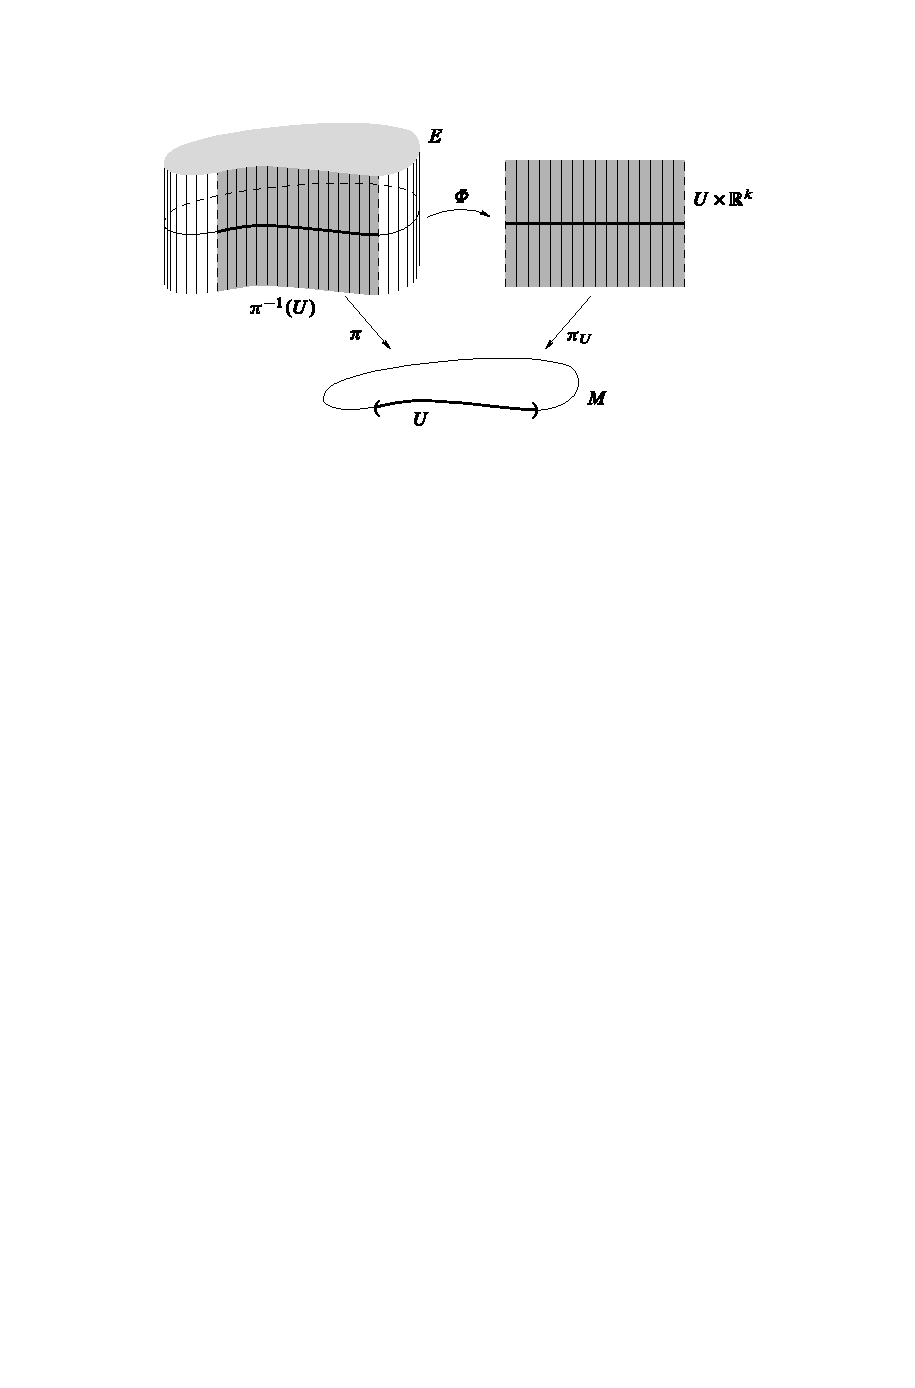
\includegraphics{local-trivialization}
\caption{A local trivialization of a vector bundle.}
\end{figure}\par
If $M$ and $E$ are smooth manifolds with or without boundary, $\pi$ is a smooth map, and the local trivializations can be chosen to be diffeomorphisms, then $E$ is called a \textbf{smooth vector bundle}. In this case, we call any local trivialization that is a diffeomorphism onto its image a \textbf{smooth local trivialization}.\par
A rank-$1$ vector bundle is often called a \textbf{real line bundle}. \textbf{Complex vector bundles} are defined similarly, with real vector space replaced by complex vector space and $\R^k$ replaced by $\C^k$ in the definition. The space $E$ is called the \textbf{total space} of the bundle, $M$ is called its \textbf{base}, and $\pi$ is its projection.
\begin{proposition}
Suppose $E$ is a smooth vector bundle over $M$. Then the projection map $\pi:E\to M$ is a surjective smooth submersion.
\end{proposition}
\begin{proof}
For each point of $E$, there is a local trivialization $\varPhi$ such that $\pi=\pi_U\circ\varPhi$. Since $\pi_U$ and $\varPhi$ are both submersion, it follows that $\pi$ is a submersion.
\end{proof}
If there exists a local trivialization of $E$ over all of $M$ (called a \textbf{global trivialization} of $E$), then $E$ is said to be a \textbf{trivial bundle}. In this case, $E$ itself is homeomorphic to the product space $M\times\R^k$. If $E\to M$ is a smooth bundle that admits a smooth global trivialization, then we say that $E$ is \textbf{smoothly trivial}. In this case $E$ is diffeomorphic to $M\times\R^k$, not just homeomorphic. For brevity, when we say that a smooth bundle is trivial, we always understand this to mean smoothly trivial, not just trivial in the topological sense.
\begin{example}[\textbf{Product Bundles}]
One particularly simple example of a rank $k$ vector bundle over any space $M$ is the product space $E=M\times\R^k$ with $\pi=\pi_1:M\times\R^k\to M$ as its projection. Any such bundle, called a product bundle, is trivial (with the identity map as a global trivialization). If $M$ is a smooth manifold with or without boundary, then $M\times\R^k$ is smoothly trivial.
\end{example}
Although there are many vector bundles that are not trivial, the only one that is easy to visualize is the following.
\begin{example}[\textbf{The Möbius Bundle}]\label{Mobius bundle}
Define an equivalence relation on $\R^2$ by declaring that $(x,y)\sim(x',y')$ if and only if $(x',y')=(x+n,(-1)^ny)$ for some $n\in\Z$. Let $E=\R^2/\sim$ denote the quotient space, and let $q:\R^2\to E$ be the quotient map. For any $r>0$, the image under the quotient map $q$ of the rectangle $[0,1]\times[-r,r]$ is a smooth compact manifold with boundary called a \textbf{M\"obius band}.
\begin{figure}[htbp]
\centering
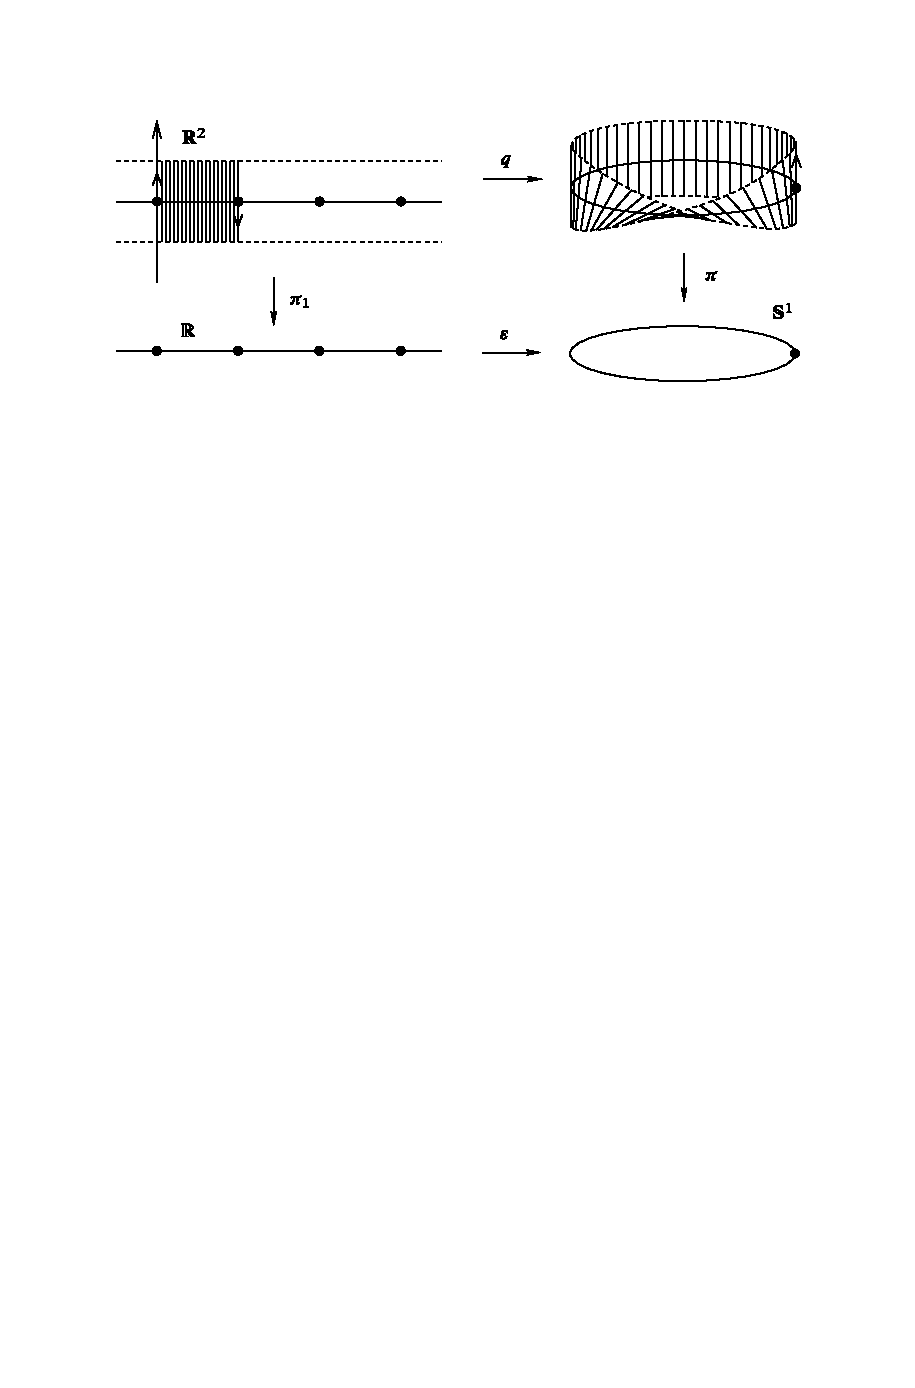
\includegraphics{Mobious-bundle}
\caption{Part of the Möbius bundle.}
\end{figure}\par
Consider the following commutative diagram:
\[\begin{tikzcd}
\R^2\ar[r,"q"]\ar[d,swap,"\pi_1"]&E\ar[d,dashed,"\pi"]\\
\R\ar[r,"\eps"]&S^1
\end{tikzcd}\]
where $\pi_1$ is the projection onto the first factor and $\eps:\R\to S^1$ is the smooth covering map $\eps(x)=e^{2\pi ix}$. Because $\eps\circ\pi_1$ is constant on each equivalence class, it descends to a continuous map $\pi:E\to S^1$. A straightforward verification shows that $E$ has a unique smooth manifold structure such that $q$ is a smooth covering map. and $\pi:E\to S^1$ is a smooth real line bundle over $S^1$, called the \textbf{M\"obius bundle}. $($If $U\sub S^1$ is an open subset that is evenly covered by $\eps$, and $\widetilde{U}\sub\R$ is a component of $\eps^{-1}(U)$, then $q$ restricts to a homeomorphism from $\widetilde{U}\times\R$ to $\pi^{-1}(U)$. Using this, one can construct a homeomorphism from $\pi^{-1}(U)$ to $U\times\R$, which serves as a local trivialization of $E$. These local trivializations can be interpreted as coordinate charts defining the smooth structure on $E$.$)$
\end{example}
The most important examples of vector bundles are tangent bundles.
\begin{proposition}[\textbf{The Tangent Bundle as a Vector Bundle}]\label{tangent bundle as vector bundle}
Let $M$ be a smooth $n$-manifold with or without boundary, and let $TM$ be its tangent bundle. With its standard projection map, its natural vector space structure on each fiber, and the topology and smooth structure constructed in Proposition~\ref{tangent bundle struct}, $TM$ is a smooth vector bundle of rank $n$ over $M$.
\end{proposition}
\begin{proof}
Given any smooth chart $(U,\varphi)$ for $M$ with coordinate functions $(x^i)$, define a map $\varPhi:\pi^{-1}(U)\to U\times\R^n$ by
\[\varPhi\Big(v^i\frac{\partial}{\partial x^i}\Big|_p\Big)=(p,(v^1,\dots,v^n))\]
This is linear on fibers and satisfies $\pi_U\circ\varPhi=\pi$. The composite map
\[\begin{tikzcd}
\pi^{-1}(U)\ar[r,"\varPhi"]&U\times\R^n\ar[r,"\varphi\times\mathrm{id}_{\R^n}"]&\varphi(U)\times\R^n
\end{tikzcd}\]
is equal to the coordinate map $\widetilde{\varphi}$ constructed in Proposition~\ref{tangent bundle struct}. Since both $\widetilde{\varphi}$ and $\varphi\times\mathrm{id}_{\R^n}$ are diffeomorphisms, so is $\varPhi$. Thus, $\varPhi$ satisfies all the conditions for a smooth local trivialization.
\end{proof}
Any bundle that is not trivial, of course, requires more than one local trivialization. The next lemma shows that the composition of two smooth local trivializations has a simple form where they overlap.
\begin{lemma}\label{vector bundle trivialization overlap}
Let $\pi:E\to M$ be a smooth vector bundle of rank $k$ over $M$. Suppose $\varPhi:\pi^{-1}(U)\to U\times\R^k$ and $\varPsi:\pi^{-1}(V)\to V\times\R^k$ are two smooth local trivializations of $E$ with $U\cap V=\emp$. There exists a smooth map $\tau:U\cap V\to\GL_k(\R)$ such that the composition $\varPhi\circ\varPsi^{-1}:(U\cap V)\times\R^k\to(U\cap V)\times\R^k$ has the form
\[\varPhi\circ\varPsi^{-1}(p,v)=(p,\tau(p)v)\]
where $\tau(p)v$ denotes the usual action of the $k\times k$ matrix $\tau(p)$ on the vector $v\in\R^k$.
\end{lemma}
\begin{proof}
The following diagram commutes:
\[\begin{tikzcd}
(U\cap V)\times\R^k\ar[rd,swap,"\pi_1"]&\pi^{-1}(U\cap V)\ar[l,swap,"\varPsi"]\ar[r,"\varPhi"]\ar[d,"\pi"]&(U\cap V)\times\R^k\ar[ld,"\pi_1"]\\
&U\cap V&
\end{tikzcd}\]
where the maps on top are to be interpreted as the restrictions of $\varPsi$ and $\varPhi$ to $\pi^{-1}(U\cap V)$. It follows that $\pi_1\circ(\varPhi\circ\varPsi^{-1})=\pi_1$, which means that
\[\varPhi\circ\varPsi^{-1}(p,v)=(p,\sigma(p,v))\]
for some smooth map $\sigma:(U\cap V)\times\R^k\to\R^k$. Moreover, for each fixed $p\in U\cap V$, the map $v\mapsto\sigma(p,v)$ from $\R^k$ to itself is an invertible linear map, so there is a nonsingular $k\times k$ matrix $\tau(p)$ such that $\sigma(p,v)=\tau(p)v$. If we choose a basis $(e_j)$ for $\R^k$ and let $\pi^i:\R^k\to\R$ be the projection on the $i$-th coordinate, then
\[\pi^i\circ\pi_2\circ\varPhi\circ\varPsi^{-1}(p,e_j)=\pi^i(\tau(p)e_j)=\pi^i(\tau^1_j(p)e_1+\cdots+\tau^k_j(p)e_k)=\tau^i_j(p)\]
so each function $\tau^i_j$ is a composition of smooth functions, hence is smooth. Because the matrix entries form global smooth coordinates for $\GL_k(\R)$, this implies that $\tau$ is smooth.
\end{proof}
The smooth map $\tau:U\cap V\to\GL_k(\R)$ described in this lemma is called the \textbf{transition function} between the local trivializations $\varPhi$ and $\varPsi$. For example, if $M$ is a smooth manifold and $\varPhi$ and $\varPsi$ are the local trivializations of $TM$ associated with two different smooth charts, then $(\ref{coordinate change-1})$ shows that the transition function between them is the Jacobian matrix of the coordinate transition map.\par
Like the tangent bundle, vector bundles are often most easily described by giving a collection of vector spaces, one for each point of the base manifold. In order to make such a set into a smooth vector bundle, we would first have to construct a manifold topology and a smooth structure on the disjoint union of all the vector spaces, 
and then construct the local trivializations and show that they have the requisite properties. The next lemma provides a shortcut, by showing that it is sufficient to construct the local trivializations, 
as long as they overlap with smooth transition functions.
\begin{lemma}[\textbf{Vector Bundle Chart Lemma}]\label{vector bundle chart lemma}
Let $M$ be a smooth manifold with or without boundary, and suppose that for each $p\in M$ we are given a real vector space $E_p$ of some fixed dimension $k$. Let $E=\coprod_{p\in M}E_p$ and let $\pi:E\to M$ be the map that takes each element of $E_p$ to the point $p$. Suppose furthermore that we are given the following data:
\begin{itemize}
\item[$(\rmnum{1})$] An open cover $\{U_\alpha\}_{\alpha\in A}$ of $M$.
\item[$(\rmnum{2})$] For each $\alpha\in A$, a bijective map $\varPhi_\alpha:\pi^{-1}(U_\alpha)\to U_\alpha\times\R^k$ whose restriction to each $E_p$ is a vector space isomorphism from $E_p$ to $\{p\}\times\R^k$.
\item[$(\rmnum{3})$] For each $\alpha,\beta\in A$ with $U_\alpha\cap U_\beta\neq\emp$, a smooth map $\tau_{\alpha\beta}:U_\alpha\cap U_\beta\to\GL_k(\R)$ such that the map $\varPhi_\alpha\circ\varPhi_\beta^{-1}$ from $(U_\alpha\cap U_\beta)\times\R^k$ to itself has the form
\begin{align}\label{vector bundle transition function-1}
\varPhi_\alpha\circ\varPhi_\beta^{-1}(p,v)=(p,\tau_{\alpha\beta}(p)v)
\end{align}
\end{itemize}
Then $E$ has a unique topology and smooth structure making it into a smooth manifold with or without boundary and a smooth rank-$k$ vector bundle over $M$, with $\pi$
as projection and $\{(U_\alpha,\varPhi_\alpha)\}$ as smooth local trivializations.
\end{lemma}
\begin{proof}
For each point $p\in M$, choose some $U_\alpha$ containing $p$, choose a smooth chart $(V_p,\varphi_p)$ for $M$ such that $p\in V_p\sub U_\alpha$ and let $\widehat{V}=\varphi_p(V_p)\sub\R^n$ or $\H^n$ (where $n$ is the dimension of $M$). Define a map $\widetilde{\varphi}_p:\pi^{-1}(V_p)\to\widehat{V}_p\times\R^k$ by $\widetilde{\varphi}_p=(\varphi_p\times\mathrm{id}_{\R^k})\circ\varPhi_\alpha$:
\[\begin{tikzcd}
\pi^{-1}(V_p)\ar[r,"\varPhi_\alpha"]&V_p\times\R^k\ar[rr,"\varphi_p\times\mathrm{id}_{\R^k}"]&&\widehat{V}_p\times\R^k
\end{tikzcd}\]
We will show that the collection of all such charts $\{(\pi^{-1}(V_p),\widetilde{\varphi}_p)\}$ satisfies the conditions of the smooth manifold chart lemma or its counterpart for manifolds with boundary, and therefore gives $E$ the structure of a smooth manifold with or without boundary.\par
As a composition of bijective maps, $\widetilde{\varphi}_p$ is bijective onto an open subset of either $\R^n\sub\R^k=\R^{n+k}$ or $\H^n\times\R^k=\H^{n+k}$. For any $p,q\in M$, it is easy to check that
\[\widetilde{\varphi}_p\big(\pi^{-1}(V_p)\cap\pi^{-1}(V_q)\big)=\varphi_p(V_p\cap V_q)\times\R^k\]
which is open because $\varphi_p$ is a homeomorphism onto an open subset of $\R^n$ or $\H^n$. Wherever two such charts overlap, we have
\[\widetilde{\varphi}_p\circ\widetilde{\varphi}_q^{-1}=(\varphi_p\times\mathrm{id}_{\R^k})\circ\varPhi_\alpha\circ\varPhi_\beta^{-1}\circ(\varphi_q\times\mathrm{id}_{\R^k})^{-1}\]
This composition is still a diffeomorphism, thus conditions $(\rmnum{1}),(\rmnum{2})$ and $(\rmnum{3})$ of Lemma~\ref{smooth mani chart lem} are satisfied. Because the open cover $\{V_p:p\in M\}$ has a countable subcover, $(\rmnum{4})$ is satisfied as well.\par
To check the Hausdorff condition $(\rmnum{5})$, just note that any two points in the same space $E_p$ lie in one of the charts we have constructed, while if $\xi\in E_p$ and $\eta\in E_q$ with $p\neq q$, we can choose $V_p$ and $V_q$ to be disjoint neighborhoods of $p$ and $q$, so that the sets $\pi^{-1}(V_p)$ and $\pi^{-1}(V_q)$ are disjoint coordinate neighborhoods containing $\xi$ and $\eta$, respectively. Thus we have given $E$ the structure of a smooth manifold with or without boundary.\par
With respect to this structure, each of the maps $\varPhi_\alpha$ is a diffeomorphism, because in terms of the coordinate charts $(\pi^{-1}(V_p),\widetilde{\varphi}_p)$ for $E$ and $(V_p\times\R^k,\varphi\times\mathrm{id}_{\R^k})$ for $V_p\times\R^k$, the coordinate representation of $\varPhi_\alpha$ is the identity map. The coordinate representation of $\pi$, with respect to the same chart for $E$ and the chart $(V_p,\varphi_p)$ for $M$, is $\pi(x,v)=x$, so $\pi$ is smooth as well. Because each $\varPhi_\alpha$ maps $E_p$ to $\{p\}\times\R^k$, it is immediate that $\pi_1\circ\varPhi_\alpha=\pi$ and $\varPhi_\alpha$ is linear on fibers by hypothesis. Thus, $\varPhi_\alpha$ satisfies all the conditions for a smooth local trivialization.\par
The fact that this is the unique such smooth structure follows easily from the requirement that the maps $\varPhi_\alpha$ be diffeomorphisms onto their images: any smooth structure satisfying the same conditions must include all of the charts we constructed, so it is equal to this one.
\end{proof}
Here are some examples showing how the chart lemma can be used to construct new vector bundles from old ones.
\begin{example}[\textbf{Whitney Sums}]
Given a smooth manifold $M$ and smooth vector bundles $E'\to M$ and $E''\to M$ of ranks $k_1$ and $k_2$, respectively, we will construct a new vector bundle over $M$ called the \textbf{Whitney sum} of $E'$ and $E''$, whose fiber at each $p\in M$ is the direct sum $E'_p\oplus E''_p$. The total space is defined as $E'\oplus E''=\coprod_{p\in M}(E'_p\oplus E''_p)$, with the obvious projection $\pi:E'\oplus E''\to M$. For each $p\in M$, choose a neighborhood $U$ of $p$ small enough that there exist local trivializations $(U,\varPhi_1)$ of $E'$ and $(U,\varPhi_2)$ of $E''$, and define $\varPhi:\pi^{-1}(U)\to U\times\R^{k_1+k_2}$ by 
\[\varPhi(v_1,v_2)=\big(\pi(v_1),(\pi_{\R^{k_1}}\circ\varPhi_1(v_1),\pi_{\R^{k_2}}\circ\varPhi_2(v_2))\big)\]
Suppose we are given another such pair of local trivializations $(\widetilde{U},\widetilde{\varPhi}_1)$ and $(\widetilde{U},\widetilde{\varPhi}_2)$. Let $\tau_1:(U\cap\widetilde{U})\to\GL_{k_1}(\R)$ and $\tau_2:(U\cap\widetilde{U})\to\GL_{k_2}(\R)$ be the corresponding transition functions. Then the transition function for $E'\oplus E''$ has the form
\[\widetilde{\varPhi}\circ\varPhi^{-1}(p,(v_1,v_2))=(p,\tau(p)(v_1,v_2))\]
where $\tau(p)=\tau_1(p)\oplus\tau_2(p)$ is the block diagonal matrix
\[\begin{pmatrix}
\tau_1(p)&0\\
0&\tau_2(p)
\end{pmatrix}\]
Because this depends smoothly on $p$, it follows from the chart lemma that $E'\oplus E''$ is a smooth vector bundle over $M$.
\end{example}
\begin{example}[\textbf{Restriction of a Vector Bundle}]
Suppose $\pi:E\to M$ is a rank-$k$ vector bundle and $S\sub M$ is any subset. We define the restriction of $E$ to $S$ to be the set $E|_S=\bigcup_{p\in S}E_p$, with the projection $E|_S\to S$ obtained by restricting $\pi$. If $\varPhi:\pi^{-1}(U)\to U\times\R^k$ is a local trivialization of $E$ over $U\sub M$, it restricts to a bijective map $\varPhi|_U:(\pi|_S)^{-1}(U\cap S)\to (U\cap S)\times\R^k$, and it is easy to check that these form local trivializations for a vector bundle structure on $E|_S$. If $E$ is a smooth vector bundle and $S\sub M$ is an embedded submanifold, it follows easily from the chart lemma that $E|_S$ is a smooth vector bundle.\par 
However, if $S$ is merely immersed, since the topology of $S$ is not the subspace topology, our argument above falis. Instead, we give $E|_S$ a topology and smooth structure making it into a smooth rank-$k$ vector bundle over $S$ as follows: For each $p\in S$, choose a neighborhood $U$ of $p$ in $M$ over which there is a local trivialization $\varPhi$ of $E$, and a neighborhood $V$ of $p$ in $S$ that is embedded in $M$ and contained in $U$. Then the restriction of $\varPhi$ to $\pi^{-1}(V)$ is a bijection from $\pi^{-1}(V)$ to $V\times\R^k$, and we can apply the chart lemma to these bijections to yield the desired structure.
\end{example}
Now we use the chart lemma to give another way to construct a vector bundle. First we need an observation.
\begin{lemma}\label{vector bundle cochain prop}
Let $\pi:E\to M$ be a smooth vector bundle of rank $k$ over a smooth manifold $M$ with or without boundary. Suppose that $\{U_\alpha\}_{\alpha\in A}$ is an open 
cover of $M$, and for each $\alpha\in A$ we are given a smooth local trivialization $\varPhi_\alpha:\pi^{-1}(U_\alpha)\to U_\alpha\times\R^k$ of $E$. For 
each $\alpha,\beta\in A$ such that $U_\alpha\cap U_\beta\neq\emp$, let $\tau_{\alpha\beta}:U_{\alpha}\cap U_{\beta}\to\GL_k(\R)$ be the transition function 
defined by $(\ref{vector bundle transition function-1})$. Then the following identity is satisfied for all $\alpha,\beta,\gamma\in A$:
\begin{align}\label{vector bundle transition function-2}
\tau_{\alpha\beta}(p)\tau_{\beta\gamma}(p)=\tau_{\alpha\gamma}(p),\quad p\in U_\alpha\cap U_\beta\cap U_\gamma,
\end{align}
where the juxtaposition on the left-hand side represents matrix multiplication and $\tau_{\alpha\alpha}=I_k$ for all $\alpha\in A$.
\end{lemma}
\begin{proof}
By definition we have
\begin{align*}
\varPhi_\alpha\circ\varPhi_{\beta}^{-1}(p,v)=(p,\tau_{\alpha\beta}(p)v).
\end{align*}
Thus fix a $p\in U_\alpha\cap U_\beta\cap U_\gamma$, we get
\[(\tau_{\alpha\beta}(p)\tau_{\beta\gamma}(p)v)=\varPhi_\alpha\circ\varPhi_{\beta}^{-1}\circ\varPhi_\beta\circ\varPhi_{\gamma}^{-1}(p,v)=\varPhi_{\alpha}\circ\varPhi_{\gamma}(p,v)=(p,\tau_{\alpha\gamma}v)\]
Since this holds for all $v\in E_p$, we conclude $\tau_{\alpha\beta}(p)\tau_{\beta\gamma}(p)=\tau_{\alpha\gamma}(p)$.
\end{proof}
\begin{theorem}[\textbf{Vector bundle construction theorem}]\label{vector bundle construct}
Let $M$ be a smooth manifold with or without boundary, and let $\{U_\alpha\}_{\alpha\in A}$ be an open cover of $M$. Suppose for each $\alpha,\beta\in A$ we are 
given a smooth map $\tau_{\alpha\beta}:U_{\alpha}\cap U_{\beta}\to\GL_k(\R)$ such that $(\ref{vector bundle transition function-2})$ is satisfied for all $\alpha,\beta,\gamma\in A$. 
Then there is a smooth rank-$k$ vector bundle $\pi:E\to M$ with smooth local trivializations $\varPhi_\alpha:\pi^{-1}(U_\alpha)\to U_\alpha\times\R^k$ whose transition functions are the given maps $\tau_{\alpha\beta}$.
\end{theorem}
\begin{proof}
Define an equivalence relation on $\coprod_{\alpha\in A}(U_\alpha\times\R^k)$: for $(p_1,v_1)\in U_\alpha\times\R^k$ and $(p_2,v_2)\in U_\beta\times\R^k$,
\[(p_1,v_1)\sim(p_2,v_2)\iff p_1=p_2\And v_1=\tau_{\alpha\beta}(p_2)v_2.\]
This is well defined in view of $(\ref{vector bundle transition function-2})$:
\begin{itemize}
\item Since $\tau_{\alpha\alpha}(p)=I_k$, we have $(p,v)\sim(p,v)$ for all $(p,v)$.
\item If $v_1=\tau_{\alpha\beta}(p)v_2$, then $v_2=\tau_{\beta\alpha}(p)v_1$, since $\tau_{\alpha\beta}\tau_{\beta\alpha}=\tau_{\alpha\alpha}=\mathrm{id}$.
\item If $v_1=\tau_{\alpha\beta}(p)v_2$ and $v_2=\tau_{\beta\gamma}(p)v_3$, then $v_1=\tau_{\alpha\beta}(p)\tau_{\beta\gamma}(p)v_2=\tau_{\alpha\gamma}(p)v_3$.
\end{itemize}
Thus we can form the quotient space $E:=\coprod_{\alpha\in A}(U_\alpha\times\R^k)/\sim$. We define a map $\pi:E\to M$ by
\[\pi(p,v)=p\]
so that $\pi^{-1}(U_\alpha)$ is the equivalent class of $U_\alpha\times\R^k$. Now define a local trivalization $\varPhi_\alpha:\pi^{-1}(U_\alpha)\to U_\alpha\times\R^k$ by $\varPhi_\alpha(p,v)=(p,v)$. We can check, by our equivalent relation: for $(p,v)\in U_\beta\times\R^k$,
\[\varPhi_\alpha\circ\varPhi_\beta^{-1}(p,v)=\{(p,v')\in U_\alpha\times\R^k:v'=\tau_{\alpha\beta}(p)v\}=(p,\tau_{\alpha\beta}(p)v)\]
Thus by the chart lemma, $\pi:E\to M$ is a vector bundle.
\end{proof}
\subsection{Sections of vector bundles}
Let $\pi:E\to M$ be a vector bundle. A \textbf{section} of $E$ (sometimes called a \textbf{cross section}) is a section of the map $\pi$, that is, a continuous map $\sigma:M\to E$ satisfying $\pi\circ\sigma=\mathrm{id}_M$. This means that $\sigma(p)$ is an element of the fiber $E_p$ for each $p\in M$.\par
More generally, a \textbf{local section} of $E$ is a continuous map $\sigma:U\to E$ defined on some open subset $U\sub M$ and satisfying $\pi\circ\sigma=\mathrm{id}_U$. To emphasize the distinction, a section defined on all of $M$ is sometimes called a \textbf{global section}. Note that a local section of $E$ over $U\sub M$ is the same as a global section of the restricted bundle $E|_U$. If $M$ is a smooth manifold with or without boundary and $E$ is a smooth vector bundle, a \textbf{smooth (local or global) section} of $E$ is one that is a smooth map from its domain to $E$.\par
Just as with vector fields, for some purposes it is useful also to consider maps that would be sections except that they might not be continuous. Thus, we define a \textbf{rough (local or global) section} of $E$ over a set $U\sub M$ to be a map $\sigma:U\to E$ (not necessarily continuous) such that $\pi\circ\sigma=\mathrm{id}_U$. A section without further qualification always means a continuous section.\par
The \textbf{zero section} of $E$ is the global section $\zeta:M\to E$ defined by
\[\zeta(p)=0\in E_p\quad\text{for each }p\in M.\]
As in the case of vector fields, the \textbf{support} of a section $\sigma$ is the closure of the set $\{p\in M:\sigma(p)\neq 0\}$.
\begin{example}[\textbf{Sections of Vector Bundles}]
Suppose $M$ is a smooth manifold with or without boundary.
\begin{itemize}
\item[(a)]Sections of $TM$ are vector fields on $M$.
\item[(b)]Given an immersed submanifold $S\sub M$ with or without boundary, a section of the ambient tangent bundle $TM|_S\to S$ is called a \textbf{vector field along $\bm{S}$}. It is a continuous map $X:S\to TM$ such that $X_p\in T_pM$ for each $p\in S$. This is different from a vector field on $S$, which satisfies $X_p\in T_pS$ at each point.
\item[(c)]If $E=M\times\R^k$ is a product bundle, there is a natural one-to-one correspondence between sections of $E$ and continuous functions from $M$ to $\R^k$: a continuous function $F:M\to\R^k$ determines a section $\widetilde{F}:M\to M\times\R^k$ by $\widetilde{F}(x)=(x,F(x))$, and vice versa. If $M$ is a smooth manifold with or without boundary, then the section $\widetilde{F}$ is smooth if and only if $F$ is.
\item[(d)]The correspondence in the preceding paragraph yields a natural identification between the space $C^\infty(M)$ and the space of smooth sections of the trivial line bundle $M\times\R\to M$.
\end{itemize}
\end{example}
If $E\to M$ is a smooth vector bundle, the set of all smooth global sections of $E$ is a vector space under pointwise addition and scalar multiplication:
\[(c_1\sigma_1+c_2\sigma_2)(p)=c_1\sigma_1(p)+c_2\sigma_2(p)\]
This vector space is usually denoted by $\Gamma(E)$. Just like smooth vector fields, smooth sections of a smooth bundle $E\to M$ can be multiplied by smooth real-valued functions: if $f\in C^\infty(M)$ and $\sigma\in\Gamma(E)$, we obtain a new section $f\sigma$ defined by
\[(f\sigma)(p)=f(p)\sigma(p)\]
\begin{lemma}[\textbf{Extension Lemma for Vector Bundles}]\label{ext lem vector bundle}
Let $\pi:E\to M$ be a smooth vector bundle over a smooth manifold $M$ with or without boundary.
\begin{itemize}
\item[(a)] Suppose $A$ is a closed subset of $M$ and $\sigma:A\to E$ is a section of $E|_A$ that is smooth in the sense that $\sigma$ extends to a smooth local section of $E$ in a neighborhood of each point. For each open subset $U\sub M$ containing $A$, there exists a global smooth section $\widetilde{\sigma}\in\Gamma(E)$ such that $\widetilde{\sigma}|_A=\sigma$ and $\supp(\widetilde{\sigma})\sub U$.
\item[(b)]Suppose $S\sub M$ is an embedded submanifold with or without boundary. For any smooth section $\sigma$ of the restricted bundle $E|_S\to S$, there exist a neighborhood $U$ of $S$ in $M$ and a smooth section $\widetilde{\sigma}$ of $E|_U$ such that $\widetilde{\sigma}|_S=\sigma$. If $E$ has positive rank, then every smooth section of $E|_S$ extends smoothly to all of $M$ if and only if $S$ is properly embedded.
\end{itemize}
\end{lemma}
\begin{proof}
See Lemma~\ref{ext lem smooth func}.
\end{proof}
\subsubsection{Local and global frames}
Let $E\to M$ be a vector bundle. If $U\sub M$ is an open subset, a $k$-tuple of local sections $(\sigma_1,\dots,\sigma_k)$ of $E$ over $U$ is said to be \textbf{linearly independent} if their values $(\sigma_1(p),\dots,\sigma_k(p))$ form a linearly independent $k$-tuple in $E_p$ for each $p\in U$. Similarly, they are said to \textbf{span $\bm{E}$} if their values span $E_p$ for each $p\in U$. A \textbf{local frame} for $E$ over $U$ is an ordered $k$-tuple $(\sigma_1,\dots,\sigma_k)$ of linearly independent local sections over $U$ that span $E$; thus $(\sigma_1(p),\dots,\sigma_k(p))$ is a basis for the fiber $E_p$ for each $p\in U$. It is called a \textbf{global frame} if $U=M$. If $E\to M$ is a smooth vector bundle, a local or global frame is a \textbf{smooth frame} if each $\sigma_i$ is a smooth section. We often denote a frame $(\sigma_1,\dots,\sigma_k)$ by $(\sigma_i)$.\par
The next proposition is an analogue for vector bundles of Proposition~\ref{local frame completion}.
\begin{proposition}[\textbf{Completion of Local Frames for Vector Bundles}]\label{vector bundle local frame completion}
Suppose $\pi:E\to M$ is a smooth vector bundle of rank $k$.
\begin{itemize}
\item[(a)] If $(\sigma_1,\dots,\sigma_m)$ is a linearly independent $m$-tuple of smooth local sections of $E$ over an open subset $U\sub M$, with $1\leq m<k$, then for each $p\in U$ there exist smooth sections $\sigma_{m+1},\dots,\sigma_k$ defined on some neighborhood $V$ of $p$ such that $(\sigma_1,\dots,\sigma_k)$ is a smooth local frame for $E$ over $U\cap V$.
\item[(b)] If $(v_1,\dots,v_m)$ is a linearly independent $m$-tuple of elements of $E_p$ for some $p\in M$, with $1\leq m\leq k$, then there exists a smooth local frame $(\sigma_i)$ for $E$ over some neighborhood of $p$ such that $\sigma_i(p)=v_i$ for $i=1,\dots,m$.
\item[(c)] If $A\sub M$ is a closed subset and $(\tau_1,\dots,\tau_k)$ is a linearly independent $k$-tuple of sections of $E|_A$ that are smooth in the sense described in Lemma~\ref{ext lem vector bundle}, then there exists a smooth local frame $(\sigma_1,\dots,\sigma_k)$ for $E$ over some neighborhood of $A$ such that $\sigma_i|_A=\tau_i$ for $i=1,\dots,k$.
\end{itemize}
\end{proposition}
Local frames for a vector bundle are intimately connected with local trivializations, as the next two examples show.
\begin{example}[\textbf{A Global Frame for a Product Bundle}]
If $E=M\times\R^k$ is a product bundle, the standard basis $(e_1,\dots,e_k)$ for $\R^k$ yields a global frame $(\widetilde{e}_i)$ for $E$, defined by $\widetilde{e}_i(p)=(p,e_i)$. If $M$ is a smooth manifold with or without
boundary, then this global frame is smooth.
\end{example}
\begin{example}[\textbf{Local Frames Associated with Local Trivializations}]\label{local frame trivialization}
Suppose $\pi:E\to M$ is a smooth vector bundle. If $\varPhi:\pi^{-1}(U)\to U\times\R^k$ is a smooth local trivialization of $E$, we can use the same idea as in the preceding example to construct a local frame for $E$ over $U$. Define maps $\sigma_1,\dots,\sigma_k:U\to E$ by $\sigma_i(p)=\varPhi^{-1}(p,e_i)=\varPhi^{-1}\circ\widetilde{e}_i(p)$:
\[\begin{tikzcd}
\pi^{-1}(U)\ar[rd,"\pi"]\ar[rr,"\varPhi"]&&U\times\R^k\ar[ld,swap,"\pi_1"]\\
&U\ar[lu,bend left=35,"\sigma_i"]\ar[ru,bend right=35,swap,"\widetilde{e}_i"]&
\end{tikzcd}\]
Then $\sigma_i$ is smooth because $\varPhi$ is a diffeomorphism, and the fact that $\pi_1\circ\varPhi=\pi$ implies that
\[\pi\circ\sigma_i(p)=\pi\circ\varPhi^{-1}(p,e_i)=\pi_1(p,e_i)=p,\]
so $\sigma_i$ is a section. To see that $(\sigma_i(p))$ forms a basis for $E_p$, just note that $\varPhi$ restricts to an isomorphism from $E_p$ to $\{p\}\times\R^k$, and $\varPhi(\sigma_i(p))=(p,e_i)$, so $\varPhi$ takes $(\sigma_i(p))$ to the standard basis for $\{p\}\times\R^k\cong\R^k$. We say that this local frame $(\sigma_i)$ is \textbf{associated with $\bm{\varPhi}$}.
\end{example}
\begin{proposition}\label{local frame iff trivialization}
Every smooth local frame for a smooth vector bundle is associated
with a smooth local trivialization as in Example~\ref{local frame trivialization}.
\end{proposition}
\begin{proof}
Suppose $E\to M$ is a smooth vector bundle and $(\sigma_i)$ is a smooth local frame for $E$ over an open subset $U\sub M$. We define a map $\varPsi:U\times\R^k\to\pi^{-1}(U)$ by
\[\varPsi(p,(v^1,\dots,v^k))=v^i\sigma_i(p).\]
The fact that $\sigma_i(p)$ forms a basis for $E_p$ at each $p\in U$ implies that $\varPsi$ is bijective, and an easy computation shows that $\sigma_i=\varPsi\circ\widetilde{e}_i$. Thus, if we can show that $\varPsi$ is
a diffeomorphism, then $\varPsi^{-1}$ will be a smooth local trivialization whose associated local frame is $(\sigma_i)$.\par
Since $\varPsi$ is bijective, to show that it is a diffeomorphism it suffices to show that it is a local diffeomorphism. Given $q\in U$, we can choose a neighborhood $V$ of $q$ in $M$ over which there exists a smooth local trivialization $\varPhi:\pi^{-1}(V)\to V\times\R^k$, and by shrinking $V$ if necessary we may assume that $V\sub U$. Since $\varPhi$ is a diffeomorphism, if we can show that $\varPhi\circ\varPsi|_{V\times\R^k}$ is a diffeomorphism from $V\times\R^k$ to itself, it follows that $\varPsi$ restricts to a diffeomorphism from $V\times\R^k$ to $V$:
\[\begin{tikzcd}
V\times\R^k\ar[rd,swap,"\pi_1"]\ar[r,"\varPsi|_{V\times\R^k}"]&\pi^{-1}(V)\ar[d,"\pi"]\ar[r,"\varPhi"]&V\times\R^k\ar[ld,"\pi_1"]\\
&V&
\end{tikzcd}\]
For each of our smooth sections $\sigma_i$, the composite map $\varPhi\circ\sigma_i|_V:V\to V\times\R^k$ is smooth, and thus there are smooth functions $\sigma_i^1,\dots,\sigma_i^k:V\to\R$
\[\varPhi\circ\sigma_i(p)=\big(p,(\sigma_i^1(p),\dots,\sigma_i^k(p))\big).\]
On $V\times\R^k$, therefore
\[\varPhi\circ\varPsi(p,(v^1,\dots,v^k))=\big(p,(v^i\sigma_i^1(p),\dots,v^i\sigma_i^k(p))\big),\]
which is clearly smooth.\par
To show that $(\varPhi\circ\varPsi)^{-1}$ is smooth, note that the matrix $(\sigma_i^j(p))$ is invertible for each $p$, because $(\sigma_i(p))$ is a basis for $E_p$. Let $(\tau_i^j(p))$ denote the inverse matrix. Because matrix inversion is a smooth map from $\GL_k(\R)$ to itself, the functions $\tau_i^j$ are smooth. It follows from the computations in the preceding paragraph that
\[(\varPhi\circ\varPsi)^{-1}(p,(w^1,\dots,w^k))=\big(p,(w^1\tau_i^1(p),\dots,w^k\tau_i^k(p))\big),\]
which is also smooth.
\end{proof}
\begin{corollary}
A smooth vector bundle is smoothly trivial if and only if it admits a smooth global frame.
\end{corollary}
\begin{proof}
Example~\ref{local frame trivialization} and Proposition~\ref{local frame iff trivialization} show that there is a smooth local trivialization over an open subset $U\sub M$ if and only if there is a smooth local frame over $U$. The corollary is just the special case of this statement when $U=M$.
\end{proof}
When applied to the tangent bundle of a smooth manifold $M$, this corollary says that $TM$ is trivial if and only if $M$ is parallelizable.
\begin{corollary}\label{vector bundle chart from frame}
Let $\pi:E\to M$ be a smooth vector bundle of rank $k$, let $(V,\varphi)$ be a smooth chart on $M$ with coordinate functions $(x^i)$, and suppose there exists a smooth local frame $(\sigma_i)$ for $E$ over $V$. Define $\widetilde{\varphi}:\pi^{-1}(V)\to\varphi(V)\times\R^k$ by
\[\widetilde{\varphi}(v^i\sigma_i(p))=(x^1(p),\dots,x^n(p),v^1,\dots,v^k).\]
Then $(\pi^{-1}(V),\widetilde{\varphi})$ is a smooth coordinate chart for $E$.
\end{corollary}
\begin{proof}
Just check that $\widetilde{\varphi}$ is equal to the composition $(\varphi\times\mathrm{id}_{\R^k})\circ\varPhi$, where $\varPhi$ is the local trivialization associated with $(\sigma_i)$. As a composition of diffeomorphisms, it is a diffeomorphism.
\end{proof}
Suppose $(\sigma_i)$ is a smooth local frame for $E$ over some open subset $U\sub M$. If $\tau:M\to E$ is a rough section, the value of $\tau$ at an arbitrary point $p\in U$ can be written $\tau(p)=\tau^i(p)\sigma_i(p)$ for some uniquely determined numbers $(\tau^1(p),\dots,\tau^n(p))$. This defines $k$ functions $\tau^i:U\to\R$, called the \textbf{component functions of $\bm{\tau}$} with respect to the given local frame.
\begin{proposition}[\textbf{Local Frame Criterion for Smoothness}]\label{local frame smooth crit}
Let $\pi:E\to M$ be a smooth vector bundle, and let $\tau:M\to E$ be a rough section. If $(\sigma_i)$ is a smooth local frame for $E$ over an open subset $U\sub M$, then $\tau$ is smooth on $U$ if and only if its component functions with respect to $(\sigma_i)$ are smooth.
\end{proposition}
\begin{proof}
Let $\varPhi:\pi^{-1}(U)\to U\times\R^k$ be the local trivialization associated with the local frame $\varPhi$. Because $\varPhi$ is a diffeomorphism, $\tau$ is smooth on $U$ if and only if the composite map $\varPhi\circ\tau$ is smooth on $U$. It is straightforward to check that $\varPhi\circ\tau(p)=\big(p,(\tau^1(p),\dots,\tau^k(p))\big)$ where $\tau^i$ are the component functions of $\tau$ with respect to $(\sigma_i)$, so $\varPhi\circ\tau$ is smooth if and only if the component functions $\tau^i$
are smooth.
\end{proof}
Proposition~\ref{local frame smooth crit} applies equally well to local sections, since a local section of $E$ over an open subset $V\sub M$ is a global section of the restricted bundle $E|_V$.\par
The correspondence between local frames and local trivializations leads to the
following uniqueness result characterizing the smooth structure on the tangent bundle of a smooth manifold.
\begin{proposition}[\textbf{Uniqueness of the Smooth Structure on $\bm{TM}$}]\label{tangent bundle struct unique}
Let $M$ be a smooth $n$-manifold with or without boundary. The topology and smooth structure on $TM$ constructed in Proposition~\ref{tangent bundle struct} are the 
unique ones with respect to which $\pi:TM\to M$ is a smooth vector bundle with the given vector space structure on the fibers, and such that all coordinate vector 
fields are smooth local sections.
\end{proposition}
\begin{proof}
Suppose $TM$ is endowed with some topology and smooth structure making it into a smooth vector bundle with the given properties. If $(U,\varphi)$ is any smooth chart for $M$, the corresponding coordinate frame $(\partial/\partial x^i)$ is a smooth local frame over $U$, so by Proposition~\ref{local frame iff trivialization} there is a smooth local trivialization $\varPhi:\pi^{-1}(U)\to U\times\R^k$ associated with this local frame, which, according to Example~\ref{local frame trivialization}, is defined by
\[\varPhi(v^i\frac{\partial}{\partial x^i}\Big|_p)=\big(p,(v^1,\dots,v^n)\big)\] But this is none other than the map we constructed in Proposition~\ref{tangent bundle as vector bundle}. It follows from Corollary~\ref{vector bundle chart from frame} that the natural coordinate chart $\widetilde{\varphi}=(\varphi\times\mathrm{id}_{\R^n})\circ\varPhi$ belongs to the given smooth structure. Thus, the given smooth structure is equal to the one constructed in Proposition~\ref{tangent bundle struct}.
\end{proof}
\subsection{Bundle homomorphisms}
If $\pi:E\to M$ and $\pi':E'\to M'$ are vector bundles, a continuous map $F:E\to E'$ is called a \textbf{bundle homomorphism} if there exists a map $f:M\to M'$ 
satisfying $\pi'\circ F=f\circ\pi$,
\[\begin{tikzcd}
E\ar[r,"F"]\ar[d,swap,"\pi"]&E'\ar[d,"\pi'"]\\
M\ar[r,"f"]&M'
\end{tikzcd}\]
with the property that for each $p\in M$, the restricted map $F|_{E_p}:E_p\to E'_{f(p)}$ is linear. The relationship between $F$ and $f$ is expressed by saying that 
$F$ covers $f$.
\begin{proposition}
Suppose $\pi:E\to M$ and $\pi':E'\to M'$ are vector bundles and $F:E\to E'$ is a bundle homomorphism covering $f:M\to M'$. Then $f$ is continuous and is uniquely determined by $F$. If the bundles and $F$ are all smooth, then $f$ is smooth as well.
\end{proposition}
\begin{proof}
All of the conclusions follow from the easily verified fact that $f=\pi'\circ F\circ\zeta$, where $\zeta:M\to E$ is the zero section.
\end{proof}
A bijective bundle homomorphism $F:E\to E'$ whose inverse is also a bundle homomorphism is called a \textbf{bundle isomorphism}; if $F$ is also a diffeomorphism, it is 
called a \textbf{smooth bundle isomorphism}. If there exists a (smooth) bundle isomorphism between $E$ and $E'$, the two bundles are said to be (smoothly) 
\textbf{isomorphic}. In the special case in which both $E$ and $E'$ are vector bundles over the same base space $M$, a slightly more restrictive notion of bundle 
homomorphism is usually more useful. A \textbf{bundle homomorphism over $\bm{M}$} is a bundle homomorphism covering the identity map of $M$, or in other words, 
a continuous map $F:E\to E'$ such that $\pi'\circ F=\pi$,
\[\begin{tikzcd}
E\ar[rr,"F"]\ar[rd,swap,"\pi"]&&E'\ar[ld,"\pi'"]\\
&M&
\end{tikzcd}\]
and whose restriction to each fiber is linear. If there exists a bundle homomorphism $F:E\to E'$ over $M$ that is also a (smooth) bundle isomorphism, then we say that $E$ and $E'$ are (smoothly) \textbf{isomorphic over $\bm{M}$}. The next proposition shows that it is not necessary to check smoothness of the inverse.
\begin{proposition}\label{vector bundle smooth iso iff bi}
Suppose $E$ and $E'$ are smooth vector bundles over a smooth manifold $M$ with or without boundary, and $F:E\to E'$ is a bijective smooth bundle homomorphism over $M$. Then $F$ is a smooth bundle isomorphism.
\end{proposition}
\begin{proof}
Since $\pi$ and $\pi'$ are both local diffeomorphisms, it follows that $F$ is also a local diffeomorphisms. Now a local diffeomorphisms is a diffeomorphisms if and only if it is bijective.
\end{proof}
\begin{corollary}
A smooth rank-$k$ vector bundle over $M$ is smoothly trivial if and only if it is smoothly isomorphic over $M$ to the product bundle $M\times\R^k$.
\end{corollary}
\begin{proof}
A smooth rank-$k$ vector bundle $\pi:E\to M$ is smoothly trivial if and only if it admits a global trivialization $\varPhi:E\to M\times\R^k$. Note that, by definition $\pi\circ\varPhi=\pi$, that is, it is a bundle homomorphism. Now the claim is obvious.
\end{proof}
\begin{example}[\textbf{Bundle Homomorphisms}]
\mbox{}
\begin{itemize}
\item[(a)]If $F:M\to N$ is a smooth map, the global differential $dF:TM\to TN$ is a smooth bundle homomorphism covering $F$.
\item[(b)]If $E\to M$ is a smooth vector bundle and $S\sub M$ is an immersed submanifold with or without boundary, then the inclusion map $E|_S\hookrightarrow E$ is a smooth bundle homomorphism covering the inclusion of $S$ into $M$.
\end{itemize}
\end{example}
Suppose $E\to M$ and $E'\to M$ are smooth vector bundles over a smooth manifold $M$ with or without boundary, and let $\Gamma(E)$, $\Gamma(E')$ denote their spaces of smooth global sections. If $F:E\to E'$ is a smooth bundle homomorphism over $M$, then composition with $F$ induces a map $\widetilde{F}:\Gamma(E)\to\Gamma(E')$ as follows:
\begin{align}\label{global section homomorphism-1}
\widetilde{F}(\sigma)(p)=(F\circ\sigma)(p)=F(\sigma(p))
\end{align}
It is easy to check that $\widetilde{F}$ is a section of $E'$, and it is smooth by composition.\par
Because a bundle homomorphism is linear on fibers, the resulting map $\widetilde{F}$ on sections is linear over $\R$. In fact, it satisfies a stronger linearity 
property. A map $\mathcal{F}:\Gamma(E)\to\Gamma(E')$ is said to be \textbf{linear over $\bm{C^\infty(M)}$} if for any smooth functions $u_1,u_2\in C^\infty(M)$ and 
smooth sections $\sigma_1,\sigma_2\in\Gamma(E)$,
\[\mathcal{F}(u_1\sigma_1+u_2\sigma_2)=u_1\mathcal{F}(\sigma_1)+u_2\mathcal{F}(\sigma_2)\]
That is, $\mathcal{F}$ is a $C^\infty(M)$-module homomorphism. It follows easily from the linearity of $F$ on each $E_p$ that the map on sections induced by a smooth 
bundle homomorphism is linear over $C^\infty(M)$. It turns out that the converse is true as well. To prove this, we first introduce some terminologies.
\begin{definition}
Let $E$ and $E'$ be vector bundles over a manifold $M$. An $\R$-linear map $\mathcal{F}:\Gamma(E)\to\Gamma(F)$ is a \textbf{local operator} if whenever a section 
$s\in\Gamma(E)$ vanishes on an open set $U$ in $M$, then $\mathcal{F}(s)\in\Gamma(F)$ also vanishes on $U$. It is a \textbf{point operator} if whenever a section 
$s\in\Gamma(E)$ vanishes at a point $p$ in $M$, then $\mathcal{F}(s)\in\Gamma(F)$ also vanishes at $p$.
\end{definition}
\begin{lemma}\label{vector bundle section map pointwise}
Let $E$ and $E'$ be smooth vector bundles over a manifold $M$. If a map $\mathcal{F}:\Gamma(E)\to\Gamma(E')$ is $C^{\infty}(M)$-linear, then it is a point operator.
\end{lemma}
\begin{proof}
First, we show that $\mathcal{F}$ acts locally: if $\sigma_1\equiv\sigma_2$ in some open subset $U\sub M$, then $\mathcal{F}(\sigma_1)\equiv\mathcal{F}(\sigma_2)$ in 
$U$. Write $\tau=\sigma_1-\sigma_2$, then by linearity of $\mathcal{F}$, it suffices to assume that $\tau$ vanishes in $U$ and show that $\mathcal{F}(\tau)$ does too. 
Given $p\in U$, let $\psi\in C^\infty(M)$ be a smooth bump function supported in $U$ and equal to $1$ at $p$. Because $\psi\tau$ is identically zero on $M$, the fact 
that $\mathcal{F}$ is linear over $C^\infty(M)$ implies
\[0=\mathcal{F}(\psi\tau)=\psi\mathcal{F}(\tau).\]
Evaluating at $p$ shows that $\mathcal{F}(\tau)(p)=\psi(p)\mathcal{F}(\tau)(p)=0$; since the same is true for every $p\in U$, the claim follows.\par
Next we show that $\mathcal{F}$ actually acts pointwise: if $\sigma_1(p)=\sigma_2(p)$, then $\mathcal{F}(\sigma_1)(p)=\mathcal{F}(\sigma_2)(p)$. Once again, it suffices 
to assume that $\tau(p)=0$ and show that $\mathcal{F}(\tau)(p)=0$. Let $(\sigma_1,\dots,\sigma_k)$ be a smooth local frame for $E$ in some neighborhood $U$ of $p$, and 
write $\tau$ in terms of this frame as $\tau=u^i\sigma_i$ for some smooth functions $u^i$ defined in $U$. The fact that $\tau(p)=0$ means that $u^1(p)=\cdots=u^k(p)=0$. 
By the extension lemmas for vector bundles and for functions, there exist smooth global sections $\widetilde{\sigma}_i\in\Gamma(E)$ that agree with $\sigma_i$ in a 
neighborhood of $p$, and smooth functions $\widetilde{u}^i$ that agree with $u^i$ in some neighborhood of $p$. Then since $\tau=\widetilde{u}^i\widetilde{\sigma}_i$ on 
a neighborhood of $p$, we have
\[\mathcal{F}(\tau)(p)=\mathcal{F}(\widetilde{u}^i\widetilde{\sigma}_i)(p)=\widetilde{u}^i(p)\mathcal{F}(\widetilde{\sigma}_i)(p)=0.\]
Therefore $\mathcal{F}$ is a point operator.
\end{proof}
\begin{lemma}[\textbf{Bundle Homomorphism Characterization Lemma}]\label{vector bundle homo char}
Let $\pi:E\to M$ and $\pi:E'\to M$ be smooth vector bundles over a smooth manifold $M$ with or without boundary, and let $\Gamma(E),\Gamma(E')$ denote their spaces of 
smooth sections. A map $\mathcal{F}:\Gamma(E)\to\Gamma(E')$ is linear over $C^\infty(M)$ if and only if there is a smooth bundle homomorphism $F:E\to E'$ over $M$ such 
that $\mathcal{F}(\sigma)=F\circ\sigma$ for all $\sigma\in\Gamma(E)$.
\end{lemma}
\begin{proof}
We noted above that the map on sections induced by a smooth bundle homomorphism
is linear over $C^\infty(M)$. Conversely, suppose $\mathcal{F}:\Gamma(E)\to\Gamma(E')$ is linear over $C^\infty(M)$. By Lemma~\ref{vector bundle section map pointwise} 
we know that $\mathcal{F}$ is a point operator, so we can define a bundle homomorphism $F:E\to E'$ as follows. For any $p\in M$ and $v\in E_p$, let 
$F(v)=\mathcal{F}(\widetilde{v})(p)\in E'_p$, where $\widetilde{v}$ is any global smooth section of $E$ such that $\widetilde{v}(p)=v$. Since $\mathcal{F}$ is a point 
operator, the resulting element of $E'_p$ is independent of the choice of section. This map $F$ clearly satisfies $\pi'\circ F=\pi$, and it is linear on each fiber 
because of the linearity of $\mathcal{F}$. It also satisfies $F\circ\sigma(p)=\mathcal{F}(\sigma)(p)$ for each $\sigma\in\Gamma(E)$ by definition. It remains only to 
show that $F$ is smooth. It suffices to show that it is smooth in a neighborhood of each point.\par
Given $p\in M$, let $(\sigma_i)$ be a smooth local frame for $E$ on some neighborhood of $p$. By the extension lemma, there are global sections $\widetilde{\sigma}_i$ 
that agree with $\sigma_i$ in a (smaller) neighborhood $U$ of $p$. Shrinking $U$ further if necessary, we may also assume that there exists a smooth local frame 
$(\sigma'_j)$ for $E'$ over $U$. Because $F$ maps smooth global sections of $E$ to smooth global sections of $E'$, there are smooth functions $A_i^j\in C^\infty(U)$ 
such that $\mathcal{F}(\widetilde{\sigma}_i)|_U=A_i^j\sigma'_j$.\par
For any $q\in U$ and $v\in E_q$, we can write $v=v^i\sigma_i(q)$ for some real numbers $(v^1,\dots,v^k)$, and then
\[F(v^i\sigma_i(q))=\mathcal{F}(v^i\widetilde{\sigma}_i)(q)=v^i\mathcal{F}(\widetilde{\sigma}_i)(q)=v^iA_i^j(q)\sigma'_j(q)\]
because $v^i\widetilde{\sigma}_i$ is a global smooth section of $E$ whose value at $q$ is $v$. If $\varPhi$ and $\varPhi'$ denote the local trivializations of $E$ and 
$E'$ associated with the frames $(\sigma_i)$ and $\sigma_j'$, respectively, it follows that the composite map 
$\varPhi'\circ F\circ\varPhi^{-1}:U\times\R^k\to U\times\R^m$ has the form
\[\varPhi'\circ F\circ\varPhi^{-1}\big(q,(v^1,\dots,v^k)\big)=\big(q,(A_i^1(q)v^i,\dots,A_i^m(q)v^i)\big)\]
which is smooth. Because $\varPhi$ and $\varPhi'$ are diffeomorphisms, this shows that $F$ is smooth on $\pi^{-1}(U)$.
\end{proof}
\begin{example}[\textbf{Bundle Homomorphisms Over Manifolds}]
Here are some elementary examples.
\begin{itemize}
\item[(a)]If $M$ is a smooth manifold and $f\in C^\infty(M)$, the map from $\X(M)$ to itself defined by $X\mapsto fX$ is linear over $f\in C^\infty(M)$ because $\X(M)$ is a $C^\infty(M)$-module, and thus defines a smooth bundle homomorphism over $M$ from $TM$ to itself.
\item[(b)]If $Z$ is a smooth vector field on $\R^3$, the cross product with $Z$ defines a map from $X\in\R^3$ to itself: $X\mapsto X\times Z$. Since it is linear over $C^\infty(\R^3)$ in $X$, it determines a smooth bundle homomorphism over $\R^3$ from $T\R^3$ to $T\R^3$.
\item[(c)]Given $Z\in\X(\R^n)$, the Euclidean dot product defines a map $X\mapsto X\cdot Z$ from $\X(\R^n)$ to $C^\infty(\R^n)$, which is linear over $C^\infty(M)$ and thus determines a smooth bundle homomorphism over $\R^n$ from $T\R^n$ to the trivial line bundle $\R^n\times\R$.
\end{itemize}
\end{example}
Because of Lemma~\ref{vector bundle homo char}, we usually dispense with the notation $\widetilde{F}$ and use the same symbol for both a bundle homomorphism $F:E\to E'$ over $M$ and the linear map $F:E\to E'$ that it induces on sections, and we refer to a map of either of these types as a bundle homomorphism. Because the action on sections is obtained simply by applying the bundle homomorphism pointwise, this should cause no confusion. In fact, we have been doing the same thing all along in certain circumstances. For example, if $a\in\R$, we use the same notation $X\mapsto aX$ to denote both the operation of multiplying vectors in each tangent space $T_pM$ by $a$, and the operation of multiplying vector fields by $a$. Because multiplying by $a$ is a bundle homomorphism from $TM$ to itself, there is no ambiguity about what is meant.
\subsection{Subbundles}
\begin{figure}[htbp]
\centering
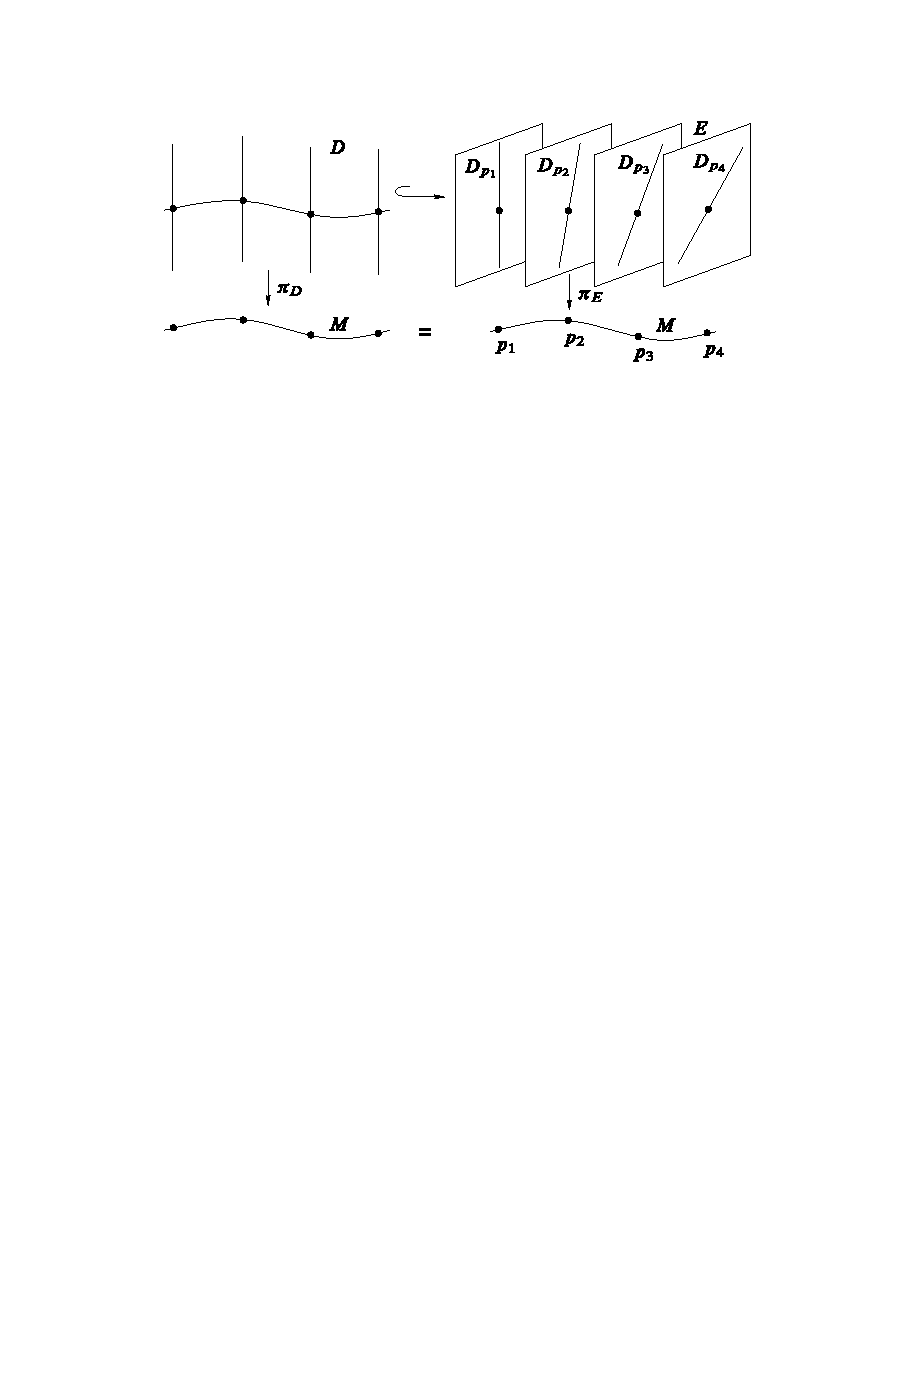
\includegraphics{subbundle}
\caption{A subbundle of a vector bundle.}
\end{figure}
Given a vector bundle $\pi_E:E\to M$, a \textbf{subbundle of $\bm{E}$} is a vector bundle $\pi_D:D\to M$ in which $D$ is a topological subspace of $E$ and $\pi_D$ is the restriction of $\pi_E$ to $D$, such that for each $p\in M$, the subset $D_p=D\cap E_p$ is a linear subspace of $E_p$, and the vector space structure on $D_p$ is the one inherited from $E_p$. Note that the condition that $D$ be a vector bundle over $M$ implies that all of the fibers $D_p$ must be nonempty and have the same dimension. If $E\to M$ is a smooth bundle, then a subbundle of $E$ is called a \textbf{smooth subbundle} if it is a smooth vector bundle and an embedded submanifold with or without boundary in $E$.\par
The following lemma gives a convenient condition for checking that a union of
subspaces $\{D_p\sub E_p:p\in M\}$ is a smooth subbundle.
\begin{lemma}[\textbf{Local Frame Criterion for Subbundles}]\label{vector subbundle crit}
Let $\pi:E\to M$ be a smooth vector bundle, and suppose that for each $p\in M$ we are given an $m$-dimensional linear subspace $D_p\sub E_p$. Then $D=\bigcup_{p\in M}\sub E$ is a smooth subbundle of $E$ if and only if the following condition is satisfied: 
\begin{equation}\label{vector subbundle-1}
\parbox{\dimexpr\linewidth-6em}
{\strut
Each point of $M$ has a neighborhood $U$ on which there exist smooth local sections $\sigma_1,\dots,\sigma_m:U\to E$ with the property that $\sigma_1(q),\dots,\sigma_m(q)$ form a basis for $D_q$ at each $q\in U$.
\strut}
\end{equation}
\end{lemma}
\begin{proof}
If $D$ is a smooth subbundle, then by definition each $p\in M$ has a neighborhood $U$ over which there exists a smooth local trivialization of $D$, and Example~\ref{local frame trivialization} shows that there exists a smooth local frame for $D$ over each such set $U$. Such a local frame is by definition a collection of smooth sections $\tau_1,\dots,\tau_m$ whose images form a basis for $D_p$ at each point $p\in U$. The smooth sections of $E$ that we seek are obtained by composing with the inclusion map $\iota:D\hookrightarrow E$: $\sigma_j=\iota\circ\tau_j$.\par
Conversely, suppose $E\to M$ is a smooth bundle of rank $k$, and $D\sub E$ satisfies $(\ref{vector subbundle-1})$. Each set $D\cap E_p$ is a linear subspace of $E_p$ by hypothesis, so we need to show that $D$ is an embedded submanifold with or without boundary in $E$ and that the restriction of $\pi$ makes it into a smooth vector bundle over $M$. To prove that $D$ is an embedded submanifold with or without boundary, it suffices to show that each $p\in M$ has a neighborhood $U$ such that $D\cap\pi^{-1}(U)$ is an embedded submanifold (possibly with boundary) in $\pi^{-1}(U)\sub E$. Given $p\in M$, let $\sigma_1,\dots,\sigma_m$ be smooth local sections of $E$ satisfying $(\ref{vector subbundle-1})$ on a neighborhood of $p$. By Proposition~\ref{local frame completion}, we can complete these to a smooth local frame $\sigma_1,\dots,\sigma_k$ for $E$ over some neighborhood $U$ of $p$. By Proposition~\ref{local frame iff trivialization}, this local frame is associated with a smooth local trivialization $\varPhi:\pi^{-1}(U)\to U\times\R^k$, defined by
\[\varPhi(s^1\sigma_1(q)+\cdots+s^k\sigma_k(q))=\big(q,(s^1,\dots,s^k)\big).\]
This map $\varPhi$ takes $D\cap\pi^{-1}(U)$ to the subset $\{(q,s)\in U\times\R^k:s^{m+1}=\cdots=s^k=0\}$, which is an embedded submanifold (with boundary if $U$ has a boundary). Moreover, the map $\varPsi:D\cap\pi^{-1}(U)\to U\times\R^m$ defined by
\[\varPsi(s^1\sigma_1(q)+\cdots+s^m\sigma_m(q))=\big(q,(s^1,\dots,s^m)\big),\]
is a smooth local trivialization of $D$, so $D$ is itself a smooth vector bundle.
\end{proof}
\begin{example}[\textbf{Subbundles}]
\mbox{}
\begin{itemize}
\item[(a)] If $M$ is a smooth manifold and $V$ is a nowhere-vanishing smooth vector field on $M$, then the set $D\sub TM$ whose fiber at each $p\in M$ is the linear span of $V_p$ is a smooth $1$-dimensional subbundle of $TM$.
\item[(b)] Suppose $E\sub M$ is any trivial bundle, and let $(E_1,\dots,E_k)$ be a smooth global frame for $E$. If $0\leq m\leq k$, the subset $D\sub E$ defined by $D_p=\mathrm{span}(E_1|_p,\dots,E_m|_p)$ for each $p\in M$ is a smooth subbundle of $E$.
\item[(c)] Suppose $M$ is a smooth manifold with or without boundary and $S\sub M$ is an immersed $k$-submanifold with or without boundary. Then $TS$ is a smooth rank-$k$ subbundle of the ambient tangent bundle $TM|_S$.
\end{itemize}
\end{example}
The next theorem shows how to obtain many more subbundles. Suppose $E\to M$ and $E'\to M$ are vector bundles and $F:E\to E'$ is a bundle homomorphism over $M$. For each $p\in M$, the rank of the linear map $F|_{E_p}$ is called the \textbf{rank of $\bm{F}$ at $\bm{p}$}. We say that $F$ has constant rank if its rank is the same for all $p\in M$.
\begin{theorem}
Let $E$ and $E'$ be smooth vector bundles over a smooth manifold $M$ and let $F:E\to E'$ be a smooth bundle homomorphism over $M$. Define subsets $\ker F\sub E$ and $\im F\sub E'$ by
\[\ker F=\bigcup_{p\in M}\ker(F|_{E_p}),\quad\im F=\bigcup_{p\in M}\im(F|_{E_p}).\]
Then $\ker F$ and $\im F$ are smooth subbundles of $E$ and $E'$, respectively, if and only if $F$ has constant rank.
\end{theorem}
\begin{proof}
One direction is obvious: since the fibers of a bundle have the same dimension everywhere, the constant-rank condition is certainly necessary for $\ker F$ and $\im F$ to be subbundles. To prove sufficiency, suppose $F$ has constant rank $r$, and let $k$ and $k'$ be the ranks of the bundles $E$ and $E'$, respectively. Let $p\in M$ be arbitrary, and choose a smooth local frame $(\sigma_1,\dots,\sigma_k)$ for $E$ over a neighborhood $U$ of $p$. For each $i$, the map $F\circ\sigma_i:U\to E'$ is a smooth local section of $E'$, and these sections span $\im F$. After rearranging the indices if necessary, we can assume that the elements $\{F\circ\sigma_1(p),\dots,F\circ\sigma_r(p)\}$ form a basis for $\im(F|_{E_p})$, and by continuity they remain linearly independent in some neighborhood $U_0$ of $p$. Since $F$ has constant rank, this means that $(F\circ\sigma_1,\dots,F\circ\sigma_r)$ forms a smooth local frame for $\im F$ over $U_0$. Since we can do the same in a neighborhood of each point, the local frame criterion shows that $\im F$ is a smooth subbundle of $E'$.\par
To prove that $\ker F$ is also a smooth subbundle, let $U_0$ and $(\sigma_i)$ be as above, and let $V\sub E|_{U_0}$ be the smooth subbundle spanned by $\sigma_1,\dots,\sigma_r$. The smooth bundle homomorphism $F|_V:V\to(\im F)|_{U_0}$ is bijective, and is thus a smooth bundle isomorphism by Proposition~\ref{vector bundle smooth iso iff bi}. Define a smooth bundle homomorphism $\varPsi:E|_{U_0}\to E_{U_0}$ by
\[\varPsi(v)=v-(F|_V)^{-1}\circ F(v).\]
If $v\in V$, then $F(v)=F|_V(v)$, so $F\circ\varPsi(v)=F(v)-F(v)=0$. On the other hand, if $v\in\ker F$, then $\varPsi(v)=v$ so again $F(\varPsi(v))=F(v)=0$. Since $V$ and $\ker(F)|_{U_0}$ together span $E|_{U_0}$, it follows that $\varPsi$ takes its values in $(\ker F)|_{U_0}$ and since it restricts to the identity on $(\ker F)|_{U_0}$, its image is exactly $(\ker F)|_{U_0}$. Thus $\varPsi$ has constant rank, and by the argument in the preceding paragraph, $(\ker F)|_{U_0}=\im\varPsi$ is a smooth subbundle of $E|_{U_0}$. Since we can do the same thing in a neighborhood of each point, $\ker F$ is a smooth subbundle of $E$.
\end{proof}
The next proposition illustrates another method for constructing interesting subbundles of the tangent bundle over submanifolds of $\R^n$.
\begin{lemma}[\textbf{Orthogonal Complement Bundles}]\label{orthogonal complement bundles}
Let $M$ be an immersed submanifold with or without boundary in $\R^n$, and $D$ be a smooth rank-$k$ subbundle of $T\R^n|_M$. For each $p\in M$, let $D^\bot_p$ denote the orthogonal complement of $D_p$ in $T_p\R^n$ with respect to the Euclidean dot product, and let $D^\bot\sub T\R^n|_M$ be the subset
\[D^\bot=\{(p,v)\in T\R^n:p\in M,v\in D^\bot_p\}\]
Then $D^\bot$ is a smooth rank-$(n-k)$ subbundle of $T\R^n|_M$. For each $p\in M$, there is a smooth orthonormal frame for $D^\bot$ on a neighborhood of $p$.
\end{lemma}
\begin{proof}
Let $p\in M$ be arbitrary, and let $(X_1,\dots,X_k)$ be a smooth local frame for $D$ over some neighborhood $V$ of $p$ in $M$. Because immersed submanifolds are locally 
embedded, by shrinking $V$ if necessary, we may assume that it is a single slice in some coordinate ball or half-ball $U\sub\R^n$. Since $V$ is closed in $U$, 
Proposition~\ref{local frame completion} shows that we can complete $(X_1,\dots,X_k)$ to a smooth local frame $(\widetilde{X}_1,\dots,\widetilde{X}_n)$ for $T\R^n$ 
over $U$, and then Lemma~\ref{Gram-Schmidt frame} yields a smooth orthonormal frame $(E_j)$ over $U$ such that 
\[\mathrm{span}(E_1|_p,\dots,E_k|_p)=\mathrm{span}(X_1|_p,\dots,X_k|_p)=D\]
for each $p\in U$. It follows that $(E_{k+1},\dots,E_n)$ restricts to a smooth orthonormal frame for $D^\bot$ over $V$. Thus $D^\bot$ satisfies the local frame 
criterion, and is therefore a smooth subbundle of $T\R^n|_M$.
\end{proof}
\begin{corollary}[\textbf{The Normal Bundle to a Submanifold of $\R^n$}]
If $M\sub\R^n$ is an immersed $m$-dimensional submanifold with or without boundary, its normal bundle $NM$ is a smooth rank-$(n-m)$ subbundle of $T\R^n|_M$. For each $p\in M$, there exists a smooth orthonormal frame for $NM$ on a neighborhood of $p$.
\end{corollary}
\begin{proof}
Apply Lemma~\ref{orthogonal complement bundles} to the smooth subbundle $TM\sub T\R^n|_M$.
\end{proof}
\subsection{Reduction of structure groups}
Let $E\to M$ be a smooth vector bundle with a trivialization $\{(U_\alpha,\varPhi_{\alpha})\}$. Then by Lemma~\ref{vector bundle cochain prop} the transition functions 
$\{\tau_{\alpha\beta}\}$ satisfy the cocycle condition
\[\tau_{\alpha\beta}\circ\tau_{\beta\gamma}=\tau_{\alpha\gamma}.\]
The cocycle $\{\tau_{\alpha\beta}\}$ clearly depends on the choice of the trivialization $\{\varPhi_\alpha\}$, but we have the following result.
\begin{lemma}\label{vector bundle equivalent transition lem}
Let $\pi:E\to M$ be a smooth vector bundle of rank $k$. If the cocycle $\{\tau'_{\alpha\beta}\}$ comes from another trivialization ${(U_{\alpha},\varPhi'_{\alpha})}$, then there 
exist maps $\sigma_{\alpha}:U_{\alpha}\to \GL_k(\R)$ such that
\[\tau'_{\alpha\beta}(p)=\sigma_\alpha(p)\tau_{\alpha\beta}(p)\sigma_\beta^{-1}(p),\quad p\in U_\alpha\cap U_\beta\]
Two cocycles related in this way are said to be \textbf{equivalent}.
\end{lemma}
\begin{proof}
The two trivializations differ by a nonsingular transformation of $\R^k$ at each point, so there is a map $\sigma_\alpha:U_\alpha\to\GL_k(\R)$ such that
\[\varPhi'_\alpha\circ\varPhi_\alpha^{-1}(p,v)=(p,\sigma_\alpha(p)v)\]
Then
\begin{align*}
\varPhi'_{\alpha}\circ(\varPhi'_{\beta})^{-1}(p,v)&=(\varPhi'_{\alpha}\circ\varPhi_\alpha^{-1})\circ(\varPhi_\alpha\circ\varPhi_\beta^{-1})\circ(\varPhi_{\beta}\circ(\varPhi'_{\beta})^{-1})(p,v)=(p,\sigma_\alpha(p)\tau_{\alpha\beta}(p)\sigma_\beta^{-1}(p)v).
\end{align*}
Therfore we get the desired equality.
\end{proof}
Given a cocycle $\{\tau_{\alpha\beta}\}$ with values in $\GL_k(\R)$ we can construct a vector bundle $E$ having $\{\tau_{\alpha\beta}\}$ as its cocycle as in 
Theorem~\ref{vector bundle construct}. It turns out that the equivalence class of cocycles determines the vector bundle, as the next proposition shows.
\begin{proposition}
Let $\pi:E\to M$ and $\pi':E'\to M$ be two smooth rank-$k$ vector bundles over
a smooth manifold $M$ with or without boundary. Suppose $\{U_\alpha\}_{\alpha\in A}$ is an open cover of $M$ such that both $E$ and $E'$ admit smooth local 
trivializations over each $U_\alpha$. Let $\{\tau_{\alpha\beta}\}$ and $\{\tau'_{\alpha\beta}\}$ denote the transition functions determined by the given local 
trivializations of $E$ and $E'$, respectively. Then $E$ and $E'$ are smoothly isomorphic over $M$ if and only if for each $\alpha\in A$ there exists a smooth map 
$\sigma_\alpha:U_\alpha\to\GL_k(\R)$ such that
\[\tau'_{\alpha\beta}(p)=\sigma_\alpha(p)\tau_{\alpha\beta}(p)\sigma_\beta^{-1}(p),\quad p\in U_\alpha\cap U_\beta.\]
\end{proposition}
\begin{proof}
Assume the given condition for $\{\sigma_\alpha\}$, then the following diagram commutes,
\[\begin{tikzcd}
U_\beta\times\R^k\ar[r,"\sigma_\beta"]\ar[d,swap,"\tau_{\alpha\beta}"]&U_\beta\times\R^k\ar[d,"\tau'_{\alpha\beta}"]\\
U_\alpha\times\R^k\ar[r,"\sigma_\alpha"]&U_\alpha\times\R^k
\end{tikzcd}\]
Thus we can define a map $F:E\to E'$ as following: For $p\in U_\alpha$, let \[\varPhi_\alpha:\pi^{-1}(U_\alpha)\to U\times\R^k\And\varPhi':\pi^{-1}(U_\alpha)\to\R^k\] 
be the local trivializations, respectively. If $(p,v)\in U_\alpha\times\R^k$, we define
\[F(p,v):=(p,\sigma_\alpha(p)v)\]
By our commutative diagram, this definition is in fact coordinate free, thus gives a bundle homomorphism. Since $\sigma_\alpha(p)$ is invertible, $F$ is infact an isomorphism.\par
Conversely, if we are given a bundle homomorphism $F:E\to E'$. Since the restriction of $F$ on each fiber $E_p$ is linear, we can define $\sigma_\alpha$ by
\[\varPhi'_\alpha\circ F\circ\varPhi_\alpha^{-1}(p,v)=(p,\sigma_\alpha(p)v)\]
such that the diagram
\[\begin{tikzcd}
\pi^{-1}(U_\alpha)\ar[d,swap,"\varPhi_\alpha"]\ar[r,"F"]&\pi'^{-1}(U_\alpha)\ar[d,"\varPhi'_\alpha"]\\
U_\alpha\times\R^k\ar[r,dashed,"\sigma_\alpha"]&U_\alpha\times\R^k
\end{tikzcd}\]
commutes. Since $F$ is an isomorphism, each $\sigma_\alpha(p)$ is invertible. Moreover, as for the transition functions, we have the commutative diagram
\[\begin{tikzcd}
U_\beta\times\R^k\ar[r,dashed,"\sigma_\beta"]\ar[dd,bend right=65,swap,"\tau_{\alpha\beta}"]&U_\beta\times\R^k\ar[dd,bend left=65,"\tau'_{\alpha\beta}"]\\
\pi^{-1}(U_\alpha\cap U_\beta)\ar[d,swap,"\varPhi_\alpha"]\ar[u,"\varPhi_\beta"]\ar[r,"F"]&\pi'^{-1}(U_\alpha\cap U_\beta)\ar[d,"\varPhi'_\alpha"]\ar[u,swap,"\varPhi'_\beta"]\\
U_\alpha\times\R^k\ar[r,dashed,"\sigma_\alpha"]&U_\alpha\times\R^k
\end{tikzcd}\]
from which the desired equality can be easily derived:
\[\sigma_\alpha(p)\tau_{\alpha\beta}(p)=\tau'_{\alpha\beta}(p)\sigma_\beta(p)\quad\text{for all }p\in U_\alpha\cap U_\beta.\]
\end{proof}
Given a vector bundle with cocycle $\{\tau_{\alpha\beta}\}$, if it is possible to find an equivalent cocycle with values in a subgroup $H$ of $\GL_k(\R)$, we say that 
the structure group of $E$ may be \textbf{reduced to $\bm{H}$}. A vector bundle is \textbf{orientable} if its structure group may be reduced to $\GL_k^+(\R)$, the 
linear transformations of $\R^k$ with positive determinant. A trivialization $\{(U_\alpha,\varPhi_\alpha)\}_{\alpha\in A}$ on $E$ is said to be \textbf{oriented} if for 
every $\alpha,\beta\in A$, the transition function $\tau_{\alpha\beta}$ has positive determinant. Two oriented trivializations $\{(U_\alpha,\varPhi_\alpha)\}$ 
and $\{(V_\beta,\varPsi_\beta)\}$ are \textbf{equivalent} if for every $p$ in $U_{\alpha}\cap V_{\beta}$, $\varPhi_{\alpha}\circ(\varPsi_\beta)^{-1}$ has positive 
determinant. It is easily checked that this is an equivalence relation and that on a connected manifold $M$ it partitions all the oriented trivializations of the vector 
bundle $E$ into two equivalence classes. Either equivalence class is called an \textbf{orientation on the vector bundle $\bm{E}$}.
\begin{example}[\textbf{The tangent bundle}]
Consider the tangent bundle $TM$ of a smooth manifold $M$. Then the transition functions of $TM$ are the Jacobians of the transition functions of $M$. Therefore $M$ is 
orientable as a manifold if and only if its tangent bundle is orientable as a bundle. (However, the total space of the tangent bundle is always orientable as a manifold, 
see Exercise~\ref{orentaton TM and T^*M}.)
\end{example}
We now show that the structure group of every real vector bundle $E$ may be reduced to the orthogonal group. First, we can endow $E$ with a Riemannian structure-a 
smoothly varying positive definite symmetric bilinear form on each fiber-as follows. Let $\{U_\alpha\}$ be an open cover of $M$ which trivializes $E$. On each $U_\alpha$, 
choose a frame for $E|_{U_\alpha}$ and declare it to be orthonormal. This defines a Riemannian structure on $E|_{U_\alpha}$. Let $g_{\alpha}$ denote this inner product 
on $E|_{U_\alpha}$. Now use a partition of unity $\{\rho_\alpha\}$ to splice them together, i.e., form
\[g=\sum_\alpha\rho_\alpha g_\alpha.\]
This will be an inner product over all of $M$.\par
As trivializations of $E$, we take only those maps $\varPhi_\alpha$ that send orthonormal frames of $E$ (relative to the global metric) to orthonormal frames of $\R^k$-such 
maps exist by the Gram-Schmidt process. Then the transition functions $\tau_{\alpha\beta}$ will preserve orthonormal frames and hence take values in the orthogonal 
group $\O(k)$. If the determinant of $\tau_{\alpha\beta}$ is positive, $\tau_{\alpha\beta}$ will actually be in the special orthogonal group $\SO(k)$. Thus
\begin{proposition}
The structure group of a real vector bundle of rank $k$ can always be reduced to $\O(k)$; it can be reduced to $\SO(k)$ if and only if the vector bundle is orientable.
\end{proposition}
\subsection{Operations on vector bundles}
\subsubsection{Quotient bundle}
Suppose $D$ is a smooth subbundle of a smooth vector bundle $\pi:E\to M$. At each point $p$ in $M$, the fiber $D_p$ is a vector subspace of $E_p$ and so the quotient 
space $Q_p:=E_p/D_p$ is defined. Let
\[Q=\coprod_{p\in M}Q_p=\coprod_{p\in M}(E_p/D_p),\]
and give $Q$ the quotient topology as a quotient space of $E$. Let $\rho:E\to Q$ be the quotient map. The projection $\pi:E\to M$ then induces a map $\pi_Q:Q\to M$ as 
in the commutative diagram
\[\begin{tikzcd}
D\ar[r,hook]&E\ar[d,swap,"\pi"]\ar[r]&Q\ar[ld,"\pi_Q"]\\
&M&
\end{tikzcd}\]
Since $F$ is locally trivial, every point $p$ in $M$ has a coordinate neighborhood over which one can find a smooth frame $(\sigma_1,\dots,\sigma_k)$ for $D$. By 
Lemma~\ref{vector bundle local frame completion}, $(\sigma_1,\dots,\sigma_k)$ can be extended to a smooth frame $(\sigma_1,\dots,\sigma_k,\sigma_{k+1},\dots,\sigma_r)$ 
for $E$ over a possibly smaller neighborhood $W$ of $p$. A point $v$ of $E|_W$ is uniquely a linear combination $v=v^i\sigma_i$ where $v^i$ are smooth. Let 
$\widebar{\sigma}_{k+1},\dots,\widebar{\sigma}_r:W\to Q$ be the sections $\sigma_{k+1},\dots,\sigma_r$ followed by the projection $E\to Q$. Then 
$(\widebar{\sigma}_{k+1},\dots,\widebar{\sigma}_r)$ is a continuous frame for $Q$ over $W$, and by Proposition~\ref{local frame iff trivialization} we get a homeomorphism
\[\varPsi_W(q,(\widebar{v}^1,\dots,\widebar{v}^{r-k}))=\widebar{v}^i\widebar{\sigma}_i(q).\]
Moreover, it is clear that the collection $\{\varPsi_W\}$ satisfies the conditions of Lemma~\ref{vector bundle chart lemma}. Therefore one can give $Q$ a manifold 
structure as well as a smooth vector bundle structure over $M$. With this vector bundle structure, $\pi_Q:Q\to M$ is called the 
\textbf{quotient bundle of $\bm{E}$ by $\bm{D}$}.
\subsubsection{Other operations on vector bundles}
Let $\mathcal{V}$ be the category whose objects are finite-dimensional real vector spaces and whose morphisms are isomorphisms of vector spaces. In this category, if 
two vector spaces have different dimensions, then the set of morphisms between them is the empty set. Denote by $\mathcal{V}\times\mathcal{V}$ the category whose 
objects are pairs of finite-dimensional vector spaces and whose morphisms are pairs of isomorphisms of vector spaces.\par
If $V$ and $V'$ are finite-dimensional vector spaces of the same dimension $n$, let $Iso(V,V')$ be the set of all isomorphisms from $V$ to $V'$. With respect to fixed 
bases for $V$ and $V'$, elements of $\Iso(V,V')$ are represented by nonsingular $n\times n$ matrices. Hence, $\Iso(V,V')$ is bijective with $\GL_n(\R)$, and therefore 
has the structure of a manifold. A functor $\mathscr{D}:\mathcal{V}\to\mathcal{V}$ is said to be \textbf{smooth} if for all finite-dimensional vector spaces $V$ and $V'$ the map
\[\mathscr{D}:\Iso(V,V')\to\Iso(\mathscr{D}(V),\mathscr{D}(V')),\quad f\mapsto\mathscr{D}(f)\]
is smooth.\par
Similarly, a functor $\mathscr{T}:\mathcal{V}\times\mathcal{V}\to\mathcal{V}$ is said to be smooth if for all finite-dimensional vector spaces
$V$, $V'$, $W$, $W'$ with $\dim V=\dim V'$ and $\dim W=\dim W'$, the map
\[\mathscr{T}:\Iso(V,V')\times\Iso(W,W')\to\Iso(\mathscr{T}(V,W),\Iso(V',W')),\quad (f,g)\mapsto\mathscr{T}(f,g)\]
is smooth.
\begin{example}
Let $\mathscr{T}(V,W)=V\oplus W$. This is a smooth functor because if $f:V\to V'$ and $g:W\to W'$ are isomorphisms represented by matrices $M_f$ and $M_g$ relative to 
some bases, then $f\oplus g:V\oplus W\to V'\oplus W'$ is represented by the matrix
\[\begin{pmatrix}
M_f&0\\
0&M_g
\end{pmatrix}\]
relative to the same bases.
\end{example}
\begin{example}
Similarly, the functor $\mathscr{T}(V,W)=V\otimes W$ is also a smooth functor since if $f:V\to V'$ and $g:W\to W'$ are isomorphisms represented by matrices $M_f$ and $M_g$ 
relative to some bases, then $f\otimes g:V\otimes W\to V'\otimes W'$ is represented by the matrix $M_f\otimes M_g$.
\end{example}
Now we have the following general result for a smooth functor $\mathscr{T}:\mathcal{V}\times\mathcal{V}\to\mathcal{V}$.
\begin{proposition}
If $\mathscr{T}:\mathcal{V}\to\mathcal{V}$ is a smooth covariant functor, then for any smooth vector bundles $E$ over a manifold $M$, there is a smooth 
vector bundle $\mathscr{T}(E)$ over $M$ whose fiber at $p\in M$ is $\mathscr{T}(E_p)$.\par
Similarly, if $\mathscr{T}:\mathcal{V}\times\mathcal{V}\to\mathcal{V}$ is a smooth covariant functor, then for any two smooth vector bundles $E$ and $E'$ over a 
manifold $M$, there is a smooth vector bundle $\mathscr{T}(E,F)$ over $M$ whose fiber at $p\in M$ is $\mathscr{T}(E_p,E'_p)$.
\end{proposition}
\begin{proof}
We only prove the second claim, since the first can be proved in the same manner.\par
Let $\{U_\alpha\}_{\alpha\in A}$ and $\{V_\beta\}_{\beta\in B}$ be trivializing open covers for $E$ and $E'$, respectively, then $\{U_\alpha\cap V_\beta\}_{\alpha\in A,\beta\in B}$ 
is an open cover of $M$ that simultaneously trivializes both $E$ and $E'$. Therefore for each $p\in U_\alpha\cap V_{\beta}$ we have isomorphisms
\[\varPsi_{\alpha,p}:E_p\to\{p\}\times\R^k,\quad \varPhi_{\beta,p}:E'_p\to\{p\}\times\R^{k'}\]
and therefore an isomorphism
\[\mathscr{T}(\varPsi_{\alpha,p},\varPhi_{\beta,p}):\mathscr{T}(E_p,E'_p)\to\{p\}\times\mathscr{T}(\R^{k},\R^{k'}).\]
We then get a bijection
\[\mathscr{T}(\varPsi_\alpha,\varPhi_\beta):\coprod_{p\in U_{\alpha}\cap V_{\beta}}\mathscr{T}(E_p,E'_p)\to (U_\alpha\cap U_{\beta})\times\mathscr{T}(\R^{k},\R^{k'}).\]
Moreover, if $(\alpha,\beta),(\alpha',\beta')\in A\times B$, then on the overlap $(U_\alpha\cap V_\beta)\cap(U_{\alpha'}\cap V_{\beta'})$ the map $\mathscr{T}(\varPsi_\alpha,\varPhi_\beta)\circ\mathscr{T}(\varPsi_\alpha,\varPhi_\beta)^{-1}$ 
has the form
\[(p,v)\mapsto(p,\tau_{(\alpha,\beta),(\alpha',\beta')}(p)v)\]
where $\tau_{(\alpha,\beta),(\alpha',\beta')}:(U_\alpha\cap V_\beta)\cap(U_{\alpha'}\cap V_{\beta'})\to\GL(\mathscr{T}(\R^k,\R^{k'}))$ is given by
\[\tau_{(\alpha,\beta),(\alpha',\beta')}(p)=\mathscr{T}(\tau_{\alpha,\alpha'}(p),\tau_{\beta,\beta'}(p)).\]
Therefore we see the conditions in Lemma~\ref{vector bundle chart lemma} is satisfied, so there is a smooth vector bundle $\mathscr{T}(E,F)$ over $M$ whose fiber at 
$p\in M$ is $\mathscr{T}(E_p,E'_p)$. 
\end{proof}
If a functor is contravariant, it must be turned into a covariant functor first to apply this construction. For example, consider the dual functor applied to a vector 
bundle $E\to M$. Because of its contravariance, it associates to a trivialization
\[\varPsi_p:E_p\to\{p\}\times\R^k\]
the map
\[\varPsi^*_p:\{p\}\times(\R^k)^*\to E_p^*.\]
We need to take the inverse of $\varPsi_p^*$ to get a trivialization that goes in the right direction,
\[(\varPsi^*_p)^{-1}:E_p^*\to\{p\}\times(\R^k)^*.\]
To construct the dual bundle, the functor $\mathscr{T}:V\to V$ associates to every finite-dimensional vector space $V$ its dual space $V^*$, and to every isomorphism 
$f:V\to W$ the isomorphism $(f^*)^{-1}:V^*\to W^*$.\par
In the category $\mathcal{V}$ the morphisms are all isomorphisms precisely so that one can reverse the direction of a map and make a contravariant functor covariant. 
In this way, starting from smooth vector bundles $E$ and $E'$ over $M$, one can construct smooth vector bundles $E\oplus E'$, $E\otimes E'$, $\bigwedge^kE$, $E^*$, and 
$\Hom(E,E')=E^*\otimes E'$ over $M$.
\subsubsection{The pullback bundle}
If $\pi:E\to M$ is a smooth vector bundle over a manifold $M$ and $f:N\to M$ is a smooth map, then there is a smooth vector bundle $f^*E$ over $N$, called the \textbf{pullback 
of $\bm{E}$ by $\bm{f}$}, with the property that every bundle map covering $F$ factors through the pullback bundle $f^*E$.\par
The total space of the pullback bundle of $E$ by $F$ is defined to be the set
\[f^*E=\{(q,e)\in N\times E:f(q)=\pi(e)\}.\]
endowed with the subspace topology. The projections to the two factors fit into a commutative diagram
\[\begin{tikzcd}
f^*\ar[r]\ar[d]&E\ar[d,"\pi"]&\\
N\ar[r,"f"]&M
\end{tikzcd}\]
We will show that $\eta:f^*E\to N$ is a vector bundle. First, we show that the pullback of a product bundle is a product bundle.
\begin{proposition}\label{vector bundle pullback}
If $f:N\to M$ is a smooth map of manifolds and $\pi:E=M\times V\to M$ is a product bundle, then the projection $f^*E\to N$ is isomorphic to the product bundle 
$N\times V\to N$.
\end{proposition}
\begin{proof}
As a set,
\[f^*E=\{(q,(p,v))\in N\times(M\times V):f(q)=\pi(p,v)=p\}=\{(q,(f(q),v))\in N\times(M\times V)\}.\]
Therefore the map
\[T:f^*E\to N\times V,\quad (q,(f(q),v))\mapsto(q,v)\]
with inverse $(q,v)\mapsto(q,(f(q),v))$ is a fiber-preserving homeomorphism. It gives $f^*E\to N$ the structure of a smooth vector bundle over $N$.
\end{proof}
\begin{corollary}
Let $\pi:E\to M$ be a smooth vector bundle with fiber $V$ and $f:N\to M$ a smooth map. The projection $f^*E\to N$ can be given the structure of a smooth vector bundle 
with fiber $V$.
\end{corollary}
\begin{proof}
Since $E$ is locally a product $U\times V\to U$, by Proposition~\ref{vector bundle pullback}, the pullback $f^*E$ is locally the product $f^{-1}(U)\times V\to f^{-1}(U)$.
\end{proof}
Now we determine the transition functions of the pullback bundle $f^*E$ from that of $E$. First we need a lemma.
\begin{lemma}
Suppose $\pi:E\to M$ is a smooth vector bundle with fiber $V$ and $f:N\to M$ is a smooth map. Let $U$ be an open subset of $M$. Then
\[(f^*E)|_{f^{-1}(U)}=f^*(E|_U).\]
\end{lemma}
\begin{proof}
By definition we have
\begin{align*}
(f^*E)|_{f^{-1}(U)}&=\{(q,e)\in N\times E:q\in f^{-1}(U),f(q)=\pi(e)\}\\
&=\{(q,e)\in f^{-1}(U)\times E:f(q)=\pi(e)\}=f^*(E|_U).
\end{align*}
Therefore the claim follows.
\end{proof}
\begin{proposition}
Suppose $\pi:E\to M$ is a smooth vector bundle with fiber $V$ and trivializing open cover $\{U_\alpha\}$ and $f:N\to M$ is a smooth map. If 
$\rho_{\alpha\beta}:U_\alpha\cap U_\beta\to\GL(V)$ is the transition function for $E$ over $U_\alpha\cap U_\beta$, then $f^*\rho_{\alpha\beta}$ is the transition 
function for $f^*E$ over $F^{-1}(U_\alpha\cap U_\beta)$.
\end{proposition}
\begin{proof}
Suppose $\varPsi_\alpha:U_\alpha\times\R^k\to\pi^{-1}(U_\alpha)$ is the trivialization for $E$ over $U_\alpha$, then the trivalization of $F^{-1}(U)$ is 
given by
\[\widetilde{\varPsi}_\alpha:f^{-1}(U)\times V\to f^*(E|_{f^{-1}(U_\alpha)}),\quad (q,v)\mapsto(q,\varPsi_\alpha(f(q),v)).\]
Therefore the transition function $\widetilde{\varPsi}_\alpha\circ\widetilde{\varPsi}_\beta^{-1}$ is given by
\[\widetilde{\varPsi}_\alpha\circ\widetilde{\varPsi}_\beta^{-1}(q,v)=(q,\rho_{\alpha\beta}(f(q))v).\]
This gives the claim.
\end{proof}
Finnaly, we can now prove the desired pullback property of the pullback bundle.
\begin{theorem}\label{vector bundle pullback universal prop}
Suppose $\pi':E'\to N$ and $\pi:E\to M$ are vector bundles and $F:E'\to E$ is a bundle map that covers $f:N\to M$, i.e., the diagram
\begin{equation}\label{vector bundle pullback universal-1}
\begin{tikzcd}
E'\ar[r,"F"]\ar[d,swap,"\pi'"]&E\ar[d,"\pi"]\\
N\ar[r,"f"]&M
\end{tikzcd}
\end{equation}
Then there is a unique bundle map 
$\widetilde{F}:E'\to f^*E$ over $N$ that makes the following diagram commute:
\begin{equation}\label{vector bundle pullback universal-2}
\begin{tikzcd}
E'\ar[rrd,bend left=20pt,"F"]\ar[rdd,bend right=20pt,swap,"\pi'"]\ar[rd,dashed,"\widetilde{F}"]&&\\
&f^*E\ar[d]\ar[r]&E\ar[d,"\pi"]\\
&N\ar[r,"f"]&M
\end{tikzcd}
\end{equation}
\end{theorem}
\begin{proof}
The commutativity of the diagram $(\ref{vector bundle pullback universal-1})$ forces $\widetilde{F}(e')=(\pi'(e'),F(e'))$, so the map $\widetilde{F}$ as defined above 
indeed exists and is unique. It is $\R$-linear on each fiber because $F$ is. It is smooth because $\pi'$ and $F$ are assumed to be smooth.
\end{proof}
\begin{example}[\textbf{The differential of a map}]
If $f:N\to M$ is a smooth map of manifolds, its differentials $df_p:T_pN\to T_{F(p)}M$ at all points $p\in N$ piece together to give a bundle map $df:TN\to TM$ of 
tangent bundles. By Theorem~\ref{vector bundle pullback universal prop}, the bundle map $df$ induces a unique bundle map $\widetilde{df}:TN\to f^*TM$ over $N$ that 
makes the diagram
\[\begin{tikzcd}
TN\ar[rrd,bend left=20pt,"df"]\ar[rdd,bend right=20pt,swap,"\pi'"]\ar[rd,dashed,"\widetilde{df}"]&&\\
&f^*TM\ar[d]\ar[r]&TM\ar[d,"\pi"]\\
&N\ar[r,"f"]&M
\end{tikzcd}\]
commutative. The map $\widetilde{df}$ is given by
\[X_p\in T_pN\mapsto(p,df_p(X_p))\]
Conversely, $df$ can be obtained from $\widetilde{df}\circ\pi_{TM}$. In this way the bundle map $df$ over two base manifolds is converted to a bundle map $\widetilde{df}$ 
over the single manifold $N$.
\end{example}
\begin{example}[\textbf{Vector fields along a curve}]
If $\gamma:I\to M$ is a smooth map from an open interval $I\sub\R$ into a manifold $M$, then the pullback $\gamma^*TM$ of the tangent bundle $TM$ is a vector bundle 
over $I$. A section of the pullback bundle $\gamma^*TM$ assigns to each $t\in I$ an element of the fiber $(\gamma^*TM)_t\cong T_{\gamma(t)}M$, i.e., a tangent vector 
to $M$ at $\gamma(t)$. In other words, a section of $\gamma^*TM$ is precisely a vector field along the curve $\gamma(t)$ in $M$. Therefore a vector field along a curve 
$\gamma$ in $M$ is smooth if and only if the corresponding section of $\gamma^*TM$ is smooth.
\end{example}
Let $\mathsf{Vect}_k(M)$ be the isomorphism classes of rank $k$ real vector bundles over $M$. It is a pointed set with base point the isomorphism class of the trivial 
bundle over M. If $f:M\to N$ is a map between two manifolds, let $\mathsf{Vect}_k(f)=f^*$ be the pullback map on bundles. In this way, for each integer $k$, $\mathsf{Vect}_k$ 
becomes a contravariant functor from the category of manifolds and smooth maps to the category of pointed sets and base point preserving maps.\par
As an application of the constructions above, we prove an important fact about the pullback bundle.
\begin{proposition}[\textbf{Homotopy Property of Vector Bundles}]
Assume $N$ to be a compact manifold. If $f_0$ and $f_1$ are homotopic maps from $N$ to a manifold $X$ and $E$ is a vector bundle on $M$, then $f_0^*E$ is isomorphic to 
$f_1^*E$, i.e., homotopic maps induce isomorphic bundles.
\end{proposition}
\begin{proof}
Let $f:N\times I\to M$ be a homotopy between $f_0$ and $f_1$ and let $\pi:N\times I\to N$ be the projection. Suppose for some $t_0$ in $I$, $f_{t_0}^*E$ is isomorphic
to some vector bundle $F$ on $N$. We will show that for all $t$ near $t_0$, $f_{t}^*E\cong F$. By the compactness and connectedness of the unit interval $I$ it will 
then follow that $f_t^*E\cong F$ for all $t$ in $I$.\par
Over $N\times I$ there are two pullback bundles, $f^*E$ and $\pi^*F$. Since $f_{t_0}^*E\cong F$, the bundle $\Iso(f^*E,\pi^*F)$ has a section over $N\times\{t_0\}$, 
which a priori is also a section of $\Hom(f^*E,\pi^*F)$. Since $N$ is compact, $N\times\{t_0\}$ may be covered with a finite number of trivializing open sets for 
$\Hom(f^*E,\pi^*F)$. As the fibers of $\Hom(f^*E,\pi^*F)$ are Euclidean spaces, the section over $N\times\{t_0\}$ may be extended to a section of $\Hom(f^*E,\pi^*F)$ 
over the union of these open sets. Now any linear map near an isomorphism remains an isomorphism, thus we can extend the given section of $\Iso(f^*E,\pi^*F)$ to a 
strip containing $N\times\{t_0\}$ (by the tube lemma). This proves that $f_t^*E\cong F$ for $t$ near $t_0$. We now cover $N\times I$ with a finite number of such 
strips. Hence $f_0^*E\cong f_1^*E$.
\end{proof}
But the same argument can be refined to give the theorem for $N$ a paracompact space. Since every manifold is paracompact, this result actually holds for all manifolds, 
compact or not.
\begin{corollary}
A vector bundle over a contractible manifold is trivial.
\end{corollary}
\begin{proof}
Let $E$ be a vector bundle over $M$ and let $f:M\to\{\ast\}$ be an homotopy equivalence between $M$ and $\{\ast\}$. Then we can see that $f^*$ is an isomorphism on 
vector bundles. Since every vector bundle on $\{\ast\}$ is trivial, so is that on $M$.
\end{proof}
So for a contractible manifold $M$, $\mathsf{Vect}_k(M)$ is a single point.
\subsection{Fiber bundles}
Let $M$ and $F$ be topological spaces. A \textbf{fiber bundle over $M$ with model fiber $\bm{F}$} is a topological space $E$ together with a surjective continuous map $\pi:E\to M$ with the property that for each $x\in M$, there exist a neighborhood $U$ of $x$ in $M$ and a homeomorphism $\varPhi:\pi^{-1}(U)\to U\times F$, called a \textbf{local trivialization of $\bm{E}$ over $\bm{U}$}, such that the following diagram commutes:
\[\begin{tikzcd}
\pi^{-1}(U)\ar[rr,"\varPhi"]\ar[rd,swap,"\pi"]&&U\times F\ar[ld,"\pi_U"]\\
&U&
\end{tikzcd}\]
The space $E$ is called the \textbf{total space of the bundle}, $M$ is its \textbf{base}, and $\pi$ is its \textbf{projection}. If $E,M$ and $F$ are 
smooth manifolds with or without boundary, $\pi$ is a smooth map, and the local trivializations can be chosen to be diffeomorphisms, then it is called 
a \textbf{smooth fiber bundle}. If $\pi:E\to M$ be a smooth fiber bundle with fiber $F$ over $M$, a \textbf{bundle chart} is a pair $(U,\varPhi)$ where 
$U$ is open in $M$ and $\varPhi:\pi^{-1}(U)\to U\times F$ is a smooth local trivialization. A \textbf{bundle atlas} on $E$ is a collection of bundle 
charts whose domains cover $M$.\par
A \textbf{trivial fiber bundle} is one that admits a local trivialization over the entire base space (a \textbf{global trivialization}). It is said to be \textbf{smoothly trivial} if it is a smooth bundle and the global trivialization is a diffeomorphism.
\begin{example}[\textbf{Fiber Bundles}]\label{fiber bundle eg}
\mbox{}
\begin{itemize}
\item[(a)]Every product space $M\times F$ is a fiber bundle with projection $\pi_1:M\times F\to M$ called a \textbf{product fiber bundle}. It has a global trivialization given by the identity map $M\times F\to M\times F$, so every product bundle is trivial.
\item[(b)]Every rank-$k$ vector bundle is a fiber bundle with model fiber $\R^k$.
\item[(c)]If $E\to S^1$ is the M\"obius bundle, then the image of $\R\times[-1,1]$ under the quotient map $q:\R^2\to E$ is a fiber bundle over $S^1$ with model fiber $[-1,1]$. It is not a trivial bundle.
\item[(d)]Every covering map $\pi:E\to M$ is a fiber bundle whose model fiber is discrete. To construct local trivializations, let $S$ be a discrete space 
with the same cardinality as the fibers of $\pi$. For each evenly covered open subset $U\sub M$, define a map $\varPhi:\pi^{-1}(U)\to U\times S$ by choosing 
a bijection between the set of components of $\pi^{-1}$ and $S$, and letting $\varPhi(x)=(\pi(x),c(x))$, where $c(x)$ is the element of $S$ corresponding to 
the component containing $x$.
\end{itemize}
\end{example}
\begin{proposition}
Let $\pi:E\to M$ be a smooth fiber bundle with fiber $F$ over $M$. Then $\pi$ is a submersion. Furthermore, for each $p\in M$ the 
fiber $E_p$ is a properly embedded submanifold diffeomorphic to $F$.
\end{proposition}
\begin{proof}
Let $\varPhi:\pi^{-1}(U)\to U\times F$ be a smooth local trivialization over an open set $U$ in $M$. Then $\pi|_{\pi^{-1}(U)}=\pi_U\circ\varPhi$. Since $\pi_U$ and $\varPhi$ are both submersions, it follows 
that $\pi|_{\pi^{-1}(U)}$ is also a submersion. Since $U$ is arbitrary, we see $\pi$ is a submersion. Then by Corollary~\ref{subm level set}, each fiber of it is naturally a properly embedded submanifold of $E$. For each $p\in U$, $\varPhi$ maps $E_p$ diffeomorphically onto the embedded submanifold $\{p\}\times F$ of $U\times F$, and $\pi_F$ is a diffeomorphism from this onto $F$.
\end{proof}
Due to this proposition, the bundle $E$ over $M$ with fiber $F$ is occasionally denoted, by abuse of notation, by the symbol $F\to E\stackrel{\pi}{\to}M$.
\begin{lemma}\label{fiber bundle trivialization overlap}
Let $\pi:E\to M$ be a smooth fiber bundle with fiber $F$ over $M$. Suppose $\varPhi:\pi^{-1}(U)\to U\times F$ and $\varPsi:\pi^{-1}(V)\to V\times F$ are two smooth 
local trivializations of $E$ with $U\cap V=\emp$. There exists a smooth map $\tau:U\cap V\to\Diff(F)$ such that the composition $\varPhi\circ\varPsi^{-1}:(U\cap V)\times\R^k\to(U\cap V)\times F$ has the 
form
\[\varPhi\circ\varPsi^{-1}(p,v)=(p,\tau(p)(v)).\]
The map $\tau:U\cap V\to\Diff(F)$ is called the \textbf{transition function} between $\varPhi$ and $\varPsi$.
\end{lemma}
In the smooth case, the group $\Diff(F)$ is to large to deal with, and it is often convenient to require the transition functions to take values in a Lie group $G$. More precisely, we make the following definition.
\begin{definition}
A Lie group $G$ is said to be a \textbf{Lie transformation group} on a manifold $F$ if there is given a smooth left action of $G$ on $F$. Let $G$ be a Lie group acting 
on $F$ on the left. Bundle charts $(U,\varPhi)$ and $(V,\varPsi)$ in $M$ will be said to be \textbf{$\bm{G}$-compatible} if $U\cap V=\emp$, or if $U\cap V\neq\emp$ 
and there exists a smooth map $\tau:U\cap V\to G$ such that 
\[\varPhi\circ\varPsi^{-1}(p,v)=(p,\tau_p\cdot v)\]
for all $(p,v)\in(U\cap V)\times F$. That is, the traisition function is given by an element of $G$.
\end{definition}
\begin{definition}
Let $G$ be a Lie group. A smooth fiber bundle $F\to E\stackrel{\pi}{\to}M$ is called a \textbf{smooth bundle with structure group $\bm{G}$} if $G$ is a Lie transformation group on $F$, and there is given 
a bundle atlas $\mathcal{A}$ on $E$ such that any two bundle charts in $\mathcal{A}$ are $G$-compatible. A smooth fiber bundle chart is \textbf{admissible} as a bundle chart on the bundle $E$ with structure group $G$ if it is $G$-compatible with every element of the given $G$-bundle atlas.
\end{definition}
Therefore, vector bundles can be viewed as $\GL_k(\R)$-bundles with fiber $\R^k$. The following lemma can be viewed as a generalization of Lemma~\ref{vector bundle chart lemma}.
\begin{lemma}[\textbf{Fiber Bundle Chart Lemma}]\label{fiber bundle chart lemma}
Let $M$ and $F$ be a smooth manifolds with or without boundary, and suppose that for each $p\in M$ we are given a manifold $E_p$ diffeomorphic to $F$. Let $E=\coprod_{p\in M}E_p$ and let 
$\pi:E\to M$ be the map that takes each element of $E_p$ to the point $p$. Suppose furthermore that we are given the following 
data:
\begin{itemize}
\item[$(\rmnum{1})$] An open cover $\{U_\alpha\}_{\alpha\in A}$ of $M$.
\item[$(\rmnum{2})$] For each $\alpha\in A$, a bijective map $\varPhi_\alpha:\pi^{-1}(U_\alpha)\to U_\alpha\times F$ whose restriction to each $E_p$ is a diffeomorphism from $E_p$ to $\{p\}\times F$.
\item[$(\rmnum{3})$] For each $\alpha,\beta\in A$ with $U_\alpha\cap U_\beta\neq\emp$, a smooth map $\tau_{\alpha\beta}:U_\alpha\cap U_\beta\to G$ such that the map $\varPhi_\alpha\circ\varPhi_\beta^{-1}$ from $(U_\alpha\cap U_\beta)\times F$ to itself has the form
\begin{align}\label{fiber bundle transition function-1}
\varPhi_\alpha\circ\varPhi_\beta^{-1}(p,v)=(p,\tau_{\alpha\beta}(p)\cdot(v))
\end{align}
where $G$ is a Lie group acting on $F$.
\end{itemize}
Then $E$ has a unique topology and smooth structure making it into a smooth manifold with or without boundary and a smooth fiber bundle over $M$ with fiber $F$ and structure group $G$, with $\pi$
as projection and $\{(U_\alpha,\varPhi_\alpha)\}$ as smooth local trivializations.
\end{lemma}
\begin{theorem}[\textbf{Fiber bundle construction theorem}]\label{fiber bundle construct Lie group}
Let $M$ and $F$ be smooth manifolds with or without boundary, and let $\{U_\alpha\}_{\alpha\in A}$ be an open cover of $M$. Suppose that there is a Lie group $G$ acting on $F$ and for each $\alpha,\beta\in A$ we are 
given a smooth map $\tau_{\alpha\beta}:U_{\alpha}\cap U_{\beta}\to G$ such that $(\ref{fiber bundle transition function-1})$ is satisfied for all $\alpha,\beta,\gamma\in A$. Then 
there is a smooth fiber bundle $\pi:E\to M$ with fiber $F$, sturcture group $G$ and smooth local trivializations $\varPhi_\alpha:\pi^{-1}(U_\alpha)\to U_\alpha\times F$ 
whose transition functions are the given maps $\tau_{\alpha\beta}$.
\end{theorem}
\begin{example}[\textbf{The universal Une bundle over a projective space}]
Let $n>0$, consider the real projective space $\RP^n$. Let $\pi:\R^{n+1}\setminus\{0\}\to\RP^n$ be the projection map. 
For each $i=0,\dots,n$, let $\widetilde{U}_i\sub\R^{n+1}\setminus\{0\}$ be the set where $x_i\neq 0$, and let 
$U_i=\pi(\widetilde{U}_i)\sub\RP^n$. Since $\widetilde{U}_i$ is a saturated open subset, $U_i$ is open and $\pi|_{\widetilde{U}_i}$ is a 
quotient map. Define a map $\varphi$ by
\[\varphi_i[x^0,\dots,x^{n}]=\Big(\frac{x^0}{x^i},\dots,\frac{x^{i-1}}{x^i},\frac{x^{i+1}}{x^i},\dots,\frac{x^{n}}{x^i}\Big)\]
Now we make $\R^{n+1}\setminus\{0\}$ into the total space of a fiber bundle over $\RP^n$ with standard fiber $\R\setminus\{0\}$. 
Define $\varPhi_1:\pi^{-1}(U_i)\to U_i\times(\R\setminus\{0\})$ by 
\[\varPhi_i(x^0,\dots,x^n)=([x^0,\dots,x^n],x^i).\]
The maps $(U_i,\varPhi_i)$ will be bundle charts once it is checked that they generate a smooth structure on $\R^{n+1}\setminus\{0\}$.\par
Let $i\neq j$, for all $(p,v)\in\pi^{-1}(U_i\cap U_j)\times(\R\setminus\{0\})$, we have 
\[\varPhi_i\circ\varPhi_j^{-1}([x^0,\dots,x^n],v)=\varPhi_i(\frac{v}{x^j}\cdot(x^0,\dots,x^n))=([x^0,\dots,x^n],\frac{x^i}{x^j}\cdot v).\]
Thus the maps $\varPhi_i$ determine a smooth fiber bundle $\R^{n+1}\setminus\{0\}\to\RP^n$ with fiber $\R\setminus\{0\}$ and sturcture group $\GL_1(\R)$ by Lemma~\ref{fiber bundle chart lemma}.\par
The bundle $\R^{n+1}\setminus\{0\}$ over $\RP^n$ is canonically a subbundle of a
bundle $E\to\RP^n$ with fiber $\R$. For each $p\in\RP^n$, define $E_p=\pi^{-1}(p)\cup\{(p,0)\}$. All that has really been added to $\pi^{-1}(p)$ 
the point $0$ in $\R$; calling the new point $(p,0)$ instead of just $0$ is a technical 
device to guarantee that distinct fibers in the new bundle have distinct zero points. Set $E$ equal to the union over all $p\in\RP^n$ of $E_p$, and extend the maps by $\pi(p,0)=p$ 
and $\varPhi_i(p,0)=(p,0)\in U_i\times\R$. Then by Lemma~\ref{fiber bundle chart lemma} again, $E\to\RP^n$ is a smooth fiber bundle with fiber $\R$.\par
The constructions above can also be done on $\CP^n$. The fiber bundle $\R\to\R^{n+1}\stackrel{\pi}{\to}\RP^n$ ($\C\to\C^{n+1}\stackrel{\pi}{\to}\CP^n$) is called the \textbf{universal line bundle} over $\RP^n$ 
($\CP^n$).
\end{example}
\begin{example}[\textbf{Milnor's exotic spheres}]
Let $N$ be the north pole $(0,\dots,0,1)$ in $S^n\sub\R^{n+1}$ and $S$ the south pole $(0,\dots,0,-1)$. Set $U:=S^n-\{N\}$ and $V:=S^n-\{S\}$. The stereographic 
projection of $S^n$ onto the equatorial plane from $N$ is the map
\[\varphi:U\to\R^n,\quad (x^1,\dots,x^{n+1})\mapsto\frac{(x^1,\dots,x^n)}{1-x^{n+1}}.\]
The stereographic projection of $S^n$ from $S$ is the map
\[\psi:V\to\R^n,\quad (x^1,\dots,x^{n+1})\mapsto\frac{(x^1,\dots,x^n)}{1+x^{n+1}}.\]
For each $u\in U\cap V$, $\psi(u)=\varphi(u)/|\varphi(u)|^2$, $\varphi(u)=\psi(u)/|\psi(u)|^2$. The maps $\sigma$ and $\widetilde{\sigma}$ are charts on $S^n$ which generate the smooth structure.\par
The result is that $S^n$ can be constructed as the disjoint union of two copies of $\R^n$ modulo the identification of each nonzero vector $u$ in the first copy with 
the vector $u/|u|^2$ in the second copy; symbolically, $S^n=(\R^n\amalg\R^n)/\sim$ where $u\sim u/|u|^2$, $u\neq 0$.\par
Let $a$ be an odd integer; set $b:=(1+a)/2$ and $c:=(1-a)/2$. Define
\[E_a:=[(\R^4\times S^3)\amalg(\R^4\times S^3)]/\sim\]
where if $(u,v)$ belongs to the first copy of $\R^4\times S^3$ and $u\neq 0$, then
\[(u,v)\sim\Big(\frac{u}{|u|^2},\frac{u^bvu^c}{|u|}\Big)\]
The symbol $u^bvu^c$ indicates quaternionic multiplication in $\R^4\cong\H$.\par
Define $\pi:E_a\to S^4$ such that $\pi[u,v]=\varphi^{-1}(u)$ for $(u,v)$ in the first copy of $\R^4\times S^3$, and $\pi[u,v]:=\psi^{-1}(u)$ for $(u,v)$ in 
the second copy of $\R^4\times S^3$. The map $\pi$ is well-defined since by the properties of stereographic projection we have
\[\varphi(u)=\frac{\psi(u)}{|\psi(u)|^2}\Rightarrow\varphi\circ\psi^{-1}(u)=\frac{u}{|u|^2}\Rightarrow\psi^{-1}(u)=\varphi^{-1}(\frac{u}{|u|^2}).\]

To define bundle charts on $E_a$, set $\varPhi[u,v]:=v\in S^3$ for $(u,v)$ in the first copy of $\R^4\times S^3$, and $\varPsi[u,v]:=v$ for $(u,v)$ in the second
copy for $\R^3\times S^3$. It follows that for given $(u,v)\in(\R^4\setminus\{0\})\times S^3$ we have $\varPhi\circ\varPsi^{-1}(u,v)\cong(u,v)$. This implies that $\varPhi$ and 
$\varPsi$ are smooth compatible, and therefore define a smooth structure on $E_a$. Simultaneously they determine a fiber bundle structure on $E_a$ over $S^4$.
\end{example}
\subsection{Exercise}
\begin{exercise}
Let $\mathsf{Vec_f}$ be the category whose objects are finite-dimensional real vector spaces and whose morphisms are linear isomorphisms. If $\mathscr{F}$ is a covariant functor from $\mathsf{Vec_f}$ to itself, for each finite-dimensional vector space $V$ we get a map $\mathscr{F}:\GL(V)\to\GL(V)$ sending each isomorphism $A:V\to V$ to the induced isomorphism $\mathscr{F}(A):\mathscr{F}(V)\to\mathscr{F}(V)$. We say $\mathscr{F}$ is a \textbf{smooth functor} if this map is smooth for every $V$. Given a smooth vector bundle $E\to M$ and a smooth functor $\mathscr{F}:\mathsf{Vec_f}\to\mathsf{Vec_f}$, show that there is a smooth vector bundle $\mathscr{F}(E)\to M$ whose fiber at each point $p\in M$ is $\mathscr{F}(E_p)$.
\end{exercise}
\begin{exercise}
Suppose $M$ is a compact smooth manifold and $E\to M$ is a smooth vector bundle of rank $k$. Use transversality to prove that $E$ admits a smooth section $\sigma$ with the following property: if $k>\dim M$, then $\sigma$ is nowhere vanishing; while if $k\leq\dim M$, then the set of points where $\sigma$ vanishes is a smooth compact codimension-$k$ submanifold of $M$. Use this to show that $M$ admits a smooth vector field with only finitely many singular points.
\end{exercise}
\begin{exercise}
Let $U=S^1-\{1\}$ and $V=S^1-\{-1\}$, and define $\tau:U\cap V\to\GL_1(\R)$ by
\[\tau(z)=\begin{cases}
(1),&\mathrm{Im}z>0\\
(-1),&\mathrm{Im}z<0
\end{cases}\]
By the result of Theorem~\ref{vector bundle construct}, there is a smooth real line bundle $F\to S^1$ that is trivial over $U$ and $V$, and has $\tau$ as transition function. Show that $F$ is smoothly isomorphic over $S^1$ to the M\"obius bundle.
\end{exercise}
\begin{proof}
We first define the local trivializations for the M\"obius bundle. Let $p$ be the quotient map $q:\R^2\to E$. We define $\varPhi_1$ and $\varPhi_2$ to be projection, but with different domains:
\[\varPhi_1:\big[(n,n+1)\times\R\big]\to S^1,\quad \varPhi_2:\big[(n+\frac{1}{2},n+\frac{3}{2})\times\R\big]\to S^1\]
Then $\varPhi_1$ is a local trivialization for $U$, and $\varPhi_2$ is that for $V$. And, by our definition in Example~\ref{Mobius bundle}, the transition function for $\varPhi_1$ and $\varPhi_2$ is 
\[\tau_{12}(z)=\begin{cases}
(-1)&\im z>0\\
(1)&\im z<0
\end{cases}\]
\end{proof}
\begin{exercise}
Let $V$ be a finite-dimensional real vector space, and let $\Gr_k(V)$ be the Grassmannian of $k$-dimensional subspaces of $V$. Let $T$ be the subset of $\Gr_k(V)\times V$ defined by
\[T=\{(S,v)\in\Gr_k(V)\times V:v\in S\}\]
Show that $T$ is a smooth rank-$k$ subbundle of the product bundle $\Gr_k(V)\times V\to\Gr_k(V)$, and is thus a smooth rank-$k$ vector bundle over $\Gr_k(V)$. $T$ is called the tautological vector bundle over $\Gr_k(V)$, because the fiber over each point $S\in\Gr_k(V)$ is $S$ itself.
\end{exercise}
\begin{proof}
For each chart $(U,\varphi)$ in $\Gr_k(V)$, the set $\pi^{-1}(U)$ is the subspaces 
\[\{v\in V:[v]\in U\}\]
Then we can define a map
\[\varPhi:\pi^{-1}(U)\to U\times V,\quad \varPhi(v)=([v],v)\]
\end{proof}
\section{The Cotangent bundle}\label{cotangent bundle section}
\subsection{Covectors}
Let $V$ be a finite-dimensional vector space. (As usual, all of our vector spaces are assumed to be real.) We define a \textbf{covector} on $V$ to be a real-valued linear functional on $V$, that is, a linear map $\omega:V\to\R$. The space of all covectors on $V$ is itself a real vector space under the obvious operations of pointwise addition and scalar multiplication. It is denoted by $V^*$ and called the dual space of $V$. The next proposition expresses the most important fact about $V^*$ in the finite-dimensional case.
\begin{proposition}\label{dual basis}
Let $V$ be a finite-dimensional vector space. Given any basis $(E_1,\dots,E_n)$ for $V$, let $\eps^1,\dots,\eps^n$ be the covectors defined by
\[\eps^i(E_j)=\delta^i_j\]
where $\delta^i_j$ is the Kronecker delta. Then $\eps^1,\dots,\eps^n$ is a basis for $V^*$, called the \textbf{dual basis} to $(E_j)$. Therefore, $\dim V^*=\dim V$.
\end{proposition}
For example, we can apply this to the standard basis $(e_1,\dots,e_n)$ for $\R^n$. The dual basis is denoted by $e^1,\dots,e^n$ (note the upper indices), and is called the standard dual basis. These basis covectors are the linear functionals on $\R^n$ given by
\[e^i(v)=e^i(v^1,\dots,v^n)=e^i.\]
In other words, ei is the linear functional that picks out the $i$-th component of a vector. In matrix notation, a linear map from $\R^n$ to $\R$ is represented by a $1\times n$ matrix, called a row matrix. The basis covectors can therefore also be thought of as the linear functionals represented by the row matrices
\[e^1=(1,\dots,0),\quad e^2=(0,1,\dots,0),\quad e^n=(0,\dots,1).\]
In general, if $(E_j)$ is a basis for $V$ and $(\eps^i)$ is its dual basis, then for any vector $v=v^jE_j\in V$, we have
\[\eps^i(v)=v^j\eps^i(E_j)=v^j\delta^i_j=v^i\]
Thus, just as in the case of $\R^n$, the $i$-th basis covector $\eps^i$ picks out the $i$-th component of a vector with respect to the basis $(E_j)$. More generally, Proposition~\ref{dual basis} shows that we can express an arbitrary covector $\omega\in V^*$ in terms of the dual basis as
\[\omega=\omega_i\eps^i,\]
where the components are determined by $\omega=\omega_i(E_i)$. The action of $\omega$ on a vector $v=v^jE_j$ is
\[\omega(v)=\omega_iv^i.\]
Suppose $V$ and $W$ are vector spaces and $A:V\to W$ is a linear map. We define a linear map $A^*:W^*\to V^*$, called the \textbf{dual map} or \textbf{transpose} of $A$, by
\[(A^*\omega)(v)=\omega(Av)\for \omega\in W^*,v\in V.\]
\begin{proposition}\label{dual map prop}
The dual map satisfies the following properties:
\begin{itemize}
\item[(a)] $(A\circ B)^*=B^*\circ A^*$.
\item[(b)] $(\mathrm{id})^*$ is the identity map of $V^*$.
\item[(c)] If the linear map $R$ is given by the matrix $R=(R_i^j)$, then $R^*$ is given by the matrix $R^T$.
\end{itemize}
\end{proposition}
\begin{proof}
Let $A:V\to W$ and $B:W\to U$ be linear maps, then
\[\big((A\circ B)^*\omega\big)(v)=\omega(A\circ Bv)=(A^*\omega)(Bv)=\big(B^*(A^*\omega)\big)(v)=\big(B^*\circ A^*(\omega)\big)(v).\]
For the statement, let $R:V\to W$ be a linear map. Let $(A_i)$ be a basis of $V$ and $(B_j)$ be a basis of $W$, with the dual bases being $(\alpha^i)$ and $(\beta^j)$ respectively. If the matrix of $R$ under these bases is $(R_i^j)$, then
\[(R^*\beta^j)_i=(R^*\beta^j)(A_i)=\beta^j(RA_i)=\beta^j(R_i^kB_k)=R_i^j.\]
It follows that
\[A^*\beta^j=R_i^j\alpha^i.\]
Thus the matrix of $A^*$ is given by $A^T$.
\end{proof}
\begin{corollary}
The assignment that sends a vector space to its dual space and a linear map to its dual map is a contravariant functor from the category of real vector spaces to itself.
\end{corollary}
\begin{corollary}
Let $(\alpha_i)$ and $(\beta_j)$ be two bases for a finite-dimensional vector space $V$, with the dual bases being $(\alpha^i)$ and $(\beta^j)$. If the transition matrix from $(\alpha_i)$ to $(\beta_j)$ is given by $X$, then the transition matrix from $(\alpha^i)$ to $(\beta^j)$ is given by $(X^T)^{-1}$.
\end{corollary}
\begin{proof}
In view of Proposition~\ref{dual map prop}, we have the following commutative diagram:
\[\begin{tikzcd}
(\alpha_i)\ar[r,"X"]\ar[d,swap,"\cong"]&(\beta_i)\ar[d,"\cong"]\\
(\alpha^i)&(\beta^j)\ar[l,swap,"X^*"]
\end{tikzcd}\]
Since the matrix of $X^*$ is given by $X^T$, our claim follows immediately.
\end{proof}
\begin{corollary}
Suppose $M$ is a smooth manifold and $E\to M$ is a smooth vector bundle over $M$. Define the dual bundle to $E$ to be the bundle $E^*\to M$ whose total space is the disjoint union $E^*=\coprod_{p\in M}E_p^*$, where $E_p^*$ is the dual space to $E_p$. With the obvious projection, $E^*\to M$ is a smooth vector bundle, whose transition functions are given by $\tau^*(p)=(\tau^T(p))^{-1}$ for any transition function $\tau:U\to\GL_k(\R)$ of $E$.
\end{corollary}
Apart from the fact that the dimension of $V^*$ is the same as that of $V$, the second most important fact about dual spaces is the following characterization of the second dual space $V^{**}:=(V^*)^*$. For each vector space $V$ there is a natural, basis-independent map $\xi:V\to V^{**}$ defined as follows. For each vector $v\in V$, define a linear functional $\xi(v):V^*\to\R$ by
\[\xi(v)(\omega)=\omega(v)\]
\begin{proposition}\label{finite vector double dual}
For any finite-dimensional vector space $V$, the map $\xi:V\to V^{**}$ is an isomorphism.
\end{proposition}
\begin{proof}
Because $\dim V=\dim V^{**}$, it suffices to verify that $\xi$ is injective. Suppose $v\in V$ is not zero. Extend $v$ to a basis $(E_1=v,\dots,E_n)$ for $V$, and let $(\eps^1,\dots,\eps^n)$ denote the dual basis for $V^*$. Then $\xi(v)\neq 0$ because
\[\xi(v)(\eps^1)=\eps^1(v)=1\]
\end{proof}
The preceding proposition shows that when $V$ is finite-dimensional, we can unambiguously
identify $V^{**}$ with $V$ itself, because the map $\xi$ is canonically defined, without reference to any basis. It is important to observe that although $V^*$ is also isomorphic to $V$, there is no canonical isomorphism $V=V^*$.\par
Because of Proposition~\ref{finite vector double dual}, the real number $\omega(v)$ obtained by applying a covector $\omega$ to a vector $v$ is sometimes denoted by either of the more symmetric-looking notations $\langle\omega,v\rangle$ and $\langle v,\omega\rangle$ both expressions can be thought of either as the action of the covector $\omega\in V^*$ on the vector $v\in V$, or as the action of the linear functional $v\in V^{**}$ on the element $\omega\in V$. There should be no cause for confusion with the use of the same angle bracket notation for inner products: whenever one of the arguments is a vector and the other a covector, the notation $\langle\omega,v\rangle$ is always to be interpreted as the natural pairing between vectors and covectors, not as an inner product. We typically omit any mention of the map $\xi$, and think of $v\in V$ either as a vector or as a linear functional on $V^*$, depending on the context.\par
There is also a symmetry between bases and dual bases for a finite-dimensional vector space $V$: any basis for $V$ determines a dual basis for $V^*$, and conversely, any basis for $V^*$ determines a dual basis for $V^{**}=V$. If $(\eps^i)$ is the basis for $V^*$ dual
to a basis $(E_j)$ for $V$, then $(E_j)$ is the basis dual to $(\eps^i)$, because both statements are equivalent to the relation $\langle\eps^i,E_j\rangle=\delta^i_j$.
\subsubsection{Tangent covectors on manifolds}
Now let $M$ be a smooth manifold with or without boundary. For each $p\in M$, we define the cotangent space at $p$, denoted by $T^*_pM$ to be the dual space to $T_pM$:
\[T^*_pM=(T_pM)^*\]
Elements of $T^*_pM$ are called tangent covectors at $p$, or just covectors at $p$.\par
Given smooth local coordinates $(x^i)$ on an open subset $U\sub M$, for each $p\in U$ the coordinate basis $\partial/\partial x^i|_p$ gives rise to a dual basis for $T^*_pM$, which we denote by $(dx^i|_p)$. (This notation will be explained in a short while) Any covector $\omega\in T^*_pM$ can thus be written uniquely as $\omega=\omega_idx^i|_p$, where
\[\omega_i=\omega\Big(\frac{\partial}{\partial x^i}\Big|_p\Big).\]
Suppose now that $(\widetilde{x}^j)$ is another set of smooth coordinates whose domain contains $p$, and let $(d\widetilde{x}^j|_p)$ denote the basis for $T^*_pM$ dual to $\partial/\partial\widetilde{x}^j|_p$. We can compute the components of the same covector $\omega$ with respect to the new coordinate system as follows. First recall that the coordinate vector fields transform as follows:
\begin{align}\label{covector-1}
\frac{\partial}{\partial x^i}\Big|_p=\frac{\partial\widetilde{x}^j}{\partial x^i}(p)\frac{\partial}{\partial\widetilde{x}^j}\Big|_p.
\end{align}
Writing $\omega$ in both systems as $\omega=\omega^idx^i|_p=\widetilde{\omega}_jd\widetilde{x}^j|_p$,
we can use $(\ref{covector-1})$ to compute the components $\omega_i$ in terms of $\widetilde{\omega}_j$:
\begin{align}\label{covector-2}
\omega_i=\omega\Big(\frac{\partial}{\partial x^i}\Big|_p\Big)=\omega\Big(\frac{\partial\widetilde{x}^j}{\partial x^i}(p)\frac{\partial}{\partial\widetilde{x}^j}\Big|_p\Big)=\frac{\partial\widetilde{x}^j}{\partial x^i}(p)\widetilde{\omega}_j.
\end{align}
From this we also derive the transform rule:
\[d\widetilde{x}^j|_p=\frac{\partial\widetilde{x}^j}{\partial x^i}(p)dx^i|_p\]
\subsubsection{Covector fields}
For any smooth manifold $M$ with or without boundary, the disjoint union
\[T^*M=\coprod_{p\in M}T^*_pM\]
is called the cotangent bundle of $M$. It has a natural projection map $\pi:T^*M\to M$ sending $\omega\in T^*_pM$ to $p\in M$. As above, given any smooth local coordinates $(x^i)$ on an open subset $U\sub M$, for each $p\in U$ we denote the basis for $T^*_pM$ dual to $(\partial/\partial x^i|_p)$ by $(dx^i|_p)$. This defines $n$ maps $dx^1,\dots,dx^n:U\to T^*M$ called \textbf{coordinate covector fields}.
\begin{proposition}[\textbf{The Cotangent Bundle as a Vector Bundle}]
Let $M$ be a smooth $n$-manifold with or without boundary. With its standard projection map and the natural vector space structure on each fiber, the cotangent bundle $T^*M$ has a unique topology and smooth structure making it into a smooth rank-$n$ vector bundle over $M$ for which all coordinate covector fields are smooth local sections.
\end{proposition}
\begin{proof}
The proof is just like that of Theorem~\ref{tangent bundle as vector bundle}. Given a smooth chart $(U,\varphi)$ on $M$ with coordinate functions $(x^i)$, define $\varPhi:\pi^{-1}(U)\to U\times\R^n$ by
\[\varPhi(\xi_idx^i|_p)=(p,(\xi_1,\dots,\xi_n))\]
where $dx^i$ is the $i$-th coordinate covector field associated with $(x^i)$. Suppose $(\widetilde{U},\widetilde{\varphi})$ is another smooth chart with coordinate functions $(\widetilde{x}^j)$, and let $\widetilde{\varPhi}:\pi^{-1}(\widetilde{U})\to\widetilde{U}\times\R^n$ be defined analogously. On $\pi^{-1}(U\cap V)$, it follows from $(\ref{covector-2})$ that
\[\varPhi\circ\widetilde{\varPhi}^{-1}\big(p,(\widetilde{\xi}_1,\dots,\widetilde{\xi}_n)\big)=\big(p,(\frac{\partial\widetilde{x}^j}{\partial x^1}(p)\widetilde{\xi}_j,\dots,\frac{\partial\widetilde{x}^j}{\partial x^n}(p)\widetilde{\xi}_j)\big)\]
The $\GL_n(\R)$-valued function $(\partial\widetilde{x}^j/\partial x^i)$ is smooth, so it follows from the vector bundle chart lemma that $T^*M$ has a smooth structure making it into a smooth vector bundle for which the maps $\varPhi$ are smooth local trivializations. Uniqueness follows as in the proof of Proposition~\ref{tangent bundle struct unique}.
\end{proof}
As in the case of the tangent bundle, smooth local coordinates for $M$ yield smooth local coordinates for its cotangent bundle. If $(x^i)$ are smooth coordinates
on an open subset $U\sub M$, Corollary~\ref{vector bundle chart from frame} shows that the map from $\pi^{-1}(U)$ to $\R^{2n}$ given by
\[\xi_idx^i\mapsto(x^1(p),\dots,x^n(p),\xi_1,\dots,\xi_n)\]
is a smooth coordinate chart for $T^*M$. We call $(x^i,\xi_i)$ the \textbf{natural coordinates} for $T^*M$ associated with $(x^i)$. A (local or global) section of $T^*M$ is called a \textbf{covector field} or a \textbf{(differential) $\bm{1}$-form}. \textit{Like sections of other bundles, covector fields without further qualification are assumed to be merely continuous; when we make different assumptions, we use the terms \textbf{rough covector field} and \textbf{smooth covector field} with the obvious meanings.} As we did with vector fields, we write the value of a covector field $\omega$ at a point $p\in M$ as $\omega|_p$ instead of $\omega(p)$, to avoid conflict with the notation for the action of a covector on a vector. If $\omega$ itself has subscripts or superscripts, we usually use the notation $\omega|_p$ instead.\par 
In any smooth local coordinates on an open subset $U\sub M$, a (rough) covector field $\omega$ can be written in terms of the coordinate covector fields $\omega=\omega_idx^i$ for $n$ functions $\omega_i:U\to\R$, called the \textbf{component functions} of $\omega$. They are characterized by
\[\omega^i(p)=\omega_p\Big(\frac{\partial}{\partial x^i}\Big|_p\Big)\]
If $\omega$ is a (rough) covector field and $X$ is a vector field on $M$, then we can form a function $\omega(X):M\to\R$ by
\[\omega(X)(p)=\omega_p(X_p)\for p\in M.\]
If we write $\omega=\omega_idx^i$ and $X=X^j\partial/\partial x^j$ in terms of local coordinates, then $\omega(X)$ has the local coordinate representation $\omega(X)=\omega_iX^i$.\par
Just as in the case of vector fields, there are several ways to check for smoothness of a covector field.
\begin{proposition}[\textbf{Smoothness Criteria for Covector Fields}]\label{covector field smooth crit}
Let $M$ be a smooth manifold with or without boundary, and let $\omega:M\to T^*M$ be a rough covector field. The following are equivalent:
\begin{itemize}
\item[(a)] $\omega$ is smooth.
\item[(b)] In every smooth coordinate chart, the component functions of $\omega$ are smooth.
\item[(c)] Each point of $M$ is contained in some coordinate chart in which $\omega$ has smooth component functions.
\item[(d)] For every smooth vector field $X\in\X(M)$, the function $\omega(X)$ is smooth on $M$.
\item[(e)] For every open subset $U\sub M$ and every smooth vector field $X$ on $U$, the function $\omega(X):U\to\R$ is smooth on $U$.
\end{itemize}
\end{proposition}
\begin{proof}
The implications $(a)\Rightarrow(b)\Rightarrow(c)\Rightarrow(a)$ is easily proved, so is the implication $(c)\Rightarrow(d)$.\par 
For the part $(d)\Rightarrow(e)$, we fix a point $p\in M$ and choose a bump fuction supported in $U$ and equals to $1$ in a smaller neighborhood of $p$. Then $\omega(\psi X)$ is smooth at $p$ and coincides with $\omega(X)$ in this neighborhood. This implies that $\omega(X)$ is smooth at $p$. Since $p$ is arbitrary, this gives the smoothness of $\omega(X)$ on $U$.\par
Finally, to show $(e)\Rightarrow(a)$, we just choose $X$ to be the coordinate vector fields $(\partial/\partial x^i)$, then $\omega(X)$ is just the component funtion of $\omega$.
\end{proof}
Of course, since any open subset of a smooth manifold (with boundary) is again
a smooth manifold (with boundary), the preceding proposition applies equally well to covector fields defined only on some open subset of $M$.
\subsubsection{Coframes}
Let $M$ be a smooth manifold with or without boundary, and let $U\sub M$ be an open subset. A \textbf{local coframe} for $M$ over $U$ is an ordered $n$-tuple of covector fields $(\eps^1,\dots,\eps^n)$ defined on $U$ such that $(\eps^i|_p)$ forms a basis for $T^*_pM$ at each point $p\in U$. If $U=M$, it is called a \textbf{global coframe}.
\begin{example}[\textbf{Coordinate Coframes}]
For any smooth chart $(U,(x^i))$, the coordinate covector fields $dx^i$ defined above constitute a local coframe over $U$, called a \textbf{coordinate coframe}. By Proposition~\ref{covector field smooth crit}, every coordinate frame is smooth, because its component functions in the given chart are constants.
\end{example}
Given a local frame $(E_1,\dots,E_n)$ for $TM$ over an open subset $U$, there is a uniquely determined (rough) local coframe $(\eps^1,\dots,\eps^n)$ over $U$ such that $\eps^i|_p$ is the dual basis to $(E_i|_p)$ for each $p\in U$, or equivalently $\eps^i(E_j)=\delta^i_j$. This coframe is called the \textbf{coframe dual to $\bm{(E_i)}$}. Conversely, if we start with a local coframe $(\eps^i)$ over an open subset $U\sub M$, there is a uniquely determined local frame $(E_i)$, called the frame dual to $(\eps^i)$, determined by $\eps^i(E_j)=\delta^i_j$. For example, in a smooth chart, the coordinate frame $\partial/\partial x^i$ and the coordinate coframe $(dx^i)$ are dual to each other.
\begin{lemma}\label{dual frame smooth iff}
Let $M$ be a smooth manifold with or without boundary. If $(E_i)$ is a rough local frame over an open subset $U\sub M$ and $(\eps^i)$ is its dual coframe, then $(E_i)$ is smooth if and only if $(\eps^i)$ is smooth.
\end{lemma}
\begin{proof}
It suffices to show that for each $p\in U$, the frame $(E_i)$ is smooth in a neighborhood of $p$ if and only if $(\eps^i)$ is. Given $p\in U$, let $(V,(x^i))$ be a smooth coordinate chart such that $p\in V\sub U$. In $V$, we can write
\[E_i=a_i^k\frac{\partial}{\partial x^k},\quad \eps^j=b^j_\ell dx^\ell\]
for some matrices of real-valued functions $a_i^k$ and $b^j_\ell$ defined on $V$. By virtue of Propositions ~\ref{vector field smooth crit} and ~\ref{covector field smooth crit}, the vector fields $E_i$ are smooth on $V$ if and only if the functions $a_i^k$ are smooth, and the covector fields $\eps^j$ are smooth on $V$ if and only if the functions $b^j_\ell$ are smooth. The fact that $\eps^j(E_i)=\delta^j_i$ implies that the matrices $(a_i^k)$ and $(b^j_\ell)$ are inverses of each other. Because matrix inversion is a smooth map from $\GL_n(\R)$ to itself, either one of these matrix-valued functions is smooth if and only if the other one is smooth.
\end{proof}
Given a local coframe $(\eps^i)$ over an open subset $U\sub M$, every (rough) covector field $\omega$ on $U$ can be expressed in terms of the coframe as $\omega=\omega_i\eps^i$ for some functions $\omega_1,\dots,\omega_n:U\to\R$, called the component functions of $\omega$ with respect to the given coframe. The component functions are determined by $\omega_i=\omega(E_i)$, where $(E_i)$ is the frame dual to $(\eps^i)$. This leads to another way of characterizing smoothness of covector fields.
\begin{proposition}[\textbf{Coframe Criterion for Smoothness of Covector Fields}]
Let $M$ be a smooth manifold with or without boundary, and let $\omega$ be a rough covector field on $M$. If $(\eps^i)$ is a smooth coframe on an open subset $U\sub M$, then $\omega$ is smooth on $U$ if and only if its component functions with respect to $(\eps^i)$ are smooth.
\end{proposition}
\begin{proof}
This is essentially a corollary of Proposition~\ref{local frame smooth crit}.
\end{proof}
We denote the real vector space of all smooth covector fields on $M$ by $\X^*(M)$. As smooth sections of a vector bundle, elements of $\X(M)$ can be multiplied by smooth real-valued functions: if $f\in C^\infty(M)$ and $\omega\in\X^*(M)$, the covector field $f\omega$ is defined by
\[(f\omega)p=f(p)\omega_p\]
Because it is the space of smooth sections of a vector bundle, $\X^*(M)$ is a module over $C^\infty(M)$.\par
\subsection{The differential of a function}
In elementary calculus, the gradient of a smooth real-valued function $f$ on $\R^n$ is defined as the vector field whose components are the partial derivatives of $f$. In our notation, this would read
\[\grad f=\sum_{i=1}^{n}\frac{\partial f}{\partial x^i}\frac{\partial}{\partial x^i}\]
Unfortunately, in this form, the gradient does not make sense independently of coordinates.
\begin{example}
Let $f(x,y)=x^2$ on $\R^2$, and let $X$ be the vector field
\[X=\grad f=2x\frac{\partial}{\partial x}\]
However, the coordinate expression for $X$ in polar coordinates is
\begin{align*}
X&=2x\frac{\partial}{\partial x}=2x\cos\theta\Big(\frac{\partial r}{\partial x}\frac{\partial}{\partial r}+\frac{\partial\theta}{\partial x}\frac{\partial}{\partial\theta}\Big)\\
&=\frac{2x^2}{\sqrt{x^2+y^2}}\frac{\partial}{\partial r}-\frac{2xy}{x^2+y^2}\frac{\partial}{\partial\theta}\\
&=2r\cos^2\theta\frac{\partial}{\partial r}-2\sin\theta\cos\theta\frac{\partial}{\partial\theta}
\end{align*}
and the gradient form $f$ is
\[\grad f=\frac{\partial f}{\partial r}\frac{\partial}{\partial r}+\frac{\partial f}{\partial\theta}\frac{\partial}{\partial\theta}=2r\cos\theta^2\frac{\partial}{\partial r}-2r^2\sin\theta\cos\theta\frac{\partial}{\partial\theta}\]
\end{example}
Although the partial derivatives of a smooth function cannot be interpreted in a coordinate-independent way as the components of a vector field, it turns out that they can be interpreted as the components of a covector field. This is the most important application of covector fields.\par
Let $f$ be a smooth real-valued function on a smooth manifold $M$ with or without boundary. (As usual, all of this discussion applies to functions defined on an open subset $U\sub M$, simply by replacing $M$ with $U$ throughout.) We define a covector field $df$, called the differential of $f$, by
\[df_p(v)=vf\for v\in T_pM\]
\begin{proposition}
The differential of a smooth function is a smooth covector field.
\end{proposition}
\begin{proof}
It is straightforward to verify that at each point $p\in M$, $df_p(v)$ depends linearly on $v$, so that $df_p$ is indeed a covector at $p$. To see that $df$ is smooth, we use Proposition~\ref{covector field smooth crit}(d): for any smooth vector field $X$ on $M$, the function $df(X)$ is smooth because it is equal to $Xf$.
\end{proof}
To see what $df$ looks like more concretely, we need to compute its coordinate
representation. Let $(x^i)$ be smooth coordinates on an open subset $U\sub M$, and let $(dx^i)$ be the corresponding coordinate coframe on $U$. Write $df$ in coordinates as $df_p=A_i(p)dx^i|_p$ for some functions $A_i:U\to\R$, then the definition of $df$ implies
\[A_i(p)=df_p\Big(\frac{\partial}{\partial x^i}\Big|_p\Big)=\frac{\partial}{\partial x^i}\Big|_pf=\frac{\partial f}{\partial x^i}(p)\]
This yields the following formula for the coordinate representation of $df$:
\begin{align}\label{diff of function}
df_p=\frac{\partial f}{\partial x^i}(p)dx^i|_p
\end{align}
Thus, the component functions of $df$ in any smooth coordinate chart are the partial derivatives of $f$ with respect to those coordinates. Because of this, we can think of $df$ as an analogue of the classical gradient, reinterpreted in a way that makes coordinate-independent sense on a manifold.\par
If we apply $(\ref{diff of function})$ to the special case in which $f$ is one of the coordinate functions $x^j:U\to\R$, we obtain
\[dx^j|_p=\frac{\partial x^j}{\partial x^i}(p)dx^i|_p=\delta^j_idx^i|_p=dx^j|_p\]
In other words, the coordinate covector field $dx^j$ is none other than the differential $dx^j$. This justifies our notation.\par
With thie observation, we can wirte $(\ref{diff of function})$ an equation between covector fields instead of covectors:
\[df=\frac{\partial f}{\partial x^i}dx^i\]
In particular, in the $1$-dimensional case, this reduces to
\[df=\frac{df}{dx}dx\]
\begin{proposition}[\textbf{Properties of the Differential}]\label{diff function prop}
Let $M$ be a smooth manifold with or without boundary, and let $f,g\in C^\infty(M)$.
\begin{itemize}
\item[(a)] If $a$ and $b$ are constants, then $d(af+bg)=adf+bdg$.
\item[(b)] $d(fg)=fdg+gdf$.
\item[(c)] $d(f/g)=(gdf-fdg)/g^2$ on the set where $g\neq 0$.
\item[(d)] If $J\sub\R$ is an interval containing the image of $f$, and $h:J\to\R$ is a smooth function, then $d(h\circ f)=(h'\circ f)df$.
\item[(e)] If $f$ is constant, then $df=0$.
\end{itemize}
\end{proposition}
One very important property of the differential is the following characterization
of smooth functions with vanishing differentials.
\begin{proposition}[\textbf{Functions with Vanishing Differentials}]\label{diff vanish}
If $f$ is a smooth real-valued function on a smooth manifold $M$ with or without boundary, then $df=0$ if and only if $f$ is constant on each component of $M$.
\end{proposition}
\begin{proof}
It suffices to assume that $M$ is connected and show that $df=0$ if and only if
$f$ is constant. One direction is immediate: if $f$ is constant, then $df=0$ by Proposition~\ref{diff function prop}. Conversely, suppose $df=0$, let $p\in M$, and let $\mathscr{C}=\{q\in M:f(q)=f(p)\}$. If $q$ is any point in $\mathscr{C}$, let $U$ be a smooth coordinate ball (or halfball, in case $q\in\partial M$) centered at $q$. From $(\ref{diff of function})$ we see that $\partial f/\partial x^i=0$ in $U$ for each $i$, so by elementary calculus $f$ is constant on $U$. This shows that $\mathscr{C}$ is open, and since it is closed by continuity, it must be all of $M$. Thus, $f$ is everywhere equal to the constant $f(p)$.
\end{proof}
The next result is an analogue of Proposition~\ref{diff composite curve} for the differential.
\begin{proposition}[\textbf{Derivative of a Function Along a Curve}]\label{diff function curve}
Suppose $M$ is a smooth manifold with or without boundary, $\gamma:J\to M$ is a smooth curve, and $f:M\to\R$ is a smooth function. Then the derivative of the real-valued function $f\circ\gamma:J\to\R$ is given by
\[(f\circ\gamma)'(t)=df_{\gamma(t)}\big(\gamma'(t)\big)\]
\end{proposition}
\begin{figure}[htbp]
\centering
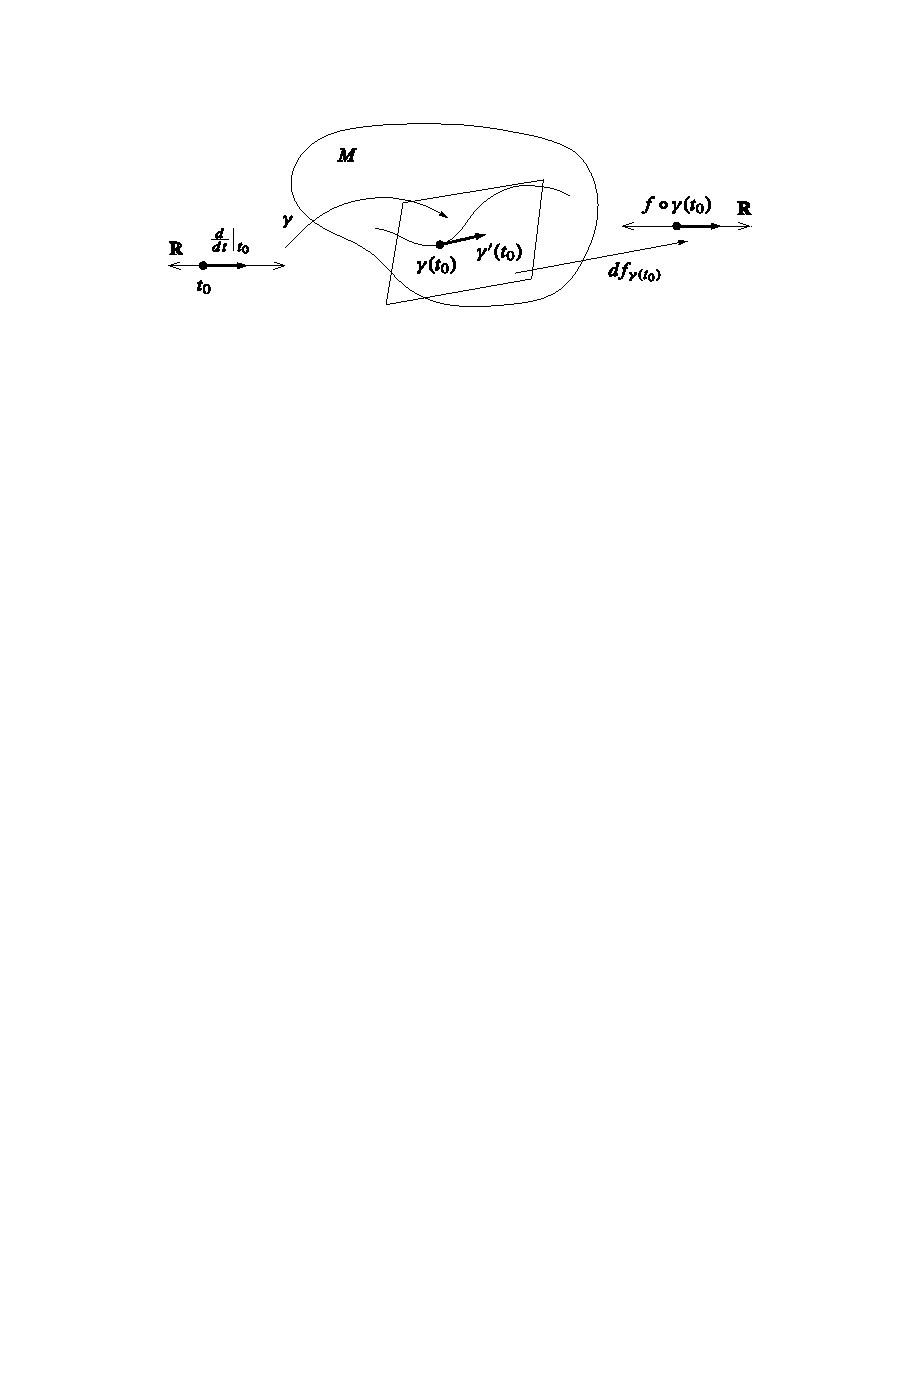
\includegraphics{diff-function}
\caption{Derivative of a function along a curve.}
\end{figure}
\begin{proof}
Directly from the definitions, for any $t_0\in J$,
\begin{align*}
df_{\gamma(t_0)}\big(\gamma'(t_0)\big)&=\gamma'(t_0)f=d\gamma_{t_0}\Big(\frac{d}{dt}\Big|_{t_0}\Big)f=\frac{d}{dt}\Big|_{t_0}(f\circ\gamma)=(f\circ\gamma)'(t_0)
\end{align*}
\end{proof}
You may have noticed that for a smooth real-valued function $f:M\to\R$, we now have two different definitions for the differential of $f$ at a point $p\in M$. In Section~\ref{tangent vector section}, we defined $df_p$ as a linear map from $Tp_M$ to $T_{f(p)}\R$. In this section, we defined $df_p$ as a covector at $p$, which is to say a linear map from $T_pM$ to $\R$. These are really the same object, once we take into account the canonical identification between $\R$ and $T_{f(p)}\R$; one easy way to see this is to note that both are represented in coordinates by the row matrix whose components are the partial derivatives of $f$: If $v=v^i\partial/\partial x^i|_p\in T_pM$, then
\[df_p(v)=df_p\Big(v^i\frac{\partial}{\partial x^i}\Big|_p\Big)=\frac{\partial f}{\partial x^i}(p)\frac{d}{dt}\Big|_{f(p)},\quad vf=v^i\frac{\partial}{\partial x^i}\Big|_pf=v^i\frac{\partial f}{\partial x^i}(p)\]\par
Similarly, if $\gamma$ is a smooth curve in $M$, we have two different meanings for the expression $(f\circ\gamma)'(t)$. On the one hand, $f\circ\gamma$ can be interpreted as a smooth curve in $\R$, and thus $(f\circ\gamma)'(t)$ is its velocity at the point $f\circ\gamma(t)$, which is an element of the tangent space $T_{f(t)}\R$. Proposition~\ref{diff composite curve} shows that this tangent vector is equal to $df_{\gamma(t)}\big(\gamma'(t)\big)$, thought of as an element of $T_{f(\gamma(t))}\R$. On the other hand, $f\circ\gamma$ can
also be considered simply as a real-valued function of one real variable, and then $(f\circ\gamma)'(t)$ is just its ordinary derivative. Proposition~\ref{diff function curve} shows that this derivative is equal to $df_{\gamma(t)}\big(\gamma'(t)\big)$, thought of as a real number. Which of these interpretations we choose depends on the purpose we have in mind.
\subsection{Pullbacks of covector fields}
As we have seen, a smooth map yields a linear map on tangent vectors called the differential. Dualizing this leads to a linear map on covectors going in the opposite
direction.\par
Let $F:M\to N$ be a smooth map between smooth manifolds with or without boundary, and let $p\in M$ be arbitrary. The differential $dF_p:T_pM\to T_{F(p)}N$ yields a dual linear map
\[df^*_p:T^*_{F(p)}N\to T^*_pM\]
called the (pointwise) pullback by $F$ at $p$, or the cotangent map of $F$. Unraveling the definitions, we see that $df^*_p$ is characterized by
\[df^*_p(\omega)(v)=\omega\big(dF_p(v)\big)\for \omega\in T^*_{F(p)}N,v\in T_pM\]
Given a smooth map $F:M\to N$ and a covector field $\omega$ on $N$, define a rough covector field $f^*\omega$ on $M$, called the pullback of $\omega$ by $F$, by
\[(f^*\omega)_p=df^*_p(\omega_{F(p)})\]
It acts on a vector $v\in T_pM$ by
\[(f^*\omega)_p(v)=\omega_{F(p)}\big(dF_p(v)\big)\]
\begin{proposition}\label{pull back functor}
Let $F:M\to N$ and $G:N\to P$ be smooth maps between smooth manifolds, then
\begin{itemize}
\item[(a)] $(G\circ F)^*=f^*\circ G^*$.
\item[(b)] $(\mathrm{id}_M)^*=\mathrm{id}_{T^*M}$.
\end{itemize}
\end{proposition}
\begin{proof}
Choose a point $p\in M$, let $\omega\in T^*_{F(G(p))}$ and $v\in T_pM$. Then 
\begin{align*}
\big((G\circ F)^*\omega\big)(v)&=\omega\big(d(G\circ F)_p(v)\big)=\omega\big(dG_{F(p)}\circ dF_{p}(v)\big)=(G^*\omega)\big(dF_p(v)\big)\\
&=\big(f^*(G^*\omega)\big)(v)=(f^*\circ G^*\omega)(v)
\end{align*}
Thus
\[(G\circ F)^*=f^*\circ G^*.\]
Now the second claim is obvious.
\end{proof}
In contrast to the vector field case, there is no ambiguity here about what point to pull back from: the value of $f^*\omega$ at $p$ is the pullback of $\omega$ at $F(p)$. We will show that $f^*\omega$ is continuous, and is smooth when $\omega$ is smooth. Before we do so, let us prove two important properties of the pullback.
\begin{proposition}\label{pull back prop}
Let $F:M\to N$ be a smooth map between smooth manifolds with or without boundary. Suppose $f$ is a continuous real-valued function on $N$, and $\omega$ is a covector field on $N$. Then
\begin{align}\label{pull back prop-1}
f^*(f\omega)=(f\circ F)f^*\omega
\end{align}
If in addition $f$ is smooth, then
\begin{align}\label{pull back prop-2}
f^*du=d(f\circ F)
\end{align}
\end{proposition}
\begin{proof}
We compute
\begin{align*}
\big(f^*(f\omega)\big)_p=df^*_p\big(f(F(p))\omega_{F(p)}\big)=f(F(p))df^*(\omega_{F(p)})=f\circ F(p)(f^*\omega)_p=\big((f\circ F)f^*\omega\big)_p
\end{align*}
and
\begin{align*}
(f^*df)_p(v)=\big(df^*_p(df_{F(p)})\big)(v)=df_{F(p)}(dF_p(v))=dF_p(v)(f)=v(f\circ F)=d(f\circ F)_p(v)
\end{align*}
\end{proof}
\begin{proposition}
Suppose $F:M\to N$ is a smooth map between smooth manifolds with or without boundary, and let $\omega$ be a covector field on $N$. Then $f^*\omega$ is a
$($continuous$)$ covector field on $M$. If $\omega$ is smooth, then so is $f^*\omega$.
\end{proposition}
\begin{proof}
Let $p\in M$ be arbitrary, and choose smooth coordinates $(y^j)$ for $N$ in a
neighborhood $V$ of $F(p)$. Let $U=F^{-1}(V)$, which is a neighborhood of $p$. Writing $\omega$ in coordinates as $\omega=\omega_jdy^j$ for continuous functions $\omega_j$ on $V$ and using Proposition~\ref{pull back prop} twice (applied to $F|_U$), we have the following computation in $U$:
\begin{align}\label{pull back-1}
f^*\omega=f^*(\omega_jdy^j)=(\omega_j\circ F)f^*dy^j=(\omega_j\circ F)d(y^j\circ F)
\end{align}
This expression is continuous, and is smooth if $\omega$ is smooth.
\end{proof}
Formula $(\ref{pull back-1})$ for the pullback of a covector field can also be written in the following way:
\begin{align}\label{pull back-2}
f^*\omega=(\omega_j\circ F)d(y^j\circ F)=(\omega_j\circ F)dF^j
\end{align}
where $F^j$ is the $j$-th component function of $F$ in these coordinates. Using either of these formulas, the computation of pullbacks in coordinates is exceedingly simple, as the next example shows.
\begin{example}
Let $F:\R^3\to\R^2$ be the map given by
\[(u,v)=F(x,y,z)=(x^2y,y\sin z)\]
and let $\omega\in\X^*(\R^2)$ be the covector field
\[\omega=udv+vdu\]
According to $(\ref{pull back-1})$, the pullback $f^*$ is given by
\begin{align*}
f^*\omega&=(u\circ F)d(v\circ F)+(v\circ F)d(u\circ F)=(x^2y)\,d(y\sin z)+(y\sin z)\,d(x^2y)\\
&=x^2y(\sin z\,dy+y\cos z\,dz)+(y\sin z)(2xy\,dx+x^2\,dy)\\
&=2xy^2\sin z\,dx+2x^2y\sin z\,dy+x^2y^2\cos z\,dz
\end{align*}
\end{example}
In other words, to compute $f^*$, all we need to do is substitute the component
functions of $F$ for the coordinate functions of $N$ everywhere they appear in $\omega$. This also yields an easy way to remember the transformation law for a covector field under a change of coordinates. Again, an example will convey the idea better than a general formula.
\begin{example}
Let $(r,\theta)$ be polar coordinates on, say, the right half-plane $H=\{(x,y):x>0\}$. We can think of the change of coordinates $(x,y)=(r\cos\theta,r\sin\theta)$ as the coordinate expression for the identity map of $H$, but using $(r,\theta)$ as coordinates for the domain and $(x,y)$ for the codomain. Then the pullback formula tells us that we can compute the polar coordinate expression for a covector field simply by substituting $x=r\cos\theta,y=r\sin\theta$ and expanding. For example,
\begin{align*}
x\,dy-y\,dx&=r\cos\theta\,d(r\sin\theta)-r\sin\theta\,d(r\cos\theta)\\
&=r\cos\theta(\sin\theta\,dr+r\cos\theta\,d\theta)-r\sin\theta(\cos\theta\,dr-r\sin\theta\,d\theta)\\
&=r\cos\theta\sin\theta\,dr+r^2\cos\theta^2\,d\theta-r\sin\theta\cos\theta\,dr+r^2\sin\theta^2\,d\theta\\
&=r^2d\theta
\end{align*}
\end{example}
\subsubsection{Restricting covector fields to submanifolds}
In Section~\ref{vector field section}, we considered the conditions under which a vector field restricts to a submanifold. The restriction of covector fields to submanifolds is much simpler.\par
Suppose $M$ is a smooth manifold with or without boundary, $S\sub M$ is an immersed submanifold with or without boundary, and $\iota:S\hookrightarrow M$ is the inclusion map. If $\omega$ is any smooth covector field on $M$, the pullback by $\iota$ yields a smooth covector field $\iota^*\omega$ on $S$. To see what this means, let $v\in T_pS$ be arbitrary, and compute
\[(\iota^*\omega)_p(v)=d\iota^*_p(\omega)(v)=\omega_p\big(d\iota_p(v)\big)=\omega_p(v)\]
since $d\iota_p:T_pS\to T_pM$ is just the inclusion map, under our usual identification of $T_pS$ with a subspace of $T_pM$. Thus, $\iota^*$ is just the restriction of $\omega$ to vectors tangent to $S$. For this reason, $\iota^*\omega$ is often called the \textbf{restriction of $\bm{\iota}$ to $\bm{S}$}. Be warned, however, that $\iota^*\omega$ might equal zero at a given point of $S$, even though considered as a covector field on $M$, $\omega$ might not vanish there. An example will help to clarify this distinction.
\begin{example}
Let $\omega=dy$ on $\R^2$, and let $S$ be the $x$-axis, considered as an embedded submanifold of $\R^2$. As a covector field on $\R^2$, $\omega$ is nonzero everywhere, because one of its component functions is always $1$. However, the restriction $\iota^*\omega$ is identically zero, because $y$ vanishes identically on $S$:
\[\iota^*\omega=d(y\circ\iota)=0\]
\end{example}
To distinguish the two ways in which we might interpret the statement $\iota$ vanishes on $S$, one usually says that \textbf{$\bm{\omega}$ vanishes along $\bm{S}$} or \textbf{vanishes at points of $\bm{S}$} if $\omega_p=0$ for every point $p\in S$. The weaker condition that $\iota^*\omega=0$ is expressed by saying that \textbf{the restriction of $\bm{\omega}$ to $\bm{S}$ vanishes}, or \textbf{the pullback of $\bm{\omega}$ to $\bm{S}$ vanishes}.
\begin{proposition}\label{diff restrict submani}
Suppose $M$ is a smooth manifold with or without boundary and $S\sub M$ is an immersed submanifold with or without boundary. For any $f\in C^\infty(M)$ we have $d(f|_S)=\iota^*(df)$. Thus the pullback of $df$ to $S$ is zero if and only if $f$ is constant on each component of $S$.
\end{proposition}
\begin{proof}
Let $p\in S$ and choose $v\in T_pM$, we compute that
\[\big(\iota^*(df)\big)_p(v)=df\big(d\iota_p(v)\big)=d\iota_p(v)(f)=v(f\circ\iota)=v(f|_S)=d(f|_S)(v)\]
Thus $\iota^*(df)=0$ if and only if $d(f|_S)=0$, and the second claim follows from Proposition~\ref{diff vanish}.
\end{proof}
\subsection{Line integrals}
Another important application of covector fields is to make coordinate-independent sense of the notion of a line integral.\par
We begin with the simplest case: \textit{an interval in the real line}. Suppose $[a,b]\sub\R$ is a compact interval, and $\omega$ is a smooth covector field on $[a,b]$. (This means that the component function of $\omega$ admits a smooth extension to some neighborhood of $[a,b]$) If we let $t$ denote the standard coordinate on $\R$, then $\omega$ can be written $\omega_t=f(t)dt$ for some smooth function $f:[a,b]\to\R$. We define the \textbf{integral of $\bm{\omega}$ over $\bm{[a,b]}$} to be
\[\int_{[a,b]}\omega=\int_{a}^{b}f(t)dt\]
The next proposition should convince you that this is more than just a trick of
notation.
\begin{proposition}[\textbf{Diffeomorphism Invariance of the Integral}]\label{diffeo invariance integral}
Let $\omega$ be a smooth covector field on the compact interval $[a,b]\sub\R$. If $\varphi:[c,d]\to[a,b]$ is an increasing diffeomorphism, then
\[\int_{[c,d]}\varphi^*\omega=\int_{[a,b]}\omega\]
\end{proposition}
\begin{proof}
If we let $s$ denote the standard coordinate on $[c,d]$ and $t$ that on $[a,b]$, then $(\ref{pull back-2})$ shows that the pullback $\varphi^*\omega$ has the coordinate expression 
\[(\varphi^*\omega)_s=f\circ\varphi(s)\,d\varphi(s)=f\circ\varphi(s)\varphi'(s)\,ds.\] 
Inserting this into the definition of the line integral and using the
change of variables formula for ordinary integrals, we obtain
\[\int_{[c,d]}\varphi^*\omega=\int_{c}^{d}f\circ\varphi(s)\varphi'(s)\,ds=\int_{a}^{b}f(t)dt=\int_{[a,b]}\omega\]
\end{proof}
\begin{remark}\label{diffeo invariance remk}
If $\varphi:[c,d]\to[a,b]$ is a decreasing diffeomorphism, then
\[\int_{[c,d]}\varphi^*\omega=-\int_{[a,b]}\omega\]
\end{remark}
Now let $M$ be a smooth manifold with or without boundary. By a \textbf{curve segment} in $M$ we mean a continuous curve $\gamma:[a,b]\to M$ whose domain is a compact interval. It is a smooth curve segment if it is smooth when $[a,b]$ is considered as a manifold with boundary. It is a \textbf{piecewise smooth curve segment} if there exists a finite partition 
\[a=a_0<a_1<\cdots<a_k=b\]
such that $\gamma|_{[a_{i-1},a_i]}$ is smooth for each $i$. Continuity of $\gamma$ means that $\gamma(t)$ approaches the same value as t approaches any of the points $a_i$ (other than $a_0$ or $a_n$) from the left or the right. Smoothness of $\gamma$ on each subinterval means that $\gamma$ has one-sided velocity vectors at each such $a_i$ when approaching from the left or the right, but these one-sided velocities need not be equal.
\begin{proposition}\label{connect by smooth curve}
If $M$ is a connected smooth manifold with or without boundary, any two points of $M$ can be joined by a piecewise smooth curve segment.
\end{proposition}
\begin{proof}
Let $p$ be an arbitrary point of $M$, and define a subset
\[\mathscr{C}=\{q\in M:\text{ there is a piecewise smooth curve segment in $M$ from $p$ to $q$}\}\]
Clearly, $p\in\mathscr{C}$, so $\mathscr{C}$ is nonempty. To show that $\mathscr{C}=M$, we need to show that it is open and closed in $M$.\par
Let $q\in \mathscr{C}$ be arbitrary, which means that there is a piecewise smooth curve segment $\gamma$ going from $p$ to $q$. Let $U$ be a smooth coordinate ball (or half-ball) centered at $q$. If $q'$ is any point in $U$, then it is easy to construct a piecewise smooth curve segment from $p$ to $q'$ by first following $\gamma$ from $p$ to $q$, and then following a straight-line
path in coordinates from $q$ to $q'$. Thus $U\sub\mathscr{C}$, which shows that $\mathscr{C}$ is open in $M$.\par
On the other hand, if $q$ is a limit point of $\mathscr{C}$, let $U$ be a smooth coordinate ball or half-ball around $q$ as above. Then there is some point $q'\in\mathscr{C}\cap U$. In this case, we can construct a piecewise smooth curve from $p$ to $q$ by first following one from $p$ to $q'$ and then following a straight-line path in coordinates from $q'$ to $q$. This shows that $q\in\mathscr{C}$, so $\mathscr{C}$ is also closed.
\end{proof}
If $\gamma:[a,b]\to M$ is a smooth curve segment and $\omega$ is a smooth covector field on $M$, we define the \textbf{line integral of $\bm{\omega}$ over $\bm{\gamma}$} to be the real number
\[\int_{\gamma}\omega=\int_{a}^{b}\gamma^*\omega\]
Because $\gamma^*\omega$ is a smooth covector field on $[a,b]$, this definition makes sense. More generally, if $\gamma$ is piecewise smooth, we define
\[\int_{\gamma}\omega=\sum_{i=1}^{k}\int_{[a_{i-1},a_i]}\gamma^*\omega\]
where $[a_{i-1},a_i],1\leq i\leq k$ are subintervals on which $\gamma$ is smooth.
\begin{proposition}[\textbf{Properties of Line Integrals}]\label{line integral prop}
Let $M$ be a smooth manifold with or without boundary. Suppose $\gamma:[a,b]\to M$ is a piecewise smooth curve segment, and $\omega_1,\omega_2\in\X^*(M)$.
\begin{itemize}
\item[(a)] For any $c_1,c_2\in\R$,
\[\int_{\gamma}(c_1\omega_1+c_2\omega_2)=c_1\int_{\gamma}\omega_1+c_2\int_{\gamma}\omega_2.\]
\item[(b)] If $\gamma$ is a constant map, then $\int_\gamma\omega=0$.
\item[(c)] If $\gamma_1=\gamma|_{[a,c]}$ and $\gamma_1=\gamma|_{[c,b]}$ with $a<c<b$, then
\[\int_{\gamma}\omega=\int_{\gamma_1}\omega+\int_{\gamma_2}\omega.\]
\item[(d)] If $F:M\to N$ is any smooth map and $\eta\in\X^*(N)$, then
\[\int_{\gamma}f^*\eta=\int_{F\circ\gamma}\eta.\]
\end{itemize}
\end{proposition}
\begin{proof}
We only prove the last equality:
\begin{align*}
\int_{\gamma}f^*\eta=\int_{a}^{b}\gamma^*(f^*\eta)=\int_{a}^{b}(F\circ\gamma)^*\eta=\int_{F\circ\gamma}\eta.
\end{align*}
where we use Proposition~\ref{pull back functor}.
\end{proof}
\begin{example}\label{covector closed not exact eg}
Let $M=\R^2-\{0\}$, let $\omega$ be the covector field on $M$ given by
\[\omega=\frac{x\,dy-y\,dx}{x^2+y^2}\]
and let $\gamma:[0,2\pi]\to M$ be the curve segment defined by $\gamma(t)=(\cos t,\sin t)$. Since $\gamma^*\omega$ can be computed by substituting $x=\cos t$ and $y=\sin t$ everywhere in the formula for $\omega$, we find that
\[\int_{\gamma}\omega=\int_{0}^{2\pi}\frac{\cos t\,d\sin t-\sin t\,d\cos t}{\cos^2t+\sin^2t}=\int_{0}^{2\pi}dt=2\pi\]
\end{example}
One of the most significant features of line integrals is that they are independent of parametrization, in a sense we now make precise. If $\gamma:[a,b]\to M$ and $\widetilde{\gamma}:[c,d]\to M$ are piecewise smooth curve segments, we say that $\widetilde{\gamma}$ is a reparametrization of $\gamma$ if $\widetilde{\gamma}=\gamma\circ\varphi$ for some diffeomorphism $\varphi:[c,d]\to[a,b]$. If $\varphi$ is an increasing function, we say that $\widetilde{\gamma}$ is a \textbf{forward reparametrization}, and if $\varphi$
is decreasing, it is a \textbf{backward reparametrization}. (More generally, with obvious modifications one can allow $\varphi$ to be piecewise smooth.)
\begin{proposition}[\textbf{Parameter Independence of Line Integrals}]\label{line integral para independent}
Suppose $M$ is a smooth manifold with or without boundary, $\omega\in\X^*(M)$, and $\gamma$ is a piecewise smooth curve segment in $M$. For any reparametrization $\widetilde{\gamma}$ of $\gamma$, we have
\[\int_{\widetilde{\gamma}}\omega=\begin{cases}
\quad\displaystyle{\int_{\gamma}\omega}&\text{if $\widetilde{\gamma}$ is a forward reparametrization},\\[8pt]
-\displaystyle{\int_{\gamma}\omega}&\text{if $\widetilde{\gamma}$ is a backward reparametrization}.
\end{cases}\]
\end{proposition}
\begin{proof}
First assume that $\gamma:[a,b]\to M$ is smooth, and suppose $\widetilde{\gamma}=\gamma\circ\varphi$, where $\varphi$ is an increasing diffeomorphism. Then Proposition~\ref{diffeo invariance integral} and ~\ref{pull back prop} imply
\[\int_{\widetilde{\gamma}}=\int_{c}^{d}(\gamma\circ\varphi)^*\omega=\int_{c}^{d}\varphi^*\circ\gamma^*\omega=\int_{a}^{b}\gamma^*\omega=\int_{\gamma}\omega\]
When $\varphi$ is decreasing, the analogous result follows from Remark~\ref{diffeo invariance remk}. If $\gamma$ is only piecewise smooth, the result follows simply by applying the preceding argument on each subinterval where $\gamma$ is smooth.
\end{proof}
The next proposition gives a useful alternative expression for a line integral.
\begin{proposition}\label{line integral ordinary form}
If $\gamma:[a,b]\to M$ is a piecewise smooth curve segment, the line integral of $\omega$ over $\gamma$ can also be expressed as the ordinary integral
\[\int_\gamma\omega=\int_{a}^{b}\omega_{\gamma(t)}\big(\gamma'(t)\big)dt\]
\end{proposition}
\begin{proof}
First suppose that $\gamma$ is smooth and that its image is contained in the domain of a single smooth chart. If the coordinate representations of $\gamma$ is $(\gamma^1(t),\dots,\gamma^n(t))$, then
\[\gamma'(t)=\dot{\gamma}^j(t)\frac{\partial}{\partial x^j}\Big|_{\gamma(t)}\] 
If we write $\omega=\omega_idx^i$, then
\[\omega_{\gamma(t)}\big(\gamma'(t)\big)=(\omega_i\circ\gamma)(t)\,dx^i\Big(\dot{\gamma}^j(t)\frac{\partial}{\partial x^j}\Big|_{\gamma(t)}\Big)=(\omega_i\circ\gamma)(t)\dot{\gamma}^i(t).\]
Combining this with the coordinate formula $(\ref{pull back-2})$ for the pullback, we obtain
\begin{align*}
(\gamma^*\omega)_t=(\omega_i\circ\gamma)(t)\,d\gamma^i(t)=(\omega_i\circ\gamma)(t)\dot{\gamma}^i(t)dt=\omega_{\gamma(t)}\big(\gamma'(t)\big)dt.
\end{align*}
Therefore, by the definition of the line integral,
\[\int_{\gamma}\omega=\int_{a}^{b}\gamma^*\omega=\int_{a}^{b}\omega_{\gamma(t)}\big(\gamma'(t)\big)dt.\]
If $\gamma$ is an arbitrary smooth curve segment, by compactness there exists a finite partition 
\[a=a_0<a_1<\cdots<a_k=b\] 
such that $\gamma([a_{i-1},a_i])$ is contained in the domain of a single smooth chart for each $i$, so we can apply the computation above on each such subinterval. Finally, if $\gamma$ is only piecewise smooth, we simply apply the same argument on each subinterval on which $\gamma$ is smooth.
\end{proof}
There is one special case in which a line integral is trivial to compute: the line integral of a differential.
\begin{proposition}[\textbf{Fundamental Theorem for Line Integrals}]\label{line integral fundamental thm}
Let $M$ be a smooth manifold with or without boundary. Suppose $f$ is a smooth real-valued function on $M$ and $\gamma:[a,b]\to M$ is a piecewise smooth curve segment in $M$. Then
\[\int_{\gamma}df=f(\gamma(b))-f(\gamma(a))\]
\end{proposition}
\begin{proof}
Suppose first that $\gamma$ is smooth. By Propositions~\ref{diff function curve} and ~\ref{line integral ordinary form},
\[\int_\gamma df=\int_{a}^{b}df_{\gamma(t)}\big(\gamma'(t)\big)dt=\int_{a}^{b}(f\circ\gamma)'(t)dt=f(\gamma(b))-f(\gamma(a))\]
by the fundamental theorem of calculus.\par
If $\gamma$ is merely piecewise smooth, let 
\[a=a_0<a_1<\cdots<a_k=b\] 
be the endpoints of the subintervals on which $\gamma$ is smooth. Applying the above argument on each subinterval and summing, we find that
\[\int_\gamma df=\sum_{i=1}^{k}\int_{a_{i-1}}^{a_i}\big(f(\gamma(a_{i-1}))-f(\gamma(a_i))\big)=f(\gamma(b))-f(\gamma(a))\]
because the contributions from all the interior points cancel.
\end{proof}
\subsection{Conservative covector fields}
Theorem~\ref{line integral fundamental thm} shows that the line integral of any covector field that can be written as the differential of a smooth function can be computed easily once the smooth function is known. For this reason, there is a special term for covector fields with this property. A smooth covector field $\omega$ on a smooth manifold $M$ with or without boundary is said to be \textbf{exact} (or an \textbf{exact differential}) on $M$ if there is a function $f\in C^\infty(M)$ such that $\omega=df$. In this case, the function $f$ is called a \textbf{potential} for $\omega$.\par
The potential is not uniquely determined, but by Proposition~\ref{diff vanish}, the difference between any two potentials for $\omega$ must be constant on each component of $M$. Because exact differentials are so easy to integrate, it is important to develop criteria for deciding whether a covector field is exact. Theorem~\ref{line integral fundamental thm} provides an important clue. It shows that the line integral of an exact covector field depends only on the endpoints $p=\gamma(a)$ and $q=\gamma(b)$: any other curve segment from $p$ to $q$ would give the same value for the line integral. In particular, if $\gamma$ is a \textbf{closed curve segment}, meaning that $\gamma(a)=\gamma(b)$, then the integral of $df$ over $\gamma$ is zero.\par
We say that a smooth covector field $\omega$ is \textbf{conservative} if the line integral of $\omega$ over every piecewise smooth closed curve segment is zero.\par
Conservative covector fields can also be characterized by path independence.
\begin{proposition}
A smooth covector field $\omega$ is conservative if and only if its line integrals are path-independent, in the sense that $\int_\gamma\omega=\int_{\widetilde{\gamma}}\omega$ whenever $\gamma$ and $\widetilde{\gamma}$ are piecewise smooth curve segments with the same starting and ending points.
\end{proposition}
\begin{proof}
If $\gamma:[a,b]\to M$ and $\widetilde{\gamma}:[c,d]\to M$ are piecewise smooth curve segments with the same starting and ending points, we define $\gamma-\widetilde{\gamma}:[-1,1]$ to be the curve
\[(\gamma-\widetilde{\gamma})(t)=\begin{cases}
\gamma\big(a+(b-a)(t+1)\big)&t\in[-1,0]\\
\widetilde{\gamma}\big(d-(d-c)t\big)&t\in[0,1]
\end{cases}\]
Geomrtrically speaking, $\gamma-\widetilde{\gamma}$ is defined by first travel along $\gamma$ forward, then along $\widetilde{\gamma}$ backward. Then $\gamma-\widetilde{\gamma}$ is piecewise smooth and closed, and we have the observation
\[\int_{\gamma-\widetilde{\gamma}}\omega=\int_{\gamma}\omega-\int_{\widetilde{\gamma}}\omega\]
Now the claim is clear.
\end{proof}
\begin{proposition}\label{covector conservative iff exact}
Let $M$ be a smooth manifold with or without boundary. A smooth covector field on $M$ is conservative if and only if it is exact.
\end{proposition}
\begin{proof}
If $\omega\in\X^*(M)$ is exact, Theorem~\ref{line integral fundamental thm} shows that it is conservative, so we need only prove the converse. Suppose $\omega$ is conservative, and assume for the moment that $M$ is connected. Because the line integrals of $\omega$ are path-independent, we can adopt the following notation: for any points $p,q$ we use the notation $\int_p^q\omega$ to denote the value of any line integral of the form $\int_\gamma\omega$, where $\gamma$ is a piecewise smooth curve segment from $p$ to $q$. Because a backward reparametrization of a path from $p$ to $q$ is a path from $q$ to $p$, Proposition~\ref{line integral para independent} implies $\int_q^p\omega=-\int_p^q\omega$ and for any three points $p_1,p_2,p_3\in M$ Proposition~\ref{line integral prop}(c) implies that
\begin{align}\label{covector conservative-1}
\int_{p_1}^{p_3}\omega=\int_{p_1}^{p_2}\omega+\int_{p_2}^{p_3}\omega
\end{align}
Now choose any base point $p_0\in M$, and define a function $f:M\to\R$ by
\[f(q)=\int_{p_0}^{p}\omega\]
We prove that $f$ is smooth and $df=\omega$.\par 
To accomplish this, let $q_0\in M$ be arbitrary, let $(U,(x^i))$ be a smooth chart centered at $q_0$, and write the coordinate representation of $\omega$ in $U$ as $\omega=\omega_idx^i$. We need to show that
\[\frac{\partial f}{\partial x^j}(q_0)=\omega_j(q_0)\for 1\leq j\leq n\]
First suppose $q_0\in\Int M$. Fix $j$, and let $\gamma:[-\eps,\eps]\to U$ be the smooth curve segment defined in coordinates by $\gamma(t)=(0,\dots,t,\dots,0)$, with $t$ in the $j$-th place, and with $\eps$ chosen small enough that $\gamma([-\eps,\eps])\sub U$. Let $p_1=\gamma(-\eps)$, and define a new function $\widetilde{f}:M\to\R$ by $\widetilde{f}(q)=\int_{p_1}^{q}\omega$. Note that $(\ref{covector conservative-1})$ implies that for all $q\in M$,
\[f(q)-\widetilde{f}(q)=\int_{p_0}^{q}\omega-\int_{p_1}^{q}\omega=\int_{p_0}^{p_1}\omega\]
which does not depend on $q$. Thus $\widetilde{f}$ and $f$ differ by a constant, so it suffices to show that $\partial\widetilde{f}/\partial x^j(q_0)=\omega_j(q_0)$.\par
Now $\gamma'(t)=\partial/\partial x^j|_{\gamma(t)}$ by construction, so 
\[\omega_{\gamma(t)}\big(\gamma'(t)\big)=\omega_{\gamma(t)}\Big(\frac{\partial}{\partial x^j}\Big|_{\gamma(t)}\Big)=\omega_j\big(\gamma(t)\big)\]
Since the restriction of $\gamma$ to $[-\eps,t]$ is a smooth curve from $p_1$ to $\gamma(t)$, we have
\[\widetilde{f}\circ\gamma(t)=\int_{p_1}^{\gamma(t)}\omega=\int_{-\eps}^{t}\omega_{\gamma(t)}\big(\gamma'(t)\big)=\int_{-\eps}^{t}\omega_j\big(\gamma(s)\big)ds\]
Thus, by the fundamental theorem of calculus,
\begin{align*}
\frac{\partial\widetilde{f}}{\partial x^j}(q_0)=\gamma'(0)\widetilde{f}=\frac{d}{dt}\Big|_{t=0}\widetilde{f}\circ\gamma(t)=\frac{d}{dt}\Big|_{t=0}\int_{-\eps}^{t}\omega_j\big(\gamma(s)\big)ds=\omega_j\big(\gamma(0)\big)=\omega_j(q_0)
\end{align*}
This shows that $df_{q_0}=\omega_{q_0}$ when $q_0\in\Int M$.\par
For $q_0\in\partial M$, the chart $(U,(x^i))$ is a boundary chart centered at $q_0$. The proof above shows that $\partial f/\partial x^j(q_0)=\omega_j(q_0)$ except in the case $j=n=\dim M$; but that case requires a special argument because $x^n$ takes on only nonnegative values in a boundary chart. In that case we simply set $p_1=\gamma(0)$ instead of $p_1=\gamma(-\eps)$, and proceed as before. Then the same argument shows that $df_{q_0}=\omega_{q_0}$ in this case as well. This completes the proof that $df=\omega$ when $M$ is connected. Since the component functions of $\omega$ are smooth and equal to the partial derivatives of $f$ in coordinates, this also shows that $f$ is smooth.\par
Finally, if $M$ is not connected, let $\{M_i\}$ be the components of $M$. The argument above shows that for each $i$ there is a function $f^i\in C^\infty(M)$ such that $df_i=\omega$ on $M_i$. Letting $f:M\to\R$ be the function that is equal to $f_i$ on $M_i$ for each $i$, we have $df=\omega$, thus completing the proof.
\end{proof}
\begin{example}
The covector field $\omega$ of Example~\ref{covector closed not exact eg} cannot be exact on $\R^2-\{0\}$, because it is not conservative: the computation in that example showed that $\int_\gamma\omega=2\pi\neq 0$, where $\gamma$ is the unit circle traversed counterclockwise.
\end{example}
To see a sufficient condition for exactness, suppose $\omega\in\X^*(M)$ is exact. Let $f$ be any potential function for $\omega$, and let $(U,(x^i))$ be any smooth chart on $M$. Because $f$ is smooth, it satisfies the following identity on $U$:
\begin{align*}
\frac{\partial^2f}{\partial x^i\partial x^j}=\frac{\partial^2f}{\partial x^j\partial x^i}
\end{align*}
Writing $\omega=\omega_idx^i$ in coordinates, we see that $\omega=df$ is equivalent to $\omega_i=\partial f/\partial x^i$. Substituting this, we find that the component functions of $\omega$ satisfy the following identity for each pair of indices $i$ and $j$:
\begin{align}\label{covector closed-1}
\frac{\partial\omega_i}{\partial x^j}=\frac{\partial\omega_j}{\partial x^i}
\end{align}
We say that a smooth covector field $\omega$ is closed if its components in every smooth chart satisfy $(\ref{covector closed-1})$. The following proposition summarizes the computation above.
\begin{proposition}
Every exact covector field is closed.
\end{proposition}
One technical difficulty in checking directly from the definition that a covector field is closed is that it would require checking that $(\ref{covector closed-1})$ holds in every coordinate chart. The next proposition gives an alternative characterization of closed covector fields that is coordinate independent, and incidentally shows that it suffices to check $(\ref{covector closed-1})$ in some coordinate chart around each point.
\begin{proposition}\label{covector closed iff}
Let $\omega$ be a smooth covector field on a smooth manifold $M$ with or without boundary. The following are equivalent:
\begin{itemize}
\item[(a)] $\omega$ is closed.
\item[(b)] $\omega$ satisfies $(\ref{covector closed-1})$ in some smooth chart around every point.
\item[(c)] For any open subset $U\sub M$ and smooth vector fields $X,Y\in\X(U)$,
\begin{align}\label{covector closed-2}
X(\omega(Y))-Y(\omega(X))=\omega([X,Y])
\end{align}
\end{itemize}
\end{proposition}
\begin{proof}
We will prove that $(a)\Rightarrow(b)\Rightarrow(c)\Rightarrow(a)$. The implication $(a)\Rightarrow(b)$ is immediate from the definition of closed covector fields.\par
To prove $(b)\Rightarrow(c)$, assume (b) holds, and suppose $U\sub M$ and $X,Y\in\X(U)$ as in the statement of (c). It suffices to verify that $(\ref{covector closed-2})$ holds in a neighborhood of each point of $U$. In any coordinate chart $(V,(x^i))$ with $V\sub U$, we can write $\omega=\omega_idx^i$, $X=X^j\partial/\partial x^j$ and $Y=Y^k\partial/\partial x^k$, and compute
\begin{align*}
X(\omega(Y))=X(\omega_iY^i)=Y^iX\omega_i+\omega_iXY^i=Y^iX^j\frac{\partial\omega_i}{\partial x^j}+\omega_iXY^i
\end{align*}
If we repeat the same computation with $X$ and $Y$ reversed and subtract, the terms involving derivatives of $\omega_i$ cancel by virtue of $(\ref{covector closed-1})$. Thus we get
\[X(\omega(Y))-Y(\omega(X))=\omega(XY^i-YX^i)\]
Formula $(\ref{Lie bracket-2})$ shows that this last expression is equal to $\omega([X,Y])$.\par
Finally, if $\omega$ satisfies (c), in any coordinate chart we can apply $(\ref{covector closed-1})$ with $X=\partial/\partial x^i$ and $\partial/\partial x^j$, noting that $[X,Y]=0$ in that case, to obtain $(\ref{covector closed-2})$.
\end{proof}
One consequence of this proposition is that closedness can be easily checked
using criterion (b), so many covector fields can be shown quickly not to be exact because they are not closed. Another is the following corollary.
\begin{corollary}
Suppose $F:M\to N$ is a local diffeomorphism. Then the pullback $f^*:\X^*(N)\to\X^*(M)$ takes closed covector fields to closed covector fields,
and exact ones to exact ones.
\end{corollary}
\begin{proof}
The result for exact covector fields follows immediately from $(\ref{pull back prop-2})$. For closed covector fields, if $(U,\varphi)$ is any smooth chart for $N$, then $\varphi\circ F$ is a smooth chart for $M$ in a neighborhood of each point of $F^{-1}$. In these coordinates, the coordinate representation of $F$ is the identity, so if $\omega$ satisfies $(\ref{covector closed-1})$ in $U$, then $f^*\omega$ satisfies $(\ref{covector closed-1})$ in $F^{-1}(U)$.
\end{proof}
\begin{example}
Consider the following covector field on $\R^2$:
\[\omega=y\cos xy\,dx+x\cos yx\,dy\]
It is easy to check that
\[\frac{\partial(y\cos xy)}{\partial y}=\frac{\partial(x\cos xy)}{\partial x}=\cos xy-xy\sin xy\]
so $\omega$ is closed. In fact, $\omega=d(\sin xy)$.\par
On the other hand, the covector field
\[\eta=x\cos xy\,dx+y\cos xy\,dy\]
is not closed, because
\[\frac{\partial(x\cos xy)}{\partial y}=-x^2\sin xy,\quad \frac{\partial(y\cos xy)}{\partial x}=-y^2\sin xy.\]
Thus $\eta$ is not exact.
\end{example}
However, not every closed covector field is exact. It turns out that this question depends in a subtle way on the shape of the domain, as the next example illustrates.
\begin{example}
Look once again at the covector field $\omega$ of Example~\ref{covector closed not exact eg}. A straightforward computation shows that $\omega$ is closed; but as we observed above, it is not exact on $\R^2-\{0\}$. On the other hand, if we restrict the domain to the right half-plane $U=\{(x,y):x>0\}$, a computation shows that $\omega=d\arctan(y/x)$ there. This can be seen more clearly in polar coordinates, where $\omega=d\theta$. The problem, of course, is that there is no smooth $($or even continuous$)$ angle function on all of $\R^2-\{0\}$, which is a consequence of the hole in the center.
\end{example}
This last example illustrates a key principle: the question of whether a particular closed covector field is exact is a global one, depending on the shape of the domain in question. This observation is the starting point for de Rham cohomology, which expresses a deep relationship between smooth structures and topology.\par
If $V$ is a finite-dimensional vector space, a subset $U\sub V$ is said to be star-shaped if there is a point $c\in U$ such that for every $x\in U$, the line segment from $c$ to $x$ is entirely contained in $U$. For example, every convex subset is star-shaped.
\begin{theorem}[\textbf{Poincar\'e Lemma for Covector Fields}]\label{Poincare lemma}
If $U$ is a star-shaped open subset of $\R^n$ or $\H^n$, then every closed covector field on $U$ is exact.
\end{theorem}
\begin{proof}
Suppose $U$ is star-shaped with respect to $c\in U$, and let $\omega=\omega_idx^i$ be a closed covector field on $U$. As in the proof of Theorem~\ref{covector conservative iff exact}, we will construct a potential function for $\omega$ by integrating along smooth curve segments from $c$. However, in this case we do not know a priori that the line integrals are path-independent, so we must integrate along specific paths.\par
Because diffeomorphisms take closed forms to closed forms and exact ones to
exact ones, we can apply a translation to $U$ to arrange that $c=0$. For any point $x\in U$, let $\gamma_x:[0,1]\to U$ denote the line segment from $0$ to $x$, parametrized as $\gamma_x(t)=tx$. The hypothesis guarantees that the image of $\gamma_x$ lies entirely in $U$ for each $x\in U$. Define a function $f:U\to\R$ by
\[f(x)=\int_{\gamma_x}\omega\]
We need to show that $\partial/\partial x^j$ for $1\leq j\leq n$. To begin, we compute
\begin{align}\label{Poincare lemma construction}
f(x)=\int_{0}^{1}\omega_{\gamma_x(t)}\big(\gamma_x'(t)\big)dt=\int_{0}^{1}\omega_i(tx)x^idt.
\end{align}
To compute the partial derivatives of $f$, we note that the integrand is smooth in all variables, so it is permissible to differentiate under the integral sign to obtain
\[\frac{\partial f}{\partial x^j}(x)=\int_{0}^{1}\Big(t\frac{\partial\omega_i}{\partial x^j}(tx)x^i+\omega_j(tx)\Big)dt\]
Because $\omega$ is closed, this reduces to
\begin{align*}
\frac{\partial f}{\partial x^j}(x)&=\int_{0}^{1}\Big(t\frac{\partial\omega_i}{\partial x^j}(tx)x^i+\omega_j(tx)\Big)dt=\int_{0}^{1}\Big(t\frac{\partial\omega_j}{\partial x^i}(tx)x^i+\omega_j(tx)\Big)dt\\
&=\int_{0}^{1}\frac{d}{dt}\big(t\omega_j(tx)\big)dt=\Big[t\omega_j(tx)\Big]_{t=0}^{t=1}=\omega_j(x)
\end{align*}
\end{proof}
\begin{corollary}[\textbf{Local Exactness of Closed Covector Fields}]
Let $\omega$ be a closed covector field on a smooth manifold $M$ with or without boundary. Then every point of $M$ has a neighborhood on which $\omega$ is exact.
\end{corollary}
\begin{proof}
Let $p\in M$ be arbitrary. The hypothesis implies that $\omega$ satisfies $(\ref{covector closed-1})$ in some smooth coordinate ball or half-ball $(U,\varphi)$ containing $p$. Because balls and half-balls are convex, we can apply Theorem~\ref{Poincare lemma} to the coordinate representation of $\omega$ and conclude that there is a function $f\in C^\infty(U)$ such that $\omega|_U=df$.
\end{proof}
\subsection{Exercise}
\begin{exercise}
Let $M$ be a smooth manifold with or without boundary and $p$ be a point of $M$. Let $\mathfrak{I}_p$ denote the subspace of $C^\infty(M)$ consisting of smooth functions that vanish at $p$, and let $\mathfrak{I}^2_p$ be the subspace of $\mathfrak{I}_p$ spanned by functions of the form $fg$ for some $f,g\in\mathfrak{I}_p$.
\begin{itemize}
\item[(a)] Show that $f\in\mathfrak{I}^2_p$ if and only if in any smooth local coordinates, its first-order Taylor polynomial at $p$ is zero.
\item[(b)] Define a map $\varPhi:\mathfrak{I}_p\to T^*_pM$ by setting $\varPhi(f)=df_p$. Show that the restriction of $\varPhi$ to $\mathfrak{I}^2_p$ is zero, and that $\varPhi$ descends to a vector space
isomorphism from $\mathfrak{I}_p/\mathfrak{I}^2_p$ to $T^*_pM$.
\end{itemize}
\end{exercise}
\begin{exercise}
For any smooth manifold $M$, show that $T^*M$ is a trivial vector bundle if
and only if $TM$ is trivial.
\end{exercise}
\begin{proof}
Use Lemma~\ref{dual frame smooth iff}.
\end{proof}
\begin{exercise}
Suppose $M$ is a smooth $n$-manifold, $p\in M$, and $y^1,\dots,y^k$ are smooth
real-valued functions defined on a neighborhood of $p$ in $M$. Prove the following statements.
\begin{itemize}
\item[(a)] If $k=n$ and $(dy^1|_p,\dots,dy^n|_p)$ is a basis for $T^*_pM$ then $(y^1,\dots,y^n)$ are smooth coordinates for $M$ in some neighborhood of $p$.
\item[(b)] If $(dy^1|_p,\dots,dy^k|_p)$ is a linearly independent $k$-tuple of covectors and $k<n$, then there are smooth functions $(y^{k+1},\dots,y^n)$ such that $(y^1,\dots,y^n)$ are smooth coordinates for $M$ in a neighborhood of $p$.
\item[(c)] If $(dy^1|_p,\dots,dy^k|_p)$ span $T^*_pM$, there are indices $i_1,\dots,i_n$ such that $(y^{i_1},\dots,y^{i_n})$ are smooth coordinates for $M$ in a neighborhood of $p$.
\end{itemize}
\end{exercise}
\begin{exercise}
Let $M$ be a smooth manifold, and $S\sub M$ be an embedded submanifold. Let $f\in C^\infty(M)$, and suppose $p\in S$ is a point at which $f$ attains a local maximum or minimum value among points in $S$. Given a smooth local defining function $\varPhi:U\to\R^k$ for $S$ on a neighborhood $U$ of $p$ in $M$, show that there are real numbers $\lambda_1,\dots,\lambda_k$ $($called \textbf{Lagrange multipliers}$)$ such that
\[df_p=\lambda_1d\varPhi^1_p+\cdots+\lambda_kd\varPhi^k_p\]
\end{exercise}
\begin{remark}
If $p$ is a local maximum on $S$, then $d(f|_S)_p=\iota^*(df_p)=0$. Since $T_pS$ is identified with the image of $d\iota$, it is intuitive to guess 
\[T_pS=\ker d\varPhi_p\sub\ker df_p\]
In the Euclidean case, the row space of $d\varPhi_p$ is tangent to $T_pS$, thus this is equivalent to say 
\[df_p\sub\mathrm{span}(d\varPhi^1,\dots,d\varPhi^k)\]
\end{remark}
\begin{proof}
Without loss of genrality, we prove for the case $U\sub\R^n$. Since $\varPhi$ is a defining function from $U$ to $\R^k$, we can assume that the last $k$ columns of $\partial\varPhi_p$ are linearly independent. If we denote the points in $\R^n$ by $(x,y)\in\R^{n-k}\times\R^k$, then by the implicit function theorem there exists an open set $V\sub\R^{n-k}$ and a smooth function $g:V\to\R^k$ such that
\[M\cap U=\{(x,g(x)):x\in V\}\]
(We may need to appropritely shrink the domain $U$.) Now we write $p=(a,b)$ and observe that if $(a,b)$ is a constrained local extremum of $f$ given $\varPhi(x,g(x))=0$, then $a$ must be an unconstrained local extremum of the function
\[H(x):=(x,g(x))\]
and hence $\partial H(a)=0$. To simplify the notation, we use $D_x$ and $D_y$ to denote the submatrix of the total derivative. Then
\begin{align}\label{covector exercise}
0=\partial H(a)=\begin{pmatrix}
D_xf(p)&D_yf(p)
\end{pmatrix}\begin{pmatrix}
I\\
\partial g(a)
\end{pmatrix}=D_xf(p)+D_yf(p)\partial g(a)
\end{align}
Recall that how the derivative of $g$ is computed:  by differentiating $\varPhi(x,g(x))=0$ implicitly, we get
\[0=\begin{pmatrix}
D_x\varPhi(x)&D_y\varPhi(g(x))
\end{pmatrix}\begin{pmatrix}
I\\
\partial g(x)
\end{pmatrix}=D_x\varPhi(x)+D_y\varPhi(g(x))\partial g(x)\]
which implies
\[\partial g(x)=-[D_y\varPhi(g(x))]^{-1}D_x\varPhi(x)\]
Now substitude this into $(\ref{covector exercise})$, we obtain
\[D_xf(p)=D_yf(p)[D_y\varPhi(b)]^{-1}D_x\varPhi(a)=\Lambda D_x\varPhi(a)\]
where
\[\Lambda:=D_yf(p)[D_y\varPhi(b)]^{-1}=(\lambda_1,\dots,\lambda_k)\]
is a $1\times k$ matrix. Also note
\[D_yf(p)=D_yf(p)[D_y\varPhi(b)]^{-1}D_y\varPhi(b)=\Lambda D_y\varPhi(b)\]
Thus we conclude
\[\partial f(p)=\Lambda\partial\varPhi(p)\]
\end{proof}
\begin{exercise}
The length of a smooth curve segment $\gamma:[a,b]\to\R^n$ is defined to be the
value of the integral
\[L(\gamma)=\int_{a}^{b}|\gamma'(t)|dt\]
Show that there is no smooth covector field $\omega\in\X^*(\R^n)$ with the property that $\int_\gamma\omega=L(\gamma)$ for every smooth curve $\gamma$.
\end{exercise}
\begin{exercise}[\textbf{Line Integrals Of Vector Fields}]
Let $X$ be a smooth vector field on an open subset $U\sub\R^n$. Given a piecewise smooth curve segment $\gamma:[a,b]\to U$, define the line integral of $X$ over $\omega$, denoted by $\int_\gamma X\cdots ds$, as
\[\int_\gamma X\cdot ds=\int_{a}^{n}X_{\gamma(t)}\cdot\gamma'(t)dt\]
where the dot on the right-hand side denotes the Euclidean dot product between
tangent vectors at $\gamma(t)$, identified with elements of $\R^n$. A \textbf{conservative vector field} is one whose line integral around every piecewise smooth closed curve is zero.
\begin{itemize}
\item[(a)]Show that $X$ is conservative if and only if there exists a smooth function $f\in C^\infty(M)$ such that $X=\grad f$.
\item[(b)]Suppose $n=3$. Show that if $X$ is conservative, then $\curl X=0$, where
\[\curl X=\begin{pmatrix}
\dfrac{\partial}{\partial x}&\dfrac{\partial}{\partial y}&\dfrac{\partial}{\partial z}\\
X^1&X^2&X^3\\
\dfrac{\partial}{\partial x}&\dfrac{\partial}{\partial y}&\dfrac{\partial}{\partial z}
\end{pmatrix}\]
\item[(c)]Show that if $U\sub\R^3$ is star-shaped, then $X$ is conservative on $U$ if and only if $\curl X=0$.
\end{itemize}
\end{exercise}
\begin{proof}
We define a covector $X^*$ from $X=X^i\partial/\partial x^i$ as
\[X^*=X^idx^i\]
Then let $\gamma(t)=\big(\gamma^1(t),\dots,\gamma^n(t)\big)$, and
\begin{align*}
X_{\gamma(t)}\cdot\gamma'(t)=(X^i\circ\gamma)(t)\dot{\gamma}^i(t)=X^*_{\gamma(t)}\big(\gamma'(t)\big)
\end{align*}
now the claim is obvious.
\end{proof}
\begin{exercise}
Let $M$ be a compact manifold of positive dimension. Show that every exact covector field on $M$ vanishes at least at two points in each component
of $M$.
\end{exercise}
\begin{exercise}
Let $T^n$ denote the $n$-torus. For each $1\leq j\leq n$, let $\gamma_j:[0,1]\to T^n$ be the curve segment
\[\gamma_i(t)=(1,\dots,e^{2\pi it},\dots,1)\]
Show that a closed covector field $\omega$ on $T^n$ is exact if and only if $\int_{\gamma_j}\omega=0$ for all $j$.
\end{exercise}

%\chapter{Ergodic Theory}
\section{Recurrence}
\subsection{Invariant measures}
Let $(X,\mathcal{A},\mu)$ be a measure space and $T:X\to X$ be a measurable transformation. We say that the measure $\mu$ is \textbf{invariant under $\bm{T}$} if
\[\mu(E)=\mu(T^{-1}(E))\]
for every measurable set $E\in\mathcal{A}$. We also say that $\mu$ is \textbf{$\bm{T}$-invariant}, or that $T$ \textbf{preserves} $\mu$, to mean just the same.\par
It is possible, and convenient, to extend this definition to other types of dynamical systems, beyond transformations. We are especially interested in \textbf{flows}, that is, families of transformations $\phi^t$, with $t\in\R$, satisfying the following conditions:
\[\phi^0=\id,\quad \phi^{s+t}=\phi^s\circ\phi^t\for s,t\in\R.\]
In particular, each transformation $\phi^t$ is invertible and the inverse is $\phi^{-t}$. We say that a measure $\mu$ is invariant under a flow $(\phi^t)_{t\in\R}$ if it is invariant under each one of the transformations $\phi^t$, that is, if
\[\mu(E)=\mu(\phi^{-t}(E))\for E\in\mathcal{A},t\in\R.\]

According to the definitions, to check whether a transformation is measure preserving, one needs to verify the conditions for all measurable sets. It would be convenient of course if it would be sufficient to check the conditions on a more manageable, smaller collection of subsets of $X$. One possible option is a generating semi-algebra, as the following theorem shows.
\begin{theorem}\label{measure perserving iff on semi-algebra}
Let $(X,\mathcal{A},\mu)$ be a measure space and $T:X\to X$ a map. Let $\mathcal{S}$ be a generating semi-algebra for $\mathcal{A}$ that contains an exhausting sequence $(X_n)$, i.e., an increasing sequence with $X=\bigcup_nX_n$. Suppose that for each $E\in\mathcal{S}$ one has $\mu(E)=\mu(T^{-1}(E))$. If furthermore, $\mu(X_n)=\mu(T^{-1}(X_n))<+\infty$ for all $n$, then $T$ is measure preserving.
\end{theorem}
\begin{proof}
For each $m\in\N$, we consider the collection
\[\mathcal{D}_m=\{E\in\mathcal{A}:\mu(T^{-1}(E\cap X_m))=\mu(E\cap X_m)\}.\]
Then by the hypothesis we have $\mathcal{S}\sub\mathcal{D}_m\sub\mathcal{A}$. We now show that each $\mathcal{D}_m$ is a monotone class.\par
Let $\{E_n\}$ be an increasing sequence in $\mathcal{D}_n$ and $E=\bigcup_nE_n$. Then we have
\[T^{-1}(E\cap X_m)=\bigcup_{n=1}^{\infty}T^{-1}(E_n\cap X_m),\]
and therefore
\begin{align*}
\mu(T^{-1}(E\cap X_m))&=\mu\Big(\bigcup_{n=1}^{\infty}T^{-1}(E_n\cap X_m)\Big)=\lim_nT^{-1}(E_n\cap X_m)\\
&=\lim_n\mu(E_n\cap X_m)=\mu(E\cap X_m).
\end{align*}
Thus, $E\in\mathcal{D}_m$. A similar proof shows that if $\{F_n\}$ is a decreasing sequence in $\mathcal{D}_m$ and $F=\bigcap_nF_n$, then $F\in\mathcal{D}_m$. Thus $\mathcal{D}_m$ is a monotone class containing the algebra $\sigma(\mathcal{S})$. By the Monotone Class Theorem, $\mathcal{A}$ is the monotone class generated by $\mathcal{S}$, so $\mathcal{A}\sub\mathcal{D}_m$. This shows $\mathcal{D}_m=\mathcal{A}$ for each $m$.\par
Now let $E\in\mathcal{A}$, then $E\in\mathcal{D}_m$ for all $m$, hence we have 
\[\mu(T^{-1}(E))=\lim_{m\to+\infty}\mu(T^{-1}(E\cap X_m))=\lim_{m\to+\infty}\mu(E\cap X_m)=\mu(E).\]
This proves $T$ is measure preserving.
\end{proof}
Another way of verifying whether a given measure is invariant is by using the Koopman operator. Let $(X,\mathcal{A},\mu)$ be a measure space and $T:X\to X$ a transformation. The induced \textbf{Koopman operator} $U_T:L^0(\mu)\to L^0(\mu)$ is given by
\[U_T(f)=f\circ T.\]
The next proposition helps to check whether a measure is invariant.
\begin{proposition}\label{measure perserving iff integral of function}
Let $T:X\to X$ be a measurable transformation and $\mu$ be a measure on $X$. Then $T$ preserves $\mu$ if and only if
\begin{align}\label{measure perserving iff integral of function-1}
\int f\circ T\,d\mu=\int f\,d\mu
\end{align}
for every $\mu$-integrable function $f$.
\end{proposition}
\begin{proof}
Suppose that the measure $\mu$ is invariant under $T$. We are going to show that the relation $(\ref{measure perserving iff integral of function-1})$ is valid for increasingly broader classes of functions. Let $\chi_E$ denote the characteristic function of any measurable subset $E$. Then
\[\mu(E)=\int\chi_E\,d\mu,\quad \mu(T^{-1}(E))=\int\chi_{T^{-1}(E)}\,d\mu=\int\chi_E\circ T\,d\mu.\]
Thus, the hypothesis $\mu(E)=\mu(T^{-1}(E))$ means that $(\ref{measure perserving iff integral of function-1})$ is valid for characteristic functions. Then, by linearity of the integral, $(\ref{measure perserving iff integral of function-1})$ is valid for all simple functions. Next, given any integrable $f:X\to\C$, consider a sequence $\{\phi_n\}$ of simple functions, converging to $f$ and such that $|\phi_n|\leq|f|$ for every $n$.Then, using the dominated convergence theorem, we see that
\[\int f\,d\mu=\lim_n\int\phi_n\,d\mu=\lim_n\int\phi_n\circ T\,d\mu=\int f\circ T\,d\mu.\]
This shows that $(\ref{measure perserving iff integral of function-1})$ holds for every integrable function if $\mu$ is invariant. The converse is also contained in the arguments we just presented.
\end{proof}
\begin{corollary}
Let $(X,\mathcal{A},\mu)$ be a measure space and $T:X\to X$ a measure preserving transformation. Then for each $1\leq p\leq+\infty$, the Koopman operator $U_T:L^p(\mu)\to L^p(\mu)$ is an isometry.
\end{corollary}
\begin{example}[\textbf{Translation}]
For any $t\in\R$, define the translation by $\alpha$ to be the map
\[T:\R\to\R,\quad x\mapsto x+t.\]
By the shift invariance of the Lebesgue measure $\lambda$, it follows immediately that $\lambda$ is invariant for $T$. 
\end{example}
\begin{example}[\textbf{Rotation}]
Let $S^1\sub\C$ denote the complex unit circle. The measure we consider on the $\sigma$-algebra $\mathcal{B}(S^1)$ is the angular measure $\mu=d\theta$. Let $0<\theta<1$ and define rotation by angle $\theta$ on $S^1$ by
\[R_\theta:S^1\to S^1,\quad z\mapsto e^{2\pi i\theta}z.\]
One easily verifies that the collection of all half open arcs is a generating semi-algebra for $S^1$, so it is enough to check measure preservingness only for such arcs. Since $R_\theta$ is anisometry, it is clear that $\mu$ is $R_\theta$-invariant.\par
More generally, if $\theta=(\theta_1,\dots,\theta_d)\in\R^d$, then we can define the rotation $R_\theta:\T^d\to\T^d$ by
\[R_\theta(x_1,\dots,x_d)=(e^{2\pi i\theta_1}x_1,\dots,e^{2\pi i\theta_d}x_d).\]
It is clear that the angular measure $\mu=d\theta_1\cdots d\theta_d$ is invariant under $R_\theta$.
\end{example}
\begin{example}[\textbf{Doubling map}]
Let $T:[0,1]\to[0,1]$ be given by
\[Tx=2x\mod 1.\]
$T$ is called the \textbf{doubling map}. Note that the set of intervals $[a,b)$ form a generating semi-algebrafor $([0,1],\mathcal{B})$, so to verify that $T$ is measure preserving with respect to the Lebesgue measure $\lambda$, it is enough to only consider such intervals. For any interval $[a,b)$, we have
\[T^{-1}([a,b))=[\frac{a}{2},\frac{b}{2})\cup[\frac{a+1}{2},\frac{b+1}{2}),\]
so $\lambda$ is $T$-invariant. Although this map is very simple, it has in fact many facets. For example, iterations of this map yield the binary expansion of points in $[0,1]$. In other words, using $T$ one can associate with each point in $[0,1]$ an infinite sequence $\{a_n\}$ of $0$'s and $1$'s, such that $x=\sum_{n}\frac{a_n}{2^n}$. To do so, define the function $a_1$ by
\[a_1(x)=\begin{cases}
0&x\in[0,\frac{1}{2}),\\
1&x\in[\frac{1}{2},1).
\end{cases}\]
so that $Tx=2x-a_1(x)$. Inductively, we set $a_n(x)=a_1(T^{n-1}x)$. Then we see
\[T^nx=2T^{n-1}x-a_n(x).\]
Rewriting this equation, we get
\[x=\frac{a_1}{2}+\frac{Tx}{2}=\frac{a_1(x)}{2}+\frac{a_n(x)}{2^2}+\frac{T^2x}{2^2}=\cdots=\frac{a_1(x)}{2}+\frac{a_2(x)}{2^2}+\cdots+\frac{T^nx}{2^n}.\]
Since $T$ take its values in $[0,1]$, we then see
\[x-\sum_{n=1}^{N}\frac{a_n(x)}{2^n}=\frac{T^Nx}{2^N}\to 0.\]
Thus, we have found the binary expansion of $x$.
\end{example}
\begin{example}\label{measure preserving surjective homo eg}
Generalizing the previous example, let $X$ be a compact abelian group and let $T:X\to X$ be a surjective endomorphism. Then $T$ preserves the Haar measure $\mu_X$ on $X$ by the following argument. Let $x\in X$ and choose $y\in X$ such that $T(y)=x$. Then
\[\mu_X(T^{-1}(x+E))=\mu_X(y+T^{-1}(E))=\mu_X(T^{-1}(E)),\]
so $T_*\mu_X$ is a translation-invariant probability measure on $X$, which must coincide with $\mu_X$. This shows $T$ is measure preserving.
\end{example}
\subsection{Poincar\'e recurrence theorem}
One of the central themes in ergodic theory is that of recurrence, which is a circle of results concerning how points in measurable dynamical systems return close to themselves under iteration. The first and most important of these is a result due to Poincar\'e published in 1890; he proved this in the context of a natural invariant measure in the "three-body" problem of planetary orbits, before the creation of abstract measure theory. Poincar\'e recurrence is the pigeon-hole principle for ergodic theory; indeed on a finite measure space it is exactly the pigeon-hole principle.
\begin{theorem}[\textbf{Poincar\'e recurrence}]\label{Poincare recurrence thm}
Let $T:X\to X$ be a measurable transformation and $\mu$ be a finite measure invariant under $T$. Let $E\sub X$ be any measurable set with $\mu(E)>0$. Then, for $\mu$-almost every point $x\in E$ there exist infinitely many values of $n$ for which $T^n(x)$ is also in $E$.
\end{theorem}
\begin{proof}
Let $E_\infty$ denote the set of points in $E$ that never return to $E$. Then we can write $E_\infty$ as
\[E_\infty=E\cap\bigcap_{i=1}^{\infty}T^{-i}(E^c),\]
so $E_\infty$ is measurable. From this, we also get
\[T^{-n}(E_\infty)=T^{-n}(E)\cap\bigcap_{i=1}^{\infty}T^{-n-i}(E^c)\]
so the sets $\{T^{-n}(E_\infty)\}$ are pairwise disjoint and all have measure $\mu(E_\infty)$ since $T$ preserves $\mu$. Since $\mu$ is finite, we must have $\mu(E_\infty)=0$, so there is a set $F_1\sub E$ with $\mu(F_1)=\mu(E)$ and for which every point of $F_1$ returns to $E$ at least once under iterates of $T$. The same argument applied to the transformations $T^n$ defines subsets $F_n$ of $E$ with $\mu(F_n)=\mu(E)$ and with every point of $F_n$ returning to $E$ under $T^n$. Then the set $F=\bigcap F_n$ has $\mu(F)=\mu(E)$, and every point of $F$ returns to $E$ infinitely often.
\end{proof}
Poincar\'e recurrence is entirely a consequence of the measure space being of finite measure, as shown in the next example.
\begin{example}
The map $T:\R\to\R$ defined by $T(x)=x+1$ preserves the Lebesgue measure $\lambda$ on $\R$. However, for any bounded set $E\sub\R$ and $x\in E$ the set $\{n\in\N:T^n(x)\in E\}$ is finite, so the map $T$ exhibits no recurrence.
\end{example}
Note that the Poincar\'e recurrence theorem implies an analogous result for continuous time systems: if $\mu$ is a finite invariant measure of a flow $(\phi^t)$, then for every measurable set $E\sub X$ with positive measure and for $\mu$-almost every $x\in E$ there exist times $t_j\to+\infty$ such that $\phi^{t_j}(x)\in E$. Indeed, if $\mu$ is invariant under the flow then, in particular, it is invariant under the so-called time-$1$ map $\phi^1$. So, the statement we just made follows immediately from the recurrence theorem applied to $\phi^1$ (the times $t_j$ one finds in this way are integers). Similar observations apply to the other versions of the recurrence theorem that we present in the sequel.\par
We continue our discussion on recurrence. Let $T:X\to X$ be a measurable transformation and $\mu$ be a finite measure invariant under $T$. Let $E\sub X$ be any measurable set with $\mu(E)>0$. Consider the \textbf{first-return time function} $\rho_E:E\to\N\cup\{\infty\}$, defined by
\[\rho_E(x)=\min\{n\geq 1:T^n(x)\in E\}\]
if the set on the right-hand side is non-empty and $\rho_E=\infty$ if, on the contrary, $x$ has no iterate in $E$. According to Theorem~\ref{Poincare recurrence thm}, the second alternative occurs only on a set with zero measure.\par
The next result shows that this function is integrable and even provides the
value of the integral. For the statement we need the following notation:
\[E_\infty=\{x\in E:T^n(x)\notin E\text{ for $n\geq 1$}\},\quad E_\infty^*=\{x\in X:T^n(x)\notin E\text{ for $n\geq 0$}\}.\]
In other words, $E_\infty$ is the set of points in $E$ that never return to $E$ and $E_\infty^*$ is the set of points in $X$ that never enter $E$. We have seen in Theorem~\ref{Poincare recurrence thm} that $\mu(E_\infty)=0$.
\begin{theorem}[\textbf{Kac}]\label{Kac reccurence}
Let $T:X\to X$ be a measurable transformation, $\mu$ be a finite invariant measure and $E\sub X$ be a positive measure set. Then the function $\rho_E$ is integrable and
\[\int\rho_E\,d\mu=\mu(X)-\mu(E_\infty^*).\]
\end{theorem}
\begin{proof}
For each $n\geq 1$, we define
\[E_n=\{x\in E:T(x)\notin E,\dots,T^{n-1}(x)\notin E,T^n(x)\in E\}=\{x\in E:\rho_E(x)=n\},\]
and
\[E_n^*=\{x\in M:x\notin E,T(x)\notin E,\dots,T^{n-1}(x)\notin E,T^n(x)\in E\}.\]
That is, $E_n$ is the set of points of $E$ that return to $E$ for the first time exactly at time $n$, and $E_n^*$ is the set points that are not in $E$ and enter $E$ for the first time exactly at time $n$. It is clear that these sets are measurable and, hence, $\rho_E$ is a measurable function. Moreover, the sets $E_n$, $E^*_n$, $n\in\N\cup\{\infty\}$ constitute a partition of the ambient space $X$.
\begin{align}\label{Kac reccurence-1}
\mu(X)=\mu(E_\infty^*)+\sum_{n=1}^{\infty}(\mu(E_n)+\mu(E_n^*)).
\end{align}
Now we claim that
\begin{align}\label{Kac reccurence-2}
T^{-1}(E_n^*)=E_{n+1}^*\cup E_{n+1}
\end{align}
for each $n$. In fact, $T(y)\in E_n^*$ if and only if the first iterate of $T(y)$ that belongs to $E$ is $T^n(T(y))=T^{n+1}(y)$, which occurs if and only if $y\in E_{n+1}^*$ or else $y\in E_{n+1}$, depending on whether $y\in E$ or not. Now, since $\mu$ is invariant, we then get
\[\mu(E_n^*)=\mu(T^{-1}(E_n^*))=\mu(E_{n+1}^*)+\mu(E_{n+1}).\]
Applying this relation successively, we find that
\begin{align}\label{Kac reccurence-3}
\mu(E_n^*)=\mu(E_m^*)+\sum_{i=n+1}^{m}\mu(E_{i})\for m>n.
\end{align}
Note that the relation $(\ref{Kac reccurence-1})$ implies $\mu(E_m^*)\to 0$ as $m\to\infty$, so taking limit in the equality $(\ref{Kac reccurence-2})$, we find that
\[\mu(E_n^*)=\sum_{i=n+1}^{\infty}\mu(E_i).\]
Replacing this in $()$ then yields
\[\mu(X)-\mu(E_\infty^*)=\sum_{n=1}^{\infty}\Big(\mu(E_n)+\sum_{i=n+1}^{\infty}\mu(E_n)\Big)=\sum_{n=1}^{\infty}n\mu(E_n)=\int_E\rho_E\,d\mu.\]
This completes the proof.
\end{proof}
Finally, we consider recurrence in topological spaces. Suppose that $X$ is a topological space, endowed with its Borel $\sigma$-algebra $\mathcal{B}$. A point $x\in X$ is \textbf{recurrent} for a transformation $T:X\to X$ if there exists a sequence $n_j\to+\infty$ of natural numbers such that $T^{n_j}(x)\to x$. Analogously, we say that $x\in X$ is recurrent for a flow $(\phi^t)$ if there exists a sequence $t_j\to+\infty$ of real numbers such that $\phi^{t_j}(x)\to x$.\par
In the next theorem we assume that the topological space $X$ is second countable. This condition holds in most interesting examples.
\begin{theorem}[\textbf{Poincar\'e recurrence}]\label{Poincare recurrence topological}
Suppose that $X$ is a second countable topological space. Let $T:X\to X$ be a measurable transformation and $\mu$ be a finite measure on $X$ invariant under $T$. Then, $\mu$-almost every $x\in X$ is recurrent for $T$.
\end{theorem}
\begin{proof}
Let $\{U_n\}$ be a countable basis for $X$. For each $n$, let $\widetilde{U}_n$ be the set of points $x\in U_n$ that never return to $U_n$. According to Theorem~\ref{Poincare recurrence thm}, every $\widetilde{U}_n$ has zero measure. Consequently, the countable union
\[\widetilde{U}=\bigcup_n\widetilde{U}_n\]
also has zero measure. Hence, to prove the theorem it suffices to check that every point $x$ that is not in $\widetilde{U}$ is recurrent. That is easy, as we are going to see. Consider $x\in X\setminus\widetilde{U}$ and let $U$ be any neighborhood of $x$. By definition, there exists some element $U_n$ of the basis of open sets such that $x\in U_n\sub U$.
Since $x$ is not in $\widetilde{U}$, we also have that $x\notin\widetilde{U}_n$. In other words, there exists $N\geq 1$ such that $T^N(x)$ is in $U_n$. In particular, $T^N(x)$ is also in $U$. Since the neighborhood $U$ is arbitrary, this proves that $x$ is a recurrent point.
\end{proof}
\begin{theorem}[\textbf{Birkhoff recurrence}]
If $T:X\to X$ is a continuous transformation on a compact metric space $X$ then there exists some point $x\in X$ that is recurrent for $T$.
\end{theorem}
\begin{proof}
Consider the family $\mathscr{I}$ of all non-empty closed sets $F\sub X$ that are invariant under $T$, in the sense that $T(F)\sub F$. This family is non-empty, since $X\in\mathscr{I}$. We claim that an element $F\in\mathscr{I}$ is minimal for the inclusion relation if and only if the orbit of every $x\in F$ is dense in $F$. Indeed, it is clear that if $F$ is a closed invariant subset then $F$ contains the closure of the orbit of each one of its elements. Hence, in order to be minimal, $F$ must coincide with every one of these closures. Conversely, for the same reason, if $F$ coincides with the orbit closure of each one of its points then it has no proper subset that is closed and invariant. That is, $F$ is minimal. This proves our claim. In particular, every point $x$ in a minimal set is recurrent. Therefore, to prove the theorem it suffices to prove that there exists some minimal set.\par
We claim that every totally ordered set $\{F_\alpha\}\sub\mathscr{I}$ admits a lower bound. Indeed, consider $F=\bigcap_\alpha F_\alpha$. Observe that $F$ is non-empty, since the $F_\alpha$ are compact and they form a totally ordered family. It is clear that $F$ is closed and invariant under $T$ and it is equally clear that $T$ is a lower bound for the set $\{F_\alpha\}$. That proves our claim. Now it follows from Zorn's lemma that $\mathscr{I}$ does contain minimal elements.
\end{proof}
Next, we describe some simple examples of invariant measures for transformations and flows that help us interpret the significance of the Poincar\'e recurrence theorems and also lead to some interesting conclusions.
\begin{example}
Our first example is the transformation defined on the interval $[0,1]$ in the following way:
\[T(x)=10x\mod 1.\]
By Example~\ref{measure preserving surjective homo eg}, we know $T$ preserves the Lebesgue measure $\lambda$ on $[0,1]$. The transformation $T$ is directly related to the usual decimal expansion of a real number: if $x$ is given by
\[x=0.a_1a_2\cdots\]
with $a_i\in\{0,1,\dots,9\}$ and $a_i\neq 9$ for infinitely many values of $i$, then its image under $T$ is given by
\[T(x)=0.a_2a_3\cdots.\]
Thus, more generally, the $n$-th iterate of $T$ can be expressed in the following way, for every $n$:
\[T^n(x)=0.a_na_{n+1}\cdots.\]
Let $E$ be the subset of points $x\in[0,1]$ whose decimal expansion starts with the digit $7$, that is, such that $a_0=7$. According to Theorem~\ref{Poincare recurrence thm}, almost every element in $E$ has infinitely many iterates that are also in $E$. By the expression above, this means that there are infinitely many values of $n$ such that $a_n=7$. So, we have shown that almost every number $x$ whose decimal expansion starts with $7$ has infinitely many digits equal to $7$.
\end{example}
\begin{example}
Given any number $x_0\in(0,1)$, let
\[a_1=\Big[\frac{1}{x_0}\Big],\quad x_1=\frac{1}{x_0}-a_1.\]
Note that $a_1$ is a natural number, $x_1\in[0,1)$ and we have
\[x_0=\frac{1}{a_1+x_1}.\]
Supposing that $x_1$ is different from zero, we may repeat this procedure, defining
\[a_2=\Big[\frac{1}{x_1}\Big],\quad x_2=\frac{1}{x_1}-a_2.\]
Then we have
\[x_1=\frac{1}{a_2+x_2}\And x_0=\frac{1}{a_1+\frac{1}{a_2+x_2}}.\]
Now we may proceed by induction: for each $n\geq 1$ such that $x_{n-1}\in(0,1)$, define
\[a_n=\Big[\frac{1}{x_{n-1}}\Big],\quad x_n=\frac{1}{x_{n-1}}-a_n=:G(x_{n-1})\]
and observe that
\begin{align}\label{continued fraction expansion-1}
x_0=\frac{1}{a_1+\frac{1}{a_2+\frac{1}{\cdots+\frac{1}{a_n+x_n}}}}.
\end{align}
It can be show that the sequence
\begin{align}\label{continued fraction expansion-2}
z_n=\frac{1}{a_1+\frac{1}{a_2+\frac{1}{\cdots+\frac{1}{a_n}}}}
\end{align}
converges to $x_0$ when $n\to+\infty$. This is usually expressed through the expression
\begin{align}\label{continued fraction expansion-3}
x_0=\frac{1}{a_1+\frac{1}{a_2+\frac{1}{\cdots+\frac{1}{a_n+\frac{1}{\cdots}}}}}
\end{align}
which is called \textbf{continued fraction expansion} of $x_0$. Note that the sequence $\{z_n\}$ defined above consists of rational numbers. Indeed, one can show that these are the best rational approximations of the number x0, in the sense that each $z_n$ is closer to $x_0$ than any other rational number whose denominator is smaller than or equal to the denominator of $z_n$ (written in irreducible form). Observe also that to obtain $(\ref{continued fraction expansion-3})$ we had to assume that $x_n\in(0,1)$ for every $n\in\N$. If in the course of the process one encounters some $x_n=0$, then the algorithm halts and we consider $(\ref{continued fraction expansion-1})$ to be the continued fraction expansion of $x_0$. It is clear that this can happen only if $x_0$ itself is a rational number.\par
This continued fraction algorithm is intimately related to a certain dynamical system on the interval $[0,1]$ that we describe in the following. The Gauss map $G:[0,1]\to[0,1]$ is defined by
\[G(x)=\Big\{\frac{1}{x}\Big\}:=\frac{1}{x}-\Big[\frac{1}{x}\Big].\]
if $x\in(0,1]$ and $G(0)=0$. The graph of $G$ can be easily sketched, starting from the following observation: for every $x$ in each interval $I_n=(1/(n+1),1/n]$, the integer part of $1/x$ is equal to $n$ and so $G(x)=1/x-n$. The continued fraction expansion of any number $x\in(0,1)$ can be obtained from the Gauss map in the following way: for each $n\geq 1$, the natural number $a_n$ is determined by
\[G^{n-1}(x_0)\in I_{a_n}.\]
and the real number $x_n$ is simply the $n$-th iterate $G_n(x_0)$ of the point $x_0$. This process halts whenever we encounter some $x_n=0$; as we explained previously, this can only happen if $x_0$ is a rational number. In particular, there exists a full Lebesgue measure subset of $(0,1)$ such that all the iterates of $G$ are defined for all the points in that subset.\par
A remarkable fact that makes this transformation interesting from the point of view of ergodic theory is that $G$ admits an invariant probability measure that, in addition, is equivalent to the Lebesgue measure on the interval. Indeed, consider the measure defined by
\[\mu(E)=\frac{1}{\log 2}\int_E\frac{dx}{1+x}.\]
Then for any interval $(a,b)\sub[0,1]$, we observe that
\begin{align*}
\mu(G^{-1}(a,b))&=\frac{1}{\log 2}\sum_{n=1}^{\infty}\int_{\frac{1}{n+b}}^{\frac{1}{n+a}}\frac{dx}{1+x}=\frac{1}{\log 2}\sum_{n=1}^{\infty}\Big(\log\frac{n+a+1}{n+a}-\log\frac{n+b+1}{n+b}\Big)\\
&=\frac{1}{\log 2}\log\frac{1+b}{1+a}=\mu((a,b)).
\end{align*}
Thus $\mu$ is $T$-invariant. Since $\mu$ is a probability measure on $[0,1]$, we can use ideas from ergodic theory, applied to the Gauss map, to obtain interesting conclusions in number theory. For example, the natural number $7$ occurs infinitely many times in the continued fraction expansion of almost every number $x_0\in(1/8,1/7)$, that is, one has $a_n=7$ for infinitely many values of $n\in\N$. Later on, we will prove a much more precise statement, that contains the following conclusion: for almost every $x_0\in(0,1)$ the number $7$ occurs with frequency
\[\mu((\frac{1}{8},\frac{1}{7}))=\frac{1}{\log 2}\log\frac{64}{63}.\]
in the continued fraction expansion of $x_0$.
\end{example}
\begin{example}
Given $\theta\in\R$, we have shown that the rotation $R_\theta:S^1\to S^1$ preserves the Lebesgue measure on $S^1$. We also note that $\theta\mapsto R_\theta$ defines a flows on $S^1$, and if $\theta=p/q$, we then have $R_\theta^q(x)=x$ for all $x\in S^1$. Consequently, in this case every point $x\in S^1$ is periodic with period $q$. In the opposite case, if $\theta$ is irrational, then $\mathcal{O}(x)=\{R_\theta^n(x):n\in\N\}$ is dense in $S^1$, so we conclude that every point on the circle is recurrent for $R_\theta$ (this is also true when θ is rational). The previous observation also leads to some interesting conclusions in the study of the invariant measures of $R_\theta$. Among other things, we will learn later that if $\theta$ is irrational then the Lebesgue measure is the unique probability measure that is preserved by $R_\theta$. Related to this, we will see that the orbits of $R_\theta$ are uniformly distributed subsets of $S^1$.
\end{example}
\subsection{Induced systems}
In this part we describe a general method, based on the Poincar\'e recurrence theorem, to construct from a given system $(T,\mu)$ other systems, that we refer to as systems induced by $(T,\mu)$. The reason this is interesting is the following. On the one hand, it is often the case that an induced system is easier to analyze, because it has better global properties than the original one. On the other hand, interesting conclusions about the original system can often be obtained from analyzing the induced one. Examples will appear in a while.
\subsubsection{First-return map}
Let $T:X\to X$ be a measurable transformation and $\mu$ be an invariant probability measure. Let $E\sub X$ be a measurable set with $\mu(E)>0$ and $\rho(x)=\rho_E(x)$ be the \textbf{first-return time} of $x$ to $E$. The \textbf{first-return map} to the domain $E$ is the map $S$ given by
\[R(x)=T^{\rho(x)}(x),\]
whenever $\rho(x)$ is finite. The Poincar\'e recurrence theorem ensures that this is the case for $\mu$-almost every $x\in E$ and so $R$ is defined on a full measure subset of $E$. We also denote by $\mu_E$ the restriction of $\mu$ to the measurable subsets $E$.
\begin{proposition}\label{invariant measure first return map}
The measure $\mu_E$ is invariant under the map $R:E\to E$.
\end{proposition}
\begin{proof}
For every $n\geq 1$, denote by $E_n$ the subset of points $x\in E$ such that $\rho(x)=n$, and $E_n^*$ the set points that are not in $E$ and enter $E$ for the first time exactly at time $n$. Let $B$ be any measurable subset of $E$. Then
\begin{align}\label{invariant measure first return map-1}
\mu(R^{-1}(B))=\sum_{n=1}^{\infty}\mu(T^{-n}(B)\cap E_n).
\end{align}
On the other hand, since $\mu$ is $T$-invariant,
\[\mu(B)=\mu(T^{-1}(B))=\mu(T^{-1}(B)\cap E_1)+\mu(T^{-1}(B)\cap E_1^*).\]
Analogously,
\[\mu(T^{-1}(B)\cap E_1^*)=\mu(T^{-2}(B)\cap T^{-1}(E_1^*))=\mu(T^{-2}(B)\cap E_2)+\mu(T^{-2}(B)\cap E_2^*).\]
Repeating this argument successively, we obtain
\[\mu(B)=\sum_{n=1}^{m}\mu(T^{-n}(B)\cap E_n)+\mu(T^{-m}(B)\cap E_m^*).\]
From the proof of Theorem~\ref{Kac reccurence}, we have $\mu(E_m^*)\to 0$, and thus
\[\mu(B)=\sum_{n=1}^{\infty}\mu(T^{-n}(B)\cap E_n).\]
Together with $(\ref{invariant measure first return map-1})$, this shows that $\mu(R^{-1}(B))=\mu(B)$ for every measurable subset $B$ of $E$. That is to say, the measure $\mu_E$ is invariant under $R$.
\end{proof}
\begin{example}
Consider the transformation $T:[0,\infty)\to [0,\infty)$ defined by
\[T(x)=\begin{cases}
0&x=0,\\[2pt]
\dfrac{1}{x}&x\in(0,1),\\[2pt]
x-1&x\in[1,\infty).
\end{cases}\]
Let $E=[0,1]$. The time $\rho$ of first return to $E$ is given by
\[\rho(x)=\begin{cases}
1&x=0,\\
n+1&x\in(\frac{1}{n+1},\frac{1}{n}].
\end{cases}\]
So, the first-return map to $E$ is given by
\[R(x)=\dfrac{1}{x}-n\for x\in(\frac{1}{n+1},\frac{1}{n}]\]
and $R(0)=0$. In other words, $R$ is the Gauss map.
\end{example}
\subsubsection{Induced transformations}
In an opposite direction, given any measure $\nu$ invariant under $R:E\to E$, we may construct a certain related measure $\nu_\rho$ that is invariant under $T:X\to X$. For this, $R$ does not even have to be a first-return map: the construction that we present below is valid for any map induced from $T$, that is, any map of the form
\begin{align}\label{invariant measure induced map}
R:E\to E,\quad R(x)=T^{\rho(x)}(x)
\end{align}
where $\rho:E\to\N$ is a measurable function (it suffices that $\rho$ is defined on some full measure subset of $E$). As before, we denote by $E_n$ the subset of points $x\in E$ such that $\rho(x)=n$. Then we define
\begin{align}\label{invariant measure induced measure}
\nu_\rho(B)=\sum_{n=0}^{\infty}\sum_{m>n}\nu(T^{-n}(B)\cap E_m)
\end{align}
for every measurable set $B\sub X$.
\begin{proposition}
The measure $\nu_\rho$ defined in $(\ref{invariant measure induced measure})$ is invariant under $T$ and satisfies $\nu_\rho(X)=\int_E\rho\,d\nu$. In particular, $\nu_\rho$ is finite if and only if the function $\rho$ is integrable with respect to $\nu$.
\end{proposition}
\begin{proof}
First, let us prove that $\nu_\rho$ is invariant. By the definition,
\[\nu_\rho(T^{-1}(B))=\sum_{n=0}^{\infty}\sum_{m>n}\nu(T^{-(n+1)}(B)\cap E_m)=\sum_{n=1}^{\infty}\sum_{m\geq n}\nu(T^{-n}(B)\cap E_m).\]
We may rewrite this expression as follows:
\begin{align}\label{invariant measure induced measure-1}
\nu_\rho(T^{-1}(B))=\sum_{n=1}^{\infty}\sum_{m>n}\nu(T^{-n}(B)\cap E_m)+\sum_{m=1}^{\infty}\nu(T^{-m}(B)\cap E_m).
\end{align}
Concerning the last term, observe that, from $(\ref{invariant measure induced map})$,
\[\sum_{m=1}^{\infty}\nu(T^{-m}(B)\cap E_m)=\nu(R^{-1}(B))=\nu(B)=\sum_{m=1}^{\infty}\nu(B\cap E_m).\]
since $\nu$ is invariant under $R$. Replacing this in $(\ref{invariant measure induced measure-1})$, we see that
\begin{align*}
\nu_\rho(T^{-1}(B))&=\sum_{n=1}^{\infty}\sum_{m>n}\nu(T^{-n}(B)\cap E_m)+\sum_{m=1}^{\infty}\nu(B\cap E_m)\\
&=\sum_{n=0}^{\infty}\sum_{m>n}\nu(T^{-n}(B)\cap E_m)=\nu_\rho(B).
\end{align*}
for every measurable set $B\sub E$. The second claim is a direct consequence of the definitions:
\begin{align*}
\nu_\rho(X)=\sum_{n=0}^{\infty}\sum_{m>n}\nu(T^{-n}(X)\cap E_m)=\sum_{n=0}^{\infty}\sum_{m>n}\nu(E_m)=\sum_{n=1}^{\infty}n\nu(E_n)=\int_E\rho\,d\nu.
\end{align*}
This completes the proof.
\end{proof}
It is interesting to analyze how this construction relates to the one in the previous one when $R$ is a first-return map of $T$ and the measure $\nu$ is the restriction $\mu_E$ of some invariant measure $\mu$ of $T$:
\begin{corollary}\label{invariant measure first return map induced measure}
If $R$ is the first-return map of $T$ to a measurable subset $E$ and $\nu=\mu_E$, then
\begin{itemize}
\item[(a)] $\nu_\rho(B)=\mu(B)$ for every measurable set $B\sub E$.
\item[(b)] $\nu_\rho(B)\leq\mu(B)$ for every measurable set $B\sub X$.
\end{itemize}
\end{corollary}
\begin{proof}
By definition, $T^{-n}(E)\cap E_m=\emp$ for every $m>n>0$. This implies that, given any measurable set $B\sub E$, all the terms with $n>0$ in the definition $(\ref{invariant measure induced measure})$ are zero. Hence, $\nu_\rho(B)=\sum_{m>0}\nu(B\cap E_m)=\nu(B)$ as claimed in the first part of the statement.\par
Consider any measurable set $B\sub X$. Then,
\begin{align}\label{invariant measure first return map induced measure-1}
\mu(B)=\nu(B\cap E)+\mu(B\cap E^c)=\sum_{n=1}^{\infty}\nu(B\cap E_n)+\mu(B\cap E^c).
\end{align}
Since $\mu$ is invariant, $\mu(B\cap E^c)=\mu(T^{-1}(B)\cap T^{-1}(E^c))$. Then, as in the previous equality,
\begin{align*}
\mu(B\cap E^c)&=\mu(T^{-1}(B)\cap T^{-1}(E^c)\cap E)+\mu(T^{-1}(B)\cap T^{-1}(E^c)\cap E^c)\\
&=\sum_{n=1}^{\infty}\nu(T^{-1}(B)\cap T^{-1}(E^c)\cap E_n)+\mu(T^{-1}(B)\cap T^{-1}(E^c)\cap E^c)\\
&=\sum_{n=2}^{\infty}\nu(T^{-1}(B)\cap E_n)+\mu(T^{-1}(B)\cap T^{-1}(E^c)\cap E^c).
\end{align*}
Replacing this in $(\ref{invariant measure first return map induced measure-1})$, we find that
\[\mu(B)=\sum_{n=0}^{1}\sum_{m>n}\nu(T^{-n}(B)\cap E_m)+\mu(T^{-1}(B)\cap\bigcap_{n=0}^{1}T^{-n}(E^c)).\]
Repeating this argument successively, we get that
\[\mu(B)=\sum_{n=0}^{N}\sum_{m>n}\mu(T^{-n}(B)\cap E_m)+\mu(T^{-N}(B)\cap\bigcap_{n=0}^{N}T^{-n}(E^c))\geq\sum_{n=0}^{N}\sum_{m>n}\mu(T^{-n}(B)\cap E_m).\]
Taking the limit as $N\to\infty$, we conclude that $\mu(B)\geq\nu_\rho(B)$.
\end{proof}
\subsubsection{Kakutani-Rokhlin towers}
It is possible, and useful, to generalize the previous constructions even further, by omitting the initial transformation $T:X\to X$ altogether. More precisely, given a transformation $R:E\to E$, a measure $\nu$ on $E$ invariant under $R$ and a measurable function $\rho:E\to\N$, we are going to construct a transformation $T:X\to X$ and a measure $\nu_\rho$ invariant under $T$ such that $E$ can be identified with a subset of $X$, $R$ is the first-return map of $T$ to $E$, with first-return time given by $\rho$, and the restriction of $\nu_\rho$ to $E$ coincides with $\nu$.\par
This transformation $T$ is called the \textbf{Kakutani-Rokhlin tower} of $R$ with time $\rho$. The measure $\nu_\rho$ is finite if and only if $\rho$ is integrable with respect to $\nu$. They are constructed as follows. Begin by defining
\[X=\{(x,n):x\in E:0\leq n<\rho(x)\}=\bigcup_{m=1}^{\infty}\bigcup_{n=0}^{m-1}E_m\times\{n\}.\]
In other words, $X$ consists of $m$ copies of each set $E_m$, "piled up" on top of each other. We call each $\bigcup_{m>n}E_m\times\{n\}$ the $n$-th floor of $X$.\par
Next, define $T:X\to X$ as follows:
\[T(x,n)=\begin{cases}
(x,n+1)&n<\rho(x)-1,\\
(R(x),0)&n=\rho(x)-1.
\end{cases}\]
In other words, each point $(x,n)$ is "lifted" one floor at a time, until reaching the floor $\rho(x)-1$; at that stage, the point "falls" directly to $(R(x),0)$ on the ground (zero-th) floor. The ground floor $E\times\{0\}$ is naturally identified with the set $E$. Besides, the first-return map to $E\times\{0\}$ corresponds precisely to $R:E\to E$.\par
Finally, the measure $\nu_\rho$ is defined by
\[\nu_\rho|_{E_m\times\{n\}}=\nu|_{E_m}\]
for every $0\leq n<m$. It is clear that the restriction of $\nu_\rho$ to the ground floor coincides with $\nu$. Moreover, $\nu_\rho$ is invariant under $T$ because $\nu$ is invariant under $R$. Also, we note that
\[\nu_\rho(M)=\sum_{m=1}^{\infty}m\nu(E_m)=\int_E\rho\,d\mu.\]
This completes the construction of the Kakutani-Rokhlin tower.
\subsection{Existence of invariant measures}
Conclude this section, we will prove an existence theorem for invariant measures on a compact space. So let $X$ be a compact space and $M(X)$ be the space of all complex measures on $X$. Since $X$ is compact, we have $C(X)^*=M(X)$, and we endow the weak$^*$ topology on $M(X)$. Let $M_1(X)$ be the subspace of $M(X)$ consists of probability measures on $X$, our first observation will be the following.
\begin{proposition}
The set $M_1(X)$ is compact under the weak$^*$ topology.
\end{proposition}
\begin{proof}
Recall that the unit ball $B_{M(X)}$ is weak$^*$ compact by the Alaoglu theorem. Now $M_1(X)$ is a closed subset of $B_{M(X)}$, so the claim follows.
\end{proof}
At this point, since it is easy to see the push out map $T_*:M(X)\to M(X)$ is weak$^*$ continuous, from the classical Schauder-Tychonoff fixed point theorem one can claim that there exists a fixed point of $T_*$ in $M_1(X)$, i.e., a $T$-invariant probability measure. However, the following construction we provide gives an elementary and concrete proof for this fact.
\begin{proposition}\label{invariant measure existence}
Let $\nu$ be a probability measure on $X$ and define a sequence $\{\mu_n\}$ by
\[\mu_n=\frac{1}{n}\sum_{i=0}^{n-1}T_*^i\nu\]
Then any limit point of $\{\mu_n\}$ is a $T$-invariant probability measure.
\end{proposition}
\begin{proof}
Let $\mu$ be a limit point of $\{\mu_n\}$ in the weak$^*$ topology, so that $\mu_{n_k}\to\mu$ for some subsequence. Given any family $\{\phi_1,\dots,\phi_r\}$ of continuous functions and given any $\eps>0$, we have
\begin{align}\label{invariant measure existence-1}
\Big|\frac{1}{n_k}\sum_{i=0}^{n_k-1}\int(\phi_j\circ T^i)\,d\nu-\int\phi_j\,d\mu\Big|<\eps/2
\end{align}
for $j=1,\dots,r$ and $k$ sufficiently large. On the other hand, applying $T_*$, we get
\[T_*\mu=T_*\lim_{k\to+\infty}\frac{1}{n_k}\sum_{i=0}^{n_k-1}T^i_*\nu=\lim_{k\to+\infty}\frac{1}{n_k}\sum_{i=1}^{n_k}T^i_*\nu.\] 
Also, we observe that, for each $j=1,\dots,r$,
\begin{align*}
\Big|\frac{1}{n_k}\sum_{i=0}^{n_k-1}\int(\phi_j\circ T^i)\,d\nu-\frac{1}{n_k}\sum_{i=1}^{n_k}\int(\phi_j\circ T^i)\,d\nu\Big|=\Big|\frac{1}{n_k}\int(\phi_j-\phi_j\circ T^{n_k})\,d\nu\Big|\leq\frac{2}{n_k}\|\phi_j\|.
\end{align*}
Combining this fact with $(\ref{invariant measure existence-1})$, we conclude that
\[\Big|\frac{1}{n_k}\sum_{i=1}^{n_k}\int(\phi_j\circ T^i)\,d\nu-\int\phi_j\,d\mu\Big|<\eps\]
for each $j=1,\dots,r$ and $k$ sufficiently large. This means that
\[T_*\mu=\lim_{k\to+\infty}\frac{1}{n_k}\sum_{i=1}^{n_k}T_*^i\nu\to\mu,\]
and the claim follows.
\end{proof}
\begin{example}
Consider $T:(0,1]\to (0,1]$ given by $T(x)=x/2$. Suppose that $T$ admits some invariant probability measure: we are going to show that this is actually not true. By the recurrence theorem, relative to that probability measure almost every point of $(0,1]$ is recurrent. However, it is clear that there are no recurrent points: the orbit of every $x\in(0,1]$ converges to zero and, in particular, does not accumulate on the initial point $x$. Hence, $T$ is an example of a continuous transformation (on a non-compact space) that does not have any invariant probability measure.
\end{example}
\section{Ergodicity and mixing}
\subsection{Ergodic theorems}
\subsubsection{Ergodic theorem of von Neumann}
Let $U:H\to H$ be a bounded linear operator on a Hilber space $H$. The set of invariant vectors of $U$ is defined by
\[I(U)=\{x\in H:Ux=x\}.\]
Observe that $I(U)$ is a closed vector subspace, since $U$ is continuous and linear. When $U$ is an isometry, we have that $I(U)=I(U^*)$:
\begin{proposition}\label{Hilbert space isometry invariant iff dual}
If $U:H\to H$ is an isometry then $Ux=x$ if and only if $U^*x=x$.
\end{proposition}
\begin{proof}
If $U$ is an isometry then $U^*U=I$, so $Ux=x$ implies $U^*x=x$. Conversely, if $U^*x=x$, then
\[\langle Ux,x\rangle=\langle x,U^*x\rangle=\|x\|^2.\]
So, using the fact that $U$ preserves the norm of $H$,
\[\|Ux-x\|^2=\|Ux\|^2+\|x\|^2-2\Re\langle Ux,x\rangle=\|Ux\|^2-\|x\|^2=0.\]
Therefore $Ux=x$.
\end{proof}
\begin{theorem}[\textbf{von Neumann}]
Let $U:H\to H$ be an isometry in a Hilbert space $H$ and $P$ be the orthogonal projection to the subspace $I(U)$ of invariant vectors of $U$. Then,
\[\lim_n\frac{1}{n}\sum_{i=0}^{n-1}U^ix=Px\]
for every $x\in H$.
\end{theorem}
\begin{proof}
Let $L(U)=R(U-I)$ and $\widebar{L}(U)$ be its closure. We claim that $I(U)=\widebar{L}(U)^\bot$. First, if $x\in I(U)$, then for any $y\in H$, we have
\[\langle x,Uy-y\rangle=\langle Ux,Uy\rangle-\langle x,y\rangle=0.\]
Therefore $I(U)\bot L(U)$. Conversely, if $x\in\widebar{L}(U)^\bot$, then for any $y\in H$ we have
\[0=\langle x,Uy-y\rangle=\langle x,Uy\rangle-\langle x,y\rangle=\langle U^*x-x,y\rangle.\]
This implies $U^*x=x$, and therefore $Ux=x$ by Proposition~\ref{Hilbert space isometry invariant iff dual}.\par
Now we prove the claim of the theorem. Begin by supposing that $x\in I(U)$. On the one hand, $Pv=v$. On the other hand,
\[\frac{1}{n}\sum_{i=0}^{n-1}Ux=\frac{1}{n}\sum_{i=0}^{n-1}x=x,\]
for every $n$, and so this sequence converges to $x$ when $n\to\infty$. Combining these two observations we get the claim in this case.\par
Next, suppose that $x\in L(U)$. Then, by definition, there exists $y\in H$ such that $x=Uy-y$. It is clear that
\[\frac{1}{n}\sum_{i=0}^{n-1}U^ix=\frac{1}{n}\sum_{i=0}^{n-1}(U^{i+1}x-U^ix)=\frac{1}{n}(U^ny-y).\]
The norm of this last expression is bounded by $2\|x\|/n$ and, consequently, converges to zero when $n\to\infty$. This shows that
\[\lim_n\frac{1}{n}\sum_{i=0}^{n-1}U^ix=0\for x\in L(U).\]
More generally, suppose that $x\in\widebar{L}(U)$. Then, there exist vectors $x_k\in L(U)$ converging to $x$. Observe that
\[\Big\|\frac{1}{n}\sum_{i=0}^{n-1}U^ix-\frac{1}{n}\sum_{i=0}^{n-1}U^ix_k\Big\|\leq\frac{1}{n}\sum_{i=0}^{n-1}\|U^i(x-x_k)\|\leq\|x-x_k\|,\]
so the previous result implies that
\[\lim_n\frac{1}{n}\sum_{i=0}^{n-1}U^ix=0\for x\in\widebar{L}(U).\]
The general case now follows immediately, as $H=I(U)\oplus\widebar{L}(U)$.
\end{proof}
Given a measurable transformation $T:X\to X$ and an invariant probability measure $\mu$ on $X$, we say that a measurable function $f$ is invariant if $f\circ T=f$ at $\mu$-almost every point. The following result is a special case of the previous theorem.
\begin{theorem}
Let $P$ be the orthogonal projection of $L^2(\mu)$ to the subspace of invariant functions under $T$. Then the sequence
\[\frac{1}{n}\sum_{i=0}^{n-1}f\circ T^i\]
converges to $Pf$ in $L^2(\mu)$ for every $f\in L^2(\mu)$.
\end{theorem}
\begin{proof}
By Proposition~\ref{measure perserving iff integral of function}, we see the Koopman operator $U_T:L^2(\mu)\to L^2(\mu)$ is an isometry, so the claim follows.
\end{proof}
\subsubsection{Subadditive ergodic theorem}
A sequence of functions $\{f_n\}$ on $X$ is said to be \textbf{subadditive} for a transformation $T:X\to X$ if
\[f_{m+n}\leq f_m+f_n\circ T^m\]
for every $m,n\geq 1$. It is called \textbf{additive} if the equality. For example,  the time sums
\[f_n=\sum_{i=0}^{n-1}f\circ T^i\]
of any function $f$ form an additive sequence. In fact, every additive sequence is of this form, with $f=f_1$. Of course, additive sequences are also subadditive.\par
Recall that, given any function $f:X\to\R$, we denote by $f^+$ its positive part, which is defined by $f^+(x)=\max\{f(x),0\}$.
\begin{theorem}[\textbf{Kingman}]\label{subadditive ergodic theorem}
Let $\mu$ be a probability measure invariant under a transformation $T:X\to X$ and let $\{f_n\}$ be a subadditive sequence of measurable functions on $X$ such that $f_1\in L^1(\mu)$. Then the sequence $\{f_n/n\}$ converges $\mu$-a.e. to some function $f:X\to\R$ that is invariant under $T$. Moreover, $f\in L^1(\mu)$ and
\[\int f\,d\mu=\lim_{n}\frac{1}{n}\int f_n\,d\mu=\inf_n\frac{1}{n}\int f_n\,d\mu.\]
\end{theorem}
A real sequence $\{a_n\}$ is said to be subadditive if $a_{m+n}\leq a_m+a_n$ for every $m,n\geq 1$.
\begin{lemma}[\textbf{Fekete's Subadditive Lemma}]\label{subadditive sequence limit}
If $\{a_n\}$ is a subadditive sequence then the following limit exists
\begin{align}\label{subadditive sequence limit-1}
\lim_n\frac{a_n}{n}=\inf_n\frac{a_n}{n}\in[-\infty,+\infty).
\end{align}
\end{lemma}
\begin{proof}
Fix $m\in\N$, we may write $n=pm+q$ where $p$ and $q$ are integers such that $p\geq 1$ and $1\leq q\leq m$. Then, by subadditivity,
\[a_n=a_{pm+q}\leq ma_p+a_q\leq ma_p+\alpha\]
where $\alpha:=\max\{a_q:1\leq q\leq m\}$. Dividing by $n$, we then get
\[\frac{a_n}{n}\leq\frac{pm}{n}\frac{a_m}{m}+\frac{\alpha}{n}.\]
Observe that $pm/n$ converges to $1$ and $\alpha/n$ converges to zero when $n\to+\infty$. So we have that
\begin{align}\label{subadditive sequence limit-2}
\varlimsup_n\frac{a_n}{n}\leq\frac{a_m}{m}.
\end{align}
Since $m$ is arbitrary, we then conclude that
\[\varlimsup_n\frac{a_n}{n}\leq\varliminf_m\frac{a_m}{m},\]
and therefore the sequence $\{a_n/n\}$ has a limit. The second claim is clear from $(\ref{subadditive sequence limit-2})$.
\end{proof}
Now let $\{f_n\}$ be as in Theorem~\ref{subadditive ergodic theorem}. By subadditivity,
\[f_n\leq f_1+f_1\circ T+\cdots+f_1\circ T^{n-1}.\]
Hence, the hypothesis that $f_1\in L^1(\mu)$ implies $f_n\in L^1(\mu)$ for all $n$. Moreover, the hypothesis that $\{f_n\}$ is subadditive implies that $a_n=\int f_n\,d\mu$ is a subadditive sequence in $\R$. Therefore, by Lemma~\ref{subadditive sequence limit}, the limit
\[L=\lim_n\frac{a_n}{n}=\inf_n\frac{a_n}{n}\]
exists. Define $f_+$ and $f_-$ through
\[f_-(x)=\varliminf_n\frac{f_n(x)}{n},\quad f_+(x)=\varlimsup_n\frac{f_n(x)}{n}.\]
Clearly, $f_-(x)\leq f_+(x)$ for every $x\in X$. We are going to prove 
\begin{align}\label{subadditive ergodic theorem-1}
\int f_-\,d\mu\geq L\geq\int f_+\,d\mu
\end{align}
as long as each function $f_n$ is bounded. Consequently, the two functions $f_-$ and $f_+$ coincide at $\mu$-almost every point and their integral is equal to $L$. Thus, the theorem will be proven in this case, with $f=f_+=f_-$.
\begin{lemma}
The functions $f_-$ and $f_+$ are $T$-invariant.
\end{lemma}
\begin{proof}
By the subadditivity, we have
\[f_-(x)\leq\varliminf_{n\to\infty}\frac{f_1(x)+f_{n-1}(Tx)}{n}=f_-(Tx).\]
In fact, it is a general fact that if a function $f$ satisfies $f\leq f\circ T$ then it is $T$-invariant. To see this, let $c\in\R$, then we get
\[T^{-1}(\{x:f(x)>c\})=\{x:f(T(x))>c\}\sub\{x:f(x)>c\}.\]
Since $\mu$ is invariant under $T$, we also have
\[\mu(\{x:f(x)>c\})=\mu(T^{-1}(\{x:f(x)>c\})).\]
Combining this two equations, we conclude that
\[\mu(\{x:f(x)-f(T(x))>c\})=0\]
for all $c\in\R$. This then means $f\circ T-f\equiv 0$, thus $f$ is invariant.
\end{proof}
\subsubsection{Birkhoff ergodic theorem}
For every integrable function $f\in L^1(\mu)$, we have note that the sequence
\[f_n=\sum_{i=0}^{n-1}f\circ T^i\]
is subadditive, we get the following consequence of subadditive ergodic theorem.
\begin{theorem}[\textbf{Birkhoff Ergodic Theorem}]
Let $T:X\to X$ be a measurable transformation and $\mu$ be a probability measure invariant under $T$. Given any integrable function $f:X\to\R$, the limit
\[\tilde{f}(x)=\lim_{n}\frac{1}{n}\sum_{i=0}^{n-1}f\circ T^i(x)\]
exists at $\mu$-almost every point $x\in X$. Moreover, the function $\tilde{f}$ defined in this way is $T$-invariant, integrable, and satisfies
\[\int\tilde{f}\,d\mu=\int f\,d\mu.\]
\end{theorem}
In particular, taking $f=\chi_E$ in the previous theorem, we get the following result for mean sojourn times:
\begin{theorem}[\textbf{Birkhoff}]
Let $T:X\to X$ be a measurable transformation and $\mu$ be a probability measure invariant under $T$. Given any measurable set $E\sub M$, the mean sojourn time
\[\tau(E,x):=\lim_n\frac{\#\{i=0,\dots,n-1:T^i(x)\in E\}}{n}=\lim_n\frac{1}{n}\sum_{i=0}^{n-1}\chi_E\circ T^i(x)\]
exists at $\mu$-almost every point $x\in X$. Moreover, $\int_X\tau(E,x)\,d\mu(x)=\mu(E)$.
\end{theorem}
\begin{example}
Consider the number $x\in(0,1)$ defined by the decimal expansion $x=0.a_1a_2\dots$, where
\[a_i=\begin{cases}
1&\text{if $2^k\leq i<2^{k+1}$ with $k$ even},\\
0&\text{if $2^k\leq i<2^{k+1}$ with $k$ odd}.
\end{cases}\]
In other words,
\[x=0.10011110000000011111111111111110\dots\]
where the lengths of the alternating blocks of $0$s and $1$s are given by successive powers of $2$. Let $T:[0,1]\to[0,1]$ be the transformation defined by $T(x)=10x$ mod $1$ and let $E=[0,1/10)$. That is, $E$ is the set of all points whose decimal expansion starts with the digit $0$. It is easy to check that if $n=2^k-1$ with $k$ even then
\[\frac{1}{n}\sum_{i=0}^{n-1}\chi_E(T^i(x))=\frac{2^1+2^3+\cdots+2^{k-1}}{2^k-1}=\frac{2}{3}.\]
On the other hand, if one takes $n=2^k-1$ with $k$ odd then
\[\frac{1}{n}\sum_{i=0}^{n-1}\chi_E(T^i(x))=\frac{2^1+2^3+\cdots+2^{k-2}}{2^k-1}=\frac{2}{3}.\]
\end{example}
The theorem of von Neumann may also be deduced directly from the theorem of Birkhoff, as we are going to explain.\par
Consider any $f\in L^2(\mu)$ and let $\tilde{f}$ be the corresponding time average. We start by showing that $\tilde{f}\in L^2(\mu)$ and its norm satisfies $\|\tilde{f}\|_2\leq\|f\|$. Indeed,
\[|\tilde{f}|\leq\lim_n\frac{1}{n}\sum_{i=0}^{n-1}|f\circ T^i|\quad\text{and hence}\quad|\tilde{f}|^2\leq\lim_n\Big(\frac{1}{n}\sum_{i=0}^{n-1}|f\circ T^i|\Big)^2.\]
Then, by Fatou's lemma,
\[\Big(\int|\tilde{f}|^2\,d\mu\Big)^{1/2}\leq\varliminf_n\Big[\int\Big(\frac{1}{n}\sum_{i=0}^{n-1}|f\circ T^i|\Big)^2\,d\mu\Big]^{1/2}.\]
We can use the Minkowski inequality to bound the sequence on the right-hand side from above:
\[\Big[\int\Big(\frac{1}{n}\sum_{i=0}^{n-1}|f\circ T^i|\Big)^{1/2}\,d\mu\Big]^2\leq\frac{1}{n}\sum_{i=0}^{n-1}\int|f\circ T^i|^2\,d\mu\Big]^{1/2}=\Big[\int|f|^2\,d\mu\Big]^{1/2}.\]
Thus we get $\|\tilde{f}\|_2\leq\|f\|_2<+\infty$.\par
Now let us show that $(1/n)\sum_{i=0}^{n-1}f\circ T^i$ converges to $\tilde{f}$ in $L^2(\mu)$. Initially, suppose that the function $f$ is bounded, that is, there exists $C>0$ such that $|f|\leq C$. Then,
\[\Big|\frac{1}{n}\sum_{i=0}^{n-1}f\circ T^i\Big|\leq C\]
for each $n$, and therefore $|\tilde{f}|\leq C$. Then we may use the dominated convergence theorem to conclude that
\[\lim_n\int\Big(\frac{1}{n}\sum_{i=0}^{n-1}f\circ T^i-\tilde{f}\Big)^2\,d\mu=\int\lim_n\Big(\frac{1}{n}\sum_{i=0}^{n-1}f\circ T^i-\tilde{f}\Big)^2\,d\mu=0.\]
In other words, $(1/n)\sum_{i=0}^{n-1}f\circ T^i$ converges to $\tilde{f}$ in the space $L^2(\mu)$. We are left to extend this conclusion to arbitrary functions $f$ in $L^2(\mu)$. For that, let us consider some sequence $\{\varphi_k\}$ of bounded functions such that $\{\varphi_k\}$ converges to $f$. Note that $\|(f-\phi_k)\circ T^i\|_2=\|f-\phi_k\|_2$ for every $i\geq 0$, because the measure $\mu$ is invariant. Thus,
\[\Big\|\frac{1}{n}\sum_{i=0}^{n-1}(f-\phi_k)\circ T^i\Big\|_2\leq\|f-\phi_k\|_2\to 0.\]
Observe also that $\tilde{f}-\tilde{\varphi}_k$ is the time average of the function $f-\varphi_k$. So, the argument in the previous paragraph gives the claim in the general case.
\begin{proposition}
The time average $\tilde{f}$ of any function $f\in L^2(\mu)$ coincides with the orthogonal projection $Pf$ of $f$ to the subspace of invariant functions.
\end{proposition}
\begin{proof}
On the one hand, von Neumann's ergodic theorem gives that $(1/n)\sum_{i=0}^{n-1}f\circ T^i$ converges to $Pf$ in $L^2(\mu)$. On the other hand, we have just shown that this sequence converges to $\tilde{f}$ in the space $L^2(\mu)$. So, by uniqueness of the limit, we see $\tilde{f}=Pf$.
\end{proof}
\begin{corollary}
If $T:X\to X$ is invertible then the time averages of any function $f\in L^2(\mu)$ relative to $T$ and to $T^{-1}$ coincide at $\mu$-almost every point.
\end{corollary}
\begin{proof}
The orthogonal projection of $f$ to the subspace of functions invariant under $T^{-1}$ coincides with the orthogonal projection of $f$ to the subspace of functions invariant under $T$.
\end{proof}
\subsection{Ergodicity}
Ergodicity is the natural notion of indecomposability in ergodic theory. The definition of ergodicity for $(X,\mathcal{A},\mu,T)$ means that it is impossible to split $X$ into two subsets of positive measure each of which is invariant under $T$.
\begin{definition}
A measure preserving transformation $T:X\to X$ of a probability space $(X,\mathcal{A},\mu)$ is \textbf{ergodic} if for any $A\in\mathcal{A}$,
\[T^{-1}(A)=A\Longrightarrow\mu(A)\in\{0,1\}.\]
\end{definition}
When the emphasis is on the map $T$ and we are studying different $T$ -invariant measures, we will also say that $\mu$ is an \textbf{ergodic measure} for $T$. 
\begin{example}
Let $T:[0,1]\to[0,1]$ be the decimal expansion transformation (that is, $T(x)=10x$ mod $1$), and $\mu$ be the Lebesgue measure. Clearly, the set $A=\Q\cap[0,1]$ of rational numbers is invariant. Other interesting examples are the sets of points $x=0.a_1a_2\dots$ in $[0,1]$ with prescribed proportions of digits $a_i$ with each value $k\in\{0,\dots,9\}$. More precisely, given any vector $p=(p_0,\dots,p_9)$ such that $p_i\geq 0$ for every $i$ and $\sum_ip_i=1$, define
\[A_p=\{x:\lim_n\frac{\#\{1\leq i\leq n:a_i=k\}}{n}=p_k\text{ for $k=0,\dots,9$}\}.\]
Observe that if $x=0.a_1a_2\dots$ then every point $y\in T^{-1}(x)$ may be written as $y=0.ba_1a_2\dots$ with $b\in\{0,\dots,9\}$. It is clear that the extra digit $b$ does not affect the proportion of digits with any of the values $0,\dots,9$ in the decimal expansion. Thus, $y\in A_p$ if and only if $x\in A_p$. This implies that $A_p$ is indeed invariant under $T$.
\end{example}
\begin{example}
Let $f:[0,1]\to\R$ be a function in $L^1(\mu)$. According to the ergodic theorem of Birkhoff, the time average $\tilde{f}$ is an invariant function. So, every level set of $\tilde{f}$ is an invariant set. Observe also that every invariant function is of this form: it is clear that if $f$ is invariant then it coincides with its time average $\tilde{f}$ at $\mu$-almost every point.
\end{example}
It is useful to have several different characterizations of ergodicity, and these are provided by the following propositions.
\begin{proposition}\label{ergodic iff invariant function constant}
Let $\mu$ be an invariant probability measure of a measurable transformation $T:X\to X$. The following conditions are all equivalent:
\begin{itemize}
\item[(\rmnum{1})] $T$ is ergodic.
\item[(\rmnum{2})] For every measurable set $E\sub X$ one has $\tau(E,x)=\mu(E)$ for $\mu$-almost every point.
\item[(\rmnum{3})] For every measurable set $E\sub X$ the function $\tau(E,x)$ is constant at $\mu$-almost every point.
\item[(\rmnum{4})] For every integrable function $f:X\to\R$ one has $\tilde{f}=\int f\,d\mu$ for $\mu$-almost every point.
\item[(\rmnum{5})] For every integrable function $f:X\to\R$ the time average $\tilde{f}:X\to\R$ is constant at $\mu$-almost every point.
\item[(\rmnum{6})] For every invariant integrable function $g:X\to\R$ one has $g(x)=\int g\,d\mu$ for $\mu$-almost every point.
\item[(\rmnum{7})] Every invariant integrable function $g:X\to\R$ is constant at $\mu$-almost every point.   
\end{itemize}
\end{proposition}
\begin{proof}
It is immediate that (\rmnum{2}) implies (\rmnum{3}), that (\rmnum{4}) implies (\rmnum{5}) and that (\rmnum{6}) implies (\rmnum{7}). It is also clear that (\rmnum{6}) implies (\rmnum{4}) and (\rmnum{7}) implies (\rmnum{5}), because the time average is an invariant function and we have
\[\int\tau(E,x)\,d\mu(x)=\mu(E).\]
Analogously, (\rmnum{4}) implies (\rmnum{2}) and (\rmnum{5}) implies (\rmnum{3}), because the mean sojourn time is a time average (of the characteristic function of $E$). We are left to prove the following implications:
(\rmnum{3}) implies (\rmnum{1}): Let $A\sub X$ be an invariant set. Then $\tau(A,x)=1$ for $\mu$-almost every $x\in A$ and $\tau(A,x)=0$ for $\mu$-almost every $x\in A^c$. Since $\tau(A,x)$ is assumed to be constant at $\mu$-almost every point, it follows that $\mu(A)=0$ or $\mu(A)=1$.\par
(\rmnum{1}) implies (\rmnum{6}): Let $g$ be an invariant integrable function. Then every level set
\[B_c:=\{x:g(x)\leq c\}\]
is an invariant set. So, the hypothesis implies that $\mu(B_c)=\{0,1\}$ for every $c\in\R$. Since $c\mapsto\mu(B_c)$ is non-decreasing, it follows that there exists $c_0\in\R$ such that $\mu(B_{c})=0$ for every $c<c_0$ and $\mu(B_{c})=1$ for every $c\geq c_0$. Then $g=c_0$ at $\mu$-almost every point. Hence, $\int g\,d\mu=c_0$ and $g=\int g\,d\mu$ at $\mu$-almost every point.
\end{proof}
\begin{proposition}\label{ergodic iff Koopman operator}
Let $\mu$ be an invariant probability measure of a measurable transformation $T:X\to X$. The following conditions are equivalent:
\begin{itemize}
\item[(\rmnum{1})] $T$ is ergodic.
\item[(\rmnum{2})] For any pair of measurable sets $A$ and $B$ one has
\[\lim_n\frac{1}{n}\sum_{i=0}^{n-1}\mu(T^{-i}(A)\cap B)=\mu(A)\mu(B).\] 
\item[(\rmnum{3})] For any functions $f\in L^p(\mu)$ and $g\in L^q(\mu)$, with $1/p+1/q=1$, one has
\[\lim_n\frac{1}{n}\sum_{i=0}^{n-1}\int(U_T^if)g\,d\mu=\int f\,d\mu\int g\,f\mu.\] 
\end{itemize}
\end{proposition}
\begin{proof}
It is clear that (\rmnum{3}) implies (\rmnum{2}): just take $f=\chi_A$ and $g=\chi_B$. To show that (\rmnum{2}) implies (\rmnum{1}), let $A$ be an invariant set. Taking $A=B$ in hypothesis (\rmnum{2}), we get that
\[\mu(A)=\lim_n\frac{1}{n}\sum_{i=0}^{n-1}\mu(T^{-i}(A))=\mu(A)^2,\]
which implies $\mu(A)=0$ or $\mu(A)=1$.\par
Now it suffices to prove that (\rmnum{1}) implies (\rmnum{3}). Consider any $f\in L^p(\mu)$ and $g\in L^q(\mu)$. By ergodicity and the ergodic theorem of Birkhoff we have that $(1/n)\sum_{i=0}^{n-1}U_T^if\to\int f\,d\mu$ at $\mu$-almost every point. Initially, assume that $|f|\leq k$ for some $k>1$. Then, for every $n\in\N$,
\[\Big|\Big(\frac{1}{n}\sum_{i=0}^{n-1}U_T^if\Big)g\Big|\leq k|g|.\]
So we may use the dominated convergence theorem to conclude that
\[\int\Big(\frac{1}{n}\sum_{i=0}^{n-1}U_T^if\Big)g\,d\mu\to\int f\,d\mu\int g\,d\mu.\]
This proves the claim when $f$ is bounded. All that is left to do is remove
this restriction. Given any $f\in L^p(\mu)$ and $k\geq 1$, define
\[f_k(x)=\begin{cases}
k&f(x)>k,\\
f(x)&f(x)\in[-n,n],\\
-k&f(x)<-k.
\end{cases}\]
Fix $\eps>0$. By the previous argument, for every $k\geq 1$ one has
\begin{align}\label{ergodic iff Koopman operator-1}
\Big|\int\Big(\frac{1}{n}\sum_{i=0}^{n-1}U_T^if\Big)g\,d\mu-\int f_k\,d\mu\int g\,d\mu\Big|<\eps
\end{align}
if $n$ is large enough (depending on $k$). Next, observe that $\|f_k-f\|_p\to 0$, so using the H\"older inequality we have that
\begin{align}\label{ergodic iff Koopman operator-2}
\Big|\int(f_k-f)\,d\mu\int g\,d\mu\Big|\leq\|f_k-f\|_p\Big|\int g\,d\mu\Big|<\eps
\end{align}
for every $k$ sufficiently large. Similarly,
\begin{equation}\label{ergodic iff Koopman operator-3}
\begin{aligned}
\Big|\int\Big(\frac{1}{n}\sum_{i=0}^{n-1}U_T^i(f_k-f)\Big)g\Big|&\leq\frac{1}{n}\sum_{i=0}^{n-1}\|U_T^i(f_k-f)\|_p\|g\|_q=\|f_k-f\|_p\|g\|_q<\eps
\end{aligned}
\end{equation}
for every $n$ and every $k$ sufficiently large, independent of $n$. Fix $k$ so that $(\ref{ergodic iff Koopman operator-2})$ and $(\ref{ergodic iff Koopman operator-3})$ hold and then take $n$ sufficiently large such that $(\ref{ergodic iff Koopman operator-1})$ also holds, we then get that
\[\Big|\int\Big(\frac{1}{n}\sum_{i=0}^{n-1}U_T^if\Big)g\,d\mu-\int f\,d\mu\int g\,d\mu\Big|<3\eps\]
for every $n$ sufficiently large. This gives condition (\rmnum{3}).
\end{proof}
\begin{proposition}\label{ergodic iff preimage has full measure}
Let $\mu$ be an invariant probability measure of a measurable transformation $T:X\to X$. Then the following are equivalent:
\begin{itemize}
\item[(\rmnum{1})] $T$ is ergodic.
\item[(\rmnum{2})] For any measurable subset $A\sub X$, $\mu(A\Delta T^{-1}(A))=0$ implies $\mu(A)=0$ or $\mu(A)=1$.
\item[(\rmnum{3})] For each measurable subset $E\sub X$, $\mu(E)>0$ implies that $\mu(\bigcup_{n=1}^{\infty}T^{-n}(E))=1$.
\end{itemize}
\end{proposition}
\begin{proof}
It is clear that (\rmnum{2}) implies (\rmnum{1}). To show the converse, assume that $T$ is ergodic, and let $A$ be an almost invariant measurable set---that is, a measurable set $A$ with $\mu(A\Delta T^{-1}(A))=0$. We wish to construct an invariant set from $A$, and this is achieved by means of the following limsup construction. Let $\tilde{A}=\varlimsup_nT^{-n}(A)$. Then for each $m\geq 0$, we have
\[\Big(\bigcup_{n=m}^{\infty}T^{-n}(A)\Big)\Delta A\sub\bigcup_{n=m}^{\infty}T^{-n}(A)\Delta A\sub\bigcup_{n=m}^{\infty}\bigcup_{i=0}^{n-1}T^{-i}(A)\Delta T^{-(i+1)}(A),\]
hence $\mu(A\Delta\bigcup_{n=m}^{\infty}T^{-n}(A))=0$ for each $m$, which implies $\mu(A\Delta\tilde{A})=0$. Now
\[T^{-1}(\tilde{A})=\bigcap_{m=0}^{\infty}\bigcup_{n=m}^{\infty}T^{-(n+1)}(A)=\bigcap_{m=0}^{\infty}\bigcup_{n=m+1}^{\infty}T^{-n}(A)=\tilde{A},\]
so by ergodicity $\mu(\tilde{A})=0$ or $\mu(\tilde{A})=1$. Since $\mu(A)=\mu(\tilde{A})$, this implies condition (\rmnum{2}).\par
Now we prove the implication (\rmnum{2})$\Rightarrow$(\rmnum{3}). Let $E$ be a measurable subset with positive measure, and let $A=\bigcup_{n=1}^{\infty}T^{-n}(E)$. Since $\mu(T^{-1}(A))=\mu(A)$ and $T^{-1}(A)\sub A$, we then get $\mu(A\Delta T^{-1}(A))=0$, and therefore $\mu(A)=0$ or $\mu(A)=1$. Since $T^{-1}(E)\sub A$, the former case is impossible, so $\mu(A)=1$ as required.\par
Finally, assume (\rmnum{3}). Then for an invariant subset $A$ we have $\mu(\bigcup_{n=1}^{\infty}T^{-n}(A))=A$, so $\mu(A)=0$ or $1$. This proves $T$ is ergodic.
\end{proof}
Now we use a number of examples to illustrate different methods for checking whether a system is ergodic or not.
\begin{example}\label{rotation on torus erdogic}
Let us consider the case of a rotation $R_\theta:S^1\to S^1$ on the circle $S^1=\R/\Z$. As we have observed, the angular measure $\mu=d\theta$ is invariant under $R_\theta$. We want to analyze the ergodic behavior of the system $(R_\theta,\mu)$ for different values of $\theta$.\par
If $\theta$ is rational, say $\theta=p/q$ in irreducible form, $R_\theta^q(x)=x$ for every $x\in S^1$. Then, given any segment $I\sub S^1$ with length less than $1/q$, the set
\[A=I\cup R_\theta(I)\cup\cdots\cup R_\theta^{q-1}(I)\]
is invariant under $R_\theta$ and its measure satisfies $0<\mu(A)<1$. Thus, if $\theta$ is rational then the angular measure $\mu$ is not ergodic.\par
Now assume that $\theta$ is rational. We will see that $\mu$ is ergodic in this case. First, lets recall that the functions $\{e^{2\pi inx}:n\in\Z\}$ is a basis for the Hilbert space $L^2(\mu)$. Assume that $f$ is invariant. Then we have
\[f(x)=\sum_{n\in\Z}a_ne^{2\pi inx},\quad f(R_\theta(x))=\sum_{n\in\Z}a_n e^{2\pi in\theta}e^{2\pi in x}.\]
Since $f=f\circ R_\theta$ almost everywhere, we then get $a_n=e^{2\pi in\theta}a_n$ for each $n\in\Z$. The hypothesis that $\theta$ is irrational means that $e^{2\pi in\theta}\neq 1$ for every $n\neq 0$. Hence, the relation that we just obtained implies that $a_n=0$ for every $n\neq 0$. In other words, $f(z)=a_0$ for $\mu$-almost every $x\in S^1$. This proves that every invariant $L^2$ function is constant $\mu$-almost everywhere. In particular, the characteristic function $\chi_A$ of any invariant set $A\sub S^1$ is constant at $\mu$-almost every point. By Proposition~\ref{ergodic iff invariant function constant}, this implies $\mu$ is ergodic.\par
If $\theta=(\theta_1,\dots,\theta_d)\in\R^d$, we say $\theta$ is \textbf{rationally independent} if $1,\theta_1,\dots,\theta_d$ are linearly independent over $\Z$. A similar argument can be used to show that, if $\theta\in\R^d$ is rationally independent then the rotation $R_\theta:\T^d\to T^d$ is ergodic relative to the angular measure $\mu$.\par
In fact, the irrational rotations on the circle or, more generally, on any torus have a much stronger property than ergodicity: they are uniquely ergodic, meaning that they admit a unique invariant probability measure. 
\end{example}
\begin{example}\label{decimal expansion erdogic}
Consider the transformation $T:[0,1]\to[0,1]$ given by $T(x)=10x-[10x]$. We have seen that $T$ preserves the Lebesgue measure $\lambda$. We now show that $T$ is ergodic relative to the Lebesgue measure $\lambda$. For this, it suffices to prove that every invariant set $A$ has total measure. The main ingredient is the derivation theorem, according to which almost every point of $A$ is a Lebesgue density point of $A$. More precisely, $\lambda$-almost every point $x\in A$ satisfies
\begin{align}
\lim_{\eps\to 0^+}\Big\{\frac{\lambda(I\cap A)}{\lambda(I)}:\text{$I$ is an interval such that $x\in I$ with diameter smaller than $\eps$}\Big\}=1.
\end{align}
Let us fix a density point $x\in A$. Since the set of points of the form $m/10^k$, $k\in\N$, $0\leq m<\leq 10^k$ has zero measure, it is no restriction to suppose that $A$ is not of that form. Let us consider the family of intervals
\[I(k,m)=\Big(\frac{m-1}{10^k},\frac{m}{10^k}\Big),\quad k\in\N,0\leq m\leq 10^k.\]
It is clear that for each $k\in\N$ there exists a unique $m=m_k$ such that $I(k,m_k)$ contains the point $x$. Denote $I_k=I(k,m_k)$. The property $()$ implies that
\[\lim_{k\to\infty}\frac{\lambda(I_k\cap A)}{\lambda(I_k)}=1.\]
Observe also that each $T^k$ is an affine bijection from $I_k$ to the interval $(0,1)$. This has the following immediate consequence, which is crucial for our argument: For every $k\in\N$, one has
\[\frac{\lambda(T^k(E_1))}{\lambda(T^k(E_2))}=\frac{\lambda(E_1)}{\lambda(E_2)}\]
for any measurable subsets $E_1$ and $E_2$ of $I_k$. Applying this fact to $E_1=I_k\cap A$ and $E_2=I_k$ we find that
\[\frac{\lambda(T^k(I_k\cap A))}{\lambda((0,1))}=\frac{\lambda(I_k\cap A)}{\lambda(I_k)}.\]
Clearly, $\lambda((0,1))=1$. Moreover, as we take $A$ to be invariant, $T^k(I_k\cap A)$ is contained in $A$. In this way we get that
\[\lambda(A)\geq\frac{\lambda(I_k\cap A)}{\lambda(I_k)}\]
for every $k$. Since the sequence on the right-hand side converges to $1$ when $k\to\infty$, it follows that $\lambda(A)=1$, as we wanted to prove.
\end{example}
\begin{example}
As we have seen, the gauss map $G(x)=1/x-[1/x]$ has an invariant probability measure $\mu$ equivalent to the Lebesgue measure, namely:
\[\mu(E)=\int_E\frac{dx}{1+x}.\]
Now we prove the system $(G,\mu)$ is ergodic. Let $A$ be an invariant set with positive measure. We want to show that $\mu(A)=1$. On the one hand, it remains true that for almost every point $x\in[0,1]$ there exists a sequence of intervals $I_k$ containing $x$ and such that $G_k$ maps $I_k$ bijectively and differentiably onto $(0,1)$. Indeed, such intervals can be found as follows. First, consider
\[I(1,m)=\Big(\frac{1}{m+1},\frac{1}{m}\Big)\]
for each $m\geq 1$. Next, define, by recurrence,
\[I(k,m_1,\dots,m_k)=I(1,m_1)\]
\end{example}


%\chapter{General topology}
\section{Topological structures}
\subsection{Topological spaces}
\begin{definition}
A \textbf{topological structure} (or, more briefly, a \textbf{topology}) on a set $X$ is a structure given by a set $\mathcal{T}$ of subsets of $X$, having the following properties:
\begin{itemize}
\item[(O1)] $\emp,X\in\mathcal{T}$.
\item[(O2)] Every union of sets of $\mathcal{T}$ is a set of $\mathcal{T}$.
\item[(O3)] Every finite intersection of sets of $\mathcal{T}$ is a set of $\mathcal{T}$.
\end{itemize}
The sets of $\mathcal{T}$ are called \textbf{open sets} of the topological structure defined by $\mathcal{T}$ on $X$.
\end{definition}
A \textbf{topological space} is a set endowed with a topological structure. The elements of a topological space are often called points. When a topology has been defined on a set $X$, this set is said to be the set undering the topological space $X$.
\begin{example}
If $X$ is any set, the collection of all subsets of $X$ is a topology on $X$; it is called the \textbf{discrete topology}. The collection consisting of $X$ and $\emp$ only is also a topology on $X$; we shall call it the \textbf{indiscrete topology}, or the \textbf{trivial topology}.
\end{example}
\begin{example}
Let $X$ be a set; let $\mathcal{T}_{fc}$ be the collection of all subsets $U$ of $X$ such that $U^c$ either is finite or is all of $X$. Then $\mathcal{T}_{fc}$ is a topology on $X$, called the \textbf{finite complement topology}. Both $X$ and $\emp$ are in $\mathcal{T}_{fc}$, since $X^c$ is finite and $\emp^c$ is all of $X$. If $\{U_\alpha\}$ is an indexed family of nonempty elements of $\mathcal{T}_{fc}$, to show that $\bigcap_\alpha U_\alpha$ is in $\mathcal{T}_{fc}$, we compute
\[\Big(\bigcup_\alpha U_\alpha\Big)^c=\bigcap_\alpha U_\alpha^c.\]
The latter set is finite because each set $U_\alpha^c$ is finite. If $U_1,\dots,U_n$ are nonempty elements of $\mathcal{T}_{fc}$, to show that $\bigcap_{i=1}^{n}U_i$ is in $\mathcal{T}_{fc}$, we compute that
\[\Big(\bigcap_{i=1}^{n}U_\alpha\Big)^c=\bigcup_{i=1}^{n}U_\alpha^c.\]
The latter set is a finite union of finite sets and, therefore, finite.\par
Similarly, let $\mathcal{T}_{cc}$ be the collection of all subsets $U$ of $X$ such that $U^c$ either is countable or is all of $X$. Then $\mathcal{T}_{cc}$ is a topology on $X$, called the \textbf{countable complement topology} on $X$.
\end{example}
\begin{definition}
Suppose that $\mathcal{T}_1$ and $\mathcal{T}_2$ are two topologies on a given set $X$. If $\mathcal{T}_1\sups\mathcal{T}_2$, we say that $\mathcal{T}_1$ is \textbf{finer} than $\mathcal{T}_2$; if $\mathcal{T}_1$ properly contains $\mathcal{T}_2$, we say that $\mathcal{T}_1$ is \textbf{strictly finer} than $\mathcal{T}_2$. We also say that $\mathcal{T}_2$ is \textbf{coarser} than $\mathcal{T}_1$, or \textbf{strictly coarser}, in these two respective situations. We say $\mathcal{T}_1$ is \textbf{comparable} with $\mathcal{T}_2$ if either $\mathcal{T}_1\sub\mathcal{T}_2$ or $\mathcal{T}_2\sub\mathcal{T}_1$.
\end{definition}
\subsection{Base of topologies}
For each of the examples in the preceding part, we were able to specify the topology by describing the entire collection $\mathcal{T}$ of open sets. Usually this is too difficult. In most cases, one specifies instead a smaller collection of subsets of $X$ and defines the topology in terms of that.
\begin{definition}
If $X$ is a set, a base for a topology on $X$ is a collection $\mathcal{B}$ of subsets of $X$ (called \textbf{base elements}) such that
\begin{itemize}
\item[(B1)] For each $x\in X$, there is at least one base element $B$ containing $x$.
\item[(B2)] If $x$ belongs to the intersection of two base elements $B_1$ and $B_2$, then there is a base element $B_3$ containing $x$ such that $B_3\sub B_1\cap B_2$.
\end{itemize}
\end{definition}
If $\mathcal{B}$ satisfies these two conditions, then we define the topology $\mathcal{T}$ generated by $\mathcal{B}$ as follows: A subset $U$ of $X$ is said to be open in $X$ (that is, to be an element of $\mathcal{T}$) if for each $x\in U$, there is a base element $B\in\mathcal{B}$ such that $x\in B$ and $B\sub U$. Note that each base element is itself an element of $\mathcal{T}$. We now check that the collection $\mathcal{T}$ is indeed a topology on $X$. 
\begin{proposition}
The collection $\mathcal{T}$ induced by a base $\mathcal{B}$ is a topology on $X$.
\end{proposition}
\begin{proof}
If $U$ is the empty set, it satisfies the defining condition of openness vacuously. Likewise, $X$ is in $\mathcal{T}$, since for each $x\in X$ there is some base element $B$ containing $x$ and contained in $X$. Now let us take an indexed family $(U_\alpha)_{\alpha\in A}$, of elements of $\mathcal{T}$ and consider $U=\bigcup_{\alpha}U_\alpha$. Given $x\in U$, there is an index $\alpha$ such that $x\in U_\alpha$. Since $U_\alpha$ is open, there is a base element $B$ such that $x\in B\sub U_\alpha$. Then $x\in B\sub U$, so that $U$ is open, by definition.\par
Now let us take two elements $U_1$ and $U_2$ of $\mathcal{T}$ and show that $U_1\cap U_2$ belongs to $\mathcal{T}$. Given $x\in U_1\cap U_2$, choose a base element $B_1$ containing $x$ such that $B_1\sub U_1$; choose also a base element $B_2$ containing $x$ such that $B_2\sub U_2$. The second condition for a base enables us to choose a base element $B_3$ containing $x$ such that $B_3\sub B_1\cap B_2$. Then $x\in B_3$ and $B_3\sub U_1\cap U_2$, so $U_1\cap U_2$ belongs to $\mathcal{T}$, by definition.
\end{proof}
\begin{example}
Let $\mathcal{B}$ be the collection of all circular regions (interiors of circles) in the plane. Then $\mathcal{B}$ satisfies both conditions for a base. In the topology generated by $\mathcal{B}$, a subset $U$ of the plane is open if every $x$ in $U$ lies in some circular region contained in $U$.
\end{example}
\begin{example}
Let $\mathcal{B}$ be the collection of all rectangular regions (interiors of rectangles) in the plane, where the rectangles have sides parallel to the coordinate axes. Then $\mathcal{B}$ satisfies both conditions for a base. In this case, the condition (B2) is trivial, because the intersection of any two base elements is itself a base element (or empty). As we shall see later, the base $\mathcal{B}$ generates the same topology on the plane as the base given in the preceding example.
\end{example}
\begin{example}
If $X$ is any set, the collection of all one-point subsets of $X$ is a base for the discrete topology on $X$.
\end{example}
Another way of describing the topology generated by a base is given in the following lemma:
\begin{lemma}\label{topological space open set is union of base}
Let $X$ be a set; let $\mathcal{B}$ be a base for a topology $\mathcal{T}$ on $X$. Then $\mathcal{T}$ equals the collection of all unions of elements of $\mathcal{B}$.
\end{lemma}
\begin{proof}
Given a collection of elements of $\mathcal{B}$, they are also elements of $\mathcal{T}$. Because $\mathcal{T}$ is a topology, their union is in $\mathcal{T}$. Conversely, given $U\in\mathcal{T}$, choose for each $x\in U$ an element $B_x$ of $\mathcal{B}$ such that $x\in B_x\sub U$. Then $U=\bigcup_{x\in U}B_x$, so $U$ equals a union of elements of $\mathcal{B}$.
\end{proof}
This lemma states that every open set $U$ in $X$ can be expressed as a union of base elements. This expression for $U$ is not, however, unique. Thus the use of the term "base" in topology differs drastically from its use in linear algebra, where the equation expressing a given vector as a linear combination of base vectors is unique. We have described in two different ways how to go from a base to the topology it generates.  Sometimes we need to go in the reverse direction, from a topology to a base generating it. Here is one way of obtaining a base for a given topology; we shall use it frequently.
\begin{proposition}\label{topological space base if}
Let $X$ be a topological space. Suppose that $\mathcal{B}$ is a collection of open sets of $X$ such that for each open set $U$ of $X$ and each $x$ in $U$, there is an element $B$ of $\mathcal{B}$ such that $x\in B\sub U$. Then $\mathcal{B}$ is a base for the topology of $X$.
\end{proposition}
\begin{proof}
We must show that $\mathcal{B}$ is a base. The first condition for a base is easy: Given $x\in X$, since $X$ is itself an open set, there is by hypothesis an element $B$ of $\mathcal{B}$ such that $x\in B\sub X$. To check the second condition, let $x$ belong to $B_1\cap B_2$, where $B_1$ and $B_2$ are elements of $\mathcal{B}$. Since $B_1$ and $B_2$ are open, so is $B_1\cap B_2$. Therefore, there exists by hypothesis an element $B_3$ in $\mathcal{B}$ such that $x\in B_3\sub B_1\cap B_2$.\par
Let $\mathcal{T}$ be the collection of open sets of $X$; we must show that the topology $\mathcal{T}$ generated by $\mathcal{B}$ equals the topology $\mathcal{T}$. First, note that if $U$ belongs to $\mathcal{T}$ and if $x\in U$, then there is by hypothesis an element $B$ of $\mathcal{B}$ such that $x\in B\sub U$. It follows that $U$ belongs to the topology $\mathcal{T}'$, by definition. Conversely, if $W$ belongs to the topology $\mathcal{T}'$, then $W$ equals a union of elements of $\mathcal{B}$, by the preceding lemma. Since each element of $B$ belongs to $\mathcal{T}$ and $\mathcal{T}$ is a topology, $W$ also belongs to $\mathcal{T}$.
\end{proof}
When topologies are given by bases, it is useful to have a criterion in terms of the bases for determining whether one topology is finer than another. One such criterion is the following:
\begin{proposition}
Let $\mathcal{B}_1$ and $\mathcal{B}_2$ be bases for the topologies $\mathcal{T}$ and $\mathcal{T}_2$, respectively, on $X$. Then the following are equivalent:
\begin{itemize}
\item[(\rmnum{1})] $\mathcal{T}_1$ is finer than $\mathcal{T}_2$.
\item[(\rmnum{2})] For each $x\in X$ and each base element $B_2\in\mathcal{B}_2$ containing $x$, there is a base element $B_1\in\mathcal{B}_1$ such that $x\in B_1\sub B_2$.
\end{itemize}
\end{proposition}
\begin{proof}
Assume (\rmnum{2}). Given an element $U$ of $\mathcal{T}_2$, we wish to show that $U\in\mathcal{T}_1$. Let $x\in U$. Since $\mathcal{B}_2$ generates $\mathcal{T}_2$, there is an element $B_2\in\mathcal{B}_2$ such that $x\in B_2\sub U$. Condition (\rmnum{2}) tells us there exists an element $B_1\in\mathcal{B}_1$ such that $x\in B_1\sub B_2$. Then $x\in B_1\sub U$, so $U\in\mathcal{T}_1$, by definition.\par
Conversely, assume (\rmnum{1}). We are given $x\in X$ and $B_2\in\mathcal{B}_2$, with $x\in B_2$. Now $\mathcal{B}_2$ belongs to $\mathcal{T}_2$ by definition and $\mathcal{T}_2\sub\mathcal{T}_1$ by condition (\rmnum{1}); therefore, $B\in\mathcal{T}_1$. Since $\mathcal{T}_1$ is generated by $\mathcal{B}_1$, there is an element $B_1\in\mathcal{B}_1$ such that $x\in B_1\sub B_2$.
\end{proof}
We now define three topologies on the real line $\R$, all of which are of interest.
\begin{example}
If $\mathcal{B}$ is the collection of all open intervals in the real line,
\[(a,b)=\{x\in\R:a<x<b\}\]
the topology generated by $\mathcal{B}$ is called the standard topology on the real line. Whenever we consider $\R$, we shall suppose it is given this topology unless we specifically state otherwise. If $\mathcal{B}'$ is the collection of all half-open intervals of the form
\[[a,b)=\{x\in\R:a\leq x<b\},\]
where $a<b$, the topology generated by $\mathcal{B}'$ is called the lower limit topology on $\R$. When $\R$ is given the lower limit topology, we denote it by $\R_l$. Finally let $K$ denote the set of all numbers of the form $1/n$, for $n\in\Z_+$, and let $\mathcal{B}_K$ be the collection of all open intervals $(a,b)$, along with all sets of the form $(a,b)\setminus K$. The topology generated by $\mathcal{B}_K$ will be called the $K$-topology on $\R$. When $\R$ is given this topology, we denote it by $\R_K$.
\end{example}
It is easy to see that all three of these collections are bases; in each case, the intersection of two base elements is either another base element or is empty. The relation between these topologies is the following:
\begin{proposition}
The topologies of $\R_l$ and $\R_K$ are strictly finer than the standard topology on $\R$, but are not comparable with one another.
\end{proposition}
\begin{proof}
Let $\mathcal{T}$, $\mathcal{T}_l$, and $\mathcal{T}_K$ be the topologies of $\R$, $\R_l$, and $\R_K$, respectively. Given a base element $(a,b)$ for $\mathcal{T}$ and a point $x$ of $(a,b)$, the base element $[x,b)$ for $\mathcal{T}_l$ contains $x$ and lies in $(a,b)$. On the other hand, given the base element $[x,d)$ for $\mathcal{T}_l$, there is no open interval $(a,b)$ that contains $x$ and lies in $[x,d)$. Thus $\mathcal{T}_l$ is strictly finer than $\mathcal{T}$.\par
A similar argument applies to $\R_K$. Given a base element $(a,b)$ for $\mathcal{T}$ and a point $x$ of $(a,b)$, this same interval is a base element for $\mathcal{T}_K$ that contains $x$. On the other hand, given the base element $B=(-1,1)\setminus K$ for $\mathcal{T}_K$ and the point $0$ of $B$, there is no open interval that contains $0$ and lies in $B$.\par
Finally, given the base element $[x,d)$ for $\mathcal{T}_l$, there is no base element of $\mathcal{T}_K$ that contains $x$ and lies in $[x,d)$, so $\mathcal{T}_K$ is not finer than $\mathcal{T}_l$. Conversely, given the base element $B=(-1,1)\setminus K$ for $\mathcal{T}_K$ and the point $0$ of $B$, there is no interval $[a,b)$ that contains $0$ and lies in $B$. Thus $\mathcal{T}_l$ is not finer than $\mathcal{T}_K$.
\end{proof}
\begin{example}
Let $X$ be a totally ordered set; assume $X$ has more than one element. Let $\mathcal{B}$ be the collection of all sets of the following types:
\begin{itemize}
\item[(a)] All open intervals $(a,b)$ in $X$.
\item[(b)] All intervals of the form $[a_0,b)$, where $a_0$ is the smallest element (if any) of $X$.
\item[(c)] All intervals of the form $(a,b_0]$, where $b_0$ is the largest element (if any) of $X$.
\end{itemize}
The collection $\mathcal{B}$ is a base for a topology on $X$, which is called the \textbf{order topology}.
\end{example}
A question may occur to us at this point. Since the topology generated by a base $\mathcal{B}$ may be described as the collection of arbitrary unions of elements of $\mathcal{B}$, what happens if we start with a given collection of sets and take finite intersections of them as well as arbitrary unions? This question leads to the notion of a subbase for a topology.
\begin{definition}
A \textbf{subbase} $\mathcal{S}$ for a topology on $X$ is a collection of subsets of $X$ whose union equals $X$. The topology generated by the subbase $\mathcal{S}$ is defined to be the collection $\mathcal{T}$ of all unions of finite intersections of elements of $\mathcal{S}$.
\end{definition}
We must of course check that $\mathcal{T}$ is a topology. For this purpose it will suffice to show that the collection $\mathcal{B}$ of all finite intersections of elements of $\mathcal{S}$ is a base. Given $x\in X$, it belongs to an element of $\mathcal{S}$ and hence to an element of $\mathcal{B}$; this is the first condition for a base. The second condition is trivial since the intersection of two elements of $\mathcal{B}$ again belongs to $\mathcal{B}$.
\subsection{Neighborhoods}
Let $X$ be a topological space and $A$ any subset of $X$. A \textbf{neighbourhood of $\bm{A}$} is any subset of $X$ which contains an open set containing $A$. The neighbourhoods of a subset $\{x\}$ consisting of a single point are also called \textbf{neighbourhoods of the point $\bm{x}$}.\par
\begin{proposition}\label{topological space open iff is nbhd of its point}
A set $A$ is a neighbourhood of each of the points of a set $B$ if and only if it is a neighborhood of $B$. It particular, a set is open if and only if it is a neighborhood of each of its points.
\end{proposition}
\begin{proof}
It is clear that every neighbourhood of a subset $B$ of $X$ is also a neighbourhood of each subset of $B$; in particular, it is a neighbourhood of each point of $B$. Conversely, suppose $A$ is a neighbourhood of each of the points of a set $B$, and let $V$ be the union of the open sets contained in $A$; then $V\sub A$, and since each point of $B$ belongs to an open set contained in $A$, we have $B\sub V$; but $V$ is open by virtue of (O2), hence $A$ is a neighbourhood of $B$.
\end{proof}
\begin{remark}
The everyday sense of the word "neighbourhood" is such that many of the properties which involve the mathematical idea of neighbourhood appear as the mathematical expression of intuitive properties; the choice of this term thus has the advantage of making the language more expressive. For this purpose it is also permissible to use the expressions "sufficiently near" and "as near as we please" in some statements. For example, Proposition~\ref{topological space open iff is nbhd of its point} can be stated in the following form: a set $A$ is open if and only if, for each $x\in A$, all the points sufficiently near $x$ belong to $A$. More generally, we shall say that a property holds for all points sufficiently near a point $x$, if it holds at all points of some neighbourhood of $x$.
\end{remark}
Let us denote by $\mathfrak{U}(x)$ the set of all neighbourhoods of $x$. The sets $\mathfrak{U}(x)$ have the following properties:
\begin{enumerate}[leftmargin=35pt]
\item[(U1)] Every subset of $X$ which contains a set belonging to $\mathfrak{U}(x)$ itself belongs to $\mathfrak{U}(x)$.
\item[(U2)] Every finite intersection of sets of $\mathfrak{U}(x)$ belongs to $\mathfrak{U}(x)$.
\item[(U3)] Every element of $\mathfrak{U}(x)$ contains $x$.
\item[(U4)] If $V$ belongs to $\mathfrak{U}(x)$, then there is a set $W\in\mathfrak{U}(x)$ such that, for each $y\in W$, $V$ belongs to $\mathfrak{U}(y)$.
\end{enumerate}
These four properties of the sets $\mathfrak{U}(x)$ are characteristic. To be precise, we have:
\begin{proposition}\label{topological space determined by nbhd filter}
If to each element $x\in X$ there corresponds a set $\mathfrak{U}(x)$ of subsets of $X$ such that the properties (U1), (U2), (U3) and (U4) are satisfied, then there is a unique topological structure on $X$ such that, for each $x\in X$, $\mathfrak{U}(x)$ is the set of neighbourhoods of $x$ in this topology.
\end{proposition}
\begin{proof}
By Proposition~\ref{topological space open iff is nbhd of its point}, if there is a topology on $X$ satisfying these conditions, the set of open sets for this topology is necessarily the set $\mathcal{T}$ of subsets $A$ of $X$ such that for each $x\in A$ we have $A\in\mathcal{B}(X)$; hence the uniqueness of this topology if it exists.\par
Now we prove that the set $\mathcal{T}$ is a topology on $X$. It is clear that $\mathcal{T}$ satisfies the axoim (O1). It satisfies axioms (O2) and (O3) because: for (O2), this follows immediately from (U1), and for (O3), from (U2). It remains to show that, in the topology defined by $\mathcal{T}$, $\mathcal{B}(x)$ is the set of neighbourhoods of $x$ for each $x\in X$.\par
It follows from (U1) that every neighbourhood of $x$ belongs to $\mathfrak{U}(x)$. Conversely, let $V$ be a set belonging to $\mathcal{B}(x)$, and let $U$ be the set of points $y\in X$ such that $V\in\mathcal{B}(y)$; if we can show that $x\in U$, $U\sub V$ and $U\in\mathcal{T}$, then the proof will be complete.\par
We have $x\in U$ since $V\in\mathfrak{U}(x)$; also $U\sub V$, for every point $y\in U$ belongs to $V$ by reason of (U3) and the hypothesis $V\in\mathfrak{U}(y)$. It remains to show that $U\in\mathcal{T}$, i.e. that $U\in\mathfrak{U}(y)$ for each $y\in U$; now if $y\in U$ then by (U4) there is a set $W\in\mathfrak{U}(y)$ such that for each $z\in W$ we have $V\in\mathfrak{U}(z)$; since $V\in\mathfrak{U}(z)$ means that $z\in U$, it follows that $W\sub U$, and therefore, by (U1) that $U\in\mathfrak{U}(y)$.
\end{proof}
Proposition~\ref{topological space determined by nbhd filter} shows that a topology on $X$ can be defined by means of the sets $\mathfrak{U}(x)$ of neighbourhoods of points of $X$, subject only to the axioms (U1), (U2) , (U3) and (U4).
\begin{definition}
In a topological space $X$, a \textbf{fundamental system of neighbourhoods} of a point $x$ (resp. of a subset $A$ of $X$) is any set $\mathfrak{B}$ of neighbourhoods of $x$ (resp. $A$) such that for each neighbourhood $V$ of $x$ (resp. of $A$) there is a neighbourhood $W\in\mathfrak{B}$ such that $W\sub V$.
\end{definition}
If $\mathfrak{B}$ is a fundamental system of neighbourhoods of a subset $A$ of $X$, then every finite intersection of sets of $\mathfrak{B}$ contains a set of $\mathfrak{B}$. In fact, as we will see, a neighborhood base of $x$ is just a filterbase for the neighborhood filter $\mathfrak{U}(x)$.
\begin{proposition}\label{topological space base iff}
If $X$ is a topological space, then for a set $\mathcal{B}$ of open subsets of $X$ to be a base of the topology of $X$ it is necessary and sufficient that for each $x\in X$ the set of $V\in\mathcal{B}$ such that $x\in V$ is a fundamental system of neighbourhoods of $X$.
\end{proposition}
\begin{proof}
It is clear that the condition is necessary. Conversely, if it is satisfied, then given any open set $U$ and any $x\in U$ there is an open set $V_x\in\mathcal{B}$ such that $x\in V_x\sub U$. The union of the sets $V_x$ for $x\in U$ is therefore equal to $U$. This completes the proof.
\end{proof}
\subsection{Closure, interior and boundary}
\begin{definition}
In a topological space $X$, a point $x$ is said to be an \textbf{interior point} of a subset $A$ of $X$ if $A$ is a neighbourhood of $x$. The set of interior points oj $A$ is called the interior of $A$ and is denoted by $\Int A$.
\end{definition}
According to the definition, a point $x$ is an interior point of $A$ if there is an open set contained in $A$ which contains $x$; it follows that $\Int A$ is the union of all the open sets contained in $A$, and hence is the largest open set contained in $A$. Every point which is interior to the complement of a set $A$ is said to be an \textbf{exterior point} of $A$, and the set of these points is called the \textbf{exterior} of $A$ in $X$; a point $x\in X$ which is an exterior point of $A$ is therefore characterized by the property that $x$ has a neighbourhood which does not
meet $A$.\par
Now we define the closure of a subset $A\sub X$.
\begin{definition}
The \textbf{closure} of a subset $A$ of a topological space $X$ is the set of all points $x\in X$ such that every neighbourhood of $x$ meets $A$, and is denoted by $\widebar{A}$.
\end{definition}
Every point which is not in the closure of $A$ is exterior to $A$, and conversely; thus we have the formulae (which are duals of each other)
\[\widebar{A}^c=\Int A^c,\quad (\Int A)^c=\widebar{A^c}.\]
Hence, to any proposition on interiors of sets, there corresponds by duality a proposition on closures, and vice versa. In particular, the closure of a set $A$ is the smallest closed set which contains $A$.
\begin{proposition}\label{topological space closure of open intersection}
Let $U$ be an open set in $X$; then for every subset $A$ of $X$, we have $U\cap\widebar{A}\sub\widebar{U\cap A}$.
\end{proposition}
\begin{proof}
For suppose $x\in U\cap\widebar{A}$; then if $V$ is any neighbourhood of $x$, $V\cap U$ is a neighbourhood of $x$, since $U$ is open; hence $V\cap U\cap A$ is not empty and therefore $x$ lies in the closure of $U\cap A$.
\end{proof}
If $x$ lies in the closure of $\widebar{A}$ but not in $A$, then every neighbourhood of $x$ contains a point of $A$ other than $x$; but if $x\in A$ it can happen that $x$ has a neighbourhood which contains no point of $A$ except $x$. We say then that $x$ is an \textbf{isolated point} of $A$. In particular, $x$ is isolated in the whole space $X$ if and only if $\{x\}$ is an open set.
\begin{example}
Let $X$ be the real line $\R$. If $A=(0,1]$, then $\widebar{A}=[0,1]$, for every neighborhood of $0$ intersects $A$, while every point outside $[0,1]$ has a neighborhood disjoint from $A$. Similar arguments apply to the following subsets of $X$: If $B=\{1/n:n\in\Z_+\}$, then $\widebar{B}=\{0\}\cup B$. If $C=\{0\}\cup(1,2)$, then $\widebar{C}=\{0\}\cup[1,2]$. If $\Q$ is the set of rational numbers, then $\widebar{\Q}=\R$. If $\Z_+$ is the set of positive integers, then $\widebar{\Z}_+=\Z_+$. If $\R_+$ is the set of positive reals, then the closure of R+ is the set $\R_+\cup\{0\}$.
\end{example}
\begin{example}
Consider the subspace $A=(0,1]$ of the real line $\R$. The set $B=(0,1/2)$ is a subset of $A$; its closure in $\R$ is the set $[0,1/2]$, and its closure in $A$ is the set $[0,1/2]\cap A=(0,1/2]$.
\end{example}
\begin{definition}
In a topological space $X$, a point $x$ is said to be a \textbf{boundary point} of a set $A$ if $x$ lies in the closure of $A$ and in the closure of $A^c$. The set of boundary points of $A$ is called the \textbf{boundary} of $A$, denoted by $\partial A$.
\end{definition}
The boundary of $A$ is therefore the set $\widebar{A}\cap\widebar{A^c}$, which is closed. A boundary point $x$ of $A$ is characterized by the property that every neighbourhood of $x$ contains at least one point of $A$ and at least one point of $A^c$; $x$ may or may not belong to $A$. The boundary of $A$ is the same as the boundary of $A^c$. The interior of $A$, the exterior of $A$ and the boundary of $A$ are mutually disjoint and their union is the whole space $X$.\par
Now we prove some basic properties of closures and interiors.
\begin{proposition}
Let $A$, $B$ be subsets of a topological space $X$. Then
\begin{itemize}
\item[(a)] $\Int(A\cap B)=(\Int A)\cap(\Int B)$ and $\widebar{A\cup B}=\widebar{A}\cup\widebar{B}$.
\item[(b)] If $A\sub B$ then $\widebar{A}\sub\widebar{B}$ and $\Int A\sub\Int B$.
\item[(c)] For a family $(A_i)_{i\in I}$ of subsets of $X$, we have
\[\widebar{\bigcap_{i\in I}A_i}\sub\bigcap_{i\in I}\widebar{A_i},\quad \widebar{\bigcup_{i\in I}A_i}\sups\bigcup_{i\in I}\widebar{A_i}\]
and
\[\quad\Int\Big(\bigcup_{i\in I}A_i\Big)\sups\bigcup_{i\in I}\Int A_i,\quad\Int\Big(\bigcap_{i\in I}A_i\Big)\sub\bigcap_{i\in I}\Int A_i.\] 
\end{itemize}
\end{proposition}
\begin{proof}
Part (b) and (c) are clear by definition, so we only prove (a). Since $A\cap B$ is contained in $A$ and $B$, it is clear that $\Int(A\cap B)\sub\Int(A)\cap\Int(B)$. Conversely, if $x\in\Int(A)\cap\Int(B)$, then there are open sets $U$, $V$ in $X$ such that $x\in U\sub A$ and $x\in V\sub B$. Then $x\in U\cap V\sub A\cap B$, hence $x\in\Int(A\cap B)$. This proves $\Int(A\cap B)=(\Int A)\cap(\Int B)$, and the other part follows from duality.
\end{proof}
There is yet another way of describing the closure of a set, a way that involves the important concept of limit point, which we consider now.\par
If $A$ is a subset of the topological space $X$ and if $x$ is a point of $X$, we say that $x$ is a limit point of $A$ if every neighborhood of $x$ intersects $A$ in some point other than $x$ itself. Said differently, $x$ is a limit point of $A$ if it belongs to the closure of $A\setminus\{x\}$. The point $x$ may lie in $A$ or not; for this definition it does not matter.
\begin{example}
Consider the real line $\R$. If $A=(0,1]$, then the point $0$ is a limit point of $A$ and so is the point $1/2$. In fact, every point of the interval $[0,1]$ is a limit point of $A$, but no other point of $\R$ is a limit point of $A$.\par
If $B=\{1/n:n\in\Z_+\}$, then $0$ is the only limit point of $B$. Every other point $x$ of $\R$ has a neighborhood that either does not intersect $B$ at all, or it intersects $B$ only in the point $x$ itself. If $C=\{0\}\cup(1,2)$, then the limit points of $C$ are the points of the interval $[1,2]$. If $\Q$ is the set of rational numbers, every point of $\R$ is a limit point of $\Q$. If $\Z_+$ is the set of positive integers, no point of $\R$ is a limit point of $\Z_+$. If $\R_+$ is the set of positive reals, then every point of $\{0\}\cup\R_+$ is a limit point of $\R_+$.
\end{example}
It follows from the definition of closure that the following result is valid.
\begin{proposition}
Let $A$ be a subset of the topological space $X$; let $A'$ be the set of all limit points of $A$. Then $\widebar{A}=A\cup A'$.
\end{proposition}
\begin{corollary}
A subset of a topological space is closed if and only if it contains all its limit points.
\end{corollary}
\section{Continuous functions}
\subsection{Semicontinuity}
Recall the usual topology of $\R$ has a subbase $S=\{(a,+\infty):a\in\R\}\cup\{(-\infty,a):a\in\R\}$. Therefore a function $f:X\to\R$ is continuous if and only if $f^{-1}((a,+\infty))$ and $f^{-1}((-\infty,a))$ are open for every $a\in\R$. This motivates the following definition:
\begin{definition}
Let $X$ be a topological space. A function $f:X\to\R$ is called \textbf{lower semicontinuous} at $x$ if for any $\eps>0$ there exists a neighborhod $U$ of $x$ such that $f(U)\sub (f(x)-\eps,+\infty)$, and \textbf{lower semicontinuous} if $f^{-1}((a,+\infty))$ is open for every $a\in\R$. A similar terminology is addressed for \textbf{upper semicontinuous}.
\end{definition}
It is clear that $f$ is continuous at $x$ if and only if $f$ is lower and upper semicontinuous at $x$, and $f$ is continuous if and only if $f$ is lower and upper semicontinuous. Now we collect some properties of semicontinuity.
\begin{proposition}\label{lower semicontinuous prop}
Let $X$ be a topological space and $f:X\to\R$ be a function. Then
\begin{itemize}
\item[(a)] $f$ is lower (upper) semicontinuous if and only if $f$ is lower (upper) semicontinuous at every $x\in X$.
\item[(b)] $f$ is lower semicontinuous if and only if $-f$ is upper semicontinuous.
\item[(c)] If $\mathscr{F}$ is a family of lower semicontinuous functions, then $g(x)=\sup_{f\in\mathscr{F}}f(x)$ is lower semicontinuous.
\item[(d)] A finite sum of lower semicontinuous functions is lower semicontinuous  
\item[(b)] If $X$ is compact and $f:X\to\R$ is lower semicontinuous. Then $f$ attains its minimum on $X$.
\end{itemize}
\end{proposition}
\begin{proof}
If $f$ is lower semicontinuous, then for any $x\in X$ and $\eps>0$, the set $f^{-1}((f(x)-\eps,+\infty))$ is open. Since $x$ is contained in it, we can find a neighborhood $U$ of $x$ such that $U\sub f^{-1}((f(x)+\eps,+\infty))$. Therefore $f$ is lower semicontinuous at $x$. The converse is done similarly. This proved (a).\par
For (b), just note that $(-f)^{-1}((-\infty,a))=f^{-1}((-a,+\infty))$, so $(-f)$ is upper semicontinuous if and only if $f$ is lower semicontinuous.\par
Now assume that $\mathscr{F}$ is a family of lower semicontinuous functions, then for any $a\in\R$ and $f\in\mathscr{F}$, the set $\{x:f(x)>a\}$ is open. Since we have
\[\{x:g(x)>a\}=\bigcup_{f\in\mathscr{F}}\{x:f(x)>a\},\]
we see the left side is also open, therefore $g$ is lower semicontinuous.\par
Let $f$ and $g$ be lower semicontinuous functions, then for every $a\in\R$, we observe that
\begin{align*}
\{x:f(x)+g(x)>a\}&=\{x:f(x)>a-g(x)\}=\bigcup_{r\in\Q}\Big(\{x:f(x)>r\}\cap\{x:a-g(x)<r\}\Big)\\
&=\bigcup_{r\in\Q}\Big(\{x:f(x)>r\}\cap\{x:g(x)>a-r\}\Big).
\end{align*}
Therefore the left side is open, and so $f+g$ is also lower semicontinuous.\par
Finally, if $f$ is lower semicontinuous and $X$ is compact. Then an open cover of $X$ is given by the collection $\{f^{-1}((a,+\infty)):a\in\R\}$, hence has a finite subcover. This means $f(X)$ has a lower bound. Let $\alpha$ be the infimum of $f(X)$, and assume that $f$ does not attain $\alpha$. Then the collection $\{f^{-1}((\alpha+1/n,+\infty)):n\in\N\}$ is an open cover of $X$, which does not have a finite subcover. This is a contradiction.  
\end{proof}
\begin{proposition}\label{lower semicontinuous open closed}
Let $X$ be a topological space and $A\sub X$ be a subset. Then
\begin{itemize}
\item[(a)] $A$ is open if and only if $\chi_A$ is lower semicontinuous.
\item[(b)] $A$ is closed if and only if $\chi_A$ is upper semicontinuous. 
\end{itemize}
\end{proposition}
\begin{proof}
This follows from the observations
\[A=\chi_A^{-1}((0,+\infty)),\quad A^c=\chi_A^{-1}((-\infty,1)),\]
so $A$ is open if and only if $\chi_A$ is lower semicontinuous, and $A^c$ is open if and only if $\chi_A$ is upper semicontinuous.
\end{proof}
\begin{proposition}\label{semicontinuous via liminf and limsup}
Let $X$ be a topological space and $f:X\to\R$. Let $x\in X$. Then
\begin{itemize}
\item[(a)] $f$ is lower semicontinuous at $x$ if and only if $f(x)\leq\varliminf f(x_\alpha)$ for every net $\{x_\alpha\}$ converging to $x$.
\item[(b)] $f$ is upper semicontinuous at $x$ if and only if $f(x)\geq\varlimsup f(x_\alpha)$ for every net $\{x_\alpha\}$ converging to $x$.
\end{itemize}
\end{proposition}
\begin{proof}
If $f$ is lower semicontinuous at $x$, then for any $\eps>0$, ther exists a neighborhood $U$ of $x$ such that $f(U)\sub f^{-1}((f(x)-\eps,+\infty))$. This then implies $\varliminf f(x_\alpha)\geq f(x)-\eps$, and since $\eps$ is arbitrary, that $\varliminf f(x_\alpha)\geq f(x)$. Conversely, if $f(x)\leq\varliminf f(x_\alpha)$, let $\{x_\alpha\}$ be the neighborhood net converging to $x$. Then for any $\eps>0$, there exist an index $\alpha_0$ such that $f(x_\alpha)>f(x)-\eps$ for any $\alpha\leq\alpha_0$. This then means $f$ is lower semicontinuous at $x$. The claim for upper semicontinuous is proved simialrly.
\end{proof}
\begin{example}[\textbf{Rank function is lower continuous}]\label{rank function}
Let $\rank:\mathcal{M}_{mn}(\R)\to\N\sub\R$ be the rank function, then $\rank$ is lower continuous.\par
In fact, the set
\[M_r=\{A\in\mathcal{M}_{mn}(\R):\rank(A)>r\}\]
is open in $\mathcal{M}_{mn}(\R)$ since if $\rank(A)>r$, then $A$ has a invertible squre submatrix with order $>r$. By the continuity of determinant, there is an neighborhood $U$ of $A$ in $\mathcal{M}_{mn}(\R)$ such that for any matrix $B\in U$, the squre submatrix of $B$ at the same place is invertible. This implies $\rank(B)>r$, thus $U\sub M_r$.
\end{example}
\subsection{Continuous functions}
\begin{definition}
A mapping $f$ of a topological space $X$ into a topological space $Y$ is said to be \textbf{continuous at a point $x_0\in X$} if, given any neighbourhood $V$ of $f(x_0)$ in $Y$, there is a neighbourhood $U$ of $x_0$ in $X$ such that the relation $x\in U$ implies $f(x)\in V$.
\end{definition}
The relation "for each $x\in U$, $f(x)\in V$" is equivalent to $f(U)\sub V$ or again to $U\sub f^{-1}(V)$; in view of the neighbourhood axiom (U1) we see that the above definition is equivalent to the following: $f:X\to Y$ is said to be continuous at the point $x_0$ if, for each neighbourhood $V$ of $f(x_0)$ in $Y$, $f^{-1}(V)$ is a neighbourhood of $x_0$ in $X$. Moreover, it is sufficient that $f^{-1}(V)$ is a neighbourhood of $x_0$ for each neighbourhood $V$ belonging to a fundamental system of neighbourhoods of $f(x_0)$ in $Y$.
\begin{proposition}
Let $f$ be a mapping of a topological space $X$ into a topological space $Y$. If $f$ is continuous at $x$, and if $x$ lies in the closure of a subset $A$ of $X$, then $f(x)$ lies in the closure of $f(A)$.
\end{proposition}
\begin{proof}
Let $V$ be a neighbourhood of $f(x)$ in $Y$. Since $f$ is continuous at $x$, $f^{-1}(V)$ is a neighbourhood of $x$ in $X$. Hence $f^{-1}(V)$ meets $A$, from which it follows that $V$ meets $f(A)$, and therefore $f(x)$ is in the closure of $f(A)$.
\end{proof}
\begin{proposition}\label{continuous at a point composition}
Let $X$, $Y$, $Z$ be three topological spaces; let $f$ be a mapping of $X$ into $Y$, continuous at $x\in X$; let $g$ be a mapping of $Y$ into $Z$, continuous at $f(x)$. Then the composition $h=g\circ f:X\to Z$ is continuous at $x$.
\end{proposition}
\begin{proof}
Let $W$ be a neighbourhood of $h(x)=g(f(x))$ in $Z$. Since $g$ is continuous at $f(x)$ it follows that $g^{-1}(W)$ is a neighbourhood of $f(x)$ in $Y$. But $f$ is continuous at $x$, hence $f^{-1}(g^{-1}(W))=h^{-1}(W)$ is a neighbourhood of $x$ in $X$, and therefore $h$ is continuous at $x$.
\end{proof}
\begin{definition}
A mapping of a topological space $X$ into a topological space $Y$ is said to be \textbf{continuous on $\bm{X}$} (or just continuous) if it is continuous at each point of $X$.
\end{definition}
\begin{example}[\textbf{Example of continuous maps}]
\mbox{}
\begin{enumerate}
\item[(a)] The identity mapping of a topological space $X$ onto itself is continuous.
\item[(b)] A constant map of a topological space into a topological space is continuous.
\item[(c)] Every mapping of a discrete space into a topological space is continuous.
\end{enumerate}
\end{example}
\begin{theorem}\label{topological space continuous map iff}
Suppose $X$ and $Y$ are topological spaces, and $f:X\to Y$ is any
map. Then the following statements are equivalent:
\begin{itemize}
\item[(\rmnum{1})] $f$ is continuous on $X$.
\item[(\rmnum{2})] For every subset $A$ of $X$, $f(\widebar{A})\sub\widebar{f(A)}$.
\item[(\rmnum{3})] For every subset $B$ of $Y$, $f^{-1}(\Int B)\sub\Int f^{-1}(B)$.
\item[(\rmnum{4})] The inverse image under $f$ of every closed subset of $Y$ is a closed subset of $X$.
\item[(\rmnum{5})] The inverse image under $f$ of every open subset of $Y$ is an open subset of $X$. 
\end{itemize}
Also, for $f$ to be continuous, it is sufficient that (\rmnum{5}) holds for bases of $Y$.
\end{theorem}
\begin{proof}
We have already seen (\rmnum{1}) implies (\rmnum{2}). To see (\rmnum{2}) implies (\rmnum{4}), let $F$ be a closed subset of $Y$ and let $E=f^{-1}(F)$; then by hypothesis
\[f(\widebar{E})\sub\widebar{f(E)}\sub F\]
hence $\widebar{E}\sub f^{-1}(F)=E$, so that $E$ is closed. By virtue of the relation $f^{-1}(Y\setminus U)=X\setminus f^{-1}(U)$ for every subset $U$ of $Y$, (\rmnum{4}) implies (\rmnum{5}).\par
Now suppose that (\rmnum{5}) is satisfied. Then for any subset $B$ of $Y$, $f^{-1}(\Int B)$ is open in $X$ and contained in $f^{-1}(B)$, hence $f^{-1}(\Int B)\sub\Int f^{-1}(B)$. Finally, assume (\rmnum{3}) and let $x$ be any point of $X$ and $B$ be any neighbourhood of $f(x)$ in $Y$; then there exists an open set $W$ in $Y$ such that $f(x)\in W\sub B$, and thus $f^{-1}(W)\sub\Int f^{-1}(W)\sub\Int f^{-1}(B)$. This means $f^{-1}(B)$ is a neigbourhood of $x$, which proves (\rmnum{1}). The last remark is obvious, so the proof is completed.
\end{proof}
One may also wonder when do the converse inclusions in Proposition~\ref{topological space continuous map iff}(\rmnum{2}) and (\rmnum{3}) hold. In fact, we have the following result. 
\begin{proposition}
Suppose $X$ and $Y$ are topological spaces, and $f:X\to Y$ is any map.
\begin{enumerate}
\item[(a)] $f$ is closed if and only if $f(\widebar{A})\sups\widebar{f(A)}$ for all $A\sub X$.
\item[(b)] $f$ is open if and only if $f^{-1}(\Int B)\sups \Int f^{-1}(B)$ for all $B\in Y$.
\end{enumerate}
\end{proposition}
\begin{proof}
If $f$ is a closed map, then $f(\widebar{A})$ is a closed subset in $Y$ containing $f(A)$. This implies $\widebar{f(A)}\sub f(\widebar{A})$. Conversely, if $\widebar{f(A)}\sub f(\widebar{A})$ holds, so that for closed subset $A$,
\[f(A)=f(\widebar{A})\sups \widebar{f(A)},\]
then $f(A)$ is closed.\par
If $f$ is open, let $x\in\Int f^{-1}(B)$ and $U$ be an open set such that $x\in U\sub f^{-1}(B)$. Then $f(U)$ is an open set contained in $B$, hence $f(x)\in\Int(B)$, and $x\in f^{-1}(\Int B)$. Conversely, let $U$ be open in $X$; if $f(U)$ is not open, then there is $x\in U$ such that $f(x)\notin\Int f(U)$. That is, $x\notin f^{-1}(\Int f(U))$. Since $f^{-1}(\Int f(U))\sups\Int f^{-1}(f(U))$, we then get $x\notin\Int f^{-1}(f(U))$. But $\Int f^{-1}(f(U))$ contains $U$, this is a contradiction.
\end{proof}
\begin{proposition}[\textbf{Properties of continuous maps}]
\mbox{}
\begin{itemize}
\item[(a)] If $f:X\to Y$ and $g:Y\to Z$ are two continuous mappings, then $g\circ f:X\to Z$ is continuous.
\item[(b)] For a bijection $f$ of a topological space $X$ onto a topological space $Y$ to be a homeomorphism, it is necessary and nifficient that $f$ and the inverse of $f$ are continuous (or, as is also said, that $f$ is bicontinuous).
\end{itemize}
\end{proposition}
\begin{proof}
The first assertion is an immediate consequence of Proposition~\ref{continuous at a point composition}; the second follows from Theorem~\ref{topological space continuous map iff} and the definition of a homeomorphism.
\end{proof}
Theorem~\ref{topological space continuous map iff} shows that we may take the continuous mappings as morphisms of topological structures; from now on, we shall assume that we have made this choice of morphisms. In accordance with the general definitions, this allows us to define an ordering on the set of topologies on a given set $X$, which coincides with our definition of comparability of topologies. The criteria for a mapping to be continuous give the following criterion:
\begin{proposition}\label{topological space finer topology iff}
Given two topologies $\mathcal{T}_1$ and $\mathcal{T}_2$ on a set $X$, the following statements are equivalent:
\begin{itemize}
\item[(\rmnum{1})] $\mathcal{T}_1$ is finer than $\mathcal{T}_2$.
\item[(\rmnum{2})] For each $x\in X$, each neighbourhood of $X$ for $\mathcal{T}_2$ is a neighbourhood of $x$ for $\mathcal{T}_1$.
\item[(\rmnum{3})] For each subset $A$ of $X$, the closure of $A$ in $\mathcal{T}_1$ is contained in the closure of $A$ in $\mathcal{T}_2$.
\item[(\rmnum{4})] Every subset of $X$ which is closed in $\mathcal{T}_2$ is closed in $\mathcal{T}_1$.
\item[(\rmnum{5})] Every subset of $X$ which is open in $\mathcal{T}_2$ is closed in $\mathcal{T}_1$.
\end{itemize}
\end{proposition}
\subsection{Initial topologies}
\begin{proposition}\label{topological space initial topology definition}
Let $X$ be a set, let $(Y_i)_{i\in I}$ be a family of topological spaces, and for each $i\in I$ let $f_i$ be a mapping of $X$ into $Y_i$. Let $\mathcal{S}$ be the set of subsets of $X$ of the form $f_i^{-1}(U_i)$, where $i\in I$ and $U_i$ is open in $Y_i$. Then $\mathcal{S}$ is a subbase of a topology $\mathcal{T}$ on $X$ which is the initial topological structure on $X$ for the family $(f_i)_{i\in I}$ and in particular is the coarsest topology on $X$ for which the mappings $f_i$ are continuous. More precisely, if $g$ is a mapping of a topological space $Z$ into $X$, then $g$ is continuous at a point $z\in Z$ (with $X$ carrying the topology $\mathcal{T}$) if and only if each of the functions $f_i\circ g$ is continuous at $z$.
\end{proposition}
\begin{proof}
The topology $\mathcal{T}$ is just that induced by the subbase $\mathcal{s}$. We shall prove the last assertion of the proposition, which implies the others by reason of the general properties of initial structure. In the first place, the definition of $\mathcal{S}$ shows that the $f_i$ are continuous on $X$; hence, if $g$ is continuous at $z$, so are the mappings $f_i\circ g$. Conversely, suppose that all the mappings $f_i\circ g$ are continuous at $z$, and let $U$ be a neighbourhood of $g(z)$ in $X$; by definition, there is a finite subset $J$ of $I$, and for each $i\in J$ an open subset $V_i$ of $Y_i$ such that $V$ contains the set $\bigcap_{i=1}^{n}f_i^{-1}(V_i)$ and $g(z)$ belongs to this set. It follows that
\[g^{-1}(U)\sups g^{-1}\Big(\bigcap_{i=1}^{n}f_i^{-1}(V_i)\Big)=\bigcap_{i\in J}(f_i\circ g)^{-1}(V_i)\]
and the hypothesis implies that each of the sets $(f_i\circ g)^{-1}(V_i)$ is a neighbourhood of $z$ in $Z$; hence $g^{-1}(V)$ is also a neighbourhood of $z$ in $Z$. This completes the proof.
\end{proof}
The topology $\mathcal{T}$ is called the \textbf{initial topology} induced by the family $(f_i)_{i\in I}$. It is clear that if $\mathcal{B}_i$ is a base of the topology of $Y_i$; then the set $\mathcal{S}'$ of subsets of $X$ of the form $f_i^{-1}(B_i)$ for $i\in I$ and $B_i\in\mathcal{B}_i$ for each $i\in I$ is also a subbase of the topology $\mathcal{T}$.\par
The general properties of initial structures imply in particular the following transitivity property:
\begin{proposition}
Let $X$ be a set, $(Z_\beta)_{\beta\in J}$ a family of topological spaces, $(J_\alpha)_{\alpha\in I}$ a partition of $B$ and $(Y_\alpha)_{\alpha\in I}$ a family of sets indexed by $I$. For each $\alpha\in I$, let $g_\alpha$ be a mapping of $X$ into $Y_\alpha$; and for each $\beta\in J_\alpha$, let $h_{\beta\alpha}$ be a mapping of $Y_\alpha$ into $Z_\beta$, and put $f_\beta=h_{\beta\alpha}\circ g_\alpha$. 
\[\begin{tikzcd}
X\ar[r,"g_\alpha"]&Y_\alpha\ar[r,"h_{\beta\alpha}"]&Z_\beta
\end{tikzcd}\]
If each $Y_\alpha$ carries the initial topology induced by $(h_{\beta\alpha})_{\beta\in J_\alpha}$ then the initial topology on $X$ induced by $(f_\beta)_{\beta\in J}$ is the same as the initial topology induced by $(g_\alpha)_{\alpha\in I}$.
\end{proposition}
\begin{example}[\textbf{Example of initial topologies}]
\mbox{}
\begin{enumerate}
\item[(a)] Let $X$ be a set, $Y$ a topological space, $f$ a mapping of $X$ into $Y$; the initial topology $\mathcal{T}$ on $X$ induced by $f$ is called the \textbf{inverse image} under $f$ of the topology of $Y$. It follows from Proposition~\ref{topological space initial topology definition} and the formula for the inverse image of a union and an intersection that the open (resp. closed) sets in the topology $\mathcal{T}$ are the inverse images under $f$ of the open (resp. closed) sets of $Y$; consequently, for each $x\in X$, the sets $f^{-1}(W)$, where $W$ runs through a neighbourhoods base of $f(x)$ in $Y$, form a fundamental system of neighbourhoods of $x$ in the topology $\mathcal{T}$. Later we shall study, under the name of induced topology, the particular case in which $X$ is a subset of $Y$ and $f$ is the canonical injection $X\to Y$; $X$, with the induced topology, is then called a \textbf{subspace} of $Y$.
\item[(b)] Every family $(\mathcal{T}_i)_{i\in I}$ of topologies on a set $X$ has a \textbf{least upper bound} $\mathcal{T}$ in the ordered set of all topologies on $X$, i.e. there exists a topology on $X$ which is coarsest among all the topologies on $X$ which are finer than each of the $\mathcal{T}_i$. To see this we may apply Proposition~\ref{topological space initial topology definition}, taking $Y_i$ to be the set $X$ with the topology $\mathcal{T}_i$ and $f_i$ to be the identity map $X\to X$. Then $\mathcal{T}$ is the initial topology induced by $(f_i)_{i\in I}$.
\item[(c)] Let $\mathcal{S}$ be an arbitrary set of subsets of a set $X$, not necessarily covers $X$. Amongst the topologies on $X$ for which the sets of $\mathcal{S}$ are open, there is a topology $\mathcal{T}$ which is coarser than all the others and which is called the topology generated by $\mathcal{S}$: For each set $U\in\mathcal{S}$ let $\mathcal{T}_U$ be the topology whose open sets are $\emp$, $U$ and $X$; then $\mathcal{T}$ is just the least upper bound of the topologies $\mathcal{T}_U$. By Proposition~\ref{topological space initial topology definition}, if $\mathcal{B}$ is the set of finite intersections of sets belonging to $\mathcal{S}$, then $\mathcal{B}$ is a base of the topology $\mathcal{T}$. Note that, if we take $\mathcal{S}'=\mathcal{S}\cup\{X\}$, then $\mathcal{T}$ is exactly the topology generated by $\mathcal{S}'$ as a subbase. In view of this, we may also make abuse of language and say $\mathcal{S}$ is a \textit{subbase} of $\mathcal{T}$.
\item[(d)] Let $(X_i)_{i\in I}$ be a family of topological spaces. The initial topology induced on the product space $X=\prod_{i\in I}X_i$ by the projections $\pi_i:X\to X_i$ is called the product of the topologies of the $X_i$'s; we shall study it in more detail later.
\end{enumerate}
\end{example}
\subsection{Final topologies}
\begin{proposition}\label{topological space final topology definition}
Let $X$ be a set, let $(Y_i)_{i\in I}$ be a family of topological spaces, and for each $i\in I$ let $f_i$ be a mapping of $Y_i$ into $X$. Let $\mathcal{T}$ be the set of subsets $U$ of $X$ such that $f_i^{-1}(U)$ is open in $Y$, for each $i\in I$. Then $\mathcal{T}$ is the final structure on $X$ for the family $(f_i)$, and in particular $\mathcal{T}$ is the finest topology on $X$ for which the mappings $f_i$ are continuous. In other words, if $g$ is a mapping of $X$ into a topological space $Z$, then $g$ is continuous (with $X$ carrying the topology $\mathcal{T}$) if and only if each of the mappings $g\circ f_i$ is continuous.
\end{proposition}
\begin{proof}
It is immediately verified that $\mathcal{T}$ satisfies the axioms (O1) and (O2). We shall prove the last assertion of the proposition, which implies the other assertions by reason of the general properties of final structures. It is clear that the $f_i$ are continuous in the topology $\mathcal{T}$, by the definition of $\mathcal{T}$; hence if $g$ is continuous, so is each mapping $g\circ f_i$. Conversely, suppose that each $g\circ f_i$ is continuous, and let $V$ be an open set in $Z$; by hypothesis, $f_i^{-1}(g^{-1}(V))$ is open in $Y_i$ for each $i\in I$; hence $g^{-1}(V)\in\mathcal{T}$, and the proof is complete.
\end{proof}
The topology in Proposition~\ref{topological space final topology definition} is called the \textbf{final topology} induced by $(f_i)$. It follows from definition that a subset $F$ of $X$ is closed in this topology if and only if $f_i^{-1}(F)$ is closed for all $i\in I$. The general properties of final structures imply the following transitivity property:
\begin{proposition}
Let $X$ be a set, $(Z_\beta)_{\beta\in J}$ a family of topological spaces, $(J_\alpha)_{\alpha\in I}$ a partition of $J$ and $(Y_\alpha)_{\alpha\in I}$ a family of sets indexed by $I$. For each $\alpha\in I$, let $g_\alpha$ be a mapping of $Y_\alpha$ into $X$; and for each $\beta\in J_\alpha$, let $h_{\alpha\beta}$ be a mapping of $Z_\beta$ into $Y_\alpha$, and put $f_\beta=g_\alpha\circ h_{\alpha\beta}$. 
\[\begin{tikzcd}
Z_\beta\ar[r,"h_{\alpha\beta}"]&Y_\alpha\ar[r,"g_\alpha"]&X
\end{tikzcd}\]
If each $Y_\alpha$ carries the final topology induced by $(h_{\alpha\beta})_{\beta\in J_\alpha}$ then the final topology on $X$ induced by $(f_\beta)_{\beta\in J}$ is the same as the final topology induced by $(g_\alpha)_{\alpha\in I}$.
\end{proposition}
\begin{example}[\textbf{Example of final topologies}]
\mbox{}
\begin{enumerate}
\item[(a)] Let $X$ be a topological space, $R$ an equivalence relation on $X$, $Y=X/R$ the quotient set of $X$ with respect to the relation $R$, $\pi:X\to Y$ the canonical mapping. The final topology on $Y$ induced by $\pi$ is called the \textbf{quotient} of the topology of $X$ by the relation $R$; we shall study it in more detail later.
\item[(b)] Every family $(\mathcal{T}_i)_{i\in I}$ of topologies on a set $X$ has a greatest lower bound $\mathcal{T}$ in the set of all topologies on $X$, i.e. $\mathcal{T}$ is the finest of all the topologies on $X$ which are coarser than each of the $\mathcal{T}$. To see this we may apply Proposition~\ref{topological space final topology definition}, taking $Y_i$ to be the set $X$ with the topology $\mathcal{T}_i$ and $f_i$ to be the identity mapping $Y_i\to X$. Then the collection $\mathcal{T}$ is given by the intersection of all $\mathcal{T}_i$. It is also called the \textbf{intersection} of the topologies $\mathcal{T}_i$.
\item[(c)] Let $(X_i)_{i\in I}$ be a family of topological spaces and $X=\coprod_{i\in I}X_i$ be the coproduct of $X_i$'s; for each $i\in I$, let $\iota_i$ be the canonical (injective) mapping of $X_i$ into $X$. The final topology $\mathcal{T}$ on $X$ induced by the mappings $\iota_i$ is called the \textbf{coproduct} of the topologies of the $X_i$ and $X$ with this topology is said to be the \textbf{coproduct} of the topological spaces $X_i$. Let us identify each of the $X_i$ with a subset of $X$ by means of $\iota_i$; then a set $A\sub X$ is open (resp. closed) in the topology $\mathcal{T}$ if and only if each of the sets $A\cap X_i$ is open (resp. closed) in $X_i$. In particular, each of the $X_i$ is both open and closed.
\end{enumerate}
\end{example}
The following proposition generalizes the situation of coproducts of a family of topological spaces.
\begin{proposition}\label{topological space pasting topology}
Let $X$ be a set, $(X_i)_{i\in I}$ a family of subsets of $X$. Suppose each $X_i$ carries a topology $\mathcal{T}_i$ such that for each pair of indices $(i,j)$:
\begin{itemize}
\item[(a)] $X_i\cap X_j$ is open (resp. closed) in each of the topologies $\mathcal{T}_i$ and $\mathcal{T}_j$.
\item[(b)] The topologies induced on $X_i\cap X_j$ by $\mathcal{T}_i$ and $\mathcal{T}_j$ coincide.
\end{itemize}
Let $\mathcal{T}$ be the final topology on $X$ induced by the inclusions $\iota_i:X_i\to X$, then for each $i\in I$ the subset $X_i$ is open (resp. closed) in $X$ in the topology $\mathcal{T}$ and the topology induced by $\mathcal{T}$ on $X_i$ coincides with $\mathcal{T}_i$.
\end{proposition}
\begin{proof}
In view of Proposition~\ref{topological space final topology definition}, it is enough to show that for each $i$ and each subset $A_i$ of $X_i$, the following statements are equivalent:
\begin{enumerate}
\item[(\rmnum{1})] $A_i$ is open (resp. closed) in the topology $\mathcal{T}_i$.
\item[(\rmnum{2})] For each $j\in I$, $A_i\cap X_j$ is open (resp. closed) in the topology $\mathcal{T}_j$.
\end{enumerate}
It is clear that (\rmnum{2}) implies (\rmnum{1}) by taking $j=i$. Conversely, if (\rmnum{1}) is satisfied, then $A_i\cap X_j$ is open (resp. closed) in $X_i\cap X_j$ for the topology $\mathcal{T}_{ij}$ induced on $X_i\cap X_j$ by $\mathcal{T}_i$; but $\mathcal{T}_{ij}$ is also the topology induced on $X_i\cap X_j$ by $\mathcal{T}_{j}$; hence $A_i\cap X_j$ is also the intersection of $X_i\cap X_j$ with a subset $B_j\sub X_j$ which is open (resp. closed) in the topology $\mathcal{T}_j$. Since $X_i\cap X_j$ is also open (resp. closed) in $\mathcal{T}_j$, so is $A_i\cap X_j$. This completes the proof.
\end{proof}
\subsection{Subspaces of a topological space}
Let $A$ be a subset of a topological space $X$. We have defined the topology induced on $A$ by the topology of $X$ as the inverse image of the latter under the canonical injection $A\to X$. An equivalent definition is as follows:
\begin{definition}
Let $A$ be a subset of a topological space $X$. The topology induced on $A$ by the topology of $X$ is that in which the open sets are the intersections with $A$ of open sets of $X$. The set $A$ with this topology is called a \textbf{subspace} of $X$.
\end{definition}
By the transitivity of initial topology (or from definition) we see that, if $B\sub A\sub X$, the subspace $B$ of $X$ is identical with the subspace $B$ of the subspace $A$ of $X$. If $\mathcal{S}$ is a subbase (resp. base) of the topology of $X$, its trace $\mathcal{S}_A$ on $A$ is a subbase (resp. a base) of the topology induced on $A$.\par
In all questions which involve the elements or subsets of $A$, it is essential to distinguish carefully between their properties as points (resp. subsets) of $X$, and their properties as points (resp. subsets) of the subspace $A$. We shall make this distinction by using the phrases "in $A$", "with respect to $A$, or "relative to $A$" to refer to properties in the latter category (possibly contrasting them with the phrases "in $X$", "with respect to $X$", "relative to $X$").\par
An open set of the subspace $A$ need not be open in $X$, and a closed subset of $A$ need not be closed. For these two conditions to be true, we have the following result.
\begin{proposition}
Let $A$ be a subspace of a topological space $X$.
\begin{itemize}
\item[(a)] In order that every set which is open in $A$ should be open in $X$ it is necessary and sufficient that $A$ is open in $X$.
\item[(b)] In order that every set which is closed in $A$ should be closed in $X$ it is necessary and sufficient that $A$ is closed in $X$.
\item[(c)] Every neighbourhood of $x$ relative to $A$ is a neighbourhood of $x$ relative to $X$ if and only if $A$ is a neighbourhood of $x$ in $X$.
\end{itemize}
\end{proposition}
\begin{proof}
The condition in (a) is necessary, since $A$ is open in $A$, and it is sufficient by virtue of (O2) and the definition of subspace topology. The other parts can be proved simialrly.
\end{proof}
Now let $X$ be an ordered set in the order topology, and let $A$ be a subset of $X$. The order relation on $X$, when restricted to $A$, makes $A$ into an ordered set. However, the resulting order topology on $A$ need not be the same as the topology that $A$ inherits as a subspace of $X$. We give one example where the subspace and order topologies on $A$ agree, and two examples where they do not.
\begin{example}
Consider the subset $A=[0,1]$ of the real line $\R$, in the subspace topology. The subspace topology has as basis all sets of the form $(a,b)\cap A$, where $(a,b)$ is an open interval in $\R$. Such a set is of one of the following types:
\[(a,b)\cap A=\begin{cases}
(a,b)&\text{if $a$ and $b$ are in $A$},\\
[0,b)&\text{if only $b$ is in $A$},\\
(a,1]&\text{if only $a$ is in $A$},\\
\text{$A$ or $\emp$}&\text{if neither $a$ nor $b$ is in $A$}.
\end{cases}\]
By definition, each of these sets is open in $A$. But sets of the second and third types are not open in the larger space $\R$.\par
Note that these sets form a basis for the order topology on $A$. Thus, we see that in the case of the set $A=[0,1]$, its subspace topology (as a subspace of $\R$) and its order topology are the same.
\end{example}
\begin{example}
Let $A$ be the subset $[0,1)\cup\{2\}$ of $\R$. In the subspace topology on $A$ the singleton $\{2\}$ is open, because it is the intersection of the open set $(3/2,5/2)$ with $A$. But in the order topology on $A$, the set $\{2\}$ is not open. Any basis element for the order topology on $A$ that contains $2$ is of the form $(a,2]$ for some $a\in A$; such a set necessarily contains points of $A$ less than $2$.
\end{example}
\begin{example}
Let $I=[0,1]$. The dictionary order on $I\times I$ is just the restriction to $I\times I$ of the dictionary order on the plane $\R\times\R$. However, the dictionary order topology on $I\times I$ is not the same as the subspace topology on $I\times I$ obtained from the dictionary order topology on $\R\times\R$! For example, the set $\{1/2\}\times(1/2,1]$ is open in $I\times I$ in the subspace topology, but not in the order topology since $(1/2,1)$ is not the biggest point of $I\times I$ in dictionary order. The set $I\times I$ in the dictionary order topology will be called the \textbf{ordered square}.
\end{example}
\begin{proposition}\label{topological subspace closure char}
If $A$ and $B$ are two subsets of a topological space $X$, and $B\sub A$, then the closure of $B$ in the subspace $A$ is the intersection with $A$ of the closure $\widebar{B}$ of $B$ in $X$.
\end{proposition}
\begin{proof}
If $x\in A$, every neighbourhood of $x$ in $A$ is of the form $V\cap A$, where $V$ is a neighbourhood of $x$ in $X$. Since $V\cap B=(V\cap A)\cap B$, it follows that $x$ lies in the closure of $B$ with respect to $A$ if and only if $x$ lies in the closure of $B$ with respect to $X$.
\end{proof}
\begin{corollary}
A subset $B$ of $A$ is dense in $A$ if and only if $\widebar{B}\sups A$ in $X$, if and only if $\widebar{B}=\widebar{A}$.
\end{corollary}
\begin{corollary}\label{topological space transitivity of density}
It follows that if $A$, $B$, $C$ are three subsets of $X$ such that $C\sub B\sub A$, and if $B$ is dense in $A$, and $C$ is dense in $B$, then $C$ is dense in $A$.
\end{corollary}
\begin{proposition}\label{topological dense subspace closure of nbhd}
Let $A$ be a dense subset of a topological space $X$; then for each $x\in A$ and each neighbourhood $V$ of $x$ relative to $A$, the closure $\widebar{V}$ of $V$ in $X$ is a neighbourhood of $x$ in $X$.
\end{proposition}
\begin{proof}
Since $C$ is a neigbourhood of $x$ relative to $A$, there exists an open subset $U$ of $X$ such that $x\sub U\cap A\sub V$. Then since $U$ is open, by Proposition~\ref{topological space closure of open intersection} we have
\[\widebar{V}\sups\widebar{U\cap A}\sups U\cap\widebar{A}=U,\]
whence $\widebar{V}$ is a neigbourhood of $x$ in $X$.
\end{proof}
Now we consider continuity with respect to subspaces. Let $X$ and $Y$ be two topological spaces, $f$ a mapping of $X$ into $Y$, $B$ a subset of $Y$ which contains $f(X)$. The definition of the induced topology as an initial topology shows that $f$ is continuous at $x\in X$ if and only if the mapping of $X$ into the subspace $B$ of $Y$, having the same graph as $f$, is continuous at $x$.\par
Now let $A$ be a subset of $X$; if $f$ is continuous at $x\in A$ (resp. continuous on $X$), its restriction $f|_A$ is a mapping of the subspace $A$ into $Y$, which is continuous at $x$ (resp. continuous on $A$). We shall sometimes say that a mapping $f:X\to Y$ is continuous relative to $A$ at $x\in A$ (resp. continuous relative to $A$) if its restriction $f|_A$ is continuous at $x$ (resp. continuous on $A$).\par
It should be noted that $f|_A$ can be continuous without $f$ being continuous at any point of $X$; an example of this phenomenon is provided by the characteristic function $\chi_A$ of a subset $A$ of $X$ which is such that both $A$ and its complement are dense in $X$. The function $\chi_A$, being regarded as a mapping of $X$ into the discrete space $\{0,1\}$ is not continuous at any point of $X$, but its restriction to $A$ is constant and therefore continuous.\par
On the other hand, if $A$ is a neighbourhood in $X$ of a point $x\in A$, and if $f:X\to Y$ is such that $f|_A$ is continuous at $x$, then $f$ is continuous at $x$; for each neighbourhood of $x$ in $A$ is a neighbourhood of $x$ in $X$ (local character of continuity).\par
To conlude, we give a condition in which the openness of a subset of $X$ can be detected by an cover of $X$ by subspaces.
\begin{proposition}\label{topological space coproduct topology if}
Let $(A_i)_{i\in I}$ be a family of subsets of a topological space $X$, such that one of the following properties holds:
\begin{itemize}
\item[(a)] the interiors of $A_i$'s cover $X$;
\item[(b)] $(A_i)_{i\in I}$ is a locally finite closed covering of $X$.
\end{itemize}
Then a subset of $X$ is open (resp. closed) in $X$ if and only if each of its intersection with $A_i$ is open (resp. closed) in $A_i$.
\end{proposition}
\begin{proof}
Clearly if $U$ is open (resp. closed) in $X$, then $U\cap A_i$ is open (resp. closed) in $A_i$. Conversely, suppose first that condition (a) is satisfied; since $U^c\cap A_i=A_i\setminus(U\cap A_i)$, it is enough, by duality, to consider the case in which each of the $U\cap A_i$ is open with respect to $A_i$. In this case $U\cap\Int A_i$ is open in $\Int A_i$ for each $i\in I$, and therefore open in $X$; and since $U=\bigcup_{i\in I}(U\cap\Int A_i)$ by hypothesis, it follows that $U$ is open in $X$.\par
Now suppose that (b) is satisfied and let $F\sub X$; by duality again, we need only consider the case in which each of the $F\cap A_i$ is closed in $A_i$ and therefore closed in $X$. Since the family $(F\cap A_i)$ is locally finite and $F=\bigcup_{i\in I}(F\cap A_i)$, it follows from Lemma~\ref{topological space locally finite family closure and union} that $F$ is closed in $X$.
\end{proof}
\section{Quotient spaces and quotient maps}
\subsection{Quotient spaces}
Let $X$ be a topological space, $R$ an equivalence relation on $X$. Recall that the quotient space of $X$ by $R$ is the quotient set $X/R$ with the quotient topology induced by the canonical map $\pi:X\to X/R$. Unless the contrary is expressly stated, whenever we speak of $X/R$ as a topological space, it is to be understood that we mean the quotient space of $X$ by $R$. We shall often say that this topological space is the space obtained by identifying the points of $X$ which belong to the same equivalence class mod $R$.\par
By the definition of quotient topology, the open sets in $X/R$ are the sets $U\sub X/R$ such that $\pi^{-1}(U)$ is open in $X$. In other words, the open (resp. closed) sets in $X/R$ are in one-to-one correspondence with the open (resp. closed) subsets of $X$ which are \textit{saturated} with respect to $R$ and are the canonical images of these subsets. (Recall that a subset $U\sub X$ is \textbf{saturated} with respect to a equivalent relation if it is a union of equivalent classes, or equivalently $U=\pi^{-1}(\pi(U))$.)\par
From the characterization of final topology and transitivity, we get the following results for quotient topology.
\begin{proposition}\label{topological space quotient topology char}
Let $X$ be a topological space, $R$ an equivalence relation on $X$, $\pi$ the canonical mapping of $X$ onto $X/R$; then a mapping $f$ of $X/R$ into a topological space $Y$ is continuous if and only if $f\circ\pi$ is continuous on $X$.
\end{proposition}
\begin{proposition}[\textbf{Transitivity of quotient spaces}]\label{topological space quotient topology transitivity}
Let $R$ and $S$ be two equivalence relations on a topological space $X$ such that $R\sub S$, and let $S/R$ be the quotient equivalence relation on the quotient space $X/R$. Then the canonical biJection $(X/R)/(S/R)\to X/S$ is a homeomorphism.
\end{proposition}
Note that, Proposition~\ref{topological space quotient topology char} also shows that there is a one-to-one correspondence between the continuous mappings of $X/R$ into $Y$ and the continuous maps of $X$ into $Y$ which are constant on each equivalence class mod $R$.
\begin{example}
Consider the equivalence relation mod $\Z$ on the real line $\R$; the quotient space of $\R$ by this relation is called the one-dimensional torus and is denoted by $\T$. The equivalence class of a point $x\in\R$ consists of all the points $x+n$, where $n$ runs through the set $\Z$ of integers. By Proposition~\ref{topological space quotient topology char}, there is a one-to-one correspondence between the continuous functions on $\T$ and the continuous functions on $\R$ which are periodic with period $1$.
\end{example}
\begin{corollary}\label{topological space continuous map quotient descent}
Let $X$, $Y$ be two topological spaces, $R$ (resp. $S$) an equivalence relation on $X$ (resp. $Y$), and let $f:X\to Y$ be a continuous mapping which is compatible with the equivalence relations $R$ and $S$. Then the mapping $\tilde{f}:X/R\to Y/S$ induced by $f$ is continuous.
\end{corollary}
\begin{proof}
Let $\pi_R$ and $\pi_S$ be the canonical projection of $R$ and $S$. To prove the claim, let $V$ be a open subset of $Y/S$, so that $\pi_S^{-1}(V)$ is open in $Y$. Then from the following commutative diagram 
\[\begin{tikzcd}
X\ar[d,swap,"\pi_R"]\ar[r,"f"]&Y\ar[d,"\pi_S"]\\
X/R\ar[r,"\tilde{f}"]&Y/S
\end{tikzcd}\]
and the continuity of $f$, we conlude that $f^{-1}(\pi_S^{-1}(V))=\pi_R^{-1}(\tilde{f}^{-1}(V))$ is open in $X$, whence $\tilde{f}^{-1}(V)$ is open in $X/R$. This proves the corollary.
\end{proof}
Now using the notation of quotient topologies, we can establish a canonical decomposition of a continuous map. To be more precise, let $X$ and $Y$ be two topological spaces, $f:X\to Y$ a continuous map, $R$ the equivalence relation $f(x)=f(y)$ on $X$. Consider the canonical decomposition
\[\begin{tikzcd}
X\ar[rrr,bend right=20pt,swap,"f"]\ar[r,"\pi"]&X/R\ar[r,"\tilde{f}"]&f(X)\ar[r,"\iota"]&Y
\end{tikzcd}\]
where $\pi$ is the canonical (surjective) mapping of $X$ onto the quotient space $X/R$, $\iota$ is the canonical injection of the subspace $f(X)$ into $Y$, and $\tilde{f}$ is the bijection associated with $f$. It is immediately seen that $\tilde{f}$ is continuous (by Proposition~\ref{topological space continuous map quotient descent}). But the bijection $\tilde{f}$ is not necessariry a homeomorphism.
\begin{proposition}\label{topological space canonical decomposition homeomorphism iff}
Let $f=\pi\circ\tilde{f}\circ\iota$ be the canonical decomposition of a continuous mapping $f:X\to Y$, and let $R$ denote the equivalence relation $f(x)=f(y)$. Then the following three conditions are equivalent:
\begin{itemize}
\item[(\rmnum{1})] $\tilde{f}$ is a homeomorphism of $X/R$ onto $f(X)$.
\item[(\rmnum{2})] The image under $f$ of every open set which is saturated with respect to $R$ is an open set in the subspace $f(X)$.
\item[(\rmnum{3})] The image under $f$ of every closed set which is saturated with respect to $R$ is a closed set in the subspace $f(X)$.
\end{itemize}
\end{proposition}
\begin{proof}
Since $\tilde{f}$ is bijective, it is a homeomorphism if and only if $\tilde{f}$ is open or closed. Now note that an open subset of $X/R$ is the image under $\pi$ of a saturated open subset of $X$, so the claim follows.
\end{proof}
\begin{example}
Let $X$ be a topological space and $(X_i)_{i\in I}$ a covering of $X$. Since for each $i\in I$ we have an inclusion $\iota_i:X_i\to X$, we can consider the coproduct $\widetilde{X}=\coprod_{i\in I}X_i$ and get a map $\Phi:\widetilde{X}\to X$. If we identify each $X_i$ as a subspace of $\widetilde{X}$, then $\Phi$ is a homeomorphism when restricted to each $X_i$. Let $R$ be the equivalence relation $\Phi(x)=\Phi(y)$; the quotient space $\tilde{X}/R$ is thus obtained by "pasting together" the overlaps of $X_i$'s.\par
Consider the bijection $\phi:\widetilde{X}/R\to X$ associated with $\Phi$, which is always continuous. In general $\phi$ is not a homeomorphism, as is shown by the example in which each $X_i$ consists of a single point and $X$ is not discrete.\par
However, if the interiors of the $X_i$ cover $X$, or if $(X_i)_{i\in I}$ is a locally finite closed covering of $X$, then $\phi$ is a homeomorphism: for if $U$ is any open subset of $Y$ which is saturated with respect to $R$, then $\Phi(U)$ is open in $X$ because for each $i\in I$ the set
\[\Phi(U)\cap X_i=\iota_i(U\cap Y_i)\]
is open in $X_i$ since $\Phi_i$ is a homeomorphism on each $X_i$, hence $\Phi(U)$ is open by Proposition~\ref{topological space coproduct topology if}.
\end{example}
The following proposition gives a simple sufficient condition for $\tilde{f}$ to be a homeomorphism:
\begin{proposition}\label{topological space induced map on quotient homeomorphism if section exist}
Let $f:X\to Y$ be a continuous surjection, and let $R$ denote the equivalence relation $f(x)=f(y)$. If there is a continuous section $s:Y\to X$ associated with $f$, then the mapping $\tilde{f}:X/R\to Y$ associated with $f$ is a homeomorphism, and $s$ is a homeomorphism of $Y$ onto the subspace $s(Y)$ of $X$.
\end{proposition}
\begin{proof}
If $\pi:X\to X/R$ is the canonical mapping, then $\tilde{f}$ and $\pi\circ s$ are bijective, continuous and inverse to each other; likewise $s$ and the restriction of $f$ to $s(Y)$ are bijective, continuous and inverse to each other. These prove the claim.
\end{proof}
If $R$ is an equivalence relation on a topological space $X$ and $\pi:X\to X/R$ is the canonical mapping, a continuous section $s:X/R\to X$ associated with $f$ is also called a \textbf{continuous section} of $X$ with respect to $R$; the subspace $s(X/R)$ of $X$ is then homeomorphic to $X/R$. If we are given $s(X/R)$, then $s$ is uniquely determined; $s(X/R)$ is often called, by abuse of language, a \textbf{(continuous) section} of $X$ with respect to $R$.
\subsection{Quotient maps}
Let $X$ and $Y$ be topological spaces, and $q:X\to Y$ be a map. Then $q$ is called a \textbf{quotient map} if it is surjective and $Y$ has the quotient topology induced by $q$. Once $q$ is known to be surjective, to say it is a quotient map is the same as saying that $V$ is open in $Y$ if and only if $q^{-1}(V)$ is open in $X$. It is immediate from the definition that every quotient map is continuous.
\begin{proposition}
Let $f:X\to Y$ be a continuous surjection. If $f$ is an open map, or a closed map, then $f$ is an quotient map.
\end{proposition}
\begin{proof}
Suppose that $f$ is an open map. Let $U$ be a subset of $Y$. By continuity, if $U$ is open in $Y$ then $f^{-1}(U)$ is open in $X$. On the other hand, since $f$ is a surjection, we have $f(f^{-1}(U))=U$. Hence $f^{-1}(U)$ is open if and only if $U$ is open. A similar proof applies with open replaced by closed.
\end{proof}
It is easy to see a composition of quotient maps is a quotient map; this fact follows from the equation
\[p^{-1}(q^{-1}(U))=(q\circ p)^{-1}(U).\]
On the other hand, products of maps do not behave well; the cartesian product of two quotient maps need not be a quotient map. One needs further conditions on either the maps or the spaces in order for this statement to be true. One such, a condition on the spaces, is called local compactness. Another, a condition on the maps, is the condition that both the maps $p$ and $q$ be open maps. In that case, it is easy to see that $p\times q$ is also an open map, so it is a quotient map.
\begin{example}
A product of quotient maps need not to be a quotient map. Let $\pi:\Q\to\Q/\Z$ be the quotient map and let $h=\pi\times\id:\Q\times\Q\to(\Q/\Z)\times\Q$. Let $r_0=1$ and for each non-zero $n\in\N$ let $r_n=\sqrt{2}/|n|$---thus $r_n$ is irrational and $r_n\to 0$ as $n\to\infty$. Let $A_n$ be any open subset of $[n,n+1]\times\R$
such that the closure of $A_n$ meets $\{n,n+1\}\times\R$ in the two points $(n,r_n)$ and $(n,r_{n+1})$. Let $A$ be the union of these sets $A_n$, $n\in\N$, and let 
$B=\widebar{A}\cap (\Q\times\Q)$. Then $B$ is closed in $\Q\times\Q$ and saturated with respect to $h$. By our construction of $r_n$, we see that in 
$(\Q/\Z)\times\Q$ the point $(\pi(0),0)$ belongs to the closure of $h(B)$, so $h(B)$ is not closed. This then implies that $h$ is not a quotient map.
\begin{figure}[htbp]
\centering
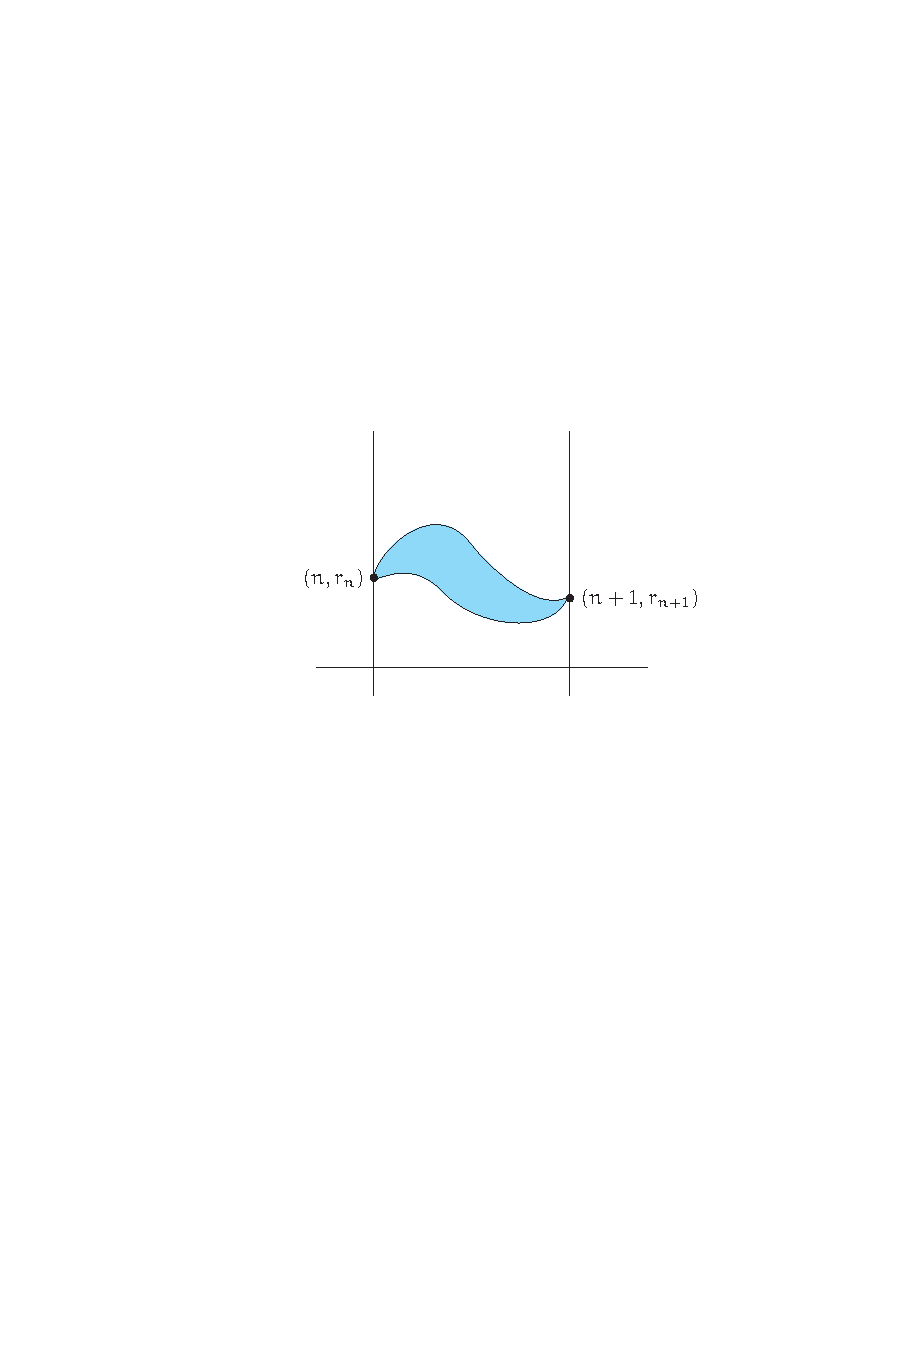
\includegraphics{pictures/quotient-product-no}
\caption{The open subset $A_n$.}
\end{figure}
\end{example}
On the other hand, we have the following result for coproducts.
\begin{proposition}\label{topological space coproduct of quotient map is quotient}
Let $(X_\alpha)_{\alpha\in A}$ and $(Y_\alpha)_{\alpha\in A}$ be topological spaces and for each $\alpha\in A$ let $p_\alpha:X_\alpha\to Y_\alpha$ be a quotient map. Then the map
\[p:\coprod_\alpha X_\alpha\to\coprod_\alpha Y_\alpha\]
which coincides with $p_\alpha$ on $X_\alpha$ is a quotient map.
\end{proposition}
\begin{proof}
Let $V$ be an subset in $\coprod_\alpha Y_\alpha$, then by the definition of $p$, we have
\[p^{-1}(V)=\bigcup_\alpha p_\alpha^{-1}(V\cap Y_\alpha),\]
so $p^{-1}(V)\cap X_\alpha=p_\alpha^{-1}(V\cap Y_\alpha)$. The claim now follows from by the definition of coproduct topology and the fact that each $p_\alpha$ is a quotient map.
\end{proof}
\subsection{Quotient space of a subspace}
Let $X$ be a topological space, $A$ a subspace of $X$, and $\pi$ the canonical map $X\to X/R$ of an equivalence relation $R$ on $X$. Let $R_A$ be the relation induced by $R$ on $A$, and $\pi|_A=\iota\circ\tilde{\pi}\circ\pi_A$ be the canonical decomposition of $\pi|_A$, so that we have a commutative diagram
\[\begin{tikzcd}
A\ar[rrr,bend right=20pt,swap,"\pi|_A"]\ar[r,"\pi_A"]&A/R_A\ar[r,"\tilde{\pi}"]&\pi(A)\ar[r,"\iota"]&X/R
\end{tikzcd}\]
\begin{proposition}\label{topological space quotient topology on subspace iff}
The canonical bijection $\tilde{\pi}:A/R_A\to\pi(A)$ is continuous. Furthermore, the following three statements are equivalent:
\begin{itemize}
\item[(\rmnum{1})] $\tilde{\pi}$ is a homeomorphism.
\item[(\rmnum{2})] Every open subset of $A$ which is saturated with respect to $R_A$ is the intersection with $A$ of an open subset of $X$ which is saturated with respect to $R$.
\item[(\rmnum{3})] Every closed subset of $A$ which is saturated with respect to $R_A$ is the intersection with $A$ of a closed subset of $X$ which is saturated with respect to $R$. 
\end{itemize}
\end{proposition}
\begin{proof}
Note that $A/R_A$ carries the quotient topology induced by $\pi_A$, and $\pi(A)$ carries the subspace topology induced by $X/R$. Now the claim follows from Proposition~\ref{topological space canonical decomposition homeomorphism iff}: if $U$ is an open subset of $A$ which is saturated with respect to $R_A$, and $\tilde{\pi}(U)=\pi(U)$ is the intersection with $\pi(A)$ of an open subset $V$ of $X/R$, then $U$ is the intersection with $A$ of the open subset $\pi^{-1}(V)$ of $X$, which is saturated with respect to $R$; and conversely, if $U$ is the intersection with $A$ of an open subset $W$ which is saturated with respect to $R$, then $\pi(U)$ is the intersection of $\pi(A)$ and $\pi(W)$, which is open in $X/R$.
\end{proof}
\begin{corollary}\label{topological space quotient map on saturated open set is quotient map}
If $A$ is an open (resp. closed) subset of $X$ which is saturated with respect to $R$, then the canonical mapping $\tilde{\pi}:A/R_A\to\pi(A)$ is a homeomorphism.
\end{corollary}
\begin{proof}
If $A$ is open (resp. closed) in $X$ and saturated with respect to $R$, and if $B\sub A$ is open (resp. closed) in $A$ and saturated with respect to $R_A$, then $B$ is open (resp. closed) in $X$ and saturated with respect to $R$.
\end{proof}
\begin{corollary}\label{topological space quotient map on sectioned orbit subspace}
If there is a continuous mapping $\varphi:X\to A$ such that $\varphi(x)\equiv x$ mod $R$ for each $x\in X$, then $\pi(A)=X/R$ and the canonical mapping $\tilde{\pi}:A/R_A\to X/R$ is a homeomorphism.
\end{corollary}
\begin{proof}
Since each equivalence class mod $R$ meets $A$, the canonical image of $\pi(A)$ in $X/R$ is the whole of $X/R$; on the other hand, if $U$ is open in $A$ and is saturated with respect to $R_A$, it follows from the hypothesis that $\varphi^{-1}(U)$ is the set obtained by saturating $U$ with respect to $R$; since $\varphi$ is continuous, $\varphi^{-1}(U)$ is open in $X$. The corollary follows from this fact by virtue of Proposition~\ref{topological space quotient topology on subspace iff}.
\end{proof}
\begin{example}
Let $R$ denote the equivalence relation $x=y$ mod $\Z$ on the real line $\R$ and let $I$ denote the closed interval $[0,1]$; $I$ contains at least one point of each equivalence class mod $R$. The canonical mapping of $I/R_I$ onto the torus $\T$ is a homeomorphism; for if $F$ is closed in $I$ (and hence in $\R$), in order to saturate $F$ with respect to the relation $R$ we have to take the union of the closed sets $F+n$ for all $n\in\Z$, which evidently form a locally finite family, so that their union is closed; the assertion follows from this. We remark that $I/R_I$ is obtained by identifying the points $0$ and $1$ in $I$.
\end{example}
\subsection{Hausdorff condition of quotient spaces}
Typically, to prove that a given quotient space is Hausdorff, one has to resort to the definition. For open quotient maps, however, we have the following criterion.
\begin{proposition}\label{quotient Hausdorff}
Suppose $q:X\to Y$ is an open quotient map. Then $Y$ is Hausdorff if and only if the set $\mathcal{R}:=\{(x_1,x_2):q(x_1)=q(x_2)\}$ is closed in $X\times X$.
\end{proposition}
\begin{proof}
First assume $Y$ is Hausdorff. If $(x_1,x_2)\notin\mathcal{R}$, then there are disjoint neighborhoods $V_1$ of $q(x_1)$ and $V_2$ of $q(x_2)$, and it follows that $q^{-1}(V_1)\times q^{-1}(V_2)$ is a neighborhood of $(x_1,x_2)$ that is disjoint from $\mathcal{R}$. Thus $\mathcal{R}$ is closed. (This implication does not require the assumption that $q$ is open.)\par
Conversely, assume $\mathcal{R}$ is closed. Given distinct points $y_1,y_2\in Y$, choose $x_1,x_2\in X$ such that $q(x_i)=y_i$. Because $(x_1,x_2)\notin\mathcal{R}$, there is a product neighborhood $U_1\times U_2$ of $(x_1,x_2)$ in $X\times X$ that is disjoint from $\mathcal{R}$. Since $q$ is open, $q(U_1)$ and $q(U_2)$ are disjoint neighborhoods of $y_1$ and $y_2$, respectively.
\end{proof}
\begin{corollary}
Suppose $\sim$ is an equivalence relation on a space $X$. If the quotient map $X\to X/$$\sim$ is an open map, then $X/$$\sim$ is Hausdorff if and only if $\sim$ is a closed subset of $X\times X$.
\end{corollary}
\begin{theorem}
Suppose $X$ is a compact Hausdorff space and $q:X\to Y$ is a quotient map. Then the following are equivalent.
\begin{itemize}
\item[(a)] $Y$ is Hausdorff.
\item[(b)] $q$ is a closed map.
\item[(c)] The set $\mathcal{R}=\{(x_1,x_2):q(x_1)=q(x_2)\}$ is closed in $X\times X$.
\end{itemize}
\end{theorem}
\begin{proof}
The implicaton $(a)\Rightarrow(b)$ is immediate by closed map lemma, and $(a)\Rightarrow(c)$ is proved just as in Proposition~\ref{quotient Hausdorff}. Next we prove $(b)\Rightarrow(a)$. Assuming $q$ is a closed map, we begin by showing that its fibers are compact. Every point $y\in Y$ is the image of some $x\in X$, and since $\{x\}$ is a closed subset of $X$, it follows that $\{y\}=q(\{x\})$ is a closed subset of $Y$. Thus by continuity, the fiber $q^{-1}(\{y\})$ is closed in $X$ and hence compact.\par 
To prove that $Y$ is Hausdorff, suppose $y_1$ and $y_2$ are distinct points of $Y$. Then we can prove the disjoint compact subsets $q^{-1}(y_1)$ and $q^{-1}(y_2)$ of $X$ have disjoint neighborhoods $U_1$ and $U_2$, respectively. Define subsets $W_1,W_2\sub Y$ by
\[W_i=Y-q(X-U_i)=\{y\in Y:q^{-1}(y)\sub U_i\}\]
Then $y_i\in W_i$ for each $i$ by construction, and $W_1$ and $W_2$ are disjoint because $U_1$ and $U_2$ are. To complete the proof, the fact that $q$ is closed implies that $W_i$ is open.\par
Finally, we prove $(c)\Rightarrow(a)$. Assuming that $\mathcal{R}$ is closed, we start again by showing that $q$ has compact fibers. Given $y\in Y$ and $x\notin q^{-1}(y)$, let $x_1$ be any point in $q^{-1}(y)$. (Such a point exists because $q$ is surjective.) Because $\mathcal{R}$ is closed and $(x,x_1)\notin\mathcal{R}$, there is a product neighborhood $U_1\times U_2$ of $(x_1,x)$ that is disjoint from $\mathcal{R}$. It follows that $U_2$ is a neighborhood of $x$ disjoint from $q^{-1}(y)$, for if $x_2$ were a point in $U_2\cap q^{-1}(y)$, then $(x_1,x_2)$ would lie in $\mathcal{R}\cap(U_1\times U_2)$, which is empty. Thus $q^{-1}(y)$ is closed in $X$ and hence compact.\par
Now let $y_1$ and $y_2$ be distinct points in $Y$. As before, there are disjoint open
subsets $U_1\sups q^{-1}(y_1)$ and $U_2\sups q^{-1}(y_2)$, and we define $W_1,W_2$ as before. These are disjoint sets containing $y_1$ and $y_2$, respectively, so we need only show they are open. Because $q$ is a quotient map, $W_i$ is open if and only if $q^{-1}(W_i)$ is open, which is the case if and only if $X-q^{-1}(W_i)$ is closed. From the definition of $W_i$, it follows that
\begin{align*}
X-q^{-1}(W_i)&=\{x\in X:q(x)\notin W_i\}=\{x\in X:q^{-1}(q(x))\nsubseteq U_i\}\\
&=\{x\in X:\text{$\exists x\in X-U_i$ such that $q(x)=q(x')$}\}\\
&=\pi_1(\mathcal{R}\cap(X\times X-U_i))
\end{align*}
where $\pi_1:X\times X\to X$ is the projection on the first factor. Observe that $\pi_1$ is a closed map by the closed map lemma. Our hypothesis on $\mathcal{R}$ implies that $\mathcal{R}\cap(X\times X-U_i)$ is closed in $X\times X$, and therefore $X-q^{-1}(W_i)$ is closed in $X$.
\end{proof}
\subsection{Direct limit of topological spaces}
Let $(X_\alpha)_{\alpha\in I}$ be a family of sets, and let $X$ be the set which is the coproduct of the $X_\alpha$. We shall identify each $X_\alpha$ with a subset of $X$ by means of the canonical injection $\iota_\alpha:X_\alpha\to X$.\par
Let $R$ be an equivalence relation on $X$ such that each equivalence class of $R$ has at most one element in each $X_\alpha$; for each pair of indices $(\alpha,\beta)$ let $A_{\alpha\beta}$ be the subset of $X_\alpha$ consisting of the elements $x$ for which there is an element $y\in X_{\beta}$ which belongs to the equivalence class of $x$. Clearly to each $x\in A_{\alpha\beta}$ there is a unique $y\in X_\beta$ which is congruent to $x$ mod $R$; the mappings $\phi_{\beta\alpha}:A_{\alpha\beta}\to A_{\beta\alpha}$ so defined satisfy the following conditions:
\begin{itemize}
\item[(a)] For each $\alpha\in I$, $\phi_{\alpha\alpha}$ is the identity mapping of $A_{\alpha\alpha}=X_\alpha$.
\item[(b)] For each triple of indices $(\alpha,\beta,\gamma)$ of $I$ and each $x\in A_{\alpha\beta}\cap A_{\alpha\gamma}$, we have $\phi_{\beta\alpha}(x)\in A_{\beta\gamma}$ and $\phi_{\gamma\alpha}(x)=\phi_{\gamma\beta}(\phi_{\beta\alpha}(x))$.
\end{itemize}

Conversely, suppose that for each pair of indices $(\alpha,\beta)$ we are given a subset $A_{\alpha\beta}$ of $X_\alpha$ and a mapping $\phi_{\beta\alpha}:A_{\alpha\beta}\to A_{\beta\alpha}$ satisfying the conditions (a) and (b) above. It follows first of all from (b) applied to the triples $(\alpha,\beta,\alpha)$ and $(\beta,\alpha,\beta)$ that $\phi_{\alpha\beta}\circ\phi_{\beta\alpha}$ (resp. $\phi_{\beta\alpha}\circ\phi_{\alpha\beta}$) is the restriction of $\phi_{\alpha\alpha}$ (resp. $\phi_{\beta\beta}$) to $A_{\alpha\alpha}$ (resp. $A_{\beta\beta}$); hence we deduce from (a) that $\phi_{\beta\alpha}$ and $\phi_{\alpha\beta}$ are bijections which are mverses of each other. Now let $R$ be the relation "there exist $\alpha,\beta$ such that $x\in A_{\alpha\beta}$, $y\in A_{\beta\alpha}$ and $y=\phi_{\beta\alpha}(x)$". It follows from (a) and what precedes that $R$ is reflexive and symmetric; on the other hand, if 
\[x\in A_{\alpha\beta},\quad y=\phi_{\beta\alpha}(x)\in A_{\beta\alpha}\cap A_{\beta\gamma},\quad z=\phi_{\gamma\beta}(y)\in A_{\gamma\beta},\]
then also $x=\phi_{\alpha\beta}(y)$ and by (b) we have $z=\phi_{\gamma\alpha}(x)$; thus $R$ is transitive, and so is an equivalence relation on $X$. It follows also from (a) and from the definition of $R$ that each equivalence class mod $R$ has at most one element in each of the sets $X_\alpha$, and that $A_{\alpha\beta}$ is the set of all $x\in X_\alpha$ for which there is an element $y\in X_\beta$ congruent to $x$ mod $R$. We say that the quotient set $X/R$ is obtained by pasting together the $X_\alpha$ along the $A_{\alpha\beta}$ by means of the bijections $\phi_{\beta\alpha}$. If $\pi:X\to X/R$ is the canonical mapping, the restriction of $\pi$ to each $X_\alpha$ is a bijection of $X_\alpha$ onto $\pi(X_\alpha)$.\par
Now suppose that each $X_\alpha$ is a topological space, and let $\mathcal{T}_\alpha$ be its topology. Let $\mathcal{T}$ be the finest topology on the set $X/R$ for which the mappings $\pi\circ\iota_\alpha$ are continuous; then $\mathcal{T}$ is the quotient by $R$ of the topology on $X$ which is the coproduct of the topologies $\mathcal{T}_\alpha$. We say that the topological space $X/R$ (with the topology $\mathcal{T}$) is obtained by pasting together the topological spaces $X_\alpha$ along the $A_{\alpha\beta}$ by means of the bijections $\phi_{\beta\alpha}$. The open (resp. closed) subsets of $X/R$ are thus the canonical images of the subsets $B$ of $X$ which are saturated with respect to $R$ and are such that $B\cap X_\alpha$ is open (resp. closed) in $X_\alpha$ for each $\alpha\in I$.\par
Since the restriction of $\pi$ to each $X_\alpha$ is a bijection onto the subset $\pi(X_\alpha)$ of $X/R$, we can transport the topology $\mathcal{T}_\alpha$ to $\pi(X_\alpha)$ by means of this bijection, so that $\pi(X_\alpha)$ carries a topology $\widetilde{\mathcal{T}}_\alpha$ and the topology $\mathcal{T}$ on $X/R$ is the finest for which the canonical injections $\pi(X_\alpha)\to X/R$ are continuous. In general, the topology induced by $\mathcal{T}$ on $\pi(X_\alpha)$ is coarser than $\widetilde{\mathcal{T}}_\alpha$, but not identical with the latter; even if the $\phi_{\beta\alpha}$ are homeomorphisms. However, it follows from Proposition~\ref{topological space pasting topology} that, with the preceding notation:
\begin{proposition}
Suppose that the $\phi_{\beta\alpha}$ are homeomorphisms and that each $A_{\alpha\beta}$ is open (resp. closed) in $X_\alpha$; then each $\pi(X_\alpha)$ is open (resp. closed) in $X/R$ and the restriction of $\pi$ to $X_\alpha$ is a homeomorphism of $X_\alpha$ onto the subspace $\pi(X_\alpha)$ of $X/R$.
\end{proposition}
\section{Product of topological spaces}
\subsection{Product spaces}
\begin{definition}
Given a family $(X_i)_{i\in I}$ of topological spaces, the \textbf{product space} of this family is the product set $X=\prod_{i\in I}X_i$ with the initial topology induced by the projections $\pi_i:X\to X_i$. The spaces $X_i$ are called the factors of $X$.
\end{definition}
By virtue of Proposition~\ref{topological space initial topology definition}, the product topology on $X$ has as a base the set of finite intersections of sets of the form $\pi_i^{-1}(U_i)$, where $U_i$ is open in $X_i$; these sets are products $\prod_{i\in I}U_i$, where $U_i$ is open in $X_i$ for each $i$ and $U_i=X_i$ for all but a finite number of indices These sets will be called \textbf{elementary sets}.\par
If $\mathcal{B}_i$ is a base of the topology of $X_i$ for each $i\in I$, it is clear that the elementary sets $\prod_iB_i$ such that $B_i=X_i$ for all but finitely many indices form another base of the product topology. The elementary sets of this type which contain a given point $x\in X$ thus form a fundamental system of neighbourhoods of $x$.\par
If $I$ is a finite set, the construction of the product topology from the topologies of the factors $X_i$ is simpler: the elementary sets are just products $\prod_{i\in I}U_i$ where $U_i$ is any open subset of $X_i$ for each $i\in I$.
\begin{example}
The product $\R^n$ of $n$ spaces identical with the real line $\R$ is called real number space of $n$ dimensions; $\R^2$ is also called the real plane. Likewise, starting from the rational line $\Q$, we define the rational number space of $n$ dimensions $\Q^n$ (rational plane for $n=2$). The topology of the space $\R^n$ has as a base the set of all products of $n$ open intervals in $\R$, which are called open boxes of $n$ dimensions. The open boxes which contain a point $x\in\R^n$ form a fundamental system of neighbourhoods of this point. Likewise the products of $n$ closed intervals in $\R$ are called closed boxes of $n$ dimensions. The closed boxes to which $x$ is interior also form a fundamental system of neighbourhoods of $x$. There are analogous results for $\Q^n$.
\end{example}
\begin{proposition}\label{topological space map into product continuous iff}
Let $f=(f_i)$ be a mapping of a topological space $Y$ into a product space $X=\prod_{i\in I}X_i$. Then $f$ is continuous at a point $y\in Y$ if and onlY if $f_i$ is continuous at $y$ for each $i\in I$.
\end{proposition}
\begin{proof}
Since $f_i=f\circ\pi_i$, this is a special case of Proposition~\ref{topological space initial topology definition}.
\end{proof}
\begin{corollary}\label{topological product map continuous iff}
Let $(X_i)_{i\in I}$ and $(Y_i)_{i\in I}$ be two families of topological spaces with tke same set of indices. For each $i\in I$, let $f_i$ be a mapping of $X_i$ into $Y_i$. In order that the product mapping $f:(x_i)\to(f_i(x_i))$ should be continuous at a point $a=(a_i)$, it is necessary and sufficient that $f_i$ is continuous at $a_i$ for each $i\in I$.
\end{corollary}
\begin{proof}
The map $f$ can be written as $x\mapsto(f_i(\pi_i(x)))$, so that by Proposition~\ref{topological space map into product continuous iff} the condition is sufficient. Conversely, for each $j\in I$ let $g_j$ be the mapping of $X_j$ into $\prod_{i\in I}X_i$ such that $\pi_j(g_j(x))=x_j$ and $\pi_i(g_j(x))=a_i$ for $i\neq j$. Then $g_j$ is continuous at the point $a_j$, by Proposition~\ref{topological space map into product continuous iff}. Since $f_j=\pi_j\circ f\circ g_j$, it follows that if $f$ is continuous at $a$ then $f_j$ is continuous at $a_j$.
\end{proof}
\begin{corollary}
Let $X$, $Y$ be two topological spaces. In order that a mapping $f:X\to Y$ should be continuous it is necessary and sufficient that the mapping $g:x\mapsto(x,f(x))$ is a homeomorphism of $X$ onto the graph $\Gamma(f)$ (considered as a subspace of the product space $X\times Y$).
\end{corollary}
\begin{proof}
Since $f=\pi_2\circ g$, the condition is sufficient. It is also necessary, for if $f$ is continuous, then $g$ is bijective and continuous (Proposition~\ref{topological space map into product continuous iff}) and the inverse of $g$ is the restriction of $\pi_1$ to $\Gamma(f)$, which is continuous.
\end{proof}
\begin{proposition}[\textbf{Associativity of topological products}]
Let $(X_i)_{i\in I}$ be a family of topological spaces, $(I_\kappa)_{\kappa\in K}$ a partition of the set $I$, and for each $\kappa\in K$ let $X_\kappa=\prod_{i\in I_\kappa}X_i$. Then the canonical mapping of the product space $\prod_{i\in I}X_i$ onto the product space $\prod_{\kappa\in K}X_\kappa$ is a homeomorphism.
\end{proposition}
\begin{proof}
This is a special case of the transitivity of initial topologies.
\end{proof}
\begin{corollary}
Let $\sigma\in\mathfrak{S}_I$ be a permutation of the set $I$. Then the mapping $(x_i)\mapsto(x_{\sigma(i)})$ is a homeomorphism of $\prod_{i\in I}$ onto $\prod_{i\in I}X_{\sigma(i)}$.
\end{corollary}
\begin{proof}
Take $K=I$ and $I_i=\{\sigma(i)\}$ in the previous proposition.
\end{proof}
Finally, we show that, the general concept of initial topologies can be defined using product spaces and product topology.
\begin{proposition}\label{topological space initial topology defined by product}
Let $X$ be a set, $(Y_i)_{i\in I}$ a family of topological spaces, and for each $i\in I$ let $f_i$ be a mapping of $X$ into $Y_i$. Let $f$ be the mapping $x\mapsto(f_i(x))$ of $X$ into $Y=\prod_{i\in I}Y_i$. Then the initial topology on $X$ induced by $(f_i)$ is the inverse image under $f$ of the topology induced on $f(X)$ by the product topology on $Y$.
\end{proposition}
\begin{proof}
This is another application of the transitivity of initial topologies.
\end{proof}
\begin{corollary}
For each $i\in I$ let $A_i$ be a subspace of $X_i$. Then the topology induced on $A=\prod_{i\in I}A_i$ by the product topology on $\prod_{i\in I}X_i$ is the product of the topologies of the subspaces $A_i$.
\end{corollary}
\begin{proof}
Let $\iota_i$ be the canonical injection $A_i\to X_i$ and apply Proposition~\ref{topological space initial topology defined by product} to the mappings $f_i=\iota_i\circ\pi_i$.
\end{proof}
There is another topology on the product space $X=\prod_{i\in I}X_i$ called the box topology, whose open sets are defined to be the product of open subsets in $X_i$. The box topology turns out to have too many open sets, for example, Proposition~\ref{topological space map into product continuous iff} does not hold for it.
\begin{example}
Consider $\R^\omega$, the countably infinite product of $\R$ with itself. That is, $\R^\omega=\prod_{n\in\Z_+}X_n$, where $X_n=\R$ for each $n$. Let us define a function $f:\R\to\R^\omega$ by the equation
\[f(x)=(x,x,\dots,x,\dots).\]
Each of the coordinate functions $f_n:\R\to\R$ is continuous; therefore, the function $f$ is continuous if $\R^\omega$ is given the product topology. But $f$ is not continuous if $\R^\omega$ is given the box topology. Consider, for example, the basis element
\[B=\prod_{n\in\Z_+}(-1/n,1/n),\]
for the box topology. We assert that $f^{-1}(B)$ is not open in $\R$: If $f^{-1}(B)$ contains some interval $(-\delta,\delta)$ about the point $0$, then we must have $(-\delta,\delta)\sub(-1/n,1/n)$ for each $n$, whence $\delta=0$, a contradiction.
\end{example}
\subsection{Sections and projections}
\begin{proposition}\label{topological space section map homeomorphism}
Let $X$ and $Y$ be topological spaces. Then
\begin{itemize}
\item[(a)] for each $a\in X$, the map $y\mapsto(a,y)$ is a homeomorphism from $Y$ to the subspace $\{a\}\times Y$ of $X\times Y$;
\item[(b)] for each $b\in Y$, the map $x\mapsto(x,b)$ is a homeomorphism from $X$ to the subspace $X\times\{b\}$ of $X\times Y$.
\end{itemize}
\end{proposition}
\begin{proof}
Since $\pi_Y$, restricted to $\{a\}\times Y$, is a continuous inverse of the given map in (a), this is a particular case of Corollary~\ref{topological product map continuous iff} applied to the constant function $x\mapsto a$. The same proof applies to (b).
\end{proof}
Note that the mapping $y\mapsto(a,y)$ is a continuous section with respect to the equivalence relation $\pi_X(z)=\pi_X(z')$ in $X\times Y$; the quotient space of $X\times Y$ by this equivalence relation is therefore homeomorphic to $Y$.
\begin{corollary}\label{topological space section of open close}
The section $A(x)$ of an open (resp. closed) set $A$ of the product $X\times Y$ at an arbitrary point $x\in X$ is open (resp. closed) in $Y$.
\end{corollary}
Using Proposition~\ref{topological product map continuous iff}, we also get the following useful fact.
\begin{proposition}\label{topological space projection is open}
The projection of $X\times Y$ onto either factor is an open map.
\end{proposition}
\begin{proof}
Let $U$ be open in $X\times Y$, then we have 
\[\pi_X(U)=\bigcup_{y\in Y}U(y),\quad\pi_Y(U)=\bigcup_{x\in X}U(x),\]
and the proposition follows from the Corollary~\ref{topological space section of open close}.
\end{proof}
Note that the projection of a closed subset of $X\times Y$ onto a factor need not be closed. For example, in the real plane $\R^2$, the hyperbola whose equation is $xy=1$ is a closed set, but both its projections are equal to the complement of the point $0$ in $\R$. and this is not a closed set.
\begin{proposition}\label{topological space continuous is separately conitnuous}
Let $X$, $Y$ and $Z$ be three topological spaces, $f$ a mapping of the product space $X\times Y$ into $Z$. If $f$ is continuous at the point $(a,b)\in X\times Y$, then the partial mapping $y\mapsto f(a,y)$ of $Y$ into $Z$ is continuous at the point $b$.
\end{proposition}
\begin{proof}
This mapping is the composition of $f$ and the mapping $y\mapsto(a,y)$; hence the result follows from Proposition~\ref{topological space section map homeomorphism}.
\end{proof}
Proposition~\ref{topological space continuous is separately conitnuous} is often expressed by saying that a continuous function of two variables is continuous with respect to each of them separately.
\begin{example}
It is possible for all the partial mappings determined by a map $f:X\times Y\to Z$ to be continuous without $f$ being continuous. For example if $f$ is the mapping of the real plane $\R^2$ into $\R$ defined by
\[f(x,y)=\begin{cases}
\dfrac{xy}{x^2+y^2}&(x,y)\neq(0,0),\\
0&(x,y)=(0,0).
\end{cases}\]
Then all the partial mappings are continuous; but $f$ is not continuous at $(0,0)$.
\end{example}
\begin{proposition}\label{topological space closure of product subspace}
In a product space $\prod_{i\in I}X_i$ the closure of a product of sets $\prod_{i\in I}A_i$ is the same as the product $A_i$ of their closures.
\end{proposition}
\begin{proof}
Suppose that $a=(a_i)$ lies in the closure of $\prod_{i\in I}A_i$; then for each $j\in I$, $a_j=\pi_j(a)$ is in the closure of $A_j$ because of the continuity of $\pi_j$ and therefore $a\in\prod_{i\in I}\widebar{A}_i$. Conversely, let $b=(b_i)\in\prod_{i\in I}\widebar{A}_i$ and let $\prod_{i\in I}U_i$ be any elementary set containing $b$; for each $i\in I$, $U_i$ contains a point $x_i\in A_i$; hence $\prod_{i\in I}U_i$ contains the point $(x_i)\in\prod_{i\in I}A_i$ and therefore $b$ lies in the closure of $\prod_{i\in I}A_i$.
\end{proof}
\begin{corollary}
A product $\prod_{i\in I}A_i$ of non-empty sets is closed in the product space $\prod_{i\in I}$ if and only if $A_i$ is closed in $X_i$ for each $i\in I$.
\end{corollary}
\begin{remark}
Note that if $I$ is finite, a product $\prod_{i\in I}A_i$ is open provided that $A_i$ is open in $X_i$ for each $i\in I$; but this is no longer so if $I$ is infinite.
\end{remark}
As an application of Proposition~\ref{topological space closure of product subspace}, we give a certain family of dense subsets in a product space.
\begin{proposition}\label{topological space dense subset in product}
Let $a=(a_i)$ be any point of a product space $X=\prod_{i\in I}X_i$; then the set $D$ of points $x\in X$ such that $\pi_i(x)=a_i$ except for a finite number of indices $i$ is dense in $X$.
\end{proposition}
\begin{proof}
For each $x\in X$ and each elementary set $U=\prod_{i\in I}U_i$ which contains $x$, we have $U_i=X_i$ except for indices $i$ belonging to a finite subset of $J$; if we take $y_i=x_i$ for $i\notin J$ and $y_i=a_i$ for $i\in J$, it is clear that $y=(y_i)\in D$ and $y\in U$; hence the result.
\end{proof}
\subsection{Inverse limit of topological spaces}
Let $I$ be a partially ordered (but not necessarily directed) set, in which the order relation is written as $\preceq$. For each $\alpha\in I$, let $X_\alpha$ be a topological space, and for each pair $(\alpha,\beta)$ such that $\alpha\preceq\beta$ let $f_{\alpha\beta}$ be a mapping of $X_\beta$ into $X_\alpha$. We say that $(X_\alpha,f_{\alpha\beta})$ is an inverse system of topological spaces if:
\begin{itemize}
\item[(a)] $(X_\alpha,f_{\alpha\beta}$) is an inverse system of sets;
\item[(b)] Each $f_{\alpha\beta}$ is continuous. 
\end{itemize} 
Let $X$ denote the set $\llim X_\alpha$ and for each $\alpha\in I$ let $f_\alpha$ be the canonical mapping $X\to X_\alpha$; then the initial topology induced by the $f_\alpha$'s is said to be the inverse limit (with respect to the $f_{\alpha\beta}$) of the topologies of the $X_\alpha$ and the set $X$ with this topology is called the inverse limit of the inverse system of topological spaces $(X_\alpha,f_{\alpha\beta})$. Whenever we speak of $\llim X_\alpha$ as a topological space, it is always to be understood that the topology of this space is the inverse limit of the topologies of the $X_\alpha$ unless the contrary is expressly stated.\par
The set $X$ is the subset of the product $\prod_{\alpha}X_\alpha$ consisting of those points $x$ such that
\[\pi_\alpha(x)=f_{\alpha\beta}(\pi_\beta(x)).\]
whenever $\alpha\preceq\beta$. It follows from Proposition~\ref{topological space initial topology defined by product} that the inverse limit of the topologies of the $X_\alpha$ is the same as the topology induced on $X$ by the topology of the product space $\prod_\alpha X_\alpha$. If, for each $\alpha\in I$, $A_\alpha$ is a subspace of $X_\alpha$ such that the $(A_\alpha,f_{\alpha\beta}|_{A_\beta})$ form an inverse system of subsets of the $X_\alpha$, then it is clear that the topological space $\llim A_\alpha$ is a subspace of $\llim X_\alpha$.\par
Let $(Y_\alpha,g_{\alpha\beta})$ be another inverse system of topological spaces indexed by the same set $I$, and for each $\alpha\in I$ let $\varphi_\alpha:X_\alpha\to Y_\alpha$ be a continuous mapping such that $(\varphi_\alpha)$ is an inverse system of mappings; then $\varphi=\llim \varphi_\alpha$ is a continuous mapping of $X=\llim X_\alpha$ into $Y=\llim Y_\alpha$. For if $g_\alpha$ is the canonical mapping $Y\to Y_\alpha$, we have $g_\alpha\circ\varphi=\varphi_\alpha\circ f_\alpha$, so that $g_\alpha\circ\varphi$ is continuous for each $\alpha\in I$, and so $\varphi$ is continuous.\par
Finally, suppose $I$ is a directed set, and let $J$ be a cofinal subset of $I$; let $\widetilde{X}$ be the inverse limit of the inverse system of topological spaces $(X_\alpha,f_{\alpha\beta})_{\alpha,\beta\in J}$. Then the canonical bijection $\psi:X\to\widetilde{X}$ is a homeomorphism. For we have $\pi_\alpha(\psi(x))=\pi_\alpha(x)$ for each $\alpha\in J$, hence $\psi$ is continuous; and if $\phi$ is the inverse of $\psi$, then for each $\alpha\in I$ there exists $\beta\in J$ such that $\alpha\preceq\beta$, and therefore $\pi_\alpha(\phi(z))=f_{\alpha\beta}(\pi_\beta(z))$, which shows that $\phi$ is continuous, since the $f_{\alpha\beta}$'s are continuous.
\begin{proposition}\label{topological space inverse limit cofinal system base}
Let $I$ be a directed set and $J$ a cofinal subset of $I$. Let $(X_\alpha,f_{\alpha\beta})$ be an inverse system of topological spaces indexed by $I$; let $X=\llim X_\alpha$ and let $f_\alpha:X\to X_\alpha$ be the canonical mapping. Then the family of sets $f_\alpha^{-1}(U_\alpha)$, where $\alpha$ runs through $J$ and $U_\alpha$ runs through a base $\mathcal{B}_\alpha$ of the topology of $X_\alpha$ for each $\alpha\in J$, is a base of the topology of $X$.
\end{proposition}
\begin{proof}
We know that the finite intersections of sets of the form $f_\alpha^{-1}(U_\alpha)$, $\alpha\in I$, $U_\alpha$ open in $X_\alpha$ form a base of the topology of $X$. If $\alpha_1,\dots,\alpha_n$ is a finite family of indices of $I$, then there exists $\beta\in J$ such that $\alpha_i\preceq\beta$ for $1\leq i\leq n$; hence $f_{\alpha_i}=f_{\alpha_i\beta}\circ f_\beta$; if we put $U_\beta=\bigcap_{i=1}^{n}f_{\alpha_i\beta}^{-1}(U_{\alpha_i})$, then
\[f_\beta^{-1}(U_\beta)=\bigcap_{i=1}^{n}f_{\alpha_i}^{-1}(U_{\alpha_i}).\]
But $U_\beta$ is open and is therefore a union of sets belonging to $\mathcal{B}_\beta$. Hence the result.
\end{proof}
\begin{corollary}
Let $A$ be a subset of $X$ and let $A_\alpha=f_\alpha(A)$ for each $\alpha\in I$. Then:
\begin{itemize}
\item[(a)] The $A_\alpha$ (resp. the $\widebar{A}_\alpha$) form an inverse system of subsets of the $X_\alpha$, and $\widebar{A}=\bigcap_{\alpha}f_\alpha^{-1}(\widebar{A}_\alpha)=\llim\widebar{A}_\alpha$.
\item[(b)] If $A$ is closed in $X$ then $A=\llim A_\alpha=\llim \widebar{A}_\alpha$.
\end{itemize}
\end{corollary}
\begin{proof}
The first assertion of (a) follows from the relations $f_\alpha=f_{\alpha\beta}\circ f_\beta$ for $\alpha\preceq\beta$ and from the continuity of the $f_\alpha$. Let $A'$ denote $\bigcap_{\alpha}f_\alpha^{-1}(\widebar{A}_\alpha)$, then it is clear that $A'$ is closed and contains $A$, so that $\widebar{A}\sub A'$. Conversely, let $x\in A'$; we have to show that $x$ lies in the closure of $A$. By virtue of Proposition~\ref{topological space inverse limit cofinal system base}, it is enough to prove that every neighbourhood of $x$ which is of the form $f_\alpha^{-1}(U_\alpha)$, with $\alpha\in I$ and $U_\alpha$ open in $X_\alpha$ meets $A$. Now, by hypothesis, $f_\alpha(x)\in U_\alpha$, and since $f_\alpha(x)\in \widebar{A}_\alpha$ we have $U_\alpha\cap A_\alpha\neq\emp$, which means $A\cap f_\alpha^{-1}(A_\alpha)\neq\emp$.\par
To establish (b) it is enough to remark that, without any restriction on $A$, we have $A\sub\llim A_\alpha\sub\llim\widebar{A}_\alpha$; now if $A$ is closed, then from (a) we have $A=\llim\widebar{A}_\alpha$, so the claim follows.
\end{proof}
\begin{example}
Let $I$ be a directed set and $(X_\alpha)_{\alpha\in I}$ a family of subsets of a set $Y$, such that $X_\alpha\sups X_\beta$ whenever $\alpha\preceq\beta$. For each $\alpha\in I$ let $\mathcal{T}_\alpha$ be a topology on $X_\alpha$ such that $\mathcal{T}_\alpha$ is finer than the topology induced on $X_\alpha$ by $\mathcal{T}_\beta$ whenever $\alpha\preceq\beta$. If we take $f_{\alpha\beta}$ to be the canonical injection $X_\beta\to X_\alpha$ for $\alpha\preceq\beta$, then $\llim X_\alpha$ may be identified canonically with the intersection $X$ of the $X_\alpha$, with the topology which is the least upper bound of the topologies induced on $X$ by the $\mathcal{T}_\alpha$.
\end{example}
\section{Connectedness}
\subsection{Connected spaces}
The definition of connectedness for a topological space is a quite natural one. One says that a space can be "separated" if it can be broken up into two "globs"--disjoint open sets. Otherwise, one says that it is connected. From this simple idea much follows.
\begin{definition}
Let $X$ be a topological space. A \textbf{separation} of $X$ is a pair $U$, $V$ of disjoint nonempty open subsets of $X$ whose union is $X$. The space $X$ is said to be connected if there does not exist a separation of $X$.
\end{definition}
Connectedness is obviously a topological property, since it is formulated entirely in terms of the collection of open sets of $X$. Said differently, if $X$ is connected, so is any space homeomorphic to $X$.\par
For a subspace $A$ of a topological space $X$, there is another useful way of formulating the definition of connectedness:
\begin{lemma}\label{topological space connectedness of subspace}
If $A$ is a subspace of $X$, a separation of $A$ is a pair of disjoint nonempty sets $U$ and $V$ whose union is $A$, neither of which contains a limit point of the other. The space $A$ is connected if there exists no separation of $A$.
\end{lemma}
\begin{proof}
Suppose first that $U$ and $V$ form a separation of $A$. Then $U$ is both open and closed in $A$. The closure of $U$ in $A$ is the set $\widebar{U}\cap A$ (where $\widebar{U}$ as usual denotes the closure of $U$ in $X$). Since $U$ is closed in $A$, $U=\widebar{U}\cap A$; or to say the same thing, $\widebar{U}\cap V=\emp$. Since $\widebar{U}$ is the union of $U$ and its limit points, $V$ contains no limit points of $U$. A similar argument shows that $U$ contains no limit points of $V$.\par
Conversely, suppose that $U$ and $V$ are disjoint nonempty sets whose union is $A$, neither of which contains a limit point of the other. Then $\widebar{U}\cap V=\emp$ and $\widebar{V}\cap U=\emp$; therefore, we conclude that $\widebar{U}\cap A=U$ and $\widebar{V}\cap A=V$. Thus both $U$ and $V$ are closed in $A$, and since $U\cup V=A$, they are open in $A$ as well.
\end{proof}
\begin{example}
Let $X$ denote a two-point space in the indiscrete topology. Obviously there is no separation of $X$, so $X$ is connected.
\end{example}
\begin{example}
Let $A$ denote the subspace $[-1,0)\cup(0,1]$ of the real line $\R$. Each of the sets $[-1,0)$ and $(0,1]$ is nonempty and open in $A$ (although not in $\R$); therefore, they form a separation of $A$. Alternatively, note that neither of these sets contains a limit point of the other. (They do have a limit point $0$ in common, but that does not matter.)
\end{example}
\begin{example}
A subspace of $\mathbb{R}$ is connected if and only if it is an interval: Clearly intervals are connected. Now suppose $X$ is connected in $\R$ and is not an interval. Then there are $x,y\in X$ and $z\notin X$ such that $x<z<y$. We set
\[O_1=(-\infty,z)\cap X,\quad O_2=X\cap(z,+\infty)\]
Then $O_1$ and $O_2$ is a separation of $X$, and since $x\in O_1$, $y\in O_2$ they are both nonempty. This is a contradiction since $X$ is connected, hence $X$ is an interval.
\end{example}
\begin{example}
Let $X$ be the subspace $[-1,1]$ of the real line. The sets $[-1,0]$ and $(0,1]$ are disjoint and nonempty, but they do not form a separation of $X$, because the first set is not open in $X$. Alternatively, note that the first set contains a limit point, $0$, of the second. Indeed, there exists no separation of the space $[-1,1]$.
\end{example}
\begin{example}
The rationals $\Q$ are not connected. Indeed, the only connected subspaces of $\Q$ are the one-point sets: If $A$ is a subspace of $\Q$ containing two points $p$ and $q$, one can choose an irrational number $\alpha$ lying between $p$ and $q$, and write $A$ as the union of the open sets
\[A=(A\cap(-\infty,\alpha))\cup(A\cap(\alpha,+\infty)).\]
\end{example}
\begin{example}
Consider the following subset of the plane $\R^2$:
\[X=\{(x,y)\in\R^2:y=0\}\cup\{(x,y):\text{$x>0$ and $xy=1$}\}.\]
Then $X$ is not connected; indeed, the two indicated sets form a separation of $X$ because neither contains a limit point of the other.
\end{example}
We have given several examples of spaces that are not connected. How can one construct spaces that are connected? We shall now prove some useful properties of connectedness, and later use them to construct connected topological spaces. First, we give another criterion for connectedness which is quite simple but useful.
\begin{proposition}\label{topological space connected iff continuous map to {0,1}}
A topological space $X$ is connected if and only if every continuous map $f:X\to\{0,1\}$ is constant, with the space $\{0,1\}$ given the discrete topology.
\end{proposition}
\begin{proof}
Clearly if $f$ is not constant then $f^{-1}(0)\cup f^{-1}(1)$ is a separation of $X$. Conversely, if $U$ and $V$ form a separation of $X$ then the characteristic function $\chi_U$ is nonconstant and continuous.
\end{proof}
\begin{proposition}[\textbf{Properties of Connected Spaces}]\label{topological space connected prop}
Let $X$ be a topological space.
\begin{itemize}
\item[(a)] Suppose that $U,V$ are disjoint open subsets of $X$. If $A$ is a connected subset of $X$ contained in $U\cup V$, then either $A\sub U$ or $A\sub V$.
\item[(b)] Suppose $X$ is any space and $A\sub X$ is connected. If $B$ is a subset such that $A\sub B\sub\widebar{A}$, then it is connected. In particular, $\widebar{A}$ is connected.
\item[(c)] Let $\{C_{\alpha}\}_{\alpha\in I}$ be a collection of connected subspaces of $X$ with a point in common. Then $\bigcup_{\alpha\in I}C_\alpha$ is connected.
\item[(d)] Let $\{C_{\alpha}\}_{\alpha\in I}$ be a collection of connected subspaces of $X$ with $C_\alpha\cap C_\beta\neq\emp$ for all $\alpha,\beta\in I$. Then $\bigcup_{\alpha\in I}C_\alpha$ is connected. 
\end{itemize}
\end{proposition}
\begin{proof}
For (a), if $A$ contained points in both $U$ and $V$, then $A\cap U$ and $A\cap V$ would form a separation of $A$. To prove (b), suppose $A$ is connected and $A\sub B\sub\widebar{A}$. Suppose that $B=U\cup V$ is a separation of $B$. By part (a), the set $A$ must lie entirely in $U$ or in $V$; say $A\sub U$. Then $\widebar{A}\sub\widebar{U}$; since $\widebar{U}$ and $V$ are disjoint, $B$ cannot intersect $V$. This contradicts the fact that $V$ is a nonempty subset of $B$.\par
For part (c), let $p$ be a point that is contained in $C_\alpha$ for every $\alpha$, and let $f:\bigcup_\alpha C_\alpha\to\{0,1\}$ be a continuous function. Then $f$ is constant when restricted to each $C_\alpha$, since $C_\alpha$ is connected. Since $C_\alpha$ contains $p$ for each $\alpha$, it then follows that $f$ is constant. This shows $\bigcup_{\alpha}C_\alpha$ is connected. Part (c) can be proved similarly.
\end{proof}
\begin{corollary}
Let $X$ be a topological space and $(A_n)_{n\in\N}$ be an infinite sequence of connected subspaces such that $A_n\cap A_{n+1}\neq\emp$ for all $n\geq 0$. Then the union $\bigcup_nA_n$ is connected.
\end{corollary}
\begin{proof}
By induction on $n$ we see immediately that the set $B_n=\bigcup_{i=1}^{n}A_i$ is connected for all $n$, by Proposition~\ref{topological space connected prop}. The sets $B_n$ have a non-empty intersection; hence their union, equal to $\bigcup_nB_n$, is connected by Proposition~\ref{topological space connected prop}.
\end{proof}
\begin{proposition}\label{topological space connected continuous image}
The image of a connected space under a continuous map is connected.
\end{proposition}
\begin{proof}
Let $f:X\to Y$ be a continuous map; let $X$ be connected. We wish to prove the image space $f(X)$ is connected. Since the map obtained from $f$ by restricting its range to the space is also continuous, it suffices to consider the case that $f$ is surjective. Suppose that $Y=U\cup V$ is a separation of $Y$ into two disjoint nonempty sets open in $Y$. Then $f^{-1}(U)$ and $f^{-1}(V)$ are disjoint sets whose union is $X$; they are open in $X$ because $f$ is continuous, and nonempty because $f$ is surjective. Therefore, they form a separation of $X$, contradicting the assumption that $X$ is connected.
\end{proof}
\begin{corollary}\label{topological space quotient of connected space}
Every quotient space of a connected space is connected.
\end{corollary}
As for Corollary~\ref{topological space quotient of connected space}, we have the following converse.
\begin{proposition}\label{topological space connected if quotient is}
Let $X$ be a topological space and $R$ an equivalence relation on $X$. If the quotient space $X/R$ is connected, and if each equivalence class of $R$ is connected, then $X$ is connected.
\end{proposition}
\begin{proof}
Suppose $X$ is not connected. Then there is a partition of $X$ into two open sets $U$, $V$. The sets $U$, $V$ are saturated with respect to $R$ in view of Proposition~\ref{topological space connected prop}(a). The canonical images of $U$ and $V$ are therefore open sets in $X/R$ and form a partition of $X/R$; this contradicts the assumption that $X/R$ is connected.
\end{proof}
\begin{proposition}\label{topological space connected product iff}
Every product of connected spaces is connected. Conversely, if a product of non-empty spaces is connected, then each of the factors is connected.
\end{proposition}
\begin{proof}
Let $(X_i)_{i\in I}$ be a family of topological spaces and $X=\prod_{i\in I}X_i$. Since the projection $\pi_i:X\to X_i$ is continuous and surjective, if $X$ is connected then so is each $X_i$. Conversely, assume that each $X_i$ is connected and let $f:X\to\{0,1\}$ be a continuous map, where $\{0,1\}$ is given the discrete topology. Let $a=(a_i)$ be any point of $X$, and for each $j\in I$ let $f_j:X_j\to\{0,1\}$ be the partial mapping defined by $f_j(x_j)=f((y_i))$, where $y_j=x_j$ and $y_i=a_i$ for $i\neq j$. Then $f_j$ is continuous, so is constant since $X_j$ is connected. It follows immediately by induction that $f(x)=f(a)$ for all points $x=(x_i)$ such that $x_i=a_i$ for all but finitely many indices of $I$. But these points form a dense subset of $X$ by Proposition~\ref{topological space dense subset in product}. Hence $f$ is continuous on $X$ and constant on a dense subset of $X$, and therefore constant on $X$. But this contradicts the definition of $f$.
\end{proof}
Now that, however, the result of Proposition~\ref{topological space connected product iff} depends on the topology we endow with the product space $\prod_{i\in I}X_i$. If we consider the box topology, it turns out that $\prod_{i\in I}X_i$ may be not connected even though each $X_i$ is.
\begin{example}
Consider the cartesian product $\R^\omega$ in the box topology. We can write $\R^\omega$ as the union of the set $A$ consisting of all bounded sequences of real numbers, and the set $B$ of all unbounded sequences. These sets are disjoint, and each is open in the box topology. For if $x=(x_n)$ is a point of $\R^\omega$, the open set
\[U=\bigcup_{n\in\Z_+}(x_n-1/n,x_n+1/n)\]
consists entirely of bounded sequences if $x$ is bounded, and of unbounded sequences if $x$ if unbounded. Thus, even though $\R$ is connected, $\R^\omega$ is not connected in the box topology.
\end{example}
\begin{example}
The set $\O(n)$ of all real orthogonal $n\times n$ matrices is not connected. The function $O(n)\to \{1,-1\}, A\mapsto\det A$ is continuous and surjective, since we have the formula
\[\det A=\sum_{\sigma\in\mathfrak{S}_n}(\text{sign}\ \sigma)a_{1\sigma(1)}\cdots a_{n\sigma(n)}\]
Since $\{1,-1\}$ has discrete topology, it follows that $\O(n)$ is not connected.
\end{example}
\subsection{Path connectedness}
The theorems of the preceding part show us how to construct new connected spaces out of given ones. But where can we find some connected spaces to start with? The best place to begin is the real line. We shall prove that $\R$ is connected, and so are the intervals and rays in $\R$.
The fact that intervals and rays in $\R$ are connected may be familiar to you from analysis. We prove it again here, in generalized form. It turns out that this fact does not depend on the algebraic properties of $\R$, but only on its order properties. To make this clear, we shall prove the theorem for an arbitrary ordered set that has the order properties of $\R$. Such a set is called a \textbf{linear continuum}.
\begin{definition}
A totally ordered set $L$ having more than one element is called a \textbf{linear continuum} if the following hold:
\begin{itemize}
\item[(a)] $L$ has the least upper bound property.
\item[(b)] If $x<y$, there exists $z$ such that $x<z<y$.
\end{itemize}
\end{definition}
\begin{theorem}
If $L$ is a linear continuum in the order topology, then $L$ is connected, and so are intervals and rays in $L$.
\end{theorem}
\begin{proof}
Recall that a subspace $A$ of $L$ is said to be convex if for every pair of points $a,b$ of $A$ with $a<b$, the entire interval $[a,b]$ of points of $L$ lies in $A$. We prove that if $A$ is a convex subspace of $L$, then $A$ is connected.\par
So suppose that $A$ is the union of the disjoint nonempty sets $U$ and $V$, each of which is open in $A$. Choose $a\in U$ and $b\in V$; suppose for convenience that $a<b$. The interval $[a,b]$ of points of $L$ is contained in $A$. Hence $[a,b]$ is the union of the disjoint sets
\[U_0=U\cap[a,b],\quad V_0=V\cap[a,b]\]
each of which is open in $[a,b]$ in the subspace topology, which is the same as the order topology. The sets $U_0$ and $V_0$ are nonempty because $a\in U_0$ and $b\in V_0$. Thus, $U_0$ and $V_0$ constitute a separation of $[a,b]$. Let $c=\sup U_0$. We show that $c$ belongs neither to $U_0$ nor to $V_0$, which contradicts the fact that $[a,b]$ is the union of $U_0$ and $V_0$.\par
Suppose that $c\in A_0$. Then $c\neq b$, so either $c=a$ or $a<c<b$. But $U_0$ is open in $[a,b]$, so there must be some interval of the form $[c,e)$ contained in $U_0$. Because of order property (b) of the linear continuum $L$, we can choose a point $z$ of $L$ such that $c<z<e$. Then $z\in U_0$, contrary to the fact that $c$ is an upper bound for $U_0$.\par
Suppose that $c\in B_0$. Then $c\neq a$, so either $c=b$ or $a<c<b$. In either case, it follows from the fact that $V_0$ is open in $[a,b]$ that there is some interval of the form $(d,c]$ contained in $V_0$. Since $(c,b]$ does not intersect $U_0$, we see that $(d,b]=(d,c]\cup(c,b]$ does not intersect $U_0$. Again, $d$ is a smaller upper bound on $U_0$ than $c$, contrary to construction.
\end{proof}
\begin{corollary}
The real line $\R$ is connected and so are intervals and rays in $\R$.
\end{corollary}
As an application, we prove the intermediate value theorem of calculus, suitably generalized.
\begin{theorem}[\textbf{Intermediate value theorem}]
Let $f:X\to Y$ be a continuous map, where $X$ is a connected space and $Y$ is an ordered set in the order topology. If $a$ and $b$ are two points of $X$ and if $r$ is a point of $Y$ lying between $f(a)$ and $f(b)$, then
there exists a point $c$ of $X$ such that $f(c)=r$.
\end{theorem}
\begin{proof}
Assume the hypotheses of the theorem. The sets
\[U=f(X)\cap(-\infty,r)\quad\text{and}\quad V=f(X)\cap(r,+\infty)\]
are disjoint, and they are nonempty because one contains $f(a)$ and the other contains $f(b)$. Each is open in $f(X)$, being the intersection of an open ray in $Y$ with $f(X)$. If there were no point $c$ of $X$ such that $f(c)=r$, then $f(X)$ would be the union of the sets $U$ and $V$. Then $U$ and $V$ would constitute a separation of $f(X)$, contradicting the fact that the image of a connected space under a continuous map is connected.
\end{proof}
\begin{example}
One example of a linear continuum different from $\R$ is the ordered square. We check the least upper bound property. (The second property of a linear continuum is trivial to check.)\par
Let $A$ be a subset of $I\times I$; let $\pi_1:I\times I\to I$ be projection on the first coordinate; let $b=\sup\pi_1(A)$. If $b\in\pi_1(A)$, then $A$ intersects the subset $\{b\}\times I$ of $I\times I$. Because $\{b\}\times I$ has the order type of $I$, the set $A\cap (\{b\}\times I)$ will have a least upper bound $(b,c)$, which will be the least upper bound of $A$.\par
If $b\notin\pi_1(A)$, then $(b,0)$ is the least upper bound of $A$; no element of the form $(b',c)$ with $b'<b$ can be an upper bound for $A$, for then $b'$ would be an upper bound for $\pi_1(A)$.
\end{example}
\begin{example}
If $X$ is a well-ordered set, then $X\times[0,1)$ is a linear continuum in the dictionary order. This set can be thought of as having been constructed by "fitting in" a set of the order type of $(0,1)$ immediately following each element of $X$.
\end{example}
Connectedness of intervals in $\R$ gives rise to an especially useful criterion for showing that a space $X$ is connected; namely, the condition that every pair of points of $X$ can be joined by a path in $X$:
\begin{definition}
Given points $x$ and $y$ of the space $X$, a \textbf{path} in $X$ from $x$ to $y$ is a continuous map $p:[0,1]\to X$ of the unit interval in the real line into $X$, such that $p(0)=x$ and $p(1)=y$. A space $X$ is said to be \textbf{path-connected} if every pair of points of $X$ can be joined by a path in $X$.
\end{definition}
It is easy to see that a path-connected space $X$ is connected. Suppose $X=U\cup V$ is a separation of $X$. Let $p:[0,1]\to X$ be any path in $X$. Being the continuous image of a connected set, the set $p([0,1])$ is connected, so that it lies entirely in either $U$ or $V$. Therefore, there is no path in $X$ joining a point of $U$ to a point of $V$, contrary to the assumption that $X$ is path-connected. The converse does not hold: a connected space need not be path-connected.
\begin{example}
Define punctured Euclidean space to be the space $\R^n\setminus\{0\}$, where $0$ is the origin in $\R^n$. If $n>1$, this space is path-connected: Given $x$ and $y$ different from $0$, we can join $x$ and $y$ by the straight-line path between them if that path does not go through the origin. Otherwise, we can choose a point $z$ not on the line joining $x$ and $y$, and take the broken-line path from $x$ to $z$, and then from $z$ to $y$.
\end{example}
\begin{example}
Being a linear continuum, the ordered square is connected. Let $x=(0,0)$ and $y=(1,1)$. We suppose there is a path $p:[0,1]\to I^2_o$ joining $x$ and $y$ and derive a contradiction. The image set $p([0,1])$ must contain every point $(x,y)$ of $I^2_o$, by the intermediate value theorem. Therefore, for each $x\in I$, the set
\[U_x=p^{-1}(\{x\}\times(0,1))\]
is a nonempty subset of $[0,1]$; by continuity, it is open in $[0,1]$. Choose, for each $x\in I$, a rational number $r_x$ belonging to $U_x$. Since the sets $U_x$ are disjoint, the map $x\mapsto r_x$ is an injective mapping of $I$ into $\Q$. This contradicts the fact that the interval $I$ is uncountable.
\end{example}
\begin{example}\label{topologist's sine curve}
Let $S$ denote the following subset of the plane
\[S=\{(x,y):\text{$0<x\leq 1$ and $y=\sin(1/x)$}\}.\]
Because $S$ is the image of the connected set $(0,1]$ under the continuous map $x\mapsto\sin(1/x)$, it is connected. Therefore, its closure $\widebar{S}$ in $\R^2$ is also connected. The set $\widebar{S}$ is a classical example in topology called the \textbf{topologist's sine curve}. It equals the union of $S$ and the vertical interval $\{0\}\times[-1,1]$. We show that $\widebar{S}$ is not path-connected.\par
Suppose there is a path $p:[a,b]\to\widebar{S}$ beginning at the origin and ending at a point of $S$. The set of those $t$ for which $p(t)\in\{0\}\times[-1,1]$ is closed, so it has a largest element $c$. Then $p:[c,b]\to\widebar{S}$ is a path that maps $c$ into the vertical interval $\{0\}\times[-1,1]$ and maps the other points of $[c,b]$ to points of $S$. Without loss of generality, we replace $[c,b]$ with $[0,1]$.\par
Let $p(t)=(x(t),y(t))$. Then $x(0)=0$, while $x(t)>0$ and $y(t)=\sin(1/x(t))$ for $t>0$. We show there is a sequence of points $t_n\to 0$ such that $y(t_n)=(-1)^n$. Then the sequence $y(t_n)$ does not converge, contradicting
continuity of $p$. To find $t_n$, we proceed as follows: Given $n$, choose $u$ with $0<u<x(1/n)$ such that $\sin(1/u)=(-1)^n$. Then use the intermediate value theorem to find $t_n$ with $0<t_n<1/n$ such that $x(t_n)=u$.
\end{example}
\begin{proposition}
Let $X$ be a topological space. Let $\{C_\alpha\}_{\alpha\in I}$ be a collection of path-connected subspaces of $X$ with a point in common. Then $\bigcup_{\alpha}C_\alpha$ is path-connected.
\end{proposition}
\begin{proof}
Let $p\in\bigcap_\alpha C_\alpha$, then for each $x\in \bigcup_\alpha C_\alpha$, there is a path from $x$ to $p$. This shows $\bigcup_\alpha C_\alpha$ is path-connected.
\end{proof}
\begin{proposition}
The image of a path-connected space under a continuous map is path-connected.
\end{proposition}
\begin{proof}
Let $f:X\to Y$ be a continuous map and $X$ be path-connected. Let $a,b\in f(X)$, and choose $x,y\in X$ such that $f(x)=a$, $f(y)=b$. Then if $p:[0,1]\to X$ be a path from $x$ to $y$, then it follows that $f\circ p$ is a path from $a$ to $b$. Therefore $f(X)$ is path-connected. 
\end{proof}
\begin{proposition}\label{topological space path-connected product iff}
Every product of path-connected spaces is path-connected. Conversely, if a product of non-empty spaces is path-connected, then each of the factors is path-connected.
\end{proposition}
\begin{proof}
Let $(X_i)_{i\in I}$ be a family of topological spaces and $X=\prod_{i\in I}X_i$. If $X$ is path-connected, then since $X_i=\pi_i(X)$, we have $X_i$ is path-connected for each $i\in I$. Conversely, assume that each $X_i$ path-connected. Let $x=(x_i)_{i\in I}$, $y=(y_i)_{i\in I}$ be two points in $X$. By assumption, there exist continuous paths $p_i:[0,1]\to X_i$ with $\gamma_i(0)=x_i$ and $\gamma_i(1)=y_i$. By definition of product, there exists a unique continuous $p:[0,1]\to X$ such that $\pi_i\circ\gamma=\gamma_i$ for all $i\in I$. That makes $p$ a path from $x$ to $y$, so $X$ is path-connected.
\end{proof}
\begin{example}
Let $\Omega$ be the first uncountable ordinal, and we use $S_\Omega$ to denote the set $\Omega$ together with the order topology. As a set, $S_\Omega$ consists of all countable ordinals. Let $L$ denote the ordered set $S_\Omega\times[0,1)$ in the dictionary order, with its smallest element deleted. The set $L$ is a classical example in topology called the \textbf{long line}. We now show that $L$ is path-connected.\par
Pick any two points $x=(\alpha,s)$ and $y=(\beta,t)$ on the long line, with $x<y$. If $\alpha=\beta$, then $s<t$ and the long line interval $[x,y]$ is readily homeomorphic to the real interval $[s,t]$, so $x,y$ are connected by a path. Otherwise, since $\alpha$ and $\beta$ are countable ordinals, the long line interval $[x,y]$ is the union of (in increasing order) $\alpha\times[s,1)$, then (at most)  ountably many intervals of the form $\gamma\times[0,1)$ with $\alpha<\gamma<\beta$, then $\beta\times[0,t]$, joined end to end. Again, this set is homeomorphic to a closed real interval, so that $x,y$ are connected by a path.
\end{example}
\subsection{Components and locally connectedness}
Given a point $x$ of a topological space $X$, the union of the connected subsets of $X$ which contain $x$ is connected; it is therefore the largest connected subset of $X$ which contains $x$.
\begin{definition}
The \textbf{component} (or \textbf{connected component}) of a point of a topological space $X$ is the largest connected subset of $X$ which contains this point. The components of a subset $A$ of $X$ are the components of the points of $A$, relative to the subspace $A$ of $X$.
\end{definition}
If a space is connected, the component of each point is the whole space. A space $X$ is said to be \textbf{totally disconnected} if the component of each point of $X$ consists of the point alone. A subset $A$ of $X$ is totally disconnected if the subspace $A$ of $X$ is totally disconnected.
\begin{proposition}\label{topological space component is closed}
The component of any point in a topological space $X$ is a closed set. The relation "$y$ belongs to the component of $x$" is an equivalence relation $R$ on $X$, and the equivalence classes are the components of $X$. The quotient space $X/R$ is totally disconnected.
\end{proposition}
\begin{proof}
If $C$ is any component of $X$, it follows that $\widebar{C}$ is a connected set containing $C$. Since components are maximal connected sets, $C=\widebar{C}$, so $C$ is closed.\par
Since the union of connected sets which have a point in common is connected, the relation $R$ is transitive, hence is an equivalence relation (since it is obviously reflexive and symmetric) and the equivalence class of $x$ with respect to $R$ is the component of $x$. It remains to show that $X/R$ is totally disconnected.\par
Let $\pi:X\to X/R$ be the canonical mapping, and let $F$ be a closed set in $X/R$ containing at least two distinct points; the inverse image $\pi^{-1}(F)$ of $F$ is closed in $X$, saturated with respect to $R$, and contains at least two distinct components of $X$ and hence is not connected. Hence there exist two non-empty disjoint closed sets $B,C$ in $X$ such that $B\cup C=\pi(F)$. The component of any point $x$ of $\pi^{-1}(F)$ in $\pi(F)$ is the same as the component of $x$ in $X$ (by the definition of $R$) and therefore $B$ and $C$, which are both open and closed in $\pi^{-1}(F)$, are saturated with respect to $R$. Hence $\pi(B)$ and $\pi(C)$ are closed in $X/R$, and $\pi(B)\cup\pi(C)=F$ and $\pi(B)\cap\pi(C)=\emp$; this shows that $F$ is not connected and consequently that $X/R$ is totally disconnected.
\end{proof}
\begin{proposition}\label{topological space component of product}
In a product space $X=\prod_{i\in I}X_i$ the component of $x=(x_i)$ in $X$ is the product of the components of $x_i$ in the factors $X_i$
\end{proposition}
\begin{proof}
This product set is connected by Proposition~\ref{topological space connected product iff}. Conversely, if $C$ is a connected subset of $X$ which contains $x$, then $\pi_i(C)$ is a connected set which contains $x_i$; since $C\sub\prod_i\pi_i(A)$, it follows that $C$ is contained in the product of the components of the $x_i$'s.
\end{proof}
Although components are always closed, they may not be open in general, so they do not necessarily disconnect the space. Consider the set $\Q^2$ of rational points in the plane, for example: its components are single points, which are not open subsets. There is a condition, however, which ensure that all components are open.
\begin{definition}
A topological space $X$ is said to be \textbf{locally connected} if each point of $X$ has a fundamental system of connected neighbourhoods.
\end{definition}
The existence, at each point $x$ of a space $X$, of one connected neighbourhood of $x$ by no means implies that $X$ is locally connected. In particular, $X$ can be connected but not locally connected. Conversely, a space can be locally connected but not connected (e.g. a discrete space which contains more than one point).
\begin{example}
The topologist's sine curve $\widebar{S}$ is connected but not locally connected. In fact, any neigbourhood of points in $\{0\}\times[-1,1]$ should intersect the set $S$, so is not connected.
\end{example}
\begin{example}
Consider $\R^2$ with its standard topology and let $K$ be the set $\{1/n:n\in\Z_+\}$. The set $C$ defined by:
\[C=(\{0\}\times[0,1])\cup(K\times[0,1])\cup([0,1]\times\{0\})\]
considered as a subspace of $\R^2$ equipped with the subspace topology is known as the comb space. The space $C$ is not locally connected, as every neighborhood of points in $\{0\}\times[0,1]$ is not connected. But it is easily seen to be path-connected.
\end{example}
\begin{proposition}\label{topological space locally connected iff compoenent open}
A necessary and sufficient condition for a space $X$ to be locally connected is that every component of an open set in $X$ is open in $X$.
\end{proposition}
\begin{proof}
Suppose that $X$ is locally connected; let $U$ be an open set in $X$; let $C$ be a component of $U$. If $x$ is a point of $C$, we can choose a connected neighborhood $V$ of $x$ such that $V\sub U$. Since $V$ is connected, it must lie entirely in the component $C$ of $U$. Therefore, $C$ is open in $X$.\par
Conversely, suppose that components of open sets in $X$ are open. Given a point $x$ of $X$ and a neighborhood $U$ of $x$, let $C$ be the component of $U$ containing $x$. Now $C$ is connected; since it is open in $X$ by hypothesis, $X$ is locally connected at $x$.
\end{proof}
The components of a locally connected space $X$ therefore form a partition of $X$ into open sets, and hence $X$ is the coproduct of its components.
\begin{corollary}
Let $U$ be an open subset of a locally connected space $X$, and let $V$ be a component of $U$. Then the boundary of $V$ (relative to $X$) is contained in the boundary of $U$.
\end{corollary}
\begin{proof}
Since $V$ is open and closed in $U$, a boundary point of $V$ (relative to $X$) cannot belong to $U$, for it would also be a bounadry point of $V$ relative to $U$, and there is none.
\end{proof}
\begin{proposition}\label{topological space quotient space locally connected}
Every quotient space of a locally connected space is locally connected.
\end{proposition}
\begin{proof}
Let $X$ be a locally connected space, $R$ an equivalence relation on $X$ and $\pi:X\to X/R$ the canonical mapping of $R$. Let $U$ be an open subset of $X/R$ and $C$ a component of $U$. Then $\pi^{-1}(C)$ is a union of components of $\pi^{-1}(U)$; for if $x\in\pi^{-1}(C)$ and if $K$ is the component of $x$ in $\pi^{-1}(U)$, then $\pi(K)$ is connected, is contained in $U$, and contains $\pi(x)$; hence $\pi(K)\sub C$ by the definition of $C$, and therefore $K\sub\pi^{-1}(C)$. Since $X$ is locally connected and $\pi^{-1}(U)$ is open in $X$, it follows from Proposition~\ref{topological space locally connected iff compoenent open} that $\pi^{-1}(C)$ is open in $X$; consequently $C$ is open in $X/R$ and hence, by Proposition~\ref{topological space locally connected iff compoenent open} again, $X/R$ is locally connected.
\end{proof}
\begin{proposition}
Let $(X_i)_{i\in I}$ be a family of topological spaces and $X=\prod_{i\in I}X_i$ be the product space.
\begin{itemize}
\item[(a)] If $X_i$ is connected for all but a finite number of indices $i\in I$. Then the product space $X$ is locally connected.
\item[(b)] Conversely, if the product space $X$ is locally connected, then each $X_i$ is locally connected, and $X_i$ is connected for all but a finite number of indices.
\end{itemize}
\end{proposition}
\begin{proof}
First assume (a), and let $J$ be the finite subset of $I$ such that $X_i$ is not connected if and only if $i\in J$. Let $U=\prod_{i\in I}U_i$ be an elementary set containing a point $x=(x_i)$ of $X$ and let $K$ be the finite subset of $I$ such that $U_i\neq X_i$ if and only if $i\in K$. Let $V_i=X_i$ for $i\in J\cup K$, and let $V_i$ be a connected neighbourhood of $x_i$ contained in $V_i$ for $i\notin J\cup K$; then $V=\prod_{i\in I}V_i$ is connected (by Proposition~\ref{topological space connected product iff}) and is a neighbourhood of $x$ contained in $U$. Hence $X$ is locally connected.\par
Conversely, assume that $X$ is locally connected. Let $a=(a_i)$ be a point of $X$ and let $V$ be a connected neighbourhood of $a$ in $X$. Since we have $\pi_i(V)=X_i$ except for a finite number of indices, it follows that the $X_i$ are connected, for all but a finite number of indices. On the other hand, for each $j\in I$, each $a_j\in X_j$ and each neighbourhood $V_j$ of $a_j$ in $X_j$, there is a point $x$ of $X$ such that $\pi_j(x)=a_j$, and
\[V=V_j\times\prod_{i\neq j}X_j\]
is a neighbourhood of $x$ in $X$; $V$ therefore contains a connected neighbourhood $W$ of $x$, whose projection $\pi_j(W)$ is a connected neighbourhood of $a_j$ contained in $V_j$ (the projection is open). Hence each $X_j$ is locally connected.
\end{proof}
\subsection{Path components}
We can also define an analogue of components with path-connectedness in place of connectedness. If $X$ is any space, define a \textbf{path component} of $X$ to be a maximal nonempty path-connected subset. The following properties of path compoenents are immediate.
\begin{proposition}[\textbf{Properties of Path Components}]
Let $X$ be any space.
\begin{itemize}
\item[(a)] The path components of $X$ form a partition of $X$.
\item[(b)] Each path component is contained in a single component, and each component is a disjoint union of path components.
\item[(c)] Any nonempty path-connected subset of $X$ is contained in a single path component.
\end{itemize}
\end{proposition}
\begin{example}
The topologist's sine curve $\widebar{S}$ is a space that has a single component (since it is connected) and two path components. One path component is the curve $S$ and the other is the vertical interval $V=\{0\}\times[-1,1]$. Note that $S$ is open in $\widebar{S}$ but not closed, while $V$ is closed but not open. If one forms a space from $\widebar{S}$ by deleting all points of $V$ having rational second coordinate, one obtains a space that has only one component but uncountably many path components.
\end{example}
Similarly, we say that a space $X$ is \textbf{locally path-connected} if each point of $X$ has a fundamental system of path-connected neigbourhoods. Since path-connectedness implies connectedness, every locally path-connected space is locally connected. We have the following analogue of Proposition~\ref{topological space locally connected iff compoenent open}.
\begin{proposition}
A space $X$ is locally path connected if and only if for every open set $U$ of $X$, each path component of $U$ is open in $X$.
\end{proposition}
\begin{proof}
The proof is identically the same as that of Proposition~\ref{topological space locally connected iff compoenent open}, replacing "connected" by "path-connected".
\end{proof}
\begin{proposition}[\textbf{Properties of Locally Path-Connected Spaces}]
Suppose $X$ is a locally path-connected space, then the path components of $X$ are equal to its components. In particular, $X$ is connected if and only if it is path-connected.
\end{proposition}
\begin{proof}
Let $x\in X$, and let $C$ and $P$ be the component and the path component containing $x$, respectively. By definition, we know that $P\sub C$ and $C$ can be written as a disjoint union of path components, each of which is open in $X$. Suppose that $P\subsetneq C$, let $Q$ denote the union of all the path components of $X$ that are different from $P$ and intersect $C$; each of them necessarily lies in $C$, so that $C=P\cup Q$. Because $X$ is locally path connected, each path component of $X$ is open in $X$. Therefore, $P$ (which is a path component) and $Q$ (which is a union of path components) are open in $X$, so they constitute a separation of $C$. This contradicts the fact that $C$ is connected.
\end{proof}
\section{Countablity and separation axoims}
There are actually several countability properties that are useful. We begin with the weakest one.Let $X$ be a topological space, we say that $X$ is \textbf{first countable} if there exists a countable neighborhood base at each point. A topological space is said to be \textbf{second countable} if it admits a countable base for its topology. A topological space $X$ is said to be \textbf{separable} if it contains a countable dense subset, and to be a \textbf{Lindel\"of} space if every open cover of $X$ has a countable subcover.
\begin{theorem}[\textbf{Properties of Second Countable Spaces}]\label{second countable prop}
Suppose that $X$ is a second countable space. Then:
\begin{itemize}
\item[(a)] $X$ is first countable.
\item[(b)] $X$ is Lindel\"of.
\item[(c)] $X$ is separable.
\end{itemize}
\end{theorem}
\begin{proof}
Let $\mathcal{B}$ be a countable base for $X$. To prove (a), just note that for any $p\in X$, the elements of $\mathcal{B}$ that contain $p$ form a countable neighborhood base at $p$.\par
Let $\{B_n\}$ be a countable base for $X$. For (b), let $\mathcal{U}$ be an open over of $X$ and set
\[J:=\{n\in\N:\exists U\in\mathcal{U}, B_n\sub U\}.\]
Let $\mathcal{B}'=\{B_n\}_{n\in J}$. The collection $\mathcal{B}'$ is countable, since it is indexed with a subset $J$ of the positive integers. Furthermore, it covers $X$: Given a point $x\in X$, we can choose an element $U$ of $\mathcal{U}$ containing $x$. Since $U$ is open, there is a base element $B_n$ such that $x\in B_n\sub U$. Because $B_n$ lies in an element of $\mathcal{U}$, the index $n$ belongs to the set $J$, so $B_n\in\mathcal{B}'$. Thus $\mathcal{B}'$ is a countable refinement of $\mathcal{U}$ that covers $X$, and hence $\mathcal{U}$ has a countable subcollection that covers $X$.\par
Finally, for (c), from each nonempty base element $B_n$, choose a point $x_n$. Let $D$ be the set consisting of the points $x_n$. Then $D$ is dense in $X$: Given any point $x$ of $X$, every base element containing $x$ intersects $D$, so $x$ belongs to $\widebar{D}$.
\end{proof}
The above theorem has a partial converse when $X$ is a metric space.
\begin{theorem}\label{metric space second countable iff}
Let X be a metrizable space. Then the following are equivalent:
\begin{itemize}
\item[(a)] $X$ is second countable.
\item[(b)] $X$ is separable.
\item[(c)] $X$ is Lindel\"of.
\end{itemize}
\end{theorem}
\begin{proof}
The implication $(a)\Rightarrow(b)$ and $(a)\Rightarrow(c)$ are done in Theorem~\ref{second countable prop}. For $(b)\Rightarrow(a)$, let $B$ be a countable dense subset of $X$. Then the collection 
\[\mathcal{B}=\{B_{1/n}(x):x\in X,n\in\N\}\]
is a countable base for $X$. Finally, if $X$ is Lindel\"of, for each fixed $n\in\N$ consider the collection
\[\mathcal{U}_n=\{B_{1/n}(x):x\in X\}\]
This is a cover of $X$, hence has a countable subcover $\mathcal{U}'_n$. Now vary $n$, and let $\mathcal{U}=\bigcup_{n=1}^{\infty}\mathcal{U}'_n$. Then $\mathcal{U}$ is a base of $X$, and is countable.
\end{proof}
\section{Nets and filters}
\subsection{Nets}
A \textbf{directed set} is a set $A$ equipped with a binary relation $\preceq$ such that
\begin{itemize}
\item $\alpha\preceq\alpha$ for all $\alpha\in A$;
\item if $\alpha\preceq\beta$ and $\beta\preceq\gamma$, then $\alpha\preceq\gamma$;
\item for any $\alpha,\beta\in A$ there exists $\gamma\in A$ such that $\alpha\preceq\gamma$ and $\beta\preceq\gamma$.
\end{itemize}
A \textbf{net} in a set $X$ is a mapping $x:\alpha\mapsto x_\alpha$ from a directed set $A$ into $X$. We shall usually denote such a mapping by $(x_\alpha)_{\alpha\in A}$, or just by $(x_\alpha)$ if $A$ is understood, and we say that $(x_\alpha)$ is indexed by $A$.\par
Let $X$ be a topological space and $E$ a subset of $X$. A net $(x_\alpha)_{\alpha\in A}$ is \textbf{eventually in $\bm{E}$} if there exists $\alpha_0\in A$ such that $x_\alpha\in E$ for $\alpha\succeq\alpha_0$, and $(x_\alpha)$ is \textbf{frequently in $\bm{E}$} if for every $\alpha\in A$ there exists $\beta\succeq\alpha$ such that $x_\beta\in E$. A point $x\in X$ is a \textbf{limit point} of $(x_\alpha)$ (or $(x_\alpha)$ converges to $x$) if for every neighborhood $U$ of $x$, $(x_\alpha)$ is \textit{eventually} in $U$, and $x$ is a \textbf{cluster point } of $(x_\alpha)$ if for every neighborhod $U$ of $x$, $(x_\alpha)$ is \textit{frequently} in $U$.\par
The next propositions show that nets are a good substitute for sequences.
\begin{proposition}\label{Hausdorff iff nets limit unique}
A topological space $X$ is Hausdorff if and only if the limit of every convergent net is unique.
\end{proposition}
\begin{proof}
If $X$ is Hausdorff and $(x_\alpha)$ is a net converging to $x\in X$. Then for any $y\neq x$, there exists disjoint neighborhoods $U,V$ such that $x\in U$, $y\in V$. If $x_\alpha$ also converges to $y$, then there exists $\beta$ and $\beta'$ such that $x_\alpha\in U$ for $\alpha\succeq\beta$ and $x_\alpha\in V$ for $\alpha\succeq\beta'$. Choose $\gamma\succeq\beta$ and $\gamma\succeq\beta'$, then $x_\gamma\in U\cap V=\emp$, which is a contradiction.\par
Conversely, if $X$ is not Hausdorff, then there exists $x,y\in X$, $x\neq y$ such that $U\cap V\neq\emp$ for $U\in\mathfrak{U}(x)$ and $V\in\mathfrak{U}(y)$. Choose $x_{U,V}\in U\cap V$ for each $U\in\mathfrak{U}(x)$ and $V\in\mathfrak{U}(y)$, we then get a net $(x_{U,V})$ in $X$. It is clear that $(x_{U,V})$ converges to both $x$ and $y$, thus the claim follows. 
\end{proof}
\begin{proposition}\label{set limit point iff net converge}
If $X$ is a topological space, $E\sub X$, and $x\in X$, then $x$ is a limit point of $E$ if and only if there is a net in $E\setminus\{x\}$ that converges to $x$, and $x\in\widebar{E}$ if and only if there is a net in $E$ that converges to $x$.
\end{proposition}
\begin{proof}
If $x$ is a limit point of $E$, let $\mathcal{N}$ be the set of neighborhoods of $x$, directed by reverse inclusion. For each $U\in\mathcal{N}$, pick $x\in(U\setminus\{x\})\cap E$. Then $x_U$ converges to $x$. Conversely, if $x_\alpha\in E\setminus\{x\}$ and $x_\alpha\to x$, then every punctured neighborhood of $x$ contains some $x_\alpha$, so $x$ is an accumulation point of $E$. The second claim is then clear.
\end{proof}
\begin{proposition}\label{continuous iff net}
If $X$ and $Y$ are topological spaces and $f:X\to Y$, then $f$ is continuous at $x\in X$ if and only if for every net $(x_\alpha)$ converging to $x$, $(f(x_\alpha))$ converges to $f(x)$.
\end{proposition}
\begin{proof}
If $f$ is continuous at $x$ and $V$ is a neighborhood of $f(x)$, then $f^{-1}(V)$ is a neighborhood of $x$. Hence, if $x_\alpha\to x$, then $(x_\alpha)$ is eventually in $f^{-1}(V)$, so $(f(x_\alpha))$ is eventually in $V$, and thus $f(x_\alpha)\to f(x)$. On the other hand, if $f$ is not continuous at $x$, there is a neighborhood $V$ of $f(x)$ such that $f^{-1}(V)$ is not a neighborhood of $x$, that is, $x\notin\Int f^{-1}(V)$, or equivalently, $x\in\widebar{f^{-1}(V^c)}$. By Proposition~\ref{set limit point iff net converge}, there is a net $(x_\alpha)$ in $f^{-1}(V^c)$ that converges to $x$. But then $f(x_\alpha)\notin V$, so $f(x_\alpha)$ does not converge to $f(x)$.
\end{proof}
\begin{proposition}\label{net in product space converge iff}
A net $(x_\alpha)$ in a product $X=\prod_s X_s$ converges to $x$ if and only if for each $s$, $\pi_s(x_\alpha)\to\pi_s(x)$ in $X_s$.
\end{proposition}
\begin{proof}
If $x_\alpha\to x$, then since each $\pi_s$ is continuous, $\pi_s(x_\alpha)\to\pi_s(x)$ by the previous theorem, for each $s$.\par
Suppose on the other hand that $\pi_s(x_\alpha)\to\pi_s(x)$ for each $s$. Let $U=\bigcap_{i=1}^{n}\pi^{-1}_{s_i}(U_{s_i})$ be a basic neighborhod of $x$ in the product space. Then for each $i=1,\dots,n$ there is a $\alpha_i$ such that whenever $\pi_{s_i}(x_\alpha)\in U_{s_i}$ for $\alpha\succeq\alpha_i$. Thus if $\beta$ is picked greater than all of $\alpha_1,\dots,\alpha_n$, we have $\pi_{s_i}(x_\alpha)\in U$ for all $\alpha\succeq\beta$. It follows that $x_\alpha\to x$ in the product space.
\end{proof}
A \textbf{subnet} of a net $(x_\alpha)_{\alpha\in A}$ is a net $(x_{\alpha_\beta})_{\beta\in B}$ together with a map $\beta\mapsto\alpha_\beta$ from $B$ to $A$ such that for every $\alpha_0\in A$ there exists $\beta_0\in B$ such that $\alpha_\beta\succeq\alpha_0$ whenever $\beta\succeq\beta_0$. Clearly if $(x_\alpha)$ converges to a point $x$, then so does any subnet $(x_{\alpha_\beta})$.
\begin{proposition}\label{net cluster point iff subnet}
If $(x_\alpha)_{\alpha\in A}$ is a net in a topological space $X$, then $x\in X$ is a cluster point  of $(x_\alpha)$ if and only if $(x_\alpha)$ has a subnet that converges to $x$.
\end{proposition}
\begin{proof}
If $(x_{\alpha_\beta})$ is a subnet converging to $x$ and $U$ is a neighborhood of $x$, choose $\beta_1\in B$ such that $x_{\alpha_\beta}\in U$ whenever $\beta\succeq\beta_1$. Also, given $\alpha_0\in A$, choose $\beta_2\in B$ such that $\alpha_\beta\succeq\alpha_0$ for $\beta\succeq\beta_2$. Then there exists $\beta\in B$ with $\beta\succeq\beta_1$ and $\beta\succeq\beta_2$, and we have $\alpha_\beta\succeq\alpha_0$ and $x_{\alpha_\beta}\in U$. Thus $(x_\alpha)$ is frequently in $U$, so $x$ is a cluster point of $(x_\alpha)$.\par
Conversely, if $x$ is a cluster point  of $(x_\alpha)$, let $\mathcal{N}$ be the set of neighborhoods of $x$ and make $\mathcal{N}\times A$ into a directed set by declaring that $(U,\alpha)\preceq(U',\alpha')$ iff $U\sups U'$ and $\alpha\preceq\alpha'$. For each $(U,\alpha)\in\mathcal{N}\times A$ we can choose $\alpha_{(U,\gamma)}\in A$ such that $\alpha_{(U,\gamma)}\succeq\gamma$ and $x_{\alpha_{(U,\gamma)}}\in U$. Then if $(U',\gamma')\succeq(U,\gamma)$ we have $\alpha_{(U',\gamma')}\succeq\gamma'\succeq\gamma$ and $x_{\alpha_{(U',\gamma')}}\in U'\sub U$, whence it follows that $(x_{\alpha_{(U,\gamma)}})$ is a subnet of $(x_\alpha)$ that converges to $x$.
\end{proof}
\begin{definition}
A net $(x_\alpha)$ in a set $X$ is an \textbf{ultranet} (universal net) if for each subset $E$ of $X$, $(x_\alpha)$ is either eventually in $E$ or eventually in $E^c$.
\end{definition}
It follows from this definition that if an ultranet is frequently in $E$ then it is eventually in $E$. In particular, an ultranet in a topological space must converge to each of its cluster points.\par
For any directed set $A$, the map $P:A\to X$, defined by $P(\alpha)=x$ for all $\alpha\in A$, gives an ultranet on $X$, called the \textbf{trivial ultranet}. Nontrivial ultranets can be proved to exist but none has ever been explicitly constructed. Most facts about ultranets are best developed using filters and ultrafilters as a vehicle.
\begin{proposition}
If $(x_\alpha)$ is an ultranet in $X$ and $f:X\to Y$, then $(f(x_\alpha))$ is an ultranet in $Y$.
\end{proposition}
\begin{proof}
If $A\sub Y$, then $f^{-1}(A)=f^{-1}(A^c)^c$, so $(x_\alpha)$ is eventually in either $f^{-1}(A)$ or $f^{-1}(A^c)$, from which it follows that $(f(x_\alpha))$ is eventually in either $A$ or $A^c$. Thus, $(f(x_\alpha))$ is an ultranet.
\end{proof}
\subsection{Filters}
We have already seen that net provides an effective approach to the topology of a topological space $X$. In this part we introduce another tool to do this job, namely filters. Later we will see that these two concepts are equivalent.
\begin{definition}
A \textbf{filter} $\mathfrak{F}$ on a set $X$ is a nonempty collection of subsets of $X$ with the properties:
\begin{itemize}
\item[(F1)] Every subset of $X$ which contains a set of $\mathfrak{F}$ belongs to $\mathfrak{F}$.
\item[(F2)] Every finite intersection of sets of $\mathfrak{F}$ belongs to $\mathfrak{F}$.
\item[(F3)] The empty set is not in $\mathfrak{F}$.
\end{itemize}
\end{definition}
A filter $\mathfrak{F}$ on $X$ defines a structure on $X$, the axioms of which are (F1), (F2) and (F3); this structure is called a \textbf{structure of a filtered set}, and the set $X$ endowed with this structure is called \textbf{a set filtered by $\mathfrak{F}$}.
\begin{example}[\textbf{Example of Filters}]
\mbox{}
\begin{itemize}
\item[(a)] Let $X$ be any set, $A\sub X$. Then $\{F\sub X:A\sub F\}$ is a filter on $X$ with a particularly simple filter base, the collection consisting of the single set $A$.
\item[(b)] Let $X$ be any topological space, $A\sub X$. Then $\{U\sub X:A\sub\Int U\}$ is a filter on $X$. In particular, the set $\mathfrak{U}(x)$ of all neighborhods of $x\in X$ is a filter on $X$, and any neighborhod base at $x$ is a filterbase for $\mathfrak{U}(x)$. This filter will sometimes be called the \textbf{neighborhod filter} at $x$.
\item[(c)] If $X$ is an infinite set, the complements of the finite subsets of $X$ are the elements of a filter.This is called the \textbf{Fr\'echet filter on $X$}.
\end{itemize}
\end{example}
If $\mathfrak{F}_1$ and $\mathfrak{F}_2$ are filters on $X$, we say $\mathfrak{F}_1$ is \textbf{finer} than $\mathfrak{F}_2$ (or $\mathfrak{F}_2$ is \textbf{coarser} than $\mathfrak{F}_1$) if $\mathfrak{F}_1\sups\mathfrak{F}_2$. Two filters are said to be comparable if one is finer than the other. The set of all filters on $X$ is ordered by the relation "$\mathfrak{F}_1$ is coarser than $\mathfrak{F}_2$"; this relation is induced by the inclusion relation. The filter formed by the single set $X$ is the smallest element of the ordered set of all filters on X. We shall see later that, if $X$ has more than one element, the set of all filters on $X$ has no greatest element.\par
Let $(\mathfrak{F}_i)_{i\in I}$ be any nonempty family of filters on a set $X$, then the set
\[\mathfrak{F}=\bigcap_{i\in I}\mathfrak{F}_i\]
is a filter on $X$, called the \textbf{intersection} of the family of filters $(\mathfrak{F}_i)_{i\in I}$ and is obviously the greatest lower bound of the set of the $\mathfrak{F}_i$, in the ordered set of all filters on $X$.\par
Given a set $\mathfrak{S}$ of subsets of a set $X$, let us consider whether there are any filters on $X$ which contain $\mathfrak{S}$. If such a filter exists then by (F2) it contains also the set $\mathfrak{S}'$ of finite intersections of sets of $\mathfrak{S}$; hence a necessary condition for such a filter to exist is that the empty subset of $X$ is not in $\mathfrak{S}'$. This condition is also sufficient, for by (F1) any filter which contains $\mathfrak{S}'$ also contains the set $\mathfrak{F}$ of subsets of $X$ which contain a set of $\mathfrak{F}$. Now $\mathfrak{F}$ clearly satisfies (F1); it satisfies (F2) by reason of the definition of $\mathfrak{S}'$; and finally it satisfies (F3) because the empty set does not belong to $\mathfrak{S}$. Hence $\mathfrak{F}$ is the coarsest filter which contains $\mathfrak{S}$, and we have proved:
\begin{proposition}
A necessary and sufficient condition that there should exist a filter on $X$ containing a set $\mathfrak{S}$ of subsets of $X$ is that no finite subset of $\mathfrak{S}$ has an empty intersection.
\end{proposition}
The filter $\mathfrak{F}$ defined above is said to be \textbf{generated} by $\mathfrak{S}$, and $\mathfrak{S}$ is said to be a \textbf{subbase} of $\mathfrak{F}$.
\begin{corollary}
Let $\mathfrak{F}$ be a filter on a set $X$, and $A$ a subset of $X$. Then there is a filter $\mathfrak{G}$ which is finer than $\mathfrak{F}$ and such that $A\in\mathfrak{G}$, if and only if $A$ meets all the sets of $\mathfrak{F}$.
\end{corollary}
\begin{corollary}\label{filter lub iff finite intersection prop}
A set $\Phi$ of filters on a non-empty set $X$ has a least upper bound in the set of all filters on $X$ if and only if, for all finite sequences $(\mathfrak{F}_i)_{i=1}^{n}$ of elements of $\Phi$ and all $A_i\in\mathfrak{F}_i$, the intersection $A_1\cap\cdots\cap A_n$ is not empty.
\end{corollary}
\begin{corollary}
The ordered set of all filters on a non-empty set $X$ is inductive (every linearly ordered subset has a upper bound).
\end{corollary}
\begin{proof}
For every linearly ordered set $\Phi$ of filters satisfies the condition of Corollary~\ref{filter lub iff finite intersection prop}, since the sets $A_i$ all belong to the same $\mathfrak{F}_j$ by hypothesis, and we can apply (F2).
\end{proof}
If $\mathfrak{S}$ is a subbase of a filter $\mathfrak{F}$ on $X$, then $\mathfrak{F}$ is not in general the set of subsets of $X$ which contain a set of $\mathfrak{S}$; for $\mathfrak{S}$ to have this property it is necessary and sufficient that every finite intersection of sets of $\mathfrak{S}$ should contain a set of $\mathfrak{S}$. Hence the following proposition:
\begin{proposition}
Let $\mathfrak{B}$ be a set of subsets of a set $X$. Then the set of subsets of $X$ which contain a set of $\mathfrak{B}$ is a filter if and onlY if $\mathfrak{B}$ has the following two properties:
\begin{itemize}
\item[(B1)] The intersection of two sets of $\mathfrak{B}$ contains a set of $\mathfrak{B}$.
\item[(B2)] $\mathfrak{B}$ is not empty, and the empty set is not in $\mathfrak{B}$.
\end{itemize}
\end{proposition}
\begin{definition}
A set $\mathfrak{B}$ of subsets of a set $X$ which satisfies axioms (B1) and (B2) is said to be a \textbf{base} of the filter it generates. Two filter bases are said to be \textbf{equivalent} if they generate the same filter.
\end{definition}
If $\mathfrak{S}$ is a subbase of a filter $\mathfrak{F}$, then the set $\mathfrak{B}$ of finite intersections of sets of $\mathfrak{S}$ is a base of $\mathfrak{F}$.
\begin{proposition}\label{filter base iff}
A subset $\mathfrak{B}$ of a filter $\mathfrak{F}$ on $X$ is a base of $\mathfrak{F}$ if and only if every set of $\mathfrak{F}$ contains a set of $\mathfrak{B}$.
\end{proposition}
\begin{proof}
If $\mathfrak{B}$ is a base of $\mathfrak{F}$, then clearly every set of $\mathfrak{F}$ contains a set of $\mathfrak{B}$; conversely, if every set of $\mathfrak{F}$ contains a set of $\mathfrak{B}$, then the set of subsets of $X$ containing a set of $\mathfrak{B}$ coincides with $\mathfrak{F}$ by reason of (F1).
\end{proof}
\begin{corollary}\label{filter finer iff base finer}
A filter $\mathfrak{F}'$ with base $\mathfrak{B}'$ is finer than a filter $\mathfrak{F}$ with base $\mathfrak{B}$ if and only if every set of $\mathfrak{B}$ contains a set of $\mathfrak{B}'$.
\end{corollary}
\begin{corollary}
Two filter bases $\mathfrak{B}$ and $\mathfrak{B}'$ on a set $X$ are equivalent if and only if every set of $\mathfrak{B}$ contains a set of $\mathfrak{B}'$ and every set of $\mathfrak{B}'$ contains a set of $\mathfrak{B}$.
\end{corollary}
\begin{example}[\textbf{Example of Filterbases}]
\mbox{}
\begin{itemize}
\item[(a)] Let $X$ be a topological space. Proposition~\ref{filter base iff} shows that the bases of the neighbourhood filter of a point $x\in X$ are precisely the fundamental systems of neighbourhoods of $x$.
\item[(b)] Let $(X,\preceq)$ be a non-empty directed set. For each $a\in X$, the set $S(a)$ of all $x\in X$ such that $a\preceq x$ will be called the section of $X$ relative to the element $a$. Then the set $\mathfrak{B}$ of sections of $X$ is a filter base, for it clearly satisfies (B2), and if $a,b$ are any two elements of $X$, then there is by hypothesis an element $c\in X$ such that $a\preceq c$ and $b\preceq c$, and therefore $S(a)\cap S(b)\sups S(c)\neq\emp$, so that (B1) is satisfied. The filter generated by $\mathfrak{B}$ is called the \textbf{section filter} of the directed set $X$. 
\end{itemize}
\end{example}
Finally, we introduce ultrafilters. An \textbf{ultrafilter} on a set $X$ is a filter $\mathfrak{F}$ such that there is no filter on $X$ which is strictly finer than $\mathfrak{F}$ (in other words, a maximal element in the ordered set of all filters on $X$). Since the ordered set of all filters on $X$ is inductive, Zorn's lemma shows that:
\begin{proposition}
If $\mathfrak{F}$ is any filter on a set $X$, there is an ultrafilter finer than $\mathfrak{F}$.
\end{proposition}
\begin{theorem}\label{ultrafilter char}
Let $\mathfrak{F}$ be a filter on a set $X$. Then the following are equivalent:
\begin{itemize}
\item[(\rmnum{1})] $\mathfrak{F}$ is an ultrafilter.
\item[(\rmnum{2})] If $A\cup B\in\mathfrak{F}$, then either $A\in\mathfrak{F}$ or $B\in\mathfrak{F}$.
\item[(\rmnum{3})] For every subset $A\sub X$, either $A\in\mathfrak{F}$ or $A^c\in\mathfrak{F}$.
\end{itemize}
\end{theorem}
\begin{proof}
If there exist subsets $A$ and $B$ of $X$ such that $A\notin\mathfrak{F}$ and $B\notin\mathfrak{F}$ but $A\cup B\in\mathfrak{F}$. Let $\mathfrak{G}$ be the set of subsets $F$ of $X$ such that $A\cup F\in\mathfrak{F}$. It is straightforward to check that $\mathfrak{G}$ is a filter on $X$, and $\mathfrak{G}$ is strictly finer than $\mathfrak{F}$, since $B\in\mathfrak{G}$; but this contradicts the hypothesis that $\mathfrak{F}$ is an ultrafilter. This proves $(\rmnum{1})\Rightarrow(\rmnum{2})$.\par
Also, (\rmnum{2}) implies (\rmnum{3}), since we have $A\cup A^c=X\in\mathfrak{F}$ for any $A\sub X$. Finally, assume (\rmnum{3}), and let $A\in\mathfrak{G}$ where $\mathfrak{G}$ is a filter containing $\mathfrak{F}$. Then if $A\notin\mathfrak{F}$ we will have $A^c\in\mathfrak{F}\sub\mathfrak{G}$, which contradicts (F3). Thus $\mathfrak{F}$ is an ultrafilter. 
\end{proof}
By induction, the following corollary is true.
\begin{corollary}
If the union of a finite sequence $(A_i)_{i=1}^{n}$ of subsets of $X$ belongs to an ultrafilter $\mathfrak{F}$, then at least one of the $A_i$ belongs to $\mathfrak{F}$. In particular, if $(A_i)_{i=1}^{n}$ is a covering of $X$, then at least one of the $A_i$ belongs to $\mathfrak{F}$.
\end{corollary}
\begin{example}
\mbox{}
\begin{itemize}
\item[(a)] A filter $\mathfrak{F}$ on $X$ is a fixed ultrafilter if and only if $\mathfrak{F}=\mathfrak{U}(x)$ for some $x\in X$. By the criterion given in Proposition~\ref{ultrafilter char}, each filter of this form is an ultrafilter. On the other hand, if $\mathfrak{F}$ is a fixed ultrafilter, say $\bigcap\mathfrak{F}=A\neq\emp$, then $\mathfrak{F}$ must be the filter of all sets containing $A$ (since this is a filter containing $\mathfrak{F}$) and $A$ must be a single point (since the filter of all sets containing $x\in A$ is finer than $\mathfrak{F}$). Such ultrafilters are called \textbf{trivial}.
\item[(b)] The Frechet filter $\mathfrak{F}$ on $\R$ is contained in some ultrafilter $\mathcal{G}$. Since $\mathfrak{F}$ is free, $\mathcal{G}$ must be also be free.
\item[(c)] The ultrafilter containing a given filter $\mathfrak{F}$ need not be unique. For if $\mathfrak{F}$ is the filter of all sets containing $A\sub X$, then for each $x\in A$, the filter of all sets containing $x$ is an ultrafilter containing $\mathfrak{F}$. In fact, if a filter is contained in a unique ultrafilter, it is itself an ultrafilter.
\end{itemize}
\end{example}
\begin{proposition}\label{filter is intersection of finer ultrafilter}
Every filter $\mathfrak{F}$ on a set $X$ is the intersection of the ultra filters finer than $\mathfrak{F}$.
\end{proposition}
\begin{proof}
Clearly this intersection contains $\mathfrak{F}$. Conversely, let $A$ be a subset of $X$ which does not belong to $\mathfrak{F}$. Then $A$ contains no set of $\mathfrak{F}$; hence every $F\in\mathfrak{F}$ meets $A^c$ and there is a filter $\mathfrak{F}'$ which is finer than $\mathfrak{F}$ and contains $A^c$. If $\mathfrak{U}$ is an ultrafilter finer than $\mathfrak{F}'$ it follows that $A\notin\mathfrak{F}$. This completes the proof.
\end{proof}
\subsection{Construction of filters}
\subsubsection{Induced filters}
\begin{proposition}\label{filter trace is filter iff}
Let $\mathfrak{F}$ be a filter on a set $X$ and $A$ a subset of $X$. Then the trace $\mathfrak{F}_A$ of $\mathfrak{F}$ on $A$ is a filter if and only if each set of $\mathfrak{F}$ meets $A$.
\end{proposition}
\begin{proof}
Since $(F\cap G)\cap A=(F\cap A)\cap (G\cap A)$ we see that $\mathfrak{F}_A$ satisfies (F2); again, if $F\cap A\sub G\sub A$ then $G=(F\cup G)\cap A\in\mathfrak{F}_A$, whence $\mathfrak{F}_A$ satisfies (F1). Hence $\mathfrak{F}_A$ is a filter if and only if it satisfies (F3), i.e. if and only if each set of $\mathfrak{F}$ meets $A$. In particular, if $A\in\mathfrak{F}$ then $\mathfrak{F}_A$ is a filter on $A$, by (F1) and (F3).
\end{proof}
\begin{definition}
Let $A$ be a subset of a set $X$ and $\mathfrak{F}$ a filter on $X$. If the trace of $\mathfrak{F}$ on $A$ is a filter on $A$, this filter is said to be \textbf{induced} by $\mathfrak{F}$ on $A$.
\end{definition}
If a filter $\mathfrak{F}$ on $X$ induces a filter on $A\sub X$, then the trace on $A$ of a base of $\mathfrak{F}$ is a base of $\mathfrak{F}_A$, by Proposition~\ref{filter base iff}.
\begin{example}
Let $X$ be a topological space, $A$ a subset of $X$, $x$ a point of $X$. In order that the trace on $A$ of the \textbf{neighbourhood filter} $\mathfrak{B}$ of $x$ should be a filter on $A$, it is necessary and sufficient that every neighbourhood of $x$ meets $A$, i.e. that $x$ lies in the closure of $A$.\par
This example of an induced filter is of interest for two reasons: first because it plays an important role in the theory of limits and secondly because every filter can be defined in this way. Indeed, let $\mathfrak{F}$ be a filter on a set $X$ and let $X'$ be the set obtained by adjoining a new element $\omega$ to $X$, $X$ being identified with the complement of $\{\omega\}$ in $X'$; let $\mathfrak{F}'$ be the filter on $X'$ consisting of the sets $F\cup\{\omega\}$, where $F$ runs through $\mathfrak{F}$. For each point $x\neq\omega$ of $X'$, let $\mathfrak{U}(x)$ be the set of all subsets of $X'$ which contain $x$, and let $\mathfrak{U}(\omega)$ be $\mathfrak{F}'$; then the $\mathfrak{U}(x)$ for $x\in X'$ obviously satisfy the axioms in Proposition~\ref{topological space determined by nbhd filter}, and therefore define a topology on $X'$ for which they are the neighbourhood filters of points. Finally $\omega$ lies in the closure of $X$ in this topology, and $\mathfrak{F}$ is induced by $\mathfrak{F}'=\mathfrak{U}(\omega)$ on $X$. The topology thus defined on $X'$ (resp. the set $X'$ with this topology) is called the \textbf{topology} (resp. the topological space) \textbf{associated with $\mathfrak{F}'$}.
\end{example}
\begin{proposition}
An ultrafilter $\mathfrak{U}$ on a set $X$ induces a filter on a subset $A$ of $X$ if and only if $A\in\mathfrak{U}$ and if this condition is satisfied then $\mathfrak{U}_A$ is an ultrafilter on $A$.
\end{proposition}
\begin{proof}
This follows from the characterization in Theorem~\ref{ultrafilter char}.
\end{proof}
\subsubsection{Direct image and inverse image of filters}
Let $\mathfrak{B}$ be a filter base on a set $X$, and let $f$ be a mapping of $X$ into a set $Y$; then $f(\mathfrak{B})$ is a filter base on $Y$, for the relation $A\neq\emp$ implies $f(A)\neq\emp$, and we have $f(A\cap B)\sub f(A)\cap f(B)$. If $\mathfrak{B}_1$ is a base of a filter which is finer than the filter of base $\mathfrak{B}$, then $f(\mathfrak{B}_1)$ is a base of a filter finer than the filter of base $f(\mathfrak{B})$, by Proposition~\ref{filter finer iff base finer}.
\begin{proposition}
If $\mathfrak{B}$ is an ultrafilter base on a set $X$ and if $f$ is a mapping of $X$ into a set $Y$, than $f(\mathfrak{B})$ is an ultrafilter base on $Y$.
\end{proposition}
\begin{proof}
Let $N$ be a subset of $Y$. If $f^{-1}(N)$ contains a set $M$ of $\mathfrak{B}$, then $N$ contains $f(M)$; if not, then $f^{-1}(N)^c=f^{-1}(N^c)$ contains a set $M$ of $\mathfrak{B}$ and therefore $N^c$ contains $f(M)$. Hence the result follows from Theorem~\ref{ultrafilter char}.
\end{proof}
Consider in particular the case where $f$ is the canonical injection $A\hookrightarrow X$ of a subset $A$ of a set $X$. If $\mathfrak{B}$ is a filter base on $A$ then $f(\mathfrak{B})$ is a filter base on $X$. The filter $\mathfrak{F}$ on $X$ generated by $f(\mathfrak{B})$ is called the \textbf{direct image} of $\mathfrak{B}$ under $f$. If $\mathfrak{B}$ is an ultrafilter hase on $A$ it is also an ultrafilter base on $X$ by reason of Proposition~\ref{filter finer iff base finer}.\par
Let us next examine whether the \textbf{inverse image} of a filter base is a filter base. Let $\mathfrak{B}$ be a filter base on a set $Y$, and let $f$ be a mapping of a set $X$ into $Y$; then $f^{-1}(\mathfrak{B})$ is a filter base on $X$ if and only if $f^{-1}(N)\neq\emp$ for each $N\in\mathfrak{B}$. This condition can also be expressed by saying that every set of $\mathfrak{B}$ meets $f(X)$. If this condition is satisfied, then $f(f^{-1}(\mathfrak{B}))$ is a base of a filter \textit{finer} than the filter of base $\mathfrak{B}$ (by $N\sups f(f^{-1}(N))$ and Corollary~\ref{filter finer iff base finer}).\par
If $\mathfrak{B}$ is a filter base on $X$ it is clear that the above condition is satisfied by $\mathfrak{B}'=f(\mathfrak{B})$; $f^{-1}(f(\mathfrak{B}))$ is then a base of a filter \textit{coarser} than the filter of base $\mathfrak{B}$ (by $f(f^{-1}(M))\sups M$ and Corollary~\ref{filter finer iff base finer}).
\subsubsection{Product of filters}
Let $(X_i)_{i\in I}$ be a family of sets, and for each $i\in I$ let $\mathfrak{B}_i$ be a filter base on $X_i$. Let $\mathfrak{B}$ be the set of subsets of the product set $X=\prod_{i\in I}X_i$ which are of the form $\prod_{i\in I}M_i$ where $M_i=X_i$ except for a finite number of indices and where $M_i\in\mathfrak{B}_i$ for each $i\in I$ such that $M_i\neq X_i$. The formula $(\prod_{i\in I}M_i)\cap(\prod_{i\in I}N_i)=\prod_{i\in I}(M_i\cap N_i)$ shows that $\mathfrak{B}$ is a filter base on $X$. Note that the filter of base $\mathfrak{B}$ is also generated by the sets $\pi_i^{-1}(M_i)$, where $M_i\in\mathfrak{B}_i$ and $i$ runs through $I$, since
\[\pi_i^{-1}(M_i)=M_i\times\prod_{j\neq i}X_j.\]
The filter of base $\mathfrak{B}$ is the product filter of $\mathfrak{F}_i$, which we now define.
\begin{definition}
Given a filter $\mathfrak{F}_i$ on each set $X_i$ of a family of sets $(X_i)_{i\in I}$, the product of the filters $\mathfrak{F}_i$ is the filter on $X=\prod_{i\in I}X_i$, which has as a base the set of subsets of $X$ of the form $\prod_{i\in I}M_i$, where $M_i\in\mathfrak{F}_i$ for each $i\in I$ and $M_i=X_i$ for all but a finite number of indices. The product filter is denoted $\prod_{i\in I}\mathfrak{F}_i$.
\end{definition}
\begin{proposition}
The product of the filters $\mathfrak{F}_i$ is the coarsest filter $\mathfrak{G}$ on $X$ such that $\pi_i(\mathfrak{G})=\mathfrak{F}_i$ for each $i\in I$.
\end{proposition}
\begin{proof}
By definition, $\prod_{i\in I}\mathfrak{F}_i$ has a base consists of sets of the form $\prod_{i\in I}M_i$, where $M_i\in\mathfrak{F}_i$ for each $i\in I$ and $M_i=X_i$ for all but a finite number of indices. These sets are mapped under $\pi_j$ to $\mathfrak{F}_j$, for each index $j\in I$. Thus $\pi_j(\prod_{i\in I}\mathfrak{F}_i)=\mathfrak{F}_i$ for each $j$.\par
Conversely, let $\mathfrak{G}$ be a filter on $X$ satisfying this condition. Then for each $j$ and $M_j\in\mathfrak{F}_j$, $\pi_j(N)\sub M_j$ for some $N\sub X$. It then follows that $N\sub M_i\prod_{i\neq j}X_j$, whence $M_i\prod_{i\neq j}X_j\in\mathfrak{G}$. Since $j$ is arbitrary, we see $\prod_{i\in I}\mathfrak{F}_i\sub\mathfrak{G}$.
\end{proof}
\begin{corollary}
If $\mathfrak{B}_i$ is a base of $\mathfrak{F}_i$ for each $i\in I$, then $\mathfrak{B}$ is a base of the product filter $\prod_{i\in I}\mathfrak{F}_i$.
\end{corollary}
\begin{example}
On a product $X=\prod_{i\in I}X_i$ of topological spaces, the neighbourhood filter of any point $x=(x_i)$ is the product of the neighbourhood filters of the $x_i$'s.
\end{example}

\subsection{Limit of filters}
Now we define the convergence of a filter.
\begin{definition}
A filter $\mathfrak{F}$ on a topological space $X$ is said to \textbf{converge to $\bm{x\in X}$} (written $\mathfrak{F}\to x$) if $\mathfrak{U}(x)\sub\mathfrak{F}$. That is, if $\mathfrak{F}$ is finer than the neighborhod filter at $x$. We say $\mathfrak{F}$ has $x$ as a \textbf{cluster point} (or, $\mathfrak{F}$ \textbf{clusters at $\bm{x}$}) if each $F\in\mathfrak{F}$ meets each $U\in\mathfrak{U}(x)$. It is clear that if $\mathfrak{F}\to x$, then $\mathfrak{F}$ clusters at $x$.
\end{definition}
It will be convenient to have the notions of convergence and clustering available for filter bases; they generalize easily and obviously. A filter base $\mathcal{B}$ \textbf{converges to $\bm{x}$} if each $U\in\mathfrak{U}(x)$ contains some $B\in\mathcal{B}$ (iff the filter generated by $\mathcal{B}$ converges to $x$); $\mathcal{B}$ \textbf{clusters at $\bm{x}$} if each $U\in\mathfrak{U}(x)$ meets each $B\in\mathcal{B}$ (iff the filter generated by $\mathcal{B}$ clusters at $x$).
\begin{lemma}\label{filter cluster iff}
Let $\mathfrak{F}$ be a filter on $X$. Then $\mathfrak{F}$ clusters to $x\in X$ if and only if $x\in\bigcap_{M\in\mathfrak{F}}\widebar{F}$.
\end{lemma}
\begin{proof}
Since $x\in\widebar{F}$ if and only if $F$ meets every element of $\mathfrak{U}(x)$, the claim is clear by definition.
\end{proof}
\begin{example}
\mbox{}
\begin{itemize}
\item[(a)] Let $X$ be a topological space, $A\sub X$. The cluster points of the filter $\mathfrak{F}=\{U\sub X:A\sub U\}$ include each point of $\widebar{A}$.
\item[(b)] The Fr\'echet filter on $\R$ has no cluster points.
\item[(c)] Let $\mathfrak{F}$ be the filter on $\R$ generated by the filter base $\mathcal{B}=\{(0,\eps):\eps>0\}$. Then $\mathfrak{F}\to 0$ (although $0$ does not belong to every element of $\mathfrak{F}$).
\end{itemize}
\end{example}
\begin{proposition}\label{filter cluster iff finer filter converge}
$\mathfrak{F}$ has $x$ as a cluster point if and only if there is a filter $\mathcal{G}$ finer than $\mathfrak{F}$ which converges to $x$.
\end{proposition}
\begin{proof}
If $\mathfrak{F}$ has $x$ as a cluster point, the collection $\mathcal{B}=\{U\cap F:U\in\mathfrak{U}(x),F\in\mathfrak{F}\}$ is a filterbase for a filter $\mathcal{G}$ which is finer than $\mathcal{G}$ and converges to $x$ (note that $X\in\mathfrak{F}$, so $\mathfrak{U}(x)$ is contained in $\mathcal{B}$, and hence $\mathcal{G}$).\par
Conversely, if $\mathfrak{F}\sub\mathcal{G}\to x$, then each $F\in\mathfrak{F}$ and each neighborhood $U$ of $x$ belong to $\mathcal{G}$ and hence meet, so $\mathfrak{F}$ clusters at $x$.
\end{proof}
According to the next propositions, filter convergence is adequate to the task of describing topological concepts.
\begin{proposition}\label{Hausdorff iff filter converge unique}
A topological space $X$ is Hausdorff if and only if the limit of every convergent filter is unique.
\end{proposition}
\begin{proof}
If $X$ is Hausdorff. let $x,y\in X$ be distinct and $\mathfrak{F}$ be a filter converges to $x$ and $y$. Then since $x$ and $y$ have disjoint neighborhods, it follows that $\emp\in\mathfrak{F}$, which is impossible. Conversely, if $X$ is not Hausdorff, then there exists $x,y\in X$, $x\neq y$ such that $U\cap V\neq\emp$ for any $U\in\mathfrak{U}(x),V\in\mathfrak{U}(y)$. Then $\mathcal{B}=\{U\cap V:U\in\mathfrak{U}(x),V\in\mathfrak{U}(y)\}$ is a filterbase, so it generates a filter $\mathfrak{F}$. It is clear that $\mathfrak{F}$ converges to both $x$ and $y$. 
\end{proof}
\begin{proposition}\label{closure iff filter converge}
Let $X$ be a topological space and $x\in X$. If $E\sub X$, then $x\in\widebar{E}$ if and only if there is a filter $\mathfrak{F}$ such that $E\in\mathfrak{F}$ and $\mathfrak{F}\to x$.
\end{proposition}
\begin{proof}
If $x\in\widebar{E}$, then $\mathcal{B}=\{U\cap E:U\in\mathfrak{U}(x)\}$ is a filter base. The resulting filter contains $E$ and converges to $x$. Conversely, if $E\in\mathfrak{F}\to x$, then $x$ is a cluster point of $\mathfrak{F}$ and hence $x\in\widebar{E}$.
\end{proof}
If $\mathfrak{F}$ is a filter on $X$ and $f:X\to Y$, then $f(\mathfrak{F})$ is the filter on $Y$ generated by $f(\mathfrak{F})$.
\begin{proposition}\label{continuous map iff filter}
Let $f:X\to Y$ be a map between topological spaces. Then $f$ is continuous at $x\in X$ if and only if whenever $\mathfrak{F}\to x$ in $X$ then $f(\mathfrak{F})\to f(x)$ in $Y$.
\end{proposition}
\begin{proof}
Suppose $f$ is continuous at $x$ and $\mathfrak{F}\to x$. Let $V$ be any neighborhod of $f(x)$ in $Y$. Then for some neighborhood $U$ of $x$ in $X$, $f(U)\sub V$. Then since $U\in\mathfrak{F}$, $V\in f(\mathfrak{F})$. Thus $f(\mathfrak{F})\to f(x)$.\par
Conversely, suppose whenever $\mathfrak{F}\to x$ in $X$ then $f(\mathfrak{F})\to f(x)$ in $Y$. Let $\mathcal{U}(x)$ be the filter of all neighborhoods of $x$ in $X$. Then since $f(\mathfrak{U}(x))\to f(x)$, each neighborhood $V$ of $f(x)$ belongs to $f(\mathfrak{U}(x))$, so for some neighborhood $U$ of $x$, $f(U)\sub V$. Thus $f$ is continuous at $x$.
\end{proof}
\begin{proposition}
A filter $\mathfrak{F}$ converges to $x$ in $X=\prod_sX_s$ if and only if $\pi_s(\mathfrak{F})\to\pi_s(x)$ in $X_s$ for each $s$.
\end{proposition}
\begin{proof}
If $\mathfrak{F}\to x$ then $\pi_s(\mathfrak{F})\to\pi(x)$ for each $s$ by continuity. Conversely, suppose that $\pi_s(\mathfrak{F})\to\pi_s(x)$ for each $s$. Let $U=\bigcap_{i=1}^{n}\pi_{s_i}^{-1}(U_{s_i})$ be a basic neighborhood of $x$ in $X$. Then $U_{s_i}$ is a neighborhood of $\pi_{s_i}(x)$ for each $i$, so $U_{s_i}\in\pi_{s_i}(\mathfrak{F})$ for each $i$, and hence $\pi_{s_i}(F_i)\sub U_{s_i}$ for some $F_i\in\mathfrak{F}$. Then $\bigcap_{i=1}^{n}F_i\in\mathfrak{F}$ and $\bigcap_{i=1}^{n}F_i\sub\bigcap_{i=1}^{n}\pi^{-1}_{s_i}(U_{s_i})$, so $\bigcap_{i=1}^{n}\pi^{-1}_{s_i}(U_{s_i})\in\mathfrak{F}$. Thus $\mathfrak{F}\to x$.
\end{proof}
The similarities between net and filter convergence are manifest. Each describes the topology on a topological space with equal facility, "finer filters" provide a filter analog to "subnets". In addition, there is more than a casual relationship between the ideas behind the two approaches. Thus the fact that a formal bridge can be built between the two notions should come as no surprise.
\begin{definition}
If $(x_\alpha)$ is a net in $X$, the filter generated by the filter base $\mathcal{B}$ consisting of the sets $B_{\alpha_0}=\{x_\alpha:\alpha\succeq\alpha_0\},\alpha_0\in A$, is called the \textbf{filter generated by $\bm{(x_\alpha)}$}.
\end{definition}
\begin{definition}
If $\mathfrak{F}$ is a filter on $X$, let $A_\mathfrak{F}=\{(x,F):\in F,F\in\mathfrak{F}\}$. Then $A_\mathfrak{F}$ is directed by the relation $(x_1,F_1)\preceq(x_2,F_2)$ iff $F_2\sub F_1$, so the map $A_\mathfrak{F}\to X,(x,F)\mapsto x$ is a net in $X$. It is called the \textbf{net based on $\mathfrak{F}$}.
\end{definition}
\begin{theorem}
Let $X$ be a topological space.
\begin{itemize}
\item[(a)] A filter $\mathfrak{F}$ converges to $x$ in $X$ if and only if the net based on $\mathfrak{F}$ converges to $x$.
\item[(b)] A net $(x_\alpha)$ converges to $x$ in $X$ if and only if the filter generated by $(x_\alpha)$ converges to $x$.
\end{itemize}
\end{theorem}
\begin{proof}
Suppose $\mathfrak{F}\to x$. If $U$ is a nhood of $x$, then $U\in\mathfrak{F}$. Pick $y_0\in U$, then $(y_0,U)\in A_\mathfrak{F}$, and if $(y,F)\succeq(y_0,U)$ then $y\in F\sub U$. Thus the net based on $\mathfrak{F}$ converges to $x$.\par
Conversely, suppose the net based on $\mathfrak{F}$ converges to $x$. Let $U$ be a nhood of $x$. Then for some $(y_0,F_0)\in A_\mathfrak{F}$ we have $(y,F)\succeq(y_0,F_0)$ implies $y\in U$. But then $F_0\sub U$; otherwise, there is some $y\in F_0\setminus U$, and then $(y,F_0)\succeq(y_0,F_0)$ but $y\notin U$. Hence $U\in\mathfrak{F}$, so $\mathfrak{F}\to x$.\par
The net $(x_\alpha)$ converges to $x$ iff each nhood of $x$ contains a tail of $(x_\alpha)$. Since the tails of $(x_\alpha)$ are a base for the filter generated by $(x_\alpha)$, the result follows.
\end{proof}
\section{Compactness}
Recall that an \textbf{open cover} of a space $X$ is a collection $\mathcal{U}$ of open subsets of $X$ whose union is $X$, and a \textbf{subcover} of $\mathcal{U}$ is a subcollection of elements of $\mathcal{U}$ that still covers $X$. A topological space $X$ is said to be \textbf{compact} if every open cover of $X$ has a finite subcover. Note that the empty set is
compact.\par
As in the case of connectedness, to say that a subset of a topological space is compact is to say that it is a compact space when endowed with the subspace topology. In this situation, it is often useful to extend our terminology in the  following way. If $X$ is a topological space and $A\sub X$, a collection of subsets of $X$ whose union contains $A$ is also called a \textbf{cover of $\bm{A}$}; if the subsets are open in $X$ we sometimes call it an \textbf{open cover of $\bm{A}$}. We try to make clear in each specific situation which kind of open cover of $A$ is meant: a collection of open subsets of $A$ whose union is $A$, or a collection of open subsets of $X$ whose union contains $A$. The following lemma shows that either kind of open cover can be used to detect compactness of a subspace; it is an immediate consequence of the definitions of compactness and the subspace topology.
\begin{example}
The real line $\R$ is not compact, for the covering of $\R$ by open intervals $\{(n,n+2):n\in\Z\}$ contains no finite subcollection that covers $\R$.
\end{example}
In general, it takes some effort to decide whether a given space is compact or not. First we shall prove some general theorems that show us how to construct new compact spaces out of existing ones.
\begin{lemma}[\textbf{Compactness Criterion for Subspaces}]
If $X$ is any topological space, a subset $A\sub X$ is compact (in the subspace topology) if and only if every cover of $A$ by open subsets of $X$ has a finite subcover.
\end{lemma}
\begin{proof}
Assume that $A$ is compact and let $\mathcal{U}$ be an open cover of $A$ be open subsets of $X$. Then the intersection $A\cap\mathcal{U}$ is a open cover of $A$, hence there are finitely many sets $U_1,\dots,U_k$ in $\mathcal{U}$ such that $A=\bigcup_{i=1}^{k}(U_i\cap A)$. This then implies $A\sub\bigcup_{i=1}^{k}U_i$, so $\mathcal{U}$ has a finite subcover.\par
Conversely, if every cover of $A$ by open subsets of $X$ has a finite subcover. Let $\mathcal{U}$ be an open cover of $A$ consist of open subsets of $A$. Then by the definition of the subspace topology, each member of $\mathcal{U}$ is the intersection with $A$ of an open subset of $X$, and we then obtain an open cover of $A$ by open subsets of $X$. Since this cover has a finite subcover, it is easy to see that $\mathcal{U}$ also has a finite subcover, and hence $A$ is compact. 
\end{proof}
\begin{proposition}
Suppose $X$ is a topological space, and $(x_i)$ is a sequence of points in $X$ converging to $x\in X$. Then the set $A=\{x_i:i\in\N\}\cup\{x\}$ is compact in the subspace topology.
\end{proposition}
\begin{proof}
Suppose $\mathcal{U}$ is a cover of $A$ by open subsets of $X$. There is some set $U\in\mathcal{U}$ containing $x$, and $U$ must contain $x_i$ for all but finitely many $i$. Choosing one set in $\mathcal{U}$ for each of those finitely many elements, we obtain a finite subcover of $A$.
\end{proof}
The most important fact about compactness is that continuous images of compact spaces are compact.
\begin{proposition}
Let $X$ and $Y$ be topological spaces, and let $f:X\to Y$ be a continuous map. If $X$ is compact, then $f(X)$ is compact.
\end{proposition}
\begin{proof}
Let $\mathcal{U}$ be a cover of $f(X)$ by open subsets of $Y$. For each $U\in\mathcal{U}$, $f^{-1}(U)$ is an open subset of $X$. Since $\mathcal{U}$ covers $f(X)$, every point of $X$ is in some set $f^{-1}(U)$, so the collection $\{f^{-1}(U):U\in\mathcal{U}\}$ is an open cover of $X$. By compactness of $X$, some finite number of these, say $f^{-1}(U_1),\dots,f^{-1}(U_k)$, cover $X$. Then it follows that $U_1,\dots,U_k$ cover $f(X)$.
\end{proof}
\begin{proposition}
Every closed subspace of a compact space is compact.
\end{proposition}
\begin{proof}
Let $A$ be a closed subspace of the compact space $X$. Given a covering $\mathcal{U}$ of $A$ by sets open in $X$, let us form an open covering $\mathcal{V}$ of $X$ by adjoining to $\mathcal{U}$ the single open set $A^c$. Some finite subcollection of $\mathcal{V}$ covers $X$. If this subcollection contains the set $A^c$, discard $A^c$; otherwise, leave the subcollection alone. The resulting collection is a finite subcollection of $\mathcal{U}$ that covers $A$.
\end{proof}
\begin{proposition}[\textbf{Separation of Compact Subsets}]\label{topological space compact separated by disjoint open}
If $X$ is a Hausdorff space and $A,B\sub X$ are disjoint compact subsets, there exist disjoint open subsets $U,V\sub X$ such that $A\sub U$ and $B\sub V$. In particular, compact subset of $X$ are closed.
\end{proposition}
\begin{proof}
First consider the case in which $B=\{y\}$ is a singleton. For each $x\in A$, there exist disjoint open subsets $U_x$ containing $x$ and $V_x$ containing $y$ by the Hausdorff property. The collection $\{U_x:x\in A\}$ is an open cover of $A$, so it has a finite subcover: call it $\{U_{x_1},\dots,U_{x_k}\}$. Let $U=\bigcup_{i=1}^{k}U_{x_i}$ and $V=\bigcap_{i=1}^{k}V_{x_k}$. Then $U$ and $V$ are disjoint open subsets with $A\sub U$ and $\{y\}\sub V$, so this case is proved.\par
Next consider the case of a general compact subset $B$. The argument above shows that for each $y\in B$ there exist disjoint open subsets $U_y,V_y\sub X$ such that $A\sub U_y$ and $y\in V_y$. By compactness of $B$, finitely many of these, say $V_{y_1},\dots,V_{y_k}$, cover $B$. Then setting $U=\bigcap_{i=1}^{k}U_{y_k}$ and $V=\bigcup_{i=1}^{k}V_{y_k}$ proves the result.
\end{proof}
\begin{example}
One needs the Hausdorff condition in the hypothesis of Proposition~\ref{topological space compact separated by disjoint open}. Consider, for example, the finite complement topology on the real line. The only proper subsets of $\R$ that are closed in this topology are the finite sets. But every subset of $\R$ is compact in this topology.
\end{example}
One important use of the preceding results is as a tool for verifying that a continuous map is closed:
\begin{theorem}
Suppose $f:X\to Y$ is a continuous map from a compact space to a Hausdorff space, then it is closed.
\end{theorem}
\begin{proof}
Let $F$ be a closed subset of $X$, then it is compact, so the image $f(F)$ is also compact. By Proposition~\ref{topological space compact separated by disjoint open}, $f(F)$ is closed.
\end{proof}
\begin{lemma}[\textbf{The tube lemma}]
Let $X$ and $Y$ be topological spaces and consider the product space $X\times Y$. Let $A$ be a compact subset of $X$ and $B$ be a compact subset of $Y$. If $N$ is an open set containing $A\times B$, then $N$ contains a neighborhood of $A\times B$ of the form $U\times V$, where $U$ is open in $X$ and $V$ is open in $Y$.
\end{lemma}
\begin{proof}
By the definition of the product topology, for each $(a,b)\in A\times B$, there are open sets $U_{(a,b)}\sub X$ and $V_{(a,b)}\sub Y$ such that $(a,b)\in U_{(a,b)}\times V_{(a,b)}\sub N$. For any fixed $a\in A$, the collection $\{V_{(a,b)}:b\in B\}$ is an open cover of $B$, and thus has a finite subcover; namely, there exists a finite subset $B_a$ of $B$ such that $V_a:=\bigcup_{b\in B_a}V_{(a,b)}$ contains $B$. For each $a\in A$, let $U_a=\bigcap_{b\in B_a}U_{(a,b)}$, which is a neighborhood of $a$ in $X$ since $B_a$ is finite. Moreover, the construction of $U_a$ and $V_a$ implies that $\{a\}\times B\sub U_a\times V_a\sub N$. We now essentially repeat the argument to drop the dependence on $a$: By the compactness of $A$, there exists a finite subset $A_0\sub A$ such that $U=\bigcup_{a\in A_0}U_a$ contains $A$. Set $V=\bigcap_{a\in A_0}V_a$, it then follows by the above reasoning that $A\times B\sub U\times V\sub N$, which completes the proof.
\end{proof}
\begin{example}
The tube lemma is certainly not true if $Y$ is not compact. For example, let $Y$ be the $y$-axis in $\R^2$, and let
\[N=\{(x,y):|x|<(y^2+1)^{-1}\}.\]
Then $N$ is an open set containing the set $\{0\}\times\R$, but it contains no tube about $\{0\}\times\R$
\end{example}
\begin{theorem}
The product of finitely many compact spaces is compact.
\end{theorem}
\begin{proof}
Let $X$ and $Y$ be compact spaces. Let $\mathcal{A}$ be an open covering of $X\times Y$. Given $x_0\in X$, the slice $x_0\times Y$ is compact and may therefore be covered by finitely many elements $A_1,\dots,A_m$ of $A$. Their union $N=A_1\cup\cdots\cup A_m$ is an open set containing $x_0\times Y$; by tube lemma, the open set $N$ contains a tube $W\times Y$ about $x_0\times Y$, where $W$ is open in $X$. Then $W\times Y$ is covered by finitely many elements $A_1,\dots,A_m$ of $A$. Now since $X$ is compact, $X\times Y$ is covered by finitely many such tubes, which implies $X\times Y$ is covered by finitely many elements of $\mathcal{A}$, thus is compact.
\end{proof}
\subsection{Limit point compactness and sequencially compactness}
A space $X$ is said to be \textbf{limit point compact} if every infinite subset of $X$ has a limit point in $X$, and \textbf{sequentially compact} if every sequence of points in $X$ has a subsequence that converges to a point in $X$.
\begin{proposition}\label{compact to limit point}
Compactness implies limit point compactness, but not the converse.
\end{proposition}
\begin{proof}
Suppose $X$ is compact, and let $S\sub X$ be an infinite subset. If $S$ has no limit point in $X$, then it is closed, hence compact, and every point $x\in X$ has a neighborhood $U$ such that $U\cap S$ is either empty or $\{x\}$. Finitely many of these neighborhoods cover $X$. But since each such neighborhood contains at most one point of $S$, this implies that $S$ is finite, which is a contradiction.
\end{proof}
\begin{example}
Let $Y$ consist of two points; give $Y$ the topology consisting of $Y$ and the empty set. Then the space $X=\Z_+\times Y$ is limit point compact, for every nonempty subset of $X$ has a limit point. It is not compact, for the covering of $X$ by the open sets $U_n=\{n\}\times Y$ has no finite subcollection covering $X$.
\end{example}
\begin{example}
Consider the first uncountable ordinal $S_\Omega$, in the order topology. The space $S_\Omega$ is not compact, since it has no largest element. However, it is limit point compact: Let $A$ be an infinite subset of $S_\Omega$. Choose a subset $B$ of $A$ that is countably infinite. Being countable, the set $B$ has an upper bound $b$ in $S_\Omega$; then $B$ is a subset of the interval $[a_0,b]$ of $S_\Omega$, where $a_0$ is the smallest element of $S_\Omega$. Since $S_\Omega$ has the least upper bound property, the interval $[a_0,b]$ is compact. By the preceding theorem, $B$ has a limit point $x$ in $[a_0,b]$. The point $x$ is also a limit point of $A$. Thus $S_\Omega$ is limit point compact.
\end{example}
\begin{proposition}\label{limit point compact to seq}
Sequentially compactness implies limit point compactness, and for first countable Hausdorff spaces they are equivalent.
\end{proposition}
\begin{proof}
Suppose that $X$ is sequentially compact and let $A\sub X$ be an infinite subset. Let $\{x_n\}\sub A$ be a sequence such that $x_n$'s are distinct. Then $\{x_n\}$ has a subsequence $\{x_{n_k}\}$ converging to a point $x\in X$. Then by Proposition~\ref{set limit point iff net converge}, $x$ is a limit point of $A$. Thus $X$ is limit point compact.\par
Suppose $X$ is first countable Hausdorff and limit point compact, and let $(x_n)$ be any sequence of points in $X$. If the sequence takes on only finitely many values, then it has a constant subsequence, which is certainly convergent. So we may suppose it takes on infinitely many values. By hypothesis the set of values $\{x_n\}$ has a limit point $x\in X$. If $x$ is actually equal to $x_n$ for infinitely many values of $n$, again there is a constant subsequence and we are done; so by discarding finitely many terms at the beginning of the sequence if necessary we may assume $x_n\neq x$ for all $n$. Because $X$ is first countable, there is a nested neighborhood base at $x$, say $\{V_n\}$. For such a neighborhood base, it is easy to see that any subsequence $\{x_{n_i}\}$ such that $x_{n_i}\sub V_i$ converges to $x$.\par
Since $x$ is a limit point, we can choose $n_1$ such that $x_{n_1}\sub V_1$. Suppose by induction that we have chosen $n_1<n_2<\cdots<n_k$ with $x_{n_i}\in V_i$. Since $X$ is Hausdorff, the sequence takes on infinitely many values in $V_{k+1}$, so we can choose some $n_{k+1}>n_k$ such that $x_{n_{k+1}}\in V_{k+1}$. This completes the induction, and proves that there is a subsequence $x_{n_k}$ converging to $x$.
\end{proof}
We now show that these different versions of compactness coincide for certain spaces; for this purpose, we need the following lemma.
compactness.
\begin{lemma}[\textbf{The Lebesgue number lemma}]
Let $\mathcal{U}$ be an open covering of the metric space $(X,d)$. If $X$ is sequencially compact, there is a $\delta>0$ such that for each subset of $X$ having diameter less than $\delta$, there exists an element of $\mathcal{U}$ containing it. The number $\delta$ is called a \textbf{Lebesgue number} for the covering $\mathcal{U}$.
\end{lemma}
\begin{proof}
Let $\mathcal{U}$ be an open covering of $X$. We assume that there is no $\delta>0$ such that each set of diameter less than $\delta$ has an element of $\mathcal{U}$ containing it, and derive a contradiction.\par
Our assumption implies in particular that for each positive integer $n$, there exists a set $C_n$ of diameter less than $1/n$ that is not contained in any element of $\mathcal{U}$. Choose a point $x_n\in C_n$ for each $n$. By hypothesis, some subsequence $(x_{n_i})$ of the sequence $(x_n)$ converges, say to the point $x$. Now $x$ belongs to some element $U$ of the collection $\mathcal{U}$, and because $U$ is open, there is an $\eps>0$ such that $B_{\eps}(x)\sub U$. If we choose $i$ so large that $1/n_i<\eps/2$ and $d(x_{n_i},x)<\eps/2$, then $C_{n_i}$ lies in the $\eps$-neighborhood of $x$. But this means that $C_{n_i}\sub U$, contrary to the hypothesis.
\end{proof}
\begin{proposition}\label{metric 2-countable seq compact to compact}
For metric spaces and second countable topological spaces, sequentially compactness implies compactness.
\end{proposition}
\begin{proof}
Suppose first that $X$ is second countable and sequentially compact, and let $\mathcal{U}$ be an open cover of $X$. Since $X$ is also lindel\"of, $\mathcal{U}$ has a countable subcover $\{U_i\}$. Assume no finite subcollection of $U_i$'s covers $X$. Then for each $i$ there exists $x_i\in X$ such that $x_i\notin U_1\cup\dots\cup U_i$. By hypothesis, the sequence $x_i$ has a convergent subsequence $x_{n_i}\to x$. Now, $x\in U_m$ for some $m$ because the $U_i$'s cover $X$, and then convergence of the subsequence means that $x_{n_k}\in U_m$ for all but finitely many values of $k$. But by construction, $x_{n_k}\notin U_m$ as soon as $n_k\geq m$, which is a contradiction. This proves that second countable sequentially compact spaces are compact.\par
Second, let $M$ be a sequentially compact metric space. We show that given $\eps>0$, there exists a finite covering of $X$ by open $\eps$-balls. Assume that there exists an $\eps>0$ such that $X$ cannot be covered by finitely many $\eps$-balls. Construct a sequence of points $x_n$ of $X$ as follows: First, choose $x_1$ to be any point of $X$. Noting that the ball $B_{\eps}(x_1)$ is not all of $X$ (otherwise $X$ could be covered by a single $\eps$-ball), choose $x_2$ to be a point of $X$ not in $B_{\eps}(x_)$. In general, given $x_1,\dots,x_n$, choose $x_{n+1}$ to be a point not in the union 
\[B_{\eps}(x_1)\cup\cdots\cup B_{\eps}(x_n)\]
using the fact that these balls do not cover $X$. Note that by construction $d(x_{n+1},x_i)\geq\eps$ for $1\leq i\leq n$. Therefore, the sequence $(x_n)$ can have no convergent subsequence; in fact, any ball of radius $\eps/2$ can contain $x_n$ for at most one value of $n$.\par
Let $\mathcal{A}$ be an open covering of $X$. Because $X$ is sequentially compact, the open covering $\mathcal{A}$ has a Lebesgue number $\delta$. Let $\eps=\delta/3$; use sequentially compactness of $X$ to find a finite covering of $X$ by open $\eps$-balls. Each of these balls has diameter at most $2\delta/3$, so it lies in an element of $\mathcal{U}$. Choosing one such element of $\mathcal{U}$ for each of these $\eps$-balls, we obtain a finite subcollection of $\mathcal{U}$ that covers $X$.
\end{proof}
Combining the results above, we have the following theorem.
\begin{theorem}
Let $X$ be a metrizable space. Then the following are equivalent:
\begin{itemize}
\item[(\rmnum{1})] $X$ is compact.
\item[(\rmnum{2})] $X$ is limit point compact.
\item[(\rmnum{3})] $X$ is sequentially compact.
\end{itemize}
\end{theorem}
\begin{example}
Recall that $\widebar{S}_\Omega$ denotes the first uncountable ordinal $S_\Omega$ with the point $\Omega$ adjoined. It is easy to see that the space $\widebar{S}_\Omega$ is not metrizable, for it does not satisfy the sequence lemma: The point $\Omega$ is a limit point of $S_\Omega$, but it is not the limit of a sequence of points of $S_\Omega$, for any sequence of points of $S_\Omega$ has an upper bound in $S_\Omega$. The space $S_\Omega$, on the other hand, does satisfy the sequence lemma. Nevertheless, $S_\Omega$ is not metrizable, for it is limit point compact but not compact.
\end{example}
\subsection{General characterization of compactness}
We now show that a version of the Balzano-Weierstrass property holds for compact topological spaces. As one might suspect, it is merely necessary to replace sequences by nets.
\begin{theorem}\label{compact iff net}
If $X$ is a topological space, the following are equivalent:
\begin{itemize}
\item[(a)] $X$ is compact.
\item[(b)] Every net in $X$ has a cluster point .
\item[(c)] Every net in $X$ has a convergent subnet.
\end{itemize}
\end{theorem}
\begin{proof}
The equivalence of (b) and (c) follows from Proposition~\ref{net cluster point iff subnet}. If $X$ is compact and $(x_\alpha)$ is a net in $X$, let $E_\alpha=\{x_\beta:\beta\succeq\alpha\}$. Since for any $\alpha,\beta\in A$ there exists $\gamma\in A$ with $\alpha\preceq\gamma$ and $\beta\preceq\gamma$, the family $\{E_\alpha\}_{\alpha\in A}$ has the finite intersection property. If $(x_\alpha)$ has no cluster point , then $E_\alpha$ is closed for each $\alpha$, so by compactness, $\bigcap_{\alpha\in A}E_\alpha\neq\emp$. If $x\in\bigcap_\alpha E_\alpha$, and $U$ is a neighborhood of $x$, then $U$ intersects each $E_\alpha$, which means that $(x_\alpha)$ is frequently in $U$, so $x$ is a cluster point  of $(x_\alpha)$. This is a contradiction.\par
On the other hand, if $X$ is not compact, let $\{U_\beta\}_{\beta\in B}$ be an open cover of $X$ with no finite subcover. Let $\mathcal{A}$ be the collection of finite subsets of $B$, directed by inclusion, and for each $A\in\mathcal{A}$ let $x_A$ be a point in $(\bigcup_{\beta\in A}U_\beta)^c$. Then $(x_A)_{A\in\mathcal{A}}$ is a net with no cluster point . Indeed, if $x\in X$, choose $\beta\in B$ with $x\in U_\beta$. If $A\in\mathcal{A}$ and $A\succeq\{\beta\}$, then $x_A\notin U_\beta$, so $(x_\alpha)$ is not frequently in $U_\beta$, and thus $x$ is not a cluster point  of $(x_A)$.
\end{proof}
Using the above characterization of compactness, we prove the following important theorem about compactness of product spaces. To prepare for it, we introduce some notation. Recall that an element $x$ of $X=\prod_{\alpha\in A}X_\alpha$ is, strictly speaking, a mapping from $A$ into $\bigcup_{\alpha\in A}X_\alpha$; namely, $x(\alpha)\in X_\alpha$ is the $\alpha$-th coordinate of $x$, which we generally denote by $\pi_\alpha(x)$. If $B\sub A$, there is a natural map $\pi_B:X\to\prod_{\alpha\in B}X_\alpha$; namely, $\pi_B(x)$ is the restriction of the map $x$ to $B$. (In particular, $\pi_{\{\alpha\}}$ is essentially identical to $\pi_\alpha$, and we shall not distinguish between them.) If $p\in\prod_{\alpha\in B}X_\alpha$ and $q\in\prod_{\alpha\in B}X_\alpha$, we shall say that $q$ is an \textbf{extension} of $p$ if $q$ extends $p$ as a mapping, that is, if $B\sub C$ and $p(\alpha)=q(\alpha)$ for $\alpha\in B$.
\begin{theorem}[\textbf{Tychonoff's Theorem}]
If $\{X_\alpha\}_{\alpha\in A}$ is any family of compact topological spaces, the $\prod_{\alpha\in A}X_\alpha$ is compact with the product topology.
\end{theorem}
\begin{proof}
By Theorem~\ref{compact iff net}, it is enough to show that any net $(x_i)_{i\in I}$ in $X$ has a cluster point. We shall do this by examining cluster points of the nets $(\pi_B(x_i))$ in the subproducts of $X$. To wit, let
\[\mathcal{P}=\bigcup_{B\sub A}\{p\in\prod_{\alpha\in B}X_\alpha:\text{$p$ is a cluster point of the net $(\pi_B(x_i))$}\}.\]
It is clear that $\mathcal{P}$ is nonempty, because each $X_\alpha$ is compact and so $(\pi_B(x_i))$ has cluster points when $B=\{\alpha\}$. Moreover, $\mathcal{P}$ is partially ordered by extension; that is, $p\leq q$ if $q$ is an extension of $p$ as defined above.\par
Suppose that $\{p_\lambda:\lambda\in\Lambda\}$ is a linearly ordered subset of $\mathcal{P}$, where $p_\lambda\in\prod_{\alpha\in B_\lambda}X_\alpha$. Let $\widetilde{B}=\bigcup_\lambda B_\lambda$ and $\widetilde{p}$ be the unique element of $\prod_{\alpha\in\widetilde{B}}X_\alpha$ that extends every $p_\lambda$. We claim that $\widetilde{p}\in\mathcal{P}$. Indeed, from the definition of the product topology, any neighborhood of $\widetilde{p}$ contains a set of the form $\prod_{\alpha\in\widetilde{B}}U_\alpha$, where each $U_\alpha$ is open in $X_\alpha$ and $U_\alpha=X_\alpha$ for all but finitely many $\alpha$, say $\alpha_1,\dots,\alpha_n$. Each of these $\alpha_j$'s belongs to some $B_\lambda$, so by linearity of the ordering they all belong to a single $B_\lambda$. But then $\prod_{\alpha\in B_\lambda}U_\alpha$ is a neighborhood of $p_\lambda$, so $(\pi_{B_\lambda}(x_i))$ is frequently in $\prod_{\alpha\in B_\lambda}U_\alpha$; hence $(\pi_{\widetilde{B}}(x_i))$ is frequently in $\prod_{\alpha\in\widetilde{B}}U_\alpha$, and $\widetilde{p}$ is a cluster point of $(\pi_{\widetilde{B}}(x_i))$. This implies $\{p_\lambda\}$ has a upper bound $\widetilde{p}$ in $\mathcal{P}$.\par
By Zorn's lemma, then, $\mathcal{P}$ has a maximal element $p_0\in\prod_{\alpha\in B_0}X_\alpha$. We claim that $B_0=A$. If not, pick $\gamma\in A\setminus B_0$. By Proposition~\ref{net cluster point iff subnet} there is a subnet $(\pi_{B_0}(x_{i_j}))_{j\in J}$ of $(\pi_{B_0}(x_i))$ that converges to $p_0$, and since $X_\gamma$ is compact, there is a subnet $(\pi_\gamma(x_{i_{j(k)}}))_{k\in K}$ of $(\pi_{B_0}(x_{i_j}))$ that converges to some $p_\gamma\in X_\gamma$. Let $q$ be the unique element of $\prod_{\alpha\in B_0\cup\{\gamma\}}X_\alpha$ that extends both $p_0$ and $p_\gamma$, then the net $(\pi_{B_0\cup\{\gamma\}}(x_{i_{j(k)}}))_{k\in K}$ converges to $q$ and hence $q$ is a cluster point of $(\pi_{B_0\cup\{\gamma\}}(x_i))$, contradicting the maximality of $p_0$. Therefore $p_0$ is a cluster point of $(x_i)$, and we are done.
\end{proof}
For interest, we give a proof about the equivalence of Tychonoff's theorem and the axiom of choice. We already know that the latter is equivalent to Zorn's lemma, so we only need to use Tychonoff's theorem to deduce the axiom of choice.
\begin{proposition}
Tychonoff's theorem implies the axiom of choice.
\end{proposition}
\begin{proof}
Suppose that $\{X_\alpha\}_{\alpha\in A}$ is a nonempty collection of nonempty sets. Pick a point $\omega$ that is not an element of any $X_\alpha$, define $X_\alpha^*=X_\alpha\cup\{\omega\}$, and define a topology on $X^*_\alpha$ by declaring the open sets to be $\emp,X_\alpha,\{\omega\}$, and $X_\alpha^*$. Evidently each $X_\alpha^*$ is compact, so Tychonoff's theorem implies that $X^*=\prod_{\alpha\in A}X^*_\alpha$ is compact. Let $F_\alpha=\pi_\alpha^{-1}(X_\alpha)$. The sets $F_\alpha$ are closed ($X_\alpha$ is closed and $\pi_\alpha$ is continuous), and by the axiom of choice for finite collections of sets which is provable from the other standard axioms of set theory, they have the finite intersection property. Indeed, given a finite set $B\sub A$, pick $x_\beta\in X_\beta$ for $\beta\in B$; then $\bigcap_{\beta\in B}F_\beta$ contains the point $x\in X$ such that $\pi_\beta(x)=x_\beta$ for $\beta\in B$ and $\pi_\alpha(x)=\omega$ for $\alpha\notin B$. By the compatness, $\bigcap_{\alpha\in A}F_\alpha$, which is precisely $\prod_{\alpha\in A}X_\alpha$, is nonempty.
\end{proof}
\subsubsection{Inverse limit of compact spaces}
\begin{proposition}\label{topological space inverse limit of compact space prop}
Let $(X_\alpha,f_{\alpha\beta})$ be an inverse system of compact Hausdorff spaces indexed by a directed set $I$ such that $f_{\alpha\alpha}$ is the identity mapping for each $\alpha\in I$. Let $X=\llim X_\alpha$ be the inverse limit and $f_\alpha:X\to X_\alpha$ the canonical mapping. Then
\begin{itemize}
\item[(a)] $X$ is compact Huasdorff and for each $\alpha\in I$ we have
\begin{align}\label{topological space inverse limit of compact space prop-1}
f_\alpha(X)=\bigcap_{\beta\succeq\alpha}f_{\alpha\beta}(X_\beta).
\end{align}
\item[(b)] If the $X_\alpha$ are all non-empty then $X$ is non-empty.
\end{itemize}
\end{proposition}
\begin{proof}
The sapce $X$ is a closed subspace of $\prod_\alpha X_\alpha$, which is compact and Hausdorff. For $\beta\succeq\alpha$ we define
\[L_\beta=\{y\in \prod X_\gamma:\text{$f_{\gamma\beta}(y_\beta)=y_\gamma$ for $\gamma\preceq\beta$}\}.\]
Since each component of $\prod X_\gamma$ is Hausdorff, we can see that each $L_\beta$ is closed in the product space by showing that every point in the complement is an interior point by using the continuity of the $f_{\alpha\beta}$'s. Thus each $L_\beta$ is compact. Furthermore, by construction, we have $\bigcap_{\beta\in I}L_\beta\sub X$. Thus we only need to show $\bigcap_\beta L_\beta\neq\emp$, and this follows from the observation that any finite intersection of the $L_\beta$'s is nonempty. This proves (b) and the first part of (a). Now, for $x_\alpha\in X_\alpha$, if we set
\[L_\beta(x_\alpha)=\{y\in\prod X_\gamma:\text{$\pi_\alpha(y)=x_\alpha$ and $f_{\gamma\beta}(y_\beta)=y_\gamma$ for $\gamma\preceq\beta$}\}\]
then we have
\[f_\alpha(X)=\{x_\alpha\in X_\alpha:\bigcap_{\beta\preceq\alpha}L_\beta(x_\alpha)\neq\emp\}\]
whence $f_\alpha(X)\sub\bigcap_{\beta\succeq\alpha}f_{\alpha\beta}(X_\beta)$. Conversely, if $x_\alpha\in \bigcap_{\beta\succeq\alpha}f_{\alpha\beta}(X_\beta)$ then $L_\beta(x_\alpha)\neq\emp$ for all $\beta\succeq\alpha$, whence $\bigcap L_\beta(x_\alpha)\neq\emp$ by compactness. This finishes the proof.
\end{proof}
\begin{corollary}\label{topological space inverse limit of compact fiber}
Let $(X_\alpha,f_{\alpha\beta})$ be an inverse system of topological spaces indexed by a directed set, such that for each pair of indices $\alpha$, $\beta$ for which $\alpha\preceq\beta$ and for each $x_\alpha\in X_\alpha$, $f_{\alpha\beta}^{-1}(x_\alpha)$ is compact. Then equation $(\ref{topological space inverse limit of compact space prop-1})$ is valid and $f_\alpha^{-1}(x_\alpha)$ is compact for each index $\alpha$ and each $x_\alpha\in X_\alpha$.
\end{corollary}
\begin{proof}
For each $x_\alpha\in\bigcap_{\beta\succeq\alpha}f_{\alpha\beta}(X_\beta)$ and each $\alpha\in I$, let $L_\beta$ denote $f_{\alpha\beta}^{-1}(x_\alpha)$. If $\alpha\preceq\beta\preceq\gamma$ then we have $f_{\beta\gamma}(L_\gamma)\sub L_\beta$ and the set of all indices $\beta\preceq\alpha$ is cofinal in the index set. It follows immediately that the $(L_\beta,f_{\beta\gamma})$ form an inverse system of topological spaces whose inverse limit $L$ is homeomorphic to $f_\alpha^{-1}(x_\alpha)$. Since by hypothesis the $L_\beta$ are compact and not empty, the corollary follows from Proposition~\ref{topological space inverse limit of compact space prop}.
\end{proof}
\begin{corollary}
Let $(X_\alpha,f_{\alpha\beta})$ and $(Y_\alpha,g_{\alpha\beta})$ be two inverse systems of topological spaces indexed by the same directed set $I$, and let $(u_\alpha)$ be an inverse system of mappings $u_\alpha:X_\alpha\to Y_\alpha$. Let $X=\llim X_\alpha$, $Y=\llim Y_\alpha$ and $u=\llim u_\alpha$. Then:
\begin{itemize}
\item[(a)] If $y=(y_\alpha)\in Y$ is such that $u_\alpha^{-1}(y_\alpha)$ is compact and non-empty for each $\alpha\in I$, then $u^{-1}(y)$ is compact and non-empty.
\item[(b)] If the $X_\alpha$ are compact Hausdorff, the $Y_\alpha$ are Hausdorff and the $u_\alpha$ surjective and continuous, then $u$ is surjective.
\end{itemize}
\end{corollary}
\begin{proof}
Let $L_\alpha$ denote $u^{-1}(y_\alpha)$; then clearly the $L_\alpha$ form an inverse system of topological spaces and $L=u^{-1}(y)$ is the inverse limit of the $L_\alpha$. Assertion (a) therefore follows from Proposition~\ref{topological space inverse limit of compact space prop} and (b) is an immediate consequence of (a).
\end{proof}
\subsection{Aezel\'a-Ascoli theorem}
We now turn to the Arzel\'a-Ascoli theorem, which has to do with compactness in spaces of continuous mappings. There are several variants of this result; the theorems below are two of the most useful ones.\par
If $X$ is a topological space and $\mathscr{F}\sub\K^X$ is a subset, $\mathscr{F}$ is called \textbf{equicontinuous at $\bm{x\in X}$} if for every $\eps>0$ there is a neighborhood $U$ of $x$ such that $|f(y)-f(x)|<\eps$ for all $y\in U$ and all $f\in \mathscr{F}$; $\mathscr{F}$ is called \textbf{equicontinuous} if it is equicontinuous at each $x\in X$. Also, $\mathscr{F}$ is said to be \textbf{pointwise bounded} if $\mathscr{F}(x)=\{f(x):f\in\mathscr{F}\}$ is bounded for each $x\in X$.
\begin{lemma}\label{equicontinuous point-open iff compact-open}
Let $X$ be a topological space. The same topology is induced on equicontinuous subsets $\mathscr{F}$ of $C(X)$ by the point-open topology $\mathcal{T}_p$ and the compact-open topology $\mathcal{T}_c$.
\end{lemma}
\begin{proof}
Let $\mathscr{F}\sub C(X)$ be equicontinuous. Generally, $\mathcal{T}_p\sub\mathcal{T}_c$, so we need only show that $\mathcal{T}_c\cap\mathscr{F}\sub\mathcal{T}_p\cap\mathscr{F}$. To this end, let $f_0\in\mathscr{F}$. A $\mathcal{T}_c\cap \mathscr{F}$-subbasic neighborhood of $x_0$ is of the form
\[U_c=\{f\in \mathscr{F}:\|f-f_0\|_K<r\}\]
where $r>0$ and $K$ is a compact subset of $X$. We now find $r'>0$ and $x_1,\dots,x_n\in X$ such that the $\mathcal{T}_p\cap \mathscr{F}$-neighborhood
\[U_p=\{f\in \mathscr{F}:\|f-f_0\|_{\{x_1,\dots,x_n\}}<r'\}\sub U_c.\]
To this end, let $K$ and $r>0$ be given. Since $\mathscr{F}$ is equicontinuous, there exist neighborhoods $V_x$ of $x$ for each $x\in X$ such that $|f(x)-f(y)|<r/4$ for each $y\in V_x$ and each $f\in \mathscr{F}$. A finite number $V_{x_1},\dots,V_{x_n}$ cover the compact set $K$. Now consider $f\in \mathscr{F}$ such that $\|f-f_0\|_{\{x_1,\dots,x_n\}}<r/2$. For $x\in K$, there is an $i$ such that $x\in V_{x_i}$. Thus
\[|f(x)-f_0(x)|\leq |f(x)-f(x_i)|+|f(x_i)-f_0(x_i)|+|f_0(x_i)-f_0(x)|<r/4+r/2+r/4=r.\]
Since $x\in K$ is arbitrary, it follows that $f\in U_c$.
\end{proof}
\begin{lemma}\label{equicontinuous pointwise closure}
Let $X$ be a topological space and $\mathscr{F}$ be an equicontinuous subset of $\K^X$. Then the pointwise closure $\mathrm{cl}_p\mathscr{F}$ of $\mathscr{F}$ in $\K^X$ is an equicontinuous subset of $C(X)$.
\end{lemma}
\begin{proof}
Let $\mathscr{F}\sub\K^X$ be equicontinuous. Given $r>0$ and $x\in X$, there is an eighborhood $V$ of $x$ such that
\begin{align}\label{equicontinuous pointwise closure-1}
|f(x)-f(y)|<r
\end{align}
for $y\in V$ and $f\in \mathscr{F}$. We show that $(\ref{equicontinuous pointwise closure-1})$ holds for each $g\in\mathrm{cl}_p\mathscr{F}$ as well. To this end let $g\in\mathrm{cl}_p\mathscr{F}$ and let $y\in V$. Since $g\in\mathrm{cl}_p\mathscr{F}$, given $r'>0$, there is an $f\in \mathscr{F}$ such that $\|f-g\|_{\{x,y\}}<r'$. Hence
\[|g(x)-g(y)|\leq|g(x)-f(x)|+|f(x)-f(y)|+|f(y)-g(y)|<r'+r+r'.\]
It follows that $\mathrm{cl}_p\mathscr{F}$ is equicontinuous as well.
\end{proof}
As an immediate consequence of Lemmas~\ref{equicontinuous point-open iff compact-open} and \ref{equicontinuous pointwise closure}, the $\mathcal{T}_c$-closure of an equicontinuous subset of $\K^X$ is equicontinuous in $C(X,\K,c)$. In our next result we obtain some results connecting pointwise boundedness of equicontinuous sets and compactness.
\begin{theorem}[\textbf{Arzel\'a-Ascoli}]\label{Arzel\'a-Ascoli precompact iff equi+point}
Let $X$ be a topological space. If $\mathscr{F}$ is an equicontinuous subset of $C(X,\K,c)$ and is pointwise bounded, then $\mathscr{F}$ is precompact in $C(X,\K,c)$. Conversely, if $X$ is locally compact and $\mathscr{F}$ is precompact in $C(X,\K,c)$ then $\mathscr{F}$ is equicontinuous and pointwise bounded.
\end{theorem}
\begin{proof}
Suppose first that $\mathscr{F}$ is equicontinuous and pointwise bounded. As such, eaeh $\mathscr{F}(x)$ is precompact by the Heine-Borel theorem. Let $\mathrm{cl}_p\mathscr{F}$ and $\mathrm{cl}_c\mathscr{F}$ denote the $\mathcal{T}_p$- and $\mathcal{T}_c$-closures of $\mathscr{F}$ in $C(X)$, respectively. By Lemma~\ref{equicontinuous pointwise closure}, the pointwise closure $\mathrm{cl}_p\mathscr{F}$ of $\mathscr{F}$ computed in $\K^X$ is an equicontinuous subset of $C(X)$. Consider the homeomorphism
\[\iota:C(X,\K,p)\to\K^X,\quad f\mapsto (f(x))_{x\in X}.\]
To see that $\mathrm{cl}_p\iota(\mathscr{F})$ is compact in $\K^X$, note
\[\mathrm{cl}_p\iota(\mathscr{F})=\iota(\mathrm{cl}_p\mathscr{F})=\{(f(x))_{x\in X}:f\in\mathrm{cl}_p\mathscr{F}\}=\prod_{x\in X}(\mathrm{cl}_p\mathscr{F})(x)\sub\prod_{x\in X}\mathrm{cl}_{\K}\mathscr{F}(x).\]
It follows from Tychonoff theorem that $\mathrm{cl}_p\iota(\mathscr{F})$ is compact and therefore $\mathrm{cl}_p\mathscr{F}$ is $\mathcal{T}_p$-compact. Since $\mathscr{F}$ is equicontinuous, $\mathrm{cl}_p\mathscr{F}=\mathrm{cl}_c\mathscr{F}$ by Lemma~\ref{equicontinuous point-open iff compact-open} and $\mathrm{cl}_c\mathscr{F}$ is $\mathcal{T}_c$-compact.\par
Conversely, suppose that $X$ is locally compact and that $\mathscr{F}\sub C(X,\K,c)$ is relatively compact. For any $x\in X$, it is easy to see the evaluation map $\delta_x$ is continuous on $C(X,\K,c)$, hence each $\delta_x(\mathrm{cl}_p\mathscr{F})$ is compact. It follows that $\delta_x(\mathscr{F})$ is precompact---hence bounded---for any $x\in X$.\par
To show equicontinuity of $\mathscr{F}$, consider $x\in X$ and $r>0$. Since $X$ is locally compact, we may choose a compact neighborhood $K$ of $x$. Let $B_{p_K}=\{f\in C(X,\K,c):\|f\|_K<1\}$. Since $\mathscr{F}$ is relatively $\mathcal{T}_c$-compact, there exists $n\in\N$ and $f_i\in\mathrm{cl}_c\mathscr{F}$ with $i=1,\dots,n$ such that $\{f_i+(r/3)B_{p_K}\}$ cover $\mathscr{F}$. Thus for each $y\in K$ and $f\in \mathscr{F}$, there is some $f_i$ such that $|f(y)-f_i(y)|<r/3$. Since each $f_i$ is continuous, there exist neighborhoods $V_i$ of $x$ such that
\[|f_i(x)-f_i(y)|<r/3\for y\in V_i.\]
Now for any $f\in \mathscr{F}$, any $y\in K\cap V_1\cap\cdots\cap V_n$, we have, for some $i$ whose choice depends on $f$,
\[|f(x)-f(y)|\leq|f(x)-f_i(x)|+|f_i(x)-f_i(y)|+|f_i(y)-f(y)|<r.\]
Hence the equicontinuity of $\mathscr{F}$ is established.
\end{proof}
\begin{theorem}[\textbf{Arzel\'a-Ascoli}]\label{Arzel\'a-Ascoli totally bounded iff equi+point}
Let $X$ be a compact Hausdorff space and endow $C(X)$ with the uniform topology. Then a subspace $\mathscr{F}$ in $C(X)$ is totally bounded if and only if $\mathscr{F}$ is equicontinuous and pointwise bounded.
\end{theorem}
\begin{proof}
If $X$ is compact Hausdorff then $\mathcal{T}_c=\mathcal{T}_u$ and they can be metrized by the supremum norm. Moreover, $C(X,\|\cdot\|_\infty)$ is complete. Since totally boundedness is equivalent to precompactness in complete metric spaces. The claim follows.
\end{proof}
\begin{corollary}\label{Arzela-Ascoli compact iff}
Let $X$ be a compact Hausdorff space and endow $C(X)$ with the uniform topology. Then a subspace $\mathscr{F}$ in $C(X)$ is compact if and only if it is closed, pointwise bounded and equicontinuous.
\end{corollary}
\begin{proposition}\label{Arzela-Ascoli convergent subsequence}
Let $X$ be a $\sigma$-compact locally compact Hausdorff space. If $\{f_n\}$ is an equicontinuous, pointwise bounded sequence in $C(X)$, there exist $f\in C(X)$ and a subsequence of $\{f_n\}$ that converges to $f$ uniformly on compact sets.
\end{proposition}
\begin{proof}
Let $\{K_j\}$ be a exhaustion of $X$ by compact sets (Proposition~\ref{exhaustion by compact}). By Theorem~\ref{Arzel\'a-Ascoli totally bounded iff equi+point}, applied to $C(K_1)$, there is a subsequence $\{f_i^1\}$ of $\{f_n\}$ that is uniformly Cauchy on $K_1$. Proceeding inductively, for $j\in\N$ we obtain a subsequence $\{f_i^j\}_{i=1}^{\infty}$ of $\{f_i^{j-1}\}_{i=1}^{\infty}$ that is uniformly Cauchy on $K_j$. Let $g_i=f_i^i$; then $\{g_i\}$ is a subsequence of $\{f_n\}$ which is (except for the first $j-1$ terms) a subsequence of $\{f_i^j\}$ and hence is uniformly Cauchy on each $K_j$. Let $f=\lim g_i$. Then $f\in C(X)$ and $g_i\to f$ uniformly on compact sets by Propositions~\ref{LCH C(X) closed subspace} and \ref{LCH sigma-compact uniform converge on compact iff}.
\end{proof}
\subsection{Compactification}
A \textbf{compactification} of a topological space $X$ is a pair $(Y,\iota)$ where $Y$ is a compact Hausdorff space and $\iota$ is a homeomorphism from $X$ onto a dense subset of $Y$. Since Hausdorff compact spaces satisfy many properties which are hereditary, compactification is not available for all topological spaces. In this part, we consider completely regular spaces and show that their compactifications correspond to subalgebras of the continuous functions.\par
Let $X$ be a topological space and $BC(X)$ be the space of bounded continuous functions on $X$. Without further referring, we endow $BC(X)$ with the supremum norm, which makes it a Banach space. Recall that a subalgebra $\mathcal{F}$ of $C(X,I)$ is said to \textbf{separate points and closed sets} if for every closed $E\sub X$ and every $x\in E^c$ there exists $f\in\mathcal{F}$ such that $f(x)=0$ and $f(E)=\{1\}$. It follows that a $T_1$ space $X$ admits a family $\mathcal{F}$ that separates points and closed sets iff $X$ is completely regular.\par
Let $X$ be a completely regular space. A subalgebra $\mathcal{A}$ of $BC(X)$ is called \textbf{completely regular} if
\begin{itemize}
\item[(a)] it is closed in $BC(X)$ and contains constant functions;
\item[(b)] $\mathcal{A}\cap C(X,I)$ separates points and closed sets.
\end{itemize}
Due to the remark above, completely regular subalgebra always exists in $BC(X)$. An important example is provided by the following proposition.
\begin{proposition}\label{compactification induced algebra is completely regular}
Let $(Y,\iota)$ be a compactification of $X$, then $\mathcal{A}_Y=\{f\circ\iota:f\in C(Y)\}$ is a completely regular subalgebra of $BC(X)$.
\end{proposition}
\begin{proof}
Clearly $\mathcal{A}_Y$ contains constant functions, and it is easy to see $\mathcal{A}_Y\cap C(X,[0,1])$ saparates points and closed sets of $X$, since $Y$ is completely regular. Now let $f_\alpha$ be a net in $C(Y)$ such that $f_\alpha\circ\iota\to f$ in $BC(X)$ for some $f\in BC(X)$. We now prove that $f_\alpha$ is Cauchy in $C(Y)$, so that it has a limit $\tilde{f}\in C(Y)$. With this, we immediate see $\tilde{f}\circ\iota=f$, so the proposition is proved.\par
Now, by definition, for any fixed $\eps>0$ there exists an index $\gamma$ such that
\[|f_\alpha(\iota(x))-f_\beta(\iota(x))|<\eps/3,\quad\forall x\in X,\forall\alpha,\beta\preceq\gamma.\]
Now fix $\alpha,\beta\preceq\gamma$. Since $\iota(X)$ is dense in $Y$ and $f_\alpha$, $f_\beta$ are continuous, for any $y\in Y$ there exists $x_0\in X$ such that 
\[|f_\alpha(\iota(x))-f_\alpha(y)|<\eps/3,\quad |f_\beta(\iota(x))-f_\beta(y)|<\eps/3,\]
whence
\[|f_\alpha(y)-f_\beta(y)|\leq|f_\alpha(y)-f_\alpha(\iota(x))|+|f_\alpha(\iota(x))-f_\beta(\iota(x))|+|f_\beta(\iota(x))-f_\beta(y)|<\eps.\]
Since this is true for all $y\in Y$, we see $(f_\alpha)$ is Cauchy so the claim follows.
\end{proof}
Note that for a compact Hausdorff $Y$, $Y$ can be embedded into the dual space $C(Y)^*$ (with the weak$^*$ topology) by the evaluation map $\delta$ defined by
\[\delta:Y\to C(Y)^*,\quad y\mapsto\delta_y.\]
With this observation, we now consider two compactifications $(Y_1,\iota_1)$ and $(Y_2,\iota_2)$ of $X$. Via the map $\delta$, the spaces $Y_1$ and $Y_2$ can be embedded into $C(Y_1)^*$ and $C(Y_2)^*$, respectively. One may wonder in what condition does there exist a continuous map from $(Y_1,\iota_1)$ to $(Y_2,\iota_2)$. Instead of thinking $Y_1$ and $Y_2$, let's try to define a map $\Psi$ from $C(Y_1)^*$ to $C(Y_2)^*$. Let $p\in C(Y_1)^*$, we then need to determine how it acts on a function $g\in C(Y_2)$. For this, consider the restriction $g\circ\iota_2\in\mathcal{A}_{Y_2}$. If we have $g\circ\iota_2\in\mathcal{A}_1$, then there will be a unique function $\tilde{g}\in C(Y_1)$ such that $\tilde{g}\circ\iota_1=g\circ\iota_2$, and we can then define
\[p(g):=p(\tilde{g}).\]
In this way, we see if $\mathcal{A}_{Y_2}\sub\mathcal{A}_{Y_1}$ then there is a map $\Psi:C(Y_1)^*\to C(Y_2)^*$. A crucial fact is that the map $\Psi$ is continuous with respect to the weak$^*$ topology and this construction is functorial.
\begin{proposition}\label{compactification morphism if algebra inclusion}
Let $(Y_1,\iota_1)$, $(Y_2,\iota_2)$, $(Y_3,\iota_3)$ be compactifications of $X$.
\begin{itemize}
\item[(a)] If $\mathcal{A}_{Y_2}\sub\mathcal{A}_{Y_1}$ then there is a continuous map $\Psi:C(Y_1)^*\to C(Y_2)^*$ which restricts to a continuous map $\psi:Y_1\to Y_2$ such that the following diagram commutes:
\[\begin{tikzcd}
X\ar[r,"\iota_1"]\ar[d,equal]&Y_1\ar[r,hook,"\delta"]\ar[d,"\psi"]&C(Y_1)^*\ar[d,"\Psi"]\\
X\ar[r,"\iota_2"]&Y_2\ar[r,hook,"\delta"]&C(Y_2)^*
\end{tikzcd}\]
If $\Psi':C(Y_1)^*\to C(Y_2)^*$ is another map with this property, then $\Psi'|_{Y_1}=\psi$.
\item[(b)] If $\mathcal{A}_{Y_3}\sub\mathcal{A}_{Y_2}\sub\mathcal{A}_{Y_1}$ then the following diagram commutes:
\[\begin{tikzcd}
X\ar[r,"\iota_1"]\ar[d,equal]&Y_1\ar[r,hook,"\delta"]\ar[d,"\psi"]&C(Y_1)^*\ar[d,"\Psi"]\\
X\ar[r,"\iota_2"]\ar[d,equal]&Y_2\ar[r,hook,"\delta"]\ar[d,"\phi"]&C(Y_2)^*\ar[d,"\Phi"]\\
X\ar[r,"\iota_3"]&Y_3\ar[r,hook,"\delta"]&C(Y_3)^*
\end{tikzcd}\]
where $\Psi$ and $\Phi$ are the maps in (a).
\end{itemize}
\end{proposition}
\begin{proof}
Let $p_\alpha$ be a net in $C(Y_1)^*$ which converges weakly to $p\in C(Y_1)^*$. Then for any $g\in C(Y_2)$, we see
\[\Psi(p_\alpha)(g)=p_\alpha(\tilde{g})\to p(\tilde{g})=\Psi(p)(g),\]
which shows $\Psi(p_\alpha)\to\Psi(p)$ weakly, so $\Psi$ is continuous. Moreover, let $x\in X$, then
\[\Psi(\delta_{\iota_1(x)})(g)=\tilde{g}(\iota_1(x))=g(\iota_2(x))=\delta_{\iota_2(x)}(g).\]
Therefore $\Psi\circ\delta\circ\iota_1=\delta\circ\iota_2$. In particular, since $\iota_1(X)$ is dense in $Y_1$, we have
\[\Psi(\delta(Y_1))=\Psi(\widebar{\delta(\iota_1(X))})\sub\widebar{\delta(\iota_2(X))}=\delta(Y_2),\]
so $\Psi$ restricts to a map $\psi:Y_1\to Y_2$, which is continuous since $\delta$ is an embedding for both $Y_1$ and $Y_2$. Finally, if $\Psi'$ is another map making the diagram commutes, then it must coincide with $\Psi$ on $\delta(\iota_1(X))$, hence we have $\Psi'|_{Y_1}=\psi$. This completes the proof of (a), and the validity of (b) follows from the definition of $\Phi$ and $\Psi$.
\end{proof}
\begin{corollary}\label{compactification isomorphic if same algebra}
Let $(Y_1,\iota_1)$ and $(Y_2,\iota_2)$ be compactifications of $X$ with $\mathcal{A}_{Y_1}=\mathcal{A}_{Y_2}$. Then the map $\Psi:C(Y_1)^*\to C(Y_2)^*$ induces a homeomorphism of $(Y_1,\iota_1)$ and $(Y_2,\iota_2)$.
\end{corollary}
Now we consider the converse process. With full generality, each nonempty subset $\mathcal{F}\sub C(X,I)$ canonically induces a map $\iota:X\to I^{\mathcal{F}}$ by the formula $\iota(x)=(f(x))_{f\in\mathcal{F}}$. We call $\iota$ the map from $X$ into the cube $I^\mathcal{F}$ \textbf{associated to $\mathcal{F}$}.
\begin{proposition}\label{compactification associated with subalgebra embedding crit}
Let $X$ be a topological space, $\mathcal{F}\sub C(X,I)$, and $\iota:X\to I^\mathcal{F}$ be the map associated to $\mathcal{F}$. Then
\begin{itemize}
\item[(a)] The map $\iota$ is continuous.
\item[(b)] If $\mathcal{F}$ separates points, then $\iota$ is injective.
\item[(c)] If $X$ is $T_1$ and $\mathcal{F}$ separates points and closed sets, then $\iota$ is an embedding.
\end{itemize}
\end{proposition}
\begin{proof}
Part (a) and (b) are obvious. Next, observe that if $\mathcal{F}$ separates points and closed sets and $X$ is $T_1$, then $\iota$ is injective. To prove the continuity of the inverse, suppose that $U$ is open in $X$. If $x\in U$, choose $f\in\mathcal{F}$ with $f(x)=0$ and $f(U^c)=\{1\}$, and let $V=\pi_f^{-1}([0,1))$. Then $V$ is open in $I^\mathcal{F}$ and $\iota(x)\in V\cap\iota(X)\sub\iota(U)$. Thus $\iota(U)$ is a neighborhood of $\iota(x)$ in $\iota(X)$, so $\iota(U)$ is open in $\iota(X)$. It follows that $\iota^{-1}$ is continuous.
\end{proof}
\begin{corollary}
Every compact Hausdorff space is homeomorphic to a closed subset of a cube.
\end{corollary}
Now let $\mathcal{A}$ be a completely regular subalgebra of $BC(X)$ and let $\mathcal{F}=\mathcal{A}\cap C(X,I)$. Then by Proposition~\ref{compactification associated with subalgebra embedding crit}, we have a compactification $(Y,\iota)$ associated with $\mathcal{F}$. We now consider the relation between $\mathcal{A}$ and $\mathcal{A}_Y$.
\begin{proposition}\label{compactification associated restricted algebra char}
Suppose that $\mathcal{F}\sub C(X,I)$ separates points and closed sets. Let $(Y,\iota)$ be the compactification of $X$ associated to $\mathcal{F}$. Then $\mathcal{A}_Y$ is the smallest closed subalgebra of $BC(X)$ that contains $\mathcal{F}$ and constant functions.
\end{proposition}
\begin{proof}
Let $\mathcal{A}$ be the smallest closed subalgebra of $BC(X)$ that contains $\mathcal{F}$. Let $f\in\mathcal{F}$, then $f$ can be extended to $Y$ by
\[f(p):=\pi_f(p),\quad\forall p\in I^\mathcal{F},\]
If $p_\alpha\to p$ in $I^\mathcal{F}$, then we have $f(p_\alpha)=\pi_f(p_\alpha)\to\pi_f(p)=f(p)$, therefore this extension is continuous. This shows $\mathcal{F}\sub\mathcal{A}_Y$, and therefore $\mathcal{F}\sub\mathcal{A}\sub\mathcal{A}_Y$.\par
Let $\pi_f$ be the coordinate map on $I^\mathcal{F}$, then by Stone-Weierstrass theorem, the algebra generated by the coordinate projections $\{\pi_f:f\in\mathcal{F}\}$ and the constant functions is dense in $C(I^\mathcal{F})$. Moreover, $\pi_f\circ\iota=f$ for each $f\in\mathcal{F}$. Since $\mathcal{A}$ is closed and contains constant functions, it follows that $\mathcal{A}\sups\mathcal{A}_Y$, so the claim follows.
\end{proof}
\begin{theorem}
Let $X$ be a completely regular space. The compactifications of $X$ are in one-to-one correspondence with the completely regular subalgebras of $BC(X)$.
\end{theorem}
\begin{proof}
If $\mathcal{A}$ is a completely regular subalgebra, we denote by $(Y_\mathcal{A},\iota)$ the compactification of $X$ associated with $\mathcal{F}:=\mathcal{A}\cap C(X,I)$. By the definition of completely regularity and Proposition~\ref{compactification associated restricted algebra char}, We have $\mathcal{A}_{Y_\mathcal{A}}=\mathcal{A}$.\par
Conversely, for each compactification $(Y,\iota)$, we consider the map $(Y,\iota)\mapsto\mathcal{A}_Y$. We have already seen that $\mathcal{A}_Y$ is completely regular. Moreover, if $Y_{\mathcal{A}_Y}$ is the compactification associated with $\mathcal{A}_Y$, then we have $\mathcal{A}_{Y_{\mathcal{A}_Y}}=\mathcal{A}_Y$ by Proposition~\ref{compactification associated restricted algebra char}, which implies $Y$ are homeomorphic to $Y_{\mathcal{A}_Y}$, by Corollary~\ref{compactification isomorphic if same algebra}. These together prove the theorem.
\end{proof}
\section{Local compactness}
\subsection{Basic properties}
A topological space $X$ is said to be \textbf{locally compact} if for every $p\in X$ there is a compact subset of $X$ containing a neighborhood of $p$. In this generality, the definition is not particularly useful, and does not seem parallel to other definitions of what it means for a topological space to possess a property "locally", which usually entails the existence of a base of open subsets with a particular property. But when combined with the Hausdorff property, local compactness is much more useful. A subset $A$ of a topological space $X$ is said to be \textbf{precompact} (or sometimes \textbf{relatively compact}) in $X$ if $\widebar{A}$ is compact.
\begin{proposition}\label{Hausdorff local compact iff}
Let $X$ be a Hausdorff space. The following are equivalent.
\begin{itemize}
\item[(a)] $X$ is locally compact.
\item[(b)] Each point of $X$ has a precompact neighborhood.
\item[(c)] $X$ has a base of precompact open subsets.
\end{itemize}
\end{proposition}
\begin{proof}
Clearly $(c)\Rightarrow(b)\Rightarrow(a)$, so all we have to prove is $(a)\Rightarrow(c)$. It suffices to show that if $X$ is a locally compact Hausdorff space, then each point $x\in X$ has a neighborhood base of precompact open subsets. Let $K\sub X$ be a compact set containing a neighborhood $U$ of $x$. The collection $\mathcal{V}$ of all neighborhoods of $x$ contained in $U$ is clearly a neighborhood base at $x$.\par
Because $X$ is Hausdorff, $K$ is closed in $X$. If $V\in\mathcal{V}$, then $\widebar{V}\sub K$ (because $V\sub U\sub K$ and $K$ is closed), and therefore $\widebar{V}$ is compact (because a closed subset of a compact set is compact). Thus $\mathcal{V}$ is the required neighborhood base.
\end{proof}
\begin{lemma}\label{LCH precompact nbhd closure in nbhd}
Let $X$ be a locally compact Hausdorff space. If $x\in X$ and $U$ is any neighborhood of $x$, there exists a precompact neighborhood $V$ of $x$ such that $\widebar{V}\sub U$.
\end{lemma}
\begin{figure}[htbp]
\centering
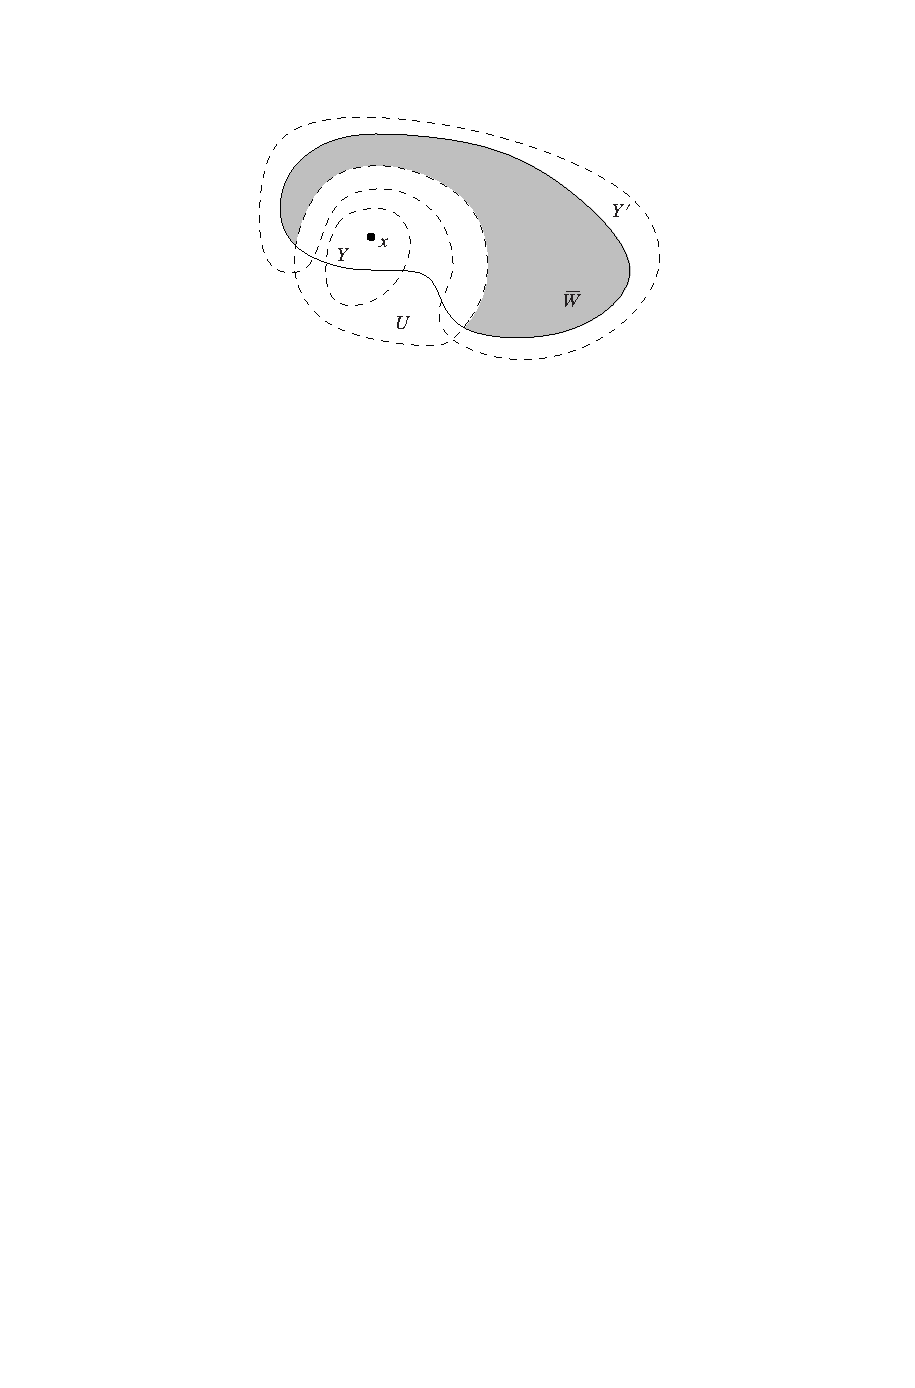
\includegraphics{pictures/local-compact}
\end{figure}
\begin{proof}
Suppose $U$ is a neighborhood of $x$. By Proposition~\ref{Hausdorff local compact iff} there is a precompact neighborhood $W$ of $x$. Then $\widebar{W}\setminus U$ is closed in $\widebar{W}$ and therefore compact. Because compact subsets can be separated by open subsets in a Hausdorff space, there are disjoint open subsets $Y$ containing $x$ and $Y'$ containing $\widebar{W}\setminus U$. Let $V=Y\cap W$. Because $\widebar{V}\sub\widebar{W}$, it is compact.\par
Because $V\sub Y\sub(Y')^c$, we have $\widebar{V}\sub\widebar{(Y')^c}=(Y')^c$. Since $\widebar{W}\setminus U$ is contained in $Y'$, this then implies $\widebar{V}\cap(\widebar{W}\setminus U)=\emp$, and therefore $\widebar{V}\sub\widebar{W}\cap U\sub U$.
\end{proof}
\begin{proposition}\label{LCH precompact nbhd for compact set}
Let $X$ be a locally compact Hausdorff space, let $K$ be a compact subset of $X$, and let $U$ be an neighborhood of $K$. Then there is a precompact neighborhood $V$ of $K$ such that $\widebar{V}\sub U$.
\end{proposition}
\begin{proof}
Lemma~\ref{LCH precompact nbhd closure in nbhd} implies that each point in $K$ has a precompact neighborhood whose closure is included in $U$. Since $K$ is compact, some finite collection of these neighborhoods covers $K$. Let $V$ be the union of the sets in such a finite collection; then $V$ is the required set.
\end{proof}
\begin{proposition}
Any open or closed subset of a locally compact Hausdorff space is a locally compact Hausdorff space.
\end{proposition}
\begin{proof}
Let $X$ be a locally compact Hausdorff space. Note that every subspace of $X$ is Hausdorff, so only local compactness needs to be checked. If $Y\sub X$ is open, Lemma~\ref{LCH precompact nbhd closure in nbhd} says that any point in $Y$ has a neighborhood whose closure is compact and contained in $Y$, so $Y$ is locally compact. Suppose $Z\sub X$ is closed. Any $x\in Z$ has a precompact neighborhood $U$ in $X$. Since $\widebar{U\cap Z}$ is a closed subset of the compact set $\widebar{U}$, it is compact. Since $\widebar{U\cap Z}\sub\widebar{Z}=Z$, it follows that $U\cap Z$ is a precompact neighborhood of $x$ in $Z$. Thus $Z$ is locally compact.
\end{proof}
A subset of a topological space $X$ is a $\bm{G_\delta}$ if it is the intersection of a sequence of open subsets of $X$ and is an $\bm{F_\sigma}$ if it is the union of a sequence of closed subsets of $X$.
\begin{proposition}\label{LCH second countable space G_delta}
Let $X$ be a second countable locally compact Hausdorff space. Then each open subset of $X$ is an $F_\sigma$ and is in fact the union of a sequence of compact sets. Likewise, each closed subset of $X$ is a $G_\delta$.
\end{proposition}
\begin{proof}
Suppose that $\mathcal{U}$ is a countable base for the topology of $X$. Let $U$ be an open subset of $X$, and let $\mathcal{U}_U$ be the collection of those sets $V$ in $\mathcal{U}$ for which $V$ is precompact and included in $U$. Lemma~\ref{LCH precompact nbhd closure in nbhd} implies that $U$ is the union of the closures of the sets in $\mathcal{U}_U$. Thus $U$ is the union of a countable collection of sets that are closed and, in fact, compact.\par
Now suppose that $C$ is a closed subset of $X$. Then $C^c$ is open and so is the union of a sequence $\{F_n\}$ of closed sets. Consequently $C$ is the intersection of the open sets $\{F_n^c\}$.
\end{proof}
Recall that a topological space (or a subset thereof) is $\sigma$-compact if it is the union of a countable collection of compact sets.
\begin{corollary}
Every second countable locally compact Hausdorff space is $\sigma$-compact.
\end{corollary}
\begin{proof}
Since a topological space is an open subset of itself, this is an immediate corollary of Proposition~\ref{LCH second countable space G_delta}.
\end{proof}
\subsection{Continuous functions}
If $X$ is a topological space, the space $\R^X$ of all real-valued functions on $X$ can be topologized in various ways. One way, of course, is the product topology, that is, the topology of pointwise convergence. Another is the \textbf{topology of uniform convergence}, which is generated by the sets
\[\{g\in\R^X:\sup_{x\in X}|g(x)-f(x)|<1/n\}\]
for $f\in\R^X$. Intermediate between these two topologies is the topology of uniform convergence on compact sets, which is generated by the sets
\[\{g\in\R^X:\sup_{x\in K}|g(x)-f(x)|<1/n\}\]
where $f\in\R^X$ and $K\sub X$ is compact. We shall now examine this topology in the case where $X$ is a locally compact Hausdorff space.
\begin{proposition}\label{LCH C(X) closed subspace}
If $X$ is a locally compact Hausdorff space, then $C(X)$ is a closed subspace of $\R^X$ in the topology of uniform convergence on compact sets.
\end{proposition}
\begin{proof}
If $f$ is in the closure of $C(X)$, then $f$ is a uniform limit of continuous functions on each compact $K\sub X$, so $f|_K$ is continuous. If $E\sub\R$ is closed, then $f^{-1}(E)\cap K=(f|_K)^{-1}(E)$ is closed for each compact $K$, so $f^{-1}(E)$ is closed ($X$ is compactly generated), whence $f$ is continuous.
\end{proof}
\begin{proposition}\label{LCH sigma-compact uniform converge on compact iff}
Let $X$ be a $\sigma$-compact locally compact Hausdorff space and $\{K_n\}$ be a exhaustion of $X$ by compact subsets, then for each $f\in\R^X$ the sets
\[\{g\in\R^X:\sup_{x\in K_n}|f(x)-g(x)|<1/m\}\]
form a neighborhood base for $f$ in the topology of uniform convergence on compact sets. Hence this topology is first countable, and $f_n\to f$ uniformly on compact sets if and only if $f_n\to f$ uniformly on each $K_n$.
\end{proposition}
\begin{proof}
These assertions follow easily from the observation that if $K\sub X$ is compact, then $\{\Int K_n\}$ is an open cover of $K$ and hence $K\sub K_n$ for some $n$.
\end{proof}
One may wonder if there are enough continuous functions on a locally compact Hausdorff space. The following results answer this question.
\begin{proposition}[\textbf{Urysohn's Lemma, Locally Compact Version}]\label{LCH Urysohn}
Let $X$ be a locally compact Hausdorff space. If $K$ is a compact subset of $X$ and $U$ is a neighborhood of $K$, then there is a continuous function $f:X\to[0,1]$ such that $f\equiv 1$ on $K$ and $f\equiv 0$ outside a compact subset of $U$.
\end{proposition}
\begin{proof}
By Proposition~\ref{LCH precompact nbhd for compact set}, there exists a precompact neighborhood $V$ of $K$ such that $\widebar{V}\sub U$. Then $V$ is normal, so by Urysohn's lemma there exists a continuous function $f:\widebar{V}\to[0,1]$ such that $f\equiv 1$ on $K$ and $f\equiv 0$ on $\partial V$. We extend $f$ to $X$ by setting $f=0$ on $V$.\par
Now we show that $f$ is a continuous function on $X$. Suppose that $E\sub[0,1]$ is closed. If $0\notin E$, then we have $f^{-1}(E)=(f|_{\widebar{V}})^{-1}(E)$, and if $0\in E$ we have $f^{-1}(E)=(f|_{\widebar{V}})^{-1}(E)\cup(\widebar{V})^c=(f|_{\widebar{V}})^{-1}(E)\cup(V)^c$ (note that $\partial V$ is contained in $(f|_{\widebar{V}})^{-1}(E)$). In either case, $f^{-1}(E)$ is closed, so $f$ is continuous. 
\end{proof}
\begin{proposition}[\textbf{Tietze Extension Theorem, Locally Compact Version}]\label{LCH Tietze Extension}
Let $X$ be a locally compact Hausdorff space and $K$ is a compact subset.
\begin{itemize}
\item[(a)] Any continuous map of $K$ into a closed interval $[a,b]$ may be extended to a continuous map of all of $X$ into $[a,b]$.
\item[(b)] Any continuous map of $K$ into $\R$ may be extended to a continuous map of all of $X$ into $\R$.
\end{itemize}
Moreover, the extension may be taken to vanish outside a compact set.
\end{proposition}
\begin{proof}
We prove (a), and (b) follows as in tietze extension theorem. Let $f:K\to[a,b]$ be a continuous function. Let $V$ be a precompact neighborhood of $K$. Then $\widebar{V}$ is normal, so by Tietze extension theorem there exists a continuous function $F:\widebar{V}\to[a,b]$ such that $F|_K=f$. Since $V$ is a neighborhood of $K$, by \ref{LCH Urysohn} there is a continuous function $\varphi:X\to[0,1]$ such that $\varphi\equiv 1$ on $K$ and $\varphi\equiv 0$ on a compact subset of $V$. Define $\widetilde{F}(x)=F(x)\varphi(x)$. By the choice of $\varphi$, it is easy to see $\widetilde{F}$ is continuous and $\widetilde{F}|_K=f$. Therefore $\widetilde{F}$ is the required function.
\end{proof}
The preceding results show that locally compact Huasdorff spaces have a rich supply of continuous functions that vanish outside compact sets. Let us recall some terminology: If $X$ is a topological space and $f\in C(X)$, the support of $f$, denoted by $\supp(f)$, is the smallest closed set outside of which $f$ vanishes, that is, the closure of $\{x:f(x)\neq 0\}$. If $\supp(f)$ is compact, we say that $f$ is \textbf{compactly supported}, and we define
\[C_c(X)=\{f\in C(X):\text{$\supp(f)$ is compact}\}\]
to be the set of continuous functions on $X$ with compact support. Moreover, if $f\in C(X)$, we say that $f$ \textbf{vanishes at infinity} if for every $\eps>0$ the set $\{x:|f(x)|\geq\eps\}$ is compact, and we define
\[C_0(X)=\{f\in C(X):\text{$f$ vanishes at infinity}\}.\]
Clearly $C_c(X)\sub C_0(X)$. Moreover, $C_0(X)\sub BC(X)$, because for $f\in C_0(X)$ the image of the set $\{x:|f(x)|\geq\eps\}$ is compact, and $|f|<\eps$ on its complement.
\begin{proposition}\label{LCH C_0(X) is closure of C_c(X)}
If $X$ is a locally compact Hausdorff space, then $C_0(X)$ is the closure of $C_c(X)$ in the uniform metric.
\end{proposition}
\begin{proof}
If $\{f_n\}$ is a sequence in $C_c(X)$ that converges uniformly to $f\in C(X)$, for each $\eps>0$ there exists $n\in\N$ such that $\|f-f_n\|<\eps$. Then $|f(x)|<\eps$ for $x\notin\supp(f_n)$, so $f\in C_0(X)$.\par
Conversely, if $f\in C_0(X)$, for $n\in\N$ let $K_n=\{x:|f(x)|\geq 1/n\}$. Then $K_n$ is compact, so by Proposition~\ref{LCH Urysohn} there exists $\varphi_n\in C_c(X)$ with $0\leq\varphi_n\leq 1$ and $\varphi_n\equiv 1$ on $K_n$. Let $f_n=\varphi_nf$. Then $f_n\in C_c(X)$ and $\|f_n-f\|_{\infty}\leq 1/n$, so $f_n$ converges to $f$ uniformly.
\end{proof}
Now we derive some consequences of Proposition~\ref{LCH Urysohn} which will be used later. Let us begin with the following lemma.
\begin{lemma}\label{compact set separated by open union}
Let $X$ be a Hausdorff space, let $K$ be a compact subset of $X$, and let $U_1$ and $U_2$ be open subsets of $X$ such that $K\sub U_1\cup U_2$. Then there are compact sets $K_1$ and $K_2$ such that $K=K_1\cup K_2$, $K_1\sub U_1$ and $K_2\sub U_2$.
\end{lemma}
\begin{proof}
Let $L_1=K\setminus U_1$ and $L_2=K\setminus U_2$. Then $L_1$ and $L_2$ are disjoint and compact, and so according to Lemma~\ref{topological space compact separated by disjoint open} they can be separated by disjoint open sets, say by $V_1$ and $V_2$. If we define $K_1$ and $K_2$ by $K_1=K\setminus V_1$ and $K_2=K\setminus V_2$, then $K_1$ and $K_2$ are compact, are included in $U_1$ and $U_2$, respectively, and have $K$ as their union.
\end{proof}
\begin{proposition}\label{LCH decompose function with supp in open set}
Let $X$ be a locally compact Hausdorff space, let $f$ belong to $C_c(X)$, and let $U_1,\dots,U_n$ be open subsets of X such that $\supp(f)\sub U=\bigcup_{i=1}^{n}U_i$. Then there are functions $f_1,\dots,f_n$ in $C_c(X)$ such that $f=f_1+\cdots+f_n$ and such that for each $i$ the support of $f_i$ is contained in $U_i$. Furthermore, if the function $f$ is nonnegative, then the functions $f_1,\dots,f_n$ can be chosen so that all are nonnegative.
\end{proposition}
\begin{proof}
In case $n=1$ we need only let $f_1$ be $f$. So we can begin by supposing that $n=2$. Use Lemma~\ref{compact set separated by open union} to construct compact sets $K_1$ and $K_2$ such that $K_1\sub U_1$ and $K_2\sub U_2$, and $\supp(f)=K_1\cup K_2$, and then use Proposition~\ref{LCH Urysohn} to construct functions $h_1$ and $h_2$ that belong to $C_c(X)$ and satisfy $\chi_{K_i}\leq h_i\leq\chi_{U_i}$ and $\supp(h_i)\sub U_i$ for $i=1,2$. Define functions $g_1$ and $g_2$ by $g_1=h_1$ and $g_2=h_2-(h_1\wedge h_2)$. Then $g_1$ and $g_2$ are non-negative, their supports are included in $U_1$ and $U_2$, respectively, and they satisfy
\[g_1+g_2=h_1+h_2-(h_1\wedge h_2)=h_1\vee h_2=1.\]
at each $x$ in $\supp(f)$. We can complete the proof in the case where $n=2$ by defining $f_1$ and $f_2$ to be $fg_1$ and $fg_2$, and the general case follows by induction.
\end{proof}
\begin{proposition}\label{LCH function fixed finite value}
Let $X$ be a locally compact Hausdorff space, let $K_1,\dots,K_n$ be disjoint compact subsets of $X$, and let $\alpha_1,\dots,\alpha_n$ be real (or complex) numbers. Then there is a function $f$ that belongs to $C_c(X)$ and satisfies
\begin{itemize}
\item[(a)] $f(x)=\alpha_i$ if $x\in K_i$, for $i=1,\dots,n$.
\item[(b)] $\|f\|_{\infty}=\max\{|a_1|,\dots,|a_n|\}$.
\end{itemize}
\end{proposition}
\begin{proof}
We begin by constructing disjoint open sets $U_1,\dots,U_n$ such that $K_i\sub U_i$ holds for each $i$. If $n=2$, such sets are provided by Lemma~\ref{topological space compact separated by disjoint open}. The general case follows by induction. Next we use Proposition~\ref{LCH Urysohn} to choose functions $f_1,\dots,f_n$ that belong to $C_c(X)$ and satisfy $\chi_{K_i}\leq f_i\leq\chi_{U_i}$ for $i=1,\dots,n$. The required function $f$ is now given by $f=\sum_{i=1}^{n}\alpha_if_i$.
\end{proof}
\subsection{One-point compactification}
If $X$ is a noncompact locally compact Hausdorff space, it is possible to make $X$ into a compact space by adding a single point "at infinity" in such a way that the functions in $C_0(X)$ are precisely those continuous functions $f$ such that $f(x)\to 0$ as $x$ approaches the point at infinity. Here is the precise definition of this space.
\begin{proposition}\label{one point compactification}
Let $X$ be a topological space. Then $X$ is locally compact Hausdorff if and only if there exists a space $X^*$ satisfying the following conditions:
\begin{itemize}
\item[(a)] $X$ is a subspace of $X^*$.
\item[(b)] $X^*\setminus X$ consists of a single point.
\item[(c)] $X^*$ is a compact Huasdorff space.
\end{itemize}
If $X_1$ and $X_2$ are two spaces satisfying these conditions, then there is a homeomorphism of $X_1$ with $X_2$ that equals the identity map on $X$.
\end{proposition}
\begin{proof}
We first verify uniqueness. Let $X_1$ and $X_2$ be two spaces satisfying these conditions. Define $h:X_1\to X_2$ by letting $h$ map the single point $p$ of $X_1\setminus X$ to the point $q$ of $X_2\setminus X$, and letting $h$ equal the identity on $X$. We show that if $U$ is open in $X_2$, then $h(U)$ is open in $X_2$. Symmetry then implies that $h$ is a homeomorphism.\par
First, consider the case where $U$ does not contain $p$. Then $h(U)=U$. Since $U$ is open in $X_1$ and is contained in $X$, it is open in $X$. Because $X$ is open in $X_2$, the set $U$ is also open in $X_2$, as desired. Second, suppose that $U$ contains $p$. Since $C=X_1\setminus U$ is closed in $X_1$, it is compact as a subspace of $X_1$. Because $C$ is contained in $X$, it is a compact subspace of $X$. Then because $X$ is a subspace of $X_2$, the space $C$ is also a compact subspace of $X_2$, and hence is closed in $X_2$. So $h(U)=X_2\setminus C$ is open, as desired.\par
Now we suppose $X$ is locally compact Hausdorff and construct the space $X^*$. Let us take some object that is not a point of $X$, denote it by the symbol $\infty$ for convenience, and adjoin it to $X$, forming the set $X^*=X\cup\{\infty\}$. Topologize $X^*$ by defining the collection of open sets of $X^*$ to consist of $(1)$ all sets $U$ that are open in $X$, and $(2)$ all sets of the form $X^*\setminus C$, where $C$ is a compact subspace of $X$. We need to check that this collection is in fact a topology on $X^*$. The empty set is a set of type $(1)$, and the space $X^*$ is a set of type $(2)$. Checking that the intersection of two open sets is open involves two cases:
\[(X^*\setminus C_1)\cap(X^*\setminus C_2)=X^*\setminus(C_1\cup C_2),\quad U_1\cap(X^*\setminus C_1)=U_1\cap(X\setminus C_1).\]
Similarly, checking that arbitrary union open sets is open involves two cases:
\[\bigcup_\alpha(X^*\setminus C_\alpha)=X^*\setminus\bigcap_\alpha C_\alpha,\quad\Big(\bigcup_\alpha U_\alpha\Big)\cup\bigcup_\beta(X^*\setminus C_\beta)=U\cup(X^*\setminus C)=X^*\setminus(C\setminus U).\]
Therefore we have defined a topology on $X^*$.\par
Now we show that $X$ is a subspace of $X^*$. Given any open set of $X^*$, we show its intersection with $X$ is open in $X$. If $U$ is of type $(1)$, then $U\cap X=U$; if $U=X^*\setminus C$ is of type $(2)$, then $U\cap X=X\setminus C$; both of these sets are open in $X$. Conversely, any set open in $X$ is a set of type $(1)$ and therefore open in $X^*$ by definition.\par
To show that $X^*$ is compact, let $\mathcal{U}$ be an open covering of $X^*$. The collection $\mathcal{U}$ must contain an open set of type $(2)$, say $X^*\setminus C$, since none of the open sets of type $(1)$ contain the point $\infty$. Take all the members of $\mathcal{U}$ different from $X^*\setminus C$ and intersect them with $X$; they form a collection of open sets of $X$ covering $C$. Because $C$ is compact, finitely many of them  over $C$; the corresponding finite collection of elements of $\mathcal{U}$ will, along with the element $X^*\setminus C$, cover all of $X^*$. Therefore $X^*$ is compact.\par
To show that $X^*$ is Hausdorff, let $x$ and $y$ be two distinct points of $X^*$. If both of them lie in $X$, there are disjoint sets $U$ and $V$ open in $X$ containing them, respectively, since $X$ is Huasdorff. On the other hand, if $x\in X$ and $y=\infty$, we can choose a compact set $C$ in $X$ containing a neighborhood $U$ of $x$. Then $U$ and $X^*\setminus C$ are disjoint neighborhoods of $x$ and $\infty$, respectively, in $X^*$.\par
Finally, we prove the converse. Suppose a space $X^*$ satisfying conditions (a)---(c) exists. Then $X$ is Hausdorff because it is a subspace of the Hausdorff space $X^*$. Given $x\in X$, we show $X$ is locally compact at $x$. Choose disjoint open sets $U$ and $V$ of $X^*$ containing $x$ and the single point of $X^*\setminus X$, respectively. Then the set $C=X^*\setminus V$ is closed in $X^*$, so it is a compact subspace of $X^*$. Since $C$ lies in $X$, it is also compact as a subspace of $X$; it contains the neighborhood $U$ of $x$.
\end{proof}
If $X$ itself should happen to be compact, then the space $X^*$ of the preceding theorem is not very interesting, for it is obtained from $X$ by adjoining a single isolated point. However, if $X$ is not compact, then the point of $X^*\setminus X$ is a limit point of $X$, so that $\widebar{X}=X^*$.
\begin{definition}
If $Y$ is a compact Hausdorff space and $X$ is a proper subspace of $Y$ whose closure equals $Y$, then $Y$ is said to be a compactification of $X$. If $Y\setminus X$ equals a single point, then $Y$ is called the \textbf{one-point compactification} of $X$.
\end{definition}
\begin{example}
The one-point compactification of the real line $\R$ is homeomorphic with
the circle, as you may readily check. Similarly, the one-point compactification of $\R^2$ is homeomorphic to the sphere $S^2$. If $\R^2$ is looked at as the space $\C$ of complex numbers, then $\C\cup\{\infty\}$ is called the \textbf{Riemann sphere}, or the \textbf{extended complex plane}.
\end{example}
\begin{proposition}\label{LCH one-point compactification continuous function}
Let $X$ be a locally compact Hausdorff space and $X^*$ be its one-point compactification. Let $f\in C(X)$, then $f$ extends continuously to $X^*$ if and only if $f$ has a limit at the point infinity. That is, if and only if $f=g+a$ where $g\in C_0(X)$ and $a$ is a constant, in which case the continuous extension is given by $f(\infty)=a$.
\end{proposition}
\begin{proof}
Let $f$ be the form stated above. We extend $f$ to $X^*$ by defining $f(\infty)=a$. We only need to check that $f$ is continuous at $\infty$, since $f$ is in $C(X)$ and every open set of $X$ is open in $X^*$. Let $\eps>0$ be arbitrary, then the set $C_\eps=\{x:|g(x)|\geq\eps\}$ is compact in $X$, and hence $X^*\setminus C_\eps$ is a neighborhood of $\infty$ in $X^*$. By definition, this then implies $|f(x)-a|<\eps$ for $x\in X^*\setminus C_\eps$. Therefore $f$ is continuous at $\infty$, and so $f\in C(X^*)$.\par
Conversely, assume that $f\in C(X)$ has an extension $\widetilde{f}$ on $X^*$. Define $a=\widetilde{f}(\infty)$ and $g(x)=f(x)-a$. We need to show that $g\in C_0(X)$. Let $\eps>0$, then there exists a neighborhood $U$ of $\infty$ in $X^*$ such that $f(U)\sub(a-\eps,a+\eps)$. By the topology of $X^*$, since $\infty\in U$, $X\setminus U$ is then compact in $X$. Since $\{x:|g(x)|\geq\eps\}=\{x:|f(x)-a|\geq\eps\}$ is contained in $X\setminus U$, it is also compact, as desired.
\end{proof}
\subsection{Stone-Weierstrass theorem}
In this part we prove a far-reaching generalization of the well-known theorem of Weierstrass to the effect that any continuous function on a compact interval $[a,b]$ is the uniform limit of polynomials on $[a,b]$. In what follows, $X$ will denote a compact Hausdorff space, and we equip the space $C(X)$ with the uniform metric.\par
A subset $\mathscr{A}$ of $C(X,\R)$ or $C(X,\C)$ is said to be \textbf{separating} if for every $x,y\in X$ with $x\neq y$ there exists $f\in\mathscr{A}$ such that $f(x)\neq f(y)$. $\mathscr{A}$ is called an \textbf{algebra} if it is a real (resp. complex) vector subspace of $C(X,\R)$ (resp. $C(X,\C)$) such that $fg\in\mathscr{A}$ whenever $f,g\in\mathscr{A}$. If $\mathscr{A}\sub C(X,\R)$, $\mathscr{A}$ is called a \textbf{lattice} if $\max(f,g)$ and $\min(f,g)$ are in $\mathscr{A}$ whenever $f,g\in\mathscr{A}$. Since the algebra and lattice operations are continuous, one easily sees that if $\mathscr{A}$ is an algebra or a lattice, so is its closure $\mathscr{A}$ in the uniform metric.
\begin{theorem}[\textbf{Stone-Weierstrass Theorem}]\label{Stone-Weierstrass}
Let $X$ be a compact Hausdorff space. If $\mathscr{A}$ is a separating closed subalgebra of $C(X,\R)$, then either $A=C(X,\R)$ or $A=\{f\in C(X,\R):f(x_0)=0\}$ for some $x_0\in X$. The first alternative holds iff $\mathscr{A}$ contains the constant functions.
\end{theorem}
The proof will require several lemmas. The first one, in effect, proves the theorem when $X$ consists of two points, and the second one is a special case of the classical Weierstrass theorem for $X=[-1,1]$. After these two we return to the general case.
\begin{lemma}\label{Stone-Weierstrass subalgebra of R^2}
Consider $\R^2$ as an algebra under coordinatewise addition and multiplication. Then the only subalgebras of $\R^2$ are $\R^2$, $\{(0,0)\}$, and the linear span of $(1,0)$, $(0,1)$, or $(1,1)$.
\end{lemma}
\begin{proof}
The subspaces of $\R^2$ listed above are evidently subalgebras. If $\mathscr{A}\sub\R^2$ is a nonzero algebra and $(0,0)\neq(a,b)\in\mathscr{A}$, then $(a^2,b^2)\in\mathscr{A}$. If $a,b$ are nonzero and distinct then $(a,b)$ and $(a^2,b^2)$ are linearly independent, so $A=\R^2$. The other possibilities give the other three subalgebras.
\end{proof}
\begin{lemma}\label{Stone-Weierstrass approximate |x|}
For any $\eps>0$ there is a polynomial $P$ on $\R$ such that $P(0)=0$ and $||x|-P(x)|<\eps$ for $x\in[-1,1]$.
\end{lemma}
\begin{proof}
Consider the Maclaurin series for $(1-t)^{1/2}$:
\[(1-t)^{1/2}=1-\sum_nc_nt^n.\]
By the ratio test, this series converges for $|t|<1$. Moreover, by the monotone convergence theorem (applied to counting measure on $\N$),
\[\sum_nc_n=\lim_{t\to 1^-}\sum_nc_nt^n=1-\lim_{t\to 1-}(1-t)^{1/2}=1.\]
It follows from the finiteness of $\sum_nc_n$ that the series $1-\sum_nc_nt^n$ converges absolutely and uniformly on $[-1,1]$, and its sum is $(1-t)^{1/2}$ there. Therefore, given $\eps>0$, by taking a suitable partial sum of this series we obtain a polynomial $Q$ such that $|(1-t)^{1/2}-Q(t)|<\eps/2$ for $t\in[-1,1]$. Set $t=1-x^2$ and $R(x)=Q(1-x^2)$, we obtain a polynomial $R$ such that $||x|-R(x)|<\eps/2$ for $x\in[-1,1]$. In particular, $|R(0)|<\eps/2$. If we set $P(x)-R(x)-R(0)$, we then get the claim. 
\end{proof}
\begin{lemma}\label{Stone-Weierstrass closed subalgebra is lattice}
If $\mathscr{A}$ is a closed subalgebra of $C(X,\R)$, then $|f|\in\mathscr{A}$ whenever $f\in\mathscr{A}$; hence $\mathscr{A}$ is a lattice.
\end{lemma}
\begin{proof}
If $f\in\mathscr{A}$ and $f\neq 0$, let $h=f/\|f\|_\infty$. Then $h$ maps $X$ into $[-1,1]$, so if $\eps>0$ and $P$ is as in Lemma~\ref{Stone-Weierstrass approximate |x|}, we have $||h|-P\circ h|<\eps$. Since $P(0)=0$, $P$ has no constant term, so $P\circ h\in\mathscr{A}$ since $\mathscr{A}$ is an algebra. Since $\mathscr{A}$ is closed and $\eps$ is arbitrary, we have $|h|\in\mathscr{A}$ and hence $|f|\in\mathscr{A}$. This proves the first assertion, and the second one follows because $\max(f,g)$ and $\min(f,g)$ can be represented by $f$, $g$, and $|f-g|$.
\end{proof}
\begin{lemma}\label{Stone-Weierstrass two point}
Suppose $\mathscr{A}$ is a closed lattice in $C(X,\R)$ and $f\in C(X,\R)$. If for every $x,y\in X$ there exists $h_{xy}\in\mathscr{A}$ such that $h_{xy}(x)=f(x)$ and $h_{xy}(y)=f(y)$, then $f\in\mathscr{A}$.
\end{lemma}
\begin{proof}
Given $\eps>0$, for each $x,y\in X$ let
\[U_{xy}=\{z\in X:f(z)<h_{xy}(z)+\eps\},\quad V_{xy}=\{z\in X:f(z)>h_{xy}(z)-\eps\}.\]
These sets are open and contain $x$ and $y$. Fix $y$, then $\{U_{xy}:x\in X\}$ covers $X$, so there is a finite subcover $\{U_{x_jy}\}$. Let $h_y=\max(h_{x_1y},\dots,h_{x_ny})$, then $f<h_y+\eps$ on $X$ and $f>h_y-\eps$ on $V_y=\bigcup_{i=1}^{n}V_{x_iy}$, which is open and contains $y$. Thus $\{V_y:y\in X\}$ is another open cover of $X$, so there is a finite subcover $\{V_{y_j}\}$. Let $h=\min(h_{y_1},\dots,h_{y_m})$, then $\|f-h\|<\eps$. Since $\mathscr{A}$ is a lattice, $h\in\mathscr{A}$, and since $\mathscr{A}$ is closed and $\eps$ is arbitrary, $f\in\mathscr{A}$.
\end{proof}
\begin{proof}[Proof of Theorem~\ref{Stone-Weierstrass}]
Given $x\neq y\in X$, let $\mathscr{A}_{xy}=\{(f(x),f(y)):f\in\mathscr{A}\}$. Then $\mathscr{A}_{xy}$ is a subalgebra of $\R^2$ as in Lemma~\ref{Stone-Weierstrass subalgebra of R^2} because $f\mapsto(f(x),f(y))$ is an algebra homomorphism. If $\mathscr{A}_{x,y}=\R^2$ for all $x,y$, then Lemmas~\ref{Stone-Weierstrass closed subalgebra is lattice} and \ref{Stone-Weierstrass two point} imply that $\mathscr{A}=C(X,\R)$. Otherwise, there exist $x,y$ for which $\mathscr{A}_{xy}$ is a proper subalgebra of $\R^2$. It cannot be $\{(0,0)\}$ or the linear span of $(1,1)$ because $\mathscr{A}$ separates points, so by Lemma~\ref{Stone-Weierstrass subalgebra of R^2} $\mathscr{A}_{xy}$ is the linear span of $(1,0)$ or $(0,1)$. In either case there exists $x_0\in X$ such that $f(x_0)=0$ for all $f\in\mathscr{A}$. There is only one such $x_0$ since $A$ separates points, so if neither $x$ nor $y$ is $x_0$, we have $\mathscr{A}_{xy}=\R^2$. Lemmas~\ref{Stone-Weierstrass closed subalgebra is lattice} and \ref{Stone-Weierstrass two point} now imply that $\mathscr{A}=\{f\in C(X,\R):f(x_0)=0\}$. Finally, if $\mathscr{A}$ contains constant functions, there is no $x_0$ such that $f(x_0)=0$ for all $f\in\mathscr{A}$, so $\mathscr{A}$ must equal $C(X,\R)$.
\end{proof}
We have stated the Stone-Weierstrass theorem in the form that is most natural for the proof. However, in applications one is typically dealing with a subalgebra $\mathscr{B}$ of $C(X,\R)$ that is not closed, and one applies the theorem to $\mathscr{A}=\widebar{\mathscr{B}}$. The resulting
restatement of the theorem is as follows:
\begin{corollary}
Suppose $\mathscr{B}$ is a separating subalgebra of $C(X,\R)$. If there exists $x_0\in X$ such that $f(x_0)=0$ for all $f\in\mathscr{B}$, then $\mathscr{B}$ is dense in $\{f\in C(X,\R):f(x_0)=0\}$. Otherwise, $\mathscr{B}$ is dense in $C(X,\R)$.
\end{corollary}
The classical Weierstrass approximation theorem is the special case where $X$ is a compact subset of $\R^n$ and $\mathscr{B}$ is the algebra of polynomials on $\R^n$ (restricted to $X$); here $\mathscr{B}$ contains the constant functions, so the conclusion is that it is dense in $C(X,\R)$.\par
The Stone-Weierstrass theorem, as it stands, is false for complex-valued functions. For example, the algebra of polynomials in one complex variable is not dense in $C(K)$ for most compact subsets $K$ of $\C$. (In particular, if $\Int K\neq\emp$, any uniform limit of polynomials on $K$ must be holomorphic on $\Int K$.) Here we shall give a simple proof that the function $f(z)=\bar{z}$ cannot be approximated uniformly by polynomials on the unit circle. If $P(z)=\sum_ja_jz^j$, then
\[\int_{0}^{2\pi}\widebar{f(e^{it})}P(e^{it})\,dt=\sum_{j=0}^{n}a_j\int_0^{2\pi}e^{i(j+1)t}\,dt=0.\]
Since $|f|=1$ on the unit circle we have
\[2\pi=\int_0^{2\pi}\bar{f}f\,dt\Big|\leq\Big|\int_0^{2\pi}\bar{f}(f-P)\,dt\Big|+\Big|\int_0^{2\pi}\bar{f}P\,dt\Big|\leq\int_0^{2\pi}|f-P|\,dt\leq 2\pi\|f-P\|_\infty.\]
Therefore, $\|f-P\|_\infty\geq 1$ for any polynomial $P$.\par
There is, however, a complex version of the Stone-Weierstrass theorem.
\begin{theorem}[\textbf{Complex Stone-Weierstrass Theorem}]\label{Stone-Weierstrass complex}
Let $X$ be a compact Hausdorff space. If $\mathscr{A}$ is a separating closed complex subalgebra of $C(X,\C)$ that separates points and is closed under complex conjugation, then either $A=C(X,\C)$ or $A=\{f\in C(X,\C):f(x_0)=0\}$ for some $x_0\in X$.
\end{theorem}
\begin{proof}
Since $\Re(f)=(f+\bar{f})/2$ and $\Im(f)=(f-\bar{f})/2i$, the set $\mathscr{A}_{\R}$ of real and imaginary parts of functions in $\mathscr{A}$ is a subalgebra of $C(X,\R)$ to which the Stone-Weierstrass theorem applies. Since $\mathscr{A}=\mathscr{A}_{\R}+i\mathscr{A}_{\R}$, the desired result follows.
\end{proof}
There is also a version of the Stone-Weierstrass theorem for locally compact Hausdorff spaces.
\begin{theorem}
Let $X$ be a locally compact Hausdorff space. If $\mathscr{A}$ is a separating closed subalgebra of $C_0(X,\R)$, then either $\mathscr{A}=C_0(X,\R)$ or $\mathscr{A}=\{f\in C_0(X,\R):f(x_0)=0\}$ for some $x_0\in X$.
\end{theorem}
\begin{proof}
If there exists $x_0\in X$ such that $f(x_0)=0$ for all $f\in\mathscr{A}$, let $Y$ be the one-point compactification of $X\setminus\{x_0\}$. Then by Proposition~\ref{LCH one-point compactification continuous function} we can write $\mathscr{A}\sub\{f\in C(Y,\R):f(+\infty)=0\}$. Since $\mathscr{A}$ separates points on $X\setminus\{x_0\}$, there is no $y\in X\setminus\{x_0\}$ such that $f(y)=0$ for all $f\in\mathscr{A}$; it follows that $\mathscr{A}$ separates points in $Y$, and by the Stone-Weierstrass theorem we get $\mathscr{A}=\{f\in C(Y,\R):f(+\infty)=0\}=\{f\in C_0(X,\R):f(x_0)=0\}$.\par
If there is no $x_0\in X$ such that $f(x_0)=0$ for all $f\in\mathscr{A}$, let $Y$ be the one-point compactification of $X$. By the same proof we see $\mathscr{A}=C_0(X,\R)$.
\end{proof}
By the same proof as Theorem~\ref{Stone-Weierstrass complex}, we also have the following complex version.
\begin{theorem}
Let $X$ be a locally compact Hausdorff space. If $\mathscr{A}$ is a separating closed complex subalgebra of $C_0(X,\C)$ that separates points and is closed under complex conjugation, then either $A=C(X,\C)$ or $A=\{f\in C(X,\C):f(x_0)=0\}$ for some $x_0\in X$.
\end{theorem}
\subsection{Metrizability}
Now we consider metrizability of locally compact spaces.
\begin{proposition}\label{compact Hausdorff metrizable iff C_2}
A compact Hausdorff space is metrizable if and only if it is second countable.
\end{proposition}
\begin{proof}
First suppose that $X$ is compact and metrizable. Then $X$ is separable and so is second countable.\par
Now suppose that $X$ is a compact Hausdorff space that is second countable and let $\mathcal{U}$ be a countable base. The space $X$ is normal, and so for each pair of sets $U$, $V$ that belong to $\mathcal{U}$ and satisfy $U\cap V=\emp$ there is, by Urysohn's lemma, a continuous function $f:X\to[0,1]$ that vanishes on $\widebar{U}$ and has value $1$ everywhere on $\widebar{V}$. Form a sequence $\{f_n\}$ by choosing one such function for each such pair of sets. Our next step is to check that this sequence of functions separates the points of $X$, and for this it is enough to show that for each pair $x$, $y$ of distinct points in $X$ there are sets $U$ and $V$ that belong to $\mathcal{U}$, have disjoint closures, and contain $x$ and $y$, respectively. To construct such sets, choose disjoint open neighborhoods $W_1$ and $W_2$ of $x$ and $y$, and use Lemma~\ref{LCH precompact nbhd closure in nbhd} to choose open sets $U$ and $V$ such that $x\in U\sub\widebar{U}\sub W_1$ and $y\in V\sub\widebar{V}\sub W_2$. By making $U$ and $V$ a bit smaller, if necessary, we can assume that they belong to $\mathcal{U}$. Thus the required sets $U$ and $V$ exist, and the sequence $\{f_n\}$ separates the points of $X$.\par
Define a function $d:X\times X\to\R$ by setting
\[d(x,y)=\sum_{n=1}^{\infty}\frac{1}{2^n}|f_n(x)-f_n(y)|.\]
It is easy to use the fact that the functions $\{f_n\}$ separate the points of $X$ to check that $d$ is a metric on the set $X$ and to use the fact that the functions $\{f_n\}$ are continuous (with respect to the original topology on $X$) to check that the topology induced by $d$ is weaker than the original topology. Since the original topology makes $X$ a compact space, while the topology induced by $d$ is weaker and Hausdorff, the two topologies must be the same ($\id$ is a continuous bijection from a compact space to a Huasdorff space). Thus the original topology on $X$ is metrizable and in fact is metrized by $d$.
\end{proof}
Our next task is to prove that each second countable locally compact Hausdorff space is metrizable. For this we need the following lemma.
\begin{lemma}\label{LCH C_2 iff onepoint compactification C_2}
Let $X$ be a locally compact Hausdorff space. If $X$ is second countable, then the one-point compactification of $X$ is also second countable.
\end{lemma}
\begin{proof}
Let $\mathcal{U}$ be a countable base for the topology of $X$, and let $\mathcal{U}_0$ be the collection of those sets $V$ in $\mathcal{U}$ for which $V$ is precompact. Arrange the sets in $\mathcal{U}_0$ in a sequence, say $\{V_k\}$. Then $X=\bigcup_kV_k$, since $X$ is locally compact, and so for each compact subset $K$ of $X$ there is a positive integer $n$ such that $K\sub\bigcup_{k=1}^{n}V_k$. Thus if $U$ is an open neighborhood in $X^*$ of the point at infinity and if $K=X^*\setminus U$, then there is a positive integer $n$ such that $K\sub\bigcup_{k=1}^{n}V_k$ and hence such that $X^*\setminus\widebar{\bigcup_{k=1}^{n}V_k}\sub U$. It follows that the sets in $U$, together with the sets $X^*\setminus\widebar{\bigcup_{k=1}^{n}V_k}$, form a countable base for the topology of $X^∗$.
\end{proof}
\begin{proposition}\label{LCH C_2 is metrizable}
Each secound countable locally compact Hausdorff space is metrizable.
\end{proposition}
\begin{proof}
Let $X$ be a secound countable locally compact Hausdorff space. Proposition~\ref{compact Hausdorff metrizable iff C_2} and Lemma~\ref{LCH C_2 iff onepoint compactification C_2} imply that the one-point compactification $X^*$ of $X$ is metrizable. Then $X$, as a subspace of the metrizable space $X^*$, is metrizable.
\end{proof}
\section{Proper maps}
\subsection{Proper maps}
If $f$ and $g$ are closed continuous maps, it does not follow that $f\times g$ is closed, even if $f$ is the identity map. An example is given below.
\begin{example}
Every constant mapping into a Hausdorff space is closed. But it $f$ is the constant mapping $\Q\to\{0\}$, then $f\times\id_\Q$ is the mapping $(x,y)\mapsto(0,y)$ of $\Q^2$ into $\Q^2$, so it is the second projection and is not closed.
\end{example}
\begin{definition}
A map $f:X\to Y$ is said to be \textbf{proper} if $f$ is continuous and if the mapping $f\times\id_Z:X\times Z\to Y\times Z$ is closed, for every topological space $Z$.
\end{definition}
If in the definition we take the space $Z$ to consist of a single point, then we see that any proper map is closed. A partial converse holds when the map $f$ is injective:
\begin{proposition}\label{topological space injection proper iff}
Let $f:X\to Y$ be a continuous injection. Then the following three statements are equivalent.
\begin{itemize}
\item[(\rmnum{1})] $f$ is proper.
\item[(\rmnum{2})] $f$ is closed.
\item[(\rmnum{3})] $f$ is a homeomorphism of $X$ onto a closed subset of $Y$.
\end{itemize}
\end{proposition}
\begin{proof}
We have just seen that (\rmnum{1}) implies (\rmnum{2}). Since the equivalence relation $f(x)=f(y)$ is the equality relation, the quotient space of $X$ with respect to this relation can be identified with $X$; hence (\rmnum{2}) implies (\rmnum{3}) by Proposition~\ref{topological space canonical decomposition homeomorphism iff}. Finally, if (\rmnum{3}) is satisfied then $f\times\id_Z$ is a homeomorphism of $X\times Z$ onto a closed subspace of $Y\times Z$ and is therefore a closed mapping; hence (\rmnum{3}) implies (\rmnum{1}).
\end{proof}
\begin{proposition}\label{topological space proper map on subspace}
Let $f:X\to Y$ be a continuous map. If $B$ is any subset of $Y$, let $f_B$ denote the restriction of $f$ on $f^{-1}(B)$.
\begin{itemize}
\item[(a)] If $f$ is proper, so is $f_B$.
\item[(b)] Let $(B_i)_{i\in I}$ be a family of subsets of $Y$ whose interiors cover $Y$, or which is a locally finite closed covering of $Y$; then if each of the mappings $f_B$ is proper, so is $f$.
\end{itemize}
\end{proposition}
\begin{proof}
Let $Z$ be a topological space. If $B$ is any subset of $Y$, we have
\[f_B\times\id_Z=(f\times\id_Z)_{B\times Z}.\]
If $f$ is proper, then $f\times\id_Z$ is closed, hence so is $(f\times\id_Z)_{B\times Z}$ (Proposition~\ref{}), whence (a) is proved. If now $(B_i)_{i\in I}$ satisfies one of the two conditions stated in (b), then the covering $(B_i\times Z)_{i\in I}$ of $Y\times Z$ has the same property; if the $f_{B_i}$ are proper then the mappings $(f\times\id_Z)_{B\times Z}$ are closed, whence $f\times\id_Z$ is closed (Proposition~\ref{}). This completes the proof.
\end{proof}
\begin{proposition}
Let $f:X\to Y$ and $g:Y\to Z$ be two continuous mappings.
\begin{itemize}
\item[(a)] If $f$ and $g$ are proper, then $g\circ f$ is proper.
\item[(b)] If $g\circ f$ is proper and $f$ is surjective, then $g$ is proper.
\item[(c)] If $g\circ f$ is proper and $g$ is injective, then $f$ is proper. 
\item[(d)] If $g\circ f$ is proper and $Y$ is Hausdorff, then $f$ is proper   
\end{itemize}
\end{proposition}
\begin{proof}

\end{proof}
\subsection{Proper maps}
If $X$ and $Y$ are topological spaces, a map $f:X\to Y$ (continuous or not) is said to be \textbf{proper} if the preimage of each compact subset of $Y$ is compact. For example, every exhaustion function $f:X\to\R$ is a proper map.\par
In order to visualize the behavior of proper maps, it is useful to introduce the following definition: if $X$ is a topological space, a sequence $(x_i)$ in $X$ is said to \textbf{diverge to infinity} if for every compact set $K\sub X$ there are at most finitely many values of $i$ for which $x_i\in K$.
\begin{lemma}\label{topological space diverge to inf iff no convergent subseq}
Suppose $X$ is a first countable Hausdorff space. A sequence in $X$ diverges to infinity if and only if it has no convergent subsequence.
\end{lemma}
\begin{proof}
Assume first that $(x_i)$ is a sequence in $X$ that diverges to infinity. If there is a subsequence $(x_{i_j})$ that converges to $x\in X$, then the set $K=\{x\}\cup\{x_{i_j}\}$ is compact and contains infinitely many terms of the sequence, which is a contradiction. (This implication does not require the hypothesis that $X$ is first countable and Hausdorff.)\par
Conversely, assume that $(x_i)$ has no convergent subsequence. If $K\sub X$ is any compact set that contains $x_i$ for infinitely many $i$ , then there is a subsequence $(x_{i_j})$ such that $x_{i_j}\in K$ for all $j$. Because a compact, first countable Hausdorff space is sequentially compact, this subsequence in turn has a convergent subsequence, which is a contradiction.
\end{proof}
\begin{proposition}
Suppose $X$ and $Y$ are topological spaces and $f:X\to Y$ is a proper map. Then $f$ takes every sequence diverging to infinity in $X$ to a sequence diverging to infinity in $Y$.
\end{proposition}
\begin{proof}
Suppose $(x_i)$ is a sequence in $X$ that diverges to infinity. If $\big(f(x_i)\big)$ does not diverge to infinity, then there is a compact subset $K\sub Y$ that contains $f(x_i)$ for infinitely many values of $i$. It follows that $x_i$ lies in the compact set $f^{-1}(K)$ for these values of $i$, which contradicts the assumption that $(x_i)$ diverges to infinity.
\end{proof}
Because the definition of properness is sometimes tricky to check directly, it is useful to have other sufficient conditions for a map to be proper. The next proposition gives several such conditions.
\begin{proposition}\label{proper map if}
Suppose $X$ and $Y$ are topological spaces, and $f:X\to Y$ is a continuous map.
\begin{itemize}
\item[(a)] If $X$ is compact and $Y$ is Hausdorff, then $f$ is proper.
\item[(b)] If $X$ is a second countable Hausdorff space and $f$ takes sequences diverging
to infinity in $X$ to sequences diverging to infinity in $Y$, then $f$ is proper. 
\item[(c)] If $f$ is a closed map with compact fibers, then $f$ is proper.
\item[(d)] If $f$ is a topological embedding with closed image, then $f$ is proper.
\item[(e)] If $Y$ is Hausdorff and $f$ has a continuous left inverse, then $f$ is proper.
\item[(f)] If $f$ is proper and $A\sub X$ is any subset that is saturated with respect to $f$, then $f|_A:A\to f(A)$ is proper.
\end{itemize}
\end{proposition}
\begin{proof}
Suppose $X$ is compact and $Y$ is Hausdorff. If $K\sub Y$ is
compact, then it is closed in $Y$ because $Y$ is Hausdorff. By continuity, $f^{-1}(K)$ is closed in $X$ and therefore compact.\par
Assume $X$ is a second countable Hausdorff space, and suppose
$f:X\to Y$ takes sequences diverging to infinity to sequences diverging to infinity. Let $K\sub Y$ be any compact set, and let $L=f^{-1}(K)\sub X$. Because of our hypothesis on $X$, to show that $L$ is compact, it suffices to show that it is sequentially compact. Suppose on the contrary that $(x_i)$ is a sequence in $L$ with no convergent subsequence. It diverges infinity by Lemma~\ref{topological space diverge to inf iff no convergent subseq}, so our assumption about $f$ implies that $\big(f(x_i)\big)$ diverges to infinity. But this is impossible because $f(x_i)$ lies in the compact set $K$ for all $i$.\par
Assume $f$ is a closed map with compact fibers. Let $K\sub Y$ be compact, and let $\mathcal{U}$ be a cover of $f^{-1}(K)$ by open subsets of $X$. If $y\in K$ is arbitrary, the fiber $f^{-1}(y)$ is covered by finitely many of the sets in $\mathcal{U}$, say $U_1,\dots,U_k$. The set $A_y=X-\bigcup_{i=1}^{k}U_i$ is closed in $X$ and disjoint from $f^{-1}(y)$, so $V_y=Y-f(A_y)$ is open in $Y$ and contains $y$. It follows from ourconstruction that 
\[f^{-1}(V_y)=f^{-1}(Y-f(A_y))\sub X-A_y=U_1\cap\cdots\cap U_k.\] 
Because $K$ is compact, it is covered by finitely many of the sets $V_y$. Thus $f^{-1}(K)$ is covered by finitely many sets of the form $f^{-1}(V_y)$, each of which is covered by finitely many of the sets in $\mathcal{U}$, so it follows that $f^{-1}(K)$ is compact.\par
Now (d) follows from (c), because a topological embedding with closed image is a closed map, and its fibers are singletons, which are certainly compact.\par
Assume that $Y$ is Hausdorff and $g:Y\to X$ is a continuous left inverse for $f$, and suppose $K$ is a compact subset of $Y$. Then we observe that
\[x\in f^{-1}(K)\Rightarrow x=g(f(x))\in g(K)\] 
Since $K$ is closed in $Y$ (because $Y$ is Hausdorff), itfollows that $f^{-1}(K)$ is a closed subset of the compact set $G(K)$, so it is compact.\par
Finally, to prove (f), suppose $f:\to Y$ is proper and $A\sub X$ is saturated. Let
$K\sub f(A)$ be compact. The fact that $A$ is saturated means that $(f|_A)^{-1}(K)=f(K)$, which is compact because $f$ is proper.
\end{proof}
A topological space $X$ is said to be \textbf{compactly generated} if it has the following property: 
\[A\text{ is closed in $X$}\iff A\cap K\text{ is closed in $X$ for any compact subset $K$}\] 
It is easy to see that an equivalent definition is obtained by substituting open for closed.
\begin{lemma}
First countable spaces and locally compact spaces are compactly generated.
\end{lemma}
\begin{proof}
Let $X$ be a space satisfying either of the two hypotheses, and let $A\sub X$ be a subset whose intersection with each compact set $K\sub X$ is closed in $K$.\par
First assume that $X$ is first countable, and let $x\in\widebar{A}$. By the sequence lemma, there is a sequence $(a_i)$ of points in $A$ converging to $x$. The set $K=\{x\}\cup\{a_i:i\in\N\}$ is compact, so $A\cap K$ is closed in $K$ by hypothesis. Since $x$ is the limit of a sequence of points in $A\cap K$, it must also be in $A\cap K\sub A$. Thus $A$ is closed.\par
Now assume $X$ is locally compact. Let $x\in A^c$, we want to find a neighborhood of $x$ disjoint from $A$. Now let $K$ be a compact subset of $X$ containing a neighborhood $U$ of $x$. If $U\cap A=\emp$, then we are done. Otherwise let $\widetilde{U}=U\setminus(A\cap K)$. Since $A\cap K$ is closed, $\widetilde{U}$ is open in $X$. This is the desired neighborhood of $x$.
\end{proof}
\begin{theorem}\label{proper map is closed}
Suppose $X$ is any topological space, $Y$ is a compactly generated Hausdorff space and $F:X\to Y$ is a proper continuous map. Then $F$ is a closed map.
\end{theorem}
\begin{proof}
Let $A\sub X$ be a closed subset. We show that $F(A)$ is closed in $Y$ by showing that its intersection with each compact subset is closed. If $K\sub Y$ is compact, then $F^{-1}(K)$ is compact since $F$ is proper, and so is $A\cap F^{-1}(K)$ because it is a closed subset of a compact set. By the main theorem on compactness, $F\big(A\cap F^{-1}(K)\big)$ is compact as well. This set is equal to $F(A)\cap K$. Because $K$ is Hausdorff, $F(A)\cap K$ is closed in $K$.
\end{proof}
\begin{corollary}\label{compact gene embed closed map iff}
If $X$ is a topological space and $Y$ is a compactly generated Hausdorff space, an embedding $F:X\to Y$ is proper if and only if it has closed image.
\end{corollary}
\begin{proof}
If $F$ is proper, then by Theorem~\ref{proper map is closed} $F$ is closed, so $F(X)$ is closed. Conversely, if $F(X)$ is closed, then by Proposition~\ref{proper map if}(d) we know $F$ is proper.
\end{proof}
\begin{corollary}
Suppose $F$ is a proper continuous map from a topological space to a compactly generated Hausdorff space.
\begin{itemize}
\item[(a)] If $F$ is surjective, it is a quotient map.
\item[(b)] If $F$ is injective, it is a topological embedding.
\item[(c)] If $F$ is bijective, it is a homeomorphism.
\end{itemize}
\end{corollary}
\section{Baire Spaces}
\subsection{Nowhere dense sets and meager sets}
We develop the elementary properties of nowhere dense sets here.
\begin{definition}
A subset $A$ of a topological space $X$ is called \textbf{nowhere dense} if its closure has empty interior.
\end{definition}
Before giving some examples, we consider some elementary properties of nowhere dense sets.
\begin{proposition}\label{nowhere dense iff}
In a topological space $X$:
\begin{itemize}
\item[(a)] $A\sub X$ is nowhere dense iff $(\widebar{A})^c$ is dense.
\item[(b)] $A\sub X$ is nowhere dense iff every nonempty open subset $U$ of $X$ contains a nonempty open subset that is disjoint from $A$.
\end{itemize}
\end{proposition}
\begin{proof}
Assume that $A$ is nowhere dense. If $A=\emp$, the result is clear so suppose that $A\neq\emp$. Then any nonempty open subset $U$ of $X$ meets the dense subset $(\widebar{A})^c$ and the nonempty open set $U\cap(\widebar{A})^c$ is disjoint from $A$. Conversely, the condition says that any nonempty open set meets $(\widebar{A})^c$ which means that $(\widebar{A})^c$ is dense and so $A$ is nowhere dense by (a).
\end{proof}
We point out that when we speak of a set $A\sub X$ as being nowhere dense, we mean with respect to $X$'s topology, not the topology it induces on $X$---a nonempty set $X$ is never a nowhere dense subset of itself, because $\mathrm{cl}_AA=A$.
\begin{example}
\mbox{}
\begin{itemize}
\item[(a)] Any subset of a nowhere dense set is nowhere dense. The empty set is nowhere dense; so are singletons in any Hausdorff space as long as the point is not isolated. The only nowhere dense subset of a discrete space is $\emp$.
\item[(b)] The rationals $\Q$ are not nowhere dense in $\R$, but the integers $\Z$ are.
\item[(c)] The set $\{1/n:n\in\N\}\cup\{0\}$ is nowhere dense in $\R$.
\item[(d)] The boundary $\partial A$ of a set $A$ is the set $\widebar{A}\cap\widebar{(A^c)}$. If $A$ is open, then $\partial A\sub A^c$ while a neighborhood of any point in $\partial A$ must meet $A$ and $A^c$. Thus $\partial A$ has no interior. By the same reasoning, if $A$ is closed, $\partial A\sub A$ and $\Int\partial A=\emp$. Two things follow: a closed set is nowhere dense iff it coincides with its boundary; and boundaries of open or closed sets are nowhere dense.
\item[(e)] A linear subspace $M$ of a topological vector space $X$ is nowhere dense or dense. Note that the closure of a subspace is again a subspace. If $M$ is not nowhere dense then $\Int\widebar{M}\neq\emp$. By translation, it follows immediately that $0$ is an interior point of $\widebar{M}$. Thus $\widebar{M}$ is a neighborhood of $0$ and is therefore equal to $X$.
\item[(f)] In a Hausdorff topological vector space, finite-dimensional subspaces are closed. Thus, by (e), proper finite-dimensional subspaces are nowhere dense. 
\end{itemize}
\end{example}
Now we present some elementary properties of nowhere dense sets.
\begin{proposition}\label{nowhere dense set prop}
Let $X$ be a topological space.
\begin{itemize}
\item[(a)] Subsets of nowhere dense ses are nowhere dense.
\item[(b)] Finite unions of nowhere dense sets are nowhere dense.
\item[(c)] Suppose that $A\sub S\sub X$. If $A$ is nowhere dense in $S$, then $A$ is nowhere dense in $X$. Conversely, if $S$ is open in $X$ and $A$ is nowhere dense in $X$, then $A$ is nowhere dense in $S$.
\end{itemize}
\end{proposition}
\begin{proof}
If $A$ is nowhere dense then so is any $B\sub A$ since $\widebar{B}\sub\widebar{A}$. The key fact is that finite intersections of dense open sets are dense. To prove this, suppose that $A$ and $B$ are dense open sets. Thus, if $U$ is a nonempty open set, $U\cap A\neq\emp$. As $U\cap A$ is a nonempty open set, it meets $B$ nontrivially. Thus $A\cap B$ is dense.\par
Suppose that $A\sub S\sub X$ and that $A$ is not nowhere dense in $X$. Then there is a nonempty open set $U$ in $X$ that does not meet $(\widebar{A})^c$, i.e., such that $U\sub\widebar{A}$ and $U\cap S\sub\widebar{A}\cap S=\mathrm{cl}_SA$. Since $U\cap A\sub U\cap S$ and $U\cap A\neq\emp$ because $U\sub\widebar{A}$, this shows that $\mathrm{cl}_SA$ has nonempty interior, i.e., that $A$ is not nowhere dense in $S$.\par
For the converse, suppose that $A$ is nowhere dense in $X$, $S$ is open and $U$ is a nonempty open subset of $S$. Since $S$ is open in $X$, so is $U$. Since $A$ is nowhere dense in $X$, $U$ must contain a nonempty open subset $V$ of $X$---hence also of $S$---that does not meet $A$. It follows from Proposition~\ref{nowhere dense iff} that $A$ is nowhere dense in $S$.
\end{proof}
\begin{corollary}\label{nowhere dense hereditary to open set}
Let $A$ be a nowhere dense subset in $X$ and $U\sub X$ be open. Then $U\cap A$ is nowhere dense in $U$. 
\end{corollary}
A subset of a topological space $X$ is called \textbf{meager in $\bm{X}$} if it can be written as a countable union of nowhere dense sets of $X$, or, equivalently, is a subset of such a union. Otherwise, $E$ is called \textbf{nonmeager in $\bm{X}$}. A topological space is called \textbf{meager} if it is a meager subset of itself.
\begin{example}[\textbf{Examples of Meager and Nonmeager Sets}]
\mbox{}
\begin{itemize}
\item[(a)] As we can write the rationals $\Q$ as a countable union of singletons, $\Q$ is a meager subset of $\R$. Indeed, any countable Hausdorff space without isolated points is meager.
\item[(b)] Any topological space which contains an isolated point $x$ is nonmeager, as no set to which $x$ belongs can be nowhere dense. Thus discrete spaces are never meager.
\item[(c)] Singletons are always nonmeager subspaces. A singleton is a nonmeager subset of a topological space iff the point is isolated.
\item[(d)] View $\Q\times\Q$ together with the $x$-axis as a subspace of $\R^2$. As the $x$-axis is a nowhere dense subset of $\R^2$ and we can enumerate $\Q\times\Q$, $(\Q\times\Q)\cup(\R\times\{0\})$ is a meager subset of $\R^2$. However, as we will see, $\R\times\{0\}$ it self is a nonmeager subspace. The point is that the presence of a nonmeager subspace does not imply that the space itself is nonmeager.
\end{itemize}
\end{example}
An important property of meager sets is that any open subset of a meager set is again meager.
\begin{proposition}\label{meager open subset is meager}
Let $U\sub X$ be a open subset. If $X$ is meager, then so is $U$.
\end{proposition}
\begin{proof}
If there are nowhere dense subsets $\{E_n\}$ of $X$ such that $X=\bigcup_nE_n$, then $U=\bigcup_n(E_n\cap U)$. As $U$ is open in $X$, each $E_n\cap U$ is nowhere dense in $U$ by Corollary~\ref{nowhere dense hereditary to open set} and therefore $U$ is meager.
\end{proof}
It is then interesting that whether any open subsets of a nonmeager space is nonmeager. For this, we recall that empty set is meager, so we may concentrate on nonempty open subsets. It turns out that this property is equivalent to some other conditions, and is not true in general. The Baire spaces that we will define are exactly nonmeager spaces satisfying these conditions.
\begin{theorem}\label{Baire space iff}
The following conditions on a topological space $X$ are equivalent:
\begin{itemize}
\item[(\rmnum{1})] The union of countably many closed nowhere dense sets have empty interior.
\item[(\rmnum{2})] The intersection of countably many dense open sets is dense.
\item[(\rmnum{3})] Each nonempty open subset is nonmeager.
\item[(\rmnum{4})] Each meager subsets has dense complement.
\end{itemize}
A \textbf{Baire space} is one which satisfies either of the conditions above.
\end{theorem}
\begin{proof}
It is clear that (\rmnum{1})$\Leftrightarrow$(\rmnum{2}). Assume (\rmnum{2}) and let $U\sub X$ be a meager open set so that there are nowhere dense subset $\{E_n\}$ such that $U=\bigcup_nE_n\sub\bigcup_n\widebar{E}_n$. Then $U^c\sups\bigcap_n(\widebar{E}_n)^c$ and since each $(\widebar{E}_n)^c$ is dense and open, $\bigcap_n(\widebar{E}_n)^c$ must be dense by hypothesis. Since $U^c$ is closed, it follows that $U^c=X$ or $U=\emp$.\par
Suppose that nonempty open subsets are nonmeager in $X$. Let $A\sub X$ be meager, then $\Int A$ must be meager, too. By hypothesis $\Int A=\emp$ and therefore $A^c$ is dense. This proves (\rmnum{3})$\Rightarrow$(\rmnum{4}).\par
Finally, assume (\rmnum{4}). Let $\{E_n\}$ be a sequence of closed nowhere dense sets and let $E=\bigcup_nE_n$. Since $E$ is meager, $E^c$ is dense by hypothesis. Therefore $\Int E=\emp$.
\end{proof}
It is clear that every open subset of a Baire space is Baire. Thus a Baire space is \textbf{locally Baire}. It turns out that the converse is also ture.
\begin{proposition}\label{Baire iff locally Baire}
If each point in a topologiral space $X$ has a neighborhood which is a Baire space, then $X$ is a Baire space.
\end{proposition}
\begin{proof}
Let $U\sub X$ be a nonempty open subset and let $x\in U$. By hypothesis, $x$ has an open neighborhood $V$ which is a Baire space. If $U$ were meager in $X$, $U\cap V$ would be meager in $V$ and open in $V$, contradicting the Baireness of $V$.
\end{proof}
\begin{example}
Obviously, Baire spaces are nonmeager. To see that nonmeager spaces need not be Baire, consider the metric space $\Q\cup (0,1)$. Since it contains the open nonmeager subspace $(0,1)$, it is nonmeager. Since it has meager open sets such as $\{x\in\Q:x>1\}$, it is not a Baire space. Note also that this is an incomplete metric space which is nonmeager.
\end{example}
\begin{proposition}\label{Baire space lsc function pointwise bounded above}
Let $X$ be a Baire space and $\{f_s:s\in S\}$ a family of lower semicontinuous real-valued functions on $X$ that is pointwise bounded from above on $X$. Then each nonempty open subset of $X$ contains a nonempty open subset on which $\{f_s:s\in S\}$ is bounded from above.
\end{proposition}
\begin{proof}
It suffices to prove the claim for $X$. The map $f=\sup_sf_s$ is lower semicontinuous. Decompose $X$ into the union of the closed sets $F_n=f^{-1}([-n,n])$. Since $X$ is nonmeager, some $F_n$ has a nonempty interior. The theorem now follows.
\end{proof}
Note that Proposition~\ref{Baire space lsc function pointwise bounded above} remain valid for complex-valued functions, and even for functions $\{f_s:s\in S\}$ with values in a normed space by considering the functions $\|f_s\|$.
\begin{proposition}\label{Baire space limit of continuous function}
Let $X$ be a space; let $(Y,d)$ be a metric space. Let $f_n:X\to Y$ be a sequence of continuous functions such that $f_n(x)\to f(x)$ for all $x\in X$, where $f:X\to Y$. If $X$ is a Baire space, the set of points at which $f$ is continuous is dense in $X$.
\end{proposition}
\begin{proof}
Given a positive integer $N$ and given $\eps>0$, define
\[E_N(\eps)=\{x\in X:d(f_n(x),f_m(x))\leq\eps\text{ for $n,m\geq N$}\}.\]
Note that $E_N(\eps)$ is closed in $X$. For the set of those $x$ for which $d(f_n(x),f_m(x))\leq\eps$ is closed in $X$, by continuity of $f_n$ and $f_m$, and $E_N(\eps)$ is the intersection of these sets for all $n,m\geq N$. For fixed $\eps$, since $f_n\to f$, we have $\bigcup_NE_N(\eps)=X$. Now let
\[U(\eps)=\bigcup_{N=1}^{\infty}\Int E_N(\eps).\]
We claim that $U(\eps)$ is open and dense. To show this, it suffices to show that for any nonempty open set $V$ of $X$, there is an $N$ such that the set $V\cap\Int E_N(\eps)$ is nonempty. For this purpose, we note first that for each $N$, the set $V\cap E_N(\eps)$ is closed in $V$. Because $V$ is a Baire space, at least one of these sets, say $V\cap E_M(\eps)$, must contain a nonempty open set $W$ of $V$. Because $V$ is open in $X$, the set $W$ is open in $X$; therefore, it is contained in $\Int E_M(\eps)$.\par
Now we show that $f_n$ converges to $f$ uniformly on the set $C=\bigcap_nU_n(1/n)$, which is dense since $X$ is a Baire space. To this end, let $\eps>0$ be fixed. Choose $N\in\N$ such that $1/N<\eps$. Then since $C\sub U_N(1/N)$, we have $d(f_n(x),f_m(x))<\eps$ for $n,m\geq N$ and $x\in C$. Let $m\to+\infty$, this implies $d(f_n(x),f(x))<\eps$ for $n\geq N$, thus the claim follows.
\end{proof}
\subsection{Baire category theorem}
\begin{proposition}[\textbf{Criterion for Baireness}]\label{Baire space if relation}
A topological space $(X,\mathcal{T})$ is a Baire space if there exists a relation $\preceq$ among the collection $\mathcal{T}^*$ of nonempty open subsets of $X$ such that for $A,B,C,D\in\mathcal{T}^*$,
\begin{itemize}
\item[(a)] if $A\preceq B$, then $A\sub B$;
\item[(b)] for every $B\in\mathcal{T}^*$, there is an $A\in\mathcal{T}^*$ such that $A\preceq B$;
\item[(c)] if $A\sub B\preceq C\sub D$, then $A\preceq D$;
\item[(d)] if $\{A_n\}$ is a sequence of nonempty open sets such that $A_n\succeq A_{n+1}$ for each $n\in\N$, then $\bigcap_nA_n\neq\emp$.
\end{itemize}
\end{proposition}
\begin{proof}
Suppose that the relation $\preceq$ satisfies (a)--(d) is defined on the nonempty open sets $\mathcal{T}^*$ of the topological space $(X,\mathcal{T})$. If $X$ is not a Baire space, it must contain a nonempty meager open set $U$. Consequently, there must be a sequence $\{E_n\}$ of closed nowhere dense sets whose union contains $U$. We now construct a sequence $\{U_n\}$ of open subsets of $U$ such that $U_n\succeq U_{n+1}$ and $U_n\cap(E_1\cup\cdots\cup E_n)=\emp$ for each $n\in\N$. With this, we see
\[\bigcap_{n=1}^{\infty}U_n=U\cap\bigcap_{n=1}^{\infty}U_n\sub\bigcap_{n=1}^{\infty}U_n\cap\bigcup_{n=1}^{\infty}E_n=\emp,\]
which contradicts condition (d).\par
Now we construct $\{U_n\}$. Since $\Int E_1=\emp$, certainly $U\not\sub E_1$. Hence $U\cap E_1^c$ is a nonempty open subset of $U$ which does not meet $E_1$. By (b), there is a nonempty open set $U_1$ such that $U_1\preceq U\cap E_1^c$. By (c) we have $U_1\preceq U$, so $U_1\sub U$ and $U_1\cap E_1=\emp$. Since $U_1$ is a nonempty open set, $U_1\not\sub(E_1\cup E_2)$ and there must be a nonempty open set $U_2$ such that $U_2\preceq U_1$ and $U_2\cap (E_1\cup E_2)=0$. By induction, the sequence $\{U_n\}$ mentioned above is now seen to exist.
\end{proof}
We show next that a complete pseudometric space or locally compact Hausdorff space is a Baire space by showing that a relation such as the one of Proposition~\ref{Baire space if relation} may be defined on the nonempty open sets.
\begin{theorem}[\textbf{Baire Category Theorem}]
Any locally compact Hausdorff space or complete pseudometric space is Baire.
\end{theorem}
\begin{proof}
We first consider locally compact Hausdorff spaces. For nonempty open sets $A$ and $B$ of a locally compact Hausdorff space $X$, define $A\preceq B$ if $A$ is precompact and $\widebar{A}\sub B$. In view of Proposition~\ref{LCH precompact nbhd closure in nbhd}, properties (a)--(c) of Proposition~\ref{Baire space if relation} are easy to verify. As for (d), suppose that $\{U_n\}$ is a sequence of nonempty open sets such that $U_n\succeq U_{n+1}$. The sets $\{\widebar{U}_n:n>2\}$ are nested in the compact space $\widebar{U}_2$, so they have nonempty intersection. It then follows that
\[\emp\neq\bigcap_{n=3}^{\infty}\widebar{U}_n\sub\bigcap_{n=2}^{\infty}U_n\sub\bigcap_{n=1}^{\infty}U_n.\]
Thus $X$ is Baire by Proposition~\ref{Baire space if relation}.\par
Now we turn to complete pseudometric spaces. For any subset $A$ of a complete pseudometric space $(X,d)$, let
\[d(A)=\diam(A),\quad d^*(A)=\min\{1,d(A)\}\]
and note that $A\sub B$ implies $d^*(A)\leq d^*(B)$. For $A,B\in\mathcal{T}^*$, we define $A\preceq B$ iff $\widebar{A}\sub B$ and $d(A)\leq(1/2)d^*(B)$. We show that $\preceq$ satisfies conditions of Proposition~\ref{Baire space if relation}. That $A\preceq B$ implies $A\sub B$ is clear. Moreover, for any $A\in\mathcal{T}^*$, let $x\in A\in\mathcal{T}^*$ and choose $0<r<1$ such that $B_r(x)\sub A$. With $r'=d(B_r(x))\leq r<1$ and $U=B_{r'/4}(x)$, we have $U\preceq A$. As for (c), if $A\sub B\preceq C\sub D$, then $\widebar{A}\sub C\sub D$; since $d(A)\leq (1/2)d^*(C)\leq(1/2)d^*(D)$, it follows that $A\preceq D$.\par
We now use the completeness of $X$ to show that (d) is satisfied. For this purpose, let $\{U_n\}$ be a sequence of nonempty open sets, decreasing with respect to $\preceq$. Since $d^*(U_1)\leq 1$, we have $d(U_n)\leq 2^{-n+1}$ for each $n\in\N$. Hence, choosing $x_n\in U_n$ for each $n\in\N$ yields a $d$-Cauchy sequence. Since $X$ is complete, $\{x_n\}$ has a limit $x\in X$. Since $x_m\in U_n$ for $m\geq n$, we have $x\in\widebar{U}_n$ for each $n$, and thus $x\in\bigcap_nU_n$. 
\end{proof}
\begin{corollary}\label{countable closed isolated}
In a locally compact Hausdorff space or a complete metric space, every nonempty countable closed subset contains at least one isolated point.
\end{corollary}
\begin{proof}
Assume $X$ is such a space. Let $A\sub X$ be a nonempty countable closed subset, and assume that $A$ has no isolated points. The fact that $A$ is closed in $X$ means that $A$ itself is either a locally compact Hausdorff space or a complete metric space. For each $a\in A$, the singleton $\{a\}$ is nowhere dense in $A$: it is closed in $A$ because $A$ is Hausdorff, and it contains no nonempty open subset because $A$ has no isolated points. Since $A$ is a countable union of singletons, $A$ is meager in $A$, which is a contradiction.
\end{proof}
\begin{proposition}\label{Baire space open dense intersection uncountable}
Let $\{U_n\}$ be a sequence of open dense subsets of a locally compact Hausdorff space or a complete metric space $X$ with no isolated points and $U:=\bigcap_nU_n$. Then $U$ is dense in $X$ and uncountable. In particular, no countable dense subset of $X$ can be obtained as the intersection of a countable family of open sets, i.e., is not $G_\delta$.
\end{proposition}
\begin{proof}
Since $X$ is Baire, we know $U$ is dense. If $U=\{x_n\}$ then, since each $\{x_n\}$ is closed and nowhere dense in $X$, it follows that
\[U\cap\bigcap_n\{x_n\}^c=U\cap U^c=\emp\]
is open dense, which is a contradiction. 
\end{proof}
\begin{corollary}
There is no function from $\R$ to $\R$ which is continuous at each rational point and discontinuous at each irrational point.
\end{corollary}
\begin{proof}
The points of continuity of $f$ form a $G_\delta$ set. But $\Q$ is not $G_\delta$ by Proposition~\ref{Baire space open dense intersection uncountable}.
\end{proof}
\section{Topological manifolds}
\subsection{Definition of manifolds}
A topological space $M$ is said to be \textbf{locally Euclidean} of dimension $n$ if every point of $M$ has a neighborhood in $M$ that is homeomorphic to an open subset of $\mathbb{R}^n$.
\begin{lemma}\label{locally Euclidean lemma}
A topological space $M$ is locally Euclidean of dimension $n$ if and
only if either of the following properties holds:
\begin{itemize}
\item[(a)] Every point of $M$ has a neighborhood homeomorphic to an open ball in $\mathbb{R}^n$.
\item[(b)] Every point of M has a neighborhood homeomorphic to $\mathbb{R}^n$.
\end{itemize} 
In addition, $\mathbb{R}^n$ is homeomorphic to an open ball in $\mathbb{R}^n$.
\end{lemma}
\begin{proof}
It is immediate that any space with property (a) or (b) is locally Euclidean of dimension $n$. Conversely, suppose $M$ is locally Euclidean of dimension $n$. Because any open ball in $\R^n$ is homeomorphic to $\R^n$ itself, properties (a) and (b) are equivalent, so we need only prove (a).\par
Given a point $p\in M$, let $U$ be a neighborhood of $p$ that admits a homeomorphism $\varphi:U\to V$, where $V$ is an open subset of $\R^n$. The fact that $V$ is open in $\R^n$ means that there is some open ball $B$ around $\varphi(p)$ that is contained in $V$, and then $\varphi^{-1}(B)$ is a neighborhood of $p$ homeomorphic to $B$.
\end{proof}
Suppose $M$ is locally Euclidean of dimension $n$. If $U\sub M$ is an open subset that is homeomorphic to an open subset of $\mathbb{R}^n$, then $U$ is called a \textbf{coordinate domain}, and any homeomorphism $\varphi$ from $U$ to an open subset of $\mathbb{R}^n$ is called a \textbf{coordinate map}. The pair $(U,\varphi)$ is called a \textbf{coordinate chart} (or just a chart) for $M$. A \textbf{coordinate domain} that is homeomorphic to a ball in $\mathbb{R}^n$ is called a \textbf{coordinate ball}. The preceding lemma shows that every point in a locally Euclidean space is contained in a coordinate ball.\par
The definition of locally Euclidean spaces makes sense even when $n=0$. Because $\R^0$ is a single point, Lemma~\ref{locally Euclidean lemma}(b) implies that a space is locally Euclidean of dimension $0$ if and only if each point has a neighborhood homeomorphic to a one-point space, or in other words if and only if the space is discrete.
\begin{definition}[\textbf{topological manifold}]
An $n$-dimensional \textbf{topological manifold} is a second countable Hausdorff space that is locally Euclidean of dimension $n$.
\end{definition}
The most obvious example of an $n$-manifold is $\R^n$ itself. More generally, any open subset of $\R^n$---or in fact of any $n$-manifold---is again an $n$-manifold, as the next proposition shows.
\begin{proposition}
Every open subset of an $n$-manifold is an $n$-manifold.
\end{proposition}
\begin{proof}
Let $M$ be an $n$-manifold, and let $V$ be an open subset of $M$. Any $p\in V$ has a neighborhood (in $M$) that is homeomorphic to an open subset of $\R^n$; the intersection of that neighborhood with $V$ is still open, still homeomorphic to an open subset of $\R^n$, and is contained in $V$, so $V$ is locally Euclidean of dimension $n$. Since any open subset of a Hausdorff space is Hausdorff and any open subset of a second countable space is second countable, we see that $V$ is an $n$-manifold.
\end{proof}
\begin{theorem}
A separable metric space that is locally Euclidean of dimension $n$ is an $n$-manifold. And the converse is also true.
\end{theorem}
\begin{proof}
Every metric space is Hausdorff, and Theorem~\ref{metric space second countable iff} shows that a separable metric space is second countable. For the converse, separability follows from Theorem~\ref{second countable prop}, and metrizability follows from Urysohn metrization theorem.
\end{proof}
\begin{proposition}\label{manifold quotient is manifold}
Suppose $P$ is a second countable space and $M$ is a quotient space of $P$. If $M$ is locally Euclidean, then it is second countable. Thus if $M$ is locally Euclidean and Hausdorff, it is a manifold.
\end{proposition}
\begin{proof}
Let $q:P\to M$ denote the quotient map, and let $\mathcal{U}$ be a cover of $M$ by coordinate balls. The collection $q^{-1}(\mathcal{U})=\{q^{-1}(U):U\in\mathcal{U}\}$ is an open cover of $P$, which has a countable subcover since $P$ is Lindel\"of. If we let $\mathcal{U}'\sub\mathcal{U}$ denote a countable subset of $\mathcal{U}$ such that $q^{-1}(\mathcal{U}')$ covers $P$, then $\mathcal{U}'$ is a countable cover of $M$ by coordinate balls. Each such ball is second countable, so $M$ is also second countable.
\end{proof}
\subsection{Manifolds with boundary}
In many cases we will encounter spaces that would be manifolds except that they have a boundary. The following definition deals with this problem.\par
The closed $n$ dimensional upper half-space $\mathbb{H}^n\sub\mathbb{R}^n$ is defined by
\[\mathbb{H}^n:=\{(x_1,\dots,x_n)\in\mathbb{R}^n:x_n\geq0\}\]
\begin{definition}[\textbf{Manifolds with Boundary}]
An $n$-dimensional manifold with boundary is a second countable Hausdorff space in which every point has a neighborhood homeomorphic either to an open subset of $\mathbb{R}^n$, or to an open subset of $\mathbb{H}^n$.
\end{definition}
Note that, despite the terminology, a manifold with boundary is not necessarily a manifold. When it is important to make the distinction, we say $(U,\varphi)$ is an \textbf{interior chart} if $(U,\varphi_0)$ is an open subset of $\mathbb{R}^n$, and a \textbf{boundary chart} if $(U,\varphi)$ is an open subset of $\mathbb{H}^n$ with $\varphi(U)\cap\partial\H^n\neq\emp$.\par
If $M$ is an $n$-manifold with boundary, we define a coordinate chart for $M$ to be a pair $(U,\varphi)$, where $U\sub M$ is open and $\varphi$ is a homeomorphism from $U$ to an open subset of either $\R^n$ or $\H^n$. Just as in the case of manifolds, the set $U$ is called a \textbf{coordinate domain}, and $\varphi$ is called a coordinate map. We use the notation $\partial\H^n$ to denote the boundary of $\H^n$, and $\Int\H^n$ to denote its interior, considering $\H^n$ as a subset of $\R^n$. For $n>0$, this means
\[\partial\H^n=\{(x_1,\dots,x_n):x_n=0\},\quad\Int\H^n=\{(x_1,\dots,x_n):x_n>0\}.\]
When $n=0$, we have $\H^0=\R^0=\{0\}$, so $\Int\H^0=\H^0$ and $\partial\H^0=\emp$. It follows that $0$-dimensional manifolds with boundary are no different from $0$-manifolds.
\begin{example}
The upper half-spaceHn itself is an nmanifold with boundary, with the identity map as a global coordinate map. Similarly, any closed or half-open interval in $\R$ is a $1$-manifold with boundary, for which charts are easy to construct. Another important example is the closed unit ball $\widebar{B}^n$ with the Euclidean topology. It is not hard to see intuitively that $\widebar{B}^n$ is an $n$-manifold with boundary
\end{example}
If $M$ is an $n$-manifold with boundary, a point $p\in M$ is called an \textbf{interior point} of $M$ if it is in the domain of an interior chart; and it is called a \textbf{boundary point} of $M$ if it is in the domain of a boundary chart that takes $p$ to $\partial\H^n$. The \textbf{boundary of $\bm{M}$}, denoted by $\partial M$, is the set of all its boundary points, and its \textbf{interior}, denoted by $\Int M$, is the set of all its interior points.\par
Note that these are new meanings for the terms boundary and interior, distinct from their use earlier in reference to subsets of topological spaces. If $M$ is a manifold with boundary, it might have nonempty boundary in this new sense, irrespective of whether it has any boundary points as a subset of some other topological space. Usually the distinction is clear from the context, but if necessary we can always distinguish the two meanings by referring to the \textbf{topological boundary} (for the original meaning) or the \textbf{manifold boundary} (for this new meaning) as appropriate.
\begin{theorem}\label{manifold boundary int open boundary mani}
If $M$ is an $n$-dimensional manifold with boundary, then $\mathrm{Int}M$ is an open subset of $M$, which is itself an $n$-dimensional manifold without boundary. And $\partial M$ is an $(n-1)$-manifold without boundary.
\end{theorem}
There is a subtlety about these definitions that might not be immediately evident. Although the interior and boundary of $M$ are well-defined subsets whose union is $M$, and it might seem intuitively rather obvious that they are disjoint from each other, we have no way of proving at this stage that a point $p\in M$ cannot be simultaneously a boundary point and an interior point, meaning that there is one interior chart whose domain contains $p$, and another boundary chart that sends $p$ to $\partial\H^n$.
After we have developed some more machinery, you will be able to prove the following theorem.
\begin{theorem}[\textbf{Invariance of the Boundary}]\label{invariance boundary}
If $M$ is a manifold with boundary, then a point of $M$ cannot be both a boundary point and an interior point. Thus $\partial M$ and $\mathrm{Int}M$ are disjoint subsets whose union is $M$.
\end{theorem}
\begin{corollary}
If $M$ is a nonempty $n$-dimensional manifold with boundary, then $\partial M$ is closed in $M$, and $M$ is an $n$-manifold if and only if $\partial M=\emp$.
\end{corollary}
\begin{proof}
Because $\Int M$ is an open subset of $M$ by Proposition~\ref{manifold boundary int open boundary mani}, it follows from Theorem~\ref{invariance boundary} that $\partial M=M\setminus\Int M$ is closed. If $M$ is a manifold, then every point is in the domain of an interior chart, so $M=\Int M$, and it follows from Theorem~\ref{invariance boundary} that $\partial M=\emp$. Conversely, if $\partial M=\emp$, then $M=\Int M$, which is a manifold by Proposition~\ref{manifold boundary int open boundary mani}.
\end{proof}
\begin{corollary}
Let $M$ be a smooth manifold with boundary, let $(U,\varphi)$ be a boundary chart
on $M$, and let $p$ be a point in $\partial M\cap U$. Then $\varphi(p)$ is in $\partial\H^n$. Thus, a coordinate map sends boundary points to boundary points.
\end{corollary}
\begin{proof}
If $p$ is a boundary point, then $\varphi(p)$ is also a boundary point in $\H^n$. Thus by Theorem~\ref{invariance boundary} we know $\varphi(p)\in\partial\H^n$.
\end{proof}
More generally, we have the following result.
\begin{theorem}\label{homeomorphism invariance boundary}
If $M$ and $N$ are smooth manifolds with boundary and $F:M\to N$ is a homeomorphism, then $F(\partial M)=\partial N$, hence $F(\Int M)=F(\Int N)$.
\end{theorem}
\begin{proof}
Since $F$ is a homeomorphism, every boundary point of $M$ is mapped to boundary of $N$, and vise versa. Thus we have $F(\partial M)=\partial N$, and since $M$ is the disjoint union of its interior and boundary, we also have $F(\Int M)=\Int N$.
\end{proof}
\begin{example}\label{Graph mani}
If $U\sub\mathbb{R}^n$ is an open subset and $f:U\to\mathbb{R}^k$ is any continuous map, the graph of $f$ is the subset $\Gamma(f)\sub\mathbb{R}^{n+k}$ defined by
\[\Gamma(f):=\{(x,y)\in\mathbb{R}^{n+k}:x\in U\ \text{and}\ y=f(x)\}\]
with the subspace topology inherited from $\mathbb{R}^{n+k}$. Let $\varPhi_f:U\to\mathbb{R}^{n+k}$ be the continuous injective map
\[\varPhi_f(x)=\big(x,f(x)\big)\]
the the restriction to $\Gamma(f)$ of the projection $\pr:\mathbb{R}^{n+k}\to\mathbb{R}^{n}$ is a continuous inverse for $\Phi_f$. Hence $\Gamma(f)$ is homeomorphic to $U$ and is a manifold.
\end{example}
\begin{example}
Define $\mathbb{RP}^n$ to be the set of $1$-dimensional linear subspaces (lines through the origin) in $\mathbb{R}^{n+1}$, and $\mathbb{CP}^n$ be the set of all $1$-dimensional complex subspaces of $\mathbb{C}^{n+1}$, called $n$-dimensional complex projective space. Topologize them as thequotient $(\mathbb{R}^{n+1}\setminus\{0\})/\mathbb{R}^*$ and $(\mathbb{C}^{n+1}\setminus\{0\})/\mathbb{C}^*$. Then $\mathbb{RP}^n$ is an $n$-manifold, $\mathbb{CP}^{n}$ is a $2n$-manifold.
\end{example}
\begin{example}
Let $X$ be the subset $(\mathbb{R}\times\{0\}\cup(\mathbb{R}\times\{1\}\sub\mathbb{R}^2$. Define an equivalence relation on $X$ by declaring $(x,0)\sim(x,1)$ if $x\neq 0$. Show that the quotient space
$X/$$\sim$ is locally Euclidean and second countable, but not Hausdorff. (This space is called the \textbf{line with two origins})
\end{example}
\begin{example}
Consider the product $\mathbb{R}^d\times\mathbb{R}$, where $\mathbb{R}^d$ means $\mathbb{R}$ with discrete topology. This space is Huasdorff and Locally Euclidean, but not second countable.
\end{example}
\subsection{Adjunction spaces}
\begin{definition}
Suppose $X$ and $Y$ are topological spaces, $A$ is a closed subspace of $Y$ , and $f:A\to X$ is a continuous map. Let $\sim$ bethe equivalence relation on the disjoint union $X\amalg Y$ generated by $a\sim f(a)$ for all $a\in A$, and denote the resulting quotient space by
\[X\cup_{f}Y:=(X\amalg Y)/\text{$\sim$}\]
Any such quotient space is called an \textbf{adjunction space}, and is said to be formed by
attaching $Y$ to $X$ along $f$. The map $f$ is called the attaching map. Note that the
equivalence relation identifies each point $x\in X$ with all of the points (if any) in $f^{-1}(x)\in A$. If $A=\emp$, then $X\cup_{f} Y$ is just the disjoint union space $X\amalg Y$.
\end{definition}
\begin{theorem}\label{adjunction space prop}
Let $X\cup_{f}Y$ be an adjunction space, and let $q:X\amalg Y\to X\cup_{f}Y$ be the associated quotient map.
\begin{itemize}
\item[(a)] The restriction of $q$ to $X$ is a topological embedding, whose image set $q(X)$ is a closed subspace of $X\cup_{f}Y$.
\item[(b)] The restriction of $q$ to $Y\setminus A$ is a topological embedding, whose image set $q(Y\setminus A)$ is an open subspace of $X\cup_{f}Y$.
\item[(c)] $X\cup_{f}Y$ is the disjoint union of $q(X)$ and $q(Y\setminus A)$.
\end{itemize}
\end{theorem}
\begin{proof}
We begin by showing that $q|_X$ is a closed map. Suppose that $B$ is a closed subset of $X$. To show that $q(B)$ is closed in the quotient space, we need to show that $q^{-1}(q(B))$ is closed in $X\amalg Y$, which is equivalent to showing that its intersections with $X$ and $Y$ are closed in $X$ and $Y$, respectively. From the form of the equivalence relation, it follows that $q^{-1}(q(B))\cap X=B$, which is closed in $X$ by assumption; and $q^{-1}(q(B))=f^{-1}(B)$, which is closed in $A$ by the continuity of $f$, and thus is closed in $Y$ because $A$ is closed in $Y$. It follows, in particular, that $q(X)$ is closed in $X\cup_f Y$.\par
Now $q|_X$ is clearly injective because the equivalence relation does not identify any points in $X$ with each other. Because it is also closed, it is a topological embedding. This proves (a).\par
To prove (b), we just note that $Y\setminus A$ is a saturated open subset of $X\amalg Y$, so the restriction $q|_{Y\setminus A}$ is a quotient map, and since it is bijective it is a homeomorphism. Its image is open in $X\cup_f Y$ by definition of the quotient topology. Finally, part (c) is an easy consequence of the definition of the equivalence relation.
\end{proof}
Because of the preceding proposition, one typically identifies $X$ with $q(X)$ and $Y\setminus A$ with $q(X\setminus A)$, considering each as a subspace of the adjunction space.
\begin{example}[\textbf{Adjunction Spaces}]
\mbox{}
\begin{itemize}
\item[(a)] Suppose $X$ and $Y$ are topological spaces with chosen base points $x\in X$ and $y\in Y$. Let $A=\{y\}\sub Y$, and define $f:A\to X$ by $f(y)=x$. Then the adjunction space $X\cup_f Y$ is just the wedge sum $X\wedge Y$.
\item[(b)] Let $A=S^1\sub\widebar{B}^2$, and let $f:A\to\widebar{B}^2$ be the inclusion map. Then the adjunction space is homeomorphic to $S^2$.
\end{itemize}
\end{example}
Suppose $M$ and $N$ are $n$-dimensional manifolds with nonempty boundaries, such that $\partial M$ and $\partial N$ are homeomorphic. Let $h:\partial N\to \partial M$ be a homeomorphism. Assuming the theorem on the invariance of the boundary, we conclude that $\partial N$ is a closed subset of $N$, so we can define the adjunction space $M\cup_{h}N$ (considering $h$ as a map into $M)$. This space is said to be formed by \textbf{attaching $\bm{M}$ and $\bm{N}$ together along their boundaries}.
\begin{theorem}\label{attach manifold with boundary}
With $M$, $N$, and $h$ as above, $M\cup_h N$ is an $n$-manifold (without boundary). There are topological embeddings $e:M\to M\cup_{h}N$ and $f:N\to M\cup_{h}N$ whose images are closed subsets of $M\cup_{h}N$ satisfying
\[e(M)\cup f(N)=M\cup_{h}N,\quad e(M)\cap f(N)=e(\partial M)=f(\partial N).\]
\end{theorem}
\begin{proof}
First we need to show that $M\cup_h N$ is locally Euclidean of dimension $n$. Let $q:M\amalg N\to M\cup_h N$ denote the quotient map, and write $S=q(\partial M\cup\partial N)$. Note that $\Int M\amalg\Int N$ is a saturated open subset of $M\amalg N$, and therefore $q$ restricts to a quotient map from $\Int M\amalg\Int N$ onto $(M\cup_h N)\setminus S$. Because this restriction is injective, it is a homeomorphism, and thus $(M\cup_hN)\setminus S$ is locally Euclidean of dimension $n$. Thus we need only consider points in $S$.
\begin{figure}[htbp]
\centering
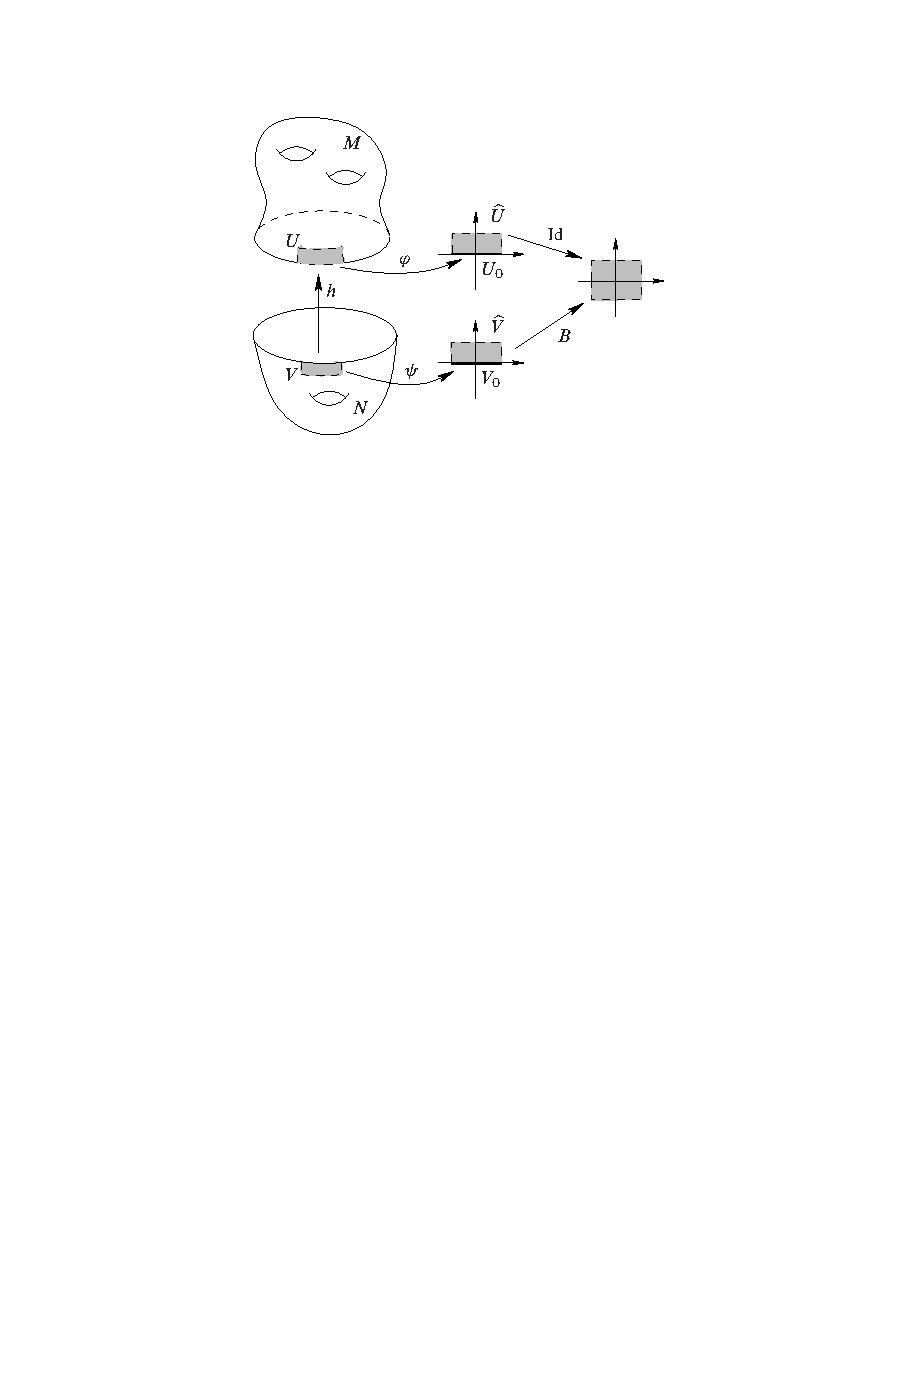
\includegraphics{pictures/attach-manifold}
\caption{Attaching along boundaries.}
\end{figure}

Suppose $s\in S$, and let $y\in\partial N$ and $x=h(y)\in\partial M$ be the two points in the fiber $q^{-1}(s)$. We can choose coordinate charts $(U,\varphi)$ for $M$ and $(V,\psi)$ for $N$ such that $x\in U$ and $y\in V$, and let $\widehat{U}=\varphi(U)$, $\widehat{V}=\psi(V)$. It is useful in this proof to identify $\H^n$ with $\R^{n-1}\times[0,+\infty)$ and $\R^n$ with $\R^{n-1}\times\R$. By shrinking $U$ and $V$ if necessary, we may assume that $h(V\cap\partial N)=U\cap\partial M$, and that $\widehat{U}=U_0\times[0,\eps)$ and $\widehat{V}=V_0\times[0,\eps)$ for some $\eps>0$ and some open subsets $U_0,V_0\sub\R^{n-1}$. Then we can write the coordinate maps as 
\[\varphi(x)=(\varphi_0(x),\varphi_1(x)),\quad\psi(y)=(\psi_0(y),\psi_1(y))\]
for some continuous maps $\varphi_0:U\to U_0$, $\varphi_1:U\to[0,\eps)$, $\psi_0:V\to V_0$ and $\psi_1:V\to[0,\eps)$. Our assumption that $x$ and $y$ are boundary points means that $\varphi_1(x)=\psi_1(y)=0$.\par
We wish to assemble these two charts into a map whose image is an open subset of $\R^n$, by matching them up along corresponding points in $\partial M$ and $\partial N$. As they stand, however, the maps $\varphi$ and might not take corresponding boundary points to the same image point, so we need to adjust for that. Both of the restrictions
\[\varphi_0|_{U\cap\partial M}:U\cap\partial M\to U_0,\quad \psi_0|_{V\cap\partial N}:V\cap\partial N\to V_0\]
are homeomorphisms. Define a homeomorphism $\tau:V_0\to U_0$ by
\[\tau=(\varphi_0|_{U\cap\partial M})\circ h\circ(\psi_0|_{V\cap\partial N})^{-1},\]
and let $B:\widehat{V}\to\R^n$ be the map
\[B(x_1,\dots,x_n)=(\tau(x_1,\dots,x_{n-1}),-x_n).\]
Geometrically, $B$ rearranges the boundary points according to the map $\tau$, and then "flips" each vertical line segment above a boundary point to a line segment below the image point. Our construction ensures that for $y\in\partial N$,
\begin{align}\label{attach manifold with boundary-1}
B\circ\psi(y)=(\tau\circ\psi(y),0)=(\varphi_0\circ h(y),0)=\varphi\circ h(y).
\end{align}
Now define $\widetilde{\varPhi}:U\amalg V\to\R^n$ by
\[\widetilde{\varPhi}=\begin{cases}
\varphi(y),&y\in U;\\
B\circ\psi(y),&y\in V.
\end{cases}\]
Because $U\amalg V$ is a saturated open subset of $M\amalg N$, the restriction of $q$ to it is a quotient map onto the neighborhood $q(U\amalg V)$ of $s$, and $(\ref{attach manifold with boundary-1})$ shows that $\widetilde{\varPhi}$ passes
to the quotient and defines an injective continuous map $\varPhi:q(U\amalg V)\to\R^n$. Since $\varphi$, $\psi$, and $B$ are homeomorphisms onto their images, we can define an inverse for $\varPhi$ as follows:
\[\varPhi^{-1}(y)=\begin{cases}
q\circ\varphi^{-1}(y),&y^n\geq 0;\\
q\circ\psi^{-1}\circ B^{-1}(y)&y^n\leq 0.
\end{cases}\]
These two definitions agree where they overlap, so the resulting map is continuous by the gluing lemma. Thus $\varPhi$ is a homeomorphism. Note that the image of $\varPhi$ is exactly $U_0\times(-\eps,\eps)$, which is open in $\R^n$. Therefore $M\cup_hN$ is locally Euclidean of dimension $n$.\par
The quotient space $M\cup_h N$ is second countable by Proposition~\ref{manifold quotient is manifold}. To prove that it is Hausdorff, we need to show that the fibers of $q$ can be separated by saturated open subsets. It is straightforward to check on a case-by-case base that the preimages of sufficiently small coordinate balls will do.\par
It follows immediately from Proposition~\ref{adjunction space prop}(a) that the quotient map $q$ restricts to a topological embedding of $M$ into $M\cup_h N$ with closed image. On the other hand, because $h$ is a homeomorphism, it is easy to see that $M\cup_h N$ is also equal to
$N\cup_{h^{-1}}M$, so $q$ also restricts to a topological embedding of $N$ with closed image. The union of the images of these embeddings is all of $M\cup_hN$, and their intersection is the set $S$ defined above, which is exactly the image of either boundary.
\end{proof}
Here is an important example of the preceding construction.
\begin{example}[\textbf{The Double of a Manifold with Boundary}]
Suppose $M$ is an ndimensional manifold with boundary. If $h:\partial M\to \partial M$ is the identity map, the resulting quotient space $M\cup_{h}M$ is denoted by $D(M)$ and called the \textbf{double of $\bm{M}$}. It can be visualized as the space obtained by attaching two copies of $M$ to each other along their common boundary. (If $\partial M=\emp$, then $D(M)$ is just the disjoint union of two copies of $M)$
\end{example}
The following proposition is an immediate consequence of Theorem~\ref{attach manifold with boundary}.
\begin{proposition}
Every $n$-manifold with boundary is homeomorphic to a closed subset of an $n$-manifold without boundary.
\end{proposition}
This construction can be used to extend many results about manifolds to manifolds with boundary. For example, any property that holds for all closed subsets of manifolds is also shared by manifolds with boundary.
\section{Paracompactness}
\subsection{Paracompact spaces}
Let $X$ be a topological space. A collection $\mathcal{A}$ of subsets of $X$ is said to be \textbf{locally finite} if each point of $X$ has a neighborhood that intersects at most finitely many of the sets in $\mathcal{A}$. Given a cover $\mathcal{A}$ of $X$, another cover $\mathcal{B}$ is called a \textbf{refinement} of $\mathcal{A}$ if for each $B\in\mathcal{B}$ there exists some $A\in\mathcal{A}$ such that $B\sub A$. It is an \textbf{open refinement} if each $B\in\mathcal{B}$ is an open subset of $X$. (Note that every subcover of $\mathcal{A}$ is a refinement of $\mathcal{A}$, but a refinement is not in general a subcover, because a refinement does not need to be composed of sets that are elements of $\mathcal{A}$.)\par
Here are some elementary properties of local finiteness. Given a collection $\mathcal{A}$ of subsets of a topological space, let us use the notation $\widebar{\mathcal{A}}$ to denote the collection of
closures of sets in $\mathcal{A}$:
\[\widebar{\mathcal{A}}:=\{\widebar{A}:A\in\mathcal{A}\}\]
\begin{lemma}\label{topological space locally iff closure is locally finite}
Let $X$ be a topological space and $\mathcal{A}$ be a collection of subsets of X. Then $\mathcal{A}$ is locally finite if and only $\widebar{\mathcal{A}}$ is locally finite.
\end{lemma}
\begin{proof}
If $\widebar{\mathcal{A}}$ is locally finite, then it follows immediately that $\mathcal{A}$ is locally finite. Conversely, suppose $\mathcal{A}$ is locally finite. Given $x\in X$, let $W$ be a neighborhood of $x$ that intersects only finitely many of the sets in $\mathcal{A}$, say $A_1,\dots,A_n$. If $W$ contains a point $a$ in $\widebar{A}$ for some $A\in\mathcal{A}$, then $W\cap A\neq\emp$ since $a$ is a limit point of $A$. It then follows that $A$ is one of the sets $A_1,\dots,A_n$, and therefore $W$ can only intersects finitely many sets in $\widebar{\mathcal{A}}$.
\end{proof}
\begin{lemma}\label{topological space locally finite family closure and union}
If $\mathcal{A}$ is a locally finite collection of subsets of $X$, then
\[\widebar{\bigcup_{A\in\mathcal{A}} A}=\bigcup_{A\in\mathcal{A}}\widebar{A}\]
\end{lemma}
\begin{proof}
The right-hand side is contained in the lefthand side even without the assumption of local finiteness, so we only prove the reverse containment. We will prove the contrapositive: assuming $x\in X$ is not an element of $\bigcup_{A\in\mathcal{A}}\widebar{A}$, we show it is not an element of $\widebar{\bigcup_{A\in\mathcal{A}} A}$ either. By Lemma~\ref{topological space locally iff closure is locally finite},
$x$ has a neighborhood $U$ that intersects only finitely many sets in $\widebar{A}$, say $\widebar{A}_1,\dots,\widebar{A}_k$. Then $U\setminus(\widebar{A}_1\cap\cdots\cap\widebar{A}_1)$ is a neighborhood of $x$ that intersects none of the sets in $\mathcal{A}$, so $x\notin\widebar{\bigcup_{A\in\mathcal{A}} A}$.
\end{proof}
\begin{definition}
A space $X$ is said to be \textbf{paracompact} if every open cover of $X$ admits a locally finite open refinement. Every compact space is paracompact, because a finite subcover is a locally finite open refinement.
\end{definition}
\begin{proposition}
A closed subspace of a paracompact space is paracompact.
\end{proposition}
\begin{proof}
If $A$ is a closed subspace of a paracompact space $X$, every open cover of $A$ is of the form $\{U_\alpha\}\cap A$, where $U_\alpha$ are open in $X$. Add in the open set $X-A$, we get an open cover of $X$, thus using paracompactness of $X$ we get the claim.
\end{proof}
A key topological fact about manifolds, as we show below, is that they are all paracompact. This is a consequence of second countability, and in fact is one of the most important reasons why second countability is included in the definition of manifolds. For spaces that are Hausdorff and locally Euclidean with countably many components, the two conditions are equivalent.\par
Before we prove that manifolds are paracompact, we need a preliminary result. If $X$ is a topological space, a sequence $\{K_i\}_{i\in\N}$ of compact subsets of $X$ is called an \textbf{exhaustion} of $X$ by compact sets if $X=\bigcup_{i}K_i$ and $K_i\sub\Int K_{i+1}$ for each $i$.
\begin{proposition}\label{exhaustion by compact}
A $\sigma$-compact locally compact Hausdorff space admits an exhaustion by compact sets.
\end{proposition}
\begin{proof}
Since $X$ is a $\sigma$-compact, there exists a sequence $\{K_i\}$ of compact subsets such that $X=\bigcup_iK_i$. Every compact subset of $X$ has a precompact open neighborhood by Proposition~\ref{LCH precompact nbhd for compact set}. Thus we may take $U_1$ to be a precompact open neighborhood of $K_1$, and then, proceeding inductively, take $U_n$ to be a precompact open neighborhood of $\widebar{U}_{i-1}\cup K_i$. It follows that the sequence $\{U_i\}$ satisfies $K_i\sub U_i$ and $\widebar{U}_{i}\sub U_{n+1}$. Let $\widetilde{K}_i=\widebar{U}_i$, then $\{\widetilde{K}_i\}$ is a exhaustion of $X$ by compact sets. 
\end{proof}
\begin{theorem}\label{loc compact paracompact}
Every $\sigma$-compact locally compact Hausdorff space is paracompact. In fact, given such a space $X$, an open cover $\mathcal{U}$ of $X$, and any base $\mathcal{B}$ for the topology of $X$, there exists a countable, locally finite open refinement of $\mathcal{U}$ consisting of elements of $\mathcal{B}$.
\end{theorem}
\begin{proof}
Given $X,\mathcal{U}$ and $\mathcal{B}$, by Proposition~\ref{exhaustion by compact}, let $(K_i)_{i\in\N}$ be an exhaustion of $X$ by compact sets. For each $i$, let
\[V_i=K_{i+1}\setminus\Int K_i,\quad W_i=\Int K_{i+2}\setminus K_{i-1}\]
where we interpret $K_i=\emp$ if $i<1$. Then $V_i$ is a compact set contained in the open subset $W_i$. For each $x\in V_i$, there is some $U_x\in\mathcal{U}$ containing $x$, and because $\mathcal{B}$ is a base, there exists $B_x\in\mathcal{B}$ such that $x\in B_x\sub U_x\cap W_i$. The collection of all such sets $B_x$ as $x$ ranges over $V_i$ is an open cover of $V_i$, and thus has a finite subcover. The union of all such finite subcovers as $i$ ranges over the positive integers is a countable open cover of $M$ that refines $\mathcal{U}$. Because the finite subcover of $V_i$ consists of sets contained in $W_i$, and $W_i\cap W_{j}\neq \emp$ only for $i-2<j<i+2$, the resulting cover is locally finite.
\end{proof}
In view of the theorem, one may wonder the connection between paracompactness and $\sigma$-compactness for a locally Hausdorff space. The following theorem answers this question.
\begin{theorem}\label{LCH paracompact iff sigma-compact}
A locally compact Hausdorff space $X$ is paracompact if and only if it is a disjoint union of open $\sigma$-compact subsets.
\end{theorem}
\begin{proof}
Assume that $X$ is paracompact. Using local compactness, cover the space with open precompact sets $U_\alpha$. Using paracompactness we may assum this cover is locally finite. We shall inductively construct open precompact sets $V_i$. We start with $V_1=U_\beta$ for some given $\beta$. If $V_i$ has been defined then consider all the $U_\alpha$ which intersect $\widebar{V}_i$: By compactness of $\widebar{V}_i$ and the local finiteness of the cover, this set of $U_\alpha$'s is finite. Let $V_{i+1}$ be the union of these $U_\alpha$. Then $\widebar{V}_{i+1}$ is the union of the closures of this finite set of $U_\alpha$'s and so it is compact. Also $\widebar{V}_i\sub V_{i+1}$. Put $V=\bigcup_iV_i$, then $V$ is open. By Lemma~\ref{topological space locally finite family closure and union} $\widebar{V}$ is the union of the closures of these $U_\alpha$'s. But by construction each of these closures is contained in some $\widebar{V}_i\sub V_{i+1}\sub V$. Thus $V=\widebar{V}$ is closed and by construction, is $\sigma$-compact. Now since $V$ is closed and open, it is a connected component of $X$. Thus $X$ is a disjoint union of open $\sigma$-compact subsets.\par
Conversely, assume that $X$ is a union of $\sigma$-compact subsets. It is clear that a disjoint union of open paracompact spaces is paracompact, and so we may as well assume the space $X$ to be $\sigma$-compact. Let $X=\bigcup_iC_i$ where the $C_i$ are compact. We define an exhaustion of $X$ by compact sets $K_i$.
\begin{itemize}
\item Let $K_1=C_1$. To define $K_2$, for each point $x\in C_1$ we find by local compactness a precompact neighborhood $U_x$ of $x$. Then the collection $\{U_x\}$ covers $C_1$, hence has a subcover $\{U^{(1)}_{1},\dots,U^{(1)}_{i_1}\}$. We set
\[K_2=C_2\cup\bigcup_{j=1}^{i_1}\widebar{U}^{(1)}_j\]
so $K_2$ is compact and $K_1\sub\Int K_2$.
\item Assume the ascending compact sets $K_1,\dots,K_n$ are defined. Now by the same argument we find precompact sets $\{U^{(n)}_1,\dots,U^{(n)}_{i_n}\}$ covers $K_n$. Then we set
\[K_{n+1}=C_n\cup\bigcup_{j=1}^{i_n}\widebar{U}_j^{(n)}\] 
Now $K_{n+1}$ is compact and $K_n\sub\Int K_{n+1}$. By induction we get the sequence $\{K_i\}$, and since each $C_i$ is contained in $K_i$, we have $X=\bigcup_iK_i$.
\end{itemize}
Now with this exhaustion by compact sets, by arguing as in the proof of Theorem~\ref{loc compact paracompact}, we can show that $X$ is paracompact.
\end{proof}
One feature of paracompact Hausdorff spaces is that they satisfy a strengthened version of the Hausdorff property. A topological space $X$ is said to be \textbf{normal} if it is Hausdorff and for every pair of disjoint closed subsets $A,B\sub X$, there exist disjoint open subsets $U,V\sub X$ such that $A\sub U$ and $B\sub V$. Similarly, $X$ is said to be \textbf{regular} if it is Hausdorff and for every closed subset $B\sub X$ and point $a\in B$, there exist disjoint open subsets $U,V\sub X$ such that $a\in U$ and $B\sub V$. Briefly, in normal spaces, closed subsets can be separated by open subsets; and in regular spaces, closed subsets can be separated from points by open subsets.
\begin{lemma}\label{Hausdorff normal iff}
Let $X$ be a Hausdorff space. Then $X$ is normal if and only if it satisfies the following condition: whenever $A$ is a closed subset of $X$ and $U$ is a neighborhood of $A$, there exists a neighborhood $V$ of $A$ such that $\widebar{V}\sub U$.
\end{lemma}
\begin{proof}
This is easily seen to be equivalent to the definition of normality by taking
$B=U^c$.
\end{proof}
\begin{theorem}\label{para is normal}
Every paracompact Hausdorff space is normal.
\end{theorem}
\begin{proof}
Suppose $X$ is a paracompact Hausdorff space, and let $A$ and $B$ be disjoint closed subsets of $X$. We begin with the special case in which $B=\{q\}$ is a singleton; in other words, we prove that $X$ is regular.\par
For each $p\in A$, because $X$ is Hausdorff there exist disjoint open subsets $U_p$ and$V_p$ such that $p\in U_p$ and $q\in V_p$. The collection $\{U_p:p\in A\}\cup\{X\setminus A\}$ is an open cover of $X$. By paracompactness, it has a locally finite open refinement $\mathcal{W}$. Each of the open subsets in $\mathcal{W}$ is contained either in $U_p$ for some $p$, or in $X\setminus A$. Let $\mathcal{U}$ be the collection of all the sets in $\mathcal{W}$ that are contained in some $U_p$. Then $\mathcal{U}$ is
still locally finite, and it is an open cover of $A$. Moreover, if $U\in\mathcal{U}$, then there is a neighborhood $V_p$ of $q$ disjoint from $U$, so $\widebar{U}$ does not contain $q$.\par
Let $\mathfrak{U}=\bigcup_{U\in\mathcal{U}}U$, and $\mathfrak{V}=X\setminus \mathfrak{U}$. Because $\mathcal{U}$ is locally finite, $\widebar{\mathfrak{U}}=\bigcup_{U\in\mathcal{U}}\widebar{U}$
by Lemma~\ref{topological space locally finite family closure and union}. Thus $q\notin\widebar{\mathfrak{U}}$, so $\mathfrak{U}$ and $\mathfrak{V}$ are disjoint open subsets of $X$ containing $A$ and $q$, respectively. This completes the proof that $X$ is regular. Next consider arbitrary disjoint closed subsets $A$ and $B$. Exactly the same argument
works in this case, using regularity in place of the Hausdorff condition.
\end{proof}
The following result is a nontrivial property about normal spaces.
\begin{theorem}[\textbf{Urysohn's Lemma}]\label{Urysohn lemma}
Suppose $X$ is a normal topological space. If $A,B\sub X$ are disjoint closed subsets, then there exists a continuous function $f:X\to[0,1]$ such that $f|_A\equiv0$ and $f|_B\equiv1$.
\end{theorem}
\begin{proof}We will construct for each rational number $r$ an open subset $U_r\sub X$, such
that the following properties hold
\begin{itemize}
\item[(a)] $U_r=\emp$ when $r<0$, and $U_r=X$ when $r>1$.
\item[(b)] $A\sub U_0$.
\item[(c)] $U_1=X\setminus B$.
\item[(d)] If $p<q$, then $\widebar{U}_p\sub U_q$
\end{itemize}
we will do this by induction. We begin by defining $U_1=X\setminus B$, and defining $U_r$ for $r\notin [0,1]$ by (a). By normality, there exists a neighborhood $U_0$ of $A$ such that $\widebar{U}_0\sub U_1$. Let $\{r_i\}_{i\in\N}$ be a enumeration of the rationals in $[0,1]$. By normality again, there exists an open subset $U_{r_1}\sub X$ such that $\widebar{U}_0\sub U_{r_1}$ and $\widebar{U}_{r_1}\sub U_1$. Now use induction, suppose $U_i$ has been defined for $i=1,\dots,n$ such that $\widebar{U}_0\sub U_{r_i}$, $\widebar{U}_{r_{i}}\sub U_1$ and $\widebar{U}_{r_{i}}\sub U_{r_{j}}$ for $r_i<r_j$. Consider the next rational number $r_{n+1}$ in the sequence, and let $p$ be the largest number in the set $\{0,r_1,\dots,r_n,1\}$ that is smaller than $r_{n+1}$, and $q$ the smallest number in the same set that is larger than $r_{n+1}$. Then $\widebar{U}_p\sub U_q$ By normality, there exists an open subset $U_{r_{n+1}}$ such that $\widebar{U}_{p}\sub U_{r_{n+1}}$ and $\widebar{U}_{r_{n+1}}\sub U_q$. Continuing by induction, we obtain open subsets $U_r$ for all rational $r$ satisfying the properties above.\par
Now, define $f:X\to\R$ by
\[f(x)=\inf\{r\in\Q:x\sub U_r\}.\]
Because of (a), $f$ is well defined and takes its values in $[0,1]$. Properties (a) and (b)
imply that $f(x)=0$ for $x\in A$, and (a) and (c) imply that $f(x)=1$ for $x\in B$. Thus
it remains only to show that $f$ is continuous.\par
Because sets of the form $(a,\infty)$ and $(-\infty,a)$ form a subbase for the topology of $\R$, it suffices to show that the preimage under $f$ of any such set is open. We begin with the following observations:
\begin{align}
&f(x)<a \iff x\in U_r\text{ for some rational }r<a\label{Urysohn-1}\\
&f(x)\leq a \iff x\in \widebar{U}_r\text{ for any rational }r>a\label{Urysohn-2}
\end{align}
The equivalence $(\ref{Urysohn-1})$ is an easy consequence of the definition of $f$. To prove $(\ref{Urysohn-2})$, suppose first that $f(x)\leq a$. If $r$ is any rational number greater than $a$, then by
definition of $f$, there is a rational number $s<r$ such that $x\in U_s\sub U_r\sub\widebar{U}_r$. Conversely, suppose $x\in\widebar{U}_r$ for every rational number greater than $a$. If $s>a$ is rational, choose a rational number $r$ such that $s>r>a$; it follows from our hypothesis that
$x\in\widebar{U}_r\sub U_s$, which implies that $f(x)\leq s$. Since this is true for every rationals $s>a$, it follows that $f(x)\leq a$.\par
From $(\ref{Urysohn-1})$ and $(\ref{Urysohn-2})$ we conclude that
\[f^{-1}\big((-\infty,a)\big)=\bigcup_{\substack{r\in\Q\\r<a}}U_r,\quad f^{-1}\big((a,\infty)\big)=X\setminus\bigcap_{\substack{r\in\Q\\r>a}}\widebar{U}_r\]
both of which are open. Thus $f$ is continuous.
\end{proof}
The next corollary of Urysohn's lemma is often the most useful. If $X$ is a topological space and $f:X\to \R$ is a continuous function, the support of $f$, denoted by $\supp(f)$, is the closure of the set $\{x\in X:f(x)\neq 0\}$:
\[\supp(f):=\widebar{\{x\in X:f(x)\neq 0\}}\]
If $A$ is a closed subset of $X$ and $U$ is a neighborhood of $A$, a continuous function $f:X\to[0,1]$ such that $f|_A\equiv1$ and $\supp(f)\sub U$ is called a \textbf{bump function} for $A$ supported in $U$.
\begin{theorem}
Let $X$ be a normal space. If $A$ is a closed subset of $X$ and $U$ is a neighborhood of $A$, there exists a bump function for $A$ supported in $U$.
\end{theorem}
\begin{proof}
Just apply Urysohn's Lemma with $B=X\setminus U$.
\end{proof}
One immediate consequence of the Urysohn lemma is the useful theorem called the Tietze extension theorem. It deals with the problem of extending a continuous realvalued function that is defined on a subspace of a space $X$ to a continuous function defined on all of $X$. This theorem is important in many of the applications of topology.
\begin{theorem}[\textbf{Tietze extension theorem}]
Let $X$ be a normal space and $A$ be a closed subspace of $X$.
\begin{itemize}
\item[(a)] Any continuous map of $A$ into a closed interval $[a,b]$ may be extended to a continuous map of all of $X$ into $[a,b]$.
\item[(b)] Any continuous map of $A$ into $\R$ may be extended to a continuous map of all of $X$ into $\R$.
\end{itemize}
\end{theorem}
\begin{proof}
We first prove (a). The idea of the proof is to construct a sequence of continuous functions $g_n$ defined on the entire space $X$, such that the sequence $g_n$ converges uniformly, and such that the restriction of $g_n$ to $A$ approximates $f$ more and more closely as $n$ becomes large. Then the limit function will be continuous, and its restriction to $A$ will equal $f$.\par
Without loss of generality, we may assume that $[a,b]=[0,1]$. We claim that there is a sequence $\{g_n:X\to [0,2^{n-1}/3^n]\}$ of continuous functions such that $0\leq f-\sum_{i=1}^{n}g_i\leq 2^{n-1}/3^n$ on $A$. To begin with, let $B=f^{-1}([0,1/3])$ and $C=f^{-1}([2/3,1])$. These are closed subsets of $A$, and since $A$ itself is closed, they are closed in $X$. By Urysohn's lemma there is a continuous $g_1:X\to [0,1/3]$ with $g_1=0$ on $B$ and $g_1=1/3$ on $C$; it follows that $0\leq f-g_1\leq 2/3$ on $A$. In general, having found $g_1,\dots,g_{n-1}$, by the same reasoning we can find $g_{n}:X\to[0,2^{n-1}/3^n]$ such that $g_n=0$ on the set where $f-\sum_{i=1}^{n-1}g_i\leq 2^{n-1}/3^n$ and $g_n=2^{n-1}/3^n$ on the set where $f-\sum_{i=1}^{n-1}g_i\geq (2/3)^n$. Let $F=\sum_{n=1}^{\infty}g_n$. Since $|g_n|\leq 2^{n-1}/3^n$, the partial sums of this series converge uniformly, so $F$ is continuous. Moreover, on $A$ we have $0<f-F<(2/3)^n$ for all $n$, whence $F=f$ on $A$.\par
We now prove part (b) of the theorem, in which $f$ maps $A$ into $\R$. We can replace $\R$ by the open interval $(0,1)$, since this interval is homeomorphic to $\R$. So let $f$ be a continuous map from $A$ into $(0,1)$. The half of the Tietze theorem already proved shows that we can extend $f$ to a continuous map $F:X\to[0,1]$ mapping $X$ into the closed interval. Let us define a subset $D$ of $X$ by the equation
\[D=F^{-1}(0)\cup F^{-1}(1).\]
Since $F$ is continuous, $D$ is a closed subset of $X$. Because $F(A)=f(A)$, which is contained in $(0,1)$, the set $A$ is disjoint from $D$. By the Urysohn lemma, there is a continuous function $\phi:X\to[0,1]$ such that $\phi(D)=\{0\}$ and $\phi(A)=\{1\}$. Define
\[\widetilde{F}=F(x)\phi(x).\]
Then $\widetilde{F}$ is continuous, being the product of two continuous functions. Also, $\widetilde{F}$ is an extension of $F$ with values in $(0,1)$. This finishes the proof.
\end{proof}
\subsection{Partitions of unity}
The applications of paracompactness are all based on a technical tool called a partition of unity, which can be used to blend together locally defined continuous maps into a global one.\par
For this purpose, we need to consider open covers indexed by some set. (Of course any open cover $\mathcal{U}$ can be considered as an indexed family, just by taking the index set to be $\mathcal{U}$ itself.) In this context, an indexed family $\mathcal{U}=(U_\alpha)_{\alpha\in A}$ of subsets of a topological space $X$ is said to be a \textbf{locally finite} family if each point of $X$ has a neighborhood that intersects $U_\alpha$ for at most finitely many values of $\alpha$.\par
If $\mathcal{U}=(U_\alpha)_{\alpha\in A}$ is an indexed open cover of $X$, a \textbf{partition of unity} subordinate to $\mathcal{U}$ is a family of continuous functions $\psi_\alpha:X\to\R$, indexed by the same set $A$, with the following properties:
\begin{itemize}
\item[(\rmnum{1})] $0\leq\psi_\alpha(x)\leq 1$ for all $\alpha\in A$ and all $x\in X$.
\item[(\rmnum{2})] $\supp(\psi_\alpha)\sub U_\alpha$.
\item[(\rmnum{3})] The family of supports $\{\supp(\psi_\alpha)\}_\alpha\in A$ is locally finite.
\item[(\rmnum{4})] $\sum_{\alpha\in A}\psi_\alpha(x)=1$ for all $x\in X$.
\end{itemize}
Because of the local finiteness condition (\rmnum{3}), the sum in (\rmnum{4}) has only finitely many nonzero terms in a neighborhood of each point, so there is no issue of convergence.\par
First we have a simple observation.
\begin{proposition}\label{partition of unity para}
Suppose $X$ is a topological space with the property that for every indexed open cover $\mathcal{U}$ of $X$, there exists a partition of unity subordinate to $\mathcal{U}$. Then $X$ is paracompact.
\end{proposition}
\begin{proof}
Let $\mathcal{U}=\{U_\alpha\}_{\alpha\in A}$ be any cover of $X$, and $\{\psi_\alpha\}_{\alpha\in A}$. Then since $\sum_{\alpha\in A}\psi_\alpha=1$, the collection $\{\supp(\psi_\alpha)\}_{\alpha\in A}$ covers $X$. Moreover, by definition this collection is a locally finite refinement of $\mathcal{U}$. Thus $X$ is paracompact.
\end{proof}
Now we want to prove the converse of Proposition~\ref{partition of unity para}. First we need some lemmas.
\begin{lemma}\label{part refin lem}
Suppose $X$ is a paracompact Hausdorff space. If $\mathcal{U}=(U_\alpha)_{\alpha\in A}$ is an indexed open cover of $X$, then $\mathcal{U}$ admits a locally finite open refinement $\mathcal{V}=(V_\alpha)_{\alpha\in A}$ indexed by the same set, such that $\widebar{V}_\alpha\sub U_\alpha$ for each $\alpha$.
\end{lemma}
\begin{proof}
By Lemma~\ref{Hausdorff normal iff} and Theorem~\ref{para is normal}, each $x\in X$ has a neighborhood $Y_x$ such that $\widebar{Y}_x\sub U_\alpha$ for some $\alpha\in A$. Since $X$ is paracompact, the open cover $\{Y_x:x\in X\}$ has a locally finite open refinement. Let us index this refinement by some set $B$, and denote it by $\mathcal{Z}=(Z_\beta)_{\beta\in B}$. For each $\beta$,there is some $x\in X$ such that $Z_\beta\sub Y_x$, and therefore there is some $\alpha\in A$ such that
$\widebar{Z}_\beta\sub \widebar{Y}_x\sub U_\alpha$. Define a function $a:B\to A$ by choosing some such index $\alpha\in A$ for each $\beta\in B$, and setting $a(\beta)=\alpha$.\par
For each $\alpha\in A$, define an open subset $V_\alpha\sub X$ by
\[V_\alpha=\bigcup_{a(\beta)=\alpha}Z_\beta\]
(If there are no indices $\beta$ such that $a(\beta)=\alpha$, then $V_\beta=\emp$.) Because the family $\mathcal{Z}$ is locally finite, the closure of $V_\alpha$ is equal to $\bigcup_{a(\beta)=\alpha}\widebar{Z}_{\beta}$ by Lemma~\ref{topological space locally finite family closure and union}, which is contained in $U_\alpha$ as required.
\end{proof}
\begin{theorem}[\textbf{Existence of Partitions of Unity}]\label{partition of unity}
Let $X$ be a paracompact Hausdorff space. If $\,\mathcal{U}$ is any indexed open cover of $X$, then there is a partition of unity subordinate to $\mathcal{U}$.
\end{theorem}
\begin{proof}
Let $\mathcal{U}=(U_\alpha)_{\alpha\in A}$ be an indexed open cover of $X$. Apply Lemma~\ref{part refin lem} twice, we obtain locally finite open covers $\mathcal{V}=(V_\alpha)_{\alpha\in A}$ and $\mathcal{W}=(W_\alpha)_{\alpha\in A}$ such that $\widebar{W}_\alpha\sub V_\alpha$ and $\widebar{V}_\alpha\sub U_\alpha$.\par
Now, for each $\alpha\in A$, let $f_\alpha:X\to[0,1]$ be a bump function for $\widebar{W}_\alpha$ supported in $V_\alpha$. Define $f:X\to\R$ by $f(x)=\sum_\alpha f_\alpha(x)$. Because $\supp(f_\alpha)\sub V_\alpha$, the family of supports $\{\supp(f_\alpha)\}_{\alpha\in A}$ is locally finite; thus each point of $X$ has a neighborhood on which only finitely many terms of this sum are nonzero, so $f$ is continuous. Because
the sets $\{W_\alpha\}$ cover X, for each $x\in X$ there is at least one $\alpha$ such that $x\in W_\alpha$ andthus $f_\alpha(x)=1$, so $f$ is everywhere positive. Therefore, we can define 
\[\psi_\alpha(x)=\dfrac{f_\alpha(x)}{f(x)}\]
Then $\{\psi_\alpha\}_{\alpha\in A}$ is the desired partition of unity, as one may check.
\end{proof}
\begin{theorem}[\textbf{Embeddability of Compact Manifolds}]
Every compact manifold is homeomorphic to a subset of some Euclidean space.
\end{theorem}
\begin{proof}
Suppose $M$ is a compact $n$-manifold. By compactness we can obtain a cover of $M$ by finitely many open subsets $U_1,\dots,U_k$, each of which is homeomorphic to $\R^n$. For each $i$, let $\varphi_i:U_i\to\R^n$ be a homeomorphism. Let $\{\psi_i\}$ be a partition of unity subordinate to this cover, and define functions $F_i:M\to \R^n$ by
\[F_i(x)=\left\{\begin{array}{cl}
\psi_i(x)\varphi_i(x), &x\in U_i\\
0, &x\in M\setminus \supp(\psi_i)
\end{array}\right. \]
Each $F_i$ is continuous by the pasting lemma.\par
Now define $F:M\to \R^{nk+k}$ by
\[F(x)=\big(F_1(x),\dots,F_k(x),\psi_1(x),\dots,\psi_k(x)\big)\] 
Then $F$ is continuous, and if we can show it is injective, it is a topological embedding
by the closed map lemma.\par
Suppose $F(x)=F(y)$ for some points $x,y\in M$. Since $\sum_i\psi_i(x)\equiv1$, there is some $i$ such that $\psi_i(x)>0$ and therefore $x\in U_i$. Because $F(x)=F(y)$ implies $\psi_i(y)=\psi_i(x)>0$, it follows that $y\in U_i$ as well. Then we see that $F_i(x)=F_i(y)$ implies $\varphi_i(x)=\varphi_i(y)$, which in turn implies that $x=y$ since $\varphi_i$ is injective on $U_i$.
\end{proof}
\begin{theorem}
Suppose $M$ is a topological manifold, and $B\sub M$ is any closed subset. Then there exists a continuous function $f:M\to[0,\infty)$ whose zero set is exactly $B$.
\end{theorem}
\begin{proof}
First, consider the special case in which $M=\R^n$ and $B\sub\R^n$ is a closed subset. It is straightforward to check that
\[u(x)=\inf\{|x-y|:y\in B\}\]
does the trick.\par
Now, let $M$ be an arbitrary $n$-manifold and let $B$ be a closed subset of $M$. Let $\mathcal{U}=(u_\alpha)_{\alpha\in A}$ be a cover of $M$ by open subsets homeomorphic to $\R^n$, and
let $\{\psi_\alpha\}_{\alpha\in A}$ be a subordinate partition of unity. For each $\psi_\alpha$ the construction in the preceding paragraph yields a continuous function $u_\alpha:U_\alpha\to [0,\infty)$ such that $u_\alpha^{-1}(0)=B\cap U_\alpha$. Define $f:M\to \R$ by
\[f(x)=\sum_{\alpha\in A}\psi_\alpha(x)u_\alpha(x)\]
where each summand is to be interpreted as zero outside the support of $\psi_\alpha$. Each term in this sum is continuous by the pasting lemma, and only finitely many terms are nonzero in a neighborhood of each point, so this defines a continuous function on $M$. It is easy to check that it is zero exactly on $B$.
\end{proof}
\begin{corollary}
Suppose $M$ is a topological manifold, and $A,B$ are disjoint closed subsets of $M$. Then there exists a continuous function $f:M\to [0,1]$ such that 
\[f^{-1}(0)=A,\quad f^{-1}(1)=B\]
\end{corollary}
\begin{proof}
Using the previous theorem, we can find $u,v: M\to [0,\infty)$ such that $u$ vanishes exactly on $A$ and $v$ vanishes exactly on $B$, and then the function $f(x)=v(x)/\big(u(x)+v(x)\big)$ satisfies the conclusion of the corollary.
\end{proof}
For our last application of partitions of unity, we need the following definition. If $M$ is a topological space, an \textbf{exhaustion function} for $M$ is a continuous function $f:M\to \R$ such that for every $c\in\R$, the sublevel set $f^{-1}\big((-\infty,c]\big)$ is compact. The name comes from the fact that as $k$ ranges through the positive integers, the sublevel sets $f^{-1}\big((-\infty,k]\big)$ form an exhaustion of $M$ by compact sets.
\begin{theorem}[\textbf{Existence of Exhaustion Functions}]\label{exhaustion functions}
Every manifold admits a positive exhaustion function.
\end{theorem}
\begin{proof}
Let $M$ be a manifold, let $\{U_i\}$ be a countable open cover of $M$ by precompact open subsets, and let $\{\psi_i\}$ be a partition of unity subordinate to this cover. Define $f:M\to\R$ by
\[f(x)=\sum_{k=1}^{\infty}k\psi_k(x)\]
Then $f$ is continuous since only finite terms are nonzero in a neighborhood of each point, and positive because $f(x)\geq\sum_{k}\psi_k(x)=1$. For any positive integer $m$, if $x\notin\bigcup_{k=1}^{m}\widebar{U}_k$, then $\psi_k(x)=0$ for $1\leq k\leq m$, so
\[f(x)=\sum_{k=m+1}^{\infty}k\psi_k(x)>\sum_{k=m+1}^{\infty}m\psi_k(x)=m\sum_{k=m+1}^{\infty}\psi_k(x)=m\]
The contrapositive of this last statement is that $f(x)\leq m$ implies $x\in\bigcup_{k=1}^{m}\widebar{U}_k$. Let $c\in\R$ be arbitrary, and let $m$ be any positive integer greater that $c$. It follows that $f^{-1}\big((-\infty,c]\big)$ is a closed subset of the compact set $\bigcup_{k=1}^{m}\widebar{U}_k$, and is therefore compact.
\end{proof}
\section{Uniform structures}
\subsection{Uniform spaces}
\begin{definition}
A \textbf{uniform structure} (or \textbf{uniformity}) on a set $X$ is a structure given by a set $\mathfrak{U}$ of subsets of $X\times X$ whick satisfies the following axioms:
\begin{itemize}
\item[(F1)] If $U\in\mathfrak{U}$ and $U\sub V\sub X\times X$, then $V\in\mathfrak{U}$.
\item[(F2)] If $U\in\mathfrak{U}$ and $V\in\mathfrak{U}$, then $U\cap V\in\mathfrak{U}$.
\item[(U1)] Every set in $\mathfrak{U}$ contains the diagonal $\Delta$.
\item[(U2)] If $U\in\mathfrak{U}$ then $U^{-1}\in\mathfrak{U}$, where $U^{-1}:=\{(y,x):(x,y)\in U\}$ is the \textbf{inverse} of $U$. 
\item[(U3)] If $U\in\mathfrak{U}$ then there is $V\in\mathfrak{U}$ such that $V\circ V\sub U$, where the composite of two sets $V,W\sub X\times X$ is defined by
\[V\circ W:=\{(x,z):\text{there exists $y\in X$ such that $(x,y)\in V$ and $(y,z)\in W$}\}.\]
\end{itemize}
The sets of $\mathfrak{U}$ are called \textbf{entourages} of the uniformity defined on $X$ by $\mathfrak{U}$. A set endowed with a uniformity is called a \textbf{uniform space}.
\end{definition}
If $U$ is an entourage of a uniformity on $X$, we may express the relation $(x,y)\in U$ by saying that "$x$ and $y$ are \textbf{$U$-close}". Note that if $X$ is nonempty then every set in $\mathfrak{U}$ is nonempty by (U1), and (F1) and (F2) impliy that $\mathfrak{U}$ is a filter on $X\times X$. There is only one uniformity on the empty set, namely $\{\emp\}$.\par
Throughout this part we shall also write $V^2$ instead of $V\circ V$, and in general $V^n=V\circ V^{n-1}=V^{n-1}\circ V$, for each integer $n>1$ and each subset $V\sub X\times X$. 
\begin{lemma}\label{uniformity equivalent axiom}
The conjunction of axioms (U2) and (U3) is equivalent (assuming the other axioms of uniform structures) to the following axiom:
\begin{itemize}
\item[(U2')] For each $U\in\mathfrak{U}$ there exists $V\in\mathfrak{U}$ such that $V\circ V^{-1}\sub U$.
\end{itemize}
\end{lemma}
\begin{proof}
Clearly (U2) and (U3) imply (U2'). Conversely, if (U2') is satisfied, then for every $U\in\mathfrak{U}$, there exists $V\in\mathfrak{U}$ such that $V\circ V^{-1}\sub U$, and so
\[V^{-1}=\Delta\circ V^{-1}\sub V\circ V^{-1}\sub U,\]
thus $V\sub U^{-1}$ and by (F1) we have $U^{-1}\in\mathfrak{U}$. This proves (U2). Let $W=V\cap V^{-1}$; then $W\in\mathfrak{U}$ by what we have just proved and (F2), and we have $W\circ W\sub V\circ V^{-1}\sub U$.
\end{proof}
\begin{example}
Let $(X,d)$ be a metric space. Then a uniformity on $X$ is given by subsets of the form
\[U_\eps=\{(x,y):d(x,y)<\eps\}.\]
In this case, $x$ and $y$ are $U_\eps$-close precisely when the distance between $x$ and $y$ is at most $\eps$.
\end{example}
A \textbf{base} or \textbf{fundamental system} of entourages of a uniformity $\mathfrak{U}$ is any set $\mathfrak{B}$ of entourages such that every entourage contains a set belonging to $\mathfrak{B}$.
\begin{example}
Axiom (U3) shows that if $n$ is any positive integer and $V$ runs through  a fundamental system of entourages, then the sets $V^n$ ($n$ times) again form a undamental system of entourages.
\end{example}
Entourages $V$ such that $V=V^{-1}$ are called \textbf{symmetric}. If $V$ is any entourage then $V\cap V^{-1}$ and $V\cup V^{-1}$ are symmetric entourages, and axioms (F2) and (U2) show that the symmetric entourages form a fundamental system of entourages.
\begin{proposition}\label{uniformity base iff}
A set $\mathfrak{B}$ of subsets of $X\times X$ is a fundamental system of entourages of a uniformity $\mathfrak{U}$ on $X$ if and only if $\mathfrak{B}$ is a filterbase and satisfies the following axioms:
\begin{itemize}
\item[(B1)] Every set in $\mathfrak{B}$ contains the diagonal.
\item[(B2)] For every $V\in\mathfrak{B}$ there exists $W\in\mathfrak{B}$ such that $W\sub V^{-1}$. 
\item[(B3)] For every $V\in\mathfrak{B}$ there exists $W\in\mathfrak{B}$ such that $W\circ W\sub V$.
\end{itemize}
\end{proposition}
\begin{proof}
If $\mathfrak{B}$ is a base for a uniformity $\mathfrak{U}$, then $\mathfrak{B}$ clearly satisfies the claimed properties. Conversely, assume the properties for $\mathfrak{B}$, and let $\mathfrak{U}$ be the filter in $X\times X$ generated by $\mathfrak{B}$. We prove that $\mathfrak{U}$ is a uniformity.\par
First, since $\mathfrak{U}$ is a filter, it satisfies (F1) and (F2). Also, by (B1) we see (U1) is satisfies. Now let $U\in\mathfrak{U}$, then $U\sups V$ for some $V\in\mathfrak{V}$. By (B2), there exists $W\in\mathfrak{U}$ such that $W\sub V^{-1}\sub U^{-1}$. Thus $U^{-1}\in\mathfrak{U}$ and (U2) holds. Also, by (B3) there also exists $W'\in\mathfrak{B}$ such that $W'\circ W'\sub V\sub U$. Since $W'\in\mathfrak{U}$, we see (U3) also holds. This completes the proof.
\end{proof}
\begin{example}
Let $X$ be a set and $R$ be an equivalence relation on $X$. Let $\Gamma\sub X\times X$ be the graph of $R$. Then $\Delta\sub\Gamma$ and $\Gamma\circ\Gamma=\Gamma^{-1}=\Gamma$. The set of subsets of $X\times X$ which consists of the set $C$ alone is therefore a fundamental system of entourages of a uniformity on $X$. In particular, if we take $R$ to be the relation of equality, then $C=\Delta$ and the entourages of the corresponding uniformity are all the subsets of $X\times X$ which contain $\Delta$; this uniformity is called the \textbf{discrete uniformity} on $X$, and the set $X$ endowed with this uniformity is called a \textbf{discrete uniform space}.
\end{example}
\begin{example}
On the set $\Z$ of rational integers we can define a uniformity, important in the theory of numbers, as follows: given a prime number $p$, let $U_n$ be the set of all pairs $(x,y)\in\Z\times\Z$ such that $x\equiv y$ mod $p^n$, for each positive integer $n$. It is easily verified that the sets $U_n$ (for a fixed $p$) form a fundamental system of entourages of a uniformity on $\Z$, called the \textbf{$\bm{p}$-adic uniformity}.
\end{example}
Now let $X$ and $Y$ be two sets each endowed with uniformities whose sets of entourages are $\mathfrak{U}$ and $\mathfrak{V}$ respectively, then a bijection $f$ of $X$ onto $Y$ is an isomorphism of the uniformity of $X$ onto that of $Y$ if $(f\times f)(\mathfrak{U})=\mathfrak{V}$.\par
Now we define the topology induced by a uniformity.
\begin{proposition}\label{uniformity induced topology}
Let $X$ be a set endowed with a uniform structure $\mathfrak{U}$, and for each $x\in X$ let $\mathfrak{U}(x)$ be the set of subsets $U(x)$ of $X$, where
\[U(x)=\{y\in X:(x,y)\in V\}\]
and $U$ runs through the set of entourages of $\mathfrak{U}$. Then there is a unique topology on $X$ such that, for each $x\in X$, $\mathfrak{U}(x)$ is the neighbourhood filter of $x$ in this topology.
\end{proposition}
\begin{proof}
We have to show that the $\mathfrak{U}(x)$ satisfy conditions of Proposition~\ref{topological space determined by nbhd filter}. In view of the axoims of uniformity, we only need to prove (U4). To see this, let $V$ be an entourage of $\mathfrak{U}$, $W$ an entourage of $\mathfrak{U}$ such that $W\circ W\sub V$; then if $(x,y)\in W$ and $(y,z)\in W$ we have $(x,z)\in V$, so that $W(y)\sub V(x)$ for all $y\in W(x)$, and therefore $V(x)\in\mathfrak{U}(y)$ for all $y\in W(x)$. This completes the proof.
\end{proof}
The topology defined in Proposition~\ref{uniformity induced topology} is called the \textbf{topology induced by the uniform structure $\mathfrak{U}$}.
\begin{example}
The topology induced by the additive uniformity on the set of real numbers is the topology of the real line. On any set $X$, the topology induced by the discrete uniformity is the discrete topology. The topology induced by the $p$-adic uniformity is the $p$-adic topology on $\Z$.
\end{example}
In the future, when we speak of the topology of a uniform space $X$, we shall always mean the topology induced by the uniform structure of the space, unless the contrary is expressly stated. The topological space obtained by putting this topology on the set $X$ is sometimes called the topological space \textit{underlying} the uniform space in question. For example, when we say that a uniform space is Hausdorff, or compact, or locally compact, etc., we mean that the underlying topological space has this property.\par
If $X$ and $Y$ are two uniform spaces, any isomorphism $f$ of the uniform structure of $X$ onto that of $Y$ is also a homeomorphism of $X$ onto $Y$; we say that $f$ is an \textbf{isomorphism} of the uniform space $X$ onto the uniform space $Y$. It should be noted that a homeomorphism of $X$ onto $Y$ is not necessarily an isomorphism of the uniform structure
of $X$ onto that of $Y$. In other words, distinct uniformities on the same set $X$ can induce the same topology. For example, on $(0,+\infty)$, the additive and the multiplicative uniformities (which are distinct) induce the same topology.
\begin{proposition}\label{uniformity on product space closure char}
Let $X$ be a uniform space. For every symmetric entourage $V$ of $X$ and every subset $S$ of $X\times X$, $V\circ S\circ V$ is a neighbourhood of $S$ in the product space $X\times X$, and the closure of $S$ in this space is given by the formula
\begin{align}\label{uniformity on product space closure char-1}
\widebar{S}=\bigcap_{V\in\mathfrak{S}}V\circ S\circ V
\end{align}
where $\mathfrak{S}$ denotes the set of symmetric entourages of $X$.
\end{proposition}
\begin{proof}
Let $V$ be a symmetric entourage of $X$. The relation $(x,y)\in V\circ S\circ V$ means that there is an element $(p,q)$ of $S$ such that $(x,p)\in V$ and $(q,y)\in V$: in other words ($V$ being symmetric) $x\in V(p)$ andy $y\in V(q)$, that is $(x,y)\in V(p)\times V(q)$. Since $V(p)\times V(q)$ is a neighbourhood of $(p,q)$ in $X\times X$, the first part of the proposition is proved. The relations $(x,p)\in V$, $(y,q)\in V$ can also be written $p\in V(x)$, $q\in V(y)$, or $(p,q)\in V(x)\times V(y)$. As $V$ runs through $\mathfrak{S}$, the sets $V(x)\times V(y)$ form a fundamental system of neighbourhoods of $(x,y)$ in $X\times X$; for if $U$ and $V$ are any two entourages there is always a symmetric entourage $W\sub U\cap V$, so that $W(x)\times W(y)\sub U(x)\times V(y)$. Hence $V(x)\times V(y)$ meets $S$ for each $V\in\mathfrak{S}$ if and only if $(x,y)\in\widebar{S}$ , and formula $(\ref{uniformity on product space closure char-1})$ follows.
\end{proof}
\begin{corollary}\label{uniformity topology closure char}
If $A$ is any subset of $X$ and $V$ is any symmetric entourage of $X$, then $V(A)$ is a neighbourhood of $A$ in $X$, and
\begin{align}\label{uniformity topology closure char-1}
\widebar{A}=\bigcap_{V\in\mathfrak{S}}V(A)=\bigcap_{V\in\mathfrak{U}}V(A)
\end{align}
where $\mathfrak{U}$ denotes the set of all entourages in $X$.
\end{corollary}
\begin{proof}
If $S=A\times A$, then $V\circ S\circ V=V(A)\times V(A)$ for any $V\in\mathfrak{S}$; for the relation "there exists $p\in A$ such that $(x,p)\in V$" is by definition equivalent to $x\in V(A)$. The corollary now follows from $\widebar{S}=\widebar{A}\times\widebar{A}$.
\end{proof}
The set $V(A)$ in Corollary~\ref{uniformity topology closure char} is called the \textbf{$V$-neighborhood} of $A$. It should be remarked that as $V$ runs through the set of entourages of $X$, the sets $V(A)$ do not necessarily form a fundamental system of neighbourhoods of $A$ in $X$.
\begin{example}
On the real line $\R$, carrying the additive uniformity, as $V$ runs through the filter of entourages of $\R$ the sets $V(\Z)$ do not form a fundamental system of neighbourhoods of the set $\Z$ of rational integers: the set
\[\bigcup_{n\in\Z}(n-\frac{1}{2^{|n|+1}},n+\frac{1}{2^{|n|+1}})\]
is a neighborhood of $\Z$, but it can not contain any $V(\Z)$ with $V$ an  entourage of $\R$.
\end{example}
\begin{corollary}\label{uniformity closure of cntourage is base}
The interiors (resp. the closures) of the entourages of $X$ in $X\times X$ form a fundamental system of entourages of $X$.
\end{corollary}
\begin{proof}
If $V$ is any entourage of $X$, there is a symmetric entourage $W$ such that $W\circ W\circ W\sub V$; since $W\circ W\circ W$ is a neighbourhood of $W$ (Proposition{uniformity on product space closure char}), the interior of $V$ in $X\times X$ contains $W$ and is therefore an entourage. Furthermore, we have $W\sub\widebar{W}\circ W\circ W\sub V$ by Proposition~\ref{uniformity on product space closure char}, and hence $V$ contains the closure of an entourage.
\end{proof}
\begin{corollary}\label{uniform space is regular}
Let $X$ be a uniform space. Then the set of closed neighbourhoods of a point of $X$ is a fundamental system of neighbourhoods of the point. Therefore, a Hausdorff uniform space is regular.
\end{corollary}
\begin{proof}
If $x$ is any point of $X$ and $V$ runs through the entourages of $X$ which are closed in $X\times X$, then the sets $V(x)$ form a fundamental system of neighbourhoods of $x$ in $X$ by Corollary~\ref{uniformity closure of cntourage is base}, and they are closed in $X$ as sections of $V$.
\end{proof}
\begin{proposition}\label{uniform space Hausdorff iff}
A uniform space $X$ is Hausdoiff if and only if the intersection of all the entourages of its uniform structure is the diagonal $\Delta$ of $X\times X$. Every Hausdoiff uniform space is regular.
\end{proposition}
\begin{proof}
We have seen that the closed entourages form a fundamental system of entourages; if their intersection is $\Delta$, then $\Delta$ is closed in $X\times X$ and consequently $X$ is Hausdorff. Conversely, if $X$ is Hausdorff then for every point $(x,y)\in\Delta$, there is an entourage $V$ of $X$ such that $y\notin V(x)$, or equivalently $(x,y)\notin V$; hence $\Delta$ is the intersection of all the entourages.
\end{proof}
If a uniform space $X$ is Hausdorff, we say that the uniform structure of $X$ is Hausdorff. If $\mathfrak{B}$ is a fundamental system of entourages for this structure, then $X$ is Hausdorff if and only if the intersection of all the sets of $\mathfrak{B}$ is $\Delta$.
\subsection{Uniformly continuous functions}
\begin{proposition}\label{uniformly continuous map iff}
Let $X$ and $Y$ be uniform spaces and $f:X\to Y$ be a map and $g=f\times f$. Then the following conditions are equivalent:
\begin{itemize}
\item[(\rmnum{1})] For each entourage $V$ of $Y$, there exists an entourage $U$ of $X$ such that if $(x,y)\in U$ then $(f(x),f(y))\in V$. 
\item[(\rmnum{2})] For each entourage $V$ of $Y$, $g^{-1}(V)$ is an entourage of $X$.
\end{itemize}
In the admissible case, we say $f$ is \textbf{uniformly continuous}.
\end{proposition}
\begin{proof}
Assume (\rmnum{1}). Then we see $g^{-1}(V)$ contains the entourage $U$ in (\rmnum{1}), so it is an entourage of $X$. Conversely, if (\rmnum{2}) holds, then it follows from $g(g^{-1}(V))\sub V$ that (\rmnum{1}) holds.
\end{proof}
It follows from definition that a uniformly continuous function must be continuous. On the other hand, a continuous mapping of a uniform space $X$ into a uniform space $Y$ need not be uniformly continuous, as is shown by the example $x\mapsto x^3$, a homeomorphism of $\R$ onto itself, which is not uniformly continuous with respect to the additive uniformity
\begin{example}[\textbf{Examples of uniformly continuous maps}]
\mbox{}
\begin{itemize}
\item[(a)] The identity mapping of a uniform space onto itself is
uniformly continuous.
\item[(b)] A constant mapping of a uniform space into a uniform space is uniformly continuous.
\item[(c)] Every mapping of a discrete uniform space into a uniform space is uniformly continuous.
\end{itemize}
\end{example}
The following properties of uniformly continuous maps are immediate.
\begin{proposition}\label{uniformly continuous map prop}
\mbox{}
\begin{itemize}
\item[(a)] If $f:X\to Y$ and $g:Y\to Z$ are two uniformly continuous maps, then $g\circ f:X\to Z$ is uniformly continuous.
\item[(b)] A bijection $f$ of a uniform space $X$ onto a uniform space $Y$ is an isomorphism if and only if $f$ and $f^{-1}$ are uniformly continuous.
\end{itemize}
\end{proposition}
\begin{proof}
The first claim follows from the interpretation of uniformly continuity in Proposition~\ref{uniformly continuous map iff}(\rmnum{1}), and part (b) follows from Proposition~\ref{uniformly continuous map iff}(\rmnum{2}).
\end{proof}
Proposition~\ref{uniformly continuous map prop} shows that we can take as morphisms of uniform structures the uniformly continuous mappings; we shall always assume in the future that the morphisms have been so chosen. In accordance with the general definitions, this allows us to define an order relation on the set of uniformities on a given set $X$:
\begin{definition}
If $\mathfrak{U}_1$ and $\mathfrak{U}_2$ are two uniform structures on the same set $X$, then $\mathfrak{U}_1$ is said to be \textbf{finer} than $\mathfrak{U}_2$ (and $\mathfrak{U}_2$ \textbf{coarser} than $\mathfrak{U}_1$) if the identity map $(X,\mathfrak{U}_1)\to(X,\mathfrak{U}_2)$ is uniformlY continuous.
\end{definition}
If $\mathfrak{U}_1$ is finer than $\mathfrak{U}_2$ and distinct from $\mathfrak{U}_2$ we say that $\mathfrak{U}_1$ is strictly finer than $\mathfrak{U}_2$ (and that $\mathfrak{U}_2$ is strictly coarser than $\mathfrak{U}_1$). Two uniformities are said to be comparable if one is finer than the other. By definition, the following results is clear.
\begin{proposition}\label{uniformity finer iff}
\mbox{}
\begin{itemize}
\item[(a)] If $\mathfrak{U}_1$ and $\mathfrak{U}_2$ are two uniformities on a set $X$, then $\mathfrak{U}_1$ is finer than $\mathfrak{U}_2$ if and only if every entourage of $\mathfrak{U}_2$ is an entourage of $\mathfrak{U}_1$.
\item[(b)] Let $\mathfrak{U}_1$ and $\mathfrak{U}_2$ be two uniformities on a set $X$ and suppose that $\mathfrak{U}_1$ is finer than $\mathfrak{U}_2$; then the topology induced by $\mathfrak{U}_1$ is finer than the topology induced by $\mathfrak{U}_2$.
\end{itemize}
\end{proposition}
It can happen that a uniformity $\mathfrak{U}$ is strictly finer than a uniformity $\mathfrak{U}'$, but that the two induced topologies are identical. The following example shows this:
\begin{example}\label{uniformity of finite partition}
Let $X$ be a nonempty set. For each finite partition $\omega=(A_i)_{i=1}^{n}$ of $X$, let $V_{\omega}$ denote
\[\bigcup_{i=1}^{n}(A_i\times A_i)\]
The sets $V_\omega$ then form a fundamental system of entourage of a uniformity $\mathfrak{U}$ on $X$. For if $\omega$ is any finite partition of $X$ we have $\Delta\sub V_\omega$ and $V_\omega\circ V_\omega=V_\omega^{-1}=V_\omega$; and if $\beta=(B_j)$ and $\delta=(C_k)$ are two finite partitions of $X$, then those of the sets $B_j\cap C_k$ which are not empty form a finite partition $\omega$ of $X$, and we have $V_\omega\sub V_\beta\circ V_\delta$. The uniformity $\mathfrak{U}$ is called the uniformity of finite partitions on $X$. The topology induced by $\mathfrak{U}$ is the discrete topology, since for each $x\in X$ the sets $\{x\}$ and $\{x\}^c$ form a finite partition of $X$. Nevertheless, if $X$ is infinite, it is clear that $\mathfrak{U}$ is strictly coarser than the discrete uniformity.
\end{example}
\subsection{Construction of uniform structures}
\subsubsection{Initial uniformities}
\begin{proposition}\label{uniformity initial structure}
Let $X$ be a set, $(Y_i)_{i\in I}$ be a family of uniform spaces. For each $i\in I$ let $f_i:X\to Y_i$ be a mapping of $X$ into $Y_i$ and put $g_i=f_i\times f_i$. Let $\mathfrak{B}$ be the set of all finite intersections
\[U(V_{i_1},\dots,V_{i_n})=\bigcap_{k=1}^{n}g_{i_k}^{-1}(V_{i_k})\]
where $V_{i_k}$ is an entourage of $Y_{i_k}$. Then $\mathfrak{B}$ is a fundamental system of entourages of a uniformity $\mathfrak{U}$ on $X$ which is the initial uniform structure on $X$ with respect to the family $(Y_i)$, and in particular $\mathfrak{U}$ is the coarsest uniformity on $X$ for which all the mappings $f_i$ are uniformly continuous.
\end{proposition}
\begin{proof}
It is immediately seen that $\mathfrak{B}$ is a filterbase satisfies axioms (B1). If $W_i=g_i^{-1}(V_i)$, then $W_i^{-1}=g_i^{-1}(V_i^{-1})$ and $W_i\circ W_i=g_i^{-1}(V_i\circ V_i)$; hence $\mathfrak{B}$ also satisfies axioms (B2) and (B3) and is therefore a fundamental system of entourages of a uniformity $\mathfrak{U}$ on $X$. Furthermore, it follows immediately from the definition of $\mathfrak{U}$ that $f_i$ is uniformly continuous for each index $i\in I$; hence $f_i\circ h$ is uniformly continuous for each $i\in I$ if $h$ is. Conversely, suppose that $f_i\circ h$ is uniformly continuous for each $i\in I$, and consider a set $U(V_{i_1},\dots,V_{i_n})$; by hypothesis, for each $1\leq j\leq n$, there is an entourage $W_k$ of $Z$ such that the relation $(z,z')\in W_k$ implies $(f_{i_k}(h(z)),f_{i_k}(h(z')))\in V_k$; if $W=\bigcap_{j=1}^{n}W_k$, then these $n$ relations are simultaneously satisfied whenever $z$ and $z'$ are $W$-close, so that we have then $(h(z),h(z'))\in U(V_{i_1},\dots,V_{i_n})$ and the proof is complete.
\end{proof}
\begin{corollary}\label{uniformity initial structure is initial topology}
The topology on $X$ induced by the coarsest uniformity $\mathfrak{U}$, for whick the $f_i$ are uniformly continuous is also the coarsest topology for which the $f_i$ are continuous.
\end{corollary}
\begin{proof}
This is an immediate consequence of the definition of the neighbourhoods of a point in this latter topology.
\end{proof}
The general properties of initial structures imply in particular the following transitivity property:
\begin{proposition}
Let $X$ be a set, $(Z_\beta)_{\beta\in J}$ a family of uniform spaces, $(J_\alpha)_{\alpha\in I}$ a partition of $J$ and $(Y_\alpha)_{\alpha\in I}$ a family of sets indexed by $I$. For each $\alpha\in I$, let $g_\alpha$ be a mapping of $X$ into $Y_\alpha$; and for each $\beta\in J_\alpha$, let $h_{\beta\alpha}$ be a mapping of $Y_\alpha$ into $Z_\beta$, and put $f_\beta=h_{\beta\alpha}\circ g_\alpha$. 
\[\begin{tikzcd}
X\ar[r,"g_\alpha"]&Y_\alpha\ar[r,"h_{\beta\alpha}"]&Z_\beta
\end{tikzcd}\]
If each $Y_\alpha$ carries the initial uniform structure induced by $(h_{\beta\alpha})_{\beta\in J_\alpha}$ then the initial uniform structure on $X$ induced by $(f_\beta)_{\beta\in J}$ is the same as the initial uniform structure induced by $(g_\alpha)_{\alpha\in I}$.
\end{proposition}
Let $X$ be a set, $Y$ a uniform space, $f$ a mapping of $X$ into $Y$. The coarsest uniformity $\mathfrak{U}$ on $X$ for which $f$ is uniformly continuous is called the \textbf{inverse image} under $f$ of the uniform structure of $Y$. It follows from Proposition~\ref{uniformity initial structure} that the inverse images under $g=f\times f$ of the entourages of $Y$ form a fundamental system of entourages for $\mathfrak{U}$. The topology induced by $\mathfrak{U}$ is the inverse image under $f$ of the topology of $Y$. Note that if $f:X\to Y$ is surjective, then the entourages of $Y$ are the \textbf{direct images} under $g$ of the entourages of $X$.\par
Let $A$ be a subset of a uniform space $X$. The uniformity induced on $A$ by the uniformity of $X$ is the inverse image of the latter under the canonical injection $A\hookrightarrow X$. By Proposition~\ref{uniformity initial structure}, this is equivalent to the following definition:
\begin{definition}
Let $A$ be a subset oj a uniform space $X$. The uniformity on $A$ whose set of entourages is the trace on $A\times A$ of the set of entourages of $X$ is called the uniformity induced on $A$ by the uniformity of $X$.
\end{definition}
The topology induced by the uniformity induced on $A$ is. the same as the topology induced on $A$ by the topology of $X$; the set $A$, together with the uniformity and the topology induced by those of $X$, is called a \textbf{uniform subspace} of $X$.\par
If $A$ is a subset of a uniform space $X$ and if $f:X\to Y$ is a uniformly continuous mapping, then the restriction $f|_A$ is a uniformly continuous mapping of $A$ into $Y$. If $B\sub Y$ is such that $f(X)\sub B$, then the mapping of $X$ into the uniform subspace $B$ of $Y$, having the same graph as $f$, is again uniformly continuous.
\begin{proposition}\label{uniformity by dense subset}
Let $A$ be a dense subset of a uniform space $X$. Then the closures in $X\times X$ of the entourages of the uniform subspace $A$ form a fundamental system of entourages of $X$.
\end{proposition}
\begin{proof}
First we note that, if $U$ is open in $X$ then for any subset $B$ of $X$ we have $U\cap\widebar{B}\sub\widebar{U\cap B}$. In fact, if $x\in U\cap\widebar{B}$, then for any neighborhood $V$ of $x$, $U\cap V$ is also a neighborhood of $x$ and thus $U\cap V\cap B\neq\emp$ (since $x\in\widebar{B}$). This implies $x\in\widebar{U\cap B}$.\par
Now let $V$ be an open entourage of $A$; it is the intersection of $A\times A$ with an open entourage $U$ of $X$. By what we have proved, $\widebar{V}\sub U\sub\widebar{V}$. Thus the claim follows.
\end{proof}
Note that every family $(\mathfrak{U}_i)_{i\in I}$ of uniformities on a set $X$ has a \textbf{least upper bound} $\mathfrak{U}$ in the ordered set of all uniformities on $X$: we have only to apply Proposition~\ref{uniformity initial structure}, taking $Y_i$ to be the set $X$ with the unifonnity $\mathfrak{U}_i$ and $f_i$ to be the identity mapping $X\to Y_i$. The topology induced by $\mathfrak{U}$ is just the least upper bound of the topologies induced by the $\mathfrak{U}_i$.
\begin{example}
If $\omega=(A_i)_{i=1}^{n}$ is any finite partition of a nonempty set $X$, the set $V_\omega=\bigcup_{i=1}^{n}A_i\times A_i$ by itself constitutes a fundamental system of entourages of a uniformity $\mathfrak{U}_\omega$ on $X$; the uniformity of finite partitions on $X$ (Example~\ref{uniformity of finite partition}) is then the least upper bound of the uniformities $\mathfrak{U}_\omega$.
\end{example}
Using initial uniformity, we can consider products of uniform spaces. If $(X_i)_{i\in I}$ is a family of uniform spaces, the product uniform space of this family is the product set $X=\prod_{i\in I}X_i$ endowed with the coarsest uniformity for which the projections $\pi_i:X\to X_i$ are uniformly continuous. This uniformity is called the \textbf{product} of the uniformities of the $X_i$ and the uniform spaces $X_i$ are called the \textbf{factors} of $X$. By Corollary~\ref{uniformity initial structure is initial topology}, the topology induced by the product uniformity on $X$ is same as the product of the topologies of the $X_i$.
\begin{proposition}\label{uniformity product continuous iff component}
Let $f=(f_i)$ be a mapping of a uniform space $Y$ into a product uniform space $X=\prod_{i\in I}X_i$. Then $f$ is uniformly continuous if and only if each $f_i$ is uniformly continuous.
\end{proposition}
\begin{proof}
Since $f_i=\pi_i\circ f$, this is a particular case of Proposition~\ref{uniformity initial structure}.
\end{proof}
\begin{corollary}\label{uniform space product map uniformly continuous iff}
Let $(X_i)_{i\in I}$ and $(Y_i)_{i\in I}$ be two families of uniform spaces indexed by the same set $I$. For each $i\in I$, let $f_i$ be a mapping of $X_i$ into $Y_i$. If each of the $f_i$ is uniformly continuous, then so is the product mapping
\[f:\prod_{i\in I}X_i\to\prod_{i\in I}Y_i,\quad (x_i)\mapsto(f_i(x_i)).\]
Conversely, if the $X_i$'s are nonempty and $f$ is uniformly continuous, then each $f_i$ is uniformly continuous.
\end{corollary}
\begin{proof}
The map $f$ can be written as $x\mapsto(f_i(\pi_i(x)))$, and the first part of the corollary therefore follows from Proposition~\ref{uniformity product continuous iff component}. Conversely, choose $a=(a_i)\in\prod_{i\in I}X_i$. For each $j\in I$ let $g_j$ be the mapping of $X_j$ into $\prod_{i\in I}X_i$ such that $\pi_j(g_j(x))=x_j$ and $\pi_i(g_j(x_j))=a_i$, whenever $i\neq j$. Then $g_j$ is uniformly continuous at the point $a_j$. Since $f_j=\pi_j\circ f\circ g_j$, it follows that if $f$ is uniformly continuous at $a$, then $f_j$ is uniformly continuous at $a_j$.
\end{proof}
The general criterion of transitivity of initial uniformities shows that, as for the product of topological spaces, the product of uniform spaces is associative and that the following is true:
\begin{proposition}
Let $X$ be a set, let $(Y_i)_{i\in I}$ be a family of uniform spaces, and for each $i\in I$ let $f_i$ be a mapping of $X$ into $Y_i$. Let $f$ be the mapping $x\mapsto(f_i(x))$ of $X$ into $Y=\prod_{i\in I}Y_i$ and let $\mathfrak{U}$ be the coarsest uniformity on $X$ for which the $f_i$ are uniformly continuous. Then $\mathfrak{U}$ is the inverse image under $f$ of the uniformity induced on $f(X)$ by the product uniformity on $Y$.
\end{proposition}
\begin{corollary}
For each $i\in I$, let $A_i$ be a subspace of $X_i$. Then the uniformity induced on $A=\prod_{i\in I}A_i$ by the product uniformity on $\prod_{i\in I}X_i$ is the same as the product of the uniformities of the subspaces $A_i$.
\end{corollary}
To conclude this part, we introduce the inverse limit of uniform spaces. Let $(I,\preceq)$ be a partially ordered set. For each $\alpha\in I$ let $X_\alpha$ be a uniform space, and for each pair of indices $\alpha,\beta$ such that $\alpha\preceq\beta$ there is a map $f_{\alpha\beta}:X_\beta\to X_\alpha$. We shall say that $(X_\alpha,f_{\alpha\beta})$ is an inverse system of uniform spaces if 
\begin{itemize}
\item[(a)] $(X_\alpha,f_{\alpha\beta})$ is an inverse system sets.
\item[(b)] Each map $f_{\alpha\beta}$ is uniformly continuous.
\end{itemize}
On $X=\llim X_i$ the coarsest uniformity for which the canonical mappings $f_\alpha:X\to X_\alpha$ are uniformly continuous is called the inverse limit (with respect to the $f_{\alpha\beta}$) of the uniformities of the $X_\alpha$, and the set $X$ endowed with this coarsest uniformity is called the \textbf{inverse limit of the inverse system of uniform spaces $\bm{(X_\alpha,f_{\alpha\beta})}$}.
\begin{proposition}
Let $I$ be a directed set, let $(X_\alpha,f_{\alpha\beta})$ be an inverse system of uniform spaces indexed by $I$, and let $J$ be a cofinal subset of $I$. For each $\alpha\in I$ let $f_\alpha$ be the canonical mapping of $X=\llim X_\alpha$ into $X_\alpha$, and let $g_\alpha$ denote $f_\alpha\times f_\alpha$. Then the family of sets $g_\alpha^{-1}(V_\alpha)$, where $\alpha$ runs through $J$ and where, for each $\alpha\in J$, $V_\alpha$ runs through a fundamental system of entourages of $X_\alpha$, is a fundamental system of entourages of $X$.
\end{proposition}
Finally, the topology on $X=\llim X_\alpha$ induced by the inverse limit of the uniformities of the $X_\alpha$ is the inverse limit of the topologies of the $X_\alpha$.
\subsection{Complete spaces}
\subsubsection{Cauchy filters}
Once a set $X$ has been endowed with a uniform structure we can define what is meant by a "small" subset of $X$ (relative to this structure): a "small" subset of $X$ is one in which all the points are "very close" to each other. Precisely:
\begin{definition}
If $X$ is a uniform space and if $V$ is an entourage of $X$, a subset $A$ of $X$ is said to be \textbf{$V$-small} if every pair of points of $A$ are $V$-close (in other words, if $A\times A\sub V$).
\end{definition}
The following result can be viewed as a "triangle inequality" property for $U$-closeness.
\begin{proposition}\label{uniform space union smallness}
In a uniform space $X$, if two sets $A$ and $B$ are $V$-small and intersect, then their union $A\cup B$ is $V\circ V$-small.
\end{proposition}
\begin{proof}
Let $x$ and $y$ be any two points of $A\cup B$, and let $z\in A\cap B$. Then $(x,z)\in V$ and $(z,y)\in V$, so that $(x,y)\in V\circ V$.
\end{proof}
A filter $\mathfrak{F}$ on a uniform space $X$ is a Cauchy filter if for each entourage $V$ of $X$ there is a subset of $X$ which is $V$-small and belongs to $\mathfrak{F}$.
\begin{remark}
An infinite sequence $(x_n)$ of points of a uniform space $X$ is said to be a \textbf{Cauchy sequence} if the elementary filter associated with the sequence is a Cauchy filter. It comes to the same thing to say that for each entourage $V$ of $X$ there is an integer $N$ such that for all integers $n,m>N$, we have $(x_n,x_m)\in V$.
\end{remark}
\begin{example}[\textbf{Example of Cauchy filters}]
\mbox{}
\begin{itemize}
\item[(a)] Let $X$ be a discrete uniform space, then the Cauchy filters on $X$ are trivial filters: since $\Delta$ is the unique entourage on $X$, any Cauchy filter must contains a singleton.
\item[(b)] Let $X$ be an infinite set and endow $X$ with the finite partition uniformity. Then any Cauchy filter $\mathfrak{F}$ on $X$ is ultra: if $A\sub X$, then $A$ and $A^c$ form a partition of $X$, and with $V=(A\times A)\cup(A^c\times A^c)$, we see either $A$ contains a set in $\mathfrak{F}$ of $A^c$ contains a set in $\mathfrak{F}$. Thus by Theorem~\ref{ultrafilter char}, $\mathfrak{F}$ is ultra.
\end{itemize}
\end{example}
\begin{proposition}\label{filter convergent is Cauchy}
On a uniform space $X$ every convergent filter is a Cauchy filter.
\end{proposition}
\begin{proof}
If $x$ is any point of $X$ and $V$ is any symmetric entourage of $X$, then the neighbourhood $V(x)$ of $x$ is $V\circ V$-small. If $\mathfrak{F}$ is a filter which converges to $x$, there is a set of $\mathfrak{F}$ contained in $V(x)$, and therefore $V\circ V$-small. Together with axoim (U3), this proves $\mathfrak{F}$ is Cauchy.
\end{proof}
\begin{proposition}\label{Cauchy filter image under uniformly continuous}
Let $f:X\to Y$ he a uniformly continuous mapping. Then the image under $f$ of a Cauchy filter base on $X$ is a Cauchy filter base on $Y$.
\end{proposition}
\begin{proof}
Let $g=f\times f$. If $V$ is an entourage of $Y$, then $g^{-1}(V)$ is an entourage of $X$, and the image under $f$ of a $g^{-1}(V)$-small set is $V$-small; hence the result.
\end{proof}
It follows in particular that if the uniformity of a uniform space $X$ is replaced by a coarser uniformity, then every Cauchy filter with respect to the original uniformity remains a Cauchy filter with respect to the new uniformity. This fact can be easily remembered in the following form: the finer the uniformiyy, the fewer Cauchy filters there are.
\begin{proposition}\label{filter Cauchy on initial topology iff}
Let $X$ be a set, let $(Y_i)_{i\in I}$ be a family of uniform spaces, and for each $i\in I$ let $f_i$ be a mapping of $X$ into $Y_i$. Let $X$ carry the coarsest uniformiry $\mathfrak{U}$ for which the $f_i$ are uniformly continuous. Then in order that a filter base $\mathfrak{B}$ on $X$ should be a Cauchy filter base it is necessary and sufficient that $f_i(\mathfrak{B})$ should be a Cauchy filter base on $Y_i$ for each $i\in I$.
\end{proposition}
\begin{proof}
The condition is necessary by Proposition~\ref{Cauchy filter image under uniformly continuous}. Conversely, suppose that it is satisfied, and let $U(V_{i_1},\dots,V_{i_n})$ be an entourage of the uniformity $\mathfrak{U}$. By hypothesis, for each index $k$ there is a set $M_k\in\mathfrak{B}$ such that $f_{i_k}(M_k)$ is $V_{i_k}$-small. Let $M$ be a set of $\mathfrak{B}$ contained in $M_k$ for $1\leq k\leq n$; then for each pair of points $x,y$ of $M$ we have $(f_{i_k}(x),f_{i_k}(y))\in V_{i_k}$, $1\leq k\leq n$, so that
\[(x,y)\in I(V_{i_1},\dots,V_{i_n}).\]
This completes the proof.
\end{proof}
\begin{corollary}
If a Cauchy filter on a uniform space $X$ induces a filter on a subset $A$ of $X$, then this filter is a Cauchy filter on the uniform subspace $A$.
\end{corollary}
\begin{corollary}\label{filter Cauchy product space iff}
A filter base $\mathfrak{B}$ on a product $\prod_{i\in I}X_i$ of uniform spaces is a Cauchy filter base if and only if, for each $i\in I$, $\pi_i(\mathfrak{B})$ is a Cauchy filter base on $X_i$.
\end{corollary}
The minimal elements (with respect to inclusion) of the set of Cauchy filters on a uniform space $X$ are called \textbf{minimal Cauchy filters} on $X$.
\begin{proposition}\label{minimal Cauchy filter contained in filter}
Let $X$ be a uniform space. For each Cauchy filter $\mathfrak{F}$ on $X$ there is a unique minimal Cauchy filter $\mathfrak{F}_0$ coarser than $\mathfrak{F}$. If $\mathfrak{B}$ is a base of $\mathfrak{F}$ and $\mathfrak{S}$ is a fundamental system of symmetric entourages of $X$, then the sets $\{V(M):M\in\mathfrak{B},V\in\mathfrak{S}\}$ form a base of $\mathfrak{F}_0$.
\end{proposition}
\begin{proof}
If $M,M'$ are in $\mathfrak{B}$ and $V,V'$ are in $\mathfrak{S}$, then there is a set $N\in\mathfrak{B}$ and $W\in\mathfrak{S}$ such that $N\sub M\cap M'$ and $W\sub V\cap V'$. Hence
\[W(N)\sub V(M)\cap V'(M')\]
and therefore the sets $\{V(M):M\in\mathfrak{B},V\in\mathfrak{S}\}$ indeed form a base of a filter $\mathfrak{F}_0$ on $X$. Further, if $M$ is $V$-small, then $V(M)$ is $V^3$-small; hence $\mathfrak{F}_0$ is a Cauchy filter and is clearly coarser than $\mathfrak{F}$. To complete the proof it is enough to show that if $\mathfrak{G}$ is a Cauchy filter coarser than $\mathfrak{F}$, then $\mathfrak{G}$ is finer than $\mathfrak{F}_0$. For each $M\in\mathfrak{B}$ and each $V\in\mathfrak{S}$ there is a set $N\in\mathfrak{G}$ which is $V$-small; since $N\in\mathfrak{F}$, $N$ must meet $M$; hence $N\sub V(M)$ and so $V(M)\in\mathfrak{G}$.
\end{proof}
\begin{corollary}\label{filter nbdh is minimal}
For each $x\in X$, the neighbourhood filter $\mathfrak{U}(x)$ of $x$ in $X$ is a minimal Cauchy filter.
\end{corollary}
\begin{proof}
Take $\mathfrak{F}$ in Proposition~\ref{minimal Cauchy filter contained in filter} to be the filter of all subsets of $X$ which contain $x$, and take $\mathfrak{B}$ to consist of the single element $\{x\}$. Then it is easy to see $\mathfrak{U}(x)$ is the minimal Cauchy filter contained in $\mathfrak{F}$.
\end{proof}
\begin{corollary}\label{filter Cauchy cluster is limit}
Every cluster point $x$ of a Cauchy filter $\mathfrak{F}$ is a limit point of $\mathfrak{F}$.
\end{corollary}
\begin{proof}
Since $x$ is a cluster point of $\mathfrak{F}$, there is a filter $\mathfrak{G}$ which is finer than both $\mathfrak{F}$ and $\mathfrak{U}(x)$; since $\mathfrak{F}$ is a Cauchy filter, so is $\mathfrak{G}$. If $\mathfrak{F}_0$ is the unique minimal Cauchy filter coarser than $\mathfrak{F}$, then both $\mathfrak{F}_0$ and $\mathfrak{U}(x)$ are minimal Cauchy filters coarser than $\mathfrak{G}$. Hence $\mathfrak{F}_0=\mathfrak{U}(x)$, which shows that $\mathfrak{F}$ converges to $x$.
\end{proof}
\begin{corollary}\label{filter Cauchy coarser than converging is converging}
Every Cauchy filter $\mathfrak{F}$ which is coarser than a filter converging to a point $x$, also converges to $x$.
\end{corollary}
\begin{proof}
This is a concequence of Corollary~\ref{filter Cauchy cluster is limit}, since in this situation $x$ is a cluster point of $\mathfrak{F}$.
\end{proof}
\begin{corollary}\label{filter minimal Cauchy has open base}
If $\mathfrak{F}$ is a minimal Cauchy filter, then every set of $\mathfrak{F}$ has a nonempty interior which also belongs to $\mathfrak{F}$ (in other words, $\mathfrak{F}$ has a base consisting of open sets).
\end{corollary}
\begin{proof}
Let $V$ be any entourage of $X$; then there is an open entourage $U\sub V$. For each subset $M$ of $X$, $U(M)$ is open and contained in $V(M)$; hence the result, in view of Proposition~\ref{minimal Cauchy filter contained in filter}.
\end{proof}
\subsubsection{Complete spaces}
In a uniform space $X$, a Cauchy filter need not have a limit point.
\begin{example}
Let $X$ be an infinite set, and consider the uniformity of finite partitions on $X$. Every ultrafilter $\mathfrak{F}$ on $X$ is a Cauchy filter with respect to this uniformity. For if $(A_i)_{i=1}^{n}$ is a finite partition of $X$ and
\[V=\bigcup_{i=1}^{n}A_i\times A_i\]
is the corresponding entourage, then at least one of the $A_i$ belongs to $\mathfrak{F}$, and $A_i$ is $V$-small. On the other hand, $X$ is an infinite discrete space, hence is not compact, and consequently there are ultrafilters on $X$ which do not converge.
\end{example}
A \textbf{complete space} is a uniform space in which every Cauchy filter converges. For example, on a discrete uniform space $X$ a Cauchy filter is a trivial ultrafilter, hence convergent; consequently, $X$ is complete.\par
From definition and Proposition~\ref{filter convergent is Cauchy}, we deduce the following proposition, known as Cauchy's criterion:
\begin{proposition}
Let $\mathfrak{F}$ be a filter on a set $X$, and let $f$ be a mapping of $X$ into a complete uniform space $Y$. Then $f$ has a limit with respect to $\mathfrak{F}$ if and only if the image of $\mathfrak{F}$ under $f$ is a Cauchy filter base.
\end{proposition}
This criterion shows the importance of complete spaces in all questions involving the notion of limit: if a function takes its values in a complete space we can prove the existence of a limit without knowing in advance the value of the limit; this would be impossible if the definition of limit were the only criterion of convergence at our disposal.\par
A uniformity which is finer than the uniformity of a complete space need not be a uniformity of a complete space. However, we have the following proposition:
\begin{proposition}\label{uniformity finer topology converge filter iff}
Let $\mathfrak{U}_1$, $\mathfrak{U}_2$ be two uniformities on a set $X$, and let $\mathcal{T}_1$, $\mathcal{T}_2$ be the topologies induced by these uniformities respectively. Suppose that $\mathfrak{U}_1$ is finer than $\mathfrak{U}_2$, and that there is a fundamental system of entourages for $\mathfrak{U}_1$ which are closed in $X\times X$ in the topology $\mathcal{T}_2\times\mathcal{T}_2$. Then a filter $\mathfrak{F}$ on $X$ converges in the topology $\mathcal{T}_1$ if and only if it is a Cauchy filter in the uniformity $\mathfrak{U}_1$ and converges in the topology $\mathcal{T}_2$.
\end{proposition}
\begin{proof}
The conditions are clearly necessary, because $\mathcal{T}_2$ is coarser than $\mathcal{T}_1$. Conversely, suppose that the conditions are satisfied, and let $x$ be a limit point of $\mathfrak{F}$ with respect to $\mathcal{T}_2$; we shall show that $x$ is a limit of $\mathfrak{F}$ with respect to $\mathcal{T}_1$. Let $V$ be a symmetric entourage of $\mathfrak{U}_1$ which is closed in the topology $\mathcal{T}_2\times\mathcal{T}_2$. By hypothesis, $\mathfrak{F}$ contains a set $M$ which is $V$-small; hence if $y\in M$ we have $M\sub V(y)$. But $V(y)$ is closed in the topology $\mathcal{T}_2$; hence $x$, which lies in the closure of $M$ with respect to $\mathcal{T}_2$ (Lemma~\ref{filter cluster iff}), must belong to $V(y)$. It follows that $M\sub(V\circ V)(x)$, and the proposition is proved. 
\end{proof}
\begin{corollary}
In the conditions of Proposition~\ref{uniformity finer topology converge filter iff}, if $\mathfrak{U}_2$ is a uniformity of a complete space, then so is $\mathfrak{U}_1$.
\end{corollary}
\begin{proof}
For every Cauchy filter with respect to $\mathfrak{U}_1$ is then a Cauchy filter with respect to $\mathfrak{U}_2$ and therefore converges in the topology $\mathcal{T}_2$.
\end{proof}
Now we consider completeness of subspaces. First, we have the following proposition.
\begin{proposition}\label{complete and subspace}
Every closed subspace of a complete space is complete. Every complete subspace of a Hausdorff uniform space (complete or not) is closed.
\end{proposition}
\begin{proof}
Let $X$ be a complete space and let $A$ be a closed subspace of $X$. If $\mathfrak{F}$ is a Cauchy filter on $A$, then it is a Cauchy filter base on $X$ and therefore converges to a point $x\in X$; but since $A$ is closed we have $x\in A$, and therefore $\mathfrak{F}$ converges in the subspace $A$.\par
Now let $A$ be a non-closed subset of a Hausdorff uniform space $X$, and let $x\in\widebar{A}\setminus A$. The trace $\mathfrak{B}_A$ on $A$ of the neighbourhood filter $\mathfrak{B}$ of $x$ in $X$ is a Cauchy filter on $A$; but it cannot converge to a point $y\in A$, otherwise $y$ would be a limit point of $\mathfrak{B}$ which is absurd since $x\neq y$ and $X$ is Hausdorff.
\end{proof}
The following proposition says, for the completeness of $X$, it suffices to consider Cauchy filters on a dense subset of $X$. This will be useful when we consider completion of uniform spaces.
\begin{proposition}\label{complete space iff Cauchy filter on dense subset}
Let $X$ be a uniform space and let $A$ be a dense subset of $X$ such that every Cauchy filter base on $A$ converges in $X$. Then $X$ is complete.
\end{proposition}
\begin{proof}
It is enough to show that every minimal Cauchy filter $\mathfrak{F}$ on $X$ is convergent. Since $A$ is dense and since every set of $\mathfrak{F}$ has a non-empty interior (Corollary~\ref{filter minimal Cauchy has open base}), the trace $\mathfrak{F}_A$ of $\mathfrak{F}$ on $A$ is a Cauchy filter on $A$, hence converges to a point $x\in X$. Since $\mathfrak{F}$ is coarser than the filter on $X$ generated by $\mathfrak{F}_A$, it follows that $\mathfrak{F}$ converges to $x$.
\end{proof}
\subsubsection{Product and inverse limit of complete spaces}
\begin{proposition}\label{uniform space product complete iff}
Every product of complete uniform spaces is complete. Conversely, if a product of nonempty uniform spaces is complete, then each of the factors is a complete uniform space.
\end{proposition}
\begin{proof}
The first assertion is a consequence of the characterization of Cauchy filters and convergent filters on a product space. Conversely, suppose $X=\prod_{i\in I}X_i$ is complete (the $X_i$ being nonempty) and let $\mathfrak{F}_j$ be a Cauchy filter on $X_j$. For each $i\neq j$ let $\mathfrak{F}_i$ be a Cauchy filter on $X_i$ and consider the product filter
\[\mathfrak{F}=\prod_{i\in I}\mathfrak{F}_i.\]
Then $\mathfrak{F}$ is a Cauchy filter, hence is convergent, and therefore so is each $\mathfrak{F}_j=\pi_j(\mathfrak{F})$.
\end{proof}
\begin{corollary}
Let $(X_\alpha,f_{\alpha\beta})$ be an inverse system of uniform spaces. if the $X_\alpha$ are Hausdorff and complete, then so is $X=\llim X_\alpha$.
\end{corollary}
\begin{proof}
For $X$ is Hausdorff and $X$ can be identified with a closed subspace of $\prod_{i\in I}X_i$, the corollary therefore follows from Proposition~\ref{complete and subspace} and Proposition~\ref{uniform space product complete iff}.
\end{proof}
An inverse limit of complete Hausdorff uniform spaces $X_\alpha$ can be empty, even if all the $X_\alpha$ are non-empty and all the $f_{\alpha\beta}$ are surjective, as is shown by the following example.
\begin{example}
For each finite subset $\alpha$ of the uncountable set $\R$, let $X_\alpha$ be the set of injections of $\alpha$ into the integers. Each $X_\alpha$ is countable, and for $\alpha\sub\beta$ the restriction map $X_\beta\to X_\alpha$ is surjective. But the inverse limit of the $X_\alpha$ is empty, since an element of it would give an injection of $\R$ into the integers.
\end{example}
However, we have the following theorem:
\begin{theorem}[\textbf{Mittag-Leffler}]\label{Mittag-Leffler inverse limit thm}
Let $(X_\alpha,f_{\alpha\beta})$ be an inverse system of complete Hausdorff uniform spaces, indexed by a directed set $I$ which has a countable cofinal subset; suppose also that, for each $\alpha\in I$, $X_\alpha$ has a countable fundamental system of entourages. Finally, suppose that for each $\alpha\in I$ there is an index $\beta\succeq\alpha$ satisfying the following condition:
\begin{enumerate}[leftmargin=40pt]
\item[($\text{ML}_{\alpha\beta}$)] For each $\gamma\succeq\beta$, $f_{\alpha\gamma}(X_\gamma)$ is dense in $f_{\alpha\beta}(X_\beta)$.
\end{enumerate}
Let $X=\llim X_\alpha$ and let $f_\alpha$ be the canonical mapping $X\to X_\alpha$. Then for each $\alpha\in I$ and each $\beta\succeq\alpha$ satisfying ($\text{ML}_{\alpha\beta}$), $f_\alpha(X)$ is dense in $f_\beta(X)$ (and consequently $X$ is nonempty if the $X_\alpha$ are all nonempty).
\end{theorem}
\begin{proof}
Let $(\lambda_n)$ be a sequence of indices cofinal in $I$. Start with an index $\alpha_0\in I$ and define recursively an increasing sequence $(\alpha_n)$ such that $\alpha_n\succeq\lambda_n$ and ($\text{ML}_{\alpha_n\alpha_{n+1}}$) is true. Clearly the sequence $(\alpha_n)$ is cofinal in $I$. We shall write $f_{mn}$ in place of $f_{\alpha_m\alpha_n}$ for $m\leq n$ and put $Y_n=f_{n,n+1}(X_{\alpha_{n+1}})$. For $m\leq n$, we see $f_{mn}(Y_n)$ is dense in $Y_m$: by definition $f_{m,n+1}(X_{\alpha_{n+1}})$ is dense in $f_{m,m+1}(X_{\alpha_{m+1}})=Y_m$, and we have
\[f_{m,n+1}(X_{\alpha_{n+1}})=(f_{mn}\circ f_{n,n+1})(X_{\alpha_{n+1}})=f_{mn}(Y_n).\]

Now we define a fundamental system $(V_{kn})_{k\in\N}$ of closed symmetric entourages of $X_{\alpha_n}$ for each $n$ such that
\begin{itemize}
\item[(a)] $V_{k+1,n}\circ V_{k+1,n}\sub V_{kn}$.
\item[(b)] $(f_{n,n+1}\times f_{n,n+1})(V_{k,n+1})\sub V_{kn}$.
\end{itemize}
We proceed by induction. Let $(U_{kn})_{k\in\N}$ be a fundamental system of entourages of $X_{\alpha_n}$. If we suppose that the $V_{kn}$ have been defined for a given $n$ and for all $k\in\N$, then since $f_{n,n+1}$ is uniformly continuous we can define the entourage $V_{k,n+1}$ by induction on $k$ so that (b) is satisfied and
\[V_{k+1,n+1}\circ V_{k+1,n+1}\sub V_{k,n+1}\cap U_{k+1,n+1}.\]
This gives the desired system $(V_{kn})$.\par
Now let $x_0\in Y_0$. We shall show that for each positive integer $k$ there is a point $z\in X$ such that $(x_0,f_{\alpha_0}(z))\in V_{k-1,0}$; this will prove the theorem. Since $f_{n,n+1}(Y_{n+1})$ is dense in $Y_n$, we can define by induction a sequence of points $x_n\in Y_n$ such that
\[(x_n,f_{n,n+1}(x_{n+1}))\in V_{k+n,n}\]
By condition (b) it follows that if $m\leq n$ then
\begin{align}\label{Mittag-Leffler inverse limit thm-1}
(f_{mn}(x_n),f_{m,n+1}(x_{n+1}))\in V_{k+n,m}.
\end{align}
From this we conclude that for fixed $m$ the sequence $(f_{mn}(x_n))_{n\geq m}$ is a Cauchy sequence in $X_{\alpha_m}$ and therefore converges to a point $z_m$; for by induction it follows from $(\ref{Mittag-Leffler inverse limit thm-1})$ that, for each pair of integers $p,q\geq m$, we have
\begin{align}\label{Mittag-Leffler inverse limit thm-2}
(f_{mp}(x_p),f_{mq}(x_{q}))\in V_{k+q-1,m}\circ V_{k+q-2,m}\circ\cdots\circ V_{k+p,m}
\end{align}
and by virtue of (a) it is clear that the right-hand side of $(\ref{Mittag-Leffler inverse limit thm-2})$ is contained in $V_{k+p-1,m}$. Let $q$ increase indefinitely; we infer in particular that, for $p=m=0$, we have $(x_0,z_0)\in V_{k-1,0}$ since $V_{k-1,0}$ is closed. On the other hand, from the relations $z_m=\lim_nf_{mn}(x_n)$ and from the continuity  of $f_{m,m+1}$ we deduce that $f_{m,m+1}(z_{m+1})=z_m$ for each $m\geq 0$. For each $\gamma\in I$ there is at least one integer $n$ such that $\alpha_n\succeq\gamma$; putting $z_\gamma=f_{\gamma,\alpha_n}(z_n)$ we verify immediately that $z_\gamma$ does not depend on the value of $n$ such that $\alpha_n\succeq\gamma$, and that the family $(z_\gamma)_{\gamma\in I}$ so defined is a point $z$ of $X=\llim X_\alpha$. Since $f_{\alpha_0}(z)=z_0$, the proof is complete.
\end{proof}
\begin{corollary}\label{inverse limit set surjective if}
Let $(X_\alpha,f_{\alpha\beta})$ be an inverse system of sets indexed by a directed set $I$ which has a countable cojinal subset, and suppose that the $f_{\alpha\beta}$ are surjective. Then if $X=\llim X_\alpha$, the canonical mapping $f_\alpha:X\to X_\alpha$ is surjective for each $\alpha\in I$.
\end{corollary}
\begin{proof}
Let each $X_\alpha$ carry the discrete uniformity, and apply Theorem~\ref{Mittag-Leffler inverse limit thm}.
\end{proof}
\begin{corollary}\label{inverse limit map surjective if}
Let $I$ be a directed set which has a countable cofinal subset. Let $(X_\alpha,f_{\alpha\beta})$ and $(Y_\alpha,g_{\alpha\beta})$ be two inverse systems of sets indexed by $I$ and $(\phi_\alpha)$ be an inverse system of maps with $\phi=\llim\phi_\alpha$. Let $y=(y_\alpha)$ be an element of $Y=\llim Y_\alpha$ which satisfies the following condition:
\begin{itemize}
\item For each $\alpha\in I$ there is an index $\beta\succeq\alpha$ such that for all $\gamma\succeq\gamma$ we have
\begin{align*}
f_{\alpha\gamma}(\phi_\gamma^{-1}(y_\gamma))=f_{\alpha\beta}(\phi_\beta^{-1}(y_\beta)).
\end{align*}
\end{itemize}
Then there is an element $x\in X$ such that $\phi(x)=y$.
\end{corollary}
\begin{proof}
Apply Theorem~\ref{Mittag-Leffler inverse limit thm} to the inverse system of sets $\phi_\alpha^{-1}(y_\alpha)$, each carrying the discrete uniformity.
\end{proof}
\begin{example}
Suppose we are given in $\C$:
\begin{itemize}
\item[(\rmnum{1})] a sequence $(a_n)$ of distinct points such that the sequence $(|a_n|)$ is increasing and tends to $+\infty$;
\item[(\rmnum{2})] for each $n$ a rational function $R_n(z)$ defined in $\C\setminus\{a_n\}$ and having a pole at $a_n$;
\item[(\rmnum{3})] an increasing sequence $(B_n)$ of open discs centred at $0$ whose union is $\C$, and such that none of the $a_n$ is on the boundary of any of the discs $B_m$.
\end{itemize}
For each $n$, define $C_n=\widebar{B}_n\setminus\{a_n\}$, and let $X_n$ denote the set of all mappings from $C_n$ to $\C$ of the form
\[S(z)=P(z)+\sum_{a_k\in B_n}R_k(z)\]
where $P$ is the restriction to $C_n$ of a function which is continuous in $\widebar{B}_n$ and holomorphic in $B_n$. We define a metric in $X_n$ by putting
\[d_n(S_1,S_2)=\sup_{z\in C_n}|S_1(z)-S_1(z)|.\]
It is easily verified that $X_n$ is complete with respect to this metric. Finally, for $n\leq m$, we define a mapping $f_{mn}:X_m\to X_n$ such that if $S\in X_m$ then $f_{nm}(S)$ is the restriction of $S$ to $C_n$. It is clear that the $f_{mn}$ are uniformly continuous and that $(X_m,f_{mn})$ is an inverse system of uniform spaces. Now an element of the inverse limit $X=\llim X_n$ can be canonically identified with a meromorphic function $f$ in $\C$, whose only poles are the points $a_n$ and which is such that for each $n$, $f(z)-R_n(z)$ is holomarphic at $a_n$. The classical theorem of Mittag-Leffler asserts that $X$ is not empry; by virtue of Theorem~\ref{Mittag-Leffler inverse limit thm}, we have only to verify the condition ($\text{ML}_{nn}$) for all $n$. Let
\[S_n=P_n+\sum_{a_k\in B_n}R_k\]
be an element of $X_n$ where $P_n$ is continuous in $\widebar{B}_n$ and holomorphic in $B_n$; for any $m\geq n$, let $Q_{mn}$ be the restriction of
$\sum_{a_i\in B_m\setminus B_n}R_i$ to $C_n$; this sum is a holomorphic function in some neighbourhood of $\widebar{B}_n$, hence (by Taylor's theorem) for each $\eps>0$ there is a polynomial $P_{mn}$ such that $|Q_{mn}-P_{mn}|<\eps$ in $B_n$; if $S_m$ is the restriction of $S_n+Q_{mn}-P_{mn}$ to $C_m$, we have $S_m\in X_m$ and $|S_m-S_n|<\eps$ in $B_n$. This completes the proof.
\end{example}
\subsubsection{Extension of uniformly continuous functions}
The theorem of extension by continuity has important additions when the functions in question take their values in a complete Hausdorff uniform space.
\begin{theorem}\label{uniform complete Hausdorff into map extension iff}
Let $A$ be a dense subset of a topological space $X$, and let $f$ be a mapping of $A$ into a complete Hausdorff uniform space $X$. Then $f$ can be extended by continuity to $X$ if and only if, for each $x\in X$, the image under $f$ of the trace on $A$ of the neighbourhood filter of $x$ in $X$ is a Cauchy filter base in $X$.
\end{theorem}
\begin{proof}
This follows from the theorem of extension by continuity because $Y$ is regular and because on $Y$ convergent filters are the same as Cauchy filters.
\end{proof}
When $X$ is also a uniform space, there is the following theorem:
\begin{theorem}\label{uniform space complete dense map extension}
Let $f$ be a function defined on a dense subspace $A$ of a uniform space $X$, taking its values in a complete Hausdorff uniform space $Y$, and suppose that $f$ is uniformly continuous on $A$. Then $f$ can be extended to the whole of $X$ by continuity, and the extended function $\bar{f}$ is uniformly continuous.
\end{theorem}
\begin{proof}
The existence of $\bar{f}$ is an immediate consequence of Theorem~\ref{uniform complete Hausdorff into map extension iff}. Let us show that $\bar{f}$ is uniformly continuous. Let $V$ be a closed symmetric entourage of $Y$, and let $U$ be an entourage of $X$ such that, when $x$ and $y$ are in $A$ and are $U$-close, then $f(x)$ and $f(y)$ are $V$-close. We may assume that $U$ is the closure $X\times X$ of an entourage $W$ of $A$ (Proposition~\ref{uniformity by dense subset}). We have $(\bar{f}(x),\bar{f}(y))\in V$ when $(x,y)\in W$; since $\bar{f}\times\bar{f}$ is continuous in $X\times X$ and $V$ is closed, we see $(\bar{f}(x),\bar{f}(y))\in V$ when $(x,y)\in U=\widebar{W}$. This proves the claim.
\end{proof}
\begin{corollary}\label{complete space isomorphism on dense extend}
Let $X_1,X_2$ be two complete Hausdorff uniform spaces, and let $A_1,A_2$ be dense subspaces of $X_1$, $X_2$ respectively. Then every isomorphism
$f:A_1\to A_2$ extends to an isomorphism of $X_1$ onto $X_2$.
\end{corollary}
\begin{proof}
The map $f$ is uniformly continuous in $A_1$, hence extends to a uniformly continuous mapping $\bar{f}:X_1\to X_2$. Likewise the inverse $g$ of $f$ extends to a uniformly continuous mapping $\bar{g}:X_2\to X_1$. The function $\bar{g}\circ\bar{f}$ is therefore a continuous mapping of $X_1$ into itself whose restriction to $A_1$ is the identity mapping; by the desity of $A_1$ it follows that $\bar{g}\circ\bar{f}$ is the identity mapping of $X_1$; similarly $\bar{f}\circ\bar{g}$ is the identity map of $X_2$. Consequently $\bar{f}$ and $\bar{g}$ are bijections and are inverses of each other; they are also uniformly continuous and are therefore isomorphisms.
\end{proof}
\subsection{Completion of uniform spaces}
\begin{theorem}\label{completion of uniform space}
Let $X$ he a uniform space. Then there exists a complete Hausdorff uniform space $\widehat{X}$ and a uniformly continuous mapping $\iota:\widehat{X}\to X$ having the following property:
\begin{itemize}
\item[(P)] Given any uniformly continuous mapping $f$ of $X$ into a complete Hausdorff unfform space $Y$, there is a unique uniformly continuous mapping $g:X\to Y$ such that $f=g\circ\iota$.
\end{itemize}
If $(\widehat{X}',\iota')$ is another pair consisting of a complete Hausdorff uniform space $\widehat{X}'$ and a uniformly continuous mapping $\iota':X\to\widehat{X}'$ having the properry (P), then there is a unique isomorphism $\phi:\widehat{X}\to\widehat{X}'$ such that $\iota'=\phi\circ\iota$.
\end{theorem}
\begin{proof}
Let $X$ be the set ofminimal Cauchy filters on $X$. We shall define a uniform structure on $X$. For this purpose, if $V$ is any symmetric entourage of $X$, let $\widehat{V}$ denote the set of all pairs $(\mathfrak{X},\mathfrak{Y})$ of minimal Cauchy filters which have in common a $V$-small set. We shall show that the sets $\widehat{V}$ form a fundamental system of entourages of a uniform structure on $\widehat{X}$.\par
If $V$ and $V'$ are two symmetric entourages of $X$, then $W=V\cap V'$ is a symmetric entourage, and every set which is $W$-small is also $V$-small and $V'$-small; hence $\widehat{W}\sub\widehat{V}\cap\widehat{V}'$. Also, it is easy to see $\widehat{V}\neq\emp$ for any symmetric entourage $V$, therefore $\{\widehat{V}\}$ is a filter base. Now since each $\mathfrak{X}\in\widehat{X}$ is a Cauchy filter, we have by definition $(\mathfrak{X},\mathfrak{X})\in\widehat{V}$ for every symmetric entourage $V$ of $X$; hence axiom (B1) is satisfied. The sets $V$ are symmetric by definition, hence (B2) is satisfied. Finally, given a symmetric entourage $V$ of $X$, let $W$ be a symmetric entourage such that $W\circ W\sub V$. Consider three minimal Cauchy filters $\mathfrak{X}$, $\mathfrak{Y}$, $\mathfrak{Z}$ such that $(\mathfrak{X},\mathfrak{Y})\in\widehat{W}$ and $(\mathfrak{Y},\mathfrak{Z})\in\widehat{W}$; then there are two $W$-small sets $M$, $N$ such that $M\in\mathfrak{X}\cap\mathfrak{Y}$ and $N\in\mathfrak{Y}\cap\mathfrak{Z}$. Since $M$ and $N$ belong to $\mathfrak{Y}$, $M\cap N$ is not empty and therefore $M\cup N$ is $W\circ W$-small (Proposition~\ref{uniform space union smallness}) and hence $V$-small; since $M\cup N$ belongs to $\mathfrak{X}$ and to $\mathfrak{Z}$, we have $\widehat{W}\circ\widehat{W}\sub\widehat{V}$, hence (B3) is satisfied.\par
We show next that the uniform space $\widehat{X}$ is Hausdorff. Let $\mathfrak{X}$, $\mathfrak{Y}$ be two ininimal Cauchy filters on $\widehat{X}$ such that $(\mathfrak{X},\mathfrak{Y})\in\widehat{V}$ for all symmetric entourages $V$ of $X$. It follows immediately that the sets $M\cup N$, where $M\in\mathfrak{X}$ and $N\in\mathfrak{Y}$, form a base of a filter $\mathfrak{Z}$ coarser than $\mathfrak{X}$ and $\mathfrak{Y}$. Now $\mathfrak{Z}$ is a Cauchy filter, since for every symmetric entourage $V$ of $X$ there is by hypothesis a $V$-small set $P$ belonging to both $\mathfrak{X}$ and $\mathfrak{Y}$ and therefore belonging to $\mathfrak{Z}$. By the definition of minimal Cauchy filters, we have $\mathfrak{X}=\mathfrak{Y}=\mathfrak{Z}$, and this shows that $\widehat{X}$ is Hausdorff.\par
Now we define the map $\iota$. We know that for each $x\in X$ the neighbourhood filter $\mathfrak{U}(x)$ of $x$ in $X$ is a minimal Cauchy filter (Corollary~\ref{filter nbdh is minimal}). So we define $\iota(x)=\mathfrak{U}(x)$. Let $j=\iota\times\iota$; we shall show that for each symmetric entourage $V$ of $X$ we have $j^{-1}(\widehat{V})\sub V\sub j^{-1}[\widehat{V^3}]$, and this will implies that $X$ carries the initial uniformity with respect to $\widehat{X}$ and $\iota$. Now, if $(\iota(x),\iota(y))\in\widehat{V}$, there is a $V$-small set $M$ which is a neighbourhood of each of $x$ and $y$, hence $(x,y)\in V$. Conversely, if $(x,y)\in V$, it is immediately seen that the set $V(x)\cup V(y)$ is $V^3$-small and is a neighbourhood of each of $x$ and $y$.\par
The trace on $\iota(X)$ of a neighbourhood $\widehat{V}(\mathfrak{X})$ of a point of $\mathfrak{X}\in\widehat{X}$ is the set of all $\iota(x)$ such that $(\mathfrak{X},\iota(x))\in\widehat{V}$. This relation means that there is a $V$-small neighbourhood of $x$ in $X$ which belongs to $\mathfrak{X}$, i.e. that $x$ is an interior point of a $V$-small set of $\mathfrak{X}$. Let $M$ be the union of the interiors of all $V$-small sets of $\mathfrak{X}$; then $M$ is nonempty by Corollary~\ref{filter minimal Cauchy has open base} and from what has been said it follows that $\widehat{V}(\mathfrak{X})\cap\iota(x)=\iota(M)$. We conclude that 
\begin{itemize}
\item[(\rmnum{1})] $\widehat{V}(\mathfrak{X})\cap\iota(X)$ is not empty, hence $\iota(X)$ is dense in $\widehat{X}$.
\item[(\rmnum{2})] The trace of $\widehat{V}(\mathfrak{X})$ on $\iota(X)$ belongs to the filter base $\iota(\mathfrak{X})$ on $\widehat{X}$; hence this filter base converges in $\widehat{X}$ to the point $\mathfrak{X}$.
\end{itemize}
Now let $\mathfrak{F}$ be a Cauchy filter on $\iota(X)$; then from (\rmnum{2}) above and Proposition~\ref{filter Cauchy on initial topology iff}, $\iota^{-1}(\mathfrak{F})$ is a base of a Cauchy filter $\mathfrak{G}$ on $X$. Let $\mathfrak{X}$ be a minimal Cauchy filter coarser than $\mathfrak{G}$; then $\iota(\mathfrak{X})$ is a Cauchy filter base on $\iota(X)$, and $\mathfrak{F}=\iota(\iota^{-1}(\mathfrak{F}))$ is finer than the filter whose base is $\iota(\mathfrak{X})$. Since the latter converges in $\mathfrak{X}$, so does $\mathfrak{F}$, and Proposition~\ref{complete space iff Cauchy filter on dense subset} therefore shows that $\widehat{X}$ is complete.\par
We now verify the property (P). Let $f$ be a uniformly continuous mapping of $X$ into a complete Hausdorff uniform space $Y$. Let us first show that there is a unique uniformly continuous mapping $g_0:\iota(X)\to Y$ such that $f=g_0\circ\iota$. Since $f$ is continuous, we have
\[f(x)=\lim f(\mathfrak{U}(x))\]
hence if we put $g_0(\iota(x))=\lim f(\mathfrak{U}(x))$, we have $f=g_0\circ\iota$; so it remains to show that $g_0$ is uniformly continuous in $\iota(X)$. Let $U$ be an entourage of $Y$ and let $V$ be a symmetric entourage of $X$ such that therelation $(x,y)\in V$ implies $(f(x),f(y))\in U$; we have seen in (\rmnum{2}) that the relation $(\iota(x),\iota(y))\in\widehat{V}$ implies $(x,y)\in V$, hence also implies $(g_0(\iota(x)),g_0(\iota(y)))\in U$, which proves our assertion.\par
Let $g$ be the extension of $g_0$ by continuity to $\widehat{X}$ (Theorem~\ref{uniform space complete dense map extension}); then $f=g_0\circ\iota$, and it is clear that $g$ is the unique continuous mapping of $\widehat{X}$ into $Y$ satisfying this relation, since $\iota(X)$ is dense in $\widehat{X}$. With this, the uniqueness part of the pair $(\widehat{X},\iota)$ is clear now,
\end{proof}
\begin{definition}
The complete Hausdorff uniform space $\widehat{X}$ defined in the proof of Theorem~\ref{completion of uniform space} is called the \textbf{Hausdorff completion} of $X$, and the mapping $\iota:X\to\widehat{X}$ is called the \textbf{canonical mapping} of $X$ into its Hausdorff completion.
\end{definition}
\begin{proposition}\label{uniform space completion prop}
Let $X$ be a uniform space and $\widehat{X}$ be its completion.
\begin{itemize}
\item[(a)] The subspace $\iota(X)$ is dense in $\widehat{X}$.
\item[(b)] The graph of the equivalence relation $\iota(x)=\iota(y)$ is the intersection of the entourages of $X$.
\item[(c)] The uniform structure of $X$ is the inverse image under $\iota$ of that of $\widehat{X}$.
\item[(d)] The entourages of $\iota(X)$ are the images under $\iota\times\iota$ of the entourages of $X$, and the closures in $\widehat{X}\times\widehat{X}$ of the entourages of $\iota(X)$ form a fundamental system of entourages of $\widehat{X}$.
\item[(e)] The construction $X\mapsto\widehat{X}$ is functorial. That is, if $X$ and $Y$ be two uniform spaces and $f:X\to Y$ is a uniformly continuous map, then there is a unique uniformly continuous mapping $\hat{f}:\widehat{X}\to\widehat{Y}$ such that the diagram
\[\begin{tikzcd}
\widehat{X}\ar[r,"\hat{f}"]&\widehat{Y}\\
X\ar[u]\ar[r,"f"]&Y\ar[u]
\end{tikzcd}\]
is commutative. Moreover, if $f:X\to Y$ and $g:Y\to Z$ are two uniformly continuous mappings, then $\widehat{g\circ f}=\hat{g}\circ\hat{f}$.
\end{itemize}
\end{proposition}
\begin{proof}
Part (a) and (c) have been proved in the course of the proof of Theorem~\ref{completion of uniform space}; (e) follows from Theorem~\ref{uniform space complete dense map extension}, and (d) is a consequence of (a) and (c) by virtue of general results proved earlier. The relation $\iota(x)=\iota(y)$ means by definition that $x$ and $y$ have the same neighbourhood filter. But this implies, by definition, that $(x,y)\in V$ for every entourage $V$ of $X$, and the converse is obvious.
\end{proof}
\begin{corollary}\label{uniform space Hausdorff embedded in completion}
If $X$ is a Hausdorff uniform space, then the canonical mapping $\iota:X\to\widehat{X}$ is an isomorphism of $X$ onto the dense subspace $\iota(X)$ of $\widehat{X}$.
\end{corollary}
When $X$ is Hausdorff, $\widehat{X}$ is said to be the \textbf{completion} of $X$, and we generally identify $X$ with a dense subset of $\widehat{X}$ by means of $\iota$. Corollary~\ref{uniform space Hausdorff embedded in completion} characterizes the completion of a Hausdorff uniform space:
\begin{proposition}\label{uniform complete Hausdorff dense subspace completion}
If $Y$ is a complete Hausdorif uniform space and $X$ is a dense subspace of $Y$, then the canonical injection $X\to Y$ extends to an isomorphism of $\widehat{X}$ onto $Y$.
\end{proposition}
\begin{proof}
By by Theorem~\ref{uniform space complete dense map extension}, every uniformly continuous mapping of $X$ into a complete Hausdorff uniform space $Z$ extends uniquely to a uniformly continuous mapping of $Y$ into $Z$.
\end{proof}
\begin{proposition}\label{uniform complete Hausdorff coarser uniformity}
Let $X$ be a complete Hausdorff uniform space, $\mathfrak{U}$ its uniformiry, and let $Z$ be a dense subspace of $X$. If $\mathfrak{U}'$ is a uniformiry on $X$ which is coarser than $\mathfrak{U}$, and which induces the same uniformiry as $\mathfrak{U}$ on $Z$, then $\mathfrak{U}'=\mathfrak{U}$.
\end{proposition}
\begin{proof}
Let $X'$ denote the set $X$ with the uniformity $\mathfrak{U}'$, The composition of the identity mapping $X\to X'$ and the canonical mapping $X'\to\widehat{X'}$ is a uniformly continuous mapping $\varphi:X\to\widehat{X'}$. Since $Z$ is Hausdorff for the uniform structure induced by $\mathfrak{U}'$, the restriction of $\varphi$ to $Z$ is by hypothesis an isomorphism of $Z$ onto the dense subspace $\varphi(Z)$ of $\widehat{X'}$; it follows from Corollary~\ref{uniform space Hausdorff embedded in completion} that $\varphi$ itself is an isomorphism of $X$ onto $\widehat{X'}$, hence $X=\widehat{X'}$ and $\mathfrak{U}'=\mathfrak{U}$.
\end{proof}
\subsubsection{The Hausdorff space associated with a uniform space}
We have seen that the completion of a uniform space is Hausdorff and complete. Since not all uniform space are Hausdorff, one may get from this a "Hausdorffication" functor on the category of uniform spaces.
\begin{proposition}\label{uniform space Hausdorffication prop}
Let $X$ be a uniform space and $\iota$ the canonical mapping of $X$ into its Hausdorff completion $\widehat{X}$. For each uniformly continuous mapping $f$ of $X$ into a Hausdorff uniform space $Y$, there is a unique uniformry continuous mapping $h:\iota(X)\to Y$ such that $f=h\circ\iota$.
\[\begin{tikzcd}
\iota(X)\ar[rd,"h"]&\\
X\ar[u,"\iota"]\ar[r,swap,"f"]&Y
\end{tikzcd}\]
\end{proposition}
\begin{proof}
We may identify $Y$ with a subspace of its completion $\widehat{Y}$, and $f$ can then be considered as a uniformly continuous mapping of $X$ into $\widehat{Y}$. By virtue of Theorem~\ref{completion of uniform space}, $f$ is then of the form $f=g\circ\iota$, where $g$ is a uniformly continuous mapping of $\widehat{X}$ into $\widehat{Y}$. If $h$ is the restriction of $g$ to $\iota(X)$, then clearly $f=h\circ\iota$, and $h$ maps $\iota(X)$ into $Y$. The uniqueness of $h$ is trivial.
\end{proof}
\begin{definition}
The Hausdorff uniform space $\iota(X)$ defined in the proof of Theorem~\ref{completion of uniform space} is called the \textbf{Hausdorff uniform space associated with $\bm{X}$}.
\end{definition}
The Hausdorff completion of $X$ is thus the completion of the Hausdorff uniform space associated with $X$.
\begin{corollary}
Let $X$, $Y$ be two uniform spaces and $X'$, $Y'$ the associated Hausdorff spaces. For each uniformry continuous mapping $f:X\to Y$ there is a unique uniformry continuous mapping $f:X'\to Y'$ for which the diagram
\[\begin{tikzcd}
X'\ar[r,"f'"]&Y'\\
X\ar[u]\ar[r,"f"]&Y\ar[u]
\end{tikzcd}\]
is commutative.
\end{corollary}
The Hausdorff space associated with a uniform space may also be characterized by the following property:
\begin{proposition}\label{uniform space Hausdorffication char}
Let $X$ be a uniform space, $\iota(X)$ its associated Hausdotff space, and let $f$ be a mapping of $X$ onto a Hausdorff uniform space $X'$, such that the uniformiry of $X$ is the inverse image under $f$ of the uniformity of $X'$. Then the mapping $g:\iota(X)\to X'$ such that $f=g\circ\iota$ is an isomorphism.
\end{proposition}
\begin{proof}
By Proposition~\ref{uniform space Hausdorffication prop}, $g$ is uniformly continuous; also $g$ is obviously surjective, and is also injective because the relation $f(x)=f(y)$ implies by definition that $(x,y)$ belongs to all the entourages of $X$, and therefore that $\iota(x)=\iota(y)$ (Proposition~\ref{uniform space completion prop}). Finally, the entourages of $X'$ are the images under $f\times f$ of the entourages of $X$, hence they are also the images under $g\times g$ of the entourages of $\iota(X)$; hence the result.
\end{proof}
\subsubsection{Completion of subspaces and product spaces}
\begin{proposition}\label{uniform space completion of initial topology}
Let $X$ be a set, let $(Y_i)_{i\in I}$ be a family of uniform spaces, and for each $i\in I$ let $f_i$ be a mapping of $X$ into $Y_i$. Let $X$ carry the initial uniformity $\mathfrak{U}$ with respect to the maps $(f_i)_{i\in I}$. Then the Hausdorff completion $\widehat{X}$ of $X$ carries the initial uniformity with respect to the maps $(\hat{f}_i)_{i\in I}$. Furthermore, if $\iota_i$ is the canonical mapping of $Y_i$ into $\widehat{Y}_i$, and if $g_i=\iota_i\circ f_i$, then $X$ may be identified with the closure in $\prod_{i\in I}\widehat{Y}_i$ of the image of $X$ under the mapping $x\mapsto(g_i(x))$.
\end{proposition}
\begin{proof}
Let $X'$ (resp. $Y_i'$) be the Hausdorff uniform space associated with $X$ (resp. $Y_i'$), and let $f_i':X'\to Y_i'$ be the uniformly continuous mapping which makes the diagram
\[\begin{tikzcd}
X'\ar[r,"f_i'"]&Y_i'\\
X\ar[u,"\iota"]\ar[r,"f_i"]&Y_i\ar[u,swap,"\iota_i"]
\end{tikzcd}\]
commutative. The transitivity of initial uniformities shows on the one hand that $\mathfrak{U}$ is the coarsest uniformity for which the mappings $\iota_i\circ f_i:X\to\widehat{Y}_i$ are uniformly continuous and on the other hand that $\mathfrak{U}$ is also the inverse image under $\iota$ of the coarsest uniformity $\mathfrak{U}'$ on the set $\widehat{X}$ for which the $\hat{f}_i$ are uniformly continuous. Now $\mathfrak{U}'$ is Hausdorff, for if $x_1,x_2$ are two points of $X$ such that $\iota_i(f_i(x_1))=\iota_i(f_i(x_2))$ for each $i\in I$, then $(x_1,x_2)$ belongs to all the entourages of $\mathfrak{U}$ and hence $\iota(x_1)=\iota(x_2)$. It then follows from Proposition~\ref{uniform space Hausdorffication char} that $\mathfrak{U}'$ is the uniformity of the Hausdorff space $X'$ associated with $X$.\par
The bijection $x'\mapsto(f_i'(x'))$ identifies $X'$ with a uniform subspace of the product $\prod_{i\in I}Y_i'$. Since the $Y_i'$ are Hausdorff, each $Y_i'$ can be identified with a dense subspace of its completion $\widehat{Y}_i$, and hence $\prod_{i\in I}Y_i'$ can be identified with a dense subspace of $\prod_{i\in I}\widehat{Y}_i$. But $\prod_{i\in I}\widehat{Y}_i$ is Hausdorff and complete; the closure $\widebar{X'}$ of $X'$ in $\prod_{i\in I}\widehat{Y}_i$ is therefore a complete Hausdorff subspace which can be identified with the Hausdorff completion $\widehat{X}$ of $X$; under this identification the mappings $\hat{f}_i$ become the projections onto the factors $\widehat{Y}_i$, and the proposition is proved.
\end{proof}
\begin{corollary}
Let $X$ be a uniform space and $\iota$ be the canonical mapping of $X$ into its Hausdorff completion $\widehat{X}$; let $A$ be a subspace of $X$ and $j:A\to X$ the canonical injection. Then $\hat{j}:\widehat{A}\to\widehat{X}$ is an isomorphism of $\widehat{A}$ onto the closure of $\iota(A)$ in $X$.
\end{corollary}
\begin{corollary}
Let $(Y_i)_{i\in I}$ be a family of uniform spaces. Then the Hausdorff completion of the product space $\prod_{i\in I}Y_i$ is canonically isomorphic to the product $\prod_{i\in I}\widehat{Y}_i$.
\end{corollary}
\subsection{Compact space and uniform spaces}
A uniformiry on a topological space $X$ is said to be compatible with the topology of $X$ if the latter coincides with the topology induced by the uniformiry. A topological space is said to be \textbf{uniformizable}, and its topology is said to be \textbf{uniformizable}, if there exists a uniformity on the space which is compatible with its topology. There are topological spaces which are not uniformizable, for example any space which is not $T_3$; hence the question arises of determining under what conditions a topological space is uniformizable.\par
We shall not give a complete answer to this question here. In this part we shall examine only one important particular case, that in which $X$ is compact. We have then the following theorem:
\begin{theorem}\label{uniformity on compact space}
On a Hausdorff compact space $X$ there is exactly one uniformity compatible with the topology of $X$; the entourages of this uniformity are all the neighbourhoods of the diagonal $\Delta$ in $X\times X$. Furthermore, $X$ endowed with this uniformity is a complete uniform space.
\end{theorem}
\begin{proof}
The last part of the theorem is straightforward; for every Cauchy filter on $X$ has a cluster point and is therefore convergent.\par
Let us show next that if there is a uniformity on $X$ compatible with the topology of $X$, then the set $\mathfrak{U}$ of entourages of this uniformity is the set of all neighbourhoods of $\Delta$. We know already that every entourage is a neighbourhood of $\Delta$, hence we have to show that conversely every neighbourhood of $\Delta$ belongs to $\mathfrak{U}$. Suppose that there is a neighbourhood $U$ of $\Delta$ which is not in $\mathfrak{U}$; then since no element in $\mathfrak{U}$ is contained in $U$, the sets $V\setminus U$, as $V$ runs through $\mathfrak{U}$, form a base of a filter $\mathfrak{G}$ on the compact space $X\times X$; consequently $\mathfrak{G}$ has a cluster point $(a,b)$ not belonging to $\Delta$. Since $\mathfrak{U}$ is a filter coarser than $\mathfrak{G}$, $(a,b)$ is also a cluster point of $\mathfrak{U}$. But the uniformity defined by $\mathfrak{U}$ is Hausdorff by hypothesis; hence the intersection of the closures of the sets of $\mathfrak{U}$ is $\Delta$; thus we arrive at a contradiction.\par
It remains therefore to show that the set $\mathfrak{U}$ of neighbourhoods of $\Delta$ in $X\times X$ is the set of entourages of a uniformity compatible with the topology of $X$. For this it is enough to show that $\mathfrak{U}$ is the set of entourages of a Hausdorff uniformity on $X$; for then the topology induced by this uniformity will be coarser than the topology of $X$ and must therefore coincide with the latter.\par
It is clear that $\mathfrak{B}$ is a filter. Let us show that axioms (U2) and (U3) are also satisfied and that $\Delta$ is the intersection of the sets of $\mathfrak{B}$. Take the last point first: every set consisting of a single point $(x,y)\in X\times X$ is closed, since $X$ is Hausdorff; hence if $x\neq y$, the complement of $(x,y)$ in $X\times X$ is a neighbourhood of a. Since the symmetry $(x,y)\mapsto(y,x)$ is a homeomorphism of $X\times X$ onto itself, it follows that $V\in\mathfrak{B}$ implies $V^{-1}\in\mathfrak{B}$, whence (U2); Finally, suppose that (U3) is not satisfied; then there is a set $V\in\mathfrak{B}$ such that for all $W\in\mathfrak{B}$ the set $W^2\setminus V$ is not empty; the sets $W^2\setminus V$, as $W$ runs through $\mathfrak{B}$, therefore form a filter base on $X\times X$, and this filter base has a cluster point $(x,y)$ not in $\Delta$. Now, since $X$ is Hausdorff, it is regular, so there are disjoint open neighbourhoods $U_1$ of $x$ and $U_2$ of $y$, and there are closed neighbourhoods $V_1\sub U_1$, $V_2\sub U_2$ of $x$ and $y$ respectively. Let $U_3=(V_1\cup V_2)^c$, and consider the following neighbourhood of $\Delta$:
\[W=\bigcup_{i=1}^{3}(U_i\times U_i).\]
It follows immediately from these definitions that if $(u,v)\in W$ and $u\in V_1$ (resp. $u\in U_1$) then we must have $v\in U_1$ (resp. $v\in U_1\cup U_3=V_2^c$); hence the neighbourhood $V_1\times V_2$ of $(x,y)$ in $X\times X$ does not meet $W$, and we have a contradiction. This completes the proof.
\end{proof}
\begin{remark}
For every finite open covering $\mathfrak{R}=(U_i)_{i=1}^{n}$ of $X$, the set
\[V_\mathfrak{R}=\bigcup_{i=1}^{n}U_i\]
is a neighbourhood of $\Delta$ in $X\times X$, and these sets $V_{\mathfrak{R}}$ form a fundamental system of neighbourhoods of $\Delta$ (and therefore a fundamental system of entourages of the unique uniformity on $X$): Let $W$ be any neighbourhood of $\Delta$ in $X\times X$; then for each $x\in X$ there is an open neighbourhood $U_x$ of $x$ in $X$ such that $U_x\times U_x\sub W$. Since the $\{U_x:x\in X\}$ form an open covering of $X$, there exist a finite number of points $x_1,\dots,x_n$ such that the $\{U_{x_i}\}_{i=1}^{n}$ form a covering $\mathfrak{R}$ of $X$. We have then $V_{\mathfrak{R}}\sub W$, which proves the assertion. For this reason the unique uniformity on $X$ is often called the uniformity of finite open coverings.
\end{remark}
\begin{corollary}
Every subspace of a compact space is uniformizable, every locally compact space is uniformizable.
\end{corollary}
\begin{proof}
Note that a locally compact space can be embedded into a compact space.
\end{proof}
It can happen that there are several distinct uniformities compatible with the topology of a locally compact space. For example, we have seen that on an infinite discrete space there is more than one distinct uniformity compatible with the discrete topology.
\begin{theorem}
Every continuous mapping $f$ of a compact space $X$ into a uniform space $Y$ is uniformly continuous.
\end{theorem}
\begin{proof}
Let $g=f\times f$, then $g$ is continuous on $X\times X$; hence for each open entourage $V$ of $Y$, $g^{-1}(V)$ is an open subset of $X\times X$, which evidently contains the diagonal. The theorem thus follows from Theorem~\ref{uniformity on compact space}, since the open entourages of $Y$ form a fundamental system of entourages.
\end{proof}
\begin{corollary}
Let $A$ be a dense subspace of a compact space $X$, and let $f$ be a mapping of $A$ into a complete Hausdorff uniform space $Y$. Then $f$ can  be extended by continuity to the whole of $X$ if and only if $f$ is uniformly continuous.
\end{corollary}
\subsubsection{Compactness of uniform spaces}
\begin{definition}
A uniform space $X$ is said to be precompact if its Hausdorff completion $\widehat{X}$ is compact. A subset $A$ of a uniform space $X$ is said to be a precompact subset if the uniform subspace $A$ of $X$ is precompact.
\end{definition}
Thus a subset $A$ of a uniform space $X$ is precompact if and only if the
closure of $\iota(A)$ in $\widehat{X}$ is compact.
\begin{example}
In any uniform space $X$, the set of points of Cauchy sequence $(x_n)$ is precompact. Since the images of the $x_n$ in $\widehat{X}$ again form a  Cauchy sequence, we can assume that $X$ is Hausdorff; the closure in $\widehat{X}$ of the set of points $x_n$ then consists of the points $x_n$ and $\lim_nx_n$ and is therefore compact.
\end{example}
Besides precompactness, we introduce another concept which is frequently used. A subset $A$ of a uniform space $X$ is called totally bounded if, for each entourage $V$ of $X$, there is a finite covering of $A$ by $V$-small sets. The following theorem for precompactness and totally boundedness is fundamental and important.
\begin{theorem}\label{uniform space precompact iff totally bounded}
A subset $A$ of a uniform space $X$ is precompact if and only if it is totally bounded.
\end{theorem}
\begin{proof}
Since the completion $\widehat{A}$ is identified as a subspace of $\widehat{X}$, we may prove the result for $X$. Let $\iota:X\to\widehat{X}$ be the canonical mapping, then the entourages of $X$ are the inverse images under $\iota\times\iota$ of the entourages of $\widehat{X}$. Suppose $X$ is precompact, and let $U$ be any entourage of $\widehat{X}$; then there is a symmetric entourage $W$ of $\widehat{X}$ such that $W\circ W\sub U$. Since $\widehat{X}$ is compact, there exist a finite number of points $x_1,\dots,x_n\in\widehat{X}$ such that the $W(x_i)$ (which are $U$-small) cover $X$. If $V$ is the inverse image of $U$ by $\iota\times\iota$, then the sets $\iota^{-1}(W(x_i))$ are $V$-small and cover $X$. This proves $X$ is totally bounded.\par
Conversely, suppose that for each entourage $V$ of $X$ there is a finite covering of $X$ by $V$-small sets. We have to show that every ultrafilter $\mathfrak{F}$ on $\widehat{X}$ is convergent; since $\widehat{X}$ is complete, it is enough to show that $\mathfrak{F}$ is a Cauchy filter, i.e. that for each closed entourage $U$ of $\widehat{X}$ there is a $U$-small set in $\mathfrak{F}$ (Corollary~\ref{uniform space is regular}). Let $V$ be the inverse image of $U$ under $\iota\times\iota$, and let $(B_j)$ be a finite covering of $X$ by $V$-small sets; then the sets $C_j=\iota(B_j)$ are $U$-small and cover $\iota(X)$, so that
\[\widehat{X}=\bigcup_{j}\widebar{C}_j.\]
On the other hand, since $C_j\times C_j\sub U$, and $U$ closed in $X\times X$, we have $\widebar{C}_j\times\widebar{C}_j\sub U$, so that the $\widebar{C}_j$ are also $U$-small. Since $\mathfrak{F}$ is an ultrafilter, one of the $\widebar{C}_j$ belongs to $\mathfrak{F}$.
\end{proof}
\begin{corollary}
A uniform space $X$ is compact if and onry if it is Hausdorff, complete and totally bounded.
\end{corollary}
\begin{proposition}\label{uniform space precompact union closure}
In a uniform space every subset of a precompact set, every finite union of precompact sets and the closure of every precompact set are precompact.
\end{proposition}
\begin{proof}
The first two assertions are immediate consequences of Theorem~\ref{uniform space precompact iff totally bounded}. Let $X$ be a uniform space, $A$ a precompact subset of $X$, and let $\iota:X\to\widehat{X}$ be the canonical mapping. By continuity, $\iota(\widebar{A})$ is contained in the closure of $\iota(A)$ in $X$, hence the closure of $\iota(\widebar{A})$ in $\widehat{X}$ is contained in a compact set and is therefore compact.
\end{proof}
\begin{remark}
In a uniform space $X$ a relatively compact set $A$ is precompact, since $A$ is contained in a compact set. On the other hand, even if $X$ is Hausdorff, a precompact set need not be relativefy compact in $X$, as is
shown by the case where $X$ itself is precompact but not compact.
\end{remark}
\begin{proposition}\label{uniform space precompact uniformly continuous image}
Let $f:X\to Y$ be a uniformly continuous mapping. If $A$ is any precompact subset of $X$, then $f(A)$ is a precompact subset of $Y$.
\end{proposition}
\begin{proof}
For if $\iota_X:X\to\widehat{X}$ and $\iota_Y:Y\to\widehat{Y}$ are the canonical mappings, we have $\iota_Y(f(A))=\hat{f}(\iota_X(A))$ and hence $\iota_Y(f(A))$ is relatively compact in $Y$.
\end{proof}
\begin{proposition}
Let $X$ be a set, let $(Y_i)_{i\in I}$ be a famiry of uniform spaces, and for each $i\in I$ let $A$ be a mapping of $X$ into $Y_i$. Let $X$ carry the initial uniformity with respect to $(f_i)_{i\in I}$. Then a subset $A$ of $X$ is precompact if and onry if $f_i(A)$ is a precompact subset of $Y_i$ for each $i\in I$.
\end{proposition}
\begin{proof}
The condition is necessary by virtue of Proposition~\ref{uniform space precompact uniformly continuous image}. Sufficiency follows from the characterization of the Hausdorff completion of $X$ given in Proposition~\ref{uniform space completion of initial topology}, and Tychonoff's theorem.
\end{proof}
To conclude, we prove the following two properties of compact subset of a uniform space.
\begin{proposition}\label{uniform space compact separate closed}
In a uniform space $X$, let $A$ be a compact set and $B$ a closed set such that $A\cap B=\emp$. Then there is an entourage $V$ of $X$ such that $V(A)$ and $V(B)$ do not intersect.
\end{proposition}
\begin{proof}
If the proposition were false, then none of the sets $A\cap V^2(B)$, where $V$ runs through the set of symmetric entourages of $X$, would be empty; hence these sets would form a filter base on $A$, which would have a cluster a point $x_0\in A$. Hence for each symmetric entourage $V$ of $X$, $V(x_0)$ would meet $B$ and therefore, as $B$ is closed, we should have $x_0\in B$, contrary to hypothesis.
\end{proof}
\begin{corollary}\label{uniform space compact subset nbhd by entourage}
Let $A$ be a compact set in a uniform space $X$; then as $V$ runs through the set of entourages of $X$, the sets $V(A)$ form a fundamental system of neighbourhoods of $A$.
\end{corollary}
\begin{proof}
Let $U$ be any open neighbourhood of $A$, then $B=U^c$ is closed and does not meet $A$; hence, by Proposition~\ref{uniform space compact separate closed}, there is an entourage $V$ such that $V(A)\cap V(B)=\emp$, and therefore $V(A)\sub U$.
\end{proof}
\chapter{Topological groups and rings}
\section{Topological groups}
\subsection{Topologies on groups}
\begin{definition}
A topological group is a set $G$ which cames a group structure and a topology and satisfies the following two axioms:
\begin{enumerate}[leftmargin=40pt]
\item[(GT1)] The mapping $(x,y)\mapsto xy$ of $G\times G$ into $G$ is continuous.
\item[(GT2)] The mapping $x\mapsto x^{-1}$ of $G$ into $G$ is continuous.
\end{enumerate}
\end{definition}
A group structure and a topology on a set $G$ are said to be compatible
if they satisfy (GT1) and (GT2). An immediate consequence of the axioms is that translation and inversion are homeomorphisms. We show next that translates of neighborhoods $V$ of $e$ constitute the neighborhoods of $g$.
\begin{proposition}
If $\mathcal{B}$ is a neighborhood base at $e$ in a topological group $G$, then for any $g\in G$, $g\mathcal{B}$ is a neighborhood base for $\mathfrak{B}(g)$.
\end{proposition}
\begin{proof}
The map $R_g$ is a homeomorphism taking $e$ into $g$. Its inverse is the map $R_{g^{-1}}$. Thus if $V\in\mathfrak{U}(g)$, then $g^{-1}V$ is a neighborhood of $0$. Since $\mathcal{B}$ is a base, there exists $B\in\mathcal{B}$ such that $B\sub g^{-1}V$. Hence $gB\sub V$ and $g\mathcal{B}$ is a neighborhood base at $g$.
\end{proof}
Recall that a topological space $X$ is \textbf{homogeneous} if, given any two points $x,y\in X$ there is a homeomorphism of $X$ onto $X$ mapping $x$ into $y$. If $X$ is a topological group and $x,y\in X$, the translation map $R_{x^{-1}y}$ is a homeomorphism which takes $x$ into $y$; hence any topological group is homogeneous. A consequence of this fact is the following.
\begin{proposition}\label{topological group homomorphism continuous iff at one point}
A homomorphism mapping one topological group into another continuous at one point is continuous.
\end{proposition}
\begin{proof}
Suppose that $G$ aud $H$ are topological groups and that $f:G\to H$ is a homomorphism. Suppose that $f$ is continuous at $g_0\in G$. To see that $f$ is continuous everywhere, let $g\in G$ and suppose that the net $g_\alpha\to g$. Then $g_0g^{-1}g_\alpha\to g_0$. Since $f$ is continuous at $g_0$,
\[f(g_0g^{-1}g_\alpha)=f(g_0)f(g^{-1})f(g_\alpha)\to f(g_0).\]
which implies that $f(g_\alpha)\to g$ and proves the continuity of $f$ at $g$.
\end{proof}
Finally, we consider the neighborhood base at $e$ of a topological group $G$. Many important result depends on the property of $\mathfrak{B}(e)$, which we now establish.
\begin{proposition}\label{topological group nbhd filter iff}
Suppose $G$ is a topological group and let $\mathfrak{B}$ be the neighbourhood filter of the identity element of $G$. Then $\mathfrak{B}$ satisfies the following conditions.
\begin{enumerate}[leftmargin=40pt]
\item[(GV1)] Given any $U\in\mathfrak{B}$, there exists $V\in\mathfrak{B}$ such that $VV\sub U$.
\item[(GV2)] Given any $U\in\mathfrak{B}$, we have $U^{-1}\in\mathfrak{B}$.
\item[(GV3)] For all $g\in G$ and all $V\in\mathfrak{B}$, we have $gVg^{-1}\in\mathfrak{B}$.
\end{enumerate}
Conversely, if $\mathfrak{B}$ is a filter on $G$ satisfying the three conditions, then there is a unique topology on $G$, compatible with the group structure of $G$, for which $\mathfrak{B}$ is the neighbourhood filter of the identity element $e$.
\end{proposition}
\begin{proof}
Since the may $(x,y)\mapsto xy$ and $x\mapsto x^{-1}$ are continuous at $x=y=e$, we obtain. Also, $x\mapsto gxg^{-1}$ is a homeomorphism which leaves $e$ fixed, so (GV3) follows.\par
Conversely, assume that $\mathfrak{B}$ is a filter on $G$ satisfying these properties. If there is a topology with the required properties, then by what has been said above the neighbourhood filter of $g$ coincides with each of the filters $g\mathfrak{B}$ and $\mathfrak{B}g$; hence the topology is unique, if it exists. Its existence will be established if we show that the filters $g\mathfrak{B}$ are the neighbourhood filters of a topology on $G$, and that this topology is compatible with the group structure of $G$.\par
The filter $g\mathfrak{B}$ satisfies axiom (V3) by reason of (GV1) and (GV2) , as we have already seen; hence to show that $g\mathfrak{B}$ is the neighbourhood filter of $g$ in a topology on $G$, we have to verify axiom (V4). Let then $V$ be any set of $\mathfrak{B}$, and $W$ a set of $\mathfrak{B}$ such that $WW\sub V$; then for any $x\in gW$ we have $xW\sub g WW\sub gV$, so that $gV$ belongs to the filter $g\mathfrak{B}$; hence (V4) is satisfied.\par
Let us now show that the topology defined by the neighbourhood filters $g\mathfrak{B}$ satisfies (GT2) and (GT3). Let $a,b$ be any two points of $G$; if we put $x=au$ and $y=bv$, then we have to show that $xy^{-1}$ is as near as we please to $ab^{-1}$ whenever $u$ and $v$ are close enough to $e$. Note that $(ab^{-1})^{-1}(xy^{-1})=buv^{-1}b^{-1}$; let $U$ be any neighbourhood of $e$, then we shall have $buv^{-1}b^{-1}\in U$ if $uv^{-1}\in b^{-1}Ub=V$. Now $V\in\mathfrak{B}$ by reason of (GV3), and by (GV1) and (GV2) there exists $W\in\mathfrak{B}$ such that $WW^{-1}\in V$; hence it is enough to take $u\in W$ and $v\in W$. This completes the proof.
\end{proof}
A neighbourhood of $e$ which coincides with its image under the symmetry $x\mapsto x^{-1}$ is said to be \textbf{symmetric}. If $V$ is any neighbourhood of $e$, then $VV^{-1}$, $V\cap V^{-1}$ and $V\cup V^{-1}$ are symmetric neighbourhoods. By (GV2), the symmetric neighbourhoods form a fundamental system of neighbourhoods of $e$. Also it follows from (GV1) that when $V$ runs through a fundamental system of neighbourhoods of $e$, the sets $V^n$ (where $n$ is a fixed nonzero integer) form a fundamental system of neighbourhoods of $e$.
\begin{corollary}\label{topological group closure of e}
Suppose $G$ is a topological group and $\mathfrak{B}(e)$ be the neighborhood base of the identity and $\mathfrak{S}(e)$ be the symmetric neighborhood base of the identity. Then
\[\widebar{\{e\}}=\bigcap\mathfrak{B}(e)=\bigcap\mathfrak{S}(e).\]
\end{corollary}
\begin{proof}
Since $\mathfrak{B}(e)$ is a neighborhood base of $e$, it suffices to prove $\widebar{\{e\}}=\bigcap\mathfrak{B}(e)$. If $g\in\widebar{\{e\}
}$, then for every $U\in\mathfrak{S}(e)$, the set $gU$ meets $\{e\}$. That is, $e\in gU$. Since $U$ is symmetric, this implies $g\in U$ for all $U\in\mathfrak{S}(e)$. Conversely, if $g\in\bigcap\mathfrak{S}(e)$ then $g^{-1}\in\bigcap\mathfrak{S}(e)$. Hence $e\in gU$ for any $U\in\bigcap\mathfrak{S}(e)$, which implies $g\in\widebar{\{e\}}$.
\end{proof}
\begin{corollary}\label{topological group Huasdorff iff}
A topological group $G$ is Hausdorff if and only if the intersection of the neighbourhoods of $e$ consists only of the point $e$.
\end{corollary}
\begin{example}\label{topological group given by filter of subgroups}
If $\mathfrak{B}$ is is a filter base on a group $G$ consists of subgroups of $G$, then it is immediately seen that is satisfies axioms (GV1) and (GV2), since $HH^{-1}=H$ for any subgroup $H$ of $G$. Hence the set $\mathcal{B}$ is will be a fundamental system of neighbourhoods of $e$ in a topology compatible with the group structure of $G$, provided that is satisfies (GV3); this will in particular be the case if all the subgroups in $\mathfrak{B}$ are normal, hence always if $G$ is commutative. The topology thus defined is Hausdorff, by Corollary~\ref{topological group Huasdorff iff}, if and only if the intersection of all the subgroups in $\mathfrak{B}$ consists only of $e$. The most interesting cases are those in which the subgroup $\{e\}$ is not in $\mathfrak{B}$, since otherwise the topology defined by $\mathfrak{B}$ is the discrete topology: if $\{e\}\notin\mathfrak{B}$, the topology defined by $\mathfrak{B}$ is Hausdorff only if $\mathfrak{B}$ is an infinite set.\par
Since the intersection of two subgroups is a subgroup, we can define a topology on $G$, compatible with its group structure, starting from any set $\mathfrak{F}$ of subgroups of $G$: let $\mathfrak{S}$ be the set of all subgroups $gHg^{-1}$, where $H\in\mathfrak{F}$ and $g\in G$, and let $\mathfrak{B}$ be the set of all finite intersections of subgroups belonging to $\mathfrak{S}$. Then $\mathfrak{B}$ is a filter base and satisfies (GV3).\par
Consider in particular the additive group of a ring $A$. Every set $\mathfrak{F}$ of ideals of $A$ defines a topology compatible with this additive group structure. This topology is Hausdorff if the intersection of all the ideals of $\mathfrak{F}$ is the zero ideal, and it is not discrete if no finite intersection of the ideals of $\mathfrak{F}$ is the zero ideal. Topologies defined in this way play a large part in the theory of numbers.
\end{example}
\begin{proposition}\label{topological group product of open and subset}
Let $G$ be a topological group. If $U$ is open in $G$ and $B$ is a subset of $G$, then $UB$ and $BU$ are open.
\end{proposition}
\begin{proof}
Note that $BU=\bigcup_{b\in B}bU$ and $UB=\bigcup_{b\in B}Ub$, so the claim follows from the fact that $g\mapsto bg$ and $g\mapsto gb$ are homeomorphisms.
\end{proof}
\begin{example}
Let $G=(\R,+)$, the additive topological group of real numbers with the usual topology. The sets $A=\{n\in\N:n\geq 2\}$ and $B=\{-n-1/n:n\geq 2\}$ are closed but $A+B$ contains $\{-1/n:n\geq 2\}$ which has $0$ as a limit point so $A+B$ is not closed.
\end{example}
The product of a compact set and a closed set is generally closed, however. We prove this after establishing the following result.
\begin{proposition}\label{topological group neighborhood of compact}
Let $G$ be a topological group, let $K$ be a compact subset of $G$, and let $U$ be an open neighborhood of $K$. Then there are open neighborhoods $V_R$ and $V_L$ of $e$ such that $KV_R\sub U$ and $V_LK\sub U$.
\end{proposition}
\begin{proof}
For each $x$ in $K$ choose open neighborhoods $W_x$ and $V_x$ of $e$ such that $xW_x\sub U$ and $V_xV_x\sub W_x$. Then $\{xV_x\}_{x\in K}$ is an open cover of the compact set $K$, and so there is a finite collection $x_1,\dots,x_n$ of points in $K$ such that the sets $\{x_iV_{x_i}:i=1,\dots,n\}$ cover $K$. Let $V_R=\bigcap_{i=1}^{n}V_{x_i}$. If $x\in K$, then there is an index $i$ such that $x\in x_iV_{x_i}$, and so
\[xV_R\sub x_iV_{x_i}V_{x_i}\sub x_iW_{x_i}\sub U.\]
Since $x$ was an arbitrary element of $K$, it follows that $KV_R\sub U$. The construction of $V_L$ is similar.
\end{proof}
\begin{proposition}\label{topological group compact product closed is closed}
Let $G$ be a topological group. If $K$ is compact in $G$ and $F$ is closed, then $KF$ and $FK$ are closed.
\end{proposition}
\begin{proof}
Let $g\in\widebar{KF}$. Then for any neighborhood $U$ of $e$,
\begin{align}\label{topological group compact product closed is closed-1}
(gU)\cap(KF)\neq\emp\Longleftrightarrow(K^{-1}gU)\cap F\neq\emp.
\end{align}
To show that $g\in KF$, first observe that if $K^{-1}g\cap F=\emp$, then the compact set $K^{-1}g$ is contained in $F^{c}$, so by Proposition~\ref{topological group neighborhood of compact} there is some neighborhood $V$ of $e$ such that $(K^{-1}gV)\cap F=\emp$. This contradicts $(\ref{topological group compact product closed is closed-1})$, so the claim follows. The result for $FK$ can be proved similarly, using a modified version of Proposition~\ref{topological group neighborhood of compact}.
\end{proof}
As a final word on interior, closure, and multiplication, we prove the following result.
\begin{proposition}\label{topological group int and closure under product}
If $A$ and $B$ are subsets of a topological group, then
\[\widebar{A}\widebar{B}\sub\widebar{AB},\quad(\Int A)(\Int B)\sub A(\Int B)\sub\Int(AB).\]
\end{proposition}
\begin{proof}
Let $g\in\widebar{A}$ and $h\in\widebar{B}$, and $U$ be a neighborhod of $e$. By the continuity of product, there exists neighborhoods $W_1,W_2$ of $e$ such that
\[(gW_1)(hW_2)\sub ghU.\]
Since $g\in\widebar{A}$ and $h\in\widebar{B}$, there exists $a\in A\cap(gW_1)$ and $b\in B\cap(hW_2)$. Then $ab\in AB\cap(ghU)$, and so $gh\in\widebar{AB}$.\par
For the interiors, it is clear that $(\Int A)(\Int B)\sub A(\Int B)$. Also, by Proposition~\ref{topological group product of open and subset}, $A(\Int B)$ is open. Since it is contained in $AB$, we get $A(\Int B)\sub\Int(AB)$.
\end{proof}
\begin{proposition}\label{topological group compactness}
Let $G$ be a topological group.
\begin{itemize}
\item[(a)] Suppose that $G$ is connected and that the identity element of $G$ has a compact neighborhood $C$. Then $G$ is $\sigma$-compact.
\item[(b)] Suppose that $G$ is $\sigma$-compact. Then there exists for every neighborhood $U$ of the identity element $e$ of $G$ a sequence $\{g_n\}$ in $G$ such that $G=\bigcup_ng_nU$.
\item[(c)] If $G$ is $\sigma$-compact and first countable, then $G$ is second countable.
\end{itemize}
\end{proposition}
\begin{proof}
First we prove (a). Since $G$ is connected, $G$ is generated by $C$. Replacing $C$ by the compact subset $C\cup C^{-1}$, we see $G=\bigcup_nC^n$ with $C^n=\{g_1g_2\cdots g_n:g_i\in C\}$. But $C^n$ is compact, as the image of the compact $n$-fold product $C\times\cdots\times C$ under the $n$-fold multiplication map $G\times\cdots\times G$. Therefore $G$ is $\sigma$-compact.\par
Now for (b), suppose $G=\bigcup_nK_n$ with $K_n\sub G$ compact. For each fixed $n$, we have a cover of the compact set $K_n$:
\[\{gU:g\in K_n\}\] 
Therefore there exist $g_{n,1},\dots,g_{n,r_n}\in K_n$ with $K_n\sub\bigcup_{i=1}^{r_n}g_{n,i}U$, and hence
\[G\sub\bigcup_{n\in\N}\bigcup_{i=1}^{r_n}g_{n,i}U\] 
Renumbering the countably many $g_{n,i}$ yields the desired result.\par
Finally, assume that $G$ is $\sigma$-compact and first countable. Let $\{U_n\}_{n\in\N}$ be a fundamental system of neighborhoods of $e$. Then by 
Proposition~\ref{topological group nbhd filter iff}, for all $n\in\N$ there exists $m\in\N$ such that $U^{-1}_mU_m\sub U_n$.\par 
By (b), there exist for all $n\in\N$ sequences $(g_{n,k})_k$ in $G$ such that $G=\bigcup_{k\in\N}g_{n,k}U_n$. We show that 
\[\mathcal{U}:=\{g_{n,k}U_n:k,n\in\N\}\]
is a basis of the topology of $G$. In fact, let $V$ be an open subset of $G$ and $g\in V$. Then there exists $n\in\N$ such that $gU_n\sub V$, and we may choose $m\in\N$ such that $U^{-1}_mU_m\sub U_n$. Since $\{g_{m,k}U_m\}$ covers $G$, there is some $k\in\N$ such that $g\in g_{m,k}U_m$. Now
\[g_{m,k}U_m\sub gU_m^{-1}U_m\sub gU_n\sub V\]
Thus the claim follows.
\end{proof}
\begin{corollary}
A connected locally compact first countable topological group is second countable.
\end{corollary}
\begin{proof}
This is a combination of Proposition~\ref{topological group compactness} (a) and (c).
\end{proof}
\subsection{Topological subgroups}
\begin{proposition}\label{topological group subgroup closure}
Let $G$ be a topological group and let $H\sub G$ be a subgroup. Then its closure $\widebar{H}$ is also a subgroup. If $H$ is normal, then $\widebar{H}$ is also normal.
\end{proposition}
\begin{proof}
Consider the continuous map $\sigma(x,y)=xy^{-1}$. It suffices if we show $\sigma(\widebar{H}\times\widebar{H})\sub\widebar{H}$, or equivalently $\widebar{H}\times\widebar{H}\sub \sigma^{-1}(\widebar{H})$. First note that, since $H$ is a subgroup,
\[H\times H\sub \sigma^{-1}(H)\sub \sigma^{-1}(\widebar{H}),\]
thus, by taking closure we get $\widebar{H\times H}\sub \sigma^{-1}(\widebar{H})$. Now the claim follows from the inclusion $\widebar{H}\times\widebar{H}\sub\widebar{H\times H}$.\par
If $H$ is normal, then the map $(g,x)\mapsto gxg^{-1}$ is continuous and maps $G\times H$ into $H$. Then it maps $G\times\widebar{H}$ into $\widebar{H}$, so $\widebar{H}$ is also continuous. 
\end{proof}
As a result, it is clear that $\widebar{\{e\}}$ is a subgroup in any topological group. An interesting consequence of thie proposition is the following.
\begin{corollary}
A locally closed subgroup is closed.
\end{corollary}
\begin{proof}
Let $H\sub G$ be a locally closed subgroup, then $H$ is open and dense in $\widebar{H}$, which is also a subgroup. Now let $h\in\widebar{H}$, then $hH$ and $H$ are both open dense subset of $\widebar{H}$, so they intersect: $hH\cap H\neq\emp$. This means $h\in H$, so $H=\widebar{H}$ is closed.
\end{proof}
\begin{proposition}\label{topological group subgroup prop}
Suppose $G$ is a topological group.
\begin{itemize}
\item[(a)] Every open subgroup of $G$ is also closed, hence a union of components.
\item[(b)] For any neighborhood $U$ of $e$, the subgroup $\langle U\rangle$ generated by $U$ is open and closed in $G$.
\item[(c)] For any connected subset $U\sub G$ containing $e$, the subgroup $\langle U\rangle$ is connected.
\item[(d)] If $G$ is connected, then every connected neighborhood of $e$ generates $G$.
\end{itemize}
\end{proposition}
\begin{proof}
First, let $H$ be an open subgroup of $G$, then every left coset $gH=\{gh:h\in H\}$ is also open in $G$ because it is the image of $H$ under the homeomorphism $L_g$. Because $G-H$ is the union of the cosets of $H$ other than $H$ itself, it is open, and therefore $H$ is closed in $G$. Because $H$ is both open and closed, it is a union of components. This proves (a).\par
For (b), let $U\sub G$ be any neighborhood of the identity, and let $H$ be the subgroup generated by $U$. As a matter of notation, if $A$ and $B$ are subsets of $G$, let us write
\[AB=\{ab:a\in A,b\in B\},\quad A^{-1}=\{a^{-1}:a\in A\}.\]
For each positive integer $k$, let $W_k$ denote the set of all elements of $G$ that can be expressed as products of $k$ or fewer elements of $W\cup W^{-1}$. Then $H$ is the union of all the sets $W_k$ as $k$ ranges over the positive integers. Now, $W^{-1}$ is open because it is the image of $W$ under the inversion map, which is a diffeomorphism. Thus, $W_1=W\cup W^{-1}$ is open, and for each $k>1$ we have
\[W_k=W_1W_{k-1}=\bigcup_{g\in W_1}L_g(W_{k-1})\]
Because each $L_g$ is a diffeomorphism, it follows by induction that each $W_k$ is open, and thus $H$ is open.\par
Now we prove (c). Suppose $U$ is connected. Then $W^{-1}$ is also connected because it is a homeomorphic image of $W$, and $W_1=W\cup W^{-1}$ is connected because it is a union of connected sets with the identity in common. Therefore, $W_2=m(W_1\times W_1)$ is connected because it is the image of a connected space under the continuous multiplication map $m$, and it follows by induction that $W_k=m(W_1\times W_{k-1})$ is connected for each $k$. Thus, $H=\bigcup_kW_k$ is connected because it is a union of connected subsets with the identity in common.\par
Finally, we deal with (d). Assume that $G$ is connected. Since $H$ is an open subgroup, it is also closed by (a), and it is not empty because it contains the identity. Thus $H=G$.
\end{proof}
\begin{proposition}\label{topological group identity component normal closed}
In a topological group $G$, the component $C$ of the identity element $e$ is a closed normal subgroup. The component of a point $g\in G$ is the coset $gC=Cg$.
\end{proposition}
The component of the identity element $e$ of $G$ is called the \textbf{identity component} of $G$.
\begin{proof}
If $a\in C$, then $a^{-1}C$ is connected and contains $a$; hence $C^{-1}C\sub C$, which shows that $C$ is a subgroup of $G$. This subgroup is invariant under all automorphisms of $G$, and in particular under all inner automorphisms, therefore $C$ is normal in $G$; also $C$ is close since it is a maximal connected subset. Finally, the left translation $x\mapsto gx$ is a homeomorphism of $G$ which sends $e$ to $g$, and hence the component of $g$ is $gK$.
\end{proof}
\begin{proposition}
A subgroup $H$ of a topological group $G$ is:
\begin{itemize}
\item[(a)] open iff $\Int H\neq\emp$.
\item[(b)] closed if $H$ is open.
\item[(c)] discrete iff $H$ has an isolated point
\end{itemize}
\end{proposition}
\begin{proof}
If $H$ is open then $e\in\Int H$. Conversely, suppose that $H$ has an interior point $g$. For any $h$ in $H$, the map $x\mapsto hg^{-1}x$ maps $H$ homeomorphically onto $H$ and maps $g$ into $h$. Thus $h$ is also an interior point of $H$. Thus $H$ is open. Part (b) is established in Proposition~\ref{topological group subgroup prop}, and (c) can be proved similarly.
\end{proof}
\subsection{Group actions}
If $G$ is a topological group and $g\in G$, left translation by $g$ is the map $L_g:G\to G$ defined by $L_g(g')=gg'$. It is continuous, because it is equal to the composition
\[\begin{tikzcd}
G\ar[,r,"i_g"] & G\times G\ar[,r,"m"] &G
\end{tikzcd}\]
where $i_g(h)=(g,h)$ and $m$ is group multiplication. Because $L_g\circ L_{g^{-1}}=\id_G$, left translation by any element of $g$ is a homeomorphism of $G$. Similarly, right translation by $g$, $R_g(h)=hg$, is also a homeomorphism. A topological space $X$ is said to be topologically homogeneous if for any $x,y\in  X$, there is a homeomorphism $\varphi:X\to X$ taking $x$ to $y$. Every topological group $G$ is topologically homogeneous.
\begin{definition}
Suppose $G$ is a group (not necessarily a topological group for now), and $X$ is a set. A left action of $G$ on $X$ is a map $G\times X\to X$, written $(g,x)\mapsto g\cdot x$, with the
following properties:
\begin{itemize}
\item[(a)] $g_1\cdot (g_2\cdot x)=(g_1g_2)\cdot x$ for all $x\in X$ and all $g_1,g_2\in G$.
\item[(b)] $1\cdot x=x$ for all $x\in X$.
\end{itemize}
Similarly, a right action is a map $X\times G\to X$, written $(x,g)\mapsto x\cdot g$, with the same properties except that composition works in reverse: $(x\cdot g_1)\cdot g_2=x\cdot(g_1g_2)$.
\end{definition}
Now, suppose $X$ is a topological space and G is a group acting on $X$. The action is called an action by homeomorphisms if for each $g\in G$, the map $x\mapsto g\cdot x$ is a homeomorphism of $X$. If in addition $G$ is a topological group, the action is said to be continuous if the map
$G\times X\to X$ is continuous. The next proposition explains the relationship between the two concepts.
\begin{proposition}
Suppose $G$ is a topological group acting on a topological space $X$.
\begin{itemize}
\item[(a)] If the action is continuous, then it is an action by homeomorphisms.
\item[(b)] If $G$ has the discrete topology, then the action is continuous if and only if it is an action by homeomorphisms.
\end{itemize}
\end{proposition}
\begin{proof}
First suppose the action is continuous. Then as the composition $x\mapsto (x,g)\mapsto g\cdot  x$, the map $x\mapsto g\cdot x$ is continuous for each $g\in G$, and has a continuous inverse $x\mapsto g^{-1}\cdot x$. Thus $G$ acts by homeomorphisms.\par
Now, suppose $G$ has the discrete topology. If $G$ acts by homeomorphisms, then the map $G\times X\to X$ defined by the action is continuous when restricted to each subset of the form $\{g\}\times X$. Since these subsets form an open cover of $G\times X$, this implies that the action is continuous.
\end{proof}
For any $x\in X$, the set $G\cdot x=\{g\cdot x:g\in G\}$ is called the \textbf{orbit} of $x$. The action is said to be transitive if for every pair of points $x,y\in X$, there is a group element $g$ such that $g\cdot x=y$, or equivalently if the orbit of each point is the entire space $X$. The action is said to be \textbf{free} if the only element of $G$ that fixes any point in $X$ is the identity, that is, if $g\cdot x=x$ for some $x$ implies $g=1$.
\begin{example}[\textbf{Continuous Group Actions}]\label{group action eg}
\mbox{}
\begin{itemize}
\item[(a)] The general linear group $\mathrm{GL}(n;\mathbb{R})$ acts on the left on $\mathbb{R}^n$ by matrix multiplication, considering each vector in $\mathbb{R}^n$ as a column matrix. The action is continuous, because the component functions of $g\cdot x$ are polynomial functions of the components of $g$ and $x$. Given any nonzero vector $x\in\mathbb{R}^n$, we can find vectors $(x_2,\dots,x_n)$ such that $(x,x_2,\dots,x_n)$ is a basis for $\mathbb{R}^n$, and then the matrix $G$ with columns $(x,x_2,\dots,x_n)$ is invertible and takes the vector $(1,0,\dots,0)$ to $x$. If $y$ is any other nonzero vector, the same argument shows that there is a matrix $h\in\mathrm{GL}(n;\mathbb{R})$ taking $(1,0,\dots,0)$ to $y$, and then $hg^{-1}$ takes $x$ to $y$. Thus there are only two orbits: $\in\mathbb{R}^n\setminus\{0\}$ and $\{0\}$.
\item[(b)] The orthogonal group $\mathrm{O}(n)$ acts continuously on $\mathbb{R}^n$ by matrix multiplication as well. This is just the restriction of the action in part (a) to $\mathrm{O}(n)\times\mathbb{R}^n\sub \mathrm{GL}(n;\mathbb{R})\times\mathbb{R}^n$. Since any unit vector $x$ can be completed to an orthonormal basis $(x,x_2,\dots,x_n)$ the argument in the preceding paragraph shows that for any two unit vectors $x$ and $y$ there is an orthogonal matrix taking $x$ to $y$. If $x$ and $y$ are any two nonzero vectors with the same length, there is an orthogonal matrix taking $x/|x|$ to $y/|y|$, and this matrix also takes $x$ to $y$. Since multiplication by an orthogonal matrix preserves lengths of vectors, the orbits of the $\mathrm{O}(n)$ action on $\mathbb{R}^n$ are $\{0\}$ and the spheres centered at $0$.
\item[(c)] The restriction of the action of $\mathrm{O}(n)$ to the unit sphere in $\mathbb{R}^n$ yields a transitive
action on $\mathbb{S}^{n-1}$.
\item[(d)] The group $\mathbb{R}^*$ acts on $\mathbb{R}^n\setminus\{0\}$  by scalar multiplication. The action is free, and the orbits are the lines through the origin (with the origin removed).
\item[(g)] Any topological group $G$ acts continuously, freely, and transitively on itself on
the left by left translation: $g\cdot g'=L_g(g')=gg'$. Similarly, $G$ acts on itself on the right by right translation.
\item[(f)] If $H$ is a subgroup of the topological group $G$ (with the subspace topology),
then group multiplication on the left or right defines a left or right action of $H$ on $G$; it is just the restriction of the action of $G$ on itself to $H\times G$ or $G\times H$. This action is continuous and free, but in general not transitive.
\item[(g)] The two-element discrete group $\{\pm1\}$ or $\mathbb{Z}/2\mathbb{Z}$ acts freely on $\mathbb{S}^n$ by multiplication: $\pm1\cdot x=\pm x$. This is an action by homeomorphisms, and because the group is discrete, it is continuous. Each orbit is a pair of antipodal points: $\{\pm x\}$.
\end{itemize}
\end{example}
Given an action of a group $G$ on a space $X$ (not necessarily continuous or even
by homeomorphisms), we define a relation on $X$ by saying $x_1\sim x_2$ if there is an
element $g\in G$ such that $g\cdot x_1=x_2$. This is reflexive because $1\cdot x=x$ for each $x$; it is symmetric because $g\cdot x_1=x_2$ implies $g^{-1}\cdot x_2=x_1$; and it is transitive because $g\cdot x_1 =x2$ and $g'\cdot x_2=x_3$ imply $g'g\cdot x_1=x_3$. Thus it is an equivalence relation. The equivalence classes are precisely the orbits of the group action. The resulting quotient space is denoted by $X/G$, and is called the orbit space of the action. If the action is transitive, the orbit space is a single point, so only nontransitive actions
yield interesting examples.\par
Let us examine the quotients determined by some of the group actions described in Example~\ref{group action eg}.
\begin{example}
\mbox{}
\begin{itemize}
\item[(a)] As we mentioned above, the action of $\mathrm{GL}(n;\mathbb{R})$ on $\mathbb{R}^n$  has two orbits, so the quotient space has exactly two points: $a=q(\mathbb{R}^n\setminus\{0\})$ and $b=q(\{0\})$. The only saturated open subsets of $\R^n$ are $\mathbb{R}^n$, $\mathbb{R}^n\setminus\{0\}$ and $\{0\}$, so the open subsets of the quotient space are $\{a,b\},\{a\},\emp$. This quotient space is not Hausdorff.
\item[(b)] The quotient space of $\mathbb{R}^n$ by $\mathrm{O}(n)$ is homeomorphic to $[0,\infty)$.
\item[(c)] The real projective space $\mathbb{RP}^n$  is exactly the orbit space of the action of $\mathbb{R}^*$ on $\mathbb{R}^{n+1}\setminus\{0\}$ by scalar multiplication.
\end{itemize}
\end{example}
A particularly important special case arises when $G$ is a topological group and we consider the action of a subgroup $H\sub G$ on $G$. An orbit of the right action of $H$ on $G$ is a set of the form $\{gh:h\in H\}$, which is precisely the left coset $gH$ . Thus the orbit space of the right action of $H$ on $G$ is the set $G/H$ of left cosets with the quotient topology. This quotient space is called the (left) coset space of $G$ by $H$. (It is unfortunate but unavoidable that the right action produces a left coset space and vice versa. If $G$ is commutative, the situation is simpler, because then the left action and right action of $H$ are equal to each other.)
\begin{proposition}\label{topological group action relation is open}
If a topological group $G$ operates continuously on a topological space $X$, then the equivalence relation $R$ defined by $G$ is open.
\end{proposition}
\begin{proof}
For the saturation with respect to $R$ of an open subset $U$ of $X$ is the set $\bigcup_{g\in G}gU$, and each $gU$ is open.
\end{proof}
Let $X$ (resp. $Y$) be a set with a group of operators $G$ (resp. $H$) and let $\phi:G\to H$ be a homomorphism and $\psi:X\to Y$ a mapping. Then $\phi$ and $\psi$ are said to be compatible if $\psi(g\cdot x)=\phi(g)\cdot\psi(x)$ for all $g\in G$ and all $x\in X$. If $\phi$ and $\psi$ are continuous and compatible, passing to the quotients, $\psi$ then induces a continuous mapping $X/G\to Y/H$.\par
Let $G$ be a topological group acting continuously on a topological space $X$, and let $\pi$ be the canonical mapping of $X$ onto the orbit space $X/G$. Let $A$ be any subset of $X$, and let $R(A)$ be the subspace of $X$ which is the saturation of $A$ with respect to the equivalence relation $R$ defined by $G$ (thus $R(A)$ is the union of the orbits of points of $A$, and is said to be the saturation of $A$ with respect to $G$). Then $G$ acts continuously on $R(A)$ by the restriction of $(g,x)\mapsto g\cdot x$ to $G\times R(A)$. Moreover, since $R$ is open and $R(A)$ is saturated, it follows that
\begin{proposition}\label{topological group action saturation quotient char}
The canonical bijection of the subspace $\pi(A)$ onto the orbit space $R(A)/G$ is a homeomorphism.
\end{proposition}
Now let $S$ be an equivalence relation on $X$ such that, for each $g\in G$, the mapping $x\mapsto g\cdot x$ is compatible with $S$ [in other words, such that the relation $xSy$ implies $(g\cdot x)S(g\cdot y)$; for the sake of brevity we shall say that the relation $S$ is compatible with the group $G$. If $\pi$ is the canonical mapping of $X$ onto $X/S$, and if $g\cdot\bar{x}$ denotes the class of $g\cdot x$, then $X/S$ has $G$ as groups of operators with respect to the law $(g,\bar{x})\mapsto g\cdot\bar{x}$. Moreover:
\begin{proposition}\label{topological group action compatible open relation prop}
If the equivalence relation $S$ on $X$ is open and compatible with $G$, then $G$ operates continuously on $X/S$.
\end{proposition}
\begin{proof}
Since the relation of equality on $G$ and the relation $S$ on $X$ are open, it is enough to show that the mapping $(g,x)\mapsto g\cdot\pi(x)=\pi(g\cdot x)$ of $G\times X$ into $X/S$ is continuous; but this follows from the continuity of $\pi$ and of the mapping $(g,x)\mapsto g\cdot x$.
\end{proof}
Let $G$ be a topological group and $H$ a subgroup of $G$. Then $H$ acts continuously on the right on $G$ according to the multiplication $(g,h)\mapsto gh$ and the orbit of a point $g\in G$ is the left coset $gH$. The set of orbits is therefore what we have called in algebra the \textbf{homogeneous space} $G/H$.\par
Whenever we speak of $G/H$ as a topological space, we shall always mean the orbit space of $G$ (with respect to $H$) unless the contrary is expressly stated; i.e. the quotient space of G by the equiva1ence relation $x^{-1}y\in H$. In conformity with the general definitions, we say that the topology of this space is the \textbf{quotient by $\bm{H}$ of the topology of $\bm{G}$}.
\begin{proposition}
The group $G$ operates continuously on every homogeneous space $G/H$.
\end{proposition}
\begin{proof}
Since the equivalence relation $x^{-1}y\in H$ is open, by Proposition~\ref{topological group action compatible open relation prop} we see the claim.
\end{proof}
\begin{proposition}\label{topological group coset space Hausdorff iff}
Let $G$ be a topological group and let $H$ be a subgroup of $G$. Then the homogeneous space $G/H$ is Hausdorff if and only if $H$ is closed in $G$.
\end{proposition}
\begin{proof}
note that $H$ is an equivalence class for the relation $x^{-1}y\in H$ and therefore, if $G/H$ is Hausdorff, $H$ is closed in $G$. Conversely, if $H$ is closed, then the graph of this relation is closed in $G\times G$, since it is the inverse image of $H$ under the continuous mapping $(x,y)\mapsto x^{-1}y$, so it follows from Proposition~\ref{quotient Hausdorff} that $G/H$ is Hausdorff.
\end{proof}
\begin{proposition}\label{topological group coset space discrete iff}
Let $G$ be a topological group and let $H$ be a subgroup of $G$. Then the homogeneous space $G/H$ is discrete if and only if $H$ is open in $G$.
\end{proposition}
\begin{proof}
For the inverse images in $G$ of the points of $G/H$ under the canonical mapping are the cosets $gH$, $g\in H$; and these sets are open in $G$ if and only if $H$ is open in $G$.
\end{proof}
Let $X$ be a topological space on which a topological group $G$ acts continuously and transitively. The space $X$ is then (in the algebraic sense) a \textbf{homogeneous space} of $G$. Let $x$ be a point of $x$, $G_x$ its stabilizer. The continuous surjection $g\mapsto gx$ of $G$ onto $X$ factorizes canonically as
\[\begin{tikzcd}
G\ar[r,"\pi_x"]&G/G_x\ar[r,"\phi_x"]&X
\end{tikzcd}\]
where $\pi_x$ is the canonical mapping of $G$ onto the homogeneous space $G/G_x$ and $\phi_x$ is the bijection $gG_x\mapsto g\cdot x$ of $G/G_x$ onto $X$. Since the composition $\phi_x\circ\pi_x$ is continuous, it follows from the property of the quotient toplogy that $\phi_x$ is continuous. However, $\phi_x$ is not necessarily a homeomorphism of $G/G_x$ onto $X$. If $\phi_x$ is a homeomorphism for \textit{each} $x\in X$, then we say that $X$ is a topological homogeneous space (of the topological group $G$).
\begin{proposition}\label{topological group homogeneous space is topological iff}
Let $X$ be a topological space on which a topological group $G$ acting continuously and transitively. For $X$ to be a topological homogeneous space (relative to $G$) it is necessary and sufficient that for each $x\in X$, the orbit map $g\mapsto g\cdot x$ is open.
\end{proposition}
\begin{proof}
For each $x\in X$, denote by $\theta_x$ the orbit map, which maps $g$ to $g\cdot x$. Then for a subset $U\sub G/G_x$, we have
\[\phi_x(U)=\theta_x\pi_x^{-1}(U).\]
Therefore $\phi_x$ is an open map if and only if $\theta_x$ is open, and this proves the claim.
\end{proof}
\begin{proposition}\label{topological group homogeneous space is topological if}
Let $X$ be a topological space on which a topological group $G$ acting continuously and transitively. For $X$ to be a topological homogeneous space (relative to $G$) it is sufficient that for some point $x_0\in X$ the map $\theta_{x_0}$ transforms each neighbourhood of $e$ in $G$ into a neighbourhood of $x_0$ in $X$.
\end{proposition}
\begin{proof}
Every $x\in X$ can be written as $x=g\cdot x_0$ for some $g\in G$. If $V$ is a neighbourhood of $e$, consider the set $V\cdot x$. We can write 
\[V\cdot x=(Vg)\cdot x_0=[g(g^{-1}Vg)]\cdot x_0.\]
Note that $g^{-1}Vg$ is a neighborhood of $e$, so $(g^{-1}Vg)\cdot x_0$ is a neighborhood of $x_0$, by hypothesis. Since $y\mapsto g\cdot y$ is a homeomorphism of $X$ onto it self, it follows that $[g(g^{-1}Vg)]\cdot x_0$ is a neighborhood of $x$, thus the map $\theta_x$ is open (by translation on $G$) and the claim follows.
\end{proof}
\subsection{Product and quotient of topological groups}
\subsubsection{Quotient of topological groups}
If $H$ is a normal subgroup of $G$ then we know the homogeneous space $G/H$ becomes a group. We now prove that this makes $G/H$ into a topological group.
\begin{proposition}
Let $G$ be a topological group and let $H$ be a normal subgroup of $G$. Then the quotient by $H$ of the topology of $G$ is compatible with the group structure of $G/H$.
\end{proposition}
\begin{proof}
If $\pi:G\to G/H$ is the canonical mapping, then we have to show that $(\pi(x),\pi(y))\mapsto\pi(x)\pi(y)^{-1}$ is a continuous mapping of $(G/H)\times(G/H)$ into $G/H$. Since the equivalence relation $x^{-1}y\in H$ is open, it is enough to show that $(x,y)\mapsto\pi(x)\pi(y)^{-1}$ is a continuous mapping of $G\times G$ into $G/H$. But this map is the composition of the continuous mappings $\pi$ and $(x,y)\mapsto xy^{-1}$, hence is continuous.
\end{proof}
Whenever in the sequel we consider a quotient group $G/H$ of a topological group $G$ as a topological group, it is always to be understood that the topology of $G/H$ is the quotient by $H$ of the topology of $G$, unless the contrary is expressly stated.
\begin{proposition}\label{topological group quotient map open}
Let $H$ be a subgroup of a topological group $G$. The canonical map $\pi:G\to G/H$ is open. If $\mathfrak{B}$ is a fundamental system of neighbourhoods of $e$ in $G$, then $\pi(\mathfrak{B})$ is a fundamental system of neighbourhoods of the identity element $\pi(e)$ of $G/H$.
\end{proposition}
\begin{proof}
Let $U\sub G$ be open, then we have $\pi^{-1}(\pi(U))=\bigcup_{h\in H}hU$, which is open since $U$ is. Thus by the definition of the quotient topology, $\pi(U)$ is open in $G/H$. The second claim therefore follows.
\end{proof}
In particular, Proposition~\ref{topological group coset space Hausdorff iff} and Proposition~\ref{topological group coset space discrete iff} implies the following result.
\begin{proposition}\label{topological group quotient group Hausdorff or discrete iff}
Let $G$ be a topological group and let $H$ be a normal subgroup of $G$. Then $G/H$ is Hausdorff if and only if $H$ is closed, and is discrete if and only if $H$ is open.
\end{proposition}
If $G$ is a topological group and $N$ is the closure of $\{e\}$ in $G$, then $N$ is a closed normal subgroup of $G$ (Proposition~\ref{topological group subgroup closure}), hence $G/N$ is Hausdorff; $G/N$ is called the \textbf{Hausdorff group associated with $\bm{G}$}.
\begin{proposition}\label{topological group quotient by discrete normal}
If $H$ is a discrete normal subgroup of a topological group $G$, then $G/H$ is locally isomorphic to $G$.
\end{proposition}
\begin{proof}
Let $V$ be a neighbourhood of $e$ in $G$ which does not contain any point of $H$ other than $e$, and let $W$ be a symmetric open neighbourhood of $e$ in $G$ such that $W^2\sub V$. Then the restriction to $W$ of the canonical mapping $\pi$ of $G$ onto $G/H$ is injective; for if $x,y\in W$ and $\pi(x)=\pi(y)$, then $x^{-1}y\in W^2\sub V$ and $x^{-1}y\in H$, so that $x=y$. By Proposition~\ref{topological group quotient map open} it follows that the restriction of $\pi$ to $W$ is a homeomorphism of $W$ onto $\pi(W)$; since moreover $\pi$ is a homomorphism, we conclude that $G$ and $G/H$ are locally isomorphic.
\end{proof}
\begin{proposition}\label{topological group induced map on quotient continuous}
Let $H$ be a normal subgroup of $G$ and $f:G\to G$ a continuous homomorphism of $G$ such that $f(H)\sub H$. Then the induced map $\tilde{f}:G/H\to G/H$ is continuous.
\end{proposition}
\begin{proof}
We have the following commutative diagram:
\[\begin{tikzcd}
G\ar[d,"\pi"]\ar[r,"f"]&G\ar[d,"\pi"]\\
G/H\ar[r,"\tilde{f}"]&G/H
\end{tikzcd}\]
Let $V\sub G/H$ be an open set. Then to show $\tilde{f}^{-1}(V)$ is open, we note that
\[\pi^{-1}(\tilde{f}^{-1}(V))=f^{-1}(\pi^{-1}(V)).\]
Since $f$ and $\pi$ are continuous, we see $\pi^{-1}(\tilde{f}^{-1}(V))$ is open, whence the claim.
\end{proof}
\begin{proposition}\label{topological group first isomorphism thm}
Let $\phi:G\to H$ be a homomorphism between topological groups. Consider the following decomposition of $\phi$:
\[\begin{tikzcd}
G\ar[r,"\pi"]&G/\ker\phi\ar[r,"\bar{\phi}"]&\im\phi\ar[r,"\iota"]&H
\end{tikzcd}\]
Then $\iota$ is an embedding and $\bar{\phi}$ is a group isomorphism, and $\phi$ is continuous iff $\bar{\phi}$ is. Also, $\bar{\phi}$ is open if and only if $\phi$ is open.
\end{proposition}
\begin{proof}
Note that $\phi=\iota\circ\bar{\phi}\circ\pi$ and $\pi$, $\iota$ are continuous. Thus if $\bar{\phi}$ is continuous, then so is $\phi$; if $\phi$ is continuous, then for any $V$ open in $H$,
\[\bar{\phi}^{-1}(V\cap\im\phi)=\pi(\phi^{-1}(V))\]
is open in $G/\ker\phi$ since $\pi$ is open. This shows the first claim, and the second can be proved similarly.
\end{proof}
Since $\phi$ may not be open, the bijection $\bar{\phi}$ in Proposition~\ref{topological group first isomorphism thm} may not be a homeomorphism. For example, let $G'$ be a non-discrete topological group, and $G$ the topological group obtained by giving $G'$ the discrete topology; then the identity mapping of $G$ into $G'$ is a continuous bijective homomorphism, but is not bicontinuous.
\begin{definition}
A continuous homomorphism $\phi$ of a topological group $G$ into a topological group $H$ is said to be a \textbf{strict morphism} of $G$ into $H$ if the bijective homomorphism $\bar{\phi}$, from $G/\ker\phi$ to $\im\phi$, associated with $\phi$, is an isomorphism of topological groups.
\end{definition}
By Proposition~\ref{topological group first isomorphism thm}, the following proposition is immediate.
\begin{proposition}\label{topological group stric morphism iff}
Let $\phi$ be a continuous homomorphism of a topological group $G$ into a topological group $H$. Then the following statements are equivalent:
\begin{itemize}
\item[(\rmnum{1})] $\phi$ is a strict homomorphism. 
\item[(\rmnum{2})] The image under $\phi$ of every open set in $G$ is an open set in $f(G)$.
\item[(\rmnum{3})] The image under $\phi$ of every neighbourhood of the identiry element in $G$ is a neighbourhood of the identiry element in $H$.  
\end{itemize}
\end{proposition}
\begin{example}
From condition (\rmnum{2}) of Proposition~\ref{topological group stric morphism iff} it follows that every continuous homomorphism of a topological group into a discrete group is
a strict morphism. If $G$ is compact and $\phi(G)$ is Hausdorff, then the bijective homomorphism $\bar{\phi}$ associated with $\phi$ is bicontinuous. Hence every continuous homomorphism of a compact group into a Hausdorff group is a strict morphism.
\end{example}
\begin{example}
Let $\phi$ be a strict morphism of $G$ into $G'$ and let $\psi$ be a strict morphism of $G'$ into $G''$. If $\phi$ is surjective or if $\psi$ is injective, it follows immediately from Proposition~\ref{topological group stric morphism iff} that $\psi\circ\phi$ is a strict morphism of $G$ into $G''$. But this conclusion is no longer necessarily valid if neither of the two preceding conditions is satisfied, even if $\phi$ is injective and $\psi$ surjective.
\end{example}
\begin{example}\label{topological group stric morphism hereditary on quotient}
Let $\phi$ be a continuous homomorphism of a topological group $G$ into a topological group $G'$, and let $H$ be a normal subgroup of $G$. Then $\phi$ induces a homomorphism $\bar{\phi}$ of the group $G/H$ onto the quotient group $\phi(G)/\phi(H)$. This homomorphism $\bar{\phi}$ is continuous.
\[\begin{tikzcd}
G\ar[r,"\phi"]\ar[d,swap,"\pi"]&\phi(G)\ar[d,"\pi'"]\\
G/H\ar[r,"\bar{\phi}"]&\phi(G)/\phi(H)
\end{tikzcd}\]
Moreover, if $\phi$ is a strict morphism of $G$ into $G'$, then $\bar{\phi}$ is a strict morphism of $G/H$ onto $\phi(G)/\phi(H)$: for if $U$ is open in $G/H$, and if $\pi$ (resp, $\pi'$) denotes the canonical mapping of $G$ onto $G/H$ [resp. of $\phi(G)$ onto $\phi(G)/\phi(H)$], then we have $\bar{\phi}(U)=\pi'(\phi(\pi^{-1}(U)))$. Since $\pi^{-1}(U)$ is open in $G$, it follows that $\bar{\phi}(U)$ is open in $\phi(G)/\phi(H)$, which proves our assertion.
\end{example}
Now we consider subgroups of a quotient group. Let $G$ be a topological group, let $H$ be a normal subgroup of $G$, and let $\pi:G\to G/H$ be the canonical mapping. We know that if $\bar{K}$ is a subgroup of $G/H$, then $K:=\pi^{-1}(\widebar{K})$ is a subgroup of $G$ which contains $H$. Conversely, if $K$ is a subgroup of $G$, then $\pi(K)$ is a subgroup of $G/H$; moreover, there is a canonical bijection of the quotient group $K/(K\cap H)$ onto the subgroup $\pi(K)$ of $G/H$, and a canonical bijection of $\pi(K)$ onto the quotient group $KH/H$, and both these bijections are isomorphisms for the group structures.
\begin{proposition}\label{topological group third isomorphism thm}
Let $K$ be a subgroup of a topological group $G$, let $H$ be a normal subgroup of $G$, and let $\pi$ denote the canonical mapping of $G$ onto $G/H$. Then the canonical bijection of $\pi(K)$ onto $KH/H$ is an isomorphism of topological groups.
\end{proposition}
\begin{proof}
Note that $HK$ is the saturation of $K$, so this follows from Proposition~\ref{topological group action saturation quotient char}.
\end{proof}
The canonical bijection of $K/(K\cap H)$ onto $\pi(K)$ is a continuous homomorphism, since it arises from the restriction of $\pi$ to $K$ by passing to the quotients; but in general the topological groups $K/(K\cap H)$ and $KH/H$ are not isomorphic.
\begin{example}
For example, take $G$ to be the additive group $\R$ of real numbers, take $H$ to be the group $\Z$ of integers, and take $K$ to be the group $\alpha\Z$ of integer multiples of an irrational number $\alpha$. Then $K\cap H=\{0\}$, so that $K/(K\cap H)$ is a discrete group, isomorphic to $\Z$; on the other hand, $K+H$ is dense in $\R$, hence $(K+H)/H$, which is locally isomorphic to $K+H$, is not a discrete group and consequently is not isomorphic to $K/(K\cap H)$.
\end{example}
Let $G$ be a topological group operating continuously on a topological space $X$, and let $K$ be a normal subgroup of $G$ which is contained in the stabilizer of each point of $X$. For each $x\in X$, the relation $g^{-1}h\in K$ therefore implies $g\cdot x=h\cdot x$, and passing to the quotient we define a mapping $\bar{g}\mapsto\bar{g}\cdot x$ of $G/K$ into $X$. It is immediately verified that with respect to this definition $G/K$ acts on $X$. Moreover, this action is continuous: the relation of equality on $X$ and the relation $g^{-1}h\in K$ on $G$ are both open equivalence relations, and therefore the result follows from the continuity of the mapping
\[(g,x)\mapsto\bar{g}\cdot x=g\cdot x\]
of $G\times X$ into $X$.\par
Now let $G$ be a topological group acting continuously on a topological space $X$, and let $H$ be any normal subgroup of $G$; then $H$ acts continuously on $X$. Let $R_H$ be the equivalence relation defined by $H$ on $X$; then $R_H$ is open. The relation $R_H$ is compatible with the group $G$, for if $(x,y)\in R_H$ then there exists $h\in H$ such that $y=h\cdot x$, hence for all $g\in G$ we have $g\cdot y=(ghg^{-1})g\cdot x$, and $ghg^{-1}\in H$ since $H$ is normal in $G$; thus $(g\cdot x,g\cdot y)\in R_H$. If $\bar{x}$ denotes the canonical image of $X$ onto $X/H$, the group $G$ therefore acts continuously on $X/H$ by
\[(g,\bar{x})\mapsto\widebar{g\cdot x}.\]
Moreover, the group $H$ is contained in the stabilizer of each of the points of $X/H$; as we have seen above, $G/H$ then acts continuously on $X/H$ by
\[(\bar{g},\bar{x})\mapsto\widebar{g\cdot x}.\]
If $R$ denotes the equivalence relation on $X$ defined by $G$, then the relation $R_H$ implies $R$, and the equivalence relation $R/R_H$ on $X/H$ is that defined by the group $G/H$. Hence we have the following result:
\begin{proposition}\label{topological group quotient homogeneous space}
Let $G$ be a topological group operating continuously on a topological space $X$, and let $H$ be a normal subgroup of $G$. Then the canonical bijection of $X/G$ onto $(X/H)/(G/H)$ is a homeomorphism.
\end{proposition}
\begin{corollary}\label{topological group second isomorphism thm}
Let $G$ be a topological group, $H$ a normal subgroup of $G$, and $K$ a normal subgroup of $G$ which contains $H$. Then the canonical bijection of $G/K$ onto $(G/H)/(K/H)$ is an isomorphism of topological groups.
\end{corollary}
\begin{proof}
We know that this bijection is an isomorphism of groups, and Proposition~\ref{topological group quotient homogeneous space} shows that it is a homeomorphism.
\end{proof}
\subsubsection{Product of topological groups}
\begin{proposition}
Let $G$ be a group and let $(G_i)_{i\in I}$ be a family of topological groups such that for each $i\in I$ there is a homomorphism $f_i:G\to G_i$. Then the initial topology on $G$ with respect to $(f_i)$ is a group topology.
\end{proposition}
\begin{proof}
For each $i\in I$ let $\mathfrak{B}_i(e)$ denote the filter of neighborhoods of $e$ in $G_i$. Then a base $\mathfrak{U}_{\mathcal{T}}(e)$ at $e$ for the initial topology $\mathcal{T}$ for $G$ determined by the family $(f_i)_{i\in I}$ is given by intersections of the form $\bigcap_{k\in K}f_k^{-1}(V_k)$, where $K$ is a finite subset of $I$ and $V_k\in\mathfrak{B}_k(e)$ for each $k\in K$. For $i_1,\dots,i_n$, let $V_{i_j}\in\mathfrak{B}_{i_j}(e)$, and choose symmetric $B_{i_j}\in\mathfrak{B}_{i_j}(e)$ such that $B_{i_j}B_{i_j}^{-1}\sub V_{i_j}$, then
\[\big(f_{i_j}^{-1}(B_{i_j})\big)\big(f_{i_j}^{-1}(B_{i_j})\big)^{-1}=f_{i_j}^{-1}(B_{i_j}B_{i_j}^{-1})\sub f_{i_j}^{-1}(V_{i_j})\]
and therefore $(\bigcap_{j=1}^{n}f_{i_j}^{-1}(B_j))(\bigcap_{j=1}^{n}f_{i_j}^{-1}(B_j))^{-1}\sub(\bigcap_{j=1}^{n}f_{i_j}^{-1}(V_j))$. By Proposition~\ref{topological group nbhd filter iff}, $\mathcal{T}$ is a group topology on $G$.
\end{proof}
An example is given by the product group topology. Let $\{G_i:i\in I\}$ be a family of topological groups and consider the product set $G=\prod_iG_i$. It is easy to verify that $G$ is a group with respect to this pointwise operation and that each projection $\pi_i:G\to G_i$ is a homomorphism. The product topology $\mathcal{T}$, the coarsest topology with respect to which each projection is continuous, is the initial image topology determined by $\{\pi_i:i\in I\}$. Since projections are homomorphisms, it is a group topology.
\begin{definition}
The topological group obtained by giving the product set
\[G=\prod_{i\in I}G_i\]
the group structure which is the product of the group structures of the $G_i$ and the topology which is the product of the topologies of the $G_i$ is called the product of the topological groups $G_i$.
\end{definition}
If $H_i$ is a subgroup of $G_i$ then the product of the topological groups $H_i$ is isomorphic to the subgroup $\prod_iH_i$.
\begin{proposition}
Let $(G_i)_{i\in I}$ be a family of topological groups, and let $H$ be the normal subgroup of $G=\prod_iG_i$ consisting of all $x=(x_i)$ such that the $x_i$ are equal to the identity element $e_i$ of $G_i$ except for a finite number of indices. Then the subgroup $H$ is dense in $G$.
\end{proposition}
Let $(X_i)_{i\in I}$ be a family of topological spaces, and for each $i\in I$ let $G_i$ be a topological group acting continuously on $X_i$. It is clear that the product group $G=\prod_{i\in I}G_i$ then acts continuously on the product space $X=\prod_{i\in I}X_i$ by
\[((g_i),(x_i))\mapsto(g_i\cdot x_i).\]
Moreover the orbit under $G$ of a point $x=(x_i)$ of $X$ is the product of the orbits of the $X_i$ (with respect to the groups $G_i$). Let $\pi_i$ be the canonical mapping of $X_i$ onto $X_i/G_i$ and let $\pi=(\pi_i)$ be the product mapping of $X$ onto $\prod_{i\in I}(X_i/G_i)$; then the preceding remark shows that the bijection canonically associated with $\pi$ maps the orbit space $X/G$ onto $\prod_{i\in I}(X_i/G_i)$. Moreover:
\begin{proposition}\label{topological group orbit space product}
The bijection of $X/G$ onto $\prod_{i\in I}(X_i/G_i)$ canonically associated with $(\pi_i)$ is a homeomorphism.
\end{proposition}
\begin{proof}
Since the $\pi_i$ are surjective and open, it follows that $\pi=(\pi_i)$ is an open mapping.
\end{proof}
\begin{corollary}\label{topological group quotient commute with product}
Let $(G_i)_{i\in I}$ be a family of topological groups, and for each $i\in I$ let $H_i$ be a normal subgroup of $G_i$; let $\pi_i$ denote the canonical mapping of $G_i$ onto $G_i/H_i$. Let $G=\prod_{i\in I}G_i$ and $H=\prod_{i\in I}H_i$. Then the bijective homeomorphism of $G/H$ onto $\prod_{i\in I}(G_i/H_i)$ associated with the continuous homomorphism $(x_i)\mapsto(\pi_i(x_i))$ is an isomorphism of topological groups.
\end{corollary}
\subsection{\boldmath$\mathcal{S}$-topologies}
Let $G$ be an commutative topological group, $\mathfrak{U}(0)$ the neighborhood filter at $0$, and $X$ be a set. Let $G^X$ denote the set of all functions mapping $X$ into $G$. For $f,g\in G^X$ and $x\in X$, define $(f+g)(x)=f(x)+g(x)$. With respect to these pointwise operations, $G^X$ is an commutative group.\par
We topologize $G^X$ in various ways that make it a topological group. Various different notions of convergence of functions-uniform, pointwise, etc.--all fit under this umbrella. This was very important, historically, for it shows that general topology is a broad enough tool to encompass these diverse types of convergence. Our general remarks below apply just as well to any subgroup of $G^X$. When $X$ is a topological space, we can consider the subgroup $C(X,G)$ of continuous maps of $X$ into $G$. The building blocks for the topologies for $G^X$ to come are the sets
\[N(S,V)=\{f\in G^X:f(S)\sub V\},\quad S\sub X,V\in\mathfrak{U}(0).\]
Their vital properties follow. The proofs of all parts are immediate.
\begin{proposition}\label{S-topo nbhd prop}
For any $S_1,S_2\sub X$ and $U,V\in\mathfrak{U}(0)$,
\begin{itemize}
\item[(a)] $U\sub V\Rightarrow N(S,U)\sub N(S,V)$;
\item[(b)] $N(S,-V)=-N(S,V)$; thus if $V$ is symmetric, so is $N(S,V)$;
\item[(c)] $N(S,U)-N(S,V)\sub N(S,U-V)$;
\item[(d)] $S_1\sub S_2\Rightarrow N(S_1,V)\sups N(S_2,V)$;
\item[(e)] for any family $\{S_i:i\in I\}$ of subsets of $X$, $N(\bigcup_iS_i,V)=\bigcap_iN(S_i,V)$.
\item[(f)] for any family $\{V_i:i\in I\}$ of neighborhoods of $0$ in $G$, $N(S,\bigcap_iS_i)=\bigcap_iN(S,V_i)$.
\end{itemize}
\end{proposition}
Let $\mathcal{S}$ be a collection of subsets of $X$ and consider $B_\mathcal{S}(0)=\{N(S,V):S\in\mathcal{S},V\in\mathfrak{U}(0)\}$. Since the $0$ function belongs to each $N(S,V)$, finite intersections of sets from $B_\mathcal{S}(0)$ are nonempty. Let $S\in\mathcal{S}$ and $V\in\mathfrak{U}(0)$. Choose a symmetric neighborhood $U\sub V$ such that $U-U\sub V$. By Proposition~\ref{S-topo nbhd prop}, it follows that
\[N(S,U)-N(S,U)\sub N(S,U-U)\sub N(S,V)\]
thus showing that $B_\mathcal{S}(0)$ satisfies condition (FB) of Proposition~\ref{topological group nbhd filter iff}. Thus $B_\mathcal{S}(0)$ forms a neighborhood subbase at $0$ for a group topology $\mathcal{T}_\mathcal{S}$ for $G^X$, called the \textbf{topology of uniform convergence on $\mathcal{S}$}, or the \textbf{$\mathcal{S}$-topology}. We denote the neighborhood filter it determines at $0$ by $\mathfrak{U}_\mathcal{S}(0)$.\par
Suppose the topological group $(G,d)$ is metrizable and that $\mathcal{B}$ consists of the sets $B_r(0)$, $r>0$. Then, for any collection $\mathcal{S}$ of subsets of $X$, the sets $N(S,B_r(0))$, $r>0$, $S\in\mathcal{S}$, is a base at $0$ for $\mathcal{T}_\mathcal{S}$.\par 
Since $N(\bigcup_iS_i,V)=\bigcap_iN(S_i,V)$, if $\mathcal{S}$ is closed under the formation of finite unions, then the $N(S,V)$ form a base at $0$ rather than just a subbase. Actually, we can always assume that $\mathcal{S}$ is closed with respect to the formation of finite unions in view of the following result.
\begin{proposition}\label{S-topo operation on generating set}
Let $\mathcal{S}$ be a collection of subsets of the set $X$. The $\mathcal{S}$-topology $\mathcal{T}_\mathcal{S}$ is unaffected by replacing $\mathcal{S}$ by the collection $\mathcal{S}^*$ of all subsets of finite unions of sets of $\mathcal{S}$.
\end{proposition}
\begin{proof}
Since $\mathcal{S}\sub\mathcal{S}^*$, clearly $\mathcal{T}_\mathcal{S}\sub\mathcal{T}_{\mathcal{S}^*}$, so it only remains to show that $\mathfrak{U}_{\mathcal{S}^*}(0)\sub\mathfrak{U}_{\mathcal{S}}(0)$. To this end, suppose that $S_1,\dots,S_n\in\mathcal{S}$. By Proposition~\ref{S-topo nbhd prop}(d), for any neighborhood $V$ of $0$ in the topological group $G$,
\[N(\bigcup_{i=1}^{n}S_i,V)=\bigcap_{i=1}^{n}N(S_i,V)\]
This implies $N(\bigcup_{i=1}^{n}S_i,V)\in\mathfrak{U}_\mathcal{S}(0)$ and the result follows.
\end{proof}
\begin{proposition}\label{S-topo Hausdorff if}
Let $\mathcal{S}$ be a collection of subsets of the set $X$. If the topological group $G$ is Hausdorff and $\mathcal{S}$ covers $X$ then $(G^X,\mathcal{T}_\mathcal{S})$ is Hausdorff.
\end{proposition}
\begin{proof}
It suffices to show that $\bigcap\mathfrak{U}_\mathcal{S}(0)=\{0\}$. To this end let $f\in\mathfrak{U}_\mathcal{S}(0)$ and choose any $x\in X$. Now select $S\in\mathcal{S}$ such that $x\in S$. Since $f\in\bigcap\mathfrak{U}_\mathcal{S}(0)$, $f(x)\in\bigcap\mathfrak{U}(0)=\{0\}$ ($G$ is Hausdorff). It follows that $f(x)=0$. Since $x$ is arbitrary, $f=0$.
\end{proof}
Proposition~\ref{S-topo Hausdorff if} is one instance of a somewhat more general phenomenon: namely, that the behavior of a function $f$ on $\bigcup\mathcal{S}$ determines the position $f$ will occupy in the $\mathcal{S}$-topology. For example, if $f$ vanishes on $\bigcup\mathcal{S}$, then $f$ is a limit point of the filter $\mathfrak{U}_\mathcal{S}(0)$.\par
We consider some particular $\mathcal{S}$-topologies next.
\begin{example}[\textbf{Topology of Uniform Convergence}]
Let $\mathcal{S}=\{X\}$. The sets $\mathfrak{U}_X(0)=\{N(X,V):V\in\mathfrak{U}(0)\}$ form a filterbase in $G^X$ by Proposition~\ref{S-topo nbhd prop}. The topology $\mathcal{T}_u$ obtained this way is called the \textbf{topology of uniform convergence}. It is clear that a net $(f_\alpha)$ from $(G^X,\mathcal{T}_u)$ converges to $f$ iff for any $V\in\mathfrak{U}(0)$, $f_\alpha(x)-f(x)\in V$ eventually for all $x\in X$.\par
More generally, consider any subset $S$ of $X$. The sets $\mathfrak{U}_S(0)=\{N(S,V):V\in\mathfrak{U}(0)\}$ are a base at $0$ for a group topology on $G^X$ called the topology of uniform convergence on $S$.
\end{example}
\begin{example}
Let $\mathcal{S}$ denote the class of all singletons of $X$. In view of Proposition~\ref{S-topo nbhd prop} we get the same $\mathcal{S}$-topology by taking $\mathcal{S}$ to be the set of all finite subsets of $X$. This $\mathcal{S}$-topology is called the \textbf{topology of pointwise convergence}; we denote $\mathcal{T}_p$ by this topology and the neighborhood filter by $\mathfrak{U}_p(0)$. It is clear that a net $(f_\alpha)$ from $(G^X,\mathcal{T}_p)$ converges to $f$ iff the nets $(f_\alpha(x))$ in $G$ converge to $f(x)$ for each $x\in X$. Another name for $\mathcal{T}_p$ is the point-open topology. If we replace $X$ by a subset $S$ of $X$, we call the resulting topology the topology of pointwise convergence on $S$.\par
Since the collection of all finite subsets of $X$ is generally a rather small collection, the topology of pointwise convergence is a fairly weak topology. A subbasic $\mathcal{T}_p$-neighborhood of $0$ is a set of the form $\{f\in G^X:f(x)\in V\}$ for some $x\in X$ and neighborhood $V$ of $0$ in $X$ which is $V\times\prod_{s\in X,s\neq x}G_s$, where $G_s=G$ for all $s\neq x$, i.e., a subbasic neighborhood of $0$ for the product topology on $G^X$; in other words the product and point-open topologies coincide on $G^X$. By Proposition~\ref{S-topo Hausdorff if}, given any collection $\mathcal{S}$ of subsets of $X$, the point-open topology on $\bigcup\mathcal{S}$ is coarser than the $\mathcal{S}$-topology.
\end{example}
\begin{example}[\textbf{Compact-Open Topology}]
Let $\mathcal{S}$ be the collection of all compact subsets of a topological space $X$. We denote this $\mathcal{S}$-topology by $\mathcal{T}_{c}$. It is called variously the \textbf{compact-open topology}, \textbf{topology of uniform convergence on compact sets} and the \textbf{topology of compact convergence}. An open base at $0$ for $\mathcal{T}_c$ is given by the sets $N(K,V)$, where $K$ is a compact subset of $X$ and $V$ an open neighborhood of $0$ in $X$. Since there are generally more compact sets than finite sets, $\mathcal{T}_c$ is generally finer than the topology of pointwise convergence.
\end{example}
\subsection{Metrizability}
In this part, $G$ denotes a topological group. We show that a topological group is pseudometrizable iff it has a countable base at $0$, in which case the topology is generated by an \textit{invariant} pseudometric. After showing that quotients of pseudometrizable groups are pseudometrizable, we show that the topology of any topological group is generated by a family of invariant pseudometrics.\par
First, we exhibit a pseudometric that does not yield a group topology.
\begin{example}
We define a pseudometric $d$ on the integers $\Z$ as follows
\[d(j,k)=d(k,j)=\begin{cases}
0&\text{if $j=k$ or $j<k\leq 0$},\\
1&\text{if $j\leq 0\leq k$ or $j>k\geq 0$}.
\end{cases}\]
It is trivial to verify that $d$ is a pseudometric and any neighborhood of O must contain the negative integers. Note that $B_{1/2}(1)=\{1\}$. Writing $1$ as $1+0$, there can be no neighborhoods $U$ of $0$ and $V$ of $1$ such that $U+V\sub B_{1/2}(1)$. This, then, $d$ induces an incompatible pseudometric topology.
\end{example}
If $G$ is a group and $d$ a pseudometric on $G$, $d$ is called \textbf{left invariant} if $d(gx,gy)=d(x,y)$ whenever $g,x,y\in G$, and \textbf{right invariant} if $d(xg,yg)=d(x,y)$, and \textbf{invariant} if it is both right and left invariant. If $G$ is a topological space and $d$ a pseudometric on $G$, we shall say that $G$ admits $d$ if the $d$-topology of $G$ agrees with its original topology.\par
Metrizability of a topology depends on its separation and countability
properties. Since group topologies have a certain amount of inherent separation (namely, regularity) metrizability reduces to just a countability condition.
\begin{theorem}\label{topological group pseudometrizable iff}
Let $G$ be a topological group. Then $G$ is pseudometrizable iff it has a countable base at $e$. If $G$ is pseudometrizable then there exists a left invariant pseudometric $d$ that generates its topology. Moreover, $G$ is metrizable iff it is Hausdorff.
\end{theorem}
\begin{proof}
That the condition is necessary is obvious. Therefore it is sufficient to prove that if $G$ satisfies the first countability axiom, it is metrizible. To prove this, suppose that $\{V_n\}$ is a denumerable base of neighborhoods of $0$. By Proposition~\ref{topological group nbhd filter iff}(b), we can define a sequence $\{U_n\}$ of symmetric neighborhoods of $e$ such that $U_1=V_1$ and $U_{n+1}^3\sub U_n\cap V_n$ for each $n\in\N$. Since $\{V_n\}$ is a base at $e$, so is $\{U_n\}$. As a first step toward getting a left invariant pseudometric that generates the topology, consider the function $f$ defined as follows:
\[f(x,y)=\begin{cases}
1&\text{if }x^{-1}y\notin U_1,\\
2^{-n}&\text{if $x^{-1}y\in U_{n}\setminus U_{n+1}$},\\
0&\text{if $x^{-1}y\in U_n$ for each $n$}.
\end{cases}\]
Obviously $f(x,x)=0$. Also, the sets $U_r(g)=\{x\in G:f(g,x)<r\}$ are a
complete system of neighborhoods for any point $g\in G$. Moreover, since $U_n$ are symmetric, $x^{-1}y\in U_n$ iff $y^{-1}x\in U_n$, whence $f(x,y)=f(y,x)$. And finally, since $U_{i}U_jU_k\sub U_n$ if $n>i,j,k$, one sees that
\begin{align}\label{topological group pseudometrizable iff-1}
\text{If $f(x,y)<r,f(y,y')<r,f(y',z)<r$, then $f(x,z)<2r$}.
\end{align}
The function $d$, defined next, is:
\[d(x,y)=\inf\sum_{i=0}^{p-1}f(z_i,z_{i+1})\]
where the infimum is taken over all finite sequences $z_0,\dots,z_p$ for which $z_0=x$ and $z_p=y$. In effect, we are seeking a path of shortest distance from $x$ to $y$. We show that $d$ is a left invariant pseuclometric such that $f(x,y)/2\leq d(x,y)\leq f(x,y)$. The second inequality is obvious; to prove the first, we show that
\begin{align}\label{topological group pseudometrizable iff-2}
\sum_{i=0}^{p-1}f(z_i,z_{i+1})\geq f(x,y)/2
\end{align}
for any finite sequence $x=z_0,\dots,z_p=y$. We establish this by induction on $p$. Clearly, this holds for $p=1$, so suppose that $p>1$ and that $(\ref{topological group pseudometrizable iff-2})$ holds for all integers $q<p$ and $x,y$ in $G$. Let $A$ denote the sum on the left side of $(\ref{topological group pseudometrizable iff-2})$. Consider two possibilities: if $A\geq 1/2$, then $(\ref{topological group pseudometrizable iff-2})$ holds since $f(x,y)\leq 1$. If $A<1/2$, we can find an integer $h$ such that
\[\sum_{i=0}^{h-1}f(z_i,z_{i+1})\leq A/2,\quad \sum_{i=h+1}^{n}f(z_i,z_{i+1})<A/2.\]
By the induction hypothesis, $f(x,z_h)/2\leq\sum_{i=0}^{h-1}f(z_i,z_{i+1})$, so $f(x,z_h)\leq A$. Similarly we have $f(z_{h+1},y)\leq A$. Since clearly $f(z_h,z_{h+1})\leq A$, by $(\ref{topological group pseudometrizable iff-1})$ we get $f(x,y)\leq 2A$.\par
If $A=0$, then $f(z_i,z_{i+1})=0$ for $i=0,\dots,p-1$, which implies that $z_i^{-1}z_{i+1}\in U_n$ for every $n$. Thus $x^{-1}y\in U_n^p$ for every $n$. It follows that $x^{-1}y\in\bigcap_nU_n$ so $f(x,y)=0$. Thus $(\ref{topological group pseudometrizable iff-2})$ holds when $A=0$ as well and the proof of the pseudometrizability of $G$ is complete.
\end{proof}
If the topological group $G$ is pseudometrizable then, for any normal subgroup $H$ of $G$, so is the quotient group $G/H$. For this, it suffices to note that if $G$ has a countable base $\{V_n\}$ at $e$, the canonical images $\pi(V_n)$ are a countable base at $\bar{e}$ in $G/H$. In fact, even more is true.
\begin{proposition}\label{topological group metric on quotient}
Let $G$ be a pseudometrizable topological group and $H$ be a normal subgroup of $G$. Then the function $\bar{d}:G/H\to\R$ defined by
\[\bar{d}(\bar{x},\bar{y})=d(xH,yH)=\inf_{h_1,h_2\in H}d(xh_1,xh_2)\]
is a pseudometric on $G/H$ inducing the quotient topology. If $d$ is a metric and $H$ is closed, then $\bar{d}$ is a metric.
\end{proposition}
\begin{proof}
Let $\pi:G\to G/H$ denote the canonical map. We show that $\pi(B_r(e))=B_r(\bar{e})$ for each $r>0$. If $x\in B_r(0)$, then $d(\bar{x},\bar{e})\leq d(x,e)<r$; hence $\pi(B_r(e))\sub B_r(\bar{e})$. Conversely, if $\bar{x}\in B_r(\bar{e})$, then there exists $h\in H$ such that $d(xh,e)<r$. Hence $xh\in B_r(0)$ and $\pi(xh)=\pi(x)=\bar{x}$. This proves the first part.\par
Now assume that $d$ is a metric and $H$ is closed. Let $\bar{x},\bar{y}\in G/H$ such that $\bar{d}(\bar{x},\bar{y})=0$. Then there exists $h_1,h_2\in H$ such that $d(xh_1,yh_2)=0$. Since $d$ is a metric, this implies $xh_1=yh_2$, and thus $\bar{x}=\bar{y}$. 
\end{proof}
Suppose that $\mathscr{D}$ is a family of left invariant pseudometrics on a group $G$. For each $d\in\mathscr{D}$, the symmetric sets $\{x\in G:d(x,e)<r\}$ where $d\in D$ and $r>0$ form a filter subbase satisfying the conditions of Proposition~\ref{topological group nbhd filter iff}, and therefore are a filter subbase of open sets for a group topology $\mathcal{T}$ on $X$. We call $\mathcal{T}$ the topology determined by the family of pseudometrics $\mathscr{D}$. It is trivial to verify that $\mathcal{T}$ is the weakest topology with respect to which each $d$ is continuous. We show next that the topology of any topological group is generated by a family of left invariant pseudometrics.
\begin{proposition}\label{topological group topology determined by metrics}
The topology of any topological group $(G,\mathcal{T})$ is determined by a family of left invariant pseudometrics.
\end{proposition}
\begin{proof}
Let $\mathfrak{U}(0)$ denote the collection of symmetric neighborhoods of $0$ in the topological group $(X,\mathcal{T})$. For each $U\in\mathfrak{U}(0)$ we may inductively define a sequence $\{U_n\}$ of symmetric neighborhoods of $0$ such that $U_1=U$ and $U_{n+1}^3\sub U_n$ for $n\in\N$ as in the proof of Theorem~\ref{topological group pseudometrizable iff}. Also as in the proof of Theorem~\ref{topological group pseudometrizable iff}, there is a left invariant pseudometric $d_U$ associated with each $U\in\mathfrak{U}(0)$ such that $x\in U$ iff $d(x,U)\leq 1$. In other words, the closed unit ball determined by $d_U$ is just $U$ so the topology generated by $\{d_U:U\in\mathfrak{U}(0)\}$ is finer than $\mathcal{T}$. By the proof of Theorem~\ref{topological group pseudometrizable iff}, each $d_U$ is continuous; therefore each $\{x\in G:d_U(x,e)<r\}$, $r>0$ is a neighborhood of $0$ in $G$ and the topology generated by $\{d_U:U\in\mathfrak{U}(0)\}$ is coarser than $\mathcal{T}$. 
\end{proof}
\section{Complete topological groups}
In this section we discuss the completeness of an commutative topological group $G$ by means of Cauchy nets. Without further specification, all groups in this part will be commutative.
\subsection{Uniformity on topological groups}
In a topological group a we can perceive the possibility of defining a notion of "sufficiently near points" and hence a uniform structure, by operating as follows: if $x$ and $y$ are any two points of $G$, we apply to both points the translation which sends one of them, say $x$, to the identity element $e$; the "proximity" of $x$ and $y$ is then evaluated in some sense by the neighbourhood $V$ of $e$ into which $y$ is translated. This translation, which consists in multiplying both $x$ and $y$ by $x^{-1}$, can be carried out on the right or on the lift, and we shall see that in either case we obtain effectively a uniformity on a which is compatible with the topology of $G$. Let us take the case in which the translations are performed on the left; then to each neighbourhood $V$ of $e$ there corresponds the set $L_V$ of pairs $(x,y)\in G\times G$ such that $x^{-1}y\in V$. Let $\mathfrak{L}$ be the family of sets $L_V$, as $V$ runs through the neighbourhood filter $\mathfrak{B}$ of $e$. Then $\mathfrak{L}$ is a fundamental system of entourages. For since $e\in V$, the diagonal $\Delta$ of $G\times G$ is contained in $L_V$ for each $V\in\mathfrak{B}$, hence $\mathfrak{L}$ is a filter base and satisfies axiom (B1); since the relations $x^{-1}y\in V$ and $y^{-1}x\in V^{-1}$ are equivalent, we have $L(V^{-1})\in\mathfrak{L}$, so that (B2) is satisfied; and finally, the relations $x^{-1}y\in V$ and $y^{-1}z\in V$ imply $x^{-1}z\in V^2$; hence $L_V\circ L_V$ is contained in $L_{V^2}$, thus $\mathfrak{L}$ satisfies (B3).\par
The uniformity defined by $\mathfrak{L}$ is compatible with the topology of $G$, for the relations $y\in L_V(x)$ and $y\in xV$ are equivalent by definition; in other words $L_V(x)=xV$. We can also apply right translation to get another uniformity on $G$, which consists of set of the form
\[R_V=\{(x,y)\in G\times G:yx^{-1}\in V\}\]
with $V$ a neighborhood of $e$ in $G$. We may call this uniformity $\mathfrak{R}$. If $i:G\to G$ is the inverse map, then it is easy to see $i^{-1}(R_V)=L(V^{-1})$, so $i$ is an isomorphism between the uniformities $\mathfrak{L}$ and $\mathfrak{R}$.\par
To each proposition on the topology of a uniform space there corresponds a proposition on the topology of a group; the translation is made according to the definition and the formulae $L_V(x)=xV$, $L_V(A)=AV$, $R_V(x)=V$, $R_V(A)=VA$, which are immediate consequences of the definition. For example, if $A$ is any non-empty subset of $G$ then we have
\[\widebar{A}=\bigcap_{V\in\mathfrak{B}}AV=\bigcap_{V\in\mathfrak{B}}VA.\]
The left and right uniformities on a topological group are in general distinct, but they both induce the group topology on $G$. Obviously they coincide if the group is commutative, for then $L_V=R_V$; also they coincide if the group is compact and Hausdorff (by Theorem~\ref{uniformity on compact space}). In general, we shall denote by $G_l$ (resp. $G_r$ ) the uniform space obtained by giving the set $G$ its left (resp. right) uniformity.
\begin{proposition}
The left and right translations are isomorphisms of the left uniformity onto itself.
\end{proposition}
\begin{proof}
As to the left translations, the result is clear, since the relation $x^{-1}y\in V$ is equivalent to $(ax)^{-1}(ay)\in V$ [in other words, the mapping $(x,y)\to(ax,ay)$ leaves $L_V$ fixed]. For the right translations, the result follows from the group axoim: for $x^{-1}y\in V$ if and only if $(xa)^{-1}(ya)\in a^{-1}Va$ hence $x\mapsto xa$ is uniformly continuous on $G_l$.
\end{proof}
Every inner automorphism $x\mapsto axa^{-1}$ of $G$ is therefore an automorphism for the group structure of $G$, for the topology of $G$, and for both the uniformities of $G$.
\begin{proposition}\label{topological group homomorphism is uniformly continuous}
Every continuous homomorphism $f$ of a topological group $G$ into a topological group $H$ is uniformly continuous when considered as a mapping of $G_l$ into $H_l$ (or of $G_r$ into $H_r$).
\end{proposition}
\begin{proof}
For if $V$ is a neighbourhood of the identity element in $H$, and $U=f^{-1}(V)$, then the relation $x^{-1}y\in U$ implies
\[f(x)^{-1}f(y)=f(x^{-1}y)\in V.\]
This proves the claim.
\end{proof}
\subsection{Complete groups}
\begin{definition}
A topological group is said to be \textbf{complete} if its left and right uniformities are structures of complete spaces.
\end{definition}
Since the left and right uniformities are isomorphic, for a group to be complete it is sufficient that one of its uniformities is a structure of a complete space. Every closed subgroup of a complete group is complete. Every product of complete groups is complete.
\begin{example}\label{complete group not complete metric}
Consider the additive group $\R$ of real numbers. A metric for $\R$ is given by $d(x,y)=|\arctan x-\arctan y|$. As a metric space $(\R,d)$ is not complete for $\{n\}$ is a nonconvergent Cauchy sequence. Since, for $r>0$, $B_r(0)=\{x\in\R:|\arctan x|<r\}=(-\tan r,\tan r)$, $d$ induce the usual Euclidean topology on $\R$, so $(\R,d)$ is a complete topological group. Note that $\{n\}$ is a Cauchy sequence in $(\R,d)$ but not in the topological group $\R$ with its usual topology.
\end{example}
The metric of Example~\ref{complete group not complete metric} is not invariant, yet it induces a group topology on $\R$. Invariance, or rather the lack of it, is really the key to the situation of the example. If $d$ is an invariant pseudometric, then $d(x_\alpha,x_\beta)$ goes to $0$ iff $d(x_\alpha-x_\beta,0)$ goes to $0$, so what occurred in Example~\ref{complete group not complete metric} cannot happen. In summary:
\begin{proposition}
If $d$ is an invariant pseudometric on the group $G$ then $(G,d)$ is complete as a pseudometric space iff it is complete as a topological group.
\end{proposition}
We show next that the existence of a complete neighborhood of $e$ implies
that the group is complete.
\begin{proposition}\label{topological group complete nbhd is complete}
If the topological group $G$ has a complete neighborhood $V$ of $e$ then $G$ is complete.
\end{proposition}
\begin{proof}
Let $V$ be a complete neighborhood of $e$. If $(x_\alpha)$ is a Cauchy net, there is some index $\beta$ such that $x_\alpha\in x_\beta+V$ for $\alpha\succeq\beta$. As a translate of a complete set, $x_\beta+V$ is complete. Since $\{x_\alpha:\alpha\succeq\beta\}$ is also a Cauchy net, it converges to some $x\in x_\beta+V$; clearly, $x$ is also a limit of $(x_\alpha)$.
\end{proof}
The most important fact about completeness is of course, that, compact sets are complete:
\begin{proposition}\label{topological group compact is complete}
A compact subset of a topological group $G$ is complete. Hence any locally compact topological group $G$ is complete.
\end{proposition}
\begin{proof}
If $K$ is compact, then any filter in $K$ has a cluster point, hence converges. As for the second statement, it suffices to note that a locally compact topological group has a compact neighborhood of $0$, hence a complete neighhorhood of $0$.
\end{proof}
\begin{proposition}\label{topological group complete Hausdorff into extension}
Let $G_1$ be a topological group, $G_2$ be a complete Hausdorff topological group, and let $H_1$ (resp. $H_2$) be a dense subgroup of $G_1$ (resp. $G_2$). Then every continuous homomorphism $f:H_1\to H_2$ can be uniquely extended to a continuous homomorphism $\tilde{f}$ of $G_1$ into $G_2$. Furthermore, if $G_1$ is Hausdorff and complete, and if $f$ is an isomorphism of $H_1$ onto $H_2$, then $\tilde{f}$ is an isomorphism of $G_1$ onto $G_2$.
\end{proposition}
\begin{proof}
The map $f$ is uniformly continuous with respect to the left uniformities of $H_1$ and $H_2$ by Proposition~\ref{topological group homomorphism is uniformly continuous}, hence admits a unique extension to a mapping $\tilde{f}$ of $G_1$ into $G_2$ which is uniformly continuous with respect to the left uniformities of these groups (Theorem~\ref{uniform space complete dense map extension}). Moreover, by virtue of the principle of extension of identities, $\tilde{f}$ is a homomorphism of $G_1$ into $G_2$, whence the first assertion of the Proposition. To prove the second assertion, it is enough to consider the isomorphism $g$ of $H_2$ onto $H_1$, which is the inverse of $f$, and its extension $\tilde{g}$ to a continuous homomorphism of $G_2$ into $G_1$; by reason of the uniqueness of the extension, $\tilde{f}$ and $\tilde{g}$ are inverse of each other, hence are bijective.
\end{proof}
Now let $G$ be an commutative topological group. If $X$ is any set, the set $G^X$ of all maps of $X$ into $G$ forms a group with respect to pointwise addition of functions. We also discussed a class of group topologies for $G^X$ called \textbf{$\mathcal{S}$-topologies}: $\mathcal{S}$ is any family of subsets of $X$ and the basic neighborhoods of $0$ for the $\mathcal{S}$-topology are the sets
\[N(S,V)=\{f\in G^X:F(S)\sub V\}\]
zwhere $S\in\mathcal{S}$ and $V$ is a neighborhood of $0$ in $X$. By Proposition~\ref{S-topo operation on generating set}, we may suppose that $S$ is closed with respect to the formation of subsets of finite unions. The result below provides a necessary and sufficient condition for $\mathcal{S}$-convergence and also relates $\mathcal{S}$-convergence and pointwise convergence. We denote the $\mathcal{S}$-topology by $\mathcal{T}_\mathcal{S}$.
\begin{proposition}\label{S-topo converge iff}
With notation as above, a net $(f_\alpha)$ from $G^X$ is $\mathcal{T}_\mathcal{S}$-convergent to $f$ iff $(f_\alpha)$ is a $\mathcal{T}_\mathcal{S}$-Cauchy net and $f_\alpha(x)\to f(x)$ for each $x\in\bigcup\mathcal{S}$.
\end{proposition}
\begin{proof}
Suppose that $f_\alpha\to f$ with respect to $\mathcal{T}_\mathcal{S}$. Then $(f_\alpha)$ is a $\mathcal{T}_\mathcal{S}$-Cauchy net. Since $\mathcal{S}$ may be supposed to contain all subsets of finite unions of sets of $\mathcal{S}$, given any neighborhood $V$ of $0$ in $G$ and any $x\in\bigcup\mathcal{S}$, $f_\alpha(x)-f(x)\in V$ eventually and the conditions are seen to be necessary.\par
Conversely, suppose that the $\mathcal{T}_\mathcal{S}$-Cauchy net $f_\alpha\to f$ pointwise on $\bigcup\mathcal{S}$. Since $(f_\alpha)$ is $\mathcal{T}_\mathcal{S}$-Cauchy, given any neighborhood $V$ of $0$, there exists an index $\gamma$ such that $f_\alpha-f_\beta\in N(S,V)$ for $\alpha,\beta\succeq\gamma$. Since $f_\alpha\to f$ pointwise on $S$, for any $x\in S$, there is an index $\alpha(x)\succeq\gamma$ such that $f_{\alpha(x)}(x)-f(x)\in V$. Hence, for any $x\in S$ and $\alpha\succeq\gamma$,
\[f_\alpha(x)-f(x)=f_\alpha(x)-f_{\alpha(x)}(x)f_{\alpha(x)}(x)-f(x)\in V+V.\]
Since $V$ is arbitrary, the desired result follows.
\end{proof}
The next result provides a sufficient condition for the completeness of a function group $(G^X,\mathcal{T}_\mathcal{S})$.
\begin{proposition}\label{S-topo complete if group is}
If the topological group $G$ is complete, then so is $(G^X,\mathcal{T}_S)$ for any collection $\mathcal{S}$ of subsets of $X$.
\end{proposition}
\begin{proof}
Let $(f_\alpha)$ be a Cauchy net in $G^X$ and let $H=\bigcup\mathcal{S}$. Since $\mathcal{S}$ may be assumed to contain singletons, given any $x\in H$ and neighborhood $V$ of $0$ in $G$, $f_\alpha-f_\beta\in N(\{x\},V)$ eventually, i.e., $f_\alpha(x)-f_\beta(x)\in V$ eventually. For each $x\in H$, then $(f_\alpha(x))$ is a Cauchy net in $G$. Since $G$ is complete, each $(f_\alpha(x))$ converges; we call the limit $f(x)$. For $x\notin H$, take $f(x)=0$. Thus $f_\alpha\to f$ pointwise on $H$ so, by Proposition~\ref{S-topo converge iff}, $f_\alpha\to f$ in the $\mathcal{S}$-topology.
\end{proof}
\subsection{Completion}
For a Hausdorff topological group $G$, we know the uniform space $G_l$ may be considered as a dense subspace of its completion $\widehat{G}_l$. We shall investigate whether $G$ can be considered as a dense subgroup of a complete Hausdorff group $\widehat{G}$. If so, then the uniform space $G$ must be isomorphic to $\widehat{G}_l$, and we must therefore be able to define on $\widehat{G}_l$ a topological group structure which induces the given topological group structure on $G$. Consequently we have to examine:
\begin{itemize}
\item[(a)] Whether we can extend by continuity the functions $(x,y)\mapsto xy$ and $x\mapsto x^{-1}$ to $\widehat{G}_l\times\widehat{G}_l$ and $\widehat{G}_l$ respectively;
\item[(b)] whether the functions thus extended do indeed define a group structure on $\widehat{G}_l$;
\item[(c)] when the preceding operations are possible, the topological group which they define is complete;
\item[(d)] if there is a complete group satisfying the given conditions, then it is unique up to isomorphism.
\end{itemize}
Since the functions $xy$ and $x^{-1}$ are not in general uniformly continuous, we cannot apply the theorem of extension of uniformly continuous functions. Neverthdess, we can extend $xy$, by virtue of Proposition~\ref{uniform complete Hausdorff into map extension iff} and the following Proposition:
\begin{proposition}\label{topological group Cauchy filter under multiplication}
Let $\mathfrak{F}$ and $\mathfrak{G}$ be two Cauchy filters on $G_l$ Then the image of the filter $\mathfrak{F}\times\mathfrak{G}$ under the mapping $(x,y)\mapsto xy$ is a Cauchy filter base on $G_l$.
\end{proposition}
\begin{proof}
Let us evaluate the "proximity" of $xy$ and $x'y'$ in $G_l$; in other words, let us form the product $(xy)^{-1}(x'y')=y^{-1}x^{-1}x'y'$. For each $a\in G$, we can also write
\[(xy)^{-1}(x'y')=(y^{-1}a)(a^{-1}x^{-1}x'a)(a^{-1}y').\]
We shall see that by suitable choice of $a$, each of the three factors of this product is very small whenever the pairs $(x,y)$ and $(x',y')$ bdong to a sufficiently small set of $\mathfrak{F}\times\mathfrak{G}$. Let $V$ be any neighbourhood of $e$ in $G$; then there is a $L_V$-small set $B\in\mathfrak{G}$. Choose $a$ in $A$, then if $y$ and $y'$ are any two points of $B$, we have $y^{-1}a\in V$ and $a^{-1}y'\in V$. On the other hand, the relation $a^{-1}x^{-1}x'a\in V$ is equivalent to $x^{-1}x'\in aVa^{-1}=:W$, and since $W$ is a neighbourhood of $e$, there is a $L(W)$-small set $A\in\mathfrak{F}$. Hence for all $(x,y)$ and $(x',y')$ in $A\times B$, we have $(xy)^{-1}(x'y')\in V^3$, and this completes the proof.
\end{proof}
In order that $x\mapsto x^{-1}$ can be extended by continuity to $G_l$, it is necessary and sufficient that the image, under the symmetry $x\mapsto x^{-1}$, of a Cauchy filter on $G_l$ is a Cauchy filter on $G_l$ (Proposition~\ref{uniform complete Hausdorff into map extension iff}). There are examples of topological groups in which this condition is not satisfied; we shall see this condition is sufficient for $\widehat{G}_l$ being a group.
\begin{theorem}\label{topological group completion if}
A Hausdorff topological group $G$ is isomorphic to a dense subgroup of a complete group $\widehat{G}$ if and only if the image, under the symmetry $x\mapsto x^{-1}$, of a Cauchy filter with respect to the left uniformity of $G$ is a Cauchy filter with respect to this uniformity. The complete group $\widehat{G}$ (which is called the completion of $G$) is then unique (up to isomorphism).
\end{theorem}
\begin{proof}
We prove that the extended functions $(x,y)\mapsto xy$ and $x\mapsto x^{-1}$ define a group structure on $\widehat{G}_l$. First, the functions $x(yz)$ and $(xy)z$, defined on $\widehat{G}_l\times\widehat{G}_l\times\widehat{G}_l$ and equal on the dense subspace $G_l\times G_l\times G_l$, so the law of composition $(x,y)\mapsto xy$ is associative on $\widehat{G}_l$. For the same reason, the functions $x\mapsto x$, $x\mapsto ex$, $x\mapsto xe$ are identical on $\widehat{G}_l$, and the functions $x\mapsto e$, $x\mapsto xx^{-1}$, $x\mapsto x^{-1}x$ are identical on $\widehat{G}_l$.\par
We now prove the topological group $\widehat{G}_l$ is complete. Let $\mathfrak{L}$ be its left uniformiry, and let $\mathfrak{U}$ be the uniformity on $\widehat{G}_l$ obtained by completing the left uniformity of $G$. Then $\mathfrak{U}$ and $\mathfrak{L}$ induce the same uniformity on $G$, and therefore every Cauchy filter base $\mathfrak{B}$ on $G$ with respect to $\mathfrak{L}$ is also a Cauchy filter base with respect to $\mathfrak{U}$. Now $\mathfrak{B}$ converges in $\mathfrak{U}$, since $\mathfrak{U}$ is a complete uniformity; and since $\mathfrak{U}$ and $\mathfrak{L}$ induce the same topology on $\widehat{G}$ it follows that $\mathfrak{L}$ is a complete uniformity and $\mathfrak{U}$ and $\mathfrak{L}$ coincide. The uniqueness is now clear.
\end{proof}
\begin{example}
Let $\R_t$ denote $\R$ endowed with the trivial topology. The nonempty basic open sets in $\R\times\R_t$ are of the form $(a,b)\times\R$ where $(a,b)$ is an open interval in $\R$. Each $(a,b)\times\R$ intersects $\R\times\{0\}$ in $(a,b)\times\{0\}$ so $\R\times\{0\}$ is dense in $\R\times\R_t$. Since $\R_t$ is obviously complete, so is $\R\times\R_t$. Thus, even though $\R\times\{0\}$ is complete, $\R\times\R_t$ is a completion of $\R\times\{0\}$ which is not topologically isomorphic to the Hausdorff space $\R\times\{0\}$ since $\R\times\R_t$ is not Hausdorff.
\end{example}
\begin{proposition}\label{topological group base of identity in completion is closure}
Let $G$ be a Hausdorff topological group which has a completion $\widehat{G}$. Then the closures in $\widehat{G}$ of the neighbourhoods of the identity element in $G$ form a fundamental system of neighbourhoods of the identity element in $\widehat{G}$.
\end{proposition}
\begin{proof}
Since $\widehat{G}$ is regular, every neighbourhood of the identity element in $\widehat{G}$ contains the closure $V$ of an open neighbourhood $U$ of $e$ in $G$, and $V$ is also the closure of the trace of $U$ on $G$.
\end{proof}
Let $G$ be a group which is not necessarily Hausdorff; let $N=\widebar{\{e\}}$ and let $G'=G/N$ be the Hausdorff group associated with $G$. If $G'$ has a completion $\widehat{G}'$, this completion is called the \textbf{Hausdorff completion} of $G$ and is denoted by $\widehat{G}$.
\begin{proposition}\label{topological group homomorphism into complete Hausdorff extension}
Let $G$ be a topological group which has a Hausdorff completion $\widehat{G}$. Then every continuous homomorphism $f$ of $G$ into a complete Hausdorff group $H$ can be uniquely factorized into $f=g\circ\iota$ where $g$ is a continuous homomorphism of $\widehat{G}$ into $H$ and $\iota$ is the canonical mapping of $G$ into $\widehat{G}$.
\[\begin{tikzcd}
\widehat{G}\ar[r,"g"]&H\\
G\ar[ru,swap,"f"]\ar[u,"\iota"]
\end{tikzcd}\]
\end{proposition}
\begin{proof}
Since the kernel of $f$ is closed and contains $e$, it contains $N$, and hence $f$ can be written as $f=g\circ\pi$, where $g$ is a continuous homomorphism of $G/N$ into $H$; now apply Proposition~\ref{uniform space completion prop} to $g$.
\end{proof}
\begin{proposition}
Let $G$ and $H$ be topological groups and $f:G\to H$ be a continuous homomorphism, then there a unique continuous homomorphism $\hat{f}:\widehat{G}\to\widehat{H}$ such that the diagram
\[\begin{tikzcd}
\widehat{G}\ar[r,"\hat{f}"]&\widehat{H}\\
G\ar[u]\ar[r,"f"]&H\ar[u]
\end{tikzcd}\]
\end{proposition}
\subsubsection{Completeness of commutative topological groups}
We have already remarked that the left and right uniformities coincide on a commutative topological group G; whenever we speak of the uniformity of $G$, it is this unique uniformity to which we refer.
\begin{theorem}\label{topological group commutative completion}
Let $G$ be a commutative topological group. Then the functions $x\mapsto x^{-1}$ and $(x,y)\mapsto xy$ are uniformly continuous on $G$ and $G\times G$ respectively. Moreover $G$ admits a Hausdorff completion $\widehat{G}$, and $\widehat{G}$ is commutative.
\end{theorem}
\begin{proof}
The uniform continuity of $x\mapsto x^{-1}$ follows from Proposition~\ref{topological group homomorphism is uniformly continuous}, and that of $(x,y)\mapsto xy$ from Proposition~\ref{topological group Cauchy filter under multiplication}, since $(x,y)\mapsto xy$ is a continuous homomorphism of $G\times G$ into $G$. If $G$ is Hausdorff, it satisfies the condition of Theorem~\ref{topological group completion if} (as does every Hausdorff group whose left and right uniformities coincide); moreover the functions $(x,y)\mapsto xy$ and $(x,y)\mapsto yx$ are equal on $G\times G$, hence on $\widehat{G}\times\widehat{G}$; hence the second part of the theorem, by considering in the general case the Hausdorff group associated with $G$.
\end{proof}
It follows in particular from this theorem that if $f$ and $g$ are two uniformly continuous mappings of a uniform space $X$ into a commutative group $G$, written additively, then the functions $-f$ and $f+g$ are uniformly continuous.\par
Completeness of a commutative topological group $G$ does not generally imply completeness of $\widehat{G}/H$ even when $H$ is closed subgroup of $G$. If $G$ is metrizable, it does, however, as we show next.
\begin{proposition}\label{topological group metric quotient is complete}
If $H$ is a closed subgroup of a complete commutative pseudometrizable topological group $(G,d)$ where $d$ is invariant, then $G/H$ is complete.
\end{proposition}
\begin{proof}
By Proposition~\ref{topological group metric on quotient} the quotient $G/H$ can be pseudometrizable by the metric $\bar{d}$. Let $(\bar{x}_n)$ be a Cauchy sequence from $G/H$. By choosing a subsequence if necessary, we may assume that $\bar{d}(\bar{x}_{n+1},\bar{x}_n)<2^{-n}$ for each $n\in\N$. Choose $h_1\in H$ and let $w_1=x_1+h_1$. Then, for each $n$, choose $h_n\in H$ such that $w_n=x_n-x_{n-1}+h_n$ and $d(w_n,0)<2^{-(n-1)}$. Now form the sums $y_n=w_1+\cdots+w_n$ and note that
\[y_n=(x_1+h_1)+(x_2-x_1+h_2)+\cdots+(x_{n}-x_{n-1}+h_n)=x_n+(h_1+\cdots+h_n)\]
so that the canonical image $\pi(y_n)=\bar{x}_n$. Since, for each $n\in\N$,
\[d(y_n,y_{n+1})=d(y_n-y_{n+1},0)=d(w_n,0)\leq 2^{-(n-1)},\]
it follows that $(y_n)$ is a Cauchy sequence in $G$ and therefore has a limit $y$. By the continuity of $\pi$, $\bar{x}_n=\pi(y_n)\to\pi(y)$ and $G/H$ is complete.
\end{proof}
\section{Topological group with operators, topological rings, modules and fields}
\subsection{Topological group with operators}
A \textbf{group with operators} (or \textbf{$\bm{\Omega}$-group}) $(G,\Omega)$ is defined as a group $G$ together with an action of a set $\Omega$ on $G$:
\[\Omega\times G\to G,\quad (\omega,g)\mapsto g^\omega\]
that is distributive relative to the group law:
\[(g\cdot h)^\omega=g^\omega\cdot h^\omega\]
for all $g,h\in G$ and $\omega\in\Omega$. For each $\omega\in\Omega$, the application $g\mapsto g^\omega$ is then an endomorphism of $G$. From this, a $\Omega$-group can also be viewed as a group $G$ with an indexed family $(f_\omega)_{\omega\in\Omega}$ of endomorphisms of $G$. The set $\Omega$ is called the \textbf{operator domain} and $f_\omega$ are called the \textbf{homotheties} of $G$.\par
Given two groups $G$, $H$ with same operator domain $\Omega$, a \textbf{homomorphism of groups with operators} is a group homomorphism $\phi:G\to H$ satisfying
\[\phi(g^\omega)=\phi(g)^\omega\]
for all $g\in G$ and $\omega\in\Omega$. A subgroup $S$ of $G$ is called a \textbf{stable subgroup}, \textbf{$\bm{\Omega}$-subgroup} or \textbf{invariant subgroup} if it respects the homotheties, that is, $s^\omega\in S$ for all $s\in S$ and $\omega\in\Omega$,\par
On a set $G$, a structure of a group with operators and a topology are said to be \textbf{compatible} if the topology and the group structure of $G$ are compatible and if in addition the endomorphisms of $G$ produced by the operators are continuous. The set $G$, together with the given topology and structure of group with operators, is then said to be a \textbf{topological group with operators}.\par
If $H$ is a stable subgroup of a topological group $G$ with operators, then the topology induced on $H$ by the topology of $G$ is compatible with the structure of group with operators on $H$. Furthermore:
\begin{proposition}
If $H$ is a stable subgroup of a topological group $G$ with operators, then the closure $\widebar{H}$ of $H$ in $G$ is a stable subgroup of $G$.
\end{proposition}
\begin{proof}
We know already that $\widebar{H}$ is a subgroup of $G$. Also if $f_\omega$ is any operator on $G$, the image of $\widebar{H}$ under the continuous mapping $f_\omega$ is contained in $\widebar{H}$, so the claim follows.
\end{proof}
Let $H$ be a stable normal subgroup of a topological group $G$ with operators. Then for each operator $f_\omega$ on $G$, the mapping of $G/H$ into itself induced by $f_\omega$ is continuous by Proposition~\ref{topological group induced map on quotient continuous}, and the structure of group with operators on $G/H$ is therefore compatible with the quotient topology on $G/H$. We therefore have the following result.
\begin{proposition}
Let $H$ be a stable normal subgroup of a topological group $G$ with operators, then $G/H$ is also a topological group with operators.
\end{proposition}
Let $(G_i)_{i\in I}$ be a family of topological groups with operators, where each $G_i$ is assumed to have the same operator domain $\Omega$. For each $\omega\in\Omega$, the mapping $(x_i)\mapsto(x_i^\omega)$ of $G=\prod_{i\in I}G_i$ into itself is continuous, and the structure of groups with operators on $G$ is therefore compatible with the product topology on $G$. This defines $G$ into a topological group with operators.\par
If $G$ is a Hausdorff topological group with operators and if $G$ has a completion $G$, then every endomorphism $f_\omega$ of $G$ defined by an operator on $G$ can be extended by continuity to an endomorphism of $G$ (Proposition~\ref{uniform space complete dense map extension}). Hence $\widehat{G}$ has the structure of a topological group with operators, and the operator set is the same for $\widehat{G}$ as for $G$.
\subsection{Topological direct sum of stable subgroups}
Since the study of commutative groups with operators is equivalent to the study of modules we shall sometimes allow ourselves to use the terminology proper to modules for arbitrary commutative groups with operators; thus we may speak of linear mappings instead of homomorphisms of commutative groups with operators, and we may use the word projector to denote an idempotent endomorphism of a commutative group with operators.\par
If a commutative topological group $G$ with operators is the direct sum of a finite family $(G_i)_{i=1}^{n}$ of stable subgroups, then the canonical bijection $(x_i)\to\sum_{i=1}^{n}x_i$ of the product group $\prod_{i=1}^{n}G_i$ onto $G$ is continuous, but is not necessarily a homeomorphism.
\begin{definition}
Let $G$ be a commutative topological group with operators, and let $(G_i)_{i=1}^{n}$ be a finite family of stable subgroups of $G$, such that $G$ is the direct sum of the $G_i$. Then $G$ is said to be the \textbf{topological direct sum} of the $G_i$ if the canonical mapping $(x_i)\mapsto\sum_{i=1}^{n}x_i$ of the product group $\prod_{i=1}^{n}G_i$ onto $G$ is a homeomorphism.
\end{definition}
\begin{proposition}\label{topological group operator direct sum iff}
Let $G$ be a commutative topological group with operators which is the direct sum of stable subgroups $(G_i)_{i=1}^{n}$. Let $(P_i)_{i=1}^{n}$ be the family of projections associated with the decomposition $G=\sum_{i=1}^{n}G_i$. Then $G$ is the topological direct sum of the $G_i$ if and only if the $P_i$ are continuous.
\end{proposition}
\begin{proof}
Note that the mapping $x\mapsto (P_i(x))$ is the inverse of the mapping $(x_i)\mapsto\sum_{i=1}^{n}x_i$.
\end{proof}
If $G$ is the topological direct sum of two stable subgroups $H$, $K$, then $K$ is said to be a topological complement of $H$ in $G$; this is the case if and only if the canonical mapping of $G/H$ onto $K$ an isomorphism of topological groups with operators.
\begin{corollary}\label{topological group complemented iff}
Let $G$ be a commutative topological group with operators, and let $H$ be a stable subgroup of $G$. Then the following conditions are equivalent:
\begin{itemize}
\item[(\rmnum{1})] $H$ has a topological complement in $G$.
\item[(\rmnum{2})] There is a continuous projection $P$ on $G$ such that $P(G)=H$.
\item[(\rmnum{3})] The identity mapping of $H$ can be extended to a continuous linear mapping of $G$ onto $H$.  
\end{itemize}
\end{corollary}
\begin{proof}
It follows from Proposition~\ref{topological group operator direct sum iff} that (\rmnum{1}) implies (\rmnum{2}), and it is clear that (\rmnum{2}) implies (\rmnum{3}). Finally, if $P$ is a continuous linear mapping of $G$ onto $H$ which extends the identity mapping of $H$, then $P$ is a continuous projection, and the projections $P$ and $I-P$ are associated with the direct sum decomposition $G=H+K$, where $K=P^{-1}(0)$.
\end{proof}
\begin{corollary}
If a Hausdorff commutative topological group with operators is the topological direct sum of a family $(G_i)_{i=1}^{n}$ of stable subgroups, then each of the subgroups $G_i$ is closed in $G$.
\end{corollary}
\subsection{Topological rings and modules}
\subsubsection{Topological rings}
\begin{definition}
A \textbf{topological ring} is a set $A$ which carries a ring structure and a topology satisfying the following axioms:
\begin{enumerate}[leftmargin=40pt]
\item[(RT1)] The mapping $(x,y)\mapsto x+y$ of $A\times A$ into $A$ is continuous.
\item[(RT2)] The mapping $x\mapsto-x$ of $A$ into $A$ is continuous.
\item[(RT3)] The mapping $(x,y)\mapsto xy$ of $A\times A$ into $A$ is continuous.
\end{enumerate}
\end{definition}
The first two axioms express that the topology of $A$ is compatible with its additive group structure. If a ring structure and a topology are given on a set $A$, they are said to be compatible if they satisfy these axioms.\par
In a topological ring every left homothety $x\mapsto ax$ (resp. every right homothety $x\mapsto xa$) is continuous (and is a homeomorphism if a is a unit of $A$). Since we can write identically
\[xy-ab=(x-a)(y-b)+(x-a)b+a(y-b)\]
the axiom (RT3) [in view of (RT1) and (RT2) is equivalent to the conjunction of the following two axioms:
\begin{enumerate}[leftmargin=45pt]
\item[(RT3a)] Given any $a\in A$, the mappings $x\mapsto ax$ and $x\mapsto xa$ are continuous at the point $0$.
\item[(RT3b)] The mapping $(x,y)\mapsto xy$ of $A\times A$ into $A$ is continuous at the point $(0,0)$.
\end{enumerate}
From this we can deduce a necessary and sufficient set of conditions which the filter $\mathfrak{B}$ of neighbourhoods of $0$ in a ring $A$ must satisfy in order to define a topology on $A$ compatible with its ring structure: $\mathfrak{B}$ must satisfy axioms (GV1) and (GV2), and also the following two axioms: (note that (GV3) is automatically satisfied since we are considering abelian groups)
\begin{enumerate}[leftmargin=40pt]
\item[(RV1)] For all $a\in A$ and all $V\in\mathfrak{B}$, there exists $W\in\mathfrak{B}$ such that $aW\sub V$ and $Wa\sub V$.
\item[(RV2)] For all $V\in\mathfrak{B}$, there exists $W\in\mathfrak{B}$ such that $WW\sub V$.
\end{enumerate}
\begin{example}\label{topological ring given by filter of ideal}
Let $\mathfrak{B}$ be a filter base on a ring $A$, consisting of two-sided ideals. Then $\mathfrak{B}$ is a fundamental system of neigbourhoods of $0$ for a topology compatible with the additive group structure of $A$, and it follows immediately from (RV1) and (RV2) that this topology is compatible with the ring structure of $A$. This case happens, for example, if $I$ is an ideal of $A$ and we set
\[\mathfrak{B}=\{I^n:\text{$n\in\N$ and $n>0$}\}.\]
The topology therefore defined by $\mathfrak{B}$ can be used to produce the $I$-adic completion of $A$.
\end{example}
If $B$ is a subring of a topological ring $A$, then the topology induced on $B$ by that of $A$ is compatible with the ring structure of $B$. The topological ring structure thus defined on $B$ is said to be induced by that of $A$. Similar to subgroups, we have the following result.
\begin{proposition}\label{topological ring closure of ideal}
Let $B$ be a subring (resp. left ideal, right ideal, two-sided ideal) of a topological ring $A$. Then the closure $\widebar{B}$ of $\widebar{B}$ in $A$ is a subring (resp. left ideal, right ideal, two-sided ideal) of $A$.
\end{proposition}
Let $I$ be a two-sided ideal in a topological ring $A$. By the same argument as for quotient groups, we see that the quotient of the topology of $A$ by the relation $x-y\in I$ is compatible with the ring structure of $A/I$. In particular, if $A$ is not Hausdorff, then the closure $N$ of $\{0\}$ in $A$ is a closed two-sided ideal, by Proposition~\ref{topological ring closure of ideal}; the quotient ring, which is Hausdorff, is called the Hausdorff ring associated with $A$.\par
Let $(A_i)_{i\in I}$ be a family of topological rings. On the set $A=\prod_{i\in I}A_i$ the product of the topologies of the $A_i$ is compatible with the product of the ring structures of the $A_i$ (same proof as for product groups); the topological ring $A$ thus defined is called the product of the topological rings $A_i$.
\subsubsection{Completion of topological rings}
When we speak of the uniformity of a topological ring, we always mean the uniformity of its additive group, unless the contrary is expressly stated; in particular, $A$ is said to be a complete ring if the additive group of $A$ is complete.\par
Let $A$ be a Hausdorff topological ring; as an additive group $A$ can be considered as a dense subgroup of a complete Hausdorff commutative group $A$, which is determined up to isomorphism. In order that we should be able to consider $A$ as a subring of a complete ring, it is necessary to be able to extend the function $(x,y)\mapsto xy$ by continuity to the space $\widehat{A}\times\widehat{A}$. The possibility of this extension will follow from the following more general theorem:
\begin{theorem}\label{topological ring Z-bilinear map extension}
Let $E$, $F$, $G$ be three complete Hausdorff commutative groups; let $A$ be a dense subgroup of $E$ and let $B$ be a dense subgroup of $F$. If $f:A\times B\to G$ is a continuous $\Z$-bilinear mapping, then $f$ can be extended by continuity to a continuous $\Z$-bilinear mapping of $E\times F$ into $G$.
\end{theorem}
\begin{proof}
Let $(a,b)$ be an arbitrary point of $E\times F$, and let $\mathfrak{A}$, $\mathfrak{B}$ be the traces on $A,B$ respectively of the neighbourhood filters of $(x_0,y_0)$ ($\mathfrak{A}$ and $\mathfrak{B}$ are filters, by hypothesis). To show that $f$ can be extended by continuity, it is enough to show that $f(\mathfrak{A}\times\mathfrak{B})$ is a Cauchy filter-base on $G$ (by Proposition~\ref{uniform complete Hausdorff into map extension iff}). Consider the identity
\begin{align*}
&f(x',y')-f(x,y)=f(x'-x,y)+f(x,y'-y)+f(x'-x,y'-y)\\
&=f(x'-x,b)+f(a,y'-y)+f(x'-x,y'-b)+f(x-a,y'-y)+f(x'-x,y'-y).
\end{align*}
We shall show that by taking $(x,y)$ and $(x',y')$ in a sufficiently small set of $\mathfrak{A}\times\mathfrak{B}$, and by choosing $a$ and $b$ suitably, we can make each of the terms on the right-hand side very small. Let $W$ be any neighbourhood of $0$ in $G$; since $f$ is continuous at $(0,0)\in A\times B$, there is a set $U\in\mathfrak{A}$ and a set $V\in\mathfrak{B}$ such that $f(x'-x,y'-y)\in W$ whenever $x,x'\in U$ and $y,y'\in V$. Take a point $a\in U$ and a point $b\in V$, then for all $x,x'\in U$ and $y,y'\in V$, we have
\[f(x'-x,y'-b)+f(x-a,y'-y)\in W+W.\]
On the other hand, the partial mapping $x\mapsto f(x,b)$ is continuous on $A$; hence there is a set $U'\sub U$ belonging to $\mathfrak{A}$ and such that $f(x'-x,b)\in W$ whenever $x,x'\in U'$. Likewise, there exists $V'\sub V$ belonging to $\mathfrak{B}$ such that $f(a,y'-y)\in W$ whenever $y,y'\in V'$. Consequently, if $(x,y)$ and $(x',y')$ are any two points of $U'\times V'$, then we have
\[f(x',y')-f(x,y)\in W+W+W+W+W.\]
This proves the existence of the extension $\bar{f}$ of $f$. The fact that $\bar{f}$ is $\Z$-bilinear is an immediate consequence of the principle of extension of identities. 
\end{proof}
In the application of this theorem to a Hausdorff topological ring $A$, we take $E,F$ and $G$ to be $\widehat{A}$, $A$ and $B$ to be the ring $A$, and $f$ to be the $\Z$-bilinear mapping $(x,y)\mapsto xy$, which by hypothesis is continuous. We denote again by $xy$ the value of the extended function on $\widehat{A}\times\widehat{A}$; this function is a law of composition on $\widehat{A}$, and to say that it is $\Z$-bilinear means that it is distributive on both sides with respect to addition; and it is also associative, by the principle of extension of identities. Consequently,
\begin{proposition}\label{topological ring completion}
A Hausdorff topological ring $A$ is isomorphic to a dense subring of a complete Hausdorff ring $\widehat{A}$, which is determined up to isomorphism (and is called the \textbf{completion} of $A$). If $A$ is commutative (resp. has an identity element) then the same is true for $\widehat{A}$.
\end{proposition}
Let $A$ be a topological ring, not necessarily Hausdorff; let $I$ be the closure of $\{0\}$ in $A$, and let $A'=A/I$ be the Hausdorff ring associated with $A$. Then $\widehat{A}'$, the completion of $A'$, is called the \textbf{Hausdorff completion} of $A$ and is also denoted by $\widehat{A}$. One in the case of topological groups, the following results are valid.
\begin{proposition}
Let $A$ be a topological ring and $C$ a complete Hausdorff topological ring. Then every continuous ring homomorphism $f$ of $A$ with a  can be uniquely factorized as $f=g\circ\iota$, where $g$ is a continuous homomorphism of $\widehat{A}$ into $C$ and $\iota$ is the canonical mapping of $A$ into $\widehat{A}$.
\end{proposition}
\begin{proposition}
If $A,B$ are two topological rings, and $f:A\to B$ is a continuous homomorphism, there is therefore a unique continuous homomorphism $\hat{f}:\widehat{A}\to\widehat{B}$ such that the diagram
\[\begin{tikzcd}
\widehat{A}\ar[r,"\hat{f}"]&\widehat{B}\\
A\ar[u]\ar[r,"f"]&B\ar[u]
\end{tikzcd}\]
is commutative.
\end{proposition}
\subsubsection{Topological modules}
\begin{definition}
Given a topological ring $A$ with an identity element, a \textbf{topological left $\bm{A}$-module} is a set $M$ carrying a left $A$-module structure and a topology compatible with the additive group structure of $M$, and satisfying the following axiom:
\begin{enumerate}[leftmargin=40pt]
\item[(MT)] The mapping $(a,x)\mapsto ax$ of $A\times M$ into $M$ is continuous.
\end{enumerate}
\end{definition}
We define similarly the notion of a topological right $A$-module; since every right $A$-module can be considered as a left $A^{op}$-module, where $A^{op}$ is the opposite ring of $A$, and since the topology of $A$ is compatible with the ring structure of $A^{op}$, there is no need to distinguish between topological right $A$-modules and topological left $A^{op}$-modules.
\begin{example}
Let $A$ be a ring and let $\mathfrak{B}$ be a filter base on $A$ consisting of two-sided ideals of $A$; let $M$ be a left $A$-module. If we give $A$ the topology (compatible with its ring structure) for which $\mathfrak{B}$ is a fundamental system of neighbourhoods of $0$ (Example~\ref{topological ring given by filter of ideal}), and $M$ the topology (compatible with its additive group structure) in which the sets $IM$, as $I$ runs through $\mathfrak{B}$, form a fundamental system of neighbourhoods of $0$, it is immediately verified that $M$ is a topological $A$-module.
\end{example}
\begin{example}
Every commutative topological group is a topological $\Z$-module when the ring $\Z$ is given the discrete topology.
\end{example}
Given a topological ring $A$, consider, on a left $A$-module $M$, a topology compatible with the additive group structure of $M$. By virtue of the identity
\[ax-a_0x_0=(a-a_0)x_0+a_0(x-x_0)+(a-a_0)(x-x_0)\]
the axiom (MT) is equivalent to the conjunction of the following three axioms:
\begin{enumerate}[leftmargin=40pt]
\item[(MT1)] For each $x_0\in M$, the mapping $a\mapsto ax_0$ is continuous at the point $0$.
\item[(MT2)] For each $a_0\in A$, the mapping $x\mapsto a_0x$ is continuous at the point $0$.
\item[(MT3)] The mapping $(a,x)\mapsto ax$ is continuous at the point $(0,0)$.
\end{enumerate}
We deduce from this a necessary and sufficient set of conditions that the filter $\mathfrak{B}$ of neighbourhoods of $0$ in an $A$-module $M$ must satisfy in order to define a topology on $M$ compatible with its module structure; $\mathfrak{B}$ must satisfy the axioms (GV1) and (GV2), and in addition must satisfy the following three axioms:
\begin{enumerate}[leftmargin=40pt]
\item[(MV1)] For each $x_0\in M$ and $V\in\mathfrak{B}$, there is a neigbourhood $S$ of $0$ in $A$ such that $Sx_0\sub V$.
\item[(MT2)] For each $a_0\in A$ and $V\in\mathfrak{B}$, there exists $W\in\mathfrak{B}$ such that $a_0W\sub V$.
\item[(MT3)] For each $V\in\mathfrak{B}$ there exists $U\in\mathfrak{B}$ and a neighbourhood $T$ of $0$ in $A$ such that $TU\sub V$.
\end{enumerate}
If $N$ is a submodule of a topological $A$-module $M$, it is clear that the topology induced on $N$ by the topology of $M$ is compatible with the module structure of $N$. As before, we have the following result on closure of a submodule.
\begin{proposition}
Let $M$ be a topological $A$-module, and $N$ a submodule of $M$. Then $\widebar{N}$ is a submodule of $M$.
\end{proposition}
On the quotient $A$-module $M/N$, the topology which is the quotient by $N$ of the topology of $M$ is compatible with the $A$-module structure. To see this it is enough to show that the mapping $(a,\bar{x})\mapsto a\bar{x}$ onto $M/N$ is continuous. Now, since we may identify the additive topological groups $A\times(M/N)$ and $(A\times M)/(\{0\}\times N)$, it is enough to show that the mapping $(a,x)\mapsto a\bar{x}$ of $A\times M$ into $M/N$ is continuous; and this is immediate, since the mapping in question is the composition of $x\mapsto\bar{x}$ and $(a,x)\mapsto ax$.\par
Let $(M_i)_{i\in I}$ be an arbitrary family of topological $A$-modules, and let $M=\prod_{i\in I}M_i$ be the $A$-module which is the product of the $M_i$. Then the product topology on $M$ is compatible with the $A$-module structure of $M$. To prove this it is enough to show that the mapping  $(a,x)\mapsto(a\pi_i(x))$ of $A\times M$ into $M$ is continuous, or that for each index $i\in I$ the mapping $(a,x)\mapsto a\pi_i(x)$ is a continuous mapping of $A\times M\to M_i$, which is obvious.
\subsubsection{Completion of topological modules}
Let $A$ be a Hausdorff topological ring and $M$ a Hausdorff topological $A$-module. Let $\widehat{M}$ be the additive group which is the completion of the commutative topological group $M$. The $\Z$-bilinear mapping $(a,x)\mapsto ax$ of the product $A\times M$ of the additive groups $A,M$ into the additive group $M$ can be extended by continuity to a $\Z$-bilinear mapping of $A\times M$ into $M$ by Theorem~\ref{topological ring Z-bilinear map extension}, and this mapping we continue to denote by $(a,x)\mapsto ax$. By virtue of the principle of extension of identities, this map then defines an $\widehat{A}$-module structure on $\widehat{M}$ compatible with its topology. The topological $\widehat{A}$-module $\widehat{M}$ thus defined is called the completion of the topological $A$-module $M$.\par
Let $M$ be a topological module over a topological ring $A$, where neither $A$ nor $M$ is necessarily Hausdorff. Let $I$ (resp. $N$) be the closure of $\{0\}$ in $A$ (resp. $M$). Then $I$ is a two-sided ideal of $A$ and $N$ is a sub-$A$-module of $M$; furthermore, by continuity we have $ax\in N$ whenever $a\in I$ or $x\in N$. We can therefore define, by passing to the quotients, a mapping $(\bar{a},\bar{x})\mapsto\bar{ax}$ of $(A/I)\times(M/N)$ into $M/N$; it is easily verified (by use of Corollary~\ref{topological group quotient commute with product}) that this mapping is continuous, and therefore defines a structure of a topological $(A/I)$-module on $M/N$. If we put $A'=A/I$ and $M'=M/N$, then the $A'$-module $M'$ is called the \textbf{Hausdorff module associated with $\bm{M}$}; its completion is a topological module over the Hausdorff completion $\widehat{A}$ of $A$, and this module is called the Hausdoiff completion of $M$ and is denoted by $\widehat{M}$.
\begin{proposition}
every continuous homomorphism $f:M\to N$ of $M$ into a complete Hausdorff A-module $N$ factorizes uniquely into $f=g\circ\iota$, where $g$ is a continuous homomorphism of $\widehat{M}$ into $N$ and $\iota$ is the canonical mapping of $M$ into $\widehat{M}$.
\end{proposition}
\begin{proposition}
If $M$, $N$ are two topological $A$-modules and $f:M\to N$ is a continuous homomorphism, then there is a unique continuous homomorphism $\hat{f}:\widehat{M}\to\widehat{N}$ such that the diagram
\[\begin{tikzcd}
\widehat{M}\ar[r,"\hat{f}"]&\widehat{N}\\
M\ar[u]\ar[r,"f"]&N\ar[u]
\end{tikzcd}\]
is commutative.
\end{proposition}
\subsection{Topological division ring and fields}
\begin{definition}
A topological division ring is a set $K$ carrying a division ring structure and a topology compatible with the ring structure of $K$, and satisfying in addition the following axiom:
\begin{enumerate}
\item[(KT)] The mapping $x\mapsto x^{-1}$ of $K^\times$ into $K^\times$ is continuous.
\end{enumerate}
A commutative topological division ring is called a \textbf{topological field}.
\end{definition}
A division ring structure and a topology on a set $K$ are said to be compatible if the corresponding ring structure and the topology are compatible and if in addition axiom (KT) is satisfied.
\begin{example}
On any division ring $K$, the discrete topology is compatible with the division ring structure. A topological division ring whose topology is discrete is called a \textbf{discrete division ring}.
\end{example}
By definition, if $K$ is a topological division ring, then the topology induced by that of $K$ on the multiplicative group $K^\times$ is compatible with the group structure of $K^\times$.\par
If $a\in K^\times$, the homotheties $x\mapsto ax$ and $x\mapsto xa$ are homeomorphisms of $K$ onto itself; and so is the mapping $x\mapsto ax+y$ for all $y\in K$. Note that the homotheties $x\mapsto ax$ and $x\mapsto xa$ are automorphisms of the (topological) additive group of $K$. If $V$ is any neighbourhood of $0$ in $K$, it follows therefore that $aV$ and $Va$ are neighbourhoods of $0$.
If $A$ is a division subring of a topological division ring $K$, then the topology induced on $A$ by the topology of $K$ is compatible with the division ring structure of $A$. The structure of a topological division ring thus defined on $A$ is said to be induced by that of $K$. Furthermore, $\widebar{A}$ is also a division subring of $K$.
\subsubsection{Completion on a topological division ring}
If $K$ is a topological division ring it is necessary to distinguish between:
\begin{itemize}
\item[(a)] the uniformity of the additive group of $K$, which is defined on $K$ and is called the \textbf{additive uniformity} of $K$;
\item[(b)] the left and right uniformities of the multiplicative group $K^\times$, which are defined on $K^\times$ and are called (by abuse of language) the multiplicative uniformities of $K$
\end{itemize}
The uniformity induced on $K^\times$ by the additive uniformity of $K$ is in general distinct from the multiplicative uniformities of $K$. By Proposition~\ref{topological ring completion}, a Hausdorff topological division ring $K$ can be considered as a dense subring of a complete Hausdorff ring $\widehat{K}$. In order that $\widehat{K}$ should be a topological division ring it is necessary that the mapping $x\mapsto x^{-1}$ be extendable by continuiry to $\widehat{K}^\times$; and this necessary condition is also sufficient, for the functions $x\mapsto xx^{-1}$, $x\mapsto x^{-1}x$ and $x\mapsto 1$ are then equal on $\widehat{K}^\times$ by reason of the principle of extension of identities, and therefore the value of the extended function is the inverse of $x$ for each $x\in\widehat{K}^\times$. In other words,
\begin{proposition}\label{topological division ring completion iff}
The completion $\widehat{K}$ of a Hausdorff topological division ring $K$ is a topological division ring if and only if the image under the mapping $x\mapsto x^{-1}$ of every Cauchy filter (with respect to the additive structure) which does not have a cluster point at $0$, is a Cauchy filter (with respect to the additive structure).
\end{proposition}
There are topological division rings in which this condition is not satisfied and in which the ring $\widehat{K}$ has zero divisors. Moreover, even if the completion $\widehat{K}$ is a topological division ring, there is no a priori reason to assume that the multiplicative structures of $\widehat{K}$ are structures of a complete space. However, this will be the case for division rings $K$ such that $\widehat{K}$ is locally compact, and for topological fields; for the latter, we have the following proposition:
\begin{proposition}
If the additive uniform structure of a topological field $K$ is a structure of a complete Hausdorff space, then the multiplicative structure on $\widehat{K}^\times$ is a structure of a complete space.
\end{proposition}
\begin{proof}
We shall show that if $\mathfrak{F}$ is a Cauchy filter with respect to the multiplicative structure on $K^\times$, then $\mathfrak{F}$ is a Cauchy filter with respect to the additive structure on $K$, and does not converge to $0$; this will establish the result. Let $U$ be any neighbourhood of $0$ in $K$, let $V$ be a closed neighbourhood of $0$ such that $V\sub U$, $VV\sub U$ and $-1\notin U$; then by hypothesis there is a set $A\in\mathfrak{F}$ such that, for all $x\in A$ and $y\in A$, we have $x^{-1}y\in 1+A$. Let $a\in A$, then $A\sub a+aV$, and $a+aV$ is a closed set which does not contain $0$ hence $0$ is not in the closure of $A$ and is therefore not a cluster point of $\mathfrak{F}$. Let $W$ be a neighbourhood of $0$ such that $aW\sub V$; then by hypothesis there is a set $B\in\mathfrak{F}$ such that $B\sub A$ and, for all $x\in B$ and $y\in B$, we have $x^{-1}y\in 1+W$, hence
\[y-x\in xW\sub AW\sub aW+aVW.\]
But $K$ is commutative, and therefore $aVW=aWV\sub VV\sub U$; consequently $y-x\in U+U$ and the proposition is proved.
\end{proof}
\subsection{Inverse limits of topological groups and rings}
Throughout this part, $I$ denotes a non-empty directed set and $\preceq$ denotes the partial order relation in $I$. Unless the contrary is expressly stated, all the inverse systems considered are indexed by $I$.
\subsubsection{Inverse limits of algebraic structures}
Let $(X_\alpha,f_{\alpha\beta})$ be an inverse system of sets, and suppose that each $X_\alpha$ is endowed with an internal law of composition, everywhere defined, and written multiplicatively. Suppose also that the $f_{\alpha\beta}$ are homomorphisms with respect to these internal laws. Since
\[f_{\alpha\beta}(x_\beta y_\beta)=f_{\alpha\beta}(x_\beta)f_{\alpha\beta}(y_\beta)\]
whenever $\alpha\preceq\beta$ and $x_\alpha$ and $y_\beta$ belong to $X_\beta$, it is clear that $X=\llim X_\alpha$ is a stable subset of the product $\prod X_\alpha$, with respect to the internal law $(x_\alpha)\cdot (y_\alpha)=(x_\alpha y_\alpha)$. Let $(\Omega_\alpha,\varphi_{\alpha\beta})$ be another inverse system of sets, indexed by $I$, and suppose that each $X_\alpha$ carries an external law of composition, everywhere defined, written multiplicatively and having $\Omega_\alpha$ as a set of operators, such that whenever $\alpha\preceq\beta$ we have
\[f_{\alpha\beta}(\lambda_\beta x_\beta)=\varphi_{\alpha\beta}(\lambda_\alpha)f_{\alpha\beta}(x_\beta)\]
for $\lambda_\alpha\in\Omega_\alpha$ and $x_\beta\in X_\beta$. Then we can define an external law on $\prod X_\alpha$ having $\prod\Omega_\alpha$ as a set of operators, by $(\lambda_\alpha)\cdot(x_\alpha)=(\lambda_\alpha\cdot x_\alpha)$. Restricting the set of operators to $\Omega=\llim\Omega_\alpha$, we have an external law on $\prod X_\alpha$ with respect to which $X$ is again a stable subset. The internal (resp. external) law thus defined on $X$ is said to be the \textbf{inverse limit} of the internal (resp. external) laws of the $X_\alpha$. In the case of external laws, it may happen that all the $\Omega_\alpha$ are identical with the same set $\Omega_0$ and that all the $\varphi_{\alpha\beta}$ are identity mappings; then, since $I$ is a directed set, $\Omega$ can be identified with $\Omega_0$.\par
It is immediately verified that the usual properties of associativity, commutativity, existence of an identity element for an internal law (provided that the $f_{\alpha\beta}$'s map identity element to identity element), distributivity of an external law with respect to an internal law, etc., are preserved under passage to the inverse limit.\par
Let $\Sigma$ be a species of algebraic structure and let $\Sigma_0$ be the impoverished structure corresponding to $\Sigma$. Whenever we speak of an inverse system of sets $(X_{\alpha},f_{\alpha\beta})$ endowed with structures of species $\Sigma$, we shall always suppose that the $f_{\alpha\beta}$ are homomorphisms for these structures. If we endow $X=\llim X_\alpha$ with the internal and external laws which are the respective inverse limits of the internal and external laws of the $X_\alpha$, then $X$ carries an algebraic structure of species $\Sigma_0$. Naturally it remains to be seen in each particular case whether or not this structure is of species $\Sigma$. For example, if $(G_\alpha,f_{\alpha\beta})$ is an inverse system of groups (resp. rings), then $\llim G_\alpha$ is a subgroup (resp. subring) of $\prod X_\alpha$ and is called the inverse limit of the system $(G_\alpha,f_{\alpha\beta})$ of groups (resp. rings).\par
Let $(X_\alpha,f_{\alpha\beta})$ be an inverse system of sets and let $(G_\alpha,\varphi_{\alpha\beta})$ be an inverse system of groups; suppose that each $X_\alpha$ has $G_\alpha$ as a group of operators and that whenever $\alpha\preceq\beta$ have
\begin{align}\label{inverse limit operator group}
f_{\alpha\beta}(g_\beta\cdot x_\beta)=\varphi_{\alpha\beta}(g_\beta)\cdot f_{\alpha\beta}(x_\beta)
\end{align}
for $x_\beta\in X_\beta$ and $g_\beta\in G_\beta$. Then $X=\llim X_\alpha$ has $G=\llim G_\alpha$ as group of operators. It follows from $(\ref{inverse limit operator group})$ that, if $\alpha\preceq\beta$, the mappings $f_{\alpha\beta}$ and $\varphi_{\alpha\beta}$ are compatible and hence define a mapping $\pi_{\alpha\beta}:X_\beta/G_\beta\to X_\alpha/G_\alpha$ of the quotient sets, such that $(X_{\alpha}/G_\alpha,\pi_{\alpha\beta})$ is an inverse system. Moreover, if $f_\alpha:X\to X_\alpha$ and $\varphi_\alpha:G\to G_\alpha$ are the canonical mappings, then $f_\alpha$ and $\varphi_\alpha$ are compatible and consequently define a mapping $\eta_\alpha:X/G\to X_\alpha/G_\alpha$ of the quotient sets; it is clear that the $\eta_\alpha$ form an inverse system of mappings, whose inverse limit is therefore a mapping $\eta:X/G\to\llim X_\alpha/G_\alpha$, which is not necessarily either injective or surjective.\par
Again, let $(A_\alpha,f_{\alpha\beta})$ be an inverse system of rings and let $(M_\alpha,\phi_{\alpha\beta})$ be an inverse system of commutative groups; and suppose that each $M_\alpha$ carries a left $A_\alpha$-module structure in such a way that whenever $\alpha\preceq\beta$ we have
\begin{align}\label{inverse limit ring and module}
f_{\alpha\beta}(\lambda_\beta\cdot x_\beta)=\varphi_{\alpha\beta}(\lambda_\beta)\cdot f_{\alpha\beta}(x_\beta)
\end{align}
for $x_\beta\in M_\beta$ and $\lambda_\beta\in A_\beta$; then $\llim M_\alpha$ has a structure of a left module over $\llim A_\alpha$. If we suppose in addition that, for each $\alpha$, $A_\alpha$ is commutative and that each $M_\alpha$ has an $A_\alpha$-algebra structure, and finally that $(M_\alpha,\phi_{\alpha\beta})$ is an inverse system of rings, then $\llim M_\alpha$ has a structure of an algebra over $\llim A_\alpha$.\par
Let $(G_\alpha,\phi_{\alpha\beta})$ be an inverse system of groups, and for each $\alpha$ let $H_\alpha$ be a subgroup of $G_\alpha$. If $\phi_{\beta\alpha}(H_\beta)\sub H_\alpha$ whenever $\alpha\preceq\beta$, then the inverse system of subsets $H_\alpha$ of $G_\alpha$ is an inverse system of groups with respect to the restrictions of the $\phi_{\alpha\beta}$, and $H=\llim H_\alpha$ is a subgroup of $G=\llim G_\alpha$. If each $H_\alpha$ is a normal subgroup of $G_\alpha$, then $H$ is a normal subgroup of $G$. If $(G_\alpha',\psi_{\alpha\beta})$ is another inverse system of groups and, for each $\alpha$, $u_\alpha:G_\alpha\to G_\alpha'$ is a homomorphism such that the $u_\alpha$'s form an inverse system of mappings, then, if $H_\alpha$ is the kernel of $u_\alpha$, we have $\psi_{\alpha\beta}(H_\beta)\sub H_\alpha$ whenever $\alpha\preceq\beta$. Thus $u=\llim u_\alpha$ is a homomorphism of $G$ into $G'=\llim G_\alpha'$, and $H=\llim H_\alpha$ is the kernel of $u$. If we put $K_\alpha=u_\alpha(G_\alpha)$, then we have $\psi_{\alpha\beta}(K_\beta)\sub K_\alpha$ whenever $\alpha\preceq\beta$, so that the $K_\alpha$ form an inverse system of subgroups of the $G_\alpha$; but $K=\llim K_\alpha$ is not necessarily the image of $G$ under $u$.
\subsubsection{Inverse limits of topological groups and spaces with operations}
We shall say that an inverse system $(G_\alpha,\phi_{\alpha\beta})$ is an inverse system of topological groups if the $G_\alpha$ are topological groups and the $\phi_{\alpha\beta}$ are continuous homomorphisms. Then $G=\llim G_\alpha$ is a subgroup of the product group $\prod G_\alpha$; if we endow $G$ with the topological group structure induced by at that of $\prod G_\alpha$, then the topological group so obtained is called the inverse limit of the inverse system of topological groups $(G_\alpha,\phi_{\alpha\beta})$. If the $G_\alpha$ are Hausdorff (resp. Hausdorff and complete) then $G$ is Hausdorff and closed in $\prod G_\alpha$ (resp. Hausdorff and complete). If $(G_\alpha',\psi_{\alpha\beta})$ is another inverse system of topological groups and if, for each $\alpha$, $u_\alpha:G_\alpha\to G_\alpha'$ is a continuous homomorphism such that the $u_\alpha$ form an inverse system of mappings, then $u=\llim u_\alpha$ is a continuous homomorphism of $G$ into $G'=\llim G_\alpha'$. The same results are valid when "topological group" is replaced by "topological ring".\par
Let $(X_\alpha,f_{\alpha\beta})$ be an inverse system of topological spaces, and let $(G_\alpha,\phi_{\alpha\beta})$ be an inverse system of topological groups. Suppose that each $G_\alpha$ operates continuously on $X_\alpha$ and that the relations (\ref{inverse limit operator group}). We have seen that $X=\llim X_\alpha$ has $G=\llim G_\alpha$ as group of operators; furthermore, $G$ operates continuously on $X$. For if $f_\alpha$ (resp. $\phi_\alpha$) is the canonical mapping $X\to X_\alpha$, (resp. $G\to G_\alpha$), then by definition
\[f_\alpha(g\cdot x)=\phi_\alpha(g)\cdot f_\alpha(x)\]
and therefore the mappings $(g,x)\mapsto f_\alpha(g\cdot x)$ are continuous on $X\times G$, which shows the continuity of $(g,x)\mapsto(g\cdot x)$. The mapping $\eta_\alpha:X/G\to X_\alpha/G_\alpha$, induced by $f_\alpha$ and $\phi_\alpha$ is therefore continuous, and so is the mapping $\eta:X/G\to\llim X_\alpha/G_\alpha$ defined by the $\eta_\alpha$'s.
\begin{proposition}\label{inverse limit orbit stabilizer compact prop}
Suppose that the $X_\alpha$ and the $G_\alpha$ satisfy the above hypotheses.
\begin{itemize}
\item[(a)] If the stabilizer of each point of $X_\alpha$ is a compact subgroup of $G_\alpha$ for each $\alpha\in I$, then the stabilizer of each point $x=(x_\alpha)$ of $X$ is a compact subgroup of $G$, then the orbit of $x$ (with respect to $G$) is canonically homeomorphic to the inverse limit of the orbits of the $x_\alpha$ (with respect to $G_\alpha$), and the canonical mapping $\eta:X/G\to\llim X_\alpha/G_\alpha$ is injective.
\item[(b)] If, for each $\alpha\in I$, every orbit of a point of $X_\alpha$ (with respect to $G_\alpha$) is compact, then every orbit of a point of $X$ (with respect to $G$) is relatively compact, and $\eta$ is surjective. If also $\eta$ is bijective, then every orbit of a point of $X$ is compact.
\end{itemize}
\end{proposition}
\begin{proof}
Let $x=(x_\alpha)\in X$ and for each $\alpha\in I$ let $Y_\alpha=G_\alpha\cdot x_\alpha$ be the orbit of $x_\alpha$. If $\alpha\preceq\beta$, it follows from $(\ref{inverse limit operator group})$ and the relation $f_{\beta\alpha}(x_\beta)=x_\alpha$ that $f_{\alpha\beta}(Y_\beta)=Y_\alpha$, and hence that $(Y_\alpha)$ is an inverse system of subsets of the $X_\alpha$. For each $\alpha\in I$ let $\theta_\alpha:G_\alpha\to Y_\alpha$ be the continuous mapping $g_\alpha\to g_\alpha\cdot x_\alpha$. Then the $\theta_\alpha$ form an inverse system of mappings, and $\theta=\llim\theta_\alpha$ is the continuous mapping $g\mapsto g\cdot x$ of $G$ into the subspace $Y=\llim Y_\alpha$ of $X$. The hypothesis of (a) implies that $\theta_\alpha^{-1}(y_\alpha)$ is compact for each $y_\alpha\in Y_\alpha$. Since also $\theta_\alpha$ is surjective, the conditions of Corollary~\ref{topological space inverse limit of compact fiber} are satisfied, and the first two assertions of (a) are therefore established. Hence, if $x=(x_\alpha)$ and $y=(y_\alpha)$ are such that $x_\alpha$ and $y_\alpha$ belong to the same orbit with respect to $G_\alpha$ for each $\alpha\in I$, then $x$ and $y$ belong to the same orbit with respect to $G$, and therefore $\eta$ is injective.\par
Likewise, the hypothesis of (b) implies that the inverse system of canonical mappings $\pi_\alpha:X_\alpha\to X_\alpha/G_\alpha$ satisfies the conditions of Corollary~\ref{topological space inverse limit of compact fiber}, and therefore its inverse limit $\pi=\llim\pi_\alpha:X\to\llim X_\alpha/G_\alpha$ is surjective, and the inverse image under $\pi$ of every point of $\llim X_\alpha/G_\alpha$ is compact. Since $\pi$ factorizes into
\[X\to X/G\to\llim X_\alpha/G_\alpha\]
where $X\to X/G$ is the canonical mapping, the assertions of (b) follow.
\end{proof}
\begin{corollary}\label{inverese limit compact operation groups prop}
If the $G_\alpha$ are compact and the $X_\alpha$ are Hausdorff, then the conclusions of (a) and (b) in Proposition~\ref{inverse limit orbit stabilizer compact prop} are valid.
\end{corollary}
\begin{proof}
The hypotheses of (a) and (b) are satisfied since every closed subgroup of $G_\alpha$ is compact and $u_\alpha:G_\alpha\to Y_\alpha$ is a continuous mapping of a compact space into a Hausdorff space.
\end{proof}
\begin{corollary}
If for each $\alpha\in I$, the group $G_\alpha$ operates transitively on the space $X_\alpha$ and if the stabilizer of each point of $X_\alpha$ is a compact subgroup of $G_\alpha$, then $G$ operates transitively on $X$ and the stabilizer of each point of $X$ is a compact subgroup of $G$.
\end{corollary}
\begin{proof}
In this case we have $Y_\alpha=X_\alpha$ and the hypotheses of (a) is satisfied.
\end{proof}
\begin{corollary}
Suppose that the $G_\alpha$ are Hausdorff. For each $\alpha\in I$ let $K_\alpha$ be a compact subgroup of $G_\alpha$ such that $\phi_{\alpha\beta}(K_\beta)\sub K_\alpha$ whenever $\alpha\preceq\beta$. Then, if $K=\llim K_\alpha$, the canonical mapping $h$ of the homogeneous space $G/K$ into $\llim G_\alpha/K_\alpha$ is a homeomorphism.
\end{corollary}
\begin{proof}
The fact that $h$ is bijective follows from Corollary~\ref{inverese limit compact operation groups prop}, applied by replacing $X_\alpha$ by $G_\alpha$, and $G_\alpha$ by $K_\alpha$ operating by right translations. Let $\pi$ be the canonical mapping $G\to G/K$, and for each $\alpha$ let $\phi_\alpha$ be the canonical mapping $G\to G_\alpha$. If, for each $\alpha$, $V_\alpha$ runs through a fundamental system of open neighbourhoods of the identity element $e_\alpha$ of $G_\alpha$, then the sets $f_\alpha^{-1}(V_\alpha)$ form a fundamental system of neighbourhoods of the identity element $e$ in $G$, and the sets $\pi(V\cdot K)$ form a fundamental system of neighbourhoods of $\pi(e)$ in $G/K$. We have to show that the image of $\pi(V\cdot K)$ under $h$ contains a neighbourhood of $h(\pi(e))$, that is, there exists $\beta\succeq\alpha$ and a neighbourhood $W_\beta$ of $e_\beta$ in $G_\beta$ such that $\phi_\beta^{-1}(W_\beta\cdot K_\beta)\sub V\cdot K$. Now, the relation $x\in V\cdot K$ is equivalent to the existence of $y$ in $K$ such that $\phi_\alpha(xy^{-1})\in V_\alpha$, i.e., $\phi_\alpha(x)\in V_\alpha\cdot\phi_\alpha(K)$. Thus we get $V\cdot K=\phi_\alpha^{-1}(V_\alpha\cdot \phi_\alpha(K))$. Let $U_\alpha=V_\alpha\cdot\phi_\alpha(K)$, we shall see that there exists $\beta\succeq\alpha$ such that if we set $U_\beta=\phi_{\alpha\beta}^{-1}(U_\alpha)$, then $K_\beta\sub U_\alpha$. It will then follow from Corollary~\ref{uniform space compact subset nbhd by entourage} that there is a neighbourhood $W_\beta$ of $e_\beta$ in $G_\beta$ such that $W_\beta K_\beta\sub V_\alpha$, and this will establish the relation
\[\phi_\beta^{-1}(W_\beta\cdot K_\beta)\sub\phi_\beta^{-1}(U_\beta)=V\cdot K.\]
We proceed by reductio ad absurdum: for each $\beta\succeq\alpha$, let $M_\beta$ denote $K_\beta\setminus U_\beta$. Since $\phi^{-1}_{\beta\gamma}(U_\beta)=U_\gamma$ if $\gamma\succeq\beta$, the $M_\beta$ form an inverse system of compact subsets of the $G_\beta$ (for $\beta\succeq\alpha$). If they were all nonempty, then their inverse limit $M$ would also be non-empty (Proposition~\ref{topological space inverse limit of compact space prop}). It is clear that $M\sub K$ and $\phi_\alpha(M)\sub M_\alpha$; but this is absurd since $\phi_\alpha(K)\sub U_\alpha$, and the proof is therefore complete.
\end{proof}
\subsubsection{Approximation of topological groups}
Let $G$ be a group and let $(H_\alpha)$ be a family of normal subgroups of $G$ such that $H_\alpha\sups H_\beta$ whenever $\alpha\preceq\beta$. For each $\alpha$ let $G_\alpha=G/H_\alpha$ and $\pi_{\alpha\beta}$ be the canonical homomorphism $G/H_\beta\to G/H_\alpha$, which therefore maps a coset of $H_\beta$ in $G$ to the coset of $H_\alpha$ in $G$. Clearly $(G_\alpha,\pi_{\alpha\beta})$ is an inverse system of groups; the elements of $\widetilde{G}=\llim G_\alpha$ are families $(T_\alpha)_{\alpha\in I}$ where $T_\alpha$ is a coset of $H_\alpha$ in $G$ for each $\alpha$, and $T_\alpha\sups T_\beta$ whenever $\alpha\preceq\beta$. The mapping $i:G\to\widetilde{G}$ given by $g\mapsto(gH_\alpha)$ is the inverse limit of the canonical homomorphisms $G\to G/H_\alpha$; and is therefore a homomorphism of $G$ into $\widetilde{G}$, and the inverse image under $i$ of an element $(T_\alpha)_{\alpha\in I}$ is equal to $\bigcap_\alpha T_\alpha$. The kernel of $i$ is therefore $\bigcap_\alpha H_\alpha$, and the image of $i$ consists of all families $(T_\alpha)$ in $\widetilde{G}$ whose intersection is non-empty.\par
Now suppose that $G$ is a topological group; if we give each $G_\alpha=G/H_\alpha$ the quotient topology, it is clear that $(G_\alpha,\pi_{\alpha\beta})$ is an inverse system of topological groups, and that $i:G\to\widetilde{G}$ is a continuous homomorphism.
\begin{proposition}\label{topological group inverse limit of nbhd quotient prop}
Let $G$ be a topological group and let $(H_\alpha)_{\alpha\in I}$ be a family of normal subgroups of $G$ such that $H_\alpha\sups H_\beta$ whenever $\alpha\preceq\beta$, and which satisfy the following condition:
\begin{enumerate}
\item[(AP)] For each $\alpha\in I$, $H_\alpha$ is closed in $G$ and every neighbourhood of the identity element $e$ in $G$ contains one of the $H_\alpha$ (in other words, the filter base formed by the $H_\alpha$ converges to $e$). 
\end{enumerate}
Then the mapping $i:G\to\widetilde{G}$ is a strict morphism of $G$ onto $i(G)$, $\widetilde{G}$ is Hausdorff and $i(G)$ is dense in $G$. Finally, the kernel of $i$ is the closure of $\{e\}$ in $G$. If in addition one of the $H_\alpha$ is complete, then $i$ is surjective.
\end{proposition}
\begin{proof}
Since $H_\alpha$ is closed, the $G_\alpha=G/H_\alpha$ are Hausdorff, hence so is $G$ (since it is a subspace of $\prod G_\alpha$). The kernel $H$ of $i$ is the intersection of the $H_\alpha$ and is therefore a closed subgroup of $G$. Since each neighbourhood of $e$ contains some $H_\alpha$ it contains $H$ and therefore $H$ is the closure of $\{e\}$. Let us next show that $i(G)$ is dense in $\widetilde{G}$. Let $\pi_\alpha:\widetilde{G}\to G_\alpha$ be the canonical mapping, which is the restriction to $\widetilde{G}$ of the projection. Then $\varphi_\alpha=\pi_\alpha\circ i$ is the canonical mapping $G\to G/H_\alpha$. 
\[\begin{tikzcd}
G\ar[r,"i"]\ar[rd,swap,"\varphi_\alpha"]&\widetilde{G}\ar[d,"\pi_\alpha"]\\
&G/H_\alpha
\end{tikzcd}\]
If $U$ is any non-empty open set of $\widetilde{G}$, then there is an index $\alpha\in I$ and a non-empty open set $V_\alpha$ in $G_\alpha$ such that $\pi_\alpha^{-1}(V_\alpha)\sub U$; therefore $\varphi_\alpha^{-1}(U_\alpha)\sub i^{-1}(U)$. But since $\varphi_\alpha$ is surjective, $\varphi_\alpha^{-1}(U_\alpha)$ is not empty, and therefore $i(G)\cap U\neq\emp$.\par
To see that $i$ is a strict morphism of $G$ onto $i(G)$, consider a neighbourhood $V$ of $e$ in $G$. There is a neighbourhood $W$ of $e$ in $G$ such that $W^2\sub V$, and an index $\alpha\in I$ such that $H_\alpha\sub W$. It then follows that $V$ contains $WH_\alpha=\varphi_\alpha^{-1}(\varphi_\alpha(W))=i^{-1}(\pi_\alpha^{-1}(\pi_\alpha(W)))$. Since $\pi_\alpha^{-1}(\pi_\alpha(W))$ is a neighbourhood of the identity element in $\widetilde{G}$, the result follows.\par
Finally, suppose that there is an index $\gamma\in I$ such that $H_\gamma$ is complete. To show that $i$ is surjective it is enough to prove that every family $(T_\alpha)\in\widetilde{G}$ has a non-empty intersection. Since $T_\gamma$ is obtained by translation from $H_\gamma$, it is a complete subspace of $G$ (with respect to both the right and the left uniformities). Moreover, since every neighbourhood $U$ of $e$ in $G$ contains one of the $H_\alpha$, the corresponding set $T_\alpha$ is $U_l$- (or $U_r$-) small, and hence the set of $T_\alpha$ contained in $T_\gamma$ is a Cauchy filter base; therefore it converges in $T_\gamma$, and since the $T_\alpha$ are closed in $G$ (since they are translations of the $H_\alpha$), their intersection is not empty.
\end{proof}
\begin{corollary}\label{topological group inverse limit of nbhd quotient and completion}
If the condition (AP) is satisfied and if in addition the groups $G/H_\alpha$ are complete, then the group $G$ has a Hausdorff completion which can be identified with $\widetilde{G}$ and the mapping $i:G\to\widetilde{G}$ is then identified with the canonical mapping.
\end{corollary}
\begin{proof}
For $\widetilde{G}$ is then complete, and Proposition~\ref{topological group inverse limit of nbhd quotient prop} shows that $i(G)$ is isomorphic with the Hausdorff group associated with $G$; since it is dense in $\widetilde{G}$, the corollary follows.
\end{proof}
\begin{corollary}
Let $G$ be a group and let $(H_\alpha)$ be a family of normal subgroups of $G$ directed with respect inclusion. If we endow $G$ with the group topology for which the $H_\alpha$ form a fundamental system of neighbourhoods of the identity element $e$, then the Hausdorff group associated with $G$ is isomorphic to $G'=G/(\bigcap_\alpha H_\alpha)$ and $G'$ has a completion $\widetilde{G}=\llim G/H_\alpha$. The canonical map $G\to G'$ extends to an isomorphism of $\widehat{G}$ onto $\widetilde{G}$.
\end{corollary}
\begin{proof}
The subgroup $H_\alpha$ of $G$ is open and therefore also closed, and $G/H_\alpha$ is discrete; hence the conditions of Corollary~\ref{topological group inverse limit of nbhd quotient and completion} are satisfied.
\end{proof}
For the remainder of this part we shall assume that $G$ is Hausdorff and that $(H_\alpha)$ is a family of compact normal subgroups of $G$, which is directed with respect inclusion and which satisfies the condition (AP); by virtue of Proposition~\ref{topological group inverse limit of nbhd quotient prop}, the mapping
\[i:G\to\widetilde{G}=\llim G/H_\alpha\]
is then an isomorphism of topological groups which permits us to identify $G$ and $\widetilde{G}$. We denote by $\pi_\alpha$ the canonical mapping $G\to G/H_\alpha$.
\begin{lemma}\label{topological group closed subset is intersection of product}
Under the hypotheses of Proposition~\ref{topological group inverse limit of nbhd quotient prop}, if $E$ is any closed subset of $G$ we have $E=\bigcap_\alpha EH_\alpha$.
\end{lemma}
\begin{proof}
For $E$ is the intersection of the sets $EV$ where $V$ runs through the neighbourhood filter of $e$, and every neighbourhood of $e$ contains an $H_\alpha$; whence the result, since $E\sub EH_\alpha$.
\end{proof}
\begin{proposition}\label{topological group inverse limit of compact quotient prop}
Suppose that $G$ is Hausdorff and that the $H_\alpha$ are compact and satisfy (AP).
\begin{itemize}
\item[(a)] Let $L$ be a closed subgroup of $G$; then, for each $\alpha\in I$, the subgroup $L_\alpha:=\pi_\alpha(L)$ of $G_\alpha=G/H_\alpha$ is closed, and the isomorphism $i$ of $G$ onto $\lim G_\alpha$ gives by restriction an isomorphism of $L$ onto $\llim L_\alpha$. If also $L$ is normal in $G$, then $L_\alpha$ is normal in $G_\alpha$ for each $\alpha\in I$, and by passing to the quotients, $i$ induces an isomorphism of $G/L$ onto $\llim G/L_\alpha$.
\item[(b)] Conversely, for each $\alpha\in I$ let $L_\alpha$ be a closed subgroup of $G_\alpha$ such that $L_\alpha=\pi_{\alpha\beta}(L_\beta)$ whenever $\alpha\preceq\beta$. Then there is a unique closed subgroup $L$ of $G$ such that $L_\alpha=\pi_\alpha(L)$ for each $\alpha\in I$, and if in addition $L_\alpha$ is normal in $G_\alpha$ for each $\alpha\in I$, then $L$ is normal in $G$. 
\end{itemize}
\end{proposition}
\begin{proof}
First assume (a). Since $H_\alpha$ is compact, $LH_\alpha$ is closed in $G$ by Corollary~\ref{topological group compact product closed is closed} and therefore $L_\alpha$ is closed in $G_\alpha$. Since $i$ identifies the topological groups $G$ and $\llim G_\alpha$ and since $\llim L_\alpha$ may be identified with a (topological) subgroup of $\llim G_\alpha$, $i$ identifies the subgroup $\bigcap_\alpha LH_\alpha$ of $G$ with $\llim L_\alpha$, and to prove the first assertion it is enough to remark that $L=\bigcap_\alpha LH_\alpha$ by Lemma~\ref{topological group closed subset is intersection of product}. On the other hand, if $L$ is normal, then for each $\alpha\in I$ the mapping $\pi_\alpha':G/L\to G_\alpha/L_\alpha$ induced by $\pi_\alpha$ is a surjective strict morphism (Example~\ref{topological group stric morphism hereditary on quotient}), whose kernel is the compact normal subgroup $LH_\alpha/L$ of $G/L$, the canonical image of the compact subgroup $H_\alpha$ of $G$. Since the subgroups $LH_\alpha/L$ of $G/L$ satisfy condition (AP) (Proposition~\ref{topological group third isomorphism thm}), and since $G/L$ is Hausdorff, the last assertion of (a) is a consequence of Proposition~\ref{topological group inverse limit of nbhd quotient prop}.\par
Now we consider (b). Let $\pi_{\alpha\beta}'$ be the restriction of $\pi_{\alpha\beta}$ to $L_\alpha$. Then $(L_\alpha,f'_{\alpha\beta})$ is an inverse system of topological groups, whose inverse limit $L$ can be identified with the subgroup $\bigcap_\alpha\pi_\alpha^{-1}(L_\alpha)$ of $G$. By hypothesis, $\pi_{\alpha\beta}'$ is surjective and its kernel is the compact subgroup $\pi_\beta(H_\beta)\cap L_\beta$ of $L_\alpha$; consequently we have $L_\alpha=\pi_\alpha(L)$ for all $\alpha\in I$ (Proposition~\ref{topological space inverse limit of compact space prop}). If $L'$ is another closed subgroup of $G$ such that $\pi_\alpha(L')=L_\alpha$ for all $\alpha\in I$, then $L'H_\alpha=\pi_\alpha^{-1}(L_\alpha)$, whence
\[L'=\bigcap_\alpha L'H_\alpha=\bigcap_\alpha\pi_\alpha^{-1}(L_\alpha)=L.\]
Finally, the last assertion of (b) follows from the formula $L=\bigcap_\alpha\pi_\alpha^{-1}(L_\alpha)$, since the $\pi_\alpha^{-1}(L_\alpha)$ are now normal subgroups of $G$.
\end{proof}
Now we give an application of the previous results.
\begin{proposition}\label{topological group inverse limit surjective strict morphism}
Let $(G_\alpha,\phi_{\alpha\beta})$ be an inverse system of Hausdorff topological groups such that the $\phi_{\alpha\beta}$ are surjective strict morphisms with compact kernels. Then for each $\alpha\in I$ the canonical mapping $\phi_\alpha$ of $G=\llim G_\alpha$ into $G_\alpha$ is a surjective strict morphism whose kernel is compact.
\end{proposition}
\begin{proof}
The facts that $\phi_\alpha$ is surjective and that its kernel is compact are consequences of Corollary~\ref{topological space inverse limit of compact fiber}. It remains to show that $\phi_\alpha$ is a strict morphism. Let $e$ (resp. $e_\alpha$) denote the identity element of $G$ (resp. $G_\alpha$). Each neighbourhood $V$ of $e$ in $G$ contains a set of the form $\phi_\beta^{-1}(V_\beta)$, where $V_\beta$ is a neighbourhood of $e_\beta$ in $G_\beta$, and we may suppose that $\beta\succeq\alpha$. Since $\phi_{\beta\alpha}$ is a surjective strict morphism, $\phi_{\alpha\beta}(V_\beta)$ is a neighbourhood of $e_\alpha$ in $G_\alpha$, and since $\phi_\alpha$ is surjective, we have $V_\beta\sub\phi_\beta(V)$, whence
\[\phi_\alpha(V)=\phi_{\alpha\beta}(\phi_\beta(V))\sups\phi_{\alpha\beta}(V_\beta)\]
This shows that $\phi_\alpha(V)$ is a neighbourhood of $e_\alpha$ in $G_\alpha$.
\end{proof}
If $H_\alpha=\ker\phi_\alpha$, then each $H_\alpha$ is a compact normal subgroup of $G$. The $H_\alpha$ clearly satisfy the condition (AP) and $G_\alpha$ can be identified with $G/H_\alpha$. In particular Proposition~\ref{topological group inverse limit of compact quotient prop} apply to $G$ and the $H_\alpha$.
\begin{corollary}\label{topological group inverse limit of surjective strict morphisms}
Let $(G_\alpha,\phi_{\alpha\beta})$ be an inverse system of topological groups which satisfies the hypotheses of Proposition~\ref{topological group inverse limit surjective strict morphism}. Let $(G_\alpha',\phi_{\alpha\beta}')$ be an inverse system of topological groups, and for each $\alpha$ let $u_\alpha:G_\alpha\to G_\alpha'$ be a surjective strict morphism with compact kernel, such that the $u_\alpha$ from an inverse system of mappings. Then $u=\llim u_\alpha$ is a strict morphism of $G=\llim G_\alpha$ onto $G'=\llim G_\alpha'$, and its kernel is compact.
\end{corollary}
\begin{proof}
Let $N_\alpha$ be the kernel of $u_\alpha$ and $H_\alpha$ the kernel of $\phi_\alpha$. Then $L_\alpha=\phi_\alpha^{-1}(N_\alpha)$ is then the kernel of the surjective strict morphism $v_\alpha=u_\alpha\circ\phi_\alpha:G\to G_\alpha'$. Since $L_\alpha/H_\alpha$ is isomorphic to $N_\alpha$, $L_\alpha$ is a compact normal subgroup of $G$. The kernel $L$ of $u$ is the intersection of the $L_\alpha$. Let $\pi$ denote the canonical mapping $G\to G/L$; then we can write $v_\alpha=w_\alpha\circ\pi$, where $w_\alpha$ is a strict morphism of $G/L$ onto $G_\alpha'$, whose kernel is $L_\alpha/L$. Since the intersection of the $L_\alpha/L$ is the identity element of $G/L$, and since the $L_\alpha/L$ form a filter base and are compact, this filter base converges to the identity element of $G/L$. Proposition~\ref{topological group inverse limit of nbhd quotient and completion} then shows that $w=\llim w_\alpha$ is an isomorphism of $G/L$ onto $G'$. It follows that $w\circ\pi$ is a strict morphism of $G$ onto $G'$, with kernel $L$. But it is clear that $u=w\circ\pi$, and thus the corollary is proved.
\end{proof}

%\chapter{Additional Topics}
\section{The de Rham cohomology groups}
\subsection{The de Rham cohomology groups}
We studied the closed $1$-form
\[\omega=\frac{xdy-ydx}{x^2+y^2},\]
and showed that it is not exact on $\R^2-\{0\}$, but it is exact on some smaller domains such as the right half-plane $H=\{(x,y):x>0\}$, where it is equal to $d\theta$.\par
As we will see later, this behavior is typical: closed forms are always \textbf{locally exact}, so whether a given closed form is exact depends on the global shape of the domain. To capture this dependence, we make the following definitions.\par
Let $M$ be a smooth manifold with or without boundary, and let $p$ be a nonnegative integer. Because $d:\Omega^p(M)\to\Omega^{p+1}(M)$ is linear, its kernel and image are
linear subspaces. We define
\[\begin{array}{l}Z^p(M)=\ker d=\{\text{closed $p$-form on $M$}\},\\
B^p(M)=\im d=\{\text{exact $p$-form on $M$}\}.
\end{array}\]
By convention, we consider $\Omega^p(M)$ to be the zero vector space when $p<0$ or $p>n=\dim M$, so that, for example, $B^0(M)=0$ and $Z^n=\Omega^n(M)$.\par
The fact that every exact form is closed implies that $B^p(M)\sub Z^p(M)$. Thus, it makes sense to define the \textbf{de Rham cohomology group} in degree $p$ of $M$ to be the quotient vector space
\[H^p_{dR}(M)=\frac{Z^p(M)}{B^p(M)}.\]
It is clear that $H^p_{dR}(M)=0$ for $p<0$ or $p>\dim M$, because $Z^p(M)=0$ in those cases. For $0\leq p\leq n$, the definition implies that $H^p_{dR}(M)=0$ if and only if every closed $p$-form on $M$ is exact.
\begin{example}
The fact that there is a closed $1$-form on $\R^2-\{0\}$ that is not exact means that $H^1_{dR}(\R^2-\{0\})\neq 0$. On the other hand, the Poincar\'e lemma for $1$-forms 
implies that $H^1_{dR}(U)=0$ for any star-shaped open subset $U\sub\R^n$.
\end{example}
The first order of business is to show that the de Rham groups are diffeomorphism invariants. For any closed $p$-form $\omega$ on $M$, we let $[\omega]$ denote the equivalence class of $\omega$ in $H^p_{dR}(M)$, called the \textbf{cohomology class} of $\omega$. If $[\omega]=[\omega']$, we say that $\omega$ and $\omega'$ are \textbf{cohomologous}.
\begin{proposition}[\textbf{Induced Cohomology Maps}]\label{cohomology induced map}
For any smooth map $F:M\to N$ between smooth manifolds with or without boundary, the pullback $F^*:\Omega^p(N)\to\Omega^p(M)$ carries $Z^p(N)$ into $Z^p(M)$ and $B^p(N)$ into $B^p(M)$. It thus descends to a linear map, still denoted by $F^*$, from $H^p_{dR}(N)$ to $H^p_{dR}(M)$, called the \textbf{induced cohomology map}. It has the following properties:
\begin{itemize}
\item[(a)] If $G:N\to P$ is another smooth map, then $(G\circ F)^*=F^*\circ G^*$.
\item[(b)] If $\mathrm{id}$ denotes the identity map of $M$, then $\mathrm{id}^*$ is the identity map of $H^p_{dR}(M)$.
\end{itemize}
\end{proposition}
\begin{proof}
If $\omega$ is closed, then $d(F^*\omega)=f^*d\omega=0$, so $F^*\omega$ is also closed. If $\omega=d\eta$ is exact, then $F^*\omega=F^*(d\eta)=d(F^*\eta)$, which is also exact. Therefore, $F^*$ maps $Z^p(N)$ into $Z^p(M)$ and $B^p(N)$ into $B^p(M)$. The induced cohomology map is defined in the obvious way: for a closed $p$-form $\omega$, let
\[F^*[\omega]=[F^*\omega].\]
The rest is immediate.
\end{proof}
The next two corollaries are immediate.
\begin{corollary}[\textbf{Functoriality}]
For any integer $p$, the assignment $M\mapsto H^p_{dR}(M),F\mapsto F^*$ is a contravariant functor from the category of smooth manifolds with boundary to the category of real vector spaces.
\end{corollary}
\begin{corollary}[\textbf{Diffeomorphism Invariance of de Rham Cohomology}]
Diffeomorphic smooth manifolds $($with or without boundary$)$ have isomorphic de Rham cohomology groups.
\end{corollary}
\subsubsection{Elementary computations}
The direct computation of the de Rham groups is not easy in general. However, there are a number of special cases that can be easily computed by various techniques. 
\begin{proposition}[\textbf{Cohomology of Disjoint Unions}]
Let $\{M_j\}$ be a countable collection of smooth $n$-manifolds with or without boundary, and let $M=\amalg_jM_j$. For each $p$, the inclusion maps $\iota_j:M_j\hookrightarrow M$ induce an isomorphism from $H^p_{dR}(M)$ to the direct product space $\prod_jH^p_{dR}(M_j)$.
\end{proposition}
Because of this proposition, each de Rham group of a disconnected manifold is just the direct product of the corresponding groups of its components. Thus, we can concentrate henceforth on computing the de Rham groups of connected manifolds. Next we give an explicit characterization of de Rham cohomology in degree zero.
\begin{proposition}[\textbf{Cohomology in Degree Zero}]\label{cohomology degree 0}
If $M$ is a connected smooth manifold with or without boundary, then $H^0_{dR}(M)$ is equal to the space of constant functions and is therefore $1$-dimensional.
\end{proposition}
\begin{proof}
Because there are no $(-1)$-forms, $B^0(M)=0$. A closed $0$-form is a smooth real-valued function $f$ such that $df=0$, and since $M$ is connected, this is true if
and only if $f$ is constant. Therefore $H^0_{dR}(M)=Z^0(M)=\{\text{constant}\}$.
\end{proof}
\begin{corollary}[\textbf{Cohomology of Zero-Manifolds}]
Suppose $M$ is a manifold of dimension $0$. Then $H^0_{dR}(M)$ is a direct product of $1$-dimensional vector spaces, one for each point of $M$, and all other de Rham cohomology groups of $M$ are zero.
\end{corollary}
\subsection{Homotopy invariance}
The underlying fact that allows us to prove the homotopy invariance of de Rham cohomology is that homotopic smooth maps induce the same cohomology map. To motivate the proof, suppose $F,G:M\to N$ are smooth maps, and let us think about what it means to prove that $F^*=G^*$. Given a closed $p$-form $\omega$ on $N$, we need somehow to produce a $(p-1)$-form $\eta$ on $M$ such that
\[G^*\omega-F^*\omega=d\eta.\]
from which it follows that $[G^*\omega]-[F^*\omega]=0$. One might hope to construct $\eta$ in a systematic way, resulting in a map $h$ from closed $p$-forms on $N$ to $(p-1)$-forms on $M$ that satisfies 
\[d(h\omega)=G^*\omega-F^*\omega.\]
Instead of defining $h\omega$ only when $\omega$ is closed, it turns out to be far simpler to define a map $h$ from the space of all smooth $p$-forms on $N$ to the space of smooth $(p-1)$-forms on $M$. Such a map cannot satisfy our desired formula, but instead we will find a family of such maps, one for each $p$, satisfying
\begin{align}\label{cochain homotopy def}
d(h\omega)+h(d\omega)=G^*\omega-F^*\omega.
\end{align}
In general, if $F,G:M\to N$ are smooth maps, a collection of linear maps $h:\Omega^p(N)\to\Omega^{p-1}(M)$ such that $(\ref{cochain homotopy def})$ is satisfied for all $\omega$ is called a homotopy operator between $F^*$ and $G^*$. (The term cochain homotopy is used frequently in the algebraic topology literature.) The next proposition follows immediately from the argument in the preceding paragraph.
\begin{proposition}
Suppose $M$ and $N$ are smooth manifolds with or without boundary. If $F:M\to N$ are smooth maps and there exists a homotopy operator between the pullback maps $F^*$ and $G^*$, then the induced cohomology maps $F^*$ and $G^*$ are equal.
\end{proposition}
The key to our proof of homotopy invariance is to construct a homotopy operator
first in the following special case. Let $M$ be a smooth manifold with or without boundary, and for each $t\in I$, let it $i_t:M\to M\times I$ be the map
\[i_t(x)=(x,t).\]
If $M$ has empty boundary, then $M\times I$ is a smooth manifold with boundary, and all of the results above apply to it. But if $\partial M\neq\emp$, then $M\times I$ has to be considered as a smooth manifold with corners. It is straightforward to check that the definitions of the de Rham groups and induced homomorphisms make perfectly good sense on manifolds with corners, and Proposition~\ref{cohomology induced map} is valid in that context as well.
\begin{lemma}[\textbf{Existence of a Homotopy Operator}]
For any smooth manifold $M$ with or without boundary, there exists a homotopy operator between the two maps $i_0^*,i_1^*:\Omega^*(M\times I)\to\Omega^*(M)$.
\end{lemma}
\begin{proof}
For each $p$, we need to define a linear map $h:\Omega^p(M)\to\Omega^{p-1}(M)$ such that
\begin{align}\label{cochain homotopy-1}
h(d\omega)+d(h\omega)=i_1^*\omega-i_0^*\omega.
\end{align}
Let $s$ denote the standard coordinate on $\R$, and let $S$ be the vector field on $M\times\R$ given by $S_{(q,s)}=(0,\partial/\partial s|_s)$ under the usual identification $T_{(q,s)}(M\times\R)\approx T_qM\oplus T_s\R$. Given a smooth $p$-form $\omega$ on $M\times I$, define
\[h\omega=\int_{0}^{1}i_t^*(S\intprod\omega)dt.\]
More specifically, for any $q\in M$, this means
\[(h\omega)_q=\int_{0}^{1}i_t^*\big((S\intprod\omega)_{(q,t)}\big)dt.\]
where the integrand is interpreted as a function of $t$ with values in the vector space $\bigwedge^{p-1}(T^*_qM)$. We can compute $d(h\omega)$ at any point by differentiating under the integral sign in local coordinates, which yields
\[d(h\omega)=\int_{0}^{1}d\big(i_t^*(S\intprod\omega)\big)dt.\]
Therefore, using Cartan's magic formula, we obtain
\begin{align*}
d(h\omega)+h(d\omega)&=\int_{0}^{1}d\big(i_t^*(S\intprod\omega)\big)dt+\int_{0}^{1}i_t^*(S\intprod d\omega)dt\\
&=\int_{0}^{1}i_t^*\big(d(S\intprod\omega)+S\intprod d\omega\big)dt\\
&=\int_{0}^{1}i_t^*(\mathfrak{L}_S\omega)dt.
\end{align*}
To simplify this last expression, we use the flow of $S$ on $M\times\R$. (If $M$ has
nonempty boundary, note that $S$ is tangent to $\partial(M\times\R)=\partial M\times\R$.) The flow is given explicitly by $\theta_t(q,s)=(q,t+s)$, so $S$ is complete. 
It follows that we can write it $i_t=\theta_t\circ i_0$, and therefore by Proposition~\ref{Lie der tensor t_0},
\[i_t^*(\mathfrak{L}_S\omega)=i_0^*\circ\theta_t^*(\mathfrak{L}_S\omega)=i_0^*\Big(\frac{d}{dt}(\theta_t^*\omega)\Big)=\frac{d}{dt}i_0^*(\theta_t^*\omega)=\frac{d}{dt}i_t^*\omega.\]
Applying the fundamental theorem of calculus, we obtain $(\ref{cochain homotopy-1})$.
\end{proof}
\begin{proposition}\label{cohomology homotopy map}
Suppose $M$ and $N$ are smooth manifolds with or without boundary, and $F,G:M\to N$ are homotopic smooth maps. For every $p$, the induced cohomology maps $F^*$ and $G^*$ are equal.
\end{proposition}
\begin{proof}
The preceding lemma implies that the two cohomology maps $i_0^*$ and $i_1^*$ are equal. By Theorem~\ref{homotopy smooth boundary}, there is a smooth homotopy $H:M\times I\to N$ from $F$ to $G$. Because $F=H\circ i_0$ and $G=H\circ i_1$, Proposition~\ref{cohomology induced map} implies
\[F^*=i_0^*\circ H^*=i_1^*\circ H=G^*.\]
\end{proof}
\begin{theorem}[\textbf{Homotopy Invariance of de Rham Cohomology}]
If $M$ and $N$ are homotopy equivalent smooth manifolds with or without boundary, then $H^p_{dR}(M)\cong H^p_{dR}(N)$ for each $p$. The isomorphisms are induced by any smooth homotopy equivalence $F:M\to N$.
\end{theorem}
\begin{proof}
Suppose $F:M\to N$ is a homotopy equivalence, with homotopy inverse $G:N\to M$. By the Whitney approximation theorem, there are smooth maps $\widetilde{F}:M\to N$ homotopic to $F$ and $\widetilde{G}:N\to M$ homotopic to $G$. Because homotopy is preserved by composition, it follows that 
\[\widetilde{F}\circ\widetilde{G}\simeq F\circ G\simeq\mathrm{id}_M,\quad \widetilde{G}\circ\widetilde{F}\simeq G\circ F\simeq\mathrm{id}_N.\]
so $\widetilde{F}$ and $\widetilde{G}$ are homotopy inverses of each other.\par
Proposition~\ref{cohomology homotopy map} shows that, on cohomology,
\[\widetilde{F}^*\circ\widetilde{G}^*=\mathrm{id},\quad \widetilde{G}^*\circ\widetilde{F}^*=\mathrm{id}.\]
so $\widetilde{F}^*:H^p_{dR}(M)\to H^p_{dR}(N)$ is an isomorphism.
\end{proof}
Because every homeomorphism is a homotopy equivalence, the next corollary is immediate.
\begin{corollary}[\textbf{Topological Invariance of de Rham Cohomology}]
The de Rham cohomology groups are topological invariants: if $M$ and $N$ are homeomorphic smooth manifolds with or without boundary, then their de Rham cohomology
groups are isomorphic.
\end{corollary}
This result is remarkable, because the definition of the de Rham groups of M
is intimately tied up with its smooth structure, and we had no reason to expect that
different differentiable structures on the same topological manifold should give rise
to the same de Rham groups.
\subsubsection{Computations using homotopy invariance}
We can use homotopy invariance to compute a number of de Rham groups. We begin with the simplest case of homotopy equivalence. A topological space $X$ is said to
be \textbf{contractible} if the identity map of $X$ is homotopic to a constant map.
\begin{theorem}[\textbf{Cohomology of Contractible Manifolds}]
If $M$ is a contractible smooth manifold with or without boundary, then $H^p_{dR}(M)=0$ for $p\geq 1$.
\end{theorem}
\begin{theorem}[\textbf{The Poincar\'e Lemma}]
If $U$ is a star-shaped open subset of $\R^n$ or $\H^n$, then $\H^p_{dR}(U)=0$ for $p\geq1$.
\end{theorem}
\begin{proof}
If $U$ is star-shaped with respect to $c$, then it is contractible by the straight-line homotopy $H(x,t)=c+t(x-c)$.
\end{proof}
\begin{corollary}[\textbf{Local Exactness of Closed Forms}]
Let $M$ be a smooth manifold with or without boundary. Each point of $M$ has a neighborhood on which every closed $p$-form is exact for $p\geq 1$.
\end{corollary}
\begin{corollary}[\textbf{Cohomology of Euclidean Spaces and Half-Spaces}]
For any integers $n\geq 0$ and $p\geq1$, we have $H^p_{dR}(\R^n)=H^p_{dR}(\H^n)=0$.
\end{corollary}
Another case in which we can say quite a lot about de Rham cohomology is in degree $1$. Suppose $M$ is a connected smooth manifold and $q$ is any point in $M$. Let $\Hom(\pi_1(M,q),\R)$ denote the set of group homomorphisms from $\pi_1(M,q)$ to the additive group $\R$; it is a vector space under pointwise addition of homomorphisms and multiplication by constants. We define a linear map $\varPhi:H^1_{dR}(M)\to\Hom(\pi_1(M,q),\R)$ as follows: given a cohomology class $[\omega]\in H^1_{dR}(M)$, define $\varPhi[\omega]:\pi_1(M,q)\to\R$ by
\[\varPhi[\omega][\gamma]=\int_{\widetilde{\gamma}}\omega.\]
where $[\gamma]$ is any path homotopy class in $\pi_1(M,q)$, and $\widetilde{\gamma}$ is any piecewise smooth curve representing the same path class.
\begin{theorem}[\textbf{First Cohomology and the Fundamental Group}]\label{cohomology fundamental group}
Suppose $M$ is a connected smooth manifold. For each $q\in M$, the linear map $\varPhi:H^1_{dR}(M)\to\Hom(\pi_1(M,q),\R)$ is an isomorphism.
\end{theorem}
\begin{proof}
Given $[\gamma]\in\pi_1(M,q)$, it follows from the Whitney approximation theorem that there is some smooth closed curve segment $\widetilde{\gamma}$ in the same path class as $\gamma$, and from Theorem~\ref{int homotopy path} that $\int_{\widetilde{\gamma}}\omega$ gives the same result for every piecewise smooth curve $\widetilde{\gamma}$ in the given class. Moreover, if $\widetilde{\omega}$ is another smooth $1$-form in the same cohomology class as $\omega$, then $\omega-\widetilde{\omega}=df$ for some smooth function $f$, which implies
\[\int_{\widetilde{\gamma}}\omega-\int_{\widetilde{\gamma}}\widetilde{\omega}=\int_{\widetilde{\gamma}}df=f(q)-f(q)=0.\]
Thus $\varPhi$ is well defined. It follows from Proposition~\ref{line integral prop}(c) that $\varPhi[\omega]$ is a group homomorphism from $\pi_1(M,q)$ to $\R$, and 
from linearity of the line integral that $\varPhi$ itself is a linear map.\par
To see that $\varPhi$ is an isomorphism, we will use the following facts:
\[H_1(M;\R)\cong\mathrm{Ab}(\pi_1(M),q),\quad H^1_{dR}(M)\cong H.\]
The first is the Hurwitz isomorphism, and the second is the de Rham theorem. Now from the observation
\[\Hom(\pi_1(M,q),\R)=\Hom(\mathrm{Ab}(\pi_1(M,q)),\R)\]
and that $\varPhi$ is exactly the isomorphism in the de Rham theorem, the claim follows.
\end{proof}
It follows from Corollary~\ref{simply con 1 form} that $H^1_{dR}(M)=0$ when $M$ is simply connected. The next corollary generalizes that result.
\begin{proposition}
A group $G$ is called a \textbf{torsion group} if for each $g\in G$ there exists an integer $k$ such that $g^k=1$. If $M$ is a connected smooth manifold whose fundamental group is a torsion group, then $H^1_{dR}(M)=0$.
\end{proposition}
\begin{proof}
There are no nontrivial homomorphisms from a torsion group to $\R$.
\end{proof}
\begin{corollary}\label{cohomology fundamental finite}
If $M$ is connected with finite fundamental group, then $H^1_{dR}(M)=0$.
\end{corollary}
\begin{proof}
Any finite group is torsion.
\end{proof}
\subsection{The Mayer-Vietoris theorem}
Suppose $M$ is a smooth manifold with or without boundary, and $U,V$ are open subsets ofM such that $M=U\cup V$. We have four inclusions,
\[\begin{tikzcd}[row sep=12pt,column sep=12pt]
&U\ar[rd,"j_U"]&\\
U\cap V\ar[ru,"i_U"]\ar[rd,swap,"i_V"]&&M\\
&V\ar[ru,swap,"j_V"]&
\end{tikzcd}\]
which induce pullback maps on differential forms,
\[\begin{tikzcd}[row sep=12pt,column sep=12pt]
&\Omega^p(U)\ar[rd,"i_U^*"]&\\
\Omega^p(M)\ar[ru,"j_U^*"]\ar[rd,swap,"j_V^*"]&&\Omega^p(U\cap V)\\
&\Omega^p(V)\ar[ru,swap,"i_V^*"]&
\end{tikzcd}\]
as well as corresponding induced cohomology maps. Note that these pullback maps are really just restrictions: for example, $j_U^*\omega=\omega|_U$. Consider the 
following sequence of maps:
\begin{equation}\label{Mayer-1}
\begin{tikzcd}
0\ar[r]&\Omega^p(M)\ar[r,"j_U^*\oplus j_V^*"]&\Omega^p(U)\oplus\Omega^p(V)\ar[r,"i_U^*-i_V^*"]&\Omega^p(U\cap V)\ar[r]&0
\end{tikzcd}
\end{equation}
Because pullbacks commute with $d$, these maps descend to linear maps on the corresponding de Rham cohomology groups.
\begin{theorem}[\textbf{Mayer-Vietoris}]
Let $M$ be a smooth manifold with or without boundary, and let $U,V$ be open subsets of $M$ whose union is $M$. For each $p$, there is a linear map 
$\delta:H^p_{dR}(U\cap V)\to H^{p+1}_{dR}(M)$ such that the following sequence, called the \textbf{Mayer-Vietoris sequence} for the open cover $\{U,V\}$, is exact:
\[\begin{tikzcd}[column sep=small]
\cdots\ar[r]&H^p_{dR}(M)\ar[r,"j_U^*\oplus j_V^*"]&H^p_{dR}(U)\oplus H^p_{dR}(V)\ar[r,"i_U^*-i_V^*"]&H^p_{dR}(U\cap V)\ar[r,"\delta"]&H^{p+1}_{dR}(M)\ar[r]&\cdots
\end{tikzcd}\]
\end{theorem}
\begin{proof}
Suppose $M$ is a smooth manifold with or without boundary, and $U,V$ are open subsets of $M$ whose union is $M$. The heart of the proof is to show that the sequence 
$(\ref{Mayer-1})$ is exact for each $p$. Because pullback maps commute with the exterior derivative, $(\ref{Mayer-1})$ therefore defines a short exact sequence of 
cochain maps, and the Mayer-Vietoris theorem follows immediately from the zigzag lemma.\par
We begin by proving exactness at $\Omega^p(M)$, which just means showing that $j_U^*\oplus j_V^*$ is injective. Suppose that $\sigma\in\Omega^p(M)$ satisfies 
$(j_U^*\oplus j_V^*)\sigma=(\sigma|_U,\sigma|_V)=(0,0)$. This means that the restrictions of $\sigma$ to $U$ and $V$ are both zero. Since $\{U,V\}$ is an open cover of 
$M$, this implies that $\sigma$ is zero.\par
To prove exactness at $\Omega^p(U)\oplus\Omega^p(V)$, first observe that
\[(i_U^*-i_V^*)\circ(j_U^*\oplus j_V^*)=0,\]
which shows that $\im(j_U^*\oplus j_V^*)\sub\ker(i_U^*-i_V^*)$. Conversely, suppose we are given $(\eta,\eta')\in\Omega^p(U)\oplus\Omega^p(V)$ such that 
$i^*(\eta)-j^*(\eta')=0$. This means that $\eta|_{U\cap V}=\eta'|_{U\cap V}$, so there is a global smooth $p$-form $\sigma$ on $M$ defined by
\[\sigma=\begin{cases}
\eta&\text{on }U,\\
\eta'&\text{on }V.
\end{cases}\]
so $\ker(i_U^*-i_V^*)\sub\im(j_U^*\oplus j_V^*)$.\par
Exactness at $\Omega^*(U\cap V)$ means that $i_U^*-i_V^*$ is surjective. This is the only nontrivial part of the proof, and the only part that really uses any properties of smooth manifolds and differential forms.\par
Let $\omega\in\Omega^p(U\cap V)$ be arbitrary. We need to show that there exist $\eta\in\Omega^p(U)$ and $\eta'\in\Omega^p(V)$ such that 
\[\omega=(i_U^*-i_V^*)(\eta,\eta')=i_U^*\eta-i_V^*\eta'=\eta|_{U\cap V}-\eta'_{U\cap V}.\]
Let $\{\rho_U,\rho_V\}$ be a smooth partition of unity subordinate to the open cover $\{U,V\}$ of $M$, and define $\eta\in\Omega^p(U)$ by
\[\eta=\begin{cases}
\rho_V\omega&\text{ on }U\cap V,\\
0&\text{ on }U\setminus\supp(\rho_V).
\end{cases}\]
On the set $(U\cap V)\setminus\supp(\rho_V)$ where these definitions overlap, they both give zero, so this defines $\eta$ as a smooth $p$-form on $U$. Similarly, define $\eta'\in\Omega^p(V)$ by
\[\eta'=\begin{cases}
-\rho_U\omega&\text{ on }U\cap V,\\
0&\text{ on }U\setminus\supp(\rho_U).
\end{cases}\]
Then we have
\[\eta|_{U\cap V}-\eta'|_{U\cap V}=\rho_V\omega+\rho_U\omega=\omega.\]
which was to be proved.
\end{proof}
\begin{corollary}\label{Mayer-Vietoris de Rham connect}
The connecting homomorphism $\delta:H^p_{dR}(U\cap V)\to H^{p+1}_{dR}(M)$ in the Mayer-Vietoris sequence is defined as follows. For each $\omega\in Z^p(U\cap V)$, there 
are $p$-forms $\eta\in\Omega^p(U)$ and $\eta'\in\Omega^p(V)$ such that $\omega=\eta|_{U\cap V}-\eta'|_{U\cap V}$; and then $\delta[\omega]=[\sigma]$, where 
\[\sigma=\begin{cases}
d\eta&\text{ on }U,\\
d\eta'&\text{ on }V.
\end{cases}\]
If $\{\rho_U,\rho_V\}$ is a smooth partition of unity subordinate to $\{U,V\}$, we can take $\eta=\rho_V\omega$ and $\eta'=-\rho_U\omega$, both extended by zero outside 
the supports of $\rho_U$ and $\rho_V$.
\end{corollary}
\begin{proof}
The characterization of the connecting homomorphism is given by the following diagram:
\[\begin{tikzcd}
\ar[r,no head,dotted]&\sigma\ar[r]&(j_U^*\sigma,j_V^*\sigma)\ar[r,no head,dotted]&\ar[r,no head,dotted]&{}\\
\ar[r,no head,dotted]&\ar[r,no head,dotted]\ar[u,no head,dotted]&(\eta,\eta')\ar[r,"i_U^*-i_V^*"]\ar[u,"d"]&\omega\ar[r,no head,dotted]\ar[u,no head,dotted]&{}
\end{tikzcd}\]
We find that $\delta[\omega]=\sigma$, provided there exists $(\eta,\eta')\in\Omega^p(U)\oplus\Omega^p(V)$ such that
\[i_U^*\eta-i_V^*\eta'=\omega,\quad (j_U^*\sigma,j_V^*\sigma)=(d\eta,d\eta').\]
It can be easily checked that our definition of $\sigma$ satisfies the conditions.
\end{proof}
\subsubsection{Computations using the Mayer-Vietoris sequence}
Using the Mayer-Vietoris theorem, it is a simple matter to compute all of the de Rham cohomology groups of spheres.
\begin{theorem}[\textbf{Cohomology of Spheres}]\label{cohomology S^n}
For $n\geq1$, the de Rham cohomology groups of $S^n$ are
\[H^p_{dR}(S^n)=\begin{cases}
\R&\text{$p=0$ or $p=n$},\\
0&\text{otherwise}.
\end{cases}\]
The cohomology class of any smooth orientation form is a basis for $H^n_{dR}(S^n)$.
\end{theorem}
\begin{proof}
Proposition~\ref{cohomology degree 0} shows that $H^0_{dR}(S^n)=\R$, so we need only prove for $p\geq1$. We do so by induction on $n$. For $n=1$, note first that any orientation form on $S^1$ has nonzero integral, so it is not exact by Corollary~\ref{int exact form} thus $\dim H^1_{dR}(S^1)\geq 1$. On the other hand, Theorem~\ref{cohomology fundamental group} implies that there is an injective linear map from $H^1_{dR}(S^1)$ into $\Hom(\pi_1(S^1,1),\R)$, which is $1$-dimensional. Thus, $H^1_{dR}(S^1)$ has dimension exactly $1$, and is spanned by the cohomology class of any orientation form.\par
Next, suppose $n\geq 2$ and assume by induction that the theorem is true for $S^{n-1}$. Because $S^n$ is simply connected, $H^1_{dR}(S^n)=0$ by Corollary~\ref{simply con 1 form}. For $p>1$, we use the Mayer-Vietoris theorem as follows. Let $N$ and $S$ be the north and south poles in $S^n$, respectively, and let $U=S^n-\{S\},V=S^n-\{V\}$. By stereographic projection, both $U$ and $V$ are diffeomorphic to $\R^n$, and thus $U\cap V$ is diffeomorphic to $\R^n-\{0\}$.\par
Part of the Mayer-Vietoris sequence for $\{U,V\}$ read
\[\begin{tikzcd}
H^{p-1}_{dR}(U)\oplus H^{p-1}_{dR}(V)\ar[r]&H^{p-1}_{dR}(U\cap V)\ar[r]&H^{p}_{dR}(S^n)\ar[r]&H^p_{dR}(U)\oplus H^p_{dR}(V)
\end{tikzcd}\]
Because $U$ and $V$ are diffeomorphic to $\R^n$, the groups on both ends are trivial
when $p>1$, which implies that $H^{p-1}_{dR}(U\cap V)\cong H^p_{dR}(S^n)$. Moreover, $U\cap V$ is diffeomorphic to $\R^n-\{0\}$ and therefore homotopy equivalent to $S^{n-1}$, so in the end we conclude that $H^p_{dR}(S^n)\cong H^{p-1}_{dR}(S^{n-1})$ for $p>1$. As in the $n=1$ case, any smooth orientation form on $S^n$ determines a nonzero cohomology class, which therefore spans $H^n_{dR}(S^n)$.
\end{proof}
\begin{corollary}\label{closed n-form S^n exact iff}
Let $\omega$ be a closed $n$-form on $S^n$, then $\omega$ is exact if and only if $\int_{S^n}\omega=0$.
\end{corollary}
\begin{proof}
Let $\omega_{S^n}$ be an orientation form of $S^n$, then by Theorem~\ref{cohomology S^n} $\omega=a\omega_{S^n}+d\eta$ for some $a\in\R$ and $\eta\in\Omega^{n-1}(S^n)$. Since $\int_{S^n}d\eta=0$, we get the claim.
\end{proof}
\begin{corollary}[\textbf{Cohomology of Punctured Euclidean Space}]\label{cohomology punctured R^n}
Suppose $n\geq2$ and $x\in\R^n$, and let $M=\R^n-\{x\}$. The only nontrivial de Rham groups of $M$ are $H^0_{dR}(M)$ and $H^{n-1}_{dR}(M)$, both of which are $1$-dimensional. A closed $(n-1)$-form $\omega$ on $M$ is exact if and only if $\int_S\omega=0$ for some $($and hence every$)$ $(n-1)$-dimensional sphere $S\sub M$ centered at $x$.\par 
The same statement remains true if $\R^n-\{x\}$ is replaced by $\R^n-\widebar{B}$ for some closed ball $\widebar{B}\sub\R^n$.
\end{corollary}
\begin{proof}
Let $S\sub M$ be any $(n-1)$-dimensional sphere centered at $x$. Because inclusion $\iota:S\hookrightarrow M$ is a homotopy equivalence, $H^p_{dR}(M)\to H^p_{dR}(S)$ is an isomorphism for each $p$, so the assertion about the dimension of $H^p_{dR}(M)$ follows from Theorem~\ref{cohomology S^n}. If $\omega$ is a closed $(n-1)$-form on $M$, it follows that $\omega$ is exact if and only if $\iota^*\omega$ is exact on $S$, which in turn is true if and only $\int_S\iota^*\omega=0$ by Corollary~\ref{closed n-form S^n exact iff}.
\end{proof}
\begin{corollary}\label{cohomology U-x}
Suppose $n\geq 2$, $U\sub\R^n$ is any open subset, and $x\in U$. Then $H^{n-1}_{dR}(U-\{x\})\neq 0$.
\end{corollary}
\begin{proof}
Because $U$ is open, there is an $(n-1)$-dimensional sphere $S$ centered at $x$ such that $S\sub U-\{x\}$. Let $\iota:S\hookrightarrow U-\{x\}$ be inclusion and $r:U-\{x\}\to S$ be the radial projection onto $S$. Then $r$ and $\iota$ are smooth with $r\circ\iota=\mathrm{id}_S$. This implies $\iota^*\circ r^*=\mathrm{id}$, and therefore $r^*:H^{n-1}_{dR}(U-\{x\})\to H^{n-1}_{dR}(S)$ is injective. Since $H^{n-1}_{dR}(S)\neq 0$ by Theorem~\ref{cohomology S^n}, the result follows.
\end{proof}
Here is an important application of the topological invariance of the de Rham cohomology groups. Recall the theorem on invariance of dimension; it is a surprising fact that this purely topological theorem can be proved using de Rham cohomology. Before proving the theorem, we restate it here for convenience.
\begin{proposition}[\textbf{Topological Invariance of Dimension}]
A nonempty $n$-dimensional topological manifold cannot be homeomorphic to an $m$-dimensional manifold unless $m=n$.
\end{proposition}
\begin{proof}
If $M$ is a topological $n$-manifold that is homeomorphic to an $m$-manifold, then $M$ is itself both an $n$-manifold and an $m$-manifold. The case in which $m$ or $n$ is zero is easily proved, so assume that $m>n\geq 1$. Because $M$ is an $m$-manifold, there is an open subset $V\sub M$ that is homeomorphic to $\R^m$. Because an open subset of an $n$-manifold is itself an $n$-manifold, any point $x\in V$ has a neighborhood $U\sub V$ that is homeomorphic to $\R^n$. On the one hand, because $U$ is homeomorphic to $\R^n$, we can use the homeomorphism to define a smooth structure
on $U$, and then $H^{m-1}_{dR}(U-\{x\})$ by Corollary~\ref{cohomology punctured R^n}. On the other hand, because $U$ is homeomorphic to an open subset of $\R^m$, we can use that homeomorphism to define another smooth structure on $U$, and then Corollary~\ref{cohomology U-x} implies that $H^{m-1}_{dR}(U-\{x\})\neq 0$. This contradicts the topological invariance of de Rham cohomology.
\end{proof}
\subsection{The de Rham cohomology with compact supports}
For some purposes it is useful to define a generalization of the de Rham cohomology groups using only compactly supported forms. Let $M$ be a smooth manifold with or 
without boundary and let $\Omega^p_c(M)$ denote the vector space of compactly supported smooth $p$-forms on $M$. The $p$-th \textbf{compactly supported de Rham cohomology group} 
of $M$ is the quotient space
\[H^p_c(M)=\frac{\ker\big(d:\Omega^p_c(M)\to\Omega^{p+1}_c(M)\big)}{\im\big(d:\Omega^{p-1}_c(M)\to\Omega^{p}_c(M)\big)}.\]
Of course, when $M$ is compact, this just reduces to ordinary de Rham cohomology. But for noncompact manifolds the two groups can be different.\par
As another application of Corollary~\ref{cohomology punctured R^n}, we prove a generalization of the Poincar\'e lemma for compactly supported forms. We will use it below to compute top-degree cohomology groups.
\begin{lemma}[\textbf{Poincar\'e Lemma with Compact Support}]\label{Poincare lem compact suup}
Let $n\geq p\geq1$, and suppose $\omega$ is a compactly supported closed $p$-form on $\R^n$. If $p=n$, suppose in addition that $\int_{\R^n}\omega=0$. Then there exists a compactly supported smooth $(p-1)$-form $\omega$ on $\R^n$ such that $d\eta=\omega$.
\end{lemma}
\begin{proof}
When $n=p=1$, we can write $\omega=f\,dx$ for some smooth, compactly supported function $f\in C^\infty(\R^n)$. Define $F:\R\to\R$ by
\[F(x)=\int_{-\infty}^{x}f(t)\,dt.\]
By the fundamental theorem of calculus, $dF=F'dx=\omega$. Choose $R>0$ such that $(f)\sub[-R,R]$. When $x<-R$, $F(x)=0$ by our choice of $R$. When $x>R$, the fact that $\int_{\R}\omega=0$ translates to
\[F(x)=\int_{-\infty}^{x}f(t)\,dt=\int_{-\infty}^{+\infty}f(t)\,dt=0.\]
so, in fact, $\supp(F)\sub[-R,R]$. This completes the proof for the case $n=p=1$.\par
Now assume $n\geq2$, and let $B,B'\sub\R^n$ be open balls centered at the origin such that $\supp(\omega)\sub B\sub\widebar{B}\sub B'$. By the ordinary Poincar\'e lemma, there exists a smooth (but not necessarily compactly supported) $(p-1)$-form $\eta_0$ on $\R^n$ such that $d\eta_0=\omega$. This implies, in particular, that $d\eta_0=0$ on $\R^n-\widebar{B}$. To complete the proof, we consider three cases.\par
Consider $p=1$. In this case $\eta_0$ is a smooth function. Because $\R^n-\widebar{B}$ is connected when $n\geq 2$, it follows that $\eta_0$ is equal to a constant $c$ there. Letting $\eta=\eta_0-c$, we find that $\eta$ is compactly supported and satisfies $d\eta=\omega$ as claimed.\par
Let $1<p<n$. Now the restriction of $\eta_0$ to $\R^n-\widebar{B}$ is a closed $(p-1)$-form. Because $H^{p-1}_{dR}(\R^n-\widebar{B})=0$ by Corollary~\ref{cohomology punctured R^n}, there is a smooth $(p-2)$-form $\gamma$ on $\R^n-\widebar{B}$ such that $d\gamma=\eta_0$ there. If we let $\psi$ be a smooth bump function that is supported in $\R^n-\widebar{B}$ and equal to $1$ on $\R^n-B'$, then $\eta=\eta_0-d(\psi\gamma)$ is smooth on all of $\R^n$ and satisfies $d\eta=d\eta_0=\omega$. Because $d(\psi\gamma)=d\gamma=\eta_0$ on $\R^n-B'$, $\eta$ is compactly supported.
Finally, let $p=n$. In this case, we cannot use the same argument because $H^{n-1}_{dR}(\R^n-\widebar{B})\neq0$. However, it follows from Corollary~\ref{cohomology punctured R^n} that the restriction of $\eta_0$ to $\R^n-\widebar{B}$ is exact provided its integral is zero over some sphere centered at the origin and contained in $\R^n-\widebar{B}$. Stokes's theorem implies that
\[0=\int_{\R^n}\omega=\int_{\widebar{B}'}\omega=\int_{\widebar{B}'}d\eta_0=\int_{\partial\widebar{B}'}\eta_0.\]
Thus $\eta_0$ is exact on $\R^n-\widebar{B}$, and the proof proceeds exactly as above.
\end{proof}
\begin{theorem}[\textbf{Compactly Supported Cohomology of $\bm{\R^n}$}]
For $n\geq1$, the compactly supported de Rham cohomology groups of $\R^n$ are
\[H^p_c(M)=\begin{cases}
0&0\leq p<n,\\
\R&p=n.
\end{cases}\]
\end{theorem}
\begin{proof}
It follows from Lemma~\ref{Poincare lem compact suup} and Proposition~\ref{cohomology degree 0} that $H^p_c(\R^n)=0$ for $0\leq p<n$.\par 
For $H^n_c(\R^n)$, define a $\R$-linear map $\varPhi:H^n_c(\R^n)\to\R$ by $\varPhi[\omega]=\int_{\R^n}\omega$. Then $\varPhi$ is injective by Lemma~\ref{Poincare lem compact suup}, and since there exist a form $\omega\in\Omega^n_c(\R^n)$ satisfying $\int_{\R^n}\omega\neq 0$, $\varPhi$ is also surjective.
\end{proof}
There is also a Mayer-Vietoris sequence for compactly supported cohomology. But before taking it up we need to discuss the functorial properties of $\Omega_c^*(M)$, the 
algebra of forms with compact support on the manifold $M$. In general the pullback by a smooth map of a form with compact support need not have compact support; for 
example, consider the pullback of functions under the projection $M\times\R\to M$. So $\Omega_c^*$ is not a functor on the category of manifolds and smooth maps. However 
if we consider not all smooth maps, but only an appropriate subset of smooth maps, then $\Omega_c^*$ can be made into a functor. There are two ways in which this can be 
done.
\begin{itemize}
\item[(a)] $\Omega_c^*$ is a \textbf{contravariant functor} under proper maps.
\item[(b)] $\Omega_c^*$ is a \textbf{covariant functor} under inclusions of open sets.
\end{itemize}
If $i:U\hookrightarrow M$ is the inclusion of the open subset $U$ in the manifold $M$, then $i_*:\Omega_c^*(U)\to\Omega_c^*(M)$ is the map which extends a form on $U$ by 
zero to a form on $M$.\par
Here we assume that $\Omega_c^*$ refers to the covariant functor in (b). There is also a Mayer-Vietoris sequence for this functor. As before, let $M$ be covered by two 
open sets $U$ and $V$. The sequence of inclusions
\[\begin{tikzcd}[row sep=12pt,column sep=12pt]
&U\ar[rd,"j_U"]&\\
U\cap V\ar[ru,"i_U"]\ar[rd,swap,"i_V"]&&M\\
&V\ar[ru,swap,"j_V"]&
\end{tikzcd}\]
gives rise to
\[\begin{tikzcd}[row sep=12pt,column sep=12pt]
&\Omega^p_c(U)\ar[rd,"j_*"]&\\
\Omega^p_c(U\cap V)\ar[ru,"i_*"]\ar[rd,swap,"i_*"]&&\Omega^p_c(M)\\
&\Omega^p_c(V)\ar[ru,swap,"j_*"]&
\end{tikzcd}\]
Consider the following sequence of maps:
\[
\begin{tikzcd}
0\ar[r]&\Omega^p_c(U\cap V)\ar[r,"i_*\oplus(-i_*)"]&\Omega^p_c(U)\oplus\Omega^p_c(V)\ar[r,"\text{sum}"]&\Omega^p_c(M)\ar[r]&0
\end{tikzcd}\]
Since these maps are just extension by zero, they descend to linear maps on the cohomological groups.
\begin{proposition}
The Mayer-Vietoris sequence offorms with compact support
\[\begin{tikzcd}
0\ar[r]&\Omega^p_c(U\cap V)\ar[r]&\Omega^p_c(U)\oplus\Omega^p_c(V)\ar[r]&\Omega^p_c(M)\ar[r]&0
\end{tikzcd}\]
is exact. Therefore we have a long exact sequence on the cohomological groups with compact supports:
\[\begin{tikzcd}[column sep=small]
\cdots\ar[r]&H_c^p(U\cap V)\ar[r]&H^p_{c}(U)\oplus H^p_c(V)\ar[r]&H^p_c(M)\ar[r,"\delta"]&H^{p+1}_c(U\cap V)\ar[r]&\cdots
\end{tikzcd}\]
\end{proposition}
\begin{proof}
This time exactness is easy to check at every step. Let $(\omega,\omega')\in\Omega^p_c(U)\oplus\Omega^p_c(V)$ be such that $\omega+\omega'\equiv 0$. Then since 
$\omega\equiv 0$ outside $U$ and $\omega'\equiv 0$ outside $V$, we find that $\omega$ and $\omega'$ are both zero outside $U\cap V$, and $\omega=-\omega'$ on $U\cap V$. 
Therefore $(\omega,\omega')=(i_*\omega,-i_*\omega)$. This gives the exactness at $\Omega^p_c(U)\oplus\Omega^p_c(V)$.\par
Let $\omega$ be a form in $\Omega_c^p(M)$. Then $\omega$ is the image of $(\rho_U\omega,\rho_V\omega)$ in $\Omega^p_c(U)\oplus\Omega^p_c(V)$. The form $\rho_U\omega$ 
has compact support because $\supp(\rho_U\omega)\sub\supp(\rho_U)\cap\supp(\omega)$ and $\supp(\rho_U\omega)$ is closed. This shows the surjectivity of the map 
$\Omega^p_c(U)\oplus\Omega^p_c(V)\to\Omega^p_c(M)$. Note that whereas in the previous Mayer-Vietoris sequence we multiply by $\rho_V$ to get a form on $U$, here 
$\rho_U\omega$ is a form on $U$.
\end{proof}
Similarly, we can write explicitly the connection morphism $\delta:H^p_c(M)\to H^p_c(U\cap V)$. It turns out that it has the same construction as the previous case.
\begin{corollary}\label{Mayer-Vietoris de Rham compact connect}
The connection morphism $\delta:H^p_c(M)\to H^p_c(U\cap V)$ is defined as follows. For $\omega\in Z^p_c(M)$, there are $p$-forms $\eta\in\Omega^p_c(U)$ and 
$\eta'\in\Omega^p_c(V)$ such that $\omega=\eta+\eta'$; and then $\delta[\omega]=[\sigma]$ where $\sigma=d\eta=-d\eta'$ on $U\cap V$.\par
If $\{\rho_U,\rho_V\}$ is a smooth partition of unity subordinate to $\{U,V\}$, we can take $\eta=\rho_U\omega$ and $\eta'=\rho_V\omega$, both extended by zero outside 
the supports of $\rho_U$ and $\rho_V$.
\end{corollary}
\subsection{The Poincar\'e duality}
Now we provide a far-reaching generalization of the Poincar\'e lemma, which asserts that on an orientable manifold $M$ we have a nondegenerate map
\[I:H^p_{dR}(M)\otimes H^{n-p}_c(M)\to\R\]
which induces an isomorphism $H^p_{dR}(M)\cong H^{n-p}_c(M)^*$.
\subsubsection{Poincar\'e duality on an orientable manifold}
Let $M$ be a smooth manifold with or without boundary, and let $\omega\in\Omega^p(M),\eta\in\Omega^p(M)$ be closed forms. If $\omega=d\sigma$, then
\[\omega\wedge\eta= d\sigma\wedge\eta=d(\sigma\wedge\eta)-(-1)^{p-1}\sigma\wedge d\eta=d(\sigma\wedge\eta).\]
so $[\omega\wedge\eta]=0$. Thus we conclude that $[\omega\wedge\eta]$ only depends on $[\omega]$ and $[\eta]$, and thus there is a well-defined bilinear map 
$\cup:H^p_{dR}(M)\times H^q_{dR}(M)\to H_{dR}^{p+q}(M)$, called the \textbf{cup product}, given by $[\omega]\cup[\eta]=[\omega\wedge\eta]$.\par
If in addition the manifold $M$ is orientable, then we can consider the following map:
\[\int:H^p_{dR}(M)\otimes H^{n-p}_c(M)\to\R,\quad \omega\otimes\eta\mapsto\int_M\omega\wedge\eta.\]
(The compactly supportedness is assumed in order to take the integral.) Our first version of Poincar\'e duality asserts that this pairing is nondegenerate whenever $M$ 
is orientable; equivalently,
\[H^p_{dR}(M)\cong(H_c^{n-p}(M))^*.\]

First, let's state a general principle that will use later. Consider a statement $\mathcal{P}(M)$ that meke sense for all manifolds and whose validity does not depend 
on the diffeomorphism type of $M$. It is often convenient to only consider the statement for the class of manifolds of a fixed dimension and/or with an orientation. We 
let $\mathscr{M}^n$ denote that class of all $n$-manifolds and $\mathscr{M}^n_+$ the class of oriented 
$n$-manifolds.
\begin{theorem}[\textbf{The induction principle}]
The statement $\mathcal{P}(M)$ is true for all manifolds in $\mathscr{M}^n$, respectively $\mathscr{M}^n_+$, provided the following conditions hold:
\begin{itemize}
\item[(a)] $\mathcal{P}(\R^n)$ is true.
\item[(b)] If $U,V\sub M\in\mathscr{M}^n$ are open and $\mathcal{P}(U)$, $\mathcal{P}(V)$, $\mathcal{P}(U\cap V)$ are true, then $\mathcal{P}(U\cup V)$ is true.
\item[(c)] If $U_i\sub M\in\mathscr{M}^n$ form a countable collection of pairwise disjoint open sets such that and $\mathcal{P}(U_i)$ are true, then $\mathcal{P}(\bigcup_iU_i)$ 
is true.
\end{itemize}
\end{theorem}
\begin{proof}
If $M$ is any smooth manifold, let us call an open cover $\{U_i\}$ of $M$ a \textbf{$\mathcal{P}$-cover} if $\mathcal{P}$ holds for each subset $U_i$ and every finite 
intersection $U_{i_1}\cap\cdots\cap U_{i_k}$. A $\mathcal{P}$-cover that is also a basis for the topology of $M$ is called a \textbf{$\mathcal{P}$-basis} for $M$.\par
\textbf{Step $\bm{1}$}: If $M$ has a finite $\mathcal{P}$-cover, then $M$ satisfies $\mathcal{P}$. Suppose $M=U_1\cup\cdots\cup U_k$, where the open subsets $U_i$ and 
their finite intersections satisfy $\mathcal{P}$. We prove the result by induction on $k$. Assume the claim is true for smooth manifolds admitting a $\mathcal{P}$-cover 
with $k\geq 2$ sets, and suppose $\{U_1,\dots,U_{k+1}\}$ is a $\mathcal{P}$-cover of $M$. Define $U=U_1\cup\cdots\cup U_k$ and $V=U_{k+1}$. The hypothesis implies that 
$U$ and $V$ satisfy $\mathcal{P}$, and $U\cap V$ also satisfy $\mathcal{P}$ because it has a $k$-fold $\mathcal{P}$-cover given by $\{U_1\cap U_{k+1},\dots,U_k\cap U_{k+1}\}$. 
Therefore, $M=U\cup V$ also satisfies $\mathcal{P}$ by condition (b).\par
\textbf{Step $\bm{2}$}: If $M$ has a $\mathcal{P}$-basis, then $M$ satisfies $\mathcal{P}$. Suppose $\{U_\alpha\}$ is a $\mathcal{P}$-basis for $M$. Let $f:M\to\R$ be 
an exhaustion function. For each integer $i$, define subsets $A_i$ and $A'_i$ of $M$ by
\[A_i=f^{-1}([i,i+1]),\quad A'_i=f^{-1}((i-\frac{1}{2},i+\frac{3}{2})).\]
For each point $p\in A_i$, there is a basis open subset in $\{U_\alpha\}$ containing $p$ and contained in $A'_i$. The collection of all such basis sets is an open cover 
of $A_i$. Since $f$ is an exhaustion function, $A_i$ is compact, and therefore it is covered by finitely many of these basis sets. Let $B_i$ be the union of this finite 
collection of sets. By the condition of $\{U_\alpha\}$, this is a finite $\mathcal{P}$-cover of $B_i$, so by Step $1$, $B_i$ satisfies $\mathcal{P}$.
\begin{figure}[htbp]
\centering
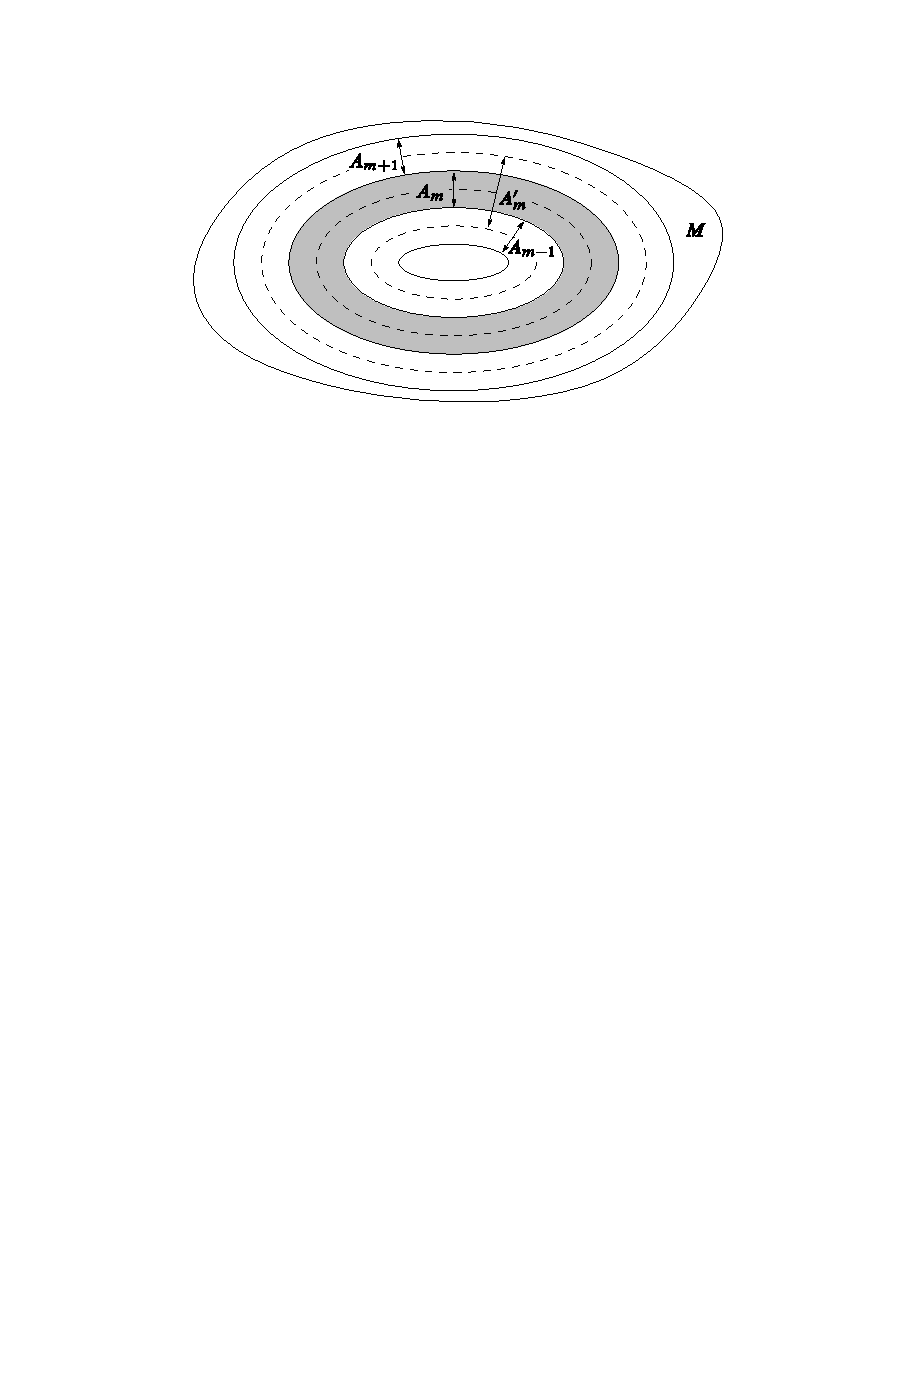
\includegraphics{induction-principle}
\caption{Proof of the induction principle, Step $2$.}
\end{figure}

Observe that $B_i\sub A'_i$, so $B_i$ can have nonempty intersection with $B_j$ only when $|i-j|\leq 1$. Therefore, if we define
\[U=\bigcup_{\text{$i$ odd}}B_i,\quad V=\bigcup_{\text{$i$ even}}B_i,\]
then $U$ and $V$ are disjoint unions of manifolds satisfying $\mathcal{P}$, and so they both satisfy $\mathcal{P}$ by condition (c). Finally, $\mathcal{P}$ holds on 
$U\cap V$ because it is the disjoint union of the sets $B_u\cap B_{i+1}$ for $i\in\Z$, each of which has a finite $\mathcal{P}$-cover consisting of sets of the form $U_\alpha\cap U_\beta$, 
where $U_\alpha$ and $U_\beta$ are basis sets used to define $B_i$ and $B_{i+1}$, respectively. Thus $M=U\cup V$ satisfies $\mathcal{P}$.\par
\textbf{Step $\bm{3}$}: Every open subset of $\R^n$ satisfies $\mathcal{P}$. If $U\sub\R^n$ is such a subset, then $U$ has a basis consisting of Euclidean cubes. 
Because each cube is diffeomorphic to $\R^n$, and because any finite intersection of cubes is again a cube, finite intersections also satisfies $\mathcal{P}$. Thus, 
$U$ has a $\mathcal{P}$-basis, so it satisfies $\mathcal{P}$ by Step $2$.\par
\textbf{Step $\bm{4}$}: Every smooth manifold satisfies $\mathcal{P}$. Any smooth manifold has a basis of smooth coordinate domains. Since every smooth coordinate 
domain is diffeomorphic to an open subset of $\R^n$, as are their finite intersections, this is a $\mathcal{P}$-basis. The claim therefore follows from Step $2$.
\end{proof}
The following lemma is needed in the proof of the Poincar\'e duality.
\begin{lemma}
The two Mayer-Vietoris sequences of the cover $\{U,V\}$ may be paired together to form a sign-commutative diagram
\[\begin{tikzcd}[row sep=14pt,column sep=14pt]
{}\ar[r]&H^p_{dR}(U\cup V)\ar[draw=none]{d}[name=X, anchor=center,scale=1.5]{\otimes}\ar[r,"\text{restriction}"]&H^p_{dR}(U)\oplus H^p_{dR}(V)\ar[draw=none]{d}[name=X, anchor=center,scale=1.5]{\otimes}
{}\ar[r,"\text{difference}"]&H^p_{dR}(U\cap V)\ar[draw=none]{d}[name=X, anchor=center,scale=1.5]{\otimes}\ar[r,"\delta^*"]&H^{p+1}(U\cup V)\ar[draw=none]{d}[name=X, anchor=center,scale=1.5]{\otimes}
\ar[r]&{}\\
{}&H_c^{n-p}(U\cup V)\ar[d,"\int_{U\cup V}"]\ar[l]&H_c^{n-p}(U)\oplus H^{n-p}_c(V)\ar[l,swap,"\text{sum}"]\ar[d,"\int_U+\int_V"]
&H^{n-p}_c(U\cap V)\ar[l]\ar[d,"\int_{U\cap V}"]&H_c^{n-p-1}(U\cup V)\ar[d,"\int_{U\cup V}"]\ar[l,swap,"\delta_*"]
&{}\ar[l]\\
&\R&\R&\R&\R&
\end{tikzcd}\]
\end{lemma}
Here sign-commutativity means, for instance, that
\[\int_{U\cap V}\omega\wedge\delta_*\eta=\pm\int_{U\cup V}\delta^*\omega\wedge\eta.\]
for $\omega\in H^p_{dR}(U\cap V)$, $\eta\in H^{n-p-1}_c(U\cup V)$.
\begin{proof}
The first two squares are in fact commutative: for $\omega\in H^p_{dR}(U\cup V)$ and $(\eta,\eta')\in H^{n-p}_c(U)\oplus H^{n-p}_c(V)$ we have
\[\int_{U\cup V}\omega\wedge\eta=\int_U\omega\wedge\eta,\quad \int_{U\cup V}\omega\wedge\eta=\int_V\omega\wedge\eta'\]
for $\eta$ is zero outside $U$ and $\eta'$ is zero outside $V$. Therefore
\[\int_{U\cup V}\omega\wedge(\eta+\eta')=\int_U\omega\wedge\eta+\int_V\omega\wedge\eta'.\]
which is the commutativity of the first squre. Similarly, for $(\omega,\omega')\in H^p_{dR}(U)\oplus H^p_{dR}(V)$ and $\eta\in H^{n-p}_c(U\cap V)$ we have
\[\int_{U}\omega\wedge\eta=\int_{U\cap V}\omega\wedge\eta,\quad \int_{U}\omega'\wedge\eta=\int_{U\cap V}\omega'\wedge\eta,\]
and therefore
\[\int_{U}\omega\wedge(-\eta)+\int_V\omega'\wedge\eta=\int_{U\cap V}(\omega-\omega')\wedge\eta,\]
which is the commutativity of the second squre.\par
The sign problem emerges on the third squre. Let $\omega\in H^p_{dR}(U\cap V)$ and $\eta\in H^{n-p-1}_c(U\cup V)$. Recall that $\delta^*\omega$ is a form in 
$H^{p+1}(U\cup V)$ such that
\[\delta^*\omega=\begin{cases}
d(\rho_V\omega)&\text{ on }U,\\
d(-\rho_U\omega)&\text{ on }V.
\end{cases}\]
Similaly, $\delta_*\eta$ is a form in $H^{n-p}_c(U\cap V)$ such that $\delta_*\eta=d(\rho_U\eta)$. Note that $d(\rho_U\eta)=(d\rho_U)\wedge\eta$ and 
$d(\rho_V\omega)=(d\rho_V)\wedge\omega$ because $\omega$ and $\eta$ are closed. Therefore
\[\int_{U\cap V}\omega\wedge\delta_*\eta=\int_{U\cap V}\omega\wedge(d\rho_U)\wedge\eta=(-1)^{\deg\omega}\int_{U\cap V}(d\rho_U)\wedge\omega\wedge\eta.\]
Since $\rho_U$ and $\rho_V$ are both constant outside $U\cap V$, we find that $\delta^*\omega$ has support in $U\cap V$, and therefore
\[\int_{U\cup V}\delta^*\omega\wedge\eta=\int_{U\cap V}d(\rho_V)\omega\wedge\eta=\int_{U\cap V}(d\rho_V)\wedge\omega\wedge\eta=-\int_{U\cap V}(d\rho_U)\wedge\omega\wedge\eta.\]
Thus finally we get
\[\int_{U\cap V}\omega\wedge\delta_*\eta=(-1)^{\det\omega+1}\int_{U\cup V}\delta^*\omega\wedge\eta.\]
This finishes the proof.
\end{proof}
\begin{proposition}[\textbf{Poincar\'e Duality}]
Let $M$ be an oriented manifold, then the pairing
\[\int:H^p_{dR}(M)\otimes H^{n-p}_c(M)\to\R\]
is nondegenerate. In particular, the two cohomology groups $H^p_{dR}(M)$ and $H^{n-p}_c(M)$ are dual to each other and therefore have the same dimension provided they are 
finite-dimensional vector spaces.
\end{proposition}
\begin{proof}
It is easy to see that the pairing is well-defined. Next note that it defines a
linear map
\[H^p_{dR}(M)\to H^{n-p}_c(M)^*=\Hom(H^{n-p}_c(M),\R).\]
We claim that this map is an isomorphism for all orientable but not necessarily connected
manifolds.\par
By the Five Lemma if Poincar\'e duality holds for $U$, $V$, and $U\cap V$, then it holds for $U\cup V$. We now proceed by checking the conditions in the induction principle. 
For $M$ diffeomorphic to $\R^n$, Poincar\'e duality follows from the two Poincar\'e lemmas. Next consider an arbitrary union of pairwise disjoint open sets. In this case we have
\[H^p_{dR}(\coprod_iU_i)=\prod_iH^p_{dR}(U_i)\quad H^{n-p}_c(\coprod_iU_i)=\bigoplus_iH^{n-p}_c(U_i).\]
so the claim also follows in this case. Then by Theorem the claim is valid for any oriented manifold.
\end{proof}
\begin{corollary}
Let $M$ be a compact oriented manifold. Then $H^p_{dR}(M)$ and $H^{n-p}_{dR}(M)$ are isomorphic.
\end{corollary}
\begin{proof}
This requires that we know that $H^p_{dR}(M)$ is finite dimensional for all $p$. First note that if $O\sub\R^n$ is a finite union of open boxes, then the de Rham cohomology 
groups are finite dimensional by the Mayer-Vietoris sequence.\par
This will give the result for $M\sub\R^k$ as we can find a tubular neighborhood $M\sub U\sub\R^k$ and a retract $r:U\to M$. Now cover $M$ by open boxes that lie in $U$ 
and use compactness of $M$ to find $M\sub O\sub U$ with $O$ being a union of finitely many open boxes. Since $r|_M=\id_M$ the retract $r^*:H^p_{dR}(M)\to H^p_{dR}(O)$ is 
an injection so it follows that $H^p_{dR}(M)$ is finite dimensional.
\end{proof}
\subsection{Cohomology computation on the top degree}
The Poincar\'e duality gives an easy way to compute the top cohomology for an manifolds. In this part we state the main results.
\begin{theorem}[\textbf{Top Cohomology, Orientable Compact Support Case}]\label{cohomology n orientable compact supp}
If $M$ is a connected orientable smooth $n$-manifold, then the integration map $\int:H^n_c(M)\to\R$ is an isomorphism, so $H^n_c(M)$ is $1$-dimensional.
\end{theorem}
\begin{proof}
This follows from the Poincar\'e duality, since $H^0_{dR}(M)$ consists of constant functions in this case.
\end{proof}
\begin{theorem}[\textbf{Top Cohomology, Orientable Compact Case}]\label{cohomology n orientable compact}
If $M$ is a compact connected orientable smooth $n$-manifold, then $H^n_{dR}(M)$ is $1$-dimensional, and is spanned by the cohomology class of any smooth orientation form.
\end{theorem}
\begin{proof}
This follows from the preceding theorem, because $H^p_{dR}(M)=H^p_c(M)$ in that case, and the integral of any orientation form is nonzero.
\end{proof}
\begin{theorem}[\textbf{Top Cohomology, Orientable Noncompact Case}]\label{cohomology n orientable noncompact}
If $M$ is a noncompact connected orientable smooth $n$-manifold, then $H^n_{dR}(M)=0$.
\end{theorem}
\begin{proof}
This also comes from the Poincar\'e duality: if $M$ is connected and noncompact, then $H^0_c(M)=0$.
\end{proof}
Next we consider the nonorientable case. If $M$ is a nonorientable smooth manifold, the key to analyzing its cohomology groups is the orientation covering $\widehat{\pi}:\widehat{M}\to M$. Because a finite-sheeted covering map is a proper map by Exercise~\ref{covering map proper iff}, $\widehat{\pi}$ induces cohomology maps on both compactly supported and ordinary de Rham cohomology. The next lemma shows that these maps are all injective.
\begin{lemma}
Suppose $M$ is a connected nonorientable smooth manifold and $\widehat{\pi}:\widehat{M}\to M$ is its orientation covering. For each $p$, the induced cohomology maps $\widehat{\pi}^*:H^p_{dR}(M)\to H^p_{dR}(\widehat{M})$ and $\widehat{\pi}^*:H^p_{c}(M)\to H^p_{c}(\widehat{M})$ are injective.
\end{lemma}
\begin{proof}
First, we prove the lemma for compactly supported cohomology. Suppose $\omega$ is a closed, compactly supported $p$-form on $M$ such that $\widehat{\pi}^*[\omega]=0\in H^p_c(\widehat{M})$. Then there exists $\eta\in\Omega^{p-1}_c(\widehat{M})$ such that $d\eta=\widehat{\pi}^*\omega$. Let $\alpha:\widehat{M}\to\widehat{M}$ be the unique nontrivial covering automorphism of $\widehat{M}$, and let $\widetilde{\eta}=\frac{1}{2}(\eta+\alpha^*\eta)$, which is also compactly supported. Using the fact that $\alpha\circ\alpha=\mathrm{id}_{\widehat{M}}$, we compute
\[\alpha^*\widetilde{\eta}=\frac{1}{2}(\alpha^*\eta+\alpha^*\circ\alpha^*\eta)=\widetilde{\eta}.\]
Because $\widehat{\pi}\circ\alpha=\widehat{\pi}$, this implies
\[d\widetilde{\eta}=\frac{1}{2}(d\eta+\alpha^*d\eta)=\frac{1}{2}(\widehat{\pi}^*\omega+\alpha^*\widehat{\pi}^*\omega)=\widehat{\pi}^*\omega.\]
Let $U\sub M$ be any evenly covered open subset. There are exactly two smooth local sections $\sigma_1,\sigma_2:U\to \widehat{M}$ over $U$, which are related by $\sigma_2=\alpha\circ\sigma_1$. Observe that
\[\sigma_2^*\widetilde{\eta}=\sigma_1^*\alpha^*\omega=\sigma_1^*\omega.\]
Therefore, we can define a smooth global $(p-1)$-form $\beta$ on $M$ by setting $\beta|_U:=\sigma^*\widetilde{\eta}$ for any smooth local section $\sigma:U\to\widehat{M}$; the argument above guarantees that the various definitions agree where they overlap. Because $\supp(\beta)=\widehat{\pi}(\supp(\widetilde{\eta}))$, it follows that $\beta$ is compactly supported. To determine the exterior derivative of $\beta$, given $p\in M$; choose a smooth local section $\sigma$ defined on a neighborhood $U$ of $p$, and compute
\[d\beta=d(\sigma^*\widetilde{\eta})=\sigma^*d\widetilde{\eta}=\sigma^*\widehat{\pi}^*\omega=\omega.\]
because $\widehat{\pi}\circ\sigma=\mathrm{id}_U$.\par
The argument for ordinary de Rham cohomology is the same, but with all references
to compact support deleted.
\end{proof}
\begin{theorem}[\textbf{Top Cohomology, Nonorientable Case}]\label{cohomology n nonorientable}
If $M$ is a connected nonorientable smooth $n$-manifold, then $H^n_c(M)=0$ and $H^n_{dR}(M)=0$.
\end{theorem}
\begin{proof}
First consider the case of compactly supported cohomology. By the preceding lemma, it suffices to show that $\widehat{\pi}^*:H^p_{c}(M)\to H^p_{c}(\widehat{M})$ is the zero map, where $\widehat{\pi}:\widehat{M}\to M$ is the orientation covering of $M$. Let $\alpha:\widehat{M}\to\widehat{M}$ be the nontrivial covering automorphism as in the preceding proof. Now, $\alpha$ cannot be orientation-preserving: if it were, the entire covering automorphism group $\{\mathrm{id},\alpha\}$ would be orientation-preserving, and then $M$ would be orientable by Theorem~\ref{orientation covering thm}. By connectedness of $\widehat{M}$ and the fact that $\alpha$ is a diffeomorphism, it follows that $\alpha$ is orientation-reversing.\par
Suppose $\omega$ is any compactly supported smooth $n$-form on $M$, and let $\widehat{\omega}=\widehat{\pi}^*\omega$. Because $\widehat{\pi}$ is proper, $\widehat{\omega}$ is compactly supported, and $\widehat{\pi}\circ\alpha=\widehat{\pi}$ implies $\alpha^*\widehat{\omega}=\widehat{\omega}$. Because $\alpha$ is orientation-reversing, we conclude from Proposition~\ref{int form prop} that
\[\int_{\widehat{M}}\widehat{\omega}=-\int_{\widehat{M}}\alpha^*\widehat{\omega}=-\int_{\widehat{M}}\widehat{\omega}.\]
This implies that $\int_{\widehat{M}}\widehat{\omega}=0$, so $[\widehat{\omega}]=0\in H^p_c(\widehat{M})$ by Theorem~\ref{cohomology n orientable compact supp}. This completes the proof that $H^n_c(M)=0$.\par
It remains only to handle ordinary cohomology. If $M$ is compact, it follows from the argument above that $H^n_{dR}(M)=H^n_c(M)=0$. On the other hand, if $M$ is noncompact, then so is $\widehat{M}$, and Theorem~\ref{cohomology n orientable noncompact} shows that $H^n_{dR}(\widehat{M})=0$. It follows from the previous lemma that $H^n_{dR}(M)=0$ as well.
\end{proof}
\subsection{Degree theory}
Now that we know the top-degree cohomology groups of all compact smooth manifolds, we can use them to draw a number of significant conclusions about smooth maps between certain compact manifolds of the same dimension. They all follow from the fact that we can associate an integer to each such map, called its degree, in
such a way that homotopic maps have the same degree.
\begin{theorem}[\textbf{Degree of a Smooth Map}]\label{degree def}
Suppose $M$ and $N$ are compact, connected, oriented, smooth manifolds of dimension $n$, and $F:M\to N$ is a smooth map. There exists a unique integer $k$, called the \textbf{degree of $\bm{F}$}, that satisfies both of the following conditions.
\begin{itemize}
\item[(a)] For every smooth $n$-form $\omega$ on $N$,
\[\int_MF^*\omega=k\int_N\omega.\]
\item[(b)] If $q\in N$ is a regular value of $F$, then
\[k=\sum_{x\in F^{-1}(q)}\sgn(x),\]
where $\sgn(x)=1$ if $dF_x$ is orientation-preserving, and $-1$ if it is orientation-reversing.
\end{itemize}
\end{theorem}
\begin{proof}
By Theorem~\ref{cohomology n orientable compact}, two smooth $n$-forms on either $M$ or $N$ are cohomologous if and only if they have the same integral. Let $\theta$ be any smooth $n$-form on $N$ such that $\int_N\theta=1$, and let $k=\int_MF^*\theta$. If $\omega\in\Omega^n(N)$ is arbitrary, then $\omega$ is cohomologous to $a\theta$, where $a=\int_N\omega$, and therefore $F^*\omega$ is cohomologous to $aF^*\theta$. It follows that
\[\int_MF^*\omega=a\int_MF^*\theta=ak=k\int_N\omega.\]
Thus $k$ satisfies (a), and is clearly the only number that does so.\par
Next we show that $k$ also has the characterization given in part (b), from which it follows that it is an integer. Let $q\in N$ be an arbitrary regular value of $F$. Because $F^{-1}(q)$ is a properly embedded $0$-dimensional submanifold of $M$, it is finite. Suppose first that $F^{-1}(q)$ is not empty---say, $F^{-1}(q)=\{x_1,\dots,x_r\}$. By the inverse function theorem, for each $i$ there is a neighborhood $U_i$ of $x_i$ such that $F$ is a diffeomorphism from $U_i$ to a neighborhood $W_i$ of $q$, and by shrinking the $U_i$'s if necessary, we may assume that they are pairwise disjoint. Then $K:=M-\bigcup_{i=1}^{r}U_i$ is closed in $M$ and thus compact, so $F(K)$ is closed in $N$ and disjoint from $q$. Let $W$ be the connected component of $\bigcap_{i=1}^{r}W_i\cap(N-F(K))$ containing $q$, and let $V_i=F^{-1}(W)\cap U_i$. It follows that $W$ is a connected neighborhood of $q$ whose preimage under $F$ is the disjoint union $V_1\cup\cdots\cup V_r$, and $F$ restricts to a diffeomorphism from each $V_i$ to $W$. Since each $V_i$ is connected, the restriction of $F$ to $V_i$ must be either orientation-preserving or orientation-reversing.\par
Let $\omega$ be a smooth $n$-form on $N$ that is compactly supported in $W$ and satisfies $\int_N\omega=\int_W\omega=1$. It follows from part (a) that $\int_MF^*\omega=k$. Since $F^*\omega$ is compactly supported in $F^{-1}(W)$, we have $\int_MF^*\omega=\sum_{i=1}^{r}\int_{V_i}F^*\omega=k$. From Proposition~\ref{int form prop}(d), since $F$ restricts to a diffeomorphism on each $V_i$, we conclude that $\int_{V_i}\omega=\pm 1$, with the positive sign if $F$ is orientation-preserving on $V_i$ and the negative sign otherwise. This proves (b) when $F^{-1}(q)\neq\emp$.\par
On the other hand, suppose $F^{-1}(q)=\emp$. Then $q$ has a neighborhood $W$ contained in $N-F(M)$ (because $F(M)$ is compact and thus closed). If $\omega$ is any smooth $n$-form on $N$ that is compactly supported in $W$, then $\int_MF^*\omega=0$, so $k=0$. This proves (b).
\end{proof}
\begin{corollary}
With the assumptions above, if $F$ is not surjective then $\deg F=0$.
\end{corollary}
Much of the power of degree theory arises from the fact that the two different characterizations of the degree can be played off against each other. For example, it is often easy to compute the degree of a particular map simply by counting the points in the preimage of a regular value, with appropriate signs. On the other hand, the characterization in terms of differential forms makes it easy to prove many important properties, such as the ones given in the next proposition.
\begin{proposition}[\textbf{Properties of the Degree}]\label{degree prop}
Suppose $M,N$, and $P$ are compact, connected, oriented, smooth $n$-manifolds.
\begin{itemize}
\item[(a)] If $F:M\to N$ and $G:N\to P$ are both smooth maps, then $\deg(G\circ F)=(\deg G)(\deg F)$.
\item[(b)] If $F:M\to N$ is a diffeomorphism, then $\deg F=+1$ if $F$ is orientation-preserving and $-1$ if it is orientation-reversing.
\item[(c)] If two smooth maps $F_0,F_1:M\to N$ are homotopic, then they have the same degree.
\end{itemize}
\end{proposition}
\begin{proof}
Part (b) and (c) follows directly from definition. For (a), we just note that
\[\int_P(G\circ F)^*\omega=\int_PF^*G^*\omega=(\deg F)\int_NG^*\omega=(\deg F)(\deg G)\int_M\omega,\]
which proves $\deg(G\circ F)=(\deg F)(\deg G)$.
\end{proof}
This proposition allows us to define the degree of a continuous map $F:M\to N$ between compact, connected, oriented, smooth $n$-manifolds, by letting $\deg F$ be the degree of any smooth map that is homotopic to $F$. The Whitney approximation theorem guarantees that there is such a map, and the preceding proposition guarantees that the degree is the same for every map homotopic to $F$. Here are some applications of degree theory.
\begin{proposition}
Let $F:M\to N$ be a proper local diffeomorphism of degree $\pm1$ between oriented connected manifolds, then $F$ is a diffeomorphism.
\end{proposition}
\begin{proof}
The fact that $\deg F\neq 0$ means $F$ is surjective, and thus a covering map. Now $\deg F=\pm 1$ means $F$ is injective, so it must be a diffeomorphism.
\end{proof}
\begin{proposition}
Even dimensional spheres do not admit non-vanishing smooth vector fields.
\end{proposition}
\begin{proof}
Let $X$ be a vector field on $S^n$, we can scale it so that it is a unit vector field. If we consider it as a function $X:S^n\to S^n\sub\R^{n+1}$ then it is always 
perpendicular to its foot point. We can then create a homotopy
\[H(p,t)=p\cos(\pi t)+X_p\sin(\pi t).\]
Since $p\bot X_p$ and both are unit vectors the Pythagorean theorem shows that $H(p,t)\in S^n$ as well. When $t=0$ the homotopy is the identity, and when $t=1$ it is the 
antipodal map. Since the antipodal map reverses orientations on even dimensional spheres it is not possible for the identity map to be homotopic to the antipodal map.
\end{proof}
\begin{theorem}
Suppose $N$ is a compact, connected, oriented, smooth $n$-manifold, and $X$ is a compact, oriented, smooth $(n+1)$-manifold with connected boundary. If $f:\partial X\to N$ is a continuous map that has a continuous extension to $X$, then $\deg f=0$.
\end{theorem}
\begin{proof}
Suppose $f$ has an extension to a continuous map $F:X\to N$. By the Whitney approximation theorem, there is a smooth map $\widetilde{F}:X\to N$ that is homotopic
to $F$. Replacing $F$ by $\widetilde{F}$ and $f$ by $\widetilde{F}|_{\partial X}$ we may assume that both $f$ and $F$ are smooth.\par
Let $\omega$ be any smooth $n$-form on $N$. Then $d\omega=0$ because it is an $(n+1)$-form on an $n$-manifold. From Stokes's theorem, we obtain
\[\int_{\partial X}f^*\omega=\int_{\partial X}F^*\omega=\int_Xd(F^*\omega)=\int_XF^*(f\omega)=0.\]
It follows from Theorem~\ref{degree def} that $f$ has degree zero.
\end{proof}
\begin{theorem}[\textbf{Brouwer Fixed-Point Theorem}]
Every continuous map from $\widebar{B}^n$ to itself has a fixed point.
\end{theorem}
\begin{proof}
Suppose for the sake of contradiction that $F:\widebar{B}^n\to\widebar{B}^n$ is continuous and has no fixed points. We can define a continuous map
\[G(x)=\frac{x-F(x)}{|x-F(x)|},\]
and let $g=G|_{S^{n-1}}:S^{n-1}\to S^{n-1}$. On the one hand, the previous theorem implies that $g$ has degree zero. On the other hand, consider the map 
$H:S^{n-1}\times I\to S^{n-1}$ defined by
\[H(x,t)=\frac{x-tF(x)}{|x-tF(x)|}\]
The denominator never vanishes when $t=1$ because $F$ has no fixed points, and when $t<1$ it cannot vanish because $|x|=1$ while $|tF(x)|=t<1$. Thus $H$ is continuous, 
so it is a homotopy from the identity to $g$. It follows from Proposition~\ref{degree prop} that $g$ has degree $1$, which is a contradiction.
\end{proof}
\subsection{The de Rham theorem}
The topological invariance of the de Rham groups suggests that there should be some purely topological way of computing them. There is indeed, and the connection 
between the de Rham groups and the singular cohomology groups was first proved by Georges de Rham himself in the 1930s. The theorem that bears his name is a major 
landmark in the development of smooth manifold theory. The purpose of this part is to give a proof of this theorem.
\subsubsection{Smooth singular homology}
The connection between the singular and de Rham cohomology groups will be established by integrating differential forms over singular chains. More precisely, given a 
singular $p$-simplex $\sigma$ in a manifold $M$ and a $p$-form $\omega$ on $M$, we would like to pull $\omega$ back by $\sigma$ and integrate the resulting form over 
$\Delta_p$. However, there is an immediate problem with this approach, because forms can be pulled back only by smooth maps, while singular simplices are in general 
only continuous. In this part we overcome this problem by showing that singular homology can be computed equally well with smooth simplices.\par
If $M$ is a smooth manifold, a smooth $p$-simplex in $M$ is a map $\sigma:\Delta_p\to M$ that is smooth in the sense that it has a smooth extension to a neighborhood 
of each point. The subgroup of $C_p(M)$ generated by smooth simplices is denoted by $C^\infty_p(M)$ and called the \textbf{smooth chain group in degree $\bm{p}$}. 
Elements of this group, which are finite formal linear combinations of smooth simplices, are called smooth chains. Because the boundary of a smooth simplex is a smooth 
chain, we can define the \textbf{$\bm{p}$-th smooth singular homology group} of $M$ to be the quotient group
\[H_p^{\infty}(M)=\frac{\ker(\partial:C_p^{\infty}(M)\to C_{p-1}^{\infty}(M))}{\im(\partial:C_{p+1}^{\infty}(M)\to C_{p}^{\infty}(M))}.\]
The inclusion map $\iota:C^\infty_p(M)\hookrightarrow C_p(M)$ commutes with the boundary operator, and so induces a map on homology: $\iota_*:H_p^{\infty}(M)\to H_p(M)$ 
by $\iota_*[c]=[\iota(c)]$.
\begin{theorem}[\textbf{Smooth Singular vs. Singular Homology}]
For any smooth manifold $M$, the map $\iota_*:H_p^{\infty}(M)\to H_p(M)$ induced by inclusion is an isomorphism.
\end{theorem}
The basic idea of the proof is to construct, with the help of the Whitney approximation theorem, two operators: first, a smoothing operator $s:C_p(M)\to C_p^{\infty}(M)$ 
such that $s\circ\partial=\partial\circ s$ and $s\circ\iota$ is the identity on $C_p^{\infty}(M)$; and second, a homotopy operator that shows that $\iota\circ s$ induces 
the identity map on $H^p(M)$. Since the details are highly technical, we do not present them here.
\subsubsection{The de Rham theorem}
Suppose $M$ is a smooth manifold, $\omega$ is a closed $p$-form on $M$; and $\sigma$ is a smooth $p$-simplex in $M$. We define the integral of $\omega$ over $\sigma$ to 
be
\[\int_{\sigma}\omega=\int_{\Delta_p}\sigma^*\omega.\]
This makes sense because $\Delta_p$ is a smooth $p$-submanifold with corners embedded in $\R^p$, and it inherits the orientation of $\R^p$. (Or we could just consider $\Delta_p$ 
as a domain of integration in $\R^p$.) Observe that when $p=1$, this is the same as the line integral of $\omega$ over the smooth curve segment $\sigma:[0,1]\to M$. If 
$c=\sum_{i=1}^{k}c_i\sigma_i$ is a smooth $p$-chain, the integral of $\omega$ over $c$ is defined as
\[\int_{c}\omega=\sum_{i=1}^{k}c_i\int_{\sigma_i}\omega.\]
\begin{theorem}[\textbf{Stokes's Theorem for Chains}]\label{Stokes's theorem for chains}
If $c$ is a smooth $p$-chain in a smooth manifold $M$, and $\omega$ is a smooth $(p-1)$-form on $M$, then
\[\int_cd\omega=\int_{\partial c}\omega.\]
\end{theorem}
\begin{proof}
It suffices to prove the theorem when $c$ is just a smooth simplex $\sigma$. Since $\Delta_p$ is a manifold with corners, Stokes's theorem says that
\[\int_{\sigma}d\omega=\int_{\Delta_p}\sigma^*d\omega=\int_{\Delta_p}d\sigma^*\omega=\int_{\partial\Delta_p}\sigma^*\omega.\]
The face maps $F_{i,p}:\Delta_{p-1}\to\Delta_p$ are parametrizations of the boundary faces of $\Delta_p$ satisfying the conditions of Proposition~\ref{int mani para}, 
except possibly that they might not be orientation-preserving. To check the orientations, note that $F_{i,p}$ is the restriction to $\Delta_p\cap\partial\H^p$ of the 
affine diffeomorphism sending the simplex $[e_0,\dots,e_p]$ to $[e_0,\dots,\widehat{e}_i,\dots,e_p,e_i]$. This is easily seen to be orientation-preserving if and only 
if $(e_0,\dots,\widehat{e}_i,\dots,e_p,e_i)$ is an even permutation of $(e_0,\dots,e_p)$, which is the case if and only if $p-i$ is even. Since the standard coordinates 
on $\partial\H^p$ are positively oriented if and only if $p$ is even, the upshot is that $F_{i,p}$ is orientation-preserving for $\partial\Delta_p$ if and only if $i$ is 
even. Thus, by Proposition~\ref{int mani para},
\begin{align*}
\int_{\partial\Delta_p}\sigma^*\omega&=\sum_{i=0}^{p}(-1)^i\int_{\Delta_{p-1}}F_{i,p}^*\sigma^*\omega=\sum_{i=0}^{p}(-1)^i\int_{\Delta_{p-1}}(\sigma\circ F_{i,p})^*\omega=\sum_{i=0}^{p}(-1)^i\int_{\sigma\circ F_{i,p}}\omega.
\end{align*}
By definition of the singular boundary operator, this is equal $\int_{\partial\sigma}\omega$.
\end{proof}
Using this theorem, we define a natural linear map $\mathscr{I}:H_{dR}^p(M)\to H^p(M;\R)$, called the \textbf{de Rham homomorphism}, as follows. For any $[\omega]\in H^p_{dR}(M)$ 
and $[c]\in H_p(M)\cong H_p^{\infty}(M)$, we define
\[\mathscr{I}[\omega][c]=\int_{\widetilde{c}}\omega.\]
where $\widetilde{c}$ is any smooth $p$-cycle representing the homology class $[c]$. This is well defined by Theorem~\ref{Stokes's theorem for chains}.
\begin{proposition}[\textbf{Naturality of the de Rham Homomorphism}]\label{de Rham homomorphism naturality}
For a smooth manifold $M$ and nonnegative integer $p$, let $\mathscr{I}:H^p_{dR}(M)\to H^p(M;\R)$ denote the de Rham homomorphism.
\begin{itemize}
\item[(a)] If $F:M\to N$ is a smooth map, then the following diagram commutes:
\[\begin{tikzcd}[row sep=12pt,column sep=12pt]
H_{dR}^p(N)\ar[r,"F^*"]\ar[d,"\mathscr{I}"]&H_{dR}^p(M)\ar[d,"\mathscr{I}"]\\
H^p(N;\R)\ar[r,"F^*"]&H^p(M;\R)
\end{tikzcd}\] 
\item[(b)] If $M$ is a smooth manifold and $U,V$ are open subsets of $M$ whose union is $M$, then the following diagram commutes:
\[
\begin{tikzcd}[row sep=12pt,column sep=12pt]
H_{dR}^{p-1}(U\cap V)\ar[r,"\delta"]\ar[d,"\mathscr{I}"]&H_{dR}^p(M)\ar[d,"\mathscr{I}"]\\
H^{p-1}(U\cap V;\R)\ar[r,"\partial^*"]&H^{ppp}(M;\R)
\end{tikzcd}
\]
where $\delta$ and $\partial^*$ are the connecting homomorphisms of the Mayer-Vietoris sequences for de Rham and singular cohomology, respectively.
\end{itemize}
\end{proposition}
\begin{proof}
Directly from the definitions, if $\sigma$ is a smooth $p$-simplex in $M$ and $\omega$ is a smooth $p$-form on $N$,
\[\int_{\sigma}F^*\omega=\int_{\Delta_p}\sigma^*F^*\omega=\int_{\Delta_p}(F\circ\sigma)^*\omega=\int_{F\circ\sigma}\omega.\]
This implies
\[\mathscr{I}[F^*\omega][\sigma]=\mathscr{I}[\omega][F\circ\sigma]=F^*(\mathscr{I}[\omega])[\sigma].\]
which proves (a).\par
Now consider (b). Commutativity of this diagram means
\[\mathscr{I}(\delta[\omega])[e]=(\partial^*\mathscr{I}[\omega])[e]\]
for any $[\omega]\in H^{p-1}_{dR}(U\cap V)$ and any $[e]\in H^p_{dR}(M)$. Using our identification of $H^p(M;\R)$ with $\Hom(H^p(M),\R)$, we can rewrite this as
\[\mathscr{I}(\delta[\omega])[e]=\mathscr{I}[\omega](\partial_*[e]).\]
If $\sigma$ is a smooth $p$-form representing $\delta[\omega]$ and $c$ is a smooth $(p-1)$-chain representing $\partial_*[e]$, this is the same as 
\[\int_e\sigma=\int_c\omega.\]
By the characterization of $\partial_*$, we can let $c=\partial f$, where $f,f'$ are smooth $p$-chains in $U$ and $V$, respectively, such that $f+f'$ represents the 
same homology class as $e$. Similarly, by Corollary~\ref{Mayer-Vietoris de Rham connect}, we can choose $\eta\in\Omega^{p-1}(U)$ and $\eta'\in\Omega^{p-1}(V)$ such that $\omega=\eta|_{U\cap V}-\eta'|_{U\cap V}$, 
and then let $\sigma$ be the $p$-form that is equal to $d\eta$ on $U$ and to $d\eta'$ on $V$. Then, because $\partial f+\partial f'=\partial e=0$ and $d\eta|_{U\cap V}-d\eta'|_{U\cap V}=d\omega=0$, 
we have
\begin{align*}
\int_{c}\omega&=\int_{\partial f}\omega=\int_{\partial f}\eta-\int_{\partial f}\eta'=\int_{\partial f}\eta+\int_{\partial f'}\eta'\\
&=\int_{f}d\eta+\int_{f'}d\eta'=\int_f\sigma+\int_{f'}\sigma=\int_{e}\sigma.
\end{align*}
Thus the diagram commutes.
\end{proof}
\begin{theorem}[\textbf{de Rham}]
For every smooth manifold $M$ and nonnegative integer $p$, the de Rham homomorphism $\mathscr{I}:H^p_{dR}(M)\to H^p(M;\R)$ is an isomorphism.
\end{theorem}
\begin{proof}
We will use the induction principle as in the proof of Poincar\'e duality. Thus we need to check the three conditions.\par
Consider $\R^n$. The homopoty invariant of $H^p$ implies that the singular cohomology groups of $\R^n$ are also trivial for $p\neq 0$. In the $p=0$ case, $H^0_{dR}(\R^n)$ 
is the $1$-dimensional space consisting of the constant functions, and $H^0(\R^n;\R)=\Hom(H_0(\R^n),\R)$ is also $1$-dimensional because $H_0(\R^n)$ is generated by any 
singular $0$-simplex. If $\sigma:\Delta_0\to M$ is a singular $0$-simplex (which is smooth because any map from a $0$-manifold is smooth), and $f$ is the constant function 
equal to $1$, then
\[\mathscr{I}[f][\sigma]=\int_{\Delta_0}\sigma^*f=(f\circ\sigma)(0)=1.\]
Thus $\mathscr{I}:H^0_{dR}(\R^n)\to H^0(\R^n;\R)$ is not the zero map, so it is an isomorphism.\par
If $U,V$ are open subsets of $M$ such that the de Rham theorem is true on $U$, $V$ and $U\cap V$, then putting together the Mayer-Vietoris sequences for de Rham and 
singular cohomology, we obtain the following commutative diagram, in which the horizontal rows are exact and the vertical maps are all de Rham homomorphisms:
\[\begin{tikzcd}[scale=0.85]
H_{dR}^{p-1}(U)\oplus H_{dR}^{p-1}(V)\ar[r]\ar[d]&H^{p-1}_{dR}(U\cup V)\ar[r]\ar[d]&H^p_{dR}(U\cup V)\ar[r]\ar[d]&H^p_{dR}(U)\oplus H^p_{dR}(V)\ar[d]\\
H^{p-1}(U;\R)\oplus H^{p-1}(V;\R)\ar[r]&H^{p-1}(U\cup V;\R)\ar[r]&H^p(U\cup V;\R)\ar[r]&H^p(U;\R)\oplus H^p(V;\R)
\end{tikzcd}\]
The commutativity of the diagram is an immediate consequence of Proposition~\ref{de Rham homomorphism naturality}. Then by the five lemma the de Rham theorem is true on 
$U\cup V$.\par
Finally, consider a disjoint union $\amalg_iU_i$. For both de Rham and singular cohomology the inclusions $\iota_i:U_i\hookrightarrow\amalg_iU_i$ induce isomorphisms 
between the cohomology groups of the disjoint union and the direct product of the cohomology groups of the manifolds $U_i$. By Proposition~\ref{de Rham homomorphism naturality}, 
$\mathscr{I}$ commutes with these isomorphisms. Now use the induction principal we get the claim.
\end{proof}
Recall that by Theorem~\ref{homotopy equiv Int M to M} the inclusion $\iota:\Int M\hookrightarrow M$ is a homotopy equivalence, so for manifolds with boundary the de Rham theorem also holds.
\begin{proposition}
For every smooth manifold with boundary $M$ and nonnegative integer $p$, the de Rham homomorphism $\mathscr{I}:H^p_{dR}(M)\to H^p(M;\R)$ is an isomorphism.
\end{proposition}
\subsection{The Thom isomorphism}
\subsubsection{Compact vertical cohomology and integration along the fiber}
For vector bundles there is a third kind of cohomology. Instead of $\Omega^p_c(E)$, the complex of forms with compact support, we consider $\Omega_{cv}^p(E)$, the 
complex of forms with compact support in the vertical direction, defined as follows: a smooth $n$-form $\omega$ on $E$ is in $\Omega^p_{cv}(E)$ if and only if for 
every compact set $K$ in $M$, $\supp(\omega)\cap\pi^{-1}(K)$ is compact. If $\omega\in\Omega^p_{cv}(E)$, then since $\supp(\omega|_{\pi^{-1}(p)})\sub\supp(\omega)\cap\pi^{-1}(p)$ 
is a  closed subset of a compact set, $\supp(\omega|_{\pi^{-1}(p)})$ is compact. Thus, although a form in $\Omega^p_{cv}(E)$ need not have compact support in $E$, its 
restriction to each fiber has compact support. The cohomology of this complex, denoted $\Omega^p_{cv}(E)$, is called the \textbf{cohomology of $\bm{E}$ with compact 
support in the vertical direction}, or \textbf{compact vertical cohomology}.\par
Let $E$ be oriented as a rank $k$ vector bundle. We define the \textbf{integration along the fiber}, $\Omega^p_{cv}(E)\to\Omega^{p-k}(M)$, as follows. First consider 
the case of a trivial bundle $E=M\times\R^n$. Let $(t^1,\dots,t^k)$ be the coordinates on the fiber $\R^k$. A form on $E$ is a real linear combination of two types of 
forms: the type (\rmnum{1}) forms are those which do not contain as a factor the $k$-form $dt_1\wedge\cdots\wedge dt_k$ and the type (\rmnum{2}) forms are those which 
do. The map $\pi_*$ is defined by
\begin{itemize}
\item[(\rmnum{1})] $(\pi^*\phi)\wedge f(x,t)\,dt^{i_1}\wedge\cdots\wedge dt^{i_r}\mapsto 0$, $r<k$.
\item[(\rmnum{2})] $(\pi^*\phi)\wedge f(x,t)\,dt^{1}\wedge\cdots\wedge dt^{k}\mapsto \phi\int_{\R^k}f(x,t)\,dt^1\wedge\cdots\wedge dt^k$.
\end{itemize}
where $f$ has compact support for each fixed $x$ in $M$ and $\phi$ is a form on $M$.\par
Next suppose $E$ is an oriented vector bundle, with oriented trivialization $\{(U_\alpha,\varPhi_\alpha)\}$. Let $(x^1,\dots,x^n)$ and $(\widetilde{x}^1,\dots,\widetilde{x}^n)$ 
be the coordinate functions on $U_\alpha$ and $U_\beta$ and $(t^1,\dots,t^k)$, $(\widetilde{t}^1,\dots,\widetilde{t}^k)$ the fiber coordinates on $E|_{U_\alpha}$ and 
$E|_{U_\beta}$, given by $\varPhi_\alpha$, $\varPhi_{\beta}$ respectively. Because $\{(U_\alpha,\varPhi_\alpha)\}$ is an oriented trivialization for $E$, the two sets 
of fiber coordinates $(t^1,\dots,t^k)$ and $(\widetilde{t}^1,\dots,\widetilde{t}^k)$ are related by an element of $\GL_n^+(\R)$ at each point of $U_\alpha\cap U_\beta$. 
Again a form $\omega$ in $\Omega_{cv}^p(E)$ is locally of type (\rmnum{1}) or (\rmnum{2}). The map $\pi_*$ is defined to be zero on type (\rmnum{1}) forms. To define $\pi_*$ on type (\rmnum{2}) forms, write $\omega_\alpha$ for $\omega|_{U_\alpha}$. Then
\[\omega_\alpha=(\pi^*\phi)\wedge f(x,t)\,dt^1\wedge\cdots\wedge dt^k,\quad \omega_\beta=(\pi^*\tau)\wedge g(\widetilde{x},\widetilde{t})\,d\widetilde{t}^1\wedge\cdots\wedge d\widetilde{t}_k.\]
Define
\[\pi_*\omega_\alpha=\phi\int_{\R^k}f(x,t)\, dt^1\wedge\cdots\wedge dt^k.\]
By the invariance of the integral under orientation-preserving diffeomorphism, these definitions coincide on their overlap. Hence $\{\omega_\alpha\}$ piece together to give a global form $\pi_*\omega$ on $M$. Furthermore, this definition is independent of the choice of the oriented trivialization for $E$.
\begin{proposition}
Integration along the fiber commutes with exterior differentiation.
\end{proposition}
\begin{proof}
By a partition of unity, we may assume $E$ to be the product bundle $M\times\R^k$. If $\omega=(\pi^*\phi)\wedge f(x,t)\,dt^1\wedge\cdots\wedge dt^k$, then we have
\begin{equation*}
\scalemath{0.9}{
\begin{aligned}
d(\pi_*\omega)&=d(\phi\int_{\R^k}f(x,t)\,dt_1\wedge\cdots\wedge dt_k)\\
&=(d\phi)\int_{\R^k}f(x,t)\,dt^1\wedge\cdots\wedge dt^k+(-1)^{\deg\phi}\phi\wedge \Big(d\int_{\R^k}f(x,t)\,dt^1\wedge\cdots\wedge dt^k\Big)\\
&=(d\phi)\int_{\R^k}f(x,t)\,dt^1\wedge\cdots\wedge dt^k+(-1)^{\deg\phi}\phi\wedge \Big(\int_{\R^k}\sum_{i=1}^{n}\frac{\partial f}{\partial x^i}(x,t)dx^i\wedge dt^1\wedge\cdots\wedge dt^k\\
&\quad +\int_{\R^k}\sum_{j=1}^{k}\frac{\partial f}{\partial t^i}(x,t)dt^j\wedge dt^1\wedge\cdots\wedge dt^k\Big)\\
&=(d\phi)\int_{\R^k}f(x,t)\,dt^1\wedge\cdots\wedge dt^k+(-1)^{\deg\phi}\phi\wedge dx^i\int_{\R^k}\sum_{i=1}^{n}\frac{\partial f}{\partial x^i}(x,t)\,dt^1\wedge\cdots\wedge dt^k.
\end{aligned}}
\end{equation*}
And
\begin{equation*}
\scalemath{0.9}{
\begin{aligned}
\pi_*(d\omega)&=\pi_*\Big((\pi^*d\phi)\wedge f(x,t)\,dt^1\wedge\cdots\wedge dt^k+\sum_i(-1)^{\deg\phi}(\pi^*\phi)\wedge\frac{\partial f}{\partial x^i}dx^i\wedge dt^1\wedge\cdots\wedge dt^k\Big)\\
&=\pi_*\Big((\pi^*d\phi)\wedge f(x,t)\,dt^1\wedge\cdots\wedge dt^k+\pi^*\Big(\sum_i(-1)^{\deg\phi}\phi\wedge dx^i\Big)\wedge\frac{\partial f}{\partial x^i}dx^i\wedge dt^1\wedge\cdots\wedge dt^k\Big)\\
&=(d\phi)\int_{\R^k}f(x,t)\,dt^1\wedge\cdots\wedge dt^k+(-1)^{\deg\phi}\phi\wedge dx^i\int_{\R^k}\sum_{i=1}^{n}\frac{\partial f}{\partial x^i}(x,t)\,dt^1\wedge\cdots\wedge dt^k.
\end{aligned}}
\end{equation*}
So $d\pi_*=\pi_*d$ for a type (\rmnum{2}) form. Next let $\omega=(\pi^*\phi)\wedge f(x,t)\,dt^{i_1}\wedge\cdots\wedge dt^{i_r}$, $r<k$, be a type (\rmnum{1}) form. Then $d\pi_*\omega=0$, and 
\begin{align*}
d\omega&=(\pi^*d\phi)\wedge f(x,t)\,dt^{i_1}\wedge\cdots\wedge dt^{i_r}+\pi^*\Big(\sum_{i=1}^{k}(-1)^{\deg\phi}\phi\wedge dx^i\Big)\wedge\frac{\partial f}{\partial x^i}(x,t)\,dt^{i_1}\wedge\cdots\wedge dt^{i_r}\\
&\quad+(\pi^*\phi)\wedge\Big(\sum_{j=1}^{k}(-1)^{\deg\phi}\frac{\partial f}{\partial t^j}(x,t)\,dt^j\wedge dt^{i_1}\wedge\cdots\wedge dt^{i_r}\Big)
\end{align*}
and so 
\begin{align*}
\pi_*(d\omega)&=\sum_{j=1}^{k}(-1)^{\deg\phi}\phi\int_{\R^k}\frac{\partial f}{\partial t^j}(x,t)\,dt^j\wedge dt^{i_1}\wedge\cdots\wedge dt^{i_r}\\
&=0\text{ if $dt^j\wedge dt^{i_1}\wedge\cdots dt^{i_r}\neq\pm dt^1\wedge\cdots\wedge dt^k$.}
\end{align*}
If $dt^j\wedge dt^{i_1}\wedge\cdots dt^{i_r}=\pm dt^1\wedge\cdots\wedge dt^k$, then $\int_{\R^k}\partial f/\partial t^j(x,t)\,dt^j\wedge dt^{i_1}\wedge\cdots\wedge dt^{i_r}$ is again 0: 
because $f$ has compact support,
\[\int_{\R}\frac{\partial f}{\partial t^j}(x,t)dt^j=0.\]
This completes the proof.
\end{proof}
Note that integration along the fiber lowers the degree of a form by the fiber dimension.
\begin{lemma}
An orientable vector bundle $E$ over an orientable manifold $M$ is an orientable manifold.
\end{lemma}
\begin{proof}
This follows from the fact that if $\{(U_\alpha,\varphi_\alpha)\}$ is an oriented atlas for $M$ with transition functions $\rho_{\alpha\beta}=\varphi_\alpha\circ\varphi_\beta^{-1}$ 
and $\varPhi_\alpha:\pi^{-1}(U_\alpha)\to U_\alpha\times\R^k$ is a local trivialization for $E$ with transition functions $\{\tau_{\alpha\beta}\}$ then the composition
\[\begin{tikzcd}
\pi^{-1}(U_\alpha)\ar[r,"\varPhi_\alpha"]&U_\alpha\times\R^k\ar[r,"\varphi_\alpha\times\id_{\R^k}"]&\R^{n}\times\R^k
\end{tikzcd}\]
gives an atlas for $E$. The typical transition function of this atlas,
\[(\varphi_\alpha\times\id_{\R^k})\circ\varPhi_\alpha\circ\varPhi_\beta^{-1}\circ(\varphi_\beta\times\id_{\R^k})^{-1}:\R^n\times\R^k\to\R^n\times\R^k\]
sends $(x,y)$ to $(\rho_{\alpha\beta}(x),\tau_{\alpha\beta}(\varphi_{\beta}^{-1}(x))y)$ and has Jacobian matrix
\[\begin{pmatrix}
\partial(\rho_{\alpha\beta})&0\\
*&\tau_{\alpha\beta}(\varphi_{\beta}^{-1}(x))
\end{pmatrix}\]
The determinant of this matrix is clearly positive.
\end{proof}
\begin{remark}
The orientation on $E$ described above is called the \textbf{local product orientation} on $E$.
\end{remark}

\begin{proposition}[\textbf{Projection Formula}]
Let $\pi:E\to M$ be an oriented rank $k$ vector bundle, $\pi_*:\Omega^p_{cv}(E)\to\Omega^{p-k}(M)$ be the integration along the fiber defined above.
\begin{itemize}
\item[(a)] Let $\tau$ be a form on $M$ and $\omega$ a form on $E$ with compact support along the fiber. Then
\[\pi_*((\pi^*\tau)\wedge\omega)=\tau\wedge\pi_*\omega.\] 
\item[(b)] Suppose in addition that $M$ is oriented of dimension $n$, $\omega\in\Omega^p_{cv}(E)$, and $\tau\in\Omega^{n+k-p}_c(M)$. Then with the local product 
orientation on $E$,
\begin{align}\label{de Rham int on fiber projection formula-1}
\int_E(\pi^*\tau)\wedge\omega=\int_M\tau\wedge\pi_*\omega.
\end{align}
\end{itemize}
\end{proposition}
\begin{proof}
By a partition of unity we may assume that $E$ is the product bundle $M\times\R^n$. If $\omega$ is a form of type (\rmnum{1}), say $\omega=(\pi^*\phi)\wedge f(x,t)\,dt^{i_1}\wedge\cdots\wedge dt^{i_r}$, 
where $r<k$, then
\begin{align*}
\pi_*((\pi^*\tau)\wedge\omega)&=\pi_*((\pi^*\tau)\wedge(\pi^*\phi)\wedge f(x,t)\,dt^{i_1}\wedge\cdots\wedge dt^{i_r})\\
&=\pi_*(\pi^*(\tau\wedge\phi)\wedge f(x,t)\,dt^{i_1}\wedge\cdots\wedge dt^{i_r})=0\\
&=\tau\wedge\pi_*\omega.
\end{align*}
If $\omega$ is a form of type (\rmnum{2}), say $\omega=(\pi^*\phi)\wedge f(x,t)\,dt^{1}\wedge\cdots\wedge dt^{n}$, then
\begin{align*}
\pi_*((\pi^*\tau)\wedge\omega)&=\pi_*((\pi^*\tau)\wedge(\pi^*\phi)\wedge f(x,t)\,dt^{1}\wedge\cdots\wedge dt^{n})\\
&=\tau\wedge\phi\int_{\R^k}f(x,t)\,dt^{1}\wedge\cdots\wedge dt^{n}\\
&=\tau\wedge\pi_*\omega.
\end{align*}
This proves (a).\par
For (b), if $\omega=(\pi^*\phi)\wedge f(x,t)\,dt^{i_1}\wedge\cdots\wedge dt^{i_r}$ with $r<k$, then by dimension consideration we have $(\pi^*\tau)\wedge(\pi^*\phi)=0$, 
so both sides of $(\ref{de Rham int on fiber projection formula-1})$ are zero. On the other hand, if $\omega=(\pi^*\phi)\wedge f(x,t)\,dt^{1}\wedge\cdots\wedge dt^{k}$, then
\begin{align*}
\int_E(\pi^*\tau)\wedge\omega&=\int_{M\times\R^k}\pi^*(\tau\wedge\phi)\wedge f(x,t)\,dt^1\wedge\cdots\wedge dt^k\\
&=\int_M\tau\wedge\phi\wedge\int_{\R^k}f(x,t)\,dt^1\wedge\cdots\wedge dt^k\\
&=\int_M\tau\wedge\pi_*\omega.
\end{align*}
This gives (b).
\end{proof}
Now we will show that integration along the fiber induces an isomorphism on cohomology groups. To use the induction principle, we first deal with the case $M=\R^n$. But 
in fact we have the following stronger result.
\begin{proposition}[\textbf{Poincar\'e Lemma for Compact Vertical Supports}]
Integration along the fiber defines an isomorphism
\[\pi_*:H^*_{cv}(M\times\R^k)\to H^{*-k}(M).\]
\end{proposition}
\begin{theorem}[\textbf{Thom Isomorhism}]\label{Thom iso}
If the vector bundle $\pi:E\to M$ over a manifold $M$ is orientable, then
\[H^*_{cv}(E)\cong H^{*-k}(M)\]
where $k$ is the rank of $E$.
\end{theorem}
\begin{proof}
Let $U$ and $V$ be open subsets of $M$. Using a partition of unity from the base $M$ we see that
\[\begin{tikzcd}
0\ar[r]&\Omega^*_{cv}(E|_{U\cup V})\ar[r]&\Omega^*_{cv}(E|_{U})\oplus\Omega^*_{cv}(E|_{V})\ar[r]&\Omega^*_{cv}(E|_{U\cap V})\ar[r]&0
\end{tikzcd}\]
is exact. So we have the diagram of Mayer-Vietoris sequences
\[\begin{tikzcd}[scale=0.75]
\cdots\ar[r]&H^p_{cv}(E|_{U\cup V})\ar[r]\ar[d,"\pi_*"]&H^p_{cv}(E|_{U})\oplus H^p_{cv}(E|_{V})\ar[r]\ar[d,"\pi_*"]&H^p_{cv}(E|_{U\cap V})\ar[r,"\delta^*"]\ar[d,"\pi_*"]&H^{p+1}_{cv}(E|_{U\cup V})\ar[r]\ar[d,"\pi_*"]&\cdots\\
\cdots\ar[r]&H^{p-k}(U\cup V)\ar[r]&H^{p-k}(U)\oplus H^{p-k}(V)\ar[r]&H^{p-k}(U\cap V)\ar[r,"\delta^*"]&H^{p+1-k}(U\cup V)\ar[r]&\cdots
\end{tikzcd}\]
The commutativity of this diagram is trivial for the first two squares; we will check that of the third. Recalling from Corollary~\ref{Mayer-Vietoris de Rham connect} 
the explicit formula for the coboundary operator $\delta^*$, we have by the projection formula
\[\pi_*\delta^*\omega=\pi_*(d\pi^*\rho_U)\wedge\omega=\pi_*(\pi^*(d\rho_U)\wedge\omega)=(d\rho_U)\wedge\pi_*\omega=\delta^*\pi_*\omega.\]
So the diagram in question is commutative. The theorem now follows from the induction principle.
\end{proof}
Under the Thom isomorphism $\mathscr{T}:H^*(M)\to H^{*+k}_{cv}(E)$, the image of $1$ in $H^0(M)$ determines a cohomology class $\Phi$ in $H^k_{cv}(E)$, called the 
\textbf{Thom class} of the oriented vector bundle $E$. Because $\pi_*\Phi=1$, by the projection formula
\[\pi_*(\pi^*\omega\wedge\Phi)=\omega\wedge\pi_*\Phi=\omega.\]
So the Thom isomorphism, which is inverse to $\pi_*$, is given by $\mathscr{T}(\omega)=\pi^*\omega\wedge\Phi$.
\begin{proposition}\label{Thom class iff generator on fiber}
The Thom class $\Phi$ on a rank $k$ oriented vector bundle $E$ can be uniquely characterized as the cohomology class in $H^k_{cv}(E)$ which restricts to the generator 
of $H^k_c(F)$ on each fiber $F$.
\end{proposition}
\begin{proof}
Since $\pi_*\Phi=1$, $\Phi|_{\text{fiber}}$ is a bump form on the fiber with total integral $1$. Conversely if $\Phi'$ in $H^k_{cv}(E)$ restricts to a generator on each 
fiber, then
\[\pi_*((\pi^*\omega)\wedge\Phi')=\omega\wedge\pi_*\Phi'=\omega.\]
Hence $\pi^*\omega\wedge\Phi'=\mathscr{T}(\omega)$ and $\Phi'=\mathscr{T}(1)$ is the Thom class.
\end{proof}
\begin{proposition}\label{Thom class disrect sum}
If $E$ and $F$ are two oriented vector bundles over a manifold $M$, and $\pi_1$ and $\pi_2$ are the projections
\[\begin{tikzcd}
&E\oplus F\ar[ld,swap,"\pi_1"]\ar[rd,"\pi_2"]&\\
E&&F
\end{tikzcd}\]
then the Thom class of $E\oplus F$ is $\pi_1^*\Phi(E)\wedge\pi_2^*\Phi(F)$.
\end{proposition}
\begin{proof}
Let $k_1$ and $k_2$ be the rank of $E$, $F$. Then $\pi_1^*\Phi(E)\wedge\pi_2^*\Phi(F)$ is a class in $H^{k_1+k_2}(E\oplus F)$ whose restriction to each fiber is a 
generator of the compact cohomology of the fiber, since the isomorphism
\[H_c^{k_1+k_2}(\R^{k_1}\times\R^{k_2})\cong H_c^{k_1}(\R^{k_1})\oplus H_c^{k_2}(H^{k_2})\]
is given by the wedge product of the generators.
\end{proof}
Using the same technique and the Poincar\'e lemma for compact supports, we can also prove the following result.
\begin{proposition}
If the vector bundle $\pi:E\to M$ over a manifold $M$ is orientable, then
\[H^*_{c}(E)\cong H^{*-k}_c(M)\]
where $k$ is the rank of $E$.
\end{proposition}
\begin{remark}
The result above is not ture if $E\to M$ is not orientable. For example, the M\"obious bundle has trivial compact cohomology, but the compact cohomology of 
$S^1$ is nontrivial.
\end{remark}
\subsubsection{Poincar\'e duality and the Thom class}
Let $S$ be a properly embedded oriented submanifold of dimension $k$ in an oriented manifold $M$ of dimension $n$. The \textbf{Poincar\'e dual of $\bm{S}$} is the 
cohomology class of the closed $(n-k)$-form $\eta_S$ characterized by the property
\[\int_S\omega=\int_M\omega\wedge\eta_S\]
for any closed $k$-form with compact support on $M$. Now we will explain how the Poincar\'e dual of a submanifold relates to the Thom class of a bundle. To this end we 
first recall the notion of a tubular neighborhood of $S$ in $M$; this is by definition an open neighborhood of $S$ in $M$ diffeomorphic to a vector bundle of rank $n-k$ 
over $S$ such that $S$ is diffeomorphic to the zero section. The tubular neighborhood theorem (Theorem~\ref{Riemann tubular neighborhood}) states that every submanifold 
$S$ in $M$ has a tubular neighborhood $T$, and that in fact $T$ is diffeomorphic to the normal bundle of $S$ in $M$. Let $j:T\hookrightarrow M$ be the inclusion of a 
tubular neighborhood $T$ of $S$ in $M$. Since $S$ and $M$ are orientable, the normal bundle $NS$, being the quotient of $TM|_S$ by $TS$, is also orientable. By 
convention it is oriented in such a way that
\[NS\oplus TS=TM|_S\]
has the direct sum orientation. So the Thom isomorphism theorem applies to the normal bundle $T=NS$ over $S$. Note that the integral $\int_S\omega$ only depends on the 
values of $\omega$ in a neighborhood of $S$, thus we can find duals supported in any neighborhood $T$ of $S$. With this observation, we have the following result.
\begin{proposition}\label{Thom class Poincare dual}
Let $S$ be a properly embedded oriented submanifold of an oriented manifold $M$. Then the Poincar\'e dual of $S$ is the Thom class of the tube $T$. More precisely, if 
$\eta_S$ is the Poincar\'e dual of $S$ with support in $T$, then $j^*\eta_S$ is the Thom class of $T$.
\end{proposition}
\begin{proof}
We merely have to show that $j^*\eta_S$ satisfies the defining property of the Thom class of $T$. Let $i:S\hookrightarrow T$ be the inclusion, so that $j\circ i$ is the 
inclusion of $S$ into $M$. Since $\pi$ is a deformation retraction of $T$ onto $S$, $\pi^*$ and $i^*$ are inverse isomorphisms in cohomology. Now by the definition of 
the dual, for any $\omega\in\Omega^p_c(M)$ we have
\begin{align*}
\int_S(j\circ i)^*\omega&=\int_M\omega\wedge\eta_S=\int_Tj^*\omega\wedge j^*\eta_S=\int_T\pi^*i^*j^*\omega\wedge j^*\eta_S\\
&=\int_Si^*j^*\omega\wedge\pi_*(j^*\eta_S)=\int_S(j\circ i)^*\omega\wedge\pi_*(j^*\eta_S).
\end{align*}
Since $\omega$ can be chosen to have support on any open subset of $M$, this then implies $\pi_*(j^*\eta_S)=1$, so $j^*\eta_S$ represents the Thom class of $T$.
\end{proof}
\begin{corollary}
The Poincare dual of $S$ is characterized as a closed form that integrates to $1$ along fibers $\pi^{-1}(p)$ for all $p\in S$.
\end{corollary}
Now suppose $E$ is an oriented vector bundle over an oriented manifold $M$. Then $M$ is diffeomorphically embedded as the zero section in $E$ and there is an exact sequence
\[\begin{tikzcd}
0\ar[r]&TM\ar[r]&TE|_M\ar[r]&E\ar[r]&0
\end{tikzcd}\]
i.e., the normal bundle of $M$ in $E$ is $E$ itself. By Proposition~\ref{Thom class Poincare dual}, we have the following.
\begin{corollary}
The Thom class of an oriented vector bundle $\pi:E\to M$ over an oriented manifold $M$ and the Poincar\'e dual of the zero section of $E$ can be represented by the same 
form.
\end{corollary}
Also, because the normal bundle of the submanifold $S$ in $M$ is diffeomorphic to any tubular neighborhood of $S$, we have the following proposition.
\begin{proposition}[\textbf{Localization Principle}]
The support of the Poincar\'e dual of a submanifold $S$ can be shrunk into any given tubular neighborhood of $S$.
\end{proposition}
\begin{example}
\mbox{}
\begin{itemize}
\item[(a)] \textbf{The Poincar\'e dual of a point $\bm{p}$ in $\bm{M}$}. A tubular neighborhood $T$ of $p$ is simply an open ball around $p$. A generator of $H^n_{cv}(T)$ 
is a bump $n$-form with total integral $1$. So the Poincar\'e dual of a point is a bump $n$-form on $M$. The form need not have support at $p$ since all bump $n$-forms on 
a connected manifold are cohomologous. Here the dual of $p$ is taken in $H^n_{c}(M)$, and not in $H^n(M)$.
\item[(b)] \textbf{The Poincar\'e dual of $\bm{M}$}. Here the tubular neighborhood $T$ is $M$ itself, and $H^*_{cv}(T)=H^*(M)$. So the Poincar\'e dual of $M$ is the 
constant function $1$.
\item[(c)] \textbf{The Poincar\'e dual of a circle on a torus}. The Poincar\'e dual is a bump $1$-form with support in a tubular neighborhood of the circle and with 
total integral $1$ on each fiber of the tubular neighborhood. In the usual representation of the torus as a square, if the circle is a vertical segment, then its 
Poincar\'e dual is $\rho(x)dx$ where $\rho$ is a bump function with total integral $1$.
\end{itemize}
\end{example}
Using the explicit construction of the Poincare dual as the Thom class of the normal bundle, we now prove two basic properties of Poincar\'e duality. recall that two 
submanifolds $R$ and $S$ in $M$ are said to intersect transversally if
\[T_pR+T_pS=T_pM\]
at all points $p$ in the intersection $R\cap S$. For such a transversal intersection the codimension in $M$ is additive: (Theorem~\ref{transverse int subm})
\[\codim R\cap S=\codim R+\codim S.\]
This implies that the normal bundle of $R\cap S$ in $M$ is $N(R\cap S)=NR\oplus NS$. Assume $M$ to be an oriented manifold, and $R$ and $S$ to be closed oriented 
submanifolds. Denoting the Thom class of an oriented vector bundle $E$ by $\Phi(E)$, we have by Proposition~\ref{Thom class disrect sum}
\[\Phi(N(R\cap S))=\Phi(NR\oplus NS)=\Phi(NR)\wedge\Phi(NR).\]
Therefore $\eta_{R\cap S}=\eta_R\wedge\eta_S$; i.e., under Poincar\'e duality the transversal intersection of closed oriented submanifolds corresponds to the wedge 
product of forms.\par
More generally, a smooth map $F:N\to M$ is said to be transversal to a submanifold $S\sub M$ if for every $p\in F^{-1}(S)$, $dF_p(T_pN)+T_{F(p)}S=T_{F(p)}M$. If 
$F:N\to M$ is an orientation-preserving map of oriented manifolds, $T$ is a sufficiently small tubular neighborhood of the closed oriented submanifold $S$ in $M$, and 
$F$ is transversal to $S$ and $T$, then $F^{-1}(T)$ is a tubular neighborhood of $F^{-1}(S)$ in $N$. From the commutative diagram
\[\begin{tikzcd}
H^*(S)\ar[r]\ar[d,"F^*"]&H^{*+n-k}_{cv}(T)\ar[d,"F^*"]\\
H^*(F^{-1}(S))\ar[r]&H^{*+n-k}_{cv}(F^{-1}(T))
\end{tikzcd}\]
we see that $\Phi(F^{-1}(T))=F^*\Phi(T)$. This then implies $\eta_{F^{-1}(S)}=F^*\eta_S$; i.e., under Poincar\'e duality the induced map on cohomology corresponds to 
the pre-image in geometry. By the Transversality Homotopy Theorem, the transversality hypothesis on $F$ is in fact not necessary.
\subsubsection{Relative de Rham theory}
Let $f:N\to M$ be a smooth map between two manifolds. We know that the pullback $f^*:\Omega^*(M)\to\Omega^*(N)$ is a cochain map. Now consider the mapping cone of $f^*$:
\[\Omega^p(f)=\Omega^{p}(M)\oplus\Omega^{p-1}(N),\quad d(\omega,\eta)=(d\omega,-d\eta+f^*\omega).\]
Note that a cohomology class in $\Omega^*(f)$ is represented by a closed form on $M$ which becomes exact when pulled back to $N$. By definition we have an exact 
sequence
\[\begin{tikzcd}
0\ar[r]&\Omega^{p-1}(N)\ar[r]&\Omega^p(f)\ar[r]&\Omega^{p}(M)\ar[r]&0
\end{tikzcd}\]
where $\Omega^{p-1}(N)$ is the shifted complex $\Omega[-1]^*(N)$. Then we have a long exact sequence
\[\begin{tikzcd}
\cdots\ar[r]&H^{p-1}(N)\ar[r]&H^p(f)\ar[r]&H^{p}(M)\ar[r,"\delta"]&H^{p}(N)\ar[r]&\cdots
\end{tikzcd}\]
where the connection homomorphism is given by $f^*$. Moreover, if $f$ and $g$ are homotopic maps between $N$ and $M$, then their mapping cone are isomorphic, so we have 
$H^*(f)=H^*(g)$. With these observations, we make the following definition.
\begin{definition}
Let $f:N\to M$ be a smooth map between two manifolds. Then the \textbf{relative de Rham cohomology} $H^*(M,N)$ is defined to be the cohomology of the mapping cone of 
$f^*$. If $S$ is a submanifold of $M$, then $H^*(M,S)$ is defiend to be $H^*(i)$, where $i:S\hookrightarrow M$ is the inclusion.
\end{definition}
Now that we have a fairly general relative cohomology theory we can establish the well-known excision property.
\begin{proposition}
Let $M$ be a smooth manifold and $\{U,V\}$ be an open cover of $M$. Then the restriction map
\[H^p(M,U)\to H^p(V,U\cap V)\]
is an isomorphism.
\end{proposition}
\begin{proof}
First select a partition of unity $\rho_U,\rho_V$ subordinate to $\{U,V\}$. We start with injectivity. Take a class $[(\omega,\psi)]\in H^p(M,U)$; i.e.,
\[d\omega=0,\quad \omega|_U=d\psi.\]
If the restriction of $(\omega,\psi)$ to $(V,U\cap V)$ is exact, then we can find $(\widebar{\omega},\widebar{\psi})\in\Omega^{p-1}(U)\oplus\Omega^{p-2}(U\cap V)$ such that
\[\omega|_V=d\widebar{\omega},\quad \psi|_{U\cap V}=\widebar{\omega}|_{U\cap V}-d\widebar{\psi}.\]
This then implies
\[(\psi+d(\rho_V\widebar{\psi}))|_{U\cap V}=(\widebar{\omega}-d(\rho_U\widebar{\psi}))|_{U\cap V}.\]
Now we defien a form $\widetilde{\omega}$ on $M$ by gluing $\psi$ and $\widebar{\omega}$:
\[\widetilde{\omega}=\begin{cases}
\psi+d(\rho_V\widebar{\psi})&\text{ on }U,\\
\widebar{\omega}-d(\rho_U\widebar{\psi})&\text{ on }V.
\end{cases}\]
Then we have $\omega=d\widetilde{\omega}$ and $\psi=\widetilde{\omega}|_U-d(\rho_V\widebar{\psi})$, therefore $(\omega,\psi)$ is exact.\par
For surjectivity select $(\widebar{\omega},\widebar{\psi})\in\Omega^p(U)\oplus\Omega^{p-1}(U\cap V)$ that is closed:
\[d\widebar{\omega}=0,\quad\widebar{\omega}|_{U\cap V}=d\widebar{\psi}.\]
We can define a form $\omega$ on $M$ by extending $\widebar{\omega}$:
\[\omega=\begin{cases}
d(\rho_V\widebar{\psi})&\text{ on }U,\\
\widebar{\omega}-d(\rho_U\widebar{\psi})&\text{ on }V.
\end{cases}\]
Clearly $\omega$ is closed and $\omega|_{U}=d(\rho_V\widebar{\psi})$, so $(\omega,\rho_V\widebar{\psi})$ is closed in $\Omega^p(M)\oplus\Omega^{p-1}(U)$. The restriction of 
this pair to $\Omega^p(V)\oplus\Omega^{p-1}(U\cap V)$ is $(\widebar{\omega}-d(\rho_U\widebar{\psi}),\rho_V\widebar{\psi})$, which is not $(\widebar{\omega},\widebar{\psi})$. 
But their difference is exact:
\[(\widebar{\omega},\widebar{\psi})-(\widebar{\omega}-d(\rho_U\widebar{\psi}),\rho_V\widebar{\psi})=(d(\rho_U\widebar{\psi}),\rho_U\widebar{\psi})=d(\rho_U\widebar{\psi},0).\]
Therefore $[(\omega,\rho_V\widebar{\psi})]$ is mapped to $[(\widebar{\omega},\widebar{\psi})]$.
\end{proof}
\subsection{Exercise}
\begin{exercise}
For each $n\geq1$, compute the de Rham cohomology groups of $\R^n-\{e_1,-e_1\}$, and for each nonzero cohomology group, give specific differential forms whose cohomology classes form a basis.
\end{exercise}
\begin{proof}
When $n=1$, $\R-\{e_1,-e_1\}$ is not connected and noncompact, hence 
\[H^0_{dR}(\R-\{e_1,-e_1\})=\R^3,\quad H^1_{dR}(\R-\{e_1,-e_1\})=0.\]

When $n\geq 2$, set $M=\R^n-\{e_1,-e_1\}$. We may assume $e_1=(0,\dots,0,1)$, and define
\[U=\R^{n-1}\times(-\eps,+\infty),\quad V=\R^{n-1}\times(-\infty,\eps).\]
so that $U\cap V=\R^{n-1}\times(-\eps,\eps)\simeq\R^{n-1}$, $U\simeq V\simeq\R^n-\{0\}$. Then by Mayer-Vietoris sequence we get
\[H^p_{dR}(M)=\begin{cases}
\R^2&p=n-1,\\
\R&p=0,\\
0&\text{otherwise}.
\end{cases}\]
\end{proof}
\begin{exercise}
Let $M$ be a connected smooth manifold of dimension $n\geq3$. For any $x\in M$ and $0\leq p\leq n-2$, prove that the map $H^p_{dR}(M)\to H^p_{dR}(M-\{x\})$ induced by inclusion $M-\{x\}\hookrightarrow M$ is an isomorphism. Prove that the same is true for $p=n-1$ if $M$ is compact and orientable.
\end{exercise}
\begin{proof}
Let $U$ be a regular coordinate ball around $x$, note that
\[U\cup(M-\{x\})=M,\quad U\cap(M-\{x\})=U-\{x\}\simeq S^{n-1}.\]
Thus by Mayer-Vietoris, for $2\leq p\leq n-2$ we have an exact sequence
\[\begin{tikzcd}
H^{p-1}_{dR}(U-\{x\})\ar[r]&H^p_{dR}(M)\ar[r]&H^p_{dR}(U)\oplus H^p_{dR}(M-\{x\})\ar[r]&H^p_{dR}(U-\{x\})
\end{tikzcd}\]
Thus $H^p_{dR}(M)=H^p_{dR}(M-\{x\})$ for $2\leq p\leq n-2$.\par
The case $p=0$ is immediate. When $p=1$, since $H^0_{dR}(U)=H^0_{dR}(M)=H^0_{dR}(M-\{x\})=\R$, the sequence becomes
\[\begin{tikzcd}
\R^2\ar[r]&\R\ar[r]&H^1_{dR}(M)\ar[r]&H^1_{dR}(M-\{x\})\ar[r]&0
\end{tikzcd}\]
hence $H^1_{dR}(M)\to H^1_{dR}(M-\{x\})$ is surjective. To prove injectivity, we need $H^0_{dR}(S^{n-1})\to H^1_{dR}(M)$ to be trivial. For this, it's enough to show $H^0_{dR}(U)\oplus H^0_{dR}(M-\{x\})\to H^0_{dR}(S^{n-1})$ is surjective, which is obvious since all these $0$-degree cohomology groups are generated by constant functions.\par
For $p=n-1$, if $M$ is compact and orientable, then $H^n_{dR}(M)=\R$ and $H^n_{dR}(M-\{x\})=0$, by Theorem~\ref{cohomology n orientable compact} and \ref{cohomology n orientable noncompact}. The sequence becomes
\[\begin{tikzcd}
0\ar[r]&H^{n-1}_{dR}(M)\ar[r]&H^{n-1}_{dR}(M-\{x\})\ar[r]&H^{n-1}_{dR}(S^{n-1})\ar[r]&H^n_{dR}(M)\ar[r]&0
\end{tikzcd}\]
Since $H^{n-1}_{dR}(S^{n-1})\cong H^n_{dR}(M)=\R$, the right-side map is infact an isomorphism, and it follows that $H^{n-1}_{dR}(M)\cong H^{n-1}_{dR}(M-\{x\})$.
\end{proof}
\begin{exercise}
Let $M_1,M_2$ be connected smooth manifolds of dimension $n\geq 3$, and let $M_1\#M_2$ denote their smooth connected sum. Prove that 
\[H^p_{dR}(M_1\#M_2)\cong H^p_{dR}(M_1)\oplus H^p_{dR}(M_2).\] 
Prove that the same is true for $p=n-1$ if $M_1$ and $M_2$ are both compact and orientable.
\end{exercise}
\begin{proof}
There are open subsets $U,V\sub M_1\#M_2$ that are diffeomorphic to $M_1-\{p_1\}$ and $M_2-\{p_2\}$, respectively, such that $U\cup V=M_1\#M_2$ and $U\cap V$ is diffeomorphic to $(-1,1)\times S^{n-1}$. By Mayer-Vietoris, for $0\leq p\leq n-2$ we can prove
\[H^p_{dR}(M_1\#M_2)\cong H^p_{dR}(M_1)\oplus H^p_{dR}(M_2).\]
For $p=n-1$, if $M_1$ and $M_2$ are both compact and orientable, then 
\[\left\{\begin{array}{l}
H^{n-1}_{dR}(U)\cong H^{n-1}_{dR}(M_1),H^{n-1}_{dR}(V)\cong H^{n-1}_{dR}(M_2),\\
H^n_{dR}(U)=H^n_{dR}(V)=0,\\
H^n_{dR}(M_1\#M_2)\cong\R.
\end{array}\right. \]
The sequence becomes
\[\begin{tikzcd}[column sep=small]
0\ar[r]&H^{n-1}(M_1\#M_2)\ar[r]&H^{n-1}(U)\oplus H^{n-1}(V)\ar[r]&H^{n-1}(S^{n-1})\ar[r]&H^n_{dR}(M_1\#M_2)\ar[r]&0
\end{tikzcd}\]
Since $H^{n-1}(S^{n-1})\cong H^n_{dR}(M_1\#M_2)\cong\R$, we get 
\[H^{n-1}(M_1\#M_2)\cong H^{n-1}(U)\oplus H^{n-1}(V)\cong H^{n-1}(M_1)\oplus H^{n-1}(M_2).\]
\end{proof}
\newpage
\section{Spectral sequences and applications}
\subsection{\v{C}ech-de Rham complex}
Let $M$ be a smooth manifold and $\mathcal{U}=(U_i)_{i\in I}$ be an open cover of $M$. Since $M$ is second countable, we may assume the index set $I$ to be countable and 
totally ordered. Now $\Omega^*$ is a sheaf on $M$, so we can formulate the \v{C}ech complex:
\[C^p=\prod_{i_0<\cdots<i_p}\Omega^*(U_{i_0\dots i_p}).\]
In what follows,we will use $d$ and $\delta$ tp denote the morphisms of $C^*(\mathcal{U},\Omega^*)$. So $d$ is adjusted by a sign $(-1)^p$, and $\delta$ is unchanged. 
Moreover, we have $d\delta+\delta d=0$.\par
The generalized Mayer-Vietoris sequence has the following form.
\begin{proposition}[\textbf{The Generalized Mayer-Vietoris Sequence}]\label{de Rham MV generalized}
The sequence
\[\begin{tikzcd}
0\ar[r]&\Omega^*(M)\ar[r]&C^0(\mathcal{U},\Omega^*)\ar[r,"\delta^0"]&C^1(\mathcal{U},\Omega^*)\ar[r,"\delta^1"]&\cdots
\end{tikzcd}\]
is exact.
\end{proposition}
\begin{proof}
Let $\{\rho_i\}$ be a partition of unity subordinate to the open cover $\mathcal{U}=\{U_i\}$. Define a map $h:C^p(\mathcal{U},\Omega^*)\to C^{p-1}(\mathcal{U},\Omega^*)$ 
by
\begin{align}\label{de Rham MV generalized homotopy}
(h\omega)_{i_0\dots i_{p-1}}=\sum_i\rho_i\omega_{i,i_0\dots i_{p-1}}.
\end{align}
Then
\begin{align*}
(d\delta\omega)_{i_0\dots i_p}&=\sum_{j=0}^{p}(-1)^j(h\omega)_{i_0\dots\widehat{i_j}\dots i_p}=\sum_{j=0}^{p}(-1)^j\sum_i\rho_i\omega_{i,i_0\dots\widehat{i_j}\dots i_p},
\end{align*}
while
\begin{align*}
(h\delta\omega)_{i_0\dots i_p}&=\sum_i\rho_i(\delta\omega)_{i,i_0\dots i_{p}}=\sum_i\rho_i\omega_{i_0\dots i_p}+\sum_i\rho_i\sum_{j=1}^{p+1}(-1)^j\omega_{i,i_0\dots\widehat{i_j}\dots i_p}\\
&=\omega_{i_0\dots i_p}-(dh\omega)_{i_0\dots i_p}.
\end{align*}
This means $h$ is a homotopy between the identity and the zero map. Therefore the sequence is exact.
\end{proof}
The double complex $C^*(\mathcal{U},\Omega^*)$ is called the \textbf{\v{C}ech-de Rham complex}, and an element of the \v{C}ech-de Rham complex is called a \textbf{\v{C}ech-de Rham 
cochain}.\par
The fact that all the rows of the augmented complex are exact is the key ingredient in the proof of the following.
\begin{theorem}[\textbf{Generalized Mayer-Vietoris Principle}]
The double complex $C^*(\mathcal{U},\Omega^*)$ computes the de Rham cohomology of $M$. more precisely, the restriction map $r:\Omega^*(M)\to C^*(\mathcal{U},\Omega^*)$ 
induces an isomorphism in cohomology:
\[r^*:H^*_{dR}(M)\to H^*_{TC}(C^*(\mathcal{U},\Omega^*)).\]
\end{theorem}
\begin{proof}
This follows from Proposition~\ref{de Rham MV generalized} and a spectral sequence argument.
\end{proof}
We can improve a bit this result. For $p\geq 0$ define
\[K:C^p(\mathcal{U},\Omega^q)\to C^{p-1}(\mathcal{U},\Omega^q),\quad K^p=h\]
where $h$ is the homotopy operator constructed in the proof of Proposition~\ref{de Rham MV generalized}. Then
\[K\delta+\delta K=\id.\]

For an element $\omega\in T^p(C^*(\mathcal{U},\Omega^*))$, we can write
\[\omega=\sum_{i=0}^{p}\omega_i,\quad \omega_i\in C^i(\mathcal{U},\Omega^{p-i})\]
and
\[D\omega=\sum_{j=0}^{p+1}\eta_j,\quad \eta_j=d_v\omega_j+\delta\omega_{j-1}\in C^j(\mathcal{U},\Omega^{p+1-j}).\]
where we set $\omega_{p+1}=\omega_{-1}=0$. We now define a map $f:C^*(\mathcal{U},\Omega^*)\to C^0(\mathcal{U},\Omega^*)$ by the formula
\begin{align}\label{collating formula def}
f(\omega)=\sum_{i=0}^{p}(-dK)^i\omega_i-\sum_{j=1}^{p+1}K(-dK)^{j-1}\eta_j.
\end{align}
\begin{proposition}[\textbf{Collating Formula}]\label{Cech de Rham collating formula}
The morphism $f:C^*(\mathcal{U},\Omega^*)\to C^0(\mathcal{U},\Omega^*)$ commutes with $D=d+\delta$ so it is a morphism of complexes. Moreover, it is chain homotopic to 
the identity, where the homotopy operator
\[L:T^p(C^*(\mathcal{U},\Omega^*))\to T^{p-1}(C^*(\mathcal{U},\Omega^*))\]
is given by
\[L\omega_i=\sum_{j=0}^{i-1}K(-dK)^{i-1-j}\omega_i\for \omega_i\in C^i(\mathcal{U},\Omega^{p-i}).\]
\end{proposition}
To prove this claim, we first need a lemma.
\begin{lemma}\label{collating formula lemma}
For $i\geq 1$ we have
\[[\delta,(-dK)^i]:=\delta(-dK)^i-(-dK)^i\delta=(dK)^{i-1}d.\]
\end{lemma}
\begin{proof}
In any associative algebra $A$ the commutator $a\mapsto[x,a]:=xa-ax$ behaves like a derivation
\[[x,ab]=[x,a]b-a[x,b].\]
We deduce that
\[[\delta,-dK]=-\delta dK+dK\delta=d\delta K+dK\delta=d(\delta K+K\delta)=d.\]
Hence
\begin{align*}
[\delta,(-dK)^i]&=[\delta,-dK](-dK)^{i-1}+(-dK)^{i-1}[\delta,-dK]\\
&=d(-dK)^{i-1}+(-dK)^{i-1}d=(-dK)^{i-1}d.
\end{align*}
This gives the claim.
\end{proof}
With this, we can now simplify the expression of $f$. We have
\begin{align*}
f(\omega)&=\sum_{i=0}^{p}(-dK)^i\omega_i-\sum_{j=1}^{p}K(-dK)^{j-1}d\omega_j-\sum_{j=1}^{p+1}K(-dK)^{j-1}\delta\omega_{j-1}\\
&=\sum_{i=0}^{p}(-dK)^i\omega_i-\sum_{j=1}^{p}K[\delta,(-dK)^j]\omega_j-\sum_{j=1}^{p+1}K(-dK)^{j-1}\delta\omega_{j-1}\\
&=\sum_{i=0}^{p}(-dK)^i\omega_i-\sum_{j=1}^{p}K\delta(-dK)^j\omega_j+\sum_{j=1}^{p+1}K(-dK)^j\delta\omega_j-\sum_{j=0}^{p}K(-dK)^{j}\delta\omega_{j}\\
&=\omega_0+\sum_{i=1}^{p}(\id-K\delta)(-dK)^i\omega_i-K\delta\omega_0\\
&=\delta K\omega_0+\sum_{i=1}^{p}\delta K(-dK)^i\omega_i=\delta K\Big(\sum_{i=0}^{p}(-dK)^i\omega_i\Big).
\end{align*}
Observe that $f(\omega)\in C^0(\mathcal{U},\Omega^q)$. In fact $f(\omega)$ lies in the image of $r:\Omega^q(M)\to C^0(\mathcal{U},\Omega^q)$: we have $\delta f(\omega)=0$, 
which means that the collection $\{f(\omega)_\alpha\}$ satisfies $f(\omega)_\alpha=f(\omega)_\beta$ on $U_{\alpha\beta}$.\par
Now we can give the proof of Theorem~\ref{Cech de Rham collating formula}.
\begin{proof}[Proof of Theorem~\ref{Cech de Rham collating formula}]
Let us first show that $fD=df$. Let
\[\omega=\sum_{i=0}^{p}\omega_i,\quad\omega_i\in C^i(\mathcal{U},\Omega^{p-i}),\quad D\omega=\sum_{j=0}^{p+1}\eta_j,\quad\eta_j\in C^{j}(\mathcal{U},\Omega^{p+1-j}).\]
From the definition $(\ref{collating formula def})$, we deduce
\begin{align*}
df(\omega)&=d\Big(\sum_{i=0}^{p}(-dK)^i\omega_i-\sum_{j=1}^{p+1}K(-dK)^{j-1}\eta_j\Big)=d\omega_0+\sum_{j=1}^{p+1}(-dK)^j\eta_j\\
&=\eta_0+\sum_{j=1}^{p+1}(-dK)^j\eta_j=\sum_{j=0}^{p+1}(-dK)^j\eta_j=f(D\omega).
\end{align*}
Let $\omega_i\in C^i(\mathcal{U},\Omega^{p-i})$, then
\[f(\omega_i)=\delta K(-dK)^i\omega_i.\]
Next, we observe that
\begin{align*}
DL\omega_i&=\sum_{j=0}^{i-1}dK(-dK)^{i-1-j}\omega_i+\sum_{j=0}^{i-1}\delta K(-dK)^{i-1-j}\omega_i\\
&=-\sum_{j=0}^{i-1}(-dK)^{i-j}\omega_i+\sum_{j=0}^{i-1}\delta K(-dK)^{i-1-j}\omega_i
\end{align*}
and
\begin{align*}
LD\omega_i=Ld\omega_i+L\delta\omega_i=\sum_{j=0}^{i-1}K(-dK)^{i-1-j}d\omega_i+\sum_{k=0}^{i}K(-dK)^{i-k}\delta\omega_i.
\end{align*}
Using Lemma~\ref{collating formula lemma} we deduce
\[(-dK)^{i-k}\delta=\delta(-dK)^{i-k}-(-dK)^{i-k-1}d.\]
On the other hand the homotopy property of $K$ implies
\[K\delta(-dK)^{i-k}=(-dK)^{i-k}-\delta K(-dK)^{i-k},\]
so that
\begin{align*}
K(-dK)^{i-k}\delta&=K(\delta(-dK)^{i-k}-(-dK)^{i-k-1}d)=K\delta(-dK)^{i-k}-K(-dK)^{i-k-1}d\\
&=(-dK)^{i-k}-\delta K(-dK)^{i-k}-K(-dK)^{i-k-1}d.
\end{align*}
Combine this two equalities, we get
\begin{align*}
LD\omega_i&=\sum_{j=0}^{i-1}K(-dK)^{i-1-j}d\omega_i+\sum_{k=0}^{i}(-dK)^{i-k}\omega_i-\sum_{k=0}^{i}\delta K(-dK)^{i-k}\omega_i-\sum_{k=0}^{i}K(-dK)^{i-k-1}d\omega_i\\
&=\sum_{k=0}^{i}(-dK)^{i-k}\omega_i-\sum_{k=0}^{i}\delta K(-dK)^{i-k}\omega_i.
\end{align*}
From this, we then deduce that
\begin{align*}
DL\omega_i+LD\omega_i&=-\sum_{j=0}^{i-1}(-dK)^{i-j}\omega_i+\sum_{j=0}^{i-1}\delta K(-dK)^{i-1-j}\omega_i+\sum_{k=0}^{i}(-dK)^{i-k}\omega_i-\sum_{k=0}^{i}\delta K(-dK)^{i-k}\omega_i\\
&=\omega_i-\delta K(-dK)^i\omega_i=\omega_i-f(\omega_i).
\end{align*}
Therefore the claim follows.
\end{proof}
\begin{corollary}\label{Cech de Rham to de Rham}
Suppose that $\omega=\sum_{i=0}^{p}\omega_i$ is a \v{C}ech-de Rham cocycle. Then its is cohomologous with the de Rham cocycle
\[f(\omega)=\sum_{i=0}^{p}(-dK)^i\omega_i.\]
\end{corollary}
It is also natural to augment each column by the kernel of the bottom $d$, denoted $C^*(\mathcal{U},\R)$. The vector space $C^p(\mathcal{U},\R)$ consists of the locally 
constant functions on the $(p+1)$-fold intersections $U_{i_0\dots i_p}$. The cohomology of the bottom row
\[\begin{tikzcd}
0\ar[r]&C^0(\mathcal{U},\R)\ar[r]&C^0(\mathcal{U},\R)\ar[r]&\cdots
\end{tikzcd}\]
is the \v{C}ech cohomology of the constant sheaf $\underline{\R}_M$ with respect to the cover $\mathcal{U}$, denoted by $H^*(\mathcal{U},\R)$. This will give us the following 
diagram
\[\begin{tikzcd}[column sep=1.2 em,row sep=1.2 em]
{}&\vdots&\vdots&\vdots&\vdots&{}\\
0\ar[r]&\Omega^2(M)\ar[r]\ar[u]&C^0(\mathcal{U},\Omega^2)\ar[u]\ar[r]&C^1(\mathcal{U},\Omega^2)\ar[u]\ar[r]&C^2(\mathcal{U},\Omega^2)\ar[u]\ar[r]&\cdots\\
0\ar[r]&\Omega^1(M)\ar[r]\ar[u]&C^0(\mathcal{U},\Omega^2)\ar[u]\ar[r]&C^1(\mathcal{U},\Omega^2)\ar[u]\ar[r]&C^2(\mathcal{U},\Omega^2)\ar[u]\ar[r]&\cdots\\
0\ar[r]&\Omega^0(M)\ar[r]\ar[u]&C^0(\mathcal{U},\Omega^2)\ar[u]\ar[r]&C^1(\mathcal{U},\Omega^2)\ar[u]\ar[r]&C^2(\mathcal{U},\Omega^2)\ar[u]\ar[r]&\cdots\\
{}&{}&C^0(\mathcal{U},\R)\ar[u]\ar[r]&C^1(\mathcal{U},\R)\ar[u]\ar[r]&C^2(\mathcal{U},\R)\ar[u]\ar[r]&\cdots\\
{}&{}&0\ar[u]&0\ar[u]&0\ar[u]&{}
\end{tikzcd}\]
If the augmented columns are exact, then by the same method we can prove that $H^*(\mathcal{U},\R)=H_{TC}^*(C^*(\mathcal{U},\Omega^*))$. Thus we make the following definition.
\begin{definition}
Let $M$ be a manifold of dimension $n$. An open cover $\mathcal{U}=\{U_i\}$ of $M$ is called a \textbf{good cover} if all nonempty finite intersections $U_{i_0\dots i_p}$ are diffeomorphic 
to $\R^n$.
\end{definition}
\begin{theorem}
Every manifold has a good cover. If the manifold is compact, then the cover may be chosen to be finite.
\end{theorem}
Now for a good cover $\mathcal{U}$, the augmented columns are also exact, so we get the following important theorem.
\begin{theorem}\label{de Rham Cech good cover}
If $\mathcal{U}$ is a good cover of the manifold $M$, then the de Rham cohomology of $M$ is isomorphic to the \v{C}ech cohomology of the good cover
\[H^*_{dR}(M)\cong H^*(\mathcal{U},\R).\]
\end{theorem}
A priori there is no reason why different covers of $M$ should have the same \v{C}ech cohomology. However, i.t follows from Theorem~\ref{de Rham Cech good cover} that
\begin{corollary}
The \v{C}ech cohomology $H^*(\mathcal{U},\R)$ is the same for all good covers $\mathcal{U}$ of $M$.
\end{corollary}
If a manifold has a finite good cover, then the \v{C}ech cohomology $H^*(\mathcal{U},\R)$ is clearly finite-dimensional. Thus,
\begin{corollary}
Whenever $M$ has a finite good cover, its de Rham cohomology $H^*_{dR}(M)$ is finite-dimensional.
\end{corollary}
We now apply the main theorems to give a proof of the K\"unneth formula. Before commencing the proof we make some general remarks about a technique for studying maps. 
Let $\pi:E\to M$ be a map of manifolds. A cover $\mathcal{U}$ on $M$ induces a cover $\pi^{-1}(\mathcal{U})$ on $E$, and we have the inclusions
\[\begin{tikzcd}
E\ar[d,"\pi"]&\coprod\pi^{-1}(U_{i_0})\ar[l]&\coprod\pi^{-1}(U_{i_0i_1})\ar[l]&\cdots\ar[l]\\
M&\coprod U_{i_0}\ar[l]&\coprod U_{i_0i_1}\ar[l]&\cdots\ar[l]
\end{tikzcd}\]
In general $U_i\cap U_j\neq\emp$ is not equivalent to $\pi^{-1}(U_i)\cap \pi^{-1}(U_j)\neq\emp$. However, if $\pi$ is surjective, then the two statements are equivalent, 
so that in this case the combinatorics of the covers $\mathcal{U}$ and $\pi^{-1}(\mathcal{U})$ are the same. The double complex of the inverse cover computes the cohomology 
of $E$, which can then be related to the cohomology of $M$, because the inverse cover comes from a cover on $M$.\par
A quick example of how the inverse cover $\pi^{-1}(\mathcal{U})$ may be used to study maps is the following. Note that although the inverse image of a good cover is 
usually not a good cover, for a vector bundle $\pi:E\to M$ the "goodness" of the cover is preserved. Since the de Rham cohomology is determined by the combinatorics of 
a good cover, this implies that
\[H^*_{dR}(E)=H^*_{dR}(M).\]
Of course, this also follows from the homotopy axiom for the de Rham cohomology.
\begin{proposition}[\textbf{K\"unneth formula}]
If $M$ and $F$ are two manifolds and $F$ has finite-dimensional cohomology, then the de Rham cohomology of the product $M\times F$ is
\[H^*(M\times F)=H^*(M)\otimes H^*(F).\]
\end{proposition}
\begin{proof}
Let $\mathcal{U}=\{U_i\}$ be a good cover for $M$ and $\pi:M\times F\to M$ the projection onto the first factor. Then $\pi^{-1}(\mathcal{U})$ is some sort of a cover for 
$E=M\times F$, though in general not a good cover. There is a natural map
\[\begin{tikzcd}
C^*(\mathcal{U},\Omega^*)\ar[r]&C^*(\pi^{-1}(\mathcal{U}),\Omega^*)
\end{tikzcd}\]
which pulls back differential forms on open sets. Choose a basis for $H^*(F)$, say $\{[\omega_\alpha]\}$, and choose differential forms $\omega_\alpha$ representing them. 
These may be used to define a map of double complexes
\[\pi^*_{\mathcal{U}}:H^*(F)\otimes C^*(\mathcal{U},\Omega^*)\to C^*(\pi^{-1}(\mathcal{U}),\Omega^*),\quad \pi^*_{\mathcal{U}}([\omega_\alpha]\otimes\phi)=\rho^*\omega_\alpha\wedge\pi^*\phi\]
where $\rho:E\to F$ is the the projection on the fiber. Since $H^*(F)$ is a vector space, $H^*(F)\otimes C^*(\mathcal{U},\Omega^*)$ is a number of copies of $C^*(\mathcal{U},\Omega^*)$ 
and the differential operator $D$ on the double complex $C^*(\mathcal{U},\Omega^*)$ induces an operator on $H^*(F)\otimes C^*(\mathcal{U},\Omega^*)$ whose cohomology is
\[H^*(F)\otimes H_{TC}^*(C^*(\mathcal{U},\Omega^*))=H^*(F)\otimes H^*(M).\]
Since the $D$-cohomology of $C^*(\pi^{-1}(\mathcal{U}),\Omega^*)$ is $H^*(E)$, if we can show that $\pi^*_{\mathcal{U}}$ induces an isomorphism in $D$-cohomology, the 
K\"unneth formula will follow. Now for a good cover $\mathcal{U}$, the $p$-th column $C^p(\pi^{-1}(\mathcal{U}),\Omega^*)$ consists of forms on the $(p+1)$-fold 
intersections $\pi^{-1}(U_{i_0\dots i_p})$ and $C^p(\mathcal{U},\Omega^*)$ consists of forms on $U_{i_0\dots i_p}$. Since each intersection $U_{i_0\dots i_p}$ is 
diffeomorphic to $\R^n$, the vertical cohomology of $C^*(\pi^{-1}(\mathcal{U}),\Omega^*)$ is
\[\prod H^*(\pi^{-1}(U_{i_0\dots i_p}))\cong H^*(F)\otimes\prod H^*(U_{i_0\dots i_p})\]
the isomorphism being given by the wedge product of pullbacks. So $\pi^*_{\mathcal{U}}$ induces an isomorphism of the vertical cohomology of $C^*(\pi^{-1}(\mathcal{U}),\Omega^*)$ 
and $H^*(F)\otimes C^*(\mathcal{U},\Omega^*)$. It follows by a spectral sequence argument that $\pi_{\mathcal{U}}^*$ also induces an isomorphism in $D$-cohomology. 
\end{proof}
The following example shows that some sort of finiteness hypothesis is necessary for the K\"unneth formula to hold.
\begin{example}[\textbf{Counterexample to the K\"unneth formula}]
Let $M$ and $F$ each be the set $\Z^+$ of all positive integers. Then
\[H^0(M\times F)=\{\text{square matrices of real numbers $(a_{ij})$, $i,j\in\Z^+$}\}.\]
But $H^0(M)\otimes H^0(F)$ consists of finite sums of matrices $(a_{ij})$ of rank $1$. These two vector spaces are not equal, since a finite sum of matrices of rank $1$ 
has finite rank, but $H^)(M\times F)$ contains matrices of infinite rank.
\end{example}
Now we provide a generalization of the K\"unneth formula. It is proved in the same manner.
\begin{theorem}[\textbf{Leray-Hirsch}]
Let $\pi:E\to M$ be a smooth fiber bundle on a manifold $M$ with fiber $F$. If there are global cohomology classes $e_1,\dots,e_r$ on $E$ which when restricted to each fiber 
freely generate the cohomology of the fiber, then $H^*(E)$ is a free module over $H^*(M)$ with basis $\{e_1,\dots,e_r\}$, i.e.,
\[H^*(F)\otimes H^*(M) \cong H^*(E)\]
given by pulling back classes from the base space and there forming their wedge product with these generators on the total space:
\[\sum \iota^*(e_i)\otimes c_j\mapsto\sum e_i\wedge \pi^*(c_j)\]
where $\iota:F\to E$ is the inclusion.
\end{theorem}
\begin{proof}
By replacing the $\omega_\alpha$'s by $e_i$'s, the proof goes as the previous one, with the observation that any fiber bundle on $\R^n$ is trivial, hence the theorem holds 
on it.
\end{proof}
\subsubsection{Product structures}
In this part we define product structures on the \v{C}ech-de Rham complex $C^*(\mathcal{U},\Omega^*)$, the de Rham cohomology, and the \v{C}ech cohomology, and show that 
the isomorphism between de Rham and \v{C}ech is an isomorphism of graded algebras. We also discuss the product structures on a spectral sequence.\par
Let $Z$ be the closed forms and $B$ the exact forms on a manifold $M$. From the antiderivation property of the exterior derivative
\[d(\omega\wedge\eta)=d\omega\wedge\eta+(-1)^{\deg\omega}\omega\wedge d\eta\]
it follows that $Z$ is a subring of $\Omega^*(M)$ and $B$ is an ideal in $Z$. Hence the wedge product makes the de Rham cohomology $H_{dR}(M)=Z/B$ into a graded algebra.
On the double complex $C^*(\mathcal{U},\Omega^*)$, where $\mathcal{U}$ is any open cover of $M$, a natural product
\[\cup:C^p(\mathcal{U},\Omega^q)\otimes C^r(\mathcal{U},\Omega^s)\to C^{p+r}(\mathcal{U},\Omega^{q+s})\]
can be defined as follows. If $\omega$ is in $C^p(\mathcal{U},\Omega^q)$ and $\eta$ is in $C^r(\mathcal{U},\Omega^s)$, then
\[(\omega\cup\eta)_{i_0\dots i_{p+r}}=(-1)^{qr}\omega_{i_0\dots i_p}\wedge\eta_{i_{p}\dots i_{p+r}}.\]
where on the right-hand side both forms are understood to be restricted to $U_{i_0\dots i_{p+r}}$ with the usual convention that $i_0<\dots<i_{p+r}$.
\begin{proposition}\label{Cech de Rham cup prod prop}
Let $\omega\in C^p(\mathcal{U},\Omega^q)$ and $\eta\in C^r(\mathcal{U},\Omega^s)$. Then
\begin{itemize}
\item[(a)] $\delta(\omega\cup\eta)=(\delta\omega)\cup\eta+(-1)^{p+q}\omega\cup(\delta\eta)$.
\item[(b)] $d(\omega\cup\eta)=(d\omega)\cup\eta+(-1)^{p+q}\omega\cup(d\eta)$.
\item[(c)] $D(\omega\cup\eta)=(D\omega)\cup\eta+(-1)^{p+q}\omega\cup(D\eta)$.
\end{itemize}
\end{proposition}
\begin{proof}
Note that (c) follows from (a) and (b). For (a), recall that
\begin{equation*}
\scalemath{0.85}{
\begin{aligned}
&\delta(\omega\cup\eta)_{i_0\dots i_{p+r+1}}=\sum_{j=0}^{p+r+1}(-1)^j(\omega\cup\eta)_{i_0\dots\widehat{i_j}\dots i_{p+r+1}}\\
&=(-1)^{qr}\sum_{j=0}^{p}(-1)^j\omega_{i_0\dots\widehat{i_j}\dots i_{p+1}}\wedge\eta_{i_{p+1}\dots i_{p+r+1}}+(-1)^{qr}\sum_{j=p+1}^{p+r+1}(-1)^{j}\omega_{i_0\dots i_{p}}\wedge\eta_{i_{p}\dots\widehat{i_j}\dots i_{p+r+1}}\\
&=(-1)^{qr}\sum_{j=0}^{p+1}(-1)^j\omega_{i_0\dots\widehat{i_j}\dots i_{p+1}}\wedge\eta_{i_{p+1}\dots i_{p+r+1}}+(-1)^{qr}\sum_{j=p}^{p+r+1}(-1)^{j}\omega_{i_0\dots i_{p}}\wedge\eta_{i_{p}\dots\widehat{i_j}\dots i_{p+r+1}}\\
&=(-1)^{qr}\sum_{j=0}^{p+1}(-1)^j\omega_{i_0\dots\widehat{i_j}\dots i_{p+1}}\wedge\eta_{i_{p+1}\dots i_{p+r+1}}+(-1)^{p+q}(-1)^{q(r+1)}\sum_{j=p}^{p+r+1}(-1)^{j-p}\omega_{i_0\dots i_{p}}\wedge\eta_{i_{p}\dots\widehat{i_j}\dots i_{p+r+1}}\\
&=((\delta\omega)\cup\eta)_{i_0\dots i_{p+r+1}}+(-1)^{p+q}\omega\cup(\delta\eta).
\end{aligned}}
\end{equation*}
This gives (a). As for (b), we have
\begin{align*}
d(\omega\cup\eta)_{i_0\dots i_{p+r+1}}&=(-1)^{qr}d(\omega_{i_0\dots i_p}\wedge\eta_{i_{p}\dots i_{p+r}})\\
&=(-1)^{qr}(d\omega)_{i_0\dots i_p}\wedge\eta_{i_{p}\dots i_{p+r}}+(-1)^{p+qr}\omega_{i_0\dots i_p}\wedge d(\eta_{i_{p}\dots i_{p+r}})\\
&=(d\omega)\cup\eta+(-1)^{p+q}\omega\cup(d\eta).
\end{align*}
This gives the claim.
\end{proof}
The inclusion of the Cech complex $C^*(\mathcal{U},\R)$ in the \v{C}ech-de Rham complex induces a product structure on $C^*(\mathcal{U},\R)$: if $\omega$ is a $p$-cochain and $\eta$ an 
$r$-cochain, then
\begin{align}\label{Cech cup prod}
(\omega\cup\eta)_{i_0\dots i_{p+r}}=\omega_{i_0\dots i_p}\eta_{i_p\dots i_{p+r}}.
\end{align}
By Proposition~\ref{Cech de Rham cup prod prop}, $\delta$ is an antiderivation relative to this product. So just as in the case of de Rham cohomology this makes the 
\v{C}ech cohomology $H^*(\mathcal{U},\R)$ into a graded algebra. If $\mathcal{V}$ is a refinement of $\mathcal{U}$, then the restriction map 
$H^*(\mathcal{U},\R)\to H^*(\mathcal{V},\R)$ is a homomorphism of algebras. Hence the direct limit $H^*(M,\R)$ is also a graded algebra. Note that $(\ref{Cech cup prod})$ 
also makes sense for the \v{C}ech complex $C^*(\mathcal{U},\R)$ on a topological space $X$; this gives a product structure on the \v{C}ech cohomology $H^*(X,\R)$ of any 
topological space $X$.\par
With the product structures just defined, both inclusions
\[r^*:\Omega^*(M)\to C^*(\mathcal{U},\Omega^*),\quad i^*:C^*(\mathcal{U},\R)\to C^*(\mathcal{U},\Omega^*)\]
are algebra homomorphisms. Since as we saw in Proposition~\ref{de Rham Cech good cover}, for a good cover these homomorphisms induce bijective maps in cohomology
\[H^*_{dR}(M)\cong H^*_{TC}(C^*(\mathcal{U},\Omega^*)),\quad H^*(\mathcal{U},\R)\cong H^*_{TC}(C^*(\mathcal{U},\Omega^*)),\]
the isomorphism between $H^*_{dR}(M)$ and $H^*(\mathcal{U},\R)$ is an algebra isomorphism. Because $H^*(M,\R)=H^*(\mathcal{U},\R)$ for a good cover $\mathcal{U}$, we 
have the following
\begin{theorem}
The isomorphism between de Rham and \v{C}ech
\[H^*_{dR}(M)\cong H^*(M,\R)\]
is an isomorphism of graded algebras.
\end{theorem}
If a double complex $K$ has a product structure relative to which its differential $D$ is an antiderivation, the same is true of all the groups $E_r$, and their 
operators $d_r$ since $E_r$ is the homology of $E_{r-1}$ and $d_r$ is induced from $D$.
\begin{proposition}
Let $K$ be a double complex with a product structure relative to which $D$ is an antiderivation. There exists a spectral sequence $\{(E_r,d_r)\}$ converging to $H_{TC}(K)$ 
with the following properties: Each $E_r$ being the homology of its predecessor $E_{r-1}$, inherits a product structure from $E_{r-1}$. Relative to this product, 
$d_r$ is an antiderivation.
\end{proposition}
\subsection{Sphere bundle}
Let $\pi:E\to M$ be a fiber bundle with fiber the sphere $S^k$. As the structure group we normally take the largest group possible, namely the diffeomorphism group $\Diff(S^k)$, 
but sometimes we also consider sphere bundles with structure group $\O(k+1)$. These two notions are not equivalent: there are examples of sphere bundles whose structure 
groups cannot be reduced to the orthogonal group. Thus, every vector bundle defines a sphere bundle, but not conversely. By the Leray-Hirsch theorem if there is a closed 
global $k$-form on $E$ whose restriction to each fiber generates the cohomology of the fiber, then the cohomology of $E$ is
\[H^*(E)=H^*(M)\otimes H^*(S^k).\]
It is therefore of interest to know when such a global form exists. We will see that the existence of a global form as above entails overcoming two obstructions: 
orientability and the Euler class.
\subsubsection{Orientability}
In this part the base space of the bundle is assumed to be connected. A sphere bundle with fiber $S^k$ ($k\geq 1$) is said to be orientable if for each fiber $E_p$ it 
is possible to choose a generator $[\sigma_p]$ of $H^k(E_p)$ satisfying the \textbf{local compatibility condition}: around any point there is a neighborhood $U$ and a 
generator $[\sigma_U]$ of $H^k(E|_U)$ such that for any $p$ in $U$, $[\sigma_U]$ restricted to the fiber $E_p$ is the chosen generator $[\sigma_p]$; equivalently, 
there is an trivialization $\{(U_\alpha,\varPhi_\alpha)\}$ of $M$ and generators $[\sigma_\alpha]$ of $H^k(E|_{U_\alpha})$ so that $[\sigma_\alpha]=[\sigma_\beta]$ in 
$H^k(E|_{U_\alpha\cap U_\beta})$.\par
Since a generator of the top cohomology of a fiber is an $k$-form with total integral $1$, there are two possible generators, depending on the orientation of the fiber. 
A priori all that one could say is that $[\sigma_\alpha]=\pm[\sigma_\beta]$ on $U_\alpha\cap U_\beta$. For an orientable sphere bundle either choice of a consistent 
system of generators is called an \textbf{orientation of the sphere bundle}. A bundle with a given orientation is said to be \textbf{oriented}. An $S^0$-bundle over a 
manifold $M$ is a double cover of $M$; such a bundle over a connected base space is said to be \textbf{orientable} if and only if the total space has two connected 
components.\par
Recall that we called a vector bundle of rank $k+1$ orientable if and only if it can be given by transition functions with values in $\SO(k+1)$. We now study the 
relation between the orientability of a sphere bundle and the orientability of a vector bundle.\par
Let $E$ be a vector bundle of rank $k+1$ endowed with a Riemannian metric so that its structure group is reduced to $\O(k+1)$. Its \textbf{unit sphere bundle} $S(E)$ 
is the fiber bundle whose fiber at $p$ consists of all the unit vectors in $E_p$ and whose transition functions are the same as those of $E$. $S(E)$ is an $S^k$-bundle 
with structure group $O(k+1)$.
\begin{remark}
Fix an orientation on the sphere $S^k$. If a linear transformation $T$ is in the special orthogonal group $\SO(k+1)$ and $[\sigma]$ is a generator of $H^k(S^k)$ 
with $\int_{S^k}\sigma=1$, then the image $T(S^k)$ is the sphere $S^k$ with the same orientation, so that
\[\int_{S^k}T^*\sigma=\int_{T(S^k)}\sigma=\int_{S^k}\sigma=1.\]
Thus for an orthogonal transformation $T$, $T^*\sigma$ and $\sigma$ represent the same cohomology class if and only if $T$ has positive determinant.
\end{remark}
\begin{proposition}
A vector bundle $E$ is orientable if and only if its sphere bundle $S(E)$ is orientable.
\end{proposition}
\begin{proof}
Let $E$ be an orientable vector bundle of rank $k+1$. Fix a generator $\sigma$ on $S^k$ and fix a trivialization $\{(U_\alpha,\varPhi_\alpha)\}$ for $E$ so that the 
transition functions $\tau_{\alpha\beta}$ assume values in $\SO(k+1)$. Let $\rho_\alpha:U_\alpha\times S^k\to S^k$ be the projection and let $\pi^{-1}(p)$ be the fiber 
of the sphere bundle $\pi:S(E)\to M$ at $p$. Define $[\sigma_\alpha]$ in $H^k(S(E)|_{U_\alpha})$ by
\[[\sigma_\alpha]=\varPhi_\alpha^*\circ\rho_\alpha^*[\sigma]=(\rho_\alpha\circ\varPhi_\alpha)^*[\sigma].\]
Write $\varPhi_{\alpha,p}$ for $\varPhi_\alpha|_{\pi^{-1}(p)}$, then for $p\in U_\alpha\cap U_\beta$ we have
\begin{align*}
[\sigma_\alpha]|_{\pi^{-1}(p)}=[\sigma_\beta]|_{\pi^{-1}(p)}\iff\varPhi_{\alpha,p}^*\circ\rho_\alpha^*[\sigma]=\varPhi_{\beta,p}^*\circ\rho_\beta^*[\sigma].
\end{align*}
Now consider the following diagram:
\[\begin{tikzcd}
&\{p\}\times S^k\ar[r,"\rho_\alpha"]&S^k\\
\pi^{-1}(p)\ar[ru,"\varPhi_{\alpha,p}"]\ar[rd,swap,"\varPhi_{\beta,p}"]&&\\
&\{p\}\times S^k\ar[r,"\rho_\beta"]\ar[uu,"\id\times\tau_{\alpha\beta}"]&S^k\ar[uu,"\tau_{\alpha\beta}"]
\end{tikzcd}\]
This then implies that
\[\varPhi_{\beta,p}^*\circ\rho_\beta^*[\sigma]=\varPhi_{\alpha,p}^*\circ\rho_\alpha^*\circ\tau_{\alpha\beta}(p)^*[\sigma].\]
Since $\tau_{\alpha\beta}(p)\in\SO(k+1)$, we see that $\tau_{\alpha\beta}(p)^*[\sigma]=[\sigma]$, and $[\sigma_\alpha]=[\sigma_\beta]$. Thus $S(E)$ is orientable.\par
Conversely, let $\{U_\alpha,[\sigma_\alpha]\}$ be an orientation on the sphere bundle $S(E)$ and let $(S^n,\sigma)$ be an oriented sphere in $\R^{k+1}$, where $\sigma$ 
is a nontrivial top form on $S^k$. By shrinking $U_\alpha$, we can also assume that $E|_{U_\alpha}$ is trivial for each $\alpha$ with a trivialization $\varPhi_\alpha$. 
We may assume that $\varPhi_\alpha$ preserves the metric, so that the transition functions are in $\O(k+1)$. Now since $S(E)$ is orientable, we can adjust the 
trivializations $\varPhi_\alpha$ further such that
\[\varPhi_\alpha^*\circ\rho_\alpha^*[\sigma]=[\sigma_\alpha].\]
Then at any point $p$ in $U_\alpha\cap U_\beta$ the transition function $\tau_{\alpha\beta}(p)$ pulls $[\sigma]$ to itself and so $\tau_{\alpha\beta}(p)$ must be in $\SO(k+1)$.
\end{proof}
\begin{remark}
Since $\SO(1)=\{1\}$, a line bundle $L$ over a connected base space is orientable if and only if it is trivial. In this case the sphere bundle $S(L)$ consists of two connected components.
\end{remark}
\begin{proposition}\label{vector bundle otientable iff det orientable}
A vector bundle $E\to M$ is orientable if and only if its determinant bundle $\det E$ is orientable.
\end{proposition}
\begin{proof}
The determinant bundle of $E$ is a line bundle on $M$ with transition functions $\det\tau_{\alpha\beta}$, where $\tau_{\alpha\beta}$ is the transition function of a 
trivialization $\{(U_\alpha,\varPsi_\alpha)\}$ of $E$. For another trivilization $\{(U_\alpha,\varPsi_\alpha)\}$, by Lemma~\ref{vector bundle equivalent transition lem} 
there exist maps $\sigma_\alpha:U_\alpha\to\GL_k(\R)$ such that
\[\tau_{\alpha\beta}'(p)=\sigma_\alpha(p)\tau_{\alpha\beta}(p)\sigma^{-1}_{\beta}(p),\quad p\in U_\alpha\cap U_\beta.\]
By taking determinant we see that $\{\det\tau_{\alpha\beta}\}$ is equivalent to $\{\det\tau_{\alpha\beta}'\}$, so they define the same bundle.\par 
It is clear that this definition does not depends on the trivialization. An orthogonal matrix $\tau_{\alpha\beta}$ assumes values in $\SO(k+1)$ if and only if 
$\det\tau_{\alpha\beta}$ is positive, so the proposition follows.
\end{proof}
Whether $E$ is orientable or not, the $0$-sphere bundle $S(\det E)$ is always a $2$-sheeted covering of $M$. Combining Proposition~\ref{vector bundle otientable iff det orientable}, 
we see that over a connected base space a vector bundle $E$ is orientable if and only if $S(\det E)$ is disconnected. Since a simply connected base space cannot have 
any connected covering space of more than one sheet, we have proven the following.
\begin{proposition}\label{vector bundle on simply connected orientable}
Every vector bundle over a simply connected base space is orientable.
\end{proposition}
In particular, the tangent bundle of a simply connected manifold is orientable. Since a manifold is orientable if and only if its tangent bundle is, this gives
\begin{corollary}
Every simply connected manifold is orientable.
\end{corollary}
\subsubsection{The Euler class of an oriented sphere bundle}
We first consider the case of a circle bundle $\pi:E\to M$ with structure group $\Diff(S^1)$. Our problem is to find a closed global $1$-form on $E$ which restricts to 
a generator of the cohomology on each fiber. As a first approximation, in each $U_\alpha$ of a good cover $\{U_\alpha\}$ of $M$ we choose a generator $[\sigma_\alpha]$ 
of $H^1(E|_{U_\alpha})$. The collection $\{\sigma_\alpha\}$ is an element $\sigma^{1,0}$ in the double complex $C^*(\pi^{-1}(\mathcal{U}),\Omega^*)$. From the 
isomorphism between the cohomology of $E$ and the cohomology of this double complex
\[H^*_{dR}(E)\cong H_{TC}^*(C^*(\pi^{-1}(\mathcal{U}),\Omega^*))\]
which is induced by the restriction, we see that to find a global form which restricts to the $d$-cohomology class of $\sigma^{0,1}$ it suffices to extend 
$\sigma^{0,1}$ to a $D$-cocycle. The first step of the extension requires that $\delta(\sigma_\alpha)$ be exact, i.e., $[\sigma_\alpha]=[\sigma_\beta]$ for all 
$\alpha,\beta$. This is precisely the orientability condition. Assume the bundle $E$ to be oriented with orientation $\sigma^{0,1}$, so that $\delta\sigma^{0,1}=d\sigma^{1,0}$ 
for some $\sigma^{1,0}$ in $C^1(\pi^{-1}(\mathcal{U}),\Omega^0)$. Then $\sigma^{0,1}+\sigma^{1,0}$ is a $D$-cocycle if and only if $\delta\sigma^{1,0}=0$. Since
\[d(\delta\sigma^{1,0})=\delta(d\sigma^{1,0})=\delta\delta\sigma^{0,1}=0,\]
$\delta\sigma^{1,0}$ actually comes from an element $-\eps$ of the cochain group $C^2(\pi^{-1}(\mathcal{U}),\R)$. Now since the open covers $\mathcal{U}$ and $\pi^{-1}(\mathcal{U})$ 
have the same combinatorics, $C^*(\pi^{-1}(\mathcal{U}),\R)=C^*(\mathcal{U},\R)$ and we may regard $\eps$ as an element of $C^2(\mathcal{U},\R)$. In fact, because 
$\delta\eps=0$, $\eps$ defines a \v{C}ech cohomology class in $H^2(\mathcal{U},\R)$. By the isomorphism between the \v{C}ech cohomology of a good cover and de Rham 
cohomology, $\eps$ corresponds to a cohomology class $e(E)$ in $H^2(M)$, which is called the \textbf{Euler class}.\par
The discussion above generalizes immediately to any sphere bundle with fiber $S^k$, $k\geq 1$. Such a sphere bundle is orientable if and only if it is possible to find 
an element $\sigma^{0,k}$ in $C^0(\pi^{-1}(\mathcal{U}),\Omega^n)$ which extends one step down toward being a $D$-cocycle:
\[\delta\sigma^{0,k}=d\sigma^{1,k-1}.\]
There is no obstruction to extending $\sigma^{1,k-1}$ one step further, since $E|_{U_{i_0i_1i_2}}$ is trivial and thus every closed $(k-1)$-form on it is exact. In 
general, extension is possible until we hit a nontrivial cohomology of the fiber. Thus for an oriented sphere bundle $E$ we can extend all the way down to 
$\sigma^{k,0}$ as in the diagram:
\[\begin{tikzcd}[row sep=1.0 em,column sep=1.0em]
\sigma^{0,k}\ar[r,"\delta"]&\delta\sigma^{0,k}&&&&&\\
&\sigma^{1,k-1}\ar[u,"d"]\ar[r,"\delta"]&\delta\sigma^{1,k-1}&&&&\\
&&\sigma^{2,k-2}\ar[r]\ar[u,"d"]&\cdots&&&\\
&&&\cdots\ar[u]\ar[r]&\delta\sigma^{k-1,1}&&\\
&&&&\sigma^{k,0}\ar[u,"d"]\ar[r,"\delta"]&\delta\sigma^{k,0}\\
&&&&&-\eps\ar[u,"i"]
\end{tikzcd}\]
If we set
\[\sigma=\sigma^{1,k}+\sigma^{1,k-1}+\cdots+\sigma^{k,0},\]
then by our construction,
\[D\sigma=\delta\sigma^{k,0}.\]
Since $d(\delta\sigma^{k,0})=\delta(d\sigma^{k,0})=\delta\delta(\sigma^{k-1,1})=0$, we find $D\sigma=\delta\sigma^{k,0}=i(-\eps)$ for some 
$\eps\in C^{k+1}(\pi^{-1}(U),\R)=C^{k+1}(\mathcal{U},\R)$, where $i$ is the inclusion $C^{k+1}(\pi^{-1}(\mathcal{U}),\R)\to C^{n+1}(\pi^{-1}(\mathcal{U}),\Omega^0)$. 
Clearly $\delta\eps=0$, so $\eps$ defines a cohomology class $e(E)$ in $H^{k+1}(\mathcal{U},\R)\cong H^{k+1}(M)$, the Euler class of the oriented $S^k$-bundle $E$. 
The Euler class of an oriented $S^0$-bundle is defined to be $0$. Note that the Euler class depends on the orientation $\{[\sigma_\alpha]\}$ on $E$; the opposite 
orientation would give $-e(E)$ instead.\par
If $E$ is an oriented vector bundle, the complement $E^0$ of its zero section has the homotopy type of an oriented sphere bundle. The Euler class of $E$ is defined to 
be that of $E^0$. Equivalently, if $E$ is endowed with a Riemannian metric, then the unit sphere bundle $S(E)$ of $E$ makes sense and we may define the Euler class of 
$E$ to be that of its unit sphere bundle. This latter definition is independent of the metric and in fact agrees with the definition in terms of $E^0$, since for any 
metric on E, the unit sphere bundle $S(E)$ has the homotopy type of $E^0$.\par
In the next two propositions we show that the Euler class is well defined.
\begin{proposition}
For a given orientation $\{[\sigma_\alpha]\}$ the Euler class is independent of the choice of $\sigma^{i,k-i}$, $j=0,\dots,k$.
\end{proposition}
\begin{proof}
This follows by a diagram chasing.
\end{proof}
\begin{proposition}
The Euler class $e(E)$ is independent of the choice of the good cover.
\end{proposition}
\begin{proof}
Write $\eps_\mathcal{U}$ for the cocycle in $H^{k+1}(\mathcal{U},\R)$ which defines the Euler class in terms of the good cover $\mathcal{U}$. If a good cover $\mathcal{V}$ 
is a refinement of $\mathcal{U}$, then there is a commutative diagram
\[\begin{tikzcd}
H^{k+1}(\mathcal{U},\R)\ar[rd,swap,"\cong"]\ar[rr]&&H^{k+1}(\mathcal{V},\R)\ar[ld,"\cong"]\\
&H^{k+1}_{dR}(M)&
\end{tikzcd}\]
Note that $\eps_{\mathcal{U}}$ and $\eps_{\mathcal{V}}$ give the same element in $H^{k+1}_{dR}(M)$, because if we choose the $\sigma^{0,k}$ on $\pi^{-1}(\mathcal{V})$ 
to be the restriction of the $\sigma^{0,k}$ on $\pi^{-1}(\mathcal{U})$, the cocycle $\eps_{\mathcal{V}}$ in $C^{k+1}(\mathcal{V},\R)$ will be the restriction of the 
cocycle $\eps_{\mathcal{U}}$ in $C^{k+1}(\mathcal{U},\R)$, so that as elements of the \v{C}ech cohomology $H^{k+1}(M,\R)$ they are equal. Given two arbitrary good 
covers $\mathcal{U}$ and $\mathcal{B}$, we can take a common refinement $\mathcal{V}$; then $\eps_{\mathcal{U}}=\eps_{\mathcal{V}}=\eps_{\mathcal{B}}$ in $H^{k+1}_{dR}(M)$. 
So the Euler class is independent of the cover.
\end{proof}
Now we prove the promised theorem about the existence of a global form that restricts to a generator on each fiber.
\begin{proposition}\label{sphere bundle global generator iff Euler class vanish}
Let $\pi:E\to M$ be a oriented sphere bundle with an orientation $\{\sigma_\alpha\}$. Then there exists a global form on $E$ that restricts to each $[\sigma_\alpha]$ 
on $U_\alpha$ if and only if the Euler class of $E$ vanishes.
\end{proposition}
\begin{proof}
If the Euler class $e(E)\in H^{k+1}(M)$ vanishes, its representative $\eps\in C^{k+1}(\mathcal{U},\R)$ is a $\delta$-coboundary; this permits one to alter 
$\sigma^{k,0}$ so that $D\sigma=0$. The $D$-cocycle $\sigma$ then corresponds to a global form $\psi\in H^{k}(E)$ via the isomorphism 
\[r^*:H^*(E)\to H^*_{TC}(C^*(\pi^{-1}(\mathcal{U},\Omega^*))),\quad \omega\mapsto(\omega|_{U_\alpha}).\]
This then implies that
\[(\psi|_{U_\alpha})-\sigma=D\eta\for \eta=\eta^1+\cdots+\eta^{k-1}\in\bigoplus_{i+j=k-1}C^i(\pi^{-1}(\mathcal{U}),\Omega^j).\]
Expanding the definition and concentrate on the summand $C^0(\pi^{-1}(\mathcal{U},\Omega^k))$, we find that
\[(\psi|_{U_\alpha})-\sigma^{0,k}=d\eta^1.\]
This then implies that $[\psi|_{U_\alpha}]=[\sigma_\alpha]$ for all $\alpha$, so $\psi$ is a global form that restricts to each $\sigma_\alpha$, and hence a generator on 
each fiber. Conversely, if we can write $[\sigma_\alpha]=[\psi|_{U_\alpha}]$ for some global form $\psi\in H^k(E)$, then we can choose $\sigma^{0,k}=(\psi|_{U_\alpha})$ and 
hence $\sigma^{1,k-1}=\cdots=\sigma^{k,0}=0$. This then implies $e(E)=0$.
\end{proof}
For a product bundle $E$, we can easily find orientations $\{[\sigma_\alpha]\}$ such that $\sigma_\alpha=\sigma_\beta$ on $U_\alpha\cap U_\beta$, rather than the equality 
on $d$-cohomology class. Then it follows by our construction that the Euler class for $E$ vanishes. In this sense the Euler class is a measure of the twisting of an oriented sphere 
bundle. However, as we will see in the proposition below, $E$ need not be a product bundle for its Euler class to vanish.
\begin{proposition}
If the oriented sphere bundle $E$ has a global section, then its Euler class vanishes.
\end{proposition}
\begin{proof}
Let $s$ be a section of $E$. It follows from $\pi\circ s=\id$ that $s^*\circ\pi^*=\id$. We saw in the construction of the Euler class that 
\[D\sigma=-\pi^*\eps\]
for some $D$-cochain $\sigma$. Applying $s^*$ to both sides gives $s^*D\sigma=Ds^*\sigma=\eps$. By the same diagram chasing as in the proof of 
Proposition~\ref{sphere bundle global generator iff Euler class vanish}, we can show that $\eps$ is a coboundary in $H^*(\mathcal{U},\R)$. Therefore the Eucler class 
$e(E)$ vanishes.
\end{proof}
\subsubsection{The global angular form}
Using the collating formula we will now construct a form $\psi$ on any oriented $S^k$-bundle such that
\begin{itemize}
\item its restriction to each fiber is a generator of the cohomology of the fiber.
\item $d\psi=-\pi^*e$, where e represents the Euler class of the circle bundle.
\end{itemize}
Let $U=\{U_\alpha\}$ be an open cover of $M$. Recall that the Euler class of $E$ is defined by the following diagram:
\[\begin{tikzcd}[row sep=1.0 em,column sep=1.0em]
\sigma^{0,k}\ar[r]&\delta\sigma^{0,k}&&&&&\\
&\sigma^{1,k-1}\ar[u]\ar[r]&\delta\sigma^{1,k-1}&&&&\\
&&\sigma^{2,k-2}\ar[r]\ar[u]&\cdots&&&\\
&&&\cdots\ar[u]\ar[r]&\delta\sigma^{k-1,1}&&\\
&&&&\sigma^{k,0}\ar[u]\ar[r]&\delta\sigma^{k,0}\\
&&&&&-\eps\ar[u]
\end{tikzcd}\]
where $\alpha_0\in C^0(\mathcal{U},\Omega^*)$ is the orientation of $E$ and
\[\delta\alpha_i=d\alpha_{i+1},\quad\delta\alpha_n=-\pi^*\eps.\]
Hence $D(\alpha_0+\dots+\alpha_n)=-\pi^*\eps$, where $\alpha_i$ is what we formerly wrote as $\sigma^{i,k-i}$.\par
If $\{\rho_i\}$ is a partition of unity subordinate to the open cover $U=\{U_i\}$, then $\{\pi^*\rho_i\}$ is a partition of unity subordinate to the 
inverse cover $\pi^{-1}(\mathcal{U})$. Using these data we can define a homotopy operator $K$ on the double complex $C^*(\mathcal{U},\Omega^*)$ and also one on 
$C^*(\pi^{-1}(\mathcal{U}),\Omega^*)$ as $(\ref{de Rham MV generalized homotopy})$. We denote both operators by $K$. Both $K$ satisfy
\[\delta K+K\delta=\id.\]
Moreover, $K$ commutes with $\pi^*$ since
\begin{align*}
(K\pi^*i)_{i_0\dots i_{p-1}}=\sum_i(\pi^*\rho_i)(\pi^*\omega)_{i,i_0\dots i_{p-1}}=\pi^*\sum_i\rho_i\omega_{i,i_0\dots i_{p-1}}=\pi^*K\omega.
\end{align*}
By the collating formula $(\ref{collating formula def})$, the form
\[\psi:=f(\alpha)=\sum_{i=0}^{k}(-dK)^i\alpha_i+(-1)^{k+1}K(-dK)^k(-\pi^*\eps)\]
is a global form on $E$. Furthermore, we have
\begin{align*}
d\psi=df(\alpha)=f(D\alpha)=f(-\pi^*\eps)=-\pi^*(-dK)^{k+1}\eps=-\pi^*e.
\end{align*}
By Corollary~\ref{Cech de Rham to de Rham} the global form $\psi$ to each fiber is $d$-cohomologous to $\alpha_0$, hence is a generator of the cohomology of the fiber. 
The global $n$-form $\psi$ on the sphere bundle $E$ is called the \textbf{global angular form} on the sphere bundle.
\begin{proposition}\label{sphere bundle Euler class supp}
Let $\{U_i\}$ be an open cover of $M$ which trivializes the $k$-sphere bundle $E$ and let $\psi$ and $e$ be the global angular form and the Euler class. Then
\[\supp(e)\sub\bigcup U_{i_0\dots i_{k+1}},\quad \supp(d\psi)\sub\bigcup\pi^{-1}(U_{i_0\dots i_{k+1}}).\]
\end{proposition}
\begin{proof}
By $(\ref{de Rham MV generalized homotopy})$ we have
\[\supp(K\omega)_{i_0\dots i_{p-1}}\sub\bigcup_i\omega_{i,i_0\dots i_p}\sub\bigcup_{i}U_{i,i_0\dots i_p}.\]
Since $\eps\in C^{k+1}(\mathcal{U},\R)$, we must have $\supp(\eps)\sub\bigcup U_{i_0\dots i_{k+1}}$. Then the claim follows from $d\psi=-\pi^*e$ and $e=f(\eps)$.
\end{proof}
\subsubsection{The Euler class of an oriented rank \boldmath$2$ vector bundle}
In this part we will construct explicitly the Euler class of an oriented rank $2$ vector bundle $\pi:E\to M$, using such data as a partition of unity on $M$ and the 
transition functions of $E$.\par
Now let $\pi:E\to M$ be a rank $2$ vector bundle on a manifold $M$ and $\{U_\alpha\}$ be a coordinate open cover of $M$ that trivializes $E$. Since $E$ has a 
Riemannian structure, over each $U_\alpha$ we can choose an orthonormal frame. This defines on $E^0|_{U_\alpha}$ polar coordinates $r_\alpha$ and $\theta_\alpha$; if 
$(x^1,\dots,x^n)$ are coordinates on $U_\alpha$, then $(\pi^*x^1,\dots,\pi^*x^n,r_\alpha,\theta_\alpha)$ are coordinates on $E^0|_{U_\alpha}$. On the overlap 
$U_\alpha\cap U_\beta$, the radii $r_\alpha$ and $r_\beta$ are equal but the angular coordinates $\theta_\alpha$ and $\theta_\beta$ differ by a rotation. Since $E$ 
is orientable, we can define unambiguously $\varphi_{\alpha\beta}:U_\alpha\cap U_{\beta}\to\R$ (up to a constant multiple of $2\pi$) as the angle of rotation in the 
counterclockwise direction from the $\alpha$-coordinate system to the $\beta$-coordinate system:
\[\theta_\beta-\theta_\alpha=\pi^*\varphi_{\alpha\beta}.\]
Moreover, from the observation
\[\varphi_{\alpha\beta}+\varphi_{\beta\gamma}-\varphi_{\alpha\gamma}\in2\pi\Z,\]
it follows that the forms $\{d\theta_\alpha/2\pi\}$ give an orientation for the sphere bundle $S(E)$. Therefore, in view of the definition of the Euler class, we consider the following 
diagram:
\[\begin{tikzcd}
\dfrac{d\theta_\alpha}{2\pi}\ar[r,"\delta"]&\dfrac{\pi^*d\varphi_{\alpha\beta}}{2\pi}\\
&\dfrac{\pi^*\varphi_{\alpha\beta}}{2\pi}\ar[u,"d"]\ar[r,"\delta"]&-\pi^*\eps
\end{tikzcd}\]
By Corollary~\ref{Cech de Rham to de Rham}, the Euler class $e$ is given by the cohomology class of $(-d_vK)^2\eps$. Since $-\eps=\delta(\varphi/2\pi)$, we have
\begin{align*}
(-d_vK)^2\eps&=-d_vKd_vK\delta(\frac{\varphi}{2\pi})=dKdK\delta(\frac{\varphi}{2\pi})=dKd(\frac{\varphi}{2\pi}-\delta K(\frac{\varphi}{2\pi}))\\
&=dK(\frac{d\varphi}{2\pi})-dKd\delta K(\frac{\varphi}{2\pi}).
\end{align*}
(Here we use $d_v$ to denote the differential in the double complex, that is, $d_v=(-1)^pd$.) If we set $\xi:=K(d\varphi/2\pi)$, then
\[d\xi-dKd\delta \xi=d\xi-dK\delta d\xi=d\xi-d(\id-\delta K)d\xi=d\xi+d\delta Kd\xi=d\xi+\delta dKd\xi.\]
Note that by definition $Kd\xi\in\Omega^1(M)$, therefore $dKd\xi$ is a global exact form. This then implies $[\delta dKd\xi]=0$, and so the cohomology class of $(-d_vK)^2\eps$ 
equals $d\xi$. In summary, we get the following simple formula for the Euler class:
\[e=d\xi.\]

The Euler class of an oriented rank $2$ vector bundle may be given in terms of the transition functions, as follows. Let 
$\tau_{\alpha\beta}:U_\alpha\cap U_\beta\to\SO(2)$ be the transition functions of $E$. By identifying $\SO(2)$ with the unit circle in the complex plane via the map 
\[e^{i\theta}\mapsto\begin{pmatrix}
\cos\theta&-\sin\theta\\
\sin\theta&\cos\theta
\end{pmatrix},\]
the map $\tau_{\alpha\beta}$ may be thought of as complex-valued functions with values in $S^1\sub\C^2$. In this context the angle from the $\beta$-coordinate system 
to the $\alpha$-coordinate system is $(1/i)\log\tau_{\alpha\beta}$. Thus
\[\theta_\alpha-\theta_\beta=\frac{1}{i}\pi^*\log\tau_{\alpha\beta}.\]
This means we can choose $\varphi_{\alpha\beta}$ to be
\[\varphi_{\alpha\beta}=-\frac{1}{i}\log\tau_{\alpha\beta}.\]
Let $\{\rho_\alpha\}$ be a partition of unity subordinate to $\{U_\alpha\}$. Then the form $\xi$ is defined to be
\[\xi_\alpha=\frac{1}{2\pi}\sum_{\gamma}\rho_\gamma d\varphi_{\gamma\alpha}.\]
Therefore on $U_\alpha$ we have
\begin{align}\label{Euler class rank 2 transition}
e(E)=d\xi=-\frac{1}{2\pi i}\sum_{\gamma}d(\rho_\gamma d\log\tau_{\gamma\alpha}).
\end{align}
\subsubsection{Euler number and the isolated singularities of a section}
Let $\pi:E\to M$ be an oriented $(n-1)$-sphere bundle over a compact oriented manifold of dimension $n$. Since $H^n(M)=\R$, the Euler class of $E$ may be identified 
with the number $\int_Me(E)$, which is by definition the \textbf{Euler number} of $E$. The Euler number of the manifold $M$ is defined to be that of its unit tangent 
bundle $S(TM)$ relative to some Riemannian structure on $M$. While the Euler number of an orientable sphere bundle is defined only up to sign, depending on the 
orientations of both $E$ and $M$, the Euler number of the orientable manifold M is unambiguous, since reversing the orientation of $M$ also reverses that of the 
tangent bundle.\par
In general the sphere bundle $E$ will not have a global section; however, there may be a section $s$ over the complement of a finite number of points $p_1,\dots,p_r$ in 
$M$. In fact, as we will show, if the sphere bundle has structure group $\O(n)$, then such a "partial" section $s$ always exists. In this part we will explain how one 
may compute the Euler class of $E$ in terms of the behavior of the section $s$ near the singularities $p_1,\dots,p_k$.
\begin{proposition}
Let $\pi:E\to M$ be a $(n-1)$-sphere bundle over a compact manifold of dimension $n$. Suppose the structure group of $E$ can be reduced to $\O(n)$. Then $E$ has a 
section over $M\setminus\{p_1,\dots,p_r\}$ for some finite number of points in $M$.
\end{proposition}
\begin{proof}
Since the structure group of $E$ is $\O(n)$, we can form a Riemannian vector bundle $E'$ of rank $n$ whose unit sphere bundle is $E$. A section $s'$ of $E'$ over $M$ 
gives rise to a partial section $s$ of $E$: $s(x)=s'(x)/|s'(x)|$, where $|\cdot|$ denotes the length of a vector in $E'$. Let $Z$ be the zero locus of $s'$; $s$ is 
only a partial section in the sense that it is not defined over $Z$. Thus to prove the proposition, we only have to show that the vector bundle $E'$ has a section
that vanishes over a finite number of points.
\end{proof}
Suppose $s$ is a section over a punctured neighborhood of a point $p$ in $M$. Choose this neighborhood sufficiently small so that it is diffeomorphic to a punctured 
disc in $\R^n$ and $E$ is trivial over it. Let $D_r$ be the open neighborhood of $p$ corresponding to the ball of radius $r$ in $\R^n$ under the diffeomorphism above. 
As an open subset of the oriented manifold $M$, $D_r$ is also oriented. Choose the orientation on the sphere $S^{n-1}$ in such a way that the isomorphism 
$E|_{D_r}\cong D_r\times S^{n-1}$ is orientation-preserving, where $D_r\times S^{n-1}$ is given the product orientation. The \textbf{local degree} of the section $s$ 
at $x$ is defined to be the degree of the composite map
\[\begin{tikzcd}
\partial\widebar{D}_r\ar[r,"s"]&E|_{\widebar{D}_r}\ar[r,"\cong"]&\widebar{D}_r\times S^{n-1}\ar[r,"\rho"]&S^{n-1}
\end{tikzcd}\]
where $\rho$ is the projection.\par
Now we will show that the Euler number of $E$ can be computed using these local degrees. First we show that it is possible to move the support of the Euler class 
away from finitely many points.
\begin{lemma}
Let $M$ be a manifold and $\{U_\alpha\}_{\alpha\in A}$ an open cover of $M$. Given finitely many points $p_1,\dots,p_r$ on $M$, there is a refinement $\{V_\alpha\}_{\alpha\in A}$ 
of $\{U_\alpha\}$ such that $V_\alpha\sub U_\alpha$ and each $p_i$ has a neighborhood $W_i$ which is disjoint from all but one of the $V_\alpha$'s.
\end{lemma}
\begin{proof}
Suppose $p_1\in U_1$. Let $W_1$ be an open neighborhood of $p_1$ such that $p_1\in W_1\sub\widebar{W_1}\sub U_1$. We define a new open cover $\{U'_\alpha\}_{\alpha\in A}$ 
by setting $U'_1=U_1$ and $U'_\alpha=U_\alpha\setminus\widebar{W}_1$ for $\alpha\neq 1$. The neighborhood $W_1$ of $p_1$ is contained in $U_1$ but disjoint from all $U'_\alpha$ 
except $U'_1$.\par
Next suppose $p_2\in U_2$. Let $W_2$ be an open neighborhood of $p_2$ such that $p_2\in W_2\sub\widebar{W_2}\sub U'_2$. As before define a new open cover $\{U_\alpha''\}$ 
by setting $U_2''=U_2'$ and $U_\alpha''=U_\alpha'-W_2$ for $\alpha\neq 2$. Since $U''_\alpha\sub U'_\alpha$ the open neighborhood $W_1$ of $p_1$ is disjoint from all $U_\alpha''$ 
except $U''_1$. By definition, the open neighborhood $W_2$ of $p_2$ is disjoint from all $U''_\alpha$ but $U''_2$. Repeating this process to $p_3,\dots,p_r$ in succession 
yields the open cover $\{V_\alpha\}$ of the lemma.
\end{proof}
\begin{theorem}\label{sphere bundle Euler number local degree}
Let $\pi:E\to M$ be an oriented $(n-1)$-sphere bundle over a compact oriented manifold of dimension $n$. If $E$ has a section over $M\setminus\{p_1,\dots,p_r\}$, then 
the Euler number of $E$ is the sum of the local degrees of $s$ at $p_1,\dots,p_r$.
\end{theorem}
\begin{proof}
Let $\{U_\alpha\}$ be an open cover of $M$ which trivializes $E$. By the lemma we may assume that each $p_i$ has a neighborhood $W_i$ which is contained in exactly one 
$U_\alpha$. Construct the global angular form $\psi$; and the form $e$ relative to $\{U_\alpha\}$. By Proposition~\ref{sphere bundle Euler class supp}, the form 
$e$ must vanish on $W_i$ for all $i=1,\dots,r$. So $e$ is supported away from the points $p_i$.\par
For each $i$ choose an open ball $D_i$ around the point $p_i$ so that $\widebar{D}_i\sub W_i$. Then
\begin{align*}
\int_Me&=\int_{M-\bigcup_iD_i}e=\int_{M-\bigcup_iD_i}s^*\pi^*e=-\int_{M-\bigcup_iD_i}s^*d\psi=\sum_i\int_{\partial\widebar{D}_i}s^*\psi.
\end{align*}
where the last step is obtained by Stokes' theorem and the fact that $\partial\widebar{D_i}$ has the opposite orientation as $\partial(M-\bigcup_i\widebar{D}_i)$. 
Although the global angular form is not closed, by our construction $d\psi=-\pi^*e=0$ on $E|_{W_i}$, so $\psi$ defines a cohomology class in $H^{n-1}(E|_{W_i})$, which 
is in fact the generator. Let $\sigma$ be the generator of $S^{n-1}$. Then $\rho^*\sigma$ restricts to the generator on each fiber of $E|_{W_i}$. So $\rho^*\sigma$ and 
the angular form $\psi$ define the same cohomology class in $H^{k-1}(E|_{W_i})$. This then implies
\[\int_{\partial\widebar{D}_i}s^*\psi=\int_{\partial\widebar{D}_i}s^*\rho^*\sigma.\]
By definition, the right hand is the local degree of $p_i$, so we get the claim.
\end{proof}
This theorem can also be phrased in terms of vector bundles. Let $\pi:E\to M$ be an oriented rank $n$ vector bundle over a manifold of dimension $n$ and $s$ a section 
of $E$ with a finite number of zeros. The \textbf{multiplicity} of a zero $p$ of $s$ is defined to be the local degree of $p$ as a singularity of the section $s/|s|$ of 
the unit sphere bundle of $E$ relative to some Riemannian structure on $E$. (This definition of the index is independent of the Riemannian structure because the local 
degree is a homotopy invariant.) Since the Euler class $e(E)$ of $E$ is a $n$-form on $M$. it is Poincare dual to $nP$, where $n=\int_Me(E)$ and $P$ is a point on $M$. 
Thus we have the following.
\begin{theorem}
Let $\pi:E\to M$ be an oriented rank $n$ vector bundle over a compact oriented manifold of dimension $n$. Let $s$ be a section of $E$ with a finite number of zeros. The 
Euler class of $E$ is Poincare dual to the zeros of $s$, counted with the appropriate multiplicities.
\end{theorem}
\begin{example}[\textbf{The Euler class of the unit tangent bundle to $\bm{S^2}$}]
Let $S(TS^2)$ be the unit tangent bundle to $S^2$. It is a circle bundle over $S^2$:
\[S^1\to S(TS^2)\to S^2.\]
Fix a unit tangent vector $v$ at the north pole $N$. We can define a smooth vector field on $S^2\setminus\{S\}$ by parallel translating $v$ along the great circles from 
the north pole to the south pole, where $S$ is the south pole. This gives a section $s$ of $S(TS^2)$ over $S^2\setminus\{S\}$. On a small circle around the south pole, 
as we go around the circle $90$, the vectors rotate through $180$; therefore, the local degree of $s$ at the south pole is $2$. By 
Theorem~\ref{sphere bundle Euler number local degree}, the Euler number of the unit tangent bundle to $S^2$ is $2$.\par
More generally, the same technique can be used to compute the Euler number of $S(TS^n)$. Since there exists nonvanishing vector fields on $S^{k+1}$, we find that
\[e(S(TS^n))=\begin{cases}
0,&\text{$n$ is odd},\\
2&\text{$n$ is even}.
\end{cases}\]
\end{example}
\subsubsection{Euler characteristic and the Hopf index theorem}
In this part we show that the Euler number $\int_Me(TM)$ is the same as the Euler characteristic $\chi(M)=\sum_p(-1)^p\dim H^p(M)$ and deduce as a corollary the Hopf 
index theorem. The manifold $M$ is assumed to be compact and oriented.
Let $\{\omega_i\}$ be a basis of the vector space $H^*(M)$, $\{\tau_j\}$ be the dual basis under Poincare duality, i.e., $\int_M\omega_i\wedge\tau_j=\delta_{ij}$, and 
let $\pi_1$ and $\pi_2$ be the two projections of $M\times M$ to $M$:
\[\begin{tikzcd}
&M\times M\ar[ld,swap,"\pi_1"]\ar[rd,"\pi_2"]&\\
M&&M
\end{tikzcd}\]
By the K\"unneth formula, $H^*(M\times M)=H^*(M)\otimes H^*(M)$ with $\{\pi_1^*\omega_i\wedge\pi_2^*\tau_j\}$ as an additive basis. So the Poincare dual $\eta_{\Delta}$ of 
the diagonal $\Delta$ in $M\times M$ is some linear combination $\eta_{\Delta}=\sum c_{ij}\pi_1^*\omega_i\wedge\pi_2^*\tau_j$.
\begin{lemma}\label{Poincare dual diagonal}
We have 
\[\eta_{\Delta}=\sum_i(-1)^{\deg\omega_i}\pi_1^*\omega_i\wedge\pi_2^*\tau_i.\]
\end{lemma}
\begin{proof}
We compute $\int_{\Delta}\pi_1^*\tau_k\wedge\pi_2^*\omega_l$ in two ways. On the one hand, we can pull this integral back to $M$ via the diagonal map $i:M\hookrightarrow\Delta\sub M\times M$:
\[\int_{\Delta}\pi_1^*\tau_k\wedge\pi_2^*\omega_l=\int_{M}i^*\pi_1^*\tau_k\wedge i^*\pi_2^*\omega_l=\int_M\tau_k\wedge\omega_l=(-1)^{(\deg\tau_k)(\deg\omega_l)}\delta_{kl}.\]
On the other hand, by the definition of the Poincare dual of a closed oriented submanifold,
\begin{align*}
\int_{\Delta}\pi_1^*\tau_k\wedge\pi_2^*\omega_l&=\int_{M\times M}\pi_1^*\tau_k\wedge\pi_2^*\omega_l\wedge\eta_{\Delta}\\
&=\sum c_{ij}\int_{M\times M}\pi_1^*\tau_k\wedge\pi_2^*\omega_l\wedge\pi_1^*\tau_i\wedge\pi_2^*\omega_j\\
&=\sum c_{ij}(-1)^{(\deg\tau_k+\deg\omega_l)(\deg\omega_i)}\int_{M\times M}\pi_1^*(\omega_i\wedge\tau_k)\wedge\pi_2^*(\omega_l\wedge\tau_j)\\
&=(-1)^{(\deg\tau_k+\deg\omega_l)(\deg\omega_i)}c_{kl}.
\end{align*}
Therefore
\[c_{kl}=\begin{cases}
0&\text{if $k\neq l$},\\
(-1)^{\deg \omega_i}&\text{if $k=l$}.
\end{cases}\]
\end{proof}
\begin{lemma}
The normal bundle $N\Delta$ of the diagonal $\Delta$ in $M\times M$ is isomorphic to the tangent bundle.
\end{lemma}
\begin{proof}
This follows from the diagram
\[\begin{tikzcd}
0\ar[r]&T\Delta\ar[r]\ar[d,"\cong"]&T(M\times M)|_{\Delta}\ar[r]\ar[d,"\cong"]&N\Delta\ar[r]&0\\
0\ar[r]&TM\ar[r]&TM\oplus TM\ar[r]&TM\ar[r]&0
\end{tikzcd}\]
\end{proof}
\begin{theorem}\label{Euler number Euler char}
Let $M$ be a compact orientable manifold, then the Euler number of $TM$ equals to the Euler characteristic of $M$.
\end{theorem}
\begin{proof}
Recall that the Poincare dual of a closed oriented submanifold $S$ is represented by the same form as the Thom class of a tubular neighborhood of $S$. Thus
\begin{align*}
\int_{\Delta}\eta_{\Delta}&=\int_{\Delta}\Phi(N\Delta)=\int_{\Delta}e(N\Delta)=\int_{\Delta}e(T\Delta)=\int_Me(TM).
\end{align*}
Here we use the fact that the Thom class restricted to the zero section of the bundle is the Euler class. We will prove later. Now the right-hand side of 
Lemma~\ref{Poincare dual diagonal} evaluated on the diagonal $\Delta$ is
\begin{align*}
\int_\Delta\eta_{\Delta}&=\sum_i(-1)^{\deg\omega_i}\int_{\Delta}\pi_1^*\omega_i\wedge\pi_2^*\tau_i=\sum_i(-1)^{\deg\omega_i}\int_{M}\omega_i\wedge\tau_i\\
&=\sum_i(-1)^{\deg\omega_i}=\sum_p(-1)^p\dim H^p(M)\\
&=\chi(M).
\end{align*}
\end{proof}
It is now a simple matter to derive the Hopf index theorem. Let $V$ be a vector field with isolated zeros on $M$. The \textbf{index} of $V$ at a zero $p$ is defined to 
be the local degree at $p$ of $V/|V|$ as a section of the unit tangent bundle of $M$ relative to some Riemannian metric on $M$. By Theorem~\ref{sphere bundle Euler number local degree} 
the sum of the indices of $V$ is the Euler number of $M$. The equality of the Euler number and the Euler characteristic then yields the following.
\begin{theorem}[\textbf{Hopf Index Theorem}]
The sum of the indices of a vector field on a compact oriented manifold $M$ is the Euler characteristic of $M$.
\end{theorem}
Now we would like to give a generalization of Theorem~\ref{Euler number Euler char}. Consider a smooth map $f:M\to M$ of a compact orientable manifold $M$ and the 
induced map $H(f)$ on $H^*(M)$. Let $\Gamma\sub M\times M$ be the graph of $f$. Let $F:M\to\Gamma$ be the map $F(p)=(p,f(p))$, then we have
\begin{align*}
\int_\Delta\eta_\Gamma&=\int_{M\times M}\eta_\Gamma\wedge\eta_\Delta=(-1)^{n^2}\int_{M\times M}\eta_\Delta\wedge\eta_\Gamma=(-1)^n\int_\Gamma\eta_\Delta\\
&=(-1)^n\sum_i(-1)^{\deg\omega_i}\int_\Gamma\pi_1^*\omega_i\wedge\pi_2^*\tau_i\\
&=(-1)^n\sum_i(-1)^{\deg\omega_i}\int_M F^*\pi_1^*\omega_i\wedge F^*\pi_2^*\tau_i\\
&=(-1)^n\sum_i(-1)^{\deg\omega_i}\int_M\omega_i\wedge f^*\tau_i\\
&=(-1)^n\sum_p(-1)^{p}\tr H^{n-p}(f)\\
&=\sum_p(-1)^p\tr H^p(f).
\end{align*}
Therefore, we make the following definition.
\begin{definition}
Let $f:M\to M$ be a smooth map of a compact oriented manifold into itself. Denote by $H^p(f)$ the induced map on the cohomology $H^p(M)$. The Lefschetz number of $f$ is 
defined to be
\[L(f)=\sum_p(-1)^p\tr H^p(f).\]
\end{definition}
\begin{theorem}[\textbf{Lefschetz fixed point theorem}]
Let $f:M\to M$ be a smooth map of a compact oriented manifold into itself. If $L(f)\neq 0$, then $f$ has a fixed point.
\end{theorem}
\begin{proof}
By our computation above, we have
\[L(f)=\int_{M\times M}\eta_\Gamma\wedge\eta_\Delta.\]
If $f$ has no fixed point, then $\Gamma\cap\Delta=\emp$. Since they are both closed, there exists disjoint neighborhoods of $\Gamma$ and $\Delta$. Now the forms 
$\eta_\Gamma$ and $\eta_\Delta$ can be choosen to have supports in these neighborhoods, so $\eta_\Gamma\wedge\eta_\Delta=0$ and $L(f)=0$. 
\end{proof}
At a fixed point $P$ of $f$ the derivative $df_p$ is an endomorphism of the tangent space $T_pM$. We define the multiplicity of the fixed point $p$ to be
\[m_p=\sgn(\det(df_p-\id)).\]
Now assume that the graph $\Gamma$ is transversal to the diagonal $\Delta$ in $M\times M$, then $\eta_\Gamma\wedge\eta_\Delta$ is in fact the dual $\eta_{\Gamma\cap\Delta}$ 
and thus we have
\[\int_{M\times M}\eta_\Gamma\wedge\eta_\Delta=\int_{\Gamma\cap\Delta}1.\]
Note that $\Gamma\cap\Delta$ is the fixed points of $f$ and since $\Gamma$ is transversal to $\Delta$, it is also an orientable manifold. Now $M$ is compact implies 
$\Gamma\cap\Delta$ is finite, and its orientation is determined by the matrix
\[\begin{pmatrix}
df_p&I\\
I&I
\end{pmatrix}\]
The determinant of this matrix is $\det(df_p-\id)$, therefore the number $m_p$ gives the orientation of $\Gamma\cap\Delta$. With this, we then conclude
\[L(f)=\sum_pm_p.\]
\subsection{Thom isomorphism and Poincar\'e duality revisited}
\subsubsection{Thom isomorphism}
Let $\pi:E\to M$ be a rank $k$ vector bundle. $E$ is not assumed to be orientable. We are interested in the cohomology of $E$ with compact support in the vertical 
direction $H_{cv}^*(E)$. Recall that
\[H^*_{c}(\R^n)=\begin{cases}
\R&p=0,\\
0&\text{otherwise}
\end{cases}\quad H^*_{cv}(M\times\R^k)=H^{*-k}(M).\]
Let $\mathcal{U}$ be a good cover of the base manifold $M$. We augment the double complex $C^*(\pi^{-1}(\mathcal{U}),\Omega^*_{cv})$ by adding a column consisting of 
the kernels of the first $\delta$:
\[\begin{tikzcd}
0\ar[r]&\Omega^*_{cv}(E)\ar[r]&C^0(\pi^{-1}(\mathcal{U}),\Omega^*_{cv})\ar[r]&\cdots
\end{tikzcd}\]
Using a partition of unity from the base, it can be shown that this agumented complex are exact. It follows that the cohomology of the initial column is the total 
cohomology of the double complex, i.e.,
\[H^*_{cv}(E)\cong H_{TC}^*(C^*(\pi^{-1}(\mathcal{U}),\Omega^*_{cv})).\]
On the other hand, if $E_i^{p,q}$ is the spectral sequence induced by $C^*(\pi^{-1}(\mathcal{U}),\Omega^*_{cv})$ with vertical filtration, then
\[E_1^{p,q}=H^q(C^p(\pi^{-1}(\mathcal{U}),\Omega^*_{cv}))=H^q_{cv}(\prod\pi^{-1}(U_{i_0\dots i_p}))=\prod H^q_{cv}(\pi^{-1}(U_{i_0\dots i_p}))=C^p(\mathcal{U},\mathscr{H}^q_{cv}),\]
where $\mathscr{H}^q$ is the presheaf given by
\[\mathscr{H}^q(U)=H^q(\pi^{-1}(U)).\]
By the Poincare lemma for compactly supported cohomology, if $U$ is contractible, then $\pi^{-1}(U)\cong U\times\R^k$ and
\[\mathscr{H}^q_{cv}(\pi^{-1}(U))=\begin{cases}
\R&p=k\\
0&\text{otherwise}
\end{cases}\]
Therefore $E_1$ and hence $E_2$ have entries only in the $k$-th row. This then implies
\[H^*_{cv}(E)=H_{TC}^*(C^*(\pi^{-1}(\mathcal{U}),\Omega^*_{cv}))=H^{*-k}(\mathcal{U},\mathscr{H}^k_{cv}).\]
This is the Thom isomorphism for a not necessarily orientable vector bundle.
\begin{theorem}[\textbf{Thom Isomorphism}]
For $\pi:E\to M$ any vector bundle of rank $k$ over $M$ and $\mathcal{U}$ a good cover of $M$,
\[H^*_{cv}(E)\cong H^{*-k}(\mathcal{U},\mathscr{H}^k_{cv}).\]
where $\mathscr{H}^k_{cv}$ is the presheaf $\mathscr{H}^k_{cv}(U)=H^k_{cv}(\pi^{-1}(U))$.
\end{theorem}
We now deduce the orientable version of the Thom isomorphism from this. So suppose $\pi:E\to M$ is an orientable vector bundle of rank $k$ over $M$. This means there 
exist forms $\sigma_\alpha$ on the sphere bundles $S(E)|_{U_\alpha}$ which restrict to a generator on each fiber and such that on overlaps $U_\alpha\cap U_\beta$, 
their cohomology classes agree: $[\sigma_\alpha]=[\sigma_\beta]$. Now choose a Riemannian metric on $E$ so that the radius $r$ is well-defined on each fiber. Let $\rho(r)$ 
be the function shown in Figure~\ref{Thom iso function rho(r)}. Then $(d\rho)\wedge\sigma_\alpha$ is a form on $E|_{U_\alpha}$, where we regard $\sigma_\alpha$ as a form 
on the complement of the zero section. Furthermore, $[(d\rho)\wedge\sigma_\alpha]\in H^k_{cv}(E|_{U_\alpha})$ restricts to a generator of the compactly supported 
cohomology of the fiber and $[(d\rho)\wedge\sigma_\alpha]=[(d\rho)\wedge\sigma_\beta]$ on $U_\alpha\cap U_\beta$. Recall that 
\[\mathscr{H}^p_{cv}(\pi^{-1}(U))=\begin{cases}
\R&p=k\\
0&\text{otherwise}
\end{cases}\]
so we can extend $\sigma^{0,k}=\{d(\rho)\wedge\sigma_\alpha\}$ to a chain in $C^*(\mathcal{U},\Omega_{cv}^*)$, and this chain is closed. This $D$-cocycle corresponds 
to a global closed form $\Phi$ on $E$, the \textbf{Thom class} of $E$, which restricts to a generator on each fiber. Now $\mathscr{H}^k_{cv}(U)$ is generated by 
$\Phi|_U$ and for $V\sub U$ the restriction map from $\mathscr{H}^k_{cv}(U)$ to $\mathscr{H}^k_{cv}(V)$ sends $\Phi|_U$ to $\Phi|_V$. Hence, via the map which sends 
$\Phi|_U$ for every open set $U$ to the generator $1$ of the constant presheaf $\R$, the presheaf $\mathscr{H}^k_{cv}$ is isomorphic to $\R$. The Thom isomorphism 
theorem then assumes the form
\[H^*_{cv}(E)\cong H^{*-k}(\mathcal{U},\mathscr{H}^k_{cv})\cong H^{*-k}(\mathcal{U},\R)\cong H^{*-k}(M).\]
for an orientable rank $k$ vector bundle $E$. This agrees with Proposition~\ref{Thom iso}. It holds in particular when $M$ is simply connected, since by 
Corollary~\ref{vector bundle on simply connected orientable}, every vector bundle over a simply connected manifold is orientable.
\begin{figure}[htbp]
\centering
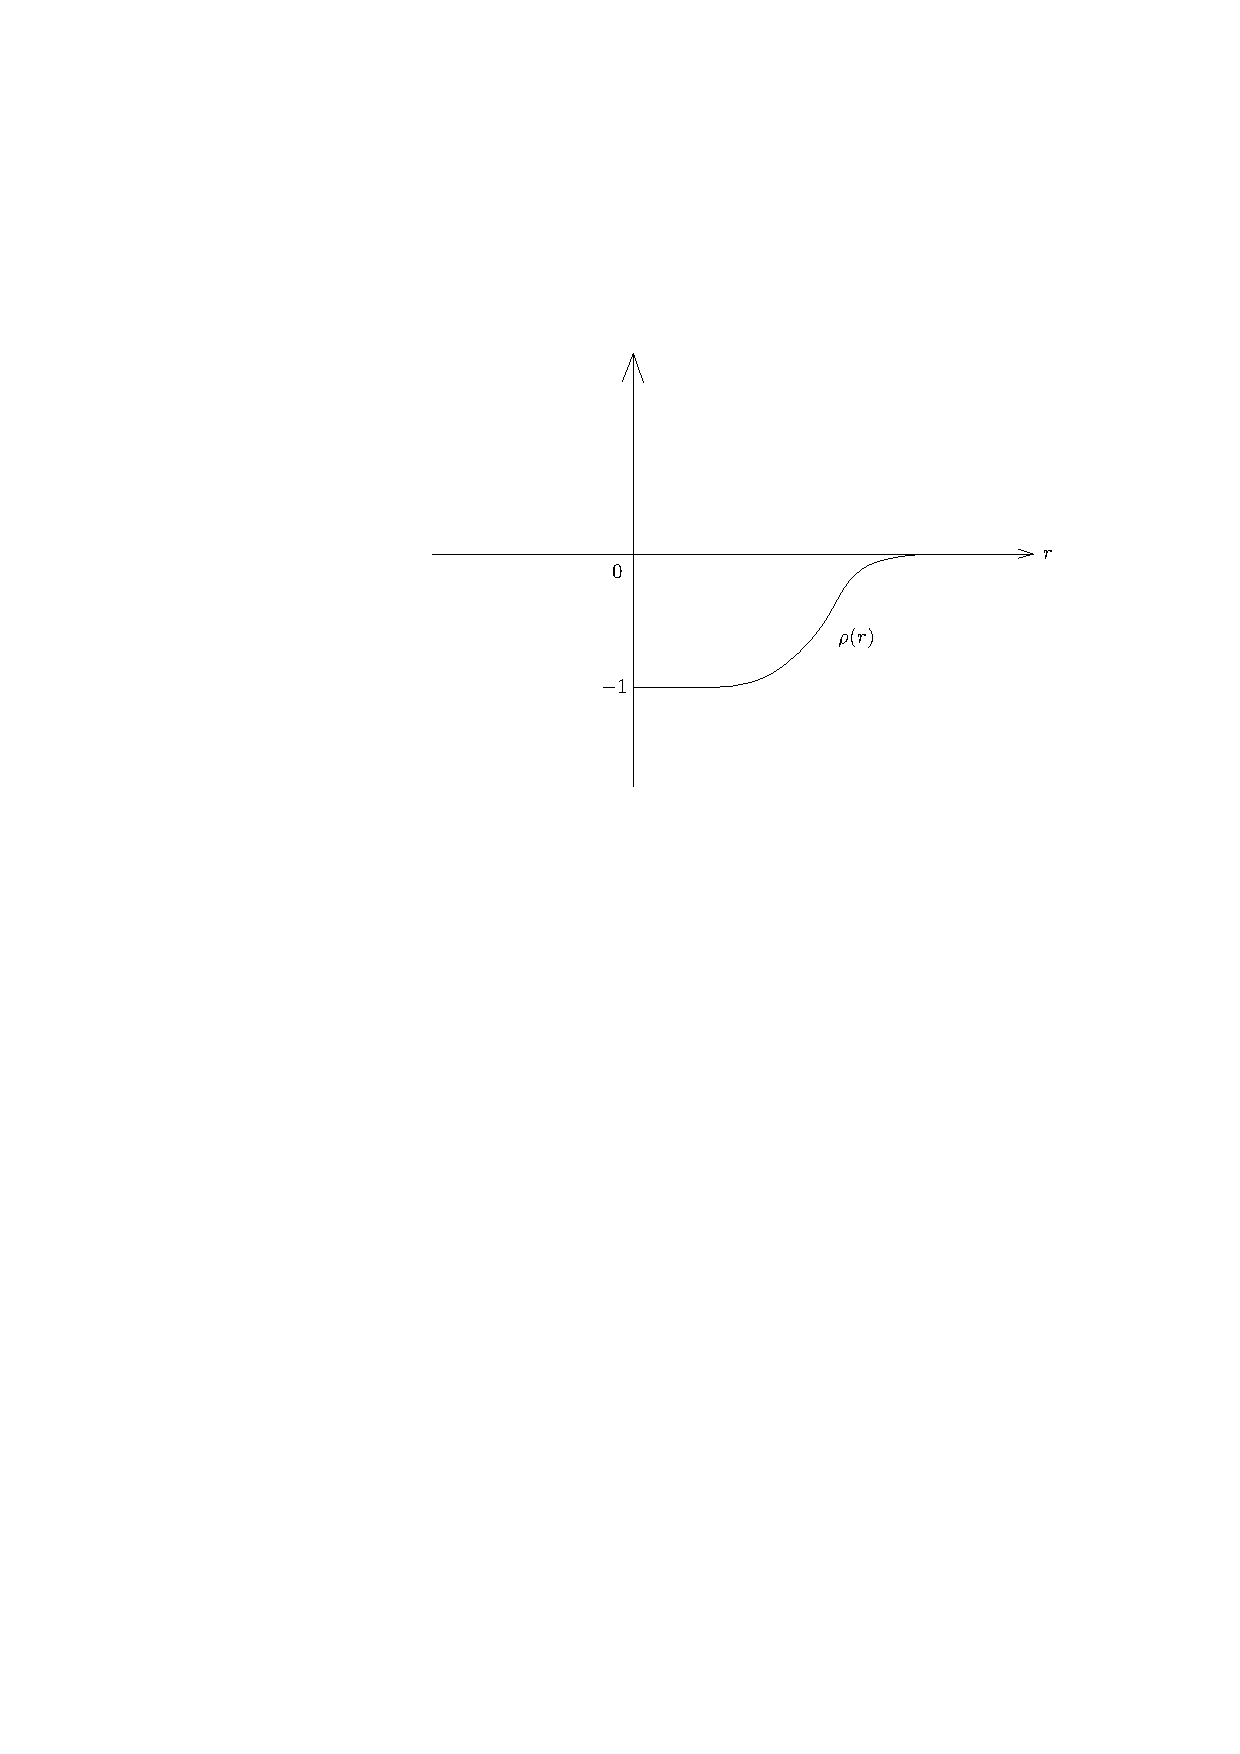
\includegraphics[width=0.5\textwidth]{Thom-iso-function}
\caption{The function $\rho(r)$.}
\label{Thom iso function rho(r)}
\end{figure}

Let $f:E^0\to S(E)$ be a deformation retraction of the complement of the zero section in $E$ onto the unit sphere bundle. If $\psi_S$ is the global angular form on $S(E)$, 
then $\psi=f^*\psi_S\in H^{k-1}(E^0)$ is the global angular form on $E^0$. It has the property that
\[d\psi=-\pi^*e.\]
where $e$ represents the Euler class of the bundle $E$.
\begin{proposition}
The cohomology class of
\[\Phi=d(\rho(r)\wedge\psi)\in\Omega^k_{cv}(E)\]
is the Thom class of the oriented vector bundle $E$.
\end{proposition}
\begin{proof}
Note that
\[\Phi=d\rho(r)\wedge\psi+\rho(r)\wedge d\psi=d\rho(r)\wedge\psi-\rho(r)\wedge\pi^*e.\]
By our choice of $\rho(r)$, it is easy to see $\Phi\in\Omega_{cv}(E)$ and it is closed. Its restriction to the fiber at $p$ is 
\[\iota_p^*(d(\rho(r)\wedge\psi))=d(\iota_p^*\rho(r)\wedge\iota_p^*\psi)=(d\rho(r))\wedge\iota_p^*\psi-\rho(r)\wedge\iota_p^*\pi^*e,\]
where $i_p:E_p\to E$ is the inclusion and $\iota_p^*$ gives a generator of $H^{k-1}(\R^k\setminus\{0\})=H^{k-1}(S^{k-1})$. From the diagram
\[\begin{tikzcd}
E_p\ar[r]\ar[d]&\{p\}\ar[d]\\
E\ar[r,"\pi"]&M
\end{tikzcd}\]
we see that $\iota_p^*\pi^*e=0$, therefore
\[\int_{\R^k}\iota_p^*\Phi=\int_{\R^k}(d\rho(r))\wedge\iota_p^*\psi=\int_{\R}d\rho(r)\int_{S^{k-1}}\iota_p^*\psi=1.\]
Thus by Proposition~\ref{Thom iso} $\Phi$ is the Thom class of $E$.
\end{proof}
We now have our promised fact about the Thom class and the Euler class.
\begin{proposition}\label{Thom class pullback Euler class}
The pullback of the Thom class of an oriented rank $k$ vector undle via the zero section to the base manifold is the Euler class.
\end{proposition}
\begin{proof}
Let $s$ be the zero section of $E$. Use the formula of $\Phi$, we find that
\[s^*\Phi=s^*d(\rho(r)\wedge\psi)=s^*((d\rho(r))\wedge\psi-\rho(r)\pi^*e)=s^*d\rho(r)\wedge s^*\psi-s^*\rho(r)s^*\pi^*e=e.\]
Thus we get the claim.
\end{proof}
\begin{remark}
From the formula for the Thom class, it is clear that by making the support of $\rho(r)$ sufficiently close to $0$, the Thom class $\Phi$ can be made to have support 
arbitrarily close to the zero section of the vector bundle.
\end{remark}
\begin{remark}
In fact, any section will pull the Thom class back to the Euler class. Let $s$ be a section of the oriented vector bundle $E$ and $s^*:H_{cv}^*(E)\to H^*(M)$ the 
induced map in cohomology. Note that $s^*$ can be written as the composition of the natural maps $i:H^*_{cv}(E)\to H^*(E)$ and $\widebar{s}^*:H^*(E)\to H^*(M)$. 
As a map from $M$ into $E$, the section $s$ is homotopic to the zero section $s_0$. By the homotopy axiom for de Rham cohomology $\widebar{s}^*=\widebar{s}_0^*$. Hence, 
$s^*=s_0^*$.
\end{remark}
Using the description of the Euler class as the pullback of the Thom class, it is easy to prove the Whitney product formula.
\begin{proposition}[\textbf{Whitney Product Formula for the Euler Class}]
If $E$ and $F$ are two oriented vector bundles, then $e(E\oplus F)=e(E)\wedge e(F)$.
\end{proposition}
\begin{proof}
By Proposition~\ref{Thom class disrect sum}, the Thorn class of $E\oplus F$ is
\[\Phi(E\oplus F)=\pi_1^*\Phi(E)\wedge\pi_2^*\Phi(F).\]
Let $s$ be the zero section of $E\oplus F$. Then $\pi_1\circ s$ sand $\pi_2\circ s$ are the zero sections of $E$ and $F$. By Proposition~\ref{Thom class pullback Euler class},
\[e(E\oplus F)=s^*\Phi(E\oplus F)=s^*\pi_1^*\Phi(E)\wedge s^*\pi_2^*\Phi(F)=e(E)\wedge e(F).\]
\end{proof}
\subsubsection{Euler class and the zero locus of a section}
Let $\pi:E\to M$ be a vector bundle and $S_0$ the image of the zero section in $E$. A section $s$ of $E$ is \textbf{transversal} if its image $S=s(M)$ intersects $S_0$ 
transversally.
\begin{proposition}\label{tran section normal bundle zero locus}
Let $\pi:E\to M$ be any vector bundle and $Z$ the zero locus of a transversal section. Then $Z$ is a submanifold of $M$ and its normal bundle in $M$ is $NZ=E|_Z$.
\end{proposition}
\begin{proof}
Write $S=s(M)$ for the image of the section $s$. Because $S$ intersects $S_0$ transversally, $S\cap S_0$ is a submanifold of $S$ by the transversality theorem. Under 
the diffeomorphism $s:M\to S$, $Z$ is mapped homeomorphically to $S\cap S_0$. So $Z$ can be made into a submanifold of $M$.\par
To compute the normal bundle of $Z$, we first note that because $E$ is locally trivial, its tangent bundle on $S_0$ has the following canonical decomposition
\[TE|_{S_0}=E|_{S_0}\oplus TS_0.\]
By the transversality of $S\cap S_0$,
\[TS+TS_0=TE=E\oplus TS_0.\]
Therefore we obtain
\[E=\frac{E\oplus TS_0}{TS_0}\cong\frac{TS+TS_0}{TS_0}\cong\frac{TS}{TS\cap TS_0}.\]
This then gives an exact sequence
\[\begin{tikzcd}
0\ar[r]&(TS\cap TS_0)|_Z\ar[r]&TS|_Z\ar[r]&E|_Z\ar[r]&0
\end{tikzcd}\]
Since $(TS\cap TS_0)|_Z=TZ$, we find that $NZ\cong E|_Z$.
\end{proof}
In the proposition above, if $E$ and $M$ are both oriented, then the zero locus $Z$ of a transversal section is naturally an oriented manifold, oriented in such a way 
that
\[E|_Z\oplus TZ=TM|_Z.\]
has the direct sum orientation.
\begin{proposition}
Let $\pi:E\to M$ be an oriented vector bundle over an oriented manifold $M$. Then the Euler class $e(E)$ is Poincar\'e dual to the zero locus of a transversal section.
\end{proposition}
\begin{proof}
We will identify $M$ with the image $S_0$ of the zero section. If $S$ is the image in $E$ of the transversal section $s:M\to E$, then the zero locus of $s$ is $Z=S\cap S_0$. 
$Z$ is a closed oriented submanifold of $M$ and by Proposition~\ref{tran section normal bundle zero locus}, its normal bundle in $M$ is $NZ\cong E|_Z$. Since $S$ is 
diffeomorphic to $M$, the normal bundle of $Z$ in $S$ is also isomorphic to $E|_Z$. The normal bundles of $Z$ in $M$ and $S$, denoted by $N_MZ$ and $N_SZ$, will be 
identified with the tubular neighborhoods of $Z$ in $M$ and in $S$, respectively.\par
Choose the Thom class $\Phi$ of $E$ to have support so close to the zero section that $\Phi$ restricted to the tubular neighborhood $N_SZ$ in $S$ has compact support 
in the vertical direction. We will now show that $s^*\Phi$ is the Thom class of the tubular neighborhood $N_MZ$ in $M$.\par
Let $E_p$, $S_p$, and $M_p$ be the fibers of $E|_Z$, $N_SZ$, $N_MZ$ respectively above the point $p$ in $Z$. Because $\Phi$ has compact support in $S_p$, $s^*\Phi$ 
has compact support in $M_p$. Furthermore, after identifying $S_p$ and $M_p$ with their conterpart in the tubular neighborhoods, we have the following diffeomorphisms:
\[\begin{tikzcd}
M_p\ar[rd,swap,"\beta"]\ar[r,"s"]&S_p\ar[d,"\alpha"]\\
&E_p
\end{tikzcd}\]
Therefore we get
\begin{align*}
\int_{M_p}s^*\Phi=\int_{M_p}s^*\alpha^*\Phi=\int_{S_p}\alpha^*\Phi=\int_{E_p}\Phi=1.
\end{align*}
So $s^*\Phi$ is the Thom class of $N_MZ$. By Proposition~\ref{Thom class pullback Euler class}, $s^*\Phi=e(E)$. Since by Proposition~\ref{Thom class Poincare dual} the 
Thom class of $N_MZ$ is Poincare dual to $Z$ in $M$, the Euler class $e(E)$ is Poincare dual to $Z$ in $M$.
\end{proof}
\subsubsection{Poincar\'e duality}
Let $M$ be a manifold of dimension $n$ and $\mathcal{U}=\{U_i\}$ any open cover of $M$. Define the coboundary operator
\[\delta:\bigoplus\Omega^*_c(U_{i_0\dots i_p})\to\bigoplus\Omega^*_c(U_{i_0\dots i_{p-1}})\]
by the formula
\[(\delta\omega)_{i_0\dots i_{p-1}}=\sum_{i}\omega_{i,i_0\dots i_{p-1}}.\]
where on the right-hand side we mean the extension by zero of $\omega_{i,i_0\dots i_{p-1}}$ to a form on $U_{i_0\dots i_{p-1}}$. To ensure that each component of $\delta\omega$ 
has compact support, the groups here are direct sums rather than direct products, so that $\omega$ by definition has only a finite number of nonzero components.
\begin{proposition}[\textbf{Generalized Mayer-Vietoris Sequence for Compact Supports}]\label{Generalized MV compact supp}
Suppose the open cover $\mathcal{U}$ of the manifold $M$ is locally finite. Then the sequence
\[\begin{tikzcd}
\cdots\ar[r]&\bigoplus\Omega^*_c(U_{i_0i_1})\ar[r]&\bigoplus\Omega^*_c(U_{i_0})\ar[r,"\text{sum}"]&\Omega^*_c(M)\ar[r]&0
\end{tikzcd}\]
is exact.
\end{proposition}
\begin{proof}
We first show $\delta^2=0$. Let $\omega$ be in $\bigoplus\Omega^*_c(U_{i_0\dots i_p})$. Then
\[(\delta^2\omega)_{i_0\dots i_{p-2}}=\sum_i(\delta\omega)_{i,i_0\dots i_{p-2}}=\sum_i\sum_j\omega_{j,i,i_0\dots i_{p-2}}=0.\]
(Here we use the alternating condition $\omega_{i_0\dots i\dots j\dots i_p}=-\omega_{i_0\dots j\dots i\dots i_p}$.) Now we define a homotopy from the identity to zero. 
Let $\{\rho_i\}$ be a partition of unity subordinate to the cover $\{U_i\}$. Define a map
\[K:\Omega^*_c(U_{i_0\dots i_p})\to\Omega^*_c(U_{i_0\dots i_{p+1}})\]
by the formula
\[(K\omega)_{i_0\dots i_{p+1}}=\sum_{j=0}^{p+1}(-1)^i\rho_{i_j}\omega_{i_0\dots\widehat{i_j}\dots i_{p+1}}.\]
Note that $(K\omega)_{i_0\dots i_{p+1}}$ has compact support. Moreover, there are only finitely many $(j,i_0,\dots,i_p)$ for which $\rho_j\omega_{i_0\dots i_p}\neq 0$, 
since $\omega_{i_0\dots i_p}\neq 0$ for finitely many $(i_0,\dots,i_p)$ and by the locally finiteness each $U_{i_0\dots i_p}\sub U_{i_0}$ intersects only finitely many 
$U_j$. With this definition, we have
\begin{align*}
(\delta K\omega)_{i_0\dots i_p}&=\sum_i(K\omega)_{i,i_0\dots i_{p}}=\sum_i\rho_{i}\omega_{i_0\dots i_{p}}+\sum_i\sum_{j=0}^{p}(-1)^{j+1}\rho_{i_j}\omega_{i,i_0\dots\widehat{i_{j}}\dots i_{p}}\\
&=\omega_{i_0\dots i_p}-\sum_{j=0}^{p}(-1)^j\rho_{i_j}\sum_i\omega_{i,i_0\dots\widehat{i_{j}}\dots i_{p}}\\
&=\omega_{i_0\dots i_p}-\sum_{j=0}^{p}(-1)^j\rho_{i_j}\sum_i\omega_{i,i_0\dots\widehat{i_{j}}\dots i_{p}}\\
&=\omega_{i_0\dots i_p}-\sum_{j=0}^{p}(-1)^j\rho_{i_j}(\delta\omega)_{i_0\dots\widehat{i_{j}}\dots i_{p}}\\
&=\omega_{i_0\dots i_p}-(K\delta\omega)_{i_0\dots i_p}.
\end{align*}
Therefore $\delta K+K\delta=\id$ and we conclude the claim.
\end{proof}
Consider the double complex $C^*(\mathcal{U},\Omega^*_c)$, where $\mathcal{U}$ is a locally finite cover. In this double complex the $\delta$-operator goes in the wrong 
direction, so we define a new complex
\[K^{-p,q}=C^p(\mathcal{U},\Omega^q_c).\]
Then by Proposition~\ref{Generalized MV compact supp} and a spectral sequence argument, we get
\[H_{TC}^*(K)=H_c^*(M).\]
On the other hand, by definition we have
\[_{v}E_1^{-p,q}=C^p(\mathcal{U},\mathscr{H}_c^q)\]
where $\mathscr{H}_c^q$ is the covariant functor which associates to every open set $U$ the compact cohomology $H^q_c(U)$ and to every inclusion $i$, the extension by 
zero $i_*$; moreover, is $\mathcal{U}$ is a good cover, then
\[\mathscr{H}_c^q(U)=\begin{cases}
\R,&q=n;\\
0,&q\neq n.
\end{cases}\]
Therefore in this case the $_{v}E_1$ page has only one row, and therefore
\[H^*_{TC}(K)={_{v}E_2^{*-n,n}}=H_{n-*}(\mathcal{U},\mathscr{H}^n_c).\]
Here $H(\mathcal{U},\mathscr{H}^n_c)$ is the tech homology of the cover $\mathcal{U}$ with coefficients in the covariant functor $\mathscr{H}_c^{n}$.
\begin{proposition}
Let $M$ be a manifold of dimension $n$ and $\mathcal{U}$ any locally finite good cover of $M$. Here $M$ is not assumed to be orientable. Then
\[H^*_c(M)\cong H_{n-*}(\mathcal{U},\mathscr{H}^n_c),\]
where $\mathscr{H}^n_c$ is the covariant functor $\mathscr{H}^n_c(U)=H^n_c(U)$.
\end{proposition}
\subsection{Monodromy}
\subsubsection{When is a locally constant presheaf constant}
In the preceding part we saw that the compact vertical cohomology $H^*_{cv}(E)$ of a vector bundle $E$ may be computed as the cohomology of the base with 
coefficients in the presheaf $\mathscr{H}_{cv}^n$. When the presheaf $\mathscr{H}_{cv}^n$ is the constant presheaf $\R^n$, $H^*_{cv}(E)$ is expressible in terms of the 
de Rham cohomology of the base manifold. In this case the problem of computing $H^*_{cv}(E)$ is greatly simplified. It is therefore important to 
determine the conditions under which a presheaf such as $\mathscr{H}_{cv}$ is constant.\par
We first introduce the notion of a presheaf on a cover. Let $X$ be a topological space and $\mathcal{U}=\{U_\alpha\}$ a cover of $X$. The presheaf $\mathscr{F}$ on 
$\mathcal{U}$ is defined to be a functor $\mathscr{F}$ on the subcategory of $\mathbf{Open}(X)$ consisting of all finite intersections $U_{i_0\dots i_p}$ of open sets in 
$\mathcal{U}$. Equivalently, if $N(\mathcal{U})$ is the nerve of $\mathcal{U}$, the presheaf $\mathscr{F}$ on $\mathcal{U}$ is the assignment of an appropriate group to 
the barycenter of each simplex in $N(\mathcal{U})$; for example, the group attached to the barycenter of the $2$-simplex representing $U\cap V\cap W$ is 
$\mathscr{F}(U\cap V\cap W)$. Each inclusion, say $U\cap V\hookrightarrow U$, becomes an arrow in the picture, $\mathscr{F}(U)\to\mathscr{F}(U\cap V)$, and the 
transitivity of the arrows says that Figure is a commutative diagram.

Two presheaves $\mathscr{F}$ and $\mathscr{G}$ are isomorphic relative to a cover $\mathcal{U}=(U_i)$ if for each $U_{i_0\dots i_p}$ there is an isomorphism
\[h_{i_0\dots i_p}:\mathscr{F}(U_{i_0\dots i_p})\to\mathscr{G}(U_{i_0\dots i_p})\]
compatible with all arrows. In other words, there is a natural equivalence of functors $\mathscr{F}\to\mathscr{G}$ where $\mathscr{F}$ and $\mathscr{G}$ are regarded as \
functors on the subcategory of $\mathbf{Open}(X)$ consisting of all finite intersections of open sets in $\mathcal{U}$. The constant presheaf with group $G$ on a good 
cover $\mathcal{U}$ is defined as usual, it associates to every open set the group of locally constant and hence constant functions: $U_{i_0\dots i_p}\to G$. Thus, for 
a constant presheaf on a cover, all the groups are $G$ and all the arrows are the identity map. We say that a presheaf $\mathscr{F}$ is \textbf{locally constant} 
on a cover $\mathcal{U}$ if all the groups are isomorphic and all the arrows are isomorphisms.\par
Of course, if two presheaves $\mathscr{F}$ and $\mathscr{G}$ are isomorphic on a cover $\mathcal{U}$, then the \v{C}ech cohomology groups $H^*(\mathcal{U},\mathscr{F})$ 
and $H^*(\mathcal{U},\mathscr{G})$ are isomorphic.\par
Let $\mathscr{F}$ be a locally constant presheaf with group $G$ on a cover $\mathcal{U}=(U_i)$. Fix isomorphisms $\phi_i:\mathscr{F}(U_i)\to G$. If $U_i$ and $U_j$ 
intersect, then from the diagram
\[\begin{tikzcd}
\mathscr{F}(U_i)\ar[d,"\phi_i"]\ar[r,"\rho^i_{ij}"]&\mathscr{F}(U_{ij})&\mathscr{F}(U_j)\ar[l,swap,"\rho^j_{ij}"]\ar[d,"\phi_j"]\\
G\ar[rr,dashed]&&G
\end{tikzcd}\]
we obtain an automorphism of $G$, namely $\phi_j\circ(\rho_{ij}^j)^{-1}\circ\rho^i_{ij}\circ\phi_i^{-1}$. Write $\rho^i_j:\mathscr{F}(U_i)\to\mathscr{F}(U_j)$ for the 
isomorphism $(\rho_{ij}^j)^{-1}\circ\rho^i_{ij}$. Choose some vertex $U_0$ as the base point of the nerve $N(\mathcal{U})$. For $U_0U_1\cdots U_rU_0$ a loop based at 
$U_0$ we get an automorphism of $G$ by following along the edges
\[\begin{tikzcd}
\mathscr{F}(U_0)\ar[d,"\phi_0"]\ar[r]&\mathscr{F}(U_1)\ar[d,"\phi_1"]\ar[r]&\cdots\ar[r]&\mathscr{F}(U_r)\ar[d,"\phi_r"]\ar[r]&\mathscr{F}(U_0)\ar[d,"\phi_0"]\\
G\ar[r]&G\ar[r]&\cdots\ar[r]&G\ar[r]&G
\end{tikzcd}\]
This gives a map from loops at $U_0$ to $\Aut(G)$. By the transitivity of the transition map, we claim that if a loop bounds a $2$-chain in $N(\mathcal{U})$, then the 
associated automorphism of $G$ is the identity. Hence there is a Homomorphism
\[\rho:\pi_1(N(\mathcal{U}))=\frac{\text{loops}}{\text{bounding loops}}\to\Aut(G).\]
called the \textbf{monodromy representation} of the presheaf $\mathscr{F}$. Here $\pi_1(N(\mathcal{U}))$ denotes the edge path group of the simplicial complex $N(\mathcal{U})$.
\begin{theorem}
Let $\mathcal{U}$ be a cover on a connected topological space $X$ and $N(\mathcal{U})$ its nerve. If $\pi_1(N(\mathcal{U}))=0$, then every locally constant presheaf on 
$\mathcal{U}$ is constant.
\end{theorem}
\begin{proof}
For each open set $U_i$, choose a path from $U_0$ to $U_i$, say $U_0U_{i_1}\cdots U_{i_r}U_i$ and define 
\[\psi_i=\phi_0\circ(\rho^{i_r}_i\circ\cdots\circ\rho^{i_1}_{i_2}\circ\rho^0_{i_1})^{-1}:\mathscr{F}(U_i)\to G.\]
$\psi_i$ is well-defined independent of the chosen path, because $\rho$ is trivial. Now carry out the barycentric subdivision of the nerve $N(\mathcal{U})$ to get a 
new simplictal complex $K$ so that every open set $U_{i_0\dots i_p}$ corresponds to a vertex of $K$. Clearl $\pi_1(K)=\pi_1(N(\mathcal{U}))=0$. By the same procedure as 
in the preceding paragraph we can define isomorphisms $\psi_{i_0\dots i_p}:\mathscr{F}(U_{i_0\dots i_p})\to G$. The maps $\psi_{i_0\dots i_p}$ give an isomorphism of 
the presheaf $\mathscr{F}$ to the constant presheaf $G$ on the cover $\mathcal{U}$.
\end{proof}
By a good cover on a topological space we shall mean an open cover for which all finite intersections are contractible.
\begin{theorem}
Suppose the topological space $X$ has a good cover $\mathcal{U}$. Then the fundamental group of $X$ is isomorphic to the fundamental group $\pi_1(N(\mathcal{U}))$ of the 
nerve of the good cover.
\end{theorem}
\begin{corollary}
Let $\mathcal{U}$ be a good cover on a simply connected topological space $X$. Then any locally constant sheaf on $\mathcal{U}$ is constant.
\end{corollary}
\begin{corollary}
Any locally constant sheaf on a simply connected manifold is constant.
\end{corollary}
\subsection{The spectral sequence of a fiber bundle}
Let $\pi:E\to M$ be a fiber bundle with fiber $F$ over a manifold $M$. Applying spectral sequence gives a general method for computing the cohomology of $E$ from that 
of $F$ and $M$. Indeed, given a good cover $\mathcal{U}$ of $M$, $\pi^{-1}(\mathcal{U})$ is a cover on $E$ and we can form the double complex 
$C^*(\pi^{-1}(\mathcal{U}),\Omega^*)$, whose $E_1$ term is
\[E_1^{p,q}=\prod H^q(\pi^{-1}(U_{i_0\dots i_p}))=C^p(\pi^{-1}(\mathcal{U}),\mathscr{H}^q).\]
where $\mathscr{H}^q$ is the presheaf $\mathscr{H}^q(U)=H^q(\pi^{-1}(U))$ on $M$. For emphasis we sometimes write the presheaf $\mathscr{H}^q$ as $\mathscr{H}^q(F)$. 
Since $\mathcal{U}$ is a good cover, $E|_{U_i}$ is trivial and thus $\mathscr{H}^q$ is a locally constant presheaf on $\mathcal{U}$ with group $H^q(F)$. Since $d_1=\delta$ 
on $E_1$, the $E_2$ term is
\[E_2^{p,q}=H^p(\mathcal{U},\mathscr{H}^q).\]
By the generalized Mayer-Vietoris principle $H^*_{TC}(C^*(\pi^{-1}(\mathcal{U}),\Omega^*))$ is equal to $H^*(E)$, because $\pi^{-1}(\mathcal{U})$ is a cover on $E$. 
In the case that $\mathscr{H}^q$ is constant and $H^q(F)$ is finite-dimensional, the $E_2$ term is isomorphic as a vector space to the tensor product $H^p(M)\otimes H^q(F)$, 
since
\[E_2^{p,q}=H^p(\mathcal{U},\R^{\dim H^q(F)})=H^p(\mathcal{U},\R)\otimes H^q(F)=H^p(M)\otimes H^q(F).\]
Therefore we have proved the following.
\begin{proposition}[\textbf{Leray's Theorem for de Rham Cohomology}]
Given a fiber bundle $\pi:E\to M$ with fiber $F$ over a manifold $M$ and a good cover $\mathcal{U}$ of $M$, there is a spectral sequence $\{E_r\}$ converging to the 
cohomology of the total space $H^*(E)$ with
\[E_2^{p,q}=H^p(\mathcal{U},\mathscr{H}^q).\]
where $\mathscr{H}^q$ is the locally constant presheaf $\mathscr{H}^q(U)=H^q(\pi^{-1}(U))$ on $\mathcal{U}$. If $\mathscr{H}^q$ is constant (for example, if $M$ is 
simply connected) and $H^q(F)$ is finite-dimensional, then
\[E_2^{p,q}=H^p(M)\otimes H^q(F).\]
\end{proposition}
\begin{example}[\textbf{The K\"unneth formula and the Leray-Hirsch theorem}]
We now give a spectral sequence proof of the K\"unneth formula. Let $M$ and $F$ be two manifolds and $\mathcal{U}$ a good cover of $M$. Suppose $F$ has 
finite-dimensional cohomology. By Leray's theorem, the spectral sequence of the trivial bundle $F\to M\times F\to M$ has $E_2$ term
\[E_2^{p,q}=H^p(\mathcal{U},\mathscr{H}^q).\]
Because $M\times F$ is a trivial bundle over $M$, the presheaf $\mathscr{H}^q(F)$ is constant, so that
\[E_2^{p,q}=H^p(\mathcal{U},\R)\otimes H^q(F)=H^p(M)\otimes H^q(F).\]
The differential $d_r$ measures the extent to which an element of $C^*(\pi^{-1}(\mathcal{U}),\Omega^*)$ that lives to $E_r$ fails to be extended one step further to a 
$D$-cocycle. Since every element of the $E_2$ term is already a global form on $M\times F$. So $E_2=E_{\infty}$. Therefore we get the K"unneth formula
\[H^*(M\times F)=H^*(M)\otimes H^*(F).\]
The proof of the Leray-Hirsch theorem is analogous.
\end{example}
\begin{example}[\textbf{Orientability and the Euler class of a sphere bundle}]\label{Orientability of sphere bundle spectral seq}
Let $\pi:E\to M$ be an $S^k$-bundle over a manifold $M$ and let $\mathcal{U}$ be a good cover of $M$. The spectral sequence of this fiber bundle has
\[E_1^{p,q}=C^p(\mathcal{U},\mathscr{H}^q(S^k))=\begin{cases}
C^p(\mathcal{U},\R),&q=0,k;\\
0,&\text{otherwise}
\end{cases}.\]
Let $\sigma$ be the element of $E_1^{0,k}$ corresponding to the local angular forms on the sphere bundle $E$. From the description of the differential $d_r$ as the $\delta$ 
of the tail of a zig-zag, we see that $E$ is orientable if and only if $d_1\sigma=0$. For an orientable $S^k$-bundle then, such a $\sigma$ lives to $E_k$:
\[E_k=E_2=H^*(\mathcal{U},\mathscr{H}^*(S^k)).\]
Up to a sign $d_k\sigma$ in $H^{k+1}(\mathcal{U},\mathscr{H}^0(S^k))=H^{k+1}(\mathcal{U},\R)=H^{k+1}(M)$ is the Euler class of the sphere bundle. It measures the extent 
to which $\sigma$ fails to be extended to a $D$-cocycle, i.e., a global closed $k$-form on the sphere bundle.
\end{example}
\begin{example}[\textbf{Orientability of a simply connected manifold}]
Let $M$ be a simply connected manifold of dimension $n$ and $S(TM)$ its unit tangent bundle. The spectral sequence of the fiber bundle
\[\begin{tikzcd}
S^{k-1}\ar[r]&S(TM)\ar[r]&M
\end{tikzcd}\]
has $E_2$ term
\[E_2=H^*(\mathcal{U},\mathscr{H}^*(S^k)).\]
Since each restricted bundle on $U_{i_0\dots i_p}$ is trivial, $\mathscr{H}^0(S^k)$ and $\mathscr{H}^k(S^k)$ is contant on it. Therefore
\[E_2^{p,q}=H^p(\mathcal{U},\mathscr{H}^q(S^{n-1}))=\begin{cases}
H^p(\mathcal{U},\R)&q=0,n-1\\
0&\text{otherwise}
\end{cases}\]
Moreover, by the isomorphism $H^*(M)=H^*(\mathcal{U},\R)$ and the simply connected condition, we further have
\[E_2^{1,0}=E_2^{1,n-1}=0.\]
This, together with Example~\ref{Orientability of sphere bundle spectral seq}, shows that there is an element in $C^0(\pi^{-1}(\mathcal{U}),\mathscr{H}^{n-1})$ which 
can be extended one step down toward being a $D$-cocycle. Therefore $S(TM)$ and also $M$ are orientable. This gives an alternative proof of the orientability of a simply 
connected manifold.
\end{example}
\begin{example}[\textbf{The cohomology of the complex projective space}]\label{cohomology CP^n}
Consider the sphere $S^{2n+1}$ in $\C^{n+1}$. Let $S^1$ act on $S^{2n+1}$ by
\[\lambda\cdot (z_0,\dots,z_n)=(\lambda z_0,\dots,\lambda z_n).\]
where $\lambda$ in $S^1$ is a complex number of absolute value $1$. The quotient of $S^{2n+1}$ by this action is the complex projective space $\CP^n$. This gives $S^{2n+1}$ 
the structure of a circle bundle over $\CP^n$:
\[\begin{tikzcd}
S^1\ar[r]&S^{2n+1}\ar[r]&\CP^n
\end{tikzcd}\]
As we will see from the homotopy exact sequence to be discussed later, $\CP^n$ is simply connected. Thus
\[E_2^{p,q}=H^p(\CP^n)\otimes H^q(S^1).\]
So $E_2$ has only two nonzero rows, $q=0,1$, and the two rows are identical, both being $H^*(\CP^n)$. Because $\CP^n$ has dimension $2n$, we have $H^p(\CP^n)=0$ for 
$p>2n$. In the spectral seuqnece we have $d_r=0$ for $r>2$, therefore $E_3=E_4=\cdots=E_{\infty}=H^*(S^{2n+1})$. Therefore $E_3$ is
\[\begin{tikzcd}[column sep=0.8em,row sep=0.8em]
0&0&0&\cdots&\R\\
\R&0&0&\cdots&0\\
\end{tikzcd}
\]
From this we can chase the maps in $E_2$. Since $E_2^{0,0}=E_2^{0,1}=\R$ and $E_2^{p,0}=E_2^{p,1}$, we finally conclude that $E_2$ has the form
\[\begin{tikzcd}[column sep=0.8em,row sep=0.8em]
\R\ar[rrd]&0&\R\ar[rrd]&0&\cdots&\R\ar[rrd]&0&\R\\
\R&0&\R&0&\cdots&\R&0&\R\\
\end{tikzcd}\]
Further, from this spectral sequence we can get the product structure of $H^*(\CP^n)$:
\[\begin{tikzcd}[column sep=0.8em,row sep=0.8em]
a\ar[rrd]&&ax\ar[rrd]&&ax^2&\cdots&ax^{n-1}\ar[rrd]&&ax^{n}\\
1&&x&&x^2&\cdots&x^{n-1}&&x^{n}
\end{tikzcd}\]
Therefore
\[H^*(\CP^n)=\R[x]/(x^{n+1}),\quad \dim x=2.\]

Note that $S^{2n-1}$ is a circle bundle on $\CP^n$, so we can compute its Euler class. By definition, the Euler class is given by the diagram
\[\begin{tikzcd}
\sigma\ar[r]&{}&\\
&\ar[r,"\delta"]\ar[u]&d_2(\sigma)=-\pi^*\eps
\end{tikzcd}\]
where $\sigma$ is a generator of $E_2^{0,1}$. By our choice of $a$ and $x$, it is clear that $x=-e$, therefore the Euler class of $S^{2n-1}$ generates the cohomology ring of $\CP^n$.
\end{example}
\subsubsection{The Gysin sequence}
The spectral sequence of a fiber bundle is essentially a way of describing the complicated algebraic relations among the cohomology of the base space, the fiber, and 
the total space of the bundle, In certain special situations the spectral sequence simplifies to a long exact sequence, One such special case is the cohomology of a 
sphere bundle. The resulting sequence is called the \textbf{Gysin sequence}, which we now derive.
Let $\pi:E\to M$ be an oriented sphere bundle with fiber $S^k$. By the orientability assumption, for any good cover $\mathcal{U}$ on $M$, the locally constant presheaf 
$\mathscr{H}^k$ has no monodromy and is the constant presheaf $\R$. Therefore the $E_2$ term of the spectral sequence only has two nonzero rows:
\[E_2^{p,q}=H^p(M)\otimes H^q(S^k).\]
This then means $E_2=E_3=\cdots=E_{k+1}$, and we get an exact seuqnece:
\begin{equation}\label{Gysin seq-1}
\begin{tikzcd}
0\ar[r]&E_{\infty}^{p-k,k}\ar[r]&E_2^{p-k,k}\ar[r,"d_{k+1}"]&E_2^{p+1,0}\ar[r]&E_{\infty}^{p+1,0}\ar[r]&0\\
&&H^{p-k}(M)\ar[u,equal]&H^{p+1}(M)\ar[u,equal]&&
\end{tikzcd}
\end{equation}
Because of the shape of the $E_2$ term, the filtration on $H^*(E)$ becomes
\[H^p(E)\sups E^{p,0}_{\infty}\sups 0,\quad H^p(E)/E^{p,0}\cong E^{p-k,k}_{\infty}.\]
In other words, there is an exact sequence
\begin{equation}\label{Gysin seq-2}
\begin{tikzcd}
0\ar[r]&E^{p,0}_{\infty}\ar[r]&H^p(E)\ar[r]&E_\infty^{p-k,k}\ar[r]&0
\end{tikzcd}
\end{equation}
The two sequences $(\ref{Gysin seq-1})$ and $(\ref{Gysin seq-2})$ may be combined into a single long exact sequence
\[\begin{tikzcd}
\cdots\ar[r]&H^p(E)\ar[r,"\alpha"]&H^{p-k}(M)\ar[r,"d_{k+1}"]&H^{p+1}(M)\ar[r,"\beta"]&H^{p+1}(E)\ar[r]&\cdots
\end{tikzcd}\]
This is the \textbf{Gysin sequence} of the sphere bundle.\par
It remains to identify the maps in the Gysin sequence. Let $\mathcal{U}$ be a good cover on $M$. The map $\alpha$ is the composition
\[\begin{tikzcd}[column sep=1.2em]
H^p(E)\ar[r]&E_{\infty}^{p-k,k}\ar[r,hook]&E_2^{p-k,k}=H^{p-k}(\pi^{-1}(\mathcal{U}),\mathscr{H}^k)\cong H^{p-k}(M)\otimes H^k(S^k)\cong H^{p-k}(M)
\end{tikzcd}\]
In this sequence of maps the first three are the identity on the level of forms and the last one sends a generator of $H^k(S^k)$ to $1$ by integration. Therefore $\alpha$ 
is integration along the fiber.\par
Next consider $d_{k+1}$. By representing an element of $E_2^{p-k,k}=H^{p-k}(M)\otimes H^k(S^k)$ by $(\pi^*\omega)\wedge(-\psi)$, where $\omega$ is a closed form on $M$ 
and $\psi$ is the global angular form on $E$ (note that $\psi$ is locally closed), the map $d_{k+1}$ is defined to be
\begin{align*}
d_{k+1}(\omega)&:=d_{k+1}((\pi^*\omega)\wedge(-\psi))\\
&=d((\pi^*\omega)\wedge(-\psi))=d(\pi^*\omega)\wedge(-\psi)+(-1)^{p-k}(\pi^*\omega)\wedge d(-\psi)\\
&=(-1)^{pxs-k}\pi^*\omega\wedge\pi^* e=(-1)^{p-k}\pi^*(\omega\wedge e).
\end{align*}
Hence, up to a sign $d_{k+1}:H^{p-k}(M)\to H^{p+1}(M)$ is multiplication by the Euler class $e$.\par
Finally the map $\beta$ is the composition
\[\begin{tikzcd}[column sep=1.2em]
H^{p+1}(M)=H^{p+1}(\mathcal{U},\mathscr{H}^0)\ar[r,"\pi^*"]\ar[r,swap,"\cong"]&H^{p+1}(\pi^{-1}(\mathcal{U}),\mathscr{H}^0)=E_2^{p+1,0}\ar[r]&E_{\infty}^{p+1,0}\ar[r,hook]&H^{p+1}(E)
\end{tikzcd}\]
So $\beta:H^{p+1}(M)\to H^{p+1}(E)$ is the natural pullback map $\pi^*$.\par
We summarize this discussion as follows.
\begin{theorem}
Let $\pi:E\to M$ be an oriented sphere bundle with fiber $S^k$. Then there is a long exact sequence
\[\begin{tikzcd}
\cdots\ar[r]&H^p(E)\ar[r,"\pi_*"]&H^{p-k}(M)\ar[r,"\wedge e"]&H^{p+1}(M)\ar[r,"\pi^*"]&H^{p+1}(E)\ar[r]&\cdots
\end{tikzcd}\]
where $e$ is the Euler class of $E$.
\end{theorem}
\subsubsection{Leray's construction}
We consider now more generally not a fiber bundle but any map $f:X\to Y$ from one manifold to another, and study how the cohomology groups of $X$ relate to those of $Y$. 
Let $\mathcal{U}$ be any cover for $Y$, not necessarily a good cover. Then $\pi^{-1}(\mathcal{U})$ is a cover for $X$. By the Mayer-Vietoris principle
\[H^*(X)=H^*_{TC}(C^*(\pi^{-1}(\mathcal{U}),\Omega^*).\]
The spectral sequence of this double complex has
\[E_2^{p,q}=H^p(\mathcal{U},\mathscr{H}^q),\]
where $\mathscr{H}^q$ is the presheaf on $Y$ defined by $\mathscr{H}^q(U)=H^q(f^{-1}(U))$.
The main difference between this situation and that of a fiber bundle is that the presheaf $\mathscr{H}^q$ is no longer locally constant on $U$; indeed the groups 
$H^q(f^{-1}(U))$ will in general be different for different contractible open sets $U$.
\begin{example}
Let $f:X\to Y$ be any smooth map between manifolds and $\mathcal{U}$ a finite good cover of $Y$. Then from the spectral sequence we have
\begin{align*}
\dim H^n(X)&=\sum_{p+q=n}\dim E_{\infty}^{p,q}=\cdots=\sum_{p+q=n}\dim E_{1}^{p,q}=\sum_{p+q=n}\dim C^p(\mathcal{U},\mathscr{H}^q)\\
&=\sum_{p+q=n}\sum_{i_0\dots i_p}\dim H^q(f^{-1}(U_{i_0\dots i_p})).
\end{align*}
This then implies
\[\chi(X)=\sum_n(-1)^n\sum_{p+q=n}\sum_{i_0\dots i_p}\dim H^q(f^{-1}(U_{i_0\dots i_p})).\]
If in particular $\pi:X\to Y$ is a fiber bundle with fiber $F$, $Y$ admits a finite good cover and $F$ has finite-dimensional cohomology, then
\begin{align*}
\chi(X)&=\sum_n(-1)^n\sum_{p+q=n}\sum_{i_0\dots i_p}\dim H^q(\pi^{-1}(U_{i_0\dots i_p}))\\
&=\sum_n(-1)^n\sum_{p+q=n}\sum_{U_{i_0\dots i_p}\neq\emp}\dim H^q\\
&=\sum_{p+q=n}(-1)^n\dim C^p(\mathcal{U},Y)\cdot \dim H^q(F)\\
&=\chi(Y)\chi(F).
\end{align*}
\end{example}
\subsection{Spectral sequence for singular cohomology}
\subsubsection{The Mayer-Vietoris sequence for singular chains}
Let $U=\{U_i\}$ be an open cover of the topological space $X$. Just as for differential forms on a manifold, the sequence of inclusions
\[\begin{tikzcd}
X&\coprod_iU_i\ar[l]&\coprod_{i,j}U_{ij}\ar[l]&\cdots\ar[l]
\end{tikzcd}\]
induces a Mayer-Vietoris sequence. However, we must consider here the group $C^{\mathcal{U}}(X)$ of $\mathcal{U}$-small chains in $X$; these are chains made up of 
simplices each of which lies in some open set of the cover $\mathcal{U}$. The inclusion
\[i:C^{\mathcal{U}}_*(X)\to C_*(X)\]
is a homotopy equivalence, hence induces an isomorphism on homology groups.\par
Now we define a boundary operator
\[\delta:\bigoplus C_q(U_{i_0\dots i_p})\to \bigoplus C_q(U_{i_0\dots i_{p-1}})\]
by the alternating sum formula
\[(\delta c)_{i_0\dots i_p}=\sum_ic_{i,i_0\dots i_{p-1}}.\]
Here, as always, we adopt the alternating convention for chains. The fact that $\delta^2=0$ is proved as in Proposition~\ref{Generalized MV compact supp}. The boundary 
operator $\delta$ on $\bigoplus C_q(U_i)\to C_q(X)$ is simply the sum; we denote this by $\eps$.
\begin{proposition}
The following sequence is exact
\[\begin{tikzcd}
0&C_*^{\mathcal{U}}\ar[l]&\bigoplus C_*(U_i)\ar[l]&\bigoplus C_*(U_{ij})\ar[l]&\cdots\ar[l]
\end{tikzcd}\]
\end{proposition}
Applying the functor $\Hom(-,\Z)$ to the Mayer-Vietoris sequence for singular chains we obtain the Mayer-Vietoris sequence for singular cochains
\[\begin{tikzcd}
0\ar[r]&C^*_{\mathcal{U}}(X)\ar[r]&\prod C^*(U_i)\ar[r]&\prod C^*(U_{i_0 i_1})\ar[r]&\cdots
\end{tikzcd}\]
Since the functor $\Hom(-,\Z)$ preserves the exactness of a sequence of free $\Z$-modules, the Mayer-Vietoris sequence for singular cochains is exact.\par
Once we have the Mayer-Vietoris sequence we can set up the double complex $C^*(\mathcal{U},C^*)$. Just as in the de Rham theory the double complex computes the singular 
cohomology of $X$:
\[H^*_{TC}(C^*(\mathcal{U},C^*))=H^*(X).\]
If $\mathcal{U}$ is a good cover of a topological space $X$, then by the same argument as in the \v{C}ech-de Rham case, we get
\[H^*_{TC}(C^*(\mathcal{U},C^*))=H^*(\mathcal{U},\Z).\]
Suppose $X$ triangularizable. Since the good covers are cofinal in the set of all covers of $X$, we have
\[H^*(X,\Z)=H^*(\mathcal{U},\Z),\]
where $H^*(X,\Z)$ is the \v{C}ech cohomology of $X$ with coefficients in the constant presheaf $\Z$. Therefore,
\begin{theorem}
The singular cohomology of a triangularizable space $X$ is isomorphic to its \v{C}ech cohomology with coefficients in the constant presheaf $\Z$. If $\mathcal{U}$ is a 
good cover of $X$, then
\[H^*(X)\cong H^*(X,\Z)\cong H*(\mathcal{U},\Z).\]
\end{theorem}
Let $\pi:E\to X$ be a fiber bundle with fiber $F$ over a triangularizable topological space $X$. Just as in Theorem 14.18, from the double complex $C^*(\pi^{-1}(\mathcal{U}),C^*)$ 
on $E$ we obtain a spectral sequence converging to the singular cohomology $H^*(E)$ whose $E_2$ term is
\[E_2^{p,q}=H^p(\mathcal{U},\mathscr{H}^q(F)).\]
If $\mathscr{H}^q(F)$ happens to be the constant presheaf $\Z^n$ on $\mathcal{U}$, then
\[E_2^{p,q}=H^p(\mathcal{U},\Z^n)=H^p(X)\otimes H^q(F).\]

By a similar arguments there is also a Mayer-Vietoris sequence for singular cochains with coefficients in a commutative ring $R$. Using the cup product in place of the 
wedge product, the spectral sequence of the Cech-singular complex $C^*(\mathcal{U},C^*)$ can be given a product structure. The arguments before carry over mutatis 
mutandis. Hence the results on spectral sequences remain true for singular cohomology with coefficients in $R$. However, note that the $E_2$ term of a fiber bundle 
$\pi:E\to X$ with fiber $F$ over a simply connected base space $M$ is the tensor product $H^*(X;\R)\otimes H^*(F;R)$ only if the cohomology of $F$ is a free $R$-module. 
In summary we have the following.
\begin{theorem}[\textbf{Leray's Theorem for Singular Cohomology with Coefficients $\bm{R}$}]
Let $\pi:E\to X$ be a fiber bundle with fiber $F$ over a topological space $X$ and $\mathcal{U}$ an open cover of $X$. Then there is a spectral sequence converging to 
$H^*(E;R)$ with $E_2$ term
\[E_2^{p,q}=H^p(\mathcal{U},\mathscr{H}^q(F;R)).\]
Each $E_r$ in the spectral sequence can be given a product structure relative to which the differential $d_r$ is an antiderivation. If $X$ is simply connected and has
a good cover, then
\[E_2^{p,q}=H^p(X,H^q(F;R)).\]
Ifin addition $H^*(F;R)$ is a finitely generated free $R$-module, then
\[E_2=H^*(X;R)\otimes H^*(F;R)\]
as $R$-algebras.
\end{theorem}
\section{Characteristic classes}
\subsection{Chern classes of a complex vector bundle}
In this part we will study the characteristic classes of a complex vector bundle. To begin with we define the first Chern class of a complex line bundle as the Euler 
class of its underlying real bundle. Applying the Leray-Hirsch theorem, we then compute the cohomology ring of the projectivization $P(E)$ of a complex vector bundle $E$ 
and define the Chern classes of $E$ in terms of the ring structure of $H^*(P(E))$. We conclude with a list of the main properties of the Chern classes.
\subsubsection{The first Chern class of a complex line bundle}
Recall that a complex vector bundle of rank $n$ is a fiber bundle with fiber $\C^n$ and structure group $\GL(n,\C)$. A complex vector bundle of rank $1$ is also called 
a complex line bundle. Just as the structure group of a real vector bundle can be reduced to the orthogonal group $\O(n)$, by the Hermitian analogue the structure group 
of a rank $n$ complex vector bundle can be reduced to the unitary group $\U(n)$. Every complex vector bundle $E$ of rank $n$ has an underlying real vector bundle $E_\R$ 
of rank $2n$, obtained by discarding the complex structure on each fiber. By the isomorphism of $\U(1)$ with $\SO(2)$, this sets up a one-to-one correspondence between 
the complex line bundles and the oriented rank $2$ real bundles. We define the first Chern class of a complex line bundle $L$ over a manifold $M$ to be the Euler class 
of its underlying real bundle $L_{\R}$: $c_1(L)=e(L_{\R})\in H^2(M)$.\par
If $L$and $L'$ are complex line bundles with transition functions $\{\tau_{\alpha\beta}\}$ and $\{\tau'_{\alpha\beta}\}$,
\[\tau_{\alpha\beta},\tau'_{\alpha\beta}:U_\alpha\cap U_\beta\to\C^*.\]
then their tensor product $L\otimes L'$ is the complex line bundle with transition functions $\{\tau_{\alpha\beta}\cdot\tau'_{\alpha\beta}\}$. By the formula 
$(\ref{Euler class rank 2 transition})$ which gives the Euler class in terms of the transition functions, we have
\begin{align}\label{Chern first tensor prod}
c_1(L\otimes L')=c_1(L)+c_1(L').
\end{align}

Let $L^*$ be the dual of $L$. Since the line bundle $L\otimes L^*=\Hom(L,L)$ has a nowhere vanishing section given by the identity map, $L\otimes L^*$ is a trivial 
bundle. By $(\ref{Chern first tensor prod})$, $c_1(L)+c_1(L^*)=c_1(L\otimes L^*)=0$. Therefore, $c_1(L^*)=-c_1(L)$.
\begin{example}[\textbf{Tautological bundles on a projective space}]
Let $V$ be a complex vector space of dimension $n$ and $\mathbb{P}(V)$ its projectivization:
\[\mathbb{P}(V)=\{\text{$1$-dimensional subspaces of $V$}\}.\]
On $\mathbb{P}(V)$ there are several God-given vector bundles: the product bundle $\widehat{V}=\mathbb{P}(V)\times V$, the universal subbundle $S$, which is the 
subbundle of $V$ defined by
\[S=\{(\ell,v)\in\mathbb{P}(V)\times V:v\in\ell\}.\]
and the \textbf{universal quotient bundle} $Q$, defined by the exact sequence
\[\begin{tikzcd}
0\ar[r]&S\ar[r]&\widehat{V}\ar[r]&Q\ar[r]&0
\end{tikzcd}\]
The fiber of $S$ above each point $\ell$ in $\mathbb{P}(V)$ consists of all the points in $\ell$, where $\ell$ is viewed as a line in the vector space $V$. The sequence above 
is called the \textbf{tautological exact sequence} over $\mathbb{P}(V)$, and $S^*$ the \textbf{hyperplane bundle}.\par
We now compute the cohomology of $\mathbb{P}(V)$. Endow $V$ with a Hermitian metric and let $E$ be the unit sphere bundle of the universal subbundle $S$:
\[E=\{(\ell,v):v\in\ell,\|v\|=1\}.\]
Since the complement of the zero section $S^0$ is diffeomorphic to $V\setminus\{0\}$, we see the map $\pi:E\to\mathbb{P}(V)$ gives a fibering
\[S^1\to S^{2n-1}\to \mathbb{P}(V).\]
By a computation similar to Example~\ref{cohomology CP^n}, the cohomology ring $H^*(\mathbb{P}(V))$ is seen to be generated by the Euler class of the circle bundle $E$, i.e., the first Chern class 
of the universal subbundle $S$. It is customary to take $x=c_1(S^*)=-c_1(S)$ to be the generator and write
\[H^*(\mathbb{P}(V))=\R[x]/(x^n),\quad n=\dim_\C V.\]
We then see that the Poincar\'e series of the projective space $\mathbb{P}(V)$ is
\[P_t(\mathbb{P}(V))=1+t^2+\cdots+t^{2(n-1)}=\frac{1-t^{2n}}{1-t^2}.\]
\end{example}
\subsubsection{The projectivization of a vector bundle}
Let $\rho:E\to M$ be a complex vector bundle with transition functions $\tau_{\alpha\beta}:U_\alpha\cap U_\beta\to\GL(n,\C)$. We write $E_p$ for the fiber over $p$ and 
$\PGL(n,\C)$ for the projective general linear group $\GL(n,\C)/\{\text{scalar matrices}\}$. The projectivization of $E$, $\pi:\mathbb{P}(E)\to M$, is by definition the 
fiber bundle whose fiber at a point $p$ in $M$ is the projective space $\mathbb{P}(E_p)$ and whose transition functions 
$\tau_{\alpha\beta}:U_{\alpha}\cap U_\beta\to\PGL(n,\C)$ are induced from $\tau_{\alpha\beta}$. Thus a point of $\mathbb{P}(E)$ is a line $\ell_p$ in the fiber $E_p$.\par
As on the projectivization of a vector space, on $\mathbb{P}(E)$ there are several tautological bundles: the pullback $\pi^*E$, the universal subbundle $S$, and the 
universal quotient bundle $Q$.
\[\begin{tikzcd}[column sep=0.8em]
0\ar[r]&S\ar[r]&\pi^*E\ar[d]\ar[r]&Q\ar[r]&0&&&E\ar[d,"\rho"]\\
&&\mathbb{P}(E)\ar[rrrrr,"\pi"]&&&&&M
\end{tikzcd}\]
The pullback bundle $\pi^*E$ is the vector bundle over $\mathbb{P}(E)$ whose fiber at $\ell_p$ is $E_p$. When restricted to the fiber $\pi^{-1}(p)$ it becomes the 
trivial bundle,
\[\pi^*E|_{\pi^{-1}(p)}=\mathbb{P}(E)_p\times E_p.\]
since $\rho:E_p\to\{p\}$ is a trivial bundle. The universal subbundle $S$ over $\mathbb{P}(E)$ is defined by
\[S=\{(\ell_p,v)\in\pi^*E:v\in\ell_p\}.\]
Its fiber at $\ell_p$ consists of all the points in $\ell_p$. The universal quotient bundle $Q$ is determined by the tautological exact sequence
\[\begin{tikzcd}
0\ar[r]&S\ar[r]&\pi^*E\ar[r]&Q\ar[r]&0
\end{tikzcd}\]
Set $x=c_1(S^*)$, then $x$ is a cohomology class in $H^2(\mathbb{P}(E))$. Since the restriction of the universal subbundle $S$ on $\mathbb{P}(E)$ to a fiber 
$\mathbb{P}(E_p)$ is the universal subbundle $S$ of the projective space $\mathbb{P}(E)$, by the naturality property of the first Chern class, it follows that $c_1(S)$ 
is the restriction of $-x$ to $\mathbb{P}(E_p)$. Hence the cohomology classes $1,x,\dots,x^{n-1}$ are global classes on $\mathbb{P}(E)$ whose restrictions to each fiber 
$\mathbb{P}(E_p)$ freely generate the cohomology of the fiber. By the Leray-Hirsch theorem the cohomology $H^*(\mathbb{P}(E))$ is a free module over $H^*(M)$ with basis 
$\{1,x,\dots,x^{n-1}\}$. So $x^n$ can be written uniquely as a linear combination of $1,x,\dots,x^{n-1}$ with coefficients in $H^*(M)$; these coefficients are by 
definition the \textbf{Chern classes} of the complex vector bundle $E$:
\begin{align}\label{Chern class def}
x^n+c_1(E)x^{n-1}+\dots+c_n(E)=0,\quad c_i(E)\in H^{2i}(M).
\end{align}
In this equation by $c_i(E)$ we really mean $\pi^*c_i(E)$. We call $c_i(E)$ the $i$-th Chern class of $E$ and
\[c(E)=1+c_1(E)+\dots+c_n(E)\in H^*(M)\]
its \textbf{total Chern class}. With this definition of the Chern classes, we see that the ring structure of the cohomology of $\mathbb{P}(E)$ is given by
\[H^*(\mathbb{P}(E))=H^*(M)[x]/(x^n+c_1(E)x^{n-1}+\dots c_n(E)),\]
where $x=c_1(S^*)$ and $n$ is the rank of $E$. Since additively
\[H^*(\mathbb{P}(E))=H^*(M)\otimes H^*(\CP^{n-1})\]
the Poincar\'e series of $\mathbb{P}(E)$ is
\[P_t(\mathbb{P}(E))=P_t(M)\frac{1-t^{2n}}{1-t^2}.\]
We now have two definitions of the first Chern class of a line bundle $L$: as the Euler class of $L_{\R}$, and as a coefficient in $(\ref{Chern class def})$. To check 
that these two definitions agree we will temporarily reserve the notation $c_1$ for the second definition. What must be shown is that $e(L_{\R})=c_1(L)$.\par
For a line bundle $L$, $\mathbb{P}(L)=M$, $\pi^*L=L$ and the universal subbundle $S$ on $\mathbb{P}(L)$ is $L$ itself. Therefore, $x=e(S^*)=-e(S_{\R})=-e(L_{\R})$. So 
the relation $(\ref{Chern class def})$ is $x+e(L_{\R})=0$, which proves that $c_1(L)=e(L_{\R})$.\par
If $E$ is the trivial bundle $M\times V$ over $M$, then $\mathbb{P}(E)=M\times\mathbb{P}(V)$, so $x^n=0$. Hence all the Chern classes of a trivial bundle are zero. In 
this sense the Chern classes measure the twisting of a complex vector bundle.
There is an alternate description of the ring structure $H^*(\mathbb{P}(E))$ which is sometimes very useful. We write $H^*(M)[c(S),c(Q)]$ for $H^*(M)[c_1(S),c_1(Q),\dots,c_{n-1}(Q)]$, 
where $S$ and $Q$ are the universal subbundle and quotient bundle on $\mathbb{P}(E)$.
\[\begin{tikzcd}[column sep=0.8em]
0\ar[r]&S\ar[r]&\pi^*E\ar[d]\ar[r]&Q\ar[r]&0&&&E\ar[d,"\rho"]\\
&&\mathbb{P}(E)\ar[rrrrr,"\pi"]&&&&&M
\end{tikzcd}\]
\begin{proposition}\label{cohomology P(E) description}
$H^*(\mathbb{P}(E))=H^*(M)[c(S),c(Q)]/(c(S)c(Q)=\pi^*c(E))$.
\end{proposition}
\begin{proof}
The idea is to eliminate the generators $c_1(Q),\dots,c_{n-1}(Q)$ by using the relation $c(S)c(Q)=\pi^*(E)$. Let $x=c_1(S^*)$, $y_i=c_i(Q)$ and $c_i=\pi^*c_i(E)$. 
Equating the terms of equal degrees in
\[(1-x)(1+y_1+\cdots+y_n)\]
we get
\begin{flalign*}
y_1-x&=c_1,\\
y_2-xy_1&=c_2,\\
&\ \ \vdots\\
y_{n-1}-xy_{n-2}&=c_{n-1},\\
-xy_{n-1}&=c_n.
\end{flalign*}
By the first $n-1$ equations, $y_1,\dots,y_{n-1}$ can be expressed in terms of $x$ and elements of $H^*(M)$, and so can be eliminated as generators of $H^*(M)[c(S),c(Q)]/(c(S)c(Q)=\pi^*c(E))$. 
The last equation $-xy_{n-1}=c_{n}$ translates into
\[x^n+c_1x^{n-1}+\cdots+x_n=0.\]
Hence $H^*(M)[c(S),c(Q)]/(c(S)c(Q)=\pi^*c(E))$ is isomorphic to the polynomial ring over $H^*(M)$ with the single generator $x$ and the single relation above.
\end{proof}
\subsubsection{Main properties of the Chern classes}
Now we collect together some basic properties of the Chern classes.
\begin{proposition}
If $f$ is a map from $N$ to $M$ and $E$ is a complex vector bundle over $M$, then $c(f^*E)=f^*c(E)$.
\end{proposition}
\begin{proof}
Basically this property follows from the functoriality of all the constructions in the definition of the Chern class. To be precise, the first Chern class of a line 
bundle is functorial. Write $S_E$ for the universal subbundle over $\mathbb{P}(E)$. Now $f^*\mathbb{P}(E)=\mathbb{P}(f^*E)$ and $f^*(S_E^*)=S^*_{f^*E}$ so if 
$x_E=c_1(S^*_E)$, then
\[x_{f^*E}=c_1(S^*_{f^*E})=c_1(f^*S^*_E)=f^*c_1(E)=f^*x_E.\]
Applying $f^*$ to the relation $(\ref{Chern class def})$, we get
\[x^n_{f^*E}+f^*c_1(E)x^{n-1}_{f^*E}+\cdots+f^*c_n(E)=0.\]
Hence $c_i(f^*E)=f^*c_i(E)$.
\end{proof}
It follows from the naturality of the Chern class that if $E$ and $F$ are isomorphic vector bundles over $X$, then $c(E)=c(F)$.
\begin{proposition}
Let $V$ be a complex vector space. If $S^*$ is the hyperplane bundle over $\mathbb{P}(V)$, then $c_1(S^*)$ generates the algebra $H^*(\mathbb{P}(V))$.
\end{proposition}
\begin{proposition}
If $E$ has rank $n$ as a complex vector bundle, then $c_1(E)=0$ for $i>n$.
\end{proposition}
\begin{proposition}
If $E$ has a nonvanishing section, then the top Chern class $c_n(E)$ is zero.
\end{proposition}
\begin{proof}
Such a section $s$ induces a section $\widetilde{s}$ of $\mathbb{P}(E)$ as follows. At a point $p$ in $M$, the value of $\widetilde{s}$ is the line in $E_p$ through the 
origin and $s(p)$.
\[\begin{tikzcd}
\mathbb{P}(E)\ar[d,shift left=0.2em,"\pi"]\\
M\ar[u,shift left=0.2em,"\widetilde{s}"]
\end{tikzcd}\]
Then $\widetilde{s}^*S_E$ is a line bundle over $M$ whose fiber at $p$ is the line in $E_p$ spanned by $s(p)$. Since every line bundle with a nonvanishing section is
isomorphic to the trivial bundle, we conclude that $\widetilde{s}^*S_E$ is trivial. It follows from the naturality of the Chern class that
\[\widetilde{s}^*c_1(S_E)=0\]
which implies that $\widetilde{s}^*x=0$. Applying $\widetilde{s}^*$ to the relation $(\ref{Chern class def})$, we get
\[\widetilde{s}^*c_n=0.\]
By our abuse of notation this really means $\widetilde{s}^*\pi^*c_n=0$. Therefore $c_n=0$.
\end{proof}
\subsection{The splitting principle and flag manifolds}
In this part we prove the Whitney product formula and compute a few Chern classes. The proof and the computations are based on the splitting principle, which, roughly 
speaking, states that if a polynomial identity in the Chern classes holds for direct sums of line bundles, then it holds for general vector bundles. In the course of 
establishing the splitting principle we introduce the flag manifolds. We conclude by computing the cohomology ring of a flag manifold.
\subsubsection{The splitting principle}
Let $\rho:E\to M$ be a smooth complex vector bundle of rank $n$ over a manifold $M$. Our goal is to construct a space $F(E)$ and a map $\sigma:F(E)\to M$ such that:
\begin{itemize}
\item the pullback of $E$ to $F(E)$ splits into a direct sum of line bundles: $\sigma^*E=L_1\oplus\cdots\oplus L_n$.
\item $\sigma^*$ embeds $H^*(M)$ in $H^*(F(E))$.
\end{itemize}
Such a space $F(E)$, which is in fact a manifold by construction, is called a \textbf{split manifold} of $E$.\par
If $E$ has rank $1$, there is nothing to prove. If $E$ has rank $2$, we can take as a split manifold $F(E)$ the projective bundle $\mathbb{P}(E)$, for on $\mathbb{P}(E)$ 
there is the exact sequence
\[\begin{tikzcd}
0\ar[r]&S_E\ar[r]&\pi^*E\ar[r]&Q_E\ar[r]&0
\end{tikzcd}\]
and therefore $\pi^*E=S_E\oplus Q_E$, which is a direct sum of line bundles.\par
Now suppose $E$ has rank $3$. Over $\mathbb{P}(E)$ the line bundle $S_E$ splits off as before. The quotient bundle $Q_E$ over $\mathbb{P}(E)$ has rank $2$ and so can be 
split into a direct sum of line bundles when pulled back to $\mathbb{P}(Q_E)$.
\[\begin{tikzcd}
E\ar[d]&S_E\oplus Q_E\ar[d]&\beta^*S_E\oplus S_{Q_E}\oplus Q_{Q_E}\ar[d]\\
M&\mathbb{P}(E)\ar[l,"\alpha"]&\mathbb{P}(Q_E)\ar[l,"\beta"]
\end{tikzcd}\]
Thus we may take $\mathbb{P}(Q_E)$ to be a split manifold $F(E)$. Let $x_1=\beta^*c_1(S_E^*)$ and $x_2=c_1(S_{Q_E}^*)$. By the result on the cohomology of a projective 
bundle,
\[H^*(F(E))=H^*(M)[x_1,x_2]/(x_1^3+c_1(E)x_1^2+c_2(E)x_1+c_3(E),x_2^2+c_1(Q_E)x_2+c_2(Q_E))\]
Therefore $H^*(M)$ is embedded in $H^*(F(E))$.\par
The pattern is now clear; we split off one subbundle at a time by pulling back to the projectivization of a quotient bundle.
\begin{equation}\label{split manifold construction}
\begin{tikzcd}
E\ar[d]&S_1\oplus Q_1\ar[d]&S_1\oplus S_{2}\oplus Q_{2}\ar[d]&\cdots\ar[d]&S_1\oplus\cdots\oplus S_{n-1}\oplus Q_{n-1}\ar[d]\\
M&\mathbb{P}(E)\ar[l]&\mathbb{P}(Q_1)\ar[l]&\cdots\ar[l]&\mathbb{P}(Q_{n-2})=F(E)\ar[l]
\end{tikzcd}
\end{equation}
So for a bundle $E$ of any rank $n$, a split manifold $F(E)$ exists and is given explicitly by $(\ref{split manifold construction})$. Its cohomology $H^*(F(E))$ is a 
free $H^*(M)$-module having as a basis all monomials of the form
\[x_1^{\alpha_1}x_2^{\alpha_2}\cdots x_{n-1}^{\alpha_{n-1}},\quad 0\leq\alpha_i\leq n-i\]
where $x_i=c_1(S_i^*)$ in the notation of the diagram. Using Proposition~\ref{cohomology P(E) description} and an induction, we see the cohomology ring of 
$H^*(F(E))$ can also be written into
\[H^*(F(E))=H^*(M)[x_1,\dots,x_n]/(\prod_{i=1}^{n}(1+x_i)=\pi^*c(E)).\]

More generally, by iterating the construction above we see that given any number of vector bundles $E_1,\dots,E_r$ over $M$, there is a manifold $N$ and a map $\sigma:N\to M$ 
such that the pullbacks of $E_1,\dots,E_r$ to $N$ are all direct sums of line bundles and that $H^*(M)$ injects into $H^*(N)$ under $\sigma^*$. The manifold $N$ is a 
\textbf{split manifold} for $E_1,\dots,E_r$.\par
Because of the existence of the split manifolds we can formulate the following general principle.
\begin{proposition}[\textbf{The Splitting Principle}]
To prove a polynomial identity in the Chern classes of complex vector bundles, it suffices to prove it under the assumption that the vector bundles are direct sums of 
line bundles.
\end{proposition}
For example, suppose we want to prove a certain polynomial relation $P(c(E),c(F),c(E\otimes F))=0$ for vector bundles $E$ and $F$ over a manifold $M$. Let $\sigma:N\to M$ 
be a split manifold for the pair $E,F$. By the naturality of the Chern classes
\[\sigma^*P(c(E),c(F),c(E\otimes F))=P(c(\sigma^*E),c(\sigma^*F),c((\sigma^*E)\otimes(\sigma^*F))),\]
where $\sigma^*E$ and $\sigma^*F$ are direct sums of line bundles. So if the identity holds for direct sums of line bundles, then
\[\sigma^*P(c(E),c(F),c(E\otimes F))=0,\]
and the injectivity of $\sigma^*$,
\[P(c(E),c(F),c(E\otimes F))=0.\]
\subsubsection{Whitney product formula and the top Chern class}
\begin{proposition}[\textbf{Whitney Product Formula}]
Let $E$ and $E'$ be smooth complex vector bundles, then $c(E\oplus E')=c(E)c(E')$.
\end{proposition}
\begin{proof}
We consider first the case of a direct sum of line bundles:
\[E=L_1\oplus\cdots\oplus L_n.\]
By abuse of notation we write $\pi^*E=L_1\oplus\cdots\oplus L_n$ for the pullback of $E$ to the projectivization $\mathbb{P}(E)$. Over $\mathbb{P}(E)$, the universal 
subbundle $S$ splits off from $\pi^*E$.
\[\begin{tikzcd}
E\ar[d]&S\sub\pi^*E\ar[d]&\\
M&\mathbb{P}(E)\ar[l,"\pi"]
\end{tikzcd}\]

For each $i$, let $s_i:S\to L_i$ be the projection map, then $s_i$ is a section of $\Hom(S,L_i)=S^*\otimes L_i$. Since at every point $y$ of $\mathbb{P}(E)$, the fiber $S_y$ is 
a $1$-dimensional subspace of $(\pi^*E)_y$, the projections $s_1,\dots,s_n$ cannot be simultaneously zero. It follows that the open sets
\[U_i=\{y\in\mathbb{P}(E):s_i(y)\neq 0\}\]
form an open cover of $\mathbb{P}(E)$. Over each $U_i$ the bundle $(S^*\otimes L_i)|_{U_i}$ has a nowhere-vanishing section, namely $s_i$; so $(S^*\otimes L_i)|_{U_i}$ is 
trivial. Let $\xi_i$ be a closed global $2$-form on $\mathbb{P}(E)$ representing $c_1(S^*\otimes L_i)$. Then $\xi_i|_{U_i}=d\omega_i$ for some $1$-form $\omega_i$ on 
$U_i$. The crux of the proof is to find a global form on $\mathbb{P}(E)$ that represents $c_1(S^*\otimes L_i)$ and that vanishes on $U_i$; because $\omega_i$ is not a global form on $\mathbb{P}(E)$, 
$e_i-d\omega_i$ won't do. However. by shrinking the open cover $\{U_i\}$ slightly we can extend $e_i-d\omega_i$ to a global form. To be precise we will need the 
following lemma.
\begin{lemma}[\textbf{The Shrinking Lemma}]
Let $X$ be a normal topological space and $\{U_i\}$ a finite open cover of $X$. Then there is an open cover $\{V_i\}$ with $\widebar{V}_i\sub U_i$.
\end{lemma}
It follows from that on $\mathbb{P}(E)$ there exists an open cover $\{V_i\}$ and smooth functions $\rho_i$ satisfying
\begin{itemize}
\item $\widebar{V}_i\sub U_i$.
\item $\rho_i$ is $1$ on $\widebar{V}_i$ and is $0$ outside $U_i$.
\end{itemize}
Now $\rho_i\omega_i$ is a global form which agrees with $\omega_i$ on $V_i$ so that 
\[\xi_i-d(\rho_i\omega_i)\]
is a global form representing $c_1(S^*\otimes L_i)$ and vanishing on $V_i$. In summary, there is an open cover $\{V_i\}$ of $\mathbb{P}(E)$ such that $c_i(S^*\otimes L_i)$ 
may be represented by a global form which vanishes on $V_i$.\par
Since $\{V_i\}$ covers $\mathbb{P}(E)$, $\prod_{i=1}^{n}c_1(S^*\otimes L_i)=0$. Writing $x=c_1(S^*)$, this gives
\[\prod_{i=1}^{n}(x+c_1(L_i))=x^n+\sigma_1x^{n-1}+\cdots+\sigma_n=0\]
where $\sigma_i$ is the $i$-th elementary symmetric polynomial of $c_1(L_1),\dots,c_1(L_n)$. But this equation is precisely the defining equation of $c(E)$. Thus $\sigma_i=c_i(E)$ and
\[c(E)=\prod_{i=1}^{n}(1+c_1(L_i))=\prod_{i=1}^{n}c(L_i).\]
So the Whitney product formula holds for a direct sum of line bundles.\par
By the splitting principle it holds for any complex vector bundle. As an illustration of the splitting principle we will go through the argument in detail. Let $E$ and 
$E'$ be two complex vector bundles of rank $n$ and $m$ respectively and let $\pi:F(E)\to M$ and $\pi':F(\pi^*E')\to F(E)$ be the splitting constructions.
Both bundles split completely when pulled back to $F(\pi^*E')$ as indicated in the diagram below.
\[\begin{tikzcd}
E\otimes E'\ar[d]&L_1\oplus\cdots\oplus L_n\oplus\pi^*E'\ar[d]&L_1\oplus\cdots\oplus L_n\oplus L_1'\oplus\cdots\oplus L_m'\ar[d]\\
M&F(E)\ar[l,"\pi"]&F(\pi^*E')\ar[l,"\pi'"]
\end{tikzcd}\]
Let $\sigma=\pi'\circ\pi$. Then
\begin{align*}
\sigma^*c(E\oplus E')&=c(\sigma^*(E\oplus E'))=c(L_1\oplus\cdots\oplus L_n\oplus L_1'\oplus\cdots\oplus L'_n)\\
&=\prod c(L_i)c(L_i')=\sigma^*c(E)\sigma^*c(E')=\sigma^*c(E)c(E').
\end{align*}
Since $\sigma^*$ is injective, $c(E\oplus E')=c(E)c(E')$. This concludes the proof.
\end{proof}
\begin{corollary}
Let
\[\begin{tikzcd}
0\ar[r]&A\ar[r]&B\ar[r]&C\ar[r]&0
\end{tikzcd}\]
be an exact sequence of smooth complex vector bundles, then $c(B)=c(A)c(C)$.
\end{corollary}
As an application of the existence of the split manifold and the Whitney product formula, we will prove now the relation between the top Chern class and the Euler class.
\begin{proposition}
The top Chern class of a complex vector bundle $E$ is the Euler class of its realization:
\[c_n(E)=e(E_{\R}),\quad n=\rank E.\]
\end{proposition}
\begin{proof}
Let $E$ be a rank $n$ complex vector bundle and $\sigma:F(E)\to E$ its split manifold. Write $\sigma^*E=L_1\oplus\cdots\oplus L_n$, where the $L_i$'s are line bundles 
on the split manifold $F(E)$. Then
\begin{align*}
\sigma^*c_n(E)&=c_n(\sigma^*E)=c_1(L_1)\cdots c_1(L_n)=e((L_1)_{\R})\cdots e((L_n)_{\R})\\
&=e((L_1)_{\R}\oplus\cdots\oplus(L_n)_{\R})=e((\sigma^*E)_{\R})\\
&=\sigma^*e(E_\R).
\end{align*}
By the injectivity of $\sigma^*$ on cohomology, $c_n(E)=e(E_\R)$.
\end{proof}
\subsubsection{Computation of some Chern classes}
Given a rank $n$ complex vector bundle $E$ we may write formally
\[c(E)=\prod_{i=1}^{n}(1+x_i)\]
where the $x_i$'s may be thought of as the first Chern class of the line bundles into which $E$ splits when pulled back to the splitting manifold $F(E)$. Since the 
Chern classes $c_1(E),\dots,c_n(E)$ are the elementary symmetric functions of $x_1,\dots,x_n$, by the symmetric function theorem any symmetric polynomial in $x_1,\dots,x_n$ 
is a polynomial in $c_1(E),\dots,c_n(E)$; a similar result holds for power series.
\begin{example}[\textbf{Exterior powers, symmetric powers, and tensor products}]
Recall that if $V$ is a vector space with basis $\{v_1,\dots,v_n\}$, then the exterior power $\bigwedge^pV$ is the vector space with basis 
$\{v_{i_1}\wedge\cdots \wedge v_{i_p}:1\leq i_1<\cdots<i_p\leq n\}$. So if $E$ is the direct sum of line bundles $E=L_1\oplus\cdots\oplus L_n$, then
\[\bigwedge\nolimits^pE=\bigoplus_{1\leq i_1<\cdots<i_p\leq n}(L_{i_1}\oplus\cdots\oplus L_{i_p}).\]
Hence
\[c(\bigwedge\nolimits^pE)=\prod_{1\leq i_1<\cdots<i_p\leq n}(1+c_1(L_{i_1}\oplus\cdots\oplus L_{i_n}))=\prod_{1\leq i_1<\cdots<i_p\leq n}(1+x_{i_1}+\cdots+x_{i_n}).\]
Since the right-hand side is symmetric in $x_1,\dots,x_n$, it is expressible as a polynomial of $c_1(E),\dots,c_n(E)$, so
\[c(\bigwedge\nolimits^pE)=Q(c_1(E),\dots,c_n(E)).\]
By the splitting principle this formula holds for every rank $n$ vector bundle, whether it is a direct sum or not.\par
Similarly, if $V$ and $W$ are vector spaces with bases $\{v_1,\dots,v_n\}$ and $\{w_1,\dots,w_m\}$ respectively, then the $p$-th symmetric power $\Sigma^pV$ of $V$ is 
the vector space with basis $\{v_{i_1}\otimes\cdots\otimes v_{i_p}:1\leq i_1\leq\cdots\leq i_p\leq n\}$ and the tensor product $V\otimes W$ is the vector space with 
basis $\{v_i\otimes v_j\}$. By the same discussion as above, if $E$ is a rank $n$ vector bundle with $c(E)=\prod_{i=1}^{n}(1+x_i)$ and $F$ is a rank $m$ vector bundle 
with $c(F)=\prod_{j=1}^{m}(1+y_j)$, then
\[c(\Sigma^pV)=\bigoplus_{1\leq i_1\leq\cdots\leq i_p\leq n}(1+x_{i_1}+\cdots+x_{i_p})\]
and
\[c(E\otimes F)=\prod(1+x_i+y_j).\]
In particular if $L$ is a complex line bundle with first Chern class $y$, then
\[c(E\otimes L)=\prod_{i=1}^{n}(1+y+x_i)=\sum_{i=0}^{n}c_i(E)(1+y)^{n-i}\]
where by convention we set $c_0(E)=1$.
\end{example}
\begin{example}[\textbf{The L-class and the Todd class}]\label{L-class and Todd class}
In the notation of the preceding example the power series
\[\prod_{i=1}^{n}\frac{\sqrt{x_i}}{\tanh\sqrt{x_i}}\]
is symmetric in $x_1,\dots,x_i$, hence is some power series $L$ in $c_i(E),\dots,c_n(E)$. This power series $L(E)=L(c_1(E),\dots,c_n(E))$ is called the $L$-class of $E$. 
By the splitting principle the $L$-class automatically satisfies the product formula
\[L(E\oplus F)=L(E)L(F).\]
Similarly,
\[\prod_{i=1}^{n}\frac{x_i}{1-e^{-x_i}}=\mathrm{Td}(c_1(E),\dots,c_n(E)=\mathrm{Td}(E)\]
defines the Todd class of $E$. By the splitting principle the Todd class also automatically satisfies the product formula. The $L$-class and the Todd class turn out to 
be of fundamental importance in the Hirzebruch signature formula and the Riemann-Roch theorem.
\end{example}
\begin{example}\label{Chern dual bundle}
Consider a direct sum of line bundles
\[E=L_1\oplus\cdots\oplus L_n\]
By the Whitney product formula
\[c(E)=c(L_1)\cdots c(L_n)=(1+c_1(L_1))\cdots(1+c_1(L_n)).\]
On the other hand
\[E^*=L^*\otimes\cdots\otimes L_n^*\]
and so
\[c(E^*)=c(L_1^*)\cdots c(L_n^*)=(1-c_1(L_1))\cdots(1-c_1(L_n)).\]
Therefore
\[c_i(E^*)=(-1)^ic_i(E).\]
By the splitting principle this result holds for all complex vector bundles $E$.
\end{example}
\begin{example}[\textbf{The Chern classes of the complex projective space}]\label{Chern class CP^n}
By analogy with the definition of a differentiable manifold, we say that a second countable, Hausdorff space $M$ is a complex manifold of dimension $n$ if every point 
has a neighborhood $U$ homeomorphic to some open ball in $\C^n$ such that the transition functions are holomorphic. Smooth maps and smooth vector bundles have obvious
analogues in the holomorphic category. The holomorphic tangent bundle of $M$ is a complex vector bundle of rank $n$. The \textbf{Chern class of a complex manifold} is defined 
to be the Chern class of its holomorphic tangent bundle.\par
The complex projective space $\C^n$ is an example of a complex manifold, since the transition functions $g_{ji}$ relative to the standard open cover are given by 
multiplication by $z_i/z_j$, which are holomorphic functions on $U_i\cap U_j$. Recall that there is a tautological exact sequence on $\CP^n$
\[\begin{tikzcd}
0\ar[r]&S\ar[r]&\C^{n+1}\ar[r]&Q\ar[r]&0
\end{tikzcd}\]
where $\C^{n+1}$ denotes the trivial bundle of rank $n+1$ over $\CP^n$. A tangent vector to $\CP^n$ at a line $\ell$ in $\C^{n+1}$ may be regarded as an infinitesimal 
motion of the line. Such a motion corresponds to a linear map from $\ell$ to the quotient space $\C^{n+1}/\ell$, which may be represented by the complementary subspace 
of $\ell$ in $\C^{n+1}$ (relative to some metric). Thus, denoting the holomorphic tangent bundle by $T$, we have
\[T\cong \Hom(S,Q)=S^*\otimes Q.\]
We will compute the Chern class of $T$ in two ways.
\begin{itemize}
\item[$(1)$] Tensoring the tautological sequence with $S^*$, we get
\[\begin{tikzcd}
0\ar[r]&\C\ar[r]&S^*\otimes\C^{n+1}\ar[r]&S^*\otimes Q\ar[r]&0
\end{tikzcd}\]
By the Whitney product formula
\[c(T)=c(S^*\otimes Q)=c(S^*\otimes\C^{n+1})=c(S^*\otimes\cdots\otimes S^*)=(1+x)^{n+1}.\]
where $x=c_1(S^*)$.
\item[$(2)$] From the tautological exact sequence and the Whitney product formula
\[Q=\frac{1}{c(S)}=\frac{1}{1-x}=1+x+\cdots+x^n\]
since $x^{n+1}=0$ in $H^*(\CP^n)$. By 
\begin{align*}
c(T)&=c(S^*\otimes Q)=\sum_{i=0}^{n}c_i(Q)(1+x)^{n-i}=\sum_{i=0}^{n}x^i(1+x)^{n-i}\\
&=(1+x)^n\sum_{i=0}^{n}\Big(\frac{x}{1+x})^{i}\\
&=(1+x)^{n+1}\Big[1-\Big(\frac{x}{1+x}\Big)^{n+1}\Big]\\
&=(1+x)^{n+1}-x^{n+1}\\
&=(1+x)^{n+1}.
\end{align*}
\end{itemize}
\end{example}
\subsection{Pontrjagin classes}
Although the Chern classes are invariants of a complex bundle, they can be used to define invariants of a real vector bundle, called the Pontrjagin classes. In this part 
we define the Pontrjagin classes, compute a few examples, and as an application obtain an embedding criterion for differentiable manifolds.
\subsubsection{Conjugate bundles}
Let $V$ be a complex vector space. If $z\in\C$ and $v\in V$, the formula $z\cdot v:=\widebar{z}v$ defines an action of $\C$ on $V$. The underlying additive group of $V$ 
with this action as scalar multiplication is called the conjugate vector space of $V$, denoted $\widebar{V}$. The conjugate space $\widebar{V}$ may be thought of as $V$ 
with the opposite complex structure; as a vector space, $V$ is anti-isomorphic to $V$. A linear map $T:V\to W$ of two complex vector spaces $V$ and $W$ is also a linear 
map of the conjugate vector spaces $T:V\to W$; we denote both by $T$ as they are represented by the same matrix.\par
Given a complex vector bundle $E$ with trivialization $\varPhi_\alpha:E|_{U_\alpha}\to U_\alpha\times\C^n$, we construct the conjugate vector bundle $E$ by replacing 
each fiber of $E$ by its conjugate. The trivialization of $E$ is given by
\[\widebar{\varPhi}_\alpha:\widebar{E}|_{U_\alpha}\to U_\alpha\times\widebar{C}^n,\]
which is the composition
\[\begin{tikzcd}
\widebar{E}|_{U_\alpha}\ar[r,"\varPhi_\alpha"]&U_\alpha\times\widebar{\C}^n\ar[rr,"\text{conjugate}"]&&U_\alpha\times\C^n
\end{tikzcd}\]
In terms of transition functions, if the cocycle $\{\tau_{\alpha\beta}\}$ defines $E$, then
\begin{align*}
\widebar{\varPhi}_\alpha\circ\widebar{\varPhi}_\beta^{-1}(p,v)=\widebar{\varPhi}_\alpha\circ\varPhi_\beta^{-1}(p,\widebar{v})=(p,\widebar{\tau_{\alpha\beta}\widebar{v}})=(p,\widebar{\tau}_{\alpha\beta}v).
\end{align*}
Therefore $\{\widebar{\tau}_{\alpha\beta}\}$ defines $\widebar{E}$.\par
By endowing a complex vector bundle on a manifold with a Hermitian metric, we can reduce its structure group to the unitary group. Since unitary matrices $\tau_{\alpha\beta}$ 
satisfy $\widebar{\tau}_{\alpha\beta}=(\tau_{\alpha\beta}^T)^{-1}$, we see that the conjugate bundle $\widebar{E}$ and the dual bundle $E^*$ have the same transition 
functions and hence are isomorphic. So by Example~\ref{Chern dual bundle}, if $c(E)=\prod(1+x_i)$, then $c(\widebar{E})=\prod(1-x_i)$.
\subsubsection{Realization and complexification}
By simply forgetting the complex structure, we can regard a linear map of complex vector spaces $L:\C^n\to\C^n$ with coordinates $z_1,\dots,z_n$ as a linear map of the 
underlying real vector spaces $L_{\R}:\R^{2n}\to\R^{2n}$ with coordinates $x_1,\dots,x_2$ where $z_k=x_{2k-1}+iy_{2k}$. Conversely, via the natural embedding of $\R^{n}$ 
in $\C^n$, a linear map of real vector spaces $L:\R^n\to\R^n$ gives rise to a map $L\otimes\C:\C^n\to\C^n$. The first operation is called \textbf{realization} and the 
second, \textbf{complexification}.\par
The complexification of a real matrix is the matrix itself, but with the entries viewed as complex numbers. The realization of a complex matrix is given by 
\[\begin{pmatrix}
a^1_1+ib^1_1&\cdots&a^1_n+ib^1_n\\
\vdots&&\vdots\\
a^n_1+ib^n_1&\cdots&a^n_n+ib^n_n
\end{pmatrix}_{\R}
:=\begin{pmatrix}
\begin{array}{cc}
a^1_1&-b^1_1\\
b^1_1&a^1_1
\end{array}&\cdots&\begin{array}{cc}
a^1_n&-b^1_n\\
b^1_n&a^1_n
\end{array}\\
\vdots&&\vdots\\
\begin{array}{cc}
a^n_1&-b^n_1\\
b^n_1&a^n_1
\end{array}&\cdots&\begin{array}{cc}
a^n_n&-b^n_n\\
b^n_n&a^n_n
\end{array}
\end{pmatrix}
\]
\begin{lemma}\label{complexification matrix}
Let $A$ be an $n\times n$ complex matrix. There is a $2n\times 2n$ matrix $B$, independent of $A$, such that $A_{\R}\otimes\C$ is similar to 
$(\begin{smallmatrix}
A&0\\
0&\widebar{A}
\end{smallmatrix})$ 
via $B$.
\end{lemma}
\begin{proof}
In the case $n=1$, we need to diagonalize the matrix
\[\begin{pmatrix}
\alpha&-\beta\\
\beta&\alpha
\end{pmatrix}\]
Corresponding to the eigenvalues $\alpha+i\beta$ and $\alpha-i\beta$ are the eigenvectors $(1,-i)^T$ and $(1,i)^T$. Therefore, 
$(\begin{smallmatrix}
1&1\\
-i&i
\end{smallmatrix})$.\par
For the general case, we can take $B$ to be
\[\begin{pmatrix}
 1&  &      &  &1& &      & \\
-i&  &      &  &i& &      & \\
  & 1&      &  & &1&      & \\
  &-i&      &  & &i&      & \\
  &  &\ddots&  & & &\ddots& \\
  &  &      & 1& & &      &1\\
  &  &      &-i& & &      &i\\
\end{pmatrix}\]
\end{proof}
If $E$ is a complex vector bundle of rank $n$ with transition functions $\{\tau_{\alpha\beta}\}$, then $E_{\R}\otimes\C$ is the complex vector bundle of rank $2n$ with 
transition functions $\{(\tau_{\alpha\beta})_{\R}\otimes\C\}$. By Lemma~\ref{complexification matrix},
\[E_{\R}\otimes\C\cong E\oplus\widebar{E}\]
This result may be seen alternatively as follows. On the complex vector space $E_{\R}\otimes\C$, multiplication by $i$ is a linear transformation $J$ satisfying 
$J^2=-\id$. Therefore, the eigenvalues of $J$ are $\pm i$ and $E_{\R}\otimes\C$ accordingly decomposes into a direct sum
\[E_{\R}\otimes\C=E_{i}\oplus E_{-i}.\]
On the $i$-eigenspace, $J$ acts as multiplication by $i$, hence $E\sub E_{i}$. Similarly, $\widebar{E}\sub E_{-i}$. It follows by reasons of dimension that 
\[E_{\R}\otimes\C=E\oplus\widebar{E}.\]
\subsubsection{The Pontrjagin classes of a real vector bundle}
By their naturality property the Chern classes of a smooth complex vector bundle are invariants of the bundle. For a real vector bundle $E$ similar invariants may be 
obtained by considering the Chern classes of its complexification $E\otimes_\R\C$; these are the \textbf{Pontrjagin classes} of $E$. More precisely, if $E$ is a rank $n$ 
real vector bundle over $M$, then its total Pontrjagin class is
\[p(E)=1+p_1(E)+\cdots+p_n(E)=1+c_1(E\otimes\C)+\cdots+c_n(E\otimes\C)\in H^*(M).\]
The \textbf{Pontrjagin class of a manifold} is defined to be that of its tangent bundle.
\begin{remark}
Let $E$ be a real vector bundle. Because the transition functions of $E\otimes\C$ are the same as those of $E$, they are real-valued, and therefore $E\otimes\C$ is 
isomorphic to its conjugate $E\otimes\C$. It follows that $c_i(E\otimes\C)=c_i(\widebar{E\otimes\C})=(-1)^ic_i(E\otimes\C)$. For an odd $i$, then, $2c_i(E\otimes\C)=0$. 
Thus the odd Pontrjagin classes, as we have defined them, are zero in the de Rham cohomology, and torsion of order $2$ in the integral cohomology. The usual definition 
of the Pontrjagin classes in the literature ignores these odd Chern classes and defines $p(E)$ to be $(-1)^ic_{2i}(E\otimes\C)$
\end{remark}
\begin{example}[\textbf{The Pontrjagin class of the sphere}]
Since the sphere $S^n$ is orientable, its normal bundle $N$ in $\R^{n+1}$ is trivial. From the exact sequence
\[\begin{tikzcd}
0\ar[r]&TS^n\ar[r]&T\R^{n+1}|_{S^n}\ar[r]&NS^n\ar[r]&0
\end{tikzcd}\]
we see by the Whitney product formula that
\[p(S^n)p(NS^n)=p(T\R^{n+1}|_{S^n}).\]
Therefore $p(S^n)=1$.
\end{example}
\begin{example}[\textbf{The Pontrjagin class of a complex manifold}]\label{Pontrjagin class complex mani}
The Pontrjagin class of a complex manifold $M$ is defined to be that of the underlying real manifold $M_{\R}$. Let $T$ be the holomorphic tangent bundle to $M$. Then 
the tangent bundle to $M_\R$ is the realization of $T$ and
\[p(M)=p(T_{\R})=c(T_{\R}\otimes\C)=c(T\oplus\widebar{T})=c(T)c(\widebar{T}).\]
So if the total Chern class of the complex manifold $M$ is $c(M)=\prod(1+x_i)$, then the Pontrjagin class is $p(M)=\prod(1-x_i^2)$.
\end{example}
\begin{remark}
If we had followed the usual sign convention for the Pontrjagin classes, the Pontrjagin class of a complex manifold would be $p(M)=\prod(1+x_i)$, where the $x_i$'s are 
defined as above. To have only positive terms in this formula is one of the reasons for the sign in $(-1)^ic_{2i}(E\otimes\C)$ in the usual definition of the Pontrjagin 
class.
\end{remark}
\begin{remark}
Let $M$ be a compact oriented manifold of dimension $4n$. By Poincar\'e duality the wedge product $\wedge:H^{2n}(M)\otimes H^{2n}(M)\to\R$ is a nondegenerate symmetric 
bilinear form and hence has a signature; this is called the signature of $M$. Hirzebruch proved that the signature is expressible in terms of the Pontrjagin classes.
\[\sgn(M)=(-1)^n\int_ML(p_1(M),\dots,p_n(M)).\]
where $L$ is the polynomial defined in Example~\ref{L-class and Todd class}.
\end{remark}
\subsubsection{Application to the embedding of a manifold in a Euclidean space}
\begin{example}[\textbf{Decide if $\bm{\CP^n}$ can be differentiably embedded in $\bm{\R^m}$}]
By Example~\ref{Chern class CP^n} and Example~\ref{Pontrjagin class complex mani} the Pontrjagin class of $\CP^n$ is
\[p(\CP^n)=c(T\CP^n)c(\overline{T\CP^n})=(1+x)^{n+1}(1-x)^{n+1}=(1-x^2)^{n+1}.\]
If $\CP^n$ can be differentiably embedded in $\R^m$, then there is an exact sequence
\[\begin{tikzcd}
0\ar[r]&(T\CP^n)_{\R}\ar[r]&T\R^{m}\ar[r]&N\ar[r]&0
\end{tikzcd}\]
where $(T\CP^n)_{\R}$ is the realization of the holomorphic tangent bundle $T\CP^n$ and $N$ is the normal bundle of $\CP^n$ in $\R^m$. By the Whitney product formula
\[1=p(T\R^m)=p((T\CP^n)_{\R})p(N).\]
Therefore
\[p(N)=\frac{1}{p((T\CP^n)_{\R})}=\frac{1}{(1-x^2)^{n+1}}=1+a_1x^2+\cdots+a_{[\frac{n}{2}]}x^{2[\frac{n}{2}]}.\]
Since $N$ is a real vector bundle of rank $m-2n$, the top component of $p(N)$ should be in $H^{2(m-2n)}(\CP^n)$. From the fact that $x^{2[\frac{n}{2}]}$ is nonzero 
in $H^*(\CP^n)$, we conclude that
\[2(m-2n)\geq\deg(x^{2[\frac{n}{2}]})=4[\frac{n}{2}],\]
which is
\[m\geq 2n+2[\frac{n}{2}].\]
Therefore there is no embedding of $\CP^n$ into $\R^m$ provided $m<2n+2[n/2]$.
\end{example}

\section{Symplectic manifolds}
\subsection{Symplectic tensors}
We begin with linear algebra. A $2$-covector $\omega$ on a finite-dimensional vector space $V$ is said to be \textbf{nondegenerate} if the linear map $\widehat{\omega}:V\to V^*$ defined by $\widehat{\omega}(v)=v\intprod\omega$ is invertible for every nonzero $v\in V$.
\begin{proposition}
The following are equivalent for $2$-covector $\omega$ on a finite-dimensional vector space $V$:
\begin{itemize}
\item[(a)] $\omega$ is nondegenerate.
\item[(b)] For each nonzero $v\in V$, there exists $w\in V$ such that $\omega(v,w)\neq 0$.
\item[(c)] In terms of some $($hence every$)$ basis, the matrix $(\omega_{ij})$ representing $\omega$ is nonsingular.
\end{itemize}
\end{proposition}
\begin{proof}
The nondegenerate condition is to say: for each nonzero $v\in V$, $v\intprod\omega\neq0$, which is exactly (b). Now let $(E_1,\dots,E_n)$ be a basis of $V$, and $W=(\omega_{ij})$ be the matrix. Then for $v=v^iE_i$ and $w=w^jE_j$,
\[\omega(v,w)=\omega_{ij}v^iw^j.\]
Thus
\begin{align*}
\omega(v,w)=0\text{ for all $w\in V$}\iff \omega_{ij}v^i=0\text{ for all $j$}\iff\text{$v$ is a solution of $W^TX=0$}.
\end{align*}
so $\omega$ is nondegenerate if and only if $W$ is nonsingular.
\end{proof}
A nondegenerate $2$-covector is called a \textbf{symplectic tensor}. A vector space $V$ endowed with a specific symplectic tensor is called a \textbf{symplectic vector space}.
\begin{example}\label{symplectic tensor eg}
Let $V$ be a $2n$-dimensional vector space. Let $(A_1,\dots,A_n,B_1,\dots,B_n)$ be a basis of $V$ and $(\alpha^1,\dots,\alpha^n,\beta^1,\dots,\beta^n)$ denote the corresponding dual basis for $V^*$, and let $\omega\in\bigwedge^2(V^*)$ be the $2$-covector defined by
\begin{align}\label{symplectic tensor-1}
\omega=\sum_{i=1}^{n}\alpha^i\wedge\beta^i.
\end{align}
Note that the action of $\omega$ on basis vectors is given by
\begin{align}\label{symplectic tensor-2}
\omega(A_i,A_j)=\omega(B_i,B_j)=0,\quad \omega(A_i,B_j)=-\omega(B_j,A_i)=\delta_{ij}.
\end{align}
and the matrix $(\omega_{ij})$ representing $\omega$ is
\[\begin{pmatrix}
0&I_n\\
-I_n&0
\end{pmatrix}\]
Thus $\omega$ is nondegenerate, and so is a symplectic tensor.
\end{example}
If $(V,\omega)$ is a symplectic vector space and $S\sub V$ is any linear subspace, we define the \textbf{symplectic complement} of $S$, denoted by $S^\bot$, to be the subspace
\[S^\bot=\{v\in V:\omega(v,w)=0\text{ for all $w\in S$}\}.\]
As the notation suggests, the symplectic complement is analogous to the orthogonal complement in an inner product space. Just as in the inner product case, the dimension of $S^\bot$ is the codimension of $S$, as the next lemma shows.
\begin{lemma}\label{symplectic complement dim}
Let $(V,\omega)$ be a symplectic vector space. For any linear subspace
$S\sub V$, we have $\dim S+\dim S^\bot=\dim V$.
\end{lemma}
\begin{proof}
Let $S\sub V$ be a subspace, and define a linear map $\varPhi:V\to S^*$ by $\varPhi(v)=(v\intprod\omega)|_S$, or equivalently
\[\varPhi(v)(w)=\omega(v,w).\]
Suppose $\varphi$ is an arbitrary element of $S^*$, and let $\widetilde{\varphi}\in V^*$ be any extension of $\varphi$ to a linear functional on all of $V$. Since the map $\widehat{\omega}:V\to V^*$ is an isomorphism, there exists $v\in V$ such that $v\intprod\omega=\widetilde{\varphi}$. It follows that $\varPhi(v)=\varphi$, and therefore $\varPhi$ is surjective. By the rank-nullity law, $S^\bot=\ker\varPhi$ has dimension equal to $\dim V-\dim S^*=\dim V-\dim S$.
\end{proof}
\begin{proposition}
Let $(V,\omega)$ be a symplectic vector space and $S\sub V$ be a linear subspace. Then $(S^\bot)^\bot=S$.
\end{proposition}
\begin{proof}
By definition, since $\omega(v,w)=-\omega(w,v)$, we have $S\sub(S^\bot)^\bot$. Now note that
\[\dim(S^\bot)^\bot=\dim V-\dim S^\bot=\dim S,\]
thus $(S^\bot)^\bot=S$.
\end{proof}
Symplectic complements differ from orthogonal complements in one important respect: although it is always true that $S\cap S^\bot=0$ in an inner product space, this need not be true in a symplectic vector space. Indeed, if $S$ is $1$-dimensional, the fact that $\omega$ is alternating forces $\omega(v,v)=0$ for every $v\in S$, so $S=S^\bot$. Carrying this idea a little further, a linear subspace $S\sub V$ is said to be
\begin{itemize}
\item \textbf{symplectic} if $S\cap S^\bot=\{0\}$.
\item \textbf{isotropic} if $S\sub S^\bot$.
\item \textbf{coisotropic} if $S\sups S^\bot$.
\item \textbf{Lagrangian} if $S=S^\bot$.
\end{itemize}
\begin{proposition}\label{symplectic subspace iff}
Let $(V,\omega)$ be a symplectic vector space and $S\sub V$ be a linear subspace. Then
\begin{itemize}
\item[(a)] $S$ is symplectic if and only if $S^\bot$ is symplectic.
\item[(b)] $S$ is symplectic if and only if $\omega|_S$ is nondegenerate.
\item[(c)] $S$ is isotropic if and only if $\omega|_S=0$.
\item[(d)] $S$ is coisotropic if and only if $S^\bot$ is isotropic.
\item[(e)] $S$ is Lagrangian if and only if $\omega|_S=0$ and $\dim S=\dfrac{1}{2}\dim V$.
\end{itemize}
\end{proposition}
\begin{proof}
Since $(S^\bot)^\bot=S$, part (a) and (d) are immediate. Next, we note that
\[\text{$v\in S\cap S^\bot$}\iff\text{$\omega(v,w)=0$ for all $w\in S$}.\]
Thus $S$ is symplectic if and only if $\omega|_S$ is nondegenerate, and $S$ is isotropic if and only if $\omega|_S=0$.\par
Finally, $S$ is Lagrangian means $S$ and $S^\bot$ are both isotropic, which implies $\omega|_S=0$ and $\dim S=\frac{1}{2}\dim V$. Conversely, if $S$ is isotropic and $\dim S=\frac{1}{2}\dim V$, then
$S\sub S^\bot$ with $\dim S=\dim S^\bot$. Thus $S=S^\bot$ and $S$ is Lagrangian. 
\end{proof}
The symplectic tensor $\omega$ defined in Example~\ref{symplectic tensor eg} turns out to be the prototype of all symplectic tensors, as the next proposition shows. This can be viewed as a symplectic version of the Gram–Schmidt algorithm.
\begin{proposition}[\textbf{Canonical Form for a Symplectic Tensor}]\label{symplectic tensor canonical form}
Let $\omega$ be a symplectic tensor on an $m$-dimensional vector space $V$. Then $V$ has even dimension $m=2n$, and there exists a basis for $V$ in which $\omega$ has the form $(\ref{symplectic tensor-1})$.
\end{proposition}
\begin{proof}
The tensor $\omega$ has the form $(\ref{symplectic tensor-1})$ with respect to a basis $(A_1,\dots,A_n,B_1,\dots,B_n)$ if and only if its action on basis vectors is given by $(\ref{symplectic tensor-2})$.We prove the theorem by induction on $m=\dim V$ by showing that there is a basis with this property.\par
For $m=0$ there is nothing to prove. Suppose $(V,\omega)$ is a symplectic vector space of dimension $m=1$, and assume that the proposition is true for all symplectic vector spaces of dimension less than $m$. Let $A_1$ be any nonzero vector in $V$. Since $\omega$ is nondegenerate, there exists $B_1\in V$ such that $\omega(A_1,B_1)\neq0$. Multiplying $B_1$ by a constant if necessary, we may assume that $\omega(A_1,B_1)=1$. Because $\omega$ is alternating, $B_1$ cannot be a multiple of $A_1$, so the set $\{A_1,B_1\}$ is linearly independent, and hence $\dim V\geq2$.\par
Let $S\sub V$ be the span of $\{A_1,B_1\}$. Then $\dim S^\bot=\dim m-2$ by Lemma~\ref{symplectic complement dim}. Since $\omega|_S$ is nondegenerate, by Proposition~\ref{symplectic subspace iff} it follows that $S$ is symplectic, and thus $S^\bot$ is also symplectic. By induction, $S^\bot$ is even-dimensional and there is a basis $(A_2,\dots,A_n,B_2,\dots,B_n)$ for $S^\bot$ such that $(\ref{symplectic tensor-2})$ is satisfied for $2\leq i,j\leq n$. It follows easily that $(A_1,\dots,A_n,B_1,\dots,B_n)$ is the required basis for $V$.
\end{proof}
Because of this, if $(V,\omega)$ is a symplectic vector space, a basis $(A_1,\dots,A_n,B_1,\dots,B_n)$ for $V$ is called a \textbf{symplectic basis} if $(\ref{symplectic tensor-2})$ holds, which is equivalent to $\omega$ being given by $(\ref{symplectic tensor-1})$ in terms of the dual basis. The proposition then says that every symplectic vector space has a symplectic basis.\par
This leads to another useful criterion for $2$-covector to be nondegenerate. For an alternating tensor $\omega$, the notation $\omega^k$ denotes the $k$-fold wedge product $\omega\wedge\cdots\wedge\omega$.
\begin{proposition}\label{symplectic tensor iff n-fold product nonzero}
Suppose $V$ is a $2n$-dimensional vector space and $\omega\in\bigwedge^2(V^*)$. Then $\omega$ is a symplectic tensor if and only if $\omega^n\neq 0$.
\end{proposition}
\begin{proof}
Suppose first that $\omega$ is a symplectic tensor. Let $(A_i,B_i)$ be a symplectic basis for $V$, and write $\omega=\sum_{i=1}^{n}\alpha^i\wedge\beta^i$ in terms of the dual coframe. Then we compute
\[\omega^n=\sum'_{I}\alpha^{i_1}\wedge\beta^{i_1}\wedge\cdots\wedge\alpha^{i_n}\wedge\beta^{i_n}=n!(\alpha^1\wedge\beta^1\wedge\cdots\wedge\alpha^n\wedge\beta^n)\neq 0.\]

Conversely, suppose $\omega$ is degenerate. Then there is a nonzero vector $v\in V$ such that $v\intprod\omega=\widehat{\omega}(v)=0$. Since interior multiplication by $v$ is an antiderivation, by induction we can show
\[v\intprod(\omega^n)=n(v\intprod\omega)\wedge\omega^{n-1}=0.\]
We can extend $v$ to a basis $(E_1,\dots,E_{2n})$ for $V$ with $E_1=v$, and then $\omega^n(E_1,\dots,E_{2n})=0$, which implies $\omega^n=0$.
\end{proof}
\subsection{Symplectic structures on manifolds}
Now let us turn to a smooth manifold $M$. A \textbf{nondegenerate $2$-form} on $M$ is a $2$-form $\omega$ such that $\omega_p$ is a nondegenerate $2$-covector for each $p\in M$. A \textbf{symplectic form} on $M$ is a closed nondegenerate $2$-form. A smooth manifold endowed with a specific choice of symplectic form is called a \textbf{symplectic manifold}. A choice of symplectic form is also sometimes called a \textbf{symplectic structure}.\par
If $(M_1,\omega_1)$ and $(M_2,\omega_2)$ are symplectic manifolds, a diffeomorphism $F:M_1\to M_2$ satisfying $F^*\omega_2=\omega_1$ is called a \textbf{symplectomorphism}. The study of properties of symplectic manifolds that are invariant under symplectomorphisms is known as symplectic geometry or symplectic topology.
\begin{example}[\textbf{Symplectic Manifolds}]
\mbox{}
\begin{itemize}
\item[(a)] With standard coordinates on $\R^{2n}$ denoted by $(x^1,\dots,x^n,y^1,\dots,y^n)$, the $2$-form
\[\omega=\sum_{i=1}^{n}dx^i\wedge dy^i\]
is symplectic: it is obviously closed, and it is nondegenerate because its value at each point is the symplectic tensor of Example~\ref{symplectic tensor eg}. This is called the \textbf{standard symplectic form} on $\R^{2n}$.
\item[(b)] Suppose $\Sigma$ is any orientable smooth $2$-manifold and $\omega$ is a nonvanishing smooth $2$-form on $\omega$. Then $\omega$ is closed because $d\omega$ is a $3$-form on a $2$-manifold.
Moreover, in two dimensions every nonvanishing $2$-form is nondegenerate (by Proposition~\ref{symplectic tensor iff n-fold product nonzero}), so $(\Sigma,\omega)$ is a symplectic manifold.
\end{itemize}
\end{example}
Suppose $(M,\omega)$ is a symplectic manifold. An (immersed or embedded) submanifold $S\sub M$ is said to be a symplectic, isotropic, coisotropic, or Lagrangian submanifold if $T_pS$ (thought of as a subspace of $T_pM$) has the corresponding property at each point $p\in S$. More generally, a smooth immersion (or embedding) $F:N\to M$ is said to have one of these properties if the subspace $dF_p(T_pN)\sub T_{F(p)}M$ has the corresponding property for every $p\in N$. Thus a submanifold is symplectic (isotropic, etc.) if and only if its inclusion map has the same property.
\begin{proposition}\label{symplectic isotropic map iff pullback}
Suppose $(M,\omega)$ is a symplectic manifold and $F:N\to M$ is a smooth immersion. Then $F$ is isotropic if and only if $F^*\omega=0$, and $F$ is symplectic if and only if $F^*\omega$ is a symplectic form.
\end{proposition}
\begin{proof}
By Proposition~\ref{symplectic subspace iff}, $F$ is isotropic means $\omega|_{dF(TN)}=0$, which means for all $v,w\in T_pN$ we have
\[0=\omega(dF_p(v),dF_p(w))=F^*\omega(v,w).\]
So Therefore $F$ is isotropic if and only if $F^*\omega=0$ on $N$. Similarly, by Proposition~\ref{symplectic subspace iff} we can show that $F$ is symplectic if and only if $F^*\omega$ is nondegenerate on $N$, which is to say $F^*\omega$ is a symplectic form.
\end{proof}
\subsubsection{The canonical symplectic form on the cotangent bundle}
The most important symplectic manifolds are total spaces of cotangent bundles, which carry canonical symplectic structures that we now define. First, there is a natural $1$-form $\tau$ on the total space of $T^*M$, called the \textbf{tautological $\bm{1}$-form}, defined as follows. A point in $T^*M$ is a covector $\varphi\in T_q^*M$ for some $q\in M$, we denote such a point by the notation $(q,\varphi)$. We define $\tau\in\Omega^1(T^*M)$ (a $1$-form on the total space of $T^*M$) by
\[\tau_{(q,\varphi)}=d\pi^*_{(q,\varphi)}\varphi.\]
where $\pi:T^*M\to M$ is the projection. In other words, the value of $\tau$ at $(q,\varphi)$ is the pullback with respect to $\pi$ of the covector $\varphi$ itself. If $v$ is a tangent vector in $T_{(q,\varphi)}(T^*M)$, then
\begin{align}\label{tautological form def}
\tau_{(q,\varphi)}(v)=\varphi\big(d\pi_{(q,\varphi)}(v)\big).
\end{align}
\begin{proposition}\label{tautological form symplectic}
Let $M$ be a smooth manifold. The tautological $1$-form $\tau$ is smooth, and $\omega=-d\tau$ is a symplectic form on the total space of $T^*M$.
\end{proposition}
\begin{figure}[htbp]
\centering
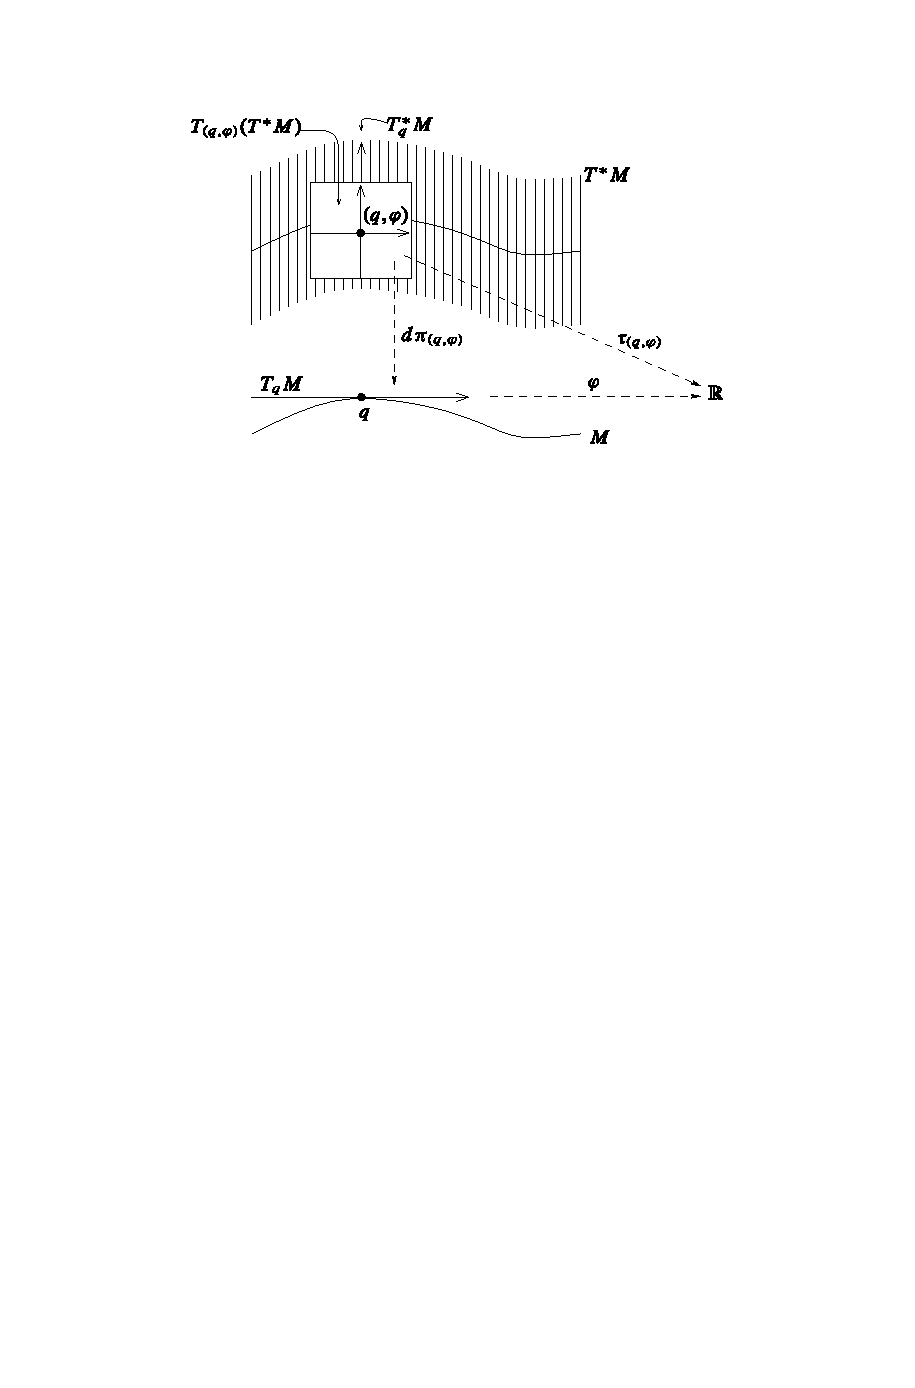
\includegraphics{tautological-form}
\caption{The tautological $1$-form on $T^*M$.}
\end{figure}
\begin{proof}
Let $(x^i)$ be smooth coordinates on $M$, and let $(x^i,\xi_i)$ denote the corresponding natural coordinates on $T^*M$. Recall that the coordinates of $(q,\varphi)\in T^*M$ are defined to be $(x^i,\xi_i)$, where $(x^i)$ is the coordinate representation of $q$, and $\xi_idx^i$ is the coordinate representation of $\varphi$. In terms of these coordinates, the projection $\pi:T^*M\to M$ has the coordinate expression $\pi(x,\xi)=x$. This implies that $d\pi^*(dx^i)=dx^i$, so the coordinate expression for $\tau$ is
\[\tau_{(x,\xi)}=d\pi^*_{(x,\xi)}(\xi_idx^i)=\xi_idx^i.\]
It follows immediately that $\tau$ is smooth, because its component functions in these coordinates are linear.\par
Let $\omega=-d\tau\in\Omega^2(T^*M)$. Clearly, $\omega$ is closed, because it is exact. Moreover, in natural coordinates,
\[\omega=\sum_{i=1}^{n}dx^i\wedge d\xi_i.\]
Under the identification of an open subset of $T^*M$ with an open subset of $\R^{2n}$ by means of these coordinates, $\omega$ corresponds to the standard symplectic form on $\R^{2n}$. It follows that $\omega$ is symplectic.
\end{proof}
The symplectic form defined in this proposition is called the canonical symplectic form on $T^*M$. One of its many uses is in giving the following somewhat more geometric interpretation of what it means for a $1$-form to be closed.
\begin{proposition}\label{one form is embedding}
Let $M$ be a smooth manifold, and let $\sigma$ be a smooth $1$-form on $M$. Thought of as a smooth map from $M$ to $T^*M$, $\sigma$ is a smooth embedding, and $\sigma$ is closed if and only if its image $\sigma(M)$ is a Lagrangian submanifold of $T^*M$.
\end{proposition}
\begin{proof}
Throughout this proof we need to remember that  $\sigma:M\to T^*M$ is playing two roles: on the one hand, it is a $1$-form on $M$, and on the other hand, it is a smooth map between manifolds. Since they are literally the same map, we do not use different notations to distinguish between them; but you should be careful to think about which role $\sigma$ is playing at each step of the argument.\par
In terms of smooth local coordinates $(x^i)$ for $M$ and corresponding natural coordinates $(x^i,\xi_i)$ for $T^*M$, the map $\sigma:M\to T^*M$ has the coordinate representation
\[\sigma(x^1,\dots,x^n)=(x^1,\dots,x^n,\sigma_1(x),\dots,\sigma_n(x)),\]
where $\sigma_idx^i$ is the coordinate representation of $\sigma$ as a $1$-form. It follows immediately that $\sigma$ is a smooth immersion, and it is injective because 
$\pi\circ\sigma=\mathrm{id}_M$. To show that it is an embedding, it suffices by Proposition~\ref{smooth embedd if} to show that it is a proper map. This in turn follows from the fact that $\pi$ is a left inverse for $\sigma$, by Proposition~\ref{proper map if}.\par
Because $\sigma(M)$ is $n$-dimensional, it is Lagrangian if and only if it is isotropic, which is the case if and only if  $\sigma^*\omega=0$ (Proposition~\ref{symplectic isotropic map iff pullback}). The pullback of the tautological form $\tau$ under $\sigma$ is
\[\sigma^*\tau=\sigma^*(\xi_idx^i)=\sigma_idx^i=\sigma.\]
This can also be seen somewhat more invariantly from the computation
\[(\sigma^*\tau)_p(v)=\tau_{\sigma(p)}\big(d\sigma_p(v)\big)=\sigma_p\big(d\pi_{\sigma(p)}\circ d\sigma_p(v)\big)=\sigma_p(d(\pi\circ\sigma)_p(v))=\sigma_p(v).\]
which follows from the definition of $\tau$ and the fact that $\pi\circ\sigma=\mathrm{id}_M$. Therefore,
\[\sigma^*\omega=-\sigma^*d\tau=-d(\sigma^*\tau)=-d\sigma.\]
It follows that $\sigma$ is a Lagrangian embedding if and only if $d\sigma=0$.
\end{proof}
\begin{proposition}\label{submani of T^*M is section iff}
Let $M$ be a smooth manifold, and let $S$ be an embedded Lagrangian submanifold of the total space of $T^*M$.
\begin{itemize}
\item[(a)] If $S$ is transverse to the fiber of $T^*M$ at a point $q\in T^*M$, then there exist a neighborhood $V$ of $q$ in $S$ and a neighborhood $U$ of $\pi(q)$ in $M$ such that $V$ is the image of a smooth closed $1$-form defined on $U$.
\item[(b)] $S$ is the image of a globally defined smooth closed $1$-form on $M$ if and only if $S$ intersects each fiber transversely in exactly one point.
\end{itemize}
\end{proposition}
\begin{proof}
If $S$ is transverse to the fiber of $T^*M$ at a point $q\in T^*M$, then $d(\pi)_q:T_{q}S\to T_{\pi(q)}M$ is an isomorphism. Therefore $\pi|_S$ restricts to a diffeomorphism from a neighborhood $V$ of $q$ in $S$ to a neighborhood $U$ of $\pi(q)$. Then $V$ is the graph of $\sigma=\rho\circ(\pi)^{-1}$, where $\rho$ is the projection to the fiber.\par
If $S$ intersects each fiber transversely in exactly one point, then the projection $\pi|_S$ is bijective and a submersion, hence a diffeomorphism. Therefore $(\pi|_S)^{-1}$ is a closed $1$-form whose image is $S$.
\end{proof}
\subsection{The Darboux theorem}
Our next theorem is one of the most fundamental results in symplectic geometry. It is a nonlinear analogue of the canonical form for a symplectic tensor given in Proposition~\ref{symplectic tensor canonical form}. It illustrates the most dramatic difference between symplectic structures and Riemannian metrics: unlike the Riemannian case, there is no local obstruction to a symplectic structure being locally equivalent to the standard flat model.
\begin{theorem}[\textbf{Darboux}]
Let $(M,\omega)$be a $2n$-dimensional symplectic manifold. For any $p\in M$, there are smooth coordinates $(x^1,\dots,x^n,y^1,\dots,y^n)$ centered at $p$ in which $\omega$ has the coordinate representation
\begin{align}\label{Darboux theorem-1}
\omega=\sum_{i=1}^{n}x^i\wedge y^i.
\end{align}
\end{theorem}
We will prove the theorem below. Any coordinates satisfying $(\ref{Darboux theorem-1})$ theorem are called Darboux coordinates, symplectic coordinates, or canonical coordinates. Obviously, the standard coordinates $(x^1,\dots,^n,y^1,\dots,y^n)$ on $\R^{2n}$ are Darboux coordinates. The proof of Proposition~\ref{tautological form symplectic} showed that the natural coordinates $(x^i,\xi_i)$ are Darboux coordinates for $T^*M$ with its canonical symplectic structure.\par
First, recall that Proposition~\ref{Lie der tensor t_0} shows how to use Lie derivatives to compute the derivative of a tensor field under a flow.We need the following generalization of that result to the case of time-dependent flows.
\begin{proposition}\label{Lie der tensor t_0 time-dependent vector}
Let $M$ be a smooth manifold. Suppose $V:J\times M\to TM$ is a smooth time-dependent vector field and $\psi:\mathcal{E}\to M$ is its time-dependent flow. For any smooth covariant tensor field $A$ on $M$ and any $(t_1,t_0,p)\in\mathcal{E}$,
\begin{align}\label{Lie der tensor t_0 time-dependent vector-1}
\frac{d}{dt}\Big|_{t=t_1}(\psi_{t,t_0}^*A)_p=\big(\psi_{t_1,t_0}^*(\mathfrak{L}_{V_{t_1}}A)\big)_p.
\end{align}
\end{proposition}
\begin{proof}
First, assume $t_1=t_0$. In this case, $\psi_{t_0,t_1}$ is the identity map of $M$. so we need to prove
\begin{align}\label{Lie der tensor t_0 time-dependent vector-2}
\frac{d}{dt}\Big|_{t=t_0}(\psi_{t,t_0}^*A)_p=(\mathfrak{L}_{V_{t_1}}A)_p.
\end{align}
We begin with the special case in which $A=f$ is a smooth $0$-tensor field:
\[\frac{d}{dt}\Big|_{t=t_0}(\psi_{t,t_0}^*f)(p)=\frac{\partial}{\partial t}\Big|_{t=t_0}(f(\psi(t,t_0,p)))=V(t_0,\psi(t_0,t_0,p))f=(\mathfrak{L}_{V_{t_0}}f)(p).\]
Next consider an exact $1$-form $A=df$. In any smooth local coordinates $(x^i)$, the function $\psi^*_{t,t_0}f(x)=f(\psi(t,t_0,x))$ depends smoothly on all $n+1$ variables $(t,x^1,\dots,x^n)$. Thus, the operator $\partial/\partial$ commutes with each of the partial derivatives $\partial/\partial x^i$ when applied to $\psi^*_{t,t_0}f$. In particular, this means that the exterior derivative operator $d$ commutes with $\partial/\partial t$, and so by Corollary~\ref{Lie der ext der commute}
\begin{align*}
\frac{d}{dt}\Big|_{t=t_0}(\psi_{t,t_0}^*df)(p)&=\frac{\partial}{\partial t}\Big|_{t=t_0}d(\psi_{t,t_0}^*f)_p=d\Big(\frac{\partial}{\partial t}\Big|_{t=t_0}(\psi^*_{t,t_0}f)\Big)_p=d(\mathfrak{L}_{V_{t_0}}f)_p=(\mathfrak{L}_{V_{t_0}}df)_p.
\end{align*}
Thus, the result is proved for $0$-tensors and for exact $1$-forms.\par
Now suppose that $A=B\otimes C$ for some smooth covariant tensor fields $B$ and $C$, and assume that the proposition is true for $B$ and $C$. (We include the possibility that $B$ or $C$ has rank $0$, in which case the tensor product is just ordinary multiplication.) By the product rule for Lie derivatives (Proposition~\ref{tensor Lie derivative prop}(c)), the right-hand side of $(\ref{Lie der tensor t_0 time-dependent vector-2})$ satisfies
\[(\mathfrak{L}_{V_{t_0}}(B\otimes C))_p=(\mathfrak{L}_{V_{t_0}}B)_p\otimes C_p+B_p\otimes(\mathfrak{L}_{V_{t_0}}C)_p.\]
On the other hand, by an argument entirely analogous to that in the proof of Proposition~\ref{tensor Lie derivative prop}, the left-hand side satisfies a similar product rule:
\begin{align*}
\frac{d}{dt}\Big|_{t=t_0}(\psi_{t,t_0}^*(B\otimes C))_p=\Big(\frac{d}{dt}\Big|_{t=t_0}(\psi_{t,t_0}^*B)\Big)_p\otimes C_p+B_p\otimes\Big(\frac{d}{dt}\Big|_{t=t_0}(\psi_{t,t_0}^*C)\Big)_p.
\end{align*}
This shows that $(\ref{Lie der tensor t_0 time-dependent vector-2})$ holds for $A=B\otimes C$, provided it holds for $B$ and $C$. The case of arbitrary tensor fields now follows by induction, using the fact that any smooth covariant tensor field can be written locally as a sum of tensor fields of the form $A=f\,dx^{i_1}\otimes\cdots\otimes dx^{i_k}$.\par
To handle arbitrary $t_1$, we use Theorem~\ref{flow fundamental thm time-dependent}(d), which shows that $\psi_{t,t_0}=\psi_{t,t_1}\circ\psi_{t_1,t_0}$ wherever the right-hand side is defined. Therefore, because the linear map $d(\psi_{t_1,t_0})_p^*$ does not depend on $t$,
\begin{align*}
\frac{d}{dt}\Big|_{t=t_1}(\psi_{t,t_0}^*A)_p&=\frac{d}{dt}\Big|_{t=t_1}d(\psi_{t,t_0})_p^*(A_{\psi_{t,t_0}(p)})=\frac{d}{dt}\Big|_{t=t_1}d(\psi_{t_1,t_0})_p^*\circ d(\psi_{t,t_1})_{\psi_{t_1,t_0}(p)}^*(A_{\psi_{t,t_0}(p)})\\
&=d(\psi_{t_1,t_0})_p^*\Big(\frac{d}{dt}\Big|_{t=t_1}d(\psi_{t,t_1})_{\psi_{t_1,t_0}(p)}^*(A_{\psi_{t,t_1}\circ\psi_{t_1,t_0}(p)})\Big)=\big(\psi_{t_1,t_0}^*(\mathfrak{L}_{V_{t_1}}A)\big)_p.
\end{align*}
This finishes the proof.
\end{proof}
A \textbf{smooth time-dependent tensor field} on a smooth manifold $M$ is a smooth map $A:J\times M\to T^kT^*M$, where $J\sub\R$ is an interval, satisfying $A(t,p)\in T^k(T_p^*M)$ for each $(t,p)\in J\times M$.
\begin{proposition}\label{Lie der tensor time-dependent}
Let $M$ be a smooth manifold and $J\sub\R$ be an open interval. Suppose $V:J\times M\to TM$ is a smooth time-dependent vector field on $M$, $\psi:\mathcal{E}\to M$ is its time-dependent flow, and $A:J\times M\to T^kT^*M$ is a smooth time-dependent tensor field on $M$. Then for any $(t_1,t_0,p)\in\mathcal{E}$,
\begin{align}\label{Lie der tensor time-dependent-1}
\frac{d}{dt}\Big|_{t=t_1}(\psi^*_{t,t_0}A_t)_p=\Big(\psi_{t_1,t_0}^*\Big(\mathfrak{L}_{V_{t_1}}A_{t_1}+\frac{d}{dt}\Big|_{t=t_1}A_t\Big)\Big)_p.
\end{align}
\end{proposition}
\begin{proof}
For sufficiently small $\eps>0$, consider the smooth map $F:(t_1-\eps,t_1+\eps)\times(t_1-\eps,t_1+\eps)\to T^k(T_p^*M)$ defined by
\[F(u,v)=(\psi^*_{u,t_0}A_v)_p=d(\psi_{u,t_0})_p^*(A_v|_{\psi_{u,t_0}(p)}).\]
Since $F$ takes its values in the finite-dimensional vector space $T^k(T_p^*M)$, we can apply the chain rule together with Proposition~\ref{Lie der tensor t_0 time-dependent vector} to conclude that
\begin{align*}
\frac{d}{dt}\Big|_{t=t_1}F(t,t)&=\frac{\partial F}{\partial u}(t_1,t_1)+\frac{\partial F}{\partial v}(t_1,t_1)=(\psi_{t_1,t_0}^*(\mathfrak{L}_{V_{t_1}}A_{t_1}))_p+\frac{\partial}{\partial v}\Big|_{t=t_1}d(\psi_{t_1,t_0}^*)_p(A_v|_{\psi_{u,t_0}(p)}).
\end{align*}
Just as in the proof of Proposition~\ref{Lie der tensor t_0 time-dependent vector}, the linear map $d(\psi_{t_1,t_0}^*)_p$ commutes past $\partial/\partial v$, yielding $(\ref{Lie der tensor time-dependent-1})$.
\end{proof}
\begin{proof}[Proof of the Darboux theorem]
Let $\omega_0$ denote the given symplectic form on $M$, and let $p_0\in M$ be arbitrary. The theorem will be proved if we can find a smooth coordinate
chart $(U_0,\varphi)$ centered at $p_0$ such that $\varphi^*\omega_0=\omega_1$, where $\omega_1=\sum_{i=1}^{n}dx^i\wedge dy^i$ is the standard symplectic form on $\R^{2n}$. Since this is a local question, by choosing smooth coordinates $(x^1,\dots,x^n,y^1,\dots,y^n)$ in a neighborhood of $p_0$, we may replace $M$ with an open ball $U\sub\R^{2n}$. Proposition~\ref{symplectic tensor canonical form} shows that we can arrange by a linear change of coordinates that $\omega_0|_{p_0}=\omega_1|_{p_0}$.\par
Let $\eta=\omega_1-\omega_0$. Because $\omega$ is closed, the Poincar\'e lemma shows that we can find a smooth $1$-form $\alpha$ on $U$ such that $d\alpha=-\eta$. By subtracting a constant-coefficient (and thus closed) $1$-form from $\alpha$, we may assume without loss of generality that $\alpha_{p_0}=0$.\par
For each $t\in\R$, define a closed $2$-form $\omega_t$ on $U$ by
\[\omega_t=\omega_0+t\eta=(1-t)\omega_0+t\omega_1.\]
Let $J$ be a bounded open interval containing $[0,1]$. Because $\omega_t|_{p_0}=\omega_0|_{p_0}$ is nondegenerate for all $t$, a simple compactness argument shows that there is some neighborhood $U_1\sub U$ of $p_0$ such that $\omega_t$ is nondegenerate on $U_1$ for all $t\in\widebar{J}$. Because of this nondegeneracy, the smooth bundle homomorphism $\widehat{\omega}_t:TU_1\to T^*U_1$ defined by $\widehat{\omega}_t(X)=X\intprod\omega_t$ is an isomorphism for each $t\in\widebar{J}$.\par
Define a smooth time-dependent vector field $V:J\times U_1\to TU_1$ by $V_t=\widehat{\omega}_t^{-1}\alpha$, or equivalently
\[V_t\intprod\omega_t=\alpha.\]
Our assumption that $\alpha_{p_0}=0$ implies that $V_t|_{p_0}=0$ for each $t$. If $\psi:\mathcal{E}\to U_1$ denotes the time-dependent flow of $V$, it follows that $\psi(t,0,p_0)=p_0$ for all $t\in J$, so $J\times\{0\}\times\{p_0\}\sub\mathcal{E}$. Because $E$ is open in $J\times J\times M$ and $[0,1]$ is compact, there is some neighborhood $U_0$ of $p_0$ such that $[0,1]\times\{0\}\times U_0\sub\mathcal{E}$.\par
For each $t_1\in[0,1]$, it follows from Proposition~\ref{Lie der tensor time-dependent} that
\begin{align*}
\frac{d}{dt}\Big|_{t=t_1}\psi^*_{t,0}\omega_t&=\psi_{t_1,0}^*\Big(\mathfrak{L}_{V_{t_1}\omega_{t_1}}+\frac{d}{dt}\Big|_{t=t_1}\omega_t\Big)\\
&=\psi_{t_1,0}^*\big(V_{t_1}\intprod d\omega_{t_1}+d(V_{t_1}\intprod\omega_t)+\eta\big)\\
&=\psi_{t_1,0}^*(V_{t_1}\intprod 0+d\alpha+\eta)=0.
\end{align*}
Therefore, $\psi_{t,0}^*\omega_t=\psi_{0,0}^*\omega_0=\omega_0$ for all $t$. In particular, $\psi_{1,0}^*\omega_1=\omega_0$. It follows from Theorem~\ref{flow fundamental thm time-dependent}(c) that $\psi_{1,0}^*$ is a diffeomorphism onto its image, so it is a coordinate map. Because $\psi_{1,0}(p_0)=p_0$, these coordinate are centered at $p_0$.
\end{proof}
\subsection{Hamiltonian vector fields}
One of the most useful constructions on symplectic manifolds is a symplectic analogue of the gradient, defined as follows. Suppose $(M,\omega)$ is a symplectic manifold. For any smooth function $f\in C^\infty(M)$, we define the Hamiltonian vector field of $f$ to be the smooth vector field $X_f$ defined by
\[X_f=\widehat{\omega}^{-1}(df),\]
where $\widehat{\omega}:TM\to T^*M$ is the bundle isomorphism determined by $\omega$. Equivalently,
\[X_f\intprod \omega=df.\]
or for any vector field $Y$,
\[\omega(X_f,Y)=df(Y)=Yf.\]

In any Darboux coordinates, $X_f$ can be computed explicitly as follows. Writing
\[X_f=\sum_{i=1}^{n}\Big(a^i\frac{\partial}{\partial x^i}-b^i\frac{\partial}{\partial y^i}\Big)\]
for some coefficient functions $(a^i,b^i)$ to be determined, we compute
\[X_f\intprod\omega=\sum_{j=1}^{n}\Big(a^j\frac{\partial}{\partial x^j}+b^j\frac{\partial}{\partial y^j}\Big)\intprod\sum_{i=1}^{n}dx^i\wedge dy^i=\sum_{i=1}^{n}(a^idy^i-b^idx^i).\]
On the other hand,
\[df=\sum_{i=1}^{n}\Big(\frac{\partial f}{\partial x^i}dx^i+\frac{\partial f}{\partial x^i}dy^i\Big).\]
Setting these two expressions equal to each other, we find that $a^i=\partial f/\partial y^i$ and $b^i=-\partial f/\partial x^i$, which yields the following formula for the Hamiltonian vector field of $f$ in Darboux coordinates:
\begin{align}\label{Hamiltonian vector field}
X_f=\sum_{i=1}^{n}\Big(\frac{\partial f}{\partial y^i}\frac{\partial}{\partial x^i}-\frac{\partial f}{\partial x^i}\frac{\partial}{\partial y^i}\Big).
\end{align}
This formula holds, in particular, on $\R^{2n}$ with its standard symplectic form.\par
Although the definition of the Hamiltonian vector field is formally analogous to that of the gradient on a Riemannian manifold, Hamiltonian vector fields differ from gradients in some very significant ways, as the next lemma shows.
\begin{proposition}[\textbf{Properties of Hamiltonian Vector Fields}]\label{Hamiltonian vector field prop}
Let $(M,\omega)$ be a symplectic manifold and let $f\in C^\infty(M)$.
\begin{itemize}
\item[(a)] $f$ is constant along each integral curve of $X_f$.
\item[(b)] At each regular point of $f$, the Hamiltonian vector field $X_f$ is tangent to the level set of $f$.
\end{itemize}
\end{proposition}
\begin{proof}
Both assertions follow from the fact that
\[X_ff=df(X_f)=\omega(X_f,X_f)=0\]
because $\omega$ is alternating.
\end{proof}
A smooth vector field $X$ on $M$ is said to be \textbf{symplectic} if $\omega$ is invariant under the flow of $X$. It is said to be \textbf{Hamiltonian} (or \textbf{globally Hamiltonian}) if there exists a function $f\in C^\infty(M)$ such that $X=X_f$, and \textbf{locally Hamiltonian} if each point $p$ has a neighborhood on which $X$ is Hamiltonian. Clearly, every globally Hamiltonian vector field is locally Hamiltonian.
\begin{proposition}[\textbf{Hamiltonian and Symplectic Vector Fields}]\label{Hamiltonian and symplectic vector field}
Let $(M,\omega)$ be a symplectic manifold. A smooth vector field on $M$ is symplectic if and only if it is locally Hamiltonian. Every locally Hamiltonian vector field on $M$ is globally Hamiltonian if and only if $H^1_{dR}(M)=0$.
\end{proposition}
\begin{proof}
By Theorem~\ref{tensor filed invariant flow iff}, a smooth vector field $X$ is symplectic if and only if $\mathfrak{L}_X\omega=0$. Using Cartan’s magic formula, we compute
\begin{align}\label{Hamiltonian and symplectic vector field-1}
\mathfrak{L}_X\omega=d(X\intprod\omega)+X\intprod d\omega=d(X\intprod\omega).
\end{align}
Therefore, $X$ is symplectic if and only if the $1$-form $X\intprod\omega$ is closed. On the one hand, if $X$ is locally Hamiltonian, then in a neighborhood of each point there is a real-valued function $f$ such that $X=X_f$, so $X\intprod\omega=df$, which is certainly closed. Conversely, if $X$ is symplectic, then by the Poincar\'e lemma each point $p\in M$ has a neighborhood $U$ on which the closed $1$-form $X\intprod\omega$ is exact. This means there is a smooth real-valued function $f$ defined on $U$ such that $X\intprod\omega=df$; because $\omega$ is nondegenerate, this implies that $X=X_f$ on $U$.\par
Now suppose $M$ is a smooth manifold with $H^1_{dR}(M)=0$. If $X$ is a locally Hamiltonian vector field, then it is symplectic, so $(\ref{Hamiltonian and symplectic vector field-1})$ shows that $X\intprod\omega$ is closed. The hypothesis then implies that there is a function $f\in C^\infty(M)$ such that $X\intprod\omega=df$. This means that $X=X_f$, so $X$ is globally Hamiltonian. Conversely, suppose every locally Hamiltonian vector field is globally Hamiltonian. Let $\eta$ be a closed $1$-form, and let $X$ be the vector field $X=\widehat{\omega}^{-1}\eta$. Then $(\ref{Hamiltonian and symplectic vector field-1})$ shows that $\mathfrak{L}_X\omega=0$, so $X$ is symplectic and therefore locally Hamiltonian. By hypothesis, there is a global smooth real-valued function $f$ such that $X=X_f$, and then unwinding the definitions, we find that $\eta=df$.
\end{proof}
A symplectic manifold $(M,\omega)$ together with a smooth function $H\in C^\infty(M)$ is called a \textbf{Hamiltonian system}. The function $H$ is called the \textbf{Hamiltonian} of the system; the flow of the Hamiltonian vector field $X_H$ is called its \textbf{Hamiltonian flow}, and the integral curves of $X_H$ are called the \textbf{trajectories} or \textbf{orbits} of the system. In Darboux coordinates, formula $(\ref{Darboux theorem-1})$ implies that the orbits are those curves $\gamma(t)=(x^i(t),y^i(t))$ that satisfy
\begin{equation}\label{Hamilton's equations}
\left\{
\begin{array}{l}
\dot{x}^i(t)=\dfrac{\partial H}{\partial y^i}(x(t),y(t)),\\[8pt]
\dot{y}^i(t)=-\dfrac{\partial H}{\partial y^i}(x(t),y(t)).
\end{array}
\right.
\end{equation}
These are called Hamilton's equations.\par
Hamiltonian systems play a central role in classical mechanics. We illustrate how they arise with a simple example.
\begin{example}[\textbf{The $\bm{n}$-Body Problem}]
Consider $n$ physical particles moving in space, and suppose their masses are $m_1,\dots,m_n$. For many purposes, an effective model of such a system is obtained by idealizing the particles as points in $\R^3$, which we denote by $\mathbf{q}_1,\dots,\mathbf{q}_n$. Writing the coordinates of $\mathbf{q}_k$ at time $t$ as $(q_k^1(t),q_k^2(t),q_k^3(t))$, we can represent the evolution of the system over time by a curve in $\R^{3n}$:
\[q(t)=(q_1^1(t),q_1^2(t),q_1^3(t),\dots,q_n^1(t),q_n^2(t),q_n^3(t)).\]
The \textbf{collision set} is the subset $\mathcal{C}\sub\R^{3n}$ where two or more particles occupy the same position in space:
\[\mathcal{C}=\{q\in\R^{3n}:\mathbf{q}_k=\mathbf{q}_l\text{ for some }k\neq l\}.\]
We consider only motions with no collisions, so we are interested in curves in the open subset $Q=\R^{3n}\setminus\mathcal{C}$.\par
Suppose the particles are acted upon by forces that depend only on the positions of all the particles in the system. (A typical example is gravitational forces.) If we denote the components of the net force on the kth particle by $(F_k^1(q),F_k^2(q),F_k^3(q))$, then Newton's second law of motion asserts that the particles' motion satisfies $m_k\ddot{\mathbf{q}}_k=\mathbf{F}_k(\mathbf{q}(t))$ for each $k$, which translates into the $3n\times 3n$ system of second-order ODEs
\begin{equation*}
\left\{
\begin{array}{l}
m_k\ddot{q}_k^1(t)=F_k^1(q(t)),\\[8pt]
m_k\ddot{q}_k^2(t)=F_k^2(q(t)),\\[8pt]
m_k\ddot{q}_k^3(t)=F_k^3(q(t)),
\end{array}
\right.
\end{equation*}
for $k=1,\dots,n$.\par
This can be written in a more compact form if we relabel the $3n$ position coordinates as $q(t)=(q^1(t),\dots,q^{3n}(t))$ and the $3n$ components of the forces as $F(q)=(F_1(q),\dots,F_{3n}(q))$, and let $M=(M_{ij})$ denote the $3n\times 3n$ diagonal matrix $\mathrm{diag}(m_1,m_1,m_1,\dots,m_n,m_n,m_n)$. Then Newton's second law can be written
\begin{align}\label{n-body problem-1}
M_{ij}\ddot{q}^j(t)=F_i(q(t)).
\end{align}
We assume that the forces depend smoothly on $q$, so we can interpret $F(q)=(F_1(q),\dots,F_{3n}(q))$ as the components of a smooth covector field on $Q$. We assume further that the forces are conservative, which by Proposition~\ref{covector conservative iff exact} is equivalent to the existence of a smooth function $V\in C^\infty(Q)$ (called the potential energy of the system) such that $F=-dV$.\par
Under the physically reasonable assumption that all of the masses are positive, the matrix $M$ is positive definite, and thus can be interpreted as a (constant-coefficient) Riemannian metric on $Q$. It therefore defines a smooth bundle isomorphism $\widehat{M}:TQ\to T^*Q$. If we denote the natural coordinates on $TQ$ by $(q^i,v^i)$ and those on $T^*Q$ by $(q^i,p_i)$, then $M(v,w)=M_{ij}v^iw^j$, and $\widehat{M}$ has the coordinate representation
\[(q^i,p_i)=\widehat{M}(q^i,v^i)=(q^i,M_{ij}v^j).\]
If $q'(t)=(\dot{q}^1(t),\dots,\dot{q}^{3n}(t))$ is the velocity vector of the system of particles at time $t$, then the covector $p(t)=\widehat{M}(q'(t))$ is given by the formula
\begin{align}\label{n-body problem-2}
p_i(t)=M_{ij}\dot{q}^j(t).
\end{align}
To give this equation a physical interpretation, we can revert to our original labeling of the coordinates and write
\[p(t)=(p_1^1(t),p_1^2(t),p_1^3(t),\dots,p_n^1(t),p_n^2(t),p_n^3(t)),\]
and then $\mathbf{p}_k(t)=(p_k^1(t),p_k^2(t),p_k^3(t))=m_k\dot{\mathbf{q}}_k(t)$ is interpreted as the momentum of the $k$-th particle at time $t$.\par
Using $(\ref{n-body problem-2})$, we see that a curve $q(t)$ in $Q$ satisfies Newton's second law $(\ref{n-body problem-1})$ if and only if the curve $\gamma(t)=(q(t),p(t))$ in $T^*Q$ satisfies the first-order system of ODEs
\begin{equation}\label{n-body problem-3}
\left\{
\begin{array}{l}
\dot{q}^i(t)=M^{ij}p_j(t),\\[8pt]
\dot{p}^i(t)=-\dfrac{\partial V}{\partial q^i}(q(t)),
\end{array}
\right.
\end{equation}
where $(M^{ij})$ is the inverse of the matrix of $(M_{ij})$. Define a function $E\in C^\infty(T^*Q)$, called the \textbf{total energy} of the system, by
\[E(q,p)=V(q)+K(p),\]
where $V$ is the potential energy introduced above, and $K$ is the \textbf{kinetic energy}, defined by
\[K(p)=\frac{1}{2}M^{ij}p_ip_j.\]
Since $(q^i,p_i)$ are Darboux coordinates on $T^*Q$, a comparison of $(\ref{n-body problem-3})$ with $(\ref{Hamilton's equations})$ shows that $(\ref{n-body problem-3})$ is precisely Hamilton's equations for the Hamiltonian flow of $E$. The fact that $E$ is constant along the trajectories of its own Hamiltonian flow is known as the \textbf{law of conservation of energy}.
\end{example}
\subsubsection{Poisson brackets}
Hamiltonian vector fields allow us to define an operation on real-valued functions on a symplectic manifoldM similar to the Lie bracket of vector fields. Given $f,g\in C^\infty(M)$, we define their Poisson bracket $\{f,g\}\in C^\infty(M)$ by any of the following equivalent formulas:
\begin{align}\label{Possion bracket}
\{f,g\}=\omega(X_f,X_g)=df(X_g)=X_gf.
\end{align}
Two functions are said to Poisson commute if their Poisson bracket is zero.\par
The geometric interpretation of the Poisson bracket is evident from the characterization $\{f,g\}=X_gf$: it is a measure of the rate of change of $f$ along the Hamiltonian flow of $g$. In particular, $f$ and $g$ Poisson commute if and only if $f$ is constant along the Hamiltonian flow of $g$.\par
Using $(\ref{Hamiltonian vector field})$, we can readily compute the Poisson bracket of two functions $f,g$ in Darboux coordinates:
\[\{f,g\}=\sum_{i=1}^{n}\frac{\partial f}{\partial x^i}\frac{\partial g}{\partial y^i}-\frac{\partial f}{\partial y^i}\frac{\partial g}{\partial x^i}.\]
\begin{proposition}[\textbf{Properties of the Poisson Bracket}]
Suppose $(M,\omega)$ is a symplectic manifold, and $f,g\in C^\infty(M)$.
\begin{itemize}
\item[(a)] Bilinearity: $\{f,g\}$ is linear over $\R$ in $f$ and $g$.
\item[(b)] Antisymmetry: $\{f,g\}=-\{g,f\}$.
\item[(c)] Jacobi identity: $\{f,\{g,h\}\}+\{g,\{h,f\}\}+\{h,\{f,g\}\}=0$.
\item[(d)] $X_{\{f,g\}}=-[X_f,X_g]$.   
\end{itemize}
\end{proposition}
\begin{proof}
Parts (a) and (b) are obvious from the characterization $\{f,g\}=\omega(X_f,X_g)$ together with the fact that $X_f=\widehat{\omega}^{-1}(df)$ depends linearly on $f$. Because of the nondegeneracy of $\omega$, to prove (d), it suffices to show that the following holds for every vector field $Y$:
\begin{align}\label{Possion bracket prop-1}
\omega(X_{\{f,g\}},Y)+\omega([X_f,X_g],Y)=0.
\end{align}
On the one hand, note that $\omega(X_{\{f,g\}},Y)=d(\{f,g\})(Y)=Y\{f,g\}=YX_gf$. On the other hand, because Hamiltonian vector fields are symplectic, the Lie derivative formula of Corollary~\ref{Lie derivative tensor} yields
\begin{align*}
0&=(\mathfrak{L}_{X_g}\omega)(X_f,Y)=X_g(\omega(X_f,Y))-\omega([X_g,X_f],Y)-\omega(X_f,[X_g,Y])\\
&=X_g(df(Y))+\omega([X_f,X_g],Y)-df([X_g,Y])\\
&=X_gYf+\omega([X_f,X_g],Y)-[X_g,Y]f\\
&=\omega([X_f,X_g],Y)+YX_gf.
\end{align*}
Therefore (d) follows.\par
Finally, (c) follows from (d), (b), and $(\ref{Possion bracket})$:
\begin{align*}
\{f,\{g,h\}\}&=X_{\{g,h\}}f=-[X_g,X_h]f=-X_gX_hf+X_hX_gf\\
&=-X_g\{f,h\}+X_h\{f,g\}=-\{\{f,h\},g\}+\{\{f,g\},h\}\\
&=-\{g,\{h,f\}\}-\{h,\{f,g\}\}.
\end{align*}
\end{proof}
The following corollary is immediate.
\begin{corollary}
If $(M,\omega)$ is a symplectic manifold, the vector space $C^\infty(M)$ is a Lie algebra under the Poisson bracket.
\end{corollary}
If $(M,\omega,H)$ is a Hamiltonian system, any function $f\in C^\infty(M)$ that is constant on every integral curve of $X_H$ is called a \textbf{conserved quantity} of the system. Conserved quantities turn out to be deeply related to symmetries, as we now show.\par
A smooth vector field $V$ on $M$ is called an \textbf{infinitesimal symmetry} of $(M,\omega,H)$ if both $\omega$ and $H$ are invariant under the flow of $V$.
\begin{proposition}
Let $(M,\omega,H)$ be a Hamiltonian system.
\begin{itemize}
\item[(a)] A function $f\in C^\infty(M)$ is a conserved quantity if and only if $\{f,H\}=0$.
\item[(b)] The infinitesimal symmetries of $(M,\omega,H)$ are precisely the symplectic vector fields $V$ that satisfy $VH=0$.
\item[(c)] If $\theta$ is the flow of an infinitesimal symmetry and $\gamma$ is a trajectory of the system, then for each $s\in\R$, $\theta_s\circ\gamma$ is also a trajectory on its domain of definition.
\end{itemize}
\end{proposition}
\begin{proof}
Since the Possion bracket $\{f,H\}$ measures the rate of change of $f$ along the Hamiltonian flow of $H$, it is clear that $f$ is conserved if and only if $\{f,H\}=0$. This proves (a). For (b), $\omega$ is invairant under the flow of $V$ if and only if $V$ is symplectic, and $H$ is invairant under the flow of $V$ if and only if $VH=0$. Therefore (b) is clear.\par
Finally, for (c), $\gamma$ is a trajectory of the system means $\gamma'(t)=X_H|_{\gamma(t)}$. Since $\theta$ is a flow of an infinitesimal symmetry, $\omega$ and $H$ are invairant under $V$. This then implies 
\[(\theta_s\circ\gamma)'(t)=d(\theta_s)_{\gamma(t)}(\gamma'(t))=d(\theta_s)_{\gamma(t)}(V_{\gamma(t)})=V_{\theta_s\circ\gamma(t)}.\]
Therefore $\theta_s\circ\gamma$ is still a trajectory of the system.
\end{proof}
The following theorem, first proved (in a somewhat different form) by Emmy
Noether in 1918, has had a profound influence on both physics and mathematics. It shows that for many Hamiltonian systems, there is a one-to-one correspondence between conserved quantities (modulo constants) and infinitesimal symmetries.
\begin{theorem}[\textbf{Noether's Theorem}]
Let $(M,\omega,H)$ be a Hamiltonian system. If $f$ is any conserved quantity, then its Hamiltonian vector field is an infinitesimal symmetry. Conversely, if $H^1_{dR}(M)=0$, then each infinitesimal symmetry is the Hamiltonian vector field of a conserved quantity, which is unique up to addition of a function that is constant on each component of $M$.
\end{theorem}
\begin{proof}
Suppose $f$ is a conserved quantity. Proposition 22.21 shows that $\{f,H\}=0$. This in turn implies that $X_fH=\{H,f\}=0$, so $H$ is constant along the flow of $X_f$. Since $\omega$ is invariant along the flow of any Hamiltonian vector field by Proposition~\ref{Hamiltonian and symplectic vector field}, this shows that $X_f$ is an infinitesimal symmetry.\par
Now suppose that $M$ is a smooth manifold with $H^1_{dR}(M)=0$. Let $V$ be an infinitesimal symmetry of $(M,\omega,H)$. Then $V$ is symplectic by definition, and globally Hamiltonian by Proposition~\ref{Hamiltonian and symplectic vector field}. Writing $V=X_f$, the fact that $H$ is constant along the flow of $V$ implies that $\{H,f\}=X_fH=VH=0$, so $f$ is a conserved quantity. If $\widetilde{f}$ is any other function that satisfies $X_{\widetilde{f}}=X_f$, then $d(\widetilde{f}-f)=\widehat{\omega}(X_{\widetilde{f}}-X_f)=0$, so $\widetilde{f}-f$ must be constant on each component of $M$.
\end{proof}
There is one conserved quantity that every Hamiltonian system possesses: the Hamiltonian $H$ itself. The infinitesimal symmetry corresponding to it, of course, generates the Hamiltonian flow of the system, which describes how the system evolves over time. Since $H$ is typically interpreted as the total energy of the system, one usually says that the symmetry corresponding to conservation of energy is "translation in the time variable".
\subsubsection{Hamiltonian Flowouts}
Hamiltonian vector fields are powerful tools for constructing isotropic and Lagrangian submanifolds. Because Lagrangian submanifolds of $T^*M$ correspond to closed $1$-forms (Proposition~\ref{one form is embedding}), which in turn correspond locally to differentials of functions, such constructions have numerous applications in PDE theory.
\begin{theorem}[\textbf{Hamiltonian Flowout Theorem}]\label{Hamiltonian flowout}
Suppose $(M,\omega)$ is a symplectic manifold, $H\in C^\infty(M)$, $\Gamma$ is an embedded isotropic submanifold of $M$ that is contained in a single level set of $H$, and the Hamiltonian vector field $X_H$ is nowhere tangent to $\Gamma$. If $\mathcal{S}$ is a flowout from $\Gamma$ along $X_H$, then $\mathcal{S}$ is also isotropic and contained in the same level set of $H$.
\end{theorem}
\begin{proof}
Let $\theta$ be the flow of $X_H$. Recall from Theorem~\ref{flowout} that the flowout is parametrized by the restriction of $\theta$ to a neighborhood $\mathcal{O}_\delta$ of $\{0\}\times\Gamma$ in $\R\times\Gamma$. First consider a point $p\in\Gamma\sub\mathcal{S}$. If we choose a basis $E_1,\dots,E_k$ for $T_p\Gamma$, then $T_p\mathcal{S}$ is spanned by $(X_H|_p,E_1,\dots,E_k)$. The assumption that $\Gamma$ is isotropic implies that $\omega_p(E_i,E_j)=0$ for all $i$ and $j$. On the other hand, by definition of the Hamiltonian vector field,
\[\omega_p(X_H|_p,E_j)=dH_p(E_j)=0.\]
because $E_j$ is tangent to $\Gamma$, which is contained in a level set of $H$. This shows that the restriction of $\omega$ to $T_p\mathcal{S}$ is zero when $p\in\Gamma$.\par
Any other point $p;'\in\mathcal{S}$ is of the form $p'=\theta_t(p)$ for some $(t,p)\in\mathcal{O}_\delta$. Because $\theta_t$ is a local diffeomorphism that maps a neighborhood of $p$ in $\mathcal{S}$ to a neighborhood of $p'$ in $\mathcal{S}$, its differential takes $T_p\mathcal{S}$ isomorphically onto $T_{p'}\mathcal{S}$. Thus, for any vectors $v,w\in T_{p'}\mathcal{S}$, there are vectors $\widehat{v},\widehat{w}$ such that $d(\theta_t)_p(\widehat{v})=v$ and $d(\theta_t)_p(\widehat{w})=w$. Moreover, because $X_H$ is a symplectic vector field, its flow preserves $\omega$. Therefore,
\[\omega_{p'}(v,w)=\omega_{p'}(d(\theta_t)_p(\widehat{v}),d(\theta_t)_p(\widehat{w}))=(\theta_t^*\omega)_p(\widehat{v},\widehat{w})=\omega_p(\widehat{v},\widehat{w})=0.\]
It follows that $\mathcal{S}$ is isotropic. By Proposition~\ref{Hamiltonian vector field prop}, $H$ is constant along each integral curve of $X_H$, so $\mathcal{S}$ is contained in the same level set of $H$ as $\Gamma$.
\end{proof}
\subsection{Contact structures}
As we have seen, symplectic manifolds must be even-dimensional; but there is a closely related structure called a contact structure that one can define on odd-dimensional manifolds. It also has important applications in geometry and analysis. In this part, we introduce the main elements of contact geometry.\par
Suppose $M$ is a smooth manifold of odd dimension $2n+1$. A contact form on $M$ is a nonvanishing smooth $1$-form $\theta$ with the property that for each $p\in M$, the restriction of $d\theta_p$ to the subspace $\ker\theta_p\sub T_pM$ is nondegenerate, which is to say it is a symplectic tensor. A \textbf{contact structure} on $M$ is a smooth distribution $H\sub TM$ of rank $2n$ with the property that any smooth local defining form $\theta$ for $H$ is a contact form (see Lemma~\ref{distribution smooth crit}). A contact manifold is a smooth manifold $M$ together with a contact structure on $M$. If $(M,H)$ is a contact manifold, any (local or global) defining form for $H$ is called a \textbf{contact form} for $H$.
\begin{proposition}
A smooth $1$-form $\theta$ on a $(2n+1)$-manifold is a contact form if and only if $\theta\wedge (d\theta)^n$ is nonzero everywhere on $M$, where $(d\theta)^n$ represents the $n$-fold wedge product of $d\theta$.
\end{proposition}
\begin{proof}
By Lemma~\ref{distribution annihilate iff}, $(d\theta)^n|_p$ annihilates $\ker\theta_p$ if and only if there is a $(2n-1)$-form $\alpha_p$ such that
\[(d\theta)^n|_p=\theta|_p\wedge\alpha_p.\]
This is, in turn, equivalent to $\theta_p\wedge(d\theta)^n|_p=0$.
\end{proof}
\begin{proposition}
Suppose $H$ is a contact structure on a smooth manifold $M$. Show that if $\theta_1$ and $\theta_2$ are any two local contact forms for $H$, then on their common domain there is a smooth nonvanishing function $f$ such that $\theta_2=f\theta_1$.
\end{proposition}
\begin{proof}
This follows from the fact that two 1-forms defines the same kernel if and only if they differ by a constant.
\end{proof}
It follows from the result of Proposition~\ref{involutivity local coframe crit} that a codimension-$1$ distribution $H\sub TM$ is integrable if and only if any local defining form $\theta$ satisfies $\theta\wedge d\theta=0$. If $H$ is a contact structure, by contrast, not only is  nonzero everywhere on $M$, but it remains nonzero after taking $n-1$ more wedge products with $d\theta$. Thus, a contact structure is, in a sense, a "maximally nonintegrable distribution".
\begin{example}[\textbf{Contact Forms}]\label{contact forms eg}
\mbox{}
\begin{itemize}
\item[(a)] On $\R^{2n+1}$ with coordinates $(x^1,\dots,x^n,y^1,\dots,y^n,z)$, define a $1$-form $\theta$ by
\begin{align}\label{contact form standard}
\theta=dz-\sum_{i=1}^{n}y^idx^i.
\end{align}
and let $H\sub T\R^{2n+1}$ be the rank-$2n$ distribution annihilated by $\theta$. Then $d\theta=\sum_{i=1}^{n}dx^i\wedge dy^i$. If we define vector fields $X_i,Y_i$ by
\[X_i=\frac{\partial}{\partial x^i}+y^i\frac{\partial}{\partial z},\quad Y^i=\frac{\partial}{\partial y^i}.\]
then $(X_i,Y_i)$ is a smooth frame for $H$, and it is straightforward to check that it satisfies $d\theta(X_i,X_j)=d\theta(Y_i,Y_j)=0$ and $d\theta(X_i,Y_j)=\delta_{ij}$. It follows just as in Example~\ref{symplectic tensor eg} that $d\theta|_H$ is nondegenerate, so $\theta$ is a contact form.
\item[(b)] Let $M$ be a smooth $n$-manifold, and define a smooth $1$-form $\theta$ on the $(2n+1)$-manifold $\R\times T^*M$ by $\theta=dz-\tau$, where $z$ is the standard coordinate on $\R$ and $\tau$ is the tautological $1$-form on $T^*M$. In terms of natural coordinates $(x^i,\xi_i)$ for $T^*M$; the form $\theta$ has the coordinate representation
\[\theta=dz-\sum_{i=1}^{n}\xi_i dx^i.\]
so it is a contact form by the same argument as in part (a).
\item[(c)] On $\R^{2n+2}$ with coordinates $(x^1,\dots,x^{n+1},y^1,\dots,y^n)$, consider the $1$-form
\[\varTheta=\sum_{i=1}^{n+1}(x^idy^i-y^idx^i).\]
The \textbf{standard contact form on $\bm{S^{2n+1}}$} is the smooth $1$-form $\theta=\iota^*\varTheta$, where $\iota:S^{2n+1}\to\R^{2n+2}$ is inclusion. To see that $\theta$ is indeed a contact form, note first that $d\theta=\sum_{i=1}^{n+1}(dx^i\wedge dy^i)$ is a symplectic form on $\R^{2n+2}$. Consider the following vector fields on $\R^{2n+2}\setminus\{0\}$:
\[N=x^i\frac{\partial}{\partial x^i}+y^i\frac{\partial}{\partial y^i},\quad T=x^i\frac{\partial}{\partial y^i}-y^i\frac{\partial}{\partial x^i}.\]
A computation shows that $N$ is normal to $S^{2n+1}$ (with respect to the Euclidean metric) and $T$ is tangent to it. Let $S\sub T(\R^{2n+2}\setminus\{0\})$ denote the subbundle spanned by $N$ and $T$, and let $S^\bot$ denote its symplectic complement with respect to $d\varTheta$. For each $p\in S^{2n+1}$, $S^\bot_p$ is the set of vectors $X\in T_p\R^{2n+2}$ such that $d\varTheta_p(N_p,X_p)=d\varTheta_p(T_p,X_p)=0$. We compute
\begin{align*}
N\intprod d\varTheta&=2\sum_{i=1}^{n+1}(x^idy^i-y^idx^i)=2\varTheta,\\
T\intprod d\varTheta&=2\sum_{i=1}^{n+1}(x^idx^i+y^idy^i)=d(|x|^2+|y|^2).
\end{align*}
It follows that $S^\bot_p$ is the common kernel of $\varTheta_p$ and $d(|x|^2+|y|^2)_p$, which is $\ker\varTheta_p\cap T_pS^{2n+1}=\ker\theta_p$. Because $d\varTheta(N,T)=|x|^2+|y|^2\neq 0$, $S_p$ is a symplectic subspace of $T_p\R^{2n+2}$, and thus $\ker\theta_p=S^\bot_p$ is also a symplectic subspace by Proposition~\ref{symplectic subspace iff}(a). Because the restriction of $d\theta_p$ to $\ker\theta_p$ is the same as the restriction of $d\varTheta_p$, it is nondegenerate, so $\theta$ is a contact form.
\end{itemize}
\end{example}
\begin{theorem}[\textbf{The Reeb Field}]
Let $(M,H)$ be a contact manifold, and suppose $\theta$ is a contact form for $H$. There is a unique vector field $T\in\X(M)$, called the Reeb field of $\theta$, that satisfies the following two conditions:
\begin{align}\label{Reed field def}
T\intprod d\theta=0,\quad\theta(T)=1.
\end{align}
\end{theorem}
\begin{proof}
Define a smooth bundle homomorphism $\varPhi:TM\to T^*M$ by $\varPhi(X)=X\intprod d\theta$, and for each $p\in M$, let $\varPhi_p$ denote the linear map $\varPhi|_{T_pM}:T_pM\to T^*_pM$. The fact that $d\theta_p$ restricts to a nondegenerate $2$-tensor on $H_p$ implies that $\varPhi_p|_{H_p}$ is injective, so $\varPhi_p$ has rank at least $2n$ (where $2n+1$ is the dimension of $M$). On the other hand, $\varPhi_p$ cannot have rank $2n+1$, because then $d\theta_p$ would be nondegenerate, which is impossible because $T_pM$ is odd-dimensional. Thus $\varPhi_p$ has rank exactly $2n$, so $\dim\ker\varPhi_p=1$. Since $\ker\varPhi_p$ is not contained in $H_p=\ker\theta_p$, there is a unique vector $T_p\in\ker\varPhi_p$ satisfying $\theta_p(T_p)=1$. This shows that there is a unique rough vector field $T$ satisfying $(\ref{Reed field def})$.\par
To see that $T$ is smooth, note that $\ker\varPhi$ is a smooth rank-$1$ subbundle of $TM$ by Theorem~\ref{distribution smooth crit}. Given $p\in M$, let $X$ be any smooth nonvanishing section of $\ker\varPhi$ on a neighborhood of $p$. Because $\theta(X)\neq 0$, we can write the Reeb field locally as $T=X/\theta(X)$, which is also smooth.
\end{proof}
\begin{remark}
Let $\theta$ be a contact form and $T$ be its Reeb field. Note that
\[\mathfrak{L}_{T}\theta=d(T\intprod\theta)+T\intprod d\theta=d(\theta(T))+T\intprod d\theta=0.\]
Therefore $\theta$ is invairant under the flow of $T$.
\end{remark}
\begin{example}
The Reeb fields of the contact forms of Example~\ref{contact forms eg}(a),(b) are given by $\partial/\partial z$, and that of (c) is given by
\[T=\Big(x^i\frac{\partial}{\partial y^i}-y^i\frac{\partial}{\partial x^i}\Big)\Big|_{S^{2n+1}}.\]
\end{example}
Many of the constructs that we described for symplectic manifolds have analogues in contact geometry. We begin with an analogue of the Darboux theorem.
\begin{theorem}[\textbf{Contact Darboux Theorem}]
Suppose $\theta$ is a contact form on a $(2n+1)$-dimensional manifold $M$. For each $p\in M$, there are smooth coordinates $(x^1,\dots,x^n,y^1,\dots,y^n,z)$ centered at $p$ in which $\theta$ has the form
\[\theta=dz-\sum_{i=1}^{n}y^idx^i.\]
\end{theorem}
\begin{proof}
Let $p\in M$ be arbitrary. Let $(U,(u^i))$ be a smooth coordinate cube centered at $p$ in which the Reeb field of $\theta$ has the form $T=\partial/\partial u^1$, and let $Y\sub U$ be the slice defined by $u^1=0$. Because $T$ is nowhere tangent to $Y$, it follows that the pullback of $d\theta$ to $Y$ is a symplectic form. After shrinking $U$ and $Y$ if necessary, we can find Darboux coordinates $(x^1,\dots,x^n,y^1,\dots,y^n)$ for $Y$ centered at $p$, and extend them to $U$ by requiring them to be independent of $u^1$ (or equivalently, to be constant on the integral curves of $T$). Let $\alpha$ be the $1$-form $\sum_iy^idx^i$ on $U$, so the pullbacks of $d\theta$ and $-d\alpha$ to $Y$ agree. Because $T\intprod d\theta=T\intprod d\alpha=0$, it follows that $d\theta+d\alpha=0$ at points of $Y$. Then $\mathfrak{L}_T\theta=\mathfrak{L}_T\alpha=0$ implies that $d(\theta+\alpha)$ is invariant under the flow of $T$, so in fact $d(\theta+\alpha)=0$ on all of $U$. By the Poincar\'e lemma, there is a smooth function $z$ on $U$ such that $dz=\theta+\alpha$ by subtracting a constant, we may arrange that $z(p)=0$. Because $dz_p(T_p)=\theta_p(T_p)=1$, it follows that $(dx^i|_p,dy^i|_p,dz|_p)$ are linearly independent, so there is a neighborhood of $p$ on which $(x^1,\dots,x^n,y^1,\dots,y^n,z)$ are the coordinates we seek.
\end{proof}
The next proposition describes a contact analogue of Hamiltonian vector fields.
\begin{proposition}\label{contact Hamiltonian vector field}
Suppose $(M,H)$ is a contact manifold and $\theta$ is a contact form for $H$. For any function $f\in C^\infty(M)$, there is a unique vector field $X_f$, called the \textbf{contact Hamiltonian vector field} of $f$, that satisfies $\theta(X_f)=f$ and $(X_f\intprod d\theta)|_H=-df|_H$.
\end{proposition}
\begin{proof}
Suppose $f\in C^\infty(M)$. Because the restriction of $d\theta$ to $H$ is nondegenerate, there is a unique smooth vector field $B\in\Gamma(H)$ such that $B\intprod d\theta|_H=-df|_H$. If we set $X_f=fT+B$, where $T$ is the Reeb field for $\theta$, then it is easy to check that the required conditions are satisfied.
\end{proof}
Suppose $(M,H)$ is a contact manifold. A smooth vector field $X\in\X(M)$ is
called a \textbf{contact vector field} if its flow $\varphi$ preserves the contact structure, in the sense that $d(\varphi_t)_p(H_p)=H_{\varphi_t(p)}$ for all $(t,p)$ in the domain of $\varphi$.
\begin{theorem}
If $(M,H)$ is a contact manifold and $\theta$ is a contact form for $H$, then a smooth vector field on $M$ is a contact vector field if and only if it is a contact Hamiltonian vector field.
\end{theorem}
\begin{proof}
Since $H$ is characterized as the kernel of $\theta$, the equality $d(\varphi_t)_p(H_p)=H_{\varphi_t(p)}$ is equivalent to
\[\theta_{\varphi_t(p)}(d(\varphi_t)_p(H_p))=d(\varphi_t)_p^*\theta_{\varphi_t(p)}(H_p)=0.\]
Since $\theta_p$ is zero on $H_p$, this is equivalent to $\mathfrak{L}_{X}\theta|_H=0$. That is,
\[(X\intprod d\theta)|_H=-d(X\intprod\theta)|_H=-d(\theta(X))|_H.\]
It is clear that this condition is satisfied if $X$ is a contact Hamiltonian vector field.\par
Conversely, if $X$ is a contact vector field, then we have
\[0=\mathfrak{L}_X\theta|_H=(X\intprod d\theta)|_H+d(X\intprod\theta)|_H=(X\intprod d\theta)|_H+d(\theta(X))|_H.\]
Then, from the proof of Proposition~\ref{contact Hamiltonian vector field}, we see that 
\[X_{\theta(X)}=\theta(X)T+X|_H\]
where $X|_H$ is the component of $X$ in $H$. Since $TM$ is generated by $T$ and $H$, the right-hand side $\theta(X)T+X|_H$ is exactly $X$. Therefore $X=X_{\theta(X)}$ is a contact Hamiltonian vector field.
\end{proof}
If $(M,H)$ is a contact manifold, a smooth submanifold $S\sub M$ is said to be \textbf{isotropic} if $TS\sub H$, or equivalently if $\iota^*\theta=0$ for any contact form $\theta$, where $\iota:S\hookrightarrow M$ is inclusion. If $S\sub M$ is isotropic, then $\iota^*d\theta=d\iota^*\theta=0$. This implies that for each $p\in S$, the tangent space $T_pS$ is an isotropic subspace of the symplectic vector space $H_p$, and thus its dimension cannot be any larger than $n$, where $2n+1$ is the dimension of $M$. An isotropic submanifold of the maximum possible dimension $n$ is called a \textbf{Legendrian submanifold}.\par
The next theorem is a contact analogue of the Hamiltonian flowout theorem, and is proved in much the same way. It is the main tool for constructing solutions of fully nonlinear PDEs.
\begin{theorem}[\textbf{Contact Flowout Theorem}]\label{contact flowout}
Suppose that $(M,H)$ is a contact manifold, $f\in C^\infty(M)$, $\Gamma$ is an embedded isotropic submanifold of $M$ that is contained in a single level set of $f$, and the contact Hamiltonian vector field $X_F$ is nowhere tangent to $\Gamma$. If $\mathcal{S}$ is a flowout from $\Gamma$ along $X_f$, then $\mathcal{S}$ is also isotropic and contained in the same level set of $f$.
\end{theorem}
\begin{proof}
In this case, $\iota^*T\Gamma\sub H$. Let $p\in\Gamma$. If $v\in T_p\Gamma$ then by defintion we have
\[d\theta_p(X_f|_p,v)=(X_f\intprod d\theta)_p(v)=-df_p(v)=0.\]
This shows the restriction of $d\theta$ is zero on $T_p\mathcal{S}$ when $p\in\Gamma$. Since $H$ is preserved by the flow of $X_f$, we can apply the method used in Theorem~\ref{Hamiltonian flowout} to get the claim.
\end{proof}
\subsection{Nonlinear first-order PDEs}
In Section~\ref{flow section}, we discussed first-order partial differential equations, and showed how to use the theory of flows to solve them in the linear and quasilinear cases. In this part, we show how to use symplectic and contact geometry to solve fully nonlinear first-order equations (i.e., equations that are not quasilinear).\par
We begin with a somewhat special case. A first-order partial differential equation that involves only the first derivatives of the unknown function but not the values of the function itself is called a \textbf{Hamilton-Jacobi equation}. Such an equation for an unknown function $u(x^1,\dots,x^n)$ can be written in the form
\begin{align}\label{Hamilton-Jacobi equation-1}
F\Big(x^1,\dots,x^n,\frac{\partial u}{\partial x^1}(x),\dots,\frac{\partial u}{\partial x^n}(x))=0.
\end{align}
where $F$ is a smooth function defined on an open subset of $\R^{2n}$.\par
More generally, if $M$ is a smooth manifold, a Hamilton-Jacobi equation on $M$ is given by a smooth real-valued function $F$ defined on an open subset $W\sub T^*M$ and a solution to the equation is a smooth real-valued function $u$ defined on an open subset $U\sub M$ such that the image of $du$ lies in the zero set of $F$:
\begin{align}\label{Hamilton-Jacobi equation-2}
F(x,du(x))=0\text{ for all }x\in U.
\end{align}
(We write the covector $du_x\in T_xM$ as $(x,du(x))$, in order to be more consistent with the coordinate representation $(\ref{Hamilton-Jacobi equation-1})$ of the equation.) We are interested in solving a Cauchy problem for $(\ref{Hamilton-Jacobi equation-2})$: given an embedded hypersurface $S\sub M$ and a smooth function $\varphi:S\to\R$, we wish to find a smooth function $u$ defined on a neighborhood of $S$ in $M$ and satisfying $(\ref{Hamilton-Jacobi equation-2})$ together with the initial condition
\begin{align}\label{Hamilton-Jacobi equation boundary}
u|_S=\varphi.
\end{align}
Just as in Section~\ref{flow section}, in order to obtain solutions we need to assume that the problem is of a type called noncharacteristic; we will describe what this means below.\par
Because Equation $(\ref{Hamilton-Jacobi equation-2})$ involves only $du$, not $u$ itself, we look first for a closed $1$-form $\alpha$ satisfying $F(x,\alpha(x))\equiv 0$; then the Poincar\'e lemma guarantees that locally $\alpha=du$ for some function $u$, which then satisfies $(\ref{Hamilton-Jacobi equation-2})$. By Proposition~\ref{one form is embedding}, it suffices to construct a Lagrangian submanifold of $T^*M$ that is the image of a $1$-form and is contained in $F^{-1}(0)$. The key to finding such a submanifold is the Hamiltonian flowout theorem (Theorem~\ref{Hamiltonian flowout}): after identifying an appropriate isotropic embedded initial submanifold $\Gamma\sub T^*M$, we will construct the image of $\alpha$ as the flowout from $\Gamma$ along the Hamiltonian field of $F$.\par
The first challenge is to construct an appropriate initial submanifold $\Gamma\sub T^*M$. The image of $d\varphi$ will not do, because it lies in $T^*S$, not $T^*M$ (and there is no canonical way to identify $T^*S$ as a subset of $T^*M$). Thus, we must first look for an appropriate section of the restricted bundle $TM|_S$, that is, a smooth map $\sigma:S\to T^*M$ such that $\sigma(x)\in T_x^*M$ for each $x\in S$. This will be the value of $du$ along $S$ for our eventual solution $u$. Thus, we should expect that it matches $d\varphi$ when restricted to vectors tangent to $S$, and that it satisfies the PDE at points of $S$. In summary, we require $\sigma$ to satisfy the following conditions:
\begin{flalign}
&&&&&&&&\sigma(x)|_{T_xS}&=d\varphi(x)&\text{for all }x\in S,&&&&&&&&\label{Hamilton-Jacobi equation noncharacteristic-1}\\
&&&&&&&&F(x,\sigma(x))&=0&\text{for all }x\in S.&&&&&&&&\label{Hamilton-Jacobi equation noncharacteristic-2}
\end{flalign}
To find such a $\sigma$, at least locally, begin by extending $\varphi$ to a smooth function $\widetilde{\varphi}$ in a neighborhood of $S$ and choosing a smooth local defining function $\psi$ for $S$. Since $\sigma$ must agree with $d\varphi$ when restricted to $TS$, and the annihilator of $TS$ at each point is spanned by $d\psi$, the only possibility for $\sigma$ is a section of the form $\sigma=d\widetilde{\varphi}+fd\psi$ for some unknown real-valued function $f$ defined in a neighborhood of $S$. You can then insert this into the equation $F(x,\sigma(x))=0$ and attempt to solve for the values of $f$ along $S$.\par
The Cauchy problem $(\ref{Hamilton-Jacobi equation-2})$--$(\ref{Hamilton-Jacobi equation boundary})$ is said to be noncharacteristic if there exists a smooth section $\sigma\in\Gamma(T^*M|_S)$ satisfying $(\ref{Hamilton-Jacobi equation noncharacteristic-1})$--$(\ref{Hamilton-Jacobi equation noncharacteristic-2})$, with the additional property that if $(x^i)$ are any local coordinates on $M$ and $(x^1,\dots,x^n,\xi_1,\dots,\xi_n)$ are the corresponding natural coordinates on $T^*M$, the following vector field along $S$ is nowhere tangent to $S$:
\begin{align}\label{Hamilton-Jacobi equation vector field}
A^\sigma|_x=\frac{\partial F}{\partial\xi_1}(x,\sigma(x))\frac{\partial}{\partial x^1}+\cdots+\frac{\partial F}{\partial\xi_n}(x,\sigma(x))\frac{\partial}{\partial x^n}.
\end{align}
(As we will see in the proof of the next theorem, $A^\sigma$ is actually globally defined as a vector field along $S$, and does not depend on the choice of coordinates.) When this condition is satisfied, we can solve the Cauchy problem.
\begin{theorem}[\textbf{The Cauchy Problem for a Hamilton-Jacobi Equation}]\label{Hamilton-Jacobi equation solution}
Suppose that $M$ is a smooth manifold, $W\sub T^*M$ is an open subset, $F:W\to\R$ is a smooth function, $S\sub M$ is an embedded hypersurface, and $\varphi:S\to\R$ is a smooth function. If the Cauchy problem $(\ref{Hamilton-Jacobi equation-2})$--$(\ref{Hamilton-Jacobi equation boundary})$ is noncharacteristic, then for each $p\in S$ there is a smooth solution defined on some neighborhood of $p$ in $M$.
\end{theorem}
\begin{proof}
Given $\sigma:S\to T^*M|_S$ satisfying $(\ref{Hamilton-Jacobi equation noncharacteristic-1})$--$(\ref{Hamilton-Jacobi equation noncharacteristic-2})$, let $\Gamma\sub W$ be the image of $\sigma$. Then $\Gamma$ is an embedded submanifold of dimension $n-1$, where $n=\dim M$. In order to apply the Hamiltonian flowout theorem, we need to check first that $\Gamma$ is isotropic with respect to the canonical symplectic structure $\omega$ on $T^*M$. Since $\sigma:S\to T^*M$ is a smooth embedding whose image is $\Gamma$, this is equivalent to showing that $\sigma^*\omega=0$. Let $\pi:T^*M\to M$ be the projection; then $\pi\circ\sigma$ is equal to the inclusion $\iota:S\hookrightarrow M$. If $\tau$ denotes the tautological $1$-form on $T^*M$, the defining equation $(\ref{tautological form def})$ for $\tau$ implies
\[(\sigma^*\tau)(p)=d\sigma_p^*(d\pi_{\sigma(p)}^*\sigma(p))=d(\pi\circ\sigma)^*\sigma(p)=d\iota_p^*\sigma(p)=d\varphi(p).\]
Thus $\sigma^*\tau=d\varphi$, and it follows that $\sigma^*\tau=-d^2\varphi=0$. Therefore $\Gamma$ is isotropic.\par
Next we need to check that the Hamiltonian vector field $X_F$ is nowhere tangent to $\Gamma$. This follows from the noncharacteristic condition just as in the proof of Theorem~\ref{quasilinear PDE solution}: because $\pi:T^*M\to M$ restricts to a diffeomorphism from $\Gamma$ to $S$, if $X_F$ were tangent to $\Gamma$ at some point $(p,\sigma(p))\in\Gamma$, then $d\pi(X_F|_{(p,\sigma(p)})$ would be tangent to $S$ at $p$. Using $(\ref{Hamiltonian vector field})$ in natural coordinates $(x^i,\xi_i)$ on $T^*M$ (which are Darboux coordinates for the canonical symplectic form), we find that
\[X_F=\frac{\partial F}{\partial\xi_1}\frac{\partial}{\partial x^1}+\cdots+\frac{\partial F}{\partial\xi_n}\frac{\partial}{\partial x^n}-\frac{\partial F}{\partial x^1}\frac{\partial}{\partial \xi_1}+\cdots+\frac{\partial F}{\partial x^n}\frac{\partial}{\partial\xi_n}\]
Thus $d\pi(X_F|_{(p,\sigma(p))})=A^\sigma|_p$, so the assumption that the Cauchy problem is noncharacteristic guarantees that $X_F$ is nowhere tangent to $\Gamma$. (This calculation also shows that $A^\sigma$ is well defined independently of coordinates, because it is the pushforward of $X_F$ from points of $\Gamma$.)\par
Let $\mathcal{S}$ be a flowout from $\Gamma$ along $X_F$. The Hamiltonian flowout theorem guarantees that $\mathcal{S}$ is an $n$-dimensional isotropic---and therefore Lagrangian---submanifold of $T^*M$ contained in $F^{-1}(0)$. Using the result of Proposition~\ref{submani of T^*M is section iff}, we conclude that it will be the image of a closed $1$-form on a neighborhood of $p$ provided that it is transverse to the fiber of $\pi$ at $(p,\sigma(p))$. Once again, we use the fact that $T_{(p,\sigma(p))}\mathcal{S}$ is spanned by $T_{(p,\sigma(p)}\Gamma$ and $X_F|_{(p,\sigma(p))}$. Because $d\pi$ maps $X_F|_{(p,\sigma(p))}$ to $A^\sigma|_p$ and maps $T_{(p,\sigma(p))}\Gamma$ isomorphically onto $T_pS$, the noncharacteristic assumption guarantees that $T_{(p,\sigma(p))}T^*M=T_{(p,\sigma(p))}\mathcal{S}\oplus\ker d\pi_{(p,\sigma(p))}$, and thus $\mathcal{S}$ intersects the fiber transversely at $(p,\sigma(p))$. By Proposition~\ref{submani of T^*M is section iff}, there is a closed $1$-form $\alpha$ defined on a neighborhood $U$ of $p$ whose graph is an open subset of $\mathcal{S}$. Because the image of $\alpha$ is contained in $\mathcal{S}$, it follows that
\begin{align}\label{Hamilton-Jacobi equation solution-1}
\alpha(x)=\sigma(x)\text{ for all }x\in S\cap U.
\end{align}
By the Poincar\'e lemma, after shrinking $U$ further if necessary, we can find a smooth function $u:U\to\R$ such that $du=\alpha$. Because $\mathcal{S}\sub F^{-1}(0)$, we conclude that $u$ satisfies $(\ref{Hamilton-Jacobi equation-2})$. To ensure that the initial condition is also satisfied, shrink $U$ further so that $S\cap U$ is connected. By adding a constant to $u$, we may arrange that $u(p)=\varphi(p)$. Then for any $x\in S\cap U$, it follows from $(\ref{Hamilton-Jacobi equation noncharacteristic-1})$ and $(\ref{Hamilton-Jacobi equation solution-1})$ that
\[du(x)|_{T_xS}=\alpha(x)|_{T_xS}=\sigma(x)|_{T_xS}=d\varphi(x).\]
Because $S\cap U$ is connected, this means that $u-\varphi$ is constant on $S\cap U$. Since this difference vanishes at $p$, it vanishes identically, so $(\ref{Hamilton-Jacobi equation boundary})$ is satisfied on $S\cap U$.
\end{proof}
Note that we did not claim any uniqueness in this theorem. In Cauchy problems for fully nonlinear equations, even local uniqueness can fail. For example, consider the following Cauchy problem in the plane:
\[\Big(\frac{\partial u}{\partial x}\Big)^2=1,\quad u(0,y)=0.\]
This is noncharacteristic, as you can check. Both $u(x,y)=x$ and $u(x,y)=-x$ are solutions to this problem, but they are not equal in any open subset. The problem here is that there are two possible choices for the initial $1$-form $\sigma$ (namely, $\sigma=dx$ and $\sigma=-dx$), and they yield different initial manifolds $\sigma$ and therefore different solutions to the Cauchy problem. However, by a similar argument as in the quasilinear case, we can see that once $\sigma$ is chosen, the local uniqueness still holds.
\begin{example}[\textbf{A Hamilton-Jacobi Equation}]
Consider the following Cauchy problem in the plane:
\[\frac{\partial u}{\partial x}-\Big(\frac{\partial u}{\partial y}\Big)^2=0,\quad u(0,y)=y^2.\]
The corresponding function on $T^*\R^2$ is $F(x,y,\xi,\eta)=\xi-\eta^2$, where we use $(x,y,\xi,\eta)$ to denote natural coordinates on $T^*\R^2$ associated with $(x,y)$. To check that the problem is noncharacteristic, we need to find a suitable $1$-form $\sigma$ along the initial manifold $S=\{(x,y):x=0\}$. Since $x$ is a defining function for $S$, we can write $\sigma=d(y^2)+f(y)dx=f(y)dx+2ydy$ and solve the equation
\[F(0,y,f(y),2y)=f(y)-(2y)^2\]
to obtain $f(y)=4y^2$. Thus we can set $\sigma(y)=4y^2dx+2ydy$. The vector field $A^\sigma$ is given by
\[A^\sigma=\frac{\partial}{\partial x}-4y\frac{\partial}{\partial y}\]
which is nowhere tangent to $S$.\par
The initial curve $S$ can be parametrized by $X(s)=(0,s)$, and therefore the initial curve $\Gamma\sub T^*\R^2$ (the image of $\sigma$) can be parametrized by $\widetilde{X}(s)=(0,s,4s^2,2s)$. The Hamiltonian field of $F$ is
\[X_F|_{(x,y,\xi,\eta)}=\frac{\partial}{\partial x}-2\eta\frac{\partial}{\partial y}.\]
and it is an easy matter to solve the corresponding system of ODEs with initial conditions $(x,y,\xi,\eta)=(0,s,4s^2,2s)$ to obtain the following parametrization of $\mathcal{S}$:
\[\varPsi(t,s)=(t,s-4st,4s^2,2s).\]
Solving $(x,y)$ from $(x,y)=(t,s-4st)$ and inserting into the formulas for $(\xi,\eta)$, we find that $\mathcal{S}$ is the image of the following $1$-form:
\[\alpha=\frac{4y^2}{(1-4x)^2}dx+\frac{2y}{1-4x}dy.\]
This is indeed a closed $1$-form, and we find that $\alpha=du$ on the set $\{(x,y):x<1/4\}$, where
\[u(x,y)=\frac{y^2}{1-4x}.\]
In principle, we might have to add a constant to $u$ to satisfy the initial condition, but in this case $u(0,y)=y^2$ already, so this is the solution to our Cauchy problem.
\end{example}
\subsubsection{General nonlinear equations}
Finally, we show how the preceding method can be adapted to solve arbitrary first-order PDEs by using contact geometry in place of symplectic geometry. For this purpose, we introduce one last geometric construction. If $M$ is a smooth manifold, the $1$-jet bundle of $M$ is the smooth vector bundle $J^1M=\R\times T^*M\to M$, whose fiber at $x\in M$ is $R\times T_x^*M$. (It is the Whitney sum of a trivial $\R$-bundle with $T^*M$.) If $u:M\to\R$ is a smooth function, the $1$-jet of $u$ is the section $j^1u:M\to J^1M$ defined by $j^1u(x)=(u(x),du(x))$. A point in the fiber of $J^1M$ over $x\in M$ can be viewed as a first-order Taylor polynomial at $x$ of a smooth function on $M$, represented invariantly as the values of the function and its differential at $x$. (One can also define higher-order jet bundles that give invariant representations of higher-order Taylor polynomials. They are useful for studying higher-order PDEs, but we do not pursue them here.)\par
The canonical contact form on $J^1M$ is the $1$-form $\theta=dz-\tau$ defined in Example~\ref{contact forms eg}(b). A smooth (local or global) section $\eta:M\to J^1M$ is said to be \textbf{Legendrian} if its image is a Legendrian submanifold of $J^1M$, or equivalently if $\eta^*\theta=0$. The next proposition is a contact analogue of Proposition~\ref{one form is embedding}.
\begin{proposition}
Let $M$ be a smooth manifold. A smooth local section of $J^1M$ is the $1$-jet of a smooth function if and only if it is Legendrian.
\end{proposition}
\begin{proof}
Let $\eta:M\to J^1M$ be a smooth local section. Then we can write $\eta(x)=(u(x),\sigma_x)$, then by Proposition~\ref{one form is embedding} we have
\[\eta^*\theta=(u,\sigma)^*(dz-\tau)=u^*(dz)-(\sigma)^*\tau=du-\sigma.\]
Therefore $\eta$ is Legendrian if and only if it is a $1$-jet.
\end{proof}
The $1$-jet bundle provides the most general setting in which to consider first-order partial differential equations. If $M$ is a smooth manifold, a first-order PDE for a function $u:M\to\R$ can be viewed as a real-valued function $F$ on the $1$-jet bundle of $M$, and a solution is a function whose $1$-jet takes its values in the zero set of $F$.\par
Let $M$ be a smooth manifold, and suppose we are given a function $F\in C^\infty(W)$ on some open subset $W\sub J^1M$, a smooth hypersurface $S\sub M$, and a smooth function $\varphi:S\to\R$. We wish to solve the following Cauchy problem for $u$:
\begin{align}
F(x,u(x),du(x))&=0,\label{general first-order PDE-1}\\
u|_S&=\varphi.\label{general first-order PDE-2}
\end{align}
This problem is said to be noncharacteristic if there exists a smooth section $\sigma\in\Gamma(T^*M|_S)$ taking its values in $W$ and satisfying
\begin{flalign}
&&&&&&&&\sigma(x)|_{T_xS}&=d\varphi(x)&\text{for all }x\in S,&&&&&&&&\label{general first-order PDE noncharacteristic-1}\\
&&&&&&&&F(x,\varphi(x),\sigma(x))&=0&\text{for all }x\in S.&&&&&&&&\label{general first-order PDE noncharacteristic-2}
\end{flalign}
and such that the following vector field along $S$ is nowhere tangent to $S$:
\begin{align}\label{general first-order PDE vector field}
A^\sigma|_x=\frac{\partial F}{\partial\xi_1}(x,\varphi(x),\sigma(x))\frac{\partial}{\partial x^1}+\cdots+\frac{\partial F}{\partial\xi_n}(x,\varphi(x),\sigma(x))\frac{\partial}{\partial x^n}.
\end{align}
The proof of the next theorem is very similar to that of Theorem~\ref{Hamilton-Jacobi equation solution}, but uses the contact flowout theorem instead of the Hamiltonian one.
\begin{theorem}[\textbf{The General First-Order Cauchy Problem}]
Suppose $M$ is a smooth manifold, $W\sub J^1M$ is an open subset, $F:W\to\R$ is a smooth function, $S\sub M$ is an embedded hypersurface, and $\varphi:S\to\R$ is a smooth function. If the Cauchy problem $(\ref{general first-order PDE-1})$--$(\ref{general first-order PDE-2})$ is noncharacteristic, then for each $p\in S$ there is a smooth solution on some neighborhood of $p$ in $M$.
\end{theorem}
%\chapter{Functional Analysis}
Throughout this chapter, the term vector space will refer to a vector space over the complex field $\C$ or over the real field $\R$. We let $\K$ denote either of these fields.
\section{Hilbert spaces}
\subsection{Basic properties}
Let $H$ be a complex vector space. An inner product (or scalar product) on $H$ is a map $(x,y)\mapsto\langle x,y\rangle$ from $H\times H\to\C$ such that:
\begin{itemize}
\item $\langle ax+by,z\rangle=a\langle x,z\rangle+b\langle y,z\rangle$ for any $x,y,z\in H$ and $a,b\in\C$.
\item $\langle x,y\rangle=\widebar{\langle y,x\rangle}$ for all $x,y\in H$.
\item $\langle x,x\rangle\geq 0$ for $x\in H$, with equality if and only if $x=0$.
\end{itemize}
A complex vector space equipped with an inner product is called a \textbf{pre-Hilbert} space. Note that in the complex case $\langle x,\alpha y\rangle=\widebar{\alpha}\langle x,y\rangle$. In this case we say that the inner product is \textbf{conjugate-linear} in the second argument. Letting $\|x\|=\sqrt{\langle x,x\rangle}$, we obtain a norm on $H$. The triangle inequality after obvious transformations reduces to the Cauchy inequality.
\begin{proposition}[\textbf{Cauchy-Schwarz Inequality}]
Let $H$ be a complex vector space equipped with an inner product. The inner product and norm satisfy the Cauchy-Schwarz inequality
\[\langle x,y\rangle\leq\|x\|\|y\|\]
for $x,y\in H$, with equality if and only if $x$ and $y$ are linearly dependent.
\end{proposition}
\begin{proof}
We observe that
\[0\leq\langle x-ty,x-ty\rangle=\|x\|^2-2t\langle x,y\rangle+t^2\|y\|^2\]
holds for all $t\in\R$. Therefore
\[4|\langle x,y\rangle|^2-4\|x\|^2\|y\|^2\geq 0.\]
This is the desired inequality.
\end{proof}
\begin{corollary}
The function $x\mapsto\|x\|$ is a norm on $H$.
\end{corollary}
\begin{proposition}
The inner product $\langle\cdot\,,\cdot\rangle:H\times H\to\C$ is continuous with respect to the norm topology.
\end{proposition}
\begin{proof}
By the Schwarz inequality,
\[|\langle x_n,y_n\rangle-\langle x,y\rangle|=|\langle x_n,y_n-y\rangle+\langle x_n-x,y\rangle|\leq\|x_n\|\cdot\|y_n-y\|+\|x_n-x\|\cdot\|y\|.\]
Thus if $x_n\to x$ and $y_n\to y$, then $\langle x_n,y_n\rangle\to\langle x,y\rangle$. This implies the claim.
\end{proof}
\begin{proposition}[\textbf{parallelogram law}]
For all $x,y\in H$, we have
\begin{align}\label{parallelogram law}
\|x+y\|^2+\|x-y\|^2=2(\|x\|^2+\|y\|^2).
\end{align}
\end{proposition}
\begin{proof}
Add the two formulas $\|x\pm y\|^2=\|x\|^2+\|y\|^2\pm\Re\langle x,y\rangle$.
\end{proof}
\begin{proposition}[\textbf{Polarization identity}]
Let $x,y\in H$, then
\[\|\langle x,y\rangle=\frac{1}{4}\sum_{k=0}^{3}i^k\|x+i^ky\|^2.\]
\end{proposition}
\begin{proof}
This follows from a direct computation
\[\|x\pm y\|^2=\|x\|^2+\|y\|^2\pm 2\Re\langle x,y\rangle,\]
and
\[\|x\pm iy\|^2=\|x\|^2+\|y\|^2\pm 2\Im\langle x,y\rangle.\]
Therefore the claim follows.
\end{proof}
\begin{definition}
A \textbf{Hilbert space} is a vector space $H$ over $\C$ together with an inner product $\langle\cdot,\cdot\rangle$ such that relative to the metric $d(x,y)=\|x-y\|$ induced by the norm, $H$ is a complete metric space.
\end{definition}
\begin{example}
Let $(X,\mathcal{A},\mu)$ be a measure space, and let $L^2(\mu)$ be the set of all measurable functions $f:X\to\C$ such that $\int|f|^2d\mu<+\infty$. From the inequality $ab\leq(a^2+b^2)/2$, we see that if $f,g\in L^2(\mu)$ then $f+g\in L^2(\mu)$. It follows easily that the formula
\[\langle f,g\rangle=\int f\widebar{g}d\mu\]
defines an inner product on $L^2(\mu)$. In fact, $L^2(\mu)$ is a Hilbert space for any measure $\mu$.\par
An important special case of this construction is obtained by taking $\mu$ to be counting measure on $(A,2^A)$, where $A$ is any nonempty set; in this situation $L^2(\mu)$ is usually denoted by $\ell^2(A)$. Thus, $\ell^2(A)$ is the set of functions $f:A\to\C$ such that the sum $\sum_{\alpha\in A}|f(\alpha)|^2$ is finite, where the sum is defined to be
\[\sum_{\alpha\in A}|f(\alpha)|^2=\sup\{\sum_{\alpha\in E_0}|f(\alpha)|^2:A_0\sub A\text{ is finite}\},\]
in view of our definition of integration.
\end{example}
Suppose $X$ is a vector space with an inner product $\langle\cdot,\cdot\rangle$ and the norm is defined by the inner product. What happens if $(X,d)$ is not complete?
\begin{proposition}
Let $(X,\langle\cdot,\cdot\rangle_X)$ be a inner product space and $H$ be its completion. Then there is an inner product $\langle\cdot,\cdot\rangle_H$ on $H$ such that $\langle x,y\rangle_H=\langle x,y\rangle_X$ for $x,y\in X$ and the metric on $H$ is induced by this inner product. That is, the completion of $X$ is a Hilbert space.
\end{proposition}
\begin{proof}
Consider the collection of all Cauchy sequences $\{x_n\}$ with $x_n\in X$. One defines an equivalence relation in this collection by saying that $\{x_n\}$ is equivalent to $\{y_n\}$ if $\{x_n-y_n\}$ converges to $0$. The collection of equivalence classes is then taken to be $H$. One then easily verifies that $H$ inherits the structure of a vector space, with an inner product $\langle x,y\rangle$ defined as $\lim_n\langle x_n,y_n\rangle$, where $\{x_n\}$ and $\{y_n\}$ are Cauchy sequences in $X$, representing, respectively, the elements $x$ and $y$ in $H$. Next, if $x\in X$ we take the constant sequence $\{x_n=x\}$ to represent $x$ as an element of $H$, giving $X\sub H$. To see that $H$ is complete, let $\{x^{(k)}\}$ be a Cauchy sequence in $H$, with each $x^{(k)}$ represented by $\{x^{(k)}_n\}$, and $x^{(k)}_n\in X$. If we define $x\in H$ as represented by the sequence ffng with $x_n=x^{(n)}_{N(n)}$, where $N(n)$ is so that $|x_{N(n)}^{(n)}-x^{(n)}_k|<1/n$ for $k\geq N(n)$, then we note that $x^{(k)}\to x$ in $H$.
\end{proof}
\begin{example}\label{Bergman space is Banach}
Let $D\sub\C$ be a domain, let $1\leq p<+\infty$, and let $A^p(D)$ be the \textbf{Bergman space} consisting of all holomorphic complex functions $f$ on $D$ such that $f\in L^p(D)$, where $D$ is considered with the usual Lebesgue measure. Then $A^p(D)$ with the norm from $L^p(D)$ is a Banach space, and a Hilbert space with $p=2$.\par
To see this, let $\{f_n\}$ be a Cauchy sequence in $A^p(D)$. Then it converges in $L^p(D)$ to some function $f\in L^p(D)$. However, we have to show that this function $f$ has a version holomorphic in $D$. We show that on every closed disc $K\sub D$ the sequence $\{f_n\}$ converges uniformly. Let us take a closed disc $S\sub D$ with the same center as $K$ and a radius $R>0$ larger than the radius of $K$. The desired convergence follows from the following estimate for every function $f\in A^p(D)$ and $z_0\in K$:
\begin{align}\label{Bergman space is Banach-1}
|f(z_0)|\leq\pi^{-1/p}R^{-2/p}\|f\|_{L^p(D)}.
\end{align}
This estimate is deduced from the Cauchy formula
\[f(z_0)=\frac{1}{2\pi i}\int_{\partial_r}\frac{f(\zeta)}{\zeta-z_0}\dif\zeta,\]
where $\gamma_r$ is the circumference of radius $r\leq R$ centered at $z_0$. Writing this formula in polar coordinates and multiplying both parts by $r>0$, we arrive at the estimate
\[r|f(z_0)|\leq\frac{r}{2\pi}\int_{0}^{2\pi}|f(z_0+re^{i\theta})|\dif\theta.\]
After integration in $r$ from $0$ to $R$ we obtain the inequality
\[R^2|f(z_0)|\leq\frac{1}{\pi}\int_{\partial K}|f(z)|\mathrm{d}x\mathrm{d}y.\]
From this we conlude that
\[|f(z_0)|\leq\frac{1}{\pi R^2}\int_{S}|f(z)|\mathrm{d}x\mathrm{d}y\leq\frac{1}{\pi R^2}\cdot\lambda(K)^{1/q}\|f\|_{L^p(D)}=\pi^{-1/p}R^{-2/p}\|f\|_{L^p(D)}.\]
Since $A^p(D)$ is a subspace in the separable space $L^p(D)$, it is also separable.
\end{example}
Let $X$ be a complex vector space. Not every norm on $X$ can be obtained from an inner product. The simplest example is the following norm on the plane: $\|x\|=\max(|x_1|,|x_2|)$. The points $(1,0)$ and $(-1,-1)$ do not satisfy the parallelogram law:
\[\|x+y\|^2+\|x-y\|^2=\|(0,-1)\|^2+\|(2,1)\|^2=1+4=5\]
while
\[2(\|x\|^2+\|y\|^2)=2(1+1)=4.\]
In fact, the parallelogram law is a sufficient condition for a norm to be generated by an inner product.
\begin{proposition}[\textbf{Jordan-von Neumann}]\label{parallelogram law construct inner product}
Let $X$ be a normed vector space. It the norm of $X$ satisfies the parallelogram law, then it is generated by an inner product.
\end{proposition}
\begin{proof}
If the norm is described by an inner product (as we hope), then it must satisfy
\[\begin{cases}
\Re\langle x,y\rangle=\dfrac{1}{4}(\|x+y\|^2-\|x-y\|^2),\\[8pt]
\langle x,y\rangle=\Re\langle x,y\rangle-i\Re\langle ix,y\rangle.
\end{cases}\]
So we only need to verify the above formula indeed defines an inner product. We need to prove
\begin{itemize}
\item[(\rmnum{1})] $(\alpha x,y)=\alpha(x,y)$ for all $\alpha\in\C$ and $x,y\in X$.
\item[(\rmnum{2})] $(x_1+x_2,y)=(x_1,y)+(x_2,y)$ for all $x_1,x_2,y\in x$.
\item[(\rmnum{3})] $\langle y,x\rangle=\widebar{\langle x,y\rangle}$ for all $x,y\in X$.
\end{itemize}

First we note that by the parallelogram law,
\begin{align*}
\|x_1+y+x_2\|^2+\|x_1+y-x_2\|^2=2(\|x_1+y\|^2+\|y\|^2),\\
\|x_1-y+x_2\|^2+\|x_1-y-x_2\|^2=2(\|x_1-y\|^2+\|y\|^2).
\end{align*}
Substract these two equalities, we get
\begin{equation}\label{parallelogram law construct inner product-1}
\begin{aligned}
&\Re\langle x_1+x_2,y\rangle+\Re\langle x_1-x_2,y\rangle\\
&=\frac{1}{4}(\|x_1+x_2+y\|^2-\|x_1+x_2-y\|^2+\|x_1-x_2+y\|^2-\|x_1-x_2-y\|^2)\\
&=\frac{1}{4}(\|x_1+y+x_2\|^2+\|x_1+y-x_2\|^2-\|x_1-y+x_2\|^2-\|x_1-y-x_2\|^2)\\
&=\frac{1}{2}(\|x_1+y\|^2-\|x_1-y\|^2)=\Re\langle x_1,y\rangle.
\end{aligned}
\end{equation}
Setting $x=0$ in the parallelogram law, we get $\|-y\|^2=\|y\|^2$, and so we get $\Re\langle 0,y\rangle=0$ in the definition. Therefore $(\ref{parallelogram law construct inner product-1})$ with $x_1=x_2=x$ implies $\Re\langle 2x,y\rangle=2\Re\langle x,y\rangle$. In turn this gives
\[\Re\langle x_1+x_2,y\rangle+\Re\langle x_1-x_2,y\rangle=\Re\langle 2x_1,y\rangle\]
or if we repalce $x_1,x_2$ by $(x_1+x_2)/2$ and $(x_1-x_2)/2$,
\[\Re\langle x_1,y\rangle+\Re\langle x_2,y\rangle=\Re\langle x_1+x_2,y\rangle.\]
Now by the definition of $\langle x,y\rangle$, this proves (\rmnum{2}).\par
For (\rmnum{1}), define
\[S=\{\alpha\in\C:\langle\alpha x,y\rangle=\alpha\langle x,y\rangle\text{ for all $x,y\in X$}\}.\]
Clearly $1\in S$, and by (\rmnum{2}) we see
\[\alpha,\beta\in S\Longrightarrow\alpha\pm\beta\in S\text{ and }\alpha/\beta\in S (\beta\neq 0),\]
so it follows immediately that $\Q\sub S$. Note that $\Re\langle\alpha x,y\rangle$ and $\langle\alpha x,y\rangle$ is continuous in $\alpha$: in fact, by triangle inequality, $\|\alpha x\pm y\|$ is continuous in $\alpha$, so this implies $\R\in S$. Now, since $-1\in S$, we see
\[\langle ix,y\rangle=\Re\langle ix,y\rangle-i\Re\langle(i)^2 x,y\rangle=\Re\langle ix,y\rangle+i\Re\langle x,y\rangle=i(\Re\langle x,y\rangle-i\Re\langle ix,y\rangle)=i\langle x,y\rangle.\]
Therefore $\C\sub S$, and (\rmnum{1}) follows.\par
Now we prove (\rmnum{3}). First note that $\|ix\|=|i|\|x\|=\|x\|$, so $\Re\langle ix,iy\rangle=\Re\langle x,y\rangle$. Since it is clear that $\Re\langle x,y\rangle=\Re\langle y,x\rangle$, we combine these to conclude
\[\Re\langle ix,y\rangle=\Re\langle i^2x,iy\rangle=-\Re\langle x,iy\rangle=-\Re\langle iy,x\rangle\]
and so
\begin{align*}
\langle y,x\rangle=\Re\langle y,x\rangle-i\Re\langle iy,x\rangle=\Re\langle x,y\rangle+i\Re\langle ix,y\rangle=\widebar{\langle x,y\rangle}.
\end{align*}
Finally, if remains to show $\|x\|^2=\langle x,x\rangle$. From (\rmnum{3}) we see $\langle x,x\rangle\in\R$, so
\[\langle x,x\rangle=\Re\langle x,x\rangle=\frac{1}{4}\|2x\|^2=\|x\|^2.\]
This completes the proof.
\end{proof}
\subsection{Orthogonality}
The greatest advantage of a Hilbert space is its underlying concept of orthogonality.
\begin{definition}
If $H$ is a Hilbert space and $x,y\in H$, then $x$ and $y$ are \textbf{orthogonal} if $\langle x,y\rangle=0$. In symbols, $x\bot y$. If $A,B\sub H$, then $A\bot B$ iff $x\bot y$ for every $x\in A$ and $y\in B$.
\end{definition}
\begin{proposition}[\textbf{The Pythagorean Theorem}]
If $x_1,\dots,x_n\in H$ are pairwise orthogonal vectors in $H$, then
\[\|x_1+\cdots+x_n\|^2=\|x_1\|^2+\cdots+\|x_n\|^2.\]
\end{proposition}
\begin{proof}
If $x_1\bot x_2$ then
\[\|x_1+x_2\|^2=\|x_1\|^2+\|x_2\|^2+2\Re\langle x_1,x_2\rangle=\|x_1\|^2+\|x_2\|^2.\]
The remainder of the proof proceeds by induction.
\end{proof}
\begin{theorem}\label{Hilbert space closed convex minimal element}
Let $H$ be a Hilbert space, $C\sub H$ be a nonempty closed convex subset of $H$, and $x\in H$. Then there exists a unique element $y_0\in C$ such that
\[\|x-y_0\|=d(x,C)=\inf\{\|x-y\|:y\in C\}.\]
\end{theorem}
\begin{proof}
By repalce $C-x$ with $C$, we may assume that $x=0$. Define $\delta=d(0,C)\geq 0$ and choose a sequence $\{y_n\}$ in $C$ with $\lim_n\|y_n\|=\delta$. We prove that $\{y_n\}$ is a Cauchy sequence. Fix a constant $\eps>0$. Then there exists an integer $N>0$ such that for $n\geq N$, we have
\[\|y_n\|^2<\delta^2+\frac{\eps^2}{4}.\]
Let $i,j\geq N$. Then $(y_i+y_j)/2\in C$ because $C$ is convex and hence $\|y_i+y_j\|\geq 2\delta$. By parallelogram law we have
\begin{align*}
\|y_i-y_j\|^2=2\|y_i\|^2+2\|y_j\|^2-\|y_i+y_j\|^2<4(\delta^2+\eps^2/4)-4\delta^2=\eps^2.
\end{align*}
Thus $\{y_n\}$ is a Cauchy sequence. Since $H$ is complete and $C$ is closed, $\{y_n\}$ has a limit $y_0$ in $C$. It follows from the continuity of norm that $\|y_0\|=\delta$.\par
For the uniqueness, if there are two elements $y_0,y_1\in C$ with $\|y_0\|=\|y_1\|=\delta$. Then $(y_0+y_1)/2\in C$ because $C$ is convex and so $\|y_0+y_1\|\geq 2\delta$. Thus
\[\|y_0-y_1\|^2=2\|y_0\|^2+2\|y_1\|^2-\|y_0+y_1\|^2=4\delta^2-\|y_0+y_1\|^2\leq 0.\]
and therefore $y_0=y_1$. This proves the theorem.
\end{proof}
If the convex set in the preceding theorem is in fact a closed linear subspace of $H$, more can be said. For this, we first prove a lemma.
\begin{lemma}\label{Hilbert space nearest iff}
Let $M$ be a linear subspace of a Hilbert space $H$ and $x\in H\setminus M$. Then the following conditions are equivalent for a vector $m_0\in M$:
\begin{itemize}
\item[(\rmnum{1})] $x-m_0\bot M$.
\item[(\rmnum{2})] $\|x-m_0\|=\inf\{\|x-m\|:m\in M\}=d(x,M)$.
\end{itemize}
\end{lemma}
\begin{proof}
First assume that $x-m_0\bot M$, then for any $m\in M$, we have
\[\|x-m\|^2=\|x-m_0+m_0-m\|^2=\|x-m_0\|^2+\|m_0-m\|^2\geq\|x-m_0\|^2\]
where we use the Pythagorean theorem. This implies (\rmnum{2}).\par
Conversely, assume that $\|x-m_0\|=\inf\{\|x-m\|:m\in M\}=d(x,M)$. If $m\in M$ then $m_0\pm m\in M$, so
\[\|x-m_0\|^2\leq\|x-m_0\pm m\|^2=\|x-m_0\|^2+\|m\|^2\pm 2\Re\langle x-m_0,m\rangle.\]
Thus $2|\Re\langle x-m_0,m\rangle|\leq\|m\|^2$. Fix $m\in M$ and let $t\geq 0$, then we get
\[2|\Re\langle x-m_0,tm\rangle|\leq t^2\|m\|^2.\]
Divide by $t$ from the equation above and let $t\to 0$, we then get $\Re\langle x-m_0,m\rangle=0$. Similarly, repalce $m$ by $im$ we can show that $\Im\langle x-m_0,m\rangle=0$. Thus $x-m_0\bot m$ and the claim follows.
\end{proof}
\begin{corollary}\label{Hilbert space closed subspace orthogonal}
If $M$ is a closed linear subspace of $H$, $x\in H$. Then there exists a unique element $m_0\in M$ such that $x-m_0\bot M$.
\end{corollary}
We will see, as we proceed, that Hilbert spaces have several features that are not shared by general Banach spaces. One of these is that every closed subspace of a Hilbert space has a complement, i.e. another closed subspace whose direct sum with the original subspace is the entire Hilbert space. To explain this, we define the \textbf{orthogonal complement} of a subset $S\sub H$ by
\[S^\bot=\{x\in H:x\bot S\}.\]
It follows directly from the definitions that $S^\bot$ is a subspace of $H$ no matter what $S$ is.
\begin{proposition}\label{Hilbert space orthogonal complement prop}
Let $H$ be a Hilbert space and let $S,T$ be subsets of $H$.
\begin{itemize}
\item[(a)] $S^\bot\sub T^\bot$ iff $S\sups T$;
\item[(b)] $S^\bot=\langle S\rangle^\bot=\widebar{\langle S\rangle}^\bot$;
\item[(c)] $S\sub S^{\bot\bot}=(S^\bot)^\bot$ and $S^\bot=S^{\bot\bot\bot}$;  
\item[(d)] $S^\bot$ is a closed subspace;
\item[(e)] $S^{\bot\bot}=\widebar{\langle S\rangle}$; in particular, if $M$ is a closed subspace of $H$ then $M^{\bot\bot}=M$ and $H=M\oplus M^\bot$;
\item[(f)] if $\{S_i\}$ is a collection of subsets of $H$ then $(\bigcup_iS_i)^\bot=\bigcap_iS_i^\bot$;
\item[(g)] if $\{M_i\}$ is a collection of closed subspaces of $H$ then $(\bigcap_iM_i)^\bot=\widebar{\langle\bigcup_iM_i^\bot\rangle}$.
\end{itemize}
\end{proposition}
\begin{proof}
Since $S\sub\langle S\rangle\sub\widebar{\langle S\rangle}$, it follows that $\widebar{\langle S\rangle}^\bot\sub\langle S\rangle^\bot\sub S^\bot$. Let $x\in S^\bot$ and $y\in\widebar{\langle S\rangle}$. Choose a net $(y_\alpha)$ from $\langle S\rangle$ which converges to $y$. Since $\langle x,y_\alpha\rangle=0$ for every $\alpha$ and $\langle x,\cdot\rangle$ is continuous, it follows that $\langle x,y\rangle=\lim_\alpha\langle x,y_\alpha\rangle=0$. Thus $S^\bot\sub\widebar{\langle S\rangle}^\bot$ and (b) follows.\par
For any $x\in S$ and $y\in S^\bot$, we have $\langle x,y\rangle=0$. Hence $S\sub S^{\bot\bot}$. By (a) this implies that $S^{\bot\bot\bot}\sub S^{\bot}$; equality follows from the fact that $S^\bot\sub(S^\bot)^{\bot\bot}$.\par
By (b) and (c), $S^{\bot\bot}=\widebar{\langle S\rangle}^{\bot\bot}\sups\widebar{\langle S\rangle}$. If this inclusion is proper, there is an $x\in S^{\bot\bot}\setminus\widebar{\langle S\rangle}$. Then by (b), there exist $y\in S^\bot$ such that $\langle x,y\rangle=1$. Thus $y\notin S^{\bot\bot\bot}=S^\bot$, which is a contradiction.\par
Now assume that $M$ is a closed subspace of $H$. Clearly $M\cap M^\bot=\{0\}$. Let $x\in H$, then by Corollary~\ref{Hilbert space closed subspace orthogonal} there exists a unique element $\xi\in M$ such that $x-\xi\in M^{\bot}$, and so $x\in \oplus E^\bot$. This proves the second part of (e).\par
Part (f) is clear. By (e), $M_i=M_i^{\bot\bot}$ for each $i$, therefore
\begin{align*}
\bigcap_iM_i=\bigcap_iM_i^{\bot\bot}=\Big(\bigcup_iM_i^\bot\Big)^{\bot}=\Big(\widebar{\Big\langle\bigcup_iM_i^\bot\Big\rangle}\Big)^\bot.
\end{align*}
Hence by (e), we get (g).
\end{proof}
\begin{proposition}\label{Hilbert orthogonal projection prop}
Let $M$ be a closed linear subspace of $H$. For $x\in H$, let $Px$ be the unique element in $M$ such that $x-Px\bot M$. Then
\begin{itemize}
\item[(a)] $P$ is a linear transformation on $H$;
\item[(b)] $\|P\|=1$, in particular $P$ is continuous.
\item[(c)] $P^2=P$.
\item[(d)] $N(P)=M^\bot$ and $R(P)=M$.
\end{itemize}
\end{proposition}
\begin{proof}
By Lemma~\ref{Hilbert space nearest iff} we have $\|x-Px\|=d(x,M)$. The linearity of $P$ follows from that of the inner product. If $x\in H$ then $x=(x-Px)+Px$ and $(x-Px)\bot Px$, thus
\[\|x\|=\|x-Px\|^2+\|Px\|^2.\]
This implies $\|Px\|^2\leq\|x\|^2$, so $\|P\|=1$. Since $P$ is the identity on $M$, we get $\|P\|=1$. The rest is clear by definition. This completes the proof.
\end{proof}
\begin{corollary}
Every closed subspace in a Hilbert space $H$ is complemented.
\end{corollary}
\begin{proof}
This follows from Proposition~\ref{TVS topological complement iff}.
\end{proof}
\begin{theorem}[\textbf{Riesz}]\label{Hilber space Riesz}
Let $H$ be a Hilbert space and let $f:H\to\C$ be a bounded linear functional. Then there exists a unique element $y\in H$ such that
\[f(x)=\langle x,y\rangle.\]
Thus the map $H\to H^*,y\mapsto\langle\cdot,y\rangle$ is an anti-linear isometry of normed vector spaces.
\end{theorem}
\begin{proof}
Uniqueness is easy: if $f(x)=\langle x,y\rangle=\langle x,z\rangle$, then $\langle x,y-z\rangle=0$ for any $x\in X$, and hence $y=z$.\par
If $f=0$ then the vector $y=0$ satisfies the condition. Hence assume $f\neq 0$ and define
\[K=\{x\in H:f(x)=0\}.\]
Then $K$ is a proper closed subspace of $X$, so $K^\bot\neq\{0\}$ by Proposition~\ref{Hilbert space orthogonal complement prop}. Pick $z\in K^{\bot}$ with $\|z\|=1$. For any $x\in X$, the element $u=f(x)z-f(z)x$ is in $K$, so
\[0=\langle u,z\rangle=f(x)\langle z,z\rangle-f(z)\langle x,z\rangle=f(x)-\langle x,\widebar{f(z)}z\rangle.\]
Therefore $f(x)=\langle x,y\rangle$ with $y=\widebar{f(z)}$.
\end{proof}
Due to Theorem~\ref{Hilber space Riesz}, we can define an inner product on the dual space $H^*$ by
\begin{align}\label{Hilbert space inner product on dual}
\langle x^*,y^*\rangle_{H^*}=\widebar{\langle x,y\rangle}_H
\end{align}
where $x,y\in H$ are the elements in $H$ such that $x^*=\langle\cdot,x\rangle_H$ and $y^*=\langle\cdot,y\rangle_H$. Note that the conjugation in $(\ref{Hilbert space inner product on dual})$ is added for the $\C$-linearity: for $\alpha\in\C$ we have
\begin{align*}
\langle\alpha x^*,y^*\rangle_{H^*}&=\langle\alpha\langle\cdot,x\rangle_H,\langle\cdot,y\rangle_H\rangle_{H^*}=\big\langle\langle\cdot,\widebar{\alpha}x\rangle_H,\langle\cdot,y\rangle_H\big\rangle_{H^*}=\widebar{\langle\widebar{\alpha}x,y\rangle}=\alpha\langle x,y\rangle_H=\alpha\langle x^*,y^*\rangle_{H^*}.
\end{align*}
Thus if we let $R:H^*\to H$ denote the Riesz isomorphism, then
\[\langle Rx^*,Ry^*\rangle=\widebar{\langle x,y\rangle}.\]
In other words, $R$ becomes a unitary operator from $H^*$ to $H$.
\begin{corollary}\label{Hilbert space is reflexive}
Hilbert spaces are reflexive.
\end{corollary}
\begin{proof}
Let $H$ be a Hilbert space. Then the dual space $H^*$ is also a Hilbert space with the inner product defined by $(\ref{Hilbert space inner product on dual})$. For an element $x^*\in H^*$, we write $x\in H$ for its image under the Riesz isomorphism. Let $x^{**}\in H^{**}$, then by Riesz isomorphism, there exists a unique element $x^*\in H^*$ such that
\[x^{**}(y^*)=\langle y^*,x^*\rangle_{H^*}\for y^*\in H^*.\]
By the definition of $\langle\cdot\,,\cdot\rangle_{H^*}$, this means
\[\langle x^{**},y^*\rangle=\widebar{\langle y,x\rangle}_H=\langle x,y\rangle_H=\langle y^*,x\rangle=\langle J_H(x),y^*\rangle\for y^*\in H.\]
Thus $J_X(x)=x^{**}$, so $H$ is reflexive.
\end{proof}
A subset $\{e_{\alpha}\}_{\alpha\in A}$ of $H$ is called \textbf{orthonormal} if $\|e_{\alpha}\|=1$ for all $\alpha$ and $e_{\alpha}\perp e_\beta$ whenever $\alpha\neq\beta$. If $\{x_n\}_{n=1}^{\infty}$ is a linearly independent sequence in $H$, there is a standard inductive procedure, called the \textbf{Gram-Schmidt process}, for converting $\{x_n\}$ into an orthonormal sequence $\{e_n\}$ such that the linear span of $\{x_i\}_{i=1}^{n}$ coincides with the linear span of $\{u_i\}_{i=1}^{n}$ for all $n$.
\begin{proposition}[\textbf{Bessel's Inequality}]
If $\{e_{\alpha}\}_{\alpha\in A}$ is an orthonormal set in $H$, then for any $x\in H$,
\[\sum_{\alpha\in A}|\langle x,e_{\alpha}\rangle|^2\leq\|x\|^2.\]
In particular, $\{\alpha:\langle x,e_{\alpha}\rangle\neq 0\}$ is countable.
\end{proposition}
\begin{proof}
It suffices to show that $\sum_{\alpha\in A_0}|\langle x,e_{\alpha}\rangle|^2\leq\|x\|^2$ for any finite $A_0\sub A$. But
\begin{align*}
0\leq\Big\|x-\sum_{\alpha\in A_0}\langle x,e_{\alpha}\rangle e_{\alpha}\Big\|^2&=\|x\|^2-2\mathrm{Re}\langle x,\sum_{\alpha\in A_0}\langle x,e_{\alpha}\rangle e_{\alpha}\rangle+\Big\|\sum_{\alpha\in A_0}\langle x,e_{\alpha}\rangle e_{\alpha}\Big\|^2\\
&=\|x\|^2-2\sum|\langle x,e_{\alpha}\rangle|^2+\sum_{\alpha\in A_0}|\langle x,e_{\alpha}\rangle|^2\\
&=\|x\|^2-\sum_{\alpha\in A_0}|\langle x,e_{\alpha}\rangle|^2.
\end{align*}
This proves first claim. For the second claim, observe that
\[\{\alpha:\langle x,e_{\alpha}\rangle\neq 0\}=\bigcup_{n}\{\alpha:|\langle x,e_{\alpha}\rangle|>1/n\}.\]
If the left side is uncountable, then there exist $N$ such that $A_N:=\{\alpha:|\langle x,e_{\alpha}\rangle|>1/N\}$ is uncountable. But then
\[\sum_{\alpha\in A}|\langle x,e_{\alpha}\rangle|^2\geq\sum_{\alpha\in A_N}|\langle x,e_{\alpha}\rangle|^2\geq\frac{|A_N|}{N}=+\infty.\]
This is a contradiction.
\end{proof}
\begin{corollary}
Let $\{e_\alpha\}$ be an orthonormal set in a Hilbert space $H$. Then, for every $x\in H$, the series $\sum_{\alpha}\langle x,e_\alpha\rangle e_\alpha$ converges and its sum is the closest to $x$ element of the closed linear subspace generated by the vectors $e_{\alpha}$.
\end{corollary}
\begin{proof}
Bessel's inequality yields convergence of the series $\sum_{\alpha}\langle x,e_\alpha\rangle e_\alpha$, in which at most countably many elements are nonzero. Its sum is the projection of $x$ onto the aforementioned subspace, so the claim follows.
\end{proof}
\begin{theorem}\label{Hilbert space orthonormal basis iff}
If $\{e_{\alpha}\}_{\alpha\in A}$ is an orthonormal set in $H$, the following are equivalent:
\begin{itemize}
\item[(\rmnum{1})] If $\langle x,e_{\alpha}\rangle=0$ for all $\alpha\in A$, then $x=0$.
\item[(\rmnum{2})] $\widebar{\langle\{e_\alpha:\alpha\in A\}\rangle}=H$.
\item[(\rmnum{3})] For each $x\in H$, $x=\sum_{\alpha\in A}\langle x,e_{\alpha}\rangle e_{\alpha}$.
\item[(\rmnum{4})] For each $x,y\in H$ we have $\langle x,y\rangle=\sum_{\alpha\in A}\langle x,e_\alpha\rangle\langle e_\alpha,y\rangle$.
\item[(\rmnum{5})] For each $x\in H$ we have $\|x\|^2=\sum_{\alpha\in A}|\langle x,e_{\alpha}\rangle|^2$.
\end{itemize}
\end{theorem}
\begin{proof}
By Proposition~\ref{Hilbert space orthogonal complement prop}$(b,e)$, $\{e_\alpha\}^\bot=0$ iff $\widebar{\langle\{e_\alpha\}\rangle}=H$, thus $(\rmnum{1})\Leftrightarrow(\rmnum{2})$. If $x\in H$, let $\{\alpha_n\}$ be any enumeration of the $\alpha$'s for which $\langle x,e_{\alpha}\rangle\neq 0$. By Bessel's inequality the series $\sum_i|\langle x,e_{\alpha_i}\rangle|^2$ converges, so by the Pythagorean theorem,
\[\Big\|\sum_{i=n}^{m}\langle x,e_{\alpha_i}\rangle e_{\alpha_i}\Big\|^2=\sum_{i=n}^{m}|\langle x,e_{\alpha_i}\rangle|^2\to 0.\]
The series $\sum_i\langle x,e_{\alpha_i}\rangle e_{\alpha_i}$ therefore converges since $H$ is complete. If $s=\sum_i\langle x,e_{\alpha_i}\rangle e_{\alpha_i}$, then clearly $\langle x-s,e_{\alpha}\rangle=0$ for all $\alpha$, so by (\rmnum{1}) we get $x=s$. This shows $(\rmnum{1})\Rightarrow(\rmnum{3})$.\par
For $(\rmnum{3})\Rightarrow(\rmnum{4})$, we have
\[\langle\sum_{i=1}^{n}\langle x,e_{\alpha_i}\rangle e_{\alpha_i},\sum_{i=1}^{n}\langle y,e_{\alpha_i}\rangle e_{\alpha_i}\rangle=\sum_{i=1}^{n}\langle x,e_{\alpha_i}\rangle\langle e_{\alpha_i},y\rangle.\]
Letting $n\to+\infty$ and use the continuity of the inner product, we get (\rmnum{4}).\par
Finally, that $(\rmnum{4})\Rightarrow(\rmnum{5})\Rightarrow(\rmnum{1})$ is obvious. This completes the proof.
\end{proof}
An orthonormal set having the properties in Theorem~\ref{Hilbert space orthonormal basis iff} is called an \textbf{orthonormal basis} for $H$. For example, let $H=\ell^2(A)$. For each $\alpha\in A$, define $e_\alpha(\beta)=\delta_{\alpha\beta}$. The set $\{e_\alpha\}_{\alpha\in A}$ is clearly orthonormal, and for any $f\in\ell^2(A)$ we have $\langle x,e_\alpha\rangle=f(\alpha)$ from which it follows that $\{e_\alpha\}$ is an orthonormal basis.
\begin{proposition}\label{Hilbert space orthonormal basis exist}
If $E$ is an orthonormal set in $H$, then there is a basis for $H$ that contains $E$. In particular, every Hilbert space has an orthonormal basis.
\end{proposition}
\begin{proof}
A routine application of Zorn's lemma shows that the collection of orthonormal sets containing $E$, ordered by inclusion, has a maximal element; and maximality is equivalent to property (\rmnum{1}) in Theorem~\ref{Hilbert space orthonormal basis iff}.
\end{proof}
Just as in finite dimensional spaces, a basis in Hilbert space can be used to define a concept of dimension. For this purpose the next result is pivotal.
\begin{proposition}\label{Hilbert space orthonormal basis card}
If $H$ is a Hilbert space, any two orthonormal bases have the same cardinality.
\end{proposition}
\begin{proof}
Let $E$ and $F$ be two orthonormal bases for $H$ and put $\eps=\mathrm{card}(E)$, $\eta=\mathrm{card}(F)$. If $\eps$ or $\eta$ is finite, then $\eps=\eta$. Suppose that $\eps$ and $\eta$ are infinite. For each $e\in E$, let $F_e=\{f\in F:\langle e,f\rangle\neq 0\}$; so $F_e$ is countable. By Proposition~\ref{Hilbert space orthonormal basis iff}, each $f\in F$ belongs to at least one set $F_e$ for some $e\in E$. That is, $F=\bigcup_{e\in E}F_e$. Hence $\eta\leq\aleph_0\eps=\eps$. Similarly, $\eps\leq\eta$.
\end{proof}
\begin{definition}
The \textbf{dimension} of a Hilbert space is the cardinality of a orthonormal basis and is denoted by $\dim H$.
\end{definition}
Note that a orthonormal basis for $H$ is not a Hamel basis for $H$. Thus the dimension we define here does not coincide with the dimension of $H$ as a vector space.
\begin{proposition}\label{Hilbert space separable iff}
A Hilbert space $H$ is separable if and only if it has a countable orthonormal basis, in which case every orthonormal basis for $H$ is countable.
\end{proposition}
\begin{proof}
If $\{x_n\}$ is a countable dense set in $H$, by discarding recursively any $x_n$ that is in the linear span of $x_1,\dots,x_{n-1}$ we obtain a linearly independent sequence $\{y_n\}$ whose linear span is dense in $H$. Application of the Gram-Schmidt process to $\{y_n\}$ yields an orthonormal sequence $\{e_n\}$ whose linear span is dense in $H$ and which is therefore a basis.\par
Conversely, if $\{e_n\}$ is a countable orthonormal basis, the finite linear combinations of the $e_n$'s with coefficients in a countable dense subset of $\C$ form a countable dense set in $H$.
\end{proof}
\begin{example}
Let $L^2$ be defined by the Lebesgue measure. Then we know $C([0,1])$ is dense in $L^2([0,1])$. By Stone-Weierstrass theorem, polynomials are dense in $C([0,1])$ in the uniform norm, and hence is dense in $L^2$ norm. Therefore polynomials are dense in $L^2([0,1])$, and therefore $L^2([0,1])$ is separable. Since $\R=\bigcup_n[-n,n]$, we see $L^2(\R)$ is separable, and a similar argument shows that $L^2(\R^n)$ is dense for every $n$. 
\end{example}
\begin{example}
Let $A$ be an uncountable set and consider $\ell^2(A)$. Functions $e_{\alpha}$ of the form $e_{\alpha}(\beta)=\delta_{\alpha\beta}$ form an uncountable orthonormal basis in $\ell^2(A)$, hence $\ell^2(A)$ is nonseparable.
\end{example}
\subsection{Operators on Hilbert space}
\begin{proposition}
Let $H$ and $K$ be Hilbert spaces and $A:H\to K$ a linear transformation. The following statements are equivalent.
\begin{itemize}
\item[(\rmnum{1})] $A$ is continuous.
\item[(\rmnum{2})] $A$ is continuous at $0$.
\item[(\rmnum{3})] There is a constant $C>0$ such that $\|Ax\|\leq C\|x\|$ for all $x\in H$. 
\end{itemize}
\end{proposition}
For Hilbert spaces $H_1,H_2$, we use $\mathcal{B}(H_1,H_2)$ to denote all bounded operators from $H_1$ to $H_2$. Also, we will use $\mathcal{B}(H)$ to denote bounded linear operators from $H$ to $H$. Now we give some examples of operators on Hilbert spaces.
\begin{proposition}\label{L^2 space multiplication map}
Let $(X,\mathcal{A},\mu)$ be a measure space and put $H=L^2(\mu)$. If $\phi\in L^\infty(\mu)$, define $M_\phi:H\to H$ by $M_\phi f=\phi f$. Then $M_\phi\in\mathcal{B}(H)$ and $\|M_\phi\|=\|\phi\|_\infty$.
\end{proposition}
\begin{proof}
By Holder's inequality, it is clear that $\|\phi f\|_2\leq\|\phi\|_\infty\|f\|_2$, thus $\|M_\phi\|\leq\|\phi\|_\infty$. Now let $\alpha<\|\phi\|_\infty$, then the set $\{x:|\phi(x)|>\alpha\}$ is not locally $\mu$-null, so there exist a set $A\in\mathcal{A}$ such that $\mu(A)<+\infty$ and $E:=A\cap\{x:|\phi(x)|>\alpha\}$ has nonzero measure. If $f=\mu(E)^{-1/2}\chi_E$, then $f\in L^2(\mu)$ and $\|f\|_2=1$. We also note that
\[\|M_\phi f\|^2\geq\|\phi f\|_2^2=\mu(E)^{-1}\int_E|\phi|^2\geq\alpha^2.\]
Since $\alpha<\|M\|_\phi$ is arbitrary, it follows that $\|\phi\|_\infty\leq\|M_\phi\|$, so the claim follows.
\end{proof}
The operator $M_\phi$ is called a \textbf{multiplication operator}. The function $\phi$ is its \textbf{symbol}.
\begin{example}\label{Hilbert space multiplication operator}
Suppose that $E$ is an orthonormal basis in a Hilbert space $H$, $\phi$ is a bounded complex-valued function on $E$, and $k=\|\phi\|_\infty$. For each $x$ in $H$,
\[\sum_{e\in E}|\phi(e)\langle x,e\rangle|^2\leq k^2\sum_{e\in E}|\langle x,e\rangle|^2=k^2\|x\|^2\]
so the equation
\[T_\phi x=\sum_{e\in E}\phi(e)\langle x,e\rangle e\]
defines a vector $Tx$ in $H$, and $\|T_\phi x\|\leq k\|x\|$. It is clear that $T_\phi x$ depends linearly on $x$, so $T$ is a bounded linear operator on $H$, with $\|T_\phi\|\leq k$. By definition, we have $T_\phi e=\phi(e)e$ for all $e\in E$, so it follows that $\|T_\phi\|=k$.
\end{example}
\begin{proposition}[\textbf{Schur's test}]\label{Hilbert space integration operator}
Let $(X,\mathcal{A},\mu)$ and $(Y,\mathcal{B},\nu)$ be $\sigma$-finite measure space and suppose $k:X\times Y\to\R$ is a nonnegative $\mathcal{A}\otimes\mathcal{B}$-measurable function for which there are real functions $p(x)>0$ and $q(y)>0$ and numbers $C_1,C_2>0$ such that
\[\int_Yk(x,y)q(y)\,d\nu(y)\leq C_1p(x),\]
and
\[\int_Xk(x,y)p(x)\,d\mu(x)\leq C_2q(y).\]
Then the integral operator $K:L^2(\nu)\to L^2(\mu)$ defined by
\[Kf(x)=\int_Yk(x,y)f(y)\,d\nu(y)\]
is bounded and $\|K\|\leq\sqrt{C_1C_2}$.
\end{proposition}
\begin{proof}
Using the Cauchy–Schwarz inequality and the first inequality, we get:
\begin{align*}
|Kf(x)|^2&=\Big|\int_Yk(x,y)f(y)\,d\nu(y)\Big|^2\leq\Big(\int_Yk(x,y)q(y)\,d\nu(y)\Big)\Big(\int_Y\frac{k(x,y)f^2(y)}{q(y)}\Big)\\
&\leq C_1p(x)\int_Y\frac{k(x,y)f^2(y)}{q(y)}\,d\nu(y).
\end{align*}
Integrating the above relation in $x$, using Fubini's Theorem, and applying the second inequality, we get:
\begin{align*}
\|Kf\|_2&\leq C_1\int_Xp(x)\int_Y\frac{k(x,y)f^2(y)}{q(y)}\,d\nu(y)d\mu(x)=C_1\int_Y\frac{f^2(y)}{q(y)}\int_Xk(x,y)p(x)\,d\mu(x)d\nu(y)\\
&\leq C_1C_2\int_Yf^2(y)\,d\nu(y)=C_1C_2\|f\|_2^2,
\end{align*}
thus the claim follows.
\end{proof}
\begin{example}
Let $k:[0,1]^2\to\R$ be the characteristic function of $\{(x,y):y<x\}$. The corresponding operator $V:L^2([0,1])\to L^2([0,1])$ defined by $Vf(x)=\int_{0}^{1}k(x,y)f(y)\,dy$ is called the \textbf{Volterra operator}. Note that
\[Vf(x)=\int_0^xf(y)\,dy.\]
\end{example}
\begin{example}
Let $\{H_s\}$ be a collection of Hilbert spaces and let $H=\bigoplus_sH_s$. Let $K$ be a Hilbert space and suppose $A_s\in\mathcal{B}(H_s,K)$ for all $s$. Then we can define an operator $A:H\to K$ by the condition $A|_{H_s}=A_s$. It is clear that $A$ is bounded iff $\sup_s\|A_s\|<+\infty$. The operator $A$ is called the direct sum of the operators $\{A_s\}$ and is denoted by $A=\bigoplus_sA_s$.
\end{example}
Now we define an important class of operators. If $H_1$ and $H_2$ are Hilbert spaces with inner products $\langle\cdot\ ,\cdot\rangle_1$ and $\langle\cdot\ ,\cdot\rangle_2$, a \textbf{unitary} map from $H_1$ to $H_2$ is an invertible linear map $U:H_1\to H_2$ that preserves inner products:
\[\langle Ux,Uy\rangle_2=\langle x,y\rangle_1\]
for any $x,y\in H_1$. By taking $y=x$, we see that every unitary map is an isometry. Conversely, every surjective isometry is unitary, by the polarization identity.
\begin{proposition}\label{Hilbert space unitary iff}
Let $H_1$ and $H_2$ be Hilbert spaces. A linear map from $H_1$ to $H_2$ is unitary if and only if it is isometric and surjective.
\end{proposition}
\begin{proof}
One direction follows by definition. Now assume that $U:H_1\to H_2$ is isometric and surjective. Then
\begin{align*}
\langle Ux,Uy\rangle=\frac{1}{4}\sum_{k=0}^{3}i^k\|Ux+i^k Uy\|^2=\frac{1}{4}\sum_{k=0}^{3}i^k\|x+i^ky\|^2=\langle x,y\rangle.
\end{align*}
Since $U$ is bijective, this implies $U^{-1}$ is also linera and bounded. Therefore $U$ is unitary.
\end{proof}
\begin{example}\label{shift operator on ell^2}
Let $S:\ell^2\to\ell^2$ be the shift operator on $\ell^2$ defined by
\[S(\alpha_1,\alpha_2,\dots)=(0,\alpha_1,\alpha_2,\dots).\]
Then $S$ is an isometry that is not surjective, so is not unitary.
\end{example}
We say two Hilber spaces $H_1$ and $H_2$ are \textbf{isomorphic} if there exists a unitary map from $H_1$ to $H_2$. Unitary maps are the true isomorphisms in the category of Hilbert spaces; they preserve not only the linear structure and the topology but also the norm and the inner product. From the point of view of this abstract structure, every Hilbert space looks like an $\ell^2$ space:
\begin{theorem}[\textbf{Riesz-Fischer}]
Let $\{e_{\alpha}\}_{\alpha\in A}$ be an orthonormal basis for $H$. Then the correspondence $x\mapsto\widehat{x}$ defined by $\widehat{x}(\alpha)=\langle x,e_{\alpha}\rangle$ is a unitary map from $H$ to $\ell^2(A)$. In particular, all infinite-dimensional separable Hilbert spaces are linearly isometric between themselves.
\end{theorem}
\begin{proof}
The map $x\mapsto x$ is clearly linear, and it is an isometry from $H$ to $\ell^2(A)$ by the Parseval identity $\|x\|^2=\sum_{\alpha\in A}|\langle x,e_{\alpha}\rangle|^2$. If $f\in\ell^2(A)$ then $\sum|f(\alpha)|^2<+\infty$, so the Pythagorean theorem shows that the partial sums of the series $\sum f(\alpha)e_{\alpha}$ (of which only countably many terms are nonzero) are Cauchy; hence $x=\sum f(\alpha)e_{\alpha}$ exists in $H$ and $\widehat{x}=f$. By Proposition~\ref{Hilbert space unitary iff}, $x\mapsto\widehat{x}$ is unitary.
\end{proof}
\begin{theorem}\label{Hilbert space isomorphic iff dim}
Two Hilbert spaces are isomorphic if and only if they have the same dimension.
\end{theorem}
\begin{proof}
By Riesz-Fischer theorem, if $H_1$ and $H_2$ have the same dimension, they are isomorphic to the same space. Now let $U:H_1\to H_2$ be a unitary map and $E\sub H_1$ be an orthonormal basis for $H_1$. Then it is easy to see $U(E)$ is an orthonormal basis for $H_2$, thus $\dim H_1=\dim H_2$.
\end{proof}
\begin{corollary}
All separable infinite dimensional Hilbert spaces are isomorphic.
\end{corollary}
\begin{example}
Let $\mathcal{F}:L^2([0,1])\to\ell^2(\Z)$ be the Fourier transform defined by
\[\mathcal{F}(f)(n)=\hat{f}(n)=\int_{0}^{1}f(x)e^{-2\pi inx}dx.\]
Then $\mathcal{F}$ is an isometry by Parseval's identity, so it has a closed image. To see $\mathcal{F}$ is surjective, let $(a_n)\in\ell^2(\Z)$. Then $f_N(x)=\sum_{n=1}^{N}a_ne^{inx}\in L^2([0,1])$ and it is easy to check that
\[\hat{f}_N(n)=\begin{cases}
a_n&n\leq N,\\
0&n>N.
\end{cases}\]
Since $\hat{f}_N\to(a_n)$ in $\ell^2(\Z)$. It follows that $R(\mathcal{F})=\ell^2(\Z)$. Thus $\mathcal{F}$ is surjective and so is a unitary map.
\end{example}
\begin{definition}
If $H$ and $K$ are Hilbert spaces, a function $u:H\times K\to\C$ is a \textbf{sesquilinear form} if
\begin{itemize}
\item[(a)] $u(\alpha x_1+\beta x_2,y)=\alpha u(x_1,y)+\beta u(x_2,y)$.
\item[(b)] $u(x,\alpha y_1+\beta y_2)=\bar{\alpha}u(x,y_1)+\bar{\beta}u(x,y_2)$.
\end{itemize}
A sesquilinear form is bounded if there is a constant $M$ such that $|u(x,y)|\leq M\|x\|\|y\|$. The constant $M$ is called a bound for $B$
\end{definition}
Sesquilinear forms are used to study operators. If $A\in\mathcal{B}(H,K)$, $u(x,y)=\langle Ax,y\rangle$ is a bounded sesquilinear form. Also, if $B\in\mathcal{B}(K,H)$, then $u(x,y)=\langle x,By\rangle$ is a bounded sesquilinear form. Are there any more? Are these two forms related?
\begin{theorem}\label{Hilbert space sesquilinear form char}
If $u:H\times K\to\C$ is a bounded sesquilinear form with bound $M$, then there are unique operators $A$ in $\mathcal{B}(H,K)$ and $B$ in $\mathcal{B}(K,H)$ such that
\[u(x,y)=\langle Ax,y\rangle=\langle x,By\rangle\]
for all $x\in H$ and $y\in K$ and $\|A\|,\|B\|\leq M$.
\end{theorem}
\begin{proof}
For each $x\in H$, define $L_x:K\to\C$ by $L_x(y)=u(x,y)$. Then $L_x$ is linear and $\|L_x\|\leq M$. By the Riesz Representation Theorem there is a unique vector $Ax\in K$ such that $L_x(y)=\langle x,y\rangle$ and $\|Ax\|=\|L_x\|\leq M$. It is easy to see that $A:H\to K$ is linear. Also, $u(x,y)=\langle Ax,y\rangle$. The existence of $B$ can be shown similarly. Uniqueness of $A$ and $B$ is clear.
\end{proof}
\begin{definition}
If $A\in\mathcal{B}(H,K)$, then the unique operator $B\in\mathcal{B}(K,H)$ satisfying $\langle Ax,y\rangle=\langle Bx,y\rangle$ is called the \textbf{adjoint} of $A$ and is denoted by $B=A^*$.
\end{definition}
From now on we will examine and prove results for the adjoint of operators. The following proposition is easy to prove.
\begin{proposition}\label{Hilbert space adjoint prop}
If $A,B\in\mathcal{B}(H)$ and $\alpha,\beta\in\C$, then
\begin{itemize}
\item[(a)] $(\alpha A+\beta B)^*=\bar{\alpha}A^*+\bar{\beta}B^*$.
\item[(b)] $(AB)^*=B^*A^*$.
\item[(c)] $A^{**}=A$.
\item[(d)] If $A$ is bijective, then $A^*$ is invertible and $(A^*)^{-1}=(A^{-1})^*$.
\end{itemize}
\end{proposition}
\begin{proof}
If $A$ is bijective, then we can define its inverse $A^{-1}$. By the open mapping theorem, $A^{-1}$ is continuous, so $A^{-1}\in\mathcal{B}(H)$.
Let $x,y\in H$, then
\[\langle A^*(A^{-1})^*x,y\rangle=\langle(A^{-1}A)^*x,y\rangle=\langle x,y\rangle.\]
This implies $(A^*)^{-1}=(A^{-1})^*$.
\end{proof}
\begin{proposition}\label{Hilbert space norm of adjoint}
If $A\in\mathcal{B}(H)$, then $\|A\|=\|A^*\|=\|A^*A\|^{1/2}$.
\end{proposition}
\begin{proof}
For $x\in H$ with $\|x\|=1$, we have
\[\|Ax\|^2=\langle Ax,Ax\rangle=\langle A^*Ax,x\rangle\leq\|A^*A\|\|x\|^2=\|A^*A\|\leq\|A^*\|\|A\|.\]
Hence $\|A\|^2\leq\|A^*A\|\leq\|A^*\|\|A\|$. Using the two ends of this string of inequalities gives $\|A\|\leq\|A^*\|$ when $\|A\|$ is cancelled. But $A=A^{**}$ and so if $A^*$ is substituted for $A$, we get $\|A\|=\|A^{**}\|$. Thus the string of inequalities becomes a string of equalities and the proof is complete.
\end{proof}
\begin{example}
If an operator on $\C^n$ is presented by a matrix, then its adjoint is represented by the conjuagate transpose of the matrix.
\end{example}
The operation of taking the adjoint of an operator is, as the reader may have seen from the examples above, analogous to taking the conjugate of a complex number. It is good to keep the analogy in mind, but do not become too religious about it.
\begin{definition}
Let $A\in\mathcal{B}(H)$. Then $A$ is \textbf{Hermitian} or \textbf{self-adjoint} if $A^*=A$, and is \textbf{normal} if $AA^*=A^*A$. $A$ is called \textbf{nonnegative} if $\langle Ax,x\rangle\geq 0$ for all $x\in X$, and \textbf{positive} if $\langle Ax,x\rangle>0$ unless $x=0$.
\end{definition}
In the analogy between the adjoint and the complex conjugate, hermitian operators become the analogues of real numbers and unitaries are the analogues of complex numbers of modulus $1$. Normal operators, as we shall see, are the true analogues of complex numbers. Notice that hermitian and unitary operators are normal.
\begin{example}
Let $(X,\mathcal{A},\mu)$ be a measure space and let $M_\phi$ be the multiplication operator with symbol $\phi$ (Proposition~\ref{L^2 space multiplication map}). Then $M_\phi^*=M_{\bar{\phi}}$ is the multiplication operator with symbol $\bar{\phi}$. Thus $M_\phi$ is normal, and is Hermitian if and only if $\phi$ is real-valued. Moreover, $M_\phi$ is unitary if and only if $|\phi|\equiv 1$.
\end{example}
\begin{example}
If $K:L^2(\nu)\to L^2(\mu)$ is the integral operator in Proposition~\ref{Hilbert space integration operator}. Then $K^*:L^2(\mu)\to L^2(\nu)$ is the integral operator given by
\[Kf(y)=\int_X\widebar{k(x,y)}f(x)\,dx.\]
Then $K$ is Hermitian iff $k(x,y)=\widebar{k(y,x)}$.
\end{example}
\begin{example}
Let $T_{\phi}$ be the operator in Example~\ref{L^2 space multiplication map}. By the same process, the complex-valued function $\widebar{\phi}$ gives rise to a bounded linear operator $T_{\widebar{\phi}}$ on $H$. For all $u,v\in H$,
\[\langle T_{\widebar{\phi}}u,v\rangle=\langle\sum_{e\in E}\widebar{\phi(e)}\langle u,e\rangle e,v\rangle=\sum_{e\in E}\widebar{\phi(e)}\langle u,e\rangle\langle e,v\rangle=\langle u,\sum_{e\in E}\phi(e)\langle v,e\rangle e\rangle=\langle u,T_\phi v\rangle.\]
Hence $T_{\widebar{\phi}}=T_\phi$ and we have
\[\|T_\phi x\|^2=\sum_{e\in E}|\phi(e)\langle x,e\rangle|^2=\|T_{\widebar{\phi}}x\|^2.\]
Thus $T$ is normal by Proposition~\ref{Hilbert space normal operator iff}. Also, we see $T$ is self-adjoint iff $\phi=\widebar{\phi}$, and $T$ is unitary iff $|\phi|\equiv 1$. 
\end{example}
\begin{example}
Let $S:\ell^2\to\ell^2$ be the shift operator in Example~\ref{shift operator on ell^2}. Then
\[\langle S(x_n),(y_n)\rangle=\sum_{n=2}^{+\infty}x_{n-1}\bar{y}_n=\sum_{n=1}^{+\infty}x_n\bar{y}_{n+1}.\]
Thus $S^*$ is given by $(x_1,x_2,\dots)\mapsto(x_2,x_3,\dots)$. The operator $S$ is called the \textbf{unilateral shift} and the operator $S^*$ is called the \textbf{backward shift}. Since $S^*S=I$ but $SS^*\neq I$, $S$ is not normal.
\end{example}
\begin{proposition}\label{Hilbert space Hermitian iff}
If $H$ is a Hilbert space and $A\in\mathcal{B}(H)$, then $A$ is Hermitian if and only if $\langle Ax,x\rangle\in\R$ for all $x\in H$.
\end{proposition}
\begin{proof}
If $A=A^*$, then $\langle Ax,x\rangle=\langle x,Ax\rangle=\widebar{\langle Ax,x\rangle}$; hence $\langle Ax,x\rangle\in\R$.\par
For the converse, assume $\langle Ax,x\rangle$ is real for every $x\in H$. If $\alpha\in\C$ and $x,y\in H$, then
\[\langle A(x+\alpha y),x+\alpha y\rangle=\langle Ax,x\rangle+\bar{\alpha}\langle Ax,y\rangle+\alpha\langle Ay,x\rangle+|\alpha|^2\langle Ay,y\rangle\in\R\]
So this expression equals its complex conjugate. Using the fact that $\langle Ax,x\rangle$ and $\langle Ay,y\rangle\in\R$ yields
\[\bar{\alpha}\langle Ax,y\rangle+\alpha\langle Ay,x\rangle=\alpha\langle y,Ax\rangle+\bar{\alpha}\langle x,Ay\rangle=\alpha\langle A^*y,x\rangle+\bar{\alpha}\langle A^*x,y\rangle.\]
By first taking $\alpha=1$ and then $\alpha=i$, we obtain the two equations
\[\langle Ax,y\rangle+\langle Ay,x\rangle=\langle A^*x,y\rangle+\langle A^*y,x\rangle,\]
\[i\langle Ay,x\rangle-i\langle Ax,y\rangle=i\langle A^*y,x\rangle-i\langle A^*x,y\rangle.\]
A little arithmetic implies $\langle Ax,y\rangle=\langle A^*x,y\rangle$, thus $A=A^*$.
\end{proof}
\begin{proposition}\label{Hilbert space Hermitian operator norm by inner product}
If $A\in\mathcal{B}(H)$ is Hermitian then $\|A\|=\sup\{|\langle Ax,x\rangle|:\|x\|=1\}$.
\end{proposition}
\begin{proof}
Put $M=\sup\{|\langle Ax,x\rangle|:\|x\|=1\}$. If $\|x\|=1$ then $\langle Ax,x\rangle\leq\|A\|$. Thus $M\leq\|A\|$. On the other hand, if $\|x\|=\|y\|=1$, then
\[\langle A(x\pm y),x\pm y\rangle=\langle Ax,x\rangle\pm\langle Ax,y\rangle\pm\langle Ay,x\rangle+\langle Ay,y\rangle.\]
Since $A=A^*$, this implies
\[\langle A(x\pm y),x\pm y\rangle=\langle Ax,x\rangle\pm 2\Re\langle Ax,y\rangle+\langle Ay,y\rangle.\]
Subtracting one of these two equations from the other gives
\[4\Re\langle Ax,y\rangle=\langle A(x+y),x+y\rangle-\langle A(x-y),x-y\rangle.\]
Since it is easy to verify that $|\langle Ax,x\rangle|\leq M$ for any $x\in H$, using the parallelogram law we get 
\[4\Re\langle Ax,y\rangle\leq M(\|x+y\|^2-\|x-y\|^2)=2M(\|x\|^2+\|y\|^2)=4M.\]
provided $x$ and $y$ are unit vectors. Now suppose $\langle Ax,y\rangle=re^{i\theta}$. Replacing $x$ in the inequality above with $e^{-i\theta}x$ gives $|\langle Ax,y\rangle|\leq M$. Taking the supremum over all $y$ gives $\|Ax\|\leq M$. Thus $\|A\|\leq M$.
\end{proof}
\begin{corollary}\label{Hilbert space Hermitian zero iff}
If $A=A^*$ and $\langle Ax,x\rangle=0$ for all $x\in H$, then $A=0$.
\end{corollary}
If $H$ is a Hilbert space and $A\in\mathcal{B}(H)$, then $B=(A+A^*)/2$ and $C=(A-A^*)/2i$ are self-adjoint and $A=B+iC$. The operators $B$ and $C$ are called, respectively, the \textbf{real} and \textbf{imaginary parts} of $A$.
\begin{proposition}\label{Hilbert space normal operator iff}
If $A\in\mathcal{B}(H)$, the following statement are equivalent.
\begin{itemize}
\item[(\rmnum{1})] $A$ is normal.
\item[(\rmnum{2})] $\|Ax\|=\|A^*x\|$ for all $x\in H$.
\item[(\rmnum{3})] The real and imaginary parts of $A$ commute.
\end{itemize}
\end{proposition}
\begin{proof}
If $x\in H$, then
\[\|Ax\|^2-\|A^*x\|^2=\langle Ax,Ax\rangle-\langle A^*x,A^*x\rangle=\langle(A^*A-AA^*)x,x\rangle\]
Since $A^*A-AA^*$ is hermitian, the equivalence of (\rmnum{1}) and (\rmnum{2}) follows from Corollary~\ref{Hilbert space Hermitian zero iff}.\par
If $B,C$ are real and imaginary parts of $A$, then a calculation yields
\[BC=\frac{1}{4i}(A^2-AA^*+A^*A-(A^*)^2),\quad CB=\frac{1}{4i}(A^2-A^*A+AA^*-(A^*)^2).\]
Thus $BC=CB$ iff $AA^*=A^*A$ and the claim follows.
\end{proof}
\begin{corollary}
If $A$ is a normal operator in $\mathcal{B}(H)$, then $N(A)=N(A^*)$.
\end{corollary}
\begin{proposition}\label{Hilbert space normal operator invertible iff}
If $A$ is a bounded normal operator on the Hilbert space $H$ and
\[\alpha:=\inf\{\|Ax\|:x\in H,\|x\|=1\}>0\]
then $A$ is invertible and $\|A^{-1}\|=\alpha^{-1}$.
\end{proposition}
\begin{proof}
By assumption we have $\|Ax\|\geq\alpha\|x\|$ for all $x\in H$. Therefore  $A$ is injective and $R(A)$ is closed. Thus $A$ is a bicontinuous linear mapping from $H$ to $R(A)$ and the inverse mapping $A^{-1}:R(A)\to H$ satisfies $\|A^{-1}\|=\alpha^{-1}$. It remains to prove that $R(A)=H$.\par
If $R(A)\neq H$, there is a unit vector $x\in R(A)^\bot$; by Proposition~\ref{Hilbert space normal operator iff},
\[0=\langle x,AA^*x\rangle=\langle A^*x,A^*x\rangle=\|A^*x\|^2=\|Ax\|^2\geq\alpha\|x\|^2.\]
Thus $x=0$. This porves $R(A)=H$, so the claim follows.
\end{proof}
\begin{proposition}\label{Hilbert space isometry iff}
If $A\in\mathcal{B}(H)$, the following statements are equivalent.
\begin{itemize}
\item[(\rmnum{1})] $A$ is an isometry.
\item[(\rmnum{2})] $A^*A=I$.
\item[(\rmnum{3})] $\langle Ax,Ay\rangle=\langle x,y\rangle$ for $x,y\in H$.
\end{itemize}
\end{proposition}
\begin{proof}
The proof that (\rmnum{1}) and (\rmnum{2}) are equivalent was seen in Proposition~\ref{Hilbert space unitary iff}. Note that if $x,y\in H$, then $\langle A^*Ax,y\rangle=\langle Ax,Ay\rangle$. Hence (\rmnum{2}) and (\rmnum{3}) are easily seen to be equivalent.
\end{proof}
\begin{proposition}\label{Hilbert space unitary iff normal isometry}
If $A\in\mathcal{B}(H)$, then the following statements are equivalent.
\begin{itemize}
\item[(a)] $A$ is unitary.
\item[(b)] $AA^*=A^*A=I$.
\item[(c)] $A$ is a normal isometry.
\end{itemize}
\end{proposition}
\begin{proof}
Note that $AA^*=A^*A=I$ implies $A$ is invertible and $\langle Ax,Ay\rangle=\langle x,y\rangle$, which means $A$ is unitary. Conversely, if $A$ is unitary, then $AA^*=I$, so $A^*=A^{-1}$ and $A^*A=I$. The rest is clear.
\end{proof}
We conclude with a very important, though easily proved, result.
\begin{theorem}\label{Hilbert space kernel and adjoint}
If $A\in\mathcal{B}(H)$, then $N(A)=R(A^*)^{\bot}$ and $N(A^*)=R(A)^\bot$.
\end{theorem}
\begin{proof}
If $x\in N(A)$ and $y\in H$, then $\langle x,A^*y\rangle=\langle Ax,y\rangle=0$, so $N(A)\sub R(A^*)^\bot$. On the other hand, if $x\bot R(A^*)$ and $y\in H$, then $\langle Ax,y\rangle=\langle x,A^*y\rangle=0$, so $R(A^*)^\bot\sub N(A)$. The second claim follows similarly, since $A^{**}=A$.
\end{proof}
Note that it is not ture that $N(A)^\bot=R(A^*)$ since $R(A^*)$ may not be closed. All that can be said is that $N(A)^\bot=\widebar{(R(A^*)}$ and $(NA^*)^\bot=\widebar{R(A)}$.
\subsection{Projections and idempotents}
Let $H$ be a Hilbert space and $P\in\mathcal{B}(H)$. Then $P$ is called \textbf{idempotent} if $P^2=P$, and a \textbf{projection} if $P$ is idempotent and $N(P)=R(P)^\bot$. If $M\sub H$ is a closed subspace, then the orthogonal projectin $P_M$ is a projection. It is not difficult to construct an idempotent that is not a projection.
\begin{proposition}
Let $H$ be a Hilbert space and $P\in\mathcal{B}(H)$. Then $P$ is an idempotent if and only if $I-P$ is an idempotent. If $P$ is an idempotent, then the following are ture:
\begin{itemize}
\item[(a)] $I-P$ is a projection on $N(P)$.
\item[(a)] $R(P)=N(I-P)$ and $N(P)=R(I-P)$.
\item[(b)] $N(P)$ and $R(P)$ are closed subspaces of $H$ and $H=N(P)\oplus R(P)$.
\end{itemize}
\end{proposition}
\begin{proof}
Since $(I-P)^2=I^2-I-2E+E^2$, the first claim follows. Now assume that $P^2=P$. The inclusion $N(I-P)\sub R(P)$ is clear. For the converse, if $y=Px$ then $Py=P^2x=y$, so $y\in N(I-P)$. The equality $N(P)=R(I-P)$ can be proved similarly.\par
Now, since $P$ and $I-P$ are continuous, $N(P)$ and $N(I-P)$ are closed. The claim $N(P)\oplus R(P)=H$ follows immediately from $P^2=P$. This completes the proof.
\end{proof}
Now we turn our attention to projections, which are peculiar to Hilbert space.
\begin{proposition}\label{Hilbert space idempotent is projection iff}
If $P\in\mathcal{B}(H)$ is an idempotent on $H$ and $P\neq 0$, the following statements are equivalent.
\begin{itemize}
\item[(\rmnum{1})] $P$ is a projection.
\item[(\rmnum{2})] $P$ is the orthogonal projection of $H$ onto $R(P)$.
\item[(\rmnum{3})] $\|P\|=1$.
\item[(\rmnum{4})] $P$ is Hermitian.
\item[(\rmnum{5})] $P$ is normal.
\item[(\rmnum{6})] $\langle Px,x\rangle\geq 0$ for all $x\in H$.
\end{itemize}
\end{proposition}
\begin{proof}
Let $M=R(P)$. If $P$ is a projection, then $N(P)\bot R(P)$, so $Px$ is the unique vector such that $x-Px\bot M$. It follows that $P=P_M$, by the uniqueness of orthogonal projections. With this, we then have $\|P\|=1$ by Proposition~\ref{Hilbert orthogonal projection prop}.\par
Assume that $\|P\|=1$. Let $x\in(N(P))^\bot$. Now $N(P)=R(I-P)$, hence
\[0=\langle x-Px,x\rangle=\|x\|^2-\langle Px,x\rangle.\]
This implies $\|x\|^2=\langle Px,x\rangle\leq\|Px\|\|x\|=\|x\|^2$, so for $x\in(N(P))^\bot$ we have $\|x\|^2=\|Px\|^2=\langle Px,x\rangle$. But then
\[\|x-Px\|^2=\|x\|^2+\|Px\|^2-2\Re\langle Px,x\rangle=0,\]
which implies $x=Px$, so $(N(P))^\bot\sub R(P)$. On the other hand, if $x=x_1+x_2\in R(P)$ with $x_1\in N(P),x_2\in N(P)^\bot$, then $x=Px=Px_2=x_2$, so $x\in N(P)^\bot$. Therefore $R(P)=N(P)^\bot$ and $P$ is a projection.\par
Now assume that $P=P_M$ is an orthonormal projection. Then for $x=x_1+x_2\in H$ with $x_1\in M,x_2\in M^\bot$, we have
\[\langle Px,x\rangle=\langle x_1,x_1+x_2\rangle=\|x_1\|^2\geq 0\]
thus $P$ is Hermitian by Proposition~\ref{Hilbert space Hermitian iff} and (\rmnum{6}) is satisfieed. In particular, $P$ is normal. If $P$ is normal then $\|Px\|=\|P^*x\|=\|x\|$ by Proposition~\ref{Hilbert space normal operator iff}, hence $N(P)=N(P)^*=R(P)^\bot$ (Theorem~\ref{Hilbert space kernel and adjoint}). Therefore $P$ is a projection and the proof is completed.
\end{proof}
Now we consider some operations on projections.
\begin{proposition}\label{Hilbert space sum of projection}
Let $P$ and $Q$ be projections. Then $P+Q$ is a projection if and only if $R(P)\bot R(Q)$. If this holds, then $R(P+Q)=R(P)+R(Q)$ and $N(P+Q)=N(P)\cap N(Q)$.
\end{proposition}
\begin{proof}
Since $(P+Q)^2=P+Q+PQ+QP$, $P+Q$ is idempotent iff $PQ+QP=0$. Moreover, for $x\in H$ we have
\[\langle(P+Q)x,x\rangle=\langle Px,x\rangle+\langle Qx,x\rangle\geq 0.\]
Thus by Proposition~\ref{Hilbert space idempotent is projection iff}, $(P+Q)$ is a projection iff $PQ+QP$. If $R(P)\bot R(Q)$, then $R(P)\cap R(Q)=\{0\}$, so this is satisfied. Conversely, if $PQ+QP=0$, then write $Q$ with respect to the decomposition $H=N(P)\oplus R(P)$,
\[Q=\begin{bmatrix}
Q_1&Q_2\\
Q_3&Q_4
\end{bmatrix}\]
we have
\[QP=\begin{bmatrix}
Q_1&0\\
Q_3&0
\end{bmatrix}\quad PQ=\begin{bmatrix}
Q_1&Q_2\\
0&0
\end{bmatrix}\]
Thus $Q_1=Q_2=Q_3=0$, and this implies $R(Q)\sub N(P)=R(P)^\bot$. That is, $R(P)\bot R(Q)$.\par
Now assume that $P+Q$ is a projection. Then $R(P+Q)\sub R(P)+R(Q)$. Conversely, if $x+y\in R(P)+R(Q)$, then $(P+Q)(x+y)=Px+Py=x+y$, so $x+y\in R(P+Q)$. This proves $R(P+Q)=R(P)+R(Q)$, the second claim follows by Theorem~\ref{Hilbert space kernel and adjoint}.
\end{proof}
\begin{proposition}\label{Hilbert space composition of projection}
Let $P$ and $Q$ be projections. Then the following are equivalent:
\begin{itemize}
\item[(\rmnum{1})] $PQ$ is a projection.
\item[(\rmnum{2})] $PQ=QP$.
\item[(\rmnum{3})] $P+Q-PQ$ is a projection.
\end{itemize}
If these conditions hold, then
\begin{itemize}
\item[(a)] $R(PQ)=R(P)\cap R(Q)$ and $N(PQ)=N(P)+N(Q)$.
\item[(b)] $R(P+Q-PQ)=R(P)+R(Q)$ and $N(P+Q-PQ)=N(P)\cap N(Q)$. 
\end{itemize}
\end{proposition}
\begin{proof}
If $PQ$ is a projection then $(PQ)^*=QP=PQ$. Conversely, if $PQ=QP$, then $(PQ)^2=PQ$, so $PQ$ is idempotent. Moreover, 
\[(PQ)^*=Q^*P^*=QP=PQ\]
so $PQ$ is Hermitian and it follows from Proposition~\ref{Hilbert space idempotent is projection iff} that $PQ$ is a projection. Similarly, if $P+Q-PQ$ is a projection then $(P+Q-PQ)^*=P+Q-QP=P+Q-PQ$, so $PQ=QP$. Conversely, if $PQ=QP$, then $P+Q-PQ$ is Hermitian and $I-(P+Q-PQ)=(I-P)(I-Q)$, so it is idempotent, hence projection.\par
Now assume the conditions above. Let $y=PQx\in R(PQ)$, then
\[Py=P^2Qx=PQx=y,\quad Qy=QPQx=PQ^2x=PQx=y\]
so $y\in R(P)\cap R(Q)$. Conversely, if $x\in R(P)\cap R(Q)$ then $PQx=Px=x$, so $x\in R(PQ)$. This proves $R(PQ)=R(P)\cap R(Q)$. With this, by Theorem~\ref{Hilbert space kernel and adjoint} and $(PQ)^*=PQ$ we then get
\[N(PQ)=R(PQ)^\bot=(R(P)\cap R(Q))^\bot=R(P)^\bot+R(Q)^\bot=N(P)+N(Q).\]
This proves the first part. Now let $y=(P+Q-PQ)x\in R(P+Q-PQ)$, then
\[Py=Px+PQx-PQx=Px,\quad Qy=QPx+Qx-QPQx=Qx.\]
Thus $y=(P+Q-PQ)y\in R(P)+R(Q)$. Conversely, if $z=Px+Qy\in R(P)+R(Q)$, then
\[(P+Q-PQ)(Px+Qy)=Px+PQy+QPx+Qy-PQPx-PQy=Px+Qy\]
so $z\in R(P+Q-PQ)$. This proves $R(P+Q-PQ)=R(P)+R(Q)$ and we get the second part by Theorem~\ref{Hilbert space kernel and adjoint}.
\end{proof}
Now we consider the lattice of projections on a Hilbert space $H$. For this, the following result is useful.
\begin{proposition}\label{Hilbert space difference of projection}
Let $P$ and $Q$ be projections. Then the following are equivalent:
\begin{itemize}
\item[(\rmnum{1})] $P-Q$ is a projection.
\item[(\rmnum{2})] $R(Q)\sub R(P)$.
\item[(\rmnum{3})] $PQ=Q$.
\item[(\rmnum{4})] $QP=P$. 
\end{itemize}
If these conditions hold, then $R(P-Q)=R(P)\cap N(Q)$ and $N(P-Q)=N(P)+R(Q)$.
\end{proposition}
\begin{proof}
By the definition of orthonormal projection, it is clear that $(\rmnum{2})\Leftrightarrow(\rmnum{3})\Leftrightarrow(\rmnum{4})$. Now we characterize $R(P-Q)$. Let $y=Px-Qx\in R(P-Q)$. Then $Py=Px-PQx=Px-Qx=y$, so $y\in R(P)$. Similarly, $Qy=QPx-Qx=0$, so it follows that $R(P-Q)\sub R(P)\cap N(Q)$. Conversely, if $x\in R(P)\cap N(Q)$, then $(P-Q)x=Px-Qx=Px=x$, so $x\in R(P-Q)$. This proves $R(P-Q)=R(P)\cap N(Q)$, and the second claim follows by Theorem~\ref{Hilbert space kernel and adjoint}.
\end{proof}
Now we define an order on projections on $H$ by $P\leq Q$ iff $Q-P$ is a projection. It is easy to see $P\leq Q$ iff $R(P)\sub R(Q)$. Given any family $\{E_s:s\in S\}$ of closed subspaces of a Hilbert space $H$, there is a greatest closed subspace $\bigwedge_sE_s$ that is contained in each $E_s$ and a smallest closed subspace $\bigvee_sE_s$ that contains each $E_s$. Specially,
\[\bigwedge_sE_s=\bigcap_sE_s,\quad \bigvee_sE_s=\widebar{\langle\{ E_s:s\in S\}\rangle}.\]
From this it follows that each family $\{P_s\}$ of projections acting on $H$ has a greatest lower bound $\bigwedge_sP_s$, and a least upper bound $\bigvee_sP_s$, within the set of projections. Of course, the projections $\bigwedge_sP_s$, and $\bigvee_sP_s$, correspond to the closed subspaces $\bigwedge_sE_s$ and $\bigvee_sE_s$. We write $P\wedge Q$ and $P\vee Q$ for the lower and upper bounds (often called the intersection and union) of two projections $P$ and $Q$.\par
Since the mapping $P\mapsto I-P$ reverses the ordering of projections, we have
\[\bigwedge(I-P_s)=I-\bigvee P_s,\quad\bigvee(I-P_s)=I-\bigwedge P_s\]
for each family $\{P_s\}$ of projections.\par
Our next few results are concerned with commuting sets of projections.
\begin{proposition}\label{Hilbert space union and inters of commuting projection}
If $P$ and $Q$ are commuting projections acting on a Hilbert space $H$, then
\[P\vee Q=P+Q-PQ,\quad P\wedge Q=PQ.\]
In particular, the linear subspace $R(P)+R(Q)$ of $H$ is closed.
\end{proposition}
\begin{proof}
By the given condition, $P+Q-PQ$ and $PQ$ are projection. Moreover, by Proposition~\ref{Hilbert space composition of projection}, we have $R(P)Q=R(P)\wedge R(Q)$, so $PQ=P\wedge Q$. By applying the same result to the commuting projections $I-P$ and $I-Q$, we have
\[I-P\vee Q=(I-P)\wedge(I-Q)=(I-P)(I-Q)=I-P-Q+PQ\]
and thus $P\vee Q=P+Q-PQ$. Since $R(P+Q-PQ)=R(P)+R(Q)$, we see $R(P)+R(Q)=R(P)\vee R(Q)$, so $R(P)+R(Q)$ is closed.
\end{proof}
\begin{corollary}
Suppose that $P$ and $Q$ are the projections. Then $PQ=0$ if and only if $R(P)\bot R(Q)$, and when this is so, $P\vee Q=P+Q$.
\end{corollary}
\begin{proposition}\label{Hilbert space increasing projection}
If $\{P_\alpha\}$ is an increasing net of projections acting on a Hilbert space $H$, and if $P=\bigvee P_\alpha$, then $Px=\lim_\alpha Px$ for each $x\in H$. A similar result holds for decreasing nets.
\end{proposition}
\begin{proof}
Since $\{R(P)_\alpha\}$ is an increasing net of closed subspaces of $H$, $\bigcup_\alpha R(P)_\alpha$ is a linear subspace of $H$ and has norm closure $R(P)$. Suppose $x\in H$ and $\eps>0$. Since $Px\in R(P)$, we can choose an element $y$ in one of the subspaces $R(P)_\alpha$ so that $\|Px-y\|<\eps$. When $\beta\succeq\alpha$, we have $y\in R(P)_\alpha\sub R(P)_\beta\sub R(P)$, and thus
\[\|Px-P_\beta x\|=\|P(Px-y)-P_\beta(Px-y)\|\leq\|P-P_\beta\|\|Px-y\|<\eps.\]
This proves the claim.
\end{proof}
By an \textbf{orthogonal family of projections} we mean a family $\{P_s:s\in S\}$ of projections such that $P_sP_t=0$ whenever $s$ and $t$ are distinct elements of $S$.
\begin{proposition}\label{Hilbert space union of orthogonal projections}
If $\{P_s:s\in S\}$ is an orthogonal family of projections acting on a Hilbert space $H$, $P=\bigvee_sP_s$ and $x\in H$, then $Px=\sum_sP_sx$; the sum converges in the norm topology on $H$.
\end{proposition}
\begin{proof}
When $S$ is a finite set, it follows from Corollary~\ref{Hilbert space union and inters of commuting projection}. When $S$ is an infinite set, let $\mathcal{F}$ denote the class of all finite subsets of $S$; for each $F\in\mathcal{F}$; define $P_F=\sum_{s\in F}P_s$. By the preceding paragraph, $P_F=\bigvee_{s\in F}P_s$, so $(P_F)_{F\in\mathcal{F}}$ is an increasing net of projections, and
\[\bigvee_{F\in\mathcal{F}}P_F=\bigvee_{F\in\mathcal{F}}\bigvee_{s\in F}P_s=\bigvee_{s\in S}P_s=P.\]
By Proposition~\ref{Hilbert space increasing projection}, $Px$ is the limit, in norm, of the net $(P_Fx)_{F\in\mathcal{F}}$; that is, $\sum_{s\in S}P_sx$ converges in norm to $Px$.
\end{proof}
\subsection{Compact operators}
It turns out that most of the statements about linear transformations on finite dimensional spaces have nice generalizations to a certain class of operators on infinite dimensional spaces-namely, to the compact operators.
\begin{theorem}
Let $H$ be a Hilbert space and $T\in\mathcal{B}(H)$. Then $T$ is compact iff there is a sequence $\{T_n\}$ of operators of finite rank such that $\|T_n-T\|\to 0$.
\end{theorem}
\begin{proof}
One dierction follows from Theorem~\ref{Banach space compact operator prop}. Now let $T$ be a compact operator on $H$. Since $\widebar{T(B_H)}$ is compact, it is separable. Therefore $M:=\widebar{T(B_H)}$ is a separable subspace of $H$. Let $\{e_n\}$ be an orthonormal basis for $M$. For each $n$, set $M_n=\bigvee\{e_i:1\leq i\leq n\}$ and let $P_n$ be the orthogonal projection of $H$ onto $M_n$. Put $T_n=P_nT$. Note that each $T_n$ has finite rank since $P_n$ has finite rank. We now show that $\|T_n-T\|\to 0$.\par
We first show that $\|T_nx-Tx\|\to 0$ for all $x\in H$. In fact, $y=Tx\in M$, so $\|P_ny-y\|\to 0$ and $\|T_nx-Tx\|=\|P_nT_nx-Tx\|\to 0$. Since $T$ is compact, if $\eps>0$, there are vectors $x_1,\dots,x_k$ such that $T(B_H)\sub\bigcup_{i=1}^{k}B_{\eps/3}(Tx_i)$. So if $x\in B_H$, choose $x_i$ with $\|Tx-Tx_i\|<\eps/e$. Then for any integer $n$,
\begin{align*}
\|Tx-T_nx\|&\leq\|Tx-Tx_i\|+\|Tx_i-T_nx_i\|+\|P_n(Tx_i-Tx)\|\\
&\leq 2\|Tx-Tx_i\|+\|Tx_i-T_nx_i\|\\
&\leq 2\eps/3+\|Tx_i-T_nx_i\|.
\end{align*}
Using the claim we can find an integer $N$ such that $\|Tx_i-T_nx_i\|<\eps/3$ for $i=1,\dots,k$ and $n>N$. So $\|Tx-T_nx\|<\eps$ uniformly for $x\in B_H$ and the claim follows.
\end{proof}
A fact emerged in the proof of the preceding theorem that is worth recording.
\begin{corollary}\label{Hilbert space compact operator image separable}
If $T\in\mathcal{K}(H,K)$, then $\widebar{R(T)}$ is separable and if $\{e_n\}$ is a basis for $\widebar{R(T)}$ and $P_n$ is the projection of $H$ onto $\bigvee\{e_i:1\leq i\leq n\}$, then $\|P_nT-T\|\to 0$.
\end{corollary}
\begin{proposition}\label{Hilbert space diagonal operator is compact iff}
Let $H$ be a separable Hilbert space with orthonormal basis $\{e_n\}$. Let $(\alpha_n)\in\ell^\infty$. If $Ae_n:=\alpha_ne_n$ for all $n$, then $A$ extends by linearity to a bounded operator on $H$ with $\|A\|=\sup_n|\alpha_n|$. The operator $A$ is compact if and only if $\alpha_n\to 0$.
\end{proposition}
\begin{proof}
It is easy to see $\|A\|=\sup_n|\alpha_n|$. Let $P_n$ be the projection of $H$ onto $\bigvee{e_i:1\leq i\leq n}$. Then $A_n=A-AP_n$ is seen to be diagonalizable with $A_ne_i=\alpha_ie_i$ for $i>n$ and $A_ne_i=0$ for $i\leq n$. So $AP_n\in\mathcal{R}(H)$ and $\|A_n\|=\sup\{|\alpha_j|:j>n\}$. If $\alpha_n\to 0$ then $\|A_n\|\to 0$ and so $\|A-AP_n\|\to 0$, thus $A$ is compact. Conversely, if $A$ is compact, then Corollary~\ref{Hilbert space compact operator image separable} implies $\|A_n\|\to 0$; hence $\alpha_n\to 0$.
\end{proof}
\begin{proposition}\label{Hilbert space integral operator is compact}
If $(X,\mathcal{A},\mu)$ is a $\sigma$-finite measure space and $k\in L^2(\mu\times\mu)$, then
\[Kf(x)=\int_Xk(x,y)f(y)\,d\mu(y)\]
is a compact operator and $\|K\|\leq\|k\|_2$.
\end{proposition}
\begin{proof}
First we show that $K$ defines a bounded operator. In fact, if $f\in L^2(\mu)$, then
\begin{align*}
\|Kf\|^2&=\int\Big|\int k(x,y)f(y)\,d\mu(y)\Big|^2\,d\mu(x)\\
&\leq\int\Big(\int|k(x,y)|^2\,d\mu(y)\Big)\Big(\int|f(y)|^2\,d\mu(y)\Big)d\mu(x)=\|k\|_2^2\|f\|_2^2.
\end{align*}
Hence $K$ is bounded and $\|K\|\leq\|k\|_2$.\par
Now let $\{e_i\}$ be a basis for $L^2(\mu)$ and define $\phi_{ij}$ by
\[\phi_{ij}(x,y)=e_{i}(x)\widebar{e_j(y)}.\]
Then $\{\phi_{ij}\}$ is an orthonormal basis for $L^2(\mu\times\mu)$, so
\[k(x,y)=\sum_{i,j}\alpha_{ij}\phi_{ij}\quad\text{where}\quad \alpha_{ij}=\langle k,\phi_{ij}\rangle.\]
Note that there are at most countably many $i,j$ such that $\alpha_{ij}\neq 0$. After deleting these terms, we get a sequence $\{\alpha_{ij}\}_{i,j=1}^{+\infty}$. Next, let $k_n=\sum_{i,j=1}^{n}\alpha_{ij}\phi_{ij}$ and also $K_n$ be the finite rank operator
\[K_n(x)=\int_Xk_n(x,y)f(y)\,d\mu(y).\]
By Parseval's theorem, we have that
\[\|k-k_n\|_2^2=\sum_{i,j=1}^{\infty}|\alpha_{ij}|^2-\sum_{i,j=1}^{n}|\alpha_{ij}|^2=\sum_{i>n,j>n}|\alpha_{ij}|^2\leq\sum_{j>n}\sum_{i=1}^{n}|\alpha_{ij}|^2+\sum_{i>n}\sum_{i=1}^{n}|\alpha_{ij}|^2.\]
Both terms go to $0$ as $n\to 0$, which implies $\|k-k_n\|_2\to 0$. As we have proved, $\|K-K_n\|\leq\|k-k_n\|_2$, so $\|K-K_n\|\to 0$ and the claim follows.
\end{proof}
\subsection{Constructions with Hilbert spaces}
In this section we consider subspaces, direct sums, and tensor products of Hilbert spaces, together with related operator-theoretic constructions.
\subsubsection{Subspaces}
Suppose that $P$ is the projection from a Hilbert space $H$ onto a closed subspace $M$. By restriction, the inner product on $H$ gives rise to an inner product on $M$, relative to which $M$ itself is a Hilbert space. With $T\in\mathcal{B}(H)$, the restriction $PT|_{E}=PTP|_{E}$ is a bounded linear operator $T_M$ acting on $M$, the \textbf{compression} of $T$ to $M$. For all $y$ and $z$ in $M$,
\[\langle T_My,z\rangle=\langle PTPy,z\rangle=\langle y,PT^*Pz\rangle\]
so the adjoint of $T_M$ is $PT^*P|_{E}$, the compression of $T^*$ to $M$.\par
We say that $M$ is invariant under $T$, or that $T$ leaves $M$ invariant (invariant is sometimes replaced by stable), if $T(M)\sub M$. Since $M=R(P)=N(I-P)$, it is apparent that $T(M)\sub M$ if and only if $TP=PTP$. Since
\[T^*(I-P)-(I-P)T^*(I-P)=PT^*(I-P)=(TP-PTP)^*\]
it follows that the orthogonal complement $M^\bot$ is invariant under $T^*$ if and only if $M$ is invariant under $T$.\par
When $M$ and $M^\bot$ are both invariant under $T$, we say that $M$ reduces $T$; from the preceding paragraph, this occurs if and only if $M$ is invariant under both $T$ and $T^*$. In this case
\[PT=(T^*P)^*=(PT^*P)^*=PTP=TP.\]
Conversely, if $PT=TP$, then $PT^*=T^*P$, so that $PTP=PT=TP$ and $PT^*P=PT^*=T^*P$. Thus $M$ reduces $T$ iff $P$ and $T$ commutes.
\subsubsection{Direct sums}
When $H_1,\dots,H_n$ are Hilbert spaces and $H=\bigoplus_{i=1}^{n}H_i$, there is a Hilbert space structure on $H$ in which the inner product is defined by
\[\langle(x_1,\dots,x_n),(y_1,\dots,y_n)\rangle=\sum_{i=1}^{n}\langle x_i,y_i\rangle.\]
The resulting Hilbert space $H$ is called the \textbf{Hilbert direct sum} of $H_1,\dots,H_n$. For each $i=1,\dots,n$, the set $\widetilde{H}_i$, consisting of those $n$-tuples in which all but the $i$-th entry are zero, is a closed subspace of $H$. The mapping $U_i:H_i\to\widetilde{H}_i$ defined by $U_ix=(0,\dots,x,\dots,0)$ (with $x$ in the $i$-th position) is an isomorphism from $H_i$ onto $\widetilde{H}_i$, so we may identify $H_i$ with a subspace of $H$ and make no distinction between $H_i$ and $\widetilde{H}_i$. The subspaces $\widetilde{H}_1,\dots,\widetilde{H}_n$ are pairwise orthogonal, and $\bigvee_{i=1}^{n}\widetilde{H}_i=H$.\par
Suppose next that $H_1,\dots,H_n$ are mutually orthogonal subspaces of a Hilbert space $H$, and $\bigvee_{i=1}^{n}H_i=H$. By Proposition~\ref{Hilbert space union and inters of commuting projection}, the corresponding pairwise orthogonal projections $P_1,\dots,P_n$ have sum $I$. The linear mapping $U_i:H\to\bigoplus_{i=1}^{n}H_i$ defined by $Ux=(P_1x,\dots,P_nx)$ carries $H_i$ to $\widetilde{H}_i$ and is unitary because
\[\|Ux\|^2=\sum_{i=1}^{n}\|P_ix\|^2=\|\sum_{i=1}^{n}P_ix\|^2=\|x\|^2.\]
Thus $H$ is isomorphic to the direct sum $\bigoplus_{i=1}^{n}H_i$.\par
If $H_i,K_i$ are Hilbert spaces and $T\in\mathcal{B}(H_i,K_i)$ for $i=1,\dots,n$. The equation
\[T(x_1,\dots,x_n)=(T_1x_1,\dots,T_nx_n)\]
defines a linear operator $T$ from $\bigoplus_{i=1}^{n}H_i$ to $\bigoplus_{i=1}^{n}K_i$. With $c=\sup_{i}\|T_i\|$, we have
\[\|T(x_1,\dots,x_n)\|^2=\sum_{i=1}^{n}\|T_ix_i\|^2\leq c^2\sum_{i=1}^{n}\|x_i\|^2=c^2\|(x_1,\dots,x_n)\|^2\]
so $T$ is bounded and $\|T\|\leq c$. However, for each $i=1,\dots,n$ and $x\in H_i$,
\[\|T_ix\|=\|T(0,\dots,x\dots,0)\|\leq\|T\|\|(0,\dots,x,\dots,0)\|=\|T\|\|x\|\]
thus $\|T_i\|\leq\|T\|$ for all $i$, which implies $c\leq \|T\|$, and so $\|T\|=c$. Since
\begin{align*}
\langle T(x_1,\dots,x_n),(y_1,\dots,y_n)\rangle=\sum_{i=1}^{n}\langle Tx_i,y_i\rangle=\sum_{i=1}^{n}\langle x_i,T^*y_i\rangle=\langle(x_1,\dots,x_n),(T_1^*y_1,\dots,T_n^*y_n)\rangle,
\end{align*}
it follows that $T^*=\bigoplus_{i=1}^{n}T_i^*$. We have now proved that
\[\|\bigoplus_{i=1}^{n}T_i\|=\sup_{1\leq i\leq n}\|T_i\|,\quad \Big(\bigoplus_{i=1}^{n}T_i\Big)^*=\bigoplus_{i=1}T_i^*.\]

So far, we have considered direct sums of finite families of Hilbert spaces. With slight modifications, the same ideas apply also to infinite families. Given Hilbert spaces $\{H_s:s\in S\}$, let $\bigoplus_sH_s$ be the subset of $\prod_sH_s$ consists of all $(x_s)$ such that $\sum_s\|x_s\|^2<+\infty$. An inner product on $H$ is defined by
\[\langle(x_s),(y_s)\rangle=\sum_s\langle x_s,y_s\rangle.\]
We assert that $H$ is complete and is therefore a Hilbert space. For this, suppose that $(x^{n})$ is a Cauchy sequence in $\bigoplus_sH_s$. Given any positive real number $\eps$, there is a positive integer $N$ such that $\|x^{(m)}-x^{(n)}\|<\eps$ whenever $n,m\geq N$. From this, $\|x^{(m)}_s-x^{(n)}_s\|<\eps$ for all $s\in S$ and $n,m\geq N$. Therefore $(x^{(m)}_s)$ is a Cauchy sequence in $H_s$, and has a limit $x_s$. It is easy to see $\sum_{a\in F}\|x_s^{(n)}-x_s\|^2<\eps^2$ for all finite subset of $F$ $n\geq N$, and thus $\sum_s\|x_s^{(n)}-x_s\|^2<\eps^2$. This shows $(x_s)\in H$ and $(x^{(n)}_s)\to(x_s)$ in $\bigoplus_sH_s$. Thus $\bigoplus_sH_s$ is complete, so is a Hilbert space. Similar to the finite case, we can identify each $H_s$ as a subspace of $\bigoplus_sH_s$, and $\bigoplus_sH_s=\bigvee_sH_s$.\par
If $\{H_s\}$ is a family of mutually orthogonal subspaces of a Hilbert space $H$ and $H=\bigvee_sH_s$, the corresponding projections form an orthogonal family $\{P_s\}$ with (strong-operator convergent) sum $I$. Just as in the case of finite direct sums, the equation $Ux=(P_sx)$ defines an isomorphism $U$ from $H$ onto $\bigoplus_sH_s$, and we consider $H$ as an "internal" direct sum of the family $\{H_s\}$.\par
Suppose next that $H_s$, $K_s$ are Hilbert spaces, and $T_s\in\mathcal{B}(H_s,K_s)$ for each $s\in S$. If $c=\sup_{s\in S}\|T_s\|<+\infty$, then the equation $T(x_s)=(T_sx_s)$ defines a bounded linear operator $T$ from $\bigoplus_sH_s$ into $\bigoplus_sK_s$. We call $T$ the \textbf{direct sum} $\bigoplus_sT_s$ of the family $\{T_s\}$. Just as in the case of finite direct sums, we have $\|T\|=c$ and $T^*=\bigoplus_sT_s^*$ and
\[\bigoplus{s}(aA_s+bB_s)=a\bigoplus_{s}A_s+b\bigoplus_{s}B_s,\quad \Big(\bigoplus_{s}C_s\Big)\Big(\bigoplus_{s}B_s\Big)=\bigoplus_{s}C_sB_s\]
where $A_s,B_s\in\mathcal{B}(H_s,K_s)$, $C_s\in\mathcal{B}(K_s,L_s)$, and $a,b\in\C$.
\begin{example}\label{L^2 space disjoint union}
Let $\{(X_s,\mathcal{A}_s,\mu_s):s\in S\}$ be a family of measure spaces and define
\[X=\coprod_sX_s,\quad \mathcal{A}=\{\Delta\sub X:\Delta\cap X_s\in\mathcal{A}_s\}.\]
Let $\mu$ be the measure on $X$ defined by
\[\mu(\Delta)=\sum_s\mu(\Delta\cap X_s).\]
Then every function $f$ on $X$ can be written into $f=\sum_sf_s$ where $f_s$ is a function on $X_s$, and $f\in\mathcal{L}^0(X,\mathcal{A},\mu)$ if and only if $f_s\in\mathcal{L}^0(X_s,\mathcal{A}_s,\mu_s)$ for all $s$. From the definition of the measure $\mu$, it is not hard to see that $L^p(X,\mathcal{A},\mu)=\bigoplus_sL^p(X_s,\mathcal{A}_s,\mu_s)$ for $0<p\leq+\infty$, where the norm on $\bigoplus_sL^p(X_s,\mathcal{A}_s,\mu_s)$ is given by
\[\|f\|_p=\Big(\int |f|^p\,d\mu\Big)^{1/p}=\Big(\int \sum_s|f_s|^p\,d\mu\Big)^{1/p}=\Big(\sum_s\int |f|^p\,d\mu\Big)^{1/p}=\Big(\sum_s\|f_s\|_p^p\Big)^{1/p}.\]
In particular, for $p=2$ it is easy to see that $L^2(X,\mathcal{A},\mu)$ is isomorphic to $\bigoplus_sL^2(X_s,\mathcal{A}_s,\mu_s)$ as Hilbert spaces.
\end{example}
\begin{example}
When $H_s$ is the one-dimensional Hilbert space $\C$ for each $s\in S$, the direct sum $\bigoplus_sH_s$ reduces to the Hilbert space $\ell^2(S)$.
\end{example}
\subsubsection{Tensor products}
Suppose that $H_1,\dots,H_n$ are Hilbert spaces and $\varphi$ is a mapping from the cartesian product $H_1\times\cdots\times H_n$ into the scalar field $\C$. We say $\varphi$ is a \textbf{bounded multilinear functional} on $H_1\times\cdots\times H_n$ if $\varphi$ is linear in each of its variables (while the other variables remain fixed), and there is a real number $c$ such that
\[|\varphi(x_1,\dots,x_n)|\leq c\|x_1\|\cdots\|x_n\|.\]
When this is so, the least such constant $c$ is denoted by $\|\varphi\|$. Then $\varphi$ is a continuous mapping from $H_1\times\cdots\times H_n$ into $\C$, relative to the product of the norm topologies on the Hilbert spaces.
\begin{proposition}\label{Hilbert-Schmidt functional def}
Suppose that $H_1,\dots,H_n$ are Hilbert spaces and $\varphi$ is a bounded multilinear functional on $H_1\times\cdots\times H_n$.
\begin{itemize}
\item[(a)] The sum
\[\sum_{e_i\in E_i}|\varphi(e_1,\dots,e_n)|^2\]
has the same (finite or infinite) value for orthonormal bases $E_i$ of $H_i$.
\item[(b)] If $K_1,\dots,K_n$ are Hilbert spaces, $A_i\in\mathcal{B}(H_i,K_i)$, $\psi$ is a bounded multilinear functional on $H_1,\dots,H_n$ and $\varphi$ is defined by
\[\varphi(x_1,\dots,x_n)=\psi(A_1x_1,\dots,A_nx_n)\]
then 
\[\sum_{e_i\in E_i}|\varphi(e_1,\dots,e_n)|^2\leq\|A_1\|^2\cdots\|A_n\|^2\sum_{s_i\in S_i}|\psi(s_1,\dots,s_n)|^2\]
when $E_i$ and $S_i$ are orthonormal bases of $H_i$ and $K_i$, respectively.
\end{itemize}
\end{proposition}
\begin{proof}
Clearly (b) implies (a) by taking $K_i=H_i$ and $A_i=I$, so we only prove (b). For this, suppose that $1\leq j\leq n$ and fix vectors $e_i\in E_i$, $s_i\in S_i$. The map
\[\Lambda_j:K_j\to\C,\quad y\mapsto\psi(A_1e_1,\dots,A_{j-1}e_{j-1},y,s_{j+1},\dots,s_n)\]
is a bounded linear functional on $K_j$, so there exists $w\in K_j$ such that $\Lambda_j(y)=\langle y,w\rangle$. From Parseval's equation, we then get
\begin{align*}
\sum_{e_j\in E_j}|\Lambda_j(A_je_j)|^2&=\sum_{e_j\in E_j}|\langle A_je_j,w\rangle|^2=\sum_{e_j\in E_j}|\langle e_j,A_j^*w\rangle|^2=\|A_j^*w\|^2\leq\|A_j\|^2\|w\|^2\\
&=\|A_j\|^2\sum_{s_j\in S_j}|\langle s_j,w\rangle|^2=\|A_j\|^2\sum_{s_j\in S_j}|\Lambda_j(s_j)|^2.
\end{align*}
The claim now follows by an inductional argument.
\end{proof}
A map $\varphi;H_1\times\cdots\times H_n\to\C$ is called a \textbf{Hilbert-Schmidt functional} on $H_1\times\cdots\times H_n$ if it is a bounded multilinear functional and the sum in Proposition~\ref{Hilbert-Schmidt functional def} is finite for one (and hence each) choice of the orthonormal bases $E_i$ in $H_i$.
\begin{proposition}\label{Hilbert-Schmidt functional is Hilbert space}
If $H_1,\dots,H_n$ are Hilbert spaces, then the set $\mathcal{HS}(H_1\times\cdots\times H_n)$ of all Hilbert-Schmidt functionals on $H_1\times\cdots\times H_n$ is itself a Hilbert space when the inner product is defined by
\[\langle\varphi,\psi\rangle=\sum_{e_i\in E_i}\varphi(e_1,\dots,e_n)\widebar{\psi(e_1,\dots,e_n)}\]
where $E_i$ is an orthonormal basis for $H_i$.
\end{proposition}
\begin{proof}
It is easy to see $\mathcal{HS}(H_1\times\cdots\times H_n)$ is a vector space, and the sum in Proposition~\ref{Hilbert-Schmidt functional def} defines a norm which is induced by the prescribed inner product. The completeness of $\mathcal{HS}(H_1\times\cdots\times H_n)$ is a routine verification.
\end{proof}
\begin{proposition}\label{Hilbert-Schmidt functional orthonormal basis}
Let $H_1,\dots,H_n$ be Hilbert spaces. For each $v_1\in H_1,\dots,v_n\in H_n$, the equation
\[\varphi_{v_1,\dots,v_n}(x_1,\dots,x_n)=\langle x_1,v_1\rangle\cdots\langle x_n,v_n\rangle\]
defines an element of $\mathcal{HS}(H_1\times\cdots\times H_n)$ and
\[\langle\varphi_{v_1,\dots,v_n},\varphi_{w_1,\dots,w_n}\rangle=\langle w_1,v_1\rangle\cdots\langle w_n,v_n\rangle.\]
If $E_i$ is an orthonormal basis for $H_i$, then the set $\{\varphi_{e_1,\dots,e_n}:e_i\in E_i\}$ is an orthonormal basis for $\mathcal{HS}(H_1\times\cdots\times H_n)$. Therefore, there is a unitary map
\[U:\mathcal{HS}(H_1\times\cdots\times H_n)\to\ell^2(E_1\times\cdots\times E_n),\quad\varphi\mapsto\varphi|_{E_1\times\cdots\times E_n}.\]
\end{proposition}
\begin{proof}
The first claim follows from the Cauchy-Schwarz inequality. We now prove that $\{\varphi_{e_1,\dots,e_n}:e_i\in E_i\}$ is an orthonormal basis. First, let $\psi\in\mathcal{HS}(H_1\times\cdots\times H_n)$, then for any $w_1\in e_1,\dots,w_n\in E_n$, we have
\[\langle\psi,\varphi_{w_1,\dots,w_n}\rangle=\sum_{e_i\in E_i}\psi(e_1,\dots,e_n)\widebar{\varphi_{w_1,\dots,w_n}(e_1,\dots,e_n)}=\psi(w_1,\dots,w_n).\]
and therefore
\[\sum_{e\in E_1\times\cdots\times E_n}\langle\psi,\varphi_{e_1,\dots,e_n}\rangle\varphi_{e_1,\dots,e_n}=\sum_{e_i\in E_i}\psi(e_1,\dots,e_n)\varphi_{e_1,\dots,e_n}=\psi|_{E_1\times\cdots\times E_n}.\]
Since for each $i$, the set $E_i$ is an orthonormal basis for $H_i$, $\varphi=0$ if and only if $\varphi|_{E_1\times\cdots\times E_n}=0$, if and only if $\langle\psi,\varphi_{e_1,\dots,e_n}\rangle=0$. The maximality now follows from Proposition~\ref{Hilbert space orthonormal basis iff} and Riesz-Finsher theorem.\par
Finally, let $v_i,w_i\in H_i$. Then by Parseval's equation and absolute convergence,
\begin{equation*}
\begin{aligned}
\langle\varphi_{v_1,\dots,v_n},\varphi_{w_1,\dots,w_n}\rangle&=\sum_{e_i\in E_i}\varphi_{v_1,\dots,v_n}(e_1,\dots,e_n)\widebar{\varphi_{w_1,\dots,w_n}(e_1,\dots,e_n)}\\
&=\sum_{e_i\in E_i}\langle e_1,v_1\rangle\cdots\langle e_n,v_n\rangle\widebar{\langle e_1,w_1\rangle\cdots\langle e_n,w_n\rangle}\\
&=\Big(\sum_{e_1\in E_1}\langle e_1,v_1\rangle\widebar{\langle e_1,w_1\rangle}\Big)\cdots\Big(\sum_{e_n\in E_n}\langle e_n,v_n\rangle\widebar{\langle e_n,w_n\rangle}\Big)\\
&=\langle w_1,v_1\rangle\cdots\langle w_n,v_n\rangle.
\end{aligned}
\end{equation*}
Thus the orthonormality of $E_1,\dots,E_n$ implies that of $\{\varphi_{v_1,\dots,e_n}:e_i\in E_i\}$.
\end{proof}
In order to simplify the treatment of conjugate-linear mappings, we introduce the notion of the "conjugate" of a Hilbert space. The conjugate Hilbert space $\widebar{H}$ is the same abelian group $H$, with the scalar multiplication and inner product given by
\[(a,x)\mapsto\bar{a}x,\quad (x,y)\mapsto\widebar{\langle x,y\rangle}=\langle y,x\rangle.\]
Of course, the conjugate Hilbert space of $\widebar{H}$ is $H$. A subset of a Hilbert space is linearly independent, or orthogonal, or orthonormal, or an orthonormal basis of that space, if and only if it has the same property relative to the conjugate Hilbert space. If $H_1$ and $H_2$ are Hilbert spaces and $T$ is a mapping from the set $H_1$ into the set $H_2$, linearity of $T:H_1\to H_2$ is equivalent to linearity of $T:\widebar{H}_1\to\widebar{H}_2$, and corresponds to conjugate-linearity of $T:\widebar{H}_1\to H_2$ and of $T:H_1\to\widebar{H}_2$.\par
Now let $H_1,\dots,H_n$ and $K$ be Hilbert spaces and suppose $L$ is a mapping from $H_1\times\cdots\times H_n$ into $K$. We say $L$ is a \textbf{bounded multilinear mapping} if it is linear in each of its variables (while the other variables remain fixed), and there is a real number $c$ such that
\[\|L(x_1,\dots,x_n)\|\leq c\|x_1\|\cdots\|x_n\|.\]
In these circumstances, the least such constant $c$ is denoted by $\|L\|$. We say $L$ is a \textbf{weak Hilbert-Schmidt map} if it is a bounded multilinear mapping such that for each $u\in K$, the mapping $L_u$ defined by
\begin{align}\label{weak Hilbert-Schmidt map def}
L_u(x_1,\dots,x_n)=\langle L(x_1,\dots,x_n),u\rangle
\end{align}
is a Hilbert-Schmidt functional on $H_1\times\cdots\times H_n$. Note that in this case, by an application of the closed graph theorem to the mapping \[L:\widebar{K}\to\mathcal{HS}(H_1\times\cdots\times H_n),\quad u\mapsto L_u\]
we see the map $L$ is continous. We use $\|L\|_2$ to denote its operator norm.
\begin{theorem}\label{Hilbert space tensor product exist and unique}
Suppose that $H_1,\dots,H_n$ are Hilbert spaces.
\begin{itemize}
\item[(a)] There is a Hilbert space $H$ and a weak Hilbert-Schmidt map $p:H_1\times\cdots\times H_n\to H$ with $\|p\|_2=1$ satisfying the following property: given any weak Hilbert-Schmidt map $L:H_1\times\cdots\times H_n\to K$, there is a unique bounded linear mapping $T:H\to K$ such that $L=Tp$ and $\|L\|_2=\|T\|$.
\[\begin{tikzcd}
H_1\times\cdots\times H_n\ar[r,"p"]\ar[rd,swap,"L"]&H\ar[d,dashed,"\exists!"]\\\
&K
\end{tikzcd}\]
Moreover, if $(H_1,p_1)$ and $(H_2,p_2)$ has the attributed property, then there is a unitary transformation $U$ from $H_1$ onto $H_2$ such that $p_2=Up_1$.
\item[(b)] If $E_i$ is an orthonormal basis of $H_i$, then $\{p(e_1,\dots,e_n):e_i\in E_i\}$ is an orthonormal basis of $H$ and for $v_i,w_i\in H_i$, we have
\[\langle p(v_1,\dots,v_n),p(w_1,\dots,w_n)\rangle=\langle v_1,w_1\rangle\cdots\langle v_n,w_n\rangle.\] 
\end{itemize}
\end{theorem}
\begin{proof}
Let $H=\mathcal{HS}(\widebar{H}_1\times\cdots\times\widebar{H}_n)$. Then $H$ is a Hilbert space. With $v_1\in H_1,\dots,v_n\in H_n$, let $p(v_1,\dots,v_n)\in H$ be the Hilbert-Schmidt functional defined by
\[p(v_1,\dots,v_n)(x_1,\dots,x_n)=\widebar{\langle x_1,v_1\rangle}\cdots\widebar{\langle x_n,v_n\rangle}.\]
Since $E_i$ is an orthonormal basis of $H_i$, by Proposition~\ref{Hilbert-Schmidt functional orthonormal basis} the set $\{p(e_1,\dots,e_n):e_i\in E_i\}$ is an orthonormal basis of $H$, and that
\[\langle p(v_1,\dots,v_n),p(w_1,\dots,w_n)\rangle=\widebar{\langle w_1,v_1\rangle\cdots\langle w_n,v_n\rangle}=\langle v_1,w_1\rangle\cdots\langle v_n,w_n\rangle.\]
Thus $p$ is a bounded multilinear map. We prove next that $p$ is a weak Hilbert-Schmidt map. For this, suppose that $\varphi\in H$, and consider the bounded multilinear functional $p_\varphi$ as in $(\ref{weak Hilbert-Schmidt map def})$. With $w_1\in E_1,\dots,w_n\in E_n$, we have
\begin{align*}
p_\varphi(w_1,\dots,w_n)=\sum_{e_i\in E_i}p(w_1,\dots,w_n)(e_1,\dots,e_n)\widebar{\varphi(e_1,\dots,e_n)}=\widebar{\varphi(w_1,\dots,w_n)}.
\end{align*}
This implies $p_\varphi=\widebar{\varphi}$, so $p$ is a weak Hilbert-Schmidt map and $\|p\|_2=1$.\par
Suppose next that $L$ is a weak Hilbert-Schmidt map from $H_1\times\cdots\times H_n$ into another Hilbert space $K$. For $u\in K$, let $L_u$ be defined by $(\ref{weak Hilbert-Schmidt map def})$. Then for any $\varphi\in H$ we have
\begin{align*}
|\langle\sum_{e_i\in E_i}\varphi(e_1,\dots,e_n)L(e_1,\dots,e_n),u\rangle|&\leq\sum_{e_i\in E_i}|\varphi(e_1,\dots,e_n)||L_u(e_1,\dots,e_n)|\leq\|u\|\|L\|_2\|\varphi\|.
\end{align*}
It follows from the Cauchy criterion that the (unordered) sum
\[\sum_{e_i\in E_i}\varphi(e_1,\dots,e_n)L(e_1,\dots,e_n)\]
converges to an element $T\varphi$ of $K$, and $\|T\varphi\|\leq\|L\|_2\|\varphi\|$. Thus $T$ is a bounded linear operator from $H$ into $K$, and $\|T\|\leq\|L\|_2$. When $w_1\in E_1,\dots,w_n\in E_n$, we have
\begin{align*}
Tp(w_1,\dots,w_n)=\sum_{e_i\in E_i}p(w_1,\dots,w_n)(e_1,\dots,e_n)L(e_1,\dots,e_n)=L(w_1,\dots,w_n).
\end{align*}
Since $L$ and $Tp$ are both bounded and multilinear and $E_i$ has closed linear span $H_i$, it follows that $L=Tp$.\par
The condition $Tp=L$ uniquely determines the bounded linear operator $T$, because the range of $p$ contains the orthonormal basis $p(E_1\times\cdots\times E_n)$ of $H$. For each $u\in K$, Parseval's equation gives
\begin{align*}
\|L_u\|^2&=\sum_{e_i\in E_i}|\langle L(e_1,\dots,e_n),u\rangle|^2=\sum_{e_i\in E_i}|\langle Tp(e_1,\dots,e_n),u\rangle|^2\\
&=\sum_{e_i\in E_i}|\langle p(e_1,\dots,e_n),T^*u\rangle|^2=\|T^*u\|^2\leq\|T\|^2\|u\|^2.
\end{align*}
so $\|L\|_2\leq\|T\|$ and we get $\|L\|_2=\|T\|$.\par
Finally, we prove the uniqueness part. If $(H,p)$ and $(\widetilde{H},\widetilde{p})$ both has the property in (a), then there exists unique weak Hilbert-Schmidt maps $U:H\to\widetilde{H}$ and $V:\widetilde{H}\to H$ such that $\|U\|=\|\widetilde{p}\|=1$, $\|V\|=\|p\|=1$, and the following diagram commutes
\[\begin{tikzcd}
&\widetilde{H}\ar[d,dashed,"V"]\\
H_1\times\cdots\times H_n\ar[r,"p"]\ar[rd,swap,"\widetilde{p}"]\ar[ru,"\widetilde{p}"]&H\ar[d,dashed,"U"]\\\
&\widetilde{H}
\end{tikzcd}\]
Since $UV$ and $VU$ are both weak Hilbert-Schmidt maps, it follows from the uniqueness part of (a) that $UV=VU=I$. Thus $U$ and $V$ are bijective isometris, hence unitary maps by Proposition~\ref{Hilbert space unitary iff}.
\end{proof}
The Hilbert space $H$ together with the multilinear mapping $p:H_1\times\cdots\times H_n\to H$ is uniquely determined (up to isomorphism) by the "universal" property set out in Theorem~\ref{Hilbert space tensor product exist and unique}. We call $H$ the \textbf{Hilbert tensor product} of $H_1,\dots,H_n$, denoted by $H_1\otimes\cdots\otimes H_n$, and refer to $p$ as the canonical (product) mapping from $H_1\times\cdots\times H_n$ into $H_1\otimes\cdots\otimes H_n$. The vector $p(x_1,\dots,x_n)$ is usually denoted by $x_1\otimes\cdots\otimes x_n$. Finite linear combinations of these "simple tensors" form a dense subspace of $H_1\otimes\cdots\otimes H_n$, as shown in part (b). In particular, we see
\[\langle x_1\otimes\cdots\otimes x_n,y_1\otimes\cdots\otimes y_n\rangle=\langle x_1,y_1\rangle\cdots\langle x_n,y_n\rangle.\]
We now consider the associativity of tensor products.
\begin{proposition}\label{Hilbert space tensor product associativity}
If $H_1,\dots,H_{m+n}$ are Hilbert spaces, there is a unique unitary transformation 
\[U:H_1\otimes\cdots\otimes H_{m+n}\to(H_1\otimes\cdots\otimes H_{m})\otimes(H_{m+1}\otimes\cdots\otimes H_{m+n})\]
such that
\[U(x_1\otimes\cdots\otimes x_{m+n})=(x_1\otimes\cdots\otimes x_{m})\otimes(x_{m+1}\otimes\cdots\otimes x_{m+n})\]
whenever $x_i\in H_i$.
\end{proposition}
\begin{proof}
Since the set of all simple tensors has dense linear span, there is at most one unitary operator $U$ with the stated property; so it suffices to prove the existence of such an isomorphism. For this, let $p_1$ and $p_2$ denote the canonical maps
\[p_1:H_1\times\cdots\times H_{m+n}\to K_1:=H_1\otimes\cdots\otimes H_{m+n}\]
and
\[p_2:H_1\times\cdots\times H_{m+n}\to K_2:=(H_1\otimes\cdots\otimes H_m)\otimes(H_{m+1}\otimes\cdots\otimes H_{m+n}).\]
The ranges of $p_1$ and $p_2$ contain orthonormal bases of $K_1$ and $K_2$, respectively, and so generate dense subspaces $M_1$ and $M_2$. If $x_i,y_i\in H_i$, it is easy to see
\begin{align*}
\langle p_1(x_1,\dots,x_{m+n}),p_1(x_1,\dots,x_{m+n})\rangle=\langle p_2(x_1,\dots,x_{m+n}),p_2(x_1,\dots,x_{m+n})\rangle.
\end{align*}
and therefore the $U$ prescribed in the proposition is a norm-preserving map from $M_1$ to $M_2$. By continuity, $U$ extends to an isomorphism from $K_1$ onto $K_2$, and has the same expression on $H_1\times\cdots\times H_n$. This proves the claim.
\end{proof}
By use of the associativity established in the preceding proposition,
questions concerning the $n$-fold tensor product of Hilbert spaces can usually be reduced to the particular case $n=2$. Our next few results are directed toward this case. We consider first the question oflinear dependence of simple tensors.
\begin{proposition}\label{Hilbert space tensor product is algebraic}
Suppose that $H_1$ and $H_2$ are Hilbert spaces, $H=H_1\otimes H_2$, and $H_0$ is the dense subspace of $H$ generated by the simple tensors.
\begin{itemize}
\item[(a)] If $x_1,\dots,x_n\in H_1$ and $y_1,\dots,y_n\in H_2$, then $\sum_ix_i\otimes y_i=0$ if and only if there is an $n\times n$ complex matrix $A$ such that
\[A^T\bm{x}=0,\quad A\bm{y}=\bm{y},\]
where $\bm{x}=(x_1,\dots,x_n)^T$ and $\bm{y}=(y_1,\dots,y_n)^T$.
\item[(b)] If $L$ is a bilinear mapping from $H_1\times H_2$ into a complex vector space $K$, there is a (unique) linear mapping $T$ from $H_0$ into $K$ such that $T(x\otimes y)=L(x,y)$ for each $x\in H_1$, $y\in H_2$.
\end{itemize}
\end{proposition}
\begin{proof}
Let $\varphi$ be a bilinear map on $H_1\times H_2$. For $x_1,\dots,x_n\in H_1$ and $y_1,\dots,y_n\in H_2$, define
\[\varphi(\bm{x},\bm{y}):=\sum_i\varphi(x_i,y_i).\]
It is easy to see for any matrix $A=(a_{ij})$, we have
\[\varphi(\bm{x},A\bm{y})=\sum_{j}\varphi(x_j,\sum_ka_{jk}y_k)=\sum_{k}\varphi(\sum_ja_{jk}x_j,y_k)=\varphi(A^T\bm{x},\bm{y}).\]
If there is a matrix $A$ with the stated properties, then bilinearity of the mapping $(x,y)\mapsto x\cdot y=x\otimes y$ implies that
\[\otimes(\bm{x},\bm{y})=\otimes(\bm{x},A\bm{y})=\otimes(A^T\bm{x},\bm{y})=0.\]
Conversely, suppose that $\otimes(\bm{x},\bm{y})=0$. If $v_1,\dots,v_r$ is an orthonormal basis of the linear subspace of $H_2$ generated by $y_1,\dots,y_n$, we can choose an $n\times r$ matrix $B$ and an $r\times n$ matrix $C$ such that
\[\bm{y}=B\bm{v},\quad \bm{v}=C\bm{y}\]
where $\bm{v}=(v_1,\dots,v_r)^T$. With $A=BC$, we then have $\bm{y}=A\bm{y}$, and so
\[0=\otimes(\bm{x},\bm{y})=\otimes(\bm{x},B\bm{v})=\otimes(B^T\bm{x},\bm{v}).\]
Write $B^T\bm{x}=(u_1,\dots,u_r)^T$. Then since $v_1,\dots,v_r$ are orthonormal, we have
\[0=\langle\otimes(B^T\bm{x},\bm{v}),\otimes(B^T\bm{x},\bm{v})\rangle=\sum_{i,j}\langle u_i\otimes v_i,u_j\otimes v_j\rangle=\sum_{i,j}\langle u_i,u_j\rangle\langle v_i,v_j\rangle=\sum_{i=1}^{r}\|u_i\|^2.\]
Thus $u_1=\cdots=u_r=0$, and $A^T\bm{x}=C^TB^T\bm{x}=0$.\par
Suppose that $L$ is a bilinear mapping from $H_1\times H_2$ into $K$. If $x_1,\dots,x_n\in H_1$, $y_1,\dots,y_n\in H_2$, and $\sum_ix_i\otimes y_i=0$, we can choose a matrix $A$ as in (a), and so
\[\sum_iL(x_i,y_i)=L(\bm{x},\bm{y})=L(\bm{x},A\bm{y})=L(A^T\bm{x},\bm{y})=0.\]
Therefore for $x_i,u_i\in H_1$, $y_i,v_i\in H_2$ such that $\sum_ix_i\otimes y_i=\sum_iu_i\otimes v_i$, we have
\[\sum_iL(x_i,y_i)=\sum_iL(u_i,v_i).\]
From this, the equation
\[T(\sum_ix_i\otimes y_i):=\sum_iL(x_i,y_i)\]
then defined (unambiguously) a linear operator $T$ from $H_0$ into $K$.
\end{proof}
\begin{remark}
The first part of Proposition~\ref{Hilbert space tensor product is algebraic} asserts, in effect, that the only finite families of simple tensors that have sum zero are those that are "forced" to have zero sum by the bilinearity of the mapping $(x,y)\mapsto x\otimes y$. From this, $H_0$ can be identified with the algebraic tensor product of $H_1$ and $H_2$. The second part of the proposition shows that $H_0$ has the "universal" property that characterizes the algebraic tensor product.\par
We can identify $H$ with the completion of its dense subspace $H_0$. Accordingly, the Hilbert tensor product $H_1\otimes H_2$ can be viewed as the completion of the algebraic tensor product $H_0$, relative to the unique inner product on $H_0$ that satisfies
\[\langle x_1\otimes y_1,x_2\otimes y_2\rangle=\langle x_1,x_2\rangle\langle y_1,y_2\rangle.\]
\end{remark}
We show next that the tensor product of Hilbert spaces $H$ and $K$ can be represented as a certain linear space of operators from the conjugate Hilbert space $\widebar{H}$ into $K$. For this, note first that the equation
\[b_T(x,y)=\langle Tx,y\rangle,\quad x\in H,y\in K\]
defines a injective linear mapping $T\mapsto b_T$ from $\mathcal{B}(H,K)$ onto the set o f all bounded bilinear functionals on $H\times\widebar{K}$ (since these are, precisely, the bounded conjugate-bilinear functionals on $H\times K$). With $T\in\mathcal{B}(H,K)$, it follows by applying Proposition~\ref{Hilbert-Schmidt functional def} to $b$, that the (finite or infinite) sum
\[\sum_{x\in E,y\in S}|\langle Tx,y\rangle|^2=\sum_{x\in E,y\in S}|\langle x,T^*y\rangle|^2\]
has the same value, for all orthonormal bases $E$ of $H$ and $S$ of $K$. From Parseval's equation, this sum can be written also in the alternative forms
\[\sum_{x\in E}\|Tx\|^2=\sum_{y\in S}\|T^*y\|^2.\]
We say $T$ is a \textbf{Hilbert-Schmidt operator} if the value of the sums is finite; equivalently, $T$ is a Hilbert-Schmidt operator if and only if $b_T$ is a Hilbert-Schmidt functional on $H\times\widebar{K}$.\par
With $\mathcal{HS}(H\times\widebar{K})$ the linear space of all Hilbert-Schmidt functionals on $H\times\widebar{K}$, the Hilbert-Schmidt operators from $H$ into $K$ form a linear subspace $\mathcal{HS}(H,K)$ of $\mathcal{B}(H,K)$. By means of the mapping $b$, the Hilbert space structure on $\mathcal{HS}(H\times\widebar{K})$ can be transferred to $\mathcal{HS}(H,K)$. Accordingly, $\mathcal{HS}(H,K)$ is a Hilbert space, when the inner product defined by
\[\langle T,S\rangle=\sum_{x\in E,y\in S}\langle Tx,y\rangle\langle y,Sx\rangle=\sum_{x\in E}\langle Tx,Sx\rangle=\sum_{y\in S}\langle S^*x,T^*y\rangle.\]
An important fact is that the Hilbert-Schmidt norm does not coincide with the operator norm. However, the following property is ture.
\begin{proposition}\label{Hilbert-Schmidt operator ideal prop}
Let $A\in\mathcal{B}(H,K)$, $T\in\mathcal{HS}(K,L)$, and $B\in\mathcal{B}(L,M)$. Then $BTA$ is a Hilbert-Schmidt operator with $\|BTA\|_2\leq\|B\|\|T\|_2\|A\|$.
\end{proposition}
\begin{proof}
Let $E$ be an orthonormal basis for $H$ and $S$ be an orthonormal basis for $L$, then we have the inequality
\begin{align*}
\sum_{x\in E}\|BTAx\|^2&\leq\|B\|^2\sum_{x\in E}\|TAx\|^2=\|B\|^2\sum_{y\in S}\|A^*T^*y\|^2\\
&\leq\|B\|^2\|A\|^2\sum_{y\in S}\|T^*y\|^2=\|B\|^2\|T\|_2^2\|A\|^2
\end{align*}
and so the claim follows.
\end{proof}
The identification of $H\otimes K$ with the Hilbert space of all Hilbert-Schmidt operators from $\widebar{H}$ into $K$ is described in the proposition that follows.
\begin{proposition}\label{Hilbert space tensor product is HS-operator}
If $H$ and $K$ are Hilbert spaces, then for each $x\in H$ and $y\in K$, the equation
\[T_{x,y}u=\widebar{\langle u,x\rangle}y=\langle x,u\rangle y\]
defines a Hilbert-Schmidt operator $T_{x,y}$ from $\widebar{H}$ into $K$ and induces a unitary map
\[U:H\otimes K\to\mathcal{HS}(\widebar{H},K),\quad x\otimes y\mapsto T_{x,y}.\]
\end{proposition}
\begin{proof}
We know that $H\otimes K=\mathcal{HS}(\widebar{H}\times\widebar{K})$. Moreover, when $x\in H$ and $y\in K$, $x\otimes y=p(x,y)$ is the bilinear functional $\varphi_{x,y}$ defined by
\[\varphi_{x,y}(u,v)=\langle x,u\rangle\langle y,v\rangle.\]
Also, we have an isomorphism from $\mathcal{HS}(\widebar{H},K)$ to $\mathcal{HS}(\widebar{H}\times\widebar{K})$, which is given by $T\mapsto b_T$. It is apparent that $T_{x,y}$, as defined in the proposition, is the bounded linear operator from $\widebar{H}$ into $K$ that corresponds to the bilinear functional $\varphi_{x,y}$. Since $\varphi_{X,y}\in\mathcal{HS}(\widebar{H}\times\widebar{K})$, it follows that $T_{x,y}\in\mathcal{HS}(\widebar{H},K)$, and $U(x\otimes y)=U\varphi_{x,y}=T_{x,y}$.
\end{proof}
We now give some examples of tensor products of Hilbert spaces.
\begin{example}
With $X$ and $Y$ arbitrary sets, we can associate with each $f\in\ell^2(X)$ and $g\in\ell^2(Y)$ a complex-valued function $p_{f,g}$ defined on $X\times Y$ by
\[p_{f,g}(x,y)=f(x)g(y).\]
We shall show that there is a (unique) unitary transformation $U$ from $\ell^2(X)\otimes\ell^2(Y)$ onto $\ell^2(X\times Y)$ such that
\[U(f\otimes g)=p_{f,g}.\]
For this, note that $p_{f,g}\in\ell^2$ since
\begin{align*}
\sum_{(x,y)\in X\times Y}|p_{f,g}(X,y)|^2=\sum_{x\in X}\sum_{y\in Y}|f(x)|^2|g(y)|^2=\|f\|_2^2\|g\|_2^2<+\infty
\end{align*}
so the map $U$ is an isometry. Since its image contains the orthonormal basis of $\ell^2(X\times Y)$ and is closed, it follows that $U$ is surjective, hence a unitary map.
\end{example}
\begin{example}
We now consider the tensor product of the $L^2$ spaces associated with $\sigma$-finite measure spaces $(X,\mathcal{A},\mu)$ and $(Y,\mathcal{B},\nu)$. We show that this can be identified with the $L^2$ space of the product measure space $(X\times Y,\mathcal{A}\otimes\mathcal{B},\mu\times\nu)$, in such a way that $f\otimes g$ corresponds to the function $p_{f,g}$ defined by
\[p_{f,g}(x,y)=f(x)g(y).\]
Note that $p_{f,g}\in L^2(\mu\times\nu)$ since
\[\iint_{X\times Y}|p_{f,g}|^2=\int_X|f|^2\int_Y|g|^2.\]
With a similar argument, we see the map $U$ defined by $U(f\otimes g)=p_{f,g}$ is a unitary map.
\end{example}
We now introduce tensor products of bounded linear operators.
\begin{proposition}\label{Hilbert space operator tensor product}
If $H_1,\dots,H_n$, $K_1,\dots,K_n$ are Hilbert spaces and $A_i\in\mathcal{B}(H_i,K_i)$, then there is a unique bounded linear operator $A$ from $H_1\otimes\cdots\otimes H_n$ into $K_1\otimes\cdots\otimes K_n$ such that
\[A(x_1\otimes\cdots\otimes x_n)=A_1x_1\otimes\cdots\otimes A_nx_n.\]
\end{proposition}
\begin{proof}
The canonical mapping $p:K_1\times\cdots\times K_n\to K:=K_1\otimes\cdots\otimes K_n$ is a weak Hilbert-Schmidt mapping with $\|p\|_2=1$. With $u\in K$ and $p_u$ defined by
\[p_u(z_1,\dots,z_n)=\langle p(z_1,\dots,z_n),u\rangle,\]
$p_u$ is a Hilbert-Schmidt functional on $K$ and $\|p_u\|\leq\|u\|$. The equation
\[\varphi(x_1,\dots,x_n)=p(A_1x_1,\dots,A_nx_n)\]
defines a bounded multilinear mapping $\varphi:H_1\times\cdots\times H_n\to K$ and
\[\varphi_u(x_1,\dots,x_n)=\langle\varphi(x_1,\dots,x_n),u\rangle=\langle p(A_1x_1,\dots,A_nx_n),u\rangle=p_u(A_1x_1,\dots,A_nx_n).\]
It now follows from Proposition~\ref{Hilbert-Schmidt functional def} that $\varphi_u$ is a Hilbert-Schmidt functional on $H_1\times\cdots\times H_n$ with
\[\|\varphi_u\|\leq\|A_1\|\cdots\|A_n\|\|p_u\|\leq\|A_1\|\cdots\|A_n\|\|u\|.\]
Accordingly, $\varphi:H_1\times\cdots\times H_n\to K$ is a weak Hilbert-Schmidt mapping, with $\|\varphi\|_2\leq\|A_1\|\cdots\|A_n\|$. By the universal property of the tensor product, there is a unique bounded linear operator $A$ from $H_1\otimes\cdots\otimes H_n$ into $K$, such that $\varphi=Ap'$, where $p'$ is the canonical mapping from $H_1\times\cdots\times H_n$ into $H_1\otimes\cdots\otimes H_n$. Moreover, $\|A\|=\|\varphi_2\|\leq\|A_1\|\cdots\|A_n\|$. Also,
\[A(x_1\otimes\cdots\otimes x_n)=Ap'(x_1,\dots,x_n)=\varphi(x_1,\dots,x_n)=p(A_1x_1,\dots,A_nx_n)=A_1x_1\otimes\cdots\otimes A_nx_n.\]
This proves the claim.
\end{proof}
The operator $A$ described in Proposition~\ref{Hilbert space operator tensor product} is called the tensor product of $A_1,\dots,A_n$, and denoted by $A_1\otimes\cdots\otimes A_n$. It is apparent that $A_1\otimes\cdots\otimes A_n$ depends linearly on each $A_i$ and that
\[(A_1\otimes\cdots\otimes A_n)(B_1\otimes\cdots\otimes B_n)=(A_1B_1\otimes\cdots\otimes A_nB_n).\]
Also, since
\begin{align*}
\langle(A_1\otimes\cdots\otimes A_n)(x_1\otimes\cdots\otimes x_n),y_1\otimes\cdots\otimes y_n\rangle&=\langle A_1x_1,y_1\rangle\cdots\langle A_nx_n,y_n\rangle
\end{align*}
it follows by linearity and continuity that
\[\langle(A_1\otimes\cdots\otimes A_n)u,v\rangle=\langle u,(A_1^*\otimes\cdots\otimes A_n^*)v\rangle\]
and therefore $(A_1\otimes\cdots\otimes A_n)^*=(A_1^*\otimes\cdots\otimes A_n^*)$. We assert also that $\|A_1\otimes\cdots\otimes A_n\|=\|A_1\|\cdots\|A_n\|$. Indeed, given by any unit vectors $x_i\in H_i$, we have
\begin{align*}
\|A_1\otimes\cdots\otimes A_n\|&=\|A_1\otimes\cdots\otimes A_n\|\|x_1\otimes\cdots\otimes x_n\|\geq\|(A_1\otimes\cdots\otimes A_n)(x_1\otimes\cdots\otimes x_n)\|\\
&=\|A_1x_1\otimes\cdots\otimes A_nx_n\|=\|A_1x_1\|\cdots\|A_nx_n\|.
\end{align*}
Upon taking the supremum of the right-hand side, we obtain $\|A_1\otimes\cdots\otimes A_n\|\geq\|A_1\|\cdots\|A_n\|$; the reverse inequality was noted during the proof of Proposition~\ref{Hilbert space operator tensor product}.\par
Now let $H_1,\dots,H_{m+n}$, $K_1,\dots,K_{m+n}$ be Hilbert spaces and $A_i\in\mathcal{B}(H_i,K_i)$. We can construct isomorphisms
\[U:H_1\otimes\cdots\otimes H_{m+n}\to(H_1\otimes\cdots\otimes H_{m})\otimes(H_{m+1}\otimes\cdots\otimes H_{m+n})\]
\[V:K_1\otimes\cdots\otimes K_{m+n}\to(K_1\otimes\cdots\otimes K_{m})\otimes(K_{m+1}\otimes\cdots\otimes K_{m+n})\]
and it is at once verified that
\[U(A_1\otimes\cdots\otimes A_n)V^{-1}=(A_1\otimes\cdots\otimes A_m)\otimes(A_{m+1}\otimes\cdots\otimes A_{m+n}).\]
This proves the "associativity" of the tensor product of bounded linear operators on Hilbert spaces.\par
With $H$ and $K$ Hilbert spaces, the linear mapping
\[\mathcal{B}(H)\to\mathcal{B}(H\otimes K),\quad A\mapsto A\otimes I\]
preserves operator products, adjoints, and norms; from this last, it is norm continuous. We consider next its continuity properties relative to the strong operator topology. With a simple tensor $v=x\otimes y\in H\otimes K$,
\[\|(A\otimes I)v-(A_0\otimes I)v\|=\|(A-A_0)x\otimes y\|=\|(A-A_0)x\|\|y\|\]
for each $A$ and $A_0$ in $\mathcal{B}(H)$. From this, it follows that, if $v_1,\dots,v_k$ are simple tensors in $H\otimes K$ and $\eps>0$, then the set
\[\{A\in\mathcal{B}(H):\|(A\otimes I)v_i-(A_0\otimes I)v_i\|<\eps\text{ for $i=1,\dots,k$}\}\]
is a strong-operator neighborhood of $A_0$ in $\mathcal{B}(H)$. Since the simple tensors have closed linear span $H\otimes K$, they suffice to determine the strong-operator topology on bounded subsets of $H\otimes K$; so the preceding sentence implies that the mapping $A\mapsto A\otimes I$ is strong-operator continuous on bounded subsets of $\mathcal{B}(H)$.
\section{Normed spaces and Banach spaces}
\subsection{Schauder fixed point theorem}
\begin{theorem}[\textbf{Brouwer's Fixed Point Theorem}]
If $f:\B^n\to\B^n$ is a continuous map, then $f$ has a fixed point.
\end{theorem}
\begin{corollary}\label{NVS finite dim fix point thm}
If $K$ is a nonempty compact convex subset of a finite dimensional normed space $X$ and $f:K\to K$ is a continuous function, then there is a point $x\in K$ such that $f(x)=x$.
\end{corollary}
\begin{proof}
Since $X$ is isomorphic to either $\C^n$ or $\R^n$, it is homeomorphic to either $\R^{2n}$ or $\R^n$. So it suffices to assume that $X=\R^n$. If $K=rB_{X}$, then the result is immediate from Brouwer's Theorem. If $K$ is any compact convex subset of $\R^n$, let $r>0$ such that $K\sub B:=rB_X$. Let $\phi:B\to K$ be the map defined by $\phi(x)=$ the unique point $y$ in $K$ such that $\|x-y\|=d(x,K)$ (since $K$ is compact, such a point exists). Then $\phi$ is continuous and $\phi(x)=x$ for each $x$ in $K$. (In topological parlance, $K$ is a retract of $B$.) Hence $f\circ\phi:B\to K\sub B$ is continuous. By Brouwer's Theorem, there is an $x$ in $B$ such that $f(\phi(x))=x$. Since $f\circ\phi$ has image in $K$, we have $x\in K$. Hence $\phi(x)=x$ and $f(x)=x$.
\end{proof}
Schauder's Fixed Point Theorem is a generalization of the preceding corollary to infinite dimensional spaces.
\begin{definition}
If $X$ is a normed space and $E\sub X$, a function $f:E\to X$ is said to be \textbf{compact} if $f$ is continuous and $\widebar{f(A)}$ is compact whenever $A$ is a bounded subset of $E$.
\end{definition}
If $E$ is itself a compact subset of $X$, then every continuous function from $E$ into $X$ is compact. The following lemma will be needed in the proof of Schauder's Theorem.
\begin{lemma}\label{NVS convex hull of compact lemma}
If $K$ is a compact subset of the normed space $X$, $\eps>0$, and $A$ is a finite subset of $K$ such that $K\sub\bigcup_{a\in A}B_\eps(a)$, define $\phi_A:K\to X$ by
\[\phi_A(x)=\frac{\sum_{a\in A}m_a(x)a}{\sum_{a\in A}m_a(x)}\]
where $m_a(x)=\min\{0,\eps-\|x-a\|\}$. Then $\phi_A$ is continuous and $\|\phi_A(x)-x\|<\eps$ for $x\in K$.
\end{lemma}
\begin{proof}
Note that for each $a$ in $A$, $m_a(x)\geq 0$ and $\sum_{a\in A}m_a(x)>0$ for all $x\in K$. So $\phi_A$ is well defined on $K$. The continuity of $\phi_A$ follows from that of $m_a$. If $x\in K$, then
\[\phi(x)-x=\frac{\sum_{a\in A}m_a(x)(a-x)}{\sum_{a\in A}m_a(x)}.\]
If $m_a(x)>0$, then $\|x-a\|<\eps$. Hence $\|\phi(x)-x\|<\eps$.
\end{proof}
\begin{theorem}[\textbf{Schauder Fixed Point Theorem}]\label{Schauder fixed point theorem}
Let $E$ be a closed bounded convex subset of a normed space $X$. If $f:E\to X$ is a compact map such that $f(E)\sub E$, then there is an $x$ in $E$ such that $f(x)=x$.
\end{theorem}
\begin{proof}
Let $K=\widebar{f(E)}$, so $K\sub E$ is compact. For each positive integer $n$ let $A_n$ be a finite subset of $K$ such that $K\sub\bigcup_{a\in A_n}B_{1/n}(a)$. For each $n$ let $\phi_n=\phi_{A_n}$ as in the preceding lemma. Now the definition of $\phi_n$ clearly implies that $\phi_n(E)\sub\widebar{\conv}(K)\sub E$ since $E$ is closed and convex; thus $f_n:=\phi_n\circ f$ maps $E$ into $E$. Also, Lemma~\ref{NVS convex hull of compact lemma} implies
\[\|f_n(x)-f(x)\|<1/n\for x\in E.\]
Let $X_n$ be the linear span of the set $A_n$ and put $E_n=E\cap X_n$. So $X_n$ is a finite dimensional normed space, $E_n$ is a compact convex subset of $X_n$. By the definition of $\phi_n$, $f_n(E_n)\sub E_n$ and the map $f_N:E_n\to E_n$ is continuous. By Corollary~\ref{NVS finite dim fix point thm}, there is a point $x_n$ in $E_n$ such that $f_n(x_n)=x_n$. Now $\{f(x_n)\}$ is a sequence in the compact set $K$, so there is a point $x_0$ and a subsequence $\{f(x_{n_k})\}$ such that $f(x_{n_k})\to x_0$. Since $f_{n_k}(x_{n_k})=x_{n_k}$, this implies
\[\|x_{n_k}-x_0\|\leq\|f_{n_k}(x_{n_k})-f(x_{n_k})\|+\|f(x_{n_k})-x_0\|\leq 1/n_{k}+\|f(x_{n_k})-x_0\|.\]
Thus $x_{n_k}\to x_0$. Since $f$ is continuous, $f(x_0)=\lim f(x_{n_k})=x_0$.
\end{proof}
\subsection{Adjoint of a linear map}
The adjoint of a linear map is already discussed in duality theory. Now we introduce it for Banach spaces and prove some special results for Banach spaces.
\begin{proposition}\label{Banach space map invertible iff adjoint invertible}
Let $X$ and $Y$ be Banach spaces. If $A\in\mathcal{B}(X,Y)$, then $A$ is invertible iff $A^*$ is invertible.
\end{proposition}
\begin{proof}
If $A$ is bijective then $A$ is invertible, so $A^*$ is invertible by Proposition~\ref{TVS adjoint prop}(b). Conversely, if $A^*$ is invertible, then by the open mapping theorem, there exist $c>0$ such that $A^*(B_{Y^*})\sub cB_{X^*}$. Then
\begin{align*}
\|Ax\|&=\sup\{|\langle Ax,y^*\rangle|:y^*\in B_{Y^*}\}=\sup\{|\langle x,A^*y^*\rangle|:y^*\in B_{Y^*}\}\\
&\geq\sup\{|\langle x,x^*\rangle|:x^*\in cB_{X^*}\}=c^{-1}\|x\|.
\end{align*}
Thus $N(A)=\{0\}$ and $R(A)$ is closed. On the other hand, $R(A)^\bot=N(A^*)=\{0\}$ so $R(A)$ is also dense. This implies that $A$ is surjective and thus invertible.
\end{proof}
\begin{theorem}[\textbf{Closed Image Theorem}]
If $X$ and $Y$ are Banach spaces and $A\in\mathcal{B}(X,Y)$. Then the following are equivalent.
\begin{itemize}
\item[(\rmnum{1})] $R(A)=(N(A^*))^\bot$.
\item[(\rmnum{2})] $R(A)$ is closed.
\item[(\rmnum{3})] There exists a constant $c>0$ such that every $x\in X$ satisfies $\|x+N(A)\|\leq c\|Ax\|$. 
\item[(\rmnum{4})] $R(A^*)=N(A)^\bot$.
\item[(\rmnum{5})] $R(A^*)$ is weak$^*$ closed.
\item[(\rmnum{6})] $R(A^*)$ is norm closed.
\item[(\rmnum{7})] There exists a constant $c>0$ such that every $y^*\in Y^*$ satisfies $\|y^*+N(A^*)\|\leq c\|A^*y^*\|$.  
\end{itemize}
\end{theorem}
\begin{proof}
First we prove that $(\rmnum{1})\Leftrightarrow(\rmnum{3})$. Let $Z=\widebar{R(A)}$. The map $A$ induces a continuous linear map $\bar{A}:X/N(A)\to Z$. It is easy to see that $\bar{A}$ is injective and that has dense range. Since $R(A)=R(\bar{A})$, $R(A)$ is closed if and only if $R(\bar{A})$ is closed, iff $\bar{A}$ is surjective. Note that $\bar{A}$ is surjective iff it is invertible, iff there exists $c>0$ such that $\|\bar{A}(x+N(A))\|\geq c\|x+N(A)\|$. This proves the first claim. The equivalent of (\rmnum{5}) and (\rmnum{7}) can be proved similarly.\par
Now let's examine $\bar{A}^*:Z^*\to (X/N(A))^*$. By Proposition~\ref{polar and adjoint} and \ref{dual of subspace and quotient}, we have
\[(X/N(A))^*=N(A)^\bot=\mathrm{cl}_{\sigma(X^*,X)}R(A^*),\quad Z^*=Y^*/Z^\bot=Y^*/R(A)^\bot=Y^*/N(A^*).\]
Thus $\bar{A}^*:Y^*/N(A^*)\to N(A)^\bot$. We claim that $\bar{A}^*(y^*+N(A^*))=A^*y^*$ for all $y^*\in Y^*$. To see this, let $x\in X$ and $y^*\in Y^*$. Making the appropriate identifications gives
\[\langle x+N(A),\bar{A}^*(y^*+N(A^*))\rangle=\langle\bar{A}(x+N(A)),y^*+N(A^*)\rangle=\langle Ax,y^*\rangle=\langle x,A^*y^*\rangle.\]
Since $x$ was arbitrary, the claim is established. In particular, this implies $R(\bar{A}^*)=R(A^*)$, so $R(A^*)$ is weak$^*$ closed iff $R(\bar{A}^*)$ is.\par
This discussion shows that the theorem is equivalent to the analogous theorem in which there is the additional hypothesis that $A$ is injective and has dense range. It is assumed, therefore, that $N(A)=\{0\}$ and $\widebar{R(A)}=Y$. With the additional hypothesis, it is clear that $R(A)$ is closed iff $A$ is bijective, and $R(A^*)$ is weak$^*$ closed iff $A^*$ is bijective. By the open mapping theorem, bijectivity is equivalent to invertibility, so the calim follows from Proposition~\ref{Banach space map invertible iff adjoint invertible}.
\end{proof}
\begin{corollary}
Let $X$ and $Y$ be Banach spaces and let $A\in\mathcal{B}(X,Y)$. Then the following hold.
\begin{itemize}
\item[(a)] The operator $A$ is surjective if and only if $A^*$ is injective and has a closed image. Equivalently, there exists a constant $c>0$ such that $\|A^*y^*\|\geq c\|y^*\|$ for all $y^*\in Y^*$.
\item[(b)] The operator $A$ is surjective if and only if $A$ is injective and has a closed image. Equivalently, there exists a constant $c>0$ such that $\|Ax\|\geq c\|x\|$ for all $x\in X$.
\end{itemize}
\end{corollary}
\begin{proof}
The operator $A$ has a dense image if and only if $A^*$ is injective by Proposition~\ref{polar and adjoint}. Hence $A$ is surjective if and only if it has a closed image and $A^*$ is injective. The second part is proved simialrly.
\end{proof}
\subsection{Compact operators}
One of the most important concepts in the study of bounded linear operators is that of a compact operator. The notion of a compact operator can be defined in several equivalent ways. The equivalence of these conditions is the content of the following lemma.
\begin{lemma}\label{Banach space compact operator iff}
Let $X$ and $Y$ be Banach spaces and let $K:X\to Y$ be a bounded linear operator. Then the following are equivalent.
\begin{itemize}
\item[(\rmnum{1})] If $\{x_n\}$ is a bounded sequence in X, then the sequence $\{Kx_n\}$ has a Cauchy subsequence.
\item[(\rmnum{2})] If $B\sub X$ is a bounded set, then the set $K(B)$ is precompact.
\item[(\rmnum{3})] The set $K(B_X)$ is relatively compact in $Y$.
\end{itemize}
\end{lemma}
\begin{proof}
Assume $K$ satisfies (\rmnum{1}) and let $B\sub X$ be a bounded set. Then every sequence in $K(B)$ has a Cauchy subsequence by (\rmnum{1}). Hence $K(B)$ is totally bounded and so is a compact subset of $Y$, because $Y$ is complete.\par
We prove that (\rmnum{3}) implies (\rmnum{1}). Let $\{x_n\}$ be a bounded sequence and choose $c>0$ such that $\|x_n\|\leq c$ for all $n$. Then $\{c^{-1}Kx_n\}$ has a convergent subsequence  by (\rmnum{3}). This is the required Cauchy subsequence.
\end{proof}
\begin{definition}
Let $X$ and $Y$ be Banach spaces. A bounded linear operator $K:X\to Y$ is said to be
\begin{itemize}
\item \textbf{compact} if it satisfies the equivalent conditions of Lemma~\ref{Banach space compact operator iff},
\item \textbf{of finite rank} if its image is a finite-dimensional subspace of $Y$,
\item \textbf{completely continuous} if the image of every weakly convergent sequence in $X$ under $A$ converges in the norm topology on $Y$.
\end{itemize}
We use $\mathcal{K}(X,Y)$ to denote compact operators from $X$ to $Y$, and $\mathcal{R}(X,Y)$ for finite rank operators.
\end{definition}
\begin{lemma}\label{Banach space compact and completely continuous}
Let $X$ and $Y$ be Banach spaces. Then the following hold.
\begin{itemize}
\item[(a)] Every compact operator $K:X\to Y$ is completely continuous.
\item[(b)] Assume that $X$ is reflexive. Then a bounded linear operator $K:X\to Y$ is compact if and only if it is completely continuous.
\end{itemize}
\end{lemma}
\begin{proof}
Assume $K$ is compact and let $\{x_n\}$ be a sequence in $X$ that converges weakly to $x\in X$. Suppose, by contradiction, that the sequence $\{Kx_n\}$ does not converge to $Kx$ in the norm topology. Then there exist an $\eps>0$ and a subsequence $\{x_{n_i}\}$ such that $\|Kx-Kx_{n_i}\|\geq\eps$. Since the sequence $\{x_{n_i}\}$ converges weakly, it is weakly bounded, hence bounded in $X$. Since $K$ is compact, there exists a further subsequence $\{x_{n_{i_k}}\}$ such that the sequence $\{Kx_{n_{i_k}}\}$ converges strongly to some element $y\in Y$. This implies
\[\langle y,y^*\rangle=\lim_k\langle Kx_{n_{i_k}},y^*\rangle=\lim\langle x_{n_{i_k}},K^*y^*\rangle=\langle x,K^*y^*\rangle=\langle Kx,y^*\rangle.\]
Thus $y=Kx$ and so $\|Kx_{n_{i_k}}-Kx\|\to 0$, which is a contradiction.\par
Assume $X$ is reflexive and $K$ is completely continuous. Let $\{x_n\}$ be a bounded sequence in $X$. Since $X$ is reflexive, there exists a weakly convergent subsequence $\{x_{n_i}\}$ (Theorem~\ref{Banach space reflexive iff closed unit ball weakly compact}). Let $x\in X$ be the limit of that subsequence. Since $K$ is completely continuous, the sequence $\{x_{n_i}\}$ converges strongly to $Kx$. Thus $K$ is compact by Lemma~\ref{Banach space compact operator iff}.
\end{proof}
\begin{proposition}
Every finite-rank operator $K$ is compact.
\end{proposition}
\begin{proof}
The range of $K$ is finite dimensional, so every bounded subset of the range is precompact. Since $K$ is continous, $K(B_X)$ is bounded in $K(X)$. Thus $K(B_X)$ is precompact in $K(X)$, hence in $Y$.
\end{proof}
\begin{example}
Let $X=C^1([0,1])$, $Y=C([0,1])$ and let $K:X\to Y$ be the obvious inclusion. Then the image of the closed unit ball is a bounded equi-continuous subset of $C([0,1])$ and hence has a compact closure by the Arzel\'a–Ascoli Theorem. In this example the image of the closed unit ball in $X$ under $K$ is not a closed subset of $Y$ (Example~\ref{C([0,1]) closed subspace}).
\end{example}
\begin{example}
If $X$ is reflexive and $K:X\to Y$ is a compact operator, then the closed unit ball $B_X$ is weakly compact in $X$, so $K(B_X)$ is weakly compact in $Y$, hence weakly closed. Then $K(B_X)$ is also closed in $Y$.
\end{example}
\begin{example}
If $K:X\to Y$ is a bounded linear operator between Banach spaces whose image is a closed infinite-dimensional subspace of $Y$, then $K$ is not compact. Namely, the image of the closed unit ball in $X$ under $K$ contains an open ball in $R(K)$ by the closed image theorem, and hence does not have a compact closure.
\end{example}
\begin{example}
Fix a number $1\leq p\leq+\infty$ and a bounded sequence $\lambda=(\lambda_i)$. For $i\in\N$ let $e_i=(\delta_{ij})_{j\in\N}\in\ell^p$. Define the bounded linear operator $K_\lambda:\ell^p\to\ell^p$ by
\[K_\lambda x=(\lambda_ix_i)_{i\in\N}\for x=(x_i)_{i\in\N}\in\ell^p.\]
Then $K_\lambda$ is compact iff $\lim_i\lambda_i\to 0$. This condition is necessary for compactness because, if there exist a constant $\delta>0$ and a sequence $\{\lambda_{i_k}\}$ such that $|\lambda_{i_k}|\geq\delta$ for all $k\in\N$, then the sequence $\{Ke_{i_k}\}=\{\lambda_{i_k}e_{i_k}\}$ in $\ell^p$ has no convergent subsequence. The condition is sufficient because then $K$ can be approximated by a sequence of finite rank operators in the norm topology (Theorem~\ref{Banach space compact operator prop}).
\end{example}
The following theorem shows that the set of compact operators between two Banach spaces is closed with respect to the norm topology.
\begin{theorem}\label{Banach space compact operator prop}
Let $X$, $Y$, and $Z$ be Banach spaces. Then the following hold.
\begin{itemize}
\item[(a)] $\mathcal{K}(X,Y)$ and $\mathcal{R}(X,Y)$ are subspaces of $\mathcal{B}(X,Y)$.
\item[(a)] Let $A:X\to Y$ and $B:Y\to Z$ be bounded linear operators and assume that $A$ or $B$ is compact. Then $BA:X\to Z$ is compact.
\item[(b)] Let $K_n:X\to Y$ be a sequence of compact operators that converges to a bounded linear operator $K:X\to Y$ in the norm topology. Then $K$ is compact.
\item[(c)] Let $K:X\to Y$ be a bounded linear operator and let $K^*:Y^*\to X^*$ be its dual operator. Then $K$ is compact if and only if $K^*$ is compact. 
\end{itemize}
\end{theorem}
\begin{proof}
The first part is clear by definition. Let $\{x_n\}$ be a bounded sequence in $X$. If $A$ is compact, then there exists a subsequence $\{x_{n_k}\}$ such that the sequence $\{Ax_{n_k}\}$ converges, and so does the subsequence $\{BAx_{n_k}\}$. If $B$ is compact, then, since the sequence $\{Ax_n\}$ is bounded, there exists a subsequence $\{Ax_{n_k}\}$ such that the sequence $\{BAx_{n_k}\}$ converges. This proves (b).\par
We prove part (c) by showing that $K(B_X)$ is totally bounded. Let $\eps>0$ and choose $n$ such that $\|K_n-K\|<\eps/3$. Since $K_n$ is compact, there are $x_1,\dots,x_k\in B_X$ such that $K_n(B_X)\sub\bigcup_{i=1}^{k}B_{\eps/3}(K_nx_i)$. So if $\|x\|\leq 1$, there is an $x_i$ with $\|K_nx-K_nx_i\|<\eps/3$. Thus
\[\|Kx-Kx_i\|\leq\|Kx-K_nx\|+\|K_nx-K_nx_i\|+\|K_nx_i-Kx_i\|\leq 2\|K-K_n\|+\eps/3<\eps.\]
This implies $K(B_X)\sub\bigcup_{i=1}^{k}B_{\eps}(x_i)$, so $K(B_X)$ is totally bounded.\par
We prove part (c). Assume first that $K:X\to Y$ is a compact operator.
Then the set $M:=\widebar{K(B_X)}$ is a compact metric space with the distance function determined by the norm on $Y$. Consider the subset $H\sub C(M)$ given by
\[H=\{f_{y^*}:=y^*|_{M}:y^*\in B_{Y^*}\}.\]
For each $y^*\in B_{Y^*}$ the supremum norm of $y^*|_{M}$ is given by
\begin{align}\label{Banach space compact prop-1}
\|f_{y^*}\|_\infty=\sup_{y\in M}|\langle y,y^*\rangle|=\sup_{\|x\|\leq 1}|\langle Kx,y^*\rangle|=\|K^*y^*\|_{X^*}\leq\|K^*\|.
\end{align}
Thus $\mathscr{F}$ is a bounded subset of $C(M)$. Moreover, the set $\mathscr{F}$ is equi-continuous because
\[|f_{y^*}(y_1)-f_{y^*}(y_2)|=|\langle y_1-y_2,y^*\rangle|\leq\|y^*\|\|y_1-y_2\|\leq\|K^*\|\|y_1-y_2\|\]
for all $y^*\in B_{Y^*}$ and $y_1,y_2\in M$. Since $M$ is a compact metric space, it follows from the Arzel\'a–Ascoli Theorem that $\mathscr{F}$ has a compact closure. Now let $\{y^*_n\}$ be a sequence in $B_{Y^*}$. Then the sequence $\{f_{y^*}\}$ in $\mathscr{F}$ has a uniformly convergent subsequence $\{f_{y^*_{n_k}}\}$. Hence it follows from $(\ref{Banach space compact prop-1})$ that $\{K^*y^*_{n_k}\}$ is a Cauchy sequence in $X^*$ and hence converges. This shows that $K^*$ is a compact operator.\par
Conversely, suppose that $K^*$ is compact. Then, by what we have just proved, the bidual operator $K^{**}:X^{**}\to Y^{**}$ is compact. This implies that $K$ is compact. To see this, let $\{x_n\}$ be a bounded sequence in $X$. Then $\{J_X(x_n)\}$ is a bounded sequence in $X^{**}$. Since $K^{**}$ is a compact operator, there exists a subsequence $\{J_X(x_{n_k})\}$ such that the sequence $K^{**}J_X(x_{n_k})=J_Y(Kx_{n_k})$ converges in $Y^{**}$. Hence $\{Kx_{n_k}\}$ is a Cauchy sequence in $Y$, so $K$ is compact.
\end{proof}
\begin{corollary}
If $X$ is a Banach space, then $\mathcal{K}(X)$ is a closed two-sided ideal in the algebra $\mathcal{B}(X)$.
\end{corollary}
\begin{corollary}\label{Banach space compact operator invertible iff}
If $A\in\mathcal{K}(X)$ and $A$ is invertible, then $\dim X<+\infty$.
\end{corollary}
\begin{proof}
If $A$ is invertible then $I$ is in $\mathcal{K}(X)$. Thus $\dim X<+\infty$.
\end{proof}
\begin{theorem}
If $X$ is a compact Hausdorff space, then $\mathcal{R}(C(X))$ is dense in $\mathcal{K}(C(X))$.
\end{theorem}
\begin{proof}
Let $T\in\mathcal{K}(C(X))$. Thus $T(B_{C(X)})$ is precompact, so is bounded and equicontinuous by the Arzel\'a-Ascoli Theorem. If $\eps>0$ and $x\in X$, let $U_x$ be an open neighborhood of $x$ such that $|(Tf)(x)-(Tf)(y)|<\eps$ for all $f\in B_{C(X)}$ and $y\in U_x$. Let $\{x_1,\dots,x_n\}\sub X$ such that $X=\bigcup_{i=1}^{n}U_{x_i}$. Let $\{\psi_1,\dots,\psi_n\}$ be a partition of unity subordinate to $\{U_{x_1},\dots,U_{x_n}\}$. Define $T_\eps:C(X)\to C(X)$ by
\[T_\eps f=\sum_{i=1}^{n}(Tf)(x_i)\psi_i.\]
Since $R(T_\eps)\sub\bigvee\{\psi_1,\dots,\psi_n\}$, we have $T_\eps\in\mathcal{R}(C(X))$. If $f\in B_{C(X)}$ and $x\in X$, then
\begin{align*}
|(T_\eps f)(x)-(Tf)(x)|&=\Big|\sum_{i=1}^{n}(Tf)(x)\psi_i(x)-\sum_{i=1}^{n}(Tf)(x_i)\psi_i(x)\Big|\\
&\leq \sum_{i=1}^{n}|(Tf)(x_i)-(Tf)(x)|\psi_i(x)<\eps\sum_{i=1}^{n}\psi_i(x)=\eps.
\end{align*}
Thus the claim follows.
\end{proof}
\subsection{Invariant subspaces}
\begin{definition}
If $X$ is a Banach space and $T\in\mathcal{B}(X)$, an \textbf{invariant subspace} for $T$ is a closed linear subspace $M$ of $X$ such that $T(M)\sub M$. $M$ is nontrivial if $M\neq\{0\}$ or $X$. We use $\Lat(T)$ to denote the collection of all invariant subspaces for $T$. If $\mathcal{A}\sub\mathcal{B}(X)$, then $\Lat(\mathcal{A})=\bigcap_{T\in\mathcal{A}}\Lat(T)$.
\end{definition}
If $\{M_s:s\in S\}\sub\Lat(T)$, we define $\bigvee\{M_s\}:=\widebar{\langle\{M_s\}\rangle}$ and $\bigwedge\{M_s\}:=\bigcap_sM_s$. The following result is immediate. 
\begin{proposition}\label{Banach space invariant subspace prop}
Let $X$ be a Banach space and $T\in\mathcal{B}(X)$. If $\{M_s:s\in S\}\sub\Lat(T)$, then $\bigvee\{M_s:s\in S\}$ and $\bigwedge\{M_s:s\in S\}$ belong to $\Lat(T)$.
\end{proposition}
This results justifies the use of the symbol "Lat" to denote the collection of invariant subspaces. With the operations $\vee$ and $\wedge$, $\Lat(T)$ is a complete lattice and has a largest element, $X$, and a smallest element, $\{0\}$.
\begin{example}
If $X$ is a finite dimensional space over $\C$ and $T\in\mathcal{B}(X)$, then $\Lat(T)$ is not trivial. In fact, any eigenspace of $T$ is invariant.
\end{example}
\begin{example}
Let $T$ be the matrix
\[T=\begin{bmatrix}
0&-1\\
1&0
\end{bmatrix}\]
on $\R^2$. Then $\Lat(T)$ is trivial. Indeed, if $\Lat(T)$ is not trivial, there is a one-dimensional space $M$ in $\Lat(T)$. Let $M=\R x$, then $x$ is an eigenvector of $T$. But $T$ does not has any eigenvector, because it hsa no real eigenvalues.
\end{example}
\begin{example}
If $V:L^2([0,1])\to L^2([0,1])$ is the Volterra operator $Vf(x)=\int_0^xf(y)\,dy$ and $\alpha\in[0,1]$, put $M_\alpha=\{f\in L^2([0,1]):f(x)=0\text{ for $x\in[0,\alpha]$}\}$. Then $M_\alpha$ is invariant under $V$. Moreover, it can be shown $\Lat(V)=\{M_\alpha:0\leq\alpha\leq 1\}$.
\end{example}
\begin{example}
Let $(X,\mathcal{A},\mu)$ be a $\sigma$-finite measure space and for $\phi\in L^\infty(\mu)$, let $M_\phi$ denote the multiplication operator on $L^p(\mu)$, $1\leq p\leq+\infty$. If $x\in X$, let $M_x=\{f\in L^p(\mu):f(x)=0\}$. Then $M_x\in\Lat(M_\phi)$ for every $\phi\in L^\infty(\mu)$.
\end{example}
\begin{lemma}[\textbf{Lomonosov's Lemma}]
If $\mathcal{A}$ is a subalgebra of $\mathcal{B}(X)$ such that $1\in\mathcal{A}$ and $\Lat(\mathcal{A})$ is trivial and if $K$ is a nonzero compact operator on $X$, then there is an $A\in\mathcal{A}$ such that $N(AK-I)\neq\{0\}$.
\end{lemma}
\begin{proof}
We may assume that $\|K\|=1$. Fix $x_0\in X$ such that $\|x_0\|\geq \|Kx_0\|>1$ and put $S=\{x\in X:\|x-x_0\|\leq 1\}$. It is easy to check that $0\notin S$ and $0\notin\widebar{K(S)}$. Now if $0\neq x\in X$ then $\widebar{\{Tx:T\in\mathcal{A}\}}$ is an invariant subspace for $\mathcal{A}$ (because $\mathcal{A}$ is an algebra) that contains the nonzero vector $x$ (because $I\in\mathcal{A}$), so it equals $X$ by hypothesis. Then for every $y\in\widebar{K(S)}$ (hence $y\neq 0$) there exists $T\in\mathcal{A}$ with $\|Ty-x_0\|<1$. Equivalently,
\[\widebar{K(S)}\sub\bigcup_{T\in\mathcal{A}}\{y:\|Ty-x_0\|<1\}.\]
Because $\widebar{K(S)}$ is compact, there are $T_1,\dots,T_n\in\mathcal{A}$ such that the sets cover $\widebar{K(S)}$. For $y\in\widebar{K(S)}$, define $a_i(y)=\max\{0,1-\|T_iy-x_0\|\}$. Then $\sum_{i=1}^{n}a_i(y)>0$ for all $y\in\widebar{K(S)}$. Define
\[b_i:\widebar{K(S)}\to\R,\quad b_i(y)=\frac{a_i(y)}{\sum_{i=1}^{n}a_i(y)}\]
and
\[\psi:S\to X,\quad \psi(x)=\sum_{i=1}^{n}b_i(Kx)T_iKx.\]
It is easy to see that $a_i$ is a continuous function. Hence $b_i$ and $\psi$ are continuous.\par
By the definition of $a_i(Kx)$'s, $T_iKx\in S$ whenever $a_i(Kx)>0$. Since $S$ is a convex set, we then have $\psi(S)\sub S$. Note that $T_iK\in\mathcal{K}(X)$ for each $i$ by Theorem~\ref{Banach space compact operator prop} so that $\bigcup_{i=1}^{n}T_iK(S)$ has compact closure. By Proposition~\ref{TVS convex hull of finite union of compact}, $\widebar{\conv}(\bigcup_{i=1}^{n}T_iK(S))$ is compact, so $\widebar{\psi(S)}$ is also compact. This is, $\psi$ is a compact map. By the Schauder Fixed-Point Theorem, there is a vector $x_1$ in $S$ such that $\psi(x_1)=x_1$. Let $A=\sum_ib_i(Kx_1)T_i$. Then $A\in\mathcal{A}$ and $AKx_1=\psi(x_1)=x_1$. Since $0\notin S$, $x_1\neq 0$, and so $N(AK-I)\neq\{0\}$.
\end{proof}
\begin{definition}
If $T\in\mathcal{B}(X)$, then a \textbf{hyperinvariant subspace} for $T$ is a subspace $M$ of $X$ such that $A(M)\sub M$ for every operator $A$ in the commutator of $T$; that is, $A(M)\sub M$ whenever $AT=TA$.
\end{definition}
\begin{theorem}[\textbf{Lomonosov's Theorem}]
If $X$ is a Banach space over $\C$, $T\in\mathcal{B}(X)$ is not a multiple of the identity, and $TK=KT$ for some nonzero compact operator $K$, then $T$ has a nontrivial hyperinvariant subspace.
\end{theorem}
\begin{proof}
Let $\mathcal{A}$ be the commutator of $T$. We want to show that $\Lat(\mathcal{A})$ is nontrivial. If this is not the case, then Lomonosov's Lemma implies that there is an operator $A\in\mathcal{A}$ such that $N:=N(AK-I)\neq\{0\}$. Then $N\in\Lat(AK)$ and $AK|_N$ is the identity operator. Since $AK-I\in\mathcal{K}(X)$, by Proposition~\ref{Hilbert space compact operator eigenspace finite dim} we have $\dim N<+\infty$. Since $AK-I\in\mathcal{A}$, $N$ is also an invariant subspace for $T$. But $\dim N<+\infty$ so that $T|_N$ must have an eigenvalue $\lambda$, thus $M:=N(T-\lambda I)\neq\{0\}$. But $M\neq X$ since $T$ is not a multiple of the identity. It is easy to check that $M$ is hyperinvariant for $T$.
\end{proof}
\begin{corollary}[\textbf{Aronszajn-Smith}]
If $K\in\mathcal{K}(X)$, then $\Lat(K)$ is nontrivial.
\end{corollary}
\begin{corollary}
If $K_1,K_2\in\mathcal{K}(X)$ and $K_1K_2=K_2K_1$ then $K_1$ and $K_2$ have a common nontrivial invariant subspace.
\end{corollary}
\begin{corollary}
If $X$ is infinite dimensional, $A\in\mathcal{B}(X)$, and there is a polynomial $p(x)$ such that $p(A)\in\mathcal{K}(X)$, then $\Lat(A)$ is nontrivial.
\end{corollary}
\begin{proof}
If $p(A)\neq 0$, then Lomonosov's Theorem applies. If $p(A)=0$, then $a_0+a_1A+\cdots+a_nA^n=0$. For $x\neq 0$, let $M=\bigvee\{x,Ax,\cdots,A^{n-1}x\}$. Then by the equation on $A$ we see $M$ is invariant under $A$. Since $x\in M$, $M\neq\{0\}$. Since $\dim M<+\infty$, $M\neq X$.
\end{proof}
\subsection{Weakly compact operators}
\begin{definition}
If $X$ and $Y$ are Banach spaces, an operator $T\in\mathcal{B}(X,Y)$ is weakly compact if the closure of $T(B_X)$ is weakly compact.
\end{definition}
Weakly compact operators are generalizations of compact operators, but the hypothesis is not sufficiently strong to yield good information about their structure.
\begin{proposition}\label{Banach space weakly compact operator prop}
Let $X$, $Y$, and $Z$ be Banach spaces.
\begin{itemize}
\item[(a)] If either $X$ or $Y$ is reflexive, then every operator in $\mathcal{B}(X,Y)$ is weakly.
compact.
\item[(b)] If $A:X\to Y$ and $B:Y\to Z$ be bounded operators and assume that $A$ or $B$ is weakly compact. Then $BA$ is weakly compact.
\end{itemize}
\end{proposition}
\begin{proof}
If $X$ is reflexive then $B_X$ is weakly compact, so $T(B_X)$ is also weakly compact. If $Y$ is reflexive then $\sigma(Y,Y^*)$ has Henie-Borel property. Since $T$ is continuous, $T(B_X)$ is bounded, so it is precompact in $Y$.\par
A continuous map is weakly continuous by Proposition~\ref{LCHS weak continuous is continuous iff}, so part (b) follows from Theorem~\ref{Banach space compact operator prop}. 
\end{proof}
This proposition shows that assuming that an operator is weakly compact
is not that strong an assumption. For example, if $X$ is reflexive, every operator in $\mathcal{B}(X)$ is weakly compact. In particular, every operator on a Hilbert space is weakly compact. So any theorem about weakly compact operators is a theorem about all operators on a reflexive space.\par
In fact, there is a degree of validity for the converse of this statement. In a certain sense, theorems about operators on reflexive spaces are also theorems about weakly compact operators. The precise meaning of this statement is the content of the theorem below. But before we begin to prove this, a lemma is needed.\par
Let $Y$ be a Banach space and let $W$ be a bounded convex balanced subset of $Y$. For $n\geq 1$, put $U_n=2^{n}W+2^{-n}B_Y$. Let $p_n$ be the gauge of $U_n$. Since $U_n$ is a bounded disk, each $p_n$ is a norm on $Y$ by Proposition~\ref{TVS Banach disk if}. In fact, $p_n$ and $\|\cdot\|$ are equivalent. To see this note that if $\|y\|\leq 1$, then $2^{-n}y\in U_n$ so that $p_n(y)\leq 2^n$. Hence $p_n(y)\leq 2^n\|y\|$. Also, because $U_n$ is bounded, if $U_n\sub cB_Y$ then $p_n(y)\geq c^{-1}\|y\|$.
\begin{lemma}\label{Banach space weakly compact operator lemma}
For a Banach space $Y$ let $W$, $U_n$ and $p_n$ be as above. Let 
\[R=\{y\in Y:p(y):=\Big(\sum_{n=1}^{\infty}p_n(y)^2\Big)^{1/2}<+\infty\}\]
Then we have
\begin{itemize}
\item[(a)] $W\sub B_R$.
\item[(b)] $(R,p)$ is a Banach space and the inclusion map $I:R\to Y$ is continuous;
\item[(c)] $I^{**}:R^{**}\to Y^{**}$ is injective and $(I^{**})^{-1}(Y)=R$.
\item[(d)] $R$ is reflexive if and only if $\widebar{W}$ is weakly compact. 
\end{itemize}
\end{lemma}
\begin{proof}
If $w\in W$, then $2^nw\in U_n$. Hence $p_n(w)\leq 2^{-n}$. Thus $\|w\|^2_R\leq\sum_n(2^{-n})^2<1$. Let $Y_n=(Y,p_n)$ and put $X=\bigoplus Y_n$ with norm $p$. Define $\Phi:R\to X$ by $\Phi(y)=(y)_{n\in\N}$. It is easy to see that $\Phi$ is an isometry though it is clearly not surjective. Thus $R$ is a Banach space. Let $\pi_1$ be the projection of $X$ onto the first coordinate. Then $I=\pi_1\circ\Phi$ and hence $I$ is continuous.\par
With the notation from the proof of (b), it follows that $X^{**}=\bigoplus_nY_n^{**}$ and $\Phi^{**}:R^{**}\to X^{**}$ is given by $\Phi^{**}(y^{**})=(y^{**})_{n\in\N}$. Now the fact that $\Phi$ is an isometry implies that $R(\Phi)$ is closed and $\Phi^*$ is surjective. Hence $N(\Phi^{**})=R(\Phi^*)^\bot=\{0\}$; that is, $\Phi^{**}$ is injective. Therefore $I^{**}$ is injective.\par
Now let $y^{**}\in (I^{**})^{-1}(Y)$. It follows that $x:=\Phi^{**}(y^{**})\in X$. Since $R$ is weakly dense in $R^{**}$, let $(y_\alpha)$ be a net in $R$ such that $y_\alpha\to y$ weakly. Then $\Phi^{**}(y_\alpha)\to\Phi^{**}(y^{**})$. But $\Phi^{**}(y_\alpha)=\Phi(y_\alpha)\in X$ and $\Phi^{**}(y^{**})=x$, so $\Phi(y_\alpha)\to x$ weakly in $X$. Since $R(\Phi)$ is closed, $x\in R(\Phi)$; let $x=\Phi(y)$. Then $\Phi^{**}(y^{**})=\Phi(y)$, which implies $y^{**}=y$ since $\Phi^{**}$ is injective.\par
Assume that $\widebar{W}$ is weakly compact. For each $n$, we have $I(B_{R})\sub 2^n\widebar{W}+2^{-n}B_{Y^{**}}$, which is weakly compact. Since $B_{R^{**}}$ is weakly compact, $I^{**}(B_{R^{**}})$ is closed in $Y^{**}$. Thus
\begin{align*}
I^{**}(B_{R^{**}})&=I^{**}(B_{R^{**}})^{\bot\bot}=N(I^*)^\bot=\mathrm{cl}_{\sigma(Y,Y^*)}I(B_R)\\
&\sub \bigcap_{n=1}^{\infty}[2^n\widebar{W}+2^{-n}B_{Y^{**}}]\sub\bigcap_{n=1}^{\infty}[Y+2^{-n}B_{Y^{**}}]=Y.
\end{align*}
By part (c), this implies $R^{**}=R$, so $R$ is reflexive.\par
If $R$ is reflexive then $B_{R}$ is weakly compact. Therefore $I(B_R)$ is weakly compact in $Y$ and by (a), $\widebar{W}$ is weakly compact.
\end{proof}
\begin{theorem}\label{Banach space weakly compact operator iff composition}
If $X,Y$ are Banach spaces and $T\in\mathcal{B}(X,Y)$, then $T$ is weakly compact if and only if there is a reflexive space $R$ and operators $A\in\mathcal{B}(X,R)$ and $B\in\mathcal{B}(R,Y)$ such that $T=BA$.
\end{theorem}
\begin{proof}
If $T=BA$, where $A,B$ have the described form, then $T$ is weakly
compact by Proposition~\ref{Banach space weakly compact operator prop}. Now assume that $T$ is weakly compact and put $W=T(B_X)$. Define $R$ as in Lemma~\ref{Banach space weakly compact operator lemma}. Then $R$ is reflexive. Let $B:R\to Y$ be the inclusion map. Note that if $x\in B_X$ then $Tx\in W$. By Lemma~\ref{Banach space weakly compact operator lemma}, $p(Tx)<1$ whenever $\|x\|\leq 1$. So $A:X\to R$ defined by $Ax=Tx$ is a bounded operator. Clearly $BA=T$.
\end{proof}
\begin{proposition}
If $X$, $Y$ are Banach spaces and $T\in\mathcal{B}(X,Y)$, the following statements are equivalent.
\begin{itemize}
\item[(\rmnum{1})] $T$ is weakly compact.
\item[(\rmnum{2})] $T^{**}(X^{**})\sub Y$.
\item[(\rmnum{3})] $T^*$ is weakly compact.  
\end{itemize}
\end{proposition}
\begin{proof}
If $T$ is weakly compact, let $R$ be a reflexive space, $A\in\mathcal{B}(X,R)$, $B\in\mathcal{B}(R,Y)$ such that $T=BA$. So $T^{**}=B^{**}A^{**}$. Since $R$ is reflexive, $B^{**}=B$. Thus $T^{**}=BA^{**}$ and $T^{**}(X^{**})\sub B(R)\sub Y$.
Moreover, since $T^*=A^*B^*$ and $R^*$ is also reflexive, we see $T^*$ is weakly compact.
\par
Conversely, assume that $T^{**}(X^{**})\sub Y$. Then $T^{**}(B_{X^{**}})\sub Y$ is weakly compact in $Y$. Hence $T(B_X)\sub T^{**}(B_{X^{**}})$ has weakly compact closure.\par
Finally, assume that $T^*$ is reflexive. Let $S$ be a reflexive space, $C\in\mathcal{B}(Y^*,S)$, $D\in\mathcal{B}(S,X^*)$ such that $T^*=DC$. Then $T^{**}=C^*D^*$. Put $R=\widebar{D^*(X)}$ and $A=D^*|_X$. Then $A\in\mathcal{B}(X,R)$ and $R$ is reflexive by Proposition~\ref{Banach space reflexive subspace quotient}. Let $B=C^*|_R$, so $B\in\mathcal{B}(R,Y^{**})$. If $x\in X$, then
\[BAx=C^*D^*x=T^{**}x=Tx\in Y.\]
Thus $B\in\mathcal{B}(R,Y)$ and $T=BA$. By Theorem~\ref{Banach space weakly compact operator iff composition}, $T$ is weakly compact.
\end{proof}
\section{Banach algebras}
\subsection{Basic properties}
Let $\mathfrak{A}$ be a Banach space and, at the same time, an algebra with identity $I$, in which multiplication is separately continuous. Let $L_A$ and $R_B$ denote the left and right multiplication on $\mathfrak{A}$, respectively. From the continuity assumption, $L_A$ and $R_B$ are in $\mathcal{B}(\mathfrak{A})$. Thus 
\[\{\|L_A(B):\|A\|\leq 1\}\]
is a bounded set for each $B$ in $\mathfrak{A}$. From the uniform-boundedness principle, $\{\|L_A\|:\|A\|\leq 1\}$ is bounded. Similarly $\{\|R_B\|:\|B\|\leq 1\}$ is bounded. It follows that the mappings $L:A\mapsto L_A$ and $R:b\mapsto R_B$, which are linear isomorphisms of $\mathfrak{A}$ into $\mathcal{B}(\mathfrak{A})$, are continuous (bounded). The mapping $L$ is an algebraic isomorphism, while $R$ is an algebraic anti-isomorphism. Now,
\[\|A\|=\|L_A(I)\|\leq\|L_A\|\|I\|.\]
Thus
\[\|I\|^{-1}\|A\|\leq\|L_A\|\leq\|L\|\|A\|.\]
Hence $L(\mathfrak{A})$ is a norm-closed subalgebra of $\mathcal{B}(\mathfrak{A})$ and $L$ is an algebraic isomorphism and homeomorphism of $\mathfrak{A}$ onto $\mathcal{B}(\mathfrak{A})$. As far as the (combined) algebraical and topological properties of $\mathfrak{A}$ and $\mathcal{B}(\mathfrak{A})$ are concerned, they are indistinguishable when identified by the isomorphism $L$.\par
The norm on $\mathcal{B}(\mathfrak{A})$ enjoys some special properties: $\|I\|=1$, where $I$ is the identity mapping on $\mathfrak{A}$; and $\|AB\|\leq\|A\|\|B\|$. Thus the norm induced on $\mathcal{B}(\mathfrak{A})$ by that on $L(\mathfrak{A})$ has these special properties.\par
Note that if the norm on an algebra $\mathfrak{A}$ satisfies $\|AB\|\leq\|A\|\|B\|$, then since
\[\|AB-A_0B_0\|\leq\|A\|\|B-B_0\|+\|B_0\|\|A-A_0\|\leq(\|A_0\|+1)\|B-B_0\|+\|B_0\|\|A-A_0\|\]
when $\|A-A_0\|\leq 1$, the multiplication is jointly continuous on $\mathfrak{A}$. In particular, the multiplication is jointly continuous on $L(\mathfrak{A})$, and since $L$ is an algebraic isomorphism and homeomorphism, multiplication is jointly continuous on $\mathfrak{A}$---independent of the norm assumption. (The uniform-boundedness principle did the work in getting us joint from separate continuity of multiplication.) From the joint continuity, it follows at once that the closure of a subalgebra (ideal) is, again, a subalgebra (ideal).\par
If we assume, now, that the norm on $\mathfrak{A}$ satisfies $\|I\|=1$ as well as $\|AB\|\leq\|A\|\|B\|$, then
\[\|A\|=\|L_A(I)\|\leq\|L_A\|\leq\|A\|\]
so that $L$ is an isometry as well as an algebraic isomorphism. While the natural structural assumption on $\mathfrak{A}$ is that of continuity of multiplication (either joint or separate), the preceding discussion assures us that nothing is lost if we make the convenient normalization assumptions on the norm.
\begin{definition}
An algebra $\mathfrak{A}$ (over $\R$ or $\C$) is said to be a \textbf{normed algebra} when $\mathfrak{A}$ is a normed space such that for all $a,b\in\mathfrak{A}$, $\|AB\|\leq\|A\|\|B\|$. If $\mathfrak{A}$ has an identity $I$, then it is assumed that $\|I\|=1$. If $\mathfrak{A}$ is a Banach space relative to this norm, $\mathfrak{A}$ is said to be a \textbf{Banach algebra}.
\end{definition}
From the discussion above, we see that a normed algebra $\mathfrak{A}$ is isometrically, algebraically isomorphic to a subalgebra of $\mathcal{B}(\mathfrak{A})$, view that map $L$. Completing $\mathfrak{A}$ to a Banach space $\widehat{\mathfrak{A}}$ allows us to view each $L_A$ as a bounded linear transformation from $\mathfrak{A}$ to $\widehat{\mathfrak{A}}$ and extend it (uniquely) in a norm-preserving fashion to an operator $\hat{L}_A$ on $\widehat{\mathfrak{A}}$. The resulting mapping $\hat{L}:A\mapsto\hat{L}_A$ is then an isometric algebraic isomorphism of $\mathfrak{A}$ into the Banach algebra $\mathcal{B}(\widehat{\mathfrak{A}})$. Moreover, $\hat{L}$ extends to an isometric isomorphism of $\widehat{\mathfrak{A}}$ onto the norm closure of $\hat{L}(\mathfrak{A})$ in $\mathcal{B}(\widehat{\mathfrak{A}})$. Thus $\widehat{\mathfrak{A}}$ becomes a Banach algebra. We may say, briefly, that the completion of a normed algebra is a Banach algebra.\par
Note that the assumption that $\mathfrak{A}$ has an identity is not an essential restriction. If $\mathfrak{A}$ does not have an identity, we can employ the standard process for adjoining an identity to an algebra.
\begin{proposition}\label{norm algebra adjoining identity}
If $\mathfrak{A}$ is a normed algebra without identity, let $\mathfrak{A}_1=\mathfrak{A}\times\K$ and define algebraic operations on $\mathfrak{A}_1$ by
\begin{itemize}
\item[(\rmnum{1})] $(A,\alpha)+(B,\beta)=(A+B,\alpha+\beta)$;
\item[(\rmnum{2})] $\beta(A,\alpha)=(\beta A,\beta\alpha)$;
\item[(\rmnum{3})] $(A,\alpha)\cdot(B,\beta)=(A\beta+\alpha B+AB,\alpha\beta)$.
\end{itemize}
Define $\|(A,\alpha)\|=\|A\|+|\alpha|$. Then $\mathfrak{A}_1$ with this norm and the algebraic operations defined above is a normed algebra with identity $(0,1)$ and $A\mapsto(A,0)$ is an isometric isomorphism of $\mathfrak{A}$ into $\mathfrak{A}_1$. If $\mathfrak{A}$ is a Banach space, then $\mathfrak{A}_1$ is a Banach algebra. Moreover, if $\mathfrak{B}$ is a normed algebra and $\varphi:\mathfrak{A}\to\mathfrak{B}$ is an algebra homomorphism, then the map $\varphi_1:\mathfrak{A}_1\to\mathfrak{B}$ defined by $\varphi_1(A,\alpha)=\varphi(A)+\alpha$ is an algebra homomorphism, with $\|\varphi\|\leq\|\varphi_1\|$.
\end{proposition}
\begin{proof}
If $(a,\alpha),(b,\beta)\in\mathfrak{A}_1$, then
\begin{align*}
\|(a,\alpha)(b,\beta)\|&=\|a\beta+\alpha b+ab\|+|\alpha\beta|\leq|\beta|\|A\|+|\alpha|\|B\|+\|A\|\|B\|+|\alpha||\beta|\\
&=(\|A\|+|\alpha|)(\|B\|+|\beta|)=\|(a,\alpha)\|\|(b,\beta)\|.
\end{align*}
The completeness of $\mathfrak{A}_1$ clearly follows from that of $\mathfrak{A}$, so the first claim follows.\par
Now let $\mathfrak{B}$ be a normed algebra and $\varphi:\mathfrak{A}\to\mathfrak{B}$ be a homomorphism. Then
\begin{align*}
\varphi_1((A,\alpha)(B,\beta))&=\varphi(A\beta+\alpha B+AB,\alpha\beta)=\beta\varphi(A)+\alpha\varphi(B)+\varphi(A)\varphi(B)+\alpha\beta\\
&=(\varphi(A)+\alpha)(\varphi(B)+\beta)=\varphi_1(A,\alpha)\varphi_1(B,\beta).
\end{align*}
Thus $\varphi_1$ is an algebra homomorphism. Note that since $\mathfrak{A}$ is isometrically isomorphic to $\mathfrak{A}\times\{0\}$, we have
\[|\varphi(A)|=|\varphi_1(A,0)|\leq\|\varphi_1\|\|A\|,\]
so $\|\varphi\|\leq\|\varphi_1\|$. This finishes the proof.
\end{proof}
Despite the possibility of adjoining an identity to a Banach algebra, it is sometimes artificial and inconvenient to do so. In these cases, one develops the appropriate techniques for dealing with the algebras without identity. For our purposes, this assumption will cause us no difficulty and is a considerable convenience.
\begin{example}
An important class of Banach algebras is made up of the algebras of (complexor real-valued) continuous functions on compact Hausdorff spaces. The algebraic operations are the usual pointwise addition and multiplication of functions. If $X$ is a compact Hausdorff space, we shall denote this algebra of continuous functions by $C(X)$. The norm on $C(X)$ is the supremum norm. Of course the identity of $C(X)$ is the constant function $1$, and it is easy to see $\|fg\|\leq\|f\|\|g\|$. From this and the fact that $C(X)$, in the given norm, is a Banach space, we see that $C(X)$ is a Banach algebra. While we could have used the fact that each $f$ in $C(X)$ attains its norm at some point of $X$ in our norm considerations, by avoiding its use, the discussion applies without change with the assumption that $X$ is compact omitted and $C(X)$ denoting the bounded continuous functions on $X$.
\end{example}
\begin{example}
If $X$ is a locally compact space, then $\mathfrak{A}=C_0(X)$ is a Banach algebra when the multiplication is defined pointwise as in the preceding example. $\mathfrak{A}$ is abelian, but if $X$ is not compact, $\mathfrak{A}$ does not have an identity. If $X$ is the one-point compactification of $X$, then $C(X^*)\sups C_0(X)$ and $C(X^*)$ is a Banach algebra with identity. Note that in this case $C(X^*)=C_0(X)\times\C$ (Proposition~\ref{LCH one-point compactification continuous function}), and the product on $C(X^*)$ is defined exactly as in Proposition~\ref{norm algebra adjoining identity}.
\end{example}
\begin{example}
If $(X,\mathcal{A},\mu)$ is measure space and $\mathfrak{A}=L^\infty(\mu)$, then $\mathfrak{A}$ is an abelian Banach algebra with identity if the operations are defined pointwise.
\end{example}
\begin{example}
If $X$ is a Banach space and $\mathfrak{A}=\mathcal{B}(X)$, then $\mathfrak{A}$ is a Banach algebra with identity. Also, $\mathcal{K}(X)$ is an ideal of $\mathfrak{A}$.
\end{example}
\begin{example}
Let $G$ be a locally compact group and $\mu$ a left Haar measure on $G$. Then $L^1(G)$ and $M(G)$ is a Banach algebra with the convolution operation. Note that $M(G)$ has an identity $\delta_e$, but $L^1(G)$ has no identity, unless the topology on $G$ is discrete (Proposition~\ref{LCH group L^1(G) has identity iff discrete topo}).
\end{example}
\begin{lemma}\label{Banach algebra invertible lemma}
If $\mathfrak{A}$ is a Banach algebra with identity and $A\in\mathfrak{A}$ such that $\|A-I\|<1$, then $A$ is invertible.
\end{lemma}
\begin{proof}
Let $B=I-A$, then $\|B\|=r<1$, so the series $\sum_{n=0}^{\infty}B^n$ converges absolutely to an element $S\in\mathfrak{A}$. If $S_n$ is the partial sum, then
\[S_n(I-B)=(I+B+\cdots+B^n)-(B+B^2+\cdots+B^{n+1})=I-B^{n+1}.\]
Since $\|B^{n+1}\|\leq r^{n+1}\to 0$, we see $I-B^{n+1}\to I$, therefore $S(I-B)=(I-B)S=I$. This implies $I-B$ is invertible and $(I-B)^{-1}=\sum_{n=0}^{\infty}B^n$. But $I-B=A$, so the claim follows.
\end{proof}
\begin{proposition}\label{Banach algebran abelian homomorphism to C}
If $\mathfrak{A}$ is Banach algebra and $\phi:\mathfrak{A}\to\C$ is a non-zero homomorphism, then $\|\phi\|\leq 1$. If $\mathfrak{A}$ has an identity, then $\|\phi\|=1$.
\end{proposition}
\begin{proof}
Let $A\in\mathfrak{A}$ and put $\lambda=\phi(A)$. If $|\lambda|>\|A\|$ then $\|\lambda^{-1}A\|<1$. Hence $I-\lambda^{-1}A$ is invertible. Let $B=(I-\lambda^{-1}A)^{-1}$, so $I=B(I-\lambda^{-1}A)=B-\lambda^{-1}BA$. Since $\phi(I)=1$, 
\[1=\phi(I)=\phi(B)-\phi(\lambda^{-1}BA)=\phi(B)-\lambda^{-1}\phi(B)\phi(A)=\phi(B)-\phi(B)=0\]
a contradiction. Hence $|\phi(A)|\leq\|A\|$ for all $A\in\mathfrak{A}$. Since $|\phi(I)|=1$, it follows that $\|\phi\|=1$.
\end{proof}
\begin{theorem}\label{Banach algebra invertible is open set}
Let $\mathfrak{A}$ be a Banach algebra with identity, and set
\[\mathscr{N}_l=\{A\in\mathfrak{A}:\text{$A$ is left-invertible}\},\quad \mathscr{N}_r=\{A\in\mathfrak{A}:\text{$A$ is right-invertible}\},\]
and $\mathscr{N}=\{A\in\mathfrak{A}:\text{$A$ is invertible}\}=\mathscr{N}_l\cap\mathscr{N}_r$. Then $\mathscr{N}_l$, $\mathscr{N}_r$, and $\mathscr{N}$ are open subsets of $\mathfrak{A}$. Also, the inversion map $\inv$ is continuous on $\mathscr{N}$.
\end{theorem}
\begin{proof}
Let $A_0\in\mathscr{N}_l$ and let $B_0\in\mathfrak{A}$ such that $B_0A_0=1$. If $\|A-A_0\|<\|B_0\|^{-1}$, then $\|B_0A-1\|=\|B_0(A-A_0)\|<1$. By the preceding lemma, $B_0A$ is invertible. If $B=(B_0A)^{-1}B_0$, then $BA=1$. Hence $B_{\|B_0\|^{-1}}(A_0)\sub\mathscr{N}_l$ and $\mathscr{N}_l$ must be open. Similarly, $\mathscr{N}_r$ is open. Since $\mathscr{N}=\mathscr{N}_l\cap\mathscr{N}_r$, $\mathscr{N}$ is open.\par
If $A\in\mathscr{N}$ with $\|I-A\|<1$, then
\begin{align*}
\|A^{-1}-I^{-1}\|=\Big\|\sum_{n=1}^{\infty}(I-A)^n-1\Big\|\leq\sum_{n=1}^{\infty}\|I-A\|^n=\|I-A\|(1-\|I-A\|)^{-1},
\end{align*}
so the map $\inv$ is continuous at $I$. For each $a\in\mathscr{N}$, we see
\[\inv=R_{A^{-1}}\circ\inv\circ L_{A^{-1}}\]
and $L_{A^{-1}}$ maps $A$ onto $I$, $\inv$ maps $I$ onto $I$, $R_{A^{-1}}$ maps $I$ onto $A^{-1}$, each mapping continuous at the specified element. Thus $\inv$ is continuous at $A$ and hence on $\mathscr{N}$.
\end{proof}
The elements that are not invertible in $\mathfrak{A}$ are said to be \textbf{singular}. From Theorem~\ref{Banach algebra invertible is open set}, the singular elements form a closed subset of $\mathfrak{A}$. We refer to the invertible elements as \textbf{regular} and \textbf{non-singular} elements as well.\par
Two facts surfaced in the preceding proofs that are worth recording for the future.
\begin{corollary}\label{Banach algebra invertibility}
Let $\mathfrak{A}$ be a Banach algebra with identity.
\begin{itemize}
\item[(a)] If $\|A-I\|<1$ then $A^{-1}=\sum_{n=0}^{\infty}(I-A)^{-1}$.
\item[(b)] If $B_0A_0=1$ and $\|A-A_0\|<\|B_0\|^{-1}$, then $A$ is left invertible.
\end{itemize}
\end{corollary}
\begin{corollary}\label{Banach algebra closure of ideal}
If $\mathfrak{A}$ is a Banach algebra with identity, then
\begin{itemize}
\item[(a)] the closure of a proper left, right, or ideal is a proper left, right, or ideal;
\item[(b)] a maximal left, right, or ideal is closed.
\end{itemize}
\end{corollary}
\begin{proof}
Let $\mathscr{M}$ be a proper left ideal and let $\mathscr{N}_l$ be the set of left-invertible elements in $\mathfrak{A}$. It follows that $\mathscr{M}\cap\mathscr{N}_l=\emp$. Thus $\mathscr{M}\sub\mathfrak{A}\setminus\mathscr{N}_l$. By the preceding theorem, $\mathfrak{A}\setminus\mathscr{N}_l$ is closed. Hence $\widebar{\mathscr{M}}\sub\mathfrak{A}\setminus\mathscr{N}_l$; in particular $\widebar{\mathscr{M}}\neq\mathfrak{A}$. It is easy to check that $\widebar{\mathscr{M}}$ is a left ideal. The proof of the remainder of (a) is similar, and part (b) follows from (a).
\end{proof}
If $\mathfrak{A}$ does not have an identity, then $\mathfrak{A}$ may contain some proper, dense ideals. For example, let $\mathfrak{A}=C_0(\R)$. Then $C_c(\R)$, the continuous functions with compact support, is a dense ideal in $C_0(\R)$. This can not happen if $\mathfrak{A}$ has an identity, however, by the following algebraic result.
\begin{proposition}
If $\mathfrak{A}$ is a Banach algebra with identity, then every proper left, right, or ideal is contained in a maximal ideal of the same type.
\end{proposition}
Let $\mathfrak{A}$ be a Banach algebra and let $\mathscr{M}$ be a proper ideal. Then $\mathfrak{A}/\mathscr{M}$ becomes an algebra. Indeed, $(A+\mathscr{M})(B+\mathscr{M})=AB+\mathscr{M}$ is a well-defined multiplication on $\mathfrak{A}/\mathscr{M}$.
\begin{theorem}
If $\mathfrak{A}$ is a Banach algebra and $\mathscr{M}$ is a proper closed ideal in $\mathfrak{A}$, then $\mathfrak{A}/\mathscr{M}$ is a Banach algebra. If $\mathfrak{A}$ has an identity, so does $\mathfrak{A}/\mathscr{M}$.
\end{theorem}
\begin{proof}
We have already seen that $\mathfrak{A}/\mathscr{M}$ is a Banach space and, as was mentioned prior to the statement of the theorem, it is an algebra. By the definition of norm on $\mathfrak{A}/\mathscr{M}$, it is easy to see that
\[\|AB+\mathscr{M}\|=\|(A+\mathscr{M})(B+\mathscr{M})\|\leq\|(A+\mathscr{M})\|\|(B+\mathscr{M})\|.\]
Thus $\mathfrak{A}/\mathscr{M}$ is a Banach algebra. If $I$ is the identity of $\mathfrak{A}$, then $I+\mathscr{M}$ is an identity of $\mathfrak{A}/\mathscr{M}$.
\end{proof}
It may be that $\mathfrak{A}/\mathscr{M}$ has an identity even if $\mathfrak{A}$ does not. For example, let $\mathfrak{A}=C_0(\R)$ and $\mathscr{M}=\{f\in C_0(\R):f([-1,1])=\{0\}\}$. Then $f+\mathscr{M}=g+\mathscr{M}$ if and only if $f\equiv g$ on $[-1,1]$. Therefore if $f_0\in C_0(\R)$ is such that $f_0\equiv 1$ on $[-1,1]$, then $f_0+\mathscr{M}$ is an identity on $\mathfrak{A}/\mathscr{M}$.
\subsection{Spectrum}
Our Banach algebras are intended to provide the general framework for the study of algebras of (linear) operators on a Hilbert space. In the case of a finite-dimensional space (and when they are present in the infinite-dimensional case), the eigenvectors and their associated eigenvalues play an important role in the analysis of the individual operator. The concept of spectrum, which we study in this part, is devised as the replacement, in the general setting of Banach algebras, for the set of eigenvalues in the finite-dimensional case.
\begin{definition}
If $\mathfrak{A}$ is a Banach algebra with identity and $A\in\mathfrak{A}$, the \textbf{spectrum} of $A$ is defined by
\[\sigma(A)=\{\lambda\in\K:\text{$A-\lambda I$ is not invertible}\}\]
The \textbf{left spectrum} $\sigma_l(A)$ and the \textbf{right spectrum} $\sigma_r(a)$ are defined similarly, so that $\sigma(A)=\sigma_l(A)\cup\sigma_r(A)$. The \textbf{resolvent set} of $A$ is defined by $\rho(A)=\K\setminus\sigma(A)$, and \textbf{left and right resolvents} of $A$ are defined similarly.
\end{definition}
Before beginning the general study of the spectrum, let us note that it serves the purpose for which it is designed. If $X$ is a finite-dimensional (Banach) space and $A$ is a linear transformation of $X$ into itself, then $A-\lambda I$ will fail to have an inverse if and only if it annihilates some (unit) vector $x_0$ in $X$; that is, if and only if $A$ has some unit eigenvector $x_0$ corresponding to the eigenvalue $A$. At the same time, let us note that while an eigenvalue is always in the spectrum, the reverse need not, in general, be the case.
\begin{example}\label{Banach space operator spectrum char}
If $X$ is a Banach space and $A\in\mathcal{B}(X)$, then it follows from the inverse mapping theorem that $\sigma(A)=\{\lambda\in\K:\text{$A-\lambda I$ is not bijective}\}$.
\end{example}
\begin{example}\label{Hilbert space operator left-spectrum char}
If $H$ is a Hilbert space and $A\in\mathcal{B}(H)$, then we claim that
\[\sigma_l(A)=\{\lambda\in\K:\inf\{\|(A-\lambda I)x\|:\|x\|=1\}=0\}.\]
In fact, if $B\in\mathcal{B}(H)$ is a left inverse of $A-\lambda I$, then
\[\|x\|=\|B(A-\lambda I)x\|\leq\|B\|\|(A-\lambda I)x\|\]
so $\|(A-\lambda I)x\|\geq\|B\|^{-1}>0$ for $\|x\|=1$.\par
Conversely, suppose that $\|(A-\lambda I)x\|\geq\delta>0$ for $\|x\|=1$. Then $\|(A-\lambda I)x\|\geq\delta\|x\|$ for all $x\in H$, so $K:=R(A-\lambda I)$ is closed. The map $A-\lambda I:H\to K$ is a bijection, so $(A-\lambda I)^{-1}:K\to H$ is bounded. Define $B:H\to H$ by letting $B=(A-\lambda I)^{-1}P_K$. Then $B$ is a left inverse of $A-\lambda I$.
\end{example}
\begin{example}\label{L^2([0,1]) multiplication by identity spectrum}
Let $H=L^2([0,1])$ and let $A$ be the operator defined by $(Af)(x)=xf(x)$. Then $A$ has no eigenvalues; for if $Af=\lambda f$, $f$ must be $0$ at all points of $[0,1]$ other than $\lambda$. Hence $f$ is $0$ almost everywhere, and $f$ is the element $0$ in $H$.\par
Nonetheless, $\sigma(A)=[0,1]$. To see this, by Example~\ref{Hilbert space operator left-spectrum char} we have
\[\sigma_l(A)=\{\lambda\in\K:\inf\{\|(A-\lambda I)f\|:\|f\|_2=1\}=0\}\]
so it is easy to see $[0,1]\sub\sigma_l(A)\sub\sigma(A)$, by constructing a bump function concentrated near $\lambda\in[0,1]$. If $\lambda\notin[0,1]$, then $f(x):=\chi_{[0,1]}(x)(x-\lambda)^{-1}$ is continous and so in $H$. Let $B=M_f$ be the multiplication by $f$. Then it is easy to see $B=(A-\lambda I)^{-1}$, so $\lambda\notin\sigma(A)$.
\end{example}
\begin{example}
Let $\{e_n\}$ be an orthonormal basis for a separable Hilbert space $H$. Recalling Proposition~\ref{Hilbert space diagonal operator is compact iff}, we have a bounded operator $A$ on $H$ such that $Ae_n=\lambda_ne_n$, where $\{\lambda_n\}$ is an arbitrary bounded (denumerable) subset of $\C$. We saw that $\|A\|=\sup_n|\lambda_n|$, that $A$ is normal, in general, and selfadjoint exactly when all $\lambda_n$ are real, unitary when all $\lambda_n$, have modulus $1$, and positive when all $\lambda_n$ are real and non-negative. Since each $\lambda_n$ is an eigenvalue (with eigenvector $e_n$), $\{\lambda_n\}\sub\sigma(A)$. From Theorem~\ref{Banach algebra complex spectrum nonempty}, $\sigma(A)$ is closed, so that $\widebar{\{\lambda_n\}}$, the closure of $\{\lambda_n\}$, is contained in $\sigma(A)$. If $\lambda$ is not in this closure, then $\inf_n|\lambda-\lambda_n|>0$, and $\{(\lambda_n-\lambda)^{-1}\}$ is a bounded subset of $\C$. Thus there is a bounded operator $B$ on $H$ such that $Be_n=(\lambda_n-\lambda)^{-1}e_n$. It is easy to see $B=(A-\lambda I)^{-1}$, so $\lambda\notin\sigma(A)$. Hence $\widebar{\{\lambda_n\}}=\sigma(A)$.\par
If $\{\lambda_n\}$ is an enumeration of the rationals in $[0,1]$, then $\sigma(A)=[0,1]$. In Example~\ref{L^2([0,1]) multiplication by identity spectrum} we considered an operator with spectrum $[0,1]$ but no eigenvectors. Although the present example and Example~\ref{L^2([0,1]) multiplication by identity spectrum} exhibit self-adjoint operators with the same spectrum, and, in a sense still to be made precise, both of these operators have spectra without "multiplicity" ; these operators are quite different structurally. One has an orthonormal basis of eigenvectors, while the other has not a single eigenvector. In the finite-dimensional case, self-adjoint operators having the same spectrum, each without multiplicity, have identical structure (are "unitarily equivalent").
\end{example}
\begin{example}\label{spectrum in C(X)}
Let $X$ be a compact Hausdorff space. If $f\in C(X)$, then $\sigma(f)=f(X)$. In fact, $f\in C(X)$ is invertible iff $f(x)\neq 0$ for all $x\in X$. 
\end{example}
\begin{example}
If $\mathfrak{A}=\mathcal{M}_2(\R)$ and $A=(\begin{smallmatrix}0&1\\-1&0\end{smallmatrix})$. Then $\sigma(A)=\emp$. In fact, $A$ has no eigenvalue in $\R$.
\end{example}
The phenomenon of the last example does not occur if $\mathfrak{A}$ is a Banach algebra over $\C$.
\begin{theorem}\label{Banach algebra complex spectrum nonempty}
If $\mathfrak{A}$ is a Banach algebra over $\C$ with an identity, then for each $A\in\mathfrak{A}$, $\sigma(A)$ is a non-empty closed subset of the closed disk in $\C$ with center $0$ and radius $\|A\|$. Moreover, the map $f(z)=(A-zI)^{-1}$ is an $\mathfrak{A}$-valued analytic function defined on $\rho(A)$.
\end{theorem}
\begin{proof}
If $|\lambda|>\|A\|$ then $\|\lambda^{-1}A\|<1$, so $A-\lambda I=\lambda(\lambda^{-1}A-I)$ is invertible. Thus $\lambda\notin\sigma(A)$ and $\sigma(A)$ is bounded. Let $\mathscr{N}$ be the set of invertible elements of $\mathfrak{A}$. The map $z\mapsto(A-zI)$ is a continuous function from $\C$ to $\mathfrak{A}$. Since $\mathscr{N}$ is open and $\rho(A)$ is the inverse image of $\mathscr{N}$ under this map, $\rho(A)$ is open. Thus $\sigma(A)=\C\setminus\rho(A)$ is compact.\par
Define $f:\rho(A)\to\mathfrak{A}$ by $f(z)=(A-zI)^{-1}$. Then for $z\in\rho(A)$ and $h\in\C$ such that $z+h\in\rho(A)$, we have
\begin{align*}
\frac{f(z+h)-f(z)}{h}=\frac{(A-zI-hI)^{-1}-(A-zI)^{-1}}{h}=(A-zI-hI)^{-1}(A-zI)^{-1},
\end{align*}
so $f'(z)=(A-zI)^{-2}$. This implies $f$ is analytic on $\rho(A)$.\par
From the first paragraph of the proof, if $|z|>\|A\|$ then $f(z)=z^{-1}(z^{-1}A-I)^{-1}$. But as $z\to\infty$, we see $z^{-1}A\to 0$, and so $f(z)\to 0$. Therefore if $\rho(A)=\C$, then $f$ is an entire function that vanishes at $+\infty$. By Liouville's Theorem $f\equiv 0$. Since $f(z)$ is invertible, this is a contradiction. Thus $\rho(A)\neq\C$ and $\sigma(A)\neq\emp$.
\end{proof}
Because the spectrum of an element of a complex Banach algebra is not empty, we now assume that all Banach spaces and all Banach algebras are over $\C$.\par
We saw that $\sigma(A)$ is contained in the disk in $\C$ with center $0$ and radius $\|A\|$. The radius of the "smallest" disk containing the spectrum will appear in our considerations.
\begin{definition}
If $\mathfrak{A}$ is a Banach algebra with identity and $A\in\mathfrak{A}$, the \textbf{spectral radius} of $A$ is defined by
\[r(A)=\sup\{|\lambda|:\lambda\in\sigma(A)\}.\]
Because $\sigma(A)\neq\emp$ and is bounded, $r(A)$ is well defined and finite; because $\sigma(A)$ is compact, this supremum is attained.
\end{definition}
Now we prove some properties of the spectrums.
\begin{proposition}
Let $\mathfrak{A}$ be a Banach algebra with identity and let $A\in\mathfrak{A}$.
\begin{itemize}
\item[(a)] If $\alpha\in\rho(A)$, then $d(\alpha,\sigma(A))\geq\|(\alpha I-A)^{-1}\|^{-1}$. 
\item[(b)] If $\alpha,\beta\in\rho(A)$ then
\[(A-\alpha I)^{-1}-(A-\beta I)^{-1}=(\beta-\alpha)(A-\alpha I)^{-1}(A-\beta I)^{-1}\] 
\end{itemize}
\end{proposition}
\begin{proof}
By Corollary~\ref{Banach algebra invertibility}, if $\|B-(\alpha I-A)\|<\|(\alpha I-A)^{-1}\|^{-1}$, then $B$ is invertible. So if $\beta\in\C$ and $|\beta|<\|(\alpha I-A)^{-1}\|^{-1}$ then $(\beta+\alpha)I-A$ is invertible; that is, $\alpha+\beta\in\rho(A)$. Thus $d(\alpha,\sigma(A))\geq\|(\alpha I-A)^{-1}\|^{-1}$. Part (b) is easy to verify.
\end{proof}
The identity in part (b) of the preceding proposition is called the \textbf{resolvent identity} and the function
\[R(\cdot,A):\rho(A)\to\mathfrak{A},\quad R(\alpha,A)=(\alpha I-A)^{-1}\] is called the \textbf{resolvent} of $A$.
\begin{proposition}\label{Banach algebra spectrum prop}
Let $\mathfrak{A}$ be a Banach algebra with identity and $A,B\in\mathfrak{A}$.
\begin{itemize}
\item[(a)] If $p$ is a polynomial in a single variable, then $\sigma(p(A))=p(\sigma(A))$.
\item[(b)] If $A$ is invertible, then $\sigma(A^{-1})=\sigma(A)^{-1}$.
\item[(c)] $\sigma(AB)\cup\{0\}=\sigma(BA)\cup\{0\}$.
\item[(d)] If $\mathfrak{A}$ is abelian, then $\sigma(AB)\sub\sigma(A)\sigma(B)$ and $\sigma(A+B)\sub\sigma(A)+\sigma(B)$.
\end{itemize}
\end{proposition}
\begin{proof}
If $\lambda\in\sigma(A)$, then $A-\lambda I$ does not have a two-sided inverse in $\mathfrak{A}$. Thus one of $(A-\lambda I)\mathfrak{A}$ or $\mathfrak{A}(A-\lambda I)$ is a proper ideal $\mathscr{I}$ in $\mathfrak{A}$. If $p(x)=a_nx^n+\cdots+a_0$, then
\[p(A)-p(\lambda I)=a_n(A^n-\lambda^nI)+\cdots+a_1(A-\lambda I).\]
Note that for each $k\geq 1$, we have
\[A^k-\lambda^kI=(A-\lambda I)(A^{k-1}+\cdots+\lambda^{k-1}I)=(A^{k-1}+\cdots+\lambda^{k-1}I)(A-\lambda I)\]
so we conclude that $p(A)-p(\lambda)I\in\mathscr{I}$, so that $p(A)-p(\lambda)I$ does not have a twosided inverse in $\mathfrak{A}$ and $p(\lambda)\in\sigma(p(A))$.\par
If $\gamma\in\sigma(p(A))$ and $\lambda_1,\dots,\lambda_n$ are the $n$ roots of $p(\lambda)-\gamma$, then
\[p(A)-\gamma I=a(A-\lambda_1 I)\cdots(A-\lambda_n I)\]
so that at least one of $A-\lambda_1 I,\dots,A-\lambda_nI$ is not invertible. If $A-\lambda_iI$ is not invertible, then $\lambda_i\in\sigma(A)$ and $y=p(\lambda_i)\in p(\sigma(A))$. Thus $\sigma(p(A))=p(\sigma(A))$.\par
Suppose $A$ is invertible in $\mathfrak{A}$ (equivalently, $0\notin\sigma(A)$). If $\lambda\neq 0$, then
\[A^{-1}-\lambda^{-1}I=(\lambda I-A)\lambda^{-1}A^{-1},\]
so that $\lambda^{-1}\in\sigma(A^{-1})$ if and only if $\lambda\in\sigma(A)$. Thus $\sigma(A^{-1})=\sigma(A)^{-1}$.\par
Suppose now that $A,B\in\mathfrak{A}$. If $\lambda\neq 0$ and $\lambda\in\sigma(AB)$, then $AB-\lambda I$ and, hence, $\lambda^{-1}AB-I$ are not invertible. On the other hand, if $\lambda\notin(BA)$, then $BA-\lambda I$ and, hence, $\lambda^{-1}BA-I$ are invertible. Our task, then, is to show that $I-AB$ is invertible in $\mathfrak{A}$ if and only if $I-BA$ is invertible in $\mathfrak{A}$, for arbitrary elements $A$ and $B$ of $\mathfrak{A}$. Arguing formally, for the moment,
\[B(I-AB)^{-1}A=B\sum_{n=0}^{\infty}(AB)^nA=BA+BABA+\cdots=(I-BA)^{-1}-I\]
Thus if $I-AB$ has an inverse, we may hope that $B(I-AB)^{-1}A+I$ is an inverse to $I-BA$. It is easy to see this is in fact the case.\par
Now assume that $\mathfrak{A}$ is abelian. If $\lambda\in\sigma(AB)$, then $AB-\lambda I$ lies in a proper ideal $\mathscr{I}$ of $\mathfrak{A}$. Since $\mathfrak{A}$ has an identity, $\mathscr{I}$ is contained in a maximal ideal $\mathscr{M}$ of $\mathfrak{A}$. From Proposition~\ref{Banach algebran abelian maximal ideal}, it is the kernel of a homomorphism $\phi:\mathfrak{A}\to\C$. Thus $\lambda=\phi(AB)=\phi(A)\phi(B)$. Since $A-\phi(A)I$ and $B-\phi(B)I$ are in the kernel $\mathscr{M}$ of $\phi$, $\phi(A)\in\sigma(A)$ and $\phi(B)\in\sigma(B)$. Thus $\lambda\in\sigma(A)\sigma(B)$ and $\sigma(AB)\sub\sigma(A)\sigma(B)$. The claim about $\sigma(A+B)$ can be proved similarly.
\end{proof}
\begin{remark}
We make special note of the fact established at the end of the proof of Proposition~\ref{Banach algebra spectrum prop}. If $A$ is an element of an abelian Banach algebra $\mathfrak{A}$ and $\lambda\in\sigma(A)$, then there is a multiplicative linear functional $\phi$ on $\mathfrak{A}$ such that $\phi(A)=\lambda$. Conversely, if $\phi$ is a (non-zero) multiplicative linear functional on $\mathfrak{A}$ (not necessarily abelian), then $\phi(A)\in\sigma(A)$ for each $A$ in $\mathfrak{A}$.
\end{remark}
\subsection{The Riesz function calculus}
We need some concept of line integral of a Banach-space-valued function for this program. The integration we use will be Bochner integral. With $X$ a Banach space and $\Omega$ a domain of $\C$, a function $f:\Omega\to X$ is called \textbf{holomorphic} if it is differentiable at each point of $\Omega$, in the sense that the limit of the usual difference exists in the norm topology of $X$. In this case, we write the derivative of $f$ by $f'$. If $f$ is holomorphic on $\Omega$ and $\varphi$ is a continuous linear functional on $X$, then it is clear that $\varphi\circ f$ is a holomorphic function on $\Omega$ in the usual sense. This fact, together with the Hahn-Banach theorem, provides a way to proving results in the Banach-space-valued holomorphic function theory. Applying this method to a function $f$ holomorphic in a domain $\Omega$ containing a curve $C$ for which the classical Cauchy theorem and formula are valid, we have,
\[0=\int\varphi(f(z))\,dz=\varphi\Big(\int_C f(z)\,dz\Big)\And\varphi(f(z_0))=\frac{1}{2\pi i}\int_C\frac{\varphi(f(z))}{z-z_0}\,dz.\]
for every bounded linear functional $\varphi$ on $X$. Thus we get the corresponding Cauchy theorem and formula for $f$, namely
\[\int_Cf(z)\,dz=0\And f(z_0)=\frac{1}{2\pi i}\int_C\frac{f(z)}{z-z_0}\,dz.\]
for each $z_0$ in the interior of $C$. For the purposes of application in this subject, the curves presented here are all assumed to be piecewise smooth.\par
The method of applying bounded functionals combined with an application of the Hahn-Banach theorem yields the fact that if a power series $\sum_nA_n(z-z_0)^n$, with coefficients $A_n\in X$, converges to $0$ in norm throughout some open disk containing $z_0$, then each $A_n$ is $0$. Repetition of the classical argument establishes the following theorems.
\begin{theorem}
Each function $f$ holomorphic on an open set $\Omega$ in $\C$ and taking values in a Banach space $X$ can be represented as a power series with coefficients in $X$, throughout the largest open disk with center $z_0$ contained in $\Omega$, for each $z_0$ in $\Omega$.
\end{theorem}
\begin{theorem}
The convergence radius $R$ of the power series $\sum_nA_n(z-z_0)^n$ is given by
\[R^{-1}=\varlimsup_n\sqrt[n]{\|A_n\|^n}.\]
\end{theorem}
We use these considerations to establish the spectral radius formula.
\begin{proposition}[\textbf{Spectral Radius Formula}]\label{spectral radius formula}
If $\mathfrak{A}$ is a Banach algebra with identity and $A\in\mathfrak{A}$, then
\[r(A)=\lim_n\sqrt[n]{\|A^n\|}.\]
\end{proposition}
\begin{proof}
Let $D=\{z\in\C:z^{-1}\in\rho(A)\}\cup\{0\}$ and define $f:D\to\mathfrak{A}$ by $f(z)=z(I-zA)^{-1}$. Then $f$ is analytic on $D$ and for $|z|<\|A\|^{-1}$ we have
\[f(z)=z\sum_{n=0}^{\infty}(zA)^n.\]
It is clear that this power series converge in the disk of radius $d(0,\partial D)=r(A)^{-1}$. Also, from the theory of power series, the convergence radius of this series is given by $(\varlimsup_n\sqrt[n]{\|A^n\|})^{-1}$, so we get $r(A)\geq \varlimsup_n\sqrt[n]{\|A^n\|}$.\par
Now if $z\in\C$ and $n\geq 1$, we have
\[z^nI-A^n=(zI-A)(z^{n-1}I+z^{n-2}A+\cdots+A^{n-1}),\]
so if $z^nI-A^n$ is invertible then $zI-A$ is also invertible. In orther words, $\sigma(A)^n\sub\sigma(A^n)$. By Theorem~\ref{Banach algebra complex spectrum nonempty} we have $|\lambda|\leq\|A^n\|$ for each $\lambda\in\sigma(A^n)$, so this implies $r(A)\leq\varliminf_n\sqrt[n]{\|A^n\|}$. Combine this with the previous result, we get the claim.
\end{proof}
Turning now to the case where $\mathfrak{A}$ is a Banach algebra, we note that
\begin{align}\label{Banach algebra A^n=integral}
A^n=\frac{1}{2\pi i}\int_Cz^n(zI-A)^{-1}\,dz.
\end{align}
where $n$ is a positive integer, $A\in\mathfrak{A}$, and $C$ is a smooth closed curve whose interior contains $\sigma(A)$. To see this, observe that $f(z)=(zI-A)^{-1}$ is holomorphic on $\rho(A)$. Employing the Cauchy theorem in the case of the $\mathfrak{A}$-valued function $f(z)$, we may replace $C$ by the (circular) perimeter of a disk with center $0$ and large radius. Assuming $C$ is this circle and $z$ is on $C$,
\[z^n(zI-A)^{-1}=z^{n-1}(I-Az)^{-1}=z^{n-1}\sum_{k=0}^{\infty}A^kz^{-k}=\sum_{k=0}^{\infty}A^kz^{n-k-1}.\]
where convergence is in the norm topology (and uniform on $C$), and
\[\int_CA^kz^{n-k-1}\,dz=A^k\int_Cz^{n-k-1}\,dz=\begin{cases}
0&k\neq n,\\
2\pi iA^n&k=n.
\end{cases}\]
This proves $(\ref{Banach algebra A^n=integral})$. It then follows that
\begin{align}\label{Banach algebra f(A) def}
f(A)=\frac{1}{2\pi i}\int_C f(z)(zI-A)^{-1}\,dz
\end{align}
for each polynomial $f$, when $C$ is as in $(\ref{Banach algebra A^n=integral})$.\par
With the foregoing in mind, we take $(\ref{Banach algebra f(A) def})$ as the definition of $f(A)$ for holomorphic functions $f$. More precisely, when $f$ is holomorphic in an open set containing $\sigma(A)$, we can choose a smaller open set $\Omega$ containing $\sigma(A)$ whose boundary is a closed piecewise smooth curve $C$ and defines $f(A)$ by $(\ref{Banach algebra f(A) def})$. To find the smaller open set with boundary as described, an argument involving a square grid in the plane (with squares of diameter less than the distance from $\sigma(A)$ to the boundary of the initial open set) will suffice. Since the integral in $(\ref{Banach algebra f(A) def})$ converges in norm, from our discussion of line integrals, it represents an element $f(A)$ in $X$. From Cauchy's theorem, $f(A)$ is independent of the curve $C$ constituting the boundary of an open set in which $f$ is holomorphic.\par
Let $\mathcal{H}(A)$ be the set of functions holomorphic in some open set containing $\sigma(A)$ (the open set may vary with the function). The following two results constitute a "calculus" of such functions---the Riesz function calculus.
\begin{theorem}[\textbf{The Riesz Functional Calculus}]
Let $\mathfrak{A}$ be a Banach algebra with identity and $A\in\mathfrak{A}$.
\begin{itemize}
\item[(a)] The mapping $f\mapsto f(A)$ is a homomorphism from $\mathcal{H}(A)$ into $\mathfrak{A}$.
\item[(b)] If $f$ is represented by the power series $\sum_na_nz^n$ on an open set containing $\sigma(A)$, then $f(A)=\sum_na_nA^n$.
\item[(c)] If $\{f_n\}$ are holomorphic on on an open set $\Omega$ containing $\sigma(A)$, and $f_n\to f$ locally uniformly. Then $f_n(A)\to f(A)$.
\end{itemize}
\end{theorem}
\begin{proof}
It is easy to see $f\mapsto f(A)$ is linear. The proof that $f(A)g(A)=(fg)(A)$ requires more effort. Let $\Omega$ be an open set, containing $\sigma(A)$, on which both $f$ and $g$ are holomorphic. We can choose open sets $\Omega_1$ and $\Omega_2$ such that $\sigma(A)\sub\Omega_1$, $\widebar{\Omega}_1\sub\Omega_2$, $\widebar{\Omega}_2\sub\Omega$ and $C_i=\partial\Omega_i$ are piecewise smooth. Then
\begin{align*}
f(A)g(A)&=\Big(\frac{1}{2\pi i}\int_{C_1}f(z)(zI-A)^{-1}\,dz\Big)\Big(\frac{1}{2\pi i}\int_{C_2}f(z)(zI-A)^{-1}\,dz\Big)\\
&=\Big(\frac{1}{2\pi i}\Big)^2\int_{C_1}\int_{C_2}f(z)g(w)\frac{(zI-A)^{-1}-(wI-A)^{-1}}{w-z}\,dzdw\\
&=\frac{1}{2\pi i}\int_{C_1}f(z)(zI-A)^{-1}\Big(\frac{1}{2\pi i}\int_{C_2}\frac{g(w)}{w-z}\,dw\Big)\,dz\\
&\ -\frac{1}{2\pi i}\int_{C_2}g(w)(wI-A)^{-1}\Big(\frac{1}{2\pi i}\int_{C_1}\frac{f(z)}{w-z}\,dz\Big)\,dw.
\end{align*}
But note that $C_2\sub\Ext C_1$, so the second integral gives zero. This then proves $f(A)g(A)=(fg)(A)$, so $f\mapsto f(A)$ is an algebra homomorphism.\par
To prove (b), we may assume that $f$ is defined on the disk of convergence of the series. Let $C$ be a circle with center at $0$ containing $\sigma(A)$ in its interior and contained in an open set on which $f$ is holomorphic and represented by $\sum_na_nz^n$. Then this series converges uniformly on $C$, so that
\[f(A)=\frac{1}{2\pi i}\int_Cf(z)(zI-A)^{-1}\,dz=\frac{1}{2\pi i}\sum_{n=0}^{\infty}\int_Ca_nz^n(zI-A)^{-1}\,dz=\sum_{n=0}^{\infty}a_nA^n.\]
Part (c) can be proved similarly, using Cauchy's formula and uniform convergence on any closed curve.
\end{proof}
The Riesz functional calculus is used in the study of Banach algebras and is especially useful in the study of linear operators on a Banach space. Now our attention must focus on the basic properties of this functional calculus. The first such property is its uniqueness.
\begin{proposition}\label{Reisz function calculus uniqueness}
Let $\mathfrak{A}$ be a Banach algebra with identity and let $A\in\mathfrak{A}$. Let $\tau:\mathcal{H}(A)\to\mathfrak{A}$ be a homomorphism such that
\begin{itemize}
\item[(a)] $\tau(1)=I$.
\item[(b)] $\tau(z)=A$.
\item[(c)] If $\{f_n\}$ is a sequence of holomorphic functions on an open set $\Omega$ containing $\sigma(A)$ converges locally uniformly to $f$, then $\tau(f_n)\to\tau(f)$.
\end{itemize}
Then $\tau(f)=f(A)$ for every $f$ in $\mathcal{H}(A)$.
\end{proposition}
\begin{proof}
The proof uses Runge's Theorem, but first it must be shown that $\tau(f)=f(A)$ whenever $f$ is a rational function. For $n\geq 1$, $\tau(z^n)=\tau(z)^n=A^n$, so $\tau(p)=p(A)$ for polynomials $p$. Let $q$ be a polynomial such that $q$ never vanishes on $\sigma(A)$, so $1/q\in\mathcal{H}(A)$. Then
\[I=\tau(1)=\tau(qq^{-1})=\tau(q)\tau(q^{-1})=\tau(q)\tau(q)^{-1}=q(A)\tau(q)^{-1}.\]
Hence $q(A)$ is invertible and $(q^{-1})(A)=q(A)^{-1}=\tau(q^{-1})$. Therefore $\tau(f)=f(A)$ for rational functions in $\mathcal{H}(A)$.\par
Now let $f\in\mathcal{H}(A)$ and suppose $f$ is analytic on an open set $\Omega$ containing $\sigma(A)$. By Runge's theorem there are rational functions $\{f_n\}$ in $\mathcal{H}(A)$ such that $f_n\to f$ locally uniformly. By (c) of the hypothesis, $\tau(f_n)\to\tau(f)$. By what we have proved, we get $\tau(f)=f(A)$, so the claim follows.
\end{proof}
A fact that has been implicit in the manipulations involving the functional
calculus is that $f(A)$ and $g(A)$ commute for all $f$ and $g$ in $\mathcal{H}(A)$. Still more can be said.
\begin{proposition}
If $A,B\in\mathfrak{A}$ are such that $AB=BA$ and  $f\in\mathcal{H}(A)$, then $f(A)B=Bf(A)$.
\end{proposition}
\begin{proof}
It is easy to see $f(A)B=Bf(A)$ for rational functions $f$, and the general case follows by Runge's theorem.
\end{proof}
In our next result, we identify the spectrum of $f(A)$. The special case where $f$ is a polynomial has been treated in Proposition~\ref{Banach algebra spectrum prop}.
\begin{theorem}[\textbf{Spectral Mapping Theorem}]
If $A$ is an element of a Banach algebra $\mathfrak{A}$ with identity and $f$ is holomorphic on an open neighborhood of $\sigma(A)$, then $\sigma(f(A))=f(\sigma(A))$.
\end{theorem}
\begin{proof}
If $\lambda\in\sigma(A)$, then the function $g$ defined by $f(z)-f(\lambda)=(z-\lambda)g(z)$ is in $\mathcal{H}(A)$. If $f(\lambda)\notin\sigma(f(A))$ then $f(A)-f(\lambda)I$ is invertible and so is $A-\lambda I$ with inverse $g(A)[f(A)-f(\lambda)I]^{-1}$. This contradiction means $f(\lambda)\in\sigma(f(A))$, so $f(\sigma(A))\sub\sigma(f(A))$.\par
Conversely, if $\lambda\notin\sigma(A)$, then $g(z)=[f(z)-f(\lambda)]^{-1}\in\mathcal{H}(A)$ and so $g(A)[f(A)-f(\lambda)I]=I$. Thus $\lambda\notin\sigma(f(A))$; that is, $\sigma(f(A))\sub f(\sigma(A))$.
\end{proof}
An interesting and simple corollary of the holomorphic function calculus and the spectral mapping theorem is the following result.
\begin{proposition}\label{Banach algebra nonconnected spectrum}
Let $\mathfrak{A}$ be a Banach algebra with identity. Suppose that $A\in\mathfrak{A}$ and $\sigma(A)=F_1\cup F_2$, where $F_1$ and $F_2$ are disjoint nonempty closed sets. Then there is a nontrivial idempotent $E\in\mathfrak{A}$ such that
\begin{itemize}
\item[(a)] if $AB=BA$ then $EB=BE$.
\item[(b)] if $A_1=AE$ and $A_2=A(I-E)$, then $A=A_1+A_2$ and $A_1A_2=A_2A_1=0$;
\item[(c)] $\sigma(A_1)=F_1\cup\{0\}$ and $\sigma(A_2)=F_2\cup\{0\}$.
\end{itemize}
\end{proposition}
\begin{proof}
Let $\Omega_1,\Omega_2$ be disjoint open subsets of $\C$ such that $F_i\sub\Omega_i$. Let $C$ be a piecewise smooth closed curve such that $F_1\sub\Int C$ and $F_2\sub\Ext C$. If $f$ is the characteristic function of $\Omega_1$, then $f\in\mathcal{H}(A)$. Let $E=f(A)$, then it is easy to verify that $E^2=E$. Since $\sigma(E)=f(\sigma(A))=\{0,1\}$, we see $E$ is nontrivial. Part (a) and (b) follows immediately.\par
Note that $A_1=AE=(zf)(A)$ and $A_2=A(I-E)=(z(1-f))(A)$. Thus (c) follows from the spectral mapping theorem.
\end{proof}
The composite-function result is an important addition to the function calculus.
\begin{proposition}\label{Banach algebra function calculus composition}
If $A$ is an element of the Banach algebra $\mathfrak{A}$ with identity, $g\in\mathcal{H}(A)$, and $f\in\mathcal{H}(g(A))$, then $f\circ g\in\mathcal{H}(A)$ and $(f\circ g)(A)=f(g(A))$.
\end{proposition}
\begin{proof}
By assumption, $f$ is holomorphic on an open set $\Omega_1$ containing $\sigma(g(A))=g(\sigma(A))$ and $g$ is holomorphic on an open set $\Omega_2$ containing $\sigma(A)$. Thus $f\circ g\in\mathcal{H}(A)$. Let $h_w(z)=[w-g(z)]^{-1}$. For appropriate curves $C_1$ and $C_2$, we have
\begin{align*}
f(g(A))&=\frac{1}{2\pi i}\int_{C_1}f(w)[wI-g(A)]^{-1}\,dw=\frac{1}{2\pi i}\int_{C_1}f(w)h_w(A)\,dw\\
&=\frac{1}{2\pi i}\int_{C_1}f(w)\Big(\frac{1}{2\pi i}\int_{C_2}h_w(z)(zI-A)^{-1}\,dz\Big)\,dw\\
&=\frac{1}{2\pi i}\int_{C_2}(zI-A)^{-1}\Big(\frac{1}{2\pi i}\int_{C_2}f(w)[w-g(z)]^{-1}\,dw\Big)\,dz\\
&=\frac{1}{2\pi i}\int_{C_2}(f\circ g)(z)(zI-A)^{-1}\,dz=(f\circ g)(A).
\end{align*}
This proves the claim.
\end{proof}
\subsection{Dependence of the spectrum on the algebra}
If $\partial\D=\{z\in\C:|z|=1\}$, let $\mathfrak{B}$ be the uniform closure of the polynomials in $C(\partial\D)$. If $\mathfrak{A}=C(\partial\D)$, then the spectrum of $z$ as an element of $\mathfrak{A}$ is $\partial\D$ (Example~\ref{spectrum in C(X)}). That is, $\sigma_{\mathfrak{A}}(z)=\partial\D$.\par
Note that $\mathfrak{B}\subsetneq\mathfrak{A}$, for example, the function $\bar{z}$ is not in $\mathfrak{B}$. Since $z\in\mathfrak{B}$, it has a spectrum as an element of this algebra; denote this spectrum by $\sigma_{\mathfrak{B}}(z)$. There is no reason to believe that $\sigma_{\mathfrak{A}}(z)=\sigma_{\mathfrak{B}}(z)$. In fact, they are not equal.
\begin{proposition}\label{spectrum of z in closure of polynomials in z}
If $\mathfrak{B}$ is the closure in $C(\partial\D)$ of the polynomials in $z$, then $\sigma_{\mathfrak{B}}(z)=\widebar{\D}$.
\end{proposition}
\begin{proof}
To see this first note that $\|z\|_\infty=1$, so that $\sigma_{\mathfrak{B}}(z)\sub\widebar{\D}$ by Proposition~\ref{Banach algebra complex spectrum nonempty}. If $|\lambda|\leq 1$ and $\lambda\notin\sigma_{\mathfrak{B}}(z)$, then there exists $f\in\mathfrak{B}$ such that $f(z-\lambda)=1$. Note that this implies $|\lambda|=1$, since $f$ is continuous on $\partial\D$. Because $f\in\mathfrak{B}$, there is a sequence of polynomials $\{p_n\}$ such that $p_n\to f$ uniformly on $\partial\D$. Thus for every $\eps>0$ there is a $N$ such that for $m,n\geq N$, $\|p_n-p_m\|_{\partial\D}\leq\eps$. By the maximum modulus principle, $\|p_n-p_m\|_{\widebar{\D}}<\eps$. Thus $g(z)=\lim_np_n(z)$ is analytic on $\D$ and continuous on $\widebar{\D}$; also, $g|_{\partial\D}=f$. By the same argument, since $p_n(z)(z-\lambda)\to 1$ uniformly on $\partial\D$, $p_n(z-\lambda)\to 1$ uniformly on $\widebar{\D}$. Thus $g(z)(z-\lambda)=1$ on $\D$. But $g(\lambda)(\lambda-\lambda)=0$, a contradiction. Thus, $\widebar{\D}=\sigma_{\mathfrak{B}}(z)$.
\end{proof}
Thus the spectrum not only depends on the element of the algebra, but also on the algebra. Precisely how this dependence occurs is given below, but it can be said that the example above is typical, both in its statement and its proof, of the general situation. To phrase these results it is necessary to introduce the polynomially convex hull of a compact subset of $\C$.
\begin{definition}
If $A$ is a set and $f:A\to\C$, we define $\|f\|_A=\sup_{z\in A}|f(z)|$. If $K$ is a compact subset of $\C$, define the \textbf{polynomially convex hull} of $K$ to be the set $\hat{K}$ given by
\[\hat{K}=\{z\in\C:|p(z)|\leq\|p\|_K\text{ for every polynomial $p$}\}.\]
The set $K$ is called \textbf{polynomially convex} if $K=\hat{K}$.
\end{definition}
Note that the polynomially convex hull of $\partial\D$ is $\widebar{\D}$, by the maximal modulus principle. This is, again, quite typical. If $K$ is any compact set, then $\C\setminus K$ has a countable number of components, only one of which is unbounded. The bounded components are sometimes called the \textbf{holes} of $K$; a few pictures should convince the reader of the appropriateness of this terminology.
\begin{proposition}
If $K$ is a compact subset of $\C$, then $\C\setminus\hat{K}$ is the unbounded component of $\C\setminus K$. Hence $K$ is polynomially convex if and only if $\C\setminus K$ is connected, if and only if $K$ is simply connnected.
\end{proposition}
\begin{proof}
The second claim follows from Theorem~\ref{simply connected domain in C iff}. Let $\{U_n\}$ be the bounded components of $\C\setminus K$ and $U_0$ be the unbounded component. Put $L=\C\setminus U_0$; hence $L=K\cup\bigcup_{n=1}^{\infty}U_n$. Clearly $K\sub\hat{K}$. If $n\geq 1$, then $U_n$ is a bounded open set and a topological argument implies $\partial U_n\sub K$. By the maximum principle $U_n\sub\hat{K}$. Thus, $L\sub\hat{K}$.\par
If $z_0\in U_0$, then $(z-z_0)^{-1}$ is analytic in a neighborhood of $L$. By Runge's theorem, there is a sequence of polynomials $\{p_n\}$ such that $\|p_n-(z-z_0)^{-1}\|_L\to 0$. If $q_n=p_n(z-z_0)$, then $\|q_n-1\|_L\to 0$. Thus for large $n$, $\|q_n-1\|<1/2$. Since $K\sub L$ and $|q_n(z_0)-1|=1$, this implies that $z_0\notin\hat{K}$. Thus $\hat{K}\sub L$.
\end{proof}
\begin{theorem}\label{Banach algebra spectrum dependence on algebra}
If $\mathfrak{A}$ and $\mathfrak{B}$ are Banach algebras with a common identity such that $\mathfrak{B}\sub\mathfrak{A}$ and $A\in\mathfrak{B}$, then
\begin{itemize}
\item[(a)] $\sigma_{\mathfrak{A}}(A)\sub\sigma_{\mathfrak{B}}(A)$ and $\partial\sigma_{\mathfrak{B}}(A)\sub\partial\sigma_{\mathfrak{A}}(A)$.
\item[(b)] $\widehat{\sigma_{\mathfrak{A}}(A)}=\widehat{\sigma_{\mathfrak{B}}(A)}$.
\item[(c)] If $U$ is a hole of $\sigma_{\mathfrak{A}}(A)$, then $U$ is either contained or disjoint from $\sigma_{\mathfrak{B}}(A)$.
\item[(d)] If $\mathfrak{B}$ is the closure in $\mathfrak{A}$ of all polynomials in $A$, then $\sigma_{\mathfrak{B}}(A)=\widehat{\sigma_{\mathfrak{A}}(A)}$. 
\end{itemize}
\end{theorem}
\begin{proof}
If an element is not invertible in $\mathfrak{A}$, then it is not invertible in $\mathfrak{B}$, of course. This implies $\sigma_{\mathfrak{A}}(A)\sub\sigma_{\mathfrak{B}}(A)$, for $A\in\mathfrak{B}$. Now assume that $\lambda\in\partial\sigma_{\mathfrak{B}}(A)$. Since $\Int\sigma_{\mathfrak{A}}(A)\sub\Int\sigma_{\mathfrak{B}}(A)$, it suffices to show that $\lambda\in\sigma_{\mathfrak{A}}(A)$. Suppose $\lambda\notin\sigma_{\mathfrak{A}}(A)$, thus there is $B\in\mathfrak{A}$ such that $B(A-\lambda I)=(A-\lambda I)B=I$. Since $\lambda\in\partial\sigma_{\mathfrak{B}}(A)$, there exists a sequence $\{\lambda_n\}$ in $\C\setminus\sigma_{\mathfrak{B}}(A)$. Let $(A-\lambda_nI)^{-1}$ be the inverse of $(A-\lambda_nI)^{-1}$ in $\mathfrak{B}$; so $(A-\lambda_nI)^{-1}\in\mathfrak{A}$. Since $\lambda_n\to\lambda$, by the continuity of inversion we see $(A-\lambda_nI)^{-1}\to B$. Thus $B\in\mathfrak{B}$ since $\mathfrak{B}$ is complete. This contradicts the fact that $\lambda\in\sigma_{\mathfrak{B}}(A)$. Now (b) is a consequence of (a) and the maximum modulus principle.\par
Let $U$ be a hole of $\sigma_{\mathfrak{A}}(A)$ and put $U_1=U\cap\sigma_{\mathfrak{B}}(A)$ and $U_2=U\setminus\sigma_{\mathfrak{B}}(A)$. So $U=U_1\cup U_2$ and $U_1\cap U_2=\emp$. Clearly $U_2$ is open. On the other hand, the fact that $\partial\sigma_{\mathfrak{B}}(A)\sub\sigma_{\mathfrak{A}}(A)$ and $U\cap\sigma_{\mathfrak{A}}(A)=\emp$ implies that $U_1=U\cap\Int\sigma_{\mathfrak{A}}(A)$, so $U_1$ is also open. Because $U$ is connected, either $U_1$ or $U_2$ is empty.\par
Now let $\mathfrak{B}$ be as in (d). From (a) and (b) it is known that $\sigma_{\mathfrak{A}}(A)\sub\sigma_{\mathfrak{B}}(A)\sub\widehat{\sigma_{\mathfrak{B}}(A)}$. Fix $\lambda\in\widehat{\sigma_{\mathfrak{B}}(A)}$. If $\lambda\notin\sigma_{\mathfrak{B}}(A)$, then $(A-\lambda I)^{-1}\in\mathfrak{B}$, so there exists a sequence $\{p_n\}$ of polynomials such that $p_n(A)\to(A-\lambda I)^{-1}$. Let $q_n(z)=(z-\lambda)p_n(z)$, then $q_n(A)\to I$, so $\|q_n(A)-I\|\to 0$. By the spectral mapping theorem, $\sigma_{\mathfrak{A}}(q_n(A))=q_n(\sigma_{\mathfrak{A}}(A))$. Thus, because $\lambda\in\widehat{\sigma_{\mathfrak{A}}(A)}$,
\begin{align*}
\|q_n(A)-I\|\geq r(q_n(A)-I)=\sup_{z\in\sigma_{\mathfrak{A}}(A)}|q_n(z)-1|=\|q_n-1\|_{\sigma_{\mathfrak{A}}(A)}\geq|q_n(\lambda)-1|=1.
\end{align*}
This is a contradiction, so the claim is proved.
\end{proof}
\begin{corollary}\label{Banach algebra spectrum subalgebra boundary point}
Let $\mathfrak{A}$ and $\mathfrak{B}$ be Banach algebras with a common identity such that $\mathfrak{B}\sub\mathfrak{A}$ and $A\in\mathfrak{B}$. If $\sigma_{\mathfrak{A}}(A)=\partial\sigma_{\mathfrak{A}}(A)$, then $\sigma_{\mathfrak{A}}(A)=\sigma_{\mathfrak{B}}(A)$.
\end{corollary}
\begin{proposition}\label{Banach algebra subalgebra given spectrum}
Let $\mathfrak{A}$ be a Banach algebra with identity and $A\in\mathfrak{A}$. Let $\{U_n\}$ be the collection of all bounded components of $\C\setminus\sigma_{\mathfrak{A}}(A)$. Then for each $N\sub\N$, there exists a Banach subalgebra $\mathfrak{B}_N$ of $\mathfrak{A}$ with identity such that
\[\sigma_{\mathfrak{B}_N}(A)=\sigma_{\mathfrak{A}}(A)\cup\bigcup_{n\in N}U_n.\]
\end{proposition}
\begin{proof}
For each $N\sub\N$, let $U_N=\bigcup_{n\in N}U_n$ and define $\mathfrak{B}_N$ to be the closure of the elements $f(A)$, where $f\in\mathcal{H}(A)$ is analytic in an open set containing $\sigma_{\mathfrak{A}}(A)\cup U_N$. Then it is easy to see that
\[\sigma_{\mathfrak{A}}(A)\sub\sigma_{\mathfrak{B}_N}(A)\sub\sigma_{\mathfrak{A}}(A)\cup U_N.\]
Fix $\lambda\in U_N$. If $\lambda\notin\sigma_{\mathfrak{B}_N}(A)$, then $(A-\lambda I)^{-1}\in\mathfrak{B}_N$ and so there are elements $\{f_n\}\sub\mathcal{H}(A)$, analytic on $\sigma_{\mathfrak{A}}\cup U_N$, such that $f_n(A)\to(A-\lambda I)^{-1}$. Let $g_n=(z-\lambda)f_n$, then $g_n$ are analytic on $\sigma_{\mathfrak{A}}(A)\cup U_N$ and $g_n(A)\to I$. Then $\|g_n(A)-I\|\to 0$. By the spectral mapping theorem, $\sigma_{\mathfrak{A}}(g_n(A))=g_n(\sigma_{\mathfrak{A}}(A))$. Thus
\[\|g_n(A)-I\|\geq r(g_n(A)-I)=\|g_n-1\|_{\sigma_{\mathfrak{A}}(A)}\]
Since each $g_n$ analytic on $\sigma_{\mathfrak{A}}\cup U_N$, the maximal modulus principle implies that
\[\|g_n-1\|_{\sigma_{\mathfrak{A}}(A)}\geq\|g_n-1\|_{\sigma_{\mathfrak{A}}(A)\cup U_N}\geq|g_n(\lambda)-1|=1.\]
This contradiction means $\lambda\in\sigma_{\mathfrak{B}_N}(A)$, so the claim is proved. 
\end{proof}
\subsection{The spectrum of a linear operator}
\begin{proposition}\label{spectrum and adjoint}
\mbox{}
\begin{itemize}
\item[(a)] If $X$ is a Banach space and $A\in\mathcal{B}(X)$, then $\sigma_l(A)=\sigma_r(A^*)$ and $\sigma(A^*)=\sigma(A)$.
\item[(b)] If $H$ is a Hilbert space and $A\in\mathcal{B}(H)$, then $\sigma_l(A)=\sigma_r(A)^*$ and $\sigma(A^*)=\sigma(A)^*$, where $z^*:=\bar{z}$ for $z\in\C$.
\end{itemize}
\end{proposition}
\begin{proof}
By Proposition~\ref{Banach space map invertible iff adjoint invertible}, $(A-\lambda I)$ is invertible iff $(A-\lambda I)^*=A^*-\lambda I$ is. This proves (a), and (b) follows similarly. 
\end{proof}
In what follows only complex Banach spaces will be considered. The case about Hilbert spaces can be done similarly, with slight modifications.
\begin{definition}
If $A\in\mathcal{B}(X)$, the \textbf{point spectrum} of $A$ is defined by
\[\sigma_p(A)=\{\lambda\in\C:N(A-\lambda I)\neq\{0\}\}.\]
Elements of $\sigma_p(A)$ are called \textbf{eigenvalues}. If $\lambda\in\sigma_p(A)$, non-zero vectors in $N(A-\lambda I)$ are called \textbf{eigenvectors}; $N(A-\lambda I)$ is called the \textbf{eigenspace} of $A$ at $\lambda$.
\end{definition}
\begin{definition}
If $A\in\mathcal{B}(X)$, the \textbf{approximate point spectrum} of $A$ is defined by
\[\sigma_{ap}(A)=\{\lambda\in\C:\inf\{\|(A-\lambda I)x\|:\|x\|=1\}=0\}.\]
Note that $\sigma_{a}(A)\sub\sigma_{ap}(A)$.
\end{definition}
\begin{proposition}\label{Banach space ap spectrum char}
If $A\in\mathcal{B}(X)$ and $\lambda\in\C$, the following statements are equivalent.
\begin{itemize}
\item[(\rmnum{1})] $\lambda\notin\sigma_{ap}(A)$.
\item[(\rmnum{2})] $A-\lambda I$ is injective with closed range.
\item[(\rmnum{3})] There is a constant $\delta>0$ such that $\|(A-\lambda I)x\|\geq\delta\|x\|$ for all $x\in X$.
\end{itemize}
\end{proposition}
\begin{proof}
Clearly it may be assumed that $\lambda=0$, and it is clear that $(\rmnum{1})\Leftrightarrow(\rmnum{3})$ and $(\rmnum{3})\Rightarrow(\rmnum{1})$. Assume (\rmnum{2}) and let $Y=R(A)$; so $A:X\to Y$ is a continuous bijection. By the inverse mapping theorem, there is a bounded operator $B:Y\to X$ such that $BAx=x$ for all $x$ in $X$. Then it is easy to see $\|Ax\|\geq\|B\|^{-1}\|x\|$, so (\rmnum{3}) holds.
\end{proof}
It may be that $\sigma_{p}(A)$ is empty, but it will be shown that $\sigma_{ap}(A)$ is never empty.
\begin{proposition}\label{Banach space operator ap spectrum contain boundary}
If $A\in\mathcal{B}(X)$, then $\partial\sigma(A)\sub\sigma_{ap}(A)$.
\end{proposition}
\begin{proof}
Let $\lambda\in\partial\sigma(A)$ and let $\{\lambda_n\}\sub\rho(A)$ such that $\lambda_n\to\lambda$. Then $\|(A-\lambda_nI)^{-1}\|\to+\infty$. In fact, if the claim were false, then by passing to a subsequence if necessary, it follows that there is a constant $M$ such that $\|(A-\lambda_nI)^{-1}\|\leq M$ for all $n$. Choose $n$ sufficiently large that $|\lambda_n-\lambda|<M^{-1}$, we then have $\|(A-\lambda I)-(A-\lambda_nI)\|<\|(A-\lambda_nI)^{-}\|^{-1}$. By Corollary~\ref{Banach algebra invertibility}, this implies that $(A-\lambda I)$ is invertible, a contradiction.\par
Let $\|x_n\|=1$ be such that $\alpha_n:=\|(A-\lambda_nI)^{-1}x_n\|>\|(A-\lambda_nI)^{-1}\|-n^{-1}$, so that $\alpha_n\to+\infty$. Put $y_n=\alpha_n^{-1}(A-\lambda_nI)^{-1}x_n$. Then $\|y_n\|=1$ and
\[(A-\lambda I)y_n=(A-\lambda_nI)y_n+(\lambda_n-\lambda)y_n=\alpha_n^{-1}x_n+(\lambda-\lambda_n)y_n.\]
so $\|(A-\lambda I)y_n\|\leq\alpha_n^{-1}+|\lambda-\lambda_n|\to 0$, which implies $\lambda\in\sigma_{ap}(A)$.
\end{proof}
\begin{example}[\textbf{The shift operator on $\ell^p$}]
For $1<p<+\infty$, define operators
\[S:\ell^p\to\ell^p,\quad (x_1,x_2,\dots)\mapsto(0,x_1,x_2,\dots)\]
and 
\[T:\ell^q\to\ell^q,\quad (x_1,x_2,\dots)\mapsto(x_2,x_3,\dots)\]
It is easy to see $T=S^*$, so $\sigma(S)=\sigma(T)$. Since $\|S\|=1$, we have $\sigma(S)=\sigma(T)\sub\widebar{\D}$. Also, it is easy to see $\sigma_p(S)=\emp$, and $\sigma_p(T)\sups\D$. Thus $\sigma(S)=\sigma(T)=\widebar{\D}$.\par
If $Tx=\lambda x$ for some nonzero $x=(x_n)\in\ell^q$ and $|\lambda|\leq 1$, then $x_{n+1}=\lambda x_n$ for $n\geq 1$, and so $x=(x_1,\lambda x_1,\lambda^2 x_1,\dots)=x_1\cdot x_\lambda$. But $x_\lambda\in\ell^q$ iff $|\lambda|<1$, so we get $\sigma_{p}(T)=\D$ and $N(T-\lambda I)=\C x_\lambda$.\par
If $|\lambda|<1$, then we see
\[\|(S-\lambda I)x\|=\|Sx-\lambda x\|\geq|\|Sx\|-|\lambda|\|x\||=(1-|\lambda|)\|x\|\]
and so $\lambda\notin\sigma_{ap}(S)$. This implies $\sigma_{ap}(S)=\partial\D$, by Proposition~\ref{Banach space operator ap spectrum contain boundary}. Also, by the same proposition, we have $\partial\D\sub\sigma_{ap}(T)$, and so $\sigma_{ap}(T)=\widebar{\D}$.
\end{example}
Let $A\in\mathcal{B}(X)$ and suppose $\Delta$ is a clopen subset of $\sigma(A)$, so that $\sigma(A)=\Delta\cup(\sigma(A)\setminus\Delta)$. As in Proposition~\ref{Banach algebra nonconnected spectrum},
\[E(\Delta)=E(\Delta;A)=\frac{1}{2\pi i}\int_C(zI-A)^{-1}\,dz\]
where $C$ is a piecewise smooth curve such that $\Delta\sub\Int C$ and $\sigma(A)\setminus\Delta\sub\Ext C$, is an idempotent. Moreover, $E(\Delta)B=BE(\Delta)$ whenever $AB=BA$. The element $E(\Delta)$ is called the \textbf{Riesz idempotent} corresponding to $\Delta$. If $\Delta$ is singleton set $\{\lambda\}$, let $E(\lambda)=E(\{\lambda\})$. Note that a singleton $\{\lambda\}$ is clopen in $\sigma(A)$ iff $\sigma$ is an isolated point of $\sigma(A)$.
\begin{proposition}\label{Banach space operator spectrum nonconnected}
Let $X$ be a Banach space and let $A\in\mathcal{B}(X)$. If $\sigma(A)=F_1\cup F_2$ are disjoint closed subsets of $\C$, then there are topologically complementary subs paces $X_1,X_2\sub X$ such that
\begin{itemize}
\item[(a)] $B(X_i)\sub X_i$ whenever $AB=BA$.
\item[(b)] If $A_i=A|_{X_i}$, then $\sigma(A_i)=F_i$.
\item[(c)] There is an invertible operator $R:X\to X_1\oplus X_2$ such that $RAR^{-1}=A_1\oplus A_2$.
\end{itemize}
\end{proposition}
\begin{proof}
Consider the idempotents $E$ associated with $F_1$. Set $X_1=R(E)$ and $X_2=N(E)$. Since $E$ is continuous, $X=R(E)\oplus N(E)$ is a topological complemention, by Proposition~\ref{TVS topological complement iff}.\par
If $AB=BA$ then $BE=EB$, by Proposition~\ref{Banach algebra nonconnected spectrum}. Thus $X_1$ and $X_2$ are invariant under $B$. This proves (a). In particular, $X_1$ and $X_2$ are invariant under $A$, so with the direct sum decomposition $X=X_1\oplus X_2$, $A$ has a diagonal form $A=A_1\oplus A_2$, where $A_1=A|_{X_1}$ and $A_2=A|_{X_2}$, this proves (c). Part (b) now follows from (c).
\end{proof}
\begin{example}
Let $\{\alpha_n\}\sub\ell^\infty$ and define $A:\ell^p\to\ell^p$ by $(Ax)(n)=\alpha_nx(n)$. Then $\sigma(A)=\widebar{\{\alpha_n\}}$ and $\sigma_p(A)=\{\alpha_n\}$. For each $k$, define $N_k=\{n\in\N:\alpha_n=\alpha_k\}$ and define $P_k:\ell^p\to\ell^p$ by $P_kx=\chi_{N_k}x$. If $\alpha_k$ is an isolated point of $\sigma(A)$, then $\{\alpha_k\}$ is a clopen subset of $\sigma(A)$ and $E(\alpha_k;A)=P_k$.
\end{example}
Suppose $A\in\mathcal{B}(X)$ and $\lambda_0$ is an isolated point in $\sigma(A)$. Hence $E(\lambda_0)=E(\lambda_0;A)$ is a well-defined idempotent. Also, $\lambda_0$ is an isolated singularity of the analytic function $z\mapsto(zI-A)^{-1}$ on $\rho(A)$. Perhaps the nature of this singularity (pole or essential singularity) will reveal something of the nature of $\lambda_0$ as an element of $\sigma(A)$.
\begin{proposition}\label{spectrum isolated point pole iff}
If $\lambda_0$ is an isolated point of $\sigma(A)$, then $\lambda_0$ is a pole of $(zI-A)^{-1}$ of order $n$ if and only if $(\lambda_0I-A)^nE(\lambda_0)=0$ and $(\lambda_0I-A)^{n-1}E(\lambda_0)\neq 0$.
\end{proposition}
\begin{proof}
Let $f(z)=(zI-A)^{-1}=\sum_nA_n(z-\lambda_0)^n$ be the Laurant expansion. Now $\lambda_0$ is a pole of order $n$ if and only if $A_{-n}\neq 0$ and $A_{-k}=0$ for $k>n$. Let $\gamma$ be a circle centered at $\lambda_0$ and contained in $\Int\Gamma$, then
\begin{align*}
A_{-k}&=\frac{1}{2\pi i}\int_{\gamma}(z-\lambda_0)^{k-1}(zI-A)^{-1}\,dz=(A-\lambda_0I)^{k-1}E(\lambda_0)
\end{align*}
thus the claim follows.
\end{proof}
\begin{corollary}
If $\lambda_0$ is an isolated point of $\sigma(A)$ and is a pole of $(z-A)^{-1}$, then $\lambda_0\in\sigma_p(A)$.
\end{corollary}
\begin{proof}
If $n$ is the order of the pole, then $\{0\}\neq R((\lambda_0I-A)^{n-1}E(\lambda_0))\sub N(A-\lambda_0I)$ by the preceding result.
\end{proof}
\subsection{The spectral theory of a compact operator}
Recall that for a Banach space $X$, $\mathcal{K}(X)$ is the algebra of all compact operators. This Banach algebra has no identity, unless $X$ is finite-dimensional. So if $A\in\mathcal{K}(X)$, then $\sigma(A)$ refers to the spectrum of $A$ as an element of $\mathcal{B}(X)$.
\begin{proposition}\label{Banach space compact operator eigenspace finite dim}
If $A\in\mathcal{K}(X)$ and $0\neq\lambda\in\sigma_p(A)$, then the eigenspace $N(A-\lambda I)$ is finite-dimensional.
\end{proposition}
\begin{proof}
Suppose there is an infinite orthonormal sequence $\{e_n\}$ in $N(A-\lambda I)$. Since $A$ is compact, there is a subsequence $\{e_{n_k}\}$ such that $\{Ae_{n_k}\}$ converges. Thus, $\{Ae_{n_k}\}$ is a Cauchy sequence. But
\[\|Ae_{n_i}-Ae_{n_j}\|^2=\lambda^2\|e_{n_i}-e_{n_j}\|^2=2\lambda^2\neq 0.\]
This contradiction shows that $N(A-\lambda I)$ must be finite dimensional.
\end{proof}
\begin{proposition}\label{Banach space compact operator eigenvalue if ap spectrum}
If $A$ is a compact operator on $\mathcal{B}(X)$, $0\neq\lambda\in\sigma_{ap}(A)$. Then $\lambda\in\sigma_p(A)$.
\end{proposition}
\begin{proof}
By hypothesis, there is a sequence of unit vectors $\{x_n\}$ such that $\|(A-\lambda I)x_n\|\to 0$. Since $A$ is compact, there is a vector $y\in X$ and a subsequence $\{x_{n_k}\}$ such that $Ax_{n_k}\to y$. Then
\[x_{n_k}=\lambda^{-1}(\lambda x_{n_k}-Ax_{n_k}+Ax_{n_k})\to\lambda^{-1}y,\]
so $\|y\|=\lambda$ and in particular $y\neq 0$. Also, we get $Ax_{n_k}\to\lambda^{-1}Ay$. This implies $\lambda^{-1}Ay=y$, so $Ay=\lambda y$ and $\lambda\in\sigma_p(A)$.
\end{proof}
\begin{proposition}\label{Banach space spectrum of compact operator is eigen or dual eigen}
If $A\in\mathcal{K}(X)$ and $0\neq \lambda\in\sigma(A)$, then either $\sigma\in\sigma_p(A)$ or $\sigma\in\sigma_p(A^*)$.
\end{proposition}
\begin{proof}
Since $\sigma_p(A)\sub\sigma(A)$, we may assume that $\lambda\notin\sigma_p(A)$ and $\lambda\notin\sigma_p(A^*)$. Since $\lambda\notin\sigma_p(T)$ the preceding proposition implies that $\lambda\notin\sigma_{ap}(A)$, so $R(A-\lambda I)$ is closed and by Proposition~\ref{polar and adjoint}, $R(A-\lambda I)=N(A^*-\lambda I)^\bot=X$. Thus $\lambda\notin\sigma(A)$, a contradiction.
\end{proof}
Before proving the main theorem of this part, some lemmas are needed.
\begin{lemma}\label{Banach space closed subspace diatance lemma}
If $M$ is a closed subspace of $X$ and $\eps>0$, then there exists $x\in X$ such that $\|x\|=1$ and $d(x,M)>1-\eps$.
\end{lemma}
\begin{proof}
Let $\delta(x)=d(x,M)$ for every $x\in X$. Now if $x_1\in X\setminus M$, there is an $m_0\in M$ such that
\[\delta(x_1)\leq\|x_1-m_0\|\leq(1+\eps)\delta(x_1).\]
Let $x=\|x_1-m_0\|^{-1}(x_1-m_0)$. Then it is easy to see that $x$ satisfies the conditions.
\end{proof}
\begin{lemma}\label{Banach space compact spectrum zero limit}
If $A\in\mathcal{K}(X)$ and $\{\lambda_n\}$ is a sequence of distinct elements in $\sigma_p(A)$, then $\lim_n\lambda_n=0$.
\end{lemma}
\begin{proof}
For each $n$ let $x_n\in N(A-\lambda_nI)$ such that $x_n\neq 0$. It follows that if $M_n=\langle x_1,\dots,x_n\rangle$ then $M_n\subsetneq M_{n+1}$ and $M_n$ is closed in $X$. By the preceding lemma there is a vector $y_n\in M_n$. such that $\|y_n\|=1$ and $d(y_n,M_{n-1})>1/2$. Let $y_n=\alpha_1x_1+\cdots+\alpha_nx_n$, then
\[(A-\lambda_nI)y_n=\alpha_1(\lambda_1-\lambda_n)x_1+\cdots+\alpha_{n-1}(\lambda_{n-1}-\lambda_n)x_{n-1}\in M_{n-1}.\]
Therefore, for $n>m$,
\begin{align*}
A(\lambda_n^{-1}y_n)-A(\lambda_m^{-1}y_m)&=\lambda_n^{-1}(A-\lambda_nI)y_n+\lambda_m^{-1}(A-\lambda_mI)y_m+y_n-y_m\\
&=y_n-[y_m+\lambda_n^{-1}(A-\lambda_nI)y_n+\lambda_m^{-1}(A-\lambda_mI)y_m]
\end{align*}
But the bracketed expression belongs to $M_{n-1}$, so $\|A(\lambda_n^{-1}y_n)-A(\lambda_m^{-1}y_m)\|\geq d(y_n,M_{n-1})>1/2$. Therefore $\{A(\lambda_n^{-1}y_n)\}$ can have no convergent subsequence. But $A$ is a compact operator, so it must be that $\{\lambda_n^{-1}y_n\}$ has no bounded subsequence. Since $\|y_n\|=1$ for all $n$, it must be that $\|\lambda_n^{-1}\|\to+\infty$, that is, $\lim_n\lambda_n=0$.
\end{proof}
\begin{theorem}[\textbf{Riesz}]\label{Banach space spectrum of compact operator}
Let $X$ be an infinite-dimensional Banach space and $A\in\mathcal{K}(X)$. Then $\sigma(A)=\{\lambda_n\}\cup\{0\}$ where $\lambda_n$ are eigenvalues with $\dim N(A-\lambda_nI)<+\infty$. Moreover, if $\sigma(A)$ is infinite then $\lim_n\lambda_n=0$.
\end{theorem}
\begin{proof}
Let $\lambda\in\sigma(A)$ with $\sigma\neq 0$, then $\lambda$ is an isolated point of $\sigma(A)$. In fact, if $\{\lambda_n\}\sub\sigma(A)$ and $\lambda_n\to\lambda$, then each $\lambda_n$ belongs to either $\sigma_p(A)$ or $\sigma_p(A^*)$ by Proposition~\ref{Banach space spectrum of compact operator is eigen or dual eigen}. So there is a subsequence $\{\lambda_{n_k}\}$ contained in $\sigma_p(A)$ or $\sigma_p(A^*)$. If $\{\lambda_{n_k}\}\sub\sigma_p(A)$, then Lemma~\ref{Banach space compact spectrum zero limit} implies $\lambda_n\to 0$, a contradiction. If $\{\lambda_{n_k}\}\sub\sigma_p(A^*)$, then the fact that $A^*$ is compact gives the same contradiction. Thus $\lambda$ must be isolated if $\lambda\neq 0$. This implies $\sigma(A)$ is countable, if infinite.\par
Fix $0\neq\lambda\in\sigma(A)$. Since $\lambda$ is an isolated point of $\sigma(A)$, the Riesz idempotent $E(\lambda)$ can be defined. Let $X_\lambda=R(E(\lambda))$ and $A_\lambda=A|_{X_\lambda}$. Then by Proposition~\ref{Banach space operator spectrum nonconnected} we have $\sigma(A_\lambda)=\{\lambda\}$. Thus $A_\lambda$ is an invertible compact operator. By Corollary~\ref{Banach space compact operator invertible iff}, $\dim X_\lambda<+\infty$, so $A_\lambda-\lambda I$ has a eigenvector in $X_\lambda$. It follows that $\lambda\in\sigma_p(A)$.\par
Now for the denouement. If $\dim X=+\infty$ and $A\in\mathcal{K}(X)$, then $A$ cannot be invertible so $0\in\sigma(A)$. If $0\neq\lambda\in\sigma(A)$, then $\lambda\in\sigma_p(A)$ and $\dim N(A-\lambda I)<+\infty$. If $\sigma(A)$ is infinite then it is countable. Moreover, Lemma~\ref{Banach space compact spectrum zero limit} says $\lim_n\lambda_n\to 0$.
\end{proof}
\begin{corollary}\label{Banach space compact operator eigenspace prop}
If $A\in\mathcal{K}(X)$ and $0\neq\lambda\in\sigma(A)$, then $\lambda$ is a pole of $(zI-A)^{-1}$, $N(A-\lambda I)\sub R(E(\lambda))$, and $\dim R(E(\lambda))<+\infty$.
\end{corollary}
\begin{proof}
The only part of this corollary that did not appear in the preceding proof is the fact that $N(A-\lambda I)\sub R(E(\lambda))$.\par
Let $\Delta=\sigma(A)\setminus\{\lambda\}$, $X_\Delta=R(E(\Delta))$, and $A_\Delta=A|_{X_\Delta}$. By Proposition~\ref{Banach space operator spectrum nonconnected}, $\sigma(A_\Delta)=\Delta$, so $A_\Delta-\lambda I$ is invertible on $X_\Delta$. If $x\in N(A-\lambda I)$, then $x=E(\lambda)x+E(\Delta)x$. Hence
\[0=(A-\lambda I)x=(A-\lambda I)E(\lambda)x+(A-\lambda I)E(\Delta)x=(A_\lambda-\lambda I)E(\lambda)x+(A_\Delta-\lambda I)E(\Delta)x.\]
But $X_\lambda$ and $X_\Delta$ are invariant under $A$, so $(A_\lambda-\lambda I)E(\lambda)x\in X_\lambda$ and $(A_\Delta-\lambda I)E(\Delta)x\in X_\Delta$. Since $X_\lambda\oplus X_\Delta=X$, we then get $(A_\lambda-\lambda I)E(\lambda)x=(A_\Delta-\lambda I)E(\Delta)x=0$. But $A_\Delta-\lambda I$ is invertible on $X_\Delta$, so this implies $E(\Delta)x=0$. That is, $x=E(\lambda x)\in X_\lambda$. Hence $N(A-\lambda I)\sub R(E(\lambda))$.
\end{proof}
The next result has a number of applications in the theory of integral equations.
\begin{theorem}[\textbf{The Fredholm Alternative}]
If $A\in\mathcal{K}(X)$ and $\lambda\neq 0$, then $R(A-\lambda I)$ is closed and $\dim N(A-\lambda I)=\dim N(A-\lambda I)^*<+\infty$.
\end{theorem}
\begin{proof}
It suffices to assume that $\lambda\in\sigma(A)$. Put $\Delta=\sigma(A)\setminus\{\lambda\}$, $X_\Delta=R(E(\Delta))$, and $A_\Delta=A|_{X_\Delta}$. Now $\sigma(A_\Delta)=\Delta$, so $A_\Delta-\lambda I$ is invertible. Thus $R(A_\Delta-\lambda I)=X_\Delta$, and
\[R(A-\lambda I)=(A-\lambda I)(X_\lambda)+(A-\lambda I)(X_\Delta)=R(A_\lambda-\lambda I)+X_\Delta.\]
Since $\dim X_\lambda<+\infty$ (Corollary~\ref{Banach space compact operator eigenspace prop}) and $X_\Delta$ is also closed, it follows that $R(A-\lambda I)$ is closed (Theorem~\ref{TVS finite dim prop}).\par
Also note that
\[X/R(A-\lambda I)=(X_\Delta+X_\lambda)/(R(A_\lambda-\lambda I)+X_\Delta)=X_\lambda/R(A_\lambda-\lambda I)\]
Since $\dim X_\lambda<+\infty$, this implies $\dim X/R(A-\lambda I)<+\infty$. But $[X/R(A-\lambda I)]^*\cong R(A-\lambda I)^\bot=N(A-\lambda I)^*$, so the second claim follows.
\end{proof}
\begin{corollary}
If $A\in\mathcal{K}(X)$ and $\lambda\neq 0$, then for every $y\in X$ there is an $x\in X$ such that $(A-\lambda I)x=y$ if and only if the only vector $x$ such that $(A-\lambda I)x=0$ is $x=0$. If this condition is satisfied, then the solution is unique.
\end{corollary}
\begin{proof}
Since $R(A-\lambda I)$ is closed, it equals $X$ if and only if $N(A-\lambda I)^*=\{0\}$. By Fredholm Alternative, this is equivalent to $N(A-\lambda I)=\{0\}$.
\end{proof}
\subsection{Commutative Banach algebras}
Recall that it is assumed that every Banach algebra is over $\C$. In this part we will examine abelian Banach algebras containing an identity.\par
A \textbf{division algebra} is an algebra such that every nonzero element has a multiplicative inverse. It may seem incongruous that the first theorem in this part allows the algebra to be nonabelian. However, the conclusion is that the algebra is abelian---and much more.
\begin{theorem}[\textbf{Gelfand-Mazur Theorem}]
If $\mathfrak{A}$ is a Banach algebra with identity that is also a division ring, then $\mathfrak{A}=\C:=\{\lambda I:\lambda\in\C\}$.
\end{theorem}
\begin{proof}
If each element of $\mathfrak{A}$ other than $0$ has an inverse in $\mathfrak{A}$ (so that $\mathfrak{A}$ is a division algebra), then if $\lambda\in\sigma(A)$, we must have $A-\lambda I=0$ (being a singular element of $\mathfrak{A}$). Thus, in this case, $\mathfrak{A}$ consists of just scalar multiples of $\C$. Since $\mathfrak{A}$ is, then, isomorphic to $\C$.
\end{proof}
As a corollary of the preceding theorem, the algebra of quaternions, $\H$, is not a Banach algebra. That is, it is impossible to put a norm on $\H$ that makes it into a Banach algebra over $\C$.
\begin{proposition}\label{Banach algebran abelian maximal ideal}
If $\mathfrak{A}$ is an abelian Banach algebra and $\mathscr{M}$ is a maximal ideal in $\mathfrak{A}$, then $\mathfrak{A}/\mathscr{M}\cong\C$ and the quotient map is a continuous homomorphism on $\mathfrak{A}$. If $\mathfrak{A}$ is an arbitrary Banach algebra and $\phi:\mathfrak{A}\to\C$ is a homomorphism, then $\phi$ is continuous with kernel $\mathscr{M}$ a maximal ideal in $\mathfrak{A}$ such that $\mathfrak{A}/\mathscr{M}\cong\C$.
\end{proposition}
\begin{proof}
We noted, in Corollary~\ref{Banach algebra closure of ideal}, that a maximal ideal $\mathscr{M}$ in a Banach algebra $\mathfrak{A}$ is closed. Since $\mathscr{M}$ is maximal, if $\mathfrak{A}$ is abelian, then $\mathfrak{A}/\mathscr{M}$ is a field---and a Banach algebra. From the preceding corollary, $\mathfrak{A}/\mathscr{M}\cong\C$, and the quotient map $\pi$ is a continuous homomorphism of $\mathfrak{A}$ onto $\C$).\par
Conversely, if $\phi$ is a homomorphism of $\mathfrak{A}$ onto $\C$, its kernel $\mathscr{M}$ is a maximal two-sided ideal in $\mathfrak{A}$. Hence $\mathscr{M}$ is closed and, from Proposition~\ref{TVS linear functional continuous iff kernel closed}, $\phi$ is continuous. In general, if $\mathfrak{A}$ is not abelian and $\mathscr{M}$ is a maximal two-sided ideal in $\mathfrak{A}$, we cannot conclude that $\mathfrak{A}/\mathscr{M}$ is a field; so that no continuous homomorphism need be associated with $\mathscr{M}$.
\end{proof}
\begin{corollary}
If $\mathfrak{A}$ is an abelian Banach algebra, there is a bijective correspondence between homomorphisms from $\mathfrak{A}$ to $\C$ and maximal ideals of $\mathfrak{A}$.
\end{corollary}
\begin{definition}
If $\mathfrak{A}$ is an abelian Banach algebra, let $\mathfrak{M}$ the collection of all nonzero homomorphisms of $\mathfrak{A}$ to $\C$. Give $\mathfrak{M}$ the relative weak$^*$ topology that it has as a subset of $\mathfrak{A}^*$. $\mathfrak{M}$ with this topology is called the \textbf{maximal ideal space} of $\mathfrak{A}$.
\end{definition}
\begin{theorem}\label{Banach algebran abelian maximal space prop}
If $\mathfrak{A}$ is an abelian Banach algebra, then its maximal ideal space $\mathfrak{M}$ is a compact Hausdorff space. Moreover, if $A\in\mathfrak{A}$, then $\sigma(A)=\mathfrak{M}(A):=\{\phi(A):\phi\in\mathfrak{M}\}$.
\end{theorem}
\begin{proof}
Since $\mathfrak{M}\sub B_{\mathfrak{A}^*}$, it suffices for the proof of the first part of the theorem to show that $\mathfrak{M}$ is weak$^*$ closed. Let $(\phi_\alpha)$ be a net in $\mathfrak{M}$ and suppose that $\phi_\alpha\to\phi\in B_{\mathfrak{A}^*}$ weakly. It is easy to see  $\phi$ is a homomorphism and $\phi\in\mathfrak{M}$. Thus $\mathfrak{M}$ is compact.\par
If $\phi\in\mathfrak{M}$, then $\phi(A-\phi(A)I)=0$, so $\phi(A)\in\sigma(A)$. Now assume that $A-\lambda I$ is not invertible. Then $A-\lambda I$ is contained in a maximal ideal $\mathscr{M}$. Let $\phi$ be the homomorphism such that $\ker\phi=\mathscr{M}$, then $\phi(A-\lambda I)=0$, and $\phi(A)=\lambda$. This shows $\sigma(A)=\mathfrak{M}(A)$.
\end{proof}
Now it is time for an example. Here is one that is a little more than an example. If $X$ is compact and $x\in X$, we have the evaluation map $\delta_x:C(X)\to\K$, which is defined by $\delta_x(f)=f(x)$. It is easy to see that $\delta_x$ is a homomorphism on the algebra $C(X)$.
\begin{proposition}\label{maximal space of C(X) homeomorphic to X}
If $X$ is compact Huasdorff and $\mathfrak{M}$ is the maximal ideal space of $C(X)$, then the map $x\mapsto\delta_x$ is a homeomorphism of $X$ onto $\mathfrak{M}$.
\end{proposition}
\begin{proof}
Let $\delta:X\to\mathfrak{M}$ be defined by $\delta(x)=\delta_x$. As was pointed out before, $\delta(x)\sub\mathfrak{M}$. By Proposition~\ref{evaluation on BC(X) is homeomorphism iff completely regular}, $\delta$ is a homeomorphism onto $\delta(X)$. Thus it only remains to show that $\delta(X)=\mathfrak{M}$. Let $\phi\in\mathfrak{M}$, there is a measure $\mu$ in $M(X)$ such that $\phi(f)=\int_Xf\,d\mu$ for all $f\in C(X)$. Also, $\|\mu\|=\|\phi\|=1$ and $\mu(X)=\int 1\,d\mu=\phi(1)=1$. Since $\mu=\mu^+-\mu^-$ and $\|\mu\|=\mu^+(X)+\mu^-(X)$, it follows that $\mu$ is positive. We now show that that $\mu$ is supported on a singleton.\par
Let $x\in\supp(\mu)$ and $\m_x:=\{f\in C(X):f(x)=0\}$. So $\m_x$ is a maximal ideal of $C(X)$. Let $f\in\ker\phi$, then $|f|^2=f\bar{f}\in\ker\phi$ so $\int|f|^2\,d\mu=0$. Since $\mu\geq 0$, it must be that $f$ vanishes on $\supp(\mu)$ and so $f\in\m_x$. This implies $\ker\phi\sub\m_x$. But since $\ker\phi$ is a maximal ideal, we then get $\ker\phi=\m_x$. This implies $\mu=\delta_x$.
\end{proof}
\begin{corollary}
Let $X$ be a compact Hausdorff space, then the maximal ideals in $C(X)$ are of the form $\m_x$, for $x\in X$.
\end{corollary}
\begin{definition}
Let $\mathfrak{A}$ be an abelian Banach algebra with maximal ideal space $\mathfrak{A}$. If $A\in\mathfrak{A}$, the \textbf{Gelfand transform} of $A$ is the function $\hat{A}:\mathfrak{M}\to\C$ defined by $\hat{A}(\phi)=\phi(A)$.
\end{definition}
\begin{theorem}\label{Banach algebra Gelfand transform prop}
If $\mathfrak{A}$ is an abelian Banach algebra with maximal ideal space $\mathfrak{M}$ and $A\in\mathfrak{A}$, then the Gelfand transform of $A$ belongs to $C(\mathfrak{M})$. The map $\Gamma:\mathfrak{A}\to C(\mathfrak{M})$ is a continuous homomorphism of $\mathfrak{A}$ into $C(\mathfrak{M})$ of norm $1$ and its kernel is $J(\mathfrak{A})$. Moreover, for each $A\in\mathfrak{A}$, $\|\hat{A}\|_\infty=r(A)$.
\end{theorem}
\begin{proof}
The continuity of $\hat{A}$ follows from the definition of weak$^*$ topology. Since each element in $\mathfrak{M}$ is a homomorphism, it is easy to see $A\mapsto\hat{A}$ is a homomorphism. Also, if $A\in\mathfrak{A}$, then
\[\|\hat{A}(\phi)\|=\|\phi(A)\|\leq\|\phi\|\|A\|=\|A\|.\]
Since $\hat{I}=1$, it follows that $\|\Gamma\|=1$. The kernel of $\Gamma$ is clearly $J(\mathfrak{A})$, and the last statement follows from Proposition~\ref{Banach algebran abelian maximal space prop}.
\end{proof}
If $\mathfrak{A}$ is an abelian algebra, say that $A\in\mathfrak{A}$ is a \textbf{generator} of $\mathfrak{A}$ if $\{p(A):p\in\C[x]\}$ is dense in $\mathfrak{A}$. Recall that if $\tau:X\to Y$ is a homeomorphism, then $\tau^*:C(Y)\to C(X)$ defined by $\tau^*(f)=f\circ\tau$ is an isometric isomorphism.
\begin{proposition}\label{Banach algebra generator spactrum isomorphic}
If $\mathfrak{A}$ is an abelian Banach algebra and $A$ is a generator of $\mathfrak{A}$, then there is a homeomorphism $\tau:\mathfrak{M}\to\sigma(A)$ such that if $\Gamma:\mathfrak{A}\to C(\mathfrak{M})$ is the Gelfand transform and $p$ is a polynomial, then $\Gamma(p(A))=\tau^*(p)$.
\end{proposition}
\begin{proof}
Define $\tau:\mathfrak{M}\to\sigma(A)$ by $\tau(\phi)=\phi(A)$. By Proposition~\ref{Banach algebran abelian maximal space prop}, $\tau$ is surjective. It is easy to see that $\tau$ is continuous. To see that $\tau$ is injective, suppose $\phi_1(A)=\phi_2(A)$, hence $\phi_1(A^n)=\phi_2(A^n)$ for all $n\in\N$. By linearity, $\phi_1(p(A))=\phi_2(p(A))$ for every polynomial $p$. Since $A$ is a generator for $\mathfrak{A}$ and $\phi_1$, $\phi_2$ are continuous on $\mathfrak{A}$, $\phi_1=\phi_2$, and $\tau$ is injective. Since $\mathfrak{M}$ is compact, $\tau$ is a homeomorphism.\par
Since $\Gamma$ and $\tau^*$ are homomorphisms, we have
\[\Gamma(p(A))(\phi)=p(\Gamma(A))(\phi)=p(\hat{A})(\phi)=p(\hat{A}(\phi))=p(\phi(A))=p(\tau(\phi))=\tau^*(p)(\phi).\]
Thus the claim follows.
\end{proof}
\begin{corollary}
If $\mathfrak{A}$ has two elements $A_1$ and $A_2$ each of which is a generator, then $\sigma(A_1)$ and $\sigma(A_2)$ are homeomorphic.
\end{corollary}
\begin{example}
Let $\mathfrak{A}$ be the closure in $C(\partial\D)$ of the polynomials in $z$. If $\mathfrak{M}$ is the maximal ideal space of $\mathfrak{A}$, then $\mathfrak{A}$ is homeomorphic to $\sigma_{\mathfrak{A}}(z)$. Now $\sigma_{\mathfrak{A}}(z)=\widebar{\D}$, as is shown in Proposition~\ref{spectrum of z in closure of polynomials in z}. The proof of Proposition~\ref{Banach algebra generator spactrum isomorphic} shows that the continuous homomorphisms on $\mathfrak{A}$ are of the form $f\mapsto f(\lambda)$ for some $\lambda$ in $S^1$.
\end{example}
\subsection{The group algebra of a locally compact abelian group}
If $G$ is a locally compact abelian group and $\mu$ is Haar measure on $G$, then $L^1(G)=L^1(\mu)$ is a Banach algebra under convolution. Because $G$ is abelian, $L^1(G)$ is abelian. Let $e$ denote the identity of $G$. If $G$ is discrete, then $\delta_e\in L^1(G)$ and $\delta_e$ is an identity for $L^1(G)$. If $G$ is not discrete, then $L^1(G)$ does not have an identity.\par
Some examples of nondiscrete locally compact abelian groups are $\R^n$ and $\T^n$. Note that $\T^\infty$ is also a compact abelian group while $\R^\infty$ fails to be locally compact. The Cantor set can be identified with the product of a countable number of copies of $\Z/2\Z$ and is thus a compact abelian group. Indeed, the product of a countable number of finite sets (with the discrete topology) is homeomorphic to the Cantor set, so that the Cantor set has infinitely many nonisomorphic group structures.\par
The aim of this part is to discuss the homomorphisms on $L^1(G)$ when $G$ is abelian and to examine the Gelfand transform. There is a bit of a difficulty here since $L^1(G)$ does not have an identity when $G$ is not discrete. Nevertheless $\delta_e\notin L^1(G)$ if $G$ is not discrete. All is not lost as $L^1(G)$ has an approximate identity of a nice type.
\begin{proposition}\label{LCH group algebra approximate identity nbhd}
If $f\in L^1(G)$ and $\eps>0$, then there is a neighborhood $U$ of $e$ such that if $g$ is a non-negative Borel function on $G$ that vanishes off $U$ and has $\int g\,d\mu=1$, then $\|f-f\ast g\|_1<\eps$.
\end{proposition}
\begin{proof}
By Proposition~\ref{LCH group int with parameter is continuous}, there is a symmetric neighborhood $U$ of $e$ such that $\|f-R_yf\|<\eps$ whenever $y\in U$. If $g$ satisfies the conditions, then since $G$ is abelian,
\begin{align*}
\|f-f\ast g\|_1&=\int_G\Big|\int_U[f(x)-f(xy^{-1})]g(y)dy\Big|\,dx\leq\int_U|g(y)|\int_G|f(x)-f(xy^{-1})|dx\Big|\,dy\\
&=\int_U|g(y)|\|f-R_{y^{-1}}f\|\,dy\leq\eps.
\end{align*}
This proves the claim.
\end{proof}
\begin{corollary}\label{LCH group algebra approximate identity exist}
There is a net $\{e_\alpha\}$ of non-negative functions in $L^1(G)$ such that $\int e_\alpha\,d\mu=1$ for all $\alpha$ and $\|e_\alpha\ast f-f\|_1\to 0$ for all $f\in L^1(G)$.
\end{corollary}
\begin{proof}
Let $\mathfrak{U}$ be the collection of all neighborhoods of $e$ and order $\mathfrak{U}$ by reverse inclusion. Let $\mathfrak{U}=\{U_\alpha\}$ where $\alpha\preceq\beta$ if and only if $U_\alpha\sups U_\beta$. For each $\alpha$ put $e_\alpha=\mu(U_\alpha)^{-1}\chi_{e_\alpha}$, so $e_\alpha\geq 0$ and $\int e_\alpha\,d\mu=1$. If $f\in L^1(G)$ and $\eps>0$, let $U_\beta$ be as in the preceding proposition. So if $\alpha\succeq\beta$, $e_\alpha$ satisfies the conditions on $g$ in Proposition~\ref{LCH group algebra approximate identity nbhd} and hence $\|f-f\ast e_\alpha\|<\eps$.
\end{proof}
\begin{corollary}\label{LCH group algebra homomorphism to C}
If $\phi:L^1(G)\to\C$ is a nonzero homomorphism, then $\phi$ is bounded and $\|\phi\|=1$.
\end{corollary}
\begin{proof}
Since maximal ideals are closed, $\phi$ is continous, hence bounded. By Proposition~\ref{norm algebra adjoining identity}, we can extend $\varphi$ to $\varphi_1:L^1(G)\times\C\to\C$ and show that $\|\phi\|\leq 1$, by Proposition~\ref{Banach algebran abelian homomorphism to C}. If $\phi(f)\neq 0$ then $\phi(f)=\lim_\alpha\phi(f\ast e_\alpha)=\phi(f)\phi(e_\alpha)$, hence $\lim_\alpha\phi(e_\alpha)=1$. Since $\|e_\alpha\|=1$ for all $\alpha$, $\|\phi\|=1$.
\end{proof}
\section{\boldmath$C^*$-algebras}
\subsection{Basic properties}
By an \textbf{involution} on a complex Banach algebra $\mathfrak{A}$, we mean a mapping $A\mapsto A^*$, from $\mathfrak{A}$ into $\mathfrak{A}$, such that
\begin{itemize}
\item[(\rmnum{1})] $(\alpha A+\beta B)^*=\bar{\alpha}A^*+\bar{\beta}B^*$,
\item[(\rmnum{2})] $(AB)^*=B^*A^*$,
\item[(\rmnum{3})] $A^{**}=A$,
\end{itemize}
where $A,B\in\mathfrak{A}$ and $\alpha,\beta\in\C$. Note that if $\mathfrak{A}$ has involution and an identity, then $I^*A=(A^*I)^*=A^{**}=A$; similarly, $AI^*=A$. Since the identity is unique, $I^*=I$.\par
A \textbf{$C^*$-algebra} is a complex Banach algebra with an involution that satisfies the additional condition that
\begin{itemize}
\item[(\rmnum{4})] $\|A^*A\|=\|A\|^2$ for all $A\in\mathfrak{A}$
\end{itemize}

If $\mathfrak{A}$ and $\mathfrak{B}$ are Banach algebras with involutions, a mapping $\varphi:\mathfrak{A}\to\mathfrak{B}$ is called a \textbf{$*$-homomorphism} if it is a homomorphism (that is, it is linear, multiplicative, and carries the unit of $\mathfrak{A}$ onto that of $\mathfrak{B}$) with the additional property that $\varphi(A^*)=\varphi(A)^*$ for each $A\in\mathfrak{A}$. If, further, $\varphi$ is bijective, then it is called a \textbf{$*$-isomorphism}. Although we impose no continuity condition in these definitions, we shall see later that $*$-homomorphisms do not increase norm and $*$-isomorphisms are norm preserving, when $\mathfrak{A}$ and $\mathfrak{B}$ are $C^*$-algebras.\par
If $\mathfrak{A}$ is a Banach algebra with involution, a subset $\mathscr{F}$ of $\mathfrak{A}$ is said to be \textbf{self-adjoint} if it contains the adjoint of each of its members. A self-adjoint subalgebra of $\mathfrak{A}$ is called a \textbf{$*$-subalgebra}. If the involution is continuous (in particular, if $\mathfrak{A}$ is a $C^*$-algebra), the closure of a $*$-subalgebra is again a $*$-subalgebra. It is clear that a closed $*$-subalgebra $\mathscr{M}$ of $\mathfrak{A}$ that contains the unit of $\mathfrak{A}$ is itself a Banach algebra with involution; if, further, $\mathfrak{A}$ is a $C^*$-algebra, then so is $\mathscr{M}$. In this last case, we say $\mathscr{M}$ is a $C^*$-subalgebra of $\mathfrak{A}$.
\begin{example}
If $H$ is a Hilbert space, $\mathfrak{A}=\mathcal{B}(H)$ is a $C^*$-algebra where for each $A\in\mathcal{B}(H)$, $A^*$ is the adjoint of $A$ (see Proposition~\ref{Hilbert space norm of adjoint}).
\end{example}
\begin{example}
If $H$ is a Hilbert space, $\mathcal{K}(H)$ is a $C^*$-subalgebra of $\mathcal{B}(H)$, though $\mathcal{K}(H)$ does not have an identity if $H$ is infinite dimensional.
\end{example}
\begin{example}
If $X$ is a compact Hausdorff space then $C(X)$ is a $C^*$-algebra where $f^*(x):=\widebar{f(x)}$ for $f$ in $C(X)$ and $x$ in $X$. If $X$ is only assumed to be locally compact, then $C_0(X)$ is a $C^*$-algebra with the same involution.
\end{example}
\begin{proposition}\label{C^* algebra norm of adjoint}
If $\mathfrak{A}$ is a $C^*$-algebra and $A\in\mathfrak{A}$, then $\|A^*\|=\|A\|$ and $\|A^*A\|=\|AA^*\|$.
\end{proposition}
\begin{proof}
From condition (\rmnum{4}) we get
\[\|A\|^2\leq\|A^*A\|\leq\|A^*\|\|A\|\]
whence $\|A\|\leq\|A^*\|$, and we obtain the reverse inequality upon replacing $A$ by $A^*$. Now by replacing $A$ with $A^*$ in (\rmnum{4}), we get
\[\|AA^*\|=\|A^{**}A^*\|=\|A^*\|^2=\|A\|^2.\]
Thus the claim follows.
\end{proof}
For a Banach algebra $\mathfrak{A}$ with identity, we have shown that $\|A\|=\|L_A\|=\|R_A\|$, so $\mathfrak{A}$ is isometrically isomorphic to a subalgebra of $\mathcal{B}(\mathfrak{A})$. For $C^*$-algebras, this result is also true, even without an identity element.
\begin{proposition}\label{C^* algebra norm is multiplication}
If $A\in\mathfrak{A}$ is a $C^*$-algebra and $A\in\mathfrak{A}$, then
\[\|A\|=\sup\{\|AB\|:B\in\mathfrak{A},\|B\|=1\}=\sup\{\|BA\|:B\in\mathfrak{A},\|B\|=1\}.\]
\end{proposition}
\begin{proof}
Since $\mathfrak{A}$ is a Banach algebra, we have $\|L_A\|\leq\|A\|$ and $\|R_A\|\leq\|A\|$. Let $B=A^*/\|A\|$, then since $\|A^*\|=\|A\|$ and $\|A^*A\|=\|A\|^2$, we have $\|B\|=1$ and $\|L_A(B)\|=\|A\|$, so the first equality follows. The proof of the other equality is similar.
\end{proof}
If $L:\mathfrak{A}\to\mathcal{B}(\mathfrak{A})$ is defined by $L(A)=L_A$, then $L$ is a homomorphism and an isometry. The map $L$ is called the \textbf{left regular representation} of $\mathfrak{A}$.\par
The left regular representation can be used to discuss the process of
adjoining an identity to $\mathfrak{A}$. Since $\mathfrak{A}$ is isomorphic to a subalgebra $\mathcal{B}(\mathfrak{A})$ and $\mathcal{B}(\mathfrak{A})$ has an identity, why not just look at the subalgebra of $\mathcal{B}(\mathfrak{A})$ generated by $L(\mathfrak{A})$ and the identity operator? Why not, indeed. This is just what is done below.
\begin{proposition}\label{C^* algebra adjoining identity}
If $\mathfrak{A}$ is a $C^*$-algebra, then there is a $C^*$-algebra $\mathfrak{A}_1$ with an identity such that $\mathfrak{A}_1$ contains $\mathfrak{A}$ as an ideal. If $\mathfrak{A}$ does not have an identity, then $\mathfrak{A}_1/\mathfrak{A}$ is one dimensional. If $\mathfrak{B}$ is a $C^*$-algebra with identity, and $\varphi:\mathfrak{A}\to\mathfrak{B}$ is a $^*$-homomorphism, then the map $\varphi_1:\mathfrak{A}_1\to\mathfrak{B}$ defined by $\varphi_1(A+\alpha I)=\varphi(A)+\alpha I$ for $A\in\mathfrak{A}$ and $\alpha\in\C$ is a $*$-homomorphism, with $\|\varphi\|\leq\|\varphi_1\|$.
\end{proposition}
\begin{proof}
It may be assumed that $\mathfrak{A}$ does not have an identity. Let $\mathfrak{A}_1=\mathfrak{A}\oplus\C=\{A+\alpha I:A\in\mathfrak{A},\alpha\in\C\}$. Define multiplication and addition in the obvious way. Let $(A+\alpha I)^*:=A^*+\bar{\alpha}I$ and define the norm on $\mathfrak{A}$ by
\[\|A+\alpha I\|:=\sup\{\|AB+\alpha B\|:B\in\mathfrak{A},\|B\|\leq 1\}=\|L_A+\alpha I\|_{\mathcal{B}(\mathfrak{A})}.\]
It is clear that $\mathfrak{A}_1$ becomes a Banach algebra with this norm and $\mathfrak{A}$ is isometrically isometric to $\mathfrak{A}+\{0\}$ in $\mathfrak{A}_1$, in view of Proposition~\ref{C^* algebra norm of adjoint}. Now we establish condition (\rmnum{4}) for $\mathfrak{A}_1$.\par
Fix $A\in\mathfrak{A}$ and $\alpha\in\C$. If $\eps>0$, then there is a $B\in\mathfrak{A}$ such that $\|B\|=1$ and
\begin{align*}
\|A+\alpha I\|^2-\eps&<\|AB+\alpha B\|^2=\|(B^*A^*+\bar{\alpha}B^*)(AB+\alpha B)\|\\
&=\|B^*(A^*+\bar{\alpha}I)(A+\alpha I)B\|\leq\|(A^*+\bar{\alpha}I)(A+\alpha I)\|.
\end{align*}
For the other inequality, note that $\|(A+\alpha I)^*(A+\alpha I)\|\leq\|(A+\alpha I)^*\|\|A+\alpha I\|$. So the proof will be complete if it can be shown that $\|(A+\alpha I)^*\|\leq\|A+\alpha I\|$. Now if $B\in\mathfrak{A}$, then
\[\|(A+\alpha I)^*B\|=\|A^*B+\bar{\alpha}B\|=\|B^*A+\alpha B^*\|=\|B^*(A+\alpha I)\|\leq\|B\|\|A+\alpha I\|.\]
Taking supremum over all such $B$ gives the desired inequality.\par
It remains to prove the statement concerning the $*$-homomorphism $\varphi_1$, that $\varphi_1(A^*)=\varphi(A)^*$. This follows since
\[\varphi_1((A+\alpha I)^*)=\varphi(A^*)+\bar{\alpha}I=\varphi(A^*)+\bar{\alpha}I=\varphi(A)^*+\bar{\alpha}I=(\varphi(A)+\alpha)^*.\]
Thus the proof is completed.
\end{proof}
If $\mathfrak{A}$ is a $C^*$-algebra with identity and $A\in\mathfrak{A}$, then $\sigma(A)$, the spectrum of $A$, is well defined. If $\mathfrak{A}$ does not have an identity, $\sigma(A)$ is defined as the spectrum of $A$ as an element of the $C^*$-algebra $\mathfrak{A}_1$ obtained in Proposition~\ref{C^* algebra adjoining identity}. Without further remarks, we may always assume that our $C^*$-algebra $\mathfrak{A}$ has an identity.\par
We now introduce some terminology concerning elements of a Banach algebra $\mathfrak{A}$ with involution, and note certain immediate consequences of the conditions above. Motivated by the example of the algebra $\mathcal{B}(H)$, we call $A^*$ the adjoint of $A$, and $A$ is \textbf{self-adjoint} if $A=A^*$, \textbf{normal} if $A$ commutes with $A^*$, and \textbf{unitary} if $A^*A=AA^*=I$. The set of all self-adjoint elements of $\mathfrak{A}$ is a real vector space, while the unitary elements form a multiplicative group, the \textbf{unitary group} of $\mathfrak{A}$. Each $A\in\mathfrak{A}$ can be expressed (uniquely) in the form $H+iK$, where 
\[H=\frac{A+A^*}{2},\quad K=\frac{A-A^*}{2i}\]
are self-adjoint elements of $\mathfrak{A}$, called the \textbf{real} and \textbf{imaginary parts} of $A$; moreover, $A$ is normal if and only if $H$ commutes with $K$. From (\rmnum{2}), $A$ is invertible if and only if $A^*$ is invertible, and then $(A^{-1})^*=(A^*)^{-1}$. By applying this result, with $A-\lambda I$ and its adjoint $A^*-\bar{\lambda}I$ in place of $A$ and $A^*$, it follows that the spectra of $A$ and $A^*$ satisfy $\sigma(A^*)=\sigma(A)^*$. Accordingly, these elements have the same spectral radius, $r(A^*)=r(A)$.
\begin{proposition}\label{C^* algebra spectrum prop}
Suppose that $A$ is an element of a $C^*$-algebra $\mathfrak{A}$.
\begin{itemize}
\item[(a)] If $A$ is normal then $r(A)=\|A\|$.
\item[(b)] If $A$ is self-adjoint then $\sigma(A)$ is a compact subset of the real line $\R$, and contains at least one of the two real numbers $\pm\|A\|$.
\item[(c)] If $A$ is unitary then $\|A\|=1$ and $\sigma(A)$ is a compact subset of the unit circle $S^1$.
\end{itemize}
\end{proposition}
\begin{proof}
First assume that $A$ is self-adjoint. Then since $A^*=A$, we have
\[\|A^{2n}\|=\|(A^*)^nA^n\|=\|(A^n)^*A^n\|=\|A^n\|^2\]
By induction we see $\|A^n\|=\|A\|^n$ when $n$ is a power of $2$. Therefore the spectral radius formula implies $r(A)=\|A\|$.\par
Now let $A$ be normal and $H$ the self-adjoint element $A^*A$. It follows from the preceding argument, together with Proposition~\ref{Banach algebra spectrum prop} and the $C^*$ property of the norm, that
\[\|A\|^2=\|A^*A\|=r(A^*A)\leq r(A^*)r(A)=r(A)^2\leq\|A\|^2\]
so $r(A)=\|A\|$.\par
With $A$ self-adjoint in $\mathfrak{A}$, $\sigma(A)$ is compact and so contains a scalar with absolute value $r(A)$; and $r(A)=\|A\|$, from part (a) of the present proposition. Consequently, if suffices to prove that $\sigma(A)\sub\R$. For this, suppose that $\lambda\in\sigma(A)$, where $\lambda=a+ib$. For each $n\in\N$, define $B_n=A-aI+inbI$, and observe that $i(n+1)b\in\sigma(B_n)$, so 
\begin{align*}
(n+1)^2b^2&=|i(n+1)b|^2\leq r(B_n)^2\leq\|B_n\|^2=\|B_n^*B_n\|\\
&=\|(A-aI)^2+n^2b^2I\|\leq\|A-aI\|^2+n^2b^2.
\end{align*}
Thus $(2n+1)b^2\leq\|A-aI\|^2$ for all $n$, which implies $\|A-aI\|=+\infty$ unless $b=0$. Thus $\lambda\in\R$.\par
Now assume that $A$ is unitary. Then from $A^*A=I$ we have $\|A\|^2=\|I\|=1$, so $\|A\|=1$. Also, if $\lambda\in\sigma(A)$ then $\lambda^{-1}\in\sigma(A^{-1})=\sigma(A^*)=\sigma(A)$, hence $|\lambda|\leq 1$ and $|\lambda^{-1}|\leq 1$, which implies $|\lambda|=1$.\par
Let $\varphi:\mathfrak{A}\to\mathfrak{B}$ be a $*$-homomorphism between $C^*$-algebra. If $\mathfrak{A}$ has an identity, it is not assumed that $\varphi(I)$ is the identity of $\mathfrak{B}$. However, it is easy to see that $\varphi(I)$ is the identity for $\widebar{\varphi(\mathfrak{A})}$. If $\mathfrak{A}$ does not have an identity, then $\varphi$ can be extended to a $*$-homomorphism $\varphi_1:\mathfrak{A}_1\to\mathfrak{B}$ with $\|\varphi\|\leq\|\varphi_1\|$ such that $\varphi_1(I)=I$. Thus it suffices to prove the proposition under the additional assumption that $\mathfrak{A}$ and $\mathfrak{B}$ have identities and $\varphi(I)=I$.
\end{proof}
\begin{corollary}\label{C^* algebra normal nilpotent is zero}
If $A$ is a normal element of a $C^*$-algebra $\mathfrak{A}$, and is nilpotent. Then $A=0$.
\end{corollary}
\begin{proof}
Since $A^n=0$ for some $n$, we have $r(A)=0$, so $\|A\|=0$ and $A=0$.
\end{proof}
By the fact that self-adjoint elements have real spectrum, we can prove that the spectrum of elements in a $C^*$-algebra does not depend on the algebra itself.
\begin{proposition}\label{C^* algebra spectrum in subalgebra}
Let $\mathfrak{A}$ and $\mathfrak{B}$ be $C^*$-algebras with a common identity and norm such that $\mathfrak{B}\sub\mathfrak{A}$. Then for $A\in\mathfrak{A}$, we have $\sigma_{\mathfrak{A}}(A)=\sigma_{\mathfrak{B}}(A)$.
\end{proposition}
\begin{proof}
First assume that $A$ is hermitian and let $\mathscr{C}$ be the $C^*$-algebra generated by $A$ and $I$. By Proposition~\ref{C^* algebra spectrum prop}, $\sigma_{\mathscr{C}}(A)\sub\R$, so by Corollary~\ref{Banach algebra spectrum subalgebra boundary point} we have $\sigma_{\mathfrak{A}}(A)=\sigma_{\mathscr{C}}(A)=\sigma_{\mathfrak{B}}(A)$, so the claim follows in this case.\par
Now let $A$ be arbitrary. It suffices to show that if $A$ is invertible in $\mathfrak{B}$, then $A$ is invertible in $\mathfrak{A}$. So suppose there is a $B\in\mathfrak{B}$ such that $AB=BA=I$. Thus, $(A^*A)(BB^*)=(BB^*)(A^*A)=I$. Since $A^*A$ is hermitian, the first part of the proof implies $A^*A$ is invertible in $\mathfrak{A}$. But inverses are unique, so $BB^*=(A^*A)^{-1}\in\mathfrak{A}$. Hence $B=B(B^*A^*)=(BB^*)A\in\mathfrak{A}$.
\end{proof}
\begin{proposition}\label{C^* algebra homomorphism to C prop}
If $\mathfrak{A}$ is a $C^*$-algebra and $\phi:\mathfrak{A}\to\C$ is a non-zero homomorphism, then:
\begin{itemize}
\item[(a)] $\phi(A)\in\R$ when $A$ is self-adjoint;
\item[(b)] $\phi(A^*)=\widebar{\phi(A)}$ for all $A\in\mathfrak{A}$;
\item[(c)] $\phi(A^*A)\geq 0$ for all $A\in\mathfrak{A}$;
\item[(d)] if $A$ is unitary, then $|\phi(A)|=1$.
\end{itemize}
\end{proposition}
\begin{proof}
If $\mathfrak{A}$ has no identity, extend $\phi$ to $\mathfrak{A}_1$ by letting $\phi(I)=1$. Thus, we may assume that $\mathfrak{A}$ has an identity. By Proposition~\ref{Banach algebran abelian homomorphism to C}, $\|\phi\|=1$. If $A=A^*$ and $t\in\R$,
\[|\phi(A+itI)|^2\leq\|A+itI\|^2=\|(A+itI)^*(A+itI)\|=\|A^2+i^2I\|\leq\|A\|^2+t^2.\]
If $\phi(A)=a+ib$, then this yields
\[\|A\|^2+t^2\geq|a+i(b+t)|^2=a^2+(b+t)^2.\]
hence $\|A\|^2\geq a^2+b^2+2bt$ for all $t\in\R$. If $b\neq 0$, then letting $t\to+\infty$ or $-\infty$ then gives a contradiction. Thus $\phi(A)\in\R$.\par
For $A\in\mathfrak{A}$, let $A=H+iK$, where $H$ and $K$ are self-adjoint. Since $\phi(H),\phi(K)\in\R$ by (a) and $A^*=H-iK$, (b) follows. Also,
\[\phi(A^*A)=\phi(H+iK)\phi(H-iK)=|\phi(H+iK)|^2\geq 0,\]
so (c) holds. Finally, if $A$ is unitary, then $\widebar{\phi(A)}=\phi(A^*)=\phi(A^{-1})=\phi(A)^{-1}$. Thus $|\phi(A)|=1$.
\end{proof}
\subsection{The continuous functional calculus}
\begin{theorem}\label{C^* algebra Gelfand transform prop}
If $\mathfrak{A}$ is an abelian $C^*$-algebra and $\mathfrak{A}$ is its maximal ideal space, then the Gelfand transform $\Gamma:\mathfrak{A}\to C(\mathfrak{M})$ is an isometric $*$-isomorphism.
\end{theorem}
\begin{proof}
By Proposition~\ref{Banach algebra Gelfand transform prop}, $\|\Gamma\|=1$, so $\|\hat{A}\|\leq\|A\|$ for all $A\in\mathfrak{A}$. But $\|\hat{A}\|_\infty$ is the spectral radius of $A$, so by Proposition~\ref{Banach algebra complex spectrum nonempty}, $\|\hat{A}\|=\|A\|$ for every hermitian element $A\in\mathfrak{A}$. In particular, $\|A^*A\|=\|\hat{A^*A}\|$ for every $A$ in $\mathfrak{A}$.\par
If $A\in\mathfrak{A}$ and $\phi\in\mathfrak{M}$, then
\[\hat{A^*}(\phi)=\phi(A^*)=\widebar{\phi(A)}=\hat{A}(\phi)^*.\]
Thus $\Gamma$ is a $*$-homomorphism.\par
Because $\Gamma$ is an isometry, it has closed range. To show that $\Gamma$ is surjective, therefore, it suffices to show that it has dense range. This is accomplished by applying the Stone-Weierstrass Theorem. Note that $\hat{I}=1$, so $\Gamma(\mathfrak{A})$ is a subalgebra of $C(\mathfrak{M})$ containing the constants. Because $\Gamma$ preserves the involution, $\Gamma(\mathfrak{A})$ is closed under complex conjugation. It remains to show that $\Gamma(\mathfrak{A})$ separates the points of $\mathfrak{M}$. But if $\phi_1$ and $\phi_2$ are distinct homomorphisms in $\mathfrak{M}$, they are distinct because there is an $A\in\mathfrak{A}$ such that $\phi_1(A)\neq\phi_2(A)$. Thus $\hat{A}(\phi_1)\neq\hat{A}(\phi_2)$. This proves the claim.
\end{proof}
\begin{corollary}
If $\mathfrak{A}$ is an abelian $C^*$-algebra without identity and $\mathfrak{M}$ is its maximal ideal space, then the Gelfand transform $\Gamma:\mathfrak{A}\to C_0(\mathfrak{M})$ is an isometric $*$-isomorphism of $\mathfrak{A}$ onto $C_0(\mathfrak{M})$.
\end{corollary}
Let $\mathfrak{A}$ be an arbitrary $C^*$-algebra and let $A$ be a normal element of $\mathfrak{A}$. So if $\mathfrak{B}=C^*(A)$, the $C^*$-algebra generated by $A$ and $I$, $\mathfrak{B}$ is abelian. Hence $\mathfrak{B}\cong C(\mathfrak{M})$, where $\mathfrak{M}$ is the maximal ideal space of $\mathfrak{B}$. So by Theorem~\ref{C^* algebra Gelfand transform prop} if $f\in C(\mathfrak{M})$, there is a unique element $B$ of $\mathfrak{B}$ such that $\hat{B}=f$. We want to think of $B$ as $f(A)$ and thus define a functional calculus for normal elements of a $C^*$-algebra. To be useful, however, we should have a ready way of identifying $\mathfrak{M}$. Moreover, since $\mathfrak{B}=C^*(A)$ and thus depends on $A$, it should be that $\mathfrak{M}$ depends on $A$ in a clear way. The idea embodied in Proposition~\ref{Banach algebra generator spactrum isomorphic} that $\mathfrak{M}$ and $\sigma(A)$ are homeomorphic via a natural map is the key here, although it is not directly applicable here since $A$ is not a generator of $C^*(A)$ as a Banach algebra but only as a $C^*$-algebra. (If $A=A^*$, then $A$ is a generator of $C^*(A)$ as a Banach algebra.) Nevertheless the result is true.
\begin{proposition}\label{C^* algebra generator spectrum isomorphic}
If $\mathfrak{A}$ is an abelian $C^*$-algebra and maximal ideal space $\mathfrak{M}$ and $A\in\mathfrak{A}$ such that $\mathfrak{A}=C^*(A)$, then the map $\tau:\mathfrak{M}\to\sigma(A)$ defined by $\tau(\phi)=\phi(A)$ is a homeomorphism. If $p(z,\bar{z})$ is a polynomial in $z$ and $\bar{z}$ and $\Gamma:\mathfrak{A}\to C(\mathfrak{M})$ is the Gelfand transform, then $\Gamma(p(A,A^*))=\tau^*(p)$.
\end{proposition}
\begin{proof}
We know that $\tau$ is continuous and surjective. By Proposition~\ref{C^* algebra homomorphism to C prop} every element in $\mathfrak{M}$ is a $*$-homomorphism, so it follows like Proposition~\ref{Banach algebra generator spactrum isomorphic} that $\tau$ is injective. The late equality can be proved similarly, using the fact that $A^*$ commutes with $A$.
\end{proof}
If $\tau:\mathfrak{M}\to\sigma(A)$ is defined as in the preceding proposition, then $\tau^*:C(\sigma(A))\to C(\mathfrak{M})$ is defined by $\tau^*(f)=f\circ \tau$. Note that $\tau^*$ is a $*$-isomorphism and an isometry, because $\tau$ is a homeomorphism. Note that $C^*(A)$ is the closure of $\{p(A,A^*):p(z,\bar{z})\text{ is a polynomial}\}$. Now such a polynomial $p(z,\bar{z})$ is, of course, a function on $\sigma(A)$. We define a map $\rho:C(\sigma(A))\to C^*(A)$ so that the following diagram commutes:
\begin{equation}\label{C^* algebra continuous function calculus def}
\begin{tikzcd}
C^*(A)\ar[rr,"\Gamma","\cong"']&&C(\mathfrak{M})\\
&C(\sigma(A))\ar[ru,"\tau^*","\cong"']\ar[lu,swap,"\rho"]&
\end{tikzcd}
\end{equation}
Note that if $\mathfrak{A}$ is any $C^*$-algebra and $A$ is a normal element of $\mathfrak{A}$, then $\mathfrak{B}=C^*(A)$ is an abelian $C^*$-algebra contained in $\mathfrak{A}$ and so $(\ref{C^* algebra continuous function calculus def})$ applies. Moreover, in light of Proposition~\ref{C^* algebra spectrum in subalgebra}, the spectrum of $A$ does not depend on whether $A$ is considered as an element of $\mathfrak{B}$ or $\mathfrak{A}$. The following definition is, therefore, unambiguous.
\begin{definition}
If $\mathfrak{A}$ is a $C^*$-algebra and $A\in\mathfrak{A}$ is normal, let $\rho:C(\sigma(A))\to C^*(A)$ be as in $(\ref{C^* algebra continuous function calculus def})$. If $f\in C(\sigma(A))$, define $f(A):=\rho(f)$. The map $f\mapsto f(A)$ is called the \textbf{(continuous) functional calculus} for $A$.
\end{definition}
Note that if $p(z,\bar{z})$ is a polynomial in $z$ and $\bar{z}$, then $\rho(p)=p(A,A^*)$. In particular, $\rho(z^m\bar{z}^n)=A^m(A^*)^n$ so that $\rho(z)=A$, $\rho(\bar{z})=A^*$ and $\rho(1)=I$.\par
The properties of this functional calculus can be obtained from the fact that $\rho$ is an isometric $*$-isomorphism of $C(\sigma(A))$ into $\mathfrak{A}$---with one exception. How does this functional calculus compare with the Riesz functional calculus? If $f\in\mathcal{H}(A)$ then $f|_{\sigma(A)}\in C(\sigma(A))$; so $f(A)$ has two possible interpretations. Or does it?
\begin{proposition}\label{C^* algebra continuous function calculus prop}
If $\mathfrak{A}$ is a $C^*$-algebra and $A$ is a normal element of $\mathfrak{A}$, then the functional calculus has the following properties.
\begin{itemize}
\item[(a)] $f\mapsto f(A)$ is a $*$-isomorphism.
\item[(b)] $\|f(A)\|=\|f\|_\infty$.
\item[(c)] $f\mapsto f(A)$ is an extension of the Riesz functional calculus
\end{itemize}
Moreover, the functional calculus is unique in the sense that if $\tau:C(\sigma(A))\to C^*(A)$ is a $*$-homomorphism that extends the Riesz functional calculus, then $\tau(f)=f(A)$ for every $f\in C(\sigma(A))$.
\end{proposition}
\begin{proof}
Let $\rho:C(\sigma(A))\to C^*(A)$ be the map defined by $\rho(f)=f(A)$. From $(\ref{C^* algebra continuous function calculus def})$, (a) and (b) are immediate.\par
Let $\pi:\mathcal{H}(A)\to\mathfrak{A}$ denote the map defined by the Riesz functional calculus. Since $\rho(z)=\pi(z)=A$, an algebraic manipulation gives that $\rho(f)=\pi(f)$ for every rational function $f$ with poles off $\sigma(A)$. If $f\in\mathcal{H}(A)$, then by Runge's Theorem there is a sequence $\{f_n\}$ of such rational functions such that $f_n(z)\to f(z)$ uniformly in a neighborhood of $\sigma(A)$. Thus $\pi(f_n)\to\pi(f)$. By (b), $\rho(f_n)\to\rho(f)$. Thus $\rho(f)=\pi(f)$.\par
To prove uniqueness, let $\tau:C(\sigma(A))\to\mathfrak{A}$ be a $*$-homomorphism that extends the Riesz functional calculus. If $f\in C(\sigma(A))$, then there is a sequence $\{p_n\}$ of polynomials in $z$ and $\bar{z}$ such that $p_n(z,\bar{z})\to f(z)$ uniformly on $\sigma(A)$. But $\tau(p_n)=p_n(A,A^*)$ and $p_n(A,A^*)\to f(A)$. Hence $\tau(f)=f(A)$.
\end{proof}
Because of the uniqueness statement in the preceding theorem, it is not necessary to remember the form of the functional calculus $f\mapsto f(A)$, but only the fact that it is an isometric $*$-monomorphism that extends the Riesz functional calculus. Indeed, by the uniqueness of the Riesz functional calculus, it suffices to have that $f\mapsto f(A)$ is an isometric $*$-monomorphism such that if $f(z)=1$, then $f(A)=1$, and if $f(z)=z$, then $f(A)=A$. Any properties or applications of the functional calculus can be derived or justified using only these properties. There may, however, be an occasion when the precise form of the functional calculus facilitates a proof. There are also situations in which the definition of the functional calculus gets in the way of a proof and the properties in Proposition~\ref{C^* algebra continuous function calculus prop} give the clean way of applying this powerful tool.
\begin{proposition}[\textbf{Spectral Mapping Theorem}]
If $\mathfrak{A}$ is a $C^*$-algebra and $A$ is a normal element of $\mathfrak{A}$, then for every $f\in C(\sigma(A))$, $\sigma(f(A))=f(\sigma(A))$.
\end{proposition}
\begin{proof}
Let $\rho:C(\sigma(A))\to\mathfrak{A}$ be defined by $\rho(f)=f(A)$. So $\rho$ is a $*$-isomorphism. Hence $\sigma(f(A))=\sigma(\rho(f))=\sigma(f)$. But $\sigma(f)=f(\sigma(A))$, so the claim follows.
\end{proof}
We conclude this part with some further applications of function calculus.
\begin{proposition}\label{C^* algebra unitary generated}
Each element $A$ of a $C^*$-algebra $\mathfrak{A}$ is a finite linear combination of unitary elements of $\mathfrak{A}$.
\end{proposition}
\begin{proof}
It is sufficient to consider the case in which $A$ is self-adjoint and $\|A\|\leq 1$. In these circumstances, $\sigma(A)$ is a subset of the interval $[-1,1]$, and we can define $f\in C(\sigma(A))$ by $f(t)=t+i\sqrt{1-t^2}$. Since
\[t=\frac{f(t)+\widebar{f(t)}}{2},\quad |f(t)|^2\equiv 1\]
for each $t$ in $\sigma(A)$, it follows that the element $U:=f(A)$ of $\mathfrak{A}$ satisfies
\[A=\frac{U+U^*}{2},\quad UU^*=U^*U=I.\]
This proves the claim.
\end{proof}
\begin{proposition}\label{C^* algebra homomorphism prop}
Suppose that $\mathfrak{A}$ and $\mathfrak{B}$ are $C^*$-algebras and $\varphi:\mathfrak{A}\to\mathfrak{B}$ is a $*$-homomorphism.
\begin{itemize}
\item[(a)] For each $A\in\mathfrak{A}$, $\sigma(\varphi(A))\sub\sigma(A)$ and $\|\varphi(A)\|\leq\|A\|$; in particular, $\varphi$ is continuous.
\item[(b)] If $A$ is a normal element of $\mathfrak{A}$ and $f\in C(\sigma(A))$, then $\varphi(f(A))=f(\varphi(A))$.
\item[(c)] $\varphi(\mathfrak{A})$ is a $C^*$-subalgebra of $\mathfrak{B}$.
\item[(d)] If $\varphi$ is a $*$-monomorphism, then $\|\varphi(A)\|=\|A\|$ and $\sigma(\varphi(A))=\sigma(A)$ for each $A\in\mathfrak{A}$.
\end{itemize}
\end{proposition}
\begin{proof}
Let $A\in\mathfrak{A}$. If $\lambda\in\sigma(\varphi(A))$ then $\varphi(A)-\alpha I=\varphi(A-\alpha I)$ is not invertible, hence $A-\alpha I$ can not be invertible. it follows that $\sigma(\varphi(A))\sub\sigma(A)$ and hence $r(\varphi(A))\leq r(A)$. So, using Proposition~\ref{C^* algebra spectrum prop}(a) and the fact that $A^*A$ is self-adjoint, we get
\[\|\varphi(A)\|^2=\|\varphi(A^*A)\|=r(\varphi(A^*A))\leq r(A^*A)=\|A^*A\|=\|A\|^2.\]
This proves (a).\par
Now if $\{p_n\}$ is a sequence of polynomials in $z$ and $\bar{z}$ tending to $f$ uniformly on $\sigma(A)$ (hence, from (a), on $\sigma(\varphi(A))$), then $\varphi(p_n(A,A^*))\to\varphi(f(A))$ and $p_n(\varphi(A),\varphi(A)^*)\to f(\varphi(A))$. Since $\varphi(p_n(A,A^*))=p_n(\varphi(A),\varphi(A)^*)$ for each $n$, (b) follows.\par
Since $\varphi(\mathfrak{A})$ is a $*$-subalgebra of $\mathfrak{B}$ (containing $I$), it suffices to show that $\varphi(\mathfrak{A})$ is closed in $\mathfrak{B}$. Let $B\in\mathfrak{B}$ with $\|B-\varphi(A_n)\|\to 0$ for some $\{A_n\}\sub\mathfrak{A}$. By expressing $B$ and $A_n$'s in terms of their real and imaginary parts, we reduce to the case in which $B$ and the $A_n$'s are self-adjoint. Upon passing to a subsequence of $\{A_n\}$, we may suppose also that
\[\|\varphi(A_{n+1})-\varphi(A_n)\|<2^{-n}.\]
Let $f_n$ be a continuous function on $\R$, with values in the real interval $[-2^{-n},2^{-n}]$, such that $f_n(t)=t$ when $|t|\leq 2^{-n}$. From part (b), and since $f_n$ restricts to the identity mapping on $\sigma(\varphi(A_{n+1})-\varphi(A_n))$,
\[\varphi(A_{n+1})-\varphi(A_n)=f_n(\varphi(A_{n+1})-\varphi(A_n))=\varphi(f_n(A_{n+1}-A_n)).\]
Since $\|f_n\|_\infty\leq 2^{-n}$, we have $\|f_n(A_{n+1}-A_n)\|<2^{-n}$, so the series $A_1+\sum_nf_n(A_{n+1}-A_n)$ converges to an element $A\in\mathfrak{A}$. The continuity of $\varphi$ implies
\begin{align*}
\varphi(A)&=\lim_m\Big[\varphi(A_1)+\sum_{n=1}^{m-1}\varphi(f_n(A_{n+1}-A_n))\Big]\\
&=\lim_m\Big[\varphi(A_1)+\sum_{n=1}^{m-1}\varphi(A_{n+1})-\varphi(A_n)\Big]=\lim_m\varphi(A_m)=B.
\end{align*}
Thus $B\in\varphi(\mathfrak{A})$ and cliam (c) follows.\par
Suppose now that $\varphi$ is a $*$-monomorphism. With $B$ self-adjoint in $\mathfrak{A}$, it follows from (a) that $\sigma(\varphi(B))\sub\sigma(B)$. If strict inclusion occurs, there is a nonzero element $f$ of $C(\sigma(B))$, whose restriction to $\sigma(\varphi(B))$ is identically zero. From part (b) of the theorem, we have $f(B)\neq 0$ but $\varphi(f(B))=f(\varphi(B))=0$. Since $\varphi$ is injective, this is a contradiction. Hence $\sigma(\varphi(B))=\sigma(B)$, and so $r(\varphi(B))=r(B)$ for each self-adjoint $B\in\mathfrak{A}$.\par
Now let $A\in\mathfrak{A}$ and $B=A^*A$. Then it follows from the discussion above and Proposition~\ref{C^* algebra spectrum prop} that
\[\|A\|^2=\|A^*A\|=r(A^*A)=r(\varphi(A^*A))=\|\varphi(A)\|^2\]
so $\|\varphi(A)\|=\|A\|$. Since $\varphi(\mathfrak{A})$ is a $C^*$-subalgebra of $\mathfrak{B}$, by Proposition~\ref{C^* algebra spectrum in subalgebra}, the spectrum of $\varphi(A)$ in $\mathfrak{B}$ is the same as its spectrum in $\varphi(\mathfrak{A})$; and $\sigma(A)=\sigma_{\varphi(\mathfrak{A})}(\varphi(A))$, since $\varphi$ is an isomorphism from $\mathfrak{A}$ onto $\varphi(\mathfrak{A})$.
\end{proof}
\subsection{Ideals and quotients of $C^*$-algebras}
\begin{proposition}\label{C^* algebra closed ideal under function calculus}
If $\mathscr{I}$ is a closed left or right ideal in the $C^*$-algebra $\mathfrak{A}$, $A\in\mathscr{I}$ slef-adjoint, and $f\in C(\sigma(A))$ with $f(0)=0$, then $f(A)\in\mathscr{I}$.
\end{proposition}
\begin{proof}
Note that if $I$ is proper, then $0\in\sigma(A)$ since $A$ cannot be invertible. Since $\sigma(A)\sub\R$, the Weierstrass Theorem implies there is a sequence $\{p_n\}$ of polynomials such that $p_n(t)\to f(t)$ uniformly on $\sigma(A)$. Hence $p_n(0)\to f(0)=0$. Thus $q_n(t)=p_n(t)-p_n(0)\to f(t)$ uniformly on $\sigma(A)$ and $q_n(0)=0$ for all $n$. Thus $q_n(A)\in\mathscr{I}$ and by the functional calculus, $\|q_n(A)-f(A)\|\to 0$. Hence $f(A)\in\mathscr{I}$.
\end{proof}
\begin{corollary}
If $\mathscr{I}$ is a closed left or right ideal, $A\in\mathscr{I}$ is self-adjoint. Then $A^+,A^-$, $|A|$, and $|A|^{1/2}\in I$.
\end{corollary}
Note that if $\mathscr{I}$ is a left ideal of $\mathfrak{A}$, then $\mathscr{I}^*=\{A^*:A\in\mathscr{I}\}$ is a right ideal. Therefore a left ideal $\mathscr{I}$ is an ideal if $A^*\in\mathscr{I}$ whenever $A\in\mathscr{I}$. Note that the converse holds when $\mathscr{I}$ is closed.
\begin{theorem}\label{C^* algebra closed ideal under adjoint}
If $\mathscr{I}$ is a closed ideal in the $C^*$-algebra $\mathscr{I}$, then $A^*\in\mathscr{I}$ whenever $A\in\mathscr{I}$.
\end{theorem}
\begin{proof}
Fix $A$ in $\mathscr{I}$. Thus $A^*A\in\mathscr{I}$ since $\mathscr{I}$ is an ideal. The idea is to construct a sequence $\{u_n\}$ of continuous functions defined on $[0,+\infty)$ such that
\begin{itemize}
\item[(a)] $u_n(0)=0$ and $u_n\geq 0$.
\item[(b)] $\|Au_n(A^*A)-A\|\to 0$.
\end{itemize}
If such a sequence $\{u_n\}$ can be constructed, then $u_n(A^*A)\geq 0$ and $u_n(A^*A)\in\mathscr{I}$ by Proposition~\ref{C^* algebra closed ideal under function calculus}. Also, $u_n(A^*A)A^*\in\mathscr{I}$ since $\mathscr{I}$ is an ideal and $\|u_n(A^*A)A^*-A^*\|\to 0$ by (b). Thus $A^*\in\mathscr{I}$ whenever $A\in\mathscr{I}$. It remains to construct the sequence $\{u_n\}$.\par
Note that
\begin{align*}
\|Au_n(A^*A)-A\|^2&=\|[u_n(A^*A)A^*-A^*][Au_n(A^*A)-A]\|\\
&=\|u_n(A^*A)A^*Au_n(A^*A)-2A^*Au_n(A^*A)+A^*A\|\\
&=\|A^*A[u_n(A^*A)-1]^2\|=\|f_n\|_{\sigma(A^*A)}\leq\|f_n\|_{[0,+\infty)},
\end{align*}
where $f_n(t)=t[u_n(t)-1]^2$. If $u_n(t)=nt$ for $0\leq t\leq 1/n$ and $u(t)=1$ for $t\geq 1/n$, then it is seen that $\|f_n\|_{[0,+\infty)}\to 0$; so the conditions are satisfied.
\end{proof}
Notice that the construction of the sequence $\{u_n\}$ actually proves more.
\begin{proposition}\label{C^* algebra local approximate identity}
If $\mathfrak{A}$ is a $C^*$-algebra and $\mathscr{I}$ is an ideal of $\mathfrak{A}$, then for every $A\in\mathfrak{A}$ there is a sequence $\{I_n\}$ of positive elements in $\mathscr{I}$ such that:
\begin{itemize}
\item[(a)] $\{I_n\}$ is increasing and $\|I_n\|\leq 1$ for all $n$.
\item[(b)] $\|AI_n-A\|\to 0$.
\end{itemize}
\end{proposition}
We now turn now to an important consequence of Theorem~\ref{C^* algebra closed ideal under adjoint}.
\begin{theorem}\label{C^* algebra quotient by closed ideal}
Let $\mathfrak{A}$ be a $C^*$-algebra and $\mathscr{I}$ be a closed ideal of $\mathfrak{A}$. For each $A+\mathscr{I}$ in $\mathfrak{A}/\mathscr{I}$ define $(A+\mathscr{I})^*=A^*+\mathscr{I}$. Then $\mathfrak{A}/\mathscr{I}$ with its quotient norm is a $C^*$-algebra.
\end{theorem}
To prove this, we fisrt need a lemma.
\begin{lemma}
If $\mathscr{I}$ is an ideal in a $C^*$-algebra $\mathfrak{A}$ and $A\in\mathfrak{A}$, then
\[\|A+\mathscr{I}\|=\inf\{\|A-AB\|:B\in\mathscr{I},H\geq 0,\|B\|\leq 1\}.\]
\end{lemma}
\begin{proof}
If $(B_{\mathscr{I}})^+:=B_{\mathscr{I}}\cap\mathfrak{A}^+$ and $\alpha:=\inf\{\|A-AH:H\in(B_{\mathscr{I}})^+\}$, then since $A\mathscr{I}\sub\mathscr{I}$, we have $\|A+\mathscr{I}\|\leq\alpha$. Let $B\in\mathscr{I}$ and let $\{I_n\}$ be a sequence in $(B_{\mathscr{I}})^+$ such that $\|B-BI_n\|\to 0$. Now $0\leq I-I_n\leq I$, so $\|(A+B)(I-I_n)\|\leq\|A+B\|$, hence
\begin{align*}
\|A+B\|&\geq\varliminf_{n\to+\infty}\|(A+B)(I-I_n)\|=\varliminf_{n\to+\infty}\|(A-AI_n)+(B-B)I_n\|\\
&=\varliminf_{n\to+\infty}\|A-AI_n\|\geq\alpha.
\end{align*}
This proves the claim.
\end{proof}
\begin{proof}[Proof of Theorem~\ref{C^* algebra quotient by closed ideal}]
The only difficult part of this proof is to show that $\|A+\mathscr{I}\|^2=\|A^*A+\mathscr{I}\|$ for every $A$ in $\mathfrak{A}$. Since $A^*\in\mathscr{I}$ whenever $A\in\mathscr{I}$, $\|A+\mathscr{I}\|=\|A^*+\mathscr{I}\|$ for all $A$ in $\mathscr{I}$. Thus the submultiplicativity of the norm implies
\[\|A^*A+\mathscr{I}\|=\|(A^*+\mathscr{I})(A+\mathscr{I})\|\leq\|A^*+\mathscr{I}\|\|A+\mathscr{I}\|=\|A+\mathscr{I}\|^2.\]
On the other hand, the preceding lemma gives that
\begin{align*}
\|A+\mathscr{I}\|^2&=\inf\{\|A-AB\|^2:B\in(B_{\mathscr{I}})^+\}=\inf\{\|(I_B)A^*A(I-B)\|:B\in(B_{\mathscr{I}})^+\}\\
&\leq\inf\{\|A^*A(I-B)\|:B\in(B_{\mathscr{I}})^+\}=\|A^*A+\mathscr{I}.
\end{align*}
This proves the theorem.
\end{proof}
We turn now to some specific examples of $C^*$-algebras and their ideals. Our first example will be the $C^*$-algebra $C(X)$, with $X$ compact Hausdorff. For any subset $S\sub X$, we can associate an ideal $I(S)$ of $C(X)$ by
\[I(S)=\{f\in C(X):f(x)=0\text{ for all $x\in S$}\}.\]
Similarly, for an ideal $\mathscr{I}$ in $C(X)$, we can associate a subset $V(\mathscr{I})$ of $X$ by
\[V(\mathscr{I})=\{x\in X:f(x)=0\text{ for all $f\in\mathscr{I}$}\}.\]
It is easy to see $V(\mathscr{I})$ is a closed ideal and $I(S)$ is a closed subset, whatever $S$ and $\mathscr{I}$ are. It turns out that all closed iedals arise in this fashion.
\begin{theorem}\label{closed ideal in C(X)}
Let $X$ be a compact Hausdorff space, $S\sub X$, and $\mathscr{I}$ be an ideal of $C(X)$. Then $V(I(S))=\widebar{S}$ and $I(V(\mathscr{I}))=\widebar{I}$. Therefore, closed ideals in $C(X)$ corresponds to closed subsets in $X$. Moreover, $C(X)/I(S)$ is isometrically isomorphic to $C(S)$.
\end{theorem}
\begin{proof}
If $\mu\in M(X)$ and $\mu\bot\mathscr{I}$, then $\int|f|^2\,d\mu=0$ for each $f\in\mathscr{I}$ since $|f|^2=f\bar{f}\in\mathscr{I}$. Thus each $f$ must vanish on the support of $\mu$; hence $V(\mathscr{I})\sub\supp(\mu)$, or equivalently $|\mu|(X\setminus V(\mathscr{I}))=0$. Conversely, if $\mu\in M(X)$ and $\supp(\mu)\sub V(\mathscr{I})$, it follows that $\inf f\,d\mu=0$ for all $f\in\mathscr{I}$, hence we have proved
\[\mathscr{I}^\bot=\{\mu\in M(X):\supp(\mu)\sub V(\mathscr{I})\}=\{\mu\in M(X):|\mu|(X\setminus V(\mathscr{I}))=0\}.\]
Since we have the Dirac measure $\delta_x$ for each $x\in X$, it is now easy to see
\[\widebar{I}=\mathscr{I}^{\bot\bot}=\{f\in C(X):f(x)=0\text{ for all $x\in V(\mathscr{I})$}\}=I(V(\mathscr{I})).\]
The other claim is easy to prove: it is clear that $\widebar{S}\sub V(I(S))$. Any if $x\notin\widebar{S}$, then there exists a function $f\in I(\widebar{S})$ such that $f(x)=1$, which implies $x\notin V(I(S))$. This proves $V(I(S))=\widebar{S}$. The last claim is easy to verify.
\end{proof}
\begin{proposition}\label{Hilbert space nonzero closed ideal}
Let $H$ be a Hilbert space. If $\mathscr{I}$ is a closed ideal of $\mathcal{B}(H)$, then $\mathscr{I}\supseteq\mathcal{K}(H)$ or $\mathscr{I}=(0)$.
\end{proposition}
\begin{proof}
Suppose $\mathscr{I}\neq(0)$ and let $T$ be a nonzero operator in $\mathscr{I}$. Thus there are vectors $x_0,x_1$ in $H$ such that $Tx_0=x_1\neq 0$. Let $y_0,y_1$ be arbitrary nonzero vectors in $H$. Define $A:H\to H$ and $B:H\to H$ by
\[Ax=\|y_0\|^{-2}\langle x,y_0\rangle x_0,\quad Bx=\|x_1\|^{-2}\langle x,x_1\rangle y_1.\]
Then $Ay_0=x_0$, $Bx_1=y_1$, and $Ax=0$ if $x\bot y_0$. Thus $BTAx=0$ if $x\bot y_0$ and $BTAy_0=y_1$. Hence for any pair of nonzero vectors $y_0,y_1\in H$ the rank-one operator that takes $y_0$ to $y_1$ and is zero on $\{y_0\}^\bot$ belongs to $\mathscr{I}$. From here it easily follows that $\mathscr{I}$ contains all finite-rank operators. Since $\mathscr{I}$ is closed, $\mathscr{I}\supseteq\mathcal{K}(H)$.
\end{proof}
\subsection{Positive elements}
We recall that a bounded linear operator $A$, acting on a Hilbert space $H$, is said to be positive if $\langle Ax,x\rangle\geq 0$ for each $x\in H$.
\begin{proposition}\label{Hilbert space positive operator iff}
If $H$ is a Hilbert space and $A\in\mathcal{B}(H)$, then $A$ is a positive operator iff $A$ is self-adjoint and $\sigma(A)\sub\R^+$. 
\end{proposition}
\begin{proof}
If $A$ is positive, then it is slef-adjoint by Proposition~\ref{Hilbert space Hermitian iff}. Also, if $x\in H$ and $\lambda<0$, then
\[\|(A-\lambda I)x\|^2=\|Ax\|^2-2\lambda\langle Ax,x\rangle+\lambda^2\|x\|^2\geq\lambda^2\|x\|^2\]
thus $\lambda\notin\sigma_{ap}(A)=\sigma_l(A)$. Since $A$ is slef-adjoint, $\sigma_l(A)=\sigma(A)$, so $\lambda\notin\sigma(A)$. Thus $\sigma(A)\sub\R^+$.\par
Conversely, if $A$ is a self-adjoint element of $\mathcal{B}(H)$, and $\sigma(A)$, the equation $f(t)=\sqrt{t}$ defines a real-valued continuous function $f$ on $\sigma(A)$. By means of the function calculus, for $A$ as a member of the $C^*$-algebra $\mathcal{B}(H)$, we obtain a self-adjoint operator $H=f(A)$ such that $H^2=A$. Since
\[\langle Ax,x\rangle=\langle H^2x,x\rangle=\langle Hx,Hx\rangle\geq 0\]
we see $A$ is a positive operator. Accordingly, the positive operators are precisely those that are self-adjoint and have spectrum contained in $\R^+$.
\end{proof}
Motivated by this proposition, we describe an element $A$ of a $C^*$-algebra as \textbf{positive} if $A$ is self-adjoint and $\sigma(A)\sub\R^+$; we denote by $\mathfrak{A}^+$ the set of all positive elements of $\mathfrak{A}$. From the preceding discussion, this definition is consistent with our earlier conventions when $\mathfrak{A}=\mathcal{B}(H)$.
\begin{proposition}\label{C^* algebra positive element prop}
Let $\mathfrak{A}$ be a $C^*$-algebra and $A\in\mathfrak{A}$.
\begin{itemize}
\item[(a)] If $A\in\mathfrak{A}^+$, then $\|A\|\in\sigma(A)$.
\item[(b)] If $\mathfrak{B}$ is a $C^*$-subalgebra of $\mathfrak{A}$, then $\mathfrak{B}^+=\mathfrak{A}^+\cap\mathfrak{B}$.
\item[(c)] If $\varphi$ is a $*$-homomorphism from $\varphi$ into a $C^*$-algebra $\mathfrak{C}$ and $A\in\mathfrak{A}^+$, then $\varphi(A)\in\mathfrak{C}^+$.
\end{itemize}
\end{proposition}
\begin{proof}
From Proposition~\ref{C^* algebra spectrum prop}, $\|A\|\in\sigma(A)$ when $A\in\mathfrak{A}^+$. A self-adjoint element $B$ of $\mathfrak{B}$ is positive relative to $\mathfrak{B}$ if and only if it is positive relative to $\mathfrak{A}$ (that is, ), since it has the same spectrum in $\mathfrak{B}$ as in $\mathfrak{A}$.\par
If $\varphi:\mathfrak{A}\to\mathfrak{C}$ is a $*$-homomorphism and $A\in\mathfrak{A}^+$, then $\varphi(A)$ is self-adjoint and $\sigma(\varphi(A))\sub\sigma(A)$, by Proposition~\ref{C^* algebra homomorphism prop}(a). Thus $\varphi(A)\in\mathfrak{C}^+$.
\end{proof}
\begin{example}
If $\mathfrak{A}=C(X)$, then $f$ is positive in $\mathfrak{A}$ if and only if $f(x)\geq 0$ for all $x$ in $X$. This follows from the fact that $\sigma(f)=f(X)$.
\end{example}
\begin{example}
Let $(X,\mathcal{A},\mu)$ be a measure space and $\mathfrak{A}=L^\infty(\mu)$. For $f\in\mathfrak{A}$, $f\geq 0$ if and only if $f\geq 0$ $\mu$-almost everywhere on $X$.
\end{example}
\begin{proposition}\label{C^* algebra slef-adjoint positive negative}
Suppose that $A$ is a self-adjoint element of a $C^*$-algebra $\mathfrak{A}$ and $f\in C(\sigma(A))$.
\begin{itemize}
\item[(a)] $f(A)\in\mathfrak{A}^+$ iff $f\geq 0$ on $\sigma(A)$.
\item[(b)] $\|A\|I\pm A\in\mathfrak{A}$.
\item[(c)] There are unique positive elements $P,N\in\mathfrak{A}$ such that $A=P-N$ and $PN=NP=0$. Moreover, $\|A\|=\max\{\|P\|,\|N\|\}$.
\end{itemize}
\end{proposition}
\begin{proof}
Part (a) follows from the spectral mapping theorem, and (b) follows from (a). Now we prove (c). Since $A$ is self-adjoint, $\sigma(A)\sub\R$. Let $f(t)=\max\{t,0\}$ and $g(t)=-\min\{t,0\}$. Then $f,g\in C(\R)$ and $f(t)-g(t)=t$. Using the functional calculus, let $P=f(A)$ and $N=g(A)$. So $P$ and $N$ are hermitian and by the spectral mapping theorem $P,N$ are positive. Also,
\[P-N=f(A)-g(A)=A,\quad PN=NP=(fg)(A)=0.\]
To show uniqueness, let $P_1,N_1\in\mathfrak{A}^+$ such that $P_1-N_1=A$ and $P_1N_1=N_1P_1=0$. Let $\{p_n\}$ be a sequence of polynomials such that $p_n(0)=0$ for all $n$ and $p_n(t)\to f(t)$ uniformly on $\sigma(A)$. Hence $p_n(A)\to f(A)$ in $\mathfrak{A}$. But $P_1A=AP_1$, so $P_1p_n(A)=p_n(A)P_1$ for all $n\in\N$, hence $P_1P=PP_1$. Similarly, it follows that $A,P,N,P_1,N_1$ are pairwise commuting slef-adjoint elements of $\mathfrak{A}$. Let $\mathfrak{B}$ be the $C^*$-algebra generated by $A,P,N,P_1,N_1$; so $\mathfrak{B}$ is abelian. Hence $\mathfrak{B}\cong C(\mathfrak{M})$ where $\mathfrak{M}$ is the maximal ideal space of $\mathfrak{B}$. The uniqueness now follows from the corresponding uniqueness statement for $C(\mathfrak{M})$.\par
Finally, since $t,f(t),g(t)$, as elements of $C(\sigma(A))$, satisfy $\|t\|=\max\{\|f\|,\|g\|\}$, it follows that $\|A\|=\max\{\|P\|,\|N\|\}$.
\end{proof}
The decomposition $A=P-N$ of a slef-adjoint element $A$ is sometimes called the \textbf{orthogonal decomposition} of $A$. The elements $P$ and $N$ are called the \textbf{positive and negative parts} of $A$ and are denoted by $P=A^+$ and $N=A^-$. Also, we define $|A|=A^++A^-$.
\begin{corollary}
Each element $A$ of a $C^*$-algebra $\mathfrak{A}$ is a linear combination of at most four members of $\mathfrak{A}^+$.
\end{corollary}
\begin{proposition}\label{C^* algebra root of positive}
If $A\in\mathfrak{A}^+$ and $n\geq 1$, there is a unique element $B\in\mathfrak{A}^+$ such that $A=B^n$.
\end{proposition}
\begin{proof}
Since $A\in\mathfrak{A}^+$, the function $f(t)=t^{1/n}$ is continuous on $\sigma(A)$ so $B=f(A)$ is defined. It is clear that $B^n=A$. The uniqueness can be proved similarly as in Proposition~\ref{C^* algebra slef-adjoint positive negative}.
\end{proof}
If $A\in\mathfrak{A}^+$, then the unique $B$ obtained in Proposition~\ref{C^* algebra root of positive} is called the \textbf{$n$-th root} of $A$ and is denoted by $B=A^{1/n}$. Note that if $B$ is not assumed to be positive, it is not necessarily unique. A similar procedure can be used to introduce an element $A^\alpha$ of $\mathfrak{A}^+$, for other real values of $\alpha$. With $f_\alpha$ defined by $f_\alpha(t)=t^\alpha$, $f_\alpha$ is a continuous non-negative real-valued function on $\sigma(A)$ when $\alpha>0$ (for all real $\alpha$, if $A$ is invertible). Note that $f_\alpha(t)f_\beta(t)=f_{\alpha+\beta}(t)$, $f_0(t)=1$, and $f_1(t)=t$, when $A$ is invertible. With $A^\alpha$ defined as $f_\alpha(A)$, it follows that $A^\alpha\in\mathfrak{A}^+$, $A^{\alpha}A^\beta=A^{\alpha+\beta}$, $A^1=A$, and $A^0=I$ if $A$ is invertible.\par
Note that one may also want to define $|A|=(A^2)^{1/2}$, for a self-adjoint element $A\in\mathfrak{A}$. It turns out that this definition coincides with the previous one.
\begin{proposition}\label{C^* algebra suqre root for self-adjoint}
Let $A\in\mathfrak{A}$ be self-adjoint. Then $|A|=(A^2)^{1/2}=A^++A^-$.
\end{proposition}
\begin{proof}
Let $A=A^+-A^-$. then since $A^+A^-=A^-A^+=0$, we have
\[A^2=(A^+-A^-)^2=(A^+)^2+(A^-)^2=(A^++A^-)^2.\]
Thus by Proposition~\ref{C^* algebra root of positive}, we see $(A^2)^{1/2}=A^++A^-$.
\end{proof}
The point of Proposition~\ref{C^* algebra suqre root for self-adjoint} is that we can extend the definition of absolute value to all element of $\mathfrak{A}$. Namely, for $A\in\mathfrak{A}$, we define $|A|:=(A^*A)^{1/2}$.\par
Our next objective is to give a number of conditions equivalent to positivity for elements of a $C^*$-algebra. For this purpose, we require the following preliminary result.
\begin{lemma}\label{C^* algebra A^*A negative iff A=0}
If $\mathfrak{A}$ is a $C^*$-algebra, $A\in\mathfrak{A}$, and $-A^*A\in\mathfrak{A}^+$, then $A=0$.
\end{lemma}
\begin{proof}
Let $A=H+iK$, with $H$ and $K$ self-adjoint in $\mathfrak{A}$. Since $\sigma(H)\sub\R$ and $\sigma(H^2)=\{z^2:z\in\sigma(H)\}\sub\R^+$, it follows that $H^2$ (and similarly $K^2$) is positive. Since $AA*$ is self-adjoint, and $\sigma(-AA^*)\sub\sigma(-A^*A)\cup\{0\}\sub\R^+$ by Proposition~\ref{Banach algebra spectrum prop}, so $-AA^*$ is positive. Now
\begin{align*}
A^*A+AA^*=(H-iK)(H+iK)+(H+iK)(H-iK)=2H^2+2K^2,
\end{align*}
and so $A^*A=2(H^2+K^2)-AA^*$. Since all three terms on the right-hand side of the last equation are positive, $A^*A$ (as well as $-A^*A$) is positive and so $A^*A=0$, by Proposition~\ref{C^* algebra spectrum prop}. Thus $\|A\|=0$ and $A=0$.
\end{proof}
\begin{theorem}\label{C^* algebra self-adjoint is positive iff}
If $\mathfrak{A}$ is a $C$*-algebra and $A\in\mathfrak{A}$, then the following statements are equivalent.
\begin{itemize}
\item[(\rmnum{1})] $A$ is positive.
\item[(\rmnum{2})] $A=B^2$ for some self-adjoint element $B\in\mathfrak{A}$.
\item[(\rmnum{3})] $A=H^*H$ for some $H\in\mathfrak{A}$.
\item[(\rmnum{4})] $A$ is slef-adjoint and $\|A-\alpha I\|\leq\alpha$ for all $\alpha\geq\|A\|$.
\item[(\rmnum{5})] $A$ is slef-adjoint and $\|A-\alpha I\|\leq\alpha$ for some $\alpha\geq\|A\|$. 
\end{itemize}
If $H$ is a Hilbert space and $\mathfrak{A}$ is a $C^*$-subalgebra of $\mathcal{B}(H)$, the preceding three conditions are equivalent to
\begin{itemize}
\item[(\rmnum{6})] $\langle Ax,x\rangle\geq 0$ for all $x\in H$.
\end{itemize}
\end{theorem}
\begin{proof}
It is clear that (\rmnum{2}) implies (\rmnum{3}) and (\rmnum{4}) implies (\rmnum{5}). By Proposition~\ref{C^* algebra root of positive}, (\rmnum{1}) implies (\rmnum{2}). Assume (\rmnum{5}). Since $A$ is slef-adjoint, $\sigma(A)\sub[-\alpha,\alpha]$. Moreover, $\|A-\alpha I\|=\|z-\alpha\|_{\sigma(A)}$, so it is then clear that $\sigma(A)\sub\R^+$ iff $\|A-\alpha I\|\leq\alpha$.\par
Suppose next that $A=H^*H$, for some $H$ in $\mathfrak{A}$. Since $A$ is self-adjoint, it has the decomposition $A^+-A^-$. With $C:=HA^-$, we have
\[C^*C=A^-H^*HA^-=A^-(A^+-A^-)A^-=-(A^-)^3.\]
Since $A^-\in\mathfrak{A}^+$ and $(A^-)^3$ has spectrum $\{z^3:z\in\sigma(A^-)\}$, it follows that $-C^*C\in\mathfrak{A}^+$. From lemma~\ref{C^* algebra A^*A negative iff A=0}, $C=0$; so $(A^-)^3=0$ and, since $A^-$ is self-adjoint, $A^-=0$ by Corollary~\ref{C^* algebra normal nilpotent is zero}. Thus $A=A^+\in\mathfrak{A}^+$.\par
With $\mathfrak{A}$ a $C^*$-subalgebra of $\mathcal{B}(H)$, $\mathfrak{A}^+=\mathcal{B}(H)^+\cap\mathfrak{A}$. Accordingly, in proving the equivalence of (\rmnum{1}) and (\rmnum{5}) in this situation, it suffices to consider the case in which $\mathfrak{A}=\mathcal{B}(H)$. The required result then amounts to the following assertion: if $A\in\mathcal{B}(H)$, then $\langle Ax,x\rangle\geq 0$ for each $x\in H$ iff $A=A^*$ and $\sigma(A)\sub\R^+$.
\end{proof}
\begin{corollary}\label{C^* algebra unitary equivalent positive}
If $\mathfrak{A}$ is a $C^*$-algebra, $A\in\mathfrak{A}^+$, and $B\in\mathfrak{A}$, then $B^*AB\in\mathfrak{A}^+$.
\end{corollary}
\begin{proof}
This follows from the observation $B^*AB=B^*A^{1/2}A^{1/2}B=(A^{1/2}B)^*(A^{1/2}B)$.
\end{proof}
Now we consider the property of the subset $\mathfrak{A}^+$ in $\mathfrak{A}$.
\begin{theorem}\label{C^* algebra positive set prop}
Suppose that $\mathfrak{A}$ is a $C^*$-algebra.
\begin{itemize}
\item[(a)] $\mathfrak{A}^+$ is closed in $\mathfrak{A}$.
\item[(b)] $\alpha A\in\mathfrak{A}^+$ if $A\in\mathfrak{A}^+$ and $\alpha\geq 0$.
\item[(c)] $A+B\in\mathfrak{A}^+$ if $A,B\in\mathfrak{A}^+$.
\item[(d)] $AB\in\mathfrak{A}^+$ if $A,B\in\mathfrak{A}^+$ and $AB=BA$.
\item[(e)] If $A\in\mathfrak{A}^+$ and $-A\in\mathfrak{A}^+$, then $A=0$. 
\end{itemize}
\end{theorem}
\begin{proof}
From Theorem~\ref{C^* algebra self-adjoint is positive iff},
\[\mathfrak{A}^+=\{A\in\mathfrak{A}:A=A^*,\|A-\|A\|I\|\leq\|A\|\}\]
whence $\mathfrak{A}^+$ is closed (since the norm is continuous on $\mathfrak{A}$). Now (b) and (e) follows from the spectral mapping theorem, and (d) follows from Proposition~\ref{Banach algebra spectrum prop}.\par
If $A,B\in\mathfrak{A}^+$, then
\[\|A-\|A\|I\|\leq\|A\|,\quad \|B-\|B\|I\|\leq\|B\|,\]
whence
\[\|A+B-(\|A\|+\|B\|)I\|\leq\|A\|+\|B\|\]
and from Theorem~\ref{C^* algebra self-adjoint is positive iff}, it follows that $A+B\in\mathfrak{A}^+$.
\end{proof}
Suppose that $\mathfrak{A}_h$ is the real linear space consisting of all self-adjoint elements of a $C^*$-algebra $\mathfrak{A}$. Since the adjoint operation is norm continuous, $\mathfrak{A}_h$ is closed in $\mathfrak{A}$, and is therefore a real Banach space. From Theorem~\ref{C^* algebra positive set prop}, it is an ordered vector space with a closed positive cone $\mathfrak{A}^+$. In the partial ordering on $\mathfrak{A}_h$, $A\leq B$ if and only if $B-A\in\mathfrak{A}^+$; and, of course,
\[\mathfrak{A}^+=\{A\in\mathfrak{A}_h:A\geq 0\}.\]
From Proposition~\ref{C^* algebra slef-adjoint positive negative}(b), $-\|A\|I\leq A\leq\|A\|I$ for each $A$ in $\mathfrak{A}_h$; in particular, therefore, $I$ is an order unit for $\mathfrak{A}_h$. (Recall that an order unit is an element $E$ such that for any $A\in\mathfrak{A}_h$, there exist $\alpha>0$ such that $A\leq\alpha E$.) Moreover
\[\|A\|=\inf\{\alpha\geq 0:-\alpha I\leq A\leq\alpha I\}.\]
Just as in the case of real-number inequalities, one can add inequalities between self-adjoint elements of $\mathfrak{A}$ (because sums of positive elements are positive), multiply through by positive scalars (because positive multiples of positive elements are positive), and take limits (because $\mathfrak{A}^+$ is closed in $\mathfrak{A}$), while multiplication by a negative scalar reverses inequalities. Since a product of commuting positive elements is positive, it follows that $AC\leq BC$ whenever $A\leq B$, $C\in\mathfrak{A}^+$, and $C$ commutes with both $A$ and $B$. This last condition is essential, since without it, $AC$ and $BC$ are not self-adjoint. The corresponding non-abelian result, that $C^*AC\leq C^*BC$ whenever $A\leq B$ and $C\in\mathfrak{A}$, however, is a
consequence of Corollary~\ref{C^* algebra unitary equivalent positive}.
\begin{proposition}\label{C^* algebra positive element invertible iff}
Let $\mathfrak{A}$ be a $C^*$-algebra and $A\in\mathfrak{A}^+$. Then $A$ is invertible iff $A\geq\alpha I$ for some positive real number $\alpha$.
\end{proposition}
\begin{proof}
Note that $A\geq\alpha I$ iff $A-\alpha I\in\mathfrak{A}^+$. Since $A$ is invertible $0\notin\sigma(A)$ and $\sigma(A)$ is compact, the claim is clear now.
\end{proof}
\begin{proposition}\label{C^* algebra positive element order prop}
Suppose that $A$ and $B$ are self-adjoint elements of a $C^*$-algebra $\mathfrak{A}$.
\begin{itemize}
\item[(a)] If $-B\leq A\leq B$, then $\|A\|\leq\|B\|$.
\item[(b)] If $0\leq A\leq B$, then $A^{1/2}\leq B^{1/2}$.
\item[(c)] If $0\leq A\leq B$ and $A$ is invertible, then $B$ is invertible and $B^{-1}\leq A^{-1}$.
\end{itemize}
\end{proposition}
\begin{proof}
If $-B\leq A\leq B$ then
\[-\|B\|I\leq-B\leq A\leq B\leq\|B\|I,\]
it follows that $r(A)\leq\|B\|$, so $\|A\|\leq\|B\|$.\par
Suppose that $0\leq A\leq B$ and $A$ is invertible. Then $A\geq\alpha I$, for some positive real number $\alpha$; hence $B\geq\alpha I$, and so $B$ is invertible. Moreover, by Corollary~\ref{C^* algebra unitary equivalent positive},
\[0\leq B^{-1/2}AB^{-1/2}\leq B^{-1/2}BB^{-1/2}=I\]
so $\|B^{-1/2}AB^{-1/2}\|\leq 1$ by (a). Thus
\[\|A^{1/2}B^{-1/2}\|^2=\|(A^{1/2}B^{-1/2})^*(A^{1/2}B^{-1/2})\|=\|B^{-1/2}AB^{-1/2}\|\leq 1.\]
(Note that $A^{1/2}\leq B^{-1/2}$ may not be self-adjoint.) From this, we observe
\[\|A^{1/2}B^{-1}A^{1/2}\|=\|A^{1/2}B^{-1/2}(A^{1/2}B^{-1/2})^*\|\leq 1,\]
whence $A^{1/2}B^{-1}A^{1/2}\leq I$, and therefore $B^{-1}\leq A^{-1}$.\par
Furthermore, we also note that
\[\|B^{-1/4}A^{1/2}B^{-1/4}\|=r(B^{-1/4}A^{1/2}B^{-1/4})=r(A^{1/2}B^{-1/4}B^{-1/4})\leq\|A^{1/2}B^{-1/2}\|\leq 1,\]
thus $B^{-1/4}A^{1/2}B^{-1/4}\leq I$, and $A^{1/2}\leq B^{1/2}$. This proves (c), and (b) in the case in which $A$ is invertible. The general case for (b) can be done by taking $A+\eps I$ and let $\eps\to 0^+$.
\end{proof}
This part closes with an application of positivity to obtain the polar decomposition of an operator. If $\lambda\in\C$, then $\lambda=|\lambda|e^{i\theta}$ for some $\theta$; this is the polar decomposition of $\lambda$. Can an analogue be found for operators? To answer this question we might first ask what is the analogue of $|\lambda|$ and $e^{i\theta}$ among operators. If $A\in\mathcal{B}(H,K)$, then the proper definition for $|A|$ would seem to be $|A|=(A^*A)^{1/2}\in\mathcal{B}(H)$. How about an analogue of $e^{i\theta}$? Should it be a unitary operator? An isometry? For an arbitrary operator neither of these is appropriate. The following new class of operators is needed.
\begin{definition}
A \textbf{partial isometry} is an operator $W\in\mathcal{B}(H,K)$ such that for $x\in N(W)^\bot$ we have $\|Wx\|=\|x\|$. The space $N(W)^\bot$ is called the \textbf{initial space} of $W$ and the space $R(W)$ is called the \textbf{final space} of $W$.
\end{definition}
\begin{proposition}\label{Hilbert space partial isometry iff}
Let $W\in\mathcal{B}(H,K)$. The the following are equivalent.
\begin{itemize}
\item[(\rmnum{1})] $W$ is a partial isometry. 
\item[(\rmnum{2})] $W^*$ is a projection.
\item[(\rmnum{3})] $W^*W$ is a projection.
\item[(\rmnum{4})] $WW^*$ is a projection.
\item[(\rmnum{5})] $WW^*W=W$.
\item[(\rmnum{6})] $W^*WW^*=W^*$.  
\end{itemize}
Moreover, in the affirmative case, the range of $W$ and $W^*$ are closed, $W^*W$ is the projection onto $N(W)^\bot$, and $WW^*$ is the projection onto $R(W)$.
\end{proposition}
\begin{proof}
First assume that $W$ is a partial isometry. Fix $x\in K$ and consider $\langle W^*WW^*x,y\rangle$ and $\langle W^*x,y\rangle$ for $y\in H$. If $y\in N(W)$ then
\[\langle W^*WW^*x,y\rangle=\langle WW^*x,Wy\rangle=0=\langle x,Wy\rangle=\langle W^*x,y\rangle.\]
However, since $W$ is an isometry on $N(W)=\widebar{R(W^*)}$, it preserves the inner product of two elements of $\widebar{R(W^*)}$. So if $y\in N(W)^\bot=\widebar{R(W^*)}$, then
\[\langle W^*WW^*x,y\rangle=\langle WW^*x,Wy\rangle=\langle W^*x,y\rangle.\]
Since $H=N(W)\oplus N(W)^\bot$, this implies $\langle W^*WW^*x,y\rangle=\langle W^*x,y\rangle$ for any $x\in K$ and $y\in H$, thus $W^*WW^*=W^*$. This proves $(\rmnum{1})\Rightarrow(\rmnum{6})$. Also, note that $(WW^*W)^*=W^*WW^*$, so (\rmnum{5}) is equivalent to (\rmnum{6}).\par
With (\rmnum{5}) and (\rmnum{6}), it follows that $W^*W$ is an idempotent and self-adjoint. Thus by Proposition~\ref{Hilbert space idempotent is projection iff}, $W^*W$ is a projection. Similarly, $WW^*$ is also a projection.\par
Now suppose that $WW^*$ is a projection and let $x\in N(W)^\bot=\widebar{R(W^*)}$. Then there exists a sequence $(x_n)$ in $H$ such that $\lim_nW^*x_n=x$. Notice that
\begin{align*}
\|Wx\|^2&=\lim_n\|WW^*x_n\|^2=\lim_n\langle WW^*x_n,WW^*x_n\rangle=\lim_n\langle (WW^*)^2x_n,x_n\rangle\\
&=\lim_n\langle WW^*x_n,x_n\rangle=\lim_n\langle W^*x_n,W^*x_n\rangle=\langle x,x\rangle=\|x\|^2
\end{align*}
This proves that $W$ is a partial isometry. Similarly, we can show that $(\rmnum{3})\Rightarrow(\rmnum{2})$.\par
Now we have proved that
\[(\rmnum{1})\Rightarrow(\rmnum{6})\Leftrightarrow(\rmnum{5})\Rightarrow(\rmnum{4})\Rightarrow(\rmnum{1}).\]
A similar process, starting from (\rmnum{2}), then completes the proof of the equivalences.\par
Now assume that $W$ is a partial isometry. To see that $R(W)$ is closed, suppose $x\in\widebar{R(W)}$. Then there exists a sequence of vectors $(x_n)$ in $K$ such that $x=\lim_nWx_n$. Then
\[WW^*x=\lim_nWW^*Wx_n=\lim_nW^*x_n=x.\]
Thus $x\in R(W)$ and so $R(W)$ is closed.\par
Next we want to show that $WW^*$ is the projection onto the range of $W$. To begin, let $y\in R(T)$, with $y=Tx$ for some $x\in H$. Then
\[WW^*y=WW^*Wx=Wx=y.\]
However, if $y\in R(W)^\bot=N(W^*)$, clearly $WW^*y=0$. Thus $WW^*$ is the projection onto $R(W)$. The claim that $R(W^*)$ is closed and $W^*W$ is the projection on $N(W)^\bot=\widebar{R(W^*)}=R(W^*)$ is a dual consequence.
\end{proof}
\begin{proposition}
If $W$ is a partial isometry, then $W*W$ is the projection onto the initial space of $W$ and $WW^*$ is the projection onto the final space of $W$.
\end{proposition}
\begin{theorem}[\textbf{Polar Decomposition}]
If $A\in\mathcal{B}(H,K)$, then there is a partial isometry $W$ with $N(A)^\bot$ as its initial space and $\widebar{R(A)}$ as its final space such that $A=W|A|$. Moreover, if $A=UP$ where $P$ is positive and $U$ is a partial isometry with $N(U)=N(P)$, then $P=|A|$ and $U=W$.
\end{theorem}
\begin{proof}
If $x\in H$ then
\[\|Ax\|^2=\langle Ax,Ax\rangle=\langle A^*Ax,x\rangle=\||A|x\|^2,\]
thus $\|Ax\|^2=\||A|x\|^2$. If $W:R(|A|)\to R(A)$ is defined by
\[W(|A|x)=Ax\]
Then be the equality above, $W$ is a well-defined isometry. Since we have
\[\widebar{R(A^*)}=N(A)^\bot=N(A^*A)^\bot=\widebar{R(A^*A)},\] 
it follows that $R(A^*A)$ is dense in $N(A)^\bot$. But $A^*A=|A|^2$, so $R(|A|)$ is also dense in $N(A)^\bot$. Thus $W$ extends to an isometry $W:N(A)^\bot\to\widebar{R(A)}$. If $Wx$ is defined to be $0$ for $x\in N(A)$, then $W$ is a partial isometry and $W|A|=A$.\par
For the uniqueness, note that $A^*A=PU^*UP$. Now $U^*U=E$ is the projection onto $N(U)^\bot=N(P)^\bot=\widebar{R(P)}$, thus $A^*A=PEP=P^2$. By the uniqueness of the positive square root, $P=|A|$. Since $A=U|A|$, we see $U|A|x=Ax$. That is, $U$ and $W$ agree on a dense subset of their common initial space. Hence $U=W$.
\end{proof}
\subsection{Positive linear functionals}
In this part, we study linear functionals on a subspace of a $C^*$-algebra. In most applications of the results described below, it suffices to consider the case in which the subspace is the whole $C^*$-algebra; but occasionally, the more general setting is required.\par
We assume throughout that $\mathscr{M}$ is a self-adjoint subspace of a $C^*$-algebra $\mathfrak{A}$, and contains the unit $I$ of $\mathfrak{A}$. The set $\mathscr{M}\cap\mathfrak{A}^+$ of all positive elements of $\mathscr{M}$ is denoted by $\mathscr{M}^+$. If $\mathscr{M}\sub\mathfrak{B}\sub\mathfrak{A}$, where $\mathfrak{B}$ is a $C^*$-subalgebra of $\mathfrak{A}$, then
\[\mathscr{M}^+=\mathscr{M}\cap\mathfrak{A}^+=\mathscr{M}\cap\mathfrak{B}\cap\mathfrak{A}^+=\mathscr{M}\cap\mathfrak{B}^+;\]
so $\mathscr{M}^+$ is unchanged if $\mathscr{M}$ is viewed as a subspace of $\mathfrak{B}$ instead of $\mathfrak{A}$. Since $\mathscr{M}$ contains the real and imaginary parts of each of its members, while each self-adjoint $A$ in $\mathscr{M}$ is the difference of two elements of $\mathfrak{A}^+$, namely $(\|A\|I\pm A)/2$, it follows that $\mathscr{M}$ is the linear span of $\mathscr{M}^+$.\par
With $\rho$ a linear functional on $\mathscr{M}$, the equation $\rho^*(A):=\widebar{\rho(A^*)}$ for $A\in\mathscr{M}$ defines another such functional $\rho^*$. We say $\rho$ is \textbf{Hermitian} if $\rho=\rho^*$; that is, if $\rho(A^*)=\widebar{\rho(A)}$ for each $A$ in $\mathscr{M}$. By expressing elements of $\mathscr{M}$ in terms of their real and imaginary parts, it follows that $\rho$ is hermitian if and only if $\rho(H)=\rho^*(H)$ whenever $H\in\mathscr{M}$ is self-adjoint; so $\rho$ is Hermitian if and only if $\rho(H)$ is real for each self-adjoint $H$ in $\mathscr{M}$. Each linear functional $\rho$ on $\mathscr{M}$ can be expressed, uniquely, in the form $\rho_1+i\rho_2$, where $\rho_1=(\rho+\rho^*)/2$ and $\rho_2=(\rho-\rho^*)/2i$ are Hermitian.
\begin{proposition}\label{C^* algebra bounded Hermitian functional norm}
If $\rho$ is a bounded Hermitian functional on $\mathscr{M}$, then
\[\|\rho\|=\sup\{|\rho(H)|:H=H^*\in\mathscr{M},\|H\|\leq 1\}.\]
\end{proposition}
\begin{proof}
For given $\eps>0$, we can choose $A$ in the unit ball of $\mathscr{M}$ so that $|\rho(A)|>\|\rho\|-\eps$. For a suitable scalar $\alpha$ with $|\alpha|=1$,
\[\|\rho\|-\eps<|\rho(A)|=\rho(\alpha A)=\widebar{\rho(\alpha A)}=\rho((\alpha A)^*).\]
With $H_0$ the real part of $\alpha A$, it is clear that $\|H_0\|\leq 1$ and $|\rho(H)|=|\rho(A)|>\|\rho\|-\eps$. Thus the claim follows.
\end{proof}
A linear functional $\rho$ on $\mathscr{M}$ is said to be \textbf{positive} if $\rho(A)\geq 0$ for each $A\in\mathscr{M}^+$; if, further, $\rho(I)=1$, $\rho$ is called a \textbf{state of $\mathscr{M}$}.
\begin{proposition}
A positive linear functional $\rho$ is Hermitian.
\end{proposition}
\begin{proof}
If $A=A^*\in\mathscr{M}$, then $\rho(\|A\|I\pm A)\geq 0$ since $\|A\|I\pm A\geq 0$, and $\rho(A)$ is real because
\[\rho(A)=\frac{\rho(\|A\|I+A)-\rho(\|A\|I-A)}{2}.\]
This proves the claim.
\end{proof}
The real vector space $\mathscr{M}_h$, consisting of all self-adjoint elements of $\mathscr{M}$, is a partially ordered vector space, with positive cone $\mathscr{M}^+$ and order unit $I$. A linear functional $\rho$ on $\mathscr{M}$ is hermitian if and only if its restriction $\rho|_{\mathscr{M}_h}$ is a linear functional (of course, real-valued) on $\mathscr{M}_h$; and each linear functional on $\mathscr{M}_h$ extends, uniquely, to a Hermitian linear functional on $\mathscr{M}$. Moreover, $\rho$ is positive (or a state of $\mathscr{M}$) if and only if $\rho|_{\mathscr{M}_h}$ is positive (or a state of $\mathscr{M}_h$). The positive linear functionals on $\mathscr{M}$ form a cone $\mathcal{P}$, in the real vector space consisting of all Hermitian linear functionals on $\mathscr{M}$. (Note that $\mathcal{P}\cap-\mathcal{P}=\{0\}$ because $\mathscr{M}$ is the linear span of $\mathscr{M}^+$) Hence there is a partial order relation on the Hermitian linear functionals: $\rho_1\leq\rho_2$ if and only if $\rho_2-\rho_1$ is positive.\par
With $H$ a Hilbert space and $x\in H$, the equation
\[\omega_x(A)=\langle Ax,x\rangle\for A\in\mathcal{B}(H)\]
defines a linear functional $\omega_x$ on $\mathcal{B}(H)$, In view of the equivalence of two concepts of positivity for Hilbert space operators, $\omega_x(A)\geq 0$ whenever $A\in\mathcal{B}(H)^+$. Since, also, $\omega_x(I)=\|x\|^2$, it follows that $\omega_x$ is a positive linear functional on $\mathcal{B}(H)$, and is a state if $\|x\|=1$. If $\mathfrak{A}$ is a $C^*$-subalgebra of $\mathcal{B}(H)$, and (as usual) $\mathscr{M}$ is a self-adjoint subspace of $\mathfrak{A}$ that contains $I$, the restriction $\omega_x|_{\mathfrak{M}}$ is a positive linear functional on $\mathscr{M}$. The states of $\mathscr{M}$ that arise in this way, from unit vectors in $H$, are called \textbf{vector states} of $\mathscr{M}$.
\begin{proposition}\label{C^* algebra positive functional inequality}
If $\rho$ is a positive linear functional on a $C^*$-algebra $\mathfrak{A}$, then
\[|\rho(B^*A)|^2\leq\rho(A^*A)\rho(B^*B)\for A,B\in\mathfrak{A}.\]
\end{proposition}
\begin{proof}
With $A$ in $\mathfrak{A}$, we have $A^*A\in\mathfrak{A}^+$, and therefore $\rho(A^*A)\geq 0$. From this, and since $\rho$ is Hermitian, the equation
\[\langle A,B\rangle=\rho(B^*A)\]
defines a semidefinite inner product on $\mathfrak{A}$, and we have the Cauchy-Schwarz inequality, which is exactly the claim.
\end{proof}
We refer to the inequality occurring in Proposition~\ref{C^* algebra positive functional inequality} as the Cauchy-Schwarz inequality for $\rho$.
\begin{theorem}\label{C^* algebra positive functional positive iff}
If $\mathscr{M}$ is a self-adjoint subspace of a $C^*$-algebra $\mathfrak{A}$ and contains the unit $I$ of $\mathfrak{A}$, a linear functional $\rho$ on $\mathscr{M}$ is positive if and only if $\rho$ is bounded and $\|\rho\|=\rho(I)$.
\end{theorem}
\begin{proof}
Suppose first that $\rho$ is positive (and therefore Hermitian). With $A$ in $\mathscr{M}$, let $\alpha$ be a scalar of modulus $1$ such that $\alpha\rho(A)\geq 0$, and let $H$ be the real part of $\alpha A$. Then $\|H\|\leq\|A\|$, so $H\leq\|H\|I\leq\|A\|I$ and
\[\|A\|\rho(I)-\rho(H)=\rho(\|A\|I-H)\geq 0,\]
therefore
\begin{align*}
|\rho(A)|=\rho(\alpha A)=\widebar{\rho(\alpha A)}=\rho((\alpha A)^*)=\rho\Big(\frac{\alpha A+\bar{\alpha}A^*}{2}\Big)=\rho(H)\leq\rho(I)\|A\|.
\end{align*}
This shows that $\rho$ is bounded, with $\|\rho\|\leq\rho(I)$; and the reverse inequality is evident.\par
Conversely, suppose that $\rho$ is bounded and $\|\rho\|=\rho(I)$; it suffices to consider the case in which $\|\rho\|=\rho(I)=1$. With $A\in\mathscr{M}^+$, let $\rho(A)=a+ib$, where $a$ and $b$ are real. In order to prove that $\rho$ is positive, we have to show that $a\geq 0$ and $b=0$. For small positive $t$,
\[\sigma(I-tA)=\{1-t\alpha:\alpha\in\sigma(A)\}\sub[0,1]\]
since $\sigma(A)\sub\R^+$; so $\|I-tA\|\leq 1$. Hence
\[1-ta\leq|1-t(a+ib)|=|\rho(I-tA)|\leq 1\]
and therefore $a\geq 0$. With $B_n\in \mathscr{M}$ defined by $B_n=A-aI+inbI$, for each positive integer $n$,
\[\|B_n\|^2=\|B_n^*B_n\|=\|(A-aI)^2+n^2b^2I\|\leq\|A-aI\|^2+n^2b^2.\]
Hence
\[(n+1)^2b^2=|\rho(B_n)|^2\leq\|A-aI\|^2+n^2b^2,\]
and thus $b=0$.
\end{proof}
From Theorem~\ref{C^* algebra positive functional positive iff}, each state $\rho$ of $\mathscr{M}$ is a bounded linear functional on $\mathscr{M}$, with $\|\rho\|=1$. Accordingly, the set $\mathcal{S}(\mathscr{M})$ of all states of $\mathscr{M}$ is contained in the unit ball in the dual space $\mathscr{M}^*$. It is convex and weak$^*$ closed, since
\[\mathcal{S}(\mathscr{M})=\{\rho\in\mathscr{M}^*:\rho(I)=1,\rho(A)\geq 0\text{ for all $A\in\mathscr{M}^+$}\}\]
and is therefore weak$^*$ compact. It follows that $\mathcal{S}(\mathscr{M})$, with the weak$^*$ topology, is a compact Hausdorff space, the \textbf{state space} of $\mathscr{M}$.
\begin{proposition}\label{C^* algebra state fixed value}
If $\mathfrak{A}$ is a $C^*$-algebra with identity $I$ and $\mathscr{M}$ a self-adjoint subspace of $\mathfrak{A}$ containing $I$. Then for each $A\in\mathscr{M}$ and $\alpha\in\sigma(A)$, there is a state $\rho$ of $\mathscr{M}$ such that $\rho(A)=\alpha$.
\end{proposition}
\begin{proof}
For all complex numbers $\beta$ and $\gamma$, $\alpha\beta+\gamma\in\sigma(\beta A+\gamma I)$, and therefore $|\alpha\beta+\gamma|\leq\|\beta A+\gamma I\|$. Accordingly, the equation $\rho_0(\beta A+\gamma I):=\alpha\beta+\gamma$ defines (unambiguously) a linear functional $\rho_0$ on the subspace $\C A+\C I$, and $\rho_0(A)=\alpha$, $\rho_0(I)=1$, $\|\rho_0=1$. By the Hahn-Banach theorem, $\rho_0$ extends to a bounded linear functional $\rho$ on $A$, with $\|\rho\|=1$. From Theorem~\ref{C^* algebra positive functional positive iff}, $\rho$ is positive (and is therefore a state); and $\rho(A)=\alpha$.
\end{proof}
\begin{theorem}\label{C^* algebra state space prop}
Suppose that $\mathfrak{A}$ is a $C^*$-algebra with identity $I$, $\mathscr{M}$ is a self-adjoint subspace of $\mathfrak{A}$ containing $I$, and $A\in\mathscr{M}$.
\begin{itemize}
\item[(a)] If $\rho(A)=0$ for each state $\rho$ of $\mathscr{M}$, then $A=0$.
\item[(b)] If $\rho(A)$ is real for each state $\rho$ of $\mathscr{M}$, then $A$ is slef-adjoint.
\item[(c)] If $\rho(A)\geq 0$ for each state $\rho$ of $\mathscr{M}$, then $A\in\mathscr{M}^+$.
\item[(d)] If $A$ is normal, there is a state $\rho$ of $\mathscr{M}$ such that $|\rho(A)|=\|A\|$.
\end{itemize}
\end{theorem}
\begin{proof}
Suppose first that $A$ is self-adjoint and $\rho(A)=0$ for each state $\rho$ of $\mathscr{M}$. From Proposition~\ref{C^* algebra state fixed value}, $\sigma(A)=\{0\}$, so $\|A\|=r(A)=0$ and $A=0$. Next, let $A=H+iK$, with $H$ and $K$ self-adjoint in $\mathscr{M}$. If $\rho(A)=0$ for each state $\rho$ of $\mathscr{M}$, then $\rho(H)=\rho(K)=0$, since $\rho(A)=\rho(H)+i\rho(K)$ and $\rho(H)$ and $\rho(K)$ are real. From the preceding argument, $H=K=0$, whence $A=0$.\par
Now if $\rho(A)$ is real for all sate $\rho$, then
\[\rho(A-A^*)=\rho(A)-\widebar{\rho(A)}=0.\]
Thus $A=A^*$ by (a) and $A$ is self-adjoint. Similarly, if $\rho(A)\geq 0$ for all $\rho$, then $A\in\mathscr{M}^+$, by Proposition~\ref{C^* algebra state fixed value}.\par
If $A$ is normal, then $r(A)=\|A\|$, so $\sigma(A)$ contains a scalar $\alpha$ such that $|\alpha|=\|A\|$. By Proposition~\ref{C^* algebra state fixed value}, $\alpha=\rho(A)$, for some state $\rho$ of $\mathscr{M}$.
\end{proof}
Our next objective is to provide a Jordan decomposition for Hermitian functionals on a $C^*$-algebra $\mathfrak{A}$. For this purpose, we require the following lemma, which will be needed again later when we characterize those subsets of the state space $\mathcal{S}(\mathscr{M})$ that retain some of the properties of $\mathcal{S}(\mathscr{M})$ set out in Theorem~\ref{C^* algebra state space prop}.
\begin{lemma}\label{C^* algebra closed convex hull of norm states}
Suppose that $\mathfrak{A}$ is a $C^*$-algebra with identity $I$, $\mathscr{M}$ is a self-adjoint subspace of $\mathfrak{A}$ containing $I$, and $\mathcal{S}_0$ is a set of states of $\mathscr{M}$. If
\[\|H\|=\sup\{|\rho(H)|:\rho\in\mathcal{S}_0\}\]
for each self-adjoint $H$ in $\mathscr{M}$, then $\widebar{\conv}(\mathcal{S}_0\cup-\mathcal{S}_0)$ is the set of all Hermitian functionals in the unit ball of $\mathscr{M}^*$.
\end{lemma}
\begin{proof}
The set of all Hermitian functionals in the unit ball $B_{\mathscr{M}^*}$ is convex and weak$^*$ closed, and contains $\mathcal{S}_0\cup-\mathcal{S}_0$; so it contains its closed convex hull. We have to show that the two sets coincide. Suppose the contrary, and let $\rho_0$ be a Hermitian functional on $\mathscr{M}$ such that $\|\rho_0\|\leq 1$ and $\rho_0\notin\widebar{\conv}(\mathcal{S}_0\cup-\mathcal{S}_0)$. By the Hahn-Banach theorem, and since the weak$^*$ continuous linear functionals on $\mathscr{M}^*$ arise from elements of $\mathscr{M}$, there is an $A$ in $\mathscr{M}$ such that $\rho_0(A)=1$ and $\rho(A))=a$ for all $\rho\in\widebar{\conv}(\mathcal{S}_0\cup-\mathcal{S}_0)$. With $H$ the real part of $A$, for every hermitian functional $\rho$ on $\mathscr{M}$, we have
\[\rho(H)=\frac{\rho(A)+\rho(A^*)}{2}=\Re(\rho(A));\]
so $\rho_0(H)=1$ and $\rho(H)=0$ for all $\rho\in\widebar{\conv}(\mathcal{S}_0\cup-\mathcal{S}_0)$. Thus $|\rho(H)|=0$ for $\rho\in\mathcal{S}_0$ and 
\[1=\rho_0(H)\leq\|H\|=\sup\{|\rho_0(H)|:\rho\in\mathcal{S}_0\}=0\]
which is a contradiction.
\end{proof}
\begin{theorem}\label{C^* algebra decomposition}
If $\mathfrak{A}$ is a $C^*$-algebra with idneitty $I$ and $\mathscr{M}$ is a self-adjoint subspace of $\mathfrak{A}$ containing $I$, each bounded Hermitian functional $\rho$ on $\mathscr{M}$ can be expressed in the form $\rho^+-\rho^-$, where $\rho^+$ and $\rho^-$ are positive linear functionals on $\mathscr{M}$ and $\|\rho\|=\|\rho^+\|+\|\rho^-\|$. If $\mathscr{M}$ is the whole of $\mathfrak{A}$, these conditions determine $\rho^+$ and $\rho^-$ uniquely.
\end{theorem}
\begin{proof}
We may assume that $\|\rho\|=1$. With $\mathcal{S}$ the state space of $\mathscr{M}$,
\[\|A\|=\sup\{|\tau(A)|:\tau\in\mathcal{S}\}.\]
for each self-adjoint $A$ in $\mathscr{M}$, from Theorem~\ref{C^* algebra state space prop}(d) and since $\|\tau\|\leq 1$ when $\tau\in\mathcal{S}$. By Lemma~\ref{C^* algebra closed convex hull of norm states}, $\rho\in\widebar{\conv}(\mathcal{S}\cup-\mathcal{S})$. However, it is straightforward to verify that $\widebar{\conv}(\mathcal{S}\cup-\mathcal{S})$ is given by
\[\widebar{\conv}(\mathcal{S}\cup-\mathcal{S})=\{a\sigma-b\tau:\sigma,\tau\in\mathcal{S},a,b\geq 0,a+b=1\}\]
and it is weak$^*$-compact. From this, and the preceding paragraph, $\rho=a\sigma-b\tau$, with $\sigma$ and $\tau$ in $\mathcal{S}$; $a,b\geq 0$ and $a+b=1$. With $\rho^+$ and $\rho^-$ the positive linear functionals $a\sigma$ and $b\tau$, respectively, we have $\rho=\rho^+-\rho^-$ and $\|\rho^+\|+\|\rho^-\|=a+b=1=\|\rho\|$. This proves the first part of the theorem.\par
Suppose now that $\mathscr{M}=\mathfrak{A}$. To prove the uniqueness of the decomposition of $\rho$, we assume that $\rho=\sigma-\tau=\sigma'-\tau'$ where $\sigma,\tau,\sigma',\tau'$ are positive linear functionals on $\mathfrak{A}$ and
\[\|\rho\|=\|\sigma\|+\|\tau\|=\|\sigma'\|+\|\tau'\|=1.\]
Given $\eps>0$, choose a self-adjoint $H$ in the unit ball of $\mathfrak{A}$ for which $\rho(H)>\|\rho\|-\eps^2/2$, and let $K=(I-H)/2$. Then $0\leq K\leq I$ and
\[\sigma(I)+\tau(I)=\|\sigma\|+\|\tau\|=\|\rho\|<\rho(H)+\eps^2/2=\sigma(H)-\tau(H)+\eps^2/2,\]
so
\[\sigma(K)+\tau(I-K)=\frac{1}{2}[\sigma(I-H)+\tau(I+H)]<\eps^2/4.\]
Since $K,I-K\in\mathfrak{A}^+$, while $\sigma$ and $\tau$ are positive linear functionals, this implies $0<\sigma(K)<\eps^2/4$ and $0<\tau(I-K)<\eps^2/4$. With $A$ in $\mathfrak{A}$, the Cauchy-Schwarz inequality gives
\begin{align*}
|\sigma(KA)|^2&=|\sigma(K^{1/2}K^{1/2}A)|^2\leq\sigma(K)\sigma(A^*KA)\leq\frac{\eps^2}{4}\|A\|^2,\\
|\tau((I-K)A)|^2&=|\tau((I-K)^{1/2}(I-K)^{1/2}A)|^2\leq\tau(I-K)\tau(A^*(I-K)A)\leq\frac{\eps^2}{4}\|A\|^2.
\end{align*}
From this, and a similar argument for $\sigma'$ and $\tau'$, we have
\[|\sigma(KA)|\leq\frac{\eps}{2}\|A\|,\quad |\sigma'(KA)|\leq\frac{\eps}{2}\|A\|,\quad|\tau((I-K)A)|\leq\frac{\eps}{2}\|A\|,\quad|\tau'((I-K)A)|\leq\frac{\eps}{2}\|A\|.\]
Now $\sigma-\sigma'=\tau-\tau'$,
\[\sigma(A)-\sigma'(A)=\sigma(KA)-\sigma'(KA)+\tau((I-K)A)-\tau'((I-K)A)\]
and so $|\sigma(A)-\sigma'(A)|\leq 2\eps\|A\|$. Since the last inequality has been proved for each positive $\eps$, it follows that $\sigma=\sigma'$, whence $\tau=\tau'$.
\end{proof}
\begin{corollary}
If $\mathfrak{A}$ is a $C^*$-algebra with identity $I$ and $\mathscr{M}$ is a self-adjoint subspace of $\mathfrak{A}$ containing $I$, each bounded linear functional on $\mathscr{M}$ is a linear combination of at most four states of $\mathscr{M}$.
\end{corollary}
Since the state space $\mathcal{S}(\mathscr{M})$ of $\mathscr{M}$ is convex and weak$^*$ compact, it has extreme points; indeed, by the Krein-Milman theorem, $\mathcal{S}(\mathscr{M})$ is the weak$^*$ closed convex hull of the set $\mathcal{P}(\mathscr{M})$ of its extreme points. Elements of $\mathcal{P}(\mathscr{M})$ are called \textbf{pure states} of $\mathscr{M}$, and the weak$^*$ closure $\widebar{\mathcal{P}(\mathscr{M})}$ is called the \textbf{pure state space} of $\mathscr{M}$. In general, $\mathcal{P}(\mathscr{M})$ is not a closed subset of $\mathscr{M}^*$, and the pure state space then has elements that are not pure states.\par
A linear functional $\rho$ on $\mathscr{M}$ is a pure state if and only if its restriction $\rho|_{\mathscr{M}_h}$ to the partially ordered vector space $\mathscr{M}_h$ consisting of all self-adjoint elements of $\mathscr{M}$, is a pure state of $\mathscr{M}_h$. Indeed, this follows from similar assertions, concerning Hermitian linear functionals and states, occurring in the discussion preceding Proposition~\ref{C^* algebra positive functional inequality}.\par
The following characterization for a pure sate follows easily from definition.
\begin{proposition}\label{C^* algebra pure state iff}
Suppose that $\mathfrak{A}$ is a $C^*$-algebra with identity $I$, $\mathscr{M}$ is a self-adjoint subspace of $\mathfrak{A}$ that contains $I$. Then a state $\rho$ on $\mathscr{M}$ is a pure state if and only if each positive functional $\tau$ on $\mathscr{M}$ such that $\tau\leq\rho$ is a scalar multiple of $\rho$.
\end{proposition}
\begin{proof}
If the stated condition holds for $\rho$ and $\rho=t\rho_1+(1-t)\rho_2$, with $0<t<1$ and $\rho_1,\rho_2\in\mathcal{S}(\mathscr{M})$, then $0\leq t\rho_1\leq\rho$, so that $t\rho_1=\alpha\rho$. Since $\rho_1(I)=\rho(I)=1$, it follows that $t=\alpha$ and $\rho_1=\rho$. Similarly, $\rho_2=\rho$, so $\rho_1=\rho_2$ and $\rho$ is pure.\par
Conversely, assume that $\rho$ is pure and $0\leq\tau\leq\rho$. Then $0\leq\tau(I)\leq\rho(I)=1$. If $\tau(I)=0$, then for each $A\in\mathscr{M}$, we have
\[0=\tau(-\|A\|I)\leq\tau(A)\leq\tau(\|A\|I)=0,\]
and so $\tau(A)=0$. Thus $\tau=0=0\cdot\rho$. If $\tau(I)=1$, a similar argument shows that $\tau=\rho$, so $\tau=1\cdot\rho$. If $0<\tau(I)<1$, then we have
\[\rho=(1-\tau(I))\frac{\rho-\tau}{1-\tau(I)}+\tau(I)\frac{\tau}{\tau(I)}.\]
Since $\rho$ is pure, $\rho=\tau/\tau(I)$, so $\tau$ is a multiple of $\rho$.
\end{proof}
Note that for each $A\in\mathscr{M}$, the evaluation map $\delta_A$ is a weak$^*$ continuous linear functional on $\mathcal{S}(\mathscr{M})$, and Theorem~\ref{C^* algebra state space prop} implies that, for $A$ normal in $\mathfrak{A}$,
\[\|A\|=\sup\{\Re(\delta_A(\tau)):\tau\in\mathcal{S}(\mathscr{M})\}=\sup\{|\delta_A(\tau)|:\tau\in\mathcal{S}(\mathscr{M})\}.\]
Combine this with the Krein-Milman theorem, we obtain the following results.
\begin{theorem}\label{C^* algebra pure state space prop}
Suppose that $\mathfrak{A}$ is a $C^*$-algebra with identity $I$, $\mathscr{M}$ is a self-adjoint subspace of $\mathfrak{A}$ that contains $I$, and $A\in\mathfrak{A}$.
\begin{itemize}
\item[(a)] If $\rho(A)=0$ for each pure state $\rho$ of $\mathscr{M}$, then $A=0$.
\item[(b)] If $\rho(A)$ is real for each pure state $\rho$ of $\mathscr{M}$, then $A$ is slef-adjoint.
\item[(c)] If $\rho(A)\geq 0$ for each pure state $\rho$ of $\mathscr{M}$, then $A\in\mathscr{M}^+$.
\item[(d)] If $A$ is normal, there is a pure state $\rho$ of $\mathscr{M}$ such that $|\rho(A)|=\|A\|$.
\end{itemize}
\end{theorem}
\begin{proof}
If $\rho(A)=0$ (or $\rho(A)$ is real, or $\rho(A)\geq 0$) for all $\rho$ in $\mathcal{P}(\mathscr{M})$, then the same is true for all $\rho$ in $\mathcal{S}(\mathscr{M})$, since every state is a weak$^*$ limit of convex combinations of pure states. In view of this, the first three parts of the theorem follow, at once, from the corresponding assertions in Theorem~\ref{C^* algebra state space prop}. Also, the last statement follows from Example~\ref{LCHS real functional minimal on extreme point}.
\end{proof}
\begin{theorem}\label{C^* algebra state subspace generating iff}
If $\mathfrak{A}$ is a $C^*$-algebra with identity $I$, $\mathscr{M}$ is a self-adjoint subspace of $\mathfrak{A}$ that contains $I$, and $\mathcal{S}_0$ is a subset of the state space $\mathcal{S}(\mathscr{M})$, the following four conditions are equivalent:
\begin{itemize}
\item[(\rmnum{1})] If $A\in\mathscr{M}$ and $\rho(A)\geq 0$ for each $\rho$ in $\mathcal{S}_0$, then $A\in\mathfrak{A}^+$.
\item[(\rmnum{2})] For each self-adjoint $H$ in $\mathscr{M}$, $\|H\|=\sup\{|\rho(H)|:\rho\in\mathcal{S}_0$\}.
\item[(\rmnum{3})] $\widebar{\conv}(\mathcal{S}_0)=\mathcal{S}(\mathscr{M})$.
\item[(\rmnum{4})] $\mathcal{P}(\mathscr{M})\sub\overline{\mathcal{S}_0}$.
\end{itemize}
\end{theorem}
\begin{proof}
The fact that $(\rmnum{2})\Leftrightarrow(\rmnum{3})$ is contained in Theorem~\ref{Krein-Milman closed convex hull equal iff linear functional}, and $(\rmnum{3})\Leftrightarrow(\rmnum{4})$ follows from Theorem~\ref{Krein-Milman closed convex hull equal iff extreme point}.\par
We now prove that $(\rmnum{1})\Rightarrow(\rmnum{2})$. With $H$ self-adjoint in $\mathscr{M}$, set $\alpha=\sup\{|\rho(H)|:\rho\in\mathcal{S}_0\}\leq\|H\|$ and note that
\[\rho(\alpha I\pm H)=\alpha\pm\rho(H)\geq 0.\]
If (\rmnum{1}) is satisfied, then $\alpha I\pm H\in\mathscr{M}^+$, hence $-\alpha I\leq H\leq\alpha I$ and so $\|H\|=\alpha$. Thus (\rmnum{1}) implies (\rmnum{2}).\par
Finally, suppose that $\mathcal{P}(\mathscr{M})\sub\overline{\mathcal{S}_0}$. If $A\in\mathscr{M}$ and $\rho(A)\geq 0$ for each $\rho$ in $\mathcal{S}_0$, then the same is true for each $\rho$ in $\mathcal{P}(\mathscr{M})$, thus for any $\rho\in\mathcal{S}(\mathscr{M})$. By Theorem~\ref{C^* algebra state space prop}(c), $A\in\mathfrak{A}^+$, so (\rmnum{4}) implies (\rmnum{1}).
\end{proof}
\begin{corollary}
If $A$ is a self-adjoint operator acting on a Hilbert space $H$, then
\[\|A\|=\sup\{|\langle Ax,x\rangle:x\in H,\|x\|=1\}.\]
If $\mathscr{M}$ is a self-adjoint subspace of $\mathcal{B}(H)$ containing $I$ and $\mathcal{S}_0$ is the set of all vector states of $\mathcal{B}(H)$, then $\mathcal{P}(\mathscr{M})\sub\overline{\mathcal{S}_0}$ and $\mathcal{S}(\mathscr{M})=\widebar{\conv}(\mathcal{S}_0)$.
\end{corollary}
\begin{proof}
If $A\in\mathcal{B}(H)$ and $\langle Ax,x\rangle\geq 0$, then $A\in\mathcal{B}(H)^+$ by Theorem~\ref{C^* algebra self-adjoint is positive iff}. Thus the claim follows from Theorem~\ref{C^* algebra state subspace generating iff}.
\end{proof}
To conclude this part, we characterize pure states on an abelian $C^*$-algebra.
\begin{proposition}\label{C^* algebra pure state multiplicative for center}
If $\mathfrak{A}$ is a $C^*$-algebra with center $\mathscr{C}$ and $\rho$ is a pure state of $\mathfrak{A}$, then $\rho(AC)=\rho(A)\rho(C)$ for all $A\in\mathfrak{A}$ and $C\in\mathscr{C}$. Moreover, the restriction $\rho|_{\mathscr{C}}$ is a pure state of $\mathscr{C}$.
\end{proposition}
\begin{proof}
In order to show that $\rho(AC)=\rho(A)\rho(C)$ when $A\in\mathfrak{A}$ and $C\in\mathscr{C}$, it suffices (by linearity) to consider the case in which $0\leq C\leq I$. In this case, for each $H$ in $\mathfrak{A}^+$, we have $0\leq HC\leq H$, and thus $0\leq\rho(HC)\leq\rho(H)$, since $H$ commutes with $C$. Hence the equation $\rho_0(A)=\rho(AC)$ defines a positive linear functional $\rho_0$ on $\mathfrak{A}$, and $\rho_0\leq\rho$. Since $\rho$ is a pure state, so is its restriction $\rho|_{\mathfrak{A}_h}$ to the partially ordered vector space $\mathfrak{A}_h$ of all self-adjoint elements of $\mathfrak{A}$. Since $\rho_0|_{\mathfrak{A}_h}\leq\rho|_{\mathfrak{A}_h}$, it follows from Proposition~\ref{C^* algebra pure state iff} that $\rho_0|_{\mathfrak{A}_h}=\alpha(\rho|_{\mathfrak{A}_h})$, for some scalar $\alpha$. Hence $\rho_0=\alpha\rho$ and
\[\rho(AC)=\rho_0(A)=\alpha\rho(A)=\alpha\rho(I)\rho(A)=\rho_0(I)\rho(A)=\rho(C)\rho(A)\]
for each $A\in\mathfrak{A}$.
\end{proof}
\begin{proposition}\label{C^* algebra pure state for abelian}
A non-zero linear functional $\rho$ on an abelian $C^*$-algebra $\mathfrak{A}$ is a pure state if and only $\rho\in\mathfrak{M}$, the maximal ideal space of $\mathfrak{A}$.
\end{proposition}
\begin{proof}
The first assertion of Proposition~\ref{C^* algebra pure state multiplicative for center} includes, as a special case, the fact that pure states of an abelian $C^*$-algebra are multiplicative.\par
Conversely, suppose that $\rho$ is a multiplicative linear functional on $\mathfrak{A}$. Then $\rho$ is a $*$-homomorphism from $\mathfrak{A}$ to $\C$, so by Proposition~\ref{Banach algebran abelian homomorphism to C} it is bounded and $\|\rho\|=1$, thus a state of $\mathfrak{A}$. In order to prove that $\rho$ is pure, suppose that $\rho=a\rho_1+b\rho_2$, where $\rho_1,\rho_2\in\mathcal{S}(\mathfrak{A})$, $a,b\geq 0$ and $a+b=1$. With $A$ self-adjoint in $\mathfrak{A}$,
\[[\rho_i(A)]^2=[\rho_i(IA)]^2\leq\rho_i(I)\rho_i(A^2)=\rho_i(A^2)\for i=1,2,\]
by the Cauchy-Schwarz inequality. Accordingly,
\begin{align*}
0=&\rho(A^2)-[\rho(A)]^2=a\rho_1(A^2)+b\rho_2(A^2)-[a\rho_1(A)+b\rho_2(B)]^2\\
&\geq a(a+b)[\rho_1(A)]^2+b(a+b)[\rho_2(A)]^2-[a\rho_1(A)+b\rho_2(B)]^2\\
&=ab[\rho_1(A)-\rho_2(A)]^2\geq 0.
\end{align*}
From this, $\rho_1(A)=\rho_2(A)$ for each self-adjoint $A\in\mathfrak{A}$; so $\rho_1=\rho_2$, whence $\rho$ is a pure state.
\end{proof}
\begin{corollary}
The set $\mathcal{P}(\mathscr{M})$ of pure states of an abelian $C^*$-algebra is a closed subset of the state space $\mathcal{S}(\mathscr{M})$.
\end{corollary}
\subsection{Representations of \boldmath$C^*$-algebras}
A \textbf{representation} of a $C^*$-algebera is a pair $(\pi,H)$, where $H$ is a Hilbert space and $\pi:\mathfrak{A}\to\mathcal{B}(H)$ is a $*$-homomorphism. Here we only consider $C^*$-algebras \textit{with identities}. If $\mathfrak{A}$ has an identity, it is assumed that $\pi(I)=I$. Often mention of $H$ is suppressed and we say that $\pi$ is a representation.\par
If, in addition, $\pi$ is one-to-one (hence, a $*$- monomorphism), it is called a \textbf{faithful representation}. Our main purpose in this part is to show that every $C^*$-algebra has a faithful representation on some Hilbert space.\par
Suppose that $\pi$ is a representation of a $C^*$-algebra $\mathfrak{A}$ on a Hilbert space $H$. In view of our convention that $*$-homomorphisms preserve units, and from Proposition~\ref{C^* algebra homomorphism prop}, $\|\pi(A)\|\leq\|A\|$ for each $A\in\mathfrak{A}$ (whence $\pi$ is continuous), and $\|\pi(A)\|=\|A\|$ if $\pi$ is faithful. The set $\{A\in\mathfrak{A}:\pi(A)=0\}$ is a closed two-sided ideal in $\mathfrak{A}$, the \textbf{kernel} of $\pi$. If there is a vector $x\in H$ for which the linear subspace
\[\pi(\mathfrak{A})x=\{\pi(A)x:A\in\mathfrak{A}\}\]
is dense in $H$, then $\pi$ is called a \textbf{cyclic representation}, and $x$ is called a \textbf{cyclic vector} (or \textbf{generating vector}) for $\pi$. It turns out that there is an intimate connection between states of $\mathfrak{A}$ and cyclic representations; and the proof of the existence of a faithful representation depends on the construction, from states, of an abundance of cyclic representations.
\begin{example}
If $H$ is a Hilbert space and $\mathfrak{A}$ is a $C^*$-subalgebra of $\mathcal{B}(H)$, then the inclusion map $\mathfrak{A}\hookrightarrow\mathcal{B}(H)$ is a representation. Suppose
that $M$ is a closed subspace of $H$, and is invariant under each operator in $\mathfrak{A}$. When $A\in\mathfrak{A}$, the restriction $A|_{M}$ can be viewed as a bounded linear operator on $M$, and coincides with the compression of $A$ to $M$. Since compression is an adjoint preserving process, it is easily verified that the mapping $A\mapsto A|_M$ is a $*$-homomorphism, and is therefore a representation of $\mathfrak{A}$ on $\mathcal{B}(M)$. With $A\in\mathfrak{A}$, $M$ is invariant under both $A$ and $A^*$, and so reduces $A$; equivalently, $A$ commutes with the projection $P$ from $H$ onto $M$. Accordingly, the orthogonal complement $M^\bot$ is invariant under each operator in $\mathfrak{A}$, and gives rise to a representation $A\mapsto A|{M^\bot}$ of $\mathfrak{A}$ on $M^\bot$.
\end{example}
\begin{example}
If $n$ is any cardinal number and $H$ is a Hilbert space, let $H^{(n)}$ denote the direct sum of $H$ with itself $n$ times. If $A\in\mathcal{B}(H)$, then $A^{(n)}$ is the direct sum of $A$ with itself $n$ times; so $A^{(n)}\in\mathcal{B}(H^{(n)})$ and $\|A^{(n)}\|=\|A\|$. The operator $A^{(n)}$ is called the inflation of $A$. If $\pi:\mathfrak{A}\to\mathcal{B}(H)$ is a representation, the inflation of $\pi$ is the map $\pi^{(n)}:\mathfrak{A}\to\mathcal{B}(H^{(n)})$ defined by $\pi^{(n)}(A)=\pi(A)^{(n)}$ for all $A\in\mathfrak{A}$.
\end{example}
\begin{example}
If $(X,\mathcal{A},\mu)$ is a $\sigma$-finite measure space and $H=L^2(\mu)$, then $\pi:L^\infty(\mu)\to\mathcal{B}(H)$ defined by $\pi(\phi)=M_\phi$ is a representation.
\end{example}
\begin{example}
If $X$ is a compact Hausdorff space and $\mu$ is a positive Borel measure on $X$, then $\pi:C(X)\to\mathcal{B}(L^2(\mu))$ defined by $\pi(f)=M_f$ is a representation.
\end{example}
\begin{example}
Let $H$ be a Hilbert space, $\mathcal{F}\sub\mathcal{B}(H)$, and $x\in H$. Since $\mathfrak{A}x$ is invariant under each operator in $\mathfrak{A}$, the same is true of the closed subspace $[\mathfrak{A}x]:=\overline{\langle\mathfrak{A}x\rangle}$, so the mapping $A\mapsto A|_{[\mathfrak{A}x]}$ is a representation of $\mathfrak{A}$ on $[\mathfrak{A}x]$. The representation $A\mapsto A|_{[\mathfrak{A}x]}$ of $\mathfrak{A}$ on $[\mathfrak{A}x]$ is cyclic, having $x$ as a cyclic vector.
\end{example}
Suppose that $\pi$ is a representation of a $C^*$-algebra $\mathfrak{A}$ on a Hilbert space $H$ and $x$ is a unit vector in $H$. With $\omega_x$ the corresponding vector state of $\mathcal{B}(H)$, the composite function $\omega_x\circ\pi$ is a state $\rho$ of $\mathfrak{A}$. Indeed, since $\omega_x=I$, $\pi(\mathfrak{A}^+)\sub\mathcal{B}(H)^+$, and
\[\rho(A)=\omega_x(\pi(A))=\langle\pi(A)x,x\rangle\for A\in\mathfrak{A},\]
it is evident that $\rho$ is a positive linear functional on $\mathfrak{A}$, and $\rho(I)=\omega_x(I)=1$. We will show that each state of a $C^*$-algebra arises in this way, from a vector state in an appropriate representation. We first need an auxiliary result.
\begin{proposition}\label{C^* algebra state left kernel}
If $\rho$ is a state of a $C^*$-algebra $\mathfrak{A}$, the set
\[\mathscr{L}_\rho=\{A\in\mathfrak{A}:\rho(A^*A)=0\}\]
is a closed left ideal in $\mathfrak{A}$, and $\rho(B^*A)=0$ whenever $A\in\mathscr{L}_\rho$ and $B\in\mathfrak{A}$. The equation
\[\langle A+\mathscr{L}_\rho,B+\mathscr{L}_\rho\rangle=\rho(B^*A)\]
defines an inner product on the quotient linear space $\mathfrak{A}/\mathscr{L}_p$.
\end{proposition}
\begin{proof}
Since $\rho$ is positive (and hence, also, Hermitian), we can define a semidefinite inner product $\langle\cdot,\cdot\rangle_0$ on $\mathfrak{A}$ by $\langle A,B\rangle_0=\rho(B^*A)$ and $\mathscr{L}_\rho=\{A\in\mathfrak{A}:\langle A,A\rangle_0=0\}$. Thus $\mathscr{L}_\rho$ is a linear subspace of $\mathfrak{A}$ and the equation
\[\langle A+\mathscr{L}_\rho,B+\mathscr{L}_\rho\rangle=\langle A,B\rangle_0=\rho(B^*A)\]
defines a definite inner product on $\mathfrak{A}/\mathscr{L}_p$. If $A\in\mathscr{L}_p$ and $B\in\mathfrak{A}$, then
\[|\rho(B^*A)|^2\leq\rho(B^*B)\rho(A^*A)=0\]
so $\rho(B^*A)=0$. Upon replacing $B$ by $B^*BA$, it follows that
\[\rho((BA)^*BA)=\rho((B^*BA)^*A)=0\]
and so $BA\in\mathscr{L}_p$ whenever $A\in\mathscr{L}_p$. Hence $\mathscr{L}_\rho$ is a left ideal of $\mathfrak{A}$, and is closed since $\rho$ is continuous.
\end{proof}
We refer to $\mathscr{L}_\rho$ as the \textbf{left kernel} of the state $\rho$.
\begin{theorem}\label{C^* cyclic representation for state}
If $\rho$ is a state of a $C^*$-algebra $\mathfrak{A}$, there is a cyclic representation $\pi_\rho$ on a Hilbert space $H_\rho$ and a unit cyclic vector $x_\rho$ for $\pi_\rho$ such that $\rho=\omega_{x_\rho}\circ\pi_\rho$; that is,
\[\rho(A)=\langle\pi(A)x_\rho,x_\rho\rangle\for A\in\mathfrak{A}.\]
\end{theorem}
\begin{proof}
With $\mathscr{L}_\rho$ the left kernel of $\rho$, the quotient linear space $\mathfrak{A}/\mathscr{L}_\rho$ is a pre-Hilbert space relative to the definite inner product defined, as in Proposition~\ref{C^* algebra state left kernel}, by
\[\langle A+\mathscr{L}_\rho,B+\mathscr{L}_\rho\rangle=\rho(B^*A).\]
Its completion is a Hilbert space $H_\rho$.\par
If $A,B_1,B_2\in\mathfrak{A}$, since $\mathscr{L}_\rho$ is a left ideal in $\mathfrak{A}$, $B_1+\mathscr{L}_\rho=B_2+\mathscr{L}_\rho$ implies $AB_1+\mathscr{L}_\rho=AB_2+\mathscr{L}_\rho$. Accordingly, the equation $\pi(A)(B+\mathscr{L}_\rho)=AB+\mathscr{L}_\rho$ defines, unambiguously, a linear operator $\pi(A)$ acting on the pre-Hilbert space $\mathfrak{A}/\mathscr{L}_\rho$. Now
\[\|A\|^2I-A^*A=\|A^*A\|I-A^*A\in\mathfrak{A}^+\]
hence $B^*(\|A\|^2I-A^*A)B\in\mathfrak{A}^+$, and therefore
\begin{align*}
&\|A\|^2\|B+\mathscr{L}_\rho\|^2-\|\pi(A)(B+\mathscr{L}_\rho)\|^2=\|A\|^2\|B+\mathscr{L}_\rho\|^2-\|AB+\mathscr{L}_\rho\|^2\\
&=\|A\|^2\rho(B^*B)-\rho(B^*A^*AB)=\rho(B^*(\|A\|^2I-\|A^*A\|)B)\geq 0.
\end{align*}
for all $A$ and $B$ in $\mathfrak{A}$. Thus $\pi(A)$ is bounded, with $\|\pi(A)\|\leq\|A\|$; and $\pi(A)$ extends by continuity to a bounded linear operator $\pi_\rho(A)$ acting on $H_\rho$.\par
Since $\pi(I)$ is the identity operator on $\mathfrak{A}/\mathscr{L}_\rho$, $\pi_\rho(I)$ is the identity operator on $H_\rho$. When $A,B,C\in\mathfrak{A}$ and $\alpha,\beta\in\C$,
\begin{align*}
\pi_\rho(\alpha A+\beta B)(C+\mathscr{L}_\rho)&=(\alpha A+\beta B)C+\mathscr{L}_\rho=(\alpha\pi_\rho(A)+\beta\pi_\rho(B))(C+\mathscr{L}_\rho),\\
\pi_\rho(AB)(C+\mathscr{L}_\rho)&=ABC+\mathscr{L}_\rho=\pi_\rho(A)(BC+\mathscr{L}_\rho)=\pi_\rho(A)\pi_\rho(B)(C+\mathscr{L}_p),\\
\langle\pi_\rho(A)(B+\mathscr{L}_\rho),C+\mathscr{L}_\rho\rangle&=\langle AB+\mathscr{L}_\rho,C+\mathscr{L}_\rho\rangle=\rho(C^*AB)=\rho((A^*C)^*B)\\
&=\langle B+\mathscr{L}_\rho),A^*C+\mathscr{L}_\rho\rangle=\langle B+\mathscr{L}_\rho,\pi_\rho(A^*)(C+\mathscr{L}_\rho)\rangle.
\end{align*}
From these relations, and since $\mathfrak{A}/\mathscr{L}_\rho$ is dense in $H_\rho$, it follows that $\pi_\rho:\mathfrak{A}\to\mathcal{B}(H_\rho)$ is a representation. With $x_\rho$ the vector $I+\mathscr{L}_\rho$ in $\mathfrak{A}/\mathscr{L}_\rho$, we have
\[\pi_\rho(A)x_\rho=A+\mathscr{L}_\rho\for A\in\mathfrak{A}\]
Hence $\pi_\rho(\mathfrak{A})x_\rho$ is dense in $H_\rho$ and $x_\rho$ is a cyclic vector for $\pi_\rho$. Moreover,
\[\langle\pi(A)x_\rho,x_\rho\rangle=\langle A+\mathscr{L}_\rho,I+\mathscr{L}_\rho\rangle=\rho(A).\]
In particular, $\|x_\rho\|^2=\rho(I)=1$.
\end{proof}
The method used to produce a representation from a state, in the proof of Theorem~\ref{C^* cyclic representation for state}, is called the Gelfand-Neumark-Segal construction, or GNS construction, and provides one of the basic tools of $C^*$-algebra theory. The associated notation will be used frequently, sometimes without comment; when $\rho$ is a state of a $C^*$-algebra $\mathfrak{A}$, the symbols $H_\rho$, $\pi_\rho$, and $x_\rho$ always bearthe meaning attached to them in the theorem. In applications, the properties of $H_\rho$, $\pi_\rho$, and $x_\rho$ set out in the theorem are more important than the details of the construction used to produce them. In a sense made precise in the following proposition, the Hilbert space $H_\rho$, the cyclic representation $\pi_\rho$, and the unit cyclic vector $x_\rho$, are (essentially) uniquely determined by the condition $\rho=\omega_{x_\rho}\circ\pi_\rho$.
\begin{proposition}\label{C^* algebra GNS construction unique}
Suppose that $\rho$ is a state of a $C^*$-algebra $\mathfrak{A}$ and $\pi$ is a cyclic representation of $\mathfrak{A}$ on a Hilbert space $H$ such that $\rho=\omega_x\circ\pi$ for some unit cyclic vector $x$ for $\pi$. If $H_\rho$, $\pi_\rho$, and $x_\rho$ are the Hilbert space, cyclic representation, and unit cyclic vector produced from $\rho$ by the GNS construction, there is an isomorphism $U$ from $H_\rho$ onto $H$ such that
\[x=Ux_\rho\And \pi(A)=U\pi_\rho(A)U^*\for A\in\mathfrak{A}.\]
\end{proposition}
\begin{proof}
For each $A\in\mathfrak{A}$,
\[\|\pi(A)x\|^2=\langle\pi(A)x,\pi(A)x\rangle=\langle \pi(A^*A)x,x\rangle=\rho(A^*A)=\langle\pi_\rho(A^*A)x_\rho,x_\rho\rangle=\|\pi_\rho(A)x_\rho\|^2.\]
If $A,B\in\mathfrak{A}$ and $\pi_\rho(A)x_\rho=\pi_\rho(B)x_\rho$, it follows from the above equations (with $A-B$ in place of $A$) that $\pi(A)x=\pi(B)x$. Accordingly, the equation $U_0\pi_\rho(A)x_\rho=\pi(A)x$ defines a norm-preserving linear operator from $\pi_\rho(\mathfrak{A})x_\rho$ onto $\pi(\mathfrak{A})x$. Since $\pi_\rho(\mathfrak{A})x_\rho$ is dense in $H_\rho$ and $\pi(\mathfrak{A})x$ is dense in $H$, $U_0$ extends by continuity to an isomorphism $U$ from $H_\rho$ onto $H$, and
\[Ux_\rho=U_0\pi_\rho(I)x_\rho=\pi(I)x=x.\]
For $A,B\in\mathfrak{A}$, note that
\[U\pi_\rho(A)\pi_\rho(B)x_\rho=U\pi_\rho(AB)x_\rho=\pi(AB)x=\pi(A)\pi(B)x=\pi(A)U\pi_\rho(B)x_\rho.\]
Since vectors of the form $\pi_\rho(B)x_\rho$ form a dense subset of $H_\rho$, it follows that $U\pi_\rho(A)=\pi(A)U$, and thus $\pi(A)=U\pi_\rho(A)U^*$.
\end{proof}
Suppose that $\mathfrak{A}$ is a $C^*$-algebra and that $\pi$ and $\eta$ are representations of $\mathfrak{A}$ on Hilbert spaces $H$ and $K$, respectively. We say that $\pi$ and $\eta$ are (unitarily) equivalent if there is an isomorphism $U$ from $H$ onto $K$ such that $\eta(A)=U\pi(A)U^*$ for each $A\in\mathfrak{A}$. If $\rho$ is a state of $\mathfrak{A}$, $\pi$ is a cyclic representation of $\mathfrak{A}$, and $\rho=\omega_x\circ\pi$ for some unit cyclic vector $x$ for $\pi$, it follows from Proposition~\ref{C^* algebra GNS construction unique} that $\pi$ is equivalent to the representation $\pi$, obtained from $\rho$ by the GNS construction. In addition, the isomorphism $U$ can be chosen so that $Ux_\rho=x$.
\begin{corollary}
If $x$ is a unit vector in a Hilbert space $H$, $\mathfrak{A}$ is a $C^*$-subalgebra of $\mathcal{B}(H)$, and $\rho$ is the vector state $\omega_x|_{\mathfrak{A}}$. Then the representation $\pi_\rho$ obtained from p by the GNS construction is equivalent to the representation $A\mapsto A|_{[\mathfrak{A}x]}$ on the Hilbert space $[\mathfrak{A}x]$. The isomorphism $U:H_\rho\to[\mathfrak{A}x]$ that implements this equivalence can be chosen so that $Ux_\rho=x$.
\end{corollary}
\begin{proof}
This follows from Proposition~\ref{C^* algebra GNS construction unique}, since $x$ is a unit cyclic vector for the representation $\pi:A\mapsto A|_{[\mathfrak{A}x]}$, and $\rho=\omega_x\circ\pi$.
\end{proof}
We prove next that the set of all representations of a $C^*$-algebra $\mathfrak{A}$, obtained from (pure) states of $\mathfrak{A}$ by the GNS construction, is large enough to "separate" the elements of $\mathfrak{A}$.
\begin{proposition}\label{C^* algebra nonzero representation on element}
If $A$ is a non-zero element of a $C^*$-algebra $\mathfrak{A}$, there is a pure state $\rho$ of $\mathfrak{A}$ such that $\pi_\rho(A)\neq 0$, where $\pi_\rho$ is the representation obtained from $\rho$ by the GNS construction.
\end{proposition}
\begin{proof}
By Theorem~\ref{C^* algebra pure state space prop} there is a pure state $\rho$ of $\mathfrak{A}$ such that $\rho(A)\neq 0$, equivalently $\langle\pi_\rho(A)x_\rho,x_\rho\rangle\neq 0$, whence $\pi_\rho(A)\neq 0$.
\end{proof}
In order to complete the proof that every $C^*$-algebra has a faithful representation, we need the concept of a "direct sum" of representations. Suppose that $\mathfrak{A}$ is a $C^*$-algebra, $(H_{s})_{s\in S}$ is a family of Hilbert spaces, and $\pi_s$ is a representation of $\mathfrak{A}$ on $H_s$, for each $s\in S$. For $A\in\mathfrak{A}$, by Proposition~\ref{C^* algebra homomorphism prop} we have $\|\pi_s(A)\|\leq\|A\|$, so the direct sum $\bigoplus_s\pi_s(A)$ is a bounded linear operator acting on the Hilbert space $\bigoplus_sH_s$. From the results set out at the end of the subsection on direct sums, it is apparent that the mapping
\[\pi:\mathfrak{A}\to\mathcal{B}(\bigoplus_sH_s),\quad A\mapsto\bigoplus_s\pi_s(A)\]
is a representation of $\mathfrak{A}$ on $\bigoplus_sH_s$. We call $\pi$ the direct sum of the family $(\pi_s)$ of representations of $\mathfrak{A}$, and write $\pi=\bigoplus_s\pi_s$.
\begin{proposition}\label{C^* algebra representation is sum of cyclic}
If $\pi:\mathfrak{A}\to\mathcal{B}(H)$ is a representation of the $C^*$-algebra $\mathfrak{A}$, then there is a family of cyclic representations $(\pi_s)$ of $\mathfrak{A}$ such that $\pi$ and $\bigoplus_s\pi_s$ are equivalent.
\end{proposition}
\begin{proof}
let $\mathscr{E}$ be the collection of all subsets $E$ of nonzero vectors in $H$ such that $\pi(\mathfrak{A})e\bot\pi(\mathfrak{A})f$ for $e,f\in E$ with $e\neq f$. Order $\mathscr{E}$ by inclusion. An application of Zorn's Lemma implies that $\mathscr{E}$ has a maximal element $E_0$. Let $H_0=\bigoplus_{e\in E_0}[\pi(\mathfrak{A})e]$. If $h\in H\cap H_0^\bot$, then $\langle\pi(A)e,h\rangle=0$ for every $A$ in $\mathfrak{A}$ and $e\in E_0$. So if $A,B\in\mathfrak{A}$ and $e\in E_0$,
\[0=\pi(B^*A)e,h\rangle=\langle\pi(A)e,\pi(B)h\rangle.\]
That is, $\pi(A)e\bot\pi(A)h$ for all $e$ in $E_0$. Hence $E_0\cup\{h\}\in\mathscr{E}$; by the maximality of $E_0$ it must be that $h=0$.  Therefore $H=H_0$.\par
For $e\in E_0$ let $H_e=[\pi(\mathfrak{A})e]$. Clearly $H_e$ is invariant for each $A\in\mathfrak{A}$, so $H_e$ reduces $\pi(A)$ for each $A\in\mathfrak{A}$. If $\pi_e:\mathfrak{A}\to\mathcal{B}(H_e)$ is defined by $\pi_e(A)=\pi(A)|_{H_e}$, then $\pi_e$ is a representation of $\mathfrak{A}$ and $\pi=\bigoplus_{e\in E_0}\pi_e$.
\end{proof}
\begin{theorem}[\textbf{Gelfand-Neumark theorem}]
Each $C^*$-algebra has a faithful representation.
\end{theorem}
\begin{proof}
With $\mathfrak{A}$ a $C^*$-algebra, let $\mathcal{S}_0$ be any family of states of $\mathfrak{A}$ that contains all the pure states. Let $\pi$ be the direct sum of the family $\{\pi_\rho:\rho\in\mathcal{S}_0\}$ where $\pi_\rho$, is the representation obtained from $\rho$ by the GNS construction. If $A\in\mathfrak{A}$ and $\pi(A)=0$, then $\pi_\rho(A)=0$ for all $r\rho\in\mathcal{S}_0$; in particular, $\pi_\rho(A)=0$ for each pure state $\rho$ of $\mathfrak{A}$, and $A=0$ by Proposition~\ref{C^* algebra nonzero representation on element}. Hence $\pi$ is a faithful representation of $\mathfrak{A}$.
\end{proof}
\begin{remark}
If $\pi$ is a faithful representation of a $C^*$-algebra $\mathfrak{A}$ on a Hilbert space $H$, then $\pi$ is isometric and $\pi(\mathfrak{A})$ is a $C^*$-subalgebra of $\mathcal{B}(H)$, by Proposition~\ref{C^* algebra homomorphism prop}. Accordingly, the Gelfand-Neumark theorem can be restated as follows: if $\mathfrak{A}$ is a $C^*$-algebra, there is a Hilbert space $H$ such that $\mathfrak{A}$ is $*$-isomorphic to a $C^*$-subalgebra of $\mathcal{B}(H)$.
\end{remark}
\section{Normal operators on Hilbert space}
In this section the spectral theorem for normal operators on a Hilbert space is proved. This theorem is then used to answer a number of questions concerning normal operators. In fact, the Spectral Theorem can be used to answer essentially every question about normal operators.
\subsection{Strong and weak topology on \boldmath$\mathcal{B}(H)$}
In this part we explore some properties of the weak and strong operator topologies for $\mathcal{B}(H)$. Although these results are stated for Hilbert spaces, most of them hold also for Banach spaces, with appropriate modifications.
\begin{definition}
If $H$ is a Hilbert space, the \textbf{weak operator topology} on $\mathcal{B}(H)$ is the locally convex topology defined by the seminorms $\{p_{x,y}(A):x,y\in H\}$ where $p_{x,y}(A)=|\langle Ax,y\rangle|$. The \textbf{strong operator topology} is the topology defined on $\mathcal{B}(H)$ by the family of seminorms $\{p_x:x\in X\}$ where $p_x(A)=\|Ax\|$.
\end{definition}
Let $(A_\alpha)$ be a net in $\mathcal{B}(H)$. We say $A_\alpha$ converges weakly if it converges in the weak operator topology, \textbf{strongly} if in the strong operator topology, and \textbf{uniformly} if in the norm topology.
\begin{proposition}
Let $H$ be a Hilbert space and let $(A_\alpha)$ be a net in $\mathcal{B}(H)$.
\begin{itemize}
\item[(a)] $A_\alpha\to A$ weakly if and only if $\langle A_\alpha x,y\rangle\to\langle Ax,y\rangle$ for all $x,y\in H$.
\item[(b)] If $\sup_\alpha\|A_\alpha\|<+\infty$ and $S$ is a total subset of $H$, then $A_\alpha\to A$ if and only if $\langle A_\alpha x,y\rangle\to\langle Ax,y\rangle$ for all $x,y\in S$.
\item[(c)] $A_\alpha\to A$ strongly if and only if $\|A_\alpha x-Ax\|\to 0$ for all $x\in H$.
\item[(d)] If $\sup_\alpha\|A_\alpha\|<+\infty$ and $S$ is a total subset of $H$, then $A_\alpha\to A$ if and only if $\|A_\alpha x-Ax\|\to 0$ for all $x\in S$.
\item[(e)] If $H$ is separable, then the weakly operator topology and the strong operator topology are metrizable on bounded subsets of $\mathcal{B}(H)$.
\end{itemize}
\end{proposition}
\begin{proof}
The first four claims are clear, part (e) follows from (b,d) and the observation that if $H$ is separable, then $H$ has a countable total subset.
\end{proof}
\begin{proposition}\label{Hilbert space dual of B(H) strong and weak}
If $\varphi:\mathcal{B}(H)\to\C$ is a linear functional, then the following statements are equivalent.
\begin{itemize}
\item[(\rmnum{1})] $\varphi$ is strongly continuous. 
\item[(\rmnum{2})] $\varphi$ is weakly continuous.
\item[(\rmnum{3})] There are vectorsg $x_1,\dots,x_n$ and $y_1,\dots,y_n$ in $H$ such that $\varphi(A)=\sum_{i=1}^{n}\langle Ax_i,y_i\rangle$ for every $A\in\mathcal{B}(H)$. 
\end{itemize}
\end{proposition}
\begin{proof}
Clearly (c) implies (b) and (b) implies (a). So assume (a). By Proposition~\ref{LCS by seminorm continuous iff} there are vectors $x_1,\dots,x_n\in H$ such that
\[|\varphi(A)|\leq\sum_{i=1}^{n}\|Ax_i\|\leq\sqrt{n}\Big(\sum_{i=1}^{n}\|Ax_i\|^2\Big)^{1/2}.\]
for every $A\in\mathcal{B}(H)$. Replacing $x_i$ by $\sqrt{n}x_i$, it may be assumed that
\[|\varphi(A)|\leq\sum_{i=1}^{n}\|Ax_i\|\leq\Big(\sum_{i=1}^{n}\|Ax_i\|^2\Big)^{1/2}=:p(A).\]
Now $p$ is a seminorm and $p(A)=0$ implies $\varphi(A)=0$. Let $K$ be the closure of $\{Ax_1\oplus Ax_2\oplus\cdots\oplus Ax_n:A\in\mathcal{B}(H)\}$, so $K\sub H^{(n)}$. Note that if $Ax_1\oplus\cdots\oplus Ax_n=0$, then $p(A)=0$ and hence $\varphi(A)=0$. Thus $\Phi(Ax_1\oplus\cdots\oplus Ax_n)=\varphi(A)$ is a well-defined linear functional on a dense subspace of $K$. But
\[|\Phi(Ax_1\oplus\cdots\oplus Ax_n)|=|\varphi(A)|\leq p(A)=\|Ax_1\oplus\cdots\oplus Ax_n\|,\]
so $\Phi$ can be extended to a bounded linear functional $\Phi_1$ on $H^{(n)}$. Hence by Reisz representation theorem there are vectors $y_1,\dots,y_n$ in $H$ such that
\[\Phi_1(h_1\oplus\dots\oplus h_n)=\langle h_1\oplus\cdots\oplus h_n,y_1\oplus\cdots\oplus y_n\rangle=\sum_{i=1}^{n}\langle h_i,y_i\rangle.\]
In particular, $\varphi(A)=\Phi(Ax_1\oplus\cdots\oplus Ax_n)=\sum_{i=1}^{n}\langle Ax_i,y_i\rangle$.
\end{proof}
\begin{corollary}
If $\mathscr{C}$ is a convex subset of $\mathcal{B}(H)$, then the weakly closure of $\mathscr{C}$ equals the strong closure of $\mathcal{B}(H)$.
\end{corollary}
When discussing the closure of a convex set it is usually better to discuss the strong one. Shortly an "algebraic" characterization of the strong closure of a subalgebra of $\mathcal{B}(H)$ will be given. But first recall that if $1\leq n\leq\infty$, $\mathcal{H}^{(n)}$ denotes the direct sum of $H$ with itself $n$ times. If $A\in\mathcal{B}(H)$, $A^{(n)}$ is the operator on $H^{(n)}$ defined by $A^{(n)}(x_1,\dots,x_n)=(Ax_1,\dots,Ax_n)$. If $\mathscr{S}\sub\mathcal{B}(H)$, $\mathscr{S}^{(n)}=\{A^{(n)}:A\in\mathscr{S}\}$. It is rather interesting that the strong closure of an algebra can be characterized using its lattice of invariant subspaces.
\begin{proposition}\label{Hilbert space subalgebra closure by invariant space}
If $\mathfrak{A}$ is a subalgebra of $\mathcal{B}(H)$ containing $I$, then the strong closure of $\mathfrak{A}$ is
\[\{B\in\mathcal{B}(H):\text{for every finite $n$, $\Lat(\mathfrak{A}^{(n)})\sub\Lat(B^{(n)})$}\}.\]
\end{proposition}
\begin{proof}
Assume that $B\in\mathrm{cl}_{s}\mathfrak{A}$, and let $x_1\oplus\cdots\oplus x_n\in\Lat(\mathfrak{A}^{(n)})$. Then for any $\eps>0$, there exists $A_1,\dots,A_n$ such that $\|A_ix_i-Bx_i\|<\eps$. But $A_ix_i\in\Lat(\mathfrak{A})$, so since $\Lat(\mathfrak{A})$ is closed, we see $Bx_i\in\Lat(\mathfrak{A})$ for each $i$, and $x_1\oplus\cdots\oplus x_n\in\Lat(B^{(n)})$. This proves $\Lat(\mathfrak{A}^{(n)})\sub\Lat(B^{(n)})$.\par
Conversely, assume that $B$ belongs to the set above. Fix $x_1,\dots,x_n\in H$ and $\eps>0$. It must be shown that there is $A\in\mathfrak{A}$ such that $\|(A-B)x_i\|<\eps$ for $1\leq i\leq n$.\par
Let $M=\bigvee\{Ax_1\oplus\dots\oplus Ax_n:A\in\mathfrak{A}\}\sub H^{(n)}$. Since $\mathfrak{A}$ is an algebra, $M\in\Lat(\mathfrak{A}^{(n)})\sub\Lat(B^{(n)})$. Because $I\in\mathfrak{A}$, $x_1\oplus\cdots\oplus x_n\in M$. Since $\{Ax_1\oplus\cdots\oplus Ax_n:A\in\mathfrak{A}\}$ is a dense subspace and $Bx_1\oplus\cdots\oplus Bx_n\in M$, there is $A\in\mathfrak{A}$ with $\sum_{i=1}^{n}\|(A-B)x_i\|^2<\eps^2$; hence $B\in\mathrm{cl}_s\mathfrak{A}$.
\end{proof}
\begin{proposition}
The closed unit ball of $\mathcal{B}(H)$ is weakly compact.
\end{proposition}
\begin{proof}
Endow $H$ with the weak topology, so that the unit ball of $H$ is compact ($H$ is reflexive). For each $x\in H$ let $D_x=\{y\in H:\|y\|\leq\|x\|\}$, and let $D=\prod_{x\in H}D_x$. Endow $D$ with the product topology, then $D$ is compact by Tychonoff's theorem. The elements of $D$ are precisely those maps $A$ from $H$ to $H$ such that $\|Ax\|\leq\|x\|$, and $B_{\mathcal{B}(H)}$ consists of those elements of $D$ that are linear.
Moreover, the relative topologies that $B_{\mathcal{B}(H)}$ inherits from the product topology on $D$ and the weak operator topology on $\mathcal{B}(H)$ both coincide with the topology of pointwise convergence, so it suffices to see that $B_{\mathcal{B}(H)}$ is closed in $D$. But this is easy, since linearity is preserved under limits.
\end{proof}
\begin{proposition}\label{Hilbert space weakly convergent operator bounded}
If $\{A_\alpha\}$ is weakly convergent net in $\mathcal{B}(H)$, then $\sup_\alpha\|A_\alpha\|<+\infty$. 
\end{proposition}
\begin{proof}
Assume that $A_\alpha\to A$ weakly. Then for every $x,y\in H$, we have $\langle A_\alpha x,y\rangle\to\langle Ax,y\rangle$. Thus the net $\{A_\alpha x\}$ is weakly-bounded in $H$, hence bounded in $H$. By the uniform boundedness principle, we see $\{A_\alpha\}$ is bounded in the norm topology.
\end{proof}
\begin{proposition}\label{Hilbert space continuity of composition}
Let $\{A_\alpha\}$ and $\{B_\alpha\}$ be nets in $\mathcal{B}(H)$.
\begin{itemize}
\item[(a)] If $A_\alpha\to A$ weakly and $B_\alpha\to B$ strongly, then $A_\alpha B_\alpha\to AB$ weakly.
\item[(b)] If $A_\alpha\to A$ strongly and $B_\alpha\to B$ strongly, then $A_\alpha B_\alpha\to AB$ strongly.
\end{itemize}
\end{proposition}
\begin{proof}
Assume the conditions in (a). Then for $x,y\in H$,
\[\langle (A_\alpha B_\alpha-AB)x,y\rangle=\langle A_\alpha(B_\alpha-B)x,y\rangle+\langle (A_\alpha-A)Bx,y\rangle.\]
Since $A_\alpha\to A$ weakly, the second sum tends to $0$. Since $B_\alpha\to B$ strongly, we have
\[|\langle A_\alpha(B_\alpha-B)x,y\rangle|\leq\|A_\alpha\|\|B_\alpha-B\|\|x\|\|y\|.\]
Since $A_\alpha\to A$ weakly, $\|A_\alpha\|$ is uniformly bounded, so it follows that the first sum tends to zero and claim (a) follows.\par
Now assume that $A_\alpha\to A$ strongly and $B_\alpha\to B$ strongly, then
\[\|(A_\alpha B_\alpha-AB)x\|\leq\|A_\alpha(B_\alpha-B)x\|+\|(A_\alpha-A)Bx\|.\]
Similar to the argument above, we see $\|(A_\alpha B_\alpha-AB)x\|\to 0$, so claim (b) follows.
\end{proof}
\begin{example}
Let $(X,\mathfrak{A},\mu)$ be a $\sigma$-finite measure space. If $\phi\in L^\infty(\mu)$, let $M_\phi$ be the multiplication operator on $L^2(\mu)$. Then a net $\{\phi_\alpha\}$ converges weak$^*$ to $\phi$ if and only if $M_{\phi_\alpha}\to M_\phi$. In fact, if $f,g\in L^2(\mu)$ and $\phi_\alpha\to\phi$ weak$^*$ in $L^\infty(\mu)$, then 
\[\langle M_{\phi_\alpha}f,g\rangle=\int\phi_\alpha f\bar{g}\,d\mu\to\int\phi f\bar{g}\,d\mu=\langle M_\phi f,g\rangle\]
since $f\bar{g}\in L^1(\mu)$. Conversely, if $M_{\phi_\alpha}\to M_\phi$ weakly and $f\in L^1(\mu)$, then $f=|f|e^{i\theta}$, where $\theta$ is a measurable function. Define
\[g=|f|^{1/2}e^{i\theta},\quad h=|f|^{1/2}.\]
Then $g,h\in L^2(\mu)$ and $f=gh$. Thus we have 
\[\int\phi_\alpha f\,d\mu=\int\phi_\alpha gh\,d\mu=\langle M_{\phi_\alpha}g,\bar{h}\rangle\to\langle M_{\phi}g,\bar{h}\rangle=\int\phi f\,d\mu,\]
which implies that $\phi_\alpha$ converges weak$^*$ to $\phi$ .
\end{example}
\subsection{Spectral measure and representations of abelian \boldmath$C^*$-algebras}
In this part we want to focus our attention on representations of abelian $C^*$-algebras. The reason for this is that the spectral theorem and its generalizations can be obtained as a special case of such a theory. The idea is the following. Let $N$ be a normal operator on $H$. Then $C^*(N)$ is an abelian $C^*$-algebra and the functional calculus $f\mapsto f(N)$ is a $*$-isomorphism of $C(\sigma(N))$ onto $C^*(N)$. Thus $f\mapsto f(N)$ is a representation $C(\sigma(N))\to\mathcal{B}(H)$ of the abelian $C^*$-algebra $C(\sigma(N))$. A diagnosis of such representations yields the spectral theorem.\par
A representation $\pi:C(X)\to\mathcal{B}(H)$ is a $*$-homomorphism with $\pi(1)=I$. Also, $\|\pi\|=1$. If $f\in C(X)^+$, then $f=g^2$ where $g\in C(X)^+$; hence $\pi(f)=\pi(g)^2=\pi(g)^*\pi(g)\geq 0$. So $\pi$ is a positive map. One might expect, by analogy with the Riesz representation theorem, that $\pi(f)=\int f\,dE$ for some type of measure $E$ whose values are operators rather than scalars. This is indeed the case. We begin by introducing these measures and defining the integral of a scalar-valued function with respect to one of them.
\begin{definition}
If $X$ is a set, $\mathcal{A}$ is a $\sigma$-algebra of subsets of $X$, and $H$ is a Hilbert space, a spectral measure for $(X,\mathcal{A},H)$ is a function $E:\mathcal{A}\to\mathcal{B}(H)$ such that:
\begin{itemize}
\item[(a)] for each $\Delta\in\mathcal{A}$, $E(\Delta)$ is a projection;
\item[(b)] $E(\emp)=0$ and $E(X)=1$;
\item[(c)] $E(\Delta_1\cap\Delta_2)=E(\Delta_1)E(\Delta_2)$ for $\Delta_1,\Delta_2\in\mathfrak{A}$;
\item[(d)] if $\{\Delta_n\}$ are pairwise disjoint sets from $\mathcal{A}$, then
\[E\Big(\bigcup_{n=1}^{\infty}\Delta_n\Big)=\sum_{n=1}^{\infty}E(\Delta_n).\] 
\end{itemize}
\end{definition}
A word or two concerning condition (d) in the preceding definition. If $\{E_n\}$ is a sequence of pairwise orthogonal projections on $H$, then it was shown in Proposition~\ref{Hilbert space union of orthogonal projections} that for each $x\in H$, $\sum_nE_nx$ converges in $H$ to $Ex$, where $E$ is the orthogonal projection of $H$ onto $\bigvee\{E_n(H)\}$. Thus it is legitimate to write $E=\sum_nE_n$. Now if $\Delta_1\cap\Delta_2=\emp$, then (b) and (c) above imply that $E(\Delta_1)E(\Delta_2)=E(\Delta_2)E(\Delta_1)=0$ that is, $E(\Delta_1)$ and $E(\Delta_2)$ have orthogonal ranges. So if $\{\Delta_n\}$ is a sequence of pairwise disjoint sets in $\mathcal{A}$, the ranges of $\{E(\Delta_n)\}$ are pairwise orthogonal. Thus the equation in (d) has the precise meaning just discussed.
\begin{example}
If $\{E_n\}$ is a sequence of pairwise orthogonal projections on $H$, then $\sum_nE_n$ converges strongly to the projection of $H$ onto $\bigvee\{E_n(H)\}$. In light of this, a spectral measure for $(X,\mathcal{A},H)$ could be defined as a strongly countably additive projection-valued measure.
\end{example}
\begin{example}
Let $X$ be a compact topological space, $\mathcal{A}=\mathcal{B}(X)$, $\mu$ be a measure on $X$ and $H=L^2(\mu)$. For $\Delta\in\mathcal{A}$, let $\nu(\Delta)=M_{\chi_\Delta}$. Then $\nu$ is a spectral measure for $(X,\mathcal{A},L^2(\mu))$.
\end{example}
The next lemma is useful in studying spectral measures as it allows us to prove things about spectral measures from known facts about complex-valued measures.
\begin{lemma}\label{Hilbert space spectral measure to measure}
If $E$ is a spectral measure for $(X,\mathcal{A},\mu)$ and $x,y\in H$, then
\[E_{x,y}(\Delta)=\langle E(\Delta)x,y\rangle\]
defines a measure on $\mathcal{A}$ with $\|E_{x,y}\|\leq\|x\|\|y\|$.
\end{lemma}
\begin{proof}
It is easy to see $\mu=E_{x,y}$ is a measure on $X$. If $\Delta_1,\dots,\Delta_n$ are pairwise disjoint sets in $\mathcal{A}$, let $\alpha_i\in\C$ such that $|\alpha_i|=1$ and $|\langle E(\Delta_i)x,y\rangle|=\alpha_i\langle E(\Delta_i)x,y\rangle$. Then
\[\sum_i|\mu(\Delta_i)|=\sum_i|\langle E(\Delta_i)x,y\rangle|=\langle\sum_i\alpha_iE(\Delta_i)x,y\rangle\leq\|\sum_i\alpha_iE(\Delta_i)x\|\|y\|.\]
Now $\{\alpha_iE(\Delta_i)x:1\leq i\leq n\}$ is a finite sequence of pairwise orthogonal vectors so that
\[\|\sum_i\alpha_iE(\Delta_i)x\|^2=\sum_i\|E(\Delta_i)x\|^2=\|E(\bigcup_{i=1}^{n}\Delta_i)x\|^2\leq\|x\|^2.\]
This implies $|\sum_i\mu_i(\Delta_i)|\leq\|x\|\|y\|$, so that $\|\mu\|\leq\|x\|\|y\|$.
\end{proof}
Given a spectral measure $E$ on $(X,\mathcal{A})$, we want to define integrals for bounded measurable functions on $X$. Let $f:X\to\C$ be a bounded $\mathcal{A}$-measurable function, and let $\{\phi_n\}$ be a sequence of simple functions such that $\phi_n\to f$. For $x,y\in H$, we define $B(x,y)=\int f\,dE_{x,y}$. By the precedding lemma, $|B(x,y)|\leq\|f\|_\infty\|x\|\|y\|$, so there is a unique operator $A$ on $H$ such that $B(x,y)=\langle Ax,y\rangle$. We set $\int_Xf\,dE:=A$. Therefore if $x,y\in H$ and $f$ is a bounded $\mathcal{A}$-measurable function on $X$, this definition implies that
\[\langle\Big(\int_Xf\,dE\Big)x,y\rangle=\int_Xf\,dE_{x,y}.\]
Now let $\{\phi_n\}$ be a sequence of simple functions that converges to $f$ uniformly on $X$. Then since $E_{x,y}$ is a measure on $X$, we have
\[\Big|\int_Xf\,dE_{x,y}-\int_X\phi_n\,dE_{x,y}\Big|\to 0.\]
It then follows that $\int_X\phi_n\,dE$ converges to $\int_Xf\,dE$ weakly in $\mathcal{B}(H)$. But $\int_X\phi_n$ and $\int_Xf\,dE$ are Hermitian operator (Proposition~\ref{Hilbert space Hermitian operator norm by inner product}), so this implies $\int_X\phi_n\to\int_Xf$ uniformly on $H$, as we may expected.\par
Let $B(X,\mathcal{A})$ denote the set of bounded $\mathcal{A}$-measurable functions on $X$ with supremum norm. It is easy to see that $B(X,\mathcal{A})$ is a Banach algebra with identity. In fact, if $f^*(x):=\widebar{f(x)}$, then $B(X,\mathcal{A})$ is an abelian $C^*$-algebra. The properties of the integral $\int f\,dE$ are summarized by the following result.
\begin{proposition}\label{Hilbert space spectral integration prop}
If $E$ is a spectral measure for $(X,\mathcal{A},H)$ and $\pi:B(X,\mathcal{A})\to\mathcal{B}(H)$ is defined by $\pi(f)=\int_Xf\,dE$, then $\pi$ is representation of $B(X,\mathcal{A})$ and $\pi(f)$ is a normal operator for every $f\in\mathcal{B}(X,\mathcal{A})$.
\end{proposition}
\begin{proof}
It will only be shown that $\pi$ is multiplicative. Let $\Delta_1,\Delta_2\in\mathcal{A}$. Then the propoties of $E$ yields
\begin{align*}
\Big(\int_X\chi_{\Delta_1}\,dE\big)\Big(\int_X\chi_{\Delta_2}\,dE\Big)&=E(\Delta_1)E(\Delta_2)=E(\Delta_1\cap\Delta_2)\\
&=\int_X\chi_{\Delta_1\cap\Delta_2}\,dE=\int_X\chi_{\Delta_1}\chi_{\Delta_2}\,dE.
\end{align*}
The general case can be obtained by taking limits.
\end{proof}
\begin{corollary}
If $X$ is a compact Hausdroff space and $E$ is a spectral measure defined on the Borel subsets of $X$, then $\pi:C(X)\to\mathcal{B}(H)$ defined by $\pi(f)=\int f\,dE$ is a representation of $C(X)$.
\end{corollary}
The next result is the main result of this part and it states that the converse to the preceding corollary holds.
\begin{theorem}\label{Riesz representation on Hilbert space for C(X)}
Let $X$ be a compact Hausdorff space. If $\pi:C(X)\to\mathcal{B}(H)$ is a representation, there is a unique spectral measure $E$ defined on the Borel subsets of $X$ such that for all $x,y\in H$, $E_{x,y}$ is a Radon measure and
\[\pi(f)=\int_Xf\,dE\]
for every $f\in C(X)$.
\end{theorem}
\begin{proof}
The idea of the proof is similar to the idea of the proof of the Riesz representation theorem for linear functionals on $C(X)$. We wish to extend $\pi$ to a representation $\widetilde{\pi}:B(X)\to\mathcal{B}(H)$, where $B(X)$ is the $C^*$-algebra of bounded Borel functions. The measure $E$ of a Borel set $\Delta$ is then defined by letting $E(\Delta)=\widetilde{\pi}(\chi_\Delta)$. In fact, it is possible to give a proof of the theorem patterned on the proof of the Riesz representation theorem. Here, however, the proof will use the Riesz representation theorem to simplify the technical details.\par
If $x,y\in H$, then $f\mapsto\langle\pi(f)x,y\rangle$ is a linear functional on $C(X)$ with norm smaller than $\|x\|\|y\|$. Hence there is a unique measure $\mu_{x,y}$ in $M(X)$ such that
\[\langle\pi(f)x,y\rangle=\int_Xf\,d\mu_{x,y}.\]
for all $f\in C(X)$. It is easy to verify that the map $(x,y)\mapsto\mu_{x,y}$ is sesquilinear (use uniqueness) and $\|\mu_{x,y}\|\leq\|x\|\|y\|$. Now fix $f\in B(X)$ and define
\[\langle x,y\rangle_f=\int_Xf\,d\mu_{x,y}.\]
Then $\langle\cdot,\cdot\rangle_f$ is a sesquilinear form and $|\langle x,y\rangle_f|\leq\|f\|\|x\|\|y\|$. Hence there is a unique bounded operator $A$ such that $\langle x,y\rangle_f=\langle Ax,y\rangle$ and $\|A\|\leq\|f\|$. Denote the operator $A$ by $\widetilde{\pi}(f)$. Then $\widetilde{\pi}$ is a well-defined function, $\|\widetilde{\pi}(f)\|\leq\|f\|$, and for all $x,y\in H$,
\begin{align}\label{Hilbert space representation for C(X)-1}
\langle\widetilde{\pi}(f)x,y\rangle=\int f\,d\mu_{x,y}.
\end{align}
We now claim that $\widetilde{\pi}$ is a representation extending $\pi$. The second claim is clear from definition. If $f\in B(X)$, consider $f$ as an element of $M(X)^*$; that is, $f$ corresponds to the linear functional $\mu\mapsto\int f\,d\mu$. We may assume that $\|f\|=1$. By Proposition~\ref{NVS weak topo dense in bidual}, the set $B_{C(X)}$ is weak$^*$ dense in $B_{M(X)^*}$. Thus there is a net $\{\phi_\alpha\}$ in $C(X)$ such that $\|\phi_\alpha\|\leq 1$ and $\int\phi_\alpha\,d\mu\to\int f\,d\mu$ for every $\mu$ in $M(X)$. If $g\in B(X)$, then the measure $\nu$ defined by $d\nu=g\,d\mu$ is in $M(X)$ whenever $\mu\in M(X)$, thus
\[\int\phi_\alpha g\,d\mu\to\int fg\,d\mu\]
for every $g\in B(X)$ and $\mu\in M(X)$. By $(\ref{Hilbert space representation for C(X)-1})$, $\widetilde{\pi}(\phi_\alpha g)\to\widetilde{\pi}(fg)$ weakly in $\mathcal{B}(H)$ for every $g\in B(X)$. In particular, if $g\in C(X)$, then in the weak operator topology we have
\[\widetilde{\pi}(fg)=\lim_\alpha\widetilde{\pi}(\phi_\alpha g)=\lim_\alpha\pi(\phi_\alpha)\pi(g)=\widetilde{\pi}(f)\pi(g).\]
That is, $\widetilde{\pi}(fg)=\widetilde{\pi}(f)\widetilde{\pi}(g)$ whenever $f\in B(X)$ and $g\in C(X)$. With a similar process, we see $\widetilde{\pi}$ is a representation.\par
It is claer that $\widetilde{\pi}$ is linear. To see that $\widetilde{\pi}(\bar{f})=\widetilde{\pi}(f)^*$, let $\{\phi_\alpha\}$ be the net obtained in the preceding paragraph. If $\mu\in M(X)$, let $\bar{\mu}$ be the measure defined by $\bar{\mu}(\Delta)=\widebar{\mu(\Delta)}$. Then $\pi(\phi_\alpha)\to\widetilde{\pi}(f)$ weakly and so $\pi(\phi_\alpha)^*\to\widetilde{\pi}(f)^*$. But for every measure $\mu\in M(X)$,
\[\int\bar{\phi}_\alpha\,d\mu=\widebar{\int\phi_\alpha\,d\bar{\mu}}\to\widebar{\int f\,d\bar{\mu}}=\int\bar{\phi}\,d\mu,\]
hence $\pi(\bar{\phi}_\alpha)\to\widetilde{\pi}(\bar{f})$. Since $\pi$ is a $*$-homomorphism, so is $\widetilde{\pi}$.\par
For any Borel subset $\Delta$ of $X$ let $E(\Delta)=\widetilde{\pi}(\chi_\Delta)$. We want to show that $E$ is a spectral measure. Since $\chi_\Delta$ is a Hermitian idempotent in $B(X)$, $E(\Delta)$ is a projection by Proposition~\ref{Hilbert space idempotent is projection iff}. Since $\chi_\emp=0$ and $\chi_X=1$, we have $E(\emp)=0$ and $E(X)=1$. Also,
\[E(\Delta_1)E(\Delta_2)=\widetilde{\pi}(\chi_{\Delta_1})\widetilde{\pi}(\chi_{\Delta_2})=\widetilde{\pi}(\chi_{\Delta_1}\chi_{\Delta_2})=\widetilde{\pi}(\chi_{\Delta_1\cap\Delta_2})=E(\Delta_1\cap\Delta_2).\]
Now let $\{\Delta_n\}$ be a pairwise disjoint sequence of Borel sets and put $\Gamma_n=\bigcup_{k=n+1}^{\infty}\Delta_k$. It is easy to see that $E$ is finitely additive so if $x\in H$, then
\begin{align*}
\Big\|E\Big(\bigcup_{k=1}^{\infty}\Delta_k\Big)x-\sum_{k=1}^{n}E(\Delta_k)x\Big\|^2&=\langle E(\Gamma_n)x,E(\Gamma_n)x\rangle=\langle E(\Gamma_n)x,x\rangle\\
&=\int\widetilde{\pi}(\chi_{\Gamma_n})\,d\mu_{x,x}=\sum_{k=n+1}^{\infty}\mu_{x,x}(\Delta_k)\to 0.
\end{align*}
Therefore $E$ is a spectral measure.\par
It remains to show that $\rho(f)=\int f\,dE$. Let $f$ be a simple function $f=\sum_{i=1}^{n}a_i\chi_{\Delta_i}$, then
\begin{align*}
\int f\,dE=\sum_{i=1}^{n}a_iE(\Delta_i)=\sum_{i=1}^{n}a_i\widetilde{\pi}(\chi_{\Delta_i})=\widetilde{\pi}(f).
\end{align*}
The general case follows from the continuity of $\widetilde{\pi}(f)$ and the integral. Since an operator $A$ in $\mathcal{B}(H)$ is uniquely determined by $\langle Ax,y\rangle$ for all $x,y\in H$, the uniqueness of $E$ follows from that of the measures $\mu_{x,y}$. This completes the proof.
\end{proof}
\subsection{The spectral theorem}
The spectral theorem is a landmark in the theory of operators on a Hilbert space. It provides a complete statement about the nature and structure of normal operators. This accolade will be seen to be deserved when the spectral theorem is used to give a complete set of unitary invariants.
\begin{theorem}[\textbf{Spectral Theorem}]
If $N$ is a normal operator, there is a unique spectral measure $E$ on the Borel subsets of $\sigma(N)$ such that:
\begin{itemize}
\item[(a)] $N=\int z\,dE(z)$;
\item[(b)] if $U$ is a nonempty relatively open subset of $\sigma(N)$, then $E(U)\neq 0$. 
\item[(c)] if $A\in\mathcal{B}(H)$, then $AN=NA$ and $AN^*=N^*A$ if and only if $AE(\Delta)=E(\Delta)A$ for every Borel subset $\Delta$.
\end{itemize}
\end{theorem}
\begin{proof}
Let $\mathfrak{A}=C^*(N)$, the $C^*$-algebra generated by $N$. So $\mathfrak{A}$ is the closure of all polynomials in $N$ and $N^*$. By Theorem~\ref{C^* algebra generator spectrum isomorphic}, there is an isometric isomorphism $\rho:C(\sigma(N))\to\mathfrak{A}\sub\mathcal{B}(H)$ given by $\rho(f)=f(N)$ (the functional calculus). By Theorem~\ref{Riesz representation on Hilbert space for C(X)} there is a unique spectral measure $E$ defined on the Borel subsets of $\sigma(N)$ such that $\rho(f)=\int f\,dE$ for all $f\in C(\sigma(N))$. In particular, (a) holds since $N=\rho(z)$.\par
If $U$ is a nonempty relatively open subset of $\sigma(N)$, there is a nonzero continuous function $f$ on $\sigma(N)$ such that $0\leq f\leq\chi_U$. Using Theorem~\ref{Riesz representation on Hilbert space for C(X)}, one obtains that $E(U)=\widetilde{\rho}(\chi_U)\geq\rho(f)\neq 0$; so (b) holds.\par
Now let $A\in\mathcal{B}(H)$ such that $AN=NA$ and $AN^*=N^*A$. It is not hard to see that this implies, by the Stone-Weierstrass Theorem, that $A\rho(f)=\rho(f)A$ for every $f$ in $C(\sigma(N))$; that is, $Af(N)=f(N)A$ for all $f$ in $C(\sigma(N))$. Set
\[\mathcal{B}=\{A\sub\sigma(N):\text{$A$ is a Borel set and $AE(\Delta)=E(\Delta)A$}\}.\]
It is easy to see that $\mathcal{B}$ is a $\sigma$-algebra. If $U$ is an open set in $\sigma(N)$, there is a sequence $\{\phi_n\}$ of positive continuous functions on $\sigma(N)$ such that $\phi_n(z)$ increases to $\chi_U(z)$ for all $z$. Thus
\begin{align*}
\langle AE(U)x,y\rangle&=\langle E(U)x,A^*y\rangle=E_{x,A^*y}(U)\\
&=\lim_{n\to+\infty}\int\phi_n\,dE_{x,A^*y}=\lim_{n\to+\infty}\langle\phi_n(N)x,A^*y\rangle\\
&=\lim_{n\to+\infty}\langle A\phi_n(N)x,y\rangle=\lim_{n\to+\infty}\langle\phi_n(N)Ax,y\rangle=\langle E(U)Ax,y\rangle.
\end{align*}
So $\mathcal{B}$ contains every open set and, hence, it must be the collection of Borel sets. Conversely, if $AE(\Delta)=E(\Delta)A$ for every $\Delta$, then by approximating measruable functions by simple functions, we see $A(\int f\,dE)=(\int f\,dE)A$ for all $f\in B(\sigma(N))$. In particular, $AN=NA$ and $AN^*=N^*A$.
\end{proof}
The unique spectral measure $E$ obtained in the spectral theorem is called the \textbf{spectral measure for $\bm{N}$}. An abbreviation for the spectral theorem is to say, "Let $N=\int zdE(z)$ be the \textbf{spectral decomposition} of $N$". If $f$ is a bounded Borel function on $\sigma(N)$, define $f(N)$ by
\[f(N)=\int f\,dE,\]
where $E$ is the spectral measure for $N$. By Theorem~\ref{C^* algebra generator spectrum isomorphic}, we have $\|f(N)\|=\|f\|_\infty$ for each $f\in C(\sigma(N))$.
\begin{proposition}\label{Hilbert space Borel function calculus unique}
If $N$ is a normal operator on $H$ with spectral measure $E$ and $B(\sigma(N))$ is the $C^*$-algebra of bounded Borel functions on $\sigma(N)$, then the map
\[f\mapsto f(N)\]
is a representation of the $C^*$-algebra $B(\sigma(N))$. If $\{\phi_\alpha\}$ is a net in $B(\sigma(N))$ such that $\int\phi_\alpha\,d\mu\to 0$ for every $\mu\in M(\sigma(N))$, then $\phi_\alpha(N)\to 0$ weakly. Moreover, the map $f\mapsto f(N)$ is unique with respect to the conditions above.
\end{proposition}
\begin{proof}
The fact that $f\mapsto f(N)$ is a representation is a consequence of Proposition~\ref{Riesz representation on Hilbert space for C(X)}. If $\{\phi_\alpha\}$ is as in the statement, then the fact that $E_{x,y}\in M(\sigma(N))$ implies that $\phi_\alpha(N)\to 0$ weakly.\par
To prove uniqueness, let $\tau:B(\sigma(N))\to\mathcal{B}(H)$ be a representation with the appropriate properties. Then $\tau(f)=f(N)$ if $f\in C(\sigma(N))$ by the uniqueness of the functional calculus for normal elements of a $C^*$-algebra. If $\phi\in\mathcal{B}(\sigma(N))$, then Proposition~\ref{NVS weak topo dense in bidual} implies that there is a net $\{\phi_\alpha\}$ in $C(\sigma(N))$ such that $\|\phi_\alpha\|\leq\|f\|$ for all $\alpha$ and $\int\phi_\alpha\,d\mu\to\int f\,d\mu$ for every $\mu\in M(\sigma(N))$. Thus $\phi_\alpha(N)\to f(N)$ weakly. But $\tau(\phi_\alpha)\to\tau(f)$ weakly, so it follows that $\tau(f)=f(N)$.
\end{proof}
It it now worthwhile to rewrite $(\ref{Hilbert space representation for C(X)-1})$ as
\begin{align}\label{Hilbert space Borel function calculus prop}
\langle f(N)x,y\rangle=\int f\,dE_{x,y}
\end{align}
for $f\in B(\sigma(N))$ and $x,y\in H$. If $f\in B(\C)$, then the restriction of $f$ to $\sigma(N)$ belongs to $B(\sigma(N))$. Since the support of each measure $E_{x,y}$ is contained in $\sigma(N)$, $(\ref{Hilbert space Borel function calculus prop})$ holds for every bounded Borel function $f$ on $\C$. This has certain technical advantages that will become apparent when we begin to apply $(\ref{Hilbert space Borel function calculus prop})$.\par
Proposition~\ref{Hilbert space Borel function calculus unique} thus extends the functional calculus for normal operators.
\begin{proposition}\label{Hilbert space spectral subspace prop}
Let $N$ be a normal operator on a Hilber space $H$ and $E$ be the spectra measure. For each Borel set $\Delta\sub\sigma(N)$, the \textbf{spectral subspace} $H_\Delta$ is defined by
\[H_\Delta=E(\Delta)(H).\]
Also, we set $N_\Delta=N|_{H_\Delta}$. Then
\begin{itemize}
\item[(a)] $H_\emp=\{0\}$, $H_{\sigma(N)}=H$, and $H_{\Delta_1}\bot H_{\Delta_2}$ if $\Delta_1\cap\Delta_2=\emp$;
\item[(b)] each $H_\Delta$ is an invariant subspace for $N$, and $\sigma(N_{\Delta})\sub\widebar{\Delta}$;
\item[(c)] if $\lambda\in\Delta$, then $\|N_\Delta-\lambda I\|=\sup_{z\in\Delta}|z-\lambda|$;
\item[(e)] if $\lambda\in\sigma(N)$, then for every neighborhod $U$ of $\lambda$ we have $H_U\neq\{0\}$.
\end{itemize}
\end{proposition}
\begin{proof}
Observe that for any $f,g\in B(\sigma(N))$, the operators $f(N)$ and $g(N)$ commute. In particular, $A$, which is the integral of $f(z)=z$, commutes with $E(\Delta)$, which is the integral of $\chi_\Delta$. Thus $H_\Delta=E_\Delta(H)$ is invariant under $N$. To see $\sigma(N_\Delta)\sub\widebar{\Delta}$, suppose that $\lambda\notin\widebar{\Delta}$. Then the function $g(z)=\chi_\Delta(z)(z-\lambda)^{-1}$ is bounded. Thus $g(N)$ is a bounded operator and
\[g(N)(N-\lambda I)=(N-\lambda I)g(N)=\chi_\Delta(N).\]
Thus the restriction of $g(N)$ to $H_\Delta$ is the inverse of $N_\Delta$, which shows $\lambda\notin\sigma(N_\Delta)$.\par
Let $x\in H_\Delta$. Then since $E(\Delta)$ is a projection,
\[(N-\lambda I)x=(N-\lambda I)E(\Delta)x=f(N)x\]
where $f(z)=(z-\lambda)\chi_\Delta(z)$. Thus part (c) follows from the fact that $f\mapsto f(N)$ is a $*$-homomorphism and $f$ is continuous.\par
Finally, fix $\lambda\in\sigma(N)$ and let $U$ be a neighborhod of $\lambda$ such that $E(U)=0$. Consider the bounded function $f$ defined by $f(z)=(z-\lambda)\chi_{U^c}(z)$. Since $f(z)(z-\lambda)=1$ except in $U$, the equation $f(z)(z-\lambda)=1$ holds $E$-almost everywhere, so its integral coincides with that of $1$. This implies that the inverse of $(N-\lambda I)$ is given by $f(N)$, which contradicts that $\lambda\in\sigma(N)$.
\end{proof}
\begin{example}\label{Hilbert space normal operator eigenvalue iff spectral measure}
Let $N$ be a normal operator on $H$ with spectral measure $E$. Then by Proposition~\ref{Hilbert space spectral subspace prop}, $H_{\{\lambda\}}=N(A-\lambda I)$. Thus $E(\{\lambda\})\neq 0$ iff $\lambda\in\sigma_p(N)$. 
\end{example}
\begin{example}\label{spectral measure for multiplication by identity}
If $\mu$ is a Radon measure on $\C$ with compact support $K$, define $N_\mu$ on $L^2(\mu)$ by $N_\mu f=zf$ for each $f\in L^2(\mu)$. It is easy to check that $N_\mu^*f=\bar{z}f$, and, hence, $N_\mu$ is normal. Similar to Example~\ref{L^2([0,1]) multiplication by identity spectrum}, we have $\sigma(N_\mu)=K=\supp(\mu)$. Now for $\phi$ a bounded Borel function, let $M_\phi$ be the multiplication operator on $L^2(\mu)$. Then the map $\phi\mapsto M_\phi$ is a representation from $B(\sigma(N_\mu))$ to $\mathcal{B}(L^2(\mu))$ such that $M_z=N_\mu$. Moreover, if $\phi_\alpha\to 0$ weakly, then
\[\langle M_{\phi_\alpha}(f),g\rangle=\int\phi_\alpha f\bar{g}\,d\mu\to\int\phi f\bar{g}\,d\mu=\langle M_\phi(f),g\rangle.\]
Thus $M_{\phi_\alpha}\to M_\phi$ weakly. By Proposition~\ref{Hilbert space Borel function calculus unique}, we have $M_\phi=\phi(N_\mu)$. Therefore, if $E$ is the spectral measure of $N_\mu$ then $E(\Delta)=M_{\chi_\Delta}$ and $H_\Delta=\{f\chi_\Delta:f\in L^2(\mu)\}$.
\end{example}
\begin{example}\label{spectral measure for multiplication operator}
Let $(X,\mathcal{A},\mu)$ be any $\sigma$-finite measure space and put $H=L^2(\mu)$. For $\phi\in L^\infty(\mu)$, define $M_\phi$ on $H$ by $M_\phi=\phi f$. Then $M_\phi^*=M_{\bar{\phi}}$ so $M_\phi$ is normal, and $\phi\mapsto M_\phi$ is a representation of $L^\infty(\mu)$. By Proposition~\ref{L^2 space multiplication map} with $\|M_\phi\|=\|\phi\|_\infty$. Define the essential range of $\phi$ by
\[\mathrm{ess.ran}(\phi)=\bigcap\{\widebar{\phi(\Delta)}:\Delta\in\mathcal{A},\mu(X\setminus\Delta)=0\}.\]
Then we claim that $\sigma(M_\phi)=\mathrm{ess.ran}(\phi)$. First assume that $\lambda\notin\mathrm{ess.ran}(\phi)$. So there is a set $\Delta$ in $\mathcal{A}$ with $\mu(X\setminus\Delta)=0$ and $\lambda\notin\widebar{\phi(\Delta)}$; thus there is a $\delta>0$ with $|\phi(x)-\lambda|>\delta$ for all $x\in\Delta$. If $\psi=(\phi-\lambda)^{-1}$, then $\psi\in L^\infty(\mu)$ and $M_\psi=(M_\phi-\lambda I)^{-1}$.\par
Conversely, assume $\lambda\in\mathrm{ess.ran}(\phi) $. It follows that for every integer $n$ there is a set $\Delta_n\in\mathcal{A}$ such that $0<\mu(\Delta_n)<+\infty$ and $|\phi(x)-\lambda|<1/n$ for all $x\in\Delta_n$. Put $f_n=(\mu(\Delta_n))^{-1/2}\chi_{\Delta_n}$; so $f_n\in L^\infty(\mu)$ and $\|f_n\|_2=1$. However,
\[\|(M_\phi-\lambda I)f_n\|_2^2=(\mu(\Delta_n))^{-1/2}\int|\phi-\lambda|^2\,d\mu\leq 1/n^2,\]
showing that $\lambda\in\sigma_{ap}(M_\phi)\sub\sigma(M_\phi)$.\par
Now for every Bounded Borel function $f$ on $\sigma(M_\phi)$, define $\tau(f)=M_{f\circ\phi}$. Then it is easy to see $\tau$ is a representation and satisfies Proposition~\ref{Hilbert space Borel function calculus unique}. Thus $f(M_\phi)=M_{f\circ\phi}$. In particular, for any Borel subset $\Delta\sub\sigma(M_\phi)$, we have $E(\delta)=M_{\chi_\Delta\circ\phi}=M_{\chi_{\phi^{-1}(\Delta)}}$.
\end{example}
\subsection{Star-cyclic normal operators}
\begin{definition}
A vector $x_0$ in $H$ is a \textbf{star-cyclic vector} for $A$ if $H$ is the smallest \textit{reducing} subspace for $A$ that contains $x_0$. The operator $A$ is \textbf{star cyclic} if it has a star-cyclic vector. A vector $x_0$ is \textbf{cyclic} for $A$ if $H$ is the smallest \textit{invariant} subspace for $A$ that contains $x_0$; $A$ is \textbf{cyclic} if it has a cyclic vector.
\end{definition}
From the characterization of invariant and reducing subspaces for $A$ generated by $x_0$, the following proposition is immediate.
\begin{proposition}
Let $H$ be a Hilbert space and $A\in\mathcal{B}(H)$.
\begin{itemize}
\item[(a)] A vector $x_0$ is a star-cyclic vector for $A$ if and only if $H=\widebar{\{Tx_0:T\in C^*(A)\}}$.
\item[(b)] A vector $x_0$ is a cyclic vector for $A$ if and only if $H=\widebar{\{p(A)x_0:\text{$p$ is a polynomial}\}}$.
\end{itemize}
\end{proposition}
Note that if $x_0$ is a star-cyclic vector for $A$, then it is a cyclic vector for the algebra $C^*(A)$.
\begin{proposition}
If $A$ has either a cyclic or a star-cyclic vector, then $H$ is separable.
\end{proposition}
\begin{proof}
It is easy to see that $C^*(A)$ and $\{p(A):\text{$p$ is a polynomial}\}$ are separable subalgebras of $\mathcal{B}(H)$.
\end{proof}
Let $\mu$ be a compactly supported measure on $\C$ and let $N_\mu$ be defined on $L^2(\mu)$ as in Example~\ref{spectral measure for multiplication by identity}. If $K=\supp(\mu)$, then $C^*(N_\mu)=\{M_\phi:\phi\in C(K)\}$. Since $C(K)$ is dense in $L^2(\mu)$, it follows that $1$ is a star-cyclic vector for $N_\mu$. The converse of this is also true.
\begin{theorem}\label{Hilbert space normal operator star-cyclic iff}
A normal operator $N$ is star-cyclic if and only if $N$ is unitarily equivalent to $N_\mu$ for some compactly supported measure $\mu$ on $\C$. If $x_0$ is a star-cyclic vector for $N$, then $\mu$ can be chosen such that there is an isomorphism $U:H\to L^2(\mu)$ with $Ux_0=1$ and $UNU^*=N_\mu$. Under these conditions, $U$ is unique.
\end{theorem}
\begin{proof}
If $N\cong N_\mu$, then we have already seen that $N$ is star-cyclic. So suppose that $N$ has a star-cyclic vector $x_0$. If $E$ is the spectral measure for $N$, put
\[\mu(\Delta)=\|E(\Delta)x_0\|^2=\langle E(\Delta)x_0,x_0\rangle=E_{x_0,x_0}(\Delta)\]
for every Borel subset $\Delta$ of $\C$. Let $K=\supp(\mu)$.\par
If $\phi\in B(K)$, then
\begin{align*}
\|\phi(N)x_0\|^2=\langle\phi(N)x_0,\phi(N)x_0\rangle=\langle|\phi|^2(N)x_0,x_0\rangle=\int|\phi|^2\,dE_{x_0,x_0}=\int|\phi|^2\,d\mu.
\end{align*}
So if $B(K)$ is considered as a subspace of $L^2(\mu)$, $U(\phi(N)x_0)=\phi$ defines an isometry from $\{\phi(N)x_0:\phi\in B(K)\}$ onto $B(K)$. But $x_0$ is a star-cyclic vector, so the range and domain of $U$ are dense in $L^2(\mu)$ or $H$, respectively. Hence $U$ extends to an isomorphism $U:H\to L^2(\mu)$.\par
If $\phi\in B(K)$, then
\[UNU^{-1}(\phi)=UN(\phi(N)x_0)=U((z\phi)(N)x_0)=N_\mu\phi.\]
Hence $UNU^{-1}=N_\mu$ on $B(K)$, which is dense in $L^2(\mu)$. So $UNU^{-1}=N_\mu$. Since $x_0$ generates $H$, the uniqueness of $U$ is clear.
\end{proof}
Any theorem about the operators $N_\mu$ is a theorem about star-cyclic normal operators. With this in mind, the next theorem gives a complete unitary invariant for star-cyclic normal operators.
\begin{definition}
Let $(X,\mathcal{A})$ be a measurable space. Two measures $\mu_1$ and $\mu_2$ on $X$ are called \textbf{mutually absolutely continuous} if they have the same sets of measure zero; that is, $\mu_1(\Delta)=0$ if and ony if $\mu_2(\Delta)=0$. This will be denoted by $[\mu_1]=[\mu_2]$. If $[\mu_1]=[\mu_2]$, then the Radon-Nikodym derivatives $d\mu_1/d\mu_2$ and $d\mu_2/d\mu_1$ are well defined. We say that $\mu_1$ and $\mu_2$ are \textbf{boundedly mutually absolutely continuous} if $[\mu_1]=[\mu_2]$ and the Radon-Nikodym derivatives are essentially bounded functions.
\end{definition}
\begin{theorem}\label{L^2 space multiplication by identity equivalent iff}
Let $\mu_1$ and $\mu_2$ be compactly supported measures on $\C$. Then $N_{\mu_1}\cong N_{\mu_2}$ iff $[\mu_1]=[\mu_2]$.
\end{theorem}
\begin{proof}
Suppose $[\mu_1]=[\mu_2]$ and put $\phi=d\mu_1/d\mu_2$. So if $f\in L^2(\mu_1)$, then $\sqrt[]{\phi}f\in L^2(\mu_2)$ and $\|\sqrt{\phi}f\|_2=\|f\|_2$. That is, the map $U:L^2(\mu_1)\to L^2(\mu_2)$ defined by $Uf=\sqrt{\phi}f$ is an isometry. Since $\phi^{-1}=d\mu_2/d\mu_1$, it is easy to see $U$ is surjective and $U^{-1}g=\phi^{-1/2}g$ for $g\in L^2(\mu_2)$. If $g\in L^2(\mu_2)$, then
\[UN_{\mu_1}U^{-1}(g)=UN_{\mu_1}(\phi^{-1/2}g)=U(z\phi^{-1/2}g)=zg=N_{\mu_2}g.\]
Thus $UN_{\mu_1}U^{-1}=N_{\mu_2}$.\par
Now assume that $N_{\mu_1}$ and $N_{\mu_2}$ are unitarily equivalent via an isomorphism $U:L^2(\mu_1)\to L^2(\mu_2)$. It is easy to see that $Up(N_{\mu_1},N_{\mu_1}^*)U^{-1}=p(N_{\mu_2},N_{\mu_2}^*)$ for any polynomial $p$ in $z$ and $\bar{z}$. Since $N_{\mu_1}\cong N_{\mu_2}$, $\sigma(N_{\mu_1})=\sigma(N_{\mu_2})$, hence $\supp(\mu_1)=\supp(\mu_2)=K$. By taking uniform limits of polynomials in $z$ and $\bar{z}$, we get $Uf(N_{\mu_1})U^{-1}=f(N_{\mu_2})$ for $f\in C(K)$. Recall that $f(N_{\mu})=M_f$, so for $f\in C(K)$ we have
\[U(f)=Uf(N_{\mu_1})(1)=f(N_{\mu_2})U(1)=f\psi,\]
where $\psi:=U(1)$. Because $U$ is an isometry, this implies that $\int|f|^2\,d\mu_1=\int|f|^2|\psi|^2\,d\mu_2$ for every $f\in C(K)$. Hence $\int f\,d\mu_1=\int f|\psi|^2\,d\mu_2$ for $f$ in $C(K)$ with $f\geq 0$. By the uniqueness part of the Riesz representation theorem, $d\mu_1=|\psi|^2d\mu_2$, so $\mu_1\ll\mu_2$. The same process proves the converse, so we get $[\mu_1]=[\mu_2]$.
\end{proof}
\subsection{Applications of the spectral theorem}
If $N$ is a normal operator and $N=\int z\,dE(z)$ is its spectral representation, then $f\mapsto f(N)$ is a $*$-homomorphism of $B(\C)$ into $\mathcal{B}(H)$.
\begin{proposition}\label{Hilbert space normal operator compact iff}
If $N$ is a normal operator and $N=\int z\,dE(z)$, then $N$ is compact if and only if for every $\eps>0$, $E(\{z:|z|>\eps\})$ has finite rank.
\end{proposition}
\begin{proof}
If $\eps>0$, let $\Delta_\eps=\{z:|z|>\eps\}$ and $E_\eps=E(\Delta_\eps)$. Then
\[N-NE_\eps=\int z\,dE(z)-\int z\chi_{\Delta_\eps}(z)\,dE(z)=\int_{|z|\leq\eps}z\,dE(z)=f(N)\]
where $f(z)=z\chi_{\C\setminus\Delta_\eps}(z)$. Thus $\|N-NE_\eps\|\leq\eps$. If $E_\eps$ has finite rank for every $\eps$, then so does $NE_\eps$, hence $N$ is compact.\par
Now assume that $N$ is compact and let $\eps>0$. Put $f(z)=z^{-1}\chi_{\Delta_\eps}(z)$; so $f\in B(\C)$. Since $N$ is compact, so is $Nf(N)$. But $Nf(N)=\int zz^{-1}\chi_{\Delta_\eps}(z)\,dE(z)=E_\eps$. Since $E_\eps$ is a compact projection, $E_\eps(B_H)$ is compact in $H$, so $E_\eps$ must have finite rank.
\end{proof}
The preceding result could have been proved by using the fact that compact normal operators are diagonalizable and the eigenvalues must converge to $0$.
\begin{lemma}\label{Hilbert space A compact iff A^*A compact}
Let $A\in\mathcal{B}(H)$. Then $A$ is compact iff $A^*A$ is compact.
\end{lemma}
\begin{proof}
One dierction is clear. Now assume that $N:=A^*A$ is compact. Then $p(N)$ is compact for each polynomial $p$ such that $p(0)=0$. By taking a limit, we see $\sqrt{N}=|A|$ is compact. But by the polar decomposition, $A=W|A|$, so $A$ is compact.
\end{proof}
\begin{proposition}
If $H$ is separable and $\mathscr{I}$ is an ideal of $\mathcal{B}(H)$ that contains a noncompact operator, then $\mathscr{I}=\mathcal{B}(H)$.
\end{proposition}
\begin{proof}
If $A\in\mathscr{I}$ and $A$ is not compact. Consider $N=A^*A\in\mathscr{I}$; so that $N$ is noncompact by the previous lemma. Let $N=\int t\,dE(t)$ (note that $N$ is positive, so $\sigma(N)\sub\R^+$). By the preceding proposition, there is an $\eps>0$ such that $P=E(\eps,+\infty)$ has infinite rank. But $P=(\int t^{-1}\chi_{(\eps,+\infty)}(t)\,dE(t))N\in\mathscr{I}$. Since $H$ is separable, $\dim P(H)=\dim H=\aleph_0$. Let $U:H\to P(H)$ be an isomorphism. It is easy to check that $1=U^{-1}PU$. But $P\in\mathscr{I}$, so $I\in\mathscr{I}$. Hence $\mathscr{I}=\mathcal{B}(H)$.
\end{proof}
In Proposition~\ref{Hilbert space nonzero closed ideal}, it was shown that every nonzero closed ideal of $\mathcal{B}(H)$ contains the finite-rank operators. When combined with the preceding result, this yields the following.
\begin{corollary}
If $H$ is separable, then the only nontrivial closed ideal of $\mathcal{B}(H)$ is the ideal of compact operators.
\end{corollary}
Let $N$ be a normal operator on $H$ and for every vector $e\in H$ let $H_e=\bigvee\{N^{*i}N^je:i,j\geq 0\}$. So $H_e$ is the smallest subspace of $H$ that contains $e$ and reduces $N$. Also, $N|_{H_e}$ is a star-cyclic normal operator.
\begin{proposition}
If $N$ is a normal operator on $H$, then there are reducing subspaces $\{H_s:s\in S\}$ for $N$ such that $H=\bigoplus_sH_s$; and $N|_{H_s}$ is star cyclic.
\end{proposition}
\begin{proof}
Like the proof of Proposition~\ref{C^* algebra representation is sum of cyclic}, using Zorn's Lemma we can find a maximal set of vectors $E$ in $H$ such that if $e,f\in E$ and $e\neq f$, then $H_e\bot H_f$. It follows as in Proposition~\ref{C^* algebra representation is sum of cyclic} that $H=\bigoplus_{e\in E}H_e$, so the claim follows.
\end{proof}
\begin{corollary}
Every normal operator is unitarily equivalent to the direct sum of star-cyclic normal operators.
\end{corollary}
By combining the preceding proposttlon with Theorem~\ref{Hilbert space normal operator star-cyclic iff} on the representation of star-cyclic normal operators we can obtain the following theorem.
\begin{theorem}\label{Hilbert space normal operator equivalent to multiplication}
If $N$ is a normal operator on $H$, then there is a measure space $(X,\mathcal{A},\mu)$ and a function $\phi\in L^\infty(X,\mathcal{A},\mu)$ such that $N$ is unitarily equivalent to $M_\phi$ on $L^2(X,\mathcal{A},\mu)$.
\end{theorem}
\begin{proof}
If $M$ is a reducing subspace for $N$, then $N\cong N|_M\oplus N|_{M^\bot}$ thus $\sigma(N|_M)\sub\sigma(N)$. So if $\{N_s\}$ is a collection of star-cyclic normal operators such that $N\cong\bigoplus_sN_s$, then $\sigma(N_s)\sub\sigma(N)$ for every $N_s$. By Theorem\ref{Hilbert space normal operator star-cyclic iff} there is a measure $\mu_s$ supported on $\sigma(N)$ such that $N_s\cong N_{\mu_s}$. Let $X_s=\supp(\mu_s)$, $\mathcal{A}_s$ the Borel subsets of $X_s$, and define the disjoint union measure space $(X,\mathcal{A},,\mu)$ as in Example~\ref{L^2 space disjoint union}. As proved in that example, the map $U:L^2(\mu)\to\bigoplus_sL^2(\mu_s)$ defined by $Uf=\bigoplus_sf_s$ is an isomorphism. Define $\phi:X\to\C$ by letting $\phi(z)=z$ if $z\in X_s$; since $X_s\sub\sigma(N)$ for every $s$, $\phi$ is a bounded function. If $U$ is an open subset of $\C$, then $\phi^{-1}(U)\cap X_s=U\cap X_s\in\mathcal{A}_s$; hence $\phi$ is $\mathcal{A}$-measurable. Therefore $\phi\in L^\infty(\mu)$. For $\bigoplus_sf_s\in\bigoplus_sL^2(\mu_s)$, we have
\[UM_\phi U^{-1}(\bigoplus_sf_s)=U(\phi f)=\bigoplus_s(\phi|_{X_s}f_s)=\bigoplus_s(N_{\mu_s}f_s).\]
Thus $UM_\phi U^{-1}=\bigoplus_sN_{\mu_s}\cong N$.
\end{proof}
\begin{proposition}
If $H$ is separable, then the measure space in Theorem~\ref{Hilbert space normal operator equivalent to multiplication} is $\sigma$-finite.
\end{proposition}
\begin{proof}
First note that the measure space $(X,\mathcal{A},\mu)$ constructed in the preceding theorem has no infinite atoms. Now let $\mathcal{E}$ be a collection of pairwise disjoint sets from $\mathcal{A}$ having non-zero finite measure. A computation shows that $\{\mu(\Delta)^{-1/2}\chi_\Delta:\Delta\in\mathscr{E}\}$ are pairwise orthogonal vectors in $L^2(\mu)$. If $L^2(\mu)$ is separable, then $\mathscr{E}$ must be countable. Therefore $(X,\mathcal{A},\mu)$ is $\sigma$-finite.
\end{proof}
\begin{theorem}\label{Hilbert space closed range iff spectrum}
Let $A\in\mathcal{B}(H)$. Then $R(A)$ is closed iff $0$ is not a limit point of $\sigma(A^*A)$.
\end{theorem}
\begin{proof}
Recall that $N(A)^\bot=N(A^*A)^\bot=\widebar{R(A^*A)}$ and it is invariant under $A^*A$. consider the operator
\[T:=A^*A|_{N(A)^\bot}:N(A)^\bot\to N(A)^\bot.\]
Clearly, $T$ is injective, and its range $R(A^*A)$ is dense in $N(A)^\bot$. Now since $T$ is positive, $r(T)=\|A^*A\|=\|A\|^2$, so we have
\begin{align*}
\text{$R(A)$ is closed}&\iff\text{$R(A^*A)$ is closed}\iff\text{$T$ is bijective}\\
&\iff 0\notin\sigma(T)\iff\exists\delta>0\text{ s.t. }\sigma(T)\sub[\delta,\|A\|^2].
\end{align*}
Also, in this case, $\sigma(A^*A)\sub\{0\}\cup[\delta,\|A\|^2]$, so $0$ is not a limit point of $\sigma(A^*A)$.\par
Conversely, assume that there exists $\delta>0$ such that $\sigma(A^*A)\sub\{0\}\cup[\delta,\|A\|^2]$. Then we claim that $0\notin\sigma(T)$. Otherwise, it follows that $0$ is isolated in $\sigma(T)$. Since $T$ is self-adjoint, by Proposition~\ref{Hilbert space normal operator eigenvalue iff spectral measure} $0$ is an eigenvalue of $T$, which is a contradiction.
\end{proof}
\begin{corollary}
If $N\in\mathcal{B}(H)$ is a normal operator, then $R(N)$ is closed iff $0$ is not a limit point of $\sigma(N)$.
\end{corollary}
\begin{proof}
Since $N$ is normal, $\sigma(N^*N)\sub\sigma(N^*)\sigma(N)=\sigma(N)^2$, so the claim follows from the previous theorem.
\end{proof}
\begin{proposition}\label{Hilbert space strongly closed subalgebra span of projection}
If $\mathfrak{A}$ is a strongly closed $C^*$-subalgebra of $\mathcal{B}(H)$, then $\mathfrak{A}$ is the norm closed linear span of the projections in $\mathfrak{A}$.
\end{proposition}
\begin{proof}
If $A\in\mathfrak{A}$, then $A+A^*$ and $A-A^*\in\mathfrak{A}$; hence $\mathfrak{A}$ is the linear span of $\Re(\mathfrak{A})$. Suppose $A\in\Re(\mathfrak{A})$ and $A=\int t\,dE(t)$. If $[a,b]\sub\R$, then there is a sequence $\{\phi_n\}$ in $C(\R)$ such that $\phi_n\to\chi_{[a,b)}$. If $x\in H$, then by the dominated convergence theorem,
\[\|[\phi_n(A)-E([a,b))]x\|^2=\int|\phi_n(t)-\chi_{[a,b)}(t)|^2\,dE_{x,x}\to 0.\]
That is, $\phi_n(A)\to E([a,b))$ strongly. Since $\mathfrak{A}$ is strongly closed, $E([a,b))\in\mathfrak{A}$. Now if $[a,b)$ contains $\sigma(A)$, then for each $\eps>0$, there is a partition $a=t_0<\cdots<t_n=b$ such that $|t-\sum_{i=1}^{n}t_i\chi_{[t_{i-1},t_i)}(t)|<\eps$ for $t\in\sigma(A)$; hence $\|A-\sum_{i=1}^{n}t_iE([t_{i-1},t_i))\|<\eps$. Thus every self-adjoint operator in $\mathfrak{A}$ belongs to the closed linear span of the projections in $\mathfrak{A}$.
\end{proof}
\subsection{Commuting operators}
If $\mathscr{S}$ is a subset of $\mathcal{B}(H)$, we set
\[\mathscr{S}'=\{A\in\mathcal{B}(H):AB=BA\text{ for all $B\in\mathscr{S}$}\}.\]
The set $\mathcal{S}'$ is called the \textbf{commutant} of $\mathcal{S}$. It is not difficult to see that $\mathcal{S}'$ is always an algebra. Similarly, $\mathcal{S}''=(\mathscr{S}')'$ is called the \textbf{double commutant} of $\mathscr{S}$. The problem of determining the commutant or double commutant of a single operator or a collection of operators leads to some exciting and interesting mathematics. The commutant is an algebraic object and the idea is to bring the force of analysis to bear in the characterization of this algebra.\par
We begin by examining the commutant of a direct sum of operators. Recall that if $H=\bigoplus_sH_s$ and $A_s\in\mathcal{B}(H_s)$ for each $s$, then $A=\bigoplus_sA_s$ defines a bounded operator on $H$ if and only if $\sup_s\|A_s\|<+\infty$ and in this case $\|A\|=\sup_s\|A_s\|$. Also, each operator $B$ on $H$ has a matrix representation $[B_{st}]$ where $B_{st}\in\mathcal{B}(H_t,H_s)$. The following two propositions follows from matrix manipulations.
\begin{proposition}
Let $H=\bigoplus_sH_s$ be a Hilbert space. If $A=\bigoplus_sA_s$ and $B=[B_{st}]$ are in $\mathcal{B}(H)$, then $AB=BA$ iff $B_{st}A_t=A_sB_{st}$ for all $s,t$.
\end{proposition}
\begin{proposition}
Let $H$ be a Hilbert space. If $A\in\mathcal{B}(H)$ and $B=[B_{ij}]\in\mathcal{B}(H^{(n)})$, then $BA^{(n)}=A^{(n)}B$ iff $B_{ij}A=AB_{ij}$ for all $i,j$.
\end{proposition}

\begin{proposition}
If $A\in\mathcal{B}(H)$ and $1\leq n\leq+\infty$, then
\[\{A^{(n)}\}''=\{B^{(n)}:B\in\{A\}''\}=\{\{A\}''\}^{(n)}.\]
\end{proposition}
\begin{proof}
The second equality in the statement is a tautology and it is the first equality that forms the substance of the proposition. If $B\in\{A\}''$, then the preceding proposition implies that $B^{(n)}\in\{A^{(n)}\}''$. Now let $B\in\{A^{(n)}\}''$. To simplify the notation, assume $n=2$, so $B\in\{A\oplus A\}''$. Let $B=[B_{ij}]$, then since $(\begin{smallmatrix}0&I\\0&0\end{smallmatrix})\in\{A\oplus A\}'$, matrix multiplication shows $B_{11}=B_{22}$ and $B_{21}=0$. Similarly, the fact that $(\begin{smallmatrix}0&0\\I&0\end{smallmatrix})\in\{A\oplus A\}'$ implies $B_{12}=0$. If $C=B_{11}=B_{22}$ and $T\in\{A\}'$, then $T\oplus T\in\{A\oplus A\}'$, so $B(T\oplus T)=(T\oplus T)B$. This shows $C\in\{A\}'$, so $B\in\{\{A\}'\}^{(2)}$.
\end{proof}
\begin{corollary}\label{Hilbert space commutant of direct sum}
If $\mathscr{S}\sub\mathcal{B}(H)$, then $\{\mathcal{S}^{(n)}\}''=\{\mathscr{S}''\}^{(n)}$
\end{corollary}
We say that a subspace $M$ of $H$ reduces a collection $\mathscr{S}$ of operators if it reduces each operator in $\mathscr{S}$. Then $M$ reduces $\mathscr{S}$ if and only if the projection of $H$ onto $M$ belongs to $\mathscr{S}'$. This is important in the next theorem, due to von Neumann.
\begin{theorem}[\textbf{The Double Commutant Theorem}]\label{Hilbert space bicommutant}
Let $\mathfrak{A}$ be a $C^*$-subalgebra of $\mathcal{B}(H)$ containing $I$. Then $\mathfrak{A}''=\mathrm{cl}_w\mathfrak{A}=\mathrm{cl}_s\mathfrak{A}$.
\end{theorem}
\begin{proof}
It is easy to see $\mathfrak{A}'$ is strongly closed, so it remains to show that $\mathfrak{A}''\sub\mathrm{cl}_s\mathfrak{A}$. To do this Proposition~\ref{Hilbert space subalgebra closure by invariant space} will be used. Let $B\in\mathfrak{A}''$ and let $M\in\Lat(\mathfrak{A}^{(n)})$. It must be shown that $B^{(n)}M\sub M$. Because $\mathfrak{A}$ is a $C^*$-algebra, so is $\mathfrak{A}^{(n)}$. So the fact that $M\in\Lat(\mathfrak{A}^{(n)})$ and $A^{*(n)}\in\mathfrak{A}$ whenever $A\in\mathfrak{A}$ implies that $M$ reduces $A^{(n)}$ for each $A\in\mathfrak{A}$. So if $P$ is the projection of $H^{(n)}$ onto $M$, then $P\in\mathfrak{A}'$. But $B\in\mathfrak{A}'$, so by Corollary~\ref{Hilbert space commutant of direct sum}, $B^{(n)}\in\{\mathfrak{A}^{(n)}\}''$. Hence $B^{(n)}P=PN^{(n)}$ and $M\in\Lat(B^{(n)})$.
\end{proof}
\begin{corollary}
If $\mathfrak{A}$ is a strongly closed $C^*$-subalgebra of $\mathcal{B}(H)$ containing $I$ and $A\in\mathcal{B}(H)$ such that $R(AP)\sub R(P)$ for every projection $P$ in $\mathfrak{A}$, then $A\in\mathfrak{A}$.
\end{corollary}
\begin{proof}
This uses, in addition to the double commutant theorem, Proposition~\ref{Hilbert space strongly closed subalgebra span of projection} as applied to $\mathfrak{A}'$. Indeed, $\mathfrak{A}'$ is a strongly closed $C^*$-algebra and hence it is the norm-closed linear span of its projections. So if $A\in\mathfrak{A}$ and $R(AP)\sub R(P)$ for every projection $P$ in $\mathfrak{A}'$, then $R(A(I-P))\sub R(I-P)$ for every projection $P$ in $\mathfrak{A}$. Thus $P(H)$ reduces $A$ and hence $AP=PA$. Then by Proposition~\ref{Hilbert space strongly closed subalgebra span of projection} $A\in\mathfrak{A}''=\mathfrak{A}$.
\end{proof}
\begin{proposition}\label{L^2 space commutant of multiplication operator}
If $(X,\mathfrak{A},\mu)$ is a $\sigma$-finite measure space and $\phi\in L^\infty(\mu)$, define $M_\phi$ on $L^2(\mu)$ by $M_\phi=\phi f$ on $L^2(\mu)$. If $\mathfrak{A}_\mu=\{M_\phi:\phi\in L^\infty(\mu)\}$, then $\mathfrak{A}_\mu=\mathfrak{A}_\mu'=\mathfrak{A}_\mu''$. 
\end{proposition}
\begin{proof}
It is easy to see that if $\mathfrak{A}=\mathfrak{A}'$, then $\mathfrak{A}=\mathfrak{A}''$. Since $\mathfrak{A}_\mu\sub\mathfrak{A}_\mu'$, it suffices to show that $\mathfrak{A}_\mu'\sub\mathfrak{A}$. So fix $A$ in $\mathfrak{A}_\mu'$; it must be shown that $A=M_\phi$ for some $\phi\in L^\infty(\mu)$.\par
First assume that $\mu(X)<+\infty$. Hence $1\in L^2(\mu)$; put $\phi=A(1)$, so $\phi\in L^2(\mu)$. If $\psi\in L^\infty(\mu)$, then $\psi\in L^2(\mu)$ and
\[A(\psi)=AM_\psi 1=M_\psi A1=M_\psi(\phi)=\psi\phi.\]
Also, $\|\phi\psi\|_2=\|A\psi\|_2\leq\|A\|\|\psi\|_2$.\par
Let $\Delta_n=\{x\in X:|\phi(x)|\geq n\}$. Putting $\psi_n=\chi_{\Delta_n}$ in the preceding argument gives 
\[\|A\|^2\mu(\Delta_n)=\|A\|^2\|\psi_n\|^2\geq\|\phi\psi_n\|^2=\int_{\Delta_n}|\phi|^2\,d\mu\geq n^2\mu(\Delta_n).\]
So if $\mu(\Delta_n)\neq 0$ then $\|A\|\geq n$. Since $A$ is bounded, $\mu(\Delta_n)=0$ for some $n$; equivalently, $\phi\in L^\infty(\mu)$. But $A=M_\phi$ on $L^\infty(\mu)$, which is dense in $L^2(\mu)$, so $A=M_\phi$ on $L^2(\mu)$.\par
Now assume that $\mu(X)=+\infty$. If $\mu(\Delta)<+\infty$, let $L^2(\mu|_{\Delta})=\{f\in L^2(\mu):\text{$f=0$ off $\Delta$}\}$. For $f\in L^2(\mu|_{\Delta})$, $Af=A\chi_\Delta f=\chi_\Delta Af\in L^2(\mu|_{\Delta})$. Let $A_\Delta$ be the restriction of $L^2(\mu|_{\Delta})$. By the preceding argument, there is a $\phi_\Delta$ in $L^\infty(\mu_{\Delta})$ such that $A_\Delta=M_{\phi_\Delta}$. Now if $\mu(\Delta_1)<+\infty$ and $\mu(\Delta_2)<+\infty$, then since $M_{\phi_{\Delta_1}}$ coincide with $M_{\phi_{\Delta_2}}$ on $\Delta_1\cap\Delta_2$, we see $\phi_{\Delta_1}|_{\Delta_1\cap\Delta_2}=\phi_{\Delta_2}|_{\Delta_1\cap\Delta_2}$ $\mu$-almost everywhere.\par
Write $X=\bigcup_n\Delta_n$ where $\mu(\Delta_n)<+\infty$. From the argument above, if $\phi(x)=\phi_{\Delta_n}(x)$ when $x\in\Delta_n$, then $\phi$ is a well-defined measurable function on $X$. Now $\|\phi_\Delta\|_\infty=\|M_{\phi_{\Delta}}\|=\|A_\Delta\|\leq\|A\|$; hence $\|\phi\|\leq\|A\|$. It is easy to check that $A=M_\phi$.
\end{proof}
The next result will enable us to solve a number of problems concerning normal operators. It can be considered as a result that removes a technicality, but it is much more than that.
\begin{theorem}[\textbf{Fuglede-Putnam Theorem}]
If $N$ and $M$ are normal operators on $H$ and $K$, and $T:H\to K$ is an operator such that $NT=TM$, then $N^*T=TM^*$.
\end{theorem}
\begin{proof}
Note that it follows from the hypothesis that $N^kT=TM^k$ for all $k\geq 0$. So if $p(z)$ is a polynomial, then $p(N)T=Tp(M)$. Since for a fixed $z$ in $\C$, $\exp(izN)$ and $\exp(izM)$ are limits of polynomials in $N$ and $M$, respectively, it follows that $\exp(izN)T=T\exp(izM)$ for all $z\in\C$. Equivalently, $T=e^{-izN}Te^{izM}$ for all $z\in\C$. Because $\exp(X+Y)=(\exp X)(\exp Y)$ when $X$ and $Y$ commute, the fact that $N$ and $M$ are normal implies that
\[f(z)=e^{-izN^*}Te^{izM^*}=e^{-i(zN^*+\bar{z}N)}Te^{i(\bar{z}M+zM^*)}.\]But for every $z\in\C$, $zN^*+\bar{z}N$ and $zM^*+\bar{z}M$ are hermitian operators. Hence $\exp[-i(zN^*+\bar{z}N)]$ and $\exp[i(zM^*+\bar{z}M)]$ are unitary. Therefore $\|f(z)\|\leq\|T\|$. But $f:\C\to\mathcal{B}(H,K)$ is an entire function. By Liouville's Theorem, $f$ is constant. Thus, taking derivative gives 
\[0=f'(z)=-iN^*e^{-izN^*}Te^{izM^*}+ie^{-izN^*}TM^*e^{izM^*}.\]
Putting $z=0$ gives $0=-iN^*T+iTM^*$, whence the theorem.
\end{proof}
From the spectral theorem, the following corollary is immediate.
\begin{corollary}
Let $N$ be a normal operator on $H$. If $N=\int z\,dE(z)$ and $TN=NT$, then $TE(\Delta)=E(\Delta)T$ for every
Borel set $\Delta$.
\end{corollary}
\begin{corollary}\label{L^2 space commutant of multiplication by identity}
If $\mu$ is a compactly supported measure on $\C$, then
\[\{N_\mu\}'=\mathfrak{A}_\mu=\{M_\phi:\phi\in L^\infty(\mu)\}.\]
\end{corollary}
\begin{proof}
Clearly $\mathfrak{A}_\mu'\sub\{N_\mu\}'$. If $A\in\{N_\mu\}'$, then Fuglede-Putnam Theorem implies $AN^*=N^*A$. By an easy algebraic argument, $AM_\phi=M_\phi A$ whenever $\phi$ is a polynomial in $z$ and $\bar{z}$. By taking weak$*$ limits of such polynomials, it follows that $A\in\mathfrak{A}'$. By Proposition~\ref{L^2 space commutant of multiplication operator}, $A\in\mathfrak{A}'$.
\end{proof}
Putnam applied his generalization of Fuglede's Theorem to show that similar normal operators must be unitarily equivalent. This has a formal generalization which is useful.
\begin{proposition}
Let $N$ and $M$ be normal operators on $H$ and $K$. If $T:H\to K$ is an operator such that $TN=MT$, then:
\begin{itemize}
\item[(a)] $N(T)$ reduces $N$ and $\widebar{R(T)}$ reduces $M$. 
\item[(b)] If $N_1=N|_{N(T)^\bot}$ and $M_1=M|_{\widebar{R(T)}}$, then $N_1\cong M_1$.
\end{itemize}
\end{proposition}
\begin{proof}
If $x\in H$, then $MTx=TNx\in R(T)$; so $\widebar{R(T)}$ is invariant for $M$. By the Fuglede-Putnam Theorem, $TN^*=M^*T$, so $\widebar{R(T)}$ is invariant for $M^*$. The second claim can be proved similarly.\par
Since $T(N(T)^\bot)\sub\widebar{R(T)}$, part (c) will be proved if it can be shown that $N\cong M$ when $N(T)=\{0\}$ and $R(T)$ is dense. So make these assumptions and consider the polar decomposition of $T$, $T=U|T|$. Because $N(T)=\{0\}$ and $R(T)$ is dense, $|T|$ is a positive operator on $H$ and $U:H\to K$ is a surjective isometry, hence an isomorphism. Now $T^*M^*=N^*T^*$, so $T^*M=NT^*$. A calculation shows that $|T|^2=T^*T\in\{N\}'$, so $|T|\in\{N\}'$ (by taking limit to approximate $\sqrt{z}$). Hence
\[MU|T|=MT=TN=U|T|N=UN|T|;\]
that is, $MU=UN$ on the range of $|T|$. But $N(T)=0$, so $R(|T|)=R(T^*T)$ is dense in $H$. Therefore $MU=UN$, so $M\cong N$.
\end{proof}
\begin{corollary}
If two normal operators are similar, then they are unitarily equivalent.
\end{corollary}
\subsection{Abelian von Neumann algebras}
\begin{definition}
A \textbf{von Neumann algebra} $\mathfrak{A}$ is a strongly $C^*$-subalgebra of $\mathcal{B}(H)$.
\end{definition}
Note that if $\mathfrak{A}$ is a von Neumann algebra, then $I\in\mathfrak{A}$ and $\mathfrak{A}''=\mathfrak{A}$. The converse also holds by the Double Commutant Theorem.
\begin{example}[\textbf{Examples of von Neuman Algebras}]
\mbox{}
\begin{itemize}
\item[(a)] $\mathcal{B}(H)$ and $\C$ are von Neumann algebras.
\item[(b)] If $(X,\mathcal{A},\mu)$ is a $\sigma$-finite measure space, then $\mathfrak{A}_\mu=\{M_\phi:\phi\in L^\infty(\mu)\}$ is an abelian von Neumann algebra by Proposition~\ref{L^2 space commutant of multiplication operator}. In fact, it is a maximal abelian von Neumann algebra.
\end{itemize}
\end{example}
Let $\mathfrak{A}_i\sub\mathcal{B}(H_i)$ be a family of von Neumann algebras. Then $\bigoplus_i\mathfrak{A}_i$ is used to denote the $\ell^\infty$ direct sum of $\mathfrak{A}_i$. That is,
\[\bigoplus_i\mathfrak{A}_i=\{\bigoplus_iA_i:\sup_i\|A_i\|<+\infty\}.\]
Note that $\bigoplus A_i\in\mathcal{B}(\bigoplus_iH_i)$ with $\|\bigoplus_iA_i\|=\sup_i\|A_i\|$. From the definition of $\ell^\infty$ norm, the following result is immediate.
\begin{proposition}
If $\mathfrak{A}_i$ are von Neumann, algebras, then so is $\bigoplus_i\mathfrak{A}_i$.
\end{proposition}
The following proposition is also easy to see.
\begin{proposition}
Let $\mathfrak{A}_i$ be a von Neumann algebra on $H_i$, $i=1,2$. If $U:H_1\to H_2$ is an isomorphism such that $U\mathfrak{A}_1U^{-1}=\mathfrak{A}_2$, then $U\mathfrak{A}_1'U^{-1}=\mathfrak{A}_2'$.
\end{proposition}
Now let $(X,\mathcal{A},\mu)$ be a $\sigma$-finite measure space and define $\rho:\mathfrak{A}_\mu\to\mathfrak{A}_\mu^{(2)}$ by $\rho(T)=T\oplus T$. Then $\rho$ is a $*$-isomorphism. However, $\mathfrak{A}_\mu$ and $\mathfrak{A}_{\mu}^{(2)}$ are not spatially isomorphic. That is, there is no Hilbert space isomorphism $U:L^2(\mu)\to L^2(\mu)\oplus L^2(\mu)$ such that $U\mathfrak{A}_\mu U^{-1}=\mathfrak{A}_\mu^{(2)}$. Why? One way to see that no such $U$ exists is to note that $\mathfrak{A}_\mu$ has a cyclic vector (give an example). However,  does not have a cyclic vector as shall be seen presently.
\begin{definition}
If $\mathfrak{A}\sub\mathcal{B}(H)$ and $e_0\in H$, then $e_0$ is a \textbf{separating vector} for $\mathfrak{A}$ if the only operator $A$ in $\mathfrak{A}$ such that $Ae_0=0$ is the operator $A=0$.
\end{definition}
If $(X,\mathcal{A},\mu)$ is a $\sigma$-finite measure space and $f\in L^2(\mu)$ such that $\mu(\{x\in X:f(x)=0\})=0$, then $f$ is a separating vector for $\mathfrak{A}_\mu$ as well as a cyclic vector. If $\mathfrak{A}=\mathcal{B}(H)$, then no vector in $H$ is separating for $\mathfrak{A}$ while every nonzero vector is a cyclic vector. If $\mathfrak{A}=\C$ and $\dim H>1$, then $\mathfrak{A}$ has no cyclic vectors but every nonzero vector is separating for $\mathfrak{A}$.
\begin{proposition}\label{Hilbert space cyclic is separating for commutant}
If $e_0$ is a cyclic vector for $\mathfrak{A}$, then $e_0$ is a separating vector for $\mathfrak{A}'$.
\end{proposition}
\begin{proof}
If $T\in\mathfrak{A}'$ and $Te_0=0$, then for every $A$ in $\mathfrak{A}$, $TAe_0=ATe_0=0$. Since $\bigvee\mathfrak{A}e_0=H$, we get $T=0$.
\end{proof}
\begin{corollary}
If $\mathfrak{A}$ is an abelian subalgebra of $\mathcal{B}(H)$, then every cyclic vector for $\mathfrak{A}$ is a separating vector for $\mathfrak{A}$.
\end{corollary}
\begin{proof}
Because $\mathfrak{A}$ is abelian, $\mathfrak{A}\sub\mathfrak{A}'$.
\end{proof}
Since $\mathcal{B}(H)'=\C$, Proposition~\ref{Hilbert space cyclic is separating for commutant} explains some of the duality exhibited prior to that. Also note that if $(X,\mathcal{A},\mu)$ is a finite measure space, $1\oplus 0$, $0\oplus 1$, and $1\oplus 1$ are all separating vectors for $\mathfrak{A}^{(2)}_\mu$. Because $(\mathfrak{A}^{(2)}_\mu)'\neq\mathfrak{A}^{(2)}_\mu$, the next theorem says that $\mathfrak{A}^{(2)}_\mu$ has no cyclic vector.
\begin{theorem}\label{Hilbert space maximal abelian von Neumann algebra iff}
Assume that $H$ is separable and $\mathfrak{A}$ is an abelian $C^*$-subalgebra of $\mathcal{B}(H)$. The following statements are equivalent.
\begin{itemize}
\item[(\rmnum{1})] $\mathfrak{A}$ is a maximal abelian von Neuman algebra.
\item[(\rmnum{2})] $\mathfrak{A}=\mathfrak{A}'$.
\item[(\rmnum{3})] $\mathfrak{A}$ has a cyclic vector, contains $I$, and is strongly closed.
\item[(\rmnum{4})] There is a compact metric space $X$, a positive Borel measure $\mu$ with support $X$, and an isomorphism $U:L^2(\mu)\to H$ such that $U\mathfrak{A}_\mu U^{-1}=\mathfrak{A}$.
\end{itemize}
\end{theorem}
\begin{proof}
Since $\mathfrak{A}'$ is strongly closed (note that $\mathfrak{A}'''=\mathfrak{A}'$) and abelian, if $\mathfrak{A}$ is a maximal abelian von Neuman algebra then $\mathfrak{A}=\mathfrak{A}'$. Conversely, if $\mathfrak{A}=\mathfrak{A}'$, then since any abelian von Neuman algebra containing $\mathfrak{A}$ is contained in $\mathfrak{A}'$, we see $\mathfrak{A}$ is maximal.\par
Now assume that $\mathfrak{A}'=\mathfrak{A}$. By Zorn's Lemma and the separability of $H$, there is a maximal sequence of unit vectors $\{e_n\}$ such that for $n\neq m$, we have $[\mathfrak{A}e_n]\bot[\mathfrak{A}e_m]$. It follows from the maximality of $\{e_n\}$ that $H=\bigoplus_n[\mathfrak{A}e_n]$.\par
Let $e_0=\sum_ne_n/\sqrt{2^n}$. Since $e_n\bot e_m$ for $n\neq m$, $\|e_0\|^2=\sum_n2^{-n}=1$. Let $P$ be the projection of $H$ onto $H_n=[\mathfrak{A}e_n]$. Clearly $\mathfrak{A}$ leaves $H_n$ invariant and so, since $\mathfrak{A}$ is a $*$-algebra, $H_n$ reduces $\mathfrak{A}$. Thus $P_n\in\mathfrak{A}'=\mathfrak{A}$ and $[\mathfrak{A}e_0]\sups[\mathfrak{A}P_ne_0]=[\mathfrak{A}e_n]=H_n$. Therefore $H=[\mathfrak{A}e_0]$ and $e_0$ is a cyclic vector for $\mathfrak{A}$.\par
Now assume (\rmnum{3}). Since $H$ is separable, the unit ball $B_{\mathfrak{A}}$ of $\mathfrak{A}$ with weak operator topology is metrizable and compact. By picking a countable dense subset of $B_{\mathfrak{A}}$ and letting $\mathfrak{A}_1$ be the $C^*$-algebra generated by this countable dense subset, it follows that $\mathfrak{A}_1$ is a separable $C^*$-algebra whose strong closure is $\mathfrak{A}$. Let $X$ be the maximal ideal space of $\mathfrak{A}_1$ and let $\rho:C(X)\to\mathfrak{A}_1\sub\mathfrak{A}$ be the inverse of the Gelfand map. By Theorem~\ref{Riesz representation on Hilbert space for C(X)} there is a spectral measure $E$ defined on the Borel subsets of $X$ such that $\rho(f)=\int f\,dE$ for $f$ in $C(X)$. If $\phi\in B(X)$ and $\{\phi_\alpha\}$ is a net in $C(X)$ such that $\int\phi_\alpha\,d\nu\to\int\phi\,d\nu$ for every $\nu$ in $M(X)$, then $\rho(\phi_\alpha)=\int\phi_\alpha\,dE\to\int\phi\,dE$ strongly. Thus $\{\int\phi\,dE:\phi\in B(X)\}\sub\mathfrak{A}$ since $\mathfrak{A}$ is strongly closed.\par
Let $e_0$ be a cyclic vector for $\mathfrak{A}$ and put $\mu(\Delta)=\|E(\Delta)e_0\|^2=\langle E(\Delta)e_0,e_0\rangle$. Thus
\[\langle(\int\phi\,dE)e_0,e_0\rangle=\int\phi\,d\mu\]
for every $\phi$ in $B(X)$. Consider $B(X)$ as a subspace in $L^2(\mu)$ by identifying functions that agree a.e.. If $\phi\in B(X)$, then
\[\Big\|\Big(\int\phi\,dE\Big)e_0\Big\|^2=\langle\Big(\int\phi\,dE\Big)^*\Big(\int\phi\,dE\Big)e_0,e_0\rangle=\int|\phi|^2\,d\mu=\|\phi\|_{L^2(\mu)}.\]
This says two things. First, if $\phi=0$ a.e., then $(\int\phi\,dE)e_0=0$. Hence $U:B(X)\to H$ defined by $U\phi=(\int\phi\,dE)e_0$ is a well-defined map from the dense subspace $B(X)$ in $L^2(\mu)$ into $H$. Second, $U$ is an isometry. Since the domain and range of $U$ are dense, $U$ extends to an isomorphism $U:L^2(\mu)\to H$.\par
If $\phi\in B(X)$ and $\psi\in L^\infty(\mu)$, then 
\[UM_\psi\phi=U(\psi\phi)=\Big(\int\psi\phi\,dE\Big)e_0=\Big(\int\psi\,dE\Big)\Big(\int\phi\,dE\Big)e_0=\Big(\int\psi\,dE\Big)U\phi.\]
Hence $UM_\psi U^{-1}=\int\psi\,dE$ and $U\mathfrak{A}_\mu U^{-1}\sub\mathfrak{A}$. On the other hand, $U\mathfrak{A}_\mu U^{-1}$ is a strongly closed $C^*$-subalgebra of $\mathcal{B}(H)$ that contains $UC(X)U^{-1}=\mathfrak{A}_1$, so $U\mathfrak{A}U^{-1}=\mathfrak{A}$. Because $\mathfrak{A}_1$ is separable, $X$ is metrizable.\par
Finally, if $\mathfrak{A}$ is unitarily equivalent to $\mathfrak{A}_\mu$ then since $\mathfrak{A}_\mu=\mathfrak{A}_\mu'$, we see $\mathfrak{A}$ satisfies (\rmnum{2}). Hence the proof is finished.
\end{proof}
\begin{corollary}\label{Hilbert space abelian subalgebra separating vector if seperable}
If $\mathfrak{A}$ is an abelian $C^*$-subalgebra of $\mathcal{B}(H)$ and $H$ is separable, then $\mathfrak{A}$ has a separating vector.
\end{corollary}
\begin{proof}
By Zorn's Lemma, $\mathfrak{A}$ is contained in a maximal abelian $C^*$-algbera, $\mathfrak{M}$. It is easy to see that $\mathfrak{M}$ must be strongly closed, so $\mathfrak{M}$ is a maximal abelian von Neumann algebra. By the preceding theorem, there is a cyclic vector $e_0$ for $\mathfrak{M}$. Then by Proposition~\ref{Hilbert space cyclic is separating for commutant} $e_0$ is separating for $\mathfrak{M}'=\mathfrak{M}$ and hence for any subset of $\mathfrak{M}$.
\end{proof}
\subsection{The functional calculus for normal operators}
In this part all Hilbert spaces will be assumed to be separable. This assumption is necessary for the validity of some of the results and minimizes the technical details in others.\par
If $N$ is a normal operator on $H$, let $W^*(N)$ be the von Neumann algebra generated by $N$. That is, $W^*(N)$ is the intersection of all of the von Neumann algebras containing $N$. Hence $W^*(N)$ is the strong closure of $\{p(N,N^*):\text{$p$ is a polynomial in $z$ and $\bar{z}$}\}$.
\begin{proposition}\label{Hilbert space normal opearator generate von Neumann}
If $N$ is a normal operator, then $W^*(N)=\{N\}''\sups\{\phi(N):\phi\in B(\sigma(N))\}$.
\end{proposition}
\begin{proof}
The equality results from the Double Commutant Theorem and the Fuglede-Putnam Theorem. If $\phi\in B(\sigma(N))$, $N=\int zdE(z)$, and $T\in\{N\}'$, then $T\in\{N,N^*\}'$ by the Fuglede-Putnam Theorem and $TE(\Delta)=E(\Delta)T$ for every Borel set $A$ by the Spectral Theorem. Hence $T\phi(N)=\phi(N)T$ and $\phi(N)\in\{N\}''$.
\end{proof}
The purpose of this part is to prove that the containment in the preceding proposition is an equality. In fact, more will be proved. A measure $\mu$ whose support is $\sigma(N)$ will be found such that $\phi(N)$ is well defined if $\phi\in L^\infty(\mu)$ and the map $\phi\to\phi(N)$ is a $*$-isomorphism of $L^\infty(\mu)$ onto $W^*(N)$. To find $\mu$, Corollary~\ref{Hilbert space abelian subalgebra separating vector if seperable} (which requires the separability of $H$) is used.\par
By Corollary~\ref{Hilbert space abelian subalgebra separating vector if seperable}, $W^*(N)$, being an abelian von Neumann algebra, has a separating vector $e_0$. Define a measure $\mu$ on $\sigma(N)$ by
\begin{align}\label{Hilbert space scalar spectral measure def}
\mu(\Delta)=\langle E(\Delta)e_0,e_0\rangle=\|E(\Delta)e_0\|^2.
\end{align}
(Note that this measure has already appeared in the proof of Theorem~\ref{Hilbert space maximal abelian von Neumann algebra iff}.) Note that, since $e_0$ is separating, $\mu(\Delta)=0$ iff $E(\Delta)=0$.
\begin{definition}
A \textbf{scalar-valued spectral measure} for $N$ is a positive Borel measure $\mu$ on $\sigma(N)$ such that $\mu(\Delta)=0$ if and only if $E(\Delta)=0$; that is, $\mu$ and $E$ are mutually absolutely continuous.
\end{definition}
So by our construction, scalar-valued spectral measures always exist. It will be shown that every scalar-valued spectral measure is defined by $(\ref{Hilbert space scalar spectral measure def})$ where $e_0$ is a separating vector for $W^*(N)$. In the process additional information is obtained about a normal operator and its functional calculus.\par
If $x\in H$, let $\mu_x=E_{x,x}$ and let $H_x=[W^*(N)x]$, the smallest reducing subspace for $N$ that contains $x$. Let $N_x=N|_{H_x}$. Thus $N_x$ is a $*$-cyclic normal operator with $*$-cyclic vector $x$. The uniqueness of the spectral measure for a normal operator implies that the spectral measure for $N_x$ is $E(\Delta)|_{H_x}$, and so $\mu_x$ is the measure in the proof of Theorem~\ref{Hilbert space normal operator star-cyclic iff}. By the claim of that theorem, there is a unique isomorphism $U_x:H_x\to L^2(\mu_x)$ such that $U_xx=1$ and $U_xN_xU_x^{-1}f=zf$ for all $f$ in $L^2(H_x)$. This notation will be used repreatedly in this part.\par
The way to understand what is going on is to consider each $N_x$ as a localization of $N$. Since $N_x$ is unitarily equivalent to $M_z$ on $L^2(H_x)$ we can agree that we thoroughly understand the local behavior of $N$. Can we put together this local behavior of $N$ to understand the global behavior of $N$? This will be done later.\par
In the present part the objective is to show that if $x$ is a separating vector for $W^*(N)$, then the functional calculus for $N$ is completely determined by the functional calculus for $N_x$. The sense in which this "determination" is made is the following. If $A\in W^*(N)$, then the definition of $H_x$ shows that $A(H_x)\sub H_x$. Since $A^*\in W^*(N)$, $H_x$ reduces each operator in $W^*(N)$; thus $A|_{H_x}$ is meaningful. It will be shown that the map $A\mapsto A|_{H_x}$ is a $*$-isomorphism of $W^*(N)$ onto $W^*(N_x)$ if $x$ is a separating vector for $W^*(N)$. Since $N_x$ is $*$-cyclic, Theorem~\ref{Hilbert space normal operator star-cyclic iff} and Corollary~\ref{L^2 space commutant of multiplication operator} show how to determine $W^*(N_x)$.\par
We begin with a modest lemma.
\begin{lemma}\label{Hilbert space restriction on von Neumann algebra}
If $x\in H$ and $\rho_x:W^*(N)\to W^*(N_x)$ is defined by $\rho_x(A)=A|_{H_x}$. Then $\rho_x$ is a $*$-epimorphism that is weakly continuous. Moreover, if $\phi\in B(\sigma(N))$ then $\rho_x(\phi(N))=\phi(N_x)$ and if $A\in W^*(N)$, then there is a $\phi$ in $B(\sigma(N_x))$ such that $\rho_x(A)=\phi(N_x)$.
\end{lemma}
\begin{proof}
First let us see that $\rho_x$ maps $W^*(N)$ into $W^*(N_x)$. If $p(z,\bar{z})$ is a polynomial in $z$ and $\bar{z}$ then $\rho_x[p(N,N^*)]=p(N_x,N_x^*)$ as an algebraic manipulation shows. If $\{p_\alpha\}$ is a net of such polynomials such that $p_\alpha(N,N^*)\to A$ weakly, then for $u,v\in H_x$, we have
\[\langle p_\alpha(N,N^*)u,v\rangle\to\langle Au,v\rangle\]
thus $p_\alpha(N_x,N_x^*)\to\rho_x(A)$ weakly and so $\rho_x(A)\in W^*(N_x)$. It is easy to see $\rho_x$ is a $*$-homomorphism. Also, the preceding argument can be used to show that $\rho_x$ is weakly continuous.\par
If $\phi\in B(\sigma(N))$, there is a net $\{p_\alpha(z,\bar{z})\}$ of polynomials such that $p_\alpha(z,\bar{z})\to\phi$ in the weak topology of $B(\sigma(N))$. Since $\sigma(N_x)\sub\sigma(N)$, we have $M(\sigma(N_x))\sub M(\sigma(N))$, so $p_\alpha$ also converges to $\phi$ in the weak topology of $B(\sigma(N_x))$. This proves
\[\rho_x(\phi(N))=\lim_{\alpha}\rho_x(p_\alpha(N,N^*))=\lim_\alpha p_\alpha(N_x,N_x^*)=\phi(N_x).\]

Let $U_x:H_x\to L^2(\mu_x)$ be the isomorphism such that $U_xx=1$ and $U_xN_xU_x^{-1}=N_{\mu_x}$. If $A\in W^*(N)$ and $A_x=\rho_x(A)$, then $A_xN_x=N_xA_x$; thus $U_xA_xU_x^{-1}\in\{N_{\mu_x}\}'$. By Corollary~\ref{L^2 space commutant of multiplication by identity}, there is a $\phi$ in $B(\sigma(N_x))$ such that $U_xA_xU_x^{-1}=M_\phi=\phi(N_{\mu_x})$; it follows that $A_x=\phi(N_x)$.\par
Finally, to show that $\rho_x$ is surjective note that if $B\in W^*(N_x)$, then (use the argument in the preceding paragraph) $B=\phi(N_x)$ for some $\phi$ in $B(\sigma(N_x))$. Extend $\phi$ to $\sigma(N)$ by letting $\phi=0$ outside $\sigma(N_x)$, then $\phi(N)\in W^*(N)$ and $\rho_x(\phi(N))=\phi(N_x)=B$.
\end{proof}
\begin{lemma}\label{Hilbert space scalar spectral measure char}
If $e\in H$ is such that $\mu_e$ is a scalar-valued spectral measure for $N$ and if $\nu$ is a positive measure on $\sigma(N)$ such that $\nu\ll\mu_e$, then there is an $x\in H_e$ such that $\nu=\mu_x$.
\end{lemma}
\begin{proof}
This proof is just an application of the Radon-Nikodym Theorem once certain identifications are made; namely, if $f=[d\nu/d\mu_e]^{1/2}\in L^2(\mu_e)$, then put $x=U_{e}^{-1}f$, so $x\in H_e$. For any Borel set $\Delta$, we have
\begin{align*}
\nu(\Delta)&=\int\chi_\Delta\,d\nu=\int\chi_\Delta f^2\,d\mu_e=\langle M_{\chi_\Delta}f,f\rangle_{L^2(\mu_e)}=\langle \chi_\Delta(N_{\mu_e}) f,f\rangle_{L^2(\mu_e)}\\
&=\langle U_e^{-1}\chi_\Delta(N_{\mu_e})f,U_e^{-1}f\rangle_{L^2(\mu_e)}=\langle\chi_\Delta(N_e)U_e^{-1}f,U_e^{-1}f\rangle_H\\
&=\langle E(\Delta)x,x\rangle_H=\mu_x(\Delta).
\end{align*}
Thus the lemma is proved.
\end{proof}
\begin{lemma}
$W^*(N)=\{\phi(N):\phi\in B(\sigma(N))\}$.
\end{lemma}
\begin{proof}
Let $\mathfrak{A}=\{\phi(N):\phi\in B(\sigma(N))\}$. Hence $\mathfrak{A}$ is a $*$-algebra and $\mathfrak{A}\sub W^*(N)$. Since $N\in\mathfrak{A}$ it suffices to prove that $\mathfrak{A}$ is strongly closed. Let $\{\phi_\alpha\}$ be a net in $B(\sigma(N))$ such that $\phi_\alpha(N)\to A$ strongly; so $A\in W^*(N)$. By Lemma~\ref{Hilbert space restriction on von Neumann algebra} we see $\phi_\alpha(N_x)\to A|_{H_x}$ for any $x\in H$. Also, by Lemma~\ref{Hilbert space restriction on von Neumann algebra}, for every $x\in H$ there is a $\phi_x$ in $B(\C)$ such that $A|_{H_x}=\phi_x(N_x)$. Fix a separating vector $e$ for $W^*(N)$; so $\mu_e$ is a scalar-valued spectral measure for $N$.\par
Now for any $x\in H$, then the fact that $\phi_\alpha(N)\to A$ implies $\phi_\alpha\to\phi_x$ weak$^*$ in $L^\infty(\mu_x)$. But $\mu_x\ll\mu_e$ so that $d\mu_x/d\mu_e\in L^1(\mu_e)$; hence for any Borel set $\Delta$,
\[\int_\Delta\phi_\alpha\,d\mu_x=\int_\Delta\phi_\alpha\frac{d\mu_x}{d\mu_e}\,d\mu_e\to\int_\Delta\phi_e\frac{d\mu_x}{d\mu_e}\,d\mu_e=\int_\Delta\phi_e\,d\mu_x.\]
But $\int_\Delta\phi_\alpha\,d\mu_x$ also tends to $\int_\Delta\phi_x\,d\mu_x$, so this implies $\phi_x=\phi_e$ $\mu_e$-a.e. But if $y\in H_x$, then
\[\langle\phi_x(N_x)y,y\rangle=\langle\phi_x(N)y,y\rangle=\int\phi_x\,d\mu_y=\int\phi_e\,d\mu_y\]
since $\mu_y\ll\mu_e$. Thus $\phi_x(N_x)=\phi_e(N_x)$. In particular, $Ax=\phi_x(N_x)x=\phi_e(N_x)x=\phi_e(N)$, so $A=\phi_e(N)$.
\end{proof}
\begin{corollary}
If $\rho_x:W^*(N)\to W^*(N_x)$ is the $*$-epimorphism of Lemma~\ref{Hilbert space restriction on von Neumann algebra}, then
\[\ker\rho_x=\{\phi(N):\text{$\phi=0$ $\mu_x$-almost everywhere }\}.\]
\end{corollary}
The following theorem is now easy to prove.
\begin{theorem}\label{Hilbert space normal operator separating vector iff}
If $N$ is a normal operator and $e\in H$, the following statements are equivalent.
\begin{itemize}
\item[(\rmnum{1})] $e$ is a separating vector for $W^*(N)$.
\item[(\rmnum{2})] $\mu_e$ is a scalar-valued spectral measure for $N$.
\item[(\rmnum{3})] The map $\rho_e:W^*(N)\to W^*(N_e)$ defined in Lemma~\ref{Hilbert space restriction on von Neumann algebra} is a $*$-isomorphism.
\item[(\rmnum{4})] For $\phi\in B(\sigma(N))$, $\phi(N)=0$ iff $\phi=0$ $\mu_e$-a.e. 
\end{itemize}
\end{theorem}
\begin{proof}
We have already seen the equivalence of (\rmnum{1}) and (\rmnum{2}). Also, the map $\rho_e$ in (\rmnum{3}) is a $*$-epimorphism with kernel $\{\phi(N):\text{$\phi=0$ $\mu_e$-a.e.}\}$. But if $\phi=0$ $\mu_e$-a.e., then (\rmnum{2}) implies that $\phi=0$ off a set $\Delta$ such that $E(\Delta)=0$. Thus $\phi(N)=\int\phi\,dE=0$. This proves $(\rmnum{2})\Rightarrow(\rmnum{3})$.\par
Finally, Suppose $A\in W^*(N)$ and $Ae=0$. By Lemma 8.7, there is a $\phi$ in $B(\sigma(N))$ such that $\phi(N)=A$. Thus, $0=\|Ae\|^2=\int|\phi|^2\,d\mu_e$. This implies $\phi=0$ $\mu_e$-a.e.. Thus (\rmnum{4}) implies (\rmnum{1}). 
\end{proof}
These results can now be combined to yield the final statement of the functional calculus for normal operators.
\begin{theorem}\label{Hilbert space normal operator functional calculus prop}
If $N$ is a normal operator on the separable Hilbert space $H$ and $\mu$ is a scalar-valued spectral measure for $N$, then there is a well-defined map $\rho:L^\infty(\mu)\to W^*(N)$ given by the formula $\rho(\phi)=\phi(N)$ such that
\begin{itemize}
\item[(a)] $\rho$ is a $*$-isomorphism and an isometry;
\item[(b)] $\rho$ is a homeomorphism if both $L^\infty(\mu)$ and $W^*(N)$ are endowed with weak topologies.
\end{itemize}
\end{theorem}
\begin{proof}
Let $e$ be a separating vector for $W^*(N)$. Then $\mu_e$ is a scalar-valued spectral measure, so $\mu$ and $\mu_e$ are mutually absolutely continuous. By Lemma~\ref{Hilbert space scalar spectral measure char}, there exists $x\in H_e$ such that $\mu=\mu_x$. By Theorem~\ref{Hilbert space normal operator separating vector iff}, $x$ is also separating. Therefore we may assume that $\mu=\mu_e$ for some separating vector $e$.\par
If $\phi\in B(\sigma(N))$, then $\phi(N)=0$ iff $\phi=0$ $\mu$-a.e. by Theorem~\ref{Hilbert space normal operator separating vector iff}, so $\rho$ is well-defined and injective. Since $W^*(N)=\{\phi(N):\phi\in B(\sigma(N))\}$, $\rho$ is also surjective, hence a $*$-isomorphism. By Theorem~\ref{C^* algebra homomorphism prop}, $\rho$ is an isometry.\par
Let $\{\phi_\alpha\}$ be a net in $L^\infty(\mu)$ and suppose that $\phi_\alpha(N)\to 0$ weakly. If $f\in L^1(\mu)$ and $f\geq 0$, then defined $\mu_f$ by $d\mu_f=fd\mu$. Since $\mu_f\ll\mu$ and is positive, there is a vector $x$ such that $\mu_f=\mu_x$. Then
\[\int\phi_\alpha f\,d\mu=\int\phi_\alpha\,d\mu_x=\langle\phi_\alpha(N)x,x\rangle\to 0.\]
Thus $\phi_\alpha\to 0$ weakly in $L^\infty(\mu)$. Conversely, if $\phi_\alpha\to 0$ weakly in $L^\infty(\mu)$, then for each $x\in H$, since $\mu_x\ll\mu$, we have $\langle\phi_\alpha(N)x,x\rangle\to 0$, hence $\phi_\alpha(N)\to 0$. These together prove (b).
\end{proof}
Recall that the spectrum of $\phi$ as an element in $L^\infty(\mu)$ is the essentially range of $\phi$, so we get the following spectral mapping theorem.
\begin{theorem}[\textbf{Spectral Mapping Theorem}]
If $N$ is a normal operator on a separable space and $\mu$ is a scalar-valued spectral measure for $N$ and if $\phi\in L^\infty(\mu)$, then $\sigma(\phi(N))=\mathrm{ess.ran}(\phi)$.
\end{theorem}
\section{Unbounded operators}
\subsection{Basic properties}
The first relaxation in the concept of operator is not to assume that the operators are defined everywhere on the Hilbert space.
\begin{definition}
If $H$, $K$ are Hilbert spaces, a \textbf{linear operator} $A:H\to K$ is a function whose domain of definition is a linear subspace, $D(A)$, in $H$ and such that $A(\alpha x+\beta y)=\alpha Ax+\beta Ay$ for $x,y\in D(A)$ and $\alpha,\beta\in\C$. $A$ is \textbf{bounded} if there is a constant $c>0$ such that $\|Ax\|\leq c\|x\|$ for all $x\in D(A)$.
\end{definition}
Note that if $A$ is bounded, then $A$ can be extended to a bounded linear operator on $\widebar{D(A)}$ and then extended to $H$ by letting $A$ be $0$ on $D(A)^\bot$. So unless it is specified to the contrary, a bounded operator will always be assumed to be defined on all of $H$.\par
If $A$ is a linear operator from $H$ into $K$, then $A$ is also a linear operator from $\widebar{D(A)}$ into $K$. So we will often only consider those $A$ such that $D(A)$ is dense in $H$; such an operator $A$ is said to be \textbf{densely defined}.\par
If $A,B$ are linear operators from $H$ into $K$, then $A+B$ is defined with $D(A+B)=D(A)\cap D(B)$. If $A:H\to K$ and $B:K\to L$, then $BA$ is a linear operator from $H$ to $L$ with $D(BA)=A^{-1}(D(B))$.
\begin{definition}
If $A,B$ are operators from $H$ into $K$, then $A$ is an \textbf{extension} of $B$ if $D(B)\sub D(A)$ and $Ax=Bx$ whenever $x\in D(B)$. In symbols this is denoted by $B\sub A$. Note that if $A\in\mathcal{B}(H)$, then the only extension of $A$ is itself. So this concept is only of value for unbounded operators.
\end{definition}
If $A:H\to K$, the \textbf{graph} of $A$ is defined by
\[\Gamma(A)=\{x\oplus Ax\in H\oplus K:x\in D(A)\}.\]
It is easy to see that $B\sub A$ if and only if $\Gamma(B)\sub\Gamma(A)$.
\begin{definition}
An operator $A:H\to K$ is \textbf{closed} if its graph is closed in $H\oplus K$. An operator is \textbf{closable} if it has a closed extension. Let $\mathcal{C}(H,K)$ denote the collection of all closed densely defined operators from $H$ into $K$, and $\mathcal{C}(H)=\mathcal{C}(H,H)$.
\end{definition}
When is a subset of $H\oplus K$ a graph of an operator from $H$ into $K$? If $G=\Gamma(A)$ for some $A:H\to K$, then $G$ is a subspace of $H\oplus K$ such that if $0\oplus k\in G$ then $k=0$. The converse is also true. That is, suppose that $G$ is a subspace of $H\oplus K$ such that if $0\oplus k\in G$ then $k=0$. Let $D=\pi_1(G)$. If $x\in D$ and $y_1,y_2\in K$ are such that $x\oplus y_1,x\oplus y_2\in G$, then $y_1=y_2$. That is, for every $x\in D$ there is a unique $y\in K$ such that $x\oplus y\in G$; denote $y$ by $y=Ax$. It is easy to check that $A$ is a linear map and $G=\Gamma(A)$. This gives an internal characterization of graphs that will be useful in the next proposition.
\begin{proposition}\label{Hilbert space operator closable iff graph}
An operator $A:H\to K$ is closable if and only if $\widebar{\Gamma(A)}$ is a graph.
\end{proposition}
\begin{proof}
If $\widebar{\Gamma(A)}$ is a graph, then there is an operator $B:H\to K$ such that $\Gamma(B)=\widebar{\Gamma(A)}$. Clearly $\Gamma(A)\sub\Gamma(B)$, so $A$ is closable.\par
Now assume that $A$ is closable; that is, there is a closed operator $B:H\to K$ with $A\sub B$. If $0\oplus y\in\widebar{\Gamma(A)}$, then $0\oplus y\in\Gamma(B)$ and hence $y=0$. By the remarks preceding this proposition, $\widebar{\Gamma(A)}$ is a graph.
\end{proof}
If $A$ is closable, we call the operator whose graph is $\widebar{\Gamma(A)}$ the \textbf{closure} of $A$, and denoted by $\bar{A}$.\par
Now we define the adjoint of a densely defined operator $A:H\to K$. Since $A$ is not defined on the whole space $H$, we need some modifications.
\begin{definition}
If $A:H\to K$ is densely defined, let
\[D(A^*):=\{y\in K:x\mapsto\langle Ax,y\rangle\text{ is a bounded linear functional on $D(A)$}\}.\]
Because $D(A)$ is dense in $H$, if $y\in D(A^*)$, then there is a unique vector $w\in H$ such that $\langle Ax,y\rangle=\langle x,w\rangle$ for all $x\in D(A)$. Denote this unique vector $w$ by $w=A^*y$. Thus
\[\langle Ax,y\rangle=\langle x,A^*y\rangle\]
holds for $x\in D(A)$ and $y\in D(A^*)$. The operator $A^*:K\to H$ is clealry linear. It is called the \textbf{adjoint} of $A$.
\end{definition}
\begin{proposition}\label{Hilbert space unbounded sum composition and adjoint}
Let $A$ and $B$ be densely defined operators.
\begin{itemize}
\item[(a)] If $BA$ is densely defined then $(BA)^*\sups A^*B^*$. 
\item[(b)] If $A+B$ is densely defined then $(A+B)^*\sups A^*+B^*$, and the equality holds if one of $A$ and $B$ is defined on $H$.
\end{itemize}
\end{proposition}
\begin{proof}
Let $A:H\to K$ and $B:K\to L$. If $z\in D(A^*B^*)$, then for every $x\in D(BA)$, we have
\[\langle BAx,z\rangle=\langle Ax,B^*z\rangle=\langle x,A^*B^*z\rangle,\]
so $z\in D((BA)^*)$ and $(BA)^*z=(A^*B^*)z$. This proves $(BA)^*\sups A^*B^*$.\par
Similarly, assume $A:H\to K$ and $B:H\to K$. If $y\in D(A^*+B^*)$ then we have
\[\langle (A+B)x,y\rangle=\langle Ax,y\rangle+\langle Bx,y\rangle=\langle x,A^*y\rangle+\langle x,B^*y\rangle=\langle x,(A^*+B^*)y\rangle.\]
Thus $y\in D((A+B)^*)$ and $(A+B)^*y=A^*y+B^*y$, which proves $(A+B)^*\sups A^*+B^*$.\par
Now assume that $A$ is defined on $H$ and $A+B$ is densely defined. Let $y\in(A+B)^*$, then for $x\in D(A+B)=D(B)$,
\[\langle x,(A+B)^*y\rangle=\langle(A+B)x,y\rangle=\langle Ax,y\rangle+\langle Bx,y\rangle=\langle x,A^*y\rangle+\langle Bx,y\rangle.\]
Thus $\langle Bx,y\rangle=\langle x,(A+B)^*y-A^*y\rangle$, which implies $y\in D(B^*)$. This shows $D((A+B)^*)=D(B^*)=D(A^*+B^*)$, so $(A+B)^*=A^*+B^*$.
\end{proof}
\begin{proposition}\label{Hilbert space closable and adjoint}
If $A:H\to K$ is a densely defined operator, then:
\begin{itemize}
\item[(a)] $A^*$ is a closed operator;
\item[(b)] $A^*$ is densely defined if and only if $A$ is closable;
\item[(c)] if $A$ is closable then $A^*=(\bar{A})^*$. 
\item[(c)] if $A$ is closable, then its closure is given by $\bar{A}=A^{**}$.
\end{itemize}
\end{proposition}
Before proving this, a lemma is needed which will also be useful later.
\begin{lemma}\label{Hilbert space char of graph of adjoint}
If $A:H\to K$ is densely defined and $J:H\oplus K\to K\oplus H$ is defined by $J(x\oplus y)=(-y)\oplus x$, then $J$ is an isomorphism and
\[\Gamma(A^*)=J(\Gamma(A))^\bot.\]
\end{lemma}
\begin{proof}
It is clear that $J$ is an isomorphism. To prove the formula for $\Gamma(A^*)$, note that $\Gamma(A^*)=\{x\oplus A^*x:x\in D(A^*)\}$. So if $x\in D(A^*)$ and $y\in D(A)$,
\[\langle x\oplus A^*x,J(y\oplus Ay)\rangle=\langle x\oplus A^*x,(-Ay)\oplus y\rangle=\langle x,-Ay\rangle+\langle A^*x,y\rangle=0.\]
Thus $\Gamma(A^*)\sub J(\Gamma(A))^\bot$. Conversely, if $x\oplus y\in J(\Gamma(A))^\bot$, then for every $w\in D(A)$, we have
\[0=\langle x\oplus y,J(w\oplus Aw)\rangle=\langle x\oplus y,(-Aw)\oplus w\rangle=\langle x,-Aw\rangle+\langle y,w\rangle,\]
whence $\langle Aw,x\rangle=\langle w,y\rangle$. By definition $x\in D(A^*)$ and $y=A^*x$.
\end{proof}
\begin{proof}[Proof of Proposition~\ref{Hilbert space closable and adjoint}]
The proof of (a) is clear from Lemma~\ref{Hilbert space char of graph of adjoint}. For the remainder of the proof notice that because the map $J$ in Lemma~\ref{Hilbert space char of graph of adjoint} is an isomorphism, $J^*=J^{-1}$ and so $J^*(x\oplus y)=y\oplus(-x)$.\par
Let $y_0\in D(A^*)^\bot$, then we observe that
\[y_0\oplus 0\in\Gamma(A^*)^\bot=J(\Gamma(A))^{\bot\bot}=\widebar{J(\Gamma(A))}=J(\widebar{\Gamma(A)}),\]
so $0\oplus(-y_0)\in\widebar{\Gamma(A)}$. Since $\widebar{\Gamma(A)}$ is a graph iff $0\oplus y_0\in\widebar{\Gamma(A)}$ implies $y_0=0$ and $A^*$ is densely defined iff $y_0\in D(A^*)^\bot$ implies $y_0=0$, we see the equivalence in (b).\par
Note that by Lemma~\ref{Hilbert space char of graph of adjoint} we have
\[\Gamma(A^*)=J(\Gamma(A))^\bot=J(\widebar{\Gamma(A)})^\bot=J(\Gamma(\bar{A}))^\bot=\Gamma(\bar{A}^*).\]
Thus $A^*=(\bar{A})^*$. Similarly, we have
\[\Gamma(A^{**})=J^*(\Gamma(A^*))^\bot=J^*(J(\Gamma(A))^\bot)^\bot.\]
But for any subspace $M$ and an isomorphism $J$, $J(M)^\bot=J(M^\bot)$, so it follows that
\[\Gamma(A^{**})=J^*(J(\Gamma(A))^\bot)^\bot=J^*J(\Gamma(A)^{\bot\bot})=\widebar{\Gamma(A)}.\]
This shows that $\bar{A}=\Gamma(A^{**})$.
\end{proof}
\begin{corollary}
If $A\in\mathcal{C}(H,K)$, then $A^*\in\mathcal{C}(H,K)$ and $A^{**}=A$.
\end{corollary}
\begin{example}\label{Hilbert space diagonal unbounded operator}
Let $\{e_\alpha\}$ be an orthonormal basis for a Hilbert space $H$ and let $\{\lambda_\alpha\}$ be complex numbers. Define $D=\{x\in H:\sum_n|\lambda_\alpha\langle x,e_\alpha\rangle|^2<+\infty\}$ and defined $A:H\to K$ by
\[Ax=\sum_\alpha\lambda_\alpha\langle x,e_\alpha\rangle e_\alpha.\]
Then $A$ is a linear operator with $D(A)=D$. Since $D$ contains each $e_n$, it follows that $A\in\mathcal{C}(H)$. Also, it is easy to see
\[A^*x=\sum_\alpha\bar{\lambda}_\alpha\langle x,e_\alpha\rangle e_\alpha\]
and $D(A^*)=D(A)$.
\end{example}
\begin{example}\label{L^2 unbounded multiplication operator}
Let $(X,\mathcal{A},\mu)$ be a $\sigma$-finite measure space and let $\phi:X\to\C$ be a $\mathcal{A}$-measurable function. Let $D=\{f\in L^2(\mu):\phi f\in L^2(\mu)\}$ and define $Af=\phi f$ for all $f\in L^2(\mu)$. Then $A\in\mathcal{C}(L^2(\mu))$, $D(A)=D(A^*)=D$, and $A^*f=\bar{\phi}f$ for $f\in L^2(\mu)$.
\end{example}
\begin{example}
If $H$ is a separable Hilbert space with orthonormal basis $\{e_n\}$ and $A$ is defined by $Ae_n=ne_1$, then $A$ extends linearly to the (dense) linear subspace $D_0$ of finite linear combinations of basis vectors $e_n$. If we denote this extension by $A$ again (so that $D(A)=D_0$), then $A$ is densely defined, unbounded, and not closable. To see this, it suffices to note that $n^{-1}e_n\to 0$ but $A(n^{-1}e_n)=e_1$, so $0\oplus e_1\in\widebar{\Gamma(A)}$.
\end{example}
\begin{example}\label{L^2([0,1]) differentiation map eg-1}
Let $H=L^2([0,1])$ and define
\[D=\{f\in L^2([0,1]):\text{$f$ is absolutely
continuous, $f'\in L^2([0,1])$, and $f(0)=f(1)=0$}\}.\]
Then $D$ contains polynomials $p$ with $p(0)=p(1)=0$, so $D$ is dense in $H$. Define $A:H\to H$ by $Af=if'$ for $f\in D$. If $\{f_n\}\sub D$ is a sequence such that $f_n\to f$ and $Af_n=if_n'\to g$ in $L^2$. Let $h(x)=-i\int_0^xg(t)dt$, so $h$ is absolutely continuous with $h'=-g$. Now using the Cauchy-Schwa~z inequality we get that
\[|f_n(x)-h(x)|=\Big|\int_0^x[f_n'(t)+ig(t)]\,dt\Big|\leq\|f_n'+ig\|_2=\|if_n'-g\|_2\]
Thus $f_n(x)\to h(x)$ uniformly on $[0,1]$. Since $f_n\to f$ in $L^2$, $f=h$ a.e. So we may assume that $f(x)=-i\int_0^xg(t)dt$ for all $x$. Therefore $f$ is absolutely continuous and $f_n(x)\to f(x)$ uniformly on $[0,1]$; thus $f(0)=f(1)=0$ and $g=if'$. This proves $A\in\mathcal{C}(H)$. Note that
\[R(A)=\{f':f\in D\}=\{h\in L^2([0,1]):\int_0^1h(x)\,dx=0\}=\{1\}^\bot.\]
Now we consider the adjoint $A^*$. We claim that
\[D(A^*)=\{g\in L^2([0,1]):\text{$g$ is absolutely
continuous, $g'\in L^2([0,1])$}\}\]
and $A^*g=ig'$ for $g\in D(A^*)$. To see this, suppose $g\in D(A^*)$ and let $h=A^*g$. Put $H(x)=\int_0^xh(t)\,dt$. Using integration by parts, for every $f\in D$, we have
\[\int_0^1if'\bar{g}=\langle Af,g\rangle=\langle f,h\rangle=\int_0^1f\bar{h}=-\int_0^1f'\bar{H}.\]
That is, $\langle f',-ig\rangle=\langle f',-H\rangle$ for all $f\in D$. Thus $H-ig\in D(A)^\bot=\{1\}^{\bot\bot}$. Hence $H-ig=c$ is a constant function. Thus $g=ic-iH$ so that $g$ is absolutely continuous and $g'=-ih\in L^2([0,1])$. Also, note that $A^*g=h=ig'$. Conversely, if $g\in L^2([0,1])$ and $g'\in L^2$, then by integration by parts,
\[\langle if',g\rangle=i\int_0^1f'\bar{g}=-i\int_0^1 f\bar{g}'=\langle f,ig'\rangle.\]
Thus $g\in D(A^*)$ with $A^*g=ig'$.
\end{example}
\begin{example}\label{L^2([0,1]) differentiation map eg-2}
Again let $H=L^2([0,1])$, but consider $Bf=if'$ where
\[D(B)=\{f\in L^2([0,1]):\text{$f$ is absolutely
continuous, $f'\in L^2([0,1])$, and $f(0)=f(1)$}\}.\]
Then as in the previous example, $B\in\mathcal{C}(H)$ and $R(B)=\{1\}^\bot$. We claim that $D(B^*)=D(B)$ in this case, and $B^*g=ig'$ for $g\in D(B)$. For one direction, if $g\in D(B)$ then integration by parts implies that $g\in D(B^*)$ and $B^*g=ig'$. Conversely, let $g\in D(B^*)$. Put $h=B^*g$ and $H(x)=\int_0^xh(t)\,dt$. As in Example~\ref{L^2([0,1]) differentiation map eg-1}, $H(0)=H(1)=0$ and $H-ig\in\{1\}^{\bot\bot}$ and so is a constant $c$. Thus $g=ic-iH$, which proves $g\in D(B)$, with $h=ig'$.
\end{example}
The preceding two examples illustrate the fact that the calculation of the adjoint depends on the domain of the operator, not just the formal definition of the operator.
\begin{proposition}\label{Hilbert space unbounded kernel and adjoint}
If $A:H\to K$ is densely defined, then $N(A^*)=R(A)^\bot$. If $A$ is also closed, then $N(A)=R(A^*)^\bot$. 
\end{proposition}
\begin{proof}
If $A$ is closed then $A=A^{**}$, so the second claim follows from the first one. Let $y\in N(A^*)$, then for $x\in D(A)$,
\[\langle Ax,y\rangle=\langle x,A^*y\rangle=0.\]
Thus $y\in R(A)^\bot$. Conversely, if $y\in R(A)^\bot$, then for every $x\in D(A)$, $\langle Ax,y\rangle=0$. Hence $y\in D(A^*)$ and $A^*y=0$.
\end{proof}
\begin{proposition}\label{Hilbert space unbounded inverse and adjoint}
Let $A:H\to K$ be densely defined, closed, injective with dense range. Then
\begin{itemize}
\item[(a)] $A^{-1}$ is densely defined, closed, injective and with a dense range.
\item[(b)] $A^*$ is densely defined, closed, injective and with a dense range.
\item[(c)] $(A^{-1})^*=(A^*)^{-1}$.
\end{itemize}
\end{proposition}
\begin{proof}
Since $A$ is injective with dense range, it follows that $A^{-1}$ is densely defined and injective. Let $\tau:H\oplus K\to K\oplus H$ be the reflection map: $\tau(x\oplus y)=y\oplus x$. Then $\Gamma(A)=\tau(\Gamma(A^{-1}))$, so $A^{-1}$ is closed.\par
Since $A$ is closed, we have $A^*$ is densely defined and $N(A)=R(A^*)^\bot$ and $N(A^*)=R(A)^\bot$, so $A^*$ is injective with dense range. $A^*$ is closed by Proposition~\ref{Hilbert space closable and adjoint}.\par
Finally, recall that $\Gamma(A^*)=J(\Gamma(A))$ and $\Gamma(A^{-1})=\tau(\Gamma(A))$, so
\[\Gamma((A^{-1})^*)=J(\Gamma(A^{-1}))=J(\tau(\Gamma(A))),\quad\Gamma((A^*)^{-1})=\tau(\Gamma(A^*))=\tau(J(\Gamma(A))).\]
It is easy to see $J\tau=\tau J$, so the last claim follows.
\end{proof}
\begin{definition}
If $A:H\to K$ is a linear operator, we say $A$ is \textbf{bounded invertible} if there is a bounded linear operator $B:K\to H$ such that $AB=I$ and $BA=I$.
\end{definition}
Note that if $B:K\to H$ is bounded and $BA\sub I$, then $BA$ is bounded on its domain. We say $B$ is a \textbf{(bounded) inverse} of $A$ in this case.
\begin{proposition}\label{Hilbert space unbounded bounded invertible iff}
Let $A:H\to K$ be a linear operator.
\begin{itemize}
\item[(a)] $A$ is boundedly invertible if and only if $A$ is closed and bijective on its domain.
\item[(b)] If $A$ is boundedly invertible, its inverse is unique and denoted by $A^{-1}$.
\end{itemize}
\end{proposition}
\begin{proof}
Let $B$ be a bounded inverse of $A$. So $D(B)=K$. Since $BA=I$, $N(A)=\{0\}$; since $AB=I$, $R(A)=K$. Also, $\Gamma(A)=\{x\oplus Ax:x\in D(A)\}=\{By\oplus y:y\in K\}$. Since $B$ is bounded, $\Gamma(A)$ is closed. Conversely, if $A$ has the stated properties, then $By=A^{-1}y$ for $y\in K$ is a well-defined operator on $K$. Because $\Gamma(A)$ is closed, $\Gamma(B)$ is closed. By the closed graph theorem, $B$ is bounded. The second claim is clear.
\end{proof}
\begin{proposition}\label{Hilbert space unbounded invertible iff adjoint is}
Let $A:H\to K$ be densely defined and closed. Then the following conditions are equivalent.
\begin{itemize}
\item[(\rmnum{1})] $A$ is boundedly invertible.
\item[(\rmnum{2})] $A^*$ is boundedly invertible.
\item[(\rmnum{3})] There exists $c>0$ such that $\|Ax\|\geq c\|x\|$ for $x\in D(A)$ and $\|A^*y\|\geq c\|y\|$ for $y\in D(A^*)$.
\end{itemize}
\end{proposition}
\begin{proof}
If $A$ is bounded invertible then $A^{-1}$ is bounded, so $(A^{-1})^*$ is bounded. By Proposition~\ref{Hilbert space unbounded inverse and adjoint} we have $(A^*)^{-1}=(A^{-1})^*$, so $A^*$ is bounded invertible. Since $A^{**}=A$, we also have $(\rmnum{2})\Rightarrow(\rmnum{1})$.\par
It is obvious that (\rmnum{1}) and (\rmnum{2}) imply (\rmnum{3}). Let us prove that $(\rmnum{3})\Rightarrow(\rmnum{1})$. If (\rmnum{3}) holds then $A$ and $A^*$ are injective with closed image, hence by Proposition~\ref{Hilbert space unbounded kernel and adjoint}, $A$ and $A^*$ are bijective. This proves they are boundedly invertible.
\end{proof}
\begin{definition}
If $A:H\to K$ is a linear operator, $\rho(A)$, the \textbf{resolvent set} for $A$, is defined by
\[\rho(A)=\{\lambda\in\C:\text{$A-\lambda I$ is boundedly invertible}\}.\] The \textbf{spectrum} of $A$ is the set $\sigma(A)=\C\setminus\rho(A)$.
\end{definition}
It is easy to see that if $A:H\to K$ is a linear operator and $\lambda\in\C$, then $A-\lambda I$ is closed if and only if $A$ is closed. So if $A$ does not have closed graph, $\sigma(A)=\C$. Even if $A$ has closed graph, it is possible that $\sigma(A)$ is empty.
\begin{example}
Consider the operator $Af=f'$ defined on the subspace
\[D=\{f\in L^2([0,1]):\text{$f$ is absolutely continuous, $f'\in L^2([0,1])$ and $f(0)=0$}\}.\]
Then as in Example~\ref{L^2([0,1]) differentiation map eg-1}, $A\in\mathcal{B}(H)$. To show that $A$ has no spectrum, it is enough to prove that the resolvent $R(\lambda)=(A-\lambda I)^{-1}$ exists everywhere. To do this, given $g\in L^2$, we want to solve the equation
\[f'-\lambda f=g,\quad f(0)=0.\]
Solving this ODE, we get
\[f(x)=e^{\lambda x}\int_0^xe^{-\lambda t}g(t)\,dt.\]
It is easy to see $A-\lambda I$ is closed and injective, thus $\sigma(A)=\emp$.
\end{example}
The spectrum of an unbounded operator, however, does enjoy some of the properties possessed by the spectrum of an element of a Banach algebra. The following results can be proved using Proposition~\ref{Hilbert space unbounded bounded invertible iff} and \ref{Hilbert space unbounded invertible iff adjoint is}.
\begin{proposition}
If $A:H\to K$ is a linear operator, then $\sigma(A)$ is closed and $f(z)=(zI-\lambda)^{-1}$ is an analytic function on $\sigma(A)$.
\end{proposition}
\begin{proposition}
Let $A\in\mathcal{C}(H)$.
\begin{itemize}
\item[(a)] $\lambda\in\rho(A)$ if and only if $N(A-\lambda I)=\{0\}$ and $R(A-\lambda I)=H$.
\item[(b)] $\sigma(A^*)=\sigma(A)^*$ and for $\lambda\in\rho(A)$, $(A-\lambda I)^{*-1}=[(A-\lambda I)^{-1}]^*$.
\end{itemize}
\end{proposition}
\subsection{Symmetric and self-adjoint operators}
An appropriate introduction to this part consists in a careful examination
of Examples~\ref{L^2([0,1]) differentiation map eg-1} and \ref{L^2([0,1]) differentiation map eg-2} in the preceding section. In Examples~\ref{L^2([0,1]) differentiation map eg-1} we saw that the operator $A$ seemed to be inclined to be self-adjoint, but $D(A^*)$ was different from $D(A)$ so we could not truly say that $A=A^*$. In Examples~\ref{L^2([0,1]) differentiation map eg-2}, $B=B^*$ in any sense of the concept of equality. This points out the distinction between symmetric and self-adjoint operators that it is necessary to make in the theory of unbounded operators.
\begin{definition}
A densely defined operator $A:H\to H$ is \textbf{symmetric} if $\langle Ax,y\rangle=\langle x,Ay\rangle$ for all $x,y\in D(A)$.
\end{definition}
\begin{proposition}\label{Hilbert space unbounded symmetric iff}
If $A$ is densely defined, the following statements are equivalent.
\begin{itemize}
\item[(a)] $A$ is symmetric.
\item[(b)] $\langle Ax,x\rangle\in \R$ for all $x\in D(A)$.
\item[(c)] $A\sub A^*$.
\end{itemize}
Moreover, if $A$ is symmetric, then $A$ is closable and $\bar{A}$ is symmetric.
\end{proposition}
\begin{proof}
It is clear that (\rmnum{1}) is equivalent to (\rmnum{3}) and implies (\rmnum{2}). The implication $(\rmnum{2})\Rightarrow(\rmnum{1})$ follows as in Proposition~\ref{Hilbert space Hermitian iff}.\par
If $A$ is symmetric, then the fact that $A\sub A^*$ implies $D(A^*)$ is dense. Hence $A$ is closable by Proposition~\ref{Hilbert space closable and adjoint}. Now assume that $x,y\in D(\bar{A})$, so there are sequences $\{x_n\}$ and $\{y_n\}$ in $D(A)$ such that $x_n\oplus Ax_n\to x\oplus\bar{A}x$ and $y_n\oplus Ay_n\to y\oplus\bar{A}y$. Then we see that
\[\langle \bar{A}x,y\rangle=\lim_{n\to+\infty}\langle Ax_n,y_n\rangle=\lim_{n\to+\infty}\langle x_n,Ay_n\rangle=\langle x,\bar{A}y\rangle.\]
Therefore $\bar{A}$ is also symmetric.
\end{proof}
\begin{definition}
A densely defined operator $A:H\to H$ is \textbf{self-adjoint} if $A=A^*$; it is \textbf{essentially self-adjoint} if $A$ is symmetric and $\bar{A}$ is slef-adjoint.
\end{definition}
Let us emphasize that the condition that $A=A^*$ in the preceding definition carries with it the requirement that $D(A)=D(A^*)$. Now clearly every self-adjoint operator is symmetric, but the operator $A$ in Example~\ref{L^2([0,1]) differentiation map eg-1} shows that there are symmetric operators that are not self-adjoint. If, however, an operator is bounded, then it is self-adjoint if and only if it is symmetric. The operator $B$ in Example~\ref{L^2([0,1]) differentiation map eg-2} is an unbounded self-adjoint operator.\par
The following properties for (essentially) slef-adjoint operators are immediate.
\begin{proposition}
A self-adjoint operator is closed, and is bounded if $D(A)=H$.
\end{proposition}
\begin{proof}
Assume that $A$ is self-adjoint. Since $A^*$ is a closed operator, $A$ is closed. Now assume that $D(A)=H$. Then the closed graph theorem implies $A$ is bounded.
\end{proof}
\begin{proposition}\label{Hilbert space symmetric essentially self-adjoint iff}
Let $A$ be a symmetric operator. Then the following are equivalent.
\begin{itemize}
\item[(\rmnum{1})] $A$ is essentially self-adjoint.
\item[(\rmnum{2})] $\bar{A}=A^*$.
\item[(\rmnum{3})] $A^*$ is symmetric.
\end{itemize}
\end{proposition}
\begin{proof}
By Proposition~\ref{Hilbert space unbounded symmetric iff} $A$ is closable, so $A^*$ is densely defined and $(\bar{A})^*=A^*$. Also, we have
\[A\sub\bar{A}=A^{**}\sub A^*.\]
Thus $\bar{A}$ is self-adjoint iff $\bar{A}=A^*$, iff $A^*\sub A^{**}$, iff $A^*$ is symmetric. 
\end{proof}
\begin{example}
Let $Af=if'$ where $D(A)$ is defined by
\[D(A)=\{f\in L^2([0,1]):\text{$f$ is absolutely
continuous, $f'\in L^2([0,1])$, and $f(0)=f(1)=0$}\}.\]
In Example~\ref{L^2([0,1]) differentiation map eg-1} we have proved that $A^*f=if'$ where
\[D(A^*)=\{f\in L^2([0,1]):\text{$f$ is absolutely
continuous and $f'\in L^2([0,1])$}\}.\]
We now claim that $D(\bar{A})\subsetneq D(A^*)$. Let $f\in D(\bar{A})$, so there exists $f_n\in D(A)$ such that $f_n\oplus(if_n')\to f\oplus\bar{A}f$. Since $f_n'\to\bar{A}f$ in $L^2([0,1])$, it follows that, by writing each $f_n$ as the integral of $f_n'$, that $f_n$ converges to $f$ uniformly on $[0,1]$. Thus $f$ is continuous and $f(0)=f(1)=0$. On the other hand, $D(A^*)$ contains all smooth functions on $[0,1]$, which may not vanishes on the boundary of $[0,1]$. Thus $D(\bar{A})\subsetneq D(A^*)$. This implies $A$ is not essentially self-adjoint, though it is symmetric.\par
The reason that $A$ fails to be essentially self-adjoint is that we impose to many boundary conditions on $D(A)$, which results in there being too few boundary conditions on $D(A^*)$. If we consider the operator $B$ in Example~\ref{L^2([0,1]) differentiation map eg-2}, then 
\end{example}
\begin{proposition}\label{Hilbert space symmetric operator prop}
Suppose $A$ is a symmetric operator on $H$.
\begin{itemize}
\item[(a)] If $R(A)$ is dense, then $A$ is injective.
\item[(b)] If $A=A^*$ and $A$ is injective, then $R(A)$ is dense and $A^{-1}$ is self-adjoint.
\item[(c)] If $D(A)=H$, then $A=A^*$ and $A$ is bounded.
\item[(d)] If $R(A)=H$, then $A=A^*$ and $A^{-1}\in\mathcal{B}(H)$.
\end{itemize}
\end{proposition}
\begin{proof}
Since $x\in N(A)$ implies $x\in R(A)^\bot$, claim (a) is immediate. Now if $A=A^*$ and $A$ is injective, then by Proposition~\ref{Hilbert space unbounded kernel and adjoint} we see $R(A)$ is dense, so by Proposition~\ref{Hilbert space unbounded inverse and adjoint}, we have $(A^{-1})^*=(A^*)^{-1}=A^{-1}$, so $A^{-1}$ is self-adjoint.
If $D(A)=H$, then $A$ is bounded by closed graph theorem, hence $A=A^*$. If $R(A)=H$, then $A$ is injective by (a). Let $B=A^{-1}$, so that $D(B)=R(A)=H$. It is easy to see $B$ is symmetric, so by (c) we have $B=B^*$ and $B$ is bounded.
\end{proof}
We now will turn our attention to the spectral properties of symmetric and self-adjoint operators. In particular, it will be seen that symmetric operators can have nonreal numbers in their spectra, though the nature of the spectrum can be completely diagnosed. Self-adjoint operators, however, must have real spectra. The next result begins this spectral discussion.
\begin{proposition}\label{Hilbert space symmetric operator A-lambda I prop}
Let $A$ be a symmetric operator and let $\lambda=a+ib$.
\begin{itemize}
\item[(a)] For each $x\in D(A)$, $\|(A-\lambda I)x\|^2=\|(A-aI)x\|^2+b^2\|x\|^2$.
\item[(b)] If $b\neq 0$, then $N(A-\lambda I)=\{0\}$.
\item[(c)] If $A$ is closed and $b\neq 0$, then $R(A-\lambda I)$ is closed.
\end{itemize}
\end{proposition}
\begin{proof}
Note that
\[\|(A-\lambda I)x\|^2=\|(A-aI)x-ibx\|^2=\|(A-aI)x\|^2+2\Re i\langle(A-aI)x,bx\rangle+b^2\|x\|^2.\]
But $\langle(A-aI)x,bx\rangle=b\langle Ax,x\rangle-a\|x\|^2\in\R$, so (a) follows. Part (b) follows immediate from (a). To prove (c), just note that $\|(A-\lambda I)x\|^2\geq b^2\|x\|^2$. Let $\{x_n\}\sub D(A)$ be such that $(A-\lambda I)x_n\to y$. The preceding inequality implies that $\{x_n\}$ is a Cauchy sequence in $H$, so has a limit $x$. But $x_n\oplus(A-\lambda I)x_n\in\Gamma(A)$ and $x_n\oplus(A-\lambda I)x_n\to x\oplus y$. Hence $x\oplus y\in\Gamma(A)$. This means $x\in D(A)$ and $y=Ax$, hence $R(A-\lambda I)$ is closed.
\end{proof}
\begin{lemma}\label{Hilbert space dim of closed subspace if orthonormal}
If $M,N$ are closed subspaces of $H$ and $M\cap N^\bot=\{0\}$, then $\dim M\leq\dim N$.
\end{lemma}
\begin{proof}
Let $P$ be the orthogonal projection of $H$ onto $N$ and define $T:M\to N$ by $Tx=Px$ for $x\in M$. Since $M\cap N^\bot=\{0\}$, $T$ is injective. If $L$ is a finite dimensional subspace of $M$, then $\dim L=\dim T(L)\leq\dim N$. Since $L$ was arbitrary, $\dim M\leq\dim N$.
\end{proof}
\begin{proposition}\label{Hilbert space closed symmetric operator dim of eigenspace}
If $A$ is a closed symmetric operator, then $\dim N(A^*-\lambda)$ is constant for $\Im\lambda>0$ and constant for $\Im\lambda<0$.
\end{proposition}
\begin{proof}
Let $\lambda=a+bi$ with $b\neq 0$. We claim that if $|\lambda-\mu|<|b|$, then $N(A^*-\mu I)\cap N(A^*-\lambda I)^\bot=\{0\}$. Assume the contrary, then there is an $x$ in $N(A^*-\mu I)\cap N(A^*-\lambda I)^\bot$ with $\|x\|=1$. By Proposition~\ref{Hilbert space symmetric operator A-lambda I prop}, $R(A-\bar{\lambda}I)$ is closed, hence $x\in N(A^*-\lambda I)^\bot=R(A-\bar{\lambda}I)$. Let $y\in D(A)$ be such that $(A-\bar{\lambda I})y=x$. Since $x\in N(A^*-\mu I)$,
\begin{align*}
0=\langle(A^*-\mu I)x,y\rangle=\langle x,(A-\bar{\mu}I)y\rangle=\langle x,(A-\bar{\lambda}I+\bar{\lambda}I-\bar{\mu}I)y\rangle=\|x\|^2+(\lambda-\mu)\langle x,y\rangle.
\end{align*}
Hence $|\lambda-\mu|\|y\|\geq 1$. But Proposition~\ref{Hilbert space symmetric operator A-lambda I prop} implies that $1=\|x\|=\|(A-\bar{\lambda}I)y\|\geq|b|\|y\|$; so $\|y\|\leq|b|^{-1}$. Hence $|\lambda-\mu|\geq|b|$, which is a contradiction.\par
By Lemma~\ref{Hilbert space dim of closed subspace if orthonormal}, we get $\dim N(A^*-\mu I)\leq\dim N(A^*-\lambda I)$ whenever $|\lambda-\mu|<|b|=|\Im\lambda|$. Note that if $|\lambda-\mu|<|b|/2$, then $|\lambda-\mu|<|\Im\mu|$, so that the other inequality also holds. This shows that the function $\dim N(A^*-\lambda I)$ is locally constant on $\C\setminus\R$. A simple topological argument demonstrates the theorem. 
\end{proof}
\begin{theorem}\label{Hilbert space closed symmetric operator spectrum char}
If $A$ is a closed symmetric operator, then one and only one of the following possibilities occurs:
\begin{itemize}
\item[(a)] $\sigma(A)=\C$.
\item[(b)] $\sigma(A)=\{\lambda\in\C:\Im\lambda\geq 0\}$.
\item[(c)] $\sigma(A)=\{\lambda\in\C:\Im\lambda\leq 0\}$.
\item[(d)] $\sigma(A)\sub\R$. 
\end{itemize}
\end{theorem}
\begin{proof}
Let $\mathbb{H}_{\pm}=\{\lambda\in\C:\pm\Im\lambda>0\}$. By Proposition~\ref{Hilbert space symmetric operator A-lambda I prop}, for $\lambda\in\mathbb{H}_{\pm}$, $A-\lambda I$ is injective and has closed range. So if $A-\lambda I$ is surjective, $\lambda\in\rho(A)$. But $R(A-\lambda I)=N(A^*-\bar{\lambda}I)^\bot$, so the preceding theorem implies that either $\mathbb{H}_{\pm}\sub\sigma(A)$ or $\mathbb{H}_{\pm}\cap\sigma(A)=\emp$. Since $\sigma(A)$ is closed, if $\mathbb{H}_{\pm}\sub\sigma(A)$, then either $\sigma(A)=\C$ or $\sigma(A)=\mathbb{H}_{\pm}$. If $\mathbb{H}_{\pm}\cap\sigma(A)=\emp$, then $\sigma(A)\sub\R$.
\end{proof}
\begin{corollary}\label{Hilbert space closed symmetric is self-adjoint iff real spectrum}
If $A$ is a closed symmetric operator, the following statements are equivalent.
\begin{itemize}
\item[(\rmnum{1})] $A$ is self-adjoint.
\item[(\rmnum{2})] $\sigma(A)\sub\R$.
\item[(\rmnum{3})] $N(A^*\pm iI)=\{0\}$, or equivalently $R(A\pm iI)=H$.
\end{itemize}
\end{corollary}
\begin{proof}
If $A$ is symmetric, it is easy to see every eigenvalue of $A$ is real. So if $A=A^*$ and $\Im\lambda\neq 0$, then $N(A^*-\lambda I)=N(A-\lambda I)=\{0\}$. Thus $A-\lambda I$ is injective and has dense range. By Proposition~\ref{Hilbert space symmetric operator A-lambda I prop} $A-\lambda I$ has closed range and so $A-\lambda I$ has a bounded inverse whenever $\Im\lambda\neq 0$. That is, $\sigma(A)\sub\R$. and so (\rmnum{1}) implies (\rmnum{2}). If $\sigma(A)\sub\R$, then $N(A^*\pm iI)=N(A\mp iI)^\bot=H^\bot=\{0\}$, so (\rmnum{2}) implies (\rmnum{3}).\par
If (\rmnum{3}) holds, then $N(A^*-iI)=\{0\}$, combined with Proposition~\ref{Hilbert space unbounded kernel and adjoint} and Proposition~\ref{Hilbert space symmetric operator A-lambda I prop}, implies $A+iI$ is surjective. Let $y\in D(A^*)$. Then there is an $x\in D(A)$ such that $(A+iI)x=(A^*+iI)y$. But $A+iI\sub A^*+iI$, so $(A^*+iI)x=(A^*+iI)y$. But $A^*+iI$ is injective, so $x=y\in D(A)$. Thus $A=A^*$.
\end{proof}
\begin{corollary}\label{Hilbert space closed symmetric R not in spectrum}
If $A$ is a closed symmetric operator and $\R\not\subseteq\sigma(A)$, then $A$ is slef-adjoint.
\end{corollary}
\begin{example}
Consider the operator $A$ in Example~\ref{L^2([0,1]) differentiation map eg-1}. We have shown that $A^*f=if'$ and
\[D(A^*)=\{f\in L^2([0,1]):\text{$f$ is absolutely
continuous and $f'\in L^2([0,1])$}\}.\]
Now let $\lambda\in\C$. Then $f(x)=e^{-i\lambda x}$ satisfies the equation $if'=\lambda f$, so $A^*f=\lambda f$. This shows $\sigma(A^*)=\C$, whence $\sigma(\bar{A})=\C$.
\end{example}
Note that the adjoint of $\bar{A}$ equals to that of $A$, so we also get some criterions for a symmetric operator to be essentially self-adjoint.
\begin{proposition}\label{Hilbert space symmetric operator iff N(A^* pm iI)}
Let $A$ be a symmetric operator. Then $A$ is essentially self-adjoint iff $N(A^*\pm iI)=\{0\}$, or equivalently $R(A\pm iI)$ is dense.
\end{proposition}
\begin{proof}
Since $A^*=(\bar{A})^*$ and $\bar{A}$ is symmetric, the claim follows from Corollary~\ref{Hilbert space closed symmetric is self-adjoint iff real spectrum}.
\end{proof}
\begin{example}
Let $\mathscr{D}(\R)$ be the subspace of $L^2(\R)$ consists of smooth functions with compact support on $\R$, and let $P$ be the operator defined on $\mathscr{D}$ by $Pf=if'$. It is easy to see $P$ is symmetric, using integration by parts. We want to show that $P$ is essentially self-adjoint, using Proposition~\ref{Hilbert space symmetric operator iff N(A^* pm iI)}. To see this, let $f\in N(P^*+iI)$, so that $P^*f=-if$. This holds if and only if
\[i\int_\R g'\bar{f}=\langle Pg,f\rangle=\langle g,-if\rangle=i\int_\R g\bar{f}\]
for all $g\in\mathscr{D}(\R)$. For any $\psi\in\mathscr{D}(\R)$, if we take $g(x)=\psi(x)e^x$, then
\[0=\int_\R(g'-g)\bar{f}=\int_\R\Big[\psi'(x)e^x+\psi(x)e^x-\psi(x)e^x\Big]\widebar{f(x)}\,dx=\int_\R\psi'(x)e^{x}\widebar{f(x)}\,dx.\]
This implies the derivative of the distribution $e^xf(x)$ is zero, hence $f(x)e^x=c$ for some constant $c$, by Proposition~\ref{distribution with zero derivative}. This means $f(x)=ce^{-x}$, and $c=0$ because $f\in L^2$.\par
Thus we have shown that $N(P+iI)=0$, and a similarly argument shows that $N(P-iI)=0$. Thus $P$ is essentially self-adjoint, by Proposition~\ref{Hilbert space symmetric operator iff N(A^* pm iI)}.
\end{example}
Fix a symmetric operator $A$ and suppose $B$ is a symmetric extension of $A$. It is easy to verify that $B^*\sub A^*$. Since $B\sub B^*$, we get $A\sub B\sub B^*\sub A^*$. Thus every symmetric extension of $A$ is a restriction of $A^*$. Note that $A^*$ may not be symmetric, unless $A$ is essentially self-adjoint.
\begin{proposition}\label{Hilbert space symmetric operator maximal extension}
\mbox{}
\begin{itemize}
\item[(a)] A symmetric operator has a maximal symmetric extension.
\item[(b)] Maximal symmetric extensions are closed.
\item[(c)] A self-adjoint operator is a maximal symmetric operator. 
\end{itemize}
\end{proposition}
\begin{proof}
Part (a) is an easy application of Zorn's Lemma. If $A$ is symmetric, then $A\sub A^*$ and $A$ is closable. The closure of a symmetric operator is symmetric, so part (b) is immediate. Part (c) is a consequence of the comments preceding this proposition.
\end{proof}
\begin{definition}
Let $A$ be a closed symmetric operator. The \textbf{deficiency subspaces} of $A$ are the spaces
\[\mathscr{L}_{+}=N(A^*-iI)=R(A+iI)^\bot,\quad\mathscr{L}_{-}=N(A^*+iI)=R(A-iI)^\bot.\]
The \textbf{deficiency indices} of $A$ are the numbers $n_{\pm}=\dim\mathscr{L}_{\pm}$.
\end{definition}
In order to study the closed symmetric extensions of a symmetric operator we also introduce the spaces
\[\mathscr{K}_+=\{x\oplus ix:x\in\mathscr{L}_+\},\quad \mathscr{K}_+=\{x\oplus(-ix):x\in\mathscr{L}_-\}.\]
So $\mathscr{K}_{\pm}$ are closed subspaces of $H\oplus H$. Notice that $K_{\pm}$ are contained in $\Gamma(A^*)$ and are the portions of graph of $A^*$ that lie above $\mathscr{L}_{\pm}$. The next lemma will indicate why the deficiency subspaces are so named.
\begin{lemma}\label{Hilbert space closed symmetric graph of dual}
If A is a closed symmetric operator, then
\[\Gamma(A^*)=\Gamma(A)\oplus\mathscr{K}_+\oplus\mathscr{K}_-.\]
\end{lemma}
\begin{proof}
Let $x\in\mathscr{L}_+$ and $y\in D(A)$. Then
\[\langle y\oplus Ay,x\oplus ix\rangle=\langle y,x\rangle-i\langle Ay,x\rangle=-i\langle(A+iI)y,x\rangle=0\]
since $\mathscr{L}_+=R(A+iI)^\bot$. The remainder of the proof that $\Gamma(A)$, $\mathscr{L}_+$, and $\mathscr{L}_-$ are pairwise orthogonal can be done similarly. Since it is clear that $\Gamma(A)\oplus\mathscr{K}_+\oplus\mathscr{K}_-$, it remains to show that this direct sum is dense in $\Gamma(A^*)$.\par
Let $y\in D(A^*)$ be such that $y\oplus A^*y$ is orthogonal to $\Gamma(A)\oplus\mathscr{K}_+\oplus\mathscr{K}_-$. Then for each $x\in D(A)$,
\[0=\langle x\oplus Ax,y\oplus A^*y\rangle=\langle x,y\rangle+\langle Ax,A^*y\rangle,\]
so $\langle Ax,A^*y\rangle=\langle x,-y\rangle$ for every $x\in D(A)$. This implies $A^*y\in D(A^*)$ and $A^*A^*y=-y$. Therefore $(A^*-iI)(A^*+iI)y=0$. Thus $(A^*+iI)y\in\mathscr{L}_+$. Reversing the order of these factors also shows that $(A^*-iI)y\in\mathscr{L}_-$. But if $x\in\mathscr{L}_+$, then
\[0=\langle x\oplus ix,y\oplus A^*y\rangle=\langle x,y\rangle+i\langle x,A^*y\rangle=i\langle x,(A^*+iI)y\rangle.\]
Since g can be taken equal to $(A^*+iI)y$, we get that $(A^*+iI)y=0$, or $y\in\mathscr{L}_-$. Similarly, $y\in\mathscr{L}_+$, so $y=0$.
\end{proof}
\begin{definition}
If $A$ is a closed symmetric operator and $M$ is a subspace of $D(A^*)$, then $M$ is called \textbf{$\bm{A}$-symmetric} if $\langle A^*x,g\rangle=\langle x,A^*y\rangle$ for all $x,y\in M$. Such an $M$ is called \textbf{$\bm{A}$-closed} if $\{x\oplus A^*x:x\in M\}$ is closed in $H\oplus H$.
\end{definition}
So $M$ is both $A$-symmetric and $A$-closed precisely when $A^*|_M$, the restriction of $A^*$ to $M$, is a closed symmetric operator; if $M\sups D(A)$, then $A^*|_M$ is a closed symmetric extension of $A$.
\begin{proposition}\label{Hilbert space symmetric extension graph}
If $A$ is a closed symmetric operator on $H$ and $B$ is a closed symmetric extension of $A$, then there is an $A$-closed, $A$-symmetric subspace $M$ of $\mathscr{L}_++\mathscr{L}_-$ such that
\begin{align}\label{Hilbert space symmetric extension graph-1}
\Gamma(B)=\Gamma(A)+\Gamma(A^*|_{M}).
\end{align}
Conversely, if $M$ is an $A$-closed, $A$-symmetric subspace in $\mathscr{L}_++\mathscr{L}_-$, then there is a closed symmetric extension $B$ of $A$ such that $(\ref{Hilbert space symmetric extension graph-1})$ holds.
\end{proposition}
\begin{proof}
If the $A$-closed, $A$-symmetric subspace $M$ in $\mathscr{L}_++\mathscr{L}_-$ is given, let $D=D(A)+M$. Since $M\sub D(A^*)$, $B=A^*|_{D}$ is well defined. Let $x=x_0+x_1$, $y=y_0+y_1$ where $x_0,y_0$ in $D(A)$ and $x_1,y_1\in M$. Then
\[\langle A^*x,y\rangle=\langle A^*x_0+A^*x_1,y_0+y_1\rangle=\langle Ax_0,y_0\rangle+\langle Ax_0,y_1\rangle+\langle A^*x_1,y_0\rangle+\langle A^*x_1,y_1\rangle.\]
Using the $A$-symmetry of $M$, the symmetry of $A$, and the definition of $A^*$ we get
\[\langle A^*x,y\rangle=\langle x_0,Ay_0\rangle+\langle x_0,A^*y_1\rangle+\langle x_1,Ay_0\rangle+\langle x_1,A^*y_1\rangle=\langle f,A^*y\rangle.\]
So $B=A^*|_D$ is symmetric. Note that $\Gamma(A)\bot\Gamma(A^*|_M)$ in $H\oplus H$, because $M\sub\mathscr{L}_++\mathscr{L}_-$. Since both of these spaces are closed, $\Gamma(B)$, given by $(\ref{Hilbert space symmetric extension graph-1})$, is closed.\par
Now let $B$ be any closed symmetric extension of $A$. As discussed before, $A\sub B\sub A^*$; so
\[\Gamma(A)\sub\Gamma(B)\sub\Gamma(A^*)=\Gamma(A)+\mathscr{K}_++\mathscr{K}_-\]
Let $G=\Gamma(B)\cap(\mathscr{K}_++\mathscr{K}_-)$ and let $M$ be the set of first coordinates of elements in $G$. Clearly, $M$ is a subspace in $\mathscr{L}_++\mathscr{L}_-$ and $M\sub D(B)$. Hence for $x,y\in M$ we have
\[\langle A^*x,y\rangle=\langle Bx,y\rangle=\langle x,By\rangle=\langle x,A^*y\rangle.\]
So $M$ is $A$-symmetric. Clearly, $\Gamma(A^*|_M)=G$, so $M$ is $A$-closed. If $x\oplus Bx\in\Gamma(B)$, then $x\oplus Bx=(y\oplus Ay)+h$ where $y\in D(A)$ and $h\in\mathscr{K}_++\mathscr{K}_-$. Since $A\sub B$, $h\in\Gamma(B)$; so $h\in G$. This shows that $(\ref{Hilbert space symmetric extension graph-1})$ holds.
\end{proof}
\begin{theorem}
Let $A$ be a closed symmetric operator. If $W$ is a partial isometry with initial space in $\mathscr{L}_+$ and final subspace in $\mathscr{L}_-$, let
\[D_W=\{x+y+Wy:x\in D(A),y\in N(W)^\bot\}\]
and define $A_W$ on $D_W$ by
\[A_W(x+y+Wy)=Ax+iy-iWy.\]
Then $A_W$ is a closed symmetric extension of $A$. Conversely, if $B$ is any closed symmetric extension of $A$, then there is a unique partial isometry $W$ such that $B=A_W$. Moreover, if $W$ is such a partial isometry and $W$ has finite rank, then
\[n_\pm(A_W)=n_\pm(A)-\dim(R(W)).\]
\end{theorem}
\begin{proof}
Let $W$ be a partial isometry with initial space $I_+$ in $\mathscr{L}_+$ and final space $I_-$ in $\mathscr{L}_-$. Define $D_W$ and $A_W$ as in the theorem. Let $M=\{y+Wy:y\in I_+\}$; so $M$ is a subspace in $\mathscr{L}_++\mathscr{L}_-$. If $x,y\in I_+$, then $\langle Wx,Wy\rangle=\langle x,y\rangle$, so
\[\langle A^*(x+Wx),y+Wy\rangle=\langle A^*x,y\rangle+\langle A^*x,Wy\rangle+\langle A^*Wx,y\rangle+\langle A^*Wx,Wy\rangle.\]
Since $x\in\mathscr{L}_+=N(A^*-iI)$ and $Wx\in \mathscr{L}_-=N(A^*+iI)$,
\[\langle A^*(x+Wx),y+Wy\rangle=i\langle x,y\rangle+i\langle x,Wy\rangle-i\langle x,y\rangle-i\langle x,Wy\rangle=i\langle x,Wy\rangle-i\langle x,Wy\rangle.\]
Similarly, we can show that $\langle x+Wx,A^*(y+Wy)\rangle=i\langle x,Wy\rangle-i\langle x,Wy\rangle$, so that $M$ is $A$-symmetric. If $\{x_n\}\sub I_+$ and $(x_n+Wx_n)\oplus(ix_n-iWx_n)\to u\oplus v$ in $H\oplus H$, then
\[2ix_n=i(x_n+Wx_n)+(ix_n-Wx_n)\to iu+v,\quad 2iWx_n=i(x_n+Wx_n)-(ix_n-iWx_n)\to iu-v.\]
If $x=(2i)^{-1}(iu+v)$, then $x_n\to x$, so $u=x+Wx$ and $v=ix-iWx$. Since $x\in\mathscr{L}_+$, this means $v=A^*(u)$ and so $M$ is $A$-closed. By Proposition~\ref{Hilbert space symmetric extension graph}, $A_W$ is a closed symmetric extension of $A$.\par
To prove that $n_+(A_W)=n_+(A)-\dim I_+$, let $x\in D(A)$ and $y\in I_+$. Then
\[(A_W+iI)(x+y+Wy)=(A+iI)x+iy-iWy+iy+iWy=(A+iI)x+2iy.\]
Thus $R(A_W+iI)=R(A+iI)\oplus I_+$, and so
\begin{align*}
n_+(A_W)&=\dim R(A_W+iI)^\bot=\dim[R(A+iI)^\bot\cap(I^+)^\bot]\\
&=\dim[\mathscr{L}_+\cap(I_+)^\bot]=\dim\mathscr{L}_+-\dim I_+.
\end{align*}
simialrly, $n_-(A_W)=n_-(A)-\dim I_-=n_-(A)-\dim I_+$, since $W$ is a partial isometry.\par
Now let $B$ be a closed symmetric extension of $A$. By Proposition~\ref{Hilbert space symmetric extension graph} there is an $A$-symmetric, $A$-closed subspace $M$ in $\mathscr{L}_++\mathscr{L}_-$ such that $\Gamma(B)=\Gamma(A)+\Gamma(A^*|_M)$. If $x\in M$, write $x=x^++x^-$, where $x^\pm\in\mathscr{L}_\pm$; put $I^\pm=\{x^\pm:x\in M\}$. Since $M$ is $A$-symmetric,
\begin{align*}
0&=\langle A^*x,x\rangle-\langle x,A^*x\rangle=\langle A^*(x^++x^-),x^++x^-\rangle-\langle x^++x^-,A^*(x^++x^-)\rangle\\
&=\langle ix^+-ix^-,x^++x^-\rangle-\langle x^++x^-,ix^+-ix^-\rangle=2i\langle x^+,x^+\rangle-2i\langle x^-,x^-\rangle.
\end{align*}
Hence $\|x^+\|=\|x^-\|$ for all $x\in M$. So if we define $Wx^+=x^-$ whenever $x=x^++x^-\in M$ and if $I^+$ is closed, $W$ is a partial isometry and the claim $B=A_W$ is easily seen to hold. It remains to show that $I^+$ is closed. Suppose $\{x_n\}\sub M$ and $x_n^+\to x^+$ in $\mathscr{L}_+$. Since $\|x_n^+-x_m^+\|=\|x_n^--x_m^-\|$, there is a $x^-$ in $\mathscr{L}_-$ such that $x_n^-\to x^-$. Clearly $x_n\to x^++x^-=x$ and $A^*x_n^\pm=\pm ix_n^\pm\to\pm ix^\pm$. It follows that $x\oplus A^*x\in\widebar{\Gamma(A^*|_M)}=\Gamma(A^*|_M)$, thus $x^+\in I^+$.
\end{proof}
\begin{theorem}\label{Hilbert space self-adjoint extension char}
Let $A$ be a closed symmetric operator with deficiency indices $n_\pm$.
\begin{itemize}
\item[(a)] $A$ is self-adjoint if and only if $n_+=n_-=0$.
\item[(b)] $A$ has a self-adjoint extension if and only if $n_+=n_-$. In this case the set of self-adjoint extensions is in natural correspondence with the set of isomorphisms of $\mathscr{L}_+$ onto $\mathscr{L}_-$.
\item[(C)] $A$ is a maximal symmetric operator that is not self-adjoint if and only if either $n_+=0$ and $n_->0$ or $n_+>0$ and $n_-=0$.
\end{itemize}
\end{theorem}
\begin{proof}
Part (a) is a rephrasing of Corollary~\ref{Hilbert space closed symmetric is self-adjoint iff real spectrum}. For (b), $n_+=n_-$ if and only if $\mathscr{L}_+$ and $\mathscr{L}_-$ are isomorphic. But this is equivalent to stating that there is a partial isometry on $H$ with initial and final spaces $\mathscr{L}_+$ and $\mathscr{L}_-$, respectively. Part (c) follows easily from the preceding theorem.
\end{proof}
\begin{example}
Let $A$ and $D$ be as in Example~\ref{L^2([0,1]) differentiation map eg-1}; so $A$ is symmetric. The operator $B$ of Example~\ref{L^2([0,1]) differentiation map eg-2} is a self-adjoint extension of $A$. Let us determine all self-adjoint extensions of $A$. To do this it is necessary to determine $\mathscr{L}_\pm$. Now $f\in\mathscr{L}_\pm$ if and only if $f\in D(A^*)$ and $\pm if=A^*f=if'$, so $\mathscr{L}_\pm=\{\alpha e^{\pm x}:\alpha\in\C\}$. Hence $n_\pm=1$. Also, the isomorphisms of $\mathscr{L}_+$ onto $\mathscr{L}_-$ are all of the form $We^x=\lambda e^x$ where $|\lambda|=e$. According to Theorem~\ref{Hilbert space self-adjoint extension char}, the slef-adjoint extensions of $A$ are of the form
\[A_\lambda(f+\alpha e^x+\lambda\alpha e^{-x})=if'+\alpha ie^x-i\lambda\alpha e^{-x},\quad f\in D,\alpha\in\C\]
where $f\in D$ and $|\lambda|=e$. The operator $B$ of Example~\ref{L^2([0,1]) differentiation map eg-2} is the extension $A_e$.
\end{example}
\subsection{The Cayley transform}
Consider the Mobius transformation
\[M(z)=\frac{z-i}{z+i}\]
It is immediate that $M(0)=-1$, $M(1)=-i$, and $M(\infty)=1$. Thus $M$ maps the upper half plane onto $\D$ and $M(\R\cup\{\infty\})=\partial\D$. So if $A$ is self-adjoint, $M(A)$ should be unitary. Suppose $A$ is symmetric; does $M(A)$ make sense? What is $M(A)$?\par
To answer these questions, we should first investigate the meaning of $M(A)$ if $A$ is symmetric. We want to define $M(A)$ as $(A-iI)(A+iI)^{-1}$. As was seen in the last part, however, $R(A+iI)$ is not necessarily all of $H$ if $A$ is not self-adjoint. In fact, $R(A+iI)^\bot=\mathscr{L}_+$, the deficiency spaces for $A$. However, by Proposition~\ref{Hilbert space symmetric operator A-lambda I prop}, if $A$ is closed and symmetric then $R(A\pm iI)$ is closed.
\begin{theorem}\label{Hilbert space Cayley transform}
If $A$ is a closed densely defined symmetric operator with deficiency subspaces $\mathscr{L}_\pm$, and if $U$ is defined by letting $U=0$ on $\mathscr{L}_+$ and
\begin{align}\label{Hilbert space Cayley transform-1}
U=(A-iI)(A+iI)^{-1}.
\end{align}
on $\mathscr{L}_+^\bot$, then $U$ is a partial isometry with initial space $\mathscr{L}_+^\bot$, final space $\mathscr{L}_-^\bot$, and such that $(I-U)(\mathscr{L}_+^\bot)$ is dense in $H$. Moreover, we have
\begin{align}\label{Hilbert space Cayley transform-2}
A=i(I+U)(I-U)^{-1}.
\end{align}
\end{theorem}
\begin{proof}
By Proposition~\ref{Hilbert space symmetric operator A-lambda I prop}, $R(A+iI)$ and $R(A-iI)$ are closed; so we have
\[\mathscr{L}_{+}^\bot=R(A+iI),\quad \mathscr{L}_-^\bot=R(A-iI).\]
Since $A+iI$ is injective by Proposition~\ref{Hilbert space symmetric operator A-lambda I prop}, the operator $U$ is well-defined. If $y=(A+iI)x$ is in $\mathscr{L}_+^\bot$, then by Proposition~\ref{Hilbert space symmetric operator A-lambda I prop},
\[\|Uy\|^2=\|(A-iI)x\|^2=\|Ax\|^2+\|x\|^2=\|(A+iI)x\|^2=\|y\|^2.\]
So $U$ is a partial isometry with $N(U)^\bot=\mathscr{L}_+^\bot$ and $R(U)=\mathscr{L}_-^\bot$. Moreover, note that
\begin{align}\label{Hilbert space Cayley transform-3}
(I-U)y=y-(A-iI)x=(A+iI)x-(A-iI)x=2ix.
\end{align}
So $(I-U)(\mathscr{L}_+^\bot)=D(A)$ and is dense in $H$. Also, from $(\ref{Hilbert space Cayley transform-3})$, we have
\[i(I+U)(I-U)^{-1}(I-U)y=i(I+U)y=i(A+iI)x+i(A-iI)x=2iAx=A(I-U)y,\]
so $(\ref{Hilbert space Cayley transform-2})$ is also satisfied.
\end{proof}
Now we carry on the reverse of the preceding theorem. We start from a partial isometry $U$ to define the operator $A$.
\begin{theorem}
If $U$ is a partial isometry with initial and final spaces $M$ and $N$, respectively, and such that $(I-U)(M)$ is dense in $H$, then the $A$ defined by $(\ref{Hilbert space Cayley transform-2})$ is a densely defined closed symmetric operator with deficiency subspaces $\mathscr{L}_+=M^\bot$ and $\mathscr{L}_-=N^\bot$.
\end{theorem}
\begin{proof}
We first prove that $N(I-U)=\{0\}$. Let $x\in N(I-U)$, so that $Ux=x$. Then since $U$ is a partial isometry, we have $x\in M$, the initial space of $U$. Since $U^*U$ is the projection on $M$ (Proposition~\ref{Hilbert space partial isometry iff}), this implies $U^*Ux=x$, so $x=U^*x$. But since $(I-U)(M)$ is dense, we have $N(I-U^*)=\{0\}$, which implies $x=0$.\par
Let $D=(I-U)(M)$ and define $A$ as in $(\ref{Hilbert space Cayley transform-2})$. Since $I-U$ is bounded, it is easy to see $A$ is closed. If $x,y\in D$ and $x=(I-U)u$, $y=(I-U)v$ with $u,v\in M$, then
\begin{align*}
\langle Ax,y\rangle&=i\langle(I+U)u,(I-U)v\rangle=i[\langle u,v\rangle+\langle Uu,v\rangle-\langle u,Uv\rangle-\langle Uu,Uv\rangle].\\
\langle x,Ay\rangle&=-i\langle(I-U)u,(I+U)v\rangle=-i[\langle u,v\rangle-\langle Uu,v\rangle+\langle u,Uv\rangle-\langle Uu,Uv\rangle].
\end{align*}
Since $u,v\in M$, we have $\langle u,v\rangle=\langle Uu,Uv\rangle$, hence hence $A$ is symmetric.\par
Finally, if $y=(I-U)x$ with $x\in M$, then
\begin{equation}\label{Hilbert space Cayley transform-4}
\begin{aligned}
(A+iI)y&=Ay+iy=i(I+U)x+i(I-U)x=2ix,\\
(A-iI)y&=Ay-iy=i(I+U)x-i(I-U)x=2iUx.
\end{aligned}
\end{equation}
Thus $R(A+iI)=M$ and $R(A-iI)=N$. Also, we note that
\[(A-iI)(A+iI)^{-1}(A+iI)y=(A-iI)y=i(I+U)x-i(I-U)x=2iUx=U(A-iI)y,\]
so $(\ref{Hilbert space Cayley transform-1})$ holds.
\end{proof}
\begin{definition}
If $A$ is a densely defined closed symmetric operator, the partial isometry $U$ defined by $(\ref{Hilbert space Cayley transform-1})$ is called the \textbf{Cayley transform} of $A$.
\end{definition}
\begin{corollary}
If $A$ is a self-adjoint operator and $U$ is its Cayley transform, then $U$ is a unitary operator with $N(I-U)=\{0\}$. Conversely, if $U$ is a unitary with $1\notin\sigma_p(U)$, then the operator $A$ defined by $(\ref{Hilbert space Cayley transform-2})$ is self-adjoint.
\end{corollary}
\begin{proof}
If $A$ is a densely defined symmetric operator, then $A$ is self-adjoint if and only if $\mathscr{L}_{\pm}=\{0\}$. A partial isometry is a unitary operator if and only if its initial and final spaces are all of $H$. This corollary is now seen to follow from Theorem~\ref{Hilbert space Cayley transform}.
\end{proof}
\subsection{Unbounded normal operators and the spectral theorem}
If $A$ is self-adjoint, the classical way to obtain the spectral decomposition of $A$ is to let $U$ be the Cayley transform of $A$, obtain the spectral decomposition of $U$, and then use the inverse Cayley transform to translate this back to a decomposition for $A$. There is a spectral theorem for unbounded normal operators, however, and the Cayley transform is not applicable here.
\begin{definition}
A linear operator $N$ on $H$ is normal if $N$ is closed, densely defined, and $N^*N=NN^*$.
\end{definition}
Note that the equation $N^*N=NN^*$ implicitly carries the condition that $D(N^*N)=D(NN^*)$. The operators in Examples~\ref{Hilbert space diagonal unbounded operator} and \ref{L^2 unbounded multiplication operator} are normal and every self-adjoint operator is normal. Examining Example~\ref{Hilbert space diagonal unbounded operator} it is easy to see that for a normal operator it is not necessarily the case that $D(N^*N)=D(N)$.
\begin{proposition}\label{Hilbert space unbounded operator A^*A}
If $A\in\mathcal{C}(H)$, then
\begin{itemize}
\item[(a)] $I+A^*A$ has a bounded inverse defined on all of $H$.
\item[(b)] If $B=(1+A^*A)^{-1}$, then $\|B\|\leq 1$ and $B\geq 0$.
\item[(c)] The operator $A(I+A^*A)^{-1}$ is a contraction.
\item[(d)] $A^*A$ is self-adjoint.
\item[(e)] $\{x\oplus Ax:x\in D(A^*A)\}$ is dense in $\Gamma(A)$. 
\end{itemize}
\end{proposition}
\begin{proof}
By Lemma~\ref{Hilbert space char of graph of adjoint}, write $H\oplus K=\Gamma(A^*)\oplus J(\Gamma(A))$. Hence, for every $h\in H$, there are unique $x\in D(A)$ and $y\in D(A^*)$ such that
\[h\oplus 0=x\oplus Ax+(-A^*y)\oplus y=(x-A^*y)\oplus(Ax+y).\]
Thus $h=x-A^*y$ and $Ax+y=0$. It follows that $x\in D(A^*A)$ and $(I+A^*A)x=h$, so $I+A^*A$ is surjective on its domain. Also, for $x\in D(A^*A)$, we have
\[\|(I+A^*A)x\|^2=\|x\|^2+2\|Ax\|^2+\|A^*Ax\|^2\geq\|x\|^2\]
so $I+A^*A$ is also injective. Thus $(I+A^*A)^{-1}$ exists and is defined on all of $H$.\par
Since we have shown that $\|(I+A^*A)x\|\geq\|x\|$, this implies $\|B\|\leq 1$. In addition,
\[\langle By,y\rangle=\langle x,(I+A^*A)x\rangle=\|x\|^2+\|Ax\|^2\geq 0,\] so (b) holds.\par
Put $C=A(I+A^*A)^{-1}=AB$; if $x\in D(A^*A)$ and $(I+A^*A)x=y$, then $\|Cy\|^2=\|Ax\|^2\leq\|(I+A^*A)x\|^2=\|y\|^2$ by the argument used to prove (a). Hence $\|C\|\leq 1$, so (c) is proved.\par
Now we prove (e). Since $A$ is closed, it suffices to show that no nonzero vector in $\Gamma(A)$ is orthogonal to $\{x\oplus Ax:x\in D(A^*A)\}$. So let $x\in D(A)$ and suppose that for every $y\in D(A^*A)$,
\[0=\langle x\oplus Ax,y\oplus Ay\rangle=\langle x,y\rangle+\langle Ax,Ay\rangle=\langle x,(I+A^*A)y\rangle.\]
Since $R(I+A^*A)=H$, this implies $x=0$, so (e) is proved.\par
To prove (d), note that (e) implies that $D(A^*A)$ is dense. Now let $x,y\in D(A^*A)$, so $x,y\in D(A)$ and $Ax,Ay\in D(A^*)$. Hence $\langle A^*Ax,y\rangle=\langle Ax,Ay\rangle=\langle x,A^*Ay\rangle$. Thus $A^*A$ is symmetric. Also, $I+A^*A$ has a bounded inverse. This implies two things. First, $I+A^*A$ is closed, and so $A^*A$ is closed. Also, $-1\notin\sigma(A^*A)$ so that by Corollary~\ref{Hilbert space closed symmetric R not in spectrum}, $A^*A$ is self-adjoint.
\end{proof}
\begin{proposition}\label{Hilbert space normal unbounded operator domain of dual}
If $N$ is a normal operator, then $D(N)=D(N^*)$ and $\|Nx\|=\|N^*x\|$ for every $x\in D(N)$.
\end{proposition}
\begin{proof}
First observe that if $x\in D(N^*N)=D(NN^*)$, then $Nx\in D(N^*)$ and $N^*x\in D(N)$. Hence
\begin{align}\label{Hilbert space normal unbounded operator domain of dual-1}
\|Nx\|^2=\langle N^*Nx,x\rangle=\langle NN^*x,x\rangle=\|N^*x\|^2.
\end{align}
Now if $x\in D(N)$, then Proposition~\ref{Hilbert space unbounded operator A^*A}(e) implies that there is a sequence $\{x_n\}$ in $D(N^*N)$ such that $x_n\oplus Nx_n\to x\oplus Nx$, so $\{Nx_n\}$ is Cauchy. But by $(\ref{Hilbert space normal unbounded operator domain of dual-1})$, $\{N^*x_n\}$ is also Cauchy, hence converges to $y\in H$. Since $N^*$ is closed, we must have $y=N^*x$, so $x\in D(N^*)$. This proves $D(N)\sub D(N^*)$, and $\|Nx\|=\|N^*x\|$ since $\|N^*x_n\|=\|Nx_n\|$ for each $n$.\par
On the other hand, since $N$ is closed, $N^*$ is also normal, and so $D(N^*)\sub D(N^{**})=D(N)$.
\end{proof}
\begin{lemma}\label{Hilbert space unbounded sum of operator}
Let $\{H_n\}$ be a sequence of Hilbert spaces and let $A_n\in\mathcal{B}(H_n)$ for all $n$. If $D=\{(x_n):\sum_n\|A_nx_n\|^2<+\infty\}$ and $A$ is defined on $H$ by $A(x_n)=(A_nx_n)$ whenever $(x_n)\in D$, then $A\in\mathcal{C}(H)$ and is a normal operator if and only if each $A_n$ is normal.
\end{lemma}
\begin{proof}
Since $H_n\sub D$ for each $n$, $D$ is dense in $H$. Clearly $A$ is linear. If $\{x^{(j)}\}\sub D$ and $x^{(j)}\oplus Ax^{(j)}\to x\oplus y$ in $H\oplus H$, then for each $n$, $x_n^{(j)}\oplus Ax_n^{(j)}\to x_n\oplus y_n$. Since $A_n$ is bounded, $A_nx_n=y_n$. Hence $\sum_n\|A_nx_n\|^2=\sum\|y_n\|^2<+\infty$; so $x\in D$. Clearly $Ax=y$, so $A\in\mathcal{C}(H)$.\par
By the definition of the inner product in $\bigoplus_nH_n$, it is easy to see $D(A^*)=\{(x_n):\sum_n\|A_n^*x_n\|^2<+\infty\}$, and $A^*(x_n)=(A^*_nx_n)$ for $(x_n)\in D(A^*)$. From this the rest of the lemma easily.
\end{proof}
If $(X,\mathcal{A})$ is a measurable space and $H$ is a Hilbert space, recall the definition of a spectral measure $E$ for $(X,\mathcal{A},H)$. If $x,y\in H$, let $E_{x,y}$ be the complex-valued measure given by $E_{x,y}(\Delta)=\langle E(\Delta)x,y\rangle$ for each $\Delta\in\mathcal{A}$.\par
Let $\phi:X\to\C$ be an $\mathcal{A}$-measurable function and for each n let $\Delta_n=\{x\in X:n-1\leq|\phi(x)|<n\}$. So $\chi_{\Delta_n}\phi$ is a bounded $\mathcal{A}$-measurable function. Put $H_n=E(\Delta_n)(H)$. Since $\bigcup_n\Delta_n=X$ and the sets $\{\Delta_n\}$ are pairwise disjoint, $H=\bigoplus_nH_n$. If $E_n(\Delta)=E(\Delta\cap\Delta_n)$, then $E_n$ is a spectral measure for $(X,\mathcal{A},H_n)$ and we have $E=\sum_nE_n$. Also, $\int\phi\, dE_n$ is a normal operator on $H_n$. Define
\[D_\phi=\{x\in H:\sum_{n=1}^{\infty}\Big\|\Big(\int\phi\,dE_n\Big)E(\Delta_n)x\Big\|^2<+\infty\},\]
then by Lemma~\ref{Hilbert space unbounded sum of operator}, the operator $N_\phi$ given by
\[N_\phi x=\sum_{n=1}^{\infty}\Big(\int\phi\,dE_n\Big)E(\Delta_n)x\]
is normal. The operator $N_\phi$ is also denoted by $N_\phi=\int\phi\,dE$.
\begin{theorem}\label{Hilbert space unbounded multiplication for spectral measure}
If $E$ is a spectral measure for $(X,\mathcal{A},H)$, $\phi:X\to\C$ is an $\mathcal{A}$-measurable function, and $D_\phi$ and $N_\phi$ are defined as above, then:
\begin{itemize}
\item[(a)] $D_\phi=\{x\in H:\int|\phi|^2\,dE_{x,x}<+\infty\}$.
\item[(b)] for $x\in D_\phi$ and $y\in H$, $\phi\in L^1(E_{x,y})$ with
\begin{align}\label{Hilbert space unbounded multiplication for spectral measure-1}
\int|\phi|\,d|E_{x,y}|\leq\|y\|\|\phi\|_{L^2(E_{x,x})},\quad \langle\Big(\int\phi\,dE\Big)x,y\rangle=\int\phi\,dE_{x,y},
\end{align}
and
\begin{align}\label{Hilbert space unbounded multiplication for spectral measure-2}
\Big\|\Big(\int\phi\,dE\Big)x\Big\|^2=\int|\phi|^2\,dE_{x,x}.
\end{align}
\end{itemize}
\end{theorem}
\begin{proof}
Using the $*$-homomorphic properties associated with a spectral measure, one obtains
\[\Big\|\Big(\int\phi\,dE_n)E(\Delta_n)x\Big\|^2=\langle\Big(\int\chi_{\Delta_n}\phi\,dE\Big)^*\Big(\int\chi_{\Delta_n}\phi\,dE\Big)x,x\rangle=\int_{\Delta_n}|\phi|^2\,dE_{x,x}.\]
From this, claim (a) follows. Now let $x\in D_\phi$, $y\in H$. By the Radon-Nikodym Theorem, there is an $\mathcal{A}$-measurable function $f$ such that $|f|\equiv 1$ and $d|E_{x,y}|=f\,dE_{x,y}$. Let $\phi_n=\sum_{k=1}^{n}\chi_{\Delta_k}\phi$; so $\phi_n$ is bounded, as is $f\phi_n$. Thus
\[\int|\phi_n|\,d|E_{x,y}|=\int|\phi_n|f\,dE_{x,y}=\langle\Big(\int|\phi_n|f\,dE\Big)x,y\rangle\leq\|y\|\Big\|\Big(\int|\phi_n|f\,dE\Big)x\Big\|.\]
But note that
\begin{align*}
\Big\|\Big(\int|\phi_n|f\,dE\Big)x\Big\|^2&=\langle\Big(\int|\phi_n|f\,dE\Big)x,\Big(\int|\phi_n|f\,dE\Big)x\rangle\\
&=\langle\Big(\int|\phi_n|^2\,dE\Big)x,x\rangle=\int|\phi_n|^2\,dE_{x,x}\leq\int|\phi|^2\,dE_{x,x}.
\end{align*}
Combining this with the preceding inequality gives that $\int|\phi_n|\,d|E_{x,y}|\leq\|\phi\|_{L^2(E_{x,x})}$ for all $n$. Letting $n\to+\infty$ gives the first part of $(\ref{Hilbert space unbounded multiplication for spectral measure-1})$. Since $\phi_n$ is bounded, $\langle(\int\phi\,dE)x,y\rangle=\int\phi_n\,dE_{x,y}$. If $x\in D_\phi$ and $y\in H$, then the dominated convergence theorem imply that $\int\phi_n\,dE_{x,y}=\int\phi\,dE_{x,y}$. But
\[\Big(\int\phi_n\,dE\Big)x=\Big(\int\phi\,dE\Big)E\Big(\bigcup_{j=1}^{n}\Delta_j\Big)x=E\Big(\bigcup_{j=1}^{n}\Delta_j\Big)\Big(\int\phi\,dE\Big)x.\]
Since $E(\bigcup_{j=1}^{n}\Delta_j)\to E(X)=I$ strongly, this proves $(\ref{Hilbert space unbounded multiplication for spectral measure-2})$.
\end{proof}
Note that as a consequence of Theorem~\ref{Hilbert space unbounded multiplication for spectral measure}, $D(N_\phi)$ and the definition of $N_\phi$ do not depend on the choice of the sets $\{\Delta_n\}$. Also, by Theorem~\ref{Hilbert space unbounded multiplication for spectral measure}(a), for any $\Delta\in\mathcal{A}$, we have $E(\Delta)x\in D(N_\phi)$ if $x\in D(N_\phi)$.
\begin{theorem}
If $(X,\mathcal{A})$ is a measurable space, $H$ is a Hilbert space, and $E$ is a spectral measure for $(X,\mathcal{A},H)$. Define $\rho:L^0(X,\mathcal{A})\to\mathcal{C}(H)$ by $\rho(\phi)=\int\phi\,dE$. Then for $\phi,\psi\in L^0(X,\mathcal{A})$,
\begin{itemize}
\item[(a)] $\rho(\phi)^*=\rho(\bar{\phi})$;
\item[(b)] $\rho(\phi\psi)\sups\rho(\phi)\rho(\psi)$ and $D(\rho(\phi)\rho(\psi))=D_{\psi}\cap D_{\phi\psi}$;
\item[(c)]If $\psi$ is bounded, then $\rho(\phi)\rho(\psi)=\rho(\psi)\rho(\phi)=\rho(\psi\phi)$;
\item[(d)] $\rho(\phi)^*\rho(\phi)=\rho(|\phi|^2)$. 
\end{itemize}
\end{theorem}
\begin{proof}
Part (a) is immediate from Theorem~\ref{Hilbert space unbounded multiplication for spectral measure}. Now it is clear that $D(\rho(\phi)\rho(\psi))=D_{\psi}\cap D_{\phi\psi}$, which is contained in $D(\rho(\phi\psi))$. Moreover, a limit process as in Theorem~\ref{Hilbert space unbounded multiplication for spectral measure} shows $\rho(\phi\psi)\sups\rho(\phi)\rho(\psi)$. If $\psi$ is bounded then $D_\psi=H$, so $D(\rho(\phi\psi))=D(\rho(\phi)\rho(\psi))$, so (c) holds. Since $\rho(\phi)^*=\rho(\bar{\phi})$, part (d) is now clear.
\end{proof}
\begin{theorem}\label{spectral theorem unbounded}
If $N$ is a normal operator on $H$, then there is a unique spectral measure $E$ defined on the Borel subsets of $\C$ such that:
\begin{itemize}
\item[(a)] $N=\int z\,dE(z)$;
\item[(b)] $E(\Delta)=0$ if $\Delta\cap\sigma(N)=\emp$;
\item[(c)] if $U$ is an open subset of $\C$ and $U\cap\sigma(N)\neq\emp$, then $E(U)\neq\emp$;
\item[(d)] if $A\in\mathcal{B}(H)$ such that $AN\sub NA$ and $AN^*\sub N^*A$, then $A(\int\phi\,dE)\sub(\int\phi\,dE)A$ for every Borel function $\phi$ on $\C$. 
\end{itemize}
\end{theorem}
\begin{lemma}\label{Hilbert space unbounded normal (I+N^*N)^-1}
If $N$ is a normal operator, $B=(I+N^*N)^{-1}$, and $C=N(I+N^*N)^{-1}$. Then $BN\sub NB$ and $BC=CB$.
\end{lemma}
\begin{proof}
From Proposition~\ref{Hilbert space unbounded operator A^*A}, $B$ and $C$ are contractions and $B\geq 0$. It will first be shown that $BN\sub NB$. Let $y\in D(BN)$. Recall that $I+N^*N$ is surjective, so we can write $x=(I+N^*N)^{-1}y$, or $y=(I+N^*N)x$ for some $x\in D(N^*N)$. Now $y\in D(N)$, and we have
\[Ny=N(I+N^*N)x=Nx+NN^*Nx=(I+NN^*)Nx.\]
Therefore $BNy=Nx=NBy$, which proves $BN\sub NB$.\par
Note that $B$ and $C$ are both defined on $H$. If $y\in H$, let $y=(I+N^*N)x$ with $x\in D(N^*N)$. Then 
\[BCy=BN(I+N^*N)^{-1}y=BNx=NBx=NBBy=CBy.\]
Hence $BC=CB$.
\end{proof}
\begin{lemma}\label{Hilbert space spectral of (I+N^*N)^-1}
With the same notation as in Lemma~\ref{Hilbert space unbounded normal (I+N^*N)^-1}, if $B=\int t\,dP(t)$ is its spectral representation, $0<\delta<1$, and $\Delta$ is a Borel subset of $[\delta,1]$, then $H_\Delta=P(\Delta)(H)\sub D(N)$ is invariant for both $N$ and $N^*$, and $N_\Delta:=N|_{H_\Delta}$ is a bounded normal operator with $\|N_\Delta\|\leq[(1-\delta)/\delta]^{1/2}$.
\end{lemma}
\begin{proof}
If $x\in H_\Delta$, then because $P(\Delta)=\chi_{\Delta}(B)$, we have
\[\|Bx\|^2=\|BP(\Delta)x\|^2=\langle B^2P(\Delta)x,x\rangle=\int_\Delta t^2\,dP_{x,x}\geq\delta^2\|x\|^2.\]
So $B|_{H_\Delta}$ is invertible and there is a $y\in H_\Delta$ such that $x=By$. But $R(B)=D(I+N^*N)=D(N^*N)\sub D(N)$. Hence $x\in D(N)$; that is $H_\Delta\sub D(N)$.\par
Let $x\in H_\Delta$ and again let $y\in H_\Delta$ such that $x=By$. Then $Nx=NBy=Cy$. By the preceding lemma we have $BC=CB$, so by spectral theorem in the bounded case, $P(\Delta)C=CP(\Delta)$ and hence $H_\Delta$ is invariant under $C$. Since $x\in H_\Delta$, we then get $Nx=Cy\in H_\Delta$. Note that $(I+NN^*)^{-1}=(I+N^*N)^{-1}$, so we also get $N^*(H_\Delta)\sub H_\Delta$. It follows that $N_\Delta^*=N^*|_{H_\Delta}$, so $N_\Delta$ is normal.\par
Finally, if $x\in H_\Delta$, then
\[\|Nx\|^2=\langle N^*Nx,x\rangle=\langle[(N^*N+I)-I]x,x\rangle=\int_a^b(t^{-1}-1)\,dP_{x,x}\leq\|x\|^2(1-\delta)/\delta.\]
Hence $\|N_\Delta\|\leq[(1-\delta)/\delta]^{1/2}$.
\end{proof}
\begin{proof}[Proof of Theorem~\ref{spectral theorem unbounded}]
Let $B=(I+N^*N)^{-1}$ and $C=N(I+N^*N)^{-1}$ as in Lemma~\ref{Hilbert space unbounded normal (I+N^*N)^-1}. Let $B=\int_0^1 t\,dP(t)$ be the spectral decomposition of $B$ and put $P_n=P((1/(n+1),1/n])$. Since $N(B)=\{0\}=P(\{0\})(H)$, we have $\sum_nP_n=P([0,1])=I$. Let $H_n=P_n(H)$. By Lemma~\ref{Hilbert space spectral of (I+N^*N)^-1}, $H_n\sub D(N)$, $H_n$ reduces $N$, and $N_n=N|_{H_n}$ is bounded normal operator with $\|N_n\|\leq n^{1/2}$. Since $D(N^*)=D(N)$ and $H_n$ reduces $N$, it is easy to see $N_n^*=N^*|_{H_n}$, so $B|_{H_n}=(I+N_n^*N_n)^{-1}$. Thus if $\lambda\in\sigma(N_n)$ then $(1+|\lambda|^2)^{-1}\in\sigma(B|_{H_n})\sub[1/(n+1),1/n]$, so $\sigma(N_n)\sub\Delta_n:=\{z:(n-1)^{1/2}\leq|z|\leq n^{1/2}\}$. Let $N_n=\int z\,dE_n(z)$ be the spectral decomposition of $N_n$. For any Borel subset $\Delta$ of $\C$, let $E(\Delta)$ be defined by
\[E(\Delta)=\sum_{n=1}^{\infty}E_n(\Delta\cap\Delta_n).\]
Note that $E_n(\Delta\cap\Delta_n)$ is a projection with range in $H_n$. Since $H_n\bot H_m$ for $n\neq m$, this defines a projection in $\mathcal{B}(H)$. Now we show that $E$ is a spectral measure. Clearly $E(\C)=1$ and $E(\emp)=0$. If $\Lambda_1$ and $\Lambda_2$ are Borel subsets of $\C$, then
\[E(\Lambda_1\cap\Lambda_2)=\sum_{n=1}^{\infty}E_n(\Lambda_1\cap\Lambda_2\cap\Delta_n)=\sum_{n=1}^{\infty}E_n(\Lambda_1\cap\Delta_n)E_n(\Lambda_2\cap\Delta_n).\]
Again, the fact that the spaces $\{H_n\}$ are pairwise orthogonal implies
\begin{align*}
E(\Lambda_1\cap\Lambda_2)=\Big(\sum_{n=1}^{\infty}E_n(\Lambda_1\cap\Delta_n)\Big)\Big(\sum_{n=1}^{\infty}E_n(\Lambda_2\cap\Delta_n)\Big)=E(\Lambda_1)E(\Lambda_2).
\end{align*}
If $x\in H$, then $\langle E(\Delta)x,x\rangle=\sum_{n=1}^{\infty}\langle E_n(\Delta\cap\Delta_n)x,x\rangle$. So if $\{\Lambda_j\}$ are pairwise disjoint Borel sets,
\begin{align*}
\langle E\Big(\bigcup_{j=1}^{\infty}\Lambda_j\Big)x,x\rangle=\sum_{n=1}^{\infty}\langle E_n\Big(\bigcup_{j=1}^{\infty}\Lambda_j\cap\Delta_n\Big)x,x\rangle=\sum_{n=1}^{\infty}\sum_{j=1}^{\infty}\langle E_n(\Lambda_j\cap\Delta_n)x,x\rangle.
\end{align*}
Since each term in this double summation is non-negative, the order of summation can be reversed. Thus
\[\langle E\Big(\bigcup_{j=1}^{\infty}\Lambda_j\Big)x,x\rangle=\sum_{j=1}^{\infty}\sum_{n=1}^{\infty}\langle E_n(\Lambda_j\cap\Delta_n)x,x\rangle=\sum_{j=1}^{\infty}\langle E(\Lambda_j)x,x\rangle.\]
This proves $E(\bigcup_j\Lambda_j)=\sum_jE(\Lambda_j)$, therefore $E$ isa spectral measure.\par
Let $M=\int z\,dE(z)$ be defined as in Theorem~\ref{L^2 unbounded multiplication operator}. Thus $H_n\sub D(M)$ and by the spectral theorem for bounded operators, $Mx=N_nx=Nx$ if $x\in H_n$. If $x$ is any vector in $D(M)$, $x=\sum_nx_n$ and $\sum_n\|Nx_n\|^2<+\infty$. Because $N$ is closed, $x\in D(N)$ and $Nx=Mx$. Thus $M\sub N$. To prove the other inclusion, note that $M$ is a closed operator by Lemma~\ref{Hilbert space unbounded sum of operator}. Thus, by Proposition~\ref{Hilbert space unbounded operator A^*A}, it suffices to show that $\{x\oplus Nx:x\in D(N^*N)\}\sub\Gamma(M)$. Let $x\in D(N^*N)$, then there is a vector $y$ such that $x=By$, so by Lemma~\ref{Hilbert space unbounded normal (I+N^*N)^-1} and the spectral theorem, we have
\[P_nNx=P_nNBy=NBP_ny=NP_nBy=NP_nx.\]
If $x_n=P_nx$, then we get
\[\sum_n\|Nx_n\|^2=\sum_n\|P_nNx\|^2=\|Nx\|^2<+\infty,\]
so $x\in D(M)$ and by the preceding argument, $Nx=Mx$. That is, $x\oplus Nx\in\Gamma(M)$. This proves (a).\par
We now claim that $\sigma(N)=\mathrm{cl}\bigcup_{n=1}^{\infty}\sigma(N_n)$. First, since eahc $N_n$ is a restriction of $N$, we have $\sigma(N_n)\sub\sigma(N)$ for all $n$, hence $\bigcup_n\sigma(N_n)\sub\sigma(N)$. Since $\sigma(N)$ is closed, this proves half of the claim. If $\lambda\not\in\mathrm{cl}\bigcup_{n=1}^{\infty}\sigma(N_n)$, then there is $\delta>0$ such that $d(\lambda,\sigma(N))=\delta>0$. Thus $(N_n-\lambda I)^{-1}$ exists for all $n$. Since each $N_n$ is a bounded normal operator, by Proposition~\ref{C^* algebra spectrum prop} we see $\|N_n-\lambda I\|\geq\delta$, hence $\|(N_n-\lambda I)^{-1}\|\leq\delta^{-1}$ . Thus $A=\bigoplus_n(N_n-\lambda I)^{-1}$ is a bounded operator. It follows that $A=(N -\lambda I)^{-1}$, so $\lambda\notin\sigma(N)$. Once this is proved, if $\Delta\cap\sigma(N)=\emp$, then $\Delta\cap\sigma(N_n)=\emp$ for all $n$. Thus $E_n(\Delta)=0$ for all $n$. Hence $E(\Delta)=0$ and (b) holds. If $U$ is open and $U\cap\sigma(N)\neq\emp$, then $U\cap\sigma(N_n)\neq\emp$ for some $n$. Since $E_n(U)\neq 0$, $E(U)\neq 0$ and (c) is true.\par
Now let $A\in\mathcal{B}(H)$ such that $AN\sub NA$ and $AN^*\sub N^*A$. Thus $A(I+N^*N)\sub(I+N^*N)A$. It follows that $AB=BA$. By the spectral theorem for bounded operators, $A$ commutes with the spectral projections of $B$. In particular, each $H_n$ reduces $A$ and if $A_n=A|_{H_n}$ then $A_nN_n=N_nA_n$. Hence $A_nE_n(\Delta)=E_n(\Delta)A_n$ for every Borel set $\Delta$ contained in $\Delta_n$. It follows that $AE(\Delta)=E(\Delta)A$ for every Borel set $\Delta$. From the definition of $D_\phi$ and the boundedness of $A$, this implies $A(D_\phi)\sub D_\phi$, so $D(A(\int\phi\,dE))\sub D((\int\phi\,dE)A)$ and hence $A(\int\phi\,dE)\sub (\int\phi\,dE)A$.
\end{proof}
\subsection{Stone's Theorem}
If $A$ is a self-adjoint operator on $H$, then as we will show, $\exp(iA)$ is a unitary operator. Hence $U(t)=\exp(itA)$ is unitary for all $t$ in $\R$. The purpose of this part is not to investigate the individual operators $\exp(itA)$, but rather the entire collection of operators $\{\exp(itA):t\in\R\}$. In fact, as the first theorem shows, $U$ is a group homomorphism with certain properties. Stone's Theorem provides a converse to this; every such homomorphism arises in this way.
\begin{theorem}\label{Hilbert space self-adjoint exp(itA)}
If $A$ is self-adjoint and $U(t)=\exp(itA)$ for $t$ in $\R$, then
\begin{itemize}
\item[(a)] $U(t)$ is unitary;
\item[(b)] $U(s+t)=U(s)U(t)$ for all $s$ in $\R$;
\item[(c)] if $x\in H$, then $\lim_{s\to t}U(s)x=U(t)x$;
\item[(d)] if $x\in D(A)$, then $\lim_{t\to 0}t^{-1}[U(t)x-x]=iAx$.
\item[(e)] if $x\in H$ and $\lim_{t\to 0}t^{-1}[U(t)x-x]$ exists, then $x\in D(A)$. Consequently, $D(A)$ is invariant under each $U(t)$.
\end{itemize}
\end{theorem}
\begin{proof}
By the function calculus, since $|e^{its}|=1$, we have $U(t)U(t)^*=U(t)^*U(t)=I$. so $U(t)$ is unitary for each $t$. Part (b) is a consequence of the functional calculus for normal operators. Also note that $U(0)U(t)=U(t)$, so that $U(0)=I$.\par
If $x\in H$, then since $U(s)$ is unitary,
\[\|U(s)x-U(t)x\|=\|U(t-s+s)x-U(t)x\|=\|U(t)[U(t-s)x-x]\|=\|U(t-s)x-x\|.\]
Thus (c) will be shown if it is proved that $\|U(t)x-x\|\to 0$ as $t\to 0$. If $A=\int_\R\lambda\,dE(\lambda)$ is the spectral decomposition of $A$, then
\[\|U(t)x-x\|^2=\int_\R|e^{it\lambda}-1|^2\,dE_{x,x}(\lambda).\]
Since $|e^{it\lambda}-1|^2$ is bounded and $E_{x,x}$ is a finite measure, the claim follows from dominated convergence theorem.\par
Note that $t^{-1}[U(t)-I]-iA=f_t(A)$, where $f_t(\lambda)=t^{-1}[\exp(it\lambda)-I]i\lambda$. So for $x\in D(A)$,
\[\|t^{-1}[U(t)x-x]-iAx\|^2=\int_\R\Big|\frac{e^{it\lambda}-1}{t}-i\lambda\Big|^2\,dE_{x,x}(\lambda).\]
Since $f_t(\lambda)\to 0$ as $t\to 0$ and $|f_t(\lambda)|\leq 2|\lambda|$, which is integrable under $E_{x,x}$, the dominated convergence theorem again gives the claim.\par
Finally, let $D$ be the set described in (e) and define $Bx$ for $x\in D$ by
\[iBx=\lim_{t\to 0}t^{-1}[U(t)x-x].\]
It is easy to see that $D$ is a subspace of $H$ and $B$ is linear on $D$. Also, by (d), $B\sups A$ so that $B$ is densely defined. Moreover, if $x,y\in D$, then
\[\langle Bx,y\rangle=-i\lim_{t\to 0}\langle t^{-1}[U(t)x-x],y\rangle.\]
By (b) and the fact that each $U(t)$ is unitary, it follows that $U(t)^*=U(-t)$ and hence
\[\langle Bx,y\rangle=-i\lim_{t\to 0}\langle t^{-1}[U(t)x-x],y\rangle=\lim_{t\to 0}\langle x,-it^{-1}[U(-t)y-y]\rangle=\langle x,By\rangle.\]
Hence $B$ is a symmetric extension of $A$. Since self-adjoint operators are maximal symmetric operators (Proposition~\ref{Hilbert space symmetric operator maximal extension}), $B=A$ and $D=D(A)$.
\end{proof}
The following definition is inspired by the preceding theorem.
\begin{definition}
A \textbf{strongly continuous one parameter unitary group} is a function $U:\R\to\mathcal{B}(H)$ such that for all $s$ and $t$ in $\R$:
\begin{itemize}
\item[(a)] $U(t)$ is a unitary operator;
\item[(b)] $U(s+t)=U(s)U(t)$;
\item[(c)] if $x\in H$, then $U(s)x\to U(t)x$ as $s\to t$.
\end{itemize}
\end{definition}
Note that by Theorem~\ref{Hilbert space self-adjoint exp(itA)}, if $A$ is self-adjoint, then $U(t)=\exp(itA)$ defines a strongly continuous one parameter unitary group.
\begin{theorem}
If $H$ is separable, $U:\R\to\mathcal{B}(H)$ satisfies conditions (a) and (b) above, and if for all $x,y\in H$ the function $t\mapsto\langle U(t)x,y\rangle$ is Lebesgue measurable, then $U$ is a strongly continuous one-parameter unitary group.
\end{theorem}
\begin{proof}
If $\alpha>0$ and $x,y\in H$, then $t\mapsto\langle U(t)x,y\rangle$ is a bounded measurable function on $[0,\alpha]$ and hence $\int_0^\alpha|\langle U(t)x,y\rangle|\,dt$ is finite. Thus $x\mapsto\int_0^\alpha|\langle U(t)x,y\rangle|\,dt$ is a bounded linear function on $H$, and there is a $y_\alpha$ in $H$ such that
\[\int_0^\alpha|\langle U(t)x,y\rangle|\,dt=\langle x,y_\alpha\rangle\]
and $\|y_\alpha\|\leq\alpha\|y\|$. We claim that $\{y_\alpha:y\in H,\alpha>0\}$ is total in $H$. In fact, suppose $x\in H$ and $x\bot y_a$ for all $y\in H$ and $\alpha>0$. Then for every $\alpha>0$ and every $y\in H$, we have $\int_0^\alpha\langle U(t)x,y\rangle\,dt=0$. Thus for every $y\in H$, $\langle U(t)x,y\rangle=0$ a.e. on $\R$. Because $H$ is separable there is a subset $\Delta$ of $\R$ having measure zero such that if $t\notin\Delta$ then $\langle U(t)x,y\rangle=0$ whenever $y$ belongs to a preselected countable dense subset of $H$. Thus $U(t)x=0$ if $t\notin\Delta$. But $\|x\|=\|U(t)x\|$, so $x=0$ and the claim is established.\par
Now if $s\in\R$, then
\begin{align*}
\langle x,U(s)y_\alpha\rangle=\langle U(-s)x,y_\alpha\rangle=\int_0^a\langle U(t-s)x,y\rangle\,dt=\int_{-s}^{\alpha-s}\langle U(t)x,y\rangle\,dt.
\end{align*}
Thus $\langle x,U(s)y\rangle\to\langle x,y_\alpha\rangle$ as $s\to 0$. By the claim and the fact that the group is uniformly bounded, $U:\R\to\mathcal{B}(H)$ is weakly continuous at $0$, hence weakly continuous. Now since each $U(t)$ is unitary, we have
\begin{align*}
\|U(t)x-x\|^2&=\langle U(t)x-x,U(t)-x\rangle=\langle U(t)x,U(t)x\rangle-2\Re\langle U(t)x,x\rangle+\langle x,x\rangle\\
&=2\|x\|^2-2\Re\langle U(t)x,x\rangle.
\end{align*}
Since $U(t)$ is weakly continuous and $U(0)=I$, $\langle U(t)x,x\rangle\to\|x\|^2$ as $t\to 0$, so it follows that $U$ is strongly continuous.
\end{proof}
We now turn our attention to the principal result of this part, Stone's Theorem, which states that the converse of Theorem~\ref{Hilbert space self-adjoint exp(itA)} is valid. Before we provide the theorem, let's see what we can get from a strongly continuous one parameter unitary group $U$. Note that if $U(t)=\exp(itA)$ for a self-adjoint operator A, then part (d) of Theorem~\ref{Hilbert space self-adjoint exp(itA)} instructs us how to recapture $A$.
\begin{definition}
If $U$ is a strongly continuous one-parameter unitary group, the \textbf{infinitesimal generator} of $U$ is the operator $A$ given by
\[Ax=\lim_{t\to 0}\frac{1}{i}\frac{U(t)x-x}{t}\]
with $D(A)$ consisting of the set of $x\in H$ for which the abovel limit exists in the norm topology on $H$.
\end{definition}
\begin{lemma}\label{Hilbert space 1-parameter group derivative}
Let $U:\R\to\mathcal{B}(H)$ be a strongly continuous one-parameter unitary group and let $A$ be its infinitesimal generator. If $x\in D(A)$, then for all $t\in\R$, the vector $U(t)x$ belongs to $D(A)$ and
\[\lim_{s\to 0}\frac{U(t+s)x-U(t)x}{s}=iU(t)Ax=iAU(t)x.\]
\end{lemma}
\begin{proof}
Since $x\in D(A)$, we compute that
\begin{align}\label{Hilbert space 1-parameter group derivative-1}
\lim_{s\to 0}\frac{U(t+s)x-U(t)x}{s}=\lim_{s\to 0}U(t)\frac{U(s)x-x}{s}=iU(t)Ax
\end{align}
On the other hand, note that
\[\frac{U(t+s)x-U(t)x}{s}=\frac{U(s)U(t)x-U(t)x}{s}\]
so $(\ref{Hilbert space 1-parameter group derivative-1})$ means $U(t)\in D(A)$ and $iAU(t)x=iU(t)Ax$. This proves the claim.
\end{proof}
\begin{lemma}\label{Hilbert space 1-parameter group generated densely defined}
For any strongly continuous one-parameter unitary group $U$, the infinitesimal generator $A$ is densely defined.
\end{lemma}
\begin{proof}
Given any continuous function $f$ of compact support, define an operator $T_f$ by setting
\[T_f x=\int_{-\infty}^{\infty}f(\tau)U(\tau)x\,d\tau.\]
Using the group property of $U$, we see that
\begin{align*}
U(t)T_f x-T_f x&=\int_{-\infty}^{\infty}[f(\tau)U(\tau+t)-f(\tau)U(\tau)]x\,d\tau=\int_{-\infty}^{\infty}[f(\tau-t)-f(\tau)]U(t)x\,d\tau.
\end{align*}
From this, we easily obtain that
\[\lim_{t\to 0}\frac{U(t)T_fx-T_fx}{t}=-\int_{-\infty}^{\infty}f'(\tau)U(\tau)x\,d\tau.\]
This shows that $T_fx$ is in the domain of $A$ for all $x\in H$ and $f\in C^\infty_c(\R)$. Now choose a sequence $f_n\in C^\infty_c(\R)$ such that $f_n$ is non-negative and supported in the interval $[-1/n,1/n]$ and such that $\int_{-\infty}^{\infty}f_n(\tau)\,d\tau=1$. Then for any $x\in H$, we have
\begin{align*}
\|T_{f_n}x-x\|&=\Big\|\int_{-\infty}^{\infty}f_n(\tau)[U(\tau)x-x]\,d\tau\Big\|\leq\int_{-\infty}^{\infty}|f_n(\tau)|\|U(\tau)x-x\|\,d\tau\\
&\leq\sup\{\|U(\tau)x-x\|:\tau\in[-1/n,1/n]\}.
\end{align*}
Since $U$ is strongly continuous, we see that $T_{f_n}x$ converges to $x$. Thus, every element of $H$ can be approximated by vectors in the domain of $A$, which shows $A$ is densely defined.
\end{proof}
\begin{theorem}\label{Stone theorem}
If $U$ is a strongly continuous one-parameter unitary group on $H$ then the infinitesimal generator $A$ of $U$ is densely defined and self-adjoint, and $U(t)=\exp(itA)$ for all $t\in\R$.
\end{theorem}
\begin{proof}
Suppose $U$ is a strongly continuous one-parameter unitary group and $A$ is its infinitesimal generator. By Lemma~\ref{Hilbert space 1-parameter group generated densely defined}, $A$ is densely defined. As shown in the proof of Theorem~\ref{Hilbert space self-adjoint exp(itA)}, $A$ (denoted by $B$ in that proof) is symmetric.\par
Now we want show that $A$ is essentially self-adjoint. Suppose now that $y$ belongs to the kernel of $A^*-iI$, i.e., $A^*y=iy$. Given $x\in D(A)$, set $\phi(t)=\langle U(t)x,y\rangle$, so that $|\phi(t)|\leq\|x\|\|y\|$. On the other hand, we expect that $U(t)=\exp(iAt)$, so that $U(t)^*$ should be $\exp(-iA^*t)$. Thus, $\phi(t)$ should (formally) be equal to $\langle x,e^ty\rangle$. If this is correct, then since $\phi(t)$ is a bounded function of $t$, we must have $\langle x,y\rangle=0$. Thus, $y$ would be orthogonal to every element of a dense subspace of $H$, showing that $x=0$. We could then similarly argue that $N(A^*+iI)=\{0\}$, which would show that $A$ is essentially self-adjoint.\par
To make the argument rigorous, we apply Lemma~\ref{Hilbert space 1-parameter group derivative}, giving
\begin{align*}
\frac{d}{dt}\langle U(t)x,y\rangle&=\langle iAU(t)x,y\rangle=\langle iU(t)x,A^*y\rangle\\
&=\langle iU(t)x,iy\rangle=\langle U(t)x,y\rangle.
\end{align*}
Thus, the function $\phi(t):=\langle U(t)x,y\rangle$ satisfies the ordinary differential equation $d\phi/dt=\phi$. The unique solution to this equation is $\phi(t)=\phi(0)e^t$. Since $\phi$ is bounded, we must have $0=\phi(0)=\langle x,y\rangle$ for all $x\in D(A)$, which implies that $y=0$. Thus, $N(A^*-iI)=\{0\}$, and by a similar argument shows $N(A^*+iI)=\{0\}$, which proves $A$ is essentially self-adjoint.\par
We can now construct a strongly continuous unitary group $V$ by setting $V(t)=\exp(i\bar{A}t)$. To show that $V=U$, take $x\in D(A)\sub D(\bar{A})$ and set $\psi(t)=U(t)x-V(t)x$. By Theorem~\ref{Hilbert space self-adjoint exp(itA)}, the infinitesimal generator of $V$ is $\bar{A}$. Thus, applying Lemma~\ref{Hilbert space 1-parameter group derivative} to both $U$ and $V$, we have
\[\frac{d}{dt}\psi(t)=iAU(t)x-iAV(t)x=iA\psi(t)\]
where the limit defining dw/dt is taken in the norm topology on $H$. Thus
\[\frac{d}{dt}\|\psi(t)\|^2=\langle\frac{d}{dt}\psi(t),\psi(t)\rangle+\langle\psi(t),\frac{d}{dt}\psi(t)\rangle=\langle iA\psi(t),\psi(t)\rangle+\langle\psi(t),iA\psi(t)\rangle=0\]
because $A$ is symmetric. Since also $\psi(0)=0$, we conclude that $\psi(0)=0$ for all $t$. Thus, $U$ and $V$ agree on a dense subspace and hence on all of $H$.\par
We now know that $U(t)=\exp(i\bar{A}t)$. It then follows from Theorem~\ref{Hilbert space self-adjoint exp(itA)} that the infinitesimal generator of $U$ (namely $A$) is precisely $\bar{A}$. That is, $A$ is closed and $U(t)=\exp(iAt)$. Furthermore, we have already shown that $A$ is essentially self-adjoint and we now know that $A=\bar{A}$, so $A$ is actually self-adjoint. Finally, if $B$ is any self-adjoint operator for which $U(t)=\exp(iBt)$, then by Theorem~\ref{Hilbert space self-adjoint exp(itA)}, $B$ must be the infinitesimal generator of $U$, i.e., $B=A$.
\end{proof}
By virtue of Stone's Theorem and Theorem~\ref{Hilbert space self-adjoint exp(itA)}, there is a one-to-one correspondence between self-adjoint operators and strongly continuous one-parameter unitary groups. Thus, it should be possible to characterize certain properties of a group in terms of its infinitesimal generator and vice versa. For example, suppose the infinitesimal generator is bounded; what can be said about the group?
\begin{proposition}\label{Hilbert space 1-parameter group bounded iff}
If $U$ is a strongly continuous one parameter unitary group with infinitesimal generator $A$, then $A$ is bounded if and only if $U$ is norm continuous.
\end{proposition}
\begin{proof}
First assume that $A$ is bounded. Then $\|U(t)-I\|=\|\exp{itA}-I\|=\|e^{it\lambda}-1\|_{\sigma(A)}$. Since $\sigma(A)$ is compact, it follows that $U$ is norm continuous at $0$, hence norm continuous.
Now assume that $U$ is norm continuous. Let $0<\eps<\pi/4$; then there is a $t_0>0$ such that $\|U(t)-I\|<\eps$ for $|t|<t_0$. But
\[U(t)-I=\exp(itA)-I=\int_{\sigma(A)}(e^{it\lambda}-1)\,dE(\lambda),\]
so it follows that $\|e^{itx}-1\|_{\sigma(A)}<\eps$ for $|t|<t_0$. Thus for a small $\delta$, $t\lambda\in \bigcup_{n=-\infty}^{\infty}(2\pi n-\delta,2\pi n+\delta):=U$ whenever $\lambda\in\sigma(A)$ and $|t|<t_0$. In fact, if $\eps$ is chosen sufficiently small, then $\delta$ is small enough so that the intervals $\{(2\pi n-\delta,2\pi n+\delta)\}$ are the components of $U$. If $\lambda\in\sigma(A)$, then $\{t\lambda:0\leq t<t_0\}$ is the interval from $0$ to $t_0\lambda$ and is contained in $U$. Since this interval is connected, it follows that $t\lambda\in(-\delta,\delta)$. In particular, $t_0\in\sigma(A)\sub[-\delta,\delta]$ so $\sigma(A)$ is compact and $A$ is bounded.
\end{proof}


%\chapter{Complex Analysis}
\section{The Cauchy theory}
\subsection{Integration of differential forms}
\subsubsection{Integration on piecewise differentiable paths; exact and closed forms}
\begin{definition}
Let $D$ be a domain in $\C$. A differential form $\omega$ on $D$ is an expression
\[\omega=P\dif x+Q\dif y\]
where $P=P(x,y)$ and $Q=Q(x,y)$ are continuous (complex-valued) functions on $D$. We say $\omega$ is a \textbf{$\bm{C^p}$ form} if $P$ and $Q$ are of class $C^p$.\par
If $\gamma$ is a differentiable path in $D$ and $\omega$ is a differential form on $D$, then we define the line integral of $\omega$ along $\gamma$ by the formula
\begin{align*}
\int_{\gamma}\omega&=\int_{a}^{b}[P(x(t),y(t))x'(t)+Q(x(t),y(t))y'(t)]\dif t.
\end{align*}
where the integral is computed by real and imagary parts separately.
\end{definition}
The definition above is just an variant of line integrals of real differential forms, and many analogues hold in this case. For example, if $\varphi:[c,d]\to[a,b]$ is an increasing diffeomorphism, then
\[\int_{\gamma}\omega=\int_{\widetilde{\gamma}}\omega\]
where $\widetilde{\gamma}:=\gamma\circ\varphi$.\par
Now let $D$ be a domain in $\C$. By a \textbf{curve segment} in $D$ we mean a continuous curve $\gamma:[a,b]\to D$ whose domain is a compact interval. It is a smooth curve segment if it is smooth when $[a,b]$ is considered as a manifold with boundary. It is a \textbf{piecewise differentiable} if there exists a finite partition 
\[a=a_0<a_1<\cdots<a_k=b\]
such that $\gamma|_{[a_{i-1},a_i]}$ is smooth for each $i$. For a piecewise differentiable path, we define the integral of $\omega$ on $\gamma$ by
\[\int_{\gamma}\omega:=\sum_{i=1}^{n}\int_{\gamma_i}\omega.\]
It is easy to see the path integral over a piecewise differentiable path is well defined (independent of the partition) and agrees with our earlier definition for differentiable paths.
\begin{definition}
Let $\gamma$ denote a piecewise differentiable path parameterized by $[a,b]$ in a domain $D$. Then
the path $\gamma$ traversed backward is defined by
\[\widebar{\gamma}(t):=\gamma(a+b-t)\]
for $t\in[a,b]$. It follows that
\[\int_{\widebar{\gamma}}\omega=-\int_{\gamma}\omega.\]
\end{definition}
\begin{definition}
If $\gamma_1$ and $\gamma_2$ are piecewise differentiable paths in $D$ parameterized by $[0,1]$, with $\gamma_1(1)=\gamma_2(0)$, then a new piecewise differentiable path $\gamma_1\ast\gamma_2$ in $D$ may be defined by first traversing $\gamma_1$ and then continuing with $\gamma_2$, as follows:
\[(\gamma_1\ast\gamma_2)(t)=\begin{cases}
\gamma_1(2t)&t\in[0,1/2],\\
\gamma_2(2t-1)&t\in[1/2,1].
\end{cases}\]
It follows that
\[\int_{\gamma_1\ast\gamma_2}\omega=\int_{\gamma_1}\omega+\int_{\gamma_2}\omega.\]
for all differential forms $\omega$ defined in a neighborhood of the range of $\gamma_1\ast\gamma_2$.
\end{definition}
\begin{proposition}
If $D$ is a domain in $\C$, then any two points in $D$ can be joined by a
piecewise differentiable path in $D$.
\end{proposition}
\begin{proof}
This follows from the connectedness of $D$.
\end{proof}
For a given function $f$, we have the (real) partial derivatives $f_x$ and $f_y$ as well as the formal (complex) partial derivatives $\partial f/\partial z$ and $\partial f/\partial\widebar{z}$ defined by
\[\frac{\partial f}{\partial z}=\frac{1}{2}\Big(\frac{\partial f}{\partial x}-i\frac{\partial f}{\partial y}\Big),\quad \frac{\partial f}{\partial\widebar{z}}=\frac{1}{2}\Big(\frac{\partial f}{\partial x}+i\frac{\partial f}{\partial y}\Big).\]
Similarly, we consider the differentials
\[\dif z=\dif x+i\dif y,\quad \dif\widebar{z}=\dif x-i\dif y.\]
It follows that every differential form can be written in the following two ways:
\[P\dif x+Q\dif y=\frac{1}{2}(P-iQ)\dif z+\frac{1}{2}(P+iQ)\dif\widebar{z}.\]
If $f$ is a $C^1$-function on $D$, then we define $df$, the total differential of $f$, by either of the two equivalent formulas:
\[df=f_x\dif x+f_y\dif y=f_z\dif z+f_{\widebar{z}}\dif\widebar{z}.\]
In addition to the differential operator $d$, we have two other important differential operators $\partial$ and $\widebar{\partial}$ defined by
\[\partial f=f_z\dif z,\quad\widebar{\partial}f=f_{\widebar{z}}\dif\widebar{z}.\]
as well as the formula
\[d=\partial+\widebar{\partial}.\]
Similar to the real case, a differential form $\omega$ is called \textbf{exact} if there exists a $C^1$-function $F$ on $D$ (called a \textbf{primitive} for $\omega$) such that $\omega=dF$. A primitive (if it exists) is unique up to addition of a constant, because $dF=0$ means $F_x=F_y=0$, and this implies that $F$ is constant on the connected set $D$.\par
A differential form $\omega$ on $D$ is \textbf{closed} if it is locally exact; that is, if for each $z\in D$ there exists a neighborhood $U$ of $z$ in $D$ such that $\omega|_U$ is exact. After we introduce the differential of a one form, this condition will have a easy justification.\par
To understand the difference of exact forms and closed forms, we study the pairing that associates the complex number
\[\langle\gamma,\omega\rangle=\int_{\gamma}\omega\]
to a piecewise differentiable path $\gamma$ in a domain $D$ and a differential form $\omega$ on $D$.
\begin{proposition}[\textbf{Characterization of exact forms}]\label{complex form exact iff}
Let $\omega$ be a differential form on a domain $D$. Then $\omega$ is exact on $D$ if and only if $\int_{\gamma}\omega=0$ for all closed piecewise differentiable paths $\gamma$ in $D$.
\end{proposition}
\begin{proof}
Assume that $\omega$ is exact. Then there exists a $C^1$-function $F$ on $D$ with
\[\omega=F_x\dif x+F_y\dif y\]
If $\gamma$ is a piecewise differentiable path parameterized by $[a,b]$ joining two points $z_1$ to $z_2$ in $D$, then
\[\int_{\gamma}\omega=\int_{a}^{b}\Big(F_x\frac{\dif x}{\dif t}+F_y\frac{\dif x}{\dif y}\Big)\dif t=\int_{a}^{b}\frac{dF}{\dif t}\dif t=F(z_2)-F(z_1).\]
which equals zero if $P_1=P_2$, as happens for every closed curve. To prove the converse, let $(x_0,y_0)$ be a fixed point in $D$ and let $(x,y)$ be an arbitrary point in $D$. Let $\gamma$ be a piecewise differentiable path in $D$ joining $z_0$ to $z$ and define
\[F(x,y)=\int_{\gamma}\omega.\]
To see that the function $F$ is well defined on $D$, note that if $\gamma_2$ is another piecewise differentiable path in $D$ joining $z_0$ to $z$, then $\gamma_1\ast\widebar{\gamma}_2$ is a closed piecewise differentiable path in $D$, and it follows from the hypothesis that
\[0=\int_{\gamma_1\ast\widebar{\gamma}_2}=\int_{\gamma_1}\omega-\int_{\gamma_2}\omega.\]
We must show that $F\in C^1(D)$ and $dF=\omega$. Choose $\eps>0$ so that $U:=B_{\eps}(x,y)\sub D$ also choose $x_1\neq x$ such that $(x_1,y)\in U$ and the (straight) segment $L$ from $(x_1,y)$ to $(x,y)$ is contained in $D$. Let $\gamma'$ be any piecewise differentiable path in $D$ from $(x_0,y_0)$ to $(x_1,y)$, and assume that $\omega=P\dif x+Qsy$. Then
\[F(X,y)=\int_{\gamma'}\omega+\int_{x_1}^{x}P(t,y)\dif t\]
It is now clear that $F_x=P$. Similarly $F_y=Q$.
\end{proof}
For future use it is important to record the following result.
\begin{corollary}
If $\omega=dF$ is an exact differential form on the domain $D$ and $\gamma$ is a piecewise differentiable path in $D$ starting at $z_1$ and ending at $z_2$, then
\[\int_{\gamma}\omega=F(z_2)-F(z_1).\]
\end{corollary}
\begin{theorem}[\textbf{Exact forms on an open disk}]\label{complex form exact on disk iff}
Let $\omega$ be a differential form on an open disc $U$. Then $\omega$ is exact on $U$ if and only if $\int_{\gamma}\omega=0$ for all $\gamma$ that are boundaries of rectangles contained in $U$ with sides parallel to the coordinate axes.
\end{theorem}
\begin{proof}
Repeat the argument in the proof of Proposition~\ref{complex form exact iff} with $(x_0,y_0)$ the center of $U$, observing that any other point in the disc may be joined to the center by either a vertical segment, a horizontal segment, or two consecutive segments, one horizontal and one vertical.
\end{proof}
Using Theorem~\ref{complex form exact on disk iff}, we can now characterize closed forms and exact forms on an open disk in $\C$. It turns out that they are the same.
\begin{proposition}\label{complex form closed on disk iff exact}
A differential form $\omega$ is closed on an open disc if and only if it is exact on the disc.
\end{proposition}
\begin{proof}
Every exact form on a domain is closed, so we just need to show that the converse holds on an open disc. So assume $\omega$ is a closed form on the open disc $U$. By the theorem, it is enough to show that if $R$ is any rectangle contained in $U$, with sides parallel to the coordinate axes, then $\int_{\partial R}\omega=0$. Note that the rectangle $R$ may be subdivided into smaller rectangles with sides parallel to the coordinate axes and such that each smaller rectangle is contained in an open set in $U$ where $\omega$ is exact. It follows from the theorem that the integral of $\omega$ over the boundary of each smaller rectangle is equal to zero, and therefore the integral of $\omega$ over the boundary of $R$, being equal to the sum of all the integrals over the boundaries of the smaller rectangles, is also equal to zero.
\end{proof}
\begin{corollary}\label{complex form closed iff}
If $\omega$ is a differential form on a domain $D$, then $\omega$ is closed on $D$ if and only if $\int_{\gamma}\omega=0$ for all curves $\gamma$ that are boundaries of rectangles contained in $D$ with sides parallel to the coordinate axes.
\end{corollary}
We recall and establish a form of a theorem that will help us to further distinguish closed from exact differentials.
\begin{theorem}[\textbf{Green's Theorem}]
Let $K$ be a compact set in $\C$ which is the closure of its interior, with piecewise smooth positively oriented boundary $\partial K$. If $P$ and $Q$ are $C^1$-functions on a neighborhood of $K$, then
\[\iint_{K}\Big(\frac{\partial Q}{\partial x}-\frac{\partial Q}{\partial y}\Big)\mathrm{d}x\mathrm{d}y=\int_{\partial K}P\dif x+Q\dif y.\]
In terms of complex derivatives, the can be restated as
\[\iint_{K}\Big(\frac{\partial Q}{\partial z}-\frac{\partial Q}{\partial\widebar{z}}\Big)\mathrm{d}z\mathrm{d}\widebar{z}=\int_{\partial K}P\dif z+Q\dif\widebar{z}.\]
where $\dif z\dif\widebar{z}=-2i\dif x\dif y$.
\end{theorem}
We can now characterize the closed $C^1$-forms.
\begin{theorem}[\textbf{Characterization of closed forms}]\label{complex form closed derivative char}
Let $D$ be a domain. A $C^1$-differential form $\omega=P\dif x+Q\dif y$ on $D$ is closed if and only if $P_y=Q_x$ in $D$, and a $C^1$-differential form $\omega=P\dif z+Q\dif\widebar{z}$ on $D$ is closed if and only if $P_{\widebar{z}}=Q_z$ in $D$.
\end{theorem}
\begin{proof}
We only prove the case $\omega=P\dif x+Q\dif y$, the complex notation can be done similarly. If $\omega$ is closed in the domain $D$, then near every point in $D$ there exists a function $F$ such that $\omega=F_x\dif y+F_y\dif y$. But $\omega$ is $C^1$ and thus $F$ is $C^2$; therefore $P_y=F_{xy}=F_{yx}=Q_x$.\par
For the converse, since by Corollary~\ref{complex form closed iff}, we need only show that $\int_{\gamma}\omega=0$ for all paths $\gamma$ in $D$ that are boundaries of rectangles $R$ with sides parallel to the coordinate axes and such that $\widebar{R}\sub D$. But
\[\int_{\gamma}\omega=\iint_{R}(Q_x-P_y)\dif x\dif y=0.\]
Therefore the claim follows.
\end{proof}
\begin{remark}
Recall that if $f=u+iv$, then
\[f(z)\dif z=(u+iv)(\dif x+i\,\dif y)=(u\,\dif x-v\,\dif y)+i(v\,\dif x+u\,\dif y).\]
Further, $f(z)\dif z$ is closed (respectively exact) if and only if both $\omega_1$ and $\omega_2$ are, and $F_i$ is a primitive for $\omega_i$ ($i=1,2$) if and only if $F_1+iF_2$ is a primitive for $f(z)\dif z$.
\end{remark}
Now we relate the concept of closed and exact forms with holomorphic function. The following result is our first important observation.
\begin{proposition}
Let $f(z)\dif z$ be of class $C^1$ on a domain $D$. Then $f(z)\dif z$ is closed on
$D$ if and only if $f$ is holomorphic in $D$.
\end{proposition}
\begin{proof}
By the above remarks and previous Theorem, $f(z)\dif z$ is a closed form on $D$ if and only if $u_x=v_y$ and $v_y=-u_x$ if and only if $u$ and $v$ satisfy $CR$-equation, if and only if $f$ is holomorphic.
\end{proof}
\begin{proposition}
A $C^1$-function $F$ is a primitive for $f(z)\dif z$ if and only if $F'=f$.
\end{proposition}
\begin{proof}
The function $F$ is a primitive for $f(z)\dif z$ if and only if $dF=F_z\dif z+F_{\widebar{z}}\dif\widebar{z}=f(z)\dif z$, if and only if $F_{\widebar{z}}=0$ and $F_z=F'=f$.
\end{proof}
We have now proven the following result that gives a preliminary characterization of certain closed forms.
\begin{theorem}
The differential form $f(z)\dif z$ is closed on a domain $D$ if and only
if $\int_{\gamma}f(z)\dif z=0$, for all boundaries $\gamma$ of rectangles $R$ contained in $D$ with sides parallel to the coordinate axes. If $f\in C^1(D)$, then $f(z)\dif z$ is closed if and only if $f$ is holomorphic on $D$.
\end{theorem}
\begin{example}\label{complex form closed no exact eg}
Not every closed form is exact. Let $D=\C^*$ and $\omega=\dif z/z$. Then
\[\int_{|z|=1}\omega=\int_{0}^{2\pi}\frac{ie^{i\theta}\dif \theta}{e^{i\theta}}=2\pi i.\]
Thus $\omega$ is not exact in $D$. However, since $1/z$ is holomorphic and $C^1$ on $D$, $\omega$ is closed on $D$. Note that locally (in $D$) we have $\omega=dF$, where $F$ is a branch of the logarithm, and that we have just proved that there is no branch of the logarithm globally defined on $D$.\par
We have produced two real forms on $D=\C^*$, the real and imaginary parts of $\omega$:
\[\omega=\frac{x\dif x+y\dif y}{x^2+y^2}+i\frac{-y\dif x+x\dif y}{x^2+y^2}=\dif\log|z|+i\dif\arg z=\dif\log z.\]
The first of the two real forms is exact, the second closed but not exact on $D$. Note that $\dif\arg z=\dif\arctan(y/x)$ (for $x\neq 0$). Note also that $\arg z$ and $\arctan(y/x)$ are multivalued functions, whose differentials agree and are single-valued. It is important to observe that if we change the domain $D$ then $\omega$ may become exact; for instance, on the domain $\C\setminus[0,+\infty]$ the same form $\omega=\dif z/z$ is exact because $\dif\Log z$, where $\Log z$ denotes the principal branch of the  ogarithm in this domain.
\end{example}
To place the discussion of differential forms in its broader context, we outline some basic concepts of the exterior differential calculus for domains $D\sub\C$ using only complex coordinates $z=x+iy$. For every nonnegative integer $n$, let $\Omega^n(D)$ denote the space of $n$-forms on $D$. Since $D$ is two dimensional over the reals, we need to consider only $n=0,1,2$.\par
The set $\Omega^0(D)$ consists of smooth functions on $D$. The space $\Omega^1(D)$ can be viewed as a module over $\Omega^0(D)$ generated by the $1$-forms $dz$ and $d\widebar{z}$; that is, expressions of the form $f(z)\dif z+g(z)\dif\widebar{z}$ with $f$ and $g$ smooth, subject however to the appropriate transformation rule under complex coordinate changes ($w$ is an injective holomorphic function of $z$):
\[F(w)\dif w+G(w)\dif\widebar{z}=F(w(z))w'(z)\dif z+G(w(z))\widebar{w'(z)}\dif\widebar{z}.\]
and the general rule about exterior multiplication $\wedge$ of forms is given as follows:
\[\dif z\wedge \dif z=\dif\widebar{z}\wedge\dif\widebar{z}=0,\quad \dif  z\wedge \dif\widebar{z}=-\dif\widebar{z}\wedge \dif z=-2i\dif x\wedge\dif y.\]
The set $\Omega^2(D)$ consists of elements of the form
\[f(z)\dif z\wedge\dif\widebar{z}=F(w)\dif w\wedge \dif\widebar{w}\]
where $f$ and $F$ are $C^\infty$-functions with
\[f(z)=F(w(z))|w'(z)|^2.\]
where $w$ is an injective holomorphic function of $z$.\par
The space of one-forms $\Omega^1(D)$ decomposes as a direct sum
\[\Omega^1(D)=\Omega^{(1,0)}(D)\oplus\Omega^{(0,1)}(D)\]
where
\[\Omega^{(1,0)}(D)=\{\omega\in\Omega^1(D):\omega=f(z)\dif z\},\quad \Omega^{(0,1)}(D)=\{\omega\in\Omega^1(D):\omega=f(z)\dif\widebar{z}\}.\]
Three differential operators, $\partial$, $\widebar{\partial}$, and $d=\partial+\widebar{\partial}$ act on forms; each of these follows the product rule; for example,
\[d(\omega_1\wedge\omega_2)=d\omega_1\wedge\omega_2+\omega_1\wedge d\omega_2.\]
Thus these operators are completely determined by their actions on functions (of $z$) and the distinguished one forms $\dif z$ and $\dif\widebar{z}$, for example
\[\partial(f(z))=f_z\dif z,\quad \partial(\dif z)=\partial(\dif\widebar{z})=0,\]
and
\[\widebar{\partial}(f(z))=f_{\widebar{z}}\dif\widebar{z},\quad \widebar{\partial}(\dif z)=\widebar{\partial}(\dif\widebar{z})=0.\]
One can easily check that
\[0=\partial^2=\partial\widebar{\partial}+\widebar{\partial}\partial=\widebar{\partial}^2,\quad d^2=\partial\widebar{\partial}+\widebar{\partial}\partial=0.\]
The differential operators lead to the following diagram
\[\begin{tikzcd}
\Omega^{(0,1)}(D)\ar[r,"\partial"]&\Omega^2(D)\\
\Omega^0(D)\ar[r,"\partial"]\ar[u,"\widebar{\partial}"]&\Omega^{(1,0)}(D)\ar[u,swap,"\widebar{\partial}"]
\end{tikzcd}\]
Note that in this langudge, a one form $\omega\in\Omega^1(D)$ is closed if and only if $d\omega=0$, and is exact if and only if $\omega=dF$ for some $F\in\Omega^0(D)$. 
\subsubsection{Integration of closed forms and the winding number}
We have been working with the integral of any differential form over any piecewise differentiable path. We want to extend the definition to the integral over any continuous path $\gamma$ but only for closed differential forms. The next result will lead us in that direction.
\begin{definition}
Let $D$ be a domain in $\C$, $\gamma:[a,b]\to D$ be a continuous path in $D$, and $\omega$ be a closed form in $D$. A \textbf{primitive for $\omega$ along $\gamma$} is a continuous function $f:[a,b]\to\C$ such that for all $t_0\in[a,b]$ there exists a neighborhood $N$ of $\gamma(t_0)$ in $D$ and a primitive $F$ for $\gamma$ in $N$ such that $F(\gamma(t))=f(t)$ for all $t$ in a neighborhood of $t_0$ in $[a,b]$.
\end{definition}
\begin{theorem}\label{complex form primitive along curve exist unique}
If $\gamma$ is a continuous path in a domain $D$ and $\omega$ is a closed form on $D$, then there exists a primitive $f$ of $\omega$ along $\gamma$. Furthermore, $f$ is unique up to the addition of a constant.
\end{theorem}
\begin{proof}
Suppose $\gamma$ is parameterized by $[a,b]$ and $\omega=P\dif x+Q\dif y$. Suppose $f$ and $g$ are two primitives of $\omega$ along $\gamma$ and let $t_0\in[a,b]$. Then there exist primitives $F$ and $G$ of $\omega$ in a connected neighborhood $U$ of $\gamma(t_0)$ in $D$ such that
\[F(\gamma(t))=f(t),\quad G(\gamma(t))=g(t).\]
for $t$ near $t_0$. Hence $F_x=G_x=P$ and $F_y=G_y=Q$ in $U$; thus $F-G$ is constant in $U$, and therefore $f-g$ is constant near $t_0$. We conclude that $f-g$ is a continuous and locally constant function on the connected set $[a,b]$, and thus $f-g$ is a constant function.\par
Now we construct a primitive for $\omega$ along $\gamma$. Given $t\in[a,b]$, there exists an interval $I(t)\sub[a,b]$ (open in $[a,b]$ and containing $t$) and an open set $U(\gamma(t))\sub D$ such that $\omega$ has a primitive in $U(\gamma(t))$ and $\gamma(I(t))\sub U(\gamma(t))$. Then $\{I(t):t\in[a,b]\}$ is an open cover of $[a,b]$ and thus there exists a finite subcover
\[I_0\cup I_1\cup\cdots I_n=[a,b].\]
with corresponding $U_i$. Without loss of generality we may assume $I_i=[a_i,b_i)$ for $i=0,\dots,n$, where
\[a=a_0<b_0<a_1<b_1<\cdots<a_{n-1}<b_{n-1}<a_n<b_n=b.\]
Further, $\gamma(I_i)\sub U_i$ and $\omega$ has a primitive $F_i$ on $U_i$ for $i=0,\dots,n$. Set $f(t)=F_0(\gamma(t))$ for $t\in I_0$. Having defined $f$ on $I_0\cup\cdots\cup I_k$ for $0\leq k<n$, we define $f$ on $I_{k+1}$ as follows. Let $F_{k+1}$ be any primitive for $\omega$ in $U_{k+1}$ and let $F_k$ be the primitive for $\omega$ in $U_k$ such that $f(t)=F_k(\gamma(t))$ for $t\in I_k$. Then $F_{k+1}$ and $F_k$ are two primitives for $\omega$ in $U_{k+1}\cap U_k$, and thus $F_{k+1}-F_k$ is constant on each connected component of $U_{k+1}\cap U_k$; in particular, let $F_{k+1}-F_{k}=c$ on the component containing $\gamma(I_{k+1}\cap I_k)$. Set $f(t)=F_{k+1}(\gamma(t))-c$ for $t\in I_{k+1}$, then $f$ is well defined on $I_{k+1}\cap I_k$.
\end{proof}
We use Theorem~\ref{complex form primitive along curve exist unique} to compute $\int_{\gamma}\omega$, where $\omega$ is a closed differential form in $D$ and $\gamma:[a,b]\to D$ is a piecewise differentiable path in $D$.\par
Subdivide $[a,b]=I_0\cup\cdots\cup I_n$, where $I_i=[a_i,b_i]$, such that $\gamma_i:=\gamma|_{I_i}$ is a differentiable path and $\omega$ has a primitive $F_i$ in a neighborhood of $\gamma(I_i)$ for $i=0,\dots,n$. By the theorem, there exists a primitive $f$ of $\omega$ along $\gamma$. Then
\[\int_{\gamma}\omega=\sum_{i=0}^{n}\int_{\gamma_i}\omega=\sum_{i=0}^{n}\int_{\gamma_i}\dif F_i=f(b)-f(a).\]
Using this equation, we extend the concept of a line integral to continuous paths.
\begin{definition}
Let $\omega$ be a closed differential form in $D$ and $\gamma:[a,b]\to D$ be a continuous path in $D$. We define the \textbf{integral of $\bm{\omega}$ along $\bm{\gamma}$} by
\[\int_{\gamma}\omega:=f(b)-f(a)\]
where $f$ is a primitive of $\omega$ along $\gamma$.
\end{definition}
An important example of this definition, which will be used later, is the winding number of a continuous path.
\begin{definition}
Let $z\in\C$ and let $\gamma$ be a continuous closed path in $\C\setminus\{z\}$. We define the \textbf{index} or \textbf{winding number} of $\gamma$ with respect to $z$ as the following number:
\[I(\gamma,z):=\frac{1}{2\pi i}\int_{\gamma}\frac{\dif\zeta}{\zeta-z}\]
\end{definition}
\begin{proposition}
For every $z\in\C$ and every continuous closed path $\gamma$ in $\C\setminus\{z_0\}$, the number
\[\frac{1}{2\pi i}\int_{\gamma}\frac{\dif z}{z-z_0}\]
is an integer.
\end{proposition}
\begin{proof}
We may assume $z_0=0$. Let $f$ be a primitive of $\dif z/z$ along the curve $\gamma$. Then
\[\int_{\gamma}\frac{\dif z}{z}=f(b)-f(a)\]
where $[a,b]$ parameterizes $\gamma$. Since $\gamma(a)=\gamma(b)$, we know from Example~\ref{complex form closed no exact eg} that $f(b)-f(a)$ is just the difference between two branches of $\log z$ at the same point, hence of the form $2\pi in$ with $n$ in $\Z$.
\end{proof}
\begin{example}
Let $r=f(\theta)>0$, with $f\in C^1(\R)$. Let $n\in\Z$ be a positive integer and define $\gamma(\theta)=f(\theta)e^{i\theta}$, where $\theta\in[0,2\pi n]$. Assume that $f(0)=f(2\pi n)$. Observe that the conditions on $f$ imply that the curve $\gamma$ winds around the origin $n$ times in the counterclockwise direction and, as expected,
\begin{align*}
I(\gamma,0)&=\frac{1}{2\pi i}\int_{\gamma}\frac{\dif z}{z}=\frac{1}{2\pi i}\int_{0}^{2\pi n}\frac{f'(\theta)e^{i\theta}+if(\theta)e^{i\theta}}{f(\theta)e^{i\theta}}\dif\theta\\
&=\frac{1}{2\pi i}\int_{0}^{2\pi n}\Big[\frac{f'(\theta)}{f(\theta)}+i\Big]\dif \theta=n.
\end{align*}
\end{example}
In general, let $\gamma:[a,b]\to\C\setminus\{z_0\}$ be a continuous closed path and let $f$ be a primitive of $\dif z/(z-z_0)$ on $\gamma$. Then $f(t)$ agrees with a branch of $\log(\gamma(t)-z_0)$; that is
\[e^{f(t)}=\gamma(t)-z_0\for t\in[a,b].\]
Hence
\[I(\gamma,z_0)=\frac{f(b)-f(a)}{2\pi i}.\]
We see that the $C^1$ assumption on $f$ is unnecessary as we will also be able to conclude using homotopy of curves discussed in the next part.
\subsubsection{Homotopy and simple connectivity}
In order to give the integration results the clearest formulation, we need the topological concepts of homotopic curves and simply connected domains. Let's recall the following definitions.
\begin{definition}
Let $\gamma_0$ and $\gamma_1$ be two continuous paths in a domain $D$, parameterized by $I=[0,1]$ with the same end points; that is, $\gamma_0(0)=\gamma_1(0)$ and $\gamma_0(1)=\gamma_1(1)$. We say that $\gamma_0$ and $\gamma_1$ are \textbf{homotopic on $\bm{D}$ (with fixed end points)} if there exists a continuous function $H:I\times I\to D$ such that
\begin{itemize}
\item $H(t,0)=\gamma_0(t)$.
\item $H(t,1)=\gamma_1(t)$.
\item $H(0,s)=\gamma_0(0)=\gamma_1(0)$.
\item $H(1,s)=\gamma_0(1)=\gamma_1(1)$.
\end{itemize}
We call $H$ a homotopy with fixed end points between $\gamma_0$ and $\gamma_1$, with $\gamma_s(t)=H(t,s)$ for fixed $s$ in $I$.\par
Let $\gamma_0$ and $\gamma_1$ be two continuous closed paths in a domain $D$ parameterized by $[0,1]$. We say that $\gamma_0$ and $\gamma_1$ are \textbf{homotopic as closed paths} on $D$ if there exists a continuous function $H:I\times I\to D$ such that
\begin{itemize}
\item $H(t,0)=\gamma_0(t)$.
\item $H(t,1)=\gamma_1(t)$.
\item $H(0,s)=H(1,s)$.
\end{itemize}
The map $H$ is called a \textbf{homotopy of closed paths}, with $\gamma_s(t)=H(t,s)$ for fixed $s$ in $I$.\par
Finally, a continuous closed path is \textbf{null-homotopic} if it is homotopic to a constant path as a closed path. 
\end{definition}
\begin{remark}
Note that in our definitoin of homotopic closed paths, we allow the end point to move in the homotopy. This is often called \textbf{free homotopy}. If we do not allow $\gamma_0(0)$ and $\gamma_1(0)$ to move during the homotopy, then we get stronger condition on homotopic of closed paths. As we will see, these two definitions have no effect on our main result, but the first one is much convenient in applications.
\end{remark}
Note that the notion of being homotopic depends on the domain $D$. For instance, the closed path $\gamma(t)=e^{it}$ is null-homotopic in $\C$, but it is not null-homotopic in $\C\setminus\{0\}$, as we will soon see.
\begin{definition}
Let $D$ be a domain in $\C$ and $H:I\times I\to D$ be a continuous map, and
let $\omega$ be a closed form on $D$. A function $f:I\times I\to\C$ is said to be a primitive for $\omega$ along $H$ provided for every $(t_0,s_0)\in I\times I$, there exists a neighborhood $V$ of $H(t_0,s_0)$ in $D$ and a
primitive $F$ for $\omega$ on $V$ such that
\[f(t,s)=F(H(t,s))\]
for all $(t,s)$ in a neighborhood of $(t_0,s_0)$ in $I\times I$.
\end{definition}
It is easy to see that if $f$ is a primitive of $\omega$ along $H$, then for fixed $s\in I$, $f(\cdot,s)$ is a primitive for $\omega$ along the path $\gamma_s$.
\begin{theorem}
If $\omega$ is a closed form on $D$ and $H:I\times I\to D$ is a continuous map, then a primitive $f$ for $\omega$ along $H$ exists and is unique up to an additive constant.
\end{theorem}
\begin{proof}
This is proved as in Theorem~\ref{complex form primitive along curve exist unique}, but by subdividing $I\times I$ by small squres.
\end{proof}
We now observe that all integrals of a closed form along homotopic paths coincide.
\begin{theorem}\label{complex form integral homotopy}
Let $\gamma_0$ and $\gamma_1$ be continuous paths in a domain $D$ and let $\omega$ be a closed form on $D$. If $\gamma_0$ is homotopic to $\gamma_1$ with fixed end points (or closed paths, if they are both closed), then
\[\int_{\gamma_0}\omega=\int_{\gamma_1}\omega.\]
\end{theorem}
\begin{proof}
We assume that both paths are parameterized by the interval $I=[0,1]$. Let $H:I\times I\to D$ be a homotopy between our two paths and let $f$ be a primitive of $\omega$ along $H$. Then as we have mentioned, $f(0,s)$ and $f(1,s)$ are both primitives of $\omega$ along the path $t\mapsto\gamma(0,t)=\gamma(1,t)$, so they differ by a constant. From the observation
\[\int_{\gamma_0}\omega=f(1,0)-f(0,0),\quad\int_{\gamma_1}\omega=f(1,1)-f(0,1)\]
we see that $\int_{\gamma_0}\omega=\int_{\gamma_1}\omega$, and the theorem is proved.
\end{proof}
\begin{corollary}
If $\gamma$ is null-homotopic in $D$ and $\omega$ is a closed form in $D$, then
\[\int_{\gamma}\omega=0.\]
\end{corollary}
This corollary motivates the following.
\begin{definition}
A domain $D\sub\C$ is called \textbf{simply connected} if every continuous closed path in $D$ is null-homotopic in $D$.
\end{definition}
\begin{corollary}
If $D$ is a simply connected domain and $\gamma$ is a continuous closed path in $D$, then $\int_{\gamma}\omega=0$ for all closed forms $\omega$ on $D$.
\end{corollary}
With these praperations, we obtain the simplest formulation of the main result:
\begin{corollary}
In a simply connected domain a differential form is closed if and only if it is exact.
\end{corollary}
An immediate corollary gives the existence of branches of the logarithm:
\begin{proposition}
In every simply connected domain not containing the point $0$, there exists a branch of $\log z$.
\end{proposition}
\begin{proof}
The differential form $\omega=\dif z/z$ is closed and thus exact in the given domain. Hence there exists a holomorphic function $F$ (on the same domain) such that $dF=\omega$. This function $F$ is a branch of the logarithm.
\end{proof}
\subsubsection{More on the winding number}
We defined the winding number $I(\gamma,z_0)$ of a curve $\gamma$ with respect to a point $z_0$ not on its range. In this section we will see that arguments involving the winding number allow us to draw strong conclusions about the behavior of a function defined in a disc.
We begin with some properties of $I(\gamma,z_0)$ for $\gamma$ a closed path and $z_0\notin\im\gamma$.
\begin{proposition}
\mbox{}
\begin{itemize}
\item[(a)] If $\gamma_0$ and $\gamma_1$ are homotopic as closed paths in $\C\setminus\{z_0\}$, then $I(\gamma_0,z_0)=I(\gamma_1,z_0)$.
\item[(b)] If $\gamma:[a,b]\to\C$ is a closed path, then $z\mapsto I(\gamma,z)$ is a locally constant function on the open set $\C\setminus\im\gamma$, hence it is constant on each connected component of $\C\setminus\im\gamma$.
\item[(c)] If $\im\gamma\sub D\sub\C\setminus\{z_0\}$ with $D$ simply connected, then $I(\gamma,z_0)=0$.
\item[(d)] $I(\gamma,z_0)=0$ for all $z_0$ in the unbounded component of the complement of the range of $\gamma$.
\end{itemize}
\end{proposition}
\begin{proof}
The differential $\omega=\dif z/(z-z_0)$ is closed on $D$. Thus (a) follows by Theorem~\ref{complex form integral homotopy}. Now let $z_0\in\C\setminus\im\gamma$; we need to show that for all $h\in\C$ with $|h|$ sufficiently small, $I(\gamma,z_0)=I(\gamma,z_0+h)$. Without loss of generality, we assume $[a,b]=[0,1]$. Choose $\delta$ to be any positive number less than the distance of $z_0$ to $\im\gamma$, then $B_{\delta}(\gamma(t))\sub\C\setminus\{z_0\}$ for all $t\in[0,1]$. If we fix any $h\in\C$ with $|h|<\delta$, then
\[\int_{\gamma}\frac{\dif z}{z-(z_0+h)}=\int_{\gamma}\frac{\dif z}{z-h-z_0}=\int_{\gamma'}\frac{\dif z'}{z'-z_0}\]
where $z'=z-h$ and $\gamma'=\gamma-h$. Now $\gamma'$ is a closed path in $\C\setminus\{z_0\}$, and $\gamma$ is homotopic to $\gamma$ there (as closed paths), via the homotopy defined by
\[H(t,s)=\gamma(t)-sh.\]
Thus $I(\gamma,z_0+h)=I(\gamma,z_0)$. This proves (b).\par
Part (c) follows from the fact that $\omega=\dif z/(z-z_0)$ is exact in $D$, so $I(\gamma,z_0)=0$. For (d), choose an open disk $U$ in $\C$ such that $\im\gamma\sub U$, we will prove that $I(\gamma,z_0)=0$ for $z_0\notin U$. Since $I(\gamma,z)$ is constant on each component, this will implies the claim. To this end, it sufficies to prove that $\gamma$ is null-homotopic in $\C\setminus\{z_0\}$. This can be done by contracting $\gamma$ to the center of $U$.
\end{proof}
We now show that if the image of the boundary of a disc under a continuous function $f$ winds nontrivially around a point $z_0$, then $f$ assumes the value $z_0$ somewhere inside the disc. More precisely,
\begin{theorem}
Let $U=\{z\in\C:|z|\leq R\}$ with $R>0$. Let $f:U\to\C$ be a continuous map, and $\gamma(\theta)=f(Re^{2\pi i\theta})$ for $\theta\in[0,1]$. If $z_0\notin\im\gamma$ and $I(\gamma,z_0)\neq 0$, then there exists a $z$ such that $|z|<R$ and $f(z)=z_0$.
\end{theorem}
\begin{proof}
Assume that $f(z)\neq z_0$ for $|z|<R$. Then $f(z)\neq z_0$ for all $|z|\leq R$. Define
\[H(\rho,\theta)=f(\rho Re^{2\pi i\theta})\]
on $I\times I$. Then $H$ is a homotopy from $\gamma$ to the constant path $t\mapsto f(0)$. This implies $I(\gamma,z_0)=0$, which is a contradiction.
\end{proof}
\begin{definition}
Let $\gamma_1$ and $\gamma_2$ be continuous paths parameterized by $[0,1]$. We define two new continuous paths, also parameterized by $[0,1]$:
\[\gamma_1\gamma_2:t\mapsto\gamma_1(t)\gamma_2(t),\quad \gamma_1+\gamma_2:t\mapsto\gamma_1(t)+\gamma_2(t).\]
\end{definition}
\begin{theorem}\label{winding number product path}
If $\gamma_1$ and $\gamma_2$ are continuous closed paths not passing through $0$, then
\[I(\gamma_1\gamma_2,0)=I(\gamma_1,0)+I(\gamma_2,0).\]
\end{theorem}
\begin{proof}
Let $\omega=\dif z/z$ and $\gamma_i:[0,1]\to\C\setminus\{0\}$. Choose continuous functions $f_i:[0,1]\to\C$ such that $e^{f_i(t)}=\gamma_i(t)$ for all $t\in[0,1]$. Then $e^{f_1(t)+f_2(t)}=\gamma_1(t)\gamma_2(t)$. Thus $f=f_1+f_2$ is a primitive of $\omega$ along $\gamma_1\gamma_2$, and this implies the claim.
\end{proof}
\begin{theorem}\label{winding number Rouche}
Let $\gamma$ and $\gamma_1$ be continuous closed paths in $\C$ parameterized by $[0,1]$. Assume that
\[|\gamma(t)|>|\gamma_1(t)|>0\for t\in[0,1]\]
Then 
\[I(\gamma+\gamma_1,0)=I(\gamma).\]
\end{theorem}
\begin{proof}
Note that
\[\gamma(t)+\gamma_1(t)=\gamma(t)\Big(\frac{\gamma_1(t)}{\gamma(t)}+1\Big)=:\gamma(t)\tau(t),\]
and thus
\[I(\gamma+\gamma_1,0)=I(\gamma,0)+I(\tau,0).\]
Now observe that
\[|\tau(t)-1|=\frac{|\gamma_1(t)|}{|\gamma(t)|}<1\]
and thus $\tau$ is a closed path in the simply connected domain $B_1(1)$. Therefore $I(\tau,0)=0$ and the claim follows.
\end{proof}
\subsection{Goursat's theorem}
The most important technical result of this part is the following.
\begin{theorem}[\textbf{Goursat's Theorem}]\label{Goursat's Theorem}
If $f$ is a holomorphic function on a domain $D$, then $f(z)dz$ is a closed differential form on $D$. Equivalently, if $\gamma$ denotes the boundary of $R$ oriented counterclockwise, where $R$ is any rectangle in $D$ with sides parallel to the coordinate axes, then $\int_{\gamma}\omega=0$.
\end{theorem}
This theorem has many significant consequences. To prove it we need some preliminaries. Recall that the only issue that needs to be addressed involves the smoothness of the function $f$; we are not assuming that the function has continuous partial derivatives. For $C^1$-functions, we already have the result.\par
We follow a beautiful classic line of reasoning for the proof.
\begin{definition}
Let $\gamma$ be a piecewise differentiable path parameterized by the unit interval $[0,1]$ in a domain $D$ and let $f$ be a continuous function on $D$.
\begin{itemize}
\item The integral of $f$ on $\gamma$ with respect to arc length is defined by
\[\int_{\gamma}f\,|\mathrm{d}z|=\int_{0}^{1}f(\gamma(t))|\gamma'(t)|\dif t.\]
\item The length of the curve $\gamma$ is defined by
\[L(\gamma)=\int_{\gamma}|\mathrm{d}z|.\]
\end{itemize}
\end{definition}
The following results follow straightforwardly from these definitions.
\begin{proposition}
Let $\gamma$ be a piecewise differentiable path parameterized by the unit interval $[0,1]$ in a domain $D$, and let $f$ be a continuous function on $D$. Then
\[\int_{\gamma}f(z)\,|\mathrm{d} z|=\int_{\widebar{\gamma}}f(z)\,|\mathrm{d}z|.\]
where $\widebar{\gamma}$ denotes the piecewise differentiable path $\gamma$ traversed backward, and
\[\Big|\int_{\gamma}f(z)\,|\mathrm{d}z|\Big|\leq\int_{\gamma}|f(z)|\,|\mathrm{d} z|\leq\sup_{z\in\im\gamma}|f(z)|\cdot L(\gamma).\]
\end{proposition}
Now we turn to the proof of Goursat's Theorem.
\begin{proof}[Proof of Theorem~\ref{Goursat's Theorem}]
Let $R$ be any rectangle in $D$ with sides parallel to the coordinate axes, and let $\gamma$ denotes the boundary of $R$ oriented counterclockwise. We need to show that $\int_{\gamma}\omega=\int_{\gamma}f(z)\dif z=0$. Assume to the contrary that $\int_{\gamma}\omega\neq 0$, and divide $R$ into four congruent rectangles $R_1,R_2,R_3,R_4$, with boundaries $\gamma_1,\gamma_2,\gamma_3,\gamma_4$. Then
\[\alpha:=\int_{\gamma}\omega=\sum_{i=1}^{4}\int_{\gamma_i}\omega=:\sum_{i=1}^{4}\alpha^{(i)}.\]
The second equality follows from the fact that certain paths on the boundaries of the subrectangles have opposite directions, giving cancelations in the integrals. It is clear that we must have $|\alpha^{(i)}|\leq|\alpha|/4$ for at least one index $i$. Call the corresponding rectangle $R_1$, its boundary $\gamma_1$, and the corresponding integral $\alpha_1$. By repeating this procedure, we obtain a sequence of closed rectangles
\[R\sups R_1\sups R_2\sups\cdots R_n\sups\cdots\]
with boundaries $\gamma_n=\partial R_n$ so that $\alpha_n=\int_{\gamma_n}\omega$, we have $|\alpha_n|\geq|\alpha|/4^n$. Each rectangle $R_n$ is a closed subset of $D$ and also of $\C$; furthermore,
\[\lim_{n\to+\infty}\mathrm{Area}(R_n)=\lim_{n\to+\infty}4^{-n}\mathrm{Area}(R)=0.\]
The Bolzano-Weierstrass theorem states that there exists a unique $z_0\in\bigcap_nR_n$. Since $f$ is holomorphic at $z_0$, we have
\[f(z)=f(z_0)+f'(z_0)(z-z_0)+\eps(z)|z-z_0|\]
where $\lim_{z\to z_0}\eps(z)=0$. Let $\lambda_n$ denote the length of a diagonal of $R_n$, then $\lambda_n=\lambda/2^n$, where $\lambda$ is the length of a diagonal of $R$. Now
\[\alpha_n=\int_{\gamma_n}f(z)\dif z=\int_{\gamma_n}f(z_0)+\int_{\gamma_n}f'(z_0)(z-z_0)\dif z+\int_{\gamma_n}\eps(z)|z-z_0|\dif z.\]
The first two integrals following the second equal sign are equal to zero since the integrands are exact forms. Thus we have
\[\alpha_n=\int_{\gamma_n}\eps(z)|z-z_0|\dif z.\]
Now on $R_n$ we have $|z-z_0|\leq\lambda_n=\lambda/2^n$. Given $\eps>0$, there exists a $N>0$ such that $|\eps(z)|<\eps$ for all $z$ in $R_N$ and thus also for all $z$ in $R_n$ and all $n>N$. Hence we have
\[|\alpha_n|\leq\int_{\gamma_n}|z-z_0||\eps(z)||\mathrm{d}z|\leq 2^{-n}\lambda\cdot\eps\cdot L(\gamma_n)=\eps 4^{-n}\lambda L(\gamma)\]
for $n>N$. We conclude that
\[|\alpha|\leq 4^{-n}|\alpha_n|\leq\eps\lambda L(\gamma).\]
Since $\eps$ is arbitrary, we must have that $\alpha=0$.
\end{proof}
\begin{corollary}[\textbf{Cauchy's Theorem}]
If $f$ is holomorphic on a domain $D$ and $\gamma$ is a continuous closed path in $D$ that is homotopic to a point in $D$, then $\int_{\gamma}\omega=0$.
\end{corollary}
\begin{corollary}
If $f$ is holomorphic in a domain $D$, then locally $f(z)\dif z$ has a primitive in $D$.
\end{corollary}
\subsection{Consequences of the Cauchy theory}
We begin with a technical strengthening of Theorem~\ref{Goursat's Theorem} allowing functions that are holomorphic on a domain except on a line segment. It will lead to Cauchy's integral formula, once described as the most beautiful theorem in complex variables.
\begin{theorem}[\textbf{Goursat's Theorem, Strengthened Version}]\label{Goursat's Theorem Strengthened}
If $f$ is continuous in a domain $D$ and holomorphic except possibly on a line segment in $D$, then $f(z)\dif z$ is closed in $D$.
\end{theorem}
\begin{proof}
Without loss of generality, $D$ is the unit disc, and the line segment is all or part of the real axis in $D$. We must show that the integral $\int_{\gamma}f(z)\dif z$ vanishes whenever $\gamma$ is the (positively oriented) boundary of an open rectangle $R$ whose closure is contained in $D$ and whose sides are parallel to the coordinate axes. There are three possibilities for such rectangles:
\begin{itemize}
\item[(a)] The closure of $R$ does not intersect the real axis.
\item[(b)] The closure of $R$ has one side on $\R$.
\item[(c)] The interior of $R$ intersects $\R$.
\end{itemize}
In case (a), there is nothing to do by the results of Goursat's Theorem. In case (c), we reduce to the case of two rectangles as in case (b). Thus it suffices to consider a rectangle of type (b). Assume that the rectangle $R$ lies in the upper semi-disc with one side on $R$ from $a$ to $b$ with $a>b$. (The possibility of $R$ in the lower half disc is handled similarly.) Let $R_{\delta}$ be the rectangle $R$ with the portion below height $\delta$ chopped off, for $\delta>0$ sufficiently small, and to be chosen later. Then the difference of the integrals over the boundary of $R$ and the boundary of $R_{\delta}$ is an integral over an appropriate rectangle:
\begin{align*}
\int_{\partial R}f(z)\dif z-\int_{\partial R_{\delta}}f(z)\dif z&=\int_{\partial(R\setminus R_{\delta})}f(z)\dif z\\
&=\int_{a}^{b}(f(x,0)-f(x,\delta))\dif x+i\int_{0}^{\delta}(f(b,y)-f(a,y))\dif y.
\end{align*}
Now given $\eps>0$, there exists a $0<\delta<\eps$ such that
\[|z_1-z_2|<\delta\Rightarrow|f(z_1)-f(z_2)|<\eps.\]
for all $z_1$ and $z_2$ in $R$ (by the uniform continuity of $f$ on $R$). Also there exists an $M>0$ such that $|f(z)|\leq M$ for all $z\in R$. Thus
\[\Big|\int_{\partial R}f(z)\dif z-\int_{\partial R_{\delta}}f(z)\dif z\Big|\leq\eps(b-a)+2M\eps.\]
Since $\eps$ is arbitrary, this tells us that
\[\lim_{\delta\to 0^+}\int_{\partial R_{\delta}}f(z)\dif z=\int_{R}f(z)\dif z.\]
But we know that $\int_{\partial R_{\delta}}f(z)\dif z=0$ for every $\delta>0$; hence also $\int_{R}f(z)\dif z=0$.
\end{proof}
We apply this strengthened theorem to obtain
\begin{theorem}[\textbf{Cauchy's Integral Formula}]
If $f$ is holomorphic on a domain $D$ and $\gamma$ is a continuous closed path homotopic to a point in $D$, then for all $z\in\C\setminus\im\gamma$, we have
\begin{align}\label{Cauchy integral formula}
\frac{1}{2\pi i}\int_{\gamma}\frac{f(\zeta)\dif\zeta}{\zeta-z}=f(z)I(\gamma,z).
\end{align}
\end{theorem}
\begin{proof}
Define, for $\zeta\in D$,
\[g(\zeta)=\begin{cases}
\dfrac{f(\zeta)-f(z)}{\zeta-z}&\zeta\neq z,\\[8pt]
f'(z)&\zeta=z.
\end{cases}\]
Then $g$ is continuous on $D$ and holomorphic except (possibly) at $z$. Thus by Theorem~\ref{Goursat's Theorem Strengthened}, the form $g(\zeta)\dif\zeta$ is closed in $D$. It follows that
\[0=\int_{\gamma}g(\zeta)\dif\zeta=\int_{\gamma}\frac{f(\zeta)\dif\zeta}{\zeta-z}-\int_{\gamma}\frac{f(z)\dif\zeta}{\zeta-z}=\int_{\gamma}\frac{f(\zeta)\dif\zeta}{\zeta-z}-f(z)I(\gamma,z).\]
This proves the theorem.
\end{proof}
\begin{example}
Let $D$ be a domain in $\C$, $f$ a holomorphic function defined on $D$, and $z_0\in D$. Choose $R>0$ such that $B_{R}(z_0)\sub D$ and let $\gamma(\theta)=z_0+Re^{i\theta}$ for $\theta\in[0,2\pi]$. Then $I(\gamma,w)=1$ for $|w-z_0|<R$ and $I(\gamma,w)=0$ for $|w-z_0|>R$. Thus
\[\frac{1}{2\pi i}\int_{\gamma}\frac{f(z)\dif z}{z-w}=\begin{cases}
f(w)&|w-z_0|<R,\\
0&|w-z_0|>R.
\end{cases}\]
\end{example}
\begin{theorem}[\textbf{Power Series Expansions for Holomorphic Functions}]\label{holomorphic power expansion}
If $f$ is holomorphic in the open disc $B_{R}(0)$, with $R\in(0,+\infty]$, then $f$ has a power series expansion at each point in this disc. In particular, there exists a power series $\sum_na_nz^n$ with radius of convergence $\rho\geq R$ such that
\[f(z)=\sum_{n=0}^{\infty}a_nz^n\for|z|<R.\]
\end{theorem}
\begin{proof}
It suffices to establish the particular claim. Choose $0<r_0<R$ and define $\gamma(\theta)=r_0e^{i\theta}$ for $0\leq\theta\leq 2\pi$. Then $|z|=r<r_0$ implies $I(\gamma,z)=1$. We start for such $z$ with
\[f(z)=\frac{1}{2\pi i}\int_{\gamma}\frac{f(\zeta)\dif\zeta}{\zeta-z}.\]
Our plan is to write the integrand as a power series in $z$ and then interchange the order of the operations (integration and summation). Now
\[\frac{1}{\zeta-z}=\frac{1-\Big(\dfrac{z}{\zeta}\Big)^{n+1}}{\zeta-z}+\frac{\Big(\dfrac{z}{\zeta}\Big)^{n+1}}{\zeta-z}=\frac{1}{\zeta}\cdot\frac{1-\Big(\dfrac{z}{\zeta}\Big)^{n+1}}{1-\dfrac{z}{\zeta}}+\frac{1}{\zeta}\cdot\frac{\Big(\dfrac{z}{\zeta}\Big)^{n+1}}{1-\dfrac{z}{\zeta}}=\frac{1}{\zeta}\sum_{i=0}^{n}\Big(\frac{z}{\zeta}\Big)^i+\frac{1}{\zeta}\cdot\frac{\Big(\dfrac{z}{\zeta}\Big)^{n+1}}{1-\dfrac{z}{\zeta}}.\]
Therefore we have
\[f(z)=\frac{1}{2\pi i}\Big[\sum_{i=0}^{n}z^i\int_{\gamma}\frac{f(\zeta)}{\zeta^{i+1}}\dif\zeta+\int_{\gamma}\frac{f(\zeta)}{\zeta}\cdot\frac{\Big(\dfrac{z}{\zeta}\Big)^{n+1}}{1-\dfrac{z}{\zeta}}\dif\zeta\Big]=\sum_{i=0}^{n}a_iz^i+R_n.\]
where
\[a_i=\frac{1}{2\pi i}\int_{\gamma}\frac{f(\zeta)}{\zeta^{i+1}}\dif\zeta\quad\text{and}\quad R_n=\frac{1}{2\pi i}\int_{\gamma}\frac{f(\zeta)}{\zeta}\cdot\frac{\Big(\dfrac{z}{\zeta}\Big)^{n+1}}{1-\dfrac{z}{\zeta}}\dif\zeta.\]
On the range of $\gamma$ we have $\zeta=r_0e^{i\theta}$, and $|\dif\zeta|=r_0\dif\theta$. Let
\[M(r_0)=\sup_{0\leq\theta\leq 2\pi}|f(r_0e^{i\theta})|,\]
and observe that $|1-z/\zeta|\geq 1-r/r_0$. Hence
\begin{align*}
|R_n|\leq\frac{1}{2\pi}\int_{0}^{2\pi}\frac{M(r_0)}{r_0}\cdot\frac{\Big(\dfrac{r}{r_0}\Big)^{n+1}}{1-\dfrac{r}{r_0}}r_0\dif\theta=M(r_0)\frac{\Big(\dfrac{r}{r_0}\Big)^{n+1}}{1-\dfrac{r}{r_0}}\to 0.
\end{align*}
We conclude that $f(z)=\sum_{n=0}^{\infty}a_nz^n$ for $|z|<R$; further
\[a_n=\frac{1}{2\pi i}\int_{\gamma}\frac{f(\zeta)\dif\zeta}{\zeta^{n+1}}.\]
We have also obtained the estimates
\[|a_n|\leq\frac{M(r_0)}{r_0^n}\]
and therefore
\begin{align}\label{holomorphic power expansion coefficient extimate}
|a_n|^{1/n}\leq\frac{M(r_0)^{1/n}}{r_0}.
\end{align}
Thus (we have obtained a second proof that) the radius of convergence $\rho$ of $\sum_{n}a_nz^n$ satisfies $\rho\geq r_0$ for all $r_0<R$; in particular, $\rho\geq R$.
\end{proof}
\begin{corollary}
A function $f$ is holomorphic in an open set $D$ if and only if $f$ has a power series expansion at each point of $D$. For a holomorphic function $f$ on $D$, the Taylor series expansion of $f$ at $z_0\in D$
\[f(z)=\sum_{n=0}^{\infty}a_n(z-z_0)^n\]
has radius of convergence
\[\rho\geq\sup{r>0:B_r(z_0)\sub D}.\]
\end{corollary}
\begin{corollary}\label{holomorphic is smooth}
If $f$ is holomorphic on a domain $D$, then $f$ is $C^{\infty}$ in $D$, and each $f^{(n)}$ is holomorphic on $D$.
\end{corollary}
\begin{corollary}[\textbf{Cauchy's Generalized Integral Formula}]
Let $f$ be holomorphic on a domain $D$ containing $B_R(z_0)$ for some $z_0\in R$ and $R>0$. If $\gamma(\theta)=z+e^{i\theta}$ for $0\leq\theta\leq 2\pi$, then for each $n\in\N$,
\[f^{(n)}(z)=\frac{n!}{2\pi i}\int_{\gamma}\frac{f(\zeta)\dif\zeta}{(\zeta-z)^{n+1}}.\]
\end{corollary}
\begin{theorem}[\textbf{Morera's Theorem}]
If $f$ is continuous in a domain $D$ and $f(z)\dif z$ is closed on $D$, then $f$ is holomorphic on $D$.
\end{theorem}
\begin{proof}
Since the differential form $\omega=f(z)\dif z$ is locally exact, for each point $z_0\in D$ there is a neighborhood $U$ of $z_0$ in $D$ and a primitive $F$ of $\omega$ in $U$. That is, there is a $C^1$-function $F$ on $U$ with $F_z=f$ and $F_{\widebar{z}}=0$; thus $F$ is holomorphic on $U$ and so is its derivative $f$, by Corollary~\ref{holomorphic is smooth}. Since being holomorphic is a local property, $f$ is holomorphic on $D$.
\end{proof}
An immediate consequence of Morera's theorem and Theorem~\ref{Goursat's Theorem Strengthened} is
\begin{corollary}
If $f$ is continuous in $D$ and holomorphic except possibly on a line segment in $D$, then $f$ is holomorphic in $D$.
\end{corollary}
We have by now established the following important characterization for holomorphic functions.
\begin{theorem}
Let $f$ be a complex-valued function defined on an open set $D$ in $\C$. Then the following conditions are equivalent:
\begin{itemize}
\item[(\rmnum{1})] $f$ is holomorphic on $D$.
\item[(\rmnum{2})] $f$ is $C^1$ and satisfies the C-R equation on $D$.
\item[(\rmnum{3})] $f$ is $C^0$ and $f(z)\dif z$ is closed on $D$.
\item[(\rmnum{4})] $f$ is $C^0$ on $D$ and holomorphic except possibly on a line segment in $D$.
\item[(\rmnum{5})] $f$ has a power series expansion at each point in $D$. 
\end{itemize}
\end{theorem}
Recall that we have established the estimates $(\ref{holomorphic power expansion coefficient extimate})$ from the Cauchy integral formula. An immediate consequence is the following result.
\begin{corollary}[\textbf{Cauchy's Inequalities}]
Let $z_0\in\C$ and assume that
\[f(z)=\sum_{n=0}^{\infty}a_n(z-z_0)^n\]
has radius of convergence $\rho>0$. Then
\[a_n=\frac{f^{(n)}(z_0)}{n!}\quad\text{and}\quad|a_n|\leq\frac{M(r)}{r^n}\]
for all $0<r<\rho$, where $M(r)=\sup\{|f(z)|:|z-z_0|=r\}$.
\end{corollary}
\begin{theorem}[\textbf{Liouville's Theorem}]
A bounded entire function is constant.
\end{theorem}
\begin{proof}
Observe that the Taylor series expansion $\sum_{n}a_nz^n$ of the entire function $f$ at the origin has radius of convergence equal to $\infty$ and that the estimates $(\ref{holomorphic power expansion coefficient extimate})$ hold for all $r>0$. Since there exists $M>0$ such that $|f|\leq M$ for all $z\in\C$, we obtain $a_n=0$ for all $n\geq 1$ by letting $r\to+\infty$. Thus $f$ is constant.
\end{proof}
\begin{theorem}[\textbf{Cauchy's Integral Formula for Smooth Functions}]
Let $K$ be a compact set in $\C$ that is the closure of its interior, with piecewise smooth positively oriented boundary $\partial K$. If $f$ is a $C^1$-function on a neighborhood of $K$ and $z_0$ is a point in the interior of $K$, then
\[f(z_0)=\frac{1}{2\pi i}\Big[\int_{\partial K}\frac{f(z)}{z-z_0}\dif z+\iint_K\frac{f_{\widebar{z}}(z)}{z-z_0}\,\mathrm{d}z\mathrm{d}\widebar{z}\Big].\]
\end{theorem}
\begin{proof}
Choose $\eps>0$ such that the closure of the ball $B_{\eps}(z_0)$ is contained in the interior of $K$, and let $K_{\eps}=K\setminus B_{\eps}(z_0)$. We apply Green's theorem to the smooth differential form $f(z)\dif z$ on $K_{\eps}$ and obtain
\[\int_{\partial K_{\eps}}\frac{f(z)\dif z}{z-z_0}=-\iint_{K_{\eps}}\frac{f_{\widebar{z}}(z)}{z-z_0}\,\mathrm{d}z\mathrm{d}\widebar{z}.\]
But $\partial K_{\eps}$ consists of two parts: $\partial K$ and the clockwise oriented circle with center at $z_0$ and radius $\eps$. Hence
\[\int_{\partial K_{\eps}}\frac{f(z)\dif z}{z-z_0}=\int_{\partial K}\frac{f(z)\dif z}{z-z_0}-i\int_{0}^{2\pi}f(z_0+\eps e^{i\theta})\dif\theta.\]
Letting $\eps\to 0$ gives the claim.
\end{proof}
\subsection{Cycles and homology}
In order to prove the general version of Cauchy's integral formula, we will need a more general form of Cauchy's theorem that deals with integrals over cycles that are homologous to zero.
\begin{definition}
A \textbf{cycle} $\gamma$ is a finite sequence of continuous closed paths in the complex plane.
\end{definition}
If $\gamma$ is a cycle, we refer to the continuous closed paths $\gamma_1,\dots,\gamma_n$ that make up $\gamma$ as its component curves, and we write $\gamma=(\gamma_1,\dots,\gamma_n)$. Note that the component curves of a cycle need not be distinct; we also mention that the order of the component curves will not be relevant in our considerations. We consider the range of $\gamma$ to be the union of the ranges of its components.\par
We extend the notion of the integral of a function over a single closed path to the integral over a cycle as follows.
\begin{definition}
If $\gamma=(\gamma_1,\dots,\gamma_n)$ is a cycle, then for any closed form $\omega$ defined on a domain $D$ such that $\im\gamma\sub D$, we set
\[\int_{\gamma}\omega=\sum_{i=1}^{n}\int_{\gamma_i}\omega.\]
\end{definition}
We can extend the notion of the index of a point with respect to a path to the index of a point with respect to a cycle as follows.
\begin{definition}
The index of a cycle $\gamma=(\gamma_1,\dots,\gamma_n)$ with respect to a point $z_0\in\C\setminus\im\gamma$ is denoted by $I(\gamma,z_0)$ and defined by
\[I(\gamma,z_0)=I(\gamma_1,z_0)+\cdots+I(\gamma_n,z_0).\]
\end{definition}
\begin{definition}
A cycle $\gamma$ with range contained in a domain $D\sub\C$ is said to be \textbf{homologous to zero in $\bm{D}$} if $I(\gamma,z)=0$ for every $z\in\C\setminus D$.
\end{definition}
\begin{proposition}
Any null-homotopic curve in $D$ is also null-homologous.
\end{proposition}
\begin{proof}
For $D=\C$ this is clear. Else we can find an $z_0\in\C\setminus D$ in the complement of $D$. The function
\[f(z)=\frac{1}{z-z_0}\]
is holomorphic in $D$, so that its integral along $\gamma$ vanishes.
\end{proof}
With these definitions and some work, we can obtain the most general forms of Cauchy's theorem and integral formula.
\begin{theorem}[\textbf{Cauchy's Theorem and Integral Formula: General Form}]\label{Cauchy integral theorem general form}
Let $\gamma$ be a cycle in an open set $D\sub\C$. Then the
following properties are equivalent:
\begin{itemize}
\item[(\rmnum{1})] For any holomorphic function $f:D\to\C$ we have
\[\frac{1}{2\pi i}\int_{\gamma}\frac{f(\zeta)\dif\zeta}{\zeta-z}=f(z)I(\gamma,z)\]
for all $z\in D\setminus\im\gamma$. 
\item[(\rmnum{2})] For all holomorphic function $f:D\to\C$ we have $\int_{\gamma}f(z)\dif z=0$.
\item[(\rmnum{3})] $\gamma$ is null-homologous in $D$.
\end{itemize}
\end{theorem}
\begin{proof}
Assume that (\rmnum{1}) holds, and let $f:D\to\C$ be holomorphic. Let us pick a point $z_0\in D\setminus\im\gamma$ (it exists since $D$ is non-compact), and consider
\[g:D\to\C,\quad g(z)=(z-z_0)f(z).\]
Then $g$ is holomorphic in $D$, $g(z_0)=0$, and the Cauchy Integral Formula for $g$ (instead of $f$) gives
\[\frac{1}{2\pi i}\int_{\gamma}f(\zeta)\dif\zeta=\frac{1}{2\pi i}\int_{\gamma}\frac{g(\zeta)\dif\zeta}{\zeta-z_0}=g(z_0)I(\gamma,z_0)=0.\]
This implies (\rmnum{2}).\par
Now we prove $(\rmnum{2})\Rightarrow(\rmnum{3})$. For $z\in\C\setminus D$ the function $f(\zeta)=1/(\zeta-z)$ is analytic in $D$. Then (\rmnum{2}) implies
\[I(\gamma,z_0)=\frac{1}{2\pi i}\int_{\gamma}\frac{\dif \zeta}{\zeta-z}=0.\]
Thus $\gamma$ is null-homologous in $D$.\par
Now let $\gamma$ be null-homologous in $D$. If
\[E=\{z\in\C\setminus\im\gamma:I(\gamma,z)=0\},\]
then the set $E$ is open in $\C$ and contains the unbounded component of the complement of the range of $\gamma$ in $\C$, because it contains the unbounded component of the complement of the range of each component curve of $\gamma$. Moreover $E\sups\C\setminus D$, since $\gamma$ is homologous to zero in $D$. Define $g:D\times D\to\C$ by
\[g(w,z)=\begin{cases}
\dfrac{f(z)-f(w)}{z-w}&z\neq w,\\[8pt]
f'(w)&z=w.
\end{cases}\]
The function $g$ is continuous in $D\times D$, and for fixed $z\in D$, $g(\cdot,z)$ is holomorphic on $D$. Furthermore, for all $w\in D\setminus\im\gamma$, we have
\begin{equation}\label{Cauchy integral theorem general form-1}
\begin{aligned}
\int_{\gamma}g(w,z)\dif z&=\int_{\gamma}\frac{f(z)-f(w)}{z-w}\dif z\\
&=\int_{\gamma}\frac{f(z)}{z-w}\dif z-f(w)\int_{\gamma}\frac{1}{z-w}\dif z\\
&=\int_{\gamma}\frac{f(z)}{z-w}\dif z-2\pi if(w)I(\gamma,w).
\end{aligned}
\end{equation}
We define next
\[h(w)=\begin{cases}
\int_{\gamma}g(w,z)\dif z&\text{for }w\in D,\\[8pt]
\int_{\gamma}\dfrac{f(z)\dif z}{z-w}&\text{for }w\in E.
\end{cases}\]
Noting that $D\cup E=\C$, we see from $(\ref{Cauchy integral theorem general form-1})$ that for $w\in D\cap E$,
\[\int_{\gamma}g(w,z)=\int_{\gamma}\frac{f(z)}{z-w}\dif z.\]
because $I(\gamma,w)=0$, and thus $h$ is a well-defined function on the plane. The set $E$ contains the complement of a large disc, and the function $h$ is clearly bounded there. It is clear that $h$ is complex differentiable; thus $h$ is a bounded analytic function in $\C$ and hence constant, by Liouville's theorem. Since $\lim_{|w|\to\infty}h(w)=0$, $h$ is the zero function. In particular,
\[\int_{\gamma}g(w,z)\dif z=0\]
for all $w\in D\setminus\im\gamma$. By $(\ref{Cauchy integral theorem general form-1})$, this implies (\rmnum{1}) and completes the proof.
\end{proof}
\begin{definition}
Two cycles $\gamma,\tau$ in a domain $D$ are called \textbf{homologous in $D$,} iff for any point $z$ in the complement of $D$ the two winding numbers are equal,
\[I(\gamma,z)=I(\tau,z)\]
\end{definition}
\begin{corollary}
Let $D\sub\C$ be a domain, and let $\gamma,\tau$ be two homologous cycles in $D$. Then for any holomorphic function $f:D\to\C$,
\[\int_{\gamma}f(z)\dif z=\int_{\tau}f(z)\dif z.\]
\end{corollary}
\begin{proof}
Let $\sigma$ be the cycle $(\gamma,\widebar{\tau})$, then $\sigma$ is null-homologous. Thus by Cauchy's theorem we have $\int_{\sigma}f(z)\dif z=0$, which implies the claim.
\end{proof}
\subsection{Jordan curves}
We recall that the continuous closed path $\gamma:[0,1]\to\C$ is a \textbf{simple closed path} or a \textbf{Jordan curve} whenever $\gamma(t_1)=\gamma(t_2)$ with $0\leq t_1<t_2\leq 1$ implies $t_1=0$ and $t_2=1$. In this case, the range of $\gamma$ is a homeomorphic image of the unit circle $S^1$. To see this, we define
\[h(e^{2\pi it})=\gamma(t)\]
and note that $h$ maps $S^1$ onto the range of $\gamma$. Observe that $h$ is well defined, continuous, and injective. Since the circle is compact, $h$ is a homeomorphism.
\begin{theorem}[\textbf{Jordan Curve Theorem}]
If $\gamma$ is a simple closed path in $\C$, then
\begin{itemize}
\item[(a)] $\C\setminus\im\gamma$ has exactly two connected components, one of which is bounded.
\item[(b)] $\im\gamma$ is the boundary of each of these components, and
\item[(c)] $I(\gamma,z)=0$ for all $z$ in the unbounded component of the complement of the range of $\im\gamma$; $I(\gamma,z)=\pm 1$ for all $z$ in the bounded component of the complement of the range of $\gamma$. The choice of sign depends only on the choice of direction for traversal on $\gamma$.
\end{itemize}
\end{theorem}
\begin{definition}
For a simple closed path $\gamma$ in $\C$ we define the \textbf{interior} of $\gamma$, $\Int\gamma$, to be the bounded component of $\C\setminus\im\gamma$ and the \textbf{exterior} of $\gamma$, $\Ext\gamma$, to be the unbounded component of $\C\setminus\im\gamma$.\par
If $I(\gamma,z)=1$ (respectively $-1$) for $z$ in $\Int(\gamma)$ then we say that $\gamma$ is a \textbf{Jordan curve with positive (respectively negative) orientation}.
\end{definition}
We shall not prove the above theorem. It is a deep result. In all of our applications, it will be obvious that our Jordan curves have the above properties.\par
This property allows us to prove the following result.
\begin{theorem}[\textbf{Cauchy's Theorem; Extended Version}]\label{Cauchy integral theorem extended}
Let $\gamma_0,\dots,\gamma_n$ be positively oriented Jordan curves. Assume that $\im\gamma_i\sub\Ext\gamma_j\cap\Int\gamma_0$ for all $1\leq i<j\leq n$. If $f$ is a holomorphic function on a neighborhood $N$ of the closure of the domain
\[D=\Int\gamma_0\cap\Ext\gamma_1\cap\cdots\cap\Ext\gamma_n,\]
then
\[\int_{\gamma_0}f(z)\dif z=\sum_{i=1}^{n}\int_{\gamma_i}f(z)\dif z.\]
\end{theorem}
\begin{proof}
Adjoin nonintersecting curves $\delta_i$ in $D$ from $\gamma_0$ to $\gamma_i$ for $i=1,\dots,n$. Then the cycle
\[\delta=(\gamma_0,\delta_1\ast\widebar{\gamma}_1\ast\widebar{\delta}_1,\dots,\delta_n\ast\widebar{\gamma}_n\ast\widebar{\delta}_n)\]
is homologous to zero in $N$. Thus Theorem~\ref{Cauchy integral theorem general form} implies that
\[\int_{\gamma_0}f(z)\dif z+\sum_{i=1}^{n}\Big(\int_{\delta_i}f(z)\dif z+\int_{\widebar{\gamma}_i}f(z)\dif z+\int_{\widebar{\delta}_i}f(z)\dif z\Big)=0.\]
and the result follows by noting that the integral over each $\delta_i$ is canceled by the corresponding integral over $\widebar{\delta}_i$.
\end{proof}
An immediate consequence is
\begin{theorem}[\textbf{(Cauchy's Integral Formula; Extended Version}]
With the hypotheses as in the extended version of Cauchy's Theorem~\ref{Cauchy integral theorem extended}, we have
\[2\pi if(z)=\int_{\gamma_0}\frac{f(\zeta)}{\zeta-z}\dif\zeta-\sum_{i=1}^{n}\int_{\gamma_i}\frac{f(\zeta)}{\zeta-z}\dif\zeta\]
for all $z\in D$.
\end{theorem}
\begin{proof}
We can apply Theorem~\ref{Cauchy integral theorem general form} to the function $f$, using the neighborhood $N$ of Theorem~\ref{Cauchy integral theorem extended} and the cycle $\delta$ constructed in its proof, since $\delta$ is homologous to zero in $N$ and $I(\gamma,z)=1$: As before, the integral over each $\delta_i$ is canceled by the corresponding integral over $\widebar{\delta}_i$.
\end{proof}
\subsection{The complex logarithm}
Suppose we wish to define the logarithm of a non-zero complex number.
If $z=re^{i\theta}$, and we want the logarithm to be the inverse to the
exponential, then it is natural to set
\[\log z=\log r+i\theta.\]
Here and below, we use the convention that $\log r$ denotes the standard logarithm of the positive number $r$. The trouble with the above definition is that $\theta$ is unique only up to an integer multiple of $2\pi$. However, for given $z$ we can fix a choice of $\theta$, and if $z$ varies only a little, this determines the corresponding choice of $\theta$ uniquely. Thus locally we can give an unambiguous definition of the logarithm, but this will not work globally. To make sense of the logarithm as a single-valued function, we must restrict the set on which we define it. This is the so-called choice of a \textbf{branch} or \textbf{sheet} of the logarithm.\par
\begin{theorem}
Suppose that $D$ is simply connected with $1\in D$ and $0\notin D$. Then in $D$ there is a branch of the logarithm $F(z)=\log(z)$ so that
\begin{itemize}
\item[(a)] $F$ is holomorphic in $D$.
\item[(b)] $e^{F(z)}=z$ for all $z\in D$.
\item[(c)] $F(r)=\log r$ whenever $r$ is a real number and near $1$.
\end{itemize}
\end{theorem}
\begin{proof}
We shall construct $F$ as a primitive of the function $1/z$. Since $0\notin D$, the function $f(z)=1/z$ is holomorphic in $D$. We define
\[\log z=F(z)=\int_{\gamma}\frac{\dif\zeta}{\zeta}\]
where $\gamma$ is any curve in $D$ connecting $1$ to $z$. Since $D$ is simply connected, this definition does not depend on the path chosen. It is easy to see that $F$ is holomorphic and $F'(z)=1/z$ for all $z\in D$. This proves (a). To prove (b), it suffices to show that $ze^{-F(z)}=1$. For that, we differentiate the left-hand side, obtaining
\[\frac{d}{dz}(ze^{-F(z)})=e^{-F(z)}-zF'(z)e^{-F(z)}=0.\]
Since $D$ is connected we conclude that $ze^{-F(z)}$ is constant. Evaluating this expression at $z=1$, and noting that $F(1)=0$, we find that this constant must be $1$.\par
Finally, if $r$ is real and close to $1$ we can choose as a path from $1$ to $r$ a line segment on the real axis. Then an easy calculation shows that $F(r)=\log r$.
\end{proof}
Having defined a logarithm on a simply connected domain, we can now define the powers $z^{\alpha}$ for any $\alpha\in\C$. If $D$ is simply connected with $1\in D$ and $0\notin D$, we choose the branch of the logarithm with $\log 1=0$ as above, and define
\[z^\alpha=e^{\alpha\log z}.\]
We know that every non-zero complex number $w$ can be written as $w=e^z$. A generalization of this fact is given in the next theorem, which discusses the existence of $\log f(z)$ whenever $f$ does not vanish.
\begin{theorem}
If $f$ is a nowhere vanishing holomorphic function in a simply connected region $D$, then there exists a holomorphic function $g$ on $D$ such that $e^{g(z)}=f(z)$ for all $z\in D$.
\end{theorem}
\begin{proof}
Fixapoint $z_0$ in $D$, and define a function
\[g(z)=\int_{\gamma}\frac{f'(\zeta)}{f(\zeta)}\dif\zeta+w_0\]
where $\gamma$ is any path in $D$ connecting $z_0$ to $z$, and $w_0$ is a complex number so that $e^{w_0}=f(z_0)$. This definition is independent of the path $\gamma$ since $D$ is simply connected. We know that $g$ is holomorphic with
\[g'(z)=\frac{f'(z)}{f(z)}\]
and a simple calculation gives 
\[\frac{d}{dz}(f(z)e^{-g(z)})=0.\]
so that $f(z)e^{-g(z)}$ is constant. Evaluating this expression at $z_0$ we find $f(z_0)e^{-w_0}=1$, so that $f(z)=e^{g(z)}$ for all $z\in D$, and the proof is complete.
\end{proof}
\subsection{The mean value property}
\begin{definition}
Let $f$ be a function defined on a domain $D$ in $\C$. We say that $f$ has the \textbf{mean value property} (MVP) if for each $z\in D$ there exists $r_0>0$ with $B_{r_0}(z)\sub D$ and
\begin{align}\label{mean value property def}
f(z)=\frac{1}{2\pi}\int_{0}^{2\pi}f(z+re^{i\theta})\dif\theta
\end{align}
for all $0<r<r_0$.
\end{definition}
\begin{proposition}
A holomorphic function $f$ on a domain $D$ has the MVP.
\end{proposition}
\begin{proof}
This is a direct consequence of Cauchy's integral formula.
\end{proof}
\begin{theorem}[\textbf{Maximum Modulus Principle}]
Suppose $f$ is a continuous complex-valued function defined on a domain $D$ in $\C$ that has the MVP. If $|f|$ has a relative maximum at a point $z_0\in D$, then $f$ is constant in a neighborhood of $z_0$.
\end{theorem}
\begin{proof}
The result is clear if $f(z_0)=0$. If $f(z_0)\neq 0$, replacing $f$ by $e^{i\theta}f$ for some $\theta\in\R$, we may assume that $f(z_0)>0$. Write $f=u+iv$ and choose $r_0>0$ such that
\begin{itemize}
\item[(a)] $\widebar{B_{r_0}(z_0)}\sub D$.
\item[(b)] Equation $(\ref{mean value property def})$ holds.
\item[(c)] $|f(z)|\leq f(z_0)$ for $z\in\widebar{B_{r_0}(z_0)}$.
\end{itemize}
If we define $M(r)=\sup\{|f(z)|:|z-z_0|=r\}$, then it follows from (c) that $M(r)\leq f(z_0)$ for $r\in[0,r_0]$. Since the MVP implies that
\[f(z_0)=\frac{1}{2\pi}\int_{0}^{2\pi}f(z_0+re^{i\theta})\dif\theta\]
we also have $f(z_0)\leq M(r)$, and we conclude that $f(z_0)=M(r)$ for $r\in[0,r_0]$. Now observe that
\begin{align}\label{Maximum Modulus Principle-1}
\frac{1}{2\pi}\int_0^{2\pi}M(r)\dif\theta=M(r)=f(z_0)=\frac{1}{2\pi}\int_{0}^{2\pi}u(z_0+re^{i\theta})\dif\theta
\end{align}
where the last equality holds because $f(z_0)$ is real. Also note that
\[M(r)-u(z_0+re^{i\theta})\geq 0\]
from the definition of $M(r)$. But from $(\ref{Maximum Modulus Principle-1})$ we obtain that
\[\int_{0}^{2\pi}[M(r)-u(z_0+re^{i\theta})]\dif\theta=0\]
and hence we must have $M(r)=u(z_0+re^{i\theta})$ for all $\theta$. Finally, 
\[M(r)\geq\sqrt{u^2(z_0+re^{i\theta})+v^2(z_0+re^{i\theta})}=\sqrt{M(r)^2+v^2(z_0+re^{i\theta})}\]
which implies that $v(z_0+re^{i\theta})=0$ for $r\in[0,r_0]$ and $\theta\in[0,2\pi]$. Therefore $f(z)=f(z_0)$ for all $|z|<r_0$.
\end{proof}
For holomorphic functions, we have the following strengthened result.
\begin{proposition}[\textbf{Maximum Principle for Holomorphic Functions}]\label{maximum principle bounded domain}
Let $D$ be a bounded domain in $\C$ and $f\in\mathcal{
H}(D)$. Set
\[M=\{\varlimsup_{z\to\zeta}|f(z)|:\zeta\in\partial D\}\]
Then $|f(z)|<M$ on $D$ unless $f$ is a constant.
\end{proposition}
\begin{proof}
We may clearly suppose that $M<\infty$. It is sufficient to prove that $|f(z)|\leq M$ for all $z\in D$, for, if $f$ is not constant, $f(D)$ is an open set (by open mapping theorem) contained in the closed disc $\widebar{B_{M}(0)}$, and so must be contained in the open disc $B_M(0)$. For this, it is enough to show that, for any $\eps>0$, we have $|f(z)|\leq M+\eps$ for $z\in D$.\par
For any $\zeta\in\partial D$, there is an open neighborhood $U_{\zeta}$ of $\zeta$ in $\C$ such that $|f(z)|<M+\eps$ for $z\in U_{\zeta}$ (since $\varlimsup_{z\to\zeta}|f(z)|\leq M$). Let $V=\bigcup_{\zeta\in\partial D}U_{\zeta}$, and $K=D\setminus V$. Since $D$ is bounded, $K$ is compact. Let $W$ be an open set such that $K\sub W\sub\widebar{W}\sub D$. Then $\partial W\sub V$, hence $|f(z)|\leq M+\eps$ for all $w\in\partial W$. By the maximal modulus principle, we have $|f(z)|\leq M+\eps$ for all $z\in W$. Since $|f(z)|\leq M+\eps$ for $z\in V\cap D$, it follows that $|f(z)|\leq M+\eps$ for all $z\in D$.
\end{proof}
An important consequence of Theorem~\ref{maximum principle bounded domain} is
\begin{theorem}[\textbf{Schwarz's Lemma}]\label{Schwarz's lemma}
If $f:\D\to\D$ is a holomorphic function satisfying $f(0)=0$, then $|f(z)|\leq|z|$ and $|f'(0)|\leq 1$.\par
Furthermore, if $|f(z_0)|=|z_0|$ for some $z_0$ or if $|f'(0)|=1$, then there exists a $\alpha\in\R$ such that $f(z)=e^{i\alpha}z$; that is, $f$ is a rotation around zero, with angle $\alpha$.
\end{theorem}
\begin{proof}
Using the Taylor series expansion for $f$ at $0$, we can write $f(z)=\sum_{n=0}^{\infty}a_nz^n$, this power series has radius of convergence $\rho\geq 1$. Then the function defined by
\[g(z)=\begin{cases}
\dfrac{f(z)}{z}&0<|z|<1,\\[8pt]
f'(z)&z=0.
\end{cases}\]
satisfies
\[g(z)=\sum_{n=1}^{\infty}a_nz^{n-1}\]
and is holomorphic on $B_1(0)$. Now for any $r$ with $0<r<1$ and any $z$ with $|z|<r$, we have
\[|g(z)|=\frac{|f(z)|}{|z|}\leq\frac{1}{r}\]
by the MMP, the same inequality holds for all $|z|\leq r$. Hence $|g(z)|\leq 1$ for all $|z|<1$, or, equivalently, $|f(z)|\leq|z|$ for all $|z|<1$ and $|f'(0)|\leq 1$. If $|g(z_0)|=1$ for some $z_0$ with $|z_0|<1$, then $g$ is constant, again by the MMP.
\end{proof}
\begin{remark}
In Schwarz's lemma, the strong hypothesis $|f(z)|<1$ for all $|z|<1$ can be replaced by the weaker hypothesis that $|f(z)|\leq 1$ for all $|z|<1$. Under this weaker hypothesis we conclude the stronger one, for otherwise there exists a $z_0$ in $\D$ with $|z|<1$, and by the MMP, the function $f$ must then be constant---obviously impossible.
\end{remark}
\section{Local behavior and singularities of holomorphic functions}
\subsection{Functions holomorphic on an annulus}
\begin{theorem}[\textbf{Laurent Series Expansion}]
Let $z_0\in\C$ and let $f$ be holomorphic in the annulus
\[A=\{z\in\C:0\leq R_1<|z-z_0|<R_2\leq+\infty\}.\]
Then
\begin{align}\label{Laurent exapnsion}
f(z)=\sum_{n=-\infty}^{+\infty}a_n(z-z_0)^n\text{ for all }z\in A,
\end{align}
where the series converges uniformly and absolutely on compact subsets of $A$, and
\[a_n=\frac{1}{2\pi i}\int_{\gamma_r}\frac{f(z)\dif z}{(z-z_0)^{n+1}}\for R_1<r<R_2\]
where $\gamma_r(\theta)=z_0+re^{i\theta}$ for $\theta\in[0,2\pi]$.
\end{theorem}
This series is called a Laurent series for $f$. It is uniquely determined by $f$ and $A$.
\begin{proof}
Without loss of generality we assume $z_0=0$. Consider two concentric circles $\gamma_i=\{z\in\C:|z|=r_i\}$ ($i=1,2$), bounding a smaller annulus
\[R_1<r_1<r_2<R_2.\]
If we set
\[f_i(z)=\frac{1}{2\pi i}\int_{\gamma_i}\frac{f(\zeta)\dif\zeta}{\zeta-z}\]
then it follows from the extended version of Cauchy's integral formula that for $r_1<|z|<r_2$ we have
\[f(z)=\frac{1}{2\pi i}\int_{\gamma_i}\frac{f(\zeta)\dif\zeta}{\zeta-z}-\frac{1}{2\pi i}\int_{\gamma_i}\frac{f(\zeta)\dif\zeta}{\zeta-z}=f_2(z)-f_1(z).\]
Note that $f_2$ can be regarded as a holomorphic function defined on $B_{r_2}(0)$, and in the proof of Theorem~\ref{holomorphic power expansion} we have seen that
\[f_2(z)=\sum_{n=0}^{\infty}a_nz^n,\quad a_n=\frac{1}{2\pi i}\int_{\gamma_2}\frac{f(z)}{z^{n+1}}\dif z.\]
Furthermore, this power series converges for $|z|<R_2$, and $a_n$ is independent of $r_2$, since any two circles centered at zero and contained in $A$ are homotopic in $A$. As for $f_1$, we write
\begin{small}
\begin{align*}
f_1(z)&=\frac{1}{2\pi i}\int_{\gamma_1}\frac{f(\zeta)\dif\zeta}{\zeta-z}=\frac{1}{2\pi i}\int_{\gamma_1}\frac{f(\zeta)}{z}\cdot\frac{\dif\zeta}{\dfrac{\zeta}{z}-1}=-\frac{1}{2\pi i}\int_{\gamma_1}\frac{f(\zeta)}{z}\cdot\sum_{n=0}^{\infty}\Big(\frac{\zeta}{z}\Big)^n\dif\zeta\\
&=-\frac{1}{2\pi i}\sum_{n=0}^{\infty}\int_{\gamma_1}\frac{f(\zeta)}{z}\cdot\Big(\frac{\zeta}{z}\Big)^n\dif\zeta=-\frac{1}{2\pi i}\sum_{n=0}^{\infty}z^{-(n+1)}\int_{\gamma_1}f(\zeta)\zeta^n\dif\zeta\\
&=\sum_{n=-1}^{-\infty}\Big(-\frac{1}{2\pi i}\int_{\gamma_1}f(\zeta)\zeta^{-n-1}\dif\zeta\Big)z^{n}=\sum_{n=-1}^{-\infty}\Big(-\frac{1}{2\pi i}\int_{\gamma_1}\frac{f(\zeta)\dif\zeta}{\zeta^{n+1}}\Big)z^{n}.
\end{align*}
\end{small}
Thus we get
\[f_1(z)=\sum_{n=-1}^{\infty}a_nz^n,\quad a_n=-\frac{1}{2\pi i}\int_{\gamma_1}\frac{f(\zeta)\dif\zeta}{\zeta^{n+1}}.\]
Moreover, the coefficient $a_n$ is independent of $r_1$, since, as before, any two circles contained in $A$ and centered at zero are homotopic in $A$.\par
Observe that $f_1$ can be extended to be a holomorphic function in $|z|>R_1$, including the point $\infty$, and $f_1(\infty)=0$.
\end{proof}
\begin{corollary}
If $f$ is holomorphic in $A$, then $f=f_2-f_1$ where $f_2$ is holomorphic in $|z-z_0|<R_2$ and $f_1$ is holomorphic in $|z-z_0|>R_1$ (including the point $\infty$). The functions $f_i$ are unique if we require tha $f_1(\infty)=\infty$.
\end{corollary}
\begin{proof}
Once again, without loss of generality, we assume $z_0=0$. We already proved the existence. Suppose $f=f_2-f_1=g_2-g_1$ with appropriate $f_i$ and $g_j$. Then $0=(f_2-g_2)-(f_1-g_1)$ in $A$, the function $(f_2-g_2)$ is holomorphic in $|z|<R_2$, and the function $(f_1-g_1)$ is holomorphic in $|z|>R_2$ and vanishes at $\infty$. Define
\[h(z)=\begin{cases}
f_2(z)-g_2(z)&|z|<R_2,\\
f_1(z)-g_1(z)&|z|>R_1.
\end{cases}\]
The function $h$ is well defined and holomorphic on $\C$, and vanishes at $\infty$. Hence it is identically zero.
\end{proof}
\subsection{Isolated singularities}
In this part we study the behavior of a function holomorphic in a punctured disc.
\begin{definition}
We consider the special case of functions holomorphic on a degenerate annulus with $R_1=0$ and $R_2\in(0,+\infty]$; that is, we fix a point $z_0\in\C$ and a holomorphic function $f$ on the punctured disc $A=\{z:0<|z-z_0|<R_2\}$. In this case $z_0$ is called an \textbf{isolated singularity} of $f$.
\end{definition}
We know that then $f$ has a Laurent series expansion. There are three possibilities for the coefficients $\{a_n:n\in\Z\}$; we now analyze each possibility.
\begin{itemize}
\item[(a)] If $a_n=0$ for all $n<0$, then $f$ has a \textbf{removable singularity} at $z=z_0$, and $f$ can be extended to be a holomorphic function in the disc $|z|<R_2$ by defining $f(z_0):=a_0$.
\item[(b)] Only finitely many, at least one, nonzero coefficients with negative indices appear in the Laurent series; that is, there exists $N$ such that $a_{-n}=0$ for all $n>N$ and $a_{-N}\neq 0$. We can hence write
\[f(z)=\sum_{n=-N}^{-1}a_n(z-z_0)^n+\sum_{n=0}^{\infty}a_nz^n\]
for $0<|z-z_0|<R_2$. In this case, $\sum_{n=-N}^{-1}a_n(z-z_0)^n$ is called the \textbf{principal or singular part} of $f$ at $z_0$, and $N$ is called the \textbf{order} of $z_0$. Observe that
\[\lim_{z\to z_0}(z-z_0)^Nf(z)=a_{-N}\neq 0.\]
\item[(c)] Infinitely many nonzero coefficients with negative indices appear in the Laurent series. Then $z_0$ is called an \textbf{essential singularity} of $f$.
\end{itemize}
\begin{definition}
A function $f$ holomorphic in a deleted neighborhood of $\infty$ has an \textbf{isolated singularity at $\infty$} if $g(z)=f(1/z)$ has an isolated singularity at $z=0$.\par
If $f$ has a pole of order $N$ at $\infty$, the \textbf{principal part of $\bm{f}$ at $\infty$} is the polynomial $\sum_{n=1}^{N}a_nz^n$, where the Laurent series expansion for $g$ near zero is given by
\[g(z)=f(1/z)=\sum_{n=1}^{N}a_nz^n+\sum_{n=0}^{-\infty}a_nz^n\]
for $|z|>0$ small.
\end{definition}
\begin{theorem}
Let $z_0\in\C$ and $f$ be a holomorphic function on $A=\{0<|z-z_0|<R_2\}$. If there exist an $M>0$ and $0<r_0<R_2$ such that
\[|f(z)|<M\for 0<|z-z_0|<r_0\]
then $f$ has a removable singularity at $z_0$.
\end{theorem}
\begin{proof}
Let $f=\sum_{-\infty}^{\infty}a_n(z-z_0)^n$. We know that
\[a_n=\frac{1}{2\pi i}\int_{|z-z_0|=r}\frac{f(z)\dif z}{(z-z_0)^{n+1}}\]
for all $n\in\Z$, and we estimate $|a_n|\leq M/r^n$. For $n<0$, we let $r\to 0$ and conclude that $a_n=0$.
\end{proof}
\begin{theorem}[\textbf{Casorati-Weierstrass}]
If $f$ is holomorphic on $A=\{0<|z-z_0|<R_2\}$ and has an essential singularity at $z=z_0$, then for all $w\in\C$ the function
\[g(z)=\frac{1}{f(z)-w}\]
is unbounded in any punctured neighborhood of $z=z_0$. Therefore the range of $f$ restricted to any such neighborhood is dense in $\C$.
\end{theorem}
\begin{proof}
If $g$ were bounded in such a neighborhood $B_\eps(z_0)\setminus\{z_0\}$, it would have a removable singularity at $z=z_0$ and thus would extend to a holomorphic function on $B_{\eps}(z_0)$; therefore $f$ would be meromorphic there.
\end{proof}
A much stronger result can be established. We state it without proof.
\begin{theorem}
If $f$ is holomorphic in $A=\{0<|z-z_0|<R_2\}$ and has an essential singularity at $z=z_0$, then there exists a $w_0\in\C$ such that for all $w\in\C\setminus\{w_0\}$, the equation $f(z)=w$ has infinitely many solutions in $A$.
\end{theorem}
We now have a complete description of the behavior of a holomorphic function
near an isolated singularity.
\begin{theorem}
Assume that $f$ is a holomorphic function in a punctured disc $D$ around the isolated singularity $z_0\in\C$. Then
\begin{itemize}
\item[(a)] $z_0$ is a removable singularity if and only if $f$ is bounded in $D$ if and only if $\lim_{z\to z_0}f(z)$ exists and is finite.
\item[(b)] $z_0$ is a pole of $f$ if and only if $\lim_{z\to z_0}f(z)=\infty$.
\item[(c)] $z_0$ is an essential singularity of $f$ if and only if $f(D)$ is dense in $\C$.
\end{itemize}
\end{theorem}
\begin{proof}
The Casorati-Weierstrass Theorem shows that if $z_0$ is an essential singularity then $f(D)$ is dense in $\C$. We complete the proof by showing (b). If $z_0$ is a pole of $f$ of order $N\geq 1$, then we know from the Laurent series expansion for $f$ that there exists $0<r<R$ and a holomorphic function $g:B_r(z_0)\to\C$ such that
\[f(z)=\frac{g(z)}{(z-z_0)^N}\]
on $B_r(z_0)\setminus\{z_0\}$ and $g(z_0)\neq 0$. By continuity of $g$ we may assume that $|g(z)|>M>0$ for all $z$ in $B_{r}(z_0)$. Then $|f(z)|>M/(z-z_0)^N$, and it follows that $\lim_{z\to z_0}f(z)=\infty$. Conversely, if $\lim_{z\to z_0}f(z)=\infty$, then $z_0$ is not a removable singularity of $f$ since for every $M>0$ there exists $\delta>0$ such that
\[|f(z)|>M\for 0<|z-z_0|<\delta.\]
and the Casorati-Weierstrass theorem implies that $z_0$ is not an essential singularity of $f$, since $1/f(z)$ is bounded. Thus it must be a pole.
\end{proof}
\begin{example}
For an entire function $f(z)=\sum_{n=0}^{\infty}a_nz^n$ (we know that its radius of convergence $\rho=+\infty$), there are two possibilities:
\begin{itemize}
\item Either there exists an $N$ such that $a_n=0$ for all $n>N$, in which case $f$ is a polynomial of degree $\leq N$. If $\deg f=N$, then $f$ has a pole of order $N$ at $\infty$, and $f(z)-f(0)=\sum_{n=1}^{\infty}a_nz^n$ is the principal part of $f$ at $\infty$. If $\deg f=0$, then $f$ is constant, of course.
\item Or there are infinitely many $a_n\neq 0$, in this case $f$ has an essential singularity at $\infty$.
\end{itemize}
\end{example}
We can now establish the following result.
\begin{theorem}
Let $f:\widehat{\C}\to\widehat{\C}$. Then,
\begin{itemize}
\item[(a)] If $f$ is holomorphic, it is constant, and
\item[(b)] If $f$ is meromorphic, it is a rational function.
\end{itemize}
\end{theorem}
\begin{proof}
If $f$ is holomorphic on $\widehat{\C}$, a compact set, it must be bounded. Since it is also an entire function, it must be constant, by Liouville's theorem.\par
If $f$ is meromorphic on $\widehat{\C}$, its set of poles must be finite, being isolated points in a compact set. Denote them by $z_1,\dots,z_k$, which may include $\infty$. If this set is empty, we are in the previous case. Otherwise, let $N_j>0$ be the order of the pole at $z_j$ and let $P_j$ be the principal part of $f$ at $z_j$. Then
\[P_j(z)=\begin{cases}
\sum_{n=1}^{N_j}\dfrac{a_{n,j}}{(z-z_j)^n}&z_j\in\C,\\
\sum_{n=1}^{N_j}a_{n,j}(z-z_j)^n&z_j=\infty.
\end{cases}\]
It follows that $f-\sum_{j=1}^{k}P_j$ is holomorphic in $\widebar{\C}$ and therefore constant. The result follows.
\end{proof}
\subsection{Residues}
If $f$ is a holomorphic function in a deleted neighborhood $U$ of $z_0$ in $\widehat{\C}$, then $\omega=f(z)\dif z$ defines a holomorphic differential form on $U$ with an isolated singularity at $z_0$.
\begin{definition}
If the holomorphic function $f$ has an isolated singularity at $z_0\in\C$,
with Laurent series expansion $(\ref{Laurent exapnsion})$ on $0<|z-z_0|<R_2$. we define the \textbf{residue} of the differential form $\omega=f(z)\dif z$ at $z_0$ by the formula
\[\Res(f,z_0)=\Res(\omega,z_0)=a_{-1}\]
\end{definition}
Our next result will give an alternate way to define the residue of the differential form $f(z)\dif z$, and will show its invariance. It is an analogue of the Cauchy integral formula for the case of an isolated singularity.
\begin{theorem}
Let $A$ denote the annulus $R_1<|z-z_0|<R_2$. If $\gamma$ is a closed path in $A$ and if $f$ is holomorphic in $A$ with Laurent series $(\ref{Laurent exapnsion})$, then
\[\frac{1}{2\pi i}\int_{\gamma}f(z)=I(\gamma,z_0)a_{-1}.\]
In the special case that $R_1=0$ and $I(\gamma,z_0)=1$, we have
\[\frac{1}{2\pi i}\int_{\gamma}f(z)=\Res(f,z_0).\]
\end{theorem}
\begin{proof}
This follows from the observation the $g(z)=\sum_{n\neq -1}a_n(z-z_0)^n$ has a primitive.
\end{proof}
\begin{theorem}[\textbf{Residue Theorem}]
Let $f$ be holomorphic in a domain $D\sub\C$ except for isolated singularities at $z_1,\dots,z_n$ in $D$. If $\gamma$ is a closed null-homologous path in $D$, then
\[\int_{\gamma}f(z)\dif z=2\pi i\sum_{i=1}^{k}\Res(f,z_i)I(\gamma,z_i).\]
\end{theorem}
\begin{proof}
Put a small positively oriented circle around each $z_i$ and use the extended version of Cauchy's Theorems.
\end{proof}
Let $z_0$ and $w_0$ be in $\C$. As above assume that $z_0$ is an isolated singularity of a holomorphic function $f$ defined in a deleted neighborhood $U$ of $z_0$. Let $h$ be a holomorphic function defined in a deleted neighborhood of $w_0$ with values in $U$, and let $\gamma$ be a positively oriented circle centered at $w_0$ with sufficiently small radius. Then
\begin{align*}
\Res(f\circ h,w_0)&=\frac{1}{2\pi i}\int_{\gamma}f(h(z))h'(z)\dif z\\
&=\frac{1}{2\pi i}\int_{h(\gamma)}f(z)\dif z=I(h(\gamma),z_0)\Res(f,z_0).
\end{align*}
The above invariance property of residues allows us to extend its definition to holomorphic differentials with an isolated singularity at infinity. If $\infty$ is an isolated singularity of the holomorphic function $f$ with Laurent series expansion $\sum_{-\infty}^{+\infty}a_nz^n$ for $|z|>R$. Then we define the residue of the differential form $\omega=f(z)\dif z$ at $\infty$ by the formula
\[\Res(f,+\infty)=-a_{-1}.\]
To justify the last definition (its consistency with previously defined concepts), we show that it satisfies the invariance property. This is in agreement with our earlier convention: to obtain invariants at $z=\infty$ we change the variable from $z$ to $w=1/z$, and then use the invariants defined for $w=0$. Thus in this case, we have
\begin{align*}
\Res(f,\infty)=\Res(f(z)\dif z,\infty)=\Res(f\Big(\frac{1}{w}\Big)\dif\Big(\frac{1}{w}\Big),0)=\Res(-f(1/w)w^{-2}\dif w,0)=-a_{-1}.
\end{align*}
\subsection{Zeros and poles of meromorphic functions}
In this part we study several consequences of the residue theorem.\par
Let $D$ be a domain in $\C$ and $f:D\to\widehat{\C}$ be a meromorphic function. This means that $f$ is holomorphic except for isolated singularities in $D$, which are removable or poles. We denote the field of meromorphic functions on $D$ by $\mathcal{M}(D)$.\par
Note that if $\gamma$ is a positively oriented Jordan curve in $D$ which is null-homotopic in $D$, then the interior $\Int\gamma$ of $\gamma$ is contained in $D$. Furthermore, the number of zeros and the number of poles in the interior of $\gamma$ of any nonconstant meromorphic function in $\mathcal{M}(D)$ are both finite, since range $\im\gamma$ is a compact set. The next result counts the difference between these two numbers.
\begin{theorem}[\textbf{The Argument Principle}]
Let $D$ be a domain in $\C$ and let $f\in\mathcal{M}(D)$. Suppose $\gamma$ is a positively oriented Jordan curve in $D$ which is null-homotopic. Let $z_0\in\C$ and assume that $f(z)\neq z_0$ and $f(z)\neq\infty$ for all $z$ in $\im\gamma$. Then
\[\frac{1}{2\pi i}\int_{\gamma}\frac{f'(z)}{f(z)-z_0}\dif z=\sum_{z\in\Int\gamma}\nu_{z}(f-z_0)=N-P\]
where $N$ is the number of zeros of the function $f-z_0$ inside $\gamma$ (counting multiplicities) and $P$ is the number of poles of the function $f$ inside $\gamma$ (counting multiplicities).
\end{theorem}
We recall that the meromorphic function $f$ has order or multiplicity $\nu_z(f)$ at $z_0\in D$, if there exists a holomorphic function $g$ defined near $z_0$ such that $g(z_0)\neq 0$ and $f(z)=(z-z_0)^{\nu_{z_0}(f)}g(z)$ near $z_0$.
\begin{proof}
If $F(z)=f'(z)/(f(z)-z_0)$ for $z\in D$, then $F(z)\in\mathcal{M}(D)$, and we claim that $F$ has only simple poles, at the zeros and poles of $f-z_0$, and that
\[\Res(F,z)=\nu_z(f-z_0)\]
for $z\in D$. The theorem then follows immediately by the residue theorem. To verify our claim, it suffices to assume that $z_0=0=z$. If we set $n=\nu_0(f)$, then $f(z)=z^ng(z)$ with $g$ holomorphic near $0$ and $g(0)\neq 0$. It follows that
\[f'(z)=nz^{n-1}g(z)+z^ng'(z).\]
and hence
\[\frac{f'(z)}{f(z)}=\frac{n}{z}+\frac{g'(z)}{g(z)}\]
near $0$. Thus $f'(z)/f(z)$ has residue $n$ at zero.
\end{proof}
\begin{corollary}\label{holomorphic solution near a zero}
Let $f$ be a nonconstant holomorphic function on a neighborhood of $z_0\in\C$, $w_0=f(z_0)$, and $m=\nu_{z_0}(f-w_0)$. Then there exist $r>0$ and $\eps>0$ such that for all $w\in\C$ with $0<|w-w_0|<\eps$, the equation $f(z)=w$ has exactly $m$ simple zeros in $0<|z-z_0|<r$.
\end{corollary}
\begin{proof}
Observe that $n\geq 1$. Choose a $r>0$ such that $f-w_0$ vanishes only at $z_0$ in $\widebar{B_{r}(z_0)}$ and $f'(z)\neq 0$ for all $\widebar{B_{r}(z_0)}\setminus\{z_0\}$. Now, there exists a $\delta>0$ such that $|f(z)-w_0|\geq\delta$ for all $|z-z_0|=r$. Hence for $|w-w_0|<\delta$ we have
\[|f(z)-w|\geq|f(z)-w_0|-|w_0-w|\geq|f(z)-w_0|-\delta>0\for|z-z_0|=r.\]
This implies $f(z)-w$ does not vanish on $\partial B_{r}(z_0)$ for such $w$. Let $\gamma$ be the boundary of $B_r(z_0)$ with positive orientation, and $\gamma_1=f\circ\gamma$. Then by the argument principle, for such $w$,
\[I(\gamma_1,w)=\frac{1}{2\pi i}\int_{\gamma_1}\frac{\dif z}{z-w}=\frac{1}{2\pi i}\int_{\gamma}\frac{f'(z)\dif z}{f(z)-w}=N(f-w).\]
Since $I(\gamma_1,\cdot)$ is constant on each connected component of the complement of the range of $\gamma_1$ in $\C$, there is an $\eps>0$ such that
\[|w-w_0|<\eps<\delta\Longrightarrow I(\gamma_1,w)=I(\gamma_1,w_0)=m.\]
If $0<|w-w_0|<\eps$ then all the zeros of $f(z)-w$ in $B_r(z_0)$ are simple (since $f'$ is not zero near, but not necessarily at, $z_0$), and therefore $f-w$ has $m$ simple zeros in $B_r(z_0)\setminus\{z_0\}$.
\end{proof}
\begin{theorem}[\textbf{Open mapping theorem}]
A nonconstant holomorphic function is an open mapping.
\end{theorem}
\begin{proof}
If $f:D\to\C$ is holomorphic on a domain $D$ and is not a constant, we obtain from Corollary~\ref{holomorphic solution near a zero} that for any $w$ in $f(D)$ there exists $\eps>0$ such that $B_{\eps}(w)\sub f(D)$, and the result follows.
\end{proof}
\begin{corollary}
An injective holomorphic function is a diffeomorphism from its domain onto its image.
\end{corollary}
\begin{theorem}[\textbf{Rouch\'e's Theorem}]
Let $f$ and $g$ be holomorphic functions on a domain $D$. Let $\gamma$ be a positively oriented Jordan curve whose interior is contained in $D$, and assume that $|f|>|g|>0$ on $\gamma$. Then $N(f)=N(f+g)$, where $N(f)$ denotes the number of zeros of $f$ in $\Int(\gamma)$.
\end{theorem}
\begin{proof}
It follows from the argument principle that $Z_f=I(f\circ\gamma,0)$. Now apply Theorem~\ref{winding number Rouche} with $\gamma_1=f\circ\gamma$ and $\gamma_2=g\circ\gamma$.
\end{proof}
\begin{example}
Rouch\'e's theorem is very useful in locating zeros of a holomorphic function, as this example shows. Let $h(z)=z^5+z^4+6z+1$. Then
\[|z^4+6z+1|\leq 29<32=|z^5|\]
for all $|z|=2$, and
\[|z^5+z^4+1|\leq 3<6=|6z|\]
for all $|z|=1$. Therefore $h$ has its five zeros contained in $|z|<2$, and four of them are contained in $\{z:1<|z|<2\}$.
\end{example}
\begin{theorem}[\textbf{Integral Formula for the Inverse Function}]
Let $R>0$. Suppose that $f:B_R(0)\to\C$ is a holomorphic function such that $f'(z)\neq 0$ in $B_R(0)$, $f(0)=0$ and $f(z)\neq 0$ for $0<|z|<R$. For $0<r<R$, let $\gamma_r$ be the positively oriented circle of radius $r$ about $0$, and let $m(r)=\min\{|f(z)|:|z|=r\}$. Then
\[g(w)=\frac{1}{2\pi i}\int_{\gamma_r}\frac{\zeta f'(\zeta)}{f(\zeta)-w}\dif\zeta\]
defines a holomorphic function in $|w|<m(r)$ with
\[f(g(w))=w\text{ for }|w|<m(r),\quad g(f(z))=z\text{ for }z\in\Int(\gamma_r)\cap f^{-1}(|w|<m(r)).\]
\end{theorem}
\begin{proof}
Observe that $m(r)>0$, and fix $w_0$ with $|w_0|<m(r)$. Then on the circle $\gamma_r$ we have
\[|f(z)|\geq m(r)>|w_0|.\]
Thus $f$ and $f-w_0$ have the same number of zeros in $\Int\gamma_r$, by Rouch\'e's theorem, and hence $f(z)=w_0$ has a unique solution $z_0$ in $\Int\gamma$. Therefore it suffices to show the following:
\begin{itemize}
\item[(a)] $g(w_0)=z_0$ if $f(z_0)=w_0$.
\item[(b)] $g$ is a holomorphic function on the disc $|w|<m(r)$.
\end{itemize}
To verify (a), note that it follows from the residue theorem that
\[g(w_0)=\Res(F,z_0)\quad\text{where}\quad F(s)=\frac{sf'(s)}{f(s)-w_0}.\]
Thus
\begin{align*}
g(w_0)=\lim_{s\to z_0}\frac{sf'(s)}{f(s)-w_0}=\lim_{s\to z_0}\frac{(2s-z_0)f'(s)+(s^2-sz_0)f''(s)}{f'(s)}=z_0.
\end{align*}
where the second equality follows from L'Hopital's rule.\par
To show (b) we note that $|f(z)|>|w|$ on $\gamma_r$ and hence
\[\frac{1}{f(\zeta)-w}=\frac{1}{f(\zeta)}\frac{1}{1-\dfrac{w}{f(\zeta)}}=\frac{1}{f(\zeta)}\sum_{n=0}^{\infty}\Big(\frac{w}{f(\zeta)}\Big)^n.\]
Thus
\[g(w)=\frac{1}{2\pi i}\sum_{n=0}^{\infty}w^n\int_{\gamma_r}\frac{\zeta f'(\zeta)}{f(\zeta)^{n+1}}\dif\zeta.\]
Since the right integral has absolute value smaller that $M/m(r)^{n+1}$ for some constant $M$ that is independent of $n$, the last power series has radius of convergence $\geq m(r)$.
\end{proof}
To conclude, we describe the behavior of an analytic function $f$ near any point $z_0$ in its domain of definition $D$, using results from the previous part. We use the following standard notation:
\[z=x+iy,\ w=s+it=f(z)=u(x,y)+iv(x,y).\]
\begin{proposition}[\textbf{Local Properties of Holomorphic Maps}]\label{holomorphic map local prop}
Let $D$ be a domain in $\C$, $z_0$ a point in $D$, and $f$ a function holomorphic on $D$. Then the following properties hold:
\begin{itemize}
\item[(a)] If $f'(z_0)\neq 0$, then $f$ defines a homeomorphism of some neighborhood of $z_0$ onto some neighborhood of $f(z_0)$.
\item[(b)] If there exists $n\geq 1$ such that
\begin{align}\label{holomorphic map local prop-1}
0=f'(z_0)=\cdots=f^{(n)}(z_0)\text{ and }f^{(n+1)}(z_0)\neq 0,
\end{align}
then $f$ is $n+1$ to $1$ near $z_0$. 
\item[(c)] If $f'(z_0)\neq 0$, then angles between tangent vectors to curves at $z_0$ are preserved, and infinitesimal lengths at $z_0$ are multiplied by $|f'(z_0)|$. More generally, if $(\ref{holomorphic map local prop-1})$ holds for some $n\geq 1$, then angles between tangent vectors to curves at $z_0$ are multiplied by $n+1$.
\item[(d)] Conversely, if $g\in C^1(D)$ preserves angles, then $g\in\mathcal{H}(D)$.
\item[(e)] The change in infinitesimal areas is given by multiplication by $|f'(z_0)|^2$.
\end{itemize}
\end{proposition}
\begin{proof}
Let $w_0=f(z_0)$. We proceed to establish the various parts of the theorem.\par
If $f'(z_0)\neq 0$, then implies $\nu_{z_0}(f-w_0)=1$, and it follows from Corollary~\ref{holomorphic solution near a zero} that there exist $r>0$ and $\eps>0$ such that for all $w\in\C$ with $0<|w-w_0|<\eps$, $f(z)=w$ has exactly one simple zero in $0<|z-z_0|<r$. In other words, $f$ is injective near $z_0$. Now by open mapping theorem we conclude (a).\par
For (b), let $g(z)=f(z)-w_0$. It is enough to prove that $g$ is $n+1$ to $1$ near $z_0$. But $g$ also satisfies the condition of (b), so we can write
\[g(z)=\sum_{k=n+1}^{\infty}a_kz^k=(z-z_0)^{n+1}\sum_{k=0}^{\infty}a_{k+n+1}(z-z_0)^k=(z-z_0)^{n+1}(h(z))^{n+1}=(g_1(z))^{n+1}.\]
where $h$ and $g_1$ are holomorphic functions near $z_0$, $g_1(z_0)=0$, and $g_1'(z_0)=h(z_0)\neq 0$, since $h(z_0)=a_{n+1}$. By (a), $g_1$ is a homeomorphism from a neighborhood of $z_0$ to a neighborhood of $0$. Since $z^{n+1}$ is clearly $n+1$ to $1$ from a neighborhood of $0$ to a neighborhood of $0$, and since $g=p\circ g_1$, it follows that $g$ is $n+1$ to $1$ from a neighborhood of $z_0$ to a neighborhood of $g(z_0)=0$, as claimed.\par
Let us write
\[f'(z_0)=\lim_{z\to z_0}\frac{f(z)-f(z_0)}{z-z_0}=\lim_{\Delta z\to 0}\frac{\Delta w}{\Delta z_0}.\]
Assume first that $f'(z_0)\neq 0$. Then
\[f'(z_0)=\rho e^{i\theta}.\]
If $\gamma:[0,1]\to D$ is a $C^1$-curve with $\gamma(0)=z_0$ and $\gamma'(0)\neq 0$, then $\widetilde{\gamma}=f\circ\gamma$ is a $C^1$-curve with $\widetilde{\gamma}(0)=z_0$. Furthermore, if we denote $\Delta=z-z_0$ (for $z$ close to but different from $z_0$) and $\Delta w=f(z)-w_0$, then $\Delta w=\Delta z\cdot(\Delta w/\Delta z)$ implies that
\[\arg\Delta w=\arg\frac{\Delta w}{\Delta z}+\Delta z\]
which together with 
\[\lim_{\Delta z\to 0}\arg\frac{\Delta w}{\Delta z}=\theta\]
imply that
\[\arg\widetilde{\gamma}'(0)=\arg\gamma'(0)+\arg f'(z_0).\]
The assertion about lengths means that the ratio of the length of $\Delta w$ to the length of $\Delta z$ tends to $|f'(z_0)|$ as $z$ tends to $z_0$. This follows immediately from
\[\lim_{z\to z_0}\frac{|\Delta w|}{|\Delta z|}=\rho.\]
Now assume that $g\in C^1(D)$ preserves angles. Let $\gamma:[0,1]\to D$ be a $C^1$-curve with $\gamma'(t)\neq 0$ for all $t$. Then
\[\widetilde{\gamma}=g\circ\gamma:[0,1]\to g(D)\]
is also a $C^1$-curve and
\[\widetilde{\gamma}'(t)=g_{z}\gamma'(t)+g_{\widebar{z}}\widebar{\gamma'(t)}.\]
Since $g$ preserves angles, $\arg\widetilde{\gamma}'(t)/\gamma'(t)$ must be independent of $\arg\gamma'(t)$. But
\[\frac{\widetilde{\gamma}'(t)}{\gamma'(t)}=g_z+g_{\widebar{z}}\frac{\widebar{\gamma}'(t)}{\gamma'(t)}.\]
and therefore $g_{\widebar{z}}=0$.\par
Finally, since the Jacobian of the holomorphic map $f$ at $z_0$ is given by $|f'(z_0)|^2$, (e) follows immediately. 
\end{proof}
\begin{corollary}
A holomorphic function $f$ is injective near a point $z_0$ in its domain if and only if $f'(z_0)\neq 0$ if and only if $f$ is a homeomorphism near $z_0$.
\end{corollary}
\begin{proof}
The first equivalence is obtained by the above theorem, and the second follows from open mapping theorem.
\end{proof}
As an application of Proposition~\ref{holomorphic map local prop}, we give the inverse function theorem for holomorphic functions.
\begin{theorem}
Let $f$ be a holomorphic function on $D$ such that $f'(z_0)\neq 0$ for some $z_0\in D$. Then there exists a neighborhood $U$ of $z_0$ and a neighborhood $V$ of $w_0=f(z_0)$ such that $f|_{U}$ has a holomorphic inverse $g$ defined on $V$. Moreover, the derivative of $g$ is given by
\[g'(w)=\frac{1}{f'(g(w))}.\]
\end{theorem}
\begin{proof}
Since $f'(z_0)\neq 0$, the function $f$ defines a homeomorphism of some neighborhood $U$ of $z_0$ to some neighborhood $V$ of $w_0$. It is easy to check that the inverse of $f$ is also holomorphic on $V$, thus the theorem is proved.
\end{proof}
\subsection{Cauchy principal value}
We have studied integration of holomorphic forms $\omega$ along paths $\gamma$. For some applications it is useful to allow $\omega$ to have some singularities, simple poles in our case, on $\gamma$. We describe a path toward this goal of evaluating integrals of differential forms with some singularities.
\begin{figure}[htbp]
\centering
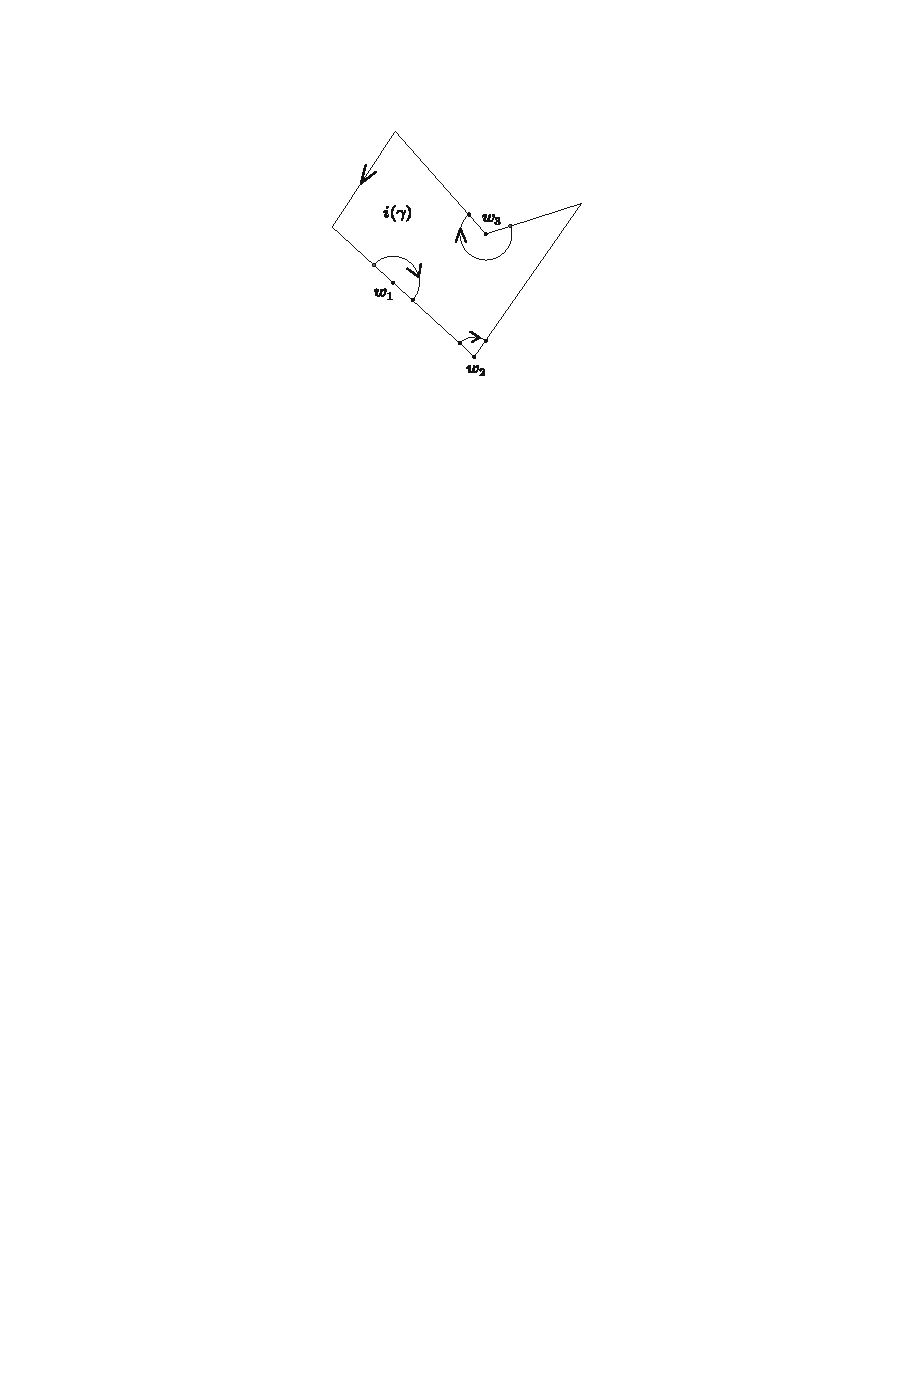
\includegraphics{pictures/modification}
\caption{A modification of a Jordan path.}
\end{figure}

We consider an oriented piecewise differentiable path $\gamma$ in $\C$, and a differential form $\omega=f(z)\dif z$ that is holomorphic in a neighborhood $D$ of $\gamma$ except for isolated singularities on the range of $\gamma$ that are simple poles. Because $\int_{\gamma}\omega$ is not defined, we want to introduce two paths $\gamma$ and $\gamma_{d,\delta}$, the second is disconnected, for which $\int_{\gamma_{\delta}}\omega$ and $\int_{\gamma_{d,\delta}}\omega$ are defined and finite. Let $w_1,\dots,w_m$ be the set of singularities of $\omega$ on $\gamma$. Let $\eps>0$ be the minimum of the finite set consisting of one half the distances between the various $w_k$ and the radii of the largest discs about these points contained in $D$. Let $0<\delta<\eps$. For each $k$, let $C_k$ be the positively oriented circle of radius $\delta$ and center $w_k$. This circle intersects $\gamma$ in a finite set of points. Let $a_{\delta,k}$ be the last point before $w_k$ in this intersection and $b_{\delta,k}$ the first point after $w_k$. These two points define two arcs on $C_k$. Choose one of these arcs; call it $\widetilde{\alpha_{\delta,k}}$, the arc \textbf{subtended at $\bm{w_k}$}, and give it the orientation consistent with that of $\gamma$. Let $-2\pi<\alpha_{\delta,k}<2\pi$ be the angle of this arc measured from $a_{\delta,k}$. The \textbf{$\bm{\delta}$-modification} $\gamma_{\delta}$ of the curve $\gamma$ is obtained by replacing for each $k$ the segment of $\gamma$ between $a_{\delta,k}$ and $b_{\delta,k}$ by the arc $\widetilde{\alpha}_{\delta,k}$. The \textbf{disconnected $\bm{\delta}$-modification} $\gamma_{d,\delta}$ of the curve $\gamma$ is obtained by removing for each $k$ the segment of $\gamma$ between $a_{\delta,k}$ and $b_{\delta,k}$. We define the \textbf{principal value}
\[\text{p.v.}\int_{\gamma}\omega=\lim_{\delta\to 0^+}\int_{\gamma_{d,\delta}}\omega,\]
provided the limit exists.\par
Each of the sets $\{a_{\delta,k}\}$, $\{b_{\delta,k}\}$ and $\{\alpha_{\delta,k}\}$ is bounded. Hence we can construct a sequence $\{\delta_n\}$ that converges to zero with the property that all three sequences have limits denoted by $a_k$, $b_k$, and $\alpha_k$, respectively. Once these limits are known to exist, it is easy to see that the three nets $\{a_{\delta,k}\}$, $\{b_{\delta,k}\}$ and $\{\alpha_{\delta,k}\}$ also converge to the appropriate limits.
\begin{lemma}
Under the hypothesis above, there exists a constant $M>0$ independent of $\delta$ such that
\[\int_{\gamma_{\delta}}\omega-\int_{\gamma_{d,\delta}}\omega=-i\sum_{k=1}^{m}\alpha_{\delta,k}\Res(f,w_k)+\delta\eps(\delta)\]
where $|\eps(\delta)|<M$. Hence
\begin{align}\label{Cauchy integral with sigularity on path}
\lim_{\delta\to 0^+}\Big(\int_{\gamma_{\delta}}\omega-\int_{\gamma_{d,\delta}}\omega\Big)=-i\sum_{k=1}^{n}\alpha_{k}\Res(f,w_k).
\end{align}
\end{lemma}
\begin{proof}
Only the first identity needs verification. Fix $k$. By a translation and rotation, we may assume that $w_k=0$ and $a_k<0$. Write
\[f(z)=\frac{\rho}{z}+g(z)\]
for $|z|<\delta$ with $M_0$ a bound for $|g|$ in $B_{\delta}(0)$. Hence
\[\int_{\widetilde{\alpha}_{\delta,k}}\omega=\int_{\pi}^{\pi-\alpha_{\delta,k}}\Big(\frac{\rho}{\delta e^{i\theta}}+g(\delta e^{i\theta})\Big)\dif(\delta e^{i\theta})=i\rho\int_{\pi}^{\pi-\alpha_{\delta,k}}\dif\theta+i\theta\int_{\pi}^{\pi-\alpha_{\delta,k}}e^{i\theta}g^{\delta e^{i\theta}}\dif\theta.\]
The first of the integrals in the last line is easily evaluated to yield $-\alpha_{\delta,k}$; the absolute value of the second is bounded by $2\pi M_0$. From this the lemma follows.
\end{proof}
\begin{theorem}[\textbf{Residue Theorem with Singularities}]\label{residue theorem with singularities}
Let $\gamma$ be a closed positively oriented Jordan curve in a domain $D$ with $\Int\gamma\sub D$. Let $f$ be a holomorphic function in the domain $D$ except for isolated singularities at $z_1,\dots,z_n$ in $\Int(\gamma)$ and simple poles $w_1,\dots,w_m$ on $\gamma$. Then
\[\mathrm{p.v.}\int_{\gamma}f(z)\dif z=2\pi i\sum_{i=1}^{n}\Res(f,z_i)+i\sum_{k=1}^{m}\alpha_k\Res(f,w_k).\]
\end{theorem}
\begin{proof}
As in previous arguments, $\delta$ is a small positive number, but in this case at most the minimum of the distances from any of the $w_k$ to the $z_i$. By introducing new line segments and thus integrating over a finite number of paths, rather than just a single path, it suffices to assume that $m=1$ and $n=0$. Thus we may take $\gamma$ to be a path in the closure of $\Int\gamma$ from $a_{\delta,1}$ to $w_1$ (where $f(z)\dif z$ has a simple pole) followed by a second one from $w_1$ to $b_{\delta,1}$ and a third from $b_{\delta,1}$ back to $a_{\delta,1}$. As before by translating and rotating the picture we may assume that $w_1=0$ and $a_{\delta,1}<0$. Note that
\[\int_{\gamma_{\delta}}f(z)\dif z=0.\]
From the lemma above,
\[\mathrm{p.v.}\int_{\gamma}f(z)\dif z=i\alpha_1\Res(f,w_1),\]
and this suffices to establish the theorem.
\end{proof}
\section{Sequences and series of holomorphic functions}
\subsection{Consequences of uniform convergence on compact sets}
We begin by recalling some notation and introducing some new symbols. Let $D$ be a domain in $\C$; we denote by $C(D)$ the vector space of continuous complex-valued functions of $D$, and recall that $\mathcal{H}(D)$ is the vector space of holomorphic functions on $D$. We say that a compact disc $\widebar{B_r(z)}$ has rational center if $z=x+iy$ with $x$ and $y$ in $\Q$.
\begin{proposition}
A necessary and sufficient condition for a sequence of functions $\{f_n\}\sub C(D)$ to converge uniformly on all compact subsets of $D$ is for the sequence to converge uniformly on all compact discs with rational centers and rational radii contained in $D$.
\end{proposition}
\begin{proof}
Every compact set contained in $D$ can be covered by finitely many such discs.
\end{proof}
We proceed to describe some consequences of uniform convergence on all compact subsets of $D$, also called locally uniform convergence, for $\mathcal{H}(D)$. The first of these is that $\mathcal{H}(D)$ is closed under locally uniform convergence.
\begin{proposition}\label{holomorphic locally uniform convergence is holomorphic}
If $\{f_n\}\sub\mathcal{H}(D)$ and $\{f_n\}$ converges uniformly on all compact subsets of $D$, then the limit function $f$ is holomorphic on $D$.
\end{proposition}
\begin{proof}
We already know that $f\in C(D)$. Let $\gamma$ be any closed curve null-homotopic in $D$. Then, by Cauchy's theorem,
\[\int_{\gamma}f_n(z)\dif z=0.\]
By uniform convergence it follows that
\[\int_{\gamma}f(z)\dif z=\lim_{n\to+\infty}\int_{\gamma}f_n(z)\dif z=0,\]
and then, by Morera's theorem, $f$ is holomorphic on $D$.
\end{proof}
\begin{corollary}
If $\{f_n\}\sub\mathcal{H}(D)$ and $f=\sum_nf_n$ converges uniformly on all compact subsets of $D$, then the function $f$ is holomorphic on $D$.
\end{corollary}
Theorem~\ref{holomorphic locally uniform convergence is holomorphic} has no analog in real variables: it is easy to see (at least pictorially) that the absolute value function on $\R$, which has no derivative at $0$, can be uniformly approximated by differentiable functions. A more extreme example was constructed by Weierstrass, that of a continuous function defined on $[0,1]$ which is nowhere differentiable and uniformly approximated by
polynomials.\par
We will shortly see that uniform convergence of a sequence of holomorphic functions on all compact subsets of their common domain of definition implies uniform convergence of the derivatives on the same sets. This is another feature of holomorphic functions not shared by real differentiable functions: it is easy to construct a sequence of differentiable functions converging uniformly on a closed interval with the property that the sequence of derivatives does not converge uniformly there.
\begin{theorem}\label{holomorphic locally uniform convergence derivative}
If $\{f_n\}\sub\mathcal{H}(D)$ and $\{f_n\}$ converges to $f$ uniformly on all compact subsets of $D$, then $\{f_n'\}$ converges to $f'$ uniformly on all compact subsets of $D$.
\end{theorem}
\begin{proof}
Since $f\in\mathcal{H}(D)$, it is enough to check uniform convergence of the derivatives on all compact subdiscs $K\sub D$, with $\partial K=\gamma$ positively oriented. For $z\in\Int\gamma$ we have
\[f'(z)=\frac{1}{2\pi i}\int_{\gamma}\frac{f(\zeta)\dif\zeta}{(\zeta-z)^2}=\lim_{n\to+\infty}\frac{1}{2\pi i}\int_{\gamma}\frac{f_n(\zeta)\dif\zeta}{(\zeta-z)^2}=\lim_{n\to+\infty}f_n'(z)\]
this convergence is uniform in any smaller compact subdisc, such as
\[\widetilde{K}=\{z\in\Int\gamma:|z-w|\geq\delta>0\text{ for all }w\in\im\gamma\}.\]
with $\delta$ sufficiently small.
\end{proof}
\begin{theorem}\label{holomorphic sequence no root}
Let $\{f_n\}$ be a sequence of holomorphic functions on $D$ such that $f_n$ converges to $f$ uniformly on all compact subsets of $D$. If $f_n$ has no root in $D$ for all $n>0$, then either
\begin{itemize}
\item $f$ is identically zero, or
\item $f$ has no root in $D$.
\end{itemize}
\end{theorem}
\begin{proof}
Assume that $z_0\in D$ is a root of $f$ and that $f$ is not identically zero. Then there exists a circle $\gamma$ with center $z_0$ such that $\Int\gamma\sub D$ and $f(z)\neq 0$ for all $z\in\widebar{\Int(\gamma)}\setminus\{z_0\}$. By the argument principle, the number $N$ of zeros of $f$ in $\Int(\gamma)$ is given by
\[N=\frac{1}{2\pi i}\int_{\gamma}\frac{f'(z)}{f(z)}\dif z=1.\]
But
\[\frac{1}{2\pi i}\int_{\gamma}\frac{f'(z)}{f(z)}\dif z=\lim_{n\to+\infty}\frac{1}{2\pi i}\int_{\gamma}\frac{f_n'(z)}{f_n(z)}\dif z=0.\]
This is a contradiction.
\end{proof}
An equivalent formulation for this theorem is the following, sometimes referred to as Hurwitz's theorem.
\begin{theorem}[\textbf{Hurwitz}]
Let $\{f_n\}$ be a sequence of holomorphic functions on $D$ such that $f_n$ converges to $f$ uniformly on all compact subsets of $D$, and assume $f$ is not identically zero on $D$. For every disc $U$ such that $\widebar{U}\sub D$ with the property that $f\neq 0$ on $\partial U$, there exists $N>0$ such that $f$ and $f_n$ have the same number of zeros in $U$ for all $n\geq N$.
\end{theorem}
\begin{proof}
This is proved by the equality
\[\frac{1}{2\pi i}\int_{\partial U}\frac{f'(z)}{f(z)}\dif z=\lim_{n\to+\infty}\frac{1}{2\pi i}\int_{\partial U}\frac{f_n'(z)}{f_n(z)}\dif z.\]
Note that both sides are integers.
\end{proof}
The Hurwitz's theorem is particularly useful for the injectivity of a limit function. More precisely, we introduce the following definition.
\begin{definition}
Let $f\in \mathcal{H}(D)$. We call $f$ \textbf{simple}, \textbf{univalent}, or \textbf{schlicht} if it is one-to-one (injective) on $D$; thus a homeomorphism onto $f(D)$.
\end{definition}
\begin{theorem}[\textbf{Hurwitz}]\label{holomorphic univalent sequence}
Assume $D$ is a domain in $\C$. If $\{f_n\}$ is a sequence in $\mathcal{H}(D)$ with $f_n\to f$ uniformly on all compact subsets of $D$ and $f_n$ is univalent for each $n$, then either $f$ is constant or univalent.
\end{theorem}
\begin{proof}
Assume that $f$ is neither constant nor univalent; thus, in particular, there exist $z_1$ and $z_2$ in $D$ with $z_1\neq z_2$ and $f(z_1)=f(z_2)$. For each $n>0$, set $g_n=f_n(z)-f_n(z_2)$ on the domain $D'=D\setminus\{z_2\}$. Then $g_n\in\mathcal{H}(D')$, $g_n$ never vanishes in $D'$ and $g_n\to f(z)-f(z_2)$ uniformly on all compact subsets of $D'$. But $g$ is not identically zero and vanishes at $z_1$; we have thus obtained a contradiction to Theorem~\ref{holomorphic sequence no root}.
\end{proof}
\subsection{A metric on the space of continuous functions}
We introduce, for use in the proof of the compactness theorem and in the proof of the Riemann mapping theorem, a metric on $C(D)$ for any domain $D$ in $\C$. The metric $d$ on $C(D)$ will have the property that convergence in this metric is equivalent to uniform convergence on all compact subsets of $D$.\par
For $K$ compact in $D$ and $f\in C(D)$, set
\[\|f\|_K=\max\{|f(z)|:z\in K\}.\]
Consider the set of compact (closed) discs contained in $D$ with rational radii and rational centers. There are countably many such discs and they cover $D$. Call this collection of discs $\{D_i\}$. For each $n>0$, let
\[K_n=\bigcup_{i=1}^{n}D_i\]
then $\{K_n\}$ is an exhaustion of $D$ by compact subsets. A crucial consequence that we will use often is that given an exhaustion $\{K_n\}$ of $D$, each compact subset $K$ of $D$ is contained in $K_n$ for some $n$.\par
With this preparation, we define a norm on $C(D)$ by letting
\[\|f\|=\sum_{n=1}^{\infty}2^{-n}\min\{1,\|f\|_{K_n}\}\]
for $f\in C(D)$.
\begin{lemma}\label{property of norm on C(D)}
For all $f$ and $g\in C(D)$:
\begin{itemize}
\item[(a)] $\|f\|\geq 0$, and $\|f\|=0$ if and only if $f\equiv 0$.
\item[(b)] $\|f+g\|\leq\|f\|+\|g\|$.
\item[(c)] For each $n$, $2^{-n}\|f\|_{K_n}\leq \|f\|$.
\item[(d)] For each $n$, $\|f\|\leq \|f\|_{K_n}+2^{-n}$.
\end{itemize}
\end{lemma}
\begin{proof}
We only prove (d):
\begin{align*}
\|f\|&=\sum_{i=1}^{n}2^{-i}\min\{1,\|f\|_{K_i}\}+\sum_{i=n+1}^{\infty}2^{-i}\min\{1,\|f\|_{K_i}\}\\
&\leq\sum_{i=1}^{n}2^{-i}\|f\|_{K_n}+\sum_{i=n+1}^{\infty}2^{-i}\\
&\leq\|f\|_{K_n}+2^{-n}.
\end{align*}
This completes the proof.
\end{proof}
With this norm, the metric $d$ is given by
\[d(f,g)=\|f-g\|.\]
We now establish some properties of the metric $d$.
\begin{lemma}
For all $f$, $g$, and $h$ in $C(D)$, the following hold:
\begin{itemize}
\item[(a)] $d(f,g)\geq 0$, and $d(f,g)=0$ if and only if $f=g$.
\item[(b)] $d(f,g)=d(g,f)$.
\item[(c)] $d(f,g)\leq d(f,h)+d(h,g)$.
\item[(d)] $d(f+h,g+h)=d(f,g)$, that is, $d$ is translation invariant.
\item[(e)] $d(f,g)\leq 1$; that is, $d$ is a bounded metric.
\end{itemize}
\end{lemma}
\begin{theorem}\label{comverge in C(D) metric iff locally uniform on compact}
Convergence in the $d$-metric in $C(D)$ is equivalent to uniform convergence on all compact subsets of $D$.
\end{theorem}
\begin{proof}
Let $\{f_n\}\sub C(D)$ and assume that $\{f_n\}$ is $d$-convergent. Since for every compact set $K\sub D$ there is an $i>0$ such that $K\sub K_i$, it suffices to show uniform convergence on $K_i$ for each $i$.\par
Given $0<\eps<1$, we can choose $N>0$ large so that
\[d(f_m,f_n)\leq d(f_m,f)+d(f_n,f)<2^{-i}\eps.\]
for $m,n\geq N$. This then implies $\|f_m-f_n\|_{K_i}<2^{-i}\eps$, so the sequence $\{f_n\}$ converges uniformly on $K_i$.\par
We have actually shown more than claimed: if $\{f_n\}$ is a $d$-Cauchy sequence in $C(D)$, then there exists an $f\in C(D)$ such that $f_n\to f$ uniformly on all compact subsets of $D$.\par
Conversely, assume that $f_n\to f$ uniformly on $K_n$ for all $n$. Thus for all $n>0$,
\[\lim_{i\to+\infty}\|f-f_i\|_{K_n}=0.\]
Given $\eps>0$, first choose $i$ such that $2^{-i}<\eps/2$ and next choose $N$ such that $\|f-f_n\|_{K_i}$ for all $n\geq N$. Then
\[\|f-f_n\|\leq\|f-f_n\|_{K_i}+2^{-i}<\eps/2+\eps/2=\eps.\]
Therefore $f_n\to f$ in $d$-metric.
\end{proof}
\begin{corollary}
The topology of the metric space $(C(D),d)$ is independent of the choice of exhaustion $\{K_n\}$ of $D$.
\end{corollary}
\begin{corollary}
$d$ is a complete metric on $C(D)$.
\end{corollary}
Because of Theorem~\ref{comverge in C(D) metric iff locally uniform on compact}, we can reformulate the results of the previous part in terms of the metric $d$. In particular, Theorems~\ref{holomorphic locally uniform convergence is holomorphic} and \ref{holomorphic locally uniform convergence derivative} can now be phrased as in the following corollary. We already remarked that $\mathcal{H}(D)\sub C(D)$, so $d$ restricts to a metric to $\mathcal{H}(D)$, also denoted by $d$.
\begin{corollary}
$\mathcal{H}(D)$ is a closed subspace of $C(D)$, thus a complete metric space. Furthermore, $f\mapsto f'$ is a continuous linear operator from $\mathcal{H}(D)$ to itself.
\end{corollary}
There is an alternate description of the topology induced by $d$, that is, the topology of the metric space $(C(D),d)$. Given $f\in C(D)$, $K\sub D$ compact and $\eps>0$, we define
\[V_f(K,\eps)=\{g\in C(D):\|g-f\|_{K}<\eps\}.\]
We will now show that the collection
\[\{V_f(K,\eps):K\sub D\text{ compact and }\eps>0\}\]
is a basis for the neighborhood system at $f$.
\begin{theorem}\label{basis for C(D)}
For any $f\in C(D)$, a basis for the neighborhood system at $f$ (with respect to the topology induced by $d$ on $C(D)$) is given by the sets $V_f(K,\eps)$.
\end{theorem}
\begin{proof}
It is enough to show that
\begin{itemize}
\item[(a)] Given $V_{f}(K,\eps)$, there exists an $B_{\delta}(f)\sub V_f(K,\eps)$.
\item[(b)] Given $B_\delta(f)$, there exists a $V_f(K,\eps)\sub B_\delta(f)$. 
\end{itemize}
To show (a), we assume without loss of generality that $0<\eps<1$. Choose $i$ such that $K\sub K_i$ and set $\delta=\eps/2^i$. If $g\in N_f(\delta)$, then $\|f-g\|<\eps/2^i$. Thus
\[2^{-i}\min\{1,\|g-f\|_{K_i}\}<\eps/2^i\]
and then $\|g-f\|_{K_i}<\eps$. But
\[\|g-f\|_K\leq\|g-f\|_{K_i};\]
that is, $g\in V_f(K,\eps)$.\par
To show (b), choose $i$ such that $2^{-i}<\delta/2$. For $g\in V_f(K_i,\delta/2)$, we have $\|g-f\|_{K_i}<\delta/2$. Hence
\[d(g,f)<\|g-f\|_{K_i}+2^{-i}<\delta.\]
that is, $g\in B_{\delta}(f)$.
\end{proof}
We can apply these concepts to convergence of series of meromorphic functions.
\begin{definition}
Let ffng be a sequence in $\mathcal{M}(D)$, the meromorphic functions on $D$. We say that $\sum_nf_n$ \textbf{converges uniformly (absolutely)} on a subset $A$ of $D$ if there exists an integer $N$ such that $f_n$ is holomorphic on $A$ for all $n>N$ and $\sum_{n=N+1}^{\infty}f_n$ converges uniformly (absolutely) on $A$.
\end{definition}
\begin{proposition}
Let $\{f_n\}\sub\mathcal{M}(D)$. If $\sum_nf_n$ converges uniformly on all compact subsets of $D$, then the series $f=\sum_nf_n$ is a meromorphic function on $D$, and $\sum_nf_n'$ converges uniformly on all compact subsets to $f'$.
\end{proposition}
\subsection{The cotangent function}
As an application of the ideas developed in the last two parts, we establish a series expansion formula for the cotangent function.
\begin{theorem}\label{cotangent function expansion}
For all $z$ in $\C\setminus\Z$ the following equalities hold:
\begin{align}\label{cotangent function expansion-1}
\pi\cot\pi z=\frac{1}{z}+\sum_{n\in\Z,n\neq 0}\Big(\frac{1}{z-n}-\frac{1}{n}\Big)=\frac{1}{z}+\sum_{n=1}^{\infty}\frac{2z}{z^2-n^2}.
\end{align}
\end{theorem}
First of all, we claim that
\[\sum_{n\in\Z,n\neq 0}\Big(\frac{1}{z-n}-\frac{1}{n}\Big)=\sum_{n\neq 0}^{\infty}\frac{z}{n(z-n)}\]
converges absolutely and uniformly on all compact subsets of $\C$. To verify this claim, assume that $|z|<R$ with $R>0$. Then
\[\sum_{|n|>2R}\frac{|z|}{|n||z-n|}\leq\sum_{n\geq 2R}\frac{|R|}{|n|(|n|-R)}\leq\sum_{|n|\geq 2R}\frac{2R}{|n|^2}<+\infty.\]
We can now verify the expansion $(\ref{cotangent function expansion-1})$ for $\pi\cot\pi z$.
\begin{proof}[Proof of Theorem~\ref{cotangent function expansion}]
For $N>0$, let $C_N$ be the positively oriented boundary of the square with vertices $(N+1/2)(\pm 1+\pm i)$. Then
\[\frac{1}{2\pi i}\int_{C_N}\frac{\cot\pi\zeta}{\zeta-z}\dif\zeta=\sum_{z\in\Int C_N}\Res\Big(\frac{\cot\pi\zeta}{\zeta-z},z\Big).\]
Here $z\in\C$ is fixed: we take $z\in\Int C_N$ and $z\notin\Z$. The poles of the function $H(\zeta)=\cos\pi\zeta/(\zeta-z)$ occur at $\zeta=z$ and at $\zeta=n\in\Z$, and they are all simple. Furthermore, we see that
\[\Res\Big(\frac{\cot\pi\zeta}{\zeta-z},z\Big)=\cot\pi z,\quad \Res\Big(\frac{\cot\pi\zeta}{\zeta-z},n\Big)=\lim_{\zeta\to n}(\zeta-n)\frac{\cos\pi\zeta}{\sin\pi\zeta}\frac{1}{\zeta-z}=\frac{1}{\pi(n-z)}.\]
Thus we have
\[\frac{1}{2\pi i}\int_{C_N}\frac{\cot\pi\zeta}{\zeta-z}\dif\zeta=\cos\pi z+\frac{1}{\pi}\sum_{n=-N}^{N}\frac{1}{\pi(n-z)}=\cos\pi z+\frac{1}{\pi}\sum_{|n|\leq N,n\neq 0}\Big(\frac{1}{n-z}-\frac{1}{n}\Big)+\frac{1}{\pi z}.\]
Hence it sufficies to prove
\begin{align}\label{cotangent function expansion-2}
\lim_{N\to+\infty}\frac{1}{2\pi i}\int_{C_N}\frac{\cot\pi\zeta}{\zeta-z}\dif\zeta=0.
\end{align}
We proceed in stages. We first note that
\begin{align*}
\frac{1}{2\pi i}\int_{C_N}\frac{\cot\pi\zeta}{\zeta}\dif\zeta&=\sum_{z\in\Int C_N}\Res\Big(\frac{\cot\pi\zeta}{\zeta},z\Big)=\Res\Big(\frac{\cot\pi\zeta}{\zeta},0\Big)+\sum_{|n|\leq N,n\neq 0}\Big(\frac{\cot\pi\zeta}{\zeta},n\Big)\\
&=\Res\Big(\frac{\cot\pi\zeta}{\zeta},0\Big)+\sum_{|n|\leq N,n\neq 0}\frac{1}{\pi n}=0.
\end{align*}
The last sum is clearly zero, and the residue of $\cos\pi\zeta/\zeta$ at zero is $0$ because it is an even function. With this observation, we have
\begin{align}\label{cotangent function expansion-3}
\int_{C_N}\frac{\cot\pi\zeta}{\zeta-z}\dif\zeta=\int_{C_N}\cot\pi\zeta\Big(\frac{1}{\zeta-z}-\frac{1}{\zeta}\Big)\dif\zeta=\int_{C_N}\frac{z\cot\pi\zeta}{\zeta(\zeta-z)}\dif\zeta.
\end{align}
We calim that there exists an $M>0$ (independent of $N$) such that $|\cos\pi\zeta|\leq M$ for all $z\in C_N$. In fact, write $\zeta=u+iv$, then
\begin{align*}
|\cot\pi\zeta|^2=\frac{\cos^2\pi u+\sinh^2\pi v}{\sin^2\pi u+\sinh^2\pi v}.
\end{align*}
On the vertical sides of $C_N$ we have $u=\pm N\pm 1/2$, so
\begin{align}\label{cot function bounded on vertical}
|\cot\pi\zeta|^2=\frac{\sinh^2\pi v}{1+\sinh^2\pi v}\leq 1.
\end{align}
On the horizontal sides of $C_N$, $v=\pm N\pm 1/2$ and hence
\begin{align}\label{cot function bounded on horizontal}
|\cot\pi\zeta|^2=\frac{\cos^2\pi u+\sinh^2\pi(\pm N\pm 1/2)}{\sin^2\pi u+\sinh^2\pi(\pm N\pm 1/2)}\leq\frac{1+\sinh^2\pi(\pm N\pm 1/2)}{\sinh^2\pi(\pm N\pm 1/2)}\to 1.
\end{align}
Thus there exists an $M>0$ such that $|\cot\pi\zeta|\leq M$ for $\zeta$ on the horizontal sides of $C_N$, and the claim is proved.\par
If we denote by $L(C_N)$ the length of $C_N$, then by $(\ref{cotangent function expansion-3})$,
\begin{align*}
\Big|\int_{C_N}\frac{\cot\pi\zeta}{\zeta-z}\dif\zeta\Big|&=\Big|\int_{C_N}\frac{z\cot\pi\zeta}{\zeta(\zeta-z)}\dif\zeta\Big|\leq\int_{C_N}\frac{M|z|}{|\zeta||\zeta-z|}\,|\mathrm{d}\zeta|\\
&\leq\frac{M|z|}{(N+1/2)(N+1/2-|z|)}L(C_N)=\frac{8M|z|}{(N+1/2-|z|)}\to 0.
\end{align*}
Thus $(\ref{cotangent function expansion-2})$ is proved.
\end{proof}
Differentiating the series $(\ref{cotangent function expansion})$ term by term, we obtain the following expansion.
\begin{corollary}
For all $z\in\C\setminus\Z$,
\[\frac{\pi^2}{\sin^2\pi z}=\sum_{n=-\infty}^{\infty}\frac{1}{(z-n)^2}.\]
\end{corollary}
As an application of the cotangent expansion. We give the special values of the Riemann zeta function at even numbers. First, recall that the \textbf{Bernoulli numbers} $B_n$ are given by the Taylor series
\[\frac{z}{e^z-1}=B_0+B_1z+\sum_{n=1}^{\infty}\frac{B_{2n}}{(2n)!}z^{2n}\]
and we already know that $B_0=1$ and $B_1=-1/2$.
\begin{theorem}
The values of the Riemann zeta function at the even natural numbers are given by the Euler formula:
\[\zeta(2k):=\sum_{n=1}^{\infty}\frac{1}{n^{2k}}=\frac{(-1)^{k+1}(2\pi)^{2k}}{2(2k)!}B_{2k}.\]
\end{theorem}
\begin{proof}
By the definition of $\cot z$, we have
\begin{align*}
z\cot z&=iz\frac{e^{iz}+e^{-iz}}{e^{iz}-e^{-iz}}=iz\frac{e^{2iz}+1}{e^{2iz}-1}=\frac{2iz}{e^{2iz}-1}+iz\\
&=iz+1-\frac{2iz}{2}+\sum_{k=1}^{\infty}\frac{B_{2k}}{(2k)!}(iz)^{2k}=1+\sum_{k=1}^{\infty}(-1)^k\frac{B_{2k}}{(2k)!}(z)^{2k}.
\end{align*}
We replace $z$ by $\pi z$, and obtain
\begin{align}\label{compute zeta(2k)}
\pi z\cot\pi z=1+\sum_{k=1}^{\infty}(-1)^k\frac{(2\pi)^{2k}}{(2k)!}B_{2k}z^{2k}
\end{align}
in a suitable neighborhood of $0$. On the other side, we already now that
\[\pi z\cot\pi z=1+\sum_{n=1}^{\infty}\frac{2z^2}{z^2-n^2}1+2z^2\sum_{n=1}^{\infty}\Big(-\frac{1}{n^2}\sum_{k=0}^{\infty}\Big(\frac{z^2}{n^2}\Big)^k\Big)=\pi z\cot\pi z=1-2\sum_{k=1}^{\infty}\Big(\sum_{n=1}^{\infty}\frac{1}{n^{2k}}\Big)z^{2k}.\]
Comparing with $(\ref{compute zeta(2k)})$ we can isolate the values of $\zeta(2k)$.
\end{proof}
\subsection{Compact sets in $\mathcal{H}(D)$}
We return to the study of $C(D)$ with the $d$-metric.
\begin{definition}
Let $\mathscr{F}\sub C(D)$. We say that $\mathscr{F}$ is \textbf{locally bounded} if $\mathscr{F}$ is uniformly bounded on compact subsets; that is, if for each compact $K\sub D$, there exists an $M(K)>0$ such that $\|f\|_K\leq M(K)$ for all $f\in\mathscr{F}$.
\end{definition}
The importance of locally boundedness is revealed in the following theorem.
\begin{theorem}\label{holomorphic locally bounded is equicontinuous}
Let $A\sub\mathcal{H}(D)$ be locally bounded. Then $A$ is equicontinuous. 
\end{theorem}
\begin{proof}
Let $K$ be a compact subset of $D$ and choose $r>0$ so small that $B_{3r}(z)$ is contained in $D$ for all $z\in K$. Let $z,w\in K$ with $|z-w|<r$, and let $\gamma$ denote the boundary circle of the disc $B_{2r}(w)$. Then, by Cauchy's integral formula, we have
\[f(z)-f(w)=\frac{1}{2\pi i}\int_{\gamma}f(\zeta)\Big[\frac{1}{\zeta-z}-\frac{1}{\zeta-w}\Big]\dif\zeta.\]
Observe that
\[\Big|\frac{1}{\zeta-z}-\frac{1}{\zeta-w}\Big|=\frac{|z-w|}{|\zeta-z||\zeta-w|}\leq\frac{|z-w|}{r^2}.\]
since $\zeta\in\gamma$ and $|z-w|<r$. Therefore
\[|f(z)-f(w)|\leq\frac{1}{2\pi}\frac{2\pi r}{r^2}M|z-w|=\frac{M}{r}|z-w|\]
where $M$ denotes the uniform bound for $A$ in the compact set consisting of all points in $D$ at a distance $\leq 2r$ from $K$. Therefore $|f(z)-f(w)|<C|z-w|$, and this estimate is true for all $z,w\in K$ with $|z-w|<r$ and $f\in\mathscr{F}$; thus this family is equicontinuous, as was to be shown.
\end{proof}
\begin{theorem}[\textbf{Compactness Theorem}]\label{holomorphic compact theorem}
Let $D$ be a domain in $\C$. Then every a subset $\mathscr{F}$ of $\mathcal{H}(D)$ is compact if and only if it is closed and locally bounded.
\end{theorem}
\begin{proof}
If $\mathscr{F}$ is closed and locally bounded, then it is equicontinuous by Theorem~\ref{holomorphic locally bounded is equicontinuous}, so it follows from Proposition~\ref{Arzela-Ascoli convergent subsequence} that $A$ is compact in $\mathcal{H}(D)$.\par
Conversely, if $\mathscr{F}$ is compact, then it is closed. Moreover, for each compact subset, the function $f\mapsto\|f\|_K$ is continuous on the compact set $\mathscr{F}$. Thus it is a bounded function, and hence $\mathscr{F}$ is locally bounded.
\end{proof}
\begin{corollary}[\textbf{Montel's Theorem}]
Every locally bounded subset in $\mathcal{H}(D)$ is precompact.
\end{corollary}
Note that the converse to Montel's theorem also holds.
\begin{theorem}[\textbf{Vitali's Theorem}]
Let $D$ be a domain in $\C$, and assume that the elements in a sequence $\{f_n\}$ are locally bounded in $\mathcal{H}(D)$. Let $S\sub D$ and assume that $S$ has a limit point in $D$. If $\lim_{n}f_n(z)$ exists for all $z\in S$, then the sequence $\{f_n\}$ converges in $\mathcal{H}(D)$.
\end{theorem}
\begin{proof}
The assumptions imply that the set $\{f_n\}$ is precompact, so $\{f_n\}$ has a limit point $f$ in $\mathcal{H}(D)$. If $f$ and $g$ are both limit points of $\{f_n\}$, then
\[f(z)=\lim_nf_n(z)=g(z)\]
for $z\in S$. Since $S$ has a limit point in $D$, this implies $f=g$. Therefore the set $\{f_n\}$ has a unique limit point $f$ in $\mathcal{H}(D)$, which means $f_N$ converges to $f$ in $\mathcal{H}(D)$.
\end{proof}
\subsection{Runge's Theorem}
We consider the problem of approximating holomorphic functions by rational
functions. We regard a nonconstant polynomial as a rational function whose only pole is at infinity. The ability to uniformly approximate a holomorphic function depends on the region where the function is being approximated, as well as upon the function itself. The strongest statement about uniform approximation of holomorphic functions that we prove is Runge's approximation theorem. A number of proofs appear in the literature; ours is a variant of these.\par
We have already proved a form of Runge's theorem for an open disc $D$: a holomorphic function on $D$ has a power series expansion at the center of the disc; for every positive integer $n$, we obtain a polynomial of degree $n$ by discarding all the higher order terms in the series. These polynomials converge to the function uniformly on any compact subset of the disc.\par
On the other hand, we also know that uniform polynomial approximation does not hold in general. For instance, consider a punctured disc $D=\{0<|z-z_0|<R\}$, with $R>0$ and $z_0$ arbitrary, and the analytic function on defined by $f(z)=1/(z-z_0)$ (we take advantage of the fact that it is a rational function whose only pole is at $z_0$); if $f$ were uniformly approximated by a sequence of polynomials $\{p_n\}$ in the closed annulus $K=\{0<r\leq|z-z_0|\leq\rho<R\}$, then by taking $\gamma(\theta)=(r+\rho)e^{i\theta}/2$ for $0\leq\theta\leq 2\pi$ we would obtain the contradiction that
\[0=\lim_{n\to+\infty}\int_{\gamma}p_n(z)\dif z=\int_{\gamma}f(z)\dif z=2\pi i.\]
However, truncation of the Laurent series expansion for $f$ on $f$ shows that $f$ is indeed uniformly approximated on $K$ by rational functions whose poles lie outside $D$. This fact is generalized to arbitrary open sets $D$.
\begin{theorem}[\textbf{Runge}]\label{Runge theorem}
Let $K$ be a compact subset of $\C$ and let $S$ be a subset of $\widehat{\C}\setminus K$ that intersects nontrivially each connected component of $\widehat{\C}\setminus K$. If $f$ is a holomorphic function on an open set $D$ containing $K$, then it can be uniformly approximated on $K$ by rational functions with simple poles lying on $S$; that is, for every $\eps>0$ there exists a rational function $R$ with possibly simple poles only in $S$ such that $|f(z)-R(z)|<\eps$ for all $z\in K$.
\end{theorem}
We can always choose for $S$ a smallest set consisting of one point from each connected component of $\widehat{\C}\setminus K$. For the important special case where $\widehat{\C}\setminus K$ is connected and $S$ is chosen as $S=\{\infty\}$, Runge's theorem asserts that each function that is analytic in an open neighborhood of $K$ can be uniformly approximated in $K$ by a sequence of polynomials.\par
Before we start the proof, let's establish an extension of Cauchy's integral formula, which will be used later.
\begin{proposition}\label{cauchy integral formula extended form}
Let $K$ be a compact subset of $\C$ and let $D$ be an open set containing $K$. Then there exists a finite collection of oriented line segments $\gamma_1,\dots,\gamma_n$ in $D\setminus K$ such that for every holomorphic function $f$ on $D$,
\begin{align}\label{cauchy integral formula extended form-1}
f(z)=\frac{1}{2\pi i}\sum_{i=1}^{n}\int_{\gamma_i}\frac{f(\zeta)}{\zeta-z}\dif\zeta
\end{align}
for all $z\in K$.
\end{proposition}
\begin{proof}
After enlarging $K$ if necessary, we may assume that $K=\overline{\Int K}$. For example, we enlarge $K$ if it consists of a single point. For any positive real number $\delta$ we consider a rectangular grid of horizontal and vertical lines in the plane $\C$ so that consecutive parallel lines are at distance $\delta$ apart. We let $R_1,\dots,R_m$ be the rectangles in the grid that have nonempty intersection with $K$. Since $K$ is compact, there are only a finite number of such rectangles. We can (and from now on do) choose $\delta$ such that $R_i\sub D$ for all $i$; if $D=\C$ any $\delta>0$ suffices, and otherwise it is enough to consider any $0<\delta<d(K,D^c)/2$, since $z\in R_i$ implies that $d(z,K)<\sqrt{2}\delta$. As usual, the boundary of $R_i$ is denoted by $\partial R_i$ and is oriented in the counterclockwise direction. The integrals of a continuous form along the common boundaries of any pair of contiguous $R_i$ and $R_j$ cancel out. This last observation implies that we can choose a set $\mathcal{S}$ of curves whose ranges are a subset of the sides in $\bigcup_{i=1}^{m}\partial R_i$, and such that the set $\mathcal{S}=\{\gamma_i:1\leq i\leq n\}$ satisfies
\begin{itemize}
\item[(a)] If $\gamma_i$ is in $\mathcal{S}$, it lies on a side of only one $R_i$.
\item[(b)] If $\gamma_i$ is in $\mathcal{S}$, then it is disjoint from $K$.
\item[(c)] For any continuous function $g$ on $\bigcup_{i=1}^{m}\partial R_i$, we have
\begin{align}\label{cauchy integral formula extended form-2}
\sum_{i=1}^{m}\int_{\partial R_i}g(z)\dif z=\sum_{i=1}^{n}\int_{\gamma_i}g(z)\dif z.
\end{align}
\end{itemize}
Each $\gamma_i$ is an oriented line segment in $D\setminus K$. It remains to prove that equation $(\ref{cauchy integral formula extended form-1})$ holds with these $\gamma_i$. If $z\in K$ and $z$ is not on the boundary of any of the rectangles, then the function
\[\zeta\mapsto g(\zeta)=\frac{1}{2\pi i}\frac{f(\zeta)}{\zeta-z},\quad \zeta\in\bigcup_{i=1}^{m}\partial R_i.\]
is continuous. Thus, we have, by $(\ref{cauchy integral formula extended form-2})$,
\[\frac{1}{2\pi i}\sum_{i=1}^{m}\int_{\partial R_i}\frac{f(\zeta)}{\zeta-z}\dif\zeta=\frac{1}{2\pi i}\sum_{i=1}^{n}\int_{\gamma_i}\frac{f(\zeta)}{\zeta-z}\dif\zeta.\]
Assume that $z$ belongs to the interior of exactly one of the $R_i$, call it $R_t$. If $i\neq t$, then $z\notin R_i$ and so
\[\frac{1}{2\pi i}\int_{\partial R_i}\frac{f(\zeta)}{\zeta-z}\dif\zeta=0,\]
also, since $z\in R_t$, by Cauchy's integral formula, we have
\[\frac{1}{2\pi i}\int_{\partial R_t}\frac{f(\zeta)}{\zeta-z}\dif\zeta=f(z).\]
Thus $(\ref{cauchy integral formula extended form-1})$ holds for all $z\in R_t$. Since range $\gamma_i$ does not intersect $K$, both sides of this equation are continuous functions of $z$ on $K$, and they agree on the set of points $z$ in $K$ that are not on the boundary of any rectangle $R_i$, a dense subset of $K$. Thus they agree for all $z\in K$.
\end{proof}
Let $K$ and $S$ be the sets described in the hypothesis of Runge's theorem, and define $B(K,S)$ be the closure in the space $C(K)$ of rational functions with poles only in $S$. Runge's theorem asserts that every holomorphic function on a neighborhood of $K$ belongs to $B(S,K)$. The main tool in proving Runge's Theorem is Proposition~\ref{pair annihilator prop} and Riesz's representation theorem. First, we need the following lemma.
\begin{lemma}\label{Runge lemma}
Let $\lambda$ be the Lebesgue measure on $\C$. If $\mu\in M(K)$, then the function
\[\hat{\mu}(z)=\int_K\frac{d\mu(\zeta)}{\zeta-z}\]
is in $L^1_{loc}(\lambda)$, analytic on $\widehat{\C}\setminus K$, and $\hat{\mu}(\infty)=0$.
\end{lemma}
\begin{proof}
Let $R>0$, we prove that $\hat{\mu}(z)$ is integrable on $B_r(0)$. To see this, note that
\begin{align*}
\int_{B_r(0)}\Big|\int_K\frac{d\mu(\zeta)}{\zeta-z}\Big|\,d\lambda(z)\leq\int_{B_r(0)}\int_K\frac{d|\mu|(\zeta)}{|\zeta-z|}\,d\lambda(z)=\int_K\int_{B_r(0)}\frac{d\lambda(z)}{|\zeta-z|}\,d|\mu|(\zeta).
\end{align*}
Choose $\rho>0$ such that $B_R(0)\sub B_\rho(z)$, for each $z\in K$. We then have
\[\int_{B_r(0)}\Big|\int_K\frac{d\mu(\zeta)}{\zeta-z}\Big|\,d\lambda(z)\leq\int_{K}\int_0^{2\pi}\int_0^\rho drd\theta d|\mu|(\zeta)=2\pi\rho\|\mu\|.\]
Thus $\hat{\mu}\in L^1_{loc}(\lambda)$, and $\hat{\mu}$ is well defined. To show that $\hat{\mu}$ is analytic on $\widehat{\C}\setminus K$, let $z,z_0\in K$ and note that
\[\frac{\hat{\mu}(z)-\hat{\mu}(z_0)}{z-z_0}=\int_K\frac{d\mu(\zeta)}{(\zeta-z)(\zeta-z_0)}.\]
Since $[(\zeta-z)(\zeta-z_0)]^{-1}\to(\zeta-z_0)^{-2}$ uniformly on $K$, as $z\to z_0$, $\hat{\mu}$ has a derivative and 
\[\frac{d}{dz}\hat{\mu}(z)=\int_K\frac{d\mu(\zeta)}{(\zeta-z)^2}.\]
So $\hat{\mu}$ is analytic on $\widehat{\C}\setminus K$. To show that it is analytic at infinity, note that $\hat{\mu}(z)\to 0$ as $z\to+\infty$, so infinity is a removable singularity.
\end{proof}
It is easy to see, with $\hat{\mu}$ defined in Lemma~\ref{Runge lemma},
\begin{align}\label{Runge theorem-1}
\frac{d^n}{dz^n}\hat{\mu}(z)=n!\int_K\frac{d\mu(\zeta)}{(\zeta-z)^{n+1}}.
\end{align}
Also, for $|z|$ so large such that $|\zeta/z|<1$, we have
\begin{align}\label{Runge theorem-2}
\hat{\mu}(z)=\int_K\frac{d\mu(\zeta)}{\zeta-z}=-\frac{1}{z}\int_K\frac{d\mu(\zeta)}{1-\zeta/z}=-\frac{1}{z}\int_K\sum_{n=0}^{\infty}\Big(\frac{\zeta}{z}\Big)^nd\mu(\zeta)=-\sum_{n=0}^{\infty}a_nz^{-(n+1)}
\end{align}
where $a_n=\int_K\zeta^n\,d\mu(\zeta)$. Now we can give the proof of Runge's theorem.
\begin{proof}[Proof of Theorem~\ref{Runge theorem}]
Assume that $\mu\in M(K)$ and $\int_Kf\,d\mu=0$ for every rational function $f$ with poles in $S$. Let $U$ be a component of $\widehat{\C}\setminus K$ and $z_0\in S\cap U$. If $z_0\neq\infty$, then the hypothesis and $(\ref{Runge theorem-1})$ imply that each derivative of $\hat{\mu}$ at $z_0$ vanishes. Since $\hat{\mu}$ is analytic in $U$ and $U$ is connected, this implies $\hat{\mu}=0$ on $U$. If $z_0=\infty$, then since each $z^n$ has pole at $\infty$, the hypothesis implies that $a_n=0$ for all $n\in\N$ in $(\ref{Runge theorem-2})$, which means $\hat{\mu}=0$ on $U$. In summary, $\hat{\mu}=0$ on $\widehat{\C}\setminus K$.\par
If $f$ is analytic on an open set $D$ containing $K$, let $\gamma_1,\dots,\gamma_n$ be given as in Proposition~\ref{cauchy integral formula extended form}. Then we have
\begin{align*}
\int_Kf(z)\,d\mu(z)=\frac{1}{2\pi i}\sum_{i=1}^{n}\int_{\gamma_i}f(\zeta)\int_K\frac{d\mu(z)}{\zeta-z}\dif\zeta=-\frac{1}{2\pi i}\sum_{i=1}^{n}\int_{\gamma_i}f(\zeta)\hat{\mu}(\zeta)\dif\zeta.
\end{align*}
by Fubini's Theorem. But $\hat{\mu}(\zeta)=0$ on $\gamma_i\sub\C\setminus K$, so $\int_Kf\,d\mu=0$. By Proposition~\ref{pair annihilator prop}, this implies $f\in B(K,S)^{\bot\bot}=B(K,S)$. This proves Runge's Theorem.
\end{proof}
An important special case is that $\widehat{\C}\setminus D$ is connected.
\begin{corollary}
If $K$ is compact and $\widehat{\C}\setminus K$ is connected and if $f$ is analytic in a neighborhood of $K$, then $f$ can be approximated uniformly on compact subsets of $D$ by polynomials.
\end{corollary}
\subsection{Mittag-Leffler's Theorem}
Observe that if an analytic function has an infinity of singularities in a bounded region, then there must exist at least one limit point of those singularities within or on the boundary of the region. For example, consider the function $f(z)=\sin(1/z)$ which has poles at $z=(k\pi)^{-1}$ for $k\in\Z$. The origin is the limit point of these poles. Similarly, the function $g(z)=f(f(z))$ has its singularities at all the roots of the equation $f(z)=(k\pi)^{-1}$, among which are all the points
\[z=\frac{1}{2k+\arcsin((k\pi)^{-1})}\]
where $k$, $k'$ are arbitrary integers. Note that all the points $(2k'\pi))^{-1}$ are limit points. For if, $k'$ be fixed and $k$ increases indefinitely, the last expression has $(2k'\pi)^{-1}$ for its limit.\par
Thus, we see that an analytic function may have an infinity of singularities and yet have only a finite number of singularities in every finite region of the complex plane.\par
Let us now consider the problem of constructing a meromorphic function with preassigned poles. If the function $f(z)$ is meromorphic in a region $D$, there corresponds to each pole $z_n$ a principal part of $f(z)$ consisting of the part of the Laurent's expressions, which contain the negative powers of $z-z_n$; it reduces to a polynomial $P_n((z-z_n)^{-1})$. We are tempted to subtract all principal parts in order to obtain a representation
\[f(z)=\sum_{n=1}^{\infty}P_n\Big(\frac{1}{z-z_n}\Big)+g(z).\]
where $g(z)$ would be analytic in $D$. However, the sum on the right-hand member is in general infinite, and there is no guarantee that series will converge, so the method needs to be modified. Notice that nothing essential is lost if we substract an analytic function $p_n(z)$ form each principal part $P_n$. By judicious choice of the function $p_n$ the series $\sum_n(P_n-p_n)$ can be made convergent. It is even possible to take the $p_n(z)$ to be polynomials.\par
If $D$ is the whole complex plane $\C$, we shall prove that every meromorphic function has a development in partial fractions and moreover, that the principal parts can be described arbitrarily. The theorem and its generalization to arbitrary regions are due to Mittag-Leffler.
\begin{theorem}[\textbf{Mittag-Leffler's Theorem}]
Let $\{z_n\}$ be a sequence of complex numbers with $\lim_n|z_n|=+\infty$, and let
\[P_n(z)=a_{n_1}z+a_{n_2}z+\cdots+a_{n_{k_n}}z^{k_n}\]
be arbitrary polynomials of degree at least $1$ and having no constant term. Then there are functions which are meromorphic in the whole plane with poles at the point $z_n$ and the corresponding principal parts
\[P_n\Big(\frac{1}{z-z_n}\Big)=\frac{a_{n_1}}{z-z_n}+\frac{a_{n_2}}{(z-z_n)^2}+\cdots+\frac{a_{k_n}}{(z-z_n)^{k_n}}.\]
Moreover, the most general meromorphic function of this kind can be written in the form
\begin{align}\label{Mittag-Leffler on C}
f(z)=\sum_{n=1}^{\infty}\Big[P_n\Big(\frac{1}{z-z_n}\Big)-p_n(z)\Big]+g(z)
\end{align}
where the $p_n(z)$ are suitably chosen polynomials and $g(z)$ is an entire function.
\end{theorem}
\begin{proof}
In case when $P=\{z_1,z_2,\dots,z_n\}$ is a finite subset of $\C$, there is nothing to discuss. Also, we can at our will, add (or delete) a finite number of points to (or from ) $P$ without changing the nature of the problem. In particular, without loss of generality we may assume that $0\notin P$ and $P$ is infinite. Since $P_n((z-z_n)^{-1})$ is analytic
for $|z|<|z_n|$, we can expand it in a Taylor's series about the origin. So let
\[P_n\Big(\frac{1}{z-z_n}\Big)=\sum_{i=0}^{\infty}d_{n_i}z^i.\]
Let $p_n(z)$ be the partial sum of this expansion up to degree $r_n$ so that
\[p_n(z)=\sum_{i=0}^{r_n}d_{n_i}z^i.\]
We chooser $r_n$ sufficiently large to suit our purpose. Consider the remainder term
\[f_n(z)=P_n\Big(\frac{1}{z-z_n}\Big)-p_n(z).\]
After a suitable truncation we can find polynomials $p_n$ such that
\[\Big|P_n\Big(\frac{1}{z-z_n}\Big)-p_n(z)\Big|\leq\frac{1}{n^2}\for |z|\leq|z_n|/2.\]
Then the power series
\[\sum_{k=n}^{\infty}\Big[P_k\Big(\frac{1}{z-z_k}\Big)-p_k(z)\Big]\]
converges locally uniformly in the region $|z|\leq|z_n|$, and so the expression
\[f(z):=\sum_{n=1}^{\infty}\Big[P_n\Big(\frac{1}{z-z_n}\Big)-p_n(z)\Big]\]
defines an analytic function in the domain $\C\setminus P$ having the prescribed singular behavior in $P$.
\end{proof}
\section{Conformal equivalence and hyperbolic geometry}
\begin{definition}
An injective meromorphic function is called a \textbf{conformal map}. A map $f$ is anti-conformal if its conjugate is conformal.
\end{definition}
Our definition of conformality is the correct notion of isomorphism in the
category of meromorphic mappings, since the inverse of a conformal map is also conformal. Thus the concept introduces a natural equivalence relation on the family of domains on the sphere, called \textbf{conformal equivalence}.
\begin{proposition}
If $f:D\to\C$ is holomorphic and injective, then $f'(z)\neq 0$ for all $z\in D$. In particular, the inverse of $f$ defined on its range is holomorphic, and thus the inverse of a conformal map is also holomorphic.
\end{proposition}
\begin{proof}
We argue by contradiction, and suppose that $f'(z_0)=0$ for some $z_0\in D$. Then by Proposition~\ref{holomorphic map local prop}, $f$ is not injective near $z_0$. This contraction means $f'(z)\neq 0$ on $D$.\par
Now let $g=f^{-1}$ be the inverse of $f$. If $f(z_0)=w_0$, then
\[\lim_{w\to w_0}\frac{g(w)-g(w_0)}{w-w_0}=\lim_{z\to z_0}\frac{f^{-1}(z)-f^{-1}(z_0)}{f(z)-f(z_0)}=\frac{1}{f'(z_0)}.\]
This implies $g$ is holomorphic and $g'(w)=1/f'(z)$.
\end{proof}
\begin{definition}
Let $D$ be a domain in $\widehat{\C}$. We define $\Aut(D)$ as the group (under composition) of \textbf{conformal automorphisms} (or conformal bijections) of $D$; that is, it consists of the conformal maps from $D$ onto itself.
\end{definition}
There are two naturally related problems:
\begin{itemize}
\item[(a)] Describe $\Aut(D)$ for a given $D$.
\item[(b)] Given two domains $D$ and $D'$, determine when they are conformally equivalent.
\end{itemize}
We solve Problem (a) for $D=\C$, $D=\C$, and $D=\D$, and Problem (b) for $D$ and $D'$ any pair of simply connected domains in $\widehat{\C}$.
\subsection{Fractional linear (M\"obius) transformations}
We describe the (orientation preserving) M\"obius group, and show that for the domains $D=\C$, $\C$, a disc or a half plane, the group $\Aut(D)$ is a subgroup of this group.
\begin{definition}
A \textbf{fractional linear transformation} (or M\"obius transformation) is a meromorphic function $f:\widehat{\C}\to\widehat{\C}$ of the form
\begin{align}\label{Mobius transformation}
f(z)=\frac{az+b}{cz+d}
\end{align}
where $a,b,c,d$ are complex numbers such that $ad-bc\neq 0$. The set of all M\"obius transformations is a group under composition, the \textbf{M\"obius group}.
\end{definition}
Without loss of generality we assume subsequently that $ad-bc=1$. Also, whenever convenient we will multiply each of the four constants $a,b,c$, and $d$ by $-1$, since this does not alter the M\"obius transformation's action on $\widehat{\C}$ nor the condition $ad-bc=1$. It is clear that
\begin{equation}\label{exact sequence of Mobious transform}
\begin{tikzcd}
1\ar[r]&\{\pm I_2\}\ar[r]&\SL_2(\C)\ar[r]&\Aut(\widehat{\C})
\end{tikzcd}
\end{equation}
is an exact sequence, where the first two arrows denote inclusion, and by the last arrow, a matrix in $\SL_2(\C)$ is sent to the element of $\Aut(\widehat{\C})$ given by $(\ref{Mobius transformation})$. It is also clear that the image of the last arrow in the sequence is precisely the M\"obius group, and, therefore, that it is isomorphic to $\PSL_2(\C)$, the quotient of $\SL_2(\C)$ by $\pm I_2$. It is natural to ask whether the last arrow is surjective; that is, whether the M\"obius group coincides with $\Aut(\widehat{\C})$. We will see that this is indeed the case.\par
Let $A$ be an element of $\PSL_2(\C)$. The square of the trace of a preimage of $A$ in $\SL_2(\C)$ is the same for both of the two preimages of $A$. Thus even though the trace of an element in the M\"obius group is not well defined, the \textbf{trace squared} of an element in $\PSL_2(\C)$ is.
\subsubsection{Fixed points of M\"obius transformations}
Let $A$ be any element of the M\"obius group different from the identity map. We are interested in the fixed points of $A$ in $\widehat{\C}$. If
\[A(z)=\frac{az+b}{cz+d}\]
with $ad-bc=1$, then for a fixed point $z$ of $A$ we have either $z=\infty$, or $z\in\C$ and $cz^2+(d-a)z-b=0$. We consider two cases:
\begin{itemize}
\item If $c=0$, then $\infty$ is a fixed point of $A$ and we have $ad=1$. If $d=a$ then $A(z)=z+b/a$ with $ab\neq 0$, and $A$ has no other fixed point. If $d\neq a$, then $A(z)=(az+b)/d$, and $A$ has one more fixed point $b/(d-a)$ in $\C$. We note that in this case $A$ has precisely one fixed point if and only if $\tr^2(A)=4$.
\item If $c\neq 0$, then $\infty$ is not a fixed point of $A$, and the fixed points of $A$ are given by
\[\frac{a-d\pm\sqrt{(a-d)^2+4bc}}{2c}=\frac{(a-d)\pm\sqrt{\tr^2(A)-4}}{2c}.\]
\end{itemize}
We have thus proved.
\begin{proposition}\label{Mobious transform fixed point}
If $A$ is a M\"obius transformation different from the identity map, then $A$ has either one or two fixed points in $\widehat{\C}$. It has exactly one if and only if $\tr^2(A)=4$.
\end{proposition}
\subsubsection{Cross ratios}
\begin{proposition}
Given three distinct points $z_2,z_3,z_4$ in $\widehat{\C}$, there exists a unique M\"obius transformation $S$ with $S(z_2)=1$, $S(z_3)=0$, and $S(z_4)=\infty$.
\end{proposition}
\begin{proof}
Uniqueness is clear: if $S_1$ and $S_2$ are M\"obius transformations that solve our problem, then $S_1\circ S_2^{-1}$ is a M\"obius transformation that fixes $1$, $0$ and $\infty$ and hence, by Proposition~\ref{Mobious transform fixed point}, it is the identity map.\par
Now we construct the map $S$. If the $z_i$ are complex numbers, then
\[S(z)=\frac{z-z_3}{z-z_4}:\frac{z_2-z_3}{z_2-z_4}\]
is the required map. If one of the $z_i$ equals $\infty$, use a limiting procedure to obtain
\[S(z)=\begin{cases}
\dfrac{z-z_3}{z-z_4}&\text{if $z_2=\infty$},\\[8pt]
\dfrac{z_2-z_4}{z-z_4}&\text{if $z_3=\infty$},\\[8pt]
\dfrac{z-z_3}{z_2-z_3}&\text{if $z_4=\infty$},
\end{cases}\]
respectively.
\end{proof}
\begin{corollary}
If $\{z_i\}$ and $\{w_i\}$ are two triples of distinct points in $\widehat{\C}$, then there exists a unique M\"obius transformation $S$ with $S(z_i)=w_i$; thus the M\"obius group is uniquely triply transitive on $\widehat{\C}$.
\end{corollary}
\begin{definition}
The \textbf{cross ratio} $(z_1,z_2,z_3,z_4)$ of four distinct points in $\widehat{\C}$ is the image of $z_1$ under the M\"obius transformation taking $z_2$ to $1$, $z_3$ to $0$, and $z_4$ to $\infty$; that is,
\[(z_1,z_2,z_3,z_4)=\frac{z_1-z_3}{z_1-z_4}:\frac{z_2-z_3}{z_2-z_4},\]
if the four points are finite, with the corresponding limiting values if one of the $z_i$ equals $\infty$.
\end{definition}
As we will see in the next proposition, it is useful to view the cross ratio as a M\"obius transformation (a function of $z_1$) $S=S_{z_2,z_3,z_4}$ that takes the four distinct ordered points $(z_1,z_2,z_3,z_4)$ to the four distinct ordered points $(w_1,w_2,w_3,w_4)$, where $w_1=(z_1,z_2,z_3,z_4)$, $w_2=1$, $w_3=0$ and $w_4=\infty$. It hence makes sense to allow one repetition among the four points $z_i$ and hence have $S$ defined on $\widehat{\C}$ and conclude that $(z_2,z_2,z_3,z_4)=1$, for example. This point of view will be used from now on when needed.
\begin{proposition}\label{Mobious transform cross ratio}
If $(z_1,z_2,z_3,z_4)$ are four distinct points in $\widehat{\C}$, and $T$ is any M\"obius transformation, then
\[(T(z_1),T(z_2),T(z_3),T(z_4))=(z_1,z_2,z_3,z_4).\]
\end{proposition}
\begin{proof}
If we define $S(z)=(z,z_2,z_3,z_4)$ for $z\in\C\setminus\{0,1\}$, then $S\circ T^{-1}$ is a M\"obius transformation taking $T(z_2)$ to $1$, $T(z_3)$ to $0$ and $T(z_4)$ to $\infty$. Therefore
\[(T(z_1),T(z_2),T(z_3),T(z_4))=(S\circ T^{-1})(T(z_1))=S(z_1)=(z_1,z_2,z_3,z_4),\]
so the claim follows.
\end{proof}
\begin{definition}
A \textbf{circle in $\widehat{\C}$} is either an Euclidean (ordinary) circle in $\C$, or a straight line in $\C$ together with $\infty$ (this is a circle passing through $\infty$).
\end{definition}
\begin{proposition}\label{four point on a circle iff cross ratio}
The cross ratio of four distinct points in $\widehat{\C}$ is a real number if and only if the four points lie on a circle in $\widehat{\C}$.
\end{proposition}
\begin{proof}
This is an elementary geometric argument that goes as follows. It is clear that
\[\arg(z_1,z_2,z_3,z_4)=\arg\frac{z_1-z_3}{z_1-z_4}-\arg\frac{z_2-z_3}{z_2-z_4}\]
It is also clear from the geometry of the situation that the two quantities on the right-hand side differ by $n\pi$, with $n\in\Z$, if and only if the four points lie on a circle in $\widehat{\C}$.
\end{proof}
\begin{theorem}
A M\"obius transformation maps circles in $\widehat{\C}$ to circles in $\widehat{\C}$.
\end{theorem}
\begin{proof}
This follows immediately from Propositions~\ref{Mobious transform cross ratio} and \ref{four point on a circle iff cross ratio}.
\end{proof}
We use the following standard notation in the rest of this chapter: $\D$ denotes the unit disc and $\mathbb{U}$ the upper half. Note that both $\D$ and $\mathbb{U}$ should be regarded as discs in $\widebar{\C}$, since they are bounded by circles in $\widehat{\C}$: the unit circle $S^1$ and the extended real line, respectively.\par
The next result shows that these two discs in $\widehat{\C}$ are conformally equivalent.
\begin{corollary}\label{conformal map from U to D eg}
The map
\[w(z)=\frac{z-i}{z+i}\]
is a conformal map of $\mathbb{U}$ onto $\D$.
\end{corollary}
\begin{proof}
All M\"obius transformations, in particular $w$, are conformal. A calculation shows that $w$ maps $\R$ onto $S^1$ (the unit circle centered at $0$) and $w(i)=0$. By connectivity considerations, it follows that $w(\mathbb{U})=\D$.
\end{proof}
\subsection{Automorphism group for $\widehat{\C}$, $\C$, $\mathbb{U}$ and $\D$}
\begin{theorem}\label{automorphism of C}
A function $f:\C\to\C$ belongs to $\Aut(\C)$ if and only if there exist $a$ and $b$ in $\C$ with $a\neq 0$ such that $f(z)=az+b$ for all $z\in\C$.
\end{theorem}
\begin{proof}
The if part is trivial. For the only if part, note that $f$ is an entire function, and we can use its Taylor series at zero to conclude that
\[f(z)=\sum_{n=0}^{\infty}a_nz^n\]
If1were an essential singularity of $f$, then $f(\D)$ would be dense in $\C$, which contradicts the injectivity of $f$. Thus $\infty$ is either a removable singularity or a pole of $f$; in any case, there is a nonnegative integer $N$ such that $a_n=0$ for all $n>N$ and $a_N\neq 0$; that is, $f$ is a polynomial of degree $N$. If $N$ were bigger than one or equal to zero, then $f$ would not be injective.
\end{proof}
\begin{theorem}\label{automorphism of widehat{C}}
$\Aut(\widehat{\C})\cong\PSL_2(\C)$. Thus the last arrow in the exact sequence $(\ref{exact sequence of Mobious transform})$ corresponds to a surjective map.
\end{theorem}
\begin{proof}
We need only show that $\Aut(\widehat{\C})$ is contained in the M\"obius group. Let $f$ be an element of $\Aut(\widehat{\C})$. If $f(\infty)=\infty$, then $f$ is a M\"obius transformation by Theorem~\ref{automorphism of C}. If $F(\infty)=z_0\neq\infty$, then consider the M\"obius transformation $A(z)=(z-z_0)^{-1}$ and conclude that $B=A\circ f$ in $\Aut(\widehat{\C})$ and fixes $\infty$; therefore $B$ is a M\"obius transformation. But then so is $f=A^{-1}\circ B$.
\end{proof}
We now provide a characterization of the elements of $\Aut(\D)$; it shows that they form a subgroup of $\Aut(\widehat{\C})$.
\begin{theorem}\label{automorphism of D}
A function $f$ defined on $\D$ is in $\Aut(\D)$ if and only if there exist $a\in\D$ and $\alpha\in\R$ such that
\[f(z)=e^{i\alpha}\frac{z-a}{1-z\widebar{a}}.\]
\end{theorem}
\begin{proof}
The if part is clear. For $f\in\Aut(\D)$. If $f(0)=0$, then it follows by the Schwarz's lemma applied first to $f$ and then to $f^{-1}$ that
\[|f(z)|\leq|z|=|f^{-1}(w)|\leq|w|=|f(z)|.\]
Therefore $|f(z)|=|z|$, and it follows from Schwarz's lemma that $f(z)=e^{i\alpha}z$ for some $\alpha\in\R$.\par
If $f(a)=0$ with $a\neq 0$, then $0<|a|<1$ and we set
\[g(z)=f\Big(\frac{z+a}{1+\widebar{a}z}\Big).\]
Then $g\in\Aut(\D)$ and $g(0)=0$, thus $g(z)=e^{i\alpha}$ and we get
\[f(z)=e^{i\theta}\frac{z-a}{1-\widebar{a}z}.\]
This proves the claim. 
\end{proof}
\begin{theorem}\label{automorphism of U}
$\Aut(\mathbb{U})\cong\PSL_2(\R)$.
\end{theorem}
\begin{proof}
Consider the conformal map $w:\mathbb{U}\to\D$ given in Corollary~\ref{conformal map from U to D eg}. Then
\[\Aut(\mathbb{U})=w^{-1}\Aut(\D)w.\]
By the preceding theorem, any element $f$ of $\Aut(\D)$ may be written as
\[f(z)=e^{i\alpha}\frac{z-a}{1-\widebar{a}z}.\]
Then we see $\Aut(\mathbb{U})\sub\Aut(\widehat{\C})$. Now it is easy to see a M\"obious transformation maps $\mathbb{U}$ to $\mathbb{U}$ if and only if $a,b,c,d\in\R$ and $ab-cd>1$, thus the claim follows.
\end{proof}
\subsection{The Riemann mapping theorem}
We now show that every simply connected domain $D$ in $\C$, other than $\C$ itself, is conformally equivalent to the unit disc; any conformal map from $D$ onto the unit disc $\D$ will be called a \textbf{Riemann map}.
\begin{theorem}[\textbf{Riemann Mapping Theorem}]
Let $D$ be a nonempty proper simply connected open subset of $\C$, then $D$ is conformally equivalent to $\D$. In fact, let $z_0\in D$, then there exists a unique conformal map $f:D\to\D$ with $f(z_0)=0$, $f'(z_0)>0$, and $f(D)=\D$.
\end{theorem}
\begin{proof}
The uniqueness of such $f$ is clear by Schwarz's lemma, so we only need to find a conformal map from $D$ onto $\D$. We first find such a map into $\D$. Then we will "maximize" all such $f$ to select the desired homeomorphism. We assume that $0\notin D$, so that there exists a branch of $\sqrt{\cdot}$ on $D$. Let $\widetilde{D}=\sqrt{D}$. Then $\sqrt{z}$ is one-to-one and if $w\in\widetilde{D}$, then $-w\notin\widetilde{D}$. Indeed, otherwise $\sqrt{z_1}=w=-\sqrt{z_2}$ with $z_1,z_2\in D$ would imply that $z_1=z_2$ or $w=-w=0$, contrary to $0\notin D$. Since $D$ is open, we deduce that $\widetilde{D}\cap B_{\delta}(w_0)=\emp$ for some $w_0\in\C$ and $\delta>0$. Now define $f(z):=\delta(\rho(z)-w_0)^{-1}$ and observe that $f$ is one-to-one and into $\D$. Henceforth, we assume that $D\sub\D$ and also that $0\in D$ (scale and translate).\par
Define
\[\mathscr{F}=\{f:D\to\D:f\in\mathcal{H}(D)\text{ is injective and }f(0)=0,f'(0)\geq 0\}\cup\{f:D\to\D:f(z)\equiv 0\}.\]
Next we show that $\mathscr{F}$ is compact using Theorem~\ref{holomorphic compact theorem}. First, $\mathscr{F}$ is locally bounded since we have $\|f\|_K\leq 1$ for any compact subset $K\sub D$. To see $\mathscr{F}$ is closed, let $\{f_n\}\sub\mathscr{F}$ be a sequence such that $f_n\to f$ uniformly on all compact subsets of $D$. Then $f\in\mathcal{H}(D)$, and since each $f_n$ vanishes at $0$, so does $f$. It is now convenient to consider two cases:
\begin{itemize}
\item $f_n\equiv 0$ for infinitely many distinct $n$. In this case $f\equiv 0$ and hence certainly $f\in\mathscr{F}$.
\item $f_n\equiv 0$ for only finitely many $n$. In this case we may assume that each $f_n$ is injective; then $f'(0)\geq 0$ for all $n$, and thus $f'(0)\geq 0$. Hurwitz's Theorem says that $f$ is either constant (hence identically zero) or univalent (that is, one-to-one). Since $|f_n(z)|<1$ for all $z\in D$, we conclude that $|f(z)|\leq 1$ for all $z\in D$. If $|f(z_0)|=1$ for some $z_0\in D$, then $f\equiv 1$ by the maximum modulus principle; this is a contradiction to $f(0)=0$. Thus $|f(z)|<1$ for all $z\in D$, and we conclude that $f\in\mathscr{F}$; thus $\mathscr{F}$ is closed, and therefore compact.
\end{itemize}
We now complete the proof of the existence part. If
\[S=\{f'(0):f\in\mathscr{F}\}\]
then $S\sub\R_+$. We claim that $S$ is bounded from above. Indeed, choose $\eps>0$ so that $\widebar{B_{\eps}(0)}\sub D$. Then for any $f\in\mathscr{F}$,
\[|f'(0)|=\Big|\frac{1}{2\pi i}\int_{|z|=\eps}\frac{f(z)}{z^2}\dif z\Big|\leq\frac{1}{2\pi}\frac{2\pi\eps}{\eps^2}=\frac{1}{\eps}.\]
If $s=\sup S$, then $s\geq 1$, because $1\in S$ as $\id\in\mathscr{F}$. Also, there exists a sequence $\{f_n\}\sub\mathscr{F}$ such that $\lim_{n}f_n'(0)=s$. Since $\mathscr{F}$ is compact, there exists a convergent subsequence $\{f_{n_k}\}$ with $\lim_kf_{n_k}=f\in\mathscr{F}$. Since $f'(0)=s>0$, $f$ is an injective map.\par
It remains to prove that $f$ is onto $\D$. Suppose not, and let $w_0\in\D\setminus f(D)$. Pick $\varphi\in\Aut(\D)$ (a M\"obius transform) such that $\varphi(w_0)=0$, and let $D_1=\varphi(f(D))$, which is simply-connected and does not contain the origin. It therefore admits a branch of the square root, denoted by $\sqrt{\cdot}$. Let $\psi\in\Aut(\D)$ take $\sqrt{\varphi(0)}$ onto $0$. By construction,
\[F(z)=\psi\circ\sqrt{\cdot}\circ\varphi\circ f\]
satisfies $e^{i\theta}F\in\mathscr{F}$ for suitable $\theta$. The inverse of $\psi\circ\sqrt{\cdot}\circ\varphi$ exists and equals the analytic function
\[h(z)=\varphi^{-1}\circ(\psi^{-1})^2:\D\to\D\]
w4ich takes $0$ to $0$ and is not an automorphism of $\D$. Hence by the Schwarz's lemma, one has $|f'(0)|<1$. Since $h\circ F=f$, we conclude that $h'(0)F'(0)=f'(0)$ and thus $|F'(0)|>|f'(0)|$. This yields a contradiction, by the maximality of $f'(0)$ in $\mathscr{F}$.
\end{proof}
\begin{corollary}
If $D$ is a nonempty simply connected domain in $\widehat{\C}$, then $D$ is conformally equivalent to one and only one of the following domains: $\widehat{\C}$, $\C$, or $\D$. The case occurs when the boundary of $D$ consists of no points, one point, or more than one point, respectively.
\end{corollary}
\begin{proof}
If $D\subsetneq\widehat{\C}$, we may first reduce to the case $D\sub\C$ by observing that if $D$ contains $\infty$, we can choose $z_0\in\widehat{\C}\setminus D$, and setting $F(z)=(z-z_0)^{-1}$ we have that $F(D)\sub\C$ is a nonempty simply connected domain not containing $\infty$ and conformally equivalent to $D$. If the result holds for $F(D)$, then it also holds for $D$. If $D$ is a proper subset of $\C$, the result follows from Riemann mapping theorem.\par
We need to prove that no two of the simply connected domains $\widehat{\C}$, $\C$, and $D$ are conformally equivalent. But $\widehat{\C}$ is compact, and hence cannot be conformally equivalent to either $\C$ or $D$. On the other hand, a conformal map from $\C$ onto $D$ would be a nonconstant entire bounded function, a contradiction to Liouville's theorem.
\end{proof}
Next, we address the boundary behavior of a conformal map from $D$ to $\D$.
\begin{theorem}[\textbf{Carath\'eodory}]
Let $f$ be a conformal mapping from the unit disc $\D$ onto a Jordan domain $D$. Then $f$ can be extended to a homeomorphism from $\widebar{\D}$ to $\widebar{D}$.
\end{theorem}
Note that for such a homeomorphism to exists, it is necessary that $\partial D$ is a Jordan curve.
\begin{proof}
We may assume $D$ is bounded. First we prove that $f$ is uniformly continuous on $\D$, so that we have a continuous extension of $f$ to $\widebar{\D}$. Suppose the converse, then there must exist $\eps>0$ and a point $\zeta$ on the unit circle and sequences $z_n$, $w_n$ tending to $\zeta$ with $|f(z_n)-f(w_n)|\geq 2\eps$. Let $0<r<1$ and set $\gamma_r=B_{r}(\zeta)\cap\D$. Then $f\circ\gamma_r$ is a Jordan arc whose length is controlled by the Cauchy-Schwarz inequality:
\[L(f\circ\gamma_r)^2=\Big(\int_{\gamma_r}|f'(z)||\mathrm{d}z|\Big)^2\leq\int_{\gamma_r}|\mathrm{d}z|\int_{\gamma_r}|f'(z)|^2|\mathrm{d}z|=\pi r\int_{\gamma_r}|f'(z)|^2|\mathrm{d}z|\]
Hence there is a "length-area estimate":
\begin{align*}
\int_{0}^{1}L(f\circ\gamma_r)^2\frac{\dif r}{r}\leq\iint_{\D\cap B_{r}(\zeta)}|f'(z)|^2\mathrm{d}z\mathrm{d}\widebar{z}=\pi\mathrm{Area}(f(\D\cap B_{r}(\zeta)))<+\infty.
\end{align*}
The finiteness of $L(f\circ\gamma_{r_n})$ implies that the curve has limiting points $\alpha_n$, $\beta_n$ at its two ends with $|\alpha_n-\beta_n|\leq\eps$, so their difference tends to $0$. These two limit points must lie on $\Gamma:=\partial D$, because $f$ is a homeomorphism between $\D$ and $D$ and thus a sequence converging in $D$ has to be the image under $f$ of a sequence converging in $\D$.\par
Let $\sigma_n$ be that closed subarc of $\Gamma$ having endpoints $\alpha_n$ and $\beta_n$ and having smaller diameter. Then $\diam(\sigma_n)\to 0$, because $\Gamma$ is homeomorphic to the circle. By the Jordan curve theorem the curve $\sigma_n\cup f(\gamma_{r_n})$ divides the plane into two regions, and one of these regions, say $U_n$, is bounded. Then $U_n\sub D$, because $\widebar{D}^c$ is arcwise connected. Since
\[\diam(\partial U_n)=\diam(\sigma_n\cup f(\gamma_{r_n}))\to 0,\]
we conclude that $\diam(U_n)\to 0$.\par
Now if $V_n$ denotes the intersection of $\D$ with the disk $B_{r_n}(\zeta)$, then the arc $\gamma_{r_n}$ divides $\D$ into $V_n$ and a complementary region; note that $U_n$ is a connected component of $D\setminus f(\gamma_{r_n})$, as it is connected and is both open and closed in this set, so under the conformal homeomorphism $f$ the curve $f(\gamma_{r_n})$ divides $D$ into $U_n$ and a complementary region $U'_n$, one of which equals $f(V_n)$. Since the areas of $f(V_n)$ and $U_n$ tend to $0$, while the sum of the areas of $U_n$ and $U'_n$ is fixed, it follows that $f(V_n)=U_n$. Thus the diameter of $f(V_n)$ tends to $0$. On the other hand, passing to subsequences of $(z_n)$ and $(w_n)$ if necessary, it may be assumed that $z_n$ and $w_n$ both lie in $V_n$. But this gives a contradiction since $|f(z_n)-f(w_n)|\geq\eps$. So $f$ must be uniformly continuous on $D$.\par
Let $f$ also denote the extension $f:\widebar{\D}\to\widebar{D}$. Since $f(\D)=D$, by compactness $f$ carries the closure of $\D$ onto the closure of $D$ and hence $\partial\D$ onto $\Gamma$. If $f$ is not one-one, there are distinct points $u,v$ on $\partial\D$ with $f(u)=f(v)$. Since $f$ is conformal on $\D$, we must have $u,v\in\partial\D$ and $f(u)=f(v)\in\Gamma$. The Jordan curve
\[\{f(ru):0\leq r\leq 1\}\cup\{f(rv):0\leq r\leq 1\}\]
bounds a domain $W\sub D$, and then $f^{-1}(W)$ is one of the two components of
\[\D\setminus(\{ru:0\leq r\leq 1\}\cup\{rv:0\leq r\leq 1\}).\]
But since $f(\partial\D)\sub\Gamma$,
\[f(\partial\D\cap\partial f^{-1}(W))\sub\partial W\cap\Gamma=\{f(u)\},\]
and $f$ is constant on an arc of $\partial\D$. By the Schwarz reflection principle, $f$ can be analytically continued by conformal reflection across the circular arc. Since $f$ is then constant on an interior arc, this forces $f$ to be constant, a contradiction. So $f$ is one-one and hence a homeomorphism on the closure of $\D$.
\end{proof}
The statement with which we given from now on implies that any two bounded simply connected domains are analytically isomorphic. However, homeomorphic domains, if they are not simply connected, do not have to be analytically isomorphic.
\begin{proposition}
For $R>1$. let $A(R)$ denote the annulus $A(R)=\{z\in\C:1<|z|<R\}$.
\begin{itemize}
\item[(a)] If $A(R_1)$ is conformally equivalent to $A(R_2)$, then $R_1=R_2$.
\item[(b)] The conformal automorphisms of $A(R)$ are the maps
\[z\mapsto Re^{i\theta}/z\quad \text{and}\quad z\mapsto e^{i\theta}z\]
where $\theta\in\R$. 
\end{itemize}
\end{proposition}
\begin{proof}
We begin with a topological remark. Let $f:A(R_1)\to A(R_2)$ be a homeomorphism. Then $|f(z)|$ has a limit as $|z|\to 1$, which is either $1$ or $R_2$; further $|f(z)|\to R_2$ as $|z|\to R_1$ if $\lim_{|z|\to 1}|f(z)|=1$, and $|f(z)|\to 1$ as $|z|\to R_1$ if $\lim_{|z|\to 1}|f(z)|=R_2$.\par
To prove this, define
\[K_n=\widebar{f(\{z\in A(R_1):1<|z|<1+1/n\})},\quad L_n=\widebar{f(\{z\in A(R_1):R_1-1/n<|z|<R_1\})}.\]
Then $K_n$, $L_n$ are nonempty connected compact sets, and $K_{n+1}\sub K_n$, $L_{n+1}\sub L_n$, so that
\[K:=\bigcap_nK_n,\quad L:=\bigcap_nL_n\]
are again connected compact sets. Note that $K$ is the set of all limit points of sequences $\{f(z_n)\}$ where $\{z_n\}$ runs over sequences of points of $A(R)$ with $|z_n|\to 1$; while $L$ is the set of limit points of sequences $\{f(w_n)\}$, where $\{w_n\}\sub A(R_1)$, $|w_n|\to R_1$. We have $K\cup L=\partial(A(R_2))=C_1\cup C_{R_2}$ where $C_\rho$ is the circle $\{z\in\C:|z|=\rho\}$. Since $K$ and $L$ are connected, we either have $K=C_1$ and $L=C_{R_2}$ or $K=C_{R_2}$ and $L=C_1$. This is equivalent to the statement above.\par
Now let $f:A(R_1)\to A(R_2)$ be a conformal map. Then $g(z)=R_2/f(z)$ is also a conformal map of $A(R_1)$ onto $A(R_2)$. Now $|f(z)|\to 1$ or $R_2$ as $|z|\to 1$. Let $F=f$ in the first case, $F=g$ in the second. We have $|F'(z)|=1$ as $|z|\to 1$ and $|F(z)|\to R_2$ as $|z|\to R$.\par
Let
\[u(z)=\log|z|\log R_2-\log|F(z)|\log R_1.\]
Then we see $\Delta u=0$ and $u$ tends to zero on the boundary of $A(R_1)$. Thus by the maximal modulus principle we conclude that $u\equiv 0$ on $A(R_1)$. Solving the equation $u\equiv 0$ for $F$ thus yields that
\[|F(z)|=|z|^{\alpha}\]
where $\alpha=\log R_2/\log R_1$. Let $D\sub A(R_1)$ be a disc. Then the function $\phi(z)=z^\alpha$ can be made well-defined and holomorphic on $D$ if we set $\phi(z)=e^{\alpha\log z}$. Also $F(z)/\phi(z)$ is holomorphic on $D$ and has unit modulus. By the open mapping theorem, $F(z)/\phi(z)$ is a constant of modulus $1$ on $D$. That is,
\[F=e^{i\theta}z^{\alpha}\]
for some $\theta\in\R$. Since this argument can be performed on any disk in $A(R_1)$ and since $F$ is continuous, it follows that $e^{-i\theta}F$ is a branch of $z^\alpha$ on the entire annulus. It follows then that $\alpha$ must be a (nonnegative) integer, since otherwise no such branch exists. Finally, the only possible nonnegative integer value for $\alpha$ is $1$; otherwise $F$ would not be one-to-one. Thus $F$ can only be a rotation and therefore $R_1=R_2$ follows.
\end{proof}
\subsection{Simply connected plane domains}
The results we have proved so far give various characterizations of simply connected domains in $\C$. We collect them together and complete them in this part. First, from the proof of Riemann mapping theorem, we get the following consequence.
\begin{theorem}\label{simply connected if squre root exist}
Let $D$ be a proper domain in $\C$. Suppose that for any $f\in\mathcal{H}(D)$ which is nowhere zero, there exists $g\in\mathcal{H}(D)$ such that $g^2=f$. Then $D$ is conformally equivalent to $\D$.
\end{theorem}
\begin{theorem}\label{simply connected domain in C iff}
Let $D$ be a domain in $\C$. The following statements are pairwise equivalent.
\begin{itemize}
\item[(1)] $D$ is simply connected.
\item[(2)] $\C\setminus D$ has no compact connected components.
\item[(3)] $\widehat{\C}\setminus D$ is connected.
\item[(4)] For any $z_0\in\C\setminus D$ and any closed curve $\gamma$ in $D$, the winding number $I(\gamma,z_0)=0$; i.e., any closed curve $\gamma$ in $D$ is null-homologous.
\item[(5)] Any $f\in\mathcal{H}(D)$ has a primitive.
\item[(6)] If $f\in\mathcal{H}(D)$ is nowhere zero, there exists $g\in\mathcal{H}(D)$ with $e^g=f$.
\item[(7)] If $f\in\mathcal{H}(D)$ is nowhere zero, there exists $g\in\mathcal{H}(D)$ with $g^2=f$.
\end{itemize}
\end{theorem}
\begin{proof}
We will prove the following implications:
\[(1)\Rightarrow(4)\Rightarrow(5)\Rightarrow(6)\Rightarrow(7)\Rightarrow(1)\And(1)\Leftrightarrow(2)\Leftrightarrow(3).\]
The first chain of implications are rather easy. First note that if $D$ is simply connected then any curve is null-homotopic, hence null-homologous, this proves $(1)\Rightarrow(4)$. The fact that $(4)\Rightarrow(5)$ comes from Runge's theorem, since any holomorphic function can be locally uniformly approximated by rational functions, and the integral of rational functions on closed curves is exactly the winding number. Moreover, if any holomorphic function on $D$ has a primitive, then the primitive $g$ of $f'/f$ can be easily seen to satisfy $(6)$, and thus $(7)$ also follows. Finnaly, the implication $(7)\Rightarrow(1)$ follows from Theorem~\ref{simply connected if squre root exist}.\par
We come now to the part of the equivalence of $(1)$, $(2)$ and $(3)$. We first prove $(2)\Leftrightarrow(3)$. Suppose that $\widehat{\C}\setminus D$ is not connected, and let $C$ be a connected component of $\widehat{\C}\setminus D$ that does not contain $\infty$. Then $C$ is contained in $\C$, and $C$ is compact since it is closed in $\widehat{\C}$. Therefore $C$ is a compact component of $\C\setminus D$, which contradicts $(2)$. Conversely, if $\C\setminus D$ has a compact connected component $C$, then $C$ will still be clopen in $\widehat{C}\setminus D$. Since $C$ can not be all of $\widehat{\C}\setminus D$, this means $\widehat{\C}\setminus D$ is not connected.\par
Now we show $(1)\Leftrightarrow(3)$. If $\widehat{\C}\setminus D$ is connected, then for any closed curve $\gamma$ in $D$, the function $I(\gamma,\cdot)$ is constant on $\widehat{\C}\setminus D$. Since $\infty\in\widehat{\C}\setminus D$ and $I(\gamma,z)$ tends to zero as $|z|\to+\infty$, we conclude that $I(\gamma,\cdot)$ is identically zero in $\widehat{\C}\setminus D$. As we have already proved, this implies that $D$ is simply connected. Conversely, assume that $\widehat{\C}\setminus D$ is not connected. We first note that any connected component $C$ of $\widehat{\C}\setminus D$ meets $\partial D$: in fact, if $C\cap\partial D=\emp$, then, any point of $C$ would have a connected open neighborhood not meeting $\widebar{D}$, so that $C$ would be open in $\widehat{\C}$. But $C$ is also closed in $\widehat{\C}$ and $C\neq\widehat{\C}$, so this is clearly a contradiction. Now let $\widehat{\C}\setminus D=C_1\cup C_2$, where $C_1$ and $C_2$ are nonempty disjoint compact sets. Then $K_1=C_1\cap\partial D$ and $K_2=C_2\cap\partial D$ forms a partition of $\partial D$. Since $\partial D$ is connected, this is impossible.
\end{proof}
\subsection{Hyperbolic geometry}
Let $D$ be a simply connected domain in the extended complex plane with two or more boundary points. In this part we establish that such a domain3 carries a conformally invariant metric, known as the Poincar\'e or hyperbolic metric. These domains are called hyperbolic; they are all conformally equivalent to the unit disc, by the Riemann mapping theorem.\par
We show that conformal equivalences between these domains preserve the hyperbolic metric; that is, they are isometries with respect to the hyperbolic metrics on the respective domains. Endowed with these equivalent metrics, the upper half-plane $\mathbb{U}$ and the unit disc $\D$ become models for hyperbolic geometry. As we have shown, the groups $\Aut(\mathbb{U})$ and $\Aut(\D)$ of conformal automorphisms of these domains consist of M\"obius transformations, a class of maps much easier to study than the group of conformal automorphisms of an arbitrary $D$. It is a remarkable fact that these M\"obius functions constitute the full group of orientation-preserving isometries of $\mathbb{U}$ and $\D$ with their respective hyperbolic metrics. We conclude this part using Schwarz's lemma and the hyperbolic metric to establish a deep connection between complex analysis and geometry. Namely, holomorphic maps between hyperbolic domains are either isometries or contractions with respect to their hyperbolic metrics.\par
We first define the Poincar\'e metric in a general setting; that is, on an arbitrary simply connected domain $D$ with two or more boundary points. We
subsequently study it in more detail on $\mathbb{U}$ and $\D$, where specific computations are most easily carried out. The results that follow from these computations transfer to the general setting because of the conformal equivalence established in the Riemann mapping theorem. Finally we establish the result about contractions.
\subsubsection{The Poincar\'e metric}
\begin{definition}
Let $D$ be a simply connected domain in the extended complex plane with two or more boundary points. We define the (infinitesimal form of the) Poincar\'e metric $\lambda_D|\mathrm{d}z|$ on $D$ as follows. First, in the unit disc, set
\[\lambda_{\D}=\frac{2}{1-|z|^2}.\]
Next, for arbitrary $D$, choose a Riemann map $\pi:D\to\D$ and define $\lambda_D$ by
\[\lambda_D(w)=\lambda_{\D}(\pi(w))|\pi'(w)|.\]
\end{definition}
Our first task is to show that $\lambda_D$ is well defined for all simply connected domain $D$ and all $w\in D$. Toward this end, let $A$ be a conformal automorphism of $D$. Recall that there exist $\alpha\in\R$ and $a\in\D$ such that
\[A(z)=e^{i\theta}\frac{z-a}{1-\widebar{a}z}.\]
An easy calculation now shows that
\begin{align*}
\lambda_{\D}(A(z))|A(z)'|=\frac{2}{1-\dfrac{|z-a|^2}{|1-\widebar{a}z|^2}}\dfrac{1-|a|^2}{|1-\widebar{a}z|^2}=\frac{2(1-|a|^2)}{|1-\widebar{a}z|^2-|z-a|^2}=\lambda_{\D}(z).
\end{align*}
Since any two conformal maps from $D$ to $\D$ differ by an automorphism of $\D$, this implies $\lambda_D$ is well-defined.\par
The important invariance property of our metric is described in our next result.
\begin{proposition}\label{Poincare metric preserved by conformal}
For every conformal map $f$ defined on $D$,
\[\lambda_{f(D)}(f(z))|f'(z)|=\lambda_D(z)\text{ for all $z\in D$}.\]
\end{proposition}
\begin{proof}
If $\pi$ is a Riemann map for $D$, then $\pi\circ f^{-1}$ is a Riemann map for $f(D)$.
\end{proof}
Any infinitesimal metric on $D$ allows us to define lengths of paths in $D$, and hence a distance function on the domain. We work, of course, with the length element
\[\dif s=\lambda_D|\mathrm{d}z|.\]
\begin{definition}
We define the hyperbolic length of a piecewise differentiable curve $\gamma$ in $D$ by
\[L_D(\gamma)=\int_{\gamma}\lambda_D(z)|\mathrm{d}z|\]
and if $z_1$ and $z_2$ are any two points in $D$, the hyperbolic (or Poincar\'e) distance between them by
\[d_D(z_1,z_2)=\inf\{L_D(\gamma):\text{$\gamma$ is a piecewise differentiable curve connecting $z_1$ and $z_2$}\}.\]
\end{definition}
An isometry from one metric space to another is a distance preserving map
between them. It follows from Proposition~\ref{Poincare metric preserved by conformal} that for every conformal map $f$ defined on $D$ and every piecewise differentiable curve $\gamma$ in $D$,
\[L_{f(D)}(f\circ\gamma)=L_D(\gamma)\]
and
\[d_{f(D)}(f(z_1),f(z_2))=d_{D}(z_1,z_2).\]
that is, $d$ is conformally invariant and $f$ is an isometry between $D$ and $f(D)$ with respect to the appropriate hyperbolic metrics. In particular, every element of $\Aut(D)$ is an isometry for the hyperbolic metric on $D$.
\subsubsection{Upper half-plane model}
Consider the conformal $w(z)=(z-i)/(z+i)$ from $\mathbb{U}$ to $\D$. By definition the Poincar\'e metric on $\mathbb{U}$ is given by
\[\lambda_{\mathbb{U}}(z)=\frac{2}{1-\dfrac{|z-i|^2}{|z+i|^2}}\frac{2}{|z+i|^2}=\frac{1}{\Im(z)}.\]
The hyperbolic length of an arbitrary curve $\gamma$ in $\mathbb{U}$ and the hyperbolic distance between two points in $\mathbb{U}$ may be hard to calculate directly from their definitions; an indirect approach is technically less complicated. We show that given any two distinct points in $\U$, they lie on either a unique Euclidean circle centered on the real axis or on a unique straight line perpendicular to the real axis. The corresponding portion of the circle or straight line lying in $\U$ is called a \textbf{hyperbolic line} or \textbf{geodesic}; the unique portion of the geodesic between the two points is called a geodesic path or geodesic segment. The name is justified by showing that the hyperbolic length of a geodesic segment realizes the hyperbolic distance between its two end points.\par
A straight line in $\C$ is a circle in $\widehat{\C}$ passing through infinity. It is not useful, in general, to assign centers to these circles. However, if such a line intersects $\R$ in one point and is perpendicular to $\R$ at that point, we consider that point to be the center of the circle. In the current context, we shall be interested only in lines perpendicular to $\R$ and use the related fact that a Euclidean circle with center on the real axis is perpendicular to the real axis.
\begin{definition}
For a circle $C$ in $\widehat{\C}$ centered on the real axis, the part of $C$ lying in the upper half plane is called a \textbf{hyperbolic line} or a \textbf{geodesic} in $\mathbb{U}$. The reason for the terminology will shortly become clear.
\end{definition}
The following lemma establishes the existence of a geodesic path between two points; the proof of its uniqueness follows.
\begin{lemma}
For every pair $z$ and $w$ of distinct points in $\mathbb{U}$, there exists a unique circle centered at the real axis passing through them, and a unique geodesic in $\mathbb{U}$ passing through them.
\end{lemma}
\begin{proof}
If $\Re(z)=\Re(w)$, take $C$ to be the Euclidean line through $z$ and $w$. Otherwise, let $L$ be the perpendicular bisector of the Euclidean line segment connecting $z$ and $w$. If $c$ is the point where $L$ intersects the real line, we take $C$ to be the circle with center $c$ passing through $z$ and $w$. The portion of $C$ in $\mathbb{U}$ gives the sought geodesic.
\end{proof}
\begin{definition}
Let $z$ and $w$ be two distinct points in $\mathbb{U}$. The arc of the unique geodesic determined by $z$ and $w$ between them is the \textbf{geodesic segment} or \textbf{geodesic path} joining $z$ and $w$.
\end{definition}
The next two lemmas compute the hyperbolic length of the geodesic segment between two points in $\mathbb{U}$.
\begin{lemma}
Let $P$ and $Q$ be two points in $\mathbb{U}$ lying on an Euclidean circle $C$ centered on the real axis, and let $\gamma$ be the arc of $C$ in $\mathbb{U}$ between $P$ and $Q$. Assume further that the radii from the center of $C$ to $P$ and $Q$ make respective angles $\alpha$ and $\theta$ with the positive real axis. Then
\[L_{\mathbb{U}}(\gamma)=\Big|\log\frac{\csc(\beta)-\cot(\beta)}{\csc(\alpha)-\cot(\alpha)}\Big|.\]
\end{lemma}
\begin{proof}
Assume the circle $C$ has radius $r$ and is centered at $c$. Let $z=x+iy$ be an arbitrary point on $\gamma$ and let $t$ be the angle that the radius from $z$ to the center of $C$ makes with the positive real axis; then $x=c+r\cos t$ and $y=r\sin t$. Thus
\begin{align*}
L_{\mathbb{U}}(\gamma)&=\int_{\gamma}\lambda_{\mathbb{U}}(z)|\mathrm{d}z|=\Big|\int_{\alpha}^{\beta}\frac{r\dif t}{r\sin t}\Big|=\Big|\log\frac{\csc(\beta)-\cot(\beta)}{\csc(\alpha)-\cot(\alpha)}\Big|
\end{align*}
where we use the fact that $\alpha,\beta\in(0,\pi)$.
\end{proof}
\begin{lemma}
Let $P=x+iy_P$ and $Q=x_iy_Q$ be two points in $\mathbb{U}$ lying on a straight line $C$ perpendicular to the real axis, and let $\gamma$ be the segment of $C$ in $\mathbb{U}$ between $P$ and $Q$. Then
\[L_{\mathbb{U}}(\gamma)=\Big|\log\frac{y_P}{y_Q}\Big|.\]
\end{lemma}
\begin{proof}
In this case, $\gamma$ is parameterized by $z=x+it$, so
\[L_{\mathbb{U}}(\gamma)=\Big|\int_{y_P}^{y_Q}\frac{dt}{t}\Big|=\Big|\log\frac{y_P}{y_Q}\Big|\]
so the claim follows.
\end{proof}
The next definition and the following two lemmas allow us to prove that the
hyperbolic length of a geodesic segment minimizes the hyperbolic lengths of all piecewise differentiable curves joining two distinct points in $\mathbb{U}$; they will also provide an explicit formula for the hyperbolic distance in $\mathbb{U}$.
\begin{definition}
We have shown that any two distinct points $z$ and $w$ in $\mathbb{U}$ lie on a unique circle $\widetilde{C}$ centered on the real axis, and on a unique geodesic $C$. If $\Re(z)\neq\Re(w)$, $C$ is the portion in $\mathbb{U}$ of an Euclidean circle $\widetilde{C}$ centered on the real axis; we let $z^*$ and $w^*$ denote the points on $C\cap\R$ closest to $z$ and $w$, respectively. If $\Re(z)=\Re(w)$, $C$ is the portion in $\mathbb{U}$ of a straight line perpendicular to $\R$; if $\Im(z)<\Im(w)$ we let $z^*=\Re(z)$ and $w^*=\infty$; otherwise we set $w^*=\Re(w)$ and $z^*=\infty$.
\end{definition}
\begin{figure}[htbp]
\centering
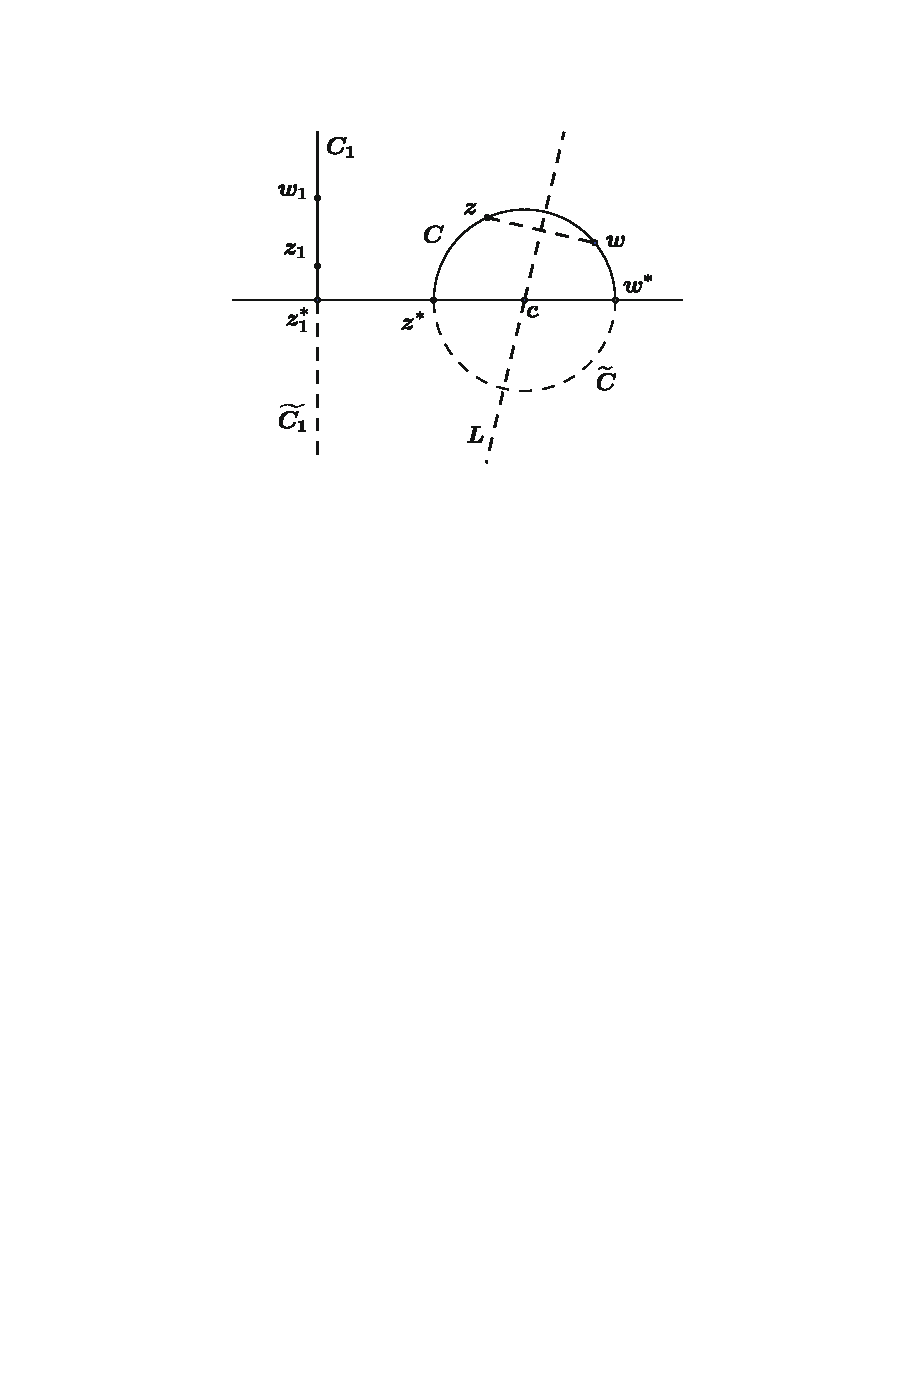
\includegraphics{pictures/upper-plane-conjugate}
\caption{Unique circles (in $\widehat{\C}$) perpendicular to $\R$ through two points in $\mathbb{U}$.}
\end{figure}
\begin{lemma}\label{upper plane change to same re}
Let $z$ and $w$ distinct points in $\mathbb{U}$. There exists a unique $T\in\Aut(\mathbb{U})$ such that $T(z^*)=0$, $T(z)=i$, $T(w)=iy$ with $y>1$, and $T^*(w)=\infty$.
\end{lemma}
\begin{proof}
Consider the unique circle $\widetilde{C}$ centered on the real axis and passing through $z$ and $w$. Since the M\"obius group is triply transitive, there exists a unique M\"obius transformation $T$ that maps $(z^*,w^*,z)$ to $(0,\infty,i)$, respectively. Since M\"obius transformations map circles to circles, $T$ maps $\widetilde{C}$ onto the imaginary axis union $\{\infty\}$, and hence $T(w)=iy$ for some real $y$. Since M\"obius transformations preserve orthogonality of curves, $T$ maps $\R\cup\{\infty\}$ onto itself. Since $T$ maps $z\in\mathbb{U}$ to $i\in\mathbb{U}$, $T$ is in $\Aut(\mathbb{U})$, and because it is orientation preserving, $y>1$.
\end{proof}
\begin{lemma}
If $z$ and $w$ are two distinct points in $\mathbb{U}$, then the hyperbolic length of the geodesic segment $\widetilde{\gamma}$ joining them is shorter than the hyperbolic length of any other piecewise differentiable curve in $\mathbb{U}$ joining them.
\end{lemma}
\begin{proof}
Write $z=x_z+iy_z$ and $w=x_w+iy_w$. First consider the case $x_z=x_w$. Assume the curve $\gamma$ is parameterized by the closed interval $[a,b]\sub\R$ and $\gamma(t)=x(t)+iy(t)$. Then $x$ and $y$ are differentiable functions except at finitely many points, and
\[L_{\mathbb{U}}(\gamma)=\int_{a}^{b}\frac{\sqrt{x'(t)^2+y'(t)^2}}{y(t)}\dif t\geq\int_{a}^{b}\frac{|y'(t)|}{y(t)}\dif t\geq\Big|\log\frac{y_w}{y_z}\Big|=L_{\mathbb{U}}(\widetilde{\gamma}).\]
Furthermore, equality of lengths is attained if and only if $x$ is constant and $y'$ does not change sign where it exists; that is, if and only if $\gamma$ is a reparametrization of $\widetilde{\gamma}$.\par
For the case $x_z\neq x_w$, by Lemma~\ref{upper plane change to same re} we can find a $T$ in $\Aut(\mathbb{U})$ such that $T(z^*)=0$ and $T(w^*)=\infty$. Furthermore, the image under $T$ of the geodesic segment between $z$ and $w$ is the segment on the imaginary axis between $T(z)$ and $T(w)$, and both segments have the same hyperbolic length. Similarly, $T\circ\gamma$ is a piecewise differentiable curve in $\mathbb{U}$ joining $T(z)$ and $T(w)$, with the same hyperbolic length as $\gamma$, and we are reduced to the previous case.
\end{proof}
\begin{theorem}
For any two distinct points $z$ and $w$ in $\mathbb{U}$, the geodesic segment joining $z$ to $w$ is the unique curve that achieves the infimum of $L_{\mathbb{U}}(\gamma)$.
\end{theorem}
Using cross ratios to simplify notation, a routine computation establishes the following result.
\begin{proposition}
For any two distinct points $z$ and $w$ in $\mathbb{U}$, the hyperbolic distance between $z$ and $w$ is equal to the length of the geodesic segment $\gamma$ joining $z$ and $w$, and is given by
\begin{equation}\label{upper plane distance-1}
\begin{aligned}
d_{\mathbb{U}}(z,w)=\log(z,w,w^*,z^*)=\log\frac{|z-\widebar{w}|+|z-w|}{|z-\widebar{w}|-|z-w|}=2\tanh^{-1}\Big(\frac{|z-w|}{|z-\widebar{w}|}\Big).
\end{aligned}
\end{equation}
\end{proposition}
\begin{proof}
We know that the M\"obius transform $T$ in Lemma~\ref{upper plane change to same re} preserve cross ratio, therefore
\[d_{\mathbb{U}}(z,w)=\log y=\log(i,iy,\infty,0)=\log(z,w,w^*,z^*).\]
To show that the cross ratio is given by $(\ref{upper plane distance-1})$, we note that if $\Re(z)=\Re(w)$, then $(\ref{upper plane distance-1})$ reduces to $|\log(y_z/y_w)|$, so in this case the claim is verified. Now we verify that $(\ref{upper plane distance-1})$ is invariant under M\"obious transformations. We only need to consider translation, homothety or inversion. The cases for homothety and translation are clear, and for inversion we have
\[\frac{|z^{-1}-\widebar{w^{-1}}|+|z^{-1}-w^{-1}|}{|z^{-1}-\widebar{w^{-1}}|-|z^{-1}-w^{-1}|}=\frac{\dfrac{|\widebar{w}-z|+|w-z|}{|w||z|}}{\dfrac{|\widebar{w}-z|-|w-z|}{|w||z|}}=\frac{|z-\widebar{w}|+|z-w|}{|z-\widebar{w}|-|z-w|}.\]
Since any pair of points can be send to the imaginary axis by a M\"obious transformation, this proves the claim.
\end{proof}
For interests, we give another formula for the hyperbolic distance of $\mathbb{U}$. This formula generalizes to higher dimensions.
\begin{proposition}
For any two distinct points $z=x_1+iy_1$ and $w=x_2+iy_2$ in $\mathbb{U}$, the hyperbolic distance between $z$ and $w$ is given by
\begin{align}\label{upper plane distance-2}
d_{\mathbb{U}}(z,w)=\cosh^{-1}\Big(1+\frac{(x_1-x_2)^2+(y_1-y_2)^2}{2y_1y_2}\Big).
\end{align}
\end{proposition}
\begin{proof}
Set $p=|z-w|$ and $q=|z-\widebar{w}|$, and let $d=d_{\mathbb{U}}(z,w)$. Then by $(\ref{upper plane distance-1})$ we have
\[\tanh\frac{d}{2}=\frac{p}{q}.\]
By the identity $\cosh^2-\sinh^2=1$, we have $1-\tanh^2=\cosh^{-2}$, therefore
\[\cosh^2\frac{d}{2}=\frac{1}{1-p^2/q^2}=\frac{q^2}{q^2-p^2}.\]
Now with the observation $\cosh(x)=2\cosh^2(x/2)-1$, we then conclude
\begin{align*}
\cosh d&=\frac{2q^2}{q^2-p^2}-1=\frac{q^2+p^2}{q^2-p^2}=\frac{(x_1-x_2)^2+(y_1+y_2)^2+(x_1-x_2)^2+(y_1-y_2)^2}{(x_1-x_2)^2+(y_1+y_2)^2-(x_1-x_2)^2-(y_1-y_2)^2}\\
&=\frac{2((x_1-x_2)^2+(y_1-y_2)^2)+4y_1y_2}{4y_1y_2}=1+\frac{(x_1-x_2)^2+(y_1-y_2)^2}{2y_1y_2}
\end{align*}
or
\[d=\cosh^{-1}\Big(1+\frac{(x_1-x_2)^2+(y_1-y_2)^2}{2y_1y_2}\Big).\]
This proves the claim.
\end{proof}
As mentioned at the end of the previous part, the set $\PSL_2(\R)$ of conformal automorphisms of $\mathbb{U}$ acts as a group of hyperbolic isometries of $\mathbb{U}$. This also follows from two facts: fractional linear transformations preserve the cross ratios and map circles to circles. We now proceed to establish the converse.
\begin{proposition}\label{upper plane isometry fix imaginary axis}
An orientation preserving isometry $f$ of $(\mathbb{U},d_{\mathbb{U}})$ that fixes the imaginary axis pointwise is the identity map.
\end{proposition}
\begin{proof}
Let $z=x+iy$ and $f=u+iv$. For all positive real numbers $t$ we have
\[d(z,it)=d(f(z),f(it))=d(u+iv,it)\]
We calculate using (8.10) that this is equivalent to
\[(x^2+(y-t)^2)(u^2+(v+t)^2)=(x^2+(y+t)^2)(u^2+(v-t)^2)\]
hence also equivalent to
\[(x^2+y^2)v-(u^2+v^2)y=(y-v)t^2\]
for all positive $t$. Since the LHS of the last equation is independent of $t$, the RHS must vanish identically. Hence $v(z)=y$, $u(z)^2=x^2$ and $f(z)=\pm x+iy$. Because $f$ is continuous, the same sign holds for all $z$; thus either $f(z)=z$ or $f(z)=-\widebar{z}$ for all $z$; since $f$ is orientation preserving, we conclude that $f$ is the identity map.
\end{proof}
\begin{theorem}
The set of orientation-preserving isometries of $\mathbb{U}$ with respect to the hyperbolic metric is precisely the set of fractional linear transformations mapping $\mathbb{U}$ to itself; that is, $\PSL_2(\R)$.
\end{theorem}
\begin{proof}
If $g$ is such an isometry of $\mathbb{U}$, it preserves geodesics. Thus there is a fractional linear transformation $f$ that preserves $\mathbb{U}$ and such that $f\circ g$ leaves invariant the imaginary axis. Following this map by an isometry of the form $z\mapsto kz$ with $k>0$ and then (if necessary) by $z\mapsto -z^{-1}$, we may assume that $f\circ g$ fixes $i$ and leaves invariant the intervals $(0,i)$ and $(i,\infty)$ on the imaginary axis. Then we see that $f\circ g$ is the identity on the imaginary axis and hence also on $\mathbb{U}$, by the previous proposition. We conclude that $g$ is a M\"obius transformation.
\end{proof}
\subsubsection{Unit disc model}
Statements about the hyperbolic metric on the upper half plane can be translated to the unit disc model, where the length differential is
\[\lambda_{\D}=\frac{2|\mathrm{d}z|}{1-|z|^2}.\]
We emphasize the following results.
\begin{proposition}
The geodesics in $\D$ are exactly the intersection of a circle with $\D$ whose center is on $\partial\D$.
\end{proposition}
\begin{proof}
The M\"obious transformation $w(z)=(z-i)/(z+i)$ maps the real axis to $\partial\D$, so the claim follows from that of $\mathbb{U}$.
\end{proof}
\begin{proposition}
The set of orientation-preserving isometries of $\D$ consists of the fractional linear transformations mapping $\D$ to itself, that is, $\Aut(\D)$.
\end{proposition}
\begin{proof}
This follows from the observation that if $f:\D\to\D$ is an orientation-preserving isometry, then $w^{-1}\circ f\circ w$ is an orientation-preserving isometry, where $w:\mathbb{U}\to\D$ is given in Corollary~\ref{conformal map from U to D eg}.
\end{proof}
\begin{proposition}
For all $z$ and $w$ in $\D$, the hyperbolic distance is given by
\begin{align}\label{unit disk hyperbolic distance-1}
d_{\D}(z,w)=2\tanh^{-1}\Big(\frac{|z-w|}{|1-\widebar{w}z|}\Big)=\log\frac{|1-\widebar{w}z|+|z-w|}{|1-\widebar{w}z|-|z-w|}.
\end{align}
In particular,
\begin{align}\label{unit disk hyperbolic distance-2}
d_{\D}(0,z)=2\tanh^{-1}(|z|)=\log\frac{1+|z|}{1-|z|}.
\end{align}
\end{proposition}
\begin{proof}
For any points $z_1,z_2\in\D$, we can choose an automorphism $\varphi_{z_1}$ such that $\varphi_{z_1}(z_1)=0$. Then
\[d_{\D}(z_1,z_2)=d_{\D}(0,f(z_2)).\]
Note that $\varphi_{z_1}$ is given by
\[\varphi_{z_1}(z)=\frac{z-z_1}{1-\widebar{z}_1z}.\]
Therefore we only need to check $(\ref{unit disk hyperbolic distance-2})$. We already pointed that the geodesic from $0$ to a point $z\in\D$ is a straight line in $\D$, so
\[d_{\D}(0,z)=\int_{0}^{|z|}\frac{2\dif r}{1-r^2}=\log\frac{1+|z|}{1-|z|}.\]
Thus the claim is proved.
\end{proof}
\subsubsection{Contractions and the Schwarz's lemma}
A deep connection between function theory and geometry is established through Schwarz's lemma. Recall that not every holomorphic self-map of $\D$ is a M\"obius transformation (for instance, $z\mapsto z^2$), only conformal automorphisms are, and, as we have seen, these are isometries in the hyperbolic metric. However, the following result holds.
\begin{theorem}\label{Schwarz lemma generalized}
Holomorphic self-maps of the unit disc do not increase distances with respect to the hyperbolic metric; that is, for all holomorphic self-maps $F$ of $\D$ and all $z$ and $w\in\D$,
\[d_{\D}(F(z),F(w))\leq d_{\D}(z,w)\]
and
\[\lambda_{\D}(F(z))|F'(z)|\leq\lambda_{\D}(z).\]
Furthermore, if for some distinct $z$ and $w$ in $\D$
\[d_{\D}(F(z),F(w))=d_{\D}(z,w)\]
or for some $z\in\D$,
\[\lambda_{\D}|F'(z)|=\lambda_{\D}(z)\]
then $F$ is a conformal self-map of $\D$.
\end{theorem}
\begin{proof}
The two inequalities certainly hold for constant maps $F$. So assume that $F:\D\to\D$ is holomorphic and nonconstant. Assume first that $F(0)=0$. By Schwarz's lemma we have
\[|f(w)|\leq|w|,\quad |f'(0)|\leq 1.\]
These are the Euclidean analogues of the two inequalities in the theorem for the points $z=0$ and arbitrary $w\in\D$. We intend to use equation $(\ref{unit disk hyperbolic distance-2})$ to translate these to the non-Euclidean setting. We start with
\begin{align*}
\frac{1+|F(w)|}{1-|F(w)|}=(1+|F(w)|)\sum_{n=0}^{\infty}|F(w)|^2\leq(1+|w|)\sum_{n=0}^{\infty}|w|^2=\frac{1+|w|}{1-|w|}
\end{align*}
and then apply $(\ref{unit disk hyperbolic distance-2})$ to obtain
\[d_{\D}(0,F(w))\leq d_{\D}(0,w).\]
Let $z_1$ and $z_2$ denote two different points in $\D$; choose conformal automorphisms $\varphi$ and $\psi$ of the unit disc such that $\psi(0)=z_1$ and $\varphi(F(z_1))=0$. Then $\varphi\circ F\circ\psi$ is a holomorphic self-map of the unit disc that fixes $0$. Hence, by what was already established,
\[d_{\D}((\varphi\circ F\circ\psi)(0),(\varphi\circ F\circ\psi)(z))\leq d_{\D}(0,z)\]
for all $z$ in $\D$. Since $\psi$ and $\varphi$ are isometries,
\[d_{\D}((\varphi\circ F\circ\psi)(0),(\varphi\circ F\circ\psi)(z))=d_{\D}((F\circ\psi)(0),(F\circ\psi)(z))\]
and
\[d_{\D}(0,z)=d_{\D}(\psi(0),\psi(z))=d_{\D}(z_1,\psi(z))\]
for all $z$ in $\D$, and we conclude that
\[d_{\D}(F(z_1),F(\psi(z)))\leq d_{\D}(z_1,\psi(z)).\]
Taking $\psi(z)=z_2$, we then get
\begin{align}\label{Schwarz lemma generalized-1}
d_{\D}(F(z_1),F(z_2))\leq d_{\D}(z_1,z_2).
\end{align}
If we multiply each side of the last equation by
\[\Big|\frac{1}{z_1-z_2}\Big|=\Big|\frac{1}{F(z_1)-F(z_2)}\cdot\frac{F(z_1)-F(z_2)}{z_1-z_2}\Big|\]
and take the limit as $z_1$ approaches $z_2$, we get the infinitesimal form of our required formula (the second inequality)
\begin{align}\label{Schwarz lemma generalized-2}
\lambda_{\D}(F(z_2))\leq|F'(z_2)|\lambda_{\D}(z_2).
\end{align}
If one of the equality in either $(\ref{Schwarz lemma generalized-1})$ or $(\ref{Schwarz lemma generalized-2})$ holds, then as in the proof of Schwarz lemma, we conclude that $\varphi\circ F\circ\psi$ is a rotation, so that $F$ is a conformal map.
\end{proof}
\begin{definition}
Let $X$ be a metric space with distance $d$. A self-map $f$ of $X$ is a \textbf{contraction} if $d(f(x),f(y))<d(x,y)$ for all $x$ and $y$ in $X$ with $x\neq y$.
\end{definition}
Theorem~\ref{Schwarz lemma generalized} can be restated as
\begin{theorem}
A holomorphic self-map of the unit disc is either an isometry or a contraction with respect to the hyperbolic metric.
\end{theorem}
\subsection{Finite Blaschke products}
For $a\in\D$, set
\[B_{a}(z)=-\frac{|a|}{a}\frac{z-a}{1-\widebar{a}z}\]
for $z\in\C$, with the understanding that $|a|/a=1$ if $a=0$.  Of course, $B_a$ is the Riemann map $f$ for $\D$ normalized (as before) by sending $a$ to $0$ but with (the change that) $\arg f'(0)=\pi-\arg a$; it is an automorphism of $\D$.\par
Let $A=\{a_0,a_1,\dots\}$ be a nonempty finite or countable sequence of complex numbers lying in the unit disc $\D$. Define
\[B(z)=B_A(z)=\prod_{i}B_{a_i}(z)\]
\begin{definition}
The function $B_A$ is the (finite or infinite) \textbf{Blaschke product} associated to $A$. In the infinite case there are, of course, convergence issues.
\end{definition}
For the rest we will study finite Blaschke products. It follows immediately from the definition that we have
\begin{proposition}
If $A=\{a_0,\dots,a_n\}$ is a nonempty finite sequence of points in $\D$, then
\begin{itemize}
\item[(a)] $B=B_A$ is a meromorphic function on $\widehat{\C}$, with zeros precisely at the $n+1$ points $\{a_i\}$ and poles at the $n+1$ points $\{1/\widebar{a}_i\}$.
\item[(b)] $B$ is a self-map of the closed unit disc, that maps the open unit disc holomorphically onto itself, and the unit circle onto itself, with $B(0)=\prod_i|a_i|$.
\end{itemize}
\end{proposition}
Blaschke products transform beautifully under automorphisms of $\D$, as shown next.
\begin{proposition}\label{Blaschke product compose auto of D}
Let $A=\{a_0,\dots,a_n\}$ be a nonempty finite sequence of points in $\D$, and let $T$ be any element of $\Aut(\D)$. Then
\[B_A\circ T=\lambda B_{T^{-1}(A)},\]
where $\lambda$ is a constant of absolute value $1$.
\end{proposition}
\begin{proof}
Since $T$ belongs to $\Aut(\D)$, there exist $\alpha\in\R$ and $a\in\D$ such that
\[T(z)=e^{i\alpha}\frac{z-a}{1-\widebar{a}z}\]
for all $z$ in $\D$. It suffices to compute the action of $T$ on the function $z\mapsto(z-c)/(1-\widebar{c}z)$, where $c\in\D$. A calculation shows that
\begin{align*}
\frac{T(z)-c}{1-\widebar{c}T(z)}&=\frac{e^{i\alpha}\frac{z-a}{1-\widebar{a}z}-c}{1-\widebar{c}e^{i\alpha}\frac{z-a}{1-\widebar{a}z}}=\frac{e^{i\alpha}(z-a)-c(1-\widebar{a}z)}{1-\widebar{a}z-\widebar{c}e^{i\alpha}(z-a)}=\frac{(\widebar{a}c+e^{i\alpha})z-(ae^{i\alpha}+c)}{(1+\widebar{c}e^{i\alpha}a)-(\widebar{a}+\widebar{c}e^{i\alpha}z)}\\
&=\frac{\widebar{a}c+e^{i\alpha}}{1+\widebar{c}e^{i\alpha}a}\cdot\frac{z-\frac{ae^{i\alpha}+c}{\widebar{a}c+e^{i\alpha}}}{1-\frac{\widebar{a}+\widebar{c}e^{i\alpha}}{1+\widebar{c}e^{i\alpha}a}z}=\frac{\widebar{a}c+e^{i\alpha}}{e^{i\alpha}(a\widebar{c}+e^{-i\alpha})}\cdot\frac{z-\frac{ae^{i\alpha}+c}{\widebar{a}c+e^{i\alpha}}}{1-\frac{\widebar{a}e^{-i\alpha}+\widebar{c}}{a\widebar{c}+e^{-i\alpha}}z}\\
&=\frac{\widebar{a}c+e^{i\alpha}}{e^{i\alpha}\widebar{(\widebar{a}c+e^{i\alpha})}}\cdot\frac{z-\frac{ae^{i\alpha}+c}{\widebar{a}c+e^{i\alpha}}}{1-\widebar{\Big(\frac{ae^{i\alpha}+c}{\widebar{a}c+e^{i\alpha}}\Big)}z}=\frac{\widebar{a}c+e^{i\alpha}}{e^{i\alpha}\widebar{(\widebar{a}c+e^{i\alpha})}}\cdot\frac{z-T^{-1}(c)}{1-\widebar{T^{-1}(c)}z}.
\end{align*}
The proof is completed by observing that $|(\widebar{a}c+e^{i\alpha})/(e^{i\alpha}\widebar{(\widebar{a}c+e^{i\alpha})})|=1$ and that
\[T^{-1}(w)=\frac{ae^{i\alpha}+w}{w\widebar{a}+e^{i\alpha}}.\]
Thus the claim follows.
\end{proof}
\begin{theorem}\label{Blaschke product prop}
Let $f$ be a holomorphic self-map of the open unit disc $\D$, $A=\{a_0,a_1,\dots,a_n\}$ a nonempty finite collection of points in $\D$ and $B=B_A$. Assume that $f(a_i)=0$ for each $a_i$ in $A$, with multiplicities; that is, $\nu_{a_i}(f)\geq\nu_{a_i}(B)$ for all $i$. Then
\begin{itemize}
\item[(a)] $|f(z)|\leq|B(z)|$ for all $z\in\D$, and $|f'(a_i)|\leq|B'(a_i)|$ for all $i=1,\dots,n$.
\item[(b)] If $|f(a)|=|B(a)|$ for some $a\in\D$ with $a\neq a_i$ for all $i$, then there is $\alpha\in\R$ such that $f(z)=e^{i\alpha}B(z)$.
\item[(c)] If $a_i$ appears $\nu$ times in the sequence $A$ and if
\[0=f(a_i)=\cdots=f^{(\nu-1)}(a_i)\quad\text{and}\quad|f^{(\nu)}(a_i)|=|B^{(\nu)}(a_i)|\]
then there exists $\alpha\in\R$ such that $f(z)=e^{i\alpha}B(z)$.
\end{itemize}
\end{theorem}
\begin{proof}
Consider the function
\[F(z)=\frac{f(z)}{B(z)}\]
on $\D$. Since $\nu_{a_i}(f)\geq\nu_{a_i}(B)$, the points $a_i$ in $A$ are all removable singularities of $F$, and we can extend $F$ to a holomorphic function on $\D$, which is still denoted by $F$. In view of the definition of $F(z)$, it suffices to show that $|F(z)|\leq 1$ for $z\in\D$. Fix such a point $z$. The restrictions of $|B|$ to circles of radius $r$, with $0\leq r\leq 1$, yield a family of functions that uniformly approach the constant function $1$ as $r$ approaches $1$. Hence, for all $\eps>0$, we can choose an $r$ such that $|B(w)|\geq 1-\eps$ for $|w|=r$. Without loss of generality we may assume that $r\geq|z|$. Hence, by the maximum principle for $|w|\leq r$, it follows that
\[|F(w)|=\frac{|f(w)|}{|B(w)|}\leq\frac{1}{(1-\eps)}.\]
Since $\eps$ is arbitrary and the inequality holds for all $|z|\leq r<1$, the claim is proved.\par
To prove (b) and (c), we first note that the function $F(z)=f(z)/B(z)$ is holomorphic on $\D$ with modulus as most $1$, and the value of $F$ on $A$ is obtained by defining
\[F(a_i):=\lim_{z\to a_i}\frac{f(z)}{B(z)}=\frac{f^{(\nu_i)}(a_i)}{B^{(\nu_i)}(a_i)}.\]
where $\nu_i=\nu_{a_i}(B)$. Thus if $|f(a)|/|B(a)|=1$ for some $a\in\D\setminus A$ or $|f^{(\nu_i)}(a_i)|=|B^{(\nu_i)}(a_i)|$, then the modulus of $f/B$ obtain its maximum in $\D$, and by maximal modulus principle $F$ is constant.
\end{proof}
The particular case when $A$ consists of one point leads to the following interesting result, a generalization of Schwarz's lemma.
\begin{corollary}[\textbf{Schwarz-Pick Lemma}]
Let $f$ be a holomorphic self-map of the open unit disc $\D$. If $a\in\D$, then for any $z\in\D$
\[\frac{f(z)-f(a)}{1-\widebar{f(a)}f(z)}\leq\frac{|z-a|}{|1-\widebar{a}z|}\quad\text{and}\quad|f'(a)|\leq\frac{1-|f(a)|^2}{1-|a|^2}.\]
Furthermore, equality for one $z\neq a$ in the first inequality or equality in the second inequality implies that $f$ is an automorphism of $\D$.
\end{corollary}
\begin{proof}
Apply the previous theorem to the function $B_{f(a)}\circ f$.
\end{proof}
This corollary may also be deduced by applying Schwarz's lemma to the function $B_{f(a)}\circ f\circ B_a^{-1}$ or, more interesting, is equivalent to Theorem~\ref{Schwarz lemma generalized}.
\section{Harmonic functions}
\subsection{Harmonic functions and the Laplacian}
We begin with the Laplace operator.
\begin{definition}
Let $D$ be a domain in $\C$ and $g\in C^2(D)$. We define $\Delta g$, the \textbf{Laplacian} of $g$, by
\[\Delta g=\frac{\partial^2g}{\partial x^2}+\frac{\partial^2g}{\partial y^2}.\]
The operator $\Delta$ is also called the \textbf{Laplacian} or the \textbf{Laplace operator}. If $D$ is a domain in $\C$ and $g\in C^2(D)$, we say that $g$ is harmonic in $D$ if it satisfies \textbf{Laplace's equation} $\Delta g=0$ in $D$.
\end{definition}
The last two definitions have a number of immediate consequences:
\begin{itemize}
\item It is obvious from the definition of the Laplacian as a linear operator on $C^2$ complex-valued functions that it preserves real-valued functions. It is useful to have equivalent formulae for it
\begin{align}\label{Laplacian in complex coordinate}
\Delta=\frac{\partial^2}{\partial x^2}+\frac{\partial^2}{\partial y^2}=4\frac{\partial^2}{\partial z\partial\widebar{z}}=4\frac{\partial^2}{\partial\widebar{z}\partial z}
\end{align}
and in polar coordinates
\begin{align}\label{Laplacian in polar coordinate}
\Delta=\frac{1}{r}\frac{\partial}{\partial r}\Big(r\frac{\partial}{\partial r}\Big)+\frac{1}{r}\frac{\partial}{\partial\theta}\Big(\frac{1}{r}\frac{\partial}{\partial\theta}\Big)=\frac{1}{r}\frac{\partial^2}{\partial r^2}+\frac{1}{r}\frac{\partial}{\partial r}+\frac{1}{r^2}\frac{\partial^2}{\partial\theta}.
\end{align}
\item Recall that for $f\in C^1(D)$, $f$ is holomorphic on $D$ if and only if $\partial f/\partial\widebar{z}=0$ in $D$. Thus, for $g\in C^2(D)$, $g$ is harmonic if and only if $\partial g/\partial z$ is holomorphic. In particular, holomorphic functions are harmonic and this gives an easy way to construct analytic functions from harmonic ones.
\item $f$ is harmonic if and only if $\widebar{f}$ is. In fact, we have
\[\Delta\widebar{f}=\widebar{\Delta f}.\]
\item $f$ is harmonic if and only if $\Re(f)$ and $\Im(f)$ are. This follows from the linearity of $\Delta$.
\item If $f$ is holomorphic on an open set $D$, then $f$, $\Re(f)$, $\Im(f)$, and $f$ are harmonic on $D$.
\item If $f$ is holomorphic or anti-holomorphic on $D$ and $g$ is harmonic on $f(D)$, then $g\circ f$ is harmonic on $D$. This follows from the chain rule: Assume that $f$ is holomorphic, and let $w=g(z)$, then
\[(g\circ f)_{z}=g_wf_z+g_{\widebar{w}}\widebar{f}_z=g_wf_z\]
and
\[(g\circ f)_{z\widebar{z}}=(g_wf_z)_{\widebar{z}}=g_{ww}f_{\widebar{z}}f_{z}+g_{w\widebar{w}}\widebar{f}_{\widebar{z}}f_z+g_{w}f_{z\widebar{z}}=0.\]
The argument in the anti-holomorphic case is similar.
\item If $f\in C^2(D)$ and $f$ is locally on $D$ the real part of an analytic function, then $f$ is harmonic on $D$.
\end{itemize}
\begin{example}
The function $\log|z|$ is harmonic on $D=\C^*$, since it belongs to $C^2(D)$, and it is locally the real part of $\log z$, a multi-valued but holomorphic function in $D$.
\end{example}
\begin{proposition}\label{harmonic function is real part}
If $g$ is real-valued and harmonic in $D$, then it is locally the real part of an analytic function. The analytic function is unique up to an additive constant.
\end{proposition}
\begin{proof}
Let $\Omega\sub D$ be a simply connected region. Since $g$ is harmonic in $\Omega$, it follows that $2g_{z}dz$ is closed on $\Omega$, and hence an exact form on $\Omega$. Choose a holomorphic function $f$ on $\Omega$ with $df=2g_z\dif z$. Then
\[d\widebar{f}=2g_{\widebar{z}}\dif\widebar{z}\]
and hence
\[\frac{1}{2}d(f+\widebar{f})=g.\]
This means $g=\Re(f)+\text{constant}$ on $\Omega$.
\end{proof}
\begin{corollary}
A real-valued harmonic function on a simply connected domain is
the real part of a holomorphic function on the same domain.
\end{corollary}
\begin{corollary}
A harmonic function is $C^\infty$.
\end{corollary}
\begin{corollary}
Harmonic functions have the MVP, and hence they satisfy the maximum modulus principle. Real-valued harmonic functions also satisfy the maximum and minimum principles.
\end{corollary}
\begin{remark}
The maximum (minimum) principle asserts that if $f$ is real-valued and harmonic on a domain $D$ and if $f$ has a relative maximum (minimum) at a point $z_0\in D$, then $f$ is constant in a neighborhood of $z_0$. Furthermore, if $D$ is bounded and if $f$ is also continuous on the closure of $D$, with $m\leq f\leq M$ on $\partial D$ for some real constants $m$ and $M$, then $m\leq f\leq M$ on $D$.
\end{remark}
\subsection{Integral representation of harmonic functions}
We apply the Cauchy theory towards our present main goal, which is to solve a boundary value problem. Given a harmonic function defined in a disc, we derive an integral formula for it, known as the Poisson formula; a major tool in the solution of our boundary value problem.
\begin{proposition}[\textbf{The Poisson Formula}]
If $g$ is a harmonic function on the domain $|z|<\rho$ for some $\rho>0$, then, for each $0<r<\rho$,
\begin{align}\label{Possion formula}
g(z)=\frac{1}{2\pi i}\int_{0}^{2\pi}g(re^{i\theta})\cdot\frac{r^2-|z|^2}{|re^{i\theta}-z|^2}\dif\theta\quad\text{for }|z|<r.
\end{align}
\end{proposition}
\begin{proof}
It suffices to assume that $g$ is real-valued. To establish this formula we can thus apply Proposition~\ref{harmonic function is real part} and choose the holomorphic function $f$ on this domain with $\Re(f)=g$ and $g(0)=f(0)$, noting that there is a unique such $f$.\par
Since $f$ is holomorphic in the disk $|z|<\rho$, it has a power series expansion $f(z)=\sum_{n=0}^{\infty}a_nz^n$, and therefore
\[g(z)=\frac{f(z)+\widebar{f(z)}}{2}=\frac{1}{2}\sum_{n=0}^{\infty}(a_nz^n+\widebar{a}_n\widebar{z}^n).\]
Now we determine the coefficients $a_n$. Set $z=re^{i\theta}$ in the above expression, we get
\[g(re^{i\theta})=a_0+\frac{1}{2}\sum_{n=1}^{\infty}r^n(a_ne^{in\theta}+\widebar{a}_ne^{-in\theta}).\]
Multiplying by $e^{-in\theta}$ and integrating along the curve $|z|=r$ yields
\[a_0=\frac{1}{2\pi}\int_{0}^{2\pi}g(re^{i\theta})\dif\theta,\quad a_n=\frac{1}{\pi}\int_{0}^{2\pi}\frac{g(re^{i\theta})}{(re^{i\theta})^n}\dif\theta.\]
Thus, for $|z|<r$, we obtain that
\begin{align*}
f(z)&=\frac{1}{2\pi}\int_{0}^{2\pi}g(re^{i\theta})\Big[1+2\sum_{n=1}^{\infty}\Big(\frac{w}{re^{i\theta}}\Big)^n\Big]\dif\theta=\frac{1}{2\pi}\int_{0}^{2\pi}g(re^{i\theta})\Big[1+2\sum_{n=1}^{\infty}\Big(\frac{z}{re^{i\theta}}\Big)^n\Big]\dif\theta\\
&=\frac{1}{2\pi}\int_{0}^{2\pi}g(re^{i\theta})\frac{re^{i\theta}+z}{re^{i\theta}-z}\dif\theta.
\end{align*}
The last formula gives a representation of a holomorphic function $f$ in terms of its real part $g$, when the function $f$ is real at $0$. Taking the real part of both sides we obtain equation $(\ref{Possion formula})$, the Poisson formula.
\end{proof}
The function
\[\Re\Big(\frac{re^{i\theta}-z}{re^{i\theta}+z}\Big)=\frac{r^2-|z|^2}{|re^{i\theta}-z|^2}\]
is known as the \textbf{Poisson kernel}.\par
The original derivation of formula $(\ref{Possion formula})$ assumed that $g$ was harmonic in the closed disc $\{z:|z|\leq r\}$. However, the result remains true for $|z|<r$ under the weaker assumption that $g$ is harmonic in the open disc $|z|<r$ and continuous on its closure. In this case, fix $t$ with $0<t<1$ and look at the function of $z$ given by $g(tz)$. It is harmonic on the closed disc $\{z:|z|\leq r\}$ and hence, by the already proven formula $(\ref{Possion formula})$,
\[g(tz)=\frac{1}{2\pi}\int_{0}^{2\pi}g(rte^{i\theta})\frac{r^2-|z|^2}{|rte^{i\theta}-z|^2}\dif\theta.\]
Since the function $g$ is uniformly continuous on the closed disc, we know that $g(tz)$ approaches $g(z)$ uniformly on the circle $\{z:|z|=r\}$ as $t$ approaches $1$. Hence both sides of the last equation converge to the expected quantities.\par
As a special case we apply the Poisson formula to the function $g$ which is identically $1$ and obtain
\[\frac{1}{2\pi}\int_{0}^{2\pi}\frac{r^2-|z|^2}{|re^{i\theta}-z|^2}\dif\theta=1.\]
\begin{definition}
A harmonic conjugate of a real-valued harmonic function $u$ is any real-valued function $v$ such that $u+iv$ is holomorphic.
\end{definition}
Harmonic conjugates always exist locally, and globally on simply connected domains. They are unique up to additive real constants. In fact, it is easy to see that they are given locally as follows.
\begin{proposition}
If $g$ is harmonic and real-valued in $|z|<\rho$ for some $\rho>0$, then the harmonic conjugate of $g$ vanishing at the origin is given by
\[\frac{1}{2\pi i}\int_{0}^{2\pi}g(re^{i\theta})\frac{re^{-i\theta}z-re^{i\theta}\widebar{z}}{|re^{i\theta}-z|^2}\dif\theta\]
for $0<r<\rho$.
\end{proposition}
The following result is interesting and useful.
\begin{theorem}[\textbf{Harnack's Inequalities}]
If $g$ is a positive harmonic function on $|z|<r$ that is continuous on $|z|<r$, then
\[\frac{r-|z|}{r+|z|}\cdot g(0)\leq g(z)\leq\frac{r+|z|}{r-|z|}\cdot g(0)\quad\text{for all $|z|<r$}.\]
\end{theorem}
\begin{proof}
Our starting point is $(\ref{Possion formula})$. We use elementary estimates for the Poisson kernel:
\[\frac{r-|z|}{r+|z|}=\frac{r^2-|z|^2}{(r+|z|)^2}\leq\frac{r^2-|z|^2}{|re^{i\theta}-z|^2}\leq\frac{r^2-|z|^2}{(r-|z|)^2}=\frac{r+|z|}{r-|z|}.\]
Multiplying these inequalities by the positive number $g(w)=g(re^{i\theta})$ and then averaging the resulting function over the circle $|w|=r$, we obtain
\begin{align*}
\frac{r-|z|}{r+|z|}\cdot\frac{1}{2\pi}\int_{0}^{2\pi}g(re^{i\theta})\dif\theta\leq\frac{1}{2\pi}\int_{0}^{2\pi}g(re^{i\theta})\frac{r^2-|z|^2}{|re^{i\theta}-z|^2}\dif\theta\leq\frac{r+|z|}{r-|z|}\cdot\frac{1}{2\pi}\int_{0}^{2\pi}g(re^{i\theta})\dif\theta.
\end{align*}
The middle term in the above inequalities is $g(z)$ as a consequence of $(\ref{Possion formula})$, while the extreme averages are equal to $g(0)$ by the MVP.
\end{proof}
\begin{corollary}\label{Harnack's Inequality compact set}
Let $K$ be a compact subset of a domain $D\sub\C$, and let $u$ be a positive harmonic function on $D$. Then there exists a constant $C>1$ that depends only on $K$ and $D$, but not on $u$, such that
\[C^{-1}\leq\frac{u(z_1)}{u(z_2)}\leq C\]
for all $z_1,z_2\in K$.
\end{corollary}
\begin{proof}
Since $u$ is positive, by Harnack's Inequality we have
\[\frac{(r-|z_1|)(r-|z_2|)}{(r+|z_1|)(r+|z_2|)}\leq\frac{u(z_1)}{u(z_2)}\leq\frac{(r+|z_1|)(r+|z_2|)}{(r+|z_1|)(r+|z_2|)}\]
for $z_1,z_2\in K\cap B_{r}(z_0)$, where $z_0$ is a fixed point in $K$. Since $K$ is compact, there exist a $\delta>0$ such that $B_{\delta}(z_0)\sub D$ for any $z_0\in K$. Then it is easy to see the claim.
\end{proof}
\begin{theorem}[\textbf{Harnack's Convergence Theorem}]
Let $D$ be a domain and let $\{u_n\}$ be a nondecreasing sequence of real-valued harmonic functions on $D$. Then
\begin{itemize}
\item[(a)] Either $\lim_nu_n(z)=+\infty$ for all $z\in D$, or
\item[(b)] The function on $D$ defined by $u(z)=\lim_nu_n(z)$ is harmonic in $D$.
\end{itemize}
\end{theorem}
\begin{proof}
Since a nondecreasing sequence of real numbers converges if and only if it is bounded, the assumption that $\lim_nu_n(z)$ is not $+\infty$ for all $z\in D$ allows us to conclude that there exist $z_0$ in $D$ and a real number $M$ such that $u(z_0)\leq M$ for all $n$. Then $\lim_nu_n(z_0)$ exists, and it equals the value of the series
\[u_1(z_0)+\sum_{n=1}^{\infty}[u_{n+1}(z_0)-u_n(z_0)].\]
which is therefore convergent.\par
Let $K$ denote a compact subset of $D$. By enlarging $K$ if necessary, we may assume that $z_0\in K$. It follows from Corollary~\ref{Harnack's Inequality compact set} that there exists a real constant $C$ such that
\[0\leq u_{n+1}(z)-u_n(z)\leq C[u_{n+1}(z)-u_n(z)]\]
for all $z$ in $K$ and all $n>0$. It follows immediately that the series $u_1(z)+\sum_{n}[u_{n+1}(z)-u_n(z)]$ converges uniformly on $K$; that is, $u_n$ converges uniformly to a function $u$ on compact subsets of $D$. It is noweasy to showthat $u$ is harmonic in $D$.
\end{proof}
\subsection{The Dirichlet problem}
Let $D$ be a bounded region in $\C$ and let $f\in C(\partial D)$. The Dirichlet problem is to find a continuous function $u$ defined on the closure of $D$ that agrees with $f$ on the boundary of $D$ and whose restriction to $D$ is harmonic. We will consider, for the moment, only the special case where $D$ is a disc; without loss of generality we may assume that the disc has radius one and center at zero.\par
For a piecewise continuous function $u$ on $S^1$ and $z\in\C$ with $|z|<1$, we define (compare with $(\ref{Possion formula})$)
\[P[u](z)=\frac{1}{2\pi}\int_{0}^{2\pi}u(e^{i\theta})\frac{1-|z|^2}{|e^{i\theta}-z|^2}\dif\theta.\]
The following properties of the operator $P$ are easily established.
\begin{itemize}
\item[(a)] $P[u]$ is a well-defined function on the open unit disc. Hence we view $P$ as an operator that assigns the function $P[u]$, on the open unit disc to each piecewise continuous function $u$ on the unit circle.
\item[(b)] $P[u+v]=P[u]+P[v]$ and $P[cU]=cP[u]$ for all piecewise continuous functions $u$ and $v$ on $S^1$ and every constant $c$.
\item[(c)] If $u$ is a real nonnegative piecewise continuous function on $S^1$, then $P[u]$ is a real-valued nonnegative function on the open unit disc.
\item[(d)] $P[u]$ is harmonic in the open unit disc.
\item[(e)] Any bound on $u$ yields the same bound on $P[u]$. For example, for real-valued function $u$ satisfying $m\leq u\leq M$ for some real constants $m$ and $M$, we have $m\leq P[u]\leq M$.
\end{itemize}
We now establish the solvability of the Dirichlet problem for discs.
\begin{theorem}[\textbf{H. A. Schwarz}]
If $u$ is a piecewise continuous function on the unit circle $S^1$, then the function $P[u]$ is harmonic on the unit disk; furthermore, for $\theta\in\R$, its limit as $z$ approaches $e^{i\theta}$ is $u(e^{i\theta})$ provided $u$ is continuous at $e^{i\theta}$. In particular, the Dirichlet problem is solvable for discs.
\end{theorem}
\begin{proof}
We only have to study the boundary values for $P[u]$. Let $C_1$ and $C_2$ be complementary arcs on the unit circle. Let $u_1$ be the function which coincides with $u$ on $C_1$ and vanishes on $C_2$; let $u_2$ be the corresponding function for $C_2$. Clearly $P[u]=P[u_1]+P[u_2]$. The function $P[u_1]$ can be regarded as an integral over the arc $C_1$; hence it is harmonic on $\C\setminus C_1$. The expression
\[\Re\Big(\frac{e^{i\theta}+z}{e^{i\theta}-z}\Big)=\frac{1-|z|^2}{|e^{i\theta}-z|^2}.\]
vanishes on $|z|=1$ for $z\neq e^{i\theta}$. It follows that $P[u_1]$ is zero on the one-dimensional interior of the arc $C_2$. By continuity $P[u_1]$ approaches zero as $z$ approaches a point in the interior of $C_2$.\par
In proving that $P[u]$ has limit $u(e^{i\theta_0})$ at $e^{i\theta_0}$, we may assume that $u(e^{i\theta_0})=0$. Under this assumption, given an $\eps>0$, we can find complementary arcs $C_1$ and $C_2$ on the unit circle such that $e^{i\theta}$ is an interior point of $C_2$ and $|u(e^{i\theta})|\leq\eps/2$ for $e^{i\theta}\in C_2$. This last condition implies that $|u_2(e^{i\theta})|<\eps/2$ for all $e^{i\theta}$, and hence $|P[u_2](z)|\leq\eps/2$ for all $|z|<1$.\par
But we also have that $u_1$ is continuous and vanishes at $e^{i\theta_0}$. Since $P[u_1]$ is continuous at $e^{i\theta_0}$ and agrees with $u_1$ there, there exists a $\delta>0$ such that $|P[u_1](z)|<\eps/2$ for $|z-e^{i\theta_0}|<\delta$. It follows that
\[|P[u](z)|\leq|P[u_1](z)|+|P[u_2](z)|<\eps.\]
as long as $|z|<1$ and $|z-e^{i\theta_0}|<\delta$. This is the required continuity statement.
\end{proof}
As an application, we use the solution of Dirichlet problem to prove the characterization of harmonic functions.
\begin{theorem}
A continuous complex-valued function that satisfies the MVP is harmonic.
\end{theorem}
\begin{proof}
Let $f$ be a continuous function on a domain $D$, let $z_0\in D$ and let $r_0>0$ be sufficiently small so that $\widebar{B_{r_0}(z_0)}\sub D$ and $f$ satisfies MVP for all $r<r_0$. It suffices to assume that $f$ is real-valued. Let $v$ be the continuous function on $\widebar{B_{r_0}(z_0)}$ that is harmonic on $B_{r_0}(z_0)$ and agrees with $f$ on $\partial B_{r_0}(z_0)$. Then $f-v$ has the MVP in $B_{r_0}(z_0)$, and thus attains its maximum and minimum on $\partial B_{r_0}(z_0)$. Since $f-v=0$ on $\partial B_{r_0}(z_0)$, we conclude that $f\equiv v$ on $B_{r_0}(z_0)$ and thus that $f$ is harmonic there.
\end{proof}
\subsubsection{Fourier series interpretation of the Poisson formula}
We again consider the case of the unit disc and proceed to compute the power series expansion of $P[u](z)$ at the origin. Noting that
\[P[u](z)=\frac{1}{2\pi}\int_{0}^{2\pi}\frac{1-z\widebar{z}}{(e^{i\theta}-z)(e^{-i\theta}-\widebar{z})}\dif\theta.\]
We start with an expansion of the Poisson kernel
\begin{align*}
\frac{1-z\widebar{z}}{(e^{i\theta}-z)(e^{-i\theta}-\widebar{z})}&=\frac{1-z\widebar{z}}{(1-e^{-i\theta}z)(1-e^{i\theta}\widebar{z})}=(1-z\widebar{z})\sum_{n,m=0}^{\infty}e^{-in\theta}z^n\cdot e^{im\theta}\widebar{z}^m\\
&=(1-z\widebar{z})\sum_{n,m=0}^{\infty}e^{i(m-n)\theta}z^n\widebar{z}^m\\
&=\sum_{n,m=0}^{\infty}e^{i(m-n)\theta}z^n\widebar{z}^m-\sum_{n,m=1}^{\infty}e^{i(m-n)\theta}z^n\widebar{z}^m\\
&=1+\sum_{n=1}^{\infty}e^{in\theta}z^n+\sum_{m=1}^{\infty}e^{-im\theta}\widebar{z}^m.
\end{align*}
and since the last two series converge uniformly and absolutely on all compact subsets of the unit disc, we conclude
\begin{align}\label{Possion formula fourier interpretation}
P[u](z)=a_0+\sum_{n=1}^{\infty}a_nz^n+\sum_{m=1}^{\infty}b_m\widebar{z}^m.
\end{align}
where, for $n>0$ and $m>0$,
\[a_n=\frac{1}{2\pi}\int_{0}^{2\pi}u(e^{i\theta})e^{-in\theta}d\dif\theta,\quad b_m=\frac{1}{2\pi}\int_{0}^{2\pi}u(e^{i\theta})e^{in\theta}\dif\theta.\]
We thus have the following procedure for extending a given continuous function $u$ on the unit circle to a continuous function on the closed unit disc that is harmonic on the interior of the disc. First compute the Fourier series of $u$:
\[u(e^{i\theta})=a_0+\sum_{n=1}^{\infty}a_ne^{in\theta}+\sum_{m=1}^{\infty}b_me^{-im\theta}.\]
In this series replace $e^{in\theta}$ by $z^n$ and $e^{-im\theta}$ by $\widebar{z}^m$.
\subsubsection{Classical reformulation of the Poisson formula}
For the next reformulation, we start with
\begin{definition}
If $\omega=P\dif x+Q\dif y$ is a differential form, we define $^{\ast}\omega$, the \textbf{conjugate differential} of $\omega$, by
\[^{\ast}\omega=-Q\dif x+P\dif y.\]
\end{definition}
It turns out that the conjugate differential has intense connection with conjugate harmonic functions.
\begin{proposition}\label{conjugate differential is harmonic conjugate}
Suppose that $D$ is a simply connected domain and $u\in C^2(D)$ is real-valued. If $u$ is harmonic and $v$ is harmonic conjugate of $u$, then
\[^{\ast}du=dv.\]
In particular, the conjugate differential $^{\ast}du$ is exact.
\end{proposition}
\begin{proof}
We know that $u$ is harmonic on $D$ if and only if $u$ is the real part of an analytic function $f$ on $D$. In this case,
\begin{align*}
df&=f'(z)\dif z=(u_x-iu_y)(\dif x+i\dif y)\\
&=(u_x\dif x+u_y\dif y)+i(-u_y\dif x+u_x\dif y)\\
&=du+i\,{^{\ast}du}.
\end{align*}
Thus the claim follows.
\end{proof}
In what follows we work with cycles rather than curves. In the general case, for a harmonic function $u$ on an arbitrary domain $D$, the form $du=u_x\dif x+u_y\dif y$ is clearly exact on $D$, and its conjugate differential $^{\ast}du=-u_y\dif x+u_x\dif y$ is closed since $u_{xx}+u_{yy}=0$. We conclude that
\begin{align}\label{integral of conjugate form}
\int_{\gamma}{^{\ast}du}=0
\end{align}
for all harmonic functions $u$ on $D$ and all cycles $\gamma$ in $D$ that are homologous to zero on that domain.\par
Assume that $\gamma$ is a regular curve with equation $z=z(t)$. The direction of the tangent line to the curve at $z(t)$ is determined by the angle $\alpha=\arg z'(t)$ and
\[\dif x=|\mathrm{d}z|\cos\alpha,\quad \dif y=|\mathrm{d}z|\sin\alpha.\]
The normal line at $z(t)$, which points to the right of the tangent line, has direction $\beta=\alpha-\pi/2$. The \textbf{normal derivative} of $u$ is the directional derivative of $u$ in the direction $\beta$:
\[\frac{\partial u}{\partial n}=u_x\cos\beta+u_y\sin\beta=u_x\sin\alpha-u_y\cos\alpha.\]
Thus we see that $^{\ast}du=(\partial u/\partial n)|\mathrm{d}z|$, and $(\ref{integral of conjugate form})$ can be rewritten as
\[\int_{\gamma}\frac{\partial u}{\partial n}|\mathrm{d}z|=0.\]
It is important to realize that if $\gamma$ is the circle $|z|=r$, then $\partial u/\partial n=\partial u/\partial r$.
\begin{theorem}
If $u_1$ and $u_2$ are harmonic functions on $D$, then
\[u_1{^{\ast}du_2}-u_2{^{\ast}du_1}\]
is a closed form on $D$.
\end{theorem}
\begin{proof}
To establish this assertion, it involves no loss of generality to assume that the functions are real-valued, and hence we may also assume (because the issue is local) that each function $u_i$ has a single-valued harmonic conjugate $v_i$; then by Proposition~\ref{conjugate differential is harmonic conjugate},
\[u_1{^{\ast}du_2}-u_2{^{\ast}du_1}=u_1\dif v_2-u_2\dif v_1=u_1\dif v_2+v_1\dif u_2-d(u_2v_1).\]
The last expression $d(u_2v_1)$ is, of course, exact, and
\[u_1\dif v_2+v_1\dif u_2=\Im((u_1+iv_1)(\dif u_2+i\dif v_2)).\]
Now $u_1+iv_1$ is an analytic function and $\dif u_2+i\dif v_2$ is the total differential of the analytic function $u_2+iv_2$. By Cauchy's theorem, their product is a closed form.
\end{proof}
\begin{corollary}
If $u_1$ and $u_2$ are harmonic functions on $D$, then
\[\int_{\gamma}u_1{^{\ast}du_2}-u_2{^{\ast}du_1}=0.\]
for all cycles $\gamma$ which are homologous to zero in $D$. In classical language the above formula reads
\[\int_{\gamma}\Big(u_1\frac{\partial u_2}{\partial n}-u_2\frac{\partial u_1}{\partial n}\Big)|\mathrm{d}z|=0.\]
\end{corollary}
Let us take for $D$ the annulus $\{z:R_1<|z|<R_2\}$ and apply the above formula to the functions $u_1=\log|z|$ and an arbitrary harmonic function $u_2=u$ on $D$. We take for $\gamma$ the cycle $C_1-C_2$ where $C_i$ is the circle $\{z:|z|=r_i\}$ oriented counter clockwise; where $R_1<r_1<r_2<R_2$. On any circle $\{z:|z|=r\}$ with $R_1<r<R_2$, we have
\[^{\ast}\dif u=\frac{\partial u}{\partial r}|\mathrm{d}z|=r\cdot\frac{\partial u}{\partial r}\dif\theta.\]
Hence we also see that
\[\log r_1\int_{C_1}r_1\cdot\frac{\partial u}{\partial r}\dif\theta-\int_{C_1}u\dif\theta=\log r_2\int_{C_2}r_2\cdot\frac{\partial u}{\partial r}\dif\theta-\int_{C_2}u\dif\theta\]
or
\[\log r\int_{|z|=r}r\cdot\frac{\partial u}{\partial r}\dif\theta-\int_{|z|=r}u\dif\theta\]
is a constant (independent of $r$).\par
Applying the same argument to the functions $u_1=1$ (constant function) and $u_2=u$, we obtain that
\[\int_{|z|=r}r\cdot\frac{\partial u}{\partial r}\dif\theta=A\]
is constant over the annulus $D$, and hence is equal to zero (let $r\to 0$) if $u$ is harmonic in the disc $\{z:0<|z|<R\}$. Thus, for a function $u$ harmonic in an annulus, the arithmetic mean over concentric circles $|z|=r$ is a linear function of $\log r$:
\[\frac{1}{2\pi}\int_{|z|=r}u=A\log r+B.\]
if $u$ is harmonic in the disc $|z|<R$ or bounded in the punctured disc $0<|z|<R$, then $A=0$ and the arithmetic mean is constant. In the latter case, if $u$ is harmonic in the disc, then $B=u(0)$ by continuity. The fact that $A$ may be $0$ in the above discussion has consequences:
\begin{proposition}
If $u$ is a bounded harmonic function on the punctured disc $0<|z|<R$, then $u$ extends to be harmonic on the disc $|z|<R$.
\end{proposition}
\subsection{The reflection principle}
We start with the simplest form of the general principle we are to establish. Let $\Omega$ be a nonempty region in the complex plane which is symmetric about the real axis; that is, $\widebar{z}\in\Omega$ if and only if $z\in\Omega$. Such a region must intersect the real axis nontrivially, and it is a disjoint union of three sets:
\[\Omega=\Omega^+\cup\Gamma\cup\Omega^-,\]
where
\[\Omega^+=\{z\in\Omega:\Im(z)>0\},\quad\Gamma=\Omega\cap\R,\quad\Omega^-=\{z\in\Omega:\Im(z)<0\}.\]
\begin{lemma}
A function $f(z)$ on a symmetric region $\Omega$ is harmonic (analytic) if and only if the function $\widebar{f(\widebar{z})}$ is.
\end{lemma}
We concentrate on the holomorphic case. Assume that $f\in\mathcal{H}(\Omega)$ and $f$ is real on at least one segment of $\Gamma$; then $f(z)=\widebar{f(\widebar{z})}$ for all $z\in\Omega$. In fact, the function $f(z)-\widebar{f(\widebar{z})}$ is analytic on $\Omega$ and vanishes on a subset of $\Gamma$ with a limit point in $\Gamma$; $g$ is thus identically zero on $\Omega$. The same conclusion holds if we merely assume that $f\in C(\Omega^+\cup\sigma)$, is analytic on $\Omega^+$ and real on $\sigma$, since in this case the extension of $f$ to $\Omega$ defined by $f(z)=\widebar{f(\widebar{z})}$ for $z\in\Omega^-$ satisfies the previous hypothesis. We now strengthen this statement considerably.
\begin{theorem}
Let $\Omega$ be a nonempty region in the complex plane that is symmetric
about the real axis. If $v$ is a real-valued and continuous function on $\Omega^+\cup\Gamma$, and it is harmonic on $\Omega^+$ and zero on $\Gamma$, then $v$ has a harmonic extension to $\Omega$ that satisfies the symmetry condition $v(z)=-v(\widebar{z})$.\par
Moreover, if $v$ is the imaginary part of an analytic function $f$ in $\mathcal{H}(\Omega^+)$, then $f$ has an analytic extension to $\Omega$ that satisfies the symmetry condition $f(z)=\widebar{f(\widebar{z})}$.
\end{theorem}
\begin{proof}
We use the symmetry to extend $v$ to all of $\Omega$. We show that the resulting extension (also called $v$) is continuous on $\Omega$, harmonic on $\Omega^+\cup\Omega^-$, and vanishes on $\Gamma$.\par
Harmonicity of $v$ in $\Omega$ is a local property; thereforewe only need to show that $v$ is harmonic in a neighborhood of each point $x\in\Omega$. For this, consider an open disc $D$ with center at $x$ whose closure is contained in $\Omega$. Let $V$ be the unique function that is continuous on $\widebar{D}$, harmonic on its interior, and agrees with $v$ on the boundary of $D$. Since $v$ restricted to $\partial D$ satisfies the symmetry condition $v(z)=-v(\widebar{z})$, so does the function $V$ (on $\widebar{D}$). Hence $V$ vanishes on $\widebar{D}^+\cap\R$. The function $V-v$ is continuous on $\widebar{D}^+$, harmonic on $D^+$, and vanishes on its boundary; hence it is identically zero on $\widebar{D}^+$. Similarly, $V-v=0$ on $\widebar{D}^-$. We conclude that $V-v$ on $D$, and we have shown that $v$ is harmonic on $\Omega$.\par
The function $f$ has a symmetric extension to $\Omega^+\cup\Omega^-$ (that satisfies $f(z)=\widebar{f(\widebar{z})})$. We only know that its imaginary part can be extended to all of $\Omega$ (and that the extension vanishes on $\Gamma$). We must use information on the imaginary part of $f$ to draw conclusions about its real part. Again, the problem is local, and we work with the disc $D$ defined above. The real-valued harmonic function $v$ on $D$ has a harmonic conjugate $-u$ on this disc. The fact that harmonic conjugates are unique up to addition of real constants allows us to normalize so that $u=\Re(f)$ in $D^+$. We study the function
\[U(z)=u(z)-u(\widebar{z}),\ z\in D.\]
This function vanishes on $D\cap\Gamma$; hence
\[\frac{\partial U}{\partial x}=0\for(x,0)\in D\cap\Gamma.\]
Also, from the definition of $U$ and the C-R equations for the analytic function $u+iv$ on $D$,
\[\frac{\partial U}{\partial y}=2\frac{\partial u}{\partial y}=-2\frac{\partial v}{\partial x}=0\for(x,0)\in D.\]
Thus the analytic function $2U_z=U_x-iU_y$ vanishes on $D\cap\Gamma$ and is hence identically zero on $D$; therefore $U$ is constant on $D$. Since it vanishes on $D\cap\Gamma$, this constant must be equal to zero. We have shown that on $D^+\cup D^-$ the functions $f$ and $u+iv$ agree. Since $u+iv$ is analytic on all of $D$, so is $f$.
\end{proof}
\subsection{Subharmonic functions}
\begin{definition}
Consider a domain $D$ in $\C$. A continuous real-valued function $u$ on $D$ is \textbf{subharmonic} if whenever $G$ is a bounded subdomain of $D$ such that $\partial G\sub D$ and $\varphi$ is a continuous real-valued function in $\widebar{G}$ such that
\begin{itemize}
\item[(a)] $\varphi$ is harmonic in $G$.
\item[(b)] $u(z)\leq\varphi(z)$ for all $z$ in $\partial G$.
\end{itemize}
then
\begin{align}
u(z)\leq\varphi(z)\quad\text{for all $z\in G$}.
\end{align}
A function $u$ is \textbf{superharmonic} if the function $-u$ is subharmonic.
\end{definition}
\begin{remark}
The analogous of subharmonic (superharmonic) functions in one real
variable are convex (concave) functions.
\end{remark}
We discuss a number of key properties of the class of subharmonic functions.
\begin{proposition}\label{subharmonic iff mean value inequality}
If $u$ is real-valued and continuous in $D$, then $u$ is subharmonic in $D$ if and only if for all $z_0\in D$ and all $r_0>0$ such that $B_{r_0}(z_0)\sub D$, $u$ satisfies the \textbf{mean value inequality}
\begin{align}\label{mean value inequality}
u(z_0)\leq\frac{1}{2\pi}\int_{0}^{2\pi}u(re^{i\theta})\dif\theta\for 0<r<r_0.
\end{align}
\end{proposition}
\begin{proof}
First assume $u$ is subharmonic in $D$, and consider $z_0$ and $r_0$ as above. Let $\varphi$ denote the function (solution to the Dirichlet problem) that is continuous in $\widebar{B_{r_0}(z_0)}$, harmonic in $B_{r_0}(z_0)$, and coincides with $u$ on $\partial B_{r_0}(z_0)$. Then $u(z)\leq\varphi(z)$ for all $z$ with $|z-z_0|<r_0$. In particular, $u(z_0)\leq\varphi(z_0)$, and $\varphi(z_0)$ is precisely the RHS of $(\ref{mean value inequality})$ by the MVP for harmonic functions.\par
We have established the "only if" part of the claim. To this end, assume $u$ is real-valued and continuous in $D$, and for all $z_0$ and $r_0$ as above, $u$ satisfies $(\ref{mean value inequality})$. Let $G$ be a bounded subdomain of $D$ such that $\partial G\sub D$, and let $\varphi$ denote a continuous real-valued function on $\widebar{G}$ such that $\varphi$ is harmonic in $G$, and $u(z)\leq\varphi(z)$ for all $z$ in $\partial G$. We need to show that $u(z)\leq\varphi(z)$ for all $z$ in $G$. If this were not so, then the function $v=u-\varphi$, being continuous in $\widebar{G}$, would attain a positive maximum $M$ at some point in $G$, and the set
\[S=\{z\in\widebar{G}:v(z)=M\}\]
would be a nonempty closed set contained in $G$. Since both $S$ and $\partial G$ are compact, there exists a point $z_0$ in $S$ minimizing the distance from $S$ to $\partial G$. Therefore, for small positive values of $r$, we have $v<M$ on $\{z:|z-z_0|=r\}$, and thus
\[\frac{1}{2\pi}\int_{0}^{2\pi}u(z_0+re^{i\theta})\dif\theta-\varphi(z_0)=\frac{1}{2\pi}\int_{0}^{2\pi}v(z_0+re^{i\theta})\dif\theta<M=u(z_0)-\varphi(z_0),\]
from which it follows that
\[\frac{1}{2\pi}\int_{0}^{2\pi}u(z_0+re^{i\theta})\dif\theta<u(z_0).\]
for all small positive values of $r$, a contradiction.
\end{proof}
\begin{corollary}
A subharmonic function also satisfies the maximum principle.
\end{corollary}
\begin{proposition}
Let $D$ be a domain in $\C$. If $\{u_n\}$ is a sequence of subharmonic functions on $D$ that converges to a function $u$ on $D$ uniformly on all compact subsets of $D$, then $u$ is subharmonic in $D$.
\end{proposition}
\begin{proof}
This follows from Proposition~\ref{subharmonic iff mean value inequality}.
\end{proof}
\begin{proposition}
If $u_1$ and $u_2$ are subharmonic functions in $D$, then $u=\max\{u_1,u_2\}$ is also subharmonic in $D$.
\end{proposition}
\begin{proof}
It is clear that $u$ is continuous in $D$. Let $z_0\in D$. Without loss of generality we assume $u_1(z_0)\geq u_2(z_0)$. Then
\[u_1(z_0)=\frac{1}{2\pi}\int_{0}^{2\pi}u_1(z_0+re^{i\theta})\dif\theta\leq\frac{1}{2\pi}\int_{0}^{2\pi}u(z_0+re^{i\theta})\dif\theta\]
for all small positive values of $r$, and the result follows.
\end{proof}
This result provides many examples of subharmonic functions (that are not harmonic): If $h$ is a real-valued harmonic function, then so is $-h$, and therefore $h^+$ and $|h|$ are subharmonic. In particular, $u(z)=|z|^2$ is an example of a subharmonic function in $\C$ (that is not harmonic).\par
We already know that harmonic functions are smooth, and they are characterized by the vanishing of their Laplacian. We have also seen above that subharmonic functions need not be differentiable. However, we have the following result.
\begin{proposition}
Let $D$ be a domain in $\C$. Then a real-valued function $u$ of class $C^2$ is subharmonic if and only if $\Delta u\geq 0$ in $D$.
\end{proposition}
\begin{proof}
First assume that $u\in C^2(D)$ and $\Delta u>0$ for all $z$ in $D$. Let $G$ be a bounded subdomain of $D$ such that $\widebar{G}\sub D$, and let $\varphi$ be a continuous realvalued function in $\widebar{G}$ such that $\varphi$ is harmonic in $G$, and $u(z)\leq\varphi(z)$ for all $z$ in $\partial G$. Assume $u(z)\not\leq\varphi(z)$ for all $z$ in $G$. Then $v=u-\varphi$ is a continuous function in $\widebar{G}$, and it attains its maximum at a point $z_0$ in $G$. But $v$ is of class $C^2$ in $G$, and hence $\Delta n(z_0)\leq 0$; but $\Delta v=\Delta u-\Delta\varphi=\Delta u$ and we have obtained a contradiction. Therefore $u$ is subharmonic.\par
In the general case $u\in C^2(D)$ and $\Delta u\geq 0$ for all $z$ in $D$, set $u_{\eps}(z)=u(z)+\eps|z|^2$ for each positive $\eps$ and all $z$ in $D$. Then $u_{\eps}$ is of class $C^2$ in $D$, with $\Delta u_{\eps}>0$ in $D$, and hence subharmonic in $D$ for each positive $\eps$. It is also clear that $u_{\eps}$ converges uniformly to $u$ on compact subsets of $D$ as $\eps$ goes to zero, and therefore $u$ is subharmonic in $D$. For the converse assume $u\in C^2(D)$ and $u$ is subharmonic in $D$. Suppose that there exists $z_0$ in $D$ such that $\Delta u(z_0)<0$. Then $u$ is superharmonic in a neighborhood of $z_0$, and hence harmonic in that neighborhood, from where it follows that $\Delta u(z_0)=0$, a contradiction.
\end{proof}
Now we give some theorems concerning the behavior of a subharmonic function on the boundary.
\begin{theorem}[\textbf{Phragm\'en-Lindel\"of}]\label{Phragmen-Lindelof principle}
Let $D$ be a connected open set in $\C$ having $\infty$ on its boundary and $u$ be a subharmonic function on $D$. Suppose that for all $\zeta\in\partial D\setminus\{\infty\}$ we have
\[\varlimsup_{z\to\zeta}u(z)\leq 0\]
and suppose that there exists a superharmonic $v$ on $D$ such that
\[\varliminf_{z\to \infty}v(z)>0\And\varlimsup_{z\to\infty}\frac{u(z)}{v(z)}\leq 0.\]
Then $u\leq 0$ on $D$.
\end{theorem}
\begin{proof}
Suppose first that $v>0$ on $D$ and for $\eps>0$, let $u_{\eps}=u-\eps v$, which is subharmonic in $D$. Since $v>0$, for each $\zeta\in\partial D\setminus\{\infty\}$ we have
\[\varlimsup_{z\to\zeta}u_{\eps}(z)\leq\varlimsup_{z\to\zeta}u_{\eps}(z)\leq 0.\]
Also, since $v(z)$ is positive for $|z|$ sufficiently large, we have
\[\varlimsup_{z\to\infty}u_\eps(z)=\varlimsup_{z\to\infty}v(z)\Big(\frac{u(z)}{v(z)}-\eps\Big)\leq 0.\]
By the maximum principle, $u_{\eps}\leq 0$ on $D$ and letting $\eps\to 0$ we are finished.\par
In the general case, let $R>0$ be such that $|z|>R$ implies $v(z)>0$, and let $m$ be the minimum of $v$ on the disk $\{z:|z|\leq R\}$. If we set $\widetilde{v}=v+m+1$, then $\widetilde{v}$ is superharmonic and satisfies
\[\varliminf_{z\to\infty}v_{\widetilde{v}}(z)>\delta,\quad\varlimsup_{z\to\infty}\frac{u(z)}{\widetilde{v}_{\delta}(z)}\leq 0.\]
Thus the argument in the first paragraph implies $u\leq 0$ on $D$, thus the theorem is proved.
\end{proof}
Note that the function $\log |z|$ is harmonic on $\C$ and positive when $|z|$ is sufficiently large. Thus the above theorem has the following consequence.
\begin{corollary}\label{subharmonic on unbounded domain}
Let $D\sub\C$ be an unbounded domain and let $u$ be subharmonic in $D$. If for $\zeta\in\partial D\setminus\{\infty\}$ we have
\[\varlimsup_{z\to\zeta}u(z)\leq 0\And \varlimsup_{z\to\infty}\frac{u(z)}{\log|z|}\leq 0.\]
Then $u\leq 0$ on $D$.
\end{corollary}
\begin{theorem}[\textbf{Liouville}]
Let $u$ be subharmonic in $\C$ and suppose that
\[\varlimsup_{z\to\infty}\frac{u(z)}{\log|z|}\leq 0.\]
Then, $u$ is constant in $\C$.
\end{theorem}
\begin{proof}
Let $w\in\C$ and consider the subharmonic function $u_1=u-u(w)$ on $\C\setminus\{w\}$. Since $\varlimsup_{z\to w}u_1(z)=0$, Corollary~\ref{subharmonic on unbounded domain} implies $u_1\leq 0$ on $\C\setminus\{\infty\}$. That is, $u(w)$ is a maximum of $u$. By the maximum principle, $u$ must be constant.
\end{proof}
In particular, the above theorem implies that the complex plane does not carry any nonconstant subharmonic function that is bounded above. Whether a domain does or does not carry any nonconstant subharmonic function that is bounded above is an important distinguishing characteristic. It classifies domains in $\widehat{\C}$ into three types, and serves as the basis for the next definition.
\begin{definition}
The Riemann sphere is called \textbf{elliptic}. A proper domain $D\sub\widehat{\C}$ is called \textbf{parabolic} if it does not carry a nonconstant bounded from above subharmonic function; otherwise it is called \textbf{hyperbolic}.
\end{definition}
\section{Zeros of holomorphic functions}
\subsection{Infinite products}
We begin with some language needed to discuss infinite products.
\begin{definition}
Let $u_n\in\C$ for each $n>0$ and set
\[p_n=(1+u_1)(1+u_2)\cdots(1+u_n).\]
If $\lim_np_n$ exists and equals $p$, we write
\[p=\prod_{n=1}^{\infty}(1+u_n).\]
We call pn the partial product of the infinite product $p$. We say that the infinite product $\prod_{n=1}^{\infty}(1+u_n)$ converges if $\{p_n\}$ does.
\end{definition}
\begin{lemma}\label{infinite product lemma}
Let $\{u_n\}$ be a sequence of complex numbers and set
\[p_n=\prod_{i=1}^{n}(1+u_i)\quad p_n^*=\prod_{i=1}^{n}(1+|u_i|).\]
Then
\[p_n^*\leq\exp\Big(\sum_{i=1}^{n}|u_i|\Big)\And|p_n-1|\leq p_n^*-1.\]
\end{lemma}
\begin{proof}
We know that $x>0$ implies that $e^x\geq 1+x$. Therefore, $1+|u_i|\leq e^{|u_i|}$ so that $p_n\leq\exp(\sum_{i=1}^{n}|u_i|)$.\par
The second statement is proved by induction on $n$. For $n=1$, $|p_1-1|=|u_1|=p_1^*-1$. For $n\geq 1$,
\begin{align*}
|p_{n+1}-1|&=|p_n(1+u_{n+1})-1|=|(p_n-1)(1+u_{n+1})+u_{n+1}|\\
&\leq|p_n-1|\cdot|1+u_{n+1}|+|u_{n+1}|\leq(p_n^*-1)(1+|u_{n+1}|)+|u_{n+1}|=p_{n+1}^*-1.
\end{align*}
Thus the claim is proved.
\end{proof}
\begin{theorem}\label{infinite product uniformly convergence}
If $\{f_n\}$ is a sequence of bounded functions on a set $S$ such that $\sum_{n}|f_n|$ converges uniformly on $S$, then:
\begin{itemize}
\item[(a)] $f(z)=\prod_{n=1}^{\infty}(1+f_n(z))$ converges uniformly on $S$.
\item[(b)] If $\alpha:\N\to\N$ is any bijection, then
\[f(z)=\prod_{n=1}^{\infty}(1+f_{\alpha(n)}(z)).\]
\item[(c)] $f(z_0)=0$ if and only if $1+f_n(z_0)=0$ for some $n>0$.
\end{itemize}
\end{theorem}
\begin{proof}
By uniform convergence of $\sum_n|u_n|$ on $S$, there exists $a>0$ such that
\[\sup_{z\in S}\sum_n|u_n|\leq a.\]
Let
\[p_n(z)=\prod_{i=1}^{n}(1+f_n(z))\quad q_m^*(z)=\prod_{j=1}^{m}(1+f_{\alpha(j)}(z)).\]
We know from Lemma~\ref{infinite product lemma} that
\[|p_n|\leq|p_n^*-1|+1\leq p_n^*\leq\exp\Big(\sum_{i=1}^{n}|u_i|\Big)\leq e^a.\]
Choose $0<\eps<1/4$. Then there exists an $N>0$ such that
\[\sum_{n=N+1}|f_n(z)|<\eps\for z\in S.\]
in particular, $|f_n(z)|<\eps$ for all $z\in S$ and all $n>N$. Choose $M>0$ such that
\[\{1,2,\dots,N\}\sub\{\alpha(1),\dots,\alpha(M)\}.\]
If $m,n\geq\max\{M,N\}$, then we can write
\begin{align*}
q_m(z)-p_n(z)&=p_n(z)\Big(\frac{\prod_{j=1}^{m}(1+f_{\alpha(j)(z)})}{\prod_{i=1}^{n}(1+f_n(z))}-1\Big)=:p_n(z)\Big(\frac{\prod_1(1+f_n(z))}{\prod_{2}(1+f_n(z))}-1\Big)
\end{align*}
where $\prod_1/\prod_2$ denote the quotient above after eliminating common terms. From our condition on $M$ and $N$, we note that only
indices $n>N$ appear and that the indices that appear in the two products are disjoint.\par
Define $\widetilde{f}_n(z)$ by 
\[1+\widetilde{f}(z)=\begin{cases}
1+f_n(z)&\text{if $n$ appears in $\prod_1$},\\
\dfrac{1}{1+f_n(z)}&\text{if $n$ appears in $\prod_2$}
\end{cases}\]
and let $I$ be the union of the indexing sets in $\prod_1$ and $\prod_2$. Note that if $1+\widetilde{f}_n(z)=(1+f_n(z))^{-1}$, then
\[|\widetilde{f}_n(z)|=\Big|\frac{1}{1+f_n(z)}-1\Big|=\frac{|f_n(z)|}{|1+f_n(z)|}\leq 2|f_n(z)|.\]
Therefore we have
\begin{align*}
|q_m(z)-p_n(z)|&=|p_n(z)|\cdot\Big|\prod_{n\in I}(1+\widetilde{f}_n(z))-1\Big|\leq|p_n(z)|\Big(\sum_{n\in I}(1+|\widetilde{f}_n(z)|)-1\Big)\\
&\leq |p_n(z)|\Big(\exp\Big(\sum_{n=N+1}^{\infty}|\widetilde{f}_n(z)|\Big)-1\Big)\leq|p_n(z)|\Big(\exp\Big(\sum_{n=N+1}^{\infty}|f_n(z)|\Big)-1\Big)\\
&\leq(e^{2\eps}-1)|p_n|\leq 2\eps|p_n|\leq 2e^{a}\eps
\end{align*}
for all $z\in S$. From this result, by taking $\alpha=\id$, we can conclude claims (a) and (b). For (c), note that
\begin{align*}
|p_N|\leq|p_n|+|p_n-p_N|\leq |p_n|+(e^{2\eps}-1)|p_N|\leq|p_n|+4\eps|p_N|,
\end{align*}
or, equivalently, that
\[|p_n(z)|\geq(1-4\eps)|p_N(z)|.\]
Therefore $f(z_0)=0$ if and only $p_N(z_0)=0$.
\end{proof}
\begin{theorem}\label{infinite product 0<u<1}
Assume that $0\leq u_n<1$.
\begin{itemize}
\item[(a)] If $\sum_nu_n<+\infty$, then $0<\prod_n(1-u_n)<+\infty$.
\item[(b)] If $\sum_nu_n=+\infty$, then $\prod_{n}(1-u_n)=0$.
\end{itemize}
\end{theorem}
\begin{proof}
The first claim is a consequence of the previous theorem. To prove the second claim, we start with the observation that
\[1-x\leq e^{-x}\for x\in[0,1].\]
Let $p_n=\prod_{i=1}^{n}(1-u_i)$. Since $\{p_n\}$ is decreasing and positive, $\lim_np_n$ exists. We call it $p$. Now
\[0\leq p\leq p_n=\prod_{i=1}^{n}(1-u_i)\leq\exp\Big(-\sum_{i=1}^{n}u_i\Big).\]
Since the right hand tends to zero as $n\to\infty$, the theorem follows.
\end{proof}
Finally, we can establish when an infinite product is holomorphic.
\begin{theorem}\label{infinite product of holomorphic function}
Let $D$ be a domain in $\C$ and suppose that $\{f_n\}$ is a sequence in $\mathcal{H}(D)$ with $f_n$ not identically $0$ for all $n$.
\begin{itemize}
\item[(a)] If $\sum_{n}|1-f_n|$ converges uniformly on compact subsets of $D$, then $\prod_{n}f_n$ converges uniformly on compact subsets of $D$ to a function $f$ in $\mathcal{H}(D)$ and
\[\nu_{z}(f)=\sum_{n=1}^{\infty}\nu_z(f_n)\for z\in D.\]
Moreover, if $f_n$ does not vanish for any $n$, then we have
\[\frac{f'}{f}=\sum_{n=1}^{\infty}\frac{f_n'}{f_n}.\]
\item[(b)] If $\sum_{n}|1-f_n|$ diconverges pointwisely in $D$, then $\prod_{n}f_n$ converges to $0$ on $D$.
\end{itemize}
\end{theorem}
\begin{proof}
For part (a), we first verify the formula for the order of $z$. We note that the sum in that formula is finite (i.e., all but finitely many summands are zero). Let $z_0\in D$ and let $K\sub D$ be a compact set containing a neighborhood of $z_0$. There is an $N>0$ such that $|1-f_n|<1/2$ for all $z\in K$ and all $n>N$. Therefore, $f_n(z)\neq 0$ for all $z\in K$ and for all $n>N$. Thus
\[\nu_{z_0}(f)=\nu_{z_0}\Big(\prod_{n=1}^{N}f_n\Big)+\nu_{z_0}\Big(\prod_{n=N+1}^{\infty}f_n\Big)=\nu_{z_0}\Big(\prod_{n=1}^{N}f_n\Big).\]
For the second equality. Assume that $f_n$ does not vanish on $D$ for all $n$, then let
\[p_n(z)=\prod_{i=1}^{n}f_i(z).\]
Since the sequence $\{p_n\}$ converges locally uniformly to $f$, by Theorem~\ref{holomorphic locally uniform convergence derivative} the sequence $\{p_n'\}$ converges locally uniformly to $f'$. Since $p_n$ is uniformly bounded from below on $K$, we conclude that $p_n'/p_n$ converges locally uniformly to $f'/f$. But for finite product we have
\[\frac{p_n'}{p_n}=\sum_{i=1}^{n}\frac{f_n'}{f_n}.\]
Thus the claim in (a) is proved. Since part (b) is easily verified, the theorem is proved.
\end{proof}
\subsection{Holomorphic functions with prescribed zeros}
Our goal is to construct a holomorphic function with arbitrarily prescribed zeros (at a discrete set of points in any given domain). To this end we begin by defining the elementary functions, first introduced by Weierstrass. We investigate some of their properties and then use them to construct the required holomorphic functions.
\begin{definition}
The \textbf{Weierstrass elementary functions} are the entire functions $E_p$, for $p\geq 0$, defined as follows. Let $z\in\C$ and set
\[E_p(z)=\begin{cases}
1-z&p=0,\\
(1-z)\exp\Big(\displaystyle{z+\frac{z}{2}+\cdots+\frac{z^p}{p}}\Big)&p>0.
\end{cases}\]
\end{definition}
Note that, for all nonnegative integers $p$, $E_p(0)=1$ and $E_p(z)=0$ if and only if $z=1$. Furthermore, the unique zero of $E_p$ is simple.
\begin{lemma}\label{Weierstrass elementary function growth}
If $|z|\leq 1$, then for all nonnegative integers $p$ we have
\[|E_p(z)-1|\leq|z|^{p+1}.\]
\end{lemma}
\begin{proof}
The statement is clearly true for $p=0$. If $p>0$, we have
\begin{align*}
E_p'(z)&=(1-z)\exp\Big(z+\frac{z}{2}+\cdots+\frac{z^p}{p}\Big)\Big(1+z+\cdots+z^{p-1}\Big)-\exp\Big(z+\frac{z}{2}+\cdots+\frac{z^p}{p}\Big)\\
&=-z^p\exp\Big(z+\frac{z}{2}+\cdots+\frac{z^p}{p}\Big).
\end{align*}
We therefore conclude that $\nu_0(E_p)=p$. Further,
\[-E_p'(z)=z^p\exp\Big(z+\frac{z}{2}+\cdots+\frac{z^p}{p}\Big)=z^p\sum_{n=0}^{\infty}\Big(z+\frac{z}{2}+\cdots+\frac{z^p}{p}\Big)^n=\sum_{n\geq p}b_nz^n,\]
with $b_p=1$ and $b_n>0$ for all $n>p$. Therefore
\[1-E_p(z)=\sum_{n\geq p}\frac{b_n}{n+1}z^{n+1}.\]
Set
\[\phi(z)=\frac{1-E_p(z)}{z^{p+1}}\]
and observe that $\phi$ is holomorphic and that $\phi(z)=\sum_{n=0}^{\infty}a_nz^n$ with $a_n>0$ for all $n\geq 0$. For $|z|<1$, we have
\[|\phi(z)|=\Big|\sum_{n=0}^{\infty}a_nz^n\Big|\leq \sum_{n=0}^{\infty}a_nz^n\leq\sum_{n=0}^{\infty}a_n=\phi(1)=1.\]
Thus the claim follows.
\end{proof}
\begin{theorem}[\textbf{Weierstrass Theorem}]
Assume that $\{z_n\}$ is a sequence of nonzero complex numbers with $\lim_n|z_n|=+\infty$. If $\{p_n\}$ is a sequence of nonnegative integers with the property that for all positive real numbers $r$ we have
\begin{align}\label{Weierstrass Theorem-1}
\sum_{n=1}^{\infty}\Big(\frac{r}{|z_n|}\Big)^{1+p_n}<\infty,
\end{align}
then the infinite product
\begin{align}\label{Weierstrass Theorem-2}
P(z)=\prod_{n=1}^{\infty}E_{p_n}(z/z_n)
\end{align}
defines an entire function whose zero set is $\{z_n\}$. More precisely, if $z=z_0$ appears $\nu\geq 0$ times in the above sequence of zeros, then $\nu_{z_0}(P)=\nu$.\par
Furthermore, condition $(\ref{Weierstrass Theorem-1})$ is always satisfied for $p_n=n-1$. Thus any discrete set in $\C$ is the zero set of an entire function.
\end{theorem}
\begin{proof}
We first verify the condition $(\ref{Weierstrass Theorem-1})$ for $p_n=n-1$. In this case we have to show convergence of the series $\sum_na_n$, with $a_n=(r/|z_n|)^{n}$. But $|a_n|^{1/n}\to 0$ as $n\to\infty$, and the root test allows us to conclude that
\[\sum_{n=1}^{\infty}\Big(\frac{r}{|z_n|}\Big)^n<\infty.\]
Now let $\{p_n\}$ be any sequence of nonnegative integers satisfying condition $(\ref{Weierstrass Theorem-1})$ for all $r>0$; fix $r>0$ and assume that $|z|\leq r$. From Lemma~\ref{infinite product lemma} we conclude that
\[1-E_{p_n}(z/z_n)|\leq\frac{|z|^{p_n+1}}{|z_n|^{p_n+1}}\leq\Big(\frac{r}{|z_n|}\Big)^{1+p_n}.\]
Therefore we can apply Theorem~\ref{infinite product uniformly convergence} to conclude that $\prod E_{p_n}(z/z_n)$ converges uniformly on all compact subsets of $\C$ to an entire function that has the required zero set.
\end{proof}
We next prove a generalization of two consequences of the fundamental theorem of algebra, which has been proven previously. The first of these algebraic consequences is that for every finite sequence $\{z_1,\dots,z_n\}$ of points in the complex plane (that may contain repeated points) there is a polynomial vanishing precisely at the points of that sequence. The second is that every nonzero complex polynomial $p$ has a factorization
\[p(z)=a\prod_{i=1}^{n}(z-z_i)\]
where $c$ is a nonzero constant and $\{z_i\}$ are the zeros of $p$, repeated according to their multiplicity. We need the analytic tools that were developed to handle infinite sequences.
\begin{theorem}[\textbf{Weierstrass Factorization Theorem}]
Let $f$ be a nonzero entire function on $\C$, and set $k=\nu_0(f)$. Let $\{z_n:n\in I\}$ denote the zeros of $f$ in $\C\setminus\{0\}$, listed according to their multiplicities. There exist a $g\in\mathcal{H}(\C)$ and a sequence of nonnegative integers $\{p_n\}$ such that
\[f(z)=z^ke^{g(z)}\prod_{n\in I}E_{p_n}(z/z_n)\]
for all $z$ in $\C$.
\end{theorem}
\begin{proof}
We can choose any sequence $\{p_n:n\in I\}$ of nonnegative integers such that $(\ref{Weierstrass Theorem-1})$ holds for all $r>0$ and set
\[P(z)=\prod_{n=1}^{\infty}E_{p_n}(z/z_n)\And G(z)=\frac{f(z)}{z^kP(z)}\]
Then $G\in\mathcal{H}(\C)$ and $G(z)\neq 0$ for all $z\in\C$. Since $G$ is a nonvanishing entire function, there is a $g\in\mathcal{H}(\C)$ with $e^{g(z)}=G(z)$ for all $z\in\C$.
\end{proof}
\begin{theorem}\label{holomorphic prescribed zero}
Let $D$ be a proper subdomain of $\widehat{\C}$. Let $A$ be a subset of $D$ that has no limit point in $D$, and let $\nu$ be a function mapping $A$ to $\N$. Then there exists a function $f\in\mathcal{H}(D)$ with $\nu_z(f)=\nu(z)$ for all $z\in A$, whose restriction to $D\setminus A$ has no zeros.
\end{theorem}
\begin{proof}
To begin, we observe that $A$ is either finite or countable. Without loss of generality, we may assume that $\infty\in D\setminus A$ and that $A$ is nonempty. If $A$ is finite, let $A=\{z_1,\dots,z_n\}$. Set $\nu_i=\nu(z_i)$, for all $1\leq i\leq n$, and choose $z_0\in\C\setminus D$. In this case we set
\[f(z)=\frac{(z-z_1)^{\nu_1}\cdots(z-z_n)^{\nu_n}}{(z-z_0)^{\nu_1+\cdots+\nu_n}},\]
and note that $f$ is holomorphic on $D$, and does not vanish on $\widehat{\C}\setminus\{z_1,\dots,z_n\}$ since $f(\infty)=1$. Since $D\setminus
A\sub\widehat{\C}\setminus\{z_1,\dots,z_n\}$, we have thus established the theorem for finite sets $A$.\par
To prove the theorem for infinite sets $A$, let $K=\widehat{\C}\setminus D$. Note that $K$ is a nonempty compact subset of $\C$. Let $\{\alpha_n\}$ be a sequence whose terms consist of all $\alpha\in A$, where each $\alpha$ is repeated $\nu(\alpha)$ times. We first claim that, for each positive integer $n$, we can choose a $\beta_n\in K$ such that $|\beta_n-\alpha_n|\leq|\beta-\alpha_n|$ for all $\beta\in K$. To see that this can be done, note that, for each positive integer $n$, the function $z\mapsto l_n(z)=|z-\alpha_n|$ is continuous on $K$ and, therefore, achieves a minimum at some $\beta_n\in K$. The function $f$ we are seeking (whose existence must be established) is
\[f(z)=\prod_{n=1}^{\infty}E_n\Big(\frac{\alpha_n-\beta_n}{z-\beta_n}\Big).\]
We show next that the product on the RHS converges in $D$, by proving that 
\[\sum_n\Big|1-E_n\Big(\frac{\alpha_n-\beta_n}{z-\beta_n}\Big)\Big|\]
converges uniformly on compact subsets of $D$. For this we first prove that $\lim_n|\beta_n-\alpha_n|=0$. If we assume $|\beta_n-\alpha_n|\geq\delta$ for some $\delta>0$ and infinitely many $n$, then for some subsequence $\{\alpha_{n_i}\}$ of $\{\alpha_n\}$, 
\[|a-\alpha_{n_i}|\geq\delta\for z\in K.\]
But a subsequence of this subsequence converges to some point $\alpha$ in $\widehat{\C}$. From the inequality above we conclude that $\alpha\notin K$. Thus we arrive at the contradiction that $\alpha\in D$ and $\alpha$ is a limit point of $A$. Next, we put $r_n=2|\alpha_n-\beta_n|$ and observe that $\{r_n\}$ converges to zero. Let $K_0$ be any nonempty compact subset of $D$; since $K$ and $K_0$ are disjoint compact subsets of $\widehat{\C}$, the distance between them must be positive. Therefore, the fact that $r_n\to 0$ implies there is an $N>0$ such that $|z-\beta_n|\geq r_n$ for all $z\in K_0$ and all $n>N$. Thus
\[\Big|\frac{\alpha_n-\beta_n}{z-\beta_n}\Big|\leq\frac{r_n}{2r_n}=\frac{1}{2}\ \ \text{for all $z\in K_0$ and $n>N$}\]
and hence
\[\Big|1-E_n\Big(\frac{\alpha_n-\beta_n}{z-\beta_n}\Big)\Big|\leq\Big|\frac{\alpha_n-\beta_n}{z-\beta_n}\Big|^{n+1}\leq\frac{1}{2^{n+1}}.\]
for all $n>N$ and all $z\in K_0$, where the first inequality follows from Lemma~\ref{Weierstrass elementary function growth}. By Theorem~\ref{infinite product of holomorphic function}, the infinite product defining $f$ converges and $f\in\mathcal{H}(D)$. Finally, it follows from Lemma~\ref{infinite product uniformly convergence} that $f(z)=0$ if and only if $E_n((\alpha_n-\beta_n)/(z-\beta_n))=0$ for some $n>0$ if and only if $z=\alpha_n$ for some $n$.
\end{proof}
As an immediate corollary we obtain the following result.
\begin{theorem}
If $D$ is a nonempty proper subdomain of $\widehat{\C}$, then $\mathcal{M}(D)$ is the field of fractions of the integral domain $\mathcal{H}(D)$; that is, for every $f\in\mathcal{M}(D)$ there exist $g$ in $\mathcal{H}(D)$ and $h\in\mathcal{H}(D)\setminus\{0\}$ such that $f=g/h$.
\end{theorem}
\begin{proof}
Let $f\in\mathcal{M}(D)$ be a meromorphic function and $A=\{z_n\}$ be the set of poles of $f$. Then by Weierstrass Factorization Theorem, there exists a holomorphic function $h\in\mathcal{H}(D)$ such that $-\nu_{z_i}(f)=\nu_{z_i}(g)$ and $h$ has no zeros on $D\setminus A$. Then it is easy to see $fg$ is a holomorphic function on $D$, so it suffices to take $g=fh$.
\end{proof}
\subsection{Euler's $\Gamma$-Function}
\subsubsection{Basic Properties}
We want to construct a entire function on $\C$ with simple zeros on each negative integers. From the Weierstrass Factorization Theorem, we need to consider the infinite product
\[G(z)=\prod_{n=1}^{\infty}E_1\Big(\frac{z}{-n}\Big)=\prod_{n=1}^{\infty}\Big(1+\frac{z}{n}\Big)e^{-z/n}.\]
We note that the entire function $h$ defined by $h(z)=zG(z)G(-z)$ satisfies
\begin{align}\label{Gamma function h(z)}
h(z)=\frac{\sin\pi z}{\pi}.
\end{align}
In fact, simple calculations show that
\[h(z)=z\prod_{n=1}^{\infty}\Big(1-\frac{z}{n^2}\Big),\]
and hence, using the expansion for cotangent function, we get
\[\frac{h'(z)}{h(z)}=\frac{d(\log h(z))}{dz}=\frac{1}{z}-\sum_{n=1}^{\infty}\frac{2z}{n^2-z^2}=\pi\cot\pi z.\]
It follows that $h(z)=\lambda\sin\pi z$ for some nonzero constant $\lambda$. To evaluate $\lambda$, we note that
\[\lim_{z\to 0}\frac{\sin\pi z}{z}=\pi,\quad\lim_{z\to 0}\frac{h(z)}{z}=1\]
and thus we conclude that $\lambda=1/\pi$.\par
Now the function $z\mapsto G(z-1)$ is entire and has a simple zero at each nonpositive integer and no other zeros. It follows that
\begin{align}\label{Gamma function G(z)}
G(z-1)=ze^{\gamma(z)}G(z)
\end{align}
for some entire function $\gamma(z)$. We proceed to determine this function. Differentiating logarithmically both sides of the last equation, we obtain
\[\sum_{n=1}^{\infty}\Big(\frac{1}{z-1+n}-\frac{1}{n}\Big)=\frac{1}{z}+\gamma'(z)+\sum_{n=1}^{\infty}\Big(\frac{1}{z+n}-\frac{1}{n}\Big).\]
Since
\begin{align*}
\sum_{n=1}^{\infty}\Big(\frac{1}{z-1+n}-\frac{1}{n}\Big)=\sum_{n=0}^{\infty}\Big(\frac{1}{z+n}-\frac{1}{n+1}\Big)=\frac{1}{z}-1+\sum_{n=1}^{\infty}\Big(\frac{1}{z+n}-\frac{1}{n+1}\Big)
\end{align*}
we conclude that
\[\gamma'(z)=\sum_{n=1}^{\infty}\Big(\frac{1}{n}-\frac{1}{n+1}\Big)-1=0.\]
Hence the function $\gamma$ is constant; it is known as Euler's constant. To determine $\gamma$ we return to our function $G$ and observe that if we set $z=1$ in $(\ref{Gamma function G(z)})$ we obtain that $1=G(0)=e^{\gamma}G(1)$, and hence
\[e^{-\gamma}=G(1)=\prod_{n=1}^{\infty}\Big(1+\frac{1}{n}\Big)e^{-1/n}=\lim_{n\to\infty}(n+1)e^{-1-\frac{1}{2}-\cdots-\frac{1}{n}}.\]
Taking logarithm, we get
\[\gamma=\lim_{n\to+\infty}\Big(1+\frac{1}{2}+\cdots+\frac{1}{n}-\log(n+1)\Big)=\lim_{n\to+\infty}\Big(1+\frac{1}{2}+\cdots+\frac{1}{n}-\log n\Big).\]
Next set, for $z\in\C$, that $H(z)=e^{\gamma z}G(z)$, then
\[H(z-1)=e^{\gamma z}e^{-\gamma}G(z-1)=e^{\gamma z}zG(z)=zH(z).\]
We can now introduce the $\Gamma$-function.
\begin{definition}
The Euler's $\Gamma$-function is defined by
\begin{align}\label{Gamma function product form}
\Gamma(z)=\frac{1}{zH(z)}=\frac{e^{-\gamma z}}{z}\prod_{n=1}^{\infty}\Big(1+\frac{z}{n}\Big)^{-1}e^{z/n}.
\end{align}
\end{definition}
Note that $\Gamma$ is a meromorphic function on $\C$ with simple poles at nonpositive integers, and that it has no zeros. The $\Gamma$ function satisfies a number of useful functional equations. We derive some of these.\begin{proposition}
The $\Gamma$ function satisfies the following properties.
\begin{itemize}
\item[(a)] The functional equation
\begin{align}\label{Gamma function functional equation}
\Gamma(z+1)=z\Gamma(z).
\end{align}
\item[(b)] The reflection formula
\begin{align}\label{Gamma function reflection formula}
\Gamma(z)\Gamma(1-z)=\frac{\pi}{\sin\pi z}.
\end{align}
\item[(c)] For $n\in\N$ we have
\[\Gamma(n+1)=n!.\] 
\end{itemize}
\end{proposition}
\begin{proof}
First, we see that
\[\Gamma(z+1)=\frac{1}{(z+1)H(z+1)}=\frac{1}{H(z)}=z\Gamma(z)\]
so (a) follows. To prove (b), we note that
\begin{small}
\begin{align*}
\Gamma(z)\Gamma(1-z)&=\frac{1}{ze^{\gamma z}G(z)}\cdot\frac{1}{(1-z)e^{\gamma(1-z)}G(1-z)}=\frac{1}{zG(z)}\cdot\frac{1}{(1-z)e^{\gamma}G(1-z)}=\frac{1}{zG(z)}\cdot\frac{1}{G(-z)}=\frac{\pi}{\sin\pi z}
\end{align*}
\end{small}
where we have used $(\ref{Gamma function G(z)})$ and $(\ref{Gamma function h(z)})$. This prove (b). As for (c), we first see
\[\Gamma(1)=e^{-\gamma}\prod_{n=1}^{\infty}\Big(1+\frac{1}{n}\Big)^{-1}e^{1/n}=1.\]
Together with (a), this implies that (c).
\end{proof}
We derive some other properties of $\Gamma$-function that we will need.
\begin{theorem}
Legendre's Duplication Formula holds:
\[\Gamma(2z)=\frac{2^{2z-1}}{\sqrt{\pi}}\Gamma(z)\Gamma\Big(z+\frac{1}{2}\Big).\]
\end{theorem}
\begin{proof}
We start with a calculation, from $(\ref{Gamma function product form})$:
\begin{align*}
\frac{\Gamma'(z)}{\Gamma(z)}=-\gamma-\frac{1}{z}-\sum_{n=1}^{\infty}\Big(\frac{1}{z+n}-\frac{1}{n}\Big)
\end{align*}
and thus
\begin{align}\label{log Gamma sum expression}
\frac{d}{dz}\Big(\frac{\Gamma'(z)}{\Gamma(z)}\Big)=\frac{1}{z^2}+\sum_{n=1}^{\infty}\frac{1}{(z+n)^2}=\sum_{n=0}^{\infty}\frac{1}{(z+n)^2}.
\end{align}
Both functions $\Gamma(2z)$ and $\Gamma(z)\Gamma(z+1/2)$ have simple poles precisely at the points nonpositive integers and $\{-(2n-1)/2:n\in\N\}$, thus the ratio of the two functions is entire without zeros. The next calculation will show more:
\begin{align*}
\frac{d}{dz}\Big(\frac{\Gamma'(z)}{\Gamma(z)}\Big)+\frac{d}{dz}\Big(\frac{\Gamma'(z+1/2)}{\Gamma(z+1/2)}\Big)&=\sum_{n=0}^{\infty}\frac{1}{(z+n)^2}+\sum_{n=0}^{\infty}\frac{1}{(z+n+1/2)^2}\\
&=4\Big(\sum_{n=0}^{\infty}\frac{1}{(2z+2n)^2}+\sum_{n=0}^{\infty}\frac{1}{(2z+2n+1)^2}\Big)\\
&=4\sum_{n=1}^{\infty}\frac{1}{(2z+n)^2}=2\frac{d}{dz}\Big(\frac{\Gamma'(2z)}{\Gamma(2z)}\Big).
\end{align*}
Therefore, there exists a constant $\alpha$ such that
\[2\frac{\Gamma'(2z)}{\Gamma(2z)}=\frac{\Gamma'(z)}{\Gamma(z)}+\frac{\Gamma'(z+1/2)}{\Gamma(z+1/2)}+\alpha\]
or equivalently
\[\frac{d}{dz}\log\Gamma(2z)=\frac{d}{dz}\log\Gamma(z)\Gamma(z+1/2)+\alpha.\]
Thus there exists a constant $\beta$ such that
\[\log\Gamma(2z)=\log\Gamma(z)\Gamma(z+1/2)-\alpha z-\beta\]
or equivalently
\begin{align}\label{Gamma function duplication formula-1}
\Gamma(2z)=e^{\alpha z+\beta}\Gamma(z)\Gamma(z+1/2).
\end{align}
Next work backward to determine $\alpha$ and $\beta$. Setting $z=1/2$ in $(\ref{Gamma function duplication formula-1})$, we get
\[1=\Gamma(1)=e^{\alpha/2+\beta}\Gamma(1/2)\Gamma(1)=\sqrt{\pi}e^{\alpha/2+\beta}.\]
On the other hand, setting $z=1$ in $(\ref{Gamma function duplication formula-1})$, we get
\[1=\Gamma(2)=e^{\alpha+\beta}\Gamma(2)\Gamma(3/2)=\frac{\sqrt{\pi}}{2}e^{\alpha+\beta}.\]
Thus $e^{\alpha}=4$ and $e^{\beta}=(2\sqrt{\pi})^{-1}$, and we are done.
\end{proof}
\subsubsection{Estimates for $\Gamma(z)$}
The estimate of $\Gamma(z)$ for large values of $|z|$ is known as Stirling's formula. To derive this formula, we first express the partial sums $(\ref{log Gamma sum expression})$ as a convenient line integral. View $z=x+iy$ as a (fixed) parameter and $\zeta=\xi+i\eta$ as a variable, and define
\[\Phi(\zeta)=\frac{\pi\cot\pi\zeta}{(z+\zeta)^2}\]
for $\zeta\in\C$. The function $\Phi$ has singularities at $-z$ and at $\zeta\in\Z$; if $z\notin\Z$, $\Phi$ has a double pole at $-z$ and simple poles at the integers. Let $n$ be a nonnegative integer, and $K$ be the rectangle in the $\zeta$-plane described by $K=\{\zeta:-n\leq\Im(\zeta)\leq n,0\leq\Re(\zeta)\leq n+1/2\}$. Then the residue theorem (Proposition~\ref{residue theorem with singularities}) yields the next result.
\begin{proposition}
If $\Re(z)>0$, then
\[\frac{1}{2\pi i}\,\mathrm{ p.v.}\int_{\partial K}\Phi(\zeta)\dif\zeta=-\frac{1}{2z^2}+\sum_{\nu=0}^{n}\frac{1}{(z+\nu)^2}.\]
\end{proposition}
\begin{proof}
Note that $\Phi(z)$ has a singularity on $\partial K$, so we need to consider the principal value of the integral. Since $\Re(z)>0$, $-z$ is not in $K$, so by Proposition~\ref{residue theorem with singularities},
\[\mathrm{ p.v.}\int_{\partial K}\Phi(\zeta)\dif\zeta=2\pi i\sum_{\nu=1}^{n}\Res(\Phi(\zeta),\nu)+i\pi\Res(\Phi(\zeta),0).\]
It is easy to compute that
\[\Res(\Phi(\zeta),\nu)=\lim_{\zeta\to\nu}(\zeta-\nu)\Phi(\zeta)=\frac{1}{(z+\nu)^2},\]
thus
\[\mathrm{ p.v.}\int_{\partial K}\Phi(\zeta)\dif\zeta=2\pi i\sum_{\nu=1}^{n}\frac{1}{(z+\nu)^2}+i\pi\frac{1}{z^2}=-\frac{i\pi}{z^2}+2\pi i\sum_{\nu=0}^{n}\frac{1}{(z+\nu)^2}.\]
This implies the claim.
\end{proof}
Now we plan to let $n\to+\infty$. We thus have to study several line integrals, as follows.\par
On the horizontal sides $\Im(\zeta)=\pm n$, recall that by $(\ref{cot function bounded on horizontal})$ the function $\cot\pi z$ is bounded, thus
\[\lim_{n\to+\infty}\int_{0}^{n+\frac{1}{2}}\frac{\pi\cot\pi(\xi\pm in)}{(z+\xi\pm in)}\dif\xi=0.\]
On the vertical line $\Re(\zeta)=n+1/2$, $\cot\pi\zeta$ is bounded by $1$ by $(\ref{cot function bounded on vertical})$. We conclude that 
\begin{small}
\begin{align*}
\Big|\int_{-n}^{n}\frac{\pi\cot\pi\zeta}{(z+\zeta)^2}\dif\zeta\Big|&\leq\pi\int_{-n}^{n}\frac{\dif t}{(x+n+1/2)^2+(y+t)^2}=\frac{1}{x+n+1/2}\Big(\arctan\frac{y+n}{x+n+1/2}-\arctan\frac{y-n}{x+n+1/2}\Big).
\end{align*}
\end{small}
Letting $n\to+\infty$, we see the right-side goes to zero.\par
Over the imaginary axis, the integral can be written as follows
\begin{small}
\begin{align*}
\lim_{n\to+\infty}\frac{1}{2\pi i}\int_{n}^{-n}\frac{\pi\cot\pi i\eta\dif(i\eta)}{(z+i\eta)^2}&=\frac{1}{2}\int_{0}^{+\infty}\cot\pi i\eta\Big[\frac{1}{(z-i\eta)}-\frac{1}{(z+i\eta)^2}\Big]\dif\eta=\int_{0}^{+\infty}\cot i\pi\eta\frac{2i\eta z}{(z^2+\eta^2)^2}\dif\eta\\
&=\int_{0}^{+\infty}i\frac{e^{-\pi\eta}+e^{\pi\eta}}{e^{-\pi\eta}-e^{\pi\eta}}\frac{2i\eta z}{(z^2+\eta^2)^2}\dif\eta=\int_{0}^{+\infty}\frac{e^{2\pi\eta}+1}{e^{2\pi\eta}-1}\frac{2\eta z}{(z^2+\eta^2)^2}\dif\eta.
\end{align*}
\end{small}
Note that
\[\int_{0}^{+\infty}\frac{2\eta z}{(\eta^2+z^2)^2}\dif\eta=\frac{1}{z}.\]
Thus we obtain
\[\lim_{n\to+\infty}\frac{1}{2\pi i}\int_{n}^{-n}\frac{\pi\cot\pi i\eta\dif(i\eta)}{(z+i\eta)^2}=\frac{1}{z}+\int_{0}^{+\infty}\frac{2}{e^{2\pi\eta}-1}\frac{2\eta z}{(z^2+\eta^2)^2}\dif\eta.\]
We now return to the main task. Let $n\to+\infty$, we then have
\begin{small}
\begin{align*}
\frac{d}{dz}\frac{\Gamma'(z)}{\Gamma(z)}=\sum_{n=0}^{+\infty}\frac{1}{(z+n)^2}=\frac{1}{2z^2}+\lim_{n\to+\infty}\frac{1}{2\pi i}\,\mathrm{ p.v.}\int_{\partial K}\Phi(\zeta)\dif\zeta=\frac{1}{2z^2}+\frac{1}{z}+\int_{0}^{+\infty}\frac{4\eta z}{(z^2+\eta^2)^2}\frac{\dif\eta}{e^{2\pi\eta}-1}.
\end{align*}
\end{small}
Note that we have restricted our study to values of $z$ with positive real parts. We can integrate with respect to $z$ and change the order of integration in the last integral to conclude that
\begin{small}
\begin{align*}
\frac{\Gamma'(z)}{\Gamma(z)}=C+\log z-\frac{1}{2z}-\int_{0}^{+\infty}\frac{2\eta}{z^2+\eta^2}\frac{\dif\eta}{e^{2\pi\eta}-1}.
\end{align*}
\end{small}
Therefore,
\begin{align}\label{log Gamma expression}
\log\Gamma(z)=C'+Cz+(z-1/2)\log z+J(z),
\end{align}
where
\[J(z)=\frac{1}{\pi}\int_{0}^{+\infty}\frac{2\arctan(\eta/z)}{e^{2\pi\eta}-1}\dif\eta.\]
If $z\to+\infty$ and $z$ stays away from the imaginary axis, then $J(z)\to 0$. We have almost established the next result.
\begin{theorem}[\textbf{Stirling's Formula}]
For $\Re(z)>0$, we have
\begin{align}\label{Stirling's formula}
\Gamma(z)=\sqrt{2\pi}z^{z-\frac{1}{2}}e^{-z}e^{J(z)}.
\end{align}
\end{theorem}
\begin{proof}
We know from $(\ref{log Gamma expression})$ that
\begin{align}\label{Stirling-1}
\Gamma(z)=e^{C'+Cz}z^{z-\frac{1}{2}}e^{J(z)}
\end{align}
and we only need to determine the constants $C'$ and $C$, which we do using the two functional equations $(\ref{Gamma function reflection formula})$ and $(\ref{Gamma function functional equation})$ already derived for $\Gamma$. Replacing $\Gamma(z)$ by the RHS of $(\ref{Stirling-1})$ (and also $\Gamma(z+1)$ by the corresponding value) in $z\Gamma(z)=\Gamma(z+1)$, we obtain
\[C=-(z+\frac{1}{2})\log(1+\frac{1}{z})+J(z)-J(z+1),\]
and letting $z$ tend to $\infty$ we conclude that $C=-1$.\par
To obtain $C'$, we replace $\Gamma(z)$ and $\Gamma(1-z)$ by the corresponding RHS of $(\ref{Stirling-1})$ in $\Gamma(z)\Gamma(1-z)=\pi/\sin\pi z$. Then we get
\[e^{2C'-1+J(z)+J(1-z)}\Big(\frac{z}{1-z}\Big)^{z-\frac{1}{2}}=\frac{\pi}{\sin\pi z}.\]
Setting $z=1/2+iy$ in this equation yields
\[e^{2C'-1+J(z)+J(1-z)}=\frac{2\pi e^{2y\arctan(2y)}}{e^{\pi y}+e^{-\pi y}}.\]
Let $y\to+\infty$, since $J(1/2+iy)\to 0$, this gives
\[e^{2C'-1}=\lim_{y\to+\infty}\frac{2\pi}{1+e^{-2\pi y}}e^{2y(\arctan(2y)-\frac{\pi}{2})}=\lim_{y\to+\infty}\frac{2\pi}{1+e^{-2\pi y}}e^{-2y\arctan\frac{1}{2y}}=2\pi e^{-1}.\]
Thus $e^{C'}=2\pi$, so the claim follows. 
\end{proof}
\begin{corollary}
\[\lim_{n\to+\infty}\frac{n!}{\sqrt{2\pi n}(\frac{n}{e})^n}=1.\]
\end{corollary}
\begin{proof}
Apply Stirling's formula for $\Gamma(n+1)=n!$, we get
\[n!=\sqrt{2\pi n}n^ne^{-n}e^{J(n+1)}.\]
Since $J(n+1)\to 0$ as $n\to+\infty$, this proves the claim.
\end{proof}
We conclude this part by the following integral expression for the $\Gamma$-function.
\begin{proposition}
For $\Re(z)>0$, we have
\begin{align}\label{Gamma function integral expression}
\Gamma(z)=\int_{0}^{+\infty}t^{z-1}e^{-t}\dif t.
\end{align}
\end{proposition}
\begin{proof}
Denote the RHS of $(\ref{Gamma function integral expression})$ by $F(Z)$. It certainly defines a holomorphic function whenever the integral converges, that is, in the right half-plane $\Re(z)>0$. Since $F(z+1)=zF(z)$ for $\Re(z)>0$, we see that $F$ and $\Gamma$ satisfy the same functional equation $(\ref{Gamma function functional equation})$. Thus
\[\frac{F(z+1)}{\Gamma(z+1)}=\frac{F(z)}{\Gamma(z)}\for\Re(z)>0,\]
and the function $F$ can be extended to be defined on all of $\C$. For $z$ with $1\leq\Re(z)\leq 2$,
\[|F(z)|\leq\int_{0}^{+\infty}t^{\Re(z)-1}e^{-t}\dif t=F(\Re(z)),\]
and since $F$ is a continuous function on the closed interval $[0,1]$, it is bounded there. Thus $F$ is bounded on the strip $1\leq\Re(z)\leq 2$. On the other hand, from $(\ref{log Gamma expression})$, we see that
\[\log|\Gamma(z)|=\frac{1}{2}\log 2\pi-\Re(z)+(\Re(z)-\frac{1}{2})\log|z|-\Im(z)\arg z+\Re(J(z)).\]
Thus we conclude that (with $z=x+iy$)
\[|\Gamma(z)|\leq C|y^2+4|e^{-\frac{\pi}{2}y}\for 1\leq\Re(z)\leq 2,\]
and so $\Gamma$ is also bounded on $1\leq\Re(z)\leq 2$. Since $F$ and $\Gamma$ do not have zeros on this region, we conclude that $F/\Gamma$ is bounded, hence is constant. Since $F(1)=1$, it follows that $F(z)=\Gamma(z)$. 
\end{proof}
\subsection{The ring $\mathcal{H}(D)$}
Let $D_1$ and $D_2$ be nonempty proper subdomains of $\widehat{\C}$, and assume there exists a holomorphic map $\phi:D_1\to D_2$ between these domains. The map $\phi$ induces a ring homomorphism $\phi^*:\mathcal{H}(D_2)\to\mathcal{H}(D_1)$ defined by
\[\phi^*(f)(z)=f(\phi(z))\for f\in\mathcal{H}(D_2),z\in D_1.\]
Similarly, an anti-holomorphic map $\phi:D_1\to D_2$ induces a ring homomorphism defined by
\[\phi^*(f)(z)=\widebar{f(\phi(z))}\for f\in\mathcal{H}(D_2),z\in D_1.\]
We have thus defined a map $\ast$ that sends a holomorphic or anti-holomorphic map $\phi$ between two domains in the extended complex plane to an homomorphism $\phi^*$ between their rings of holomorphic functions. It should be observed that for the identity map, $\id^*$ is also the identity, and for any $\phi$, we have $(\phi^{-1})^*=(\phi^*)^{-1}$. While if $J:D\to J(D)=\widebar{D}$ is the anti-holomorphic conjugation map $J(z)=\widebar{z}$, then $J^*:\mathcal{H}(\widebar{D})\to\mathcal{H}(D)$ is defined by $J^*(f)(z)=\widebar{f(\widebar{z})}$, and $z\in D$. We also observe that for any two such maps
\[(\phi\circ\psi)^*=\psi^*\circ\phi^*.\]
A theorem due to Bers states the converse to these facts; essentially that the map $\ast$ is an isomorphism between appropriate categories.
\begin{theorem}
Let $D_1$ and $D_2$ be proper subdomains of $\widehat{\C}$. If $\varphi:\mathcal{H}(D_2)\to\mathcal{H}(D_1)$ is a ring homomorphism, then $\varphi(i)=\pm i$. Furthermore:
\begin{itemize}
\item[(a)] If $\varphi(i)=i$, then there exists a unique holomorphic map $\phi$ of $D_1$ onto $D_2$ such that $\varphi=\phi^*$.
\item[(b)] If $\varphi(i)=-i$, then there exists a unique anti-holomorphic map $\phi$ of $D_1$ onto $D_2$ such that $\varphi=\phi^*$.
\end{itemize}
\end{theorem}
\begin{proof}
It is immediate that $\varphi(i)=\pm i$, since the two constant functions $\pm i$ are the only elements of the two rings whose squares are the constant function $-1$. We now show that we may assume that neither $D_1$ nor $D_2$ contain the point $\infty$. If $D\sub\widehat{\C}$ is any proper domain in the sphere and $\infty\in D$, then there exists some $z_0\in\C$ that is not in $D$. The conformal map $T_{z_0}:z\mapsto(z-z_0)^{-1}$ maps $D$ onto a subdomain of $\C$. Let us assume for the moment that both domains $D_1$ and $D_2$ contain $\infty$ and that $z_0\notin D_1$ and $w_0\notin D_2$. In this case,
\[(T^*_{z_0})^{-1}\circ\varphi\circ(T_{w_0}):\mathcal{H}(T_{w_0}(D_2))\to\mathcal{H}(T_{z_0}(D_1))\]
is a ring homomorphism preserving $i$. If we can establish the existence of a conformal map $\psi:T_{z_0}(D_1)\to T_{w_0}(D_2)$ such that $\psi^*=(T^*_{z_0})^{-1}\circ\varphi\circ(T_{w_0})$, then $\varphi=(T_{w_0}^{-1}\circ\psi\circ T_{z_0})$.\par
We start by proving (a). Let $z_0\in D_1$ and let $\m_{z_0}=\{f\in\mathcal{H}(D_1):f(z_0)=0\}$. Then $\m_{z_0}$ is an ideal in $\mathcal{H}(D_1)$. Further, the evaluation map
\[\mathrm{eva}:\mathcal{H}(D_1)\to\C,\quad f\mapsto f(z_0)\]
is onto $\C$ and has $\m_{z_0}$ as its kernel, so that it induces an isomorphism $\mathcal{H}(D_1)/\m_{z_0}\cong\C$. Let $\n=\varphi^{-1}(\m_{z_0})$. Then $\n$ is a proper ideal of $\mathcal{H}(D_2)$ since $1\notin\m_{z_0}$ (otherwise, we would have $\varphi(1)=1\in\m_{z_0}$). Let
\[\varphi_{z_0}:\mathcal{H}(D_2)/\n\to\mathcal{H}(D_1)/\m_{z_0}\]
be the map induced by $\varphi$, and let $\iota$ be the map seding $\lambda$ to the constant function $\lambda$, and let $\widetilde{\iota}$ be the induced map on quotient, then we have
\begin{equation}\label{homomorphism of H(D)-1}
\begin{tikzcd}
\C\ar[d,"\widetilde{\iota}"]&\C\ar[d,"\widetilde{\iota}"]\\
\mathcal{H}(D_2)/\n\ar[r,"\varphi_{z_0}"]&\mathcal{H}(D_1)/\m_{z_0}\ar[d,"\mathrm{eva}"]\\
&\C
\end{tikzcd}
\end{equation}
Since $\varphi$ leaves constants invariant, we see that $\mathrm{eva}\circ\varphi_{z_0}\circ\widetilde{\iota}$ is the identity map of $\C$. Also, for any $f\in\mathcal{H}(D_1)$ with $f(z_0)=\lambda$, we have
\[\varphi_{z_0}(\widetilde{\iota}(\lambda))=\lambda\equiv f\mod\m_{z_0}.\]
Thus $\varphi_{z_0}$ is surjective. Since it is clearly injective by definition of $\n$, we conclude that $\varphi_{z_0}$ is an isomorphism, and hence the maps in $(\ref{homomorphism of H(D)-1})$ are all isomorphisms.\par
Let $w_0\in\C$ be such that $\widetilde{\iota}(w_0)\equiv z$ mod $\n$. We claim that $w_0\in D_2$. To see this, note that the function $z-w_0$ lies in $\n$, by the definition of $w_0$. If $w_0\notin D_2$, then $z-w_0$ is invertible in $\mathcal{H}(D_2)$, and we would have $\n=\mathcal{H}(D_2)$, which is a contradiction.\par
Now we claim that $\n=\n_{w_0}=\{f\in\mathcal{H}(D_2):f(w_0)=0\}$. In fact, we have mentioned that $\m_{w_0}$ is a maximal ideal. Note that any $f\in\mathcal{H}(D_2)$ with $f(w_0)=0$ has a factor $z-w_0$, so is contained in the principal ideal $(z-w_0)$, and hence in $\n$. This means $\m_{w_0}\sub\n$, and by the maximality $\m_{w_0}=\n$.\par
It is clear that for distince $w_1$ and $w_2$ we have $\n_{w_1}\neq\n_{w_2}$, thus we can define a map $\phi:D_1\to D_2$ by
\[\phi(z_0)=\text{the unique point $w_0\in D_2$ such that $\varphi^{-1}(\m_{z_0})=\n_{w_0}$}.\]
Now, $\varphi(f)=f\circ\phi$ for all $f\in\mathcal{H}(D_2)$; in fact, for any $w_0\in D_2$ we have $f-f(w_0)\in\n_{w_0}$, so
\[\varphi(f-f(w_0))=\varphi(f)-\varphi(f(w_0))=\varphi(f)-f(w_0)\in\m_{z_0}\]
and hence $\varphi(f)(z_0)=f(w_0)=f(\phi(z_0))$. Since $z_0$ is arbitrary, this implies the claim.\par
Finally, it remains to show $\phi$ is holomorphic. But this is clear: if we take $f=\id$, then $\varphi(\id)=\id\circ\phi=\phi$. Since $\varphi(\id)\in\mathcal{H}(D_1)$, we conclude that $\phi$ is holomorphic.\par
To establish (b), we follow $\varphi$ by the map
\[(J^*)^{-1}:\mathcal{H}(D_1)\to\mathcal{H}(J(D_1)).\]
where $J$ is the anti-conformal involution, observe that
\[((J^*)^{-1}\circ\varphi)(i)=i\]
and apply the previous case we get (b).
\end{proof}
\begin{corollary}
Let $D_1$ and $D_2$ be proper subdomains of $\widehat{\C}$, and let $\varphi:\mathcal{H}(D_2)\to\mathcal{H}(D_1)$ be a ring homomorphism. Then $\varphi$ is either a $\C$-linear or a conjugate $\C$-linear algebra homomorphism.
\end{corollary}
\begin{proposition}
Let $D$ be a domian in $\C$ and let $f,g\in\mathcal{H}(D)$. Suppose that $f$ and $g$ do not both vanish at any point of $D$. Then, there exist $\alpha,\beta\in\mathcal{H}(D)$ such that
\[\alpha f+\beta g\equiv 1\]
in $\mathcal{H}(D)$.
\end{proposition}
\subsection{Infinite Blaschke products}
\begin{definition}
Let $D$ be a nonempty plane domain. A \textbf{divisor} on $D$ is a formal expression:
\[\mathcal{D}=\prod_iz_i^{\nu_i}\]
where the $\{z_i\}$ form a discrete set in $D$ and the $\nu_i$ are integers. We will also write a divisor $D$ as
\[\mathcal{D}=\prod_{z\in D}z^{\nu_z(\mathcal{D})}.\]
with the understanding that $\nu_z(\mathcal{D})\in\Z$ for all $z\in D$ and $\nu_z(\mathcal{D})=0$ for all $z$ not in a discrete subset of $D$ (that depends on the divisor, of course). If $\nu_z=0$ for all $z\in D$, the divisor is denoted by $\mathsf{1}$.
\end{definition}
There is a commutative multiplication law for divisors, where $\mathsf{1}$ is the unit element, and if $\mathcal{D}_1=\prod_{z\in D}z^{\nu_z(\mathcal{D}_1)}$ and $\mathcal{D}_2=\prod_{z\in D}z^{\nu(\mathcal{D}_2)}$ are two divisors, then
\[\mathcal{D}_1\cdot \mathcal{D}_2=\prod_{z\in D}z^{\nu_z(\mathcal{D}_1)+\nu_z(\mathcal{D}_2)}.\]
The set of all divisors on $D$ with this operation becomes a commutative group, denoted by $\Div(D)$.\par
An interesting and important subset of $\Div(D)$ is obtained from the divisors naturally associated to meromorphic functions on $D$. To each not identically zero meromorphic function $f$ on $D$ we can associate its divisor (f) defined by
\[(f)=\prod_{z\in D}z^{\nu_z(f)}\]
where $\nu_z(f)$ denotes the order of the function $f$ at the point $z$ in $D$. In particular, to any constant (nonzero) function in $D$, we associate the divisor $\mathsf{1}$. A divisor of a nonzero meromorphic function in $D$ is called a \textbf{principal divisor}. The set of principal divisors is a subgroup of $\Div(D)$, and the function $(\cdot)$ that associates to each nonzero meromorphic function $f$ on $D$ its divisor (f) is a homomorphism from the multiplicative group $\mathcal{M}(D)^{\times}$ to $\Div(D)$, whose image is the subgroup of principal divisors.\par
A divisor $\mathcal{D}$ on a domain $D$ is \textbf{integral} if $\nu_z(\mathcal{D})=0$ for all $z\in D$. From Theorem~\ref{holomorphic prescribed zero}, it is clear that integral divisors are contained in the image of $(\cdot)$.
\begin{definition}
Let $\mathcal{D}_1$ and $\mathcal{D}_2$ be divisors on a domain $D$, we say $\mathcal{D}_1$ \textbf{divides} $\mathcal{D}_2$, written $\mathcal{D}_1\mid\mathcal{D}_2$, if $\nu_z(\mathcal{D}_1)\leq\mu_z(\mathcal{D}_2)$ for all $z\in D$. The \textbf{greatest common divisor} $\gcd(\mathcal{D}_1,\mathcal{D}_2)$ and the least common multiple $\lcm(\mathcal{D}_1,\mathcal{D}_2)$ are defined by
\[\gcd(\mathcal{D}_1,\mathcal{D}_2)=\prod_{z\in D}z^{\min\{\nu_{z}(\mathcal{D}_1),\nu_{z}(\mathcal{D}_2)\}},\quad\lcm(\mathcal{D}_1,\mathcal{D}_2)=\prod_{z\in D}z^{\max\{\nu_{z}(\mathcal{D}_1),\nu_{z}(\mathcal{D}_2)\}}.\]The integral divisors $\mathcal{D}_1$ and $\mathcal{D}_2$ is called \textbf{relatively prime} if their $\gcd$ is equal to $\mathsf{1}$.
\end{definition}
\begin{theorem}
Let $D$ be a nonempty domain in $\C$. The map  
\[(\cdot):\mathcal{M}(D)^{\times}\to\Div(D)\]
is a surjective homomorphism, whose kernel is the set of nowhere vanishing
holomorphic functions on $D$.
\end{theorem}
\begin{proof}
Let $\mathcal{D}\in\Div(D)$. Since $\mathrm{1}$ is clearly in the image of the map $(\cdot)$, we assume $\mathcal{D}\neq\mathsf{1}$. Then we can then write $\mathcal{D}_1\mathcal{D}_2^{-1}$, where $D_1$ and $D_2$ are relatively prime integral divisors, and use Theorem~\ref{holomorphic prescribed zero} to conclude the proof.
\end{proof}
Let $\mathcal{D}=\prod_iz^{\nu_i}$ be an integral divisor on the unit disc $\D$. We can associate a Blaschke product $B_{\mathcal{D}}$ to the divisor $\mathcal{D}$. We conclude this part with some applications of Blaschke products to the study of bounded analytic functions on $\D$.
\begin{theorem}\label{Blaschke product infinite converge nonzero iff}
Let $\mathcal{D}=\prod_ia_i^{\nu_i}$ be an integral divisor on the unit disc $\D$. The Blaschke product $B_{\mathcal{D}}=\prod_iB_{a_i}^{\nu_i}$ converges to a nonconstant bounded analytic function on $\D$ if and only if
\begin{align}\label{Blaschke product infinite converge nonzero iff-1}
\sum_{i}\nu_i(1-|a_i|)<+\infty
\end{align}
If $\sum_i\nu_i(1-|a_i|)=+\infty$, then the Blaschke product converges to the constant zero function on the disc.
\end{theorem}
\begin{proof}
Without loss of generality, we assume that $a_i\neq 0$ for all $i$. It is convenient to write the divisor $\mathcal{D}=\prod_{i}a_i$, with each $a_i$ appearing in this product $\nu_i$ times. Assume $(\ref{Blaschke product infinite converge nonzero iff-1})$ translated to $\sum_i(1-|a_i|)<+\infty$. By Theorem~\ref{infinite product of holomorphic function}, it suffices to show that
\[\sum_i\Big|1+\frac{|a_i|}{a_i}\frac{z-a_i}{1-\widebar{a}_iz}\Big|\]
converges uniformly on compact subsets of $\D$. For $|z|=r<1$, we estimate
\begin{align*}
\Big|1+\frac{|a_i|}{a_i}\frac{z-a_i}{1-\widebar{a}_iz}\Big|&=\Big|\frac{a_i-|a_i|^2z+|a_i|z-|a_i|a_i}{a_i(1-\widebar{a}_iz)}\Big|=\Big|\frac{a_i(1-|a_i|)+|a_i|z(1-|a_i|)}{a_i(1-\widebar{a}_iz)}\Big|\\
&=\Big|\frac{(1+|a_i|z/a_i)(1-|a_i|)}{1-\widebar{a}_iz}\Big|\leq\frac{(1-|a_i|)(1+r)}{1-r}.
\end{align*}
By the maximum principle for holomorphic functions, the same estimate is valid for $|z|\leq r$. Hence on this compact set
\begin{align*}
\sum_i\Big|1+\frac{|a_i|}{a_i}\frac{z-a_i}{1-\widebar{a}_iz}\Big|\leq\frac{1-r}{1+r}\sum_i(1-|a_i|)
\end{align*}
is finite, and the infinite Blaschke product converges there. The infinite product
\[B_{\mathcal{D}}=\prod_iB_{a_i}^{\nu_i}\]
is bounded by $1$ on $\D$, because each factor is. We already know that this bounded analytic function is nonconstant, since $\nu_{a_i}(B_{\mathcal{D}})=\nu_i$.\par
If $\sum_i(1-|a_i|)=+\infty$, the infinite product converges to the zero function by the second part of Theorem~\ref{infinite product 0<u<1}.
\end{proof}
Let $f$ be a nowhere vanishing holomorphic function defined on a neighborhood of $\D$. Then $\log|f|$ is harmonic there, and themean value property for such functions tells us that
\begin{align}\label{MVP for log|f|}
\log|f(0)|=\frac{1}{2\pi}\int_{0}^{2\pi}\log|f(re^{i\theta})|\dif\theta
\end{align}
for $0\leq r\leq 1$. An important generalization of this simple formula that relates the values of $f$ on the boundary of $\D$ to its value at the origin is the next result.
\begin{theorem}[\textbf{Jensen's Formula}]
Let $f$ be a holomorphic function in a neighborhood $V$ of $D$, and assume that $f(0)\neq 0$. For fixed $0<r<1$, let $\{a_1,\dots,a_n\}$ denote the zeros of $f$ in the disc $B_r(0)$ listed with multiplicity, and assume that $f$ does not vanish on the circle $\{z:|z|=r\}$. Then
\begin{align}\label{Jensen's Formula}
\log|f(0)|+\sum_{i=1}^{n}\log\Big|\frac{r}{a_i}\Big|=\frac{1}{2\pi}\int_{0}^{2\pi}\log|f(re^{i\theta})|\dif\theta.
\end{align}
\end{theorem}
\begin{proof}
For $a\in D$, the modified Blaschke factor
\[\widehat{B}(z)=\frac{z-a}{1-\widebar{a}z}\]
has been encountered many times before. Its properties readily imply that
\[F(z)=\frac{f(z)}{\prod_{i=1}^{n}\widehat{B}_{a_i/r}(z/r)}\]
defines a function that is holomorphic and free of zeros in $V$. Thus, by $(\ref{MVP for log|f|})$,
\begin{align*}
\log|f(0)|-\sum_{i=1}^{n}\log\Big|\widehat{B}_{a_i/r}(0)\Big|=\frac{1}{2\pi}\int_{0}^{2\pi}\Big(\log|f(re^{i\theta})|-\sum_{i=1}^{n}\log|\widehat{B}_{a_i/r}(e^{i\theta})|\Big)\dif\theta.
\end{align*}
Evaluating
\[\widehat{B}_{a_i/r}(0)=-\frac{a_i}{r}\And|\widehat{B}_{a_i/r}(e^{i\theta})|=1\]
leads us to the required formula.
\end{proof}
As a consequence we have the following reflection of the subharmonicity of $\log|f|$.
\begin{corollary}[\textbf{Jensen's Inequality}]
Under the hypothesis of the theorem,
\[\log|f(0)|\leq\frac{1}{2\pi}\int_{0}^{2\pi}\log|f(re^{i\theta})|\dif\theta.\]
\end{corollary}
\begin{proof}
For each $i$, since $|a_i|<r$, we have $\log|r/a_i|\geq 0$.
\end{proof}
\begin{theorem}
Let $\mathcal{D}=\prod_ia_i^{\nu_i}$ be an integral divisor on the unit disc $\D$. There exists a bounded analytic function $f$ on $\D$ with divisor equal to $\mathcal{D}$ if and only if $\sum_i\nu_i(1-|a_i|)<+\infty$. Furthermore, the function $f$ is then of the form $f=B_{\mathcal{D}}F$, with $F$ holomorphic, free of zeros, and bounded on $\D$.
\end{theorem}
\begin{proof}
Let $f\in\mathcal{H}(\D)$ be a bounded function with $(f)=\mathcal{D}$; choose $M>0$ such that $|f|\leq M$. Assume for the moment that $a_j\neq 0$ for all $j$. We can certainly find a sequence of numbers $0<r_i<1$ with $\lim_ir_i=1$ and $|a_j|\neq r_i$ for all $i$ and $j$. By Jensen's formula applied with $r=r_i$,
\[\log|f(0)|+\sum_{|a_j|<r}\nu_j\log\Big|\frac{r}{a_j}\Big|=\frac{1}{2\pi}\int_{0}^{2\pi}\log|f(re^{i\theta})|\dif\theta\leq\log M.\]
Letting $i\to\infty$ (thus $r_i\to 1$), we conclude that
\[\sum_j\nu_j(1-|a_j|)\leq\sum_j\nu_j\log\Big|\frac{1}{a_j}\Big|\leq\log M-\log|f(0)|.\]
If $\nu=\nu_{0}(\mathcal{D})>0$ (i.e., if $f(0)=0$), set $g(z)=f(z)z^{-\nu}$. Then $g$ is a bounded analytic function on $\D$ with $g(0)\neq 0$, and the previous argumentmay be applied to $g$ to conclude that in this case we also have $\sum_j\nu_j(1-|a_j|)<+\infty$.\par
Conversely, if $\sum_j\nu_j(1-|a_j|)<+\infty$ then by Theorem~\ref{Blaschke product infinite converge nonzero iff} the infinite product $B_{\mathcal{D}}$ is a bounded analytic function on $\D$ satisfying $(B_{\mathcal{D}})=\mathcal{D}$. Furthermore, if $f$ is analytic and bounded on $\D$ with $(f)=\mathcal{D}$, then $F=f/B_{\mathcal{D}}\in\mathcal{H}(\D)$ is zero-free and bounded on $\D$.
\end{proof}
\section{Analytic continuation}
\subsection{Definition of an analytic function element}
Suppose that $D$ is a domain of $\C$ and that $f_1:D\to\C$ and $f_2:D\to\C$ are holomorphic functions. If there is an open, nonempty subset $U$ of $D$ such that $f_1=f_2$ on $U$, then $f_1=f_2$ on all of $D$. Put another way, if we are given an $f$ holomorphic on $U$, then there is at most one way to extend $f$ to $D$ so that the extended function is holomorphic.\par
This section deals with the question of when this (loosely described) extension process can be carried out, and in particular what precise meaning can be given to enlarging the set $D$ as much as possible. One might hope that, given $U$ and $f:U\to\C$ holomorphic, then there would be a uniquely determined maximal $D\sups U$ to which $f$ extends holomorphically. This turns out not to be the case. However, there is a complete theory concerning these questions.
\begin{example}
Define
\[f(z)=\sum_{n=0}^{\infty}z^n\]
This series converges normally on the unit disk. It diverges for $|z|>1$. Is it safe to say that $D$ is the natural domain of definition for $f$? Or can we "continue" $f$ to a larger open set? We cannot discern easily the answer to this question simply by examining the power series. Instead, we should sum the series and observe that
\[f(z)=\frac{1}{1-z}.\]
This formula for $f$ agrees with the original definition of $f$ as a series; however the formula makes sense for all $z\in\{1\}$. In our new terminology, to be made more precise later, $f$ has an analytic continuation to $\C\setminus\{1\}$. Thus we see that the natural domain of definition for $f$ is the rather large set $\C\setminus\{1\}$. However, the original definition, by way of a series, gave little hint of this fact.
\end{example}
\begin{example}\label{squre root continuation}
Consider the function $f(z)$, initially defined on the disc $B_{1/2}(1)$ by $f(re^{i\theta})=\sqrt{r}e^{i\theta/2}$. Here it is understood that $-\pi/6<\theta<\pi/6$. This function is well defined and holomorphic; in fact it is the function usually called the principal branch of $\sqrt{z}$. Note that $f(z)^2=z$.\par
Imagine analytically continuing $f$ to a second disc.. This is easily done, using the same definition $f(re^{i\theta})=\sqrt{r}e^{i\theta/2}$. If we continue to a third disc, and so on, we end up defining the square root function at $z=-1$. Indeed, we find that $f(-1)=i$.
\begin{figure}[htbp]
\centering
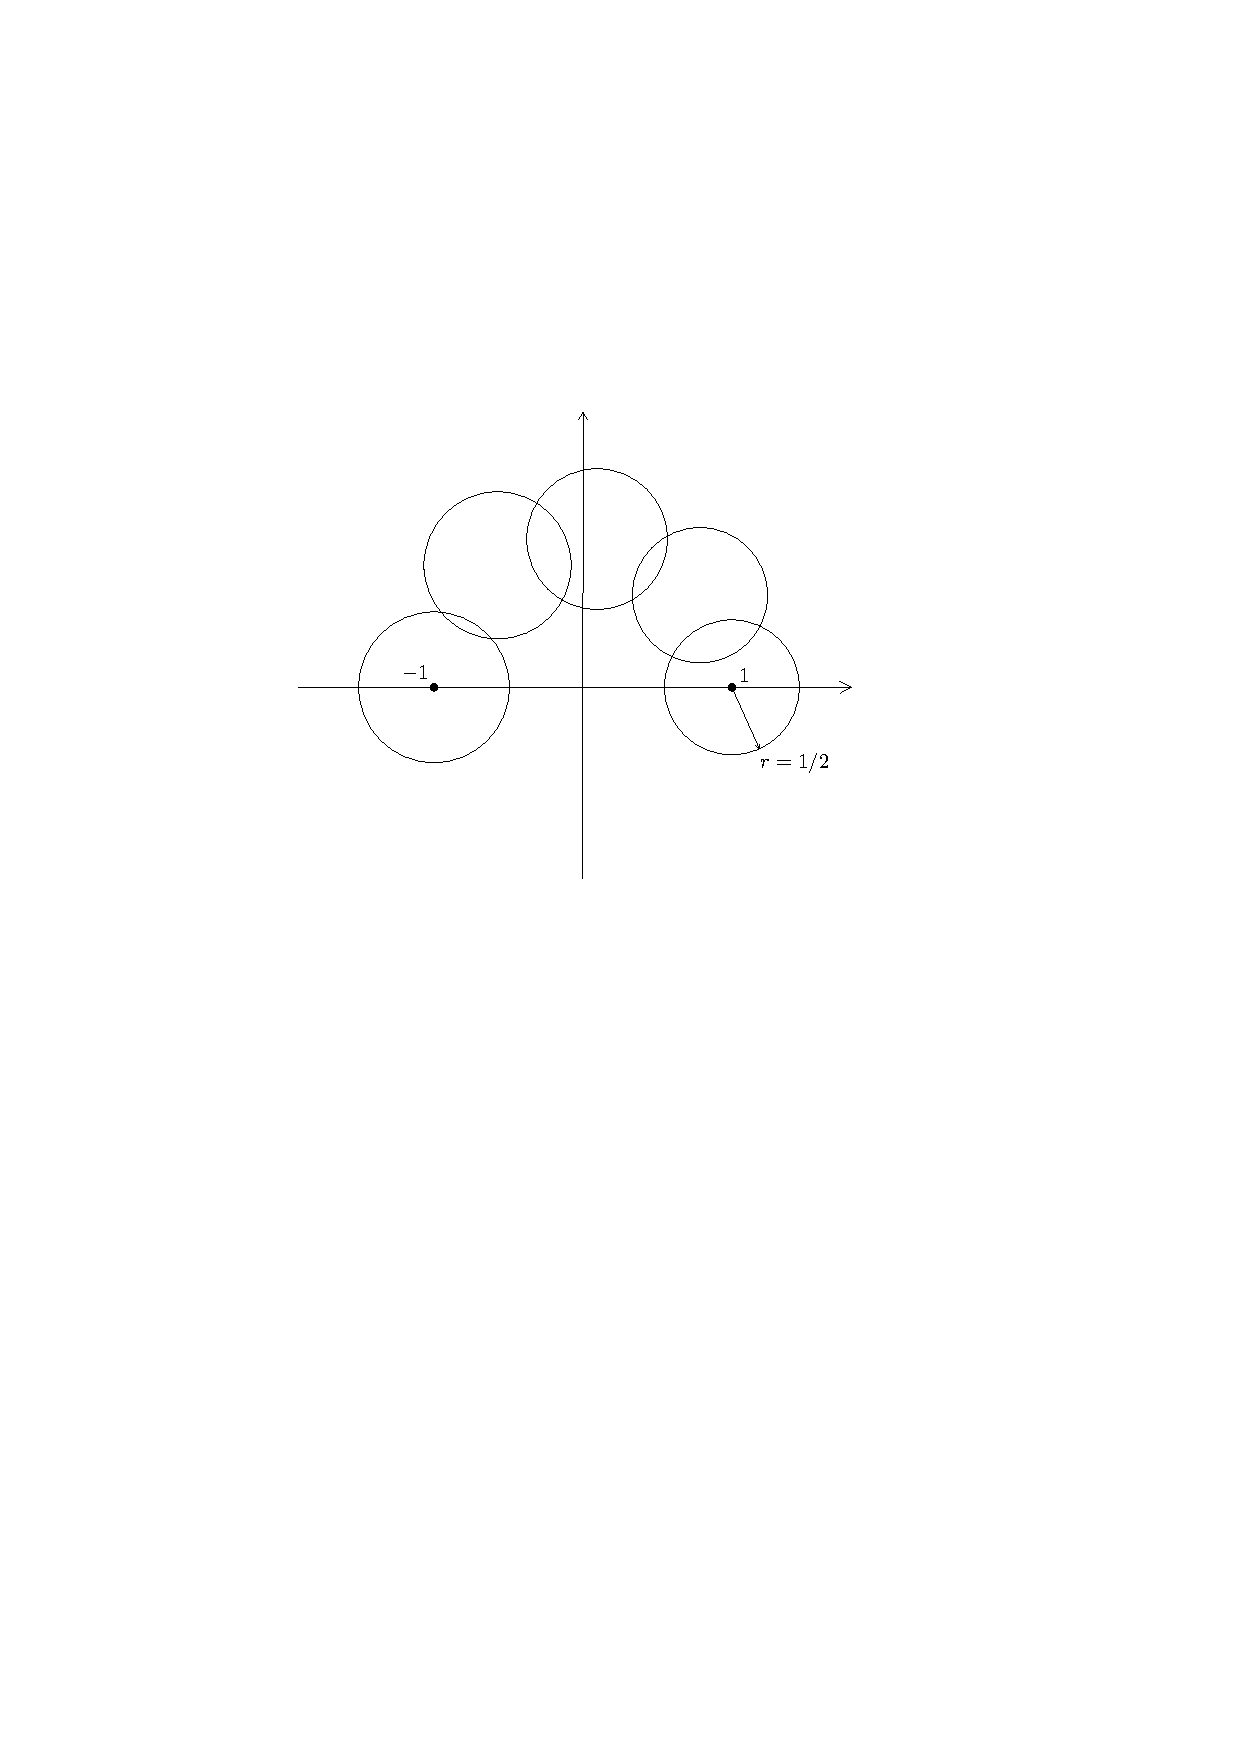
\includegraphics[width=180pt]{pictures/analytic-continuation-squreroot-1}
\end{figure}

However, we might have begun our analytic continuation process as shown below. If we continued the process to $z=-1$, we would have $f(-1)=-i$.
\begin{figure}[htbp]
\centering
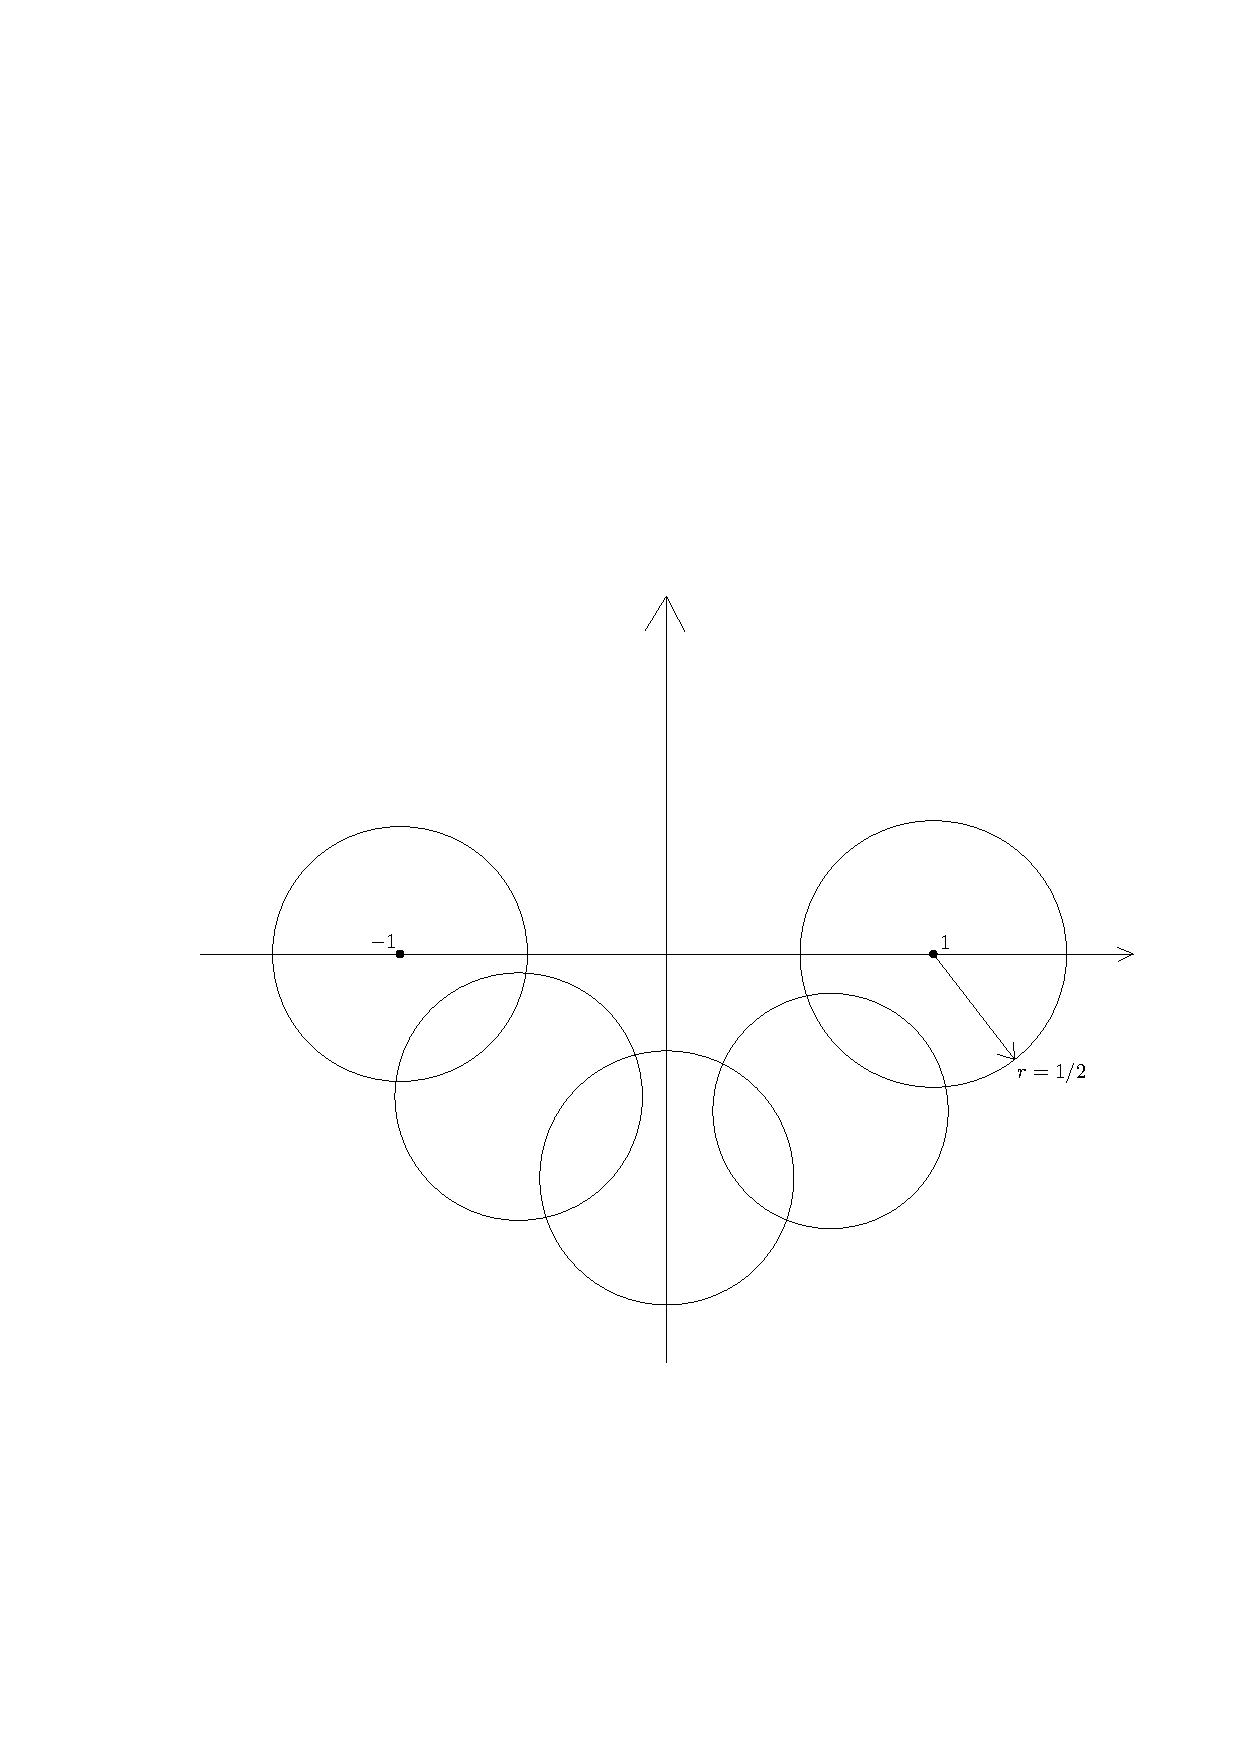
\includegraphics[width=180pt]{pictures/analytic-continuation-squreroot-2}
\end{figure}

Thus we see that the process of analytic continuation can be ambiguous. In the present example, the ambiguity is connected to the fact that a holomorphic square root function cannot be defined in any neighborhood of the origin.
\end{example}
These examples illustrate that an analytic function can sometimes be
continued to a domain of definition that is larger than the initial one. However, this continuation process can result in inconsistencies in the sense that the value of a continuation at a given point may depend on which continuation is involved, in effect, on how the point was reached. In each of the examples, the continuation process was effected differently by a device specific to the function. This raises two general and rather vague questions: How can we carry out analytic continuation in general? Furthermore, how can we determine when it can be carried out unambiguously? It is because of these questions that we must take a detailed and technical approach to the process of analytic continuation. Even making the questions themselves precise takes some thought.
\begin{definition}
A \textbf{function element} is an ordered pair $(f,U)$, where $U$ is a disc and $f$ is a holomorphic function defined on $U$.
\end{definition}
\begin{definition}
Let $(f,U)$ and $(g,V)$ be function elements. We say that $(g,V)$ is a \textbf{direct analytic continuation} of $(f,U)$ if $U\cap V\neq\emp$ and $f$ and $g$ are equal on $U\cap V$. Obviously $(g,V)$ is a direct analytic continuation of $(f,U)$ if and only if $(f,U)$ is a direct analytic continuation of $(g,V)$.
\end{definition}
If $(f_1,U_1),\dots,(f_k,U_k)$ are function elements and if each $(f_i,U_i)$ is a direct analytic continuation of $(f_{i-1},U_{i-1})$ for $i=2,\dots,k$, then we say that $(f_k,U_k)$ is an \textbf{analytic continuation} of $(f_1,U_1)$.\par
Clearly $(f_k,U_k)$ is an analytic continuation of $(f_1,U_1)$ if and only if $(f_1,U_1)$ is an analytic continuation of $(f_k,U_k)$. Also if $(f_k,U_k)$ is an analytic continuation of $(f_1,U_1)$ and $(f_{k+l},U_{k+l})$ is an analytic continuation of $(f_k,U_k)$ via a chain $(f_k,U_k),(f_{k+1},U_{k+1}),\dots,(f_{k+l},U_{k+l})$, then stringing the two chains together into $(f_1,U_1),\dots,(f_{k+l},U_{k+l})$ exhibits $(f_{k+l},U_{k+l})$ as an analytic continuation of $(f_1,U_1)$. Obviously $(f,U)$ is an analytic continuation of itself.\par
Thus we have an equivalence relation on the set of function elements.
The equivalence classes induced by this relation are called \textbf{(global) analytic functions}. However, a caution is in order: Global analytic functions are not yet functions in the usual sense, and they are not analytic in any sense that we have defined as yet. Justification for the terminology will appear in due course.\par
Notice that the initial element $(f,U)=(f_1,U_1)$ uniquely determines the global analytic function, or equivalence class, that contains it. But a global analytic function may include more than one function element of the form $(f,U)$ for a \textit{fixed disc} $U$. Indeed, a global analytic function $f$ may have in effect more than one value at a point of $\C$: Two function elements $(f_1,U)$ and $(f_2,U)$ can be equivalent even though $f_1(z_0)\neq f_2(z_0)$, where $z_0$ is the center of the disc $U$. If $\mathsf{f}$ denotes the global analytic function corresponding to $(f,U)$, then we call $(f,U)$ a branch of $\mathsf{f}$. Example~\ref{squre root continuation} illustrates a global analytic function (namely, the square root function) with two distinct branches centered at the point $-1$. Logarithms of $z$ again illustrate the point:
\begin{example}
Let $U=B_{1}(2)$ and let $f$ be the holomorphic function $\log z$. Here $\log z$ is understood to be defined as $\log|z|+i\arg z$, and $-\pi/6<\arg z<\pi/6$. As in the preceding example, the function element $(f,U)$ can be analytically continued to the point $-1$ in (at least) two different
ways, depending on whether the continuation is along a curve proceeding clockwise about the origin or counterclockwise about the origin.\par
In fact, all the branches of $\log z$ can be obtained by analytic continuation of the $\log|z|+i\arg z$ branch on $B_1(2)$.
\end{example}
In some situations, it is convenient to think of a function element as a convergent power series. Then the role of the open disc $U$ is played by the domain of convergence of the power series. This is a useful heuristic idea for the reader to bear in mind. From this viewpoint, two function elements $(f_1,U)$ and $(f_2,V)$ at a point $z_0$ (such that $U$ and $V$ are discs centered at the same point $z_0$) should be regarded as equal if $f_1=f_2$ on $U\cap V$. This identification is convenient and we shall introduce it formally a little later.
\subsection{Power series method of analytic continuation}
Now, we give an elegant and promising method of analytic continuation by means of power series. In this method, we use only circular domains and Taylor's expansion in such domain. Let the initial function $f_1(z)$ be represented by the Taylor's series about a point $z_1$ in the form
\begin{align}\label{power series continuation-1}
f_1(z)=\sum_{n=0}^{\infty}a_{n}^{(1)}(z-z_1)^n,
\end{align}
which converges within the circle $\Gamma_1:=\{z:|z-z_1|=\rho_1\}$. We now draw a path $\gamma$ from the point $z_1$ and perform the analytic continuation of the function along $L$ as follows: On $\gamma$, take a point $z_2$ such that the arc $z_1z_2$ lies in $\Gamma_1$, which is the circle of convergence of the series $(\ref{power series continuation-1})$. Then we use the series $(\ref{power series continuation-1})$ to evaluate the derivatives $f^{(n)}_1(z_2)$ by term-by-term differentiation and write the expansion which is valid within a circle $\Gamma_2:\{z:|z-z_2|=\rho_2\}$ in the form
\begin{align}\label{power series continuation-2}
f_2(z)=\sum_{n=0}^{\infty}a_{n}^{(1)}(z-z_2)^n=\sum_{n=0}^{\infty}\frac{f_2^{(n)}(z_2)}{n!}(z-z_2)^n.
\end{align}
If the circle $\Gamma_2$ extends beyond $\Gamma_1$, then $(\ref{power series continuation-2})$ gives an analytic continuation of $f_1(z)$. Also, at the point $z_2$, the functions $f_1(z)$ and $f_2(z)$ and all their derivatives have the same values. In this way, when the first analytic continuation of $(\ref{power series continuation-2})$ is performed, we proceed to the next.
\subsubsection{Singularities of power series on circles of convergence}
\begin{definition}
Let $f(z)$ be analytic in a domain $D$ and $F$ be the global analytic function determined by $f$. Let $\zeta$ be a point on $\partial D$. If no analytic continuation of $(z)$ to $\zeta$ is possible, then $\zeta$ is called a \textbf{singularity} of the global analytic function $F(z)$. If $\zeta\in\partial D$ is not a singularity, then it is called \textbf{regular}.
\end{definition}
\begin{theorem}
If the radius of convergence of the power series
\[f(z)=\sum_{n=0}^{\infty}a_nz^n\]
is nonzero finite, then $f(z)$ has at least one singularity on the circle of convergence.
\end{theorem}
\begin{proof}
Let $R$ be the radius of the circle of convergence $\Gamma$ of the power series and $D=B_{R}(0)$. Suppose, on the contrary, that every point of $\Gamma$ is a regular point of $f$. Then the compactness of $\Gamma$ implies then that there are open discs $D_1,\dots,D_n$ and functions $g_i\in\mathcal{H}(D_i)$ such that the center of each $D_i$ is on $\Gamma$, that $\Gamma\sub D_1\cup\cdots\cup D_n$, and that $g_i(z)=f(z)$ on $D_i\cap D$, for $i=1,\dots,n$.\par
If $D_i\cap D_j\neq\emp$ and $V_{ij}=D_i\cap D_j\cap D$, then $V_{ij}\neq\emp$ (since the centers of the $D_i$ are on $\Gamma$), and $g_i=f=g_j$ in $V_{ij}$. Since $D_i\cap D_j$ is connected, it follows that $g_i=g_i$ in $D_i\cap D_j$. Hence we may define a function $h$ in $\Omega:=D\cup D_1\cup\cdots\cup D_n$ by
\[h(z)=\begin{cases}
f(z)&z\in D,\\
g_i(z)&z\in D_i.
\end{cases}\]
Since $\widebar{D}\sub\Omega$ and $\Omega$ is open, there exists an $\eps>0$ such that the disc $B_{R+\eps}(0)\sub\Omega$. But $h\in\mathcal{H}(\Omega)$ and $h(z)=f(z)$ on $D$, so the radius of convergence of $f$ is at least $R+\eps$, contrary to our assumption.
\end{proof}
\subsubsection{The Hadamard gap theorem}
\begin{definition}
If a function $f(z)$ cannot be extended analytically beyond the boundary of a certain region $D$, then the boundary $\partial D$ is called a \textbf{natural boundary}.
\end{definition}
Now we present a technique of Ostrowski for producing series which exhibit a phenomenon called "over-convergence" (to be defined below). It was discovered by J.Hadamard that these series produce holomorphic
functions on the disc for which no point on $\partial\D$ is regular. The series are examples of what are called "gap series" (or "lacunary series"). These are series that are formed by deleting many terms from a series formed by a regular pattern. They have various uses in analysis. For instance, they can be used to construct continuous, nowhere differentiable functions.\par
Let us begin with a concrete example. Consider the power series $\sum_nz^{2^n}$. This series converges absolutely and uniformly on compact subsets of the unit disc $\D$ since $|z^{2^n}|\leq|z|^n$. Thus the power series defines a holomorphic function $f(z)$ on $\D$. We claim that no point of $\partial D$ is regular for $f$. To see this, consider $f(rw)$ for $0<r<1$ and $w$ such that $|w|^{2^N}=1$ for a fixed positive integer $N$. Now
\[f(rw)=\sum_{n=1}^{N-1}r^{2^n}w^{2^n}+\sum_{n=N}^{\infty}r^{2^n}w^{2^n}=\sum_{n=1}^{N-1}r^{2^n}w^{2^n}+\frac{1}{w}\sum_{n=N}^{\infty}r^{2^n}.\]
Thus we see $\lim_{r\to 1^-}|f(rw)|=+\infty$ since, for $N$ fixed, the first sum is bounded while the second tends to $+\infty$ (each summand is positive real and tends to a limit greater than $1$).\par
We conclude that $f'$ is unbounded near all $w\in\partial\D$ with $w^{2^N}=1$, some positive integer $N$. But the set of all such $w$ is dense in $\partial\D$, thus extension of $f$ to a neighborhood of a point in $\partial\D$ is impossible.\par
It is natural to try to generalize this example as much as possible. But the process is not easy. The proof of the following theorem uses a very clever trick, which at first might seem unmotivated. Try to see the elements of our example lurking in the background:
\begin{theorem}[\textbf{Ostrowski-Hadamard}]\label{Hadamard gap theorem}
Let $\{p_n\}$ be an increasing sequence of positive integers and suppose that there is a $\lambda>1$ such that
\[p_{n+1}>\lambda p_n\]
for all $n$. Suppose that, for some sequence of complex numbers $\{a_n\}$, the power series
\[f(z)=\sum_{n=0}^{\infty}a_nz^{p_n}\]
has radius of convergence $1$. Then no point of $\partial\D$ is regular for $f$.
\end{theorem}
\begin{proof}
Seeking a contradiction, we suppose that some $z_0\in\partial\D$ is regular for $f$; without loss of generality we take $z_0=1$. (This is indeed without loss of generality, since changing $z$ to $wz$, $|w|=1$, gives a series of the same form, with coefficients having the same absolute values as before; so the new series also has radius of convergence $1$.) Then there is a disc $B_{\eps}(1)$ and a holomorphic $F$ on $U=\D\cup B_{\eps}(1)$ extending $f$. Choose an integer $k>0$ such that $(k+1)/k<\lambda$ and define
\[\psi(z)=\frac{1}{2}(z^k+z^{k+1})\]
Notice that $\psi(1)=1$, and if $|z|\leq 1$ but $z\neq 1$, then we have
\[|\psi|=\frac{1}{2}|z|^k|z+1|<|z|^k\leq 1.\]
So $\psi(\D)$ is a compact subset of $U$. It follows by continuity of $\psi$ that there is a disc $B_{1+\delta}(0)$ such that $\psi(B_{1+\delta}(0))\sub U$. Note also that $1\in\psi(B_{1+\delta}(0))$.\par
Define
\[G(z)=F(\psi(z)),\quad z\in B_{1+\delta}(0)\]
and expand $G$ in a power series about $0$:
\[G(z)=\sum_{n=0}^{\infty}c_nz^n.\]
Compare this formula with what is obtained by substituting $\psi(z)=(z^k+z^{k+1})/2$ into the power series for $F=f$ on $\D$:
\[(F\circ\psi)(z)=\sum_{n=0}^{\infty}a_n\Big(\frac{z^k+z^{k+1}}{2}\Big)^{p_n}.\]
Notice that the $n$-th term of this series contributes powers of $z$ ranging from $z^{kp_n}$ to $z^{(k+1)p_n}$; while the $(n+1)$-st term contributes powers of $z$ ranging from $z^{kp_{n+1}}$ to $z^{(k+1)p_{n+1}}$. But the condition on $\{p_n\}$ and the choice of $k$ guarantees that $kp{n+1}>(k+1)p_n$, so that the powers appearing in $(z^k+z^{k+1})^{p_n}$ are pairwise disjoint. As a result, 
\[\sum_{n=0}^{N}a_n(\psi(z))^{p_n}=\sum_{n=0}^{(k+1)p_N}c_{n}z^n.\]
The right side converges as $N\to+\infty$ on the disc $B_{1+\delta}(0)$. Hence so does the left side. In other words,
\[\sum_{n=0}^{\infty}a_nw^{p_n}\]
converges for all $w\in\psi(B_{1+\delta}(0))$. In particular this series converges for all $w$ in a neighborhood of $1$, so its radius of convergence is not $1$. This contradicts our hypothesis.
\end{proof}
In general, a point $z_0$ in the boundary of the (unit) disc can be a regular point for the holomorphic function $f$ (on the disc) without the power series for $f$ about $0$ converging in a neighborhood of $z_0$. A good example is $f(z)=1/(1-z)$. Then all $z\in\partial\D\setminus\{1\}$ are regular but the radius of convergence of the power series is $1$. This explains why the phenomenon exhibited in the proof of Theorem~\ref{Hadamard gap theorem} is called \textbf{over-convergence}.\par
Now we return to the continuation of power series. We first show that, the singularities have close relation with the inconsistencies of continuation along curves.
\begin{theorem}
Suppose $D$ is a region, $L$ is a straight line or a circular arc, $D\setminus L$ is the union of two regions $D_1$ and $D_2$, $f$ is continuous in $D$, and $f$ is holomorphic in $D_1$ and in $D_2$. Then $f$ is holomorphic in $D$.
\end{theorem}
\begin{proof}
The use of linear fractional transformations shows that the general case follows if we prove the theorem for straight lines $L$. By Morera's theorem, it is enough to show that the integral of $f$ over the boundary $\partial R$ is $0$ for every rectangle $R$ with sides parallel to axis in $D$. The Cauchy theorem implies that the integral of $f$ vanishes over every closed path $\gamma$ in $R\cap D_1$ or in $R\cap D_2$. The continuity of $f$ shows that this is still true if part of $R$ is in $L$, and the integral over $\partial R$ is the sum of at most two terms of this sort.
\end{proof}
\subsection{Analytic continuation along a curve}
\begin{definition}
Let $(f,U)$ be a function element where $U$ is a region and $f$ is an analytic function in $U$. The \textbf{germ} of $f$ at $a$ is the collection of all function element $(g,V)$ such that $a\in V$ and $f(z)=g(z)$ for all $z$ in a neighborhood of $a$ and is denoted by $[f]_a$.
\end{definition}
Note that $[f]_a$ is a collection of function elements and it is not a function elements itself. Also, it can easily be verified that $(g,V)\in[f]_a$ if and only if $(f,U)\in[g]_a$, if and only if $f=g$ in a neighborhood of $a$.\par
We now revisit the definition of analytic continuation along a path in terms of germs as follows:
\begin{definition}
Let $(f,U)$ be a function element and let $\gamma:[0,1]\to\C$ be a path starting from $U$. Then an \textbf{analytic continuation of $\bm{(f,U)}$ along the curve $\bm{\gamma}$} is a collection $\{(f_t,U_t):t\in[0,1]\}$ such that
\begin{itemize}
\item[(a)] $(f_0,U_0)=(f,U)$.
\item[(b)] $\gamma(t)\in U_t$ for all $t\in[0,1]$.
\item[(c)] For each $t$ in $[0,1]$ there is a $\delta>0$ such that $|s-t|<\delta$ implies
\[\gamma(s)\in U_t\And[f_s]_{\gamma(s)}=[f_t]_{\gamma(t)}.\]
\end{itemize}
\end{definition}
\begin{theorem}\label{analytic continuation along curve unique}
Let $\gamma:[0,1]\to\C$ be a path from $z_0$ to $z_1$ and let $\{(f_t,U_t)\}$ and $\{(g_t,V_t)\}$ be analytic continuations along $\gamma$ such that $[f_0]_{z_0}=[g_0]_{z_0}$, then $[f_1]_{z_1}=[g_1]_{z_1}$.
\end{theorem}
\begin{proof}
In order to prove this claim we will show that the set
\[T=\{t\in[0,1]:[f_t]_{\gamma(t)}=[g_t]_{\gamma(t)}\}\]
is both open and closed in $[0,1]$. By hypotheses, we have $0\in T$, so $T$ is nonempty. Then it will follows that $T=[0,1]$ so that, in particular, $1\in T$.\par
To show that $T$ is open, fix $t$ in $T$ and assume that $t\neq 1$. In fact, if $t=1$ the proof is complete. By the definition of analytic, there is a $\delta>0$ such that for $|s-t|<\delta$, $\gamma(s)\in U_t\cap V_t$ and
\begin{align}\label{analytic continuation along curve unique-1}
[f_s]_{\gamma(s)}=[f_t]_{\gamma(t)},\quad [g_s]_{\gamma(s)}=[g_t]_{\gamma(t)}.
\end{align}
Since $t\in T$, it follows that $[f_t]_{\gamma(t)}=[g_t]_{\gamma(t)}$, so it follows that $[f_s]_{\gamma(s)}=[g_s]_{\gamma(s)}$ for $|s-t|<\delta$, therefore $(t-\delta,t+\delta)\sub T$. Therefore $T$ is open.\par
Next, to show that $T$ is closed let $t$ be a limit point of $T$, and again choose $\delta>0$ so that $\gamma(s)\in U_t\cap V_t$ and $(\ref{analytic continuation along curve unique-1})$ is satisfied whenever $|s-t|<\delta$. Since $t$ is a limit point of $T$, there is a point $s\in T$ with $|s-t|<\delta$, so
\[\gamma(s)\in U_t\cap U_s\cap V_t\cap V_s=:D.\]
Then $f_s(z)=g_s(z)$ on $D$ by the definition of $T$, and by $(\ref{analytic continuation along curve unique-1})$ we conclude that $[f_t]_{\gamma(t)}=[g_{t}]_{\gamma(t)}$, thus $t\in T$. This proves $T$ is closed.
\end{proof}
Thus we see that the analytic continuation of a given function element along a given curve is essentially unique, if it exists. From here on, to avoid being pedantic, we shall regard two analytic continuations $(f_t,U_t)$ and $(g_t,V_t)$ as "equal," or equivalent, if $[f_t]_{\gamma(t)}=[g_t]_{\gamma(t)}$ for all $t$. With this terminological convention (which will cause no trouble), the proposition says exactly that analytic continuation of a given function element along a given curve is unique. It should be stressed, however, that this is a uniqueness statement only-not an existence statement.
\subsection{Monodromy theorem and its consequences}
Let $z_0$ and $z_1$ be two points in $\C$ and suppose $\gamma$ and $\sigma$ are two paths from $z_0$ to $z_1$. Suppose that $\{(f_t,U_t)\}$ and $\{(g_t,V_t)\}$ are analytic continuations along $\gamma$ and $\sigma$, respectively. Also, suppose that $[f_0]_{z_0}=[g_0]_{z_0}$. 

According to Proposition~\ref{analytic continuation along curve unique} that the answer to this question is affirmative, if $\gamma$ and $\sigma$ are the same path. However, if $\gamma$ and $\sigma$ are distinct paths then the answer may be negative.\par
If $(f,D)$ is a function element and $z_0\in D$ then $f$ has a power series expansion at $z=z_0$. To establish the Monodromy theorem, our first step will be to investigate the behavior of the radius of convergence for an analytic continuation along a curve.
\begin{lemma}\label{analytic continuation along curve convergent radius}
Let $\gamma:[0,1]\to\C$ be a path and let $\{(f_t,U_t)\}$ be an analytic continuation along $\gamma$. For $t\in[0,1]$, let $R(t)$ be the radius of convergence of the power series expansion of $f_t$ about $z=\gamma(t)$. Then either $R(t)\equiv+\infty$ or $R:[0,1]\to(0,+\infty)$ is continuous.
\end{lemma}
\begin{proof}
If $R(t)=+\infty$ for some value of $t_0$; that is, the radius of circle of convergence is infinite. Then it is possible to extend $f_{t_0}$ to an entire function. If we consider another analytic continuation along $\gamma$ defined by $\{\widetilde{f}_t=f_{t_0},V_t=\C)\}$, then by Proposition~\ref{analytic continuation along curve convergent radius} we have $[f_t]_{\gamma(t)}=[\widetilde{f}_t]_{\gamma(t)}=[f_{t_0}]_{\gamma(t)}$. This implies $f_s=f_{t_0}$ on $U_t$, and therefore each $f_t$ can be extended to an entire function. Thus $R(t)\equiv+\infty$.\par
So we suppose that $R(t)<+\infty$ for all $t\in[0,1]$. Fix $t_0$ in $[0,1]$ and let $z_0=\gamma(t_0)$. Let the power series expansion of $f_{t_0}$ about $z_0$ be
\[f_{t_0}(z)=\sum_{n=0}^{\infty}a_n(z-z_0)^n\]
Now let $\delta_1>0$ be such that $|s-t_0|<\delta_1$ implies
\[\gamma(s)\in U_{t_0}\cap B_{R(t_0)}(z_0)\And [f_s]_{\gamma(s)}=[f_{t_0}]_{\gamma(t_0)}.\]
Let us fix $s$ with $|s-t_0|<\delta_1$. Now we can extend $f_{t_0}$ to an analytic function in $B_{R(t_0)}(z_0)$. Again, since $f_s$ agree with $f_{t_0}$ on a neighborhood of $\gamma(s)$, $f_s$ can be extended. Consequently, $f_s$ is also analytic in $B_{R(t_0)}(z_0)\cup U_s$. Suppose $f_s$ has the power series expansion about $\gamma(s)$ as
\[f_s(z)=\sum_{n=0}^{\infty}b_n(z-\gamma(s))^n\]
then the radius of convergence $R(s)$ must be at least as big as the distance from $\gamma(s)$ to the circle $\Gamma_0=\{z:|z-z_0|=R(t_0)\}$; that is,
\[R(s)\geq d(w,\Gamma_0)=R(t_0)-|z_0-\gamma(s)|.\]
This implies
\[R(t_0)-R(s)\leq|z_0-\gamma(s)|.\]
By symmetric, we can establish the other direction, and hence we have
\[|R(t_0)-R(s)|\leq|z_0-\gamma(s)|.\]
Since $\gamma$ is a continuous function, this inequality then implies $R$ is continuous.
\end{proof}
\begin{lemma}\label{analytic continuation along curve small pertubation}
Let $\gamma:[0,1]\to\C$ be a path from $z_0$ to $z_1$ and let $\{(f_t,U_t)\}$ be an analytic continuation along $\gamma$. There is a number $\eps>0$ such that if $\sigma:[0,1]\to\C$ is any path from $z_0$ to $z_1$ with $|\gamma(t)-\sigma(t)|<\eps$ for all $t$ and if $\{(g_t,V_t)\}$ is any continuation along $\sigma$ with $[g_0]_{z_0}=[f_0]_{z_0}$, then $[g_1]_{z_1}=[g_1]_{z_1}$.
\end{lemma}
\begin{proof}
Let power series expansion of $f_t$ about $\gamma(t)$ be
\[f_t(z)=\sum_{n=0}^{\infty}a_n(z-\gamma(t))^n.\]
and let $R(t)$ be its radius of convergence. If $R(t)\equiv+\infty$, then any value of $\eps$ will serve our purpose. So suppose $R(t)<+\infty$. Since, by the preceding Lemma, $R(t)$ is a continuous function and since $R(t)>0$ for all $t$, $R(t)$ has positive minimum value $m$. Let $0<\eps<m/2$. Suppose that $\sigma$ and $\{(g_t,V_t)\}$ are as in the statement of this lemma. Also, suppose that $U_t$ is the disk given by $U_t=\{z:|z-\gamma(t)|<R(t)\}$. This supposition will not affect the conclusion of the lemma.\par
Since, for $\sigma(t)\in U_t\cap V_t$ and for all $t\in[0,1]$, we have $|\sigma(t)-\gamma(t)|<\eps<R(t)$, it makes sense to ask whether $g_t(z)=f_t (z)$ for all $z$ in $U_t\cap V_t$. In order to complete the proof, we will show that this is precisely the case. Define the set $T$ by
\[T=\{t\in[0,1]:f_t(z)=g_t(z)\text{ for }z\in U_t\cap V_t\}.\]
We will show that $T$ is open and closed. Since $0\in T$, this will implies $T=[0,1]$ and completes the proof.\par
By hypothesis of the lemma, $[f_0]_{z_0}=[g_0]_{z_0}$; it follows that $f_0(z)=g_0(z)$ for $z\in U_t\cap V_t$ and so $0\in T$. Thus $T\neq\emp$. To show that $T$ is open, let us fix $t\in T$ and choose $\delta>0$ such that $|s-t|<\delta$ implies that
\begin{align}\label{analytic continuation along curve small pertubation-1}
\gamma(s)\in U_t,|\gamma(s)-\gamma(t)|<\eps,[f_s]_{\gamma(s)}=[f_t]_{\gamma(t)}
\end{align}
and
\begin{align}\label{analytic continuation along curve small pertubation-2}
\sigma(s)\in V_t,|\sigma(s)-\sigma(t)|<\eps,[f_s]_{\sigma(s)}=[f_t]_{\sigma(t)}.
\end{align}
We now show that $U_t\cap U_s\cap V_t\cap V_s\neq\emp$ for $|s-t|<\delta$. This will be proved by showing that $\sigma(s)\in U_t\cap U_s\cap V_t\cap V_s$. If $|s-t|<\delta$, then
\[|\sigma(s)-\gamma(s)|<\eps<R(s)\]
and thus $\sigma(s)\in U_s$. Also,
\[|\sigma(s)-\gamma(t)|\leq|\sigma(s)-\gamma(s)|+|\gamma(s)-\gamma(t)|<\eps+\eps<R(t)\]
so $\sigma(s)\in U_t$. We already have that $\sigma(s)\in V_s\cap V_t$, so we conclude that $\sigma(s)\in D:=U_t\cap U_s\cap V_t\cap V_s$. Again, since $t\in T$ it follows that $f_t(z)=g_t(z)$ for $z\in D$, and by $(\ref{analytic continuation along curve small pertubation-1})$ and $(\ref{analytic continuation along curve small pertubation-2})$ we conclude that $f_s(z)=g_s(z)$ for all $z\in D$. But since $D$ has a limit point in $U_s\cap V_s$ it must follows that $s\in T$; that is, $T$ is open. One can easily show that $T$ is closed. This completes that proof of the lemma.
\end{proof}
\begin{definition}
Let $(f,U)$ be a function element and let $D$ be a region which contains $U$; then $(f,U)$ \textbf{admits unrestricted analytic continuation in $\bm{D}$} if for any path $\gamma$ in $D$ with initial point in $U$, there is an analytic continuation of $(f,U)$ along $\gamma$.
\end{definition}
Let us consider $U=B_{1}(1)$ and $f$ be the principal branch of $\sqrt{z}$ or $\log z$. Then we see that $(f,U)$ admits unrestricted continuation in the punctured plane but not in the whole plane.\par
It may remarkable that if $(f,U)$ is a function element and $D$ is a region containing $U$, no criterion will be given which implies that $(f,U)$ admits unrestricted continuation in $D$. In fact, the Monodromy Theorem assumes that $D$ has this propriety and states a uniqueness criterion.
\begin{theorem}[\textbf{Monodromy Theorem}]\label{Monodromy Theorem}
Let $(f,U)$ be a function element and let $D$ be a region containing $U$ such that $(f,U)$ admits unrestricted continuation in $D$. Let $z_0\in U$, $z_1\in D$ and let $\gamma_0$ and $\gamma_1$ be paths in $D$ from $z_0$ to $z_1$. Let $\{(f_t,U_t)\}$ and $\{(g_t,V_t)\}$ be analytic continuation of $(f,U)$ analog $\gamma_0$ and $\gamma_1$, respectively. If $\gamma_0$ and $\gamma_1$ are homotopic in $D$, then $[f_1]_{z_1}=[g_1]_{z_1}$.
\end{theorem}
\begin{proof}
Let $H:[0,1]^2\to D$ be a homotopy between $\gamma_0$ and $\gamma_1$. Consider the path $\gamma_u$ defined by
\[\gamma_u=H(t,u)\]
Again, by hypothesis, there is a analytic continuation $\{(h_{(t,u)},D_{(t, u)})\}$ along the path $\gamma_u$. Form Proposition~\ref{analytic continuation along curve unique} of the preceding section, it follows that $[g_1]_{z_1}=[h_{1,1}]_{z_1}$ and $[f_1]_{z_1}=[h_{1,0}]_{z_1}$. Hence, it is sufficient to show that $[h_{1,0}]_{z_1}=[h_{1,1}]_{z_1}$.\par
We now introduce the set
\[U=\{u\in[0,1]:[h_{1,u}]_{z_1}=[h_{1,0}]_{z_1}\}.\]
and we will show that $U$ is a nonempty open and closed subset of $[0,1]$. Evidently, $0\in U$, so $U$ is nonempty. For a fixed $u$ in $[0,1]$, apply Lemma~\ref{analytic continuation along curve small pertubation} to find an $\eps>0$ that satisfies the condition in the lemma for $\gamma_u$. Now since $H$ is a uniformly continuous function, it follows that for any given $\eps>0$, there exists $\delta>0$ such that
\begin{align}\label{Monodromy Theorem-1}
|u-v|<\delta\Longrightarrow|\gamma_u(t)-\gamma_v(t)|<\eps\text{ for all $t$}\Longrightarrow[h_{1,u}]_{z_1}=[h_{1,v}]_{z_1}.
\end{align}
Now by the assumption on $\eps$, we conclude $[h_{1,v}]_{z_1}=[h_{1,0}]_{z_1}$ provided $|u-v|<\delta$. This implies $U$ is an open set.\par
If $u$ is a limit point of $U$ and $\delta>0$ is chosen such that $(\ref{Monodromy Theorem-1})$ holds. Then there exists a $v\in U$ such that $|u-v|<\delta$. But by $(\ref{Monodromy Theorem-1})$ and the definition of $U$,
\[[h_{1,u}]_{z_1}=[h_{1,v}]_{z_1}=[h_{1,0}]_{z_1}.\]
Thus $u\in U$. Hence $U$ is closed, and the proof is completed.
\end{proof}
Observe that the following corollary is the most important consequence of the Monodromy Theorem.
\begin{corollary}
Let $(f,U)$ be a function element which admits unrestricted continuation in the simply connected region $D$. Then there is an analytic function $F:D\to\C$ such that $F(z)=f(z)$ for all $z$ in $U$.
\end{corollary}
\begin{proof}
Let us chosen a point $z_0$ in $U$ and keep it fix and let $z$ be any point in $D$. Let $\gamma$ be a path in $D$ from $z_0$ to $z$ and $\{(f_t,U_t)\}$ be an analytic continuation of $(f,U)$ along $\gamma$; then let $F(z)=f_t(z)$. Since $D$ is simply connected, the value of $F$ does not depend on the choice of $\gamma$, so $F$ is well-defined on $D$. Since $F$ equals to an analytic function near every point of $D$, it follows that $F$ is analytic. It is clear that $F(z)=f(z)$ on $U$.
\end{proof}
%\chapter{Vector Fields and Flows}
\section{Vector fields}\label{vector field section}
Vector fields are familiar objects of study in multivariable calculus. In that setting, a vector field on an open subset $U\sub\R^n$ is simply a continuous map from $U$ to $\R^n$, which can be visualized as attaching an arrow to each point of $U$. In this section we show how to extend this idea to smooth manifolds.
\subsection{Vector fields on manifolds}
If $M$ is a smooth manifold with or without boundary, a vector field on $M$ is a section of the map $\pi:TM\to M$. More concretely, a vector field is a continuous map $X:M\to TM$, usually written $p\mapsto X_p$, with the property that
\[\pi\circ X=\mathrm{id}_M\]
or equivalently, $X_p\in T_pM$ for each $p\in M$.\par
We are primarily interested in \textbf{smooth vector fields}, the ones that are smooth as maps from $M$ to $TM$, when $TM$ is given the smoothmanifold structure described in Proposition~\ref{tangent bundle struct}. In addition, for some purposes it is useful to consider maps from $M$ to $TM$ that would be vector fields except that they might not be continuous. A \textbf{rough vector field} on $M$ is a (not necessarily continuous) map $X:M\to TM$ satisfying $X_p\in T_pM$. Just as for functions, if $X$ is a vector field on $M$, the \textbf{support} of $X$ is defined to be the closure of the set $\{p\in M:X_p\neq 0\}$. A vector field is said to be \textbf{compactly supported} if its support is a compact set.\par
Suppose $M$ is a smooth $n$-manifold (with or without boundary). If $X:M\to TM$ is a rough vector field and $(U,(x^i))$ is any smooth coordinate chart for $M$, we can write the value of $X$ at any point $p\in U$ in terms of the coordinate basis vectors:
\[X_p=X^i(p)\frac{\partial}{\partial x^i}\Big|_p\]
This defines $n$ functions $X^i:U\to\R$, called the \textbf{component functions} of $X$ in the given chart.
\begin{proposition}[\textbf{Smoothness Criterion for Vector Fields}]\label{vector field smooth crit}
Let $M$ be a smooth manifold with or without boundary, and let $X:M\to TM$ be a rough vector field. If $(U,(x^i))$ is any smooth coordinate chart on $M$, then the restriction of $X$ to $U$ is smooth if and only if its component functions with respect to this chart are smooth.
\end{proposition}
\begin{proof}
Let $(x^i,v^i)$ be the natural coordinates on $\pi^{-1}(U)\sub TM$ associated with the chart $(U,(x^i))$. By definition of natural coordinates, the coordinate representation of $X:M\to TM$ on $U$ is
\[\widehat{X}=(x^1,\dots,x^n,X^1(x),\dots,X^n(x))\]
where $X^i$ is the $i$-th component function of $X$ in $x^i$-coordinates. It follows immediately that smoothness of $X$ in $U$ is equivalent to smoothness of its component functions.
\end{proof}
\begin{example}[\textbf{Coordinate Vector Fields}]
If $(U,(x^i))$ is any smooth chart on $M$, the assignment
\[p\mapsto\frac{\partial}{\partial x^i}\Big|_p\]
determines a vector field on $U$, called the $i$-th coordinate vector field and denoted by $\partial/\partial x^i$. It is smooth because its component functions are constants.
\end{example}
\begin{example}[\textbf{The Euler Vector Field}]\label{Euler vector field}
The vector field $V$ on $\R^n$ whose value at $x\in\R^n$ is
\[V_x=x^1\frac{\partial}{\partial x^1}\Big|_x+\cdots+x^n\frac{\partial}{\partial x^n}\Big|_x\]
is smooth because its coordinate functions are linear. It vanishes at the origin, and points radially outward everywhere else. It is called the Euler vector field because of its appearance in Euler's homogeneous function theorem
\end{example}
\begin{example}\label{angle vector field}
Let $\theta$ be any angle coordinate on a proper open subset $U\sub S^1$, and let $d/d\theta$ denote the corresponding coordinate vector field. Because any other angle coordinate $\widetilde{\theta}$ differs from $\theta$ by an additive constant in a neighborhood of each point, the transformation law for coordinate vector fields $(\ref{coordinate change-1})$ shows that $d/d\theta=d/d\widetilde{\theta}$ on their common domain. For this reason, there is a globally defined vector field on $S^1$ whose coordinate representation is $d/d\theta$ with respect to any angle coordinate. It is a smooth vector field because its component function is constant in any such chart. We denote this global vector field by $d/d\theta$, even though, strictly speaking, it cannot be considered as a coordinate vector field on the entire circle at once.
\end{example}
\begin{example}[\textbf{Angle Coordinate Vector Fields on Tori}]
On the $n$-dimensional torus $T^n$, choosing an angle function $\theta^i$ for the $i$-th circle factor, yields local coordinates $(\theta^1,\dots,\theta^i)$ for $T^n$. An analysis similar to that of the previous example shows that the coordinate vector fields $d/d\theta^1,\dots,d/d\theta^n$ are smooth and globally defined on $T^n$.
\end{example}
If $U\sub M$ is open, the fact that $T_pU$ is naturally identified with $T_pM$ for each $p\in U$ (Proposition~\ref{tangent open mani}) allows us to identify $TU$ with the open subset $\pi^{-1}(U)\sub TM$. Therefore, a vector field on $U$ can be thought of either as a map from $U$ to $TU$ or as a map from $U$ to $TM$, whichever is more convenient. If $X$ is a vector field on $M$, its restriction $X|_U$ is a vector field on $U$, which is smooth if $X$ is.\par
The next lemma is a generalization of Lemma~\ref{ext lem smooth func} to vector fields, and is proved in much the same way. If $M$ is a smooth manifold with or without boundary and $A\sub M$ is an arbitrary subset, a \textbf{vector field along $\bm{A}$} is a continuous map $X:A\to TM$ satisfying $\pi\circ X=\mathrm{id}_A$ (or in other words $X_p\in T_pM$ for each $p\in A$). We call it a \textbf{smooth vector field along $\bm{A}$} if for each $p\in A$, there is a neighborhood $V$ of $p$ in $M$ and a smooth vector field $\widetilde{X}$ on $V$ that agrees with $X$ on $V\cap A$.
\begin{lemma}[\textbf{Extension Lemma for Vector Fields}]
Let $M$ be a smooth manifold with or without boundary.
\begin{itemize}
\item[(a)] Let $A\sub M$ be a closed subset. Suppose $X$ is a smooth vector field along $A$. Given any open subset $U$ containing $A$, there exists a smooth global vector field $\widetilde{X}$ on $M$ such that $\widetilde{X}|_A=X$ and $\supp(\widetilde{X})\sub U$.
\item[(b)] Let $S\sub M$ is an embedded submanifold with or without boundary. Given $\X\in\X(S)$, then there is a smooth vector field $Y$ on a neighborhood of $S$ in $M$ such that $X=Y|_S$. Every such vector field extends to all of $M$ if and only if $S$ is properly embedded.
\end{itemize}
\end{lemma}
\begin{proof}
Note the if $\psi\in C^\infty(M)$ and $X$ is a vector field of $M$, then $fX$ is also a vector field of $M$, since $f(p)X_p\in T_pM$ for all $p\in M$. This suggests that we can apply the proof of Lemma~\ref{ext lem smooth func}.\par
The proof for the second part is similar to Lemma~\ref{ext funct submani}.
\end{proof}
As an important special case, any vector at a point can be extended to a smooth
vector field on the entire manifold.
\begin{proposition}
Let $M$ be a smooth manifold with or without boundary. Given $p\in M$ and $v\in T_pM$, there is a smooth global vector field $X$ on $M$ such that $X_p=v$.
\end{proposition}
\begin{proof}
The assignment $p\mapsto v$ is an example of a vector field along the set $\{p\}$ as defined above. It is smooth because it can be extended, say, to a constant-coefficient vector field in a coordinate neighborhood of $p$. Thus, the proposition follows from the extension lemma with $A=\{p\}$ and $U=M$.
\end{proof}
If $M$ is a smooth manifold with or without boundary, it is standard to use the notation $\mathfrak{X}(M)$ to denote the set of all smooth vector fields on $M$. It is a vector space under pointwise addition and scalar multiplication:
\[(aX+bY)_p=aX_p+bY_p\]
The zero element of this vector space is the zero vector field, whose value at each $p\in M$ is $0\in T_pM$. In addition, smooth vector fields can be multiplied by smooth real-valued functions: if $f\in C^\infty(M)$ and $X\in\mathfrak{X}(M)$, we define $fX:M\to TM$ by
\[(fX)_p=f(p)X_p\]
\begin{proposition}
Let M be a smooth manifold with or without boundary.
\begin{itemize}
\item[(a)]If $X$ and $Y$ are smooth vector fields on $M$ and $f,g\in C^\infty(M)$, then $fX+gY$ is a smooth vector field.
\item[(b)] $\mathfrak{X}(M)$ is a $C^\infty(M)$-module.
\end{itemize}
\end{proposition}
For example, the basis expression for a vector field $X$ can also be written as an equation between vector fields instead of an equation between vectors at a point:
\[X=X^i\frac{\partial}{\partial x^i}\]
where $X^i$ is the $i$-th component function of $X$ in the given coordinates.
\subsubsection{Local and Global Frames}
Suppose $M$ is a smooth $n$-manifold with or without boundary. An ordered $k$-tuple $(X_1,\dots,X_k)$ of vector fields defined on some subset $A\sub M$ is said to be \textbf{linearly independent} if $(X_1|_p,\dots,X_k|_p)$ is a linearly independent $k$-tuple in $T_pM$ for each $p\in A$, and is said to \textbf{span the tangent bundle} if the $k$-tuple spans $T_pM$ at each $p\in A$. A local frame for $M$ is an ordered $n$-tuple of vector fields $(E_1,\dots,E_n)$ defined on an open subset $U\sub M$ that is linearly independent and spans the tangent bundle; thus the vectors $(E_1|_p,\dots,E_n|_p)$ form a basis for $T_pM$ at each $p\in U$. It is called a \textbf{global frame} if $U=M$, and a smooth frame if each of the vector fields $E_i$ is smooth. We often use the shorthand notation $(E_i)$ to denote a frame $(E_1,\dots,E_n)$. If $M$ has dimension $n$, then to check that an ordered $n$-tuple of vector fields $(E_1,\dots,E_n)$ is a local frame, it suffices to check either that it is linearly independent or that it spans the tangent bundle.
\begin{example}[\textbf{Local and Global Frames}]
\mbox{}
\begin{itemize}
\item[(a)] The standard coordinate vector fields form a smooth global frame for $\R^n$.
\item[(b)] If $(U,(x^i))$ is any smooth coordinate chart for a smooth manifold $M$ $($possibly with boundary$)$, then the coordinate vector fields form a smooth local frame $(\partial/\partial x^i)$ on $U$, called a \textbf{coordinate frame}. Every point of $M$ is in the domain of such a local frame.
\item[(c)] The vector field $d/d\theta$ defined in Example~\ref{angle vector field} constitutes a smooth global frame for the circle.
\end{itemize}
\end{example}
The next proposition shows that local frames are easy to come by.
\begin{proposition}[\textbf{Completion of Local Frames}]\label{local frame completion}
Let $M$ be a smooth $n$-manifold with or without boundary.
\begin{itemize}
\item[(a)] If $(v_1,\dots,v_k)$ is a linearly independent $k$-tuple of vectors in $T_pM$ for some $p\in M$ with $1\leq k\leq n$, then there exists a smooth local frame $(X_i)$ on a neighborhood of $p$ such that $X_i|_p=v_i$ for all $i$.
\item[(b)] If $(X_1,\dots,X_k)$ is a linearly independent $k$-tuple of smooth vector fields on an open subset $U\sub M$ with $1\leq k<n$, then for each $p\in U$ there exist smooth vector fields $X_{k+1},\dots,X_n$ in a neighborhood $V$ of $p$ such that $X_1,\dots,X_n$ is a smooth local frame for $M$ on $U\cap V$.
\item[(c)] If $(X_1,\dots,X_n)$ is a linearly independent $n$-tuple of smooth vector fields along a closed subset $A\sub M$ then there exists a smooth local frame $(\widetilde{X}_1,\dots,\widetilde{X}_n)$ on some neighborhood of $A$ such that $\widetilde{X}_i|_A=X_i$ for all $i$.
\end{itemize}
\end{proposition}
\begin{proof}
Part (a) is immediate, for example, we can choose a chart $(U,\varphi)$ for $p$ and define $X_i$ to be constant: $X_i|_p=v^i\partial/\partial x^i$.\par
For (b), let $(U,\varphi)$ be a chart at $p$, define $X_{k+1},\dots,X_n$ to be constant on $U$ such that $X_1|_p,\dots,X_n|_p$ is linearly independent. Since the matrix $[X^j_i(p)]$ is nonsingular at $p$, there is a neighborhood $U$ of $p$ in which $[X^j_i]$ is invertible, thus $(X_i)$ is a smooth local frame on $U\cap V$.\par
Finally, if $(X_1,\dots,X_n)$ is a linearly independent $n$-tuple, then at each point of $A$ we can extend it into a local frame. Now the claim follows by using a partition of unity. 
\end{proof}
For subsets of $\R^n$, there is a special type of frame that is often more useful for geometric problems than arbitrary frames. A $k$-tuple of vector fields $(E_1,\dots,E_k)$ defined on some subset $A\sub\R^n$ is said to be orthonormal if for each $p\in A$, the vectors $(E_1|_p,\dots,E_k|_p)$ are orthonormal with respect to the Euclidean dot product (where we identify $T_p\R^n$ with $\R^n$ in the usual way). A (local or global) frame consisting of orthonormal vector fields is called an \textbf{orthonormal frame}.
\begin{example}\label{polar frame R^2}
The standard coordinate frame is a global orthonormal frame on $\R^n$. For a less obvious example, consider the smooth vector fields defined on $\R^2-\{0\}$ by
\begin{align}\label{polar frame R^2-1}
E_1=\frac{x}{r}\frac{\partial}{\partial x}+\frac{y}{r}\frac{\partial}{\partial y},\quad E_2=-\frac{y}{r}\frac{\partial}{\partial x}+\frac{x}{r}\frac{\partial}{\partial y}.
\end{align}
where $r=\sqrt{x^2+y^2}$. A straightforward computation shows that $(E_1,E_2)$ is an orthonormal frame for $\R^2$ over the open subset $\R^2-\{0\}$ Geometrically, $E_1$ and $E_2$ are unit vector fields tangent to radial lines and circles centered at the origin, respectively.
\end{example}
The next lemma describes a useful method for creating orthonormal frames.
\begin{lemma}[\textbf{Gram-Schmidt Algorithm for Frames}]\label{Gram-Schmidt frame}
Suppose $(X_j)$ is a smooth local frame for $T\R^n$ over an open subset $U\sub\R^n$. Then there is a smooth orthonormal frame $(E_j)$ over $U$ such that $\mathrm{span}(X_1|_p,\dots,X_j|_p)=\mathrm{span}(E_1|_p,\dots,E_j|_p)$ for each $j$ and each $p\in U$.
\end{lemma}
\begin{proof}
Applying the Gram–Schmidt algorithm to the vectors $(X_j|_p)$ at each $p\in U$, we obtain an $n$-tuple of rough vector fields $(E_1,\dots,E_n)$ given inductively by
\[E_j=\frac{X_j-\sum_{i=1}^{j-1}(X_j,E_i)E_i}{|X_j-\sum_{i=1}^{j-1}(X_j,E_i)E_i|}\]
For each $j$ and each $p\in U$ we have $X_{j+1}|_p\notin\mathrm{span}(E_1|_p,\dots,E_j|_p)$ (which is
equal to $\mathrm{span}(X_1|_p,\dots,X_j|_p)$), so the denominator above is a nowhere-vanishing smooth function on $U$. Therefore, this formula defines $(E_j)$ as a smooth orthonormal frame on $U$ that satisfies the conclusion of the lemma.
\end{proof}
Although smooth local frames are plentiful, global ones are not. A smooth manifold with or without boundary is said to be \textbf{parallelizable} if it admits a smooth global frame. The manifolds $\R^n$, $S^1$, $T^n$ are all parallelizable, and all Lie groups are parallelizable. We will see later that parallelizability of $M$ is intimately connected to the question of whether its tangent bundle is diffeomorphic to the product $M\times\R^n$.\par
The simplest example of a nonparallelizable manifold is $S^2$, but the proof of this fact will have to wait until we have developed more machinery. In fact, using more advanced methods from algebraic topology, it was shown that $S^1$, $S^3$, and $S^7$ are the only spheres that are parallelizable. Thus these are the only positive-dimensional spheres that can possibly admit Lie group structures. The first two do: $S^1\approx\U(2)$ and $S^3\approx\SU(2)$. But it turns out that $S^7$ has no Lie group structure. 
\subsubsection{Vector Fields as Derivations of \boldmath$C^\infty(M)$}
An essential property of vector fields is that they define operators on the space of smooth real-valued functions. If $X\in\X(M)$ and $f$ is a smooth real-valued function defined on an open subset $U\sub M$, we obtain a new function $Xf:U\to\R$, defined by
\[(Xf)(p)=X_pf\]
( Be careful not to confuse the notations $fX$ and $Xf$: the former is the smooth vector field on $U$ obtained by multiplying $X$ by $f$, while the latter is the real-valued function on $U$ obtained by applying the vector field $X$ to the smooth function $f$.) Because the action of a tangent vector on a function is determined by the values of the function in an arbitrarily small neighborhood, it follows that $Xf$ is locally determined. In particular, for any open subset $V\sub U$,
\begin{align}\label{vector deri local}
(Xf)|_V=X(f|_V)
\end{align}
This construction yields another useful smoothness criterion for vector fields.
\begin{proposition}\label{vector field smooth by function}
Let $M$ be a smooth manifold with or without boundary, and let $X:M\to TM$ be a rough vector field. The following are equivalent:
\begin{itemize}
\item[(a)] $X$ is smooth.
\item[(b)] For every $f\in C^\infty(M)$, the function $Xf$ is smooth on $M$.
\item[(c)] For every open subset $U\sub M$ and every $f\in C^\infty(U)$, the function $Xf$ is smooth on $U$.
\end{itemize}
\end{proposition}
\begin{proof}
We will prove that $(a)\Rightarrow(b)\Rightarrow(c)\Rightarrow(d)$.\par
To prove $(a)\Rightarrow(b)$, assume $X$ is smooth, and let $f\in C^\infty(M)$. For any $p\in M$, we can choose smooth coordinates $(x^i)$ on a neighborhood $U$ of $p$. Then for $x\in U$, we can write
\[Xf(x)=\Big(X^i(x)\frac{\partial}{\partial x^i}\Big|_x\Big)f=X^i(x)\frac{\partial f}{\partial x^i}(x)\]
Since the component functions $X^i$ are smooth on $U$ by Proposition~\ref{vector field smooth crit}, it follows that $Xf$ is smooth in $U$. Since the same is true in a neighborhood of each point, $Xf$ is smooth on $M$.\par
To prove $(b)\Rightarrow(c)$, suppose $U\sub M$ is open and $f\in C^\infty(M)$. For any $p\in U$, let $\psi$ be a smooth bump function that is equal to $1$ in a neighborhood of $p$ and supported in $U$, and define $\widetilde{f}=\psi f$, extended to be zero on $M\setminus\supp(\psi)$. Then $X\widetilde{f}$ is smooth by assumption, and is equal to $Xf$ in a neighborhood of $p$ by $(\ref{vector deri local})$. This shows that $Xf$ is smooth in a neighborhood of each point of $U$.\par
Finally, to prove $(c)\Rightarrow(a)$, suppose $Xf$ is smooth whenever $f$ is smooth on an open subset of $M$. If $(x^i)$ are any smooth local coordinates on $U\sub M$, we can think of each coordinate $x^i$ as a smooth function on $U$. Applying $X$ to one of these functions, we obtain
\[Xx^i=X^j\frac{\partial}{\partial x^j}(x^i)=X^i\]
Because $Xx^i$ is smooth by assumption, it follows that the component functions of $X$ are smooth, so $X$ is smooth.
\end{proof}
One consequence of the preceding proposition is that a smooth vector field $X\in\X(M)$ defines a map from $C^\infty(M)$ to itself by $f\mapsto Xf$. This map is clearly linear over $\R$. Moreover, the product rule for tangent vectors translates into the following product rule for vector fields:
\begin{align}\label{product rule for vector field}
X(fg)=fXg+gXf
\end{align}
In general, a map $X:C^\infty(M)\to C^\infty(M)$ is called a \textbf{derivation} if it is linear over $\R$ and satisfies $(\ref{product rule for vector field})$ for all $f,g\in C^\infty(M)$.\par
The next proposition shows that derivations of $C^\infty(M)$ can be identified with smooth vector fields.
\begin{proposition}\label{derivative vector field}
Let $M$ be a smooth manifold with or without boundary. A map $D:C^\infty(M)\to C^\infty(M)$ is a derivation if and only if it is of the form $Df=Xf$ for some smooth vector field $X\in\X(M)$.
\end{proposition}
\begin{proof}
We just showed that every smooth vector field induces a derivation. Conversely, suppose $D:C^\infty(M)\to C^\infty(M)$ is a derivation. We need to concoct a vector field $X$ such that $Df=Xf$ for all $f$. From the discussion above, it is clear that if there is such a vector field, its value at $p\in M$ must be the derivation at $p$ whose action on any smooth real-valued function $f$ is given by
\[X_pf=(Df)(p)\]
The linearity of $D$ guarantees that this expression depends linearly on $f$, and the fact that $D$ is a derivation yields the product rule for tangent vectors. Thus, the map $X_p:C^\infty(M)\to\R$ so defined is indeed a tangent vector, that is, a derivation of $C^\infty(M)$ at $p$. This defines $X$ as a rough vector field. Because $Xf=Df$ is smooth whenever $f^\infty(M)$, this vector field is smooth by Proposition~\ref{vector field smooth by function}.
\end{proof}
Because of this result, we sometimes identify smooth vector fields on $M$ with derivations of $C^\infty(M)$, using the same letter for both the vector field and the derivation.
\subsection{Vector fields and smooth maps}
Suppose $F:M\to N$ is smooth and $X$ is a vector field on $M$, and suppose there happens to be a vector field $Y$ on $N$ with the property that for each $p\in M$, $dF_p(X_p)=Y_{F(p)}$. In this case, we say the vector fields $X$ and $Y$ are \textbf{$\bm{F}$-related}. The next proposition shows how $F$-related vector fields act on smooth functions.
\begin{proposition}\label{vector field F-related iff}
Suppose $F:M\to N$ is a smooth map between manifolds with or without boundary, $X\in\X(M)$, and $Y\in\X(N)$. Then $X$ and $Y$ are $F$-related if and only if for every smooth real-valued function $f$ defined on an open subset of $N$,
\begin{align}\label{F-related}
X(F^*f)=F^*(Yf).
\end{align}
where $F^*f$ is defined to be $f\circ F$.
\end{proposition}
\begin{proof}
For any $p\in M$ and any smooth real-valued $f$ defined in a neighborhood of $F(p)$,
\[X(F^*f)(p)=X_p(f\circ F)=dF_p(X_p)(f),\]
while
\[(F^*(Yf))(p)=(Yf)(F(p))=Y_{F(p)}f.\]
Thus, $(\ref{F-related})$ is true for all $f$ if and only if $dF_pX_p=Y_{F(p)}$ for all $p$, i.e., if and only if $X$ and $Y$ are $F$-related.
\end{proof}
\begin{example}
Let $F:\R\to\R^2$ be the smooth map $F(t)=(\cos t,\sin t)$. Then
\[\partial F(t)=(-\cos t,\sin t)\]
Therefore, $d/dt\in\X(\R)$ is $F$-related to the vector field $Y\in\X(\R^2)$ defined by
\[Y=-y\frac{\partial}{\partial x}+x\frac{\partial}{\partial y}\]
\end{example}
It is important to remember that for a given smooth map $F:M\to N$ and vector
field $X\in\X(M)$, there may not be any vector field on $N$ that is $F$-related to $X$. There is one special case, however, in which there is always such a vector field, as the next proposition shows.
\begin{proposition}\label{pushforward vector field}
Suppose $M$ and $N$ are smooth manifolds with or without boundary, and $F:M\to N$ is a diffeomorphism. For every $X\in\X(M)$, there is a unique smooth vector field on $N$ that is $F$-related to $X$.
\end{proposition}
\begin{proof}
For $Y\in\X(N)$ to be $F$-related to $X$ means that $dF_p(X_p)=Y_{F(p)}$ for every $p\in M$. If $F$ is a diffeomorphism, therefore, we define $Y$ by
\[Y_q=dF_{F^{-1}(q)}(X_{F^{-1}(q)})\]
It is clear that $Y$, so defined, is the unique (rough) vector field that is $F$-related to $X$. Note that $Y:N\to TN$ is the composition of the following smooth maps:
\[\begin{tikzcd}
N\ar[r,"F^{-1}"]&M\ar[r,"X"]&TM\ar[r,"dF"]&TN
\end{tikzcd}\]
It follows that $Y$ is smooth.
\end{proof}
In the situation of the preceding proposition we denote the unique vector field that is $F$-related to $X$ by $F_*X$, and call it the pushforward of $X$ by $F$. Remember, it is only when $F$ is a diffeomorphism that $F_*X$ is defined. The proof of Proposition~\ref{pushforward vector field} shows that $F_*X$ is defined explicitly by the formula
\begin{align}\label{pushforward vector field-1}
(F_*X)_q=dF_{F^{-1}(q)}(X_{F^{-1}(q)})
\end{align}
As long as the inverse map $F^{-1}$ can be computed explicitly, the pushforward of a vector field can be computed directly from this formula.
\begin{example}[\textbf{Computing the Pushforward of a Vector Field}]
Let $M$ and $N$ be the following open submanifolds of $\R^2$:
\[M=\{(x,y):y>0\text{ and }x+y>0\}\]
\[N=\{(u,v):u>0\text{ and }v>0\}\]
and define $F:M\to N$ by $F(x,y)=(x+y,x/y+1)$. Then $F$ is a diffeomorphism because its inverse is easily computed: just solve $(u,v)=(x+y,x/y+1)$ for $x$ and $y$ to obtain the formula $(x,y)=F^{-1}(u,v)=(u-u/v,u/v)$. Let us compute the pushforward $F_*X$, where $X$ is the following smooth vector field on $M$:
\[X_{(x,y)}=y^2\frac{\partial}{\partial x}\Big|_{(x,y)}\]
The differential of $F$ at a point $(x,y)\in M$ is represented by its Jacobian matrix
\[\partial F(x,y)=\begin{pmatrix}
1&1\\
\dfrac{1}{y}&-\dfrac{x}{y^2}
\end{pmatrix}\]
and thus $dF_{F^{-1}(u,v)}$ is represented by the matrix
\[\partial F(u-u/v,u/v)=\begin{pmatrix}
1&1\\
\dfrac{v}{u}&\dfrac{v(1-v)}{u}
\end{pmatrix}\]
For any $(u,v)\in N$,
\[X_{F^{-1}(u,v)}=\frac{u^2}{v^2}\frac{\partial}{\partial x}\Big|_{F^{-1}(u,v)}\]
Therefore, applying $(\ref{pushforward vector field})$ with $p=(u,v)$ yields the formula for $F_*X$:
\[F_*X_{(u,v)}=\frac{u^2}{v^2}\frac{\partial}{\partial u}\Big|_{(u,v)}+\frac{u}{v}\frac{\partial}{\partial v}\Big|_{(u,v)}\]
\end{example}
The next corollary follows directly from Proposition~\ref{pushforward vector field}.
\begin{corollary}\label{vector field push pull}
Suppose $F:M\to N$ is a diffeomorphism and $X\in\X(M)$. For any $f\in C^\infty(N)$,
\[F^*\big((F_*X)f\big)=X(F^*f).\]
\end{corollary}
\subsubsection{Vector Fields and Submanifolds}
If $S\sub M$ is an immersed or embedded submanifold (with or without boundary), a vector field $X$ on $M$ does not necessarily restrict to a vector field on $S$, because $X_p$ may not lie in the subspace $T_pS\sub T_pM$ at a point $p\in S$. Given a point $p\in S$, a vector field $X$ on $M$ is said to be \textbf{tangent to $\bm{S}$ at $\bm{p}$} if $X_p\in T_pS\sub T_pM$. It is \textbf{tangent to $\bm{S}$} if it is tangent to $S$ at every point of $S$.
\begin{proposition}\label{vector field tangent iff}
Let $M$ be a smooth manifold, $S\sub M$ be an embedded submanifold with or without boundary, and $X$ be a smooth vector field on $M$. Then $X$ is tangent to $S$ if and only if $(Xf)|_S=0$ for every $f\in C^\infty(M)$ such that $f|_S=0$.
\end{proposition}
\begin{proof}
This is an immediate consequence of Proposition~\ref{tangent space submani}.
\end{proof}
Suppose $S\sub M$ is an immersed submanifold with or without boundary, and $Y$
is a smooth vector field on $M$. If there is a vector field $X\in\X(S)$ that is $\iota$-related to $Y$, where $\iota:S\hookrightarrow M$ is the inclusion map, then clearly $Y$ is tangent to $S$, because $Y_p=d\iota_p(X_p)$ is in the image of $d\iota_p$ for each $p\in S$. The next proposition shows that the converse is true.
\begin{proposition}[\textbf{Restricting Vector Fields to Submanifolds}]\label{vector field restrict submani}
Let $M$ be a smooth manifold, let $S\sub M$ be an immersed submanifold with or without boundary, and let $\iota:S\hookrightarrow M$ denote the inclusion map. If $Y\in\X(M)$ is tangent to $S$, then there is a unique smooth vector field on $S$, denoted by $Y|_S$, that is $\iota$-related to $Y$.
\end{proposition}
\begin{proof}
The fact that $Y$ is tangent to $S$ means by definition that $Y_p$ is in the image of $d\iota_p$ for each $p$. Thus, for each $p$ there is a vector $X_p\in T_pS$ such that $Y_p=d\iota_p(X_p)$. Since $d\iota_p$ is injective, $X_p$ is unique, so this defines $X$ as a rough vector field on $S$. If we can show that $X$ is smooth, it is the unique vector field that is $\iota$-related to $Y$. It suffices to show that it is smooth in a neighborhood of each point.\par
Let $p$ be any point in $S$. Since an immersed submanifold (with or without boundary) is locally embedded, there is a neighborhood $V$ of $p$ in $S$ that is embedded
in $M$. Let $(U,(x^i))$ be a slice chart (or boundary slice chart) for $V$ in $M$ centered at $p$, so that $V\cap U$ is the subset where $x^{k+1}=\cdots=x^n=0$ (and $x^k\geq 0$ if $\partial S\neq\emp$), and $(x^1,\dots,x^k)$ form local coordinates for $S$ in $V\cap U$. If $Y=Y^i\partial/\partial x^i$ in these coordinates, it follows from our construction that $X$ has the coordinate representation $Y^1\partial/\partial x^1+\cdots+Y^k\partial/\partial x^k$, which is clearly smooth on $V\cap U$.
\end{proof}
\subsection{Lie brackets}
In this section we introduce an important way of combining two smooth vector fields to obtain another vector field.\par
Let $X$ and $Y$ be smooth vector fields on a smooth manifold $M$. Given a smooth function $f:M\to\R$, we can apply $X$ to $f$ and obtain another smooth function $Xf $. In turn, we can apply $Y$ to this function, and obtain yet another smooth function $YXf=Y(Xf)$. The operation $f\mapsto YXf$, however, does not in general satisfy the product rule and thus cannot be a vector field, as the following example shows.
\begin{example}
Define vector fields $X=\partial/\partial x$ and $Y=x\partial/\partial y$ on $\R^2$, and let $f(x,y)=x$, $g(x,y)=y$. Then direct computation shows that 
\[XY(fg)=2x,\quad fXYg+gXYf=x\]
so $XY$ is not a derivation of $C^\infty(M)$.
\end{example}
We can also apply the same two vector fields in the opposite order, obtaining a (usually different) function $XYf$. Applying both of these operators to $f$ and subtracting, we obtain an operator $[X,Y]:C^\infty(M)\to C^\infty(M)$, called the \textbf{Lie bracket of $\bm{X}$ and $\bm{Y}$}, defined by
\[[X,Y]f=XYf-YXf\]
The key fact is that this operator is a vector field.
\begin{lemma}
The Lie bracket of any pair of smooth vector fields is a smooth vector field.
\end{lemma}
\begin{proof}
By Proposition~\ref{derivative vector field}, it suffices to show that $[X,Y]$ is a derivation of $C^\infty(M)$. For arbitrary $f,g\in C^\infty(M)$, we compute
\begin{align*}
[X,Y](fg)&=X\big(Y(fg)\big)-Y\big(X(fg)\big)\\
&=X(fYg+gYf)-Y(fXg+gXf)\\
&=X(fYg)+X(gYf)-Y(fXg)-Y(gXf)\\
&=fXYg+YgXf+gXYf+YfXg-fYXg-XgYf-gYXf-XfYg\\
&=fXYg-fYXg+gXYf-gYXf=f[X,Y]g+g[X,Y]f
\end{align*}
\end{proof}
\begin{remark}
From the proof above, we can see why we substract the two operators $XY$ and $YX$: 
\[XY(fg)=X(fYg+gYf)=fXYg+gXYf+YgXf+XgYf\]
the terms $fXYg$ and $gXYf$ are order-two operators, which are expected in our product rule of $XY$. If we can cancle the last two terms, this will turn out to be a derivative. Now the observation that $YgXf+XgYf$ is symmeteric on $X$ and $Y$ lead our definition.
\end{remark}
The value of the vector field $[X,Y]f$ at a point $p\in M$ is the derivation at $p$ given by the formula
\[[X,Y]_pf=X_p(Yf)-Y_p(Xf)\]
However, this formula is of limited usefulness for computations, because it requires one to compute terms involving second derivatives of $f$ that will always cancel each other out. The next proposition gives an extremely useful coordinate formula for the Lie bracket, in which the cancellations have already been accounted for.
\begin{proposition}[\textbf{Coordinate Formula for the Lie Bracket}]\label{Lie Bracket coordinate formula}
Let $X,Y$ be smooth vector fields on a smooth manifold $M$ with or without boundary, and let $X=X^i\partial/\partial x^i$ and $Y=Y^i\partial/\partial x^i$ be the coordinate expressions for $X$ and $Y$ in terms of some smooth local coordinates $(x^i)$ for $M$. Then $[X,Y]$ has the following coordinate
expression:
\begin{align}\label{Lie bracket-1}
[X,Y]=\Big(X^i\frac{\partial Y^j}{\partial x^i}-Y^i\frac{\partial X^j}{\partial x^i}\Big)\frac{\partial}{\partial x^j}
\end{align}
or more concisely,
\begin{align}\label{Lie bracket-2}
[X,Y]=(XY^j-YX^j)\frac{\partial}{\partial x^j}
\end{align}
\end{proposition}
\begin{proof}
Because we know already that $[X,Y]$ is a smooth vector field, its action on a function is determined locally: $([X,Y]f)|_U=[X,Y](f|_U)$. Thus it suffices to compute in a single smooth chart, where we have
\begin{align*}
[X,Y]f&=X^i\frac{\partial}{\partial x^i}\Big(Y^j\frac{\partial f}{\partial x^j}\Big)-Y^j\frac{\partial}{\partial x^j}\Big(X^i\frac{\partial f}{\partial x^i}\Big)\\
&=X^i\frac{\partial Y^j}{\partial x^i}\frac{\partial f}{\partial x^j}+X^iY^j\frac{\partial^2f}{\partial x^i\partial x^j}-Y^j\frac{\partial X^i}{\partial x^j}\frac{\partial f}{\partial x^i}-Y^jX^i\frac{\partial^2f}{\partial x^j\partial x^i}\\
&=X^i\frac{\partial Y^j}{\partial x^i}\frac{\partial f}{\partial x^j}-Y^j\frac{\partial X^i}{\partial x^j}\frac{\partial f}{\partial x^i}
\end{align*}
where in the last step we have used the fact that mixed partial derivatives of a smooth function can be taken in any order. Interchanging the roles of the dummy indices $i$ and $j$ in the second term, we obtain $(\ref{Lie bracket-1})$.
\end{proof}
One trivial application of $(\ref{Lie bracket-1})$ is to compute the Lie brackets of the coordinate vector fields $(\partial/\partial x^i)$ in any smooth chart: because the component functions of the coordinate vector fields are all constants, it follows that
\[\Big[\frac{\partial}{\partial x^i},\frac{\partial}{\partial x^j}\Big]=0\quad\text{for all }i,j.\]
(This also follows from the definition of the Lie bracket, and is essentially a restatement of the fact that mixed partial derivatives of smooth functions commute.) Here is a slightly less trivial computation.
\begin{example}
Define smooth vector fields $X,Y\in\X(\R^3)$ by
\begin{flalign*}
&X=x\frac{\partial}{\partial x}+\frac{\partial}{\partial y}+x(y+1)\frac{\partial}{\partial z}.\\
&Y=\frac{\partial}{\partial x}+y\frac{\partial}{\partial z}.
\end{flalign*}
Then $(\ref{Lie bracket-2})$ yields
\begin{align*}
[X,Y]&=X(1)\frac{\partial}{\partial x}+X(y)\frac{\partial}{\partial z}-Y(x)\frac{\partial}{\partial x}-Y(1)\frac{\partial}{\partial y}-Y(x(y+1))\frac{\partial}{\partial z}\\
&=\frac{\partial}{\partial z}-\frac{\partial}{\partial x}-(y+1)\frac{\partial}{\partial z}=-\frac{\partial}{\partial x}-y\frac{\partial}{\partial z}
\end{align*}
\end{example}
\begin{proposition}[\textbf{Properties of the Lie Bracket}]\label{Lie bracket prop}
The Lie bracket satisfies the following identities for all $X,Y,Z\in\X(M)$:
\begin{itemize}
\item[(a)] Bilinearity: For $a,b\in\R$,
\[[aX+bY,Z]=a[X,Z]+b[Y,Z].\]
\[[X,aY+bZ]=a[X,Y]+b[X,Z].\]
\item[(b)] Antisymmetry:
\[[X,Y]=-[Y,X]\]
\item[(c)] Jacobi identity:
\[[X,[Y,Z]]+[Y,[Z,X]]+[Z,[X,Y]]=0\]
\item[$(d)$] For $f,g\in C^\infty(M)$,
\begin{align}\label{Lie bracket two product rule}
[fX,gY]=fg[X,Y]+(fXg)Y-(gYf)X.
\end{align}
\end{itemize}
\end{proposition}
\begin{proof}
Bilinearity and antisymmetry are obvious consequences of the definition. The proof of the Jacobi identity is just a computation
\begin{align*}
&[X,[Y,Z]]f+[Y,[Z,X]]f+[Z,[X,Y]]f\\
&=X[Y,Z]f-[Y,Z]Xf+Y[Z,X]f-[Z,X]Yf+Z[X,Y]f-[X,Y]Zf\\
&=X(YZ-ZY)f-(YZ-ZY)Xf+Y(ZX-XZ)f-(ZX-XZ)Yf\\
&\quad\ +Z(XY-YX)f-(XY-YX)Zf\\
&=XYZf-XZYf-YZXf+ZYXf+YZXf-YXZf-ZXYf+XZYf\\
&\quad\ +ZXYf-ZYXf-XYZf+YXZf\\
&=0
\end{align*}
So is the last equality:
\begin{align*}
[fX,gY]&=fX(gY)-gY(fX)=fgXY+(fXg)Y-gfYX-(gYf)X\\
&=fg[X,Y]+(fXg)Y-(gYf)X
\end{align*}
as needed.
\end{proof}
The significance of part $(d)$ of this proposition might not be evident at this point, but it will become clearer in the next section, where we will see that it expresses the fact that the Lie bracket satisfies product rules with respect to both of its arguments.
\begin{proposition}[\textbf{Naturality of the Lie Bracket}]\label{Lie bracket natural}
Let $F:M\to N$ be a smooth map between manifolds with or without boundary, and let $X_1,X_2\in\X(M)$ and $Y_1,Y_2\in\X(N)$ be vector fields such that $X_i$ is $F$-related to $Y_i$ for $i=1,2$. Then $[X_1,X_2]$ is $F$-related to $[Y_1,Y_2]$.
\end{proposition}
\begin{proof}
Using Proposition~\ref{F-related} and the fact that $X_i$ and $Y_i$ are $F$-related,
\[X_1X_2(f\circ F)=X_1\big(X_2(f\circ F)\big)=X_1\big((Y_2f)\circ F\big)=(Y_1Y_2f)\circ F\]
Similarly
\[X_2X_1(f\circ F)=(Y_2Y_1f)\circ F\]
Thus
\[[X_1,X_2](f\circ F)=X_1X_2(f\circ F)-X_2X_1(f\circ F)=(Y_1Y_2f)\circ F-(Y_2Y_1f)\circ F=([Y_1,Y_2]f)\circ F\]
\end{proof}
When applied in special cases, this result has the following important corollaries. First we consider the case in which the map is a diffeomorphism.
\begin{corollary}[\textbf{Pushforwards of Lie Brackets}]\label{Lie bracket pushforward}
Suppose $F:M\to N$ is a diffeomorphism and $X_1,X_2\in\X(M)$. Then $F_*[X_1,X_2]=[F_*X_1,F_*X_2]$.
\end{corollary}
\begin{proof}
This is just the special case of Proposition~\ref{Lie bracket natural} in which F is a diffeomorphism and $Y_i=F_*X_i$.
\end{proof}
\begin{remark}
Let $\mathrm{Vec}_\R$ denote the category of real vector spaces and linear maps, and $\mathsf{Diff}_1$ the category of smooth manifolds and diffeomorphisms. Then we have a covariant functor \[\X:\mathsf{Diff}_1\to\mathrm{Vec}_\R,\quad M\to\X(M), F\mapsto F_*\] 
and its product $\X\times\X$. Then Corollary~\ref{Lie bracket pushforward} shows that the Lie bracket is a natural transformation from $\X\times\X$ to $\X$. 
\[\begin{tikzcd}
\X(M)\times\X(M)\ar[d,swap,"F_*\times F_*"]\ar[r,"{[\cdot,\cdot]}"]&\X(M)\ar[d,"F_*"]\\
\X(N)\times\X(N)\ar[r,"{[\cdot,\cdot]}"]&\X(N)
\end{tikzcd}\]
This is called the \textbf{naturality}.
\end{remark}
The second special case is that of the inclusion of a submanifold.
\begin{corollary}[\textbf{Brackets of Vector Fields Tangent to Submanifolds}]\label{Lie bracket tangent to submani}
Let $M$ be a smooth manifold and let $S$ be an immersed submanifold with or without boundary in $M$. If $Y_1$ and $Y_2$ are smooth vector fields on $M$ that are tangent to $S$, then $[Y_1,Y_2]$ is also tangent to $S$.
\end{corollary}
\begin{proof}
By Proposition~\ref{vector field restrict submani}, there exist smooth vector fields X1 and X2 on $S$ such that $X_i$ is $\iota$-related to $Y_i$ for $i=1,2$, where $\iota:S\hookrightarrow M$ is the inclusion. By Proposition~\ref{Lie bracket natural}, $[X_1,X_2]$ is $\iota$-related to $[Y_1,Y_2]$, which is therefore tangent to $S$.
\end{proof}
\subsection{Exercise}
\begin{exercise}
Euler's homogeneous function theorem: Let $\mu$ be a real number, a smooth function $f:\R^n-\{0\}\to\R$ is said to be \textbf{positively homogeneous of degree $\bm{c}$} if
\[f(\lambda x)=\lambda^\mu f(x).\] 
Prove that $f$ is positively homogeneous of degree $c$ if and only if $Vf=\mu f$, where $V$ is the Euler vector field defined in Example~\ref{Euler vector field}.
\end{exercise}
\begin{proof}
Assume that the equality $f(\lambda x)=\lambda^\mu f(x)$, then 
\[\frac{d}{d\lambda}f(\lambda x)=\partial f(\lambda x)\frac{d}{d\lambda}(\lambda x)=\Big(\frac{\partial f}{\partial x^1}(\lambda x),\dots,\frac{\partial f}{\partial x^n}(\lambda x)\Big)\begin{pmatrix}
x^1\\
\vdots\\
x^n
\end{pmatrix}=x^i\frac{\partial f}{\partial x^i}(\lambda x)=\mu\lambda^{\mu-1}f(x)\]
We choose $\lambda=1$ at both sides, then $Vf=x^i\partial f/\partial x^i=\mu f(x)$.\par
Conversely, assume $Vf=\mu f$ holds, then we substitute $x$ by $\lambda x$ to get
\[\lambda x^i\frac{\partial f}{\partial x^i}(\lambda x)=\mu f(\lambda x)\]
One note that 
\[\frac{d f(\lambda x)}{d\lambda}=x_i\frac{\partial f}{\partial x_i}(\lambda x),\]
therefore we have
\[\frac{d f(\lambda x)}{d\lambda}=\frac{\mu}{\lambda}f(\lambda x).\]
One can solve this equation for $\lambda$ to get $f(\lambda x)=\lambda^\mu f(x)$. Thus $f$ is homogeneous of degree $\mu$.
\end{proof}
\begin{exercise}\label{vector field inward}
Let $M$ be a smooth manifold with boundary. Show that there exists a global smooth vector field on $M$ whose restriction to $\partial M$ is everywhere inward-pointing, and one whose restriction to $\partial M$ is everywhere outward-pointing.
\end{exercise}
\begin{proof}
Let $\{(U_\alpha,\varphi_\alpha)\}_{\alpha\in A}$ be an atlas of $M$, and let $(x^i_\alpha)$ be the coordinate corresponding to $(U_\alpha,\varphi_\alpha)$. For brevity, let $V=\partial/\partial x_\alpha^n|_{U_\alpha}$. Then $V_\alpha$ is an inward-pointing vector field in $\X(U_\alpha)$. Let $\{\psi_\alpha\}$ be a partition of unity subordinate to the open cover $\{U_\alpha\}$. For each $\alpha\in A$, the product $\psi_\alpha V_\alpha$ is a smooth vector field on $U_\alpha$ which has a smooth extension to all of $M$, if we define it to be zero outside $\supp(\psi_\alpha)$. Then we define $V:M\to TM$ by
\[V=\sum_{\alpha\in A}\psi_\alpha V_\alpha.\]
Observe that if $v_1,\dots,v_k\in T_pM$ are inward, $\lambda_1,\dots,\lambda_k$ are positive, then $\sum_{i=1}^{k}\lambda_iv_i$ is also inward. Thus $V_p$ is inward-pointing at each point $p\in\partial M$.
\end{proof}
\begin{exercise}
Let $\H$ be the algebra of quaternions and let $\mathcal{S}\sub\H$ be the group of unit quaternions.
\begin{itemize}
\item[(a)] Show that if $p\in\H$ is imaginary, then $X_q:=q\cdot p$ is tangent to $\mathcal{S}$ at each $q\in\mathcal{S}$.
\item[(b)] Define vector fields $X_1,X_2,X_3$ on $\H$ by
\[X_1|_q=q\mathbf{i},\quad X_2|_q=q\mathbf{j}\quad X_3|_q=q\mathbf{k}\]
Show that these vector fields restrict to a smooth left-invariant global frame on $\mathcal{S}$.
\item[(c)] Under the isomorphism $\R^4\cong\H$, show that these vector fields have the following coordinate representations:
\[X_1=-x^2\frac{\partial}{\partial x^1}+x^1\frac{\partial}{\partial x^2}+x^4\frac{\partial}{\partial x^3}-x^3\frac{\partial}{\partial x^4}\]
\[X_2=-x^3\frac{\partial}{\partial x^1}-x^4\frac{\partial}{\partial x^2}+x^1\frac{\partial}{\partial x^3}+x^2\frac{\partial}{\partial x^4}\]
\[X_3=-x^4\frac{\partial}{\partial x^1}+x^3\frac{\partial}{\partial x^2}-x^2\frac{\partial}{\partial x^3}+x^1\frac{\partial}{\partial x^4}\]
\end{itemize}
\end{exercise}
\begin{proof}
The tangent space of $\mathcal{S}$ can be identified with 
\[T_q\mathcal{S}=\{p\in\H:(p,q)=0\}\]
Also, from the condition on $p$, we have
\[(pq,q)=pqq^*+q(pq)^*=pqq^*+qq^*p^*=|q|(p+p^*)=0\]
Thus $qp$ is tangent to $\mathcal{S}$.\par
Now part (b) is a consequence of (a), since $\mathbf{i,j,k}$ are imaginary, and they are left-invariant on $\H$: the map $L_p$ is linear, so $d(L_p)=p$, and
\[d(L_p)_eX_e=p\cdot X_e\]
Finally, for the coordinates we compute:
\[(a+b\mathbf{i}+c\mathbf{j}+d\mathbf{k})\mathbf{i}=a\mathbf{i}-b-c\mathbf{k}+d\mathbf{j}=-b+a\mathbf{i}+d\mathbf{j}-c\mathbf{k}\]
\[(a+b\mathbf{i}+c\mathbf{j}+d\mathbf{k})\mathbf{j}=a\mathbf{j}+b\mathbf{k}-c-d\mathbf{i}=-c-d\mathbf{i}+a\mathbf{j}+b\mathbf{k}\]
\[(a+b\mathbf{i}+c\mathbf{j}+d\mathbf{k})\mathbf{k}=a\mathbf{k}-b\mathbf{j}+c\mathbf{i}-d=-d+c\mathbf{i}-b\mathbf{j}+a\mathbf{k}\]
\end{proof}
\begin{exercise}
Let $M$ be the open submanifold of $\R^2$ where both $x$ and $y$ are positive, and let $F:M\to M$ be the map $F(x,y)=(xy,y/x)$. Show that $F$ is a diffeomorphism, and compute $F_*X$ and $F_*Y$, where
\[X=x\frac{\partial}{\partial x}+y\frac{\partial}{\partial y},\quad Y=y\frac{\partial}{\partial x}\]
\end{exercise}
\begin{proof}
The map $F$ is a diffeomorphism because it has an inverse $(x,y)=F^{-1}(u,v)=(\sqrt{u/v},\sqrt{uv})$. The differential of $F$ at $(x,y)$ is given by
\[\partial F(x,y)=\begin{pmatrix}
y&x\\[8pt]
-\dfrac{y}{x^2}&\dfrac{1}{x}
\end{pmatrix}\]
and thus $dF_{F^{-1}(u,v)}$ is given by
\[\partial F(\sqrt{u/v},\sqrt{uv})=\begin{pmatrix}
\sqrt{uv}&\sqrt{\dfrac{u}{v}}\\[8pt]
-\dfrac{v\sqrt{v}}{\sqrt{u}}&\sqrt{\dfrac{v}{u}}
\end{pmatrix}\]
Thus
\[F_*X_{(u,v)}=dF_{F^{-1}(u,v)}X_{F^{-1}(u,v)}=2u\frac{\partial}{\partial u},\quad F_*Y_{(u,v)}=dF_{F^{-1}(u,v)}Y_{F^{-1}(u,v)}=uv\frac{\partial}{\partial u}-v^2\frac{\partial}{\partial v}\]
We can also apply the formula
\[\frac{\partial}{\partial x}=\frac{\partial u}{\partial x}\frac{\partial}{\partial u}+\frac{\partial v}{\partial x}\frac{\partial}{\partial v},\quad\frac{\partial}{\partial y}=\frac{\partial u}{\partial y}\frac{\partial}{\partial u}+\frac{\partial v}{\partial y}\frac{\partial}{\partial v}\]
\end{proof}
\begin{exercise}
For each of the following vector fields on the plane, compute its coordinate
representation in polar coordinates on the right half-plane $\{(x,y):x>0\}$
\begin{flalign*}
&(a)\ X=x\frac{\partial}{\partial x}+y\frac{\partial}{\partial y}&\\
&(b)\ Y=x\frac{\partial}{\partial x}-y\frac{\partial}{\partial y}&\\
&(c)\ Z=(x^2+y^2)\frac{\partial}{\partial x}&\\
\end{flalign*}
\end{exercise}
\begin{proof}
We define a map $F(x,y)=(\sqrt{x^2+y^2},\arctan y/x)$. The differential of $F$ is given by
\[\partial F(x,y)=\begin{pmatrix}
\dfrac{x}{\sqrt{x^2+y^2}}&\dfrac{y}{\sqrt{x^2+y^2}}\\[8pt]
\dfrac{x}{x^2+y^2}&-\dfrac{x}{x^2+y^2}
\end{pmatrix}\]
Since the inverse of $F$ is $(x,y)=F^{-1}(r,\theta)=(r\cos\theta,r\sin\theta)$, we have
\[\partial F(r\cos\theta,r\sin\theta)=\begin{pmatrix}
\cos\theta&\sin\theta\\
\dfrac{\sin\theta}{r}&-\dfrac{\cos\theta}{r}
\end{pmatrix}\]
Hence the pushforward is given by
\[F_*X=dF_{F^{-1}(r,\theta)}X_{F^{-1}(r,\theta)}=\begin{pmatrix}
\cos\theta&\sin\theta\\
\dfrac{\sin\theta}{r}&-\dfrac{\cos\theta}{r}
\end{pmatrix}\begin{pmatrix}
r\cos\theta\\
r\sin\theta
\end{pmatrix}=r\frac{\partial}{\partial r}.\]
\[F_*Y=dF_{F^{-1}(r,\theta)}Y_{F^{-1}(r,\theta)}=\begin{pmatrix}
\cos\theta&\sin\theta\\
\dfrac{\sin\theta}{r}&-\dfrac{\cos\theta}{r}
\end{pmatrix}\begin{pmatrix}
r\cos\theta\\
-r\sin\theta
\end{pmatrix}=r(\cos^2\theta-\sin^2\theta)\frac{\partial}{\partial r}+\sin2\theta\frac{\partial}{\partial\theta}.\]
\[F_*Z=dF_{F^{-1}(r,\theta)}Z_{F^{-1}(r,\theta)}=\begin{pmatrix}
\cos\theta&\sin\theta\\
\dfrac{\sin\theta}{r}&-\dfrac{\cos\theta}{r}
\end{pmatrix}\begin{pmatrix}
r^2\\
0
\end{pmatrix}=r^2\cos\theta\frac{\partial}{\partial r}+r\sin\theta\frac{\partial}{\partial\theta}\]
\end{proof}
\begin{exercise}
Show that there is a smooth vector field on $S^2$ that vanishes at exactly one point.
\end{exercise}
\begin{proof}
Let $\varphi:S^2-\{N\}\to\R^2$ be the stereographic projection on the north pole:
\[(u,v)=\varphi(x,y,z)=(\frac{x}{1-z},\frac{y}{1-z}),\quad (x,y,z)=\varphi^{-1}(u,v)=\Big(\frac{2u}{u^2+v^2+1},\frac{2v}{u^2+v^2+1},\frac{u^2+v^2-1}{u^2+v^2+1}\Big)\] 
Consider the vector field $\partial/\partial u$ on $\R^2$: we can pull it back on $S^2-\{N\}$ to define a vector field. Now change to $\psi:S^2-\{S\}\to\R^2$, we find
\[(\widebar{u},\widebar{v})=\psi\circ\varphi^{-1}(u,v)=\psi\Big(\frac{2u}{u^2+v^2+1},\frac{2v}{u^2+v^2+1},\frac{u^2+v^2-1}{u^2+v^2+1}\Big)=(\frac{u}{u^2+v^2},\frac{v}{u^2+v^2})\]
So the vector field $\partial/\partial u$ has the form
\[\frac{\partial}{\partial u}=\frac{\partial\widebar{u}}{\partial u}\frac{\partial}{\partial\widebar{u}}+\frac{\partial\widebar{v}}{\partial u}\frac{\partial}{\partial \widebar{v}}=\frac{v^2-u^2}{(v^2+u^2)^2}\frac{\partial}{\partial \widebar{u}}+\frac{2uv}{u^2+v^2}\frac{\partial}{\partial \widebar{v}}=2(\widebar{v}^2-\widebar{u}^2)\frac{\partial}{\partial \widebar{v}}+2\widebar{u}\widebar{v}\frac{\partial}{\partial\widebar{v}}\]
Thus we can extend this vector field to the north pole. The resulting vector field only vanishes at the north pole.
\end{proof}
\begin{exercise}
For each of the following pairs of vector fields $X,Y$ defined on $\R^3$, compute the Lie bracket $[X,Y]$.
\begin{flalign*}
&(a)\ X=y\frac{\partial}{\partial z}-2xy^2\frac{\partial}{\partial y},\quad Y=\frac{\partial}{\partial y};&\\
&(b)\ X=x\frac{\partial}{\partial y}-y\frac{\partial}{\partial x},\quad Y=y\frac{\partial}{\partial z}-z\frac{\partial}{\partial y};&\\
&(c)\ X=x\frac{\partial}{\partial y}-y\frac{\partial}{\partial x},\quad Y=x\frac{\partial}{\partial y}+y\frac{\partial}{\partial x}.&
\end{flalign*}
\end{exercise}
\begin{proof}
We compute
\begin{align*}
[X,Y]=X(1)\frac{\partial}{\partial y}-Y(y)\frac{\partial}{\partial z}-Y(-2xy^2)\frac{\partial}{\partial y}=-\frac{\partial}{\partial z}+4xy\frac{\partial}{\partial y}
\end{align*}
\[[X,Y]=X(y)\frac{\partial}{\partial z}+X(-z)\frac{\partial}{\partial y}-Y(x)\frac{\partial}{\partial y}-Y(-y)\frac{\partial}{\partial x}=x\frac{\partial}{\partial z}-z\frac{\partial}{\partial x}\]
\[[X,Y]=X(x)\frac{\partial}{\partial y}+X(y)\frac{\partial}{\partial x}-Y(x)\frac{\partial}{\partial y}-Y(-y)\frac{\partial}{\partial x}=-y\frac{\partial}{\partial y}+x\frac{\partial}{\partial x}-y\frac{\partial}{\partial y}+x\frac{\partial}{\partial x}=2x\frac{\partial}{\partial x}-2y\frac{\partial}{\partial y}\]
\end{proof}
\begin{exercise}\label{vector field direct sum}
Let $M$ and $N$ be smooth manifolds. Given vector fields $X\in\X(M)$ and $Y\in\X(N)$, we can define a vector field $X\oplus Y$ on $M\times N$ by
\[(X\oplus Y)_{(p,q)}=(X_p,Y_q)\]
Prove that $X\oplus Y$ is smooth if $X$ and $Y$ are smooth, and $[X_1\oplus Y_1,X_2\oplus Y_2]=[X_1,Y_1]\oplus[X_2,Y_2]$.
\end{exercise}
\begin{proof}
We have
\begin{align*}
[X_1\oplus Y_1,X_2\oplus Y_2]&=(X_1X_2^i\frac{\partial}{\partial x^i},Y_1Y_2^j\frac{\partial}{\partial y^j})-(X_2X_1^i\frac{\partial}{\partial x^i},Y_2Y_1^j\frac{\partial}{\partial y^j})\\
&=(X_1X_2^i\frac{\partial}{\partial x^i}-X_2X_1^i\frac{\partial}{\partial x^i},Y_1Y_2^j\frac{\partial}{\partial y^j}-Y_2Y_1^j\frac{\partial}{\partial y^j})\\
&=([X_1,X_2],[Y_1,Y_2])=[X_1,Y_1]\oplus[X_2,Y_2]
\end{align*}
\end{proof}
\begin{exercise}
Show that $\R^3$ with the cross product is a Lie algebra.
\end{exercise}
\begin{exercise}
Let $A\sub\X(\R^3)$ be the subspace spanned by $\{X,Y,Z\}$, where
\[X=y\frac{\partial}{\partial z}-z\frac{\partial}{\partial y},\quad Y=z\frac{\partial}{\partial x}-x\frac{\partial}{\partial z},\quad Z=x\frac{\partial}{\partial y}-y\frac{\partial}{\partial x} \]
Show that $A$ is a Lie subalgebra of $\X(\R^3)$, which is isomorphic to $\R^3$ with the cross product.
\end{exercise}
\begin{proof}
We compute that
\begin{align*}
[X,Y]=X(z)\frac{\partial}{\partial x}+X(-x)\frac{\partial}{\partial z}-Y(y)\frac{\partial}{\partial z}-Y(-z)\frac{\partial}{\partial y}=y\frac{\partial}{\partial x}-x\frac{\partial}{\partial y}=-Z
\end{align*}
\begin{align*}
[Y,Z]=Y(x)\frac{\partial}{\partial y}+Y(-y)\frac{\partial}{\partial x}-Z(z)\frac{\partial}{\partial x}-Z(-x)\frac{\partial}{\partial z}=z\frac{\partial}{\partial y}-y\frac{\partial}{\partial z}=-X
\end{align*}
\begin{align*}
[Z,X]=Z(y)\frac{\partial}{\partial z}+Z(-z)\frac{\partial}{\partial y}-X(x)\frac{\partial}{\partial y}-X(-y)\frac{\partial}{\partial x}=x\frac{\partial}{\partial z}-z\frac{\partial}{\partial x}=-Y
\end{align*}
\end{proof}
\begin{exercise}
\mbox{}
\begin{itemize}
\item[(a)]Given Lie algebras $\g$ and $\h$, show that the direct sum $\g\oplus\h$ is a Lie algebra with the bracket defined by
\[\big[(X,Y),(X',Y')\big]=\big([X,X'],[Y,Y']\big)\]
\item[(b)]Suppose $G$ and $H$ are Lie groups. Prove that $\Lie(G\times H)$ is isomorphic to $\Lie(G)\oplus\Lie(H)$.
\end{itemize}
\end{exercise}
\begin{proof}
We check the Jacobi identity:
\begin{align*}
&\big[(X_1,Y_1),[(X_2,Y_2),(X_3,Y_3)]\big]+\big[(X_2,Y_2),[(X_3,Y_3),(X_1,Y_1)]\big]+\big[(X_3,Y_3),[(X_1,Y_1),(X_2,Y_2)]\big]\\
&=\big[(X_1,Y_1),([X_2,X_3],[Y_2,Y_3])\big]+\big[(X_2,Y_2),([X_3,X_1],[Y_3,Y_1])\big]+\big[(X_3,Y_3),([X_1,X_2],[Y_1,Y_2])\big]\\
&=\big([X_1,[X_2,X_3]],[Y_1,[Y_2,Y_3]]\big)+\big([X_2,[X_3,X_1]],[Y_2,[Y_3,Y_1]]\big)+\big([X_3,[X_1,X_2]],[Y_3,[Y_1,Y_2]]\big)\\
&=\big([X_1,[X_2,X_3]]+[X_2,[X_3,X_1]]+[X_3,[X_1,X_2]]\ ,\ [Y_1,[Y_2,Y_3]]+[Y_2,[Y_3,Y_1]]+[Y_3,[Y_1,Y_2]]\big)\\
&=0
\end{align*}
Thus $\g\oplus\h$ is a Lie algebra.\par
\end{proof}
\begin{exercise}
Prove that if $G$ is an abelian Lie group, then $\Lie(G)$ is abelian.
\end{exercise}
\begin{proof}
If $G$ is abelian, then the inverse map $i:G\to G$ is a homomorphism. By Proposition~\ref{Lie algebra induce} this induces a homomorphism $i_*:\Lie(G)\to\Lie(G)$. By Exercise~\ref{Lie group operator diff} we have $di_e(X)=-X$, so we conclude $i_*(X)=-X$. Thus
\[i_*[X,Y]=YX-XY=[i_*X,i_*Y]=[-X,-Y]=[X,Y]\]
This implies $[X,Y]=0$ for all $X,Y\in\Lie(G)$.
\end{proof}
\begin{exercise}
Suppose $F:G\to H$ is a Lie group homomorphism. Show that the kernel of $F_*:\Lie(G)\to\Lie(H)$ is the Lie algebra of $\ker F$.
\end{exercise}
\begin{proof}
By the isomorphism $\Lie(G)\cong T_eG$, the kernel of $F_*$ can be identified with $\ker dF_e$. Let $\iota:\ker F\hookrightarrow G$, then by Proposition~\ref{tangent space level set}, since $\ker F$ is the level set $F^{-1}(e)$, we have $T_e\ker F=\ker dF_e$. Then by the canonical isomorphism $\Lie(\ker F)\cong T_e\ker F$, we get the claim.
\end{proof}
\begin{exercise}
Let $G$ and $H$ be Lie groups, and suppose $F:G\to H$ is a Lie group homomorphism that is also a local diffeomorphism. Show that the induced homomorphism $F_*:\Lie(G)\to\Lie(H)$ is an isomorphism of Lie algebras.
\end{exercise}
\begin{proof}
Note that $F$ is a local diffeomorphism if and only if it is a local diffeomorphism at $e_G$. But if this holds, then $dF_e$ is an isomorphism from $T_{e_G}G$ to $T_{e_H}H$.
\end{proof}
\begin{exercise}
Theorem~\ref{Lie subalgebra} implies that the Lie algebra of any Lie subgroup of $\GL_n(\R)$ is canonically isomorphic to a subalgebra of $\gl_n(\R)$, with a similar statement for Lie subgroups of $\GL_n(\C)$. Under this isomorphism, show that
\begin{flalign*}
\Lie(\SL_n(\R))\cong\sl(n,\R)&=\{A\in\gl(n,\R):\tr A=0\}\\
\Lie(\SL_n(\C))\cong\sl(n,\C)&=\{A\in\gl(n,\C):\tr A=0\}\\
\Lie(\SO(n))\cong\o(n)&=\{A\in\gl(n,\R):A^T+A=0\}\\
\Lie(\U(n))\cong\u(n)&=\{A\in\gl(n,\C):A^*+A=0\}\\
\Lie(\SU(n))\cong\su(n)&=\u(n)\cap\sl(n,\C)
\end{flalign*}
\end{exercise}
\begin{proof}
Recall Exercise~\ref{det diff}, we have
\[d(\det)_{I_n}(X)=\tr(X)\]
so $\sl(n,\R)\cong T_{I_n}\SL_n(\R)=\ker d(\det)_{I_n}=\{A\in\gl(n,\R):\tr A=0\}$.
\end{proof}
\section{Integral curves and flows}\label{flow section}
\subsection{Integral curves}
Suppose $M$ is a smooth manifold with or without boundary. If $\gamma:J\to M$ is a smooth curve, then for each $t\in J$, the velocity vector $\gamma'(t)$ is a vector in $T_{\gamma(t)}M$. Now we describe a way to work backwards: given a tangent vector at each point, we seek a curve whose velocity at each point is equal to the given vector there.\par
If $V$ is a vector field on $M$, an \textbf{integral curve} of $V$ is a differentiable curve $\gamma:J\to M$ whose velocity at each point is equal to the value of $V$ at that point:
\[\gamma'(t)=V_{\gamma(t)}\for t\in j\]
If $0\in J$, the point $\gamma(0)$ is called the \textbf{starting point of $\bm{\gamma}$}.
\begin{example}[\textbf{Integral Curves}]\label{integral curve eg}
\mbox{}
\begin{itemize}
\item[(a)] Let $(x,y)$ be standard coordinates on $\R^2$, and let $V=\partial/\partial$ be the first coordinate vector field. It is easy to check that the integral curves of $V$ are precisely the straight lines parallel to the $x$-axis, with parametrizations of the form $(a+t,b)$ for constants $a$ and $b$. Thus, there is a unique integral curve starting at each point of the plane, and the images of different integral curves are either identical or disjoint.
\item[(b)] Let $W=x\partial/\partial y-y\partial/\partial x$ on $\R^2$. If $\gamma:\R\to\R^2$ is a smooth curve, written in standard coordinates as $\gamma(t)=(x(t),y(t))$, then the condition $\gamma'(t)=V_{\gamma(t)}$ for $\gamma$ to be an integral curve translates to
\[x'(t)\frac{\partial}{\partial x}\Big|_{\gamma(t)}+y'(t)\frac{\partial}{\partial x}\Big|_{\gamma(t)}=x(t)\frac{\partial}{\partial y}\Big|_{\gamma(t)}-y(t)\frac{\partial}{\partial x}\Big|_{\gamma(t)}\]
Comparing the components of these vectors, we see that this is equivalent to the system of ordinary differential equations
\[\left\{\begin{array}{l}
x'(t)=-y(t)\\
y'(t)=x(t)
\end{array}\right. \]
These equations have the solutions
\[x(t)=a\cos t-b\sin t,\quad y(t)=a\sin t+b\cos t.\]
for arbitrary constants $a$ and $b$, and thus each curve of the form above is an integral curve of $W$. When $(a,b)=(0,0)$, this is the constant curve $\gamma(t)\equiv(0,0)$; otherwise, it is a circle traversed counterclockwise.
Since $\gamma(0)=(a,b)$, we see once again that there is a unique integral curve starting at each point $(a,b)\in\R^2$, and the images of the various integral curves are either identical or disjoint.
\end{itemize}
\end{example}
As the second example above illustrates, finding integral curves boils down to solving a system of ordinary differential equations in a smooth chart. Suppose $V$ is a smooth vector field on $M$ and $\gamma:J\to M$ is a smooth curve. On a smooth coordinate domain $U\sub M$, we can write $\gamma$ in local coordinates as $(\gamma^1(t),\dots,\gamma^n(t))$. Then the condition $\gamma'(t)=V_{\gamma(t)}$ for $\gamma$ to be an integral curve of $V$ can be written
\[\dot{\gamma}^i(t)\frac{\partial}{\partial x^i}\Big|_{\gamma(t)}=V^i\big(\gamma(t)\big)\frac{\partial}{\partial x^i}\Big|_{\gamma(t)}\]
which reduces to the following autonomous system of ordinary differential equations
\begin{equation}\label{integral cruve equation}
\left\{\begin{array}{c}
\dot{\gamma}^1(t)=V^1\big(\gamma^1(t),\dots,\gamma^n(t)\big),\\
\dot{\gamma}^2(t)=V^2\big(\gamma^1(t),\dots,\gamma^n(t)\big),\\
\vdots\\
\dot{\gamma}^i(t)=V^n\big(\gamma^1(t),\dots,\gamma^n(t)\big).
\end{array}\right. 
\end{equation}

The fundamental fact about such systems is the existence, uniqueness, and smoothness theorem. (This is the reason for the terminology \textit{integral curves}, because solving a system of ODEs is often referred to as integrating the system.) We will derive detailed consequences of that theorem later; for now, we just note the following simple result.
\begin{proposition}\label{integral curve local exsit}
Let $V$ be a smooth vector field on a smooth manifold $M$. For each point $p\in M$, there exist $\eps>0$ and a smooth curve $\gamma:(-\eps.\eps)\to M$ that is an integral curve of $V$ starting at $p$.
\end{proposition}
\begin{proof}
This is just the existence statement of ODEs, applied to the coordinate representation of $V$.
\end{proof}
The next two lemmas show how affine reparametrizations affect integral curves.
\begin{lemma}[\textbf{Rescaling Lemma}]
Let $V$ be a smooth vector field on a smooth manifold $M$, let $J\sub\R$ be an interval, and let $\gamma:J\to M$ be an integral curve of $V$. For any $a\in\R$, the curve $\widetilde{\gamma}:\widetilde{J}\to M$ defined by $\widetilde{J}(t)=J(at)$ is an integral curve of the vector field $aV$, where $\widetilde{J}=\{t:at\in J\}$.
\end{lemma}
\begin{proof}
One way to see this is as a straightforward application of the chain rule in
local coordinates. Somewhat more invariantly, we can examine the action of $\widetilde{\gamma}'(t)$ on a smooth real-valued function $f$ defined in a neighborhood of a point $\widetilde{\gamma}(t_0)$. By the chain rule and the fact that $\gamma$ is an integral curve of $V$,
\begin{align*}
\widetilde{\gamma}'(t_0)f&=\frac{d}{dt}\Big|_{t=t_0}(f\circ\widetilde{\gamma})(t)=\frac{d}{dt}\Big|_{t=t_0}(f\circ\gamma)(at)=a(f\circ\gamma)'(at_0)=a\gamma'(at_0)f=aV_{\widetilde{\gamma}(t_0)}f.
\end{align*}
as needed.
\end{proof}
\begin{lemma}[\textbf{Translation Lemma}]
Let $V$ be a smooth vector field on a smooth manifold $M$, let $J\sub\R$ be an interval, and let $\gamma:J\to M$ be an integral curve of $V$. For any $b\in\R$, the curve $\widehat{\gamma}:\widehat{J}\to M$ defined by $\widehat{J}(t)=J(t+b)$ is an integral curve of the vector field $V$, where $\widehat{J}=\{t:t+b\in J\}$.
\end{lemma}
\begin{proof}
A direct computation shows
\[\widehat{\gamma}'(t_0)=\frac{d}{dt}|_{t=t_0}\gamma(t+b)=\gamma'(t_0+b)=X_{\gamma(t_0+b)}=X_{\widehat{\gamma}(t_0)}.\]
as needed.
\end{proof}
\begin{proposition}[\textbf{Naturality of Integral Curves}]\label{integral curve naturality}
Suppose $M$ and $N$ are smooth manifolds and $F:M\to N$ is a smooth map. Then $X\in\X(M)$ and $Y\in\X(N)$ are $F$-related if and only if $F$ takes integral curves of $X$ to integral curves of $Y$, meaning that for each integral curve $\gamma$ of $X$, $F\circ\gamma$ is an integral curve of $Y$.
\end{proposition}
\begin{figure}[htbp]
\centering
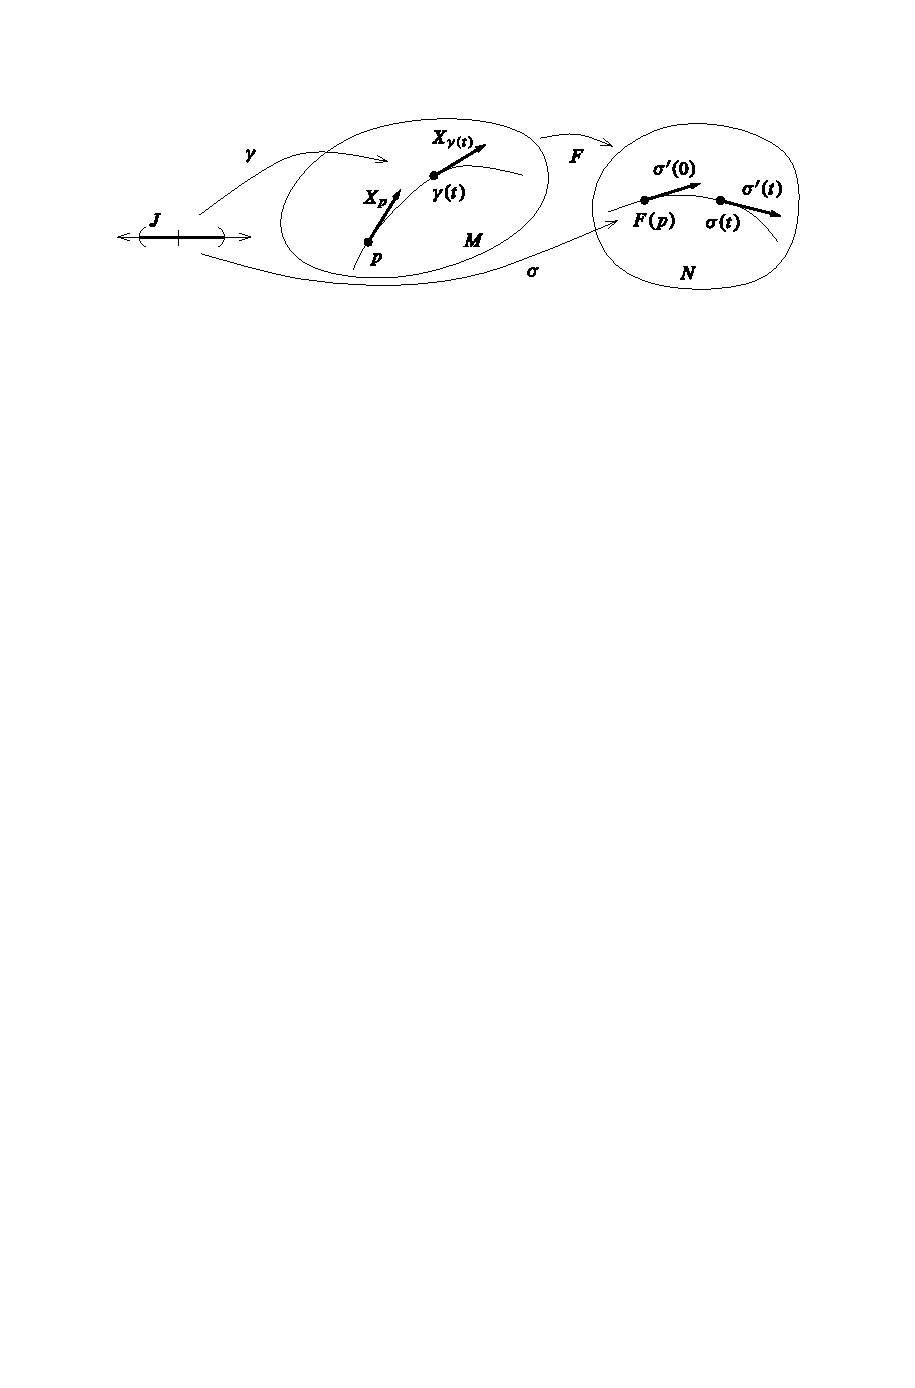
\includegraphics{pictures/integral-curve}
\caption{Flows of $F$-related vector fields.}
\end{figure}
\begin{proof}
Suppose first that $X$ and $Y$ are $F$-related, and  $\gamma:J\to M$ is an integral curve of $X$. If we define $\sigma:J\to N$ by $\sigma=F\circ\gamma$, then
\[\sigma'(t)=(F\circ\gamma)'(t)=dF_{\gamma(t)}\big(\gamma'(t)\big)=dF_{\gamma(t)}(X_{\gamma(t)})=Y_{\gamma(t)},\]
so $\sigma$ is an integral curve of $Y$.\par
Conversely, suppose $F$ takes integral curves of $X$ to integral curves of $Y$. Given $p\in M$, let $\gamma:(-\eps,\eps)\to M$ be an integral curve of $X$ starting at $p$. Since $F\circ\gamma$ is an integral curve of $Y$ starting at $F(p)$, we have
\[Y_{F(p)}=(F\circ\gamma)'(0)=dF_{p}\big(\gamma'(0)\big)=dF_p(X_p)\]
which shows that $X$ and $Y$ are $F$-related.
\end{proof}
\subsection{Flow}
Here is another way to visualize the family of integral curves associated with a vector field. Let $M$ be a smooth manifold and $V\in\X(M)$, and suppose that for each point $p\in M$, $V$ has a unique integral curve starting at $p$ and defined for all $t\in\R$, which we denote by $\theta^{(p)}:\R\to M$. (It may not always be the case that every integral curve is defined for all $t$, but for purposes of illustration let us assume so for the time being.) For each $t\in\R$, we can define a map $\theta_t:M\to M$ by sending each $p\in M$ to the point obtained by following for time $t$ the integral curve starting at $p$:
\[\theta_t(p)=\theta^{(p)}(t)\]
Each map $\theta_t$ \textit{slides} the manifold along the integral curves for time $t$. The translation lemma implies that $t\mapsto\theta^{(p)}(t+s)$ is an integral curve of $V$ starting at $q:=\theta^{(p)}(s)$; since we are assuming uniqueness of integral curves, $\theta^{(q)}(t)=\theta^{(p)}(t+s)$. When we translate this into a statement about the maps $\theta_t$, it becomes
\[\theta_t\circ\theta_s(p)=\theta_{t+s}(p)\]
Together with the equation $\theta_0(p)=p$, which holds by definition, this
implies that the map $\theta:\R\times M\to M$ is an action of the additive group $\R$ on $M$. Motivated by these observations, we define a \textbf{global flow} on $M$ (also called a \textbf{one-parameter group action}) to be a continuous left $\R$-action on $M$, that is, a continuous map $\theta:\R\times M\to M$ satisfying the following properties for all $s,t\in\R$ and $p\in M$:
\[\theta(t,\theta(s,p))=\theta(t+s,p),\quad\theta(0,p)=p.\]
Given a global flow $\theta$ on $M$, we define two collections of maps as follows:
\begin{itemize}
\item For each $t\in\R$, define a continuous map $\theta_t:M\to M$:
\[\theta_t(p)=\theta(t,p)\]
The defining properties of $\theta$ are equivalent to the \textbf{group laws}
\[\theta_t\circ\theta_s(p)=\theta_{t+s}(p),\quad\theta_0=\mathrm{id}_M.\]
As is the case for any continuous group action, each map $\theta_t:M\to M$ is a homeomorphism, and if the flow is smooth, $\theta_t$ is a diffeomorphism.
\item For each $p\in M$, define a curve $\theta^{(p)}:\R\to M$ by
\[\theta^{(p)}(t)=\theta(t,p)\]
The image of this curve is the orbit of $p$ under the group action.
\end{itemize}
The next proposition shows that every smooth global flow is derived from the
integral curves of some smooth vector field in precisely the way we described above. If $\theta:\R\times M\to M$ is a smooth global flow, for each $p\in M$ we define a tangent vector $V_p\in T_pM$ by
\[V_p=\dot{\theta}^{(p)}(0)\]
The assignment $p\mapsto V_p$ is a (rough) vector field on $M$ which is called the \textbf{infinitesimal generator of $\bm{\theta}$}, for reasons we will explain below.
\begin{proposition}\label{flow generate vector}
Let $\theta:\R\times M\to M$ be a smooth global flow on a smooth manifold $M$. The infinitesimal generator $V$ of $\theta$ is a smooth vector field on $M$, and each curve $\theta^{(p)}$ is an integral curve of $V$.
\end{proposition}
\begin{proof}
To show that $V$ is smooth, it suffices by Proposition~\ref{vector field smooth by function} to show that $Vf$ is smooth for every smooth real-valued function $f$ defined on an open subset $U\sub M$. For any such $f$ and any $p\in U$, just note that
\[Vf(p)=V_pf=\dot{\theta}^{(p)}(0)f=\frac{d}{dt}\Big|_{t=0}f\big(\theta^{(p)}(t)\big)=\frac{\partial}{\partial t}\Big|_{(0,p)}f\big(\theta(0,p)\big)\]
Because $f(\theta(t,p))$ is a smooth function of $(t,p)$ by composition, so is its partial derivative with respect to $t$. Thus, $Vf(p)$ depends smoothly on $p$, so $V$ is smooth.\par
Next we need to show that $\theta^{(p)}$ is an integral curve of $V$, which means that $\dot{\theta}^{(p)}(t)=V_{\theta^{(p)}(t)}$ for all $p\in M$ and all $t\in\R$. Let $t_0\in\R$ be arbitrary, and set $q=\theta^{(p)}(t_0)=\theta_{t_0}(p)$, so what we have to show is $\dot{\theta}^{(p)}(t_0)=V_q$. By the group law, for all $t$,
\[\theta^{(q)}(t)=\theta_t(q)=\theta_t\circ\theta_{t_0}(p)=\theta_{t+t_0}(p)=\theta^{(p)}(t+t_0)\]
Therefore, for any smooth real-valued function $f$ defined in a neighborhood of $q$,
\begin{align*}
V_qf=\dot{\theta}^{(q)}(0)f=\frac{d}{dt}\Big|_{t=0}(f\circ\theta^{(q)})(t)=\frac{d}{dt}\Big|_{t=0}(f\circ\theta^{(p)})(t+t_0)=\dot{\theta}^{(p)}(t_0)f
\end{align*}
which was to be shown.
\end{proof}
\begin{example}\label{flow eg}
The two vector fields on the plane described in Example~\ref{integral curve eg} both had integral curves defined for all $t\in\R$, so they generate global
flows. Using the results of that example, we can write down the flows explicitly.
\begin{itemize}
\item[(a)] The flow of $V=\partial/\partial x$ in $\R^2$ is the map $\tau:\R\times\R^2\to\R^2$ given by
\[\tau_t(x,y)=(x+t,y)\]
For each nonzero $t\in\R$, $\tau_t$ 0translates the plane to the right $(t>0)$ or left $(t<0)$ by a distance $|t|$.
\item[(b)] The flow of $W=x\partial/\partial y-y\partial/\partial x$ is the map $\theta:\R\times\R^2\to\R^2$ given by
\[\theta_t(x,y)=(x\cos t-y\sin t,x\sin t+y\cos t)=\begin{pmatrix}
\cos t&-\sin t\\
\sin t&\cos t
\end{pmatrix}\begin{pmatrix}
x\\
y
\end{pmatrix}\]
For each $t\in\R$, $\theta_t$ rotates the plane through an angle $t$ about the origin.
\end{itemize}
\end{example}
\subsection{The fundamental theorem on flows}
We have seen that every smooth global flow gives rise to a smooth vector field whose integral curves are precisely the curves defined by the flow. Conversely, we would like to be able to say that every smooth vector field is the infinitesimal generator of a smooth global flow. However, it is easy to see that this cannot be the case, because there are smooth vector fields whose integral curves are not defined for all $t\in\R$. Here are two examples.
\begin{example}
Let $M=\R^2-\{0\}$ with standard coordinates $(x,y)$, and let $V$ be the vector field $\partial/\partial x$ on $M$. The unique integral curve of $V$ starting at $(-1,0)\in M$ is $\gamma(t)=(t-1,0)$. However, in this case, $\gamma$ cannot be extended continuously past $t=1$. This is intuitively evident because of the hole in $M$ at the origin; to prove it rigorously, suppose $\widetilde{\gamma}$ is any continuous extension of $\gamma$ past $t=1$. Then $\gamma(t)\to\widetilde{\gamma}(1)\in\R^2-\{0\}$ as $t\to 1^-$. But we can also consider $\gamma$ as a map into $\R^2$ by composing with the inclusion $M\hookrightarrow\R^2$, and it is obvious from the formula that $\gamma(t)\to(0,0)$ as $t\mapsto 1^-$. Since limits in $\R^2$ are unique, this is a contradiction.
\end{example}
\begin{example}
For a more subtle example, let $M$ be all of $\R^2$ and let $W=x^2\partial/\partial x$. You can check easily that the unique integral curve of $W$ starting at $(1,0)$ is
\[\gamma(t)=(\frac{1}{1-t},0)\]
This curve also cannot be extended past $t=1$, because its $x$-coordinate is unbounded as $t\to 1^-$.
\end{example}
For this reason, we make the following definitions. If $M$ is a manifold, a \textbf{flow domain} for $M$ is an open subset $\mathcal{D}\sub\R\times M$ with the property that for each $p\in M$, the slice $\mathcal{D}^{(p)}=\{t\in\R:(t,p)\in\mathcal{D}\}$ is an open interval containing $0$. A \textbf{flow} on $M$ is a continuous map $\theta:\mathcal{D}\to M$ where $\mathcal{D}$ is a flow domain, that satisfies the following group laws: for all $p\in M$,
\begin{align}\label{group law-1}
\theta(0,p)=p
\end{align}
and for all $s\in\mathcal{D}^{(p)}$ and $t\in\mathcal{D}^{(\theta(s,p))}$ such that $s+t\in\mathcal{D}^{(p)}$,
\begin{align}\label{group law-2}
\theta\big(t,\theta(s,p)\big)=\theta(t+s,p)
\end{align}
\begin{figure}[htbp]
\centering
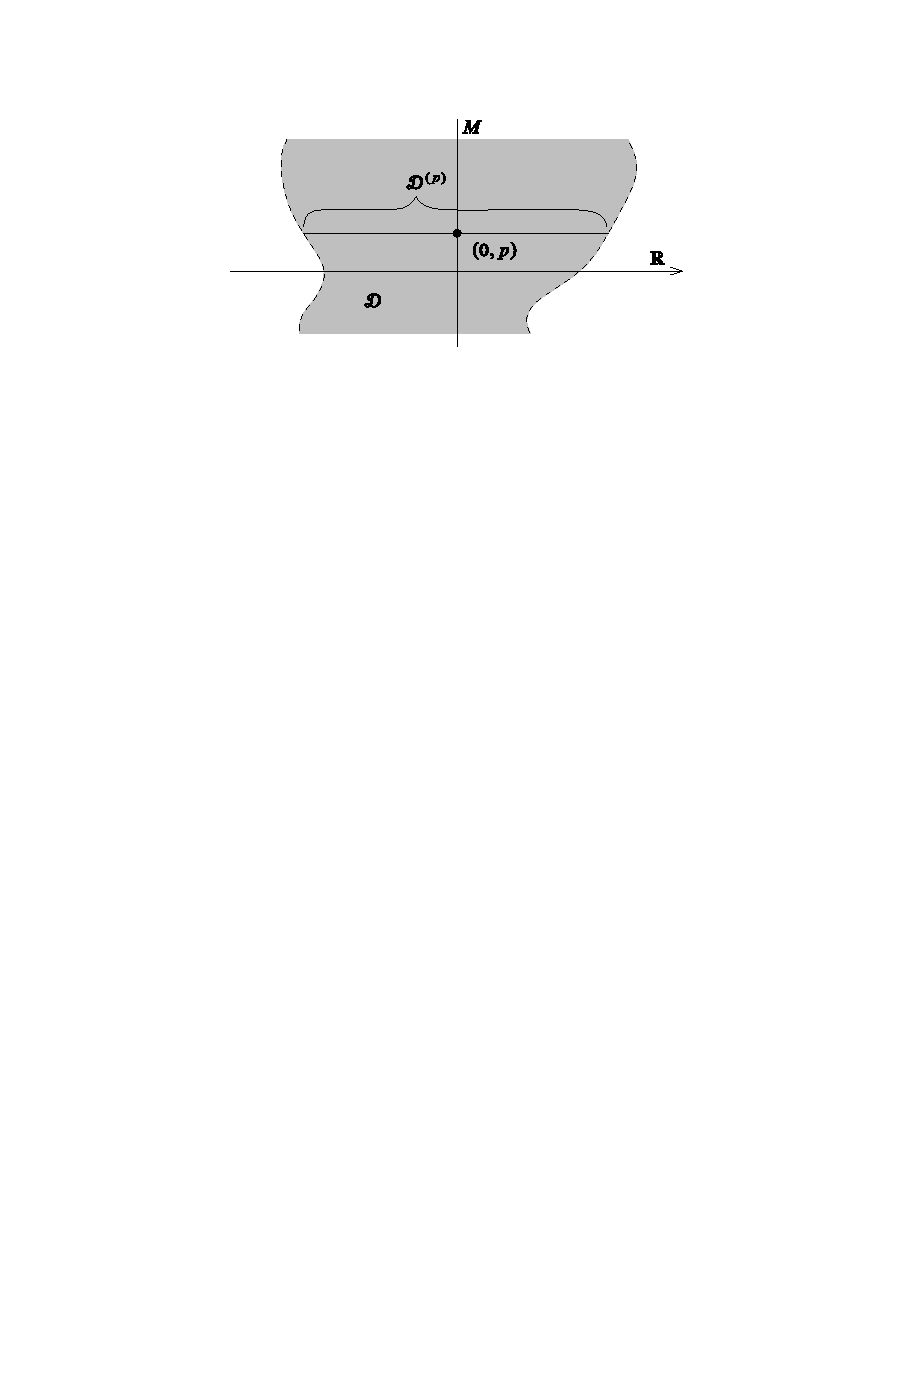
\includegraphics{pictures/flow-domain}
\caption{A flow domain.}
\end{figure}\par
We sometimes call $\theta$ a \textbf{local flow} to distinguish it from a global flow as defined earlier. The unwieldy term \textbf{local one-parameter group action} is also used.\par
If $\theta$ is a flow, we define $\theta_t(p)=\theta(t,p)$ whenever $(t,p)\in\mathcal{D}$, just as for a global flow. For each $t\in\R$, we also define
\[M_t=\{p\in M:(t,p)\in\mathcal{D}\}\]
so that
\[p\in M_t\iff t\in\mathcal{D}^{(p)}\iff(t,p)\in\mathcal{D}\]
If $\theta$ is smooth, the infinitesimal generator of $\theta$ is defined by $V_p=\dot{\theta}^{(p)}(0)$.
\begin{proposition}
If $\theta:\mathcal{D}\to M$ is a smooth flow, then the infinitesimal generator $V$ of $\theta$ is a smooth vector field, and each curve $\theta^{(p)}$ is an integral curve of $V$.
\end{proposition}
\begin{proof}
The proof is essentially identical to the analogous proof for global flows, Proposition~\ref{flow generate vector}. In the proof that $V$ is smooth, we need only note that for any $p_0\in M$, $\theta(t,p)$ is defined and smooth for all $(t,p)$ sufficiently close to $(0,p_0)$ because $\mathcal{D}$ is open. In the proof that $\theta^{(p)}$ is an integral curve, we need to verify that all of the expressions make sense. Suppose $t_0\in\mathcal{D}^{(p)}$. Because both $\mathcal{D}^{(p)}$ and $\mathcal{D}^{(\theta_{t_0}(p))}$ are open intervals containing $0$, there is a positive number $\eps$ such that $t+t_0\in\mathcal{D}^{(p)}$ and $t\in\mathcal{D}^{(\theta_{t_0}(p))}$ whenever $|t|<\eps$, and then $\theta_t(\theta_{t_0}(p))=\theta_{t+t_0}(p)$ by definition of a flow. The rest of the proof goes through just as before.
\end{proof}
The next theorem is the main result of flows. A \textbf{maximal integral curve} is one that cannot be extended to an integral curve on any larger open interval, and a \textbf{maximal flow} is a flow that admits no extension to a flow on a larger flow domain.
\begin{theorem}[\textbf{Fundamental Theorem on Flows}]\label{flow fundamental thm}
Let $V$ be a smooth vector field on a smooth manifold $M$. There is a unique smooth maximal flow $\theta:\mathcal{D}\to M$ whose infinitesimal generator is $V$. This flow has the following properties:
\begin{itemize}
\item[(a)] For each $p\in M$, the curve $\theta^{(p)}:\mathcal{D}^{(p)}\to M$ is the unique maximal integral curve of $V$ starting at $p$.
\item[(b)] If $s\in\mathcal{D}^{(p)}$, then $\mathcal{D}^{(\theta(s,p))}$ is the interval $\mathcal{D}^{(p)}-s=\{t-s:t\in\mathcal{D}^{(p)}\}$.
\item[(c)] For each $t\in\R$, the set $M_t$ is open in $M$, and $\theta_t:M_t\to M_{-t}$ is a diffeomorphism with inverse $\theta_{-t}$.
\end{itemize}
\end{theorem}
\begin{proof}
Proposition~\ref{integral curve local exsit} shows that there exists an integral curve starting at each point $p\in M$. Suppose $\gamma,\widetilde{\gamma}:J\to M$ are 
two integral curves of $V$ defined on the same open interval $J$ such that $\gamma(t_0)=\widetilde{\gamma}(t_0)$ for some $t_0\in J$. Let $\mathcal{S}$ be the set 
of $t\in J$ such that $\gamma(t)=\widetilde{\gamma}(t)$. Clearly, $\mathcal{S}\neq\emp$, because $t_0\in\mathcal{S}$ by hypothesis, and $\mathcal{S}$ is closed in 
$J$ by continuity. On the other hand, suppose $t_1\in\mathcal{S}$. Then in a smooth coordinate neighborhood around the point $p=\gamma(t_1)$, $\gamma$ and 
$\widetilde{\gamma}$ are both solutions to same ODE with the same initial condition $\gamma(t_1)=\widetilde{\gamma}(t_1)=p$. By the uniqueness theorem of ODEs, 
$\gamma\equiv\widetilde{\gamma}$ on an interval containing $t_1$, which implies that $\mathcal{S}$ is open in $J$. Since $J$ is connected, $\mathcal{S}=J$, which 
implies that $\gamma\equiv\widetilde{\gamma}$ on all of $J$. Thus, any two integral curves that agree at one point agree on their common domain.\par
For each $p\in M$, let $\mathcal{D}^{(p)}$ be the union of all open intervals $J\sub\R$ containing $0$ on which an integral curve starting at $p$ is defined. 
Define $\theta^{(p)}:\mathcal{D}^{(p)}\to M$ by letting $\theta^{(p)}(t)=\gamma(t)$, where $\gamma$ is any integral curve starting at $p$ and defined on an open 
interval containing $0$ and $t$. Since all such integral curves agree at $t$ by the argument above, $\theta^{(p)}(t)$ is well defined, and is obviously the unique 
maximal integral curve starting at $p$.\par
Now let $\mathcal{D}=\{(t,p)\in\R\times M:t\in\mathcal{D}^{(p)}\}$ and define $\theta(t,p)=\theta^{(p)}(t)$. As usual, we also write $\theta_t(p)=\theta(t,p)$. 
By definition, $\theta$ satisfies property (a) in the statement of the fundamental theorem: for each $p\in M$, $\theta^{(p)}(t)$ is the unique maximal integral 
curve of $V$ starting at $p$. To verify the group laws, fix any $p\in M$ and $s\in\mathcal{D}^{(p)}$, and write $q=\theta(s,p)=\theta^{(p)}(s)$. The curve 
$\gamma:\mathcal{D}^{(p)}-s\to M$ defined by $\gamma(t)=\theta^{(p)}(t+s)$ starts at $q$, and the translation lemma shows that $\gamma$ is an integral curve 
of $V$. By uniqueness of ODE solutions, $\gamma$ agrees with $\theta^{(q)}$ on their common domain, which is equivalent to the second group law $(\ref{group law-2})$, 
and the first group law $(\ref{group law-1})$ is immediate from the definition. By maximality of $\theta^{(q)}$, the domain of $\gamma$ cannot be larger than 
$\mathcal{D}^{(q)}$, which means that $\mathcal{D}^{(p)}-s\sub\mathcal{D}^{(q)}$. Since $0\in\mathcal{D}^{(p)}$, this implies that $-s\in\mathcal{D}^{(q)}$, and 
the group law implies that $\theta^{(q)}(-s)=p$. Applying the same argument with $(-s,q)$ in place of $(s,p)$, we find that $\mathcal{D}^{(q)}+s\sub\mathcal{D}^{(p)}$, 
which is the same as $\mathcal{D}^{(q)}\sub\mathcal{D}^{(p)}-s$. This proves (b).\par
Next we show that $\mathcal{D}$ is open in $\R\times M$ (so it is a flow domain), and that $\theta:\mathcal{D}\to M$ is smooth. Define a subset $W\sub\mathcal{D}$ 
as the set of all $(t,p)\in\mathcal{D}$ such that $\theta$ is defined and smooth on a product neighborhood of $(t,p)$ of the form $J\times U$ where $J\sub\R$ is 
an open interval containing $0$ and $t$, $U\sub M$ is a neighborhood of $p$. Then $W$ is open in $\R\times M$, and the restriction of $\theta$ to $W$ is smooth, 
so it suffices to show that $W=\mathcal{D}$. Suppose this is not the case. Then there exists some point $(\tau,p_0)\in\mathcal{D}-W$. For simplicity, assume $\tau>0$, 
the argument for $\tau<0$ is similar.
\begin{figure}[htbp]
\centering
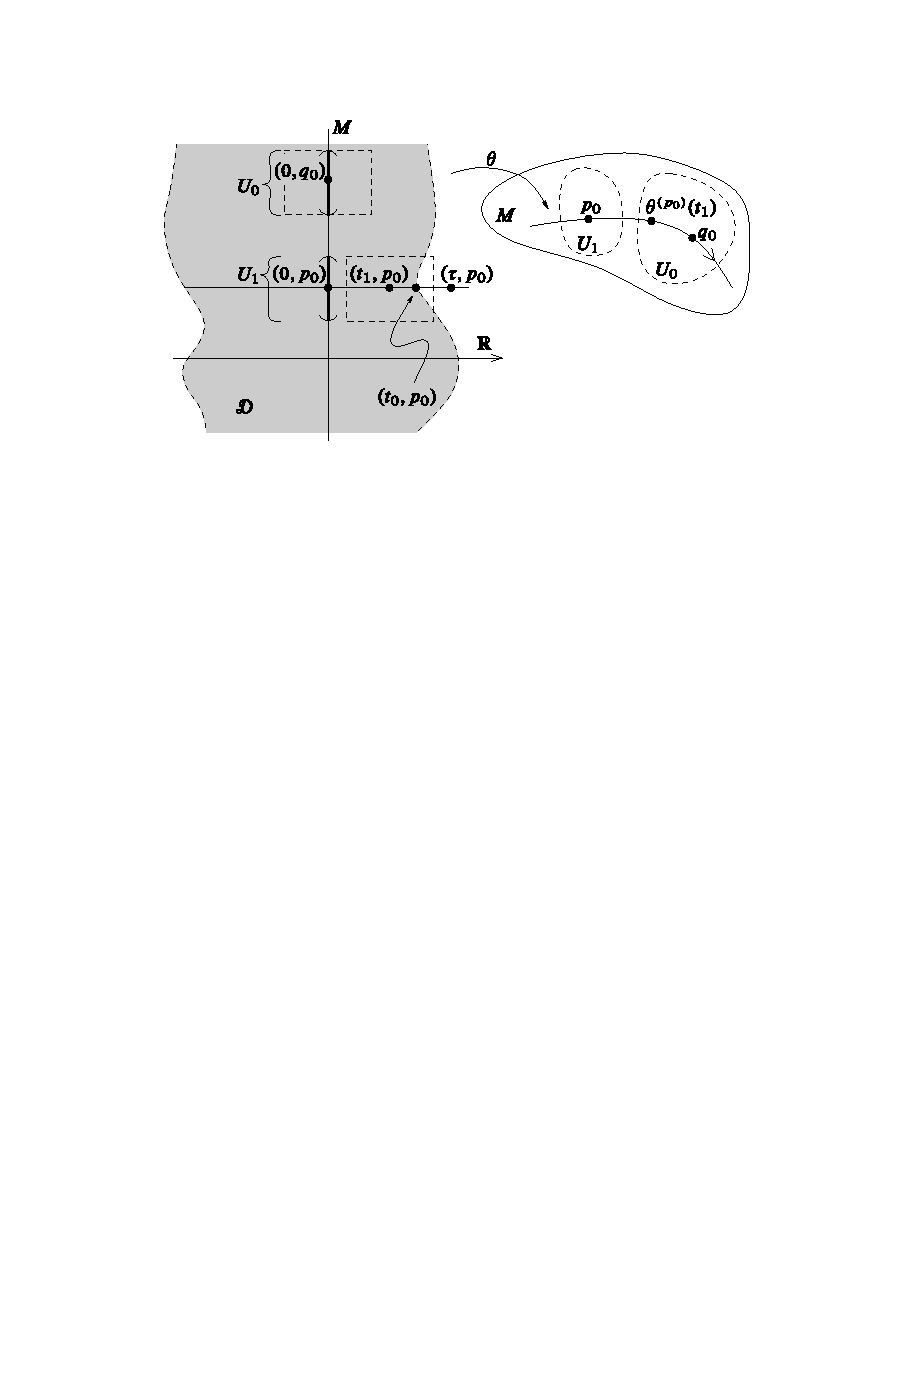
\includegraphics{pictures/flow-thm}
\caption{Proof that $\mathcal{D}$ is open.}
\end{figure}\par
Let $t_0=\sup\{t\in\R:(t,p_0)\in W\}$. By the existence and uniquess theorem of ODEs applied in
smooth coordinates around $p_0$, we know that $\theta$ is defined and smooth in some product neighborhood of $(0,p_0)$, so $t_0>0$. Since $t_0\leq\tau$ and $\mathcal{D}^{(p_0)}$ is an open interval containing $0$ and $\tau$, it follows that $t_0\in\mathcal{D}^{(p_0)}$. Let $q_0=\theta^{(p_0)}(t_0)$. By the ODE theorem again, there exist $\eps>0$ and a neighborhood $U_0$ of $q_0$ such that $(-\eps,\eps)\times U_0\sub W$. We will use the group law to show that $\theta$ extends smoothly to a neighborhood of $(t_0,p_0)$, which is a contradiction.\par
Choose some $t_1<t_0$ such that $t_1+\eps>t_0$ and $\theta^{(p_0)}(t_1)\in U_0$. Since $t_1<t_0$, we have $(t_1,p_0)\in W$, and so there is a product neighborhood $(t_1-\delta,t_1+\delta)\times U_1\sub W$. Because $\theta(t_1,p_0)\in U_0$, we can choose $U_1$ small enough that $\theta$ maps $\{t_1\}\times U_1$ into $U_0$. Define $\widetilde{\theta}:[0,t_1+\eps)\times U_1\to M$ by
\[\widetilde{\theta}(t,p)=\begin{cases}
\theta_t(p)&p\in U_1,0\leq t\leq t_1,\\
\theta_{t-t_1}\circ\theta_{t_1}(p)&p\in U_1,t_1-\eps<t<t_1+\eps
\end{cases}\]
The group law for $\theta$ guarantees that these definitions agree where they overlap, and our choices of $U_1,t_1$, and $\theta$ ensure that this defines a smooth map. By the translation lemma, each map $t\mapsto\theta_t(p)$ is an integral curve of $V$, so $\widetilde{\theta}$ is a smooth extension of $\theta$ to a neighborhood of $(t_0,p_0)$, contradicting our choice of $t_0$. This completes the proof that $W=\mathcal{D}$.\par
Finally, we prove (c). The fact that $M_t$ is open is an immediate consequence of the fact that $\mathcal{D}$ is open. From part (b) we deduce
\begin{align*}
p\in M_t\Rightarrow t\in\mathcal{D}^{(p)}\Rightarrow\mathcal{D}^{(\theta_t(p))}=\mathcal{D}^{(p)}-t\Rightarrow-t\in\mathcal{D}^{(\theta_t(p))}\Rightarrow\theta_t(p)\in M_{-t}
\end{align*}
which shows that $\theta_t$ maps $M_t$ to $M_{-t}$. Moreover, the group laws then show that $\theta_{-t}\circ\theta_{t}$ is equal to the identity on $M_t$. Reversing the roles of $t$ and $-t$ shows that $\theta_{t}\circ\theta_{-t}$ is the identity on $M_{-t}$, which completes the proof.
\end{proof}
The flow whose existence and uniqueness are asserted in the fundamental theorem is called the \textbf{flow generated by $\bm{V}$}, or just the \textbf{flow of $\bm{V}$}. Now we give an example of this.
\begin{figure}[htbp]
\centering
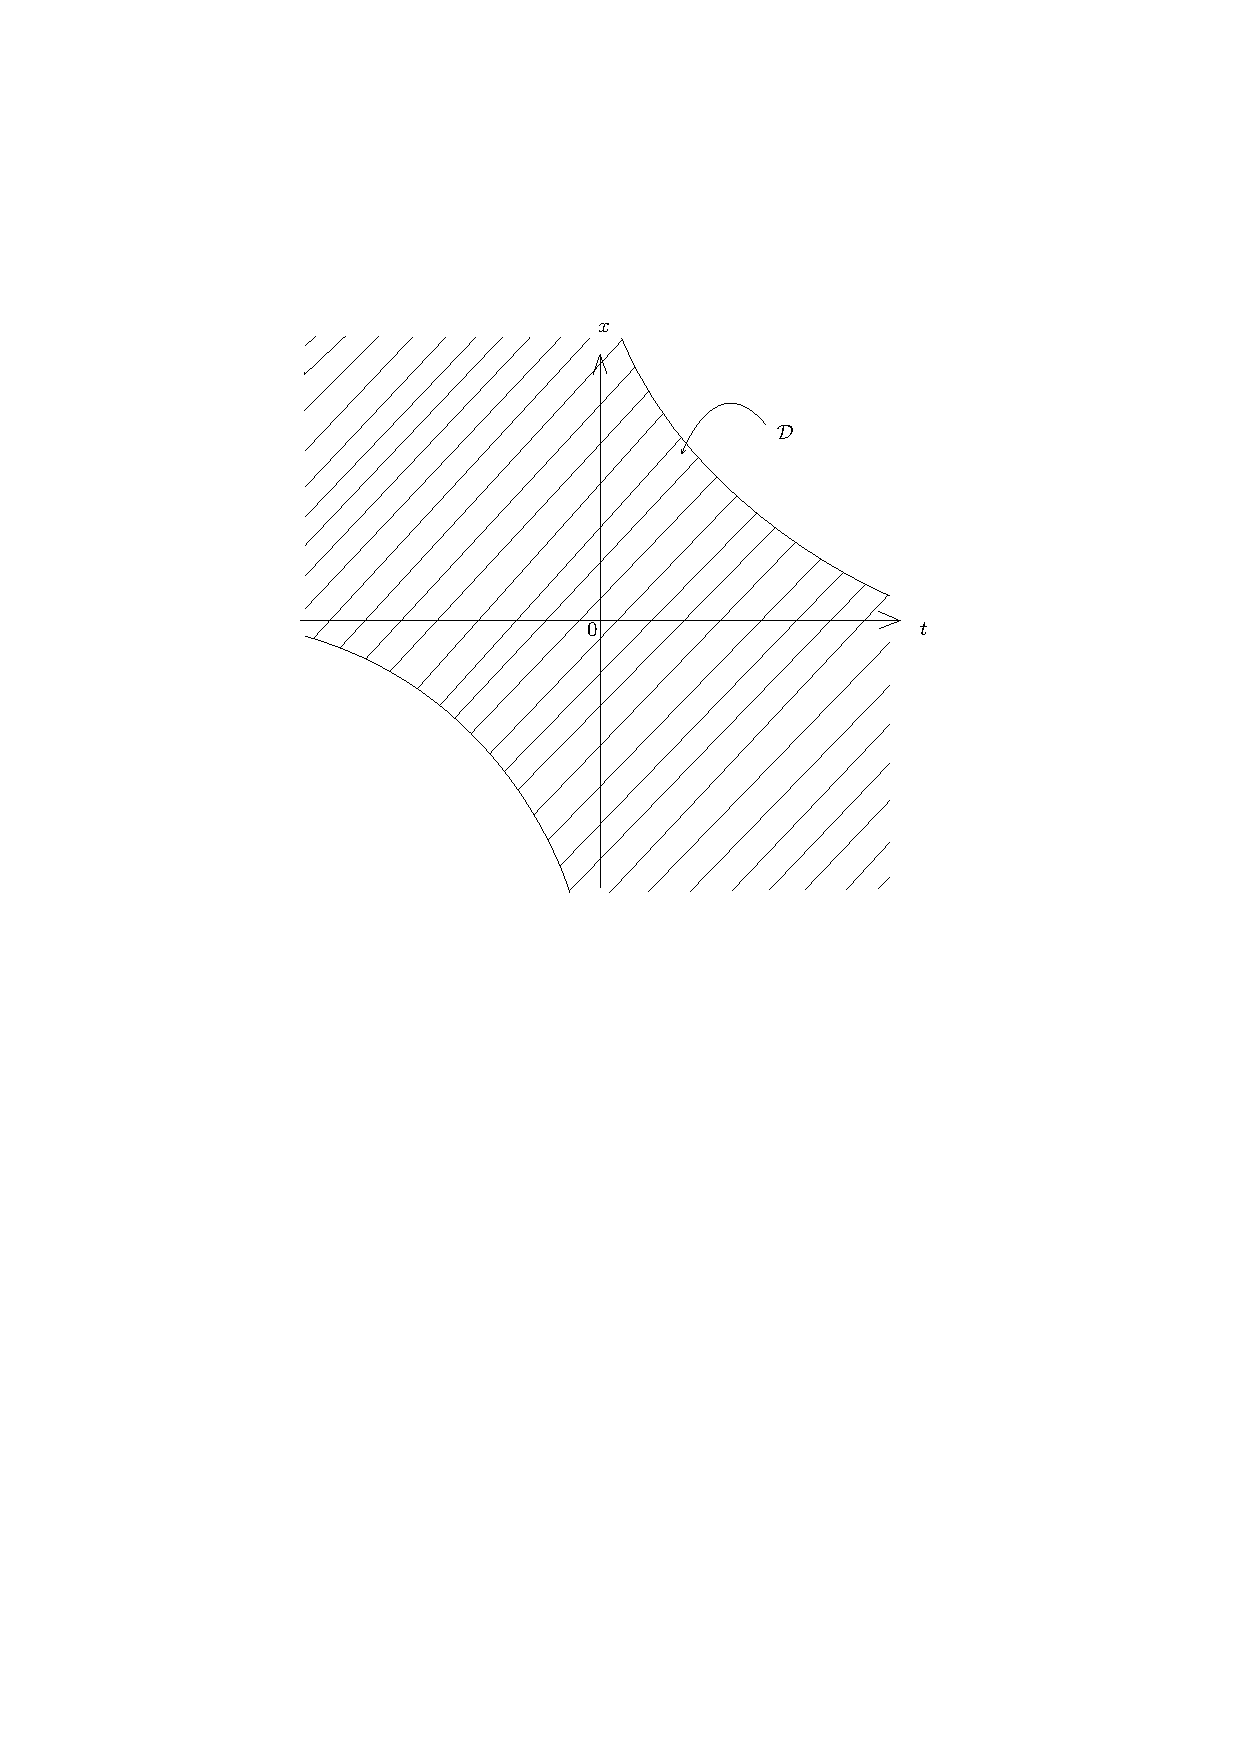
\includegraphics[width=0.5\textwidth]{pictures/flow-domain-eg}
\caption{The flow domain in Example~\ref{flow doamin eg}.}
\end{figure}
\begin{example}\label{flow doamin eg}
Let $V=x^2\partial/\partial x$ be a vector field on $\R$, we can check that the unique integral curve of $V$ starting at $x$ is
\[\theta(t,x)=\gamma_x(t)=\begin{cases}
\dfrac{1}{x^{-1}-t}&x\neq 0;\\
0&x=0.
\end{cases}\]
Thus the flow domain of $V$ is 
\[\mathcal{D}=\{(t,x):t>0,x<1/t\}\cup\{(t,x):t<0,x>1/t\}.\]

Now for $x>0$ and $t\in(-\infty,1/x)$, we check that
\[\theta(t,x)=\frac{1}{x^{-1}-t},\quad \mathcal{D}^{(\theta(t,x))}=(-\infty,\frac{1}{x}-t)=\mathcal{D}^{(x)}-t.\]
\end{example}
\begin{theorem}[\textbf{Naturality of Flows}]\label{flow naturality}
Suppose $M$ and $N$ are smooth manifolds, $F:M\to N$ is a smooth map, $X\in\X(M)$, and $Y\in\X(N)$. Let $\theta$ be the flow of $X$ and $\eta$ the flow of $Y$. If $X$ and $Y$ are $F$-related, then for each $t\in\R$, $F(M_t)\sub N_t$ and $\eta_t\circ F=F\circ\theta_t$ on $M_t$:
\[\begin{tikzcd}
M_t\ar[d,"\theta_t"]\ar[r,"F"]&N_t\ar[d,"\eta_t"]\\
M_{-t}\ar[r,"F"]&N_{-t}
\end{tikzcd}\]
\end{theorem}
\begin{proof}
By Proposition~\ref{integral curve naturality}, for any $p\in M$, the curve $F\circ\theta^{(p)}$ is an integral curve of $Y$ starting at $F\circ\theta^{(p)}(0)=F(p)$. By uniqueness of integral curves, therefore, the maximal integral curve $\eta^{(F(p))}$ must be defined at least on the interval $\mathcal{D}^{(p)}$, and $F\circ\theta^{(p)}=\eta^{(F(p))}$ on that interval. This means that
\[p\in M_t\Rightarrow t\in\mathcal{D}^{(p)}\Rightarrow t\in\mathcal{D}^{(F(p))}\Rightarrow F(p)\in N_t,\]
which is equivalent to $F(M_t)\sub N_t$, and
\[F\big(\theta^{(p)}(t)\big)=\eta^{(F(p))}(t)\for t\in\mathcal{D}^{(p)}\]
which is equivalent $\eta_t\circ F=F\circ\theta_t$ for all $p\in M_t$.
\end{proof}
The next corollary is immediate.
\begin{corollary}[\textbf{Diffeomorphism Invariance of Flows}]
Let $F:M\to N$ be a diffeomorphism. If $X\in\X(M)$ and $\theta$ is the flow of $X$, then the flow of $F^*X$ is $\eta_t=F\circ\theta_t\circ F^{-1}$, with domain $N_t=F(M_t)$ for each $t\in\R$.
\end{corollary}
\subsubsection{Complete vector fields}
As we observed earlier in this chapter, not every smooth vector field generates a global flow. The ones that do are important enough to deserve a name. We say that a smooth vector field is \textbf{complete} if it generates a global flow, or equivalently if each of its maximal integral curves is defined for all $t\in\R$.\par
We will show below that all compactly supported smooth vector fields, and therefore all smooth vector fields on a compact manifold, are complete. The proof will be based on the following lemma.
\begin{lemma}[\textbf{Uniform Time Lemma}]
Let $V$ be a smooth vector field on a smooth manifold $M$, and let $\theta$ be its flow. Suppose there is a positive number $\eps$ such that for every $p\in M$, the domain of $\theta^{(p)}$ contains $(-\eps,\eps)$. Then $V$ is complete.
\end{lemma}
\begin{proof}
Suppose for the sake of contradiction that for some $p\in M$, the domain $\mathcal{D}^{(p)}$ of $\theta^{(p)}$ is bounded above. (A similar proof works if it is bounded below.) Let $b=\sup\mathcal{D}^{(p)}$, let $t_0$ be a positive number such that $b-\eps<t_1<b$, and let $q=\theta^{(p)}(t_0)$. The hypothesis implies that $\theta^{(q)}(t)$ is defined at least for $t\in(-\eps,\eps)$. Define a curve $\gamma:(-\eps,t_0+\eps)\to M$ by
\[\gamma(t)=\begin{cases}
\theta^{(p)}(t),&-\eps<t<b\\
\theta^{(q)}(t-t_0),&t_0-\eps<t<t_0+\eps
\end{cases}\]
These two definitions agree where they overlap, because
\[\theta^{(q)}(t-t_0)=\theta_{t-t_0}(q)=\theta_{t-t_0}\theta_{t_0}(p)=\theta_t(p)\]
by the group law for $\theta$. By the translation lemma, $\gamma$ is an integral curve starting at $p$. Since $t_0+\eps>b$, this is a contradiction.
\end{proof}
\begin{theorem}\label{vector field compact supp complete}
Every compactly supported smooth vector field on a smooth manifold is complete.
\end{theorem}
\begin{proof}
Suppose $V$ is a compactly supported vector field on a smooth manifold $M$, and let $K=\supp(V)$. For each $p\in K$, there is a neighborhood $U_p$ of $p$ and a positive number $\eps_p$ such that the flow of $V$ is defined at least on $(-\eps_p,\eps_p)\times U_p$. By compactness, finitely many such sets $U_{p_1},\dots,U_{p_k}$ cover $K$. With $\eps:=\min\{\eps_{p_i}\}$, it follows that every maximal integral curve starting in $K$ is defined at least on $(-\eps,\eps)$. Since $V\equiv 0$ outside of $K$, every integral curve starting in $M-K$ is constant and thus can be defined on all of $\R$. Thus the hypotheses of the uniform time lemma are satisfied, so $V$ is complete.
\end{proof}
\begin{corollary}\label{vector field compact mani complete}
On a compact smooth manifold, every smooth vector field is
complete.
\end{corollary}
Left-invariant vector fields on Lie groups form another class of vector fields that are always complete.
\begin{theorem}\label{vector field left-inva complete}
Every left-invariant vector field on a Lie group is complete.
\end{theorem}
\begin{proof}
Let $G$ be a Lie group, let $X\in\Lie(G)$, and let $\theta:\mathcal{D}\to G$ denote the flow of $X$. There is some $\eps>0$ such that $\theta^{(e)}$ is defined on $(-\eps,\eps)$.\par Let $g\in G$ be arbitrary. Because $X$ is $L_g$-related to itself, it follows from Proposition~\ref{integral curve naturality} that the curve $L_g\circ\theta^{(e)}$ is an integral curve of $X$ starting at $g$ and therefore is equal to $\theta^{(g)}$. This shows that for each $g\in G$, the integral curve $\theta^{(p)}$ is defined at least on $(-\eps,\eps)$, so the uniform time lemma guarantees that $X$ is complete.
\end{proof}
Here is another useful property of integral curves.
\begin{lemma}[\textbf{Escape Lemma}]\label{vector flow escape lemma}
Suppose $M$ is a smooth manifold and $V\in\X(M)$. If $\gamma:J\to M$ is a maximal integral curve of $V$ whose domain $J$ has a finite least upper bound $b$, then for any $t_0\in J$, the set $\gamma\big([t_0,b)\big)$ is not contained in any compact subset
of $M$.
\end{lemma}
\begin{proof}
Let $p=\gamma(0)$ and $\theta$ denote the flows of $V$ so that $\gamma(t)=\theta^{(p)}(t)$. Assume 
that there is a $t_0\in J$ such that $\gamma\big([t_0,b)\big)$ lies in a compact set $K\sub M$, we 
claim that $\gamma$ can be extended past $b$.
\begin{itemize}
\item We use sequentially compactness: let $(x_n)$ be any sequence tends to $b$ from below, since $\{\gamma(x_n)\}$ is contained in a compact set, it has a subsequence converging to a point $q\in M$.
\item By theorem~\ref{flow fundamental thm}, there is $\eps>0$ and a neighborhood of $q$ such that $\theta$ is defined on $(-\eps,\eps)\times U$.
\item By discrading finitely many terms, we may assume that $\gamma(x_i)\in U$ and $t_i>b-\eps$. Then define $\sigma:[t_0,b+\eps)\to M$ by
\[\sigma(t)=\begin{cases}
\gamma(t)&t_0\leq t<b,\\
\theta_{t-t_i}\circ\theta_{t_i}(p),&t_i-\eps<t<t_i+\eps.
\end{cases}\]
This map is defined for all $t\in[b,b+\eps)$ since $t_i\to b$, and the two definitions agree where they overlap, as
\[\theta_{t-t_i}\circ\theta_{t_i}(p)=\theta_t(p)=\gamma(t)\]
\end{itemize}
This contradicts the maximality, so our claim follows.
\end{proof}
\subsection{Flowouts}
Flows provide the technical apparatus for many geometric constructions on manifolds. Most of those constructions are based on the following general theorem,
which describes how flows behave in the vicinity of certain submanifolds.
\begin{theorem}[\textbf{Flowout Theorem}]\label{flowout}
Suppose $M$ is a smooth manifold, $S\sub M$ is an embedded $k$-dimensional submanifold, and $V\sub\X(M)$ is a smooth vector field that is nowhere tangent to $S$. Let $\theta:\mathcal{D}\to M$ be the flow of $V$, let $\mathcal{O}=(\R\times S)\cap\mathcal{D}$, and let $\varPhi=\theta|_{\mathcal{O}}$.
\begin{itemize}
\item[(a)] $\varPhi:\mathcal{O}\to M$ is an immersion.
\item[(b)] $\partial/\partial t\in\X(\mathcal{O})$ is $\varPhi$-related to $V$.
\item[(c)] There exists a smooth positive function $\delta:S\to\R$ such that the restriction of $\varPhi$ to $\mathcal{O}_{\delta}$ is injective, where $\mathcal{O}_{\delta}\sub\mathcal{O}$ is the flow domain
\begin{align}\label{flowout thm-1}
\mathcal{O}_{\delta}=\{(t,p)\in\mathcal{O}:|t|<\delta(p)\}
\end{align}
Thus, $\varPhi(\mathcal{O}_{\delta})$ is an immersed submanifold of $M$ containing $S$, and $V$ is tangent to this submanifold.
\item[$(d)$] If $S$ has codimension $1$, then $\varPhi|_{\mathcal{O}_\delta}$ is a diffeomorphism onto an open submanifold of $M$.
\end{itemize}
\end{theorem}
\begin{figure}[htbp]
\centering
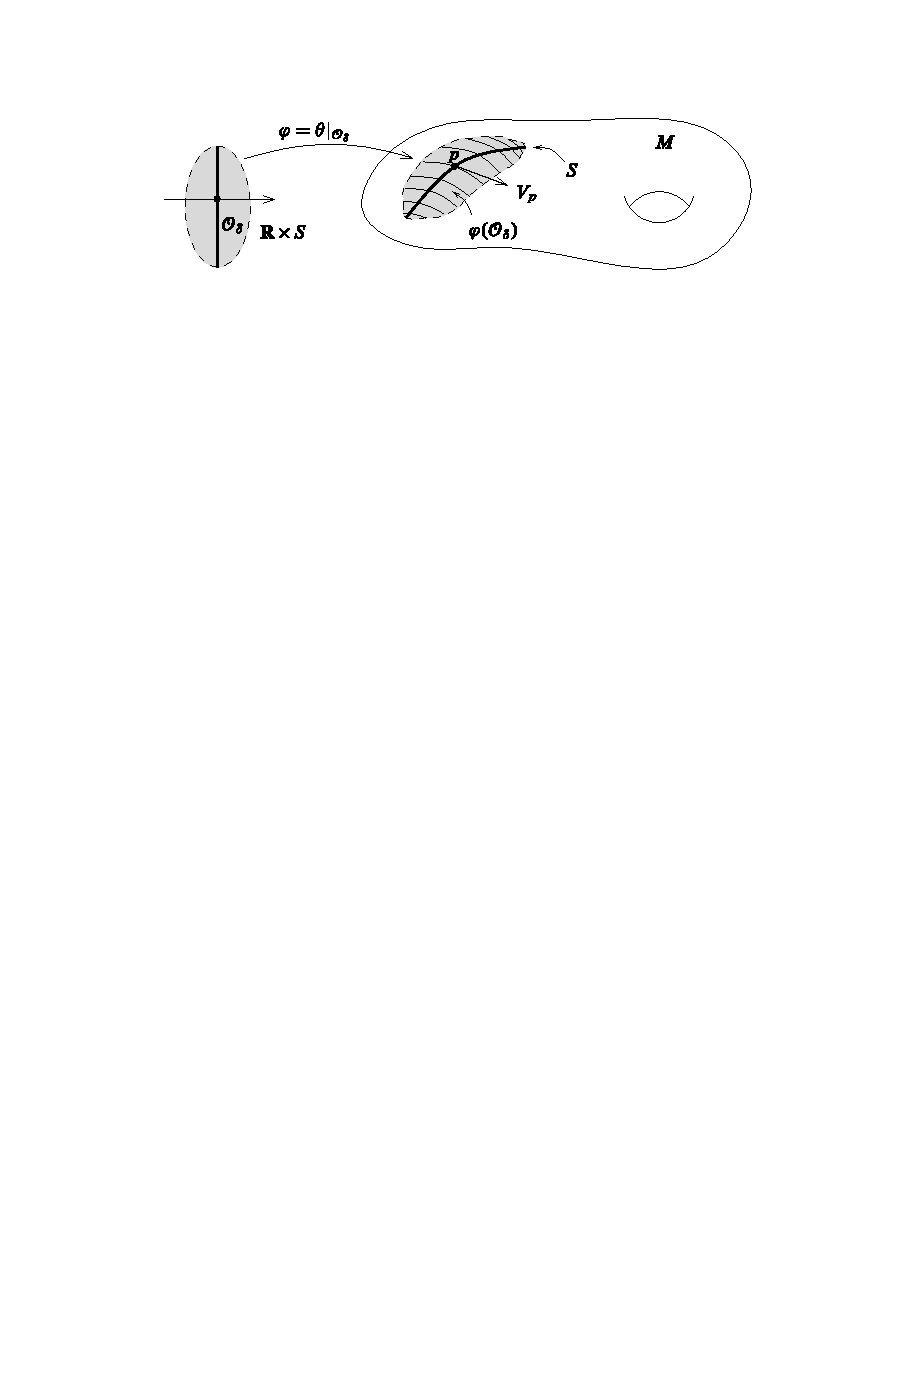
\includegraphics{pictures/flowout}
\caption{A flowout.}
\end{figure}
\begin{remark}
The submanifold $\varPhi({\mathcal{O}_\delta})\sub M$ is called a \textbf{flowout from $S$ along $V$}.
\end{remark}
\begin{proof}
First we prove (b). Fix some $p\in S$, and let $\sigma:\mathcal{D}^{(p)}\to\R\times S$ be the curve $\sigma(t)=(t,p)$. Then $\varPhi\circ\sigma(t)=\theta(t,p)$ is an integral curve of $V$, so for any $t_0\in\mathcal{D}^{(p)}$ it follows that
\[d\varPhi_{(t_0,p)}\Big(\frac{\partial}{\partial t}\Big|_{(t_0,p)}\Big)=(\varPhi\circ\sigma)'(t_0)=V_{\varPhi(t_0,p)}.\]

Next we prove (a). The restriction of $\varPhi$ to $\{0\}\times S$ is the composition of the diffeomorphism $\{0\}\times S\approx S$ with the embedding $S\hookrightarrow M$, so it is an embedding. Thus, the restriction of $d\varPhi_{(0,p)}$ to $T_pS$ (viewed as a subspace of $T_{(0,p)}\mathcal{O}\cong T_0\R\oplus T_pS$) is the inclusion $T_pS\hookrightarrow T_pM$. If $(E_1,\dots,E_k)$ is any basis for $T_pS$, it follows that $d\varPhi_{(0,p)}$ maps the basis $(\partial/\partial t|_{(0,p)},E_1,\dots,E_k)$ for $T_{(0,p)}\mathcal{O}$ to $(V_p,E_1,\dots,E_k)$. Since $V_p$ is not tangent to $S$, this $(k+1)$-tuple is linearly independent and thus $d\varPhi_{(0,p)}$ is injective.\par
To show $d\varPhi$ is injective at other points, we argue as in the proof of the equivariant rank theorem. Given $(t_0,p_0)\in\mathcal{O}$, let $\tau_{t_0}:\mathcal{O}\to\R\times S$ be the translation $\tau_{t_0}(t,p)=(t+t_0,p)$. By the group law for $\theta$, the following diagram commutes (where the horizontal maps might be defined only in open subsets containing $(0,p_0)$ and $p_0$, respectively):
\[\begin{tikzcd}
\mathcal{O}\ar[r,"\tau_{t_0}"]\ar[d,swap,"\varPhi"]&\mathcal{O}\ar[d,"\varPhi"]\\
M\ar[r,"\theta_{t_0}"]&M
\end{tikzcd}\]
Both horizontal maps in the diagram above are local diffeomorphisms. Taking differentials, we obtain
\[\begin{tikzcd}
T_{(0,p_0)}\mathcal{O}\ar[rr,"d(\tau_{t_0})_{(0,p_0)}"]\ar[d,swap,"d\varPhi_{(0,p_0)}"]&&T_{(t_0,p_0)}\mathcal{O}\ar[d,"d\varPhi_{(t_0,p_0)}"]\\
T_{p_0}M\ar[rr,"d(\theta_{t_0})_{p_0}"]&&T_{\varPhi(t_0,p_0)}M
\end{tikzcd}\]
Because the horizontal maps are isomorphisms, the two vertical maps have the same
rank. Since we have already shown that $d\varPhi_{(0,p_0)}$ has full rank, so does $d\varPhi_{(t_0,p_0)}$. This completes the proof that $\varPhi$ is an immersion.\par
Next we prove (c). Given a point $p_0\in S$, choose a slice chart $(U,(x^i))$ for $S$ in $M$ centered at $p_0$, so that $U\cap S$ is the set where $x^{k+1}=\cdots=x^n=0$ (where $n=\dim M$). Because $V$ is not tangent to $S$, one of the last $n-k$ components of $V_{p_0}$, say $V^j_{p_0}$, must be nonzero. Shrinking $U$ if necessary, we may assume that there is a constant $c>0$ such that
\begin{align}\label{flowout thm-2}
|V^j_p|\geq c\for p\in U.
\end{align}
Since $\varPhi^{-1}(U)$ is open in $\R\times S$, we may choose a number $\eps_{p_0}>0$ and a neighborhood $W_{p_0}$ of $p_0$ in $S$ such that $(-\eps_{p_0},\eps_{p_0})\times W_{p_0}\sub\mathcal{O}$ and $\varPhi\big((-\eps_{p_0},\eps_{p_0})\times W_{p_0}\big)\sub U$. Write the component functions of $\varPhi$ in these local coordinates as
\[\varPhi(t,p)=\big(\varPhi^1(t,p),\dots,\varPhi^n(t,p)\big)\]
Because $\varPhi$ is the restriction of the flow, the component function $\varPhi^j$ satisfies
\[\frac{\partial\varPhi^j}{\partial t}(t,p)=V^j\big(\varPhi(t,p)\big),\quad\varPhi^j(0,p)=p\]
By $(\ref{flowout thm-2})$ and the fundamental theorem of calculus, $|\varPhi^j(t,p)|\geq c|t|$, and thus for $(t,p)\in(-\eps_{p_0},\eps_{p_0})\times W_{p_0}$ we conclude that $\varPhi(t,p)\in S$ if and only if $t=0$.\par
Choose a smooth partition of unity $\{\psi_p:p\in S\}$ subordinate to the open cover $\{W_p:p\in S\}$ of $S$, and define $f:S\to\R$ by
\[f(q)=\sum_{p\in S}\eps_p\psi_p(q)\]
Then $f$ is smooth and positive. For each $q\in S$, there are finitely many $p\in S$ such that $\psi_p(q)>0$; if $p_1$ is one of these points such that $\eps_{p_1}$ is maximum among all such $\eps_p$, then
\[f(q)\leq\eps_{p_1}\sum_{p\in S}\psi_p(q)=\eps_{p_1}\]
It follows that if $(t,q)\in\mathcal{O}$ such that $|t|<f(q)$, then $(t,q)\in(-\eps_{p_1},\eps_{p_1})\times W_{p_1}$, so $\varPhi(t,q)\in S$ if and only if $t=0$.\par
Let $\delta=f/2$. We will show that $\varPhi|_{\mathcal{O}_\delta}$ is injective, where $\mathcal{O}_{\delta}$ is defined by $(\ref{flowout thm-1})$. Suppose $\varPhi(t,q)=\varPhi(t',q')$ for some $(t,q),(t',q')\in\mathcal{O}_{\delta}$. By renaming the points if necessary, we may arrange that $f(q')\leq f(q)$. Our assumption means that $\theta_t(q)=\theta_{t'}(q')$, and the group law for $\theta$ then implies that $\theta_{t-t'}(q)=q'\in S$. The fact that $(t,q)$ and $(t',q')$ are in $\mathcal{O}_\delta$ implies that
\[|t-t'|\leq|t|+|t'|\leq\frac{1}{2}f(q)+\frac{1}{2}f(q')\leq f(q)\]
which forces $|t-t'|=0$ by our previous argument, and thus $q=q'$.\par
Only $(d)$ remains. If $S$ has codimension $1$, then $\varPhi|_{\mathcal{O}_\delta}$ is an injective smooth immersion between manifolds of the same dimension, so it is an embedding (Proposition~\ref{smooth embedd if}$(d)$) and a diffeomorphism onto an open submanifold (Proposition~\ref{open submani iff}).
\end{proof}
\subsubsection{Regular points and singular points}
If $V$ is a vector field on $M$, a point $p\in M$ is said to be a singular point of $V$ if $V_p=0$, and a regular point otherwise. The next proposition shows that the integral curves starting at regular and singular points behave very differently from each other.
\begin{proposition}\label{flow regular singular}
Let $V$ be a smooth vector field on a smooth manifold $M$, and let $\theta:\mathcal{D}\to M$ be the flow generated by $V$. If $p\in M$ is a singular point of $V$, then $\mathcal{D}^{(p)}=\R$ and $\theta^{(p)}$ is the constant curve $\theta^{(p)}(t)=p$. If $p$ is a regular point, then $\theta^{(p)}:\mathcal{D}^{(p)}\to M$ is a smooth immersion.
\end{proposition}
\begin{proof}
If $V_p=0$, then the constant curve $\gamma:\R\to M$ given by $\gamma(t)=p$ is clearly an integral curve of $V$, so by uniqueness and maximality it must be equal to $\theta^{(p)}$.\par
To verify the second statement, we prove its contrapositive: if $\theta^{(p)}$ is not an immersion, then $p$ is a singular point. The assumption that $\theta^{(p)}$ is not an immersion
means that $\det{\theta}^{(p)}(s)=0$ for some $s\in\mathcal{D}^{(p)}$. Write $q=\theta^{(p)}(s)$. Then the argument in the preceding paragraph implies that $\mathcal{D}^{(q)}=\R$ and $\theta^{(q)}(t)=q$ for all $t\in\R$. It follows from Theorem~\ref{flow fundamental thm}(b) that $\mathcal{D}^{(p)}=\R$ as well, and for all $t\in\R$ the group law gives
\[\theta^{(p)}(t)=\theta_t(p)=\theta_{t-s}\circ\theta_s(p)=\theta_{t-s}(q)=q.\]
Setting $t=0$ yields $p=q$, and thus $\theta^{(p)}(t)\equiv p$ and $V_p=0$.
\end{proof}
If $\theta:\mathcal{D}\to M$ is a flow, a point $p\in M$ is called an \textbf{equilibrium point} of $\theta$ if $\theta(t,p)=p$ for all $t\in\mathcal{D}^{(p)}$. Proposition~\ref{flow regular singular} shows that the equilibrium points of a smooth flow are precisely the singular points of its infinitesimal generator. The next theorem completely describes, up to diffeomorphism, exactly what a vector field looks like in a neighborhood of a regular point.
\begin{theorem}[\textbf{Canonical Form Near a Regular Point}]\label{flow canonical form}
Let $V$ be a smooth vector field on a smooth manifold $M$, and let $p\in M$ be a regular point of $V$. There exist smooth coordinates $(s^i)$ on some neighborhood of $p$ in which $V$ has the coordinate representation $\partial/\partial s^1$. If $S\sub M$ is any embedded hypersurface with $p\in S$ and $V_p\notin T_pS$, then the coordinates can also be chosen so that $s^1$ is a local defining function for $S$.
\end{theorem}
\begin{proof}
If no hypersurface $S$ is given, choose any smooth coordinates $(U,(x^i))$ centered at $p$, and let $S\sub U$ be the hypersurface defined by $x^j=0$ where $j$ is chosen so that $V^j(p)\neq0$. (Recall that $p$ is a regular point of $V$.)\par
Regardless of whether $S$ was given or was constructed as above, since $V_p\notin T_pS$, we can shrink $S$ if necessary so that $V$ is nowhere tangent to $S$. The flowout theorem then says that there is a flow domain $\mathcal{O}_\delta\sub\R\times S$ such that the flow of $V$ restricts to a diffeomorphism $\varPhi$ from $\mathcal{O}_\delta$ onto an open subset $W\sub M$ containing $S$. There is a product neighborhood $(-\eps,\eps)\times W_0$ of $(0,p)$ in $\mathcal{O}_\delta$. Choose a smooth local parametrization $X:\Omega\to S$ whose image is contained in $W_0$, where $\Omega$ is an open subset of $\R^{n-1}$ with coordinates denoted by $(s^2,\dots,s^n)$. It follows that the map $\varPsi:(-\eps,\eps)\times\Omega\to M$ given by
\[\varPsi(t,s^2,\dots,s^n):=\varPhi(t,X(s^2,\dots,s^n))\]
is a diffeomorphism onto a neighborhood of $p$ in $M$. Because the diffeomorphism $(t,s^2,\dots,s^n)\mapsto(t,X(s^2,\dots,s^n))$ push $\partial/\partial t$ forward to itself and $\varPhi_*(\partial/\partial t)=V$, it follows that $\varPsi_*(\partial/\partial t)=V$. Thus $\varPsi^{-1}$ is a smooth coordinate chart in which $V$ has the coordinate representation $\partial/\partial t$. Renaming $t$ to $s^1$ completes the proof.
\end{proof}
The proof of the canonical form theorem actually provides a technique for finding coordinates that put a given vector field $V$ in canonical form, at least when the corresponding system of ODEs can be explicitly solved: begin with a hypersurface $S$ to which $V$ is not tangent and a local parametrization $X:\Omega\to S$, and form the composite map $\varPsi(t,s)=\theta_t(X(s))$, where $\theta$ is the flow of $V$. The desired coordinate map is then the inverse of $\varPsi$. The procedure is best illustrated by an example.
\begin{example}\label{flow eg canonical form}
Let $W=x\partial/\partial y-y\partial/\partial x$ on $\R^2$. We computed the flow of $W$ in Example~\ref{flow eg}. The point $(1,0)\in\R^2$ is a regular point of $W$, because $W_{(1,0)}=\partial/\partial y|_{(1,0)}$. Because $W$ has nonzero $y$-coordinate there, we can take $S$ to be the $x$-axis, parametrized by $X(s)=(s,0)$. We define $\varPsi:\R^2\to\R^2$ by
\[\varPsi(t,s)=\theta_t(s,0)=(s\cos t,s\sin t)\]
and then solve locally for $(t,s)$ in terms of $(x,y)$ to obtain the following coordinate map in a neighborhood of $(1,0)$:
\[(t,s)=\varPsi^{-1}(x,y)=(\arctan(y/s),\sqrt{x^2+y^2})\]
It is easy to check that $W=\partial/\partial t$ in these coordinates.
\end{example}
\begin{figure}[htbp]
\centering
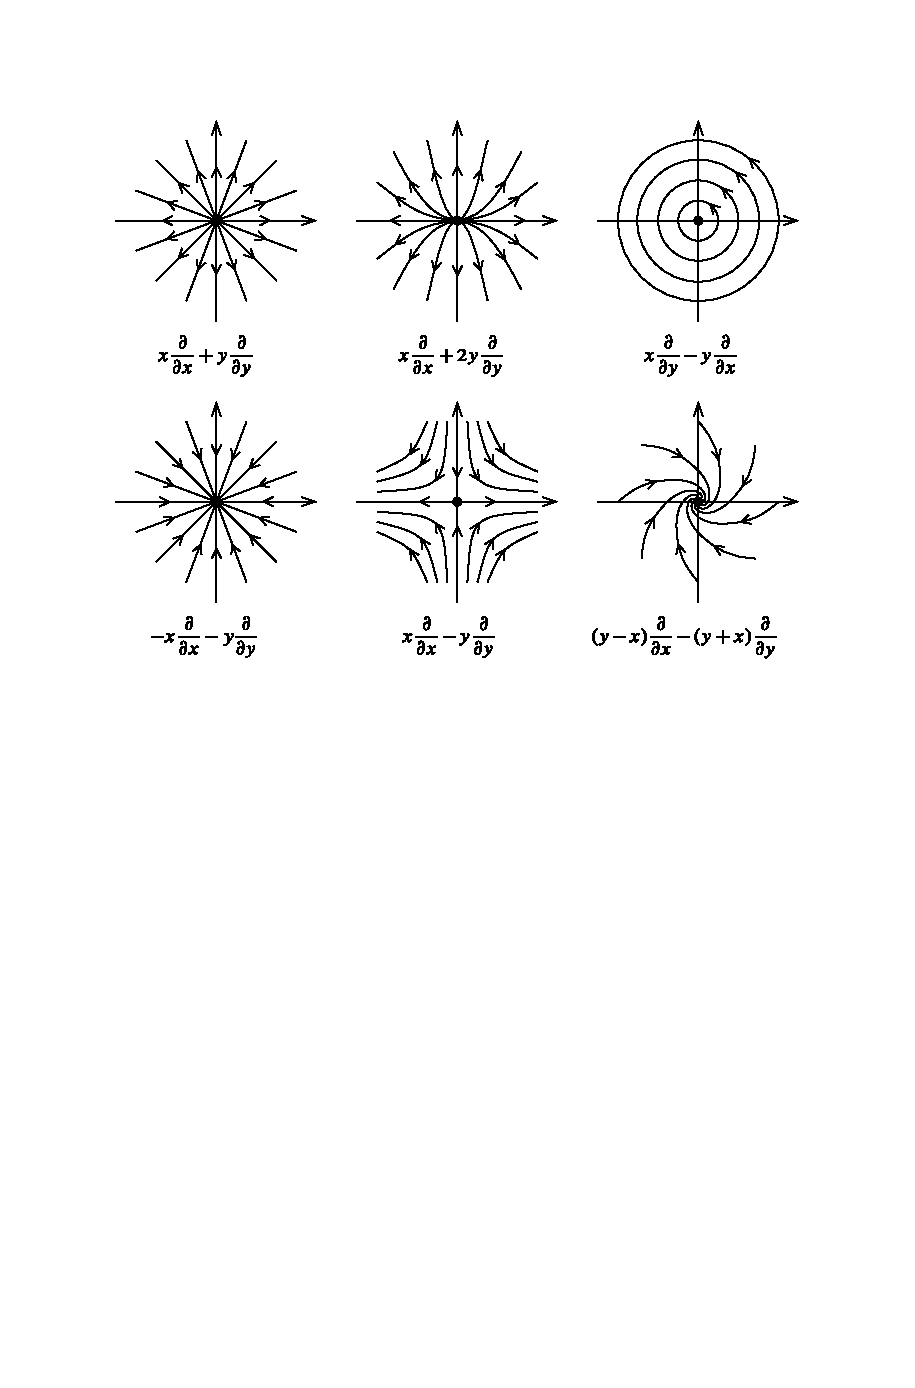
\includegraphics{pictures/equilibrium}
\caption{Examples of flows near equilibrium points.}
\label{equilibrium}
\end{figure}
The canonical form theorem shows that a flow in a neighborhood of a regular point behaves, up to diffeomorphism, just like translation along parallel coordinate
lines in $\R^n$. Thus all of the interesting local behavior of the flow is concentrated near its equilibrium points. The flow around equilibrium points can exhibit a wide variety of behaviors, such as closed orbits surrounding the equilibrium point, orbits converging to the equilibrium point as $t\to+\infty$ or $-\infty$, and many more complicated phenomena. Some typical $2$-dimensional examples are illustrated in Figure~\ref{equilibrium}.
\subsection{Flows and flowouts on manifolds with boundary}
On a manifold with boundary, the definitions of flow domain, flow, and infinitesimal generator of a flow are exactly the same as on a manifold without boundary. In general, a smooth vector field on a manifold with boundary need not generate a flow, because, for example, the integral curves starting at some boundary points might be defined only on half-open intervals. But there is a variant of the flowout theorem for manifolds with boundary, which has many important applications.\par
Suppose $M$ is a smooth manifold with nonempty boundary. The next theorem
describes a sort of \textit{one-sided flowout} from $\partial M$ determined by a vector field that is inward pointing everywhere on $\partial M$.
\begin{theorem}[\textbf{Boundary Flowout Theorem}]\label{flowout boundary}
Let $M$ be a smooth manifold with nonempty boundary, and let $N$ be a smooth vector field on $M$ that is inward-pointing at each point of $\partial M$. There exist a smooth function $\delta:\partial M\to\R^+$ and a smooth embedding $\varPsi:\mathcal{P}_\delta\to M$ where 
\[\mathcal{P}_\delta=\{(t,p):p\in\partial M,0\leq t<\delta(p)\}\sub\R\times\partial M\] 
such that $\varPhi(\mathcal{P}_\delta)$ is a neighborhood of $\partial M$, and for each $p\in\partial M$ the map $t\mapsto \varPsi(t,p)$ is an integral curve of $N$ starting at $p$.
\end{theorem}
\begin{proof}
We can define a flow in the same way as the flow theorem, but the domain is now not open. For every $p\in\partial M$, $\theta^{(p)}$ is a curve starting at $p$ point into $M$. Let $f(p)$ be the first time that $\theta^{(p)}$ hits the boundary again, and define $\delta(p)=f(p)/2$. Then we can define $\mathcal{P}_\delta$, and it is easy to see $\varPhi$ is an immersion. Assume $\varPhi(t,p)=\varPhi(t',p')$ with $(t,p),(t',p')\in\mathcal{P}_\delta$. Let's assume $t\leq t'$, then from $\theta_{t}(p)=\theta_{t'}(p')$ and the group law, we obtain
\[\theta_{t'-t}(p')=p\in\partial M\]
But $t'-t\leq t'<\delta(p')<f(p')$, this contradicts our definition. Thus $\varPhi$ is an injective immersion. Since $\partial M$ has dimension $(n-1)$, it is in fact an embedding.
\end{proof}
Let $M$ be a smooth manifold with boundary. A neighborhood of $\partial M$ is called a \textbf{collar neighborhood} if it is the image of a smooth embedding $[0,1)\times\partial M\to M$ that restricts to the obvious identification $\{0\}\times\partial M\to\partial M$.
\begin{theorem}[\textbf{Collar Neighborhood Theorem}]\label{collar nbhd}
If $M$ is a smooth manifold with nonempty boundary, then $\partial M$ has a collar neighborhood.
\end{theorem}
\begin{figure}[htbp]
\centering
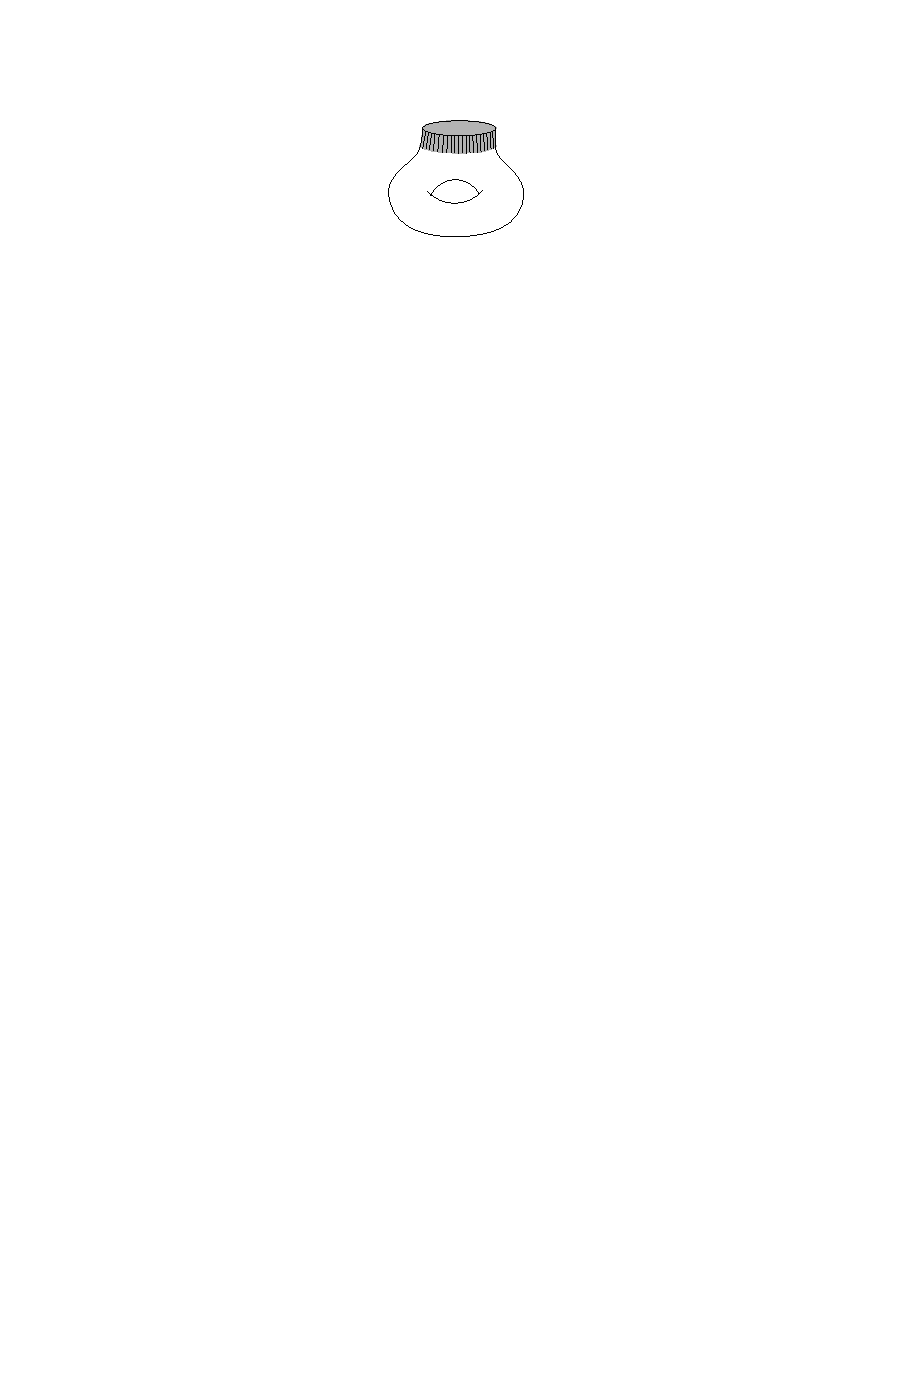
\includegraphics{pictures/collar}
\caption{A collar neighborhood of the boundary.}
\end{figure}
\begin{proof}
By the result of Exercise~\ref{vector field inward}, there exists a smooth vector field $N\in\X(M)$ whose restriction to $\partial M$ is everywhere inward-pointing. Let $\delta:M\to\R^+$ and $\varPhi:\mathcal{P}_\delta\to M$ be as in Theorem~\ref{flowout boundary}, and define a map $\psi:[0,1)\times\partial M\to\mathcal{P}_\delta$ by $\psi(t,p)=(t\delta(p),p)$. Then is a diffeomorphism that restricts to the identity on $\{0\}\times\partial M$ and therefore the map $\varPhi\circ\psi:[0,1)\times\partial M\to M$ is a smooth embedding with open image that restricts to the usual usual identification $\{0\}\times\partial M\to \partial M$. The image of $\varPhi\circ\psi$ is a collar neighborhood of $\partial M$.
\end{proof}
Our first application of the collar neighborhood theorem shows (among other things) that every smooth manifold with boundary is homotopy equivalent to its
interior.
\begin{theorem}\label{homotopy equiv Int M to M}
Let $M$ be a smooth manifold with nonempty boundary, and let $\iota:\Int M\hookrightarrow M$ denote inclusion. There exists a proper smooth embedding $R:M\to\Int M$ such that both $\iota\circ R:M\to M$ and $R\circ\iota:\Int M\to\Int M$ are smoothly homotopic to identity maps. Therefore, $\iota$ is a homotopy equivalence.
\end{theorem}
\begin{proof}
Theorem~\ref{collar nbhd} shows that $\partial M$ has a collar neighborhood $C_0$ in $M$, which is the image of a smooth embedding $E_0:[0,1)\times\partial M\to M$ satisfying $E_0(0,x)=x$ for all $x\in\partial M$. Let $f:M\to\R^+$ be a smooth positive exhaustion function. Note that 
\[W=\{(t,x):f(E_0(t,x))>f(x)-1\}\sub [0,1)\times\partial M\] 
is an open subset containing $\{0\}\times\partial M$. Using a partition of unity as in the proof of Theorem~\ref{flowout}, we may construct a smooth positive function $\delta:\partial M\to\R^+$ such that $(t,x)\in W$ whenever $0\leq t<\delta(x)$. Define 
\[E:[0,1)\times\partial M\to M,\quad E(t,x)=E_0(t\delta(x),x).\] 
Then $E$ is a diffeomorphism onto a collar neighborhood $C$ of $\partial M$, and by construction 
\[f(E(t,x))>f(x)-1\quad\text{for all }(t,x)\in[0,1)\times\partial M.\] 
We claim that for each $a\in(0,1)$, the set $E([0,a]\times\partial M)$ is closed in $M$: let $p$ be a limit point of $E([0,a]\times\partial M)$ in $M$, then there is a sequence $\{(t_i,x_i)\}$ in $[0,a]\times\partial M$ such that $E(t_i,x_i)\to p$. Then $f(E(t_i,x_i))$ remains bounded, and thus $f(x_i)<f(E(t_i,x_i))+1$ also remains bounded. Since $\partial M$ is closed in $M$, $f|_{\partial M}$ is also an exhaustion function, and therefore the sequence $\{x_i\}$ lies in some compact subset $K$ of $\partial M$. But then $(t_i,x_i)$ is contained in the compact subset $[0,a]\times K$, so by passing to a subsequence, we may assume $(t_i,x_i)\to(t_0,x_0)$. Therefore, $p=E(t_0,x_0)\in E([0,a]\times\partial M)$, implying $E([0,a]\times\partial M)$ is closed.\par
To simplify notation, we will use this embedding to identify $C$ with $[0,1)\times\partial M$ and denote a point in $C$ as an ordered pair $(s,x)$, with $s\in[0,1)$ and $x\in\partial M$; thus $(s,x)\in\partial M$ if and only if $s=0$. For any $a\in(0,1]$, let 
\[C(a)=\{(s,x)\in C:0\leq s<a\}=E([0,a)\times\partial M)\And M(a)=M-C(a)\]
To see that $M(a)$ is a regular domain, note first that it is closed in $M$ because it is the complement of the open set $C(a)$. Let $p\in M(a)$ be arbitrary. If $p\notin E([0,a]\times\partial M)$, then $p$ has a neighborhood in $\Int M$ contained in $M(a)$ by the argument above. If $p\in E([0,a]\times\partial M)$, then $p=E(a,x)$ for some $x\in\partial M$. Let $U$ be  a smooth chart of $x$, then $E([a,1)\times U)$ is a slice boundary chart for $p$. This proves $M(a)$ is a properly embedded submanifold.\par
Let $\psi:[0,1)\to [1/3,1)$ be an increasing diffeomorphism that satisfies $\psi(s)=s$ for $2/3\leq s<1$, and define $R:M\to\Int M$ by
\[R(p)=\begin{cases}
p,&p\in\Int(M(2/3));\\
(\psi(s),x),&p=(s,x)\in C.
\end{cases}\]
These definitions both give the identity map on the set $C-C(2/3)$ where they overlap, so $R$ is smooth by the gluing lemma. It is a diffeomorphism onto the closed subset $M(1/3)$, so it is a proper smooth embedding of $M$ into $\Int M$.\par
Define $H:M\times I\to M$ by
\[H(p,t)=\begin{cases}
p,&p\in\Int(M(2/3));\\
\big(ts+(1-t)\psi(s),x\big),&p=(s,x)\in C
\end{cases}\]
As before, $H$ is smooth, and a straightforward verification shows that it is a homotopy from $\iota\circ R$ to $\mathrm{id}_M$. If $p\in\Int M$, then $H(p,t)=p$ for all $t\in I$, so the restriction of $H$ to $(\Int M)\times $ is a smooth homotopy from $R\circ\iota$ to $\mathrm{id}_{\Int M}$.
\end{proof}
Theorem~\ref{homotopy equiv Int M to M} is the main ingredient in the following generalization of the Whitney approximation theorem.
\begin{theorem}[\textbf{Whitney Approximation for Manifolds with Boundary}]
If $M$ and $N$ are smooth manifolds with boundary, then every continuous map from $M$ to $N$ is homotopic to a smooth map.
\end{theorem}
\begin{proof}
Theorem~\ref{Whitney appox-1} takes care of the case in which $\partial N=\emp$, so we may assume that $\partial N\neq\emp$. Let $F:M\to N$ be a continuous map, let $\iota:\Int N\to N$ be inclusion, and let $R:M\to\Int M$ be the map constructed in Theorem~\ref{homotopy equiv Int M to M}, so that $\iota\circ R:N\to N$ is smoothly homotopic to $\mathrm{id}_N$. Theorem~\ref{homotopy equiv Int M to M} shows that $R\circ F:M\to\Int N$ is homotopic to a smooth map $G$. It follows that 
\[\iota\circ G\simeq \iota\circ R\circ F\simeq F\]
so $\iota\circ G:M\to N$ is a smooth map homotopic to $F$.
\end{proof}
The next theorem generalizes the main result of Theorem~\ref{homotopy to smooth} to the case of maps into a manifold with boundary.
\begin{theorem}\label{homotopy smooth boundary}
Suppose $M$ and $N$ are smooth manifolds with or without boundary. If $F:M\to N$ are homotopic smooth maps, then they are smoothly homotopic.
\end{theorem}
\begin{proof}
Theorem~\ref{homotopy to smooth} takes care of the case $\partial N=\emp$, so we may assume that $N$ has nonempty boundary. Let $\iota:\Int N\to N$ and $R:N\to\Int N$ be as in Theorem~\ref{homotopy equiv Int M to M}. Then $R\circ F$ and $R\circ G$ are homotopic smooth maps from $M$ to $\Int N$, so Theorem~\ref{homotopy to smooth} shows that they are smoothly homotopic to each other. Thus we have smooth homotopies
\[F\simeq\iota\circ R\circ F\simeq\iota\circ R\circ G\simeq G\]
By transitivity of smooth homotopy, it follows that $F$ is smoothly homotopic to $G$.
\end{proof}
The following theorem is probably the most important application of the collar
neighborhood theorem.
\begin{theorem}[\textbf{Attaching Smooth Manifolds Along Boundaries}]\label{attach mani}
Let $M$ and $N$ be smooth $n$-manifolds with nonempty boundaries, and suppose $h:\partial N\to\partial M$ is a diffeomorphism. Let $M\cup_hN$ be the adjunction space formed by identifying each $x\in\partial N$ with $h(x)\in\partial M$. Then $M\cup_hN$ is a topological manifold without boundary, and has a smooth structure such that there are regular domains $M',N'\sub M\cup_hN$ diffeomorphic to $M$ and $N$, respectively, and satisfying 
\begin{align}\label{attach mani-1}
M'\cup N'=M\cup_hN,\quad M'\cap N'=\partial M=\partial N
\end{align}
If $M$ and $N$ are both compact, then $M\cup_hN$ is compact, and if they are both
connected, then $M\cup_hN$ is connected.
\end{theorem}
\begin{proof}
For simplicity, let $X=M\cup_hN$ denote the quotient space and $\pi:M\amalg N$ the quotient map. Let $V\sub M$ and $W\sub N$ be collar neighborhoods of $\partial M$ and $\partial N$, respectively, and denote the corresponding diffeomorphisms by 
\[\alpha:[0,1)\times\partial M\to V\And\beta:[0,1)\times\partial N\to W.\] 
Define a continuous map $\varPhi:V\amalg W\to(-1,1)\times\partial M$ by
\[\varPhi(x)=\begin{cases}
(-t,p),&x=\alpha(t,p)\in V;\\
(t,h(q)),&x=\beta(t,q)\in W.
\end{cases}\]
Then the restriction of $\varPhi$ to $V$ or $W$ is a topological embedding with closed image, from which it follows easily that $\varPhi$ is a closed map. Because $\varPhi$ is constant on the fibers of $\pi$, it descends to a continuous map $\widetilde{\varPhi}:\pi(V\amalg W)\to(-1,1)\times\partial M$. This map is bijective, and it is a homeomorphism because it too is a closed map: if $K\sub\pi(V\amalg W)$ is closed, then $\pi^{-1}(K)$ is closed in $V\amalg W$, and therefore $\widetilde{\varPhi}(K)=\varPhi(\pi^{-1}(K))$ is closed. Thus, $\pi(V\amalg W)$ is a topological $n$-manifold. On the other hand, the restriction of $\pi$ to the saturated open subset $\Int M\amalg\Int N$ is an injective quotient map and thus a homeomorphism onto its image; this shows that $X$ is locally Euclidean of dimension $n$. Since $X$ is the union of the second-countable open subsets $\pi(\Int M\amalg\Int N)$ and $\pi(V\amalg W)$, it is second-countable. Any two fibers in $M\amalg N$ can be separated by saturated open subsets, so $X$ is Hausdorff. Thus it is a topological $n$-manifold.\par
We define a collection of charts on $X$ as follows:
\[\begin{array}{ll}
(\pi(U),\varphi\circ\pi^{-1}|_{\pi(U)}),&\text{for each smooth chart $(U,\varphi)$ for $\Int M$ or $\Int N$};\\
(\widetilde{\varPhi}^{-1}(U),\varphi\circ\widetilde{\varPhi}|_{\widetilde{\varPhi}^{-1}(U)}),&\text{for each smooth chart $(U,\varphi)$ for $(-1,1)\times\partial M$}.
\end{array}\]
These maps are compositions of homeomorphisms, so they define coordinate charts on $X$, and it is straightforward to check that they are all smoothly compatible and thus define a smooth structure on $X$. The restriction of $\pi$ to $M$ is continuous, closed, and injective, and thus it is a proper embedding. In terms of any of the smooth charts constructed above and corresponding charts on $M$, $\pi$ has a coordinate representation that is either an identity map or an inclusion map, so it is a smooth embedding, and its image $M'$ is therefore a regular domain in $X$. Similar considerations apply to $N$, and the relations $(\ref{attach mani-1})$ follow immediately from the definitions.\par
If $M$ and $N$ are compact, then $X$ is the union of the compact sets $M'$ and $N'$, so it is compact; and if they are connected, then $X$ is the union of the connected sets $M'$ and $N'$ with points of $\partial M'=\partial N'$in common, so it is connected.
\end{proof}
\begin{corollary}
Suppose $M$ and $N$ are smooth $n$-manifolds with boundary, $A\sub\partial M$ and $B\sub\partial N$ are nonempty subsets that are unions of components of the respective boundaries, and $h:B\to A$ is a diffeomorphism. Then $M\cup_hN$ is a topological manifold with boundary, and can be given a smooth structure such that $M$ and $N$ are diffeomorphic to regular domains in $M\cup_hN$.
\end{corollary}
\begin{example}[\textbf{Connected Sums}]
Let $M_1,M_2$ be connected smooth manifolds of dimension $n$. For $i=1,2$, let $U_i$ be a regular coordinate ball centered at some point $p_i\in M_i$, and let $M'_i=M_i-U_i$. Exercise~\ref{delete coordinate ball} shows that each $M'_i$ is a smooth manifold with boundary whose boundary is diffeomorphic to $S^{n-1}$. A smooth connected sum of $M_1$ and $M_2$, denoted by $M_1\#M_2$, is a smooth manifold formed by choosing a diffeomorphism from $\partial M_1$ to $\partial M_2$ and attaching $M'_1$ and $M'_2$ along their boundaries.
\end{example}
If $M$ is any smooth manifold with boundary, Theorem~\ref{homotopy equiv Int M to M} shows that $M$ can be properly embedded into a smooth manifold without boundary (namely, a copy of $\Int M$). The next example shows a different way that $M$ can be so embedded; this construction has the advantage of embedding $M$ into a compact manifold when $M$ itself is compact.
\begin{example}[\textbf{The Double of a Smooth Manifold with Boundary}]\label{double manifold boundary}
Let $M$ be a smooth manifold with boundary. The \textbf{double of $\bm{M}$} is the manifold $D(M)=M\cup_{\mathrm{id}}M$, where $\mathrm{id}:\partial M\to\partial M$ is the identity map of $\partial M$, it is obtained from $M\amalg M$ by identifying each boundary point in one copy of $M$ with the same boundary point in the other. It is a smooth manifold without boundary, and contains two regular domains diffeomorphic to $M$. It is easy to check that $D(M)$ compact if and only if $M$ is compact, and connected if and only if $M$ is connected. $($It is useful to extend the definition to manifolds without boundary by defining $D(M)=M\amalg M$ when $\partial M=\emp$.$)$
\end{example}
Although vector fields on manifolds with boundary do not always generate flows,
there is one circumstance in which they do: when the vector field is everywhere
tangent to the boundary. To prove this, we begin with the following special case.
\begin{lemma}\label{flow tangent boundary}
Suppose $M$ is a smooth manifold and $D\sub M$ is a regular domain. If $V$ is a smooth vector field on $M$ that is tangent to $\partial D$, then every integral curve of $V$ that starts in $D$ remains in $D$ as long as it is defined.
\end{lemma}
\begin{proof}
Suppose $\gamma:J\to M$ is an integral curve of $V$ with $\gamma(0)\in D$. Define $\mathcal{T}=\{t\in J:\gamma(t)\in D\}$. We will show that $\mathcal{T}$ is both open and closed in $J$; since $J$ is an interval, this implies $\mathcal{T}=J$ and proves the lemma.\par
Since $D$ is closed in $M$ (by definition of a regular domain), $\mathcal{D}$ is closed in $J$ by continuity. To prove it is open, suppose $t_0\in\mathcal{T}$. If $\gamma(t_0)\in\Int D$, then a neighborhood of $t_0$ is contained in $\mathcal{T}$ by continuity, so we can assume $\gamma(t_0)\in\partial D$. Because $V$ is tangent to $\partial D$, Proposition~\ref{vector field restrict submani} shows that there is a smooth vector field $W=V|_{\partial D}$ that is $\iota$-related to $V$, where $\iota:\partial D\hookrightarrow M$ is inclusion. Let $\widetilde{\gamma}:(t_0-\eps,t_0+\eps)\to \partial D$ be an integral curve of $W$ with $\widetilde{\gamma}(t_0)=\gamma(t_0)$. By naturality of integral curves (Proposition~\ref{integral curve naturality}), $\iota\circ\widetilde{\gamma}$ is an integral curve of $V$ with the same initial condition, so by uniqueness it must be equal to $\gamma$ where both are defined. This shows that $\gamma(t)\sub \partial D\sub D$ for $t$ in some neighborhood of $t_0$, so $\mathcal{T}$ is open in $J$ as claimed.
\end{proof}
\begin{theorem}[\textbf{Flows on Manifolds with Boundary}]\label{flow boundary}
The conclusions of Theorem~\ref{flow fundamental thm} remain true if $M$ is a smooth manifold with boundary and $V$ is a smooth vector field on $M$ that is tangent to $\partial M$.
\end{theorem}
\begin{proof}
We can consider $M$ as a regular domain in its double $D(M)$. By the extension lemma for vector fields, we can extend $V$ to a smooth vector field $\widetilde{V}$ on $D(M)$. Let $\widetilde{\theta}:\mathcal{D}\to D(M)$ be the flow of $\widetilde{V}$, and let $\mathcal{D}=(\R\times M)\cap \widetilde{\mathcal{D}}$ and $\theta=\widetilde{\theta}|_{M}$. Then Lemma~\ref{flow tangent boundary} guarantees that $\theta$ maps $\mathcal{D}$ into $M$, and the rest of the conclusions follow from Theorem~\ref{flow fundamental thm} applied to $\widetilde{V}$.
\end{proof}
For manifolds with boundary, the canonical form theorem has the following
variant.
\begin{theorem}[\textbf{Canonical Form Near a Regular Point on the Boundary}]
Let $M$ be a smooth manifold with boundary and let $V$ be a smooth vector field on $M$ that is tangent to $\partial M$. If $p\in\partial M$ is a regular point of $V$, there exist smooth boundary coordinates $(s^i)$ on some neighborhood of $p$ in which $V$ has the coordinate representation $\partial/\partial s^1$.
\end{theorem}
\subsection{Lie derivatives}
Suppose $M$ is a smooth manifold, $V$ is a smooth vector field on $M$, and $\theta$ is the flow of $V$. For any smooth vector field $W$ on $M$, define a rough vector field on $M$, denoted by $\mathfrak{L}_VW$ and called the Lie derivative of $W$ with respect to $V$, by
\[(\mathfrak{L}_VW)_p=\frac{d}{dt}\Big|_{t=0}d(\theta_{-t})_{\theta_t(p)}\big(W_{\theta_t(p)}\big)=\lim_{t\to 0}\frac{d(\theta_{-t})_{\theta_t(p)}\big(W_{\theta_t(p)}\big)-W_p}{t}\]
provided the derivative exists. For small $t\neq 0$, at least the difference quotient makes sense: $\theta_t$ is defined in a neighborhood of $p$, and $\theta_{-t}$ is the inverse of $\theta_t$, so both $d(\theta_{-t})_{\theta_t(p)}\big(W_{\theta_t(p)}\big)$ and $W_p$ are elements of $T_pM$.
\begin{figure}[htbp]
\centering
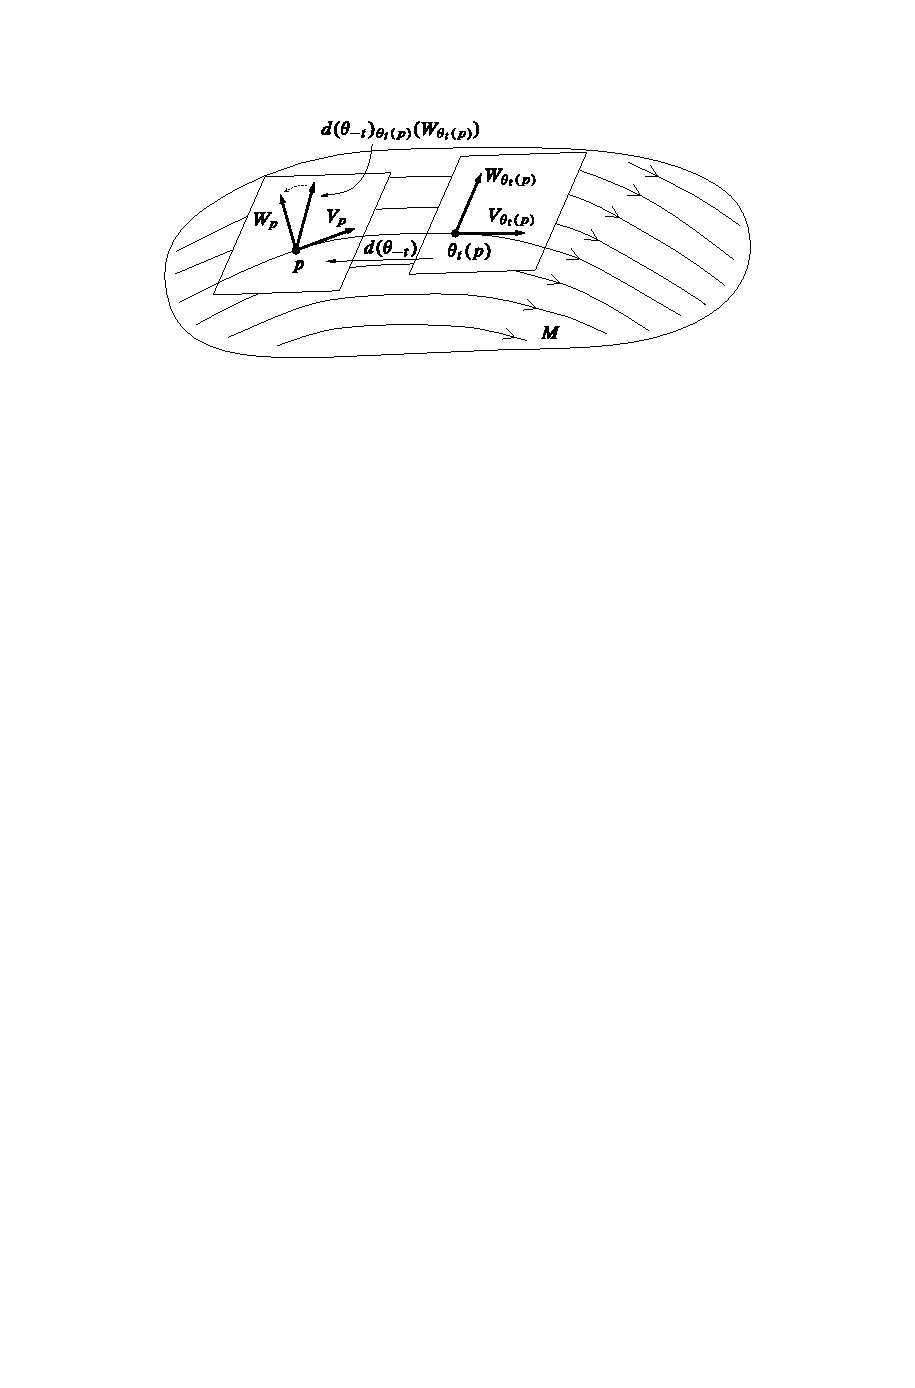
\includegraphics{pictures/Lie-derivative}
\caption{The Lie derivative of a vector field.}
\end{figure}\par
If $M$ has nonempty boundary, this definition of $\mathfrak{L}_VW$ makes sense as long as $V$ is tangent to $\partial M$ so that its flow exists by Theorem~\ref{flow boundary}.
\begin{lemma}\label{Lie derivative exist}
Suppose $M$ is a smooth manifold with or without boundary, and $V,W\in\X(M)$. If $\partial M\neq\emp$, assume in addition that $V$ is tangent to $\partial M$. Then $(\mathfrak{L}_VW)_p$ exists for every $p\in M$, and $\mathfrak{L}_VW$ is a smooth vector field.
\end{lemma}
\begin{proof}
Let $\theta$ be the flow of $V$. For arbitrary $p\in M$, let $(U,(x^i))$ be a smooth chart containing $p$. Choose an open interval $J_0$ containing $0$ and an open subset $U_0\sub U$ containing $p$ such that$\theta$ maps $J_0\times U_0$ into $U$. For $(t,x)\in J_0\times U_0$, write the component functions of $\theta$ as $(\theta^1(t,x),\dots,\theta^n(t,x))$. Then for any $(t,x)\in J_0\times U_0$,
the matrix of $d(\theta_{-t})_{\theta_t(p)}:T_{\theta_t(x)}M\to T_xM$ is
\[\begin{pmatrix}
\dfrac{\partial\theta^i}{\partial x^j}(-t,\theta_t(x))
\end{pmatrix}\]
Therefore,
\[d(\theta_{-t})_{\theta_t(p)}\big(W_{\theta_t(p)}\big)=\dfrac{\partial\theta^i}{\partial x^j}(-t,\theta_t(x))W^j(\theta_t(x))\frac{\partial}{\partial x^i}\Big|_x\]
Because $\theta^i$ and $W^j$ are smooth functions, the coefficient of $\partial/\partial x^i|_x$ depends smoothly on $(t,x)$. It follows that $(\mathfrak{L}_VW)_x$, which is obtained by taking the derivative of this expression with respect to $t$ and setting $t=0$, exists for each $x\in U_0$ and
depends smoothly on $x$.
\end{proof}
The definition of $\mathfrak{L}_VW$ is not very useful for computations, because typically the flow is difficult or impossible to write down explicitly. Fortunately, there is a simple formula for computing the Lie derivative without explicitly finding the flow.
\begin{theorem}\label{Lie derivative bracket}
If $M$ is a smooth manifold and $V,W\in\X(M)$, then $\mathfrak{L}_VW=[V,W]$.
\end{theorem}
\begin{proof}
Suppose $V,W\in\X(M)$, and let $\mathcal{R}(V)\sub M$ be the set of regular points of $V$ (the set of points $p\in M$ such that $V_p\neq0$). Note that $\mathcal{R}(V)$ is open in $M$ by continuity, and its closure is the support of $V$. We will show that $(\mathfrak{L}_VW)_p=[V,W]_p$ for all $p\in M$, by considering three cases.\par
First let $p\in\mathcal{R}(V)$. In this case, we can choose smooth coordinates $(u^i)$ on a neighborhood of $p$ in which $V$ has the coordinate representation $V=\partial/\partial u^i$ (Theorem~\ref{flow canonical form}). In these coordinates, the flow of $V$ is $\theta_t(u)=(u^1+t,u^2,\dots,u^n)$. For each fixed $t$, the matrix of $d(\theta_{-t})_{\theta_t(x)}$ in these coordinates is the identity at every point. Consequently, for any $u\in U$,
\begin{align*}
d(\theta_{-t})_{\theta_t(p)}\big(W_{\theta_t(p)}\big)&=d(\theta_{-t})_{\theta_t(p)}\Big(W^j(u^1+t,u^2,\dots,u^n)\frac{\partial}{\partial u^j}\Big|_{\theta_t(u)}\Big)\\
&=W^j(u^1+t,u^2,\dots,u^n)\frac{\partial}{\partial u^j}\Big|_{u}
\end{align*}
Using the definition of the Lie derivative, we obtain
\[(\mathfrak{L}_VW)_u=\frac{d}{dt}\Big|_{t=0}W^j(u^1+t,u^2,\dots,u^n)\frac{\partial}{\partial u^j}\Big|_{u}=\frac{\partial W^j}{\partial u^1}(u^1,\dots,u^n)\frac{\partial}{\partial u^j}\Big|_u\]
On the other hand, by virtue of formula $(\ref{Lie bracket-1})$ for the Lie bracket in coordinates, $[V,W]_u$ is easily seen to be equal to the same expression.\par
Now let $p\in\supp(V)$. Because $\supp(V)$ is the closure of $\mathcal{R}(V)$, it follows by continuity that $(\mathfrak{L}_VW)_p=[V,W]_p$ for $p\in\supp(V)$.\par
Finally, let $p\in M\setminus\supp(V)$. In this case, $V\equiv 0$ on a neighborhood of $p$. On the one hand, this implies that $\theta_t$ is equal to the identity map in a neighborhood of $p$ for all $t$, so $d(\theta_{-t})_{\theta_t(p)}\big(W_{\theta_t(p)}\big)=W_p$, which implies $(\mathfrak{L}_VW)_p=0$. On the other hand, $[V,W]=0$ by formula $(\ref{Lie bracket-1})$.
\end{proof}
This theorem allows us to extend the definition of the Lie derivative to arbitrary
smooth vector fields on a smooth manifold $M$ with boundary. Given $V,W\in\X(M)$, we define $(\mathfrak{L}_VW)_p$ for $p\in\partial M$ by embedding $M$ in a smooth manifold $\widetilde{M}$ without boundary (such as the double of $M$), extending $V$ and $W$ to smooth vector fields on $\widetilde{M}$, and computing the Lie derivative there. By virtue of the preceding theorem, $(\mathfrak{L}_VW)_p=[V,W]_p$ is independent of the choice of extension.\par
Theorem~\ref{Lie derivative bracket} also gives us a geometric interpretation of the Lie bracket of two vector fields: it is the directional derivative of the second vector field along the flow of the first. A number of nonobvious properties of the Lie derivative follow immediately from things we already know about Lie brackets.
\begin{corollary}
Suppose $M$ is a smooth manifold with or without boundary, and $V,W,X\in\X(M)$.
\begin{itemize}
\item[(a)] $\mathfrak{L}_VW=-\mathfrak{L}_WV$.
\item[(b)] $\mathfrak{L}_V[W,X]=[\mathfrak{L}_VW,X]+[W,\mathfrak{L}_VX]$.
\item[(c)] $\mathfrak{L}_{[V,W]}X=\mathfrak{L}_V\mathfrak{L}_WX-\mathfrak{L}_W\mathfrak{L}_VX$.
\item[$(d)$] If $g\in C^\infty(M)$, then $\mathfrak{L}_V(gW)=(Vg)W+g\mathfrak{L}_VW$.
\item[$(e)$] If $F:M\to N$ is a diffeomorphism, then $F_*(\mathfrak{L}_VX)=\mathfrak{L}_{F_*V}F_*X$.
\end{itemize}
\end{corollary}
\begin{proof}
Recall the Jacobi identity
\[[V,[W,X]]+[W,[X,V]]+[X,[V,W]]=0\]
Thus
\begin{align*}
\mathfrak{L}_V[W,X]&=[V,[W,X]]=-[W,[X,V]]-[X,[V,W]]\\
&=[[V,W],X]+[W,[V,X]]\\
&=[\mathfrak{L}_VW,X]+[W,\mathfrak{L}_VX]
\end{align*}
Similarly,
\begin{align*}
\mathfrak{L}_{[V,W]}X&=[[V,W],X]=[V,[W,X]]+[W,[X,V]]\\
&=[V,[W,X]]-[W,[V,X]]\\
&=\mathfrak{L}_V[W,X]-\mathfrak{L}_W[V,X]\\
&=\mathfrak{L}_V\mathfrak{L}_WX-\mathfrak{L}_W\mathfrak{L}_VX
\end{align*}
Part $(d)$ is a direct computation:
\begin{align*}
\mathfrak{L}_V(gW)&=[V,gW]=V(gW)-gWV=(Vg)W+gVW-gWV\\
&=(Vg)W+g[V,W]=(Vg)W+g\mathfrak{L}_VW
\end{align*}
and the last statment is a result of natruality of Lie bracket.
\end{proof}
Part $(d)$ of this corollary gives a meaning to the mysterious formula $(\ref{Lie bracket two product rule})$ for Lie brackets of vector fields multiplied by functions: because the Lie bracket $[fV,gW]$ can be thought of as the Lie derivative $\mathfrak{L}_{fV}(gW)$, it satisfies a product rule in $g$ and $W$, and because it can also be thought of as $-\mathfrak{L}_{gW}(fV)$, it satisfies a product
rule in $f$ and $V$ as well. Expanding out these two product rules yields $(\ref{Lie bracket two product rule})$:
\begin{align*}
\mathfrak{L}_{fV}(gW)&=(fVg)W+g\mathfrak{L}_{fV}W=(fVg)W-g\mathfrak{L}_{W}(fV)\\
&=(fVg)W-g(Wf+f\mathfrak{L}_{W}V)\\
&=(fVg)W-(gWf)+fg\mathfrak{L}_VW
\end{align*}
If $V$ and $W$ are vector fields on $M$ and $\theta$ is the flow of $V$, the Lie derivative $(\mathfrak{L}_VW)_p$, by definition, expresses the $t$-derivative of the time-dependent vector $d(\theta_{-t})_{\theta_t(p)}\big(W_{\theta_t(p)}\big)$ at $t=0$. The next proposition shows how it can also be used to compute the derivative of this expression at other times.
\begin{proposition}\label{Lie derivative t_0}
Suppose $M$ is a smooth manifold with or without boundary and $V,W\in\X(M)$. If $\partial M\neq\emp$, assume also that $V$ is tangent to $\partial M$. Let $\theta$ be the flow of $V$. For any $(t_0,p)$ in the domain of $\theta$,
\begin{align*}
\frac{d}{dt}\Big|_{t=t_0}d(\theta_{-t})_{\theta_t(p)}\big(W_{\theta_t(p)}\big)=d(\theta_{-t_0})\big((\mathfrak{L}_VW)_{\theta_{t_0}(p)}\big)
\end{align*}
\end{proposition}
\begin{figure}[htbp]
\centering
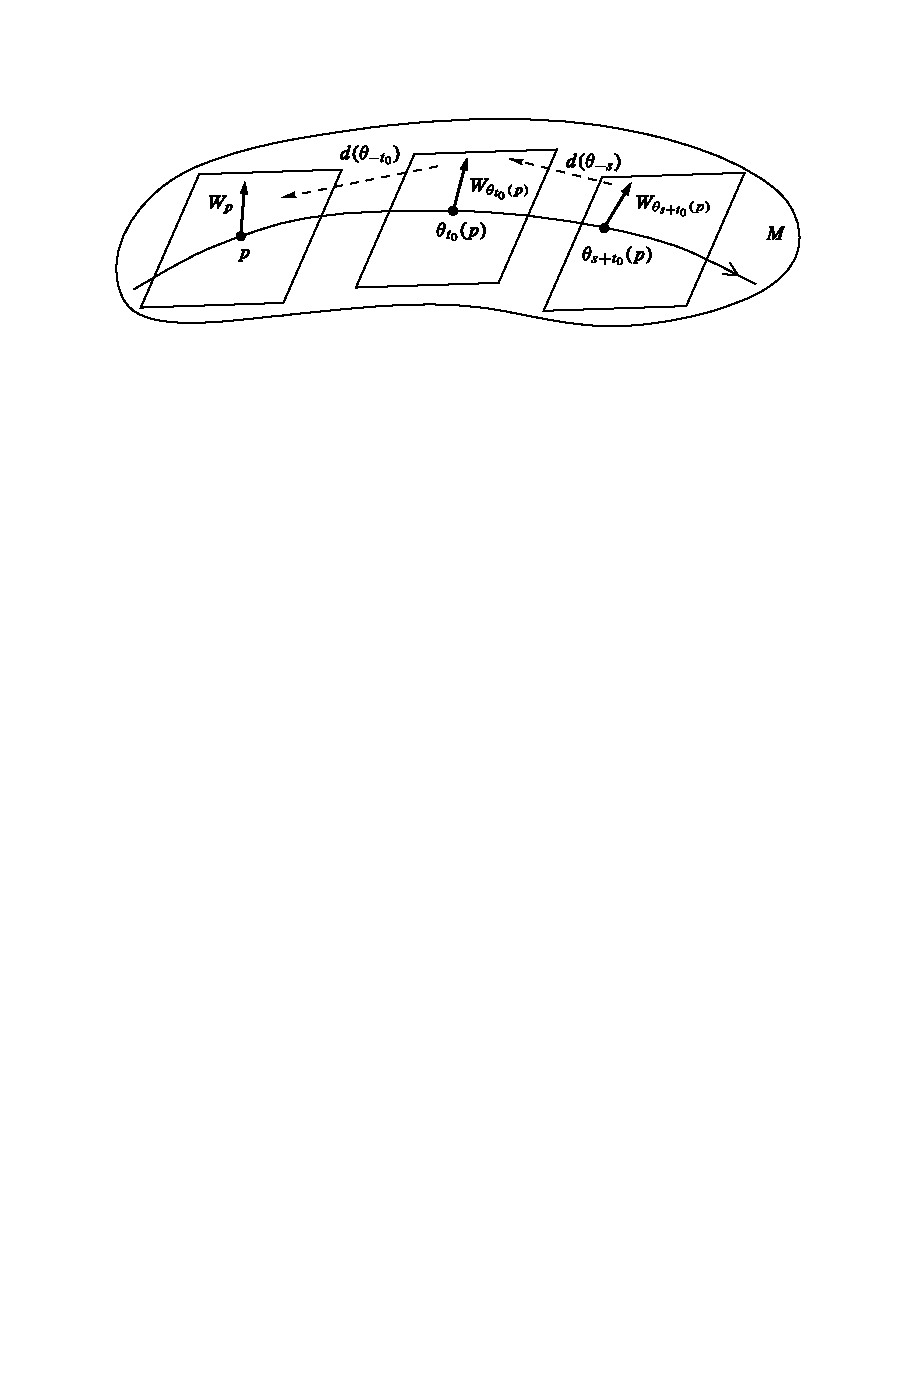
\includegraphics{pictures/Lie-derivative-2}
\caption{Proof of Proposition~\ref{Lie derivative t_0}.}
\end{figure}
\begin{proof}
Let $p\in M$ be arbitrary, let $\mathcal{D}^{(p)}\sub\R$ denote the domain of the integral curve $\theta^{(p)}$, and consider the map $X:\mathcal{D}^{(p)}\to T_pM$ given by $X(t)=d(\theta_{-t})_{\theta_t(p)}\big(W_{\theta_t(p)}\big)$. The argument in the proof of Lemma~\ref{Lie derivative exist} shows that $X$ is a smooth curve in the vector space $T_pM$. Making the change of variables $t=t_0+s$ we obtain
\begin{align*}
X'(t_0)&=\frac{d}{dt}\Big|_{s=0}X(t_0+s)=\frac{d}{dt}\Big|_{s=0}d(\theta_{-t_0-s})(W_{\theta_{s+t_0}(p)})\\
&=\frac{d}{dt}\Big|_{s=0}d(\theta_{-t_0})\circ d(\theta_{-s})(W_{\theta_{s}\circ\theta_{t_0}(p)})\\
&=d(\theta_{-t_0})\frac{d}{dt}\Big|_{s=0}d(\theta_{-s})(W_{\theta_{s}\circ\theta_{t_0}(p)})\\
&=d(\theta_{-t_0})\big((\mathfrak{L}_VW)_{\theta_{t_0}(p)}\big)
\end{align*}
as needed.
\end{proof}
\subsection{Commuting vector fields}
Let M be a smooth manifold and $V,W\in\X(M)$. We say that $V$ and $W$ \textbf{commute} if $VWf=WVf$ for every smooth function $f$, or equivalently if $[V,W]\equiv0$. If $\theta$ is a smooth flow, a vector field $W$ is said to be invariant under $\theta$ if $W$ is $\theta_t$-related to itself for each $t$; more precisely, this means that $W|_{M_t}$ is $\theta_t$-related for each $t$, or equivalently that $d(\theta_t)_p(W_p)=W_{\theta_t(p)}$ for all $(t,p)$ in the domain of $\theta$. The next proposition shows that these two concepts are intimately related.
\begin{theorem}\label{vector field commute iff}
For smooth vector fields $V$ and $W$ on a smooth manifold $M$, the following are equivalent:
\begin{itemize}
\item[(a)] $V$ and $W$ commute.
\item[(b)] $W$ is invariant under the flow of $V$.
\item[(c)] $V$ is invariant under the flow of $W$.
\end{itemize}
\end{theorem}
\begin{proof}
Suppose $V,W\in\X(M)$, and let $\theta$ denote the flow of $V$. If (b) holds, then $d(\theta_t)_p(W_p)=W_{\theta_t(p)}$ whenever $(t,p)$ is in the domain of $\theta$. Applying $d(\theta_{-t})_{\theta_t(p)}$ to both sides, we then conclude that $d(\theta_{-t})_{\theta_t(p)}(W_{\theta_t(p)})=W_p$, which obviously implies $\mathfrak{L}_VW=[V,W]=0$ directly from the definition of the Lie derivative. The same argument shows that (c) implies (a).\par
To prove that (a) implies (b), assume that $[V,W]=\mathfrak{L}_VW=0$. Let $p\in M$ be arbitrary, and let $X(t)=d(\theta_{-t})_{\theta_t(p)}\big(W_{\theta_t(p)}\big)$ for $t\in\mathcal{D}^{(p)}$. Proposition~\ref{Lie derivative t_0} shows that $X'(t)\equiv 0$. Since $X(0)=W_p$, this implies that $X(t)\equiv W_p$ for all $t\in\mathcal{D}^{(p)}$, and applying $d(\theta_t)_p$ to both sides yields the identity that says $W$ is invariant under $\theta$. The same proof also shows that (a) implies (c).
\end{proof}
\begin{corollary}
Every smooth vector field is invariant under its own flow.
\end{corollary}
\begin{proof}
Use the preceding proposition together with the fact that $[V,V]\equiv 0$.
\end{proof}
The deepest characterization of commuting vector fields is in terms of the relationship between their respective flows. The next theorem says that two vector fields
commute if and only if their flows commute. But before we state the theorem formally, we need to examine exactly what this means. Suppose $V$ and $W$ are smooth vector fields on $M$, and let $\theta$ and denote their respective flows. If $V$ and $W$ are complete, it is clear what we should mean by saying their flows commute: simply that $\theta_t\circ\psi_s=\psi_s\circ\theta_t$ for all $s,t\in\R$. However, if either $V$ or $W$ is not complete, the most we can hope for is that this equation holds for all $s$ and $t$ such that both sides are defined. Unfortunately, even when the vector fields commute, their flows might not commute in this naive sense, because there are examples of commuting vector fields $V$ and $W$ and particular choices of $t$, $s$, and $p$ for which both $\theta_t\circ\psi_s(p)$ and $\psi_s\circ\theta_t(p)$ are defined, but they are not equal. Here is the problem: if $\theta_t\circ\psi_s(p)$ is defined for $t=t_0$ and $s=s_0$, then by the properties of flow domains, it must be defined for all $t$ in some open interval containing $0$ and $t_0$, but the analogous statement need not be true of $s$---there might be values of $s$ between $0$ and $s_0$ for which the integral curve of $V$ starting at $\psi_s(p)$ does not extend all the way to $t=t_0$.\par
Thus we make the following definition. If $\theta$ and $\psi$ are flows on $M$, we say that $\theta$ and $\psi$ commute if the following condition holds for every $p\in M$, whenever $J$ and $K$ are open intervals containing $0$ such that one of the expressions $\theta_t\circ\psi_s(p)$ or $\psi_s\circ\theta_t(p)$ is defined for all $(t,s)\in J\times K$, both are defined and they are equal. For global flows, this is the same as saying that $\theta_t\circ\psi_s=\psi_s\circ\theta_t$ for all $s$ and $t$.
\begin{theorem}\label{vector filed commute flow}
Smooth vector fields commute if and only if their flows commute.
\end{theorem}
\begin{proof}
Let $V$ and $W$ be smooth vector fields on a smooth manifold $M$, and let $\theta$ and denote $\psi$ their respective flows. Assume first that $V$ and $W$ commute. Suppose that $p\in M$, and $J$ and $K$ are open intervals containing $0$ such that $\psi_s\circ\theta_t(p)$ is defined for all $(s,t)\in J\times K$. (The same proof with $V$ and $W$ reversed works under the assumption that the other expression is defined on such a rectangle.) By Theorem~\ref{vector field commute iff}, the hypothesis implies that $V$ is invariant under $\psi$. Fix any $s\in J$, and consider the curve $\gamma:K\to M$ defined by $\gamma(t)=\psi_s\circ\theta_t(p)=\psi_s(\theta^{(p)}(t))$. This curve satisfies $\gamma(0)=\psi_s(p)$, and its velocity at $t\in K$ is
\[\gamma'(t)=\frac{d}{dt}\big(\psi_s(\theta^{(p)}(t))\big)=d(\psi_s)(\dot{\theta}^{(p)}(t))=d(\psi_s)(V_{\theta^{(p)}(t)})=V_{\gamma(t)}\]
Thus, $\gamma$ is an integral curve of $V$ starting at $\psi_s(p)$. By uniqueness, therefore,
\[\gamma(t)==\theta^{(\psi_s(p))}(t)=\theta_t\big(\psi_s(p)\big)\]
This proves that $\theta$ and $\psi$ commute.\par
Conversely, assume that the flows commute, and let $p\in M$. If $\eps>0$ is chosen
small enough that $\psi_s\circ\theta_t(p)$ is defined whenever $|s|<\eps$ and $|t|<\eps$, then the hypothesis guarantees that $\psi_s\circ\theta_t(p)=\theta_t\circ\psi_s(p)$ for all such $s$ and $t$. This can be rewritten in the form
\[\psi^{(\theta_t(p))}(s)=\theta_t(\psi^{(p)}(s))\]
Differentiating this relation with respect to $s$, we get
\[W_{\theta_t(p)}=\frac{d}{ds}\Big|_{s=0}\psi^{(\theta_t(p))}(s)=\frac{d}{ds}\Big|_{s=0}\theta_t(\psi^{(p)}(s))=d(\theta_t)_p(W_p)\]
This means $W_p$ is invariant under $\theta_t$, thus by Theorem~~\ref{vector field commute iff} $V$ commutes with $W$.
\end{proof}
\subsubsection{Commuting frames}
Suppose $M$ is a smooth $n$-manifold. Recall that a local frame for $M$ is an $n$-tuple $(E_i)$ of vector fields defined on an open subset $U\sub M$ such that $(E_i|_p)$ forms a basis for $T_pM$ at each $p\in U$. A smooth local frame $(E_i)$ for $M$ is called a commuting frame if $[E_i,E_j]=0$ for all $i$ and $j$. 
\begin{example}[\textbf{Commuting and Noncommuting Frames}]\label{commute frame eg}
\mbox{}
\begin{itemize}
\item[(a)] The simplest examples of commuting frames are the coordinate frames. Given any smooth coordinate chart $(U,(x^i))$ for a smooth manifold $M$, $(\ref{Lie bracket-1})$ shows that the coordinate frame $(\partial/\partial x^i)$ is a commuting frame.
\item[(b)] The frame $(E_1,E_2)$ for $\R^2$ over $\R^2-\{0\}$ defined by $(\ref{polar frame R^2-1})$ is not a commuting frame, because a straightforward computation shows that
\[[E_1,E_2]=\frac{y}{r^2}\frac{\partial}{\partial x}-\frac{x}{r^2}\frac{\partial}{\partial y}\neq 0\]
\end{itemize}
\end{example}
Because every coordinate frame is a commuting frame, and because Lie brackets
are invariantly defined, it follows that a necessary condition for a smooth frame to be expressible as a coordinate frame in some smooth chart is that it be a commuting frame. Thus, the computation above shows that $(E_1,E_2)$ cannot be expressed as a coordinate frame for $\R^2$ with respect to any choice of smooth local coordinates.\par
The next theorem shows that commuting is also a sufficient condition for a smooth frame to be locally expressible as a coordinate frame.
\begin{theorem}[\textbf{Canonical Form for Commuting Vector Fields}]\label{flow commute canonical form}
Let $M$ be a smooth $n$-manifold, and let $(V_1,\dots,V_k)$ be a linearly independent $k$-tuple of smooth commuting vector fields on an open subset $W\sub M$. For each $p\in W$, there exists a smooth coordinate chart $(U,(s^i))$ centered at $p$ such that $V_i=\partial/\partial s^i$ for $1\leq i\leq k$. If $S\sub W$ is an embedded codimension-$k$ submanifold and $p$ is a point of $S$ such that $T_pS$ is complementary to the span of $(V_1|_p,\dots,V_k|_p)$, then the coordinates can also be chosen such that $S\cap U$ is the slice defined by $s^1=\cdots=s^k=0$.
\end{theorem}
\begin{proof}
Let $p\in W$ be arbitrary. If no submanifold $S$ is given, just let $S$ be any
smooth embedded codimension-$k$ submanifold $S$ whose tangent space at $p$ is complementary to the span of $(V_1|_p,\dots,V_k|_p)$ (e.g., an appropriate coordinate slice) Let $(U,(s^i))$ be a slice chart for $S$ centered at $p$, with $U\sub W$, and with $S\cap U$ equal to the slice $\{x\in U:x^1=\cdots=x^k=0\}$. Our assumptions ensure that the vectors $\{V_1|_p,\dots,V_k|_p,\partial/\partial x^{k+1}|_p,\dots,\partial/\partial x^n|_p\}$ span $T_pM$. Since the theorem is
purely local, we may as well consider $V_1,\dots,V_k$ as vector fields on $U\sub\R^n$, and consider $S$ to be the subset of $U$ where the first $k$ coordinates vanish. The basic idea of this proof is similar to that of the flowout theorem, except that we have to do a bit of extra work to make use of the hypothesis that the vector fields commute.\par
Let $\theta_i$ denote the flow of $V_i$ for $i=1,\dots,k$. There exist $\eps>0$ and a neighborhood $Y$ of $p$ in $U$ such that the composition $(\theta_1)_{t_1}\circ\cdots\circ(\theta_k)_{t_k}$ is defined on $Y$ and maps $Y$ into $U$ whenever $|t_1|,\dots,|t_k|$ are all less than $\eps$. (To see this, just choose $\eps_k>0$ and $U_k\sub U$ such that $\theta_k$ maps $(-\eps_k,\eps_k)\times U_k$ into $U$, and then inductively choose $\eps_i$ and $U_i$ such that $\theta_i$ maps $(-\eps_i,\eps_i)\times U_i$ into $U_{i+1}$. Taking $\eps=\min_i\{\eps_i\}$ and $Y=U_1$ does the trick.)\par
Define $\Omega\sub\R^{n-k}$ by
\[\Omega=\{(s^{k+1},\dots,s^n)\in\R^{n-k}:(0,\dots,0,s^{k+1},\dots,s^n)\in Y\}\]
and define $\varPhi:(-\eps,\eps)^k\times\Omega\to U$ by
\[\varPhi(s^1,\dots,s^k,s^{k+1},\dots,s^n)=(\theta_1)_{s_1}\circ\cdots\circ(\theta_k)_{s_k}(0,\dots,0,s^{k+1},\dots,s^n)\]
By construction, $\varPhi(\{0\}\times\Omega)=S\cap Y$.\par
We show next that $\partial/\partial s^i$ is $\varPhi$-related to $V_i$ for $1\leq i\leq k$. Because the flows $\theta_i$ commute, for any $i\in\{1,\dots,k\}$ and any $s_0\in(-\eps,\eps)^k\times\Omega$ we have
\begin{align*}
d\varPhi_{s_0}\Big(\frac{\partial}{\partial s^i}\Big|_{s_0}\Big)f&=\frac{\partial}{\partial s^i}\Big|_{s_0}f\big(\varPhi(s^1,\dots,s^n)\big)\\
&=\frac{\partial}{\partial s^i}\Big|_{s_0}f\big((\theta_1)_{s_1}\circ\cdots\circ(\theta_k)_{s^k}(0,\dots,0,s^{k+1},\dots,s^n)\big)\\
&=\frac{\partial}{\partial s^i}\Big|_{s_0}f\big((\theta_i)_{s^i}\circ(\theta_1)_{s_1}\circ\cdots\circ(\theta_{i-1})_{s^{i-1}}\circ(\theta_{i+1})_{s^{i+1}}\\
&\quad\circ\cdots\circ(\theta_k)_{s^k}(0,\dots,0,s^{k+1},\dots,s^n)\big)
\end{align*}
For any $q\in M$, $t\mapsto(\theta_i)_t(q)$ is an integral curve of $V_i$, so this last expression is equal to $V_i|_{\varPhi(s_0)}f$, which proves the claim.\par
Next we show that $d\varPhi_0$ is invertible. The computation above shows that
\[d\varPhi_{0}\Big(\frac{\partial}{\partial s^i}\Big|_{0}\Big)=V_i|_p,\quad 1\leq i\leq k.\]
On the other hand, since $\varPhi(0,\dots,0,s^{k+1},\dots,s^n)=(0,\dots,0,s^{k+1},\dots,s^n)$, it follows immediately that
\[d\varPhi_{0}\Big(\frac{\partial}{\partial s^i}\Big|_{0}\Big)=\frac{\partial}{\partial x^i}\Big|_{0},\quad k+1\leq i\leq n.\]
It follows that $d\varPhi_0$ takes $(\partial/\partial s^1|_0,\dots,\partial/\partial s^n|_0)$ to $(V_1|_p,\dots,V_k|_p,\partial/\partial x^{k+1}|_p,\dots,\partial/\partial x^n|_p)$. By the inverse function theorem, $\varPhi$ is a diffeomorphism in a neighborhood of $0$, and $\varphi=\varPhi^{-1}$ is a smooth
coordinate map that takes $V_i$ to $\partial/\partial s^i$ for $1\leq i\leq k$, and takes $S$ to the slice $s^1=\cdots=s^k=0$.
\end{proof}
Just as in the case of a single vector field, the proof of Theorem~\ref{flow commute canonical form} suggests a technique for finding explicit coordinates that put a set of commuting vector fields into canonical form, as long as their flows can be found explicitly. The method can be summarized as follows: Begin with an $(n-k)$-dimensional submanifold $S$ whose tangent space at $p$ is complementary to the span of $(V_1|_p,\dots,V_k|_p)$. Then define $\varPhi$ by starting at an arbitrary point in $S$ and following the $k$ flows successively for $k$ arbitrary times. Because the flows commute, it does not matter in which order they are applied. An example will help to clarify the procedure.
\begin{example}\label{commute vector field eg}
Consider the following two vector fields on $\R^2$:
\[V=x\frac{\partial}{\partial y}-y\frac{\partial}{\partial x},\quad W=x\frac{\partial}{\partial x}+y\frac{\partial}{\partial y}\]
A computation shows that $[V,W]=0$. The flow of $V$ is
\[\theta_t(x,y)=(x\cos t-y\sin t,x\sin t+y\cos t)\]
and an easy verification shows that the flow of $W$ is
\[\eta_t(x,y)=(e^tx,e^ty)\]
At $p=(1,0)$, $V_p$ and $W_p$ are linearly independent. Because $k=n=2$ in this case, we can take the subset $S$ to be the single point $\{(1,0)\}$, and define $\varPhi:\R^2\to\R^2$ by
\[\varPhi(s,t)=\eta_t\circ\theta_s(1,0)=e^t\sin\cos s,e^t\sin s\]
In this case, we can solve for $(s,t)=\varPhi^{-1}(x,y)$ explicitly in a neighborhood of $(1,0)$ to obtain the coordinate map
\[(s,t)=(\arctan y/x,\log\sqrt{x^2+y^2})\]
\end{example}
\subsection{Time-dependent vector fields}
All of the systems of differential equations we have encountered so far have been autonomous ones, meaning that when they are written in the form $(\ref{integral cruve equation})$, the functions $V_i$ on the right-hand sides do not depend explicitly on the independent variable $t$. However, nonautonomous ODEs do arise in manifold theory, so it is worth exploring how the results of this chapter can be extended to cover this case.\par
Let $M$ be a smooth manifold. A \textbf{time-dependent vector field} on $M$ is a continuous map $V:J\times M\to TM$, where $J\sub\R$ is an interval, such that $V(t,p)\in T_pM$ for each $(t,p)\in J\times M$. This means that for each $t\in J$, the map $V_t:M\to TM$ defined by $V_t(p)=V(t,p)$ is a vector field on $M$. If $V$ is a time-dependent vector field on $M$, an \textbf{integral curve of $\bm{V}$} is a differentiable curve $\gamma:J_0\to M$, where $J_0$ is an interval contained in $J$, such that
\[\gamma'(t)=V(t,\gamma(t))\quad\text{for all $t\in J_0$}.\]
Every ordinary vector field $X\in\X(M)$ determines a time-dependent vector field defined on $\R\times M$, just by setting $V(t,p)=X_p$.\par
A time-dependent vector field might not generate a flow, because two integral curves starting at the same point but at different times might follow different paths, whereas all integral curves of a flow through a given point have the same image. As a substitute for the fundamental theorem on flows, we have the following theorem.
\begin{theorem}[\textbf{Fundamental Theorem on Time-Dependent Flows}]\label{flow fundamental thm time-dependent}
Let $M$ be a smooth manifold, let $J\sub\R$ be an open interval, and let $V:J\times M\to TM$ be a smooth time-dependent vector field on $M$. There exist an open subset $\mathcal{E}\sub J\times J\times M$ and a smooth map $\psi:\mathcal{E}\to M$ called the \textbf{time-dependent flow} of $V$, with the following properties:
\begin{itemize}
\item[(a)] For each $t_0\in J$ and $p\in M$, the set $\mathcal{E}^{(t_0,p)}=\{t\in J:(t,t_0,p)\in\mathcal{E}\}$ is an open interval containing $t_0$, and the smooth curve $\psi^{(t_0,p)}:\mathcal{E}^{(t_0,p)}\to M$ defined by $\psi^{(t_0,p)}(t)=\psi(t,t_0,p)$ is the unique maximal integral curve of $V$ with initial condition $\psi^{(t_0,p)}(t_0)=p$.
\item[(b)] If $t_1\in\mathcal{E}^{(t_0,p)}$ and $q=\psi^{(t_0,p)}(t_1)$, then $\mathcal{E}^{(t_1,q)}=\mathcal{E}^{(t_0,p)}$ and $\psi^{(t_1,q)}=\psi^{(t_0,p)}$.
\item[(c)] For each $(t_1,t_0)\in J\times J$, the set $M_{t_1,t_0}=\{p\in M:(t_1,t_0,p)\in\mathcal{E}\}$ is open in $M$, and the map $\psi_{t_1,t_0}:M_{t_1,t_0}\to M$ defined by $\psi_{t_1,t_0}(p)=\psi(t_1,t_0,p)$ is a diffeomorphism from $M_{t_1,t_0}$ onto $M_{t_0,t_1}$ with inverse $\psi_{t_0,t_1}$.
\item[$(d)$] If $p\in M_{t_1,t_0}$ and $\psi_{t_1,t_0}(p)\in M_{t_2,t_1}$, then $p\in M_{t_2,t_0}$ and
\begin{align}\label{flow fundamental thm time-dependent-1}
\psi_{t_2,t_1}\circ\psi_{t_1,t_0}(p)=\psi_{t_2,t_0}(p).
\end{align}  
\end{itemize}
\end{theorem}
\begin{proof}
This can be proved by following the outline of the proof of Theorem~\ref{flow fundamental thm}, using the uniqueness theorem for nonautonomous differential equations. However, it is much quicker to use the following trick to reduce it to the time-independent case.\par
Consider the smooth vector field $\widetilde{V}$ on $J\times M$ defined by
\[\widetilde{V}_{(s,p)}=\Big(\frac{\partial}{\partial s}_s,V(s,p)\Big).\]
where $s$ is the standard coordinate on $J\sub\R$, and we identify $T_{(s,p)}(J\times M)$ with $T_sJ\oplus T_pM$ as usual. Let $\widetilde{\theta}:\widetilde{\mathcal{D}}\to J\times M$ denote the flow of $\widetilde{V}$. If we write the component functions of $\widetilde{\theta}$ as
\[\widetilde{\theta}(t,(s,p))=\big(\alpha(t,(s,p)),\beta(t,(s,p))\big),\]
then $\alpha:\widetilde{\mathcal{D}}\to J$ and $\psi:\widetilde{\mathcal{D}}\to M$ satisfy
\begin{alignat*}{3}
\frac{\partial\alpha}{\partial t}(t,(s,p))&=1,&\quad\quad&\alpha(0,(s,p))&=s;&\\
\frac{\partial\beta}{\partial t}(t,(s,p))&=V\big(\alpha(t,(s,p)),\psi(t,(s,p))\big),&\quad\quad&\beta(0,(s,p))&=p.&
\end{alignat*}
It follows immediately that $\alpha(t,(s,p))=t+s$, and therefore $\beta$ satisfies
\begin{align}\label{flow fundamental thm time-dependent-2}
\frac{\partial\beta}{\partial t}(t,(s,p))=V(t+s,\beta(t,(s,p))).
\end{align}

Let $\mathcal{E}$ be the subset of $\R\times J\times M$ defined by
\[\mathcal{E}=\{(t,t_0,p):(t-t_0,(t_0,p))\in\widetilde{\mathcal{D}}\}.\]
Clearly, $\mathcal{E}$ is open in $\R\times J\times M$ because $\widetilde{\mathcal{D}}$ is. Moreover, since $\alpha$ maps $\widetilde{\mathcal{D}}$ into $J$, if $(t,t_0,p)\in\mathcal{E}$, then $t=\alpha(t-t_0,(t_0,p))\in J$, which implies that $\mathcal{E}\sub J\times J\times M$. The fact that each set $M_{t_1,t_0}=\{p\in M:(t_1,t_0,p)\in\widetilde{\mathcal{E}}\}$ is open in $M$ follows immediately from the fact that $\mathcal{E}$ is open.\par
Now define $\psi:\mathcal{E}\to M$ by
\[\psi(t,t_0,p)=\beta(t-t_0,(t_0,p)).\]
Then is smooth because $\beta$ is, and it follows from $(\ref{flow fundamental thm time-dependent-2})$ that $\psi^{(t,t_0,p)}$ is an integral curve of $V$ with initial condition $\psi^{(t_0,p)}(t_0)=p$.\par
To prove uniqueness, suppose $t_0\in J$ and $\gamma:J_0\to M$ is any integral curve of $V$ defined on some open interval $J_0\sub J$ containing $t_0$ and satisfying $\gamma(t_0)=p$. Define a smooth curve $\widetilde{\gamma}:J_0\to J\times M$ by $\gamma(t)=(t,\gamma(t))$. Then $\widetilde{\gamma}$ is easily seen to be an integral curve of $\widetilde{V}$ with initial condition $\widetilde{\gamma}(t_0)=(t_0,p)$. By uniqueness and maximality of integral curves of $\widetilde{V}$, we must have $\widetilde{\gamma}(t)=\widetilde{\theta}(t-t_0,(t_0,p))$ on its whole domain, which implies that the domain of $\gamma$ is contained in that of $\psi^{(t_0,p)}$, and $\gamma=\psi^{(t_0,p)}$ on that domain. It follows that $\psi^{(t_0,p)}$ is the unique maximal integral curve of $V$ passing through $p$ at $t =t_0$. This completes the proof of (a).\par
To prove (b), suppose $t_1\in\mathcal{E}^{(t_0,p)}$ and $q=\psi^{(t_0,p)}(t_1)$. Then both $\psi^{(t_1,q)}$ and $\psi^{(t_0,p)}$ are integral curves of $V$ that pass through $q$ when $t=t_1$, so by uniqueness and maximality they must have the same domain and be equal on that domain.\par
Next, we prove $(d)$. Suppose $p\in M_{t_1,t_0}$ and $\psi_{t_1,t_0}(p)\in M_{t_2,t_1}$, and set $q=\psi_{t_1,t_0}(p)=\psi^{(t_0,p)}(t_1)$. Then (b) implies that $\psi^{(t_1,q)}(t_2)=\psi^{(t_0,p)}(t_2)$. Unwinding the definitions yields $(\ref{flow fundamental thm time-dependent-1})$.\par
Finally, we prove (c). Suppose $(t_0,t_1)\in J\times J$. We have already noted that $M_{t_1,t_0}$ is open in $M$. To show that $\psi_{t_1,t_0}(M_{t_1,t_0})\sub M_{t_0,t_1}$, let $p$ be a point of $M_{t_1,t_0}$, and set $q=\psi_{t_1,t_0}(p)$. Part (b) implies that $\mathcal{E}^{(t_0,p)}=\mathcal{E}^{(t_1,q)}$, and thus $t_0\in\mathcal{E}^{(t_0,p)}=\mathcal{E}^{(t_1,q)}$. This is equivalent to $(t_0,t_1,q)\in\mathcal{E}$, which in turn means $q\in M_{t_0,t_1}$ as claimed. To see that $\psi_{t_1,t_0}:M_{t_1,t_0}\to M_{t_0,t_1}$ is a diffeomorphism, just note that the same argument as above implies that $\psi_{t_0,t_1}:M_{t_0,t_1}\to M_{t_1,t_0}$ and then $(d)$ implies that $\psi_{t_1,t_0}\circ\psi_{t_0,t_1}(p)=p$ for all $p\in M_{t_0,t_1}$, and similarly that $\psi_{t_0,t_1}\circ\psi_{t_1,t_0}(p)=p$ for all $p\in M_{t_1,t_0}$.
\end{proof}
\begin{example}
Define a time-dependent vector field $V$ on $\R^n$ by
\[V(t,x)=\frac{1}{t}x^i\frac{\partial}{\partial x^i}\Big|_x,\quad (t,x)\in(0,+\infty)\times\R^n.\]
Suppose $t_0\in(0,+\infty)$ and $x_0\in\R^n$ are arbitrary, and let $\gamma(t)=(\gamma^1(t),\dots,\gamma^n(t))$ denote the integral curve of $V$ with initial condition $\gamma(t_0)=x_0$. Then the components of $\gamma$ satisfy the following nonautonomous system of differential equations:
\begin{align*}
\dot{\gamma}^i(t)&=\frac{1}{t}\gamma^i(t),\\
\gamma^i(t_0)&=x^i_0.
\end{align*}
The maximal solution to this system is $\gamma^i(t)=tx_0^i/t_0$, defined for all $t>0$. Therefore, the time-dependent flow of $V$ is given by
\[\psi(t,t_0,x)=tx/t_0\for(t,t_0,x)\in(0,+\infty)\times(0,+\infty)\times\R^n.\]
\end{example}
\subsection{First-order partial differential equations}
One of the most powerful applications of the theory of flows is to partial differential equations. In its most general form, a \textbf{partial differential equation} (PDE) is any equation that relates an unknown function of two or more variables with its partial derivatives up to some order and with the independent variables. The \textbf{order} of the PDE is the highest-order derivative of the unknown function that appears.\par
The number of specialized techniques that have been developed to solve partial differential equations is staggering. However, it is a remarkable fact that real-valued first-order PDEs can be reduced to ordinary differential equations by means of the theory of flows, and thus can be solved using only ODEs and a little differential-geometric insight but no specialized PDE theory. In this section, we describe how this is done for two special classes of first-order equations: first, linear equations; and then, somewhat more generally, quasilinear equations (which we define below). A PDE that is not quasilinear is said to be fully nonlinear.\par
In coordinates, any first-order PDE for a single unknown function can be written
\begin{align}\label{PDE equation}
F\big(x^1,\dots,x^n,\frac{\partial u}{\partial x^1}(x),\dots,\frac{\partial u}{\partial x^n}(x)\big)=0.
\end{align}
where $u$ is an unknown function of $n$ variables and $F$ is a given smooth function of $2n+1$ variables. (Smoothness is not strictly necessary, but we assume it throughout for simplicity.) The theory we will describe applies only when $F$ and $u$ are realvalued, so we assume that as well.\par
Without further restrictions, most PDEs have a multitude of solutions---for example, the PDE $\partial u/\partial x=0$ in the plane is solved by any smooth function $u$ that depends on $y$ alone---so in order to get a unique solution one generally stipulates that the solution should satisfy some extra conditions. For first-order equations, the appropriate condition is to specify "initial values" on a hypersurface: given a smooth hypersurface $S\sub\R^n$ and a smooth function $\varphi:S\to\R$, we seek a smooth function $u$ that solves the PDE and also satisfies the initial condition
\begin{align}\label{PDE boundary condition}
u|_S=\varphi.
\end{align}
The problem of finding a solution to $(\ref{PDE equation})$ in a neighborhood of $S$ subject to the initial condition $(\ref{PDE boundary condition})$ is called a \textbf{Cauchy problem}.\par
Not every Cauchy problem has a solution: for example, in $\R^2$, the equation $\partial u/\partial x=1$ has no solution with $u=0$ on the $x$-axis, because the equation and the initial condition contradict each other. To avoid such difficulties, one usually assumes that the Cauchy problem $(\ref{PDE equation})$--$(\ref{PDE boundary condition})$ is \textbf{noncharacteristic}, meaning that there is a certain geometric relationship between the equation and the initial data, which is sufficient to guarantee the existence of a solution near $S$. As we study
the Cauchy problem in increasing generality, we will describe the oncharacteristic condition separately for each type of equation we treat.
\subsubsection{Linear equations}
The first type of equation we will treat is a first-order linear PDE, which is one that depends linearly or affinely on the unknown function and its derivatives. In coordinate form, the most general such equation can be written
\begin{align}\label{linear PDE}
a^1(x)\frac{\partial u}{\partial x^1}(x)+\cdots+a^n(x)\frac{\partial u}{\partial x^n}(x)+b(x)u(x)=f(x),
\end{align}
where $a_1,\dots,a_n,b$ and $f$ are smooth, real-valued functions defined on some open subset $\Omega\sub\R^n$, and $u$ is an unknown smooth function on $\Omega$.\par
It should come as no surprise that flows of vector fields play a role in the solution of $(\ref{linear PDE})$, because the first $n$ terms on the left-hand side represent the action on $u$ of a smooth vector field $A\in\X(\Omega)$:
\begin{align}\label{linear PDE vector field}
A_x=a^1(x)\frac{\partial}{\partial x^1}\Big|_x+\cdots+a^n(x)\frac{\partial}{\partial x^n}\Big|_x.
\end{align}
In terms of $A$, we can rewrite $(\ref{linear PDE})$ in the simple form $Au+bu=f$. In this form, it makes sense on any smooth manifold, and is no more difficult to solve in that generality, so we state our first theorem in that context. The Cauchy problem for $Au+bu=f$ with initial hypersurface $S$ is said to be \textbf{noncharacteristic} if $A$ is nowhere tangent to $S$.
\begin{theorem}[\textbf{The Linear First-Order Cauchy Problem}]\label{linear PDE solution}
Let $M$ be a smooth manifold. Suppose we are given an embedded hypersurface $S\sub M$, a smooth vector field $A\in\X(M)$ that is nowhere tangent to $S$, and functions $b,f\in C^\infty(M)$ and $\varphi\in C^\infty(S)$. Then for some neighborhood $U$ of $S$ in $M$, there exists a unique solution $u\in C^\infty(U)$ to the noncharacteristic Cauchy problem
\begin{align}\label{linear PDE Cauchy problem}
Au+bu=f,\quad u|_S=\varphi.
\end{align}
\end{theorem}
\begin{proof}
The flowout theorem gives us a neighborhood $\mathcal{O}_\delta$ of $\{0\}\times S$ in $\R\times S$, a neighborhood $U$ of $S$ in $M$, and a diffeomorphism $\varPhi:\mathcal{O}_\delta\to U$ that satisfies $\varPhi(0,p)=p$ for $p\in S$ and $\varPhi_*(\partial\partial t)=A$. Let us write $\widehat{u}=u\circ\varPhi$, $\widehat{f}=f\circ\varPhi$ and $\widehat{b}=b\circ\varPhi$. Proposition~\ref{vector field F-related iff} shows that $\partial\widehat{u}/\partial t=(Au)\circ\varPhi$. Thus, $u\in C^\infty(U)$ satisfies $(\ref{linear PDE Cauchy problem})$ if and only if $\widehat{u}$ satisfies
\begin{equation}\label{linear PDE canonical}
\begin{aligned}
\frac{\partial\widehat{u}}{\partial t}(t,p)&=\widehat{f}(t,p)-\widehat{b}(t,p)\widehat{u}(t,p),\quad(t,p)\in\mathcal{O}_\delta,\\
\widehat{u}(0,p)&=\varphi(p),\quad p\in S.
\end{aligned}
\end{equation}
For each fixed $p\in S$, this is a linear first-order ODE initial value problem for $\widehat{u}$ on the interval $-\delta(p)<t<\delta(p)$. As is shown in ODE texts, such a problem always has a unique solution on the whole interval, which can be written explicitly as
\[\widehat{u}(t,p)=e^{-\int_0^{t}\widehat{b}(s,p)ds}\Big(\varphi(p)+\int_0^t\widehat{f}(\tau,p)e^{\int_0^{\tau}\widehat{b}(s,p)ds}d\tau\Big).\]
This is a smooth function of $(t,p)$ (as can be seen by choosing local coordinates for $S$ and differentiating under the integral signs). Therefore, $u=\widehat{u}\circ\varPhi^{-1}$ is the unique solution on $U$ to $(\ref{linear PDE Cauchy problem})$.
\end{proof}
This proof shows how to write down an explicit solution to the Cauchy problem, provided the flow of the vector field $A$ can be found explicitly. The computations are usually easiest if we first choose a (local or global) parametrization $X:\Omega\to S$, and substitute $X(s)$ for $p$ in $(\ref{linear PDE canonical})$. This amounts to using the canonical coordinates of Theorem~\ref{flow canonical form} to transform the Cauchy problem to an ODE.
\begin{example}
Suppose we wish to solve the following Cauchy problem for a smooth function $u(x,y)$ in the plane:
\begin{align}\label{linear PDE eg}
x\frac{\partial u}{\partial y}-y\frac{\partial u}{\partial x}=x,\quad u(x,0)=x\text{ when }x>0.
\end{align}
The vector field acting on $u$ on the left-hand side is the vector field $W$ of Example~\ref{flow eg canonical form}. The initial hypersurface $S$ is the positive $x$-axis, and this problem is noncharacteristic because $W$ is nowhere tangent to $S$. (Notice that this would not be the case if we took $S$ to be the entire $x$-axis.) Using the computations of Example~\ref{flow eg canonical form}, we find that the transformation $(x,y)=\varPsi(t,s)=(s\cos t,s\sin t)$ pushes $\partial/\partial t$ forward to $W$, and thus transforms $(\ref{linear PDE eg})$ to the ODE initial value problem
\begin{align*}
\frac{\partial\widehat{u}}{\partial t}(t,s)=s\cos t,\quad\widehat{u}(0,s)=s.
\end{align*}
This is solved by $\widehat{u}=s\sin t+s$. Substituting for $(t,s)$ in terms of $(x,y)$, we obtain the solution $u(x,y)=y+\sqrt{x^2+y^2}$ to the original problem.
\end{example}
\subsubsection{Quasilinear equations}
The preceding results extend easily to certain nonlinear partial differential equations. A PDE is called quasilinear if it can be written as an affine equation in the highest-order derivatives of the unknown function, with coefficients that may depend on the function itself and its derivatives of lower order. Thus, in coordinates, a quasilinear first-order PDE is a differential equation of the form
\begin{align}\label{quasilinear PDE}
a^1(x,u(x))\frac{\partial u}{\partial x^1}+\cdots+a^n(x,u(x))\frac{\partial u}{\partial x^n}=f(x,u(x))
\end{align}
for an unknown real-valued function $u(x^1,\dots,x^n)$, where $a^1,\dots,a^n$ and $f$ are smooth real-valued functions defined on some open subset $W\sub\R^{n+1}$. (For simplicity, this time we concentrate only on the local problem, and restrict our attention to open subsets of Euclidean space.)\par
We wish to solve a Cauchy problem for this equation with initial condition
\begin{align}\label{quasilinear PDE boundary condition}
u|_S=\varphi,
\end{align}
where $S\sub\R^n$ is a smooth, embedded hypersurface, and $\varphi:S\to\R$ is a smooth function whose graph is contained in $W$. A quasilinear Cauchy problem is said to be noncharacteristic if the vector field $A^\varphi$ along $S$ defined by
\begin{align*}
A^\varphi|_x=a^1(x,\varphi(x))\frac{\partial}{\partial x^1}\Big|_x+\cdots+a^n(x,\varphi(x))\frac{\partial}{\partial x^n}\Big|_x
\end{align*}
is nowhere tangent to $S$. (Notice that in this case the noncharacteristic condition depends on the initial value $\varphi$, not just on the initial hypersurface.) We will show that a noncharacteristic Cauchy problem always has local solutions.
\begin{theorem}[\textbf{The Quasilinear Cauchy Problem}]\label{quasilinear PDE solution}
If the Cauchy problem $(\ref{quasilinear PDE})$--$(\ref{quasilinear PDE boundary condition})$ is noncharacteristic, then for each $p\in S$ there exists a neighborhood $U$ of $p$ in $M$ on which there exists a unique solution $u$ to $(\ref{quasilinear PDE})$--$(\ref{quasilinear PDE boundary condition})$.
\end{theorem}
\begin{proof}
The key is to convert the dependent variable $u$ to an additional independent variable. (This is a trick that is useful in many different contexts.) Define the \textbf{characteristic vector field} for $(\ref{quasilinear PDE})$ to be the vector field $\xi$ on $W\sub\R^{n+1}$ given by
\begin{align}\label{characteristic vector field}
\xi_{(x,z)}=a^1(x,z)\frac{\partial}{\partial x^1}\Big|_{(x,z)}+\cdots+a^n(x,z)\frac{\partial}{\partial x^n}\Big|_{(x,z)}+f(x,z)\frac{\partial}{\partial z}\Big|_{(x,z)}
\end{align}
where we write $(x,z)=(x^1,\dots,x^n,z)$. Suppose $u$ is a smooth function defined on an open subset $V\sub\R^n$ whose graph $\Gamma(u)=\{(x,u(x)):x\in V\}$ is contained in $W$. Then $(\ref{quasilinear PDE})$ holds if and only if $\xi(z-u(x))=0$ at all points of $\Gamma(u)$. Since $z-u(x)$ is a defining function for $\Gamma(u)$, it follows from Corollary~\ref{tangent space submani} that $u$ solves $(\ref{quasilinear PDE})$ if and only if $\xi$ is tangent to $\Gamma(u)$. The idea is to construct the graph of $u$ as the flowout by $\xi$ from a suitable initial submanifold.\par
Let $\Gamma(\varphi)=\{(x,\varphi(x)):x\in S\}$ denote the graph of $\varphi$; it is an $(n-1)$-dimensional embedded submanifold of $W$. The projection $\pi:W\to\R^n$ onto the first $n$ variables maps $\Gamma(\varphi)$ diffeomorphically onto $S$, so if $\xi$ were tangent to $\Gamma(\varphi)$ at some point $(x,\varphi(x))$, then $d\pi(\xi_{x,\varphi(x)})$ would be tangent to $S$ at $x$. However, a direct computation using $(\ref{characteristic vector field})$ shows that
\[d\pi(\xi_{(x,\varphi(x))})=A^\varphi|_x.\]
so the noncharacteristic assumption guarantees that $\xi$ is nowhere tangent to $\Gamma(\varphi)$.\par
We can apply the flowout theorem to the vector field $\xi$ starting on $\Gamma(\varphi)\sub W$ to obtain an immersed $n$-dimensional submanifold $\mathcal{S}\sub W$ containing $\Gamma(\varphi)$, such that $\xi$ is everywhere tangent to $\mathcal{S}$. If we can show that $\mathcal{S}$ is the graph of a smooth function $u$, at least locally near $\Gamma(\varphi)$, then $u$ will be a solution to our problem.\par
Let $p\in S$ be arbitrary. At $(p,\varphi(p))\in\Gamma(\varphi)\sub\mathcal{S}$, the tangent space to $\mathcal{S}$ is spanned by the vector $\xi_{(p,\varphi(p))}$ together with $T_{(p,\varphi(p))}\Gamma(\varphi)$. The restriction of $\pi$ to $\Gamma(\varphi)$ is a diffeomorphism onto $S$, so $d\pi$ maps $T_{(p,\varphi(p))}\Gamma(\varphi)$ isomorphically onto $T_pS$. On the other hand, as we noted above, $d\pi$ takes $\xi_{(p,\varphi(p))}$ to $A^\varphi|_p$. By the noncharacteristic assumption, $A^\varphi|_p\notin T_pS$, so $d\pi$ is injective on $T_{(p,\varphi(p))}\mathcal{S}$, and thus for dimensional reasons $T_{(p,\varphi(p))}\R^{n+1}=T_{(p,\varphi(p))}\mathcal{S}\oplus\ker d\pi_{(p,\varphi(p))}$. Because $\ker d\pi_{(p,\varphi(p))}$ is the tangent space to $\{p\}\times\R$, it follows that $\mathcal{S}$ intersects $\{p\}\times\R$ transversely at $(p,\varphi(p))$. By Corollary~\ref{char graph local}, there exist a neighborhood $V$ of $(p,\varphi(p))$ in $\mathcal{S}$ and a neighborhood $U$ of $p$ in $\R^n$ such that $V$ is the graph of a smooth function $u:U\to\R$. This function solves the Cauchy problem in $U$.\par
To prove uniqueness, we might need to shrink $U$. Because $\mathcal{S}$ is a flowout, it is the image of some open subset $\mathcal{O}_\delta\sub\R\times\Gamma(\varphi)$ under the flow of $\xi$. Choose $V$ small enough that it is the image under the flow of a set of the form $(-\eps,\eps)\times Y\sub\mathcal{O}_\delta$, for some $\eps>0$ and some neighborhood $Y$ of $(p,\varphi(p))$ in $\Gamma(\varphi)$. With this assumption, $\Gamma(u)$ is exactly the union of the images of the integral curves of $\xi$ starting at points of $Y$ and flowing for time $|t|<\eps$. Suppose $\widetilde{u}$ is any other solution to the same Cauchy problem on the same open subset $U$. As we noted above, this means that $\xi$ is tangent to the graph of $\widetilde{u}$, and the initial condition ensures that $Y=\Gamma(\varphi)\cap U\sub\Gamma(\widetilde{u})$. Since the graph of $\widetilde{u}$ is a properly embedded submanifold of $U\times\R$, Exercise~\ref{vector field tangent to submani} shows that each integral curve of $\xi$ in $U\times\R$ starting at a point of $Y$ must lie entirely in the graph of $\widetilde{u}$. Thus $\Gamma(u)\sub\Gamma(\widetilde{u})$. Since $u$ and $\widetilde{u}$ are defiend both on $U$, this then implies $\widetilde{u}=u$ on $U$.
\end{proof}
To find an explicit solution to a quasilinear Cauchy problem, we begin by choosing a smooth local parametrization of $S$, written as $s\mapsto X(s)$ for $s=(s^2,\dots,s^n)\in\Omega\sub\R^{n-1}$. Then the map $\widetilde{X}:\Omega\to\R^{n+1}$ given by $\widetilde{X}(s)=\big(X(s),\varphi(X(s))\big)$ is a local parametrization of $\Gamma(\varphi)$, and a local parametrization of $\mathcal{S}$ is given by
\[\varPsi(s,t)=\theta_t(\widetilde{X}(s)).\]
where $\theta$ is the flow of $\xi$. To rewrite $\mathcal{S}$ as a graph, we just invert the map $\pi\circ\varPsi:\Omega\to\R^n$ locally to get $(t,s^2,\dots,s^n)$ in terms of $(x^1,\dots,x^n)$; then the $z$-component
of $\varPsi$, written as a function of $(x^1,\dots,x^n)$, is a solution to the Cauchy problem.
\begin{example}[\textbf{A Quasilinear Cauchy Problem}]
Suppose we wish to solve the following quasilinear Cauchy problem in the plane:
\[(u+1)\frac{\partial u}{\partial x}+\frac{\partial u}{\partial y}=0,\quad u(x,0)=x.\]
The initial hypersurface $S$ is the $x$-axis, and the initial value is $\varphi(x,0)=x$. The vector field $A^\varphi$ is $(x+1)\partial/\partial x+\partial/\partial y$, which is nowhere tangent to the $x$-axis, so this problem is noncharacteristic.\par
The characteristic vector field is the following vector field on $\R^3$:
\[\xi=(z+1)\frac{\partial}{\partial x}+\frac{\partial}{\partial y}.\]
We wish to find the flowout of $\xi$ starting from $\Gamma(\varphi)$. We can parametrize $S$ by $X(s)=(s,0)$ for $s\in\R$, and then $\Gamma(\varphi)$ is parametrized by $\widetilde{X}(s)=(s,0,s)$. Solving the system of ODEs associated to $\xi$ with initial conditions $(x,y,z)=(s,0,s)$, we
find that the flowout of $\xi$ starting from $\widetilde{X}(s)$ is parametrized by
\[\varPsi(t,s)=(s+t+st,t,s).\]
The image of this map is the graph of our solution. To reparametrize the graph in terms of $x$ and $y$, we invert the map $\pi\circ\varPsi$; that is, we solve $(x,y)=(s+t+st,t)$ (locally) for $t$ and $s$, yielding
\[(t,s)=(y,\frac{x-y}{1+y}).\]
and therefore on the flowout manifold we have $z=s=(x-y)/(1+y)$. The solution to our Cauchy problem is $u(x,y)=(x-y)/(1+y)$. Note that it is defined only in a neighborhood of $S$ (the set where $y>-1$), not on the whole plane.
\end{example}
\subsection{Exercise}
\begin{exercise}
Suppose $M$ is a smooth manifold, $X\in\X(M)$, and $\gamma$ is a maximal integral curve of $X$.
\begin{itemize}
\item[(a)] We say $\gamma$ is periodic if there is a number $T>0$ such that $\gamma(t)=\gamma(t+T)$ for all $t\in\R$. Show that exactly one of the following holds:
\begin{itemize}
\item $\gamma$ is constant.
\item $\gamma$ is injective.
\item $\gamma$ is periodic and nonconstant.
\end{itemize}
\item[(b)] Show that if $\gamma$ is periodic and nonconstant, then there exists a unique positive number $T$ $($called the period of $\gamma$$)$ such that $\gamma(t)=\gamma(t')$ if and only if $t-t'=kT$ for some $k\in\Z$.
\item[(c)] Show that the image of $\gamma$ is an immersed submanifold of $M$, diffeomorphic to $\R$, $S^1$ or $\R^0$.
\end{itemize}
\end{exercise}
\begin{proof}
Assume that $\gamma$ is neither constant nor injective. Then there is $t_1,t_2$ such that $\gamma(t_1)=\gamma(t_2)$, and so \[\gamma'(t)=V_{\gamma(t_1)}=V_{\gamma(t_2)}=\gamma(t).\]
Now $\widetilde{\gamma}(t):=\gamma(t+t_2-t_1)$ is an integral curve such that $\widetilde{\gamma}(t_1)=\gamma(t_1)$ and $\widetilde{\gamma}'(t_1)=\gamma(t_1)$. Thus by uniqueness they must equal. That is, in a neighborhood of $t_1$, we have
\[\gamma(t+t_2-t_1)=\gamma(t)\]
then by the connectivity, we can show $\gamma$ is periodic.\par
Note that the set of periods of $\gamma$ forms a closed subgroup of $(\R,+)$, and therefore by the lemma below is neither $\R$ or $\{nT:n\in\Z\}$ for some $T$.\par
Finally, assume that $\gamma$ is not constant. Then by Proposition~\ref{flow regular singular}, $\gamma'(t)$ naver vanishes, so it is an immersion. If $\gamma$ is injective, then $\gamma$ is a diffeomorphism from $\R$ to $\im\gamma$. If $\gamma$ is periodic, then $\im\gamma=\gamma([0,T])$, thus is compact.
\end{proof}
\begin{lemma}
Let $H$ be a nontrivial subgroup of $(\R,+)$, then exactly one of the following cases holds:
\begin{itemize}
\item $H=\{nT:n\in\Z\}$ for some $T>0$.
\item $H$ is dense.
\end{itemize}
\end{lemma}
\begin{proof}
In fact, define
\[T:=\inf\{x\in H:x>0\}.\]
We have tow cases:
\begin{itemize}
\item If $T>0$, then every element in $H$ is isolated since $0$ is isolated in $H$. It is a general result that an additive subgroup of $\R^n$ is discrete if and only if it is generated by linearly independent vectors $a_1,\dots,a_m\in\R^n$, $m\leq n$.
\item If $T=0$, then we can find a null sequence $\{a_n\}$ in $H$. For each $n$, the set $\{ka_n:k\in\Z\}$ gives a partition of $\R$ such that every number of $\R$ is with diatance $|a_n|$ to some element $ka_n$. Since $a_n\to 0$, this implies that $H$ is dense.
\end{itemize}
\end{proof}
\begin{exercise}\label{vector field tangent to submani}
Suppose $M$ is a smooth manifold, $S\sub M$ is an immersed submanifold, and $V$ is a smooth vector field on $M$ that is tangent to $S$.
\begin{itemize}
\item[(a)] Show that for any integral curve $\gamma$ of $V$ such that $\gamma(t_0)\in S$, there exists $\eps>0$ such that $\gamma(t_0-\eps,t_0+\eps)\sub S$.
\item[(b)] Now assume $S$ is properly embedded. Show that every integral curve
that intersects $S$ is contained in $S$.
\end{itemize}
\end{exercise}
\begin{proof}
Lemma~\ref{flow tangent boundary}. Let $V$ be the vector field on $\R^2$:
\[V=x\frac{\partial}{\partial y}-y\frac{\partial}{\partial x}\]
and $S$ be the upper semi-sphere, which is not properly embedded.
\end{proof}
\begin{exercise}
For any integer $n\geq1$, define a flow on the odd-dimensional sphere $S^{2n-1}\sub\C^n$ by $\theta_t(z)=e^{it}z$. Show that the infinitesimal generator of $\theta$ is a smooth nonvanishing vector field on $S^{2n-1}$.
\end{exercise}
\begin{proof}
The infinitesimal generator is
\[V_z=\dot{\theta}^{(z)}(t)=ie^{it}z\]
Since $|V_z|=|z|=1$, $V_z$ is non-vanishing.
\end{proof}
\begin{exercise}
Suppose $M$ is a smooth, compact manifold that admits a nowhere vanishing smooth vector field. Show that there exists a smooth map $F:M\to M$ that is homotopic to the identity and has no fixed points.
\end{exercise}
\begin{proof}
Let $V$ be a nowhere vanishing smooth vector field on $M$. Since $M$ is copmact, $V$ is complete. Let $\theta:\R\times M\to M$ be the flow of $V$. For each point $p\in M$, since $p$ is a regular point of $V$, there is a chart $(U_p,(x^i))$ of $p$ and $\eps_p>0$ such that 
\[\theta(t,x)=(x^1+t,x^2,\dots,x^n)\for (t,x)\in(-\eps,\eps)\times U_p.\] 
Thus the restriction of $\theta_t$ on $U_p$ has no fixed point for $t\in(-\eps,\eps)$. Since $M$ is compact, it is covered by finitely many charts $\{U_{p_i}\}$, and we can choose $\eps_i:=\min\{\eps_{p_i}\}$. Let $|t|<\eps$, then $\theta_t$ has no fixed point.\par
The homotopy is defined by 
\[H(t,p)=\theta(\frac{t\eps}{2},p)\]
\end{proof}
\begin{exercise}
Let $M$ be a smooth manifold and let $S\sub M$ be a compact embedded submanifold.
Suppose $V\sub\X(M)$ is a smooth vector field that is nowhere tangent to $S$. Show that there exists $\eps>0$ such that the flow of $V$ restricts to a smooth embedding $(-\eps,\eps)\times S\to M$.
\end{exercise}
\begin{proof}
From the flowout theorem, the restriction $\varPhi:\mathcal{O}_\delta\to M$ is a immersion, hence a local embedding. Now use the compactness of $S$.
\end{proof}
\begin{exercise}
Suppose $M$ is a smooth manifold and $S\sub M$ is an embedded hypersurface. Suppose further that there is a smooth vector field $V$ defined on a neighborhood of $S$ and nowhere tangent to $S$. Show that $S$ has a neighborhood in $M$ diffeomorphic to $(-1,1)\times S$, under a diffeomorphism that restricts to the obvious identification $\{0\}\times S\approx S$.
\end{exercise}
\begin{proof}
By the flowout theorem, $\varPhi:\mathcal{O}_\delta\to M$ is a diffeomorphism. Now let $\sigma:(-1,1)\times S\to\mathcal{O}_\delta$ be defined as
\[\sigma(t,p)=(t\delta(p),p)\]
Since $\delta$ is a smooth function, $\sigma$ is a diffeomorphism. Thus $\varPhi\circ\sigma$ satisfies the condition.
\end{proof}
\begin{exercise}
Suppose $M_1$ and $M_2$ are connected smooth $n$-manifolds and $M_1\#M_2$ is their smooth connected sum. Show that the smooth structure on $M_1\#M_2$ can be chosen in such a way that there are open subsets $\widetilde{M}_1,\widetilde{M}_2\sub M_1\#M_2$ that are diffeomorphic to $M_1-\{p_1\}$ and $M_2-\{p_2\}$, respectively, such that $\widetilde{M}_1\cap\widetilde{M}_2=M_1\#M_2$ and $\widetilde{M}_1,\widetilde{M}_2$ is diffeomorphic to $(-1,1)\times S^{n-1}$.
\end{exercise}
\section{Distributions and foliations}
\subsection{Distributions and involutivity}
Let $M$ be a smooth manifold. A \textbf{distribution} on $M$ of rank $k$ is a rank-$k$ subbundle of $TM$. It is called a \textbf{smooth distribution} if it 
is a smooth subbundle. Distributions are also sometimes called \textbf{tangent distributions}, \textbf{$\bm{k}$-plane fields}, or \textbf{tangent subbundles}.\par
Often a rank-$k$ distribution is described by specifying for each $p\in M$ a linear subspace $D_p\sub T_pM$ of dimension $k$, and letting $D=\bigcup_{p\in M}D_p$. 
It then follows from the local frame criterion for subbundles that $D$ is a smooth distribution if and only if each point of $M$ has a neighborhood $U$ on which 
there are smooth vector fields $X_1,\dots,X_k:U\to TM$ such that $X_1|_q,\dots,X_k|_q$ form a basis for $D_q$ at each $q\in U$. In this case, we say that $D$ is 
the distribution \textbf{(locally) spanned by the vector fields \boldmath$X_1,\dots,X_k$}.
\subsubsection{Integral manifolds and involutivity}
Suppose $D\sub TM$ is a smooth distribution. A nonempty immersed submanifold $N\sub M$ is called an \textbf{integral manifold} of $D$ if $T_pN=D_p$ at each point $p\in N$. The main question we want to address in this section is that of the existence of
integral manifolds.\par 
Before we proceed with the general theory, let us describe some examples of
distributions and integral manifolds.
\begin{example}[\textbf{Distributions and Integral Manifolds}]\label{distribution eg}
\mbox{}
\begin{itemize}
\item[(a)] If $V$ is a nowhere-vanishing smooth vector field on a manifold $M$, then $V$ spans a smooth rank-$1$ distribution on $M$. The image of any integral curve of $V$ is an integral manifold of $D$.
\item[(b)] In $\R^n$, the vector fields $\partial/\partial x^1,\dots,\partial/\partial x^k$ span a smooth distribution of rank $k$. The $k$-dimensional affine subspaces parallel to $\R^k$ are integral manifolds.
\item[(c)] Let $R$ be the distribution on $\R^n-\{0\}$ spanned by the radial vector field $x^i\partial/\partial x^i$, and let $R^{\bot}$ be its orthogonal complement bundle. Then $R^\bot$ is a smooth rank-$(n-1)$ distribution on $\R^n-\{0\}$. Through each point $x\in\R^n-\{0\}$, the sphere of radius $|x|$ around $0$ is an integral manifold of $R^{\bot}$.
\item[$(d)$] Let $D$ be the smooth distribution on $\R^3$ spanned by the following vector fields:
\[X=\frac{\partial}{\partial x}+y\frac{\partial}{\partial z},\quad Y=\frac{\partial}{\partial y}.\]
It turns out that $D$ has no integral manifolds. To get an idea why, suppose $N$ is an integral manifold through the origin. Because $X$ and $Y$ are tangent to $N$, 
any integral curve of $X$ or $Y$ that starts in $N$ has to stay in $N$, at least for a short time. Thus, $N$ contains an open subset of the $x$-axis (which 
is an integral curve of $X$). It also contains, for each sufficiently small $x$, an open subset of the line parallel to the $y$-axis and passing through $(x,0,0)$ 
(which is an integral curve of $Y$). Therefore, $N$ contains an open subset of the $(x,y)$-plane. However, the tangent plane to the $(x,y)$-plane at any point $p$ 
off of the $x$-axis is not equal to $D_p$. Therefore, no such integral manifold exists.
\end{itemize}
\begin{figure}[htbp]
\centering
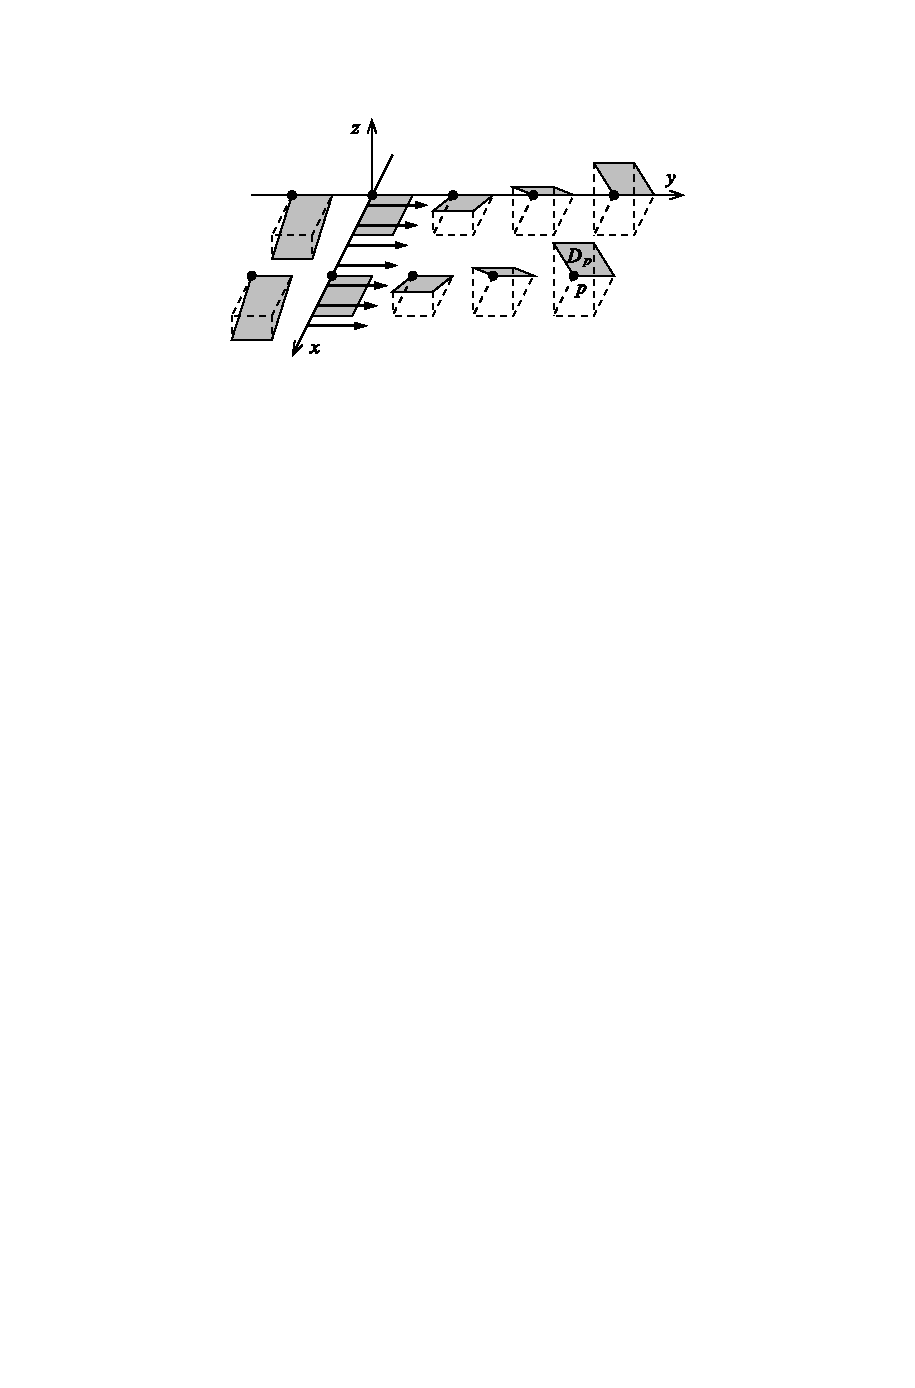
\includegraphics{pictures/distribution}
\caption{A smooth distribution with no integral manifolds.}
\end{figure}
\end{example}
The last example shows that in general, integral manifolds may fail to exist. Suppose
$D$ is a smooth distribution on $M$. We say that $D$ is \textbf{involutive} if given any pair of smooth local sections of $D$, their Lie bracket is also a local section of $D$. The next proposition shows that the involutivity condition can be expressed concisely in terms of Lie algebras.
\begin{proposition}
Let $D\sub TM$ be a smooth distribution, and let $\Gamma(D)\sub TM$ denote the space of smooth global sections of $D$. Then $D$ is involutive if and only if $\Gamma(D)$ is a Lie subalgebra of $\X(M)$.
\end{proposition}
\begin{proof}
If $D$ is involutive, the definition implies that $\Gamma(D)$ is closed under Lie brackets. Because it is also a linear subspace of $\X(M)$, 
it is a Lie subalgebra.\par
Conversely, suppose $\Gamma(D)$ is a Lie subalgebra of $\X(M)$, and let $X,Y$ be smooth local sections of $D$ over an open subset $U\sub M$. 
Given $p\in U$, let $\psi\in C^\infty(M)$ be a bump function that is identically $1$ on a neighborhood of $p$ and supported in $U$. Then $\psi X$ 
and $\psi Y$ are smooth global sections of $D$, so their Lie bracket is also a section of $D$ by hypothesis. This Lie bracket is 
$[\psi X,\psi Y]=\psi^2[X,Y]+(\psi X\psi)Y-(\psi Y\psi)X$, which is equal to $[X,Y]$ in a neighborhood of $p$. Thus, $[X,Y]\in D_p$ for each $p\in U$, 
so $D$ is involutive.
\end{proof}
A smooth distribution $D$ on $M$ is said to be \textbf{integrable} if each point of $M$ is contained in an integral manifold of $D$.
\begin{proposition}
Every integrable distribution is involutive.
\end{proposition}
\begin{proof}
Let $D\sub TM$ be an integrable distribution. Suppose $X$ and $Y$ are smooth local sections of $D$ defined on some open subset $U\sub M$. Let $p$ be any point in $U$, and let $N$ be an integral manifold of $D$ containing $p$. The fact that $X$ and $Y$ are sections of $D$ means that $X$ and $Y$ are tangent to $N$. By Corollary~\ref{Lie bracket tangent to submani}, $[X,Y]$ is also tangent to $N$, and therefore $[X,Y]_p\in D_p$. Since this is true at each $p\in U$, it follows that $D$ is involutive.
\end{proof}
Note, for example, that the distribution $D$ of Example~\ref{distribution eg}$(d)$ is not involutive, because $[X,Y]=-\partial/\partial z$, which is not a section of $D$.\par
The next lemma shows that the involutivity condition does not have to be checked
for every pair of smooth vector fields, just those of a smooth local frame in a neighborhood of each point.
\begin{lemma}[\textbf{Local Frame Criterion for Involutivity}]\label{involutivity local fram crit}
Let $D\sub TM$ be a smooth distribution. If in a neighborhood of every point of $M$ there exists a smooth local frame $V_1,\dots,V_k$ for $D$ such that $[V_i,V_j]$ is a section of $D$ for each $i,j$, then $D$ is involutive.
\end{lemma}
\begin{proof}
Suppose the hypothesis holds, and suppose $X$ and $Y$ are smooth local sections of $D$ over some open subset $U\sub M$. Given $p\in U$, choose a smooth local frame $V_1,\dots,V_k$ satisfying the hypothesis in a neighborhood of $p$, and write $X=X^iV_i$ and $Y=Y^iV_i$ in that neighborhood. Then, using $(\ref{Lie bracket two product rule})$,
\[[X,Y]=[X^iV_i,Y^jV_j]=X^iY^j[V_i,V_j]+X^i(V_iY^j)V_j-Y^j(V_jX^i)V_i.\]
It follows from the hypothesis that this last expression is a section of $D$.
\end{proof}
\subsubsection{Involutivity and differential forms}
Differential forms yield an alternative way to describe distributions and involutivity.
\begin{lemma}[\textbf{$\bm{1}$-Form Criterion for Smooth Distributions}]\label{distribution smooth crit}
Suppose $M$ is a smooth $n$-manifold and $D\sub TM$ is a distribution of rank $k$. Then $D$ is smooth if and only if each point $p\in M$ has a neighborhood $U$ on which there are smooth $1$-forms $\omega^1,\dots,\omega^{n-k}$ such that for each $q\in U$,
\begin{align}\label{defining frame-1}
D_q=\bigcap_{i=1}^{n-k}\ker\omega^i|_q.
\end{align}
\end{lemma}
\begin{proof}
First suppose that there exist such forms $\omega^1,\dots,\omega^{n-k}$ in a neighborhood of each point. The assumption $(\ref{defining frame-1})$ together with the fact that $D$ has rank $k$ implies that the forms $\omega^1,\dots,\omega^{n-k}$ are independent on $U$ for dimensional reasons. By Proposition~\ref{vector bundle local frame completion}, we can complete them to a smooth coframe $(\omega^1,\dots,\omega^n)$ on a (possibly smaller) neighborhood of each point. If $(E_1,\dots,E_n)$ is the dual frame, it is easy to check that $D$ is locally spanned by $E_{n-k+1},\dots,E_n$, so it is smooth by the local frame criterion.\par
Conversely, suppose $D$ is smooth. In a neighborhood of any $p\in M$, there are smooth vector fields $Y_1,\dots,Y_k$ spanning $D$. By Proposition~\ref{vector bundle local frame completion} again, we can complete these vector fields to a smooth local frame $Y_1,\dots,Y_n$ for $M$ in a neighborhood of $p$. With the dual coframe denoted by $(\eps^1,\dots,\eps^n)$, it follows easily that $D$ is characterized locally by
\[D_q=\bigcap_{i=1}^{n-k}\ker\eps^i|_q.\]
This completes the proof.
\end{proof}
If $D$ is a rank-$k$ distribution on a smooth $n$-manifold $M$, any $n-k$ linearly independent $1$-forms $\omega^1,\dots,\omega^{n-k}$ defined on an open subset $U\sub M$ and satisfying $(\ref{defining frame-1})$ for each $q\in U$ are called \textbf{local defining forms} for $D$. More generally, if $0\leq p\leq n$, we say that a $p$-form $\omega\in\Omega^p(M)$ \textbf{annihilates $\bm{D}$} if $\omega(X_1,\dots,X_p)=0$ whenever $X_1,\dots,X_p$ are local sections of $D$. (In the case $p=0$, only the zero function annihilates $D$.)
\begin{lemma}\label{distribution annihilate iff}
Suppose $M$ is a smooth $n$-manifold and $D$ is a smooth rank-$k$ distribution on $M$. Let $\omega^1,\dots,\omega^{n-k}$ be smooth local defining forms for $D$ over an open subset $U\sub M$. A smooth $p$-form $\eta$ defined on $U$ annihilates $D$ if and only if it can be expressed in the form
\begin{align}\label{annihilate-1}
\eta=\sum_{i=1}^{n-k}\omega^i\wedge\beta^i
\end{align}
for some smooth $(p-1)$-forms $\beta^1,\dots,\beta^{n-k}$ on $U$.
\end{lemma}
\begin{proof}
It is easy to check that any form $\eta$ that satisfies $(\ref{annihilate-1})$ in a neighborhood of each point annihilates $D$. Conversely, suppose that $\eta$ annihilates $D$ on $U$. In a neighborhood of each point we can complete the $(n-k)$-tuple $\omega^1,\dots,\omega^{n-k}$ to a smooth local coframe $\omega^1,\dots,\omega^n$ for $M$. If $(E_1,\dots,E_n)$ is the dual frame, then $D$ is locally spanned by $E_{n-k+1},\dots,E_n$. In terms of this coframe, any $\eta\in\Omega^p(M)$ can be written locally in a unique way as
\[\eta=\sum'_{I}\eta_I\,\omega^{i_1}\wedge\cdots\wedge\omega^{i_p},\]
where the coefficients $\eta_I$ are determined by $\eta_I=\eta(E_{i_1},\dots,E_{i_p})$. Thus, $\eta$ annihilates $D$ in $U$ if and only if $\eta_I=0$ whenever $n-k+1\leq i_1<\cdots<i_p\leq n$, in which case $\eta$ can be written locally as
\[\eta=\sum'_{I:i_1\leq n-k}\eta_I\,\omega^{i_1}\wedge\cdots\wedge\omega^{i_p}=\sum_{i_1=1}^{k}\omega^{i_1}\wedge\Big(\sum'_{I'}\eta_{i_1I'}\,\omega^{i_2}\wedge\cdots\wedge\omega^{i_p}\Big),\]
where we have written $I'=(i_2,\dots,i_p)$. This holds in a neighborhood of each point of $U$; patching together with a partition of unity, we obtain a similar expression on all of $U$.
\end{proof}
When expressed in terms of differential forms, the involutivity condition translates
into a statement about exterior derivatives.
\begin{theorem}[\textbf{$\bm{1}$-Form Criterion for Involutivity}]\label{involutivity 1 form crit}
Suppose $D\sub TM$ is a smooth distribution. Then $D$ is involutive if and only if the following condition is satisfied:
\begin{equation}\label{involutivity 1 form crit-1}
\parbox{\dimexpr\linewidth-6em}
{\strut
If $\eta$ is any smooth $1$-form that annihilates $D$ on an open subset $U\sub M$, then $d\eta$ also annihilates $D$ on $U$.
\strut}
\end{equation}
\end{theorem}
\begin{proof}
First, assume that $D$ is involutive, and suppose $\eta$ is a smooth $1$-form that annihilates $D$ on $U\sub M$. Then for any smooth local sections $X,Y$ of $D$, formula $(\ref{ext der 1 form})$ for $d\eta$ gives
\[d\eta(X,Y)=X(\eta(Y))-Y(\eta(X))-\eta([X,Y]).\]
The hypothesis implies that each of the terms on the right-hand side is zero on $U$.\par
Conversely, suppose $D$ satisfies $(\ref{involutivity 1 form crit-1})$, and suppose $X$ and $Y$ are smooth local
sections of $D$. If $\omega^1,\dots,\omega^{n-k}$ are smooth local defining forms for $D$, then $(\ref{ext der 1 form})$ shows that for each $1\leq i\leq n-k$,
\[\omega^i([X,Y])=X(\omega^i(Y))-Y(\omega^i(X))-d\omega^i(X,Y)=0,\]
which implies that $[X,Y]$ takes its values in $D$. Thus $D$ is involutive.
\end{proof}
Just like the Lie bracket condition for involutivity, the exterior derivative condition need only be checked for a particular set of smooth defining forms in a neighborhood of each point, as the next proposition shows.
\begin{proposition}[\textbf{Local Coframe Criterion for Involutivity}]\label{involutivity local coframe crit}
Let $D$ be a smooth distribution of rank $k$ on a smooth $n$-manifold $M$, and let $\omega^1,\dots,\omega^{n-k}$ be smooth defining forms for $D$ on an open subset $U\sub M$. The following are equivalent:
\begin{itemize}
\item[(a)] $D$ is involutive on $U$.
\item[(b)] $d\omega^1,\dots,d\omega^{n-k}$ annihilate $D$.
\item[(c)] There exist smooth $1$-forms $\{\alpha^i_j:1\leq i,j\leq n-k\}$ such that
\[d\omega^i=\sum_{j=1}^{n-k}\omega^j\wedge\alpha^i_j\for 1\leq i\leq n-k.\]
\item[$(d)$] For each $i=1,\dots,n-k$ we have
\[d\omega^i\wedge\omega^1\wedge\cdots\wedge\omega^{n-k}=0.\] 
\end{itemize}
\end{proposition}
\begin{proof}
By Theorem~\ref{involutivity 1 form crit}, if $D$ is involutive on $U$ then $d\omega^1,\dots,\omega^{n-k}$ annihilate $D$, so (a) implies (b). Now assume (b). If $\eta$ is a smooth $1$-form that annihilates $D$ on $U$, then by Proposition~\ref{distribution annihilate iff} there are smooth functions $\beta^i$ on $U$ such that
\[\eta=\sum_{i=1}^{n-k}\omega^i\wedge\beta^i.\]
Therefore
\[d\eta=\sum_{i=1}^{n-k}d\omega^i\wedge\beta^i-\sum_{i=1}^{n-k}\omega^i\wedge d\beta^i.\]
Since all $d\omega^i$'s annihilate $D$, $d\eta$ also annihilates $D$ on $U$. Thus $D$ is involutive on $U$ by Theorem~\ref{involutivity 1 form crit}. This proves $(a)\Leftrightarrow(b)$. By Lemma~\ref{distribution annihilate iff} we see (c) is equivalent to (b).\par
For $(d)$, it is clear that (c) implies $(d)$. Now assume $(d)$ holds. In a neighborhood of each point we can complete the $(n-k)$-tuple $\omega^1,\dots,\omega^{n-k}$ to a smooth local coframe $\omega^1,\dots,\omega^n$ for $M$. If $(E_1,\dots,E_n)$ is the dual frame, then $D$ is locally spanned by $E_{n-k+1},\dots,E_n$. In terms of this coframe, $d\omega^i$ can be written as
\[d\omega^i=\sum_{I}'\alpha_{I}\omega^{i_1}\wedge\omega^{i_2}.\]
The fact that $d\omega^i\wedge\omega^1\wedge\cdots\wedge\omega^{n-k}=0$ means $\alpha_{I}=0$ when $n-k+1\leq i_1<i_2\leq n$. Therefore, similar to the proof of Lemma~\ref{distribution annihilate iff}, we can write
\[d\omega^i=\sum_{i_1\leq n-k}\alpha_I\omega^{i_1}\wedge\omega^{i_2}=\sum_{i=1}^{n-k}\omega^i\wedge\Big(\sum_{i_1<i_2}\omega_{i_2}\Big).\]
By Lemma~\ref{distribution annihilate iff} this implies $d\omega^i$ annihilates $D$. Since this holds for all $i$, we get (b).
\end{proof}
With a bit more algebraic terminology, there is an elegant way to express the involutivity condition in terms of differential forms. Recall that we have defined
the graded algebra of smooth differential forms on a smooth $n$-manifold $M$ as $\Omega^*(M)=\bigoplus_{p=0}^{n}\Omega^p(M)$. An \textbf{ideal} in $\Omega^*(M)$ is a linear
subspace $\mathcal{I}\sub\Omega^*(M)$ that is closed under wedge products with arbitrary elements of $\Omega^*(M)$. Now suppose $D$ is a smooth distribution on a 
smooth $n$-manifold $M$. Let $\mathcal{I}^p(D)$ denote the space of smooth $p$-forms that annihilate $D$, and let $\mathcal{I}(D)=\bigoplus_{p=0}^{n}\mathcal{I}^p(D)$.\par
Any ideal of the form $\mathcal{I}(D)$ for some smooth distribution $D$ is sometimes called a \textbf{Pfaffian system}. An ideal $\mathcal{I}\sub\Omega^*(M)$ is said to be a \textbf{differential ideal} if $d(\mathcal{I})\sub\mathcal{I}$, that is, if $\eta\in\mathcal{I}$ implies $d\eta\in\mathcal{I}$.
\begin{proposition}[\textbf{Differential Ideal Criterion for Involutivity}]\label{involutivity differential ideal crit}
Let $M$ be a smooth manifold. A smooth distribution $D\sub TM$ is involutive if and only if $\mathcal{I}(D)$ is a differential ideal in $\Omega^*(M)$.
\end{proposition}
\begin{proof}
One direction is given by Theorem~\ref{involutivity 1 form crit}, the other is proved by Lemma~\ref{distribution annihilate iff}.
\end{proof}
\subsection{The Frobenius theorem}
Given a rank-$k$ distribution $D\sub TM$, let us say that a smooth coordinate chart $(U,\varphi)$ on $M$ is \textbf{flat} for $D$ if $\varphi(U)$ is a cube in $\R^n$, and at points of $U$, $D$ is spanned by the first $k$ coordinate vector fields $\partial/\partial x^1,\dots,\partial/\partial x^k$. In any such chart, each slice of the form $\{x^{k+1}=c^{k+1},\dots,x^n=c^n\}$ for constants $c^{k+1},\dots,c^n$ is an integral manifold of $D$. This is the nicest possible local situation for integral manifolds. We say that a distribution $D\sub TM$ is \textbf{completely integrable} if there exists a flat chart for $D$ in a neighborhood of each point of $M$. Obviously, every completely integrable distribution is integrable and therefore involutive. In summary,
\[\text{completely integrable}\Longrightarrow\text{integrable}\Longrightarrow\text{involutive}.\]
The next theorem is the main result of this section, and indeed one of the central theorems in smooth manifold theory. It says that the implications above are actually equivalences:
\[\text{completely integrable}\iff\text{integrable}\iff\text{involutive}.\]
\begin{figure}[htbp]
\centering
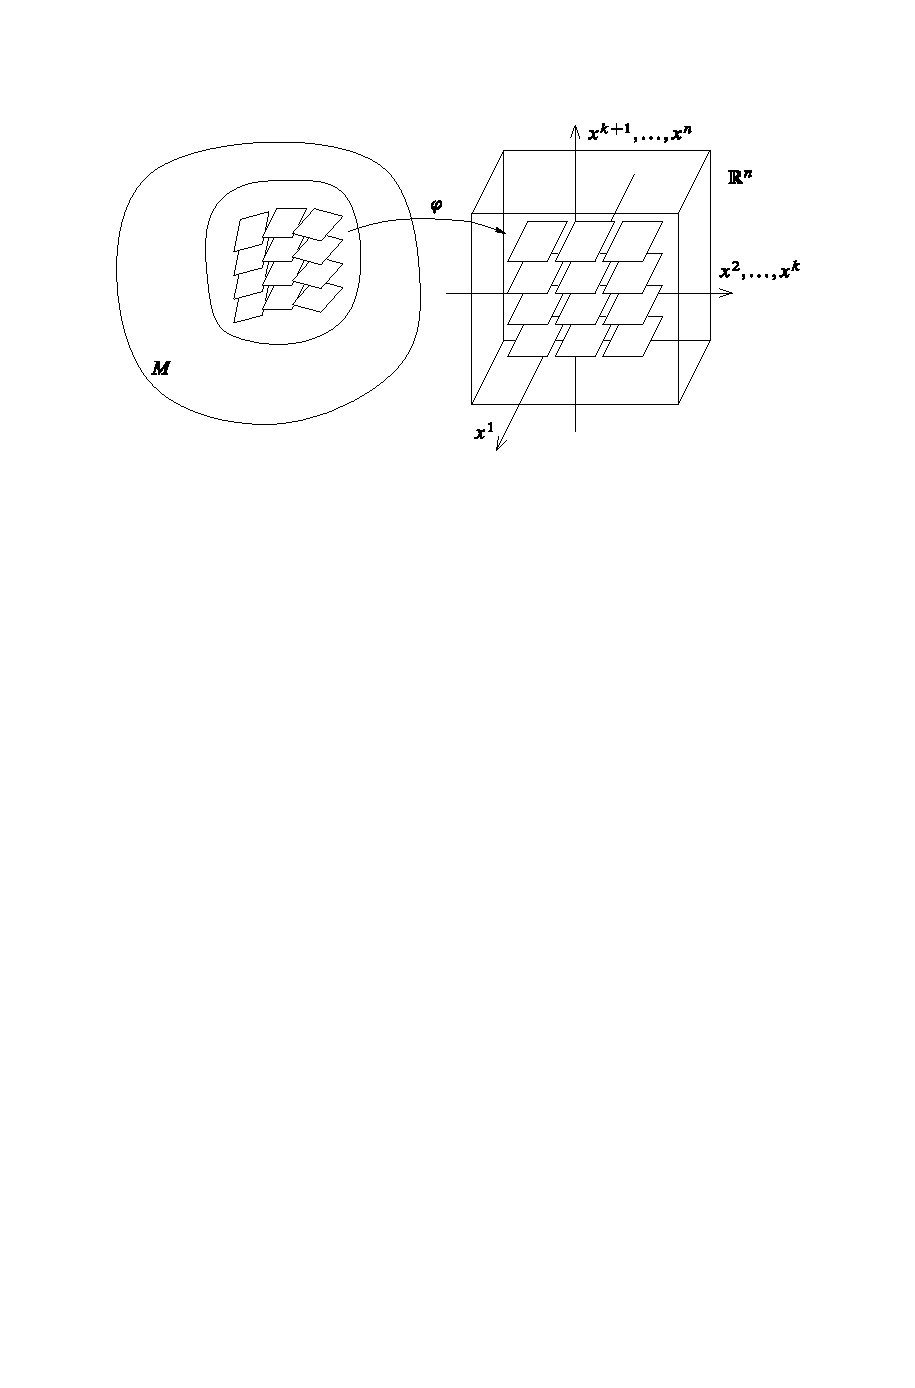
\includegraphics{pictures/flat-chart}
\caption{A flat chart for a distribution.}
\end{figure}
\begin{theorem}[\textbf{Frobenius}]
Every involutive distribution is completely integrable.
\end{theorem}
\begin{proof}
The canonical form theorem for commuting vector fields (Theorem~\ref{flow commute canonical form}) implies that any distribution locally spanned by independent smooth commuting vector fields is completely integrable, because the coordinate chart whose existence is guaranteed by that theorem is flat (after shrinking the domain if necessary so the image is a cube). Thus, it suffices to show that every involutive distribution is locally spanned by independent smooth commuting vector fields.\par
Let $D$ be an involutive distribution of rank $k$ on an $n$-dimensional manifold $M$, and let $p\in M$. Since complete integrability is a local question, by passing to a smooth coordinate neighborhood of $p$, we may replace $M$ by an open subset $U\sub\R^n$, and choose a smooth local frame $X_1,\dots,X_k$ for $D$. By reordering the coordinates if necessary, we may assume that $D_p$ is complementary to the subspace of $T_p\R^n$ spanned by $\partial/\partial x^{k+1}|_p,\dots,\partial/\partial x^{n}|_p$.\par 
Let $\pi:\R^n\to\R^k$ be the projection onto the first $k$ coordinates. This induces a smooth bundle homomorphism $d\pi:T\R^n\to T\R^k$, which can be written
\[d\pi\Big(\sum_{i=1}^{n}v^i\frac{\partial}{\partial x^i}\Big|_{q}\Big)=\sum_{i=1}^{k}v^i\frac{\partial}{\partial x^i}\Big|_{\pi(q)}.\]
Because $d\pi|_D$ is the composition of the inclusion $D\hookrightarrow U$ followed by $d\pi$, it is a smooth bundle homomorphism. Thus, the matrix entries of $d\pi|_{D_q}$ with respect to the frames $(X_i|_q)$ and $(\partial/\partial x^j|_{\pi(q)})$ are smooth functions of $q$.\par
By our choice of coordinates, $D_p\sub T_p\R^n$ is complementary to the kernel of $d\pi_p$, so the restriction of $d\pi_p$ to $D_p$ is bijective. By continuity, therefore, the same is true of $d\pi_{D_q}$ for $q$ in a neighborhood of $p$, and the matrix entries of $(d\pi|_{D_q})^{-1}:T_{\pi(q)}\R^k\to D_q$ are also smooth functions of $q$. Define a new smooth local frame $V_1,\dots,V_k$ for $D$ in a neighborhood of $p$ by 
\[V_i|_q=(d\pi|_{D_q})^{-1}\frac{\partial}{\partial x^i}\Big|_{\pi(q)}.\]
The theorem will be proved if we can show that $[V_i,V_j]=0$ for all $i,j$.\par
First observe that $V_i$ and $\partial/\partial x^i$ are $\pi$-related, because
\[\frac{\partial}{\partial x^i}\Big|_{\pi(q)}=(d\pi|_{D_q})V_i|_q=d\pi_q(V_i|_q).\]
Therefore, by the naturality of Lie brackets,
\[d\pi_q([V_i,V_j]_q)=\Big[\frac{\partial}{\partial x^i},\frac{\partial}{\partial x^j}\Big]_{\pi(q)}=0.\]
Since involutivity of $D$ implies that $[V_i,V_j]$ takes its values in $D$, and $d\pi$ is injective on each fiber of $D$, this implies that $[V_i,V_j]=0$ for each $q$, thus completing the proof.
\end{proof}
For later use in our treatment of overdetermined partial differential equations, we note the following easy corollary to the proof.
\begin{corollary}\label{distribution complementary submani is slice}
Suppose $M$ is a smooth manifold, $D$ is an involutive rank-$k$ distribution on $M$, and $S\sub M$ is a codimension-$k$ embedded submanifold. If $p\in S$ is a point such that $T_pS$ is complementary to $D_p$, then there is a flat chart $(U,(s^i))$ for $D$ centered at $p$ in which $S\cap U$ is the slice $s^1=\cdots=s^k=0$.
\end{corollary}
\begin{proof}
The proof of the theorem showed that locally $D$ is spanned by $k$ commuting vector fields, and then the corollary follows from Theorem~\ref{flow commute canonical form}.
\end{proof}
As is often the case, embedded in the proof of the Frobenius theorem is a technique for finding integral manifolds. The idea is to use a coordinate projection to find commuting vector fields spanning the same distribution, and then use the technique of Example~\ref{commute vector field eg} to find a flat chart. Here is an example.
\begin{example}
Let $D\sub T\R^3$ be the distribution spanned by the vector fields
\begin{flalign*}
&X=x\frac{\partial}{\partial x}+\frac{\partial}{\partial y}+x(y+1)\frac{\partial}{\partial z},\\
&Y=\frac{\partial}{\partial x}+y\frac{\partial}{\partial z}
\end{flalign*}
We have
\[[X,Y]=-\frac{\partial}{\partial x}-y\frac{\partial}{\partial z}=-Y,\]
so $D$ is involutive. Let us try to find a flat chart in a neighborhood of the origin. Since $D$ is complementary to the span of $\partial/\partial z$, the coordinate projection $\pi:\R^3\to\R^2$ given by $\pi(x,y,z)=(x,y)$ induces an isomorphism $d\pi|_{D_{(x,y,z)}}:D_{(x,y,z)}\to T_{(x,y)}\R^2$ for each $(x,y,z)$. The proof of the Frobenius theorem shows that if we can find smooth local sections $V,W$ of $D$ that are $\pi$-related to $\partial/\partial x$ and $\partial/\partial y$, respectively, they will be commuting vector fields spanning $D$. It is easy to check that $V,W$ have this property if and only if they take their values in $D$ and are of the form
\begin{flalign*}
&V=\frac{\partial}{\partial x}+u(x,y,z)\frac{\partial}{\partial z},\\
&W=\frac{\partial}{\partial y}+v(x,y,z)\frac{\partial}{\partial z},
\end{flalign*}
for some smooth real-valued functions $u,v$. A bit of linear algebra shows that the vector fields
\begin{flalign*}
&V=Y=\frac{\partial}{\partial x}+y\frac{\partial}{\partial z},\\
&W=X-xY=\frac{\partial}{\partial y}+x\frac{\partial}{\partial z},
\end{flalign*}
do the trick. Sparing the details, we find that the flow of $V$ is
\[\alpha_t(x,y,z)=(x+t,y,z+ty),\]
and that of $W$ is
\[\beta_t(x,y,z)=(x,y+t,z+tx).\]
Thus, by the procedure of Example~\ref{commute vector field eg}, we can define the inverse $\varPhi$ of our coordinate map by starting on the $z$-axis and flowing out along these two flows in succession:
\[\varPhi(u,v,w)=\alpha_u\circ\beta_v(0,0,w)=\alpha_u(0,0,w)=(u,v,w+uv).\]
The flat coordinates we seek are given by inverting the map $(x,y,z)=\varPhi(u,v,w)=(u,v,w+uv)$, to yield
\[(u,v,w)=\varPhi^{-1}(x,y,z)=(x,y,z-xy).\]
It follows that the integral manifolds of $D$ are the level sets of $w(x,y,z)=z-xy$.
\end{example}
The next proposition is one of the most important consequences of the Frobenius
theorem.
\begin{proposition}[\textbf{Local Structure of Integral Manifolds}]\label{integral mani local struct}
Let $D$ be an involutive distribution of rank $k$ on a smooth manifold $M$, and let $(U,(x^i))$ be a flat chart for $D$. If $H$ is any integral manifold of $D$, then $H\cap U$ is a union of countably many disjoint open subsets of parallel $k$-dimensional slices of $U$, each of which is open in $H$ and embedded in $M$.
\end{proposition}
\begin{figure}[htbp]
\centering
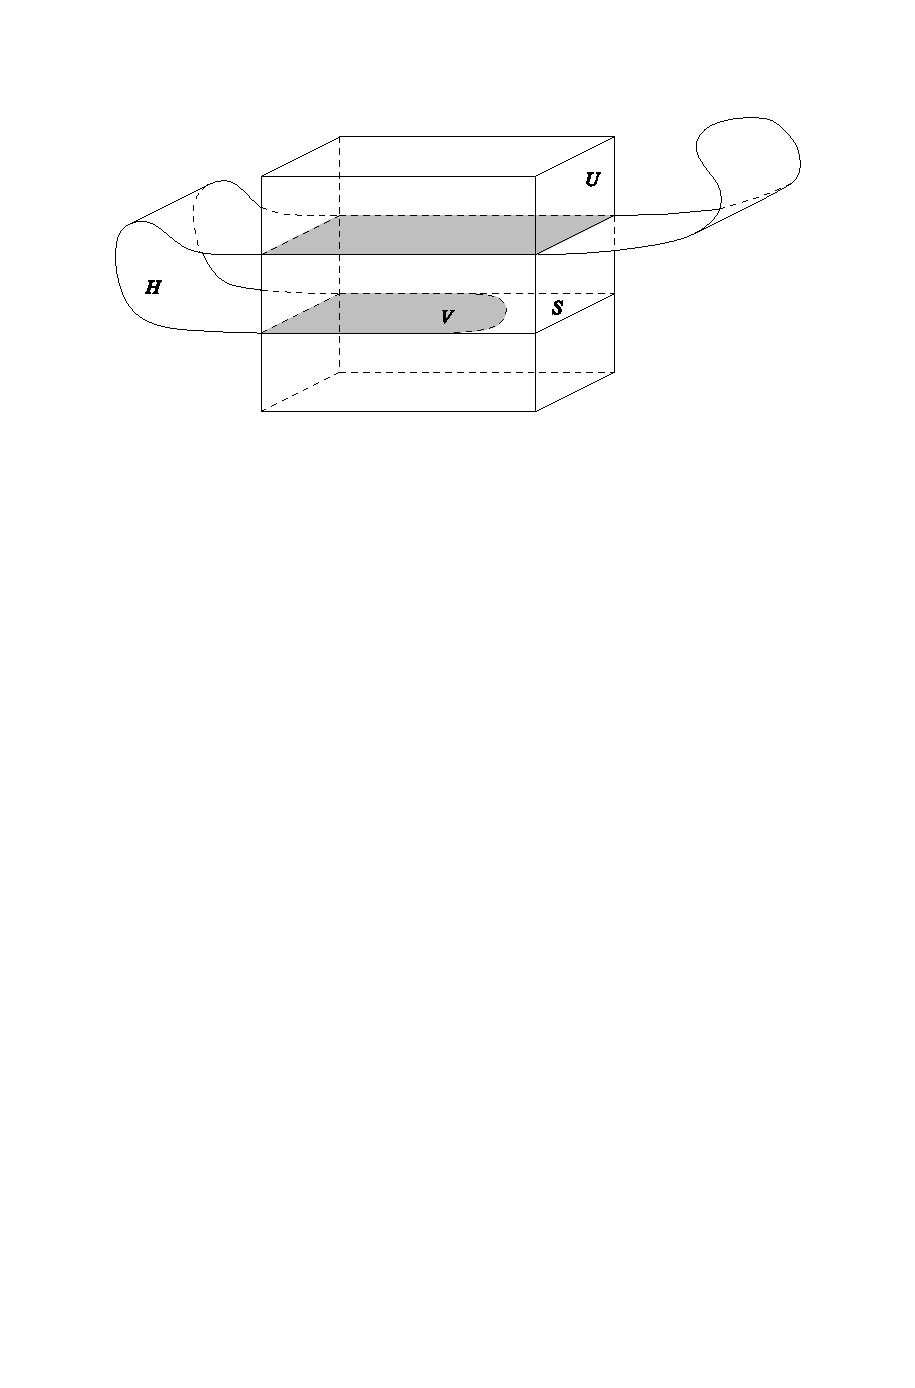
\includegraphics{pictures/local-struct}
\caption{The local structure of an integral manifold.}
\end{figure}
\begin{proof}
Let $H$ be an integral manifold of $D$. Because the inclusion map $\iota:H\hookrightarrow M$ is continuous, $H\cap U=\iota^{-1}(U)$ is open in $H$, and thus consists of a countable disjoint union of connected components, each of which is open in $H$.\par
Let $V$ be any component of $H\cap U$. We show first that $V$ is contained in a single slice. Since $dx^{k+1},\dots,dx^n$ are local defining forms for $D$, it follows that the pullbacks of these $1$-forms to $V$ are identically zero. Because $V$ is connected, this implies that $x^{k+1},\dots,x^n$ are all constant on $V$, so $V$ lies in a single slice $S$.\par
Because $S$ is embedded in $M$, the inclusion map $V\hookrightarrow M$ is also smooth as a map into $S$ by Corollary~\ref{resrtict codomain to embedd}. The inclusion $V\hookrightarrow S$ is thus an injective smooth immersion between manifolds of the same dimension, and therefore a local diffeomorphism, an open map, and a homeomorphism onto an open subset of $S$. The inclusion map $V\hookrightarrow M$ is a composition of the smooth embeddings $V\hookrightarrow S\hookrightarrow M$, so it is a smooth embedding.
\end{proof}
The preceding proposition implies the following important result about integral
manifolds, which we will use in our study of Lie subgroups at the end of this section. Recall that a smooth submanifold $H\sub M$ is said to be weakly embedded in $M$ if every smooth map $F:N\to M$ whose image lies in $H$ is smooth as a map from $N$ to $H$.
\begin{theorem}\label{integral mani weak embedd}
Every integral manifold of an involutive distribution is weakly embedded.
\end{theorem}
\begin{proof}
Let $M$ be a smooth $n$-manifold, let $H\sub M$ be an integral manifold of an involutive rank-$k$ distribution $D$ on $M$, and suppose $F:N\to M$ is a smooth map such that $F(N)\sub H$. Let $p\in N$ be arbitrary, and set $q=F(p)\in H$. Let $(y^1,\dots,y^n)$ be flat coordinates for $D$ on a neighborhood $U$ of $q$, and let $(x^i)$ be smooth coordinates for $N$ on a connected neighborhood $B$ of $p$ such that $F(B)\sub U$. With the coordinate representation of $F$ written as
\[(y^1,\dots,y^n)=(F^1(x),\dots,F^n(x)).\]
The fact that $F(N)\sub H\cap U$ means that the coordinate functions $F^{k+1}(x),\dots,F^n(x)$ take on only countably many values. Because $B$ is connected, the intermediate value theorem implies that these coordinate functions are constant, and thus $F(B)$ lies in a single slice $S\sub U$. Because $S\cap H$ is an open subset of $H$ that is embedded in $M$, it follows that $F|_B$ is smooth from $B$ into $S\cap H$, and thus by composition, $F|_B:D\hookrightarrow(S\cap H)\hookrightarrow H$ is smooth into $H$.
\end{proof}
\subsection{Foliations}
When we put together all of the maximal integral manifolds of an involutive rank-$k$ distribution on a smooth manifold $M$, we obtain a partition of $M$ into $k$-dimensional submanifolds that fit together locally like the slices in a flat chart.\par 
To express more precisely what we mean by fitting together, we need to extend our notion of a flat chart slightly. Let $M$ be a smooth $n$-manifold, and let $\mathcal{F}$ be any collection of $k$-dimensional submanifolds of $M$. A smooth chart $(U,\varphi)$ for $M$ is said to be \textbf{flat for $\mathcal{F}$} if $\varphi(U)$ is a cube in $\R^n$, and each submanifold in $\mathcal{F}$ intersects $U$ in either the empty set or a countable union of $k$-dimensional slices of the form $\{x^{k+1}=c^{k+1},\dots,x^n=c^n\}$. We define a \textbf{foliation of dimension $\bm{k}$ on $\bm{M}$} to be a collection $\mathcal{F}$ of disjoint, connected, nonempty, immersed $k$-dimensional submanifolds of $M$ (called the \textbf{leaves of the foliation}), whose union is $M$, and such that in a neighborhood of each point $p\in M$ there exists a flat chart for $\mathcal{F}$.
\begin{example}[\textbf{Foliations}]
\mbox{}
\begin{itemize}
\item[(a)] The collection of all $k$-dimensional affine subspaces of $\R^n$ parallel to $\R^k\times\{0\}$ is a $k$-dimensional foliation of $\R^n$.
\item[(b)] The collection of open rays of the form $\{\lambda x:\lambda>0\}$ as $x$ ranges over $\R^n-\{0\}$ is a $1$-dimensional foliation of $\R^n-\{0\}$.
\item[(c)] The collection of all spheres centered at $0$ is an $(n-1)$-dimensional foliation of $\R^n-\{0\}$.
\begin{figure}[htbp]
\centering
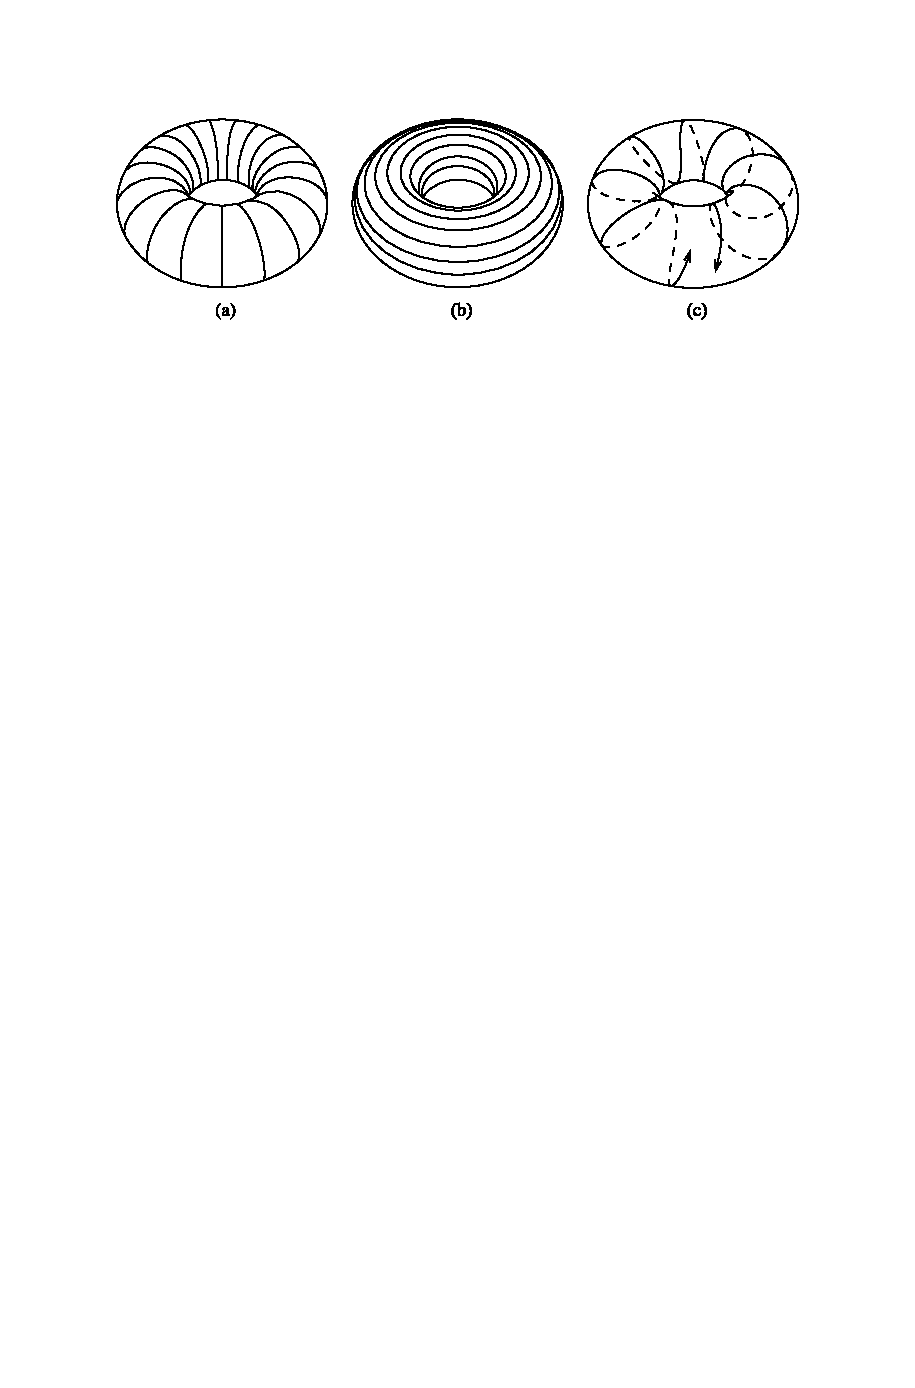
\includegraphics{pictures/foliation-of-torus}
\caption{Foliations of the torus.}
\end{figure} 
\item[$(d)$] If $M$ and $N$ are connected smooth manifolds, the collection of subsets of the form $M\times\{q\}$ as $q$ ranges over points in $N$ forms a foliation of $M\times N$, each of whose leaves is diffeomorphic to $M$. For example, the collection of all circles of the form $S^1\times\{q\}\sub T^2$ for $q\in S^1$ yields a foliation of the torus $T^2$. A different foliation of $T^2$ is given by the collection of circles of the form $\{p\}\times S^1$.
\item[$(e)$] If $\alpha$ is a fixed real number, the images of all curves of the form
\[\gamma_\theta(t)=(e^{it},e^{i(\alpha t+\theta)})\]
as $\theta$ ranges over $\R$ form a $1$-dimensional foliation of the torus. If $\alpha$ is rational, each leaf is an embedded circle; whereas if $\alpha$ is irrational, each leaf is dense.
\item[(f)] The collection of connected components of the curves in the $(y,z)$-plane defined by the following equations is a foliation of $\R^2$:
\begin{flalign*}
&z=\sec y+c,\ c\in\R;\\
&y=(k+\frac{1}{2})\pi,\ k\in\Z.
\end{flalign*}
\item[(g)] If we revolve the curves of the previous example around the $z$-axis, we obtain a $2$-dimensional foliation of $\R^3$ in which some of the leaves are diffeomorphic to disks and some are diffeomorphic to cylinders.
\end{itemize}
\end{example}
\begin{figure}[htbp]
\centering
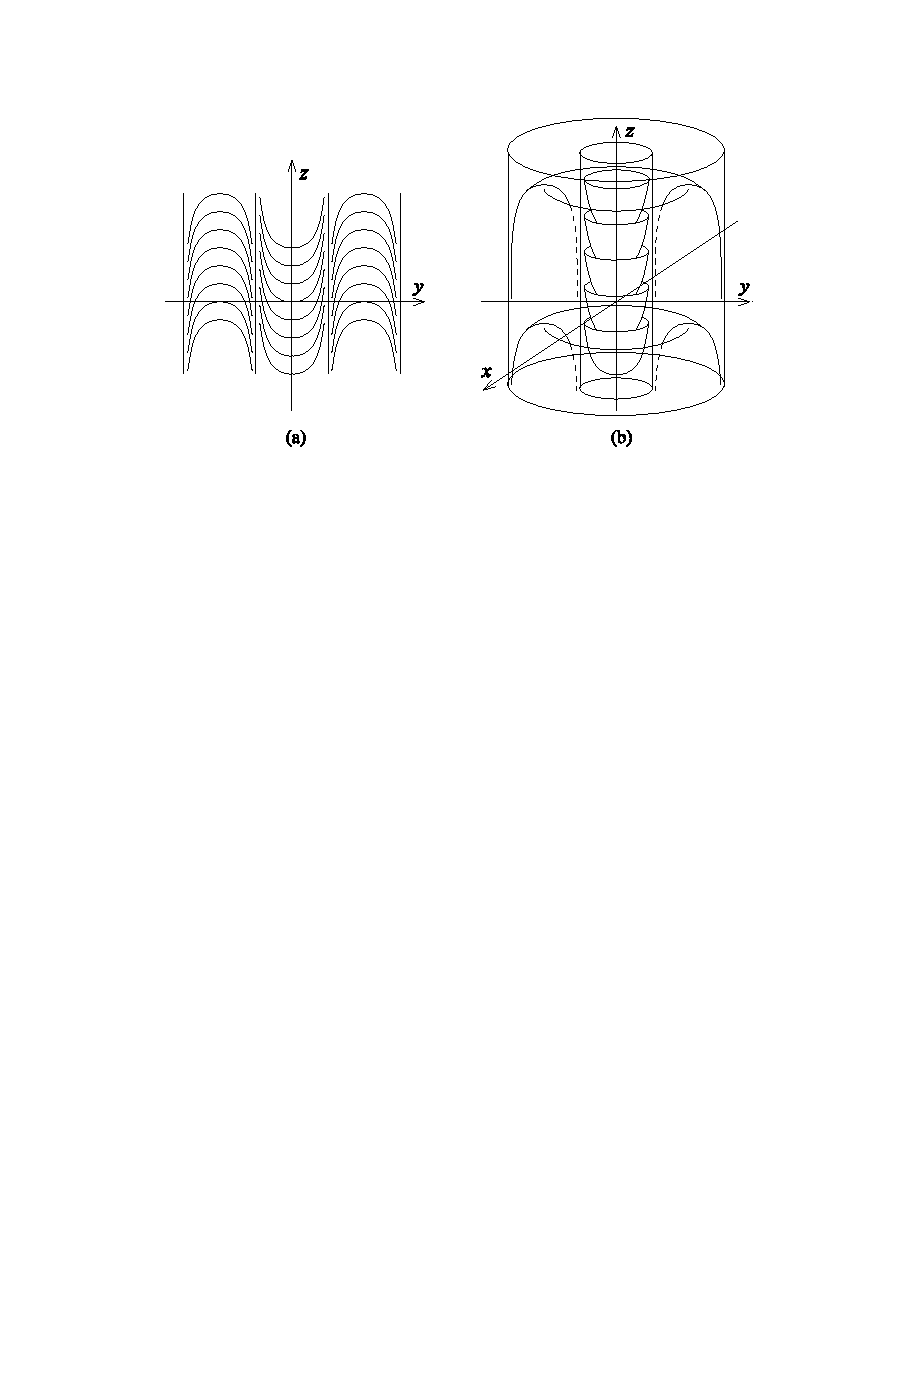
\includegraphics{pictures/foliation}
\caption{Foliations of $\R^2$ and $\R^3$.}
\end{figure}
The main fact about foliations is that they are in one-to-one correspondence with
involutive distributions. One direction, expressed in the next proposition, is an easy consequence of the definition.
\begin{proposition}
Let $\mathcal{F}$ be a foliation on a smooth manifold $M$. The collection of tangent spaces to the leaves of $\mathcal{F}$ forms an involutive distribution on $M$.
\end{proposition}
The Frobenius theorem allows us to conclude the following converse, which is much more profound. By the way, it is worth noting that this result is one of the two primary reasons why the notion of immersed submanifold has been defined.
\begin{theorem}[\textbf{Global Frobenius Theorem}]
Let $D$ be an involutive distribution on a smooth manifold $M$. The collection of all maximal connected integral manifolds of $D$ forms a foliation of $M$.
\end{theorem}
The theorem will be an easy consequence of the following lemma.
\begin{lemma}
Suppose $D\sub TM$ is an involutive distribution, and let $\{N_\alpha\}_{\alpha\in A}$ be any collection of connected integral manifolds of $D$ with a point in common. Then $N=\bigcup_{\alpha\in A}N_\alpha$ has a unique smooth manifold structure making it into a connected integral manifold of $D$.
\end{lemma}
\begin{proof}
If we can construct a topology and smooth manifold structure making $N$ into an integral manifold of $D$, then Theorem~\ref{unique smooth weak embedd} shows that the topology and smooth structure are uniquely determined, because integral manifolds are weakly embedded.\par
To construct the topology, first we need to show that $N_\alpha\cap N_\beta$ is open in $N_\alpha$ and in $N_\beta$ for each $\alpha,\beta\in A$. Let $q\in N_\alpha\cap N_\beta$ be arbitrary, and choose a flat chart for $D$ on a neighborhood $W$ of $q$. Let $V_\alpha,V_\beta$ denote the components of $N_\alpha\cap W$ and $N_\beta\cap W$, respectively, containing $q$. By Proposition~\ref{integral mani local struct}, $V_\alpha$ and $V_\beta$ are open subsets of single slices with the subspace topology, and since both contain $q$, they both must lie in the same slice $S$. Thus $V_\alpha\cap V_\beta$ is open in $S$ and also in both $N_\alpha$ and $N_\beta$, so $q$ has a neighborhood in $N_\alpha$ and a neighborhood in $N_\beta$ contained in $N_\alpha\cap N_\beta$.
\begin{figure}[htbp]
\centering
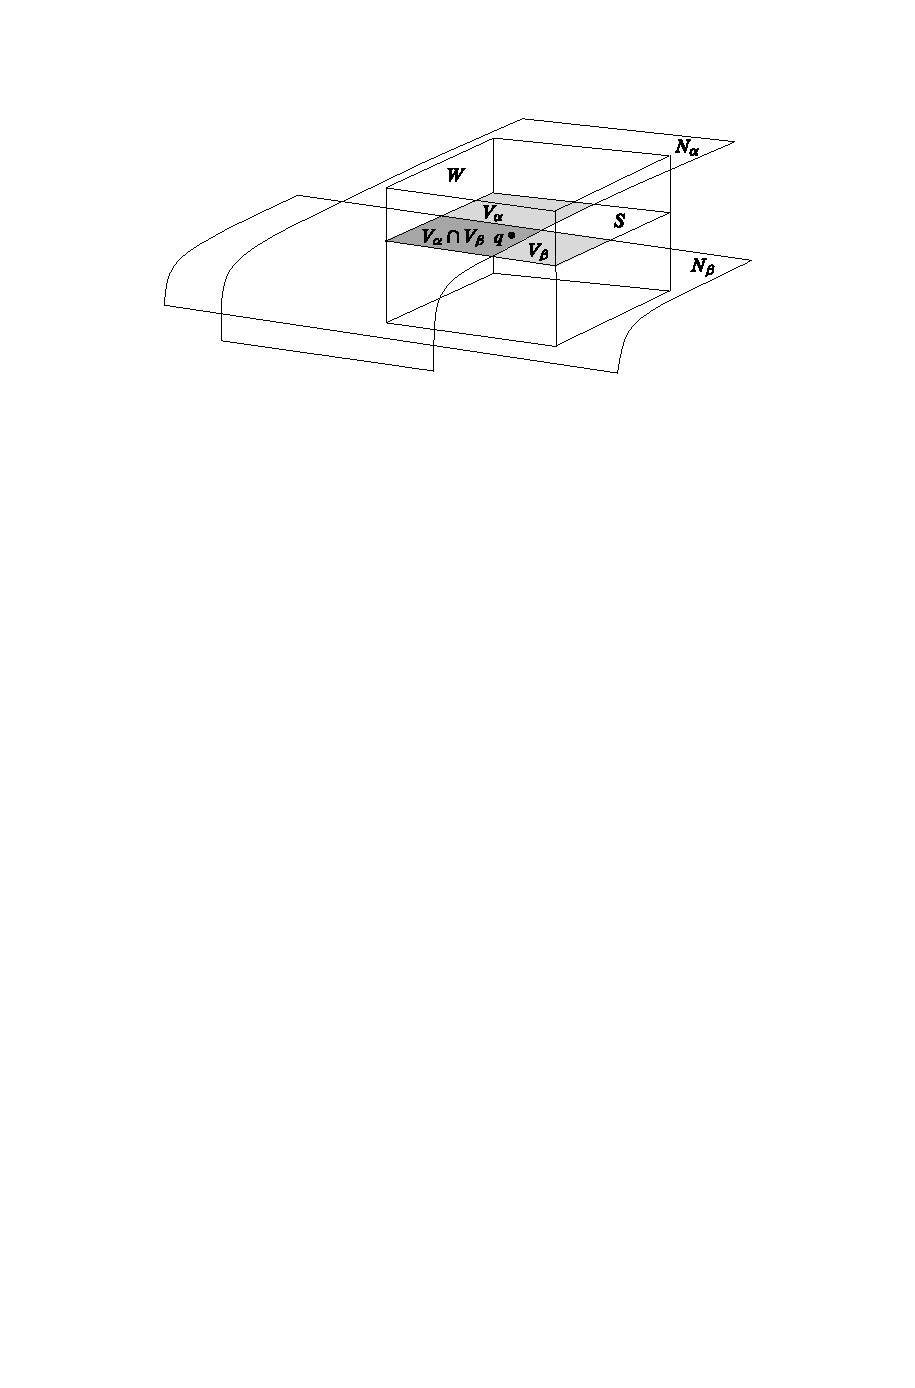
\includegraphics{pictures/union-integral-submani}
\caption{A union of integral manifolds.}
\end{figure}

Define a topology on $N$ by declaring a subset $U\sub N$ to be open if and only if $U\cap N_\alpha$ is open in $N_\alpha$ for each $N_\alpha$. Using the result of the previous paragraph, it is easy to check that this is a topology and that each $N_\alpha$ is an open subspace of $N$. With this topology, $N$ is locally Euclidean of dimension $k$, because each $q\in N$ has a coordinate neighborhood $V$ in some $N_\alpha$, and $V$ is an open subset of $N$ because $N_\alpha$ is open in $N$. Moreover, the inclusion map $N\hookrightarrow M$ is continuous: for any open subset $U\sub M$, $U\cap N$ is open in $N$ because $U\cap N_\alpha$ is open in $N_\alpha$ for each $\alpha$.\par
To see that $N$ is Hausdorff, let $q_1,q_2$ be distinct points of $N$. There are disjoint open subsets $U_1,U_2\sub M$ containing $q_1$ and $q_2$, respectively, and because inclusion $N\hookrightarrow M$ is continuous, $N\cap U_1$ and $N\cap U_2$ are disjoint open subsets of $N$ containing $q_1$ and $q_2$.\par
Next we show that $N$ is second-countable. We can cover $M$ with countably many flat charts for $D$, say $\{W_i\}$. It suffices to show that $N\cap W_i$ is contained in a countable union of slices for each $i$, because any open subset of a single slice is second countable, and thus $N$ can be expressed as a union of countably many subsets, each of which is second-countable and open in $N$.\par
Let $p_0$ be a point contained in $N_\alpha$ for every $\alpha$. Let us say that a slice $S$ of some $W_k$ is \textbf{accessible from $\bm{p_0}$} if there is a finite sequence of indices $i_1,\dots,i_m$ and for each $i_j$ a slice $S_{i_j}\sub W_{i_j}$ with the properties that $p\in S_{i_1}$, $S_{i_m}=S$, and $S_{i_j}\cap S_{i_j+1}\neq\emp$ for each $j=1,\dots,m-1$.
\begin{figure}[htbp]
\centering
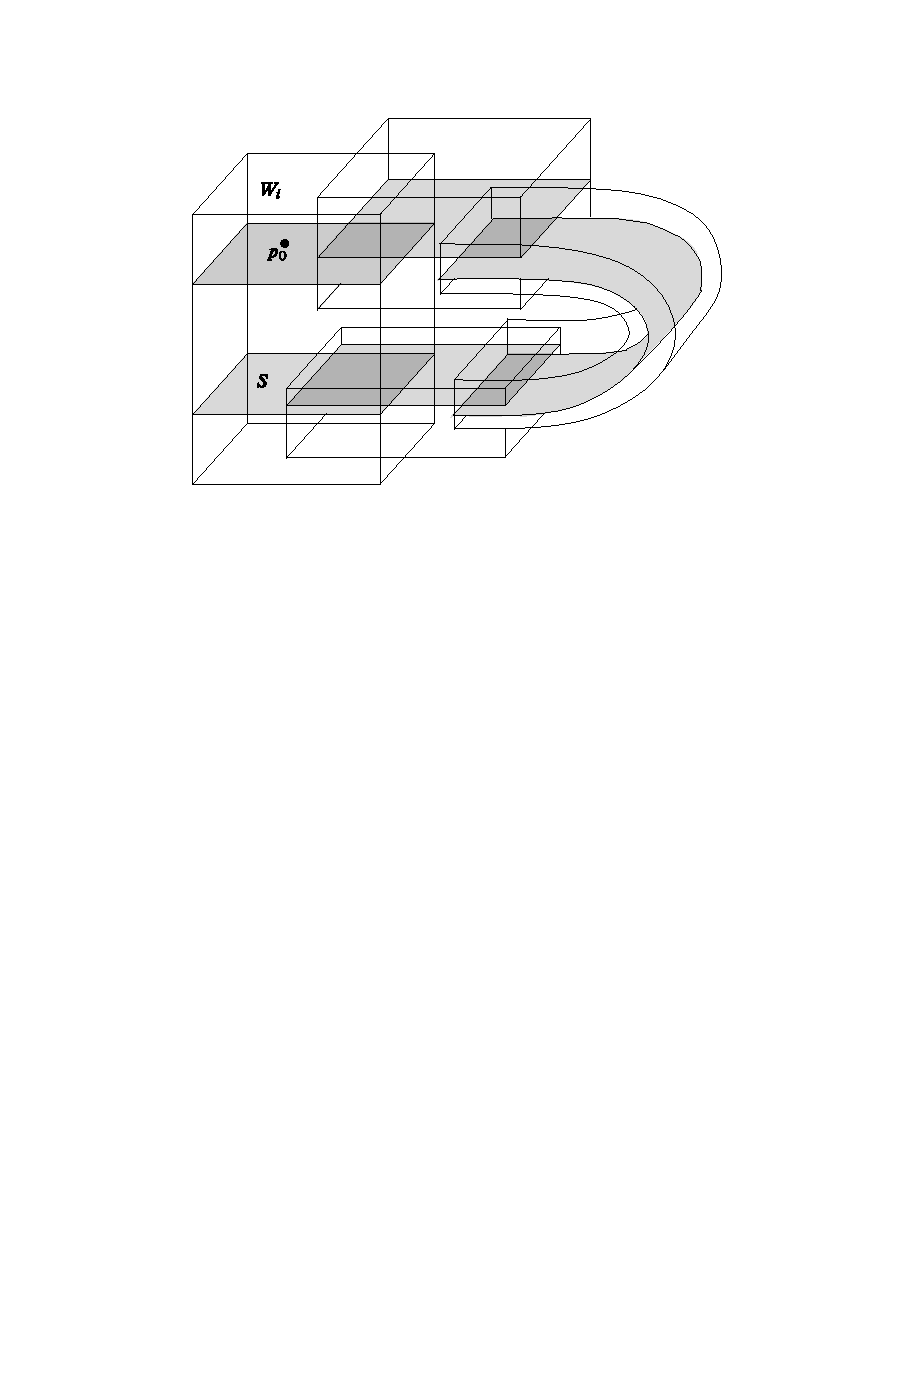
\includegraphics{pictures/slice-accessible}
\caption{A slice $S$ accessible from $p_0$}
\end{figure}

Let $W_k$ be one of our countable collection of flat charts, and suppose $S\sub W_k$ is a slice that contains a point $q\in N$. Then $q$ is contained in one of the integral manifolds $N_\alpha$. Because $p_0$ is also in $N_\alpha$, there is a continuous path $\gamma:[0,1]\to N_\alpha$ connecting $p_0$ and $q$. Since $\gamma([0,1])$ is compact, there exist finitely many numbers $0=t_0<t_1<\cdots<t_m=1$ such that for each $j=1,\dots,m$, the set $\gamma([t_{j-1},t_j])$ is contained in one of the flat charts $W_{i_j}$. Since $\gamma([t_{j-1},t_j])$ is connected, it is contained in a single component of $W_{i_j}\cap N_\alpha$ and therefore in a single slice $S_{i_j}\sub W_{i_j}$. For each $j=1,\dots,m-1$, the slices $S_{i_j}$ and $S_{i_{j+1}}$ have the point $\gamma(t_j)$ in common, so it follows that the slice $S$ is accessible from $p_0$.\par
This shows that every slice of some $W_k$ containing a point of $N$ is accessible from $p_0$, and therefore every slice intersecting $N$ must be accessible from $p_0$. To complete the proof of second-countability, we just note that each $S_{i_j}$ is itself an integral manifold, and therefore it meets at most countably many slices of $W_{i_{j+1}}$ by Proposition~\ref{integral mani local struct}; thus, there are only countably many slices accessible from $p_0$. Therefore, $N$ is a topological manifold of dimension $k$. It is connected because it is a union of connected subspaces with a point in common.\par
To construct a smooth structure on $N$, we define an atlas consisting of all charts of the form $(S\cap N,\psi)$, where $S$ is a single slice of some flat chart, and $\psi:S\to\R^k$ is the map whose coordinate representation in the flat chart is projection onto the first $k$ coordinates: $(x^1,\dots,x^k,x^{k+1},\dots,x^n)\mapsto(x^1,\dots,x^k)$. Because any slice is an embedded submanifold, its smooth structure is uniquely determined, and thus whenever two such slices $S_1$ and $S_2$ overlap the transition map $\psi_2\circ\psi_1^{-1}$ is smooth. With respect to this smooth structure, the inclusion map $N\hookrightarrow M$ is a smooth immersion (because it is a smooth embedding on each slice), and the tangent space to $N$ at each point $q\in N$ is equal to $D_q$ (because this is true for slices).
\end{proof}
\begin{proof}[Proof of the global Frobenius theorem]
For each $p\in M$, let $L_p$ be the union of all connected integral manifolds of $D$ containing $p$. By the preceding lemma, $L_p$ is a connected integral manifold of $D$ containing $p$, and it is clearly maximal. If any two such maximal integral manifolds $L_p$ and $L_{p'}$ intersect, their union $L_p\cup L_{p'}$ is an integral manifold containing both $p$ and $p'$, so by maximality $L_p=L_{p'}$. Thus, the various maximal connected integral manifolds are either disjoint or identical.\par
If $(U,\varphi)$ is any flat chart for $D$, then $L_p\cap U$ is a countable union of open subsets of slices by Proposition~\ref{integral mani local struct}. For any such slice $S$, if $L_p\cap S$ is neither empty nor all of $S$, then $L_p\cup S$ is a connected integral manifold properly containing $L_p$, which contradicts the maximality of $L_p$. Therefore, $L_p\cap U$ is precisely a countable union of slices, so the collection $\{L_p:p\in M\}$ is the desired foliation.
\end{proof}
Suppose $M$ is a smooth manifold and $\varPhi:M\to M$ is a diffeomorphism. A distribution 
$D$ on $M$ is said to be \textbf{$\varPhi$-invariant} if $d\varPhi(D)=D$ or more precisely if for 
each $x\in M$, $d\varPhi_x(D_x)=D_{\varPhi(x)}$. Similarly, a foliation $\mathcal{F}$ on 
$M$ is said to be \textbf{$\varPhi$-invariant} if for each leaf $L$ of $\mathcal{F}$, the 
submanifold $\varPhi(L)$ is also a leaf of $\mathcal{F}$.
\begin{proposition}\label{distribution invariant}
Let $M$ be a smooth manifold and $\varPhi:M\to M$ be a diffeomorphism. Suppose $D$ is an 
involutive distribution on $M$ and $\mathcal{F}$ is the foliation it determines. Then $D$ 
is $\varPhi$-invariant if and only if $\mathcal{F}$ is $\varPhi$-invariant.
\end{proposition}
\begin{proof}
Since the tangent space of a point on the leaf of the foliation is the fiber of the distribution, if 
$\mathcal{F}$ is $\varPhi$-invariant, then $D$ is also $\varPhi$-invariant. Conversely, if 
$D$ is $\varPhi$-invariant, then for any point $p\in M$, we have $d\varPhi_p(D)=D_{\varPhi(p)}$. Let $L$ be a leaf of $\mathcal{F}$, then $\varPhi(L)$ is also an integral manifold. By definition, this implies $\mathcal{F}$ is $\varPhi$-invariant.
\end{proof}
\subsection{Overdetermined systems of partial differential equations}
The partial differential equations we considered in Section~\ref{flow section} were all single equations for one unknown function. In some applications, it is necessary to consider systems of PDEs that are \textbf{overdetermined}, which means that there are more equations than unknown functions. In general, overdetermined systems have solutions only if they satisfy certain compatibility conditions. For some first-order systems, the compatibility condition can be interpreted as a statement about involutivity of a distribution, and the Frobenius theorem can be used to prove local existence and uniqueness of solutions.\par
First, we consider certain linear systems. Suppose $W$ is an open subset of $\R^n$ and $m$ is a positive integer less than or equal to $n$. Consider the following system of
\begin{equation}\label{overdetermined linear PDE}
\left\{\begin{aligned}
a^1_1(x)\frac{\partial u}{\partial x^1}(x)+\cdots+a_1^n(x)\frac{\partial u}{\partial x^n}(x)&=f_1(x),\\
&\ \ \vdots\\
a^1_m(x)\frac{\partial u}{\partial x^1}(x)+\cdots+a_m^n(x)\frac{\partial u}{\partial x^n}(x)&=f_m(x)
\end{aligned}\right. 
\end{equation}
where $(a_i^j(x))$ is an $n\times m$ matrix of smooth real-valued functions and $f_1,\dots,f_m$ are smooth real-valued functions on $W$. The case $m=1$ is covered by Theorem~\ref{linear PDE solution}, so this discussion is useful primarily when $m>1$.\par
If we let $A_i$ denote the vector field $a^j_i\partial/\partial x^j$, the system $(\ref{overdetermined linear PDE})$ can be written more succinctly as $A_iu=f_i$, $i=1,\dots,m$. To avoid redundant or degenerate systems of equations, we assume that the matrix $(a_{i}^j(x))$ has rank $m$ at each point of $W$, or equivalently that the vector fields $A_1,\dots,A_m$ are linearly independent. The following theorem is an analogue of Theorem~\ref{linear PDE solution} for the overdetermined case.
\begin{theorem}\label{overdetermined linear PDE solution}
Let $W\sub\R^n$ be an open subset and let m be an integer such that $1\leq m\leq n$. Suppose we are given an embedded codimension-$m$ submanifold $S\sub W$, a linearly independent $m$-tuple of smooth vector fields $(A_1,\dots,A_m)$ on $W$ whose span is complementary to $T_pS$ at each $p\in S$, and functions $f_1,\dots,f_m\in C^\infty(W)$. Suppose also that there are smooth functions $c_{ij}^k\in C^\infty(W)$ for $i,j,k=1,\dots,m$ such that the following compatibility conditions are satisfied:
\begin{align}
[A_i,A_j]&=c_{ij}^kA_k,\label{overdetermined linear PDE compatibility-1}\\
A_if_j-A_jf_i&=c_{ij}^kf_k.\label{overdetermined linear PDE compatibility-2}
\end{align}
Then for each $p\in S$, there is a neighborhood $U$ of $p$ such that for every $\varphi\in C^\infty(S\cap U)$, there exists a unique solution $u\in C^\infty(U)$ to the following overdetermined Cauchy problem:
\begin{align}
A_iu&=f_i\quad\text{\textit{for} }i=1,\dots,m\label{overdetermined linear PDE equation-1}\\
u|_{S\cap U}&=\varphi\label{overdetermined linear PDE equation-2}.
\end{align}
\end{theorem}
\begin{proof}
Let $D$ be the distribution on $W$ spanned by $A_1,\dots,A_m$, and let $p\in S$ be arbitrary. It follows from $(\ref{overdetermined linear PDE compatibility-1})$ that $D$ is involutive, so by Corollary~\ref{distribution complementary submani is slice}, on some
neighborhood $U$ of $p$ there is a flat chart for $D$ centered at $p$ that is also a slice chart for $S$. Label the coordinates in this chart as $(v,w)=(v^1,\dots,v^m,w^1,\dots,w^{n-m})$ so that $S\cap U$ is the slice where $v^1=\cdots=v^m=0$, and each $w=$ constant slice is an integral manifold of $D$ in $U$, which we denote by $H_w$. Because $(\ref{overdetermined linear PDE equation-1})$ is a coordinate-independent statement, we can replace $A_i$ and $f_i$ by their coordinate representations in $U$, solve the equation there, and then use the inverse coordinate transformation to convert the solution back to the original coordinates.\par
By the definition of a flat chart, the vectors $\partial/\partial v^1|_q,\dots,\partial/\partial v^m|_q$ span $D_q$ for each $q\in U$. Therefore the $n$-tuple $(A_1,\dots,A_m,\partial/\partial w^1,\dots,\partial/\partial w^{n-m})$ is a smooth local frame for $U$. Let $(\alpha^1,\dots,\alpha^m,\beta^1,\dots,\beta^{n-m})$ denote the dual coframe, and define a smooth $1$-form $\omega\in\Omega^1(U)$ by $\omega=f_k\alpha^k$ (with the implied summation from $1$ to $m$). The system of equations $A_iu=f_i$ is satisfied if and only if $du(A_i)=\omega(A_i)$ for $i=1,\dots,m$, which is equivalent to saying that the pullback of $du-\omega$ to each $H_w$ is equal to zero.\par
Using formula $(\ref{ext der 1 form})$ for the exterior derivative together with $(\ref{overdetermined linear PDE compatibility-1})$, we obtain
\begin{align*}
d\alpha^k(A_i,A_j)=A_i(\alpha^k(A_j))-A_j(\alpha^k(A_i))-\alpha^k([A_i,A_j])=-c_{ij}^k
\end{align*}
for each $i,j,k=1,\dots,m$. It then follows from $(\ref{overdetermined linear PDE compatibility-2})$ that
\begin{align*}
d\omega(A_i,A_j)&=(df_k\wedge\alpha^k+f_k\alpha^k)(A_i,A_j)=df^k(A_i)\alpha^k(A_j)-df_k(A_j)\alpha^k(A_j)-f_kc_{ij}^k\\
&=(A_if_k)\delta^k_j-(A_jf_k)\delta^k_i-f_kc_{ij}^k=A_if_j-A_jf_i-f_kc_{ij}^k=0.
\end{align*}
Since $(A_1,\dots,A_m)$ restricts to a frame on each integral manifold $H_w$, this shows that the pullback of $\omega$ to each $H_w$ is closed.\par
Given $\varphi\in S\cap U$, let $u=u_0+u_1$, where $u_0,u_1\in C^\infty(U)$ are defined by
\[u_0(v,w)=\varphi(0,w),\quad u_1(v,w)=\int_{0}^{1}\omega_k(tv,w)v^kdt\]
and $\omega=\omega_k\,dv^k$ is the coordinate expression for $\omega$.\par
Recall that a flat chart is cubical by definition, and thus star-shaped, so the integral is well defined for all $(v,w)\in U$, and differentiation under the integral sign shows that $u_1$ is a smooth function of $(v,w)$. Because $u_0|_{S\cap U}=\varphi$ and $u_1|_{S\cap U}=0$, it follows that $u$ satisfies the initial condition $(\ref{overdetermined linear PDE equation-2})$.\par
The function $u_0$ satisfies $A_1u_0=\cdots=A_mu_0=0$ because it is independent of the $v$-coordinates. On the other hand, for each fixed $w$, $u_1$ is the potential function on $H_w$ for $\iota^*\omega$ given by formula $(\ref{Poincare lemma construction})$, where $\iota:H_w\to U$ is the inclusion. The proof of Theorem~\ref{Poincare lemma} shows that $\iota^*du=\iota^*\omega$ for each $w$. It follows that $A_ku=A_k(u_1)=f_k$ for each $k=1,\dots,m$, so $u$ is a solution to $(\ref{overdetermined linear PDE equation-1})$ as well.\par
To prove uniqueness, suppose $\widetilde{u}$ is any other solution to $(\ref{overdetermined linear PDE equation-1})$--$(\ref{overdetermined linear PDE equation-2})$ on $U$, and let $\psi=u-\widetilde{u}$. Then $A_k\psi=0$ for each $k$, so is independent of $v$. It follows that $\psi(v,w)=\psi(0,w)$, which is zero because $u$ and $\widetilde{u}$ satisfy $(\ref{overdetermined linear PDE equation-2})$.
\end{proof}
Next we apply the Frobenius theorem to a class of nonlinear overdetermined linear PDEs. These are equations for a vector-valued function $u=(u^1,\dots,u^m)$ that express all first partial derivatives of $u$ in terms of the independent variables and the values of $u$. We explain it first in the case of a single real-valued function $u$ of two independent variables $(x,y)$, in which case the notation is considerably simpler.\par
Suppose we seek a solution $u$ to the system
\begin{equation}\label{overdetermined nonlinear PDE two dim}
\left\{
\begin{aligned}
\frac{\partial u}{\partial x}(x,y)=\alpha(x,y,u(x,y)),\\[4pt]
\frac{\partial u}{\partial y}(x,y)=\beta(x,y,u(x,y)).
\end{aligned}
\right. 
\end{equation}
where $\alpha$ and $\beta$ are smooth real-valued functions defined on some open subset $W\sub\R^3$. This is an overdetermined system of (possibly nonlinear) first-order PDEs.
To determine the compatibility conditions that $\alpha$ and $\beta$ must satisfy for solvability of $(\ref{overdetermined nonlinear PDE two dim})$, assume $u$ is a smooth solution on some open subset of $\R^2$. Because $\partial^2u/\partial x\partial y=\partial^2u/\partial y\partial x$, $(\ref{overdetermined nonlinear PDE two dim})$ implies
\[\frac{\partial}{\partial y}(\alpha(x,y,u(x,y)))=\frac{\partial}{\partial x}(\beta(x,y,u(x,y))).\]
and therefore by the chain rule
\begin{align}\label{overdetermined nonlinear PDE two dim compatibility}
\frac{\partial\alpha}{\partial y}+\beta\frac{\partial\alpha}{\partial x}=\frac{\partial\beta}{\partial x}+\alpha\frac{\partial\beta}{\partial z}.
\end{align}
This is true at a point $(x,y,z)\in W$ provided there is a smooth solution $u$ with $u(x,y)=z$. In particular, $(\ref{overdetermined nonlinear PDE two dim compatibility})$ is a necessary condition for $(\ref{overdetermined nonlinear PDE two dim})$ to have a solution in a neighborhood of each point $(x_0,y_0)$ with freely specified initial value $u(x_0,y_0)=z_0$. Using the Frobenius theorem, we can show that this condition is sufficient.
\begin{proposition}\label{overdetermined nonlinear PDE two dim solution}
Suppose $\alpha$ and $\beta$ are smooth real-valued functions defined on some open subset $W\sub\R^3$ and satisfying $(\ref{overdetermined nonlinear PDE two dim compatibility})$ there. For each $(x_0,y_0,z_0)\in W$, there exist a neighborhood $U$ of $(x_0,y_0)$ in $\R^2$ and a unique smooth function $u:U\to\R$ satisfying $(\ref{overdetermined nonlinear PDE two dim})$ and $u(x_0,y_0)=z_0$.
\end{proposition}
\begin{proof}
The idea of the proof is that the system $(\ref{overdetermined nonlinear PDE two dim})$ determines the partial derivatives of $u$ in terms of its values, and therefore determines the tangent plane to the graph of $u$ at each point in terms of the coordinates of the point on the graph. This collection of tangent planes defines a smooth rank-$2$ distribution on $W$, and $(\ref{overdetermined nonlinear PDE two dim compatibility})$ is equivalent to the involutivity condition for this distribution.
\begin{figure}[htbp]
\centering
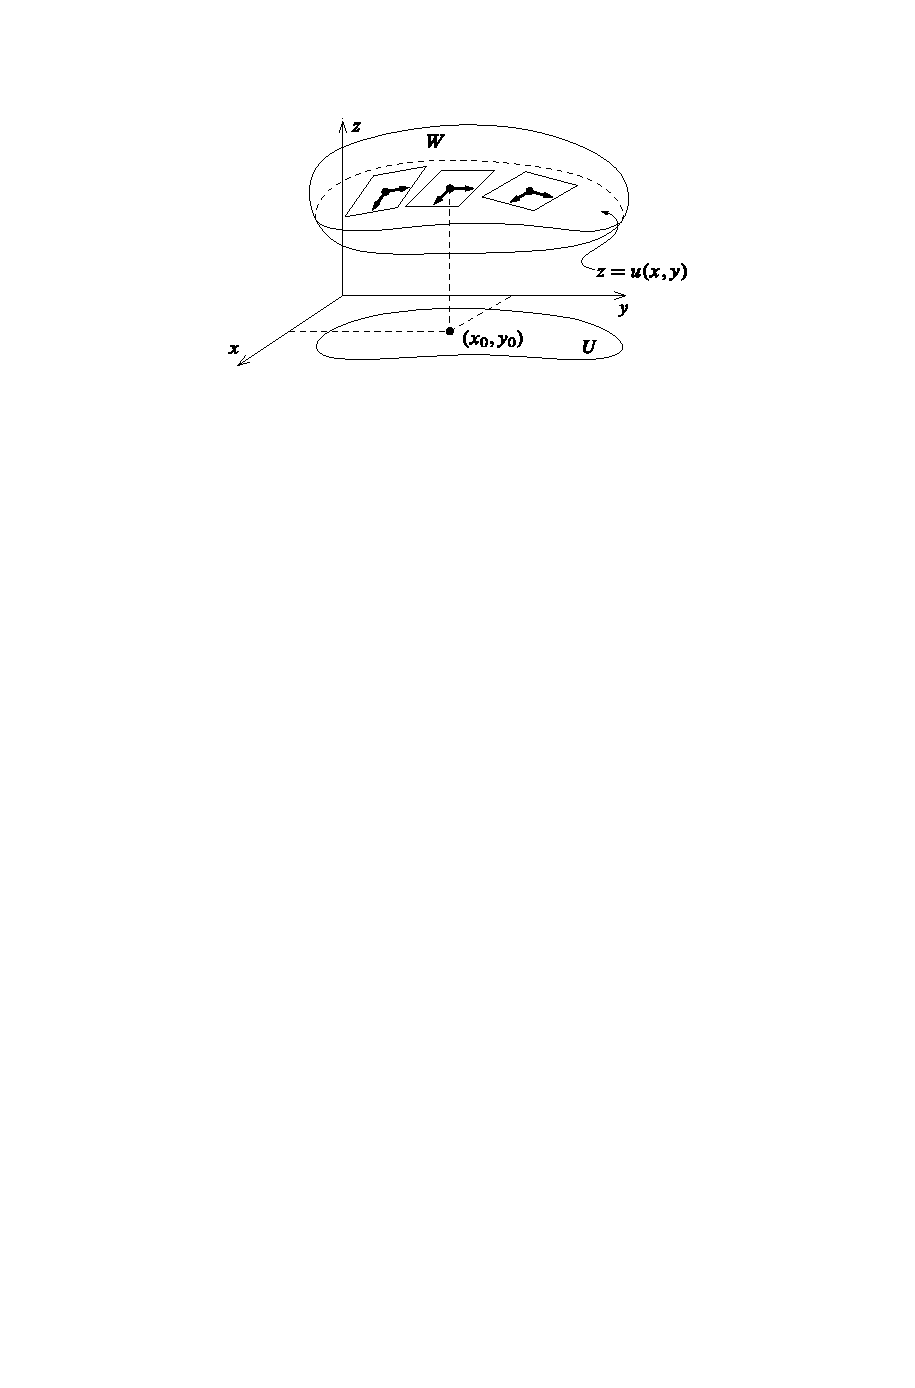
\includegraphics{pictures/overdetermined-PDE}
\caption{Solving for $u$ by finding its graph.}
\end{figure}

If there is a solution $u$ on an open subset $U\sub\R^2$, the map $F:U\to W$ given by
\[F(x,y)=(x,y,u(x,y))\]
is a smooth global parametrization of the graph $\Gamma(u)\sub U\times\R$. At any point $p=F(x,y)$, the tangent space $T_p\Gamma(u)$ is spanned by the vectors
\begin{align*}
dF\Big(\frac{\partial}{\partial x}\Big|_{(x,y)}\Big)=\frac{\partial}{\partial x}+\frac{\partial u}{\partial x}(x,y)\frac{\partial}{\partial z}\Big|_p,\\
dF\Big(\frac{\partial}{\partial y}\Big|_{(x,y)}\Big)=\frac{\partial}{\partial x}+\frac{\partial u}{\partial y}(x,y)\frac{\partial}{\partial z}\Big|_p.
\end{align*}
The system $(\ref{overdetermined nonlinear PDE two dim})$ is satisfied if and only if
\begin{equation}
\begin{aligned}\label{overdetermined nonlinear PDE two dim solution-1}
dF\Big(\frac{\partial}{\partial x}\Big|_{(x,y)}\Big)=\frac{\partial}{\partial x}+\alpha(x,y,u(x,y))\frac{\partial}{\partial z}\Big|_p,\\
dF\Big(\frac{\partial}{\partial y}\Big|_{(x,y)}\Big)=\frac{\partial}{\partial x}+\beta(x,y,u(x,y))\frac{\partial}{\partial z}\Big|_p.
\end{aligned}
\end{equation}
Let $X$ and $Y$ be the vector fields
\begin{equation}
\begin{aligned}\label{overdetermined nonlinear PDE two dim solution-2}
X=\frac{\partial}{\partial x}+\alpha(x,y,z)\frac{\partial}{\partial z},\\
Y=\frac{\partial}{\partial y}+\beta(x,y,z)\frac{\partial}{\partial z}.
\end{aligned}
\end{equation}

on $W$, and let $D$ be the distribution on $W$ spanned by $X$ and $Y$. Because $(\ref{overdetermined nonlinear PDE two dim solution-1})$ says that $T_p\Gamma(u)$ is spanned by $X_p$ and $Y_p$, a necessary condition for the system $(\ref{overdetermined nonlinear PDE two dim})$ to be satisfied is that $\Gamma(u)$ be an integral manifold of $D$. On the other hand, this condition is also sufficient: if $\Gamma(u)$ is an integral manifold, then $dF(\partial/\partial x)$ and $dF(\partial/\partial y)$ must both be linear combinations of $X$ and $Y$, and comparing $\partial/\partial x$ and $\partial/\partial y$ components shows that this can happen only if $(\ref{overdetermined nonlinear PDE two dim solution-1})$ holds.\par
A straightforward computation using $(\ref{overdetermined nonlinear PDE two dim compatibility})$ shows that $[X,Y]\equiv 0$, so given any point $p=(x_0,y_0,z_0)\in W$, there is an integral manifold $N$ of $D$ containing $p$. Let $\varPhi:V\to\R$ be a defining function for $N$ on some neighborhood $V$ of $p$; for example, we could take $\varPhi$ to be the third coordinate function in a flat chart. The tangent space to $N$ at each point $p\in N$ (namely $D_p$) is equal to the kernel of $d\varPhi_p$. Since $\partial/\partial z|_p\notin D_p$ at any point $p$, this implies that $\partial\varPhi/\partial z\neq 0$ at $p$, so by the implicit function theorem $N$ is the graph of a smooth function $z=u(x,y)$ in some neighborhood of $p$. It is easily verified that $u$ is a solution to the problem. Uniqueness follows immediately from Proposition~\ref{integral mani local struct}.
\end{proof}
There is a straightforward generalization of this result to higher dimensions. The general statement of the theorem is a bit complicated, but verifying the necessary conditions in specific examples usually just amounts to computing mixed partial derivatives and applying the chain rule.
\begin{proposition}
Suppose $W$ is an open subset of $\R^n\times\R^m$, and $\alpha=(\alpha^i_j):W\to\mathcal{M}_{m\times n}(\R)$ is a smooth matrix-valued function satisfying
\begin{align*}
\frac{\partial\alpha^i_j}{\partial x^k}+\alpha^l_k\frac{\partial\alpha^i_j}{\partial z^l}=\frac{\partial\alpha^i_k}{\partial x^j}+\alpha^l_j\frac{\partial\alpha^i_k}{\partial z^l}\quad\text{\textit{for all} }i,j,k,
\end{align*}
where we denote a point in $\R^n\times\R^m$ by $(x,z)=(x^1,\dots,x^n,z^1,\dots,z^m)$. For any $(x_0,z_0)\in W$, there is a neighborhood $U$ of $x_0$ in $\R^n$ and a unique smooth function $u:U\to\R^m$ such that $u(x_0)=z_0$ and the Jacobian of $u$ satisfies
\[\frac{\partial u^i}{\partial x^j}(x^1,\dots,x^n)=\alpha^i_j(x^1,\dots,x^n,u^1(x),\dots,u^m(x)).\]
\end{proposition}

%\chapter{Lie Groups and Lie Algebras}
\section{Lie groups}
\subsection{Lie groups and homomorphisms}
A \textbf{Lie group} is a smooth manifold $G$ (without boundary) that is also a group in the algebraic sense, with the property that the multiplication map $m:G\times G\to G$ and inversion map $i:G\to G$, given by
\[m(g,h)=gh,\quad i(g)=g^{-1}\]
are both smooth. A Lie group is, in particular, a topological group. \par
The group operation in an arbitrary Lie group is denoted by juxtaposition, except in certain abelian groups such as Rn in which the operation is usually written additively. It is traditional to denote the identity element of an arbitrary Lie group by the symbol $e$.\par
The following alternative characterization of the smoothness condition is sometimes useful.
\begin{proposition}
If $G$ is a smooth manifold with a group structure such that the map $G\times G\to G$ given by $(g,h)\mapsto gh^{-1}$ is smooth, then $G$ is a Lie group.
\end{proposition}
\begin{proof}
Let we denote this map by $\sigma$. We have
\[i(g)=\sigma(e,g),\quad m(g,h)=\sigma(g,i(h)).\]
Thus if $\sigma$ is smooth, so is $i$, and hence $m$.
\end{proof}
If $G$ is a Lie group, any element $g\in G$ defines maps $L_g,R_g:G\to G$, called \textbf{left translation} and \textbf{right translation}, respectively, by
\[L_g(h)=gh,\quad R_g(h)=hg.\]
Because $L_g$ can be expressed as the composition of smooth maps
\[\begin{tikzcd}
G\ar[r,"\iota_g"]&G\times G\ar[r,"m"]&G
\end{tikzcd}\]
where $\iota_g(h)=(g,h)$ and $m$ is multiplication, it follows that $L_g$ is smooth. It is actually a diffeomorphism of $G$, because $L_{g^{-1}}$ is a smooth inverse for it. Similarly,
$R_g:G\to G$ is a diffeomorphism.
\begin{example}[\textbf{Lie Groups}]
Each of the following manifolds is a Lie group with the indicated group operation.
\begin{itemize}
\item[(a)] The general linear group $\GL_n(\R)$ is the set of invertible $n\times n$ matrices with real entries. It is a group under matrix multiplication, and it is an open submanifold of the vector space $\mathcal{M}_n(\R)$. Multiplication is smooth because the matrix entries of a product matrix $AB$ are polynomials in the entries of $A$ and $B$. Inversion is smooth by Cramer's rule.
\item[(b)] Let $\GL^+_n(\R)$ denote the subset of $\GL_n(\R)$ consisting of matrices with positive determinant. Because $\det(AB)=(\det A)(\det B)$ and $\det A^{-1}=(\det A)^{-1}$, it is a subgroup of $\GL_n(\R)$ and because it is the preimage of $(0,\infty)$ under the continuous determinant function, it is an open subset of $\GL_n(\R)$ and therefore an $n^2$-dimensional manifold. The group operations are the restrictions of those of $\GL_n(\R)$ so they are smooth. Thus $\GL^+_n(\R)$ is a Lie group.
\item[(c)] Suppose $G$ is an arbitrary Lie group and $H\sub G$ is an open subgroup $($a subgroup that is also an open subset$)$. By the same argument as in part (b), $H$ is a Lie group with the inherited group structure and smooth manifold structure.
\item[(d)] The \textbf{complex general linear group} $\GL_n(\C)$ is the group of invertible complex $n\times n$ matrices under matrix multiplication. It is an open submanifold of $\mathcal{M}_n(\C)$ and thus a $2n^2$-dimensional smooth manifold, and it is a Lie group because matrix products and inverses are smooth functions of the real and imaginary parts of the matrix entries.
\item[(e)] If $V$ is any real or complex vector space, $\GL(V)$ denotes the set of invertible linear maps from $V$ to itself. It is a group under composition. If $V$ has finite dimension $n$, any basis for $V$ determines an isomorphism of $\GL(V)$ with $\GL_n(\R)$ or $\GL_n(\C)$, so $\GL(V)$ is a Lie group. The transition map between any two such isomorphisms is given by a map of the form $A\mapsto B^{-1}AB$ $($where $B$ is the transition matrix between the two bases$)$, which is smooth. Thus, the smooth manifold structure on $\GL(V)$ is independent of the choice of basis.
\item[(f)] The real number field $\R$ and Euclidean space $\R^n$ are Lie groups under addition, because the coordinates of $x-y$ are smooth. Similarly, $\C$ and $\C^n$ are Lie groups under addition.
\item[(g)] The set $\R^*$ of nonzero real numbers is a $1$-dimensional Lie group under multiplication. In fact, it is exactly $\GL_1(\R)$ if we identify a $1\times 1$ matrix with the corresponding real number.) The subset $\R^+$ of positive real numbers is an open subgroup, and is thus itself a $1$-dimensional Lie group. The set $\C^*$ of nonzero complex numbers is a $2$-dimensional Lie group under complex multiplication, which can be identified with $\GL_1(\C)$.
\item[(h)] The circle $S^1\sub\C^*$ is a smooth manifold and a group under complex multiplication. With appropriate angle functions as local coordinates on open subsets of $S^1$, multiplication and inversion have the smooth coordinate expressions $(\theta_1,\theta_2)\mapsto\theta_1+\theta_2$ and $\theta_1\mapsto-\theta$, and therefore $S^1$ is a Lie group, called the \textbf{circle group}.
\item[(i)] Given Lie groups $G_1,\dots,G_k$, their direct product is the product manifold
$G_1\times\cdots\times G_k$ with the group structure given by componentwise multiplication:
\[(g_1,\dots,g_k)(g_1',\dots,g_k')=(g_1g_1',\dots,g_kg_k')\]
It is a Lie group. For example, the $n$-torus $T^n=S^1\times\cdots\times S^1$ is an $n$-dimensional abelian Lie group.
\item[(j)] Any group with the discrete topology is a topological group, called a \textbf{discrete group}. If in addition the group is finite or countably infinite, then it is a zero-dimensional Lie group, called a \textbf{discrete Lie group}.
\end{itemize}
\end{example}
Now we consider maps between Lie groups. If $G$ and $H$ are Lie groups, a \textbf{Lie group homomorphism} from $G$ to $H$ is a smooth map $F:G\to H$ that is also a group homomorphism. It is called a \textbf{Lie group isomorphism} if it is also a diffeomorphism, which implies that it has an inverse that is also a Lie group homomorphism. In this case we say that $G$ and $H$ are \textbf{isomorphic Lie groups}.
\begin{example}[\textbf{Lie Group Homomorphisms}]
\mbox{}
\begin{itemize}
\item[(a)] The inclusion map $S^1\hookrightarrow\C^*$ is a Lie group homomorphism.
\item[(b)] Considering $\R$ as a Lie group under addition, and $\R^*$ as a Lie group under multiplication, the map $\exp:\R\to\R^*$ is smooth, and is a Lie group homomorphism. The image of $\exp$ is the open subgroup $\R^+$ consisting of positive real numbers, and $\exp:\R\to\R^+$ is a Lie group isomorphism with inverse $\log:\R^+\to\R$. Similarly, $\exp:\C\to\C^*$ is a Lie group homomorphism. It is surjective but not injective, because its kernel is $2\pi i\Z$.
\item[(c)] The map $\eps:\R\to S^1$ defined by $\eps(x)=e^{2\pi ix}$ is a Lie group homomorphism whose kernel is the set $\Z$ of integers. Similarly, the map $\eps^n:\R^n\to T^n$ defined by $\eps^n(x_1,\dots,x^n)=(e^{2\pi ix^1},\dots,e^{2\pi ix^n})$ is a Lie group homomorphism whose kernel is $\Z^n$.
\item[(d)] The determinant function $\det:\GL_n(\R)\to\R^*$ is smooth because $\det A$ is a polynomial in the matrix entries of $A$. It is a Lie group homomorphism
because $\det(AB)=(\det A)(\det B)$. Similarly, $\det:\GL_n(\C)\to\C^*$ is a Lie group homomorphism.
\item[(e)] If $G$ is a Lie group and $g\in G$, conjugation by $g$ is the map $C_g:G\to G$ given by $C_g(h)=ghg^{-1}$. Because group multiplication and inversion are smooth, $C_g$ is smooth, and a simple computation shows that it is a group homomorphism. In fact, it is an isomorphism, because it has $C_{g^{-1}}$ as an inverse. A subgroup $H\sub G$ is said to be normal if $C_g(H)=H$ for every $g\in G$.
\end{itemize}
\end{example}
The next theorem is important for understanding many of the properties of Lie group homomorphisms.
\begin{theorem}\label{Lie homo constant rank}
Every Lie group homomorphism has constant rank.
\end{theorem}
\begin{proof}
Let $F:G\to H$ be a Lie group homomorphism, and let $e_G$ and $e_H$ denote the identity elements of $G$ and $H$, respectively. Suppose $g_0$ is an arbitrary element of $G$. We will show that $dF_{g_0}$ has the same rank as $dF_{e_G}$. The fact that $F$ is a homomorphism means that for all $g\in G$,
\[F(L_{g_0}(g))=F(g_0g)=F(g_0)F(g)=L_{F(g_0)}F(g)\]
or in other words, the following diagram commutes:
\[\begin{tikzcd}
G\ar[r,"F"]\ar[d,swap,"L_{g_0}"]&H\ar[d,"L_{F(g_0)}"]\\
G\ar[r,"F"]&H
\end{tikzcd}\] 
Taking differentials of both sides at the identity and using Proposition~\ref{differential mani prop}(b), we find that
\[dF_{g_0}\circ d(L_{g_0})_{e_G}=d(L_{F(g_0)})_{e_H}\circ dF_{e_H}\]
Left multiplication by any element of a Lie group is a diffeomorphism, so both $d(L_{g_0})_{e_G}$ and $d(L_{F(g_0)})_{e_H}$ are isomorphisms. Because composing with an isomorphism does not change the rank of a linear map, it follows that $dF_{g_0}$ and $dF_{e_G}$ have the same rank.
\end{proof}
\begin{corollary}\label{Lie isomorphism iff}
A Lie group homomorphism is a Lie group isomorphism if and only if it is bijective.
\end{corollary}
\begin{proof}
The global rank theorem shows that a bijective Lie group homomorphism is a diffeomorphism.
\end{proof}
\subsection{The universal covering group}
Covering space theory yields the following important result about Lie groups.
\begin{theorem}[\textbf{Universal Covering Group}]\label{Lie universal covering group}
Let $G$ be a connected Lie group. Then there exists a simply connected Lie group $\widetilde{G}$, called the \textbf{universal covering group} of $G$, that admits a smooth covering map $\pi:\widetilde{G}\to G$ that is also a Lie group homomorphism with kernel isomorphic to $\pi_1(G)$ and is a discrete central group in $\widetilde{G}$.
\end{theorem}
\begin{proof}
Let $\widetilde{G}$ be the universal covering manifold of $G$ and $\pi:\widetilde{G}\to G$ be the corresponding smooth covering map. Then $\pi\times\pi:\widetilde{G}\times\widetilde{G}\to G\times G$ is also a smooth covering map.\par
Let $m:G\times G\to G$ and $i:G\to G$ denote the multiplication and inversion maps of $G$, respectively, and let $\widetilde{e}$ be an arbitrary element of the fiber $\pi^{-1}(e)$. Since $\widetilde{G}$ is simply connected, the lifting criterion for covering maps guarantees that the map $m\circ(\pi\times \pi):\widetilde{G}\times\widetilde{G}\to G$ has a unique continuous lift $\widetilde{m}:\widetilde{G}\times\widetilde{G}\to\widetilde{G}$ satisfying $\widetilde{m}(\widetilde{e},\widetilde{e})=\widetilde{e}$ and $\pi\circ\widetilde{m}=m\circ(\pi\times\pi)$:
\[\begin{tikzcd}
\widetilde{G}\times\widetilde{G}\ar[r,"\widetilde{m}"]\ar[d,swap,"\pi\circ\pi"]&\widetilde{G}\ar[d,"\pi"]\\
G\times G\ar[r,"m"]&G
\end{tikzcd}\]
Because $\pi$ is a surjective local diffeomorphism and $\pi\circ\widetilde{m}$ is smooth, it follows from Proposition~\ref{smooth iff composition smooth}(b) that $\widetilde{m}$ is smooth. By the same reasoning, $i\circ\pi:\widetilde{G}\to G$ has a smooth lift $\widetilde{i}$ such that $\widetilde{i}(\widetilde{e})=\widetilde{e}$ and $\pi\circ\widetilde{i}=i\circ\pi$:
\[\begin{tikzcd}
\widetilde{G}\ar[r,"\widetilde{i}"]\ar[d,swap,"\pi"]&\widetilde{G}\ar[d,"\pi"]\\
G\ar[r,"i"]&G
\end{tikzcd}\]
We define multiplication and inversion in $\widetilde{G}$ to be $\widetilde{m}$ and $\widetilde{i}$. Then from the commutative diagrams we have
\begin{align}\label{universal cover group-1}
\pi(x,y)=\pi(x)\pi(y),\quad\pi(x^{-1})\pi(x)^{-1}.
\end{align}
It remains only to show that $\widetilde{G}$ is a group with these operations, for then it is a Lie group because $\widetilde{m}$ and $\widetilde{i}$ are smooth, and $(\ref{universal cover group-1})$ shows that $\pi$ is a homomorphism.\par
First we show that $\widetilde{e}$ is an identity for multiplication in $\widetilde{e}$. Consider the map $f:\widetilde{G}\to\widetilde{G}$ defined by $f(x)=\widetilde{e}x$. Then $(\ref{universal cover group-1})$ implies that 
\[\pi\circ f(x)=\pi(\widetilde{e}x)=\pi(\widetilde{e})\pi(x)=e\pi(x)=\pi(x)\]
so $f$ is a lift of $\pi:\widetilde{G}\to G$. Since the identity map $\mathrm{id}_{\widetilde{G}}$ is already a lift of $\pi$, and it agrees with $f$ at a point because $f(\widetilde{e})=\widetilde{m}(\widetilde{e},\widetilde{e})=\widetilde{e}$, the unique lifting property of covering maps implies that $f=\mathrm{id}_{\widetilde{G}}$, or equivalently, $\widetilde{e}x=x$ for all $x$ in $\widetilde{G}$. The same argument shows that $x\widetilde{e}=x$.\par
Next, to show that multiplication in $\widetilde{G}$ is associative, consider the two maps $\alpha_L,\alpha_R:\widetilde{G}\times\widetilde{G}\times\widetilde{G}\to\widetilde{G}$ defined by
\[\alpha_L(x,y,z)=(xy)z,\quad\alpha_R(x,y,z)=x(yz)\]
Then $(\ref{universal cover group-1})$ applied repeatedly implies that
\[\pi\circ\alpha_L(x,y,z)=(\pi(x)\pi(y))\pi(z)=\pi(x)(\pi(y)\pi(z))=\pi\circ\alpha_R(x,y,z)\]
so $\alpha_L$ and $\alpha_R$ are both lifts of the same map $\alpha(x,y,z)=\pi(x)\pi(y)\pi(z)$. Because $\alpha_L$ and $\alpha_R$ agree at $(\widetilde{e},\widetilde{e},\widetilde{e})$, they are equal.\par
Finally, let $x_0\in\widetilde{G}$. To show $x_0x_0^{-1}=x_0^{-1}x_0=\widetilde{e}$ we define a map $g:\widetilde{G}\to\widetilde{G}$ by $g(x)=x_0^{-1}x_0x$. With the same argument we can show that $g$ is a lift of $\pi$, thus equal to $\mathrm{id}_{\widetilde{G}}$. Hence we claim $x_0^{-1}x_0=\widetilde{e}$, and similarly $x_0x_0^{-1}=\widetilde{e}$, so $\widetilde{G}$ is a group.\par
Let $\varphi\in\Aut_{\pi}(\widetilde{G})$, we consider the map $\widetilde{\varphi}:g\mapsto\varphi(\widetilde{e})g$. We have
\[\pi\circ\widetilde{\varphi}(g)=\pi(\varphi(\widetilde{e})g)=e\cdot\pi(g)=\pi(g),\]
so $\widetilde{\varphi}$ is a lifting of $\pi:\widetilde{G}\to G$. Since $\varphi$ is also a lifting of $\pi:\widetilde{G}\to G$ and $\varphi(\widetilde{e})=\widetilde{\varphi}(\widetilde{e})$, we conclude that $\varphi=\widetilde{\varphi}$. With this observation, we define a map
\[\mathrm{ev}:\Aut_{\pi}(\widetilde{G})\to\ker\pi,\quad \varphi\mapsto\varphi(\widetilde{e}).\]
Then $\mathrm{ev}$ is a homomorphism because
\[\mathrm{ev}(\varphi\circ\psi)=(\varphi\circ\psi(\widetilde{e}))=\varphi(\psi(\widetilde{e}))=\varphi(\widetilde{e})\cdot\psi(\widetilde{e})=\mathrm{ev}(\varphi)\cdot\mathrm{ev}(\psi).\]
Since $\ker\pi$ has the same cardinality as $\Aut_{\pi}(\widetilde{G})$, we conclude that $\Aut_{\pi}(\widetilde{G})$ is isomorphic to $\Aut_{\pi}(\widetilde{G})$, and hence to $\pi_1(G)$, as groups. The group $\ker\pi$ is central because it is a discrete normal subgroup of a connected group. 
\end{proof}
\begin{theorem}
Let $G$ be a connected Lie group. Then the universal covering group of $G$ is unique in the following sense: if $\widetilde{G}$ and $\widetilde{G}'$ are simply connected Lie groups that admit smooth covering maps $\pi:\widetilde{G}\to G$ and $\pi':\widetilde{G}'\to G$ that are also Lie group homomorphisms, then there exists a Lie group isomorphism $\varPhi:\widetilde{G}\to\widetilde{G}'$ such that $\pi'\circ\varPhi=\pi$.
\end{theorem}
\begin{proof}
Assume that $\widetilde{G}$ and $\widetilde{G}'$ are universal covering groups of $G$. Since the universal covering manifold is unique, there exists a diffeomorphism $\varPhi:\widetilde{G}\to\widetilde{G}'$ such that $\pi'\circ\varPhi=\pi$ and $\varPhi(e_{\widetilde{G}})=e_{\widetilde{G}'}$. Now we only need to show $\varPhi$ is a homomorphism, which means \[\varPhi\circ\widetilde{m}=\widetilde{m}'\circ(\varPhi\times\varPhi),\]
where $\widetilde{m}$ and $\widetilde{m}'$ are the multiplication maps in $\widetilde{G}$ and $\widetilde{G}'$, respectively. It is clear that both $\varPhi\circ\widetilde{m}$ and $\widetilde{m}'\circ(\varPhi\times\varPhi)$ are lifts of the same map $m\circ(\pi\times\pi)$, where $m$ is the multiplication map of $G$. Moreover, these two maps agree on $(\widetilde{e},\widetilde{e})$. Therefore by the uniqueness of liftings we get the require result.
\end{proof}
\subsection{Lie subgroups}
Suppose $G$ is a Lie group. A \textbf{Lie subgroup} of $G$ is a subgroup of $G$ endowed with a topology and smooth structure making it into a Lie group and an immersed submanifold of $G$. The following proposition shows that embedded subgroups are automatically Lie subgroups.
\begin{proposition}\label{Lie subgroup embedd mani}
Let $G$ be a Lie group, and suppose $H\sub G$ is a subgroup that is also an embedded submanifold. Then $H$ is a Lie subgroup.
\end{proposition}
\begin{proof}
We need only check that multiplication $H\times H\to H$ and inversion $H\to H$ are smooth maps. Because multiplication is a smooth map from $G\times G$ into $G$, its
restriction is clearly smooth from $H\times H$ into $G$ (this is true even if $H$ is merely immersed). Because $H$ is a subgroup, multiplication takes $H\times H$ into $H$, and since $H$ is embedded, this is a smooth map into $H$ by Corollary~\ref{resrtict codomain to embedd}. A similar argument applies to inversion. This proves that $H$ is a Lie subgroup.
\end{proof}
The simplest examples of embedded Lie subgroups are the open subgroups. The
following lemma shows that the possibilities for open subgroups are limited.
\begin{lemma}\label{Lie subgroup open}
Suppose $G$ is a Lie group and $H\sub G$ is an open subgroup. Then $H$ is an embedded Lie subgroup. In addition, $H$ is closed, so it is a union of connected components of $G$.
\end{lemma}
\begin{proof}
If $H$ is open in $G$, then it is embedded by Proposition~\ref{open submani iff}. By Proposition~\ref{topo group prop} $H$ is both open and closed, so it is a union of components.
\end{proof}
If $G$ is a Lie group, the connected component of $G$ containing the identity is called the \textbf{identity component} of $G$ and denoted by $G_0$.
\begin{proposition}\label{Lie identity component}
Let $G$ be a Lie group and let $G_0$ be its identity component. Then $G_0$ is a normal subgroup of $G$, and is the only connected open subgroup. Every
connected component of $G$ is diffeomorphic to $G_0$.
\end{proposition}
\begin{proof}
Since $G_0$ is connected, it gengerates a connected open subgroup $H$ of $G$. But $G_0$ is a connected component contained in $H$, so it follows that $H=G_0$.\par 
Let $g\in G$ be an arbitrary element, and consider the subgroup $gG_0g^{-1}=L_g\circ R_{g^{-1}}(G_0)$. Since $L_g$ and $R_{g^{-1}}$ are both diffeomorphisms, it 
follows that $gG_0g^{-1}$ is an open connected subgroup containing the identity. Since $G_0$ is a connected component, it follows that $gG_0g^{-1}\sub G_0$, thus 
they must equal. This shows $G_0$ is normal.\par 
Let $H$ be a connected open subgroup. Then $H$ contains the identity, hence  is contained in $G_0$. Moreover, by Lemma~\ref{Lie subgroup open} $H$ is also closed, 
therefore by the connectness of $G_0$ we get $H=G_0$, which means $G_0$ is the only open connected subgroup.\par
Now let $C$ be a connected component of $G$, and choose a element $g\in C$. Then $L_{g^{-1}}(C)$is a connected open subset containing the identity, thus is contained 
in $G_0$. Since the same argument gives $L_g(G_0)\sub C$, we conclude $L_g(G_0)=C$.
\end{proof}
Now we move beyond the open subgroups to more general Lie subgroups. The
following proposition shows how to produce many more examples of embedded Lie
subgroups.
\begin{proposition}\label{Lie homo ker}
Let $F:G\to H$ be a Lie group homomorphism. The kernel of $F$ is a properly embedded Lie subgroup of $G$, whose codimension is equal to the rank of $F$.
\end{proposition}
\begin{proof}
Because $F$ has constant rank, its kernel $F^{-1}(e)$ is a properly embedded
submanifold of codimension equal to $\rank F$. It is thus a Lie subgroup by Proposition~\ref{Lie subgroup embedd mani}.
\end{proof}
Complementary to the preceding result about kernels is the following result about images.
\begin{proposition}\label{Lie homo injective}
If $F:G\to H$ is an injective Lie group homomorphism, the image of $F$ has a unique smooth manifold structure such that $F(G)$ is a Lie subgroup of $H$ and $F:G\to F(G)$ is a Lie group isomorphism.
\end{proposition}
\begin{proof}
Since a Lie group homomorphism has constant rank, it follows from the global rank theorem that $F$ is a smooth immersion. Proposition~\ref{image immersion submani} shows that $F(G)$ has a unique smooth manifold structure such that it is an immersed submanifold of $H$ and $F$ is a diffeomorphism onto its image. It is a Lie group (because $G$ is), and it is a subgroup for algebraic reasons, so it is a Lie subgroup. Because $F:G\to F(G)$ is a group isomorphism and a diffeomorphism, it is a Lie group isomorphism.
\end{proof}
\begin{example}[\textbf{Embedded Lie Subgroups}]\label{Lie subgroups eg}
\mbox{}
\begin{itemize}
\item[(a)] The subgroup $\GL^+_n(\R)\sub\GL_n(\R)$ is an open subgroup and thus an embedded Lie subgroup. It is indeed the identity component of $\GL_n(\R)$.
\item[(b)] The circle $S^1$ is an embedded Lie subgroup of $\C^*$ because it is a subgroup and an embedded submanifold.
\item[(c)] The set $\SL_n(\R)$ of $n\times n$ real matrices with determinant equal to $1$ is called the \textbf{special linear group} of degree $n$. Because $\SL_n(\R)$ is the kernel of the Lie group homomorphism $\det:\GL_n(\R)\to\R^*$, it is a properly embedded Lie subgroup. Because the determinant function is surjective, it is a smooth submersion by the global rank theorem, so $\SL_n(\R)$ has dimension $n^2-1$.
\item[(d)] Let $n$ be a positive integer, and define a map $\beta:\GL_n(\C)\to\GL_{2n}(\R)$ by replacing each complex matrix entry $a+ib$ with the $2\times 2$ block $(\begin{smallmatrix}
a&b\\
-b&a
\end{smallmatrix})$:
\[\beta\begin{pmatrix}
a^1_1+ib^1_1&\cdots&a^1_n+ib^1_n\\
\vdots&&\vdots\\
a^n_1+ib^n_1&\cdots&a^n_n+ib^n_n
\end{pmatrix}
=\begin{pmatrix}
\begin{array}{cc}
a^1_1&-b^1_1\\
b^1_1&a^1_1
\end{array}&\cdots&\begin{array}{cc}
a^1_n&-b^1_n\\
b^1_n&a^1_n
\end{array}\\
\vdots&&\vdots\\
\begin{array}{cc}
a^n_1&-b^n_1\\
b^n_1&a^n_1
\end{array}&\cdots&\begin{array}{cc}
a^n_n&-b^n_n\\
b^n_n&a^n_n
\end{array}
\end{pmatrix}
\]
It is straightforward to verify that $\beta$ is an injective Lie group homomorphism whose image is a properly embedded Lie subgroup of $\GL_{2n}(\R)$. Thus, $\GL_n(\C)$ is isomorphic to this Lie subgroup of $\GL_{2n}(\R)$.
\item[(e)] The subgroup $\SL_n(\C)\sub\GL_n(\C)$ consisting of complex matrices of determinant $1$ is called the \textbf{complex special linear group} of degree $n$. It is the kernel of the Lie group homomorphism $\det:\GL_n(\C)\to\C^*$. This homomorphism is surjective, so it is a smooth submersion by the global rank theorem. Therefore, $\SL_n(\C)=\ker\det$ is a properly embedded Lie subgroup whose dimension is $2n^2-2$.
\end{itemize}
\end{example}
Finally, here is an example of a Lie subgroup that is not embedded.
\begin{example}[\textbf{A Dense Lie Subgroup of the Torus}]
Let $H\sub T^2$ be the dense submanifold of the torus that is the image of the immersion $\gamma:\R\to T^2$ defined in Example~\ref{dense curve torus}. It is easy to check that $\beta$ is an injective Lie group homomorphism, and thus $H$ is an immersed Lie subgroup of $T^2$ by Proposition~\ref{Lie homo injective}.
\end{example}
In general, smooth submanifolds can be closed without being embedded (as is, for example, the figure-eight curve) or embedded without being closed (as is the open unit ball in $\R^n$). However, as the next theorem shows, Lie subgroups have the remarkable property that closedness and embeddedness are not independent. This means that every embedded Lie subgroup is properly embedded. 
\begin{theorem}\label{Lie subgroup closed iff embed}
Suppose $G$ is a Lie group and $H\sub G$ is a Lie subgroup. Then $H$ is closed in $G$ if and only if it is embedded.
\end{theorem}
\begin{figure}[htbp]
\centering
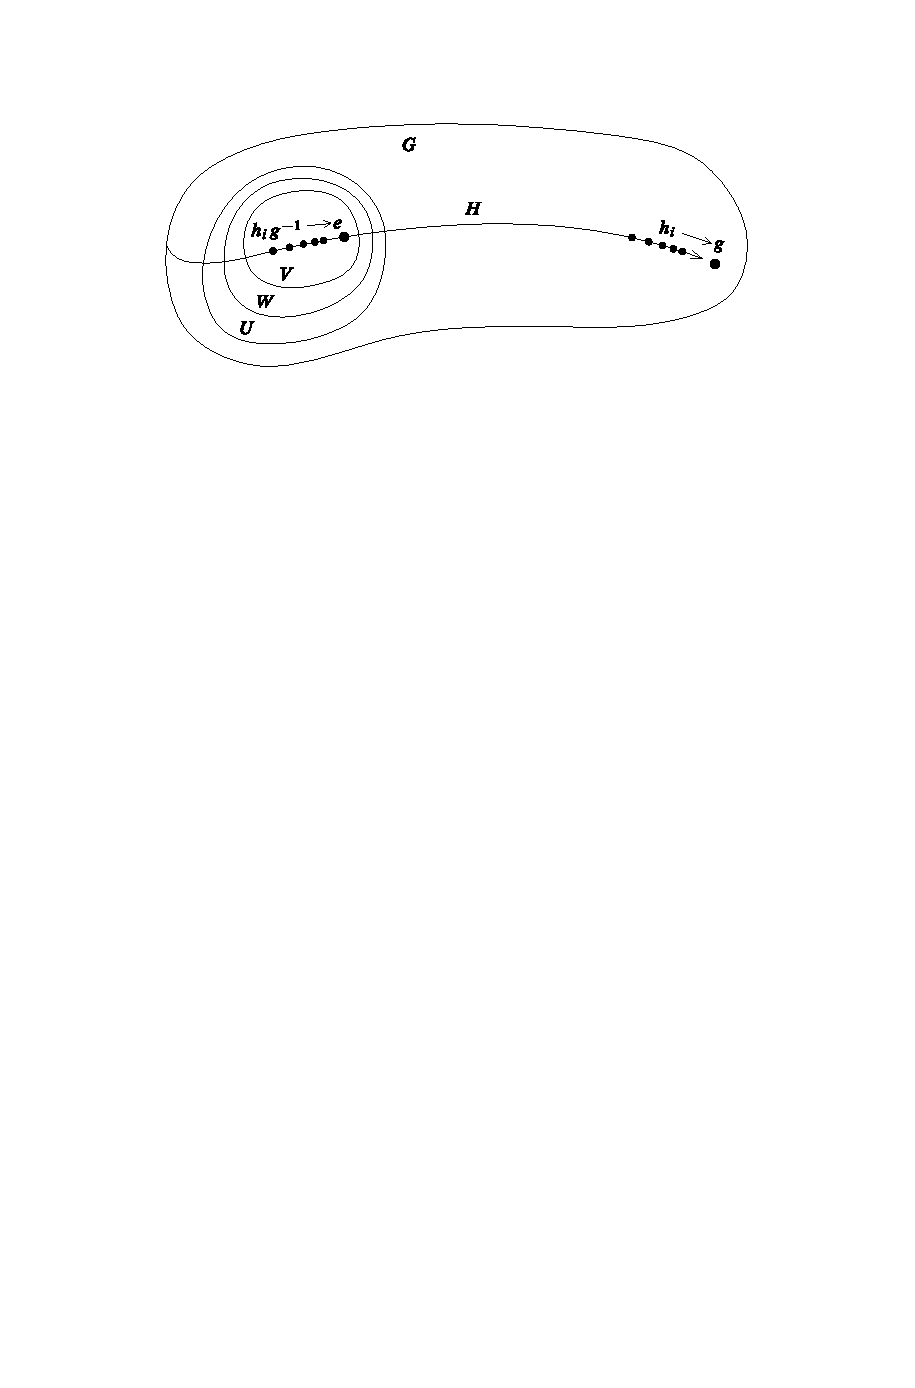
\includegraphics{pictures/Lie-closed-1}
\caption{An embedded Lie subgroup is closed.}
\end{figure}
\begin{proof}
Assume first that $H$ is embedded in $G$. To prove that $H$ is closed, let $g$ be an arbitrary point of $\widebar{H}$. Then there is a sequence $(h_i)$ of points in $H$ converging to $g$. Let $U$ be the domain of a slice chart for $H$ containing the identity, and let $W$ be a smaller neighborhood of $e$ such that $\widebar{W}\sub U$. By Lemma~\ref{topo group identity nbhd lem}, there is a neighborhood $V$ of $e$ with the property that $g_1g_2^{-1}\in W$ whenever $g_1,g_2\in V$.\par
Because $h_ig^{-1}\to e$, by discarding finitely many terms of the sequence we may assume that $h_ig^{-1}\in V$ for all $i$. This implies that
\[h_ih_j^{-1}=(h_ig^{-1})(h_jg^{-1})^{-1}\in W\]
for all $i$ and $j$. Fixing $j$ and letting $i\to\infty$, we find that $h_ih_j^{-1}\to gh_j^{-1}\in\widebar{W}\sub U$. Since $H\cap U$ is a slice, it is closed in $U$, and therefore $gh_j^{-1}\in H$, which implies $g\in H$. Thus $H$ is closed.\par
Conversely, assume $H$ is a closed Lie subgroup, and let $m=\dim H$ and $n=\dim G$. We need to show that $H$ is an embedded submanifold of $G$. If $m=n$, then $H$ is embedded by Proposition~\ref{open submani iff}, so we may assume henceforth that $m<n$.\par
It suffices to show that for some $h_1\in H$, there is a neighborhood $U_1$ of $h_1$ in $G$ such that $H\cap U_1$ is an embedded submanifold of $U_1$; for then if $h$ is any other point of $H$, right translation $R_{h_1^{-1}h}$ is a diffeomorphism of $G$ that takes $H$ to $H$, and takes $U_1$ to a neighborhood $U'_1$ of $h$ such that $H\cap U'_1$ is embedded in $U'_1$,
so it follows from the local slice criterion that $H$ is an embedded submanifold of $G$.\par
Because every immersed submanifold is locally embedded (Proposition~\ref{immerse local embedd}), there exist a neighborhood $V$ of $e$ in $H$ and a slice chart $(U,\varphi)$ for $V$ in $G$ centered at $e$. By shrinking $U$ if necessary, we may assume that it is a coordinate cube, and $U\cap V$ is the set of points whose coordinates are of the form $\{x^{m+1}=\cdots=x^n=0\}$. Let $S\sub U$ be the set of points with coordinates of the form $\{x^1=\cdots=x^m=0\}$; it is the slice perpendicular to $U\cap V$ in these coordinates. Then $S$ is an embedded submanifold of $U$ and hence of $G$. Note that in these coordinates, $T_eV$ is spanned by the first $m$ coordinate vectors and $T_eS$ by the last $n-m$, so $T_eG=T_eV\oplus T_eS$.
\begin{figure}[htbp]
\centering
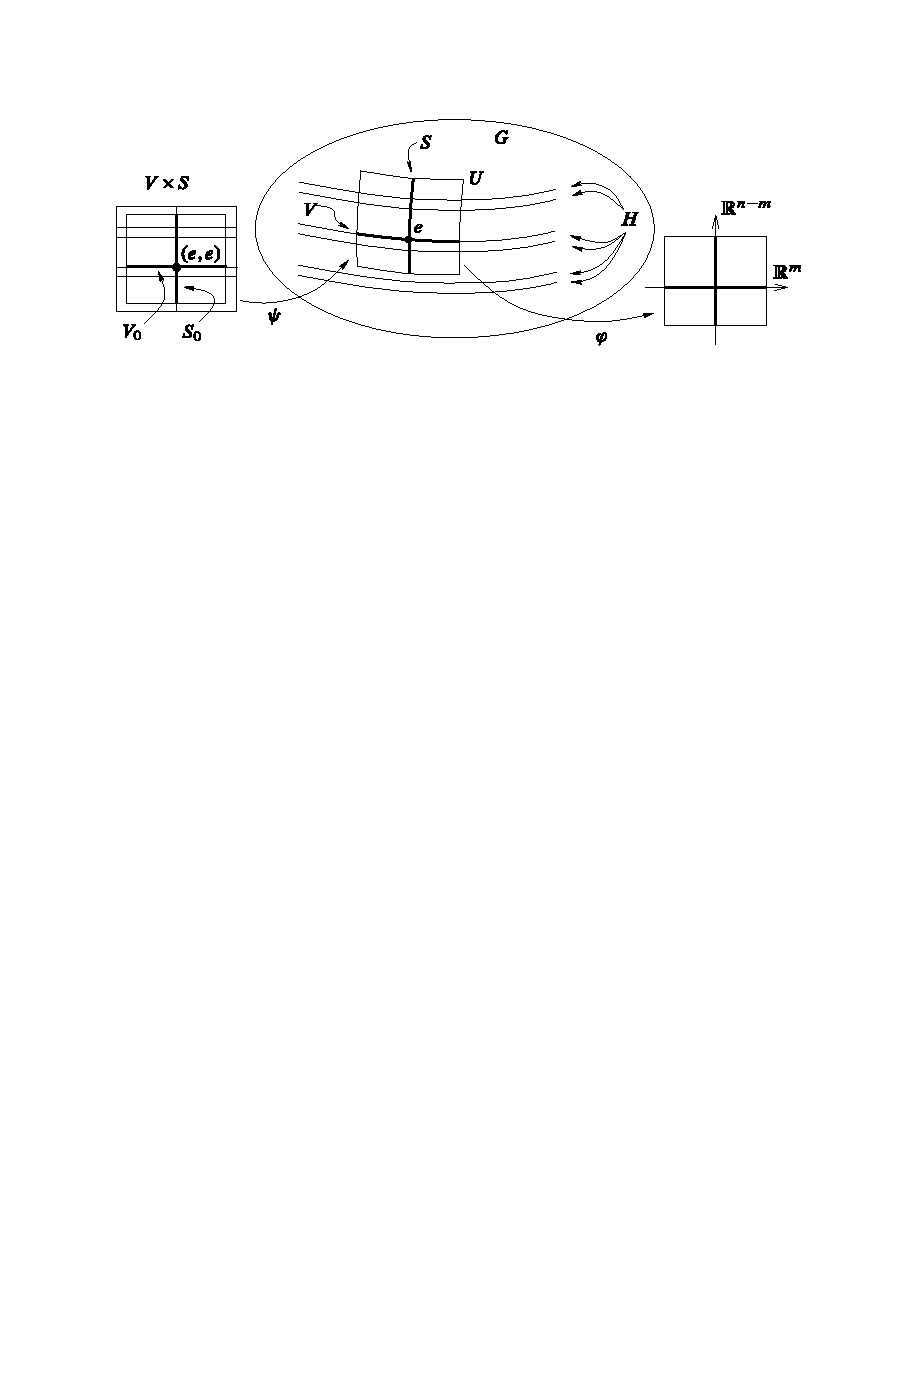
\includegraphics{pictures/Lie-closed-2}
\caption{Finding a slice chart.}
\end{figure}\par
Now consider the map $\psi:V\times S\to G$ obtained by restricting group multiplication: $\psi(v,s)=vs$. Since $\psi(v,e)=v$ for $v\in V$ and $\psi(e,s)=s$ for $s\in S$, it follows easily that the differential of $\psi$ at $(e,e)$ satisfies $d\psi(X,0)=X$ and $d\psi(0,Y)=Y$ for $X\in T_eV$ and $Y\in T_eS$, and therefore $d\psi_{(e,e)}$ is bijective. By the inverse function theorem, there are connected neighborhoods $W_0$ of $(e,e)$ in $V\times S$ and $U_0$ of $e$ in $G$ such that $\psi:W_0\to U_0$ is a diffeomorphism. Shrinking the neighborhoods if necessary, we may assume that $W_0=V_0\times S_0$, where $V_0$ and $S_0$ are neighborhoods of $e$ in $V$ and $S$, respectively.\par
Let $K=S_0\cap H$. There are two things we need to show about the set $K$:
\begin{itemize}
\item[(a)] $\psi(V_0\times K)=H\cap U_0$.
\item[(b)] $K$ is a discrete set in the topology of $H$.
\end{itemize}
To prove (a), let $(v,s)\in V_0\times S_0$ be arbitrary. Since $H$ is a subgroup and $V_0\sub H$, it follows that $vs\in H$ if and only if $s\in H$, which is to say that $\psi(v,s)\in H\cap U_0$ if and only if $(v,s)\in V_0\times K$. To prove (b), suppose $h\in K$. Right translation $R_h:H\to H$ is a diffeomorphism of $H$ taking $e$ to $h$ and taking $V_0$ to a neighborhood $V_h$ of $h$ in $H$. Note that $V_h=R_h(V_0)=\psi(V_0\times\{h\})$, while $K=\psi(\{e\}\times K)$. Since $\psi$ is injective on $V_0\times S_0$, it follows that
\[V_h\cap K=\psi(\{e\}\times\{h\})=\{h\}\]
Thus each point $h\in K$ is isolated in $H$, which implies that $K$ is discrete.\par
Since $K$ is a discrete subset of the manifold $H$, it is countable, and since $H$ is closed in $G$, it follows that $K=S_0\cap H$ is closed in $S_0$. Thus, by Corollary~\ref{countable closed isolated}, there is a point $h_1\in K$ that is isolated in $S_0$. (This step fails if $H$ is not closed-for example, if $H$ were a dense subgroup of the torus, then $K$ would be dense in $S_0$.) This means there is a neighborhood $S_1$ of $h_1$ in $S_0$ such that $S_1\cap H=\{h_1\}$. Then $U_1=\psi(V_0\times S_1)$ is a neighborhood of $h_1$ in $G$ with the property that $U_1\cap H$ is the slice $V_0\times\{h_1\}$ in $U_1$. As explained at the beginning of the proof, the existence of such a neighborhood for one point of $H$ implies that $H$ is embedded.
\end{proof}
\subsection{Group actions and equivariant maps}
If $M$ is a topological space and G is a topological group, an action of $G$ on $M$ is said to be a \textbf{continuous action} if the defining map $G\times M\to M$ or $M\times G\to M$ is continuous. In this case, $M$ is said to be a (left or right) \textbf{$\bm{G}$-space}. If in addition $M$ is a smooth manifold with or without boundary, $G$ is a Lie group, and the defining map
is smooth, then the action is said to be a \textbf{smooth action}. We are primarily interested in smooth actions of Lie groups on smooth manifolds.\par
Lie group actions typically arise in situations involving some kind of \textit{symmetry}. For example, if $M$ is a vector space or smooth manifold endowed with a metric or other geometric structure, the set of diffeomorphisms of $M$ that preserve the structure (called the \textbf{symmetry group of the structure}) frequently turns out to be a Lie group acting smoothly on $M$.\par
In the following, suppose $\theta:G\times M\to M$ is a left action of a group $G$ on a set $M$.
\begin{itemize}
\item For each $p\in M$, the \textbf{orbit} of $p$, denoted by $G\cdot p$, is the set of all images of $p$ under the action by elements of $G$:
\[G\cdot p=\{g\cdot p:g\in G\}\]
\item For each $p\in M$, the \textbf{isotropy group} or \textbf{stabilizer} of $p$, denoted by $G_p$, is the set of elements of $G$ that fix $p$:
\[G_p=\{g\in G:g\cdot p=p\}\]
The definition of a group action guarantees that $G_p$ is a subgroup of $G$.
\item The action is said to be \textbf{transitive} if for every pair of points $p,q\in M$, there exists $g\in G$ such that $g\cdot p=q$, or equivalently if the only orbit is all of $M$.
\item The action is said to be \textbf{free} if the only element of $G$ that fixes any element of $M$ is the identity: $g\cdot p=p$ for some $p\in M$ implies $g=e$, or equivalently if every isotropy group is trivial.
\end{itemize}
\begin{example}[\textbf{Lie Group Actions}]
\mbox{}
\begin{itemize}
\item[(a)] If $G$ is any Lie group and $M$ is any smooth manifold, the trivial action of $G$ on $M$ is defined by $g\cdot p=p$ for all $g\in G$ and $p\in M$. It is a smooth action, for which each orbit is a single point and each isotropy group is all of $G$.
\item[(b)] The natural action of $\GL_n(\R)$ on $\R^n$ is the left action given by matrix multiplication: $(A,x)\mapsto Ax$, considering $x\in\R^n$ as a column matrix. This is an action because $I_nx=x$ and matrix multiplication is associative: $ABx=A(Bx)$. It is smooth because the components of $Ax$ depend polynomially on the matrix entries of $A$ and the components of $x$. Because any nonzero vector can be taken to any other by some invertible linear transformation, there are exactly two orbits: $\{0\}$ and $\R^n-\{0\}$.
\item[(c)] Every Lie group $G$ acts smoothly on itself by left translation. Given any two points $g_1,g_2\in G$, there is a unique left translation of $G$ taking $g_1$ to $g_2$, namely left translation by $g_2g_1^{-1}$; thus the action is both free and transitive. More generally, if $H$ is a Lie subgroup of $G$, then the restriction of the multiplication map to $H\times G\to G$ defines a smooth and free $($but generally not transitive$)$ left action of $H$ on $G$. Similar observations apply to right translations.
\item[(d)] Every Lie group acts smoothly on itself by conjugation: $g\cdot h=ghg^{-1}$.
\item[(e)] An action of a discrete group $\Gamma$ on a manifold $M$ is smooth if and only if for each $g\in\Gamma$, the map $p\mapsto g\cdot p$ is a smooth map from $M$ to itself. Thus, for example, $\Z^n$ acts smoothly and freely on $\R^n$ by left translation:
\end{itemize}
\end{example}
Another important class of Lie group actions arises from covering maps. Suppose $E$ and $M$ are topological spaces, and $\pi:E\to M$ is a (topological) covering
map. An \textbf{automorphism of $\bm{\pi}$} (also called a \textbf{deck transformation} or \textbf{covering transformation}) is a homeomorphism $\varphi:E\to E$ such that
\[\begin{tikzcd}
E\ar[rr,"\varphi"]\ar[rd,swap,"\pi"]&&E\ar[ld,"\pi"]\\
&M&
\end{tikzcd}\]
The set $\Aut_\pi(E)$ of all automorphisms of $\pi$, called the \textbf{automorphism group} of $\pi$, is a group under composition, acting on $E$ on the left. It can be shown that $\Aut_\pi(E)$ acts transitively on each fiber of $\pi$ if and only if $\pi$ is a \textbf{normal covering map}, which means that $\pi_*(\pi_1(E,q))$ is a normal subgroup of $\pi_1(M,\pi(q))$ for every $q\in E$.
\begin{proposition}\label{Lie group coveing auto}
Suppose $E$ and $M$ are smooth manifolds with or without boundary, and $\pi:E\to M$ is a smooth covering map. With the discrete topology, the automorphism group $\Aut_\pi(E)$ is a zero-dimensional Lie group acting smoothly and freely on $E$.
\end{proposition}
\begin{proof}
Suppose $\varphi\in\Aut_\pi(E)$ is an automorphism that fixes a point $p\in E$. We can consider $\varphi$ as a lift of $\pi$:
\[\begin{tikzcd}
&E\ar[d,"\pi"]\\
E\ar[r,swap,"\pi"]\ar[ru,"\varphi"]&M
\end{tikzcd}\]
Since the identity map of $E$ is another such lift that agrees with $\varphi$ at $p$, the unique lifting property of covering maps guarantees that $\varphi=\mathrm{id}_E$. Thus, the action of $\Aut_\pi(E)$ is free.\par
To show that $\Aut_\pi(E)$ is a Lie group, we need only verify that it is countable. Let $q\in E$ be arbitrary, let $p=\pi(q)\in M$ and let $U\sub M$ be an evenly covered neighborhood of $p$. Because $E$ is second-countable, $\pi^{-1}(U)$ has countably many components, and because each component contains exactly one point of $\pi^{-1}(p)$, it follows that $\pi^{-1}(p)$ is countable. Let $\theta^{(q)}:\Aut_\pi(E)\to E$ be the map $\theta^{(q)}(\varphi)=\varphi(q)$. Then $\theta^{(q)}$ maps $\Aut_\pi(E)$ into $\pi^{-1}(p)$, and the fact that the action is free implies that it is injective; thus $\Aut_\pi(E)$ is countable.\par
Smoothness of the action follows from Theorem~\ref{char surjective subm}.
\end{proof}
\subsubsection{Equivariant Maps}
Suppose $G$ is a Lie group, and $M$ and $N$ are both smooth manifolds endowed with smooth left $G$-actions $\theta$ and $\varphi$, respectively. A map $F:M\to N$ is said to be \textbf{equivariant} with respect to the given $G$-actions if the following diagram commutes
\[\begin{tikzcd}
M\ar[r,"F"]\ar[d,swap,"\theta_g"]&N\ar[d,"\varphi_g"]&\\
M\ar[r,"F"]&N
\end{tikzcd}\]
\begin{example}
Let $v=(v^1,\dots,v^n)\in\R^n$ be any fixed nonzero vector. Define smooth left actions of $\R$ on $\R^n$ and $T^n$ by
\[t\cdot(x^1,\dots,x^n)=(x^1+tv^1,\dots,x^n+tv^n),\quad t\cdot(z^1,\dots,z^n)=(e^{2\pi itv^1}z^1,\dots,e^{2\pi itv^n}z^n)\]
for $t\in\R,(x^1,\dots,x^n)\in\R^n$ and $(z^1,\dots,z^n)\in T^n$. The smooth map $\eps^n:\R^n\to T^n$ given by
\[\eps^n(x^1,\dots,x^n)=(e^{2\pi ix^1},\dots,e^{2\pi ix^n})\]
is equivariant with respect to these actions.
\end{example}
The following generalization of Theorem~\ref{Lie homo constant rank} is an extremely useful tool for proving that certain maps have constant rank.
\begin{theorem}[\textbf{Equivariant Rank Theorem}]\label{Lie equivariant rank}
Let $M$ and $N$ be smooth manifolds and let $G$ be a Lie group. Suppose $F:M\to N$ is a smooth map that is equivariant with respect to a transitive smooth $G$-action on $M$ and any smooth $G$-action on $N$. Then $F$ has constant rank.\par 
Therefore, if $F$ is surjective, it is a smooth submersion; if it is injective, it is a smooth immersion; and if it is bijective, it is a diffeomorphism.
\end{theorem}
\begin{figure}[htbp]
\centering
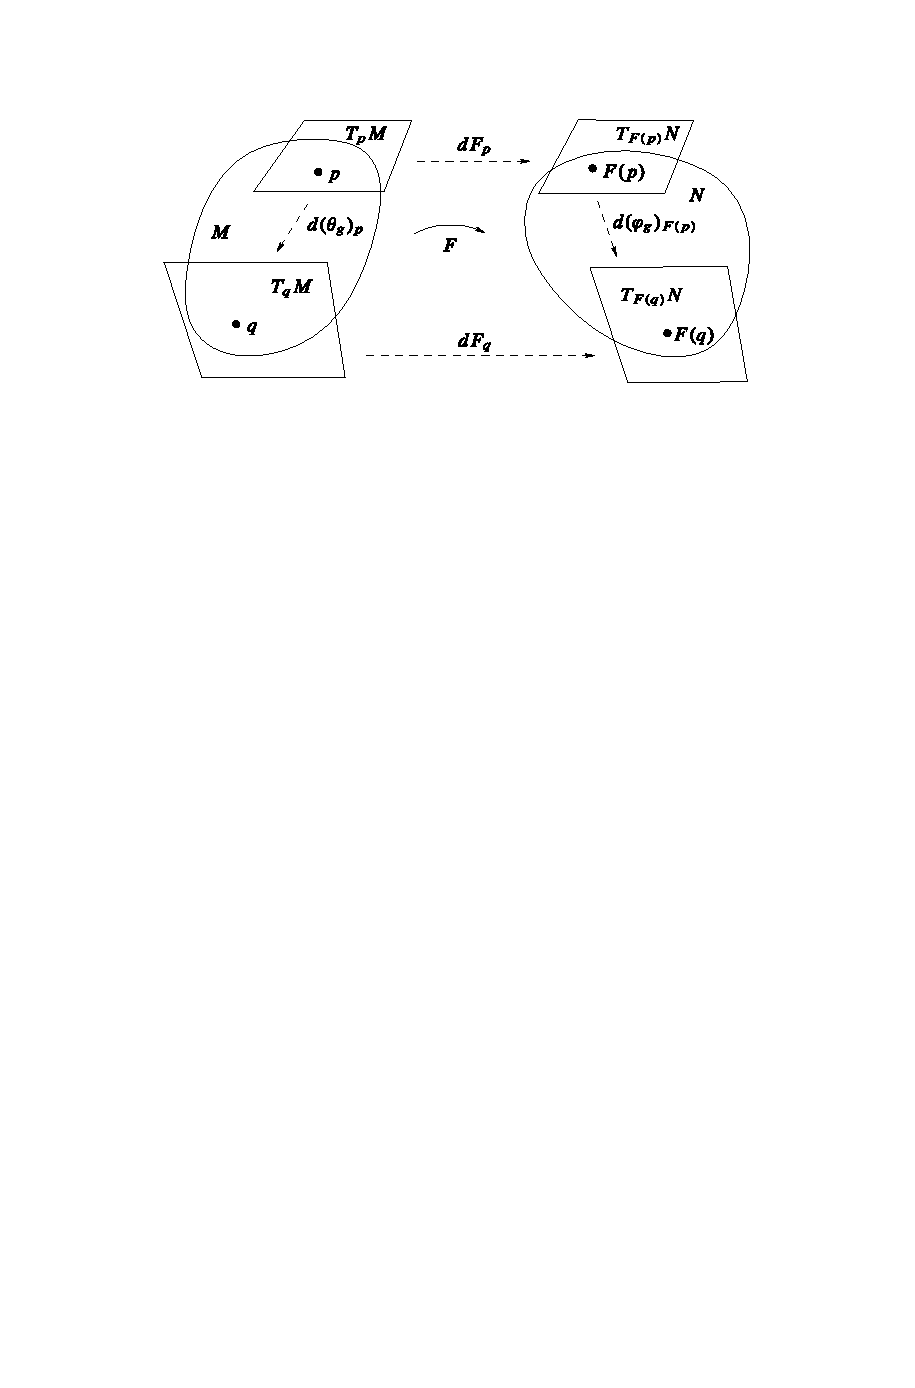
\includegraphics{pictures/equivariant-rank}
\caption{The equivariant rank theorem.}
\end{figure}
\begin{proof}
Let $\theta$ and $\varphi$ denote the $G$-actions on $M$ and $N$, respectively, and let $p$ and $q$ be arbitrary points in $M$. Choose $g\in G$ such that $\theta_g(p)=q$. (Such a $g$ exists because we are assuming that $G$ acts transitively on $M$.) Because $\varphi_g\circ F=\theta_g\circ F$, the following diagram commutes
\[\begin{tikzcd}
T_pM\ar[r,"dF_p"]\ar[d,swap,"d(\theta_g)_p"]&T_pN\ar[d,"d(\varphi_g)_{F(p)}"]\\
T_pM\ar[r,"dF_q"]&T_qN
\end{tikzcd}\]
Because the vertical linear maps in this diagram are isomorphisms, the horizontal ones have the same rank. In other words, the rank of $F$ is the same at any two arbitrary points $p,q\in M$, so $F$ has constant rank. The final statement follows from the global rank theorem.
\end{proof}
Here is an important application of the equivariant rank theorem. Suppose $G$ is a Lie group, $M$ is a smooth manifold, and $\theta:G\times M\to M$ is a smooth left action. For each $p\in M$, define a map $\theta^{(p)}:G\to M$ by
\[\theta^{(p)}(g)=g\cdot p\]
This is often called the orbit map, because its image is the orbit $G\cdot p$. In addition, the preimage $(\theta^{(p)})^{-1}(p)$ is the isotropy group $G_p$.
\begin{proposition}[\textbf{Properties of the Orbit Map}]\label{orbit map prop}
Suppose $\theta$ is a smooth left action of a Lie group $G$ on a smooth manifold $M$. For each $p\in M$, the orbit map $\theta^{(p)}:G\to M$ is smooth and has constant rank, so the isotropy group $G_p=(\theta^{(p)})^{-1}(p)$ is a properly embedded Lie subgroup of $G$. The induced map $F_p:G/G_p\to M$ on $G/G_p$ is an injective smooth immersion, so the orbit $G\cdot p$ is an immersed submanifold of $M$.
\end{proposition}
\begin{proof}
The orbit map is smooth because it is equal to the composition
\[G\approx G\times\{p\}\hookrightarrow G\times M\stackrel{\theta}{\to}M\]
It follows from the definition of a group action that $\theta^{(p)}$ is equivariant with respect to the action of $G$ on itself by left translation and the given action on $M$:
\[\theta^{(p)}(g'g)=(gg')\cdot p=g'\cdot(g\cdot p)=g'\cdot\theta^{(p)}(g)\]
Since $G$ acts transitively on itself, the equivariant rank theorem shows that $\theta^{(p)}$ has constant rank. Thus, $G_p$ is a properly embedded submanifold by Theorem~\ref{constant rank level set}, and a Lie subgroup by Proposition~\ref{Lie subgroup embedd mani}.\par
Now by quotient manifold theorem, the group $G/G_p$ has a unique smooth structure such that $\pi:G\to G_p$ is a smooth submersion. Therefore the induced map $F_p:G/G_p\to M$ defined by $F_p(gG_p)=\theta^{(p)}(g)$ is an injective smooth equivalent map with image $G\cdot p$. By the equivariant rank theorem, $F_p$ is then a smooth immersion, and thus the orbit (endowed with a suitable topology and smooth structure) is an immersed submanifold by Proposition~\ref{image immersion submani}.
\end{proof}
\begin{example}[\textbf{The Orthogonal Group}]\label{orthogonal group}
A real $n\times n$ matrix $A$ is said to be orthogonal if as a linear map $A:\R^n\to\R^n$ it preserves the Euclidean dot product:
\[(Ax)\cdot(Ay)=x\cdot y\for x,y\in\R^n\]
The set $\O(n)$ of all orthogonal $n\times n$ matrices is a subgroup of $\GL_n(\R)$, called the \textbf{orthogonal group} of degree $n$. It is easy to check that a matrix $A$ is orthogonal if and only if it takes the standard basis of $\R^n$ to an orthonormal basis, which is equivalent to the columns of $A$ being orthonormal. Since the $(i,j)$-entry of the matrix $A^TA$ is the dot product of the $i$-th and $j$-th columns of $A$, this condition is also equivalent to the requirement that $A^TA=I_n$.\par
Define a smooth map $\varPhi:\GL_n(\R)\to\mathcal{M}_n(\R)$ by $\varPhi(A)=A^TA$. Then $\O(n)$ is equal to the level set $\varPhi^{-1}(I_n)$. To show that $\varPhi$ has constant rank and therefore that $\O(n)$ is an embedded Lie subgroup, we show that $\varPhi$ is equivariant with respect to
suitable right actions of $\GL_n(\R)$. Let $\GL_n(\R)$ act on itself by right multiplication, and define a right action of $\GL_n(\R)$ on $\mathcal{M}_n(\R)$ by 
\[X\cdot B=B^TXB\for X\in\GL_n(\R), B\in\mathcal{M}_n(\R)\]
It is easy to check that this is a smooth action, and $\varPhi$ is equivariant because
\[\varPhi(AB)=(AB)^TAB=B^TA^TAB=B^T\varPhi(A)B=\varPhi(A)\cdot B\]
Thus, $\O(n)$ is a properly embedded Lie subgroup of $\GL_n(\R)$. It is compact because it is closed and bounded in $\mathcal{M}_n(\R)\approx\R^{n^2}$: closed because it is a level set of $\varPhi$, and bounded because every $A\in\O(n)$ has columns of norm $1$, and therefore satisfies $|A|=\sqrt{n}$.\par
To determine the dimension of $\O(n)$, we need to compute the rank of $\varPhi$. Because the rank is constant, it suffices to compute it at the identity $I_n\in\GL_n(\R)$. Thus for any $B\in T_{I_n}\GL_n(\R)=\mathcal{M}_n(\R)$, let $\gamma:(-\eps,\eps)\to\GL_n(\R)$ be the curve $\gamma(t)=I_n+tB$, and compute
\[d\varPhi_{I_n}B=\frac{d}{dt}\Big|_{t=0}\varPhi\circ\gamma(B)=\frac{d}{dt}\Big|_{t=0}(I_n+tB)^T(I_n+B)=B^T+B\]
From this formula, it is evident that the image of $d\varPhi_{I_n}$ is contained in the vector space of symmetric matrices. Conversely, if $B\in\mathcal{M}_n(\R)$ is an arbitrary symmetric $n\times n$ matrix, then $d\varPhi_{I_n}(1/2B)=B$. It follows that the image of $d\varPhi_{I_n}$ is exactly the space of symmetric matrices. This is a linear subspace of $\mathcal{M}_n(\R)$ of dimension $n(n+1)/2$, because each symmetric matrix is uniquely determined by its values on and above the main diagonal. It follows that $\O(n)$ is an embedded Lie subgroup of dimension 
\[n^2-\frac{n(n+1)}{2}=\frac{n(n-1)}{2}\]
\end{example}
\begin{example}[\textbf{The Special Orthogonal Group}]
The \textbf{special orthogonal group} of degree $n$ is defined as $\SO(n)=\O(n)\cap\SL_n(\R)$. Because every matrix $A\in\O(n)$ satisfies
\[1=\det I_n=\det(A^TA)=(\det A^T)(\det A)=(\det A)^2\]
it follows that $\det A=\pm1$ for all $A\in\O(n)$. Therefore, $\SO(n)$ is the open subgroup of $\O(n)$ consisting of matrices of positive determinant, and is therefore also an embedded Lie subgroup of dimension $n(n-1)/2$ in $\GL_n(\R)$. It is a compact group because it is a closed subset of $\O(n)$.
\end{example}
\begin{example}[\textbf{The Unitary Group}]
For any complex matrix $A$, the adjoint of $A$ is the matrix $A^*$ formed by conjugating the entries of $A$ and taking the transpose: $A=\widebar{A^T}$. For any positive integer $n$, the \textbf{unitary group} of degree $n$ is the subgroup $\U(n)\sub\GL_n(\C)$ consisting of complex $n\times n$ matrices whose columns form an orthonormal basis for $\C^n$ with respect to the Hermitian dot product $z\cdot w=\sum_iz^i\widebar{w^i}$. It is straightforward to check
that $\U(n)$ consists of those matrices $A$ such that $A^*A=I_n$.\par
Similar to Example~\ref{orthogonal group}, we define a map $\varPsi:\GL_n(\C)\to\mathcal{M}_n(\C)$ by $\varPsi(A)=A^*A$. Then $\U(n)=\varPsi^{-1}(I_n)$. We check that
\[\varPsi(AB)=B^*A^*AB=B^*\varPsi(A)B\]
so if we define an action of $\GL_n(\C)$ on $\mathcal{M}_n(\C)$ by
\[X\cdot B=B^*XB\for X\in\GL_n(\R),B\in\mathcal{M}_n(\C)\]
Then $\varPsi$ is an equivariant map, thus has constant rank. Now, to compute $d\varPsi_{I_n}$, we define a curve $\gamma:(-\eps,\eps)\to\GL_n(\C)$ by $\gamma(t)=I_n+tB$ where $B\in T_{I_n}\GL_n(\C)=\mathcal{M}_n(\C)$. We observe that
\[d\varPsi_{I_n}B=\frac{d}{dt}\Big|_{t=0}\varPsi\circ\gamma(B)=\frac{d}{dt}\Big|_{t=0}(I_n+tB)^*(I_n+B)=B^*+B\]
Hence the image of $d\varPsi_{I_n}$ is the \textbf{Hermitan matrix}, that is, matrix $B$ such that $B^*=B$. The dimension of the set of all Hermitan matrix is 
\[n+2\cdot\frac{n(n-1)}{2}=n^2\]
Thus $\U(n)$ is an properly embedded Lie subgroup of dimension $2n^2-n^2=n^2$.
\end{example}
\begin{example}[\textbf{The Special Unitary Group}]
The group $\SU(n)=\U(n)\cap\SL_n(\C)$ is called the complex special unitary group of degree $n$. For $A\in\U(n)$ we have
\[1=\det I_n=\det(A^*A)=(\det A^*)(\det A)=|\det A|^2\]
Thus there is an induced map $\det:\U(n)\to S^1$. Since $\dim S^1=1$ and $\SU(n)=\det^{-1}(1)$, it follows that $\SU(n)$ is a properly embedded $(n^2-1)$-dimensional Lie subgroup of $\U(n)$. Since the composition of smooth embeddings $\SU(n)\hookrightarrow\U(n)\hookrightarrow\GL_n(\C)$ is again a smooth embedding, this implies that $\SU(n)$ is also embedded in $\GL_n(\C)$.
\end{example}
\subsection{Semidirect products}
Suppose $N$ and $H$ are Lie groups, and $\theta:H\times N\to N$ is a smooth left action of $H$ on $N$. We define a new Lie group $N\rtimes_\theta H$, called a \textbf{semidirect product} of $H$ and $N$, as follows. As a smooth manifold, $N\rtimes_\theta H$ is just the Cartesian product $N\times H$ but the group multiplication is defined by
\[(n_1,h_1)(n_2,h_2)=(n_1\theta_{h_1}(n_2),h_1h_2)\]
\begin{example}[\textbf{The Euclidean Group}]\label{Euclidean group}
If we consider $\R^n$ as a Lie group under addition, then the natural action of $\O(n)$ on $\R^n$ is an action by automorphisms. The resulting semidirect product $\mathrm{E}(n)=\R^n\rtimes\O(n)$ is called the \textbf{Euclidean group}; its multiplication is given by $(b,A)(b',A')=(b+Ab',AA')$. It acts on $\R^n$ via
\[(b,A)\cdot x=b+Ax\]
It can be checked that
\[\big((b,A)(b',A')\big)\cdot x=(b+Ab',AA')x=b+Ab'+AA'x=(b,A)\cdot (b'+A'x)=(b,A)\cdot((b',A')\cdot x)\]
so this action is well defined. This action preserves lines, distances, and angle measures, and thus all of the relationships of Euclidean geometry.\par 
A faithful representation of $\mathrm{E}(n)$ is given by the map $\rho:\mathrm{E}(n)\to\GL_{n+1}(\R)$ defined in block form by
\[\rho(b,A)=\begin{pmatrix}
A&b\\
0&1
\end{pmatrix}\]
\end{example}
The following result gives a extremely useful method to characterize semidirect products. We will use it to give some examples of Lie groups.
\begin{proposition}\label{semidirect product iff}
Suppose $G,N$, and $H$ are Lie groups. Prove that $G$ is isomorphic to a semidirect product $N\rtimes H$ if and only if there are Lie group homomorphisms $\varphi:G\to H$ and $\psi:H\to G$ such that $\varphi\circ\psi=\mathrm{id}_H$ and $\ker\varphi\cong N$.
\end{proposition}
\begin{proof}
If $G\approx N\rtimes H$, then the projection on $H$ and the embedding ot $H$ in $G$ satisfy the conditions.\par
Conversely, assume the existence of $\varphi$ and $\psi$:
\[\begin{tikzcd}
1\ar[r]&N\ar[r,hook]&G\ar[r,"\varphi"]&H\ar[l,bend left=30,"\psi"]\ar[r]&1
\end{tikzcd}\]
Since this sequence is split exact, we can regard $N,H$ as subgroups of $G$ such that $N\cap H=\{e\}$ and $NH=G$. Since $N$ is normal in $G$, $H$ act on $N$ by conjugation, so the map $(n,h)\mapsto nh$ is an isomorphsim from $G$ to $N\rtimes H$.
\end{proof}
\begin{proposition}\label{Lie groups as semidirect product}
The following Lie groups are isomorphic to semidirect products as shown.
\begin{itemize}
\item[(a)] $\O(n)\cong\SO(n)\rtimes\O(1)$.
\item[(b)] $\U(n)\cong\SU(n)\rtimes\U(1)$.
\item[(c)] $\GL_n(\R)\cong\SL_n(\R)\rtimes\R^*$.
\item[(d)] $\GL_n(\C)\cong\SL_n(\C)\rtimes\C^*$.
\end{itemize}
\end{proposition}
\begin{proof}
In order to apply Proposition~\ref{semidirect product iff}, we consider the maps
\[\det:\GL_n(\R)\to\R^*,\quad \psi:\R^*\to\GL_n(\R),\quad x\mapsto xI_n\]
and
\[\det:\O(n)\to\{\pm 1\},\quad \psi:\{\pm 1\}\to\O(n),\quad x\mapsto xI_n.\]
we have $\ker\det=\det^{-1}(1)=\SL_n(\R)$, or $\ker\det=\SO(n)$. The claim therefore follows.
\end{proof}
There is a close connection between representations and group actions. Let $G$ be a Lie group and $V$ be a finite-dimensional vector space. An action of $G$ on $V$ is said to be a linear action if for each $g\in G$, the map from $V$ to itself given by $x\mapsto g\cdot x$ is linear. For example, if $\rho:G\to\GL(V)$ is a representation of $G$, there is an associated smooth linear action of $G$ on $V$ given by $g\cdot x:=\rho(g)x$. The next proposition shows that every linear action is of this type.
\begin{proposition}
Let $G$ be a Lie group and $V$ be a finite-dimensional vector space. A smooth left action of $G$ on $V$ is linear if and only if it is of the form $g\cdot x=\rho(g)x$ for some representation $\rho$ of $G$.
\end{proposition}
\begin{proof}
Every action induced by a representation is evidently linear. To prove the converse, assume that we are given a linear action of $G$ on $V$. The hypothesis implies that for each $g\in G$ there is a linear map $\rho(g)\in\GL(V)$ such that $g\cdot x=\rho(g)x$ for all $x\in V$. The group action condition implies $\rho(g_1g_2)=\rho(g_1)\rho(g_2)$, so $\rho:G\to\GL(V)$ is a group homomorphism. Thus, to show that it is a Lie group representation, we need only show that it is smooth. Choose a basis $\{E_i\}$ for $V$, and for each $i$ let $\pi^i:V\to\R$ be the projection onto the $i$ th coordinate with respect to this basis. If we let $(\rho_j^i(g))$ denote the matrix entries of $\rho(g)$ with respect to this basis, it follows that $\rho_j^i(g)=\pi^i(g\cdot E_j)$, so each function $\rho_j^i$ is a composition of smooth functions. Because the matrix entries form global smooth coordinates for $\GL(V)$, this implies that $\rho$ is smooth.
\end{proof}
\subsection{Exercise}
\begin{exercise}\label{Lie group operator diff}
Let $G$ be a Lie group.
\begin{itemize}
\item[(a)] Let $m$ be the multiplication, show that the differential $dm_{(e,e)}:T_eG\oplus T_eG\to T_eG$ is given by
\[dm_{(e,e)}(X,Y)=X+Y\for X,Y\in T_eG\]
\item[(b)] Let $i$ be the inverse map, show that the differential $di_{e}:T_eG\to T_eG$ is given by
\[di_e(X)=-X\for X\in T_eG\]
\end{itemize}
\end{exercise}
\begin{proof}
For part (a), fix $g,h\in G$. Then since $T_{(g,h)}(G\times G)\cong T_gG\oplus T_hG$, we have
\[dm_{(g,h)}(X,Y)=d(m\circ j^h)_g(X)+d(m\circ \iota_g)_hY\]
for $X\in T_gG,Y\in T_hG$, where $j^h(x)=(x,h)$ and $\iota_g(x)=(g,x)$. Thus we have
\[dm_{(g,h)}(X,Y)=d(R_h)_gX+d(L_g)_hY\]

For part (b), let $X\in T_eG$ and define a map
\[\alpha:G\to G\times G,\quad g\mapsto(g,i(g))\]
Then we have
\[d\alpha_e(X)=(X,di_eX)\]
Since $m\circ\alpha=e$, we conclude by the chain rule
\[dm_{e,e}\circ d\alpha_e(X)=dm_{(e,e)}(X,di_e(X))=X+di_e(X)=0\]
This implies $di_e(X)=-X$.\par
Now note that for any $g\in G$ we have $i=R_{g^{-1}}\circ i\circ L_{g^{-1}}$ since
\[R_{g^{-1}}\circ i\circ L_{g^{-1}}(x)=R_{g^{-1}}\circ i(g^{-1}x)=x^{-1}gg^{-1}=x^{-1}\]
So using this and the chain rule we have
\[di_g(X)=d(R_{g^{-1}})_e\circ di_e\circ d(L_{g^{-1}})_g(X)=-d(R_{g^{-1}})_e\circ d(L_{g^{-1}})_g(X)\for X\in T_gG\]
which is the desired claim.
\end{proof}
\begin{exercise}\label{det diff}
Let $\det:\GL_n(\R)\to\R$ denote the determinant function. For any $A\in\mathcal{M}_n(\R)$, show that
\[\frac{d}{dt}\Big|_{t=0}\det(I_n+tA)=\tr A.\]
From this, conclude that, for $X\in\GL_n(\R)$ and $B\in T_X\GL_n(\R)\approx\mathcal{M}_n(\R)$,
\[d(\det)_X(B)=(\det X)\tr(X^{-1}B).\]
\end{exercise}
\begin{proof}
Let $B(t)=(b_{ij}(t)):I\to\mathcal{M}_n(\R)$ be a smooth curve such that $B(0)=I_n$. Then expanding the determinant along the first column, we have
\[\det(B(t))=\sum_{i=1}^{n}(-1)^{i+1}b_{1i}(t)\cdot\det(B_{1i}(t)),\]
where $B_{ij}$ is the minor of $B$ at position $(i,j)$. Now differentiate both sides, we get
\[\frac{d}{dt}\Big|_{t=0}\det(B(t))=\sum_{i=1}^{n}(-1)^{i+1}\Big[b'_{1i}(0)\cdot\det(B_{1i}(0))+b_{1i}(0)\cdot\frac{d}{dt}\Big|_{t=0}\det(B_{11}(t))\Big].\]
By $B(0)=I_n$, the RHS is simplified into
\[\frac{d}{dt}\Big|_{t=0}\det(B(t))=b'_{11}(0)+\frac{d}{dt}\Big|_{t=0}\det(B_{1i}(t)).\]
Now by a simple induction we get
\[\frac{d}{dt}\Big|_{t=0}\det(B(t))=b'_{11}(0)+\cdots+b'_{nn}(0)=\tr(B'(0)).\]
Now we define the curve $\gamma(t)=X+tB$ for $B\in T_X\GL_n(\R)$, and observe that
\[\det(X+tB)=\det(X)\det(I_n+tX^{-1}B)\]
Thus by Corollary~\ref{compute diff by curve},
\[d(\det)_X(B)=\frac{d}{dt}\Big|_{t=0}(\det\circ\gamma)=\det(X)\frac{d}{dt}\Big|_{t=0}\det(I_n+tX^{-1}B)=\det(X)\tr(X^{-1}B)\]
which is the desired result.
\end{proof}
\begin{exercise}
Suppose a connected topological group $G$ acts continuously on a discrete space $K$. Show that the action is trivial. 
\end{exercise}
\begin{proof}
Let $\rho:G\times K\to K$ be the action. Note that the connected component of $G\times K$ is $G\times\{x\}$ for $x\in K$. For any $x_0\in K$, the set $U:=\rho^{-1}(x_0)$ is closed and open in $G\times K$, thus is of the form $G\times\{y\}$. Since $(e,x_0)\sub U$, we conclude $U=G\times\{x_0\}$. Thus $\rho$ is trivial on $x_0$. Since $x_0$ is arbitrary, this implies $\rho$ is trivial on $K$.
\end{proof}
\begin{exercise}
Considering $S^{2n+1}$ as the unit sphere in $\C^{n+1}$, define an action of $S^1$ on $S^{2n+1}$, called the \textbf{Hopf action}, by
\[z(w^1,\dots,w^{n+1})=(zw^1,\dots,zw^{n+1})\]
Show that this action is smooth and its orbits are disjoint unit circles in $\C^{n+1}$ whose union is $S^{2n+1}$.
\end{exercise}
\begin{proof}
Note that this action is free on $S^1$, so by Proposition~\ref{orbit map prop} each orbit is an immersed submanifold. Since $S^1$ is a compact set, it is in fact an embedded submanifold. So each orbit is a unite circle in $\C^{n+1}$.
\end{proof}
\begin{exercise}
Show that $\SO(2)$, $U(1)$, and $S^1$ are all isomorphic as Lie groups.
\end{exercise}
\begin{proof}
The subgroup $\SO(2)$ takes the following from 
\[\begin{pmatrix}
\cos\varphi&-\sin\varphi\\
\sin\varphi&\cos\varphi
\end{pmatrix}\]
Thus $\SO(2)\approx S^1$. The subgroup $\U(1)$ consists of $1\times 1$ matrix of modulus $1$, which may be regarded as $S^1$.
\end{proof}
\begin{exercise}
Prove that $\SU(2)$ is diffeomorphic to $S^3$.
\end{exercise}
\begin{proof}
Let $U\in\GL_n(\C)$,
\[U=\begin{pmatrix}
z_1&z_2\\
z_3&z_4
\end{pmatrix}\]
From the conditions $\det U=1$ and $U^*U=I_n$, we get
\[
\left\{\begin{array}{l}
z_1z_4-z_2z_3=1\\
|z_1|^2+|z_2|^2=1\\
|z_3|^2+|z_4|^2=1\\
z_1\widebar{z}_3+z_2\widebar{z}_4=0
\end{array}\right. \]
Let's assume $z_1=z\widebar{z}_4$ where $z\in\C$, then $z_2=-z\widebar{z}_3$. Plugging this into the equations we get 
\[|z|^2(|z_3|^2+|z_4|^2)=1,\quad z(|z_3|^2+|z_4|^2)=1\]
Thus $z=1$, and $U$ has the following form
\[\begin{pmatrix}
z_1&-\widebar{z}_2\\
z_2&\widebar{z}_1
\end{pmatrix}\]
where $|z_1|^2+|z_2|^2=1$. Since $S^3$ can be viewed as the set $\{|z_1|^2+|z_2|^2=1\}$ in $\C^2$, this implies $\SU(2)\approx S^3$.
\end{proof}
\begin{exercise}
Let $\H=\C\times\C$ be the quaternions. The multiplication of $\H$ is given by
\[\mathbf{i}^2=\mathbf{j}^2=\mathbf{k}^2=\mathbf{i}\mathbf{j}\mathbf{k}=-\mathbf{1}\] 
By considering $\H$ as a two dimensional complex vector space, find a representation of $\H$ into $\GL_2(\C)$.
\end{exercise}
\begin{proof}
Thus a representation $\rho:\H\to\GL_2(\C)$ given by \[\rho(z,w)=\begin{pmatrix}
z&w\\
-\widebar{w}&\widebar{z}
\end{pmatrix}.\]
Since the multiplication in $\H$ can be written as
\[(a,b)(c,d)=(ac-\widebar{d}b,da+b\widebar{c})\]
when the base ring is commutative, this can be realized into marix multiplications.\par
Note that
\[\rho(\mathbf{1})=\begin{pmatrix}
1&0\\
0&1
\end{pmatrix},\quad\rho(\mathbf{i})=\begin{pmatrix}
i&0\\
0&-i
\end{pmatrix},\quad\rho(\mathbf{j})=\begin{pmatrix}
0&1\\
-1&0
\end{pmatrix},\quad\rho(\mathbf{k})=\begin{pmatrix}
0&i\\
i&0
\end{pmatrix},\quad\]
Due to this, $\H$ has another definition: consider $\mathcal{M}_2(\C)$, the set 
\[\H\cong\{M\in\mathcal{M}_2(\C):M^*M=aI_2,a\in\R,\det(M)\geq 0\}\]
Note that $\C$ can also be defined in the same way:
\[\C\cong\{M\in\mathcal{M}_2(\R):M^*M=aI_2,a\in\R,\det(M)\geq 0\}\]
\end{proof}
\section{Lie algebras}
\subsection{The Lie algebra of a Lie group}
One of the most important applications of Lie brackets occurs in the context of Lie groups. Suppose $G$ is a Lie group. Recall that $G$ acts smoothly and transitively on itself by left translation: $L_g(h)=gh$. A vector field $X$ on $G$ is said to be \textbf{left-invariant} if it is invariant under all left translations, in the sense that it is $L_g$-related to itself for every $g\in G$. More explicitly, this means
\[d(L_g)_{g'}(X_{g'})=X_{gg'}\quad\text{for all }g,g'\in G.\]
Since $L_g$ is a diffeomorphism, this can be abbreviated by writing $(L_g)_*X=X$ for every $g\in G$.\par
Because $(L_g)_*(aX+bY)=a(L_g)_*X+b(L_g)_*Y$, the set of all smooth left-invariant vector fields on $G$ is a linear subspace of $\X(G)$. But it is much more than that. The central fact is that it is closed under Lie brackets.
\begin{proposition}
Let $G$ be a Lie group, and suppose $X$ and $Y$ are smooth left-invariant vector fields on $G$. Then $[X,Y]$ is also left-invariant.
\end{proposition}
\begin{proof}
Let $g\in G$ be arbitrary. Since $(L_g)_*X=X$ and $(L_g)_*Y=Y$ by definition of left-invariance, it follows from Corollary~\ref{Lie bracket pushforward} that
\[(L_g)_*[X,Y]=[(L_g)_*X,(L_g)_*Y]=[X,Y]\]
Thus, $[X,Y]$ is $L_g$-related to itself for each $g$, which is to say it is left-invariant.
\end{proof}
A \textbf{Lie algebra} (over $\R$) is a real vector space $\g$ endowed with a map called the bracket from $\g\times\g$ to $\g$, usually denoted by $(X,Y)\mapsto[X,Y]$, that satisfies the following properties for all $X,Y,Z\in\g$:
\begin{itemize}
\item Bilinearity: For $a,b\in\R$,
\[[aX+bY,Z]=a[X,Z]+b[Y,Z],\quad [X,aY+bZ]=a[X,Y]+b[X,Z].\]
\item Antisymmetry:
\[[X,Y]=-[Y,X]\]
\item Jacobi identity:
\[[X,[Y,Z]]+[Y,[Z,X]]+[Z,[X,Y]]=0\]
\end{itemize}
Notice that the Jacobi identity is a substitute for associativity, which does not hold in general. If $\g$ is a Lie algebra, a linear subspace $\h\sub\g$ is called a Lie subalgebra of $\g$ if it is closed under brackets. In this case $\h$ is itself a Lie algebra with the restriction of the same bracket.\par
If $\g$ and $\h$ are Lie algebras, a linear map $A:\g\to\h$ is called a \textbf{Lie algebra homomorphism} if it preserves brackets: $A[X,Y]=[AX,AY]$. An invertible Lie algebra homomorphism is called a \textbf{Lie algebra isomorphism}. If there exists a Lie algebra isomorphism from $\g$ to $\h$, we say that they are \textbf{isomorphic as Lie algebras}.
\begin{example}[\textbf{Lie Algebras}]
\mbox{}
\begin{itemize}
\item[(a)] The space $\X(M)$ of all smooth vector fields on a smooth manifold $M$ is a Lie algebra under the Lie bracket by Proposition~\ref{Lie bracket prop}.
\item[(b)] If $G$ is a Lie group, the set of all smooth left-invariant vector fields on $G$ is a Lie subalgebra of $\X(G)$ and is therefore a Lie algebra.
\item[(c)] The vector space $\mathcal{M}_n(\R)$ $n\times n$ real matrices becomes an $n^2$-dimensional Lie algebra under the \textbf{commutator bracket}:
\[[A,B]=AB-BA\]
Bilinearity and antisymmetry are obvious from the definition, and the Jacobi identity follows from a straightforward calculation. When we are regarding $\mathcal{M}_n(\R)$ as a Lie algebra with this bracket, we denote it by $\gl(n,\R)$.
\item[(d)] Similarly, $\gl(n,\C)$ is the $2n^2$-dimensional $($real$)$ Lie algebra obtained by endowing $\mathcal{M}_n(\C)$ with the commutator bracket.
\item[(e)] If $V$ is a vector space, the vector space of all linear maps from $V$ to itself becomes a Lie algebra, which we denote by $\gl(V)$, with the commutator bracket:
\[[A,B]=A\circ B-B\circ A\]
Under our usual identification of $n\times n$ matrices with linear maps from $\R^n$ to itself, $\gl(\R^n)$ is the same as $\gl(n,\R)$.
\item[(f)]Any vector space $V$ becomes a Lie algebra if we define all brackets to be zero. Such a Lie algebra is said to be \textbf{abelian}. (The name reflects the fact that brackets in most Lie algebras, as in the preceding examples, are defined as commutators in terms of underlying associative products, so all brackets are zero precisely when the underlying product is commutative; it also reflects the connection between abelian Lie algebras and abelian Lie groups.)
\end{itemize}
\end{example}
Example (b) is the most important one. The Lie algebra of all smooth left-invariant vector fields on a Lie group $G$ is called the Lie algebra of $G$, and is denoted by $\Lie(G)$. The fundamental fact is that $\Lie(G)$ is finite-dimensional, and in fact has the same dimension as $G$ itself, as the following theorem shows.
\begin{theorem}\label{Lie algrbra iso tangent space}
Let $G$ be a Lie group. The evaluation map $\eps:\Lie(G)\to T_eG$, given by $\eps(X)=X_e$, is a vector space isomorphism. Thus, $\Lie(G)$ is finite-dimensional, with dimension equal to $\dim G$.
\end{theorem}
\begin{proof}
It is clear from the definition that $\eps$ is linear over $\R$. It is easy to prove that it is injective: if $\eps(X)=X_e=0$ for some $X\in\Lie(G)$, then left-invariance of $X$ implies that $X_g=d(L_g)_eX_e=0$ for every $g\in G$, so $X=0$.\par
To show that $\eps$ is surjective, let $v\in T_eG$ be arbitrary, and define a (rough) vector field $v^L$ on $G$ by
\begin{align}\label{Lie algebra iso-1}
v^L_g=d(L_g)_e(v)
\end{align}
If there is a left-invariant vector field on $G$ whose value at the identity is $v$, clearly it has to be given by this formula.\par
First we need to check that $v^L$ is smooth. By Proposition~\ref{vector field smooth by function}, it suffices to show that $v^Lf$ is smooth whenever $f\in C^\infty(G)$. Choose a smooth curve $\gamma:(-\delta,\delta)\to G$ such that $\gamma(0)=e$ and $\gamma'(0)=v$. Then for all $g\in G$,
\begin{align*}
(v^Lf)(g)=v^L_gf=d(L_g)_e(v)(f)=\gamma'(0)(f\circ L_g)=\frac{d}{dt}\Big|_{t=0}(f\circ L_g\circ\gamma)(t)
\end{align*}
If we define $\varphi:(-\delta,\delta)\times G\to G$ by $\varphi(t,g)=f\circ L_g\circ\gamma(t)=f(g\gamma(t))$, the computation above shows that $(v^Lf)(g)=\partial\varphi/\partial t(0,g)$. Because $\varphi$ is a composition of group multiplication, $f$ and $\gamma$, it is smooth. It follows that $\partial\varphi/\partial t(0,g)$ depends smoothly on $g$, so $v^Lf$ is smooth.\par
Next we show that $v^L$ is left-invariant, which is to say that $d(L_h)_g(v^L|_g)=v^L|_{hg}$ for all $g,h\in G$. This follows from the definition of $v^L$ and the fact that $L_h\circ L_g=L_{hg}$:
\[d(L_h)_g(v^L|_g)=d(L_h)_g\circ d(L_g)_e(v)=d(L_{hg})_e(v)=v^L|_{hg}\]
Thus $v^L\in\Lie(G)$. Since $L_e$ (left translation by the identity) is the identity map of $G$, it follows that $\eps(v^L)=v$, so $\eps$ is surjective.
\end{proof}
Given any vector $v\in T_eG$, we continue to use the notation $v^L$ to denote the smooth left-invariant vector field defined by $(\ref{Lie algebra iso-1})$.\par
It is worth observing that the preceding proof also shows that the assumption of smoothness in the definition of $\Lie(G)$ is unnecessary.
\begin{corollary}\label{Lie rough left-inv}
Every left-invariant rough vector field on a Lie group is smooth.
\end{corollary}
\begin{proof}
Let $X$ be a left-invariant rough vector field on a Lie group $G$, and let $v=X_e$. The fact that $X$ is left-invariant implies that $X=v^L$, which is smooth.
\end{proof}
The existence of global left-invariant vector fields also yields the following important property of Lie groups. Recall that a smooth manifold is said to be \textit{parallelizable} if it admits a smooth global frame. If $G$ is a Lie group, a local or global frame consisting of left-invariant vector fields is called a \textbf{left-invariant frame}.
\begin{corollary}\label{Lie group parallelizable}
Every Lie group admits a left-invariant smooth global frame, and therefore every Lie group is parallelizable.
\end{corollary}
\begin{proof}
If $G$ is a Lie group, every basis for $\Lie(G)$ is a left-invariant smooth global frame for $G$.
\end{proof}
\begin{example}
Let us determine the Lie algebras of some familiar Lie groups.
\begin{itemize}
\item[(a)] Euclidean space $\R^n$: If we consider $\R^n$ as a Lie group under addition, left translation by an element $b\in\R^n$ is given by the affine map $L_b(x)=b+x$, whose differential $dL_b$ is represented by the identity matrix in standard coordinates. Thus a vector field $X_i\partial/\partial x^i$ is left-invariant if and only if its coefficients $X_i$ are constants. Because the Lie bracket of two constant-coefficient vector fields is zero, the Lie algebra of $\R^n$ is abelian, and is isomorphic to $\R^n$ itself with the trivial bracket. In brief, $\Lie(\R^n)\cong\R^n$.
\item[(b)] The circle group $S^1$: In terms of appropriate angle coordinates, each left translation has a local coordinate representation of the form $\theta\mapsto\theta+c$. Since the differential of this map is the identity matrix, it follows that the vector field $d/d\theta$ is left-invariant, and is therefore a basis for the Lie algebra of $S^1$. This Lie algebra is $1$-dimensional and abelian, and therefore $\Lie(S^1)\cong\R$. Similarly, $\Lie(T^n)\cong\R^n$.
\end{itemize}
\end{example}
The Lie groups $\R^n$, $S^1$, and $T^n$ are abelian, and as the discussion above shows, their Lie algebras turn out also to be abelian. This is no accident: every abelian Lie group has an abelian Lie algebra. Later, we will see that the converse is true provided that the group is connected.\par
We conclude this section by analyzing the Lie algebra of the most important nonabelian Lie group of all, the general linear group. Theorem~\ref{Lie algrbra iso tangent space} gives a vector space isomorphism between $\Lie(\GL_n(\R))$ and the tangent space to $\GL_n(\R)$ at the identity matrix $I_n$. Because $\GL_n(\R)$ is an open subset of the vector space $\gl_n(\R)$, its tangent space is naturally isomorphic to $\gl_n(\R)$ itself. The composition of these two isomorphisms gives a vector space isomorphism $\Lie(\GL_n(\R))\cong\gl(n,\R)$.\par
The vector spaces $\Lie(\GL_n(\R))$ and $\gl(n,\R)$ have independently defined Lie algebra structures---the first coming from Lie brackets of vector fields, and the second from commutator brackets of matrices. The next proposition shows that the natural vector space isomorphism between these spaces is in fact a Lie algebra isomorphism.
\begin{proposition}[\textbf{Lie Algebra of the General Linear Group}]
The composition of the natural maps
\begin{equation}
\Lie(\GL_n(\R))\to T_{I_n}\GL_n(\R)\to\gl(n,\R)
\end{equation}
gives a Lie algebra isomorphism between $\Lie(\GL_n(\R))$ and the matrix algebra $\gl(n,\R)$.
\end{proposition}
\begin{proof}
Using the matrix entries $(X^i_j)$ as global coordinates on $\GL_n(\R)\sub\gl_n(\R)$, the natural isomorphism $T_{I_n}\GL_n(\R)\cong\gl(n,\R)$ takes the form
\[A^i_j\frac{\partial}{\partial X^i_j}\Big|_{I_n}\Longleftrightarrow A^i_j\]
Let $\g$ denote the Lie algebra of $\GL_n(\R)$. Any matrix $A=(A^i_j)\in\gl(n,\R)$ determines a left-invariant vector field $A^L\in\g$ defined by $(\ref{Lie algebra iso-1})$, which in this case becomes
\[A^L|_Y=d(L_Y)_{I_n}(A)=d(L_Y)_{I_n}\Big(A^i_j\frac{\partial}{\partial X^i_j}\Big|_{I_n}\Big)\]
Since $L_Y$ is the restriction to $\GL_n(\R)$ of the linear map $A\mapsto YA$ on $\gl(n,\R)$, its differential is represented in coordinates by exactly the same linear map. In other words, the left-invariant vector field $A^L$ determined by $A$ is the one whose value at $Y\in\GL_n(\R)$ is
\begin{equation}\label{Lie algrbra gl(n,R)}
A^L|_Y=Y^i_jA^j_k\frac{\partial}{\partial X^i_k}\Big|_Y
\end{equation}
Thus by useing the coordinates function $(X^i_j)$, we can write $A^L$ as
\[A^L=X^i_jA^j_k\frac{\partial}{\partial X^i_k}\]

Given two matrices $A,B\in\gl(n,\R)$, the Lie bracket of the corresponding left-invariant vector fields is given by
\begin{align*}
[A^L,B^L]&=\Big[X^i_jA^j_k\frac{\partial}{\partial X^i_k},X^p_qB^q_r\frac{\partial}{\partial X^p_r}\Big]\\
&=X^i_jA^j_k\frac{\partial(X^p_qB^q_r)}{\partial X^i_k}\frac{\partial}{\partial X^p_r}-X^p_qB^q_r\frac{\partial(X^i_jA^j_k)}{\partial X^p_r}\frac{\partial}{\partial X^i_k}\\
&=X^i_jA^j_kB^k_r\frac{\partial}{\partial X^i_r}-X^p_qB^q_rA^r_k\frac{\partial }{\partial X^p_k}\\
&=X^i_jA^j_kB^k_r\frac{\partial}{\partial X^i_r}-X^i_jB^j_kA^k_r\frac{\partial}{\partial X^i_k}\\
&=X^i_j(A^j_kB^k_r-B^j_kA^k_r)\frac{\partial}{\partial X^i_k}
\end{align*}
where we have used the fact that $\partial X^p_q/\partial X^i_k$ is equal to $1$ if $p=i$ and $q=k$, and $0$ otherwise, and $A^i_j$ and $B^i_j$ are constants. Evaluating this last expression when $X$ is equal to the identity matrix, we get
\[[A^L,B^L]_{I_n}=(A^i_kB^k_r-B^i_kA^k_r)\frac{\partial}{\partial X^i_k}\Big|_{I_n}\]
This is the vector corresponding to the matrix commutator bracket $[A,B]$. Since the left-invariant vector field $[A^L,B^L]$ is determined by its value at the identity, this implies that
\[[A^L,B^L]=[A,B]^L\]
which is precisely the statement that the composite map is a Lie algebra isomorphism.
\end{proof}
There is an analogue of this result for abstract vector spaces. If $V$ is any finitedimensional real vector space, recall that we have defined $\GL(V)$ as the Lie group of invertible linear transformations of $V$, and $\gl(V)$ as the Lie algebra of all linear transformations. Just as in the case of $\GL_n(\R)$, we can regard $\GL(V)$ as an open submanifold of $\gl(V)$, and thus there are canonical vector space isomorphisms
\begin{align}\label{Lie algebra GL(V) iso-1}
\Lie(\GL(V))\to T_{\mathrm{id}}\GL(V)\to\gl(V)
\end{align}
\begin{corollary}\label{Lie algebra GL(V) iso}
If $V$ is any finite-dimensional real vector space, the composition of the canonical isomorphisms in $(\ref{Lie algebra GL(V) iso-1})$ yields a Lie algebra isomorphism between $\Lie(\GL(V))$ and $\gl(V)$.
\end{corollary}

\subsection{Induced Lie algebra homomorphisms}
The importance of the Lie algebra of a Lie group stems, in large part, from the fact that each Lie group homomorphism induces a Lie algebra homomorphism, as the next theorem shows.
\begin{theorem}[\textbf{Induced Lie Algebra Homomorphisms}]\label{Lie algebra induce}
Let $G$ and $H$ be Lie groups, and let $\g$ and $\h$ be their Lie algebras. Suppose $F:G\to H$ is a Lie group homomorphism. For every $X\in g$, there is a unique vector field in $\h$ that is $F$-related to $X$. With this vector field denoted by $F_*X$, the map $F_*:\g\to\h$ so defined is a Lie algebra homomorphism.
\end{theorem}
\begin{figure}[htbp]
\centering
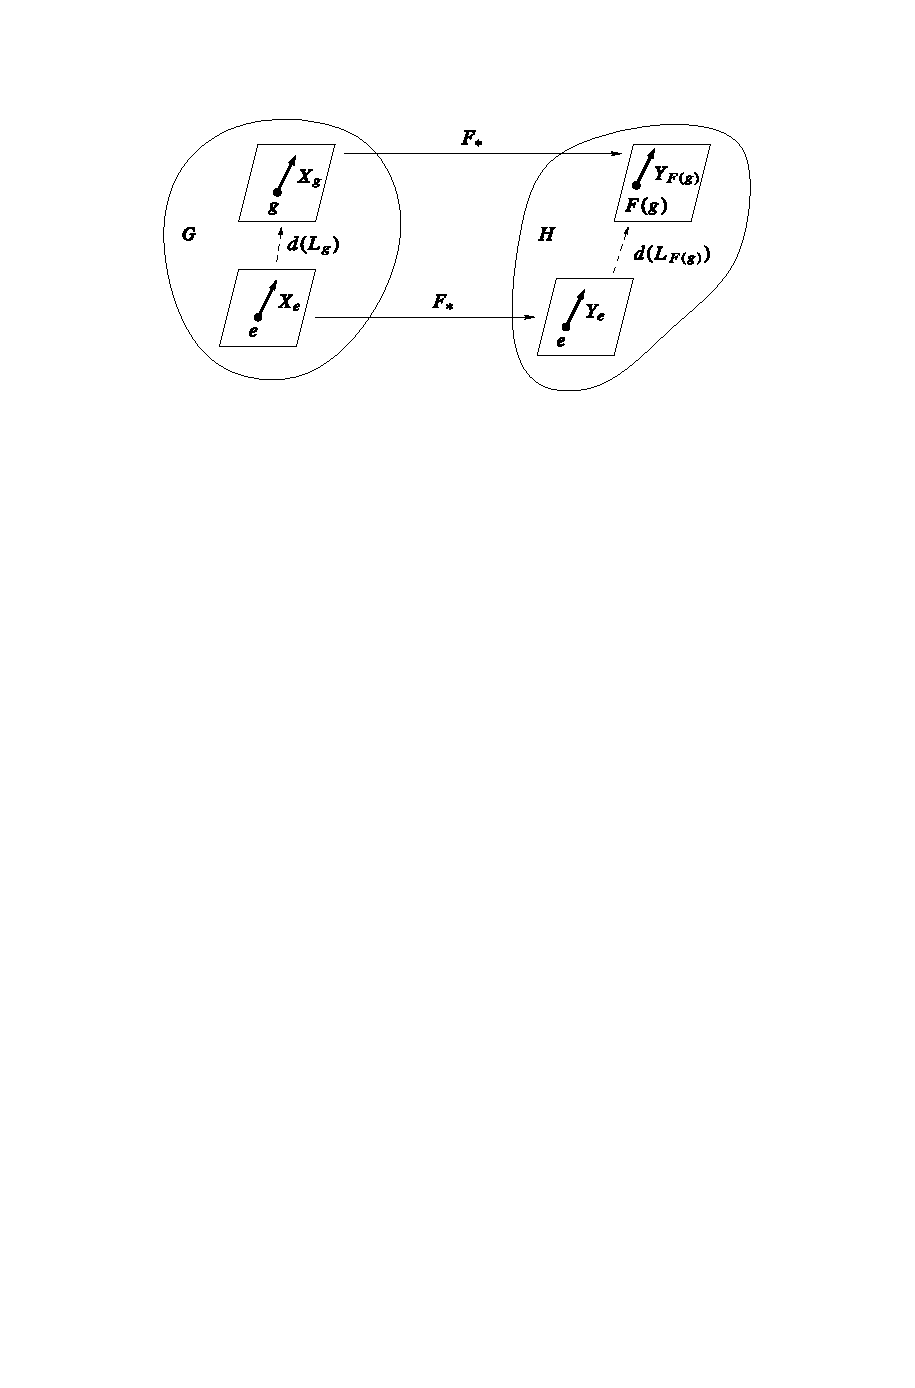
\includegraphics{pictures/induced-Lie-homo}
\caption{The induced Lie algebra homomorphism.}
\end{figure}
\begin{proof}
If there is any vector field $Y\in\h$ that is $F$-related to $X$, it must satisfy $Y_e=dF_e(X_e)$, and thus it must be uniquely determined by
\[Y=(Y_e)^L=(dF_e(X_e))^L\]
To show that this $Y$ is $F$-related to $X$, we note that the fact that $F$ is a homomorphism implies
\begin{align*}
F(gg')=F(g)F(g')&\Rightarrow F(L_gg')=L_{F(g)}F(g')\\
&\Rightarrow F\circ L_g=L_{F(g)}\circ F\\
&\Rightarrow dF\circ d(L_g)=d(L_{F(g)})\circ dF
\end{align*}
Thus,
\[dF(X_g)=dF\circ d(L_g)(X_e)=d(L_{F(g)})\circ dF(X_e)=d(L_{F(g)})(Y_e)=Y_{F(g)}\]
This says precisely that $X$ and $Y$ are $F$-related.\par
For each $X\in g$, let $F_*X$ denote the unique vector field in $\h$ that is $F$-related to $X$. It then follows immediately from the naturality of Lie brackets that $F_*[X,Y]=[F_*X,F_*Y]$, so $F_*$ is a Lie algebra homomorphism.
\end{proof}
The map $F_*:\g\to\h$ whose existence is asserted in this theorem is called the \textbf{induced Lie algebra homomorphism}. Note that the theorem implies that for any left-invariant vector field $X\in g$, $F_*X$ is a well-defined smooth vector field on $H$, \textit{even though $F$ may not be a diffeomorphism}.
\begin{proposition}[\textbf{Properties of Induced Homomorphisms}]
\mbox{}
\begin{itemize}
\item[(a)] The homomorphism $(\mathrm{id})_*:\Lie(G)\to\Lie(G)$ induced by the identity map of $G$ is the identity of $\Lie(G)$.
\item[(b)] If $F_1:G\to H$ and $F_2:H\to K$ are Lie group homomorphisms, then
\[(F_2\circ F_1)_*=(F_2)_*\circ(F_1)_*\]
\item[(c)] Isomorphic Lie groups have isomorphic Lie algebras.
\end{itemize}
\end{proposition}
\begin{proof}
These all follow from the property of the differential $F_*$.
\end{proof}
Therefore, we obtain a functor from the category of Lie groups to the category of Lie algebras. 
\subsection{Lie subalgebras and Lie subgroups}
If $G$ is a Lie group and $H\sub G$ is a Lie subgroup, we might hope that the Lie algebra of $H$ would be a Lie subalgebra of that of $G$. However, elements of $\Lie(H)$ are vector fields on $H$, not $G$, and so, strictly speaking, are not elements of $\Lie(G)$. Nonetheless, the next proposition gives us a way to view $\Lie(H)$ as a subalgebra of $\Lie(G)$.
\begin{proposition}\label{Lie subalgebra}
Suppose $H\sub G$ is a Lie subgroup, and $\iota:H\hookrightarrow G$ is the inclusion map. There is a Lie subalgebra $\h\in\Lie(G)$ that is canonically isomorphic to $\Lie(H)$, characterized by either of the following descriptions:
\[\h=\iota_*(\Lie(H))=\{X\in\Lie(G):X_e\in T_eH\}\]
\end{proposition}
\begin{proof}
Because the inclusion map $\iota:H\hookrightarrow G$ is a Lie group homomorphism, $\iota_*(\Lie(H))$ is a Lie subalgebra of $\Lie(G)$. 
By the way we defined the induced Lie algebra homomorphism, this subalgebra is precisely the set of left-invariant vector fields on $G$ whose values at 
the identity are of the form $d\iota_e(v)$ for some $v\in T_eH$. Since the differential $d\iota_e:T_eH\to T_eG$ is the inclusion of $T_eH$ as a 
subspace in $T_eG$, the two characterizations of $\h$ are equal. Since $d\iota_e$ is injective on $T_eH$, it follows that $\iota_*$ is injective 
on $\Lie(H)$; since it is surjective by definition of $\h$, it is an isomorphism between $\Lie(H)$ and $\h$.
\end{proof}
Using this proposition, whenever $H$ is a Lie subgroup of $G$, we often identify $\Lie(H)$ as a subalgebra of $\Lie(G)$. 
As we mentioned above, elements of $\Lie(H)$ are not themselves left-invariant vector fields on $G$. But the preceding 
proposition shows that every element of $\Lie(H)$ corresponds to a unique element of $\Lie(G)$, determined by its value at the identity, and 
the injection of $\Lie(H)$ into $\Lie(G)$ thus determined respects Lie brackets; so by thinking of $\Lie(H)$ as a subalgebra of $\Lie(G)$ we are not 
committing a grave error.\par
This identification is especially illuminating in the case of Lie subgroups of $\GL_n(\R)$. We showed above that the Lie algebra of $\GL_n(\R)$ 
is naturally isomorphic to the matrix algebra $\gl(n,\R)$. We can now prove a similar result for $\GL_n(\C)$. Just as in the real case, our usual identification of $\GL_n(\C)$ as an open subset of $\gl(n,\C)$ yields a sequence of vector space isomorphisms
\begin{equation}\label{Lie algebra GL(C)-1}
\begin{tikzcd}
\Lie(\GL_n(\C))\ar[r,"\eps"]&T_{I_n}\GL_n(\C)\ar[r,"\varphi"]&\gl(n,\C)
\end{tikzcd}
\end{equation}
where $\eps$ is the evaluation map and $\varphi$ is the usual identification between the tangent space to an open subset of a vector space and the vector space itself.
\begin{proposition}
The composition of the maps in $(\ref{Lie algebra GL(C)-1})$ yields a Lie algebra isomorphism between $\Lie(\GL_n(\C))$ and the matrix algebra $\gl(n,\C)$.
\end{proposition}
\begin{proof}
The Lie group homomorphism $\beta:\GL_n(\C)\to\GL_{2n}(\R)$ that we constructed
in Example~\ref{Lie subgroups eg}(d) induces a Lie algebra homomorphism
\[\beta_*:\Lie(\GL_n(\C))\to\Lie(\GL_{2n}(\R))\]
Composing $\beta_*$ with our canonical isomorphisms yields a commutative diagram
\[\begin{tikzcd}
\Lie(\GL_n(\C))\ar[r,"\eps"]\ar[d,"\beta_*"]&T_{I_n}\GL_n(\C)\ar[r,"\varphi"]\ar[d,"d\beta_{I_{n}}"]&\gl(n,\C)\ar[d,"\alpha"]\\
\Lie(\GL_{2n}(\R))\ar[r,"\eps"]&T_{I_{2n}}\GL_{2n}(\R)\ar[r,"\varphi"]&\gl(2n,\R)
\end{tikzcd}\]
in which $\alpha=\varphi\circ d\beta_{I_n}\circ\varphi^{-1}$. Proposition~\ref{Lie algebra GL(V) iso} showed that the composition of the
isomorphisms in the bottom row is a Lie algebra isomorphism; we need to show the same thing for the top row.\par
It is easy to see from the formula in Example~\ref{Lie subgroups eg}(d) that $\beta$ is (the restriction of) a linear map. It follows that $d\beta_{I_n}$ is given by exactly the same formula as $\beta$, as is $\alpha:\gl(n,\C)\to\gl(2n,\R)$. Because $\beta(AB)=\beta(A)\beta(B)$, it follows that $\alpha$ preserves matrix commutators:
\[\alpha[A,B]=\alpha(AB-BA)=\alpha(A)\alpha(B)-\alpha(B)\alpha(A)=[\alpha(A),\alpha(B)]\]
Thus $\alpha$ is an injective Lie algebra homomorphism from $\gl(n,\C)$ to $\gl(2n,\R)$ (considering both as matrix algebras). Replacing the bottom row by the images of the vertical maps, we obtain a commutative diagram of vector space isomorphisms
\[\begin{tikzcd}
\Lie(\GL_n(\C))\ar[r,"\cong"]\ar[d,"\beta_*"]&\gl_n(\C)\ar[d,"\alpha"]\\
\beta_*(\Lie(\GL_n(\C)))\ar[r,"\cong"]&\alpha(\gl(2n,\R))
\end{tikzcd}\]
in which the bottom map and the two vertical maps are Lie algebra isomorphisms;
it follows that the top map is also a Lie algebra isomorphism.
\end{proof}
A distribution $D$ on a Lie group $G$ is said to be \textbf{left-invariant} if it is invariant under every left translation.
\begin{lemma}\label{Lie subalgebra distribution}
Let $G$ be a Lie group. If $\h$ is a Lie subalgebra of $\Lie(G)$, then the subset $D=\bigcup_{g\in G}D_g$, where
\[D_g=\{X_g:X\in\h\}\sub T_gG,\]
is a smooth left-invariant involutive distribution on $G$.
\end{lemma}
\begin{proof}
Each $X\in\h$ is a left-invariant vector field on $G$. Thus, for any $g,g'\in G$, the differential $d(L_{g'g^{-1}})$ restricts to an isomorphism from $D_g$ to $D_{g'}$. It follows that $D_g$ has the same dimension for each $g$, and $D$ is left-invariant. Any basis $(X_1,\dots,X_k)$ for $\h$ is a global smooth frame for $D$, so $D$ is smooth. Moreover, because $[X_i,X_j]\in\h$ for all $1\leq i,j\leq k$, it follows from Lemma~\ref{involutivity local fram crit} that $D$ is involutive.
\end{proof}
\begin{theorem}[\textbf{Lie Subgroups Are Weakly Embedded}]\label{Lie subgroup weak embedd}
Every Lie subgroup is an integral manifold of an involutive distribution, and therefore is a weakly embedded submanifold.
\end{theorem}
\begin{proof}
Suppose $G$ is a Lie group and $H\sub G$ is a Lie subgroup. Theorem~\ref{Lie subalgebra} shows that the Lie algebra of $H$ is canonically isomorphic to the Lie subalgebra $\h=\iota_*(\Lie(H))\sub\Lie(G)$, where $\iota:H\to G$ is inclusion. Let $D\sub TG$ be the involutive distribution determined by $\h$ as in Lemma~\ref{Lie subalgebra distribution}. It follows from the definitions that at each point $\h\in H$, the tangent space $T_hH$ is equal to $D_h$, so $H$ is an integral manifold of $D$. It then follows from Theorem~\ref{integral mani weak embedd} that $H$ is weakly embedded in $G$.
\end{proof}
\begin{theorem}[\textbf{The Lie Subgroup Associated with a Lie Subalgebra}]\label{Lie subgroup generated by Lie subalgebra}
Suppose $G$ is a Lie group and $\g$ is its Lie algebra. If $\h$ is a Lie subalgebra of $\g$, then there is a unique connected Lie subgroup of $G$ whose Lie algebra is $\h$.
\end{theorem}
\begin{figure}[htbp]
\centering
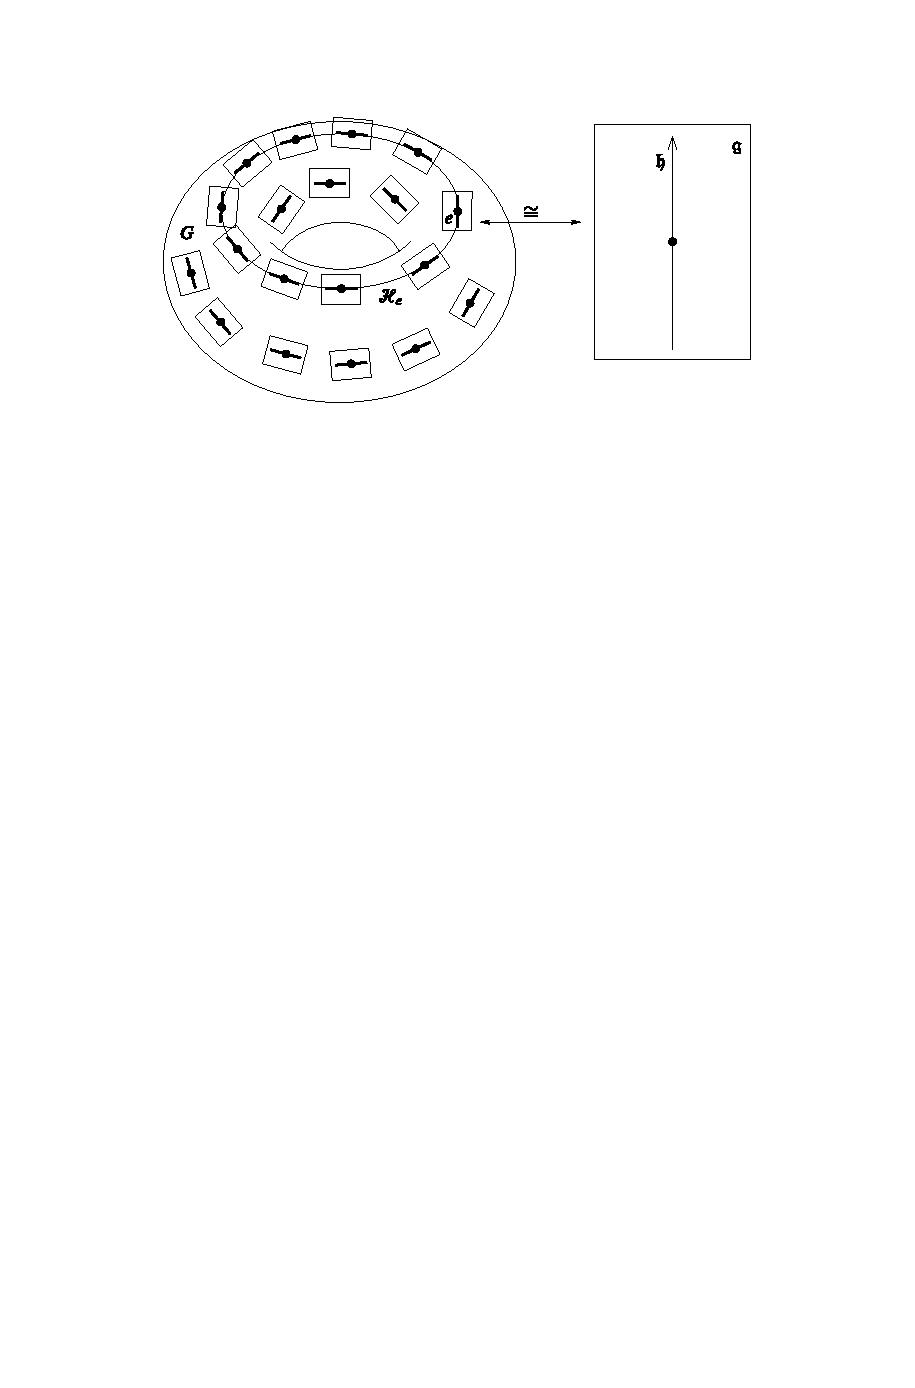
\includegraphics{pictures/Lie-sugroup}
\caption{Finding a subgroup whose Lie algebra is $\h$.}
\end{figure}
\begin{proof}
Suppose $\h$ is a Lie subalgebra of $\g$. Let $D\sub TG$ be the involutive distribution of $\h$. Let $\mathcal{H}$ denote the foliation determined by $D$, and for any $g\in G$, let $\mathcal{H}_g$ denote the leaf of $\mathcal{H}$ containing $g$. Because $D$ is left-invariant, it follows from Proposition~\ref{distribution invariant} that each left translation takes leaves to leaves: for any $g,g'\in G$, we have $L_g(\mathcal{H}_{g'})=\mathcal{H}_{gg'}$. Define $H=\mathcal{H}_e$, the leaf containing the identity. We will show that $H$ is the desired Lie subgroup.

First, to see that $H$ is a subgroup, observe that for any $h,h'\in H$,
\[hh'=L_h(h')\in L_h(H)=L_h(\mathcal{H}_e)=\mathcal{H}_h=H.\]
Similarly,
\[h^{-1}=h^{-1}e=L_{h^{-1}}(\mathcal{H}_e)=L_{h^{-1}}(\mathcal{H}_h)=\mathcal{H}_e=H.\]
To show that $H$ is a Lie group, we need to show that the map $\mu:(h,h')\mapsto h^{-1}h'$ is smooth as a map from 
$H\times H$ to $H$. Because $H\times H$ is a submanifold of $G\times G$, it is immediate that $\mu:H\times H\to G$ 
is smooth. Since $H$ is an integral manifold of an involutive distribution, Theorem~\ref{integral mani weak embedd} shows that it is weakly embedded, so $\mu$ is
also smooth as a map into $H$.\par
The fact that $H$ is a leaf of $\mathcal{H}$ implies that the Lie algebra of $H$ is $\h$, because the tangent 
space to $H$ at the identity is $D_e=\{X_e:X\in\h\}$. To see that $H$ is the unique connected subgroup with Lie 
algebra $\h$, suppose $\widetilde{H}$ is any other connected subgroup with the same Lie algebra. Any such Lie 
subgroup is easily seen to be an integral manifold of $D$, so by maximality of $H=\mathcal{H}_e$, we must have 
$\widetilde{H}\sub H$. On the other hand, if $U$ is the domain of a flat chart for $D$ containing the identity, 
then by Proposition~\ref{integral mani local struct}, $\widetilde{H}\cap U$ is a union of open subsets of slices. 
Since the slice containing $e$ is an open subset of $H$, this implies that $\widetilde{H}$ contains a neighborhood 
of the identity in $H$. Since any neighborhood of the identity generates $H$ (Proposition~\ref{topo group prop}), 
this implies that $\widetilde{H}=H$.
\end{proof}
Since nonclosed subgroups can be pathological, Theorem~\ref{Lie subgroup generated by Lie subalgebra} is most useful in cases where the connected Lie subgroup $H$ is actually closed. The following result gives one condition under which this is guaranteed to be the case.
\begin{proposition}\label{Lie subgroup generated by Lie subalgebra closed if maximal abelian}
Suppose $G$ is a Lie group with Lie algebra $\g$ and that $\h$ is a maximal commutative subalgebra of $\g$, meaning that $\h$ is commutative and h is not contained in any larger commutative subalgebra of $\g$. Then the connected Lie subgroup $H$ of $G$ with Lie algebra $\h$ is closed.
\end{proposition}
\begin{proof}
Since $\h$ is commutative, $H$ is also commutative, since every element of $H$ is a product of exponentials of elements of $\h$ (Proposition~\ref{Lie group exp generate}). It easily follows that the closure $\widebar{H}$ of $H$ in $G$ is also commutative. Since $H$ is connected, $\widebar{H}$ is also connected. Now, since $\widebar{H}$ is commutative, its Lie algebra $\h'$ is also commutative. But since $\h$ was maximal commutative, we must have $\h'=\h$. Since, also, $\widebar{H}$ is connected, we conclude that $H=\widebar{H}$, showing that $H$ is closed.
\end{proof}
\subsection{One-parameter subgroups and the exponential map}
Suppose $G$ is a Lie group. Since left-invariant vector fields are naturally defined in terms of the group structure of $G$, one might reasonably expect to find some relationship between the group law for the flow of a left-invariant vector field and
group multiplication in $G$. We begin by exploring this relationship.
\subsubsection{One-Parameter Subgroups}
A \textbf{one-parameter subgroup} of $G$ is defined to be a Lie group homomorphism $\gamma:\R\to G$, with $\R$ considered as a Lie group under addition. By this definition, a one-parameter subgroup is not a Lie subgroup of $G$, but rather a homomorphism into $G$.
\begin{theorem}[\textbf{Characterization of One-Parameter Subgroups}]\label{one-para subgroup char}
Let $G$ be a Lie group. The one-parameter subgroups of $G$ are precisely the maximal integral curves of left-invariant vector fields starting at the identity.
\end{theorem}
\begin{proof}
First suppose $\gamma$ is the maximal integral curve of some left-invariant vector field $X\in\Lie(G)$ starting at the identity. Because left-invariant vector fields are complete (Theorem~\ref{vector field left-inva complete}), $\gamma$ is defined on all of $\R$. Left-invariance means that $X$ is $L_g$-related to itself for every $g\in G$, so $L_g$ takes integral curves of $X$ to integral curves of $X$. Applying this with $g=\gamma(s)$ for some $s\in\R$, we conclude that the curve $t\mapsto L_{\gamma(s)}\big(\gamma(t)\big)$ is an integral curve starting at $\gamma(s)$. But the curve $t\mapsto\gamma(t+s)$ is also an integral curve with the same initial point, so they are equal:
\[\gamma(s)\gamma(t)=\gamma(s+t).\]
This says precisely that $\gamma:\R\to G$ is a one-parameter subgroup.\par
Conversely, suppose $\gamma:\R\to G$ is a one-parameter subgroup, and let $X=\gamma_*(d/dt)\in\Lie(G)$, treating $d/dt$ as a left-invariant vector field on $\R$. Since $\gamma(0)=e$, we just have to show that $\gamma$ is an integral curve of $X$. Recall that $\gamma_*(d/dt)$ is defined as the unique left-invariant vector field on $G$ that is $\gamma_*$-related to $d/dt$ (see Theorem~\ref{Lie algebra induce}). Therefore, for any $t_0\in\R$,
\[\gamma'(t_0)=d\gamma_{t_0}\Big(\frac{d}{dt}\Big|_{t_0}\Big)=X_{\gamma(t_0)}.\]
so $\gamma$ is an integral curve of $X$.
\end{proof}
Given $X\in\Lie(G)$, the one-parameter subgroup determined by $X$ in this way is called the \textbf{one-parameter subgroup generated by $\bm{X}$}. Because left-invariant vector fields are uniquely determined by their values at the identity, it follows that each one-parameter subgroup is uniquely determined by its initial velocity in $T_eG$, and thus there are one-to-one correspondences
\[\text{one-parameter subgroups of $G$}\leftrightarrow\Lie(G)\leftrightarrow T_eG.\]
The one-parameter subgroups of $\GL_n(\R)$ are not hard to compute explicitly.
\begin{proposition}
For any $A\in\gl(n,\R)$, let
\begin{align}\label{exp def gl(n,R)}
e^A=\sum_{k=0}^{\infty}\frac{A^k}{k!}.
\end{align}
This series converges to an invertible matrix $e^A\in\GL_n(\R)$, and the one-parameter subgroup of $\GL_n(\R)$ generated by $A\in\gl(n,\R)$ is $\gamma(t)=e^{tA}$.
\end{proposition}
\begin{proof}
First, we verify convergence. The matrix multiplication satisfies $|AB|\leq|A||B|$, where the norm is the Frobenius norm on $\gl(n,\R)$. It follows by induction that $|A^k|\leq |A|^k$. The Weierstrass $M$-test then shows that $(\ref{exp def gl(n,R)})$ converges uniformly on any bounded subset of $\gl(n,\R)$, by comparison with the series $\sum_{k=0}^{\infty}c^k/k!$.\par
Fix $A\in\gl(n,\R)$. Under our identification of $\gl(n,\R)$ with $\Lie(\GL_n(\R))$, the matrix $A$ corresponds to the left-invariant vector field $A^L$ given by $(\ref{Lie algebra iso-1})$. Thus, the one-parameter subgroup generated by $A$ is an integral curve of $A^L$ on $\GL_n(\R)$, and therefore satisfies the ODE initial value problem
\[\gamma'(t)=A^L|_{\gamma(t)},\quad \gamma(0)=I_n.\]
Using $(\ref{Lie algrbra gl(n,R)})$, the condition for $\gamma$ to be an integral curve can be rewritten as
\[\dot{\gamma}^i_k(t)=\gamma^i_j(t)A^j_k,\]
or in matrix notation
\[\gamma'(t)=\gamma(t)A.\]
We will show that $\gamma(t)=e^{tA}$ satisfies this equation. Since $\gamma(0)=I_n$, this implies that $\gamma$ is the unique integral curve of $A^L$ starting at the identity and is therefore the desired one-parameter subgroup.\par
To see that $\gamma$ is differentiable, we note that differentiating the series $(\ref{exp def gl(n,R)})$ formally term by term yields the result
\[\gamma'(t)=\sum_{k=1}^{\infty}\frac{A^k}{(k-1)!}=\gamma(t)A=A\gamma(t).\]
Since the differentiated series converges uniformly on bounded sets, the term-by-term differentiation is justified. By smoothness of solutions to ODEs, $\gamma$ is a smooth curve.\par
It remains only to show that $\gamma(t)$ is invertible for all $t$, so that $\gamma$ actually takes its values in $\GL_n(\R)$. If we let $\sigma(t)=\gamma(t)\gamma(-t)=e^{tA}e^{-tA}$, then $\sigma$ is a smooth curve in $\gl(n,\R)$, and by the previous computation and the product rule it satisfies
\[\sigma'(t)=\big(\gamma(t)A\big)\gamma(-t)-\gamma(t)\big(A\gamma(-t)\big)=0.\]
It follows that $\sigma$ is the constant curve $\sigma(t)=I_n$, which is to say that
$\gamma(t)=\gamma(-t)^{-1}$. 
\end{proof}
\begin{proposition}\label{one-para Lie subgroup}
Suppose $G$ is a Lie group and $H\sub G$ is a Lie subgroup. The one-parameter subgroups of $H$ are precisely those one-parameter subgroups of $G$ whose initial velocities lie in $T_eH$.
\end{proposition}
\begin{proof}
Let $\gamma:\R\to H$ be a one-parameter subgroup. Then the composite map
\[\begin{tikzcd}
\R\ar[r,"\gamma"]&H\ar[r,hook]&G
\end{tikzcd}\]
is a Lie group homomorphism and thus a one-parameter subgroup of $G$, which clearly satisfies $\gamma'(0)\in T_eH$.\par
Conversely, suppose $\gamma:\R\to G$ is a one-parameter subgroup whose initial velocity lies in $T_eH$. Let $\widetilde{\gamma}:\R\to H$ be the one-parameter subgroup of $H$ with the same initial velocity $\widetilde{\gamma}'(0)=\gamma'(0)\in T_eH\sub T_eG$. As in the preceding paragraph, by composing with the inclusion map, we can also consider $\widetilde{\gamma}$ as a one-parameter subgroup of $G$. Since $\gamma$ and $\widetilde{\gamma}$ are both one-parameter subgroups of $G$ with the same initial velocity, they must be equal.
\end{proof}
\begin{example}
If $H$ is a Lie subgroup of $\GL_n(\R)$, the preceding proposition shows that the one-parameter subgroups of $H$ are precisely the maps of the form $\gamma(t)=e^{tA}$ for $A\in\h$, where $\h\sub\gl(n,\R)$ is the subalgebra corresponding to $\Lie(H)$ as in Theorem~\ref{Lie subalgebra}. For example, taking $H=\O(n)$, this shows that the one-parameter subgroups of $\O(n)$ are the maps of the form $\gamma(t)=e^{tA}$ for an arbitrary skew-symmetric matrix $A$. In particular, this shows that the exponential of any skew-symmetric matrix is orthogonal.
\end{example}
\subsubsection{The Exponential Map}
In the preceding part we saw that the matrix exponential maps $\gl(n,\R)$ to $\GL_n(\R)$ and takes each line through the origin to a one-parameter subgroup. This
has a powerful generalization to arbitrary Lie groups.\par
Given a Lie group $G$ with Lie algebra $\g$, we define a map $\exp:\g\to G$, called the \textbf{exponential map of $\bm{G}$}, as follows: for any $X\in\g$, we set
\[\exp(X)=\gamma(1),\]
where $\gamma$ is the one-parameter subgroup generated by $X$, or equivalently the integral curve of $X$ starting at the identity. The following proposition shows that,
like the matrix exponential, this map sends the line through $X$ to the one-parameter
subgroup generated by $X$.
\begin{proposition}[\textbf{(One-Parameter Subgroups}]\label{exp map one-para}
Let $G$ be a Lie group. For any $X\in\Lie(G)$, $\gamma(t)=\exp tX$ is the one-parameter subgroup of $G$ generated by $X$.
\end{proposition}
\begin{figure}[htbp]
\centering
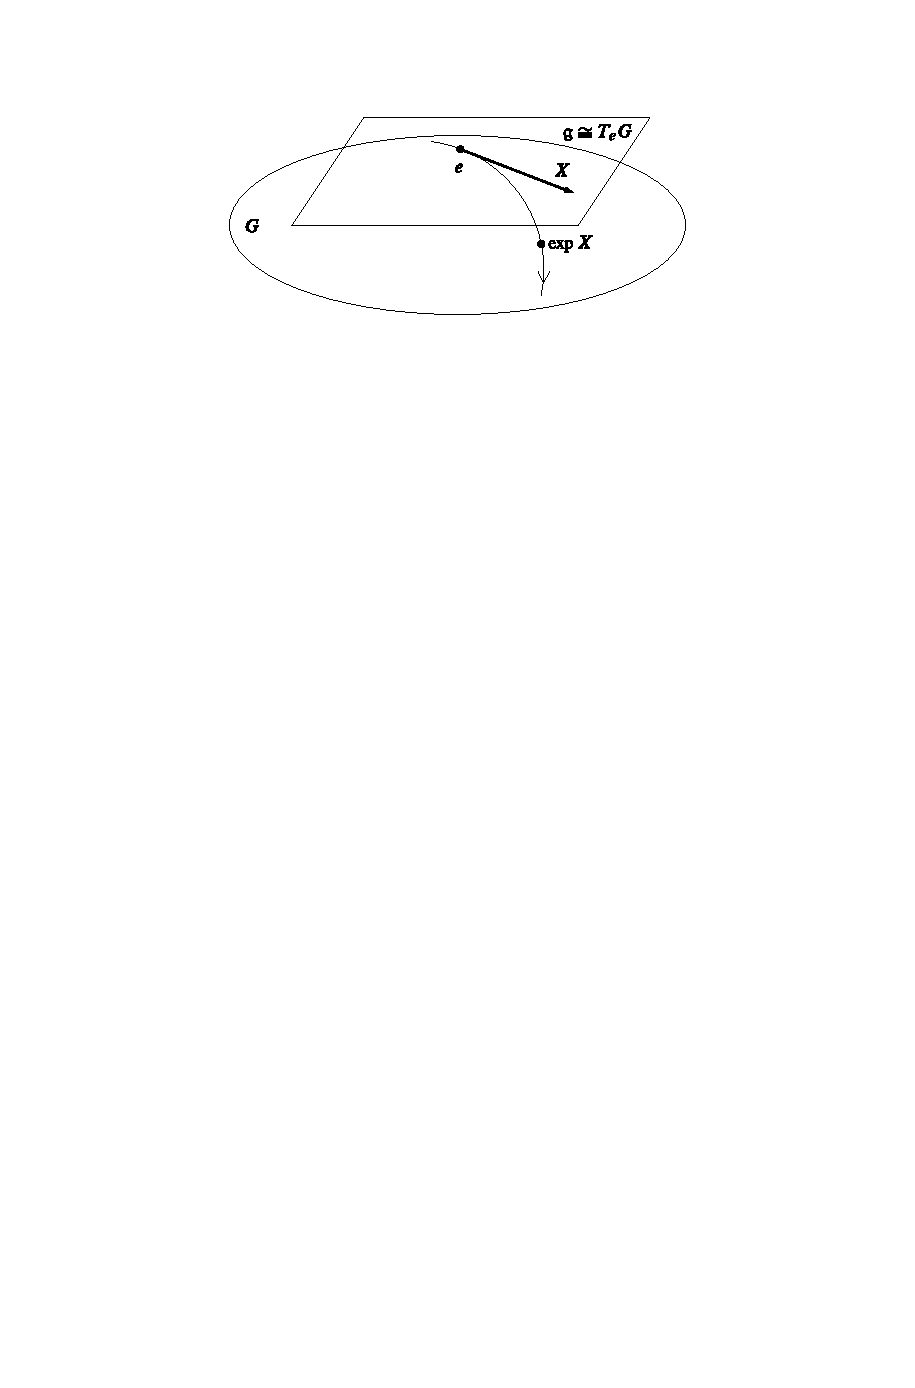
\includegraphics{pictures/exp-map}
\caption{The exponential map.}
\end{figure}
\begin{proof}
Let $\gamma:\R\to G$ be the one-parameter subgroup generated by $X$, which is the integral curve of $X$ starting at $e$. For any fixed $t\in\R$, it follows from the rescaling lemma 
that $\widetilde{\gamma}(s)=\gamma(ts)$ is the integral curve of $tX$ starting at $e$, so
\[\exp tX=\widetilde{\gamma}(1)=\gamma(t)\]
as needed.
\end{proof}
Here are two simple but important examples.
\begin{example}
The results of the preceding part show that the exponential map of $\GL_n(\R)$ (or any Lie subgroup of it) is given by $\exp A=e^A$. This, obviously, is the reason for the term exponential map.
\end{example}
\begin{example}
If $V$ is a finite-dimensional real vector space, a choice of basis for $V$ yields isomorphisms $\GL(V)\cong\GL_n(\R)$ and $\gl(V)\cong\gl(n,\R)$. The analysis of the $\GL_n(\R)$ case then shows that the exponential map of $\GL(V)$ can be written in
the form 
\[\exp A=\sum_{k=0}^{\infty}\frac{A^k}{k!},\]
where we consider $A\in\gl(V)$ as a linear map from $V$ to itself, and $A^k=A\circ\cdots\circ A$ is the $k$-fold composition of $A$ with itself.
\end{example}
\begin{proposition}[\textbf{Properties of the Exponential Map}]\label{Lie group exp prop}
Let $G$ be a Lie group and let $\g$ be its Lie algebra.
\begin{itemize}
\item[(a)] The exponential map is a smooth map from $\g$ to $G$.
\item[(b)] For any $X\in\g$ and $s,t\in\R$, $\exp(s+t)X=\exp sX\exp tX$.
\item[(c)] For any $X\in\g$, $(\exp X)^{-1}=\exp(-X)$.
\item[(d)] For any $X\in\g$ and $n\in\Z$, $(\exp X)^n=\exp(nX)$.
\item[(e)] The differential $(d\exp)_0:T_0\g\to T_eG$ is the identity map, under the canonical identifications of both $T_0\g$ and $T_eG$ with $\g$ itself.
\item[(f)] The exponential map restricts to a diffeomorphism from some neighborhood of $0$ in $\g$ to a neighborhood of $e$ in $G$.
\item[(g)] If $H$ is another Lie group, $\h$ is its Lie algebra, and $\varPhi:G\to H$ is a Lie group homomorphism, the following diagram commutes:
\[\begin{tikzcd}
\g\ar[r,"\varPhi_*"]\ar[d,swap,"\exp"]&\h\ar[d,"\exp"]\\
G\ar[r,"\varPhi"]&H
\end{tikzcd}\]
\item[(h)] The flow $\theta$ of a left-invariant vector field $X$ is given by $\theta_t=R_{\exp tX}$ $($right multiplication by $\exp tX$$)$.
\end{itemize}
\end{proposition}
\begin{figure}[htbp]
\centering
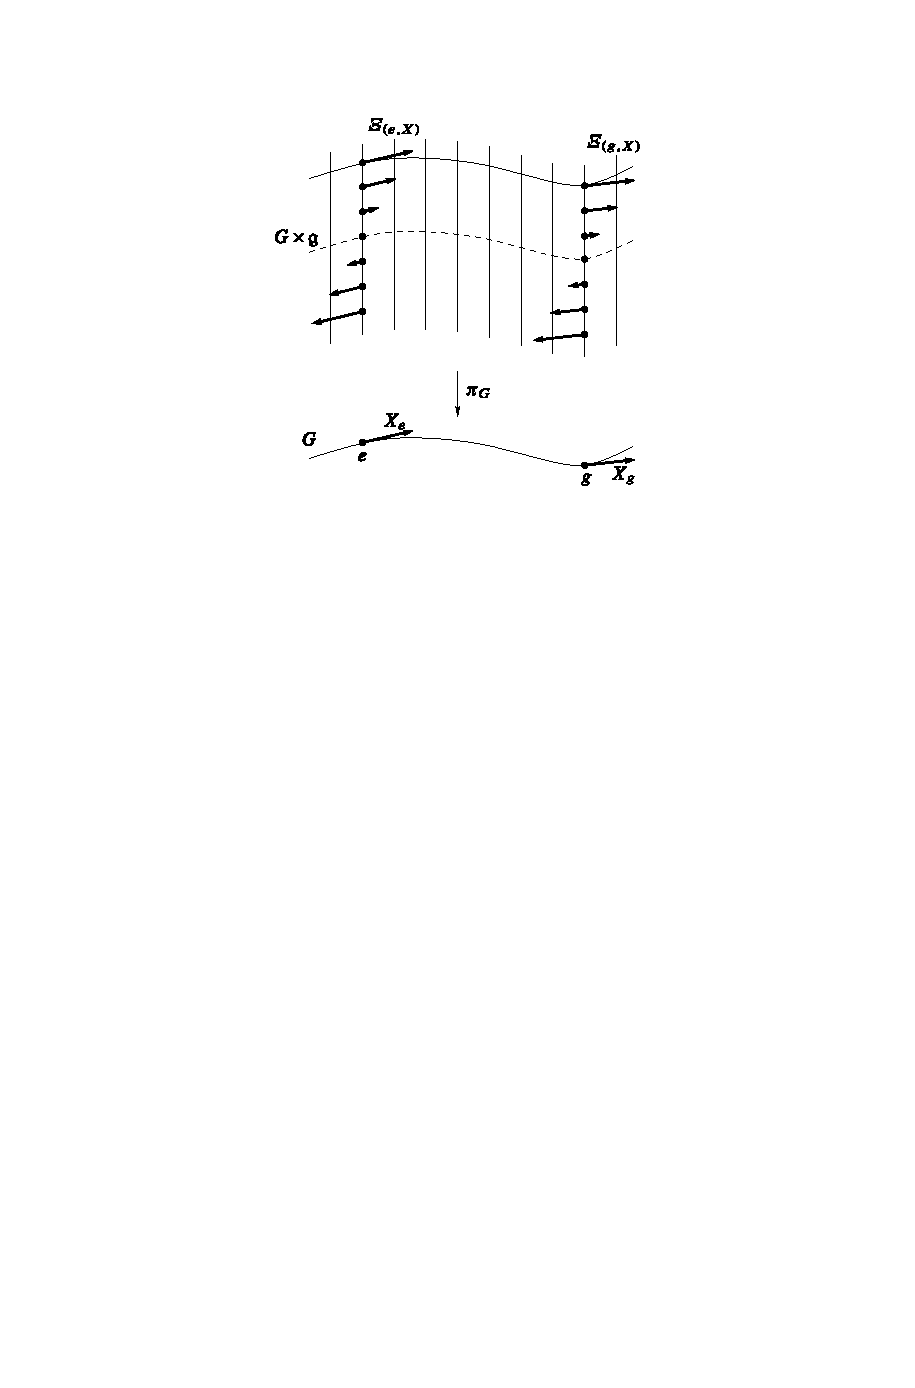
\includegraphics{pictures/exp-map-prop}
\caption{Proof that the exponential map is smooth.}
\end{figure}
\begin{proof}
In this proof, for any $X\in\g$ we let $\theta_X$ denote the flow of $X$. To prove (a), we need to show that the expression $\theta_X^{(e)}(1)$ depends smoothly on $X$, which amounts to showing that the flow varies smoothly as the vector field varies. This is a situation not covered by the fundamental theorem on flows, but we can reduce it to that theorem by the following simple trick. Define a vector field $\varXi$ on the product manifold $G\times\g$ by
\[\varXi_{(g,X)}=(X_g,0)\in T_gG\oplus T_X\g\cong T_{(g,X)}(G\times\g).\]
To see that $\varXi$ is a smooth vector field, choose any basis $(X_1,\dots,X_k)$ for $\g$, and let $(x^i)$ be the corresponding global coordinates for $\g$, defined by $(x^i)\leftrightarrow x^iX_i$. Let $(w^i)$ be any smooth local coordinates for $G$. If $f\in C^\infty(G\times\g)$ is arbitrary, then locally we can write
\[\varXi f(w^i,x^i)=x^jX_jf(w^i,x^i),\]
where each vector field $X_j$ differentiates $f$ only in the $w^i$-directions. Since this depends smoothly on $(w^i,x^i)$, it follows from Proposition~\ref{vector field smooth by function} that $\varXi$ is smooth. It is easy to verify that the flow $\varTheta$ of $\varXi$ is given by
\[\varTheta_t(g,X)=(\theta_X(t,g),X).\]
By the fundamental theorem on flows, $\varTheta$ is smooth. Since $\exp X=\pi_G\big(\varTheta_1(e,X)\big)$, where $\pi_G:G\times\g\to G$ is the projection, it follows that $\exp$ is smooth.\par
Next, (b) and (c) follow immediately from Proposition~\ref{exp map one-para}, because $t\mapsto\exp tX$ is a group homomorphism from $\R$ to $G$. Then (d) for nonnegative $n$ follows from (b) by induction, and for negative $n$ it follows from (c).\par
To prove (e), let $X\in\g$ be arbitrary, and let $\sigma:\R\to\g$ be the curve $\sigma(t)=tX$. Then $\sigma'(0)=X$, and Proposition~\ref{exp map one-para} implies
\[(d\exp)_0(X)=(d\exp)_0\big(\sigma'(0)\big)=(\exp\circ\sigma)'(0)=\frac{d}{dt}\Big|_{t=0}\exp tX=X.\]
Part (f) then follows immediately from (e) and the inverse function theorem.\par
Next, to prove (g) we need to show that $\exp(\varPhi_*X)=\varPhi(\exp X)$ for every $X\in g$. In fact, we will show that for all $t\in\R$,
\[\exp(t\varPhi_*X)=\varPhi(\exp tX).\]
The left-hand side is, by Proposition~\ref{exp map one-para}, the one-parameter subgroup generated by $\varPhi_*X$. Thus, if we put $\sigma(t)=\varPhi(\exp tX)$, it suffices to show that $\sigma:\R\to H$ is a Lie group homomorphism satisfying $\sigma'(0)=(\varPhi_*X)_e$. It is a Lie group homomorphism because it is the composition of the homomorphisms $\varPhi$ and $t\mapsto\exp tX$. The initial
velocity is computed as follows:
\[\sigma'(0)=\frac{d}{dt}\Big|_{t=0}\varPhi(\exp tX)=d\varPhi_e\Big(\frac{d}{dt}\Big|_{t=0}\exp tX\Big)=d\varPhi_e(X_e)=(\varPhi_* X)_e.\]

Finally, to show that $(\theta_X)_t=R_{\exp tX}$, we use the fact that for any $g\in G$, the left multiplication map $L_g$ takes integral curves of $X$ to integral curves of $X$. Thus, the map $t\mapsto L_g(\exp tX)$ is the integral curve starting at $g$, which means it is equal to $\theta_X^{(g)}(t)$. It follows that
\[R_{\exp tX}(g)=g\exp tX=L_g(\exp tX)=\theta_X^{(g)}(t)=(\theta_X)_t(g).\]
This completes the proof.
\end{proof}
The exponential map yields the following alternative characterization of the Lie subalgebra of a subgroup.We will use this later when we study normal subgroups.
\begin{proposition}\label{Lie subalgebra exp}
Let $G$ be a Lie group, and let $H\sub G$ be a Lie subgroup. With $\Lie(H)$ considered as a subalgebra of $\Lie(G)$ in the usual way, the exponential map of $H$ is the restriction to $\Lie(H)$ of the exponential map of $G$, and
\[\Lie(H)=\{X\in\Lie(G):\exp tX\in H\text{ for all $t\in\R$}\}.\]
\end{proposition}
\begin{proof}
The fact that the exponential map of $H$ is the restriction of that of $G$ is an immediate consequence of Proposition~\ref{one-para Lie subgroup}. To prove the second assertion, by the way we have identified $\Lie(H)$ as a subalgebra of $\Lie(G)$, we need to establish the following equivalence for every $X\in\Lie(G)$:
\[\exp tX\in H\text{ for all $t\in\R$}\iff X_e\in T_eH.\]
Assume first that $\exp tX\in H$ for all $t$. Since $H$ is weakly embedded in $G$ by
Theorem~\ref{Lie subgroup weak embedd}, it follows that the curve $t\mapsto\exp tX$ is smooth as a map into $H$, and thus $X_e=\gamma'(0)\in T_eH$. Conversely, if $X_e\in T_eH$, then Proposition~\ref{one-para Lie subgroup} implies that $\exp tX\in H$ for all $t$.
\end{proof}
Notice that Proposition~\ref{Lie group exp prop}(d) does not imply $\exp(X+Y)=(\exp X)(\exp Y)$ for arbitrary $X,Y$ in the Lie algebra. In fact, for connected groups, this is true only when the group is abelian.
\begin{proposition}\label{Lie group exp generate}
If $G$ is a connected Lie group, then $G$ is generated by the image of the exponential map.
\end{proposition}
\begin{proof}
This comes from the fact that if $G$ is a connected topological group, then it is generated by any neighborhood of the identity (Proposition~\ref{topo group prop}).
\end{proof}
\begin{example}
Let $G=\SO(3)$. Then $\g=\so(3)$ consists of skew-symmetric $3\times 3$ matrices. One possible choice of a basis in $\so(3)$ is
\[J_x=\begin{pmatrix}
0&0&0\\
0&0&-1\\
0&1&0
\end{pmatrix}\quad J_y=\begin{pmatrix}
0&0&1\\
0&0&0\\
-1&0&0
\end{pmatrix}\quad J_z=\begin{pmatrix}
0&1&0\\
-1&0&0\\
0&0&0
\end{pmatrix}\]
We can explicitly describe the corresponding subgroups in $G$. Namely,
\[\exp(tJ_x)=\begin{pmatrix}
1&0&0\\
0&\cos t&-\sin t\\
0&\sin t&\cos t
\end{pmatrix}\]
is rotation around $x$-axis by angle $t$; similarly, $J_y$, $J_z$ generate rotations around $y,z$ axes. The easiest way to show this is to note that such rotations do form a one-parameter subgroup; thus, they must be of the form $\exp(tJ)$ for some $J\in\so(3)$, and then compute the derivative to find $J$.\par
By Theorem~\ref{Lie group exp generate}, elements of the form $\exp(tJ_x),\exp(tJ_y),\exp(tJ_z)$ generate $\SO(3)$. For this reason, it is common to refer to $J_x,J_y,J_z$ as "infinitesimal generators" of $\SO(3)$. Thus, in a certain sense $\SO(3)$ is generated by three elements.
\end{example}
\begin{corollary}\label{Lie group homo is uniquely determined by algebra homo}
Let $G$ and $H$ be Lie groups with Lie algebras $\g$ and $\h$, respectively, and assume $G$ is connected. Then any Lie group homomorphism $\varPhi:G\to H$ is uniquely determined by $\varPhi_*:\g\to\h$.
\end{corollary}
\begin{proof}
Let $g$ be any element of $G$. Since $G$ is connected, Corollary~\ref{Lie group exp generate} tells us that every element of $G$ can be written as $\exp(x_1)\cdots\exp(X_m)$, with $X_i\in\g$. Let $\varphi=\varPhi_*$, then by Proposition~\ref{Lie group exp prop},
\begin{align*}
\varPhi(g)&=\varPhi_1(\exp(x_1)\cdots\exp(X_m))=\exp(\phi(X_1))\cdots\exp(\phi(X_m)).
\end{align*}
Therefore $\varPhi$ is determined by $\varphi$.
\end{proof}
\begin{corollary}\label{Lie group abelian algebra}
Let $G$ be a Lie group and $\g$ be its Lie algebra. If $G$ is abelian, then $\g$ is commutative. The converse holds if $G$ is connected.
\end{corollary}
\begin{proof}
If $G$ is abelian, then the inverse map $i:G\to G$ is a Lie group homomorphism, therefore by By Exercise~\ref{Lie group operator diff},
\[-[X,Y]=i_*[X,Y]=[i_*X,i_*Y]=[di_e(X),di_e(Y)]=[-X,-Y]=[X,Y]\]
for any $X,Y\in\g$. This implies that $\g$ is commutative.\par
Conversely, if $G$ is connected then any element of $G$ can be written as in Corollary~\ref{Lie group exp generate}. Thus by Proposition~\ref{Lie group commuting vector field exp}, $G$ abelian.
\end{proof}
\subsection{The closed subgroup theorem}
Recall that in Theorem~\ref{Lie subgroup closed iff embed} we showed that a Lie subgroup is embedded if and only if it is closed. In this section, we use the exponential map to prove a much stronger form of that theorem, showing that if a subgroup of a Lie group is topologically a closed subset, then it is actually an embedded Lie subgroup.\par
We begin with a simple result that shows how group multiplication in $G$ is reflected to first order in the vector space structure of its Lie algebra.
\begin{proposition}\label{Lie group commuting vector field exp}
Let $G$ be a Lie group and $\g$ be its Lie algebra. Let $X,Y\in\g$ be such that $[X,Y]=0$. Then
\[(\exp X)(\exp Y)=\exp(X+Y)=(\exp Y)(\exp X).\]
\end{proposition}
\begin{proof}
Let $\theta_X$ and $\theta_Y$ be the flows determined by $X$ and $Y$, respectively. Since $[X,Y]=0$, these two flows commute. Therefore
\[\theta_X(t)\theta_Y(s)\theta_X(-t)=\theta_Y(s).\]
Applying this at $e\in G$ and using Proposition~\ref{Lie group exp prop}(h), we then get
\[(\exp tX)(\exp sY)(\exp(-tX))=\exp sY.\]
So $\exp tX,\exp sY$ commute for all values of $s,t$. In particular, this implies $(\exp tX)(\exp tY)$ is a one-parameter subgroup; computing the tangent vector at $t=0$, we see that 
\[(\exp tX)(\exp tY)=\exp(t(X+Y)).\]
Evaluating at $t=1$ gives the claim.
\end{proof}
\begin{proposition}
Let $G$ be a Lie group and let $\g$ be its Lie algebra. For any $X,Y\in\g$, there is a smooth function $Z:(-\eps,\eps)\to\g$ for some $\eps>0$ such that the following identity holds for all $t\in(-\eps,\eps)$:
\begin{align}\label{Lie algebra first order-1}
(\exp tX)(\exp tY)=\exp\big(t(X+Y)+t^2Z(t)\big).
\end{align}
\end{proposition}
\begin{proof}
Since the exponential map is a diffeomorphism on some neighborhood of the origin in $\g$, there is some $\eps>0$ such that the map $\varphi:(-\eps,\eps)\to\g$ defined by
\[\varphi(t)=\exp^{-1}(\exp tX\exp tY)\]
is smooth. It obviously satisfies $\varphi(0)=0$ and 
\[\exp tX\exp tY=\exp\varphi(t).\]
Observe that we can write $\varphi$ as the composition
\[\begin{tikzcd}
\R\ar[r,"e_X\times e_Y"]&G\times G\ar[r,"m"]&G\ar[r,"\exp^{-1}"]&\g
\end{tikzcd}\]
where $e_X(t)=\exp tX$ and $e_Y(t)=\exp tY$. The result of Exercise~\ref{Lie group operator diff} shows that $dm_{(e,e)}(X,Y)=X+Y$ for $X,Y\in T_eG$, which implies
\[\varphi'(0)=\big((d\exp)_0\big)^{-1}(e_X'(0)+e_Y'(0))=X+Y.\]
Therefore, Taylor's theorem yields
\[\varphi(t)=t(X+Y)+t^2Z(t)\]
for some smooth function $Z$.
\end{proof}
\begin{corollary}
Under the hypotheses of the preceding proposition,
\begin{align}\label{Lie algebra first order-2}
\lim_{n\to\infty}\Big(\Big(\exp\frac{t}{n}X\Big)\Big(\exp\frac{t}{n}Y\Big)\Big)^n=\exp t(X+Y).
\end{align}
\end{corollary}
\begin{proof}
Formula $(\ref{Lie algebra first order-1})$ implies that for any $t\in\R$ and any sufficiently large $n\in\Z$,
\[\Big(\exp\frac{t}{n}X\Big)\Big(\exp\frac{t}{n}Y\Big)=\exp\Big(\frac{t}{n}(X+Y)+\frac{t^2}{n^2}Z\Big(\frac{t}{n}\Big)\Big),\]
and then Proposition~\ref{Lie group exp prop}(d) yields
\[\Big(\Big(\exp\frac{t}{n}X\Big)\Big(\exp\frac{t}{n}Y\Big)\Big)^n=\exp\Big(t(X+Y)+\frac{t^2}{n}Z\Big(\frac{t}{n}\Big)\Big).\]
Fixing $t$ and taking the limit as $n\to\infty$, we obtain $(\ref{Lie algebra first order-2})$.
\end{proof}
\begin{theorem}[\textbf{Closed Subgroup Theorem}]\label{Lie closed subgroup}
Suppose $G$ is a Lie group and $H\sub G$ is a closed subgroup of $G$. Then $H$ is an embedded Lie subgroup.
\end{theorem}
\begin{proof}
By Proposition~\ref{Lie subgroup embedd mani}, it suffices to show that $H$ is an embedded submanifold of $G$. We begin by identifying a subspace of $\Lie(G)$ that will turn out to be the Lie algebra of $H$.\par
Let $\g=\Lie(G)$, and define a subset $\h\sub\g$ by
\[\h=\{X\in\g:\exp tX\in H\text{ for all }t\in\R\}.\]
We need to show that $\h$ is a linear subspace of $\g$. It is obvious from the definition that $\h$ is closed under scalar multiplication: if $X\in\h$, then $tX\in\h$ for all $t\in R$. Suppose $X,Y\in\h$, and let $t\in\R$ be arbitrary. Then $\exp\big((t/n)X\big)$ and $\exp\big((t/n)Y\big)$ are in $H$ for each positive integer $n$, and because $H$ is a closed subgroup of $G$, $(\ref{Lie algebra first order-2})$ implies that $\exp t(X+Y)\in H$. Thus $X+Y\in\h$, so $\h$ is a subspace.\par
Next we show that there is a neighborhood $U$ of the origin in $\g$ on which the
exponential map of $G$ is a diffeomorphism, and which has the property that
\begin{align}\label{Lie closed subgroup-1}
\exp(U\cap\h)=(\exp U)\cap H.
\end{align}
Note that, by the definition of $\h$ we already have $\exp(U\cap\h)\sub(\exp U)\cap H$, so we only need to show that $U$ can be chosen small enough that $(\exp U)\cap H\sub\exp(U\cap\h)$. Assume this is not possible.\par
Take a vector subspace $\h'$ of $\g$ so that $\g=\h\oplus\h'$. Let $\varPhi:\g=\h\oplus\h'\to G$ be the map
\[\varPhi(X,Y)=\exp X\exp Y.\]
By the result of Exercise~\ref{Lie group operator diff}, $d\varPhi_0(X,Y)=X+Y$, so $\varPhi$ is a diffeomorphism in some neighborhood of $(0,0)$. Choose neighborhoods $U_0$ of $0$ in $\g$ and $\widetilde{U}_0$ of $(0,0)$ in $\h\oplus\h'$ such that both $\exp|_{U_0}$ and $\varPhi|_{\widetilde{U}_0}$ are diffeomorphisms onto their images. Let $\{U_i\}$ be a countable neighborhood basis for $\g$ at $0$. If we set $V_i=\exp(U_i)$ and $\widetilde{U}_i=\varPhi^{-1}(V_i)$, then and are neighborhood bases for $G$ at $e$ and $\h\oplus\h'$ at $(0,0)$, respectively. We may assume that $U_i\sub U_0$ and $\widetilde{U}_i\sub\widetilde{U}_0$ for each $i$.\par
Our assumption implies that for each $i$, there exists $h_i\in(\exp U_i)\cap H$ such that $h_i\notin\exp(U_i\cap\h)$. This means $h_i=\exp Z_i$ for $Z_i\in U_i$. Because $\exp(U_i)=\varPhi(\widetilde{U}_i)$, we can also write
\[h_i=\exp X_i\exp Y_i\]
for $(X_i,Y_i)\in\widetilde{U}_i$. If $Y_i=0$, then $\exp X_i=\exp Z_i$; but $\exp$ is bijective on $U_0$, this implies $X_i=Z_i\in U_i\cap\h$, which
contradicts our assumption that $h_i\notin\exp(U_i\cap\h)$. Observe that $Y_i\to 0$ and $\exp Y_i=(\exp X_i)^{-1}h_i\in H$.\par
Choose an inner product on $\h'$ and let $|\cdot|$ denote the norm associated with this inner product. If we define $c_i=|Y_i|$, then $c_i\to 0$. Consider the sequence $Y_i/|Y_i|$, which lies on the unit sphere in $\h'$. By replacing it by a subsequence, we may assumeso that $\lim_{n\to\infty}Y_i/|Y_i|=Y$, with $|Y|=1$ by continuity. We will show that $\exp tY\in H$ for all $t\in\R$, which implies $Y\in\h$. Since $\h\cap\h'=0$, this is a contradiction.\par
Let $t\in\R$ and set $n_i=[\frac{t}{c_i}]$, so that
\[\Big|n_i-\frac{t}{c_i}\Big|\leq 1,\]
Then $|n_ivc_i-t|\leq c_i\to 0$, implies $n_i|Y_i|\to t$. Thus,
\[\lim_{n\to\infty}\exp(n_iY_i)=\lim_{n\to\infty}\exp(n_ic_i\frac{Y_i}{c_i})=\exp(tY).\]
But $\exp(n_iY_i)=(\exp Y_i)^{n_i}\in H$, so the fact that $H$ is closed implies $\exp tY\in H$. This completes the proof of the existence of $U$ satisfying $(\ref{Lie closed subgroup-1})$.\par
Choose any linear isomorphism $E:\g\to\R^m$ that sends $\h$ to $\R^k$. The composite
map $\varphi=E\circ\exp^{-1}:\exp(U)\to\R^m$ is then a smooth chart for $G$, and $\varphi\big((\exp U)\cap H\big)=E(U\cap\h)$ is the slice obtained by setting the last $m-k$ coordinates equal to zero. Moreover, if $h\in H$ is arbitrary, the left translation map $L_h$ is a diffeomorphism from $\exp U$ to a neighborhood of $h$. Since $H$ is a subgroup, $L_h(H)=H$, and so
\[L_h\big((\exp U)\cap H\big)=L_h(\exp U)\cap H.\]
and $\varphi\circ L_h^{-1}$ is easily seen to be a slice chart for $H$ in a neighborhood of $h$. Thus, $H$ is an embedded submanifold of $G$, hence a Lie subgroup.
\end{proof}
\begin{corollary}
If $G$ is a Lie group and $H$ is any subgroup of $G$, the following are equivalent:
\begin{itemize}
\item[(\rmnum{1})] $H$ is closed in $G$.
\item[(\rmnum{2})] $H$ is an embedded submanifold of $G$.
\item[(\rmnum{3})] $H$ is an embedded Lie subgroup of $G$.
\end{itemize}
\end{corollary}
\begin{proposition}\label{Lie continuous homo smooth}
Every continuous homomorphism of Lie groups is smooth.
\end{proposition}
\begin{proof}
Let $\varphi:G\to H$ be a continuous homomorphism, then 
\[\Gamma_{\varphi}=\{(g,\varphi(g)):g\in G\}\]
is a closed subgroup, and hence a Lie subgroup of $G\times H$. Consider the projection $p:\Gamma_\varphi\to G$ given by the compositoin:
\[\begin{tikzcd}
\Gamma_\varphi\ar[r,hook]&G\times H\ar[r,"\pi_G"]&G
\end{tikzcd}\]
Then $p$ is a bijective, smooth Lie group homomorphism, and a diffeomorphism by Corollary~\ref{Lie isomorphism iff}. Thus $\varphi=\pi_2\circ p^{-1}$ is smooth.
\end{proof}
\begin{corollary}\label{Lie group struct unique}
Let $G$ be a Lie group, then with the given topology, there is only one smooth
structure that makes $G$ into a Lie group.
\end{corollary}
\begin{proof}
Let $\widetilde{G}$ denote the same set $G$ with the same topology, but a different smooth structure such that $G$ is a Lie group. Then the identity map $\mathrm{id}:G\to\widetilde{G}$ is a continuous homomorphism, hence smooth by Proposition~\ref{Lie continuous homo smooth}. Similarly, the map $\mathrm{id}^{-1}:\widetilde{G}\to G$ is also smooth, thus $\mathrm{id}$ is a diffeomorphism. This implies the smooth structure on $G$ and $\widetilde{G}$ coincide.
\end{proof}
Now suppose $S$ is a Lie subgroup of $G$, which is only immersed by our definition. Then by Proposition~\ref{topo subgroup closure} the closure $\widebar{S}$ is also a subgroup, and Theorem~\ref{Lie closed subgroup} says it is embedded. Thus we have the following result.
\begin{proposition}
Suppose $G$ is a Lie group, then every Lie subgroup of $G$ is either a properly embedded submanifold of $G$, or a dense subset of a properly embedded submanifold.
\end{proposition}
\subsection{Infinitesimal generators of group actions}
We have showed that a complete vector field on a manifold generates an action of $\R$ on the manifold. In this part, using the Frobenius theorem and properties of the exponential map, we show how to generalize this notion to actions of higher-dimensional groups.\par
To begin, we need to specify what we mean by an "infinitesimal generator" of a Lie group action. For reasons that will become apparent, in this section we work primarily with right actions. Because $\R$ is abelian, global flows can be considered either as left actions or as right actions, so everything in this part applies to global flows without modification.\par
Suppose we are given a smooth right action of a Lie group $G$ on a smooth manifold $M$; which we denote either by $\theta:M\times G\to M$ or $(p,g)\mapsto p\cdot g$, depending on context. Each element $X\in\mathfrak{Lie}(G)$ determines a smooth global flow on $M$:
\[(t,p)\mapsto p\cdot \exp tX.\]
Let $\widehat{X}\in\X(M)$ be the infinitesimal generator of this flow, so for each $p\in M$,
\begin{align}\label{infinitesimal generator}
\widehat{X}_p=\frac{d}{dt}\Big|_{t=0}p\cdot\exp tX.
\end{align}
Thus we obtain a map $\widehat{\theta}:\mathfrak{Lie}(G)\to\X(M)$, defined by $\widehat{\theta}(X)=\widehat{X}$.\par
There is a useful alternative characterization of $\widehat{X}$ in terms of the orbit map $\theta^{(p)}:G\to M$ defined by $\theta^{(p)}(g)=p\cdot g$. Since $\gamma(t)=\exp tX$ is a smooth curve in $G$ whose initial velocity is $\gamma'(0)=X_e$, it follows from \cref{compute diff by curve} that for each $p\in M$ we have
\begin{align}\label{infinitesimal generator diff of orbit map}
 d(\theta^{(p)})_e(X_e)=(\theta^{(p)}\circ\gamma)'=\frac{d}{dt}\Big|_{t=0}p\cdot\exp tX=\widehat{X}_p.
\end{align}
The following result is thus immediate.
\begin{proposition}\label{infinitesimal generator is orbit map related}
Suppose $G$ is a Lie group and $\theta$ is a smooth right action of $G$ on a smooth manifold $M$. For any $X\in\mathfrak{Lie}(G)$ and $p\in M$, the vector fields $X$ and $\widehat{X}$ are $\theta^{(p)}$-related.
\end{proposition}
\begin{proof}
Let $X\in\mathfrak{Lie}(G)$ and $p\in M$ be arbitrary, and write $\widehat{X}=\widehat{\theta}(X)$. Note that the group law $p\cdot gg'=(p\cdot p)\cdot p'$ translates to
\begin{align}\label{infinitesimal generator is orbit map related-1}
\theta^{(p)}\circ L_g(g')=\theta^{(p\cdot g)}(g')
\end{align}
Let $g\in G$ be arbitrary, and write $q=\theta^{(p)}(g)$. Then $(\ref{infinitesimal generator is orbit map related})$ yields $\theta^{(p)}\circ L_g=\theta^{(q)}$. Using this together with $(\ref{infinitesimal generator})$ and the fact that $X$ is left-invariant, we obtain
\[X_q=d(\theta^{(q)})_e(X_e)=d(\theta^{(p)}\circ L_g)_e(X_e)=d(\theta^{(p)})_g\circ d(L_g)_e(X_e)=d(\theta^{(p)})_g(X_g).\]
which proves the claim.
\end{proof}
\begin{proposition}
Suppose $G$ is a Lie group and $\theta$ is a smooth right action of $G$ on a smooth manifold $M$. Then the map $\widehat{\theta}:\mathfrak{Lie}(G)\to\X(M)$ defined above is a Lie algebra homomorphism.
\end{proposition}
\begin{proof}
For each $p\in M$, it follows from $(\ref{infinitesimal generator diff of orbit map})$ that $\widehat{X}_p$ depends linearly on $X$, so $\widehat{\theta}$ is a linear map. Given $p\in M$, Proposition~\ref{infinitesimal generator is orbit map related} together with the naturality of Lie brackets implies that $[X,Y]$ is $\theta^{(p)}$-related to $[\widehat{X},\widehat{Y}]$. This means, in particular, that
\[[\widehat{X},\widehat{Y}]_p=d(\theta^{(p)})_e([X,Y]_e)=\widehat{[X,Y]}_e.\]
Since every point of $M$ is in the image of some orbit map, we conclude that $[\widehat{\theta}(X),\widehat{\theta}(Y)]=\widehat{\theta}([X,Y])$, as claimed.
\end{proof}
The Lie algebra homomorphism $\widehat{\theta}:\mathfrak{Lie}(G)\to\X(M)$ defined above is known as the \textbf{infinitesimal generator} of $\theta$. More generally, if $\g$ is an arbitrary finitedimensional Lie algebra, any Lie algebra homomorphism $\widehat{\theta}:\g\to\X(M)$ is called a \textbf{(right) $\g$-action} on $M$. A $\g$-action $\widehat{\theta}$ is said to be \textbf{complete} if for every $X\in\g$, the
vector field $\widehat{\theta}(X)$ is complete.\par
Just as every complete vector field generates an $\R$-action, the next theorem shows that, at least for simply connected groups, every complete Lie algebra action generates a Lie group action.
\begin{theorem}[\textbf{Fundamental Theorem on Lie Algebra Actions}]\label{Lie group action generated by infinitesimal}
Let $M$ be a smooth manifold, let $G$ be a simply connected Lie group, and let $\g=\mathfrak{Lie}(G)$. Suppose $\widehat{\theta}:\g\to\X(M)$ is a complete $\g$-action on $M$. Then there is a unique smooth right $G$-action on $M$ whose infinitesimal generator is $\widehat{\theta}$.
\end{theorem}
\begin{proof}
We begin by defining a distribution $D$ on $G\times M$; we will show that $D$ is involutive, and then each leaf will turn out to be the graph of an orbit map $\theta^{(p)}:G\to M$. For brevity, given $X\in g$, we use the notation $\widehat{X}$ for $\widehat{\theta}(X)\in\X(M)$.\par
Define $D$ as follows: for each $X\in\g$, define a smooth vector field $\widetilde{X}$ on $G\times M$ by
\[\widetilde{X}_{(g,p)}=(X_g,\widehat{X}_p)\in T_gG\oplus T_pM\cong T_{(g,p)}(G\times M).\]
In the notation of Exercise~\ref{vector field direct sum}, this is $X\oplus\widehat{X}$. Then for each $(g,p)\in G\times M$, let $D_{(g,p)}$ be the set of all vectors of the form $\widetilde{X}$ as $X$ ranges over $\g$. If $X_1,\dots,X_k$ is a basis for $\g$, then the smooth vector fields $\widetilde{X}_1,\dots,\widetilde{X}_k$ are independent and span $D$, so $D$ is a smooth distribution whose rank is equal to the dimension of $G$. To see that it is involutive, note that Exercise~\ref{vector field direct sum} and the fact that $\widetilde{\theta}$ is a Lie algebra homomorphism imply
\[[\widetilde{X}_i,\widetilde{X}_j]=[X_i\oplus\widehat{X}_i,X_j\oplus\widehat{X}_j]=[X_i,X_j]\oplus[\widehat{X}_i,\widehat{X}_j]=[X_i,X_j]\oplus\widehat{[X_i,X_j]}=\widetilde{[X_i,X_j]}.\]
Let $\mathcal{S}$ denote the foliation determined by $D$, and for each $(g,p)\in G\times M$ let $\mathcal{S}_{(g,p)}$ denote the leaf of $\mathcal{S}$ containing $(g,p)$.\par
Next we show that $D$ is invariant under a certain $G$-action on $G\times M$. Combining the natural action of $G$ on itself by left translation with the trivial action of $G$ on $M$, we get a left action of $G$ on $G\times M$ given by
\[\psi_g(g',p)=(gg',p).\]
A straightforward computation shows
\begin{align*}
d(\psi_g)_{(g',p)}(\widetilde{X}_{(g',p)})=d(\psi_g)_{(g',p)}(X_{g'},\widehat{X}_p)=(d(L_g)_{g'}(X_{g'}),\widehat{X}_p)=(X_{gg'},\widehat{X}_p)=\widetilde{X}_{(gg',p)}
\end{align*}
so $D$ is invariant under $g$ for each $g\in G$. It follows that $g$ takes leaves of $\mathcal{S}$ to leaves of $\mathcal{S}$.\par
Let $\pi_G:G\times M\to G$ and $\pi_M:G\times M\to M$ denote the projections. Let $p\in M$ be arbitrary, let $\mathcal{S}_p=\mathcal{S}_{(e,p)}\sub G\times M$ denote the leaf containing $(e,p)$, and let $\Pi_p=\pi_G|_{\mathcal{S}_p}:\mathcal{S}_p\to G$. We will show that $\Pi_p$ is a smooth covering map. To begin with, at each point $(g,q)\in\mathcal{S}_p$, $d(\Pi_p)_{(g,q)}(\widetilde{X}_{(g,q)})=X_g$ for all $X\in\g$, so $\Pi_p$ is a smooth submersion, and for dimensional reasons it is a local diffeomorphism.\par
To show that $\Pi_p$ is a covering map, choose a connected neighborhood $U$ of $e$ in $G$ small enough that the exponential map of $G$ is a diffeomorphism from some neighborhood $V$ of $0$ in $\g$ onto $U$, and for any $g\in G$, consider the neighborhood $gU$ of $g$. We will show that $gU$ is evenly covered by constructing local sections. For each $q\in M$ such that $(g,q)$ is in the fiber $\Pi_p^{-1}(g)$, define a map $\sigma_q:gU\to G\times M$ by
\[\sigma_q(g\exp X)=(g\exp X,\eta_{\widehat{X}}(1,q)),\]
where $X\in V$ and $\eta_{\widehat{X}}$ denotes the flow of $\widehat{X}$. It follows immediately from the definition that $\sigma_q$ is smooth and satisfies $\pi_G\circ\sigma_q=\id_{gU}$, so to show that $\sigma_q$ is a local section of $\Pi_p$, it suffices to show that it takes its values in $\mathcal{S}_p$. A straightforward computation shows that $\gamma(t)=(g\exp tX,\eta_{\widehat{X}}(t,q))$ is an integral curve of $\widehat{X}$ starting at $(g,q)$, from which it follows easily that $\sigma_q(g\exp X)=\gamma(1)\in\mathcal{S}_p$. It is smooth because it is a local section of the local diffeomorphism.\par
For each $(g,q)\in\Pi_p^{-1}(g)$, the set $\sigma_q(gU)$ is a connected open subset of $\mathcal{S}_p$, which is mapped diffeomorphically onto $gU$ by $\Pi_p$. To complete the proof that $\Pi_p$ is a covering map, we need only prove that every point in $\Pi_p^{-1}(g)$ is in exactly one such set. First suppose $(g',q')\in\Pi_p^{-1}(gU)$. Then $\Pi_p(g',q')\in gU$ means that $g'=g\exp X$ for some $X\in V$. If we let $q=\eta_{\widehat{X}}(-1,q')$, then the group law for $\eta_{\widehat{X}}$ implies that $q'=\eta_{\widehat{X}}(1,q)$ and therefore $(g',q')=\sigma_q(g\exp X)$. On the other hand, suppose two such sets $\sigma_q(gU)$ and $\sigma_{q'}(gU)$ intersect nontrivially. Then for some $X,X'\in V$, we have
\[(g\exp X,\eta_{\widehat{X}}(1,q))=(g\exp X',\eta_{\widehat{X'}}(1,q'))\]
which implies that $X=X'$ and therefore $\eta_{\widehat{X}}(1,q)=\eta_{\widehat{X}}(1,q')$; then flowing back along the integral curve of $\widehat{X}$ for time $-1$ shows that $q=q'$. This completes the proof that $\Pi_p$ is a smooth covering map. Because we are assuming $G$ is simply connected, $\Pi_p$ is actually a diffeomorphism.\par
Now for each $p\in M$, define $\theta^{(p)}:G\to M$ by $\theta^{(p)}(g)=\pi_M\circ\Pi_p^{-1}$ (so $\mathcal{S}_p$ is the graph of $\theta^{(p)}$), and define an action of $G$ on $M$ by $p\cdot g=\theta^{(p)}(g)$. This is
equivalent to declaring that $p\cdot g=q$ if and only if $\mathcal{S}_{(e,p)}=\mathcal{S}_{(g,q)}$. To show that this is an action, assuming $p\cdot g=q$ and $q\cdot g'=r$, we need to show that $p\cdot gg'=r$.\par
Equivalently, assuming that $\mathcal{S}_{(e,p)}=\mathcal{S}_{(g,q)}$ and $\mathcal{S}_{(e,q)}=\mathcal{S}_{(g',r)}$, we need to show that $\mathcal{S}_{(e,p)}=\mathcal{S}_{(gg',r)}$. This follows from $\psi$-invariance:
\[\mathcal{S}_{(e,p)}=\mathcal{S}_{(g,q)}=\psi_g(\mathcal{S}_{e,q})=\psi_g(\mathcal{S}_{g',r})=\mathcal{S}_{gg',r}.\]
It remains to show that the action is smooth, that $\widehat{\theta}$ is its infinitesimal generator, and that it is the unique such action. For $g=\exp X$ near the identity, the discussion above shows that the action can be expressed as
\begin{align}\label{Lie group action generated by infinitesimal-1}
p\cdot g=\theta^{(p)}(\exp X)=\pi_M\circ\sigma_p(\exp X)=\eta_{\widehat{X}}(1,p).
\end{align}
An argument analogous to the one we used to prove smoothness of the exponential map (with $\varXi_{(p,x)}=(\widehat{X},0)$ on $M\times\g$) shows that this depends smoothly on $X$ and $p$ and thus on $g$ and $p$. But since any neighborhood of the identity generates $G$ (Proposition~\ref{Lie group exp generate}), every element of $G$ can be expressed as a finite product of elements of the form $\exp X$ for $X\in V$, so it follows that $(p,g)\mapsto p\cdot g$ can be written as a finite composition of smooth maps. The fact that the infinitesimal generator of the action is $\widehat{\theta}$ is an immediate consequence of $(\ref{Lie group action generated by infinitesimal-1})$. Uniqueness is clear from our construction, so the proof is completed.
\end{proof}
\subsection{The Lie correspondence}
Many of our results about Lie groups show how essential properties of a Lie group are reflected in its Lie algebra, and vice versa. This raises a natural question: To what extent is the correspondence between Lie groups and Lie algebras (or at least between their isomorphism classes) one-to-one? We have already seen that the assignment that sends a Lie group to its Lie algebra and a Lie group homomorphism to its induced Lie algebra homomorphism is a functor from the category of Lie groups to the category of finite-dimensional Lie algebras. Because functors take isomorphisms to isomorphisms, it follows that isomorphic Lie groups have isomorphic Lie algebras. The converse is easily seen to be false: both $\R^n$ and $T^n$ have $n$-dimensional abelian Lie algebras, which are obviously isomorphic to each other, but $\R^n$ and $T^n$ are certainly not isomorphic Lie groups. However, as we will see in this part, if we restrict our attention to simply connected Lie groups, then we do obtain a one-toone correspondence.\par
In order to prove this correspondence, we need a way to construct an isomorphism between simply connected Lie groups when we are given an isomorphism between their algebras. Theorem~\ref{Lie algebra induce} showed that every Lie group homomorphism gives rise to a Lie algebra homomorphism. Using the fundamental theorem on Lie algebra actions, we can prove the following partial converse.
\begin{theorem}\label{Lie group homomorphism induced by algebra homo}
Suppose $G$ and $H$ are Lie groups with $G$ simply connected, and let $\g$ and $\h$ be their Lie algebras. For any Lie algebra homomorphism $\varphi:\g\to\h$, there is a unique Lie group homomorphism $\varPhi:G\to H$ such that $\varphi=\varPhi_*$.
\end{theorem}
\begin{proof}
The Lie algebra homomorphism $\varphi:\g\to\h$ is, in particular, a complete $\g$-action on $H$ (since every left-invariant vector field is complete). Thus, by Theorem~\ref{Lie group action generated by infinitesimal}, there is a unique smooth right $G$-action $\theta:H\times G\to H$ for which $\varphi$ is the infinitesimal generator. Let us use the notation $\widehat{X}=\varphi(X)$ for $X\in\g$. Define a smooth map $\varPhi:G\to H$ by $\varPhi(g)=\theta(e,g)$ (where $e$ is the identity in $H$). We will show that $\varPhi$ is the desired homomorphism.\par
Proposition~\ref{infinitesimal generator is orbit map related} shows that for each $h\in H$ and each $X\in g$, the vector fields $X$ and $\widehat{X}$ are $\theta^{(h)}$-related. By Proposition~\ref{integral curve naturality}, $\theta^{(h)}$ takes integral curves of $X$ to integral curves of $\widehat{X}$. Therefore, $\gamma(t)=\theta(h,\exp tX)$ is the integral curve of $\widehat{X}$ starting at $h$. On the other hand, because $\widehat{X}$ is a left-invariant vector field on $H$, left translation in $H$ takes integral curves of $\widehat{X}$ to integral curves of $\widehat{X}$. For any $h\in H$ and $X\in\g$, therefore,
\begin{align}\label{Lie group homomorphism induced by algebra homo-1}
h\theta(e,\exp tX)=\theta(h,\exp tX).
\end{align}
Applying this with $h=\theta(e,g)$ for some $g\in G$, we get
\[\theta(e,g)\theta(e,\exp tX)=\theta(\theta(e,g),\exp tX)=\theta(e,g\exp tX)\]
(The last equality follows from the fact that $\theta$ is an action.) Rewritten in terms of $\varPhi$, this says
\[\varPhi(g)\varPhi(\exp tX)=\varPhi(g\exp tX).\]
Since $G$ is connected, it is generated by the image of the exponential map, so this implies that $\varPhi$ is a homomorphism.\par
To see that $\varphi=\varPhi_*$, let $X\in g$ be arbitrary. The fact that $\varphi$ is the infinitesimal generator of $\theta$ means
\[\varphi(X)_e=\frac{d}{dt}\Big|_0(e\cdot\exp tX)=\frac{d}{dt}\Big|_{t=0}\varPhi(\exp tX)=d\varPhi_e(X_e).\]
Since $\varPhi_*$ is determined by the action of $d\varPhi_e$, this implies $\varPhi_*=\varphi$.\par
The proof is completed by invoking Proposition~\ref{Lie group homo is uniquely determined by algebra homo}, which shows that $\varPhi$ is the unique homomorphism with this property.
\end{proof}
\begin{corollary}\label{Lie group simply connected isomorphic iff Lie algebra isomorphic}
If $G$ and $H$ are simply connected Lie groups with isomorphic Lie algebras, then $G$ and $H$ are isomorphic.
\end{corollary}
\begin{proof}
Let $\g,\h$ be the Lie algebras of $G$ and $H$, respectively, and let $\varphi:\g\to\h$ be a Lie algebra isomorphism between them. By the preceding theorem, there are Lie group homomorphisms $\varPhi:G\to H$ and $\varPsi:H\to G$ satisfying $\varPhi_*=\varphi$ and $\varPsi_*=\varphi^{-1}$. Both the identity map of $G$ and the composition $\varPsi\circ\varPhi$ are Lie group homomorphisms from $G$ to itself whose induced Lie algebra homomorphisms are equal to the identity, so the uniqueness part of Theorem~\ref{Lie group homomorphism induced by algebra homo} implies that $\varPsi\circ\varPhi=\id_G$. Similarly, $\varPhi\circ\varPsi=\id_H$, so $\varPhi$ is a Lie group isomorphism.
\end{proof}
Now we are ready for our main theorem.
\begin{theorem}[\textbf{The Lie Correspondence}]\label{Lie correspondence}
There is a one-to-one correspondence between isomorphism classes of finite-dimensional Lie algebras and isomorphism classes of simply connected Lie groups, given by associating each simply connected Lie group with its Lie algebra.
\end{theorem}
\begin{proof}
We need to show that the functor that sends a simply connected Lie group to its Lie algebra is both surjective and injective up to isomorphism. Injectivity is precisely the content of Corollary~\ref{Lie group simply connected isomorphic iff Lie algebra isomorphic}.\par
To prove surjectivity, suppose $\g$ is any finite-dimensional Lie algebra. By Ado's theorem, we may replace $\g$ by an isomorphic Lie subalgebra $\g_0\sub\gl_n(\R)$. By Theorem~\ref{Lie subgroup generated by Lie subalgebra}, there is a connected Lie subgroup $G_0\sub\GL_n(\R)$ that has $\g_0$ as its Lie algebra. If $G$ is the universal covering group of $G_0$, then Proposition~\ref{Lie universal covering group} shows that $\mathfrak{Lie}(G)\cong\mathfrak{Lie}(G_0)\cong\g_0$.
\end{proof}
\begin{corollary}
The categories of finite-dimensional Lie algebras and connected, simply-connected Lie groups are equivalent.
\end{corollary}
\subsection{The adjoint representation}
Let $G$ be a Lie group and $\g$ be its Lie algebra. For any $g\in G$, the conjugation map $C_g:G\to G$ given by $C_g(h)=ghg^{-1}$ is a Lie group homomorphism. We let $\Ad_g=(C_g)_*:\g\to\g$ denote its induced Lie algebra homomorphism.
\begin{proposition}[\textbf{The Adjoint Representation}]
If $G$ is a Lie group with Lie algebra $\g$, the map $\Ad:G\to\GL(\g)$ is a Lie group representation, called the \textbf{adjoint representation} of $G$.
\end{proposition}
\begin{proof}
Because $C_{g_1g_2}=C_{g_1}\circ C_{g_2}$ for any $g_1,g_2\in G$, it follows immediately that $\Ad_{g_1g_2}=\Ad_{g_1}\circ\Ad_{g_2}$, and $\Ad_g$ is invertible with inverse $\Ad_{g^{-1}}$.\par
To see that $\Ad$ is smooth, let $C:G\times G\to G$ be the smooth map defined by $C(g,h)=ghg^{-1}$. Let $X\in\g$ and $g\in G$ be arbitrary. Then $\Ad_gX$ is the left-invariant vector field whose value at $e\in G$ is
\[((C_g)_*X)_e=d(C_g)_e(X_e)=\frac{d}{dt}\Big|_{t=0}C_g(\exp tX)=\frac{d}{dt}\Big|_{t=0}C(g,\exp tX)=dC_{(g,e)}(0,X_e).\]
Because $dC:T(G\times G)\to TG$ is a smooth bundle homomorphism, this expression depends smoothly on $g$ and $X$. Smooth coordinates on $\GL(\g)$ are obtained by choosing a basis $(E_i)$ for $\g$ and using matrix entries 
with respect to this basis as coordinates. If $(\eps^j)$ is the dual basis, the matrix entries of $\Ad_g:\g\to\g$ are given by $(\Ad_g)_i^j=\eps^j(\Ad_gE_i)$. The computation above
with $X=E_i$ shows that these are smooth functions of $g$.
\end{proof}
There is also an adjoint representation for Lie algebras. Given a finite-dimensional Lie algebra $\g$, for each $X\in\g$, define a map $\ad_X:\g\to\g$ by $\ad_X(Y)=[X,Y]$.
\begin{proposition}
The map $\ad_X$ is a derivation of the bracket:
\[\ad_X([Y,Z])=[\ad_X(Y),Z]+[Y,\ad_X(Z)].\]
\end{proposition}
\begin{proof}
The Jacobi identity can be written into the following form:
\[\ad_X([Y,Z])=[X,[Y,Z]]=-[[Y,Z],X]=[[Z,X],Y]+[[X,Y],Z]=[\ad_X(Y),Z]+[Y,\ad_X(Z)]\]
thus the claim follows.
\end{proof}
\begin{proposition}
For any Lie algebra $\g$, the map $\ad:\g\to\gl(\g)$ is a Lie algebra representation, called the \textbf{adjoint representation} of $\g$.
\end{proposition}
\begin{proof}
Let $X,Y,Z\in\g$, we check that
\begin{align*}
\ad_{[X,Y]}(Z)&=[[X,Y],Z]=-[[Y,Z],X]-[[Z,X],Y]=[X,[Y,Z]]-[Y,[X,Z]]\\
&=\ad_X\ad_Y(Z)-\ad_Y\ad_X(Z).
\end{align*}
Therefore $\ad_{[X,Y]}=\ad_X\ad_Y-\ad_Y\ad_X=[\ad_X,\ad_Y]$. That is, $\ad:\g\to\gl(\g)$ is a Lie algebra homomorphism.
\end{proof}
Using the exponential map, we can show that these two representations are intimately related.
\begin{theorem}\label{Lie ad repre}
Let $G$ be a Lie group and $\g$ be its Lie algebra, and let $\Ad:G\to\GL(\g)$ be the adjoint representation of $G$. The induced Lie algebra representation $\Ad_*:\g\to\gl(\g)$ is given by $\ad$.
\[
\begin{tikzcd}
\g\ar[d,swap,"\exp"]\ar[r,"\ad"]&\gl(\g)\ar[d,"\exp"]\\
G\ar[r,"\Ad"]&\GL(\g)
\end{tikzcd}\]
\end{theorem}
\begin{proof}
Let $X\in\g$ be arbitrary. Then $\Ad_*X$ is determined by its value at the identity, which we can interpret as an element of $\gl(\g)$. Because $t\mapsto\exp tX$ is a smooth curve in $G$ whose velocity vector at $t=0$ is $X_e$, we can compute the action of $\Ad_*X$ on an element $Y\in\g$ by
\[(\Ad_*X)_eY=\big(d(\Ad)_e(X_e)\big)Y=\Big(\frac{d}{dt}\Big|_{t=0}\Ad_{\exp tX}\Big)Y=\frac{d}{dt}\Big|_{t=0}(\Ad_{\exp tX}Y\big).\]
As an element of $\g$, $\Ad_{\exp tX}Y$ is a left-invariant vector field on $G$, and thus is itself determined by its value at the identity. Using the fact that $\Ad_g=(C_g)_*=(R_{g^{-1}})_*\circ(L_g)_*$, its value at $e\in G$ can be computed as
\begin{align*}
\big(\Ad_{\exp tX}Y\big)_e&=\big((R_{\exp(-tX)})_*\circ(L_{\exp tX})_*(Y)\big)_e\\
&=d(R_{\exp(-tX)})\circ d(L_{\exp tX})(Y_e)\\
&=d(R_{\exp(-tX)})(Y_{\exp tX}).
\end{align*}
where we use the left-invariance of $Y$. Recall that the flow of $X$ is given by $\theta_t(g)=R_{\exp tX}(g)$. Therefore, 
\[\big(\Ad_{\exp tX}Y\big)_e=d(\theta_{-t})(Y_{\theta_t(e)}).\]
Taking the derivative with respect to $t$ and setting $t=0$, we obtain
\[\big((\Ad_*X)_eY\big)_e=\frac{d}{dt}\Big|_{t=0}d(\theta_{-t})(Y_{\theta_t(e)})=(\mathfrak{L}_XY)_e=[X,Y]_e.\]
Since $(\Ad_*X)_eY$ is determined by its value at $e$, this completes the proof.
\end{proof}
\subsection{Ideals and normal subgroups}
Let $G$ be a connected Lie group. Then the image of $\exp$ generates $G$ by Proposition~\ref{topo group prop}. Therefore, for Lie groups, the normality of a Lie subgroup can be detected by its Lie subalgebra: we have the following criterion.
\begin{lemma}
Let $G$ be a connected Lie group, and let $H\sub G$ be a connected Lie subgroup. Let $\g$ and $\h$ denote the Lie algebras of $G$ and $H$, respectively. Then $H$ is
normal in $G$ if and only if
\begin{align}\label{Lie normal iff}
(\exp X)(\exp Y)(\exp(-X))\in H\quad\text{for all $X\in\g$ and $Y\in\h$}.
\end{align}
\end{lemma}
\begin{proof}
Note that $\exp(-X)=(\exp X)^{-1}$. Thus if $H$ is normal, then $(\ref{Lie normal iff})$ holds by definition. Conversely, suppose $(\ref{Lie normal iff})$ holds, and choose open subsets $V\sub\g$ containing $0$ and $U\sub G$ containing the identity such that $\exp:V\to U$ is a diffeomorphism. Since the exponential map of $H$ is the restriction of that of $G$, after shrinking $V$ if necessary, we may assume that the restriction of $\exp$ to $V\cap\h$ is a diffeomorphism from $V\cap\h$ to a neighborhood $U_0$ of the identity in $H$. Shrinking $V$ still further, we may assume also that $X\in V$ if and only if $-X\in V$. Then $(\ref{Lie normal iff})$ implies that $ghg^{-1}\in H$ whenever $g\in U$ and $h\in U_0$.\par
Since $H$ is generated by $U_0$, it follows that for any $g\in U$ and $h\in H$ we have
\[ghg^{-1}=gh_1\cdots h_mg^{-1}=(gh_1g^{-1})\cdots(gh_mg^{-1})\in H.\]
Similarly, any $g\in G$ can be written $g_1\cdots g_k$ with $g_1,\dots,g_k\in U$, so it follows by induction on $k$ that $ghg^{-1}\in H$ for all $g\in G$ and $h\in H$.
\end{proof}
The following theorem is an immediate consequence of the lemma above.
\begin{theorem}[\textbf{Ideals and Normal Subgroups}]
Let $G$ be a connected Lie group, and suppose $H\sub G$ is a connected Lie subgroup. Then $H$ is a normal subgroup of $G$ if and only if $\Lie(H)$ is an ideal in $\Lie(G)$.
\end{theorem}
\begin{proof}
Write $g\in\Lie(G)$ and $、h=\Lie(H)$, considering $\h$ as a Lie subalgebra of $\g$.
For any $g\in G$, the commutative diagram in Proposition~\ref{Lie group exp prop}(g) applied to the Lie group homomorphism $C_g(h)=ghg^{-1}$ yields
\begin{equation}\label{Lie ideal normal-1}
\begin{tikzcd}
\g\ar[r,"\Ad_g"]\ar[d,swap,"\exp"]&\g\ar[d,"\exp"]\\
G\ar[r,"C_g"]&G
\end{tikzcd}
\end{equation}
Suppose that $\h$ is an ideal. Applying this to $Y\in\h$ with $g=\exp X$, we obtain
\[\exp(\Ad_{\exp X}Y)=C_{\exp X}(\exp Y)=(\exp X)(\exp Y)(\exp(-X)).\]
We prove that $H$ is noraml by showing the left side is in $H$. In fact, by Proposition~\ref{Lie group exp prop}(g) agian we have
\[\begin{tikzcd}
\g\ar[r,"\ad"]\ar[d,swap,"\exp"]&\gl(\g)\ar[d,"\exp"]\\
G\ar[r,"\Ad"]&\GL(\g)
\end{tikzcd}\]
Formula $(\ref{exp def gl(n,R)})$ for the exponential map of the group $\GL(\g)$ reads
\[\Ad_{\exp X}Y=(\exp(\ad_X))Y=\sum_{k=0}^{\infty}\frac{(\ad_X)^k}{k!}Y.\]
Whenever $X\in\g$ and $Y\in\h$, we have $(\ad_X)Y=[X,Y]\in\h$, and by induction $(\ad_X)^kY\in\h$ for all $k$. Therefore, 
$\Ad_{\exp X}Y\in\h$, and so $\exp(\Ad_{\exp X}Y)\in H$.\par
Conversely, suppose $H$ is normal. Given $X\in\g$ and $Y\in\h$, note that $(\ref{Lie ideal normal-1})$ applied to $sY$ with $g=\exp tX$ implies
\[\exp(\Ad_{\exp tX}(sY))=(\exp tX)(\exp sY)(\exp(-tX))\in H.\]
Since $\Ad_{\exp tX}$ is linear over $\R$, it follows that for all $s\in\R$,
\[\exp(s\Ad_{\exp tX}Y)=\exp(\Ad_{\exp sX}(sY))\in H,\]
so $\Ad_{\exp tX}Y\in\h$ by Proposition~\ref{Lie subalgebra exp}. From the proof of Theorem~\ref{Lie ad repre}, we have
\[\frac{d}{dt}\Big|_{t=0}\Ad_{\exp tX}Y=[X,Y],\]
and therefore $[X,Y]\in\h$, so $\h$ is an ideal.
\end{proof}

\section{Quotient manifolds}
In this section we consider groups arcting on manifolds and the orbit space of it. We will find a sufficient condition for a group action under which the orbit space is again a smooth manifolds. Finally we will apply this to covering manifolds.
\subsection{Proper actions}
\begin{lemma}\label{orbit space Huasdorff iff}
Let $G$ be a group acting by homeomorphisms on a topological space $X$, and let $\mathcal{O}\sub X\times X$ be the subset defined by
\[\mathcal{O}=\{(x_1,x_2)\in X\times X:x_1=g\cdot x_2\text{ for some $g\in G$}\}\]
It is called the \textbf{orbit relation} because $(x_1,x_2)\in\mathcal{O}$ if and only if $x_1$ and $x_2$ are in the same orbit.
\begin{itemize}
\item[(a)] The quotient map $X\to X/G$ is an open map.
\item[(b)] $X/G$ is Hausdorff if and only if $\mathcal{O}$ is closed in $X\times X$.
\end{itemize}
\end{lemma}
\begin{proof}
(a) Let $\pi$ be the quotient map, and let $U$ be a non-empty open set in $X$, then $\pi(U)$ is open in $X/G$ iff $\pi^{-1}(\pi(U))$ is open in $X$. But
\[\pi^{-1}(\pi(U))=\bigcup_{g\in G}g\cdot U\]
is a union of open sets, since $x\mapsto g\cdot x$ is a homeomorphism. Now (b) follows from Proposition~\ref{quotient Hausdorff}.
\end{proof}
It is easy to construct smooth actions by Lie groups on smooth manifolds whose orbit spaces are themselves manifolds, and others whose orbit spaces are not. Here are a few examples.
\begin{example}[\textbf{Orbit Spaces of Smooth Lie Group Actions}]
\mbox{}
\begin{itemize}
\item[(a)] Let $G$ be any group and let $M$ be any smooth manifold. The trivial action has one-point sets as orbits and $M/G=M$, so the orbit space is a smooth manifold for silly reasons.
\item[(b)] The simplest nontrivial example to keep in mind is the action of $\R^k$ on $\R^k\times\R^n$ by translation in the $\R^k$ factor: $v\cdot(x+y)=(x+v,y)$. The orbits are the affine subspaces parallel to $\R^k$, and the orbit space $(\R^k\times\R^n)/\R^k$ is homeomorphic to $\R^n$. The quotient map $\pi:\R^k\times\R^n\to\R^n$ is a smooth submersion.
\item[(c)] The circle group $S^1$ acts on the plane $\C$ by complex multiplication: $z\cdot w=zw$. The orbits are circles centered at the origin and the singleton $\{0\}$. The orbit space is homeomorphic to $[0,\infty)$. Thus the orbit space is not a manifold.
\item[(d)] An even more dramatic example of how an orbit space can fail to be a manifold is given by the natural action of $\GL_n(\R)$ on $\R^n$ by matrix multiplication. In this case, there are two orbits, $\{0\}$ and $\R^n-\{0\}$, and the only open subsets in the quotient topology are the empty set, the whole set, and the singleton $\{[\R^n-\{0\}]\}$. This orbit space is not even Hausdorff, let alone a manifold.
\item[(e)] The restriction of the natural action of $\GL_n(\R)$ on $\R^n$ to $\O(n)\times\R^n\to\R^n$ defines a smooth left action of $\O(n)$ on $\R^n$. In this case, the orbits are the origin and the spheres centered at the origin. As in (c), the orbit space is homeomorphic to $[0,\infty)$.
\item[(f)] If we delete the origin from each of the three preceding examples, we obtain orbit spaces that are manifolds: the quotient of $\C-\{0\}$ by $S^1$ is homeomorphic to $\R^+$, as is the quotient of $\R^n-\{0\}$ by $\O(n)$; and the quotient of $\R^n-\{0\}$ by $\GL_n(\R)$ is a single point.
\item[(g)] Further restricting the natural action to $\O(n)\times S^{n-1}\to S^{n-1}$, we obtain an action of $\O(n)$ on $S^{n-1}$. It is smooth by Corollary~\ref{restrict to codomain}, because $S^{n-2}$ is an embedded submanifold of $\R^n$. This action is transitive, so the quotient space is a singleton.
\end{itemize}
\end{example}
In (c), (d), and (e) above, the problematic point is the origin. In each case, the origin is the only point that is fixed by every element of the group. Recall that we defined a free action to be one for which every isotropy group is
trivial. In the examples above, the action of $\R^k$ on $\R^n$ in part (b) is free, as is the action of $S^1$ on $\C^{\times}$ described in (f); the other examples are not. Of course, freeness is not necessary for an action to have a smooth manifold quotient, as (a) shows. Nor is it sufficient by itself, as the next example shows.
\begin{example}
Let $\alpha$ be an irrational number, and let $\R$ act on $T^2$ by
\[t\cdot(w,z)=(e^{2\pi it}w,e^{2\pi i\alpha t}w).\]
This is a smooth action, and it is free and has dense orbits. This means that the only saturated open subsets of $T^2$ are $\emp$ and $T^2$, so the orbit space $T^2/\R$ has the trivial topology. In particular, it is not Hausdorff and therefore not a manifold.
\end{example}
To avoid pathological cases such as these, we need to introduce one more restriction
on our group actions. A continuous action of a topological group $G$ on a topological space $E$ is said to be a \textbf{proper action} if the continuous map $\varTheta:G\times E\to E\times E$ defined by
\begin{equation}\label{proper action def}
\varTheta(g,e)=(g\cdot e,e)
\end{equation}
is a proper map. It should be noted that this is a weaker condition than requiring 
the map $G\times E\to E$ defining the group action to be a proper map.\par
The following result explaines our definition.
\begin{proposition}\label{proper action Hausdorff}
If a Lie group acts continuously and properly on a manifold, then the orbit space is Hausdorff.
\end{proposition}
\begin{proof}
Let $\mathcal{O}\sub M\times M$ be the orbit relation. By Lemma~\ref{orbit space Huasdorff iff} the orbit space is Hausdorff if and only if $\mathcal{O}$ is closed in $M\times M$. But $\mathcal{O}$ is just the image of the map $\varTheta:G\times M\to M\times M$ defined by $(\ref{proper action def})$. Since $M$ is a locally compact Hausdorff space, the same is true of $M\times M$, so it is compactly generated, and it follows that $\varTheta$ is a closed map. Thus the orbit relation is closed and $M/G$ is Hausdorff.
\end{proof}
It is not always easy to tell whether a given action is proper. The next proposition
gives two alternative characterizations of proper actions that are often useful.
\begin{proposition}[\textbf{Characterizations of Proper Actions}]\label{Lie proper action iff}
Let $M$ be a manifold, and let $G$ be a Lie group acting continuously on $M$. The following are equivalent.
\begin{itemize}
\item[(\rmnum{1})] The action is proper.
\item[(\rmnum{2})] If $(p_i)$ is a sequence in $M$ and $(g_i)$ is a sequence in $G$ such that both $(p_i)$ and $(g_i\cdot p_i)$ converge, then a subsequence of $(g_i)$ converges.
\item[(\rmnum{3})] For every compact subset $K\sub M$, the set $G_K=\{g\in G:(g\cdot K)\cap K\neq\emp\}$ is compact.
\end{itemize}
\end{proposition}
\begin{proof}
Let $\varTheta:G\times M\to M\times M$ be the map defined by $(\ref{proper action def})$. We will prove $(\rmnum{1})\Rightarrow(\rmnum{2})\Rightarrow(\rmnum{3})\Rightarrow(\rmnum{1})$.\par
Suppose first that $\varTheta$ is proper, and let $(p_i)$, $(g_i)$ be sequences satisfying the hypotheses of (\rmnum{2}). Let $U$ and $V$ be precompact neighborhoods of the points $p=\lim_ip_i$ and $q=\lim_i(g_i\cdot p_i)$, respectively. The assumption means that the points $\varTheta(g_i,p_i)$ all lie in the compact set $\widebar{V}\times\widebar{U}$ when $i$ is large enough. Since $\varTheta^{-1}(\widebar{V}\times\widebar{U})$ is also compact, there is a converging subsequence of $(g_i,p_i)$ in $G\times M$. In particular, this means that a subsequence of $(g_i)$ converges in $G$, and therefore (\rmnum{2}) holds.\par
Assume next that (\rmnum{2}) holds, and let $K$ be a compact subset of $M$. To show that $G_K$ is compact, suppose $(g_i)$ is any sequence of points in $G_K$. This means that for each $i$, there exists $p_i\in(g_i\cdot K)\cap K$, which is to say that $p_i\in K$ and $g_i^{-1}\cdot p_i\in K$. After passing to a subsequence, we may assume that $(p_i)$ converges, and then passing to a subsequence of that, we may assume also that $(g_i^{-1}\cdot p_i)$ converges. By (\rmnum{2}), there is a subsequence $(g_{i_k})$ such that $(g_{i_k}^{-1})$ converges, which implies that $(g_{i_k})$ also converges. Since each subsequence of $G_K$ has a convergent subsequence, $G_K$ is compact.\par
Suppose $G_K$ is compact for every compact set $K\sub M$. Given a compact subset $L\sub M\times M$, let $K=\pi_1(L)\cup\pi_2(L)\sub M$, where $\pi_1,\pi_2:M\times M\to M$ are the projections onto the first and second factors, respectively. Then
\[\varTheta^{-1}(L)\sub\varTheta^{-1}(K\times K)=\{(g,p):g\cdot p\in K\text{ and }g\in K\}\sub G_k\times K\]
Since $M\times M$ is Hausdorff, $L$ is closed in $M\times M$, and so $\varTheta^{-1}(L)$ is closed in $G\times M$ by continuity. Thus $\varTheta^{-1}(L)$ is a closed subset of the compact set $G_K\times K$ and is therefore compact.
\end{proof}
\begin{corollary}
Every continuous action by a compact Lie group on a manifold is proper.
\end{corollary}
\begin{proof}
If $(p_i)$ and $(g_i)$ are sequences satisfying the hypotheses of Proposition~\ref{Lie proper action iff}(b), then a subsequence of $(g_i)$ converges, for the simple reason that every sequence in $G$ has a convergent subsequence.
\end{proof}
Now we consider the properties of a proper action. These will help us to tell whether an action is 
not proper.
\begin{proposition}[\textbf{Orbits of Proper Actions}]\label{orbit proper action}
Suppose $\theta$ is a proper smooth action of a Lie group $G$ on a smooth manifold $M$. For any point $p\in M$, the orbit map $\theta^{(p)}:G\to M$ is a proper map, and thus the  orbit $G\cdot p=\theta^{(p)}(G)$ is closed in $M$. Moreover, the induced map $F:G/G_p\to M$ given by $F(gG_p)=\theta^{(p)}(g)$ is a smooth embedding, so the orbit of $p$ is a properly embedded submanifold.
\end{proposition}
\begin{proof}
If $K\sub M$ is compact, then $(\theta^{(p)})^{-1}(K)$ is closed in $G$ by continuity, and since it is contained in $G_{K\cup\{p\}}$, it is compact by Proposition~\ref{Lie proper action iff}. Therefore, $\theta^{(p)}$ is a proper map, which implies that $G\cdot p=\theta^{(p)}(G)$ is closed. The final statement of the theorem then follows from Proposition~\ref{orbit map prop} and~\ref{smooth embedd if}(b).
\end{proof}
The preceding results yield some simple necessary conditions for an action to be proper.
\begin{proposition}
If a Lie group $G$ acts properly on a manifold $M$, then each orbit is a embedded subamnifold of $M$, and each isotropy group is compact.
\end{proposition}
\begin{proof}
The first statement follows immediately from Proposition~\ref{orbit proper action}, and the second from Proposition~\ref{Lie proper action iff}, using the fact that the isotropy group of a point $p\in M$ is the set $G_K$ for $K=\{p\}$.
\end{proof}
\begin{example}
We can see in two ways that the action of $\R^+$ on $\R^n$ given by
\[t\cdot(x^1,\dots,x^n)=(tx^1,\dots,tx^n)\]
is not proper: the isotropy group of the origin is all of $\R^+$, which is not compact; and the orbits of other points are open rays, which are not closed in $\R^n$.
\end{example}
\subsection{The quotient manifold theorem}
Now we prove that smooth, free, and proper group actions always yield smooth manifolds as orbit spaces. The basic idea of the proof is that if $G$ acts smoothly, freely, 
and properly on $M$, the set of orbits forms a foliation of $M$ whose leaves are embedded submanifolds diffeomorphic to $G$.
\begin{theorem}[\textbf{Quotient Manifold Theorem}]
Suppose $G$ is a Lie group acting smoothly, freely, and properly on a smooth manifold $M$. Then the orbit space $M/G$ is a topological manifold of dimension $\dim M-\dim G$, and has a unique smooth structure with the property that the quotient map $\pi:M\to M/G$ is a fiber bundle with fiber $G$.
\end{theorem}
\begin{proof}
Before we get started, let us establish some notation. Throughout the proof, we assume 
without loss of generality that $G$ acts on the left. Let $\g$ denote the Lie algebra of 
$G$, and write $k=\dim G$, $m=\dim M$, and $n=m-k$. Let $\theta:G\times M\to M$ denote the 
action and $\varTheta:G\times M\to M\times M$ the proper map $\varTheta(g,p)=(g\cdot p,p)$.\par
First, we take care of the easy part: the uniqueness of the smooth structure. Suppose $M/G$ 
has two different smooth structures such that $\pi:M\to M/G$ is a smooth submersion. Let $(M/G)_1$ 
and $(M/G)_2$ denote $M/G$ with the first and second smooth structures, respectively. By 
Theorem~\ref{char surjective subm}, the identity map is smooth from $(M/G)_1$ to $(M/G)_2$:
\[\begin{tikzcd}
M\ar[d,"\pi"]\ar[rd,"\pi"]&\\
(M/G)_1\ar[r,swap,"\id"]&(M/G)_2
\end{tikzcd}\]
The same argument shows that it is also smooth in the opposite direction, so the two smooth 
structures are identical; this proves uniqueness.\par
Next, we construct bundle atlas for $M$. Let $p\in M$. First we note that, by 
Proposition~\ref{orbit proper action} the orbit of $p$ is a proper embeddde submanifold, and 
therefore there exists a slice chart $(W,\varphi)$ centered at $p$ for $G\cdot p$. Write the 
coordinate of $\varphi$ as 
\[(x,y)=(x^1,\dots,x^k,y^1,\dots,y^n)\]
so that $(G\cdot p)\cap W$ is the slice $\{y^1=\cdots=y^n=0\}$, and let $S$ be the the 
submanifold of $W$ defined by $\{x^1=\cdots=x^k=0\}$, then $T_pM$ decompose as the following 
direct sum:
\begin{align}\label{quotient mani-1}
T_pM=T_p(G\cdot p)\oplus T_pS.
\end{align}
First let's show that $(d\theta)_{(e,p)}$ is surjective and hence an isomorphism. In fact, let 
$i:G\to G\times S$ and $j:S\to G\times S$ be the inclusions defined by
\[i(g)=(g,p),\quad j(q)=(e,q).\]
Then $\theta\circ i=\theta^{(p)}$ and $\theta\circ j=\iota_S:S\hookrightarrow M$. Therefore 
the image of $(d\theta)_{(e,p)}$ contains the subspace $T_p(G\cdot p)$ and $T_pS$, and by 
$(\ref{quotient mani-1})$ is the whole space $T_pM$.\par
With this, by the inverse function theorem there is a neighborhood $X\times Y\sub G\times S$ of $(e,p)$ 
such that $\theta|_{X\times Y}$ is a diffeomorphism into $M$. We now claim that $Y$ can be 
chosen small enough that each $G$-orbit intersects $Y$ in at most a single point.\par
Assum that this is not the case, then if $\{Y_i\}$ is a countable neighborhood basis for $Y$ at 
$p$, for each $i$ there exists distinct points $p_i,p'_i\in Y_i$ that are in the same orbit, 
namely 
\[g_i\cdot p_i=p'_i\quad\text{for some $g_i\in G$}.\]
By our choice of $\{Y_i\}$, both sequences $(p_i)$ and $(p'_i)$ converge to $p$. Because $G$ 
acts properly, Proposition~\ref{Lie proper action iff}(b) shows that we may pass to a 
subsequence and assume that $g_i\to g\in G$. By continuity, therefore,
\[g\cdot p=\lim_i g_i\cdot p_i=\lim p'_i=p.\]
Since $G$ acts freely, this implies $g=e$. This means $g_i\in X$ for $i$ large enough, and then contradicts the fact that $\theta|_{X\times Y}$ is injective.\par
Now with this shrinked $Y$, it is clear that the map $\tau=\theta|_{G\times Y}:G\times Y\to M$ 
is injective. Moreover, from the equality
\[d\theta|_{(e,q)}=d\big(\theta\circ(L_{g^{-1}}\times\id)\big)|_{(g,q)}=d\theta|_{e,q}\circ d(L_{g^{-1}}\times\id)_{(g,q)}\] 
we see that $\theta$ is a diffeomorphism from $G\times Y$ to a neighborhood $U$ of $M$. Endow $M/G$  with its quotient topology, it is clear that $\pi|_Y:Y\to\pi(U)$ is bijective by our choice. Moreover, if $W\sub Y$ is an open subset, then
\[\pi(W)=(\pi\circ\tau)(G\times W)\]
which is open in $M/G$, and thus $\pi:Y\to\pi(U)$ is a homeomorphism. This also shows that $M/G$ is locally Euclidean. Now since $\pi$ is an open map and the action is proper, it is easy to show that $M/G$ is a topological manifold.\par
Finally, we need to show that $M/G$ has a smooth structure such that $\pi$ is a fiber bundle. To do this, we define $\varPhi$ to be the composition of the maps
\[\begin{tikzcd}
U\ar[rr,"(\theta|_{G\times Y})^{-1}"]&&G\times Y\ar[rr,"\id_G\times\pi|_Y"]&&G\times\pi(U)
\end{tikzcd}\]
then by our previous arguments, $\varPhi:U\to G\times Y$ is a homeomorphism such that the action of $G$ is turned into the left multiplication of $G$ on $G\times Y$. This clearly gives a bundle atlas for $M$, and if $(\varPhi,U,Y)$ and $(\varPsi,\widetilde{U},\widetilde{Y})$ are different bundle charts with expressions
\[\varPhi(p)=(\chi(p),\pi(p)),\quad \varPsi(p)=(\chi'(p),\pi(p)),\]
then we have
\[\varPhi\circ\varPsi^{-1}(g,\pi(p))=\varPhi\big(g\cdot(\pi|_{\widetilde{Y}})^{-1}(\pi(p))\big)=\big(g\cdot\chi\big((\pi|_{\widetilde{Y}})^{-1}(\pi(p))\big),\pi(p)\big).\]
This shows the transition map of two induced charts on $M/G$ are smoothly compactible, and therefore $M/G$ is a smooth manifold, and $\pi:M\to M/G$ is a $G$-bundle.
\end{proof}
\subsection{Covering manifolds}
Before proceeding, it is useful to have an alternative characterization of properness for free actions of discrete Lie groups.
\begin{lemma}\label{Lie discrete free proper iff}
Suppose a discrete Lie group $\Gamma$ acts continuously and freely on a manifold $E$. The action is proper if and only if the following conditions both hold:
\begin{itemize}
\item[(\rmnum{1})] Every point $p\in E$ has a neighborhood $U$ such that for each $g\in\Gamma$, $(g\cdot U)\cap U=\emp$ unless $g=e$.
\item[(\rmnum{2})] If $p,p'\in E$ are not in the same $\Gamma$-orbit, there 
exist neighborhoods $V$ of $p$ and $V'$ of $p'$ such that $(g\cdot V)\cap V'=\emp$ for all $g\in\Gamma$.
\end{itemize}
\end{lemma}
\begin{proof}
First, suppose that the action is free and proper, and let $\pi:E\to E/\Gamma$ denote the quotient map. By Proposition~\ref{proper action Hausdorff}, $E/\Gamma$ is Hausdorff. If $p,p'\in E$ are not in the same orbit, we can choose disjoint neighborhoods $W$ of $\pi(p)$ and $W'$ of $\pi(p')$, then $V=\pi^{-1}(W)$ and $V'=\pi^{-1}(W')$ satisfy the conclusion of condition (\rmnum{2}): any point of $(g\cdot W)\cap W'$ is mapped both in $W$ and $W'$ (by the definition of the quotient map), but $W\cap W'=\emp$.\par
To prove (\rmnum{1}), let $p\in E$, then $p$ has a neighborhood $V$ contained in a compact set $K$. By Proposition~\ref{Lie proper action iff}, the set $\Gamma_{K}$ is a compact subset of $\Gamma$, and hence finite because $\Gamma$ is discrete. Write $\Gamma_{K}=\{e,g_1,\dots,g_m\}$. Since the action is free and $E$ is Hausdorff, for each $g_i$ there are disjoint neighborhoods $W_i$ of $p$ and $W_i'$ of $g_i\cdot p$. Let
\[U=V\cap W_1\cap(g_1^{-1}\cdot W_1)\cap\cdots\cap W_m\cap(g_m^{-1}\cdot W_m).\]
We will show that $U$ satisfies (\rmnum{1}). In fact, if $g=g_i$ for some $i$, then $q\in U\sub g_i^{-1}\cdot W_i'$ implies $g_i\cdot q\in W_i'$, which is disjoint from $W_i$ and therefore from $U$. On the other hand, if $g\in\Gamma$ is not the identity and not one of the $g_i$'s, then for any $q\in U\sub K$, we have $g\cdot p\in g\cdot K$, which is disjoint from $K$ and therefore also from $U$.\par
Conversely, assume that (\rmnum{1}) and (\rmnum{2}) hold. Suppose $(g_i)$ is a sequence in $\Gamma$ and $(p_i)$ is a sequence in $E$ such that $p_i\to p$ and $g_i\cdot p_i\to p'$. If $p$ and $p'$ are in different orbits, there exist neighborhoods $V$ of $p$ and $V'$ of $p'$ as in (\rmnum{2}); but for large enough $i$, we have $p_i\in V$ and $g_i\cdot p_i\in V'$, which contradicts the fact that $(g\cdot U)\cap U'=\emp$ for all $g\in\Gamma$. Thus, $p$ and $p'$ are in the same orbit, so there exists $g\in\gamma$ such that $g\cdot p=p'$. This implies $g^{-1}g_i\cdot p_i\to p$. Choose a neighborhood $U$ of $p$ as in (\rmnum{1}), and let $i$ be large enough that $p_i$ and $g^{-1}g_i\cdot p_i$ are both in $U$. Because $(g^{-1}g_i\cdot U)\cap U=\emp$, it follows that $g^{-1}g_i=e$. So $g_i=g$ when $i$ is large enough, which certainly converges. By Proposition~\ref{Lie proper action iff}(b), the action is proper.
\end{proof}
In the literature, we call a continuous action satisfying (\rmnum{1}) a 
\textbf{covering space action}, and simply refer to actions satisfying 
(\rmnum{1}) and (\rmnum{2}) as \textbf{free and proper actions}. It can 
be shown that any covering space action on a topological space yields a covering 
map, though the quotient space need not be Hausdorff.
\begin{proposition}\label{Lie group coveing group discrete}
Let $M$ be a smooth manifold, and let $\pi:E\to M$ be a smooth covering map. With 
the discrete topology, the automorphism group $\Aut_\pi(E)$ acts smoothly, 
freely, and properly on $E$.
\end{proposition}
\begin{proof}
We already showed in Proposition~\ref{Lie group coveing auto} that the action is smooth and free. To show it is proper, we will show that it satisfies conditions (\rmnum{1}) and (\rmnum{2}) of Lemma~\ref{Lie discrete free proper iff}.\par
First, if $p\in E$ is arbitrary, choose $W\sub M$ to be an evenly covered 
neighborhood of $\pi(p)$. If $U$ is the component of $\pi^{-1}(W)$ containing $p$, then it is easy to check that $U$ satisfies (\rmnum{1}).\par
Second, if $p,p'\in E$ are in different orbits and $\pi(p)\neq\pi(p')$, then just as in the proof Lemma~\ref{Lie discrete free proper iff}, we can choose disjoint neighborhoods $W$ of $\pi(p)$ and $W'$ of $\pi(p')$, and it follows that $V=\pi^{-1}(V)$ and $V'=\pi^{-1}(W')$ satisfy (\rmnum{2}). If $p$ and $p'$ are in different orbits and $\pi(p)=\pi(p')$, let $W$ be an evenly covered neighborhood of $\pi(p)$, and let $V,V'$ be the components of $\pi^{-1}(W)$ containing $p$ and $p'$, respectively. For any $g\in\Aut_{\pi}(E)$, a simple connectedness argument shows that $g\cdot V$ is a component of $\pi^{-1}(W)$; if it had nontrivial intersection with $V$ it would have to be equal to $V$, which would imply $g\cdot p=p'$, a contradiction.
\end{proof}
The quotient manifold theorem yields an important partial converse to the preceding proposition.
\begin{proposition}\label{Lie discrete covering map}
Suppose $E$ is a connected smooth manifold and $\Gamma$ is a discrete Lie group acting smoothly, freely, and properly on $E$. Then the orbit space $E/\Gamma$ is a topological manifold and has a unique smooth structure such that $\pi:E\to E/\Gamma$ is a smooth normal covering map.
\end{proposition}
\begin{proof}
It follows from the quotient manifold theorem that $E/\Gamma$ has a unique smooth manifold structure such that $\pi$ is a smooth submersion. Because a smooth covering map is in particular a smooth submersion, any other smooth manifold structure on $E$ making $\Gamma$ into a smooth covering map must be equal to this one. Because $\dim E=\dim E-\dim\Gamma=\dim E$, $\pi$ is a local diffeomorphism. Thus, to prove the theorem, it suffices to show that $\pi$ is a normal covering map.\par
Let $p\in E$. By Lemma~\ref{Lie discrete free proper iff}, $p$ has a neighborhood $U$ in $E$ satisfying
\begin{align}\label{Lie discrete covering map-1}
(g\cdot U)\cap U=\emp\quad\text{for all $g\in\Gamma$ except $g=e$}.
\end{align}
Shrinking $U$ if necessary, we may assume it is connected. Let $V=\pi(U)$, which
is open in $E/\Gamma$ by Lemma~\ref{orbit space Huasdorff iff}. Because $\pi^{-1}(V)$ is the union of the disjoint connected open subsets $g\cdot U$ for $g\in\Gamma$, to show that $\pi$ is a covering map we need only show that $\pi$ is a homeomorphism from each such set onto $V$. For each $g\in\Gamma$, the following diagram commutes:
\[\begin{tikzcd}
U\ar[rr,"g"]\ar[rd,swap,"\pi"]&&g\cdot U\ar[ld,"\pi"]\\
&V&
\end{tikzcd}\]
Since $g:U\to g\cdot U$ is a homeomorphism (in fact, a diffeomorphism), it suffices to show that $\pi:U\to V$ is a homeomorphism. We already know that it is surjective, continuous, and open. To see that it is injective, suppose $\pi(q)=\pi(q')$ for $q,q'\in U$, which means that $q'=g\cdot q$ for some $g\in\Gamma$. By $(\ref{Lie discrete covering map-1})$, this can happen only if $g=e$, which is to say that $q=q'$. This completes the proof that $\pi$ is a smooth covering map. Because elements of $\Gamma$ act as automorphisms of $\pi$, and $\Gamma$ acts transitively on fibers by definition, the covering is normal.
\end{proof}
\begin{example}[\textbf{Proper Discrete Group Actions}]
\mbox{}
\begin{itemize}
\item[(a)] The discrete Lie group $\Z^n$ acts smoothly and freely on $\R^n$ by translation. If $(x_i)$ and $(m_i)$ are sequences in $\R^n$ and $\Z^n$, respectively, such that $x_i\to x$ and $m_i+x_i\to y$, then $m_i\to y-x$, so the action is proper by Proposition~\ref{Lie proper action iff}(b). The orbit space $\R^n/\Z^n$ is homeomorphic to the $n$-torus $T^n$, and Theorem~\ref{Lie discrete covering map} says that there is a unique smooth structure on $T^n$ making the quotient map into a smooth covering map. To verify that this smooth structure on $T^n$ is the same as the one we defined previously, we just check that the covering map $\R^n\to T^n$ given by $(x^1,\dots,x^n)\mapsto(e^{2\pi ix^1},\dots,e^{2\pi ix^n})$ is a local diffeomorphism with respect to the product smooth structure on $T^n$, and makes the same identifications as the quotient map $\R^n\to\R^n/\Z^n$; thus Theorem~\ref{smooth quotient unique} implies that $\R^n/\Z^n$ is diffeomorphic to $T^n$.
\item[(b)] The two-element group $\{\pm 1\}$ acts on $S^n$ by multiplication. This action is smooth and free, and it is proper because the group is compact. This defines a smooth structure on $S^n/\{\pm1\}$. In fact, this orbit space is diffeomorphic to $\RP^n$, which can be seen as follows. Let $q:S^n\to\RP^n$ be the smooth covering map. This map makes the same identifications as the quotient map $S^n\to S^n/\{\pm1\}$. By Theorem~\ref{smooth quotient unique}, therefore, $S^n/\{\pm1\}$ is diffeomorphic to $\RP^n$.
\end{itemize}
\end{example}
\subsection{Homogeneous spaces}
Some of the most interesting group action are transitive ones. A smooth manifold
endowed with a transitive smooth action by a Lie group $G$ is called a \textbf{homogeneous $\bm{G}$-space}.\par
Here are some important examples of homogeneous spaces.
\begin{example}[\textbf{Homogeneous Spaces}]
\mbox{}
\begin{itemize}
\item[(a)] The natural action of $\O(n)$ on $S^{n-1}$ is transitive. Thus, $S^{n-1}$ is a homogeneous space of $\O(n)$.
\item[(b)] The natural action of $\O(n)$ restricts to a smooth action of $\SO(n)$ on $S^{n-1}$. When $n=1$, this action is trivial because $\SO(1)$ is the trivial group. But if $n>1$, then $\SO(n)$ acts transitively on $S^{n-1}$. To see this, it suffices to show that for any $v\in S^{n-1}$, there is a matrix $A\in\SO(n)$ taking the first standard basis vector $e_1$ to $v$. Since $O(n)$ acts transitively, there is a matrix $A\in\O(n)$ taking $e_1$ to $v$. Either $\det A=1$, in which case $A\in\SO(n)$, or $\det A=-1$, in which case the matrix obtained by multiplying the second column of $A$ by $-1$ is in $\SO(n)$ and takes $e_1$ to $v$. Thus for $n\geq2$, $S^{n-1}$ is also a homogeneous space of $\SO(n)$.
\item[(c)] The Euclidean group $\mathrm{E}(n)$ defined in Example~\ref{Euclidean group} acts on $\R^n$ by rigid motions. Because any point in $\R^n$ can be taken to any other by a translation, $\mathrm{E}(n)$ acts transitively on $\R^n$, so $\R^n$ is a homogeneous $\mathrm{E}(n)$-space.
\item[(d)] The group $\SL_2(\R)$ acts smoothly and transitively on the upper half-plane $\mathbb{U}=\{z\in\C:\mathrm{Im}\,z>0\}$ by the formula
\[\begin{pmatrix}
a&b\\
c&d
\end{pmatrix}\cdot z=\frac{az+b}{cz+d}.\]
The resulting complex-analytic diffeomorphisms from $\mathbb{U}$ to itself are called \textbf{M\"obius transformations}.
\item[(e)] For $n\geq1$, the natural action of $\GL_n(\C)$ on $\C^n$ restricts to natural smooth actions of both $\U(n)$ and $\SU(n)$ on $S^{2n-1}$, identified with the set of unit vectors in $\C^n$. The natural action of $\U(n)$ on $S^{2n-1}$ is transitive for all $n\geq1$, and that of $\SU(n)$ is transitive for all $n\geq2$.
\end{itemize}
\end{example}
Next we describe a construction that can be used to generate a great number of homogeneous spaces, as quotients of Lie groups by closed subgroups. Let $G$ be a Lie group and $H\sub G$ be a Lie subgroup. A subset of $G$ of the form
\[gH=\{gh:h\in H\}\]
for some $g\in G$ is called a \textbf{left coset} of $H$. The left cosets form a partition of $G$, and the quotient space determined by this partition (i.e., the set of left cosets with the quotient topology) is called the \textbf{left coset space of $\bm{G}$ modulo $\bm{H}$}, and is denoted by $G/H$. Two elements $g_1,g_2\in G$ are in the same left coset of $H$ if and only if $g_1^{-1}g_2\in H$; in this case we write $g_1\equiv g_2$ mod $H$ and say $g_1$ and $g_2$ are congruent modulo $H$.

\begin{theorem}[\textbf{Homogeneous Space Construction Theorem}]\label{homogenerous construct}
Let $G$ be a Lie group and let $H$ be a closed subgroup of $G$. The left coset space $G/H$ is a topological manifold of dimension equal to $\dim G-\dim H$, and has a unique smooth structure such that the quotient map $\pi:G\to G/H$ is an $H$-bundle. The left action of $G$ on $G/H$ given by
\[g_1\cdot(g_2H)=(g_1g_2)H\]
turns $G/H$ into a homogeneous $G$-space.
\end{theorem}
\begin{proof}
If we let $H$ act on $G$ by right translation, then $g_1,g_2\in G$ are in the same $H$-orbit if and only if $g_1h=g_2$ for some $h\in H$, which is the same as saying that $g_1$ and $g_2$ are in the same coset of $H$. In other words, the orbit space determined by the right action of $H$ on $G$ is precisely the left coset space $G/H$.\par
The subgroup $H$ is a properly embedded Lie subgroup of $G$ by the closed subgroup theorem, and the $H$-action on $G$ is smooth because it is simply the restriction of the multiplication map of $G$. It is a free action because $gh=g$ implies $h=e$. To see that it is proper, we use Proposition~\ref{Lie proper action iff}(b). Suppose $(g_i)$ is a convergent sequence in $G$ and $(h_i)$ is a sequence in $H$ such that $(g_ih_i)$ converges in $G$. By the continuity of multiplication, $h_i=g_i^{-1}(g_ih_i)$ converges to a point in $G$, and since $H$ is closed in $G$ and has the subspace topology, it follows that $(h_i)$ converges in $H$.\par
The quotient manifold theorem now implies that $G/H$ has a unique smooth manifold structure such that the quotient map $\pi:G\to G/H$ is a principal $H$-bundle. Since a product of smooth submersions is a smooth submersion, it follows that $\id_G\times\pi:G\times G\to G\times G/H$ is also a smooth submersion. Consider the following diagram:
\[\begin{tikzcd}
G\times G\ar[r,"m"]\ar[d,swap,"\mathrm{id}_G\times\pi"]&G\ar[d,"\pi"]\\
G\times G/H\ar[r,"\theta"]&G/H
\end{tikzcd}\]
where m is group multiplication and $\theta$ is the action of $G$ on $G/H$. It is straightforward to check that $\pi\circ m$ is constant on the fibers of $\mathrm{id}_G\times\pi$, and therefore $\theta$ is well defined and smooth by Theorem~\ref{char surjective subm}. It is immediate from the definition that $\theta$ satisfies the conditions for a group action. Finally, it is easy to verify that the action is transitive.
\end{proof}
The homogeneous spaces constructed in this theorem turn out to be of central importance because, as the next theorem shows, every homogeneous space is equivalent
to one of this type.
\begin{theorem}[\textbf{Homogeneous Space Characterization Theorem}]\label{homogeneous char}
Let $G$ be a Lie group, let $M$ be a homogeneous $G$-space, and let $p$ be any point of $M$. Then the isotropy group $G_p$ is a closed subgroup of $G$, and the map $F:G/G_p\to M$ defined by $F(gG_p)=g\cdot p$ is an equivariant diffeomorphism.
\end{theorem}
\begin{proof}
For simplicity, let us write $H=G_p$. Note that $H$ is closed by continuity, because $H=(\theta^{(p)})^{-1}(p)$, where $\theta^{(p)}:G\to M$ is the orbit map.\par
To see that $F$ is well defined, assume that $g_1H=g_2H$, which means that $g_1=g_2h$ for some $h\in H$. Then
\[F(g_1H)=g_1\cdot p=(g_2h)\cdot p=g_2\cdot p=F(g_2H).\]
Also, $F$ is equivariant, because
\[F(g'gH)=(g'g)\cdot p=g'\cdot (g\cdot p)=g'\cdot F(gH).\]
It is smooth because it is obtained from the orbit map $\theta^{(p)}:G\to M$ by passing to the quotient.\par
Next, we show that $F$ is bijective. Given any point $q\in M$, by transitivity there is a group element $g\in G$ such that $g\cdot p=q$, and thus $F(gH)=q$. On the other hand, if $F(g_1H)=F(g_2H)$, then $g_1\cdot p=g_2\cdot p$ implies $g_1H=g_2H$. Thus, $F$ is an equivariant smooth bijection, so it is a diffeomorphism by the equivariant rank theorem.
\end{proof}
Applying the characterization theorem to the examples of transitive group actions we discussed earlier, we see that some familiar spaces are diffeomorphic to coset space of Lie groups.
\begin{example}[\textbf{Examples of fiber bundles of Lie groups}]\label{Lie group fiber bundle eg}
\mbox{}
\begin{itemize}
\item[(a)] Consider again the natural action of $\O(n)$ on $S^{n-1}$. If we choose our base point in $S^{n-1}$ to be the north pole $N=(0,\dots,0,1)$, then it is easy to check that the isotropy group is $\O(n)$, thought of as orthogonal transformations of $\R^n$ that fix the last variable. Thus we get a fiber bundle
\[\begin{tikzcd}
\O(n-1)\ar[r]&\O(n)\ar[d]\\
&S^{n-1}
\end{tikzcd}\]
where $n\geq 1$.
\item[(b)] For the action of $\SO(n)$ on $S^{n-1}$, the isotropy group is $\SO(n-1)$, so there is also a fiber bundle
\[\begin{tikzcd}
\SO(n-1)\ar[r]&\SO(n)\ar[d]\\
&S^{n-1}
\end{tikzcd}\]
where we require $n\geq 2$.
\item[(c)] Because the Euclidean group $\mathrm{E}(n)$ acts transitively on $\R^n$, and the isotropy group of the origin is the subgroup $\O(n)$, we have a fiber bundle
\[\begin{tikzcd}
\O(n)\ar[r]&\mathrm{E}(n)\ar[d]\\
&\R^n
\end{tikzcd}\] 
\item[(d)] Next, consider the transitive action of $\SL_2(\R)$ on the upper half-plane by M\"obius transformations. Direct computation shows that the isotropy group of the point $i$ consists of matrices of the form $(\begin{smallmatrix}
a&b\\
-b&a
\end{smallmatrix})$ with $a^2+b^2=1$. This subgroup is exactly $\SO(2)\sub\SL_2(\R)$, so the characterization theorem gives rise to a fiber bundle
\[\begin{tikzcd}
\SO(2)\ar[r]&\SL_2(\R)\ar[d]\\
&\mathbb{U}
\end{tikzcd}\]
\item[(e)] By the same argument as (c) and (d), we have the following fiber bundles 
\[\begin{tikzcd}
\U(n-1)\ar[r]&\U(n)\ar[d]\\
&S^{2n-1}
\end{tikzcd}\]
for $n\geq 1$ and
\[\begin{tikzcd}
\SU(n-1)\ar[r]&\SU(n)\ar[d]\\
&S^{2n-1}
\end{tikzcd}\]
for $n\geq 2$. In particular, since $\U(0)=\SU(1)=\{1\}$, this gives the identifications
\[S^1\approx\U(1),\quad S^3\approx\SU(2).\]
\end{itemize}
\end{example}
A highly useful application of the homogeneous space characterization theorem is
to put smooth manifold structures on sets that admit transitive Lie group actions.
\begin{theorem}
Suppose $X$ is a set, and we are given a transitive action of a Lie group $G$ on $X$ such that for some point $p\in X$, the isotropy group $G_p$ is closed in $G$. Then $X$ has a unique smooth manifold structure with respect to which the given action is smooth. With this structure, $\dim X=\dim G-\dim G_p$.
\end{theorem}
\begin{proof}
Theorem~\ref{homogenerous construct} shows that $G/G_p$ is a smooth manifold of dimension equal to $\dim G-\dim G_p$. The map $F:G/G_p\to X$ defined by $F(gG_p)=g\cdot p$ is an equivariant bijection by exactly the same argument as we used in the proof of the characterization theorem, Theorem~\ref{homogeneous char}. If we define a topology and smooth structure on $X$ by declaring $F$ to be a diffeomorphism, then the given action of $G$ on $X$ is smooth because it can be written $(g,x)\mapsto F(g\cdot F^{-1}(x))$.\par
If $\widetilde{X}$ denotes the set $X$ with any smooth manifold structure such that the given action is smooth, then the homogeneous space characterization theorem shows that the map $F$ is also an equivariant diffeomorphism from $G/G_p$ to $\widetilde{X}$, so the topology and smooth structure of $\widetilde{X}$ are equal to those constructed above.
\end{proof}
\begin{example}[\textbf{Grassmannians}]\label{Grassmannian def}
Let $\Gr_k(\R^n)$ denote the Grassmannian of $k$-dimensional subspaces of $\R^n$. The general linear group $\GL_n(\R)$ acts transitively on $\Gr_k(\R^n)$: given two subspaces $A$ and $A'$, choose bases for both subspaces and extend them to bases for $\R^n$, and then the linear transformation taking the first basis to the second also takes $A$ to $A'$. The isotropy group of the subspace $\R^k\sub\R^n$ is
\[H=\Big\{\begin{pmatrix}
A&B\\
0&D
\end{pmatrix}:A\in\GL_k(\R),B\in\mathcal{M}_{k\times(n-k)}(\R),D\in\GL_{n-k}(\R)\Big\},\]
which is easily seen to be closed in $\GL_n(\R)$. Therefore, $\Gr_k(\R^n)$ has a unique smooth manifold structure making the natural $\GL_n(\R)$ action smooth.
\end{example}
\begin{example}[\textbf{Flag Manifolds}]
Let $V$ be a real vector space of dimension $n>1$, and let $K=(k_1,\dots,k_m)$ be a finite sequence of integers satisfying $0<k_1<\cdots<k_m<n$. A 
\textbf{flag in $\bm{V}$ of type $\bm{K}$} is a nested sequence of linear subspaces $S_1\sub\cdots\sub S_m$, with $\dim S_i=k_i$ for each $i$. The set of all flags of 
type $K$ in $V$ is denoted by $F_K(V)$. (For example, if $K=(k)$, then $F_K(V)$ is the Grassmannian $\Gr_k(V)$) For a given type $(k_1,\dots,k_m)$, let 
$\{v_1,\dots,v_n\}$ be a basis of $V$, we define the standard flag of type $K$ to be
\[\mathrm{span}(v_1,\dots,v_{k_1})\sub\cdots\sub\mathrm{span}(v_1,\dots,v_{k_m}).\]
Then for any flag $V=(V_1,\dots,V_m)$ of type $K$, we can choose a matrix $T\in\GL_n(V)$ such that $T(v_1,\dots,v_{k_i})=V_i$. This means $\GL_n(V)$ acts transitively 
on $F_K(V)$. Moreover, similar to Example~\ref{Grassmannian def}, the isotropy group of the standard flag consists of blocked upper-triangular matrices and thus is closed. Therefore $F_K(V)$ has a unique smooth manifold structure making it into a homogeneous $\GL(V)$-space. With this structure, $F_K(V)$ is called a \textbf{flag manifold}.
\end{example}
\subsection{Lie quotient groups}
\begin{theorem}[\textbf{Quotient Theorem for Lie Groups}]\label{Lie quotient}
Suppose $G$ is a Lie group and $H\sub G$ is a closed normal subgroup. Then $G/H$ is a Lie group, and the quotient map $\pi:G\to G/K$ is a surjective Lie group homomorphism whose kernel is $H$.
\end{theorem}
\begin{proof}
By the homogeneous space construction theorem, $G/K$ is a smooth manifold and $\pi$ is a smooth submersion; and by the first isomorphism theorem, $G/K$ is a group and $\pi$ is a surjective group homomorphism with kernel $K$. Thus, the only thing that needs to be verified is that multiplication and inversion in $G/K$ are smooth, both of which follow easily from Theorem~\ref{pass to quotient}.
\end{proof}
\begin{theorem}[\textbf{First Isomorphism Theorem for Lie Groups}]\label{Lie first iso}
If $F:G\to H$ is a Lie group homomorphism, then the kernel of $F$ is a closed normal Lie subgroup of $G$, the image of $F$ has a unique smooth manifold structure making it into a Lie subgroup of $H$, and $F$ descends to a Lie group isomorphism $\widetilde{F}:G/\ker F\to\im F$. If $F$ is surjective, then $G/\ker F$ is smoothly isomorphic to $H$.
\end{theorem}
\begin{proof}
By group theorems, $\ker F$ is a normal subgroup and $\im F$ is a subgroup, and $F$ descends to a group isomorphism $\widetilde{F}:G/\ker F\to\im F$. By continuity, $\ker F$ is closed in $G$, so it follows from Theorem~\ref{Lie quotient} that $G/\ker F$ is a Lie group and the projection $\pi:G\to G/\ker F$ is a surjective Lie group homomorphism. Because $\pi$ is surjective and has constant rank, it is a smooth submersion by the global rank theorem, so the characteristic property of surjective smooth submersions (Theorem~\ref{char surjective subm}) guarantees that $\widetilde{F}$ is smooth. Since $\im F$ is the image of the injective Lie group homomorphism $\widetilde{F}$, Proposition~\ref{Lie homo injective} shows that it has a smooth manifold structure with respect to which it is a Lie subgroup of $H$ and $\widetilde{F}:G/\ker F\to\im F$ is a Lie group isomorphism. The uniqueness of the smooth structure on ImF follows from Corollary~\ref{Lie group struct unique}. The last statement follows immediately just by substituting $H=\im F$.
\end{proof}
As an application, we can show that the center of a Lie group $G$ is a closed Lie subgroup.
\begin{definition}
Let $\g$ be a Lie algebra. The center of $\g$ is defined by
\[\z(\g)=\{x\in\g:[x,y]=0\text{ for all }y\in\g\}.\]
It is clear that $\z(\g)$ is an ideal of $\g$.
\end{definition}
\begin{proposition}
Let $G$ be a connected Lie group. Then its center $Z(G)$ is a closed Lie subgroup with Lie algebra $\z(\g)$.
\end{proposition}
\begin{proof}
Let $g\in G$, $X\in\g$. It follows from the identity
\[\exp(\Ad_g(tX))=g(\exp tX)g^{-1}\]
that $g$ commutes with all elements of one-parameter subgroup $\exp(tx)$ if and only if $\Ad_g(x)=x$. Since for a connected Lie group, elements of the form $\exp tX$ generate $G$, we see that $g\in Z(G)$ if and only if $g\in\ker\Ad$. Now the result follows from Proposition~\ref{Lie first iso} and Proposition~\ref{Lie subalgebra}.
\end{proof}
The quotient group $G/Z(G)$ is usually called the \textbf{adjoint group} associated with $G$ and denoted $\Ad G$. The corresponding Lie algebra is $\ad\g$.\par
The results of Theorem~\ref{Lie quotient} and Theorem~\ref{Lie first iso} are particularly significant when we apply them to a \textbf{discrete subgroup}, that is, a subgroup that is a discrete space in the subspace topology.
\begin{proposition}
Every discrete subgroup of a Lie group is a closed Lie subgroup of dimension zero.
\end{proposition}
\begin{proof}
Let $G$ be a Lie group and $\Gamma\sub G$ be a discrete subgroup. With the subspace topology, $\Gamma$ is a countable discrete space and thus a zero-dimensional Lie group. By the closed subgroup theorem, $\Gamma$ is a closed Lie subgroup of $G$ if and only if it is a closed subset. A discrete subset is closed if and only if it has no limit points in $G$, so assume for the sake of contradiction that $g$ is a limit point of $\Gamma$ in $G$. By discreteness, there is a neighborhood $U$ of $e$ in $G$ such that $U\cap\gamma=\{e\}$, and then by Lemma~\ref{topo group identity nbhd lem} there is a smaller neighborhood $V$ of $e$ such that $g_1g_2^{-1}\in U$ whenever $g_1,g_2\in V$. Then $Vg=\{hg:h\in V\}$ is a neighborhood of $g$, and because $G$ is Hausdorff, $Vg$ contains infinitely many points of $\Gamma$. Let $\gamma_1,\gamma_2$ be two distinct points in $\Gamma\in Vg$. Then $\gamma_1g,\gamma_2g\in V$, which implies
\[\gamma_1\gamma_2^{-1}=(\gamma_1g)(\gamma_2g)^{-1}\in U.\]
Since $U\cap\Gamma=\{e\}$, this implies $\gamma_1=\gamma_2$, contradicting our assumption that $\gamma_1$ and $\gamma_2$ are distinct.
\end{proof}
\begin{theorem}[\textbf{Quotients of Lie Groups by Discrete Subgroups}]\label{Lie quotient discrete}
Let $G$ be a connected Lie group and $\Gamma$ be a discrete subgroup of $G$. Then $G/\Gamma$ is a smooth manifold and the quotient map $\pi:G\to G/\Gamma$ is a smooth normal covering map.
\end{theorem}
\begin{proof}
The proof of Theorem~\ref{homogenerous construct} showed that $\Gamma$ acts smoothly, freely, and properly on $G$ on the right, and its quotient $G/\Gamma$ is a smooth manifold. The theorem is then an immediate consequence of Theorem~\ref{Lie discrete covering map}.
\end{proof}
\begin{example}
Let $C$ be a cube centered at the origin in $\R^3$. The set of orientation-preserving orthogonal transformations of $\R^3$ that take $C$ to itself is a finite subgroup $\Gamma\sub\SO(3)$, and $\SO(3)/\Gamma$ is a connected smooth $3$-manifold with finite fundamental group and with $S^3$ as its universal covering space. Similar examples are obtained from the symmetry groups of other regular polyhedra, such as a regular tetrahedron, octahedron, dodecahedron, or icosahedron.
\end{example}
Combining the results of Theorems~\ref{Lie first iso} and~\ref{Lie quotient discrete}, we obtain the following important characterization of homomorphisms with discrete kernels.
\begin{theorem}[\textbf{Covering homomorphisms}]\label{Lie homomorphism with discrete kernel}
Let $G$ and $H$ be connected Lie groups and $F:G\to H$ be a Lie group homomorphism. Then the following are equivalent:
\begin{itemize}
\item[(\rmnum{1})] $F$ is surjective and has discrete kernel.
\item[(\rmnum{2})] $F$ is a smooth covering map.
\item[(\rmnum{3})] $F$ is a local diffeomorphism.
\item[(\rmnum{4})] The induced homomorphism $F_*:\Lie(G)\to\Lie(H)$ is an isomorphism.
\end{itemize}
\end{theorem}
\begin{proof}
We will show that $(\rmnum{1})\Rightarrow(\rmnum{2})\Rightarrow(\rmnum{3})\Rightarrow(\rmnum{1})$ and $(\rmnum{3})\Leftrightarrow(\rmnum{4})$. First, assume that $F$ is surjective with discrete kernel $\Gamma\sub G$. Then Theorem~\ref{Lie quotient discrete} implies that the quotient map $\pi:G\to G/\Gamma$ is a smooth covering map, and Theorem~\ref{Lie first iso} shows that $F$ descends to a Lie group isomorphism $\widetilde{F}:G/\Gamma\to H$. This means
that $F=\widetilde{F}\circ\pi$, which is a composition of a smooth covering map followed by a diffeomorphism and therefore is itself a smooth covering map. This proves that $(\rmnum{1})\Rightarrow(\rmnum{2})$. The next implication, $(\rmnum{2})\Rightarrow(\rmnum{3})$, follows from Proposition~\ref{smooth cover prop}.\par
Under the assumption that $F$ is a local diffeomorphism, each level set is an embedded $0$-dimensional submanifold by the submersion level set theorem, so $\ker F$ is discrete. Since a local diffeomorphism is an open map, $F(G)$ is an open subgroup of $H$, and thus by Proposition~\ref{Lie subgroup open}, it is all of $H$. This shows that $(\rmnum{3})\Rightarrow(\rmnum{1})$.\par
The implication $(\rmnum{3})\Rightarrow(\rmnum{4})$ is clear. Conversely, if $F_*$ is an isomorphism, the inverse function theorem implies $F$ is a local diffeomorphism in a neighborhood of $e\in G$. Because Lie group homomorphisms have constant rank, this means that $\rank F=\dim G=\dim H$, which implies that $F$ is a local diffeomorphism everywhere, and thus $(\rmnum{4})\Rightarrow(\rmnum{3})$.
\end{proof}
This theory allows us to give a precise description of all the connected Lie groups with a given Lie algebra.
\begin{proposition}
Let $\g$ be a finite-dimensional Lie algebra. The connected Lie groups whose Lie algebras are isomorphic to $\g$ are (up to isomorphism) precisely those of the form $G/\Gamma$, where $G$ is the simply connected Lie group with Lie algebra $\g$, and $\Gamma$ is a discrete normal subgroup of $G$.
\end{proposition}
\begin{proof}
Given $\g$, by Theorem~\ref{Lie correspondence} there exists a simply connected Lie group $G$ with Lie algebra isomorphic to $\g$. Suppose $H$ is any other connected Lie group whose Lie algebra is isomorphic to $\g$, and let $\varphi:\mathfrak{Lie}(G)\to\mathfrak{Lie}(H)$ be a Lie algebra isomorphism. Theorem~\ref{Lie group homomorphism induced by algebra homo} guarantees that there is a Lie group homomorphism $\varPhi:G\to H$ such that $\varPhi_*=\varphi$. Because $\varphi$ is an isomorphism, Theorem~\ref{Lie homomorphism with discrete kernel} implies that $\varPhi$ is surjective and its kernel is a discrete normal subgroup of $G$. It follows that $H$ is isomorphic to $G/\ker\varPhi$ by Theorem~\ref{Lie first iso}.
\end{proof}
\subsection{Connectivity and fundamental groups of Lie groups}
Another application of homogeneous space theory is to identify the connected components of many familiar Lie groups. The key result is the following proposition.
\begin{proposition}\label{Lie group connected}
Suppose a topological group $G$ acts continuously, freely, and properly on a topological space $M$. If $G$ and $M/G$ are connected, then $M$ is connected.
\end{proposition}
\begin{proof}
Assume for the sake of contradiction that $G$ and $M/G$ are connected but $M$ is not. Then there are disjoint nonempty open subsets $U,V\sub M$ whose union is $M$. Each $G$-orbit in $M$ is the image of $G$ under an orbit map $\theta^{(p)}:G\to M$; since $G$ is connected, each orbit must lie entirely in one set $U$ or $V$.\par
By Lemma~\ref{orbit space Huasdorff iff}, $\pi(U)$ and $\pi(V)$ are both open in $M/G$. If $\pi(U)\cap\pi(V)$ were not empty, some $G$-orbit in $M$ would contain points of both $U$ and $V$, which we have just shown is impossible. Thus, $\pi(U)$ and $\pi(V)$ are disjoint nonempty open subsets of $M/G$ whose union is $M/G$, contradicting the assumption that $M/G$ is connected.
\end{proof}
\begin{proposition}
For each $n\geq1$, the Lie groups $\SO(n)$, $\U(n)$, and $\SU(n)$ are
connected. The group $\O(n)$ has exactly two components, one of which is $\SO(n)$.
\end{proposition}
\begin{proof}
First, we prove by induction on $n$ that $\SO(n)$ is connected. For $n=1$ this is obvious, because $\SO(1)$ is the trivial group. Now suppose we have shown that $\SO(n-1)$ is connected for some $n\geq 2$. Because the homogeneous space $\SO(n)/\SO(n-1)$ is diffeomorphic to $S^{n-1}$ and therefore is connected, Proposition~\ref{Lie group connected} and the induction hypothesis imply that $\SO(n)$ is connected. A similar argument applies to $\U(n)$ and $\SU(n)$, using the facts that $\U(n)/\U(n-1)\approx\SU(n)/\SU(n-1)\approx S^{2n-1}$.\par
As we noted that $\O(n)$ is equal to the union of the two open subsets $\O^+(n)$ and $\O^-(n)$ consisting of orthogonal matrices with determinant $+1$ and $-1$, respectively. By the argument in the preceding paragraph, $\O^+(n)=\SO(n)$ is connected. On the other hand, if $A$ is any orthogonal matrix whose determinant is $-1$, then left translation $L_A$ is a diffeomorphism from $\O^+(n)$ to $\O^-(n)$, so $\O^-(n)$ is connected as well. Therefore, the components of $\O(n)$ are $\O^+(n)$ and $\O^-(n)$.
\end{proof}
Determining the components of the general linear groups is a bit more involved. Let $\GL_n^+(\R)$ and $\GL^-_n(\R)$ denote the open subsets of $\GL_n(\R)$ consisting of matrices with positive determinant and negative determinant, respectively.
\begin{proposition}
The connected components of $\GL_n(\R)$ are $\GL_n^+(\R)$ and $\GL_n^-(\R)$.
\end{proposition}
\begin{proof}
By continuity of the determinant function, $\GL_n^+(\R)$ and $\GL_n^-(\R)$ are nonempty, disjoint, open subsets of $\GL_n(\R)$ whose union is $\GL_n(\R)$, so all we need to prove is that both subsets are connected. We begin by showing that $\GL^+_n(\R)$ is connected. It suffices to show that it is path-connected, which will
follow once we show that for any $A\in\GL^+_n(\R)$, there is a continuous path in $\GL^+_n(\R)$ from $A$ to the identity matrix $I_n$.\par
Let $A\in\GL^+_n(\R)$ be arbitrary, and let $(A_1,\dots,A_n)$ denote the columns of $A$, considered as vectors in $\R^n$. The Gram-Schmidt algorithm shows that there is an orthonormal basis $(Q_1,\dots,Q_n)$ for $\R^n$ with the property that $\mathrm{span}(Q_1,\dots,Q_k)=\mathrm{span}(A_1,\dots,A_k)$ for each $k$. Thus, we can write
\begin{flalign*}
A_1&=R^1_1Q_1,\\
A_2&=R^1_2Q_1+R^2_2Q_2,\\
&\vdots\\
A_n&=R^1_nQ_1+\cdots+R^n_nQ_n,
\end{flalign*}
for some constants $R^j_i$. Replacing each $Q_i$ by $-Q_i$ if necessary, we may assume that each number $R^i_i$ (no summation) is positive. In matrix notation, this is equivalent to $A=QR$, where $Q$ is orthogonal and $R$ is upper triangular with positive entries on the diagonal. Since the determinant of $R$ is the product of its diagonal entries and $(\det Q)(\det R)=\det A>0$, it follows that $Q\in\SO(n)$.\par
Let $R_t=tI_n+(1-t)R$ for $t\in[0,1]$. It is immediate that each matrix $R_t$ is upper triangular with positive diagonal entries, so $R_t\in\GL_n^+(\R)$. Therefore, the path $\gamma:[0,1]\to\GL^+_n(\R)$ given by $\gamma(t)=QR_t$ satisfies $\gamma(0)=A$ and $\gamma(1)=Q\in\SO(n)$. Because $\SO(n)$ is connected, there is a path in $\SO(n)$ from $Q$ to the identity matrix. This shows that $\GL^+_n(\R)$ is path-connected. Any matrix $B$ with $\det B<0$ yields a diffeomorphism $L_B:\GL^+_n(\R)\to\GL^-_n(\R)$, so $\GL^-_n(\R)$ is connected as well. This completes the proof.
\end{proof}
In fact, our argument goes further. Recall that with a fiber bundle we can get a exact sequence of homotopy groups. From this we can compute the fundamental groups of $\O(n)$, $\SO(n)$, $\U(n)$ and $\SU(n)$. We establish some results here.
\begin{proposition}
The fundamental groups of $\O(n)$ and $\SO(n)$ and given by
\[\pi_1(\O(n))=\pi_1(\SO(n))=\begin{cases}
\{1\}&n=1,2,\\
\Z/2\Z&n\geq 3.
\end{cases}\]
\end{proposition}
\begin{proof}
Since $\SO(n)$ is a connected component of $\O(n)$, we only need to consider the fundamental group of $\SO(n)$. The case $n=1,2$ are trivial. Also, we know that $\SO(3)\cong\SU(2)/\{\pm 1\}\cong\RP^3$, therefore
\[\pi_1(\SO(3))=\Z/2\Z.\]
Recall that we have a fiber bundle
\[\begin{tikzcd}
\SO(n-1)\ar[r]&\SO(n)\ar[d]\\
&S^{n-1}
\end{tikzcd}\]
from which we get a exact sequence
\[\begin{tikzcd}
\pi_2(S^{n-1})\ar[r]&\pi_1(\SO(n-1))\ar[r]&\pi_1(\SO(n))\ar[r]&\pi_1(S^{n-1})\ar[r]&\{1\}
\end{tikzcd}\]
For $n\geq 3$ we have $\pi_2(S^{n-1})=\{1\}$, so we conclude that
\[\pi_1(\SO(n))=\pi_1(\SO(n-1))\text{ for $n\geq 3$}.\]
This establishes the result.
\end{proof}
\begin{proposition}
The fundamental groups of $\U(n)$ and $\SU(n)$ and given by
\[\pi_1(\U(n))=\Z,\quad \pi(\SU(n))=\{1\}.\]
\end{proposition}
\begin{proof}
We have also seen that $\U(1)\cong S^1$ and $\SU(2)\cong S^3$ in Example~\ref{Lie group fiber bundle eg}, and we have the following fiber bundles:
\[\begin{tikzcd}
\U(n-1)\ar[r]&\U(n)\ar[d]\\
&S^{2n-1}
\end{tikzcd}\quad\quad\quad\begin{tikzcd}
\SU(n-1)\ar[r]&\SU(n)\ar[d]\\
&S^{2n-1}
\end{tikzcd}\]
These give the claim.
\end{proof}
\begin{proposition}
The fundamental groups of $\GL_n(\R)$, $\SL_n(\R)$, $\GL_n(\C)$, and $\SL_n(\C)$ are given by
\[\pi_1(\GL_n(\R))=\pi_1(\SL_n(\R))=\begin{cases}
\{1\}&n=1,2,\\
\Z/2\Z&n\geq 3.
\end{cases}\]
and
\[\pi_1(\GL_n(\C))=\Z,\quad\pi_1(\SL_n(\C))=\{1\}.\]
\end{proposition}
\begin{proof}
This follows from the fact that $\SL_n(\R)$ is homotopic equivalent to $\SO(n)$ and $\SL_n(\C)$ is homotopic equivalent to $\SU(n)$. 
\end{proof}
%\chapter{Differentiality}
In the following, suppose $E,F$ are Banach spaces over $\K$ and $X$ is an open subset of $E$.
\begin{definition}
A function $f:X\to F$ is differentiable at $x_0\in X$ if there is an $A_{x_0}\in\mathcal{L}(E,F)$ such that 
\[\lim_{x\to x_0}\dfrac{f(x)-f(x_0)-A_{x_0}(x-x_0)}{\|x-x_0\|}=0.\]
If $f$ is differentiable at $x_0\in X$, then we denote by $\partial f(x_0)$ the linear operator $A_{x_0}\in \mathcal{L}(E,F)$ uniquely determined by $x_0$. This is called the \textbf{derivative} of $f$ at $x_0$. If $\partial f$ is continuous, that is, $\partial f\in C(X,\mathcal{L}(E,F))$, then we call $f$ \textbf{continuously differentiable}.\par
Suppose $v \in E\setminus\{0\}$. Because $X$ is open, there is an $\eps>0$ such that $x_0+tv\in X$ for $|t|<\eps$. Therefore the function
\[(-\eps,\eps)\to F,\quad t\mapsto f(x_0+tv)\]
is well defined. When this function is differentiable at the point $0$, we call its derivative the \textbf{directional derivative} of $f$ at the point $x_0$ in the direction $v$ and denote it by $D_{v}f(x_0)$. Thus
\[D_{v}f(x_0)=\lim_{t\to 0}\dfrac{f(x_0+tv)-f(x_0)}{t}.\]
\end{definition}
\begin{proposition}\label{direct derivetive}
Suppose $f : X\to F$ is differentiable at $x_0\in X$. Then $D_vf(x_0)$ exists for every $v\in E\setminus\{0\}$, and $D_vf(x_0) = \partial f(x_0)v$.
\end{proposition}
\begin{proof}
We have
\[f(x_0+tv)=f(x_0)+\partial f(x_0)(tv)+o(\|tv\|)=f(x_0)+t\partial f(x_0)v+o(|t|),\]
so everything is clear.
\end{proof}
\begin{definition}
If $E=\R^n$, the derivatives in the direction of the coordinate axes are particularly important, for practical and historical reasons. It is convenient to introduce a specific notation for them. We thus write $\partial_i$ or $\frac{\partial}{\partial x^i}$ for the derivatives in the direction of the standard basis vectors $e_i$ for $i=1,\dots, n$. Thus
\[\partial_if(x_0):=\dfrac{\partial f}{\partial x^i}(x_0):=D_{e_i}f(x_0)=\lim_{t\to0}\dfrac{f(x_0+te_i)−f(x_0)}{t}\quad \text{for}\ 1\leq i\leq n\]
and $\partial_if(x_0)$ is called the \textbf{partial derivative with respect to $\bm{x^i}$ of $\bm{f}$ at $\bm{x_0}$}. The function $f$ is said to be \textbf{partially differentiable at $\bm{x_0}$} if all $\partial_1f(x_0),\dots,\partial_nf(x_0)$ exist, and it is called \textbf{partially differentiable} if it is partially differentiable at every point of $X$. If $\partial_if$ is continuous for all $i$, we say $f$ is \textbf{continuously partially differentiable}.
\end{definition}
\begin{theorem}\label{diff R^n}
Now we consider some special cases.
\begin{itemize}
\item[(\rmnum{1})] Suppose $E=\R^n$ and $f : X\to F$ is differentiable at $x_0$. Then
\[\partial f(x_0)h=\sum_{i=1}^{n}\partial_if(x_0)h^i\quad \text{for}\ h=(h^1,\dots,h^n)\in\R^n\]
\item[(\rmnum{2})] Suppose $E$ is a Banach space and $f=(f^1,\dots, f^m):X\to \K^m$. Then $f$ is differentiable at $x_0$ if and only if all of the coordinate functions $f^j$ for
$1\leq j \leq m$ are differentiable at $x_0$. And if this holds, we have
\[\partial f(x_0)=(\partial f^1(x_0),\dots,\partial f^m(x_0)).\]
\end{itemize}
\end{theorem}
\begin{proof}
Because $h=\sum_{k}h^ke_k$ for $h=(h^1,\dots,h^n)\in\R^n$, it follows from the linearity of $\partial f(x_0)$ that
\[\partial f(x_0)h=\sum_{k=1}^{n}h^i\partial f(x_0)e_i=\sum_{i=1}^{n}\partial_if(x_0)h^i\]
\end{proof}
\begin{definition}[\textbf{The Jacobi matrix}]
Suppose $X$ is open in $\R^n$ and $f=(f^1,\dots,f^m):X\to \R^m$ is partially differentiable at $x_0$. We then call
\[[\partial_kf^j(x_0)]=\begin{bmatrix*}
\partial_1f^1(x_0) & \cdots & \partial_nf^1(x_0)\\
\vdots &  &\vdots\\
\partial_1f^m(x_0) &\cdots &\partial_nf^m(x_0)
\end{bmatrix*}\]
the \textbf{Jacobi matrix} of $f$ at $x_0$.
\end{definition}
\begin{corollary}
If $f$ is differentiable at $x_0$, every coordinate function $f^j$ is partially differentiable at $x_0$ then
\[[\partial f(x_0)]=[\partial_if^j(x_0)]=\begin{bmatrix*}
\partial_1f^1(x_0) & \cdots & \partial_nf^1(x_0)\\
\vdots &  &\vdots\\
\partial_1f^m(x_0) &\cdots &\partial_nf^m(x_0)
\end{bmatrix*}\]
that is, the representation matrix in the standard basis of the derivative of $f$ is the Jacobi matrix of $f$.
\end{corollary}
\begin{proof}
For $i=1,\dots,n$, we have $\partial f(x_0)e_i=\sum_{j=1}^{m}a_i^je_j$ for $a_i^j\in\R$. From the linearity of $\partial f(x_0)$
\begin{align*}
\partial f(x_0)e_i&=(\partial f^1(x_0)e_i,\dots,\partial f^m(x_0)e_i)=(\partial_i f^1(x_0),\dots,\partial_i f^m(x_0))=\sum_{j=1}^{m}\partial_i f^je_j
\end{align*}
Therefore $a_i^j=\partial_if^j$.
\end{proof}
\begin{theorem}\label{continuously diff iff}
Suppose $X$ is open in $\R^n$ and $F$ is a Banach space. Then $f:X\to F$ is continuously differentiable if and only if $f$ has continuous partial derivatives.
\end{theorem}
\begin{proof}
One direction follows from Proposition~\ref{direct derivetive}. For the converse, let $x\in X$. We define a linear map $A(x):\R^n\to F$ through
\[h:=(h^1,\dots,h^n)\mapsto A(x)h:=
\sum_{i=1}^{n}\partial_if(x)h^i.\]
Then $A(x)$ belongs to $\mathcal{L}(\R^n,F)$. Our goal is to show that $\partial f(x)=A(x)$, that is,
\[\lim_{h\to 0}\dfrac{f(x+h)-f(x)-A(x)h}{|h|}=0\]
We choose $\eps>0$ with $\mathbb{B}(x,\eps)\sub X$ and set $x_0:=x$ and $x_k:=x_0+\sum_{j=1}^{k}h^je_j$ for $1\leq k\leq n$ and $h=(h^1,\dots,h^n)\in B_{\eps}(x)$. Then we get
\[f(x+h)-f(x)=\sum_{k=1}^{n}(f(x_k)-f(x_{k-1}))\]
and the fundamental theorem of calculus implies
\[f(x+h)-f(x)=\sum_{k=1}^{n}h^k\int_{0}^{1}\partial_kf(x_{k-1}+th^ke_k)dt\]
With this, we find the representation
\[f(x+h)-f(x)-A(x)h=\sum_{k=1}^{n}h^k\int_{0}^{1}(\partial_kf(x_{k-1}+th^ke_k)-\partial_kf(x))dt\]
which gives the bound
\[\|f(x+h)-f(x)-A(x)h\|_F\leq |h|_{\infty}\sum_{k=1}^{n}\sup_{|y-x|_{\infty}\leq |h|_{\infty}}\|\partial_kf(y)-\partial_kf(x)\|_F\]
The continuity of $\partial_k f$ implies
\[\lim_{h\to 0}\left(\sum_{k=1}^{n}\sup_{|y-x|_{\infty}\leq |h|_{\infty}}\|\partial_kf(y)-\partial_kf(x)\|_F\right)=0\]
Therefore
\[f(x+h)-f(x)-A(x)h=o(|h|_{\infty})(h\to 0)\]
Thus, $f$ is differentiable at $x$, and $\partial f(x)=A(x)$. Now the continuity of $\partial f$ follows from that of $\partial_kf$.
\end{proof}
\begin{corollary}
Let $X$ be open in $\R^n$. Then $f:X\to \R^m$  is continuously differentiable if and only if every coordinate function $f^i:X\to\R$ has continuous partial
derivatives, and then
\[[\partial f(x)]=[\partial_kf^i(x)]\in\R^{m\times n}\]
\end{corollary}
\section{Differential rules}
\begin{theorem}
Suppose $f,g:X\to F$ are differentiable at $x_0$ and $\alpha\in\K$. Then $f+\alpha g$ is also differentiable at $x_0$, and
\[\partial(f+\alpha g)(x_0)=\partial f(x_0)+\alpha\partial g(x_0)\]
\end{theorem}
\begin{theorem}[\textbf{Chain rule}]
Suppose $Y\sub F$ is open in $F$ and $G$ is a Banach space. Also suppose $f:X\to F$ is differentiable at $x_0$ and $g:Y\to G$ is differentiable at $y_0:=f(x_0)$ and that $f(X)\sub Y$. Then $g\circ f:X\to G$ is differentiable at $x_0$, and the derivative is given by
\[\partial(g\circ f)(x_0)=\partial g\big(f(x_0)\big)\partial f(x_0)\]
\end{theorem}
\begin{proof}
If $A:=\partial g(f(x_0))\partial f(x_0)$, then $A\in\mathcal{L}(E,G)$, and we have
\begin{align*}
&f(x)=f(x_0)+\partial f(x_0)(x-x_0)+r(x)\|x-x_0\|\quad\text{for}\ x\in X \\
&g(y)=f(y_0)+\partial g(y_0)(y-y_0)+t(y)\|y-y_0\|\quad\text{for}\ y\in Y
\end{align*}
where $r:X\to F$ and $s:Y \to G$ are continuous at $x_0$ and at $y_0$, respectively, and
also $r(x_0)=0$ and $s(y_0)=0$. We define $t:X \to G$ through $t(x_0):=0$ and
\[t(x):=\partial g(f(x_0))r(x)+s(f(x))\big\|\partial f(x_0)\dfrac{x-x_0}{\|x-x_0\|}+r(x)\big\|\quad\text{for}\ x\neq x_0\]
Then $t$ is continuous at $x_0$. And with $y:=f(x)$, we derive the relation
\begin{align*}
(g\circ f)(x)&=g(f(x_0))+\partial g(f(x_0))(f(x)-f(x_0))+s(f(x))\|f(x)-f(x_0)\|\\
&=g(f(x_0))+\partial g(f(x_0))(\partial f(x_0)(x-x_0)+r(x)\|x-x_0\|)+\\
&\quad s(f(x))\|\partial f(x_0)(x-x_0)+r(x)\|x-x_0\|\|\\
&=g(f(x_0))+\partial g(f(x_0))\partial f(x_0)(x-x_0)+\\
&\quad \left(\partial g(f(x_0))(r(x))+s(f(x))\|\partial f(x_0)\dfrac{x-x_0}{\|x-x_0\|}+r(x) \right)\|x-x_0\|\\
&=g(f(x_0))+A(x-x_0)+t(x)\|x-x_0\|
\end{align*}
\end{proof}
\begin{corollary}[\textbf{Chain rule in coordinates}]
Suppose $X$ is open in $\R^n$ and $Y$ is open in $\R^m$. Also suppose $f:X\to \R^m$ is differentiable at $x_0$ and $g:Y\to\R^\ell $ is differentiable at $y_0:=f(x_0)$ and also $f(X) \sub Y$. Then $h:=g\circ f: X\to\R^{\ell}$ is differentiable at $x_0$ and
\[[\partial h(x_0)]=[\partial g\big(f(x_0)\big)][\partial f(x_0)]\]
that is, the Jacobi matrix of the composition $h=g\circ f$ is the product of the Jacobi matrices of $g$ and $f$. And hence we have
\[\dfrac{\partial h^j(x_0)}{\partial x^k}=\sum_{i=1}^{m}\dfrac{\partial g^j(f(x_0))}{\partial y^i}\dfrac{\partial f^i(x_0)}{\partial x^k}\quad \text{for}\quad 1\leq j\leq l,1\leq k\leq n\]
With this fundamental formula, we can calculate partial derivatives of composed functions in many concrete cases.
\end{corollary}
\begin{corollary}
Suppose $X$ is open in $\R^n$ and $f\in C^1(X,\R)$. Also let $I$ be an open interval in $\R$, and suppose $\varphi\in C^1(I,\R^n)$ with $\varphi(I)\sub X$. Then $f\circ\varphi$ belongs to $C^1(I,\R)$, and
\[\partial(f\circ \varphi)(t)=(\nabla f(\varphi(t))|\dot{\varphi}(t))\]
\end{corollary}
\section{Mean value theorem}
For differentiable functions $f:X\to F$ a direct analog of the Mean Value Theorem on $\R$
\[f(x)-f(y)=f'(\xi)(x-y)\]
with $\xi\in\R$ between $x$ and $y$, as it applies to differentiable functions $f:\R\to\R$, need not exist. This is apparent from the example of $f:\R\to\R^2$ with 
$f(t)=(\cos t,\sin t)$. Indeed, $\partial f(t)=(-\sin t,\cos t)$, and now the formula from the Mean Value Theorem cannot hold, because for $x=2\pi$ and $y=0$ 
the left–hand side equals the vector $0$, whereas the right–hand side is a vector of length $2\pi$.\par
Still, a variant of the Mean Value Theorem exists in which the equality sign is replaced by an inequality sign.
\begin{theorem}
Suppose that $E$ is a normed vector space and $f\in C([a,b],E)$ is differentiable on $(a,b)$. Then
\[\|f(b)-f(a)\|\leq\sup_{t\in(a,b)}\|f'(t)\|(b-a)\]
\end{theorem}
\begin{proof}
It suffices to consider the case when $f'$ is bounded, and so there is some $\alpha>0$ such that $\alpha>\|f'(t)\|$ for all $t\in(a,b)$. Fix $\eps\in(0,b-a)$ and set
\[S:=\{\sigma\in[a+\eps,b]:\|f(\sigma)-f(a+\eps)\|\leq\alpha(\sigma-a-\eps)\}\]
The set $S$ is not empty since $a+\eps$ is in $S$. Because of the continuity of $f$, $S$ is closed.\par
Now let $s\in S$ be an arbitrary point, then for all $t\in[a+\eps,b)$ we have
\begin{align}\label{mean value vector-1}
\|f(t)-f(a+\eps)\|-\|f(t)-f(s)\|\leq\|f(s)-f(a+\eps)\|\leq\alpha(s-a-\eps).
\end{align}
Since $f$ differentiable on $[a+\eps,b)$, we have
\[\lim_{t\to s}\frac{\|f(t)-f(s)\|}{t-s}=\|f'(s)\|<\alpha.\]
Then there exists $\delta>0$ such that
\begin{align}\label{mean value vector-2}
\|f(t)-f(s)\|\leq\alpha(t-s)\quad\text{for all}\quad t\in(s-\delta,s+\delta)\sub[a+\eps,b).
\end{align}
Then from $(\ref{mean value vector-2})$ and $(\ref{mean value vector-2})$ we get
\[\|f(t)-f(a+\eps)\|\leq\alpha(t-a-\eps).\]
This means $(s-\delta,s+\delta)$ is contained in $S$. Now $S$ is both open and closed, so $S=[a+\eps,b)$. Letting $\eps\to0$ gives the desired inequality.
\end{proof}
\begin{corollary}
Suppose that $I$ is a compact interval, $E$ is a normed vector space, and $f\in C(I,E)$ is differentiable on $\mathring{I}$. If $f'$ is bounded on $\mathring{I}$, then $f$ is Lipschitz continuous. In particular, any function in $C^1(I,E)$ is Lipschitz continuous.
\end{corollary}
\begin{theorem}\label{mean value thm}
Suppose $f:X \to F$ is differentiable. Then
\[\|f(y)-f(x)\|\leq\sup_{0\leq t\leq 1}\|\partial f(x+t(y-x))\|\cdot\|y-x\|\]
for all $x,y\in X$ such that $[[x, y]]\sub X$. Where $[[x,y]]$ denote the straight line path connecting $x$ and $y$.
\end{theorem}
\begin{proof}
   Use the mean value theorem of vector-valued functions.
\end{proof}
\begin{corollary}
If $A\in\mathcal{L}(E,F)$ and $f:X\to F$ is a differentiable mapping. Then
\[\|f(y)-f(x)-A(y-x)\|\leq\sup_{t\in[0,1]}\|\partial f(x+t(y-x))\|\cdot\|y-x\|\]
for all $x,y\in X$ provided that $[[x,y]]\sub X$.
\end{corollary}
\begin{example}
Let $E=\R^n$, $F=\R^m$, $X\sub E$ and $f:X\to F$ is differentiable on $X-\{x_0\}$. If the limit $\lim_{x\to x_0}f'(x)=A$ holds in $\mathcal{L}(E,F)$. Then by the corollary above we have
\[\|f(x)-f(x_0)-A(x-x_0)\|\to 0\quad (x\to x_0).\]
Therefore $f$ is differentiable at $x_0$ with $\partial f(x_0)=A$. This is a generalization of the derivative limit theorem in the one dimensional case.
\end{example}
Under the somewhat stronger assumption of continuous differentiability, we
can prove a very useful variant of the mean value theorem:
\begin{theorem}
Let $f\in C^1(X, F)$. Then we have
\[f(y)-f(x)=\int_{0}^{1}\partial f(x+(y-x)t)(y-x)dt\]
for $x,y\in X$ such that $[[x,y]]\sub X$.
\end{theorem}
\begin{corollary}
If X is connected and $\partial f=0$, then $f$ is constant.
\end{corollary}
\begin{proof}
Suppose $x_0\in X$ and $r>0$ such that $\mathbb{B}(x_0,r) \sub X$. Letting $y_0:=f(x_0)$, it then follows from Theorem~\ref{mean value thm} that $f(x)=y_0$ for all $x\in \mathbb{B}(x_0,r)$. Because $x_0$ was arbitrary, $f$ islocally constant. Therefore $f^{-1}(y_0)$ is nonempty and open in $X$. Also, $f^{-1}(y_0)$ is closed in $X$. The claim then follows from the connectivity of $X$.
\end{proof}
\section{Multilinear maps}
Let $E$ and $F$ be Banach spaces, and let $X$ be an open subset of $E$. For $f\in C^1(X,F)$, we have $\partial f\in C(X,\mathcal{L}(E,F))$. We set $g:=\partial f$ and $\mathbb{F}:=\mathcal{L}(E,F)$. Then $\mathbb{F}$ is a Banach space, and we can therefore study thedifferentiability of the map $g\in C(X,\mathbb{F})$. If $g$ is (continuously) differentiable, we say $f$ is twice (continuously) differentiable, and $\partial^2f:=\partial g$ is the second derivative of $f$. In the continuous case we have
\[\partial^2f(x)\in\mathcal{L}(E,\mathcal{L}(E,F))\quad\text{for}\ x\in X\]
and we can continue this, likewise
\[\partial^3f(x)\in\mathcal{L}(E,\mathcal{L}(E,\mathcal{L}(E,F)))\quad\text{for}\ x\in X\]
\begin{definition}
In the following, $E_1,\dots,E_n$ for $n\geq2$, $E$, and $F$ are Banach spaces over the field $\K$. A map $\varphi:E\times\cdots\times E\to F$ is multilinear if it is linear in every variable.
\end{definition}
\begin{proposition}
For the $n$-linear map $\varphi:E\times\cdots\times E\to F$, these statements
are equivalent:
\begin{itemize}
\item[(\rmnum{1})]$\varphi$ is continuous.
\item[(\rmnum{2})]$\varphi$ is continuous at $0$.
\item[(\rmnum{3})]$\varphi$ is bounded on bounded sets.
\item[(\rmnum{4})]There is an $\alpha$ such that
\[\|\varphi(x_1,\dots,x_n)\|\leq\alpha\|x_1\|\cdots\|x_n\|\quad\text{for}\ x_i\in E_i,\ 1\leq i\leq n.\]
\end{itemize}
In addition, we set $\mathcal{L}^{n}(E,F):=\mathcal{L}(E,\dots,E;F))$ and $\mathcal{L}^{0}(E,F):=F$. Finally, let
\[\|\varphi\|:=\inf\{\alpha\geq 0:\|\varphi(x_1,\dots,x_n)\|\leq\alpha\|x_1\|\cdots\|x_n\|, x_j\in E_j\}\]
for $\varphi \in\mathcal{L}(E_1,\dots,E_n;F))$
And then we also have
\[\|\varphi\|=\sup\{\|\varphi(x_1,\dots,x_n)\|:\|x_j\|\leq 1, 1\leq j\leq n\}\]
\end{proposition}
\begin{theorem}
The spaces $\mathcal{L}(E_1,\dots,E_n;F))$ and $\mathcal{L}(E,\mathcal{L}(E,\dots,\mathcal{L}(E,F)\cdots)$ are isometrically isomorphic.
\end{theorem}
\begin{proof}
We verify the statement for $n=2$. The general case obtains via a simple induction argument.\par
For $T\in\mathcal{L}(E_1,\mathcal{L}(E_2,F))$ we set
\[\varphi_T(x_1,x_2)=(Tx_1)x_2\quad\text{for}\ (x_1,x_2)\in E_1\times E_2\]
Then $\varphi_T: E_1\times E_2 \to F$ is bilinear, and
\[\|\varphi_T(x_1,x_2)\|\leq\|T\|\|x_1\|\|x_2\|\quad\text{for}\ (x_1,x_2)\in E_1\times E_2\]
 Therefore $\varphi_T$ belongs to $\mathcal{L}(E_1,E_2;F)$ and $\|\varphi_T\|\leq\|T\|$.\par
Suppose $\varphi\in\mathcal{L}(E_1,E_2;F)$. Then we set
\[T_\varphi(x_1)x_2=\varphi(x_1,x_2)\quad\text{for}\ (x_1,x_2)\in E_1\times E_2\]
Because 
\[\|T_\varphi(x_1)x_2\|=\|\varphi(x_1,x_2)\|\leq\|\varphi\|\|x_1\|\|x_2\|\quad\text{for}\ (x_1,x_2)\in E_1\times E_2\]
we get
\[T_\varphi(x_1)\in\mathcal{L}(E_2,F)\quad\text{for}\ \|T_\varphi(x_1)\|\leq \|\varphi\|\|x_1\|\]
for each $x_!\in E_1$. Therefore
\[T_\varphi:=[x_1\mapsto T_\varphi(x_1)]\in\mathcal{L}(E_1,\mathcal{L}(E_2,F))\quad\text{and}\ \|T_\varphi\|\leq\|\varphi\|\]
\item[(\rmnum{3})]Altogether, we have proved that the maps
\[T\mapsto\varphi_T:\mathcal{L}(E_1,\mathcal{L}(E_2,F))\to\mathcal{L}(E_1,E_2;F)\]
and
\[\varphi\mapsto T_\varphi:\mathcal{L}(E_1,E_2;F)\to\mathcal{L}(E_1,\mathcal{L}(E_2,F))\]
are linear, continuous, and inverses of each other. Thus they are topological isomorphisms.
In particular, $T_{\varphi_T}=T$, and we get
\[\|T\|=\|T_{\varphi_T}\|\leq\|\varphi_T\|\leq \|T\|\]
Thus the map $T\mapsto\varphi_T$ is an isometry.
\end{proof}
\begin{definition}
Suppose $n\geq2$ and $\varphi:E^n\to F$ is $n$-linear. We say $\varphi$ is \textbf{symmetric} if
\[\varphi(x_{\sigma(1)},\dots,x_{\sigma(n)})=\varphi(x_1,\dots,x_n)\]
for all $(x_1,\dots,x_n)$ and every permutation $\sigma\in\mathfrak{S}$. We set 
\[\mathcal{L}^n_{sym}:=\{\ \varphi\in\mathcal{L}^n(E,F)\ :\  \varphi\ \text{is symmetric}\}\]
\end{definition}
\begin{proposition}\label{Diff Mult.5}
$\mathcal{L}(E_1,\dots,E_n;F)$ is a vector subspace of $C^1(E_1,\dots,E_n;F)$. And for $\varphi\in\mathcal{L}(E_1,\dots,E_n;F)$ and $(x_1,\dots,x_n)\in E_1\times\cdots\times E_n$, we have
\[\partial \varphi(x_1,\dots,x_n)(h_1,\dots,h_n)=\sum_{i=1}^{n}\varphi(x_1,\dots,x_{i-1},h_i,x_{i+1},\dots,x_n)\]
for $(h_1,\dots,h_n)\in E_1\times\cdots\times E_n$.
\end{proposition}
\begin{proof}
Define a linear map $A_x:E_1\times\cdots\times E_n\to F$ by
\[(h_1,\dots,h_n)\mapsto \sum_{i=1}^{n}\varphi(x_1,\dots,x_{i-1},h_i,x_{i+1},\dots,x_n).\]
Then it is not hard to verify that
\[(x\mapsto A_x)\in C(E_1\times\cdots\times E_n,\mathcal{L}(E_1\times\cdots\times E_n;F))\]
Letting $y_i:=x_i+h_i$, the equation
\[\varphi(y_1,\dots,y_n)=\varphi(x_1,\dots,x_n)+\sum_{i=1}^{n}\varphi(x_1,\dots,x_{i-1},h_i,y_{i+1},\dots,y_n)\]
follows from the multilinearity of $\varphi$. Because each of the maps
\[E_{i+1}\times\cdots\times E_n\to F,\quad (z_{i+1},\dots,z_n)\mapsto \varphi(x_1,\dots,x_{i-1},h_i,z_{i+1},\dots,z_n)\]
is $(n-i)$-linear, we likewise get
\begin{align*}
\varphi(x_1,\dots,x_{i-1},h_i,y_{i+1},&\cdots,y_n)=\varphi(x_1,\dots,x_{i-1},h_i,x_{i+1},\dots,x_n)\\
&+\sum_{j=1}^{n-i}\varphi(x_1,\dots,x_{i-1},h_i,x_{i+1},\dots,x_{i+j-1},h_{i+j},y_{i+j+1},\dots,y_n)
\end{align*}
Consequently, we find
\[\varphi(x_1+h_1,\dots,x_n+h_n)-\varphi(x_1,\dots,x_n)-A_xh=r(x,h)\]
where $r(x,h)$ is a sum of function-valued multilinear maps, in which every summand has at least two different $h_i$ for suitable $i\in\{1,\dots,n\}$. Thus $r(x,h)=o(\|h\|)$ as $h\to 0$.
\end{proof}
\begin{corollary}
Suppose $X$ is open in $\K$ and $\varphi\in\mathcal{L}(E_1\times\cdots\times E_n;F)$ and $f_j\in C^1(X,E_i)$ for $1\leq i\leq n$. Then the map
\[\varphi(f_1,\dots,f_n):X\to F,\quad x\mapsto \varphi(f_1(x),\dots,f_n(x))\]
belongs to $C^1(X,F)$, and we have
\[\partial(\varphi(f_1,\dots,f_n))=\sum_{i=1}^{n}\varphi(f_1\cdots,f_{i-1},f'_i,f_{i+1},\dots,f_n)\]
\end{corollary}
\begin{proof}
This follows from $f_i(x)\in E_i$ and the chain rule.
\end{proof}
\begin{proposition}
\mbox{}
\begin{itemize}
\item[$(1)$] For $a_1,\dots,a_n\in C^1(X,\K^n)$, we have $\det[a_1,\dots,a_n]\in C^1(X,\K)$ and \[(\det[a_1,\dots,a_n])'=\sum_{i=1}^{n}\det[a_1,\dots,a_{i-1},a'_i,a_{i+1},\dots,a_n]\]
\item[$(2)$] Suppose $\varphi\in\mathcal{L}(E_1,E_2;F)$ and $(f,g)\in C^1(X,E_1\times E_2)$. The generalized product rule is 
\[\partial \varphi(f,g)=\varphi(\partial f,g)+\varphi(f,\partial g).\]
\end{itemize}
\end{proposition}
\section{Higher derivatives}
\begin{definition}
Suppose $f:X\to F$ and $x_0 \in X$. We then set $\partial^0f:=f$. Therefore
$\partial^0f(x_0)$ belongs to $F=\mathcal{L}^0(E,F)$. Suppose now that $m\in\N^{\times}$ and $\partial^{m-1}f:X\to\mathcal{L}^{m-1}(E,F)$ is already defined. If
\[\partial^{m}f(x_0):=\partial(\partial^{m-1}f)(x_0)\in\mathcal{L}(E,\mathcal{L}^{m-1}(E,F))=\mathcal{L}^{m}(E,F)\]
exists, we call $\partial^{m}f(x_0)$ the \textbf{$\bm{m}$-th derivative of $\bm{f}$ at $\bm{x_0}$}, and $f$ is \textbf{$\bm{m}$-times differentiable at $\bm{x_0}$}. When $\partial^{m}f(x)$ exists for every $x\in X$, we call
\[\partial^{m}f:X\to\mathcal{L}^m(E,F)\]
the \textbf{$\bm{m}$-th derivative of $\bm{f}$} and say $f$ is \textbf{$\bm{m}$-times differentiable}. If $\partial^{m}f$ is continuous as well, we say $f$ is \textbf{$\bm{m}$-times continuously differentiable}. We set
\[C^m(X,F):=\{f:X\to F:\text{$f$ is $m$-times continuously differentiable }\}\]
and 
\[C^{\infty}(X,F)=\bigcap_{m\in\N}C^m(X,F).\]
Evidently $C^0(X,F)=C(X,F)$, and $f$ is smooth or infinitely continuously differentiable
if $f$ belongs to $C^{\infty}(X,F)$.
\end{definition}
\section{Symmetry of the higher-order differentials}
For the completion of the theory, we first prove a result on mixed directional derivatives.
\begin{theorem}\label{diff symetric order 2}
Let $X\sub E$ be an open subset. Let $x\in X$ and suppose $f:X\to\R$ is a mapping for which $\partial_{h_1}\partial_{h_2}f$ and $\partial_{h_2}\partial_{h_1}f$ exist in a neighborhood of $x$ and are continuous at $x$, with $h_1,h_2\in X$. Then the following equality holds
\[\partial_{h_1}\partial_{h_2}f(x)=\partial_{h_2}\partial_{h_1}f(x).\]
\end{theorem}
\begin{proof}
Since $X$ is open, the following auxiliary function is defined on a neighborhood $U\sub X$:
\[F(s,t)=f(x+sh_1+th_2))-f(x+sh_1)-f(x+th_2)+f(x).\]
By shrinking $U$, we may assume that the first-order and the mixed second-order
partial derivatives of $f$ exist on $U$. Define
\[g(s)=f(x+sh_1+th_2)-f(x+sh_1)\]
Then
\[F(s,t)=g(s)-g(0).\]
As $g$ is differentiable, apply the mean value theorem on $g(s)$, we get
\begin{align}\label{Schwarz-1}
F(s,t)=g(s)-g(0)=\partial_{h_1}g(\theta_1s)s=[\partial_{h_1}f(x+\theta_1sh_1+th_2)-\partial_{h_1}f(x+\theta_1sh_1)]s
\end{align}
Now for fixed $s$ and $t$, we apply the mean value theorem agian to get
\begin{align}\label{Schwarz-2}
F(s,t)=[\partial_{h_1}f(x+\theta_1sh_1+th_2)-\partial_{h_1}f(x+\theta_1sh_1)]s=\partial_{h_2}\partial_{h_1}f(x+\theta_1sh_1+\theta_2th_2)st.
\end{align}
Similarly, through defining
\[h(t)=f(x+sh_1+th_2)-f(th_2)\]
we can show that
\begin{align}\label{Schwarz-3}
F(s,t)=\partial_{h_1}\partial_{h_2}f(x+\theta_4sh_1+\theta_3th_2)st.
\end{align}
Since $\partial_{h_1}\partial_{h_2}f(x)$ and $\partial_{h_2}\partial_{h_1}f(x)$ are continuous at the point $x$, these then implies
\[\lim_{(s,t)\to(0,0)}\frac{F(s,t)}{st}=\partial_{h_1}\partial_{h_2}f(x)=\partial_{h_2}\partial_{h_1}f(x)\]
This finishes the proof.
\end{proof}
Secondly, we prove the Symmetry on the differential $\partial^mf(x)$,
\begin{theorem}\label{diff symetric order n}
If the differential $\partial^mf(x)$ is defined at the point $x\in X$, then it is symmetric with respect to any pair of its arguments.
\end{theorem}
\begin{proof}
Since $X$ is open, the following auxiliary function of $t$ is defined for all values of $t\in\R$ sufficiently close to zero:
\[F_t(h_1,h_2)=f(x+t(h_1+h_2))-f(x+th_1)-f(x+th_2)+f(x).\]
We consider also the following auxiliary function:
\[g(v)=f(x+t(h_1+v))-f(x+tv).\]
which is certainly defined for vectors $v$ that are collinear with the vector $h_2$ and such that $\|v\|\leq\|h_2\|$. Then $F_t(h_1,h_2)=g(h_2)-g(0)$.\par
We further observe that, since the function $f:U\to Y$ has second differentials at the point $x\in X$, it must be differentiable at least in
some neighborhood of $x$. We shall assume that the parameter $t$ is sufficiently small that the arguments on the right-hand side of the equality that defines
$F_t(h_2,h_2)$ lie in that neighborhood.\par
We now make use of these observations and the corollary of the mean value theorem in the following computations:
\begin{align*}
&\|F_t(h_1,h_2)-t^2\partial^2f(x)[h_1,h_2]\|=\|g(h_2)-g(0)-t^2\partial^2f(x)[h_1,h_2]\|\\
&\leq\sup_{0<\theta<1}\|\partial g(\theta h_2)-t^2\partial^2f(x)h_1\|\cdot\|h_2\|\\
&=\sup_{0<\theta<1}\|\partial f(x+t(h_1+\theta h_2))t-\partial f(x+t\theta h_2)t-t^2\partial^2f(x)h_1\|\cdot\|h_2\|.
\end{align*}
By definition of the derivative mapping we can write that
\begin{align*}
\partial f(x+t(h_1+\theta h_2))&=\partial f(x)+\partial^2f(x)(t(h_1+\theta h_2))+o(t)-\partial f(x)-\partial^2f(x)(t\theta h_2)+o(t)\\
&=\partial^2f(th_1)+o(t)
\end{align*}
as $t\to 0$. Taking this relation into account, one can continue the preceding computation, finding after cancellation that
\[\|F_t(h_1,h_2)-t^2\partial^2f(x)[h_1,h_2]\|=o(t^2).\]
as $t\to 0$. But this equality means that
\[\lim_{t\to 0}\frac{F_t(h_1,h_2)}{t^2}=\partial^2f(x)[h_1,h_2].\]
Since $F_t(h_1,h_2)=F_t(h_2,h_1)$, this then proves the claim for $m=2$.\par
We now construct an induction proof in $m$. The induction step goes as follows. Because $\mathcal{L}^m_{sym}(E,F)$ is a closed vector subspace of $\mathcal{L}^m(E,F)$, it follows from the induction hypothesis that 
\[\partial^{m+1}f(x)h_1\in\mathcal{L}^m_{sym}(E,F)\quad\text{for}\ h_1\in E\]
In particular, we get
\[\partial^{m+1}f(x)[h_1,h_{\sigma(2)},h_{\sigma(3)}\cdots,h_{\sigma(m+1)}]=\partial^{m+1}f(x)[h_1,h_2,h_3,\dots,h_{m+1}]\]
for every $(h_1,\dots,h_{m+1})\in E^{m+1}$ and every permutation $\sigma$ of $\{2,\dots,m+1\}$. Becasue every $\tau\in \mathfrak{S}_{m+1}$ can be represented as a composition of transpositions, it suffices to verify that 
\[\partial^{m+1}f(x)[h_1,h_2,h_3,\dots,h_{m+1}]=\partial^{m+1}f(x)[h_2,h_1,h_3,\dots,h_m].\]
Because $\partial^{m+1}f(x)=\partial^2(\partial^{m-1}f)(x)$, this follows from the case $m=2$.
\end{proof}
\section{Computational formula}
Now we use directional derivatives to give a explicit computational formula of the Higher differentials.
\begin{proposition}
Let $f\in C^m(X,F)$, then for $1\leq k\leq m$ and $h_1,\dots,h_k\in X$ we have
\[\partial^kf(x)[h_1,\dots,h_k]=\partial_{h_1}\cdots\partial_{h_k}f(x).\]
where $\partial_{h_i}f(x):X\to F$ is the directional derivative of $f(x)$ along $h_i$.
\end{proposition}
\begin{proof}
We now consider the case $k=2$. Since $\partial^2f(x)\in\mathcal{L}(X,\mathcal{L}(E,F)$, fixing a $x\in X$, we see
\[\partial^2f(x)[h_1,h_2]=(\partial^2f(x)h_1)h_2=(\partial(\partial f(x))h_1)h_2=(\partial_{h_1}\partial f(x))h_2.\]
Now, note that we have a linear map 
\[\varPhi_{h_2}:\mathcal{L}(E,F)\to F,\quad A\mapsto Ah_2\]
and that
\[\partial(L\circ f)(x)=L\circ\partial f(x)\]
holds for any linera map $L\in\mathcal{L}(E,F)$. Therefore,
\[\partial^2f(x)[h_1,h_2]=\varPhi_{h_2}(\partial_{h_1}\partial f(x))=\partial_{h_1}\big(\varPhi_{h_2}(\partial f(x))\big)==\partial_{h_1}\partial_{h_2}f(x).\]
This finishes the proof for $k=2$, and the others are done similarly.
\end{proof}
With this result, we can make the following definitions.
\begin{definition}[\textbf{Higher order partial derivatives}]
We consider first the case $E=\R^n$ with $n\geq 2$.
For $k\in\N^{\times}$, and indices $i_1,\dots,i_k\in\{1,\dots,n\}$, we call
\[\dfrac{\partial^k f(x)}{\partial x^{i_1}\partial x^{i_2}\cdots\partial x^{i_k}}:=\partial_{i_1}\partial_{i_2}\cdots\partial_{i_k} f(x)\quad \text{for}\ x\in X\]
the \textbf{$\bm{k}$-th order partial derivative} for $f:X\to F$ at $x$. The map $f$ is said to be \textbf{$\bm{k}$-times (continuously) partially differentiable} if its derivatives up to and including
order $k$ exist (and are continuous).
\end{definition}
\begin{theorem}
Suppose $X$ is open in $\R^n$, $f:X\to F$, and $m\in \N^{\times}$. Then the
following statements hold:
\begin{itemize}
\item[(\rmnum{1})]$f$ belongs to $C^m(X,F)$ if and only if $f$ is $m$-times continuously partially differentiable.
\item[(\rmnum{2})]For $f \in C^m(X,F)$, we have
\[\dfrac{\partial^k f(x)}{\partial x^{i_1}\partial x^{i_2}\cdots\partial x^{i_k}}=\dfrac{\partial^k f(x)}{\partial x^{i_{\sigma(1)}}\partial x^{i_{\sigma(2)}}\cdots\partial x^{i_{\sigma(k)}}}\quad\text{for}\ 1\leq k\leq m\]
for every permutation $\sigma\in\mathfrak{S}_k$, that is, the partial derivatives are independent of the order of differentiation.
\end{itemize}
\end{theorem}
\begin{proof}
First, for $h_1,\dots,h_k\in \R^n$ such that $k\leq m$, we have
\begin{align}\label{diff symetric par n-1}
\partial^kf(x)[h_1,\dots,h_k]=\partial_{h_1}\cdots\partial_{h_k}f(x) \quad\text{for}\ x\in X.
\end{align}
In particular, it follows that
\begin{align}\label{diff symetric par n-2}
\partial^kf(x)[e_{i_1},\dots,e_{i_k}]=\partial_{i_1}\cdots\partial_{i_k} f(x)\quad\text{for}\ x\in X.
\end{align}
Consequently, we find
\[\partial^kf(x)[h_1,\dots,h_k]=\sum_{i_1,\dots,i_k=1}^{n}\partial_{i_1}\cdots\partial_{i_k}f(x)h_1^{i_1}\cdots h_k^{i_k}\]
for $x\in X$ and $h_i=(h^1_i,\dots,h^n_i)\in\R^n$.\par
Now Formula $(\ref{diff symetric par n-1})$ immediately implies every element of $C^m(X,F)$ is $m$-times continuously partially differentiable. Conversely, suppose that $f$ is $m$-times continuously partially differentiable. In the case $m=1$, we know that $f$ belongs to $C^1(X,F)$. We assume that the statement is correct for $m-1\geq 1$. From this assumption and $(\ref{diff symetric par n-2})$, we see that $\partial_i(\partial^{m-1}f)$ exists and is continuous for $i\in\{1,\dots,n\}$. Theorem~\ref{continuously diff iff} then says
\[\partial_i(\partial^{m-1}f): X\to \mathcal{L}(\R^n,\mathcal{L}^{m-1}(\R^n,F))=\mathcal{L}^{m}(\R^n,F)\]
exists and is continuous. Therefore $f\in C^m(X,F)$.\par
Now (\rmnum{2}) is a corollary of Corollary~\ref{diff symetric order n} and $(\ref{diff symetric par n-1})$.
\end{proof}
\begin{theorem}[\textbf{Chain rule}]
Suppose $Y$ is open in $F$ and $G$ is a Banach space. Also suppose $m\in\N^{\times}$
and $f\in C^m(X,F)$ with $f(X)\sub Y$ and $g\in C^m(Y,G)$. Then we have $g\circ f\in C^m(X,G)$.
\end{theorem}
\section{Taylor's formula}
We now extend Taylor's theorem to functions of multiple variables. For that, we
use the following notation:
\[\partial_k f(x)[h]^k:=\begin{cases*}
\partial^k f(x)[\underbrace{h,\dots,h}_\text{$k$-times}], &$1\leq k\leq m$,\\
f(x), &$k=0$.
\end{cases*}\]
for $x\in X,h\in E$, and $f\in C^m(X,F)$.
\begin{theorem}[\textbf{Taylor's formula}]\label{Taylor formula}
Suppose $X$ is open in $E$, $m\in\N^{\times}$, and $f$ belongs to $C^{m+1}(X,F)$. Then
\[f(x+h)=\sum_{k=0}^{m}\dfrac{1}{k!}\partial^kf(x)[h]^k+R_m(f,x;h)\]
for $x\in X$ and $h\in E$ such that $[[x,x+h]]\sub X$. Here
\[R_m(f,x;h):=\dfrac{1}{m!}\int_{0}^{1}\partial^{m+1}f(x+th)[h]^{m+1}(1-t)^{m}dt\]
is the $m$-th remainder of $f$ at the point $x$.
\end{theorem}
\begin{proof}
We have
\[f(x+h)=f(x)+\int_{0}^{1}\partial f(x+th)hdt.\]
Put $u(t)=\partial f(x+th)h$ and $v(t)=(1-t)^m/m!$, then \[u^{(k)}(t)=\partial^{k+1}f(x+th)[h]^{k+1}\And v^{(k)}=\frac{(-1)^kk!}{m!}(1-t)^{m-k},\]
and so we have
\begin{align}\label{taylor-1}
f(x+h)=f(x)+(-1)^m\int_{0}^{1}u(t)v^{(m)}(t)dt.
\end{align}
Now using integral by parts, we find
\begin{small}
\begin{align*}
&\int_{0}^{1}u(t)v^{(n)}(t)dt=\Big[u(t)v^{(n-1)}(t)+\cdots+(-1)^{m-1}u^{(m-1)}(t)v(t)\Big]\Big|_{0}^{1}+(-1)^m\int_{0}^{1}u^{(m)}(t)v(t)dt\\
&=(-1)^m\partial f(x+th)[h]+\cdots+\frac{(-1)^m}{m!}\partial f(x+th)[h]^m+\frac{(-1)^m}{m!}\int_{0}^{1}\partial^{m+1}f(x+th)[h]^{m+1}(1-t)^mdt.
\end{align*}
\end{small}
From this and $(\ref{taylor-1})$ we get the desired equality.
\end{proof}
\begin{remark}
For $f\in C^{m+1}(X,F)$ and $x,h\in E$ such that $[[x,x+h]]\sub X$, we have
\[\|R_m(f,x;h)\|\leq\dfrac{1}{m!}\max_{0\leq t\leq 1}\|\partial^{m+1}f(x+th)\|\cdot\|h\|^{m+1}.\]
In particular we get
\[R_m(f,x;h)=o(\|h\|^m)\ (x\to 0).\]
\end{remark}
In the case $E=\R^n$. Suppose $\alpha=(\alpha_1,\dots,\alpha_n)\in\N^n$ is a multiindex of length $|\alpha|=\sum_{i=1}^{n}\alpha_i$ and let $f\in C^{|\alpha|}(X,F)$. Then we write
\[\partial^{\alpha}:=\partial_1^{\alpha_1}\partial_2^{\alpha_2}\cdots\partial_m^{\alpha_m}=\dfrac{\partial^{|\alpha|}f}{(\partial x^1)^{\alpha_1}(\partial x^2)^{\alpha_2}\cdots(\partial x^m)^{\alpha_m}}\quad\text{for}\ \alpha\neq 0\]
and $\partial^0f:=f$, $h^\alpha:=\prod_{i=1}^{n}(h_i)^{\alpha_i}$.
\begin{theorem}
Suppose $f\in C^{m+1}(X;F)$ with $m\in\N^{\times}$ and $x\in X$. Then
\[f(y)=\sum_{|\alpha|\leq m}\dfrac{\partial^{\alpha}f(x)}{\alpha!}(y-x)^\alpha+R_k\]
where
\[R_k=\frac{1}{m!}\sum_{|\alpha|=m+1}\int_{0}^{1}(1-t)^{m}\partial^\alpha f(x+t(y-x))dt\]
\end{theorem}
\begin{proof}
We set $h=y-x$ and write $h=\sum h^ie_i$. Then
\begin{align*}
\partial^kf(x)[h]^k&=\sum\partial^kf(x)\big[h^{i_1}e_{i_1},\dots,h^{i_k}e_{i_k}\big]\\
&=\sum\partial^kf(x)[e_{i_1},\dots,e_{i_k}]h^{i_1}\cdots h^{i_k}
\end{align*}
for $1\leq k\leq m+1$. By the multinomial theorem, the coefficient of this summand is
\[\dfrac{k!}{(\alpha_1)!(\alpha_2)!\cdots(\alpha_n)!}=\dfrac{k!}{\alpha!}\]
From Corollary~\ref{diff symetric order n}, the claim follows from
\[\partial^kf(x)[e_{i_1},\dots,e_{i_k}]=\partial_1^{\alpha_1}\partial_2^{\alpha_2}\cdots\partial_n^{\alpha_n}f(x)=\partial^{\alpha}f(x)\]
Summarizing, we get from the above that
\[\partial^kf(x)[h]^k=\sum_{|\alpha|=k}\dfrac{k!}{\alpha!}\partial^\alpha f(x)h^\alpha\]
and the theorem follows from Theorem~\ref{Taylor formula}.
\end{proof}
\begin{example}
If $k=2$, we have
\begin{align*}
f(y)&=f(x)+df(x)(y-x)+\dfrac{1}{2}\partial^2f(x)(y-x)^2+o(|y-x|^2)\\
&=f(x)+(\nabla f(x)|y-x)+\dfrac{1}{2}(H_f(x)(y-x)|y-x)+o(|y-x|^2)
\end{align*}
as $y\to x$. Here 
\[H_f(x):=[\partial_i\partial_jf(x)]\in\R^{n\times n}_{sym}\]
denotes the Hessian matrix of $f$ at $x$. In other words, $H_f(x)$ is the representation matrix of the linear operator induced by the bilinear form $\partial^2f(x)$ at $\R^n$.
\end{example}
\begin{theorem}
Suppose $X$ is open in $\R^m$ and $x_0\in X$ is a critical point of
$f\in C^2(X,\R)$. Then
\begin{itemize}
\item[(\rmnum{1})]if $\partial^2f(x_0)$ is positive definite, then $f$ has an isolated local minimum at $x_0$;
\item[(\rmnum{1})]if $\partial^2f(x_0)$ is negative definite, then $f$ has an isolated local maximum at $x_0$;
\item[(\rmnum{1})]if $\partial^2f(x_0)$ is indefinite, then $f$ does not have an local extremum at $x_0$;
\end{itemize}
\end{theorem}
\section{Inverse function theorem}
In what follows, $E$ and $F$ are Banach spaces over the field $\K$.
\subsection{The derivative of the inverse of linear maps}
\begin{proposition}\label{inv linear map}
Suppose $A\in\mathcal{L}(E)$ with $\|A\|<1$. Then $I-A$ belongs to $\mathcal{L}_{aut}(E)$, and
\[(I-A)^{-1}=\sum_{k=0}^{\infty}A^k,\quad \|(I-A)^{-1}\|\leq (1-\|A\|)^{-1}.\]
\end{proposition}
\begin{proof}
We consider the geometric series $\sum_{k=0}^{\infty}A^k$. Because $\|A^k\|\leq\|A\|^k$ and 
\[\sum_{k=0}^{\infty}\|A\|^k=\frac{1}{1-\|A\|},\]
it follows from the majorant criterion that $\sum_{k=0}^{\infty}A^k$ converges absolutely in $\mathcal{L}(E)$. In particular, the value of the series
\[B:=\sum_{k=0}^{\infty}A^k\]
is a well-defined element of $\mathcal{L}(E)$. Clearly $AB=BA=\sum_{k=1}^{\infty}A^k$. Therefore $(I-A)B=B(I-A)=I$, and consequently $(I-A)^{-1}=B$. Finally, we have
\[\|B\|=\|\sum_{k=0}^{\infty}A^k\|\leq\sum_{k=0}^{\infty}\|A^k\|\leq\sum_{k=0}^{\infty}\|A\|^k=\frac{1}{1-\|A\|},\]
which finished the proof.
\end{proof}
\begin{proposition}[\textbf{Differential of the inverse map}]\label{inv diff}
\mbox{}
\begin{itemize}
\item[(\rmnum{1})]$\mathcal{L}_{iso}(E,F)$ is open in $\mathcal{L}(E,F)$.
\item[(\rmnum{2})]The map
\[\mathrm{inv}:\mathcal{L}_{iso}(E,F)\to\mathcal{L}(F,E),\quad A\mapsto A^{-1}\]
is infinitely many times continuous differentiable, and
\begin{equation}\label{inv diff-1}
\partial\,\mathrm{inv}(A)B=-A^{-1}BA^{-1}\quad\text{for }A\in\mathcal{L}_{iso}(E,F),B\in\mathcal{L}(E,F).
\end{equation}
\end{itemize}
\end{proposition}
\begin{proof}
Suppose $A_0\in\mathcal{L}_{iso}(E,F)$ and $A\in\mathcal{L}(E,F)$ such that $\|A-A_0\|<1/\|A_0^{-1}\|$. Because
\begin{equation}\label{inv diff-2}
A=A_0+A-A_0=A_0[I+A_0^{-1}(A-A_0)]
\end{equation}
it suffices to verify that $I+A_0^{-1}(A-A_0)$ belongs to $\mathcal{L}_{aut}(E)$. Note that by Proposition~\ref{inv linear map},
\[\|-A_0^{-1}(A-A_0)\|\leq \|A_0^{-1}\|\|A-A_0\|<1.\]
Therefore the open ball in $\mathcal{L}(E,F)$ with center $A_0$ and radius $1/\|A_0^{-1}\|$ belongs to $\mathcal{L}_{iso}(E,F)$.\par
We assume that $\|A-A_0\|<1/(2\|A_0^{-1}\|)$. From $(\ref{inv diff-2})$, we get
\[A^{-1}=[I+A_0^{-1}(A-A_0)]^{-1}A_0^{-1}\]
and thus
\[A^{-1}-A_0^{-1}=[I+A_0^{-1}(A-A_0)]^{-1}\Big(I-[I+A_0^{-1}(A-A_0)]\Big)A_0^{-1}.\]
That is,
\[\mathrm{inv}(A)-\mathrm{inv}(A_0)=-[I+A_0^{-1}(A-A_0)]^{-1}A_0^{-1}(A-A_0)A_0^{-1}\]
From this and Proposition~\ref{inv linear map}, we derive
\[\|\mathrm{inv}(A)-\mathrm{inv}(A_0)\|\leq \dfrac{\|A_0^{-1}\|^2\|A-A_0\|}{1-\|-A_0^{-1}(A-A_0)\|}\leq 2\|A_0^{-1}\|^2\|A-A_0\|.\]
Therefore $\mathrm{inv}$ is continuous.\par
We next prove that $\mathrm{inv}$ is differentiable. So let $A\in\mathcal{L}_{iso}(E,F)$. For $B\in\mathcal{L}(E,F)$ such that $\|B\|<1/\|A^{-1}\|$ we have according to (\rmnum{1}) that $A+B$ belongs to $\mathcal{L}_{iso}(E,F)$ and
\[(A+B)^{-1}-A^{-1}=(A+B)^{-1}[A-(A+B)]A^{-1}=-(A+B)^{-1}BA^{-1}\]
This implies
\[\mathrm{inv}(A+B)-\mathrm{inv}(A)+A^{-1}BA^{-1}=[\mathrm{inv}(A)-\mathrm{inv}(A+B)]BA^{-1}\]
Consequently
\[\mathrm{inv}(A+B)-\mathrm{inv}(A)+A^{-1}BA^{-1}=o(\|B\|)\quad (B\to 0)\]
follows from the continuity of $\mathrm{inv}$. Therefore $\mathrm{inv}: \mathcal{L}_{iso}(E,F)\to\mathcal{L}(F,E)$ is differentiable, and $(\ref{inv diff-1})$ holds.\par
We express
\[\Psi:\mathcal{L}(E,F)^2\to\mathcal{L}(\mathcal{L}(E,F),\mathcal{L}(E,F))\]
through
\[\Psi(T_1,T_2)(S):=-T_1ST_2\quad\text{for}\ T_1,T_2\in\mathcal{L}(F,E)\ \text{and}\ S\in\mathcal{L}(E,F).\]
Then is it easy to see that g is bilinear and continuous, and therefore
\[\Psi\in C^{\infty}\big(\mathcal{L}(E,F)^2,\mathcal{L}\big(\mathcal{L}(E,F),\mathcal{L}(E,F)\big)\big)\]
In addition,
\begin{align}\label{inv diff-3}
\partial\,\mathrm{inv}(A)=\Psi(\mathrm{inv}(A),\mathrm{inv}(A))\quad\text{for}\ A\in\mathcal{L}_{iso}(E,F).
\end{align}
Therefore we get the continuity of $\partial\,\mathrm{inv}$. Finally, it follows from $(\ref{inv diff-3})$ with the help of the chain rule and a simple induction argument that this map is smooth.
\end{proof}
\begin{example}
We shall attempt to give a mathematical description of the instantaneous angular velocity of a rigid body with a fixed point $o$ (a top).\par
Consider an orthonormal frame $\{e_1,e_2,e_3\}$ at the point $o$ rigidly attached to the body. It is clear that the position of the body is given by a map $t\mapsto O(t)$ from $\R$ (the time axis) 
into the group $\SO(3)$ of special orthogonal $3\times 3$ matrices. Consequently, the angular velocity of the body, which we have agreed to describe by the triple $\{\dot{e}_1,\dot{e}_2,\dot{e}_3\}$ 
is the matrix $\dot{O}(t)$.\par
Since $O(t)$ is an orthogonal matrix, the relation $O(t)O^T(t)=I_3$ holds for all $t$. Differentiate this equation we get
\[\dot{O}(t)O^T(t)+O(t)\dot{O}^T(t)=0.\]
That is,
\[\dot{O}(t)=-O(t)\dot{O}^T(t)O(t),\]
since $O^T(t)=O^{-1}(t)$.\par
In particular, if we assume that the frame $\{e_!,e_2,e_3\}$ coincides with the spatial frame of reference at time $t$, then $O(t)=I_3$, and it follows that
\[\dot{O}(t)=-\dot{O}^T(t).\]
That is, the matrix $\dot{O}(t)$ of coordinates of the vectors $\{\dot{e}_1,\dot{e}_2,\dot{e}_3\}$ in the basis $\{e_1,e_2,e_3\}$ turns out to be skew-symmetric:
\[\dot{O}(t)=\begin{pmatrix}
0&\omega_1&\omega_2&\\
-\omega_1&0&\omega_3\\
-\omega_2&-\omega_3&0
\end{pmatrix}\]
\end{example}
\subsection{Inverse function theorem}
We can now prove a central result about the local behavior of differentiable maps, which has extremely far-reaching consequences.
\begin{theorem}[\textbf{Inverse function}]\label{inverse function}
Suppose $X$ is open in $E$ and $x_0\in X$. Suppose that $f\in C^k(X,F)$ and $\partial f(x_0)\in\mathcal{L}_{iso}(E,F)$. Then there is an open neighborhood $U$ of $x_0$ in $X$ and an open neighborhood $V$ of $y_0:=f(x_0)$ such that $f:U\to V$ is bijective, $f^{-1}\in C^k(V,E)$, and for every $x\in U$, we have
\[\partial f(x)\in\mathcal{L}_{iso}(E,F)\And\partial f^{-1}\big(f(x)\big)=[\partial f(x)]^{-1}.\]
\end{theorem}
\begin{proof}
We set $A:=\partial f(x_0)$ and $h:=A^{-1}f:X\to E$. Then it follows from the chain rule that $h\in C^k(X,E)$ and $\partial h(x_0)=A^{-1}\partial f(x_0)=I$. Thus we lose no generality in considering the case $E=F$ and $\partial f(x_0)=I$. We make another simplification by setting
\[h(x):=f(x+x_0)-f(x_0)\quad\text{for}\ x\in X.\]
Then $h\in C^k(X,E)$ with $h(0)=0$ and $\partial h(0)=\partial f(x_0)=I$. Thus it suffices to consider the case
\[E=F,\quad x_0=0,\quad f(0)=0,\quad \partial f(0)=I.\]
We show that $f$ is locally bijective around $0$. Precisely, we prove that there are null neighborhoods (neighborhoods of zero) $U$ and $V$ such that the equation $f(x)=y$ has a unique solution in $U$ for every $y\in V$ and such that $f(U)\sub V$. This problem is clearly equivalent to determining the null neighborhoods $U$ and $V$ such that the map
\[g_y:U\to E,\quad x\mapsto x-f(x)+y\]
has exactly one fixed point for every $y\in V$. Starting, we set $g:=g_0$. Because
$\partial f(0)=I$, we have $\partial g(0)=0$, and we find using the continuity of $\partial g$ an $r>0$ such that
\begin{align}\label{inverse function-1}
\|\partial g(x_0)\|\leq\dfrac{1}{2}\for x\in\widebar{B}_{2r}.
\end{align}
Because $g(0)=0$, we get $g(x)=\int_{0}^{1}\partial g(tx)xdt$ by applying the mean value theorem in integral form. In turn, we get
\begin{align}\label{inverse function-2}
\|g(x)\|\leq\int_{0}^{1}\|\partial g(tx)\|\|x\|dt\leq \dfrac{1}{2}\|x\|\for x\in\widebar{B}_{2r}.
\end{align}
Thus for every $y\in\widebar{B}_r$, we have the estimate
\[\|g_y(x)\|\leq\|y\|+\|g(x)\|\leq 2r\for x\in\widebar{B}_{2r},\]
that is, $g_y$ maps $\widebar{B}_{2r}$ within itself for every $y\in\widebar{B}_r$. Also, for $x_1,x_2\in\widebar{B}_{2r}$, we find by the mean value theorem that
\[\|g_y(x_1)-g_y(x_2)\|=\bigg\|\int_{0}^{1}\partial g\big(x_2+t(x_1-x_2)\big)(x_1-x_2)dt\bigg\|\leq\dfrac{1}{2}\|x_1-x_2\|.\]
Consequently, $g_y$ is a contraction on $\widebar{B}_{2r}$ for every $y\in \widebar{B}_{r}$. From this, the Banach fixed point theorem secures the existence of a unique $x\in\widebar{B}_{2r}$ such that $g_y(x)=x$ and therefore such that $f(x)=y$. We set $V:=\widebar{B}_r$ and $U:=f^{-1}(V)\cap\widebar{B}_{2r}$. Then $U$ is an open null neighborhood, and $f|_U:U\to V$ is bijective.\par
Now we show that $f^{-1}:V\to E$ is continuous. So we consider
\[x=x-f(x)+f(x)=g(x)+f(x)\quad\text{for}\ x\in U\]
Therefore
\[\|x_1-x_2\|\leq\dfrac{1}{2}\|x_1-x_2\|+\|f(x_1)-f(x_2)\|\quad\text{for}\ x_1,x_2\in U,\]
and consequently
\begin{align}\label{inverse function-3}
\|f^{-1}(y_1)-f^{-1}(y_2)\|\leq 2\|y_1-y_2\|\quad\text{for}\ y_1,y_2\in V.
\end{align}
Thus $f^{-1}:V\to E$ is Lipschitz continuous.\par
Finally, we show the differentiability of $f^{-1}:V\to E$ and prove that the derivative is given by
\begin{align}\label{inverse function-4}
\partial f^{-1}(y)=[\partial f(x)]^{-1}\quad\text{with}\quad x:=f^{-1}(y).
\end{align}
First we want to show $\partial f(x)$ belongs to $\mathcal{L}_{aut}(E)$ for $x\in U$. From $f(x)=x-g(x)$, it follows that $\partial f(x)=I-\partial g(x)$ for $x\in U$. Noting $(\ref{inverse function-1})$, we see that $\partial f(x)\in\mathcal{L}_{aut}(E)$ follows from Proposition~\ref{inv linear map}.\par
Suppose now $y,y_0\in V$, and let $x:=f^{-1}(y)$ and $x_0:=f^{-1}(y_0)$. Then
\[f(x)-f(x_0)=\partial f(x_0)(x-x_0)+o(\|x-x_0\|)\quad (x\to x_0),\]
and we get as $x\to x_0$
\begin{align*}
\big\|f^{-1}(y)-f^{-1}(y_0)&-[\partial f(x)]^{-1}(y-y_0)\big\|\\
&=\big\|x-x_0-[\partial f(x_0)]^{-1}\big(f(x)-f(x_0)\big)\big\|\leq c\big\|o(\|x-x_0\|)\big\|,
\end{align*}
where $M=\big\|[\partial f(x_0)]^{-1}\big\|$. Because $(\ref{inverse function-3})$ gives the estimate $2\|y-y_0\|\geq\|x-x_0\|$, we finally have
\begin{align}\label{inverse function-5}
\dfrac{\big\|f^{-1}(y)-f^{-1}(y_0)-[\partial f(x)]^{-1}(y-y_0)\big\|}{\|y-y_0\|}\leq\dfrac{2M\big\|o(\|x-x_0\|)\big\|}{\|x-x_0\|}
\end{align}
as $x\to x_0$. We now pass the limit $y\to y_0$ so that $x\to x_0$, and $(\ref{inverse function-5})$ show that $f^{-1}$ is differentiable at $y_0$, with derivative $[\partial f(x_0)]^{-1}$.\par
It remains to verify that $f^{-1}$ belongs to $C^k(V,E)$. So consider what
$(\ref{inverse function-4})$ shows, that is
\begin{align}\label{inverse function-6}
\partial f^{-1}=(\partial f\circ f^{-1})^{-1}=\mathrm{inv}\circ \partial f\circ f^{-1}.
\end{align}
We know from the argument above that $f^{-1}$ belongs to $C(V,E)$ with $f^{-1}(V)\cap\mathbb{B}(x_0,2r)=U$ and, by assumption, that $\partial f\in C(U,\mathcal{L}(E))$. Using Proposition~\ref{inv diff} it follows that $\partial f^{-1}$ belongs to $C(V,\mathcal{L}(E))$, which proves $f^{-1}\in C^1(V,E)$. Now one can prove that $f^{-1}\in C^k(V,E)$ by induction from $(\ref{inverse function-6})$ using the chain rule.
\end{proof}
\begin{definition}[\textbf{Diffeomorphism}]
Suppose $X$ is open in $E,Y$ is open in $F$. We call the map $f:X\to Y$ a \textbf{$\bm{C^k}$-diffeomorphism} from $X$ to $Y$ if it is bijective,
\[f \in C^k(X,Y)\quad\text{and}\quad f^{-1}\in C^k(Y,E).\]
We may call a $C^0$ diffeomorphism a homeomorphism or a topological map. We set
\[\mathrm{Diff}^k(X,Y):=\{f:X\to Y:f \text{ is a $C^k$ diffeomorphism}\}.\]
The map $g:X\to F$ is a \textbf{locally $\bm{C^k}$-diffeomorphism} if every $x_0\in X$ has open neighborhoods $U\in\mathfrak{U}_X(x_0)$ and $V\in\mathfrak{U}_F(g(x_0))$ such that $g|_U$ belongs to $\mathrm{Diff}^k(U,V)$. We denote the set of all locally $C^k$ diffeomorphisms from $X$ to $F$ by $\mathrm{Diff}^k_{loc}(X,F)$.
\end{definition}
\begin{corollary}
Suppose $X$ is open in $E$ and $f\in C^k(X,F)$. Then
\[f\in\mathrm{Diff}^k_{loc}(X,F)\iff \partial f(x)\in \mathcal{L}_{iso}(E,F)\ \text{for}\ x\in X\]
\end{corollary}
\begin{proof}
From the formula 
\[\partial(f^{-1})(y_0)=[\partial f(x_0)]^{-1}\]
we know that if $f\in\Diff^k_{loc}(X,F)$, then $\partial f(x_0)\in\mathcal{L}_{iso}(E,F)$. The other direction follows from the inverse function theorem.
\end{proof}
\begin{theorem}
If $\det[\partial f(x_0)]\neq 0$, then there are open neighborhoods $U$ of $x_0$ and $V$ of $f(x_0)$ such that $f|_U$ belongs to $\mathrm{Diff}^k(U,V)$.
\end{theorem}
\begin{proof}
Linear algebra teaches us that $\partial f(x_0)\in\mathcal{L}_{aut}(\R^n)$ iff $\det[\partial f(x_0)]\neq 0$.
\end{proof}
\begin{corollary}
If $\det\partial f(x_0)\neq 0$, then there are open neighborhoods $U$ of $x_0$
and $V$ of $f(x_0)$ such that the system of equations
\begin{align}
\left\{
\begin{array}{c}
f^1(x^1,\dots,x^m)=y^1\\
\vdots\\
f^m(x^1,\dots,x^m)=y^m
\end{array}\right. \end{align}
has exactly one solution
\begin{align}
\left\{
\begin{array}{c}
x^1=x^1(y^1,\dots,y^m)\\
\vdots\\
x^m=x^m(y^1,\dots,y^m)
\end{array}\right. 
\end{align}
for every $m$-tuple $(y^1,\dots,y^m)\in V$ in $U$. The function $x^1,\dots,x^m$ belong to $C^k(V,\R)$
\end{corollary}
\begin{remark}
The determinant of the linear map $\partial f(x)$ can be calculated using the Jacobi matrix $[\partial_i f^j(x)]$, that is, $\det(\partial f(x_0))=\det[\partial_if^j(x)]$. This is called the \textbf{Jacobian determinant} of $f$ at the point $x$. We may also simply call it the \textbf{Jacobian} and write it as
\[\dfrac{\partial(f^1,\dots,f^m)}{\partial(x^1,\dots,x^n)}(x)\]
\end{remark}
\section{Implicit function}
Now, let $E_1,E_2$ and $F$ be Banach spaces over $\K$. Suppose that $X_i$ is open in $E_i$ for $i=1,2$, and $f:X_1\times X_2\to F$ is differentiable at $(a,b)$. Then the functions 
\[f(\cdot,b):X_1\to F\And f(a,\cdot):X_2\to F\]
are also differentiable at $a$ and $b$, respectively. To avoid confusion with the standard partial derivatives, we write $D_1f(a,b)$ for the derivative of $f(\cdot,b)$ at $a$, and we write $D_2f(a,b)$ for the derivative of $f(a,\cdot)$ at $b$. Now it is clear that $D_if:X_1\times X_2\to \mathcal{L}(E_i,F)$ for $i=1,2$.
\begin{lemma}\label{diff prod}
The following conditions are equivalent:
\begin{itemize}
\item[(\rmnum{1})]$f\in C^k(X_1\times X_2,F)$
\item[(\rmnum{2})]$D_if\in C^{k-1}(X_1\times X_2,\mathcal{L}(E_i,F))$ for $i=1,2$.
\end{itemize}
Because of them, we have
\[\partial f(a,b)(h,k)=D_1f(a,b)h+D_2f(a,b)k\]
for $(a,b)\in X_1\times X_2$ and $(h,k)\in E_1\times E_2$.
\end{lemma}
\begin{proof}
The implication (\rmnum{1})$\Rightarrow$(\rmnum{2}) is clear. Conversely, suppose $(a,b)\in X_1\times X_2$ and
\[A(h,k):=D_1f(a,b)h+D_2f(a,b)k\quad\text{for}\ (h,k)\in E_1\times E_2.\]
One easily verifies that $A$ belongs to $\mathcal{L}(E_1\times E_2,F)$. The mean value theorem in integral form gives
\begin{align*}
&f(a+h,b+k)-f(a,b)-A(h,k)\\
&=f(a+h,b+k)-f(a,b+k)+f(a,b+k)-f(a,b)-A(h,k)\\
&=\int_{0}^{1}[D_1f(a+th,b+k)-D_1f(a,b)]hdt+f(a,b+k)-f(a,b)-D_2f(a,b)k
\end{align*}
if $\max\{\|h\|,\|k\|\}$ is sufficiently small. From this we get the estimate
\[\|f(a+h,b+k)-f(a,b)-A(h,k)\|\leq\varphi(h,k)\max\{\|h\|,\|k\|\}\]
with 
\[\varphi(h,k):=\max_{0\leq t\leq 1}\|D_1f(a+th,b+k)-D_1f(a,b)\|+\dfrac{\|f(a,b+k)-f(a,b)-D_2f(a,b)k\|}{\|k\|}.\]
Now the continuity of $D_1f$ and the definition of $D_2f$ give $\varphi(h,k)\to 0$ for $(h,k)\to(0,0)$. Thus we see that
\[f(a+h,b+k)-f(a,b)-A(h,k)=o\big(\|(h, k)\|\big)\quad (h,k)\to(0,0).\]
Therefore $f$ is differentiable in $(a,b)$ with $\partial f(a,b)=A$. Finally, the regularity assumption on $D_if$ and the definition of $A$ implies that $\partial f\in C^{k-1}(X_1\times X_2,F)$ and therefore that $f\in C^k(X_1\times X_2,F)$.
\end{proof}
\begin{remark}
In the special case $E_1=\R^m$, $E_2=\R^n$, and $F=\R^{\ell}$, we have
\[[D_1f]=\begin{bmatrix}
\partial_1f^1 &\cdots& \partial_mf^1\\
\vdots &   &  \vdots\\
\partial_1f^{\ell} & \cdots &\partial_mf^{\ell}
\end{bmatrix},\quad
[D_2f]=\begin{bmatrix}
\partial_{m+1}f^1 &\cdots& \partial_{m+n}f^1\\
\vdots &   &  \vdots\\
\partial_{m+1}f^\ell & \cdots &\partial_{m+n}f^{\ell}
\end{bmatrix}\]
with $f=(f^1,\dots,f^{\ell})$, and $[\partial f]=[D_1f,D_2f]$.
\end{remark}
\begin{theorem}[\textbf{Implicit function}]\label{implicit function}
Suppose $W$ is open in $E_1\times E_2$ and $f\in C^k(W,F)$.
Further, suppose $(x_0,y_0)\in W$ such that
\begin{align}\label{implicit function-1}
f(x_0,y_0)=0\quad\text{and}\quad D_2f(x_0,y_0)\in\mathcal{L}_{iso}(E_2,F).
\end{align}
Then there are open neighborhoods $U\in \mathfrak{U}_W(x_0,y_0)$ and $V\in\mathfrak{U}_{E_1}(x_0)$, and also a unique $g\in C^k(V,E_2)$ such that
\[\big((x,y)\in U\ \text{and}\ f(x,y)=0\big)\iff \big(x\in V\ \text{and}\ y=g(x)\big).\]
In addition,
\begin{align}\label{implicit function-2}
\partial g(x)=-[D_2f(x,g(x))]^{-1}D_1f(x,g(x)).
\end{align}
\end{theorem}
\begin{proof}
Let $A:=D_2f(x_0,y_0)\in \mathcal{L}_{iso}(E_2,F)$ and $\tilde{f}:=A^{-1}f\in C^k(W,E_2)$. Then
\[\tilde{f}(x_0,y_0)=0\quad\text{for}\quad D_2\tilde{f}(x_0,y_0)=I_{E_2}\]
Thus we lose no generality in considering the case $F=E_2$
and $D_2f(x_0,y_0)=I_{E_2}$. Also, we can assume $W=W_1\times W_2$ for open neighborhoods $W_1\in \mathfrak{U}_{E_1}(x_0)$ and $W_2\in \mathfrak{U}_{E_2}(y_0)$.\par
For the map
\[\varphi: W_1\times W_2\to E_1\times E_2,\quad (x,y)\mapsto (x,f(x,y))\]
we have $\varphi\in C^k(W_1\times W_2, E_1\times E_2)$ with
\[\partial \varphi(x_0,y_0)=\begin{bmatrix}
I_{E_1} & 0\\
D_1f(x_0,y_0) & I_{E_2}
\end{bmatrix}\in\mathcal{L}(E_1\times E_2)\]
We verify at once that
\[\partial \varphi(x_0,y_0)=\begin{bmatrix}
I_{E_1} & 0\\
-D_1f(x_0,y_0) & I_{E_2}
\end{bmatrix}\in\mathcal{L}(E_1\times E_2)\]
is the inverse of $\partial\varphi(x_0,y_0)$. Consequently, we have $\partial\varphi(x_0,y_0)\in\mathcal{L}_{aut}(E_1\times E_2)$, and because $\varphi(x_0,y_0)=(x_0,0)$, the inverse function theorem guarantees the existence of open neighborhoods $U\in\mathfrak{U}_{E_1\times E_2}(x_0,y_0)$ and $X\in\mathfrak{U}_{E_1\times E_2}(x_0, 0)$ on which $\varphi|_U\in\mathrm{Diff}^k(U,X)$. We set $\psi:=(\varphi|_U)^{-1}\in \mathrm{Diff}^k(X,U)$ and write $\psi$ in the form
\[\psi(\xi,\eta)=\big(\psi_1(\xi,\eta),\psi_2(\xi,\eta)\big).\]
Then $\psi_i\in C^k(X,E_2)$ for $i=1,2$, and the definition of $\varphi$ shows
\[(\xi,\eta)=\varphi\big(\psi(\xi,\eta)\big)=\big(\psi_1(\xi,\eta),f\big(\psi_1(\xi,\eta),\psi_2(\xi,\eta)\big)\big).\]
Therefore, we recognize
\begin{align}\label{implicit function-3}
\psi_1(\xi,\eta)=\xi\ \text{and}\ \eta=f\big(\xi,\psi_2(\xi,\eta)\big)\text{ for }(\xi,\eta)\in X.
\end{align}
Furthermore, $V:=\{x\in E_1:(x,0)\in X\}$ is an open neighborhood of $x_0$ in $E_1$, and for $g(x):=\psi_2(x,0)$ with $x\in V$, we have $g\in C^k(V,E_2)$ and
\begin{align*}
\big(x,f\big(x,g(x)\big)\big)&=\big(\psi_1(x,0),f\big(\psi_1(x,0),\psi_2(x,0)\big)\big)\\
&=\varphi\big(\psi_1(x,0),\psi_2(x,0)\big)=\varphi\circ\psi (x,0)=(x,0)
\end{align*}
for $x\in V$. This together with $(\ref{implicit function-3})$ implies $(\ref{implicit function-1})$. The uniqueness of $g$ is clear.\par
We set $h(x):=f\big(x, g(x)\big)$ for $x\in V$. Then $h=0$ and the chain rule together with Lemma~\ref{diff prod} imply
\begin{align}\label{implicit function-4}
\partial h(x)=D_1f\big(x,g(x)\big)I_{E_1}+D_2f\big(x,g(x)\big)\partial g(x)=0\quad\text{for}\ x\in V。
\end{align}
From $i\geq1$, it follows that 
\[D_2f\in C^{k-1}\big(U,\mathcal{L}(E_2)\big)\sub C^i\big(U,\mathcal{L}(E_2)\big)\]
According to Proposition~\ref{inv diff}, $\mathcal{L}_{aut}(E_2)$ is open in $\mathcal{L}(E_2)$. Therefore
\[\big((D_2f)^{-1}(\mathcal{L}_{aut}(E_2))\big)\cap U=\{(x,y)\in U:D_2f(x,y)\in\mathcal{L}_{aut}(E_2)\}\]
is an open neighborhood of $(x_0,y_0)$ in $U$. By making $U$ smaller, we can therefore assume $D_2f(x,y)\in\mathcal{L}_{aut}(E_2)$ for $(x,y)\in U$. Then from $(\ref{implicit function-4})$, we get $(\ref{implicit function-2})$.
\end{proof}
\section{Rank theorem}
\begin{theorem}[\textbf{Rank theorem}]\label{rank theorem}
Let $F:U\to\R^n$ be a map defined in a neighborhood $U\sub\R^m$ of a point $x_0\in\R^m$. If $F\in C^k(U,\R^n)$, $k>1$, and the map $F$ has constant rank $r$ at every point $x\in U$, then there exist neighborhoods $U_0$ of $x_0$ and $V_0$ of $y_0:=F(x_0)$ and a $C^k$ diffeomorphisms $u=\phi(x),v=\psi(y)$ of those neighborhoods such that $F(U)\sub V$ and the mapping $\psi\circ f\circ\phi^{-1}$ has the coordinate representation
\begin{align}\label{rank theorem-1}
(x^1,\dots,x^r,\dots,x^m)\mapsto(x^1,\dots,x^r,0,\dots,0)。
\end{align}
\end{theorem}
In other words, the theorem asserts that one can rechoose coordinates $(u^1,\dots,u^m)$ and $(v^1,\dots,v^n)$ in such a way that locally the map has the form $(\ref{rank theorem-1})$ in the new coordinates, that is, the canonical form for a linear transformation of rank $k$.
\[
\raisebox{-\height}[-10pt][110pt]{
\begin{tikzpicture}
\filldraw[gray!20] (0,0) ellipse [x radius=25pt, y radius=10pt];
\filldraw[gray!20] (5,0) ellipse [x radius=25pt, y radius=10pt];
\filldraw[gray!20] (5,3) ellipse [x radius=25pt, y radius=10pt];
\filldraw[gray!20] (0,3) ellipse [x radius=25pt, y radius=10pt];
\node (u) at (0,0) {$u_0$};
\node (v) at (5,0) {$v_0$};
\node (y) at (5,3) {$y_0$};
\node (x) at (0,3) {$x_0$};
\draw[-Stealth]
(x) edge  node[above] {$F$} (y)
(x) edge  node[left] {$\varphi$} (u)
(u) edge  node[below] {$\psi\circ F\circ\phi^{-1}$} (v)
(y) edge  node[right] {$\psi$} (v);
\end{tikzpicture}}
\]
\begin{proof}
Choose a neighborhood $V$ of $F(U)$. The fact that $\partial F(x_0)$ has rank $r$ implies that its matrix has some $r\times r$ submatrix with nonzero determinant. By reordering the coordinates, we may assume that it is the upper left submatrix, $(\partial F^i/\partial x^j)$ for $1\leq i,j\leq r$. Let us relabel the standard coordinates as 
\[(x,y)=(x^1,\dots,x^r,y^1,\dots,y^{m-r})\in\R^m \And(v,w)=(v^1,\dots,v^r,w^1,\dots,w^{n-r})\in\R^n.\] 
By initial translations of the coordinates, we may assume without loss of generality that $x_0=y_0=(0,0)$. If we write $f(x,y)=(Q(x,y),R(x,y))$ for some $C^k$ maps 
$Q:U\to\R^r$ and $R:U\to\R^{n-r}$, then our hypothesis is that $(\partial Q^i/\partial x^j)$ is nonsingular at $(0,0)$.\par
Define $\varphi:U\to\R^m$ by $\varphi(x,y)=(Q(x,y),y)$. Its total derivative at $(0,0)$ is
\[\begin{pmatrix}
\dfrac{\partial Q^i}{\partial x^j}(0,0)&\dfrac{\partial Q^i}{\partial y^j}(0,0)\\[8pt]
0&I_{m-r}
\end{pmatrix}\]
The matrix $\partial\varphi(0,0)$ is nonsingular by virtue of the hypothesis. Therefore, by the inverse function theorem, there are connected neighborhoods $U_0$ of 
$(0,0)$ and $\widetilde{U}_0$ of $\varphi(0,0)=(0,0)$ such that $\varphi:U_0\to\widetilde{U}_0$ is a $C^k$ diffeomorphism. By shrinking $U_0$ and $\widetilde{U}_0$ if 
necessary, we may assume that $\widetilde{U}_0$ is an open cube.\par
By the definition of $\varphi$, we can writing the inverse map as $\varphi^{-1}=(A(x,y),y)$ for some $C^k$ functions $A:U_0\to\R^r$. Then 
$\varphi\circ\varphi^{-1}=\id$ implies $Q(A(x,y),y)=x$, and therefore $F\circ\varphi^{-1}$ has the form
\[F\circ\varphi^{-1}=(x,\widetilde{R}(x,y)),\]
where $\widetilde{R}:\widetilde{U}_0\to\R^{n-r}$ is a $C^k$ map defined by $\widetilde{R}(x,y)=R(A(x,y),y)$. The Jacobian matrix of this composite map is
\[\partial(F\circ\varphi^{-1})=\begin{pmatrix}
I_r&0\\
\dfrac{\partial\widetilde{R}^i}{\partial x^j}&\dfrac{\partial\widetilde{R}^i}{\partial y^i}
\end{pmatrix}\]
Since composing with a diffeomorphism does not change the rank of a map, this matrix has rank $r$ everywhere in $\widetilde{U}_0$. The first $r$ columns are obviously 
linearly independent, so the rank can be $r$ only if the derivatives $\partial\widetilde{R}^i/\partial y^j$ vanish identically on $\widetilde{U}_0$, which implies that 
$\widetilde{R}$ is actually independent of $y^1,\dots,y^{m-r}$. (This is one reason we arranged for $\widetilde{U}_0$ to be a cube.) Thus, if we let 
$S(x)=\widetilde{R}(x,0)$, then we have
\begin{align}\label{rank theorem-2}
F\circ\varphi^{-1}(x,y)=(x,S(x)).
\end{align}
To complete the proof, we need to define an appropriate $C^k$ chart in some neighborhood of $(0,0)\in V$. Set
\[V_0=\{(v,w)\in V:(v,0)\in\widetilde{U}_0\}=V\cap(\widetilde{U}_0\times\R^{n-r}).\]
Then $V_0$ is a neighborhood of $(0,0)$. Because $\widetilde{U}_0$ is a cube and $F\circ\varphi^{-1}$ has the form $(\ref{rank theorem-2})$, it follows that 
$F\circ\varphi^{-1}(\widetilde{U}_0)\sub V_0$, and therefore $F(U_0)\sub V_0$. Define $\psi:V_0\to\R^n$ by
\[\psi(v,w)=(v,w-S(v)).\]
This is clearly a $C^k$ diffeomorphism onto its image. It follows from $(\ref{rank theorem-2})$ that
\[\psi\circ F\circ\varphi^{-1}(x,y)=(x,S(x)-S(x))=(x,0).\]
The proof is now complete.
\end{proof}
\begin{remark}
If $r=n$, then $\psi\circ F\circ\phi^{-1}$ has the form
\begin{align*}
(u^1,\dots,u^k,\dots,u^m)\mapsto(u^1,\dots,u^n)
\end{align*}
so the image of a neighborhood of $u_0=\phi(x_0)$ contains some neighborhood of $v_0=\psi\circ F\circ\phi^{-1}(u_0)$. Since $\phi$ and $\psi$ are diffeomorphisms, we conclude that $F(x_0)$ is an interior point of $F(U)$, that is, $F(U)$ contains a neighborhood of $F(x_0)$.
\end{remark}
\chapter{Smooth manifold}
\section{Topological properties of manifolds}
\subsection{Coordinate ball covers}
Let $M$ be an $n$-manifold. We say that a coordinate ball $B\sub M$ is a \textbf{regular coordinate ball} if there is a neighborhood $B'$ of $\widebar{B}$ and a homeomorphism $\varphi:B'\to B_{r'}(x)\sub\R^n$ that takes $B$ to $B_{r}(x)$ and $\widebar{B}$ to $\widebar{B_r(x)}$ for some $r'>r>0$ and $x\in\R^n$.
\begin{lemma}\label{mani ball to regular}
Let $M$ be an $n$-manifold. If $B'\sub M$ is any coordinate ball and $\varphi:B'\to B_{r'}(x)\sub \R^n$ is a homeomorphism, then $\varphi^{-1}(B_{r}(x))$ is a regular coordinate ball whenever $0<r<r'$.
\end{lemma}
\begin{proof}
Suppose $\varphi:B'\to B_{r'}(x)$ is such a homeomorphism, and $0<r<r'$. It is clear that $\varphi$ restricts to a homeomorphism of $B=\varphi^{-1}(B_{r}(x))$ onto $B_{r}(x)$. The only  point that needs to be checked is that $\varphi$ maps $\widebar{B}$ to $\widebar{B_r(x)}$, or equivalently that
\[\varphi^{-1}(\widebar{B_r(x)})=\widebar{B}.\]
This follows from Theorem~\ref{continuous open closed iff}, since the restriction of $\varphi^{-1}$ on $\widebar{B_r(x)}$ is closed.
\end{proof}
\begin{proposition}\label{mani basis regular ball}
Every manifold has a countable basis of regular coordinate balls.
\end{proposition}
\begin{proof}
Let $M$ be an $n$-manifold. Every point of $M$ is contained in a Euclidean neighborhood, and since $M$ is second countable, a countable collection $\{U_i:i\in\N\}$ of such neighborhoods covers $M$. For each of these open subsets $U_i$, choose a homeomorphism $\varphi_i$ from $U_i$ to an open subset $V_i\sub\R^n$. For each $x\in V_i$, the fact that $V_i$ is open means that there is some positive number $r_x$ such that $B_{r_x}(x)\sub V_i$.\par
Now let $\mathcal{B}$ be the collection of all open subsets of $M$ of the form $\varphi^{-1}(B_{r}(x))$where $x\in V_i$ is a point with rational coordinates and $r$ is any positive rational number strictly less than $r_x$. Then it follows from Lemma~\ref{mani ball to regular} that each such set is a regular coordinate ball. Since there are only countably many such balls for each $U_i$, the collection $\mathcal{B}$ is countable. And it is easy to check $\mathcal{B}$ is a basis of $M$.
\end{proof}
There is also a version of this result for manifolds with boundary. If $M$ is an $n$-manifold with boundary, let us say that a subset $B\sub M$ is a \textbf{regular coordinate half-ball} if there is an open subset $B'$ containing $\widebar{B}$ and a homeomorphism from $B'$ to $B_{r'}(0)\cap\H^n$ that takes $B$ to $B_r(0)\cap\H^n$ and $\widebar{B}$ to $\widebar{B_r(0)}\cap\H^n$ for some $0<r<r'$.
\begin{proposition}
Every manifold with boundary has a countable basis consisting of regular coordinate balls and half-balls.
\end{proposition}
\begin{proposition}
Every manifold with or without boundary is locally compact.
\end{proposition}
\begin{proof}
Every manifold has a basis of regular coordinate balls. Every regular coordinate ball is precompact, because its closure is homeomorphic to a compact set of the form $\widebar{B_r(x)}\sub\R^n$. The statement for manifolds with boundary follows similarly.
\end{proof}
\subsection{Connectivity}
\begin{proposition}\label{mani connectivity}
Let $M$ be a topological manifold.
\begin{itemize}
\item[(a)]$M$ is locally path-connected.
\item[(b)]$M$ is connected if and only if it is path-connected.
\item[(c)]The components of $M$ are the same as its path components.
\item[(d)]$M$ has countably many components, each of which is an open subset of $M$ and a connected topological manifold.
\end{itemize}
\end{proposition}
\begin{proof}
Since each coordinate ball is path-connected, (a) follows from the fact that $M$ has a basis of coordinate balls. Parts (b) and (c) are immediate consequences of (a).\par 
To prove (d), note that each component is open in $M$, so the collection of components is an open cover of $M$. Because $M$ is second-countable, this cover must have a countable subcover. But since the
components are all disjoint, the cover must have been countable to begin with, which is to say that $M$ has only countably many components. Because the components are open, they are connected topological manifolds in the subspace topology.
\end{proof}
\subsection{Fundamental groups of manifolds}
\begin{proposition}
The fundamental group of a topological manifold is countable.
\end{proposition}
\section{Smooth structures}
In the entire theory of topological manifolds there is no mention of calculus. There is a good reason for this: however we might try to make
sense of derivatives of functions on a manifold, such derivatives cannot be invariant under homeomorphisms.\par 
For example, the map $\varphi:\R^2\to\R^2$ given by $\varphi(u,v)=(u^{\frac{1}{3}},v^{\frac{1}{3}})$ is a homeomorphism, and it is easy to construct differentiable functions $f:\R^2\to\R$ such that $f\circ\varphi$ is not differentiable at the origin. The function $f(x,y)=x$ is one such.\par
To make sense of derivatives of real-valued functions, curves, or maps between manifolds, we need to introduce a new kind of manifold called a \textbf{smooth manifold}.
\begin{definition}
Let $M$ be a topological $n$-manifold. If $(U,\varphi)$ and $(V,\psi)$ are two charts such that $U\cap V\neq\emp$, the composite map $\psi\circ\varphi^{-1}:\varphi(U\cap V)\to\psi(U\cap V)$ is called the
\textbf{transition map} from $\varphi$ to $\psi$.\par
Two charts $(U,\varphi)$ and $(V,\psi)$ are said to be \textbf{smoothly compatible} if either $U\cap V=\emp$ or the transition map $\psi\circ\varphi^{-1}$ is a \textbf{diffeomorphism}. Since $\varphi(U\cap V)$ and $\psi(U\cap V)$ are open subsets of $\R^n$, smoothness of this map is to be interpreted in the ordinary sense of having continuous partial derivatives of all orders.
\end{definition}
\begin{definition}
We define an \textbf{atlas} for $M$ to be a collection of charts whose domains cover $M$. An atlas $\mathcal{A}$ is called a \textbf{smooth atlas} if any two charts in $\mathcal{A}$ are smoothly compatible with each other.
\end{definition}
Our plan is to define a smooth structure on $M$ by giving a smooth atlas, and to define a function $f:M\to\R$ to be smooth if and only if $f\circ\varphi^{-1}$ is smooth in the sense of ordinary calculus for each coordinate chart $(U,\varphi)$ in the atlas. There is one minor technical problem with this approach: in general, there will be many possible atlases that give the same smooth structure, in that they all determine the same collection of smooth functions on $M$. For example, consider the following pair of atlases on $\R^n$:
\[\mathcal{A}_1=\{(\R^n,\mathrm{id}_{\R^n})\}\And \mathcal{A}_2=\{(B_1(x),\mathrm{id}_{B_1(x)})\}\]
Although these are different smooth atlases, clearly a function $f:\R^n\to\R$ is smooth with respect to either atlas if and only if it is smooth in the sense of ordinary calculus.
\begin{definition}
A smooth atlas $\mathcal{A}$ on $M$ is \textbf{maximal} if it is not properly contained in any larger smooth atlas. This just means that any chart that is smoothly compatible with every chart in $\mathcal{A}$ is already in $\mathcal{A}$. Such a smooth atlas is also said to be \textbf{complete}.
\end{definition}
Now we can define the main concept of this section. If $M$ is a topological manifold, a \textbf{smooth structure} on $M$ is a maximal smooth atlas. A \textbf{smooth manifold} is a pair $(M,\mathcal{A})$, where $M$ is a topological manifold and $\mathcal{A}$ is a smooth structure on $M$.\par
When the smooth structure is understood, we usually omit mention of it and just say $M$ is a smooth manifold. Smooth structures are also called differentiable structures or $C^\infty$ structures.\par
It is generally not very convenient to define a smooth structure by explicitly describing a maximal smooth atlas, because such an atlas contains very many charts. Fortunately, we need only specify some smooth atlas, as the next proposition shows.
\begin{proposition}
Let $M$ be a topological manifold.
\begin{itemize}
\item[(a)] Every smooth atlas $\mathcal{A}$ for $M$ is contained in a unique maximal smooth atlas, called the \textbf{smooth structure determined by $\mathcal{A}$}.
\item[(b)] Two smooth atlases for $M$ determine the same smooth structure if and only if their union is a smooth atlas.
\end{itemize}
\end{proposition}
\begin{proof}
Let $\mathcal{A}$ be a smooth atlas for $M$; and let $\widebar{\mathcal{A}}$ denote the set of all charts that are smoothly compatible with every chart in $\mathcal{A}$. We claim that $\widebar{\mathcal{A}}$ is an atlas.\par
Let $(U,\varphi),(V,\psi)\in\mathcal{A}$, we only need to show $\psi\circ\varphi^{-1}$ is smooth. Choose an $x=\varphi(p)\in\varphi(U\cap V)$, since the domain of charts in$\mathcal{A}$ cover $M$, there is a chart $(W,\theta)\in\mathcal{A}$ such that $p\in W$. It follows that
\[\psi\circ\varphi^{-1}=(\psi\circ\theta^{-1})\circ(\theta\circ\varphi^{-1})\]
is smooth on a neighborhood of $x$. This implies $\psi\circ\varphi^{-1}$ is smooth in $\varphi(U\cap V)$.\par
Part (b) is a conseqeunce of (a), in view of the above proof.
\end{proof}
For example, if a topological manifold $M$ can be covered by a single chart, the smooth compatibility condition is trivially satisfied, so any such chart automatically determines a smooth structure on $M$.
\section{Examples}
\begin{example}[\textbf{Another Smooth Structure on $\R$}]\label{smooth structure eg}
Consider the homeomorphism $\psi:\R\to\R$ given by
\[\psi(x)=x^3\]
The atlas consisting of the single chart $(\R,\psi)$ defines a smooth structure on $\R$. This chart is not smoothly compatible with the standard smooth structure, because the transition map $\mathrm{id}_{\R}\circ\psi^{-1}(y)=y^{\frac{1}{3}}$ is not smooth at the origin. Therefore, the smooth structure defined on $\R$ by is not the same as the standard one.
\end{example}
\begin{example}[\textbf{Finite-Dimensional Vector Spaces}]\label{mani vector space}
Let $V$ be a finite-dimensional real vector space. Any norm on $V$ determines a topology, which is independent of the choice of norm. With this topology, $V$ is a topological $n$-manifold, and has a natural smooth structure defined as follows.\par 
Each basis $e_1,\dots,e_n$ for $V$ defines a basis isomorphism $\alpha:\R^n\to V$ by
\[\alpha(x)=\sum_{i=1}^{n}x^ie_i.\]
This map is a homeomorphism, so $(V,\alpha^{-1})$ is a chart. If $\widetilde{e}_1,\dots,\widetilde{e}_n$ is another basis and $\tilde{\alpha}$ is the corresponding isomorphism, then the transition map between the two charts is then given by $\tilde{\alpha}^{-1}\circ\alpha(x)=\widetilde{x}=(\widetilde{x}_1,\dots,\widetilde{x}_n)$, which is determined by 
\[\tilde{\alpha}(\widetilde{x})=\sum_j\widetilde{x}^j\widetilde{e}_j=\alpha(x)=\sum_ix^ie_i=\sum_ix^i\sum_ja^j_i\widetilde{e}_j\]
where $A=(a_i^j)$ is such that
\[e_i=\sum_ja_i^j\widetilde{e}_j.\]
It follows that $\widetilde{x}^j=\sum_ja_i^jx^i$. Thus, the map sending $x$ to $\widetilde{x}$ is an invertible linear map and hence a diffeomorphism, so any two such charts are smoothly compatible. The collection of all such charts thus defines a smooth structure, called the \textbf{standard smooth structure on $\bm{V}$}.
\end{example}
\begin{example}[\textbf{Spaces of Matrices}]
Let $\mathcal{M}_{mn}(\R)$ denote the set of $m\times n$ matrices with real entries. Because it is a real vector space of dimension $mn$ under
matrix addition and scalar multiplication, $\mathcal{M}_{mn}(\R)$ is a smooth $mn$-dimensional manifold.\par
Similarly, the space $\mathcal{M}_{mn}(\C)$ of $m\times n$ complex matrices is a vector space of dimension $2mn$ over $R$, and thus a smooth manifold of dimension $2mn$. In the special case in which $m=n$, we abbreviate $\mathcal{M}_{mn}(\R)$ and $\mathcal{M}_{mn}(\C)$ by $\mathcal{M}_{n}(\R)$ and $\mathcal{M}_{n}(\R)$, respectively.
\end{example}
\begin{example}[\textbf{Open Submanifolds}]\label{open submani}
Let $U$ be any open subset of $\R^n$. Then $U$ is a topological $n$-manifold, and the single chart $(U,\mathrm{id}_U)$ defines a smooth structure on $U$.\par
More generally, let $(M,\mathcal{A})$ be a smooth $n$-manifold and let $U\sub M$ be any open subset. Define an atlas on $U$ by
\[\mathcal{A}_U=\{(V,\varphi)\in\mathcal{A}\mid V\sub U\}\]
Every point $p\in U$ is contained in the domain of some chart $(W,\varphi)$ for $M$; if we set $V=U\cap W$, then $(V,\varphi|_V)$ is a chart in $\mathcal{A}_U$ whose domain contains $p$. Therefore, $U$ is covered by the domains of charts in $\mathcal{A}_U$, and it is easy to verify that this is a smooth atlas for $U$. Thus any open subset of $M$ is itself a smooth $n$-manifold in a natural way. Endowed with this smooth structure, we call any open subset an \textbf{open submanifold} of $M$.
\end{example}
\begin{example}[\textbf{The General Linear Group}]
The general linear group $\GL_n(\R)$ is the set of invertible $n\times n$ matrices with real entries. It is a smooth $n^2$-dimensional manifold because it is an open subset of the $n^2$-dimensional vector space $\mathcal{M}_n(\R)$ namely the set where the determinant function is nonzero.
\end{example}
\begin{example}[\textbf{Matrices of Full Rank}]\label{full rank mani}
The previous example has a natural generalization to rectangular matrices of full rank. Suppose $m<n$, and let $\mathcal{M}_{mn}^m(\R)$ denote the subset of $\mathcal{M}_{mn}^m(\R)$ consisting of matrices of rank $m$. Recall Example~\ref{rank function} and note that
\[\mathcal{M}_{mn}^m(\R)=\{A\in\mathcal{M}_{mn}(\R):\rank(A)>m-1\}\]
Thus $\mathcal{M}_{mn}^m(\R)$ is an open subset of $\mathcal{M}_{mn}^m(\R)$, and therefore is itself a smooth $mn$-dimensional manifold.\par
A similar argument shows that $\mathcal{M}_{mn}^n(\R)$ is a smooth $mn$-manifold when $n<m$.
\end{example}
\begin{example}[\textbf{Spaces of Linear Maps}]
Suppose $V$ and $W$ are finite-dimensional real vector spaces with $\dim(V)=n$ and $\dim(W)=m$. Let $\mathcal{L}(V,W)$ denote the set of linear maps from $V$ to $W$. Then
because $\mathcal{L}(V,W)$ is itself a finite-dimensional vector space, it has a natural smooth manifold structure as in Example~\ref{mani vector space}. One way to put global coordinates on it is to choose bases for $V$
and $W$, and represent each $T\in\mathcal{L}(V,W)$ by its matrix, which yields an isomorphism of $\mathcal{L}(V,W)$ with $\mathcal{M}_{mn}(\R)$.
\end{example}
\begin{example}[\textbf{Graphs of Smooth Functions}]
If $U\sub\R^n$ is an open subset and $f:U\to\R^k$ is a smooth function, the graph of $f$ is a topological $n$-manifold in the subspace topology. Since $\Gamma(f)$ is covered by the single projection chart $\varphi:\Gamma(f)\to U$, we can put a canonical smooth structure on $\Gamma(f)$ by declaring the graph coordinate chart $(\Gamma(f),\varphi)$ to be a smooth chart.
\end{example}
\begin{example}[\textbf{Level Sets}]
Suppose $U\sub\R^n$ is an open subset and $\Phi:U\to\R$ is a smooth function. For any $c\in\R$, the set $\Phi^{-1}(c)$ is called a \textbf{level set} of $\Phi$.\par
Choose some $c\in\R$, let $M=\Phi^{-1}(c)$, and suppose it happens that the total derivative $\partial\Phi(a)$ is nonzero for each $a\in\Phi^{-1}(c)$. Because 
\[\partial\Phi(a)=\Big(\frac{\partial\Phi}{\partial x^1}(a),\dots,\frac{\partial\Phi}{\partial x^n}(a)\Big)\]
for each $a\in M$ there is some $i$ such that $\partial_i\Phi(a)\neq 0$. It follows from the implicit function theorem  that there is a neighborhood $U_0$ of $a$ such that $M\cap U_0$ can be expressed as a graph of an equation of the form
\[x^i=f(x^1,\dots,\widehat{x^i},\dots,x^n)\]
for some smooth real-valued function $f$ defined on an open subset of $\R^{n-1}$. Therefore, we can define a chart on $M\cap U_0$ by the projection
\[\varphi_U: x\mapsto(x_1,\dots,\widehat{x^i},\dots,x_n)\]
where the inverse map is given by \[\varphi_U^{-1}=(x_1,\dots,\widehat{x}^i,\dots,x_n)\mapsto(x_1,\dots,f(x_1,\dots,\widehat{x^i},\dots,x_n),\dots,x_n)\]
Now, if $(V,\varphi_V)$ is another such chart obtained by the equation
\[x^j=f(x^1,\dots,\widehat{x^j},\dots,x^n)\]
where $i<j$, then we can see
\[\varphi_V\circ\varphi_U^{-1}(x^1,\dots,x^n)=(x_1,\dots,\widehat{x^i},\dots,x_n)\mapsto(x_1,\dots,f(x_1,\dots,\widehat{x^i},\dots,x_n),\dots,\widehat{x^j},\dots,x_n)\]
Therefore the charts $(U,\varphi_U)$ gives a smooth structure of $M$. It follows that $M$ is a smooth $n-1$-manifold.
\end{example}
\begin{example}[\textbf{Projective Spaces}]
The $n$-dimensional real projective space, denoted by $\RP^n$, is defined as the set of $1$-dimensional linear subspaces of $\R^{n+1}$, with the quotient topology determined by the natural map $\pi:\R^{n+1}\to\RP^n$ sending each point $x\in\R^{n+1}\setminus\{0\}$ to the subspace spanned
by $x$.\par
For each $i=0,\dots,n$, let $\widetilde{U}_i\sub\R^{n+1}\setminus\{0\}$ be the set where $x_i\neq 0$, and let $U_i=\pi(\widetilde{U}_i)\sub\RP^n$. Since $\widetilde{U}_i$ is a saturated open subset, $U_i$ is open and $\pi|_{\widetilde{U}_i}$ is a quotient map. Define a map $\varphi$ by
\[\varphi_i[x^0,\dots,x^{n}]=\Big(\frac{x^0}{x^i},\dots,\frac{x^{i-1}}{x^i},\frac{x^{i+1}}{x^i},\dots,\frac{x^{n}}{x^i}\Big)\]
Since $\varphi_i\circ\pi$ is continuous, $\varphi_i$ is also continuous. In fact $\varphi_i$ is a homeomorphism, because it has a continuous inverse given by
\[\varphi_i^{-1}(u^1,\dots,u^n)=[u^1,\dots,u^{i-1},1,u^i,\dots,u^n]\]
Assuming for convenience that $i>j$, it is straightforward to compute that
\[\varphi_j\circ\varphi_i^{-1}(u^1,\dots,u^n)=\Big(\frac{u^1}{u^j},\dots,\frac{u^{j-1}}{u^j},\frac{u^{j+1}}{u^j},\dots,\frac{u^{i-1}}{u^j},\frac{1}{u^j},\frac{u^i}{u^j},\dots,\frac{u^n}{u^j}\Big)\]
which is a diffeomorphism from $\varphi_i(U_i\cap U_j)$ to $\varphi_j(U_i\cap U_j)$. Therefore, $\RP^n$ is a smooth $n$-manifold.
\end{example}
\begin{lemma}[\textbf{Smooth Manifold Chart Lemma}]\label{smooth mani chart lem}
Let $M$ be a set, and suppose we are given a collection $\{U_\alpha\}$ of subsets of $M$ together with maps $\varphi_\alpha:U_\alpha\to\R^n$, such
that the following properties are satisfied:
\begin{itemize}
\item[(\rmnum{1})]For each $\alpha$, $\varphi_\alpha$ is a bijection between $U_\alpha$ and an open subset $\varphi_\alpha(U_\alpha)\sub\R^n$.
\item[(\rmnum{2})]For each $\alpha$ and $\beta$, the sets $\varphi_\alpha(U_\alpha\cap U_\beta)$ and $\varphi_\beta(U_\alpha\cap U_\beta)$ are open in $\R^n$.
\item[(\rmnum{3})]Whenever $U_\alpha\cap U_\beta\neq\emp$, the map
\[\varphi_\beta\circ\varphi_\alpha^{-1}:\varphi_\alpha(U_\alpha\cap U_\beta)\to\varphi_\beta(U_\alpha\cap U_\beta)\] is smooth.
\item[(\rmnum{4})]Countably many of the sets $U_\alpha$ cover $M$.
\item[(\rmnum{5})]Whenever $p,q$ are distinct points in $M$; either there exists some $U_\alpha$ containing both $p$ and $q$ or there exist disjoint sets $U_\alpha,U_\beta$ with $p\in U_\alpha$ and $q\in U_\beta$.
\end{itemize}
Then $M$ has a unique smooth manifold structure such that each $(U_\alpha,\varphi_\alpha)$ is a smooth chart.
\end{lemma}
\begin{proof}
We define the topology by taking all sets of the form $\varphi_\alpha^{-1}(V)$, with $V$ an open subset of $\R^n$, as a basis. To prove that this is a basis for a topology, for any point $p$ in the intersection of two basis sets $\varphi_\alpha^{-1}(V)$ and $\varphi_\beta^{-1}(W)$, observe that (\rmnum{3}) implies that $(\varphi_\beta\circ\varphi_\alpha^{-1})^{-1}(W)$ is an open subset of $\varphi_\alpha(U_\alpha\cap U_\beta)$, and (\rmnum{2}) implies that this set is also open in $\R^n$. It follows that
\[\varphi_\alpha^{-1}(V)\cap\varphi_\beta^{-1}(W)=\varphi_\alpha^{-1}\big(V\cap(\varphi_\beta\circ\varphi_\alpha^{-1})^{-1}(W)\big)\]
is also a basis set.\par
Each map $\varphi_\alpha$ is then a homeomorphism onto its image, so $M$ is locally Euclidean of dimension $n$. The Hausdorff property follows easily from (\rmnum{5}), and second-countability follows from (\rmnum{4}), because each $U_\alpha$ is second-countable. Finally, (\rmnum{3}) guarantees that the collection $\{(U_\alpha,\varphi_\alpha)\}$ is a smooth atlas. It is clear that this topology and smooth structure are the unique ones satisfying the conclusions of the lemma.
\end{proof}
\begin{example}[\textbf{Grassmann Manifolds}]
Let $V$ be an $n$-dimensional real vector space. For any integer $0\leq k\leq n$, we let $\Gr_k(V)$ denote the set of all $k$-dimensional linear subspaces of $V$. We will show that $\Gr_k(V)$ can be naturally given the structure of a smooth manifold of dimension $k(n-k)$. With this structure, it is called a \textbf{Grassmann manifold}, or simply a \textbf{Grassmannian}. In the special case $V=\R^n$, the Grassmannian $\Gr_k(\R^n)$ is often denoted by some simpler notation such as $\Gr_{k,n}$ or $\Gr(k,n)$.\par
Let $P$ and $Q$ be any complementary subspaces of $V$ of dimensions $k$ and $n-k$, respectively, so that $V$ decomposes as a direct sum:$V=P\oplus Q$. The graph of any linear map $X:P\to Q$ can be identified with a $k$-dimensional subspace $\Gamma(X)\sub V$, defined by
\[\Gamma(X)=\{v+Xv\mid v\in P\}\]
Any such subspace has the property that its intersection with $Q$ is the zero subspace. Conversely, any $k$-dimensional subspace $S\sub V$ that intersects $Q$ trivially is the graph of a unique linear map $X:P\to Q$, which can be constructed as follows: let $\pi_P:S\to P$ and $\pi_Q:S\to Q$ be the projections determined by the direct sum decomposition. Then by hypothesis $\pi_P$ is injective: For $s_1,s_2\in S$,
\[\pi_P(s_1)=\pi_P(s_2)\iff\pi_P(s_1-s_2)=0\iff s_1-s_2\in Q\iff s_1-s_2=0\]
And by dimension consideration, $\pi_P$ is an isomorphism. Therefore, $X:=(\pi_S)\circ(\pi_P)^{-1}$ is the desired map.\par
Let $\Hom(P,Q)$ denote the vector space of linear maps from $P$ to $Q$, and let $U_Q$ denote the subset of $\Gr_k(V)$ consisting of $k$-dimensional subspaces whose intersections with $Q$ are trivial. The assignment $X\mapsto\Gamma(X)$ defines a bijection $\Gamma:\Hom(P,Q)\to U_Q$. Let $\varphi=\Gamma^{-1}$. By choosing bases for $P$ and $Q$, we can identify $\Hom(P,Q)$ with $\mathcal{M}_{(n-k)k}(\R)$ and hence with $\R^{k(n-k)}$, and thus we can think of $(U_Q,\varphi)$ as a coordinate chart. Since the image of each such chart is all of $\Hom(P,Q)$, condition (\rmnum{1}) of Lemma~\ref{smooth mani chart lem} is clearly satisfied.\par
Now let $(P',Q')$ be any other such pair of subspaces, and let $\pi_{P'},\pi_{Q'}$ be the corresponding projections and $\varphi'$ the corresponding map. The set $\varphi(U_Q\cap U_{Q'})$ consists of all linear maps $X:P\to Q$ whose graphs intersect $Q'$ trivially. To see that this set is open in $\Hom(P,Q)$, for each $X\in\Hom(P,Q)$, let $I_X:P\to V$ be the map $I_X(v)=v+Xv$, which is a bijection from $P$ to the graph of $X$. It follows that the graph of $X$ intersects $Q'$ trivially if and only if $\pi_{P'}\circ I_X$ has full rank. Because the matrix entries of $\pi_{P'}\circ I_X$ depend continuously on $X$ and the rank function is continuous, the set of all such $X$ is open in $\Hom(P,Q)$. Thus property (\rmnum{2}) in the smooth manifold chart lemma holds.\par
We need to show that the transition map $\varphi'\circ\varphi^{-1}$ is smooth on $\varphi(U_Q\cap U_{Q'})$. Suppose $X\in\varphi(U_Q\cap U_{Q'})\sub\Hom(P,Q)$ is arbitrary, and let $S$ denote the subspace $\Gamma(X)$. If we put $X'=\varphi'\circ\varphi^{-1}(X)$, then as above, $X'=(\pi_{Q'})\circ(\pi_{P'})^{-1}$. To relate this map to $X$, note that $I_X:P\to S$ is an isomorphism, so we can write
\[X'=(\pi_{Q'})\circ(\pi_{P'})^{-1}=(\pi_{Q'})\circ I_X\circ I_X^{-1}\circ (\pi_{P'})^{-1}=(\pi_{Q'}\circ I_X)\circ(\pi_{P'}\circ I_X)^{-1}\]
To show that this depends smoothly on $X$, define projections
\[A:P\to P',\quad B:P\to Q',\quad C:Q\to P',\quad D:Q\to Q'\]
Then for $v\in P$ we have
\[(\pi_{P'}\circ I_X)v=\pi_{P'}(v+Xv)=\pi_{P'}v+\pi_{P'}Xv=(A+CX)v\]
and
\[(\pi_{Q'}\circ I_X)v=\pi_{Q'}(v+Xv)=\pi_{Q'}v+\pi_{Q'}Xv=(B+DX)v\]
from which it follows that $X=(B+DX)(A+CX)^{-1}$. Once we choose bases
for $P,Q,P',Q'$, all of these linear maps are represented by matrices. Because the matrix entries of $(A+CX)^{-1}$ are rational functions of those of $A+CX$ by Cramer's rule, it follows that the matrix entries of $X'$ depend smoothly on those of $X$. This proves that $\varphi'\circ\varphi^{-1}$ is a smooth map, so the charts we have constructed satisfy condition (\rmnum{3}) of Lemma~\ref{smooth mani chart lem}.\par
To check condition (\rmnum{4}), we just note that $\Gr_k(V)$ can in fact be covered by finitely many of the sets $U_Q$: for example, if $e_1,\dots,e_n$ is any fixed basis for $V$, any partition of the basis elements into two subsets containing $k$ and $n-k$ elements determines appropriate subspaces $P$ and $Q$, and any subspace $S$ must have trivial
intersection with $Q$ for at least one of these partitions. Thus, $\Gr_k(V)$ is covered by the finitely many charts determined by all possible partitions of a fixed basis.\par
Finally, the Hausdorff condition (\rmnum{4}) is easily verified by noting that for any two subspaces $P,P'\sub V$ of dimension $k$, it is possible to find a subspace $Q$ of dimension $n-k$ whose intersections with both $P$ and $P'$ are trivial, and then $P$ and $P'$ are both contained in the domain of the chart determined by, say, $(P,Q)$.
\end{example}
\section{Smooth structures on manifolds with boundary}
To see how to define a smooth structure on a manifold with boundary, recall that a map from an arbitrary subset $A\sub\R^n$ to $\R^k$ is said to be smooth if in a neighborhood of each point of $A$ it admits an extension to a smooth map defined on an open subset of $\R^n$. Thus, if $U$ is an open subset of $\H^n$, a map $F:U\to\R^k$ is smooth if for each $x\in U$, there exists an open subset $\widetilde{U}\sub\R^n$ containing
$x$ and a smooth map $\widetilde{F}:\widetilde{U}\to\R^k$ that agrees with $F$ on $\widetilde{U}\cap\H^n$.\par 
If $F$ is such a map, the restriction of $F$ to $U\cap\Int\H^n$ is smooth in the usual sense. By continuity, all partial derivatives of $F$ at points of $U\cap\partial\H^n$ are determined by their values in $\Int\H^n$, and therefore in particular are independent of the choice of extension.\par
Now let $M$ be a topological manifold with boundary. As in the manifold case, a \textbf{smooth structure} for $M$ is defined to be a maximal smooth atlas. With such a structure, $M$ is called a \textbf{smooth manifold with boundary}. Every smooth manifold is automatically a smooth manifold with boundary.\par
Just as for smooth manifolds, if $M$ is a smooth manifold with boundary, any chart in the given smooth atlas is called a \textbf{smooth chart} for $M$. In addition, a subset $B\sub M$ is called a \textbf{regular coordinate half-ball} if there is a smooth coordinate half-ball $B'\sups\widebar{B}$ and a smooth coordinate map $\varphi:B'\to\H^n$ such that for some $r'>r>0$ we have
\[\varphi(B)=B_r(0)\cap\H^n,\quad \varphi(\widebar{B})=\widebar{B_r(0)}\cap\H^n,\quad \varphi(B')=B_{r'}(0)\cap\H^n\]
One important result about smooth manifolds that does not extend directly to smooth manifolds with boundary is the construction of smooth structures on finite products. Because a product of half-spaces $\H^n\times\H^m$ is not itself a half-space, a finite product of smooth manifolds with boundary cannot generally be considered as a smooth manifold with boundary. However, we do have the following result.
\begin{proposition}
Suppose $M_1,\dots,M_k$ are smooth manifolds and $N$ is a smooth manifold with boundary. Then $M_1\times\cdots\times M_k\times N$ is a smooth manifold with boundary, and $\partial(M_1\times\cdots\times M_k\times N)=M_1\times\cdots\times M_k\times\partial N$.
\end{proposition}
\section{Exercise}
\begin{exercise}\label{mani iff sigma-compact}
A topological space is said to be \textbf{$\bm{\sigma}$-compact} if it can be expressed as a union of countably many compact subspaces. Show that a locally Euclidean Hausdorff space is a topological manifold if and only if it is $\sigma$-compact.
\end{exercise}
\begin{proof}
If $M$ is a manifold, then by taking a basis consists of precompact coordinate balls, we see $M$ is $\sigma$-compact.\par
If $M$ is $\sigma$-compact, let $K_n$ be the covering of $X$ by compact sets, and assume they're all nonempty. For each $x\in K_n$, there is an open neighborhood $U_{x,n}$ which is homeomorphic to an open ball in $\R^n$. Then we have $K_n\sub\bigcup_{x\in K_n}U_{x,n}$. By compactness, there are finitely many $U_{x,n}$ which cover each $K_n$. By unioning these all together for each $n$ gives us a countable covering for $X$ by open sets which are homeomorphic to open balls in $\R^n$. Each of these sets is second countable, and it follows that $M$ is second countable.
\end{proof}
\begin{exercise}
Let $M$ be a topological manifold, and let $\mathcal{U}$ be an open cover of $M$.
\begin{itemize}
\item[(a)]Assuming that each set in $\mathcal{U}$ intersects only finitely many others, show that $\mathcal{U}$ is locally finite.
\item[(b)]Give an example to show that the converse to (a) may be false.
\item[(c)]Now assume that the sets in $\mathcal{U}$ are precompact in $M$; and prove the converse: if $\mathcal{U}$ is locally finite, then each set in $\mathcal{U}$ intersects only finitely many others.
\end{itemize}
\end{exercise}
\begin{proof}
(a) Since $\mathcal{U}$ covers $M$, for any $x\in M$ let $U\in\mathcal{U}$ be a neighborhood of $x$. Then by the assumption $U$ intersects finitely many sets in $\mathcal{U}$, hence $\mathcal{U}$ is locally finite.\par 
(b) For ther manifold $(0,1)$, consider the cover
\[\mathcal{U}=\{(0,\frac{1}{n})\mid n\in\N\}\]
Then it is easy to see $\mathcal{U}$ is locally finite, but clearly each sets in $\mathcal{U}$ intersects every other sets in $\mathcal{U}$.\par
(c) For $U\in\mathcal{U}$, consider the compact set $\widebar{U}$. For any point $x\in\widebar{U}$, by locally finiteness there is a neighborhood $W_x$ intersects with finitely many sets in $\mathcal{U}$. Then the collection $\{W_x\}$ covers $\widebar{U}$, and hence has a finite subcover $\{W_{x_1},\dots,W_{x_n}\}$. Now each $U'\in\mathcal{U}$ intersecting with $U$ must intersects with $\widebar{U}$, and hence with some of the $W_{x_i}$. Since there are finitely many $x_i$, there are finitely many such sets.
\end{proof}
\begin{exercise}
Suppose $M$ is a locally Euclidean Hausdorff space. Show that $M$ is second countable if and only if it is paracompact and has countably many connected components.
\end{exercise}
\begin{proof}
If $M$ is second countable then it is a manifold, and the claim follows from Theorem~\ref{loc compact paracompact} and Proposition~\ref{mani connectivity}.\par
Now assume $M$ is paracompact. Then by Theorem~\ref{paracompact iff sigma-compact} each component of $M$ is $\sigma$-compact. It follows from Exercise~\ref{mani iff sigma-compact} $M$ is second countable.
\end{proof}
\begin{exercise}
Let $M$ be a nonempty topological manifold of dimension $n\geq 1$. If $M$ has a smooth structure, show that it has uncountably many distinct ones.
\end{exercise}
\begin{proof}
For any $s>0$, $F_s(x)=|x|^{s-1}x$ defines a homeomorphism from $\B^n$ to itself, which is a diffeomorphism if and only if $s=1$. Let $(U,\varphi)$ be a chart of $M$, and we assume $\varphi(U)=\B^n$. We define a new chart $\varphi'=F_s\circ\varphi$, then $\varphi'\circ\varphi^{-1}=F_s$ is not smooth if $s\neq 1$. And it is smooth away from the origin.\par
Given a smooth structure, we can find a countable, locally finite open refinement of the smooth structure consisting of precompact coordinate balls. This refinement is also a smooth structure, let's work with it. Then choose an arbitrary point $q$ on the manifold, it has a neighborhood intersects finitely many smooth charts denoted them as $U_1,\dots,U_k$.
\begin{itemize}
\item[$(1)$] If $k=1$, then $q$ is only covered by $U_1$. We may assume $q$ is the center of $U_1$, and we can replace $(U_1,\varphi_1)$ with $(U_1,F_s\circ\varphi)$.
\item[$(2)$] If $k>1$, then repeat the following procedure starting from $i=1$: If $U_i$ is covered by the rest charts, then remove it from the refinement and get a new atlas. Eventually, there is going to be a point $q'$ covered by only one precompact coordinate ball. Now apply $(1)$.
\end{itemize}
By $(1)$ and $(2)$, we find a smooth structure distinct from the original one. Since there are uncountably many $F_s$, we have proved that given any smooth structure of a topological manifold, there exists uncountably many distinct smooth structures on the manifold.
\end{proof}
\begin{exercise}
Let $N$ denote the north pole $(0,\dots,0,1)\in S^n\sub\R^{n+1}$ and let $S$ denote
the south pole $(0,\dots,0,-1)$. Define the \textbf{stereographic projection} $\sigma:S^n-\{N\}\to\R^n$ by
\[\sigma(x^1,\dots,x^{n+1})=\frac{(x^1,\dots,x^n)}{1-x^{n+1}}\]
Let $\tilde{\sigma}(x)=-\sigma(-x)$ for $x\in S^n-\{S\}$, that is,
\[\tilde{\sigma}(x^1,\dots,x^{n+1})=\frac{(x^1,\dots,x^n)}{1+x^{n+1}}\]
\begin{itemize}
\item[(a)]For any $x\in S^n-\{N\}$, show that $\sigma(x)=u$, where $(u,0)$ is the point where the line through $N$ and $x$ intersects the linear subspace where $x^{n+1}=0$. Similarly, show that $\tilde{\sigma}(x)$ is the point where the
line through $S$ and $x$ intersects the same subspace. 
\item[(b)]Show that $\sigma$ is bijective, and
\[\sigma^{-1}(u^1,\dots,u^n)=\frac{(2u^1,\dots,2u^n,|u|^2-1)}{|u|^2+1}\]
\item[(c)]Compute the transition map $\tilde{\sigma}\circ\sigma^{-1}$ and verify that the atlas consisting of the two charts $(S^n-N,\sigma)$ and $(S^n-S,\tilde{\sigma})$ defines a smooth structure on $S^n$.
\item[(d)]Show that this smooth structure is the same as the standard smooth structure on $S^n$.
\end{itemize}
\end{exercise}
\begin{proof}
For (a), let our point in the subspace $x^{n+1}=0$ be $u=(u^1,\dots,u^n,0)$. By solving the equation
\[\frac{u^1-x^1}{x^1}=\cdots=\frac{u^n-x^n}{x^n}=\frac{0-x^{n+1}}{x^{n+1}-1},\]
we get
\[u^i=x^i+x^i\frac{x^{n+1}}{1-x^{n+1}}=\frac{x^i}{1-x^{n+1}}.\]
For the inverse, let $u=(u^1,\dots,u^n,0)$ be given, we compute $\sigma^{-1}(u):=x=(x^1,\dots,x^{n+1})$. The equiation of the line through $u$ and $S$ is
\[\frac{x^1}{u^1}=\cdots=\frac{x^n}{u^n}=\frac{x^{n+1}-1}{-1}.\]
Thus the coordinate of $x$ can be written as
\[x=(tu^1,tu^2,\dots,tu^n,1-t)\]
From the relation $|x|^2=1$ we can get $t=\frac{2}{|u|^2+1}$. Thus the coordinate of $x$ is
\[x=\frac{(2u^1,\dots,2u^n,|u|^2-1)}{|u|^2+1}.\]
Now we compute
\[\tilde{\sigma}\circ\sigma^{-1}(u^1,\dots,u^n)=\tilde{\sigma}\Big(\frac{(2u^1,\dots,2u^n,|u|^2-1)}{|u|^2+1}\Big)=\frac{(u^1,\dots,u^n)}{|u|^2}.\]
This map is smooth on $\R^n-\{0\}$, which is $\sigma(S^n-\{N,S\})$.\par
To show (d), we choose for example the chart $(S^n_+,(\varphi_n^{+})^{-1})$, where 
\[\varphi_n^+:(x^1,\dots,x^n)\mapsto(x^1,\dots,x^n,\sqrt{1-|x|^2}).\] 
Then
\[\sigma\circ\varphi_n^+(x^1,\dots,x^n)=\frac{x^1,\dots,x^n}{1-\sqrt{1-|x|^2}}\]
is smooth for $|x|\neq 0$. Thus these two charts are smoothly compactible.
\end{proof}
\chapter{Smooth maps}
Although the terms function and map are technically synonymous, in studying smooth manifolds it is often convenient to make a slight distinction between them.\par
We generally reserve the term \textbf{function} for a map whose codomain is $\R$ (a real-valued function) or $\R^k$ for some $k>1$ (a vector-valued function). Either of the words \textbf{map} or \textbf{mapping} can mean any type of map, such as a map between arbitrary manifolds.
\section{Smooth functions and smooth maps}
\subsection{Smooth functions on manifolds}
Suppose $M$ is a smooth $n$-manifold, $k$ is a nonnegative integer, and $f:M\to\R^k$ is any function. We say that $f$ is a smooth function if for every $p\in M$, there exists a smooth chart $(U,\varphi)$ for $M$ whose domain contains $p$ and such that the composite function $f\circ\varphi^{-1}$ is smooth on the open subset $\varphi(U)\sub\R^n$.\par If $M$ is a smooth manifold with boundary, the definition is exactly the same, except that $\varphi(U)$ is now an open subset of either $\R^n$ or $\H^n$, and in the latter case we interpret smoothness of $f\circ\varphi^{-1}$ to mean that each point of $\varphi(U)$ has a neighborhood (in $\R^n$) on which $f\circ\varphi^{-1}$ extends to a smooth function in the ordinary sense.\par
The most important special case is that of smooth real-valued functions $f:M\to\R$; the set of all such functions is denoted by $C^\infty(M)$. Because sums and constant multiples of smooth functions are smooth, $C^\infty(M)$ is a vector space over $\R$. In fact, pointwise multiplication turns $C^\infty(M)$ into a commutative ring and a commutative and associative algebra over $\R$.
\begin{proposition}
Let $M$ be a smooth manifold with or without boundary, and suppose $f:M\to\R^k$ is a function. Then $f$ is smooth if and only if $f\circ\varphi^{-1}:\varphi(U)\to\R^k$ is smooth for every smooth chart $(U,\varphi)$ for $M$.
\end{proposition}
\begin{proof}
Suppose $f$ is smooth, for any chart $(U,\varphi)$ and the function $f\circ\varphi^{-1}$, let $p\in U$, then there exists another chart $(V,\psi)$ containing $p$ such that $f\circ\psi^{-1}:\psi(V)\to\R^k$ is smooth at $p$. But note that
\[f\circ\varphi^{-1}=f\circ\psi^{-1}\circ(\psi\circ\varphi^{-1})\]
and $U\cap V\neq\emp$. Thus by definition of smooth manifold, we conclude $f\circ\varphi^{-1}$ is smooth at $p$. Since $p$ is arbitrarily chosen, $f\circ\psi^{-1}:\varphi(U)\to\R^k$ is smooth.
\end{proof}
Given a function $f:M\to\R^k$ and a chart $(U,\varphi)$ for $M$; the function $\widehat{f}:\varphi(U)\to\R^k$ defined by $\widehat{f}=f\circ\varphi^{-1}$ is called the \textbf{coordinate representation} of $f$. By the previous proposition, $f$ is smooth if and only if its coordinate representation is smooth for any chart $(U,\varphi)$.
\subsection{Smooth maps between manifolds}
The definition of smooth functions generalizes easily to maps between manifolds.\par
Let $M,N$ be smooth manifolds, and let $F:M\to N$ be any map. We say that $F$ is a smooth map if for every $p\in M$; there exist smooth charts $(U,\varphi)$ containing $p$ and $(V,\psi)$ containing $F(p)$ such that $F(U)\sub V$ and the composite map $\psi\circ F\circ\varphi^{-1}$ is smooth from $\varphi(U)$ to $\psi(V)$.\par
If $M$ and $N$ are smooth manifolds with boundary, smoothness of $F$ is defined in the same way, with the usual understanding that a map whose domain is a subset of $\H^n$ is smooth if it admits an extension to a smooth map in a neighborhood of each point, and a map whose codomain is a subset of $\H^n$ is smooth if it is smooth as a map into $\R^n$.
\begin{proposition}
Every smooth map is continuous.
\end{proposition}
\begin{proof}
Suppose $M$ and $N$ are smooth manifolds with or without boundary, and $F:M\to N$ is smooth. Given $p\in M$; smoothness of $F$ means there are smooth charts $(U,\varphi)$ containing $p$ and $(V,\psi)$ containing $F(p)$, such that $F(U)\sub V$ and $\psi\circ F\circ\varphi^{-1}:\varphi(U)\to\psi(V)$ is smooth, hence continuous. Since $\varphi:U\to\varphi(U)$ and $\psi:V\to\psi(V)$ are homeomorphisms, this implies in turn that
\[F|_U=\psi^{-1}\circ(\psi\circ F\circ\varphi^{-1})\circ\varphi:U\to V\]
which is a composition of continuous maps. Since $F$ is continuous in a neighborhood of each point, it is continuous on $M$.
\end{proof}
There are other ways of characterizing smoothness of maps between manifolds that accomplish the same thing. Here are two of them.
\begin{proposition}[\textbf{Equivalent Characterizations of Smoothness}]
Suppose $M$ and $N$ are smooth manifolds with or without boundary, and $F:M\to N$ is a map. Then $F$ is smooth if and only if either of the following conditions is satisfied:
\begin{itemize}
\item[(a)] For every $p\in M$, there exist smooth charts $(U,\varphi)$ containing $p$ and $(V,\psi)$ containing $F(p)$ such that $U\cap F^{-1}(V)$ is open in $M$ and the composite map $\psi\circ F\circ\varphi^{-1}$ is smooth from $\varphi\big(U\cap F^{-1}(V)\big)$ to $\psi(V)$.
\item[(b)] $F$ is continuous and there exist smooth atlases $\{(U_\alpha,\varphi_\alpha)\}$ and $\{(V_\beta,\psi_\beta)\}$ for $M$ and $N$, respectively, such that for each $\alpha$ and $\beta$, $\psi_\beta\circ F\circ\varphi_\alpha^{-1}$ is a smooth map from $\varphi_\alpha\big(U_\alpha\cap F^{-1}(V_\beta)\big)$ to $\psi_\beta(V_\beta)$.
\end{itemize}
\end{proposition}
\begin{proposition}[\textbf{Smoothness Is Local}]
Let $M$ and $N$ be smooth manifolds with or without boundary, and let $F :M\to N$ be a map.
\begin{itemize}
\item[(a)]If every point $p\in M$ has a neighborhood $U$ such that the restriction $F|_U$ is smooth, then $F$ is smooth.
\item[(b)]Conversely, if $F$ is smooth, then its restriction to every open subset is smooth.
\end{itemize}
\end{proposition}
The next corollary is essentially just a restatement of the previous proposition,
but it gives a highly useful way of constructing smooth maps.
\begin{lemma}[\textbf{Gluing Lemma for Smooth Maps}]
Let $M$ and $N$ be smooth manifolds with or without boundary, and let $\{U_\alpha\}_{\alpha\in A}$ be an open cover of $M$. Suppose that for each $\alpha\in A$, we are given a smooth map $F_\alpha:U_\alpha\to N$ such that the maps agree on overlaps:
\[F_\alpha|_{U_\alpha\cap U_\beta}=F_\beta|_{U_\alpha\cap U_\beta}\quad\forall\alpha,\beta\in A\]
Then there exists a unique smooth map $F:M\to N$ such that $F|_{U_\alpha}=F_\alpha$ for each $\alpha\in A$.
\end{lemma}
If $F:M\to N$ is a smooth map, and $(U,\varphi)$ and $(V,\varphi)$ are any smooth charts for $M$ and $N$, respectively, we call $\widehat{F}=\psi\circ F\circ\varphi^{-1}$ the \textbf{coordinate representation} of $F$ with respect to the given coordinates. It maps the set $\varphi\big(U\cap F^{-1}(V)\big)$ to $\psi(V)$.\par
\begin{proposition}\label{smooth map iff}
Suppose $F:M\to N$ is a map between smooth manifolds with or without boundary. Then $F$ is a smooth map if and only if the coordinate representation of $F$ with respect to every pair of smooth charts for $M$ and $N$ is smooth.
\end{proposition}
Next we examine some simple classes of maps that are automatically smooth.
\begin{proposition}
Let $M,N$ and $P$ be smooth manifolds with or without boundary.
\begin{itemize}
\item[(a)]Every constant map $c:M\to N$ is smooth.
\item[(b)]The identity map of $M$ is smooth.
\item[(c)]If $U\sub M$ is an open submanifold with or without boundary, then the inclusion map $U\hookrightarrow M$ is smooth.
\item[(d)]If $F:M\to N$ and $G:N\to P$ are smooth, then so is $G\circ F:M\to P$.
\end{itemize}
\end{proposition}
\begin{proof}
We only prove (d). By definition of smoothness of $G$, there exist smooth charts $(V,\theta)$ containing $F(p)$ and $(W,\psi)$ containing $G(F(p))$ such that $G(V)\sub W$ and $\psi\circ G\circ\theta^{-1}:\theta(V)\to\psi(W)$ is smooth. Since $F$ is continuous, $F^{-1}(V)$ is a neighborhood of $p$ in $M$; so there is a smooth chart $(U,\varphi)$ for $M$ such that $p\in U\sub F^{-1}(V)$. By Proposition~\ref{smooth map iff}, $\theta\circ F\circ\varphi^{-1}$ is smooth. Then we have $G\circ F(U)\sub G(V)\sub W$ and
\[\psi\circ(G\circ F)\circ\varphi^{-1}=(\psi\circ G\circ\theta^{-1})\circ(\theta\circ F\circ\varphi^{-1})\]
is smooth.
\end{proof}
\begin{proposition}
Suppose $M_1,\dots,M_k$ and $N$ are smooth manifolds with or without boundary, such that at most one of $M_1,\dots,M_k$ has nonempty boundary. For each $i$, let $\pi_i:M_1\times\cdots\times M_k\to M_i$ denote the projection onto the $M_i$ factor. A map $F:M_1\times\cdots\times M_k$ is smooth if and only if each of the component maps $F_i=\pi_i\circ F:N\to M_i$ is smooth.
\end{proposition}
surprisingly, smoothness of a map can be checked by smooth functions on a manifolds. For any topological space $M$, let $C(M)$ denote the algebra of continuous functions $f:M\to\R$. Given a continuous map $F:M\to N$, define $F^*:C(N)\to C(M)$ by $F^*(f)=f\circ F$. One can check that $F^*$ is an algebra homomorphism.
\begin{proposition}\label{smooth crit by function}
Let $F:M\to N$ be a continuous map between smooth manifolds. Then the following are equivalent:
\begin{itemize}
\item[(a)] $F$ is smooth.
\item[(b)] For every $f\in C^\infty(M)$, the function $F^*(f)$ is smooth on $M$.
\item[(c)] For every open subset $U\sub M$ and every $f\in C^\infty(U)$, the function $F^*(f)$ is smooth on $U$.
\end{itemize}
Therefore, if $F$ is a homeomorphism. Then it is a diffeomorphism if and only if $F^*$ restricts to an isomorphism from $C^\infty(N)$ to $C^\infty(M)$.
\end{proposition}
\begin{proof}
We prove $(a)\Rightarrow(b)\Rightarrow(c)\Rightarrow(a)$. The direction $(a)\Rightarrow(b)$ is immediate: if $F$ is smooth, let $f\in C^\infty(M)$, then $F^*(f)=f\circ F$ is smooth by composition.\par
To prove $(b)\Rightarrow(c)$, suppose $U\sub M$ is open and $f\in C^\infty(M)$. For any $p\in U$, let $\psi$ be a smooth bump function that is equal to $1$ in a neighborhood of $p$ and supported in $U$, and define $\widetilde{f}=\psi f$, extended to be zero on $M\setminus\supp(\psi)$. Then $F^*(\widetilde{f})$ is smooth by assumption, and is equal to $F^*(f)$ in a neighborhood of $p$. This shows that $F^*(f)$ is smooth in a neighborhood of each point of $U$, thus is smooth on $U$.\par
Finally, to prove $(c)\Rightarrow(a)$, suppose $F^*(f)$ is smooth whenever $f$ is smooth on an open subset of $M$. If $(x^i)$ are any smooth local coordinates on $U\sub M$, we can think of each coordinate $x^i$ as a smooth function on $U$. Applying $F^*$ to one of these functions, we obtain
\[F^*(x^i)=x^i\circ F=F_i\]
where we asssume $\widetilde{F}=(F_1,\dots,F_n)$. Because $F^*(x^i)$ is smooth by assumption, it follows that the component functions of $F$ are smooth, so $F$ is smooth.
\end{proof}
\subsection{Diffeomorphisms}
If $M$ and $N$ are smooth manifolds with or without boundary, a diffeomorphism from $M$ to $N$ is a smooth bijective map $F:M\to N$ that has a smooth inverse. We say that $M$ and $N$ are diffeomorphic if there exists a diffeomorphism between them. Sometimes this is symbolized by $M\approx N$.
\begin{example}[\textbf{Example of Diffeomorphisms}]
\mbox{}
\begin{itemize}
\item[(a)]Consider the maps $F:\B^n\to\R^n$ and $G:\R^n\to\B^n$ given by
\[F(x)=\frac{x}{\sqrt{1-|x|^2}},\quad\quad F(y)=\frac{y}{\sqrt{1+|y|^2}}\]
These maps are smooth, and it is straightforward to compute that they are inverses of each other. Thus they are both diffeomorphisms, and therefore $\B^n$ is diffeomorphic to $\R^n$.
\item[(b)]If $M$ is any smooth manifold and $(U,\varphi)$ is a smooth coordinate chart on $M$; then $\varphi:U\to\varphi(U)\sub\R^n$ is a diffeomorphism.
\end{itemize}
\end{example}
\begin{proposition}[\textbf{Properties of Diffeomorphisms}]
\mbox{}
\begin{itemize}
\item[(a)] Every composition of diffeomorphisms is a diffeomorphism.
\item[(b)] Every finite product of diffeomorphisms between smooth manifolds is a diffeomorphism.
\item[(c)] Every diffeomorphism is a homeomorphism and an open map.
\item[(d)] The restriction of a diffeomorphism to an open submanifold with or without boundary is a diffeomorphism onto its image.
\item[(e)] Diffeomorphic is an equivalence relation on the class of all smooth manifolds with or without boundary.
\end{itemize}
\end{proposition}
\begin{proposition}[\textbf{Diffeomorphism Invariance of Dimension}]
A nonempty smooth manifold of dimension $m$ cannot be diffeomorphic to an $n$-dimensional smooth manifold unless $m=n$.
\end{proposition}
\begin{proposition}[\textbf{Diffeomorphism Invariance of the Boundary}]
Suppose $M$ and $N$ are smooth manifolds with boundary and $F:M\to N$ is a diffeomorphism. Then $F(\partial M)=\partial N$, and $F$ restricts to a diffeomorphism from $\Int M$ to $\Int N$.
\end{proposition}
A subtle and interesting question is whether a given topological manifold
admits smooth structures that are not diffeomorphic to each other. For example, let $\widetilde{\R}$ denote the topological manifold $\R$, but endowed with the smooth structure described in Example~\ref{smooth structure eg} (defined by the global chart $\psi(x)=x^3$). It turns out that $\widetilde{\R}$ is diffeomorphic to $\R$ with its standard smooth structure. Define a map $F:\R\to\widetilde{\R}$ by $F(x)=x^{\frac{1}{3}}$. The coordinate representation of this map is
\[\widehat{F}(x)=\psi\circ F\circ\mathrm{id}_{\R}^{-1}(x)=x\]
which is clearly smooth. Moreover, the coordinate representation of its inverse is
\[\widehat{F^{-1}}(y)=\mathrm{id}_{\R}\circ F^{-1}\circ\psi^{-1}(y)=y\]
which is also smooth, so $F$ is a diffeomorphism.
\section{Partitions of unity}
A frequently used tool in topology is the gluing lemma, which shows
how to construct continuous maps by gluing together maps defined on open or closed subsets. We have a version of the gluing lemma for smooth maps defined on open subsets, but \textit{we cannot expect to glue together smooth maps
defined on closed subsets and obtain a smooth result}. For example, the two functions $f_+:[0,+\infty)\to\R$ and $f_-:(-\infty,0]\to\R$ defined by
\[f_+(x)=x,\quad f_-(x)=-x\]
are both smooth and agree at the point $0$ where they overlap, but the continuous function $f:\R\to\R$ that they define, namely $f(x)=|x|$, is not smooth at the origin.\par
In this section we introduce partitions of unity, which are tools
for blending together local smooth objects into global ones without necessarily assuming that they agree on overlaps. They are indispensable in smooth manifold theory.\par
All of our constructions in this section are based on the existence of smooth functions that are positive in a specified part of a manifold and identically zero in some other part.We begin by defining a smooth function on the real line that is zero for $t\leq0$ and positive for $t>0$.
\begin{lemma}
The function $f:\R\to\R$ defined by
\[f(t)=\begin{cases}
e^{-1/t}&t\geq 0,\\
0&t<0.
\end{cases}\]
is smooth.
\end{lemma}
\begin{proof}
We show by induction that for $t>0$, the $k$-th derivative of $f$ is of the form
\[f^{(k)}(t)=p_k(t)\frac{e^{-1/t}}{t^{2k}}\]
for some polynomial $p_k$ of degree at most $k$. This is clearly true for $k=0$, so suppose it is true for some $k\geq0$. By the product rule,
\begin{align*}
f^{(k+1)}(t)=p'_k(t)\frac{e^{-1/t}}{t^{2k}}+p_k(t)\frac{-t^{-2}e^{-1/t}t^{2k}+2ke^{-1/t}t^{2k-1}}{t^{4k}}=(p'_k(t)-p_k(t)+2kt)\frac{e^{-1/t}}{t^{2(k+1)}}
\end{align*}
which is of the required form. Now, we prove by induction that $f^{(k)}(0)=0$ for each integer $k\geq 0$. For $k=0$ this is true by definition, so assume that it is true for some $k\geq0$. Clearly, the derivative from the left is zero, and we find that the derivative of $f^{(k)}$ from the right at $t=0$ is equal to
\[\lim_{t\to0^+}p_k(t)\frac{e^{-1/t}}{t^{2k}}=0\]
Thus $f^{(k+1)}(0)=0$.
\end{proof}
\begin{lemma}
Given any real numbers $r_1$ and $r_2$ such that $r_1<r_2$, there exists a
smooth function $h:\R\to\R$ such that 
\[\left\{\begin{array}{lc}
h(t)\equiv 1,&t\leq r_1\\
0<h(t)<1,&r_1<t<r_2\\
h(t)\equiv 0,&t\geq r_2
\end{array}\right. \]
A function with the properties of $h$ is usually called a \textbf{cutoff function}.
\end{lemma}
\begin{proof}
Let $f$ be the function of the previous lemma, and set
\[h(t)=\frac{f(r_2-t)}{f(r_2-t)+f(t-r_1)}\]
Note that the denominator is positive for all $t$, because at least one
of the expressions $r_2-t$ and $t-r_1$ is always positive. The desired properties of $h$ follow easily from those of $f$.
\end{proof}
\begin{lemma}\label{smooth bump function}
Given any positive real numbers $r_1<r_2$, there is a smooth function $H:\R^n\to\R$ such that 
\[\left\{\begin{array}{ll}
H(x)\equiv 1,&x\in\widebar{B}_{r_1}\\
0<H(x)<1,&x\in B_{r_2}-\widebar{B}_{r_1}\\
H(x)\equiv 0,&x\in\R^n-B_{r_2}
\end{array}\right. \]
\end{lemma}
\begin{proof}
Just set $H(x)=h(|x|)$, where $h$ is the function of the preceding lemma.
Clearly, $H$ is smooth on $\R^n-\{0\}$, because it is a composition of smooth functions there. Since it is identically equal to $1$ on $B_{r_1}$, it is smooth there too.
\end{proof}
The function $H$ constructed in this lemma is an example of a \textbf{smooth bump function}, a smooth real-valued function that is equal to $1$ on a specified set and is zero outside a specified neighborhood of that set.\par
If $f$ is any real-valued or vector-valued function on a topological space $M$, recall that the support of $f$, denoted by $\supp(f)$, is the closure of the set of points where $f$ is nonzero:
\[\supp(f)=\widebar{\{x\in M\mid f(x)\neq 0\}}\]
If $\supp(f)$ is contained in some set $U\sub M$; we say that $f$ is \textbf{supported in $\bm{U}$}. A function $f$ is said to be \textbf{compactly supported} if $\supp(f)$ is a compact set. Clearly, every function on a compact space is compactly supported.\par
Also recall that if $\mathcal{U}=(U_\alpha)_{\alpha\in A}$ is an indexed open cover of $M$, a \textbf{partition of unity subordinate to $\mathcal{U}$} is a family of continuous functions $\psi_\alpha:M\to\R$, indexed by the same set $A$, with the following properties:
\begin{itemize}
\item[(\rmnum{1})]$0\leq\psi_\alpha(x)\leq 1$ for all $\alpha\in A$ and all $x\in M$.
\item[(\rmnum{2})]$\supp(\psi_\alpha)\sub U_\alpha$ for each $\alpha\in A$.
\item[(\rmnum{3})]The family of supports $\{\supp(\psi_\alpha)\}_\alpha\in A$ is locally finite.
\item[(\rmnum{4})]$\sum_{\alpha\in A}\psi_\alpha(x)=1$ for all $x\in M$.
\end{itemize}
If $M$ is a smooth manifold with or without boundary, a \textbf{smooth partition of unity} is one for which each of the functions $\psi_\alpha$ is smooth.
\begin{theorem}[\textbf{Existence of Smooth Partitions of Unity}]\label{smooth partitions of unity}
Suppose $M$ is a smooth manifold with or without boundary, and $\mathcal{U}=\{U_\alpha\}_{\alpha\in A}$ is any indexed open cover of $M$.
Then there exists a smooth partition of unity subordinate to $\mathcal{U}$.
\end{theorem}
\begin{proof}
First, by arguing as in the proof of Lemma~\ref{part refin lem} and using the fact that $M$ has a basis consists of regular coordinate balls, we can show that there is a locally finite open refinement $\mathcal{B}=(B_\alpha)_{\alpha\in A}$ indexed by the same set $A$, such that $\widebar{B}_\alpha\sub U_\alpha$ and each $B_\alpha$ is a regular coordinate ball.\par
Now if $B$ is a regular coordinate ball, then there is a coordinate ball $B'$ such that $\widebar{B}\sub B'$, and a smooth coordinate map $\varphi:B'\to\R^n$ such that 
\[\varphi(\widebar{B})=\widebar{B_{r}(0)},\quad \varphi(B')=B_{r'}(0)\]
for some $r<r'$. Thus we can define a smooth bump function $f:M\to\R$ by
\[f=\begin{cases}
H\circ\varphi&\text{on }B'\\
0&\text{on }M-\widebar{B'}
\end{cases}\]
where $H:\R^n\to\R$ is a smooth bump function for $\widebar{B_r(0)}$, supported in $B_{r'}$.\par
Now we use the proof of Theorem~\ref{partition of unity}. For the cover $\mathcal{U}$, we use our argument twice to find locally finite refinements $\mathcal{W}=\{W_\alpha\}$ and $\mathcal{V}=\{V_\alpha\}$, both consist of regular coordinate balls, such that $\widebar{W}_\alpha\sub V_\alpha$ and $\widebar{V}_\alpha\sub U_\alpha$. Then for each $\alpha$ we let $f_\alpha:M\to\R$ be a smooth bump function for $\widebar{W}_\alpha$ supported in $V_\alpha$.\par
With these settings, the rest of the proof is essentially the same as Theorem~\ref{partition of unity}.
\end{proof}
\section{Applications of partitions of unity}
As our first application of partitions of unity, we extend the notion of bump functions to arbitrary closed subsets of manifolds. Recall that if $M$ is a topological space, $A\sub M$ is a closed subset, and $U\sub M$ is an open subset containing $A$, a continuous function $\psi:U\to\R$ is called a \textbf{bump function for $\bm{A}$ supported in $\bm{U}$} if $0\leq\psi\leq 1$ on $M$, $\psi\equiv1$ on $A$, and $\supp(\psi)\sub U$.
\begin{proposition}[\textbf{Existence of Smooth Bump Functions}]
Let $M$ be a smooth manifold with or without boundary. For any closed subset $A\sub M$ and any open subset $U$ containing $A$, there exists a smooth bump function for $A$ supported in $U$.
\end{proposition}
\begin{proof}
Let $U_0=U$ and $U_1=M-A$, and let $\{\psi_0,\psi_1\}$ be a smooth partition of unity subordinate to the open cover $\{U_0,U_1\}$. Because $\psi_1\equiv0$ on $A$ and thus $\psi_0=\sum_i\psi_i=1$ there, the function $\psi_0$ has the required properties.
\end{proof}
Our second application is an important result concerning the possibility of extending smooth functions from closed subsets. Suppose $M$ and $N$ are smooth manifolds with or without boundary, and $A\sub M$ is an arbitrary subset. We say that a map $F:A\to N$ is \textbf{smooth on $\bm{A}$} if it has a smooth extension in a neighborhood of each point: that is, if for every $p\in A$ there is an open subset $W\sub M$ containing $p$ and a smooth map $\widetilde{F}:W\to N$ whose restriction to $W\cap A$ agrees with $F$.
\begin{lemma}[\textbf{Extension Lemma for Smooth Functions}]\label{ext lem smooth func}
Suppose $M$ is a smooth manifold with or without boundary, $A\sub M$ is a closed subset, and $f:A\to\R^k$ is a smooth function. For any open subset $U$ containing $A$, there exists a smooth function $\widetilde{f}:M\to\R^k$ such that $\widetilde{f}|_A=f$ and $\supp(\widetilde{f})\sub U$.
\end{lemma}
\begin{proof}
For each $p\in A$, choose a neighborhood $W_p$ of $p$ and a smooth function $\widetilde{f}_p:W_p\to\R^k$ that agrees with $f$ on $W_p\cap A$. Replacing $W_p$ by $W_p\cap U$, we may assume that $W_p\sub U$. The family of sets $\{W_p:p\in A\}\cup\{M-A\}$ is an open cover of $M$. Let $\{\psi_p:p\in A\}\cup\{\psi_0\}$ be a smooth partition of unity subordinate to this cover, with $\supp(\psi_p)\sub W_p$ and $\supp(\psi_0)\sub M\setminus A$.\par
For each $p\in A$, the product $\psi_p\widetilde{f}_p$ is smooth on $W_p$, and has a smooth extension to all of $M$ if we interpret it to be zero on $M\setminus\supp(\psi_p)$. The extended function is smooth because the two definitions agree on the open subset $W_p\setminus\supp(\psi_p)$ where they overlap. Thus we can define $\widetilde{f}:M\to\R^k$ by
\[f(x)=\sum_{p\in A}\psi_p(x)\widetilde{f}_p(x)\]
Because the collection of supports $\{\supp(\psi_p)\}$ is locally finite, this sum actually has only a finite number of nonzero terms in a neighborhood of any point of $M$, and therefore defines a smooth function. If $x\in A$, then $\psi_0(x)=0$ and $\widetilde{f}_p(x)=f(x)$ for each $p$ such that $\psi_p(x)\neq 0$, so
\[\widetilde{f}(x)=\sum_{p\in A}\psi_p(x)\widetilde{f}_p(x)=\Big(\psi_0+\sum_{p\in A}\psi_p(x)\Big)f(x)=f(x)\]
so $\widetilde{f}$ is indeed an extension of $f$. It follows from Lemma~\ref{loc fin union} that
\[\supp(\widetilde{f})=\widebar{\bigcup_{p\in A}\supp(\psi_p)}=\bigcup_{p\in A}\widebar{\supp(\psi_p)}\sub U\]
as desired.
\end{proof}
The assumption in the extension lemma that the codomain of f is Rk, and not some other smooth manifold, is needed: for other codomains, extensions can fail to exist for topological reasons. For example, the identity map $S^1\to S^1$ is smooth, but does not have even a continuous extension to a map from $\R^2\to S^1$. Later we will show that a smooth map from a closed subset of a smooth manifold into a smooth manifold has a smooth extension if and only if it has a continuous one.\par
Next, we use partitions of unity to construct a special kind of smooth function. If $M$ is a topological space, an \textbf{exhaustion function} for $M$ is a continuous function $f:M\to\R$ with the property that the set $f^{-1}\big((-\infty,c]\big)$ (called a sublevel set of $f$) is compact for each $c\in\R$. The name comes from the fact that as $n$ ranges over the positive integers, the sublevel sets form an exhaustion of $M$ by compact sets; thus an exhaustion function provides a sort of continuous version of an exhaustion by compact sets. For example, the functions $f:\R^n\to\R$ and $g:\B^n\to\R$ given by
\[f(x)=|x|^2,\quad g(x)=\frac{1}{1-|x|^2}\]
are smooth exhaustion functions. Of course, if $M$ is compact, any continuous real-valued function on $M$ is an exhaustion function, so such functions are interesting only for noncompact manifolds.
\begin{proposition}
Every smooth manifold with or without boundary admits a smooth positive exhaustion function.
\end{proposition}
\begin{proof}
This proof is essentially the same as Theorem~\ref{exhaustion functions}.
\end{proof}
As our final application of partitions of unity, we will prove the remarkable fact that every closed subset of a manifold can be expressed as a level set of some smooth real-valued function.
\begin{proposition}[\textbf{Level Sets of Smooth Functions}]\label{level set smooth functions}
Let $M$ be a smooth manifold. If $K$ is any closed subset of $M$, there is a smooth nonnegative function $f:M\to[0,+\infty)$ such that $f^{-1}(0)=K$.
\end{proposition}
\begin{proof}
We begin with the special case in which $M=\R^n$ and $K\sub\R^n$ is a closed subset. For each $x\in M-K$, there is a positive number $r\leq1$ such that $B_{r}(x)\sub M-K$. Since $M-K$ is second countable, it the union of countably many such balls $\{\B(x_i,r_i)\}_{i=1}^{\infty}$.\par
Let $h:\R^n\to\R$ be a smooth bump function that is equal to $1$ on $\widebar{B}_{1/2}$ and supported in $B_1$. For each positive integer $i$, let $C_i\geq 1$ be a constant that bounds the absolute values of $h$ and all of its partial derivatives up through order $i$. Define $f:\R^n\to\R$ by
\[f(x)=\sum_{i=1}^{\infty}\frac{(r_i)^i}{2^iC_i}h\Big(\frac{x-x_i}{r_i}\Big)\]
The terms of the series are bounded in absolute value by those of the convergent series $\sum_n1/2^n$, so the entire series converges uniformly to a continuous function by the Weierstrass $M$-test. Because the $i$-th term is positive exactly when $x\in\B(x,r_i)$, it follows that $f$ is zero in $K$ and positive elsewhere.\par
It remains only to show that $f$ is smooth. We have already shown that it is continuous, so suppose $k\geq 1$ and assume by induction that all partial derivatives of $f$ of order less than $k$ exist and are continuous. By the chain rule and induction, every $k$-th partial derivative of the $i$ th term in the series can be written in the form
\[\frac{(r_i)^{i-k}}{2^iC_i}D_kh\big(\frac{x-x_i}{r_i}\big)\]
where $D_kh$ is some $k$-th partial derivative of $h$. By our choices of $r_i$ and $C_i$, as soon as $i\geq k$, each of these terms is bounded in absolute value by $1/2^i$, so the differentiated series also converges uniformly to a continuous function. It then follows that the $k$-th partial derivatives of $f$ exist and are continuous. This completes the induction, and shows that $f$ is smooth.\par
Now let $M$ be an arbitrary smooth manifold, and $K\sub M$ be any closed subset. Let $\{B_\alpha\}$ be an open cover of $M$ by smooth coordinate balls, and let $\{\psi_\alpha\}$ be a subordinate partition of unity. Since each $B_\alpha$ is diffeomorphic to $\R^n$, the preceding argument shows that for each $\alpha$ there is a smooth nonnegative function $f_\alpha:B_\alpha\to\R$ such that $f_\alpha^{-1}(0)=B_\alpha\cap K$. The function $f=\sum_\alpha\psi_\alpha f_\alpha$ does the trick.
\end{proof}
\begin{corollary}
Suppose $M$ is a smooth manifold, and $A,B$ are disjoint closed subsets of $M$. Then there exists a smooth function $f:M\to [0,1]$ such that 
\[f^{-1}(0)=A,\quad f^{-1}(1)=B\]
\end{corollary}
\begin{proof}
By Proposition~\ref{level set smooth functions}, there are smooth functions $u,v:M\to[0,\infty)$ such that $u^{-1}(0)=A$, $v^{-1}(0)=B$, then
\[f(x)=\frac{u(x)}{u(x)+v(x)}\]
satisfies the property.
\end{proof}
\section{Exercise}
\begin{exercise}
Define $f:\R\to\R$ by
\[f(x)=\begin{cases}
1,&x\geq 0\\
0,&x<0
\end{cases}\]
Show that for every $x\in\R$, there are smooth coordinate charts $(U,\varphi)$ containing $x$ and $(V,\psi)$ containing $f(x)$ such that $\psi\circ f\circ\varphi^{-1}$ is smooth as a map from $\varphi\big(U\cap f^{-1}(V)\big)$ to $\psi(V)$, but $f$ is not smooth.
\end{exercise}
\begin{proof}
We alway choose the maps $\varphi=\psi=\mathrm{id}_{\R}$.\par 
If $x\geq 0$, then we choose
\[U=\B(x,1)\And V=\B(1,1/2).\] 
Then we can see $U\cap f^{-1}(V)=U\cap[0,+\infty)$, and $f$ is smooth on $U\cap f^{-1}(V)$.\par 
If $x<0$, then we choose 
\[U=\B(x,x/2)\And V=B_{1/2}\]
thus $U\cap f^{-1}(V)=(-\infty,x/2)$. Again, $f$ is smooth on $U\cap f^{-1}(U)$.\par
But $f$ is not smooth on $x=0$, since for any neighborhood $U=(-\delta,\delta)$ of $0$, the neighborhood $V$ such that $f(U)\sub V$ must contain $0$ and $1$, and $f$ is not smooth on $(-\delta,\delta)$.
\end{proof}
\begin{exercise}
For each of the following maps between spheres, compute sufficiently many
coordinate representations to prove that it is smooth.
\begin{itemize}
\item[(a)]$p_n:S^1\to S^1$ is the $n$-th power map for $n\in\Z$, given in complex notation by $p_n(z)=z^n$.
\item[(b)]$\alpha:S^n\to S^n$ is the antipodal map $\alpha(x)=-x$.
\item[(c)]$F:S^3\to S^2$ is given by 
\[F(w,z)=(z\widebar{w}+w\widebar{z},iw\widebar{z}-iz\widebar{w},z\widebar{z}-w\widebar{w})\]
where we think of $S^3$ as the subset $\{(w,z):|z|^2+|w|^2=1\}$ in $\C^2$.
\end{itemize}
\end{exercise}
\begin{proof}
(a) We use angle chart: $\varphi:x\mapsto e^{ix}$. Then the coordinate representation $\widehat{p}_n$ is multiplication by $n$, thus is smooth.\par
(b) For example, we choose the parametrization \[\varphi_n^{\pm}:(u^1,\dots,u^n)\mapsto(u^1,\dots,u^n,\pm\sqrt{1-|u|^2})\]
Then the coordinate representation is
\[(\varphi_n^-)^{-1}\circ\alpha\circ\varphi_n^{+}(u^1,\dots,u^n)=(-u^1,\dots,-u^n)\]
Thus $\alpha$ is smooth.\par
(c) We can use complex coordinates for this map, so we only need to check the map $F:\C^2\to\C$ is smooth in the Euclidean sense.
\end{proof}
\begin{exercise}
Let $\R$ be the real line with its standard smooth structure, and let $\widetilde{\R}$ denote the same topological manifold with the smooth structure defined in Example~\ref{smooth structure eg}. Let $f:\R\to\R$ be a function that is smooth in the usual sense.
\begin{itemize}
\item[(a)]Show that $f$ is also smooth as a map from $\R$ to $\widetilde{\R}$.
\item[(b)]Show that $f$ is smooth as a map from $\widetilde{\R}$ to $\R$ if and only if $f^{(n)}(0)=0$ whenever $n$ is not an integral multiple of $3$.
\end{itemize}
\end{exercise}
\begin{proof}
(a) Let $\psi$ be the chart for $\widetilde{\R}$, then
\[\psi\circ f\circ\mathrm{id}_{\R}=f^3\]
hence is smooth.\par
(b) We need the condition that
\[g(x)=\mathrm{id}_{\R}\circ f\circ \psi^{-1}(x)=f(x^{\frac{1}{3}})\]
If $g(x)$ is smooth, since we have $f(x)=g(x^3)$, we can conclude by induction that $f^{(n)}(0)=0$ for $3\nmid n$.\par
Conversely, consider the Taylor formula
\[f(x)=\sum_{k=0}^{n}\frac{f^{(k)}(0)}{k!}+R_n(x)\]
where
\[R_n(x)=\int_{0}^x\frac{(x-t)^n}{n!}f^{(n+1)}(t)dt=x^{n+1} \int_0^1\frac{(1-t)^n}{n!}f^{(n+1)}(xt)dt=x^{n+1}g_{n+1}(x)\]
Take now $n=3m$ and assume that $f$ satisfies the conditions. Then we get
\[f(\sqrt[3]{x})=\sum_{k=0}^ma_kx^k+x^{m+\frac{1}{3}}g_{3m+1}(\sqrt[3]{x})\]
Now it's enough to prove the following lemma: let $h$ a function of class $C^m$. Then the function $x^{m+\frac{1}{3}}h(\sqrt[3]{x})$ is of class $C^m$. The proof is by induction on $m$. For $m=0$ it's clear. Assume it's true for $m-1$. The function is clearly continuous. The derivative of the function $x^{m+\frac{1}{3}} h(\sqrt[3]{x})$ for $x\ne 0$ is 
$$x^{(m-1) +\frac{1}{3}} \left(\frac{1}{3}h'(\sqrt[3]{x}) + (m+\frac{1}{3})h( \sqrt[3]{x}) \right )$$ and since this extends at $0$ with value $0$, it's true for all $x$. By the induction hypothesis, we get that the derivative is of class $C^{m-1}$. Hence the function is of class $C^m$.
\end{proof}
\begin{exercise}
Suppose $V$ is a real vector space of dimension $n\geq1$. Define the \textbf{projectivization} of $V$, denoted by $\mathbb{P}(V)$, to be the set of $1$-dimensional linear subspaces of $V$, with the quotient topology induced by the map $\pi:V\setminus\{0\}\to\mathbb{P}(V)$ that sends $x$ to its span. Show that $\mathbb{P}(V)$ is a topological $(n-1)$-manifold, and has a unique smooth structure with the property that for each basis $e_1,\dots,e_n$ for $V$, the map $E:\RP^{n-1}\to\mathbb{P}(V)$ defined by $E[v^1,\dots,v^n]=[v^1e_1+v^2e_2+\cdots+v^ne_n]$ is a diffeomorphism.
\end{exercise}
\chapter{Tangent vectors}\label{tangent vector section}
In order to make sense of calculus on manifolds, we need to introduce the tangent space to a manifold at a point.
\section{Tangent vectors}
\subsection{Geometric tangent vectors}
Given a point $a\in\R^n$, let us define the \textbf{geometric tangent space} to $\R^n$ at $a$, denoted by $\R^n_a$, to be the set $\{a\}\times\R^n=\{(a,v):v\in\R^n\}$. A \textbf{geometric tangent vector} in $\R^n$ is an element of $\R^n_a$ for some $a\in\R^n$. As a matter of notation, we abbreviate $(a,v)$ as $v_a$ or sometimes $v|_a$ if it is clearer, for example if $v$ itself has a subscript.\par
One thing that a geometric tangent vector provides is a means of taking directional derivatives of functions. For example, any geometric tangent vector $v_a\in\R^n_a$ yields a map $D_v|_a:C^\infty(\R^n)\to\R$, which takes the directional derivative in the direction $v$ at $a$:
\[D_v|_af=D_vf(a)=\frac{d}{dt}\Big|_{t=0}f(a+tv)\]
This operation is linear over $\R$ and satisfies the product rule:
\[D_v|_a(fg)=f(a)D_v|_ag+g(a)D_v|_af\]
If $v_a=v^ie_i|_a$ in terms of the standard basis, then by the chain rule $D_v|_af$ can be written more concretely as
\[D_v|_af=v^i\frac{\partial f}{\partial x^i}(a)\]
With this construction in mind, we make the following definition.
\begin{definition}
If $a$ is a point of $\R^n$, a map $w:C^\infty(\R^n)\to\R$ is called a \textbf{derivation} at $a$ if it is linear over $\R$ and satisfies the following product rule:
\[w(fg)=f(a)wg+g(a)wg\]
Let $T_a\R^n$ denote the set of all derivations of $C^\infty(\R^n)$ at $a$. Clearly, $T_a\R^n$ is a vector space under the operations
\[(w_1+w_2)f=w_1f+w_2f,\quad (cw)f=c(wf).\]
\end{definition}
The most important fact about $T_a\R^n$ is that it is finite-dimensional, and in fact is naturally isomorphic to the geometric tangent space $\R^n_a$ that we defined above. The proof will be based on the following lemma.
\begin{lemma}[\textbf{Properties of Derivations}]\label{derivative lem}
Suppose $a\in\R^n$, $w\in T_a\R^n$, and $f,g\in C^\infty(\R^n)$.
\begin{itemize}
\item[(a)]If $f$ is a constant function, then $wf=0$.
\item[(b)]If $f(a)=g(a)=0$, then $w(fg)=0$.
\end{itemize}
\end{lemma}
\begin{proof}
It suffices to prove (a) for the constant function $f(x)\equiv 1$. For this the product rule gives
\[wf=w(ff)=f(a)wf+f(a)wf=2wf\]
which implies that $wf=0$. Similarly, (b) also follows from the product rule.
\end{proof}
The next proposition shows that derivations at $a$ are in one-to-one correspondence with geometric tangent vectors.
\begin{proposition}\label{derivative iso}
Let $a\in\R^n$.
\begin{itemize}
\item[(a)]For each geometric tangent vector $v_a\in\R^n_a$, the map $D_v|_a:C^\infty(\R^n)\to\R$ is a derivation at $a$.
\item[(b)]The map $v_a\mapsto D_v|_a$ is an isomorphism from $\R^n_a$ onto $T_a\R^n$.
\end{itemize}
\end{proposition}
\begin{proof}
The fact that $D_v|_a$ is a derivation at a is an immediate consequence of the product rule.\par
To prove that the map $v_a\mapsto D_v|_a$ is an isomorphism, we note first that it is linear, as is easily checked. To see that it is injective, suppose $v_a\in\R^n_a$ has the property that $D_v|_a$ is the zero derivation. Writing $v_a=v^ie_i|_a$ in terms of the standard basis, and taking $f$ to be the $j$-th coordinate function $x^j:\R^n\to\R$, thought of as a smooth function on $\R^n$, we obtain
\[0=D_v|a(x^j)=v^i\frac{\partial}{\partial x^i}(x^j)\Big|_a=v^j\]
where the last equality follows because $\partial x^j/\partial x^i=0$ except when $i=j$, in which case it is equal to $1$. Since this is true for each $j$, it follows that va is the zero vector.\par
To prove surjectivity, let $w\in T_a\R^n$ be arbitrary. Motivated by the computation in the preceding paragraph, we define $v=v^ie_i$, where the real numbers $v^i$ are given by $v^i=w(x^i)$. We will show that $w=D_v|_a$.\par 
To see this, let $f$ be any smooth real-valued function on $\R^n$. By Taylor's theorem, we can write
\[f(x)=f(a)+\sum_{i=1}^{n}\frac{\partial f}{\partial x^i}(a)(x^i-a^i)+\sum_{i,j=1}^{n}(x^i-a^i)(x^j-a^j)\int_{0}^{1}(1-t)\frac{\partial^2f}{\partial x^i\partial x^j}\big(a+t(x-a)\big)dt\]
Note that each term in the last sum above is a product of two smooth functions of $x$ that vanish at $x=a$: one is $x^i-a^i$, and the other is $x^j-a^j$ times the integral. The derivation $w$ annihilates this entire sum by Lemma~\ref{derivative lem}. Thus
\begin{align*}
wf&=w(f(a))+\sum_{i=1}^{n}w\big(\frac{\partial f}{\partial x^i}(a)(x^i-a^i)\big)\\
&=0+\sum_{i=1}^{n}\frac{\partial f}{\partial x^i}(a)w(x^i-a^i)\\
&=\sum_{i=1}^{n}\frac{\partial f}{\partial x^i}v^i=D_v|_af
\end{align*}
\end{proof}
\begin{corollary}\label{tangent R^n basis}
For any $a\in\R^n$, the $n$ derivations
\[\frac{\partial}{\partial x^1}\Big|_a,\dots,\frac{\partial}{\partial x^n}\Big|_a\quad\text{defined by}\quad\frac{\partial}{\partial x^i}\Big|_af=\frac{\partial f}{\partial x^i}(a)\]
form a basis for $T_a\R^n$, which therefore has dimension $n$.
\end{corollary}
\subsection{Tangent vectors on manifolds}
Let $M$ be a smooth manifold with or without boundary, and let $p$ be a point of $M$. A linear map $v:C^\infty(M)\to\R$ is called a \textbf{derivation} at $p$ if it satisfies
\[v(fg)=f(p)vg+g(p)vf\quad\text{for all}\quad f,g\in C^\infty(M).\]
The set of all derivations of $C^\infty(M)$ at $p$, denoted by $T_pM$, is a vector space called the \textbf{tangent space} to $M$ at $p$. An element of $T_pM$ is called a \textbf{tangent vector} at $p$.
\begin{lemma}[\textbf{Properties of Tangent Vectors on Manifolds}]
Suppose $M$ is a smooth manifold with or without boundary, $p\in M$, $v\in T_pM$, and $f,g\in C^\infty(M)$.
\begin{itemize}
\item[(a)] If $f$ is a constant function, then $vf=0$.
\item[(b)] If $f(p)=g(p)=0$, then $v(fg)=0$.
\end{itemize}
\end{lemma}
\section{The differential of a smooth map}
If $M$ and $N$ are smooth manifolds with or without boundary and $F:M\to N$ is a smooth map, for each $p\in M$ we define a map
\[dF_p:T_pM\to T_{F(p)}N\]
called the \textbf{differential} of $F$ at $p$, as follows. Given $v\in T_pM$, we let $dF_p(v)$ be the derivation at $F(p)$ that acts on $f\in C^\infty(N)$ by the rule
\[dF_p(v)(f)=v(f\circ F)\]
Note that if $f\in C^\infty(N)$, then $f\circ F\in C^\infty(M)$, so $v(f\circ F)$ makes sense. The operator $dF_p(v):C^\infty(N)\to\R$ is linear because $v$ is, and is a derivation at $F(p)$ because for any $f,g\in C^\infty(N)$ we have
\begin{align*}
dF_p(v)(fg)&=v\big((fg)\circ F\big)=v\big((f\circ F)(g\circ F)\big)\\
&=(f\circ F)(p)v(g\circ F)+(g\circ F)(p)v(f\circ F)\\
&=f(F(p))dF_p(v)(g)+g(F(p))dF_p(v)(f)
\end{align*}
\begin{proposition}[\textbf{Properties of Differentials}]\label{differential mani prop}
Let $M,N$, and $P$ be smooth manifolds with or without boundary, let $F:M\to N$ and $G:N\to P$ be smooth maps, and let $p\in M$.
\begin{itemize}
\item[(a)]$dF_p:T_pM\to T_{F(p)}N$ is linear.
\item[(b)]$d(G\circ F)_p=dG_{F(p)}\circ dF_p$.
\item[(c)]$d(\mathrm{id}_M)_p=\mathrm{id}_{T_pM}$.
\item[(d)]If $F$ is a diffeomorphism, then $dF_p:T_pM\to T_{F(p)}N$ is an isomorphism, and $(dF_p)^{-1}=d(F^{-1})_{F(p)}$.
\end{itemize}
\end{proposition}
\begin{proof}
For $v\in T_p(M)$ and $f\in C^\infty(M)$, we check that
\[d(G\circ F)_p(v)(f)=v(f\circ(G\circ F))=v((f\circ G)\circ F)=dF_p(v)(f\circ G)=dG_{F(p)}(dF_p(v))(f).\]
so we get
\[d(G\circ F)=dG_{F(p)}\circ dF_p.\]
\end{proof}
\begin{proposition}\label{tangent space local}
Let $M$ be a smooth manifold with or without boundary, $p\in M$, and $v\in T_pM$. If $f,g\in C^\infty(M)$ agree on some neighborhood of $p$, then $vf=vg$.
\end{proposition}
\begin{proof}
Let $h=f-g$, so that $h$ is a smooth function that vanishes in a neighborhood of $p$. Let $\psi\in C^\infty(M)$ be a smooth bump function that is identically equal to $1$ on the support of $h$ and is supported in $M-\{p\}$. Because $\psi\equiv 1$ where $h$ is nonzero, the product $\psi h$ is identically equal to $h$. Since $h(p)=\psi(p)=0$, Lemma~\ref{derivative lem} implies that $vh=v(\psi h)=0$. By linearity, this implies $vf=vg$.
\end{proof}
Using this proposition, we can identify the tangent space to an open submanifold
with the tangent space to the whole manifold.
\begin{proposition}[\textbf{The Tangent Space to an Open Submanifold}]\label{tangent open mani}
Let $M$ be a smooth manifold with or without boundary, let $U\sub M$ be an open subset, and let $\iota:U\hookrightarrow M$ be the inclusion map. For every $p\in U$, the differential $d\iota_p:T_pU\to T_pM$ is an isomorphism.
\end{proposition}
\begin{proof}
To prove injectivity, suppose $v\in T_pU$ and $d\iota_p(v)=0\in T_pM$. Let $B$ be a neighborhood of $p$ such that $\widebar{B}\sub U$. If $f\in C^\infty(U)$ is arbitrary, the extension lemma for smooth functions guarantees that there exists $\widetilde{f}\in C^\infty(M)$ such that $\widetilde{f}=f$ on $\widebar{B}$. Then since $f$ and $\widetilde{f}|_U$ are smooth functions on $U$ that agree in a neighborhood of $p$, Proposition~\ref{tangent space local} implies
\[vf=v(\widetilde{f}|_U)=v(\widetilde{f}\circ\iota)=d\iota_p(v)(\widetilde{f})=0\]
Since this holds for every $f\in C^\infty(U)$, it follows that $v=0$, so $d\iota_p$ is injective.\par
On the other hand, to prove surjectivity, suppose $w\in T_pM$ is arbitrary. Define an operator $v:C^\infty(U)\to\R$ by setting $vf=w\widetilde{f}$, where $\widetilde{f}$ is any smooth function on all of $M$ that agrees with $f$ on $\widetilde{B}$. By Proposition~\ref{tangent space local}, $vf$ is independent of the choice of $\widetilde{f}$, so $v$ is well defined, and it is easy to check that it is a derivation of $C^\infty(U)$ at $p$. For any $g\in C^\infty(M)$,
\[d\iota_p(v)(g)=v(g\circ\iota)=w(\widetilde{g\circ\iota})=wg\]
where the last two equalities follow from the facts that $g$ is an extension of $g\circ\iota$. Therefore, $d\iota_p$ is also surjective.
\end{proof}
Given an open subset $U\sub M$, the isomorphism $d\iota_p$ between $T_pU$ and $T_pM$ is canonically defined, independently of any choices. From now on we identify $T_pU$ with $T_pM$ for any point $p\in U$.
\begin{proposition}[\textbf{Dimension of the Tangent Space}]
If $M$ is an $n$-dimensional smooth manifold, then for each $p\in M$, the tangent space $T_pM$ is an $n$-dimensional vector space.
\end{proposition}
\begin{proof}
Given $p\in M$, let $(U,\varphi)$ be a smooth coordinate chart containing $p$. Because $\varphi$ is a diffeomorphism from $U$ onto an open subset $\widehat{U}:=\varphi(U)\in\R^n$, it follows that $d\varphi_p$ is an isomorphism from $T_pU$ to $T_{\varphi(p)}\widehat{U}$. Since Propositio~\ref{tangent open mani} guarantees that $T_pM\cong T_pU$ and $T_{\varphi(p)}\widehat{U}\cong T_{\varphi(p)}\R^n$, it follows that $\dim(T_pM)=\dim(T_pU)=\dim(T_{\varphi(p)}\R^n)=n$.
\end{proof}
Next we need to prove an analogous result for manifolds with boundary. First, we need to relate the tangent spaces $T_a\H^n$ and $T_a\R^n$ for points $a\in\partial\H^n$. Since $\H^n$ is not an open subset of $\R^n$, Proposition~\ref{tangent open mani} does not apply. As a substitute, we have the following lemma.
\begin{proposition}\label{tangent H^n}
Let $\iota:\H^n\to\R^n$ denote the inclusion map. For any $a\in\partial\H^n$, the differential $d\iota_a:T_a\H^n\to T_a\R^n$ is an isomorphism.
\end{proposition}
\begin{proof}
Suppose $a\in\partial\H^n$. To show that $d\iota_a$ is injective, assume $d\iota_a(v)=0$. Suppose $f:\H^n\to\R$ is smooth, and let $\widetilde{f}$ be any extension of $f$ to a smooth function defined on all of $\R^n$. Then $\widetilde{f}\circ\iota=f$, so
\[vf=v(\widetilde{f}\circ\iota)=d\iota_a(v)(\widetilde{f})=0\]
which implies that $d\iota_a$ is injective.\par
To show surjectivity, let $w\in T_a\R^n$ be arbitrary. Define $v\in T_a\H^n$ by
\[vf=w\widetilde{f}\]
where $\widetilde{f}$ is any smooth extension of $f$. Writing $w=w^i\partial/\partial x^i$ in terms of the standard basis for $T_a\R^n$, this means that
\[vf=w^i\frac{\partial\widetilde{f}}{\partial x^i}(a)\]
This is independent of the choice of $\widetilde{f}$, because by continuity the derivatives of $\widetilde{f}$ at $a$ are determined by those of $f$ in $\H^n$. It is easy to check that $v$ is a derivation at
$a$ and that $w=d\iota_a(v)$, so $d\iota_a$ is surjective.
\end{proof}
Just as we use Proposition~\ref{tangent open mani} to identify $T_pU$ with $T_pM$ when $U$ is an open subset of $M$, we use this lemma to identify $T_a\H^n$ with $T_a\R^n$ when $a\in\partial\H^n$, and we do not distinguish notationally between an element of $T_a\H^n$ and its image in
$T_a\R^n$.
\begin{proposition}[\textbf{Dimension of Tangent Spaces on a Manifold with Boundary}]
Suppose $M$ is an $n$-dimensional smooth manifold with boundary. For each $p\in M$, $T_pM$ is an $n$-dimensional vector space.
\end{proposition}
\begin{proof}
Let $p\in M$ be arbitrary. If $p$ is an interior point, then because $\Int M$ is an open submanifold of $M$, Proposition~\ref{tangent open mani} implies that $T_p\Int M\cong T_pM$. Since $\Int M$ is a smooth $n$-manifold without boundary, its tangent spaces all have dimension $n$.\par
On the other hand, if $p\in\partial M$, let $(U,\varphi)$ be a smooth boundary chart containing $p$, and let $\widehat{U}:=\varphi(U)\sub\H^n$. There are isomorphisms 
\[T_pM\cong T_pU\And T_{\varphi(p)}\widehat{U}\cong T_{\varphi(p)}\H^n\] 
by Proposition~\ref{tangent open mani}, and $T_pU\cong T_{\varphi(p)}\widehat{U}$ because $\varphi$ is a diffeomorphism. Since $T_{\varphi(p)}\H^n\cong T_{\varphi(p)}\R^n$ by Proposition~\ref{tangent H^n}, the result follows.
\end{proof}
Recall that every finite-dimensional vector space has a natural smooth manifold structure that is independent of any choice of basis or norm. The following proposition shows that the tangent space to a vector space can be naturally identified with the vector space itself.\par
Suppose $V$ is a finite-dimensional vector space and $a\in V$. Just as we did earlier in the case of $\R^n$, for any vector $v\in V$, we define a map $D_v|_a:C^\infty(V)\to\R$ by
\[D_v|_af=\frac{d}{dt}\Big|_{t=0}f(a+tv)\]
\begin{proposition}[\textbf{The Tangent Space to a Vector Space}]
Suppose $V$ is a finitedimensional vector space with its standard smooth manifold structure. For each point $a\in V$, the map $v\mapsto D_v|_a$ is a canonical isomorphism from $V$ to $T_aV$, such that for any linear map $L:V\to W$, the following diagram commutes:
\[\begin{tikzcd}
V\ar[r,"\cong"]\ar[d,swap,"L"]&T_aV\ar[d,"dL_a"]\\
W\ar[r,"\cong"]&T_{La}W
\end{tikzcd}\]
\end{proposition}
\begin{proof}
Once we choose a basis for $V$, we can use the same argument as in the proof of Proposition~\ref{derivative iso} to show that $D_v|_a$ is indeed a derivation at $a$, and that the map $v\mapsto D_v|_a$ is an isomorphism.\par
Now suppose $L:V\to W$ is a linear map. Because its components with respect to any choices of bases for $V$ and $W$ are linear functions of the coordinates, $L$ is smooth. Unwinding the definitions and using the linearity of $L$, we compute
\begin{align*}
dL_a(D_v|_a)(f)&=D_v|_a(f\circ L)=\frac{d}{dt}\Big|_{t=0}f\circ L(a+tv)=\frac{d}{dt}\Big|_{t=0}f(La+tLv)=D_{Lv}|_{La}f
\end{align*}
as desired.
\end{proof}
It is important to understand that each isomorphism $V\cong T_aV$ is canonically defined, independently of any choice of basis. Because of this result, we can routinely identify tangent vectors to a finite-dimensional vector space with elements of the space itself. More generally, if $M$ is an open submanifold of a vector space $V$, we can combine our identifications $T_pM\cong T_pV\cong V$ to obtain a canonical identification of each tangent space to $M$ with $V$. For example, since $\GL_n(\R)$ is an open submanifold of the vector space $\mathcal{M}_n(\R)$, we can identify its tangent space at each point $X\in\GL_n(\R)$ with the full space of matrices $\mathcal{M}_n(\R)$.\par
There is another natural identification for tangent spaces to a product manifold.
\begin{proposition}[\textbf{The Tangent Space to a Product Manifold}]
Let $M_1,\dots,M_k$ be smooth manifolds, and for each $j$, let $\pi_j:M_1\times\cdots\times M_k\to M_j$ be the projection onto the $M_j$ factor. For any point $p=(p_1,\dots,p_k)\in M_1\times\cdots\times M_k$, the map
\[\alpha:T_p(M_1\times\cdots\times M_k)\to T_{p_1}M_1\oplus\cdots\oplus T_{p_k}M_k\]
defined by
\[\alpha(v)=\big(d(\pi_1)_p(v),\dots,d(\pi_k)_p(v)\big)\]
is an isomorphism. The same is true if one of the spaces $M_i$ is a smooth manifold with boundary.
\end{proposition}
\begin{proof}
For simplicity, we consider the case $k=2$. We can construct a left-inverse of $\alpha$: let $\iota_1:M_1\to M_1\times M_2$ sends $M_1$ to the slice $M_1\times \{p_2\}$ and similarly for $\iota_2:M_2\to M_1\times M_2$. Then the map
\[\beta:T_{p_1}M_1\oplus T_{p_2}M_2\to T_p(M_1\times M_2),\quad(v,w)\to d(\iota_1)_{p_1}(v)+d(\iota_2)_{p_2}(w)\]
satisfies $\alpha\circ\beta=\id$. Therefore $\alpha$ is surjective, and hence an isomorphism by dimension consideration.
\end{proof}
\section{Computations in coordinates}
First, suppose $M$ is a smooth manifold, and let $(U,\varphi)$ be a smooth coordinate chart on $M$. Then $\varphi$ is, in particular, a diffeomorphism from $U$ to an open subset $\widehat{U}\sub\R^n$. Combining Propositions~\ref{tangent open mani} and Proposition~\ref{differential mani prop}(d), we see that $d\varphi_p:T_pM\to T_{\varphi(p)}\R^n$ is an isomorphism.\par
By Corollary~\ref{tangent R^n basis}, the derivations $\partial/\partial x^1|_{\varphi(p)},\dots,\partial/\partial x^n|_{\varphi(p)}$ form a basis for $T_{\varphi(p)}\R^n$. Therefore, the preimages of these vectors under the isomorphism $d\varphi_p$ form a basis for $T_pM$. In keeping with our standard practice of treating coordinate maps as identifications whenever possible, we use the notation $\partial/\partial x^i|_p$ for these vectors, characterized by either of the following expressions:
\[\frac{\partial}{\partial x^i}\Big|_p=(d\varphi_p)^{-1}\Big(\frac{\partial}{\partial x^i}\Big|_{\varphi(p)}\Big)=d(\varphi^{-1})_{\varphi(p)}\Big(\frac{\partial}{\partial x^i}\Big|_{\varphi(p)}\Big)\]
Unwinding the definitions, we see that $\partial/\partial x^i|_p$ acts on a function $f\in C^\infty(M)$ by
\[\frac{\partial}{\partial x^i}\Big|_pf=\frac{\partial }{\partial x^i}\Big|_{\varphi(p)}(f\circ\varphi^{-1})=\frac{\partial\widehat{f}}{\partial x^i}(\widehat{p})\]
where $\widehat{f}=f\circ\varphi^{-1}$ is the coordinate representation of $f$, and $\widehat{p}$ is the coordinate representation of $p$. In other words, $\partial/\partial x^i|_p$ is just the derivation that takes the $i$-th partial derivative of the coordinate representation of $f$ at the coordinate representation of $p$. The vectors $\partial/\partial x^i|_p$ are called the coordinate vectors at $p$ associated with the given coordinate system. In the special case of standard coordinates on $\R^n$, the vectors $\partial/\partial x^i$ are literally the partial derivative operators.\par
When $M$ is a smooth manifold with boundary and $p$ is an interior point, the discussion above applies verbatim. For $p\in\partial M$, the only change that needs to be made is to substitute $\H^n$ for $\R^n$, with the understanding that the notation $\partial/\partial x^i|_{\varphi(p)}$ can be used interchangeably to denote either an element of $T_{\varphi(p)}\R^n$ or an element of $T_{\varphi(p)}\R^n$, in keeping with our convention of considering the isomorphism $d\iota_{\varphi(p)}:T_{\varphi(p)}\H^n\to T_{\varphi(p)}\R^n$ as an identification. The $n$-th coordinate vector $\partial/\partial x^n|_p$ should be interpreted as a one-sided derivative in this case.\par
The following proposition summarizes the discussion so far.
\begin{proposition}
Let $M$ be a smooth $n$-manifold with or without boundary, and let $p\in M$. Then $T_pM$ is an $n$-dimensional vector space, and for any smooth chart $(U,(x^i))$ containing $p$, the coordinate vectors $\partial/\partial x^1|_p,\dots,\partial/\partial x^n|_p$ form a basis
for $T_pM$.
\end{proposition}
Thus, a tangent vector $v\in T_pM$ can be written uniquely as a linear combination
\[v=v^i\frac{\partial}{\partial x^i}\Big|_p\]
The ordered basis $(\partial/\partial x^i|_p)$ is called a coordinate basis for $T_pM$, and the numbers $v^1,\dots,v^n$ are called the components of $v$ with respect to the coordinate basis. If $v$ is known, its components can be computed easily from its action on the coordinate functions. For each $j$, the components of $v$ are given by $v^j=v(x^j)$ (where we think of $x^j$ as a smooth real-valued function on $U$), because
\[v(x^j)=\Big(v^i\frac{\partial}{\partial x^i}\Big|_p\Big)(x^j)=v^i\frac{\partial x^j}{\partial x^i}=v^j\]
\subsection{The differential in coordinates}
Next we explore how differentials look in coordinates. We begin by considering the special case of a smooth map $F:U\to V$, where $U\sub\R^n$ and $V\sub\R^m$ are open subsets of Euclidean spaces. For any $p\in U$, we will determine the matrix of $dF_p:T_p\R^n\to T_{F(p)}\R^m$ in terms of the standard coordinate bases. Using $(x^1,\dots,x^n)$ to denote the coordinates in the domain and $(y^1,\dots,y^m)$ to denote those in the codomain, we use the chain rule to compute the action of $dF_p$ on a typical basis vector as follows:
\begin{align*}
dF_p\Big(\frac{\partial}{\partial x^i}\Big|_p\Big)f=\frac{\partial}{\partial x^i}\Big|_p(f\circ F)=\frac{\partial f}{\partial y^j}(F(p))\frac{\partial F^j}{\partial x^i}(p)=\Big(\frac{\partial F^j}{\partial x^i}(p)\frac{\partial}{\partial y^j}\Big|_{F(p)}\Big)f
\end{align*}
Thus
\[dF_p\Big(\frac{\partial}{\partial x^i}\Big|_p\Big)=\frac{\partial F^j}{\partial x^i}(p)\frac{\partial}{\partial y^j}\Big|_{F(p)}\]
In other words, the matrix of $dF_p$ in terms of the coordinate bases is
\[\begin{pmatrix}
\dfrac{\partial F^1}{\partial x^1}(p)&\cdots&\dfrac{\partial F^1}{\partial x^n}(p)\\
\vdots&\ddots&\vdots\\
\dfrac{\partial F^m}{\partial x^1}(p)&\cdots&\dfrac{\partial F^m}{\partial x^n}(p)
\end{pmatrix}\]
This matrix is none other than the \textbf{Jacobian matrix} of $F$ at $p$, which is the matrix representation of the total derivative $\partial F(p):\R^n\to\R^m$. Therefore, in this case, $dF_p:T_p\R^n\to T_{F(p)}\R^m$ corresponds to the total derivative $\partial F(p):\R^n\to\R^m$, under our usual identification of Euclidean spaces with their tangent spaces. The same calculation applies if $U$ is an open subset of $\H^n$ and $V$ is an open subset of $\H^m$.\par
Now consider the more general case of a smooth map $F:M\to N$ between
smooth manifolds with or without boundary. Choosing smooth coordinate charts for $M$ containing $p$ and $(U,\varphi)$ for $N$ containing $F(p)$, we obtain the coordinate representation $\widehat{F}=\psi\circ F\circ\varphi^{-1}:\varphi(U\cap F^{-1}(V))\to \psi(V)$. Let $\widehat{p}=\varphi(p)$ denote the coordinate representation of $p$. By the computation above, $d\widehat{F}_{\widehat{p}}$ is represented with respect to the standard coordinate bases by the Jacobian matrix of $\widehat{F}$ at $\widehat{p}$. Using the fact that $F\circ\varphi^{-1}=\psi^{-1}\circ\widehat{F}$, we compute
\begin{align*}
dF_p\Big(\frac{\partial}{\partial x^i}\Big|_p\Big)&=dF_p\circ d(\varphi^{-1})_{\widehat{p}}\Big(\frac{\partial}{\partial x^i}\Big|_{\widehat{p}}\Big)=d(\psi^{-1})_{\widehat{F}(\widehat{p})}\circ d\widehat{F}_{\widehat{p}}\Big(\frac{\partial}{\partial x^i}\Big|_{\widehat{p}}\Big)\\
&=d(\psi^{-1})_{\widehat{F}(\widehat{p})}\Big(\frac{\partial\widehat{F}^j}{\partial x^i}(\widehat{p})\frac{\partial}{\partial y^j}\Big|_{\widehat{F}(\widehat{p})}\Big)\\
&=\frac{\partial\widehat{F}^j}{\partial x^i}(\widehat{p})\frac{\partial}{\partial y^j}\Big|_{F(p)}
\end{align*}
Thus, $dF_p$ is represented in coordinate bases by the Jacobian matrix of the coordinate representative of $F$. In fact, the definition of the differential was cooked up precisely to give a coordinate-independent meaning to the Jacobian matrix.
\subsection{Change of coordinates}
Suppose $(U,\varphi)$ and $(V,\psi)$ are two smooth charts on $M$, and $p\in U\cap V$. Let us denote the coordinate functions of $\varphi$ by $(x^i)$ and those of by $(\widetilde{x}^i)$. Any tangent vector at $p$ can be represented with respect to either basis $\partial/\partial x^i|_p$ and $\partial/\partial\widetilde{x}^i|_p$.\par
\begin{figure}[htbp]
    \centering
    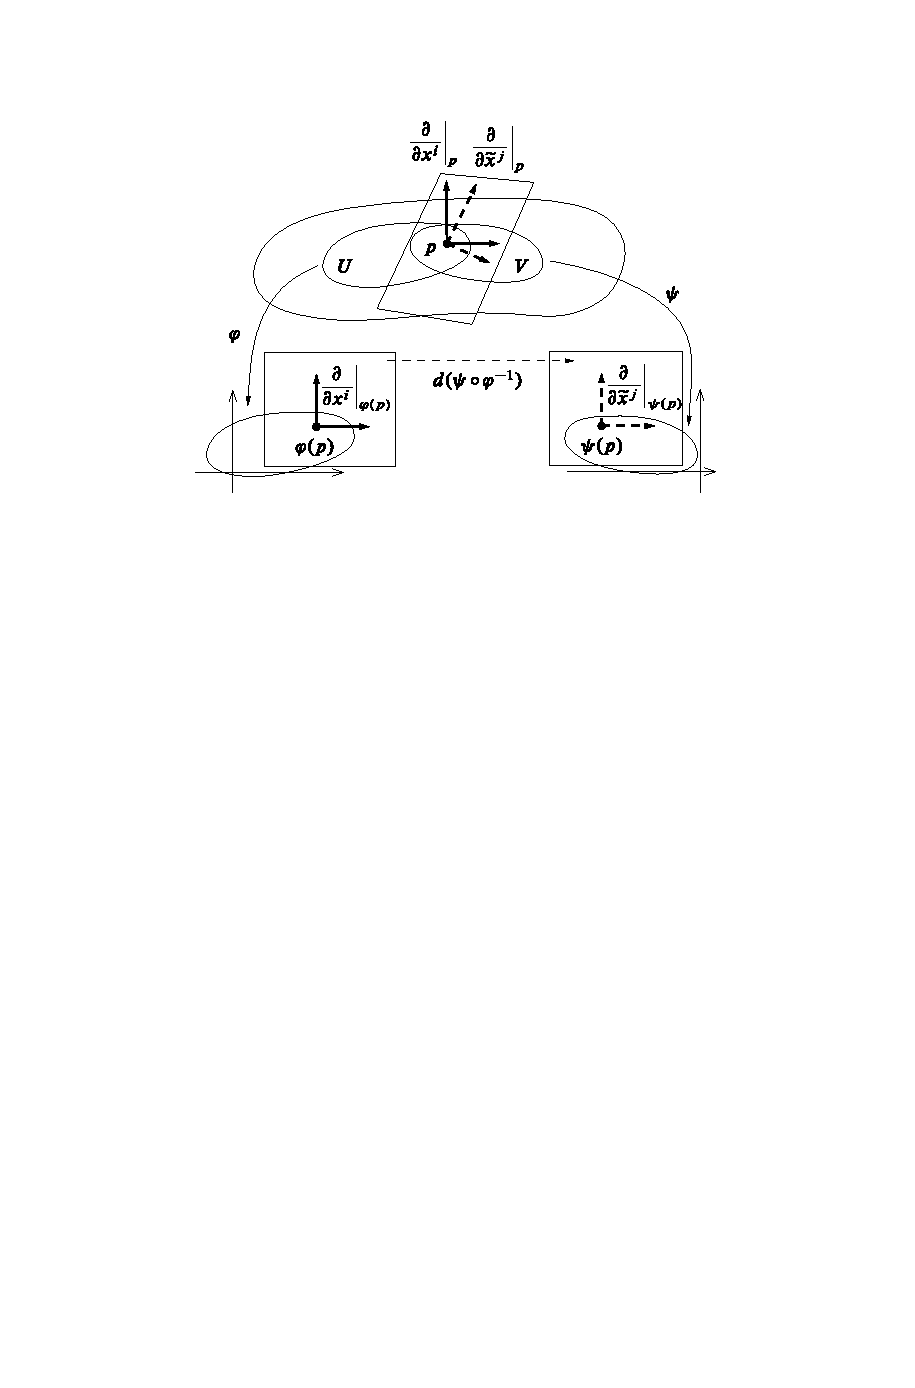
\includegraphics{pictures/coordinate-change}
    \caption{Change of coordinates.}
\end{figure}

In this situation, it is customary to write the transition map $\psi\circ\varphi^{-1}:\varphi(U\cap V)\to\psi(U\cap V)$ in the following shorthand notation:
\[\psi\circ\varphi^{-1}(x)=\big(\widetilde{x}^1(x),\dots,\widetilde{x}^n(x)\big)\]
The differential $d(\psi\circ\varphi^{-1})_{\varphi(p)}$ can be written
\[d(\psi\circ\varphi^{-1})_{\varphi(p)}\Big(\frac{\partial}{\partial x^i}\Big|_{\varphi(p)}\Big)=\frac{\partial\widetilde{x}^j}{\partial x^i}(\varphi(p))\frac{\partial}{\partial\widetilde{x}^j}\Big|_{\psi(p)}\]

Using the definition of coordinate vectors, we obtain
\begin{align*}
\frac{\partial}{\partial x^i}\Big|_p&=d(\varphi^{-1})\Big(\frac{\partial}{\partial x^i}\Big|_{\varphi(p)}\Big)=d(\psi^{-1})_{\psi(p)}\circ d(\psi\circ\varphi^{-1})_{\varphi(p)}\Big(\frac{\partial}{\partial x^i}\Big|_{\varphi(p)}\Big)\\
&=\frac{\partial\widetilde{x}^j}{\partial x^i}(\varphi(p))d(\psi^{-1})_{\psi(p)}\frac{\partial}{\partial\widetilde{x}^j}\Big|_{\psi(p)}\\
&=\frac{\partial\widetilde{x}^j}{\partial x^i}(\varphi(p))\frac{\partial}{\partial\widetilde{x}^j}\Big|_{p}.
\end{align*}
Applying this to the components of a vector $v=v^i\partial/\partial x^i|_p=\widetilde{v}^j\partial/\partial\widetilde{x}^j|_p$, we find that the components of $v$ transform by the rule
\begin{align}\label{coordinate change-1}
\widetilde{v}^j=v^i\frac{\partial\widetilde{x}^j}{\partial x^i}(\widehat{p})
\end{align}
\begin{example}
The transition map between polar coordinates and standard coordinates
in suitable open subsets of the plane is given by $(x,y)=(r\cos\theta,r\sin\theta)$. Let $p$ be the point in $\R^2$ whose polar coordinate representation is $(r,\theta)=(2,\pi/2)$, and let $v\in T_p\R^2$ be the tangent vector whose polar coordinate representation is 
\[v=3\frac{\partial}{\partial r}\Big|_p-\frac{\partial}{\partial\theta}\Big|_p\]
Applying the formula to the coordinate vectors, we find
\[\frac{\partial}{\partial r}\Big|_p=\cos\Big(\frac{\pi}{2}\Big)\frac{\partial}{\partial x}\Big|_p+\sin\Big(\frac{\pi}{2}\Big)\frac{\partial}{\partial y}\Big|_p=\frac{\partial}{\partial y}\Big|_p\]
\[\frac{\partial}{\partial\theta}\Big|_p=-2\sin\Big(\frac{\pi}{2}\Big)\frac{\partial}{\partial x}\Big|_p+2\cos\Big(\frac{\pi}{2}\Big)\frac{\partial}{\partial y}\Big|_p=-2\frac{\partial}{\partial x}\Big|_p\]
and thus $v$ has the following coordinate representation in standard coordinates:
\[v=3\frac{\partial}{\partial y}\Big|_p+2\frac{\partial}{\partial x}\Big|_p\]
\end{example}
\section{The tangent bundle}
Given a smooth manifold $M$ with or without boundary, we define the tangent bundle of $M$, denoted by $TM$, to be the disjoint union of the tangent spaces at all points of $M$:
\[TM=\coprod_{p\in M}T_pM\]
We usually write an element of this disjoint union as an ordered pair $(p,v)$, with $p\in M$ and $v\in T_pM$.
\begin{proposition}\label{tangent bundle struct}
For any smooth $n$-manifold $M$, the tangent bundle $TM$ has a natural topology and smooth structure that make it into a $2n$-dimensional smooth manifold. With respect to this structure, the projection $\pi:TM\to M$ is smooth.
\end{proposition}
\begin{proof}
We begin by defining the maps that will become our smooth charts. Given any smooth chart $(U,\varphi)$ for $M$, let $x^1,\dots,x^n$ denote the coordinate functions
of $\varphi$, and define a map $\tilde{\varphi}:\pi^{-1}(U)\to\R^{2n}$ by
\[\tilde{\varphi}\Big(v^i\frac{\partial}{\partial x^i}\Big|_p\Big)=(x^1(p),\dots,x^n(p),v^1,\dots,v^n)\]
Its image set is $\varphi(U)\times\R^n$, which is an open subset of $\R^{2n}$. It is a bijection onto its image, because its inverse can be written explicitly as
\[\tilde{\varphi}^{-1}(x^1,\dots,x^n,v^1,\dots,v^n)=v^i\frac{\partial}{\partial x^i}\Big|_{\varphi^{-1}(x)}\]
Now suppose we are given two smooth charts $(U,\varphi)$ and $(V,\psi)$ for $M$, and let $(\pi^{-1}(U),\tilde{\varphi})$ and $(\pi^{-1}(V),\tilde{\psi})$ be the corresponding charts on $TM$. The sets
\[\tilde{\varphi}\big(\pi^{-1}(U)\cap\pi^{-1}(V)\big)=\varphi(U\cap V)\times\R^n\And\tilde{\psi}\big(\pi^{-1}(U)\cap\pi^{-1}(V)\big)=\psi(U\cap V)\times\R^n\]
are open in $\R^{2n}$, and the transition map $\tilde{\psi}\circ\tilde{\varphi}^{-1}:\varphi(U\cap V)\times\R^n\to\psi(U\cap V)\times\R^n$ can be written explicitly as
\begin{align*}
\tilde{\psi}\circ\tilde{\varphi}^{-1}(x^1,\dots,x^n,v^1,\dots,v^n)&=\tilde{\psi}\Big(v^i\frac{\partial}{\partial x^i}\Big|_{\varphi^{-1}(x)}\Big)\\
&=\tilde{\psi}\Big(v^i\frac{\partial\widetilde{x}^j}{\partial x^i}\frac{\partial}{\partial \widetilde{x}^j}\Big|_{\varphi^{-1}(x)}\Big)\\
&=\big(\widetilde{x}^1(x),\dots,\widetilde{x}^n(x),v^i\frac{\partial\widetilde{x}^1}{\partial x^i}(x),\dots,v^i\frac{\partial\widetilde{x}^n}{\partial x^i}(x)\big)
\end{align*}
This is clearly smooth.\par
Choosing a countable cover $\{U_i\}$ of $M$ by smooth coordinate domains, we obtain a countable cover of $TM$ by coordinate domains $\{\pi^{-1}(U_i)\}$ satisfying conditions (\rmnum{1})--(\rmnum{4}) of the smooth manifold chart lemma. To check the Hausdorff condition (\rmnum{5}), just note that any two points in the same fiber of $\pi$ lie in one chart, while if $(p,v)$ and $(q,w)$ lie in different fibers, there exist disjoint smooth coordinate domains $U,V$ for $M$ such that $p\in U$ and $q\in V$, and then $\pi^{-1}(U)$ and $\pi^{-1}(V)$ are disjoint coordinate neighborhoods containing $(p,v)$ and $(q,w)$, respectively.\par
To see that $\pi$ is smooth, note that with respect to charts $(U,\varphi)$ for $M$ and $(\pi^{-1}(U),\tilde{\varphi})$ for $TM$, its coordinate representation is $\pi(x,v)=x$.
\end{proof}
The coordinates given by this proposition are called \textbf{natural coordinates} on $TM$.
\begin{proposition}
If $M$ is a smooth $n$-manifold with or without boundary, and $M$ can be covered by a single smooth chart, then $TM$ is diffeomorphic to $M\times\R^n$.
\end{proposition}
\begin{proof}
If $(U,\varphi)$ is a global smooth chart for $M$, then $\varphi$ is, in particular, a diffeomorphism from $U=M$ to an open subset $\widehat{U}\sub\R^n$ or $\H^n$. The proof of the previous proposition showed that the natural coordinate chart $\tilde{\varphi}$ is a bijection from $TM$ to $\widetilde{U}\times\R^n$, and the smooth structure on $TM$ is defined essentially by declaring $\tilde{\varphi}$ to be a diffeomorphism.
\end{proof}
\begin{remark}
In general, the tangent bundle is not globally diffeomorphic $($or even homeomorphic$)$ to a product of the manifold with $\R^n$.
\end{remark}
By putting together the differentials of $F$ at all points of $M$ we obtain a globally defined map between tangent bundles, called the \textbf{global differential} or global tangent map and denoted by $dF:TM\to TN$. This is just the map whose restriction to each tangent space $T_pM\sub TM$ is $dF_p$.\par
One important feature of the smooth structure we have defined on $TM$ is that it
makes the differential of a smooth map into a smooth map between tangent bundles.
\begin{proposition}
If $F:M\to N$ is a smooth map, then its global differential $dF:TM\to TN$ is a smooth map.
\end{proposition}
\begin{proof}
From the local expression for $dF_p$ in coordinates, it follows that $dF$ has the following coordinate representation in terms of natural coordinates for $TM$ and $TN$:
\begin{align*}
dF(x^1,\dots,x^n,v^1,\dots,v^n)=(F^1(x),\dots,F^n(x),v^i\frac{\partial F^1}{\partial x^i},\dots,v^i\frac{\partial F^n}{\partial x^i})
\end{align*}
This is smooth because $F$ is.
\end{proof}
\begin{proposition}
Suppose $F:M\to N$ and $G:N\to P$ are smooth maps.
\begin{itemize}
\item[(a)]$d(G\circ F)=dG\circ dF$.
\item[(b)]$d\id_M=\id_{TM}$.
\item[(c)]If $F$ is a diffeomorphism, then $dF:TM\to TN$ is also a diffeomorphism, and $d(F^{-1})=(dF)^{-1}$.
\end{itemize}
Because of part (c), when $F$ is a diffeomorphism we can use the notation $dF^{-1}$ unambiguously to mean either $d(F^{-1})$ or $(dF)^{-1}$.
\end{proposition}
\section{Velocity vectors of curves}
If $M$ is a manifold with or without boundary, we define a \textbf{curve} in $M$ to be a continuous map $\gamma:J\to M$, where $J\sub\R$ is an interval. Given a smooth
curve $\gamma:J\to M$ and $t_0\in J$ we define the \textbf{velocity} of $\gamma$ at $t_0$, denoted by $\gamma'(t_0)$, to be the vector
\[\gamma'(t_0)=d\gamma\Big(\frac{d}{dt}\Big|_{t_0}\Big)\in T_{\gamma(t_0)}M\]
where $d/dt|_{t_0}$ is the standard coordinate basis vector in $T_{t_0}\R$. This tangent vector acts on functions by
\[\gamma'(t_0)f=d\gamma\Big(\frac{d}{dt}\Big|_{t_0}\Big)f=\frac{d}{dt}\Big|_{t_0}(f\circ\gamma)=(f\circ\gamma)'(t_0)\]
In other words, $\gamma'(t_0)$ is the derivation at $\gamma(t_0)$ obtained by taking the derivative of a function along $\gamma$.\par
Now let $(U,\varphi)$ be a smooth chart with coordinate functions $(x^i)$. If $\gamma(t_0)\in U$, we can write the coordinate representation of $\gamma$ as $(\gamma^1(t),\dots,\gamma^n(t))$, at least for $t$ sufficiently close to $t_0$, and then the coordinate formula for the differential yields
\[\gamma'(t_0)=\frac{d\gamma^i}{dt}(t_0)\frac{\partial}{\partial x^i}\Big|_{\gamma(t_0)}\]
The next proposition shows that every tangent vector on a manifold is the velocity
vector of some curve. This gives a different and somewhat more geometric way to think about the tangent bundle: it is just the set of all velocity vectors of smooth
curves in $M$.
\begin{proposition}
Suppose $M$ is a smooth manifold with or without boundary and $p\in M$. Every $v\in T_pM$ is the velocity of some smooth curve in $M$.
\end{proposition}
\begin{proof}
First suppose that $p\in\Int M$ (which includes the case $\partial M=\emp$). Let $(U,\varphi)$ be a smooth coordinate chart centered at $p$, and write $v=v^i\partial/\partial x^i|_p$ in terms of the coordinate basis. For sufficiently small $\eps>0$, let $\gamma:(-\eps,\eps)\to U$ be the curve whose coordinate representation is
\[\gamma(t)=(tv^1,\dots,tv^n)\]
This is a smooth curve with $\gamma(0)=p$, and the computation above shows that $\gamma'(0)=v^i\partial/\partial x^i|_{\gamma(0)}=v$.\par
Now suppose $p\in\partial M$. Let $(U,\varphi)$ be a smooth boundary chart centered at $p$, and write $v=v^i\partial/\partial x^i|_p$. We wish to let $\gamma$ as before, but this formula represents a point of $M$ only when $tv^n\geq 0$. We can accommodate this requirement by suitably restricting the domain of $\gamma$: if $v_n=0$, we define $\gamma:(-\eps,\eps)\to U$ as before; if $v_n>0$, we let the domain be $[0,\eps)$ and if $v_n<0$, we let it be $(-\eps,0]$. In each case, $\gamma$ is a smooth curve in $M$ with $\gamma(0)=v$ and $\gamma'(0)=v$.
\end{proof}
\begin{proposition}[\textbf{The Velocity of a Composite Curve}]\label{diff composite curve}
Let $F:M\to N$ be a smooth map, and let $\gamma:J\to M$ be a smooth curve. For any $t_0\in J$, the velocity at $t=t_0$ of the composite curve $F\circ\gamma:J\to N$ is given by
\[(F\circ\gamma)'(t_0)=dF(\gamma'(t_0))\]
\end{proposition}
\begin{proof}
\[(F\circ\gamma)'(t_0)=d(F\circ\gamma)\Big(\frac{d}{dt}\Big|_{t_0}\Big)=dF\circ d\gamma\Big(\frac{d}{dt}\Big|_{t_0}\Big)=dF(\gamma'(t_0))\]
\end{proof}
\begin{corollary}[\textbf{Computing the Differential Using a Velocity Vector}]\label{compute diff by curve}
Suppose $F:M\to N$ is a smooth map, $p\in M$, and $v\in T_pM$. Then
\[dF_p(v)=(F\circ\gamma)'(0)\]
for any smooth curve $\gamma:J\to M$ such that $0\in J$, $\gamma(0)=p$ and $\gamma'(0)=v$.
\end{corollary}
\section{Tangent vectors as derivations of the space of germs}
A \textbf{smooth function element} on $M$ is an ordered pair $(f,U)$, where $U$ is an open subset of $M$ and $f:U\to\R$ is a smooth function. Given a point $p\in M$, we define an equivalence relation on the set of all smooth function elements whose domains contain $p$ by setting $(f,U)\sim (g,V)$ if $f=g$ on some neighborhood of $p$. The equivalence class of a function element $(f,U)$ is called the \textbf{germ} of $f$ at $p$, which we denote by $[f]_p$. The set of all germs of smooth functions at $p$ is denoted by $C^\infty_p(M)$. It is a vector space.\par
A derivation of $C^\infty_p(M)$ is a linear map $v:C^\infty_p(M)\to\R$ satisfying the following product rule
\[v[fg]_p=fv[g]_p+gv[f]_p.\]
It is common to define the tangent space to $M$ at $p$ as the vector space $\mathcal{D}_pM$ of derivations of $C^\infty_p(M)$. By proposition~\ref{tangent space local} $\mathcal{D}_pM$ is naturally isomorphic to the tangent space as we have defined.
\section{Exercise}
\begin{exercise}
Suppose $M$ and $N$ are smooth manifolds with or without boundary, and $F:M\to N$ is a smooth map. Show that $dF_p:T_pM\to T_{F(p)}N$ is the zero map for each $p\in M$ if and only if $F$ is constant on each component of $M$.
\end{exercise}
\begin{proof}
If $F$ is contant on each component of $M$, then $dF_p$ is zero by a coordinate computation. Assume the converse, let
\[\mathscr{C}=\{p\in M:\text{there is a neighborhood $U$ of $p$ such that $F$ is constant on $U$}\}\]
Then by continuity $\mathscr{C}$ is closed, and by pull back to Euclidean space, $\mathscr{C}$ is open. Hence $\mathscr{C}$ is a component.
\end{proof}
\begin{exercise}
Prove that if $M$ and $N$ are smooth manifolds, then $T(M\times N)$ is diffeomorphic
to $TM\times TN$.
\end{exercise}
\begin{exercise}
Let $S^1\sub\R^2$ be the unit circle, and let $K\sub\R^2$ be the boundary of the square of side $2$ centered at the origin: $K=\{(x,y):\max\{|x|,|y|\}\leq 1\}$. Show that there is a homeomorphism $F:\R^2\to\R^2$ such that $F(S^1)=K$, but there is
no diffeomorphism with the same property.
\end{exercise}
\begin{proof}
The projection from $S^1$ to $K$ is a homeomorphism. Suppose there is a diffeomorphism with the same property. let $\gamma:(-1,1)\to S^1$ be a smooth curve whose image lies in $S^1$ and such that $\gamma'(t)\neq 0$. Then since $F$ is a diffeomorphism, $dF(\gamma'(t))\neq 0$ for all $t$.
\[dF(\gamma'(t))(x)=\gamma'(t)(x\circ F)=\gamma'(t)F_1=(F_1\circ\gamma)'(t)\]
\[dF(\gamma'(t))(y)=\gamma'(t)(x\circ F)=\gamma'(t)F_1=(F_2\circ\gamma)'(t)\]
We choose $\gamma$ such that $F\circ\gamma(0)=(1,1)$, then $0$ is a critical point of $F\circ\gamma$, hence $(F_2\circ\gamma)'(0)=(F_2\circ\gamma)'(0)=0$. This is a contradiction since $dF(\gamma'(0))\neq 0$.
\end{proof}
\chapter{Submersions, immersions, and embeddings}
\section{Maps of constant rank}
Suppose $M$ and $N$ are smooth manifolds with or without boundary. Given a smooth map $F:M\to N$ and a point $p\in M$, we define the \textbf{rank of $\bm{F}$ at $\bm{p}$} to be the rank of the linear map $dF_p:T_pM\to T_{F(p)}N$, it is the rank of the Jacobian matrix of $F$ in any smooth chart, or the dimension of $\im dF_p\sub T_{F(p)}N$. If $F$ has the same rank $r$ at every point, we say that it has constant rank, and write $\rank(F)=r$.\par
Because the rank of a linear map is never higher than the dimension of either its domain or its codomain, the rank of $F$ at each point is bounded above by the minimum of $\{\dim(M), \dim(N)\}$. If the rank of $dF_p$ is equal to this upper bound, we say that \textbf{$\bm{F}$ has full rank at $\bm{p}$}, and if $F$ has full rank everywhere, we say \textbf{$\bm{F}$ has full rank}.\par
The most important constant-rank maps are those of full rank. A smooth map $F:M\to N$ is called a smooth \textbf{submersion} if its differential is surjective at each point (or equivalently, if $\rank(F)=\dim(N)$ everywhere). It is called a smooth \textbf{immersion} if its differential is injective at each point (equivalently, $\rank(F)=\dim(M)$ everywhere).\par
\begin{proposition}\label{local immersion subm}
Suppose $F:M\to N$ is a smooth map and $p\in M$.
\begin{itemize}
\item[(a)] If $dF_p$ is surjective, then $p$ has a neighborhood $U$ such that $F|_U$ is a submersion.
\item[(b)] If $dF_p$ is injective, then $p$ has a neighborhood $U$ such that $F|_U$ is an immersion.
\end{itemize}
\end{proposition}
\begin{proof}
If we choose any smooth coordinates for $M$ near $p$ and for $N$ near $F(p)$, either hypothesis means that Jacobian matrix of $F$ in coordinates has full rank at $p$. Example~\ref{full rank mani} shows that the set of $m\times n$ matrices of full rank is an open subset of $\mathcal{M}_{mn}(\R)$ (where $m=\dim(M)$ and $n=\dim(N)$), so by continuity, the Jacobian of $F$ has full rank in some neighborhood of $p$.
\end{proof}
\subsection{Local diffeomorphisms}
If $M$ and $N$ are smooth manifolds with or without boundary, a map $F:M\to N$ is called a \textbf{local diffeomorphism} if every point $p\in M$ has a neighborhood $U$ such that $F(U)$ is open in $N$ and $F:U\to F(U)$ is a diffeomorphism. The next theorem is the key to the most important properties of local diffeomorphisms.
\begin{theorem}[\textbf{Inverse Function Theorem for Manifolds}]
Suppose $M$ and $N$ are smooth manifolds, and $F:M\to N$ is a smooth map. If $p\in M$ is a point such that $dF_p$ is invertible, then there are connected neighborhoods $U_0$ of $p$ and $V_0$ of $F(p)$ such that $F|_{U_0}:U_0\to V_0$ is a diffeomorphism.
\end{theorem}
\begin{proof}
The fact that $dF_p$ is bijective implies that $M$ and $N$ have the same dimension, say $n$. Choose smooth charts $(U,\varphi)$ centered at $p$ and $(V,\psi)$ centered at $F(p)$, with $F(U)\sub V$. Then $\widehat{F}=\psi\circ F\circ\varphi^{-1}$ is a smooth map from the open subset $\widehat{U}\sub\R^n$ into $\widehat{V}\sub\R^n$, with $\widehat{F}(0)=0$. Because $\varphi$ and $\psi$ are diffeomorphisms, the differential $d\widehat{F}_0=d\psi_{F(p)}\circ dF_p\circ d\varphi^{-1}_0$ is nonsingular. The ordinary inverse function theorem shows that there are connected open subsets $\widehat{U}_0$ and $\widehat{V}_0$ containing $0$ such that $\widehat{F}$ restricts to a diffeomorphism from $\widehat{U}_0$ to $\widehat{V}_0$. Then $U_0=\varphi^{-1}(\widehat{U}_0)$ and $V_0=\psi^{-1}(\widehat{V}_0)$ are connected neighborhoods of $p$ and $F(p)$, respectively, and it follows by composition that $F|_{U_0}$ is a diffeomorphism from $U_0$ to $V_0$.
\end{proof}
\begin{proposition}[\textbf{Elementary Properties of Local Diffeomorphisms}]\label{local diff prop}
\mbox{}
\begin{itemize}
\item[(a)] Every composition of local diffeomorphisms is a local diffeomorphism.
\item[(b)] Every finite product of local diffeomorphisms between smooth manifolds is a local diffeomorphism.
\item[(c)] Every local diffeomorphism is a local homeomorphism and an open map.
\item[(d)] The restriction of a local diffeomorphism to an open submanifold with or without boundary is a local diffeomorphism.
\item[(e)] Every diffeomorphism is a local diffeomorphism.
\item[(f)] Every bijective local diffeomorphism is a diffeomorphism.
\item[(g)] A map between smooth manifolds with or without boundary is a local diffeomorphism if and only if in a neighborhood of each point of its domain, it has a
coordinate representation that is a local diffeomorphism.
\end{itemize}
\end{proposition}
\begin{proof}
We only prove (f). Let $F:M\to N$ be a bijective local diffeomorphism, and $F^{-1}$ be its inverse. For each $p\in M$, there are neighborhood $U_p$ of $p$ and $V_p$ of $F(p)$ such that $F|_{U_p}:U_p\to V_p$ is a diffeomorphism. Then from the uniqueness of an inverse function we get $(F|_{U_p})^{-1}=F^{-1}|_{V_p}$. Now since $F$ is surjective, every point in $N$ has a neighborhood on which $F^{-1}$ is a smooth function, hence $F^{-1}$ is smooth and $F$ is a diffeomorphism.
\end{proof}
\begin{proposition}\label{local diff iff}
Suppose $M$ and $N$ are smooth manifolds $($without boundary$)$, and $F:M\to N$ is a map.
\begin{itemize}
\item[(a)] $F$ is a local diffeomorphism if and only if it is both a smooth immersion and a smooth submersion.
\item[(b)] If $\dim(M)=\dim(N)$ and $F$ is either a smooth immersion or a smooth submersion, then it is a local diffeomorphism.
\end{itemize}
\end{proposition}
\begin{proof}
Suppose first that $F$ is a local diffeomorphism. Given $p\in M$, there is a neighborhood $U$ of $p$ such that $F$ is a diffeomorphism from $U$ to $F(U)$. It then follows from Proposition~\ref{differential mani prop} that $dF_p:T_pM\to T_{F(p)}N$ is an isomorphism. Thus $\rank(F)=\dim(M)=\dim(N)$, so $F$ is both a smooth immersion and a smooth submersion. Conversely, if $F$ is both a smooth immersion and a smooth submersion, then $dF_p$ is an isomorphism at each $p\in M$, and the inverse function theorem for manifolds shows that $p$ has a neighborhood on which $F$ restricts to a diffeomorphism onto its image. This proves (a).\par
To prove (b), note that if $M$ and $N$ have the same dimension, then either injectivity or surjectivity of $dF_p$ implies bijectivity, so $F$ is a smooth submersion if and only if it is a smooth immersion, and thus (b) follows from (a).
\end{proof}
\begin{proposition}\label{smooth iff composition smooth}
Suppose $M,N,P$ are smoothmanifolds with or without boundary, and $F:M\to N$ is a local diffeomorphism.
\begin{itemize}
\item[(a)]If $G:P\to M$ is continuous, then $G$ is smooth if and only if $F\circ G$ is smooth.
\item[(b)]If in addition $F$ is surjective and $G:N\to P$ is any map, then $G$ is smooth if and only if $G\circ F$ is smooth.
\end{itemize}
\begin{proof}
For part (a), we assume that $F\circ G$ is smooth. For any point $p\in P$, we can choose neighborhood $U$ for $G(p)$ such that $F|_U:U\to F(U)$ is a diffeomorphism. Then $\widetilde{U}:=G^{-1}(U)$ is a neighborhood of $p$ since $G$ is continuous, and we have
\[G|_{\widetilde{U}}=(F|_{U})^{-1}\circ (G\circ F)|_{\widetilde{U}}\]
Thus as a compoistion of smooth maps, $G|_{\widetilde{U}}$ is smooth. It follows that $G$ itself is smooth.\par
For part (b), assume that $G\circ F$ is smooth. For each point $p\in N$, choose $x\in F^{-1}(p)$. Then we can find neighborhood $U$ containting $x$ and $V$ containting $p$ such that $F$ is a diffeomorphism from $U$ to $V$. Then
\[G|_V=(G\circ F)_U\circ(F|U)^{-1}\]
Thus $G|_V$ is smooth, and hence $G$ is smooth.
\end{proof}
\end{proposition}
\subsection{The rank theorem}
\begin{theorem}[\textbf{Rank Theorem}]
Suppose $M$ and $N$ are smooth manifolds of dimensions $m$ and $n$, respectively, and $F:M\to N$ is a smooth map with constant rank $r$. For each $p\in M$ there exist smooth charts $(U,\varphi)$ for $M$ centered at $p$ and $(V,\psi)$ for $N$ centered at $F(p)$ such that $F(U)\sub V$, in which $F$ has a coordinate representation of the form
\begin{align}\label{Rank thm mani-1}
\widehat{F}(x^1,\dots,x^r,x^{r+1},\dots,x^m)=(x^1,\dots,x^r,0,\dots,0)
\end{align}
In particular, if $F$ is a smooth submersion, this becomes
\[\widehat{F}(x^1,\dots,x^n,x^{n+1},\dots,x^m)=(x^1,\dots,x^n)\]
and if $F$ is a smooth immersion, it is
\[\widehat{F}(x^1,\dots,x^m)=(x^1,\dots,x^m,0,\dots,0)\]
\end{theorem}
\begin{proof}
Since the question is local, we can assume that $M$ and $N$ are open subsets of Euclidean spaces. The theorem then follows from Theorem~\ref{rank theorem}.
\end{proof}
The next corollary can be viewed as a more invariant statement of the rank theorem. It says that constant-rank maps are precisely the ones whose local behavior is the same as that of their differentials.
\begin{corollary}
Let $M$ and $N$ be smooth manifolds, let $F:M\to N$ be a smooth map, and suppose $M$ is connected. Then the following are equivalent:
\begin{itemize}
\item[(a)]For each $p\in M$ there exist smooth charts containing $p$ and $F(p)$ in which the coordinate representation of $F$ is linear.
\item[(b)]$F$ has constant rank.
\end{itemize}
\end{corollary}
\begin{proof}
First suppose $F$ has a linear coordinate representation in a neighborhood of each point. Since every linear map has constant rank, it follows that the rank of $F$ is
constant in a neighborhood of each point, and thus by connectedness it is constant
on all of $M$. Conversely, if $F$ has constant rank, the rank theorem shows that it has the linear coordinate representation in a neighborhood of each point.
\end{proof}
The rank theorem is a purely local statement. However, it has the following powerful
global consequence.
\begin{theorem}[\textbf{Global Rank Theorem}]\label{global rank thm}
Let $M$ and $N$ be smooth manifolds, and suppose $F:M\to N$ is a smooth map of constant rank.
\begin{itemize}
\item[(a)]If $F$ is surjective, then it is a smooth submersion.
\item[(b)]If $F$ is injective, then it is a smooth immersion.
\item[(c)]If $F$ is bijective, then it is a diffeomorphism.
\end{itemize}
\end{theorem}
\begin{proof}
Let $m=\dim(M)$, $n=\dim(N)$, and suppose $F$ has constant rank $r$. To prove (a), assume that $F$ is not a smooth submersion, which means that $r<n$. By the rank theorem, for each $p\in M$ there are smooth charts $(U,\varphi)$ for $M$ centered
at $p$ and $(V,\psi)$ for $N$ centered at $F(p)$ such that $F(U)\sub V$ and the coordinate representation of $F$ is given by $(\ref{Rank thm mani-1})$. Shrinking $U$ if necessary, we may assume that it is a regular coordinate ball and $F(\widebar{U})\sub V$. This implies that $F(\widebar{U})$ is a compact subset of the set $\{y\in V:y^{r+1}=\cdots=y^n=0\}$, so it is closed in $N$ and contains no open subset of $N$; hence is nowhere dense in $N$. Since every open cover of a manifold has a countable subcover, we can choose countably many such charts $\{U_i\}$ covering $M$, with corresponding charts $\{V_i\}$ covering $F(M)$. Because $F(M)$ is equal to the countable union of the nowhere dense sets $F(\widebar{U}_i)$, it follows from the Baire category theorem that $F(M)$ has empty interior in $N$, which means $F$ cannot be surjective.\par
To prove (b), assume that $F$ is not a smooth immersion, so that $r<m$. By the rank theorem, for each $p\in M$ we can choose charts on neighborhoods of $p$ and $F(p)$ in which $F$ has the coordinate representation of $(\ref{Rank thm mani-1})$. It follows that 
\[F(0,\dots,0,\eps)=(0,\dots,0)=F(0,\dots,0)\]
for any sufficiently small $\eps$, so $F$ is not injective.\par
Finally, (c) follows from (a) and (b), because a bijective smooth map of constant rank is a smooth submersion by part (a) and a smooth immersion by part (b); so Proposition~\ref{local diff iff} implies that $F$ is a local diffeomorphism, and because it is bijective, it is a diffeomorphism.
\end{proof}
\subsection{The rank theorem for manifolds with boundary}
In the context of manifolds with boundary, we need the rank theorem only in one special case: that of a smooth immersion whose domain is a smooth manifold with boundary. Of course, since the interior of a smooth manifold with boundary is a smooth manifold, near any interior point of the domain the ordinary rank theorem applies. For boundary points, we have the following substitute for the rank theorem.
\begin{theorem}[\textbf{Immersion Theorem for Manifolds with Boundary}]\label{rank thm manifold boundary}
Let $M$ be a smooth $m$-manifold with boundary, $N$ be a smooth $n$-manifold, and $F:M\to N$ be a smooth immersion. For any $p\in\partial M$, there exist a smooth boundary chart $(U,\varphi)$ for $M$ centered at $p$ and a smooth coordinate chart $(V,\psi)$ for $N$ centered at $F(p)$ with $F(U)\sub V$, in which $F$ has the coordinate representation
\begin{align}\label{rank thm boundary-1}
\widehat{F}(x^1,\dots,x^m)=(x^1,\dots,x^m,0,\dots,0)
\end{align}
\end{theorem}
\begin{proof}
By choosing initial smooth charts for $M$ and $N$, we may assume that $M$ and $N$ are open subsets of $\H^m$ and $\R^n$, respectively, and also that $p=0\in\H^m$, and $F(p)=0\in\R^n$. By definition of smoothness for functions on $\H^m$, $F$ extends to a smooth map $\widetilde{F}:W\to\R^n$, where $W$ is some open subset of $\R^m$ containing $0$. Because $d\widetilde{F}_0=dF$ is injective, by Proposition~\ref{local immersion subm} we may assume that $\widetilde{F}$ is a smooth immersion. Let us write the coordinates on $\R^m$ as $x=(x^1,\dots,x^m)$, and those on $\R^n$ as $(v,w)=(v^1,\dots,v^m,w^1,\dots,w^{n-m})$.\par
By the rank theorem, there exist smooth charts $(U_0,\varphi_0)$ for $\R^m$ centered at $0$ and $(V_0,\psi_0)$ for $\R^n$ centered at $0$ such that $\widehat{F}=\psi_0\circ\widetilde{F}\circ\varphi^{-1}_0$ is given by $(\ref{rank thm boundary-1})$. The only problem with these coordinates is that $\varphi$ might not restrict to a boundary chart for $M$. But we can correct this easily as follows. Because $\varphi_0$ is a diffeomorphism from $U_0$ to an open subset $\widehat{U}_0=\varphi_0(U_0)\sub\R^m$, the map $\varphi_0^{-1}\times\mathrm{id}_{\R^{n-m}}$ is a diffeomorphism from $\widehat{U}_0\times\R^{n-m}$ to $U_0\times\R^{n-m}$. Let $\psi=(\varphi_0^{-1}\times\mathrm{id}_{\R^{n-m}})\circ\psi_0$, which is a diffeomorphism from some open subset $V\sub V_0$ containing $0$ to a neighborhood
of $0$ in $\R^n$. Using $(\ref{rank thm boundary-1})$, we compute
\begin{align*}
\psi\circ F(x)&=(\varphi_0^{-1}\times\mathrm{id}_{\R^{n-m}})\circ\psi_0\circ F\circ\varphi_0^{-1}\circ\varphi_0(x)=(\varphi_0^{-1}\times\mathrm{id}_{\R^{n-m}})\circ\widehat{F}(\varphi_0(x))\\
&=(\varphi_0^{-1}\times\mathrm{id}_{\R^{n-m}})(\varphi_0(x),0)=(x,0)
\end{align*}
Thus, the original coordinates for $M$ (restricted to a sufficiently small neighborhood of $0$) and the chart $(V,\psi)$ for $N$ satisfy the desired conditions.
\end{proof}
It is possible to prove a similar theorem for more general maps with constant rank out of manifolds with boundary, but the proof is more elaborate because an extension of $F$ to an open subset does not automatically have constant rank (Recall Example~\ref{rank function}).
\begin{corollary}\label{rank thm boundary}
Suppose $M$ is a smooth $m$-manifold with boundary, $N$ is a smooth $n$-manifold, and
$F:M\to N$ has constant rank $r$. If for any $p\in\partial M$ we have$\ker dF_p\nsubseteq T_p\partial M$, then for each $p$ there exist a smooth boundary chart $(U,\varphi)$ for $M$ centered at $p$ and a smooth coordinate chart $(V,\psi)$ for $N$ centered at $F(p)$ with $F(U)\sub V$, in which $F$ has the coordinate representation
\begin{align}\label{rank thm boundary-2}
\widehat{F}(x^1,\dots,x^r,x^{r+1},\dots,x^m)=(x^1,\dots,x^r,0,\dots,0)
\end{align}
\end{corollary}
\begin{proof}
Choosing coooredinates as in the previous theorem, we can assume $M\sub\H^m$ and $N\sub\R^n$, also $p=0\in\H^m$ and $F(p)=0\in\R^n$. Now extend $F$ to a smooth function $\widetilde{F}:W\to\R^n$, where $W$ is an open subset of $\R^m$ containing $0$. there is a coordinate projection $\pi:\R^n\to\R^r$ such that $\pi\circ\widetilde{F}$ is a submersion. Now from the proof of Theorem~\ref{rank theorem}, we can see there is $\varphi:U_0\to\R^m$ such that
\[\pi\circ\widetilde{F}\circ\varphi^{-1}(x,y)=x\]
Thus we write $\widetilde{F}\circ\varphi^{-1}=(x,R(x,y))$. Then $R|_M$ is independent of $y$, so $\psi(v,w)=(v,w-R(v))$ gives the result.
\end{proof}
\section{Embeddings}
One special kind of immersion is particularly important. If $M$ and $N$ are smooth
manifolds with or without boundary, a \textbf{smooth embedding} of $M$ into $N$ is a smooth immersion $F:M\to N$ that is also a topological embedding. \textit{A smooth embedding is a map that is both a topological embedding and a smooth immersion, not just a topological embedding that happens to be smooth.}
\begin{example}[\textbf{A Smooth Topological Embedding}]
The map $\gamma:\R\to\R^2$ given by $\gamma(t)=(t^3,0)$ is a smooth map and a topological embedding, but it is not a smooth embedding because $\gamma'(0)=0$.
\end{example}
\begin{example}[\textbf{The Figure-Eight Curve}]\label{figure eight}
Consider the curve $\beta:(-\pi,\pi)\to\R^2$ defined by
\[\beta(t)=(\sin 2t,\sin t)\]
Its image is a set that looks like a figure-eight in the plane,sometimes
called a \textbf{lemniscate}. It is easy to see that $\beta$ is an injective smooth immersion because $\beta'(t)$ never vanishes; but it is not a topological embedding, because its image is compact in the subspace topology, while its domain is not.
\end{example}
\begin{example}[\textbf{A Dense Curve on the Torus}]\label{dense curve torus}
Let $T^2=S^1\times S^1\sub\C^2$ denote the torus, and let $\alpha$ be any irrational number. The map $\gamma:\R\to T^2$ given by
\[\gamma(t)=(e^{2\pi it},e^{2\pi i\alpha t})\]
is a smooth immersion because $\gamma'(t)$ never vanishes. It is also injective, because $\gamma(t_1)=\gamma(t_2)$ implies that both $t_1-t_2$ and $\alpha(t_1-t_2)$ are integers, which is impossible unless $t_1=t_2$.\par
We claim that $\gamma(\R)$ is dense in $T^2$. In fact, each point in $T^2$ is of the form $(e^{2\pi it_1},e^{2\pi it_2})$, and we observe that for all $n,m\in\N$,
\[\gamma(t_1+m)=(e^{2\pi it_1},e^{2\pi i\alpha(t_1+m)})=(e^{2\pi it_1},e^{2\pi i[\alpha(t_1+m)+n]}),\]
so we only need to show $\{\alpha m+n\}$ is dense in $\R$. This is a result called Kronecker's approximation theorem.
\end{example}
The following proposition gives a few simple sufficient criteria for an injective immersion to be an embedding.
\begin{proposition}\label{smooth embedd if}
Suppose $M$ and $N$ are smooth manifolds with or without boundary, and $F:M\to N$ is an injective smooth immersion. If any of the following holds, then $F$ is a smooth embedding.
\begin{itemize}
\item[(a)] $F$ is an open or closed map.
\item[(b)] $F$ is a proper map.
\item[(c)] $M$ is compact.
\item[(d)] $M$ has empty boundary and $\dim(M)=\dim(N)$.
\end{itemize}
\end{proposition}
\begin{proof}
If $F$ is open or closed, then it is a topological embedding, so it is a smooth embedding. Either (b) or (c) implies that $F$ is closed. Finally, assume that $M$ has empty boundary and $\dim(M)=\dim(N)$ Then $dF_p$ is nonsingular everywhere, and by Exercise~\ref{smooth map not boundary} $F(M)\sub\Int N$. Proposition~\ref{local diff iff} shows that $F:M\to\Int N$ is a local diffeomorphism, so it is an open map. It follows that $F:M\to N$ is a composition of open maps $M\to\Int N\sub N$, so it is an embedding.
\end{proof}
\begin{theorem}[\textbf{Local Embedding Theorem}]\label{immersion local embedding}
Suppose $M$ and $N$ are smooth manifolds with or without boundary, and $F:M\to N$ is a smooth map. Then $F$ is a smooth immersion if and only if every point in $M$ has a neighborhood $U\sub M$ such that $F|_U:U\to N$ is a smooth embedding.
\end{theorem}
\begin{proof}
One direction is immediate: if every point has a neighborhood on which $F$ is a smooth embedding, then $F$ has full rank everywhere, so it is a smooth immersion.\par
Conversely, suppose $F$ is a smooth immersion, and let $p\in M$. We show first that $p$ has a neighborhood on which $F$ is injective. If $F(p)\notin\partial N$, then that there is a neighborhood $U_1$ of $p$ on which $F$ has a coordinate representation of the form $x\mapsto(x,0)$. It follows from this formula that $F|_{U_1}$ is injective. On the other hand, suppose $F(p)\in\partial N$, and let $(W,\psi)$ be any smooth boundary chart for $N$ centered at $F(p)$. If we let $U_0=F^{-1}(W)$, which is a neighborhood of $p$, and let $\iota:\H^n\to\R^n$ be the inclusion map, then the preceding argument can be applied to the composite map
$\iota\circ\psi\circ F|_{U_0}$ to show that $p$ has a neighborhood $U_1\sub U_0$ such that $\iota\circ\psi\circ F|_{U_0}$ is injective, from which it follows that $F|_{U_1}$ is injective.\par
Now let $p\in M$ be arbitrary, and let $U_1$ be a neighborhood of $p$ on which $F$ is
injective. There exists a precompact neighborhood $U$ of $p$ such that $\widebar{U}\sub U_1$. The restriction of $F$ to $\widebar{U}$ is an injective continuous map with compact domain, so it is a topological embedding by the closed map lemma. Because any restriction of a topological embedding is again a topological embedding, $F|_U$ is both a topological embedding and a smooth immersion, hence a smooth embedding.
\end{proof}
\section{Submersions}
One of the most important applications of the rank theorem is to vastly expand our
understanding of the properties of submersions. If $\pi:M\to N$ is any continuous
map, a \textbf{section} of $\pi$ is a continuous right inverse for $\pi$, i.e., a continuous map $\sigma:N\to M$ such that $\pi\circ\sigma=\mathrm{id}_N$:
\[\begin{tikzcd}
M\ar[d,swap,"\pi"]\\
N\ar[u,swap,bend right=40,"\sigma"]
\end{tikzcd}\]
A \textbf{local section} of $\pi$ is a continuous map $\sigma:U\to M$ defined on some open subset $U\sub N$ and satisfying the analogous relation $\pi\circ\sigma=\mathrm{id}_U$. Many of the important properties of smooth submersions follow from the fact that they admit an abundance of smooth local sections.
\begin{theorem}[\textbf{Local Section Theorem}]\label{submersion iff local section}
Let $M$ and $N$ be smooth manifolds and $\pi:M\to N$ be a smooth map. Then $\pi$ is a smooth submersion if and only if every point of $M$ is in the image of a smooth local section of $\pi$.
\end{theorem}
\begin{proof}
First suppose that $\pi$ is a smooth submersion. Given $p\in M$, let $q=\pi(p)\in N$. By the rank theorem, we can choose smooth coordinates $(x^1,\dots,x^m)$ centered at $p$ and $(y^1,\dots,y^n)$ centered at $q$ in which $\pi$ has the coordinate representation
\[\pi(x^1,\dots,x^n,x^{n+1},\dots,x^m)=(x^1,\dots,x^n).\]
If $\eps$ is a sufficiently small positive number, the coordinate cube
\[C_\eps=\{x:|x^i|<\eps\}\sub\R^m\]
is a neighborhood of $p$ whose image under $\pi$ is the cube
\[C'_\eps=\{x:|x^i|<\eps\}\sub\R^n\]
The map $\sigma:C'_\eps\to C_\eps$ whose coordinate representation is
\[\sigma(x^1,\dots,x^n)=(x^1,\dots,x^n,0,\dots,0)\]
is a smooth local section of $\pi$ satisfying $\sigma(q)=p$. Conversely, assume each point of $M$ is in the image of a smooth local section. Given $p\in M$, let $\sigma:U\to M$ be a smooth local section such that $\sigma(q)=p$, where $q=\pi(p)\in N$. The equation $\pi\circ\sigma=\mathrm{id}_U$ implies that $d\pi_p\circ d\sigma_q=\mathrm{id}_{T_pN}$, which in turn implies that $d\pi_p$ is surjective.
\end{proof}
This theorem motivates the following definition: if $\pi:X\to Y$ is a continuous
map, we say $\pi$ is a \textbf{topological submersion} if every point of $X$ is in the image of a (continuous) local section of $\pi$. The preceding theorem shows that every smooth submersion is a topological submersion.
\begin{proposition}\label{smooth subm prop}
Let $M$ and $N$ be smooth manifolds, and suppose $\pi:M\to N$ is a smooth submersion. Then $\pi$ is an open map, and if it is surjective it is a quotient map.
\end{proposition}
\begin{proof}
Suppose $W$ is an open subset of $M$ and $q$ is a point of $\pi(W)$. For any $p\in W$
such that $\pi(p)=q$, there is a neighborhood $U$ of $q$ on which there exists a smooth local section $\sigma:U\to M$ satisfying $\sigma(q)=p$. For each $y\in\sigma^{-1}(W)$ the fact that $\sigma(y)\in W$ implies $y=\pi(\sigma(y))\in\pi(W)$. Thus $\sigma^{-1}(W)$ is a neighborhood of $q$ contained in $\pi(W)$, which implies that $\pi(W)$ is open. The second assertion follows from the first because every surjective open continuous map is a quotient map.
\end{proof}
We now state the following important theorems that are tools we will use frequently when studying submersions. This demonstrates that surjective smooth submersions play a role in smooth manifold theory analogous to the role of quotient maps in topology.
\begin{theorem}[\textbf{Characteristic Property of Surjective Submersions}]\label{manifold surjective submersion char}
Let $M$ and $N$ be smooth manifolds and $\pi:M\to N$ be a surjective smooth submersion. For any smooth manifold $P$ with or without boundary, a map $F:N\to P$ is smooth if and only if $F\circ\pi$ is smooth:
\[\begin{tikzcd}
M\ar[d,swap,"\pi"]\ar[rd,"F\circ\pi"]&\\
N\ar[r,swap,"F"]&P
\end{tikzcd}\]
\end{theorem}
\begin{proof}
If $F$ is smooth, then $F\circ\pi$ is smooth by composition. Conversely, suppose that $F\circ\pi$ is smooth, and let $q\in N$ be arbitrary. Since $\pi$ is surjective, there is a point $p\in\pi^{-1}(q)$ and then the local section theorem guarantees the existence of a neighborhood $U$ of $q$ and a smooth local section $\sigma:U\to M$ of $\pi$ such that $\sigma(q)=p$. Then $\pi\circ\sigma=\mathrm{id}_U$ implies
\[F|_U=F|_U\circ\mathrm{id}_U=F\circ(\pi\circ\sigma)=(F\circ\pi)\circ\sigma\]
which is a composition of smooth maps. This shows that $F$ is smooth in a neighborhood of each point, so it is smooth.
\end{proof}
The next theorem gives a very general sufficient condition under which a smooth map can be pushed down by a submersion.
\begin{theorem}[\textbf{Passing Smoothly to the Quotient}]\label{pass to quotient}
Suppose $M$ and $N$ are smooth manifolds and $\pi:M\to N$ is a surjective smooth submersion. If $P$ is a smooth manifold with or without boundary and $F:M\to P$ is a smooth map that is constant on the fibers of $\pi$, then there exists a unique smooth map $\widetilde{F}:N\to P$ such that $\widetilde{F}\circ\pi=F$:
\[\begin{tikzcd}
M\ar[d,swap,"\pi"]\ar[rd,"F"]&\\
N\ar[r,swap,dashed,"\widetilde{F}"]&P
\end{tikzcd}\]
\end{theorem}
\begin{proof}
Because a surjective smooth submersion is a quotient map, there exists a unique continuous map $\widetilde{F}:N\to P$ satisfying $\widetilde{F}\circ\pi=F$. It is smooth by Theorem~\ref{manifold surjective submersion char}.
\end{proof}
\begin{theorem}[\textbf{Uniqueness of Smooth Quotients}]\label{smooth quotient unique}
Let $\pi_1:M\to N_1$ and $\pi_2:M\to N_2$ be surjective smooth submersions that are constant on each other's fibers. Then there exists a unique diffeomorphism $F:N_1\to N_2$ such that $F\circ\pi_1=\pi_2$:
\[\begin{tikzcd}
&M\ar[ld,swap,"\pi_1"]\ar[rd,"\pi_2"]&\\
N_1\ar[rr,dashed,"F"]&&N_2
\end{tikzcd}\]
\end{theorem}
\begin{proof}
The existence of the continuous map $F$ and its inverse follow from the assumption of $\pi_1$ and $\pi_2$, and clearly $F\circ\pi_1=\pi_2$. The fact that $F$ is a diffeomorphism follows from the characterization Theorem~\ref{manifold surjective submersion char}.
\end{proof}
\section{Smooth covering maps}
In the context of smooth manifolds, it is useful to introduce a slightly more restrictive type of covering map. If $E$ and $M$ are connected smooth manifolds with
or without boundary, a map $\pi:E\to M$ is called a \textbf{smooth covering map} if $\pi$ is smooth and surjective, and each point in $M$ has a neighborhood $U$ such that each component of $\pi^{-1}(U)$ is mapped diffeomorphically onto $U$ by $\pi$. In this context we also say that $U$ is \textbf{evenly covered}. The space $M$ is called the \textbf{base of the covering}, and $E$ is called a \textbf{covering manifold} of $M$. If $E$ is simply connected, it is called the \textbf{universal covering manifold} of $M$.\par
To distinguish this new definition from the previous one, we often call an ordinary covering map a \textbf{topological covering map}. A smooth covering map is, in particular, a topological covering map. But a smooth covering map is more than just
a topological covering map that happens to be smooth: the definition requires in
addition that the restriction of $\pi$ to each component of the preimage of an evenly
covered set be a diffeomorphism, not just a smooth homeomorphism.
\begin{proposition}[\textbf{Properties of Smooth Coverings}]\label{smooth cover prop}
\mbox{}
\begin{itemize}
\item[(a)]Every smooth covering map is a local diffeomorphism, a smooth submersion,
an open map, and a quotient map.
\item[(b)]An injective smooth covering map is a diffeomorphism.
\item[(c)]A topological covering map is a smooth covering map if and only if it is a local diffeomorphism.
\end{itemize}
\end{proposition}
For smooth covering maps, the local section theorem can be strengthened.
\begin{theorem}[\textbf{Local Section for Smooth Covering Maps}]\label{local section unique}
Suppose $E$ and $M$ are smooth manifolds with or without boundary, and $\pi:E\to M$ is a smooth covering map. Given any evenly covered open subset $U\sub M$, any $q\in U$, and any $p$ in the fiber of $\pi$ over $q$, there exists a unique smooth local section $\sigma:U\to E$ such that $\sigma(q)=p$.
\end{theorem}
\begin{proof}
Suppose $U\sub M$ is evenly covered, $q\in U$, and $p\in\pi^{-1}(q)$. Let $\widetilde{U}$ be the component of $\pi^{-1}(q)$ containing $p$. Since the restriction of $\pi$ to $\widetilde{U}_0$ is a diffeomorphism onto $U$, the map  $\sigma=(\pi|_{\widetilde{U}_0})^{-1}$ is the required smooth local section.\par
To prove uniqueness, suppose $\sigma':U\to E$ is any other smooth local section satisfying $\sigma'(q)=p$. Since $U$ is connected, $\sigma'(U)$ is contained in the component $\widetilde{U}_0$ containing $p$. Because $\sigma'$ is a right inverse for the bijective map $\pi|_{U_0}$, it must be equal to its inverse, and therefore equal to $\sigma$.
\end{proof}
\begin{theorem}[\textbf{Covering Spaces of Smooth Manifolds}]\label{covering mani}
Suppose $M$ is a connected smooth $n$-manifold, and $\pi:E\to M$ is a topological covering map. Then $E$ is a topological $n$-manifold, and has a unique smooth structure such that $\pi$ is a smooth covering map.
\end{theorem}
\begin{proof}
Because $\pi$ is a local homeomorphism, $E$ is locally Euclidean. To show that it is Hausdorff, let $p_1$ and $p_2$ be distinct points in $E$. If $\pi(p_1)=\pi(p_2)$ and $U\sub M$ is an evenly covered open subset containing $\pi(p_1)$, then the components of $\pi^{-1}(U)$ containing $p_1$ and $p_2$ are disjoint open subsets of $E$ that separate $p_1$ and $p_2$. If $\pi(p_1)\neq\pi(p_2)$, there are disjoint open subsets $U_1,U_2\sub M$ containing $\pi(p_1)$ and $\pi(p_2)$, respectively, and then $\pi^{-1}(U_1)$ and $\pi^{-1}(U_2)$ are disjoint open subsets of $E$ containing $p_1$ and $p_2$. Thus $E$ is Hausdorff.\par
To show that $E$ is second-countable, we first note that the fundamental group of $X$ acts transitively on the fiber of $\pi$ and the fundamental group is countable, it follows that the fiber of $\pi$ is countable. The collection of all evenly covered open subsets is an open cover of $M$, and therefore has a countable subcover $\{U_i\}$. For any given $i$, each component of $\pi^{-1}(U_i)$ contains exactly one point in each fiber over $U_i$, so $\pi^{-1}(U_i)$ has countably many components. The collection of all components of all sets of the form $\pi^{-1}(U_i)$ is thus a countable open cover of $E$, since each such component is secondcountable, it follows that $E$ is second-countable. This completes the proof that $E$ is a topological manifold.\par
To construct a smooth structure on $E$, suppose $p$ is any point in $E$, and let $U$ be an evenly covered neighborhood of $\pi(p)$. After shrinking $U$ if necessary, we may assume also that it is the domain of a smooth coordinate map $\varphi:U\to\R^n$. If $\widetilde{U}$ is the component of $\pi^{-1}(U)$ containing $p$, and $\tilde{\varphi}=\varphi\circ\pi|_{\widetilde{U}}$, then $(\widetilde{U},\tilde{\varphi})$ is a chart on $E$. If two such charts $(\widetilde{U},\tilde{\varphi})$ and $(\widetilde{V},\tilde{\psi})$ overlap, the transition map can be written
\begin{align*}
\tilde{\psi}\circ\tilde{\varphi}^{-1}&=(\psi\circ\pi|_{\widetilde{U}\cap\widetilde{V}})\circ(\varphi\circ\pi|_{\widetilde{U}\cap\widetilde{V}})^{-1}\\
&=\psi\circ\varphi^{-1}
\end{align*}
which is smooth. Thus the collection of all such charts defines a smooth structure
on $E$.\par
Now let $(\widetilde{U}',\tilde{\varphi}')$ be another chart at $p$ such that $\pi$ is a smooth covering map with this chart. Then
\[\varphi\circ\pi\circ(\tilde{\varphi}')^{-1}=\tilde{\varphi}\circ(\tilde{\varphi}')^{-1}\]
is smooth, hence $(\widetilde{U}',\tilde{\varphi}')$ is equivalent to $(\widetilde{U},\tilde{\varphi})$.\par
Finally, $\pi$ is a smooth covering map because its coordinate representation in
terms of any pair of charts $(\widetilde{U},\tilde{\varphi})$ and $(U,\varphi)$ constructed above is the identity.
\end{proof}
\begin{corollary}[\textbf{Existence of a Universal Covering Manifold}]
If $M$ is a connected smooth manifold, there exists a simply connected smooth manifold $M$, called the universal covering manifold of $M$, and a smooth covering map $\pi:\widetilde{M}\to M$. The universal covering manifold is unique in the following sense: if $\widetilde{M}'$ is any other simply connected smooth manifold that admits a smooth covering map $\pi':\widetilde{M}'\to M$, then there exists a diffeomorphism $\varPhi:\widetilde{M}'\to \widetilde{M}$ such that  $\pi'\circ\varPhi=\pi$.
\end{corollary}
There are not many simple criteria for determining whether a given map is a smooth covering map, even if it is known to be a surjective local diffeomorphism.
The following proposition gives one useful sufficient criterion.
\begin{proposition}\label{smooth covering if proper}
Suppose $E$ and $M$ are nonempty connected smooth manifolds with or without boundary. If $\pi:E\to M$ is a proper local diffeomorphism, then $\pi$ is a smooth covering map.
\end{proposition}
\begin{proof}
Because $\pi$ is a local diffeomorphism, it is an open map, and because it is proper, it is a closed map. Thus $\pi(E)$ is both open and closed in $M$. Since it is obviously nonempty, it is all of $M$, so $\pi$ is surjective.\par
Let $q\in M$ be arbitrary. Since $\pi$ is a local diffeomorphism, each point of $\pi^{-1}(q)$ has a neighborhood on which $\pi$ is injective, so $\pi^{-1}(q)$ is a discrete subset of $E$. Since $\pi$ is proper, $\pi^{-1}(q)$ is also compact, so it is finite. Write $\pi^{-1}(q)=\{p_1,\dots,p_k\}$. For each $i$, there exists a neighborhood $V_i$ of $p_i$ on which $\pi$ is a diffeomorphism onto an open subset $U_i\sub M$. Shrinking each $V_i$ if necessary, we may assume also that $V_i\cap V_j=\emp$ for $i\neq j$.\par
Now let $U=\bigcap_{i=1}^{k}U_i$, which is a neighborhood of $q$. Then $U\sub U_i$ for all $i$. Because $K:=E-\bigcup_{i=1}^{k}V_i$ is closed in $E$ and $\pi$ is a closed map, $\pi$ is closed in $M$. Replacing $U$ by $U-\pi(K)$, we can assume that $U$ also satisfies $\pi^{-1}(U)\sub\bigcup_{i=1}^{k}V_i$. Finally, after replacing $U$ by the connected component of $U$ containing $q$, we can assume that $U$ is connected. We will show that $U$ is evenly covered.\par
Let $\widetilde{V}_i=\pi^{-1}(U)\cap V_i$. Then $\pi^{-1}(U)=\widetilde{V}_1\cup\cdots\cup\widetilde{V}_k$. Because $\pi|_{V_i}:V_i\to U_i$ is a diffeomorphism, $U\sub U_i$ implies that $\pi|_{\widetilde{V}_i}:\widetilde{V}_i\to U$ is still a diffeomorphism, and in particular $\widetilde{V}_i$ is connected. Because $\widetilde{V}_1,\dots,\widetilde{V}_k$ are disjoint connected open subsets of $\pi^{-1}(U)$, they are exactly the components of $\pi^{-1}(U)$.
\end{proof}
\section{Exercise}
\begin{exercise}\label{smooth map not boundary}
Suppose $M$ is a smooth manifold $($without boundary$)$, $N$ is a smooth manifold with boundary, and $F:M\to N$ is smooth. Show that if $p\in M$ is a point such that 
$dF_p$ is nonsingular, then $F(p)\in\Int N$.
\end{exercise}
\begin{proof}
If $F(p)\in\partial N$, then after choosing charts for $M,N$, we can assume $M=\R^n$ and $N=\H^n$. Since $dF_p$ is an isomorphism, by the inverse function theorem 
there is a neighborhood $U\sub\R^n$ of $p$ such that $F|_{U}$ is a diffeomorphism onto its image. Thus $F(U)$ is open in $\R^n$, but $F(p)\in F(U)$ is in the boundary 
of $\H^n$ and $F(U)\sub\H^n$, this is impossible.
\end{proof}
\begin{exercise}
Let $\CP^n$ denote the $n$-dimensional complex projective space.
\begin{itemize}
\item[(a)]Show that the quotient map $\pi:\C^{n+1}-\{0\}\to\CP^n$ is a surjective
smooth submersion.
\item[(b)]Show that $\CP^1$ is diffeomorphic to $S^2$.
\end{itemize}
\end{exercise}
\begin{proof}
The map $\pi$ has the coordinate representation as
\[\pi(z^1,\dots,z^{n+1})=(\frac{z^1}{z^{n+1}},\dots,\frac{z^{n}}{z^{n+1}})\]
provided $z^n\neq 0$. This function is smooth whenever $z^n\neq 0$, hence $\pi$ is smooth. It is easily checked that $d\pi$ is surjective.\par
Define $S^2\to\CP^1$ be the map
\[\begin{tikzcd}
S^2\ar[r,"\sigma"]&\R^2\ar[r]&\C\ar[r,"\varphi^+"]&\CP^1
\end{tikzcd}\]
where $\sigma$ is the stereographic projection. We have the coordinate form
\[(x^1,x^2,x^3)\mapsto\frac{(x^1,x^2)}{1-x^3}\mapsto\frac{x^1}{1-x^3}+\frac{x^2}{1-x^3}i\mapsto[1,\frac{x^1}{1-x^3}+\frac{x^2}{1-x^3}i]\]
This map is smooth provided $x^3\neq 1$, and has an inverse
\[[1,x+yi]\mapsto x+yi\mapsto(x,y)\mapsto\frac{(2x,2y,x^2+y^2-1)}{x^2+y^2+1}\]
which is also smooth. Hence we get a diffeomorphism.
\end{proof}
\begin{exercise}
Let $M$ be a nonempty smooth compact manifold. Show that there is no smooth submersion $F:M\to\R^k$ for any $k>0$.
\end{exercise}
\begin{proof}
Since $M$ is compact, if $F:M\to\R^k$ is a smooth submersion, then its image $F(M)$ is also compact, hence is closed in $\R^k$. But by Proposition~\ref{smooth subm prop} $F$ is an open map, hence $F(U)$ is open. Thus the coonectivity of $\R^k$ yields $F(M)=\R^k$. However, $\R^k$ is not compact.
\end{proof}
\begin{exercise}\label{projective space cover}
Show that the map $q:S^n\to\RP^n$ defined by $q(x)=[x]$ is a smooth covering map.
\end{exercise}
\begin{proof}
For an example, we choose chart $(S^n_+,\pi_{n+1})$ for $S^n$:
\[S^n_+=\{(x^1,\dots,x^{n+1})\in S^n:x^{n+1}>0\}\]
\[\pi_{n+1}:S^n_+\to\B^n,\quad (x^1,\dots,x^{n+1})\mapsto(x^1,\dots,x^n)\]
and $(U_{n+1},\psi)$ for $\RP^n$: \[U_{n+1}=\{[x^1,\dots,x^{n+1}]\in\RP^n:x^{n+1}>0\}\]
\[\psi:U_{n+1}\to\R^n\times\{1\},\quad(x^1,\dots,x^n,x^{n+1})\mapsto(\frac{x^1}{x^{n+1}},\dots,\frac{x^n}{x^{n+1}},1).\]
Since $q:S^n\to\RP^n$ is surjective, we can choose representatives of $\RP^n$ from points on $S^n$. So let $x=[x^1,\dots,x^{n+1}]\in\RP^n$ with $x\in S^n_+$. Thus $q^{-1}[x]=\{\pm x\}$. We observe that the restriction $q|_{S^n_+}:S_n^+\to\RP^n$ has coordinate representation as
\[(x^1,\dots,x^{n})\mapsto\frac{(x^1,\dots,x^n)}{\sqrt{1-|x|^2}}\]
This is a smooth map from $\B^n$ to $\R^n$, which has a smooth inverse
\[(x^1,\dots,x^n)\mapsto\frac{(x^1,\dots,x^n)}{\sqrt{1+|x|^2}}\]
Thus $x$ and $-x$ both have a neighborhood mapped diffeomorphically onto a neighborhood of $[x]$. Thus $q$ is a smooth covering map.
\end{proof}
\begin{exercise}\label{covering map proper iff}
Show that a topological covering map is proper if and only if its fibers are finite, and therefore the converse of Proposition~\ref{smooth covering if proper} is false.
\end{exercise}
\begin{proof}
Let $p:E\to M$ is a topological covering map. If $p$ is proper, since $\{y\}\sub M$ is compact, $q^{-1}(\{y\})$ is also compact. But $q^{-1}(\{y\})$ is discrete, so it is finite.\par
Now let $p$ have finite fibers. Since $p$ is a covering map, it is open. And from the surjectivity we have
\[p(E-U)=M-p(U)\]
so $p$ is also closed. Then Proposition~\ref{proper map if}(c) says $p$ is proper.
\end{proof}
\begin{exercise}
Define a map $F:S^2\to\R^4$ by $F(x,y,z)=(x^2-y^2,xy,xz,yz)$. Using the smooth covering map of Exercise~\ref{projective space cover}, show that $F$ descends to a smooth embedding of $\RP^2$ into $\R^4$.
\end{exercise}
\begin{proof}
Since $F$ is constant on $\{\pm x\}$, it descends to a smooth map $\widetilde{F}:\RP^2\to\R^4$ by Theorem~\ref{pass to quotient} such that $\widetilde{F}\circ q=F$.\par
We compute that
\[\left\{\begin{array}{l}
\widetilde{F}[1,y,z]=(1-y^2,y,z,yz)\\
\widetilde{F}[x,1,z]=(x^2-1,x,xz,z)\\
\widetilde{F}[x,y,1]=(x^2-y^2,xy,x,y)
\end{array}\right. \]
and
\[\partial\widetilde{F}_1=\begin{bmatrix}
-2y&0\\
1&0\\
0&1\\
z&y
\end{bmatrix}\quad\partial\widetilde{F}_2=\begin{bmatrix}
2x&0\\
1&0\\
z&x\\
0&1
\end{bmatrix}\quad\partial\widetilde{F}_1=\begin{bmatrix}
2x&-2y\\
y&x\\
1&0\\
0&1
\end{bmatrix}\]
as we can see, the differential of $\widetilde{F}$ always has rank $2$, thus $\widetilde{F}$ is a immersion, hence a smooth embedding.
\end{proof}
\chapter{Submanifolds}
\section{Embedded submanifolds}
Suppose $M$ is a smooth manifold with or without boundary. An \textbf{embedded submanifold} of $M$ is a subset $S\sub M$ that is a manifold (without boundary) in the subspace topology, endowed with a smooth structure with respect to which the inclusion map $S\hookrightarrow M$ is a smooth embedding.\par
If $S$ is an embedded submanifold of $M$, the difference $\dim(M)-\dim(S)$ is called the \textbf{codimension} of $S$ in $M$, and the containing manifold $M$ is called the \textbf{ambient manifold} for $S$. An embedded hypersurface is an embedded submanifold of codimension $1$. The empty set is an embedded submanifold of any dimension.
\begin{proposition}[\textbf{Open Submanifolds}]\label{open submani iff}
Suppose $M$ is a smooth manifold. The embedded submanifolds of codimension $0$ in M are exactly the open submanifolds.
\end{proposition}
\begin{proof}
Suppose $U\sub M$ is an open submanifold, and let $\iota:U\to M$ be the inclusion
map. Then $U$ is a smooth manifold of the same dimension as $M$, so it has codimension $0$. In terms of the smooth charts for $U$ constructed in Example~\ref{open submani}, $\iota$ is represented in coordinates by an identity map, so it is a smooth immersion; and because $U$ has the subspace topology, $\iota$ is a smooth embedding. Thus $U$ is an embedded submanifold.\par 
Conversely, suppose $U$ is any codimension-$0$ embedded submanifold of $M$. Then inclusion $\iota:U\to M$ is a smooth embedding by definition, and therefore it is a local diffeomorphism by Proposition~\ref{local diff iff}, and an open map by Proposition~\ref{local diff prop}. Thus $U$ is an open subset of $M$.
\end{proof}
The next few propositions demonstrate several other ways to produce embedded
submanifolds.
\begin{proposition}[\textbf{Images of Embeddings as Submanifolds}]\label{image of embedding}
Suppose $M$ is a smooth manifold with or without boundary, $N$ is a smooth manifold, and $F:N\to M$ is a smooth embedding. Let $S=F(N)$. With the subspace topology, $S$ is a topological manifold, and it has a unique smooth structure making it into an embedded submanifold of $M$ with the property that $F$ is a diffeomorphism onto its image.
\end{proposition}
\begin{proof}
If we give $S$ the subspace topology that it inherits from $M$, then the assumption
that $F$ is an embedding means that $F$ can be considered as a homeomorphism from $N$ onto $S$, and thus $S$ is a topological manifold. We give $S$ a smooth structure
by taking the smooth charts to be those of the form $(F(U),\varphi\circ F^{-1})$, where $(U,\varphi)$ is any smooth chart for $N$, smooth compatibility of these charts follows immediately from the smooth compatibility of the corresponding charts for $N$. With this smooth structure on $S$, the map $F$ is a diffeomorphism onto its image.\par 
If there is another chart $(V,\psi)$ such that
\[\widehat{F}=\psi\circ F\circ\varphi^{-1}=\psi\circ(\varphi\circ F^{-1})^{-1}\]
is a diffeomorphism, then $(V,\psi)$ is smoothly compactible with $(F(U),\varphi\circ F^{-1})$. Thus our definition is the unique smooth sturcture on $S$ with the desired property. The inclusion map $S\hookrightarrow M$ is equal to the composition of a diffeomorphism followed by a smooth embedding:
\[\begin{tikzcd}
S\ar[r,"F^{-1}"]&N\ar[r,"F"]&M
\end{tikzcd}\]
and therefore it is a smooth embedding.
\end{proof}
Since every embedded submanifold is the image of a smooth embedding (namely its own inclusion map), the previous proposition shows that embedded submanifolds are exactly the images of smooth embeddings.
\begin{proposition}[\textbf{Slices of Product Manifolds}]
Suppose $M$ and $N$ are smooth manifolds. For each $p\in N$, the subset $M\times\{p\}$ $($called a slice of the product manifold$)$ is an embedded submanifold of $M\times N$ diffeomorphic to $M$.
\end{proposition}
\begin{proof}
The set $M\times\{p\}$ is the image of the smooth embedding $x\mapsto(x,p)$.
\end{proof}
\begin{proposition}[\textbf{Graphs as Submanifolds}]\label{graph submani}
Suppose $M$ is a smooth $m$-manifold $($without boundary$)$, $N$ is a smooth $n$-manifold with or without boundary, $U\sub M$ is open, and $f:U\to N$ is a smooth map. Let $\Gamma(f)\sub M\times N$ denote the graph of $f$:
\[\Gamma(f)=\{(x,y)\in M\times N:x\in U,y=f(x)\}\]
Then $\Gamma(f)$ is an embedded $m$-dimensional submanifold of $M\times N$.
\end{proposition}
\begin{proof}
Define a map $\gamma_f:U\to M\times N$ by
\[\gamma_f(x)=(x,f(x))\]
It is a smooth map whose image is $\Gamma(f)$. Because the projection $\pi_M:M\times N\to M$ satisfies $\pi_M\circ\gamma_f(x)=x$ for $x\in U$, the composition $d(\pi_M)_{(x,f(x))}\circ d(\gamma_f)_x$ is the identity on $T_xM$ for each $x\in U$. Thus, $d(\gamma_f)_x$ is injective, so $\gamma_f$ is a smooth immersion. It a homeomorphism onto its image because $\pi_M|_{\gamma(f)}$ is a continuous inverse for it. Thus, $\Gamma(f)$ is an embedded submanifold diffeomorphic to $U$.
\end{proof}
For some purposes, merely being an embedded submanifold is not quite a strong enough condition. An embedded submanifold $S\sub M$ is said to be \textbf{properly embedded} if the inclusion $S\hookrightarrow M$ is a proper map.
\begin{proposition}\label{proper embedd iff}
Suppose $M$ is a smooth manifold with or without boundary and $S\sub M$ is an embedded submanifold. Then $S$ is properly embedded if and only if it is a closed subset of $M$.
\end{proposition}
\begin{proof}
See Corollary~\ref{compact gene embed closed map iff}.
\end{proof}
\begin{corollary}
Every compact embedded submanifold is properly embedded.
\end{corollary}
\begin{proof}
Compact subsets of Hausdorff spaces are closed.
\end{proof}
Graphs of globally defined functions are common examples of properly embedded
submanifolds.
\begin{proposition}[\textbf{Global Graphs Are Properly Embedded}]
Suppose $M$ is a smooth manifold, $N$ is a smooth manifold with or without boundary, and $f:M\to N$ is a smooth map. With the smooth manifold structure of Proposition~\ref{graph submani} $\Gamma(f)$ is properly embedded in $M\times N$.
\end{proposition}
\begin{proof}
In this case, the projection $\pi_M:M\times N\to M$ is a smooth left inverse for
the embedding $\gamma_f:U\to M\times N$. Thus $\gamma_f$ is proper by Proposition~\ref{proper map if}(e).
\end{proof}
\subsection{Slice charts for embedded submanifolds}
As our next theorem will show, embedded submanifolds are modeled locally on the
standard embedding of $\R^k$ into $\R^n$, identifying $\R^k$ with the subspace
\[\{(x^1,\dots,x^{k},x^{k+1},\dots,x^n):x^{k+1}=\cdots=x^n=0\}\sub\R^n\]
Somewhat more generally, if $U$ is an open subset of $\R^n$ and $0\leq k\leq n$, a \textbf{$\bm{k}$-dimensional slice} of $U$ (or simply a \textbf{$\bm{k}$-slice}) is any subset of the form
\[S=\{(x^1,\dots,x^{k},x^{k+1},\dots,x^n)\in U:x^{k+1}=c^{k+1},\dots,x^n=c^n\}\]
for some constants $c^{k+1},\dots,c^n$.\par
Let $M$ be a smooth $n$-manifold, and let $(U,\varphi)$ be a smooth chart on $M$. If $S$ is a subset of $U$ such that $\varphi(S)$ is a $k$-slice of $\varphi(U)$, then we say that \textbf{$\bm{S}$ is a $\bm{k}$-slice of $\bm{U}$}. Given a subset $S\sub M$ and a nonnegative integer $k$, we say that $S$ satisfies the \textbf{local $\bm{k}$-slice condition} if each point of $S$ is contained in the domain of a smooth chart $(U,\varphi)$ for $M$ such that $S\cap U$ is a single $k$-slice in $U$. Any such chart is called a \textbf{slice chart for $\bm{S}$ in $\bm{M}$}, and the corresponding coordinates $(x^1,\dots,x^n)$ are called slice coordinates.
\begin{theorem}[\textbf{Local Slice Criterion}]\label{embedd submani iff local slice}
Let $M$ be a smooth $n$-manifold. If $S\sub M$ is an embedded $k$-dimensional submanifold, then $S$ satisfies the local $k$-slice condition. Conversely, if $S\sub M$ is a subset that satisfies the local $k$-slice condition, then with the subspace topology, $S$ is a topological manifold of dimension $k$, and it has a smooth structure making it into a $k$-dimensional embedded submanifold of $M$.
\end{theorem}
\begin{proof}
First suppose that $S\sub M$ is an embedded k-dimensional submanifold. Since the inclusion map $S\hookrightarrow M$ is an immersion, the rank theorem shows that for any $p\in S$ there are smooth charts $(U,\varphi)$ for $S$ (in its given smooth manifold structure) and $(V,\psi)$ for $M$, both centered at $p$, in which the inclusion map $\iota|_U:U\to V$ has the coordinate representation
\[(x^1,\dots,x^k)\mapsto(x^1,\dots,x^k,0,\dots,0)\]
Choose $\eps>0$ small enough that both $U$ and $V$ contain coordinate balls of radius $\eps$ centered at $p$, and denote these coordinate balls by $U_0\sub U$ and $V_0\sub V$. It follows tha $U_0=\iota(U_0)$ is exactly a single slice in $V_0$. Because $S$ has the subspace topology, the fact that $U_0$ is open in $S$ means that there is an open subset $W\sub M$ such that $U_0=W\cap S$. Setting $V_1=V_0\cap W$, we obtain a smooth chart $(V_1,\psi|_{V_1})$ for $M$ containing $p$ such that $V_1\cap S=U_0$, which is a single slice of $V_1$.\par
Conversely, suppose $S$ satisfies the local $k$-slice condition. With the subspace topology, $S$ is Hausdorff and second-countable, because both properties are inherited by subspaces. To see that $S$ is locally Euclidean, we construct an atlas.\par
let $\pi:\R^n\to\R^k$ denote the projection onto the first $k$ coordinates. Let $(U,\varphi)$ be any slice chart for $S$ in $M$, and define
\[V=U\cap S,\quad\widehat{V}=\pi\circ\varphi(V),\quad \psi=\pi\circ\varphi|_V:V\to\widehat{V}\]
\begin{figure}[h]
\centering
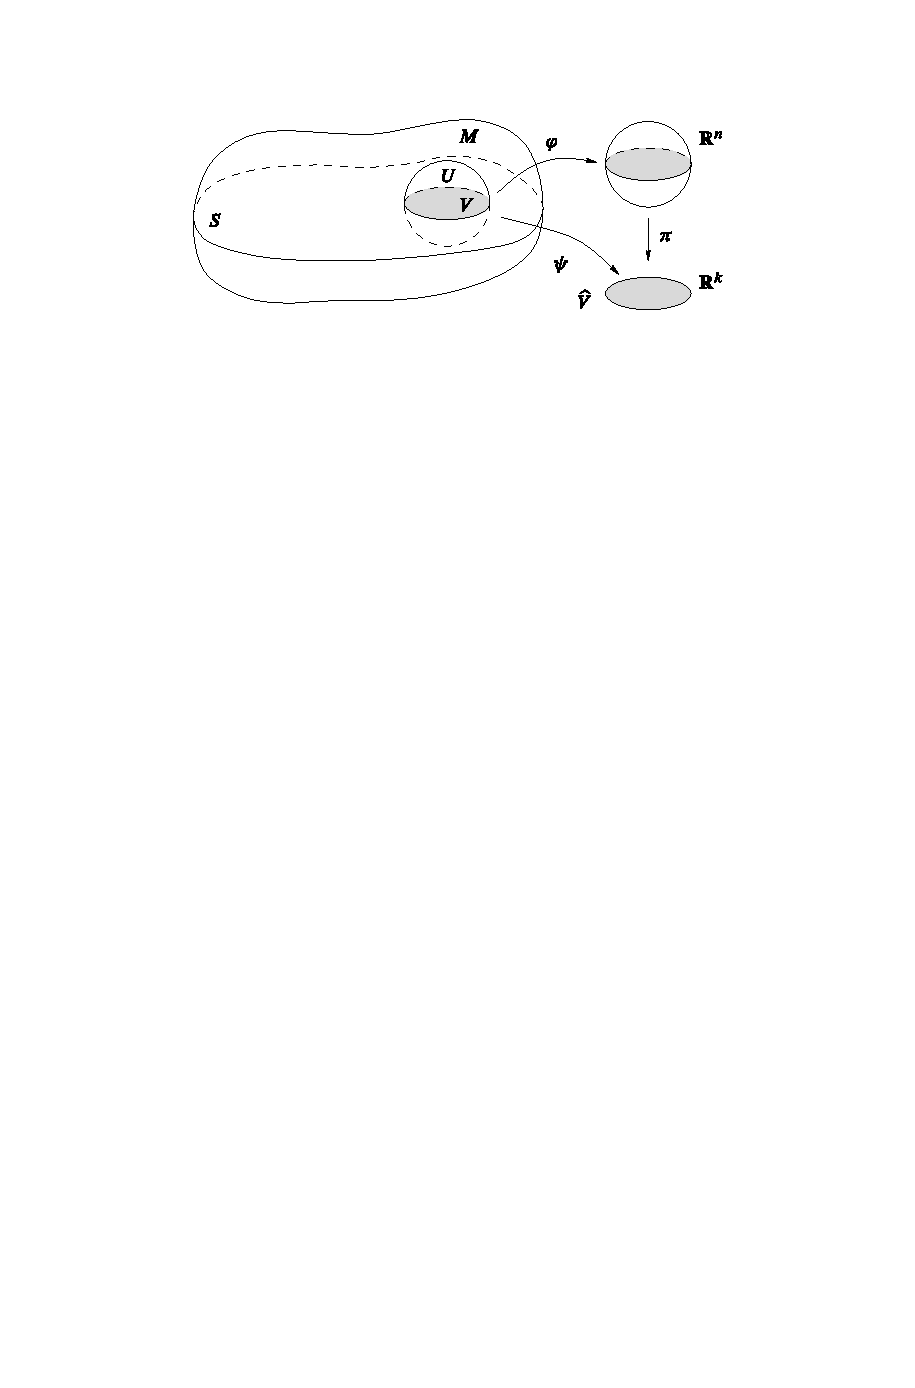
\includegraphics{pictures/slice-chart-1}
\caption{A chart for a subset satisfying the $k$-slice condition.}
\end{figure}\\
By definition of slice charts, $\varphi(V)$ is the intersection of $\varphi(U)$ with a certain $k$-slice $A\sub\R^n$ defined by setting $x^{k+1}=c^{k+1},\dots,x^n=c^n$, and therefore $\varphi(V)$ is open in $A$. Since $\pi|_A$ is a diffeomorphism from $A$ to $\R^k$, it follows that $\widehat{V}$ is open in $\R^k$. Moreover, is a homeomorphism because it has a continuous inverse $\varphi^{-1}\circ j|_{\widehat{V}}$, where
\[j:\R^k\to\R^n,\quad(x^1,\dots,x^k)\mapsto(x^1,\dots,x^k,c^{k+1},\dots,c^n)\]
Thus $S$ is a topological $k$-manifold, and the inclusion map $\iota:S\hookrightarrow M$ is a topological embedding.\par
To put a smooth structure on $S$, we need to verify that the charts constructed
above are smoothly compatible. Suppose $(U,\varphi)$ and $(U',\varphi')$ are two slice charts for $S$ in $M$ and let $(V,\psi)$, $(V',\psi')$ be the corresponding charts for $S$. The transition map is given by $\psi'\circ\psi^{-1}=\pi\circ\varphi'\circ\varphi^{-1}\circ j$, which is a composition of four smooth maps.
\begin{figure}[h]
\centering
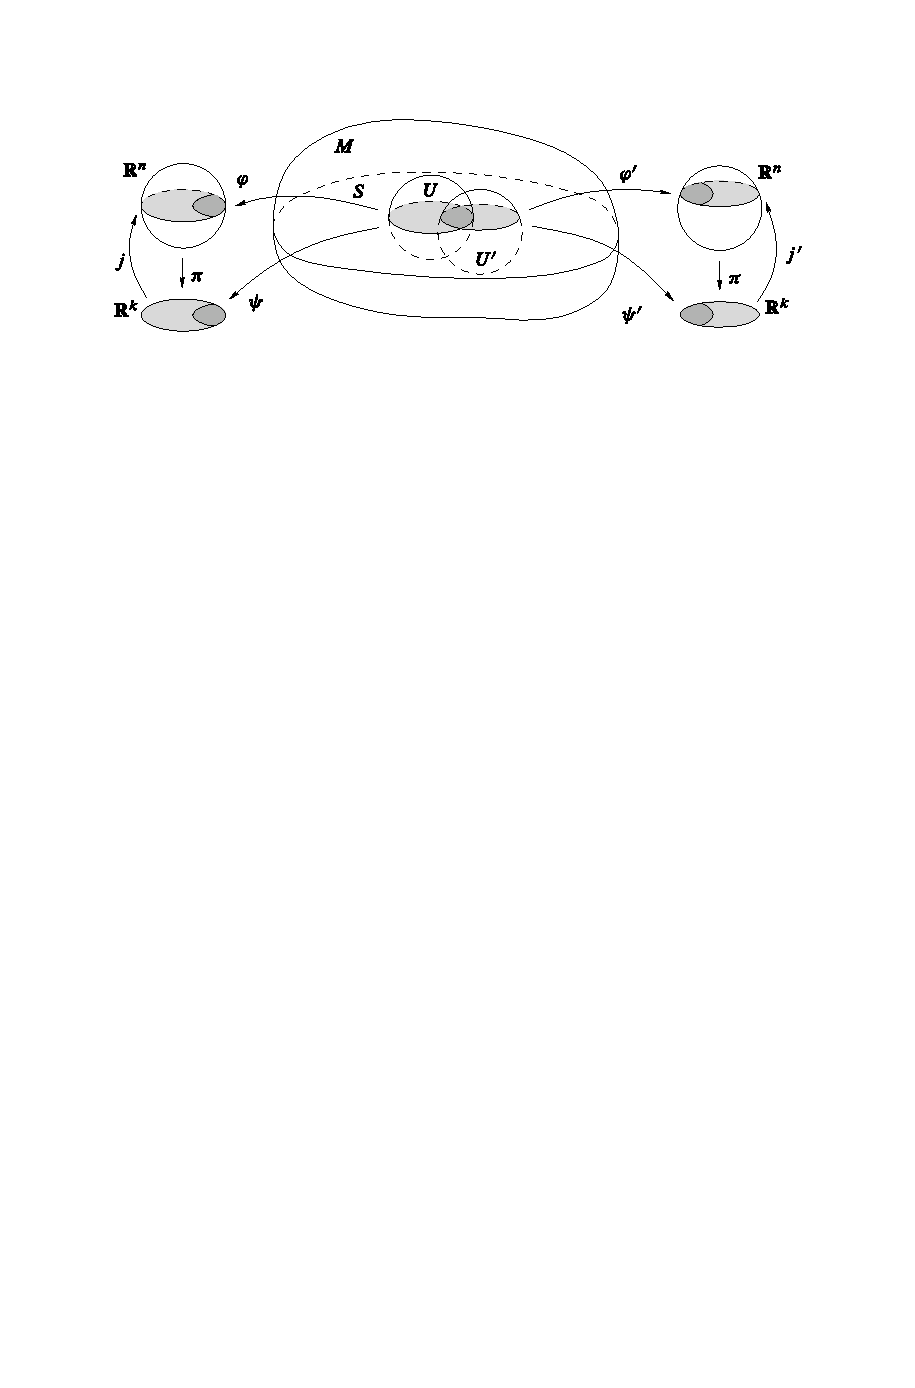
\includegraphics{pictures/slice-chart-2}
\caption{Smooth compatibility of slice charts.}
\end{figure}\\
Thus the atlas we have constructed is in fact a smooth atlas, and it defines a smooth structure on $S$. In terms of a slice chart $(U,\varphi)$ for $M$ and the corresponding chart $(V,\psi)$ for $S$, the inclusion map $S\hookrightarrow M$ has a coordinate representation of the form
\[(x^1,\dots,x^k)\mapsto(x^1,\dots,x^k,c^{k+1},\dots,c^n)\]
which is a smooth immersion. Since the inclusion is a smooth immersion and a topological embedding, $S$ is an embedded submanifold.
\end{proof}
If $M$ is a smooth manifold with nonempty boundary and $S\sub M$ is an embedded submanifold, then $S$ might intersect $\partial M$ in very complicated ways, so we will not attempt to prove any general results about the existence of slice charts for $S$ in $M$ in that case. However, in the special case in which the submanifold is the boundary of $M$ itself, the boundary charts for $M$ play the role of slice charts for $\partial M$ in $M$, and we do have the following result.
\begin{theorem}\label{boundary embedd mani}
If $M$ is a smooth $n$-manifold with boundary, then with the subspace topology, $\partial M$ is a topological $(n-1)$-dimensional manifold without boundary, and has a smooth structure such that it is a properly embedded submanifold of $M$.
\end{theorem}
\begin{proof}
With the subspace topology, $\partial M$ is closed in $M$. Let $\pi:\H^n\to\R^{n-1}$ be the projection on the first $n-1$ coordinates. For any boundary chart $(U,\varphi)$ of $M$, we define a new chart by
\[V=U\cap\partial M,\quad \widehat{V}=\pi\circ\varphi(V),\quad\psi=\pi\circ\varphi|_V\]
With these charts, $\partial M$ becoms a smooth manifold, and the inclusion map $\iota:\partial M\hookrightarrow M$ has coordinate representation 
\[(x^1,\dots,x^{n-1})\mapsto(x^1,\dots,x^{n-1},0)\]
Thus is a smooth immersion. Since $\partial M$ has the subspace topology, $\iota$ is also an embedding, thus a smooth embedding.
\end{proof}
\subsection{Level sets}
If $\varPhi:M\to N$ is any map and $c$ is any point of $N$, we call the set $\varPhi^{-1}(c)$ a \textbf{level set of $\bm{\varPhi}$}. In the special case $N=\R^k$ and $c=0$, the level set $\varPhi^{-1}(0)$ is usually called the \textbf{zero set of $\bm{\varPhi}$}.\par
It is easy to find level sets of smooth functions that are not smooth submanifolds.
For instance, consider the three smooth functions $\varTheta,\varPhi,\varPsi:\R^2\to\R$ defined by
\[\varTheta(x,y)=x^2-y,\quad \varPhi(x,y)=x^2-y^2,\quad \varPsi(x,y)=x^2-y^3\]
Although the zero set of $\varTheta$ is an embedded submanifold of $\R^2$ because it is the graph of the smooth function $f(x)=x^2$, neither the zero set of $\varPhi$ nor that of $\varPsi$ is an embedded submanifold. In fact, without further assumptions on the smooth function, the situation is about as bad as could be imagined: as Theorem~\ref{level set smooth functions} showed, every closed subset of $M$ can be expressed as the zero set of some smooth real-valued function.
\begin{theorem}[\textbf{Constant-Rank Level Set Theorem}]\label{constant rank level set}
Let $M$ and $N$ be smooth manifolds, and let $\varPhi:M\to N$ be a smooth map with constant rank $r$. Then each level set of $\varPhi$ is a properly embedded submanifold of codimension $r$ in $M$.
\end{theorem}
\begin{proof}
Write $m=\dim(M)$, $n=\dim(N)$, and $k=m-r$. Let $c\in N$ be arbitrary, and let $S$ denote the level set $\varPhi^{-1}(c)\sub M$. From the rank theorem, for each $p\in S$ there are smooth charts $(U,\varphi)$ centered at $p$ and $(V,\psi)$ centered at $c=\varPhi(p)$ in which $\varPhi$ has a coordinate representation of the form
\[\widehat{\varPhi}(x^1,\dots,x^r,x^{r+1},\dots,x^m)=(x^1,\dots,x^r,0,\dots,0)\]
and therefore
\[\varphi(S)\cap\varphi(U)=\widehat{\varPhi}^{-1}(0)=\{(x^1,\dots,x^r,x^{r+1},\dots,x^m)\in \varphi(U):x^1=\cdots=x^r=0\}\]
Thus $S$ satisfies the local $k$-slice condition, so it is an embedded submanifold of
dimension $k$. It is closed in $M$ by continuity, so it is properly embedded by Proposition~\ref{proper embedd iff}.
\end{proof}
\begin{corollary}[\textbf{Submersion Level Set Theorem}]\label{subm level set}
If $M$ and $N$ are smooth manifolds and $\varPhi:M\to N$ is a smooth submersion, then each level set of $\varPhi$ is a properly embedded submanifold whose codimension is equal to the dimension of $N$.
\end{corollary}
Corollary~\ref{subm level set} can be strengthened considerably, because we need only check the submersion condition on the level set we are interested in. If $\varPhi:M\to N$ is a smooth map, a point $p\in M$ is said to be a \textbf{regular point} of $d\varPhi_p:T_pM\to T_{\varPhi(p)}N$ is surjective; it is a \textbf{critical point} of $\varPhi$ otherwise. Note that the set of regular points of $\varPhi$ is always an open subset of $M$ by Proposition~\ref{local immersion subm}. A point $c\in N$ is said to be a \textbf{regular value} of $\varPhi$ if every point of the level set $\varPhi^{-1}(c)$ is a regular point, and a \textbf{critical value} otherwise. In particular, if $\varPhi^{-1}(c)=\emp$, then $c$ is a regular value. Finally, a level set $\varPhi^{-1}(c)$ is called a \textbf{regular level set} if $c$ is a regular value of $\varPhi$.
\begin{corollary}[\textbf{Regular Level Set Theorem}]\label{regular value level set}
Every regular level set of a smooth map between smooth manifolds is a properly embedded submanifold whose codimension is equal to the dimension of the codomain.
\end{corollary}
\begin{proof}
Let $\varPhi:M\to N$ be a smooth map and let $c\in N$ be a regular value. The set $U$ of points $p\in M$ where $\rank(d\varPhi_p)=\dim(N)$ is open in $M$ by Proposition~\ref{local immersion subm}, and contains $\varPhi^{-1}(c)$ because of the assumption that $c$ is a regular value. It follows that $\varPhi|_U:U\to N$ is a smooth submersion, and the preceding corollary shows that $\varPhi^{-1}(c)$ is an embedded submanifold of $U$. Since the composition of smooth embeddings $\varPhi^{-1}(c)\hookrightarrow U\hookrightarrow M$ is again a smooth embedding, it follows that $\varPhi^{-1}(c)$ is an embedded submanifold of $M$, and it is closed by continuity.
\end{proof}
\begin{remark}
Note that if we replace the submmersion condition in Corollary~\ref{regular value level set} by constant rank, then the claim is no longer true.
\end{remark}
\begin{proposition}\label{embedd mani iff level set}
Let $S$ be a subset of a smooth $m$-manifold $M$. Then $S$ is an embedded $k$-submanifold of $M$ if and only if every point of $S$ has a neighborhood $U$ in $M$ such that $U\cap S$ is a level set of a smooth submersion $\varPhi:U\to\R^{n-k}$.
\end{proposition}
\begin{proof}
First suppose $S$ is an embedded $k$-submanifold. If $(x^1,\dots,x^m)$ are slice coordinates for $S$ on an open subset $U\sub M$, the map $\varPhi:U\to\R^{m-k}$ given in coordinates by $(x^{k+1},\dots,x^m)$ is easily seen to be a smooth submersion, one of whose level sets is $S\cap U$. Conversely, suppose that around every point $p\in S$ there is a neighborhood $U$ and a smooth submersion $\varPhi:U\to\R^{m-k}$ such that $S\cap U$ is a level set of $\varPhi$. By the submersion level set theorem, $S\cap U$ is an embedded submanifold of $U$, so it satisfies the local slice condition, it follows that $S$ is itself an embedded submanifold of $M$.
\end{proof}
If $S\sub M$ is an embedded submanifold, a smooth map $\varPhi:M\to N$ such that $S$ is a regular level set of $\varPhi$ is called a \textbf{defining map} for $S$. In the special case $N=\R^{m-k}$, it is usually called a \textbf{defining function}. For example, $f(x)=|x|^2$ is a defining function for the sphere.\par More generally, if $U$ is an open subset of $M$ and $\varPhi:M\to N$ is a smooth
map such that $S\cap U$ is a regular level set of $\varPhi$, then $\varPhi$ is called a \textbf{local defining map} for $S$. Proposition~\ref{embedd mani iff level set} says that every embedded submanifold admits a local defining function in a neighborhood of each of its points.
\begin{example}[\textbf{Surfaces of Revolution}]\label{surfaces of revolution}
Let $H$ be the half-plane $\{(r,z):r>0\}$, and suppose $C\sub H$ is an embedded $1$-dimensional submanifold. The surface of revolution determined by $C$ is the subset $S_C\sub\R^3$ given by
\[S_C=\{(x,y,z):(\sqrt{x^2+y^2},z)\in C\}\]
The set $C$ is called its \textbf{generating curve}. If $\varphi:U\to\R$ is any local defining function for $C$ where $U\sub H$, we get a local defining function $\varPhi$ for $S_C$ by
\[\varPhi(x,y,z)=\varphi(\sqrt{x^2+y^2},z)\]
defined on the open subset
\[\widetilde{U}=\{(x,y,z):(\sqrt{x^2+y^2},z)\in U\}\sub\R^3\]
A computation shows that the Jacobian matrix of $\varPhi$ is
\[\partial\varPhi=\begin{bmatrix}
\dfrac{x}{r}\dfrac{\partial\varphi}{\partial r}(r,z)&\dfrac{y}{r}\dfrac{\partial\varphi}{\partial r}(r,z)&\dfrac{\partial\varphi}{\partial z}(r,z)
\end{bmatrix}\]
where we have written $r=\sqrt{x^2+y^2}$. At any point $(x,y,z)\in S_C$, at least one of the components of $\partial\varPhi(x,y,z)$ is nonzero, so $S_C$ is a regular level set of $\varPhi$ and is thus an embedded $2$-dimensional submanifold of $\R^3$.
\end{example}
\section{Immersed submanifolds}
Let $M$ be a smooth manifold with or without boundary. An \textbf{immersed submanifold} of $M$ is a subset $S\sub M$ endowed with a topology (not necessarily the subspace topology) with respect to which it is a topological manifold (without boundary), and a smooth structure with respect to which the inclusion map $S\hookrightarrow M$ is a smooth immersion. As for embedded submanifolds, we define the \textbf{codimension} of $S$ in $M$ to be $\dim(M)-\dim(S)$.\par
Immersed submanifolds often arise in the following way.
\begin{theorem}[\textbf{Images of Immersions as Submanifolds}]\label{image immersion submani}
Suppose $M$ is a smooth manifold with or without boundary, $N$ is a smooth manifold, and $F:N\to M$ is an injective smooth immersion. Let $S=F(N)$. Then $S$ has a unique topology and smooth structure such that it is a smooth submanifold of $M$ and such that $F:N\to S$ is a diffeomorphism onto its image.
\end{theorem}
\begin{proof}
The proof is very similar to that of Proposition~\ref{image of embedding}, except that now we also have to define the topology on $S$. We give $S$ a topology by declaring a set $U\sub S$ to be open if and only if $F^{-1}(U)\sub N$ is open, and then give it a smooth structure by taking the smooth charts to be those of the form $(F(U),\varphi\circ F^{-1})$, where $(U,\varphi)$ is any smooth chart for $N$. As in the proof of Proposition~\ref{image of embedding}, the smooth compatibility condition follows from that for $N$. With this topology and smooth structure on $S$, the map $F$ is a diffeomorphism onto its image, and these are the only topology and smooth structure on $S$ with this property. As in the embedding case, the inclusion $S\hookrightarrow M$ can be written as the composition
\[\begin{tikzcd}
S\ar[r,"F^{-1}"]&N\ar[r,"F"]&M
\end{tikzcd}\]
in this case, the first map is a diffeomorphism and the second is a smooth immersion, so the composition is a smooth immersion.
\end{proof}
The following observation is sometimes useful when thinking about the topology of an immersed submanifold.
\begin{proposition}\label{immersed submani topo}
Suppose $M$ is a smooth manifold and $S\sub M$ is an immersed submanifold. Then every subset of $S$ that is open in the subspace topology is also open in its given submanifold topology; and the converse is true if and only if $S$ is embedded.
\end{proposition}
\begin{proof}
Recall that a subset $U\sub S$ is open in the subspace topology if and only if there is an open subset $W$ of $M$ such that $U=W\cap S$. Let $\iota:S\hookrightarrow M$ be the inclusion, if $U=W\cap S$ is open in the subspace topology, then
\[\iota^{-1}(W)=W\cap S=U.\]
Since $\iota$ is continuous, this implies $U$ is open in the given submanifold topology of $S$.\par
Now the converse holds exactly when $\iota$ is an open map, thus if and only if $S$ is embedded.
\end{proof}
Given a smooth submanifold that is known only to be immersed, it is often useful
to have simple criteria that guarantee that it is embedded. The next proposition gives
several such criteria.
\begin{proposition}\label{immersed is embedd if}
Suppose $M$ is a smooth manifold with or without boundary, and $S\hookrightarrow M$ is an immersed submanifold. If any of the following holds, then $S$ is embedded.
\begin{itemize}
\item[(a)]$S$ has codimension $0$ in $M$.
\item[(b)]The inclusion map $S\sub M$ is proper.
\item[(c)]$S$ is compact.
\end{itemize}
\end{proposition}
\begin{proof}
For part (a), if $\dim(S)=\dim(M)$, then the inclusion map $\iota:S\hookrightarrow M$ is a local homeomorphism, hence open. This implies $\iota$ is an embedding. Part (b) and part (c) both imply that $\iota$ is closed, hence a embedding.
\end{proof}
Although many immersed submanifolds are not embedded, the next proposition
shows that the local structure of an immersed submanifold is the same as that of an embedded one.
\begin{figure}[h]
\centering
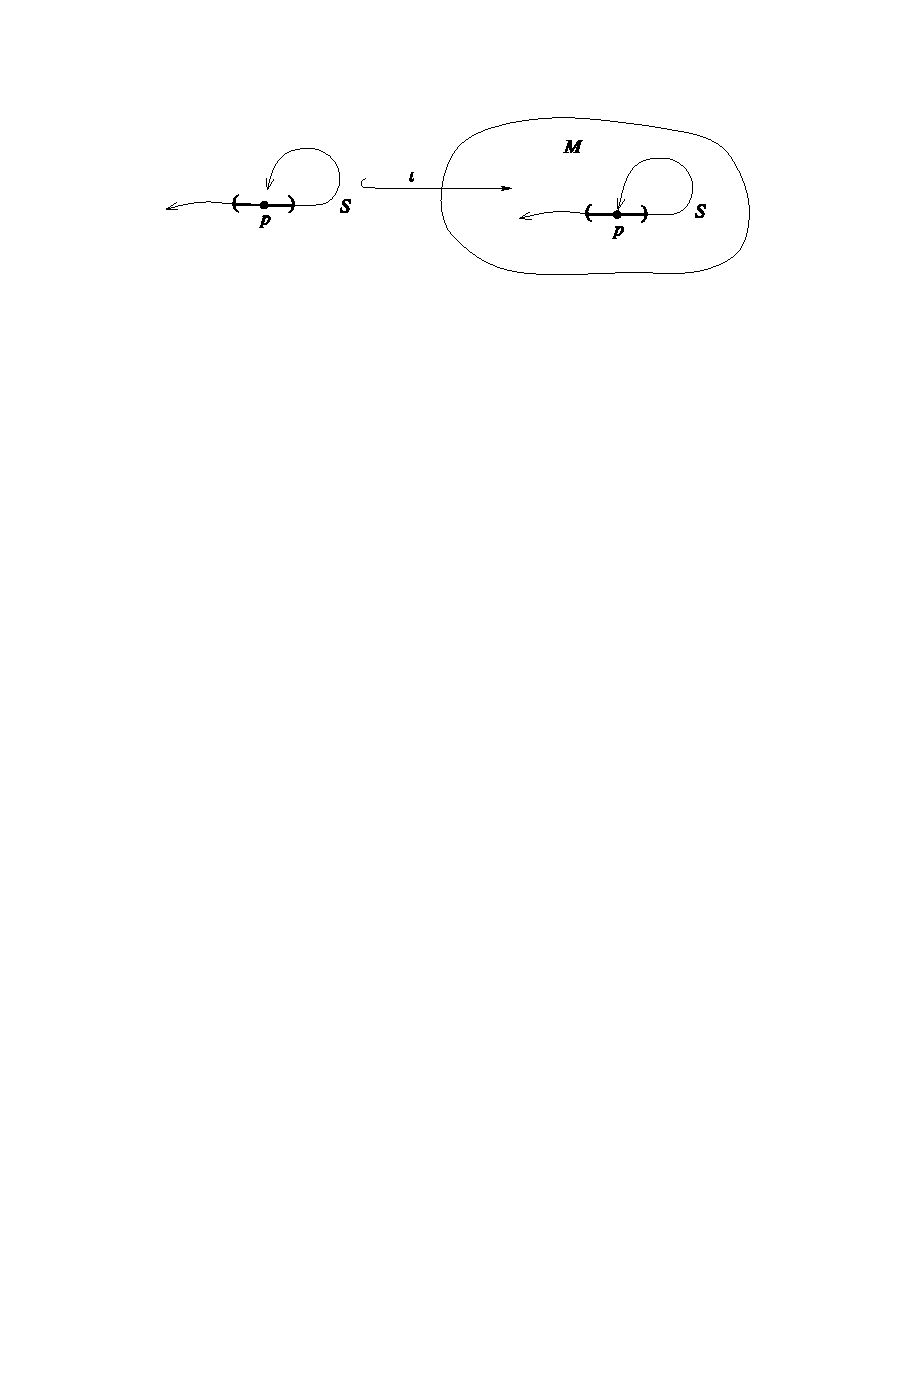
\includegraphics{pictures/immersered-mani}
\caption{An immersed submanifold is locally embedded.}
\end{figure}
\begin{theorem}[\textbf{Immersed Submanifolds Are Locally Embedded}]\label{immerse local embedd}
If $M$ is a smooth manifold with or without boundary, and $S\sub M$ is an immersed submanifold, then for each $p\in S$ there exists a neighborhood $U$ of $p$ in $S$ that is an embedded submanifold of $M$.
\end{theorem}
\begin{proof}
Theorem~\ref{immersion local embedding} shows that each $p\in S$ has a neighborhood $U$ in $S$ such that the inclusion $\iota|_U:U\hookrightarrow M$ is an embedding.
\end{proof}
It is important to be clear about what this proposition does and does not say: \textit{given an immersed submanifold $S\sub M$ and a point $p\in S$, it is possible to find a neighborhood $U$ of $p$ \textbf{in $\bm{S}$} such that $U$ is embedded; but it may not be possible to find a neighborhood $V$ of $p$ \textbf{in $\bm{M}$} such that $V\cap S$ is embedded}.\par
Suppose $S\sub M$ is an immersed $k$-dimensional submanifold. A \textbf{local parametrization} of $S$ is a continuous map $X:U\to M$ whose domain is an open subset $U\sub\R^k$, whose image is an open subset of $S$, and which, considered as a map into $S$, is a homeomorphism onto its image. It is called a \textbf{smooth local parametrization} if it is a diffeomorphism onto its image (with respect to $S$'s smooth manifold structure). If the image of $X$ is all of $S$, it is called a \textbf{global parametrization}.
\begin{proposition}
Suppose $M$ is a smooth manifold with or without boundary, $S\sub M$ is an immersed $k$-submanifold, $\iota:S\to M$ is the inclusion map, and $U$ is an open subset of $\R^k$. A map $X:U\to M$ is a smooth local parametrization of $S$ if and only if there is a smooth coordinate chart $(V,\varphi)$ for $S$ such that $X=\iota\circ\varphi^{-1}$. Therefore, every point of $S$ is in the image of some local parametrization.
\end{proposition}
\begin{proof}
Obviously each chart $(V,\varphi)$ defines a local parametrization $X=\iota\circ\varphi^{-1}$. Conversely, if $X=\iota\circ\varphi^{-1}$, then since $\varphi$ is a diffeomorphism, considered as a map from $V$ to $S$, $X$ is also a diffeomorphism.
\end{proof}
\begin{example}[\textbf{Graph Parametrizations}]
Suppose $U\sub\R^n$ is an open subset and $f:U\to\R^k$ is a smooth function. The map $\gamma_f:U\to\R^n\times\R^k$ given by $\gamma_f(u)=(u,f(u))$ is a smooth global parametrization of $\Gamma(f)$, called a \textbf{graph parametrization}.
\end{example}
\section{Restricting maps to submanifolds}
Given a smooth map $F:M\to N$, it is important to know whether $F$ is still smooth
when its domain or codomain is restricted to a submanifold. In the case of restricting the domain, the answer is easy.
\begin{theorem}[\textbf{Restricting the Domain of a Smooth Map}]\label{restrict domain}
If $M$ and $N$ are smooth manifolds with or without boundary, $F:M\to N$ is a smooth map, and $S\sub M$ is an immersed or embedded submanifold, then $F|_S:S\to N$ is smooth.
\end{theorem}
\begin{proof}
The inclusion map $\iota:S\hookrightarrow M$ is smooth by definition of an immersed submanifold. Since $F|_S=F\circ\iota$, the result follows.
\end{proof}
When the codomain is restricted, however, the resulting map may not be smooth,
as the following example shows.
\begin{example}
Let $S\sub\R^2$ be the figure-eight submanifold, with the topology and smooth structure induced by the immersion $\beta$ of Example~\ref{figure eight}. Define a smooth map $G:\R\to\R^2$ by
\[G(t)=(\sin 2t,\sin t)\]
It is easy to check that the image of $G$ lies in $S$. However, as a map from $\R$ to $S$, $G$ is not even continuous, because $\beta^{-1}\circ G$ is not continuous:
\[\begin{tikzpicture}[domain=0:4]
\draw[->] (-3,0) -- (3,0) node[right] {$x$};
\draw[->] (0,-2) -- (0,2) node[above] {$y$};
\draw (0,0)--(1,1);
\draw (0,0)--(-1,-1);
\draw (1,-1)--(2,0)--(3,1);
\draw (-1,1)--(-2,0)--(-3,-1);
\draw[dashed] (1,1)--(1,-1);
\draw[dashed] (-1,1)--(-1,-1);
\end{tikzpicture}\]
\end{example}
The next theorem gives sufficient conditions for a map to be smooth when its codomain is restricted to an immersed submanifold.It shows that the failure of continuity is the only thing that can go wrong.
\begin{theorem}[\textbf{Restricting the Codomain of a Smooth Map}]\label{restrict to codomain}
Suppose $M$ is a smooth manifold $($without boundary$)$, $S\sub M$ is an immersed submanifold, and $F:N\to M$ is a smooth map whose image is contained in $S$. If $F$ is continuous as a map from $N$ to $S$, then $F:N\to S$ is smooth.
\end{theorem}
\begin{figure}[h]
\centering
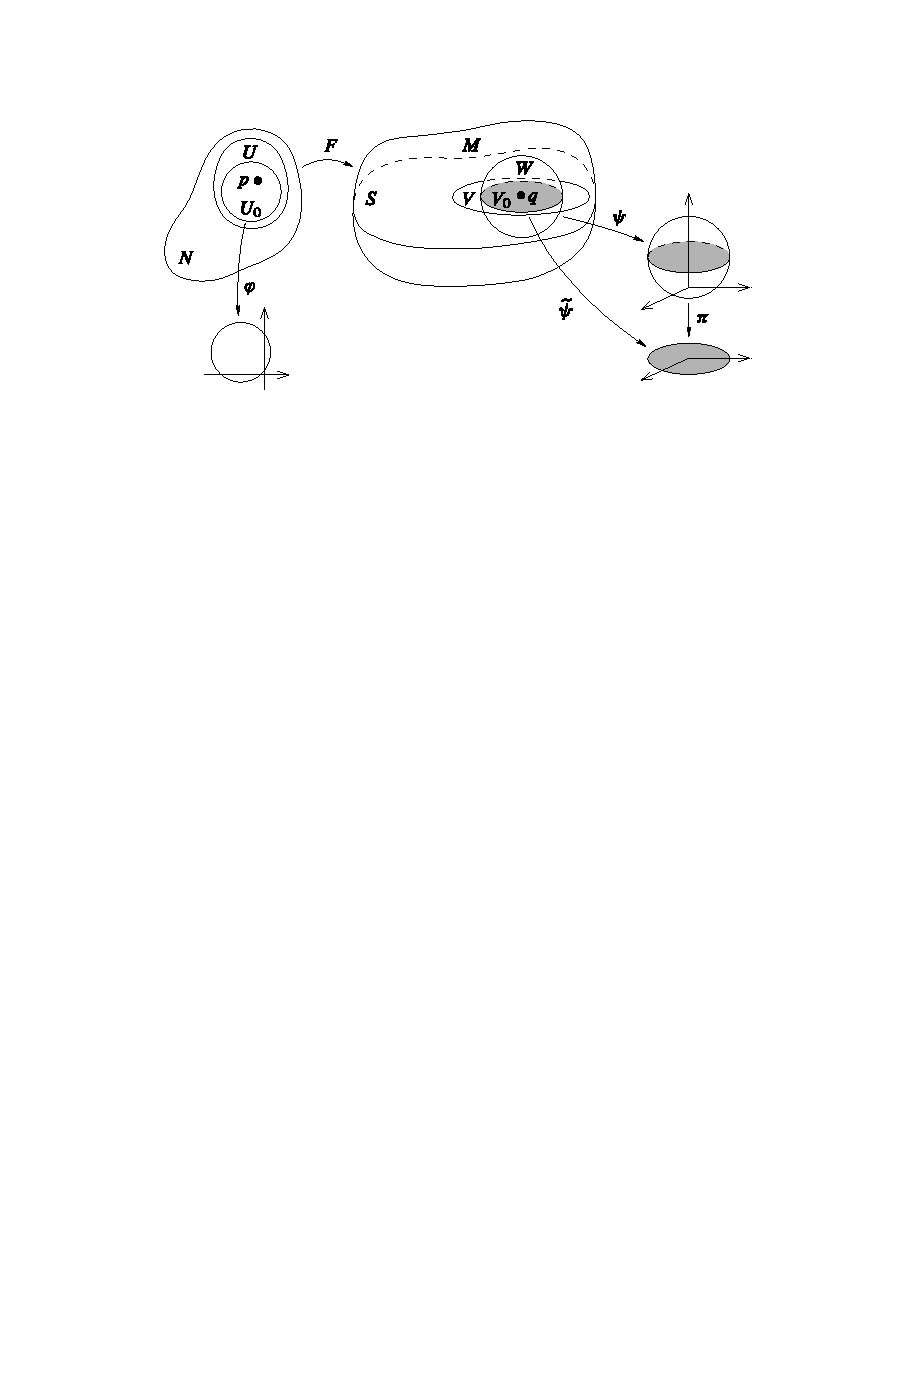
\includegraphics{pictures/restriction-codomain}
\caption{Proof of Theorem~\ref{restrict to codomain}.}
\end{figure}
\begin{proof}
Let $p\in N$ be arbitrary and let $q=F(p)\in S$. Proposition~\ref{immerse local embedd} guarantees that there is a neighborhood $V$ of $q$ in $S$ such that $\iota|_V:V\to M$ is a smooth embedding. Thus there exists a smooth chart $(W,\psi)$ for $M$ that is a slice chart for $V$ in $M$ centered at $q$. (\textit{It might not be a slice chart for $S$ in $M$.}) The fact that $(W,\psi)$ is a slice chart means that $(V_0,\tilde{\psi})$ is a smooth chart for $V$, where $V_0=W\cap V$ and $\tilde{\psi}=\pi\circ\psi$ with $\pi:\R^n\to\R^k$ the projection onto the first $k=\dim(S)$ coordinates. Since $V_0=(\iota|_V)^{-1}(W)$ is open in $V$, it is open in $S$ in its
given topology, and so $(V_0,\tilde{\psi})$ is also a smooth chart for $S$.\par
Let $U=F^{-1}(V_0)$, which is an open subset of $N$ containing $p$. (Here is where we use the hypothesis that $F$ is continuous into $S$.) Choose a smooth chart $(U_0,\varphi)$ for $N$ such that $p\in U_0\sub U$. Then the coordinate representation of $F:N\to S$ with respect to the charts $(U_0,\varphi)$ and $(V_0,\tilde{\psi})$ is
\[\tilde{\psi}\circ F\circ\varphi^{-1}=\pi\circ(\psi\circ F\circ\varphi^{-1})\]
which is smooth because $F:N\to M$ is smooth.
\end{proof}
In the special case in which the submanifold S is embedded, the continuity hypothesis is always satisfied.
\begin{corollary}\label{resrtict codomain to embedd}
Let $M$ be a smooth manifold and $S\sub M$ be an embedded submanifold. Then every smooth map $F:N\to M$ whose image is contained in $S$ is also smooth as a map from $N$ to $S$.
\end{corollary}
\begin{proof}
Since $S\sub M$ has the subspace topology, a continuous map $F:N\to M$ whose image is contained in $S$ is automatically continuous into $S$, by the characteristic
property of the subspace topology.
\end{proof}
If $M$ is a smooth manifold and $S\sub M$ is an immersed submanifold, then $S$ is said to be \textbf{weakly embedded} in $M$ if every smooth map $F:N\to M$ whose image lies in $S$ is smooth as a map from $N$ to $S$.
\subsection{Uniqueness of smooth structures on submanifolds}
Using the preceding results about restricting maps to submanifolds, we can prove the promised uniqueness theorem for the smoothmanifold structure on an embedded
submanifold.
\begin{theorem}\label{unique smooth embedd}
Suppose $M$ is a smooth manifold and $S\sub M$ is an embedded submanifold. The subspace topology on $S$ and the smooth structure described in Theorem~\ref{embedd submani iff local slice} are the only topology and smooth structure with respect to which $S$ is an embedded or immersed submanifold.
\end{theorem}
\begin{proof}
Suppose $S\sub M$ is an embedded $k$-dimensional submanifold. Theorem~\ref{embedd submani iff local slice} shows that it satisfies the local $k$-slice condition, so it is an embedded submanifold with the subspace topology and the smooth structure of Theorem~\ref{embedd submani iff local slice}. Suppose there were some other topology and smooth structure on $S$ making it into an immersed submanifold of some dimension. Let $\widetilde{S}$ denote the same set $S$, considered as a smooth manifold with the non-standard topology and smooth structure, and let $\tilde{\iota}:\widetilde{S}\hookrightarrow M$ denote the inclusion map, which by assumption is an injective immersion (but not necessarily an embedding). Because $\tilde{\iota}(\widetilde{S})=S$, Corollary~\ref{resrtict codomain to embedd} implies that $\tilde{\iota}$ is also smooth when considered as a map from $\widetilde{S}$ to $S$. For each $p\in\widetilde{S}$, the differential $d\tilde{\iota}_p:T_p\widetilde{S}\to T_pM$ is equal to the composition
\[\begin{tikzcd}
T_p\widetilde{S}\ar[r,"d\tilde{\iota}_p"]&T_pS\ar[r,"d\iota_p"]&T_pM
\end{tikzcd}\]
where $\iota:S\hookrightarrow M$ is also inclusion. Because this composition is injective (since $\widetilde{S}$ is assumed to be a smooth submanifold of $M$), $d\tilde{\iota}_p$ must be injective. In particular, this means that $\tilde{\iota}:\widetilde{S}\to S$ is an immersion. Because it is bijective, it follows from the global rank theorem that it is a diffeomorphism. In other words, the topology and smooth manifold structure of $\widetilde{S}$ are the same as those of $S$.
\end{proof}
Thanks to this uniqueness result, we now know that a subset $S\sub M$ is an embedded submanifold if and only if it satisfies the local slice condition, and if so, its
topology and smooth structure are uniquely determined. Because the local slice condition is a local condition, if every point $p\in S$ has a neighborhood $U\sub M$ such that $U\cap S$ is an embedded $k$-submanifold of $U$, then $S$ is an embedded $k$-submanifold of $M$.\par
The preceding theorem is false in general if $S$ is merely immersed; but we do have the following uniqueness theorem for the smooth structure of an immersed submanifold once the topology is known.
\begin{theorem}\label{unique struct immersed}
Suppose $M$ is a smooth manifold and $S\sub M$ is an immersed submanifold. For the given topology on $S$, there is only one smooth structure making $S$ into an immersed submanifold.
\end{theorem}
\begin{proof}
Let $\widetilde{S}$ denote the same set $S$, considered as a smooth manifold with the same topology and another smooth structure, and let $\tilde{\iota}:\widetilde{S}\hookrightarrow M$ denote the inclusion map, which by assumption is an injective immersion. Because $\tilde{\iota}(\widetilde{S})=S$ and the map $\tilde{\iota}:S\to\widetilde{S}$ is a homeomorphism since they have the same topology, Theorem~\ref{restrict to codomain} implies that $\tilde{\iota}$ is also smooth when considered as a map from $\widetilde{S}$ to $S$. Now the rest part is the same as that of Theorem~\ref{unique smooth embedd}.
\end{proof}
It is certainly possible for a given subset of $M$ to have more than one topology making it into an immersed submanifold. However, for weakly embedded submanifolds we have a stronger uniqueness result.
\begin{theorem}\label{unique smooth weak embedd}
If $M$ is a smooth manifold and $S\sub M$ is a weakly embedded submanifold, then $S$ has only one topology and smooth structure with respect to which it is an immersed submanifold.
\end{theorem}
\begin{proof}
This is immediate from the proof of Theorem~\ref{unique smooth embedd} and the definition of weakly embedded submanifold, applied on the inclusion $\tilde{\iota}:\widetilde{S}\to M$.
\end{proof}
\subsection{Extending functions from submanifolds}
Let $M$ be a smooth manifold with or without boundary, and let $S\sub M$ be a smooth submanifold. If $f:S\to\R$ is a function, there are two ways we might interpret the statement $f$ is smooth: it might mean that $f$ is smooth as a function on the smooth manifold $S$ (i.e., each coordinate representation is smooth), or it might mean that it is smooth as a function on the subset $S\sub M$ (i.e., it admits a smooth extension to a neighborhood of each point). We adopt the convention that the notation $f\in C^\infty(S)$ always means that $f$ is smooth in the former sense (as a function on the manifold $S$).
\begin{lemma}[\textbf{Extension Lemma}]\label{ext funct submani}
Let $M$ be a smooth manifold, $S\sub M$ be a smooth submanifold, and $f\in C^\infty(S)$.
\begin{itemize}
\item[(a)] $S$ is embedded if and only if every $f\in C^\infty(S)$ has a smooth extension to a neighborhood of $S$ in $M$.
\item[(b)] $S$ is properly embedded if and only if every $f\in C^\infty(S)$ has a smooth extension to all of $M$.
\end{itemize}
\end{lemma}
\begin{proof}
Let $k=\dim(S)$ and $\pi:\R^n\to\R^k$ be the projection. If $S$ is embedded, then each $p\in S$ is in the domain of a slice chart $(U_p,\varphi_p)$ in $M$ such that $f|_{S\cap U_p}=f(x^1,\dots,x^k)$ and the $x^i$ are slice coordinates. By replacing $U_p$ with $U_p\cap[(S\cap U_p)\times\R^{n-k}]$, we may assume that $\pi(U_p)\sub S\cap U_p$. Now we can extend $f|_{S\cap U_p}$ to $U_p$ by setting \[f_p(x^1,\dots,x^k,x^{k+1},\dots,x^n)=f|_{S\cap U_p}(x^1,\dots,x^n).\] 
The map $f_p:U_p\to\R$ is smooth because it is independent of its last $n-k$ coordinates and it is smooth with respect to its first $n$ coordinates.\par
The collection of open sets $U_p$ is an open cover of $S$, so let $(\psi_p)_{p\in S}$ be a partition of unity subordinate to this cover, and define $\widetilde{f}=\sum_{p\in S}\psi_pf_p$. If $x\in S$, then
\[\widetilde{f}(x)=\sum_{p\in S}\psi_p(x)f_p(x)=f(x)\]
Thus $\widetilde{f}$ is an extension of $f$.\par
Conversely, if any $f\in C^\infty(S)$ admits such an extension, let $U$ be an open subsetof $S$. For any $p\in U$, consider a function $f\in C^\infty(S)$ that is supported in $U$ and equal to $1$ at $p$. Let $\widetilde{f}:M\to\R$ be an extension of $f$, then the set $W=\{x\in M:\widetilde{f}(x)>0\}$ is open in $M$. Moreover, we have the following observation
\begin{itemize}
\item $p\in W$, since $\widetilde{f}(p)=f(p)=1$.
\item $W\cap S\sub U$, since $\widetilde{f}|_S=f$ and $\supp(f)\sub U$.
\end{itemize}
Thus $p$ has a neighborhood contained in $U$ with the subspace topology, which implies $U$ is open in the subspace topology. By Proposition~\ref{immersed submani topo}, this means $S$ is embedded. This completes the proof of (a).\par
Now we deal with part (b). One direction follows directly from Lemma~\ref{ext lem smooth func}, since if $S$ is properly embedded, then it is closed. Conversely, assume that each $f\in C^\infty(S)$ can be extended to $M$. By (a) we know that $S$ is embedded, so we only need to show $S$ is closed. If this is not the case, then there is some $p\in\widebar{S}-S$. We draw a contradition by constructing a function $f:M\to\R$ that only vanishes on $p$, and consider $1/f$: it is smooth on $S$, but can not be extended to $M$.\par
To do this, first take a smooth function $h:\R^n\to [0,1]$ with $h(0)=1$ and $h(x)<1$ for $x\neq 0$. For example 
\[h(x)=\begin{cases}
e^{-\frac{|x|^2}{1-|x|^2}}&|x|<1\\
0&\text{otherwise}
\end{cases}\]
Then choose a chart $(U,\varphi)$ of $M$ such that $\varphi(p)=0,\varphi(U)=\B^n$, and put 
\[f(q)=\begin{cases}
1-h(\varphi(q))&q\in U\\
1&q\notin U
\end{cases}\]
Now by the pasting lemma $f$ is smooth on all of $M$ and only vanishes in $p$.
\end{proof}
\section{The tangent space to a submanifold}
Let $M$ be a smooth manifold with or without boundary, and let $S\sub M$ be an immersed or embedded submanifold. Since the inclusion map $\iota:S\to M$ is a smooth
immersion, at each point $p\in S$ we have an injective linear map $d\iota_p:T_pS\to T_pM$. In terms of derivations, this injection works in the following way: for any vector $v\in T_pS$, the image vector $\widetilde{v}=d\iota_p(v)\in T_pM$ acts on smooth functions on $M$ by
\[\widetilde{v}(f)=d\iota_p(v)(f)=v(f\circ\iota)=v(f|_S)\]
We adopt the convention of identifying $T_pS$ with its image under this map, thereby
thinking of $T_pS$ as a certain linear subspace of $T_pM$.
\begin{proposition}\label{tangent submani}
Suppose $M$ is a smooth manifold with or without boundary, $S\sub M$ is an immersed or embedded submanifold, and $p\in S$. A vector $v\in T_pM$ is in $T_pS$ if and only if there is a smooth curve $\gamma:J\to M$ whose image is contained in $S$, and which is also smooth as a map into $S$, such that $0\in J$, $\gamma(0)=p$, and $\gamma'(0)=v$.
\end{proposition}
The next proposition gives a useful way to characterize $T_pS$ in the embedded case.
\begin{proposition}\label{tangent space submani}
Suppose $M$ is a smooth manifold, $S\sub M$ is an embedded submanifold, and $p\in S$. As a subspace of $T_pM$, the tangent space $T_pS$ is characterized by
\[T_pS=\{v\in T_pM:vf=0\text{ whenever }f\in C^\infty(M)\text{ and }f|_S=0\}\]
\end{proposition}
\begin{proof}
First suppose $v\in T_pS\sub T_pM$. This means, more precisely, that $v=d\iota_p(w)$ for some $w\in T_pS$, where $\iota:S\to M$ is inclusion. If $f$ is any smooth real-valued function on $M$ that vanishes on $S$, then $f\circ\iota\equiv 0$, so
\[vf=w(f\circ\iota)=0\]
Conversely, if $v\in T_pM$ satisfies $vf=0$ whenever $f$ vanishes on $S$, we need to
show that there is a vector $w\in T_pS$ such that $v=d\iota_p(w)$. Let $(x^1,\dots,x^n)$ be slice coordinates for $S$ in some neighborhood $U$ of $p$, so that $U\cap S$ is the subset of $U$ where $x^{k+1}=\cdots=x^n=0$, and $(x^1,\dots,x^k)$ are coordinates for $U\cap S$. Because the inclusion map $\iota:S\cap U\hookrightarrow M$ has the coordinate representation
\[\iota(x^1,\dots,x^k)=(x^1,\dots,x^k,0,\dots,0)\]
in these coordinates, it follows that $T_pS$ (that is, $d\iota_p(T_pS)$) is exactly the subspace of $T_pM$ spanned by $\partial/\partial x^1|_p,\dots,\partial/\partial x^k|_p$. If we write the coordinate representation
of $v$ as $v=v^i\frac{\partial}{\partial x^i}|_p$, we see that $v\in T_pS$ if and only if $v^i=0$ for $i>k$.\par
Let $\varphi$ be a smooth bump function supported in $U$ that is equal to $1$ in a neighborhood of $p$. Choose an index $j>k$, and consider the function $f(x)=\varphi(x)x^j$, extended to be zero on $M\setminus\supp(\varphi)$. Then $f$ vanishes identically on $S$, so
\[0=vf=\sum_{i=1}^{n}v^i\frac{\partial(\varphi(x)x^j)}{\partial x^i}(p)=v^j\]
Thus $v\in T_pS$.
\end{proof}
If an embedded submanifold is characterized by a defining map, the defining map gives a concise characterization of its tangent space at each point, as the next
proposition shows.
\begin{proposition}\label{tangent space level set}
Suppose $M$ is a smooth manifold and $S\sub M$ is an embedded submanifold. If $\varPhi:U\to N$ is any local defining map for $S$, then $T_pS=\ker d\varPhi_p$ for each $p\in S\cap U$.
\end{proposition}
\begin{proof}
Recall that we identify $T_pS$ with the subspace $d\iota_p:T_pS\to T_pM$, where $\iota:S\to M$ is the inclusion map. Because $\varPhi\circ\iota$ is constant on $S\cap U$, it follows that $d\varPhi_p\circ d\iota_p$ is the zero map from $T_pS$ to $T_{\varPhi(p)}N$, and therefore $\im d\iota_p\sub\ker d\varPhi_p$.\par
On the other hand, $d\varPhi_p$ is surjective by the definition of a defining map, so the rank-nullity law implies that
\[\dim(\ker d\varPhi_p)=\dim(T_pM)-\dim(T_{\varPhi(p)}N)=\dim(T_pS)=\dim(\im d\iota_p)\]
which implies $\im d\iota_p=\ker d\varPhi_p$.
\end{proof}
\begin{corollary}
Suppose $M$ and $N$ are smooth manifolds, $S\sub M$ is a level set of a smooth map $\varPhi:M\to N$ with constant rank. Then $T_pS=\ker d\varPhi_p$ for each $p\in S$.
\end{corollary}
\begin{proof}
Suppose $d\varPhi$ has rank $r$. Since $\varPhi\circ\iota$ is constant on $S$, we have $\im d\iota_p\sub\ker d\varPhi_p$. Also, 
\[\dim(\ker d\varPhi_p)=\dim(T_pM)-r=\dim(S)=\dim(\im d\iota_p)\]
Thus $\ker d\varPhi_p=\im d\iota_p=T_pS$.
\end{proof}
\begin{corollary}\label{tangent space constant rank}
Suppose $S\sub M$ is a level set of a smooth submersion $\varPhi=(\varPhi^1,\dots,\varPhi^k):M\to\R^k$. For any $p\in S$, a vector $v\in T_pM$ is tangent to $S$ if and only if $v\varPhi^1=\cdots=v\varPhi^k=0$.
\end{corollary}
\begin{proof}
We write $d\varPhi_p(v)=v^i\partial/\partial x^i|_{\varPhi(p)}\in T_{\varPhi(p)}\R^k$ and let $x^i$ be the $i$-th coordinate function, then
\[v^j=d\varPhi(v)(x^i)=v(x^i\circ\varPhi)=v\varPhi^i.\]
Thus $v\in\ker d\varPhi_p$ if and only if $v\varPhi^i=0$ for all $i=1,\dots,k$.
\end{proof}
\subsection{Tangent space to the boundary, inward-pointing and outward-pointing vectors}
If $M$ is a smooth manifold with boundary and $p\in\partial M$, it is intuitively evident that the vectors in $T_pM$ can be separated into three classes: those tangent to the boundary, those pointing inward, and those pointing outward. Formally, we make the following definition. If $p\in\partial M$, a vector $v\in T_pM-T_p\partial M$ is said to be \textbf{inward-pointing} if for some $\eps>0$ there exists a smooth curve $\gamma:[0,\eps)\to M$ such that $\gamma(0)=p$ and $\gamma'(0)=v$, and it is \textbf{outward-pointing} if there exists such a curve whose domain is $(-\eps,0]$. The following proposition gives another characterization of inward-pointing and outward-pointing vectors, which is usually much easier to check.
\begin{lemma}\label{inward pointing lem}
Let $M$ be a smooth manifold of dimensin $n$ with boundary, let $p$ be a boundary point, and let $v$ be a vector in $T_p(M)$. Let $(U,\varphi=(x^i))$ and $(V,\psi=(\widetilde{x}^j)$ be boundary charts at $p$, and in local coordinates, let
\[v=v^i\frac{\partial}{\partial x^i}\Big|_p,\quad v=\widetilde{v}^j\frac{\partial}{\partial\widetilde{x}^j}\Big|_p\]
Then either $v^n$ and $\widetilde{v}^n$ are both $0$, or they are both nonzero with the same sign.
\end{lemma}
\begin{proof}
We assume without loss of generality that $p$ is mapped to zero in both charts. Consider the transition function $\psi\circ\varphi^{-1}:\varphi(W)\to\psi(W)$ where $W=U\cap\widetilde{U}$:
\[\psi\circ\varphi^{-1}(x^1,\dots,x^n)=(\widetilde{x}^1,\dots,\widetilde{x}^n)\]
By the invariance boundary theorem, $\psi\circ\varphi^{-1}$ sends boundary (interior) points of $\H^n$ to boundary (interior) points of $\H^n$. Thus
\[\widetilde{x}^n(x^1,\dots,x^{n-1},0)=0\And\widetilde{x}^n(x^1,\dots,x^{n-1},x^n)>0\text{ \textit{if} } x^n>0.\]
It follows that
\[\frac{\partial\widetilde{x}^n}{\partial x^i}(p)=0\for 1\leq i\leq n-1\]
and
\begin{align*}
\frac{\partial\widetilde{x}^n}{\partial x^n}(p)=\lim_{r\to 0^+}\frac{\widetilde{x}^n(0,\dots,0,r)-\widetilde{x}^n(0,\dots,0,0)}{r-0}=\lim_{r\to 0^+}\frac{\widetilde{x}^n(0,\dots,0,r)}{r}\geq 0
\end{align*}
Also, the Jacobian matrix of $\psi\circ\varphi^{-1}$ has the form
\[\partial(\psi\circ\varphi^{-1})(p)=\begin{pmatrix}
\dfrac{\partial\widetilde{x}^j}{\partial x^i}&\dfrac{\partial\widetilde{x}^j}{\partial x^n}\\[8pt]
0&\dfrac{\partial\widetilde{x}^n}{\partial x^n}
\end{pmatrix}\]
Since $\psi\circ\varphi^{-1}$ is a diffeomorphism, we have $\partial\widetilde{x}^n/\partial x^n(p)>0$. Now from the formula $(\ref{coordinate change-1})$,
\[\widetilde{v}^n=v^i\frac{\partial\widetilde{x}^n}{\partial x^i}=v^n\frac{\partial\widetilde{x}^n}{\partial x^n}\]
The result now follows.
\end{proof}
\begin{proposition}\label{inward outward vector iff}
Suppose $M$ is a smooth $n$-dimensional manifold with boundary, $p\in\partial M$, and $(x^i)$ are any smooth boundary coordinates defined on a neighborhood of $p$. The inward-pointing vectors in $T_pM$ are precisely those with positive $x^n$-component, the outward-pointing ones are those with negative $x^n$-component, and the ones tangent to $\partial M$ are those with zero $x^n$-component. Thus, $T_pM$ is the disjoint union of $T_p\partial M$, the set of inward-pointing vectors, and the set of outward-pointing vectors, and $v\in T_pM$ is inward-pointing if and only if $-v$ is outwardpointing.
\end{proposition}
\begin{proof}
We assume without loss of generality that $p$ is mapped to zero. If $\gamma:[0,\eps)\to M$ is a sooth curve such that $\gamma(0)=p$ and $\gamma'(0)=v$. Then in this coordinate we have (since $\gamma^n(t)\geq 0$)
\[\dot{\gamma}^n(0)=\lim_{t\to 0^+}\frac{\gamma^n(t)-\gamma^n(0)}{t-0}=\lim_{t\to 0^+}\frac{\gamma^n(t)}{t}\geq 0\]
Now it follows from Lemma~\ref{inward pointing lem} that $v$ has positive $x^n$-component in any coordinate chart of $p$. The same result holds for outward-pointing vectors, with the observation
\[\dot{\gamma}^n(0)=\lim_{t\to 0^-}\frac{\gamma^n(t)-\gamma^n(0)}{t-0}=\lim_{t\to 0^+}\frac{\gamma^n(t)}{t}\geq 0\]
for any curve $\gamma:(-\eps,0]\to M$.\par
Now let $v=v^i\partial/\partial x^i$ with $x^n>0$, we construct a curve $\gamma:[0,\eps)\to M$ for suitable $\eps>0$ as 
\[\gamma(t)=(v^1t,\dots,v^nt)+\widehat{p}\]
where $\widehat{p}$ is the coordinate of $p$. Then $\gamma(0)=0$ and $\gamma'(0)=v$, and therefore $v$ is outward-pointing. The same can be done when $v^n<0$, with $\gamma$ being defined on $(-\eps,0]$.
\end{proof}
If $M$ is a smooth manifold with boundary, a \textbf{boundary defining function} for $M$ is a smooth function $f:M\to [0,+\infty)$ such that $f^{-1}(0)=\partial M$ and $df_p\neq0$ for all $p\in\partial M$. For example, $f(x)=1-|x|^2$ is a boundary defining function for the closed unit ball $\widebar{B}^n$.
\begin{proposition}\label{boundary defining function exist}
Every smooth manifold with boundary admits a boundary defining function.
\end{proposition}
\begin{proof}
Let $\{(U_\alpha,\varphi_\alpha)\}$ be a collection of smooth charts whose domains cover $M$. For each $\alpha$, define a smooth function $f_\alpha:U_\alpha\to[0,+\infty)$ as follows: if $U_\alpha$ is an interior chart, let $f_\alpha\equiv1$; while if $U_\alpha$ is a boundary chart, let $f_\alpha(x^1,\dots,x^{n})=x^n$ (the $n$-th coordinate function in that chart). Thus, $f_\alpha(p)$ is positive if $p\in\Int M$ and zero if $p\in\partial M$. Let $\{\psi_\alpha\}$ be a partition of unity subordinate to this cover, and let $f=\sum_\alpha f_\alpha\psi_\alpha$. Then $f$ is smooth, identically zero on $\partial M$, and strictly positive in $\Int M$. To see that $df$ does not vanish on $\partial M$, suppose $p\in\partial M$ and $v$ is an inward-pointing vector at $p$. For each $\alpha$ such that $p\in U_\alpha$, we have $f_\aleph(p)=0$ and $df_\alpha|_p(v)=dx^n|_p(v)>0$ by Proposition~\ref{inward outward vector iff}. Thus
\[df_p(v)=\sum_\alpha\big(f_\alpha(p)d\psi_\alpha|_p(v)+\psi_\alpha(p)df_\alpha|_p(v)\big).\]
For each $\alpha$, the first term in parentheses is zero and the second is nonnegative, and there is at least one $\alpha$ for which the second term is positive. Thus $df_p(v)>0$, which implies that $df_p\neq0$.
\end{proof}
\begin{proposition}\label{inward derivative crit}
Suppose $M$ is a smooth manifold with boundary, $f$ is a boundary defining function, and $p\in\partial M$. Then a vector $v\in T_pM$ is inward-pointing if and only if $vf>0$, outward-pointing if and only if $vf<0$, and tangent to $\partial M$ if and only if $vf=0$.
\end{proposition}
\begin{proof}
Let $\iota:\partial M\to M$ be the inclusion, and $p\in\partial M$ be any point. Since $f$ is constant on $\partial M$, $df_p\circ d\iota_p$ is zero on $\partial M$, hence $T_p\partial M\sub\ker df_p$. Moreover, since $df_p\neq 0$ on $p\in\partial M$, we have
\[\dim(\ker df_p)=\dim(M)-1=\dim(T_p\partial M)\]
Thus $T_p\partial M=\ker df_p$. For each point $p$, there is a boundary chart $(U,\varphi)$ in $M$ such that 
\[f(x^1,\dots,x^n)=x^n\]
If we write $df_p(v)=v^i\partial/\partial x^i|_{f(p)}$, then $vf=v^n$. Thus the claim follows from Proposition~\ref{inward outward vector iff}.
\end{proof}
\begin{example}
Consider the subset $S=\{(x,y)\in\R^2:y=|x|\}$. It is easy to check that $S-\{(0,0)\}$ is an embedded $1$-dimensional submanifold of $\R^2$, so if $S$ itself is a smooth submanifold at all, it must be $1$-dimensional. Suppose there were some smooth manifold structure on $S$ making it into an immersed submanifold. Then $T_{(0,0)}S$ would be a $1$-dimensional subspace of $T_{(0,0)}\R^2$, so by Proposition~\ref{tangent submani} there is a curve $\gamma:(-\eps,\eps)\to\R^2$ whose image lies in $S$, and that satisfies $\gamma(0)=(0,0)$ and $\gamma'(0)\neq0$. Writing $\gamma(t)=(x(t),y(t))$, we see that $y(t)$ takes a global minimum at $t=0$, so $y'(0)=0$. On the other hand, because every point $(x,y)\in S$ satisfies $x^2=y^2$, we have $x^2(t)=y^2(t)$ for all $t$. Differentiating twice and setting $t=0$, we conclude that $x'(0)=y'(0)=0$, which is a contradiction. Thus, there is no such smooth manifold structure.
\end{example}
\section{Submanifolds with boundary}
If $M$ is a smooth manifold with or without boundary, a \textbf{smooth submanifold with boundary} in $M$ is a subset $S\sub M$ endowed with a topology and smooth structure making it into a smooth manifold with boundary such that the inclusion map is a smooth immersion. If the inclusion map is an embedding, then it is called an \textbf{embedded submanifold with boundary}; in the general case, it is an \textbf{immersed submanifold with boundary}. The terms \textbf{codimension} and \textbf{properly embedded} are defined just as in the submanifold case.\par
One particular type of submanifold with boundary is especially important. If $M$
is a smoothmanifold with or without boundary, a \textbf{regular domain} in $M$ is a properly embedded codimension-$0$ submanifold with boundary. Familiar examples are the closed upper half space $\H^n\sub\R^n$, the closed unit ball $\widebar{B}^n\sub\R^n$, and the closed upper hemisphere in $S^n$.
\begin{proposition}
Suppose $M$ is a smooth manifold without boundary and $D\sub M$ is a regular domain. The topological interior and boundary of $D$ are equal to its manifold interior and boundary, respectively.
\end{proposition}
\begin{proof}
Let $F:D\hookrightarrow M$ denote the inclusion map. Suppose $p\in D$ is arbitrary. If $p$ is in the manifold boundary of $D$, Theorem~\ref{rank thm manifold boundary} shows that there exist a smooth boundary chart $(U,\varphi)$ for $D$ centered at $p$ and a smooth chart $(V,\psi)$ for $M$ centered at $p$ in which $F$ has the coordinate representation $F(x^1,\dots,x^n)=(x^1,\dots,x^n)$, where $n=\dim(M)=\dim(D)$. Since $D$ has the subspace topology, $U=D\cap W$ for some open subset $W\sub M$, so $V_0:=V\cap W$ is a neighborhood of $p$ in $M$ such that $V_0\cap D$ consists of all the points in $V_0$ whose $x^n$ coordinate is nonnegative. Thus every neighborhood of $p$ intersects both $D$ and $M-D$, so $p$ is in the topological boundary of $D$.\par
On the other hand, suppose $p$ is in the manifold interior of $D$. The manifold
interior is a smooth embedded codimension-$0$ submanifold without boundary in $M$,
so it is an open subset by Proposition~\ref{open submani iff}. Thus $p$ is in the topological interior of $D$.\par 
Conversely, if $p$ is in the topological interior of $D$, then it is not in the topological boundary, so the preceding argument shows that it is not in the manifold boundary and hence must be in the manifold interior. Similarly, if $p$ is in the topological boundary, it is also in the manifold boundary.
\end{proof}
Here are some ways in which regular domains often arise.
\begin{proposition}\label{regular domain}
Suppose $M$ is a smooth manifold and $f\in C^\infty(M)$.
\begin{itemize}
\item[(a)]For each regular value $b$ of $f$, the set $f^{-1}((-\infty,b])$ is a regular domain in $M$.
\item[(b)]If $a$ and $b$ are two regular values of $f$ with $a<b$, then $f^{-1}([a,b])$ is a regular domain in $M$.
\end{itemize}
\begin{proof}
We only deal with part (a), part (b) can be done in the same manner. Since $f$ is continuous, $f^{-1}((-\infty,b))$ is open in $M$ and $f^{-1}((-\infty,b])$ is closed in $M$, hence we only need to show thw existence of boundary charts.\par 
Let $p\in M$ be in the level set $f^{-1}(b)$, then since $b$ is a regular value, there is a chart $(U,\varphi)$ in $M$ containing $p$ such that
\[\widehat{f}=f\circ\varphi^{-1}(x^1,\dots,x^n)=b-x_n,\]
and therefore $\widehat{f}^{-1}((-\infty,b])=U\cap\H^n$. Set $\widetilde{U}=U\cap \H^n$, we get a boundary chart $(\widetilde{U},\varphi)$ for $p$. 
\end{proof}
\end{proposition}
A set of the form $f^{-1}((-\infty,b])$ for $b$ a regular value of $f$ is called a \textbf{regular sublevel set} of $f$. Part (a) of the preceding theorem shows that every regular sublevel set of a smooth real-valued function is a regular domain. If $D\sub M$ is a regular domain and $f\in C^\infty(M)$ is a smooth function such that $D$ is a regular sublevel set of $f$, then $f$ is called a \textbf{defining function} for $D$.
\begin{theorem}
If $M$ is a smooth manifold and $D\sub M$ is a regular domain, then there exists a defining function for $D$. If $D$ is compact, then $f$ can be taken to be a smooth exhaustion function for $M$.
\end{theorem}
\begin{proposition}[\textbf{Properties of Submanifolds with Boundary}]
Suppose $M$ is a smooth manifold with or without boundary.
\begin{itemize}
\item[(a)]Every open subset of $M$ is an embedded codimension-$0$ submanifold with $($possibly empty$)$ boundary.
\item[(a)]If $N$ is a smooth manifold with boundary and $F:N\to M$ is a smooth embedding, then with the subspace topology $F(N)$ is a topological manifold with boundary, and it has a smooth structure making it into an embedded submanifold
with boundary in $M$.
\item[(c)]An embedded submanifold with boundary in $M$ is properly embedded if and
only if it is closed.
\item[(d)]If $S\sub M$ is an immersed submanifold with boundary, then for each $p\in S$ there exists a neighborhood $U$ of $p$ in $S$ that is embedded in $M$.
\end{itemize}
\end{proposition}
In order to adapt the results that depended on the existence of local slice charts,
we have to generalize the local $k$-slice condition as follows. Suppose $M$ is a smooth manifold (without boundary). If $(U,(x^i))$ is a chart for $M$, a \textbf{$\bm{k}$-dimensional half-slice} of $U$ is a subset of the following form for some constants $c^{k+1},\dots,c^n$:
\[\{(x^1,\dots,x^n)\in U:x^{k+1}=c^{k+1},\dots,x^n=c^n,\text{ and }x^k\geq 0\}\]
We say that a subset $S\sub M$ satisfies the \textbf{local $\bm{k}$-slice condition for submanifolds with boundary} if each point of $S$ is contained in the domain of a smooth chart $(U,(x^i))$ such that $S\cap U$ is either an ordinary $k$-dimensional slice or a $k$-dimensional half-slice. In the former case, the chart is called an \textbf{interior slice chart} for $S$ in $M$, and in the latter, it is a \textbf{boundary slice chart} for $S$ in $M$.
\begin{proposition}
Let $M$ be a smooth $n$-manifold without boundary. If $S\sub M$ is an embedded $k$-dimensional submanifold with boundary, then $S$ satisfies the local $k$-slice condition for submanifolds with boundary. Conversely, if $S\sub M$ is a subset
that satisfies the local $k$-slice condition for submanifolds with boundary, then with the subspace topology, $S$ is a topological $k$-manifold with boundary, and it has a smooth structure making it into an embedded submanifold with boundary in $M$.
\end{proposition}
Using the preceding theorem, one can readily prove the following theorem.
\begin{theorem}[\textbf{Restricting Maps to Submanifolds with Boundary}]
Suppose $M$ and $N$ are smooth manifolds with boundary and $S\sub M$ is an embedded submanifold with boundary.
\begin{itemize}
\item[(a)]Restricting the domain: If $F:M\to N$ is a smooth map, then $F|_S:S\to N$ is smooth.
\item[(b)]Restricting the codomain: If $\partial M=\emp$ and $F:N\to M$ is a smooth map whose image is contained in $S$, then $F$ is smooth as a map from $N$ to $S$.
\end{itemize}
\end{theorem}
\section{Exercise}
\begin{exercise}
Consider the map $\varPhi:\R^4\to\R^2$ defined by
\[\varPhi(x,y,s,t)=(x^2+y,x^2+y^2+s^2+t^2+y)\]
Show that $(0,1)$ is a regular value of $\varPhi$, and that the level set $\varPhi^{-1}(0,1)$ is diffeomorphic to $S^2$.
\end{exercise}
\begin{proof}
We have
\[\partial\varPhi=\begin{bmatrix}
2x&1&0&0\\
2x&2y+1&2s&2t
\end{bmatrix},\quad\varPhi^{-1}(0,1)=\left\{\begin{array}{l}
x^2+y=0\\
x^2+y^2+s^2+t^2+y=1
\end{array}\right. =\left\{\begin{array}{l}
y=-x^2\\
x^4+s^2+t^2=1
\end{array}\right. \]
Thus $(0,1)$ is a regular value. Obviously the set $S=\{x^4+s^2+t^2=1\}$ is diffeomorphic to $S^2$. Since $\varPhi^{-1}(0,1)$ can be viewed as the graph of $S$, the claim follows.
\end{proof}
\begin{exercise}
Suppose $M\sub\R^n$ is an embedded m-dimensional submanifold, and let $UM\sub T\R^n$ be the set of all unit tangent vectors to $M$:
\[UM=\{(x,v)\in T\R^n:x\in M,v\in T_xM,|v|=1\}\]
It is called the \textbf{unit tangent bundle} of $M$. Prove that $UM$ is an embedded $(2m-1)$-dimensional submanifold of $T\R^n\approx\R^n\times\R^n$.
\end{exercise}
\begin{proof}
Consider the smooth map $F:TM\to\R$ defined by
\[(x,v)\mapsto|v|^2\]
Then $1$ is a regular value of $F$, and we have
\[UM=F^{-1}(1)\]
Thus $UM$ is an embedded $(2m-1)$-dimensional submanifold.
\end{proof}
\begin{exercise}\label{delete coordinate ball}
Suppose $M$ is a smooth $n$-manifold and $B\sub M$ is a regular coordinate ball. Show that $M-B$ is a smooth manifold with boundary, whose boundary is diffeomorphic to $S^{n-1}$.
\end{exercise}
\begin{proof}
We assume without loss of genrality that $M=\R^n$. To define the boundary chart, we consider the following map:
\[\pi:(x^1,\dots,x^{n-1},x^n)\mapsto(x^1,\dots,x^{n-1},|x|-1)\]
\end{proof}
\begin{exercise}
Let $S\sub\R^2$ be the boundary of the square of side $2$ centered at the origin. Show that $S$ does not have a topology and smooth structure in which it is an immersed submanifold of $\R^2$.
\end{exercise}
\begin{proof}
The set $S$ is given by
\[S=\{(x,y)\in\R^2:\max\{|x|,|y|\}\leq 1\}\]
Now assmue the converse, then $T_{(1,1)}S$ is a one-dimensional subspace, hence by Proposition~\ref{tangent space submani} there is a smooth curve $\gamma:(-\eps,\eps)\to \R^2$ whose image lies in $S$, and that satisfies $\gamma(0)=(1,1)$ and $\gamma'(0)\neq 0$. Write $\gamma(t)=(x(t),y(t))$, then $x(t)$ and $y(t)$ both take an extreme at $t=0$, hence $x'(t)=y'(t)=0$. This is a contradiction.
\end{proof}
\begin{exercise}
Suppose $E$ and $M$ are smooth manifolds with boundary, and $\pi:E\to M$ is a smooth covering map. Show that the restriction of $\pi$ to each connected component of $\partial E$ is a smooth covering map onto a component of $\partial M$.
\end{exercise}
\begin{proof}
Since $\partial E$ is properly embedded, we can restric the domain and codomains.
\end{proof}
\begin{exercise}
Prove that the image of the dense curve on the torus described in Example~\ref{dense curve torus} is a weakly embedded submanifold of $T^2$.
\end{exercise}
\begin{proof}
Let $S$ be the curve and $\gamma(t)=(e^{2\pi it},e^{2\pi i\alpha t})$ be the parametrization, $f:M\to T^2$ be a smooth map. We only need to check $f$ is continuous as a map from $M$ to $S$. Since the sets of the form $\gamma(t_0-\eps,t_0+\eps)$ for $t_0\in\R$ and $0<\eps<2\pi$ form a basis for the topology of $S$, to prove the continuity of $f$ it suffices to show that the inverse images of these sets under $f$ are open in $M$.\par
Given $t_0\in\R$ and $0<\eps<2\pi$, let $U$ denote the open set of $T^2$ given by the formula
\[U=\{(e^{2\pi it},e^{2\pi is}):-\eps<t<\eps,s\in\R\}\]
Let $\varphi:U\to(-\eps,\eps)\times S^1$ denote the homeomorphism 
\[\varphi(e^{2\pi it},e^{2\pi is})=(t,e^{2\pi i(s-\alpha t)})\]
Now we have
\[U\cap S=\{(e^{2\pi it},e^{2\pi i\alpha(t+n)}):-\eps<t<\eps,n\in\N\},\quad \varphi(U\cap S)=\bigcup_{n\in\N}(-\eps,\eps)\times\{e^{2\pi in\alpha}\}\]
It is easy to check that this equation represents the partition of $\varphi(U\cap S)$ into its path components. It follows that the path components of $U\cap S$ are
\[\varphi^{-1}((-\eps,\eps)\times\{e^{2\pi in\alpha}\})=\gamma(2\pi n-\eps,2\pi n+\eps),\quad\forall n\in\N\]
In particular, $\gamma(-\eps,\eps)$ is a path component of $U\cap S$. Now let $p\in f^{-1}(\gamma(-\eps,\eps))$ and $U$ be the path component of $M$ containting $p$. Then since $f(U)$ is path connected, it is contained in $\gamma(-\eps,\eps)$, which implies $U\sub f^{-1}(\gamma(-\eps,\eps))$. Thus $f^{-1}(\gamma(-\eps,\eps))$ is a union of some subcollection of path components of $f^{-1}(U)$, and is therefore open in $M$.
\end{proof}
\begin{exercise}
Show by example that an immersed submanifold $S\sub M$ might have more than one topology and smooth structure with respect to which it is an immersed submanifold.
\end{exercise}
\begin{proof}
Consider the figure-eight: give the parametrizations
\[F(t)=(\sin 2t,\sin t),\quad G(t)=(-\sin 2t,\sin t)\]
where $t\in(-\pi,\pi)$. Then 
\[G^{-1}\circ F(x)=\begin{cases}
\pi-x&x\in(0,\pi)\\
-\pi-x&x\in(-\pi,0)
\end{cases}\]
Thus the topology and smooth structure of these two parametrization are different.
\end{proof}
\begin{exercise}
Suppose $S\sub M$ is an embedded submanifold and $\gamma:J\to M$ is a smooth curve whose image happens to lie in $S$. Show that $\gamma'(t)$ is in the subspace $T_{\gamma(t)}S$ of $T_{\gamma(t)}M$ for all $t\in J$. Give a counterexample if $S$ is not embedded.
\end{exercise}
\begin{proof}
The figure-eight $S$ is an example, where $\gamma(t)=(-\sin 2t,\sin t)$. The vector $\gamma'(0)=(-1,1)$ is not in $T_0S=(t,t)$.
\end{proof}
\begin{exercise}
Suppose $M$ is a smooth manifold with boundary, $N$ is a smooth manifold, and $F:M\to N$ is a smooth map. Let $S=F^{-1}(c)$, where $c\in N$ is a regular value for both $F$ and $F|_{\partial M}$. Prove that $S$ is a smooth submanifold with boundary in $M$, with $\partial S=S\cap\partial M$.
\end{exercise}
\begin{proof}
The proof is similar to Proposition~\ref{constant rank level set}.
\end{proof}
\begin{exercise}
Suppose $M$ is a smooth manifold with boundary, $N$ is a smooth manifold, and $F:N\to M$ is a smooth map whose image is contained in $\partial M$. Show that $F$ is smooth as a map into $\partial M$, and use this to prove that $\partial M$ has a unique smooth structure making it an embedded submanifold of $M$.
\end{exercise}
\chapter{Sard's theorem}
\section{Sets of measure zero}
Recall what it means for a set $A\sub\R^n$ to have measure zero: for any $\delta>0$, $A$ can be covered by a countable collection of open rectangles, the sum of whose volumes is less than $\delta$.
\begin{lemma}\label{measure zero lem}
Suppose $A\sub\R^n$ is a compact subset whose intersection with $\{c\}\times\R^{n-1}$ has $(n-1)$-dimensional measure zero for every $c\in\R$. Then $A$ has $n$-dimensional measure zero.
\end{lemma}
\begin{proof}
This follows from Fubini's theorem.
\end{proof}
The most important sets of measure zero are graphs of continuous functions.
\begin{proposition}\label{graph measure zero}
Suppose $A$ is an open or closed subset of $\R^{n-1}$ or $\H^{n-1}$, and $f:A\to\R$ is a continuous function. Then the graph of $f$ has measure zero in $\R^n$.
\end{proposition}
\begin{proof}
First assume $A$ is compact. We prove the theorem in this case by induction on $n$. When $n=1$, it is trivial because the graph of $f$ is at most a single point. To prove the inductive step, we appeal to Lemma~\ref{measure zero lem}. For each $c\in\R$, the intersection of the graph of $f$ with $\{c\}\times\R^{n-1}$ is just the graph of the restriction of $f$ to $\{x\in A:x^1=c\}$, which is in turn the graph of a continuous function of $n-2$ variables. It follows by induction that each such graph has $(n-1)$-dimensional measure zero, and thus by Lemma~\ref{measure zero lem}, the graph of f itself has $n$-dimensional measure zero.\par
If $A$ is noncompact, it is a countable union of compact subsets, so the graph of $f$ is a countable union of sets of measure zero.
\end{proof}
\begin{proposition}
Every proper affine subspace of $\R^n$ has measure zero in $\R^n$.
\end{proposition}
\begin{proof}
Let $S\sub\R^n$ be a proper affine subspace. Suppose first that $\dim(S)=n-1$. Then there is at least one coordinate axis, say the $x^i$-axis, that is not parallel to $S$, and in that case $S$ is the graph of an affine function of the form $x^i=F(x^1,\dots,x{i-1},x^{i+1},\dots,x^n)$ so it has measure zero by Proposition~\ref{graph measure zero}. If $\dim(S)<n-1$, then $S$ is contained in some affine subspace of dimension $n-1$, so $S$ has measure zero.
\end{proof}
Our goal is to extend the notion of measure zero in a diffeomorphism-invariant fashion to subsets of manifolds. Because a manifold does not come with a metric, volumes of cubes or balls do not make sense, so we cannot simply use the same definition. However, the key is provided by the next proposition, which implies that
the condition of having measure zero is diffeomorphism-invariant for subsets of $\R^n$.
\begin{proposition}\label{image measure zero}
Suppose $A\sub\R^n$ has measure zero and $F:A\to\R^n$ is a smooth map. Then $F(A)$ has measure zero.
\end{proposition}
\begin{proof}
By definition, for each $p\in A$, $F$ has an extension to a smooth map, which we still denote by $F$, on a neighborhood of $p$ in $\R^n$. Shrinking this neighborhood
if necessary, we may assume that there is an open ball $U$ containing $p$ such that $F$ extends smoothly to $\widebar{U}$. Now $A$ is covered by countably many such precompact open subsets, so $F(A)$ is the union of countably many sets of the form $F(A\cap\widebar{U})$. Thus, it suffices to show that each such set has measure zero.\par
Since $\widebar{U}$ is compact, there is a constant $C$ such that $|\partial F(x)|\leq C$ for all $x\in\widebar{U}$. Using the Lipschitz estimate for smooth functions, we have
\begin{align}\label{image measure zero-1}
|F(x)-F(x')|\leq C|x-x'|
\end{align}
for all $x,x'\in\widebar{U}$.\par
Given $\delta>0$, choose a countable cover $\{B_j\}$ of $A\cap\widebar{U}$ by open balls satisfying $\sum_j\vol(B_j)<\delta$. Then by $(\ref{image measure zero-1})$, $F(\widebar{U}\cap B_j)$ is contained in a ball $\widetilde{B}_j$ whose radius is no more than $C$ times that of $B_j$. We conclude that $F(A\cap\widebar{U})$ is contained in the collection of balls $\{\widetilde{B}_j\}$, the sum of whose volumes is at most $C^n\delta$. Since this can be made as small as desired, it follows that $F(A\cap\widebar{U})$ has measure zero.
\end{proof}
If $M$ is a smooth $n$-manifold with or without boundary, we say that a subset $A\sub M$ has measure zero in $M$ if for every smooth chart $(U,\varphi)$ for $M$, the subset $\varphi(U)\sub\R^n$ has $n$-dimensional measure zero. The following lemma shows that we need only check this condition for a single collection of smooth charts whose domains cover $A$.
\begin{lemma}
Let $M$ be a smooth $n$-manifold with or without boundary and $A\sub M$. Suppose that for some collection $\{(U_\alpha,\varphi_\alpha)\}$ of smooth charts whose domains cover $A$ and $\varphi_\alpha(A\cap U_\alpha)$ has measure zero in $\R^n$ for each  $\alpha$. Then $A$ has measure zero in $M$.
\end{lemma}
\begin{proof}
Let $(V,\psi)$ be an arbitrary smooth chart. We need to show that $\psi(A\cap V)$ has measure zero. Some countable collection of the $U_\alpha$'s covers $A\cap V$. For each such $U_\alpha$, we have
\[\psi(A\cap V\cap U_\alpha)=(\psi\circ\varphi_\alpha^{-1})\circ\varphi_\alpha(A\cap V\cap U_\alpha)\]
Now, $\varphi_\alpha(A\cap V\cap U_\alpha)$ is a subset of $\varphi_\alpha(A\cap U_\alpha)$, which has measure zero in $\R^n$ by hypothesis. By Proposition~\ref{image measure zero} applied to $\psi\circ\varphi_\alpha^{-1}$, therefore, $\psi(A\cap V\cap U_\alpha)$ has measure zero. Since $\psi(A\cap V)$ is the union of countably many such sets, it too has measure zero.
\end{proof}
\begin{proposition}
Suppose $M$ is a smooth manifold with or without boundary and $A\sub M$ has measure zero in $M$. Then $M\setminus A$ is dense in $M$.
\end{proposition}
\begin{proof}
If $M-A$ is not dense, then $A$ contains a nonempty open subset of $M$, which implies that there is a smooth chart $(V,\psi)$ such that $\psi(A\cap V)$ contains a nonempty open subset of $\R^n$ (where $n=\dim(M)$). Because $\psi(A\cap V)$ has measure zero in $\R^n$, this is a contradiction.
\end{proof}
\begin{theorem}
Suppose $M$ and $N$ are smooth $n$-manifolds with or without boundary, $F:M\to N$ is a smooth map, and $A\sub M$ is a subset of measure zero. Then $F(A)$ has measure zero in $N$.
\end{theorem}
\begin{proof}
Let $\{(U_i,\varphi_i)\}$ be a countable cover of $M$ by smooth charts. We need to show that for each smooth chart $(V,\psi)$ for $N$, the set $\psi(F(A)\cap V)$ has measure zero in $\R^n$. Note that this set is the union of countably many subsets of the form 
\[\psi\circ F\circ\varphi_i^{-1}(\varphi_i(A\cap U_i\cap F^{-1}(V)))\]
each of which has measure zero by the result of Proposition~\ref{image measure zero}.
\end{proof}
\section{Sard's theorem}
Here is the theorem that underlies all of our results about embedding, approximation, and transversality.
\begin{theorem}[\textbf{Sard's Theorem}]
Suppose $M$ and $N$ are smooth manifolds with or without boundary and $F:M\to N$ is a smooth map. Then the set of critical values of $F$ has measure zero in $N$.
\end{theorem}
\begin{proof}
Let $m=\dim(M)$ and $n=\dim(N)$. We prove the theorem by induction on $m$. For $m=0$, the result is immediate, because if $n=0$, $F$ has no critical points, while if $n>0$, the entire image of $F$ has measure zero because it is countable.\par
Now suppose $m\geq 1$, and assume the theorem holds for maps whose domains have dimensions less than $m$. By covering $M$ and $N$ with countably many smooth charts, we can reduce to the case in which $F$ is a smooth map from an open subset $U\sub\R^m$ or $\H^m$ to $\R^n$. Write the coordinates in the domain $U$ as $(x^1,\dots,x^m)$, and those in the codomain as $(y^1,\dots,y^n)$.\par
Let $C\sub U$ denote the set of critical points of $F$. We define a decreasing sequence of subsets $C\sups C_1\sups C_2\sups\cdots$ as follows:
\[C_k=\{x\in C:\text{for $1\leq i\leq k$, the partial derivatives of $F$ of order $i$ vanishes at $x$}\}\]
($i$-th order partial derivative means $\partial^if/\partial x^\alpha$ for $\alpha\in\N^m$ and $|\alpha|=i$.) By continuity, $C$ and all of the $C_k$'s are closed in $U$. We will prove in three steps that $F(C)$ has measure zero. In the $
\H^n$ case, extend $F$ to a smooth map on an open subset of $\R^m$, and replace $U$ by that open subset, if we can show that the set of critical values of the extended map has measure zero, then the same is true of the set of critical values of $F$.
\begin{itemize}
\item Step $1$: \textit{$F(C-C_1)$ has measure zero}. Because $C_1$ is closed in $U$, we might as well replace $U$ by $U-C_1$, and assume that $C_1=\emp$. Let $a$ be a point of $C$. Our assumption means that some first partial derivative of $F$ is not zero at $a$. By rearranging the coordinates in the domain and codomain, we may assume that $\partial F^1/\partial x^1(a)\neq 0$. This means that we can define new smooth coordinates $(u,v)=(u,v^2,\dots,v^m)$ in some neighborhood $V_a$ of $a$ in $U$ by
\[u=F^1,\quad v^i=x^i\for 2\leq i\leq m.\]
because the Jacobian of the coordinate transformation is nonsingular at $a$. Shrinking $V_a$ if necessary, we can assume that $\widebar{V}_a$ is a compact subset of $U$ and the coordinates extend smoothly to $\widebar{V}_a$. In these coordinates, $F$ has the coordinate representation 
\begin{align}\label{sard-1}
F(u,v)=(u,F^2(u,v),\dots,F^n(u,v))
\end{align}
(where the component functions $F^2,\dots,F^n$ might be different from the ones in the original coordinate chart) and its Jacobian is
\[\partial F(u,v)=\begin{pmatrix}
1&0\\
*&\dfrac{\partial F^i}{\partial x^j}
\end{pmatrix}\]
Therefore, $C\cap\widebar{V}_a$ consists of exactly those points where the $(n-1)\times(m-1)$ matrix $\partial F^i/\partial x^j$ has rank less than $n-1$.\par
We wish to show that the set $F(C\cap\widebar{V}_a)$ has measure zero in $\R^n$. Because this set is compact, by Lemma~\ref{measure zero lem} it suffices to show that its intersection with each hyperplane $y^1=c$ has $(n-1)$-dimensional measure zero.\par
For $c\in\R$, let $B_c=\{v:(c,v)\in\widebar{V}_a\}\sub\R^{m-1}$ be the slice of $\widebar{V}_a$, and define $F_c:B_c\to\R^n$ by
\[F_c(v)=(F^2(c,v),\dots,F^n(c,v))\]
Because $F(c,v)=(c,F(v))$, the critical values of $F|_{\widebar{V}_a}$ that lie in the hyperplane $y^1=c$ are exactly the points of the form $(c,w)$ with $w$ a critical value of $F_c$. By the induction hypothesis, the set of critical values of each $F_c$ has $(n-1)$-dimensional measure zero. Thus by Lemma~\ref{measure zero lem} $F(C\cap\widebar{V}_a)$ has measure zero.\par
Because $U$ is covered by countably many sets of the form $\widebar{V}_a$, it follows that $F(C\cap U)$ is a countable union of sets of measure zero and thus has measure zero. This completes the proof of Step $1$.
\item Step $2$: \textit{For each $k$, $F(C_k-C_{k+1})$} has measure zero. Again, since $C_{k+1}$ is closed in $U$, we can discard it and assume that at every point of $C_k$ there is some partial derivative of $F$ of order $(k+1)$ that does not vanish.\par 
Let $a\in C_k$ be arbitrary, and let $y:U\to\R$ denote some partial derivative of $F$ of order $k$ that has at least one nonvanishing partial derivative, for example, $\partial y/\partial x^1$ at $a$. Since $a$ is a regular point of $y$, we can define new coordinates
\[\varphi(x^1,\dots,x^m)=(y,x^2,\dots,x^m)\]
in a neighborhood $V_a$ of $a$. By construction, $\varphi$ carries $C_k\cap V_a$ into the hyperplane $\{0\}\times\R^{m-1}$. Consider the coordinate representation \[\widehat{F}=F\circ\varphi^{-1}:\{0\}\times\R^{m-1}\to\R^n.\] Since any point $p\in C_k\cap V_a$ is also a critical of $\widehat{F}$, the set $\varphi(C_k\cap V_a)$ is contained in the critical points of $\widehat{F}$. Therefore by induction hypothesis $F(C_k\cap V_a)$ has measure zero. Since $U$ can be covered by countably many neighborhoods like $V_a$, it follows that $F(C_{k+1}-C_k)$ is contained in a countable union of sets of the form $F(C_k\cap V_a)$, and thus has measure zero.\par
We are not yet finished, because there may be points of $C$ at which all partial derivatives of $F$ vanish, which means that they are neither in $C-C_1$ nor in $C_k-C_{k+1}$ for any $k$. This possibility is taken care of by the final step.
\item  \textit{For $k>m/n-1$, $F(C_k)$ has measure zero}. For each $a\in U$, there is a closed cube $E$ such that $a\in E\sub U$. Since $U$ can be covered by countably many such cubes, it suffices to show that $F(C_k\cap E)$ has measure zero whenever $E$ is a closed cube contained in $U$. Let $E$ be such a cube, and let $A$ be a constant that bounds the absolute values of all of the partial derivatives of $F$ or order $(k+1)$ in $E$. Let $R$
denote the side length of $E$, and let $K$ be a large integer to be chosen later. We can subdivide $E$ into $K^m$ cubes of side length $R/K$, denoted by $(E_1,\dots,E_{K^m})$. If $E_i$ is one of these cubes and there is a point $a_i\in C_k\cap K_i$, then Taylor's theorem implies that for all $x\in E_i$ we have
\[|F(x)-F(a_i)|\leq A'|x-a_i|^{k+1}\]
for some constant $A'$ that depends only on $A$, $k$, and $m$. Thus, $F(E_i)$ is contained in a ball of radius $A'(R\sqrt{m}/K)^{k+1}$. This implies that $F(C_k\cap E)$ is contained in a union of $K^m$ balls, the sum of whose $n$-dimensional volumes is no more than
\[K^m(A')^n(R\sqrt{m}/K)^{n(k+1)}=A''K^{m-nk-n}\]
where $A''=(A')^n(R\sqrt{m})^{n(k+1)}$. Since $k>m/n-1$, this can be made as small as desired by choosing $K$ large, so $F(C_k\cap E)$ has measure zero.
\end{itemize}
\end{proof}
\begin{corollary}\label{smooth image measure zero}
Suppose $M$ and $N$ are smooth manifolds with or without boundary, and $F:M\to N$ is a smooth map. If $\dim(M)<\dim(N)$, then $F(M)$ has measure zero in $N$.
\end{corollary}
\begin{proof}
In this case, every point in $M$ is a critical point of $F$.
\end{proof}
It is important to be aware that Corollary~\ref{smooth image measure zero} is false if $F$ is merely assumed to be continuous. For example, there is a continuous map $F:[0,1]\to\R^2$ whose image is the entire unit square $[0,1]\times[0,1]$.
\begin{corollary}\label{submani measure zero}
Suppose $M$ is a smooth manifold with or without boundary, and $S\hookrightarrow M$ is an immersed submanifold with or without boundary. If $\dim(S)<\dim(M)$, then $S$ has measure zero in $M$.
\end{corollary}
\begin{proof}
Apply Corollary~\ref{smooth image measure zero} to the inclusion map $S\hookrightarrow M$.
\end{proof}
\section{The Whitney embedding theorem}
Our first application of Sard's theorem is to show that every smooth manifold can be embedded into a Euclidean space. In fact, we will show that every smooth nmanifold with or without boundary is diffeomorphic to a properly embedded submanifold (with or without boundary) of $\R^{2n+1}$.\par
The first step is to show that an injective immersion of an $n$-manifold into $\R^N$ can be turned into an injective immersion into a lower-dimensional Euclidean space if $N>2n+1$.
\begin{lemma}\label{reduce codim lem}
Suppose $M\sub\R^N$ is a smooth $n$-dimensional submanifold with or without boundary. For any $v\in\R^N-\R^{N-1}$, let $\pi_v:\R^N\to\R^{N-1}$ be the projection
with kernel $\R v$ $($where we identify $\R^{N-1}$ with the subspace of $\R^N$ consisting of points with last coordinate zero$)$. If $N>2n+1$, then there is a dense set of vectors $v\in\R^N-\R^{N-1}$ for which $\pi_v|_M$ is an injective immersion of $M$ into $\R^{N-1}$.
\end{lemma}
\begin{proof}
In order for $\pi_v|_M$ to be injective, it is necessary and sufficient that $p-q$ never be parallel to $v$ when $p$ and $q$ are distinct points in $M$. Similarly, in order for $\pi_v|_M$ to be a smooth immersion, it is necessary and sufficient that $T_pM$ not contain any nonzero vectors in $\ker d(\pi_v)_p$ for any $p\in M$. Because $\pi_v$ is linear, its differential is the same linear map (under the usual identification $T_p\R^N\approx\R^N$), so this condition is equivalent to the requirement that $T_pM$ not contain any nonzero vectors parallel to $v$.\par
In the case $\partial M=\emp$, $M\times M$ is a manifold. Let $\Delta_M\sub M\times M$ denote the closed set $\Delta_M=\{(p,p):p\in M\}$ (called the \textbf{diagonal} of $M\times M$), and let $M_0\sub TM$ denote the closed set $M_0=\{(p,0)\in TM:p\in M\}$ (the set of zero vectors at all points of $M$). Consider the following two maps into the real projective space $\RP^{N-1}$:
\[\begin{array}{ll}
\kappa:(M\times M)-\Delta_M\to\RP^{N-1},&\kappa(p,q)=[p-q]\\
\tau:TM-M_0\to\RP^{N-1},&\tau(p,w)=[w]
\end{array}\]
where the brackets mean the equivalence class of a vector in $\R^{N}-\{0\}$ considered as a point in $\RP^{N-1}$. These are both smooth because they are compositions of smooth maps with the projection $\R^N-\{0\}\to\RP^{N-1}$, and the condition that $\pi_v|_M$ be an injective smooth immersion is precisely the condition that $[v]$ not be in the image of either $\kappa$ or $\tau$. Because the domains of both $\kappa$ and $\tau$ have dimension $2n<N-1=\dim(\RP^{N-1})$, Corollary~\ref{smooth image measure zero} to Sard's theorem implies that the image of each map has measure zero, and so their union has measure zero as well. Thus, the set of vectors whose equivalence classes are not in either image is dense.\par
In that case $\partial M\neq\emp$, $M\times M$ is not a smooth manifold with boundary. Instead, we can consider the restrictions of $\kappa$ to $(M\times\Int M)-\Delta_M$ and to $(M\times\partial M)-\Delta_M$ (both of which are smooth manifolds with boundary), and note that there is a point $[v]\in\RP^{N-1}$ that is not in the image of $\tau$ or either of these restrictions of $\kappa$.
\end{proof}
By applying the preceding lemma repeatedly, we can conclude that if an $n$-manifold admits an injective immersion into some Euclidean space, then it admits one into $\R^{2n+1}$. When $M$ is compact, this map is actually an embedding by Proposition~\ref{smooth embedd if}(c); but if $M$ is not compact, we need to work a little harder to ensure that our injective immersions are also embeddings.
\begin{lemma}\label{reduce codim embedd}
Let $M$ be a smooth $n$-manifold with or without boundary. If $M$ admits a smooth embedding into $\R^N$ for some $N$, then it admits a proper smooth embedding into $\R^{2n+1}$.
\end{lemma}
\begin{figure}[h]
\centering
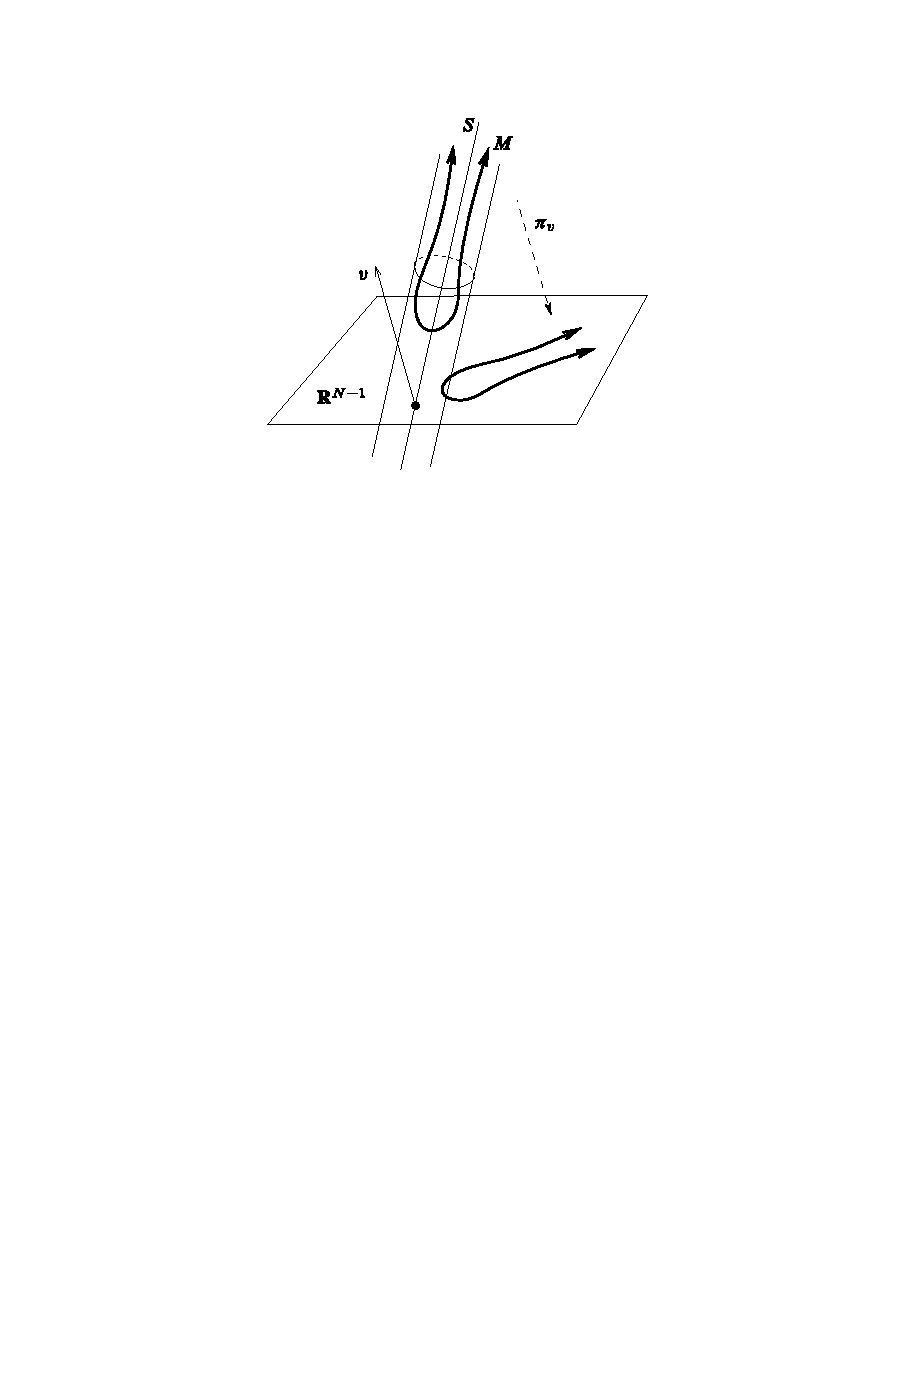
\includegraphics{pictures/Whitney}
\caption{Reducing the codimension of a proper embedding.}
\end{figure}
\begin{proof}
For this proof, given a one-dimensional linear subspace $S\sub\R^N$ and a positive number $R$, let us define the tube with axis $S$ and radius $R$ to be the open subset $T_R(S)\sub\R^N$ consisting of points whose distance from $S$ is less than $R$:
\[T_R(S)=\{x\in\R^N:|x-y|<R\text{ for some $y\in S$}\}\]
Suppose $F:M\to\R^N$ is an arbitrary smooth embedding. Let $G:\R^N\to\B^N$ be a diffeomorphism, and let $f:M\to\R$ be a smooth exhaustion function. Define $\varPsi:M\to\R^N\times\R$ by $\varPsi(p)=(G\circ F(p),f(p))$. Because $G\circ F$ is an embedding, it follows that $\varPsi$ is injective and $d\varPsi_p$ is injective for each $p$, so $\varPsi$ is an injective immersion. It is proper because the preimage of any compact set is a closed subset of the compact set $f^{-1}((-\infty,c])$ for some $c$, so $\varPsi$ is a smooth embedding by Proposition~\ref{smooth embedd if}(b). By construction, the image of $\varPsi$ is contained in
the tube $\B^N\times\R$.\par
Henceforth (after replacing $N+1$ by $N$), we assume that $M$ admits a proper smooth embedding into $\R^N$ for some $N$ that takes its values in some tube $T_R(S)$. Identifying $M$ with its image, we may consider $M$ as a properly embedded submanifold of $\R^N$ contained in the tube.\par
If $N>2n+1$, Lemma~\ref{reduce codim lem} shows that there exists $v\in\R^N-\R^{N-1}$ so that $\pi_v|_M$ is an injective immersion of $M$ into $\R^{N-1}$. Moreover, we may choose $v$ so that it does not lie in the subspace $S$, it follows that $\pi_v(S)$ is a one-dimensional subspace of $\R^{N-1}$, and $\pi_v(M)$ lies in a tube around $\pi_v(S)$ because $\pi_v$ is a bounded linear map. We will show that $\pi_v|_M$ is proper, so it is an embedding by Proposition~\ref{smooth embedd if}(b).\par
Suppose $K\sub\R^{N-1}$ is a compact set. Then $K$ is contained in the open ball around $0$ of some radius $R_1$. For any $x\in\pi_v^{-1}(K)$, there is some $c\in\R$ such that $\pi_v(x)=x-cv$; since $|\pi_v(x)|<R_1$, this means that $x$ is in the tube of radius $R_1$ around the line $\R v$ spanned by $v$. It follows that $M\cap\pi^{-1}_v(K)$ is contained in two tubes, one around $S$ and the other around $\R v$. A simple geometric argument shows that the intersection of two tubes is bounded when their axes are not parallel, so $M\cap\pi^{-1}_v(K)$ is compact. Thus $\pi_v|_M$ is proper, which implies that $\pi_v|_M$ is a properly embedded submanifold of $\R^{N-1}$ contained in a tube. We can now iterate this argument until we achieve a proper smooth embedding of $M$ into $\R^{2n+1}$.
\end{proof}
\begin{theorem}[\textbf{Whitney Embedding Theorem}]
Every smooth $n$-manifold with or without boundary admits a proper smooth embedding into $\R^{2n+1}$.
\end{theorem}
\begin{proof}
Let $M$ be a smooth $n$-manifold with or without boundary. By Lemma~\ref{reduce codim embedd}, it suffices to show that $M$ admits a smooth embedding into some Euclidean space.\par
First suppose $M$ is compact. In this case $M$ admits a finite cover $\{B_1,\dots,B_m\}$ in which each $B_i$ is a regular coordinate ball or half-ball. This means that for each $i$ there exist a coordinate domain $B'_i\sups B_i$ and a smooth coordinate map $\varphi_i:B'_i\to\R^n$ that restricts to a diffeomorphism from $\widebar{B}_i$ to a compact subset of $\R^n$. For each $i$, let $\rho_i:M\to\R$ be a smooth bump function that is equal to $1$ on $\widebar{B}_i$ and supported in $B'_i$. Define a smooth map $F:M\to\R^{nm+m}$ by
\[F(p)=(\rho_1(p)\varphi_1(p),\dots,\rho_m(p)\varphi_m(p),\rho_1(p),\dots,\rho_m(p))\]
where, as usual, $\rho_i$ is extended to be zero away from the support of $\rho_i$. We will show that $F$ is an injective smooth immersion; because $M$ is compact, this implies that $F$ is a smooth embedding.\par
To see that $F$ is injective, suppose $F(p)=F(q)$. Because the sets $B_i$ cover $M$, there is some $i$ such that $p\in B_i$. Then $\rho_i(p)=1$, and the fact that $\rho_i(q)=\rho_i(p)=1$ implies that $q\in\supp(\rho_i)\sub B'_i$, and
\[\varphi_i(q)=\rho_i(q)\varphi_i(q)=\rho_i(p)\varphi_i(p)=\varphi_i(p)\]
Since $\varphi_i$ is injective on $B'_i$, it follows that $p=q$.\par
Next, to see that $F$ is a smooth immersion, let $p\in M$ be arbitrary and choose $i$ such that $p\in B_i$. Because $\rho_i\equiv 1$ on a neighborhood of $p$, we have $d(\rho_i\varphi_i)_p=d(\varphi_i)_p$, which is injective. It follows easily that $dF_p$ is injective. Thus, $F$ is an injective smooth immersion and hence an embedding.\par
The argument above still works when $M$ is an arbitrary compact subset of a larger manifold $\widetilde{M}$ with or without boundary, by covering $M$ with finitely many coordinate balls or half-balls for $\widetilde{M}$. The result is a smooth injective map $F:M\to\R^{nm+m}$ whose differential is injective at each point. Since $M$ is compact, it is therefore a smooth embedding.\par
Now suppose $M$ is noncompact. Let $f:M\to\R$ be a smooth exhaustion function. Sard's theorem shows that for each nonnegative integer $i$, there are regular values $a_i,b_i$ of $f$ such that $i<a_i<b_i<i+1$. Define subsets $D_i,E_i\sub M$ by
\[\begin{array}{ll}
D_0=f^{-1}((-\infty,1]),& E_0=f^{-1}((-\infty,a_1])\\
D_i=f^{-1}([i,i+1]),&E_i=f^{-1}([b_{i-1},a_{i+1}])
\end{array}\]
We have 
\[D_i\sub\Int E_i,\quad M=\bigcup D_i,\quad E_i\cap E_j=\emp\text{ unless $j=i-1,i,i+1$}.\] 
The first part of the proof shows that for each $i$ there is a smooth embedding of $E_i$ into some Euclidean space, and therefore by Lemma~\ref{reduce codim embedd} there is an embedding $\varphi_i:E_i\to\R^{2n+1}$. For each $i$, let $\rho_i:M\to\R$ be a smooth bump function that is equal to $1$ on a neighborhood of $D_i$ and supported in $\Int E_i$, and define $F:\R^{2n+1}\times\R^{2n+1}\times\R$ by
\[F(p)=\Big(\sum_{\text{$i$ is even}}\rho_i(p)\varphi_i(p),\sum_{\text{$i$ is odd}}\rho_i(p)\varphi_i(p),f(p)\Big)\]
Then $F$ is smooth because only one term in each sum is nonzero in a neighborhood of each point, and $F$ is proper because $f$ is. We will show that $F$ is also an injective smooth immersion, hence a smooth embedding.\par
Suppose $F(p)=F(q)$. Then $p\in D_j$ for some $j$, and $f(p)=f(q)$ implies that $q\in D_j$ as well. Arguing just as in the compact case above, we conclude that $p=q$.\par 
Now let $p\in M$ be arbitrary, and choose $j$ such that $p\in D_j$. Then $\rho_j\equiv 1$ on a neighborhood of $p$. Assuming $j$ is odd, for all $q$ in that neighborhood we have
\[F(q)=(\varphi_j(q),\dots,\cdots)\]
which implies that $dF_p$ is injective. A similar argument applies when $j$ is even.
\end{proof}
\begin{corollary}
Every smooth $n$-dimensional manifold with or without boundary is diffeomorphic to a properly embedded submanifold $($with or without boundary$)$ of $\R^{2n+1}$.
\end{corollary}
\begin{corollary}
Suppose $M$ is a compact smooth $n$-manifold with or without boundary. If $N\geq2n+1$, then every smooth map from $M$ to $\R^N$ can be uniformly approximated by embeddings.
\end{corollary}
\begin{proof}
Assume $N\geq2n+1$, and let $f:M\to\R^N$ be a smooth map. By the Whitney embedding theorem, there is a smooth embedding $F:M\to\R^{2n+1}$. The map $G=f\times F:M\to\R^N\times\R^{2n+1}$ is also a smooth embedding, and $f$ is equal to the composition $\pi\circ G$, where $\pi:\R^{N}\times\R^{2n+1}\to\R^N$ is the projection. Let $\widetilde{M}=G(M)\sub\R^N\times\R^{2n+1}$. Lemma~\ref{reduce codim lem} shows that there is a vector $v_{N+2n+1}$ arbitrarily close to $e_{N+2n+1}=(0,\dots,0,1)$ such that $\pi_{v_{N+2n+1}}|_{\widetilde{M}}$ is an embedding. This implies that $\pi_{v_{N+2n+1}}$ is arbitrarily close to $\pi_{e_{N+2n+1}}$. Iterating this, we obtain vectors $v_{N+2n+1},v_{N+2n},\dots,v_{N+1}$ such that $\pi_{v_{N+1}}\circ\cdots\circ\pi_{v_{N+2n+1}}$ restricts to an embedding of $\widetilde{M}$ that is arbitrarily close to $\pi_{e_{N+1}}\circ\cdots\circ\pi_{e_{N+2n+1}}=\pi$, and therefore $\pi_{v_{N+1}}\circ\cdots\circ\pi_{v_{N+2n+1}}\circ G$ is an embedding of $M$ into $\R^N$ that is arbitrarily close to $f$.
\end{proof}
\section{The Whitney approximation theorems}
We would like to find a way to apply the Whitney approximation theorem to produce smooth approximations to continuous maps between smooth manifolds. If $F:N\to M$ is such a map, then by the Whitney embedding theorem we can consider $M$ as an embedded submanifold of some Euclidean space $\R^n$, and approximate $F$ by a smooth map into $\R^n$. However, in general, the image of this smooth map will not lie in $M$. To correct for this, we need to know that there is a smooth retraction from some neighborhood of $M$ onto $M$. For this purpose, we introduce tubular neighborhoods.\par
We begin with a theorem about smoothly approximating functions into Euclidean spaces. Our first theorem shows, in particular, that any continuous function from a
smooth manifold $M$ into $\R^k$ can be uniformly approximated by a smooth function. In fact, we will prove something stronger. If $\delta:M\to\R$ is a positive continuous function, we say that two functions $F,\widetilde{F}:M\to\R^k$ are \textbf{$\bm{\delta}$-close} if $|F(x)-\widetilde{F}(x)|<\delta(x)$ for all $x\in M$.
\begin{theorem}[\textbf{Whitney Approximation Theorem for Functions}]\label{Whitney appox function}
Suppose $M$ is a smooth manifold with or without boundary, and $F:M\to\R^k$ is a continuous function. Given any positive continuous function $\delta:M\to\R$, there exists a smooth function $\widetilde{F}:M\to\R^k$ that is $\delta$-close to $F$. If $F$ is smooth on a closed subset $A\sub M$, then $\widetilde{F}$ can be chosen to be equal to $F$ on $A$.
\end{theorem}
\begin{proof}
If $F$ is smooth on the closed subset $A$, then by the extension lemma for smooth functions (Lemma~\ref{ext lem smooth func}), there is a smooth function $F_0:M\to\R^k$ that agrees with $F$ on $A$. Let 
\[U_0=\{y\in M:|F_0(y)-F(y)|<\delta(y)\}\]
Then $U_0$ is an open subset containing $A$. (If there is no such set $A$, we just take $U_0=A=\emp$ and $F_0\equiv0$.)\par
We will show that there are countably many points $\{x_i\}_{i=1}^{\infty}$ in $M-A$ and neighborhoods $U_i$ of $x_i$ in $M-A$ such that $\{U_i\}_{i=1}^{\infty}$ is an open cover of $M-A$ and
\begin{align}\label{Whitney appox-1}
|F(y)-F(x_i)|<\delta(y)\quad\text{for all }y\in U_i
\end{align}
To see this, for any $x\in M-A$, let $U_x$ be a neighborhood of $x$ contained in $M-A$ and small enough that
\[\delta(y)>\frac{1}{2}\delta(x)\And |F(y)-F(x)|<\frac{1}{2}\delta(x)\]
for all $y\in U_x$. Then if $y\in U_x$, we have \[|F(y)-F(x)|<\frac{1}{2}\delta(x)<\frac{1}{2}\delta(y)\]
The collection $\{U_x:x\in M-A\}$ is an open cover of $M-A$. Choosing a countable subcover $\{U_{x_i}\}_{i=1}^{\infty}$ and setting $U_i=U_{x_i}$, we have $(\ref{Whitney appox-1})$.\par
Let $\{\varphi_0,\varphi_i\}$ be a smooth partition of unity subordinate to the cover $\{U_0,U_i\}$ of $M$, and define $\widetilde{F}:M\to\R^k$ by
\[\widetilde{F}(y)=\varphi_0(y)F_0(y)+\sum_{i\geq 1}\varphi_i(y)F(x_i)\]
Then clearly $\widetilde{F}$ is smooth, and is equal to $F$ on $A$. For any $y\in M$, the fact that $\sum_{i\geq 0}\varphi_i\equiv 1$ implies that
\begin{align*}
|\widetilde{F}(y)-F(y)|&=\Big|\varphi_0(y)F_0(y)+\sum_{i\geq 1}\varphi_i(y)F(x_i)-\Big(\varphi_0+\sum_{i\geq 1}\varphi_i(y)\Big)F(y)\Big|\\
&\leq\varphi_0(y)|F_0(y)-F(y)|+\sum_{i\geq 1}\varphi_i(y)|F(y)-F(x_i)|\\
&<\varphi_0(y)\delta(y)+\sum_{i\geq 1}\varphi_i(y)\delta(y)=\delta(y)
\end{align*}
\end{proof}
\begin{corollary}\label{appox positive function}
If $M$ is a smooth manifold with or without boundary and $\delta:M\to\R$ is a positive continuous function, there is a smooth function $e:M\to\R$ such that $0<e(x)<\delta(x)$ for all $x\in M$.
\end{corollary}
\begin{proof}
Use the Whitney approximation theorem to construct a smooth function $e:M\to\R$ that satisfies
\[|e(x)-\frac{1}{2}\delta(x)|<\frac{1}{2}\delta(x)\]
for all $x\in M$.
\end{proof}
\section{Tubular neighborhoods}
For each $x\in\R^n$, the tangent space $T_x\R^n$ is canonically identified with $\R^n$ itself, and the tangent bundle $T\R^n$ is canonically diffeomorphic to $\R^n\times\R^n$. By virtue of this identification, each tangent space $T_x\R^n$ inherits a Euclidean dot product. Suppose $M\sub\R^n$ is an embedded $m$-dimensional submanifold. For each $x\in M$, we define the normal space to $M$ at $x$ to be the $(n-m)$-dimensional subspace $N_xM\sub T_x\R^n$ consisting of all vectors that are orthogonal to $T_xM$ with respect to the Euclidean dot product. The normal bundle of $M$, denoted by $NM$, is the subset of $T\R^n\approx\R^n\times\R^n$ consisting of vectors that are normal to $M$:
\[NM=\{(x,v):x\in M,v\in N_xM\}\]
There is a natural projection $\pi:NM\to M$ defined as the restriction to $NM$ of $\pi:T\R^n\to\R^n$.
\begin{theorem}
If $M\sub\R^n$ is an embedded $m$-dimensional submanifold, then $NM$ is an embedded $n$-dimensional submanifold of $T\R^n\approx\R^n\times\R^n$.
\end{theorem}
\begin{proof}
Let $x_0$ be any point of $M$, and let $(U,\varphi)$ be a slice chart for $M$ in $\R^n$ centered at $x_0$. Write $\widehat{U}=\varphi(U)\sub\R^n$, and write the coordinate functions of $\varphi$ as $(u^1,\dots,u^n)$, so that $M\cap U$ is the set where $\{u^{m+1}=\cdots=u^n=0\}$. At each point $x\in U$, the vectors $E_j|_x:=(d\varphi_x)^{-1}(\partial/\partial u^j|_{\varphi(x)})$ form a basis for $T_x\R^n$. We can expand each $E_j|_x$ in terms of the standard coordinate frame as
\[E_j|_x=E^i_j(x)\frac{\partial}{\partial x^i}\Big|_x\]
where each $E^i_j(x)$ is a partial derivative of $\varphi^{-1}$ evaluated at $\varphi(x)$, and thus is a smooth function of $x$.\par
Define a smooth function $\varPhi:U\times\R^n\to\widehat{U}\times\R^n$ by
\[\varPhi(u,v)=\big(u^1(x),\dots,u^n(x),(v,E_1|_x),\dots,(v,E_n|_x)\big)\]
The total derivative of $\varPhi$ at a point $(x,v)$ is
\[\partial\varPhi(x,v)=\begin{pmatrix}
\frac{\partial u^i}{\partial x^j}(x)&0\\
*&E^i_j(x)
\end{pmatrix}\]
which is invertible, so $\varPhi$ is a local diffeomorphism. If $\varPhi(x,v)=\varPhi(y,w)$, then $x=y$ because $\varphi$ is injective, and then the fact that $(v,E_i|_x)=(w,E_i|_x)$ for each $i$ implies that $v=w$. Thus $\varPhi$ is injective, so it defines a smooth coordinate chart on $U\times\R^n$. The definitions imply that $(x,v)\in NM$ if and only if $\varPhi(x,v)$ is in the slice
\[\{(y,z)\in\R^n\times\R^n:y^{m+1}=\cdots=y^n=0,z^1=\cdots=z^m=0\}\]
Thus $\varPhi$ is a slice chart for $NM$ in $\R^n\times\R^n$.
\end{proof}
Thinking of $NM$ as a submanifold of $\R^n\times\R^n$, we define $E:NM\to\R^n$ by
\[E(x,v)=(x+v)\]
This maps each normal space $N_xM$ affinely onto the affine subspace through $x$ and orthogonal to $T_xM$. Clearly, $E$ is smooth, because it is the restriction to $NM$ of the addition map $\R^n\times\R^n\to\R^n$. A \textbf{tubular neighborhood of $\bm{M}$} is a neighborhood $U$ of $M$ in $\R^n$ that is the diffeomorphic image under $E$ of an open subset $V\sub NM$ of the form
\begin{align}\label{tubular}
V=\{(x,v)\in NM:|v|<\delta(x)\}
\end{align}
for some positive continuous function $\delta:M\to\R$.
\begin{theorem}[\textbf{Tubular Neighborhood Theorem}]\label{Euclidean tubular neighborhood}
Every embedded submanifold of $\R^n$ has a tubular neighborhood.
\end{theorem}
\begin{proof}
Let $M_0\sub NM$ be the subset $\{(x,0):x\in M\}$. We begin by showing that $E$ is a local diffeomorphism on a neighborhood of $M_0$. By the inverse function theorem, it suffices to show that the differential $dE_{(x,0)}$ is bijective at each point $(x,0)\in M_0$. This follows easily from the following two facts: 
\begin{itemize}
\item The restriction of $E$ to $M_0$ is the obvious diffeomorphism $M_0\to M$, so $dE_{(x,0)}$ maps the subspace $T_{(x,0)}M_0\sub T_{(x,0)}NM$ isomorphically onto $T_xM$.
\item The restriction of $E$ to the fiber $N_xM$ is the affine map $w\mapsto x+w$, so $dE_{(x,0)}$ maps $T_{(x,0)}(N_xM)$ isomorphically onto $N_xM$.
\end{itemize}  
Since $T_x\R^n=T_xM\oplus N_xM$, these together show that $dE_{(x,0)}$ is surjective, and hence is bijective for dimensional reasons. Thus, $E$ is a diffeomorphism on a neighborhood of $(x,0)$ in $NM$, which we can take to be of the form $V_\delta(x)=\{(y,w)\in NM:|x-y|<\delta,|w|<\delta\}$ for some $\delta>0$.\par
To complete the proof, we need to show that there is an open subset $V$ of the form $(\ref{tubular})$ on which $E$ is a global diffeomorphism. For each point $x\in M$, let 
\[\rho(x)=\sup\{\delta<1:E\text{ is a diffeomorphism from $V_\delta(x)$ to its image}\}\]
The argument in the preceding paragraph implies that $\rho:M\to\R$ is positive.
\begin{figure}[htbp]
\centering
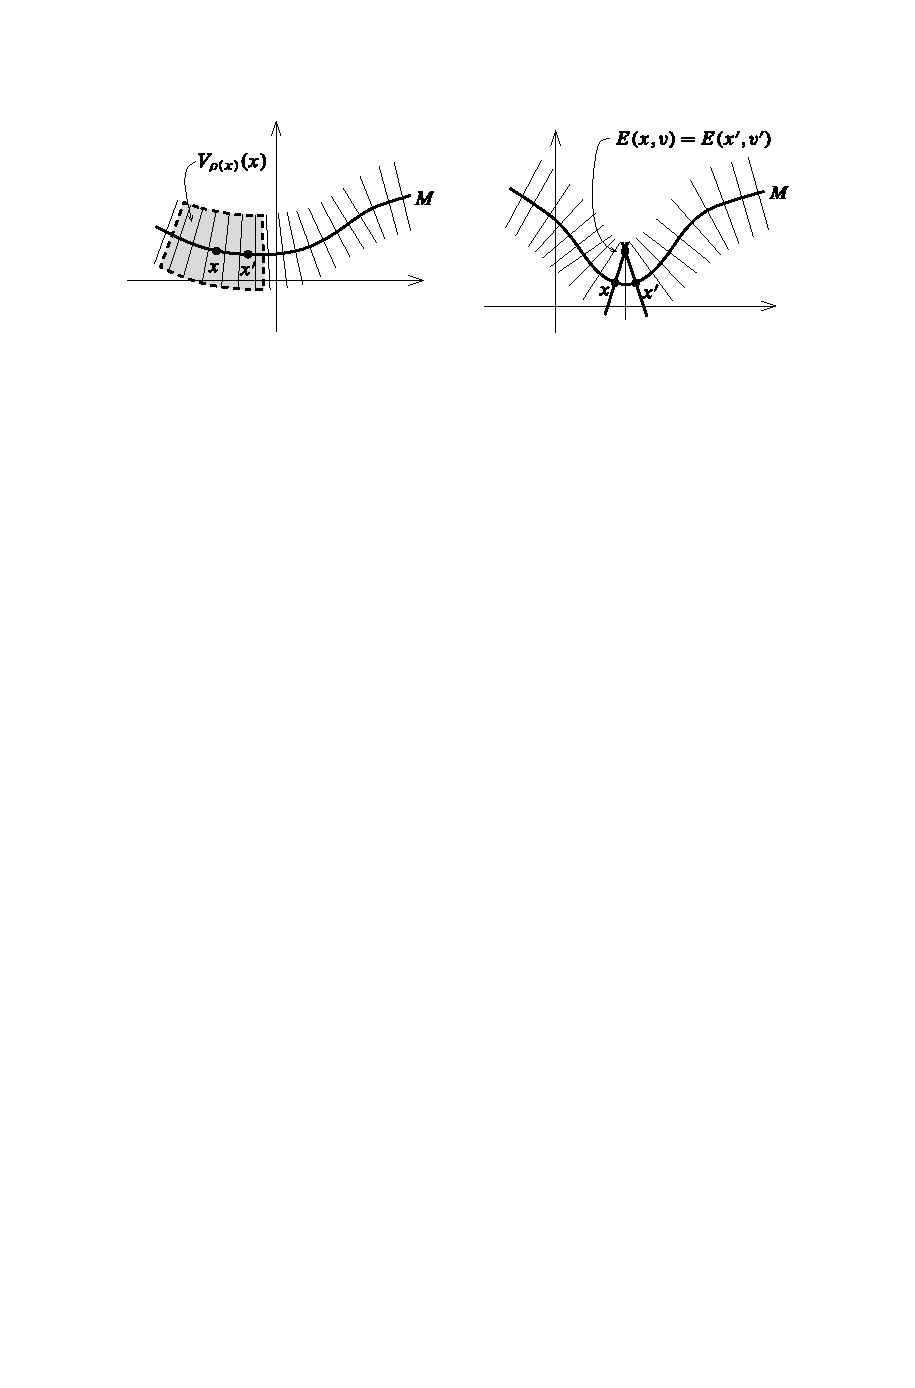
\includegraphics{pictures/tubular}
\caption{Continuity of $\rho$ and Injectivity of $E$.}
\end{figure}\par
To show it is continuous, let $x,y\in M$ be arbitrary, and suppose first that $|x-y|<\rho(x)$. Then by the triangle inequality, $V_\delta(y)$ is 
contained in $V_{\rho(x)}(x)$ for $\delta=\rho(x)-|x-y|$, which implies that $\rho(y)\geq\rho(x)-|x-y|$, or
\[\rho(x)-\rho(y)\leq|x-y|.\]

On the other hand, if $|x-y|\geq\rho(x)$, then the inequality above holds for trivial reasons. Reversing the roles of $x$ and $y$ yields an analogous inequality, which shows that $|\rho(x)-\rho(y)|\leq|x-y|$, so $\rho$ is continuous.\par
Now let $V=\{(x,v)\in NM:|v|<1/2\rho(x)\}$. We will show that $E$ is injective on $V$. Suppose that $(x,v)$ and $(y,w)$ are points in $V$ such that $E(x,v)=E(y,w)$. Assume without loss of generality that $\rho(x)\leq\rho(y)$. It follows from $x+v=y+w$ that
\[|x-y|=|v-w|\leq|v|+|w|\leq\frac{1}{2}\rho(x)+\frac{1}{2}\rho(y)\leq\rho(x)\]
Therefore, both $(x,v)$ and $(y,w)$ are in $V_{\rho(x)}(x)$. Since $(x,v)$ and $(y,w)$ are then in $V_\delta(x)$ for some $\delta<\rho(x)$ and $E$ is injective on $V_\delta(x)$, this implies $(x,v)=(y,w)$.\par
The set $U=E(V)$ is open in $\R^n$ because $E|_V$ is a local diffeomorphism and thus an open map. It follows that $E:V\to U$ is a smooth bijection and a local diffeomorphism, hence a diffeomorphism by Proposition~\ref{local diff prop}. Therefore, $U$ is a tubular neighborhood of $M$.
\end{proof}
One of the most useful features of tubular neighborhoods is expressed in the next proposition. A \textbf{retraction} of a topological space $X$ onto a subspace $M\sub X$ is a continuous map $r:X\to M$ such that $r|_M$ is the identity map of $M$.
\begin{proposition}\label{tubular retraction}
Let $M\sub\R^n$ be an embedded submanifold. If $U$ is any tubular neighborhood of $M$, there exists a smooth map $r:U\to M$ that is both a retraction and a smooth submersion.
\end{proposition}
\begin{proof}
Let $NM\sub T\R^n$ be the normal bundle of $M$, and let $M_0\sub NM$ be the set $M_0=\{(x,0):x\in M\}$. By the definition of a tubular neighborhood, there is an open 
subset $V\sub NM$ containing $M_0$ such that $E:V\to U$ is a diffeomorphism. Define $r:U\to M$ by $r=\pi_{NM}\circ E^{-1}$, where $\pi_{NM}:NM\to M$ is the natural
projection. Then $r$ is smooth by composition. For $x\in M$, note that $E(x,0)=x$, so $r(x)=\pi\circ E(x)=\pi(x,0)=x$, which shows that $r$ is a retraction. Since 
$\pi$ is a smooth submersion and $E^{-1}$ is a diffeomorphism, it follows that $r$ is a smooth submersion.
\end{proof}
\section{Smooth approximation of maps between manifolds}
Now we can extend the Whitney approximation theorem to maps between manifolds.
\begin{theorem}[\textbf{Whitney Approximation Theorem}]\label{Whitney approximation}
Suppose $N$ is a smooth manifold with or without boundary, $M$ is a smooth manifold $($without boundary$)$, and $F:N\to M$ is a continuous map. Then $F$ is homotopic to a smooth map. If $F$ is already smooth on a closed subset $A\sub N$, then the homotopy can be taken to be relative to $A$.
\end{theorem}
\begin{proof}
By the Whitney embedding theorem, we may as well assume that $M$ is a properly embedded submanifold of $\R^n$. Let $U$ be a tubular neighborhood of $M$ in $\R^n$, and let $r:U\to M$ be the smooth retraction given by Proposition~\ref{tubular retraction}. For any $x\in M$, let
\begin{align*}
\delta(x)=\sup\{\eps\leq 1:\B(x,\eps)\sub U\}
\end{align*}
By a triangle-inequality argument just like the one in the proof of the tubular neighborhood theorem, $\delta:M\to\R^+$ is continuous. Let $\tilde{\delta}=\delta\circ F:N\to\R^+$. By Theorem~\ref{Whitney appox function}, there exists a smooth function $\widetilde{F}:N\to\R^n$ that is $\tilde{\delta}$-close to $F$, and is equal to $F$ on $A$ (which might be the empty set). Let $H:N\times I\to M$ be the composition of $r$ with the straight-line homotopy between $F$ and $\widetilde{F}$:
\[H(p,t)=r\big((1-t)F(p)+t\widetilde{F}(p)\big)\]
This is well defined, because our condition on $\widetilde{F}$ guarantees that for each $p\in N$, $|\widetilde{F}(p)-F(p)|<\tilde{\delta}(p)=\delta(F(p))$, which means that $\widetilde{F}(p)$ is contained in the ball of radius $\delta(F(p))$ around $F(p)$; since this ball is contained in $U$, so is the entire line segment from $F(p)$ to $\widetilde{F}(p)$.\par
Thus $H$ is a homotopy between $H(p,0)=F(p)$ and $H(p,1)=r\circ\widetilde{F}(p)$ which is a smooth map by composition. It satisfies $H(p,t)=F(p)$ for all $p\in A$, since $F=\widetilde{F}$ there.
\end{proof}
\begin{corollary}[\textbf{Extension Lemma for Smooth Maps}]
Suppose $N$ is a smooth manifold with or without boundary, $M$ is a smooth manifold, $A\sub N$ is a closed subset, and $f:A\to M$ is a smooth map. Then $f$ has a smooth extension to $N$ if and only if it has a continuous extension to $N$.
\end{corollary}
\begin{proof}
If $F:N\to M$ is a continuous extension of $f$ to all of $N$, the Whitney approximation theorem guarantees the existence of a smooth map $\widetilde{F}$ (homotopic to $F$, in fact, though we do not need that here) that agrees with $f$ on $A$, in other words, $\widetilde{F}$ is a smooth extension of $f$. The converse is obvious.
\end{proof}
If $N$ and $M$ are two smooth manifolds with or without boundary, a homotopy $H:N\times I\to M$ is called a \textbf{smooth homotopy} if it is also a smooth map, in the sense that it extends to a smooth map on some neighborhood of $N\times I$ in $N\times\R$. Two maps are said to be \textbf{smoothly homotopic} if there is a smooth homotopy between them.
\begin{lemma}\label{smooth homotopy trans}
If $N$ and $M$ are smooth manifolds with or without boundary, smooth homotopy is an equivalence relation on the set of all smooth maps from $N$ to $M$.
\end{lemma}
\begin{proof}
Reflexivity and symmetry are proved just as for ordinary homotopy. To prove transitivity, suppose $F,G,K:N\to M$ are smooth maps, and $H_1,H_2:N\times I\to M$ are smooth homotopies from $F$ to $G$ and from $G$ to $K$, respectively. Let $\varphi:[0,1]\to[0,2]$ be a smooth map such that 
\[\left\{\begin{array}{l}
\varphi(0)=0,\varphi(1)=2,\\
0\leq\varphi(t)\leq 1,\ t\in[0,1/2]\\
1\leq\varphi(t)\leq 2,\ t\in[1/2,1]\\
\varphi(t)\equiv 1\text{ in a neighborhood of }1/2.
\end{array}\right. \]
Define $H:N\times I\to M$ by
\[H(x,t)=\begin{cases}
H_1(x,\varphi(t)),&t\in[0,1/2]\\
H_2(x,\varphi(t)-1),&t\in[1/2,1]
\end{cases}\]
Then it is easy to check that $H$ is a smooth homotopy from $F$ to $K$.
\end{proof}
\begin{theorem}\label{homotopy to smooth}
Suppose $N$ is a smooth manifold with or without boundary, $M$ is a smooth manifold, and $F,G:N\to M$ are smooth maps. If $F$ and $G$ are homotopic, then they are smoothly homotopic. If $F$ and $G$ are homotopic relative to some closed subset $A\sub N$, then they are smoothly homotopic relative to $A$.
\end{theorem}
\begin{proof}
Suppose $F,G:N\to M$ are smooth, and let $H:N\times I\to M$ be a homotopy from $F$ to $G$ (relative to $A$, which may be empty). We wish to show that $H$ can be replaced by a smooth homotopy.\par
Define $\widebar{H}:N\times I\to M$ by
\[\widebar{H}(x,t)=\begin{cases}
H(x,0),&t\leq 0\\
H(x,t),&t\in[0,1]\\
H(x,1),&t\geq 1
\end{cases}\]
This is continuous by the gluing lemma. The restriction of $\widebar{H}$ to $(N\times\{0\})\cup(N\times\{1\})$ is smooth, because it is equal to $F\circ\pi_1$ on $N\times\{0\}$ and $G\circ\pi_1$ on $N\times\{1\}$ (where $\pi_1:N\times I\to N$ is the projection). If $H$ is a homotopy relative to $A$, then $\widebar{H}$ is also smooth on $A\times I$. Because $N\times\R$ is a smooth manifold with (possibly empty) boundary, the Whitney approximation theorem guarantees that there is a smooth
map $\widetilde{H}:N\times\R\to M$ (homotopic to $\widetilde{H}$, but we do not need that here) whose restriction to $(N\times\{0\})\cup(N\times\{1\})\cup(A\times I)$ agrees with $\widebar{H}$ (and therefore $H$). Restricting back to $N\times I$ again, we see that $\widetilde{H}|_{N\times I}$ is a smooth homotopy (relative to $A$) between $F$ and $G$.
\end{proof}
\section{Transversality}
As our final application of Sard‘s theorem, we show how submanifolds can be perturbed so that they intersect nicely. To explain what this means, we introduce the
concept of \textit{transversality}.\par
The intersection of two linear subspaces of a vector space is always another linear subspace. The analogous statement for submanifolds is certainly not true: it is easy to come up with examples of smooth submanifolds whose intersection is not a submanifold. But with an additional assumption about the submanifolds, it is possible to show that their intersection is again a submanifold.\par
Suppose $M$ is a smooth manifold. Two embedded submanifolds $S,S'\sub M$ are said to \textbf{intersect transversely} if for each $p\in S\cap S'$, the tangent spaces $T_pS$ and $T_pS'$ together span $T_pM$ (where we consider $T_pS$ and $T_pS'$ as subspaces of $T_pM$).\par
For many purposes, it is more convenient to work with the following more general definition. If $F:N\to M$ is a smooth map and $S\sub M$ is an embedded submanifold,
we say that $F$ is \textbf{transverse to $\bm{S}$} if for every $x\in F^{-1}(S)$, the spaces $T_{F(x)}S$ and $dF_x(T_xN)$ together span $T_{F(x)}M$. One special case is worth noting: if $F$ is a smooth submersion, then it is automatically transverse to every embedded submanifold of $M$. Two embedded submanifolds intersect transversely if and only if the inclusion of either one is transverse to the other.\par
The next result, a generalization of the regular level set theorem, shows why transversality is desirable.
\begin{theorem}\label{transverse intersection preimage subm}
Suppose $N$ and $M$ are smooth manifolds and $S\sub M$ is an embedded submanifold.
\begin{itemize}
\item[(a)]If $F:N\to M$ is a smooth map that is transverse to $S$, then $F^{-1}(S)$ is an embedded submanifold of $N$ whose codimension is equal to the codimension of $S$ in $M$. Moreover, for each $p\in F^{-1}(S)$, we have $T_p(F^{-1}(S))=(dF_p)^{-1}(T_{F(p)}S)$.
\item[(b)]If $S'\sub M$ is an embedded submanifold that intersects $S$ transversely, then $S\cap S'$ is an embedded submanifold of $M$ whose codimension is equal to the sum of the codimensions of $S$ and $S'$. Moreover, for each $p\in S\cap S'$ we have $T_{p}(S\cap S')=T_pS\cap T_{p}S'$.
\end{itemize}
\end{theorem}
\begin{proof}
The second statement follows easily from the first, simply by taking $F$ to be the inclusion map $S'\hookrightarrow M$, and noting that a composition of smooth embeddings $S\cap S'\hookrightarrow S'\hookrightarrow M$ is again a smooth embedding.\par
To prove (a), let $m$ denote the dimension of $M$ and $k$ the codimension of $S$ in $M$. Given $x\in F^{-1}(S)$, we can find a neighborhood $U$ of $F(x)$ in $M$ and a local defining function $\varphi:U\to\R^k$ for $S$, with $S\cap U=\varphi^{-1}(0)$. The theorem will be proved if we can show that $0$ is a regular value of $\varphi\circ F$, because $F^{-1}(S)\cap F^{-1}(U)$ is the zero set of $\varphi\circ F|_{F^{-1}(U)}$.\par
Given $z\in T_0\R^k$ and $p\in(\varphi\circ F)^{-1}(0)$, the fact that $0$ is a regular value of $\varphi$ means there is a vector $y\in T_{F(p)}M$ such that $d\varphi_{F(p)}(y)=z$. The fact that $F$ is transverse to $S$ means we can write $y=y_0+dF_p(v)$ for some $y_0\in T_{F(p)}S$ and some $v\in T_pN$. Because $\varphi$ is constant on $S\cap U$, it follows that $d\varphi_{F(p)}(y_0)=0$, so
\[d(\varphi\circ F)_p(v)=d\varphi_{F(p)}(dF_p(v))=d\varphi_{F(p)}(y_0+dF_p(v))=d\varphi_{F(p)}(y)=z.\]
Thus $F^{-1}(S)$ is an embedded submanifold of codimension $k$.\par
Finally, let $p\in F^{-1}(S)$. Choose a neighborhood $U$ of $F(p)$ and a local defining function $\varPhi:U\to N$ for $S$. Then we have $T_{F(p)}S=\ker d\varPhi_{F(p)}$. By the definition of a local defining function, $\varPhi\circ F$ is constant on $F^{-1}(S)\cap F^{-1}(U)$, and therefore $d\varPhi_{F(p)}\circ dF_p$ is zero on $T_p(F^{-1}(S))$. This then means $ dF_p(T_p(F^{-1}(S)))\sub\ker d\varPhi_{F(p)}S$, and by dimension consideration they are equal. Combining the previous observation, we obtain $\im dF_p=T_{F(p)}S$, and so $T_p(F^{-1}(S))=(dF_p)^{-1}(T_{F(p)}S)$.
\end{proof}
For example, in $\R^3$, this theorem shows that a smooth curve and a smooth surface intersecting transversely have only isolated points in their intersection, while two smooth surfaces intersect transversely in a smooth curve. Two smooth curves in $\R^3$ intersect transversely if and only if their intersection is empty, because at any intersection point, the two one-dimensional tangent spaces to the curves would have to span the tangent space to $\R^3$.\par 
Because a submersion is transverse to every embedded submanifold, the next corollary is immediate.
\begin{corollary}
Suppose $N$ and $M$ are smooth manifolds, $S\sub M$ is an embedded submanifold of codimension $k$, and $F:N\to M$ is a submersion. Then $F^{-1}(S)$ is an embedded codimension-$k$ submanifold of $N$.
\end{corollary}
Transversality also provides a convenient criterion for recognizing a submanifold as a graph. The next theorem is a global version of the implicit function theorem.
\begin{theorem}[\textbf{Global Characterization of Graphs}]\label{char graph}
Suppose $M$ and $N$ are smooth manifolds and $S\sub M\times N$ is an immersed submanifold. Let $\pi_M$ and $\pi_N$ denote the projections from $M\times N$ onto $M$ and $N$, respectively. The following are equivalent.
\begin{itemize}
\item[(\rmnum{1})]$S$ is the graph of a smooth map $f:M\to N$.
\item[(\rmnum{2})]$\pi_M|_S$ is a diffeomorphism from $S$ onto $M$.
\item[(\rmnum{3})]For each $p\in M$, the submanifolds $S$ and $\{p\}\times N$ intersect transversely in exactly one point.
\end{itemize}
If these conditions hold, then $S$ is the graph of the map $f:M\to N$ defined by $f=\pi_N\circ(\pi_M|_S)^{-1}$.
\end{theorem}
\begin{proof}
The implication $(\rmnum{1})\Rightarrow(\rmnum{2})$ is clear. For $(\rmnum{2})\Rightarrow(\rmnum{1})$, we can simply define $f=\pi_N\circ(\pi_M|_S)^{-1}$.\par
Now we show $(\rmnum{2})\Rightarrow(\rmnum{3})$. Assume $\pi_M|_S$ has an smooth inverse $(\pi_M|_S)^{-1}$. In this case, each slice $\{p\}\times N$ only intersects $S$ at $(p,(\pi_M|_S)^{-1}(p))$. At each point $(p,q)$ of $M\times N$, the tangent space $T_{(p,q)}(M\times N)=T_pM\oplus T_qN$, with $T_pM=\ker d(\pi_N)_p$ and $T_qN=\ker d(\pi_M)_q$. Now for any point $(p,q)\in S$, the map $\pi_M|_S$ is a diffeomorphism from $S$ onto $M$, therefore we have $T_{(p,q)}(M\times N)=T_pM\oplus\ker d(\pi_M|_S)_p=T_pM\oplus T_qN$. Since $T_qN$ is the tangent space of $\{p\}\times N$ at $(p,q)$, it follows that $S$ intersects transversely with $\{p\}\times N$.\par
For the part $(\rmnum{3})\Rightarrow(\rmnum{2})$. If $S$ intersects $p\times\{N\}$ in exactly one point for each $p\in M$, then the projection $\pi_M|_S$ is bijective. Also, from the transversality we can see it is a submersion, hence is a diffeomorphism.
\end{proof}
\begin{corollary}[\textbf{Local Characterization of Graphs}]\label{char graph local}
Suppose $M$ and $N$ are smooth manifolds, $S\sub M\times N$ is an immersed submanifold, and $(p,q)\in S$. If $S$ intersects the submanifold $\{p\}\times N$ transversely at $(p,q)$, then there exist a neighborhood $U$ of $p$ in $M$ and a neighborhood $V$ of $(p,q)$ in $S$ such that $V$ is the graph of a smooth map $f:U\to N$.
\end{corollary}
\begin{proof}
The hypothesis guarantees that $d(\pi_M)_{(p,q)}:T_{(p,q)}S\to T_pM$ is an isomorphism, so $\pi_M|_S$ restricts to a diffeomorphism from a neighborhood $V$ of $(p,q)$ in $S$ to a neighborhood $U$ of $p$. The result then follows from Theorem~\ref{char graph}(\rmnum{2}).
\end{proof}
Suppose $N,M$ and $S$ are smooth manifolds, and for each $s\in S$ we are given a map $F_s:N\to M$. The collection $\{F_s:s\in S\}$ is called a \textbf{smooth family of maps} if the map $F:N\times S\to M$ defined by $F(x,s)=F_s(x)$ is smooth. You should think of such a family as a higher-dimensional analogue of a homotopy. The next proposition shows how such families are related to ordinary homotopies.
\begin{proposition}\label{smooth family map homotopy}
If $\{F_s:s\in S\}$ is a smooth family of maps from $N$ to $M$ and $S$ is connected, then for any $s_1,s_2\in S$, the maps $F_{s_1},F_{s_2}:N\to M$ are homotopic.
\end{proposition}
\begin{proof}
Because $S$ is connected, it is path-connected. If $\gamma:[0,1]\to S$ is any path from $s_1$ to $s_2$, then $H(x,s)=F(x,\gamma(s))$ is a homotopy from $F_{s_1}$ to $F_{s_2}$.
\end{proof}
The key to finding transversemaps is the following application of Sard's theorem, which gives a simple sufficient condition for a family of smooth maps to contain at least one map that is transverse to a given submanifold. If $S$ is a smooth manifold and $B\sub S$ is a subset whose complement has measure zero in $S$, we say that $B$ contains \textbf{almost every element} of $S$.
\begin{theorem}[\textbf{Parametric Transversality Theorem}]\label{parametric transversality}
Suppose $N$ and $M$ are smooth manifolds, $X\sub M$ is an embedded submanifold, and $\{F_s:s\in S\}$ is a smooth family of maps from $N$ to $M$. If the map $F:N\times S\to M$ is transverse to $X$, then for almost every $s\in S$, the map $F_s:N\to M$ is transverse to X.
\end{theorem}
\begin{proof}
The hypothesis implies that $W=F^{-1}(X)$ is an embedded submanifold of $N\times S$ by Theorem~\ref{transverse intersection preimage subm}. Let $\pi:N\times S\to S$ be the projection onto the second factor. What we will actually show is that if $s\in S$ is a regular value of the restriction $\pi|_W$, then $F_s$ is transverse to $X$. Since almost every $s$ is a regular value by Sard's theorem, this proves the theorem.\par
Suppose $s\in S$ is a regular value of $\pi|_W$. Let $p\in F_s^{-1}(X)$ be arbitrary, and set $q=F_s(p)\in X$. We need to show that $T_qM=T_qX+d(F_s)(T_pN)$. Let $\iota_1:N\to N\times S$ and $\iota_2:S\to N\times S$ be defined by
\[\iota_1(p')=(p',s),\quad \iota_2(s')=(p,s').\]
Then by our hypothesis on $F$, we have
\begin{align*}
T_qM&=T_qX+dF(T_{(p,s)}(N\times S))=T_qX+dF(d\iota_1(T_pN)+d\iota_2(T_sS))\\
&=T_qX+d(F\circ\iota_1)(T_pN)+d(F\circ\iota_2)(T_sS)=T_qX+d(F_s)(T_pN)+d(F\circ\iota_2)(T_sS).
\end{align*}
Since $s$ is a regular value of $\pi|_W$, we have $T_sS=d\pi(T_{(p,s)}W)$. Insert this into the equation above, we obtain
\begin{align}\label{parametric transversality-1}
T_qM=T_qX+d(F_s)(T_pN)+dF\circ d(\iota_2\circ\pi)(T_{(p,s)}W).
\end{align}
Note that the map $\iota_2\circ\pi$ sends a point $(p',s')$ in $N\times S$ to $(p,s')$, so it is the identity on the second factor. We may conclude, from this and the fact $d\pi(T_{(p,s)}W)=T_sS$ that
\begin{align}\label{parametric transversality-2}
d(\iota_p\circ\pi)(T_{(p,s)}W)=V_p+d(\iota_2)(T_sS),
\end{align}
where $V_p\sub d(\iota_1)(T_pN)$. Combining $(\ref{parametric transversality-1})$ and $(\ref{parametric transversality-2})$, we then get
\begin{align*}
T_qM&=T_qX+d(F_s)(T_pN)+dF(V_p+d(\iota_2)(T_sS))\\
&=T_qX+d(F_s)(T_pN)+d(F\circ\iota_2)(T_sS)+dF(V_p)\\
&\sub T_qX+d(F_s)(T_pN)+d(F\circ\iota_2)(T_sS)+d(F\circ\iota_1)(T_pN)\\
&=T_qX+d(F_s)(T_pN)+dF(T_{(p,s)}W)\\
&=T_qX+d(F_s)(T_pN)+T_qX=T_qX+d(F_s)(T_pN).
\end{align*}
This finishes the proof.
\end{proof}
In order to make use of the parametric transversality theorem, we need to construct
a smooth family of maps satisfying the hypothesis. The proof of the next
theorem shows that it is always possible to do so.
\begin{theorem}[\textbf{Transversality Homotopy Theorem}]
Suppose $M$ and $N$ are smooth manifolds and $X\sub M$ is an embedded submanifold. Every smooth map $f:N\to M$ is homotopic to a smooth map $g:N\to M$ that is transverse to $X$.
\end{theorem}
\begin{proof}
We will construct a smooth map $F:N\times S\to M$ that is transverse to $X$, where $S=\B^k$ for some $k$ and $F_0=f$. It then follows from the parametric transversality theorem that there is some $s\in S$ such that $F_s:N\to M$ is transverse to $X$, and from Proposition~\ref{smooth family map homotopy} that $F_s$ is homotopic to $f$.\par
By theWhitney embedding theorem, we can assume thatM is a properly embedded
submanifold of $\R^k$ for some $k$. Let $U$ be a tubular neighborhood of $M$ in $\R^k$, and let $r:U\to M$ be a smooth retraction that is also a smooth submersion. If we define $\delta:U\to\R^+$ by 
\begin{align*}
\delta(x)=\sup\{\eps\leq 1:\B(x,\eps)\sub U\},
\end{align*}
then Corollary~\ref{appox positive function} shows that there exists a smooth function $e:N\to\R^+$ that satisfies $0<e(p)<\delta(f(p))$ everywhere. Let $S$ be the unit ball in $\R^k$, and define $F:N\times S\to M$ by
\[F(p,s)=r(f(p)+e(p)s).\]
Note that $|e(p)s|<e(p)<\delta(f(p))$, which implies that $f(p)+e(p)s\in U$, so $F$ is well defined. Clearly, $F$ is smooth, and $F_0=f$ because $r$ is a retraction.\par
For each $p\in N$, the restriction of $F$ to $\{p\}\times S$ is the composition of the local diffeomorphism $s\mapsto f(p)+e(p)s$ followed by the smooth submersion $r$, so $F$ is a smooth submersion and hence transverse to $X$.
\end{proof}
\section{Exercise}
\begin{exercise}
Let $M$ be a smooth manifold, let $B\sub M$ be a closed subset, and let $\delta:M\to\R$ be a positive continuous function. Show that there is a smooth function $\tilde{\delta}:M\to\R$ that is zero on $B$, positive on $M-B$, and satisfies $\tilde{\delta}<\delta(x)$ everywhere.
\end{exercise}
\begin{proof}
Consider $f/(f+1)$, where $f$ is a smooth nonnegative function that vanishes exactly on $B$. By applying Corollary~\ref{appox positive function} to $f\delta/(f+1)$ we get a smooth function $\tilde{\delta}:M-B\to\R$ such that 
\[\tilde{\delta}<\frac{\delta f}{f+1}<\delta\]
Now $\tilde{\delta}(x)=0$ if $x\in B$.
\end{proof}
\begin{exercise}
Let $M$ be a smooth manifold, let $B$ be a closed subset of $M$, and let $\delta:M\to\R$ be a positive continuous function.
\begin{itemize}
\item[(a)]Given any continuous function $f:M\to\R^k$, show that there is a continuous function $\widetilde{f}:M\to\R^k$ that is smooth on $M-B$, agrees with $f$ on $B$, and is $\delta$-close to $f$.
\item[(b)]Given a smooth manifold $N$ and a continuous map $F:M\to N$, show that $F$ is homotopic relative to $B$ to a map that is smooth on $M-B$.
\end{itemize}
\end{exercise}
\begin{proof}
By the previous exercise, there is a smooth function $\tilde{\delta}:M\to\R$ vanishing exactly on $B$ and satisfies $\tilde{\delta}<\delta$. By Theorem~\ref{Whitney appox function}, there is a smooth function $\widetilde{f}:M\to\R^k$ $\tilde{\delta}$-close to $f$, thus agrees with $f$ on $B$. Since $\tilde{\delta}<\delta$, $\widetilde{f}$ is also $\delta$-closed to $f$.
\end{proof}

%\chapter{Tensors and forms on manifolds}
\section{Tensors}
\subsection{Multilinear algebra}
Suppose $V_1,\dots,V_k$, and $W$ are vector spaces. A map $F:V_1\times\cdots\times V_k\to W$ is said to be \textbf{multilinear} if it is linear as a function of each variable. Let us write $\mathcal{L}(V_1,\dots,V_k;W)$ for the set of all multilinear maps from $V_1\times\cdots\times V_k$ to $W$. It is a vector space under the usual operations of pointwise addition and scalar multiplication.
\begin{example}[\textbf{Some Familiar Multilinear Functions}]
\mbox{}
\begin{itemize}
\item[(a)] The inner product in $\R^n$ is a scalar-valued bilinear function of two vectors, used to compute lengths of vectors and angles between them.
\item[(b)] The cross product in $\R^3$ is a vector-valued bilinear function of two vectors, used to compute areas of parallelograms and to find a third vector orthogonal to two given ones.
\item[(c)] The determinant is a real-valued multilinear function of $n$ vectors in $\R^n$, used to detect linear independence and to compute the volume of the parallelepiped spanned by the vectors.
\item[(d)] The bracket in a Lie algebra $\g$ is a $\g$-valued bilinear function of two elements of $\g$.
\end{itemize}
\end{example}
The next example is probably not as familiar, but it is extremely important
\begin{example}[\textbf{Tensor Products of Covectors}]
Suppose $V$ is a vector space, and $\omega,\eta\in V^*$. Define a function $\omega\otimes\eta:V\times V\to\R$ by
\[\omega\otimes\eta(v_1,v_2)=\omega(v_1)\eta(v_2)\]
where the product on the right is just ordinary multiplication of real numbers. The linearity of $\omega$ and $\eta$ guarantees that $\omega\otimes\eta$ is a bilinear function of $v_1$ and $v_2$, so it is an element of $\mathcal{L}(V_1,V_2;\R)$. For example, if $(e^1,e^2)$ denotes the standard dual basis for $(\R^2)^*$, then $e^1\otimes e^2:\R^2\times\R^2\to\R$ is the bilinear function
\[e^1\otimes e^2\big((w,x),(y,z)\big)=wz\]
\end{example}
The last example can be generalized to arbitrary multilinear functions as follows: let $V_1,\dots,V_k$ and $W_1,\dots,W_l$ be real vector spaces, and suppose $F\in\mathcal{L}(V_1,\dots,V_k;\R)$ and $G\in\mathcal{L}(W_1,\dots,W_l;\R)$. Define a function
\[F\otimes G:V_1\times\cdots\times V_k\times W_1\times\cdots\times W_l\to\R\]
by
\[F\otimes G(v_1,\dots,v_k,w_1,\dots,w_l)=F(v_1,\dots,v_k)G(w_1,\dots,w_k)\]
It follows from the multilinearity of $F$ and $G$ that $F\otimes G$ depends linearly on each argument $v_i$ or $w_j$ separately, so $F\otimes G$ is an element of $\mathcal{L}(V_1,\dots,V_k,W_1,\dots,W_l;\R)$, called the \textbf{tensor product of $\bm{F}$ and $\bm{G}$}.
\begin{proposition}
The tensor product operation is bilinear and associative: $F\otimes G$ depends bilinearly on $F$ and $G$, and $(F\otimes G)\otimes H=F\otimes(G\otimes H)$.
\end{proposition}
Because of the result of the preceding proposition, we can write tensor products
of multilinear functions unambiguously without parentheses. For example, if $\omega^j\in V_j^*$ for $1\leq j\leq k$, then $\omega^1\otimes\cdots\otimes\omega^k$ is the multilinear function given by
\[\omega^1\otimes\cdots\otimes\omega^k(v_1,\dots,v_k)=\omega^1(v_1)\cdots\omega^k(v_k)\]
The tensor product operation is important in part because of its role in the following proposition.
\begin{proposition}[\textbf{A Basis for the Space of Multilinear Functions}]
Let $V_1,\dots,V_k$ be real vector spaces of dimensions $n_1,\dots,n_k$, respectively. For each $j\in\{1,\dots,k\}$, let $(E^{(j)}_1,\dots,E^{(j)}_{n_j})$ be a basis for $V_j$, and let $(\eps_{(j)}^1,\dots,\eps_{(j)}^{n_j})$ be the corresponding dual basis for $V_j^*$. Then the set
\[\mathcal{B}=\{\eps^{i_1}_{(1)}\otimes\cdots\otimes\eps^{i_k}_{(k)}:1\leq i_j\leq n_\ell,1\leq j\leq k\}\]
is a basis for $\mathcal{L}(V_1,\dots,V_k;\R)$, which therefore has dimension equal to $n_1\cdots n_k$.
\end{proposition}
\begin{proof}
Suppose $F\in\mathcal{L}(V_1,\dots,V_k;\R)$ is arbitrary. For each ordered $k$-tuple $i=(i_1,\dots,i_k)$ of integers with $1\leq i_j\leq n_j$, define a number $F_{i_1\dots i_k}$ by 
\[F_{i_1\dots i_k}=F(E^{(1)}_{i_1},\dots,E^{(k)}_{i_k}).\]
Then
\[F=F_{i_1\dots i_k}\eps^{i_1}_{(1)}\otimes\cdots\otimes\eps^{i_k}_{(k)}.\]
Also, $\mathcal{B}$ is linearly independent by the observation
\[\eps^{i_1}_{(1)}\otimes\cdots\otimes\eps^{i_k}_{(k)}(E^{(1)}_{i'_1},\dots,E^{(k)}_{i'_k})=\delta^{i_1\dots i_k}_{i'_1\dots i'_k}.\]
\end{proof}
\subsubsection{Abstract tensor products of vector spaces}
For any set $S$, a \textbf{formal linear combination} of elements of $S$ is a function $f:S\to\R$ such that $f(S)=0$ for all but finitely many $s\in S$. The \textbf{free vector space} on $S$, denoted by $F(S)$, is the set of all formal linear combinations of elements of $S$. Under pointwise addition and scalar multiplication, $F(S)$ becomes a vector space over $\R$.\par
For each element $x\in S$, there is a function $\delta_x$ that takes the value $1$
on $x$ and zero on all other elements of $S$; typically we identify this function with $x$ itself, and thus think of $S$ as a subset of $F(S)$. Then we see $S$ is a basis of $F(S)$.
\begin{proposition}[\textbf{Characteristic Property of the Free Vector Space}]
For any set $S$ and any vector space $W$, every map $A:S\to W$ has a unique extension to a linear map $\widetilde{A}:F(S)\to W$:
\[\begin{tikzcd}
F(S)\ar[r,dashed,"\widetilde{A}"]&W\\
S\ar[u]\ar[ru,swap,"A"]
\end{tikzcd}\]
\end{proposition}
Now let $V_1,\dots,V_k$ be real vector spaces. Consider the free vector space $F(V_1\times\cdots\times V_k)$, let $R$ is the subspace of $F(V_1\times\cdots\times V_k)$ spanned by all elements of the following forms:
\[\begin{array}{c}
(v_1,\dots,av_i,\dots,v_k)-a(v_1,\dots,v_k)\\
(v_1,\dots,v_i+v_i',\dots,v_k)-(v_1,\dots,v_i,\dots,v_k)-(v_1,\dots,v'_i,\dots,v_k)
\end{array}\]
with $v_j,v'_j\in V_j,i\in\{1,\dots,k\}$, and $a\in\R$.\par 
We define the \textbf{tensor product} of $V_1,\dots,V_k$ to be
\[V_1\otimes\cdots\otimes V_k=F(V_1\times\cdots\times V_k)/R\]
and let $\pi:F(V_1\times\cdots\times V_k)\to V_1\otimes\cdots\otimes V_k$ be the natural projection. The equivalence class of an element $(v_1,\dots,v_k)$ in $V_1\otimes\cdots\otimes V_k$ is denoted by
\[v_1\otimes\cdots\otimes v_k=\pi(v_1,\dots,v_k)\]
and is called the \textbf{tensor product of \boldmath$v_1,\dots,v_k$}.
\begin{proposition}[\textbf{Characteristic Property of the Tensor Product Space}]
Let $V_1,\dots,V_k$ be finite-dimensional real vector spaces. If $A:V_1\times\cdots\times V_k\to X$ any multilinear map into a vector space $X$, then there is a unique linear map $\widetilde{A}:V_1\otimes\cdots\otimes V_k\to X$ such that the following diagram commutes:
\[\begin{tikzcd}
V_1\times\cdots\times V_k\ar[d,"\pi"]\ar[r,"A"]&X\\
V_1\otimes\cdots\otimes V_k\ar[ru,dashed,swap,"\widetilde{A}"]
\end{tikzcd}\]
where $\pi$ is the map $\pi(v_1,\dots,v_k)=v_1\otimes\cdots\otimes v_k$.
\end{proposition}
\begin{proposition}[\textbf{A Basis for the Tensor Product Space}]\label{tensor prod basis}
Suppose $V_1,\dots,V_k$ are real vector spaces of dimensions $n_1,\dots,n_k$, respectively. For each $1\leq j\leq k$, suppose $(E_1^{(j)},\dots,E_{n_j}^{(j)})$ is a basis for $V_j$. Then the set
\[\mathcal{C}=\{E_{i_1}^{(1)}\otimes\cdots\otimes E_{i_k}^{(k)}:1\leq i_j\leq n_j,1\leq j\leq k\}\]
\end{proposition}
\begin{proposition}[\textbf{Associativity of Tensor Product Spaces}]
Let $V_1$, $V_2$, $V_3$ be finite-dimensional real vector spaces. There are unique isomorphisms
\[V_1\otimes(V_2\otimes V_3)\cong(V_1\otimes V_2)\otimes V_3\]
under which elements of the forms $v_1\otimes(v_2\otimes v_3)$and $(v_1\otimes v_2)\otimes v_3$ all correspond.
\end{proposition}
The connection between tensor products in this abstract setting and the more
concrete tensor products of multilinear functionals that we defined earlier is based on the following proposition.
\begin{proposition}
If $V_1,\dots,V_k$ are finite-dimensional vector spaces, there is a canonical isomorphism
\[V_1^*\otimes\cdots\otimes V_k^*\cong\mathcal{L}(V_1,\dots,V_k;\R)\]
\end{proposition}
\begin{proof}
First, define a map $\varPhi:V_1^*\times\cdots\times V_k^*\to\mathcal{L}(V_1,\dots,V_k;\R)$ by
\[\varPhi(\omega^1,\dots,\omega^k)(v_1,\dots,v_k)=\omega^1(v_1)\cdots\omega^k(v_k)\]
The expression on the right depends linearly on each $v_i$, so $\varPhi(\omega^1,\dots,\omega^k)$ is indeed an element of the space $\mathcal{L}(V_1,\dots,V_k;\R)$. It is easy to check that $\varPhi$ is multilinear as a function of $\omega^1,\dots,\omega^k$, so by the characteristic property it descends uniquely to a linear map $\widetilde{\varPhi}:V_1^*\otimes\cdots\otimes V_k^*\to\mathcal{L}(V_1,\dots,V_k;\R)$, which satisfies
\[\widetilde{\varPhi}(\omega^1\otimes\cdots\otimes\omega^k)(v_1,\dots,v_k)=\omega^1(v_1)\cdots\omega^k(v_k).\]
It follows immediately from the definition that $\widetilde{\varPhi}$ takes abstract tensor products to tensor products of covectors. It also takes the basis of $V_1^*\otimes\cdots\otimes V_k^*$ to the basis for $\mathcal{L}(V_1,\dots,V_k;\R)$, so it is an isomorphism.
\end{proof}
Using this canonical isomorphism, we henceforth use the notation $V_1^*\otimes\cdots\otimes V_k^*$ to denote either the abstract tensor product space or the space $\mathcal{L}(V_1,\dots,V_k;\R)$, focusing on whichever interpretation is more convenient for the problem at hand. Since we are assuming the vector spaces are all finite-dimensional, we can also identify each $V_j$ with its second dual space $V^{**}_j$, and thereby obtain another canonical identification
\[V_1\otimes\cdots\otimes V_k\cong\mathcal{L}(V_1^*,\dots,V_k^*;\R)\]
\subsubsection{Covariant and contravariant tensors on a vector space}
Let $V$ be a finite-dimensional real vector space. If $k$ is a positive integer, a \textbf{covariant $k$-tensor on $V$} is an element of the $k$-fold tensor product $V^*\otimes\cdots\otimes V^*$, which we typically think of as a real-valued multilinear function of $k$ elements of $V$:
\[\alpha:\underbrace{V\times\cdots\times V}_{\text{$k$ folds}}\to\R\]
The number $k$ is called the \textbf{rank of $\bm{\alpha}$}. A $0$-tensor is, by convention, just a real number. We denote the vector space of all covariant $k$-tensors on $V$ by the shorthand notation
\[T^k(V^*)=\underbrace{V^*\otimes\cdots\otimes V^*}_{\text{$k$ folds}}\]
Let us look at some examples.
\begin{example}[\textbf{Covariant Tensors}]
Let $V$ be a finite-dimensional vector space.
\begin{itemize}
\item[(a)] Every linear functional $\omega:V\to\R$ is multilinear, so a covariant $1$-tensor is just a covector. Thus, $T^1(V^*)$ is equal to $V^*$.
\item[(b)] A covariant $2$-tensor on $V$ is a real-valued bilinear function of two vectors, also called a \textbf{bilinear form}. One example is the inner product on $\R^n$. More generally, every inner product is a covariant $2$-tensor.
\item[(c)] The determinant, thought of as a function of $n$ vectors, is a covariant $n$-tensor on $\R^n$.
\end{itemize}
\end{example}
For some purposes, it is important to generalize the notion of covariant tensors
as follows. For any finite-dimensional real vector space $V$, we define the space of contravariant tensors on $V$ of rank $k$ to be the vector space
\[T^k(V)=\underbrace{V\otimes\cdots\otimes V}_{\text{$k$ folds}}\]
In particular, $T^1(V)=V$, and by convention $T^0(V)=\R$. Because we are assuming
that $V$ is finite-dimensional, it is possible to identify this space with the set of multilinear functionals of $k$ covectors:
\[T^k(V)\cong\{\text{multilinear functions } \alpha:V^*\times\cdots\times V^*\to\R\}\]
Even more generally, for any nonnegative integers $k,l$, we define the space of
\textbf{mixed tensors on $\bm{V}$ of type $\bm{(k,l)}$} as
\[T^{(k,l)}(V)=\underbrace{V\otimes\cdots\otimes V}_{\text{$k$ folds}}\otimes \underbrace{V^*\otimes\cdots\otimes V^*}_{\text{$l$ folds}}\]
Some of these spaces are identical:
\[\begin{array}{l}
T^{(0,0)}(V)=T^0(V)=T^0(V^*)=\R\\
T^{(1,0)}=T^1(V)=V,\ T^{(0,1)}(V)=T^1(V^*)=V^*\\
T^{(k,0)}=T^k(V),\ T^{(0,k)}(V)=T^k(V^*)
\end{array}\]

When $V$ is finite-dimensional, any choice of basis for $V$ automatically yields
bases for all of the tensor spaces over $V$. The following corollary follows immediately from Proposition~\ref{tensor prod basis}.
\begin{corollary}
Let $V$ be an $n$-dimensional real vector space. Suppose $(E_i)$ is any basis for $V$ and $(\eps^j)$ is the dual basis for $V^*$. Then the basis for the tensor spaces $T^{(k,l)}(V)$ is given by
\[\mathcal{B}=\{E_{i_1}\otimes\cdots\otimes E_{i_k}\otimes\eps^{j_1}\otimes\cdots\otimes\eps^{j_l}:1\leq i_1,\dots,i_k,j_1,\dots,j_l\leq n\}\]
Therefore, $\dim T^{(k,l)}(V)=n^{k+l}$.
\end{corollary}
In particular, once a basis is chosen for $V$, every covariant $k$-tensor $\alpha\in T^k(V^*)$ can be written uniquely in the form
\[\alpha=\alpha_{i_1\dots i_k}\eps^{i_1}\otimes\cdots\otimes\eps^{i_k}\]
For example, $T^2(V^*)$ is the space of bilinear forms on $V$, and every bilinear form can be written as $\beta=\beta_{ij}\eps^i\otimes\eps^j$ for some uniquely determined $n\times n$ matrix $(\beta_{ij})$.\par
A less obvious, but extremely important, identification is the following:
\[T^{(1,1)}(V)\cong\End(V)\]
where $\End(V)$ denotes the space of linear maps from $V$ to itself 
(also called the endomorphisms of $V$). This is a special case of the 
following proposition.
\begin{proposition}\label{tensor end iso}
Let $V$ be a finite-dimensional vector space. There is a natural (basis-independent) isomorphism 
between $T^{(k+1,l)}(V)$ and the space of multilinear maps
\[\underbrace{V^*\otimes\cdots\otimes V^*}_{\text{$k$ folds}}\otimes \underbrace{V\otimes\cdots\otimes V}_{\text{$l$ folds}}\to V\]
\end{proposition}
\begin{proof}
Consider the map $\varPhi:\mathcal{L}(V^*\times\cdots\times V^*\times V\times\cdots\times V;V)$ defined by letting $\varPhi A$ be the $(k+1,l+1)$ tensor defined 
by
\[\varPhi A(\alpha_1,\dots,\alpha_{k+1},\beta_1,\dots,\beta_{l+1})=\alpha_{k+1}A(\alpha_1,\dots,\alpha_{k+1},\beta_1,\dots,\beta_{l})\]
where $\alpha_i\in V^*,\beta_j\in V$. It is clear that this is an isomorphism.
\end{proof}
We can use the result of Proposition~\ref{tensor end iso} to define a 
natural operation called \textbf{trace} or \textbf{contraction}, which 
lowers the rank of a tensor by $2$. In one special case, it is easy to 
describe: the operator $\tr:T^{(1,1)}(V)\to\R$ is just the trace of $F$ 
when it is regarded as an endomorphism of $V$, or in other words the sum 
of the diagonal entries of any matrix representation of $F$. Since the 
trace of a linear endomorphism is basis-independent, this is well defined. 
More generally, we define $\tr:T^{(k+1,l+1)}(V)\to T^{(k,l)}(V)$ by 
letting $(\tr F)(\omega^1,\dots,\omega^k,v_1,\dots,v_l)$ be the trace
of the $(1,1)$-tensor
\[F(\omega^1,\dots,\omega^k,\cdot,v_1,\dots,v_l,\cdot)\in T^{(1,1)}(V).\]
In terms of a basis, the components of $\tr F$ are
\[(\tr F)^{i_1\dots i_k}_{j_1\dots j_l}=F^{i_1\dots i_km}_{j_1\dots j_lm}\]
In other words, just set the last upper and lower indices equal and sum.
\subsection{Symmetric tensors}
Let $V$ be a finite-dimensional vector space. A covariant $k$-tensor $\alpha$ on $V$ is said to be symmetric if its value is unchanged by interchanging any pair of arguments:
\[\alpha(v_1,\dots,v_i,\dots,v_j,\dots,v_k)=\alpha(v_1,\dots,v_j,\dots,v_i,\dots,v_k)\]
whenever $1\leq i<j\leq k$.\par
The set of symmetric covariant $k$-tensors is a linear subspace of the space $T^k(V^*)$ of all covariant $k$-tensors on $V$; we denote this subspace by $\Sigma^k(V^*)$. There is a natural projection from $T^k(V^*)$ to $\Sigma^k(V^*)$ defined as follows. First, let $\mathfrak{S}_k$ denote the symmetric group on $k$ elements. Let $\mathfrak{G}_k$ act on $T^k(V^*)$ by
\[\sigma\cdot\alpha(v_1,\dots,v_k)=\alpha(v_{\sigma(1)},\dots,v_{\sigma(k)})\]
We define a projection $\Sym:T^k(V^*)\to\Sigma^k(V^*)$ called symmetrization by
\[\Sym\alpha=\frac{1}{k!}\sum_{\sigma\in\mathfrak{S}_k}\sigma\cdot\alpha\]
More explicitly, this means that
\[\Sym\alpha(v_1,\dots,v_k)=\frac{1}{k!}\sum_{\sigma\in\mathfrak{S}_k}\alpha(v_{\sigma(1)},\dots,v_{\sigma(k)}).\]
\begin{proposition}[\textbf{Properties of Symmetrization}]\label{symmetrization prop}
Let $\alpha$ be a covariant tensor on a finite-dimensional vector space.
\begin{itemize}
\item[(a)] $\Sym\alpha$ is symmetric.
\item[(b)] $\Sym\alpha=\alpha$ if and only if $\alpha$ is symmetric.
\end{itemize}
\end{proposition}
\begin{proof}
Suppose $\alpha\in T^k(V^*)$. If $\tau\in\mathfrak{S}_k$ is any permutation, then
\begin{align*}
\tau\cdot\Sym\alpha=\frac{1}{k!}\sum_{\sigma\in\mathfrak{S}_k}\tau\cdot(\sigma\cdot\alpha)=\frac{1}{k!}\sum_{\sigma\in\mathfrak{S}_k}(\tau\sigma)\cdot\alpha=\frac{1}{k!}\sum_{\eta\in\mathfrak{S}_k}\eta\cdot\alpha=\Sym\alpha.
\end{align*}
This shows that $\Sym\alpha$ is symmetric.\par
If $\alpha$ is symmetric, then it follows that $\sigma\cdot\alpha=\alpha$ for every $\sigma\in\mathfrak{S}_k$, so it follows immediately that $\Sym\alpha=\alpha$. On the other hand, if $\Sym\alpha=\alpha$, then $\alpha$ is symmetric because part (a) shows that $\Sym\alpha$ is.
\end{proof}
If $\alpha$ and $\beta$ are symmetric tensors on $V$, then $\alpha\otimes\beta$ is not symmetric in general. However, using the symmetrization operator, it is possible to define a new product that takes a pair of symmetric tensors and yields another symmetric tensor. If $\alpha\in\Sigma^k(V^*)$ and $\beta\in\Sigma^l(V^*)$, we define their \textbf{symmetric product} to be the $(k+l)$-tensor $\alpha\beta$ (denoted by juxtaposition with no intervening product symbol) given by
\[\alpha\beta=\Sym(\alpha\otimes\beta)\]
More explicitly, the action of $\alpha\beta$ on vectors $v_1,\dots,v_{k+l}$ is given by
\[\alpha\beta(v_1,\dots,v_{k+l})=\frac{1}{(k+l)!}\sum_{\sigma\in\mathfrak{G}_{k+l}}\alpha(v_{\sigma(1)},\dots,v_{\sigma(k)})\beta(v_{\sigma(k+1)},\dots,v_{\sigma(k+l)})\]
\begin{proposition}[\textbf{Properties of the Symmetric Product}]
The symmetric product is symmetric, bilinear and associative.
\end{proposition}
\begin{proof}
We only prove (a). We first verify that for any tensors $\omega_1\in T^k(V^*),\omega_2\in T^k(V^*)$,
\begin{align}\label{symmetric product}
\Sym(\Sym\omega_1\otimes\omega_2)=\Sym(\omega_1\otimes\Sym\omega_2)=\Sym(\omega_1\otimes\omega_2)
\end{align}
Indeed, if we embedd $\mathfrak{S}_k$ into $\mathfrak{S}_{k+l}$ in the obvious way, and denote the image of $\sigma$ by $\widetilde{\sigma}$. Then
\begin{align*}
\Sym(\Sym\omega_1\otimes\omega_2)&=\frac{1}{k!}\sum_{\sigma\in\mathfrak{S}_k}\Sym((\sigma\cdot\omega_1)\otimes\omega_2)\\
&=\frac{1}{k!}\sum_{\sigma\in\mathfrak{S}_k}\frac{1}{(k+l)!}\sum_{\tau\in\mathfrak{S}_{k+l}}\tau\cdot((\sigma\cdot\omega_1)\otimes\omega_2)\\
&=\frac{1}{k!}\sum_{\sigma\in\mathfrak{S}_k}\frac{1}{(k+l)!}\sum_{\tau\in\mathfrak{S}_{k+l}}\tau(\widetilde{\sigma}\cdot(\omega_1\otimes\omega_2))\\
&=\frac{1}{k!}\sum_{\sigma\in\mathfrak{S}_k}\frac{1}{(k+l)!}\sum_{\tau\in\mathfrak{S}_{k+l}}(\tau\widetilde{\sigma})\cdot(\omega_1\otimes\omega_2)\\
&=\frac{1}{k!}\sum_{\sigma\in\mathfrak{S}_k}\frac{1}{(k+l)!}\sum_{\eta\in\mathfrak{S}_{k+l}}\eta\cdot(\omega_1\otimes\omega_2)\\
&=\frac{1}{(k+l)!}\sum_{\eta\in\mathfrak{S}_{k+l}}\eta\cdot(\omega_1\otimes\omega_2)\\
&=\Sym(\omega_1\otimes\omega_2).
\end{align*}
The other equality is proved similarly.\par
From here it is easy to derive the associativity, in fact,
\[\alpha(\beta\gamma)=\Sym(\alpha\otimes(\beta\gamma))=\Sym(\alpha\otimes\Sym(\beta\otimes\gamma))=\Sym(\alpha\otimes\beta\otimes\gamma).\]
while
\[(\alpha\beta)\gamma=\Sym((\alpha\beta)\otimes\gamma)=\Sym(\Sym(\alpha\otimes\beta)\otimes\gamma))=\Sym(\alpha\otimes\beta\otimes\gamma).\]
Now, the commutativity comes from the observation 
\begin{align*}
\alpha\beta(v_1,\dots,v_{k+l})&=\frac{1}{(k+l)!}\sum_{\sigma\in\mathfrak{S}_{k+l}}\alpha(v_{\sigma(1)},\dots,v_{\sigma(k)})\beta(v_{\sigma(k+1)},\dots,v_{\sigma(k+l)})\\
&=\frac{1}{(k+l)!}\sum_{\sigma\in\mathfrak{S}_{k+l}}\beta(v_{\sigma(k+1)},\dots,v_{\sigma(k+l)})\alpha(v_{\sigma(1)},\dots,v_{\sigma(k)})\\
&=\frac{1}{(k+l)!}\sum_{\sigma\in\mathfrak{S}_{k+l}}\beta(v_{\sigma\tau(1)},\dots,v_{\sigma\tau(l)})\alpha(v_{\sigma\tau(l+1)},\dots,v_{\sigma\tau(k+l)})\\
&=\tau\cdot(\beta\alpha)(v_1,\dots,v_{k+l}).
\end{align*}
where $\tau$ is the permutation given by
\[\tau=\begin{pmatrix}
1&\cdots&l&l+1&\cdots&k+l\\
k+1&\cdots&k+l&1&\cdots&k
\end{pmatrix}\]
Since $\beta\alpha$ is a symmetric tensor, we get $\alpha\beta=\beta\alpha$.
\end{proof}
\subsection{Tensors and tensor fields on manifolds}
Now let $M$ be a smooth manifold with or without boundary. We define the bundle
of covariant $k$-tensors on $M$ by
\[T^kT^*M=\coprod_{p\in M}T^k(T^*_pM)\]
Analogously, we define the bundle of contravariant $k$-tensors by
\[T^kTM=\coprod_{p\in M}T^k(T_pM)\]
and the bundle of mixed tensors of type $(k,l)$ by
\[T^{(k,l)}TM=\coprod_{p\in M}T^{(k,l)}(T_pM)\]
There are natural identifications
\[\begin{array}{l}
T^{(0,0)}TM=T^{0}T^*M=T^{0}TM=M\times\R,\\
T^{(0,1)}TM=T^1T^*M=T^*M,\quad T^{(1,0)}TM=T^1TM=TM,\\
T^{(0,k)}TM=T^kT^*M,\quad T^{(k,0)}TM=T^kTM.
\end{array}\]
\begin{proposition}
The bundles $T^kT^*M$, $T^kTM$ and $T^{(k,l)}TM$ have natural structures as smooth vector bundles over $M$.
\end{proposition}
\begin{proof}
The smooth structures and local trivializations are defined similar to Proposition~\ref{tangent bundle struct} and ~\ref{tangent bundle as vector bundle}.
\end{proof}
Any one of these bundles is called a \textbf{tensor bundle} over $M$. (Thus, the tangent and cotangent bundles are special cases of tensor bundles.) A section of a tensor bundle is called a \textbf{tensor field on $\bm{M}$}. A smooth tensor field is a section that is smooth in the usual sense of smooth sections of vector
bundles. Using the identifications above, we see that contravariant $1$-tensor fields are the same as vector fields, and covariant $1$-tensor fields are covector fields. Because a $0$-tensor is just a real number, a $0$-tensor field is the same as a continuous real-valued function.\par
The spaces of smooth sections of these tensor bundles, $\Gamma(T^kT^*M)$, $\Gamma(T^kTM)$ and $\Gamma(T^{(k,l)}TM)$, are infinite-dimensional vector spaces over $\R$, and modules over $C^\infty(M)$. In any smooth local coordinates $(x^i)$, sections of these bundles can be written (using the summation convention) as
\[A=\left\{\begin{array}{ll}
A_{i_1\dots i_k}dx^{i_1}\otimes\cdots\otimes dx^{i_k},&A\in\Gamma(T^kT^*M);\\[8pt]
A^{i_1\dots i_k}\dfrac{\partial}{\partial x^{i_1}}\otimes\cdots\otimes\dfrac{\partial}{\partial x^{i_k}},&A\in\Gamma(T^kTM);\\[8pt]
A^{i_1\dots i_k}_{j_1\dots j_l}\dfrac{\partial}{\partial x^{i_1}}\otimes\cdots\otimes\dfrac{\partial}{\partial x^{i_k}}\otimes dx^{j_1}\otimes\cdots\otimes dx^{j_l},&A\in\Gamma(T^{(k,l)}TM).
\end{array}\right. \]
The functions $A_{i_1\dots i_k}$, $A^{i_1\dots i_k}$ or $A^{i_1\dots i_k}_{j_1\dots j_l}$ are called the \textbf{component functions} of $A$ in the chosen coordinates. Because smooth covariant tensor fields occupy most of our attention, we adopt the following shorthand notation for the space of all smooth
covariant $k$-tensor fields:
\[\mathcal{T}^k(M)=\Gamma(T^kT^*M).\]
\begin{proposition}[\textbf{Smoothness Criterion for Tensor Fields}]\label{tensor field smooth crit}
Let $M$ be a smooth manifold with or without boundary, and let 
$A:M\to T^{(k,l)}TM$ be a rough section. The following are equivalent.
\begin{itemize}
\item[(a)] $A$ is smooth.
\item[(b)] In every smooth coordinate chart, the component functions of $A$ are 
smooth.
\item[(c)] Each point of $M$ is contained in some coordinate chart in which $A$ 
has smooth component functions.
\item[(d)] If $X_1,\dots,X_k\in\X(M)$ and $\omega_1,\dots,\omega_l$ are covector 
fields, then the function
\[A(\omega_1,\dots,\omega_l,X_1,\dots,X_k):M\to\R,\quad p\mapsto A_p(\omega_1|_p,\dots,\omega_l|_p,X_1|_p,\dots,X_k|_p)\]
is smooth.
\item[(e)] Whenever $X_1,\dots,X_k$, $\omega_1,\dots,\omega_l$ are smooth vector 
fields and covector fields defined on some open subset $U\sub M$, the function 
$A(\omega_1,\dots,\omega_l,X_1,\dots,X_k)$ is smooth on $U$.
\end{itemize}
\end{proposition}
\begin{proof}
The implications $(a)\Rightarrow(b)\Rightarrow(c)\Rightarrow(a)$ and $(a)\Rightarrow(d),(a)\Rightarrow(e)$ are immediate. So we prove $(d)\Rightarrow(e)$ and $(e)\Rightarrow(a)$ to finish the proof.\par
Assume the condition of (d), then for any $X_1,\dots,X_k$ and $\omega_1,\dots,\omega_l$ defined on some open subset $U\sub M$, we can extend them to $M$ by a bump function near a given point $p\in U$. Then by our hypothesis, $A(X_1,\dots,X_k)$ is smooth at $p$. Since $p$ can be chosen arbitrarily, $A(X_1,\dots,X_k)$ is smooth on $U$.\par
For $(e)\Rightarrow(a)$, just choose coordinate vector fields and covector field in each chart of $M$.
\end{proof}
\begin{proposition}
Suppose $M$ is a smooth manifold with or without boundary, $A\in\mathcal{T}^k(M)$, $B\in\mathcal{T}^l(M)$ and $f\in C^\infty(M)$. Then $fA$ and $A\otimes B$ are also smooth tensor fields, whose components in any smooth local coordinate chart are
\[(fA)_{i_1\dots i_k}=fA_{i_1\dots i_k},\quad (A\otimes B)_{i_1\dots i_{k+l}}=A_{i_1\dots i_k}B_{i_{k+1}\dots i_{k+l}}.\]
\end{proposition}
Proposition~\ref{tensor field smooth crit}(d) shows that if $A$ is a smooth covariant $k$-tensor field on $M$ and $X_1,\dots,X_k$ are smooth vector fields, then $A(X_1,\dots,X_k)$ is a smooth realvalued function on $M$. Thus $A$ induces a map
\[\underbrace{\X(M)\times\cdots\times\X(M)}_{\text{$k$ folds}}\to C^\infty(M)\]
It is easy to see that this map is multilinear over $\R$. In fact, more is true: it is multilinear over $C^\infty(M)$, which means that for $f,f'\in C^\infty(M)$ and $X_i,X_i'\in\X(M)$, we have
\[A(X_1,\dots,fX_i+f'X'_i,\dots,X_k)=fA(X_1,\dots,X_i,\dots,X_k)+f'A(X_1,\dots,X'_i,\dots,X_k)\]
\begin{lemma}[\textbf{Tensor Characterization Lemma}]\label{tensor char}
A map
\begin{align}\label{tensor char-1}
\mathcal{A}:\underbrace{\X(M)\times\cdots\times\X(M)}_{\text{$k$ folds}}\to C^\infty(M)
\end{align}
is induced by a smooth covariant $k$-tensor field as above if and only if it is multilinear over $C^\infty(M)$.
\end{lemma}
\begin{proof}
We already noted that if $A$ is a smooth covariant $k$-tensor field, then the map $(X_1,\dots,X_k)\mapsto A(X_1,\dots,X_k)$ is multilinear over $C^\infty(M)$. To prove the converse, we proceed as in the proof of the bundle homomorphism characterization lemma (Lemma~\ref{vector bundle homo char}).\par
Suppose, therefore, that $A$ is a map as in $(\ref{tensor char-1})$, and assume that $A$ is multilinear over $C^\infty(M)$. We show first that $A$ acts locally. If $X_i$ is a smooth vector field that vanishes on a neighborhood $U$ of $p$, we can choose a bump function $\psi$ supported in $U$ such that $\psi(p)=1$; then because $\psi X_i\equiv0$ we have
\[0=\mathcal{A}(X_1,\dots,\psi X_i,\dots,X_k)=\psi(p)\mathcal{A}_p(X_1,\dots,X_i,\dots,X_k)(p)\]
It follows as in the proof of Lemma~\ref{vector bundle homo char} that the value of $\mathcal{A}(X_1,\dots,\psi X_i,\dots,X_k)$ at $p$ depends only on the values of $X_1,\dots,X_k$ in a neighborhood of $p$.\par
Next we show that $\mathcal{A}$ actually acts pointwise. If $X_i|_p=0$, then in any coordinate chart centered at $p$ we can write $X_i=X_i^j\partial/\partial x^j$, where the component functions $X_i^j$ all vanish at $p$. By the extension lemma for vector fields, we can find global smooth vector fields $E_j$ on $M$ such that $E_j=\partial/\partial x^j$ in some neighborhood of $p$; and similarly the locally defined functions $X^j_i$ can be extended to global smooth functions $f_i^j$ on $M$ that agree with $X^j_i$ in a neighborhood of $p$. It follows from the multilinearity of $\mathcal{A}$ over $C^\infty(M)$ and the fact that $f_i^jE_j=X_i$ in a neighborhood of $p$ that
\begin{align*}
\mathcal{A}(X_1,\dots,X_i,\dots,X_k)(p)&=\mathcal{A}(X_1,\dots,f_i^jE_j,\dots,X_k)(p)\\
&=f_i^j(p)\mathcal{A}(X_1,\dots,E_j,\dots,X_k)(p)=0.
\end{align*}
It follows by linearity that $A(X_1,\dots,X_k)$ depends only on the value of $X_i$ at $p$.\par
Now we define a rough tensor field $A:M\to T^kT^*M$ by
\[A_p(v_1,\dots,v_k)=\mathcal{A}(V_1,\dots,V_k)(p)\]
for $p\in M$ and $v_1,\dots,v_k\in T_pM$, where $V_1,\dots,V_k$ are any extensions of $v_1,\dots,v_k$ to smooth global vector fields on $M$. The discussion above shows that this is independent of the choices of extensions, and the resulting tensor field is smooth by Proposition~\ref{tensor field smooth crit}(d).
\end{proof}
A \textbf{symmetric tensor field} on a manifold (with or without boundary) is simply a covariant tensor field whose value at each point is a symmetric tensor. The 
symmetric product of two or more tensor fields is defined pointwise, just like the tensor product. Thus, for example, if $A$ and $B$ are smooth covector fields, 
their symmetric product is the smooth $2$-tensor field $AB$, which is given by
\[AB=\frac{1}{2}(A\otimes B+B\otimes A)\]
\subsubsection{Pullbacks of tensor fields}
Just like covector fields, covariant tensor fields can be pulled back by a smooth map to yield tensor fields on the domain. (This construction works only for covariant tensor fields, which is one reason why we focus most of our attention on the covariant case.)\par
Suppose $F:M\to N$ is a smooth map. For any point $p\in M$ and any $k$-tensor $\alpha\in T^k(T^*_{F(p)}M)$, we define a tensor $dF^*_p(\alpha)$, called the \textbf{pointwise pullback} of $\alpha$ by $F$ at $p$, by
\[dF_p^*(\alpha)(v_1,\dots,v_k)=\alpha\big(dF_p(v_1),\dots,dF_p(v_k)\big)\]
for any $v_1,\dots,v_k\in T_pM$. If $A$ is a covariant $k$-tensor field on $N$, we define a rough $k$-tensor field $F^*A$ on $M$, called the \textbf{pullback of $\bm{A}$ by $\bm{F}$}, by
\[(F^*A)_p=dF^*_p(A_{F(p)}).\]
This tensor field acts on vectors $v_1,\dots,v_k\in T_pM$ by
\[(F^*A)_p(v_1,\dots,v_k)=A_{F(p)}\big(dF_p(v_1),\dots,dF_p(v_k)\big).\]
\begin{proposition}[\textbf{Properties of Tensor Pullbacks}]\label{tensor pull back prop}
Suppose $F:M\to N$ and $G:N\to P$ are smooth maps, $A$ and $B$ are covariant tensor fields on $N$, and $f$ is a real-valued function on $N$.
\begin{itemize}
\item[(a)] $F^*(fA)=(f\circ F)F^*A$.
\item[(b)] $F^*(A\otimes B)=F^*A\otimes F^*B$.
\item[(c)] $F^*(A+B)=F^*A+F^*B$.
\item[(d)] $F^*B$ is a tensor field, and is smooth if $B$ is smooth.
\item[(e)] $(G\circ F)^*=F^*\circ G^*$.
\item[(f)] $\mathrm{id}^*=\mathrm{id}$.
\end{itemize}
\end{proposition}
\begin{proof}
For $p\in M$, we compute
\[(F^*(fA))_p=dF^*_p\big(f(F(p))A_{F(p)}\big)=f(F(p))dF^*(A_{F(p)})=f\circ F(p)(F^*A)_p=\big((f\circ F)F^*A\big)_p\]
and
\begin{align*}
F^*(A\otimes B)(v_1,\dots,v_{k+l})&=(A\otimes B)_{F(p)}\big(dF_p(v_1),\dots,dF_p(v_{k+l})\big)\\
&=A_{F(p)}\big(dF_p(v_1),\dots,dF_p(v_{k})\big)B_{F(p)}\big(dF_p(v_{k+1}),\dots,dF_p(v_{k+l})\big)\\
&=(F^*A)_p(v_1,\dots,v_k)(F^*B)_p(v_{k+1},\dots,_{k+l})\\
&=(F^*A\otimes F^*B)_p(v_1,\dots,v_{k+l})
\end{align*}
The statement (c) is proved similarly.\par
Now part (d) is an application of Proposition~\ref{tensor field smooth crit}, and part $(e),(f)$ follows easily.
\end{proof}
If $f$ is a continuous real-valued function (i.e., a $0$-tensor field) and $B$ is a $k$-tensor field, then it is consistent with our definitions to interpret $f\otimes B$ as $fB$, and $F^*f$ as $f\circ F$. With these interpretations, property (a) is really just a special case of (b).\par
The following proposition is an immediate consequence of Proposition~\ref{tensor pull back prop}.
\begin{proposition}\label{tensor pullback formula}
Let $F:M\to N$ be smooth, and let $B$ be a covariant $k$-tensor field on $N$. If $p\in M$ and $(y^i)$ are smooth coordinates for $N$ on a neighborhood of $F(p)$, then $F^*B$ has the following expression in a neighborhood of $p$:
\[F^*(B_{i_1\dots i_k}dy^{i_1}\otimes\cdots\otimes dy^{i_k})=(B_{i_1\dots i_k}\circ F)d(y^{i_1}\circ F)\otimes\cdots\otimes d(y^{i_k}\circ F)\]
\end{proposition}
\begin{example}[\textbf{Pullback of a Tensor Field}]
Let $M=\{(r,\theta):r>0,|\theta|<\pi/2\}$ and $N=\{(x,y):x>0\}$ and let $F:M\to\R^2$ be the smooth map $F(r,\theta)=(r\cos\theta,r\sin\theta)$. The pullback of the tensor field $A=x^{-2}dy\otimes dy$ by $F$ can be computed easily by substituting $x=r\cos\theta$, $y=r\sin\theta$ and simplifying:
\begin{align*}
F^*A&=(r\cos\theta)^{-2}d(r\sin\theta)\otimes d(r\sin\theta)\\
&=(r\cos\theta)^{-2}(\sin\theta\,dr+r\cos\theta\,d\theta)\otimes(\sin\theta\,dr+r\cos\theta\,d\theta)\\
&=r^{-2}\tan^2\theta\,dr\otimes dr+r^{-1}\tan\theta(d\theta\otimes dr+dr\otimes d\theta)+d\theta\otimes d\theta.
\end{align*}
\end{example}
\subsubsection{Lie derivatives of tensor fields}
The Lie derivative operation can be extended to tensor fields of arbitrary rank. As usual, we focus on covariant tensors; the analogous results for contravariant or mixed tensors require only minor modifications.\par 
Suppose $M$ is a smooth manifold, $V$ is a smooth vector field on $M$, and $\theta$ is its flow. (For simplicity, we discuss only the case $\partial M=\emp$ here, but these definitions and results carry over essentially unchanged to manifolds with boundary as long as $V$ is tangent to the boundary, so that its flow exists by Theorem~\ref{flow boundary}.) For any $p\in M$, if $t$ is sufficiently close to zero, then $\theta_t$ is a diffeomorphism from a neighborhood of $p$ to a neighborhood of $\theta_t(p)$, so $d(\theta_t)_p^*$ pulls back tensors at $\theta_t(p)$ to ones at $p$ by the formula
\[d(\theta_t)_p^*(A_{\theta_t(p)})(v_1,\dots,v_k)=A_{\theta_t(p)}\big(d(\theta_t)_p(v_1),\dots,d(\theta_t)_p(v_k)\big)\]
Note that $d(\theta_t)_p^*(A_{\theta_t(p)})$ is just the value of the pullback tensor field $\theta_t^*A$ at $p$.\par
Given a smooth covariant tensor field $A$ on $M$, we define the Lie derivative of $A$
with respect to $V$, denoted by $\mathfrak{L}_VA$, by
\begin{align}\label{tensor Lie def}
(\mathfrak{L}_VA)_p=\frac{d}{dt}\Big|_{t=0}(\theta^*_tA)_p=\lim_{t\to 0}\frac{d(\theta_t)_p^*(A_{\theta_t(p)})-A_p}{t}
\end{align}
provided the derivative exists. Because the expression being differentiated lies in $T^k(T^*_pM)$ for all $t$, $(\mathfrak{L}_VA)_p$ makes sense as an element of $T^k(T^*_pM)$. The following lemma is an analogue of Lemma~\ref{Lie derivative exist}, and is proved in exactly the same way.
\begin{figure}[htbp]
\centering
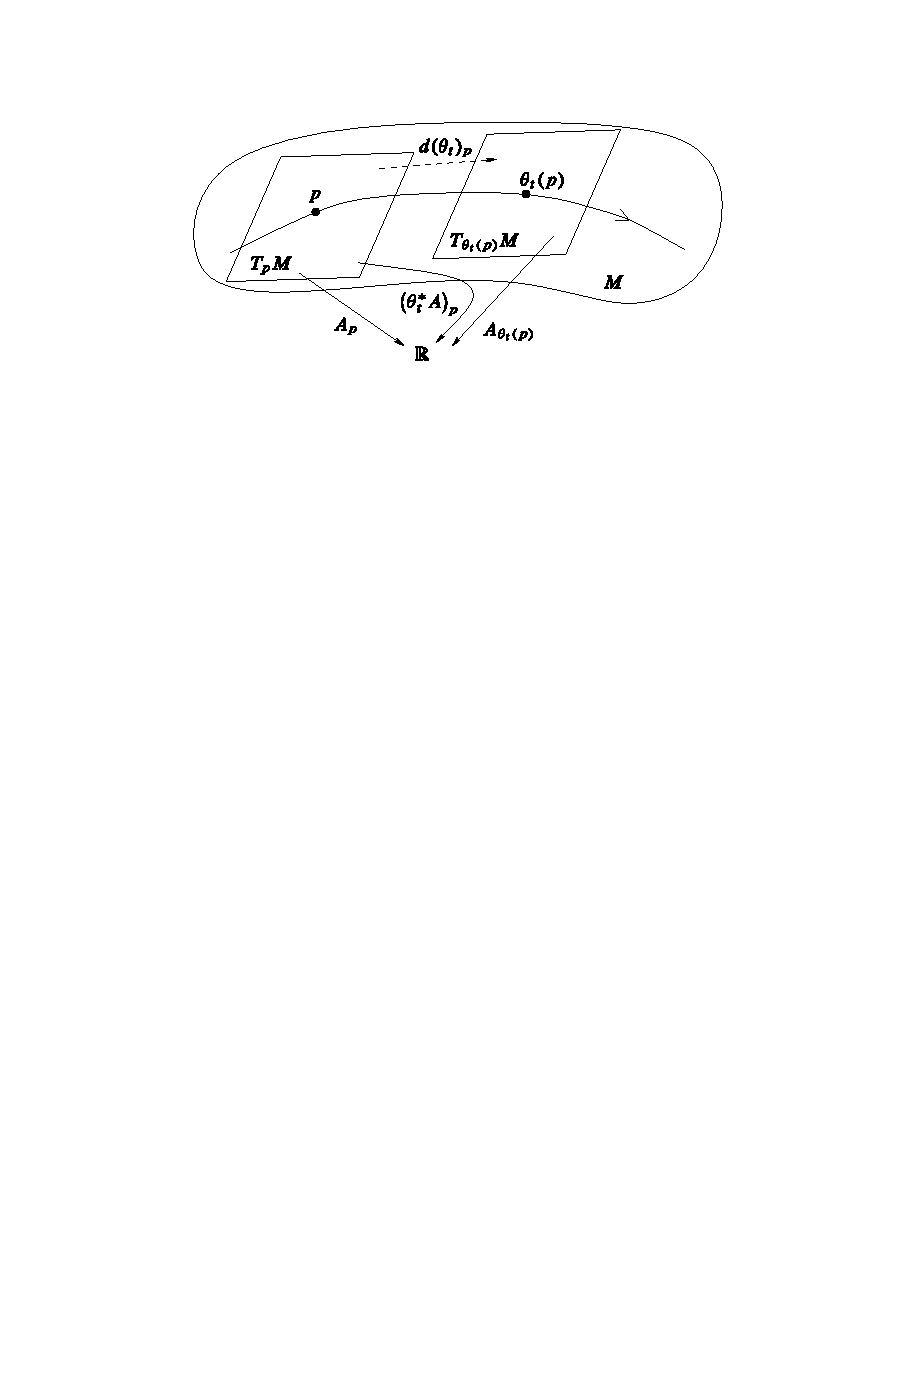
\includegraphics{pictures/Lie-derivative-tensor}
\caption{The Lie derivative of a tensor field.}
\end{figure}
\begin{lemma}
With $M,V$, and $A$ as above, the derivative $(\mathfrak{L}_VA)_p$ exists for every $p\in M$ and defines $\mathfrak{L}_VA$ as a smooth tensor field on $M$.
\end{lemma}
\begin{proposition}\label{tensor Lie derivative prop}
Let $M$ be a smooth manifold and let $V\in\X(M)$. Suppose $f$ is a smooth real-valued function $($regarded as a $0$-tensor field$)$ on $M$, and $A,B$ are smooth covariant tensor fields on $M$.
\begin{itemize}
\item[(a)] $\mathfrak{L}_Vf=Vf$.
\item[(b)] $\mathfrak{L}_V(fA)=(Vf)A+f\mathfrak{L}_VA$.
\item[(c)] $\mathfrak{L}_V(A\otimes B)=(\mathfrak{L}_VA)\otimes B+A\otimes(\mathfrak{L}_VB)$.
\item[(d)] If $X_1,\dots,X_k$ are smooth vector fields and $A$ is a smooth $k$-tensor field,
\begin{align*}
\mathfrak{L}_V\big(A(X_1,\dots,X_k)\big)=(\mathfrak{L}_VA)(X_1,\dots,X_k)+\sum_{i=1}^{k}A(X_1,\dots,\mathfrak{L}_VX_i,\dots,X_k)
\end{align*}
\end{itemize}
\end{proposition}
\begin{proof}
Let $\theta$ be the flow of $V$. For a real-valued function $f$, we can write
\[\theta^*_tf(p)=(f\circ\theta_t)(p)=f\circ\theta^{(p)}(t)\]
Thus the definition of $\mathfrak{L}_Vf$ reduces to the ordinary derivative with respect to $t$ of the composite function $f\circ\theta^{(p)}(t)$. Because $\theta^{(p)}(t)$ is an integral curve of $V$, it follows from Proposition~\ref{diff function curve} that
\[(\mathfrak{L}_Vf)_p=\frac{d}{dt}\Big|_{t=0}f\circ\theta^{(p)}=df_p\big(\dot{\theta}^{(p)}(0)\big)=df_p(V_p)=Vf(p)\]
This proves (a).\par
The other assertions can be proved by the technique we used in Theorem~\ref{Lie derivative bracket}: in a neighborhood of a regular point for $V$, if $(u^i)$ are coordinates in which $V=\partial/\partial u^1$, then it follows immediately from the definition that $\mathfrak{L}_V$ acts on a tensor field simply by taking the partial derivative of its coefficients with respect to $u^1$, and (b)--(d) all follow from the ordinary product rule. The same relations hold on the support of $V$ by continuity, and on the complement of the support because the flow of $V$ is trivial there.
\end{proof}
One consequence of this proposition is the following formula expressing the Lie
derivative of any smooth covariant tensor field in terms of Lie brackets and ordinary
directional derivatives of functions, which allows us to compute Lie derivatives
without first determining the flow.
\begin{corollary}\label{Lie derivative tensor}
If $V$ is a smooth vector field and $A$ is a smooth covariant $k$-tensor field, then for any smooth vector fields $X_1,\dots,X_k$,
\begin{align}\label{Lie derivative tensor-1}
(\mathfrak{L}_VA)(X_1,\dots,X_k)=V\big(A(X_1,\dots,X_k)\big)-\sum_{i=1}^{k}A(X_1,\dots,[V,X_i],\dots,X_k).
\end{align}
\end{corollary}
\begin{proof}
From Proposition~\ref{tensor Lie derivative prop}~(d) we have
\[(\mathfrak{L}_VA)(X_1,\dots,X_k)=\mathfrak{L}_V(A(X_1,\dots,X_k))-\sum_{i=1}^{k}A(X_1,\dots,\mathfrak{L}_VX_i,\dots,X_k).\]
Replace $\mathfrak{L}_V(A(X_1,\dots,X_k))$ by $V\big(A(X_1,\dots,X_k)\big)$ and $\mathfrak{L}_VX_i$ by $[V,X_i]$, we get the claim.
\end{proof}
\begin{corollary}\label{covector Lie diff}
If $f\in C^\infty(M)$, then $\mathfrak{L}_V(df)=d(\mathfrak{L}_Vf)$.
\end{corollary}
\begin{proof}
Using $(\ref{Lie derivative tensor-1})$, for any $X\in\X(M)$ we compute
\begin{align*}
(\mathfrak{L}_Vdf)(X)&=V\big(df(X)\big)-df([V,X])=VXf-(VX-XV)f\\
&=XVf=X(\mathfrak{L}_Vf)=d(\mathfrak{L}_Vf)(X),
\end{align*}
thus the claim follows.
\end{proof}
One drawback of formula $(\ref{Lie derivative tensor-1})$ is that in order to calculate what $\mathfrak{L}_VA$ does to vectors $v_1,\dots,v_k$ at a point $p\in M$, one must first extend them to vector fields in a neighborhood of $p$. But Corollary~\ref{covector Lie diff} lead to an easy method for computing Lie derivatives of smooth tensor fields in coordinates that avoids this problem, since any tensor field can be written locally as a linear combination of functions multiplied by tensor products of exact $1$-forms. The next example illustrates the technique.
\begin{example}
Suppose $A$ is an arbitrary smooth covariant $2$-tensor field, and $V$ is a smooth vector field. We compute the Lie derivative $\mathfrak{L}_VA$ in smooth local coordinates $(x^i)$. First, we observe that \[\mathfrak{L}_Vdx^i=d(\mathfrak{L}_Vx^i)=d(Vx^i)=dV^i.\] 
Therefore,
\begin{align*}
\mathfrak{L}_VA&=\mathfrak{L}_V(A_{ij}\,dx^i\otimes dx^j)\\
&=\mathfrak{L}_V(A_{ij})\,dx^i\otimes dx^j+A_{ij}\mathfrak{L}_V(dx^i\otimes dx^j)\\
&=VA_{ij}\,dx^i\otimes dx^j+A_{ij}\mathfrak{L}_V(dx^i)\otimes dx^j+A_{ij}\,dx^i\otimes\mathfrak{L}_V(dx^j)\\
&=VA_{ij}\,dx^i\otimes dx^j+A_{ij}\,dV^i\otimes dx^j+A_{ij}\,dx^i\otimes dV^j\\
&=VA_{ij}\,dx^i\otimes dx^j+A_{ij}\frac{\partial V^i}{\partial x^k}\,dx^k\otimes dx^j+A_{ij}\frac{\partial V^j}{\partial x^k}\,dx^i\otimes dx^k\\
&=\Big(VA_{ij}+A_{kj}\frac{\partial V^k}{\partial x^i}+A_{ik}\frac{\partial V^k}{\partial x^j}\Big)dx^i\otimes dx^j.
\end{align*}
\end{example}
Recall that the Lie derivative of a vector field $W$ with respect to $V$ is zero if and
only if $W$ is invariant under the flow of $V$ (see Theorem~\ref{vector field commute iff}). It turns out that the Lie derivative of a covariant tensor field has exactly the same interpretation. If $A$ is a smooth tensor field on $M$ and $\theta$ is a flow on $M$, we say that $A$ is \textbf{invariant under $\bm{\theta}$} if for each $t$, the map $\theta_t$ pulls $A$ back to itself wherever it is defined; more precisely, this means
\[d(\theta_t)_p^*(A_{\theta_t(p)})=A_p\]
for all $(t,p)$ in the domain of $\theta$. If $\theta$ is a global flow, this is equivalent to $\theta_t^*A=A$ for all $t\in\R$.\par
In order to prove the connection between Lie derivatives and invariance under flows, we need the following proposition, which shows how the Lie derivative can be used to compute $t$-derivatives at times other than $t=0$. It is a generalization to tensor fields of Proposition~\ref{Lie derivative t_0}.
\begin{proposition}\label{Lie der tensor t_0}
Suppose $M$ is a smooth manifold with or without boundary and $V\in\X(M)$. If $\partial M\neq\emp$, assume in addition that $V$ is tangent to $\partial M$. Let $\theta$ be the
flow of $V$. For any smooth covariant tensor field $A$ and any $(t_0,p)$ in the domain
of $\theta$,
\[\frac{d}{dt}\Big|_{t=t_0}(\theta_t^*A)_p=\big(\theta_{t_0}^*(\mathfrak{L}_VA)\big)_p\]
\end{proposition}
\begin{proof}
After expanding the definitions of the pullbacks, we see that we have to prove
\[\frac{d}{dt}\Big|_{t=0}d(\theta_t)_p^*(A_{\theta_t(p)})=d(\theta_{t_0})_p^*\big((\mathfrak{L}_VA)_{\theta_{t_0}(p)}\big)\]
Just as in the proof of Proposition~\ref{Lie derivative t_0}, the change of variables $t=s+t_0$ yields
\begin{align*}
&\frac{d}{dt}\Big|_{t=0}d(\theta_t)_p^*(A_{\theta_t(p)})=\frac{d}{ds}\Big|_{s=0}d(\theta_{s+t_0})_p^*(A_{\theta_{s+t_0}(p)})=\frac{d}{ds}\Big|_{s=0}d(\theta_{t_0})_p^*\circ d(\theta_{s})_{\theta_{t_0}(p)}^*(A_{\theta_{s}(\theta_{t_0}(p))})\\
&=d(\theta_{t_0})_p^*\frac{d}{ds}\Big|_{s=0}d(\theta_{s})_{\theta_{t_0}(p)}^*(A_{\theta_{s}(\theta_{t_0}(p))})=d(\theta_{t_0})_p^*\big((\mathfrak{L}_VA)_{\theta_{t_0}(p)}\big).
\end{align*}
\end{proof}
\begin{theorem}\label{tensor filed invariant flow iff}
Let $M$ be a smooth manifold and let $V\in\X(M)$. A smooth covariant tensor field $A$ is invariant under the flow of $V$ if and only if $\mathfrak{L}_VA=0$.
\end{theorem}
\begin{proof}
This follows from the definition of $\mathfrak{L}_VA$.
\end{proof}
\subsection{Exercise}
\begin{exercise}
Let $M$ be a smooth $n$-manifold, and let $A$ be a smooth covariant $k$-tensor field on $M$. If $(U,(x^i))$ and $(\widetilde{U},(\widetilde{x}^j))$ are overlapping smooth charts on $M$, we can write
\[A=A_{i_1\dots i_k}dx^{i_1}\otimes\cdots\otimes dx^{i_k}=\widetilde{A}_{j_1\dots j_k}d\widetilde{x}^{j_1}\otimes\cdots\otimes d\widetilde{x}^{j_k}.\]
Compute the transformation law.
\end{exercise}
\begin{proof}
Recall the formulas
\[ d\widetilde{x}^j=\frac{\partial\widetilde{x}^j}{\partial x^i}dx^i.\]
Thus
\[A=\widetilde{A}_{j_1\dots j_k}d\widetilde{x}^{j_1}\otimes\cdots\otimes d\widetilde{x}^{j_k}=\widetilde{A}_{j_1\dots j_k}\frac{\partial\widetilde{x}^{j_1}}{\partial x^{i_1}}\cdots\frac{\partial\widetilde{x}^{j_k}}{\partial x^{i_k}}dx^{i_1}\otimes\cdots\otimes dx^{i_k}.\]
This gives the claim.
\end{proof}
\begin{exercise}\label{tensor field Lie derivative bracket}
Suppose $M$ is a smooth manifold, $A$ is a smooth covariant tensor field on $M$, and $V,W\in\X(M)$. Show that
\[\mathfrak{L}_V\mathfrak{L}_WA-\mathfrak{L}_W\mathfrak{L}_VA=\mathfrak{L}_{[V,W]}A.\]
\end{exercise}
\begin{proof}
Let $X_1,\dots,X_k\in\X(M)$, then
\begin{align*}
&(\mathfrak{L}_V\mathfrak{L}_WA)(X_1,\dots,X_k)=V\big(\mathfrak{L}_WA(X_1,\dots,X_k)\big)-\sum_{i=1}^{k}\mathfrak{L}_WA(X_1,\dots,[V,X_i],\dots,X_k)\\
&=VW\big(A(X_1,\dots,X_k)\big)-\sum_{i=1}^{k}V\big(A(X_1,\dots,[W,X_i],\dots,X_k)\big)\\
&-\sum_{i=1}^{k}W\big(A(X_1,\dots,[V,X_i],\dots,X_k)\big)+\sum_{i\neq j}A(X_1,\dots,[W,X_i],\dots,[V,X_j],\dots,X_k)\\
&+\sum_{i=1}^{k}A\big(X_1,\dots,\big[W,[V,X_i]\big],\dots,X_k\big).
\end{align*}
And thus
\begin{align*}
&(\mathfrak{L}_V\mathfrak{L}_WA)(X_1,\dots,X_k)-(\mathfrak{L}_W\mathfrak{L}_VA)(X_1,\dots,X_k)=(VW-WV)\big(A(X_1,\dots,X_k)\big)\\
&\quad+\sum_{i=1}^{k}A\big(X_1,\dots,\big[W,[V,X_i]\big],\dots,X_k\big)-\sum_{i=1}^{k}A\big(X_1,\dots,\big[V,[W,X_i]\big],\dots,X_k\big).
\end{align*}
Therefore, we compute using the Jacobi identity
\begin{align*}
&(\mathfrak{L}_{[V,W]}A)(X_1,\dots,X_k)=(VW-WV)(A(X_1,\dots,X_k))-\sum_{i=1}^{k}A(X_1,\dots,\big[[V,W],X_i\big],\dots,X_k)\\
&=(VW-WV)(A(X_1,\dots,X_k))+\sum_{i=1}^{k}A(X_1,\dots,\big[[W,X_i],V\big]+\big[[X_i,V],W\big],\dots,X_k)\\
&=(VW-WV)(A(X_1,\dots,X_k))+\sum_{i=1}^{k}A(X_1,\dots,\big[W,[V,X_i]\big]-\big[[V,W],X_i\big],\dots,X_k)\\
&=(\mathfrak{L}_V\mathfrak{L}_WA)(X_1,\dots,X_k)-(\mathfrak{L}_W\mathfrak{L}_VA)(X_1,\dots,X_k).
\end{align*}
\end{proof}
\begin{exercise}
Let $M$ be a smooth manifold and $V\in\X(M)$. Show that the Lie derivative operators on covariant tensor fields, $\mathfrak{L}_V:\mathcal{T}^k(M)\to\mathcal{T}^k(M)$ for $k\geq 0$, are uniquely characterized by the following properties:
\begin{itemize}
\item[(a)] $\mathfrak{L}_V$ is linear over $\R$.
\item[(b)] $\mathfrak{L}_Vf=Vf$ for $f\in\mathcal{T}^0(M)=C^\infty(M)$. 
\item[(c)] $\mathfrak{L}_V(A\otimes B)=\mathfrak{L}_VA\otimes B+A\otimes\mathfrak{L}_VB$ for $A\in\mathcal{T}^k(M)$ and $B\in\mathcal{T}^l(M)$.
\item[(d)] $\mathfrak{L}_V(\omega(X))=(\mathfrak{L}_V\omega)(X)+\omega([V,X])$ for $\omega\in\mathcal{T}^1(M),X\in\X(M)$.
\end{itemize}
\end{exercise}
\begin{proof}
Let $\mathfrak{L}$ be an operator satisfying (a)--(d), we prove that $\mathfrak{L}=\mathfrak{L}_V$.
\begin{itemize}
\item First, by (b) and (d) we have for $\omega\in\mathcal{T}^1(M),X\in\X(M)$:
\[(\mathfrak{L}\omega)(X)=V(\omega(X))-\omega([V,X])=(\mathfrak{L}_V\omega)(X)\]
\item Then, by induction, we can prove
\[\mathfrak{L}(\omega_1\otimes\cdots\otimes \omega_k)=\mathfrak{L}_V(\omega_1\otimes\cdots\otimes\omega_k).\]
\item By taking local charts, we verify that $\mathfrak{L}=\mathfrak{L}_V$.
\end{itemize}
\end{proof}
\section{Riemannian metrics}
\subsection{Riemannian manifolds}
The most important examples of symmetric tensors on a vector space are inner products. Any inner product allows us to define lengths of vectors and angles between
them, and thus to do Euclidean geometry.\par
Transferring these ideas to manifolds, we obtain one of the most important applications
of tensors to differential geometry. Let $M$ be a smooth manifold with or without boundary. A \textbf{Riemannian metric} on $M$ is a smooth symmetric covariant $2$-tensor field on $M$ that is positive definite at each point. A \textbf{Riemannian manifold} is a pair $(M,g)$, where $M$ is a smooth manifold and $g$ is a Riemannian metric on $M$. One sometimes simply says $M$ is a Riemannian manifold if $M$ is understood to be endowed with a specific Riemannian metric. A Riemannian manifold with boundary is defined similarly.\par
If $g$ is a Riemannian metric on $M$, then for each $p\in M$, the $2$-tensor $g_p$ is an
inner product on $T_pM$. Because of this, we often use the notation $\langle v,w\rangle_g$ to denote the real number $g_p(v,w)$ for $v,w\in T_pM$.\par
In any smooth local coordinates $(x^i)$, a Riemannian metric can be written
\[g=g_{ij}\,dx^i\otimes dx^j,\]
where $(g_{ij})$ is a symmetric positive definite matrix of smooth functions. The symmetry of $g$ allows us to write $g$ also in terms of symmetric products as follows:
\begin{align*}
g=&g_{ij}\,dx^i\otimes dx^j=\frac{1}{2}(g_{ij}\,dx^i\otimes dx^j+g_{ji}\,dx^j\otimes dx^i)=\frac{1}{2}g_{ij}(dx^i\otimes dx^j+dx^j\otimes dx^i)=g_{ij}\,dx^idx^j.
\end{align*}
\begin{example}[\textbf{The Euclidean Metric}]
The simplest example of a Riemannian metric is the Euclidean metric $\widebar{g}$ on $\R^n$, given in standard coordinates by
\[\widebar{g}=\delta_{ij}\,dx^i\otimes dx^j.\]
It is common to abbreviate the symmetric product of a tensor $\alpha$ with itself by $\alpha^2$, so the Euclidean metric can also be written
\[\widebar{g}=(dx^1)^2+\cdots+(dx^n)^2.\]
\end{example}
\begin{example}[\textbf{Product Metrics}]
If $(M,g)$ and $(\widetilde{M},\widetilde{g})$ are Riemannian manifolds, we can define a Riemannian metric $\widehat{g}=g\oplus\widetilde{g}$ on the product manifold $M\times\widetilde{M}$, called the product metric, as follows:
\[\widehat{g}\big((v,\widetilde{v}),(w,\widetilde{w})\big)=g(v,w)+\widetilde{g}(\widetilde{v},\widetilde{w})\]
for any $(v,\widetilde{v}),(w,\widetilde{w})\in T_pM\oplus T_q\widetilde{M}$. Given any local coordinates $(x^1,\dots,x^n)$ for $M$ and $(y^1,\dots,y^m)$ for $\widetilde{M}$, we obtain local coordinates $(x^1,\dots,x^n,y^1,\dots,y^m)$ for $M\times\widetilde{M}$, and the product metric is represented locally by the block diagonal matrix
\[(\widehat{g}_{ij})=\begin{pmatrix}
g_{ij}&0\\
0&\widetilde{g}_{ij}
\end{pmatrix}\]
\end{example}
\begin{proposition}[\textbf{Existence of Riemannian Metrics}]
Every smooth manifold with or without boundary admits a Riemannian metric.
\end{proposition}
\begin{proof}
Let $M$ be a smooth manifold with or without boundary, and choose a covering of $M$ by smooth coordinate charts $(U_\alpha,\varphi_\alpha)$. In each coordinate domain, there
is a Riemannian metric $g_\alpha=\varphi_\alpha^*\widebar{g}$, whose coordinate expression is $\delta_{ij}\,dx^idx^j$. Let $\{\psi_\alpha\}$ be a smooth partition of unity subordinate to the cover $\{U_\alpha\}$, and define
\[g=\sum_\alpha\psi_\alpha g_\alpha,\]
with each term interpreted to be zero outside $\supp(\psi_\alpha)$. By local finiteness, there are only finitely many nonzero terms in a neighborhood of each point, so this expression defines a smooth tensor field. It is obviously symmetric, so only positivity needs to be checked. If $v\in T_pM$ is any nonzero vector, then
\[g_p(v,v)=\sum_\alpha\psi_\alpha(p)g_\alpha|_p(v,v).\]
This sum is nonnegative, because each term is nonnegative. At least one of the functions
$\psi_\alpha$ is strictly positive at $p$. Because $g_\alpha|_p(v,v)>0$, it follows that $g_p(v,v)>0$.
\end{proof}
Below are just a few of the geometric constructions that can be defined on a Riemannian manifold $(M,g)$ with or without boundary.
\begin{itemize}
\item The length or norm of a tangent vector $v\in T_pM$ is defined to be
\[|v|_g=\langle v,v\rangle_g^{1/2}=g_p(v,v)^{1/2}\]
\item The angle between two nonzero tangent vectors $v,w\in T_pM$ is the unique  $\theta\in[0,\pi]$ satisfying
\[\cos\theta=\frac{\langle v,w\rangle_g}{|v|_g|w|_g}\]
\item Tangent vectors $v,w\in T_pM$ are said to be orthogonal if $\langle v,w\rangle_g=0$. This means either one or both vectors are zero, or the angle between them is $\pi/2$.
\end{itemize}
One highly useful tool for the study of Riemannian manifolds is orthonormal frames. Let $(M,g)$ be an $n$-dimensional Riemannian manifold with or without 
boundary. Just as we did for the case of $\R^n$ in Section~\ref{vector field section}, we say a local frame $(E_1,\dots,E_n)$ for $M$ on an open subset 
$U\sub M$ is an \textbf{orthonormal frame} if the vectors $(E_1|_p,\dots,E_n|_p)$ form an orthonormal basis for $TpM$ at each point $p\in U$, or 
equivalently if $\langle E_i,E_j\rangle_g=\delta_{ij}$, in which case $g$ has the local expression
\[g=(\eps^1)^2+\cdots+(\eps^n)^2.\]
where $(\eps^i)^2$ denotes the symmetric product $(\eps^i)^2=\eps^i\otimes\eps^i$.
\begin{example}
The coordinate frame $(\partial/\partial x^i)$ is a global orthonormal frame for $\R^n$
with the Euclidean metric.
\end{example}
\begin{example}
The frame $(E_1,E_2)$ on $\R^2-\{0\}$ defined in Example~\ref{polar frame R^2} is a local orthonormal frame for $\R^2$. As we observed in Example~\ref{commute frame eg}, it is not a coordinate frame in any coordinates.
\end{example}
The next proposition is proved in just the same way as Lemma~\ref{Gram-Schmidt frame}, with the Euclidean dot product replaced by the inner product $\langle\cdot,\cdot\rangle_g$.
\begin{proposition}\label{Gram Schmidt Riemannian}
Suppose $(M,g)$ is a Riemannian manifold with or without boundary, and 
$(X_j)$ is a smooth local frame for $M$ over an open subset $U\sub M$. 
Then there is a smooth orthonormal frame $(E_j)$ over $U$ such that 
$\mathrm{span}(E_1|_p,\dots,E_j|_p)=\mathrm{span}(X_1|_p,\dots,X_j|_p)$ for each $1\leq j\leq n$ and each $p\in U$.
\end{proposition}
\begin{proof}
Applying the Gram–Schmidt algorithm to the vectors $(X_1|_p,\dots,X_n|_p)$ at each $p\in U$, we obtain an ordered $n$-tuple of rough orthonormal vector fields 
$(E_1,\dots,E_n)$ over $U$ satisfying the span conditions. Because the vectors whose norms appear in the denominators of the Gram–Schmidt formulas are nowhere 
vanishing, it follows that each vector field $E_j$ is smooth. The last statement of the proposition follows by applying this construction to any smooth local frame in a neighborhood of $p$. 
In particular, for every $p\in M$, there is a smooth orthonormal frame $(E_j)$ defined on some neighborhood of $p$.
\end{proof}
\begin{corollary}[\textbf{Existence of Local Orthonormal Frames}]\label{orthonormal frame exist}
Let $(M,g)$ be a Riemannian manifold with or without boundary. For each $p\in M$, there is a smooth orthonormal frame on a neighborhood of $p$.
\end{corollary}
Observe that Corollary~\ref{orthonormal frame exist} does not show that there are smooth coordinates on a neighborhood of $p$ for which the \textit{coordinate frame} is 
orthonormal. In fact, this is possible only when the metric is flat, that is, locally isometric to the Euclidean metric.\par
For a Riemannian manifold $(M,g)$ with or without boundary, we define the unit tangent bundle to be the subset $UTM\sub TM$ consisting of unit vectors:
\[UTM=\{(p,v)\in TM:|v|_g=1\}\]
\begin{proposition}[\textbf{Properties of the Unit Tangent Bundle}]
If $(M,g)$ is a Riemannian manifold with or without boundary, its unit tangent bundle $UTM$ is a smooth, properly embedded codimension-$1$ submanifold with 
boundary in $TM$, with $\partial(UTM)=\pi^{-1}(\partial M)$ (where $\pi:UTM\to M$ is the canonical projection). The unit tangent bundle is connected if and only if $M$ 
is connected when $n>1$, and compact if and only if $M$ is compact.
\end{proposition}
\begin{proof}
By the local orthonormal frames, we can replace $M$ by $\R^n$. If $U$ is open in $\R^n$, then the unit tangent bundle is diffeomorphic to $U\times S^{n-1}$, and therefore has codimension $1$. It is properly embedded since $S^{n-1}$ 
is properly embedded in $\R^n$. Similarly, if $U$ is a half ball in $\H^n$, we can see that the tangent bundle is diffeomorphic to $U\times S^{n-1}$, and therefore has boundary charts. 
This also proves that $\partial(UTM)=\pi^{-1}(\partial M)$.\par
For the last claim, note that the projection $\pi:UTM\to M$ is surjective and open (Proposition~\ref{smooth subm prop}), so $M$ is connect if $UTM$ is, and compact if $UTM$ is. Now we show the converse.\par
If $M$ is compact, then for any $p\in M$ we can find a comapct subset $V_p$ such that the interior of $V_p$ is open and the tangent bundle of $V_p$ is 
trivial. Then we can find 
$p_1,\dots,p_n\in M$ such that $M\sub\bigcup_{i=1}^{n}\Int(V_{p_i})$, and so 
\[UTM=\bigcup_{i=1}^{n}\pi^{-1}(\Int(V_{p_i}))\sub\bigcup_{i=1}^{n}\pi^{-1}(V_{p_i}).\]
Since the tangent bundle of $V_{p_i}$ is trivial, we have $\pi^{-1}(V_{p_i})=V_{p_i}\times S^{n-1}$. This implies that $UTM$ is compact since it is the union of 
finitely many compact subsets, so it is compact.\par
If $M$ is connected and $n>1$, then the fiber of $UTM$ is diffeomorphic to $S^{n-1}$ and so it connected. Assume that $UTM=U\cup V$ for two disjoint open subsets, then 
$M=\pi(E)=\pi(U)\cup\pi(V)$ is the union of the open subsets $\pi(U)$ and $\pi(V)$ wich are not disjoint since $M$ is connected. Let $p\in\pi(U)\cap\pi(V)$, then there 
exists $v_1\in U$, $v_2\in V$ such that $\pi(v_1)=\pi(v_2)=p$. This means $E_p\cap U\neq\emp$ and $E_p\cap V\neq\emp$, so $E_p\cap U$ and $E_p\cap V$ is a partition of $E_p$. 
But $E_p$ is connected, this is a contradiction.
\end{proof}
\subsection{Methods for constructing riemannian metrics}
\subsubsection{Pullback metrics}
Suppose $M,N$ are smooth manifolds with or without boundary, $g$ is a Riemannian metric on $N$, and $F:M\to N$ is smooth. The pullback $F^*g$ is a smooth $2$-tensor field on $M$. If it is positive definite, it is a Riemannian metric on $M$, called the pullback metric determined by $F$. The next proposition shows when this is the
case.
\begin{proposition}[\textbf{Pullback Metric Criterion}]
Suppose $F:M\to N$ is a smooth map and $g$ is a Riemannian metric on $N$. Then $F^*g$ is a Riemannian metric on $M$ if and only if $F$ is a smooth immersion.
\end{proposition}
\begin{proof}
$F^*g$ is a Riemannian metric if and only if for all $p\in M$, $F^*g(v,v)=0$ implies $v=0$ for $v\in T_pM$, wich means $dF_p(v)=0$ implies $v=0$ for any $v\in T_pM$, which 
is to say $F$ is a immersion.
\end{proof}
If the coordinate representation for an immersion is known, then the pullback metric is easy to compute using the usual algorithm for computing pullbacks.
\begin{example}
Consider the smooth map $F:\R^2\to\R^3$ given by
\[F(u,v)=(u\cos v,u\sin v,v)\]
It is a proper injective smooth immersion, and thus it is an embedding by Proposition~\ref{smooth embedd if}. The pullback metric $F^*\widebar{g}$ can be computed by substituting the coordinate functions for $F$ in place of $x,y,z$ in the formula for $\widebar{g}$:
\begin{align*}
F^*\widebar{g}&=(du\cos v)^2+(du\sin v)^2+(dv)^2\\
&=(\cos v\,du-u\sin v\,dv)^2+(\sin v\,du+u\cos v\,dv)^2+dv^2\\
&=du^2+u^2\,dv^2+dv^2=(u^2+1)^2\,du^2+dv^2.
\end{align*}
By convention, when $u$ is a real-valued function, the notation $du^2$ means the symmetric product $dudu$, not $d(u^2)$.
\end{example}
To transform a Riemannian metric under a change of coordinates, we use the
same technique as we used for covector fields: think of the change of coordinates as the identity map expressed in terms of different coordinates for the domain and
codomain, and use the formula of Corollary~\ref{tensor pullback formula}.
\begin{example}\label{Riemann metric polar}
To illustrate, we compute the coordinate expression for the Euclidean metric $\widebar{g}=dx^2+dy^2$ on $\R^2$ in polar coordinates. Substituting $x=r\cos\theta$ and $y=r\sin\theta$ and expanding, we obtain
\begin{align*}
\widebar{g}&=dx^2+dy^2=[d(r\cos\theta)]^2+[d(r\sin\theta)]^2\\
&=(\cos\theta\,dr-r\sin\theta\,d\theta)^2+(\sin\theta\,dr+r\cos\theta\,d\theta)^2\\
&=dr^2+r^2\,d\theta^2
\end{align*}
\end{example}
If $(M,g)$ and $(\widetilde{M},\widetilde{g})$ are both Riemannian manifolds, a smooth map 
$F:M\to\widetilde{M}$ is called a \textbf{Riemannian isometry} if it is a diffeomorphism 
that satisfies $F^*\widetilde{g}=g$. More generally, $F$ is called a \textbf{local isometry} 
if every point $p\in M$ has a neighborhood $U$ such that $F|_U$ is an isometry of $U$ 
onto an open subset of $\widetilde{M}$, or equivalently, if $F$ is a local diffeomorphism 
satisfying $F^*\widetilde{g}=g$.\par
If there exists a Riemannian isometry between $(M,g)$ and $(\widetilde{M},\widetilde{g})$, 
we say that they are \textbf{isometric} as Riemannian manifolds. If 
each point of $M$ has a neighborhood that is isometric to an open subset of 
$(\widetilde{M},\widetilde{g})$, then we say that $(M,g)$ is \textbf{locally isometric} 
to $(\widetilde{M},\widetilde{g})$.\par
One such property is flatness. A Riemannian $n$-manifold $(M,g)$ is said to be a 
\textbf{flat Riemannian manifold}, and $g$ is a \textbf{flat metric}, if $(M,g)$ 
is locally isometric to $(\R^n,\widebar{g})$.
\begin{proposition}
Suppose $(M,g)$ and $(\widetilde{M},\widetilde{g})$ are isometric Riemannian manifolds, then $g$ is flat if and only if $\widetilde{g}$ is flat.
\end{proposition}
The next theorem is the key to deciding whether a Riemannian metric is flat.
\begin{theorem}\label{Riemann flat iff}
For a Riemannian manifold $(M,g)$, the following are equivalent:
\begin{itemize}
\item[(a)] $g$ is flat.
\item[(b)] Each point of $M$ is contained in the domain of a smooth coordinate chart in which $g$ has the coordinate representation $g=\delta_{ij}dx^idx^j$.
\item[(c)] Each point of $M$ is contained in the domain of a smooth coordinate chart in which the coordinate frame is orthonormal.
\item[(d)] Each point of $M$ is contained in the domain of a commuting orthonormal frame.
\end{itemize}
\end{theorem}
\begin{proof}
The implications $(a)\Rightarrow(b)\Rightarrow(c)\Rightarrow(d)$ are easy consequences of the definitions. The remaining implication, $(d)\Rightarrow(a)$, follows from the canonical form theorem for commuting frames: if $(E_i)$ is a commuting orthonormal frame for $g$ on an open subset $V\sub M$, then Theorem~\ref{flow commute canonical form} implies that each $p\in V$ is contained in the domain of a smooth chart $(U,\varphi)$ in which the coordinate frame is equal to $(E_i)$. This means $\varphi_*E_i=\partial/\partial x^i$, so the diffeomorphism $\varphi:U\to\varphi(U)$ satisfies
\[\varphi^*\widebar{g}(E_i,E_j)=\widebar{g}(\varphi_*E_i,\varphi_*E_j)=\widebar{g}\Big(\frac{\partial}{\partial x^i},\frac{\partial}{\partial x^j}\Big)=\delta_{ij}=g(E_i,E_j)\]
Bilinearity then shows that $\varphi^*\widebar{g}=g$, so $\varphi$ is an isometry between $(U,\varphi|_U)$ and $\varphi(U)$ with the Euclidean metric. This shows that $g$ is flat.
\end{proof}
\subsubsection{Riemannian submanifolds}
Pullback metrics are especially important for submanifolds. If $(M,g)$ is a Riemannian
manifold with or without boundary, every submanifold $S\sub M$ (immersed or embedded, with or without boundary) automatically inherits a pullback metric $\iota^*g$, where $\iota:S\hookrightarrow M$ is inclusion. In this setting, the pullback metric is also called the \textbf{induced metric} on $S$. By definition, this means for $v,w\in T_pS$ that
\[(\iota^*g)(v,w)=g(d\iota_p(v),d\iota_p(w))=g(v,w)\]
because $d\iota_p:T_pS\to T_pM$ is our usual identification of $T_pS$ as a subspace of $T_pM$. Thus $\iota^*g$ is just the restriction of $g$ to pairs of vectors tangent to $S$. With this metric, $S$ is called a \textbf{Riemannian submanifold} (with or without boundary) of $M$.
\begin{example}
The metric $\mathring{g}=\iota^*\widebar{g}$ induced on $S^n$ by the usual inclusion $\iota:S^n\hookrightarrow\R^{n+1}$ is called the \textbf{round metric} or the \textbf{standard metric} on the sphere.
\end{example}
The next lemma describes one of the most important tools for studying Riemannian submanifolds. If 
$(\widetilde{M},\widetilde{g})$ is an $m$-dimensional smooth Riemannian manifold and $(M,g)$ is 
an $n$-dimensional submanifold (both with or without boundary), a local frame $(E_1,\dots,E_m)$ for 
$\widetilde{M}$ on an open subset $\widetilde{U}\sub\widetilde{M}$ is said to be \textbf{adapted to $\bm{M}$} if 
the first $n$ vector fields $(E_1,\dots,E_n)$ are tangent to $M$. In case $\widetilde{M}$ has empty
boundary (so that slice coordinates are available), adapted local orthonormal frames are easy to find.
\begin{proposition}[\textbf{Existence of Adapted Orthonormal Frames}]\label{Riemann embed adapted}
Let $(\widetilde{M},\widetilde{g})$ be a Riemannian manifold (without boundary), and let $(M,g)$ be 
an embedded smooth submanifold with or without boundary. Given $p\in M$, there exist a neighborhood 
$\widetilde{U}$ of $p$ in $\widetilde{M}$ and a smooth orthonormal frame for $\widetilde{M}$ on 
$\widetilde{U}$ that is adapted to $M$.
\end{proposition}
\begin{proof}
We can find a slice chart at $p$ for $M$, and use the Gram-Schmidt algorithm to a coordinate frame in slice 
coordinates to produce a orthonormal frame. By the span property, we see that this frame is adapted to $M$.
\end{proof}
Suppose $(\widetilde{M},\widetilde{g})$ is a Riemannian manifold and $(M,g)$ is a smooth submanifold 
with or without boundary in $\widetilde{M}$. Given $p\in M$, a vector $v\in T_p\widetilde{M}$ is said to be
\textbf{normal to $\bm{M}$} if $\langle v,w\rangle=0$ for every $w\in T_pM$. The space of all vectors 
normal to $M$ at $p$ is a subspace of $T_p\widetilde{M}$, called the \textbf{normal space at $\bm{p}$} and 
denoted by $N_pM=(T_pM)^{\bot}$. At each $p\in M$, the ambient tangent space $T_p\widetilde{M}$ splits as an 
orthogonal direct sum $T_p\widetilde{M}=T_pM\oplus N_pM$. A section $N$ of the ambient tangent bundle 
$T\widetilde{M}|_{M}$ is called a \textbf{normal vector field along $\bm{M}$} if $N_p\in N_pM$ for each $p\in M$. The set
\[NM=\coprod_{p\in M}N_pM\]
is called the normal bundle of $M$.
\begin{proposition}[\textbf{The Normal Bundle to a Riemannian Submanifold}]\label{Riemann normal bundle}
If $\widetilde{M}$ is a Riemannian $m$-manifold and $M$ is an immersed or embedded $n$-dimensional 
submanifold with or without boundary, then $NM$ is a smooth rank-$(m-n)$ vector subbundle of the ambient 
tangent bundle $T\widetilde{M}|_M$. There are smooth bundle homomorphisms
\[\pi^{\top}:T\widetilde{M}|_M\to TM,\quad \pi^{\bot}:T\widetilde{M}|_M\to NM\]
called the \textbf{tangential} and \textbf{normal projections}, that for each $p\in M$ restrict to
orthogonal projections from $T_p\widetilde{M}$ to $T_pM$ and $N_pM$, respectively.
\end{proposition}
\begin{proof}
Given any point $p\in M$, Theorem~\ref{immerse local embedd} shows that there is a neighborhood 
$U$ of $p$ in $M$ that is embedded in $\widetilde{M}$, and then Proposition~\ref{Riemann embed adapted} 
shows that there is a smooth orthonormal frame $(E_1,\dots,E_m)$ that is adapted to $U$ on some 
neighborhood $\widetilde{U}$ of $p$ in $\widetilde{M}$. This means that the restrictions of 
$(E_1,\dots,E_n)$ to $\widetilde{U}\cap U$ form a local orthonormal frame for $M$. Given such an 
adapted frame, the restrictions of the last $m-n$ vector fields $(E_{n+1},\dots,E_m)$ to $M$ form 
a smooth local frame for $NM$, so it follows from Lemma~\ref{vector subbundle crit} that $NM$ is a 
smooth subbundle.\par
The bundle homomorphisms $\pi^{\top}$ and $\pi^{\bot}$ are defined pointwise as orthogonal 
projections onto the tangent and normal spaces, respectively, which shows that they are uniquely 
defined. In terms of an adapted orthonormal frame, they can be written
\[\pi^{\top}(X^iE_i)=X^1E_1+\cdots+X^nE_n,\quad \pi^{\bot}(X^iE_i)=X^{n+1}E_{n+1}+\cdots+X^mE_m,\]
which shows that they are smooth.
\end{proof}
In case $\widetilde{M}$ is a manifold with boundary, the preceding constructions do not always work, 
because there is not a fully general construction of slice coordinates in that case. However, there 
is a satisfactory result in case the submanifold is the boundary itself, using boundary coordinates 
in place of slice coordinates.\par
Suppose $(M,g)$ is a Riemannian manifold with boundary. We will always consider $\partial M$ to be a 
Riemannian submanifold with the induced metric.
\begin{proposition}[\textbf{Existence of Outward-Pointing Normal}]\label{Riemann outward normal}
If $(M,g)$ is a smooth Riemannian manifold with boundary, the normal bundle to $\partial M$ is a 
smooth rank-$1$ vector bundle over $\partial M$, and there is a unique smooth outward-pointing unit 
normal vector field along all of $\partial M$. By this, we see that $N(\partial M)$ is a rank-$1$ 
vector subbundle of $TM|_{\partial M}$.
\end{proposition}
\begin{proof}
We can always construct a global smooth outward-pointing vector field by taking $-\partial/\partial x^n$ 
in boundary coordinates in a neighborhood of each boundary point, and gluing together with a partition 
of unity. By the Gram-Schmidt process, we may assume that this vector field is normal to $\partial M$.
\end{proof}
Computations on a submanifold $M\sub\widetilde{M}$ are usually carried out most conveniently in terms of 
a \textbf{smooth local parametrization}: this is a smooth map $X:U\to\widetilde{M}$, where $U$ is an open 
subset of $\R^n$ (or $\H^n$ in case $M$ has a boundary), such that $X(U)$ is an open subset of $M$, and such 
that $X$, regarded as a map from $U$ into $M$, is a diffeomorphism onto its image. Note that we can think of 
$X$ either as a map into $M$ or as a map into $\widetilde{M}$, both maps are typically denoted by the same 
symbol $X$. If we put $V=X(U)\sub\widetilde{M}$ and $\varphi=X^{-1}:V\to U$, then $(V,\varphi)$ is a smooth 
coordinate chart on $M$.
Suppose $(M,g)$ is a Riemannian submanifold of $(\widetilde{M},\widetilde{g})$ and $X:U\to\widetilde{M}$ is a
smooth local parametrization of $M$. The coordinate representation of $g$ in these coordinates is given by 
the following $2$-tensor field on $U$:
\[\varphi_*g=X^*g=X^*\iota^*\widetilde{g}=(\iota\circ X)^*\widetilde{g}.\]
Since $\iota\circ X$ is just the map $X$ itself, regarded as a map into $\widetilde{M}$, this is really just 
$X^*\widetilde{g}$. The simplicity of the formula for the pullback of a tensor field makes this expression
exceedingly easy to compute, once a coordinate expression for $\widetilde{g}$ is known. For example, if $M$ is 
an immersed $n$-dimensional Riemannian submanifold of $\R^m$ and $X:U\to\R^m$ is a smooth local parametrization 
of $M$, the induced metric on $U$ is just
\[g=X^*\widebar{g}=\sum_{i=1}^{m}(dX^i)^2=\sum_{i=1}^{m}\Big(\sum_{j=1}^{n}\frac{\partial X^i}{\partial u^j}du^j\Big)^2=\sum_{i=1}^{m}\sum_{j,k=1}^{n}\frac{\partial X^i}{\partial u^i}\frac{\partial X^i}{\partial u^k}du^jdu^k.\]
\begin{example}[\textbf{Induced Metrics in Graph Coordinates}]
Let $U\sub\R^n$ be an open subset, and let $S\sub\R^{n+1}$ be the graph of a smooth function $f:U\to\R$. The 
map $X:U\to\R^{n+1}$ given by $X(u^1,\dots,u^n)=(u^1,\dots,u^n,f(u))$ is a smooth global parametrization of 
$S$ and the induced metric on $S$ is given in graph coordinates by
\[X^*\widebar{g}=X^*\big((dx^1)^2+\cdots+(dx^{n+1})^2\big)=(du^1)^2+\cdots+(du^n)^2+(df)^2\]
For example, the upper hemisphere of $S^2$ is parametrized by the map $X:\B^2\to\R^3$ given by
\[X(u,v)=(u,v,\sqrt{1-u^2-v^2})\]
In these coordinates, the round metric can be written
\[\mathring{g}=X^*\widebar{g}=du^2+dv^2+\Big(\frac{u\,du+v\,dv}{\sqrt{1-u^2-v^2}}\Big)^2=\frac{(1-v^2)\,du^2+(1-u^2)\,dv^2+2uv\,dudv}{1-u^2-v^2}.\]
\end{example}
\begin{example}[\textbf{Induced Metrics on Surfaces of Revolution}]\label{surfaces of revolution induced metric}
Let $C$ be an embedded one dimensional submanifold of the half-plane $\{(r,z):r>0\}$ and let $S_C$ 
be the surface of revolution generated by $C$ as described in Example~\ref{surfaces of revolution}. To compute 
the induced metric on $S_C$, choose any smooth local parametrization $\gamma(t)=(a(t),b(t))$ for $C$, and note 
that the map $X(t,\theta)=(a(t)\cos\theta,a(t)\sin\theta,b(t))$ yields a smooth local parametrization of $S_C$, 
provided that $(t,\theta)$ is restricted to a sufficiently small open subset of the plane. Thus we can compute
\begin{align*}
X^*\widebar{g}&=\big(da(t)\cos\theta\big)^2+\big(da(t)\sin\theta\big)^2+\big(db(t)\big)^2\\
&=\big(a'(t)\cos\theta\,dt-a(t)\sin\theta\,d\theta\big)^2+\big(a'(t)\sin\theta\,dt+a(t)\cos\theta\,d\theta\big)^2+\big(b'(t)\,dt\big)^2\\
&=\big(a'(t)^2+b'(t)^2\big)dt^2+a(t)^2d\theta^2
\end{align*}
In particular, if $\gamma$ is a unit-speed curve, meaning that $|\gamma'(t)|^2=1$, this reduces to the simple formula $dt^2+a(t)^2d\theta^2$.\par
Here are some familiar examples of surfaces of revolution.
\begin{itemize}
\item[(a)] The embedded torus is the surface of revolution generated by the circle $(r-2)^2+z^2=1$. 
Using the unit-speed parametrization $\gamma(t)=(2+\cos t+\sin t)$ for the circle, we obtain the formula 
$dt^2+(2+\cos\theta)^2d\theta^2$ for the induced metric.
\item[(b)] The unit sphere $($minus the north and south poles$)$ is a surface of revolution whose 
generating curve is the semicircle parametrized by $\gamma(t)=(\sin t,\cos t)$ for $0<t<\pi$. The 
induced metric is $dt^2+(\sin t)^2d\theta^2$.
\item[(c)] The unit cylinder $x^2+y^2=1$ is a surface of revolution whose generating curve is the 
vertical line parametrized by $\gamma(t)=(1,t)$ for $t\in\R$. The induced metric is $dt^2+d\theta^2$.
\end{itemize}
\end{example}
\begin{example}[\textbf{The $\bm{n}$-Torus as a Riemannian Submanifold}]
The smooth covering map $X:\R^n\to T^n$ defined by $X(u^1,\cdots,u^n)=(\cos u^1,\sin u^1,\cdots,\cos u^n,\sin u^n)$ restricts to a 
smooth local parametrization on any sufficiently small open subset of $\R^n$, and the induced metric is 
\[X^*\widebar{g}=d(\cos u^1)^2+d(\sin u^1)^2+\cdots+d(\cos u^n)^2+d(\sin u^n)^2=(du^1)^2+\cdots+(du^n)^2.\]
Therefore the induced metric on $T^n$ is flat.
\end{example}
\subsubsection{Riemannian products}
Next we consider products. If $(M_1,g_1)$ and $(M_2,g_2)$ are Riemannian manifolds, the product manifold 
$M_1\times M_2$ has a natural Riemannian metric $g=g_1\oplus g_2$, called the product metric, defined by
\[g_{(p_1,p_2)}((v_1,v_2),(w_1,w_2))=g_1|_{p_1}(v_1,w_1)+g_2|_{p_2}(v_2,w_2).\]
where $(v_1,v_2)$ and $(w_1,w_2)$ are elements of $T_{p_1}M_1\oplus T_{p_2}M_2$, which is naturally 
identified with $T_{(p_1,p_2)}(M_1\times M_2)$. Smooth local coordinates $(x^1,\dots,x^n)$ for $M_1$ and 
$(x^{n+1},\dots,x^{n+m})$ for $M_2$ give coordinates $(x^1,\dots,x^{n+m})$ for $M_1\oplus M_2$. In terms 
of these coordinates, the product metric has the local expression $g=g_{ij}dx^idx^j$, where $(g_{ij})$ is 
the block diagonal matrix
\[(g_{ij})=\begin{pmatrix}
(g_1)&0\\
0&(g_2)
\end{pmatrix}\]
Product metrics on products of three or more Riemannian manifolds are defined similarly.\par
Here is an important generalization of product metrics. Suppose $(M_1,g_1)$ and $(M_2,g_2)$ are two 
Riemannian manifolds, and $f:M_1\to\R^+$ is a strictly positive smooth function. The \textbf{warped product} 
$M_1\times_f M_2$ is the product manifold $M_1\times M_2$ endowed with the Riemannian metric $g=g_1\oplus f^2g_2$, 
defined by
\[g_{(p_1,p_2)}((v_1,v_2),(w_1,w_2))=g_1|_{p_1}(v_1,w_1)+f(p_1)^2g_2|_{p_2}(v_2,w_2).\]
where $(v_1,v_2),(w_1,w_2)\in T_{p_1}M_1\oplus T_{p_2}M_2$ as before. A wide variety of metrics can be constructed in this way; here are just a few examples.
\begin{example}\label{Riemann metric R^n in polar}
If we let $\rho$ denote the standard coordinate function on $\R^+\sub\R$, then the map 
$\varPhi(\rho,\omega)=\rho\omega$ gives an isometry from the warped product $\R^+\times_{\rho}S^{n-1}$ 
to $\R^n\setminus\{0\}$ with its Euclidean metric. To see this, we use the parametrization
\[X:(\rho,x^1,\dots,x^{n-1})\mapsto(\rho,x^1,\dots,x^{n-1},\sqrt{1-|x|^2})\]
of $\R^+\times S^{n-1}$ to compute the pull back metric $\varPhi^*\widebar{g}$ as follows:
\begin{align*}
&(\varPhi\circ X)^*\widebar{g}=d(\rho x^1)^2+\cdots+d(\rho x^{n-1})^2+d(\rho\sqrt{1-|x|^2})^2\\
&=(x^1\,d\rho+\rho\,dx^1)^2+\cdots+(x^{n-1}\,d\rho+\rho\,dx^{n-1})^2+\Big(\sqrt{1-|x|^2}d\rho-\rho\frac{x^1dx^1+\cdots+x^{n-1}dx^{n-1}}{\sqrt{1-|x|^2}}\Big)^2\\
&=d\rho^2+\rho^2((dx^1)^2+\cdots+(dx^{n-1})^2)+\rho^2\frac{(x^1dx^1+\cdots+x^{n-1}dx^{n-1})^2}{1-|x|}\\
&\quad+2\rho(x^1dx^1d\rho+\cdots+x^{n-1}dx^{n-1}d\rho)-2\rho(x^1dx^1d\rho+\cdots+x^{n-1}dx^{n-1}d\rho)\\
&=d\rho^2+\rho^2\Big((dx^1)^2+\cdots+(dx^{n-1})^2+\frac{(x^1dx^1+\cdots+x^{n-1}dx^{n-1})^2}{1-|x|}\Big)\\
&=d\rho^2+\rho^2\mathring{g}
\end{align*}
\end{example}
\begin{example}
Every surface of revolution can be expressed as a warped product, as follows. Let 
$H$ be the half-plane $\{(r,z):r>0\}$, let $C\sub H$ be an embedded smooth $1$-dimensional submanifold, 
and let $S_C\sub\R^3$ denote the corresponding surface of revolution as in 
Example~\ref{surfaces of revolution induced metric}. Endow $C$ with the Riemannian metric induced from 
the Euclidean metric on $H$, and let $S^1$ be endowed with its standard metric. Let $f:C\to\R$ be the 
distance to the $z$-axis: $f(r,z)=r$. Then from Example~\ref{surfaces of revolution induced metric} we 
see that $S_C$ is isometric to the warped product $C\times_f S^1$.
\end{example}
\subsubsection{Riemannian submersions}
Unlike submanifolds and products of Riemannian manifolds, which automatically inherit 
Riemannian metrics of their own, quotients of Riemannian manifolds inherit Riemannian 
metrics only under very special circumstances. Now we see what those circumstances 
are.\par
Suppose $\widetilde{M}$ and $M$ are smooth manifolds, $\pi:\widetilde{M}\to M$ is a 
smooth submersion, and $\widetilde{g}$ is a Riemannian metric on $\widetilde{M}$. By 
the submersion level set theorem, each fiber $\widetilde{M}_y=\pi^{-1}(y)$ is a properly 
embedded smooth submanifold of $\widetilde{M}$. At each point $x\in\widetilde{M}$, we 
define two subspaces of the tangent space $T_x\widetilde{M}$ as follows: the 
\textbf{vertical tangent space} at $x$ is
\[V_x=\ker d\pi_x=T_x(\widetilde{M}_{\pi(x)})\]
(that is, the tangent space to the fiber containing $x$), and the \textbf{horizontal tangent 
space} at $x$ is its orthogonal complement:
\[H_x=(V_x)^\bot\]
Then the tangent space $T_x\widetilde{M}$ decomposes as an orthogonal direct sum 
$T_x\widetilde{M}=H_x\oplus V_x$. Note that the vertical space is well defined for 
every submersion, because it does not refer to the metric; but the horizontal 
space depends on the metric.\par
A vector field on $\widetilde{M}$ is said to be a \textbf{horizontal vector field} if its 
value at each point lies in the horizontal space at that point; a \textbf{vertical vector 
field} is defined similarly. Given a vector field $X$ on $M$, a vector field $\widetilde{X}$ 
on $\widetilde{M}$ is called a \textbf{horizontal lift} of $X$ if $\widetilde{X}$ is 
horizontal and $\pi$-related to $X$.\par
The next proposition is the principal tool for doing computations on Riemannian 
submersions.
\begin{proposition}[\textbf{Properties of Horizontal Vector Fields}]\label{Riemann horizontal vector field}
Let $\widetilde{M}$ and $M$ be smooth manifolds, let $\pi:\widetilde{M}\to M$ be a 
smooth submersion, and let $\widetilde{g}$ be a Riemannian metric on $\widetilde{M}$.
\begin{itemize}
\item[(a)] Every smooth vector field $W$ on $\widetilde{M}$ can be expressed 
uniquely in the form $W=W^H+W^V$, where $W^H$ is horizontal, $W^V$ is vertical, 
and both $W^H$ and $W^V$ are smooth.
\item[(b)] Every smooth vector field on $M$ has a unique smooth horizontal lift 
to $\widetilde{M}$.
\item[(c)] For every $x\in\widetilde{M}$ and $v\in H_x$, there is a vector field $X\in\X(M)$ 
whose horizontal lift $\widetilde{X}$ satisfies $\widetilde{X}_x=v$.
\end{itemize}
\end{proposition}
\begin{proof}
Let $p\in\widetilde{M}$ be arbitrary. Because $\pi$ is a smooth submersion, the rank 
theorem shows that there exist smooth coordinate charts $(\widetilde{U},(x^i))$ 
centered at $p$ and $(U,(y^j))$ centered at $\pi(x)$ in which $\pi$ has the 
coordinate representation
\[\pi(x^1,\dots,x^n,x^{n+1},\dots,x^{m})=(x^1,\dots,x^n)\]
where $m=\dim\widetilde{M}$ and $n=\dim M$. It follows that at each point $q\in\widetilde{U}$, 
the vertical space $V_q$ is spanned by the vectors $(\partial/\partial x^{n+1}|_q,\dots,\partial/\partial x^{m}|_q)$. 
(It probably will not be the case, however, that the horizontal space is 
spanned by the other $n$ basis vectors.) If we apply the Gram–Schmidt algorithm 
to the ordered frame $(\partial/\partial x^{n+1}|,\dots,\partial/\partial x^{m},\partial/\partial x^1,\dots,\partial/\partial x^n)$, 
we obtain a smooth orthonormal frame $(E_1,\dots,E_m)$ on $\widetilde{U}$ 
such that $V_q$ is spanned by $(E_1|_q,\dots,E_{m-n}|_q)$ at each $q\in\widetilde{U}$. It follows that $H_q$ 
is spanned by $(E_{n-m+1}|_q,\dots,E_{m}|_q)$.\par
Now let $W\in\X(\widetilde{M})$ be arbitrary. At each point $q\in\widetilde{M}$, $W_q$ 
can be written uniquely as a sum of a vertical vector plus a horizontal vector, 
thus defining a decomposition $W=W^V+W^H$ into rough vertical and horizontal 
vector fields. To see that they are smooth, just note that in a neighborhood 
of each point we can express $W$ in terms of a frame $(E_1,\dots,E_m)$ of the 
type constructed above as $W=W^1E_1+\cdots+W^mE_m$ with smooth coefficients $(W^i)$, 
and then it follows that
\[W^V=W^1E_1+\cdots+W^{m-n}E_{m-n},\quad W^H=W^{n-m+1}E_{n-m+1}+\cdots+W^mE_{m},\]
both of which are smooth.\par
Let $X\in\X(M)$ be arbitrary. By the coordinate representation constructed above, we see that 
$d\pi$ is just the projection onto $H_q$, which is spanned by $(E_{m-n+1},\dots,E_m)$. Therefore 
we can use $X$ to define a rough horizontal vector field on $\widetilde{M}$. From the 
local coordinate presentation we see that $\widetilde{X}$ is smooth.\par
For every $x\in\widetilde{M}$ and $v\in H_x$, we can choose coordinates as above, and construct a 
vector field on $M$ such that $X_{\pi(x)}=d\pi(v)$. Then by the construction above 
the horizontal lift $\widetilde{X}$ satisfies $\widetilde{X}_x=v$.
\end{proof}
The fact that every horizontal vector at a point of $\widetilde{M}$ can be extended 
to a horizontal lift on all of $\widetilde{M}$ (part (c) of the preceding 
proposition) is highly useful for computations. It is important to be aware, 
though, that not every horizontal vector field on $\widetilde{M}$ is a horizontal 
lift, as the next example shows.
\begin{example}
Let $\pi:\R^2\to\R$ be the projection map $\pi(x,y)=yx$, and let $W$ be the smooth vector 
field $y\partial/\partial x$ on $\R^2$. Then $W$ is horizontal, but there is no 
vector field on $\R$ whose horizontal lift is equal to $W$.
\end{example}
Now we can identify some quotients of Riemannian manifolds that inherit metrics 
of their own. Let us begin by describing what such a metric should look like. 
Suppose $(\widetilde{M},\widetilde{g})$ and $(M,g)$ are Riemannian manifolds, 
and $\pi:\widetilde{M}\to M$ is a smooth submersion. Then $\pi$ is said to be 
a \textbf{Riemannian submersion} if for each $x\in\widetilde{M}$, the differential 
$d\pi_x$ restricts to a linear isometry from $H_x$ onto $T_{\pi(x)}M$. In other 
words, $\widetilde{g}_x(v,w)=g_{\pi(x)}(d\pi_x(v),d\pi_x(w))$ whenever $v,w\in H_x$.
\begin{example}[\textbf{Riemannian Submersions}]
\mbox{}
\begin{itemize}
\item[(a)] The projection $\pi:\R^{n+k}\to\R^n$ onto the first $n$ coordinates is 
a Riemannian submersion if $\R^{n+k}$ and $\R^n$ are both endowed with their 
Euclidean metrics.
\item[(b)] If $M$ and $N$ are Riemannian manifolds and $M\times N$ is endowed 
with the product metric, then both projections $\pi_M:M\times N\to M$ and $\pi_N:M\times N\to N$ 
are Riemannian submersions.
\item[(c)] If $M\times_fN$ is a warped product manifold, then the projection $\pi_M:M\times_fN\to M$ 
is a Riemannian submersion, but $\pi_N$ typically is not.
\end{itemize}
\end{example}
Given a Riemannian manifold $(\widetilde{M},\widetilde{g})$ and a surjective 
submersion $\pi:\widetilde{M}\to M$, it is almost never the case that there is 
a metric on $M$ that makes $\pi$ into a Riemannian submersion. It is not hard 
to see why: for this to be the case, whenever $p_1,p_2\in\widetilde{M}$ are two points in 
the same fiber $\pi^{-1}(y)$, the linear maps $(d\pi_{p_i}|_{H_{p_i}})^{-1}:T_yM\to H_{p_i}$ 
both have to pull $\widetilde{g}$ back to the same inner product on $T_yM$.
There is, however, an important special case in which there is such a metric. Suppose 
$\pi:\widetilde{M}\to M$ is a smooth surjective submersion, and $G$ is a group 
acting on $\widetilde{M}$. We say that the action is \textbf{vertical} if every 
element $\varphi\in G$ takes each fiber to itself, meaning that $\pi(\varphi\cdot p)=\pi(p)$ 
for all $p\in M$. The action is \textbf{transitive on fibers} if for each $p,q\in M$ 
such that $\pi(p)=\pi(q)$, there exists $\varphi\in G$ such that $\varphi\cdot p=q$.
If in addition $\widetilde{M}$ is endowed with a Riemannian metric, the action 
is said to be an \textbf{isometric action} or an \textbf{action by isometries}, 
and the metric is said to be \textbf{invariant under $\bm{G}$}, if the map $x\mapsto\varphi\cdot x$ 
is an isometry for each $\varphi\in G$. In that case, provided the action is 
effective (so that different elements of $G$ define different isometries of $\widetilde{M}$), 
we can identify $G$ with a subgroup of $\Iso(\widetilde{M},g)$. Since an isometry 
is, in particular, a diffeomorphism, every isometric action is an action by diffeomorphisms.
\begin{theorem}\label{Riemann submersion induce metric}
Let $(\widetilde{M},\widetilde{g})$ be a Riemannian manifold, let $\pi:\widetilde{M}\to M$ 
be a surjective smooth submersion, and let $G$ be a group acting on $\widetilde{M}$. 
If the action is isometric, vertical, and transitive on fibers, then there is a 
unique Riemannian metric on $M$ such that $\pi$ is a Riemannian submersion.
\end{theorem}
The next corollary describes one important situation to which the preceding theorem
applies.
\begin{corollary}\label{Riemann orbit space induce metric}
Suppose $(\widetilde{M},\widetilde{g})$ is a Riemannian manifold, and $G$ is a Lie 
group acting smoothly, freely, properly, and isometrically on $\widetilde{M}$. Then 
the orbit space $M=\widetilde{M}/G$ has a unique smooth manifold structure and 
Riemannian metric such that $\pi:\widetilde{M}\to M$ is a Riemannian submersion.
\end{corollary}
\begin{proof}
Under the given hypotheses, the quotient manifold theorem shows that $M$ has a 
unique smooth manifold structure such that the quotient map $\widetilde{M}\to\widetilde{M}/G$ 
is a smooth submersion. It follows easily from the definitions in that case that 
the given action of $G$ on $\widetilde{M}$ is vertical and transitive on fibers. 
Since the action is also isometric, Theorem~\ref{Riemann submersion induce metric} shows that $M$ inherits a 
unique Riemannian metric making $\pi$ into a Riemannian submersion.
\end{proof}
Here is an important example of a Riemannian metric defined in this way.
\begin{example}[\textbf{The Fubini-Study Metric}]
Let $n$ be a positive integer, and consider the complex projective space $\CP^n$. The 
map $\pi:\C^{n+1}\setminus\{0\}\to\CP^n$ sending each point in $\C^{n+!}\setminus\{0\}$ 
to its span is a surjective smooth submersion. Identifying $\C^{n+1}$ with $\R^{2n+2}$ 
endowed with its Euclidean metric, we can view the unit sphere $S^{2n+1}$ with 
its round metric $\mathring{g}$ as an embedded Riemannian submanifold of $\C^{n+1}\setminus\{0\}$. 
Let $p:S^{2n+1}\to\CP^n$ denote the restriction of the map $\pi$. Then $p$ is 
smooth, and it is surjective, because every $1$-dimensional complex subspace 
contains elements of unit norm. We need to show that it is a submersion. Let $z_0\in S^{2n+1}$ 
and set  $\zeta_0=p(z_0)\in\CP^n$. Since $\pi$ is a smooth submersion, it has a 
smooth local section $\sigma:U\to\C^{n+1}\setminus\{0\}$ defined on a neighborhood 
$U$ of $\zeta_0$. Let $\widetilde{\sigma}$ be the radial projection of $\sigma$ 
onto the sphere: $\widetilde{\sigma}=\sigma/|\sigma|$. Then $\widetilde{\sigma}$ is a 
local section of $p$. By Theorem~\ref{submersion iff local section} we see that $p$ 
is a submersion.\par
Define an action of $S^1$ on $S^{2n+1}$ by complex multiplication
\[\lambda\cdot(z^1,\dots,z^{n+1})=(\lambda z^1,\dots,\lambda z^{n+1})\]
for $\lambda\in S^1$ (viewed as a complex number of norm $1$) and $(z^1,\dots,z^{n+1})\in S^{2n+1}$. 
This is easily seen to be isometric, vertical, and transitive on fibers of $p$. By 
Theorem~\ref{Riemann submersion induce metric}, therefore, there is a unique 
metric on $\CP^n$ such that the map $p:S^{2n+1}\to\CP^n$ is a Riemannian submersion. 
This metric is called the \textbf{Fubini-Study metric}.
\end{example}
\subsubsection{Riemannian coverings}
Another important special case of Riemannian submersions occurs in the context of
covering maps. Suppose $(\widetilde{M},\widetilde{g})$ and $(M,g)$ are Riemannian 
manifolds. A smooth covering map $\pi:\widetilde{M}\to M$ is called a \textbf{Riemannian 
covering} if it is a local isometry.
\begin{proposition}\label{Riemann cover induce metric}
Suppose $\pi:\widetilde{M}\to M$ is a smooth normal covering map, and $\widetilde{g}$ 
is any metric on $\widetilde{M}$ that is invariant under all covering automorphisms. 
Then there is a unique metric $g$ on $M$ such that $\pi$ is a Riemannian covering.
\end{proposition}
\begin{proof}
Proposition~\ref{smooth cover prop} shows that $\pi$ is a surjective smooth 
submersion. The automorphism group acts vertically by definition, and we know 
that it acts transitively on fibers when the covering is normal. It then follows 
from Theorem~\ref{Riemann submersion induce metric} that there is a unique metric 
$g$ on $M$ such that $\pi$ is a Riemannian submersion. Since a Riemannian 
submersion is a local isometry, it follows that $\pi$ is a Riemannian covering.
\end{proof}
\begin{proposition}\label{Riemann discrete action induce metric}
Suppose $(\widetilde{M},\widetilde{g})$ is a Riemannian manifold, and $\Gamma$ is a 
discrete Lie group acting smoothly, freely, properly, and isometrically on $\widetilde{M}$. 
Then $\widetilde{M}/\Gamma$ has a unique Riemannian metric such that the quotient 
map $\pi:\widetilde{M}\to\widetilde{M}/\Gamma$ is a normal Riemannian covering.
\end{proposition}
\begin{proof}
Proposition~\ref{Lie discrete covering map} shows that $\pi$ is a smooth normal 
covering map, and Proposition~\ref{Riemann cover induce metric} shows that 
$\widetilde{M}/\Gamma$ has a unique Riemannian metric such that $\pi$ is a 
Riemannian covering.
\end{proof}
\begin{corollary}
Suppose $(\widetilde{M},\widetilde{g})$ and $(M,g)$ are connected Riemannian 
manifolds, $\pi:\widetilde{M}\to M$ is a normal Riemannian covering map, and $\Gamma=\Aut_{\pi}(\widetilde{M})$. 
Then $M$ is isometric to $\widetilde{M}/\Gamma$.
\end{corollary}
\begin{proof}
Proposition~\ref{Lie group coveing group discrete} shows that with the discrete 
topology, $\Gamma$ is a discrete Lie group acting smoothly, freely, and properly 
on $\widetilde{M}$, and then Proposition~\ref{Lie discrete covering map} shows 
that $\widetilde{M}/\Gamma$ is a smooth manifold and the quotient map $q:\widetilde{M}\to\widetilde{M}/\Gamma$ 
is a smooth normal covering map. The fact that both $\pi$ and $q$ are normal 
coverings implies that $\Gamma$ acts transitively on the fibers of both maps, so 
the two maps are constant on each other's fibers. Proposition~\ref{smooth quotient unique} 
then implies that there is a diffeomorphism $F:M\to\widetilde{M}/\Gamma$ that 
satisfies $q\circ F=\pi$. Because both $q$ and $\pi$ are local isometries, $F$ is 
too, and because it is bijective it is a global isometry.
\end{proof}
\begin{example}
The two-element group $\{\pm 1\}$ acts smoothly, freely, properly, and isometrically 
on $S^n$ by multiplication. We know that the quotient space is diffeomorphic to 
the real projective space $\RP^n$ and the quotient map $q:S^n\to\RP^n$ is a smooth 
normal covering map. Because the action is isometric, Proposition~\ref{Riemann discrete action induce metric} 
shows that there is a unique metric on $\RP^n$ such that $q$ is a Riemannian covering.
\end{example}
\begin{example}[\textbf{The Open M\"obius Band}]
The \textbf{open M\"obius band} is the quotient space $M=\R^2/\Z$, where $\Z$ acts on $\R^2$ by 
\[n\cdot(x,y)=(x+n,(-1)^ny).\]
This action is smooth, free, proper, and isometric, and therefore $M$ inherits a 
flat Riemannian metric such that the quotient map is a Riemannian covering.
\end{example}
\subsection{Basic constructions on Riemannian manifolds}
\subsubsection{Raising and lowering indices}
One elementary but important property of Riemannian metrics is that they allow us
to convert vectors to covectors and vice versa. Given a Riemannian metric $g$ on $M$,
we define a bundle homomorphism $\widehat{g}:TM\to T^*M$ by setting
\[\widehat{g}(v)(w)=g_p(v,w)\]
for each $p\in M$ and each $v,w\in T_pM$. To see that this is a smooth bundle 
homomorphism, it is easiest to consider its action on smooth vector fields:
\[\widehat{g}(X)(Y)=g(X,Y)\for X,Y\in\X(M).\]
Because $\widehat{g}(X)(Y)$ is linear over $C^\infty(M)$ as a function of $Y$, it 
follows from the tensor characterization lemma (Lemma~\ref{tensor field smooth crit}) 
that $\widehat{g}(X)$ is a smooth covector field, and because $\widehat{g}(X)$ is 
linear over $C^\infty(M)$ as a function of $X$, this defines $\widehat{g}$ as a 
smooth bundle homomorphism by the bundle homomorphism characterization lemma (Lemma~\ref{vector bundle homo char}). 
As usual, we use the same symbol for both the pointwise bundle homomorphism 
$\widehat{g}:TM\to T^*M$ and the linear map on sections $\widehat{g}:\X(M)\to\X^*(M)$.\par
Note that $\widehat{g}$ is injective at each point, because $\widehat{g}(v)=0$ 
for some $v\in T_pM$ implies
\[0=\widehat{g}(v)(v)=g(v,v)\]
which in turn implies $v=0$. For dimensional reasons, therefore, $\widehat{g}$ is 
bijective, so it is a bundle isomorphism (Proposition~\ref{vector bundle smooth iso iff bi}).\par
In any smooth coordinates $(x^i)$, we can write $g=g_{ij}dx^idx^j$. Thus, if $X$ 
and $Y$ are smooth vector fields, we have
\[\widehat{g}(X)(Y)=g_{ij}X^iY^j\]
which implies that the covector field $\widehat{g}(X)$ has the coordinate 
expression
\[\widehat{g}(X)=g_{ij}X^idx^j\]
In other words, $\widehat{g}$ is the bundle homomorphism whose matrix with respect 
to coordinate frames for $TM$ and $T^*M$ is the same as the matrix of $g$ itself.\par
It is customary to denote the components of the covector field $\widehat{g}(X)$ by
\[\widehat{g}=X_jdx^j,\quad\text{where }X_j=g_{ij}X^i.\]
Because of this, one says that $\widehat{g}(X)$ is obtained from $X$ by lowering 
an index. The notation $X^\flat$ is frequently used for $\widehat{g}(X)$, because 
the symbol $\flat$ is used in musical notation to indicate that a tone is to be 
lowered.\par
The matrix of the inverse map $\widehat{g}^{-1}:T^*M\to TM$ is thus the inverse 
of $(g_{ij})$. We let $(g^{ij})$ denote the matrix-valued 
function whose value at $p\in M$ is the inverse of the matrix $(g_{ij}(p))$, so 
that
\[g^{ij}g_{jk}=g_{kj}g^{ji}=\delta^i_k\]
Because $g_{ij}$ is a symmetric matrix, so is $g^{ij}$, as you can easily check. 
Thus for a covector field $\omega\in\X^*(M)$, the vector field 
$\widehat{g}^{-1}(\omega)$ has the coordinate representation
\[\widehat{g}^{-1}(\omega)=\omega^i\frac{\partial}{\partial x^i},\quad\text{where }\omega^i=\omega_ig^{ij}.\]
We use the notation $\sharp$ for $\widehat{g}^{-1}$, and say that $\omega^\sharp$ 
is obtained from $\omega$ by raising an index. Because the symbols $\flat$ and 
$\sharp$ are borrowed from musical notation, these two inverse isomorphisms are 
frequently called the \textbf{musical isomorphisms}. A handy mnemonic device for 
keeping the flat and sharp operations straight is to remember that the value of 
$\omega^\sharp$ at each point is a vector, which we visualize as a (sharp) arrow; 
while the value of $X^\flat$ is a covector, which we visualize by means of its 
(flat) level sets.\par
The most important use of the sharp operation is to reinstate the \textbf{gradient} as a 
vector field on Riemannian manifolds. For any smooth real-valued function $f$ on 
a Riemannian manifold $(M,g)$ with or without boundary, we define a vector field 
called the gradient of $f$ by
\[\grad f:=(df)^\sharp=\widehat{g}^{-1}(df).\]
Unraveling the definitions, we see that for any $X\in\X(M)$, the gradient satisfies
\[\langle\grad f,X\rangle_g=\widehat{g}(\grad f)(X)=df(X)=Xf.\]
Thus $\grad f$ is the unique vector field that satisfies
\[\langle\grad f,X\rangle_g=Xf\for X\in\X(M),\]
or equivalently,
\begin{align}\label{Riemann grad def}
\langle\grad f,\cdot\rangle_g=df.
\end{align}
In smooth coordinates, $\grad f$ has the expression
\[\grad f=g^{ij}\frac{\partial f}{\partial x^i}\frac{\partial}{\partial x^j}.\]
In particular, this shows that gradf is smooth. On Rn with the Euclidean metric,
this reduces to
\[\grad f=\delta^{ij}\frac{\partial f}{\partial x^i}\frac{\partial}{\partial x^j}=\sum_{i=1}^{n}\frac{\partial f}{\partial x^i}\frac{\partial}{\partial x^i}.\]
Thus our new definition of the gradient in this case coincides with the gradient from
elementary calculus. In other coordinates, however, the gradient does not generally
have the same form.
\begin{example}
Let us compute the gradient of a function $f\in C^\infty(\R^2)$ with respect to the Euclidean metric in polar coordinates. From Example~\ref{Riemann metric polar} we see that the matrix of $\widebar{g}$ in polar coordinates is $(\begin{smallmatrix}
1&0\\
0&r^2
\end{smallmatrix})$, so its inverse matrix is $(\begin{smallmatrix}
1&0\\
0&r^{-2}
\end{smallmatrix})$.
Inserting this into the formula for the gradient, we obtain
\[\grad f=\frac{\partial f}{\partial r}\frac{\partial}{\partial r}+\frac{1}{r^2}\frac{\partial f}{\partial\theta}\frac{\partial}{\partial\theta}.\]
\end{example}
The next proposition shows that the gradient has the same geometric interpretation
on a Riemannian manifold as it does in Euclidean space. If $f$ is a smooth
real-valued function on a smooth manifold $M$, recall that a point $p\in M$ is 
called a \textbf{regular point} of $f$ if $df_p\neq 0$, and a \textbf{critical point} of $f$ 
otherwise; and a level set $f^{-1}(c)$ is called a regular level set if every point of 
$f^{-1}(c)$ is a regular point of $f$. Corollary~\ref{subm level set} shows that 
each regular level set is an embedded smooth hypersurface in $M$.
\begin{proposition}
Suppose $(M,g)$ is a Riemannian manifold, $f\in C^{\infty}(M)$, and $\mathcal{R}\sub M$ 
is the set of regular points of $f$. For each $c\in\R$, the set $M_c=f^{-1}(c)\cap\mathcal{R}$, 
if nonempty, is an embedded smooth hypersurface in $M$, and $\grad f$ is everywhere 
normal to $M_c$.
\end{proposition}
\begin{proof}
From the definition of gradient we have
\[\langle\grad f|_p,v\rangle=df_p(v).\]
By Proposition~\ref{tangent space level set} we see that $T_pM_c=\ker df$, therefore the claim holds.
\end{proof}
The flat and sharp operators can be applied to tensors of any rank, in any 
index position, to convert tensors from covariant to contravariant or 
vice versa. Formally, this operation is defined as follows: if $F$ is any 
$(k,l)$-tensor and $i\in\{1,\dots,k+l\}$ is any covariant index position 
for $F$ (meaning that the $i$-th argument is a vector, not a covector), we 
can form a new tensor $F^{\sharp}$ of type $(k+1,l-1)$ by setting
\[F^\sharp(\alpha_1,\dots,\alpha_{k+l})=F(\alpha_1,\dots,\alpha_i^{\sharp},\dots,\alpha_{k+l})\]
whenever $\alpha_1,\dots,\alpha_{k+l}$ are vectors or covectors as appropriate. 
In any local frame, the components of $F^{\sharp}$ are obtained by multiplying 
the components of $F$ by $g^{kl}$ and contracting one of the indices of $g^{kl}$ 
with the $i$-th index of $F$. Similarly, if $i$ is a contravariant index 
position, we can define a $(k-1,l+1)$-tensor $F^{\flat}$ by
\[F^\flat(\alpha_1,\dots,\alpha_{k+l})=F(\alpha_1,\dots,\alpha_i^{\flat},\dots,\alpha_{k+l})\]
In components, it is computed by multiplying by $g_{kl}$ and contracting.\par
For example, if $A$ is a mixed $3$-tensor given in terms of a local frame by
\[A=A^{j}_{ik}\eps^i\otimes E_j\otimes\eps^k\]
we can lower its middle index to obtain a covariant $3$-tensor $A^{\flat}$ with
components
\[A_{ijk}=g_{jl}A_{ik}^{l}.\]
Another important application of the flat and sharp operators is to extend 
the trace operator to covariant tensors. If $h$ is any covariant $k$-tensor 
field on a Riemannian manifold with $k\geq 2$, we can raise one of its 
indices (say the last one for definiteness) and obtain a $(1,k-1)$-tensor $h^{\sharp}$. 
The trace of $h^{\sharp}$ is thus a well-defined covariant $(k-2)$-tensor 
field. We define the trace of $h$ with respect to $g$ as
\[\tr_gh=\tr(h^\sharp).\]
Sometimes we may wish to raise an index other than the last, or to take 
the trace on a pair of indices other than the last covariant and 
contravariant ones. In each such case, we will say in words what is meant.\par
The most important case is that of a covariant $2$-tensor field. In this case, 
$h^{\sharp}$ is a $(1,1)$-tensor field, which can equivalently be regarded 
as an endomorphism field, and $\tr_gh$ is just the ordinary trace of this 
endomorphism field. In terms of a basis, this is
\[\tr_gh=h^i_i=g^{ij}h_{ij}.\]
In particular, in an orthonormal frame this is the ordinary trace of the 
matrix $(h_{ij})$ (the sum of its diagonal entries); but if the frame is 
not orthonormal, then this trace is different from the ordinary trace.\par
If $g$ is a Riemannian metric on $M$ and $(E_i)$ is a local frame on $M$, there 
is a potential ambiguity about what the expression $(g^{ij})$ represents: 
we have defined it to mean the inverse matrix of $(g_{ij})$, but one could 
also interpret it as the components of the contravariant $2$-tensor field 
$g^{\sharp\sharp}$ obtained by raising both of the indices of $g$. But these 
two interpretations lead to the same result:
\[g^{\sharp\sharp}=g^{lk}g^{ki}g_{ij}=g^{lj},\]
so we do not distinguish them.
\subsubsection{Inner products of tensors}
A Riemannian metric yields, by definition, an inner product on tangent 
vectors at each point. Because of the musical isomorphisms between vectors 
and covectors, it is easy to carry the inner product over to covectors as 
well. Suppose $g$ is a Riemannian metric on $M$, and $x\in M$. We can define 
an inner product on the cotangent space $T^*_xM$ by
\[\langle\omega,\eta\rangle_g=\langle\omega^\sharp,\eta^{\sharp}\rangle_g\]
To see how to compute this, we just use the basis formula for the sharp operator, 
together with the relation $g_{kl}g^{ki}=g_{lk}g^{ki}=\delta_l^i$, to obtain
\begin{align*}
\langle\omega,\eta\rangle_g&=g_{kl}(g^{ki}\omega_i)(g^{lj}\eta_j)\\
&=\delta^i_lg^{lj}\omega_i\eta_j\\
&=g^{ij}\omega_j\eta_j
\end{align*}
In other words, the inner product on covectors is represented by the 
inverse matrix $(g^{ij})$. Using our conventions for raising and lowering 
indices, this can also be written
\[\langle\omega,\eta\rangle=\omega_i\eta^j=\omega^i\eta_j.\]
Now the following result is immediate from the definition.
\begin{proposition}
Let $(M,g)$ be a Riemannian manifold with or without boundary, let $(E_i)$ 
be a local frame for $M$, and let $(\eps^i)$ be its dual coframe. Then the 
following are equivalent:
\begin{itemize}
\item[(a)] $(E_i)$ is orthonormal.
\item[(b)] $(\eps^i)$ is orthonormal.
\item[(c)] $(\eps^i)^{\sharp}=E_i$ for each $i$. 
\end{itemize}
\end{proposition}
This construction can be extended to tensor bundles of any rank, as the 
following proposition shows. First a bit of terminology: if $E\to M$ is a 
smooth vector bundle, a \textbf{smooth fiber metric} on $E$ is an inner 
product on each fiber $E_p$ that varies smoothly, in the sense that for any 
(local) smooth sections $\sigma,\tau$ of $E$, the inner product $(\sigma,\tau)$ 
is a smooth function.
\begin{proposition}[\textbf{Inner Products of Tensors}]
Let $(M,g)$ be an $n$-dimensional Riemannian manifold with or without 
boundary. There is a unique smooth fiber metric on each tensor bundle 
$T^{(k,l)}TM$ with the property that if $\alpha_1,\dots,\alpha_{k+l}$, 
$\beta_1,\dots,\beta_{k+l}$ are vector or covector fields as appropriate, 
then
\begin{align}\label{Riemann tensor inner prod-1}
\langle\alpha_1\otimes\cdots\otimes\alpha_{k+l},\beta_1\otimes\cdots\otimes\beta_{k+l}\rangle=\langle\alpha_{1},\beta_1\rangle\cdots\langle\alpha_{k+l},\beta_{k+l}\rangle.
\end{align}
With this inner product, if $(E_1,\dots,E_n)$ is a local orthonormal frame 
for $TM$ and $(\eps^1,\dots,\eps^n)$ is the corresponding dual coframe, 
then the collection of tensor fields $E_{i_1}\otimes\cdots\otimes E_{i_k}\otimes\eps^{j_1}\otimes\cdots\otimes\eps^{j_l}$ 
as all the indices range from $1$ to $n$ forms a local orthonormal frame 
for $T^{(k,l)}(T_pM)$. In terms of any (not necessarily orthonormal) frame, 
this fiber metric satisfies
\begin{align}\label{Riemann tensor inner prod-2}
\langle F,G\rangle=g_{i_1r_1}\cdots g_{i_kr_k}g^{j_1s_1}\cdots g^{j_ls_l}F^{i_1\dots i_k}_{j_1\dots j_l}G^{r_1\dots r_k}_{s_1\dots s_l}.
\end{align}
If $F$ and $G$ are both covariant, this can be written
\[\langle F,G\rangle=F_{j_1\dots j_l}G^{j_1\dots j_l},\]
where the last factor on the right represents the components of $G$ with 
all of its indices raised:
\[G^{j_1\dots j_l}=g^{j_1s_1}\cdots g^{j_ls_l}G_{j_1\dots j_l}.\]
\end{proposition}
\begin{proof}
The formula $(\ref{Riemann tensor inner prod-1})$ is just the definition of the inner product. With this, all is clear.
\end{proof}
\subsection{The Riemannian distance function}
One of the most important tools that a Riemannian metric gives us is the ability to define lengths of curves. Suppose $(M,g)$ is a Riemannian manifold with or without
boundary. If $\gamma:[a,b]\to M$ is a piecewise smooth curve segment, the length of $\gamma$ is
\[L_g(\gamma)=\int_{a}^{b}|\gamma'(t)|_gdt\]
Because $|\gamma'(t)|_g$ is continuous at all but finitely many values of $t$, and has well-defined limits from the left and right at those points, the integral is well defined.
\begin{proposition}\label{Riemann isometry length}
suppose $(M,g)$ and $(\widetilde{M},\widetilde{g})$ are Riemannian manifolds with or without boundary, and $F:M\to\widetilde{M}$ is a local isometry. Then $L_{\widetilde{g}}(F\circ\gamma)=L_g(\gamma)$ for every piecewise smooth curve segment $\gamma$ in $M$.
\end{proposition}
\begin{proof}
This follows from the observation
\begin{align*}
|(F\circ\gamma)'(t)|_{\widetilde{g}}^2&=|dF_{\gamma(t)}\big(\gamma'(t)\big)|_{\widetilde{g}}=\widetilde{g}\big[dF_{\gamma(t)}\big(\gamma'(t)\big),dF_{\gamma(t)}\big(\gamma'(t)\big)\big]\\
&=(F^*\widetilde{g})\big(\gamma'(t),\gamma'(t)\big)=g\big(\gamma'(t),\gamma'(t)\big)=|\gamma'(t)|^2_g
\end{align*}
since $F$ is a local isometry.
\end{proof}
It is an extremely important fact that length is independent of 
parametrization in the following sense. In 
Section~\ref{cotangent bundle section} we defined a reparametrization of 
a piecewise smooth curve segment $\gamma:[a,b]\to M$ to be a curve 
segment of the form $\widetilde{\gamma}=\gamma\circ\varphi$ where 
$\varphi:[c,d]\to[a,b]$ is a diffeomorphism. We also call them 
\textbf{admissible curves}.
\begin{proposition}[\textbf{Parameter Independence of Length}]
Let $(M,g)$ be a Riemannian manifold with or without boundary, and let $\gamma:[a,b]\to M$ be a piecewise smooth curve segment. If $\widetilde{\gamma}$ is a reparametrization of $\gamma$, then $L_g(\gamma)=L_g(\widetilde{\gamma})$.
\end{proposition}
\begin{proof}
First suppose that $\gamma$ is smooth, and $\varphi:[c,d]\to[a,b]$ is a diffeomorphism
such that $\widetilde{\gamma}=\gamma\circ\varphi$. The fact that $\varphi$ is a diffeomorphism implies that either $\varphi'>0$ or $\varphi'<0$ everywhere. Let us assume that $\varphi'>0$. We have
\begin{align*}
L_g(\widetilde{\gamma})&=\int_{c}^{d}|\widetilde{\gamma}'(t)|_gdt=\int_{c}^{d}|(\gamma\circ\varphi)'(t)|_gdt\\
&=\int_{c}^{d}|\varphi'(t)\gamma'\big(\varphi(t)\big)|_gdt=\int_{c}^{d}|\gamma'\big(\varphi(t)\big)|_g\varphi'(t)dt\\
&=\int_{a}^{b}|\gamma'(s)ds=L_g(\gamma).
\end{align*}
In the case $\varphi'<0$, we just need to introduce two sign changes into the above calculation. The sign changes once when $\varphi'(t)$ is moved outside the absolute value signs, because $|\varphi'(t)|=-\varphi'(t)$. Then it changes again when we change variables, because $\varphi$ reverses the direction of the integral. Since the two sign changes cancel each other, the result is the same.\par
If $\gamma$ is only piecewise smooth, we just apply the same argument on each subinterval on which it is smooth.
\end{proof}
Suppose $\gamma:[a,b]\to M$ is an admissible curve. The \textbf{arc-length function} 
of $\gamma$ is the function $s:[a,b]\to\R$ defined by
\[s(t)=L_g(\gamma|_{[a,t]})=\int_{a}^{t}|\gamma'(u)|_gdu.\]
It is continuous everywhere, and it follows from the fundamental theorem of 
calculus that it is smooth wherever $\gamma$ is, with derivative $s'(t)=|\gamma'(t)|_g$. 
For this reason, if $\gamma:I\to M$ is any smooth curve (not necessarily a 
curve segment), we define the \textbf{speed} of $\gamma$ at any time 
$t\in I$ to be the scalar $|\gamma'(t)|_g$. We say that $\gamma$ is a 
\textbf{unit-speed curve} if $|\gamma'(t)|_g=1$ for all $t$, and a 
\textbf{constant-speed curve} if $|\gamma'(t)|_g$ is constant. 
If $\gamma$ is a piecewise smooth curve, we say that $\gamma$ has unit 
speed if $|\gamma'(t)|_g=1$ wherever $\gamma$ is smooth.\par
If $\gamma:[a,b]\to M$ is a unit-speed admissible curve, then its 
arc-length function has the simple form $s(t)=t-a$. If, in addition, 
its parameter interval is of the form $[0,b]$ for some $b>0$, then the 
arc-length function is $s(t)=t$. For this reason, a unit-speed admissible 
curve whose parameter interval is of the form $[0,b]$ is said to be 
\textbf{parametrized by arc length}.
\begin{proposition}
Suppose $(M,g)$ is a Riemannian manifold with or without boundary.
\begin{itemize}
\item[(a)] Every regular curve in $M$ has a unit-speed forward 
reparametrization.
\item[(b)] Every admissible curve in $M$ has a unique forward 
reparametrization by arc length.
\end{itemize}
\end{proposition}
\begin{proof}
Suppose $\gamma:I\to M$ is a regular curve. Choose an arbitrary $t_0\in I$, 
and define $s:I\to\R$ by
\[s(t)=\int_{t_0}^{t}|\gamma'(u)|_gdu.\]
Since $s'(t)=|\gamma'(t)|_g>0$, it follows that $s$ is a strictly increasing 
local diffeomorphism, and thus maps $I$ diffeomorphically onto an interval $I'\sub\R$. 
If we let $\varphi=s^{-1}:I'\to I$, then $\widetilde{\gamma}:=\gamma\circ\varphi$ 
is a forward reparametrization of $\gamma$, and the chain rule gives
\[|\widetilde{\gamma}'(u)|_g=|\varphi'(s)\gamma'(\varphi(s))|_g=\frac{1}{s'(\varphi(s))}|\gamma'(\varphi(s))|_g=1.\]
Thus $\widetilde{\gamma}$ is a unit-speed reparametrization of $\gamma$.\par
Now let $\gamma:I\to M$ be an admissible curve. We prove the existence 
statement in part (b) by induction on the number of smooth segments in 
an admissible partition. If $\gamma$ has only one smooth segment, then it 
is a regular curve segment, and (b) follows by applying (a) in the 
special case $I=[a,b]$ and choosing $t_0=a$. Assuming that the result is 
true for admissible curves with $k$ smooth segments, suppose $\gamma$ has 
an admissible partition $(a_0,\dots,a_{k+1})$. The inductive hypothesis 
gives piecewise regular homeomorphisms $\varphi_1:[0,c]\to[a,a_k]$ and 
$\varphi_2:[0,d]\to[a_k,b]$ such that $\gamma\circ\varphi_1$ is an arc-length 
reparametrization of $\gamma|_{[a,a_k]}$ and $\gamma\circ\varphi_2$ is an 
arc-length reparametrization of $\gamma|_{[a_k,b]}$. If we define 
$\widetilde{\varphi}:[0,c+d]\to[a,b]$ by
\[\widetilde{\varphi}(s)=\begin{cases}
\varphi_1(s)&s\in[0,c],\\
\varphi_2(s-c)&s\in[c,c+d],
\end{cases}\]
then $\gamma\circ\psi$ is a reparametrization of $\gamma$ by arc length.\par
To prove uniqueness, suppose that $\widetilde{\gamma}=\gamma\circ\varphi$ 
and $\widehat{\gamma}=\gamma\circ\psi$ are both forward reparametrizations 
of $\gamma$ by arc length. Since both have the same length, it follows that 
$\varphi$ and $\psi$ both have the same parameter domain $[0,c]$, and thus 
both are piecewise regular homeomorphisms from $[0,c]$ to $[a,b]$. If we 
define $\eta=\varphi^{-1}\circ\psi$, then $\eta$ is a piecewise regular 
increasing homeomorphism satisfying $\widehat{\gamma}=\gamma\circ\varphi\circ\eta=\widetilde{\gamma}\circ\eta$. 
The fact that both $\widetilde{\gamma}$ and $\widehat{\gamma}$ are of unit 
speed implies the following equality for all $s\in[0,c]$ except the finitely 
many values at which $\widetilde{\gamma}$ or $\eta$ is not smooth:
\[1=|\widehat{\gamma}'(s)|_g=|\widetilde{\gamma}'(\eta(s))\eta'(s)|_g=|\widetilde{\gamma}'(\eta(s))|_g\eta'(s)=\eta'(s).\]
Since $\eta$ is continuous and $\eta(0)=0$, it follows that $\eta(s)=s$ for all 
$s\in[0,c]$, and thus $\widetilde{\gamma}=\widehat{\gamma}$.
\end{proof}
Using curve segments as measuring tapes, we can define distances between points on 
a Riemannian manifold. Suppose $(M,g)$ is a connected Riemannian manifold. 
(The theory is most straightforward when $\partial M=\emp$, so we assume 
that for the rest of this section.) For any $p,q\in M$, the \textbf{Riemannian distance} 
from $p$ to $q$, denoted by $d_g(p,q)$, is defined to be the infimum of 
$L_g(\gamma)$ over all piecewise smooth curve segments $\gamma$ from $p$ 
to $q$. Because any pair of points in $M$ can be joined by a piecewise 
smooth curve segment (Proposition~\ref{connect by smooth curve}), this 
is well defined.
\begin{proposition}
Suppose $(M,g)$ and $(\widetilde{M},\widetilde{g})$ are connected Riemannian manifolds and $F:M\to\widetilde{M}$ is a Riemannian isometry. Then
\[d_g(p,q)=d_{\widetilde{g}}(F(p),F(q))\]
for all $p,q\in M$.
\end{proposition}
\begin{proof}
This follows from Proposition~\ref{Riemann isometry length}, since any curve on $M$ or $\widetilde{M}$ can be mapped isometrically to the other manifodl.
\end{proof}
\begin{remark}
Note that unlike lengths of curves, Riemannian distances are not necessarily preserved by local isometries.
\end{remark}
\begin{example}
In $(\R^n,\widebar{g})$, It can be shown that any straight line segment is the shortest piecewise smooth curve segment between its endpoints. Therefore, the distance function $d_{\widebar{g}}$ is equal to the usual Euclidean distance:
\[d_{\widebar{g}}(x,y)=|x-y|.\]
\end{example}
We will see below that the Riemannian distance function turns $M$ into a metric space whose topology is the same as the given manifold topology. The key is the following technical lemma, which shows that every Riemannian metric is locally comparable to the Euclidean metric in coordinates.
\begin{lemma}\label{Riemann metric lem}
Let $g$ be a Riemannian metric on an open subset $U\sub\R^n$. Given a compact subset $K\sub U$, there exist positive constants $c,C$ such that for all $x\in K$ and all $v\in T_x\R^n$,
\begin{align}\label{Riemann metric-1}
c|v|_{\widebar{g}}\leq|v|_{g}\leq C|v|_{\widebar{g}}
\end{align}
\end{lemma}
\begin{proof}
For any compact subset $K\sub U$, let $L\sub T\R^n$ be the set
\[L=\{(x,v)\in T\R^n:x\in K,|v|_{\widebar{g}}=1\}\]
Under the canonical identification of $T\R^n$ with $\R^n\times\R^n$, $L$ is just the product set $K\times S^{n-1}$ and therefore is compact. Because the norm $|v|_g$ is continuous and strictly positive on $L$, there are positive constants $c$, $C$ such that $c\leq|v|_g\leq C$ whenever $(x,v)\in L$. If $x\in K$ and $v$ is a nonzero vector in $T_x\R^n$, let $\lambda=|v|_{\widebar{g}}$. Then $(x,\lambda^{-1}v)\in L$, so by homogeneity of the norm,
\[|v|_g=\lambda|\lambda^{-1}v|_g\leq\lambda C=C|v|_{\widebar{g}}\]
A similar computation shows that $|v|_g\geq c|v|_{\widebar{g}}$. The same inequalities are trivially true when $v=0$.
\end{proof}
\begin{theorem}[\textbf{Riemannian Manifolds as Metric Spaces}]\label{Riemann metric space}
Let $(M,g)$ be a connected Riemannian manifold. With the Riemannian distance function, $M$ is a metric space whose metric topology is the same as the original manifold topology.
\end{theorem}
\begin{proof}
It is immediate from the definition that $d_g(p,q)\geq 0$. Because every constant curve segment has length zero, it follows that $d_g(p,p)=0$; and $d_g(p,q)=d_g(q,p)$ follows from the fact that any curve segment from $p$ to $q$ can be reparametrized to go from $q$ to $p$. Suppose $\gamma_1$ and $\gamma_2$ are piecewise smooth curve segments from $p$ to $q$ and $q$ to $r$, respectively, and let $\gamma$ be a piecewise smooth curve segment that first follows $\gamma_1$ and then follows $\gamma_2$ (reparametrized if necessary). Then
\[d_g(p,r)\leq L_g(\gamma)=L_g(\gamma_1)+L_g(\gamma_2).\]
Taking the infimum over all such $\gamma_1$ and $\gamma_2$, we find that $d_g(p,r)\leq d_g(p,q)+d_g(q,r)$.
\begin{figure}[htbp]
\centering
\begin{minipage}[b]{200pt}
\centering
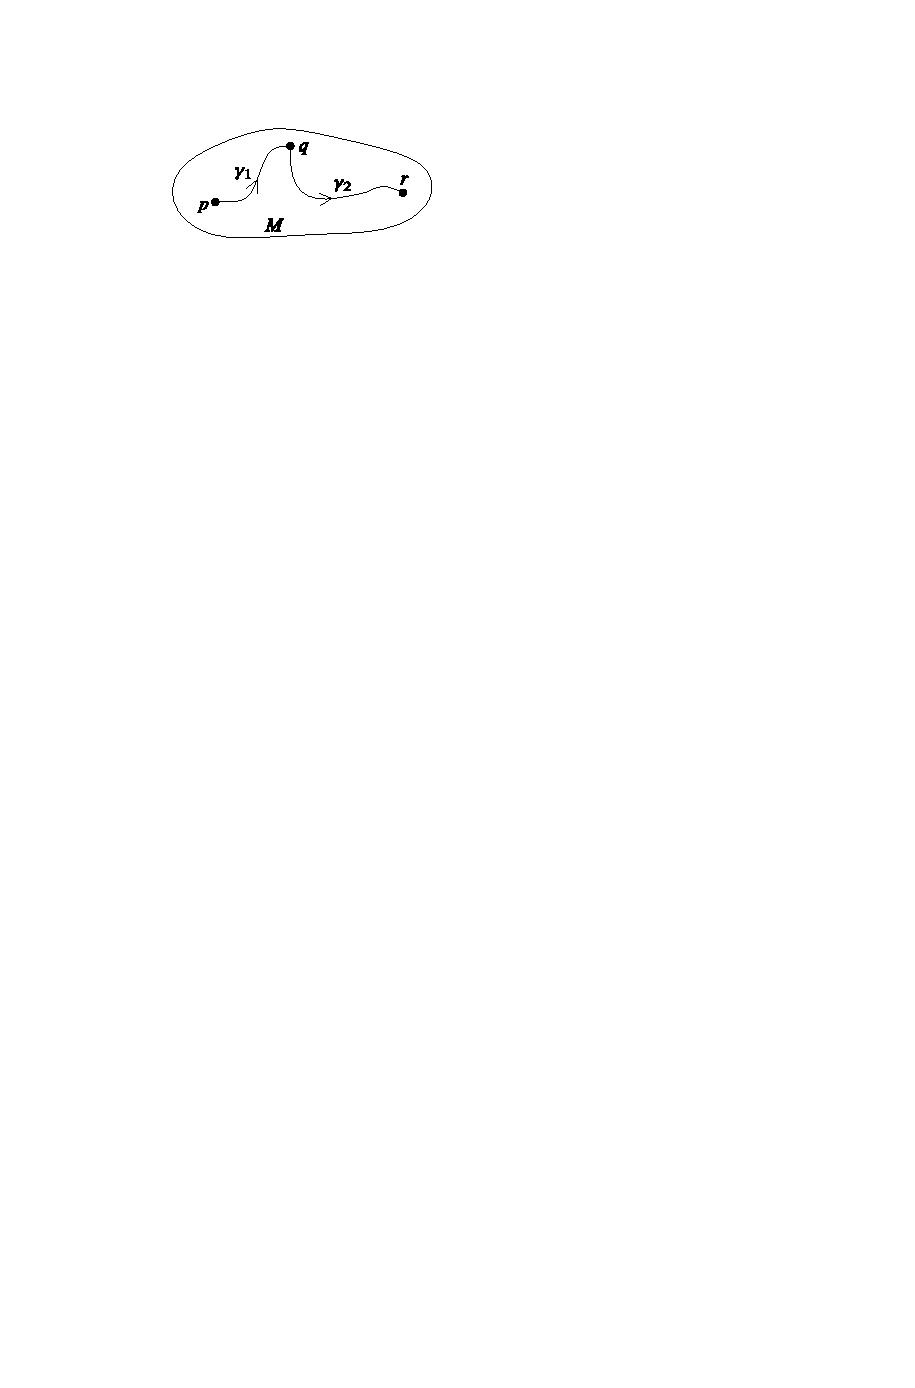
\includegraphics{pictures/Riemann-metric-1}
\caption{The triangle inequality.}
\end{minipage}
\hspace{20pt}
\begin{minipage}[b]{200pt}
\centering
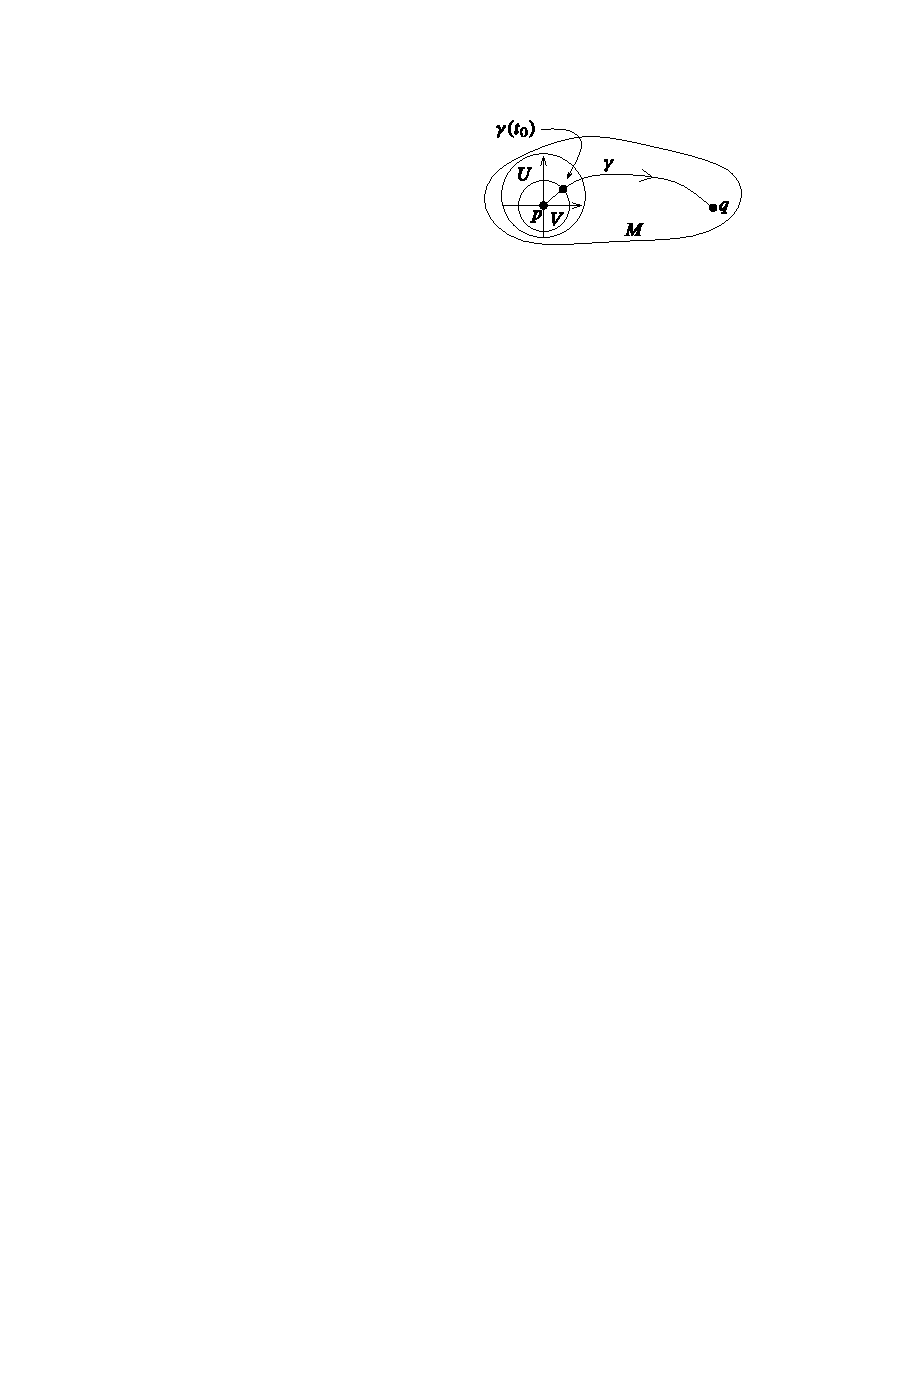
\includegraphics{pictures/Riemann-metric-2}
\caption{Positivity of $d_g$.}
\end{minipage}
\end{figure}
To complete the proof that $(M,d_g)$ is a metric space, we need only show that $d_g(p,q)>0$ if $p\neq q$. For this purpose, let $p,q\in M$ be distinct points, and let
$U$ be a smooth coordinate domain containing $p$ but not $q$. Use the coordinate map as usual to identify $U$ with an open subset in $\R^n$, and let $\widebar{g}$ denote the Euclidean metric in these coordinates. If $V$ is a regular coordinate ball of radius $\eps$ centered at $p$ such that $\widebar{V}\sub U$, Lemma~\ref{Riemann metric lem} shows that there are positive constants $c,C$ such that $(\ref{Riemann metric-1})$ is satisfied whenever $x\in\widebar{V}$ and $v\in T_xM$. Then for any piecewise smooth curve segment $\gamma$ lying entirely in $\widebar{V}$, it follows that
\[cL_{\widebar{g}}(\gamma)\leq L_g(\gamma)\leq CL_{\widebar{g}}(\gamma)\]
Suppose $\gamma:[a,b]\to M$ is a piecewise smooth curve segment from $p$ to $q$. Let $t_0$ be the infimum of all $t\in[a,b]$ such that $\gamma(t)\notin\widebar{V}$. It follows that $\gamma(t_0)\in\partial V$ by continuity, and $\gamma(t)\in\widebar{V}$ for $a\leq t\leq t_0$. Thus
\[L_g(\gamma)\geq L_g(\gamma|_{[a,t_0]})\geq cL_{\widebar{g}}(\gamma_{[a,t_0]})\geq cd_{\widebar{g}}(p,\gamma(t_0))=c\eps\]
Taking the infimum over all such $\gamma$, we conclude that $d_g(p,q)\geq c\eps>0$.\par
Finally, to show that the metric topology generated by $d_g$ is the same as the given manifold topology on $M$, we need to show that the open subsets in the manifold 
topology are open in the metric topology, and vice versa.\par
Suppose, first, that $U\sub M$ is open in the manifold topology. Let $p\in U$, and let $V$ be a regular coordinate ball of radius $\eps$ around $p$ such that 
$\widebar{V}\sub U$ as above. The argument in the previous paragraph shows that $d_g(p,q)\geq c\eps$ whenever $q\notin\widebar{V}$. The contrapositive of this 
statement is that $d_g(p,q)<c\eps$ implies $q\in\widebar{V}\sub U$, or in other words, the metric ball of radius $c\eps$ around $p$ is contained in $U$. This 
shows that $U$ is open in the metric topology.\par
Conversely, suppose that $W$ is open in the metric topology, and let $p\in W$. Let $V$ be a regular coordinate ball of radius $r$ around $p$, let $\widebar{g}$ 
be the Euclidean metric on $\widebar{V}$ determined by the given coordinates, and let $c,C$ be positive constants such that $(\ref{Riemann metric-1})$ is satisfied 
for $v\in T_qM,q\in\widebar{V}$. Let $\eps<r$ be a positive number small enough that the metric ball around $p$ of radius $C\eps$ is contained in $W$, and let 
$V_\eps$ be the set of points in $\widebar{V}$ whose Euclidean distance from $p$ is less than $\eps$. If $q\in V_\eps$, let $\gamma$ be the straight-line segment 
in coordinates from $p$ to $q$. Using Lemma~\ref{Riemann metric lem} as above, we conclude that
\[d_g(p,q)\leq L_g(\gamma)\leq CL_{\widebar{g}}(\gamma)<C\eps\]
This shows that $V_\eps$ is contained in the metric ball of radius $C\eps$ around $p$, and therefore in $W$. Since $V_\eps$ is a neighborhood of $p$ in the manifold 
topology, this shows that $W$ is open in the manifold topology as well.
\end{proof}
As a consequence of this theorem, all of the terminology of metric spaces 
can be carried over to connected Riemannian manifolds. Thus, a connected 
Riemannian manifold $(M,g)$ is said to be \textbf{complete}, and $g$ is 
said to be a \textbf{complete Riemannian metric}, if $(M,d_g)$ is a 
complete metric space (i.e., if every Cauchy sequence in $M$ converges 
to a point in $M$); and a subset $B\sub M$ is said to be \textbf{bounded} 
if there  exists a constant $K$ such that $d_g(x,y)\leq K$ for all 
$x,y\in B$; if this is the case, the \textbf{diameter} of $A$ is the smallest 
such constant:
\[\diam(A)=\sup\{d_g(p,q):p,q\in A\}\]
Since every compact metric space is bounded, every compact connected 
Riemannian manifold with or without boundary has finite diameter. 
(Note that the unit sphere with the Riemannian distance determined by 
the round metric has diameter $\pi$, not $2$, since the Riemannian distance 
between antipodal points is $\pi$).\par
Recall that a topological space is said to be \textbf{metrizable} if it 
admits a distance function whose metric topology is the same as the given 
topology.
\begin{corollary}
Every smooth manifold with or without boundary is metrizable.
\end{corollary}
\begin{proof}
First suppose $M$ is a smooth manifold without boundary, and choose any Riemannian metric $g$ on $M$. If $M$ is connected, Theorem~\ref{Riemann metric space} shows that $M$ is metrizable. More generally, let $\{M_i\}$ be the connected components of $M$, and choose a point $p_i\in M_i$ for each $i$. For $x\in M_i$ and $y\in M_j$, define $d_g(x,y)$ as in Theorem~\ref{Riemann metric space} when $i=j$, and otherwise
\[d_g(x,y)=d_g(x,p_i)+1+d_g(p_j,y)\]
It is straightforward to check that this is a distance function that induces the given topology on $M$. Finally, if $M$ has nonempty boundary, just embed $M$ into its double, and note that a subspace of a metrizable topological space is always metrizable.
\end{proof}
\subsection{Pseudo-Riemannian metrics}
From the point of view of geometry, Riemannian metrics are by far the most 
important structures that manifolds carry. However, there is a generalization 
of Riemannian metrics that has become especially important because of its 
application to physics.\par
Before defining this generalization, we begin with some linear-algebraic 
preliminaries. Suppose $V$ is a finite-dimensional vector space, and $q$ is 
a symmetric covariant $2$-tensor on $V$ (also called a symmetric bilinear 
form). Just as for an inner product, there is a linear map $\widehat{q}:V\to V^*$ 
defined by
\[\widehat{q}(v)(w)=q(v,w)\]
for $v,w\in V$. We say that $q$ is \textbf{nondegenerate} if $\widehat{q}$ is an isomorphism.
\begin{lemma}
Suppose $q$ is a symmetric covariant $2$-tensor on a finite-dimensional vector 
space $V$. The following are equivalent:
\begin{itemize}
\item[(a)] $q$ is nondegenerate.
\item[(b)] For every nonzero $v\in V$, there is some $w\in V$ such that $q(v,w)\neq 0$.
\item[(c)] If $q=q_{ij}\eps^i\eps^j$ in terms of some basis $(\eps^i)$ for $V^*$, 
then the matrix $(q_{ij})$ is invertible. 
\end{itemize}
\end{lemma}
\begin{proof}
By dimension consideration, $\widehat{q}$ is an isomorphism if and only if it is injective, so (a) 
is equivalent to (b). Now if $q(v,w)=0$, then in terms of matrix, we have $X^T(g_{ij})Y=0$ for some 
vector $X$ and every vector $Y$. This implies that $X^T(g_{ij})=0$, and thus $(g_{ij})X=0$ since $q$ 
is symmetric. This then implies that $(g_{ij})$ is not invertible, if $X\neq 0$. 
\end{proof}
We use the term \textbf{scalar product} to denote any nondegenerate 
symmetric bilinear form on a finite-dimensional vector space $V$, and 
reserve the term inner product for the special case of a positive definite 
scalar product. A \textbf{scalar product space} is a finite-dimensional 
vector space endowed with a scalar product. When convenient, we will often 
use a notation like $\langle\cdot\,\cdot\rangle$ to denote a scalar product. 
We say that vectors $v,w\in V$ are orthogonal if $\langle v,w\rangle=0$, 
just as in the case of an inner product. Given a vector $v\in V$, we define 
the \textbf{norm} of $v$ to be $|v|=|\langle v,v\rangle|^{1/2}$. Note that in the indefinite 
case, it is possible for a nonzero vector to be orthogonal to itself, and 
thus to have norm zero.\par
If $S\sub V$ is any linear subspace, the set of vectors in $V$ that are 
orthogonal to every vector in $S$ is a linear subspace denoted by $S^{\bot}$.
\begin{lemma}
Suppose $(V,q)$ is a finite-dimensional scalar product space, and $S\sub V$ 
is a linear subspace.
\begin{itemize}
\item[(a)] $\dim S+\dim S^{\bot}=\dim V$.
\item[(b)] $(S^\bot)^{\bot}=S$. 
\end{itemize}
\end{lemma}
\begin{proof}
Define a linear map $\varPhi:V\to S^*$ by $\varPhi(v)=\widehat{q}(v)|_S$. Note 
that $v\in\ker\varPhi$ if and only if $q(v,x)=0$ for all $x\in S$, so $\ker\varPhi=S^{\bot}$. 
If $\varphi\in S^*$ is arbitrary, there is a covector $\widetilde{\varphi}\in V^*$ 
whose restriction to $S$ is equal to $\varphi$. (For example, such a covector 
is easily constructed after choosing a basis for $S$ and extending it to a basis 
for $V$.) Since $\widehat{q}$ is an isomorphism, there exists $v\in V$ such 
that $\widehat{q}(v)=\widetilde{\varphi}$. It follows that $\varPhi(v)=\varphi$, 
and therefore $\varPhi$ is surjective. By the rank–nullity theorem, the dimension 
of $S^{\bot}=\ker\varPhi$ is equal to $\dim V-\dim S^*=\dim V-\dim S$. This 
proves (a).\par
To prove (b), note that every $v\in S$ is orthogonal to every element of $S$ by 
definition, so $S\sub (S^{\bot})^{\bot}$. Because these finite-dimensional vector 
spaces have the same dimension by part (a), they are equal.
\end{proof}
An ordered $k$-tuple $(v_1,\dots,v_k)$ of elements of $V$ is said to be \textbf{orthonormal} 
if $|v_i|=1$ for each $i$ and $\langle v_i,v_j\rangle=0$ for $i\neq j$, or 
equivalently, if $\langle v_i,v_j\rangle=\delta_{ij}$ for each $i$ and $j$. We wish 
to prove that every scalar product space has an orthonormal basis. Note that 
the usual Gram–Schmidt algorithm does not always work in this situation, because 
the vectors that appear in the denominators might have vanishing norms. In 
order to get around this problem, we introduce the following definitions.\par
If $(V,q)$ is a finite-dimensional scalar product space, a subspace $S\sub V$ 
is said to be nondegenerate if the restriction of $q$ to $S\times S$ is nondegenerate. 
An ordered $k$-tuple of vectors $(v_1,\dots,v_k)$ in $V$ is said to be nondegenerate 
if for each $j=1,\dots,k$ the vectors $(v_1,\dots,v_j)$ span a nondegenerate 
$j$-dimensional subspace of $V$. For example, every orthonormal basis is nondegenerate.
\begin{lemma}\label{scalar prod nondegenerate}
Suppose $(V,q)$ is a finite-dimensional scalar product space, and $S\sub V$ is 
a linear subspace. The following are equivalent:
\begin{itemize}
\item[(a)] $S$ is nondegenerate.
\item[(b)] $S^{\bot}$ is nondegenerate.
\item[(c)] $S\cap S^{\bot}=\{0\}$.
\item[(d)] $V=S\oplus S^{\bot}$.   
\end{itemize}
\end{lemma}
\begin{proof}
Note that $q|_S$ is nondegenerate if and only if the set
\[\{x\in S:q(x,y)=0\forall y\in S\}=S\cap S^{\bot}\]
is $\{0\}$. Now since $(S^{\bot})^{\bot}=S$, we have the equivalences (a), (b) and (c). 
Now, since $\dim S+\dim S^{\bot}=\dim V$, they are easily seen to be equivalent to (d).
\end{proof}
\begin{lemma}[\textbf{Completion of Nondegenerate Bases}]\label{scalar prod complete nondegenerate base}
Suppose $(V,q)$ is an $n$-dimensional scalar product space, and $(v_1,\dots,v_k)$ 
is a nondegenerate $k$-tuple in $V$ with $0\leq k<n$. Then there exist vectors 
$v_{k+1},\dots,v_n\in V$ such that $(v_1,\dots,v_n)$ is a nondegenerate basis 
for $V$.
\end{lemma}
\begin{proof}
Let $S=\mathrm{span}(v_1,\dots,v_k)\sub V$. Because $k<n$, $S^{\bot}$ is a nontrivial 
subspace of $V$, and Lemma~\ref{scalar prod nondegenerate} shows that 
$S^{\bot}$ is nondegenerate and $V=S\oplus S^{\bot}$. By the nondegeneracy 
of $S^{\bot}$, there must be a vector in $S^{\bot}$ with nonzero length, 
because otherwise the polarization identity would imply that all inner 
products of pairs of elements of $S$ would be zero. If $v_{k+1}\in S^{\bot}$ 
is any vector with nonzero length, then $(v_1,\dots,v_{k+1})$ is easily 
seen to be a nondegenerate $(k+1)$-tuple. Repeating this argument for 
$v_{k+2},\dots,v_n$ completes the proof.
\end{proof}
\begin{proposition}[\textbf{Gram–Schmidt Algorithm for Scalar Products}]
Suppose $(V,q)$ is an $n$-dimensional scalar product space. If $(v_i)$ is a 
nondegenerate basis for $V$, then there is an orthonormal basis $(b_i)$ with 
the property that $\mathrm{span}(b_1,\dots,b_k)=\mathrm{span}(v_1,\dots,v_k)$ 
for each $k=1,\dots,n$.
\end{proposition}
\begin{proof}
As in the positive definite case, the basis $(b_i)$ is constructed recursively, 
starting with $b_1=v_1/|v_1|$ and noting that the assumption that $v_1$ spans 
a nondegenerate subspace ensures that $|v_1|\neq 0$. At the inductive step, 
assuming we have constructed $(b_1,\dots,b_k)$, we first set
\[z=v_{k+1}-\sum_{i=1}^{k}\frac{\langle v_{k+1},b_i\rangle}{\langle b_i,b_i\rangle}b_i.\]
Each denominator $\langle b_i,b_i\rangle$ is equal to $\pm 1$, so this defines 
$z$ as a nonzero element of $V$ orthogonal to $b_1,\dots,b_k$, and with the 
property that $\mathrm{span}(b_1,\dots,b_k,z)=\mathrm{span}(v_1,\dots,v_{k+1})$. 
If $\langle z,z\rangle=0$, then $z$ is orthogonal to $\mathrm{span}(v_1,\dots,v_{k+1})$, 
contradicting the nondegeneracy assumption. Thus we can complete the inductive step 
by putting $b_{k+1}=z/|z|$.
\end{proof}
\begin{corollary}
Suppose $(v,q)$ is an $n$-dimensional scalar product space. There is a basis 
$(\beta^i)$ for $V^*$ with respect to which $q$ has the expression
\begin{align}\label{scalar prod canonical form}
q=(\beta^1)^2+\cdots+(\beta^r)^2-(\beta^{r+1})^2-\cdots-(\beta^{r+s})^2,
\end{align}
for some nonnegative integers $r,s$ with $r+s=n$.
\end{corollary}
\begin{proof}
Let $(b_i)$ be an orthonormal basis for $V$, and let $(\beta^i)$ be the dual 
basis for $V^*$. A computation shows that $q$ has a basis expression of the 
form $(\ref{scalar prod canonical form})$, but perhaps with the positive and 
negative terms in a different order. Reordering the basis so that the positive 
terms come first, we obtain $(\ref{scalar prod canonical form})$.
\end{proof}
It turns out that the numbers $r$ and $s$ in $(\ref{scalar prod canonical form})$ are independent of the choice of
basis. The integer $s$ in the expression (the number of negative terms) is called 
the \textbf{index} of $q$, and the ordered pair $(r,s)$ is called the \textbf{signature} of $q$.\par
Now suppose $M$ is a smooth manifold. A \textbf{pseudo-Riemannian metric} on $M$ (called 
by some authors a semi-Riemannian metric) is a smooth symmetric $2$-tensor field 
$g$ that is nondegenerate at each point of $M$, and with the same signature 
everywhere. Every Riemannian metric is also a pseudo-Riemannian metric.
\begin{proposition}[\textbf{Orthonormal Frames for Pseudo-Riemannian Manifolds}]\label{pseudo Riemann orthonormal frame}
Let $(M,g)$ be a pseudo-Riemannian manifold. For each $p\in M$, there exists 
a smooth orthonormal frame on a neighborhood of $p$ in $M$.
\end{proposition}
\begin{example}
Suppose $(M_1,g_1)$ and $(M_2,g_2)$ are pseudo-Riemannian manifolds of signatures $(r_1,s_1)$ 
and $(r_2,s_2)$, respectively. Then $(M_1\times M_2,g_1\oplus g_2)$ is a 
pseudo-Riemannian manifold of signature $(r_1+r_2,s_1+s_2)$.
\end{example}
For nonnegative integers $r$ and $s$, we define the \textbf{pseudo-Euclidean space of signature \bm{$(r,s)$}}, 
denoted by $\R^{r,s}$, to be the manifold $\R^{r+s}$, with standard coordinates 
denoted by $(\xi^1,\dots,\xi^r,\tau^1,\dots,\tau^s)$, and with the pseudo-Riemannian 
metric $\widebar{q}^{(r,s)}$ defined by
\[\widebar{q}^{(r,s)}=(d\xi^1)^2+\cdots+(d\xi^r)^2-(d\tau^1)^2-\cdots-(d\tau^s)^2.\]
By far the most important pseudo-Riemannian metrics (other than the Riemannian ones) 
are the \textbf{Lorentz metrics}, which are pseudo-Riemannian metrics of 
index $1$, and thus signature $(r,1)$.\par 
The pseudo-Euclidean metric $\widebar{q}^{(r,1)}$ is a \textbf{Lorentz metric} 
called the \textbf{Minkowski metric}, and the Lorentz manifold $\R^{r,1}$ is 
called $(r+1)$-dimensional Minkowski space. If we denote standard coordinates 
on $\R^{r+1}$ by $(\xi^1,\dots,\xi^r,\tau)$ then the Minkowski metric is given by
\[\widebar{q}^{(r,1)}=(d\xi^1)^2+\cdots+(d\xi^r)^2-(d\tau^1)^2.\]

Many, but not all, results from the theory of Riemannian metrics apply 
equally well to pseudo-Riemannian metrics. We will attempt to point out 
which results carry over directly to pseudo-Riemannian metrics, which ones 
can be adapted with minor modifications, and which ones do not carry over 
at all. As a rule of thumb, proofs that depend only on the nondegeneracy of 
the metric tensor, such as properties of the musical isomorphisms and 
existence and uniqueness of geodesics, work fine in the pseudo-Riemannian 
setting, while proofs that use positivity in an essential way, such as 
those involving lengths of curves, do not.\par
One notable result that does not carry over to the pseudo-Riemannian case 
is Proposition~~\ref{Riemann metric space}, about the existence of metrics. 
For example, the following result characterizes those manifolds that admit 
Lorentz metrics.
\begin{theorem}\label{Riemann Lorenta metric}
A smooth manifold $M$ admits a Lorentz metric if and only if it admits a 
rank-$1$ tangent distribution (i.e., a rank-$1$ subbundle of $TM$).
\end{theorem}
\begin{proof}
For sufficiency, assume that $D\sub TM$ is a $1$-dimensional distribution, 
and choose any Riemannian metric $g$ on $M$. Then, by Lemma~\ref{vector subbundle crit}, 
locally it is possible to choose a $g$-orthonormal frame $(E_i)$ and dual 
coframe $(\eps^i)$ such that $E_1$ spans $D$. Then the Lorentz metric 
$-(\eps^1)^2+(\eps^2)^2+\cdots+(\eps^n)^2$ is independent of the choice of 
frame.
\end{proof}
\subsubsection{Pseudo-Riemannian submanifolds}
The theory of submanifolds is only slightly more complicated in the 
pseudo-Riemannian case. If $(\widetilde{M},\widetilde{g})$ is a 
pseudo-Riemannian manifold, a smooth submanifold $\iota:M\hookrightarrow\widetilde{M}$ 
is called a \textbf{pseudo-Riemannian submanifold} of $\widetilde{M}$ if $\iota^*\widetilde{g}$ 
is nondegenerate with constant signature. If this is the case, we always 
consider $M$ to be endowed with the induced pseudo-Riemannian metric $\iota^*\widetilde{g}$. 
In the special case in which $\iota^*\widetilde{g}$ is positive definite, 
$M$ is called a \textbf{Riemannian submanifold}.\par
The nondegeneracy hypothesis is not automatically satisfied: for example, 
if $M\sub\R^{1,1}$ is the submanifold $\{(\xi,\tau):\tau=\xi\}$ and $\iota:M\to\R^{1,1}$ 
is inclusion, then the pullback tensor $\iota^*\widetilde{g}$ is identically 
zero on $M$.\par
For hypersurfaces (submanifolds of codimension $1$), the nondegeneracy 
condition is easy to check. If $M\sub\widetilde{M}$ is a smooth 
submanifold and $p\in M$, then a vector $v\in T_p\widetilde{M}$ is said to 
be \textbf{normal to $\bm{M}$} if $\langle v,x\rangle=0$ for all $x\in T_pM$, 
just as in the Riemannian case. The space of all normal vectors at $p$ is 
a subspace of $T_p\widetilde{M}$ denoted by $N_pM$.
\begin{proposition}\label{pseudo Riemann submani}
Suppose $(\widetilde{M},\widetilde{g})$ is a pseudo-Riemannian manifold of 
signature $(r,s)$. Let $M$ be a smooth hypersurface in $\widetilde{M}$, and 
let $\iota:M\to\widetilde{M}$ be the inclusion map. Then the pullback 
tensor field $\iota^*\widetilde{g}$ is nondegenerate if and only if $\widetilde{g}(v,v)\neq 0$ 
for every $p\in M$ and every nonzero normal vector $v\in N_pM$. If $\widetilde{g}(v,v)>0$ 
for every nonzero normal vector to $M$, then $M$ is a pseudo-Riemannian 
submanifold of signature $(r-1,s)$; and if $\widetilde{g}(v,v)<0$ for every 
such vector, then $M$ is a pseudo-Riemannian submanifold of signature $(r,s-1)$.
\end{proposition}
\begin{proof}
Given $p\in M$, Lemma~\ref{scalar prod nondegenerate} shows that $T_pM$ is 
a nondegenerate subspace of $T_p\widetilde{M}$ if and only if the one-dimensional 
subspace $(T_pM)^{\bot}=N_pM$ is nondegenerate, which is the case if and only 
if every nonzero $v\in N_pM$ satisfies $\widetilde{g}(v,v)\neq 0$.\par
Now suppose $\widetilde{g}(v,v)>0$ for every nonzero normal vector $v$. Let 
$p\in M$ be arbitrary, and let $v$ be a nonzero element of $N_pM$. Writing 
$n=\dim \widetilde{M}$, we can complete $v$ to a nondegenerate basis $v,w_2,\dots,w_n$ 
for $T_pM$ by Lemma~\ref{scalar prod complete nondegenerate base}, and then 
use the Gram–Schmidt algorithm to find an orthonormal basis $b_1,\dots,b_n$ for $T_p\widetilde{M}$ 
such that $\mathrm{span}(b_1)=N_pM$. It follows that $\mathrm{span}(b_2,\dots,b_n)=T_pM$. 
If $(\beta^j)$ is the dual basis to $(b_i)$, then $\widetilde{g}_p$ has a 
basis representation of the form $(\beta^1)^2\pm(\beta^2)^2\pm\cdots\pm(\beta^n)^2$, 
with a total of $r$ positive terms and $s$ negative ones, and with a positive 
sign on the first term $(\beta^1)^2$. Therefore, $\iota^*\widetilde{g}_p=\pm(\beta^2)^2\pm\cdots\pm(\beta^n)^2$ 
has signature $(r-1,s)$. The argument for the case $\widetilde{g}(v,v)<0$ is similar.
\end{proof}
If $(M,g)$ is a pseudo-Riemannian manifold and $f\in C^{\infty}(M)$, then 
the \textbf{gradient} of $f$ is defined as the smooth vector field $\grad f=(df)^{\sharp}$ 
just as in the Riemannian case.
\begin{proposition}
Suppose $(\widetilde{M},\widetilde{g})$ is a pseudo-Riemannian manifold of 
signature $(r,s)$, $f\in C^{\infty}(M)$, and $M=f^{-1}(c)$ for some $c\in\R$. 
If $\langle\grad f,\grad f\rangle>0$ everywhere on $M$, then $M$ is an 
embedded pseudo-Riemannian submanifold of $M$ of signature $(r-1,s)$ and if 
$\langle\grad f,\grad f\rangle<0$  everywhere on $M$, then $M$ is an embedded 
pseudo-Riemannian submanifold of $\widetilde{M}$ of signature $(r,s-1)$. In 
either case,$\grad f$ is everywhere normal to $M$.
\end{proposition}
\begin{proof}
By Proposition~\ref{regular value level set} and Proposition~\ref{tangent space level set} 
we know that $M$ is an embedded submanifold whose tangent space is every where tangent to 
$\grad f$. Now the result follows from Proposition~\ref{pseudo Riemann submani}.
\end{proof}
\begin{proposition}[\textbf{Pseudo-Riemannian Adapted Orthonormal Frames}]
Suppose $(\widetilde{M},\widetilde{g})$ is a pseudo-Riemannian manifold, 
and $M\sub\widetilde{M}$ is an embedded pseudo-Riemannian or Riemannian 
submanifold. For each $p\in M$, there exists a smooth orthonormal frame on 
a neighborhood of $p$ in $\widetilde{M}$ that is adapted to $M$.
\end{proposition}
\begin{proof}
Write $m=\dim\widetilde{M}$ and $n=\dim M$, and let $p\in M$ be arbitrary. 
Proposition~\ref{pseudo Riemann orthonormal frame} shows that there is a 
smooth orthonormal frame $(E_1,\dots,E_n)$ for $M$ on some neighborhood of 
$p$ in $M$. Then by Lemma~\ref{scalar prod complete nondegenerate base}, we can find vectors $v_{n+1},\dots,v_m$ 
such that 
\[(E_1|_p,\dots,E_n|_p,v_{n+1},\dots,v_m)\]
is a nondegenerate basis for $T_p\widetilde{M}$. Now extend $v_{n+1},\dots,v_m$ arbitrarily to 
smooth vector fields $V_{m+1},\dots,V_m$ on a neighborhood of $p$ in $\widetilde{M}$. 
By continuity, the ordered $m$-tuple 
\[(E_1,\dots,E_n,V_{n+1},\dots,V_m)\] 
will be a nondegenerate frame for $\widetilde{M}$ in some (possibly smaller) 
neighborhood of $p$. Applying the Gram–Schmidt algorithm to this local 
frame yields a smooth local orthonormal frame $(E_1,\dots,E_m)$ for $\widetilde{M}$ 
with the property that $(E_1,\dots,E_n)$ restricts to a local orthonormal 
frame for $M$.
\end{proof}
The next corollary is proved in the same way as Proposition~\ref{Riemann normal bundle}
\begin{corollary}[\textbf{Normal Bundle to a Pseudo-Riemannian Submanifold}]
Suppose $(\widetilde{M},\widetilde{g})$ is a pseudo-Riemannian manifold, 
and $M\sub\widetilde{M}$ is an embedded pseudo-Riemannian or Riemannian 
submanifold. The set of vectors normal to $M$ is a smooth vector subbundle 
of $T\widetilde{M}|_M$, called the normal bundle to $M$.
\end{corollary}
\subsection{Exercise}
\begin{exercise}\label{vector bundle convex subset}
Suppose that $E$ is a smooth vector bundle over a smooth manifold $M$ with or without boundary, and $V\sub E$ is an open subset with the property that for each $p\in M$, the intersection of $V$ with the fiber $E_p$ is convex and nonempty. By a section of $V$, we mean a section of $E$ whose image lies in $V$.
\begin{itemize}
\item[(a)] Show that there exists a smooth global section of $V$.
\item[(b)] Suppose $\sigma:A\to V$ is a smooth section of $V$ defined on a closed subset $A\sub M$. $($This means that $\sigma$ extends to a smooth section of $V$ in a
neighborhood of each point of $A$.$)$ Show that there exists a smooth global section $\widetilde{\sigma}$ of $V$ whose restriction to $A$ is equal to $\sigma$. Show that if $V$ contains the image of the zero section of $E$, then $\widetilde{\sigma}$ can be chosen to be supported in any predetermined neighborhood of $A$.
\end{itemize}
\end{exercise}
\begin{proof}
For $p\in M$, choose a neighborhood $U$ contains $p$, with a local 
trivialization $\varPhi:\pi^{-1}(U)\to U\times\R^k$. Let $v\in\R^k$ be a 
vector such that $(p,v)\in\varPhi\big(V\cap\pi^{-1}(U)\big)$. Since 
$V\cap\pi^{-1}(U)$ is open, by appropriately shrinking $U$, we can find 
an open subset $W\sub\R^k$ such that 
\[(p,v)\in U\times W\sub\varPhi\big(V\cap\pi^{-1}(U)\big).\]
In particular, $(q,v)\in\varPhi\big(V\cap\pi^{-1}(U)\big)$ for all $q\in U$, thus we can define $\sigma_p:U\to E$ by
\[\sigma_p(q)=\varPhi^{-1}(q,v)\for q\in U.\]
It follows that $\sigma_p$ is a local section of $V$. Now the neighborhoods $\{U_p\}$ gives an open cover of $M$, by taking a partition of unity $\{\psi_p\}$ for the open cover $\{\psi_p\}$, we define
\[\eta=\sum_{p\in M}\psi_p\sigma_p.\]
Then at each point $p_0$, since $V\cap E_{p_0}$ is convex, we find $\eta(p_0)\in V$.\par
The second statement is the same as Lemma~\ref{ext lem smooth func}.
\end{proof}
\begin{exercise}
Prove that every Riemannian $1$-manifold is flat.
\end{exercise}
\begin{proof}
Let $M$ be a Riemannian $1$-manifold, then each point of $M$ admits a commuting orthonormal frame. Thus by Proposition~\ref{Riemann flat iff} $M$ is flat.
\end{proof}
\begin{exercise}\label{isometry is linear}
Suppose $V$ and $W$ are finitely-dimensional real inner product spaces of the same dimension, and $F:V\to W$ is any map (not assumed to be linear or even continuous) that 
preserves the origin and all distances: $F(0)=0$ and $|F(x)-F(y)|=|x-y|$ for all $x,y\in V$. Prove that $F$ is a linear isometry.
\end{exercise}
\begin{proof}[First proof]
First, inserting $y=0$ in the second condition gives $|F(x)|=|x|$. Now let $t\in[0,1]$ and denote $r=|x-y|$. Then 
\[\{tx+(1-t)y\}=\widebar{B}(x,tr)\cap\widebar{B}(y,(1-t)r).\]
Now since $F$ is injective, $F(tx+(1-t)y)$ is the unique element of 
\[F(\widebar{B}(x,tr)\cap\widebar{B}(y,(1-t)r))=F(\widebar{B}(x,tr))\cap F(\widebar{B}(y,(1-t)r))=\widebar{B}(F(x),tr)\cap\widebar{B}(F(y),(1-t)r),\]
which is $tF(x)+(1-t)F(y)$. This then implies $F(x)$ is linear since $F(0)=0$.
\end{proof}
\begin{proof}[Second proof]
We have $|F(x)|=x$ for all $x\in V$. Now expand the equation $|F(x)-F(y)|^2=|x-y|^2$, we get
\[|F(x)|^2+|F(y)|^2-2(F(x),F(y))=|x|^2+|y|^2-2(x,y).\]
Therefore $F$ preserves the inner products.\par
Now let $x,y\in V$, we want to prove $F(x+y)=F(x)+F(y)$ and $F(\lambda x)=\lambda x$ for $\lambda\in\R$. We note that for all $v\in V$,
\begin{align*}
(F(x+y),F(v))=((x+y),v)=(x,v)+(y,v)=(F(x)+F(y),F(v)).
\end{align*}
Take $v$ to be a orthonormal basis for $V$, this then implies $F(x+y)=F(x)+F(y)$. Similarly we can prove $F(\lambda x)=\lambda F(x)$, therefore $F$ is linear.
\end{proof}
\begin{exercise}\label{Euclidean shortest path}
Show that the shortest path between two points in Euclidean space is a straight line segment. More precisely, for $x,y\in\R^n$, let $\gamma:[0,1]\to\R^n$ be the 
curve segment $\gamma(t)=x+t(y-x)$, and show that any other piecewise smooth curve segment $\widetilde{\gamma}$ from $x$ to $y$ satisfies 
$L_{\widebar{g}}(\widetilde{\gamma})\geq L_{\widebar{g}}(\gamma)$.
\end{exercise}
\begin{proof}
Let $\gamma:[a,b]\to\R^n$ be a piecewise smooth curve segment such that $\gamma(a)=x$ and $\gamma(b)=y$. 
For any constant vector $v$ with $|v|=1$, by Cauchy-Schwarz inequality we have
\[(y-x)\cdot v=\big(\gamma(t)\cdot v\big)\Big|_{t=a}^{t=b}=\int_{a}^{b}\gamma'(t)\cdot v\,dt\leq\int_{a}^{b}|\gamma'(t)||v|dt=\int_{a}^{b}|\gamma'(t)|dt.\]
Set $v=(y-x)/|y-x|$, then
\[|y-x|\leq\int_{a}^{b}|\gamma'(t)|dt.\]
Now if the equality holds if and only if $\gamma'(t)=a(y-x)$ for some constant $a\in\R$. 
Hence if and only if $\gamma(t)=a(y-x)t+b$ with $a,b\in\R$.
\end{proof}
\begin{exercise}\label{Euclidean isometry group}
Consider $\R^n$ as a Riemannian manifold with the Euclidean metric $\widebar{g}$.
\begin{itemize}
\item[(a)] Suppose $U,V\sub\R^n$ are connected open sets, $\varphi,\psi:U\to V$ are Riemannian isometries, and for some $p\in U$ they satisfy $\varphi(p)=\psi(p)$ and $d\varphi_p=d\psi_p$. Show that $\varphi=\psi$.
\item[(b)] Show that the set of maps from $\R^n$ to itself given by the action of $E(n)$ on $\R^n$ described in Example~\ref{Euclidean group} is the full group of Riemannian isometries of $(\R^n,\widebar{g})$.
\end{itemize}
\end{exercise}
\begin{proof}
Let $x\in\R^n$, and let $\gamma$ be a smooth curve in $\R^n$ from $\varphi(p)$ to $\varphi(x)$, 
then by Proposition~\ref{Riemann isometry length},
\[L_{\widebar{g}}(\gamma)=L_{\widebar{g}}(\varphi^{-1}\circ\gamma)\geq L_{\widebar{g}}(\sigma)=L_{\widebar{g}}(\varphi\circ\sigma),\]
where $\sigma:[0,1]\to\R^n$ is the straight line from $p$ to $x$ and we use the result of Exercise~\ref{Euclidean shortest path}. 
This implies that $\varphi\circ\sigma$ is the straight line from $\varphi(p)$ to $\varphi(x)$. 
Since the length of $\varphi\circ\sigma$ is fixed, $\varphi(x)$ is uniquely determined by its 
direction, that is, $(\varphi\circ\sigma)'(0)$. Since $d\varphi_p=d\psi_p$ we then conclude 
$\varphi=\psi$.\par
Let $\varphi$ be any Riemannian isometry of $(\R^n,\widebar{g})$. Since $d\varphi_0$ preserves 
the Euclidean dot product, it corresponds to a matrix $C\in\O(n)$. Let $(\varphi(0),C)\in E(n)$, then $\varphi$ is represented by $(C,\varphi(0))$, in the sense that
\[\varphi(x)=(\varphi(0),C)\cdot x=\varphi(0)+Cx.\]
This gives the claim.
\end{proof}
\begin{exercise}
Let $(M,g)$ be a Riemannian manifold. A smooth vector field $V$ on $M$ is called a \textbf{Killing vector field} for $g$ if the flow of $V$ acts by isometries of $g$.
\begin{itemize}
\item[(a)] Show that the set of all Killing vector fields on $M$ constitutes a Lie subalgebra of $\X(M)$.
\item[(b)] Show that a smooth vector field $V$ on $M$ is a Killing vector field if and only if it satisfies the following equation in each smooth local coordinate chart:
\[V^k\frac{\partial g_{ij}}{\partial x^k}+g_{jk}\frac{\partial V^k}{\partial x^i}+g_{ik}\frac{\partial V^k}{\partial x^j}=0\quad\text{for all }i,j.\]
\end{itemize}
\end{exercise}
\begin{proof}
By definition, $V$ is a killing field if and only if $g$ is invairant under $\theta$. Thus by Theorem~\ref{tensor filed invariant flow iff}, this is equivalent to $\mathfrak{L}_Vg=0$. Now by Exercise~\ref{tensor field Lie derivative bracket},
\[\mathfrak{L}_{[V,W]}g=\mathfrak{L}_V\mathfrak{L}_Wg-\mathfrak{L}_W\mathfrak{L}_Vg.\]
Thus part (a) follows.\par
For part (b), write $V=V^k\partial/\partial x^k$, we compute using Corollary~\ref{Lie derivative tensor}:
\begin{align*}
(\mathfrak{L}_Vg)\Big(\frac{\partial}{\partial x^i},\frac{\partial}{\partial x^j}\Big)&=V(g_{ij})-g\Big([V,\frac{\partial}{\partial x^i}],\frac{\partial}{\partial x^j}\Big)-g\Big(\frac{\partial}{\partial x^i},[V,\frac{\partial}{\partial x^j}]\Big)\\
&=V^k\frac{\partial g_{ij}}{\partial x^k}+g\Big(\frac{\partial V^k}{\partial x^i}\frac{\partial}{\partial x^k},\frac{\partial}{\partial x^j}\Big)+g\Big(\frac{\partial}{\partial x^i},\frac{\partial V^k}{\partial x^j}\frac{\partial}{\partial x^k}\Big)\\
&=V^k\frac{\partial g_{ij}}{\partial x^k}+g_{jk}\frac{\partial V^k}{\partial x^i}+g_{ik}\frac{\partial V^k}{\partial x^j}.
\end{align*}
\end{proof}
\begin{exercise}
Let $K\sub\X(\R^n)$ denote the Lie algebra of Killing vector fields with respect to the Euclidean metric, and let $K_0\sub K$ denote the
subspace consisting of fields that vanish at the origin.
\begin{itemize}
\item[(a)] Show that the map
\[V\mapsto\Big(\frac{\partial V^k}{\partial x^j}(0)\Big)\]
is an injective linear map from $K_0$ to $\o(n)$.
\item[(b)] Show that the following vector fields form a basis for $K$:
\[\frac{\partial}{\partial x^i},\quad 1\leq i\leq n;\quad\quad x^i\frac{\partial}{\partial x^j}-x^j\frac{\partial}{\partial x^i},\quad 1\leq i<j\leq n.\]
\end{itemize}
\end{exercise}
\begin{proof}
If $g=\delta_{ij}dx^idx^j$, then the equation becomes
\[\frac{\partial V^j}{\partial x^i}+\frac{\partial V^i}{\partial x^j}=0\]
thus the image of the map is in $\o(n)$.
\end{proof}
\begin{exercise}
Suppose $g=f(t)dt^2$ is a Riemannian metric on $\R$. Show that $g$ is complete if and only if both of the following improper integrals diverge:
\[\int_{0}^{+\infty}\sqrt{f(t)}dt,\quad\int_{-\infty}^{0}\sqrt{f(t)}dt.\]
\end{exercise}
\begin{exercise}\label{Riemann grad prop}
Let $(M,g)$ be a Riemannian manifold, let $f\in C^\infty(M)$, and let $p\in M$ be a regular point of $f$.
\begin{itemize}
\item[(a)] Show that among all unit vectors $v\in T_pM$, the directional derivative
$vf$ is greatest when $v$ points in the same direction as $\grad f|_p$, and the length of $\grad f|_p$ is equal to the value of the directional derivative in that direction.
\item[(b)] Show that $\grad f|_p$ is normal to the level set of $f$ through $p$.
\item[(c)] Let $X\in\X(M)$ be a nowhere-vanishing vector field. Prove that $X=\grad f$ if and only if $Xf\equiv|X|_g^2$ and $X$ is orthogonal to the level sets of $f$ 
at all regular points of $f$. 
\end{itemize}
\end{exercise}
\begin{proof}
By $(\ref{Riemann grad def})$ we have
\[\langle\grad f|_p,v\rangle_g=df_p(v)=vf.\]
Then by Cauchy-Schwarz inequality, we have
\[vf\leq |v|_g\cdot\big|\grad f|_p\big|_g,\]
with the quality holds if and only if $v$ is paralle to $\grad f|_p$.\par
Let $S=f^{-1}(f(p))$ be the level set of $f$ through $p$, then by Proposition~\ref{tangent space level set} we have
\[T_pS=\ker df_p=\ker(\widehat{g}(\grad f)_p)=\ker\big(\langle\grad f|_p,\cdot\rangle_g\big).\]
Thus $\grad f|_p$ is normal to $T_pS$.\par
For (c), one direction is clear. Conversely, assume that $X\in\X(M)$ satisfies the conditions. Let $S$ be a level set of $f$ and $p\in S$, then $\dim(T_pS)^{\bot}=1$ 
for $p\in S$. Since $X$ and $\grad f$ are both contained in it, is follows that $X_p=\lambda\grad f|_p$ for some $\lambda\in\R$. From the condition we have
\[\lambda\langle X_p,X_p\rangle\langle\grad f|_p,X_p\rangle=Xf|_p=\langle X_p,X_p\rangle=\lambda^2\langle X_p,X_p\rangle.\]
Therefore $\lambda=1$ since $X_p\neq 0$. Since $X$ is non-vanishing, it follows that $X=\grad f$.
\end{proof}
\begin{exercise}\label{Morse exercise}
Let $M$ be a compact smooth $n$-manifold, and suppose $f$ is a smooth real-valued function on $M$ that has only finitely many critical points $\{p_1,\dots,p_k\}$, with 
corresponding critical values $c_1,\dots,c_k$ labeled so that $c_1\leq \cdots\leq c_k$. For any $a<b\in\R$, define
\[M_a=f^{-1}(a),\quad M_{(a,b)}=f^{-1}(a,b),\quad M_{[a,b]}=f^{-1}([a,b]).\]
If $a$ and $b$ are regular values, note that $M_a$ and $M_b$ are embedded hypersurfaces in $M$, $M_{(a,b)}$ is an open submanifold, and $M_{[a,b]}$ is a regular domain by Proposition~\ref{regular domain}.
\begin{itemize}
\item[(a)] Choose a Riemannian metric $g$ on $M$, let $X$ be the vector field $X=\grad f/|\grad f|_g^2$ on $M\setminus\{p_1,\dots,p_k\}$, and let $\theta$ denote the 
flow of $X$. Show that $f(\theta_t(p))=f(p)+t$ whenever $\theta_t$ is defined.
\item[(b)] Let $[a,b]\times\R$ be a compact interval containing no critical values of $f$. Show that $\theta$ restricts to a diffeomorphism from $[0,b-a]\times M_a$ to 
$M_{[a,b]}$.
\end{itemize}
\end{exercise}
\begin{figure}[htbp]
\centering
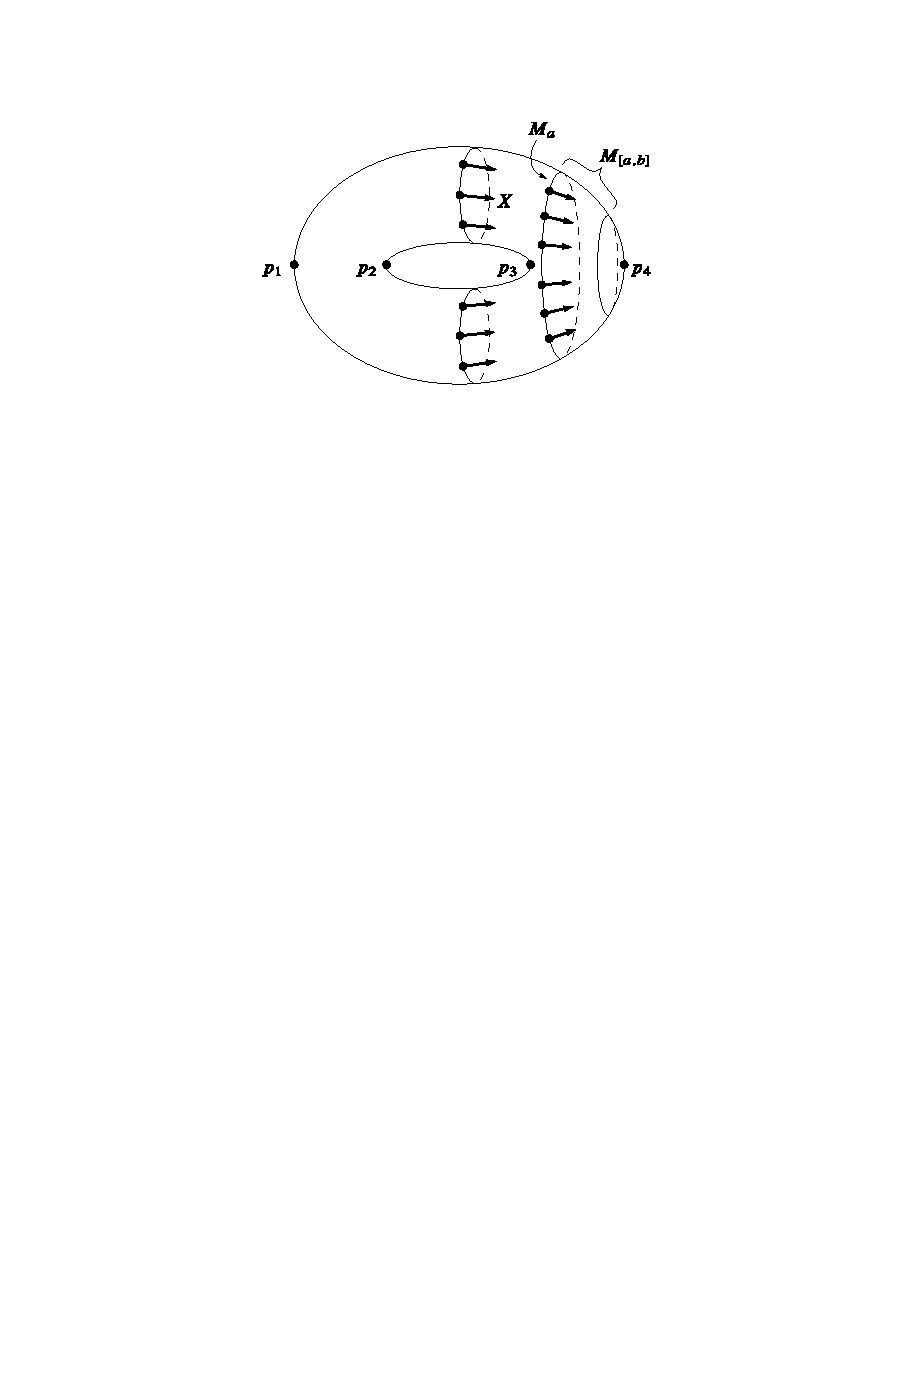
\includegraphics{pictures/Morse-setup}
\caption{The setup for Exercise~\ref{Morse exercise}.}
\end{figure}
\begin{proof}
Fix a point $p\in M\setminus\{p_1,\dots,p_k\}$, we calculate the derivative of $f(\theta_t(p))$ with respect to $t$. We have
\[d(f\circ\theta_t(p))=df\circ d(\theta_t(p))=df(X_{\theta_t(p)})=\langle \grad f|_{\theta_t(p)},X_{\theta_t(p)}\rangle=1.\]
Therefore 
\begin{align}\label{Morse exercise-1}
f(\theta_t(p))=f(\theta_0(p))+t=f(p)+t
\end{align}

Now let $p\in M_a$, we observe that
\begin{align*}
f(\theta_t(p))=f(p)+t=a+t.
\end{align*}
Therefore $\theta$ restricts to a map $\theta|_{M_{[a,b]}}:[0,b-a]\times M_a\to M_{[a,b]}$. To show this is a diffeomorphism, we construct the inverse map of $\theta|_{M_{[a,b]}}$:
\[\psi:M_{[a,b]}\to[0,b-a]\times M_a,\quad p\mapsto(f(p)-a,\theta_{a-f(p)}(p)).\]
Note that since $M_{[a,b]}$ is compact ($M$ is compact and $M_{[a,b]}$ is closed), the integral curve passing $p$ is defined on $\R$ if it is contained in $M_{[a,b]}$ by the escape lemma 
(Lemma~\ref{vector flow escape lemma}). But from equation $(\ref{Morse exercise-1})$, this is impossible. So it must pass the boundary of $M_{[a,b]}$, i.e., threr 
is $t_0\in\R$ such that $\theta_t(p)\in M_a$. We can see $t_0=a-f(p)$ from $(\ref{Morse exercise-1})$, so our definition of $\psi$ is legal. Now it is easy to see that 
$\psi$ is the inverse of $\theta|_{M_{[a,b]}}$, so we get the diffeomorphism.
\end{proof}
\section{Differential forms}
\subsection{The alternating tensors}
We continue to assume that $V$ is a finite-dimensional real vector space. A covariant $k$-tensor $\alpha$ on $V$ is said to be alternating (or antisymmetric or skew-symmetric) if it changes sign whenever two of its arguments are interchanged. This means that for all vectors $v_1,\dots,v_k$ and every pair of distinct indices $i,j$ it satisfies
\[\alpha(v_1,\dots,v_i,\dots,v_j,\dots,v_k)=-\alpha(v_1,\dots,v_j,\dots,v_i,\dots,v_k).\]
Alternating covariant $k$-tensors are also variously called \textbf{exterior forms}, \textbf{multicovectors}, or \textbf{$\bm{k}$-covectors}. The subspace of all alternating covariant $k$-tensors on $V$ is denoted by $\bigwedge^k(V^*)\sub T^k(V^*)$.\par
The next lemma gives two more useful characterizations of alternating tensors.
\begin{lemma}\label{alt tensor lem}
Let $\alpha$ be a covariant $k$-tensor on a finite-dimensional vector space $V$. The following are equivalent:
\begin{itemize}
\item[(a)] $\alpha$ is alternating.
\item[(b)] $\alpha(v_1,\dots,v_k)=0$ whenever the $k$-tuple $v_1,\dots,v_k$ is linearly dependent.
\item[(c)] $\alpha$ gives the value zero whenever two of its arguments are equal:
\[\alpha(v_1,\dots,w,\dots,w,v_k)=0.\]
\end{itemize}
\end{lemma}
\begin{proof}
The implications $(a)\Rightarrow(c)$ and $(b)\Rightarrow(c)$ are immediate. We complete the proof by showing that (c) implies both (a) and (b).\par
Assume that $\alpha$ satisfies (c). For any vectors $v_1,\dots,v_k$, the hypothesis implies
\begin{align*}
0&=\alpha(v_1,\dots,v_i+v_j,\dots,v_i+v_j,\dots,v_k)\\
&=\alpha(v_1,\dots,v_i,\dots,v_j,\dots,v_k)+(v_1,\dots,v_j,\dots,v_i,\dots,v_k).
\end{align*}
Thus $\alpha$ is alternating. On the other hand, if $v_1,\dots,v_k$ is a linearly dependent $k$-tuple, then one of the $v_i$'s can be written as a linear combination of the others. For simplicity, let us assume that $v_k=\sum_{j=1}^{k-1}a^jv_j$. Then multilinearity of $\alpha$ implies
\[\alpha(v_1,\dots,v_k)=\sum_{j=1}^{k-1}a^j\alpha(v_1,\dots,v_{k-1},v_j).\]
In each of these terms, $\alpha$ has two identical arguments, so every term is zero.
\end{proof}
We now define a similar projection $\Alt:T^k(V^*)\to\bigwedge^k(V^*)$, called \textbf{alternation}, as follows:
\[\Alt\alpha=\frac{1}{k!}\sum_{\sigma\in\mathfrak{S}_k}(-1)^\sigma\sigma\cdot\alpha.\]
More explicitly, this means
\[\Alt\alpha(v_1,\dots,v_k)=\frac{1}{k!}\sum_{\sigma\in\mathfrak{S}_k}(\sgn\sigma)\alpha(v_{\sigma(1)},\dots,v_{\sigma(k)}).\]
\begin{example}
If $\alpha$ is any $1$-tensor, then $\Alt\alpha=\alpha$. If $\alpha$ is a $2$-tensor, then
\[(\Alt\alpha)(v,w)=\frac{1}{2}\big(\alpha(v,w)-\alpha(w,v)\big).\]
\end{example}
The next proposition is the analogue for alternating tensors of Proposition~\ref{symmetrization prop}.
\begin{proposition}
Let $\alpha$ be a covariant tensor on a finite-dimensional vector space.
\begin{itemize}
\item[(a)] $\Alt\alpha$ is alternating.
\item[(b)] $\Alt\alpha=\alpha$ if and only if $\alpha$ is alternating.
\end{itemize}
\end{proposition}
\subsubsection{Elementary alternating tensors}
For computations with alternating tensors, the following notation is exceedingly useful. Given a positive integer $k$, an ordered $k$-tuple $I=(i_1,\dots,i_k)$ of positive integers is called a \textbf{multi-index of length $\bm{k}$}. If $I$ is such a multi-index and $\sigma\in\mathfrak{S}_k$ is a permutation, we write $I_\sigma$ for the following multi-index:
\[I_\sigma=(i_{\sigma(1)},\dots,i_{\sigma(k)}).\]
Note that $I_{\tau\sigma}=(I_{\sigma})_\tau$ for $\sigma,\tau\in\mathfrak{S}_k$.\par
Let $V$ be an $n$-dimensional vector space, and suppose $(\eps^1,\dots,\eps^n)$ is any basis for $V^*$. We now define a collection of $k$-covectors on $V$ that generalize the determinant function on $\R^n$. For each multi-index $I=(i_1,\dots,i_k)$ of length $k$ such that $1\leq i_1<\dots<i_k\leq n$, define a covariant $k$-tensor
\begin{align}\label{elementry alt tensor}
\eps^I(v_1,\dots,v_k)=\det\begin{pmatrix}
\eps^{i_1}(v_1)&\cdots&\eps^{i_1}(v_k)\\
\vdots&\ddots&\vdots\\
\eps^{i_k}(v_1)&\cdots&\eps^{i_k}(v_k)
\end{pmatrix}=\det\begin{pmatrix}
v_1^{i_1}&\cdots&v_k^{i_1}\\
\vdots&\ddots&\vdots\\
v_1^{i_k}&\cdots&v_k^{i_k}
\end{pmatrix}
\end{align}
In other words, if $V$ denotes the $n\times k$ matrix whose columns are the components of the vectors $v_1,\dots,v_k$ with respect to the basis $(E_i)$ dual to $(\eps^i)$, then $\eps^I(v_1,\dots,v_k)$ is the determinant of the $k\times k$ submatrix consisting of rows $i_1,\dots,i_k$ of $V$. Because the determinant changes sign whenever two columns are interchanged, it is clear that $\eps^I$ is an alternating $k$-tensor. We call $\eps^I$ an \textbf{elementary alternating tensor} or \textbf{elementary $\bm{k}$-covector}.
\begin{example}
In terms of the standard dual basis $(e^1,e^2,e^3)$ for $(\R^3)^*$, we have
\[e^{13}(v,w)=v^1w^3-w^1v^3;\]
\[e^{123}(v,w,x)=\det(v,w,x).\]
\end{example}
In order to streamline computations with the elementary $k$-covectors, it is useful to extend the Kronecker delta notation in the following way. If $I$ and $J$ are multiindices of length $k$, we define
\[\delta^I_J=\det\begin{pmatrix}
\delta^{i_1}_{j_1}&\cdots&\delta^{i_1}_{j_k}\\
\vdots&\ddots&\vdots\\
\delta^{i_k}_{j_1}&\cdots&\delta^{i_k}_{j_k}
\end{pmatrix}\]
so that
\[\delta^I_J=\begin{cases}
\sgn\sigma&\text{if neither $I$ nor $J$ has a repeated index and $J=I$ for some $\sigma\in\mathfrak{S}_k$,}\\
0&\text{if $I$ or $J$ has a repeated index or $J$ is not a permutation of $I$.}
\end{cases}\]
\begin{lemma}[\textbf{Properties of Elementary $\bm{k}$-Covectors}]\label{alt elementry prop}\label{alt ele prop}
Let $(E_i)$ be a basis for $V$, let $(\eps^i)$ be the dual basis for $V^*$, and let $\eps^I$ be as defined above.
\begin{itemize}
\item[(a)] If $I$ has a repeated index, then $\eps^I=0$.
\item[(b)] If $J=I_\sigma$ for some $\sigma\in\mathfrak{S}_k$, then $\eps^J=\sgn\sigma\eps^I$.
\item[(c)] The result of evaluating $\eps^I$ on a sequence of basis vectors is
\[\eps^I(E_{j_1},\dots,E_{j_k})=\delta^I_J.\]
\end{itemize}
\end{lemma}
The significance of the elementary $k$-covectors is that they provide a convenient basis for $\bigwedge^k(V^*)$. Of course, the $\eps^I$'s are not all linearly independent, because some of them are zero and the ones corresponding to different permutations of the same multi-index are scalar multiples of each other. But as the next proposition shows, we can get a basis by restricting attention to an appropriate subset of multi-indices. A multi-index $I=(i_1,\dots,i_k)$ is said to be \textbf{increasing} if $i_1<\cdots<i_k$. It is useful to use a primed summation sign to denote a sum over only increasing multi-indices, so that, for example,
\[\sum'_I\alpha_I\eps^I:=\sum_{i_1<\cdots<i_k}\alpha_I\eps^I.\]
\begin{proposition}[\textbf{A Basis for $\bm{\bigwedge^k(V^*)}$}]\label{alt tensor basis}
Let $V$ be an n-dimensional vector space. If $(\eps^i)$ is any basis for $V^*$, then for each positive integer $k\leq n$, the collection of $k$-covectors
\[\mathcal{E}:=\{\eps^I:\text{$I$ is an increasing multi-index of length $k$}\}\]
is a basis for $\bigwedge^k(V^*)$. Therefore,
\[\dim\bigwedge\nolimits^k(V^*)=\binom{n}{k}.\]
If $k>n$, then $\dim\bigwedge^k(V^*)=0$.
\end{proposition}
In particular, for an $n$-dimensional vector space $V$, this proposition implies that $\bigwedge^n(V^*)$ is $1$-dimensional and is spanned by $\eps^{1\dots n}$. By definition, this elementary $n$-covector acts on vectors $v_1,\dots,v_n$ by taking the determinant of their component matrix $V=(v_j^i)$. For example, on $\R^n$ with the standard basis, $e^{1\dots n}$ is precisely the determinant function.\par
One consequence of this is the following useful description of the behavior of an
$n$-covector on an $n$-dimensional space under linear maps. Recall that if $T:V\to V$
is a linear map, the determinant of $T$ is defined to be the determinant of the matrix representation of $T$ with respect to any basis.
\begin{proposition}\label{alt n tensor linear map}
Suppose $V$ is an $n$-dimensional vector space and $\omega\in\bigwedge^n(V^*)$. If $T:V\to V$ is any linear map and $v_1,\dots,v_n$ are arbitrary vectors in $V$, then
\begin{align}\label{alt n tensor linear map-1}
\omega(Tv_1,\dots,Tv_n)=(\det T)\omega(v_1,\dots,v_n).
\end{align}
\end{proposition}
\begin{proof}
Let $(E_i)$ be any basis for $V$, and let $(\eps^i)$ be the dual basis. Let $(T_i^j)$ denote the matrix of $T$ with respect to this basis, and let $T_i=TE_i=T_i^jE_j$ 
be the $i$-th column of $T$. By Proposition~\ref{alt tensor basis}, we can write $\omega=\lambda\,\eps^{1\dots n}$ for some real number $\lambda$.\par
Since both sides of $(\ref{alt n tensor linear map-1})$ are multilinear functions of $v_1,\dots,v_n$, it suffices to verify the identity when the $v_i$'s are basis 
vectors. Furthermore, since both sides are alternating, we only need to check the case $(v_1,\dots,v_n)=(E_1,\dots,E_n)$. In this case, the right-hand side of 
$(\ref{alt n tensor linear map-1})$ is
\[(\det T)\lambda\,\eps^{1\dots n}(E_1,\dots,E_n)=\lambda\det T.\]
On the other hand, the left-hand side reduces to
\[\omega(TE_1,\dots,TE_n)=\lambda\,\eps^{1\dots n}(T_1,\dots,T_n)=\lambda\,\det(T_i^j),\]
which is equal to the right-hand side.
\end{proof}
\subsubsection{The wedge product}
We continue with the assumption that $V$ is a finite-dimensional real vector space.
Given $\omega\in\bigwedge^k(V^*)$ and $\eta\in\bigwedge^l(V^*)$, we define their wedge product or exterior product to be the following $(k+l)$-covector:
\begin{align}\label{wedge product def}
\omega\wedge\eta=\frac{(k+l)!}{k!l!}\Alt(\omega\otimes\eta).
\end{align}
The mysterious coefficient is motivated by the simplicity of the statement of the
following lemma.
\begin{lemma}\label{wedge prod form}
Let $V$ be an $n$-dimensional vector space and let $(e^1,\dots,e^n)$ be a basis for $V^*$. For any multi-indices $I=(i_1,\dots,i_k)$ and $J=(j_1,\dots,j_l)$,
\begin{align}\label{wedge product ele form-1}
\eps^I\wedge\eps^J=\eps^{IJ},
\end{align}
where $I=(i_1,\dots,i_k,j_1,\dots,j_l)$ is obtained by concatenating $I$ and $J$.
\end{lemma}
\begin{proof}
By multilinearity, it suffices to show that
\begin{align}\label{wedge product ele form-2}
\eps^I\wedge\eps^J(E_{p_1},\dots,E_{p_{k+l}})=\eps^{IJ}(E_{p_1},\dots,E_{p_{k+l}})
\end{align}
for any sequence $(E_{p_1},\dots,E_{p_{k+l}})$ of basis vectors. We consider several cases.
\begin{itemize}
\item Case $1$: $P=(p_1,\dots,p_{k+l})$ has a repeated index. In this case, both sides of $(\ref{wedge product ele form-2})$ are zero by Lemma~\ref{alt tensor lem}(c).
\item Case $2$: $P$ contains an index that does not appear in either $I$ or $J$. In this case, the right-hand side is zero by Lemma~\ref{alt elementry prop}(c). Similarly, each term in the expansion of the left-hand side involves either $\eps^I$ or $\eps^J$ evaluated on a sequence of basis vectors that is not a permutation of $I$ or $J$, respectively, so the left-hand side is also zero.
\item Case $3$: $P=IJ$ and $P$ has no repeated indices. In this case, the right-hand side of $(\ref{wedge product ele form-2})$ is equal to $1$ by Lemma~\ref{alt ele prop}(c), so we need to show that the left-hand side is also equal to $1$. By definition,
\begin{align*}
\eps^I\wedge\eps^J(E_{p_1},\dots,E_{p_{k+l}})&=\frac{(k+l)!}{k!l!}\Alt(\eps^I\otimes\eps^J)(E_{p_1},\dots,E_{p_{k+l}})\\
&=\frac{1}{k!l!}\sum_{\sigma\in\mathfrak{S}_{k+l}}(\sgn\sigma)\eps^I(E_{p_{\sigma(1)}},\dots,E_{p_{\sigma(k)}})\eps^J(E_{p_{\sigma(k+1)}},\dots,E_{p_{\sigma(k+l)}})
\end{align*}
By Lemma~\ref{alt ele prop} again, the only terms in the sum above that give nonzero values are those in which $\sigma$ permutes the first $k$ indices and the last $l$ indices of $P$ separately. In other words, $\sigma$ must split into $\sigma=\tau\eta$, where $\tau\in\mathfrak{S}_k$ acts by permuting $\{1,\dots,k\}$ and $\eta\in\mathfrak{S}_l$ acts by permuting $\{k+1,\dots,k+l\}$. Since $\sgn(\tau\eta)=(\sgn\tau)(\sgn\eta)$, we have
\begin{align*}
&\eps^I\wedge\eps^J(E_{p_1},\dots,E_{p_{k+l}})\\
&=\frac{1}{k!l!}\sum_{\tau\in\mathfrak{S}_{k},\eta\in\mathfrak{S}_l}(\sgn\tau)(\sgn\eta)\eps^I(E_{p_{\tau(1)}},\dots,E_{p_{\tau(k)}})\eps^J(E_{p_{\eta(k+1)}},\dots,E_{p_{\eta(k+l)}})\\
&=\Big(\frac{1}{k!}\sum_{\tau\in\mathfrak{S}_{k}}(\sgn\tau)\eps^I(E_{p_{\tau(1)}},\dots,E_{p_{\tau(k)}})\Big)\Big(\frac{1}{l!}\sum_{\eta\in\mathfrak{S}_{l}}(\sgn\eta)\eps^J(E_{p_{\eta(k+1)}},\dots,E_{p_{\eta(k+l)}})\Big)\\
&=(\Alt\eps^I)(E_{p_1},\dots,E_{p_k})(\Alt\eps^J)(E_{p_{k+1}},\dots,E_{p_{k+l}})\\
&=\eps^I(E_{p_1},\dots,E_{p_k})\eps^J(E_{p_{k+1}},\dots,E_{p_{k+l}})=1.
\end{align*}
\item Case $4$: $P$ is a permutation of $IJ$ and has no repeated indices. In this case, applying a permutation to $P$ brings us back to Case $3$. Since the effect of the permutation is to multiply both sides of $(\ref{wedge product ele form-2})$ by the same sign, the result holds in this case as well.
\end{itemize}
\end{proof}
\begin{proposition}[\textbf{Properties of the Wedge Product}]\label{wedge prod prop}
Suppose $\omega,\omega',\eta,\eta'$ and $\xi$ are multicovectors on a finite-dimensional vector space $V$.
\begin{itemize}
\item[(a)] Bilinearity: For $a,a'\in\R$,
\begin{flalign*}
&(a\omega+a'\omega')\wedge\eta=a(\omega\wedge\eta)+a'(\omega'\wedge\eta),\\
&\eta\wedge(a\omega+a'\omega')=a(\eta\wedge\omega)+a'(\eta\wedge\omega').
\end{flalign*}
\item[(b)] Associativity:
\[(\omega\wedge\eta)\wedge\xi=\omega\wedge(\eta\wedge\xi).\]
\item[(c)] Anticommutativity: For $\omega\in\bigwedge^k(V^*)$ and $\eta\in\bigwedge^l(V^*)$,
\begin{align}\label{wedge prod prop-1}
\omega\wedge\eta=(-1)^{kl}\eta\wedge\omega.
\end{align}
\item[(d)] If $(\eps^i)$ is any basis for $V^*$ and $I=(i_1,\dots,i_k)$ is any multi-index, then
\begin{align}\label{wedge prod prop-2}
\eps^{i_1}\wedge\cdots\wedge\eps^{i_k}=\eps^I.
\end{align}
\item[(e)] For any covectors $i_1,\dots,i_k$ and vectors $v_1,\dots,v_k$
\begin{align}\label{wedge prod prop-3}
\omega_1\wedge\cdots\wedge\omega_k(v_1,\dots,v_k)=\det\big(\omega^j(v_i)\big).
\end{align}
\end{itemize}
\end{proposition}
\begin{proof}
Bilinearity follows immediately from the definition, because the tensor product is bilinear and Alt is linear. To prove associativity, note that Lemma~\ref{wedge prod form} gives
\[(\eps^I\wedge\eps^J)\eps^K=\eps^{IJK}=\eps^I\wedge(\eps^I\wedge\eps^J).\]
The general case follows from bilinearity. Similarly, using Lemma~\ref{wedge prod form} again, we get
\[\eps^I\wedge\eps^J=\eps^{IJ}=(\sgn\tau)\eps^{JI}=(\sgn\tau)\eps^{J}\wedge\eps^{I},\]
where $\tau$ is the permutation that sends $IJ$ to $JI$. It is easy to check that $\sgn\tau=(-1)^{kl}$, because $\tau$ can be decomposed as a composition of $kl$ transpositions. Anticommutativity then follows from bilinearity.\par
Part (d) is an immediate consequence of Lemma~\ref{wedge prod form} and induction. To prove (e), we note that the special case in which each $\omega^j$ is one of the basis covectors $\eps^{i_j}$ reduces to $(\ref{wedge prod prop-2})$. Since both sides of $(\ref{wedge prod prop-3})$ are multilinear in $(\omega_1,\dots,\omega_k)$, this suffices.
\end{proof}
Because of part (d) of this lemma, henceforth we generally use the notations $\eps^I$ and $\eps^{i_1}\wedge\cdots\wedge\eps^{i_k}$ interchangeably.\par
A $k$-covector $\omega$ is said to be decomposable if it can be expressed in the form $\omega^{1}\wedge\cdots\wedge\omega^k$, where $\omega^1,\dots,\omega^k$ are covectors. It is important to be aware that not every $k$-covector is decomposable when $k>1$; however, it follows from Propositions~\ref{alt tensor basis} and ~\ref{wedge prod prop}(d) that every $k$-covector can be written as a linear combination of decomposable ones.\par
The definition and computational properties of the wedge product can seem daunting at first sight. However, the only properties that you need to remember for most practical purposes are the ones expressed in the preceding proposition. In fact,
these properties are more than enough to determine the wedge product uniquely, as
the following proposition shows.
\begin{proposition}
The wedge product is the unique associative, bilinear, and anticommutative map $\bigwedge^k(V^*)\times\bigwedge^k(V^*)\to\bigwedge^{k+l}(V^*)$ satisfying $(\ref{wedge prod prop-2})$.
\end{proposition}
For any $n$-dimensional vector space $V$, define a vector space $\bigwedge(V^*)$ by
\[\bigwedge(V^*)=\bigoplus_{k=0}^{n}\bigwedge\nolimits^k(V^*).\]
It follows from Proposition~\ref{alt tensor basis} that $\dim\bigwedge(V^*)=2^n$. Proposition~\ref{wedge prod prop} shows that the wedge product turns $\bigwedge(V^*)$ into an associative algebra, called the \textbf{exterior algebra} (or \textbf{Grassmann algebra}) of $V$. This algebra is not commutative, but it has
a closely related property. An algebra $A$ is said to be graded if it has a direct sum decomposition $A=\bigoplus_kA^k$ such that the product satisfies $A^kA^l\sub A^{k+l}$ for each $k$ and $l$. A graded algebra is anticommutative if the product satisfies $ab=(-1)^{kl}ba$ for $a\in A^k$, $b\in A^l$. Proposition~\ref{wedge prod prop}(c) shows that $\bigwedge(V^*)$ is an anticommutative graded algebra.
\subsubsection{Interior multiplication}
There is an important operation that relates vectors with alternating tensors. Let $V$ be a finite-dimensional vector space. For each $v\in V$, we define a linear map $i_v:\bigwedge^k(V^*)\to\bigwedge^{k-1}(V^*)$, called \textbf{interior multiplication by $\bm{v}$}, as follows:
\[i_v\omega(w_1,\dots,w_{k-1})=\omega(v,w_1,\dots,w_{k-1}).\]
In other words, $i_v\omega$ is obtained from $\omega$ by inserting $v$ into the first slot. By convention, we interpret $i_v\omega$ to be zero when $\omega$ is a $0$-covector (i.e., a number). Another common notation is $v\intprod\omega=i_v\omega$.
\begin{lemma}\label{interior multiplication lem}
Let $V$ be a finite-dimensional vector space and $v\in V$
\begin{itemize}
\item[(a)] $i_v\circ i_v=0$.
\item[(b)] If $\omega\in\bigwedge^k(V^*)$ and $\eta\in\bigwedge^l(V^*)$,
\begin{align}\label{interior multiplication-1}
i_v(\omega\wedge\eta)=(i_v\omega)\wedge\eta+(-1)^k\omega\wedge(i_v\eta).
\end{align}
\end{itemize} 
\end{lemma}
\begin{proof}
On $k$-covectors for $k\geq2$, part (a) is immediate from the definition, because any alternating tensor gives zero when two of its arguments are identical. On $1$-covectors and $0$-covectors, it follows from the fact that $i_v\equiv0$ on $0$-covectors.\par
To prove (b), it suffices to consider the case in which both $\omega$ and $\eta$ are decomposable, since every alternating tensor of positive rank can be written as a linear combination of decomposable ones. It is straightforward to verify that (b) follows in this special case from the following general formula for covectors $\omega^1,\dots,\omega^k$:
\begin{align}\label{interior multiplication-2}
v\intprod(\omega^1\wedge\cdots\omega^k)=\sum_{i=1}^{k}(-1)^{i-1}\omega^i(v)\omega^1\wedge\cdots\wedge\widehat{\omega^i}\wedge\cdots\wedge\omega^k
\end{align}
To prove this, let us write $v_1=v$ and apply both sides to an arbitrary $(k-1)$-tuple of vectors $(v_2,\dots,v_k)$ then what we have to prove is 
\begin{align}\label{interior multiplication-3}
v\intprod(\omega^1\wedge\cdots\omega^k)(v_1,\dots,v_k)=\sum_{i=1}^{k}(-1)^{i-1}\omega^i(v_1)(\omega^1\wedge\cdots\wedge\widehat{\omega^i}\wedge\cdots\wedge\omega^k)(v_2,\dots,v_k).
\end{align}
The left-hand side of $(\ref{interior multiplication-3})$ is the determinant of the matrix $V$ whose $(i,j)$-entry is $\omega^i(v_j)$. To simplify the right-hand side, let $V^i_j$ denote the $(k-1)\times(k-1)$ submatrix of $V$ obtained by deleting the $i$ th row and $j$ th column. Then the right-hand side of $(\ref{interior multiplication-3})$ is
\[\sum_{i=1}^{k}(-1)^{i-1}\omega^i(v_1)V^i_1.\]
This is just the expansion of $\det V$ by minors along the first column, and therefore is equal to $\det V$.
\end{proof}
\subsection{Differential forms on manifolds}
Now we turn our attention to an $n$-dimensional smooth manifold $M$ (with or without boundary). Recall that $T^kT^*M$ is the bundle of covariant $k$-tensors on $M$. The subset of $T^kT^*M$ consisting of alternating tensors is denoted by
\[\bigwedge\nolimits^kT^*M=\prod_{p\in M}\bigwedge\nolimits^k(T^*_pM).\]
A section of $\bigwedge^kT^*M$ is called a \textbf{differential $\bm{k}$-form}, or just a \textbf{$\bm{k}$-form}; this is a (continuous) tensor field whose value at each point is an alternating tensor. The integer $k$ is called the degree of the form. We denote the vector space of smooth $k$-forms by
\[\Omega^k(M):=\Gamma(\bigwedge\nolimits^kT^*M).\]
The wedge product of two differential forms is defined pointwise: $(\omega\wedge\eta)_p=\omega_p\wedge\eta_p$. Thus, the wedge product of a $k$-form with an $l$-form is a $(k+l)$-form. If $f$ is a $0$-form and $\omega$ is a $k$-form, we interpret the wedge product $f\wedge\omega$ to mean the ordinary product $f\omega$. If we define 
\begin{align*}
\Omega^*(M)=\bigoplus_{k=0}^{n}\Omega^k(M),
\end{align*}
then the wedge product turns $\Omega^*(M)$ into an associative, anticommutative graded algebra.\par 
In any smooth chart, a $k$-form $\omega$ can be written locally as
\[\omega=\sum_{I}'\omega_I\,dx^{i_1}\wedge\cdots\wedge dx^{i_k}=\sum_{I}'\omega_I\,dx^I.\]
Proposition~\ref{tensor field smooth crit} shows that $\omega$ is smooth on $U$ if and only if the component functions $\omega^I$ are smooth. In terms of differential forms, the result of Lemma~\ref{alt ele prop}(c) translates to
\[dx^{i_1}\wedge\cdots\wedge dx^{i_k}\Big(\frac{\partial}{\partial x^{j_1}},\dots,\frac{\partial}{\partial x^{j_k}}\Big)=\delta^I_J.\]
Thus the component functions $\omega_I$ of $\omega$ are determined by
\[\omega_I=\omega\Big(\frac{\partial}{\partial x^{i_1}},\dots,\frac{\partial}{\partial x^{i_k}}\Big).\]
\begin{example}
A $0$-form is just a continuous real-valued function, and a $1$-form is a covector field. On $\R^3$, some examples of smooth $2$-forms are given by
\[\omega=(\sin xy)\,dy\wedge dz,\quad\eta=dx\wedge dy+dy\wedge dz+ dz\wedge dx.\]
Every $3$-form on $\R^3$ is a continuous real-valued function times $dx\wedge dy\wedge dz$.
\end{example}
If $F:M\to N$ is a smooth map and $\omega$ is a differential form on $N$, the pullback $F^*\omega$ is a differential form on $M$, defined as for any covariant tensor field:
\[(F^*\omega)_p(v_1,\dots,v_k)=\omega_p\big(dF_p(v_1),\dots,dF_p(v_k)\big).\]
\begin{lemma}\label{form pull back formula}
Suppose $F:M\to N$ is smooth.
\begin{itemize}
\item[(a)] $F^*:\Omega^k(N)\to\Omega^k(M)$ is linear over $\R$.
\item[(b)] $F^*(\omega\wedge\eta)=(F^*\omega)\wedge(F^*\eta)$.
\item[(c)] In any smooth chart,
\[F^*\Big(\sum'_{I}\omega_I\,dy^{i_1}\wedge\cdots\wedge dy^{i_k}\Big)=\sum'_{I}(\omega_I\circ F)\,d(y^{i_1}\circ F)\wedge\cdots\wedge d(y^{i_k}\circ F).\]
\end{itemize}
\end{lemma}
This lemma gives a computational rule for pullbacks of differential forms similar to the ones we developed for covector fields and arbitrary tensor fields earlier.
\begin{example}
Define $F:\R^2\to\R^3$ by $F(u,v)=(u,v,u^2-v^2)$, and let $\omega$ be the $2$-form $y\,dx\wedge dz+x\,dy^dz$ on $\R^3$. The pullback $F^*\omega$ is computed as follows:
\begin{align*}
F^*(y\,dx\wedge dz+x\,dy^dz)&=v\,du\wedge d(u^2-v^2)+u\,dv\wedge d(u^2-v^2)\\
&=v\,du\wedge(2u\,du-2v\,dv)+u\,dv\wedge(2u\,du-2v\,dv)\\
&=-2v^2\,du\wedge dv+2u^2\,dv\wedge du\\
&=-2(u^2+v^2)\,du\wedge dv.
\end{align*}
\end{example}
The same technique can also be used to compute the expression for a differential form in another smooth chart.
\begin{example}
Let $\omega=dx\wedge dy$ on $\R^2$. Thinking of the transformation to polar coordinates $x=r\cos\theta$, $y=r\sin\theta$ as an expression for the identity map with
respect to different coordinates on the domain and codomain, we obtain
\begin{align*}
dx\wedge dy&=d(r\cos\theta)\wedge d(r\sin\theta)=(\cos\theta\,dr-r\sin\theta d\theta)\wedge(\sin\theta\,dr+r\cos\theta\,d\theta)=r\,dr\wedge d\theta.
\end{align*}
\end{example}
The similarity between this formula and the formula for changing a double integral from Cartesian to polar coordinates is striking. The following proposition
generalizes this.
\begin{proposition}[\textbf{Pullback Formula for Top-Degree Forms}]\label{pull back n form}
Let $F:M\to N$ be a smooth map between $n$-manifolds with or without boundary. If $(x^i)$ and $(y^j)$ are smooth coordinates on open subsets $U\sub M$ and $V\sub N$, respectively, and $u$ is a continuous real-valued function on $V$, then the following holds on $U\cap F^{-1}(V)$:
\begin{align}\label{pull back n form-1}
F^*(u\,dy^1\wedge\cdots\wedge dy^n)&=(u\circ F)(\det\partial F)\,dx^1\wedge\cdots\wedge dx^n.
\end{align}
where $\partial F$ represents the Jacobian matrix of $F$ in these coordinates.
\end{proposition}
\begin{proof}
Because the fiber of $\bigwedge^nT^*M$ is spanned by $dx^1\wedge\cdots\wedge dx^n$ at each point, it suffices to show that both sides of $(\ref{pull back n form-1})$ give the same result when evaluated on $(\partial/\partial x^1,\dots,\partial/\partial x^n)$. From Lemma~\ref{form pull back formula} and Proposition~\ref{wedge prod prop}(d), we see that
\begin{gather*}
F^*(u\,dy^1\wedge\cdots\wedge dy^n)=(u\circ F)\,dF^1\wedge\cdots\wedge dF^n,\\
dF^1\wedge\cdots\wedge dF^n\Big(\frac{\partial}{\partial x^1},\dots,\frac{\partial}{\partial x^n}\Big)=\det\Big(\frac{\partial F^j}{\partial x^i}\Big).
\end{gather*}
Therefore, the left-hand side of $(\ref{pull back n form-1})$ gives $(u\circ F)(\det\partial F)$ when applied to the element $(\partial/\partial x^1,\dots,\partial/\partial x^n)$. On the other hand, the right-hand side gives the same thing, because we have
\begin{equation*}
dx^1\wedge\cdots\wedge dx^n(\partial/\partial x^1,\dots,\partial/\partial x^n)=1.\qedhere
\end{equation*}
\end{proof}
\begin{corollary}
If $(U,(x^i))$ and $(\widetilde{U},(\widetilde{x}^j))$ are overlapping smooth coordinate charts on $M$, then the following identity holds on $U\cap\widetilde{U}$:
\begin{align}\label{form n transition}
d\widetilde{x}^1\wedge\cdots\wedge d\widetilde{x}^i=\det\Big(\frac{\partial\widetilde{x}^j}{\partial x^i}\Big)dx^1\wedge\cdots\wedge dx^n.
\end{align}
\end{corollary}
Interior multiplication also extends naturally to vector fields and differential forms, simply by letting it act pointwise: if $X\in\X(M)$ and $\omega\in\Omega^k(M)$, define a $(k-1)$-form $X\intprod\omega=i_X\omega$ by
\[(X\intprod\omega)_X=X_p\intprod\omega_p.\]
The following results are clear.
\begin{proposition}
Let $X$ be a smooth vector field on $M$.
\begin{itemize}
\item[(a)] If $\omega$ is a smooth differential form, then $i_X\omega$ is smooth.
\item[(b)] The map $i_X:\Omega^k(M)\to\Omega^{k-1}(M)$ is linear over $C^\infty(M)$, therefore corresponds
to a smooth bundle homomorphism $i_X:\bigwedge^kT^*M\to\bigwedge^{k-1}T^*M$.
\end{itemize}
\end{proposition}
\subsection{Exterior derivatives}
For each smooth manifold $M$ with or without boundary, we will show that there is a differential operator $d:\Omega^k(M)\to\Omega^{k+1}(M)$ satisfying $d(d\omega)=0$ for all $\omega$. Thus, it will follow that a necessary condition for a smooth $k$-form $\omega$ to be equal to $d\omega$ for some $(k-1)$-form $\omega$ is that $d\omega=0$.\par 
The definition of $d$ on Euclidean space is straightforward: if $\omega=\sum'_J\omega_J\,dx^J$ is a smooth $k$-form on an open subset $U\sub\R^n$ or $\H^n$, we define its exterior derivative $d\omega$ to be the following $(k+1)$-form:
\begin{align}\label{ext der R^n}
d\omega=\sum'_Jd\omega_J\wedge dx^J,
\end{align}
where $d\omega_J$ is the differential of the function $\omega_J$. In somewhat more detail, this is
\[d\Big(\sum'_J\omega_J\,dx^{j_1}\wedge\cdots\wedge dx^{j_k}\Big)=\sum'_J\sum_{i}\frac{\partial\omega_J}{\partial x^i}dx^i\wedge dx^{j_1}\wedge\cdots\wedge dx^{j_k}.\]
In order to transfer this definition to manifolds, we need to check that it satisfies the following properties.
\begin{proposition}[\textbf{Properties of the Exterior Derivative on $\bm{\R^n}$}]\label{ext der R^n prop}
\mbox{}
\begin{itemize}
\item[(a)] $d$ is linear over $\R$.
\item[(b)] If $\omega$ is a smooth $k$-form and $\eta$ is a smooth $l$-form on an open subset $U\sub\R^n$ or $\H^n$, then
\[d(\omega\wedge\eta)=d\omega\wedge\eta+(-1)^k\omega\wedge d\eta.\]
\item[(c)] $d\circ d\equiv0$.
\item[(d)] $d$ commutes with pullbacks: if $U$ is an open subset of $\R^n$ or $\H^n$, $V$ is an open subset of $\R^m$ or $\H^m$, $F:U\to V$ is a smooth map, and $\omega\in\Omega^k(M)$, then
\begin{align}\label{ext der R^n-1}
d(F^*\omega)=F^*(d\omega).
\end{align}
\end{itemize}
\end{proposition}
\begin{proof}
Linearity of $d$ is an immediate consequence of the definition. To prove (b), by linearity it suffices to consider terms of the form $\omega=u\,dx^I\in\Omega^k(M)$ and $\eta=v\,dx^J\in\Omega^l(M)$ for smooth real-valued functions $u$ and $v$. First, though, we need to know that $d$ satisfies $d(u\,dx^I)=du\wedge dx^I$ for any multi-index $I$, not just increasing ones. If $I$ has repeated indices, then clearly $d(u\,dx^I)=0=du\wedge dx^I$. If not, let $\sigma$ be the permutation sending $I$ to an increasing multi-index $J$. Then
\[d(u\,dx^I)=(\sgn\sigma)d(u\,dx^J)=(\sgn\sigma)du\wedge dx^J=du\wedge dx^I.\]
Using this, we compute
\begin{align*}
d(\omega\wedge\eta)&=d\big((u\,dx^I)\wedge(v\,dx^J)\big)=d(uv\,dx^I\wedge dx^J)=(v\,du+u\,dv)\wedge dx^I\wedge dx^J\\
&=(du\wedge dx^I)\wedge(v\,dx^J)+(-1)^k(u\,dx^I)\wedge(dv\wedge dx^J)\\
&=d\omega\wedge\eta+(-1)^k\omega\wedge d\eta.
\end{align*}

We prove (c) first for the special case of a $0$-form, which is just a real-valued function. In this case,
\begin{align*}
d(du)&=d\Big(\frac{\partial u}{\partial x^j}dx^j\Big)=\frac{\partial u^2}{\partial x^i\partial x^j}dx^i\wedge dx^j\\
&=\sum_{i<j}\Big(\frac{\partial u^2}{\partial x^i\partial x^j}-\frac{\partial u^2}{\partial x^j\partial x^i}\Big)dx^i\wedge dx^j=0.
\end{align*}
For the general case, we use the $k=0$ case together with (b) to compute
\begin{align*}
d(d\omega)&=d\Big(\sum'_{J}d\omega_J\wedge dx^{j_1}\wedge\cdots\wedge dx^{j_k}\Big)\\
&=\sum'_Jd(d\omega_J)\wedge dx^{j_1}\wedge\cdots\wedge dx^{j_k}+\sum'_J\sum_{i=1}^{k}d\omega_J\wedge dx^{j_1}\wedge\cdots\wedge d(dx^{j_i})\wedge\cdots\wedge dx^{j_k}=0.
\end{align*}

Finally, to prove (d), again it suffices to consider $\omega=u\,dx^{i_1}\wedge\cdots\wedge dx^{i_k}$. For such a form, the left-hand side of $(\ref{ext der R^n-1})$ is
\begin{align*}
F^*\big(d(u\,dx^{i_1}\wedge\cdots\wedge dx^{i_k})\big)=F^*(du\wedge dx^{i_1}\wedge\cdots\wedge dx^{i_k})=d(u\circ F)\wedge d(x^{i_1}\circ F)\cdots\wedge d(x^{i_k}\circ F),
\end{align*}
and the right-hand side is
\[d\big(F^*(u\,dx^{i_1}\wedge\cdots\wedge dx^{i_k})\big)=d\big((u\circ F)\,d(x^{i_1}\circ F)\wedge\cdots\wedge d(x^{i_k}\circ F)\big)=d(u\circ F)\,d(x^{i_1}\circ F)\wedge\cdots\wedge d(x^{i_k}\circ F).\]
so they are equal.
\end{proof}
These results allow us to transplant the definition of the exterior derivative to manifolds.
\begin{theorem}[\textbf{Existence and Uniqueness of Exterior Differentiation}]
Suppose $M$ is a smooth manifold with or without boundary. There are unique operators $d:\Omega^k(M)\to\Omega^{k+1}(M)$ for all $k$, called exterior differentiation, satisfying the following four properties:
\begin{itemize}
\item[(\rmnum{1})] $d$ is linear over $\R$.
\item[(\rmnum{2})] If $\omega\in\Omega^k(M)$ and $\eta\in\Omega^l(M)$, then
\[d(\omega\wedge\eta)=d\omega\wedge\eta+(-1)^k\omega\wedge d\eta.\]
\item[(\rmnum{3})] $d\circ d\equiv0$.
\item[(\rmnum{4})] For $f\in\Omega^0(M)=C^\infty(M)$, $df$ is the differential of $f$, given by $df(X)=Xf$.
\end{itemize}
In any smooth coordinate chart, $d$ is given by $(\ref{ext der R^n})$.
\end{theorem}
\begin{proof}
First, we prove existence. Suppose $\omega\in\Omega^k(M)$. We wish to define $d\omega$ by
means of the coordinate formula $(\ref{ext der R^n})$ in each chart; more precisely, this means that for each smooth chart $(U,\varphi)$ for $M$, we wish to set
\begin{align}\label{ext der def}
d\omega=\varphi^*d(\varphi^{-1*}\omega)
\end{align}
To see that this is well defined, we just note that for any other smooth chart $(V,\psi)$, the map $\varphi\circ\psi^{-1}$ is a diffeomorphism between open subsets of $\R^n$ or $\H^n$, so Proposition~\ref{ext der R^n prop}(d) implies
\[(\varphi\circ\psi^{-1})^*d(\varphi^{-1*}\omega)=d\big((\varphi\circ\psi^{-1})^*\varphi^{-1*}\omega\big).\]
Together with the fact that $(\varphi\circ\psi^{-1})^*=\psi^{-1*}\circ\varphi^*$, this implies $\varphi^*d(\varphi^{-1*}\omega)=\psi^*d(\psi^{-1*}\omega)$, so $d\omega$ is well defined. It satisfies (\rmnum{1})--(\rmnum{4}) by virtue of Proposition~\ref{ext der R^n prop}.\par
To prove uniqueness, suppose that $d$ is any operator satisfying (\rmnum{1})--(\rmnum{4}). First we need to show that $d\omega$ is determined locally: if $\omega_1$ and $\omega_2$ are $k$-forms that agree on an open subset $U\sub M$, then $d\omega_1=d\omega_2$ on $U$. To see this, let $p\in U$ be arbitrary, let $\eta=\omega_1-\omega_2$, and let $\psi\in C^\infty(M)$ be a bump function that is identically $1$ on some neighborhood of $p$ and supported in $U$. Then $\psi\eta$ is identically zero, so (\rmnum{1})--(\rmnum{4}) imply 
\[0=d(\psi\eta)=d\psi\wedge\eta+\psi\wedge d\eta.\]
Evaluating this at $p$ and using the facts that $\psi(p)=1$ and $d\psi_p=0$, we conclude that $d\omega_1|p-d\omega_2|_p=d\eta|_p=0$.\par
Now let $\omega\in\Omega^k(M)$ be arbitrary, and let $(U,\varphi)$ be any smooth coordinate chart on $M$. We can write $\omega$ in coordinates as $\sum'_I\omega_I\,dx^I$ on $U$. For any $p\in U$, by means of a bump function we can construct global smooth functions $\widetilde{\omega}_I$ and $\widetilde{x}^i$ on $M$ that agree with $\omega_I$ and $x^i$ in a neighborhood of $p$. By virtue of (\rmnum{1})--(\rmnum{4}) together with the observation in the preceding paragraph, it follows that $(\ref{ext der R^n})$ holds at $p$. Since $p$ was arbitrary, this $d$ must be equal to the one we defined above.
\end{proof}
If $A=\bigoplus_{k}A^k$ is a graded algebra, a linear map $T:A\to A$ is said to be a map of degree $m$ if $TA^k\sub A^{k+m}$ for each $k$. It is said to be an \textbf{antiderivation} if it satisfies $T(xy)=(Tx)y+(-1)^kx(Ty)$ whenever $x\in A^k$ and $y\in A^l$. The preceding theorem can be summarized by saying that the differential on functions extends
uniquely to an antiderivation of $\Omega^*(M)$ of degree $+1$ whose square is zero.
\begin{proposition}
Suppose $M$ is a smooth manifold and $X\in\X(M)$. Then the interior multiplication $i_X:\Omega^*(M)\to\Omega^*(M)$ is an antiderivation of degree $-1$ whose square is zero.
\end{proposition}
\begin{proof}
This follows from Lemma~\ref{interior multiplication lem}.
\end{proof}
\begin{proposition}[\textbf{Naturality of the Exterior Derivative}]
If $F:M\to N$ is a smooth map, then for each $k$ the pullback map $F^*:\Omega^k(N)\to\Omega^k(M)$ commutes with $d$: for all $\omega\in\Omega^k(N)$,
\begin{align}\label{ext der naturality}
F^*(d\omega)=d(F^*\omega)
\end{align}
\end{proposition}
\begin{proof}
If $(U,\varphi)$ and $(V,\psi)$ are smooth charts for $M$ and $N$, respectively, we can apply Proposition~\ref{ext der R^n prop}(d) to the coordinate representation $\psi\circ F\circ\varphi^{-1}$. Using $(\ref{ext der def})$ twice, we compute as follows on
\begin{align*}
F^*(d\omega)&=F^*\psi^*d(\psi^{-1*}\omega)\\
&=\varphi^*\circ(\psi\circ F\circ\varphi^{-1})d(\psi^{-1*}\omega)\\
&=\varphi^*d\big((\psi\circ F\circ\varphi^{-1})^*(\psi^{-1*}\omega)\big)\\
&=\varphi^*d(\varphi^{-1*}\circ F^*\omega)\\
&=d(F^*\omega).
\end{align*}
Therefore the claim follows.
\end{proof}
Extending the terminology we introduced for covector fields, we say that a smooth differential form $\omega\in\Omega^k(M)$ is closed if $d\omega=0$, and exact if there exists a smooth $(k-1)$-form $\eta$ on $M$ such that $\omega=d\eta$. The fact that $d\circ d\equiv0$ implies that every exact form is closed.
\subsubsection{Exterior derivatives and vector calculus in \boldmath$\R^3$}
\begin{example}
Let us work out the exterior derivatives of arbitrary $1$-forms and $2$-forms on $\R^3$. Any smooth $1$-form can be written
\[\omega=P\,dx+Q\,dy+R\,dz\]
for some smooth functions $P,Q,R$. Using $(\ref{ext der R^n})$ and the fact that the wedge product of any $1$-form with itself is zero, we compute
\begin{align*}
d\omega=&dP\wedge dx+dQ\wedge dy+dR\wedge dz\\
=&\Big(\frac{\partial P}{\partial x}dx+\frac{\partial P}{\partial y}dy+\frac{\partial P}{\partial z}dz\Big)\wedge dx+\Big(\frac{\partial Q}{\partial x}dx+\frac{\partial Q}{\partial y}dy+\frac{\partial Q}{\partial z}dz\Big)\wedge dy\\
&+\Big(\frac{\partial R}{\partial x}dx+\frac{\partial R}{\partial y}dy+\frac{\partial R}{\partial z}dz\Big)\wedge dz\\
=&\Big(\frac{\partial Q}{\partial x}-\frac{\partial P}{\partial y}\Big)dx\wedge dy+\Big(\frac{\partial R}{\partial y}-\frac{\partial Q}{\partial z}\Big)dy\wedge dz+\Big(\frac{\partial P}{\partial z}-\frac{\partial R}{\partial x}\Big)dz\wedge dx.
\end{align*}
An arbitrary $2$-form on $\R^3$ can be written
\[\eta=u\,dx\wedge dy+v\,dy\wedge dz+w\,dz\wedge dx.\]
A similar computation shows that
\[d\eta=\Big(\frac{\partial u}{\partial z}+\frac{\partial v}{\partial x}+\frac{\partial w}{\partial y}\Big)dx\wedge dy\wedge dz.\]
\end{example}
Recall the classical vector calculus operators on $\R^n$: the Euclidean \textbf{gradient} of a function $f\in C^\infty(\R^n)$ and the \textbf{divergence} of a vector field $X\in\X(\R^n)$ are defined by
\[\grad f=\sum_{i=1}^{n}\frac{\partial f}{\partial x^i}\frac{\partial}{\partial x^i},\quad \div X=\sum_{i=1}^{n}\frac{\partial X^i}{\partial x^i}.\]
In addition, in the case $n=3$, the curl of a vector field $X\in\R^3$ is defined by
\[\curl X=\Big(\frac{\partial X^3}{\partial x^2}-\frac{\partial X^2}{\partial x^3}\Big)\frac{\partial}{\partial x^1}+\Big(\frac{\partial X^1}{\partial x^3}-\frac{\partial X^3}{\partial x^1}\Big)\frac{\partial}{\partial x^2}+\Big(\frac{\partial X^2}{\partial x^1}-\frac{\partial X^1}{\partial x^2}\Big)\frac{\partial}{\partial x^3}.\] 
It is interesting to note that the components of the $2$-form $d\omega$ in the
preceding example are exactly the components of the curl of the vector field with components $(P,Q,R)$. Similarly, there is a strong analogy between the formula for $d\eta$ and the divergence of a vector field. These analogies can be made precise in the following way.\par
The Euclidean metric on $\R^3$ yields an index-lowering isomorphism $\flat:\X(\R^3)\to\Omega^1(\R^3)$. Interior multiplication yields another map $\beta:\X(\R^3)\to\Omega^2(\R^3)$ as follows:
\[\beta(X):=X\intprod(dx\wedge dy\wedge dz)=X^1\,dy\wedge dz+X^2\,dz\wedge dx+X^3\,dx\wedge dy.\]
It is easy to check that $\beta$ is linear over $C^\infty(\R^3)$, so it corresponds to a smooth bundle homomorphism from $T\R^3$ to $\bigwedge^2T^*\R^3$. It is a bundle isomorphism because it is injective and both $T\R^3$ and $\bigwedge^2T^*\R^3$ are bundles of rank $3$. Similarly, we define a smooth bundle isomorphism
\[\ast(f)=f\,dx\wedge dy\wedge dz.\]
The relationships among all of these operators are summarized in the following
diagram:
\[\begin{tikzcd}
C^\infty(\R^3)\ar[r,"\grad"]\ar[d,"\mathrm{id}"]&\X(\R^3)\ar[r,"\curl"]\ar[d,"\flat"]&\X(\R^3)\ar[r,"\div"]\ar[d,"\beta"]&C^\infty(\R^3)\ar[d,"\ast"]\\
\Omega^0(\R^3)\ar[r,"d"]&\Omega^1(\R^3)\ar[r,"d"]&\Omega^2(\R^3)\ar[r,"d"]&\Omega^3(\R^3)
\end{tikzcd}\]
The desire to generalize these vector calculus operators from $\R^3$ to higher dimensions was one of the main motivations for developing the theory of differential forms. The curl, in particular, makes sense as an operator on vector fields only in dimension $3$, whereas the exterior derivative expresses the same information but
makes sense in all dimensions.
\subsubsection{An invariant formula for the exterior derivative}
In addition to the coordinate formula $(\ref{ext der R^n})$ that we used in the definition of $d$, there is another formula for $d$ that is often useful, not least because it is manifestly coordinate-independent. The formula for $1$-forms is by far the most important, and is the easiest to state and prove, so we begin with that. Note the similarity between this and the formula of Proposition~\ref{covector closed iff}.
\begin{proposition}[\textbf{Exterior Derivative of a $\bm{1}$-Form}]
For any smooth $1$-form $\omega$ and smooth vector fields $X$ and $Y$,
\begin{align}\label{ext der 1 form}
d\omega(X,Y)=X(\omega(Y))-Y(\omega(X))-\omega([X,Y]).
\end{align}
\end{proposition}
\begin{proof}
Since any smooth $1$-form can be expressed locally as a sum of terms of the form $u\,dv$ for smooth functions $u$ and $v$, it suffices to consider that case. Suppose $\omega=u\,dv$, and $X,Y$ are smooth vector fields. Then the left-hand side of $(\ref{ext der 1 form})$ is
\[d(u\,dv)(X,Y)=du\wedge dv(X,Y)=du(X)dv(Y)-dv(X)du(Y)=XuYv-XvYu.\]
The right-hand side is
\begin{align*}
&X(u\,dv(Y))-Y(u\,dv(X))-u\,dv([X,Y])\\
&=X(uYv)-Y(uXv)-u(XY-YX)v\\
&=(XuYv+uXYv)-(YuXv+uYXv)-u(XY-YX)v\\
&=XuYv-YuXv.
\end{align*}
This proves the claim.
\end{proof}
We will see some applications of $(\ref{ext der 1 form})$ in later chapters. Here is our first one. It shows that the exterior derivative is in a certain sense dual to the Lie bracket. In particular, it shows that if we know all the Lie brackets of basis vector fields in a smooth local frame, we can compute the exterior derivatives of the dual covector fields, and vice versa.
\begin{proposition}
Let $M$ be a smooth $n$-manifold with or without boundary, let $(E_i)$ be a smooth local frame for $M$, and let $(\eps^i)$ be the dual coframe. For each $i$, let $b^i_{jk}$ denote the component functions of the exterior derivative of $\eps^i$ in this frame, and for each $j,k$, let $c^i_{jk}$ be the component functions of the Lie bracket $[E_j,E_k]$:
\[d\eps^i=\sum_{j<k}b^i_{jk}\eps^j\wedge\eps^k,\quad [E_j,E_k]=c^i_{jk}E_i.\]
Then $b^i_{jk}=-c^i_{jk}$.
\end{proposition}
\begin{proof}
By $(\ref{ext der 1 form})$, we have
\[b^i_{jk}=d\eps^i(E_j,E_k)=E_j(\eps^i(E_k))-E_k(\eps^i(E_j))-\eps^i([E_j,E_k])=E_j(\delta^i_k)-E_k(\delta^i_j)-c^i_{jk}=-c^i_{jk}.\]
Since $\delta^i_k$ and $\delta^i_j$ are both constant.
\end{proof}
The generalization of $(\ref{ext der 1 form})$ to higher-degree forms is more complicated.
\begin{proposition}[\textbf{Invariant Formula for the Exterior Derivative}]
Let $M$ be a smooth manifold with or without boundary, and $\omega\in\Omega^k(M)$. For any smooth vector fields $X_1,\dots,X_{k+1}$ on $M$,
\begin{align*}
d\omega(X_1,\dots,X_{k+1})&=\sum_{i=1}^{k+1}(-1)^{i-1}X_i\big(\omega(X_1,\dots,\widehat{X_i},\dots,X_{k+1})\big)\\
&+\sum_{i<j}(-1)^{i+j}\omega([X_i,X_j],X_1,\dots,\widehat{X_i},\dots,\widehat{X_j},\dots,X_{k+1}).
\end{align*}
where the hats indicate omitted arguments.
\end{proposition}
\begin{proof}
For this proof, let us denote the expression on the right by $D\omega(X_1,\dots,X_{k+1})$, and the two sums on the right-hand side by $I_1(X_1,\dots,X_{k+1})$ and $I_2(X_1,\dots,X_{k+1})$, respectively. Note that $D\omega$ is obviously multilinear over $\R$. We begin by showing that, like $d\omega$, it is actually multilinear over $C^\infty(M)$, which is to say that for $1\leq p\leq k+1$ and $f\in C^\infty(M)$,
\[D\omega(X_1,\dots,fX_p,\dots,X_{k+1})=fD\omega(X_1,\dots,X_p,\dots,X_{k+1}).\]
In the expansion of $I_1(X_1,\dots,fX_p,\dots,X_{k+1})$, $f$ obviously factors out of the $i=p$ term. The other terms expand as follows:
\begin{align*}
\sum_{i\neq p}(-1)^{i-1}X_i\big(f\omega(X_1,\dots,\widehat{X_i},\dots,X_{k+1})\big)=&\sum_{i\neq p}(-1)^{i-1}fX_i\big(\omega(X_1,\dots,\widehat{X_i},\dots,X_{k+1})\big)\\
&+\sum_{i\neq p}(-1)^{i-1}(X_if)\omega(X_1,\dots,\widehat{X_i},\dots,X_{k+1})
\end{align*}
Therefore,
\begin{align*}
I_1(X_1,\dots,fX_p,\dots,X_{k+1})=&fI_1(X_1,\dots,fX_p,\dots,X_{k+1})\\
&+\sum_{i\neq p}(-1)^{i-1}(X_if)\omega(X_1,\dots,\widehat{X_i},\dots,X_{k+1}).
\end{align*}
Consider next the expansion of $I_2$. Again, $f$ factors out of all the terms in which
$i\neq p$ and $j\neq p$. To expand the other terms, we use $(\ref{Lie bracket two product rule})$, which implies
\begin{flalign*}
&[fX_p,X_j]=f[X_p,X_j]-(X_jf)X_p,\\
&[X_i,fX_p]=f[X_i,X_p]+(X_if)X_p,
\end{flalign*}
Inserting these formulas into the $i=p$ and $j=p$ terms, we obtain
\begin{align*}
I_2(X_1,\dots,fX_p,\dots,X_{k+1})=&fI_2(X_1,\dots,X_p,\dots,X_{k+1})\\
&+\sum_{p<j}(-1)^{p+j}\omega([fX_p,X_j],X_1,\dots,\widehat{X_p},\dots,\widehat{X_j},\dots,X_{k+1})\\
&+\sum_{i<p}(-1)^{i+p}\omega([X_i,fX_p],X_1,\dots,\widehat{X_i},\dots,\widehat{X_p},\dots,X_{k+1}).
\end{align*}
Rearranging the arguments in these two sums so as to put $X_p$ into its original position, we see that they exactly cancel the sum in $I_1$. This completes the proof
that $D\omega$ is multilinear over $C^\infty(M)$, so it defines a smooth $(k+1)$-tensor field.\par
Since both $D\omega$ and $d\omega$ are smooth tensor fields, we can verify the equation $D\omega=d\omega$ in any frame. By multilinearity, it suffices to show that both 
sides give the same result on an arbitrary sequence of basis vectors in some chosen local frame. Let $(U,(x^i))$ be an arbitrary smooth chart on $M$. Because both 
$d\omega$ and $D\omega$ depend linearly on $\omega$, we may assume that $\omega=u\,dx^I$ for some smooth function $u$ and some increasing multi-index 
$I=(i_1,\dots,i_k)$, so
\[d\omega=du\wedge dx^I=\sum_{m}\frac{\partial u}{\partial x^m}dx^m\wedge dx^I.\]
If $J=(j_1,\dots,j_{k+1})$ is any multi-index of length $k+1$, it follows that
\[d\omega\Big(\frac{\partial}{\partial x^{j_1}},\dots,\frac{\partial}{\partial x^{j_{k+1}}}\Big)=\sum_m\frac{\partial u}{\partial x^m}\delta^{mI}_{J}.\]
The only terms in this sum that can possibly be nonzero are those for which $J$ has no repeated indices and $m$ is equal to one of the indices in $J$, say $m=j_p$. In this case, it is easy to check that $\delta^{mI}_J=(-1)^{p-1}\delta^{I}_{\widehat{J}_p}$, where $\widehat{J}_p=(j_1,\dots,\widehat{j}_p,\dots,j_{k+1})$, so
\[d\omega\Big(\frac{\partial}{\partial x^{j_1}},\dots,\frac{\partial}{\partial x^{j_{k+1}}}\Big)=\sum_{p=1}^{k+1}(-1)^{p-1}\frac{\partial u}{\partial x^{j_p}}\delta^I_{\widehat{J}_p}.\]
On the other hand, because all the Lie brackets are zero, we have
\begin{align*}
D\omega\Big(\frac{\partial}{\partial x^{j_1}},\dots,\frac{\partial}{\partial x^{j_{k+1}}}\Big)&=\sum_{p=1}^{k+1}(-1)^{p-1}\frac{\partial}{\partial x^{j_p}}\Big(u\,dx^I\Big(\frac{\partial}{\partial x^{j_1}},\dots,\widehat{\frac{\partial}{\partial x^{j_p}}},\dots,\frac{\partial}{\partial x^{j_{k+1}}}\Big)\Big)\\
&=\sum_{p=1}^{k+1}(-1)^{p-1}\frac{\partial u}{\partial x^{j_p}}\delta^I_{\widehat{J}_p}.
\end{align*}
from whcih the claim follows.
\end{proof}
\subsubsection{Lie derivatives of differential forms}
\begin{proposition}\label{wedge Lie der}
Suppose $M$ is a smooth manifold, $V\in\X(M)$, and $\omega,\eta\in\Omega^*(M)$. Then
\[\mathfrak{L}_V(\omega\wedge\eta)=(\mathfrak{L}_V\omega)\wedge\eta+\omega\wedge(\mathfrak{L}_V\eta).\]
\end{proposition}
\begin{proof}
Let $\theta$ be the flow of $V$, then by definition $(\ref{tensor Lie def})$,
\begin{align*}
\mathfrak{L}_V(\omega\wedge\eta)&=\frac{d}{dt}\Big|_{t=0}\theta_t^*(\omega\wedge\eta)=\frac{d}{dt}\Big|_{t=0}\theta_t^*\omega\wedge(\theta_t^*\eta)|_{t=0}+(\theta_t^*\omega)|_{t=0}\wedge\frac{d}{dt}\Big|_{t=0}\theta_t^*\eta\\
&=\frac{d}{dt}\Big|_{t=0}\theta_t^*\omega\wedge\eta_p+\omega\wedge\frac{d}{dt}\Big|_{t=0}\theta_t^*\eta=(\mathfrak{L}_V\omega)\wedge\eta+\omega\wedge(\mathfrak{L}_V\eta),
\end{align*}
which is what we want.
\end{proof}
\begin{proposition}[\textbf{Cartan's Magic Formula}]
On a smooth manifold $M$, for any smooth vector field $V$ and any smooth differential form $\omega$,
\begin{align}\label{Cartan magic}
\mathfrak{L}_V\omega=V\intprod d\omega+d(V\intprod\omega).
\end{align}
\end{proposition}
\begin{proof}
We prove that $(\ref{Cartan magic})$ holds for smooth $k$-forms by induction on $k$. We begin with a smooth $0$-form $f$, in which case
\[V\intprod df+d(V\intprod f)=V\intprod df=df(V)=Vf=\mathfrak{L}_Vf.\]
Now let $k\geq1$, and suppose $(\ref{Cartan magic})$ has been proved for forms of degree less than $k$. Let $\omega$ be an arbitrary smooth $k$-form, written in smooth local coordinates as
\[\omega=\sum'_{I}\omega_I\,dx^{i_1}\wedge\cdots\wedge dx^{i_k}.\]
Writing $u=x^{i_1}$ and $\beta=\omega_I\,dx^{i_2}\wedge\cdots\wedge dx^{i_k}$, we see that each term in this sum can be written in the form $du\wedge\beta$, where $u$ is a smooth function and $\beta$ is a smooth $(k+1)$-form. Corollary~\ref{covector Lie diff} showed that $\mathfrak{L}_V(du)=d(\mathfrak{L}_Vu)=d(Vu)$. Thus Proposition~\ref{wedge Lie der} and the induction hypothesis imply
\begin{align*}
\mathfrak{L}_V(du\wedge\beta)&=(\mathfrak{L}_Vdu\wedge\beta)+du\wedge(\mathfrak{L}_V\beta)\\
&=d(Vu)\wedge\beta+du\wedge\big(V\intprod(d\beta)+d(V\intprod\beta)\big)\\
&=d(Vu)\wedge\beta+du\wedge V\intprod(d\beta)+du\wedge d(V\intprod\beta).
\end{align*}
On the other hand, using the facts that both $d$ and interior multiplication by $V$ are
antiderivations, and $V\intprod(du)=du(V)=Vu$, we compute
\begin{align*}
V&\intprod d(du\wedge\beta)+d\big(V\intprod(du\wedge\beta)\big)\\
&=V\intprod(-du\wedge d\beta)+d\big((Vu)\wedge\beta-du\wedge(V\intprod\beta)\big)\\
&=V\intprod(-du\wedge d\beta)+d\big((Vu)\wedge\beta\big)-d\big(du\wedge(V\intprod\beta)\big)\\
&=-(Vu)d\beta+du\wedge(V\intprod d\beta)+d(Vu)\wedge\beta+(Vu)d\beta+du\wedge d(V\intprod\beta)\\
&=du\wedge(V\intprod d\beta)+d(Vu)\wedge\beta+du\wedge d(V\intprod \beta).
\end{align*}
Thus the claim follows.
\end{proof}
\begin{corollary}[\textbf{The Lie Derivative Commutes with $d$}]\label{Lie der ext der commute}
If $V$ is a smooth vector field and $\omega$ is a smooth differential form, then
\[\mathfrak{L}_V(d\omega)=d(\mathfrak{L}_V\omega).\]
\end{corollary}
\begin{proof}
This follows from Cartan's formula and the fact that $d\circ d=0$:
\begin{flalign*}
&\mathfrak{L}_V(d\omega)=V\intprod d(d\omega)+d(V\intprod d\omega)=d(V\intprod d\omega),\\
&d(\mathfrak{L}_V\omega)=d\big(V\intprod d\omega+d(V\intprod\omega)\big)=d(V\intprod d\omega).
\end{flalign*}
\end{proof}
\subsection{Exercise}
\begin{exercise}
Show that covectors $\omega^1,\dots,\omega^k$ on a finite-dimensional vector space are
linearly dependent if and only $\omega^1\wedge\cdots\wedge\omega^k=0$.
\end{exercise}
\begin{proof}
By Proposition~\ref{wedge prod prop}, for $1$-forms $\omega$ and $\eta$, we have $\omega\wedge\eta=-\eta\wedge\omega$, thus if $\omega^1,\dots,\omega^k$ are
linearly dependent, then $\omega^1\wedge\cdots\wedge\omega^k=0$.\par
Conversely, if $\omega^1,\dots,\omega^k$ are linearly independent, let $E_1,\dots,E_n$ be a basis of $V$. Then the matrix $(\omega^i(E_j))$ has full rank, thus 
\[\omega^1\wedge\cdots\wedge\omega^k(E_1,\dots,E_k)=\det\big(\omega^i(E_j)\big)\neq 0,\]
which means $\omega^1\wedge\cdots\wedge\omega^k\neq0$.
\end{proof}
\begin{exercise}[\textbf{Cartan's Lemma}]
Let $M$ be a smooth $n$-manifold with or without boundary, and let $(\omega^1,\dots,\omega^k)$ be an ordered $k$-tuple of smooth $1$-forms on an open subset $U\sub M$ such that $(\omega^1|_p,\dots,\omega^k|_p)$ is linearly independent for each $p\in U$. Given smooth $1$-forms $\alpha^1,\dots,\alpha^k$ on $U$ such that
\[\sum_{i=1}^{k}\omega^i\wedge\alpha^i=0.\]
show that each $\alpha^i$ can be written as a linear combination of $\omega^1,\dots,\omega^k$ with smooth coefficients.
\end{exercise}
\begin{proof}
Since $(\omega^1,\dots,\omega^k)$ are linearly independent, the form
\[\omega:=\omega^1\wedge\cdots\wedge \omega^k\neq 0.\]
Wedge the given equation by $\omega_2\wedge\cdots\wedge\omega^k$, we get
\[\omega\wedge\alpha^1=0.\]
Since $\omega\neq 0$, this implies $\alpha^1$ is a linear combination of $\omega^i$, and proceed similarly, we comclude that each $\alpha^i$ can be written as a linear combination of $\omega^1,\dots,\omega^k$.
\end{proof}
\begin{exercise}
Define a $2$-form $\omega$ on $\R^3$ by
\[\omega=x\,dy\wedge dz+y\,dz\wedge dx+z\,dx\wedge dy.\]
\begin{itemize}
\item[(a)] Compute $\omega$ in spherical coordinates $(\rho,\varphi,\theta)$ defined by
\[(x,y,z)=(\rho\sin\varphi\cos\theta,\rho\sin\varphi\sin\theta,\rho\cos\varphi).\]
\item[(b)] Compute $d\omega$ in both Cartesian and spherical coordinates and verify that both expressions represent the same $3$-form.
\item[(c)] Compute the pullback $\iota^*_{S^2}\omega$ to $S^2$, using coordinates $(\varphi,\theta)$ on the open subset where these coordinates are defined.
\item[(d)] Show that $\iota^*_{S^2}\omega$ is nowhere zero.
\end{itemize}
\end{exercise}
\begin{proof}
We first compute
\begin{flalign*}
&dx=d(\rho\sin\varphi\cos\theta)=\sin\varphi\cos\theta\,d\rho+\rho\cos\varphi\cos\theta\,d\varphi-\rho\sin\varphi\sin\theta\,d\theta,\\
&dy=d(\rho\sin\varphi\sin\theta)=\sin\varphi\sin\theta\,d\rho+\rho\cos\varphi\sin\theta\,d\varphi+\rho\sin\varphi\cos\theta\,d\theta,\\
&dz=d(\rho\cos\varphi)=\cos\varphi\,d\rho-\rho\sin\varphi\,d\varphi.
\end{flalign*}
Thus
\begin{flalign*}
&dy\wedge dz=-\rho\sin\theta\,d\rho\wedge d\varphi+\rho^2\sin^2\varphi\cos\theta\,d\varphi\wedge d\theta+\rho\sin\varphi\cos\varphi\cos\theta\,d\theta\wedge d\rho\\
&dz\wedge dx=\rho\cos\theta\,d\rho\wedge d\varphi+\rho^2\sin^2\varphi\sin\theta\,d\varphi\wedge d\theta+\rho\sin\varphi\cos\varphi\sin\theta\,d\theta\wedge d\rho,\\
&dx\wedge dy=\rho^2\sin\varphi\cos\varphi\,d\varphi\wedge d\theta-\rho\sin^2\varphi\,d\theta\wedge d\rho.
\end{flalign*}
and then, plug this into $\omega$ we get
\begin{align*}
\omega=\rho^3\sin\varphi\,d\varphi\wedge d\theta.
\end{align*}
For (b), we have
\[d\omega=3\,dx\wedge dy\wedge dz,\quad d\omega=(3\rho^2\sin\varphi\,d\rho+\rho^3\cos\varphi\,d\varphi)=3\rho^2\sin\varphi\,d\rho\wedge d\varphi\wedge d\theta.\]
and note that
\begin{align*}
dx\wedge dy\wedge dz=\rho^2\sin\varphi\,d\rho\wedge d\varphi\wedge d\theta.
\end{align*}
Let $F:\R^2\to\R^3$ be the map $F(\varphi,\theta)=(\sin\varphi\cos\theta,\sin\varphi\sin\theta,\cos\varphi)$, then
\begin{flalign*}
&F^*(dy\wedge dz)=\sin^2\varphi\cos\theta\,d\varphi\wedge d\theta,\\
&F^*(dz\wedge dx)=\sin^2\varphi\sin\theta\,d\varphi\wedge d\theta,\\
&F^*(dx\wedge dy)=\sin\varphi\cos\varphi\,d\varphi\wedge d\theta.
\end{flalign*}
so that
\begin{align*}
F^*\omega=(\sin^3\varphi\cos^2\theta+\sin^3\varphi\sin^2\theta+\sin\varphi\cos^2\varphi)\,d\varphi\wedge d\theta=\sin\varphi\,d\varphi\wedge d\theta.
\end{align*}
\end{proof}
\section{Orientations}
\subsection{Orientations of vector spaces}
Let $V$ be a real vector space of dimension $n\geq 1$. We say that two ordered bases $(E_1,\dots,E_n)$ and $(\widetilde{E}_1,\dots,\widetilde{E}_n)$ for $V$ are \textbf{consistently oriented} if the transition matrix $(B_i^j)$, defined by
\[E_i=B_i^j\widetilde{E}_j.\]
has positive determinant.\par
If $\dim V=n$, we define an orientation for $V$ as an equivalence class of ordered bases. If $(E_1,\dots,E_n)$ is any ordered basis for $V$, we denote the orientation that it determines by $[E_1,\dots,E_n]$, and the opposite orientation by $-[E_1,\dots,E_n]$. A vector space together with a choice of orientation is called an \textbf{oriented vector space}. If $V$ is oriented, then any ordered basis $(E_1,\dots,E_n)$ that is in the given orientation is said to be oriented or \textbf{positively oriented}. Any basis that is not in the given orientation is said to be \textbf{negatively oriented}.\par
For the special case of a zero-dimensional vector space $V$, we define an orientation
of $V$ to be simply a choice of one of the numbers $\pm1$.\par
There is an important connection between orientations and alternating tensors,
expressed in the following proposition.
\begin{proposition}\label{orientation vector space form}
Let $V$ be a vector space of dimension $n$. Each nonzero element $\omega\in\bigwedge^n(V^*)$ determines an orientation $\mathcal{O}_\omega$ of $V$ as follows: if $n\geq1$, then $\mathcal{O}_\omega$ is the set of ordered bases $(E_1,\dots,E_n)$ such that $\omega(E_1,\dots,E_n)>0$; while if $n=0$, then $\mathcal{O}_\omega$ is $+1$ if $\omega>0$, and $-1$ if $\omega<0$. Two nonzero $n$-covectors determine the same orientation if and only if each is a positive multiple of the other.
\end{proposition}
\begin{proof}
The $0$-dimensional case is immediate, since a nonzero element of $\bigwedge^0(V^*)$ is
just a nonzero real number. Thus we may assume $n\geq1$. Let $\omega$ be a nonzero element of $\bigwedge^n(V^*)$, and let $\mathcal{O}_\omega$ denote the set of ordered bases on which $\omega$ gives positive values. We need to show that $\mathcal{O}_\omega$ is exactly one equivalence class.\par
Suppose $(E_j)$ and $(\widetilde{E}_j)$ are any two ordered bases for $V$, and let $B:V\to V$ be the linear map sending $E_j$ to $\widetilde{E}_j$. By Proposition~\ref{alt n tensor linear map},
\[\omega(\widetilde{E}_1,\dots,\widetilde{E}_n)=(\det B)\omega(E_1,\dots,E_n).\]
It follows that the basis $(\widetilde{E}_j)$ is consistently oriented with $(E_j)$ if and only if $(E_1,\dots,E_n)$ and $(\widetilde{E}_1,\dots,\widetilde{E}_n)$ have the same sign, which is the same as saying that $\mathcal{O}_\omega$ is one equivalence class. The last statement then follows easily.
\end{proof}
If $V$ is an oriented $n$-dimensional vector space and $\omega$ is an $n$-covector that determines the orientation of $V$ as described in this proposition, we say that $\omega$ is a (positively) oriented $n$-covector. For example, the $n$-covector $e^1\wedge\cdots\wedge e^n$ is positively oriented for the standard orientation on $\R^n$.
\subsection{Orientations of manifolds}
Let $M$ be a smooth manifold with or without boundary. We define a \textbf{pointwise orientation} on $M$ to be a choice of orientation of each tangent space. By itself, this is not a very useful concept, because the orientations of nearby points may have no relation to each other. For example, a pointwise orientation on $\R^n$ might switch randomly from point to point between the standard orientation and its opposite. In order for orientations to have some relationship with the smooth structure, we need an extra condition to ensure that the orientations of nearby tangent spaces are consistent with each other.\par
Let $M$ be a smooth $n$-manifold with or without boundary, endowed with a pointwise orientation. If $(E_i)$ is a local frame for $TM$ defined on some open subset $U\sub M$, we say that $(E_i)$ is \textbf{positively oriented} if $(E_1|_p,\dots,E_n|_p)$ is a positively oriented basis for $T_pM$ at each point $p\in U$. A \textbf{negatively oriented} frame is defined analogously.\par
A pointwise orientation is said to be \textbf{continuous} if every point of $M$ is in the domain of an oriented local frame. (Recall that by definition the vector fields that make up a local frame are continuous.) An \textbf{orientation of $\bm{M}$} is a continuous pointwise orientation. We say that $M$ is \textbf{orientable} if there exists an orientation for it, and \textbf{nonorientable} if not. An \textbf{oriented manifold} is an ordered pair $(M,\mathcal{O})$, where $M$ is an orientable smooth manifold and $\mathcal{O}$ is a choice of orientation for $M$, an \textbf{oriented manifold with boundary} is defined similarly. For each $p\in M$, the orientation of $T_pM$ determined by $\mathcal{O}$ is denoted by $\mathcal{O}_p$.\par
If $M$ is zero-dimensional, this definition just means that an orientation of $M$ is a
choice of $\pm1$ attached to each of its points. The continuity condition is vacuous in this case, and the notion of oriented frames is not useful. Clearly, every $0$-manifold is orientable.\par
The next two propositions give ways of specifying orientations on manifolds that
are more practical to use than the definition.
\begin{proposition}[\textbf{The Orientation Determined by an $\bm{n}$-Form}]\label{orientation n form}
Let $M$ be a smooth $n$-manifold with or without boundary. Any nonvanishing $n$-form $\omega$ on $M$ determines a unique orientation of $M$ for which $\omega$ is positively oriented at each point. Conversely, if $M$ is given an orientation, then there is a smooth nonvanishing $n$-form on $M$ that is positively oriented at each point.
\end{proposition}
\begin{remark}
Because of this proposition, if $M$ is a smooth $n$-manifold with or without boundary, any nonvanishing $n$-form on $M$ is called an \textbf{orientation form}. If $M$ is oriented and $\omega$ is an orientation form determining the given orientation, we also say that $\omega$ is \textbf{$($positively$)$ oriented}. It is easy to check that if $\omega$ and $\widetilde{\omega}$ are two positively oriented smooth forms on $M$, then $\widetilde{\omega}=f\omega$ for some strictly positive smooth realvalued function $f$. If $M$ is a $0$-manifold, a nonvanishing $0$-form $($i.e., real-valued function$)$ assigns the orientation $+1$ to points where it is positive and $-1$ to points where it is negative.
\end{remark}
\begin{proof}
Let $\omega$ be a nonvanishing $n$-form on $M$. Then $\omega$ defines a pointwise orientation by Proposition~\ref{orientation vector space form}, so all we need to check is that it is continuous. This is trivially true when $n=0$, so assume $n\geq1$. Given $p\in M$, let $(E_i)$ be any local frame on a connected neighborhood $U$ of $p$, and let $(\eps^i)$ be the dual coframe. On $U$, the expression for $\omega$ in this frame is $\omega=f\eps^1\wedge\cdots\wedge\eps^n$ for some continuous function $f$. The fact that $\omega$ is nonvanishing means that $f$ is nonvanishing, and therefore
\[\omega(E_1,\dots,E_n)=f\neq 0.\]
at all points of $U$. Since $U$ is connected, it follows that this expression is either
always positive or always negative on $U$, and therefore the given frame is either
positively oriented or negatively oriented. If negatively, we can replace $E_1$ by $-E_1$ to obtain a new frame that is positively oriented. Thus, the pointwise orientation determined by $\omega$ is continuous.\par
Conversely, suppose $M$ is oriented, and let $\bigwedge^n_+T^*M\sub\bigwedge^nT^*M$ be the open subset consisting of positively oriented $n$-covectors at all points of $M$. At any point $p\in M$, the intersection of $\bigwedge^n_+T^*M$ with the fiber $\bigwedge^n(T^*_pM)$ is an open half-line, and therefore convex. By the usual partition-of-unity argument (see Exercise~\ref{vector bundle convex subset}), there exists a smooth global section of $\bigwedge^n_+T^*M$ (i.e., a positively oriented smooth global $n$-form).
\end{proof}
\begin{corollary}\label{orientation connected}
Let $M$ be a connected, orientable, smooth manifold with or without boundary. Then $M$ has exactly two orientations. If two orientations of $M$ agree at one point, they are equal.
\end{corollary}
A smooth coordinate chart on an oriented smooth manifold with or without boundary is said to be \textbf{(positively) oriented} if the coordinate frame $(\partial/\partial x^i)$ is positively oriented, and \textbf{negatively oriented} if the coordinate frame is negatively oriented. A smooth atlas $\{(U_\alpha,\varphi_\alpha)\}$ is said to be \textbf{consistently oriented} if for each $\alpha,\beta$, the transition map $\varphi_\beta\circ\varphi_\alpha^{-1}$ has positive Jacobian determinant everywhere on $\varphi_\alpha(U_\alpha\cap U_\beta)$.
\begin{proposition}[\textbf{Orientation Determined by an Atlas}]\label{orientation by atlas}
Let $M$ be a smooth positive-dimensional manifold with or without boundary. Given any consistently oriented smooth atlas for $M$, there is a unique orientation for $M$ with the property that each chart in the given atlas is positively oriented. Conversely, if $M$ is oriented and either $\partial M=\emp$ or $\dim M>1$, then the collection of all oriented smooth charts is a consistently oriented atlas for $M$.
\end{proposition}
\begin{proof}
First, suppose $M$ has a consistently oriented smooth atlas. Each chart in the atlas determines a pointwise orientation at each point of its domain. Wherever two of the charts overlap, the transition matrix between their respective coordinate frames is the Jacobian matrix of the transition map, which has positive determinant by hypothesis, so they determine the same pointwise orientation at each point. The orientation thus determined is continuous because each point is in the domain of an
oriented coordinate frame.\par
Conversely, assume $M$ is oriented and either $\partial M=\emp$ or $\dim M>1$. Each point is in the domain of a smooth chart, and if the chart is negatively oriented, we can replace $x_1$ by $-x_1$ to obtain a new chart that is positively oriented. The fact that these charts all are positively oriented guarantees that their transition maps have positive Jacobian determinants, so they form a consistently oriented atlas. (This does not work for boundary charts when $\dim M=1$ because of our convention that the last coordinate is nonnegative in a boundary chart.)
\end{proof}
\begin{proposition}[\textbf{Product Orientations}]
Suppose $M_1,\dots,M_k$ are orientable smooth manifolds. There is a unique orientation on $M_1\times\cdots\times M_k$, called the \textbf{product orientation}, with the following property: if for each $1\leq i\leq k$, $\omega_i$ is an orientation form for the given orientation on $M_i$, then $\pi_1^*\omega_1\wedge\cdots\wedge\pi_k^*\omega_k$ is an orientation form for the product orientation.
\end{proposition}
\begin{proposition}[\textbf{Orientations of Codimension-$\bm{0}$ Submanifolds}]
Suppose $M$ is an oriented smooth manifold with or without boundary, and $D\sub M$ is a smooth codimension-$0$ submanifold with or without boundary. Then the orientation of $M$ restricts to an orientation of $D$. If $\omega$ is an orientation form for $M$, then $\iota^*\omega$ is an orientation form for $D$.
\end{proposition}
Let $M$ and $N$ be oriented smooth manifolds with or without boundary, and suppose $F:M\to N$ is a local diffeomorphism. If $M$ and $N$ are positive-dimensional, we say that $F$ is \textbf{orientation-preserving} if for each $p\in M$, the isomorphism $dF_p$ takes oriented bases of $T_pM$ to oriented bases of $T_{F(p)}N$, and \textbf{orientation-reversing} if it takes oriented bases of $T_pM$ to negatively oriented bases of $T_{F(p)}N$.\par
If $M$ and $N$ are $0$-manifolds, then $F$ is orientation-preserving if for every $p\in M$, the points $p$ and $F(p)$ have the same orientation; and it is orientation-reversing if they have the opposite orientation.
\begin{proposition}
Suppose $M$ and $N$ are oriented positive-dimensional smooth manifolds with or without boundary, and $F:M\to N$ is a local diffeomorphism. Then the following are equivalent.
\begin{itemize}
\item[(a)] $F$ is orientation-preserving.
\item[(b)] With respect to any oriented smooth charts for $M$ and $N$, the Jacobian matrix of $F$ has positive determinant.
\item[(c)] For any positively oriented orientation form $\omega$ for $N$, the form $F^*\omega$ is positively oriented for $M$.
\end{itemize} 
\end{proposition}
\begin{proof}
This is a consequence of Proposition~\ref{orientation by atlas} and ~\ref{alt n tensor linear map}.
\end{proof}
Here is another important method for constructing orientations.
\begin{proposition}[\textbf{The Pullback Orientation}]\label{orientation pull back}
Suppose $M$ and $N$ are smooth manifolds with or without boundary. If $F:M\to N$ is a local diffeomorphism and $N$ is oriented, then $M$ has a unique orientation, called the \textbf{pullback orientation induced by $\bm{F}$}, such that $F$ is orientation-preserving.
\end{proposition}
\begin{proof}
For each $p\in M$, there is a unique orientation on $T_pM$ that makes the isomorphism
$dF_p:T_pM\to T_{F(p)}N$ orientation-preserving. This defines a pointwise orientation on $M$, and provided it is continuous, it is the unique orientation on $M$ with respect to which $F$ is orientation-preserving. To see that it is continuous, just
choose a smooth orientation form $\omega$ for $N$ and note that $F^*\omega$ is a smooth orientation form for $M$.
\end{proof}
In the situation of the preceding proposition, if $\mathcal{O}$ denotes the given orientation on $N$, the pullback orientation on $M$ is denoted by $F^*\mathcal{O}$.\par
\begin{proposition}
Suppose $F:M\to N$ and $G:N\to P$ are local diffeomorphisms and $\mathcal{O}$ is an orientation on $P$, then $(G\circ F)^*\mathcal{O}=F^*(G^*\mathcal{O})$.
\end{proposition}
Recall that a smooth manifold is said to be \textit{parallelizable} if it admits a smooth global frame.
\begin{proposition}
Every parallelizable smooth manifold is orientable.
\end{proposition}
\begin{proof}
Suppose $M$ is parallelizable, and let $(E_1,\dots,E_n)$ be a global smooth frame for $M$. Define a pointwise orientation on $M$ by declaring the basis $(E_1|_p,\dots,E_n|_p)$ to be positively oriented at each $p\in M$. This pointwise orientation is continuous, because every point of $M$ is in the domain of the (global) oriented frame $(E_i)$.
\end{proof}
\begin{example}
The preceding proposition implies that Euclidean space $\R^n$, the $n$-torus $T^n$, the spheres $S^1$, $S^3$, and $S^7$, and products of them are all orientable, because they are all parallelizable. Therefore, any codimension-$0$ submanifold of one of these manifolds is also orientable. Likewise, every Lie group is orientable because it is parallelizable.
\end{example}
In the case of Lie groups, we can say more. If $G$ is a Lie group, an orientation of $G$ is said to be \textbf{left-invariant} if $L_g$ is orientation-preserving for every $g\in G$.
\begin{proposition}
Every Lie group has precisely two left-invariant orientations, corresponding to the two orientations of its Lie algebra.
\end{proposition}
\subsubsection{Orientations of hypersurfaces}
If $M$ is an oriented smooth manifold and $S$ is a smooth submanifold of $M$ (with or without boundary), $S$ might not inherit an orientation from $M$, even if $S$ is embedded. Clearly, it is not sufficient to restrict an orientation form from $M$ to $S$, since the restriction of an $n$-form to a manifold of lower dimension must necessarily be zero. A useful example to consider is the M\"obius band, which is not orientable, even though it can be embedded in $\R^3$.\par
Suppose $M$ is a smooth manifold with or without boundary, and $S\sub M$ is a smooth submanifold (immersed or embedded, with or without boundary). Recall that a vector field along $S$ is a section of the ambient tangent bundle $TM|_S$, i.e., a continuous map $N:S\to TM$ with the property that $N_p\in T_pM$ for each $p\in S$. For example, any vector field on $M$ restricts to a vector field along $S$, but in general, not every vector field along $S$ is of this form.
\begin{figure}[htbp]
\centering
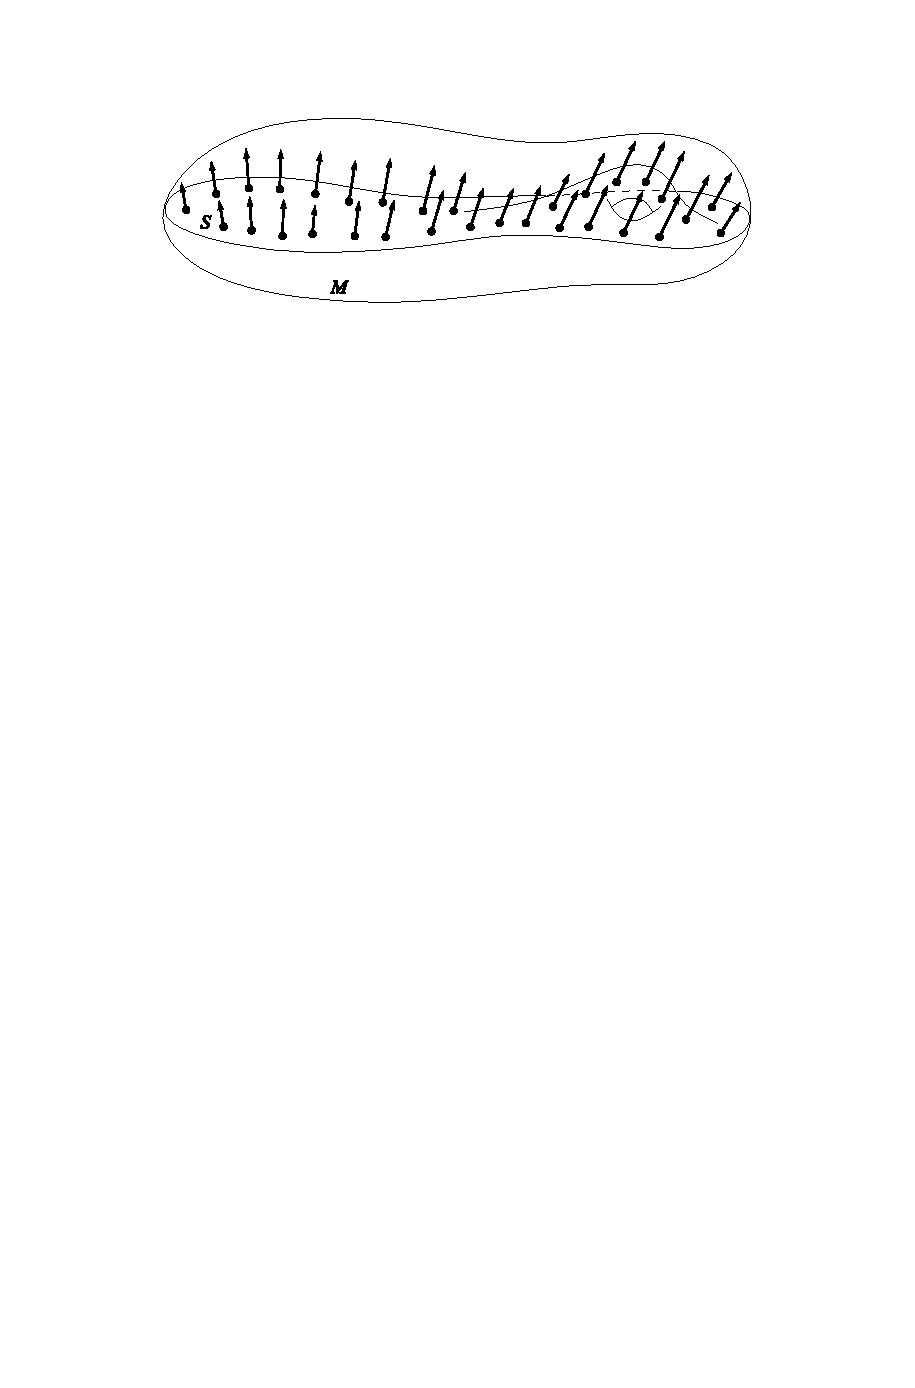
\includegraphics{pictures/vector-field-along}
\caption{A vector field along a submanifold.}
\end{figure}
\begin{proposition}\label{orientation hypersurface}
Suppose $M$ is an oriented smooth n-manifold with or without boundary, $S$ is an immersed hypersurface with or without boundary in $M$, and $N$ is a vector field along $S$ that is nowhere tangent to $S$. Then $S$ has a unique orientation such that for each $p\in S$, $(E_1,\dots,E_{n-1})$ is an oriented basis for $T_pS$ if and only if $(N_p,E_1,\dots,E_{n-1})$ is an oriented basis for $T_pM$. If $\omega$ is an orientation form for $M$, then $\iota^*_S(N\intprod\omega)$ is an orientation form for $S$ with respect to this orientation, where $\iota_S:S\hookrightarrow M$ is inclusion.
\end{proposition}
\begin{remark}
When $n=1$, since $S$ is a $0$-manifold, this proposition should be interpreted as follows: at each point $p\in S$, we assign the orientation $+1$ to $p$ if $N_p$ is an oriented basis for $T_pM$, and $-1$ if $N_p$ is negatively oriented. With this understanding, the proof below goes through in the $n=1$ case without modification.
\end{remark}
\begin{figure}[htbp]
\centering
\includegraphics{pictures/orientation-hyper}
\caption{The orientation induced by a nowhere tangent vector field.}
\end{figure}
\begin{proof}
Let $\omega$ be an orientation form for $M$. Then $\sigma=\iota^*_S(N\intprod\omega)$ is an $(n-1)$-form on $S$. (Recall that the pullback 	$\iota_S^*$ is really just restriction to vectors tangent to $S$.) It will follow that $\sigma$ is an orientation form for $S$ if we can show that it never vanishes. Given any basis $(E_1,\dots,E_{n-1})$ for $T_pS$, the fact that $N$ is nowhere tangent to $S$ implies that $(N_p,E_1,\dots,E_{n-1})$ is a basis for $T_pM$. The fact that $N$ is nonvanishing
implies that
\[\sigma_p(E_1,\dots,E_{n-1})=\omega_p(N_p,E_1,\dots,E_{n-1})\neq 0.\]
Since $\sigma_p(E_1,\dots,E_{n-1})>0$ if and only if $\omega_p(N_p,E_1,\dots,E_{n-1})>0$, the orientation determined by $\sigma$ is the one defined in the statement of the proposition.
\end{proof}
\begin{example}
The sphere $S^n$ is a hypersurface in $\R^{n+1}$, to which the vector field $N=x^i\partial/\partial x^i$ is nowhere tangent, so this vector field induces an orientation on $S^n$. This shows that all spheres are orientable. We define the \textbf{standard orientation} of $S^n$ to be the orientation determined by $N$. Unless otherwise specified, we always use this orientation. $($The standard orientation on $S^0$ is the one that assigns the orientation $+1$ to the point $+1$ and $-1$ to $-1\in S^0$.$)$
\end{example}
Not every hypersurface admits a nowhere tangent vector field. However, the following proposition gives a sufficient condition that holds in many cases.
\begin{proposition}
Let $M$ be an oriented smooth manifold, and suppose $S\sub M$ is a regular level set of a smooth function $f:M\to\R$. Then $S$ is orientable.
\end{proposition}
\begin{proof}
Choose any Riemannian metric on $M$, and let $N=\grad f|_S$. The hypotheses imply that $N$ is a nowhere tangent vector field along $S$, so the result follows from Proposition~\ref{orientation hypersurface}.
\end{proof}
\subsubsection{Boundary orientations}
If $M$ is a smooth manifold with boundary, then $\partial M$ is an embedded hypersurface in $M$, and Exercise~\ref{vector field inward} showed that there is always a smooth outward-pointing vector field along $\partial M$. Because an outward-pointing vector field is nowhere tangent to $\partial M$, it determines an orientation on $\partial M$ if $M$ is oriented.
\begin{proposition}[\textbf{Induced Orientation on a Boundary}]
Let $M$ be an oriented smooth $n$-manifold with boundary, $n\geq1$. Then $\partial M$ is orientable, and all outward-pointing vector fields along $\partial M$ determine the same orientation on $\partial M$.
\end{proposition}
\begin{remark}
The orientation on $\partial M$ determined by any outward-pointing vector field is called the \textbf{induced orientation} or the \textbf{Stokes orientation} on $\partial M$.
\end{remark}
\begin{proof}
Let $n=\dim M$, let $\omega$ be an orientation form for $M$, and let $N$ be a smooth
outward-pointing vector field along $\partial M$. The $(n-1)$-form $\iota_{\partial M}^*(N\intprod\omega)$ is an orientation form for $\partial M$ by Proposition~\ref{orientation hypersurface}, so $\partial M$ is orientable.\par
To show that this orientation is independent of the choice of $N$, let $p\in\partial M$ be arbitrary, and let $(x^i)$ be smooth boundary coordinates for $M$ on a neighborhood of $p$. If $N$ and $\widetilde{N}$ are two different outward-pointing vector fields along $\partial M$, Proposition~\ref{inward outward vector iff} shows that the last components $N^n(p)$ and $\widetilde{N}^n(p)$ are both negative. Both $(N_p,\partial/\partial x^1|_p,\dots,\partial/\partial x^n|_p)$ and $(\widetilde{N}_p,\partial/\partial x^1|_p,\dots,\partial/\partial x^n|_p)$ are bases for $T_pM$, and the transition matrix between them has determinant equal to $N^n(p)/\widetilde{N}^n(p)>0$. Thus, both bases determine the same orientation for $T_pM$, so $N$ and $\widetilde{N}$ determine the same orientation for $T_p\partial M$. (When $n=1$, the bases in question are just $N_p$ and $\widetilde{N}_p$, which determine the same orientation because they are both negative multiples of $\partial/\partial x^1|_p$.)
\end{proof}
\begin{example}
This proposition gives a simpler proof that $S^n$ is orientable, because it is the boundary of the closed unit ball. The orientation thus induced on $S^n$ is the standard one.
\end{example}
\begin{example}\label{orientation induce H^n}
Let us determine the induced orientation on $\partial\H^n$ when $\H^n$ itself has the standard orientation inherited from $\R^n$. We can identify $\partial\H^n$ with $\R^{n-1}$ under the correspondence $(x^1,\dots,x^{n-1},0)\leftrightarrow(x^1,\dots,x^{n-1})$. Since the vector field $-\partial/\partial x^n$ is outward-pointing along $\partial\H^n$, the standard coordinate frame for $\R^{n-1}$ is positively oriented for $\partial\H^n$ if and only if $[-\partial/\partial x^n,\partial/\partial x^1,\dots,\partial/\partial x^{n-1}]$ is the standard orientation for $\R^n$. This orientation satisfies
\begin{align*}
[-\partial/\partial x^n,\partial/\partial x^1,\dots,\partial/\partial x^{n-1}]&=-[\partial/\partial x^n,\partial/\partial x^1,\dots,\partial/\partial x^{n-1}]\\
&=(-1)^n[\partial/\partial x^1,\partial/\partial x^2,\dots,\partial/\partial x^{n}].
\end{align*}
Thus, the induced orientation on $\partial\H^n$ is equal to the standard orientation on $\R^{n-1}$ when $n$ is even, but it is opposite to the standard orientation when $n$ is odd. In particular, the standard coordinates on $\partial\H^n\approx\R^{n-1}$ are positively oriented if and only if $n$ is even.
\end{example}
For many purposes, the most useful way of describing submanifolds is by means
of local parametrizations. The next lemma gives a useful criterion for checking
whether a local parametrization of a boundary is orientation-preserving.
\begin{lemma}\label{orientation preserve lem}
Let $M$ be an oriented smooth $n$-manifold with boundary. Suppose $U\sub\R^{n-1}$ is open, $a,b$ are real numbers with $a<b$, and $F:(a,b]\times U\to M$ is a smooth embedding that restricts to an embedding of $\{b\}\times U$ to $\partial M$. Then the parametrization $f:U\to\partial M$ given by $f(x)=F(b,x)$ is orientation-preserving
for $\partial M$ if and only if $F$ is orientation-preserving for $M$.
\end{lemma}
\begin{figure}[htbp]
\centering
\includegraphics{pictures/boundary-para}
\caption{Orientation criterion for a boundary parametrization.}
\end{figure}
\begin{proof}
Let $x$ be an arbitrary point of $U$, and let $p=f(x)=F(b,x)\in\partial M$. The hypothesis that $F$ is an embedding means that the linear map $dF_{(b,x)}:(T_b\R\oplus T_x\R^{n-1})\to T_pM$ is bijective. Since the restriction of $dF_{(b,x)}$ to $T_x\R^{n-1}$ is equal to $df_x:T_x\R^{n-1}\to T_p\partial M$ which is already injective, it follows that $dF(\partial/\partial s|_{(b,x)})\notin T_p\partial M$ (where $s$ denotes the coordinate on $(a,b]$).\par
Define a smooth curve $\gamma:[0,\eps)\to M$ by
\[\gamma(t)=F(b-t,x).\]
This curve satisfies $\gamma(0)=p$ and $\gamma'(0)=-dF(\partial/\partial s|_{(b,x)})$. It follows that $-dF(\partial/\partial s|_{(b,x)})$ is inward-pointing, and therefore $dF(\partial/\partial s|_{(b,x)})$ is outward-pointing.\par
The definition of the induced orientation yields the following equivalences:
\begin{align*}
F&\text{ is orientation-preserving for $M$}\\
&\iff \text{$\big(dF(\partial/\partial s),dF(\partial/\partial x^1),\dots,dF(\partial/\partial x^{n-1})\big)$ is oriented for $TM$}\\
&\iff \text{$\big(dF(\partial/\partial x^1),\dots,dF(\partial/\partial x^{n-1})\big)$ is oriented for $T\partial M$}\\
&\iff \text{$\big(df(\partial/\partial x^1),\dots,df(\partial/\partial x^{n-1})\big)$ is oriented for $T\partial M$}\\
&\iff\text{$f$ is orientation-preserving for $M$.}
\end{align*}
This proves the claim.
\end{proof}
Here is an illustration of how the lemma can be used.
\begin{figure}[htbp]
\centering
\includegraphics{pictures/spherical-coordinates}
\caption{Parametrizing the sphere via spherical coordinates.}
\end{figure}
\begin{example}\label{orientation para eg}
Spherical coordinates yield a smooth local parametrization of $S^2$ as follows. Let $U$ be the open rectangle $(0,\pi)\times(0,2\pi)\sub\R^2$, and let $X:U\to\R^3$ be the following map:
\[X(\varphi,\theta)=(\sin\varphi\cos\theta,\sin\varphi\sin\theta,\cos\varphi).\]
We can check whether $X$ preserves or reverses orientation by using the fact that it is the restriction of the $3$-dimensional spherical coordinate parametrization $F:(0,1]\times U\to\widebar{B}^3$ defined by
\[F(\rho,\varphi,\theta)=(\rho\sin\varphi\cos\theta,\rho\sin\varphi\sin\theta,\rho\cos\varphi).\]
Because $F(1,\varphi,\theta)=X(\varphi,\theta)$, the hypotheses of Lemma~\ref{orientation preserve lem} are satisfied. By direct computation, the Jacobian determinant of $F$ is $\rho^2\sin\varphi$, which is positive on $(0,1]\times U$. By virtue of Lemma~\ref{orientation preserve lem}, $X$ is orientation-preserving.
\end{example}
\subsection{The Riemannian volume form}
Let $(M,g)$ be an oriented Riemannian manifold of positive dimension. We know from Proposition~\ref{Gram Schmidt Riemannian} that there is a smooth orthonormal frame $(E_1,\dots,E_n)$ in a neighborhood of each point of $M$. By replacing $E_1$ by $-E_1$ if necessary, we can find an oriented orthonormal frame in a neighborhood of each point.
\begin{proposition}\label{Riemannian volume form}
Suppose $(M,g)$ is an oriented Riemannian $n$-manifold with or without boundary, and $n\geq1$. There is a unique smooth orientation form $\omega_g\in\Omega^k(M)$, called the \textbf{Riemannian volume form}, that satisfies
\begin{align}\label{Riemannian volume form-1}
\omega_g(E_1,\dots,E_n)=1
\end{align}
for every local oriented orthonormal frame $(E_i)$ for $M$.
\end{proposition}
\begin{proof}
Suppose first that such a form $\omega_g$ exists. If $(E_1,\dots,E_n)$ is any local oriented orthonormal frame on an open subset $U\sub M$ and $(\eps^1,\dots,\eps^n)$ is the dual coframe, we can write $\omega_g=f\eps^1\wedge\cdots\wedge\eps^n$ on $U$. The condition $(\ref{Riemannian volume form-1})$ then reduces to $f=1$, so
\begin{align}\label{Riemannian volume form-2}
\omega_g=\eps^1\wedge\cdots\wedge\eps^n.
\end{align}
This proves that such a form is uniquely determined.\par
To prove existence, we would like to define $\omega_g$ in a neighborhood of each point
by $(\ref{Riemannian volume form-2})$, so we need to check that this definition is independent of the choice of oriented orthonormal frame. If $(\widetilde{E}_1,\dots,\widetilde{E}_n)$ is another oriented orthonormal frame, with dual coframe $(\widetilde{\eps}^1,\dots,\widetilde{\eps}^n)$, let
\[\widetilde{\omega}=\widetilde{\eps}^1\wedge\dots\wedge\widetilde{\eps}^n.\]
We can write
\[\widetilde{E}_i=A^j_iE_j\]
for some matrix $(A^j_i)$ of smooth functions. The fact that both frames are orthonormal means that $(A^j_i(p))\in\O(n)$ for each $p$, so $\det(A^j_i)=\pm 1$, and the fact that the two frames are consistently oriented forces the positive sign. We compute by Proposition~\ref{alt n tensor linear map}:
\[\omega_g(\widetilde{E}_1,\dots,\widetilde{E}_n)=\det\big(\eps^j(\widetilde{E}_i)\big)=\det(A^j_i)=1=\widetilde{\omega}_g(\widetilde{E}_1,\dots,\widetilde{E}_n).\]
Thus $\omega_g=\widetilde{\omega}_g$, so defining $\omega_g$ in a neighborhood of each point by $(\ref{Riemannian volume form-2})$ with respect to some smooth oriented orthonormal frame yields a global $n$-form. The resulting form is clearly smooth and satisfies $(\ref{Riemannian volume form-1})$ for every oriented orthonormal frame.
\end{proof}
\begin{proposition}
Suppose $(M,g)$ and $(\widetilde{M},\widetilde{g})$ are positive-dimensional Riemannian manifolds with or without boundary, and $F:M\to\widetilde{M}$ is a orientation-preserving local isometry. Then
that $F^*\omega_{\widetilde{g}}=\omega_g$.
\end{proposition}
\begin{proof}
Since $F$ is a orientation-preserving local isometry, it maps a local oriented orthonormal frame to a local oriented orthonormal frame. Then the claim follows immediately.
\end{proof}
Although the expression for the Riemannian volume form with respect to an oriented orthonormal frame is particularly simple, it is also useful to have an expression
for it in coordinates.
\begin{proposition}\label{Riemann volume form formula}
Let $(M,g)$ be an oriented Riemannian $n$-manifold with or without boundary with$n\geq1$. In any oriented smooth coordinates $(x^i)$, the Riemannian volume form has the local coordinate expression
\[\omega_g=\sqrt{G}\, dx^1\wedge\cdots\wedge dx^n,\]
where $G=\det(g_{ij})$ with $g_{ij}$ the components of $g$ in these coordinates.
\end{proposition}
\begin{proof}
Let $(U,(x^i))$ be an oriented smooth chart, and let $p\in M$. In these coordinates, $\omega_g=f\,dx^1\wedge\cdots\wedge dx^n$ for some positive coefficient function $f$. To compute $f$, let $(E_i)$ be any smooth oriented orthonormal frame defined on a neighborhood of $p$, and let $(\eps^i)$ be the dual coframe. If we write the coordinate frame in terms of the orthonormal frame as
\[\frac{\partial}{\partial x^i}=A^j_iE_j,\]
then we can compute
\[f=\omega_g\Big(\frac{\partial}{\partial x^1},\dots,\frac{\partial}{\partial x^n}\Big)=\det\Big(\eps^j\Big(\frac{\partial}{\partial x^i}\Big)\Big)=\det(A^j_i).\]
On the other hand, observe that
\[g_{ij}=\Big\langle\frac{\partial}{\partial x^i},\frac{\partial}{\partial x^j}\Big\rangle_g=\langle A^k_iE_k,A^l_jE_l\rangle_g=A^k_iA^l_j\langle E_k,E_l\rangle_g=\sum_kA^k_iA^k_j.\]
This last expression is the $(i,j)$-entry of the matrix product $A^TA$, where $A=(A^j_i)$. Thus,
\[G:=\det(g_{ij})=\det(A^TA)=(\det A)^2,\]
Since both frames $(\partial/\partial x^i)$ and $(E_i)$ are oriented, $f$ must be positive. So it follows that $f=\sqrt{G}$. 
\end{proof}
\subsubsection{Hypersurfaces in Riemannian manifolds}
Let $(M,g)$ be an oriented Riemannian manifold with or without boundary, and suppose $S\sub M$ is an immersed hypersurface with or without boundary. Any unit normal vector field along $S$ is nowhere tangent to $S$, so it determines an orientation of $S$ by Proposition~\ref{orientation hypersurface}. The next proposition gives a simple formula for the volume form of the induced metric on $S$ with respect to this orientation.
\begin{proposition}\label{Riemann volumn form hyper}
Let $(M,g)$ be an oriented Riemannian manifold with or without boundary, let $S\sub M$ be an immersed hypersurface with or without boundary, and let $\widetilde{g}$ denote the induced metric on $S$. Suppose $N$ is a smooth unit normal vector field along $S$. With respect to the orientation of $S$ determined by $N$, the volume form of $(S,\widetilde{g})$ is given by
\[\omega_{\widetilde{g}}=\iota_S^*(N\intprod\omega_g).\]
\end{proposition}
\begin{proof}
By Proposition~\ref{orientation hypersurface}, the $(n-1)$-form $\iota_S^*(N\intprod\omega_g)$ is an orientation form for $S$. To prove that it is the volume form for the induced Riemannian metric, we need only show that it gives the value $1$ whenever it is applied to an oriented orthonormal frame for $S$. Thus, let $(E_1,\dots,E_{n-1})$ be such a frame. At each point $p\in S$, the basis $(N_p,E_1|_p,\dots,E_{n-1}|_p)$ is orthonormal, and is oriented for $T_pM$ (this is the definition of the orientation determined by $N$). Thus 
\[\iota_S^*(N\intprod\omega_g)(E_1,\dots,E_{n-1})=\omega_g(N,E_1,\dots,E_{n-1})=1,\]
which proves the result.
\end{proof}
The result of Proposition~\ref{Riemann volumn form hyper} takes on particular importance in the case of a Riemannian manifold with boundary, because of the following proposition.
\begin{proposition}
Suppose $M$ is any Riemannian manifold with boundary. There is a unique smooth outward-pointing unit normal vector field $N$ along $\partial M$.
\end{proposition}
\begin{proof}
First, we prove uniqueness. At any point $p\in\partial M$, the subspace $(T_p\partial M)^\bot\sub T_pM$ is $1$-dimensional, so there are exactly two unit vectors at $p$ that are normal to $\partial M$. Since any unit normal vector $N$ is nowhere tangent to $\partial M$, it must have nonzero $x^n$-component in any smooth boundary chart. Thus, exactly one of the two choices of unit normal has negative $x^n$-component, which is equivalent to being outward-pointing.\par
To prove existence, let $f:M\to\R$ be a boundary defining function (Proposition
5.43), and let $N$ be the restriction to $\partial M$ of the unit vector field $-\grad f/|\grad f|_g$. Because $df\neq0$ at points of $\partial M$, $N$ is well-defined and
smooth on $\partial M$. Then $N$ is normal to $\partial M$ by Exercise~\ref{Riemann grad prop}, and outward pointing by Proposition~\ref{inward derivative crit}, because 
\[Nf=\frac{-\langle\grad f,\grad f\rangle_g}{|\grad f|_g}=-|\grad f|_g<0.\]
\end{proof}
The next corollary is immediate.
\begin{corollary}
If $(M,g)$ is an oriented Riemannian manifold with boundary and $\widetilde{g}$ is the induced Riemannian metric on $\partial M$, then the volume form of $\widetilde{g}$ is
\[\omega_{\widetilde{g}}=\iota_{\partial M}^*(N\intprod\omega_g),\]
where $N$ is the outward unit normal vector field along $\partial M$.
\end{corollary}
\subsection{Orientations and covering maps}
Although it is often easy to prove that a given smooth manifold is orientable by constructing an orientation for it, proving that a manifold is not orientable can be much trickier. The theory of covering spaces provides one of the most useful techniques
for doing so. In this part, we explore the close relationship between orientability
and covering maps.\par
Our first result is a simple application of pullback orientations.
\begin{proposition}
If $\pi:E\to M$ is a smooth covering map and $M$ is orientable, then $E$ is also orientable.
\end{proposition}
\begin{proposition}
Because a covering map is a local diffeomorphism, this follows immediately from Proposition~\ref{orientation pull back}.
\end{proposition}
The next theorem is more interesting. If $G$ is a Lie group acting smoothly on a smooth manifold $E$ (on the left, say), we say the action is an \textbf{orientation-preserving action} if for each $g\in G$, the diffeomorphism $x\mapsto g\cdot x$ is orientation-preserving.
\begin{theorem}\label{orientation covering thm}
Suppose $E$ is a connected, oriented, smooth manifold with or without boundary, and $\pi:E\to M$ is a smooth normal covering map. Then $M$ is orientable if and only if the action of $\Aut_\pi(E)$ on $E$ is orientation-preserving.
\end{theorem}
\begin{proof}
Let $\mathcal{O}_E$ denote the given orientation on $E$. First suppose $M$ is orientable, and let $q$ be an arbitrary point in $E$. Because $M$ is connected, it has exactly two orientations, and one of them has the property that $d\pi_q:T_qE\to T_{\pi(q)}M$ is orientation-preserving. Call that orientation $\mathcal{O}_M$. The pullback orientation $\pi^*\mathcal{O}_M$ agrees with the given orientation at $q$, so it must be equal to $\mathcal{O}_E$ by Corollary~\ref{orientation connected}. Suppose $\varphi\in\Aut_\pi(E)$. The fact that $\pi\circ\varphi=\pi$ implies that
\[\varphi^*\mathcal{O}_E=\varphi^*(\pi^*\mathcal{O}_M)=(\pi\circ\varphi)^*\mathcal{O}_M=\pi^*\mathcal{O}_M=\mathcal{O}_E.\]
Thus, $\varphi$ is orientation-preserving.\par
Conversely, suppose the action of $\Aut_\pi(E)$ is orientation-preserving, and let $p\in M$. If $U\sub M$ is any evenly covered neighborhood of $p$, there is a smooth section $\sigma:U\to E$, which induces an orientation $\sigma^*\mathcal{O}_E$ on $U$. Suppose $\sigma_1:U\to E$ is any other smooth local section over $U$. Because $\pi$ is a normal covering, $\Aut_\pi(E)$ acts transitively on each fiber of $\pi$, so there is a covering automorphism $\varphi$ such that $\sigma_1(p)=\varphi(\sigma(p))$. Then $\varphi\circ\sigma$ is a local section of $\pi$ that agrees with $\sigma_1$ at $p$, and thus $\sigma_1=\varphi\circ\sigma$ on all of $U$ by Theorem~\ref{local section unique}. Because $\varphi$ is orientation-preserving, $\sigma_1^*\mathcal{O}_E=\sigma^*\varphi^*\mathcal{O}_E=\sigma^*\mathcal{O}_E$, so the orientations induced by $\sigma$ and $\sigma_1$ are equal. Thus, we can define a global orientation $\mathcal{O}_M$ on $M$ by defining it on each evenly covered open subset to be the pullback orientation induced by any local section; the argument above shows that the orientations so defined agree where they overlap.
\end{proof}
Here are two applications of the preceding theorem.
\begin{example}[\textbf{Orientability of Projective Spaces}]
For $n\geq1$, consider the smooth covering map $q:S^n\to\RP^n$. The only nontrivial covering automorphism of $q$ is the antipodal map $\alpha(x)=-x$. It can be easily shown that $\alpha$ is orientation-preserving if and only if $n$ is odd, so it follows that $\RP^n$ is orientable if and only if $n$ is odd.
\end{example}
\begin{example}[\textbf{The M\"obius Bundle and the M\"obius Band}]
Let $E$ be the total space of the M\"obius bundle $(Example~\ref{Mobius bundle})$. The quotient map $q:\R^2\to E$ used to define $E$ is a smooth normal covering map, and the covering automorphism group is isomorphic to $\Z$, acting on $\R^2$ by 
\[n(x,y)=(x+n,(-1)^ny)\] 
For $n$ odd, the diffeomorphism $(x,y)\mapsto n\cdot (x,y)$ of $\R^2$ pulls back the orientation form $dx\wedge dy$ to $-dx\wedge dy$, so the action of $\Aut_q(E)$ is not orientation-preserving. Thus, Theorem~\ref{orientation covering thm} shows that $E$ is not orientable.\par
For each $r>0$, the image under $q$ of the rectangle $[0,1]\times[-r,r]$ is a M\"obius
band $M_r$. Because $q$ restricts to a smooth covering map from $\R\times[-r,r]$, the
same argument shows that a M\"obius band is not orientable either.
\end{example}
\subsubsection{The orientation covering}
Next we show that every nonorientable smooth manifold $M$ has an orientable two-sheeted
covering manifold. The fiber over a point $p\in M$ will correspond to the two orientations of $T_pM$.\par
In order to handle the orientable and nonorientable cases in a uniform way, it is useful to expand our definition of covering maps slightly, by allowing covering spaces that are not connected. If $N$ and $M$ are topological spaces, let us say that a map $\pi:N\to M$ is a \textbf{generalized covering map} if it satisfies all of the requirements for a covering map except that $N$ might not be connected: this means that $N$ is locally path-connected, $\pi$ is surjective and continuous, and each point $p\in M$ has a neighborhood that is evenly covered by $\pi$. If in addition $N$ and $M$ are smooth manifolds with or without boundary and $\pi$ is a local diffeomorphism, we say it is a \textbf{generalized smooth covering map}.
\begin{lemma}\label{covering restrict}
Suppose $N$ and $M$ are topological spaces and $\pi:N\to M$ is a generalized covering map. If $M$ is connected, then the restriction of $\pi$ to each component of $N$ is a covering map.
\end{lemma}
\begin{proof}
Suppose $W$ is a component of $N$. If $U$ is any open subset of $M$ that is evenly covered by $\pi$, then each component of $\pi^{-1}(U)$ is connected and therefore contained in a single component of $N$. It follows that $(\pi|_W)^{-1}(U)=\pi^{-1}(U)\cap W$ is either the empty set or a nonempty disjoint union of components of $\pi^{-1}(U)$, each of which is mapped homeomorphically onto $U$ by $\pi|_W$. In particular, this means that each point in $\pi(W)$ has a neighborhood that is evenly covered by $\pi|_W$.\par
To complete the proof, we just need to show that $\pi|_W$ is surjective. Because $\pi$
is a local homeomorphism, $\pi(W)$ is an open subset of $M$. On the other hand, if $p\in M-\pi(W)$, and $U$ is a neighborhood of $p$ that is evenly covered by $\pi$, then the discussion in the preceding paragraph shows that $(\pi|_W)^{-1}(U)=\emp$, which implies that $U\sub M-\pi(W)$. Therefore, $\pi(W)$ is closed in $M$. Because $W$ is not empty, $\pi(W)$ is all of $M$.
\end{proof}
Let $M$ be a connected, smooth, positive-dimensional manifold with or without boundary, and let $\widehat{M}$ denote the set of orientations of all tangent spaces to $M$:
\[\widehat{M}=\{(p,\mathcal{O}_p):\text{$p\in M$ and $\mathcal{O}_p$ is an orientation of $T_pM$}\}.\]
Define the projection $\widehat{\pi}:\widehat{M}\to M$ by sending an orientation of $T_pM$ to the point $p$ itself: $\widehat{\pi}(p,\mathcal{O}_p)=p$. Since each tangent space has exactly two orientations, each fiber of this map has cardinality $2$. The map $\widehat{\pi}:\widehat{M}\to M$ is called the \textbf{orientation covering} of $M$.
\begin{proposition}[\textbf{Properties of the Orientation Covering}]\label{orientation cover prop}
Suppose $M$ is a connected, smooth, positive-dimensional manifold with or without boundary, and let $\widehat{\pi}:\widehat{M}\to M$ be its orientation covering. Then $\widehat{M}$ can be given the structure of a smooth, oriented manifold with or without boundary, with the following properties:
\begin{itemize}
\item[(a)] $\widehat{\pi}:\widehat{M}\to M$ is a generalized smooth covering map.
\item[(b)] A connected open subset $U\sub M$ is evenly covered by $\widehat{\pi}$ if and only if $U$ is orientable.
\item[(c)] If $U\sub M$ is an evenly covered open subset, then every orientation of $U$ is the pullback orientation induced by a local section of $\widehat{\pi}$ over $U$.
\end{itemize}
\end{proposition}
\begin{proof}
We first topologize $\widehat{M}$ by defining a basis for it. For each pair $(U,\mathcal{O})$, where $U$ is an open subset of $M$ and $\mathcal{O}$ is an orientation on $U$, define a subset $\widehat{U}_\mathcal{O}\sub\widehat{M}$ as follows:
\[\widehat{U}_\mathcal{O}=\{(p,\mathcal{O}_p)\in\widehat{M}:\text{$p\in U$ and $\mathcal{O}_p$ is the orientation of $T_pM$ determined by $\mathcal{O}$}\}.\]
We will show that the collection of all subsets of the form $\widehat{U}_\mathcal{O}$ is a basis for a topology on $\widehat{M}$.
\begin{itemize}
\item Given an arbitrary point $(p,\mathcal{O}_p)\in\widehat{M}$, let $U$ be an orientable neighborhood of $p$ in $M$, and let $\mathcal{O}$ be an orientation on it. After replacing $\mathcal{O}$ by $-\mathcal{O}$ if necessary, we may assume that the given orientation $\mathcal{O}_p$ is same as the orientation of $T_pM$ determined by $\mathcal{O}$. It follows that $(p,\mathcal{O}_p)\in\widehat{U}_\mathcal{O}$, so the collection of all sets of the form $\widehat{U}_\mathcal{O}$ covers $\widehat{M}$.
\item If $\widehat{U}_\mathcal{O}$ and $\widehat{U}'_{\mathcal{O}'}$ are two such sets and $(p,\mathcal{O}_p)$ is a point in their intersection, then $\mathcal{O}_p$ is the orientation of $T_pM$ determined by both $\mathcal{O}$ and $\mathcal{O}'$. If $V$ is the component of $U\cap U'$ containing $p$, then the restricted orientations $\mathcal{O}|_V$ and $\mathcal{O}'|_V$ agree at $p$ and therefore are identical by Proposition~\ref{orientation connected}, so it follows that $\widehat{U}_\mathcal{O}\cap\widehat{U}'_{\mathcal{O}'}$ contains the basis set $\widehat{V}_{\mathcal{O}|_V}$.
\end{itemize}
Thus, we have defined a topology on $\widehat{M}$.\par
Note that for each orientable open subset $U\sub M$ and each orientation $\mathcal{O}$ of $U$, $\widehat{\pi}$ maps the basis set $\widehat{U}_{\mathcal{O}}$ bijectively onto $U$. Because the orientable open subsets form a basis for the topology of $M$, this implies that $\widehat{\pi}$ restricts to a homeomorphism from $\widehat{U}_\mathcal{O}$ to $U$. In particular, $\widehat{\pi}$ is a local homeomorphism.\par
Next we show that with this topology, $\widehat{\pi}$ is a generalized covering map. Suppose $U\sub M$ is an orientable connected open subset and $\mathcal{O}$ is an orientation for $U$. Then $\widehat{\pi}^{-1}(U)$ is the disjoint union of open subsets $\widehat{U}_{\mathcal{O}}$ and $\widehat{U}_{-\mathcal{O}}$, and $\widehat{\pi}$ restricts to a homeomorphism from each of these sets to $U$. Thus, each such set $U$ is evenly covered, and it follows that $\widehat{\pi}$ is a generalized covering map. By Lemma~\ref{covering restrict}, $\widehat{\pi}$ restricts to an ordinary covering map on each component of $\widehat{M}$, and so Proposition~\ref{covering mani} shows that each such component is a topological $n$-manifold with or without boundary and has a unique smooth structure making $\widehat{\pi}$ into a smooth covering map. These smooth structures combine to give a smooth structure on all of $\widehat{M}$. This completes the proof of (a).\par
Next we give $\widehat{M}$ an orientation. Let $\widehat{p}=(p,\mathcal{O}_p)$ be a point in $\widehat{M}$. By definition, $\mathcal{O}_p$ is an orientation of $T_pM$, so we can give $T_{\widehat{p}}\widehat{M}$ the unique orientation $\widehat{\mathcal{O}}_{\widehat{p}}$ such that $d\widehat{\pi}_{\widehat{p}}:T_{\widehat{p}}\widehat{M}\to T_pM$ is orientation-preserving. This defines a pointwise orientation $\widehat{\mathcal{O}}$ on $\widehat{M}$. On each basis open subset $\widehat{U}_{\mathcal{O}}$, the orientation $\widehat{O}$ agrees
with the pullback orientation induced from $(U,\mathcal{O})$ by (the restriction of) $\widehat{\pi}$, so it is continuous.\par
Next we prove (b). We showed earlier that every orientable connected open subset
of $M$ is evenly covered by $\widehat{\pi}$. Conversely, if $U\sub M$ is any evenly covered open subset, then there is a smooth local section $\sigma:U\to\widehat{M}$ by Proposition~\ref{local section unique}, which pulls $\widehat{O}$ back to an orientation on $U$ by Proposition~\ref{orientation pull back}.\par 
Finally, to prove (c), assume $U\sub M$ is evenly covered and therefore orientable. Given any orientation $\mathcal{O}$ of $U$, define a section $\sigma:U\to M$ by setting $\sigma(p)=(p,\mathcal{O}_p)$. To see that $\sigma$ is continuous, suppose $\widehat{U}'_{\mathcal{O}'}$ is any basis open subset of $\widehat{M}$. Then for each component $V$ of $U\cap U'$, the restricted orientations $\mathcal{O}|_V$ and $\mathcal{O}'|_V$ must either agree or disagree on all of $V$, so $\sigma^{-1}(\widehat{U}'_{\mathcal{O}'})$ is a union of such components and therefore open.
\end{proof}
\begin{theorem}[\textbf{Orientation Covering Theorem}]
Suppose $M$ is a connected smooth manifold with or without boundary, and let $\widehat{\pi}:\widehat{M}\to M$ be its orientation covering.
\begin{itemize}
\item[(a)] If $M$ is orientable, then $\widehat{M}$ has exactly two components, and the restriction of $\widehat{\pi}$ to each component is a diffeomorphism onto $M$.
\item[(b)] If $M$ is nonorientable, then $\widehat{M}$ is connected, and $\widehat{\pi}$ is a two-sheeted smooth covering map.
\end{itemize}
\end{theorem}
\begin{proof}
If $M$ is orientable, then Proposition~\ref{orientation cover prop}(b) shows that $M$ is evenly covered by $\widehat{\pi}$, which means that $\widehat{M}$ has two components, each mapped diffeomorphically onto $M$.\par
Now assume $M$ is nonorientable. We show first that $\widehat{M}$ is connected. Let $W$ be a component of $\widehat{M}$. Lemma~\ref{covering restrict} shows that $\widehat{\pi}|_W$ is a covering map, so its fibers all have the same cardinality. Because the fibers of $\widehat{\pi}$ have cardinality $2$ and $W$ is not empty, the fibers of $\widehat{\pi}|_W$ must have cardinality $1$ or $2$. If the cardinality were $1$, then $\widehat{\pi}|_W$ would be an injective smooth covering map and thus a diffeomorphism, and its inverse would be a smooth section of $\widehat{\pi}$, which would induce an orientation on $M$. Thus, the cardinality must be $2$, which implies that $W=\widehat{M}$. Because $\widehat{M}$ is connected, $\widehat{\pi}$ is a covering map by Lemma~\ref{covering restrict}, and because it is a local diffeomorphism it is a smooth covering map.
\end{proof}
The orientation covering is sometimes called the \textbf{oriented double covering of $\bm{M}$}. There are other ways of constructing it besides the one we have given here, but as the next theorem shows, the specific details of the construction do not matter, because they all yield isomorphic covering manifolds.
\begin{theorem}[\textbf{Characteristic property of the orientation covering}]\label{orientation cover char}
Let $M$ be a connected nonorientable smooth manifold with or without boundary, and let $\widehat{\pi}:\widehat{M}\to M$ be its orientation covering. If $X$ is any oriented smooth manifold with or without boundary, and $F:X\to M$ is any local diffeomorphism, then there exists a unique orientation-preserving local diffeomorphism $\widehat{F}:X\to\widehat{M}$ such that $\widehat{\pi}\circ\widehat{F}=F$:
\[\begin{tikzcd}
&\widehat{M}\ar[d,"\widehat{\pi}"]\\
X\ar[r,swap,"F"]\ar[ru,dashed,"\widehat{F}"]&M
\end{tikzcd}\]
\end{theorem}
\begin{proof}
At each point $p=F(x)\in M$, since $F$ is a local diffeomorphism, we get a unique orientation of $T_pM$, which we denote by $\mathcal{O}_p$. Then we can define
\[\widehat{F}(x)=(F(x),\mathcal{O}_{F(x)}).\]
It is easy to check that $\widehat{\pi}\circ\widehat{F}=F$. Since $\widehat{\pi}$ is also a local diffeomorphism, it follows that $\widehat{F}$ is also a local diffeomorphism. The orientation-preserving statement is clear from the definition.
\end{proof}
\begin{theorem}[\textbf{Uniqueness of the Orientation Covering}]\label{orientation cover unique}
Let $M$ be a nonorientable connected smooth manifold with or without boundary, and let $\widehat{\pi}:\widehat{M}\to M$ be its orientation covering. If $\widetilde{M}$ is an oriented smooth manifold with or without boundary that admits a two-sheeted smooth covering map $\widetilde{\pi}:\widetilde{M}\to M$, then there exists a unique orientation-preserving diffeomorphism $\varphi:\widetilde{M}\to\widehat{M}$ such that $\widehat{\pi}\circ\varphi=\widetilde{\pi}$.
\end{theorem}
By invoking a little more covering space theory, we obtain the following sufficient
topological condition for orientability. 
\begin{theorem}
Let $M$ be a connected smooth manifold with or without boundary, and suppose the fundamental group of $M$ has no subgroup of index $2$. Then $M$ is orientable. In particular, if $M$ is simply connected then it is orientable.
\end{theorem}
\begin{proof}
Suppose $M$ is not orientable, and let $\widehat{\pi}:\widehat{M}\to M$ be its orientation covering, which is an honest covering map in this case. Choose any point $q\in\widehat{M}$, and let $p=\widehat{\pi}(q)\in M$. Let $\alpha:\widehat{M}\to\widehat{M}$ be the map that interchanges the two points in each fiber of $\widehat{\pi}$. To prove that $\alpha$ is smooth, suppose $U\sub M$ is any evenly covered open subset and $U_0,U_1\sub\widehat{M}$ are the two components of $\widehat{\pi}^{-1}(U)$. Since $\widehat{\pi}$ restricts to a diffeomorphism from each component onto $U$, we can write $\alpha|_{U_0}=(\widehat{\pi}|_{U_1})^{-1}\circ(\widehat{\pi}|_{U_0})$, which is smooth. Similarly, $\alpha|_{U_1}$ is also smooth. Since the collection of all such sets $U_0,U_1$ is an open covering of $\widehat{M}$, it follows that $\alpha$ is smooth, and it is a covering automorphism because it satisfies $\widehat{\pi}\circ\alpha=\widehat{\pi}$. In fact, since a covering automorphism is determined by what it does to one point, $\alpha$ is the unique nontrivial element of the automorphism group $\Aut_{\widehat{\pi}}(\widehat{M})$, which is therefore
equal to the two-element group $\{\mathrm{id}_{\widehat{M}},\alpha\}$. Because the automorphism group acts transitively on fibers, $\widehat{\pi}$ is a normal covering map. A fundamental result in the theory of covering spaces is that
\[\Aut_{\widehat{\pi}}(\widehat{M})\cong\frac{\pi_1(M,p)}{\widehat{\pi}^*\big(\pi_1(\widehat{M},q)\big)}.\]
Therefore, $\pi_1(M,p)$ has an index $2$ subgroup.
\end{proof}
\subsection{Exercise}
\begin{exercise}
Suppose$ M$ is a smooth manifold that is the union of two orientable open submanifolds with connected intersection. Show that $M$ is orientable.
\end{exercise}
\begin{proof}
Use Proposition~\ref{orientation connected}.
\end{proof}
\begin{exercise}
Suppose $M$ and $N$ are oriented smooth manifolds with or without boundary, and $F:M\to N$ is a local diffeomorphism. Show that if $M$ is connected, then $F$ is either orientation-preserving or orientation-reversing.
\end{exercise}
\begin{exercise}
Suppose $n\geq1$, and let $\alpha:S^n\to S^n$ be the antipodal map: $\alpha(x)=-x$. Show that $\alpha$ is orientation-preserving if and only if $n$ is odd.
\end{exercise}
\begin{proof}
Consider the orientation form on $\widebar{B}^{n+1}$:
\[\omega=dx^1\wedge\cdots\wedge dx^{n+1}.\]
The induced orientation on $S^n$ is then given by
\[\omega_{S^n}=\iota^*(N\intprod\omega),\]
where $N=x^i\partial/\partial x^i$. Let $F:\widebar{B}^{n+1}\to\widebar{B}^{n+1}$ be the map $F(x)=-x$, then $F_*\omega=(-1)^{n+1}\omega$. Since the map $\alpha$ preserves that vector field $N$, and the orientation of $S^n$ is induced by $N$, we conclude that $\alpha$ is orientation-preserving if and only if $F$ is orientation-preserving.
\end{proof}
\begin{exercise}\label{orientation flow}
Let $\theta$ be a smooth flow on an oriented smooth manifold with or without boundary. Show that for each $t\in\R$, $\theta_t$ is orientation-preserving wherever it is defined.
\end{exercise}
\begin{proof}
The map $\theta:\R\to\Diff(M)$ is a smooth group homomorphism, and hence its image is connected. Since $\theta_0=\mathrm{id}_M$, this curve lies in the orientation preserving component of $\Diff(M)$.
\end{proof}
\begin{exercise}\label{orentaton TM and T^*M}
Let $M$ be a smooth manifold with or without boundary. Show that the total
spaces of $TM$ and $T^*M$ are orientable.
\end{exercise}
\begin{proof}
We prove for $TM$. By Proposition~\ref{tangent bundle struct}, the transition map between charts $(U,\varphi)$ and $(V,\psi)$ of $M$ is
\[\widetilde{\psi}\circ\widetilde{\varphi}^{-1}(x^1,\dots,x^n,v^1,\dots,v^n)=(\widetilde{x}^1(x),\dots,\widetilde{x}^n(x),v^i\frac{\partial\widetilde{x}^1}{\partial x^i}(x),\dots,v^i\frac{\partial\widetilde{x}^n}{\partial x^i}(x)).\]
The Jacobian matrix of this map is
\[\partial(\widetilde{\psi}\circ\widetilde{\varphi}^{-1})(x,v)=\begin{pmatrix}
\dfrac{\partial\widetilde{x}^j}{\partial x^i}(x)&0\\[8pt]
*&\dfrac{\partial\widetilde{x}^j}{\partial x^i}(x)
\end{pmatrix}.\]
Thus \[\det\partial(\widetilde{\psi}\circ\widetilde{\varphi}^{-1})=\big(\det\partial(\psi\circ\varphi^{-1})\big)^2,\]
which, by Proposition~\ref{orientation by atlas}, implies $TM$ is orientable.
\end{proof}
\begin{exercise}
Suppose $M$ is an oriented Riemannian manifold with or without boundary, and $S\sub M$ is an oriented smooth hypersurface with or without boundary. Show that there is a unique smooth unit normal vector field along $S$ that determines the given orientation of $S$.
\end{exercise}
\begin{exercise}
Suppose $M$ is an orientable Riemannian manifold, and $S\sub M$ is an immersed or embedded submanifold with or without boundary. Prove the following statements.
\begin{itemize}
\item[(a)] If $S$ has trivial normal bundle, then $S$ is orientable.
\item[(b)] If $S$ is an orientable hypersurface, then $S$ has trivial normal bundle.
\end{itemize}
\end{exercise}
\begin{proof}
Let $S$ has codimension $k$. If $S$ has trivial normal bundle, then there is an diffeomorphism $NS\to S\times\R^k$. Thus we have global frames $(\sigma_1,\dots,\sigma_k)$ of $NS$. By Proposition~\ref{local frame completion}, at each point $p$ we can find local frames $(\sigma_{k+1},\dots,\sigma_{n})$ such that $(\sigma_1,\dots,\sigma_n)$ is an oriented frame for $T_pM$. Thus $S$ is orientable.\par
If $S$ is an orientable hypersurface, then there is a unit normal vector field along $S$. Since this is a global frame for $NS$, we get a global trivialization for $NS$.
\end{proof}
\begin{exercise}
Show that every orientation-reversing diffeomorphism of $\R$ has a fixed
point.
\end{exercise}
\begin{exercise}
Let $M$ be a connected smooth $1$-manifold. Show that $M$ is diffeomorphic to either $\R$ or $S^1$, as follows:
\begin{itemize}
\item[(a)] First, do the case in which $M$ is orientable by showing that $M$ admits a nonvanishing smooth vector field.
\item[(b)] Now let $M$ be arbitrary, and prove that $M$ is orientable by showing that its universal covering manifold is diffeomorphic to $\R$.
\end{itemize}
Conclude that the smooth structures on both $\R$ and $S^1$ are unique up to
diffeomorphism.
\end{exercise}
\begin{proof}
The only $1$-manifolds are $\R$ and $S^1$, thus orientable.
\end{proof}
\begin{exercise}
Show that every connected smooth $1$-manifold with nonempty boundary is diffeomorphic to either $[0,\infty)$ or $[0,1]$.
\end{exercise}
\begin{exercise}
Let $M$ be a nonorientable embedded hypersurface in $\R^n$, and let $NM$ be
its normal bundle with projection $\pi_{NM}:NM\to M$. Show that the set
\[W=\{(x,v)\in NM:|v|=1\}\]
is an embedded submanifold of $NM$, and the restriction of $\pi_{NM}$ to $W$ is a smooth covering map isomorphic to the orientation covering of $M$.
\end{exercise}
\begin{proof}
We can show that $W$ is a orientable manifold, and the map $\pi_{NM}:W\to M$ is a $2$-sheet covering. Thus there is a diffeomorphism from $W$ to $\widehat{M}$ by Theorem~\ref{orientation cover unique}.
\end{proof}
\begin{exercise}
Let $E$ be the total space of the M\"obius bundle as in Example~\ref{Mobius bundle}. Show that the orientation covering of $E$ is diffeomorphic to the cylinder $S^1\times\R$.
\end{exercise}
\begin{proof}
Let $S^1\times\R$ be embedded into $\R^3$, we can apply the antipodal map $\alpha$ on it to obtain $E$. This gives a $2$-sheet cover of $E$, and is the orientation covering by Theorem~\ref{orientation cover unique}.
\end{proof}
\section{Integration on manifolds}
\subsection{Integration of differential forms}
In this part we will apply the integration theory on manifolds. In particular, we need the Lebesgue integration in $\R^n$. Let $D\sub\R^n$ be a measurable set, and let $\omega$ be a continuous $n$-form on $\widebar{D}$. Any such form can be written as $\omega=f\,dx^1\wedge\cdots\wedge dx^n$ for some continuous function $f:\widebar{D}\to\R$. We define the \textbf{integral of $\bm{\omega}$ over $\bm{D}$} to be
\[\int_D\omega=\int_Df\,dV.\]
This can be written more suggestively as
\[\int_Df\,dx^1\wedge\cdots\wedge dx^n=\int_Df\,dx^1\cdots dx^n.\]
Somewhat more generally, let $U$ be an open subset of $\R^n$ or $\H^n$, and suppose $\omega$ is a compactly supported $n$-form on $U$. We define
\[\int_U\omega=\int_D\omega,\]
where $D\sub\R^n$ or $\H^n$ is any measurable set containing $\supp(\omega)$, and $\omega$ is extended to be zero on the complement of its support. It is easy to check that this definition does not depend on what domain $D$ is chosen.\par
Like the definition of the integral of a $1$-form over an interval, our definition of the integral of an $n$-form might look like a trick of notation. The next proposition shows why it is natural.
\begin{proposition}\label{int R^n pull back}
Suppose $U$, $V$ are open subsets of $\R^n$ or $\H^n$, and $G:U\to V$ is an orientation-preserving or orientation-reversing diffeomorphism. If $\omega$ is a compactly supported $n$-form on $V$, then
\[\int_V\omega=\pm\int_UG^*\omega.\]
with the positive sign if $G$ is orientation-preserving, and the negative sign otherwise.
\end{proposition}
\begin{figure}[htbp]
\centering
\includegraphics{pictures/int-form-Rn}
\caption{Diffeomorphism invariance of the integral of a form on an open subset.}
\end{figure}
\begin{proof}
Let us use $(y^1,\dots,y^n)$ to denote standard coordinates on $V$, and $(x^1,\dots,x^n)$ to denote those on $U$. Suppose first that $G$ is orientation-preserving. With $\omega=f\,dy^1\wedge\cdots\wedge dy^n$, the change of variables formula together with formula $(\ref{pull back n form-1})$ for pullbacks of $n$-forms yields
\begin{align*}
\int_V\omega&=\int_Vf\,dV=\int_U(f\circ G)|\det\partial G|\,dV=\int_U(f\circ G)(\det\partial G)\,dV\\
&=\int_U(f\circ G)(\det \partial G)\,dx^1\wedge\cdots\wedge dx^n=\int_UG^*\omega.
\end{align*}
If $G$ is orientation-reversing, the same computation holds except that a negative sign is introduced when the absolute value signs are removed.
\end{proof}
\subsubsection{Integration on manifolds}
Let $M$ be an oriented smooth nmanifold with or without boundary, and let $\omega$ be an $n$-form on $M$. Suppose first that $\omega$ is compactly supported in the domain of a single smooth chart $(U,\varphi)$ that is either positively or negatively oriented. We define the integral of $\omega$ over $M$ to be
\begin{align}\label{int mani def-1}
\int_M\omega=\pm\int_{\varphi(U)}\varphi_*\omega,
\end{align}
\begin{figure}[htbp]
\centering
\includegraphics{pictures/int-form-onechart}
\caption{The integral of a form over a manifold.}
\end{figure}
with the positive sign for a positively oriented chart, and the negative sign otherwise. Since $\varphi_*\omega$ is a compactly supported $n$-form on the open subset $\varphi(U)\sub\R^n$ or $\H^n$, its integral is defined as discussed above.
\begin{proposition}\label{inte form one chart}
With $\omega$ as above, $\int_M\omega$ does not depend on the choice of smooth chart whose domain contains $\supp(\omega)$.
\end{proposition}
\begin{figure}[htbp]
\centering
\includegraphics{pictures/int-form-coordinate}
\caption{Coordinate independence of the integral.}
\end{figure}
\begin{proof}
Suppose $(U,\varphi)$ and $(\widetilde{U},\widetilde{\varphi})$ are two smooth charts such that $\supp(\omega)\sub U\cap\widetilde{U}$. If both charts are positively oriented or both are negatively oriented, then $\widetilde{\varphi}\circ\varphi^{-1}$ is an orientation-preserving diffeomorphism from $\varphi(U\cap\widetilde{U})$ to $\widetilde{\varphi}(U\cap\widetilde{U})$, so Proposition~\ref{int R^n pull back} implies that
\begin{align*}
\int_{\widetilde{\varphi}(\widetilde{U})}\widetilde{\varphi}_*\omega&=\int_{\widetilde{\varphi}(U\cap\widetilde{U})}\widetilde{\varphi}_*\omega=\int_{\varphi(U\cap\widetilde{U})}(\widetilde{\varphi}\circ\varphi^{-1})^*\widetilde{\varphi}_*\omega\\
&=\int_{\varphi(U\cap\widetilde{U})}(\varphi^{-1})^*\circ\widetilde{\varphi}^*\circ\widetilde{\varphi}_*\omega=\int_{\varphi(U)}\varphi_*\omega.
\end{align*}
If the charts are oppositely oriented, then the two definitions given by $(\ref{int mani def-1})$ have opposite signs, but this is compensated by the fact that $\widetilde{\varphi}\circ\varphi^{-1}$ is orientationreversing, so Proposition~\ref{int R^n pull back} introduces an extra negative sign into the computation above. In either case, the two definitions of $\int_M\omega$ agree.
\end{proof}
To integrate over an entire manifold, we combine this definition with a partition of unity. Suppose $M$ is an oriented smooth $n$-manifold with or without boundary, and $\omega$ is a compactly supported $n$-form on $M$. Let $\{U_i\}$ be a finite open cover of $\supp(\omega)$ by domains of positively or negatively oriented smooth charts, and let $\{\psi_i\}$ be a subordinate smooth partition of unity. Define the integral of $\omega$ over $M$ to be
\begin{align}\label{int mani def-2}
\int_M\omega=\sum_i\int_{U_i}\psi_i\omega.
\end{align}
(The reason we allow for negatively oriented charts is that it may not be possible to find positively oriented boundary charts on a $1$-manifold with boundary, as noted in the proof of Proposition~\ref{orientation by atlas}.) Since for each $i$, the $n$-form $\psi_i\omega$ is compactly supported in $U_i$, each of the terms in this sum is well defined according to our discussion above. To show that the integral is well defined, we need only examine the dependence on the open cover and the partition of unity.
\begin{proposition}
The definition of $\int_M\omega$ given above does not depend on the choice of open cover or partition of unity.
\end{proposition}
\begin{proof}
Suppose $\{\widetilde{U}_j\}$ is another finite open cover of $\supp(\omega)$ by domains of positively or negatively oriented smooth charts, and $\{\widetilde{\psi}_j\}$ is a subordinate smooth partition of unity. For each $i$, we compute
\[\int_M\psi_i\omega=\int_M\Big(\sum_j\widetilde{\psi}_j\Big)\psi_i\omega=\sum_j\int_M\widetilde{\psi}_j\psi_i\omega.\]
Summing over $i$, we obtain
\[\sum_i\int_M\psi_i\omega=\sum_{i,j}\int_M\widetilde{\psi}_j\psi_i\omega.\]
Observe that each term in this last sum is the integral of a form that is compactly supported in a single smooth chart (e.g., in $U_i$ ), so by Proposition~\ref{inte form one chart} each term is well defined, regardless of which coordinate map we use to compute it. The same argument, starting with $\int_M\widetilde{\psi}_j\omega$, shows that
\[\sum_j\int_M\widetilde{\psi}_j\omega=\sum_{ij}\widetilde{\psi}_j\psi_i\omega.\]
Thus, both definitions yield the same value for $\int_M\omega$.
\end{proof}
As usual, we have a special definition in the zero-dimensional case. The integral of a compactly supported $0$-form (i.e., a real-valued function) $f$ over an oriented
$0$-manifold $M$ is defined to be the sum
\[\int_Mf=\sum_{p\in M}\pm f(p).\]
where we take the positive sign at points where the orientation is positive and the
negative sign at points where it is negative. The assumption that $f$ is compactly
supported implies that there are only finitely many nonzero terms in this sum.\par
If $S\sub M$ is an oriented immersed $k$-dimensional submanifold (with or without
boundary), and $\omega$ is a $k$-form on $M$ whose restriction to $S$ is compactly supported, we interpret $\int_S\omega$ to mean $\int_S\iota_S^*\omega$, where $\iota_S:S\hookrightarrow M$ is inclusion. In particular, if $M$ is a compact, oriented, smooth $n$-manifold with boundary and $\omega$ is an $(n-1)$-form on $M$, we can interpret $\int_{\partial M}\omega$ unambiguously as the integral of $\iota_{\partial M}^*\omega$ over $\partial M$, where $\partial M$ is always understood to have the induced orientation.
\begin{remark}
It is worth remarking that it is possible to extend the definition of the integral to some noncompactly supported forms, and such integrals are important in many
applications. However, in such cases the resulting multiple integrals are improper, so one must pay close attention to convergence issues. For the purposes we have in
mind, the cases we have described here are quite sufficient.
\end{remark}
\begin{proposition}[\textbf{Properties of Integrals of Forms}]\label{int form prop}
Suppose $M$ and $N$ are nonempty oriented smooth $n$-manifolds with or without boundary, and $\omega,\eta$ are compactly supported $n$-forms on $M$.
\begin{itemize}
\item[(a)] Linearity: If $a,b\in\R$, then
\[\int_M(a\omega+b\eta)=a\int_M\omega+b\int_M\eta.\]
\item[(b)] Orientation reversal: If $-M$ denotes $M$ with the opposite orientation,
then
\[\int_{-M}\omega=-\int_M\omega.\]
\item[(c)] Positivity: If $\omega$ is a positively oriented orientation form, then $\int_M\omega>0$.
\item[(d)] Diffeomorphism invariance: If $F:M\to N$ is an orientation-preserving
or orientation-reversing diffeomorphism, then
\[\int_MF^*\omega=\begin{cases}
\quad\displaystyle{\int_{N}\omega}&\text{if $F$ is orientation-preserving,}\vspace{1ex}\\
-\displaystyle{\int_{N}\omega}&\text{if $F$ is orientation-reversing.}
\end{cases}\]
\end{itemize}
\end{proposition}
\begin{proof}
Suppose $\omega$ is a positively oriented orientation form for $M$. This means that if $(U,\varphi)$ is a positively oriented smooth chart, then $\varphi_*\omega$ is a positive function times $dx^1\wedge\cdots\wedge dx^n$, and for a negatively oriented chart it is a negative function times the same form. Therefore, each term in the sum defining $\int_M\omega$ is nonnegative, with at least one strictly positive term, thus proving (c).\par
To prove (d), it suffices to assume that $\omega$ is compactly supported in a single positively or negatively oriented smooth chart, because any compactly supported $n$-form on $N$ can be written as a finite sum of such forms by means of a partition of unity. Thus, suppose $(U,\varphi)$ is a positively oriented smooth chart on $N$ whose domain contains the support of $\omega$. When $F$ is orientation-preserving, it is easy to check that $(F^{-1}(U),\varphi\circ F)$ is an oriented smooth chart on $M$ whose domain contains the support of $F^*\omega$, and the result then follows immediately from Proposition~\ref{inte form one chart}. The cases in which the chart is negatively oriented or $F$ is orientation-reversing then follow from this result together with (b).
\end{proof}
Although the definition of the integral of a form based on partitions of unity is very convenient for theoretical purposes, it is useless for doing actual computations. It is generally quite difficult to write down a smooth partition of unity explicitly, and even when one can be written down, one would have to be exceptionally lucky to be able to compute the resulting integrals.\par
For computational purposes, it is much more convenient to \textit{chop up} the manifold into a finite number of pieces whose boundaries are sets of measure zero, and
compute the integral on each piece separately by means of local parametrizations. One way to do this is described below.
\begin{proposition}[\textbf{Integration Over Parametrizations}]\label{int mani para}
Let $M$ be an oriented smooth $n$-manifold with or without boundary, and $\omega$ be a compactly supported $n$-form on $M$. Suppose that $D_1,\dots,D_k$ are open sets in $\R^n$, and for $1\leq i\leq k$, we are given smooth maps $F_i:D_i\to M$ satisfying
\begin{itemize}
\item[(\rmnum{1})] $F_i$ restricts to an orientation-preserving diffeomorphism from $D_i$ onto an open subset $W_i\sub M$.
\item[(\rmnum{2})] $D_i\cap D_j=\emp$ whenever $i\neq j$.
\item[(\rmnum{3})] $\partial D_i$ has Lebesgue measure zero for each $i$.
\item[(\rmnum{4})] $\supp(\omega)\sub\bigcup_{i=1}^{k}\widebar{W}_i$.
\end{itemize}
Then
\begin{align}\label{inte mani para-1}
\int_M\omega=\sum_{i=1}^{k}\int_{D_i}F_i^*\omega.
\end{align}
\end{proposition}
\begin{proof}
As in the preceding proof, it suffices to assume that $\omega$ is supported in the domain of a single oriented smooth chart $(U,\varphi)$. In fact, by restricting to sufficiently nice charts, we may assume that $U$ is precompact, $Y=\varphi(U)$ is open in $\R^n$ or $\H^n$, and $\varphi$ extends to a diffeomorphism from $\widebar{U}$ to $\widebar{Y}$.\par
For each $i$, define open subsets $A_i\sub D_i,B_i\sub W_i$, and $C_i\sub Y$ by
\[A_i=F_i^{-1}(U\cap W_i),\quad B_i=U\cap W_i=F_i(A_i),\quad C_i=\varphi(B_i)\varphi\circ F_i(A_i).\]
\begin{figure}[htbp]
\centering
\includegraphics{pictures/int-form-para}
\caption{Integrating over parametrizations.}
\end{figure}
Because $\widebar{D}_i$ is compact, it is straightforward to check that $\partial W_i\sub F_i(\partial D_i)$, and therefore $\partial W_i$ has measure zero in $M$, and $\partial C_i=\varphi(\partial B_i)$ has measure zero in $\R^n$.\par
The support of $\varphi_*\omega$ is contained in $\bigcup_{i=1}^{k}\widebar{C}_i$, and any two of these sets intersect only on their boundaries, which have measure zero. Thus
\[\int_M\omega=\int_Y\varphi_*\omega=\sum_{i=1}^{k}\int_{C_i}\varphi_*\omega.\]
The proof is completed by applying Proposition~\ref{int R^n pull back} to each term above, using the diffeomorphism $\varphi\circ F_i:A_i\to C_i$:
\[\int_{C_i}\varphi_*\omega=\int_{A_i}(\varphi\circ F_i)^*\varphi_*\omega=\int_{A_i}F_i^*\omega=\int_{D_i}F_i^*\omega.\]
Summing over $i$, we obtain $(\ref{inte mani para-1})$.
\end{proof}
\begin{example}
Let us use this technique to compute the integral of a $2$-form over $S^2$, oriented as the boundary of $\widebar{B}^3$. Let $\omega$ be the following $2$-form on $\R^3$
\[\omega=x\,dy\wedge dz+y\,dz\wedge dx+z\,dx\wedge dy.\]
Let $D$ be the open rectangle $(0,\pi)\times(0,2\pi)$, and let $F:D\to S^2$ be the spherical coordinate parametrization $F(\varphi,\theta)=(\sin\varphi\cos\theta,\sin\varphi\sin\theta,\cos\theta)$. Example~\ref{orientation para eg} showed that $F|_D$ is orientation-preserving, so it satisfies the hypotheses of Proposition~\ref{int mani para}. Note that
\begin{flalign*}
&F^*dx=\cos\varphi\cos\theta\,d\varphi-\sin\varphi\sin\theta\,d\theta,\\
&F^*dy=\cos\varphi\sin\theta\,d\varphi+\sin\varphi\cos\theta\,d\theta,\\
&F^*dz=-\sin\varphi\,d\varphi.
\end{flalign*}
Therefore,
\begin{align*}
\int_{S^2}\omega=&\int_D\big(-\sin^3\varphi\cos^2\theta\,d\theta\wedge d\varphi+\sin^3\varphi\sin^2\theta\,d\varphi\wedge d\theta\\
&+\cos^3\varphi\sin\theta\cos^2\theta\,d\varphi\wedge d\theta-\cos^2\varphi\sin\varphi\sin^2\theta\,d\theta\wedge d\varphi\big)\\
=&\int_D\sin\varphi\,d\varphi\wedge d\theta=\int_{0}^{2\pi}\int_{0}^{\pi}\sin\varphi\,d\varphi d\theta=4\pi.
\end{align*}
\end{example}
\begin{remark}
It is worth remarking that the hypotheses of Proposition~\ref{int mani para} can be relaxed somewhat. The requirement that each map $F_i$ be smooth on $\widebar{D}_i$ is included to ensure that the boundaries of the image sets $W_i$ have measure zero and that the pullback forms $F^*\omega$ are continuous on $\widebar{D}_i$. Provided the open subsets $W_i$ together fill up all of $M$ except for a set of measure zero, we can allow maps $F_i$ that do not extend smoothly to the boundary, by interpreting the resulting integrals of unbounded forms either as improper Riemann integrals or as Lebesgue integrals. For example, if the closed upper hemisphere of $S^2$ is parametrized by the map $F:\widebar{B}^2\to S^2$ given by $F(u,v)=(u,v,\sqrt{1-u^2-v^2})$, then $F$ is continuous but not smooth up to the boundary, but the conclusion of the proposition still holds.
\end{remark}
\subsubsection{Integration on Lie groups}
Let $G$ be a Lie group. A covariant tensor field $A$ on $G$ is said to be \textbf{left-invariant} if $L_g^*A=A$ for all $g\in G$.
\begin{proposition}
Let $G$ be a compact Lie group endowed with a left-invariant orientation. Then $G$ has a unique positively oriented left-invariant $n$-form $\omega_G$ with the property that $\int_G\omega_G=1$.
\end{proposition}
\begin{proof}
If $\dim G=0$, we just let $\omega_G$ be the constant function $1/k$, where $k$ is the
cardinality of $G$. Otherwise, let $E_1,\dots,E_n$ be a left-invariant global frame on $G$ (i.e., a basis for the Lie algebra of $G$). By replacing $E_1$ with $-E_1$ if necessary, we may assume that this frame is positively oriented. Let $\eps^1,\dots,\eps^n$ be the dual coframe. Left invariance of $E_j$ implies that
\[(L_g^*)(E_j)=\eps^i\big(d(L_g)(E_j)\big)=\eps^i(E_j)=\delta^i_j,\]
which shows that $L_g^*\eps^i=\eps^i$, so $\eps^i$ is left-invariant.\par
Let $\omega_G=\eps^1\wedge\cdots\wedge\eps^n$. Then
\[L_g^*\omega_G=L_g^*\eps^1\wedge\cdots\wedge L_g^*\eps^n=\eps^1\wedge\cdots\wedge\eps^n=\omega_G,\]
so $\omega_G$ is left-invariant as well. Because $\omega_G(E_1,\dots,E_n)>0$, $\omega_G$ is an orientation form for the given orientation. Clearly, any positive constant multiple of $\omega_G$ is also a left-invariant orientation form. Conversely, if $\widetilde{\omega}_G$ is any other left-invariant orientation form, we can write $\widetilde{\omega}_G|_e=c\omega_G|_e$ for some positive number $c$. Using left-invariance, we find that
\[\widetilde{\omega}_G|_g=L_{g^{-1}}^*\widetilde{\omega}_G|_e=cL_{g^{-1}}^*\omega_G|_e=c\omega_G|_g,\]
which proves that $\widetilde{\omega}_G$ is a positive constant multiple of $\omega_G$.\par
Since $G$ is compact and oriented, $\int_G\omega_G$ is a positive real number, so we can define $\widetilde{\omega}_G=(\int_G\omega_G)^{-1}\omega_G$. Clearly, $\widetilde{\omega}_G$ is the unique positively oriented left-invariant orientation form with integral $1$.
\end{proof}
\begin{remark}
The orientation form whose existence is asserted in this proposition is called the \textbf{Haar volume form} on $G$. Similarly, the map $f\mapsto\int_Gf\omega_G$ is called the \textbf{Haar integral}. Observe that the proof above did not use the fact that $G$ was compact until the last paragraph; thus every Lie group has a left-invariant orientation form that is uniquely defined up to a constant multiple. It is only in the compact case, however, that we can use the volume normalization to single out a unique one.
\end{remark}
\subsection{Stokes's theorem}
\begin{theorem}[\textbf{Stokes's Theorem}]\label{Stokes}
Let $M$ be an oriented smooth n-manifold with boundary, and let $\omega$ be a compactly supported smooth $(n-1)$-form on $M$. Then
\begin{align}\label{Stokes-1}
\int_Md\omega=\int_{\partial M}\omega.
\end{align}
\end{theorem}
\begin{remark}
The statement of this theorem is concise and elegant, but it requires a bit of interpretation. First, as usual, $\partial M$ is understood to have the induced $($Stokes$)$ orientation, and the $\omega$ on the right-hand side is to be interpreted as $\iota_{\partial M}^*\omega$. If $\partial M=\emp$, then the right-hand side is to be interpreted as zero. When $M$ is $1$-dimensional, the right-hand integral is really just a finite sum.
\end{remark}
\begin{proof}
We begin with a very special case: suppose $M$ is the upper half-space $\H^n$ itself. Then because $\omega$ has compact support, there is a number $R>0$ such that $\supp(\omega)$ is contained in the rectangle $A=[-R,R]\times\cdots\times[-R,R]\times[0,R]$. We can write $\omega$ in standard coordinates as
\[\omega=\sum_{i=1}^{n}\omega_i\,dx^1\wedge\cdots\wedge\widehat{dx^i}\wedge\cdots\wedge dx^n.\]
where the hat means that $dx^i$ is omitted. Therefore,
\begin{align*}
d\omega&=\sum_{i=1}^{n}d\omega_i\wedge dx^1\wedge\cdots\wedge\widehat{dx^i}\wedge\cdots\wedge dx^n\\
&=\sum_{i,j=1}^{n}\frac{\partial\omega_i}{\partial x_j}dx^j\wedge dx^1\wedge\cdots\wedge\widehat{dx^i}\wedge\cdots\wedge dx^n\\
&=\sum_{i=1}^{n}(-1)^{i-1}\frac{\partial\omega_i}{\partial x^i}dx^1\wedge\cdots\wedge dx^n.
\end{align*}
Thus we compute
\begin{align*}
\int_{\H^n}d\omega&=\sum_{i=1}^{n}\int_{A}(-1)^{i-1}\frac{\partial\omega_i}{\partial x^i}dx^1\wedge\cdots\wedge dx^n\\
&=\sum_{i=1}^{n}(-1)^{i-1}\int_{0}^{R}\int_{-R}^{R}\cdots\int_{-R}^{R}\frac{\partial\omega_i}{\partial x^i}(x)\,dx^1\cdots dx^n.
\end{align*}
We can change the order of integration in each term so as to do the $x^i$ integration first. By the fundamental theorem of calculus, the terms for which $i\neq n$ reduce to
\begin{align*}
\sum_{i=1}^{n}(-1)^{i-1}&\int_{0}^{R}\int_{-R}^{R}\cdots\int_{-R}^{R}\frac{\partial\omega_i}{\partial x^i}(x)\,dx^1\cdots dx^n\\
&=\sum_{i=1}^{n}(-1)^{i-1}\int_{0}^{R}\int_{-R}^{R}\cdots\int_{-R}^{R}\frac{\partial\omega_i}{\partial x^i}(x)\,dx^idx^1\cdots\widehat{dx^i}\cdots dx^n\\
&=\sum_{i=1}^{n}(-1)^{i-1}\int_{0}^{R}\int_{-R}^{R}\cdots\int_{-R}^{R}\Big[\omega_i(x)\Big]\Big|^{x^i=R}_{x^i=-R}dx^1\cdots\widehat{dx^i}\cdots dx^n=0.
\end{align*}
because we have chosen $R$ large enough that $\omega=0$ when $x^i=R$. The only term that might not be zero is the one for which $i=n$. For that term we have
\begin{align}\label{Stokes-2}
\int_{\H^n}d\omega&=(-1)^{n-1}\int_{-R}^{R}\int_{-R}^{R}\cdots\int_{0}^{R}\frac{\partial\omega_n}{\partial x^n}(x)\,dx^ndx^1\cdots dx^{n-1} \notag\\
&=(-1)^{n-1}\int_{-R}^{R}\cdots\int_{-R}^{R}\Big[\omega_n(x)\Big]\Big|_{x^n=0}^{x^n=R}\,dx^ndx^1\cdots dx^{n-1} \notag\\
&=(-1)^{n}\int_{-R}^{R}\cdots\int_{-R}^{R}\omega_n(x^1,\dots,x^{n-1},0)\,dx^1\wedge\cdots\wedge dx^{n-1}.
\end{align}
because $\omega_n=R$ when $x^n=R$.\par
To compare this to the other side of $(\ref{Stokes-1})$, we compute as follows:
\begin{align*}
\int_{\partial\H^n}\omega=\sum_i\int_{A\cap\partial\H^n}\omega_i(x^1,\dots,x^{n-1},0)\,dx^1\wedge\cdots\wedge\widehat{dx^i}\wedge\cdots\wedge dx^{n}.
\end{align*}
Because $x^n$ vanishes on $\partial\H^n$, the pullback of $dx^n$ to the boundary is identically zero. Thus, the only term above that is nonzero is the one for which $i=n$, which becomes
\[\int_{\partial\H^n}\omega=\int_{A\cap\partial\H^n}\omega_n(x^1,\dots,x^{n-1},0)\,dx^1\wedge\cdots\wedge dx^{n-1}.\]
Taking into account the fact that the coordinates $(x^1,\dots,x^{n-1})$ are positively oriented for $\partial\H^n$ when $n$ is even and negatively oriented when $n$ is odd (Example~\ref{orientation induce H^n}), we find that this is equal to $(\ref{Stokes-2})$.\par
Next we consider another special case: $M=\R^n$. In this case, the support of $\omega$ is contained in a cube of the form $A=[-R,R]^n$. Exactly the same computation goes through, except that in this case the $i=n$ term vanishes like all the others, so the left-hand side of $(\ref{Stokes-1})$ is zero. Since $M$ has empty boundary in this case, the right-hand side is zero as well.\par
Now let $M$ be an arbitrary smooth manifold with boundary, but consider an $(n-1)$-form $\omega$ that is compactly supported in the domain of a single positively
or negatively oriented smooth chart $(U,\varphi)$. Assuming that $\varphi$ is a positively oriented boundary chart, the definition yields
\[\int_Md\omega=\int_{\H^n}\varphi_*d\omega=\int_{\H^n}d(\varphi_*\omega).\]
By the computation above, this is equal to
\begin{align}\label{Stokes-3}
\int_{\partial\H^n}\varphi_*\omega.
\end{align}
where $\partial\H^n$ is given the induced orientation. Since $d\varphi$ takes outward-pointing vectors on $\partial M$ to outward-pointing vectors on $\H^n$ (by Proposition~\ref{inward outward vector iff}), it follows that $\varphi|_{U\cap\partial M}$ is an orientation-preserving diffeomorphism onto $\varphi(U)\cap\partial\H^n$, and thus $(\ref{Stokes-3})$ is equal to $\int_{\partial M}\omega$. For a negatively oriented smooth boundary chart, the same argument applies with an additional negative sign on each side of the equation. For an interior chart, we get the the same computations with $\H^n$ replaced by $\R^n$. This proves the theorem in this case.\par
Finally, let $\omega$ be an arbitrary compactly supported smooth $(n-1)$-form. Choosing a cover of $\supp(\omega)$ by finitely many domains of positively or negatively oriented smooth charts $\{U_i\}$, and choosing a subordinate smooth partition of unity $\{\psi_i\}$, we can apply the preceding argument to $\psi_i\omega$ for each $i$ and obtain
\begin{align*}
\int_{\partial M}\omega&=\sum_i\int_{\partial M}\psi_i\omega=\sum_i\int_Md(\psi_i\omega)=\sum_i\int_Md\psi_i\,\omega+\psi_i\,d\omega\\
&=\int_Md\Big(\sum_i\psi_i\Big)\omega+\int_M\Big(\sum_i\psi_i\Big)d\omega=\int_Md\omega.
\end{align*}
because $\sum_i\psi_i\equiv 1$.
\end{proof}
\begin{example}
Let $M$ be a smooth manifold and suppose $\gamma:[a,b]\to M$ is a smooth embedding, so that $S=\gamma([a,b])$ is an embedded $1$-submanifold with boundary in $M$. If we give $S$ the orientation such that $\gamma$ is orientation-preserving, then for any smooth function $f\in C^\infty(M)$, Stokes's theorem says that
\[\int_{\gamma}df=\int_{[a,b]}\gamma^*f=\int_{S}df=\int_{\partial S}f=f\big(\gamma(b)\big)-f\big(\gamma(a)\big).\]
\end{example}
Two special cases of Stokes's theorem arise so frequently that they are worthy of special note. The proofs are immediate.
\begin{corollary}[\textbf{Integrals of Exact Forms}]\label{int exact form}
If $M$ is a compact oriented smooth manifold without boundary, then the integral of every exact form over $M$ is zero:
\[\int_Md\omega=0\quad\text{if }\partial M=\emp.\]
\end{corollary}
\begin{corollary}[\textbf{Integrals of Closed Forms over Boundaries}]\label{int closed form}
Suppose $M$ is a compact oriented smooth manifold with boundary. If $\omega$ is a closed form on $M$, then the integral of $\omega$ over $\partial M$ is zero:
\[\int_{\partial M}\omega=0\quad\text{if }d\omega=0.\]
\end{corollary}
These results have the following extremely useful applications to submanifolds.
\begin{corollary}
Suppose $M$ is a smooth manifold with or without boundary, $S\sub M$ is an oriented compact smooth $k$-dimensional submanifold (without boundary), and $\omega$ is a closed $k$-form on $M$. If $\int_S\omega\neq0$, then both of the following are
true:
\begin{itemize}
\item[(a)] $\omega$ is not exact on $M$.
\item[(b)] $S$ is not the boundary of an oriented compact smooth submanifold with boundary in $M$.
\end{itemize}
\end{corollary}
\begin{example}
It follows from the computation of Example~\ref{covector closed not exact eg} that the closed $1$-form 
\[\omega=\frac{x\,dy-y\,dx}{x^2+y^2}\]
has nonzero integral over $S^1$. We already observed that $\omega$ is not exact on $\R^2-\{0\}$. The preceding corollary tells us in addition that $S^1$ is not the boundary of a compact regular domain in $\R^2-\{0\}$.
\end{example}
The following classical result is an easy application of Stokes's theorem.
\begin{theorem}[\textbf{Green's Theorem}]
Suppose $D$ is a compact regular domain in $\R^2$, and $P,Q$ are smooth real-valued functions on $D$. Then
\[\int_D\Big(\frac{\partial Q}{\partial x}-\frac{\partial P}{\partial y}\Big)dxdy=\int_{\partial D}P\,dx+Q\,dy.\]
\end{theorem}
\subsection{Manifolds with corners}
In many applications of Stokes's theorem it is necessary to deal with geometric objects such as triangles, squares, or cubes that are topological manifolds with boundary, but are not smooth manifolds with boundary because they have \textit{corners}. It is easy to generalize Stokes's theorem to this setting, and we do so in this section.\par
Let $\widebar{\R}^n_+$ denote the subset of $\R^n$ where all of the coordinates are nonnegative:
\[\widebar{\R}^n_+=\{(x^1,\dots,x^n)\in\R^n:x^1\geq 0,\dots,x^n\geq0\}.\]
This space is the model for the type of corners we are concerned with.
\begin{proposition}
The set $\widebar{\R}^n_+$ is homeomorphic to the upper half-space $\H^n$.
\end{proposition}
\begin{proof}
The homeomorphism $\varphi:\widebar{\R}^n_+\to\H^n$ is given by
\[\varphi(x^1,\dots,x^n)=(e^{x^1},\dots,e^{x^{n-1}},x^n).\]
\end{proof}
Suppose $M$ is a topological $n$-manifold with boundary. A \textbf{chart with corners} for $M$ is a pair $(U,\varphi)$, where $U\sub M$ is open and $\varphi$ is a homeomorphism from $U$ to a (relatively) open subset $\widehat{U}\sub\widebar{\R}^n_+$. Two charts with corners $(U,\varphi)$, $(V,\psi)$ are smoothly compatible if the composite map $\varphi\circ\psi^{-1}:\psi(U\cap V)\to \varphi(U\cap V)$ is smooth. (As usual, this means that it admits a smooth extension in an open neighborhood of each point.)\par
A \textbf{smooth structure} with corners on a topological manifold with boundary is a maximal collection of smoothly compatible interior charts and charts with corners
whose domains cover $M$. A topological manifold with boundary together with a smooth structure with corners is called a \textbf{smooth manifold with corners}. Any chart with corners in the given smooth structure with corners is called a \textbf{smooth chart with corners} for $M$.
\begin{example}
Any closed rectangle in $\R^n$ is a smooth $n$-manifold with corners.
\end{example}
The \textbf{boundary} of $\widebar{\R}^n_+$ in $\R^n$ is the set of points at which at least one coordinate vanishes. The points in $\widebar{\R}^n_+$ at which more than one coordinate vanishes are called its \textbf{corner points}. For example, the corner points of $\widebar{\R}^3_+$ are the origin together with all the points on the positive $x$-, $y$-, and $z$-axes.
\begin{proposition}[\textbf{Invariance of Corner Points}]
Let $M$ be a smooth $n$-manifold with corners, $n\geq 2$, and let $p\in M$. If $\varphi(p)$ is a corner point for some smooth chart with corners $(U,\varphi)$, then the same is true for every such chart whose domain contains $p$.
\end{proposition}
\begin{figure}[htbp]
\centering
\includegraphics{pictures/inv-corner}
\caption{Invariance of corner points.}
\end{figure}
\begin{proof}
Suppose $(U,\varphi)$ and $(V,\psi)$ are two smooth charts with corners such that $\varphi(p)$ is a corner point but $\psi(p)$ is not. To simplify notation, let us
assume without loss of generality that $\varphi(p)$ has coordinates $(x^1,\dots,x^k,0,\dots,0)$ with $k\leq n-2$. Then $\psi(V)$ contains an open subset of some $(n-1)$-dimensional linear subspace $S\sub\R^n$, with $\psi(p)\in S$. (If $\psi(p)\in\partial\widebar{\R}^n_+$, take $S$ to be the unique subspace defined by an equation of the form $x^i=0$ that contains $\psi(p)$. If $\psi(p)$ is an interior point, any $(n-1)$-dimensional subspace containing $\psi(p)$ will do.)\par
Let $S'=S\cap\psi(U\cap V)$, and let $\alpha:S'\to\R^n$ be the restriction of $\varphi\circ\psi^{-1}$ to $S'$. Because $\varphi\circ\psi^{-1}$ is a diffeomorphism from $\psi(U\cap V)$ to $\varphi(U\cap V)$, it follows that $\psi\circ\varphi^{-1}\circ\alpha$ is the identity of $S'$, and therefore $d\alpha_{\psi(p)}$ is an injective linear map. Let $T=d\alpha_{\psi(p)}(T_{\psi(p)}S)\sub\R^n$. Because $T$ is $(n-1)$-dimensional, it must contain a vector $v$ such that one of the last two components, $v^{n-1}$ or $v^n$, is nonzero (otherwise, $T$ would be contained in a codimension-$2$ subspace). Renumbering the coordinates and replacing $v$ by $-v$ if necessary, we may assume that $v^n<0$.\par
Now let $\gamma:(-\eps,\eps)\to S$ be a smooth curve such that $\gamma(0)=p$ and $d\alpha(\gamma'(0))=v$. Then $\alpha\circ\gamma(t)$ has negative $x^n$ coordinate for small $t>0$, which contradicts the fact that $\alpha$ takes its values in $\widebar{\R}^n_+$.
\end{proof}
If $M$ is a smooth manifold with corners, a point $p\in M$ is called a corner point if $\varphi(p)$ is a corner point in $\widebar{\R}^n_+$ with respect to some (and hence every) smooth chart with corners $(U,\varphi(p))$. Similarly, $p$ is called a boundary point if $\varphi(p)\in\partial\widebar{\R}^n_+$ with respect to some (hence every) such chart. For example, the set of corner points of the unit cube $[0,1]^3\sub\R^3$ is the union of its eight vertices and twelve edges.\par
Every smooth manifold with or without boundary is also a smooth manifold with corners (but with no corner points). Conversely, a smooth manifold with corners is a
smooth manifold with boundary if and only if it has no corner points. The boundary of a smooth manifold with corners, however, is in general not a smooth manifold
with corners (e.g., think of the boundary of a cube). In fact, even the boundary of $\widebar{\R}^n_+$ itself is not a smooth manifold with corners. It is, however, a union of finitely many such: $\partial\widebar{\R}^n_+=H_1\cup\cdots\cup H_n$, where
\begin{align}\label{mani corner-1}
H_i=\{(x^1,\dots,x^n)\in\widebar{\R}^n_+:x^i=0\}
\end{align}
is an $(n-1)$-dimensional smooth manifold with corners contained in the subspace defined by $x^i=0$.\par
The usual flora and fauna of smooth manifolds—smooth maps, partitions of
unity, tangent vectors, covectors, tensors, differential forms, orientations, and integrals of differential forms—can be defined on smooth manifolds with corners in
exactly the same way as we have done for smooth manifolds and smooth manifolds
with boundary, using smooth charts with corners in place of smooth boundary
charts.\par
In addition, for Stokes's theorem we need to integrate a differential form over the boundary of a smooth manifold with corners. Since the boundary is not itself a smooth manifold with corners, this requires a separate (albeit routine) definition.\par 
Let $M$ be an oriented smooth $n$-manifold with corners, and suppose $\omega$ is an $(n-1)$-form on $\partial M$ that is compactly supported in the domain of a single chart with corners $(U,\varphi)$. We define the integral of $\omega$ over $\partial M$ by
\[\int_{\partial M}\omega=\sum_{i=1}^{n}\int_{H_i}\varphi_*\omega,\]
where $H_i$, defined by $(\ref{mani corner-1})$, is given the induced orientation as part of the boundary of the set where $x^i\geq0$. In other words, we simply integrate $\omega$ in coordinates over the codimension-$1$ portion of the boundary.\par 
Finally, if $\omega$ is an arbitrary compactly supported $(n-1)$-form on $M$, we define the integral of $\omega$ over $\partial M$ by piecing together with a partition of unity just as in the case of a manifold with boundary.\par
In practice, of course, one does not evaluate such integrals by using partitions of unity. Instead, one chops up the boundary into pieces that can be parametrized by open subsets, just as for ordinary manifolds with or without boundary. The following proposition is an analogue of Proposition~\ref{int mani para}.
\begin{proposition}
The statement of Proposition~\ref{int mani para} is true if $M$ is replaced by the boundary of a oriented smooth $(n+1)$-manifold with corners.
\end{proposition}
\begin{example}\label{squre para}
Let $I\times I=[0,1]^2\sub\R^2$ be the unit square in $\R^2$, and suppose $\omega$ is a $1$-form on $\partial(I\times I)$. Then it is not hard to check that the maps $F_i:I\to I\times I$ given by
\begin{equation}\label{squre para-1}
\begin{array}{ll}
F_1(t)=(t,0),&F_2(t)=(1,t),\\
F_3(t)=(1-t,1),&F_4(t)=(0,-t).
\end{array}
\end{equation}
satisfy the hypotheses of Proposition~\ref{int mani para}. Therefore,
\[\int_{\partial(I\times I)}\omega=\int_{F_1}\omega+\int_{F_2}\omega+\int_{F_3}\omega+\int_{F_4}\omega.\]
\end{example}
\begin{theorem}[\textbf{Stokes's Theorem on Manifolds with Corners}]
Let $M$ be an oriented smooth $n$-manifold with corners, and let $\omega$ be a compactly supported smooth $(n-1)$-form on $M$. Then
\[\int_Md\omega=\int_{\partial M}\omega.\]
\end{theorem}
\begin{proof}
The proof is nearly identical to the proof of Stokes's theorem proper, so we just indicate where changes need to be made. By means of smooth charts and a partition of unity, we may reduce the theorem to the case in which either $M=\R^n,\H^n$ or $M=\widebar{\R}^n_+$. The $\R^n$ and $\H^n$ case are treated just as before. In the case of a chart with corners, $\omega$ is supported in some cube $[0,R]^n$, and we calculate exactly as in the proof of Theorem~\ref{Stokes}:
\begin{align*}
\int_{\widebar{\R}^n_+}d\omega&=\sum_{i=1}^{n}(-1)^{i-1}\int_{0}^{R}\cdots\int_{0}^{R}\frac{\partial\omega_i}{\partial x^i}(x)\,dx^1\cdots dx^n\\
&=\sum_{i=1}^{n}(-1)^{i-1}\int_{0}^{R}\cdots\int_{0}^{R}\frac{\partial\omega_i}{\partial x^i}(x)\,dx^idx^1\cdots\widehat{dx^i}\cdots dx^n\\
&=\sum_{i=1}^{n}(-1)^{i-1}\int_{0}^{R}\cdots\int_{0}^{R}\Big[\omega_i(x)\Big]\Big|_{x^i=0}^{x^i=R}dx^1\cdots\widehat{dx^i}\cdots dx^n\\
&=\sum_{i=1}^{n}(-1)^{i}\int_{0}^{R}\cdots\int_{0}^{R}\omega_i(x^1,\dots,0,\dots,x^n)\,dx^1\cdots\widehat{dx^i}\cdots dx^n\\
&=\sum_{i=1}^{n}\int_{H_i}\omega=\int_{\partial\widebar{\R}^n_+}\omega.
\end{align*}
(The factor $(-1)^i$ disappeared because the induced orientation on $H_i$ is $(-1)^i$ times that of the standard coordinates $(x^1,\dots,\widehat{x^i},\dots,x^n)$) This completes the proof.
\end{proof}
The preceding theorem has the following important application.
\begin{theorem}\label{int homotopy path}
Suppose $M$ is a smooth manifold and $\gamma_0,\gamma_1:[a,b]\to M$ are path-homotopic piecewise smooth curve segments. For every closed $1$-form $\omega$ on $M$,
\[\int_{\gamma_0}\omega=\int_{\gamma_1}\omega.\]
\end{theorem}
\begin{proof}
By means of an affine reparametrization, we may as well assume for simplicity that $[a,b]=[0,1]$. Assume first that $\gamma_0$ and $\gamma_1$ are smooth. By Theorem~\ref{homotopy to smooth}, $\gamma_0$ and $\gamma_1$ are smoothly homotopic relative to $\{0,1\}$. Let $H:I\times I\to M$ be such a smooth homotopy. Since $\omega$ is closed, we have
\[\int_{I\times I}d(H^*\omega)=\int_{I\times I}H^*d\omega=0.\]
On the other hand, $I\times I$ is a smooth manifold with corners, so Stokes's theorem
implies
\[0=\int_{I\times I}d(H^*\omega)=\int_{\partial(I\times I)}H^*\omega.\]
Using the parametrization of $\partial(I\times I)$ given in Example~\ref{squre para} together with Proposition~\ref{line integral prop}, we obtain
\begin{align*}
0&=\int_{\partial(I\times I)}H^*\omega=\int_{\partial(I\times I)}H^*\omega=\int_{F_1}H^*\omega+\int_{F_2}H^*\omega+\int_{F_3}H^*\omega+\int_{F_4}H^*\omega\\
&=\int_{H\circ F_1}\omega+\int_{H\circ F_2}\omega+\int_{H\circ F_3}\omega+\int_{H\circ F_4}\omega.
\end{align*}
The fact that $H$ is a homotopy relative to $\{0,1\}$ means that $H\circ F_2$ and $H\circ F_4$ are constant maps, and therefore the second and fourth terms above are zero. The theorem then follows from the facts that $H\circ F_1=\gamma_0$ and $H\circ F_3$ is a backward reparametrization of $\gamma_1$.\par
Next we consider the general case of piecewise smooth curves.We cannot simply
apply the preceding result on each subinterval where $\gamma_0$ and $\gamma_1$ are smooth, because the restricted curves may not start and end at the same points. Instead, we prove the following more general claim: Let $\gamma_0,\gamma_1:[0,1]\to M$ be piecewise smooth curve segments (not necessarily with the same endpoints), and suppose $H:I\times I\to M$ is any homotopy between them. Define curve segments $\sigma_0,\sigma_1:I\to M$ by
\[\sigma_0(t)=H(0,t),\quad \sigma_1(t)=H(1,t),\]
and let $\widetilde{\sigma}_0,\widetilde{\sigma}_1$ be any smooth curve segments that are path-homotopic to $\sigma_0,\sigma_1$ respectively. Then
\begin{align}\label{int homotopy-1}
\int_{\gamma_1}\omega-\int_{\gamma_0}\omega=\int_{\widetilde{\sigma}_1}\omega-\int_{\widetilde{\sigma}_0}\omega.
\end{align}
When specialized to the case in which $\gamma_0$ and $\gamma_1$ are path-homotopic, this implies the theorem, because $\gamma_0$ and $\gamma_1$ are constant maps in that case.\par
Since $\gamma_0$ and $\gamma_1$ are piecewise smooth, there are only finitely many points $\{a_1,\dots,a_m\}$ in $[0,1]$ at which either $\gamma_0$ or $\gamma_1$ is not smooth. We prove the claim by induction on the number $m$ of such points. When $m=0$, both curves are smooth, and by Theorem~\ref{homotopy to smooth} we may replace the given homotopy $H$ by a smooth homotopy $\widetilde{H}$. Recall from the proof of Theorem~\ref{homotopy to smooth} that the smooth homotopy $\widetilde{H}$ can actually be taken to be homotopic to $H$ relative to $I\times\{0\}\cup I\times\{1\}$. Thus, for $i=0,1$, the curve $\widetilde{\sigma}_i=\widetilde{H}(i,t)$ is a smooth curve segment that is path-homotopic to $\sigma_i$. In this setting, $(\ref{int homotopy-1})$ just reduces to the integration formula of Example~\ref{squre para}. Note that the integrals over $\widetilde{\sigma}_0$ and $\widetilde{\sigma}_1$ do not depend on which smooth curves pathhomotopic to $\sigma_0$ and $\sigma_1$ are chosen, by the smooth case proved above.\par
Now let $\gamma_0,\gamma_1$ be homotopic piecewise smooth curves with $m$ nonsmooth points $\{a_1,\dots,a_m\}$, and suppose the claim is true for curves with fewer than $m$ such points. For $i=0,1$, let $\gamma'_i$ be the restriction of $\gamma_i$ to $[0,a_m]$, and let $\gamma''_i$ be its restriction to $[a_m,1]$. Let $\sigma:I\to M$ be the curve segment $\sigma(t)=H(a_m,t)$, and let $\widetilde{\sigma}$ by any smooth curve segment that is path-homotopic to $\sigma$. Then, since $\gamma'_i$ and $\gamma''_i$ have fewer than $m$ nonsmooth points, the inductive hypothesis implies
\begin{align*}
\int_{\gamma_1}\omega-\int_{\gamma_0}\omega&=\Big(\int_{\gamma'_1}\omega+\int_{\gamma''_1}\omega\Big)-\Big(\int_{\gamma'_0}\omega+\int_{\gamma''_0}\omega\Big)\\
&=\Big(\int_{\gamma'_1}\omega-\int_{\gamma'_0}\omega\Big)+\Big(\int_{\gamma''_1}\omega+\int_{\gamma''_1}\omega\Big)\\
&=\Big(\int_{\widetilde{\sigma}}\omega-\int_{\widetilde{\sigma}_0}\omega\Big)+\Big(\int_{\widetilde{\sigma}_1}\omega+\int_{\widetilde{\sigma}}\omega\Big)\\
&=\int_{\widetilde{\sigma}_1}\omega-\int_{\widetilde{\sigma}_0}\omega.
\end{align*}
\end{proof}
\begin{corollary}\label{simply con 1 form}
On a simply connected smooth manifold, every closed $1$-form is exact.
\end{corollary}
\begin{proof}
Suppose $M$ is simply connected and $\omega$ is a closed $1$-form on $M$. Since every piecewise smooth closed curve segment in $M$ is path-homotopic to a constant curve,
the preceding theorem shows that the integral of $\omega$ over every such curve is equal to $0$. Thus, $\omega$ is conservative and therefore exact.
\end{proof}
\subsection{Integration on Riemannian manifolds}
\subsubsection{Integration of functions on Riemannian manifolds}
Suppose $(M,g)$ is an oriented Riemannian manifold with or without boundary, and let $\omega_g$ denote its Riemannian volume form. If $f$ is a compactly supported continuous real-valued function on $M$, then $f\omega_g$ is a compactly supported $n$-form, so we can define the \textbf{integral of $\bm{f}$ over $\bm{M}$} to be $\int_Mf\omega_g$. If $M$ itself is compact, we define the \textbf{volume of $\bm{M}$} by $\mathrm{Vol}(M)=\int_M\omega_g$.\par
Because of these definitions, the Riemannian volume form is often denoted by $dV_g$ (or $dA_g$ or $ds_g$ in the $2$-dimensional or $1$-dimensional case, respectively). Then the integral of $f$ over $M$ is written $\int_M f\,dV_g$, and the volume of $M$ as $\int_MdV_g$. Be warned, however, that this notation is not meant to imply that the volume form is the exterior derivative of an $(n-1)$-form; in fact, as we will see when we study de Rham cohomology, this is never the case on a compact manifold. You should just interpret $dV_g$ as a notational convenience.
\begin{proposition}
Let $(M,g)$ be a nonempty oriented Riemannian manifold with or without boundary, and suppose $f$ is a compactly supported continuous realvalued function on $M$ satisfying $f\geq0$. Then $\int_Mf\,dV_g\geq0$, with equality if and only if $f\equiv 0$.
\end{proposition}
\begin{proof}
If $f$ is supported in the domain of a single oriented smooth chart $(U,\varphi)$, then Proposition~\ref{Riemannian volume form} shows that
\[\int_Mf\,dV_g=\int_Mf\sqrt{G}\,dx^1\cdots dx^n\geq0.\]
The same inequality holds in a negatively oriented chart because the negative sign from the chart cancels the negative sign in the expression for $dV_g$. The general case follows from this one, because $\int_Mf\,dV_g$ is equal to a sum of terms like
$\int_M\psi f\,dV_g$, where each integrand if is nonnegative and supported in a single
smooth chart. If in addition $f$ is positive somewhere, then it is positive on a nonempty open subset by continuity, so at least one of the integrals in this sum is
positive. On the other hand, if $f$ is identically zero, then clearly $\int_Mf\,dV_g=0$.
\end{proof}
In the same way, we can prove the following result.
\begin{proposition}
Suppose $(M,g)$ is an oriented Riemannian manifold and $f:M\to\R$ is continuous and compactly supported. Then
\[\Big|\int_Mf\,dV_g\Big|\leq\int_M|f|\,dV_g.\]
\end{proposition}
\subsubsection{The divergence theorem}
Let $(M,g)$ be an oriented Riemannian $n$-manifold (with or without boundary). We can generalize the classical divergence operator to this setting as follows. Multiplication by the Riemannian volume form defines a smooth bundle isomorphism $\ast:C^\infty(M)\to\Omega^n(M)$:
\[\ast f:=f\,dV_g.\]
In addition, as we did in the case of $\R^3$, we define a smooth bundle isomorphism $\beta:\X(M)\to\Omega^{n-1}(M)$ as follows:
\begin{align}\label{int prod Riemann}
\beta(X)=X\intprod dV_g.
\end{align}
We need the following technical lemma.
\begin{lemma}~\label{divergence lemma}
Let $(M,g)$ be an oriented Riemannian manifold with or without boundary. Suppose $S\sub M$ is an immersed hypersurface with the orientation determined by a unit normal vector field $N$, and $\widetilde{g}$ is the induced metric on $S$. If $X$ is any vector field along $S$, then
\begin{align}\label{div lem-1}
\iota_S^*(\beta(X))=\langle X,N\rangle_gdV_{\widetilde{g}}.
\end{align}
\end{lemma}
\begin{proof}
Define two vector fields $X$ and $X$ along $S$ by
\[X^\bot=\langle X,N\rangle_gN,\quad X^\top=X-X^\bot.\]
Then $X=X^\bot+X^\top$, where $X^\bot$ is normal to $S$ and $X^\top$ is tangent to it. Using this decomposition,
\[\beta(X)=X^\bot\intprod dV_g+X^\top\intprod dV_g.\]
Now pull back to $S$. Proposition~\ref{Riemann volumn form hyper} shows that the first term simplifies to
\[\iota_S^*(X^\bot\intprod dV_g)=\langle X,N\rangle_g\iota_S^*(N\intprod dV_g)=\langle X,N\rangle_g\,dV_{\widetilde{g}}.\]
Thus $(\ref{div lem-1})$ will be proved if we can show that $\iota_S^*(X^\top\intprod dV_g)=0$. If $X_1,\dots,X_{n-1}$ are any vectors tangent to $S$, then
\[(X^\top\intprod dV_g)(X_1,\dots,X_{n-1})=dV_g(X,X_1,\dots,X_{n-1})=0,\]
because any $n$-tuple of vectors in an $(n-1)$-dimensional vector space is linearly
dependent.
\end{proof}
Now we define the \textbf{divergence operator} $\div:\X(M)\to C^\infty(M)$ by
\begin{align}\label{div def-1}
\div X=\ast^{-1}d(\beta(X))=\ast^{-1}d(X\intprod dV_g).
\end{align}
or equivalently,
\begin{align}\label{div def-2}
d(X\intprod dV_g)=(\div X)dV_g.
\end{align}
Even if $M$ is nonorientable, in a neighborhood of each point we can choose an orientation and define the divergence by $(\ref{div def-2})$, and then note that reversing the orientation changes the sign of $dV_g$ on both sides of the equation, so $\div X$ is well defined, independently of the choice of orientation. In this way, we can define the divergence operator on any Riemannian manifold with or without boundary, by requiring that it satisfy $(\ref{div def-2})$ for any choice of orientation in a neighborhood of each point.\par
The next theorem is a fundamental result about vector fields on Riemannian manifolds. In the special case of a compact regular domain in $\R^3$, it is often referred to as \textbf{Gauss's theorem}.
\begin{theorem}[\textbf{The Divergence Theorem}]
Let $(M,g)$ be an oriented Riemannian manifold with boundary. For any compactly supported smooth vector field $X$ on $M$,
\[\int_M(\div X)\,dV_g=\int_{\partial M}\langle N,X\rangle_g\,dV_{\widetilde{g}}.\]
where $N$ is the outward-pointing unit normal vector field along $\partial M$ and $\widetilde{g}$ is the induced Riemannian metric on $\partial M$.
\end{theorem}
\begin{proof}
By Stokes's theorem,
\[\int_M(\div X)\,dV_g=\int_Md(\beta(X))=\int_{\partial M}\iota^*_{\partial M}\beta(X).\]
The divergence theorem then follows from Lemma~\ref{divergence lemma}.
\end{proof}
The term divergence is used because of the following geometric interpretation. A smooth flow $\theta$ on $M$ is said to be volume-preserving if for every compact regular domain $D$, we have $\mathrm{Vol}(\theta_t(D))=\mathrm{Vol}(D)$ whenever the domain of $\theta_t$ contains $D$. It is called \textbf{volume-increasing}, \textbf{volume-decreasing}, \textbf{volume-nonincreasing}, or \textbf{volume-nondecreasing} if for every such $D$, $\mathrm{Vol}(\theta_t(D))$ is strictly increasing, strictly decreasing, nonincreasing, or nondecreasing, respectively, as a function of $t$. Note that the properties of flow domains ensure that if $D$ is contained in the domain of $\theta_t$ for some $t$, then the same is true for all times between $0$ and $t$.\par
The next proposition shows that the divergence of a vector field can be interpreted as a measure of the tendency of its flow to spread out.
\begin{proposition}[\textbf{Geometric Interpretation of the Divergence}]\label{divergence geometric interpretation}
Let $M$ be an oriented Riemannian manifold, let $X\in\X(M)$, and let $\theta$ be the flow of $X$. Then $\theta$ is
\begin{itemize}
\item[(a)] volume-preserving if and only if $\div X=0$ everywhere on $M$.
\item[(b)] volume-nondecreasing if and only if $\div X=0$ everywhere on $M$.
\item[(c)] volume-nonincreasing if and only if $\div X\geq0$ everywhere on $M$.
\item[(d)] volume-increasing if and only if $\div X>0$ on a dense subset of $M$.
\item[(e)] volume-decreasing if and only if $\div X<0$ on a dense subset of $M$.
\end{itemize}
\end{proposition}
\begin{proof}
First we establish some preliminary results. For each $t\in\R$, let $M_t$ be the domain of $\theta_t$. If $D$ is a compact regular domain contained in $M_t$, then $\theta_t$ is an orientation-preserving diffeomorphism from $D$ to $\theta_t(D)$ by the result of Exercise~\ref{orientation flow}, so
\[\mathrm{Vol}(\theta_t(D))=\int_{\theta_t(D)}dV_g=\int_D\theta_t^*dV_g.\]
Because the integrand on the right depends smoothly on $(t,p)$ in the domain of $\theta$, we can differentiate this expression with respect to $t$ by differentiating under the integral sign.\par
Using Cartan's magic formula for the Lie derivative of the Riemannian volume form, we obtain
\[\mathfrak{L}_XdV_g=X\intprod d(dV_g)+d(X\intprod dV_g)=(\div X)dV_g.\]
because $d(dV_g)$ is an $(n+1)$-form on an $n$-manifold. Then Proposition~\ref{Lie der tensor t_0} implies
\begin{align*}
\frac{d}{dt}\Big|_{t=t_0}\mathrm{Vol}(\theta_t(D))&=\int_{D}\frac{\partial}{\partial t}\Big|_{t=t_0}(\theta_t^*dV_g)=\int_D\theta_{t_0}^*(\mathfrak{L}_XdV_g)\\
&=\int_D\theta_{t_0}^*((\div X)dV_g)=\int_{\theta_{t_0}(D)}(\div X)dV_g.
\end{align*}
From this, the claim is easily proved.
\end{proof}
Using the divergence operator, we can define another important operator. The \textbf{Laplacian} (or \textbf{Laplace–Beltrami operator}) is the linear operator $\Delta:C^{\infty}(M)\to C^{\infty}(M)$ defined by
\begin{align}\label{Laplacian def}
\Delta f=\div(\grad f).
\end{align}
The next proposition gives alternative formulas for these operators.
\begin{proposition}
Let $(M,g)$ be a Riemannian manifold with or without boundary, and let $(x^i)$ be any smooth local coordinates on an open set $U\sub M$. The coordinate representations of the divergence and Laplacian are as follows:
\begin{align}\label{div coordinate}
\div(X^i\frac{\partial}{\partial x^i})=\frac{1}{\sqrt{G}}\frac{\partial}{\partial x^i}\Big(\sqrt{G}X^i\Big)
\end{align}
\begin{align}\label{Laplacian coordinate}
\Delta f=\frac{1}{\sqrt{G}}\frac{\partial}{\partial x^i}\Big(\sqrt{G}g^{ij}\frac{\partial f}{\partial x^j}\Big).
\end{align}
where $G=\det(g_{ij})$ is the determinant of the component matrix of $g$ in these coordinates.
\end{proposition}
\begin{proof}
By Proposition~\ref{Riemann volume form formula} 2e have
\[X\intprod dV_g=X\intprod\sqrt{G}\, dx^1\wedge\cdots\wedge dx^n=\sqrt{G}\sum_{i=1}^{n}(-1)^{n-1}X^i\, dx^1\wedge\cdots\widehat{dx^i}\wedge\cdots\wedge dx^n.\]
Therefore
\[d(X\intprod dV_g)=\frac{\partial}{\partial x^i}\Big(\sqrt{G}X^i\Big)dx^1\wedge\cdots dx^n=\frac{1}{\sqrt{G}}\frac{\partial}{\partial x^i}\Big(\sqrt{G}X^i\Big)dV_g,\]
and so $(\ref{div coordinate})$ holds. The second formula follows from the expression of $\grad f$.
\end{proof}
\subsubsection{Surface integrals}
The original theorem that bears the name of Stokes concerned surface integrals of vector fields over surfaces in $\R^3$. Using the version of Stokes's theorem that we have proved, we cam generalize this to surfaces in Riemannian $3$-manifolds.\par 
Let $(M,g)$ be an oriented Riemannian $3$-manifold. Define the $\curl$ operator, denoted by $\curl:\X(M)\to\X(M)$ by
\[\curl X=\beta^{-1}d(X^\flat),\]
where $\beta:\X(M)\to\Omega^2(M)$ is defined in $(\ref{int prod Riemann})$. Unwinding the definitions, we see that this is equivalent to
\[(\curl X)\intprod dV_g=d(X^\flat).\]
The operators div, grad, and curl on an oriented Riemannian $3$-manifold $M$ are
related by the following commutative diagram
\[\begin{tikzcd}
C^\infty(M)\ar[r,"\grad"]\ar[d,"\mathrm{id}"]&\X(M)\ar[r,"\curl"]\ar[d,"\flat"]&\X(M)\ar[r,"\div"]\ar[d,"\beta"]&C^\infty(M)\ar[d,"\ast"]\\
\Omega^0(M)\ar[r,"d"]&\Omega^1(M)\ar[r,"d"]&\Omega^2(M)\ar[r,"d"]&\Omega^3(M)
\end{tikzcd}\]
The curl operator is defined only in dimension $3$ because it is only in that case that $\bigwedge^2T^*M$ is isomorphic to $TM$ via the map $\beta$.\par
Now suppose $S\sub M$ is a compact $2$-dimensional submanifold with or without boundary, and $N$ is a smooth unit normal vector field along $S$. Let $dA$ denote the
Riemannian volume form on $S$ with respect to the induced metric $\iota_S^*g$ and the orientation determined by $N$, so that $dA=\iota_S^*(N\intprod dV_g)$ by Proposition~\ref{Riemann volumn form hyper}. For any smooth vector field $X$ defined on $M$, the surface integral of $X$ over $S$ (with respect to the given choice of unit normal field) is defined as
\[\int_S\langle X,N\rangle_g\,dA.\]
The next result, in the special case in which $M=\R^3$, is the theorem usually referred to as Stokes's theorem in multivariable calculus texts.
\begin{theorem}[\textbf{Stokes's Theorem for Surface Integrals}]
Suppose $M$ is an oriented Riemannian $3$-manifold with or without boundary, and $S$ is a compact oriented $2$-dimensional smooth submanifold with boundary in $M$. For any smooth vector field $X$ on $M$,
\[\int_S\langle\curl X,N\rangle_g\,dA=\int_{\partial S}\langle X,T\rangle_g\,ds,\]
where $N$ is the smooth unit normal vector field along $S$ that determines its orientation, $ds$ is the Riemannian volume form for $\partial S$ $($with respect to the metric and orientation induced from $S$$)$, and $T$ is the unique positively oriented unit tangent vector field on $\partial S$.
\end{theorem}
\begin{proof}
By the defining of the curl and the result of Lemma~\ref{divergence lemma}, we get
\[\langle\curl X,N\rangle_g\,dA=\iota^*_S\beta(\curl X)=\iota_S^*d(X^\flat).\]
Thus we only need to show
\[\iota_{\partial S}^*X^\flat=\langle X,T\rangle_gds.\]
To prove this, we note that $\iota_{\partial S}^*X^\flat$ is a smooth $1$-form on a $1$-manifold, and thus must be equal to $f$ ds for some smooth function $f$ on $\partial S$. To evaluate $f$, we note that $ds(T)=1$, and so the definition of $X^\flat$ yields
\[f=fds(T)=X^\flat(T)=\langle X,T\rangle_g.\]
Thus the general version of Stokes's theorem gives the claim.
\end{proof}
\subsubsection{Densities}
In the theory of integration of differential forms, the crucial place where orientations entered the 
picture was in our proof of the diffeomorphism-invariance of
the integral (Proposition~\ref{int R^n pull back}), because the transformation law for an $n$-form on 
an $n$-manifold under a change of coordinates involves the Jacobian determinant of the transition map, 
while the transformation law for integrals involves the absolute value of the determinant. We had to 
restrict attention to orientation-preserving diffeomorphisms so that we could freely remove the absolute 
value signs. In this part we define objects whose transformation law involves the absolute value of the determinant, so that we no longer have this sign problem.\par
We begin, as always, in the linear-algebraic setting. Let $V$ be an $n$-dimensional
vector space. A \textbf{density} on $V$ is a function
\[\mu:\underbrace{V\times\cdots\times V}_{\text{$n$ folds}}\to\R\]
satisfying the following condition: if $T:V\to V$ is any linear map, then
\[\mu(Tv_1,\dots,Tv_n)=|\det T|\mu(v_1,\dots,v_n).\]
Observe that a density is not a tensor, because it is not linear over $\R$ in any of its arguments. 
Let $\mathfrak{D}(V)$ denote the set of all densities on $V$.
\begin{proposition}[\textbf{Properties of Densities}]\label{density prop}
Let $V$ be a vector space of dimension $n$.
\begin{itemize}
\item[(a)] $\mathfrak{D}(V)$ is a vector space under the obvious vector operations:
\[(c_1\mu_1+c_2\mu_2)(v_1,\dots,v_n)=c_1\mu_1(v_1,\dots,v_n)+c_2\mu_2(v_1,\dots,v_n).\] 
\item[(b)] If $\mu_1,\mu_2\in\mathfrak{D}(V)$ and $\mu_1(E_1,\dots,E_n)=\mu_2(E_1,\dots,E_n)$ for some basis $(E_i)$ 
of $V$, then $\mu_1=\mu_2$.
\item[(c)] If $\omega\in\bigwedge^n(V^*)$, the map $|\omega|$ defined by
\[|\omega|(v_1,\dots,v_n)=|\omega(v_1,\dots,v_n)|\]
is a density.
\item[(d)] $\mathfrak{D}(V)$ is $1$-dimensional, spanned by $|\omega|$ for any nonzero $\omega\in\bigwedge^n(V^*)$.
\end{itemize}
\end{proposition}
\begin{proof}
For part (b), suppose $\mu_1$ and $\mu_2$ give the same value when applied to $(E_1,\dots,E_n)$. If $v_1,\dots,v_n$ are arbitrary vectors 
in $V$, let $T:V\to V$ be the unique linear map that takes $E_i$ to $v_i$ for $i=1,\dots,n$. It follows that
\[\mu_1(v_1,\dots,v_n)=|\det T|\mu_1(E_1,\dots,E_n)=|\det T|\mu_2(E_1,\dots,E_n)=\mu_2(v_1,\dots,v_n).\]
Therefore $\mu_1=\mu_2$.\par
Part (c) follows from Proposition~\ref{alt n tensor linear map}. Finally, to prove (d), suppose $\omega$ is any nonzero element of $\bigwedge^n(V^*)$. 
If $\mu$ is an arbitrary element of $\mathfrak{D}(V)$, it suffices to show that $\mu=c|\omega|$ for some $c\in\R$. Let $(E_i)$ be a basis for $V$, and define $a,b\in\R$ 
by
\[a=|\omega|(E_1,\dots,E_n)=|\omega(E_1,\dots,E_n)|,\quad b=\mu(E_1,\dots,E_n).\]
Because $\omega\neq 0$, it follows that $a\neq 0$. Thus, $\mu$ and $(b/a)|\omega|$ give the same result when applied to $(E_1,\dots,E_n)$, so they are equal by part (b).
\end{proof}
A \textbf{positive density} on $V$ is a density $\mu$ satisfying $\mu(v_1,\dots,v_n)>0$ whenever $(v_1,\dots,v_n)$ is a linearly independent $n$-tuple. A \textbf{negative density} 
is defined similarly. If $\omega$ is a nonzero element of $\bigwedge^n(V^*)$, then it is clear that $|\omega|$ is a positive density; more generally, a density 
$c|\omega|$ is positive, negative, or zero if and only if $c$ has the same property. Thus, each density on $V$ is either positive, negative, or zero, and the set of 
positive densities is a convex subset of $\mathfrak{D}$ (namely, a half-line).\par
Now let $M$ be a smooth manifold with or without boundary. The set
\[\mathfrak{D}M=\coprod_{p\in M}\mathfrak{D}(T_pM)\]
is called the density bundle of $M$. Let $\pi:\mathfrak{D}M\to M$ be the natural projection map taking each element of $\mathfrak{D}(T_pM)$ to $p$.
\begin{proposition}
If $M$ is a smooth manifold with or without boundary, its density bundle is a smooth line bundle over $M$.
\end{proposition}
\begin{proof}
We will construct local trivializations and use the vector bundle chart lemma (Lemma~\ref{vector bundle chart lemma}). Let $(U,x^i)$ be any smooth 
coordinate chart on $M$; and let $\omega=dx^1\wedge\cdots\wedge dx^n$. Proposition~\ref{density prop} shows that $|\omega_p|$ is a basis for $\mathfrak{D}(T_pM)$ at 
each point $p\in U$. Therefore, the map $\varPhi:\pi^{-1}(U)\to U\times\R$ given by
\[\varPhi(c|\omega_p|)=(p,c)\]
is a bijection.\par
Now suppose $(\widetilde{U},\widetilde{x}^j)$ is another smooth chart with $U\cap\widetilde{U}\neq\emp$. Let 
$\widetilde{\omega}=d\widetilde{x}^1\wedge\cdots\wedge d\widetilde{x}^n$, and define $\widetilde{\varPhi}:\pi^{-1}(\widetilde{U}\to\widetilde{U}\times\R)$ 
correspondingly:
\[\widetilde{\varPhi}(c|\widetilde{\omega}_p|)=(p,c).\]
It follows from the transformation law $(\ref{form n transition})$ for $n$-forms under changes of coordinates that
\begin{align*}
\varPhi\circ\widetilde{\varPhi}^{-1}(p,c)&=\varPhi(c|\widetilde{\omega}_p|)=\varPhi\Big(c\Big|\det\Big(\frac{\partial\widetilde{x}^j}{\partial x_i}\Big)\Big||\omega_p|\Big)\\
&=\Big(p,c\Big|\det\Big(\frac{\partial\widetilde{x}^j}{\partial x_i}\Big)\Big|\Big)
\end{align*}
Thus, the hypotheses of Lemma~\ref{vector bundle chart lemma} are satisfied, with the transition functions equal
to $c|\det(\partial\widetilde{x}^j/\partial x^i)|$.
\end{proof}
If $M$ is a smooth $n$-manifold with or without boundary, a section of $\mathfrak{D}M$ is called a \textbf{density} on $M$. If $\mu$ is
a density and $f$ is a continuous real-valued function, then $f\mu$ is again a density, which is smooth if both $f$ and $\mu$ are. A density 
on $M$ is said to be positive or negative if its value at each point has that property. Any nonvanishing $n$-form $\omega$ determines a positive 
density $|\omega|$, defined by $|\omega|_p:=|\omega_p|$ for each $p\in M$. If $\omega$ is a nonvanishing $n$-form on an open subset $U\sub M$; 
then any density $\mu$ on $U$ can be written $\mu=f|\omega|$ for some real-valued function $f$.\par
One important fact about densities is that every smooth manifold admits a global smooth positive density, without any orientability assumptions.
\begin{proposition}
If $M$ is a smooth manifold with or without boundary, there exists a smooth positive density on $M$.
\end{proposition}
\begin{proof}
Because the set of positive elements of $\mathfrak{D}M$ is an open subset whose intersection with each fiber is convex, the usual partition of 
unity argument (Exercise~\ref{vector bundle convex subset}) allows us to piece together local positive densities to obtain a global smooth positive density.
\end{proof}
It is important to understand that this proposition works because positivity of a density is a well-defined property, independent of any 
choices of coordinates or orientations. There is no corresponding existence result for orientation forms because without a choice of orientation, 
there is no way to decide which $n$-forms are positive.\par
Under smooth maps, densities pull back in the same way as differential forms. If $F:M\to N$ is a smooth map between $n$-manifolds (with or without boundary) and
$\mu$ is a density on $N$, we define a density $F^*\mu$ on $M$ by
\[(F^*\mu)_p(v_1,\dots,v_n)=\mu_{F(p)}(dF_p(v_1),\dots,dF_p(v_n)).\]
\begin{proposition}\label{density pull back prop}
Let $G:P\to M$ and $F:M\to N$ be smooth maps between $n$-manifolds with or without boundary, and let $\mu$ be a density on $N$.
\begin{itemize}
\item[(a)] For any $f\in C^\infty(N)$, $F^*(f\mu)=(f\circ F)F^*\mu$.
\item[(b)] If $\omega$ is an $n$-form on $N$, then $F^*|\omega|=|F^*\omega|$.
\item[(c)] If $\mu$ is smooth, then $F^*\mu$ is a smooth density on $M$.
\item[(d)] $F(F\circ G)^*\mu=G^*(F^*\mu)$.
\end{itemize}
\end{proposition}
The next result shows how to compute the pullback of a density in coordinates. It is an analogue for densities of Proposition~\ref{pull back n form}.
\begin{proposition}
Suppose $F:M\to N$ is a smooth map between $n$-manifolds with or without boundary. If $(x^i)$ and $(y^j)$ are smooth coordinates on open subsets $U\sub M$ 
and $V\sub N$, respectively, and $u$ is a continuous real-valued function on $V$, then the following holds on $U\cap F^{-1}(V)$:
\[F^*(u|dy^1\wedge\cdots\wedge dy^n|)=(u\circ F)|\det\partial F||dx^1\wedge\cdots dx^n|,\]
where $\partial F$ represents the matrix of partial derivatives of $F$ in these coordinates.
\end{proposition}
Now we turn to integration. As we did with forms, we begin by defining integrals of densities on subsets of $\R^n$. If $D\sub\R^n$ is an open set and $\mu$ is a density on $\widebar{D}$, we can write $\mu=f\, dx^1\wedge\cdots\wedge dx^n$ for some uniquely determined continuous function $f:\widebar{D}\to\R$. We define the integral of $\mu$ over $D$ by
\[\int_{D}\mu=\int_{D}fdV,\]
or more suggestively,
\[\int_Df|dx^1\wedge\cdots\wedge dx^n|=\int_Dfdx^1\wedge dx^n.\]
Similarly, if $U$ is an open subset of $\R^n$ or $\H^n$ and $\mu$ is compactly supported in $U$, we define
\[\int_U\mu=\int_D\mu\]
where $D$ is any open set containing the support of $\mu$. The key fact is that this is diffeomorphism-invariant.
\begin{proposition}
Suppose $U$ and $V$ are open subsets of $\R^n$ or $\H^n$, and $F:U\to V$ is a diffeomorphism. If $\mu$ is a compactly supported density on $V$, then
\[\int_V\mu=\int_UF^*\mu.\]
\end{proposition}
\begin{proof}
The proof is essentially identical to that of Proposition~\ref{int R^n pull back}.
\end{proof}
Now let $M$ be a smooth $n$-manifold (with or without boundary). If $\mu$ is a density on $M$ whose support is contained in the domain of a single smooth 
chart $(U,\varphi)$, the integral of $\mu$ over $M$ is defined as
\[\int_M\mu=\int_{\varphi(U)}\varphi_*\mu.\]
This is extended to arbitrary densities $\mu$ by setting
\[\int_M\mu=\sum_{i}\int_{M}\psi_i\mu\]
where $\{\psi_i\}$ is a smooth partition of unity subordinate to an open cover of $M$ by smooth charts. The fact that this is independent of the choices 
of coordinates or partition of unity follows just as in the case of forms.\par
The following proposition is proved in the same way as Proposition~\ref{int form prop}.
\begin{proposition}[\textbf{Properties of Integrals of Densities}]
Suppose $M$ and $N$ are smooth $n$-manifolds with or without boundary, and $\mu,\eta$ are compactly supported densities on $M$.
\begin{itemize}
\item If $a,b\in\R$, then
\[\int_M(a\mu+b\eta)=a\int_M\mu+b\int_M\eta.\]
\item If $\mu$ is a positive density, then $\int_M\mu>0$.
\item If $F:N\to M$ is a diffeomorphism, then $\int_M\mu=\int_NF^*\mu$.
\end{itemize}
\end{proposition}
Densities are particularly useful on Riemannian manifolds
\begin{proposition}[\textbf{The Riemannian Density}]
Let $(M,g)$ be a Riemannian manifold with or without boundary. There is a unique smooth positive density $\mu_g$ 
on $M$, called the \textbf{Riemannian density}, with the property that
\[\mu_g(E_1,\dots,E_n)=1\]
for any local orthonormal frame $(E_i)$.
\end{proposition}
\begin{proof}
Uniqueness is immediate, because any two densities that agree on a basis must be equal. Given any point $p\in M$; let $U$ be a connected 
smooth coordinate neighborhood of $p$. Since $U$ is diffeomorphic to an open subset of Euclidean space, it is orientable. Any choice of 
orientation of $U$ uniquely determines a Riemannian volume form $\omega_g$ on $U$, with the property that $\omega_g(E_1,\dots,E_n)=1$ for 
any oriented orthonormal frame. If we put $\mu_g=|\omega_g|$, it follows easily that $\mu_g$ is a smooth positive density on $U$ satisfying 
the condition. If $U$ and $V$ are two overlapping smooth coordinate neighborhoods, the two definitions of $\mu_g$ agree where they overlap by
 uniqueness, so this defines $\mu_g$ globally.
\end{proof}
\begin{proposition}
Let $(M,g)$ be an oriented Riemannian manifold with or without boundary and let $\mu_g$ be its Riemannian volume form.
\begin{itemize}
\item The Riemannian density of $M$ is given by $\mu_g$.
\item For any compactly supported continuous function $f:M\to\R$, we have
\[\int_Mf\mu_g=\int_Mf\omega_g.\]
\end{itemize}
\end{proposition}
\begin{proof}
For an oriented Riemannian manifold, the volume form $\omega_g$ is nonzero, so the claims are obvious.
\end{proof}
\begin{proposition}
Suppose $(M,g)$ and $(\widetilde{M},\widetilde{g})$ are Riemannian manifolds with or without boundary, and $F:M\to\widetilde{M}$ is a local isometry. 
Then $F^*\mu_{\widetilde{g}}=\mu_g$.
\end{proposition}
\begin{theorem}[\textbf{The Divergence Theorem in the Nonorientable Case}]
Suppose $(M,g)$ is a nonorientable Riemannian manifold with boundary. For any compactly supported smooth vector field $X$ on $M$,
\[\int_M(\div X)\mu_g=\int_{\partial M}\langle X,N\rangle_g\mu_{\widetilde{g}},\]
where $N$ is the outward-pointing unit normal vector field along $\partial M$, $\widetilde{g}$ is the induced Riemannian metric on $\partial M$, and $\mu_g$, $\mu_{\widetilde{g}}$ 
are the Riemannian densities of $g$ and $\widetilde{g}$, respectively.
\end{theorem}
\subsection{Exercise}
\begin{exercise}\label{int covering relation}
Suppose $E$ and $M$ are smooth $n$-manifolds with or without boundary, and $\pi:E\to M$ is a smooth $k$-sheeted covering map or generalized covering map. Show that if 
$E$ and $M$ are oriented and $\pi$ is orientation-preserving, then $\int_E\pi^*\omega=k\int_M\omega$ for any compactly supported $n$-form $\omega$ on $M$.
\end{exercise}
\begin{proof}
Let $\{(U_i,\varphi)\}$ be an evenly covered positively oriented family of $M$, and choose a partition of unity $\{\psi_i\}$ subordinate to $U_i$. Then the integral of 
$\omega$ is defined to be
\[\int_M\omega=\sum_{i}\int_{U_i}\psi_i\omega.\]
On each $U_i$, we may assume the image of $\varphi_i:U_i\to\widehat{U}_i$ is an open disk in $\R^n$. If we write $\pi^{-1}=\bigcup_{j=1}^{k}V_{ij}$ such that 
$\pi|_{V_{ij}}:V_{ij}\to U_i$ is a diffeomorphism, then since $\widehat{U}_i$ is simply-connected, we have $k$ liftings $\widetilde{\varphi}_{ij}$ such that 
$\pi\circ\widetilde{\varphi}_{ij}=\varphi_i$ for all $j$. Then we can see that each of the $\widetilde{\varphi}_{ij}$ is an orientation-preserving diffeomorphism from 
$\widehat{U}_i$ to $V_{ij}$. Thus we get
\[\int_{U_i}\psi_i\omega=\int_{V_{ij}}\pi^*(\psi_i\omega).\]
This then implies the desired result since $\{\pi^*\psi_i\}$ is a partition subordinate to $\{V_{ij}\}$.
\end{proof}
\begin{exercise}
Suppose $M$ is an oriented compact smooth manifold with boundary. Show that there does not exist a retraction of $M$ onto its boundary.
\end{exercise}
\begin{exercise}
Suppose $M$ and $N$ are oriented, compact, connected, smooth manifolds, and $F:M\to N$ are homotopic diffeomorphisms. Show that $F$ and $G$ are either both orientation-preserving or both orientation-reversing.
\end{exercise}
\begin{proof}
By Theorem~\ref{homotopy to smooth} we can choose a smooth homotopy $H:M\times I\to N$ such that $H(x,0)=F,H(x,1)=N$. Let $\omega$ be a orientation form on $N$, then
\[\int_{M\times I}d(H^*\omega)=\int_{M\times I}H^*(d\omega)=0.\]
On the other hand, by stokes's theorem,
\[\int_{M\times I}d(H^*\omega)=\int_{\partial(M\times I)}H^*\omega=\int_{M\times\{1\}}H^*\omega-\int_{M\times\{0\}}H^*\omega=\int_MG^*\omega-\int_MF^*\omega.\]
Thus $F$ and $G$ are either both orientation-preserving or both orientation-reversing.
\end{proof}
\begin{exercise}
Show that any finite product $M_1\times\cdots\times M_k$ of smooth manifolds with corners is again a smooth manifold with corners. Give a counterexample to
show that a finite product of smooth manifolds with boundary need not be
a smooth manifold with boundary.
\end{exercise}
\begin{exercise}
Let $D$ denote the torus of revolution in $\R^3$ obtained by revolving the circle $(x-2)^2+y^2=1$ around the $z$-axis, with its induced Riemannian metric and with the orientation determined by the outward unit normal.
\begin{itemize}
\item[(a)] Compute the surface area of $D$.
\item[(b)] Compute the integral over $D$ of the function $f(x,y,z)=z^2+1$.
\item[(c)] Compute the integral over $D$ of the $2$-form $\omega=z\,dx\wedge dy$.
\end{itemize}
\end{exercise}
\begin{exercise}\label{div(fX) exercise}
Let $(M,g)$ be a compact Riemannian manifold with boundary, let $\widetilde{g}$ denote
the induced Riemannian metric on $\partial M$, and let $N$ be the outward unit normal vector field along $\partial M$.
\begin{itemize}
\item[(a)] Show that the divergence operator satisfies the following product rule
for $f\in C^\infty(M),X\in\X(M)$:
\[\div(fX)=f\div X+\langle\grad f,X\rangle_g.\]
\item[(b)] Prove the following integration by parts formula:
\[\int_M\langle\grad f,X\rangle_g\,dV_g=\int_{\partial M}f\langle X,N\rangle_g\,dV_{\widetilde{g}}-\int_M(f\div X)\,dV_g.\]
\end{itemize}
\end{exercise}
\begin{proof}
By definition,
\begin{align*}
\div(fX)dV_g&=d\big((fX)\intprod dV_g\big)=dv(f(X\intprod dV_g)v)\\
&=df\wedge(X\intprod dV_g)+f\wedge d(X\intprod dV_g)=df\wedge(X\intprod dV_g)+f\div X.
\end{align*}
So we only need to check $df\wedge(X\intprod dV_g)=\langle\grad f,X\rangle_g=df(X)$. This can be done in local coordinates.\par
The second claim follows from
\[\int_{\partial M}f\langle X,N\rangle_g\,dV_{\widetilde{g}}=\int_{\partial M}\langle  fX,N\rangle_g\,dV_{\widetilde{g}}=\int_M\div(fX)\,dV_g.\]
\end{proof}
\begin{exercise}\label{harmonic exercise}
Let $(M,g)$ be a Riemannian manifold with or without boundary. A function $u\in C^\infty(M)$ is said to be \textbf{harmonic} if $\Delta u=0$.
\begin{itemize}
\item[(a)] Suppose $M$ is compact, and prove \textbf{Green's identities}:
\[\int_M u\Delta v\,dV_g=\int_M\langle\grad u,\grad v\rangle_g\,dV_g-\int_{\partial M} uNv\,dV_{\widetilde{g}},\]
\[\int_M(u\Delta v-v\Delta u)\,dV_g=\int_{\partial M}(vNu-uNv)\,dV_{\widetilde{g}},\]
where $\widetilde{g}$ denotes the induced Riemannian metric on $\partial M$, and $N$ is the outward unit normal vector field along $\partial M$.
\item[(b)] Show that if $M$ is compact and connected and $\partial M=\emp$, the only harmonic functions on $M$ are the constants.
\item[(c)] Show that if $M$ is compact and connected, $\partial M\neq\emp$, and $u,v$ are harmonic functions on $M$ whose restrictions to $\partial M$ agree, then $u\equiv v$.
\end{itemize}
\end{exercise}
\begin{proof}
By Exercise~\ref{div(fX) exercise}:
\begin{align*}
\int_M u\Delta v\,dV_g&=-\int_Mu\,\div(\grad v)=\int_{M}\langle\grad u,\grad v\rangle_g\,dV_g-\int_{\partial M}u\langle\grad v,N\rangle_g\,dV_{\widetilde{g}}\\
&=\int_{M}\langle\grad u,\grad v\rangle_g\,dV_g-\int_{\partial M}uNv\,dV_{\widetilde{g}}.
\end{align*}
and therefore,
\begin{align*}
\int_M v\Delta u\,dV_g=\int_{M}\langle\grad u,\grad v\rangle_g\,dV_g-\int_{\partial M}vNu\,dV_{\widetilde{g}}.
\end{align*}
Thus
\[\int_M(u\Delta v-v\Delta u)\,dV_g=\int_{\partial M}(vNu-uNv)\,dV_{\widetilde{g}}.\]
Now if $\Delta u=0$, then 
\[\int_M\langle\grad f,\grad u\rangle_g\,dV_g=0\]
for any $f\in C^\infty(M)$. In particular, $\int_M\langle\grad u,\grad u\rangle_g\,dV_g=0$, which implies $du=0$. Now the second claim follows from the first, by applying on $u-v$.
\end{proof}
\begin{exercise}
Let $(M,g)$ be a compact connected Riemannian manifold without boundary, and let $\Delta$ be its geometric Laplacian. A real number $\lambda$ is called an eigenvalue of $\Delta$ if there exists a smooth real-valued function $u$ on $M$, not identically zero, such that $\Delta u=\lambda u$. In this case, $u$ is called an eigenfunction corresponding to $\lambda$.
\begin{itemize}
\item[(a)] Prove that $0$ is an eigenvalue of $\Delta$, and that all other eigenvalues are strictly positive.
\item[(b)] Prove that if $u$ and $v$ are eigenfunctions corresponding to distinct eigenvalues, then $\int_Muv\,dV_g=0$.
\end{itemize}
\end{exercise}
\begin{proof}
The constant functions are eigenfunction corresponding to $0$. Also, let $\Delta u=\lambda u$ with $\lambda\neq 0$, then
\[\lambda\int_Mu^2\,dV_g=\int_Mu\Delta u\,dV_g=\int_M\langle\grad u,\grad v\rangle_g\,dV_g.\]
Thus $\lambda>0$.\par
If $\Delta u=\lambda u$, $\Delta v=\mu v$ with $\lambda\neq\mu$, then by Exercise~\ref{harmonic exercise},
\[0=\int_M(u\Delta v-v\Delta u)\,dV_g=(\mu-\lambda)\int_Muv\,dV_g,\]
which implies $\int_Muv\,dV_g=0$.
\end{proof}
\begin{exercise}
Let $M$ be a compact connected Riemannian $n$-manifold with nonempty boundary. A real number $\lambda$ is called a \textbf{Dirichlet eigenvalue} for $M$ if there exists a smooth real-valued nonzero function $u$ on $M$ such that $\Delta u=\lambda u$ and $u|_{\partial M}=0$. Similarly, $\lambda$ is called a \textbf{Neumann eigenvalue} if there exists such a function $u$ satisfying $\Delta u=\lambda u$ and $Nu|_{\partial M}=0$, where $N$ is the outward unit normal.
\begin{itemize}
\item[(b)] Show that every Dirichlet eigenvalue is strictly positive.
\item[(b)] Show that $0$ is a Neumann eigenvalue, and all other Neumann eigenvalues are strictly positive.
\end{itemize}
\end{exercise}
\begin{proof}
For Dirichlet eigenvalues, we can assume $\partial M=\emp$, since $u|_{\partial M}=0$. Then the claim follows from the previous exercise.\par
Any constant function $f$ satisfies $Nf|_{\partial M}=0$ and $\Delta f=0$, thus $0$ is a Neumann eigenvalue. Now let $\Delta u=\lambda u$ with $Nu|_{\partial M}=0$, then by Exercise~\ref{harmonic exercise}
\[\lambda\int_M u^2\,dV_g=\int_Mu\Delta u\,dV_g=\int_M\langle\grad u,\grad u\rangle_g\,dV_g.\]
Thus $\lambda>0$.
\end{proof}
\begin{exercise}[\textbf{Dirichlet's Principle}]
Suppose $M$ is a compact connected Riemannian $n$-manifold with nonempty boundary. Prove that a function $u\in C^\infty(M)$ is harmonic if and only if it minimizes 
$\int_M|\grad u|^2_g\,dV_g$ among all smooth functions with the same boundary values.
\end{exercise}
\begin{proof}
If $\Delta u=0$, then for any function $f\in C^\infty(M)$ that vanishes on $\partial M$,
\begin{small}
\begin{align*}
\int_M|\grad(u+\eps f)|^2_g\,dV_g&=\int_M|\grad u|^2_g\,dV_g+2\eps\int_M\langle\grad f,\grad u\rangle_g\,dV_g+\eps^2\int_M|\grad f|^2_g\,dV_g\\
&=\int_M|\grad u|^2_g\,dV_g+\eps^2\int_M|\grad f|^2_g\,dV_g+2\eps\Big(\int_Mf\Delta u\,dV_g+\int_{\partial M}fNu\,dV_{\widetilde{g}}\Big)\\
&=\int_M|\grad u|^2_g\,dV_g+\eps^2\int_M|\grad f|^2_g\,dV_g.
\end{align*}
\end{small}
Thus $u$ minimizes $\int_M|\grad u|^2_g\,dV_g$.
\end{proof}

%\chapter{Basics of Riemannian Geometry}
\section{Model Riemannian manifolds}
\subsection{Symmetries of Riemannian manifolds}
The main feature of the Riemannian manifolds we are going to introduce is that they are all 
highly symmetric, meaning that they have large groups of isometries.\par
Let $(M,g)$ be a Riemannian manifold. Recall that $\Iso(M,g)$ denotes the set of all isometries 
from $M$ to itself, which is a group under composition. We say that $(M,g)$ is a 
\textbf{homogeneous Riemannian manifold} if $\Iso(M,g)$ acts transitively on $M$, which is 
to say that for each pair of points $p,q\in M$, there is an isometry $\varphi:M\to M$ such
that $\varphi(p)=q$.\par
The isometry group does more than just act onM itself. For every $\varphi\in\Iso(M,g)$, the 
global differential $d\varphi$ maps $TM$ to itself and restricts to a linear isometry 
$d\varphi_p:T_pM\to T_pM$ for each $p\in M$. Given a point $p\in M$, let $\Iso_p(M,g)$ 
denote the \textbf{isotropy subgroup at $\bm{p}$}, that is, the subgroup of $\Iso(M,g)$ 
consisting of isometries that fix $p$. For each $\varphi\in\Iso_p(M,g)$, the linear map $d\varphi_p$ 
takes $T_pM$ to itself, and the map $I_p:\Iso_p(M,g)\to\GL(T_pM)$ given by $I_p(\varphi)=d\varphi_p$ 
is a representation of $\Iso_p(M,g)$, called the isotropy representation. We say that $M$ is 
\textbf{isotropic at $\bm{p}$} if the isotropy representation of $\Iso_p(M,g)$ acts transitively 
on the set of unit vectors in $T_pM$. If $M$ is isotropic at every point, we say simply that $M$ 
is \textbf{isotropic}.\par
There is an even stronger kind of symmetry than isotropy. Let $\O(M)$ denote the set of all orthonormal bases for all tangent spaces of $M$:
\[\O(M)=\prod_{p\in M}\{\text{orthonormal bases for $T_pM$}\}.\]
There is an induced action of $\Iso(M,g)$ on $\O(M)$, defined by using the differential of an isometry $\varphi$ to push an orthonormal basis at $p$ forward to an orthonormal basis at $\varphi(p)$:
\[\varphi\cdot(e_1,\dots,e_n)=(d\varphi_p(e_1),\dots,d\varphi_p(e_n)).\]
We say that $(M,g)$ is \textbf{frame-homogeneous} if this induced action is transitive on $\O(M)$, or in other words, if for all $p,q\in M$ and choices of orthonormal bases at $p$ and $q$, there is an isometry taking $p$ to $q$ and the chosen basis at $p$ to the one at $q$.\par
With these definitions, the following result is immediate.
\begin{proposition}
Let $(M,g)$ be a Riemannian manifold.
\begin{itemize}
\item[(a)] If $M$ is isotropic at one point and it is homogeneous, then it is isotropic.
\item[(b)] If $M$ is frame-homogeneous, then it is homogeneous and isotropic.
\end{itemize}
\end{proposition}
\subsection{Euclidean spaces}
The simplest and most important model Riemannian manifold is of course $n$-dimensional Euclidean 
space, which is just $\R^n$ with the Euclidean metric $\widebar{g}$. Somewhat more generally, 
if $V$ is any $n$-dimensional real vector space endowed with an inner product, we can set 
$g(v,w)=\langle v,w\rangle$ for any $p\in V$ and any $v,w\in T_pV$. Choosing an orthonormal 
basis $(e_1,\dots,e_n)$ for $V$ defines a basis isomorphism from $\R^n$ to $V$ that sends 
$(x_1,\dots,x_n)$ to $x^ie_i$, this is easily seen to be an isometry of $(V,g)$ with 
$(\R^n,\widebar{g})$, so all $n$-dimensional inner product spaces are isometric to each other 
as Riemannian manifolds.\par
In Exercise~\ref{Euclidean isometry group} we have showed that the isometry group of $(\R^n,\widebar{g})$ is isomorphic to the Euclidean group $\mathrm{E}(n)$. It has a faithful representation given by the map $\rho:\mathrm{E}(n)\to\GL(n+1,\R)$ defined in block form by
\[\rho(b,A)=\begin{pmatrix}
A&b\\
0&1
\end{pmatrix}\]
where $b$ is considered an $n-1$ column matrix.\par
The Euclidean group acts on $\R^n$ via
\[(b,A)\cdot x=b+Ax.\]
It is clear that when $\R^n$ is endowed with the Euclidean metric, this action is isometric and the induced action on $\O(\R^n)$ is transitive. Thus each Euclidean space is frame-homogeneous.
\subsection{Spheres}
Our second class of model Riemannian manifolds comes in a family, with one for each positive real number. Given $R>0$, let $S^n(R)$ denote the sphere of radius $R$ centered at the origin in $\R^{n+1}$, endowed with the metric $\mathring{g}_R$ (called the round metric of radius $R$) induced from the Euclidean metric on $\R^{n+1}$. When $R=1$, it is the round metric on $S^n$ and we use the notation $\mathrm{g}=\mathrm{g}_1$.\par
One of the first things one notices about the spheres is that like Euclidean spaces, they are highly symmetric. We can immediately write down a large group of isometries of $S^n(R)$ by observing that the linear action of the orthogonal group $\O(n+1)$ on $\R^{n+1}$ preserves $S^n(R)$ and the Euclidean metric, so its restriction to $S^n(R)$ acts isometrically on the sphere.
\begin{proposition}\label{sphere frame homogeneous}
The group $\O(n+1)$ acts transitively on $\O(S^n(R))$, and thus each round sphere is frame-homogeneous.
\end{proposition}
\begin{proof}
It suffices to show that given any $p\in S^n(R)$ and any orthonormal basis $(e_i)$ for $T_pS^n(R)$, there is an orthogonal map that takes the "north pole" $N=(0,\dots,0,R)$ to $p$ and the basis $\partial_1,\dots,\partial_n$ 
for $T_NS^n(R)$ to $(e_i)$.\par
To do so, think of $p$ as a vector of length $R$ in $\R^{n+1}$, and let 
$\hat{p}=p/|p|$ denote the unit vector in the same direction. Since the basis vectors $(e_i)$ are tangent to the sphere, they are orthogonal to $\hat{p}$, so $(e_1,\dots,e_n,\hat{p})$ is an orthonormal basis for $\R^{n+1}$. Let $A$ be the matrix whose columns are these basis vectors. Then $A\in\O(n+1)$, and by elementary linear algebra, $A$ takes the standard basis vectors $\partial_1,\dots,\partial_n$ to $(e_1,\dots,e_n,\hat{p})$. It follows that $A(N)=p$. Moreover, since $A$ acts linearly on $\R^{n+1}$, its differential is represented in standard coordinates by the same matrix as $A$ itself, so $dA_N:T_N(\partial_i)=e_i$ for $i=1,\dots,n$, and $A$ is the desired orthogonal map.
\end{proof}
\begin{figure}[htbp]
\centering
\includegraphics{pictures/sphere-homogeneous}
\caption{Transitivity of $\O(n+1)$ on $\O(S^n(R))$.}
\end{figure}
Another important feature of the round metrics---one that is much less evident than their 
symmetry---is that they bear a certain close relationship to the Euclidean metrics, which we now 
describe. Two metrics $g_1$ and $g_2$ on a manifold $M$ are said to be \textbf{conformally related} (or \textbf{pointwise conformal} or just \textbf{conformal}) to each other if there is a positive function $f\in C^\infty(M)$ such that $g_2=fg_1$. Given two Riemannian manifolds $(M,g)$ and $(\widetilde{M},\tilde{g})$, a diffeomorphism $\varphi:M\to\widetilde{M}$ is called a \textbf{conformal diffeomorphism} (or a \textbf{conformal transformation}) if it pulls $\tilde{g}$ back to a metric that is conformal to $g$:
\[\varphi^*\tilde{g}=fg\]
for some $f\in C^{\infty}(M)$. The following proposition shows that conformal diffeomorphisms 
are the same as \textbf{angle-preserving diffeomorphisms}.
\begin{proposition}
Let $g_1$ and $g_2$ be two Riemannian metrics on $M$. Then $g_1$ and $g_2$ are conformal if and only if they define the same angles. Therefore, a diffeomorphism is a conformal equivalence if and only if it preserves angles.
\end{proposition}
\begin{proof}
One direction is clear. Now assume that $g_1$ and $g_2$ define the same angle. Let $(E_i)$ be a local orthonormal frame for $g_1$, and consider the $g_2$-angle between $E_i$ and $(\cos\theta)E_i+(\sin\theta)E_j$. Since $g_1$ and $g_2$ define the same angle, we have $\langle E_i,E_j\rangle_{g_2}=0$ for $i\neq j$, and thus
\begin{align*}
\cos\theta&=\frac{\langle E_i,(\cos\theta)E_i+(\sin\theta)E_j\rangle_{g_2}}{|E_i|_{g_2}\cdot|(\cos\theta)E_i+(\sin\theta)E_j|_{g_2}}\\
&=\cos\theta\cdot\frac{|E_i|_{g_2}}{\sqrt{\cos^2\theta|E_i|_{g_2}^2+\sin^2\theta|E_j|_{g_2}^2}}.
\end{align*}
This then implies that $|E_i|_{g_2}=|E_j|_{g_2}$. Since $i,j$ are arbitrary, we conclude that $g_2=fg_1$ for a function $f:M\to\R$. Since $g_2$ is smooth, it follows that $f$ is smooth. Therefore $g_1$ and $g_2$ are conformal.
\end{proof}
Two Riemannian manifolds are said to be \textbf{conformally equivalent} if there is a conformal diffeomorphism between them. A Riemannian manifold $(M,g)$ is said to be \textbf{locally conformally flat} if every point of $M$ has a neighborhood that is conformally equivalent to an open set in $(\R^n,\widebar{g})$.\par
A conformal equivalence between $\R^n$ and $S^n(R)$ minus a point is provided by stereographic projection from the north pole. This is given by the following formula
\[\sigma(\xi,\tau)=u=\frac{R\xi}{R-\tau}\]
\begin{figure}[htbp]
\centering
\includegraphics{pictures/stereographic-projection}
\caption{Stereographic projection.}
\end{figure}

It follows from this formula that $\sigma$ is defined and smooth on all of $S^n(R)-\{N\}$. The easiest way to see that it is a diffeomorphism is to compute its inverse:
\[\sigma^{-1}(u)=(\xi,\tau)=\Big(\frac{2R^2u}{|u|^2+R^2},R\frac{|u|^2-R^2}{|u|^2+R^2}\Big).\]
\begin{proposition}
Stereographic projection is a conformal diffeomorphism between $S^n(R)-\{N\}$ and $\R^n$.
\end{proposition}
\begin{proof}
The inverse map $\sigma^{-1}$ is a smooth parametrization of $S^n(R)-\{N\}$, so we can use it to compute the pullback metric. Using the usual technique of substitution to compute pullbacks, we obtain the following coordinate representation of $\mathring{g}_R$ in stereographic coordinates:
\[(\sigma^{-1})^*\mathring{g}_R=(\sigma^{-1})^*\widebar{g}=\sum_i\Big(d\Big(\frac{2R^2u^i}{|u|^2+R^2}\Big)\Big)^2+\Big(d\Big(R\frac{|u|^2-R^2}{|u|^2+R^2}\Big)\Big)^2.\]
If we expand each of these terms individually, we get
\begin{align*}
d\Big(\frac{2R^2u^i}{|u|^2+R^2}\Big)&=\frac{2R^2du^i}{|u|^2+R^2}-\frac{4R^2u^i\sum_ju^jdu^j}{(|u|^2+R^2)^2}\\
d\Big(R\frac{|u|^2-R^2}{|u|^2+R^2}\Big)&=\frac{2R\sum_ju^jdu^j}{|u|^2+R^2}-\frac{2R(|u|^2-R^2)\sum_ju^jdu^j}{(|u|^2+R^2)^2}=\frac{4R^3\sum_ju^jdu^j}{(|u|^2+R^2)^2}.
\end{align*}
Therefore,
\begin{align*}
(\sigma^{-1})^*\mathring{g}_R&=\frac{4R^4\sum_i(du^i)^2}{(|u|^2+R^2)^2}-\frac{16R^4(\sum_ju^jdu^j)^2}{(|u|^2+R^2)^3}+\frac{16R^4|u|^2(\sum_ju^jdu^j)^2}{(|u|^2+R^2)^4}+\frac{16R^6(\sum_ju^jdu^j)^2}{(|u|^2+R^2)^4}\\
&=\frac{4R^4\sum_i(du^i)^2}{(|u|^2+R^2)^2}.
\end{align*}
In other words,
\[(\sigma^{-1})^*\mathring{g}_R=\frac{4R^4}{(|u|^2+R^2)^2}\widebar{g},\]
where $\widebar{g}$ now represents the Euclidean metric on $\R^n$, and so $\sigma$ is a conformal
diffeomorphism.
\end{proof}
\begin{corollary}
Each sphere with a round metric is locally conformally flat.
\end{corollary}
\begin{proof}
Stereographic projection gives a conformal equivalence between a neighborhood of any point except the north pole and Euclidean space; applying a suitable rotation and then stereographic projection (or stereographic projection from the south pole), we get such an equivalence for a neighborhood of the north pole as well.
\end{proof}
\subsection{Hyperbolic spaces}
Our third class of model Riemannian manifolds is perhaps less familiar than the other two. For each $n\geq 1$ and each $R>0$ we will define a frame-homogeneous Riemannian manifold $\H^n(R)$, called \textbf{hyperbolic space of radius $\bm{R}$}. There are four equivalent models of the hyperbolic spaces, each of which is useful in certain contexts. In the next theorem, we introduce all of them and show that they are isometric.
\begin{theorem}\label{Hyperbolic space}
Let $n$ be an integer greater than $1$. For each fixed $R>0$, the following Riemannian manifolds 
are all mutually isometric.
\begin{itemize}
\item[(a)] (\textbf{Hyperboloid model}) $\H^n(R)$ is the submanifold of Minkowski space $\R^{n,1}$ 
defined in standard coordinates $(\xi,\tau)$ as the "upper sheet" $\{\tau>0\}$ of the two-sheeted 
hyperboloid $|\xi|^2-\tau^2=-R^2$, with the induced metric $\breve{g}^1_R=\iota^*\widebar{q}$ where 
$\iota:\H^n(R)\to\R^{n,1}$ is inclusion, and $\widebar{q}$ is the Minkowski metric:
\begin{align}\label{Hyperbolic space metric-1}
\widebar{q}=(d\xi^1)^2+\cdots+(d\xi^n)^2-(d\tau)^2.
\end{align}
\item[(b)] (\textbf{Beltrami-Klein model}) $\K^n(R)$ is the ball of radius $R$ centered at the
origin in $\R^n$, with the metric given in coordinates $(w^1,\dots,w^n)$ by
\begin{align}\label{Hyperbolic space metric-2}
\breve{g}^2_R=R^2\frac{(dw^1)^2+\cdots+(dw^n)^2}{R^2-|w|^2}+R^2\frac{(w^1dw^1+\cdots+w^ndw^n)^2}{(R^2-|w|^2)^2}.
\end{align}
\item[(c)] (\textbf{Poincar\'e ball model)}) $\B^n(R)$ is the ball of radius $R$ centered at 
the origin in $\R^n$, with the metric given in coordinates $(u^1,\dots,u^n)$ by
\begin{align}\label{Hyperbolic space metric-3}
\breve{g}^3_R=4R^4\frac{(du^1)^2+\cdots+(du^n)^2}{(R^2-|u|^2)^2}.
\end{align}
\item[(d)] (\textbf{Poincar\'e half-space model}) $\mathbb{U}^n(R)$ is the upper half-space in $\R^n$ 
defined in coordinates $(x^1,\dots,x^{n-1},y)$ by $\mathbb{U}^n(R)=\{(x,y):y>0\}$, endowed with 
the metric
\begin{align}\label{Hyperbolic space metric-4}
\breve{g}^4_R=R^2\frac{(dx^1)^2+\cdots+(dx^{n-1})^2+(dy)^2}{y^2}
\end{align}
\end{itemize}
\end{theorem}
\begin{proof}
Let $R>0$ be given. We need to verify that $\H^n(R)$ is actually a Riemannian submanifold of 
$\R^{n,1}$, or in other words that $\breve{g}^1_R$ is positive definite. One way to do this 
is to show, as we will below, that it is the pullback of $\breve{g}^2_R$ or $\breve{g}^3_R$ 
(both of which are manifestly positive definite) by a diffeomorphism. Alternatively, here 
is a direct proof using some of the theory of submanifolds of pseudo-Riemannian manifolds.
\begin{figure}[htbp]
\centering
\includegraphics{pictures/hyperbolic-model}
\caption{Isometries among the hyperbolic models.}
\end{figure}

Note that $\H^n(R)$ is an open subset of a level set of the smooth function $f:\R^{n,1}\to\R$ given 
by $f(\xi,\tau)=(\xi^1)^2+\cdots+(\xi^n)^2-\tau^2$. We have
\[df=2\xi^1d\xi^2+\cdots+2\xi^nd\xi^n-2\tau d\tau,\]
and therefore the gradient of $f$ with respect to $\widebar{q}$ is given by
\begin{align}\label{Hyperbolic space defining grad}
\grad f=2\xi^1\frac{\partial}{\partial \xi^1}+\cdots+2\xi^n\frac{\partial}{\partial \xi^n}+2\tau\frac{\partial}{\partial \tau}.
\end{align}Direct computation gives $\widebar{q}(\grad f,\grad f)=4(\sum_i(\xi^i)^2-\tau^2)=-4R^2<0$, therefore $\H^n(R)$ 
is a pseudo-Riemannian manifold of signature $(n,0)$, that is, a Riemannian manifold.\par
We will show that all four Riemannian manifolds are mutually isometric by defining isometries 
$c:\H^n(R)\to\K^n(R)$, $\pi:\H^n(R)\to\B^n(R)$ and $\kappa:\B^n(R)\to\mathrm{U}^n(R)$.\par
We begin with a geometric construction of a diffeomorphism called \textbf{central projection} from the hyperboloid to the ball, $c:\H^n(R)\to\K^n(R)$, which turns out to be an isometry between the two metrics given in (a) and (b). For any $P=(\xi,\tau)\in\R^{n,1}$, set $c(P)=w\in\K^n(R)$, where $W=(w,0)\in\R^{n,1}$ is the point where the line from the origin to $P$ intersects the hyperplane $\{(\xi,\tau):\tau=R\}$. Because $W$ 
is characterized as the unique scalar multiple of $P$ whose last coordinate is $R$, we have $W=RP/\tau$, and therefore $c(\xi,\tau)=R\xi/\tau$.\par
\begin{figure}[htbp]
\centering
\includegraphics[width=180pt]{pictures/central-projection}
\caption{Central projection from the hyperboloid to the Beltrami-Klein model.}
\label{Hyperbolic central proj}
\end{figure}
The relation $|\xi|^2-\tau^2=-\R^2$ guarantees that $|c(\xi,\tau)|^2=R^2(1-R^2/\tau^2)<R^2$, so $c$ maps $\H^n(R)$ into $\K^n(R)$. To show that $c$ is a diffeomorphism, we determine its inverse map. Let $w\in\K^n(R)$ be arbitrary. The unique positive scalar $\lambda$ such that the point $(\xi,\tau)=\lambda(w,R)$ lies on $\H^n(R)$ is characterized by $\lambda^2|w|^2-\lambda^2R^2=-R^2$, and therefore
\[\lambda=\frac{R}{\sqrt{R^2-|w|^2}}.\]
It follows that the following smooth map is an inverse for $c$:
\[c^{-1}(w)=(\xi,\tau)=\Big(\frac{Rw}{\sqrt{R^2-|w|^2}},\frac{R^2}{\sqrt{R^2-|w|^2}}\Big).\]
Thus $c$ is a diffeomorphism. To show that it is an isometry between $\breve{g}^1_R$ and $\breve{g}^2_R$, we use the fact that $\breve{g}^1_R$ is the metric induced from $\widebar{q}$, analogously to the computation we did for stereographic projection above. With $(\xi,\tau)$ defined above, we have
\begin{align*}
& d\xi^i=\frac{Rdw^i}{\sqrt{R^2-|w|^2}}+\frac{Rw^i\sum_jw^jdw^j}{(R^2-|w|^2)^{3/2}},\quad d\tau=\frac{R^2\sum_jw^jdw^j}{(R^2-|w|^2)^{3/2}}.
\end{align*}
It then follows that
\begin{align*}
(c^{-1})^*\breve{g}^1_R&=\sum_i(d\xi^i)^2-(d\tau)^2\\
&=\frac{R^2\sum_i(dw^i)^2}{R^2-|w|^2}+\frac{R^2|w|^2(\sum_jw^jdw^j)^2}{(R^2-|w|^2)^3}+\frac{2R^3(\sum_jw^jdw^j)^2}{(R^2-|w|^2)^2}-\frac{R^4(\sum_jw^jdw^j)^2}{(R^2-|w|^2)^3}\\
&=R^2\frac{\sum_i(dw^i)^2}{R^2-|w|^2}+R^2\frac{(\sum_jw^jdw^j)^2}{(R^2-|w|^2)^2}.
\end{align*}
Next we describe a diffeomorphism $\pi:\H^n(R)\to\B^n(R)$ from the hyperboloid to the ball, called \textbf{hyperbolic stereographic projection}, which is an isometry between the metrics of (a) and (c). Let $S\in\R^{n,1}$ denote the point $S=(0,\dots,0,-R)$. For any $P=(\xi,\tau)\in\H^n(R)\sub\R^{n,1}$, set $\pi(P)=u\in\B^n(R)$, where $U=(u,0)\in\R^{n,1}$ is the point where the line through $S$ and $P$ intersects the hyperplane $\{(\xi,\tau):\tau=0\}$. The point $U$ is characterized by $(U-S)=\lambda(P-S)$ for some nonzero scalar $\lambda$, so we get $\lambda=R/(R+\tau)$ 
and thus
\[\pi(\xi,\tau)=u=\frac{R\xi}{R+\tau},\]
which takes its values in $\B^n(R)$ because $|\pi(\xi,\tau)|^2=R^2(\tau^2-R^2)/(R+\tau)^2<R^2$. A computation similar to the ones before shows that the inverse map is
\[\pi^{-1}(u)=(\xi,\tau)=\Big(\frac{2R^2u}{R^2-|u|^2},R\frac{R^2+|u|^2}{R^2-|u|^2}\Big).\]
We will show that $(\pi^{-1})^*\breve{g}^1_R=\breve{g}^3_R$. The computation proceeds just as in the spherical case, with
\[d\xi^i=\frac{2R^2du^i}{R^2-|u|^2}+4R^2\frac{u^i\sum_ju^jdu^j}{(R^2-|u|^2)^2},\quad d\tau=\frac{4R^2\sum_ju^jdu^j}{(R^2-|u|^2)^2}\]
and therefore
\begin{align*}
(\pi^{-1})^*\breve{g}^1_R&=\frac{4R^2\sum_i(du^i)^2}{(R^2-|u|^2)^2}+\frac{16R^4(\sum_ju^jdu^j)^2}{(R^2-|u|^2)^3}+\frac{16R^4|u|^2\sum_ju^jdu^j}{(R^2-|u|^2)^4}-\frac{16R^6\sum_ju^jdu^j}{(R^2-|u|^2)^4}\\
&=4R^2\frac{\sum_i(du^i)^2}{(R^2-|u|^2)^2}=\breve{g}^3_R.
\end{align*}
\begin{figure}[htbp]
\centering
\includegraphics[width=160pt]{pictures/hyperbolic-stereographic-projection}
\caption{Hyperbolic stereographic projection.}
\label{Hyperbolic stereographic proj}
\end{figure}
Now we consider the Poincar\'e half-space model, by constructing an explicit diffeomorphism $\kappa:\mathbb{U}^n(R)\to\B^n(R)$.
In this case it is convenient to write the coordinates on the ball as $(u,v)=(u^1,\dots,u^{n-1},v)$. In the $2$-dimensional case, it is easy to write down in complex notation $w=u+iv$ and $z=x+iy$. It is a Mobious transformation:
\begin{align}\label{Hyperbolic space-1}
\kappa(z)=w=iR\frac{z-iR}{z+iR}.
\end{align}
Since $\kappa(iR)=0$, $\kappa(0)=-iR$ and $\kappa(\infty)=iR$, it is a complex-analytic diffeomorphism taking $\mathbb{U}^2(R)$ onto $\B^2(R)$. Separating $z$ into real and imaginary parts, we can also write this in real terms as
\[\kappa(x,y)=(u,v)=\Big(\frac{2R^2x}{|x|^2+(y+R)^2},R\frac{|x|^2+y^2-R^2}{|x|^2+(y+R)^2}\Big).\]
This same formula makes sense in any dimension $n$ if we interpret $x$ to mean $(x^1,\dots,x^{n-1})$, and it is easy to check that it maps the upper half-space $\{y>0\}$ into the ball of radius $R$. From 
the formula $(\ref{Hyperbolic space-1})$ we can construct the inverse of $\kappa$:
\[\kappa^{-1}(u,v)=(x,y)=\Big(\frac{2R^2u}{|u|^2+(v-R)^2},R\frac{R^2-|u|^2-v^2}{|u|^2+(v-R)^2}\Big),\]
so $\kappa$ is a diffeomorphism. We compute that
\begin{align*}
du^i=\frac{2R^2dx^i}{|x|^2+(y+R)^2}-\frac{4R^2x^i\sum_jx^jdx^j}{(|x|^2+(y+R)^2)^2}-\frac{4R^2x^i(y+R)dy}{(|x|^2+(y+R)^2)^2},
\end{align*}
and
\begin{align*}
dv&=\frac{2Rx^i\sum_jx^jdx^j}{|x|^2+(y+R)^2}-\frac{2R(|x|^2+y^2-R^2)\sum_jx^jdx^j}{(|x|^2+(y+R)^2)^2}\\
&\quad +\frac{2Ry(|x|^2+(y+R)^2)-2(y+R)(|x|^2+(y+R)^2)}{(|x|^2+(y+R)^2)^2}\\
&=\frac{4R^2(y+R)\sum_jx^jdx^j}{(|x|^2+(y+R)^2)^2}+\frac{2R^2((y+R)^2-|x|^2)dy}{(|x|^2+(y+R)^2)^2}.
\end{align*}
With these, we have (for simplicity, we set $\Delta:=|x|^2+(y+R)^2$)
\begin{align*}
&(du^1)^2+\cdots+(du^{n-1})^2+(dv)^2\\
&=\frac{4R^4\sum_i(dx^i)^2}{\Delta^2}+\frac{16R^4|x|^2(\sum_jx^jdx^j)^2}{\Delta^4}+\frac{16R^4|x|^2(y+R)^2(dy)^2}{\Delta^4}\\
&\quad -\frac{16R^4(\sum_jx^jdx^j)^2}{\Delta^3}-\frac{16R^4(y+R)(\sum_jx^jdx^j)dy}{\Delta^3}+\frac{32R^4|x|^2(y+R)(\sum_jx^jdx^j)dy}{\Delta^4}\\
&\quad +\frac{16R^4(y+R)^2(\sum_jx^jdx^j)^2}{\Delta^4}+\frac{4R^4[(y+R)^2-|x|^2]^2(dy)^2}{\Delta^4}\\
&\quad +\frac{16R^4(y+R)[(y+R)^2-|x|^2](\sum_jx^jdx^j)dy}{\Delta^4}\\
&=\frac{4R^2}{\Delta^2}\sum_i(dx^i)^2+(dy)^2\Big[\frac{16R^4|x|^2(y+R)^2}{\Delta^4}+\frac{4R^4[(y+R)^2-|x|^2]^2}{\Delta^4}\Big]\\
&\quad+(\sum_jx^jdx^j)^2\Big[\frac{16R^4|x|^2}{\Delta^4}-\frac{16R^4}{\Delta^3}+\frac{16R^4(y+R)^2}{\Delta^4}\Big]\\
&\quad +(\sum_jx^jdx^j)dy\Big[-\frac{16R^4(y+R)}{\Delta^3}+\frac{32R^4|x|^2(y+R)}{\Delta^4}+\frac{16R^4(y+R)[(y+R)^2-|x|^2]}{\Delta^4}\Big].
\end{align*}
Now we analyse the summands. First we have
\begin{align*}
&\frac{16R^4|x|^2(y+R)^2}{\Delta^4}+\frac{4R^4[(y+R)^2-|x|^2]^2}{\Delta^4}=\frac{4R^4}{\Delta^4}(4|x|^2(y+R)^2+[(y+R)^2-|x|^2]^2)\\
&=\frac{4R^4}{\Delta^4}[(y+R)^2+|x|^2]^2=\frac{4R^4}{\Delta^2}.
\end{align*}
Second, note that
\begin{align*}
\frac{16R^4|x|^2}{\Delta^4}-\frac{16R^4}{\Delta^3}+\frac{16R^4(y+R)^2}{\Delta^4}=\frac{16R^4}{\Delta^4}(|x|^2-\Delta+(y+R)^2)=0,
\end{align*}
and finally,
\begin{align*}
&-\frac{16R^4(y+R)}{\Delta^3}+\frac{32R^4|x|^2(y+R)}{\Delta^4}+\frac{16R^4(y+R)[(y+R)^2-|x|^2]}{\Delta^4}\\
&=\frac{16R^4(y+R)}{\Delta^4}(\Delta-2|x|^2+(y+R)^2-|x|^2)=0.
\end{align*}
Therefore we derive from our previous calculation that
\begin{align*}
(du^1)^2+\cdots+(du^{n-1})^2+(dv)^2=\frac{4R^4}{\Delta^2}((dx^1)^2+\cdots+(dx^{n-1})^2+(dy)^2).
\end{align*}
To end the verification, we observe that
\begin{align*}
|u|^2+v^2&=\frac{R^2}{\Delta^2}(4R^2|x|^2+(|x|^2+y^2-R^2)^2))\\
&=\frac{R^2}{\Delta^2}(|x|^4+y^2+R^2+2R^2|x|^2+2|x|^2y^2-2R^2y^2)\\
&=\frac{R^2}{\Delta^2}((|x|^2+y^2+R^2)^2-(2Ry)^2)\\
&=\frac{R^2(|x|^2+(y+R)^2)(|x|^2+(y-R)^2)}{\Delta^2}\\
&=\frac{R^2(|x|^2+(y-R)^2)}{\Delta}.
\end{align*}
and therefore
\[\frac{1}{(R^2-|(u,v)|^2)^2}=\frac{\Delta^2}{R^2(\Delta-|x|^2-(y-R)^2)^2}=\frac{\Delta^2}{16R^6y^2}.\]
Once this is established, we then get
\begin{align*}
\kappa^*\breve{g}^3_R&=\frac{4R^4}{(R^2-|(u,v)|^2)^2}((du^1)^2+\cdots+(du^{n-1})^2+(dv)^2)\\
&=\frac{4R^4\Delta^2}{16R^6y^2}\cdot\frac{4R^4}{\Delta^2}((dx^1)^2+\cdots+(dx^{n-1})^2+(dy)^2)\\
&=R^2\frac{(dx^1)^2+\cdots+(dx^{n-1})^2+(dy)^2}{y^2}\\
&=\breve{g}^4_R.
\end{align*}
This finishes the proof.
\end{proof}
We often use the generic notation $\H^n(R)$ to refer to any one of the Riemannian manifolds 
of Theorem~\ref{Hyperbolic space}, and $\breve{g}_R$ to refer to the corresponding metric; 
the special case $R=1$ is denoted by $(\H^n,\breve{g})$ and is called simply 
\textbf{hyperbolic space}, or in the $2$-dimensional case, the \textbf{hyperbolic plane}.\par
Because all of the models for a given value of $R$ are isometric to each other, when analyzing 
them geometrically we can use whichever model is most convenient for the application we have 
in mind. The next corollary is an example in which the Poincar\'e ball and half-space 
models serve best.
\begin{corollary}
Each hyperbolic space is locally conformally flat.
\end{corollary}
\begin{proof}
In either the Poincar\'e ball model or the half-space model, the identity map gives a 
global conformal equivalence with an open subset of Euclidean space.
\end{proof}
The symmetries of $\H^n(R)$ are most easily seen in the hyperboloid model. Let $\O(n,1)$ 
denote the group of linear maps from $\R^{n,1}$ to itself that preserve the Minkowski metric, 
called the $(n+1)$-dimensional Lorentz group. Note that each element of $\O(n,1)$ preserves 
the hyperboloid $\{|\xi|^2-\tau^2=-R^2\}$, which has two components determined by $\tau>0$ 
and $\tau<0$. We let $\O^+(n,1)$ denote the subgroup of $\O(n,1)$ consisting of maps that 
take the $\tau>0$ component of the hyperboloid to itself. (This is called the 
\textbf{orthochronous Lorentz group}, because physically it represents coordinate changes 
that preserve the forward time direction.) Then $\O^+(n,1)$ preserves $\H^{n}(R)$, and 
because it preserves $\widebar{q}$ it acts isometrically on $\H^n(R)$.
\begin{proposition}\label{hyperbolic frame homogeneous}
The group $\O^+(n,1)$ acts transitively on $\O(\H^n(R))$, and therefore $\H^n(R)$ is frame-homogeneous.
\end{proposition}
\begin{figure}[htbp]
\centering
\includegraphics[width=180pt]{pictures/hyperbolic-space-homogeneous}
\caption{Frame homogeneity of $\H^n(R)$.}
\end{figure}
\begin{proof}
The argument is entirely analogous to the proof of Proposition~\ref{sphere frame homogeneous}, so we give only a sketch. Suppose $p\in\H^n(R)$ and $(e_i)$ is an orthonormal basis for $T_p\H^n(R)$. Identifying $p\in\R^{n,1}$ with an element of $T_p\R^{n,1}$ in the usual way, we can regard $\hat{p}=p/R$ as a $\widebar{q}$-unit vector in $T_p\R^{n,1}$, and $(\ref{Hyperbolic space defining grad})$ shows that it is a scalar multiple of the $\widebar{q}$-gradient of the defining function $f$ and thus is orthogonal to $T_p\H^n(R)$ with respect to $\widebar{q}$. Thus $(e_1,\dots,e_n,e_{n+1}=\hat{p})$ is a $\widebar{q}$-orthonormal basis for $\R^{n,1}$, and $\widebar{q}$ has the following expression in terms of the dual basis $(\beta^i)$:
\[\widebar{q}=(\beta^1)^2+\cdots+(\beta^n)^2-(\beta^{n+1})^2.\]
Thus the matrix whose columns are $(e_1,\dots,e_{n+1})$ is an element of $\O^+(n,1)$ sending the north pole $N=(0,\dots,0,R)$ to $p$ and $\partial_i$ to $e_i$.
\end{proof}
\subsection{Invariant metrics on Lie groups}
Lie groups provide us with another large class of homogeneous Riemannian manifolds. Let $G$ be 
a Lie group. A Riemannian metric $g$ on $G$ is said to be \textbf{left-invariant} if it is 
invariant under all left translations: $L^*_{\varphi}g=g$ for all $\varphi\in G$. Similarly, $g$ is 
\textbf{right-invariant} if it is invariant under all right translations, and \textbf{bi-invariant} 
if it is  both left- and right-invariant. The next lemma shows that left-invariant metrics 
are easy to come by.
\begin{lemma}\label{Riemann metric left-inv}
Let $G$ be a Lie group and let $\g$ be its Lie algebra of left-invariant vector fields.
\begin{itemize}
\item[(a)] A Riemannian metric $g$ on $G$ is left-invariant if and only if for all $X,Y\in\g$, 
the function $g(X,Y)$ is constant on $G$.
\item[(b)] The restriction map $g\mapsto g_e\in\Sigma^2(T_e^*G)$ together with the natural identification $T_eG\cong\g$ 
gives a bijection between left-invariant Riemannian metrics on $G$ and inner products on $g$.
\end{itemize}
\end{lemma}
\begin{proof}
We only need to prove (a). Note that, since $\g$ consists of left-invariant vector fields, for every $\varphi\in G$ we have
\begin{align*}
g(X,Y)_\varphi=g_{\varphi}(X_{\varphi},Y_{\varphi})=g_{\varphi}(d(L_\varphi)_e(X_e),d(L_{\varphi})_e(Y_e))=(L_\varphi^*g)_e(X_e,Y_e)=(L^*_{\varphi}g)(X,Y)_e.
\end{align*}
Therefore $g(X,Y)$ is constant on $G$ if $g$ is left-invariant.\par
Conversely, if $g(X,Y)$ is constant for all $X,Y\in\g$, we prove that $L_{\varphi}^*g=g$ for any $\varphi\in G$. In fact, fix $\varphi$ and let $\psi\in G$ and $u,v\in T_{\psi}G$, 
then we can choose $X,Y\in\g$ such that $X_{\psi}=u$, $Y_{\psi}=v$, so it follows that
\begin{align*}
(L_{\varphi}^*g)_{\psi}(u,v)&=(L_{\varphi}^*g)_{\psi}(X,Y)_{\psi}\\
&=g_{\varphi\psi}(d(L_{\varphi})_{\psi}(X_{\psi}),d(L_{\varphi})_{\psi}(Y_{\psi}))\\
&=g_{\varphi\psi}(X_{\varphi\psi},Y_{\varphi\psi})\\
&=g(X,Y)_{\varphi\psi}\\
&=g(X,Y)_{\psi}.
\end{align*}
This then implies $L_{\varphi}^*g=g$, so $g$ is left-invariant.
\end{proof}
Thus all we need to do to construct a left-invariant metric is choose any inner product on 
$g$, and define a metric on $G$ by applying that inner product to left-invariant vector 
fields. Right-invariant metrics can be constructed in a similar way using right-invariant 
vector fields. Since a Lie group acts transitively on itself by either left or right 
translation, every left-invariant or right-invariant metric is homogeneous.\par
Much more interesting are the bi-invariant metrics. Fortunately, there is a complete answer 
to the question of which Lie groups admit bi-invariant metrics.\par
We begin with a proposition that shows how to determine whether a given leftinvariant 
metric is bi-invariant, based on properties of the adjoint representation of the group. 
Recall that this is the representation $\Ad:G\to\GL(\g)$ given by 
$\Ad(\varphi)=(C_{\varphi})_*:\g\to\g$, where $C_\varphi$ is the automorphism defined by 
conjugation: $C_{\varphi}(\psi)=\varphi\psi\varphi^{-1}$.
\begin{proposition}\label{Riemann metric bi-inv iff}
Let $G$ be a Lie group and $\g$ its Lie algebra. Suppose $g$ is a left-invariant Riemannian 
metric on $G$, and let $\langle\cdot\,,\cdot\rangle$ denote the corresponding inner product 
on $\g$ as in Lemma~\ref{Riemann metric left-inv}. Then $g$ is bi-invariant if and only if 
$\langle\cdot\,,\cdot\rangle$ is invariant under the action of $\Ad(G)\sub\GL(\g)$, in the 
sense that $\langle\Ad(\varphi)X,\Ad(\varphi)Y\rangle=\langle X,Y\rangle$ for all $X,Y\in\g$ 
and $\varphi\in G$.
\end{proposition}
\begin{proof}
We begin the proof with some preliminary computations. Suppose $g$ is left-invariant and 
$\langle\cdot\,,\cdot\rangle$ is the associated inner product on $g$. Let $\varphi\in G$ be 
arbitrary, and note that $C_\varphi$ is the composition of left multiplication by $\varphi$ 
followed by right multiplication by $\varphi^{-1}$. Thus for every $X\in\g$, left-invariance 
implies $(R_{\varphi^{-1}})_*X=(R_{\varphi^{-1}})_*(L_{\varphi})_*X=(C_{\varphi})_*X=\Ad(\varphi)X$. 
Therefore, for all $\psi\in G$ and $X,Y\in\g$, we have
\begin{align*}
((R_{\varphi^{-1}})^*g)_{\psi}(X_{\psi},Y_{\psi})&=g_{\psi\varphi^{-1}}\big(((R_{\varphi^{-1}})_*X)_{\psi\varphi^{-1}},((R_{\varphi^{-1}})_*Y)_{\psi\varphi^{-1}}\big)\\
&=g_{\psi\varphi^{-1}}\big(\Ad(\varphi)X)_{\psi\varphi^{-1}},\Ad(\varphi)Y)_{\psi\varphi^{-1}}\big)\\
&=\langle\Ad(\varphi)X,\Ad(\varphi)Y\rangle_{\psi}.
\end{align*}
Now assume that $\langle\cdot\,,\cdot\rangle$ is invariant under $\Ad(G)$. Then the expression 
on the last line above is equal to $\langle X,Y\rangle_{\psi}=g_{\psi}(X_{\psi},Y_{\psi})$, which 
shows that $(R_{\varphi^{-1}})^*g=g$. Since this is true for all $\varphi\in G$, it follows that 
$g$ is bi-invariant.\par
Conversely, assuming that $g$ is bi-invariant, we have $(R_{\varphi^{-1}})^*g=g$ for each $\varphi\in G$, 
so the above computation yields
\[\langle X,Y\rangle_{\psi}=g_{\psi}(X_{\psi},Y_{\psi})=((R_{\varphi^{-1}})^*g)_{\psi}(X_{\psi},Y_{\psi})=\langle\Ad(\varphi)X,\Ad(\varphi)Y\rangle_{\psi},\]
which shows that $\langle\cdot\,,\cdot\rangle$ is $\Ad(G)$-invariant.
\end{proof}
In order to apply the preceding proposition, we need a lemma about finding invariant inner 
products on vector spaces. Recall that for every finite-dimensional real vector space $V$, 
$GL(V)$ denotes the Lie group of all invertible linear maps from $V$ to itself. If $H$ is a 
subgroup of $\GL(V)$, an inner product $\langle\cdot\,,\cdot\rangle$ on $V$ is said to be 
\textbf{$\bm{H}$-invariant} if $\langle hx,hy\rangle=\langle x,y\rangle$ for all $x,y\in V$ 
and $h\in H$.
\begin{lemma}\label{inner prod inv iff}
Suppose $V$ is a finite-dimensional real vector space and $H$ is a subgroup of $\GL(V)$. 
There exists an $H$-invariant inner product on $V$ if and only if $H$ has compact closure 
in $\GL(V)$.
\end{lemma}
\begin{proof}
Assume first that there exists an $H$-invariant inner product $\langle\cdot\,,\cdot\rangle$ 
on $V$. This implies that $H$ is contained in the subgroup $\O(V)\sub\GL(V)$ consisting of 
linear isomorphisms of $V$ that are orthogonal with respect to this inner product. Choosing an 
orthonormal basis of $V$ yields a Lie group isomorphism between $\O(V)$ and $\O(n)\sub\GL_n(\R)$ 
(where $n=\dim V$), so $\O(V)$ is compact; and the closure of $H$ is a closed subset of this 
compact group, and thus is itself compact.\par
Conversely, suppose $H$ has compact closure in $\GL(V)$, and let $K$ denote the closure. Then 
by Proposition~\ref{topo subgroup closure} $K$ is also a subgroup, and thus it is a Lie group 
by the closed subgroup theorem. Let $\langle\cdot\,,\cdot\rangle$ be an arbitrary inner 
product on $V$, and let $\mu$ be a right-invariant volume form on $K$ (for example, the 
volume form of some right-invariant metric on $K$). Then define a new inner product 
$(\cdot\,,\cdot)$ on $V$ by
\[(x,y)=\int_K\langle kx,ky\rangle\mu.\]
It follows directly from the definition that $(\cdot\,,\cdot)$ is symmetric and bilinear 
over $\R$. For each nonzero $x\in V$, we have $\langle kx,kx\rangle>0$ everywhere on $K$, so $(x,y)>0$, 
showing that $(\cdot\,,\cdot)$ is indeed an inner product.\par
To see that it is invariant under $K$, let $k_0\in K$ be arbitrary. Then for all $x,y\in V$ and 
$k\in K$, we have
\begin{align*}
(k_0x,k_0y)&=\int_K\langle kk_0x,kk_0y\rangle\mu\\
&=\int_KR_{k_0}^*(\langle kx,ky\rangle\mu)\\
&=\int_K\langle kx,ky\rangle\mu=(x,y).
\end{align*}
Thus $(\cdot\,,\cdot)$ is $K$-invariant, and it is also $H$-invariant because $H\sub K$.
\end{proof}
\begin{theorem}\label{Riemann metric bi-inv exist}
Let $G$ be a Lie group and $g$ its Lie algebra. Then $G$ admits a bi-invariant metric if 
and only if $\Ad(G)$ has compact closure in $\GL(\g)$.
\end{theorem}
The most important application of the preceding theorem is to compact groups.
\begin{corollary}\label{Riemann metric bi-inv compact group}
Every compact Lie group admits a bi-invariant Riemannian metric.
\end{corollary}
\begin{proof}
If $G$ is compact, then $\Ad(G)$ is a compact subgroup of $\GL(\g)$ because $\Ad:G\to\GL(\g)$ 
is continuous.
\end{proof}
Another application is to prove that certain Lie groups do not admit bi-invariant 
metrics. One way to do this is to note that if $\Ad(G)$ has compact closure in $\GL(\g)$, 
then every orbit of $\Ad(G)$ must be a bounded subset of $\g$ with respect to any choice of 
norm, because it is contained in the image of the compact set $\widebar{\Ad(G)}$ under a 
continuous map of the form $\varphi\mapsto\varphi(X_0)$ from $\GL(\g)$ to $\g$. Thus if one 
can find an element $X_0\in\g$ and a subset $S\sub G$ such that the elements of the form 
$\Ad(\varphi)X_0$ are unbounded in $\g$ for $\varphi\in S$, then there is no bi-invariant 
metric.\par
Here are some examples.
\begin{example}[\textbf{Invariant Metrics on Lie Groups}]
\mbox{}
\begin{itemize}
\item[(a)] Every left-invariant metric on an abelian Lie group is bi-invariant, because 
the adjoint representation is trivial. Thus the Euclidean metric on $\R^n$ and the flat 
metric on $T^n$ are both bi-invariant.
\item[(b)] If a metric $g$ on a Lie group $G$ is left-invariant, then the induced metric 
on every Lie subgroup $H\sub G$ is easily seen to be left-invariant. Similarly, if $g$ is
bi-invariant, then the induced metric on $H$ is bi-invariant.
\item[(c)] The Lie group $\SL_2(\R)$ admits many left-invariant metrics, but no bi-invariant 
ones. To see this, recall that the Lie algebra of $\SL_2(\R)$ is isomorphic to the algebra 
$\sl(2,\R)$ of trace-free $2\times 2$ matrices, and the adjoint representation is given by 
$\Ad(A)X=AXA^{-1}$. If we let $X_0=(\begin{smallmatrix}
0&1\\
0&0
\end{smallmatrix})\in\sl(2,\R)$ and $A_c=\begin{smallmatrix}
c&0\\
0&1/c
\end{smallmatrix}\in\SL_2(\R)$ for $c>0$, then $\Ad(A_c)X_0=(\begin{smallmatrix}
0&c^2\\
0&0
\end{smallmatrix})$, which is unbounded as $c\to+\infty$. Thus the orbit of $X_0$ is not 
contained in any compact subset, which implies that there is no bi-invariant metric on 
$\SL_2(\R)$. A similar argument shows that $\SL_n(\R)$ admits no bi-invariant metric for 
any $n\geq 2$. In view of (b) above, this shows also that $\GL_n(\R)$ admits no bi-invariant 
metric for $n\geq 2$. (Of course, $\GL_1(\R)$ does admit bi-invariant metrics because it is 
abelian.)
\item[(d)] With $S^3$ regarded as a submanifold of $\C^2$, the map 
\[(w,z)\mapsto\begin{pmatrix}
w&z\\
-\widebar{z}&\widebar{w}
\end{pmatrix}\]
gives a diffeomorphism from $S^3$ to $\SU(2)$. Under the inverse of this map, the round metric 
on $S^3$ pulls back to a bi-invariant metric on $\SU(2)$.
\end{itemize}
\item[(e)] Let $\o(n)$ denote the Lie algebra of $\O(n)$, identified with the algebra of skew 
symmetric $n\times n$ matrices, and define a bilinear form on $\o(n)$ by
\[\langle A,B\rangle=\tr(A^TB).\]
This is an $\Ad$-invariant inner product, and thus determines a bi-invariant Riemannian metric 
on $\O(n)$.
\item[(f)] Let $\mathbb{U}^n$ be the upper half-space as defined in Theorem~\ref{Hyperbolic space}. 
We can regard $\mathbb{U}^n$ as a Lie group by identifying each point $(x,y)=(x^1,\dots,x^{n-1},y)\in\mathbb{U}^n$ 
with an invertible $n\times n$ matrix as follows:
\[(x,y)\longleftrightarrow\begin{pmatrix}
I_{n-1}&0\\
x^T&y
\end{pmatrix}\]
Then the hyperbolic metric $\breve{g}^4_R$ is left-invariant on $\mathbb{U}^n$ but not 
right-invariant.
\item[(g)] For $n\geq 1$, the $(2n+1)$-dimensional \textbf{Heisenberg group} is the Lie subgroup $H^n\sub\GL_{n+2}(\R)$ 
defined by
\[H_n=\Bigg\{\begin{pmatrix}
1&x^T&z\\
0&1&y\\
0&0&1
\end{pmatrix}:x,y\in\R^n,z\in\R\Bigg\},\]
where $x$ and $y$ are treated as column matrices. These are the simplest examples of \textbf{nilpotent 
Lie groups}. There are many left-invariant metrics on $H_n$, but no bi-invariant ones.
\item[(h)] Our last example is a group that plays an important role in the classification of $3$-manifolds. Let $\mathrm{Sol}$ denote the following $3$-dimensional 
Lie subgroup of $\GL_3(\R)$:
\[\mathrm{Sol}=\Bigg\{\begin{pmatrix}
e^z&0&x\\
0&e^{-z}&y\\
0&0&1
\end{pmatrix}:x,y,z\in\R\Bigg\}.\]
This group is the simplest non-nilpotent example of a \textbf{solvable Lie group}. Like the 
Heisenberg groups, Sol admits left-invariant metrics but not bi-invariant ones.
\end{example}
\subsection{Other homogeneous Riemannian manifolds}
There are many homogeneous Riemannian manifolds besides the frame-homogeneous ones and the 
Lie groups with invariant metrics. To identify other examples, it is natural to ask the 
following question: If $M$ is a smooth manifold endowed with a smooth, transitive action 
by a Lie group $G$ (called a homogeneous $G$-space or just a homogeneous space), is there a 
Riemannian metric on $M$ that is invariant under the group action?\par
The next theorem gives a necessary and sufficient condition for existence of an invariant 
Riemannian metric that is usually easy to check.
\begin{proposition}[\textbf{Existence of Invariant Metrics on Homogeneous Spaces}]\label{Riemann G-inv metric}
Suppose $G$ is a Lie group and $M$ is a homogeneous $G$-space. Let $p_0$ be a point in $M$, and 
let $I_{p_0}G_{p_0}\to\GL(T_{p_0}M)$ denote the isotropy representation at $p_0$. There exists 
a $G$-invariant Riemannian metric on $M$ if and only if $I_{p_0}(G_{p_0})$ has compact 
closure in $\GL(T_{p_0}M)$.
\end{proposition}
\begin{proof}
Assume first that $g$ is a $G$-invariant metric on $M$. Then the inner product $g_{p_0}$ on 
$T_{p_0}M$ is invariant under the isotropy representation, so it follows from Lemma~\ref{inner prod inv iff} 
that $I_{p_0}(G_{p_0})$ has compact closure in $\GL(T_{p_0}M)$.\par
Conversely, assume that $I_{p_0}(G_{p_0})$ has compact closure in $\GL(T_{p_0}M)$. Lemma~\ref{inner prod inv iff} 
shows that there is an inner product $g_{p_0}$ on $T_{p_0}M$ that is invariant under the 
isotropy representation. For arbitrary $p\in M$, we define an inner product $g_p$ on $T_pM$ 
by choosing an element $\varphi\in G$ such that $\varphi(p)=p_0$ and setting
\[g_p=(d\varphi_p)^*g_{p_0}.\]
If $\varphi_1,\varphi_2$ are any two such elements of $G$, then $\varphi_1=h\varphi_2$ with $h=\varphi_1\varphi_2^{-1}\in G_{p_0}$, so
\[(d\varphi_1|_p)^*g_{p_0}=(d(h\varphi_2)|_p)^*g_{p_0}=(d\varphi_2|p)^*(dh_{p_0})^*g_{p_0}=(d\varphi_2|_p)^*g_{p_0},\]
showing that $g$ is well defined as a rough tensor field on $M$. It is clear that $g$ is $G$-invariant, 
so it remains only to show that it is smooth.\par
The map $\pi:G\to M$ given by $\pi(\psi)=\psi\cdot p_0$ is a smooth surjection because the action 
is smooth and transitive. Given $\varphi\in G$, if we let $\theta_\varphi:M\to M$ denote the 
map $p\mapsto\varphi\cdot p$ and $L_\varphi:G\to G$ the left translation by $\varphi$, then 
the map $\pi$ satisfies
\begin{align}\label{Riemann G-inv metric-1}
\pi\circ L_{\varphi}(\psi)=(\varphi\psi)\cdot p_0=\varphi(\psi\cdot p_0)=\theta_{\varphi}\circ\pi(\psi)
\end{align}so it is equivariant with respect to these two actions. Thus it is a submersion by the equivariant 
rank theorem.\par
Define a rough $2$-tensor field $\tau$ on $G$ by $\tau=\pi^*g$. For all $\varphi\in G$, $(\ref{Riemann G-inv metric-1})$ 
implies
\[L_{\varphi}^*\tau=L_{\varphi}^*\pi^*g=(\pi\circ L_{\varphi})^*g=\pi^*\theta_{\varphi}^*g=\pi^*g=\tau,\]
where the next-to-last equality follows from the $G$-invariance of $g$. Thus $\tau$ is a 
left-invariant tensor field on $G$. Every basis $(X_1,\dots,X_n)$ for the Lie algebra of $G$ 
forms a smooth global left-invariant frame for $G$, and with respect to such a frame the 
components $\tau(X_i,X_j)$ are constant; thus $\tau$ is a smooth tensor field on $G$ (Corollary~\ref{Lie rough left-inv}).\par
For each $p\in M$, the fact that $\pi$ is a surjective smooth submersion implies that there 
exist a neighborhood $U$ of $p$ and a smooth local section $\sigma:U\to G$. Then
\[g|_{U}=(\pi\circ\sigma)^*g=\sigma^*\pi^*g=\sigma^*\tau,\]
showing that $g$ is smooth on $U$. Since this holds in a neighborhood of each point, $g$ is 
smooth.
\end{proof}
\begin{corollary}
Suppose $G$ is a Lie group and $M$ is a homogeneous $G$-space that admits at least one 
$g$-invariant metric. Show that for each $p\in M$, the map $g\mapsto g_p$ gives a bijection 
between $G$-invariant metrics on $M$ and $I_p(G_p)$-invariant inner products on $T_pM$.
\end{corollary}
The next corollary, which follows immediately from Theorem~\ref{Riemann G-inv metric}, addresses
the most commonly encountered case.
\begin{corollary}\label{Riemann metric G-inv if isotopy}
If a Lie group $G$ acts smoothly and transitively on a smooth manifold $M$ with compact isotropy 
groups, then there exists a $G$-invariant Riemannian metric on $M$.
\end{corollary}
\subsection{Model pseudo-Riemannian manifolds}
The definitions of the Euclidean, spherical, and hyperbolic metrics can easily be adapted to 
give analogous classes of frame-homogeneous pseudo-Riemannian manifolds.\par
The first example is one we have already seen: the pseudo-Euclidean space of signature $(r,s)$ 
is the pseudo-Riemannian manifold $(\R^{r,s},\widebar{q}^{(r,s)})$, where $\widebar{q}^{(r,s)}$ is the 
pseudo-Riemannian metric defined by
\[\widebar{q}^{(r,s)}=(d\xi^1)^2+\cdots+(d\xi^r)^2-(d\tau^1)^2-\cdots-(d\tau^s)^2.\]
There are also pseudo-Riemannian analogues of the spherical and hyperbolic metrics. For 
nonnegative integers $r$ and $s$ and a positive real number $\R$, we define the pseudospher 
$(S^{r,s}(R),\mathring{q}^{(r,s)}_R)$ and the pseudohyperbolic space $(\H^{r,s}(R),\breve{q}^{(r,s)}_R)$ as
follows. As manifolds, $S^{r,s}(R)\sub\R^{r+1,s}$ and $\H^{r,s}(R)\sub\R^{r,s+1}$ are defined by
\[S^{r,s}(R)=\{(\xi,\tau):(\xi^1)^2+\cdots+(\xi^{r+1})^2-(\tau^1)^2-\cdots-(\tau^r)^2=R^2\},\]
\[\H^{r,s}(R)=\{(\xi,\tau):(\xi^1)^2+\cdots+(\xi^{r})^2-(\tau^1)^2-\cdots-(\tau^{r+1})^2=-R^2\},\]
The metrics are the ones induced from the respective pseudo-Euclidean metrics.
\begin{theorem}
For all $r,s$, and $R$ as above, $S^{r,s}(R)$ and $\H^{r,s}(R)$ are pseudo-Riemannian manifolds 
of signature $(r,s)$.
\end{theorem}
\begin{proof}
The defining function for $S^{r,s}$ and $\H^{r,s}$ are
\[f(\xi,\tau)=(\xi^1)^2+\cdots+(\xi^{r+1})^2-(\tau^1)^2-\cdots-(\tau^s)^2,\]
\[g(\xi,\tau)=(\xi^1)^2+\cdots+(\xi^{r})^2-(\tau^1)^2-\cdots-(\tau^{s+1})^2.\]
Note that we have 
\[df=2\xi^1d\xi^1+\cdots+2\xi^{r+1}d\xi^{r+1}-2\tau^1d\tau^1-\cdots-2\tau^s,\]
\[dg=2\xi^1d\xi^1+\cdots+2\xi^{r}d\xi^r-2\tau^1d\tau^1-\cdots-2\tau^{s+1}.\]
Therefore from the representation of the metrics, we have
\[\grad f=2\xi^1\frac{\partial}{\partial \xi^1}+\cdots+2\xi^{r+1}\frac{\partial}{\partial \xi^{r+1}}+2\tau^1\frac{\partial}{\partial \tau^1}+\cdots+2\tau^s\frac{\partial}{\partial\tau^s},\]
\[\grad g=2\xi^1\frac{\partial}{\partial \xi^1}+\cdots+2\xi^r\frac{\partial}{\partial \xi^r}+2\tau^1\frac{\partial}{\partial \tau^1}+\cdots+2\tau^{s+1}\frac{\partial}{\partial\tau^{s+1}},\]
With this, we can compute that 
\[\widebar{q}^{r+1,s}(\grad f,\grad f)=4[(\xi^1)^2+\cdots+(\xi^{r+1})^2-(\tau^1)^2-\cdots-(\tau^s)^2]=4R^2,\]
\[\widebar{q}^{r,s+1}(\grad g,\grad g)=4[(\xi^1)^2+\cdots+(\xi^{r})^2-(\tau^1)^2-\cdots-(\tau^{s+1})^2]=-4R^2,\]
Therefore by Proposition~\ref{pseudo Riemann submani} we know that $S^{r,s}(R)$ and $\H^{r,s}(R)$ both have signature $(r,s)$.
\end{proof}
For pseudo-Riemannian manifolds, though, it is necessary to modify the definition of frame 
homogeneity slightly. If $(M,g)$ is a pseudo-Riemannian manifold of signature $(r,s)$, let us 
say that an orthonormal basis for some tangent space $T_pM$ is in \textbf{standard order} if the 
expression for $g_p$ in terms of the dual basis $(\eps^i)$ is $(\eps^1)^2+\cdots+(\eps^r)^2-(\eps^{r+1})^2-\cdots-(\eps^{r+s})^2$, 
with all positive terms coming before the negative terms. With this understanding, we define 
$\O(M)$ to be the set of all standard-ordered orthonormal bases for all tangent spaces to $M$, 
and we say that $(M,g)$ is frame-homogeneous if the isometry group acts transitively on $\O(M)$.
\begin{proposition}
All pseudo-Euclidean spaces, pseudospheres, and pseudohyperbolic spaces are frame-homogeneous.
\end{proposition}
\begin{proof}
This is similar to Proposition~\ref{hyperbolic frame homogeneous}.
\end{proof}
In the case of signature $(n,1)$, the Lorentz manifolds $(S^{n,1}(R),\mathring{q}^{(n,1)})$
and $(\H^{n,1},\breve{q}^{(n,1)}_R)$ are called \textbf{de Sitter space of radius $\bm{R}$} 
and \textbf{anti-de Sitter space of radius $\bm{R}$}, respectively.
\section{Connections}
\subsection{Differentiating vector fields in \texorpdfstring{$\R^n$}{R}}
To see why we need a new kind of differentiation operator, let us begin by thinking informally about curves in $\R^n$. Let $I\sub\R$ be an interval and $\gamma:I\to\R^n$ a smooth curve, written in standard coordinates as $\gamma(t)=(\gamma^1(t),\dots,\gamma^n(t))$. Such a curve has a well-defined velocity $\gamma'(t)$ and acceleration $\gamma''(t)$ at each $t\in I$, computed by differentiating the components:
\begin{align}\label{Euclidean curve derivative}
\gamma'(t)=\dot{\gamma}^1(t)\frac{\partial}{\partial x^1}\Big|_{\gamma(t)}+\cdots+\dot{\gamma}^n(t)\frac{\partial}{\partial x^n}\Big|_{\gamma(t)},
\end{align}
\begin{align}\label{Euclidean curve acceleration}
\gamma''(t)=\ddot{\gamma}^1(t)\frac{\partial}{\partial x^1}\Big|_{\gamma(t)}+\cdots+\ddot{\gamma}^n(t)\frac{\partial}{\partial x^n}\Big|_{\gamma(t)}.
\end{align}
A curve $\gamma$ in $\R^n$ is a straight line if and only if it has a parametrization for which $\gamma''(t)=0$.\par
We can also make sense of directional derivatives of vector fields on $\R^n$, just by computing ordinary directional derivatives of the component functions in standard coordinates: Let $Y\in\X(\R^n)$ be a vector field and $v=v^i\partial_i\in T_p\R^n$ be any vector. We can define the \textbf{Euclidean directional derivative of $Y$ in the direction $v$} by the formula
\begin{align}\label{Euclidean directional derivative}
\widebar{\nabla}_vY=v^i\frac{\partial Y^j}{\partial x^i}(p)\frac{\partial}{\partial x^j}\Big|_p=v(Y^j)\frac{\partial}{\partial x^j}\Big|_p.
\end{align}
If $X\in\X(\R^n)$ is another vector field, we then obtain a new vector field $\widebar{\nabla}_XY$ by evaluating $\widebar{\nabla}_{X_p}Y$ at each point 
\[\widebar{\nabla}_XY=X(Y^j)\frac{\partial}{\partial x^j}.\]
More generally, we can play the same game on submanifolds of $\R^n$. Suppose $M\sub\R^n$ is an embedded submanifold, and consider a smooth curve $\gamma:I\to M$. We want to think of a \textbf{geodesic} in $M$ as a curve in $M$ that is "as straight as possible". Of course, if $M$ itself is curved, then $\gamma'(t)$ (thought of as a vector in $\R^n$) will probably have to vary, or else the curve will leave $M$. But we can try to insist that the velocity not change any more than necessary for the curve to stay in $M$. One way to do this is to compute the Euclidean acceleration $\gamma''(t)$ as above, and then apply the tangential projection $\pi^{\top}:T_{\gamma(t)}\R^n\to T_{\gamma(t)}M$ (see Proposition~\ref{Riemann normal bundle}). This yields a vector $\gamma''(t)^{\top}=\pi^{\top}(\gamma''(t))$ tangent to $M$, which we call the \textbf{tangential acceleration of $\gamma$}. It is reasonable to say that $\gamma$ is as straight as it is possible for a curve in $M$ to 
be if its tangential acceleration is zero.\par
Similarly, suppose $Y$ is a smooth vector field on (an open subset of) $M$, and we wish to ask how much $Y$ is varying in $M$ in the direction of a vector $v\in T_pM$. Just as in the case of velocity vectors, if we look at it from the point of view of $\R^n$, the vector field $Y$ might be forced to vary just so that it can remain tangent to $M$. But one plausible way to answer the question is to extend $Y$ to a smooth vector field $\widetilde{Y}$ on an open subset of $\R^n$, compute the Euclidean directional derivative of $\widetilde{Y}$ in the direction $v$, and then project orthogonally onto $T_pM$. Let us define the tangential directional derivative of $Y$ in the direction $v$ to be 
\begin{align}\label{Euclidean tangential derivative}
\nabla^{\top}_vY=\pi^{\top}(\widebar{\nabla}_v\widetilde{Y}).
\end{align}
If $\widetilde{Y}_1$ and $\widetilde{Y}_2$ are two extensions of $Y$ on some open neighborhood 
of $M$, then by Proposition~\ref{tangent space submani} we have $v(\widetilde{Y}_1-\widetilde{Y}_2)=0$, 
therefore $\nabla^{\top}_vY$ is well-defined. Moreover, it can be easily seen that $\nabla_v^{\top}$ is 
preserved by rigid motions of $\R^n$, in the sense that if $F\in\mathrm{E}(n)$ then 
\[dF_p(\nabla_v^{\top}Y)=\nabla_{dF_p(v)}(F_*Y).\]

However, at this point there is little reason to believe that the tangential directional derivative is an intrinsic invariant of $M$ (one that depends only on the Riemannian geometry of $M$ with its induced metric).\par
On an abstract Riemannian manifold, for which there is no ambient Euclidean space in which to differentiate, this technique is not available. Thus we have to find some way to make sense of the acceleration of a smooth curve in an abstract manifold. Let $\gamma:I\to M$ be 
such a curve. As you know from your study of smooth manifold theory, at each time $t\in I$, the velocity of $\gamma$ is a well-defined vector $\gamma'(t)\in T_{\gamma(t)}M$ whose representation in any coordinates is given by $(\ref{Euclidean curve derivative})$, just as in Euclidean space.\par
However, unlike velocity, acceleration has no such coordinate-independent interpretation. For example, consider the parametrized circle in the plane given in Cartesian coordinates by $\gamma(t)=(x(t),y(t))=(\cos t,\sin t)$. As a smooth curve in $\R^2$, it has an acceleration vector at time $t$ given by
\[\gamma''(t)=x''(t)\frac{\partial}{\partial x}\Big|_{\gamma(t)}+y''(t)\frac{\partial}{\partial y}\Big|_{\gamma(t)}=-\cos t\frac{\partial}{\partial x}\Big|_{\gamma(t)}-\sin t\frac{\partial}{\partial y}\Big|_{\gamma(t)}.\]
But in polar coordinates, the same curve is described by $(r(t),\theta(t))=(1,t)$. In these coordinates, if we try to compute the acceleration vector by the analogous formula, we get
\[\gamma''(t)=r''(t)\frac{\partial}{\partial x}\Big|_{\gamma(t)}+\theta''(t)\frac{\partial}{\partial y}\Big|_{\gamma(t)}=0.\]
The problem is this: to define $\gamma''(t)$ by differentiating $\gamma'(t)$ with respect to $t$, we have to take a limit of a difference quotient involving the vectors $\gamma'(t+h)$ and $\gamma'(t)$ but these live in different vector spaces ($T_{\gamma(t+h)}M$ and $T_{\gamma(t)}M$ respectively), so it does not make sense to subtract them. The definition of acceleration works in the special case of smooth curves in $\R^n$ expressed in standard coordinates (or more generally, curves in any finite-dimensional vector space expressed in linear coordinates) because each tangent space can be naturally identified with the vector space itself. On a general smooth manifold, there is no such natural identification (The different result we get above comes from two ways to identify the tangent space).\par
The velocity vector $\gamma'(t)$ is an example of a vector field along a curve. To interpret the acceleration of a curve in a manifold, what we need is some coordinate-independent way to differentiate vector fields along curves. To do so, we need a way to compare values of the vector field at different points, or intuitively, to "connect" nearby tangent spaces. This is where a connection comes in: it will be an additional piece of data on a manifold, a rule for computing directional derivatives of vector fields.
\subsection{Connections}
It turns out to be easiest to define a connection first as a way of differentiating sections of vector bundles. The definition is meant to capture the essential properties of the Euclidean and tangential directional derivative operators ($\widebar{\nabla}$ and $\nabla^{\top}$) that we defined above.\par
Let $\pi:E\to M$ be a smooth vector bundle over a smooth manifold $M$ with or without boundary, and let $\pi(E)$ denote the space of smooth sections of $E$. A \textbf{connection in $E$} is a map
\[\nabla:\X(M)\times\Gamma(E)\to\Gamma(E)\]
written $(X,Y)\mapsto\nabla_XY$, satisfying the following properties:
\begin{itemize}
\item[(\rmnum{1})] $\nabla_XY$ is linear over $C^{\infty}(M)$ in $X$: for $f_1,f_2\in C^{\infty}(M)$ and $X_1,X_2\in\X(M)$,
\[\nabla_{f_1X_1+f_2X_2}Y=f_1\nabla_{X_1}Y+f_2\nabla_{X_2}Y.\]
\item[(\rmnum{2})] $\nabla_XY$ is linear over $\R$ in $Y$: for $a_1,a_2\in\R$ and $Y_1,Y_2\in\Gamma(E)$,
\[\nabla_X(a_1Y_1+a_2Y_2)=a_1\nabla_XY_1+a_2\nabla_XY_2.\]
\item[(\rmnum{3})] $\nabla$ satisfies the following product rule: for $f\in C^{\infty}(M)$,
\[\nabla_X(fY)=(Xf)Y+f\nabla_XY.\]
\end{itemize}
The operator $\nabla_XY$ is called the\textbf{ covariant derivative} of $Y$ in the direction $X$.\par
Although a connection is defined by its action on global sections, it follows from the definitions that it is actually a local operator, as the next lemma shows.
\begin{lemma}\label{connection local}
Suppose $\nabla$ is a connection in a smooth vector bundle $E\to M$. For every $X\in\X(M)$, $Y\in\Gamma(E)$, and $p\in M$, the covariant derivative $\nabla_XY|_p$ depends only on the values of $X$ and $Y$ in an arbitrarily small neighborhood of $p$. More precisely, if $X=\widetilde{X}$ and $Y=\widetilde{Y}$ on a neighborhood of $p$, then $\nabla_{X}Y|_p=\nabla_{\widetilde{X}}\widetilde{Y}|_p$.
\end{lemma}
\begin{proof}
First consider $Y$. Replacing $Y$ by $Y-\widetilde{Y}$ shows that it suffices to prove $\nabla_XY|_p=0$ if $Y$ vanishes on a neighborhood of $p$.\par
Thus suppose $Y$ is a smooth section of $E$ that is identically zero on a neighborhood $U$ of $p$. Choose a bump function $\varphi\in C^{\infty}(M)$ with support in $U$ such that $\varphi(p)=1$. The hypothesis that $Y$ vanishes on $U$ implies that $\varphi Y\equiv 0$ on all of $M$, so for every $X\in\X(M)$, we have $\nabla_X(\varphi Y)=\nabla_X(0\cdot\varphi Y)=0$. Thus the product rule gives
\begin{align}\label{connection local-1}
0=\nabla_X(\varphi Y)=(X\varphi)Y+\varphi(\nabla_XY).
\end{align}
Now $Y\equiv 0$ on the support of $\varphi$, so the first term on the right is identically zero. Evaluating $(\ref{connection local-1})$ at $p$ shows that $\nabla_XY|_p=0$. The argument for $X$ is similar but easier, using $\nabla_{\varphi X}Y=\varphi\nabla_XY$.
\end{proof}
\begin{proposition}[\textbf{Restriction of a Connection}]\label{connection restriction}
Suppose $\nabla$ is a connection in a smooth vector bundle $E\to M$. For every open subset $U\sub M$, there is a unique 
connection $\nabla^U$ on the restricted bundle $E|_U$ that satisfies the following relation for every $X\in\X(M)$ and $Y\in\Gamma(E)$:
\begin{align}\label{connection restriction-1}
\nabla^U_{X|_U}(Y|_U)=(\nabla_XY)|_U.
\end{align}
\end{proposition}
\begin{proof}
First we prove uniqueness. Suppose $\nabla^U$ is any such connection and $X\in\X(U)$ and $Y\in\Gamma(E|_U)$ are arbitrary. Given $p\in U$, we can use a bump function to construct a smooth vector field $\widetilde{X}\in\X(M)$ and a smooth section $\widetilde{Y}$ such that $\widetilde{X}|_U$ agrees with $X$ and $\widetilde{Y}|_U$ with $Y$ on some neighborhood of $p$, and then Lemma~\ref{connection local} together with $(\ref{connection restriction-1})$ implies
\begin{align}\label{connection restriction-2}
\nabla^U_XY|_p=\nabla^U_{\widetilde{X}|_U}(\widetilde{Y}|_U)|_p=\nabla_{\widetilde{X}}(\widetilde{Y})|_p.
\end{align}
Since the right-hand side is completely determined by $\nabla$, this shows that $\nabla^U$ is uniquely defined if it exists.\par
To prove existence, given $X\in\X(U)$ and $Y\in\Gamma(E|_U)$, for every $p\in U$ we just construct $\widetilde{X}$ and $\widetilde{Y}$ as above, and define $\nabla_X^UY|_p$ by $(\ref{connection restriction-2})$. This is independent of the choices of $\widetilde{X}$ and $\widetilde{Y}$ by Lemma~\ref{connection local}, and it is smooth because the same formula holds on some neighborhood of $p$. The fact that it satisfies the properties of a connection follows from that $\nabla$ is a connection.
\end{proof}
In the situation of this proposition, we typically just refer to the 
restricted connection as $\nabla$ instead of $\nabla^U$; the proposition 
guarantees that there is no ambiguity in doing so.\par
Lemma~\ref{connection local} tells us that we can compute the value of $\nabla_XY$ at $p$ knowing only the values of $X$ and $Y$ in a neighborhood of $p$. In fact, as the next proposition shows, we need only know the value of $X$ at $p$ itself.
\begin{proposition}\label{connection pointwise}
Under the hypotheses of Lemma~\ref{connection local}, $\nabla_XY|_p$ depends only on the values of $Y$ in a neighborhood of $p$ and the value of $X$ at $p$.
\end{proposition}
\begin{proof}
The claim about $Y$ was proved in Lemma~\ref{connection local}. To prove the claim about $X$, it suffices by linearity to assume that $X_p =0$ and show that $\nabla_XY=0$. Choose a coordinate neighborhood $U$ of $p$, and write $X=X^i\partial_i$ in coordinates on $U$, with $X_i(p)=0$. Thanks to Proposition~\ref{connection restriction}, it suffices to work with the restricted connection on $U$, which we also denote by $\nabla$. For every $Y\in\Gamma(E|_U)$, we have
\[\nabla_XY|_p=\nabla_{X^i\partial_i}Y|_p=X^i(p)\nabla_{\partial_i}Y|_p=0.\]
This gives the claim.
\end{proof}
Thanks to Propositions~\ref{connection restriction} and \ref{connection pointwise}, we can make sense of the expression $\nabla_vY$ when $v$ is some element of $T_pM$ and $Y$ is a smooth local section of $E$ defined only on some neighborhood of $p$. To evaluate it, let $X$ be a vector field on a neighborhood of $p$ whose value at $p$ is $v$, and set $\nabla_vY=\nabla_XY|_p$. Proposition~\ref{connection pointwise} shows that the result does not depend on the extension chosen. Henceforth, we will interpret covariant derivatives of local sections of bundles in this way without further comment.
\subsection{Connections in the tangent bundle}
For (pseudo-)Riemannian geometry, our primary concern is with connections
in the tangent bundle, so for the rest of the section we focus primarily on that case. A connection in the tangent bundle is often called simply a \textbf{connection on $\bm{M}$}. (The terms \textbf{affine connection} and \textbf{linear connection} are also sometimes used in this context, but there is little agreement on the precise definitions of these terms, so we avoid them.)\par
Suppose $M$ is a smooth manifold with or without boundary. By the definition we just gave, a connection in $TM$ is a map
\[\nabla:\X(M)\times\X(M)\to\X(M)\]
satisfying properties (\rmnum{1})--(\rmnum{3}) above. For computations, we need to examine how a connection appears in terms of a local frame. Let $(E_i)$ be a smooth local frame for $TM$ on an open subset $U\sub M$. For every choice of the indices $i$ and $j$, we can expand the vector field $\nabla_{E_i}E_j$ in terms of this same frame:
\[\nabla_{E_i}E_j=\Gamma_{ij}^kE_k.\]
As $i$, $j$, and $k$ range from $1$ to $n=\dim M$, this defines $n^3$ smooth functions $\Gamma_{ij}^k:U\to \R$, called the \textbf{connection coefficients} of $\nabla$ with respect to the given frame. The following proposition shows that the connection is completely determined in $U$ by its connection coefficients.
\begin{proposition}\label{connection frame expression}
Let $M$ be a smooth manifold with or without boundary, and let $\nabla$ be a connection in $TM$. Suppose $(E_i)$ is a smooth local frame over an open subset $U\sub M$, and let $\{\Gamma_{ij}^k\}$ be the connection coefficients of $\nabla$ with respect to this frame. For smooth vector fields $X,Y\in\X(U)$, written in terms of the frame as $X=X^iE_i$, $Y=Y^jE_j$, one has
\begin{align}\label{connection frame expression-1}
\nabla_XY=\big(X(Y^k)+X^iY^j\Gamma_{ij}^k\big)E_k.
\end{align}
\end{proposition}
\begin{proof}
Just use the defining properties of a connection and compute:
\[\nabla_X(Y^jE_j)=X(Y^j)E_j+Y^j\nabla_{X^iE_i}E_j=X(Y^j)E_j+X^iY^j\nabla_{E_i}E_j=X(Y^j)E_j+X^iY^j\Gamma_{ij}^kE_k.\]
Renaming the dummy index in the first term yields $(\ref{connection frame expression-1})$.
\end{proof}
Once the connection coefficients (and thus the connection) have been determined in some local frame, they can be determined in any other local frame on the same open set by the result of the following proposition.
\begin{proposition}[\textbf{Transformation of Connection Coefficients}]\label{connection frame change}
Let $M$ be a smooth manifold with or without boundary and $\nabla$ a connection in $TM$. Suppose we are given two smooth local frames $(E_i)$ and $(\tilde{E}_i)$ for $TM$ on an open subset $U\sub M$, related by $\tilde{E}_i=A_i^jE_j$ for some matrix of functions $A_i^j$. Let $\{\Gamma_{ij}^k\}$ and $\{\tilde{\Gamma}_{ij}^k\}$ denote the connection coefficients of $\nabla$ with respect to these two frames. Then
\begin{align}\label{connection frame change-1}
\tilde{\Gamma}_{ij}^k=A_i^\alpha E_\alpha(A_j^\beta)(A^{-1})_\beta^k+A_{i}^\alpha A_j^\beta\Gamma_{\alpha\beta}^\gamma(A^{-1})_\gamma^k.
\end{align}
\end{proposition}
\begin{proof}
Write $\widetilde{E}_i=A_i^\alpha E_\alpha$ and $\widetilde{E}_j=A_j^\beta E_\beta$, then by $(\ref{connection frame expression-1})$,
\begin{align*}
\nabla_{\widetilde{E}_i}\widetilde{E}_j&=A_i^\alpha E_\alpha(A_j^\beta)E_\beta+A_i^\alpha A_j^\beta\Gamma_{\alpha\beta}^\gamma E_\gamma=A_i^\alpha E_\alpha(A_j^\beta)(A^{-1})_\beta^k\widetilde{E}_k+A_i^\alpha A_j^\beta\Gamma_{\alpha\beta}^\gamma(A^{-1})_\gamma^k\tilde{E}_k.
\end{align*}
Therefore
\begin{equation*}
\tilde{\Gamma}_{ij}^k=A_i^\alpha E_\alpha(A_j^\beta)(A^{-1})_\beta^k+A_{i}^\alpha A_j^\beta\Gamma_{\alpha\beta}^\gamma(A^{-1})_\gamma^k.\qedhere
\end{equation*}
\end{proof}
Observe that the second term above is exactly what the transformation law would be if $\Gamma_{ij}^k$ 
were the components of a $(1,2)$-tensor field; but the first term is of a different character, 
because it involves derivatives of the transition matrix.
\subsection{Existence of connections}
So far, we have studied properties of connections but have not produced any, so you might be 
wondering whether they are plentiful or rare. In fact, they are quite plentiful, as we will 
show shortly. Let us begin with the simplest example.
\begin{example}[\textbf{The Euclidean Connection}]\label{Euclidean connection}
In $T\R^n$, define the Euclidean connection $\widebar{\nabla}$ by formula $(\ref{Euclidean directional derivative})$. 
It is easy to check that this satisfies the required properties for a connection, and that 
its connection coefficients in the standard coordinate frame are all zero.
\end{example}
Here is a way to construct a large class of examples.
\begin{example}[\textbf{The Tangential Connection on a Submanifold of $\R^n$}]\label{Euclidean tangential connection}
Let $M\sub\R^n$ be an embedded submanifold. Define a connection $\nabla^{\top}$ on $TM$, called 
the \textbf{tangential connection}, by setting
\[\nabla_XY=\pi^{\top}(\widebar{\nabla}_{\widetilde{X}}\widetilde{Y}|_M),\]
where $\pi^{\top}$ is the orthogonal projection onto $TM$, $\widebar{\nabla}$ is the Euclidean 
connection, and $\widetilde{X}$, $\widetilde{Y}$ extensions of $X$ and $Y$ to an open set in $\R^n$ 
(Such extensions exist by Proposition~\ref{ext lem vector bundle}). Since the value of $\widebar{\nabla}_{\widetilde{X}}\widetilde{Y}$ 
at a point $p\in M$ depends only on $\widetilde{X}_p=X_p$, this just boils down to defining $(\nabla^{\top}_XY)|_p$ 
to be equal to the tangential directional derivative $\nabla_{X_p}^{\top}Y$ that we defined 
in $(\ref{Euclidean tangential derivative})$ above. By Proposition~\ref{tangent space submani} 
this value is independent of the choice of extension $\widetilde{Y}$, so $\nabla^{\top}$ is 
well defined. Smoothness is easily verified by expressing $\nabla_{\widetilde{X}}\widetilde{Y}$ 
in terms of an adapted orthonormal frame.\par
It is immediate from the definition that $\nabla^{\top}$ is linear over $C^{\infty}(M)$ in $X$ 
and over $\R$ in $Y$, so to show that $\nabla^{\top}$ is a connection, only the product rule 
needs to be checked. Let $f\in C^{\infty}(M)$, and let $\widetilde{f}$ be an extension of $f$ 
to a neighborhood of $M$ in $\R^n$. Then $\widetilde{f}\widetilde{Y}$ is a smooth extension 
of $fY$ to a neighborhood of $M$, so
\begin{align*}
\nabla^{\top}_X(fY)&=\pi^{\top}(\widebar{\nabla}_{\widetilde{X}}(\widetilde{f}\widetilde{Y})|_M)\\
&=\pi^{\top}((\widetilde{X}\widetilde{f})\widetilde{Y}|_M)+\pi^{\top}(\widetilde{f}\widebar{\nabla}_{\widetilde{X}}\widetilde{Y}|_M)\\
&=(Xf)\nabla_X^{\top}Y+f\nabla_X^{\top}Y.
\end{align*}
Thus $\nabla^{\top}$ is a connection.
\end{example}
In fact, there are many connections on $\R^n$, or indeed on every smooth manifold that admits 
a global frame (for example, every manifold covered by a single smooth coordinate chart). The 
following lemma shows how to construct all of them explicitly.
\begin{lemma}
Suppose $M$ is a smooth $n$-manifold with or without boundary, and $M$ admits a global frame 
$(E_i)$. Formula $(\ref{connection frame expression})$ gives a one-to-one correspondence between 
connections in $TM$ and choices of $n^3$ smooth real-valued functions $\{\Gamma_{ij}^k\}$ on $M$.
\end{lemma}
\begin{proof}
Every connection determines functions $\{\Gamma_{ij}^k\}$ by $\nabla_{E_i}E_j=\Gamma_{ij}^kE_k$, 
and Proposition~\ref{connection frame expression} shows that those functions satisfy $(\ref{connection frame expression-1})$. 
On the other hand, given $\{\Gamma_{ij}^k\}$, we can define $\nabla_XY$ by $(\ref{connection frame expression-1})$. 
It is easy to see that the resulting expression is smooth if $X$ and $Y$ are smooth, linear 
over $\R$ in $Y$, and linear over $C^{\infty}(M)$ in $X$. To prove that it is a connection, 
only the product rule requires checking; this is a straightforward computation.
\end{proof}
\begin{proposition}
The tangent bundle of every smooth manifold with or without boundary admits a connection.
\end{proposition}
\begin{proof}
Let $M$ be a smooth manifold with or without boundary, and cover $M$ with coordinate charts 
$\{U_\alpha\}$ the preceding lemma guarantees the existence of a connection $\nabla^{\alpha}$ 
on each $U_\alpha$. Choose a partition of unity $\{\psi_\alpha\}$ subordinate to $\{U_\alpha\}$. 
We would like to patch the various $\nabla^{\alpha}$'s together by the formula
\[\nabla_XY=\sum_{\alpha}\psi_\alpha\nabla^\alpha_XY.\]
Because the set of supports of the $\psi_\alpha$'s is locally finite, the sum on the 
right-hand side has only finitely many nonzero terms in a neighborhood of each point, so it 
defines a smooth vector field on $M$. It is immediate from this definition that $\nabla_XY$ 
is linear over $\R$ in $Y$ and linear over $C^{\infty}(M)$ in $X$. We have to be a bit 
careful with the product rule, though, since a linear combination of connections is not 
necessarily a connection (In fact, only a convex linear combination of connections is again a 
connection). By direct computation,
\begin{align*}
\nabla_X(fY)&=\sum_{\alpha}\psi_\alpha\nabla^\alpha_X(fY)=\sum_{\alpha}\psi_\alpha((Xf)Y+f\nabla^\alpha_XY)\\
&=(Xf)Y\sum_{\alpha}\psi_\alpha+f\sum_{\alpha}\psi_\alpha\nabla^\alpha_XY\\
&=(Xf)Y+f\nabla_XY.
\end{align*}
This finishes the proof.
\end{proof}
Although a connection is not a tensor field, the next proposition shows that the difference 
between two connections is.
\begin{proposition}[\textbf{The Difference Tensor}]\label{connection difference tensor}
Let $M$ be a smooth manifold with or without boundary. For any two connections $\nabla^0$ 
and $\nabla^1$ in $TM$, define a map $D(X,Y):\X(M)\times\X(M)\to\X(M)$ by
\[D(X,Y)=\nabla^1_XY-\nabla^0_XY.\]
Then $D$ is bilinear over $C^\infty(M)$, and thus defines a $(1,2)$-tensor field called the 
\textbf{difference tensor} between $\nabla^0$ and $\nabla^1$.
\end{proposition}
\begin{proof}
It is immediate from the definition that $D$ is linear over $C^{\infty}(M)$ in its first 
argument, because both $\nabla^0$ and $\nabla^1$ are. To show that it is linear over $C^{\infty}(M)$ 
in the second argument, expand $D(X,Y)$ using the product rule, and note that the two terms 
in which $f$ is differentiated cancel each other.
\end{proof}
Now that we know there is always one connection in $TM$, we can use the result of the 
preceding proposition to say exactly how many there are.
\begin{proposition}\label{connection affine space}
Let $M$ be a smooth manifold with or without boundary, and let $\nabla^0$ be any connection 
in $TM$. Then the set $\mathcal{A}(TM)$ of all connections in $TM$ is equal to the following 
affine space:
\[\mathcal{A}(TM)=\{\nabla^0+D:D\in\Gamma(T^{(1,2)}TM)\}.\]
where $D\in\Gamma(T^{(1,2)}TM)$ is interpreted as a map from $\X(M)\times\X(M)$ to $\X(M)$ as 
in Proposition~\ref{tensor end iso}, and $\nabla^0+D$ is defined by
\[(\nabla^0+D)_XY=\nabla^0_XY+D(X,Y).\]
\end{proposition}
\subsection{Covariant derivatives of tensor fields}
By definition, a connection in $TM$ is a rule for computing covariant derivatives of vector fields. We now show that every connection in $TM$ automatically 
induces connections in all tensor bundles over $M$, and thus gives us a way to compute covariant derivatives of tensor fields of any type.
\begin{proposition}\label{connection def on tensor}
Let $M$ be a smooth manifold with or without boundary, and let $\nabla$ be a connection in 
$TM$. Then $\nabla$ uniquely determines a connection in each tensor bundle $T^{(k,l)}TM$, 
also denoted by $\nabla$, such that the following four conditions are satisfied.
\begin{itemize}
\item[(\rmnum{1})] In $T^{(1,0)}TM=TM$, $\nabla$ agrees with the given connection.
\item[(\rmnum{2})] In $T^{(0,0)}TM=C^{\infty}(M)$, $\nabla$ is given by ordinary differentiation 
of functions:
\[\nabla_Xf=Xf.\]
\item[(\rmnum{3})] $\nabla$ obeys the following product rule with respect to tensor 
products:
\[\nabla_X(F\otimes G)=(\nabla_XF)\otimes G+F\otimes(\nabla_XG).\]
\item[(\rmnum{4})] $\nabla$ commutes with all contractions: if $\tr$ denotes a trace on any 
pair of indices, one covariant and one contravariant, then
\[\nabla_X(\tr F)=\tr(\nabla_XF).\]
\end{itemize}
This connection also satisfies the following additional properties:
\begin{itemize}
\item[(a)] $\nabla$ obeys the following product rule with respect to the natural pairing 
between a covector field $\omega$ and a vector field $Y$:
\[\nabla_X\langle\omega,Y\rangle=\langle\nabla_X\omega,Y\rangle+\langle\omega,\nabla_XY\rangle.\]
\item[(b)] For all $F\in\Gamma(T^{(k,l)}TM)$, smooth $1$-forms $\omega^1,\dots,\omega^k$ and 
smooth vector fields $Y_1,\dots,Y_l$,
\begin{equation}\label{connection def on tensor-1}
\begin{aligned}
&(\nabla_XF)(\omega^1,\dots,\omega^k,Y_1,\dots,Y_l)=X\big(F(\omega^1,\dots,\omega^k,Y_1,\dots,Y_l)\big)\\
&-\sum_{i=1}^{k}F(\omega^1,\dots,\nabla_X\omega^i,\dots,\omega^k,Y_1,\dots,Y_l)-\sum_{j=1}^{l}F(\omega^1,\dots,\omega^k,Y_1,\dots,\nabla_XY_j,\dots,Y_l).
\end{aligned}
\end{equation}
\end{itemize}
\end{proposition}
\begin{proof}
First we showthat every family of connections on all tensor bundles satisfying (\rmnum{1})--(\rmnum{4}) 
also satisfies (a) and (b). Suppose we are given such a family of connections, all denoted 
by $\nabla$. To prove (a), note that $\langle\omega,Y\rangle=\tr(\omega\otimes Y)$, as can 
be seen by evaluating both sides in coordinates, where they both reduce to $\omega_iY^i$. 
Therefore, (\rmnum{1})--(\rmnum{4}) imply
\begin{align*}
\nabla_X\langle\omega,Y\rangle&=\nabla_X\big(\tr(\omega\otimes Y)\big)=\tr\big(\nabla_X(\omega\otimes Y)\big)\\
&=\tr(\nabla_X\omega\otimes Y+\omega\otimes\nabla_XY)\\
&=\langle\nabla_X\omega,Y\rangle+\langle\omega,\nabla_XY\rangle.
\end{align*}
Then (b) is proved by induction using a similar computation applied to
\[F(\omega^1,\dots,\omega^k,Y_1,\dots,Y_l)=\tr^{k+l}(F\otimes\omega^1\cdots\otimes\omega^k\otimes Y_1\otimes\cdots\otimes Y_l).\]
where each trace operator acts on an upper index of $F$ and the lower index of the corresponding 
$1$-form, or a lower index of $F$ and the upper index of the corresponding vector field.\par
Next we address uniqueness. Assume again that $\nabla$ represents a family of connections satisfying 
(\rmnum{1})–(\rmnum{4}), and hence also (a) and (b). Observe that (\rmnum{2}) and (a) 
imply that the covariant derivative of every $1$-form $\omega$ can be computed by
\begin{align}\label{connection def on tensor-2}
(\nabla_X\omega)(Y)=X(\omega(Y))-\omega(\nabla_XY).
\end{align}
It follows that the connection on $1$-forms is uniquely determined by the original connection 
in $TM$. Similarly, (b) gives a formula that determines the covariant derivative of every 
tensor field $F$ in terms of covariant derivatives of vector fields and $1$-forms, so the 
connection in every tensor bundle is uniquely determined.\par
Now to prove existence, we first define covariant derivatives of $1$-forms by $(\ref{connection def on tensor-2})$, 
and then we use $(\ref{connection def on tensor-1})$ to define $\nabla$ on all other tensor bundles. 
The first thing that needs to be checked is that the resulting expression is multilinear 
over $C^{\infty}(M)$ in each $\omega^i$ and $Y_j$, and therefore defines a smooth tensor 
field. This is done by inserting $f\omega^i$ in place of $\omega^i$, or $fY_j$ in place of $Y_j$, 
and expanding the right-hand side, noting that the two terms in which $f$ is differentiated 
cancel each other out. Once we know that $\nabla_XF$ is a smooth tensor field, we need to 
check that it satisfies the defining properties of a connection. Linearity over $C^{\infty}(M)$ 
in $X$ and linearity over $\R$ in $F$ are both evident from $(\ref{connection def on tensor-1})$ and 
$(\ref{connection def on tensor-2})$, and the product rule in $F$ follows easily from the fact that 
differentiation of functions by $X$ satisfies the product rule. It is then a straightforward computation 
to show that the resulting connection satisfies conditions (\rmnum{1})--(\rmnum{5}).
\end{proof}
\begin{proposition}\label{connection tensor frame expression}
Let $M$ be a smooth manifold with or without boundary, and let $\nabla$ be a connection in $TM$. 
Suppose $(E_i)$ is a local frame for $M$, $(\eps^j)$ is its dual coframe, and $\{\Gamma_{ij}^k\}$ 
are the connection coefficients of $\nabla$ with respect to this frame. Let $X$ be a smooth 
vector field, and let $X^iE_i$ be its local expression in terms of this frame.
\begin{itemize}
\item[(a)] The covariant derivative of a $1$-form $\omega=\omega_i\eps^i$ is given locally 
by 
\[\nabla_X\omega=\big(X(\omega_k)-X^j\Gamma_{jk}^i\omega_i\big)\eps^k.\]
\item[(b)] If $F\in\Gamma(T^{(k,l)}TM)$ is a smooth mixed tensor field of any rank, expressed
locally as 
\[F=F^{i_1\dots i_k}_{j_1\dots j_l}E_{i_1}\otimes\cdots\otimes E_{i_k}\otimes\eps^{j_1}\otimes\cdots\otimes\eps^{j_l},\]
then the covariant derivative of $F$ is given locally by
\[(\nabla_XF)^{i_1\dots i_k}_{j_1\dots j_l}=X(F^{i_1\dots i_k}_{j_1\dots j_l})+\sum_{s=1}^{k}X^p\Gamma_{pq}^{i_s}F^{i_1\dots q\dots i_k}_{j_1\dots j_l}-\sum_{r=1}^{l}X^p\Gamma_{pj_r}^qF^{i_1\dots i_k}_{j_1\dots q\dots j_l}.\]
\end{itemize}
\end{proposition}
\begin{proof}
First we compute that
\begin{align*}
(\nabla_X\omega)(E_k)&=X(\omega(E_k))-\omega(\nabla_XE_k)=X(\omega_k)-\omega(X^j\nabla_{E_j}E_k)\\
&=X(\omega_k)-\omega(X^j\Gamma_{jk}^iE_i)=X(\omega_k)-\omega_iX^j\Gamma_{jk}^i.
\end{align*}
Therefore the first equatin follows. For (b), first we use (a) to obtain $\nabla_X\eps^{i_s}=-X^p\Gamma_{pq}^{i_s}\eps^q$, and so we have
\begin{align*}
&(\nabla_XF)^{i_1\dots i_k}_{j_1\dots j_l}=(\nabla_XF)(\eps^{i_1},\dots,\eps^{i_k},E_{j_1},\dots,E_{j_l})\\
&=X\big(F(\eps^{i_1},\dots,\eps^{i_k},E_{j_1},\dots,E_{j_l})\big)\\
&-\sum_{s=1}^{k}F(\eps^{i_1},\dots,\nabla_{X}\eps^{i_s},\dots,\eps^{i_k},E_{j_1},\dots,E_{j_l})-\sum_{r=1}^{l}F(\eps^{i_1},\dots,\eps^{i_k},E_{j_1},\dots,\nabla_{X}E_{j_r},\dots,E_{j_l})\\
&=X(F^{i_1\dots i_k}_{j_1\dots j_l})+\sum_{s=1}^{k}X^p\Gamma_{pq}^{i_s}F(\eps^{i_1},\dots,\eps^q,\dots,\eps^{i_k},E_{j_1},\dots,E_{j_l})\\
&-\sum_{r=1}^{l}X^p\Gamma_{pj_r}^qF(\eps^{i_1},\dots,\eps^{i_k},E_{j_1},\dots,E_q,\dots,E_{j_l})\\
&=X(F^{i_1\dots i_k}_{j_1\dots j_l})+\sum_{s=1}^{k}X^p\Gamma_{pq}^{i_s}F^{i_1\dots q\dots i_k}_{j_1\dots j_l}-\sum_{r=1}^{l}X^p\Gamma_{pj_r}^qF^{i_1\dots i_k}_{j_1\dots q\dots j_l}.
\end{align*}
Therefore the claim follows.
\end{proof}
Because the covariant derivative $\nabla_XF$ of a tensor field (or, as a special case, a vector 
field) is linear over $C^{\infty}(M)$ in $X$, the covariant derivatives of $F$ in all 
directions can be handily encoded in a single tensor field whose rank is one more than the 
rank of $F$, as follows.
\begin{proposition}[\textbf{The Total Covariant Derivative}]
Let $M$ be a smooth manifold with or without boundary and let $\nabla$ be a connection in $TM$. 
For every $F\in\Gamma(T^{(k,l)}TM)$, the map
\[\nabla:\underbrace{\Omega^1(M)\times\cdots\times\Omega^1(M)}_{\text{$k$ folds}}\times\underbrace{\X(M)\times\cdots\times\X(M)}_{\text{$l+1$ folds}}\to C^{\infty}(M)\]
given by
\[(\nabla F)(\omega^1,\dots,\omega^k,Y_1,\dots,Y_l,X)=(\nabla_XF)(\omega^1,\dots,\omega^k,Y_1,\dots,Y_l)\]
defines a smooth $(k,l+1)$-tensor field on $M$ called the \textbf{total covariant derivative} of $F$.
\end{proposition}
\begin{proof}
This follows immediately from the tensor characterization lemma (Lemma~\ref{tensor char}): 
$\nabla_XF$ is a tensor field, so it is multilinear over $C^{\infty}(M)$ in its $k+l$ 
arguments; and it is linear over $C^{\infty}(M)$ in $X$ by definition of a connection.
\end{proof}
When we write the components of a total covariant derivative in terms of a local frame, 
it is standard practice to use a semicolon to separate indices resulting from differentiation 
from the preceding indices. Thus, for example, if $Y$ is a vector field written in coordinates 
as $Y=Y^iE_i$, the components of the $(1,1)$-tensor field $\nabla Y$ are written $Y^i_{;j}$, 
so that
\[\nabla Y=Y^i_{;j}E_i\otimes\eps^j,\]
with
\[Y^i_{;j}=E_jY^i+\Gamma^i_{jk}Y^k.\]
For a $1$-form $\omega$, the formulas read
\[\nabla\omega=\omega_{i;j}\eps^i\otimes\eps^j,\]
with
\[\omega_{i;j}=E_j\omega_i-\Gamma^k_{ij}\omega_k.\]
More generally, the next lemma gives a formula for the components of total covariant
derivatives of arbitrary tensor fields.
\begin{proposition}\label{connection total derivative expression}
Let $M$ be a smooth manifold with or without boundary and let $\nabla$ be a connection in $TM$, 
and let $(E_i)$ be a smooth local frame for $TM$ and $\{\Gamma_{ij}^k\}$ the corresponding 
connection coefficients. The components of the total covariant derivative of a $(k,l)$-tensor 
field $F$ with respect to this frame are given by
\[F^{i_1\dots i_k}_{j_1\dots j_l;p}=E_p(F^{i_1\dots i_k}_{j_1\dots j_l})+\sum_{s=1}^{k}\Gamma_{pq}^{i_s}F^{i_1\dots q\dots i_k}_{j_1\dots j_l}-\sum_{t=1}^{l}\Gamma_{pj_t}^qF^{i_1\dots i_k}_{j_1\dots q\dots j_l}.\]
\end{proposition}
\begin{proof}
By Proposition~\ref{connection tensor frame expression}, the coefficients of $\nabla_{E_p}F$ is given by
\[(\nabla_{E_p}F)^{i_1\dots i_k}_{j_1\dots j_l}=E_p(F^{i_1\dots i_k}_{j_1\dots j_l})+\sum_{s=1}^{k}\Gamma_{pq}^{i_s}F^{i_1\dots q\dots i_k}_{j_1\dots j_l}-\sum_{t=1}^{l}\Gamma_{pj_t}^qF^{i_1\dots i_k}_{j_1\dots q\dots j_l}.\]
This, by definition, is equal to $F^{i_1\dots i_k}_{j_1\dots j_l;p}$, thus the claim follows.
\end{proof}
\begin{corollary}\label{connection trace expression}
Let $M$ be a smooth manifold with or without boundary and let $\nabla$ be a connection in $TM$, 
then for every $F\in\Gamma(T^{(k,l)}TM)$ and $X\in\X(M)$ we have
\[\nabla_XF=\tr(\nabla F\otimes X).\]
\end{corollary}
\begin{proof}
Choose a smooth local frame $(E_i)$ with dual frame $(\eps^j)$, then by Proposition~\ref{connection tensor frame expression} 
and Proposition~\ref{connection total derivative expression} we have
\begin{align*}
(\nabla_XF)^{i_1\dots i_k}_{j_1\dots j_l}&=X(F^{i_1\dots i_k}_{j_1\dots j_l})+\sum_{s=1}^{k}X^p\Gamma_{pq}^{i_s}F^{i_1\dots q\dots i_k}_{j_1\dots j_l}-\sum_{t=1}^{l}X^p\Gamma_{pj_t}^qF^{i_1\dots i_k}_{j_1\dots q\dots j_l}\\
&=X^pE_p(F^{i_1\dots i_k}_{j_1\dots j_l})+\sum_{s=1}^{k}X^p\Gamma_{pq}^{i_s}F^{i_1\dots q\dots i_k}_{j_1\dots j_l}-\sum_{t=1}^{l}X^p\Gamma_{pj_t}^qF^{i_1\dots i_k}_{j_1\dots q\dots j_l}\\
&=X^p\Big(E_p(F^{i_1\dots i_k}_{j_1\dots j_l})+\sum_{s=1}^{k}\Gamma_{pq}^{i_s}F^{i_1\dots q\dots i_k}_{j_1\dots j_l}-\sum_{t=1}^{l}\Gamma_{pj_t}^qF^{i_1\dots i_k}_{j_1\dots q\dots j_l}\Big)\\
&=X^pF^{i_1\dots i_k}_{j_1\dots j_l;p}=\tr(\nabla F\otimes X)^{i_1\dots i_k}_{j_1\dots j_l}.
\end{align*}
Therefore the claim.
\end{proof}
\subsection{Second covariant derivatives}
Having defined the tensor field $\nabla F$ for a $(k,l)$-tensor field $F$, we can in turn take 
its total covariant derivative and obtain a $(k,l+2)$-tensor field $\nabla^2F$. Given vector 
fields $X,Y\in\X(M)$, let us introduce the notation $\nabla^2_{X,Y}F$ for the $(k,l)$-tensor 
field obtained by inserting $X,Y$ in the last two slots of $\nabla^2F$:
\[\nabla^2_{X,Y}F(\dots)=\nabla^2F(\dots,Y,X)\]
Note the reversal of order of $X$ and $Y$: this is necessitated by our convention that the 
last index position in $\nabla F$ is the one resulting from differentiation, while it is 
conventional to let $\nabla^2_{X,Y}$ stand for differentiating first in the $Y$ direction, 
then in the $X$ direction.\par
It is important to be aware that $\nabla^2_{X,Y}F$ is not the same as $\nabla_Y(\nabla_XF)$. 
The main reason is that the former is linear over $C^{\infty}(M)$ in $Y$, while the latter 
is not. The relationship between the two expressions is given in the following proposition.
\begin{proposition}\label{connection second derivative}
Let $M$ be a smooth manifold with or without boundary and let $\nabla$ be a connection in $TM$. 
For every smooth vector field or tensor field $F$,
\[\nabla^2_{X,Y}F=\nabla_X(\nabla_YF)-\nabla_{\nabla_XY}F.\]
\end{proposition}
\begin{proof}
By Corollary~\ref{connection trace expression} $\nabla^2_{X,Y}F$ can be expressed as an iterated trace:
\[\nabla^2_{X,Y}F=\tr(\tr(\nabla^2F\otimes X)\otimes Y)).\]
Therefore, since $\nabla_X$ commutes with contraction and satisfies the 
product rule with respect to tensor products (Prop.~\ref{connection def on tensor}), 
we have
\begin{align*}
\nabla_{X}(\nabla_YF)&=\nabla_X(\tr(\nabla F\otimes Y))=\tr(\nabla_X(\nabla F\otimes Y))\\
&=\tr(\nabla_X(\nabla F)\otimes Y)+\tr(\nabla F\otimes\nabla_XY)\\
&=\tr(\tr(\nabla^2F\otimes X)\otimes Y)+\nabla_{\nabla_XY}F\\
&=\nabla^2_{X,Y}F+\nabla_{\nabla_XY}F.
\end{align*}
Therefore the claim follows.
\end{proof}
\begin{example}[\textbf{The Covariant Hessian}]\label{covariant Hessian}
Let $f$ be a smooth function on $M$. Then $\nabla f\in\Gamma(T^{(0,1)}TM)=\Omega^1(M)$ 
is just the $1$-form $df$, because both tensors have the same action on vectors: 
$\nabla f(X)=\nabla_Xf=Xf=df(X)$. The $2$-tensor $\nabla^2f=\nabla(df)$ is 
called the covariant Hessian of $f$. Proposition~\ref{connection second derivative} 
shows that its action on smooth vector fields $X,Y$ can be computed by the 
following formula:
\[\nabla^2f(Y,X)=\nabla^2_{X,Y}f=\nabla_X(\nabla_Yf)-\nabla_{\nabla_XY}f=X(Yf)-(\nabla_XY)f.\]
In any local coordinates, it is
\[\nabla^2f=f_{;ij}dx^i\otimes dx^j,\quad f_{;ij}=\partial_j\partial_i-\Gamma_{ji}^k\partial_k.\]
\end{example}
\subsection{Covariant derivatives along curves}
Now we can address the question that originally motivated the definition of 
connections: How can we make sense of the derivative of a vector field along 
a curve? Let $M$ be a smooth manifold with or without boundary. Given a smooth 
curve $\gamma:I\to M$, a \textbf{vector field along $\bm{\gamma}$} is a continuous map $V:I\to TM$ 
such that $V(t)\in T_{\gamma(t)}M$ for every $t\in I$; it is a \textbf{smooth vector 
field along $\bm{\gamma}$} if it is smooth as a map from $I$ to $TM$. We let $\X(\gamma)$ 
denote the set of all smooth vector fields along $\gamma$. It is a real vector 
space under pointwise vector addition and multiplication by constants, and 
it is a module over $C^\infty(M)$ with multiplication defined pointwise.\par
The most obvious example of a vector field along a smooth curve $\gamma$ is 
the curve's velocity: $\gamma'(t)\in T_{\gamma(t)}M$ for each $t$, and its 
coordinate expression $(\ref{Euclidean curve derivative})$ shows that it is 
smooth. Here is another example: if $\gamma$ is a curve in $\R^2$, let $N(t)=R\gamma'(t)$, 
where $R$ is counterclockwise rotation by $-\pi/2$, so $N(t)$ is normal to $\gamma'(t)$. 
In standard coordinates, $N(t)=(-\dot{\gamma}^2(t),\dot{\gamma}^1(t))$, so $N$ 
is a smooth vector field along $\gamma$.\par
A large supply of examples is provided by the following construction: suppose $\gamma:I\to M$ 
is a smooth curve and $\widetilde{V}$ is a smooth vector field on an open subset of $M$ 
containing the image of $\gamma$. Define $V:I\to TM$ by setting $V(t)=\widetilde{V}_{\gamma(t)}$ 
for each $t\in I$. Since $V$ is equal to the composition $\widetilde{V}\circ\gamma$, it is 
smooth. A smooth vector field along $\gamma$ is said to be \textbf{extendible} if there exists a 
smooth vector field $\widetilde{V}$ on a neighborhood of the image of $\gamma$ that is related to 
$V$ in this way. Not every vector field along a curve need be extendible; for example, if $\gamma(t_1)=\gamma(t_2)$ 
but $\gamma'(t_1)\neq\gamma'(t_2)$, then $\gamma'$ is not extendible. Even if $\gamma$ is injective, 
its velocity need not be extendible, as the next example shows.
\begin{example}
Consider the figure eight curve $\gamma:(-\pi,\pi)\to\R^2$ defined by
\[\gamma(t)=(\sin 2t,\sin t).\]
Its image is a set that looks like a figure eight in the plane.  It is easy 
to see that $\Gamma$ is an injective smooth immersion, but its velocity vector 
field is not extendible.
\end{example}
More generally, a \textbf{tensor field along $\bm{\gamma}$} is a continuous map $\sigma$ 
from $I$ to some tensor bundle $T^{(k,l)}TM$ such that $\sigma(t)\in T^{(k,l)}(T_{\gamma(t)}M)$ 
for each $t\in I$. It is a \textbf{smooth tensor field along $\bm{\gamma}$} if it is smooth 
as a map from $I$ to $T^{(k,l)}TM$, and it is \textbf{extendible} if there is a smooth tensor field 
$\widetilde{\sigma}$ on a neighborhood of $\gamma(I)$ such that $\sigma=\widetilde{\sigma}\circ\gamma$.
Here is the promised interpretation of a connection as a way to take derivatives of vector 
fields along curves.
\begin{theorem}[\textbf{Covariant Derivative Along a Curve}]\label{connection derivative curve}
Let $M$ be a smooth manifold with or without boundary and let $\nabla$ be a connection in $TM$. 
For each smooth curve $\gamma:I\to M$, the connection determines a unique operator
\[D_t:\X(\gamma)\to\X(\gamma)\]
called the \textbf{covariant derivative along $\bm{\gamma}$}, satisfying the following 
properties:
\begin{itemize}
\item[(\rmnum{1})] Linearity over $\R$: for $a,b\in\R$,
\[D_t(aV+bW)=aD_tV+bD_tW.\] 
\item[(\rmnum{2})] Product rule: for $f\in C^{\infty}(I)$,
\[D_t(fV)=f'V+fD_tV.\]
\item[(\rmnum{3})] If $V\in\X(\gamma)$ is extendible, then for every extension $\widetilde{V}$ of $V$,
\[D_t(V)=\nabla_{\gamma'(t)}\widetilde{V}.\] 
\end{itemize}
There is an analogous operator on the space of smooth tensor fields of any type along $\gamma$.
\end{theorem}
\begin{proof}
For or simplicity, we prove the theorem for the case of vector fields along $\gamma$; the 
proof for arbitrary tensor fields is essentially identical except for notation.\par
First we show uniqueness. Suppose $D_t$ is such an operator, and let $t_0\in I$ be arbitrary. 
An argument similar to that of Lemma~\ref{connection local} shows that the value 
of $D_tV$ at $t_0$ depends only on the values of $V$ in any interval $(t_0-\eps,t_0+\eps)$ containing 
$t_0$. (If $t_0$ is an endpoint of $I$, extend a coordinate representation of $\gamma$ to a slightly 
bigger open interval, prove the lemma there, and then restrict back to $I$.)\par
Choose smooth coordinates $(x^i)$ for $M$ in a neighborhood of $\gamma(t_0)$, and write
\[V(t)=V^j(t)\frac{\partial}{\partial x^j}\Big|_{\gamma(t)}\]
for $t$ near $t_0$, where $V^1,\dots,V^n$ are smooth real-valued functions defined 
on some neighborhood of $t_0$ in $I$. By the properties of $D_t$, since each $\partial_j$ is 
extendible,
\begin{equation}\label{connection derivative curve-1}
\begin{aligned}
D_tV(t)&=\dot{V}^j(t)\partial_j|_{\gamma(t)}+V^j(t)\nabla_{\gamma'(t)}\partial_j|_{\gamma(t)}\\
&=\big(\dot{V}^k(t)+\dot{\gamma}^i(t)V^j(t)\Gamma_{ij}^{k}(\gamma(t))\big)\partial_k|_{\gamma(t)}.
\end{aligned}
\end{equation}
This shows that such an operator is unique if it exists.\par
For existence, if $\gamma(I)$ is contained in a single chart, we can define $D_tV$ by 
$(\ref{connection derivative curve-1})$; it is easy verification that it 
satisfies the requisite properties. In the general case, we can cover 
$\gamma(I)$ with coordinate charts and define $D_tV$ by this formula in each 
chart, and uniqueness implies that the various definitions agree whenever 
two or more charts overlap.
\end{proof}
(It is worth noting that in the physics literature, the covariant derivative along a curve 
is sometimes called the \textbf{absolute derivative}.)\par
Now we can improve Proposition~\ref{connection pointwise} by showing that $\nabla_vY$ actually 
depends only on the values of $Y$ along any curve through $p$ whose velocity 
is $v$.
\begin{proposition}\label{connection local curve}
Let $M$ be a smooth manifold with or without boundary, let $\nabla$ be a connection 
in $TM$, and let $p\in M$ and $v\in T_pM$. Suppose $Y$ and $\widetilde{Y}$ are 
two smooth vector fields that agree at points in the image of some smooth curve $\gamma:I\to M$ 
such that $\gamma(0)=p$ and $\gamma'(0)=v$. Then $\nabla_vY=\nabla_v\widetilde{Y}$.
\end{proposition}
\begin{proof}
We can define a smooth vector field $Z$ along $\gamma$ by $Z(t)=Y_{\gamma(t)}=\widetilde{Y}_{\gamma(t)}$. 
Since both $Y$ and $\widetilde{Y}$ are extensions of $Z$, it follows from condition (\rmnum{3}) 
in Theorem~\ref{connection derivative curve} that both $\nabla_vY$ and $\nabla_v\widetilde{Y}$ 
are equal to $D_tZ(t_0)$.
\end{proof}
\subsection{Geodesics}
Armed with the notion of covariant differentiation along curves, we can now define acceleration 
and geodesics.\par
Let $M$ be a smooth manifold with or without boundary and let $\nabla$ be a connection in $TM$. For every 
smooth curve $\gamma:I\to M$, we define the acceleration of $\gamma$ to be the vector field $D_t\gamma'$ along $\gamma$. 
A smooth curve $\gamma$ is called a geodesic (with respect to $\nabla$) if its acceleration is zero: $D_t\gamma'=0$. 
In terms of smooth coordinates $(x^i)$, if we write the component functions of $\gamma$ as $\gamma(t)=(x^1(t),\dots,x^n(t)$), 
then it follows from $(\ref{connection derivative curve-1})$ that $\gamma$ is a geodesic if and only if its component 
functions satisfy the following geodesic equation:
\begin{align}\label{connection geodesic equation}
\ddot{x}^k(t)+\dot{x}^i(t)\dot{x}^j(t)\Gamma_{ij}^k(x(t))=0,
\end{align}
where we use $x(t)$ as an abbreviation for the $n$-tuple of component functions $(x^1(t),\dots,x^n(t))$. This is a system of second-order ordinary differential equations (ODEs) for the real-valued functions $x^1(t),\dots,x^n(t)$. The next theorem uses ODE theory to prove existence and uniqueness of geodesics with suitable initial conditions.
\begin{theorem}[\textbf{Existence and Uniqueness of Geodesics}]\label{geodesic existence unique}
Let $M$ be a smooth manifold and $\nabla$ a connection in $TM$. For every $p\in M$, $w\in T_pM$, and $t_0\in\R$, there exist 
an open interval $I\to\R$ containing $t_0$ and a geodesic $\gamma:I\to M$ satisfying $\gamma(t_0)=p$ and $\gamma'(t_0)=w$. Any 
two such geodesics agree on their common domain.
\end{theorem}
\begin{proof}
Let $(x^i)$ be smooth coordinates on some neighborhood $U$ of $p$. A smooth curve in $U$, written as $\gamma(t)=(x^1(t),\dots,x^n(t))$, 
is a geodesic if and only if its component functions satisfy $(\ref{connection geodesic equation})$. The standard trick for proving existence 
and uniqueness for such a second-order system is to introduce auxiliary variables $v^i=\dot{x}^i$ to convert it to the following equivalent 
first-order system in twice the number of variables:
\begin{equation}\label{geodesic existence unique-1}
\begin{aligned}
&\dot{x}^k(t)=v^k(t)\\
&\dot{v}^k(t)=-v^i(t)v^j(t)\Gamma_{ij}^k(x(t)).
\end{aligned}
\end{equation}
Treating $(x^1,\dots,x^n,v^1,\dots,v^n)$ as coordinates on $U\times\R^n$, we can recognize $(\ref{geodesic existence unique-1})$ as the equations for the flow of 
the vector field $G\in\X(U\times\R^n)$ given by
\begin{align}\label{geodesic existence unique-2}
G_{(x,v)}=v^k\frac{\partial}{\partial x^k}\Big|_{(x,v)}-v^iv^j\Gamma_{ij}^k(x)\frac{\partial}{\partial v^k}\Big|_{(x,v)}.
\end{align}
By the fundamental theorem on flows, for each $p\in U\times\R^n$ and $t_0\in\R$, there exist an open interval $I_0$ containing $t_0$ and a 
unique smooth solution $\zeta:I\to U\times\R^n$ to this system satisfying the initial condition $\zeta(t_0)=(p,w)$. If we write the component 
functions of $\zeta$ as $\zeta(t)=(x^i(t),v^i(t))$, then we can easily check that the curve $\gamma(t)=(x^i(t))$ in $U$ satisfies the existence 
claim of the theorem.\par
To prove the uniqueness claim, suppose $\gamma,\tilde{\gamma}:I\to M$ are both geodesics defined on some open interval with $\gamma(t_0)=\tilde{\gamma}(t_0)$ 
and $\gamma'(t_0)=\gamma'(t_0)$. In any local coordinates around $\gamma(t_0)$, we can define smooth curves $\zeta,\widetilde{\zeta}:(t_0-\eps,t_0+\eps)\to U\times\R^n$ 
as above. These curves both satisfy the same initial value problem for the system $(4.17)$, so by the uniqueness of ODE solutions, they agree on $(t_0-\eps,t_0+\eps)$ 
for some $\eps>0$. Suppose for the sake of contradiction that $\gamma(b)\neq\tilde{\gamma}(b)$ for some $b\in I$. First suppose $b>t_0$, and let $\beta$ be the 
infimum of numbers $b\in I$ such that $b>t_0$ and $\gamma(b)\neq\tilde{\gamma}(b)$. Then $\beta\in I$, and by continuity, $\gamma(\beta)=\tilde{\gamma}(\beta)$ 
and $\gamma'(\beta)=\tilde{\gamma}'(\beta)$. Applying local uniqueness in a neighborhood of $\beta$, we conclude that $\gamma$ and $\tilde{\gamma}$ agree on a 
neighborhood of $\beta$, which contradicts our choice of $\beta$. Arguing similarly to the left of $t_0$, we conclude that $\gamma\equiv\tilde{\gamma}$ on all of $I$.
\end{proof}
A geodesic $\gamma:I\to M$ is said to be maximal if it cannot be extended to a geodesic on a larger interval, that is, if there does not exist a 
geodesic $\tilde{\gamma}:\widetilde{I}\to M$ defined on an interval $\widetilde{I}$ properly containing $I$ and satisfying $\tilde{\gamma}|_I=\gamma$. 
A \textbf{geodesic segment} is a geodesic whose domain is a compact interval.
\begin{corollary}\label{geodesic maximal unique}
Let $M$ be a smooth manifold and let $\nabla$ be a connection in $TM$. For each $p\in M$ and $v\in T_pM$, there is a unique maximal geodesic $\gamma:I\to M$ 
with $\gamma(0)=p$ and $\gamma'(0)=v$, defined on some open interval $I$ containing $0$.
\end{corollary}
\begin{proof}
Given $p\in M$ and $v\in T_pM$, let $I$ be the union of all open intervals containing $0$ on which there is a geodesic with the given initial conditions. By 
Theorem~\ref{geodesic existence unique}, all such geodesics agree where they overlap, so they define a geodesic $\gamma:I\to M$, which is obviously the unique maximal geodesic with 
the given initial conditions.
\end{proof}
The unique maximal geodesic $\gamma$ with $\gamma(0)=p$ and $\gamma'(0)=v$ is often called simply the \textbf{geodesic with initial point $\bm{p}$ and initial velocity $\bm{v}$}, 
and is denoted by $\gamma_v$. (For simplicity, we do not specify the initial point $p$ in the notation; it can implicitly be recovered from $v$ by $p=\pi(v)$, 
where $\pi:TM\to M$ is the natural projection.)
\subsection{Parallel transport}
Another construction involving covariant differentiation along curves that will be useful later is called \textbf{parallel transport}. As we did with geodesics, 
we restrict attention here to manifolds without boundary.\par
Let $M$ be a smooth manifold and let $\nabla$ be a connection in $TM$. A smooth vector or tensor field $V$ along a smooth curve $\gamma$ is said to be \textbf{parallel} 
along $\gamma$ (with respect to $\nabla$) if $D_tV\equiv0$. Thus a geodesic can be characterized as a curve whose velocity vector field is parallel along the curve.\par
The fundamental fact about parallel vector and tensor fields along curves is that every tangent vector or tensor at any point on a curve can be uniquely extended to a 
parallel field along the entire curve. Before we prove this claim, let us examine what the equation of parallelism looks like in coordinates. Given a smooth curve $\gamma$ 
with a local coordinate representation $\gamma(t)=(\gamma^1(t),\dots,\gamma^n(t))$, formula $(\ref{connection derivative curve-1})$ shows that a vector field $V$ is parallel along $\gamma$ if and 
only if
\begin{align}\label{connection parallel equation}
\dot{V}^k(t)=-\dot{\gamma}^i(t)V^j\Gamma_{ij}^k(\gamma(t))
\end{align}
with analogous expressions based on Proposition~\ref{connection total derivative expression} for tensor fields of other types. In each case, this is a system of 
first-order linear ordinary differential equations for the unknown coefficients of the vector or tensor field---in the vector case, the functions $(V^1(t),\dots,V^n(t))$. 
The usual ODE theorem guarantees the existence and uniqueness of a solution for a short time, given any initial values at $t=t_0$; but since the equation is linear, we 
can actually show much more: there exists a unique solution on the entire parameter interval.
\begin{theorem}[\textbf{Existence, Uniqueness, and Smoothness for Linear ODEs}]\label{linear ODE existence unique}
Let $I\sub\R$ be an open interval, and for $1\leq i,j\leq n$, let $A^k_j:I\to\R$ be smooth functions. For all $t_0\in I$ and every initial vector $(c^1,\dots,c^n)\in\R^n$, 
the linear initial value problem
\begin{equation}\label{linear ODE-1}
\begin{aligned}
&\dot{V}(t)=A(t)V(t)\\
&V(t_0)=c
\end{aligned}
\end{equation}
has a unique smooth solution on all of $I$, and the solution depends smoothly on $(t,c)\in\R^n$.
\end{theorem}
\begin{theorem}[\textbf{Existence and Uniqueness of Parallel Transport}]\label{connection parallel existence}
Suppose $M$ is a smooth manifold with or without boundary, and $\nabla$ is a connection in $TM$. Given a smooth curve $\gamma:I\to M$, $t_0\in I$, and a vector 
$v\in T_{\gamma(t_0)}M$ or tensor $v\in T^{(k,l)}(T_{\gamma(t_0)}M)$, there exists a unique parallel vector or tensor field $V$ along $\gamma$ such that $V(t_0)=v$.
\end{theorem}
\begin{proof}
As in the proof of Theorem~\ref{geodesic existence unique}, we carry out the proof for vector fields. The case of tensor fields differs only in notation.\par
First suppose $\gamma(I)$ is contained in a single coordinate chart. Then $V$ is parallel along $\gamma$ if and only if its components satisfy the linear system of ODEs 
$(\ref{connection parallel equation})$. Theorem~\ref{linear ODE existence unique} guarantees the existence and uniqueness of a solution on all of $I$ with any initial 
condition $V(t_0)=v$.\par
Now suppose $\gamma(I)$ is not covered by a single chart. Let $\beta$ denote the supremum of all $b>t_0$ for which a unique parallel transport exists on $[t_0,b]$. 
(The argument for $t<t_0$ is similar.) We know that $\beta>t_0$, since for $b$ close enough to $t_0$, $\gamma([t_0,b])$ is contained in a single chart and the above 
argument applies. Then a unique parallel transport $V$ exists on $[t_0,\beta)$. If $\beta$ is equal to $\sup I$, we are done. If not, choose smooth coordinates on an 
open set containing $\gamma(\beta-\delta,\beta+\delta)$ for some positive $\delta$. Then there exists a unique parallel vector field $\widetilde{V}$ on $(\beta-\delta,\beta+\delta)$ 
satisfying the initial condition $\widetilde{V}(\beta-\delta/2)=V(\beta-\delta/2)$. By uniqueness, $V=\widetilde{V}$ on their common domain, and therefore $\widetilde{V}$ 
is a parallel extension of $V$ past $\beta$, which is a contradiction.
\end{proof}
The vector or tensor field whose existence and uniqueness are proved in Theorem~\ref{connection parallel existence} is called the \textbf{parallel transport of $\bm{v}$ 
along $\bm{\gamma}$}. For each $t_0,t_1\in I$, we define a map
\[P^\gamma_{t_0t_1}:T_{\gamma(t_0)}M\to T_{\gamma(t_1)}M,\]
called the \textbf{parallel transport map}, by setting $P_{t_0t_1}^{\gamma}(v)=V(t_1)$ for each $v\in T_{\gamma(t_0)}M$, where $V$ is the parallel transport of $v$ along 
$\gamma$. This map is linear, because the equation of parallelism is linear. It is in fact an isomorphism, because $P_{t_1t_0}^{\gamma}$ is an inverse for it.\par
It is also useful to extend the parallel transport operation to curves that are merely piecewise smooth. Given an admissible curve $\gamma:[a,b]\to M$, a map $V:[a,b]\to TM$ 
such that $V(t)\in T_{\gamma(t)}M$ for each $t$ is called a \textbf{piecewise smooth vector field along $\bm{\gamma}$} if $V$ is continuous and there is an admissible 
partition $(a_0,\dots,a_k)$ for $\gamma$ such that $V$ is smooth on each subinterval $[a_{i-1},a_{i}]$. We will call any such partition an \textbf{admissible partition} 
for $V$. A piecewise smooth vector field $V$ along $\gamma$ is said to be \textbf{parallel along $\bm{\gamma}$} if $D_tV=0$ wherever $V$ is smooth.
\begin{corollary}[\textbf{Parallel Transport Along Piecewise Smooth Curves}]
Suppose $M$ is a smooth manifold with or without boundary, and $\nabla$ is a connection in $TM$. Given an admissible curve $\gamma:[a,b]\to M$ and a vector 
$v\in T_{\gamma(a)}M$ or tensor $v\in T^{(k,l)}(T_{\gamma(a)}M)$, there exists a unique piecewise smooth parallel vector or tensor field $V$ along $\gamma$ such 
that $V(a)=v$, and $V$ is smooth wherever $\gamma$ is.
\end{corollary}
\begin{proof}
Let $(a_0,\dots,a_k)$ be an admissible partition for $\gamma$. First define $V|_{[a_0,a_1]}$ to be the parallel transport of $v$ along the first smooth segment 
$\gamma([a_0,a_1])$; then define $V|_{[a_1,a_2]}$ to be the parallel transport of $V(a_1)$ along the next smooth segment; and continue by induction.
\end{proof}
Here is an extremely useful tool for working with parallel transport. Given any basis $(e_1,\dots,e_n)$ for $T_{\gamma(t_0)}M$, we can parallel transport the vectors 
$e_i$ along $\gamma$, thus obtaining an $n$-tuple of parallel vector fields $(E_1,\dots,E_n)$ along $\gamma$. Because each parallel transport map is an isomorphism, 
the vectors $(E_i(t))$ form a basis for $T_{\gamma(t)}M$ at each point $\gamma(t)$. Such an $n$-tuple of vector fields along $\gamma$ is called a \textbf{parallel frame along 
$\bm{\gamma}$}. Every smooth (or piecewise smooth) vector field along $\gamma$ can be expressed in terms of such a frame as $V(t)=V^i(t)E_i(t)$ and then the properties 
of covariant derivatives along curves, together with the fact that the $E_i$'s are parallel, imply
\begin{align}\label{parallel frame}
D_tV(t)=\dot{V}^i(t)E_i(t).
\end{align}
wherever $V$ and $\gamma$ are smooth. This means that a vector field is parallel along $\gamma$ if and only if its component functions with respect to the frame $(E_i(t))$ 
are constants. The parallel transport map is the means by which a connection "connects" nearby tangent spaces. The next theorem and its corollary show that parallel 
transport determines covariant differentiation along curves, and thereby the connection itself.
\begin{theorem}[\textbf{Parallel Transport Determines Covariant Differentiation}]\label{parallel transport determine derivative}
Let $M$ be a smooth manifold with or without boundary, and let $\nabla$ be a connection in $TM$. Suppose $\gamma:I\to M$ is a smooth curve and $V$ is a smooth vector 
field along $\gamma$. For each $t_0\in I$,
\begin{align}\label{parallel transport determine derivative-1}
D_tV(t_0)=\lim_{t_1\to t_0}\frac{P_{t_1t_0}^\gamma V(t_1)-V(t_0)}{t_1-t_0}.
\end{align}
\end{theorem}
\begin{proof}
Let $(E_i)$ be a parallel frame along $\gamma$, and write $V(t)=V^i(t)E_i(t)$ for $t\in I$. On the one hand, $(\ref{parallel frame})$ shows that 
$D_tV(t_0)=\dot{V}^i(t_0)E_i(t_0)$. On the other hand, for every fixed $t_1\in I$, the parallel transport of the vector $V(t_1)$ along $\gamma$ is the 
constant-coefficient vector field $W(t)=V(t_1)E_i(t)$ along $\gamma$, so $P_{t_1t_0}^\gamma V(t_1)=V^i(t_1)E_{t_0}$. Inserting these formulas into 
$(\ref{parallel transport determine derivative-1})$ and taking the limit as $t_1\to t_0$, we conclude that the right-hand side is also equal to $\dot{V}^i(t_0)E_i(t_0)$.
\end{proof}
\begin{corollary}[\textbf{Parallel Transport Determines the Connection}]\label{parallel transport determine connection}
Let $M$ be a smooth manifold with or without boundary, and let $\nabla$ be a connection in $TM$. Suppose $X$ and $Y$ are smooth vector fields on $M$. For every $p\in M$,
\begin{align}\label{parallel transport determine connection-1}
\nabla_XY|_p=\lim_{h\to 0}\frac{P_{h0}^{\gamma}Y_{\gamma(h)}-Y_p}{h}
\end{align}
where $\gamma:I\to M$ is any smooth curve such that $\gamma(0)=p$ and $\gamma'(0)=X_p$.
\end{corollary}
\begin{proof}
Given $p\in M$ and a smooth curve $\gamma$ such that $\gamma(0)=p$ and $\gamma'(0)=X_p$, let $V(t)$ denote the vector field along $\gamma$ determined by $Y$, so $V(t)=Y_{\gamma(t)}$. 
By property (\rmnum{3}) of Theorem~\ref{connection derivative curve}, $\nabla_XY|_p$ is equal to $D_tV(0)$, so the result follows from Theorem~\ref{parallel transport determine derivative}.
\end{proof}
A smooth vector or tensor field on $M$ is said to be \textbf{parallel} (with respect to $\nabla$) if it is parallel along every smooth curve in $M$. For example, every 
constant-coefficient vector field on $\R^n$ is parallel.
\begin{proposition}\label{Riemann tensor parallel iff}
Suppose $M$ is a smooth manifold with or without boundary, $\nabla$ is a connection in $TM$, and $A$ is a smooth vector or tensor field on $M$. Then $A$ is parallel on $M$ 
if and only if $\nabla A\equiv 0$.
\end{proposition}
\begin{proof}
Since $D_tA(t)=\nabla_{\gamma'(t)}A$, it is clear that if $\nabla A\equiv 0$, then $A$ is parallel. Now assume that $A$ is parallel, then it follows that $\nabla_vA=0$ for any $p\in M$ 
and $v\in T_pM$. This then means $\nabla_XA=0$ for any vector field $X\in\X(M)$, so $\nabla A\equiv 0$.
\end{proof}
Although Theorem~\ref{connection parallel existence} showed that it is always possible to extend a vector at a point to a parallel vector field along any given curve, 
it may not be possible in general to extend it to a parallel vector field on an open subset of the manifold. The impossibility of finding such extensions is intimately connected with the phenomenon
of curvature, which will occupy a major portion of our attention.
\subsection{Pullback connections}
Like vector fields, connections in the tangent bundle cannot be either pushed forward or pulled back by arbitrary smooth maps. However, there is a natural way to 
pull back such connections by means of a diffeomorphism.\par
Suppose $M$ and $\widetilde{M}$ are smooth manifolds and $\varphi:M\to\widetilde{M}$ is a diffeomorphism. For a smooth vector field $X\in\X(M)$, recall that the 
pushforward of $X$ is the unique vector field $\varphi_*X\in\X(\widetilde{M})$ that satisfies $d\varphi_p(X_p)=(\varphi_*X)_{\varphi(p)}$ for all $p\in M$.
\begin{lemma}[\textbf{Pullback Connections}]\label{connection pull back}
Suppose $M$ and $\widetilde{M}$ are smooth manifolds with or without boundary. If $\widetilde{\nabla}$ is a connection in $T\widetilde{M}$ and $\varphi:M\to\widetilde{M}$ 
is a diffeomorphism, then the map $\varphi^*\widetilde{\nabla}:\X(M)\times\X(M)\to\X(M)$ defined by
\begin{align}\label{connection pull back-1}
(\varphi^*\widetilde{\nabla})_XY=\varphi^*\big(\widetilde{\nabla}_{\varphi_*X}(\varphi_*Y)\big).
\end{align}
is a connection in $TM$, called the \textbf{pullback of $\bm{\widetilde{\nabla}}$ by $\bm{\varphi}$}.
\end{lemma}
\begin{proof}
It is immediate from the definition that $\varphi^*\widetilde{\nabla}$ is linear over $\R$ in $Y$. To see that it is linear over $C^\infty(M)$ in $X$, let $f\in C^\infty(M)$, 
and let $\widetilde{f}=\varphi_*f=f\circ\varphi^{-1}$, so $\varphi_*(fX)=\widetilde{f}\varphi_*X$. Then
\begin{align*}
(\varphi^*\widetilde{\nabla})_{fX}Y&=\varphi^*\big(\widetilde{\nabla}_{\varphi_*(fX)}(\varphi_*Y)\big)\\
&=\varphi^*\big(\widetilde{\nabla}_{\widetilde{f}\varphi_*X}(\varphi_*Y)\big)\\
&=\varphi^*\big(\widetilde{f}\widetilde{\nabla}_{\varphi_*X}(\varphi_*Y)\big)\\
&=f\varphi^*\big(\widetilde{\nabla}_{\varphi_*X}(\varphi_*Y)\big)\\
&=f(\varphi^*\widetilde{\nabla})_{X}Y.
\end{align*}
Finally, to prove the product rule in $Y$, let $f$ and $\widetilde{f}$ be as above, and note that by Corollary~\ref{vector field push pull} we have 
$\varphi^*\big((\varphi_*X)f\big)=X(\varphi^*f)$. Thus
\begin{align*}
(\varphi^*\widetilde{\nabla})_X(fY)&=\varphi^*\big(\widetilde{\nabla}_{\varphi_*X}(\widetilde{f}\varphi_*Y)\big)\\
&=\varphi^*\big(\widetilde{f}\widetilde{\nabla}_{\varphi_*X}(\varphi_*Y)+(\varphi_*X)(\widetilde{f})\varphi_*Y\big)\\
&=f(\varphi^*\widetilde{\nabla})_XY+(Xf)Y.
\end{align*}
This completes the proof.
\end{proof}
Now we show the various concepts defined in terms of connections--covariant derivatives along curves, parallel transport, and geodesics--all behave as expected with respect to pullback connections.
\begin{proposition}[\textbf{Properties of Pullback Connections}]\label{connection pull back prop}
Suppose $M$ and $\widetilde{M}$ are smooth manifolds with or without boundary, and $\varphi:M\to\widetilde{M}$ is a diffeomorphism. Let $\widetilde{\nabla}$ be a connection in $T\widetilde{M}$ and let $\nabla=\varphi^*\widetilde{\nabla}$ be the pullback connection in $TM$. Suppose $\gamma:I\to M$ is a smooth curve
\begin{itemize}
\item[(a)] $\varphi$ takes covariant derivatives along curves to covariant derivatives along curves: if $V$ is a smooth vector field along $\gamma$, then
\[d\varphi\circ D_tV=\widetilde{D}_t(d\varphi\circ V),\]
where $D_t$ is covariant differentiation along $\gamma$ with respect to $\nabla$, and $\widetilde{D}_t$ is covariant differentiation along $\varphi\circ\gamma$ 
with respect to $\widetilde{\nabla}$.
\item[(b)] $\varphi$ takes geodesics to geodesics: if $\varphi$ is a $\nabla$-geodesic in $M$, then $\varphi\circ\gamma$ is a $\widetilde{\nabla}$-geodesic in $\widetilde{M}$.
\item[(c)] $\varphi$ takes parallel transport to parallel transport: for every $t_0,t_1\in I$
\[d\varphi_{\gamma(t_1)}\circ P_{t_0t_1}^\gamma=P^{\varphi\circ\gamma}_{t_0t_1}\circ d\varphi_{\gamma(t_0)}.\] 
\end{itemize}
\end{proposition}
\begin{proof}
From $(\ref{connection pull back-1})$ we have, for extendible vector fields $V$, that
\begin{align*}
d\varphi\circ D_tV&=\varphi_*(D_tV)=\varphi^*(\nabla_{\gamma'}V)\\
&=\varphi^*\varphi_*(\widetilde{\nabla}_{\varphi_*\gamma'}\varphi_*V)\\
&=\widetilde{\nabla}_{(\varphi\circ\gamma)'}\varphi_*V\\
&=\widetilde{D}_t(d\varphi\circ V).
\end{align*}
For nonextendible vector fields along $\gamma$, we can imitate the proof in Proposition~\ref{connection derivative curve}. This proves (a), and $(b),(c)$ 
are easy consequences of (a).
\end{proof}
\subsection{Exercise}
\begin{exercise}\label{connection torsion def}
Let $M$ be a smooth manifold and let $\nabla$ be a connection in $TM$. Define a map $\tau:\X(M)\times\X(M)\to\X(M)$ 
by
\[\tau(X,Y)=\nabla_XY-\nabla_YX-[X,Y].\]
\begin{itemize}
\item[(a)] Show that $\tau$ is a $(1,2)$-tensor field, called the \textbf{torsion tensor of $\bm{\nabla}$}.
\item[(b)] We say that $\nabla$ is symmetric if its torsion vanishes identically. Show that $\nabla$ is symmetric if and only if its connection coefficients with 
respect to every coordinate frame are symmetric: $\Gamma_{ij}^k=\Gamma_{ji}^k$.
\item[(c)] Show that $\nabla$ is symmetric if and only if the covariant Hessian $\nabla^2f$ of every smooth function $f\in C^{\infty}(M)$ is a symmetric $2$-tensor field.
\item[(d)] Show that the Euclidean connection $\widebar{\nabla}$ on $\R^n$ is symmetric. 
\end{itemize}
\end{exercise}
\begin{proof}
Recall that in local frames we have
\[\nabla_XY=\big(X(Y^k)+X^iY^j\Gamma_{ij}^k\big)E_k.\]
Therefore
\begin{align*}
\tau(X,Y)&=\big(X(Y^k)+X^iY^j\Gamma_{ij}^k\big)E_k-\big(Y(X^k)+Y^iX^j\Gamma_{ij}^k\big)E_k-(X(Y^k)-Y(X^k))E_k\\
&=X^iY^j(\Gamma_{ij}^k-\Gamma_{ji}^k)E_k.
\end{align*}
Therefore $\tau$ is a $(1,2)$-tensor, and this also proves (b). Finally, in Example~\ref{covariant Hessian} we computed that
\begin{align*}
\nabla^2f(Y,X)-\nabla^2f(X,Y)&=X(Yf)-Y(Xf)-(\nabla_XY-\nabla_YX)f\\
&=([X,Y]-\nabla_XY+\nabla_YX)f\\
&=-\tau(X,Y)f.
\end{align*}Therefore if $\tau=0$ if and only if $\nabla^2f$ is symmetric for every $f$.
\end{proof}
\begin{exercise}
Suppose $M$ is a smooth manifold (without boundary), $I\sub\R$ is an interval (bounded or not, with or without endpoints), and $\gamma:I\to M$ is a smooth curve.
\begin{itemize}
\item[(a)] Show that for every $t_0\in I$ such that $\gamma'(t_0)\neq 0$, there is a connected neighborhood $J$ of $t_0$ in $I$ such that every smooth vector field 
along $\gamma|_J$ is extendible.
\item[(b)] Show that if $I$ is an open interval or a compact interval and $\gamma$ is a smooth embedding, then every smooth vector field along $\gamma$ is
extendible.
\end{itemize}
\end{exercise}
\begin{proof}
If $\gamma'(t_0)\neq 0$, then there is a compact neighborhood of $t_0$ on which $\gamma$ is an injective immersion. It follows that $\gamma$ is a local embedding near $t_0$. 
Then by choosing a slice coordinate near $t_0$, we see every vector field along $\gamma$ can be extended near $t_0$.\par
It $\gamma$ is an embedding, then every point of $\gamma(I)$ has a slice chart, so we can extend any vector field along $\gamma$ near this point. By a partition of unity 
we can extend it on the whole curve.
\end{proof}
\begin{exercise}
Let $M$ be a smooth manifold, and let $\nabla^0$ and $\nabla^1$ be two connections on $TM$.
\begin{itemize}
\item[(a)] Show that $\nabla^0$ and $\nabla^1$ have the same torsion if and only if their difference tensor is symmetric, i.e., $D(X,Y)=D(X,Y)$ for all $X$ and $Y$.
\item[(b)] Show that $\nabla^0$ and $\nabla^1$ determine the same geodesics if and only if their difference tensor is antisymmetric, i.e., $D(X,Y)=-D(X,Y)$ for all $X$ and $Y$.
\end{itemize}
\end{exercise}
\begin{proof}
Let $\tau^0,\tau^1$ be the torsion of $\nabla^0$, $\nabla^1$, respectively. Then note that
\begin{align*}
D(X,Y)-D(Y,X)&=(\nabla^0_XY-\nabla^1_XY)-(\nabla^0_YX-\nabla^1_YX)\\
&=\nabla^0_XY-\nabla^0_YX-(\nabla^1_XY-\nabla^1YX)\\
&=\tau^0(X,Y)-\tau^1(X,Y).
\end{align*}
Therefore $D(X,Y)$ is symmetric if and only if $\tau^0=\tau^1$.\par
For (b), first we calculate:
\begin{align*}
D(X,Y)+D(Y,X)&=(\nabla^0_XY-\nabla^1_XY)+(\nabla^0_YX-\nabla^1_YX)\\
&=(\nabla^0_XY+\nabla^0_YX)-(\nabla^1_XY-\nabla^1YX)\\
\end{align*}
Therefore $D(X,Y)$ is antisymmetric if and only if $\nabla^0_XY+\nabla^0_YX=\nabla^1_XY+\nabla^1_YX$. If this holds, then 
$\nabla^0_{\gamma'}\gamma'=\nabla^1_{\gamma'}\gamma'$, so $\nabla^0$ and $\nabla^1$ define the same geodesics. Conversely, if they defines the same geodesics, then by 
Proposition~\ref{connection local curve} and Proposition~\ref{connection pointwise} we get $\nabla^0_{X}X=\nabla^1_XX$ for every $X\in\X(M)$. Note that
\begin{align*}
&\nabla_{X+Y}(X+Y)-\nabla_{X-Y}(X-Y)\\
&=\nabla_XX+\nabla^0_YY+\nabla_XY+\nabla_YX-(\nabla_XX+\nabla_YY-\nabla_XY-\nabla_YX)\\
&=2(\nabla_XY+\nabla_YX).
\end{align*}
Therefore we conclude that $\nabla^0_XY+\nabla^0_YX=\nabla^1_XY+\nabla^1_YX$, and thus $D(X,Y)$ is antisymmetric.
\end{proof}
\begin{exercise}
Suppose $M$ is a smooth manifold endowed with a connection, $\gamma:I\to M$ is a smooth curve, 
and $Y\in\X(M)$. Prove that if $Y$ is parallel along $\gamma$, then it is parallel along every reparametrization of $\gamma$.
\end{exercise}
\begin{proof}
Let $\varphi:J\to I$ be a reparametrization of $\gamma$. Set $V=Y\circ\gamma\circ\varphi$, then we only need to show $V$ is parallel. Choose smooth coordinates 
$(x^i)$ for $M$ in a neighborhood of $\gamma(t_0)$, and write $Y=(Y^1(t),\dots,Y^n(t)),V=(V^1(t),\dots,V^n(t))$. Then we have $V^i=Y^i\circ\varphi$. 
Moreover, since $Y$ is parallel, we have
\[\dot{Y}^k(t)+\dot{\gamma}^i(t)Y^j(t)\Gamma_{ij}^k(\gamma(t))=0\]
for all $k$. Let $\tilde{\gamma}=\gamma\circ\varphi$, then the derivative of $V(t)$ along $\gamma\circ\varphi$ has components
\begin{align*}
&\dot{V}^k(t)+\dot{\tilde{\gamma}}^i(t)V^j(t)\Gamma_{ij}^k(\tilde{\gamma}(t))\\
&=\dot{Y}^k(\varphi(t))\varphi'(t)+\dot{\gamma}(\varphi(t))\varphi'(t)Y^j(\varphi(t))\Gamma_{ij}^k(\gamma\circ\varphi(t))\\
&=\big(\dot{Y}^k(\varphi(t))+\dot{\gamma}(\varphi(t))Y^j(\varphi(t))\Gamma_{ij}^k(\gamma\circ\varphi(t))\big)\varphi'(t)\\
&=0.
\end{align*}
Therefore $V(t)$ is parallel along $\gamma\circ\varphi$.
\end{proof}
\begin{exercise}
Suppose $G$ is a Lie group.
\begin{itemize}
\item[(a)] Show that there is a unique connection $\nabla$ in $TG$ with the property that every left-invariant vector field is parallel.
\item[(b)] Show that the torsion tensor of $\nabla$ is zero if and only if the identity component of $G$ is abelian.
\end{itemize}
\end{exercise}
\begin{proof}
Recall that for each $d(L_{\varphi})$ is an isomorphism between the tangent spaces of $G$ for each $\varphi\in G$, so we define $P^\gamma_{t_0t_1}=d(L_{\gamma(t_0)\gamma(t_1)^{-1}})_{\gamma(t_1)}$, and so
\[\nabla_XY|_\varphi=\lim_{h\to 0}\frac{d(L_{\varphi\gamma(h)^{-1}})_{\gamma(h)}(Y_{\gamma(h)})-Y_{\varphi}}{h}.\]
where $\gamma:I\to M$ is a smooth curve such that $\gamma(0)=\varphi$ and $\gamma'(0)=X_\varphi$. By Corollary~\ref{parallel transport determine connection} this defines a 
connection on $TG$. Now for any left-invariant vector field $X\in\g$, we have
\[d(L_{\varphi\gamma(h)^{-1}})_{\gamma(h)}(X_{\gamma(h)})=X_{\varphi}.\]
Therefore $\nabla_{\gamma'(t)}X=0$ for any smooth curve $\gamma:I\to G$, and so $X$ is parallel.\par
Now assume that $\tau(X,Y)=0$, then $\nabla_XY=0$ for any $X,Y\in\g$ by (a), and so $[X,Y]=0$. This means the Lie algebra $\g$ is abelian, and so is the identity component since 
it is generated by the image of $\exp$.
\end{proof}
\section{The Levi-Civita connection}
Except where noted otherwise, the results and proofs of this section do not use positivity of the metric, so they apply equally well to Riemannian and pseudo-Riemannian manifolds.
\subsection{The tangential connection revisited}
We are eventually going to show that on each Riemannian manifold there is a natural connection that is particularly well suited to computations in Riemannian geometry. 
Since we get most of our intuition about Riemannian manifolds from studying submanifolds of $\R^n$ with the induced metric, let us start by examining that case.\par
Let $M\sub\R^n$ be an embedded submanifold. As a guiding principle, a geodesic in $M$ should be "as straight as possible". A reasonable way to make this rigorous is to 
require that the geodesic have no acceleration in directions tangent to the manifold, or in other words that its acceleration vector have zero orthogonal projection 
onto $TM$. The tangential connection defined in Example~\ref{Euclidean tangential connection} is perfectly suited to this task, because it computes covariant 
derivatives on $M$ by taking ordinary derivatives in $\R^n$ and projecting them orthogonally to $TM$.\par
It is easy to compute covariant derivatives along curves in $M$ with respect to the tangential connection. Suppose $\gamma:I\to M$ is a smooth curve. Then $\gamma$ can 
be regarded as either a smooth curve in $M$ or a smooth curve in $\R^n$, and a smooth vector field $V$ along $\gamma$ that takes its values in $TM$ can be regarded as 
either a vector field along $\gamma$ in $M$ or a vector field along $\gamma$ in $\R^n$. Let $\widebar{D}_tV$ denote the covariant derivative of $V$ along $\gamma$ 
(as a curve in $\R^n$) with respect to the Euclidean connection $\widebar{\nabla}$, and let $D_t^{\top}V$ denote its covariant derivative along $\gamma$ (as a curve in $M$) 
with respect to the tangential connection $\nabla^{\top}$. The next proposition shows that the two covariant derivatives along $\gamma$ have a simple relationship to 
each other.
\begin{proposition}\label{Euclidean derivative curve}
Let $M\sub\R^n$ be an embedded submanifold, $\gamma:I\to M$ a smooth curve in $M$, and $V$ a smooth vector field along $\gamma$ that takes its values in $TM$. Then for 
each $t\in I$,
\[D^{\top}_tV(t)=\pi^{\top}(\widebar{D}_tV(t)).\]
\end{proposition}
\begin{proof}
Let $t_0\in I$ be arbitrary. By Proposition~\ref{Riemann embed adapted}, on some neighborhood $U$ of $\gamma(t_0)$ in $\R^n$ there is an adapted orthonormal frame for $TM$, 
that is, a local orthonormal frame $(E_1,\dots,E_n)$ for $T\R^n$ such that $(E_1,\dots,E_k)$ restricts to an orthonormal frame for $TM$ at points of $M\cap U$ (where $k=\dim M$). If $\eps>0$ is small enough that $\gamma(t_0-\eps,t_0+\eps)\sub U$, then for $t\in(t_0-\eps,t_0+\eps)$ we can write $V(t)=V^1(t)E_1|_{\gamma(t)}+\cdots+V^k(t)E_k|_{\gamma(t)}$ for some smooth functions $V^1,\dots,V^k:(t_0-\eps,t_0+\eps)\to\R$. Formula $(\ref{connection derivative curve-1})$ then yields
\begin{align*}
\pi^{\top}(\widebar{D}_tV(t))&=\pi^{\top}\Big(\sum_{i=1}^{k}\big(\dot{V}^i(t)E_i|_{\gamma(t)}+V^i(t)\widebar{\nabla}_{\gamma'(t)}E_i|_{\gamma(t)}\big)\Big)\\
&=\sum_{i=1}^{k}\Big(\dot{V}^i(t)E_i|_{\gamma(t)}+V^i(t)\pi^{\top}(\widebar{\nabla}_{\gamma'(t)}E_i|_{\gamma(t)})\Big)\\
&=\sum_{i=1}^{k}\Big(\dot{V}^i(t)E_i|_{\gamma(t)}+V^i(t)\nabla^{\top}_{\gamma'(t)}E_i|_{\gamma(t)})\Big)\\
&=D_t^{\top}V(t).
\end{align*}
This completes the proof.
\end{proof}
\begin{corollary}\label{Euclidean geodesic submani}
Suppose $M\sub\R^n$ is an embedded submanifold. A smooth curve $\gamma:I\to M$ is a geodesic with respect to the tangential connection on $M$ if and only if its ordinary acceleration $\gamma''(t)$ is orthogonal to $T_{\gamma(t)}M$ for all $t\in I$.
\end{corollary}
\begin{proof}
As noted in Example~\ref{Euclidean connection}, the connection coefficients of the Euclidean connection on $\R^n$ are all zero. Thus it follows from $(\ref{connection derivative curve-1})$ that the Euclidean covariant derivative of $\gamma'$ along $\gamma$ is just its ordinary acceleration: $\widebar{D}_t\gamma'(t)=\gamma''(t)$. The corollary then 
follows from Proposition~\ref{Euclidean derivative curve}.
\end{proof}
These considerations can be extended to pseudo-Riemannian manifolds as well. Let $(\R^{r,s},\widebar{q}^{(r,s)})$ be the pseudo-Euclidean space of signature $(r,s)$. If $M\sub\R^{r,s}$ is an embedded (pseudo-)Riemannian submanifold, then for each $p\in M$, the tangent space $T_p\R^{r,s}$ decomposes as a direct sum $T_pM\oplus N_pM$, where $N_pM=(T_pM)^{\bot}$ is the orthogonal complement of $T_pM$ with respect to $\widebar{q}^{(r,s)}$. We let $\pi^{\top}:T_p\R^{r,s}\to T_pM$ be the $\widebar{q}^{(r,s)}$-orthogonal projection, and define the \textbf{tangential connection} $\nabla^{\top}$ on $M$ by
\[\nabla^{\top}_XY=\pi^{\top}(\nabla_{\widetilde{X}}\widetilde{Y}),\]
where $\widetilde{X}$ and $\widetilde{Y}$ are smooth extensions of $X$ and $Y$ to a neighborhood of $M$, and $\nabla$ is the ordinary Euclidean connection on $\R^{r,s}$. This is a well-defined connection on $M$ by the same argument as in the Euclidean case, and the next proposition is proved in exactly the same way as Corollary~\ref{Euclidean geodesic submani}.
\begin{proposition}
Suppose $M$ is an embedded (pseudo-)Riemannian submanifold of the pseudo-Euclidean space $\R^{r,s}$. A smooth curve $\gamma:I\to M$ is a geodesic with 
respect to $\nabla^{\top}$ if and only if $\gamma''(t)$ is $\widebar{q}^{(r,s)}$-orthogonal to $T_{\gamma(t)}M$ for all $t\in I$.
\end{proposition}
\subsection{Connections on abstract Riemannian manifolds}
\subsubsection{Metric connections}
The Euclidean connection on $\R^n$ has one very nice property with respect to the Euclidean metric: it satisfies the product rule
\[\widebar{\nabla}_X\langle Y,Z\rangle=\langle \widebar{\nabla}_XY,Z\rangle+\langle Y,\widebar{\nabla}_XZ\rangle.\]
The Euclidean connection has the same property with respect to the pseudo-Euclidean metric on $\R^{r,s}$. It is almost immediate that the tangential connection on a (pseudo-)Riemannian submanifold satisfies the same product rule, if we now interpret all the vector fields as being tangent to $M$ and interpret the inner products as being taken with respect to the induced metric on $M$.\par
This property makes sense on an abstract (pseudo-)Riemannian manifold. Let $g$ be a (pseudo-)Riemannian metric on a smooth manifold $M$ (with or without boundary). A connection $\nabla$ on $TM$ is said to be \textbf{compatible with $\bm{g}$}, or to be a \textbf{metric connection}, if it satisfies the following 
product rule for all $X,Y,Z\in\Z(M)$:
\begin{align}\label{metirc connection def}
\nabla_X\langle Y,Z\rangle=\langle\nabla_XY,Z\rangle+\langle Y,\nabla_XZ\rangle.
\end{align}
The next proposition gives several alternative characterizations of compatibility with a metric, any one of which could be used as the definition.
\begin{proposition}[\textbf{Characterizations of Metric Connections}]\label{metric connections char}
Let $(M,g)$ be a (pseudo-)Riemannian manifold (with or without boundary), and let $\nabla$ be a connection on $TM$. The following conditions are equivalent:
\begin{itemize}
\item[(a)] $\nabla$ is compatible with $g$: $\nabla_X\langle Y,Z\rangle=\langle\nabla_XY,Z\rangle+\langle Y,\nabla_XZ\rangle$.
\item[(b)] $g$ is parallel with respect to $\nabla$: $\nabla g\equiv 0$.
\item[(c)] In terms of any smooth local frame $(E_i)$, the connection coefficients of $\nabla$ satisfy
\begin{align}\label{metric connections char-1}
\Gamma_{ki}^lg_{lj}+\Gamma_{kj}^lg_{il}=E_k(g_{ij}).
\end{align} 
\item[(d)] If $V,W$ are smooth vector fields along any smooth curve $\gamma$, then
\begin{align}\label{metric connections char-2}
\frac{d}{dt}\langle V,W\rangle=\langle D_tY,Z\rangle+\langle Y,D_tZ\rangle.
\end{align} 
\item[(e)] If $V,W$ are parallel vector fields along a smooth curve $\gamma$ in $M$, then $\langle V,W\rangle$ is constant along $\gamma$. 
\item[(f)] Given any smooth curve $\gamma$ in $M$, every parallel transport map along $\gamma$ is a linear isometry.
\item[(g)] Given any smooth curve $\gamma$ in $M$, every orthonormal basis at a point of $\gamma$ can be extended to a parallel orthonormal frame along $\gamma$.
\end{itemize}
\end{proposition}
\begin{proof}
First we prove (a)$\Leftrightarrow$(b). By Proposition~\ref{connection def on tensor}, the total covariant derivative of the symmetric $2$-tensor $g$ is given by
\[(\nabla g)(Y,Z,X)=(\nabla_Xg)(Y,Z)=X(g(Y,Z))-g(\nabla_XY,Z)-g(Y,\nabla_Z).\]
This is zero for all $X,Y,Z$ if and only if $(\ref{metirc connection def})$ is satisfied for all $X,Y,Z$.\par
To prove (b)$\Leftrightarrow$(c), note that Proposition~\ref{connection total derivative expression} shows that the components of $\nabla g$ in terms of a smooth local 
frame $(E_i)$ are
\[g_{ij;k}=E_k(g_{ij})-\Gamma_{ki}^lg_{lj}-\Gamma_{kj}^lg_{il}.\]
These are all zero if and only if $(\ref{metric connections char-1})$ is satisfied.\par
Next we prove (a)$\Leftrightarrow$(b). Assume (a), and let $V,W$ be smooth vector fields along a smooth curve $\gamma:I\to M$. Given $t_0\in I$, in a neighborhood 
of $\gamma(t_0)$ we may choose coordinates $(x^i)$ and write $V=V^i\partial_i$ and $W=W^j\partial_j$ for some smooth functions $V^i,W^i:I\to\R$. Applying $(\ref{metirc connection def})$ 
to the extendible vector fields $\partial_i,\partial_j$, we obtain
\begin{align*}
\frac{d}{dt}\langle V,W\rangle&=\frac{d}{dt}\big(V^i,W^j\langle\partial_i,\partial_j\rangle\big)\\
&=(\dot{V}^iW^j+V^i\dot{W}^j)\langle\partial_i,\partial_j\rangle+V^iW^i\big(\langle\nabla_{\gamma'(t)}\partial_i,\partial_j\rangle+\langle\partial_i,\nabla_{\gamma'(t)}\partial_j\rangle\big)\\
&=\langle D_tV,W\rangle+\langle V,D_tW\rangle.
\end{align*}
which proves (d). Conversely, if (d) holds, then in particular it holds for extendible vector fields along $\gamma$, and then (a) follows from part (\rmnum{3}) of 
Theorem~\ref{parallel transport determine connection}.\par
Now we will prove $(d)\Rightarrow(e)\Rightarrow(f)\Rightarrow(g)\Rightarrow(d)$. Assume first that (d) holds. If $V$ and $W$ are parallel along $\gamma$, then $(\ref{metric connections char-2})$ 
shows that $\langle V,W\rangle$ has zero derivative with respect to $t$, so it is constant along $\gamma$.\par
Now assume (e). Let $v_0,w_0$ be arbitrary vectors in $T_{\gamma(t_0)}M$, and let $V,W$ be their parallel transports along $\gamma$, so that $V(t_0)=v_0$, $W(t_0)=w_0$, 
$P^\gamma_{t_0t_1}(v_0)=V(t_1)$ and $P^\gamma_{t_0t_1}(w_0)=W(t_1)$. Because $\langle V,W\rangle$ is constant along $\gamma$, it follows that
\[\langle P^\gamma_{t_0t_1}(v_0),P^\gamma_{t_0t_1}(w_0)\rangle=\langle V(t_1),W(t_1)\rangle=\langle V(t_0),W(t_0)\rangle=\langle v_0,w_0\rangle,\]
so $P^\gamma_{t_0t_1}$ is a linear isometry.\par
Next, assuming (f), we suppose $\gamma:I\to M$ is a smooth curve and $(e_i)$ is an orthonormal basis for $T_{\gamma(t_0)}M$, for some $t_0\in I$. We can extend each 
$e_i$ by parallel transport to obtain a smooth parallel vector field $E_i$ along $\gamma$, and the assumption that parallel transport is a linear isometry guarantees that the 
resulting $n$-tuple $(E_i)$ is an orthonormal frame at all points of $\gamma$.\par
Finally, assume that (g) holds, and let $(E_i)$ be a parallel orthonormal frame along $\gamma$. Given smooth vector fields $V$ and $W$ along $\gamma$, we can express 
them in terms of this frame as $V=V^iE_i$ and $W=W^jE_j$. The fact that the frame is orthonormal means that the metric coefficients $g_{ij}=\langle E_i,E_j\rangle$ are 
constants along $\gamma$ ($\pm 1$ or $0$), and the fact that it is parallel means that $D_t=\dot{V}^iE_i$ and $D_t=\dot{W}^iE_i$. Thus both sides of $(\ref{metric connections char-2})$ 
reduce to the following expression:
\[g_{ij}(\dot{V}^iW^j+V^i\dot{W}^j).\]
This proves (d).
\end{proof}
\begin{corollary}\label{metric connection geodesic velocity constant}
Suppose $(M,g)$ is a (pseudo-)Riemannian manifold with or without boundary, $\nabla$ is a metric connection on $M$, and $\gamma:I\to M$ is a smooth curve.
\begin{itemize}
\item[(a)] $|\gamma'(t)|$ is constant if and only if $D_t\gamma'(t)$ is orthogonal to $\gamma'(t)$ for all $t\in I$.
\item[(b)] If $\gamma$ is a geodesic, then $|\gamma'(t)|$ is constant. 
\end{itemize}
\end{corollary}
\begin{proof}
If $\nabla$ is a metric connection on $M$, then for any curve $\gamma:I\to M$,
\[\frac{d}{dt}\langle\gamma'(t),\gamma'(t)\rangle=2\langle D_t\gamma'(t),\gamma'(t)\rangle.\]
Therefore $|\gamma'(t)|$ is constant if and only if $\langle D_t\gamma'(t),\gamma'(t)\rangle=0$, that is, if and only if $D_t\gamma'(t)$ is orthogonal to $\gamma'(t)$. In 
particular, if $\gamma$ is a geodesic, then $D_t\gamma'(t)=0$, so this holds.
\end{proof}
\begin{proposition}\label{Euclidean tangential connection metric}
If $M$ is an embedded (pseudo-)Riemannian submanifold of $\R^n$ or $\R^{r,s}$, the tangential connection on $M$ is compatible with the induced Riemannian or 
pseudo-Riemannian metric.
\end{proposition}
\begin{proof}
We will show that $\nabla$ satisfies $(\ref{metirc connection def})$. Suppose $X,Y,Z\in\X(M)$ and let $\widetilde{X},\widetilde{Y},\widetilde{Z}$ be smooth extensions 
of them to an open subset of $\R^n$ or $\R^{r,s}$. At points of $M$, we have
\begin{align*}
\nabla^{\top}_X\langle Y,Z\rangle&=X\langle Y,Z\rangle=\widetilde{X}\langle\widetilde{Y},\widetilde{Z}\rangle\\
&=\widebar{\nabla}_{\widetilde{X}}\langle\widetilde{Y},\widetilde{Z}\rangle\\
&=\langle\widebar{\nabla}_{\widetilde{X}}\widetilde{Y},\widetilde{Z}\rangle+\langle\widetilde{Y},\widebar{\nabla}_{\widetilde{X}}\widetilde{Z}\rangle\\
&=\langle\pi^{\top}(\widebar{\nabla}_{\widetilde{X}}\widetilde{Y}),\widetilde{Z}\rangle+\langle\widetilde{Y},\pi^{\top}(\widebar{\nabla}_{\widetilde{X}}\widetilde{Z})\rangle\\
&=\langle \nabla^{\top}_XY,Z\rangle+\langle Y,\nabla^{\top}_XZ\rangle
\end{align*}
where the next-to-last equality follows from the fact that $\widetilde{Y}$ and $\widetilde{Z}$ are tangent to $M$.
\end{proof}
\subsubsection{Symmetric connections}
It turns out that every abstract (pseudo-)Riemannian manifold admits many different metric connection, so requiring compatibility with the metric is not 
sufficient to pin down a unique connection on such a manifold. To do so, we turn to another key property of the tangential connection. Recall the definition $(\ref{Euclidean curve derivative}$ 
of  the Euclidean connection. The expression on the right-hand side of that definition is reminiscent of part of the coordinate expression for the Lie bracket:
\[[X,Y]=X(Y^i)\frac{\partial}{\partial x^i}-Y(X^i)\frac{\partial}{\partial x^i}.\]
In fact, the two terms in the Lie bracket formula are exactly the coordinate expressions for $\widebar{\nabla}_XY$ and $\widebar{\nabla}_YX$. Therefore, the Euclidean 
connection satisfies the following identity for all smooth vector fields $X,Y$:
\[\widebar{\nabla}_XY-\widebar{\nabla}_XY=[X,Y].\]
This expression has the virtue that it is coordinate-independent and makes sense for every connection on the tangent bundle. We say that a connection $\nabla$ on the 
tangent bundle of a smooth manifold $M$ is \textbf{symmetric} if
\[\nabla_XY-\nabla_XY=[X,Y]\]
for all $X,Y\in\X(M)$. The symmetry condition can also be expressed in terms of the torsion tensor of the connection; this is the smooth $(1,2)$-tensor field 
$\tau:\X(M)\times\X(M)\to\X(M)$ defined by
\[\tau(X,Y)=\nabla_XY-\nabla_YX-[X,Y].\]
Thus a connection $\nabla$ is symmetric if and only if its torsion vanishes identically. It follows from the result of Exercise~\ref{connection torsion def} that a connection is symmetric 
if and only if its connection coefficients in every coordinate frame satisfy $\Gamma_{ij}^k=\Gamma_{ji}^k$; this is the origin of the term "symmetric".
\begin{proposition}\label{Euclidean tangential connection symmetric}
If $M$ is an embedded (pseudo-)Riemannian submanifold of a (pseudo-)Euclidean space, then the tangential connection on $M$ is symmetric.
\end{proposition}
\begin{proof}
Let $M$ be an embedded (pseudo-)Riemannian submanifold of $\R^n$, where $\R^n$ is endowed either with the Euclidean metric or with a pseudo-Euclidean metric 
$\widebar{q}^{(r,s)}$, $r+s=n$. Let $X,Y\in\X(M)$, and let $\widetilde{X},\widetilde{Y}$ be smooth extensions of them to an open subset of the ambient space. If 
$\iota:M\hookrightarrow\R^n$ represents the inclusion map, it follows that $X$ and $Y$ are $\iota$-related to $\widetilde{X}$ and $\widetilde{Y}$, respectively, and thus 
by the naturality of the Lie bracket, $[X,Y]$ is $\iota$-related to $[\widetilde{X},\widetilde{Y}]$. In particular, $[\widetilde{X},\widetilde{Y}]$ is tangent to $M$, 
and its restriction to $M$ is equal to $[X,Y]$. Therefore,
\begin{align*}
\nabla^{\top}_XY-\nabla^{\top}_YX&=\pi^{\top}(\widebar{\nabla}_{\widetilde{X}}\widetilde{Y}-\widebar{\nabla}_{\widetilde{Y}}\widetilde{X})\\
&=\pi^{\top}([\widetilde{X},\widetilde{Y}])\\
&=[\widetilde{X},\widetilde{Y}]|_M\\
&=[X,Y],
\end{align*}
and so $\nabla^{\top}$ is symmetric.
\end{proof}
The last two propositions show that if we wish to single out a connection on each (pseudo-)Riemannian manifold in such a way that it matches the tangential 
connection when the manifold is presented as an embedded submanifold of $\R^n$ or $\R^{r,s}$ with the induced metric, then we must require at least that the connection 
be compatible with the metric and symmetric. It is a pleasant fact that these two conditions are enough to determine a unique connection.
\begin{theorem}[\textbf{Fundamental Theorem of Riemannian Geometry}]
Let $(M,g)$ be a (pseudo-)Riemannian manifold (with or without boundary). There exists a unique connection $\nabla$ on $TM$ that is compatible with $g$ and symmetric. It is called the \textbf{Levi-Civita connection} of $g$ (or also, when $g$ is positive definite, the \textbf{Riemannian connection}).
\end{theorem}
\begin{proof}
We prove uniqueness first, by deriving a formula for $\nabla$. Suppose, therefore, that $\nabla$ is such a connection, and let $X,Y,Z\in\X(M)$. Writing the compatibility equation three times with $X,Y,Z$ cyclically permuted, we obtain
\begin{align*}
X\langle Y,Z\rangle=\langle\nabla_XY,Z\rangle+\langle Y,\nabla_XZ\rangle,\\
Y\langle Z,X\rangle=\langle\nabla_YZ,X\rangle+\langle Z,\nabla_YX\rangle,\\
Z\langle X,Y\rangle=\langle\nabla_ZX,Y\rangle+\langle X,\nabla_ZY\rangle.
\end{align*}
Using the symmetry condition on the last term in each line, this can be rewritten as
\begin{align*}
X\langle Y,Z\rangle=\langle\nabla_XY,Z\rangle+\langle Y,\nabla_ZX\rangle+\langle Y,[X,Z]\rangle,\\
Y\langle Z,X\rangle=\langle\nabla_YZ,X\rangle+\langle Z,\nabla_XY\rangle+\langle Z,[Y,X]\rangle,\\
Z\langle X,Y\rangle=\langle\nabla_ZX,Y\rangle+\langle X,\nabla_YZ\rangle+\langle X,[Z,Y]\rangle.
\end{align*}
Adding the first two of these equations and subtracting the third, we obtain
\begin{align*}
X\langle Y,Z\rangle+Y\langle Z,X\rangle-Z\langle X,Y\rangle&=2\langle\nabla_XY,Z\rangle+\langle Y,[X,Z]\rangle+\langle Z,[Y,X]\rangle-\langle X,[Z,Y]\rangle\\
&=2\langle\nabla_XY,Z\rangle-\langle Y,[Z,X]\rangle-\langle Z,[X,Y]\rangle+\langle X,[Y,Z]\rangle.
\end{align*}
Finally, solving for $\langle\nabla_XY,Z\rangle$, we get
\begin{equation}\label{Levi-Civita connection-1}
\begin{aligned}
\langle\nabla_XY,Z\rangle&=\frac{1}{2}\big(X\langle Y,Z\rangle+Y\langle Z,X\rangle-Z\langle X,Y\rangle-\langle X,[Y,Z]\rangle+\langle Y,[Z,X]\rangle+\langle Z,[X,Y]\rangle\big)\\
\end{aligned}
\end{equation}
Now suppose $\nabla_1$ and $\nabla_2$ are two connections on $TM$ that are symmetric and compatible with $g$. Since the right-hand side of $(\ref{Levi-Civita connection-1})$ does not depend on the connection, it follows that $\langle\nabla^1_X,Y-\nabla^2_XY,Z\rangle=0$ for all $X,Y,Z$. This can happen only if $\nabla^1_XY=\nabla^2_XY$ for all $X$ and $Y$, so $\nabla^1=\nabla^2$.\par
To prove existence, we use $(\ref{Levi-Civita connection-1})$, or rather a coordinate version of it. It suffices to prove that such a connection exists in each coordinate chart, for then uniqueness ensures that the connections in different charts agree where they overlap.\par
Let $(U,(x^i))$ be any smooth local coordinate chart. Applying $(\ref{Levi-Civita connection-1})$ to the coordinate vector fields, whose Lie brackets are zero, we obtain
\begin{align}\label{Levi-Civita connection-2}
\langle\nabla_{\partial_i}\partial_j,\partial_l\rangle=\frac{1}{2}\big(\partial_i\langle\partial_j,\partial_l\rangle+\partial_j\langle \partial_l,\partial_i\rangle-\partial_l\langle\partial_i,\partial_j\rangle\big)
\end{align}
Recall the definitions of the metric coefficients and the connection coefficients: $g_{ij}=\langle\partial_i,\partial_j\rangle$, $\nabla_{\partial_i}\partial_j=\Gamma_{ij}^k\partial_k$. 
Inserting these into $(\ref{Levi-Civita connection-2})$ yields
\begin{align}\label{Levi-Civita connection-3}
\Gamma_{ij}^kg_{kl}=\frac{1}{2}(\partial_ig_{jl}+\partial_jg_{li}-\partial_lg_{ij}).
\end{align}
Finally, multiplying both sides by the inverse matrix $g^{kl}$, we get
\begin{align}\label{Levi-Civita connection-4}
\Gamma_{ij}^k=\frac{1}{2}g^{kl}(\partial_ig_{jl}+\partial_jg_{li}-\partial_lg_{ij}).
\end{align}
This formula certainly defines a connection in each chart, and it is evident from the formula that $\Gamma_{ij}^k=\Gamma_{ji}^k$, so the connection is symmetric. Thus only 
compatibility with the metric needs to be checked. Using $(\ref{Levi-Civita connection-3})$ twice, we get
\begin{align*}
\Gamma_{ki}^lg_{lj}+\Gamma_{kj}^lg_{il}=\frac{1}{2}(\partial_kg_{ij}+\partial_ig_{jk}-\partial_jg_{ki})+\frac{1}{2}(\partial_kg_{ji}+\partial_jg_{ik}-\partial_ig_{kj})=\partial_kg_{ij}
\end{align*}
By Proposition~\ref{metric connections char}(c), this shows that $\nabla$ is compatible with $g$.
\end{proof}
A bonus of this proof is that it gives us explicit formulas that can be used for computing the Levi-Civita connection in various circumstances.
\begin{corollary}[\textbf{Formulas for the Levi-Civita Connection}]
Let $(M,g)$ be a (pseudo-)Riemannian manifold (with or without boundary), and let $\nabla$ be its Levi-Civita connection.
\begin{itemize}
\item[(a)] In terms of vector fields: If $X,Y,Z$ are smooth vector fields on $M$, then
\begin{align}\label{Levi-Civita connection formula-1}
\langle\nabla_XY,Z\rangle=\frac{1}{2}\big(X\langle Y,Z\rangle+Y\langle Z,X\rangle-Z\langle X,Y\rangle-\langle X,[Y,Z]\rangle+\langle Y,[Z,X]\rangle+\langle Z,[X,Y]\rangle\big)
\end{align}
This is known as \textbf{Koszul's formula}.
\item[(b)] In coordinates: In any smooth coordinate chart for $M$, the coefficients of the Levi-Civita connection are given by
\begin{align}\label{Levi-Civita connection formula-2}
\Gamma_{ij}^k=\frac{1}{2}g^{kl}(\partial_ig_{jl}+\partial_jg_{li}-\partial_lg_{ij}).
\end{align} 
\item[(c)] In a local frame: Let $(E_i)$ be a smooth local frame on an open subset $U\sub M$, and let $c^k_{ij}:U\to\R$ be the $n^3$ smooth functions defined by 
\begin{align}\label{Levi-Civita connection formula-3}
[E_i,E_j]=c_{ij}^kE_k.
\end{align}
Then the coefficients of the Levi-Civita connection in this frame are
\begin{align}\label{Levi-Civita connection formula-4}
\Gamma_{ij}^k=\frac{1}{2}g^{kl}(E_ig_{jl}+E_jg_{li}-E_lg_{ij}-g_{im}c_{jl}^m+g_{jm}c_{li}^m+g_{lm}c_{ij}^m)
\end{align}
\item[(d)] In a local orthonormal frame: If $g$ is Riemannian, $(E_i)$ is a smooth local orthonormal frame, and the functions $c^k_{ij}$ are defined by $(\ref{Levi-Civita connection formula-3})$, 
then
\begin{align}\label{Levi-Civita connection formula-5}
\Gamma_{ij}^k=\frac{1}{2}(-c_{jk}^i+c_{ki}^j+c_{ij}^k).
\end{align}
\end{itemize}
\end{corollary}
On every (pseudo-)Riemannian manifold, we will always use the Levi-Civita connection fromnowonwithout further comment. Geodesics with respect to this 
connection are called \textbf{Riemannian} (or \textbf{pseudo-Riemannian}) \textbf{geodesics}, or simply "geodesics" as long as there is no risk of confusion. The 
connection coefficients $\Gamma_{ij}^k$ of the Levi-Civita connection in coordinates, given by $(\ref{Levi-Civita connection formula-2})$, are called the 
\textbf{Christoffel symbols} of $g$.\par
Now we give an intrinsic expression of the Levi-Civita connection.
\begin{proposition}\label{Riemann Levi-Civita Lie exterior}
Let $(M,g)$ be a (pseudo-)Riemannian manifold (with or without boundary), then the Levi-Civita connection is given by
\[2g(\nabla_XY,Z)=(\mathfrak{L}_Yg)(X,Z)+(d Y^\flat)(X,Z).\]
\end{proposition}
\begin{proof}
We have, by the Koszul formula, that
\begin{align*}
&(\mathfrak{L}_Yg)(X,Z)+(d Y^\flat)(X,Z)\\
&=Y(g(X,Z))-g([Y,X],Z)-g(X,[Y,Z])+X(Y^\flat(Z))-Z(Y^\flat(X))-Y^\flat([X,Z])\\
&=Y(g(X,Z))-g([Y,X],Z)-g(X,[Y,Z])+X(g(Y,Z))-Z(g(X,Y))-g(Y,[X,Z])\\
&=X(g(Y,Z))+Y(g(Z,X))-Z(g(X,Y))-g(X,[Y,Z])+g(Y,[Z,X])+g(Z,[X,Y])\\
&=X\langle Y,Z\rangle+Y\langle Z,X\rangle-Z\langle X,Y\rangle-\langle X,[Y,Z]\rangle+\langle Y,[Z,X]\rangle+\langle Z,[X,Y]\rangle\\
&=2g(\nabla_XY,Z),
\end{align*}
This gives the claim.
\end{proof}
\begin{example}\label{Levi-Civita on Lie group with bi-invariant metric}
We consider the Levi-Civita connection of a Lie group with a bi-invariant metric. Let $G$ be a Lie group and $\g$ its Lie algebra. Suppose $g$ is a bi-invariant Riemannian metric on $G$ and $\nabla$ is the Levi-Civita connection of $g$. Since $g$ is left-invariant, by Proposition~\ref{Riemann metric left-inv} we know that $\langle X,Y\rangle$ is constant for any $X,Y\in\g$. Therefore the 
Koszul's formula $(\ref{Levi-Civita connection formula-1})$ becomes
\begin{align}\label{Levi-Civita bi-inv-1}
\langle\nabla_XY,Z\rangle=\frac{1}{2}\big(-\langle X,[Y,Z]\rangle+\langle Y,[Z,X]\rangle+\langle Z,[X,Y]\rangle\big).
\end{align}
Also, since $g$ is bi-invariant, by Proposition~\ref{Riemann metric bi-inv iff} we know that $\langle\Ad(\varphi)X,\Ad(\varphi)Y\rangle=\langle X,Y\rangle$ is constant on $G$ for every $\varphi\in G$. In particular, the function 
\[\langle\Ad(\exp(tZ))X,\Ad(\exp(tZ)Y\rangle\]
is constant on $G$. Differentiating this equation with respect to $t$ and use the property of metric connection and that $\Ad_*=\ad$, we get
\begin{align*}
0&=\frac{d}{dt}\Big|_{t=0}\langle\Ad(\exp(tZ))X,\Ad(\exp(tZ)Y\rangle\\
&=\langle\ad_ZX,Y\rangle+\langle X,\ad_ZY\rangle\\
&=\langle[Z,X],Y\rangle+\langle X,[Z,Y]\rangle.
\end{align*}
Together with $(\ref{Levi-Civita bi-inv-1})$, we then get
\[\langle\nabla_XY,Z\rangle=\frac{1}{2}\langle[X,Y],Z\rangle\]
for all $X,Y\in\g$ and $Z\in\X(G)$. This then implies $\nabla_XY=[X,Y]/2$.
\end{example}
The next proposition shows that these connections are familiar ones in the case of embedded submanifolds of Euclidean or pseudo-Euclidean spaces.
\begin{proposition}[\textbf{The Levi-Civita connection in the Euclidean case}]\label{Levi-Civita Euclidean}
\mbox{}
\begin{itemize}
\item[(a)] The Levi-Civita connection on a (pseudo-)Euclidean space is equal to the Euclidean connection $\widebar{\nabla}$.
\item[(b)] Suppose $M$ is an embedded (pseudo-)Riemannian submanifold of a (pseudo-)Euclidean space. Then the Levi-Civita connection on $M$ is equal to the tangential 
connection $\nabla^{\top}$.
\end{itemize}
\end{proposition}
\begin{proof}
We observed that the Euclidean connection is symmetric and compatible with both the Euclidean metric $\widebar{g}$ and the pseudo-Euclidean metrics $\widebar{q}^{(r,s)}$, 
which implies (a). Part (b) then follows from Propositions~\ref{Euclidean tangential connection metric} and \ref{Euclidean tangential connection symmetric}.
\end{proof}
An important consequence of the definition is that because Levi-Civita connections are defined in coordinate-independent terms, they behave well with respect to isometries.
\begin{proposition}[\textbf{Naturality of the Levi-Civita Connection}]
Suppose $(M,g)$ and $(\widetilde{M},\tilde{g})$ are (pseudo-)Riemannian manifolds with or without boundary, and let $\nabla$ denote the Levi-Civita connection 
of $g$ and $\widetilde{\nabla}$ that of $\tilde{g}$. If $\varphi:M\to\widetilde{M}$ is an isometry, then $\varphi^*\widetilde{\nabla}=\nabla$.
\end{proposition}
\begin{proof}
By uniqueness of the Levi-Civita connection, it suffices to show that the pullback connection $\varphi^*\widetilde{\nabla}$ is symmetric and compatible with $g$. The 
fact that $\varphi$ is an isometry means that for any $X,Y\in\X(M)$ and $p\in M$,
\[\langle Y_p,Z_p\rangle=\langle d\varphi_p(Y_p),d\varphi_p(Z_p)\rangle=\langle(\varphi_*Y)_{\varphi(p)},(\varphi_*Z)_{\varphi(p)}\rangle,\]
or in other words, $\langle Y,Z\rangle=\langle\varphi_*Y,\varphi_*Z\rangle\circ\varphi$. Therefore
\begin{align*}
X\langle Y,Z\rangle&=X(\langle\varphi_*Y,\varphi_*Z\rangle\circ\varphi)\\
&=\varphi^*\big((\varphi_*X)\langle\varphi_*Y,\varphi_*Z\rangle\big)\\
&=\varphi^*\big(\langle\widetilde{\nabla}_{\varphi_*X}\varphi_*Y,\varphi_*Z\rangle+\langle\varphi_*Y,\widetilde{\nabla}_{\varphi_*X}\varphi_*Z\rangle\big)\\
&=\langle\varphi^*\widetilde{\nabla}_{\varphi_*X}\varphi_*Y,\varphi^*\varphi_*Z\rangle+\langle\varphi^*\varphi_*Y,\varphi^*\widetilde{\nabla}_{\varphi_*X}\varphi_*Z\rangle\\
&=\langle(\varphi^*\widetilde{\nabla})_XY,Z\rangle+\langle Y,(\varphi^*\widetilde{\nabla})_XZ\rangle.
\end{align*}
which shows that the pullback connection is compatible with $g$. Symmetry is proved as follows:
\begin{align*}
(\varphi^*\widetilde{\nabla})_XY-(\varphi^*\widetilde{\nabla})_YX&=\varphi^*\big(\widetilde{\nabla}_{\varphi_*X}(\varphi_*Y)-\widetilde{\nabla}_{\varphi_*X}(\varphi_*Y)\big)\\
&=\varphi^*([\varphi_*X,\varphi_*Y])\\
&=[X,Y].
\end{align*}
This completes the proof.
\end{proof}
\begin{corollary}[\textbf{Naturality of Geodesics}]\label{geodesic naturality}
Suppose that $(M,g)$ and $(\widetilde{M},\tilde{g})$ are (pseudo-)Riemannian manifolds with or without boundary, and $\varphi:M\to\widetilde{M}$ is a local isometry. If $\gamma$ is a geodesic in $M$, then $\varphi\circ\gamma$ is a geodesic in $\widetilde{M}$.
\end{corollary}
\begin{proof}
This is an immediate consequence of Proposition~\ref{connection pull back prop}, together with the fact that being a geodesic is a local property.
\end{proof}
Like every connection on the tangent bundle, the Levi-Civita connection induces connections on all tensor bundles.
\begin{proposition}\label{Levi-Civita volume form parallel}
Suppose $(M,g)$ is a (pseudo-)Riemannian manifold. The connection induced on each tensor bundle by the Levi-Civita connection is compatible with the induced inner product on tensors, in the sense that $X\langle F,G\rangle=\langle\nabla_XF,G\rangle+\langle F,\nabla_G\rangle$ for every vector field $X$ and every pair of smooth tensor fields $F,G\in\Gamma(T^{(r,s)}TM)$.
\end{proposition}
\begin{proof}
Since every tensor field can be written as a sum of tensor products of vector and/or covector fields, it suffices to consider the case in which $F=\alpha\otimes\cdots\otimes\alpha_{r+s}$ and $G=\beta_1\otimes\cdots\otimes\beta_{r+s}$, where $\alpha_i$ and $\beta_i$ are covariant or contravariant $1$-tensor fields, as appropriate. In this case, the formula follows from $(\ref{Riemann tensor inner prod-2})$ by a routine computation.
\end{proof}
\begin{proposition}\label{Riemann volume form parallel}
Let $(M,g)$ be an oriented Riemannian manifold. The Riemannian volume form of $g$ is parallel with respect to the Levi-Civita connection.
\end{proposition}
\begin{proof}
Let $p\in M$ and $v\in T_pM$ be arbitrary, and let $\gamma:(-\eps,\eps)\to M$ be a smooth curve satisfying $\gamma(0)=p$ and $\gamma'(0)=v$. Let $(E_1,\dots,E_n)$ be a 
parallel oriented orthonormal frame along $\gamma$. Since $dV_g(E_1,\dots,E_n)=1$ and $D_tE_i=0$ along $\gamma$, formula $(\ref{connection def on tensor-1})$ shows that 
$\nabla_v(dV_g)=D_t(dV_g)|_{t=0}=0$.
\end{proof}
Recall that the Hessian of a smooth function is symmetric if the connection is symmetric. In the case of the Levi-Civita connection, we can say more.
\begin{proposition}\label{Riemann Hession Lie derivative}
Let $(M,g)$ be an oriented Riemannian manifold and $\nabla$ be the Levi-Civita connection. Let $f\in C^{\infty}(M)$, then
\[\nabla^2f(X,Y)=\langle\nabla_X\grad f,Y\rangle=\frac{1}{2}(\mathfrak{L}_{\grad f}g)(X,Y).\]
\end{proposition}
\begin{proof}
Recall that
\[\nabla^2f(Y,X)=\nabla_X\nabla_Yf-\nabla_{\nabla_XY}f,\]
therefore $\nabla^2f$ is symmetric if $\nabla$ is symmetric. Then we observe that
\begin{align*}
\nabla^2f(X,Y)&=\nabla^2f(Y,X)=(\nabla_Xdf)(Y)\\
&=X(df(Y))-df(\nabla_XY)\\
&=X\langle\grad f,Y\rangle-\langle\grad f,\nabla_XY\rangle\\
&=\langle\nabla_X\grad f,Y\rangle
\end{align*}
Now since $\nabla^2f$ is symmetric, we also have
\[\nabla^2f(X,Y)=\langle\nabla_Y\grad f,X\rangle.\]
Combine this two equations, we find that
\begin{align*}
(\mathfrak{L}_{\grad f}g)(X,Y)&=(\grad f)(g(X,Y))-g([\grad f,X],Y)-g(X,[\grad f,Y])\\
&=g(\nabla_{\grad f}X,Y)+g(X,\nabla_{\grad f}Y)-g([\grad f,X],Y)-g(X,[\grad f,Y])\\
&=g(\nabla_{X}\grad f,Y)+g(X,\nabla_Y\grad f)\\
&=2\nabla^2f(X,Y).
\end{align*}
Therefore the claim follows.
\end{proof}
\begin{proposition}\label{connection total derivative flat sharp}
The musical isomorphisms commute with the total covariant derivative operator: if $F$ is any smooth tensor field with a contravariant $i$-th index position, and $\flat$ 
represents the operation of lowering the $i$ th index, then
\begin{align}\label{connection total derivative flat sharp-1}
\nabla(F^\flat)=(\nabla F)^\flat.
\end{align}
Similarly, if $G$ has a covariant $i$-th position and $\sharp$ denotes raising the $i$-th index, then
\begin{align}\label{connection total derivative flat sharp-2}
\nabla(G^\sharp)=(\nabla G)^\sharp.
\end{align}
\end{proposition}
\begin{proof}
Recall that $F^{\flat}=\tr(F\otimes g)$, where the trace is taken on the $i$-th and last indices of $F\otimes g$. Because $g$ is parallel, for every vector field $X$ we 
have $\nabla_X(F\otimes g)=(\nabla_X F)\otimes g$. Because $\nabla_X$ commutes with traces, therefore,
\[\nabla_X(F^\flat)=\nabla_X(\tr(F\otimes g))=\tr((\nabla_XF)\otimes g)=(\nabla_XF)^\flat.\]
This shows that when $X$ is inserted into the last index position on both sides of $(\ref{connection total derivative flat sharp-2})$, the results are equal. Since $X$ 
is arbitrary, this proves $(\ref{connection total derivative flat sharp-2})$.\par
Because the sharp and flat operators are inverses of each other when applied to the same index position, $(\ref{connection total derivative flat sharp-2})$ follows by 
substituting $F=G^\sharp$ into $(\ref{connection total derivative flat sharp-2})$ and applying $\sharp$ to both sides.
\end{proof}
\subsection{The exponential map}
In what follows, we let $(M,g)$ be a (pseudo-)Riemannian $n$-manifold, endowed with its Levi-Civita connection. Corollary~\ref{geodesic maximal unique} showed 
that each initial point $p\in M$ and each initial velocity vector $v\in T_pM$ determine a unique maximal geodesic $\gamma_v$. To deepen our understanding of geodesics, 
we need to study their collective behavior, and in particular, to address the following question: How do geodesics change if we vary the initial point or the initial 
velocity? The dependence of geodesics on the initial data is encoded in a map from the tangent bundle into the manifold, called the exponential map, whose properties 
are fundamental to the further study of Riemannian geometry.\par
(It is worth noting that the existence of the exponential map and the basic properties expressed below hold for every connection in $TM$, not just for the Levi-Civita 
connection. For simplicity, we restrict attention here to the latter case, because that is all we need. We also restrict to manifolds without boundary, in order to 
avoid complications with geodesics running into a boundary.)\par
The next lemma shows that geodesics with proportional initial velocities are related in a simple way.
\begin{lemma}[\textbf{Rescaling Lemma}]
For every $p\in M$, $v\in T_pM$, and $c,t\in\R$,
\begin{align}\label{rescaling lemma-1}
\gamma_{cv}(t)=\gamma_v(ct),
\end{align}
whenever either side is defined.
\end{lemma}
\begin{proof}
If $c=0$, then both sides of $(\ref{rescaling lemma-1})$ are equal to $p$ for all $t\in\R$, so we may assume that $c\neq 0$. It suffices to show that $\gamma_{cv}(t)$ exists 
and $(\ref{rescaling lemma-1})$ holds whenever the right-hand side is defined. (The same argument with the substitutions $v=c'v'$, $t=c't'$, and $c=1/c'$ then implies that the conclusion holds when 
only the left-hand side is known to be defined.)\par
Suppose the maximal domain of $\gamma_v$ is the open interval $I\sub\R$. For simplicity, write $\gamma=\gamma_v$, and define a new curve $\tilde{\gamma}:c^{-1}I\to M$ 
by $\tilde{\gamma}(t)=\gamma(ct)$, where $c^{-1}I=\{c^{-1}t:t\in I\}$. We will show that $\tilde{\gamma}$ is a geodesic with initial point $p$ and initial velocity 
$cv$; it then follows by uniqueness and maximality that it must be equal to $\gamma_{cv}$.\par
It is immediate from the definition that $\tilde{\gamma}(0)=\gamma(0)=p$. Choose any smooth local coordinates on $M$ and write the coordinate representation of $\gamma$ 
as $\gamma(t)=(\gamma^1,\dots,\gamma^n)$, then the chain rule gives
\[\dot{\tilde{\gamma}}^i(t)=\frac{d}{dt}\gamma^i(ct)=c\dot{\gamma}^i(ct).\]
In particular, it follows that $\tilde{\gamma}'(0)=c\gamma'(0)=cv$.\par
Now let $D_t$ and $\widetilde{D}_t$ denote the covariant differentiation operators along $\gamma$ and $\tilde{\gamma}$, respectively. Using the chain rule again in 
coordinates yields
\begin{align*}
\widetilde{D}_t\tilde{\gamma}'(t)&=\Big(\frac{d}{dt}\dot{\tilde{\gamma}}^k(t)+\Gamma_{ij}^k(\tilde{\gamma}(t))\dot{\tilde{\gamma}}^i(t)\dot{\tilde{\gamma}}^j(t)\Big)\partial_k\\
&=\Big(c^2\ddot{\gamma}^k(ct)+c^2\Gamma_{ij}^k(\gamma(ct))\dot{\gamma}^i(ct)\dot{\gamma}^j(ct)\Big)\partial_k\\
&=c^2D_t\gamma'(ct)=0.
\end{align*}
Thus $\tilde{\gamma}$ is a geodesic, so $\tilde{\gamma}=\gamma_{cv}$, as claimed.
\end{proof}
The assignment $v\mapsto\gamma_v$ defines a map from $TM$ to the set of geodesics in $M$. More importantly, by virtue of the rescaling lemma, it allows us to define 
a map from (a subset of) the tangent bundle to $M$ itself, which sends each line through the origin in $T_pM$ to a geodesic.\par
Define a subset $\mathcal{E}\sub TM$, the \textbf{domain of the exponential map}, by
\[\mathcal{E}=\{v\in TM:\text{$\gamma_v$ is defined on an interval containing $[0,1]$}\},\]
and then define the exponential map $\exp:\mathcal{E}\to M$ by
\[\exp(v)=\gamma_v(1).\]
For each $p\in M$, the \textbf{restricted exponential map at $\bm{p}$}, denoted by $\exp_p$, is the restriction of $exp$ to the set $\mathcal{E}_p=\mathcal{E}\cap T_pM$.\par
The next proposition describes some essential features of the exponential map. Recall that a subset of a vector space $V$ is said to be star-shaped with respect to a point 
$x\in S$ if for every $y\in S$, the line segment from $x$ to $y$ is contained in $S$.
\begin{proposition}[\textbf{Properties of the Exponential Map}]\label{Riemann exp prop}
Let $(M,g)$ be a (pseudo-)Riemannian manifold, and let $\exp:\mathcal{E}\to M$ be its exponential map.
\begin{itemize}
\item[(a)] $\mathcal{E}$ is an open subset of $TM$ containing the image of the zero section, and each set $\mathcal{E}_p\sub T_pM$ is star-shaped with respect to $0$.
\item[(b)] For each $v\in TM$, the geodesic $\gamma_v$ is given by
\begin{align}\label{Riemann exp prop-1}
\gamma_v(t)=\exp(tv).
\end{align}
for all $t$ such that either side is defined.
\item[(c)] The exponential map is smooth.
\item[(d)] For each point $p\in M$, the differential $d(\exp_p)_0:T_0(T_pM)\cong T_pM\to T_pM$ is the identity map of $T_pM$, under the usual identification of 
$T_0(T_pM)$ with $T_pM$.
\end{itemize}
\end{proposition}
\begin{proof}
Write $n=\dim M$. The rescaling lemma with $t=1$ says precisely that $\exp(cv)=\gamma_{cv}(1)=\gamma_v(c)$ whenever either side is defined; this is (b). Moreover, if 
$v\in\mathcal{E}_p$, then by definition $\gamma_v$ is defined at least on $[0,1]$. Thus for $0\leq t\leq 1$, the rescaling lemma says that
\[\exp_p(tv)=\gamma_{tv}(1)=\gamma_v(t)\]
is defined. This shows that $\mathcal{E}_p$ is star-shaped with respect to $0$.\par
Next we will show that $\mathcal{E}$ is open and $\exp$ is smooth. To do this, recall that in Theorem~\ref{geodesic existence unique} we defined a vector field $G$ and 
showed the geodesics are integral cuvers of $G$. The importance of $G$ stems from the fact that it actually defines a global vector field on the total space of $TM$, 
called the \textbf{geodesic vector field}. The key observation, to be proved below, is that $G$ acts on a function $f\in C^{\infty}(TM)$ by
\begin{align}\label{Riemann exp prop-2}
Gf(p,v)=\frac{d}{dt}\Big|_{t=0}f(\gamma_v(t),\gamma_v'(t)).
\end{align}
To prove that $G$ satisfies $(\ref{Riemann exp prop-2})$ we choose a chart $(U,(x^i))$ and write the components of the geodesic $\gamma_v(t)$ as $x^i(t)$ and those of 
its velocity as $v^i(t)=\dot{x}^i(t)$. Using the chain rule and the geodesic equation in the form $(\ref{geodesic existence unique-1})$, we can write the right-hand side of $(\ref{Riemann exp prop-2})$ 
as
\begin{align*}
\frac{d}{dt}\Big|_{t=0}f(\gamma_v(t),\gamma_v'(t))&=\Big(\frac{\partial f}{\partial x^k}(x(t),v(t))\dot{x}^k(t)+\frac{\partial f}{\partial v^k}(x(t),v(t))\dot{v}^k(t)\Big)\Big|_{t=0}\\
&=\frac{\partial f}{\partial x^k}(p,v)v^k-\frac{\partial f}{\partial v^k}(p,v)v^iv^j\Gamma_{ij}^k(p)=Gf(p,v).
\end{align*}
The fundamental theorem on flows (Theorem~\ref{flow fundamental thm}) shows that there exist an open set $\mathcal{D}\sub\R\times TM$ containing $\{0\}\times TM$ and a smooth map $\theta:\mathcal{D}\to TM$, 
such that each curve $\theta^{(p,v)}=\theta(t,(p,v))$ is the unique maximal integral curve of $G$ starting at $(p,v)$, defined on an open interval containing $0$. Now 
suppose $(p,v)\in\mathcal{E}$. This means that the geodesic $\gamma_v$ is defined at least on the interval $[0,1]$, and therefore so is the integral curve of $G$ 
starting at $(p,v)\in TM$. Since $(1,(p,v))\in\mathcal{D}$, there is a neighborhood of $(1,(p,v))$ in $\R\times TM$ on which the flow of $G$ is defined. In particular, 
this means that there is a neighborhood of $(p,v)$ on which the flow exists for $t\in[0,1]$ (recall the definition of a flow domain) and therefore on which the 
exponential map is defined. This shows that $\mathcal{E}$ is open.\par
Since geodesics are projections of integral curves of $G$ under the map $\pi:TM\to M$, it follows that the exponential map can be expressed as
\[\exp_p(v)=\gamma_v(1)=\pi\circ\theta(1,(p,v))\]
wherever it is defined, and therefore $\exp_p(v)$ is a smooth function of $(p,v)$.\par
To compute $d(\exp_p)_0(v)$ for an arbitrary vector $v\in T_pM$, we just need to choose a curve $\gamma$ in $T_pM$ starting at $0$ whose initial velocity is $v$, and 
compute the initial velocity of $\exp_p\circ\tau$. A convenient curve is $\tau(t)=tv$, which yields
\begin{align*}
d(\exp_p)_0(v)=\frac{d}{dt}\Big|_{t=0}(\exp_p\circ\tau)(0)=\frac{d}{dt}\Big|_{t=0}\exp_p(tv)=\frac{d}{dt}\Big|_{t=0}\gamma_{v}(t)=v.
\end{align*}
Thus $d(\exp_p)_0$ is the identity map.
\end{proof}
Corollary~\ref{geodesic naturality} on the naturality of geodesics translates into the following important property of the exponential map.
\begin{proposition}
Suppose $(M,g)$ and $(\widetilde{M},\tilde{g})$ are (pseudo-)Riemannian manifolds and $\varphi:M\to\widetilde{M}$ is a local isometry. Then for every 
$p\in M$, the following diagram commutes:
\[\begin{tikzcd}
\mathcal{E}_p\ar[r,"d\varphi_p"]\ar[d,swap,"\exp_p"]&\widetilde{\mathcal{E}}_{\varphi(p)}\ar[d,"\exp_{\varphi(p)}"]\\
M\ar[r,"\varphi"]&\widetilde{M}
\end{tikzcd}\]
where $\mathcal{E}_p\sub T_pM$ and $\widetilde{\mathcal{E}}_{\varphi(p)}\sub T_{\varphi(p)}\widetilde{M}$ are the domains of the restricted exponential maps 
$\exp_p$ (with respect to $g$) and $\exp_{\varphi(p)}$ (with respect to $\tilde{g}$), respectively.
\end{proposition}
\begin{proof}
By Corollary~\ref{geodesic naturality} if $\gamma$ is a geodesic of $M$, then $\varphi\circ\gamma$ is a geodesic of $\widetilde{M}$. With this, everything is clear.
\end{proof}
An important consequence of the naturality of the exponential map is the following proposition, which says that local isometries of connected manifolds are completely 
determined by their values and differentials at a single point.
\begin{proposition}
Let $(M,g)$ and $(\widetilde{M},\tilde{g})$ be (pseudo-)Riemannian manifolds, with $M$ connected. Suppose $\varphi:M\to\widetilde{M}$ are local 
isometries such that for some point $p\in M$, we have $\varphi(p)=\psi(p)$ and $d\varphi_p=d\psi_p$. Then $\varphi\equiv\psi$.
\end{proposition}
\begin{proof}
Define a set
\[S=\{p\in M:\text{$\varphi(p)=\psi(p)$ and $d\varphi_p=d\psi_p$}\}.\]
It is clear that $S$ is closed by continuity, and is nonempty by our assumption. Now let $p\in S$, by Proposition~\ref{Riemann exp prop} we know that there exists $\eps>0$ 
such that $\exp_p$ and $\exp_{\varphi(p)}$ are diffeomorphisms on $B_\eps(0)$. Since $d\varphi_p$ is an isometry, we have $d\varphi_p(B_\eps(0))=B_\eps(0)$, and thus by the naturality of 
the exponential map, we know that
\begin{align*}
\varphi|_{\exp_p(B_\eps(0))}&=\big((\exp_{\varphi(p)})|_{B_\eps(0)}\big)\circ d\varphi_p\circ\big((\exp_p)|_{B_\eps(0)}\big)^{-1}\\
&=\big((\exp_{\varphi(p)})|_{B_\eps(0)}\big)\circ d\psi_p\circ\big((\exp_p)|_{B_\eps(0)}\big)^{-1}\\
&=\psi|_{\exp_p(B_\eps(0))}。
\end{align*}
By differentiating this equation we get $d\varphi_q=d\psi_q$ for $q\in\exp_p(B_\eps(0))$, so $\exp_p(B_\eps(0))\sub S$. This proves $S$ is open, and by connectivity we 
then get $S=M$.
\end{proof}
A (pseudo-)Riemannian manifold $(M,g)$ is said to be \textbf{geodesically complete} if every maximal geodesic is defined for all $t\in\R$, or equivalently 
if the domain of the exponential map is all of $TM$. It is easy to construct examples of manifolds that are not geodesically complete; for example, in every proper 
open subset of $\R^n$ with its Euclidean metric or with a pseudo-Euclidean metric, there are geodesics that reach the boundary in finite time. Similarly, on $\R^n$ 
with the metric $(\sigma^{-1})^*\mathring{g}$ obtained from the sphere by stereographic projection, there are geodesics that escape to infinity in finite time. 
Geodesically complete manifolds are the natural setting for global questions in (pseudo-)Riemannian geometry, and most of our attention will be focused on 
them later. 
\subsection{Normal neighborhoods and normal coordinates}
We continue to let $(M,g)$ be a (pseudo-)Riemannian manifold of dimension $n$ (without boundary). Recall that for every $p\in M$, the restricted exponential 
map $\exp_p$ maps the open subset $\mathcal{E}_p\sub T_pM$ smoothly into $M$. Because $d(\exp_p)_0$ is invertible, the inverse function theorem guarantees that there 
exist a neighborhood $V$ of the origin in $T_pM$ and a neighborhood $U$ of $p$ in $M$ such that $\exp_p:V\to U$ is a diffeomorphism. A neighborhood $U$ of $p\in M$ that 
is the diffeomorphic image under $\exp_p$ of a star-shaped neighborhood of $0\in T_pM$ is called a \textbf{normal neighborhood} of $p$.\par
Every orthonormal basis $(e_i)$ for $T_pM$ determines a basis isomorphism $B:\R^n\to T_pM$ by $B(x^1,\dots,x^n)=x^ie_i$. If $U=\exp_p(V)$ is a normal neighborhood of 
$p$, we can combine this isomorphism with the exponential map to get a smooth coordinate map $\varphi=B^{-1}\circ(\exp_p|_V)^{-1}:U\to\R^n$
\[\begin{tikzcd}
T_pM\ar[r,"B^{-1}"]&\R^n\\
U\ar[u,"(\exp_p|_V)^{-1}"]\ar[ru,swap,"\varphi"]
\end{tikzcd}\]
Such coordinates are called (\textbf{Riemannian} or \textbf{pseudo-Riemannian}) \textbf{normal coordinates centered at $\bm{p}$}.
\begin{proposition}[\textbf{Uniqueness of Normal Coordinates}]\label{Riemann normal coordinate unique}
Let $(M,g)$ be a (pseudo-)Riemannian $n$-manifold, $p$ a point of $M$, and $U$ a normal neighborhood of $p$. For every normal coordinate chart on $U$ 
centered at $p$, the coordinate basis is orthonormal at $p$; and for every orthonormal basis $(e_i)$ for $T_pM$, there is a unique normal coordinate chart $(x^i)$ on 
$U$ such that $\partial_i|_p=e_i$ for $i=1,\dots,n$. In the Riemannian case, any two normal coordinate charts $(x^i)$ and $(\widetilde{x}^j)$ are related by
\begin{align}\label{Riemann normal coordinate unique-1}
\widetilde{x}^j=A^j_ix^i
\end{align}
for some (constant) matrix $A_i^j\in\O(n)$.
\end{proposition}
\begin{proof}
Let $\varphi$ be a normal coordinate chart on $U$ centered at $p$, with coordinate functions $(X^i)$. By definition, this means that $\varphi=B^{-1}\circ(\exp_p)^{-1}$, 
where $B:\R^n\to T_pM$ is the basis isomorphism determined by some orthonormal basis $(e_i)$ for $T_pM$. Note that $(d\varphi_p)^{-1}=d(\exp_p)_0\circ dB_0=B$ because 
$d(\exp_p)_0$ is the identity and $B$ is linear. Thus $\partial_i|_p=(d\varphi_p)^{-1}(\partial_i|_0)=B(\partial_i|_0)=e_i$, which shows that the coordinate basis is 
orthonormal at $p$. Conversely, every orthonormal basis $(e_i)$ for $T_pM$ yields a basis isomorphism $B$ and thus a normal coordinate chart $\varphi=B^{-1}\circ(\exp_p)^{-1}$, 
which satisfies $\partial_i|_p=e_i$ by the computation above.\par
If $\widetilde{\varphi}=\widetilde{B}^{-1}\circ(\exp_p)^{-1}$ is another such chart, then
\[\widetilde{\varphi}\circ\varphi^{-1}=\widetilde{B}^{-1}\circ(\exp_p)^{-1}\circ(\exp_p)\circ B=\widetilde{B}^{-1}\circ B,\]
which is a linear isometry of $\R^n$ and therefore has the form $(\ref{Riemann normal coordinate unique-1})$ in terms of standard coordinates on $\R^n$. Since $(\widetilde{x}^j)$ and $(x^i)$ are the same 
coordinates if and only if $(A_i^j)$ is the identity matrix, this shows that the normal coordinate chart associated with a given orthonormal basis is unique.
\end{proof}
\begin{proposition}[\textbf{Properties of Normal Coordinates}]\label{Riemann normal coordinate prop}
Let $(M,g)$ be a (pseudo-)Riemannian $n$-manifold, and let $(U,(x^i))$ be any normal coordinate chart centered at $p\in M$.
\begin{itemize}
\item[(a)] The coordinates of $p$ are $(0,\dots,0)$.
\item[(b)] The components of the metric at $p$ are $g_{ij}=\delta_{ij}$ if $g$ is Riemannian, and $g_{ij}=\pm\delta_{ij}$ otherwise.
\item[(c)] For every $v=v^i\partial_i\in T_pM$, the geodesic $\gamma_v$ starting at $p$ with initial velocity $v$ is represented in normal coordinates by the line
\begin{align}\label{Riemann normal coordinate prop-1}
\gamma_v(t)=(tv^1,\dots,tv^n)
\end{align} 
as long as $t$ is in some interval $I$ containing $0$ such that $\gamma_v(I)\sub U$.
\item[(d)] The Christoffel symbols in these coordinates vanish at $p$.
\item[(e)] All of the first partial derivatives of $g_{ij}$ in these coordinates vanish at $p$.
\end{itemize}
\end{proposition}
\begin{proof}
Part (a) follows directly from the definition of normal coordinates, and parts (b) and (c) follow from Propositions~\ref{Riemann normal coordinate unique} and 
\ref{Riemann exp prop}(b), respectively.\par
To prove (d), let $v=v^i\partial_i|_p\in T_pM$ be arbitrary. The geodesic equation $(\ref{connection geodesic equation})$ for $\gamma_v(t)=(tv^1,\dots,tv^n)$ 
simplifies to
\[\Gamma_{ij}^k(tv)v^iv^j=0.\]
Evaluating this expression at $t=0$ shows that $\Gamma_{ij}^k(0)v^iv^j=0$ for every index $k$ and every vector $v$. In particular, with $v=\partial_a$ for some fixed $a$, 
this shows that $\Gamma_{aa}^k=0$ for each $a$ and $k$ (no summation). Substituting $v=\partial_a+\partial_b$ and $v=\partial_a-\partial_b$ for any fixed pair of indices 
$a$ and $b$ and subtracting, we conclude also that $\Gamma_{ab}^k$ at $p$ for all $a,b,k$. Finally, (e) follows from (d) together with $(\ref{metric connections char-1})$ 
in the case $E_k=\partial_k$.
\end{proof}
Because they are given by the simple formula $(\ref{Riemann normal coordinate prop-1})$, the geodesics starting at $p$ and lying in a normal neighborhood of $p$ are 
called \textbf{radial geodesics}.
\subsection{Tubular neighborhoods and Fermi coordinates}
The exponential map and normal coordinates give us a good understanding of the behavior of geodesics starting a point. Now we generalize those constructions to geodesics 
starting on any embedded submanifold. We restrict attention to the Riemannian case, because we will be using the Riemannian distance function.\par
Suppose $(M,g)$ is a Riemannian manifold, $P\sub M$ is an embedded submanifold, and $\pi:NP\to P$ is the normal bundle of $P$ in $M$. Let $\mathcal{E}\sub TM$ denote 
the domain of the exponential map of $M$, and let $\mathcal{E}_P=\mathcal{E}\cap NP$. Let $E:\mathcal{E}_P\to M$ denote the restriction of $\exp$ 
(the exponential map of $M$) to $\mathcal{E}_P$. We call $E$ the \textbf{normal exponential map} of $P$ in $M$.\par
A \textbf{normal neighborhood of $\bm{P}$ in $\bm{M}$} is an open subset $U\sub M$ that is the diffeomorphic image under $E$ of an open subset $V\sub\mathcal{E}_P$ whose 
intersection with each fiber $N_xP$ is star-shaped with respect to $0$. We will be primarily interested in normal neighborhoods of the following type: a normal 
neighborhood of $P$ in $M$ is called a \textbf{tubular neighborhood} if it is the diffeomorphic image under $E$ of a subset $V\sub\mathcal{E}_P$ of the form
\begin{align}\label{Riemann tubular neighbrhood-1}
V=\{(x,v)\in NP:|v|_g<\delta(x)\},
\end{align}
for some positive continuous function $\delta:P\to\R$. If $U$ is the diffeomorphic image of such a set $V$ for a constant function $\delta\equiv\eps$, then it is called 
a \textbf{uniform tubular neighborhood of radius $\bm{\eps}$}, or an \textbf{$\bm{\eps}$-tubular neighborhood}.
\begin{theorem}[\textbf{Tubular Neighborhood Theorem}]\label{Riemann tubular neighborhood}
Let $(M,g)$ be a Riemannian manifold. Every embedded submanifold of $M$ has a tubular neighborhood in $M$, and every compact submanifold has a uniform tubular 
neighborhood.
\end{theorem}
\begin{proof}
Let $P\sub M$ be an embedded submanifold, and $P_0\sub NP$ be the zero section. We begin by showing that $E$ is a local diffeomorphism on a neighborhood of $P_0$. By 
the inverse function theorem, it suffices to show that the differential $dE_{(x,0)}$ is bijective at each point $(x,0)\in P_0$. This follows easily from the following 
two facts: 
\begin{itemize}
\item The restriction of $E$ to $P_0$ is the obvious diffeomorphism $P_0\to M$, so $dE_{(x,0)}$ maps the subspace $T_{(x,0)}P_0\sub T_{(x,0)}NP$ isomorphically onto 
$T_xP$.
\item The restriction of $E$ to the fiber $N_xP$ is the restricted map $\exp_x$, which is a diffeomorphism at $0$, so $dE_{(x,0)}$ maps $T_{(x,0)}(N_xP)$ isomorphically 
onto $N_xP$.
\end{itemize}  
Since $T_xM=T_xP\oplus N_xP$, these together show that $dE_{(x,0)}$ is surjective, and hence is bijective for dimensional reasons. Thus, $E$ is a diffeomorphism on a 
neighborhood of $(x,0)$ in $NP$, which we can take to be of the form $V_\delta(x)=\{(x',v')\in NM:d_g(x,x')<\delta,|v'|_g<\delta\}$ for some $\delta>0$.\par
To complete the proof, we need to show that there is an open subset $V$ of the form $(\ref{Riemann tubular neighbrhood-1})$ on which $E$ is a global diffeomorphism. 
For each point $x\in P$, let 
\[\rho(x)=\sup\{\delta<1:E\text{ is a diffeomorphism from $V_\delta(x)$ to its image}\}.\]
The argument in the preceding paragraph implies that $\rho:P\to\R$ is positive.
\begin{figure}[htbp]
\centering
\includegraphics{pictures/tubular}
\caption{Continuity of $\rho$ and Injectivity of $E$.}
\end{figure}\par
To show it is continuous, let $x,x'\in P$ be arbitrary, and suppose first that $d_g(x,x')<\rho(x)$. Then by the triangle inequality, $V_\delta(x')$ is contained in 
$V_{\rho(x)}(x)$ for $\delta=\rho(x)-d_g(x,x')$, which implies that $\rho(x')\geq\rho(x)-d_g(x,x')$, or
\[\rho(x)-\rho(x')\leq d_g(x,x').\]

On the other hand, if $d_g(x,x')\geq\rho(x)$, then the inequality above holds for trivial reasons. Reversing the roles of $x$ and $x'$ yields an analogous inequality, 
which shows that $|\rho(x)-\rho(x')|\leq d_g(x,x')$, so $\rho$ is continuous.\par
Now let $V=\{(x,v)\in NP:|v|_g<\rho(x)/2\}$. We will show that $E$ is injective on $V$. Suppose that $(x,v)$ and $(x',v')$ are points in $V$ such that $E(x,v)=E(x',v')$. 
Assume without loss of generality that $\rho(x)\leq\rho(x')$. Because $\exp_x(v)=\exp_{x'}(v')$, there is an admissible curve from $x$ to $x'$ of length $|v|_g+|v'|_g$ 
(recall that the velocity of a geodesic is constant (Corollary~\ref{metric connection geodesic velocity constant})), and thus
\[d_g(x,x')\leq|v|_g+|v'|_g\leq\frac{1}{2}\rho(x)+\frac{1}{2}\rho(x')\leq\rho(x).\]
Therefore, both $(x,v)$ and $(x',v')$ are in $V_{\rho(x)}(x)$. Since $(x,v)$ and $(x',v')$ are then in $V_\delta(x)$ for some $\delta<\rho(x)$ and $E$ is injective on 
$V_\delta(x)$, this implies $(x,v)=(x',v')$.\par
The set $U=E(V)$ is open in $M$ because $E|_V$ is a local diffeomorphism and thus an open map. It follows that $E:V\to U$ is a smooth bijection and a local diffeomorphism, 
hence a diffeomorphism by Proposition~\ref{local diff prop}. Therefore, $U$ is a tubular neighborhood of $P$.\par
Finally, if $P$ is compact, then the continuous function $1/2\rho$ achieves a minimum value $\eps>0$ on $P$, so $U$ contains a uniform tubular neighborhood of radius $\eps$.
\end{proof}
\subsubsection{Fermi coordinates}
Now we will construct coordinates on a tubular neighborhood that are analogous to Riemannian normal coordinates around a point. Let $P$ be an embedded $k$-dimensional 
submanifold of a Riemannian $n$-manifold $(M,g)$, and let $U\sub M$ be a normal neighborhood of $P$, with $U=E(V)$ for some appropriate open subset $V\sub NP$.\par
Let $(W_0,\psi)$ be a smooth coordinate chart for $P$, and let $(E_1,\dots,E_{n-k})$ be a local orthonormal frame for the normal bundle $NP$; by shrinking $W_0$ if necessary, we can assume that the coordinates and the local frame are defined on the same open subset $W_0\sub P$. Let $\widehat{W}_0=\psi(W_0)\sub\R^k$, and let $NP|_{W_0}$ be the portion of the normal bundle over $W_0$. The coordinate map and frame $(E_j)$ yield a diffeomorphism $B:\widehat{W}_0\times\R^{n-k}\to NP|_{W_0}$ 
defined by
\[B(x^1,\dots,x^k,v^1,\dots,v^{n-k})=(p,v^1E_1|_p+\cdots+v^{n-k}E_{n-k}|_p),\]
where $p=\psi^{-1}(x^1,\dots,x^k)$. Let $V_0=V\cap NP|_{W_0}\sub NP$ and $U_0=E(V_0)\sub M$, and define a smooth coordinate map $\varphi:U_0\to\R^n$ by $\varphi=B^{-1}\circ(E|_{V_0})^{-1}$:
\[\begin{tikzcd}
NP|_{W_0}\ar[r,"B^{-1}"]&\widehat{W}_0\times\R^{n-k}\sub\R^n\\
U_0\ar[u,"(E|_{V_0})^{-1}"]\ar[ru,"\varphi"]
\end{tikzcd}\]
The coordinate map can also be written
\[\varphi:(p,v^1E_1|_p+\cdots+v^{n-k}E_{n-k}|_p)\mapsto(x^1(p),\dots,x^k(p),v^1,\dots,v^{n-k}).\]
Coordinates of this form are called \textbf{Fermi coordinates}. Here is the analogue of Proposition~\ref{Riemann normal coordinate prop} for Fermi coordinates.
\begin{proposition}[\textbf{Properties of Fermi Coordinates}]\label{Riemann Fermi coordinate prop}
Let $P$ be an embedded $k$-dimensional submanifold of a Riemannian $n$-manifold $(M,g)$, let $U$ be a normal neighborhood of $P$ in $M$, and let $(x^1,\dots,x^k,v^1,\dots,v^{n-k})$ 
be Fermi coordinates on an open subset $U_0\sub U$. For convenience, we also write $x^{k+j}=v^j$ for $j=1,\dots,n-k$.
\begin{itemize}
\item[(a)] $P\cap U_0$ is the set of points where $x^{k+1}=\cdots=x^n=0$.
\item[(b)] At each point $p\in P\cap U_0$, the metric components satisfy the following:
\[g_{ij}=g_{ji}=\begin{cases}
0,&1\leq i\leq k\text{ and }k+1\leq j\leq n;\\
\delta_{ij},&k+1\leq i,j\leq n.
\end{cases}\]
\item[(c)] For every $p\in P\cap U_0$ and $v=v^1E_1|_p+\cdots+v^{n-k}E_{n-k}|_p\in N_pP$, the geodesic $\gamma_v$ starting at $p$ with initial velocity $v$ is the curve 
with coordinate expression 
\[\gamma_v(t)=(x^1(p),\dots,x^k(p),tv^1,\dots,tv^{n-k}).\]
\item[(d)] At each $p\in P\cap U_0$, the Christoffel symbols in these coordinates satisfy $\Gamma_{ij}^k=0$, provided $k+1\leq i,j\leq n$.
\item[(e)] At each $p\in P\cap U_0$, the partial derivatives $\partial_ig_{jk}(p)$ vanish for $k+1\leq i,j,k\leq n$. 
\end{itemize}
\end{proposition}
\begin{proof}
Part (a) and (b) follow directly from the definition of Fermi coordinates, and (c) follows from Proposition~\ref{Riemann exp prop}(b).\par
To prove (d), let $v=v^iE_i|_p\in N_pP$ be arbitrary. The geodesic equation $(\ref{connection geodesic equation})$ for $\gamma_v(t)=(tv^1,\dots,tv^n)$ simplifies to
\[\Gamma_{ij}^k(x^1(p),\dots,x^k(p),tv^1,\dots,tv^{n-k})v^iv^j=0.\]
Evaluating this expression at $t=0$ shows that $\Gamma_{ij}^k(p)v^iv^j=0$ for every index $k$ and every vector $v$. In particular, with $v=\partial_a$ for some fixed 
$a$, this shows that $\Gamma_{aa}^k=0$ for each $a$ and $k$ (no summation). Substituting $v=\partial_a+\partial_b$ and $v=\partial_a-\partial_b$ for any fixed pair of 
indices $a$ and $b$ and subtracting, we conclude also that $\Gamma_{ab}^k$ at $p$ for all $a,b,k$. Finally, (e) follows from (d) together with 
$(\ref{metric connections char-1})$ in the case $E_k=\partial_k$.
\end{proof}
\subsection{Geodesics of the model spaces}
\subsubsection{Euclidean Space}
On $\R^n$ with the Euclidean metric, Proposition~\ref{Euclidean tangential connection symmetric} shows that the Levi-Civita connection is the Euclidean connection. 
Therefore, as one would expect, constant coefficient vector fields are parallel, and the Euclidean geodesics are straight lines with constant-speed parametrizations. 
Every Euclidean space is geodesically complete.
\subsubsection{Spheres}
Because the round metric on the sphere $S^n(R)$ is induced by the Euclidean metric on $\R^{n+1}$, it is easy to determine the geodesics on a sphere using 
Corollary~\ref{Euclidean geodesic submani}. Define a great circle on $S^n(R)$ to be any subset of the form $S^n(R)\cap\Pi$, where $\Pi\sub\R^{n+1}$ is a 
$2$-dimensional linear subspace.
\begin{proposition}
A nonconstant curve on $S^n(R)$ is a maximal geodesic if and only if it is a periodic constant-speed curve whose image is a great circle. Thus every sphere is geodesically complete.
\end{proposition}
\begin{proof}
Let $p\in S^n(R)$ be arbitrary. Because $f(x)=|x|^2$ is a defining function for $S^n(R)$, a vector $v\in T_p\R^{n+1}$ is tangent to $S^n(R)$ if and only if $df_p(v)=2\langle v,p\rangle=0$, 
where we think of $v$ as a vector by means of the usual identification of $\R^{n+1}$ with $T_p\R^{n+1}$. Thus $T_pS^n(R)$ is exactly the set of vectors orthogonal to $p$.\par
Suppose $v$ is an arbitrary nonzero vector in $T_pS^n(R)$. Let $a=|v|/R$ and $\hat{v}=v/a$ (so $\hat{v}=R$), and consider the smooth curve 
$\gamma:\R\to\R^{n+1}$ given by
\[\gamma(t)=(\cos at)p+(\sin at)\hat{v}.\]
By direct computation, $|\gamma(t)|^2=R^2$, so $\gamma(t)\in S^n(R)$ for all $t$. Moreover
\[\gamma'(t)=-a(\sin at)p+a(\cos at)\hat{v},\quad \gamma''(t)=-a^2(\cos at)p-a^2(\sin at)\hat{v}.\]
Because $\gamma''(t)$ is proportional to $\gamma(t)$ (thinking of both as vectors in $\R^{n+1}$), it follows that $\gamma''(t)$ is $\widebar{g}$-orthogonal to $T_pS^n(R)$, 
so $\gamma$ is a geodesic in $S^n(R)$ by Corollary~\ref{Euclidean geodesic submani}. Since $\gamma(0)=p$ and $\gamma(0)=a\hat{v}=v$, it follows that 
$\gamma=\gamma_v$.\par
Each $\gamma_v$ is periodic of period $2\pi/a$, and has constant speed by Corollary~\ref{metric connection geodesic velocity constant} (or by direct computation). The 
image of $\gamma_v$ is the great circle formed by the intersection of $S^n(R)$ with the linear subspace spanned by $\{p,\hat{v}\}$.\par
Conversely, suppose that $C$ is a great circle formed by intersecting $S^n(R)$ with a two dimensional subspace $\Pi$, and let $\{v,w\}$ be an orthonormal basis for $\Pi$. 
Then $C$ is the image of the geodesic with initial point $p=Rw$ and initial velocity $v$.
\end{proof}
\subsubsection{Hyperbolic spaces}
The geodesics of hyperbolic spaces can be determined by an analogous procedure
using the hyperboloid model.
\begin{proposition}
A nonconstant curve in a hyperbolic space is a maximal geodesic if and only if it is a constant-speed embedding of $\R$ whose image is one of the following:
\begin{itemize}
\item[(a)] Hyperboloid Model: The intersection of $\H^n(R)$ with a $2$-dimensional linear subspace of $\R^{n,1}$, called a \textbf{great hyperbola}.
\item[(b)] Beltrami-Klein: The interior of a line segment whose endpoints both lie on $\partial\K^n(R)$.
\item[(c)] Ball Model: The interior of a diameter of $\B^n(R)$, or the intersection of $\B^n(R)$ with a Euclidean circle that intersects $\partial\B^n(R)$ orthogonally.
\item[(d)] Half-Space Model: The intersection of $\mathbb{U}^n(R)$ with one of the following: a line parallel to the $y$-axis or a Euclidean circle with center on 
$\partial\mathbb{U}^n(R)$.
\end{itemize}
Every hyperbolic space is geodesically complete.
\end{proposition}
\begin{proof}
We begin with the hyperboloid model, for which the proof is formally quite similar to what we just did for the sphere. Since the Riemannian connection on $\H^n(R)$ is equal to the tangential connection by Proposition~\ref{Levi-Civita Euclidean}, it follows from Corollary~\ref{Euclidean geodesic submani} that a smooth curve $\gamma:I\to\H^n(R)$ is a geodesic if and only if its acceleration $\gamma''(t)$ is everywhere $\widebar{q}$-orthogonal to $T_{\gamma(t)}\H^n(R)$ (where $\widebar{q}=\widebar{q}^{n,1}$ is the Minkowski metric)\par
Let $p\in\H^n(R)$ be arbitrary. Note that $f(x)=\widebar{q}(x,x)$ is a defining function for $\H^n(R)$, and $(\ref{Hyperbolic space metric-1})$ shows that the gradient of $f$ at $p$ is equal to $2p$ (where we regard $p$ as a vector in $T_p\R^{n,1}$ as before). It follows that a vector $v\in T_p\R^{n,1}$ is tangent to $\H^n(R)$ if and only if $\widebar{q}(p,v)=0$. Let $v\in T_p\H^n(R)$ be an arbitrary nonzero vector. Put $a=|v|_{\widebar{q}}/R=\widebar{q}(v,v)^{1/2}/R$ and $\hat{v}=v/a$, and define $\gamma:\R\to\R^{n,1}$ by
\[\gamma(t)=(\cosh at)p+(\sinh at)\hat{v}.\]
Direct computation shows that $\gamma$ takes its values in $\H^n(R)$ and that its acceleration vector is everywhere proportional to $\gamma(t)$. Thus $\gamma''(t)$ is $\widebar{q}$-orthogonal to $T_{\gamma(t)}\H^n(R)$, so $\gamma$ is a geodesic in $\H^n(R)$ and therefore has constant speed. Because it satisfies the initial conditions $\gamma(0)=p$ and $\gamma'(t)=a\hat{v}=v$, it is equal to $\gamma_v$. Note that $\gamma_v$ is a smooth embedding of $\R$ into $H^n(R)$ whose image is the great hyperbola formed by the intersection between $\H^n(R)$ and the plane spanned by $\{p,\hat{v}\}$.\par
Conversely, suppose $\Pi$ is any $2$-dimensional linear subspace of $\R^{n,1}$ that has nontrivial intersection with $\H^n(R)$. Choose $p\in\Pi\cap\H^n(R)$, and let $v$ be another nonzero vector in $\Pi$ that is $\widebar{q}$-orthogonal to $p$, which implies $v\in T_p\H^n(R)$. Using the computation above, we see that the image of the geodesic $\gamma_v$ is the great hyperbola formed by the intersection of $\Pi$ with $\H^n(R)$.\par
Before considering the other three models, note that since maximal geodesics in $\H^n(R)$ are constant-speed embeddings of $\R$, it follows from naturality that maximal geodesics in each of the other models are also constant-speed embeddings of $\R$. Thus each model is geodesically complete, and to determine the geodesics in the other models we need only determine their images.\par
Consider the Beltrami–Klein model. Recall the isometry $c:\H^n(R)\to\K^n(R)$ given by $c(\xi,\tau)=R\xi/\tau$ (see (\ref{Hyperbolic central proj})). The image of a maximal geodesic in $\H^n(R)$ is a great hyperbola, which is the set of points $(\xi,\tau)\in\H^n(R)$ that solve a system of $n-1$ independent linear equations. Simple algebra shows that $(\xi,\tau)$ satisfies a linear equation $\alpha_i\xi^i+\beta\tau=0$ if and only if $w=c(\xi,\tau)=R\xi/\tau$ satisfies the affine equation $\alpha_i\xi^i=-\beta R$. Thus $c$ maps each great hyperbola onto the intersection of $\K^n(R)$ with an affine subspace of $\R^n$, and since it is the image of a smooth curve, it must be the intersection of $\K^n(R)$ with a straight line.\par
Next consider the Poincar\'e ball model. First consider the $2$-dimensional case, and recall the inverse hyperbolic stereographic projection $\pi^{-1}:\B^2(R)\to\H^2(R)$ constructed in Theorem~\ref{Hyperbolic space}:
\[\pi^{-1}(u)=(\xi,\tau)=\Big(\frac{2R^2u}{R^2-|u|^2},R\frac{R^2+|u|^2}{R^2-|u|^2}\Big).\]
In this case, a great hyperbola is the set of points on $\H^2(R)$ that satisfy a single linear equation $\alpha_i\xi^i+\beta\tau=0$. In the special case $\beta=0$, this hyperbola is mapped by $\pi$ to a straight line segment through the origin, as can easily be seen from the geometric definition of $\pi$. If $\beta\neq 0$, we can assume (after multiplying through by a constant if necessary) that $\beta=-1$, and write the linear equation as $\tau=\alpha_i\xi^i=\alpha\cdot\xi$ (where the dot represents the Euclidean dot product between elements of $\R^2$). Under $\pi^{-1}$, this pulls back to the equation
\[R\frac{R^2+|u|^2}{R^2-|u|^2}=\frac{2R^2\alpha\cdot u}{R^2-|u|^2}\]
on the disk, which simplifies to
\[|u|^2-2R\alpha\cdot u+R^2=0.\]
Completing the square, we can write this as
\begin{align}\label{Hyperbolic space geodesic-1}
|u-R\alpha|^2=R^2(|\alpha|^2-1)
\end{align}
If $|\alpha|^2\leq 1$, this locus is either empty or a point on $\partial\B^2(R)$, so it contains no points in $\B^2(R)$. Since we are assuming that it is the image of a maximal geodesic, we must therefore have $|\alpha|^2>1$. In that case, $(\ref{Hyperbolic space geodesic-1})$ is the equation of a circle with center $R$. and radius $R\sqrt{|\alpha|^2-1}$. At a point $u_0$ where the circle intersects $\partial\B^2(R)$, the three points $0$, $u_0$, and $R\alpha$ form a triangle with sides $|u_0|=R$, $|R\alpha|$, and $|u_0-R\alpha|$, which satisfy the Pythagorean identity by $(\ref{Hyperbolic space geodesic-1})$; therefore the circle meets $\partial\B^2(R)$ in a right angle.\par
In the higher-dimensional case, a geodesic on $\H^n(R)$ is determined by a $2$-plane. If the $2$-plane contains the point $(0,\dots,0,R)$, then the corresponding geodesic on $\B^n(R)$ is a line through the origin as before. Otherwise, we can use an orthogonal transformation in the $(\xi^1,\dots,\xi^n)$ variables (which preserves $\breve{g}_R$) to move this $2$-plane so that it lies in the $(\xi^1,\xi^2,\tau)$ subspace, and then we are in the same situation as in the $2$-dimensional case.\par
Finally, consider the upper half-space model. The $2$-dimensional case is easiest to analyze using complex notation. Recall the complex formula for the M\"obious transform $\kappa:\mathbb{U}^2(\R)\to\B^2(R)$ given in Theorem~\ref{Hyperbolic space}:
\[\kappa(z)=w=iR\frac{z-iR}{z+iR}.\]
Substituting this into equation (5.26) and writing $w=u+iv$ and $\alpha=a+ib$ in place of $u=(u^1,u^2)$, $\alpha=(\alpha^1,\alpha^2)$ we get
\[R^2\frac{|z-iR|^2}{|z+iR|^2}-iR^2\widebar{\alpha}\frac{z-iR}{z+iR}+iR^2\alpha\frac{\widebar{z}+iR}{\widebar{z}-iR}+R^2|\alpha|^2=R^2(|\alpha|^2-1).\]
Multiplying through by $(z+iR)(\widebar{z}-iR)/2R^2$ and simplifying yields
\[(1-b)|z|^2-2aRx+(b+1)R^2=0.\]
This is the equation of a circle with center on the $x$-axis, unless $b=1$, in which case the condition $|\alpha|^2>1$ forces $a\neq 0$, and then it is a straight line $x=$ constant. The other class of geodesics on the ball, line segments through the origin, can be handled similarly.\par
In the higher-dimensional case, suppose first that $\gamma:\R\to\mathbb{U}^n(R)$ is a maximal geodesic such that $\gamma(0)$ lies on the $y$-axis and $\gamma'(0)$ is in the span of $\{\partial/\partial x^1,\partial/\partial y\}$. From the explicit formula $(\ref{Hyperbolic space-1})$ for $\kappa$, it follows that $\kappa\circ\gamma(0)$ lies on the $v$-axis 
in the ball, and $(\kappa\circ\gamma)'(0)$ is in the span of $\{\partial/\partial u^1,\partial/\partial v\}$. The image of the geodesic $\kappa\circ\gamma$ is either part of a line through the origin or an arc of a circle perpendicular to $\partial\B^n(R)$, both of which are contained in the $(u^1,v)$-plane. By the argument in the preceding paragraph, it then follows that the image of $\gamma$ is contained in the $(x^1,y)$-plane and is either a vertical half-line or a semicircle centered on the $y=0$ hyperplane. For the general case, note that translations and orthogonal transformations in the $x$-variables preserve vertical half-lines and circles centered on the $y=0$ hyperplane in $\mathbb{U}^n(R)$, and they also preserve the metric $\breve{g}_R$. Given an arbitrary maximal geodesic $\gamma:\R\to\mathbb{U}^n(R)$, after applying an $x$-translation we may assume that $\gamma(0)$ lies on the $y$-axis, and after an orthogonal transformation in the $x$ variables, we may assume that $\gamma'(0)$ is in the span of $\{\partial/\partial x^1,\partial/\partial y\}$; then the argument above shows that the image of $\gamma$ is either a vertical half-line or a semicircle centered on the $y=0$ hyperplane.
\end{proof}
\subsection{Exercise}
\begin{exercise}\label{Riemann div as trace}
Suppose $(M,g)$ is a Riemannian manifold, and let $\div$ and $\nabla$ be the divergence and Laplace operators.
\begin{itemize}
\item[(a)] Show that for every vector field $X\in\X(M)$, $\div X$ can be written in terms of the total covariant derivative as $\div X=\tr(\nabla X)$, and that if 
$X=X_iE_i$ in terms of some local frame, then $\div X=X^i_{;i}$.
\item[(b)] Show that the Laplace operator acting on a smooth function $f$ can be expressed as 
\begin{align}\label{Riemann laplacian trace-1}
\Delta f=\tr_g(\nabla^2 f)
\end{align}
and in terms of any local frame,
\begin{align}\label{Riemann laplacian trace-2}
\Delta f=g^{ij}f_{;ij}={f_{;i}}^i.
\end{align}
\end{itemize}
\end{exercise}
\begin{proof}
Let $E_1,\dots,E_n$ be a local orthonormal frame and $dV_g$ the Riemannian volume form, then by definition and Proposition~\ref{Cartan magic}:
\[(\div X)dV_g=(d\circ i_X)(dV_g)=(d\circ i_X+i_X\circ d)(dV_g)=\mathfrak{L}_X(dV_g).\]
This then implies
\begin{align*}
\div X&=(\div X\,dV_g)(E_1,\dots,E_n)=(\mathfrak{L}_XdV_g)(E_1,\dots,E_n)\\
&=X(dV_g(E_1,\dots,E_n))-\sum_{i=1}^{n}dV_g(E_1,\dots,\nabla_XE_i,\dots,E_n)\\
&=-\sum_{i=1}^{n}\langle\mathfrak{L}_XE_i,E_i\rangle=\frac{1}{2}\sum_{i=1}^{n}(\mathfrak{L}_Xg)(E_i,E_i).
\end{align*}
Now we turn to $\tr(\nabla X)$. We have
\begin{align*}
\tr(\nabla X)&=\sum_{i=1}^{n}\langle(\nabla X)(E_i),E_i\rangle=\sum_{i=1}^{n}\langle\nabla_{E_i}X,E_i\rangle\\
&=\frac{1}{2}\sum_{i=1}^{n}\mathfrak{L}_Xg(E_i,E_i)+\frac{1}{2}\sum_{i=1}^{n}dX^{\flat}(E_i,E_i)=\frac{1}{2}\sum_{i=1}^{n}\mathfrak{L}_Xg(E_i,E_i),
\end{align*}
where we use Proposition~\ref{Riemann Levi-Civita Lie exterior} and that $dX^{\flat}$ is antisymmetric. This gives (a).\par
Now for part (b), we have 
\[\Delta f=\div(\grad f)=\tr(\nabla(\grad f))=\tr(\nabla (df)^{\sharp})=\tr((\nabla df)^{\sharp})=\tr_g(\nabla df)=\tr_g(\nabla^2 f).\]
The coordinate expression then follows.
\end{proof}
\section{Geodesics and distance}
Most of the results of this section do not apply to general pseudo-Riemannian metrics, at least not without substantial modification. For this reason, we restrict our focus here to the Riemannian case. Also, the theory of minimizing curves becomes considerably more complicated in the presence of a nonempty boundary; thus, unless otherwise stated, throughout this chapter we assume that $(M,g)$ is a Riemannian manifold without boundary. And because we will be using the Riemannian distance function, we assume for most results that $M$ is connected.
\subsection{Geodesics and minimizing curves}
Let $(M,g)$ be a Riemannian manifold. An admissible curve $\gamma$ in $M$ is said to be a minimizing curve if $L_g(\gamma)\leq L_g(\tilde{\gamma})$ for every admissible curve $\tilde{\gamma}$ with the same endpoints. When $M$ is connected, it follows from the definition of the Riemannian distance that $\gamma$ is minimizing if and only if $L_g(\gamma)$ is equal to the distance between its endpoints.\par
Our first goal is to show that all minimizing curves are geodesics. To do so, we will think of the length function $L_g$ as a functional on the set of all admissible curves in $M$ with fixed starting and ending points. Our project is to search for minima of this functional. It suffices to note that if $\gamma$ is a minimizing curve, and $\{\Gamma_s:s\in(-\eps,\eps)\}$ is a one-parameter family of admissible curves with the same endpoints such that $L_g(\Gamma_s)$ is a differentiable function of $s$ and $\Gamma_0=\gamma$, then by elementary calculus, the $s$-derivative of $L_g(\Gamma_s)$ must vanish at $s=0$ because $L_g(\gamma_s)$ attains a minimum there.
\subsubsection{Families of curves}
To make this rigorous, we introduce some more definitions. Let $(M,g)$ be a Riemannian manifold. Given intervals $I,J\sub\R$, a continuous map $\Gamma:J\times I\to M$ 
is called a \textbf{one parameter family of curves}. Such a family defines two collections of curves in $M$: the \textbf{main curves} $\Gamma_s(t)=\Gamma(s,t)$ defined 
for $t\in I$ by holding $s$ constant, and the \textbf{transverse curves} $\Gamma^t(s)=\Gamma(s,t)$ defined for $s\in I$ by holding $t$ constant. If such a family $\Gamma$ 
is smooth (or at least continuously differentiable), we denote the velocity vectors of the main and transverse curves by
\[\partial_t\Gamma(s,t)=(\Gamma_s)'(t)\in T_{\Gamma(s,t)}M,\quad\partial_s\Gamma(s,t)=(\Gamma^t)'(s)\in T_{\Gamma(s,t)}M.\]
Each of these is an example of a \textbf{vector field along $\bm{\Gamma}$}, which is a continuous map $V:I\times J\to TM$ such that $V(s,t)\in T_{\Gamma(s,t)}M$ for each $(s,t)$.
The families of curves that will interest us most are of the following type. A one-parameter family $\Gamma$ is called an admissible family of curves if 
\begin{itemize}
\item[(\rmnum{1})] its domain is of the form $J\times[a,b]$ for some open interval $J$.
\item[(\rmnum{2})] there is a partition $(a_0,\dots,a_k)$ of $[a,b]$ such that $\Gamma$ is smooth on each rectangle of the form $J\times[a_{i-1},a_i]$.
\item[(\rmnum{3})] $\Gamma_s(t)=\Gamma(s,t)$ is an admissible curve for each $s\in J$.
\end{itemize}
Every such partition is called an \textbf{admissible partition for the family}.\par
If $\gamma:[a,b]\to M$ is a given admissible curve, a \textbf{variation of $\bm{\gamma}$} is an admissible family of curves $\Gamma:J\times[a,b]\to M$ such that $J$ is 
an open interval containing $0$ and $\Gamma_0=\gamma$. It is called a proper variation if in addition, all of the main curves have the same starting and ending points: 
$\Gamma_s(a)=\gamma(a)$ and $\Gamma_s(b)=\gamma(b)$ for all $s\in J$.\par
In the case of an admissible family, the transverse curves are smooth on $J$ for each $t$, but the main curves are in general only piecewise regular. Thus the velocity 
vector fields $\partial_s\Gamma$ and $\partial_t\Gamma$ are smooth on each rectangle $J\times[a_{i-1},a_i]$, but not generally on the whole domain.
\begin{figure}[htbp]
\centering
\includegraphics{pictures/admissible-family}
\caption{An admissible family.}
\end{figure}

We can say a bit more about $\partial_s\Gamma$, though. If $\Gamma$ is an admissible family, a \textbf{piecewise smooth vector field along $\bm{\Gamma}$} is a (continuous) 
vector field along $\gamma$ whose restriction to each rectangle $J\times[a_{i-1},a_i]$ is smooth for some admissible partition $(a_0,\dots,a_k)$ for $\Gamma$. In fact, 
$\partial_s\Gamma$ is always such a vector field. To see that it is continuous on the whole domain $J\times[a,b]$, note on the one hand that for each $i=1,\dots,k-1$, the 
values of $\partial_s\Gamma$ along the set $J\times\{a_i\}$ depend only on the values of $\Gamma$ on that set, since the derivative is taken only with respect to the 
$s$ variable; on the other hand,$\partial_s\Gamma$ is continuous (in fact smooth) on each subrectangle $J\times[a_{i-1},a_i]$ and $J\times[a_i,a_{i+1}]$, so the 
right-hand and left-hand limits at $t=a_i$ must be equal. Therefore $\partial_s\Gamma$ is always a piecewise smooth vector field along $\Gamma$. (However, 
$\partial_t\Gamma$ is typically not continuous at $t=a_i$.)\par
If $\Gamma$ is a variation of $\gamma$, the \textbf{variation field of $\bm{\Gamma}$} is the piecewise smooth vector field $V(t)=\partial_s\Gamma(0,t)$ along $\gamma$. 
We say that a vector field $V$ along $\gamma$ is \textbf{proper} if $V(a)=V(b)=0$; it follows easily from the definitions that the variation field of every proper 
variation is itself proper.
\begin{proposition}\label{Riemann variation field}
If $\gamma$ is an admissible curve and $V$ is a piecewise smooth vector field along $\gamma$, then $V$ is the variation field of some variation of $\gamma$. If $V$ is 
proper, the variation can be taken to be proper as well.
\end{proposition}
\begin{figure}[htbp]
\centering
\includegraphics{pictures/variation-field}
\caption{Every vector field along $\gamma$ is a variation field.}
\end{figure}
\begin{proof}
Suppose $\gamma$ and $V$ satisfy the hypotheses, and set $\Gamma(s,t)=\exp_{\gamma(t)}(sV(t))$. By compactness of $[a,b]$, there is some positive $\eps$ such that $\Gamma$ 
is defined on $(-\eps,\eps)\times[a,b]$. By composition, $\Gamma$ is smooth on $(-\eps,\eps)\times[a_{i-1},a_i]$ for each subinterval $[a_{i-1},a_i]$ on which $V$ is 
smooth, and it is continuous on its whole domain. By the properties of the exponential map, the variation field of $\Gamma$ is $V$. Moreover, if $V(a)=0$ and $V(b)=0$, 
the definition gives $\Gamma(0,a)\equiv\gamma(a)$ and $\Gamma(0,b)\equiv\gamma(b)$, so $\Gamma$ is proper.
\end{proof}
If $V$ is a piecewise smooth vector field along $\Gamma$, we can compute the covariant derivative of $V$ either along the main curves (at points where $V$ is smooth) or 
along the transverse curves; the resulting vector fields along $\Gamma$ are denoted by $D_tV$ and $D_sV$ respectively. A key ingredient in the proof that minimizing 
curves are geodesics is the symmetry of the Levi-Civita connection. It enters into our proofs in the form of the following lemma. 
\begin{lemma}[\textbf{Symmetry Lemma}]\label{Riemann symmetry lemma}
Let $\Gamma:J\times[a,b]\to M$ be an admissible family of curves in a Riemannian manifold. On every rectangle $J\times[a_{i-1},a_i]$ where $\Gamma$ is smooth,
\[D_s\partial_t\Gamma=D_t\partial_s\Gamma.\]
\end{lemma}
\begin{proof}
This is a local question, so we may compute in local coordinates $(x^i)$ around a point $\Gamma(s_0,t_0)$. Writing the components of $\Gamma$ as 
$\Gamma(s,t)=(x^1(s,t),\dots,x^n(s,t))$, we have
\[\partial_t\Gamma=\frac{\partial x^k}{\partial t}\partial_k,\quad \partial_s\Gamma=\frac{\partial x^k}{\partial s}\partial_k.\]
Then, using the coordinate formula $(\ref{connection derivative curve-1})$ for covariant derivatives along curves, we obtain
\[D_s\partial_t\Gamma=\Big(\frac{\partial^2x^k}{\partial s\partial t}+\frac{\partial x^i}{\partial s}\frac{\partial x^j}{\partial t}\Gamma_{ij}^k\Big)\partial_k,\quad D_t\partial_s\Gamma=\Big(\frac{\partial^2x^k}{\partial t\partial s}+\frac{\partial x^i}{\partial t}\frac{\partial x^j}{\partial s}\Gamma_{ij}^k\Big)\partial_k.\]
Reversing the roles of $i$ and $j$ in the second line above and using the symmetry condition $\Gamma_{ij}^k=\Gamma_{ji}^k$, we conclude that these two expressions are 
equal.
\end{proof}
\subsubsection{Minimizing curves are geodesics}
We can now compute an expression for the derivative of the length functional along a variation of a curve. Traditionally, the derivative of a functional on a space of 
maps is called its \textbf{first variation}.
\begin{theorem}[\textbf{First Variation Formula}]\label{Riemann geodesic first variation}
Let $(M,g)$ be a Riemannian manifold. Suppose $\gamma:[a,b]\to M$ is a unit-speed admissible curve, $\Gamma:J\times[a,b]\to M$ is a variation of $\gamma$, and $V$ is its 
variation field. Then $L_g(\Gamma_s)$ is a smooth function of $s$, and
\begin{align}\label{geodesic first variation-1}
\frac{d}{ds}\Big|_{s=0}L_g(\Gamma_s)=-\int_{a}^{b}\langle V,D_t\gamma'\rangle dt-\sum_{i=1}^{k-1}\langle V(a_i),\Delta_i\gamma'\rangle+\langle V,\gamma'\rangle\Big|_{a}^{b}.
\end{align}
where $(a_0,\dots,a_k)$ is an admissible partition for $V$, and for each $i=1,\dots,k-1$, $\Delta_i\gamma'=\gamma'(a_i^+)-\gamma'(a_i^-)$ is the "jump" in the velocity vector 
field $\gamma'$ at $a_i$. In particular, if $\Gamma$ is a proper variation, then
\begin{align}\label{geodesic first variation-2}
\frac{d}{ds}\Big|_{s=0}L_g(\Gamma_s)=-\int_{a}^{b}\langle V,D_t\gamma'\rangle dt-\sum_{i=1}^{k-1}\langle V(a_i),\Delta_i\gamma'\rangle.
\end{align}
\end{theorem}
\begin{proof}
On every rectangle $J\times[a_{i-1},a_i]$ where $\Gamma$ is smooth, since the integrand in $L_g(\Gamma_s)$ is smooth and the domain of integration is compact, we can 
differentiate under the integral sign as many times as we wish. Because $L_g(\Gamma_s)$ is a finite sum of such integrals, it follows that it is a smooth function of $s$.\par
Differentiating on the interval $[a_{i-1},a_i]$ yields
\begin{align*}
\frac{d}{ds}L_g(\Gamma_s|_{[a_{i-1},a_i]})&=\int_{a_{i-1}}^{a_i}\frac{\partial}{\partial s}|\partial_t\Gamma_s|dt\\
&=\int_{a_{i-1}}^{a_i}\frac{1}{2|\partial_t\Gamma|}(\langle D_s\partial_t\Gamma,\partial_t\Gamma\rangle+\langle\partial_t\Gamma,D_s\partial_t\Gamma\rangle)dt\\
&=\int_{a_{i-1}}^{a_i}\frac{\langle D_s\partial_t\Gamma,\partial_t\Gamma\rangle}{|\partial_t\Gamma|}dt\\
&=\int_{a_{i-1}}^{a_i}\frac{\langle D_t\partial_s\Gamma,\partial_t\Gamma\rangle}{|\partial_t\Gamma|}dt
\end{align*}
where we have used the symmetry lemma in the last line. Setting $s=0$ and noting that $\partial_s\Gamma(0,t)=V(t)$ and $\partial_t\Gamma(0,t)=\gamma'(t)$ (which has length $1$), 
we get
\begin{align*}
\frac{d}{ds}\Big|_{s=0}L_g(\Gamma_s|_{[a_{i-1},a_i]})&=\int_{a_{i-1}}^{a_i}\langle D_tV,\gamma'\rangle dt=\int_{a_{i-1}}^{a_i}\Big(\frac{d}{dt}\langle V,\gamma'\rangle-\langle V,D_t\gamma'\rangle\Big)dt\\
&=\langle V(a_i),\gamma'(a_i^-)\rangle-\langle V(a_{i-1}),\gamma'(a_{i-1}^+)\rangle-\int_{a_{i-1}}^{a_i}\langle V,D_t\gamma'\rangle dt.
\end{align*}
Finally, summing over $i$, we obtain $(\ref{geodesic first variation-1})$.
\end{proof}
Because every admissible curve has a unit-speed parametrization and length is independent of parametrization, the requirement in the above proposition that $\gamma$ be of 
unit speed is not a real restriction, but rather just a computational convenience.
\begin{theorem}\label{Riemann minimizing is geodesic}
In a Riemannian manifold, every minimizing curve is a geodesic when it is given a unit-speed parametrization.
\end{theorem}
\begin{proof}
Suppose $\gamma:[a,b]\to M$ is minimizing and of unit speed, and $(a_0,\dots,a_k)$ is an admissible partition for $\gamma$. If $\Gamma$ is any proper variation of $\gamma$, 
then $L_g(\Gamma_s)$ is a smooth function of $s$ that achieves its minimum at $s=0$, so it follows from elementary calculus that $d(L_g(\Gamma_s))/ds=0$ when $s=0$. Since 
every proper vector field along $\gamma$ is the variation field of some proper variation, the right-hand side of $(\ref{geodesic first variation-2})$ must vanish for 
every such $V$.\par
First we show that $D_t\gamma'=0$ on each subinterval $[a_{i-1},a_i]$, so $\gamma$ is a "broken geodesic". Choose one such interval, and let $\varphi\in C^{\infty}(\R)$ be 
a bump function such that $\varphi>0$ on $(a_{i-1},a_i)$ and $\varphi=0$ elsewhere. Then $(\ref{geodesic first variation-2})$ with $V=\varphi D_t\gamma'$ becomes
\[0=-\int_{a_{i-1}}^{a_i}\varphi|D_t\gamma'|^2dt.\]
Since the integrand is nonnegative and $\varphi>0$ on $(a_{i-1},a_i)$, this shows that $D_t\gamma'=0$ on each such subinterval.\par
Next we need to show that $\Delta_i\gamma'=0$ for each $i$ between $0$ and $k$, which is to say that $\gamma$ has no corners. For each such $i$, we can use a bump 
function in a coordinate chart to construct a piecewise smooth vector field $V$ along $\gamma$ such that $V(a_i)=\Delta_i\gamma'$ and $V(a_{j})=0$ for $j\neq i$. Then 
$(\ref{geodesic first variation-2})$ reduces to $-|\Delta_i\gamma'|^2=0$, so $\Delta_i\gamma'=0$ for each $i$.\par
Finally, since the two one-sided velocity vectors of $\gamma$ match up at each $a_i$, it follows from uniqueness of geodesics that $\gamma|_{[a_{i},a_{i+1}]}$ is the 
continuation of the geodesic $\gamma|_{[a_{i-1},a_i]}$, and therefore $\gamma$ is smooth.
\end{proof}
The first variation formula actually tells us a bit more than is claimed in Theorem~\ref{Riemann minimizing is geodesic}. In proving that $\gamma$ is a geodesic, we did not use the full strength of 
the assumption that the length of $\Gamma_s$ takes a minimum when $s=0$; we only used the fact that its derivative is zero. We say that an admissible curve $\gamma$ is 
a critical point of $L_g$ if for every proper variation $\Gamma_s$ of $\gamma$, the derivative of $L_g(\Gamma_s)$ with respect to $s$ is zero at $s=0$. Therefore we can 
strengthen Theorem~\ref{Riemann minimizing is geodesic} in the following way.
\begin{corollary}\label{Riemann critical of L_g iff geodesic}
A unit-speed admissible curve $\gamma$ is a critical point for $L_g$ if and only if it is a geodesic.
\end{corollary}
The geodesic equation $D_t\gamma'=0$ thus characterizes the critical points of the length functional. In general, the equation that characterizes critical points of a 
functional on a space of maps is called the variational equation or the \textbf{Euler-Lagrange equation} of the functional.
\subsubsection{Geodesics are locally minimizing}
Next we turn to the converse of Theorem~\ref{Riemann minimizing is geodesic}. It is easy to see that the literal converse is not true, because not every geodesic segment is 
minimizing. For example, every geodesic segment on $S^n$ that goes more than halfway around the sphere is not minimizing, because the other portion of the same great 
circle is a shorter curve segment between the same two points. For that reason, we concentrate initially on local minimization properties of geodesics.\par
As usual, let $(M,g)$ be a Riemannian manifold. A regular (or piecewise regular) curve $\gamma:I\to M$ is said to be \textbf{locally minimizing} if every $t_0\in I$ has a 
neighborhood $I_0\sub I$ such that whenever $a,b\in I_0$ with $a<b$, the restriction of $\gamma$ to $[a,b]$ is minimizing.
\begin{lemma}\label{Riemann minimizing is local minimizing}
Every minimizing admissible curve segment is locally minimizing.
\end{lemma}
\begin{proof}
Let $\gamma:I\to M$ be a minimizing admissible curve, then for any $a,b\in I$ the restriction $\gamma|_{[a,b]}$ is also minimizing, since otherwise we can replace this 
segment by a minimizing curve, which contradictc the fact that $\gamma$ is a minimizing curve.
\end{proof}
Our goal is to show that geodesics are locally minimizing. The proof will be based on a careful analysis of the geodesic equation in Riemannian normal coordinates. If $\eps$ is a positive number such that $\exp_p$ is a diffeomorphism from the ball $B_\eps(0)\sub T_pM$ to its image (where the radius of the ball is measured with respect to the norm defined by $g_p$), then the image set $\exp_p(B_\eps(0))$ is a normal neighborhood of $p$, called a \textbf{geodesic ball in $\bm{M}$}, or sometimes an \textbf{open geodesic ball} for clarity. Also, if the closed ball $\widebar{B_{\eps}(0)}$ is contained in an open set $V\sub T_pM$ on which $\exp_p$ is a diffeomorphism onto its image, then $\exp_p(\widebar{B_\eps(0)})$ is called a \textbf{closed geodesic ball}, and $\exp_p(\partial B_\eps(0))$ is called a \textbf{geodesic sphere}. Given such a $V$, by compactness there exists $\eps'>\eps$ such that $B_{\eps'}(0)\sub V$, so every closed geodesic ball is contained in an open geodesic ball of larger radius. In Riemannian normal coordinates centered at $p$, the open and closed geodesic balls and geodesic spheres centered at $p$ are just the coordinate balls and spheres.\par
Suppose $U$ is a normal neighborhood of $p\in M$. Given any normal coordinates $(x^i)$ on $U$ centered at $p$, define the \textbf{radial distance function} $r:U\to\R$ by
\begin{align}\label{Riemann radial diatance def}
r(x)=\sqrt{(x^1)^2+\cdots+(x^n)^2}.
\end{align}
and the \textbf{radial vector field} on $U\setminus\{p\}$, denoted by $\partial_r$, by
\begin{align}\label{Riemann radial vector field def}
\frac{\partial}{\partial r}=\frac{x^i}{r}\frac{\partial}{\partial x^i}.
\end{align}
In Euclidean space, $r(x)$ is the distance to the origin, and $\partial_r$ is the unit vector field pointing radially outward from the origin. (The notation is suggested by the fact that $\partial_r$ is a coordinate derivative in polar or spherical coordinates.)
\begin{lemma}\label{Riemann radial distance smooth}
In every normal neighborhood $U$ of $p\in M$, the radial distance function and the radial vector field are well defined, independently of the choice of normal coordinates. Both $r$ and $\partial_r$ are smooth on $U\setminus\{p\}$, and $r^2$ is smooth on all of $U$.
\end{lemma}
\begin{proof}
Proposition~\ref{Riemann normal coordinate prop} shows that any two normal coordinate charts on $U$ are related by $\tilde{x}^i=A^i_jx^j$ for some orthogonal matrix $(A^i_j)$, and a straightforward computation shows that both $r$ and $\partial_r$ are invariant under such coordinate changes:
\[r(x)=|x|=|Ax|,\quad\frac{\partial}{\partial r}=\frac{\tilde{x}^i}{r}\frac{\partial}{\partial\tilde{x}^i}=\frac{A^i_jx^j}{r}\frac{\partial}{\partial\tilde{x}^i}=\frac{x^j}{r}\frac{\partial\tilde{x}^i}{\partial x^j}\frac{\partial}{\partial\tilde{x}^i}=\frac{x^j}{r}\frac{\partial}{\partial x^j}.\]
The smoothness statements follow directly from the coordinate formulas.
\end{proof}
The crux of the proof that geodesics are locally minimizing is the following deceptively simple geometric lemma.
\begin{theorem}[\textbf{The Gauss Lemma}]\label{Gauss lemma}
Let $(M,g)$ be a Riemannian manifold, let $U$ be a geodesic ball centered at $p\in M$, and let $\partial_r$ denote the radial vector field on $U\setminus\{p\}$. Then  $\partial_r$ is a unit vector field orthogonal to the geodesic spheres in $U\setminus\{p\}$.
\end{theorem}
\begin{proof}
We will work entirely in normal coordinates $(x^i)$ on $U$ centered at $p$, using the properties of normal coordinates described in Proposition~\ref{Riemann normal coordinate prop}. Let $q\in U\setminus\{p\}$ be arbitrary, with coordinate representation $(q_1,\dots,q_n)$. It follows that $\partial_r|_q$ has the coordinate representation
\[\frac{\partial}{\partial r}\Big|_{q}=\frac{q^i}{r(q)}\frac{\partial}{\partial x^i}\Big|_{q}.\]
Let $v=v^i\partial_i\in T_pM$ be the tangent vector at $p$ with components $v^i=q^i/r(q)$. By Proposition~\ref{Riemann normal coordinate prop}(c), the radial geodesic with initial velocity $v$ is given in these coordinates by
\[\gamma_v(t)=(tv^1,\dots,tv^n).\]
It satisfies $\gamma(0)=p$, $\gamma(r(q))=q$, and $\gamma'_v(r(q))=v^i\partial_i|_q=\partial_r|_q$. Because $g_p$ is equal to the Euclidean metric in these coordinates (Proposition~\ref{Riemann normal coordinate prop}(b)), we have
\[|\gamma'_v(0)|_g=|v|_g=\sqrt{(v^1)^2+\cdots+(v^n)^2}=\frac{1}{r(q)}\sqrt{(q^1)^2+\cdots+(q^n)^2}=1.\]
so $v$ is a unit vector, and thus $\gamma_v$ is a unit-speed geodesic. It follows that $\partial_r=\gamma'_v(b)$ is also a unit vector.\par
To prove that $\partial_r$ is orthogonal to the geodesic spheres, let $q$ and $v$ be as above, and let $\Sigma_{r(q)}$ be the geodesic sphere containing $q$. In these coordinates, $\Sigma_{r(q)}=\exp_p(\partial B_{r(q)}(0))$ is the set of points satisfying the equation $(x^1)^2+\cdots+(x^n)^2=r^2(q)$. Let $w\in T_qM$ be any vector tangent to $\Sigma_{r(q)}$ at $q$. We need to show that $\langle w,\partial_r|_q\rangle=0$.
\begin{figure}[htbp]
\centering
\includegraphics{pictures/Gauss-lemma}
\caption{Proof of the Gauss lemma.}
\end{figure}

Choose a smooth curve $\sigma:(-\eps,\eps)\to\Sigma_{r(q)}$ satisfying $\sigma(0)=q$ and $\sigma'(0)=w$, and write its coordinate representation in $(x^i)$-coordinates as $\sigma(s)=(\sigma^1(s),\dots,\sigma^n(s))$. The fact that $\sigma(s)$ lies in $\Sigma_{r(q)}$ for all $s$ means that 
\begin{align}\label{Gauss lemma-1}
(\sigma^1)^2+\cdots+(\sigma^n)^2=r^2(q).
\end{align}
Define a smooth map $\Gamma:(-\eps,\eps)\times[0,r(q)]\to M$ by
\[\Gamma(s,t)=\frac{t}{r(q)}\sigma(s).\]
For each $s\in(-\eps,\eps)$, $\Gamma_s$ is a geodesic by Proposition~\ref{Riemann normal coordinate prop}(c). Its initial velocity is 
\[\Gamma'_s(0)=\frac{\sigma(s)}{r(q)},\]
which is a unit vector by $(\ref{Gauss lemma-1})$ and the fact that $g_p$ is the Euclidean metric in coordinates; thus each $\Gamma_s$ is a unit-speed geodesic.\par
Note that $\Gamma(0,t)=\gamma_v(t)$, so it now follows from the definitions that
\[\partial_s\Gamma(0,0)=\frac{d}{ds}\Big|_{s=0}\Gamma_s(0)=0,\quad \partial_t\Gamma(0,0)=\frac{d}{dt}\Big|_{t=0}\gamma_v(t)=v;\]
\[\partial_s\Gamma(0,r(q))=\frac{d}{ds}\Big|_{s=0}\sigma(s)=w,\quad \partial_t\Gamma(0,r(q))=\frac{d}{dt}\Big|_{s=r(q)}\gamma_v(t)=\partial_r|_q.\]
Therefore $\langle\partial_s\Gamma,\partial_t\Gamma\rangle$ is zero when $(s,t)=(0,0)$ and equal to $\langle w,\partial_r|_q\rangle$ when $(s,t)=(0,r(q))$, so to prove the theorem it suffices to show that 
$\langle\partial_s\Gamma,\partial_t\Gamma\rangle$ is independent of $t$. We compute
\begin{equation}\label{Guass lemma-1}
\begin{aligned}
\frac{d}{dt}\langle\partial_s\Gamma,\partial_t\Gamma\rangle&=\langle D_t\partial_s\Gamma,\partial_t\Gamma\rangle+\langle\partial_s\Gamma,D_t\partial_t\Gamma\rangle\\
&=\langle D_t\partial_s\Gamma,\partial_t\Gamma\rangle=\langle D_s\partial_t\Gamma,\partial_t\Gamma\rangle\\
&=\frac{1}{2}\frac{\partial}{\partial s}|\partial_t\Gamma|^2=0.
\end{aligned}
\end{equation}
where we use the symmetry lemma and the fact that each $\Gamma_s$ is a unit-speed geodesic. This proves the theorem.
\end{proof}
\begin{corollary}\label{Riemann radial distance grad}
Let $U$ be a geodesic ball centered at $p\in M$, and let $r$ and $\partial_r$ be the radial distance and radial vector field. Then $\grad r=\partial r$ on $U\setminus\{p\}$.
\end{corollary}
\begin{proof}
By the result of Exercise~\ref{Riemann grad prop}, it suffices to show that $\partial_r$ is orthogonal to the level sets of $r$ and $\partial_r(r)\equiv|\partial_r|_g^2$. The first claim follows directly from the Gauss lemma, and the second from the fact that $\partial_r(r)=1$ by direct computation in normal coordinates, which in turn is equal to $|\partial_r|_g^2$ by the Gauss lemma.
\end{proof}
\begin{proposition}\label{Riemann geodesic ball radial is minimize}
Let $(M,g)$ be a Riemannian manifold. Suppose $p\in M$ and $q$ is contained in a geodesic ball around $p$. Then (up to reparametrization) the radial geodesic from $p$ 
to $q$ is the unique minimizing curve in $M$ from $p$ to $q$.
\end{proposition}
\begin{proof}
Choose $\eps>0$ such that $\exp_p(B_{\eps}(0))$ is a geodesic ball containing $q$. Let $\gamma:[0,c]\to M$ be the radial geodesic from $p$ to $q$ parametrized by arc length, and write $\gamma(t)=\exp_p(tv)$ for some unit vector $v\in T_pM$. Then $L_g(\gamma)=c$, since $\gamma$ has unit speed.
\begin{figure}[htbp]
\centering
\includegraphics{pictures/radial-geodesic}
\caption{Radial geodesics are minimizing.}
\end{figure}

To show that $\gamma$ is minimizing, we need to show that every other admissible curve from $p$ to $q$ has length at least $c$. Let $\sigma:[0,b]\to M$ be an arbitrary 
admissible curve from $p$ to $q$, which we may assume to be parametrized by arc length as well. Let $a_0\in[0,b]$ denote the last time that $\sigma(t)=p$, and $b_0\in[0,b]$ the first time after $a_0$ that $\sigma(t)$ meets the geodesic sphere $\Sigma_c$ of radius $c$ around $p$. Then the composite function $r\circ\sigma$ is continuous on $[a_0,b_0]$ and piecewise smooth in $(a_0,b_0)$, so we can apply the fundamental theorem of calculus to conclude that
\begin{equation}\label{Riemann geodesic ball minimize-1}
\begin{aligned}
r(\sigma(b_0))-r(\sigma(a_0))&=\int_{a_0}^{b_0}\frac{d}{dt}r(\sigma(t))dt=\int_{a_0}^{b_0}\langle\grad r|_{\sigma(t)},\sigma'(t)\rangle dt\\
&\leq\int_{a_0}^{b_0}|\grad r|_{\sigma(t)}|\cdot|\sigma'(t)|dt\\
&=\int_{a_0}^{b_0}|\sigma'(t)|dt=L_g(\sigma|_{[a_0,b_0]}).
\end{aligned}
\end{equation}
Thus $L_g(\sigma)\geq r(\sigma(b_0))-r(\sigma(a_0))=c$, so $\gamma$ is minimizing.\par
Now suppose $L_g(\sigma)=c$. Then $b=c$, and $a_0=0$ and $b_0=b=c$, since otherwise the segments of $\sigma$ before $t=a_0$ and after $t=b_0$ would contribute positive lengths. Moreover, we have that $\sigma'(t)$ is a positive multiple of $\grad r|_{\sigma(t)}$ for each $t$. Since we assume that $\sigma$ has unit speed, we must have $\sigma'(t)=\grad r|_{\sigma(t)}=\partial_r|_{\sigma(t)}$. Thus $\sigma$ and $\gamma$ are both integral curves of $\partial r$ passing through $q$ at time $t=c$, so $\sigma=\gamma$.
\end{proof}
The next two corollaries show how radial distance functions, balls, and spheres in normal coordinates are related to their global metric counterparts.
\begin{corollary}\label{Riemann distance is radial distance}
Let $(M,g)$ be a connected Riemannian manifold and $p\in M$. Within every open or closed geodesic ball around $p$, the radial distance function $r(x)$ is equal to the Riemannian distance from $p$ to $x$ in $M$.
\end{corollary}
\begin{proof}
Since every closed geodesic ball is contained in an open geodesic ball of larger radius, we need only consider the open case. If $x$ is in the open geodesic ball $\exp_p(B_c(0))$, the radial geodesic $\gamma$ from $p$ to $x$ is minimizing by Proposition~\ref{Riemann geodesic ball radial is minimize}. Since its velocity is equal to $\partial_r$, which is a unit vector in both the $g$-norm and the Euclidean norm in normal coordinates, the $g$-length of $\gamma$ is equal to its Euclidean length, which is $r(x)$.
\end{proof}
\begin{corollary}\label{Riemann geodesic ball is metric ball}
In a connected Riemannian manifold, every open or closed geodesic ball is also an open or closed metric ball of the same radius, and every geodesic sphere is a metric sphere of the same radius.
\end{corollary}
\begin{proof}
Let $(M,g)$ be a Riemannian manifold, and let $p\in M$ be arbitrary. First, let $V=\exp_p(\widebar{B_c(0)})\sub M$ be a closed geodesic ball of radius $c>0$ around $p$. Suppose $q$ is an arbitrary point of $M$. If $q\in V$, then Corollary~\ref{Riemann distance is radial distance} shows that $q$ is also in the closed metric ball of radius $c$. Conversely, suppose $q\notin V$. Let $S$ be the geodesic sphere $\exp_p(\partial B_{c}(0))$. The complement of $S$ is the disjoint union of the open sets $\exp_p(B_{c}(0))$ and $M\setminus\exp_p(B_{c}(0))$ and hence disconnected. Thus if $\gamma:[a,b]\to M$ is any admissible curve from $p$ to $q$, there must be a time $t_0\in[a,b]$ when $\gamma(t_0)\in S$, and then Corollary~\ref{Riemann distance is radial distance} shows that the length of $\gamma|_{[a,a_0]}$ must be at least $c$. Since $\gamma|_{[a_0,b]}$ must have positive length, it follows that $d_g(p,q)>c$, so $q$ is not in the closed metric ball of radius $c$ around $p$.\par
Next, let $W=\exp_p(B_c(0))$ be an open geodesic ball of radius $c$. Since $W$ is the union of all closed geodesic balls around $p$ of radius less than $c$, and the open metric ball of radius $c$ is similarly the union of all closed metric balls of smaller radii, the result of the preceding paragraph shows that $W$ is equal 
to the open metric ball of radius $c$.\par
Finally, if $S=\exp_p(\partial B_c(0))$ is a geodesic sphere of radius $c$, the arguments above show that $S$ is equal to the closed metric ball of radius $c$ minus the open metric ball of radius $c$, which is exactly the metric sphere of radius $c$.
\end{proof}
The last corollary suggests a simplified notation for geodesic balls and spheres in $M$. From now on, we will use the notations
\[B_{\eps}(p)=\exp_p(B_{\eps}(0)),\quad\widebar{B_{\eps}(p)}=\exp_p(\widebar{B_{\eps}(0)}),\quad S_{\eps}(p)=\exp_p(\partial B_{\eps}(0))\]
for open and closed geodesic balls and geodesic spheres, which we now know are also open and closed metric balls and spheres.\par
We continue to let $(M,g)$ be a Riemannian manifold. In order to prove that geodesics in $M$ are locally minimizing, we need the following refinement of the concept of 
normal neighborhoods. A subset $W\sub M$ is called \textbf{uniformly normal} if there exists some $\delta>0$ such that $W$ is contained in a geodesic ball of radius 
$\delta$ around each of its points. If $\delta$ is any such constant, we will also say that $W$ is \textbf{uniformly $\bm{\delta}$-normal}. Clearly every subset of a 
uniformly $\delta$-normal set is itself uniformly $\delta$-normal.
\begin{lemma}[\textbf{Uniformly Normal Neighborhood Lemma}]\label{Riemann uniformly normal neighborhood}
Given $p\in M$ and any neighborhood $U$ of $p$, there exists a uniformly normal neighborhood of $p$ contained in $U$.
\end{lemma}
\begin{proof}
Choose a normal coordinate chart $(U_0,(x^i))$ centered at $p$ and contained in $U$, and let $(x^i,v^i)$ be the corresponding natural coordinates for $\pi^{-1}(U_0)\sub TM$. Because this is a local question, we might as well identify $U_0$ with an open subset of $\R^n$, and identify $TM$ with $U_0\times\R^n$. The exponential map for the Riemannian manifold $(U_0,g)$ is defined on an open subset $\mathcal{E}\sub U_0\times\R^n$. Consider the map $E:\mathcal{E}\to U_0\times U_0$ defined by
\[E(x,v)=(x,\exp_xv).\]
The differential of $E$ at $(p,0)$ is represented by the matrix
\[dE_{(p,0)}=\begin{pmatrix}
\dfrac{\partial x^i}{\partial x^j}&\dfrac{\partial x^i}{\partial v^j}\\[8pt]
\dfrac{\partial\exp^i}{\partial x^j}&\dfrac{\partial\exp^i}{\partial v^j}
\end{pmatrix}=\begin{pmatrix}
\id&0\\
*&\id
\end{pmatrix}\]
which is invertible. By the inverse function theorem, therefore, there are neighborhoods $\mathcal{U}\sub U_0\times\R^n$ of $(p,0)$ and $\mathcal{V}\sub U_0\times U_0$ of $(p,p)$ such that $E$ restricts to a diffeomorphism from $\mathcal{U}$ to $\mathcal{V}$. Shrinking both neighborhoods if necessary, we may assume that $\mathcal{U}$ is a product set of the form $W\times B_\eps(0)$, where $W$ is a neighborhood of $p$ and $B_\eps(0)$ is a Euclidean ball in $v$-coordinates. It follows that for each $x\in W$, $\exp_x$ maps $B_{\eps}(0)$ smoothly onto the open set $\mathcal{V}_x=\{y:(x,y)\in\mathcal{V}\}$, and it is a diffeomorphism because its inverse is given explicitly by $\exp_x^{-1}(y)=\pi_2\circ E^{-1}(x,y)$, where $\pi_2:U_0\times\R^n\to\R^n$ is the projection. Shrinking $W$ still further if necessary, we may assume that the metric $g$ satisfies an estimate of the form $(\ref{Riemann metric-1})$ for all $x\in W$. This means that for each $x\in W$, the coordinate ball $B_\eps(0)\sub T_xM$ contains a $g_x$-ball of radius at least $\eps/c$. Put $\delta=\eps/c$, we have shown that for each $x\in W$, there is a $g$-geodesic ball of radius $\delta$ in $M$ centered at $x$.\par
Now, shrinking $W$ once more, we may assume that its diameter (with respect to the metric $d_g$) is less than $\delta$. It follows that for each $x\in W$, the entire 
set $W$ is contained in the metric ball of radius $\delta$ around $x$, and Corollary~\ref{Riemann geodesic ball is metric ball} shows that this metric ball is also a geodesic ball of radius $\delta$. Thus $W$ is the required uniformly normal neighborhood of $p$.
\end{proof}
\begin{theorem}\label{Riemann geodesic is local minimize}
Every Riemannian geodesic is locally minimizing.
\end{theorem}
\begin{proof}
Let $(M,g)$ be a Riemannian manifold. Suppose $\gamma:I\to M$ is a geodesic, which we may assume to be defined on an open interval, and let $t_0\in I$. Let $W$ be a 
uniformly normal neighborhood of $\gamma(t_0)$, and let $I_0\sub I$ be the connected component of $\gamma^{-1}(W)$ containing $t_0$. If $a,b\in I_0$ with $a<b$, then the 
definition of uniformly normal neighborhood implies that $\gamma(b)$ is contained in a geodesic ball centered at $\gamma(a)$. Therefore, by 
Proposition~\ref{Riemann geodesic ball radial is minimize}, the radial geodesic segment from $\gamma(a)$ to $\gamma(b)$ is the unique minimizing curve segment between these points. 
However, the restriction of $\gamma$ to $[a,b]$ is also a geodesic segment from $\gamma(a)$ to $\gamma(b)$ lying in the same geodesic ball, and thus $\gamma|_{[a,b]}$ must 
coincide with this minimizing geodesic.
\end{proof}
It is interesting to note that the Gauss lemma and the uniformly normal neighborhood lemma also yield another proof that minimizing curves are geodesics, without using 
the first variation formula. On the principle that knowing more than one proof of an important fact always deepens our understanding of it, we present this proof for 
good measure.
\begin{proof}[Another proof of Theorem~\ref{Riemann minimizing is geodesic}]
Suppose $\gamma:[a,b]\to M$ is a minimizing admissible curve. Just as in the preceding proof, for every $t_0\in[a,b]$ we can find a connected neighborhood $I_0$ of $t_0$ 
such that $\gamma(I_0)$ is contained in a uniformly normal neighborhood $W$. Then for every $a_0,b_0\in I_0$, the same argument as above shows that the unique minimizing 
curve segment from $\gamma(a_0)$ to $\gamma(b_0)$ is a radial geodesic. Since the restriction of $\gamma$ to $[a_0,b_0]$ is such a minimizing curve segment, it must 
coincide with this radial geodesic. Therefore $\gamma$ solves the geodesic equation in a neighborhood of $t_0$. Since $t_0$ was arbitrary, $\gamma$ is a geodesic.
\end{proof}
Given a Riemannian manifold $(M,g)$ (without boundary), for each point $p\in M$ we define the \textbf{injectivity radius} of $M$ at $p$, denoted by $\inj(p)$, to be the supremum 
of all $\eps>0$ such that $\exp_p$ is a diffeomorphism from $B_\eps(0)\sub T_pM$ onto its image. If there is no upper bound to the radii of such balls (as is the case, 
for example, on $\R^n$), then we set $\inj(p)=\infty$. Then we define the injectivity radius of $M$, denoted by $\inj(M)$, to be the infimum of $\inj(p)$ as $p$ ranges 
over points of $M$. It can be zero, positive, or infinite.
\begin{lemma}\label{Riemann compact inj>0}
If $(M,g)$ is a compact Riemannian manifold, then $\inj(M)$ is positive.
\end{lemma}
\begin{proof}
For each $x\in M$, there is a positive number $\delta(x)$ such that $x$ is contained in a uniformly $\delta(x)$-normal neighborhood $W_x$, and $\inj(x')\geq\inj(x)$ for 
each $x'\in W_x$. Since $M$ is compact, it is covered by finitely many such neighborhoods $W_{x_1},\dots,W_{x_n}$. Therefore, $\inj(M)$ is at least equal to the minimum 
of $\delta(x_1),\dots,\delta(x_n)$. It cannot be infinite, because a compact metric space is bounded, and a geodesic ball of radius $c$ contains points whose distances 
from the center are arbitrarily close to $c$.
\end{proof}
In addition to uniformly normal neighborhoods, there is another, more specialized, kind of normal neighborhood that is frequently useful. Let $(M,g)$ be a Riemannian manifold. 
A subset $U\sub M$ is said to be \textbf{geodesically convex} if for each $p,q\in U$, there is a unique minimizing geodesic segment from $p$ to $q$ in $M$, and the image of this 
geodesic segment lies entirely in $U$. Now we show that every sufficiently small geodesic ball is geodesically convex.
\begin{lemma}\label{Riemann geodesic convex neighborhood lem}
Let $(M,g)$ be a Riemannian manifold. For each $p\in M$, there exists $c>0$ such that any geodesic in $M$ that is tangent at $q\in M$ to the geodesic sphere $S_r(p)$ of 
radius $r<c$ stays out of the geodesic ball $B_r(p)$ for some neighborhood of $q$.
\end{lemma}
\begin{proof}
Let $p\in M$ be fixed, and let $W$ be a uniformly normal neighborhood of $p$. For $\eps>0$ small enough that $B_\eps(p)\sub W$, define a subset $W\sub TM\times\R$ by
\[W_{\eps}=\{(q,v,t)\in TM\times\R:q\in B_{\eps}(p),v\in T_qM,|v|=1,|t|<2\eps\}.\]
Define $F:W_{\eps}\to\R$ by
\[F(q,v,t)=d_g(p,\gamma_v(t))^2,\]
where $\gamma_v(t)$ is the geodesic starting at $q$ with velocity $v$. Choose a normal coordinate $(x^i)$ centered at $p$, then by 
Proposition~\ref{Riemann distance is radial distance} $F$ is squre the radial distance from $p$ to $\gamma_v(t)$, so it is smooth by 
Lemma~\ref{Riemann radial distance smooth}. Moreover, in this coordinate, by Corollary~\ref{Riemann radial distance grad} we have
\[\frac{\partial F}{\partial t}=2\langle\gamma_v(t),\gamma_v'(t)\rangle,\quad\frac{\partial^2F}{\partial t^2}=2|\gamma'_v(t)|^2+2\langle\gamma_v(t),\gamma''_v(t)\rangle.\]
Note that by Proposition~\ref{Riemann normal coordinate prop}(d) we have
\[\frac{\partial^2F}{\partial t^2}(p,v,0)=2|v|^2=2,\]
so there exists a number $c>0$ such that $B_c(p)\sub W$ and $\partial^2F/\partial^2t>0$ for all $q\in V$ and $v\in T_qM,|v|=1$.\par
Now let $0<r<c$. We may only consider geodesic parametrized by arc-length. If a geodesic $\gamma$ is tangent at the point $q$ to the geodesic sphere $S_r(p)$ with $\gamma(t_0)=q,\gamma'(t_0)=v$, 
then from the Guass lemma,
\[\langle\gamma(t_0),\gamma'(t_0)\rangle=0.\]
that is, $\partial F/\partial t(q,v,0)=0$. Then since $\partial^2F/\partial t^2>0$, we know that $t_0$ is a strict minimum point of $d_g(p,\gamma(t))$. Therefore $\gamma$ stay out of the geodesic 
ball $B_r(p)$ for some neighborhood of $q$.
\end{proof}
\begin{theorem}\label{Riemann geodesic convex neighborhood}
Let $(M,g)$ be a Riemannian manifold. For each $p\in M$, there exists $\eps_0>0$ such that every geodesic ball centered at $p$ of radius less than or equal to $\eps_0$ 
is geodesically convex.
\end{theorem}
\begin{proof}
Let $c$ be given in Lemma~\ref{Riemann geodesic convex neighborhood lem}. Choose $0<\delta<c/2$ and let $W$ be a uniformly $\delta$-normal neighborhood of $p$. Let $q_1,q_2\in B_{\delta}(p)$ and let $\gamma$ be the unique geodesic of length $<2\delta<c$ joining $q_1$ to $q_2$. It is clear that $\gamma$ is contained in $B_c(p)$. Since $\im\gamma$ is compact, there is a point $q$ in the interior of $\gamma$ where $d_g(p,\gamma)$ attains its maximum, then $\gamma$ is tangent at $q$ to the geodesic sphere $S_r(p)$ where $r=d_g(p,q)$. Since $q\in B_c(p)$, this contradicts Lemma~\ref{Riemann geodesic convex neighborhood lem}.
\end{proof}
\subsection{Completeness}
Suppose $(M,g)$ is a connected Riemannian manifold. Now that we can view $M$ as a metric space, it is time to address one of the most important questions one can ask 
about a metric space: Is it complete? In general, the answer is no: for example, if $M$ is an open ball in $\R^n$ with its Euclidean metric, then every sequence in $M$ 
that converges in $\R^n$ to a point in $\partial M$ is Cauchy, but not convergent in $M$. We have introduced another notion of completeness for Riemannian and 
pseudo-Riemannian manifolds: recall that such a manifold is said to be \textbf{geodesically complete} if every maximal geodesic is defined for all $t\in\R$. For 
clarity, we will use the phrase \textbf{metrically complete} for a connected Riemannian manifold that is complete as a metric space with the Riemannian distance 
function, in the sense that every Cauchy sequence converges.\par
The Hopf–Rinow theorem, which we will state and prove below, shows that these two notions of completeness are equivalent for connected Riemannian manifolds. Before we 
prove it, let us establish a preliminary result, which will have other important consequences besides the Hopf-Rinow theorem itself.
\begin{lemma}\label{Riemann hopf-rinow lem}
Suppose $(M,g)$ is a connected Riemannian manifold, and there is a point $p\in M$ such that $\exp_p$ is defined on the whole tangent space $T_pM$. Then
\begin{itemize}
\item[(a)] Given any other $q\in M$, there is a minimizing geodesic segment from $p$ to $q$.
\item[(b)] $M$ is metrically complete.
\end{itemize}
\end{lemma}
\begin{proof}
Let $q\in M$ be arbitrary. If $\gamma:[a,b]\to M$ is a geodesic segment starting at $p$, let us say that $\gamma$ aims at $q$ if $\gamma$ is minimizing and
\begin{align}\label{Riemann hopf-rinow lem-1}
d_g(p,q)=d_g(p,\gamma(b))+d_g(\gamma(b),q).
\end{align}
(This would be the case, for example, if $\gamma$ were an initial segment of a minimizing geodesic from $p$ to $q$; but we are not assuming that.) To prove (a), it 
suffices to show that there is a geodesic segment $\gamma:[a,b]\to M$ that begins at $p$, aims at $q$, and has length equal to $d_g(p,q)$, for then the fact that $\gamma$ 
is minimizing means that $d_g(p,\gamma(b))=L_g(\gamma)=d_g(p,q)$, and $(\ref{Riemann hopf-rinow lem-1})$ becomes
\[d_g(p,q)=d_g(p,q)+d_g(\gamma(b),q)\]
which implies $\gamma(b)=q$. Since $\gamma$ is a segment from $p$ to $q$ of length $d_g(p,q)$, it is the desired minimizing geodesic segment.\par
Choose $\eps>0$ such that there is a closed geodesic ball $\widebar{B_\eps(p)}$ around $p$ that does not contain $q$. Since the distance function on a metric space is 
continuous, there is a point $x$ in the geodesic sphere $S_\eps(p)$ where $d_g(x,q)$ attains its minimum on the compact set $S_\eps(p)$. Let $\gamma$ be the maximal 
unit-speed geodesic whose restriction to $[0,\eps]$ is the radial geodesic segment from $p$ to $x$; by assumption, $\gamma$ is defined for all $t\in\R$.\par
We begin by showing that $\gamma|_{[0,\eps]}$ aims at $q$. Since it is minimizing by Proposition~\ref{Riemann geodesic ball radial is minimize} (noting that every closed 
geodesic ball is contained in a larger open one), we need only show that $(\ref{Riemann hopf-rinow lem-1})$ holds with $b=\eps$, or
\begin{align}\label{Riemann hopf-rinow lem-2}
d_g(p,q)=d_g(p,x)+d_g(x,q).
\end{align}
\begin{figure}[htbp]
\centering
\includegraphics{pictures/Hopf-Rinow-lem-1}
\caption{Proof that $\gamma|_{[0,\eps]}$ aims at $q$.}
\end{figure}

To this end, let $\sigma:[a_0,b_0]\to M$ be any admissible curve from $p$ to $q$. Let $t_0$ be the first time $\sigma$ hits $S_\eps(p)$, and let $\sigma_1$ and $\sigma_2$ 
denote the restrictions of $\sigma$ to $[a_0,t_0]$ and $[t_0,b_0]$, respectively. Since every point in $S_\eps(p)$ is at a distance $\eps$ from $p$, we have 
\[L_g(\sigma_1)\geq d_g(p,\sigma(t_0))=d_g(p,x),\]
and by our choice of $x$ we have
\[L_g(\sigma_2)\geq d_g(\sigma(t_0),q)\geq d_g(x,q).\]
Putting these two inequalities together yields
\[L_g(\sigma)=L_g(\sigma_1)+L_g(\sigma_2)\geq d_g(p,x)+d_g(x,q).\]
Taking the infimum over all such $\sigma$, we find that $d_g(p,q)\geq d_g(p,x)+d_g(x,q)$. The opposite inequality is just the triangle inequality, so $(\ref{Riemann hopf-rinow lem-2})$ 
holds.\par
Now let $T=d_g(p,d)$ and
\[\mathcal{A}=\{b\in[0,T]:\text{$\gamma|_{[0,b]}$ aims at $q$}\}.\]
We have just shown that $\eps\in\mathcal{A}$. Let $A=\sup\mathcal{A}$. By continuity of the distance function, it is easy to see that $\mathcal{A}$ is closed in $[0,T]$, and 
therefore $A\in\mathcal{A}$. If $A=T$, then $\gamma|_{[0,T]}$ is a geodesic of length $T=d_g(p,q)$ that aims at $q$, and by the remark above we are done. So we assume 
$A<T$ and derive a contradiction.
\begin{figure}[htbp]
\centering
\includegraphics{pictures/Hopf-Rinow-lem-2}
\caption{Proof that $A=T$.}
\end{figure}

Let $y=\gamma(A)$, and choose $\delta>0$ such that there is a closed geodesic ball $\widebar{B_{\delta}(y)}$ around $y$, small enough that it does not contain $q$. The fact that $A\in\mathcal{A}$ means that
\[d_g(p,q)=d_g(p,y)+d_g(y,q).\]
Let $z\in S_\delta(y)$ be a point where $d_g(z,q)$ attains its minimum, and let $\tau:[0,\delta]\to M$ be the unit-speed radial geodesic from $y$ to $z$. By exactly the same argument as before, $\tau$ aims at $q$, so
\begin{align}\label{Riemann hopf-rinow lem-3}
d_g(y,q)=d_g(y,z)+d_g(z,q).
\end{align}
By the triangle inequality
\begin{equation}\label{Riemann hopf-rinow lem-4}
\begin{aligned}
d_g(p,z)&\geq d_g(p,q)-d_g(z,q)\\
&=d_g(p,y)+d_g(y,q)-d_g(z,q)\\
&=d_g(p,y)+d_g(y,z)\\
&\geq d_g(p,z).
\end{aligned}
\end{equation}
Therefore, the admissible curve consisting of $\gamma|_{[0,A]}$ (of length $A$) followed by $\tau$ (of length $\delta$) is a minimizing curve from $p$ to $z$. This means that it has no corners, so $z$ must lie on $\gamma$, and in fact, $z=\gamma(A+\delta)$. But then $(\ref{Riemann hopf-rinow lem-4})$ says that
\[d_g(p,q)=d_g(p,z)+d_g(q,z),\]
so $\gamma|_{[0,A+\delta]}$ aims at $q$ and $A+\delta\in\mathcal{A}$, which is a contradiction. This completes the proof of (a).
\begin{figure}[htbp]
\centering
\includegraphics{pictures/Hopf-Rinow-lem-3}
\caption{Cauchy sequences converge.}
\end{figure}

To prove (b), we need to show that every Cauchy sequence in $M$ converges. Let $(q_i)$ be a Cauchy sequence in $M$. For each $i$, let $\gamma_i(t)=\exp_p(tv_i)$ be a 
unit-speed minimizing geodesic from $p$ to $q_i$, and let $d_i=d_g(p,q_i)$, so that $q_i=\exp_p(d_iv_i)$. The sequence $(d_i)$ is bounded in $\R$ (because Cauchy 
sequences in a metric space are bounded), and the sequence $(v_i)$ consists of unit vectors in $T_pM$, so the sequence of vectors $(d_iv_i)$ in $T_pM$ is bounded. 
Therefore a subsequence $(d_{i_k}v_{i_k})$ converges to some $v\in T_pM$. By continuity of the exponential map, $q_{i_k}=\exp_p(d_{i_k}v_{i_k})\to\exp_p(v)$ and since the 
original sequence $(q_i)$ is Cauchy, it converges to the same limit.
\end{proof}
\begin{theorem}[\textbf{Hopf-Rinow}]
Let $(M,g)$ be a connected Riemannian manifold. Then the following statements are equivalent:
\begin{itemize}
\item[(\rmnum{1})] $M$ is metrically complete.
\item[(\rmnum{2})] $M$ geodesically complete.
\item[(\rmnum{3})] There exists $p\in M$ so that $\exp_p$ is defined on the whole tangent space $T_pM$.
\item[(\rmnum{4})] Any bounded closed subset in $M$ is compact.
\end{itemize}
Moreover, each of the previous statements implies that any two points in $M$ can be joined by a minimizing geodesic segment
\end{theorem}
\begin{remark}
The condition that any tow points can be connected by a minimizing geodesic does not implies that $M$ is complete. For example, this statement is true in the Euclidean 
ball $\B^n\sub\R^n$, but it is not complete.\par
Also, the equivalence of the completeness and the Heine-Borel property is not valid in general metric spaces. For example, one can consider a countable infinite set 
$\{x_n:n\in\N\}$ and define a metric on it via $d(x_i,x_j)=1$ for all $i\neq j$ (discrete metric). In this space, the only Cauchy sequences are eventually-constant 
sequences which of course converge. However, the whole space is closed and bounded but not compact. So as metric spaces, Riemannian manifolds are special (and nice) 
metric spaces.
\end{remark}
\begin{proof}
Clearly we only need to prove the equivalence of (\rmnum{1})--(\rmnum{4}) in view of Lemma~\ref{Riemann hopf-rinow lem}. Moreover, the implications (\rmnum{2})$\Rightarrow(\rmnum{3})\Rightarrow$(\rmnum{1}) are immediate by the same lemma, and (\rmnum{4})$\Rightarrow$(\rmnum{1}) is a standard result for metric spaces.\par
Now we show (\rmnum{1})$\Rightarrow$(\rmnum{2}). Suppose $M$ is metrically complete, and assume for the sake of contradiction that it is not geodesically complete. Then 
there is some unit-speed geodesic $\gamma:[0,b)\to M$ that has no extension to a geodesic on any interval $[0,b_0)$ for $b_0>b$. Let $(t_i)$ be any increasing sequence 
in $[0,b)$ that approaches $b$, and set $q_i=\gamma(t_i)$. Since $\gamma$ is parametrized by arc length, the length of $\gamma|_{[t_i,t_{j}]}$ is exactly $t_{i+1}-t_i$, 
so $d_g(q_i,q_j)\leq|t_i,t_j|$ and $(q_i)$ is a Cauchy sequence inM. By completeness, $(q_i)$ converges to some point $q\in M$.\par
Let $W$ be a uniformly $\delta$-normal neighborhood of $q$ for some $\delta>0$. Choose $j$ large enough that $t_j>b-\delta$ and $q_j\in W$. The fact that $B_{\delta}(q_j)$ 
is a geodesic ball means that every unit-speed geodesic starting at $q_j$ exists at least for $t\in[0,\delta)$. In particular, this is true of the geodesic $\sigma$ with 
$\sigma(0)=q_j$ and $\sigma'(0)=\gamma'(t_j)$. Define $\tilde{\gamma}:[0,t_j+\delta)\to M$ by
\[\tilde{\gamma}(t)=\begin{cases}
\gamma(t)&t\in[0,b);\\
\sigma(t-t_j)&t\in(t_j,t_j+\delta)
\end{cases}\]
Note that both expressions on the right-hand side are geodesics, and they have the same position and velocity when $t=t_j$. Therefore, by uniqueness of geodesics, the 
two definitions agree where they overlap. Since $t_j+\delta>b$, $\tilde{\gamma}$ is an extension of $\gamma$ past $b$, which is a contradiction.\par
Finally, we show (\rmnum{3})$\Rightarrow$(\rmnum{4}). Suppose that there exists $p\in M$ so that $\exp_p$ is defined on the whole tangent space $T_pM$. Let $K\sub M$ be 
a bounded closed set. Then there exists a constant $C>0$ so that $d(p,k)<C$ for all $k\in K$. Then according to (\rmnum{3}), $K$ is contained in the closed geodesic ball 
$\widebar{B_{C}(p)}$, which is compact since $B_{C}(0)$ is compact in $T_pM$. Thus $K$, as a closed subset of a compact set, is compact.
\end{proof}
\begin{corollary}
If $M$ is a compact Riemannian manifold, then every maximal geodesic in $M$ is defined for all time.
\end{corollary}
Now we use the Hopf-Rinow theorem to prove the following important theorem about Riemannian covering maps.
\begin{theorem}\label{Riemann local isometry complete is cover}
Suppose $(\widetilde{M},\tilde{g})$ and $(M,g)$ are connected Riemannian manifolds with $\widetilde{M}$ complete, and $\pi:\widetilde{M}\to M$ is a local isometry. Then $M$ is complete and $\pi$ is a Riemannian covering map.
\end{theorem}
\begin{proof}
A fundamental property of covering maps is the path-lifting property: if $\pi$ is a covering map, then every continuous path $\gamma:I\to M$ lifts to a path $\tilde{\gamma}$ in $\widetilde{M}$ such that $pi\circ\tilde{\gamma}=\gamma$. We begin by proving that $\pi$ possesses the path-lifting property for geodesics: if $p\in M$ is a point in the image of $\pi$, $\gamma:I\to M$ is any geodesic starting at $p$, and $\tilde{p}$ is any point in $\pi^{-1}(p)$, then $\gamma$ has a unique lift starting at $\tilde{p}$. The lifted curve is necessarily also a geodesic because $\gamma$ is a local isometry.
\begin{figure}[htbp]
\centering
\includegraphics{pictures/local-isometry-cover}
\caption{Lifting geodesics.}
\end{figure}

To prove the path-lifting property for geodesics, suppose $p\in\pi(\widetilde{M})$ and $\tilde{p}\in\pi^{-1}(M)$, and let $\gamma:I\to M$ be any geodesic with $p=\gamma(0)$. Let $v=\gamma'(0)$ and $\tilde{v}=(d\pi_{\tilde{p}})^{-1}(v)\in T_{\tilde{p}}\widetilde{M}$ (which is well defined because $d\pi_{\tilde{p}}$ is an isomorphism), and let $\tilde{\gamma}$ be the geodesic in $\widetilde{M}$ with initial point $\tilde{p}$ and initial velocity $\tilde{v}$. Because $\widetilde{M}$ is complete, $\tilde{\gamma}$ is defined on all of $\R$. Since $\pi$ is a local isometry, it takes geodesics to geodesics; and since by construction $\pi(\tilde{\gamma}(0))=\gamma(0)$ and $d\pi_{\tilde{p}}(\tilde{\gamma}'(0))=\gamma'(0)$, we must have $\pi\circ\tilde{\gamma}=\gamma$ on $I$, so $\tilde{\gamma}|_I$ is a lift of $\gamma$ starting at $\tilde{p}$.\par
To show that $M$ is complete, let $p$ be any point in the image of $\pi$. If $\gamma:I\to M$ is any geodesic starting at $p$, then $\gamma$ has a lift $\tilde{\gamma}:I\to\widetilde{M}$. Because $\widetilde{M}$ is complete, $\pi\circ\tilde{\gamma}$ is a geodesic defined for all $t$ that coincides with $\gamma$ on $I$, so $\gamma$ extends to all of $\R$. 
Thus $M$ is complete by Hopf-Rinow Theorem.\par
Next we show that $\gamma$ is surjective. Choose some point $\tilde{p}\in\widetilde{M}$, write $p=\pi(\tilde{p})$, and let $q\in M$ be arbitrary. Because $M$ is connected and complete, there is a minimizing unit-speed geodesic segment $\gamma$ from $p$ to $q$. Letting $\tilde{\gamma}$ be the lift of $\gamma$ starting at $\tilde{p}$ and $r=d_g(p,q)$, we have $\pi(\tilde{\gamma}(r))=\gamma(r)=q$, so $q$ is in the image of $\pi$.\par
To show that $\pi$ is a smooth covering map, we need to show that every point of $M$ has a neighborhood $U$ that is evenly covered, which means that $\pi^{-1}(U)$ is a disjoint union of connected open sets $\widetilde{U}_\alpha$ such that $\pi|_{\widetilde{U}_\alpha}$ is a diffeomorphism. We will show, in fact, that every geodesic ball is evenly covered.
\begin{figure}[htbp]
\centering
\begin{minipage}[b]{200pt}
\centering
\includegraphics{pictures/local-isometry-cover-2}
\caption{Proof that $\widetilde{U}_\alpha\cap\widetilde{U}_\beta=\emp$.}
\end{minipage}
\hspace{20pt}
\begin{minipage}[b]{200pt}
\centering
\includegraphics{pictures/local-isometry-cover-3}
\caption{Proof that $\pi^{-1}(U)\sub\bigcup_\alpha\widetilde{U}_\alpha$.}
\end{minipage}
\end{figure}

Let $p\in M$, and let $U=B_{\eps}(p)$ be a geodesic ball centered at $p$. Write $\pi^{-1}(p)=\{\tilde{p}_\alpha\}_{\alpha\in A}$, and for each $\alpha$ let $\widetilde{U}_\alpha$ 
denote the metric ball of radius $\eps$ around $\tilde{p}_\alpha$ (we are not claiming that $\widetilde{U}_\alpha$ is a geodesic ball). The first step is to show that the various sets $\widetilde{U}_\alpha$ are disjoint. For every $\alpha\neq\beta$, there is a minimizing geodesic segment $\tilde{\gamma}$ from $\tilde{p}_\alpha$ to $\tilde{p}_\beta$ because $\widetilde{M}$ is complete. The projected curve $\pi\circ\tilde{\gamma}$ is a geodesic segment that starts and ends at $p$, whose length is the same as that of $\tilde{\gamma}$. Such a geodesic must leave $U$ and reenter it (since all geodesics passing through $p$ and lying in $U$ are radial line segments), and thus must have length at least $2\eps$. This means that $d_g(\tilde{p}_\alpha,\tilde{p}_\beta)$, and thus by the 
triangle inequality, $\widetilde{U}_\alpha\cap\widetilde{U}_\beta=\emp$.\par
The next step is to show that $\pi^{-1}=\bigcup_\alpha\widetilde{U}_\alpha$. If $\tilde{q}$ is any point in $\widetilde{U}_\alpha$, then there is a geodesic $\tilde{\gamma}$ of length less than $\eps$ from $\tilde{p}_\alpha$ to $\tilde{q}$, and then $\pi\circ\tilde{\gamma}$ is a geodesic of the same length from $p$ to $\pi(\tilde{q})$, showing that $\pi(\tilde{q})\in U$. It follows that $\bigcup_\alpha\widetilde{U}_\alpha\sub\pi^{-1}(U)$.\par
Conversely, suppose $\tilde{q}\in\pi^{-1}(U)$, and set $q=\pi(\tilde{q})$. This means that $q\in U$, so there is a minimizing radial geodesic $\gamma$ in $U$ from $q$ to $p$, and $r=d_g(q,p)<\eps$. Let $\tilde{\gamma}$ be the lift of $\gamma$ starting at $\tilde{q}$. It follows that $\pi(\tilde{\gamma}(r))=\gamma(r)=p$. Therefore $\tilde{\gamma}(r)=\tilde{p}_\alpha$ for some $\alpha$, and $d_{\tilde{g}}(\tilde{q},\tilde{p}_\alpha)\leq L_g(\tilde{\gamma})=r<\eps$, so $\tilde{q}\in\widetilde{U}_\alpha$.\par
It remains only to show that $\pi:\widetilde{U}_\alpha\to U$ is a diffeomorphism for each $\alpha$. It is certainly a local diffeomorphism (because $\pi$ is). It is bijective because its inverse can be constructed explicitly: it is the map sending each radial geodesic starting at $p$ to its lift starting at $\tilde{p}_\alpha$. This completes the proof.
\end{proof}
\begin{corollary}\label{Riemann cover complete iff}
Suppose $\widetilde{M}$ and $M$ are connected Riemannian manifolds, and $\pi:\widetilde{M}\to M$ is a Riemannian covering map. Then $M$ is complete if and only if $\widetilde{M}$ is complete.
\end{corollary}
\begin{proof}
A Riemannian covering map is, in particular, a local isometry. Thus if $\widetilde{M}$ is complete, $\pi$ satisfies the hypotheses of 
Theorem~\ref{Riemann local isometry complete is cover}, which implies that $M$ is also complete.\par
Conversely, suppose $M$ is complete. Let $\tilde{p}\in\widetilde{M}$ and $\tilde{v}\in T_{\tilde{p}}\widetilde{M}$ be arbitrary, and let $p=\pi(\tilde{p})$ and $v=d\pi_{\tilde{p}}(\tilde{v})$. Completeness of $M$ implies that the geodesic $\gamma$ with $\gamma(0)=p$ and $\gamma'(0)=v$ is defined for all $t\in\R$, and then its lift $\tilde{\gamma}:\R\to\widetilde{M}$ starting at $\tilde{p}$ is a geodesic in $\widetilde{M}$ with initial velocity $\tilde{v}$, also defined for all $t$.
\end{proof}
The Hopf-Rinow theorem shows that any two points in a complete, connected Riemannian manifold can be joined by a minimizing geodesic segment. The next proposition gives a refinement of that statement.
\begin{proposition}\label{Riemann geodesic in homotopy class}
Suppose $(M,g)$ is a complete, connected Riemannian manifold, and $p,q\in M$. Every path-homotopy class of paths from $p$ to $q$ contains a geodesic segment $\gamma$ that minimizes length among all admissible curves in the same path-homotopy class.
\end{proposition}
\begin{proof}
Let $\pi:\widetilde{M}\to M$ be the universal covering manifold of $M$, endowed with the pullback metric $\tilde{g}=\pi^*g$. Given $p,q\in M$ and a path $\sigma:[0,1]\to M$ from $p$ to $q$, choose a point $\tilde{p}\in\pi^{-1}(p)$ and let $\tilde{\sigma}:[0,1]\to\widetilde{M}$ be the lift of $\sigma$ starting at $\tilde{p}$, and set $\tilde{q}=\tilde{\sigma}(1)$. By the Hopf-Rinow theorem, there is a minimizing $\tilde{g}$-geodesic segment $\tilde{\gamma}$ from $\tilde{p}$ to $\tilde{q}$, and because $\pi$ is a local isometry, $\pi\circ\tilde{\gamma}$ is a geodesic in $M$ from $p$ to $q$. If $\gamma_1$ is any other admissible curve from $p$ to $q$ in the same path-homotopy class, then by the monodromy theorem, its lift $\tilde{\gamma}_1$ starting at $\tilde{p}$ also ends at $\tilde{q}$. Thus $\tilde{\gamma}_1$ is no longer than $\tilde{\gamma}$, which implies $\gamma_1$ is no longer than $\gamma$.
\end{proof}
Suppose $(M,g)$ is a connected Riemannian manifold. A \textbf{closed geodesic} in $M$ is a nonconstant geodesic segment $\gamma:[a,b]\to M$ such that $\gamma(a)=\gamma(b)$ and $\gamma'(a)=\gamma'(b)$.
\begin{proposition}
A geodesic segment is closed if and only if it extends to a periodic geodesic defined on all of $\R$.
\end{proposition}
Round spheres have the remarkable property that all of their geodesics are closed when restricted to appropriate intervals. Of course, this is not typically the case, even 
for compact Riemannian manifolds; but it is natural to wonder whether closed geodesics exist in more general manifolds. Much work has been done in Riemannian geometry to 
determine how many closed geodesics exist in various situations. Here we can only touch on the simplest case.\par
A continuous path $\sigma:[0,1]\to M$ is called a \textbf{loop} if $\sigma(0)=\sigma(1)$. Two loops are said to be \textbf{freely homotopic} if they are homotopic 
through closed paths (but not necessarily preserving the base point). This is an equivalence relation on the set of all loops in $M$, and an equivalence class is 
called a \textbf{free homotopy class}. The \textbf{trivial free homotopy class} is the equivalence class of any constant path.
\begin{lemma}
Given a connected manifold $M$ and a point $x\in M$, then a loop based at $x$ represents the trivial free homotopy class if and only if it represents the identity 
element of $\pi_1(M,x)$.
\end{lemma}
\begin{proof}
Assume that a loop $\sigma$ based at $x$ is freely homotopic to the constant loop $c_y$ for $y\in M$, that is, there exists a homotopy $H:[0,1]\times[0,1]\to M$ satisfying
\[H(s,0)=\sigma(s),H(s,1)=y\for s\in[0,1],\quad H(0,t)=H(1,t) \for t\in[0,1].\]
Let $\gamma(t)=H(0,t)$, then we have $[\widebar{\gamma}\ast\sigma\ast\gamma]=[c_y]$. Then we get $[\sigma]=[\gamma]\ast[c_y]\ast[\widebar{\gamma}]=[c_x]$, so $\sigma$ represents the identity element of $\pi_1(M,x)$.
\end{proof}
The next proposition shows that closed geodesics are easy to find on compact Riemannian manifolds that are not simply connected.
\begin{proposition}
Suppose $(M,g)$ is a compact, connected Riemannian manifold. Every nontrivial free homotopy class in $M$ is represented by a closed geodesic that has minimum length among all admissible loops in the given free homotopy class.
\end{proposition}
\subsection{Distance functions}
Suppose $(M,g)$ is a connected Riemannian manifold and $S\sub M$ is any subset. For each point $x\in M$, we define the \textbf{distance from $\bm{x}$ to $\bm{S}$} to be
\[d_g(x,S)=\inf\{d_g(x,s):s\in S\}.\]
\begin{lemma}\label{Riemann distance function lem}
Suppose $(M,g)$ is a connected Riemannian manifold and $S\sub M$ is any subset.
\begin{itemize}
\item[(a)] $d_g(x,S)\leq d_g(x,y)+d_g(y,S)$ for all $x,y\in M$.
\item[(b)] $x\mapsto d_g(x,S)$ is a continuous function on $M$.
\end{itemize}
\end{lemma}
\begin{proof}
For all $x,y\in M$ and $s\in S$ we have
\[d_g(x,s)\leq d_g(x,y)+d_g(y,s).\]
Therefore $d_g(x,S)\leq d_g(x,y)+d_g(y,S)$. With this, we then get
\[|d_g(x,S)-d_g(y,S)|\leq d_g(x,y),\]
so $d_g(\cdot, S)$ is continuous.
\end{proof}
The simplest example of a distance function occurs when the set $S$ is just a singleton, $S=\{p\}$. Inside a geodesic ball around $p$, Corollary~\ref{Riemann distance is radial distance} 
shows that $d_g(x,S)=r(x)$, the radial distance function, and Corollary~\ref{Riemann radial distance grad} shows that it has unit gradient where it it smooth (everywhere 
inside the geodesic ball except at $p$ itself). The next theorem is a far-reaching generalization of that result.
\begin{theorem}\label{Riemann distance function grad}
Suppose $(M,g)$ is a connected Riemannian manifold, $S\sub M$ is arbitrary, and $f:[0,\infty)\to M$ is the distance to $S$, that is, $f(x)=d_g(x,S)$ for all $x\in M$. If 
$f$ is continuously differentiable on some open subset $U\sub M\setminus S$, then $|\grad f|\equiv 1$ on $U$.
\end{theorem}
\begin{proof}
Suppose $U\sub M\setminus S$ is an open subset on which $f$ is continuously differentiable, and $x\in U$. We will show first that $|\grad f|_x|\leq 1$, and then that $|\grad f|_x|\geq 1$.\par
To prove the first inequality, we may assume $\grad f|_x\neq 0$, for otherwise the inequality is trivial. Let $v\in T_xM$ be any unit vector, and let $\gamma$ be the unit-speed 
geodesic with $\gamma(0)=x$ and $\gamma'(0)=v$. Then for every positive $t$ sufficiently small that $\gamma|_{[0,t]}$ is minimizing, Lemma~\ref{Riemann distance function lem} gives 
$d_g(x,S)\leq d_g(x,\gamma(t))+d_g(\gamma(t),S)$,  or equivalently $f(x)\leq t+f(\gamma(t))$. Therefore, since $f$ is differentiable at $x$,
\[\frac{d}{dt}\Big|_{t=0}f(\gamma(t))=\lim_{t\to 0^+}\frac{f(\gamma(t))-f(\gamma(0))}{t}\leq 1.\]
In particular, taking $v=(\grad f|_x)/|\grad f|_x|$ (the unit vector in the direction of $\grad f|_x$), we obtain
\[\frac{d}{dt}\Big|_{t=0}f(\gamma(t))=df_x(\gamma'(0))=\langle\grad f|_x,v\rangle=|\grad f|_x|.\]
This proves $|\grad f|_x|\leq 1$.\par
To prove the reverse inequality, assume for the sake of contradiction that $|\grad f|_x|<1$. Since we are assuming that $\grad f$ is continuous on $U$, there exist $\delta,\eps>0$ 
suchthat $\widebar{B_\eps(x)}$ is a closed geodesic ball contained in $U$ and $|\grad f|\leq 1-\delta$ on it. Let $c$ be a positive constant less than $\delta\eps$. By 
definition of $d_g(x,S)$, there is an admissible curve $\sigma:[0,b]\to M$ (which we may assume to be parametrized by arc length) such that $\sigma(0)=x,\sigma(b)\in S$ and
\[b-c=L_g(\sigma)-c<d_g(x,S)<L_g(\sigma)=b.\]
Since we are assuming $\widebar{B_\eps(x)}\sub U\sub M\setminus S$, we have that $b>\eps$, so $\sigma|_{[\eps,b]}$ is an admissible curve from $\sigma(\eps)$ to $S$. On 
the one hand,
\begin{align}\label{Riemann distance function lem-1}
f(\sigma(\eps))=d_g(\sigma(\eps),S)\leq L_g(\sigma|_{[\eps,b]})=b-\eps<d_g(x,S)+c-\eps=f(x)+c-\eps.
\end{align}
On the other hand, for $t\in[0,\eps]$, the fact that $\sigma(t)\in\widebar{B_\eps(x)}$ implies
\[\Big|\frac{d}{dt}f(\sigma(t))\Big|=|\langle\grad f|_{\sigma(t)},\sigma'(t)\rangle|\leq|\grad f|_{\sigma(t)}||\sigma'(t)|\leq 1-\delta.\]
Thus $f(\sigma(t))\geq f(x)-(1-\delta)t$ for all such $t$. In particular, for $t=\eps$, this means that
\begin{align}\label{Riemann distance function lem-2}
f(\sigma(\eps))\geq f(x)-(1-\delta)\eps.
\end{align}
Combining $(\ref{Riemann distance function lem-1})$ and $(\ref{Riemann distance function lem-2})$ yields $c>\delta\eps$, contradicting our choice of $c$.
\end{proof}
Motivated by the previous theorem, if $(M,g)$ is a Riemannian manifold and $U\sub M$ is an open subset, we define a \textbf{local distance function} on $U$ to be a 
continuously differentiable function $f:U\to\R$ such that $|\grad f|_g\equiv 1$ in $U$. First, we develop some important general properties of local distance functions.
\begin{theorem}\label{Riemann local distance function int-curve geodesic}
Suppose $(M,g)$ is a Riemannian manifold and $f$ is a smooth local distance function on an open subset $U\sub M$. Then $\nabla_{\grad f}(\grad f)=0$, and each integral 
curve of $\grad f$ is a unit-speed geodesic.
\end{theorem}
\begin{proof}
Let $F\in\X(U)$ denote the unit vector field $\grad f$. The definition of the gradient shows that for every vector field $W$, we have
\[Wf=df(W)=\langle F,W\rangle.\]
and therefore
\[Ff=\langle F,F\rangle=|\grad f|^2\equiv 1.\]
For every smooth vector field $W$ on $U$, we have
\begin{align*}
\langle W,\nabla_FF\rangle&=F\langle W,F\rangle-\langle\nabla_FW,F\rangle\\
&=FWf-\langle\nabla_WF,F\rangle-\langle[F,W],F\rangle\\
&=FWf-[F,W]f-\frac{1}{2}W\langle F,F\rangle\\
&=WFf-\frac{1}{2}W|F|^2\\
&=0.
\end{align*}
Since $W$ is arbitrary, this proves that $\nabla_FF=0$.\par
If $\gamma:I\to U$ is an integral curve of $F$, then the fact that $\gamma'$ is extendible implies
\[D_t\gamma'(t)=\nabla_{\gamma'}\gamma'(t)=\nabla_FF|_{\gamma(t)}=0,\]
so $\gamma$ is a geodesic.
\end{proof}
\begin{lemma}\label{Riemann local distance function lem}
Suppose $(M,g)$ is a Riemannian manifold, $K\sub M$, and $f:K\to\R$ is a continuous function whose restriction to some open set $W\sub K$ is a smooth local distance function. 
For every admissible curve $\sigma:[a_0,b_0]\to K$ such that $\sigma(a_0,b_0)\sub W$, we have
\[L_g(\sigma)\geq|f(\sigma(b_0))-f(\sigma(a_0))|.\]
\end{lemma}
\begin{proof}
This is proved exactly as in $(\ref{Riemann geodesic ball minimize-1})$, noting that the only properties of $r$ we used in that computation were that it is continuous on the image of $\sigma$ and continuously 
differentiable on $\sigma(a_0,b_0)$, and its gradient has unit length there.
\end{proof}
The next theorem and its corollary explain why the name "local distance function" is justified. Its proof is an adaptation of the proof of Proposition~\ref{Riemann geodesic ball radial is minimize}.
\begin{theorem}\label{Riemann local distance function is locally distance}
Suppose $(M,g)$ is a Riemannian manifold, $U\sub M$ is an open subset, $S\sub U$, and $f:U\to[0,\infty)$ is a continuous function such that $f^{-1}(0)=S$ and $f$ is a 
smooth local distance function on $U\setminus S$. Then there is a neighborhood $U_0\sub U$ of $S$ in which $f(x)$ is equal to the distance in $M$ from $x$ to $S$.
\end{theorem}
\begin{proof}
For each $p\in S$, there are positive numbers $\eps_p,\delta_p$ such that $B_{\eps_p}(p)$ is a uniformly $\delta_p$-normal geodesic ball and $B_{2\eps_p}(p)\sub U$. This 
means that $B_{\eps_p}(p)$ is contained in the open geodesic ball of radius $\delta_p$ around each of its points. In particular, $B_{\eps_p}(p)\sub B_{\delta}(p)$, which means that $\eps_p\leq\delta_p$, and thus every geodesic starting at a point of $B_{\eps_p}(p)$ is defined at least for $t\in(-\eps_p,\eps_p)$. Let $U_0$ be the union of all of the geodesic balls $B_{\eps_p}(p)$ for $p\in S$, which is a neighborhood of $S$ contained in $U$.\par
Let $x\in U_0$ be arbitrary, and let $c=f(x)$. We will show that $d_g(x,S)=f(x)$. If $x\in S$, then $d_g(x,S)=0=c$, so we may as well assume $x\notin S$.\par
There is some $p\in S$ such that $x\in B_{\eps_p}(p)$, which means that $d_g(x,S)<\eps_p$ and geodesics starting at $x$ are defined at least on $(-\eps_p,\eps_p)$. Let $\sigma:[0,b]\to B_{\eps_p}(p)$ be the radial geodesic segment from $p$ to $x$, we define
\[\mathcal{A}=\{t\in[0,b]:\sigma(t)\in S\},\]
and set $a=\sup\mathcal{A}$. Since $x\notin S$ and $S$ is closed, we have $a<b$, and $\sigma(a)\in S$. It follows from Lemma~\ref{Riemann local distance function lem} 
that 
\[L_g(\sigma)\geq L_g(\sigma|_{[a,b]})\geq |f(x)-f(\sigma(a))|=c,\]
and we conclude that $c\leq L_g(\sigma)<\eps_p$ as well.\par
Let $\gamma:(-\eps_p,\eps_p)\to U$ be the unit-speed geodesic starting at $x$ with initial velocity equal to $-\grad f|_x$. By 
Theorem~\ref{Riemann local distance function int-curve geodesic} and uniqueness of geodesics, $\gamma$ coincides with an integral curve of $-\grad f$ as long as 
$\gamma(t)\in U\setminus S$, which is to say as long as $f(\gamma(t))\neq 0$. For all such $t$ we have
\[\frac{d}{dt}f(\gamma(t))=\langle\grad f|_{\gamma(t)},\gamma'(t)\rangle=-|\grad f|_{\gamma(t)}|^2=-1.\]
so $f(\gamma(t))=c-t$ as long as $t<c$, and by continuity, $f(\gamma(c))=0$. This means that $f(\gamma(c))\in S$, and $\gamma|_{[0,c]}$ is a curve segment of length $c$ 
connecting $x$ with $S$, so $d_g(x,S)\leq c$.\par
To prove the reverse inequality, suppose $\sigma:[a,b]\to M$ is any admissible curve starting at $x$ and ending at a point of $S$. Assume first that $\sigma(t)\in U$ for 
all $t\in[a,b]$, and let $b_0\in[a,b]$ be the first time that $\sigma(b_0)\in S$. Then Lemma~\ref{Riemann local distance function lem} shows that
\[L_g(\sigma)\geq L_g(\sigma|_{[a,b_0]})=|f(\sigma(b_0))-f(\sigma(a))|=c.\]
On the other hand, suppose $\sigma(t)\in M\setminus U$ for some $t$. The fact $B_{\eps_p}(p)\sub B_{2\eps_p}(p)\sub U$ and the triangle inequality imply that there is 
a first time $b_0\in[a,b]$ such that $d_g(x,\sigma(b_0))\geq\eps_p$. Then 
\[L_g(\sigma)\geq L_g(\sigma|_{[a,b_0]})\geq d_g(x,\sigma(b_0))\geq\eps_p>c.\]
Taken together, these two inequalities show that $L_g(\sigma)\geq c$ for every such $\sigma$, which implies $d_g(x,S)\geq c$.
\end{proof}
\begin{corollary}\label{Riemann local distance level set}
Let $(M,g)$ be a Riemannian manifold, and let $f$ be a smooth local distance function on an open subset $U\sub M$. If $c$ is a real number such that $S=f^{-1}(c)$ is 
nonempty, then there is a neighborhood $U_0$ of $S$ in $U$ on which $|f(x)-c|$ is equal to the distance in $M$ from $x$ to $S$.
\end{corollary}
\begin{proof}
Observe that 
\[\grad |f(x)-c|=\frac{f(x)-c}{|f(x)-c|}\cdot\grad f.\]
Therefore $|f(x)-c|$ is a local distance function on $U\setminus S$.
\end{proof}
The following result is a global form of Theorem~\ref{Riemann local distance function is locally distance}.
\begin{theorem}
Suppose $(M,g)$ is a complete, connected Riemannian manifold, $S\sub M$ is a closed subset and $f:M\to\R$ is a continuous function such that $f^{-1}(0)=S$ and $f$ is smooth 
with unit gradient on $M\setminus S$. Then $f(x)=d_g(x,S)$ for all $x\in M$.
\end{theorem}
\begin{proof}
Let $x\in M\setminus S$ be arbitrary, and le $c=f(x)$. Let $\gamma:\R\to M$ be the unit-speed geodesic starting at $x$ with initial velocity equal to $-\grad f|_x$. By 
Theorem~\ref{Riemann local distance function int-curve geodesic} and uniqueness of geodesics, $\gamma$ coincides with an integral curve of $-\grad f$ as long as 
$\gamma(t)\in M\setminus S$, which is to say as long as $f(\gamma(t))\neq 0$. For all such $t$ we have
\[\frac{d}{dt}f(\gamma(t))=\langle\grad f|_{\gamma(t)},\gamma'(t)\rangle=-|\grad f|_{\gamma(t)}|^2=-1.\]
so $f(\gamma(t))=c-t$ as long as $t<c$, and by continuity, $f(\gamma(c))=0$. This means that $f(\gamma(c))\in S$, and $\gamma|_{[0,c]}$ is a curve segment of length $c$ 
connecting $x$ with $S$, so $d_g(x,S)\leq c$.\par
To prove the reverse inequality, suppose $\sigma:[a,b]\to M$ is any admissible curve starting at $x$ and ending at a point of $S$. Let $b_0\in[a,b]$ be the first time 
that $\sigma(b_0)\in S$. Then Lemma~\ref{Riemann local distance function lem} shows that
\[L_g(\sigma)\geq L_g(\sigma|_{[a,b_0]})=|f(\sigma(b_0))-f(\sigma(a))|=c.\]
Therefore $L_g(\sigma)\geq c$ for every such $\sigma$, which implies $d_g(x,S)\geq c$.
\end{proof}
\subsubsection{Distance functions for embedded submanifolds}
The most important local distance functions are those associated with embedded submanifolds. As we will see, such distance functions are always smooth near the manifold.\par
Suppose $(M,g)$ is a Riemannian $n$-manifold (without boundary) and $P\sub M$ is an embedded $k$-dimensional submanifold. Let $NP$ denote the normal bundle of $P$ in $M$, 
and let $U\sub M$ be a normal neighborhood of $P$ in $M$, which is the diffeomorphic image of a certain open subset $V\sub NP$ under the normal exponential map. (Such a 
neighborhood always exists by Theorem~\ref{Riemann tubular neighborhood}.) We begin by constructing generalizations of the radial distance function and radial vector 
field.
\begin{proposition}\label{Riemann distance subm}
Let $P$ be an embedded submanifold of a Riemannian manifold $(M,g)$ and let $U$ be any normal neighborhood of $P$ in $M$. There exist a unique continuous function $r:U\to[0,\infty)$ 
and smooth vector field $\partial_r$ on $U\setminus P$ that have the following coordinate representations in terms of any Fermi coordinates $(x,v)$ for $P$ on a subset $U_0\sub U$:
\begin{align}\label{Riemann distance subm-1}
r(x,v)&=\sqrt{(v^1)^2+\cdots+(v^{n-k})^2},
\end{align}
\begin{align}\label{Riemann distance subm-2}
\partial_r&=\frac{v^1}{r(x,v)}\frac{\partial}{\partial v^1}+\cdots+\frac{v^{n-k}}{r(x,v)}\frac{\partial}{\partial v^{n-k}}.
\end{align}
The function $r$ is smooth on $U\setminus P$, and $r^2$ is smooth on all of $U$.
\end{proposition}
\begin{proof}
The uniqueness, continuity, and smoothness claims follow immediately from the coordinate expressions $(\ref{Riemann distance subm-1})$ and $(\ref{Riemann distance subm-2})$, 
so we need only prove that $r$ and $\partial_r$ can be globally defined so as to have the indicated coordinate expressions in any Fermi coordinates.\par
Let $V\sub NP$ be the subset that is mapped diffeomorphically onto $U$ by the normal exponential map $E$. Define a function $\rho:V\to[0,\infty)$ by $\rho(p,v)=|v|_g$, 
and define $r:U\to[0,\infty)$ by $r=\rho\circ E^{-1}$. Any Fermi coordinates for $P$ are defined by choosing local coordinates $(x^1,\dots,x^k)$ for $P$ and a local 
orthonormal frame $(E_j)$ for $NP$, and assigning the coordinates $(x^1,\dots,x^k,v^1,\dots,v^{n-k})$ to the point $E(p,v^\alpha E_\alpha|_p)$. (Here we are using the 
summation convention with Greek indices running from $1$ to $n-k$.) Because the frame is orthonormal, for each $(p,v)=(p,v^\alpha E_\alpha|_p)\in V$ we have 
\[r(E(p,v))^2=\rho(p,v)^2=(v^1)^2+\cdots+(v^{n-k})^2,\]
which shows that $r$ has the coordinate representation $(\ref{Riemann distance subm-1})$.\par
To define $\partial_r$, let $q$ be an arbitrary point in $U\setminus P$. Then $q=\exp_p(tv)$ for a unique $(p,v)\in V$, and the curve $\gamma:[0,1]\to U$ given by $\gamma(t)=\exp_p(tv)$ 
is a geodesic from $p$ to $q$. Define
\begin{align}\label{Riemann distance subm-3}
\partial_r|_q=\frac{1}{r(q)}\gamma'(1),
\end{align}
which is independent of the choice of coordinates. Proposition~\ref{Riemann Fermi coordinate prop} shows that in any Fermi coordinates, if we write $v=v^\alpha E_\alpha|_p$, then $\gamma$ has the 
coordinate formula 
\[\gamma(t)=(x^1(p),\dots,x^k(p),tv^1,\dots,tv^{n-k}),\]
and therefore $\gamma'(t)=v^\alpha\partial/\partial v^\alpha|_{\gamma(t)}$. It follows that $\partial_r$ has the coordinate formula $(\ref{Riemann distance subm-2})$.
\end{proof}
By analogy with the special case in which $P$ is a point, we call $r$ the \textbf{radial distance function for $\bm{P}$} and $\partial_r$ the \textbf{radial vector field for $\bm{P}$}.
\begin{theorem}[\textbf{Gauss Lemma for Submanifolds}]\label{Guass lemma subm}
Let $P$ be an embedded submanifold of a Riemannian manifold $(M,g)$, let $U$ be a normal neighborhood of $P$ in $M$, and let $r$ and $\partial_r$ be defined as in 
Proposition~\ref{Riemann distance subm}. On $U\setminus P$, $\partial_r$ is a unit vector field orthogonal to the level sets of $r$.
\end{theorem}
\begin{proof}
The proof is a dressed-up version of the proof of the ordinary Gauss lemma. Let $q\in U\setminus P$ be arbitrary, and let $(x^1,\dots,x^k,v^1,\dots,v^{n-k})$ be the 
coordinate representation of $q$ in some choice of Fermi coordinates associated with a local orthonormal frame $(E_j)$ for $NP$. As in the proof of 
Proposition~\ref{Riemann distance subm}, $q=\gamma(1)$ where $\gamma$ is the geodesic $\exp_p(tv)$ for some $p\in P$ and $v=v^\alpha E_\alpha|_p\in N_pM$. Since the 
frame $(E_j)$ is orthonormal, we have
\[|\gamma'(0)|=|v|_g=\sqrt{(v^1)^2+\cdots+(v^{n-k})^2}=r(q).\]
Since geodesics have constant speed, it follows that $|\gamma'(1)|_g=r(q)$ as well, and then $(\ref{Riemann distance subm-3})$ shows that $\partial_r|_q$ is a unit 
vector.\par
Next we show that $\partial_r$ is orthogonal to the level sets of $r$. Suppose $q\in U\setminus P$, and write $q=\exp_{p_0}(v_0)$ for some $p_0\in P$ and $v_0\in N_{p_0}P$ 
with $v_0\neq 0$. The coordinate representation $(\ref{Riemann distance subm-1})$ shows that $r^{-1}(r(q))$ is a regular level set, and hence an embedded submanifold 
of $U$.\par
Let $w\in T_qM$ be an arbitrary vector tangent to this level set, and let $\sigma:(-\eps,\eps)\to U$ be a smooth curve lying in the same level set, with $\sigma(0)=q$ 
and $\sigma'(0)=w$. We can write $\sigma(s)=\exp_{x(s)}(v(s))$, where $x(s)\in P$ and $v(s)\in N_{x(s)}P$ with $|v(s)|_g=r(q)$. The initial condition $\sigma(0)=q$ 
translates to $x(0)=p_0$ and $v(0)=v_0$. Define a smooth one-parameter family of curves $\Gamma:(-\eps,\eps)\times[0,r(q)]\to M$ by
\[\Gamma(s,t)=\exp_{x(s)}\Big(\frac{t}{r(q)}v(s)\Big).\]
Since $|v(s)|_g=r(q)$, each $\Gamma_s$ is a unit-speed geodesic.\par
Note that $\Gamma(0,t)=\exp_{p_0}(tv_0/r(q))$, we have the following endpoint conditions:
\begin{align*}
&\partial_s\Gamma(0,0)=\frac{d}{ds}\Big|_{s=0}\exp_{x(s)}(0)=\frac{d}{ds}\Big|_{s=0}x(s)=x'(0);\\
&\partial_t\Gamma(0,0)=\frac{d}{dt}\Big|_{t=0}\exp_{p_0}\Big(\frac{v_0}{r(q)}t\Big)=\frac{v_0}{r(q)};\\
&\partial_s\Gamma(0,r(q))=\frac{d}{ds}\Big|_{s=0}\exp_{x(s)}(v(s))=\frac{d}{ds}\Big|_{s=0}\sigma(s)=w;\\
&\partial_t\Gamma(0,r(q))=\frac{d}{dt}\Big|_{t=r(q)}\exp_{p_0}\Big(\frac{v_0}{r(q)}t\Big)=\partial_r|_q.
\end{align*}
Then the same computation as in $(\ref{Guass lemma-1})$ shows that $(d/dt)\langle\partial_s\Gamma,\partial_t\Gamma\rangle=0$, and therefore
\[\langle w,\partial_r|_q\rangle=\langle\partial_s\Gamma(0,r(q)),\partial_t\Gamma(0,r(q))\rangle=\langle\partial_s\Gamma(0,0),\partial_t\Gamma(0,0)\rangle=\frac{1}{r(q)}\langle x'(0),v_0\rangle,\]
which is zero because $x'(0)$ is tangent to $P$ and $v_0$ is normal to it. This proves that $\partial_r$ is orthogonal to the level sets of $r$.
\end{proof}
\begin{corollary}\label{Riemann distance subm prop}
Assume the hypotheses of Theorem~\ref{Guass lemma subm}.
\begin{itemize}
\item[(a)] $\partial_r$ is equal to the gradient of $r$ on $U\setminus P$.
\item[(b)] $r$ is a local distance function.
\item[(c)] Each unit-speed geodesic $\gamma:[a,b)\to U$ with $\gamma'(a)$ normal to $P$ coincides with an integral curve of $\partial_r$ on $(a,b)$.
\item[(d)] $P$ has a tubular neighborhood in which the distance in $M$ to $P$ is equal to $r$.
\end{itemize}
\end{corollary}
\begin{proof}
By direct computation in Fermi coordinates using formulas $(\ref{Riemann distance subm-1})$ and $(\ref{Riemann distance subm-2})$, $\partial_r(r)=1$, which is equal to 
$|\partial_r|^2$ by the previous theorem. Thus $\partial_r=\grad r$ on $U\setminus P$ by Exercise~\ref{Riemann grad prop}. Because $\grad r$ is a unit vector field, $r$ is a local distance function. By Proposition~\ref{Riemann local distance function int-curve geodesic}, the geodesics in $U$ that start normal to $P$ are represented in any Fermi coordinates by $(x^1(p),\dots,x^k(p),tv^1,\dots,tv^{n-k})$, and such a geodesic has unit speed if and only if $(v^1)^2+\cdots+(v^{n-k})^2=1$. Another direct computation shows that each such curve is an integral curve of $\partial_r$ wherever $r\neq 0$.\par
Finally, to prove (d), note that Theorem~\ref{Riemann local distance function is locally distance} shows that there is some neighborhood $\widetilde{U}_0$ of $P$ in $M$ on which  $r(x)=d_g(x,P)$; if we take $U_0$ to be a tubular neighborhood of $P$ in $\widetilde{U}_0$, then $U_0$ satisfies the conclusion.
\end{proof}
When $P$ is compact, we can say more.
\begin{theorem}
Suppose $(M,g)$ is a connected Riemannian manifold, $P\sub M$ is a compact submanifold, and $U_\eps$ is an $\eps$-tubular neighborhood of $P$. Then $U_\eps$ is also an 
$\eps$-neighborhood in the metric space sense, and inside $U_\eps$, the distance in $M$ to $P$ is equal to the function $r$ defined in Proposition~\ref{Riemann distance subm}.
\end{theorem}
\begin{proof}
First we show that $r$ can be extended continuously to $\-bar{U}_\eps$ by setting $r(q)=\eps$ for $q\in\partial U_\eps$. Indeed, suppose $q\in\partial U_\eps$ and 
$q_i$ is any sequence of points in $U_\eps$ converging to $q$. Then $\varlimsup_ir(q_i)\leq\eps$ because $r(q_i)<\eps$ for each $i$. Let $c=\varliminf_ir(q_i)$, we will 
prove the result by showing that $c=\eps$. Suppose for the sake of contradiction that $c<\eps$. By passing to a subsequence, we may assume that $r(q_i)\to c$. We can 
write $q_i=\exp_{p_i}(v_i)$ for $p_i\in P$ and $v_i\in N_{p_i}P$, and because $P$ is compact and $\lim_i|v|_i=\lim_ir(q_i)\to c$, we can pass to a further subsequence 
and assume that $(p_i,v_i)\to(p,v)\in NP$ with $|v|_g=c<\eps$. Then we have $q=\lim_iq_i=\lim_i\exp_{p_i}(v_i)=\exp_pv$, which lies in the open set $U_\eps$, 
contradicting our assumption that $q=\partial U_\eps$. Henceforth, we regard $r$ as a continuous function on $\widebar{U}_\eps$.\par
Now to prove the theorem, let $W_\eps$ denote the $\eps$-neighborhood of $P$ in the metric space sense. Suppose first that $q\in M\setminus U_\eps$, and suppose 
$\sigma:[a,b]\to M$ is any admissible curve from a point of $P$ to $q$. There is a first time $b_0\in[a,b]$ that $\sigma(b_0)\in\partial U_\eps$, and then Lemma~\ref{Riemann local distance function lem} 
shows that
\[L_g(\sigma)\geq L_g(\sigma|_{[a,b_0]})\geq|r(\sigma(b_0))-r(\sigma(a))|=\eps.\]
Thus $q\notin U\eps\Rightarrow q\notin W_\eps$, or equivalently $W\eps\sub U_\eps$.\par
Conversely, suppose $q\in U_\eps$. Then $q$ is connected to $P$ by a geodesic segment of length $r(q)$, so $d_g(q,P)\leq r(q)$. To prove the reverse inequality, suppose 
$\sigma:[a,b]\to M$ is any admissible curve starting at a point of $P$ and ending at $q$. If $\sigma(t)$ remains in $U_\eps$ for all $t\in[a,b]$, then Lemma~\ref{Riemann local distance function lem} 
shows that
\[L_g(\sigma)\geq L_g(\sigma|_{[a_0,b]})\geq|r(\sigma(b))-r(\sigma(a_0))|=r(q),\]
where $a_0$ is the last time that $\sigma(a_0)\in P$. On the other hand, if $\sigma(t)$ does not remain in $U_\eps$, then there is a first time $b_0$ such that $\sigma(b_0)\in\partial U_\eps$, 
and the argument in the preceding paragraph shows that $L_g(\sigma)\geq\eps>r(q)$. Thus $d_g(q,P)=r(q)$ for all $q\in U_\eps$. Since $r(q)<\eps$ for all such $q$, it 
follows also that $U_\eps\sub W_\eps$.
\end{proof}
\subsection{Semigeodesic coordinates}
Local distance functions can be used to build coordinate charts near submanifolds in which the metric has a particularly simple form. We begin by describing the kind of 
coordinates we are looking for.\par
Let $(M,g)$ be an $n$-dimensional Riemannian manifold. Smooth local coordinates $(x^1,\dots,x^n)$ on an open subset $U\sub M$ are called 
\textbf{semigeodesic coordinates} if each $x^n$-coordinate curve $t\mapsto(X^1,\dots,x^{n-1},t)$ is a unit-speed geodesic that meets each level set of $x^n$ orthogonally.\par
Because of the distinguished role played by the last coordinate function, we will use the summation convention with Latin indices running from $1$ to $n$ and Greek 
indices running from $1$ to $n-1$.\par
We will see below that semigeodesic coordinates are easy to construct. But first, let us develop some alternative characterizations of them.
\begin{proposition}[\textbf{Characterizations of Semigeodesic Coordinates}]\label{Riemann semigeodesic char}
Let $(M,g)$ be a Riemannian $n$-manifold, and let $(x^1,\dots,x^n)$ be smooth coordinates on an open subset of $M$. The following are equivalent:
\begin{itemize}
\item[(a)] $(x^i)$ are semigeodesic coordinates.
\item[(b)] $|\partial_n|_g\equiv 1$ and $\langle\partial_\alpha,\partial_n\rangle\equiv 0$ for $\alpha=1,\dots,n-1$.
\item[(c)] $|dx^n|_g\equiv 1$ and $\langle dx^\alpha,dx^n\rangle\equiv 0$ for $\alpha=1,\dots,n-1$.
\item[(d)] $|\grad x^n|_g\equiv 1$ and $\langle\grad x^\alpha,\grad x^n\rangle\equiv 0$ for $\alpha=1,\dots,n-1$.
\item[(e)] $x^n$ is a local distance function and $(x^1,\dots,x^{n-1})$ are constant along the integral curves of $\grad x^n$.
\item[(f)] $\grad x^n\equiv\partial_n$.
\end{itemize}
\end{proposition}
\begin{proof}
We begin by showing that $(b)\Leftrightarrow(c)\Leftrightarrow(d)\Leftrightarrow(e)$ and $(c)\Leftrightarrow(f)$. Note that (b) is equivalent to the coordinate matrix of 
$g$ having the block form $(\begin{smallmatrix}*&0\\0&1\end{smallmatrix})$, where the asterisk represents an arbitrary $(n-1)\times(n-1)$ positive definite symmetric 
matrix, while (c) is equivalent to the inverse matrix having the same form. It follows from Cramer's rule that the matrix of $g$ has this form if and only if its 
inverse does, and thus (b) is equivalent to (c).\par
The equivalence of (c) and (d) follows from the definitions of the gradient and of the inner product on $1$-forms: for all $1\leq i,j\leq n$,
\[\langle dx^i,dx^j\rangle=\langle(dx^i)^{\sharp},(dx^j)^{\sharp}\rangle=\langle\grad x^i,\grad x^j\rangle.\]
The equivalence of (d) and (e) also follows from the definition of the gradient: 
\[\langle\grad x^\alpha,\grad x^n\rangle=dx^\alpha(\grad x^n)=(\grad x^n)(x^\alpha)\]
for each $\alpha$, which means that $x^\alpha$ is constant along the $\grad x^n$ integral curves if and only if $\langle\grad x^\alpha,\grad x^n\rangle=0$. Finally, by 
examining the individual components of the coordinate formula $\grad x^n=g^{nj}\partial_j$, we see that (c) is also equivalent to (f).\par
To complete the proof, we show that $(a)\Leftrightarrow(b)$. Assume first that (a) holds. Because the $x^n$-coordinate curves have unit speed, it follows that 
$|\partial_n|_g\equiv 1$.  The tangent space to any $x^n$-level set is spanned at each point by $\partial_1,\dots,\partial_{n-1}$, and (a) guarantees that $\partial_n$ 
is orthogonal to each of these, showing that (b) holds. Conversely, if we assume (b), the first part of the proof shows that (f) holds as well, so 
$|\grad x^n|_g=|\partial_n|_g\equiv 1$, showing that $x^n$ is a local distance function. Thus the $x^n$-coordinate curves are also integral curves of $\grad x^n$ and hence 
are unit-speed geodesics by Theorem~\ref{Riemann local distance function int-curve geodesic}. The fact that $\langle\partial_\alpha,\partial_n\rangle=0$ for 
$\alpha=1,\dots,n-1$ implies that these geodesics are orthogonal to the level sets of $x^n$, thus proving (a).
\end{proof}
Part (b) of this proposition leads to the following simplified coordinate representations for the metric and Christoffel symbols in semigeodesic coordinates. Recall 
that implied summations with Greek indices run from $1$ to $n-1$.
\begin{corollary}\label{Riemann semigeodesic Christoffel}
Let $(x^i)$ be semigeodesic coordinates on an open subset of a Riemannian $n$-manifold $(M,g)$.
\begin{itemize}
\item[(a)] The metric has the following coordinate expression:
\[g=(dx^n)^2+g_{\alpha\beta}dx^\alpha dx^\beta\] 
\item[(b)] The Christoffel symbols of g have the following coordinate expressions:
\begin{equation}\label{Riemann semigeodesic Christoffel-1}
\begin{aligned}
&\Gamma_{nn}^n=\Gamma_{nn}^\alpha=\Gamma_{n\alpha}^n=\Gamma_{\alpha n}^n=0,\\
&\Gamma_{\alpha\beta}^n=\Gamma_{\beta\alpha}^n=-\frac{1}{2}\partial_ng_{\alpha\beta},\\
&\Gamma_{\alpha n}^\beta=\Gamma_{n\alpha}^\beta=\frac{1}{2}g^{\beta\gamma}\partial_ng_{\gamma\alpha},\\
&\Gamma_{\alpha\beta}^\gamma=\widehat{\Gamma}_{\alpha\beta}^\gamma.
\end{aligned}
\end{equation}
where for each fixed value of $x^n$, the quantities $\widehat{\Gamma}_{\alpha\beta}^\gamma$ are the Christoffel symbols in $(x^\alpha)$ coordinates for the induced 
metric $\hat{g}$ on the level set $x^n=$ constant.
\end{itemize}
\end{corollary}
\begin{proof}
Part (a) follows immediately from part (b) of Proposition~\ref{Riemann semigeodesic char}, and (b) is proved by inserting $g_{nn}=1$ and 
$g_{\alpha n}=g_{n\alpha}=0$ into formula $(\ref{Levi-Civita connection formula-2})$ for the Christoffel symbols.
\end{proof}
Proposition~\ref{Riemann semigeodesic char}(e) gives us an effective way to construct semigeodesic coordinates: if $r$ is any smooth local distance function (for example, the distance from a 
point or a smooth submanifold), just set $x^n=r$, choose any local coordinates $(x^1,\dots,x^n)$ for a level set of $r$, and then extend them to be constant along the 
integral curves of $\grad r$. Here are some explicit examples.
\begin{example}[\textbf{Examples of Semigeodesic Coordinates}]
\mbox{}
\begin{itemize}
\item[(a)] \textbf{Fermi Coordinates for a Hypersurface}. Suppose $P$ is an embedded hypersurface in a Riemannian manifold $(M,g)$, and let $(x^1,\dots,x^{n-1},v)$ be 
any Fermi coordinates for $P$ on an open subset $U\sub M$. In this case, the function $r$ defined by $(\ref{Riemann distance subm-1})$ is just $r(x,v)=\sqrt{v^2}=|v|$, so 
$v$ is a local distance function on $U\setminus P$. It follows from Corollary~\ref{Riemann distance subm prop} that there is a neighborhood $U_0$ of $P$ on which $|v|$ 
is equal to the distance from $P$. Moreover, $(\ref{Riemann distance subm-2})$ reduces to $\partial_r=\pm\partial/\partial_v$, which is equal to $\grad |v|$ by 
Corollary~\ref{Riemann distance subm prop}, so it follows from Proposition~\ref{Riemann semigeodesic char}(f) that Fermi coordinates for a hypersurface are 
automatically semigeodesic coordinates.
\item[(b)] \textbf{Boundary Normal Coordinates}. Suppose $(M,g)$ is a smooth Riemannian manifold with nonempty boundary. The results in this section do not apply 
directly to manifolds with boundary, but we can embed $M$ in its double $D(M)$ (Example~\ref{double manifold boundary}), extend the metric smoothly to $D(M)$, 
and construct Fermi coordinates $(x^1,\dots,x^{n-1},v)$ for $\partial M$ in $D(M)$. By replacing $v$ with $-v$ if necessary, we can arrange that $v>0$ in $\Int M$, 
and then these Fermi coordinates restrict to smooth boundary coordinates for $M$ that are also semigeodesic coordinates. Such coordinates are called 
\textbf{boundary normal coordinates} for $M$.
\item[(c)] \textbf{Polar coordinates}. Polar coordinates for $\R^n$ are constructed by choosing a smooth local parametrization $\hat{\psi}:\widehat{U}\to U\sub S^{n-1}$ for an open subset $U$ of $S^{n-1}$, and defining $\hat{\varPsi}:\widehat{U}\times\R^+\to\R^n$ by 
\[\hat{\varPsi}(\theta^1,\dots,\theta^{n-1},r)=r\widehat{\psi}(\theta^1,\dots,\theta^{n-1}).\]
It is straightforward to show that the differential of $\hat{\varPsi}$ vanishes nowhere, so $\hat{\varTheta}=\hat{\varPsi}^{-1}$ is a smooth coordinate map on the open subset $\mathcal{U}=\hat{\varPsi}(\widehat{U}\times\R^+)\sub\R^n\setminus\{0\}$. Familiar examples are ordinary polar coordinates in the plane and spherical coordinates in $\R^3$. Such coordinates have the property that the last coordinate function is $r(x)=|x|$.
\begin{figure}[htbp]
\centering
\includegraphics{pictures/polar-normal-coordinates}
\caption{Polar normal coordinates.}
\end{figure}

Now let $(M,g)$ be a Riemannian $n$-manifold, $p$ a point in $M$, and $\varphi$ any normal coordinate chart defined on a normal neighborhood $V$ of $p$. For every 
choice of polar coordinates $(\mathcal{U},\hat{\varTheta})$ for $\R^n\setminus\{0\}$, we obtain a smooth coordinate map $\varTheta=\hat{\varTheta}\circ\varphi$ on an open subset of $V\setminus\{p\}$. Such coordinates are called \textbf{polar normal coordinates}. They have the property that the last coordinate function $r$ is the radial distance function on $V$, and the other coordinates are constant along the integral curves of $\grad r$, so they are semigeodesic coordinates.
\item[(d)] \textbf{Polar Fermi Coordinates}. Now let $P$ be an embedded submanifold of $(M,g)$, and let $\varphi=(x^1,\dots,x^k,v^1,\dots,v^{n-k})$ be Fermi coordinates on a neighborhood $U_0$ of a point $p\in P$. Then any polar coordinate map $\hat{\varTheta}$ for $\R^{n-k}$ can be applied to the variables $(v^1,\dots,v^{n-k})$ to yield a coordinate chart $\varTheta=(\id_{\R^k}\times\hat{\varTheta})\circ\varphi$ on an open subset of $U_0\setminus P$, taking values in $\R^k\times\R^{n-k-1}\times\R^+$. If we write the coordinate functions as $(x^1,\dots,x^k,\theta^1,\dots,\theta^{n-k-1},r)$, it follows from Proposition~\ref{Riemann Fermi coordinate prop} that each coordinate curve $t\mapsto(x^1,\dots,x^k,\theta^1,\dots,\theta^{n-k-1},t)$ is a unit-speed geodesic. Thus these are semigeodesic coordinates, called \textbf{polar Fermi coordinates}. The polar normal coordinates described above are just the special case $P=\{p\}$.
\end{itemize}
\end{example}
\chapter{Curvature}
\section{The definition of curvature and basic properties}
\subsection{The curvature tensor}
Let $(M,g)$ be a Riemannian manifold and $\nabla$ the Riemannian connection. The curvature tensor is the $(1,3)$-tensor defined by (Proposition~\ref{connection second derivative})
\begin{align*}
R(X,Y)Z&=\nabla^2_{X,Y}Z-\nabla^2_{Y,X}Z\\
&=\nabla_X\nabla_YZ-\nabla_Y\nabla_XZ-\nabla_{[X,Y]}Z\\
&=[\nabla_X,\nabla_Y]Z-\nabla_{[X,Y]}Z
\end{align*}
on vector fields $X,Y,Z$. First let's verify that this indeed defines a tensor on $M$.
\begin{proposition}\label{Riemann curvature is tensor}
The map $R$ defined above is multilinear over $C^{\infty}(M)$, and thus defines a $(1,3)$-tensor field on $M$.
\end{proposition}
\begin{proof}
The map $R$ is obviously multilinear over $\R$. For $f\in C^{\infty}(M)$,
\begin{align*}
R(X,fY)Z&=\nabla_{X}\nabla_{fY}Z-\nabla_{fY}\nabla_{X}Z-\nabla_{[X,fY]}Z\\
&=\nabla_X(f\nabla_YZ)-f\nabla_Y\nabla_XZ-\nabla_{f[X,Y]+(Xf)Y}Z\\
&=(Xf)\nabla_YZ+f\nabla_X\nabla_YZ-f\nabla_Y\nabla_XZ-f\nabla_{[X,Y]}Z-(Xf)\nabla_{Y}Z\\
&=fR(X,Y)Z.
\end{align*}
The same proof shows that $R$ is linear over $C^\infty(M)$ in $X$, because $R(X,Y)=-R(Y,X)$ from the definition. For the variable $Z$, we first note that
\begin{align*}
\nabla^2_{X,Y}(fZ)&=\nabla_X\nabla_Y(fZ)-\nabla_{\nabla_XY}(fZ)\\
&=\nabla_X((Yf)Z+f\nabla_YZ)-\big((\nabla_XY)f\big)Z-f\nabla_{\nabla_XY}Z\\
&=(XYf)Z+(Yf)\nabla_XZ+(Xf)(\nabla_YZ)+f\nabla_{X}\nabla_YZ-\big((\nabla_XY)f\big)Z-f\nabla_{\nabla_XY}Z\\
&=\big(XYf-(\nabla_XY)f\big)Z+(Yf)\nabla_XZ+(Xf)(\nabla_YZ)+f\nabla_{X,Y}^2Z\\
&=(\nabla^2_{X,Y}f)Z+(Yf)\nabla_XZ+(Xf)(\nabla_YZ)+f\nabla_{X,Y}^2Z.
\end{align*}
Repalce the place of $X,Y$ and substrating, we get
\begin{align*}
&R(X,Y)(fZ)=\nabla_{X,Y}(fZ)-\nabla_{Y,X}(fZ)=(R_{X,Y}f)Z+fR(X,Y)Z=fR(X,Y)Z.
\end{align*}
where we use the fact that $R_{X,Y}f=0$ for $f\in C^\infty(M)$. This completes the proof.
\end{proof}
Thanks to this proposition, for each pair of vector fields $X,Y\in\X(M)$, the map $R_{X,Y}:\X(M)\to\X(M)$ given by $Z\mapsto R(X,Y)Z$ is a smooth bundle endomorphism of $TM$, called the \textbf{curvature endomorphism determined by $\bm{X}$ and $\bm{Y}$}. The tensor field $R$ itself is called the \textbf{(Riemann) curvature endomorphism} or the \textbf{$\bm{(1,3)}$-curvature tensor}.\par
The next proposition gives one reason for our interest in the curvature tensor.
\begin{proposition}
The curvature tensor is a local isometry invariant: if $(M,g)$ and $(\widetilde{M},\tilde{g})$ are (pseudo-)Riemannian manifolds and $\varphi:M\to\widetilde{M}$ is a local isometry, then $\varphi^*\tilde{R}=R$. More precisely,
\[\tilde{R}_{\varphi(p)}(d\varphi_p(X_p),d\varphi_p(Y_p))d\varphi_p(Z_p)=d\varphi_p(R_p(X_p,Y_p)Z_p)\]
for every $p\in M$ and $X,Y,Z\in\X(M)$.
\end{proposition}
\begin{proof}
This question is local, so we can assume that $\varphi$ is a isometry. In this case, the pull back connection $\varphi^*\widetilde{\nabla}$ is the Levi-civita connection on $M$ (Proposition~\ref{connection pull back}), therefore the claim follows. 
\end{proof}
As a $(1,3)$-tensor field, the curvature endomorphism can be written in terms of any local frame with one upper and three lower indices. We adopt the convention that the last index is the contravariant (upper) one. (This is contrary to our default assumption that covector arguments come first.) Thus, for example, the curvature endomorphism can be written in terms of local coordinates $(x^i)$ as
\[R=R_{ijk}^{l}dx^i\otimes dx^j\otimes dx^k\otimes\partial_l.\]
where the coefficients $R_{ijk}^l$ are defined by
\[R(\partial_i,\partial_j)\partial_k=R_{ijk}^l\partial_l.\]
The next proposition shows how to compute the components of $R$ in coordinates.
\begin{proposition}
Let $(M,g)$ be a (pseudo-)Riemannian manifold. In terms of any smooth local coordinates, the components of the $(1,3)$-curvature tensor are given by
\[R_{ijk}^l=\partial_i\Gamma_{jk}^l-\partial_j\Gamma_{ik}^l+\Gamma_{is}^l\Gamma_{jk}^s-\Gamma_{js}^l\Gamma_{ik}^s.\]
\end{proposition}
\begin{proof}
Note that
\begin{align*}
R(\partial_i,\partial_j)\partial_k&=\nabla_{\partial_i}\nabla_{\partial_j}\partial_k-\nabla_{\partial_j}\nabla_{\partial_i}\partial_k-\nabla_{[\partial_i,\partial_j]}\partial_k\\
&=\nabla_{\partial_i}(\Gamma_{jk}^s\partial_s)-\nabla_{\partial_j}(\Gamma_{ik}^s\partial_s)\\
&=\partial_i\Gamma_{jk}^s\partial_s+\Gamma_{jk}^s\nabla_{\partial_i}\partial_s-\partial_j\Gamma_{ik}^s\partial_s-\Gamma_{ik}^s\nabla_{\partial_j}\partial_s\\
&=\partial_i\Gamma_{jk}^s\partial_s+\Gamma_{jk}^s\Gamma_{is}^l\partial_l-\partial_j\Gamma_{ik}^s\partial_s-\Gamma_{ik}^s\Gamma_{js}^l\partial_l\\
&=(\partial_i\Gamma_{jk}^l-\partial_j\Gamma_{ik}^l+\Gamma_{is}^l\Gamma_{jk}^s-\Gamma_{js}^l\Gamma_{ik}^s)\partial_l
\end{align*}
therefore the claim follows.
\end{proof}
From the proof of Proposition~\ref{Riemann curvature is tensor}, we see that the curvature tensor acts trivially on functions. Now we want to extend this result. Recall that given vector fields $X$ and $Y$, we have the dual map $R_{X,Y}^*$ defined by
\[(R_{X,Y}^*\omega)(Z)=\omega(R_{X,Y}Z).\]
\begin{theorem}[\textbf{Ricci Identities}]
On a (pseudo-)Riemannian manifold $M$, the second total covariant derivatives of vector and tensor fields satisfy the following identities.
\begin{itemize}
\item[(a)] If $Z$ is a smooth vector field, then
\begin{align}\label{Riemann Ricci identity-1}
R_{X,Y}Z=(\nabla_{X,Y}^2-\nabla_{Y,X}^2)Z.
\end{align}
\item[(b)] If $\omega$ is a smooth $1$-form, then
\begin{align}\label{Riemann Ricci identity-2}
R_{X,Y}\omega=(\nabla_{X,Y}^2-\nabla_{Y,X}^2)\omega=-R_{X,Y}^*\omega
\end{align}
\item[(c)] If $F$ is a smooth $(r,s)$-tensor field, then
\begin{equation}\label{Riemann Ricci identity-3}
\begin{aligned}
&\quad R_{X,Y}F(\omega^1,\dots,\omega^r,V_1,\dots,V_s)=(\nabla_{X,Y}^2F-\nabla_{Y,X}^2F)(\omega^1,\dots,\omega^r,V_1,\dots,V_s)\\
&=\sum_{i=1}^rF(\omega^1,\dots,R_{X,Y}^*\omega^i,\dots,\omega^r,Y_1,\dots,Y_s)-\sum_{j=1}^sF(\omega^1,\dots,\omega^r,Y_1,\dots,R_{X,Y}Y_j,\dots,Y_s).
\end{aligned}
\end{equation}
\end{itemize}
\end{theorem}
\begin{proof}
We first prove $(\ref{Riemann Ricci identity-2})$. Using $(\ref{connection second derivative})$ repeatedly, we compute
\begin{align*}
(\nabla_X\nabla_Y\omega)(Z)&=X((\nabla_Y\omega)(Z))-(\nabla_Y\omega)(\nabla_XZ)\\
&=X\big(Y(\omega(Z))-\omega(\nabla_YZ)\big)-(\nabla_Y\omega)(\nabla_XZ)\\
&=XY(\omega(Z))-\omega(\nabla_X\nabla_YZ)-(\nabla_X\omega)(\nabla_YZ)-(\nabla_Y\omega)(\nabla_XZ).
\end{align*}
Reversing the roles of $X$ and $Y$, we get
\begin{align*}
(\nabla_X\nabla_Y\omega)(Z)=YX(\omega(Z))-\omega(\nabla_Y\nabla_XZ)-(\nabla_Y\omega)(\nabla_XZ)-(\nabla_X\omega)(\nabla_YZ).
\end{align*}
and applying $(\ref{connection second derivative})$ once more yields
\[(\nabla_{[X,Y]}\omega)(Z)=[X,Y](\omega(Z))-\omega(\nabla_{[X,Y]}Z).\]
Therefore
\begin{align*}
(\nabla_{X}\nabla_Y\omega-\nabla_Y\nabla_X\omega-\nabla_{[X,Y]}\omega)(Z)&=-\omega(\nabla_X\nabla_YZ-\nabla_{Y}\nabla_XZ)+\omega(\nabla_{[X,Y]}Z)\\
&=-\omega(R_{X,Y}Z)=-(R_{X,Y}^*\omega)(Z).
\end{align*}
Next consider the action of $R_{X,Y}$ on an arbitrary tensor product: (see the calculation in Proposition~\ref{Riemann curvature is tensor})
\begin{align*}
\nabla^2_{X,Y}(F\otimes G)&=(\nabla_X\nabla_Y-\nabla_{\nabla_XY})(F\otimes G)\\
&=(\nabla_{X,Y}^2F)\otimes G+(\nabla_YF)\otimes(\nabla_XG)+(\nabla_XF)\otimes(\nabla_YG)+F\otimes\nabla_{X,Y}^2G.
\end{align*}
Therefore
\begin{equation*}
\begin{aligned}
R_{X,Y}(F\otimes G)=(\nabla_{X,Y}^2-\nabla_{Y,X}^2)(F\otimes G)=\big((\nabla_{X,Y}^2-\nabla_{Y,X})F\big)\otimes G+F\otimes\big((\nabla_{X,Y}^2-\nabla_{Y,X}^2)G\big).
\end{aligned}
\end{equation*}
A simple induction using this relation together with $(\ref{Riemann Ricci identity-1})$ and $(\ref{Riemann Ricci identity-2})$ gives $(\ref{Riemann Ricci identity-3})$.
\end{proof}
For many purposes, the information contained in the curvature endomorphism is much more conveniently encoded in the form of a covariant $4$-tensor. We define the 
(Riemann) curvature tensor to be the $(0,4)$-tensor field
\[R(X,Y,Z,W)=\langle R(X,Y)Z,W\rangle.\]
In terms of any smooth local coordinates it is written
\[R=R_{ijkl}dx^i\otimes dx^j\otimes dx^k\otimes dx^l.\]
where $R_{ijkl}=R_{ijk}^sg_{sl}$. We justify next why the variables are treated on a more equal footing in this formula by showing several important symmetry properties.
\begin{proposition}[\textbf{Symmetries of the Curvature Tensor}]\label{Riemann curvature symmetry}
The curvature tensor $R(X,Y,Z,W)$ satisfies the following properties:
\begin{itemize}
\item[(a)] $R$ is skew-symmetric in the first two and last two entries:
\[R(X,Y,Z,W)=-R(Y,X,Z,W),\quad R(X,Y,Z,W)=-R(X,Y,W,Z).\] 
\item[(b)] $R$ is symmetric between the first two and last two entries:
\[R(X,Y,Z,W)=R(Z,W,X,Y).\] 
\item[(c)] $R$ satisfies a cyclic permutation property called \textbf{algebraic Bianchi identity}:
\[R(X,Y)Z+R(Y,Z)X+R(Z,X)Y=0.\] 
\end{itemize}
\end{proposition}
\begin{proof}
The first part of (a) has already been established. For part two of (a) we compute
\begin{align*}
R(X,Y,Z,Z)&=\langle\nabla_X\nabla_YZ,Z\rangle-\langle\nabla_Y\nabla_XZ,Z\rangle-\langle\nabla_{[X,Y]}Z,Z\rangle\\
&=\nabla_X\langle\nabla_YZ,Z\rangle-\langle\nabla_YZ,\nabla_XZ\rangle-\nabla_Y\langle\nabla_XZ,Z\rangle\\
&\ +\langle\nabla_XZ,\nabla_YZ\rangle-\langle\nabla_{[X,Y]}Z,Z\rangle\\
&=\nabla_X\langle\nabla_YZ,Z)-\nabla_Y\langle\nabla_XZ,Z)-\langle\nabla_{[X,Y]}Z,Z)\\
&=\frac{1}{2}\big(\nabla_X\nabla_Y\langle Z,Z\rangle-\nabla_Y\nabla_X\langle Z,Z\rangle-\nabla_{[X,Y]}\langle Z,Z\rangle\big)\\
&=\frac{1}{2}R_{X,Y}\langle Z,Z\rangle=0.
\end{align*}
Now (a) follows by polarizing the identity $R(X,Y,Z,Z)$ in $Z$:
\[0=R(X,Y,Z+W,Z+W)=R(X,Y,Z,W)+R(X,Y,W,Z).\]
Part (c) relies on the torsion free property and the definition of $R$ and the symmetry of the connection:
\begin{align*}
&R(X,Y)Z+R(Y,Z)X+R(Z,X)Y\\
&=(\nabla_X\nabla_YZ-\nabla_Y\nabla_XZ-\nabla_{[X,Y]}Z)+(\nabla_Y\nabla_ZX-\nabla_Z\nabla_YX-\nabla_{[Y,Z]}X)\\
&\quad+(\nabla_Z\nabla_XY-\nabla_X\nabla_ZY-\nabla_{[Z,X]}Y)\\
&=\nabla_X(\nabla_YZ-\nabla_ZY)+\nabla_Y(\nabla_ZX-\nabla_XZ)+\nabla_Z(\nabla_XY-\nabla_YX)\\
&\quad-\nabla_{[X,Y]}Z-\nabla_{[Y,Z]}X-\nabla_{[Z,X]}Y\\
&=\nabla_X[Y,Z]+\nabla_Y[Z,X]+\nabla_Z[X,Y]-\nabla_{[X,Y]}Z-\nabla_{[Y,Z]}X-\nabla_{[Z,X]}Y\\
&=[X,[Y,Z]]+[Y,[Z,X]]+[Z,[X,Y]]\\
&=0.
\end{align*}
Now we show that identity (b) follows from (a) and (c). Writing the algebraic Bianchi identity four times with indices cyclically permuted gives
\begin{align*}
R(X,Y,Z,W)+R(Y,Z,X,W)+R(Z,X,Y,W)&=0,\\
R(Y,Z,W,X)+R(Z,W,Y,X)+R(W,Y,Z,X)&=0,\\
R(Z,W,X,Y)+R(W,X,Z,Y)+R(X,Z,W,Y)&=0,\\
R(W,X,Y,Z)+R(X,Y,W,Z)+R(Y,W,X,Z)&=0.
\end{align*}
Now add up all four equations. Applying (a) four times makes all the terms in the first two columns cancel. Then applying (a) in the last column yields
\[2R(Z,X,Y,W)+2R(W,Y,Z,X)=0,\]
which is equivalent to (b).
\end{proof}
\begin{proposition}[\textbf{Differential Bianchi Identity}]\label{Riemann differential Bianchi}
The total covariant derivative of the curvature tensor satisfies the following identity:
\[(\nabla_ZR)(X,Y)W+(\nabla_XR)(Y,Z)W+(\nabla_{Y}R)(Z,X)W=0.\]
\end{proposition}
\begin{proof}
We first give an equation about $(\nabla_Z)R(X,Y)W$. Using Proposition~\ref{connection def on tensor}, we find that
\begin{equation*}
\begin{aligned}
(\nabla_ZR^{\flat})&(X,Y,W,V)=X\langle R(X,Y)W,V\rangle\\
&-R(\nabla_ZX,Y,W,V)-R(X,\nabla_ZY,W,V)-R(X,Y,\nabla_ZW,V)-R(X,Y,W,\nabla_ZV).
\end{aligned}
\end{equation*}
Therefore, by the metric compactibility,
\begin{equation*}
\begin{aligned}
&\langle\nabla_Z(R(X,Y)W),V\rangle=X\langle R(X,Y)W,V\rangle-\langle R(X,Y)W,\nabla_ZV\rangle\\
&=(\nabla_ZR^{\flat})(X,Y,W,V)+R(\nabla_ZX,Y,W,V)+R(X,\nabla_ZY,W,V)+R(X,Y,\nabla_ZW,V)\\
&=(\nabla_ZR)^{\flat}(X,Y,W,V)+R(\nabla_ZX,Y,W,V)+R(X,\nabla_ZY,W,V)+R(X,Y,\nabla_ZW,V)\\
&=\langle(\nabla_ZR)(X,Y)W,V\rangle+R(\nabla_ZX,Y,W,V)+R(X,\nabla_ZY,W,V)+R(X,Y,\nabla_ZW,V).
\end{aligned}
\end{equation*}
where we use the fact $(\nabla R)^\flat=\nabla(R^\flat)$ (Proposition~\ref{connection total derivative flat sharp}). Then since $V$ is arbitrary, we conclude that
\begin{equation}\label{Riemann differential Bianchi-1}
\begin{aligned}
&\nabla_Z(R(X,Y)W)=(\nabla_ZR)(X,Y)W+R(\nabla_ZX,Y)W+R(X,\nabla_ZY)W+R(X,Y)\nabla_ZW,\\
&\nabla_X(R(Y,Z)W)=(\nabla_XR)(Y,Z)W+R(\nabla_XY,Z)W+R(Y,\nabla_XZ)W+R(Y,Z)\nabla_XW,\\
&\nabla_Y(R(Z,X)W)=(\nabla_YR)(Z,X)W+R(\nabla_YZ,X)W+R(Z,\nabla_YX)W+R(Z,X)\nabla_YW.
\end{aligned}
\end{equation}
Recall that $R(X,Y)=-R(Y,X)$, so adding the third and fourth columns of $(\ref{Riemann differential Bianchi-1})$ yeilds
\begin{align*}
&\text{The sum of the third and fourth columns of $(\ref{Riemann differential Bianchi-1})$}\\
&=R(\nabla_YZ-\nabla_ZY,X)W+R(\nabla_XY-\nabla_YX,Z)W+R(\nabla_YZ-\nabla_ZY,X)\\
&=R([Y,Z],X)W+R([X,Y],Z)W+R([Y,Z],X)W.
\end{align*}
Also, adding the left side of $(\ref{Riemann differential Bianchi-1})$ gives
\begin{align*}
&\nabla_Z(R(X,Y)W)+\nabla_X(R(Y,Z)W)+\nabla_Y(R(Z,X)W)\\
&=(\nabla_Z\nabla_X\nabla_YW-\nabla_Z\nabla_Y\nabla_XW-\nabla_Z\nabla_{[X,Y]}W)\\
&\quad +(\nabla_X\nabla_Y\nabla_ZW-\nabla_X\nabla_Z\nabla_YW-\nabla_X\nabla_{[Y,Z]}W)\\
&\quad +(\nabla_Y\nabla_Z\nabla_XW-\nabla_Y\nabla_X\nabla_ZW-\nabla_Y\nabla_{[Z,X]}W)\\
&=(\nabla_X\nabla_Y-\nabla_Y\nabla_X)\nabla_ZW-\nabla_Z\nabla_{[X,Y]}W\\
&\quad +(\nabla_Y\nabla_Z-\nabla_Z\nabla_Y)\nabla_XW-\nabla_X\nabla_{[Y,Z]}W\\
&\quad +(\nabla_Z\nabla_X-\nabla_X\nabla_Z)\nabla_YW-\nabla_Y\nabla_{[Z,X]}W\\
&=\nabla_{[X,Y]}\nabla_ZW-\nabla_Z\nabla_{[X,Y]}W+R(X,Y)\nabla_ZW\\
&\quad +\nabla_{[Y,Z]}\nabla_XW-\nabla_X\nabla_{[Y,Z]}W+R(Y,Z)\nabla_XW\\
&\quad +\nabla_{[Z,X]}\nabla_YW-\nabla_Y\nabla_{[Z,X]}W+R(Z,X)\nabla_YW\\
&=\nabla_{[[X,Y],Z]}W+R([X,Y],Z)W+R(X,Y)\nabla_ZW\\
&\quad +\nabla_{[[Y,Z],X]}W+R([Y,Z],X)W+R(Y,Z)\nabla_XW\\
&\quad +\nabla_{[[Z,X],Y]}W+R([Z,X],Y)W+R(Z,X)\nabla_YW\\
&=R([X,Y],Z)W+R([Y,Z],X)W+R([Z,X],Y)W\\
&\quad +R(X,Y)\nabla_ZW+R(Y,Z)\nabla_XW+R(Z,X)\nabla_YW.
\end{align*}
Now adding $(\ref{Riemann differential Bianchi-1})$ together and apply the established equalities, we finally get
\[(\nabla_ZR)(X,Y)W+(\nabla_XR)(Y,Z)W+(\nabla_YR)(Z,X)W=0.\]
This completes the proof.
\end{proof}
\begin{corollary}
The covariant derivative of the curvature tensor $R(X,Y,V,W)$ satisfies the following differential Bianchi identity:
\[(\nabla R)(X,Y,V,W,Z)+(\nabla R)(X,Y,W,Z,V)+(\nabla R)(X,Y,Z,V,W)=0.\]
In components, this is
\begin{align}\label{Riemann differential Bianchi (0,4)}
R_{ijkl;s}+R_{ijls;k}+R_{ijsk;l}=0.
\end{align}
\end{corollary}
\begin{proof}
Since $(\nabla R)^\flat=\nabla(R^\flat)$, by the differential Bianchi identity of $R(X,Y)Z$ we have
\[(\nabla_ZR)(V,W,X,Y)+(\nabla_VR)(W,Z,X,Y)+(\nabla_WR)(Z,V,X,Y)=0.\]
Using the symmetric property of $R(X,Y,V,W)$, we get the claim.
\end{proof}
\begin{remark}
Since the $(0,4)$-tensor $R(X,Y,V,W)$ is used more frequently, without further remark, we will use $R$ to denote this tensor. Then $(1,3)$ curvature tensor will be 
denote by $R(X,Y)Z$, typically.
\end{remark}
\subsection{Curvature and differential forms}
Since the curvature operator involves the second derivative and the christoffel symbol, it is often hard to compute it. Now we use differentiable forms to give an 
computational accessible expression of the curvature of a Riemannian manifold.\par
Let $M$ be a smooth $n$-manifold and $\nabla$ a connection in $TM$, let $(E_i)$ be a local frame on some open subset $U\sub M$, and let $(\eps^i)$ be the dual coframe. 
Let $X\in\X(M)$, then the connection $\nabla_XE_i$ can written into a linear combination of $E_j$:
\[\nabla_XE_i=\omega_i^j(X)E_j.\]
The $n\times n$ matrix of smooth $1$-forms $(\omega_i^j)$ on $U$ is then uniquely determined by the connection $\nabla$ and $(E_i)$, and is called the 
\textbf{connection $\bm{1}$-forms} for this frame.\par
Similarly, for $X,Y\in\X(M)$, the vector field $R(X,Y)E_i$ is a linear combination of $(E_j)$:
\[R(X,Y)E_i=\Omega_i^j(X,Y)E_j.\]
The $n\times n$ matrix of smooth $2$-forms $(\Omega_i^j)$ is called the \textbf{curvature $2$-forms} for this frame.
\begin{proposition}
The connection form and the curvature form are given by
\[\omega_i^j(X)=\Gamma_{ki}^j\eps^k,\quad \Omega_i^j=\frac{1}{2}R_{kli}^j\,\eps^k\wedge\eps^l,\]
where $(\eps^j)$ is the coframe dual to $(E_i)$.
\end{proposition}
\begin{proof}
Write $X=X^kE_k$, then
\[\nabla_XE_i=X_k\nabla_{E_k}E_i=X^k\Gamma_{ki}^jE_j.\]
Therefore $\omega_i^j(X)=\Gamma_{ki}^jX^k$, that is, $\omega_i^j=\Gamma_{ki}^j\eps^k$. Similarly, we have
\begin{align*}
R(X,Y)E_i&=X^kY^lR(E_k,E_l)E_i=X^{k}Y^lR_{kli}^jE_j.
\end{align*}
Since $R(X,Y)$ is antisymmetric, we find 
\begin{align*}
(R_{kli}^j\eps^k\wedge\eps^l)(X,Y)&=R_{kli}^j(X^kY^l-Y^kX^l)=R_{kli}^jX^kY^l-R_{kli}^jY^kX^l=2R_{kli}^jX^kY^l.
\end{align*}
Therefore we get the second equation.
\end{proof}
For $X,Y\in\X(M)$, the torsion $\tau(X,Y)$ is a smooth $2$-tensor, so we can write $\tau(X,Y)=\tau^i(X,Y)E_i$ for some $2$-forms on $M$, called the \textbf{torsion forms} of the 
connection $\nabla$.
\begin{proposition}
Let $\omega$ and $\Omega$ be the connection and curvature forms, then we have the following structural equations:
\begin{itemize}
\item[(\rmnum{1})] (\textbf{Cartan's first sturcture equation})
\begin{align}\label{Riemann sturcture equation-1}
d\eps^j=\eps^i\wedge\omega_i^j+\tau^j.
\end{align}
\item[(\rmnum{2})] (\textbf{Cartan's second sturcture equation})
\begin{align}\label{Riemann sturcture equation-2}
d\omega_i^j=\omega_i^k\wedge\omega_k^j+\Omega_i^j.
\end{align}
\end{itemize}
\end{proposition}
\begin{proof}
For (\rmnum{1}), by the definition of $\omega_i^j$, we have
\begin{align*}
\nabla_XY&=\nabla_X(Y^iE_i)=\nabla_X(\eps^i(Y)E_i)\\
&=X(\eps^i(Y))E_i+\eps^i(Y)\nabla_XE_i\\
&=X(\eps^j(Y))E_j+\eps^i(Y)\omega_i^j(X)E_j.
\end{align*}
Interchanging $X$ and $Y$, we get $\nabla_YX=Y(\eps^j(Y))E_j+\eps^i(X)\omega_i^j(Y)E_j$, and therefore 
\begin{align*}
\tau(X,Y)&=\big(X(\eps^j(Y))-Y(\eps^j(X))-\eps^j([X,Y])\big)E_i+\big(\eps^i(Y)\omega_i^j(X)-\eps^i(X)\omega_i^j(Y)\big)E_j\\
&=d\eps^j(X,Y)E_j-(\eps^i\wedge\omega_i^j)(X,Y)E_j.
\end{align*}
This gives $\tau^j=d\eps^j-\eps^i\wedge\omega_i^j$, which is (\rmnum{1}).\par
For (\rmnum{2}), note that
\begin{align*}
\nabla_X\nabla_YE_i&=\nabla_X(\omega_i^k(Y)E_k)\\
&=X(\omega_i^k(Y))E_k+\omega_i^k(Y)\nabla_XE_k\\
&=X(\omega_i^j(Y))E_j+\omega_i^k(Y)\omega_k^j(X)E_j
\end{align*}
Interchanging $X$ and $Y$, we get $\nabla_Y\nabla_XE_i=Y(\omega_i^j(X))E_j+\omega_i^k(Y)\omega_k^j(Y)E_j$. Furthermore,
\[\nabla_{[X,Y]}E_i=\omega_i^j([X,Y])E_j.\]
Therefore,
\begin{align*}
R(X,Y)E_i&=\big(X(\omega_i^j(Y))-Y(\omega_i^j(X))-\omega_i^j([X,Y])\big)E_j+\big(\omega_i^k(Y)\omega_k^j(X)-\omega_i^k(X)\omega_k^j(Y)\big)E_j\\
&=d\omega_i^j(X,Y)E_j-(\omega_i^k\wedge\omega_k^j)(X,Y)E_j.
\end{align*}
Comparing this with the definition of the curvature form $\Omega_i^j$ gives (\rmnum{2}).
\end{proof}
\begin{corollary}
Let $(M,g)$ be a Riemannian manifold and $\nabla$ be its Levi-Civita connection, then the structural equations of $\nabla$ are
\begin{align}\label{Riemann Levi-Civita sturcture equation}
d\eps^j=\eps^i\wedge\omega_i^j,\quad d\omega_i^j=\Omega_i^j+\omega_i^k\wedge\omega_k^j.
\end{align}
\end{corollary}
\begin{proof}
Recall that the Levi-Civita connection is torsion-free.
\end{proof}
If $A=[\alpha_i^j]$ and $B=[\beta_i^j]$ are matrices of differential forms on $M$ with the number of columns of $A$ equal to the number of rows of $B$, then their wedge 
product $A\wedge B$ is defined to be the matrix of differential forms whose $(i,j)$-entry is
\[(A\wedge B)_i^j=\alpha_i^k\wedge\beta_k^j\]
and $dA$ is defined to be $[d\alpha_i^j]$. In matrix notation, we write
\[\tau=\begin{bmatrix}
\tau^1\\
\vdots\\
\tau^n
\end{bmatrix}\quad \eps=\begin{bmatrix}
\eps^1\\
\vdots\\
\eps^n
\end{bmatrix}\quad \omega=[\omega_i^j]\quad \Omega=[\Omega_i^j].\]
Then the structural equations can be written as
\[d\eps=\eps\wedge\omega+\tau,\quad d\omega=\omega\wedge\omega+\Omega.\]
Apart from the structural equations, we now explore more properties of the connection and curvature forms.
\begin{proposition}
Let $(M,g)$ be a Riemannian manifold and $\nabla$ a connection on $TM$.
\begin{itemize}
\item[(a)] If the connection $\nabla$ is compatible with the metric, then its connection matrix $[\omega_i^j]$ relative to any local orthonormal frame $(E_i)$ over an 
open set $U\sub M$ is skew-symmetric.
\item[(b)] If every point $p\in M$ has a local orthonormal frame on a neighborhood $U\sub M$ such that the connection matrix $[\omega_i^j]$ relative to $(E_i)$ is 
skew-symmetric, then the connection $\nabla$ is compatible with the metric.
\end{itemize}
\end{proposition}
\begin{proof}
Part (a) is straightforward, just note that
\[0=X\langle E_i,E_j\rangle=\langle\nabla_XE_i,E_j\rangle+\langle E_i,\nabla_XE_j\rangle=\omega_i^j+\omega_j^i.\]
For part (b), we note first that compatibility with the metric is a local condition, so $\nabla$ is compatible with the metric if and only if its restriction $\nabla^U$ 
to any open set $U$ is compatible with the metric. Suppose $\omega_i^j=-\omega_j^i$. Let $Y=X^iE_i$ and $Z=Z^jE_j$, with $Y^i,Z^j\in C^{\infty}(U)$. Then
\begin{align*}
\nabla_XY&=\nabla_X(Y^iE_i)=X(Y^i)E_i+Y^i\omega_i^j(X)E_j,\\
\nabla_XZ&=\nabla_X(Z^jE_j)=X(Z^j)E_j+Z^j\omega_j^i(X)E_i.
\end{align*}
Therefore 
\begin{align*}
\langle\nabla_XY,Z\rangle&=\sum_iX(Y^i)Z^i+Y^iZ^j\omega_i^j(X),\\
\langle Y,\nabla_XZ\rangle&=\sum_jX(Z^j)Y^j+Y^iZ^j\omega_j^i(X).
\end{align*}
Since $\omega_i^j+\omega_j^i=0$, we then find
\begin{align*}
\langle\nabla_XY,Z\rangle+\langle Y,\nabla_XZ\rangle&=\sum_iX(Y^i)Z^i+\sum_jX(Z^j)Y^j=X\langle Y,Z\rangle.
\end{align*}
Therefore $\nabla$ is a metric connection.
\end{proof}
\begin{proposition}
If the connection matrix $[\omega_i^j]$ relative to a local frame $(E_i)$ of an connection is skew-symmetric, then so is the curvature matrix $[\Omega_i^j]$.
\end{proposition}
\begin{proof}
By the structural equation,
\[\Omega_i^j=d\omega_i^j-\omega_i^k\wedge\omega_k^j=-d\omega_j^i-\omega_k^i\wedge\omega^k_j=-(d\omega_j^i-\omega_j^k\wedge\omega_k^i)=-\Omega_j^i.\]
Therefore $[\Omega_i^j]$ is also skew-symmetric.
\end{proof}
\begin{example}
As a special case, if $n=2$ and $(E_1,E_2)$ is a local orthonormal frame for $M$ with dual frame $(\eps^1,\eps^2)$, then $[\omega_i^j]$ and $[\Omega_i^j]$ are both skew-symmetric, and in particular the curvature forms of $M$ reduce to the $2$-form $\Omega_1^2$. Moreover, by the structural equation $(\ref{Riemann sturcture equation-2})$, we have
\[\Omega_1^2=d\omega_1^2-\omega_1^1\wedge\omega_1^2-\omega_1^2\wedge\omega_2^2=d\omega_1^2.\]
Also, by the structural equation $(\ref{Riemann sturcture equation-2})$, $\omega_1^2$ can be computed by
\[d\eps^1=\eps^2\wedge\omega_2^1=-\eps^2\wedge\omega_1^2,\quad d\eps^2=\eps^1\wedge\omega_1^2.\]
Since $\eps^1\wedge\eps^2$ is a basis for $\Omega^2(M)$, from these two equalities we can solve $\omega_1^2$, and then get $\Omega_1^2$.
\end{example}
\begin{example}
The Poincar\'e disk is the open unit disk $\mathbb{D}$ in the complex plane with Riemannian metric
\[g=4\frac{dx^2+dy^2}{(1-|z|^2)^2}=4\frac{dx^2+dy^2}{(1-x^2-y^2)^2}.\]
An orthonormal frame for $\mathbb{D}$ is
\[E_1=\frac{1}{2}(1-|z|^2)\frac{\partial}{\partial x},\quad E_2=\frac{1}{2}(1-|z|^2)\frac{\partial}{\partial y},\]
with dual frames
\[\eps^1=\frac{2}{1-|z|^2}dx,\quad \eps^2=\frac{2}{1-|z|^2}dy.\]
Now we find the connection form $\omega_i^j$ for this frame. First we have
\[d\eps^1=-\frac{4y}{(1-|z|^2)^2}dx\wedge dy,\quad d\eps^2=\frac{4x}{(1-|z|^2)^2}dx\wedge dy.\]
Therefore by $(\ref{Riemann sturcture equation-1})$ and the relation $\omega_1^2=-\omega_2^1$ we then get
\[\omega_1^2=\frac{2x}{1-|z|^2}dy-\frac{2y}{1-|z|^2}dx.\]
With this, we then use $(\ref{Riemann sturcture equation-2})$ to compute $\Omega_1^2$:
\[\Omega_1^2=d\omega_1^2=\frac{4}{(1-|z|^2)^2}dx\wedge dy.\]
\end{example}
\begin{example}
Let $\mathbb{H}$ be the Poincar\'e half-plane wohse metric is given by
\[g=\frac{dx^2+dy^2}{y^2}.\]
With this metric, an orthonormal frame is
\[E_1=y\frac{\partial}{\partial y},\quad E_2=y\frac{\partial}{\partial y}\]
with dual frames
\[\eps^1=\frac{1}{y}dx,\quad \eps^2=\frac{1}{y}dy.\]
Then we have
\[d\eps^1=\frac{1}{y^2}dx\wedge dy,\quad d\eps^2=0,\]
and therefore $\omega_1^2=\frac{1}{y}dx$. With this, the curvature form is given by
\[\Omega_1^2=d\omega_1^2=\frac{1}{y^2}dx\wedge dy.\]
\end{example}
\begin{example}
Even more general, let $M$ be a two-dimensional Riemannian manifold that is locally conformally flat. Then there are local charts $(x,y)$ at each point of $M$ such that
\[g=f(x)(dx^2+dy^2)\]
under the local frames $(\partial/\partial x,\partial/\partial y)$, where $f$ is a smooth function. Since $f$ is then positive, the vector frames
\[E_1=\frac{1}{\sqrt{f}}\frac{\partial}{\partial x},\quad E_2=\frac{1}{\sqrt{f}}\frac{\partial}{\partial y}\]
are then orthonormal. The corresponding dual frames are $\eps^1=\sqrt{f}dx,\eps^2=\sqrt{f}dy$, so we have
\[d\eps^1=-\frac{f_y}{2\sqrt{f}}dx\wedge dy,\quad d\eps^2=\frac{f_x}{2\sqrt{f}}dx\wedge dy.\]
This then implies
\[\omega_1^2=-\frac{f_y}{2f}dx+\frac{f_x}{2f}dy,\quad \Omega_1^2=\frac{f(f_{xx}+f_{yy})-f_x^2-f_y^2}{2f^2}dx\wedge dy.\]
\end{example}
\begin{example}
If we parametrize $S^2$ by
\[(x,y,z)=(\cos\theta\sin\phi,\sin\theta\sin\phi,\cos\phi)\]
Then the metric is given by
\[g=\sin^2\phi\,d\theta^2+d\phi^2.\]
Therefore an orthonormal frame is given by $(1/\sin\phi)\partial_\theta,\partial_\phi$ with dual frames $(\sin\phi\,d\theta,d\phi)$. We compute that
\[d(\sin\phi\,d\theta)=-\cos\phi\,d\theta\wedge d\phi,\quad d(d\phi)=0.\] 
Therefore the connection form and the curvature form are given by
\[\omega_1^2=-\cos\phi\,d\theta,\quad\Omega_1^2=-\sin\phi\,d\theta\wedge d\phi.\]
\end{example}
\subsection{Flat manifolds}
Recall that the curvature operator endodes the failure of the exchange of covariant derivatives. Importantly for our purposes, we show that it also measures the failure of second covariant derivatives along families of curves to commute. Given a smooth one-parameter family of curves $\Gamma:J\times I\to M$, recall that the velocity fields $\partial_t\Gamma(s,t)=(\Gamma_s)'(t)$ and $\partial_s\Gamma(s,t)=(\Gamma^t)'(s)$ are smooth vector fields along $\Gamma$.
\begin{proposition}\label{Riemann curvature second derivatire curve}
Suppose $(M,g)$ is a smooth (pseudo-)Riemannian manifold and $\Gamma:J\times I\to M$ is a smooth one-parameter family of curves in $M$. Then for every smooth vector field $V$ along $\gamma$,
\begin{align}\label{Riemann curvature second derivatire curve-1}
D_sD_tV-D_tD_sV=R(\partial_s\Gamma,\partial_t\Gamma)V.
\end{align}
\end{proposition}
\begin{proof}
This is a local question, so for each $(s,t)\in J\times I$, we can choose smooth coordinates $(x^i)$ defined on a neighborhood of $\Gamma(s,t)$ and write
\[\Gamma(s,t)=(\gamma^1(s,t),\dots,\gamma^n(s,t))\quad V(s,t)=V^i(s,t)\partial_i|_{\Gamma(s,t)}.\]
Formula $(\ref{connection derivative curve-1})$ yields
\[D_tV=\frac{\partial V^i}{\partial t}\partial_i+V^iD_t\partial_i.\]
Therefore, applying $(\ref{connection derivative curve-1})$ again, we get
\[D_sD_tV=\frac{\partial^2V^i}{\partial s\partial t}\partial_i+\frac{\partial V^i}{\partial t}D_s\partial_i+\frac{\partial V^i}{\partial s}D_t\partial_i+V^iD_sD_t\partial_i.\]
Interchanging $s$ and $t$ and subtracting, we see that all the terms except the last cancel:
\begin{align}\label{Riemann curvature second derivatire curve-2}
D_sD_tV-D_tD_sV=V^i(D_sD_t\partial_i-D_tD_s\partial_i)
\end{align}
Now we need to compute the commutator in parentheses. Because $\partial_i$ is extendible,
\[D_t\partial_i=\nabla_{\partial_i\Gamma}\partial_i=\frac{\partial\gamma^j}{\partial t}\nabla_{\partial_j}\partial_i.\]
and therefore, because $\nabla_{\partial_j}\partial_i$ is also extendible,
\begin{align*}
D_sD_t\partial_i&=D_s\Big(\frac{\partial\gamma^j}{\partial t}\nabla_{\partial_j}\partial_i\Big)=\frac{\partial^2\gamma^j}{\partial s\partial t}\nabla_{\partial_j}\partial_i+\frac{\partial\gamma^j}{\partial t}\nabla_{\partial_s\Gamma}(\nabla_{\partial_j}\partial_i)\\
&=\frac{\partial^2\gamma^j}{\partial s\partial t}\nabla_{\partial_j}\partial_i+\frac{\partial\gamma^j}{\partial t}\frac{\partial\gamma^k}{\partial s}\nabla_{\partial_k}\nabla_{\partial_j}\partial_i.
\end{align*}
Interchanging $s\leftrightarrow t$ and $j\leftrightarrow k$ and subtracting, we find that the first terms cancel, and we get
\begin{align*}
D_sD_t\partial_i-D_tD_s\partial_i&=\frac{\partial\gamma^j}{\partial t}\frac{\partial\gamma^k}{\partial s}(\nabla_{\partial_k}\nabla_{\partial_j}\partial_i-\nabla_{\partial_j}\nabla_{\partial_k}\partial_i)\\
&=\frac{\partial\gamma^j}{\partial t}\frac{\partial\gamma^k}{\partial s}R(\partial_k,\partial_j)\partial_i\\
&=R(\partial_s\Gamma,\partial_t\Gamma)\partial_i.
\end{align*}
Finally, inserting this into $(\ref{Riemann curvature second derivatire curve-2})$ yields the result.
\end{proof}
Recall that a Riemannian manifold is said to be \textbf{flat} if it is locally isometric to a Euclidean space, that is, if every point has a neighborhood that is 
isometric to an open set in Rn with its Euclidean metric. Similarly, a pseudo-Riemannian manifold is flat if it is locally isometric to a pseudo-Euclidean space. 
We say that a connection $\nabla$ on a smooth manifold M satisfies the flatness criterion if whenever $X,Y,Z$ are smooth vector fields defined on an open subset of 
$M$, the following identity holds:
\begin{align}\label{Riemann flat crition}
\nabla_X\nabla_Y-\nabla_Y\nabla_X=\nabla_{[X,Y]}.
\end{align}
\begin{proposition}
 If $(M,g)$ is a flat (pseudo-)Riemannian manifold, then its Levi-Civita connection satisfies the flatness criterion.
\end{proposition}
\begin{proof}
It is clear that the Euclidean connection on $\R^n$ satisfies $(\ref{Riemann flat crition})$. By naturality, the Levi-Civita connection on every manifold that is 
locally isometric to a Euclidean or pseudo-Euclidean space must also satisfy the same identity.
\end{proof}
To give a qualitative geometric interpretation to the curvature tensor, we will show that it is precisely the obstruction to being locally isometric to Euclidean 
(or pseudo-Euclidean) space. The crux of the proof is the following lemma.
\begin{lemma}\label{Riemann parallel extension lem}
Suppose $M$ is a smooth manifold, and $\nabla$ is any connection on $M$ satisfying the flatness criterion. Given $p\in M$ and any vector $v\in T_pM$, there exists a 
parallel vector field $V$ on a neighborhood of $p$ such that $V_p=v$.
\end{lemma}
\begin{proof}
Let $p\in M$ and $v\in T_pM$ be arbitrary, and let $(x^i)$ be any smooth coordinates for $M$ centered at $p$. By shrinking the coordinate neighborhood if necessary, we 
may assume that the image of the coordinate map is an open cube $C_\eps=\{x:|x^i|\leq\eps,1\leq i\leq n\}$. We use the coordinate map to identify the coordinate domain 
with $C_\eps$.\par
Begin by parallel transporting $v$ along the $x^1$-axis; then from each point on the $x^1$-axis, parallel transport along the coordinate line parallel to the $x^2$-axis; 
then successively parallel transport along coordinate lines parallel to the $x^3$ through $x^n$-axes. The result is a vector field $V$ defined in $C_\eps$. 
The fact that $V$ is smooth follows from an inductive application of Theorem~\ref{flow fundamental thm} to vector fields of the form 
$W_k|_{(x,v)}=\partial/\partial x^k-v^i\Gamma_{ki}^j(x)\partial/\partial v^j$ on $C_\eps\times\R^n$.\par
Since $\nabla_XV$ is linear over $C^\infty(M)$ in $X$, to show that $V$ is parallel, it suffices to show that $\nabla_{\partial_i}V$ for each $1\leq i\leq n$. By 
construction, $\nabla_{\partial_1}V=0$ on the $x^1$-axis, $\nabla_{\partial_2}V=0$ on the $(x^1,x^2)$-plane, and in general $\nabla_{\partial_k}V=0$ on the slice $M_k\sub C_\eps$ 
defined by $x^{k+1}=\cdots=x^n=0$. We will prove the following fact by induction on $k$:
\begin{align}\label{Riemann parallel extension lem-1}
\nabla_{\partial_1}V=\cdots=\nabla_{\partial_k}V=0\quad\text{on}\quad M_k.
\end{align}
For $k=1$, this is true by construction, and for $k=n$, it means that $V$ is parallel on the whole cube $C_\eps$. So assume that $(\ref{Riemann parallel extension lem-1})$ 
holds for some $k$. By construction, $\nabla_{k+1}V=0$ on all of $M_{k+1}$, and for $i\leq k$, the inductive hypothesis shows that $\nabla_{\partial_i}V=0$ on the 
hyperplane $M_k\sub M_{k+1}$. Since $[\partial_{k+1},\partial_i]=0$, the flatness criterion gives
\[\nabla_{\partial_{k+1}}(\partial_{\partial_i}V)=\partial_{\partial_i}(\partial_{k+1}V)=0\quad\text{on}\quad M_k.\]
This shows that $\nabla_{\partial_i}V$ is parallel along the $x^{k+1}$-curves starting on $M_k$. Since $\nabla_{\partial_i}V$ vanishes on $M_k$ and the zero vector field is the unique parallel transport of zero, we conclude that $\nabla_{\partial_i}V$ is zero on each $x^{k+1}$-curve. Since every point of $M_{k+1}$ is on one of these curves, it follows that $\nabla_{\partial_i}V=0$ on all of $M_{k+1}$. This completes the inductive step to show that $V$ is parallel.
\end{proof}
\begin{theorem}
A (pseudo-)Riemannian manifold is flat if and only if its curvature tensor vanishes identically.
\end{theorem}
\begin{proof}
One direction is immediate: Proposition~\ref{Levi-Civita Euclidean} showed that the Levi-Civita connection of a flat metric satisfies the flatness criterion, so its 
curvature endomorphism is identically zero, which implies that the curvature tensor is also zero.\par
Now suppose $(M,g)$ has vanishing curvature tensor. This means that the curvature endomorphism vanishes as well, so the Levi-Civita connection satisfies the flatness 
criterion. We begin by showing that $g$ shares one important property with Euclidean and pseudo-Euclidean metrics: it admits a parallel orthonormal frame in a neighborhood of each point.\par
Let $p\in M$, and choose an orthonormal basis $(e_1,\dots,e_n)$ for $T_pM$. In the pseudo case, we may assume that the basis is in standard order (with positive entries before negative ones in the matrix $g_{ij}=g_p(e_i,e_j)$). Lemma~\ref{Riemann parallel extension lem} shows that there exist parallel vector fields $(E_1,\dots,E_n)$ on a neighborhood $U$ of $p$ such that $E_i|_p=e_i$ for each $i=1,\dots,n$. Because parallel transport preserves inner products, the vector fields $(E_i)$ are orthonormal (and hence linearly independent) in all of $U$. Because the Levi-Civita connection is symmetric, we have
\[[E_i,E_j]=\nabla_{E_i}E_j-\nabla_{E_j}E_i=0.\]
Thus the vector fields $(E_1,\dots,E_n)$ form a commuting orthonormal frame on $U$. The canonical form theorem for commuting vector fields shows that there are coordinates $(y^1,\dots,y^n)$ on a (possibly smaller) neighborhood of $p$ such that $E_i=\partial/\partial y^i$ for $i=1,\dots,n$. In any such coordinates, $g_{ij}=g(\partial_i,\partial_j)=\pm\delta_{ij}$, so the map $y=(y^1,\dots,y^n)$ is an isometry from a neighborhood of $p$ to an open subset of the appropriate  Euclidean or pseudo-Euclidean space.
\end{proof}
Using similar ideas, we can give a more precise interpretation of the meaning of the curvature tensor: it is a measure of the extent to which parallel transport around a small rectangle fails to be the identity map.
\begin{theorem}
Let $(M,g)$ be a (pseudo-)Riemannian manifold; let $I$ be an open interval containing $0$; let $\Gamma:I\times I\to M$ be a smooth one-parameter family of curves; and let $p=\Gamma(0,0)$, $x=\partial_s\Gamma(0,0)$, and $y=\partial_t\Gamma(0,0)$. For any $s_1,s_2,t_1,t_2\in I$, let 
\[P_{s_1,t_1}^{s_1,t_2}:T_{\Gamma(s_1,t_1)}M\to T_{\Gamma(s_2,t_2)}M\]
denote parallel transport along the curve $t\mapsto\Gamma(s_1,t)$ from time $t_1$ to time $t_2$, and let 
\[P_{s_1,t_1}^{s_2,t_1}:T_{\Gamma(s_1,t_1)}M\to T_{\Gamma(s_2,t_2)}M\]
denote parallel transport along the curve $s\mapsto\Gamma(s,t_1)$ from time $s_1$ to time $s_2$. Then for every $z\in T_pM$,
\begin{align}\label{Riemann curvature parallel trans-1}
R(x,y)z=\lim_{\delta,\eps\to 0}\frac{P_{\delta,0}^{0,0}\circ P_{\delta,\eps}^{\delta,0}\circ P_{0,\eps}^{\delta,\eps}\circ P_{0,0}^{0,\eps}(z)-z}{\delta\eps}.
\end{align}
\end{theorem}
\begin{proof}
Define a vector field $Z$ along $\Gamma$ by first parallel transporting $z$ along the curve $t\mapsto\Gamma(0,t)$ and then for each $t$, parallel transporting $Z(0,t)$ along the curve $s\mapsto\Gamma(s,t)$. The resulting vector field along $\Gamma$ is smooth by application of Theorem~\ref{flow fundamental thm} as in the proof of Lemma~\ref{Riemann parallel extension lem}; and by construction, it satisfies $D_tZ(0,t)=0$ for all $t\in I$, and $D_sZ(s,t)=0$ for all $(s,t)\in I\times I$. Proposition~\ref{Riemann curvature second derivatire curve} shows that
\[R(x,y)z=D_sD_tZ(0,0)-D_tD_sZ(0,0)=D_sD_t\Gamma(0,0).\]
Thus we need only show that $D_sD_tZ(0,0)$ is equal to the limit on the right-hand side of $(\ref{Riemann curvature parallel trans-1})$.\par
From Theorem~\ref{parallel transport determine derivative}, we have
\begin{align}\label{Riemann curvature parallel trans-2}
D_tZ(s,0)=\lim_{\eps\to 0}\frac{P_{s,\eps}^{s,0}(Z(s,\eps))-Z(s,0)}{\eps},
\end{align}
\begin{align}\label{Riemann curvature parallel trans-3}
D_sD_tZ(0,0)=\lim_{\delta\to 0}\frac{P_{\delta,0}^{0,0}(D_tZ(\delta,0))-D_tZ(0,0)}{\delta}.
\end{align}
Evaluating $(\ref{Riemann curvature parallel trans-2})$ first at $s=\delta$ and then at $s=0$, and inserting the resulting expressions into $(\ref{Riemann curvature parallel trans-3})$, 
we obtain
\begin{align}\label{Riemann curvature parallel trans-4}
D_sD_tZ(0,0)=\lim_{\eps,\delta\to 0}\frac{P_{\delta,0}^{0,0}\circ P_{\delta,\eps}^{\delta,0}(Z(\delta,\eps))-P_{\delta,0}^{0,0}(Z(\delta,0))-P_{0,\eps}^{0,0}(Z(0,\eps))+Z(0,0)}{\delta\eps}.
\end{align}
Here we have used the fact that parallel transport is linear, so the $\eps$-limit can be pulled past $P_{\delta,0}^{0,0}$.\par
Now, the fact that $Z$ is parallel along $t\mapsto\Gamma(0,t)$ and along all of the curves $s\mapsto\Gamma(s,t)$ implies
\begin{align*}
P_{\delta,0}^{0,0}(Z(\delta,0))&=P_{0,\eps}^{0,0}(Z(0,\eps))=Z(0,0)=z,\\
Z(\delta,\eps)&=P_{0,\eps}^{\delta,\eps}(Z(0,\eps))=P_{0,0}^{0,\eps}\circ P_{0,0}^{0,\eps}(z).
\end{align*}
Inserting these relations into $(\ref{Riemann curvature parallel trans-4})$ yields $(\ref{Riemann curvature parallel trans-1})$.
\end{proof}
\subsection{Ricci and scalar curvatures}
Suppose $(M,g)$ is an $n$-dimensional (pseudo-)Riemannian manifold. Because $4$-tensors are so complicated, it is often useful to construct simpler tensors that summarize some of the information contained in the curvature tensor. The most important such tensor is the \textbf{Ricci curvature} or \textbf{Ricci tensor}, denoted by $\Ric$, which is the covariant $2$-tensor field defined as the trace of the curvature endomorphism on its first and last indices. Thus for vector fields $X,Y$
\[\Ric(X,Y)=\tr(Z\mapsto R(Z,X)Y)\]
The components of $\Ric$ are usually denoted by $R_{ij}$, so that
\[R_{ij}=R_{kij}^k=g^{kl}R_{kijl}.\]
The \textbf{scalar curvature} is the function $S$ defined as the trace of the Ricci tensor:
\[S=\tr_g\Ric=R_i^i=g^{ij}R_{ij}.\]
First we establish some properties of the Ricci tensor.
\begin{lemma}
The Ricci curvature is a symmetric $2$-tensor field. It can be expressed in any of the following ways:
\[R_{ij}={R_{kij}}^k={{R_{ik}}^k}_j=-{{R_{ki}}^k}_j=-{R_{ikj}}^k.\]
\end{lemma}
\begin{proof}
Let $E_1,\dots,E_n$ be a local orthonormal frame of $M$, then by the symmetry properties of $R$, we have
\begin{align*}
R(X,Y)&=\tr(R(-,X),Y)=\langle R(E_i,X)Y,E_i\rangle\\
&=R(E_i,X,Y,E_i)=R(Y,E_i,E_i,X)\\
&=R(E_i,Y,X,E_i)=R(Y,X).
\end{align*}
The other equations follows from the symmetric properties of $R_{ijkl}$.
\end{proof}
It is sometimes useful to decompose the Ricci tensor into a multiple of the metric and a complementary piece with zero trace. Define the traceless Ricci tensor of $g$ 
as the following symmetric $2$-tensor:
\[\mathring{\Ric}=\Ric-\frac{1}{n}Sg.\]
\begin{proposition}\label{Riemann traceless Ricci}
Let $(M,g)$ be a (pseudo-)Riemannian $n$-manifold. Then $\tr\mathrm{\Ric}=0$, and the Ricci tensor decomposes orthogonally as
\begin{align}\label{Riemann traceless Ricci-1}
\Ric=\mathring{\Ric}+\frac{1}{n}Sg.
\end{align}
Therefore, in the Riemannian case,
\begin{align}\label{Riemann traceless Ricci-2}
|\Ric|_g^2=|\mathring{\Ric}|_g^2+\frac{1}{n}S^2.
\end{align}
\end{proposition}
\begin{proof}
Note that in every local frame, we have
\[\tr_gg=g_{ij}g^{ji}=\delta_i^i=n.\]
It then follows directly from the definition of $\mathring{\Ric}$ that $\tr_g\mathring{\Ric}=0$ and $(\ref{Riemann traceless Ricci-1})$ holds. The fact that the 
decomposition is orthogonal follows easily from the fact that for every symmetric $2$-tensor $h$, we have
\[\langle h,g\rangle=g^{ik}g^{jl}h_{ij}g_{kl}=g^{ij}h_{ij}=\tr_gh.\]
and therefore $\langle\mathring{\Ric},g\rangle=0$. Finally, $(\ref{Riemann traceless Ricci-2})$ follows from $(\ref{Riemann traceless Ricci-1})$ and the fact that 
$\langle g,g\rangle=\tr_gg=n$.
\end{proof}
The next proposition, which follows directly from the differential Bianchi identity, expresses some important relationships among the covariant derivatives of the 
various curvature tensors. To express it concisely, it is useful to introduce another operator on tensor fields.\par
Recall that for a smooth $1$-form $\omega$, the exterior derivative $d\omega$ can be expressed using $\nabla$ by
\[(d\omega)(X,Y)=-(\nabla\omega)(X,Y)+(\nabla\omega)(Y,X).\]
Mimiking this equation, we define the \textbf{exterior covariant derivative} of a $2$-tensor $T$ to be the $3$-tensor field $DT$ defined by
\begin{align}\label{Riemann ext derivative 2-tensor}
(DT)(X,Y,Z)=-(\nabla T)(X,Y,Z)+(\nabla T)(X,Z,Y).
\end{align}
In terms of components, this is
\[(DT)_{ijk}=-T_{ij;k}+T_{ik;j}.\]
\begin{proposition}[\textbf{Contracted Bianchi Identities}]
Let $(M,g)$ be a (pseudo-)Riemannian manifold. The covariant derivatives of the Riemann, Ricci, and scalar curvatures of $g$ satisfy the following 
identities:
\begin{align}
\div R&=\tr_g(\nabla R)=-D(\Ric),\label{Riemann contracted Bianchi-1}\\
\div \Ric&=\tr_g(\nabla\Ric)=\frac{1}{2}dS.\label{Riemann contracted Bianchi-2}
\end{align}
where the trace in each case is on the first and last indices. In components, this is
\begin{align}
{R_{ijkl;}}^i&=R_{jk;l}-R_{jl;k},\label{Riemann contracted Bianchi-3}\\
{R_{il;}}^{i}&=\frac{1}{2}S_{;l}.\label{Riemann contracted Bianchi-4}
\end{align}
\end{proposition}
\begin{proof}
Recall the component form $(\ref{Riemann differential Bianchi (0,4)})$ of the differential Bianchi identity:
\[R_{ijkl;s}+R_{ijls;k}+R_{ijsk;l}=0.\]
Raise the index $s$ and contract on the indices $i,s$, we then obtain 
\begin{align}\label{Riemann contracted Bianchi-5}
{R_{ijkl;}}^{i}+R_{ijl\ \ ;k}^{\ \ \ \ i}+R_{ij\ \ k;l}^{\ \ \ i}={R_{ijkl;}}^{i}+R_{jl;k}-R_{jk;l}=0.
\end{align}
which is $(\ref{Riemann contracted Bianchi-3})$. (Note that covariant differentiation commutes with contraction 
and with the musical isomorphisms, so it does not matter whether the indices that are raised and contracted come before or after the semicolon.)\par
Raise the index $k$ and contract on the indices $j,k$ in $(\ref{Riemann contracted Bianchi-5})$, we get
\[R_{ik\ \ l;}^{\ \ \ k\ \ i}+{R_{kl;}}^{k}-{{R_k}^k}_{;l}=2{R_{il;}}^{i}-S_{;l}=0.\]
This gives $(\ref{Riemann contracted Bianchi-4})$. The coordinate-free formulas $(\ref{Riemann contracted Bianchi-1})$ and $(\ref{Riemann contracted Bianchi-2})$ 
follow by expanding everything out in components.
\end{proof}
A (pseudo-)Riemannian metric is said to be an \textbf{Einstein metric} if its Ricci tensor is a constant multiple of the metric---that is, 
\begin{align}\label{Einstein equation}
\Ric=\lambda g
\end{align}
for some constant $\lambda\in\R$. This equation is known as the Einstein equation. As the next proposition shows, for connected manifolds of dimension greater than $2$, 
it is not necessary to assume that $\lambda$ is constant; just assuming that the Ricci tensor is a function times the metric is sufficient.
\begin{proposition}[\textbf{Schur's Lemma}]
Suppose $(M,g)$ is a connected (pseudo) Riemannian manifold of dimension $n\geq 3$ whose Ricci tensor satisfies $\Ric=fg$ for some smooth real-valued 
function $f$. Then $f$ is constant and $g$ is an Einstein metric.
\end{proposition}
\begin{proof}
Taking traces of both sides of $\Ric=fg$ shows that $f=S/n$, so the traceless Ricci tensor is identically zero. It follows that $\nabla\mathring{\Ric}\equiv 0$. Because 
the covariant derivative of the metric is zero (Proposition~\ref{metric connections char}), this implies the following equation in any coordinate chart:
\[0=R_{ij;k}-\frac{1}{n}S_{;k}g_{ij}.\]
Tracing this equation on $i$ and $k$, and comparing with the contracted Bianchi identity $(\ref{Riemann contracted Bianchi-4})$, we conclude that
\[0=\frac{1}{2}S_{;l}-\frac{1}{n}S_{;j}.\]
Because $n\geq 3$, this implies $S_{;j}=0$. But $S_{;j}$ is the component of $\nabla S=dS$, so connectedness of $M$ implies that $S$ is constant and thus so is $f$.
\end{proof}
\subsection{The Weyl tensor}
As noted above, the Ricci and scalar curvatures contain only part of the information encoded into the curvature tensor. Now we introduce a tensor field called the 
\textbf{Weyl tensor}, which encodes all the rest.\par
We begin by considering some linear-algebraic aspects of tensors that have the symmetries of the curvature tensor. Suppose $V$ is an $n$-dimensional real vector space. 
Let $\mathcal{R}(V^*)\sub T^4(V^*)$ denote the vector space of all covariant $4$-tensors $T$ on $V$ that have the symmetries of the $(0,4)$-Riemann curvature tensor:
\begin{itemize}
\item[(a)] $T(x,y,v,w)=-T(y,x,v,w)$.
\item[(b)] $T(x,y,v,w)=-T(x,y,w,v)$.
\item[(c)] $T(x,y,v,w)=T(v,w,x,y)$.
\item[(d)] $T(x,y,v,w)+T(y,v,x,w)+T(v,x,y,w)=0$.
\end{itemize}
An element of $\mathcal{R}(V^*)$ is called an \textbf{algebraic curvature tensor} on $V$.
\begin{proposition}
If the vector space $V$ has dimension $n$, then
\begin{align}\label{Riemann algebraic curvature dim}
\dim\mathcal{R}(V^*)=\frac{n^2(n^2-1)}{12}.
\end{align}
\end{proposition}
\begin{proof}
Let $\mathcal{B}(V^*)$ denote the linear subspace of $T^4(V^*)$ consisting of tensors satisfying properties (a)--(c), and let $\Sigma^2(\bigwedge^2(V)^*)$ denote the 
space of symmetric bilinear forms on the vector space $\bigwedge^2(V)$ of alternating contravariant $2$-tensors on $V$. Define a map $\Phi:\Sigma^2(\bigwedge^2(V)^*)\to\mathcal{B}(V^*)$ 
as follows:
\[\Phi(B)(x,y,v,w)=B(x\wedge y,v\wedge w).\]
It is easy to check that $\Phi(B)$ satisfies (a)--(c), so $\Phi(B)\in\mathcal{B}(V^*)$, and that $\Phi$ is a linear map. In fact, it is an isomorphism, 
which we prove by constructing an inverse for it. Choose a basis $(b_1,\dots,b_n)$ for $V$, so the collection $\{b_i\wedge b_j:i<j\}$ is a basis for $\bigwedge^2(V)$. 
Define a map $\Psi:\Sigma^2(\bigwedge^2(V)^*)\to\mathcal{B}(V^*)$ by setting
\[\Psi(T)(b_i\wedge b_j,b_k\wedge b_l)=T(b_i,b_j,b_k,b_l).\]
when $i<j$ and $k<l$, and extending by bilinearity. A straightforward computation shows that $\Psi$ is an inverse for $\Phi$.\par
The upshot of the preceding construction is that
\[\dim\mathcal{B}(V^*)=\dim\Sigma^2(\bigwedge\nolimits^2(V)^*)=\frac{\binom{n}{2}(\binom{n}{2}+1)}{2}=\frac{n(n-1)(n^2-n+2)}{8}.\]
where we have used the facts that $\dim\bigwedge^2(V)=\binom{n}{2}$ and the dimension of the space of symmetric bilinear forms on a vector space of dimension $k$ is $k(k+1)/2$.\par
Now consider the linear map $\pi:\mathcal{B}(V^*)\to T^4(V^*)$ defined by
\[\pi(T)(x,y,v,w)=\frac{1}{3}(T(x,y,v,w)+T(y,v,x,w)+T(v,x,y,w)).\]
By definition, $\mathcal{R}(V^*)$ is equal to the kernel of $\pi$. In fact, $\pi$ is equal to the restriction to $\mathcal{B}(V^*)$ of the operator $\Alt:T^4(V^*)\to\bigwedge^4(V^*)$: thanks to the symmetries (a)-(c), the $24$ terms in the definition of $\Alt(T)$ can be arranged in three groups of eight in such a way that all the terms in each group reduce to one of the terms in the definition of $\pi$. Thus the image of $\pi$ is contained in $\bigwedge^4(V^*)$. In fact, the image is all of $\bigwedge^4(V^*)$: every $T\in\bigwedge^4(V^*)$ satisfies (a)--(c) and thus lies in $\mathcal{B}(V^*)$, and $\pi(T)=\Alt T=T$ for each such tensor.\par
Therefore, using the rank-nullity theorem of linear algebra, we conclude that
\[\dim\mathcal{R}(V^*)=\dim\mathcal{B}(V^*)-\dim\bigwedge\nolimits^{4}(V^*)=\frac{n(n-1)(n^2-n+2)}{8}-\binom{n}{4}=\frac{n^2(n^2-1)}{12}.\]
This finishes the proof.
\end{proof}
Let us now assume that our vector space $V$ is endowed with a (not necessarily positive definite) scalar product $g\in\Sigma^2(V^*)$. Let $\tr_g:\mathcal{R}(V^*)\to\Sigma^2(V^*)$ denote the trace operation (with respect to $g$) on the first and last indices (so that, for example, $\Ric=\tr_gR$). It is natural to wonder whether this operator is surjective and what its kernel is, as a way of asking how much of the information contained in the Riemann curvature tensor is captured by the Ricci tensor. One way to try to answer the question is to attempt to construct a right inverse for the trace operator---a linear map $G:\Sigma^2(V^*)\to\mathcal{R}(V^*)$ such that $\tr_g(G(S))=S$ for all $S\in\Sigma^2(V^*)$.\par
Such an operator must start with a symmetric $2$-tensor and construct a $4$-tensor, using only the given $2$-tensor and the metric. It turns out that there is a natural way to construct an algebraic curvature tensor out of two symmetric $2$-tensors, which we now describe. Given $h,k\in\Sigma^2(V^*)$, we define a covariant $4$-tensor $h\owedge k$, called the \textbf{Kulkarni-Nomizu product} of $h$ and $k$, by the following formula:
\[h\owedge k(x,y,v,w)=\left|\begin{array}{cc}
h(x,w)&h(y,w)\\
k(x,v)&k(y,v)
\end{array}\right|+\left|\begin{array}{cc}
k(x,w)&k(y,w)\\
h(x,v)&h(y,v)
\end{array}\right|.\]
In terms of any basis, the components of   are
\[(h\owedge k)_{ijkl}=h_{il}k_{jk}-h_{jl}k_{ik}+k_{il}h_{jk}-k_{jl}h_{ik}.\]
\begin{lemma}[\textbf{Properties of the Kulkarni-Nomizu Product}]\label{Riemann Kulkarni-Nomizu prop}
Let $V$ be an $n$-dimensional vector space endowed with a scalar product $g$, let $h$ and $k$ be symmetric $2$-tensors on $V$, let $T$ be an algebraic curvature tensor 
on $V$, and let $\tr_g$ denote the trace on the first and last indices.
\begin{itemize}
\item[(a)] $h\owedge k$ is an algebraic curvature tensor.
\item[(b)] $h\owedge k=k\owedge h$.
\item[(c)] $\tr_g(h\owedge g)=(n-2)h+(\tr_gh)g$.
\item[(d)] $\tr_g(g\owedge g)=2(n-1)g$.
\item[(e)] $\langle T,h\owedge g\rangle_g=4\langle\tr_gT,h\rangle$.
\item[(f)] In case $g$ is positive definite, $|h\owedge g|_g^2=4(n-2)|h|_g^2+4(\tr_gh)^2$.
\end{itemize}
\end{lemma}
\begin{proof}
It is evident from the definition that $h\owedge k$ has three of the four symmetries of an algebraic curvature tensor: it is antisymmetric in its first two arguments 
and also in its last two, and its value is unchanged when the first two and last two arguments are interchanged. Thus to prove (a), only the algebraic Bianchi 
identity needs to be checked. This is a straightforward computation:
\begin{align*}
&(h\owedge k)_{ijkl}+(h\owedge k)_{jkil}+(h\owedge k)_{kijl}\\
&=(h_{il}k_{jk}-h_{jl}k_{ik}+k_{il}h_{jk}-k_{jl}h_{ik})+(h_{jl}k_{ki}-h_{kl}k_{ji}+k_{jl}h_{ki}-k_{kl}h_{ji})\\
&\,+(h_{kl}k_{ij}-h_{il}k_{kj}+k_{kl}h_{ij}-k_{il}h_{kj})\\
&=h_{il}(k_{jk}-k_{kj})-h_{jl}(k_{ik}-k_{ki})+k_{il}(h_{jk}-h_{kj})-k_{jl}(h_{ik}-h_{ki})\\
&-h_{kl}(k_{ji}-k_{ij})-k_{kl}(h_{ji}-h_{ij})\\
&=0.
\end{align*}
Part (b) is immediate from the definition. To prove (c), choose a basis and use the definition to compute
\begin{align*}
(\tr_g(h\owedge g))_{jk}&=g^{il}(h\owedge g)_{ijkl}=g^{il}(h_{il}g_{jk}-h_{jl}g_{ik}+g_{il}h_{jk}-g_{jl}h_{ik})\\
&=g^{il}h_{il}g_{jk}-h_{jk}+nh_{jk}-h_{jk}.
\end{align*}
which is equivalent to (c). Then (d) follows from (c) and the fact that $\tr_gg=n$.\par
Part (e) is also a direct computation:
\begin{align*}
&\langle T,h\owedge g\rangle_g=g^{pi}g^{qj}g^{rk}g^{sl}T_{pqrs}(h\owedge g)_{ijkl}\\
&=g^{pi}g^{qj}g^{rk}g^{sl}T_{pqrs}(h_{il}g_{jk}-h_{jl}g_{ik}+g_{il}h_{jk}-g_{jl}h_{ik})\\
&=g^{pi}g^{sl}T_{pqrs}h_{il}(g^{qj}g^{rk}g_{jk})-g^{qj}g^{sl}T_{pqrs}h_{jl}(g^{pi}g^{rk}g_{ik})+g^{qj}g^{rk}T_{pqrs}h_{jk}g^{pi}g^{sl}g_{il}\\
&\,-g^{pi}g^{rk}T_{pqrs}h_{ik}g^{qj}g^{sl}g_{jl}\\
&=g^{pi}g^{sl}g^{rk}T_{pkrs}h_{il}-g^{qj}g^{sl}g^{pi}T_{pqis}h_{jl}+g^{qj}g^{rk}g^{pi}T_{pqri}h_{jk}-g^{pi}g^{rk}g^{qj}T_{pqrj}h_{ik}\\
&=g^{pi}g^{sl}(g^{rk}T_{rspk})h_{il}+g^{qj}g^{sl}(g^{pi}T_{pqsi})h_{jl}+g^{qj}g^{rk}(g^{pi}T_{pqri})h_{jk}+g^{pi}g^{rk}(g^{qj}T_{qprj})h_{ik}\\
&=4g^{pi}g^{qj}(g^{rk}T_{rpqs})h_{ij}=4\langle\tr_gT,h\rangle.
\end{align*}
Finally, (f) follows from (e) by
\begin{align*}
|h\owedge g|_g^2&=\langle h\owedge g,h\owedge g\rangle=4\langle\tr_g(h\owedge g),h\rangle=4\langle(n-2)h+(\tr_gh)g,h\rangle\\
&=4(n-2)|h|_g^2+4\tr_gh\langle g,h\rangle\\
&=4(n-2)|h|_g^2+4(\tr_gh)^2.
\end{align*}
This finishes the proof.
\end{proof}
Here is the primary application of the Kulkarni-Nomizu product.
\begin{proposition}\label{Riemann right inv trace}
Let $(V,g)$ be an $n$-dimensional scalar product space with $n\geq 3$, and define a linear map $G:\Sigma^2(V^*)\to\mathcal{R}(V^*)$ by
\[G(h)=\frac{1}{n-2}\Big(h-\frac{\tr_gh}{2(n-1)}g\Big)\owedge g.\]
Then $G$ is a right inverse for $\tr_g$, and its image is the orthogonal complement of the kernel of $\tr_g$ in $\mathcal{R}(V^*)$.
\end{proposition}
\begin{proof}
The fact that $G$ is a right inverse is a straightforward computation based on the definition and Lemma~\ref{Riemann Kulkarni-Nomizu prop}$(c,d)$. This implies that $G$ 
is injective and $\tr_g$ is surjective, so the dimension of $\im G$ is equal to the codimension of $\ker\tr_g$, which in turn is equal to the dimension of $\ker G^{\bot}$. 
If $T\in\mathcal{R}(V^*)$ is an algebraic curvature tensor such that $\tr_gT=0$, then Lemma~\ref{Riemann Kulkarni-Nomizu prop}(e) shows that $\langle T,G(h)\rangle=0$, 
so it follows by dimensionality that $\im G=(\ker\tr_g)^{\bot}$.
\end{proof}
Now suppose $g$ is a (pseudo-)Riemannian metric. Define the Schouten tensor of $g$, denoted by $P$, to be the following symmetric $2$-tensor field:
\[P=\frac{1}{n-2}\Big(\Ric-\frac{S}{2(n-1)}g\Big),\]
and define the \textbf{Weyl tensor} of $g$ to be the following algebraic curvature tensor field:
\[W=R-P\owedge g=R-\frac{1}{n-2}\Big(\Ric-\frac{S}{2(n-1)}g\Big)\owedge g.\]
\begin{proposition}\label{Riemann weyl tensor traceless}
For every (pseudo-)Riemannian manifold $(M,g)$ of dimension $n\geq 3$, the trace of the Weyl tensor is zero, and $R=W+P\owedge g$ is the orthogonal 
decomposition of $R$ corresponding to $\mathcal{R}(V^*)=\ker\tr_g\oplus(\ker\tr_g)^{\bot}$.
\end{proposition}
\begin{proof}
This follows immediately from Proposition~\ref{Riemann right inv trace} and the fact that $P\owedge g=G(\Ric)=G(\tr_gR)$.
\end{proof}
These results lead to some important simplifications in low dimensions.
\begin{corollary}\label{Riemann algebraic curvature dim=1,2,3}
Let $V$ be an $n$-dimensional real vector space.
\begin{itemize}
\item[(a)] If $n=0$ or $1$, then $\mathcal{R}(V^*)=\{0\}$.
\item[(b)] If $n=2$, then $\mathcal{R}(V^*)$ is $1$-dimensional, spanned $g\owedge g$.
\item[(c)] If $n=3$, then $\mathcal{R}(V^*)$ is $6$-dimensional, and $G:\Sigma^2(V^*)\to\mathcal{R}(V^*)$ is an isomorphism.
\end{itemize}
\end{corollary}
\begin{proof}
The dimensional results follow immediately from Proposition~\ref{Riemann algebraic curvature dim}. In the case $n=2$, Lemma~\ref{Riemann Kulkarni-Nomizu prop}(d) 
shows that $\tr_g(g\owedge g)=2g\neq 0$, which implies that $g\owedge g$ is nonzero and therefore spans the $1$-dimensional space $\mathcal{R}(V^*)$.\par
Now consider $n=3$. Proposition~\ref{Riemann right inv trace} shows that $\tr_g\circ G$ is the identity, which means that $G$ is injective. On the other hand, 
Proposition~\ref{Riemann algebraic curvature dim} shows that $\dim\mathcal{R}(V^*)=6$, so $G$ is also surjective.
\end{proof}
The next corollary shows that the entire curvature tensor is determined by the Ricci tensor in dimension $3$.
\begin{corollary}\label{Riemann curvature dim 3}
On every (pseudo-)Riemannian manifold $(M,g)$ of dimension $3$, the Weyl tensor is zero, and the Riemann curvature tensor is determined by the Ricci tensor 
via the formula
\begin{align}\label{Riemann curvature dim 3-1}
R=P\owedge g=\Ric\owedge g-\frac{1}{4}Sg\owedge g.
\end{align}
\end{corollary}
\begin{proof}
Corollary~\ref{Riemann algebraic curvature dim=1,2,3} shows that $G:\Sigma^2(V^*)\to\mathcal{R}(V^*)$ is an isomorphism in dimension $3$. Since $\tr_g\circ G$ is the 
identity, it follows that $\tr_g$ is also an isomorphism. Because $\tr_gW$ is always zero by Proposition~\ref{Riemann weyl tensor traceless}, it follows that $W$ is 
always zero. Formula $(\ref{Riemann curvature dim 3-1})$ then follows from the definition of the Weyl tensor.
\end{proof}
In dimension $2$, the definitions of the Weyl and Schouten tensors do not make sense; but we have the following analogous result instead.
\begin{corollary}\label{Riemann curvature dim 2}
On every (pseudo-)Riemannian manifold $(M,g)$ of dimension $2$, the Riemann and Ricci tensors are determined by the scalar curvature as follows:
\begin{align}\label{Riemann curvature dim 2-1}
R=\frac{1}{4}Sg\owedge g,\quad \Ric=\frac{1}{2}Sg.
\end{align}
\end{corollary}
\begin{proof}
In dimension $2$, it follows from Corollary~\ref{Riemann algebraic curvature dim=1,2,3}(b) that there is some scalar function $f$ such that $R=fg\owedge g$. Taking 
traces, we find from Lemma~\ref{Riemann Kulkarni-Nomizu prop}(d) that $\Ric=\tr_gR=2fg$, and then $S=\tr_g\Ric=2f\tr_gg=4f$. The results follow by substituting 
$f=S/4$ back into these equations.
\end{proof}
Although the traceless Ricci tensor is always zero on a $2$-manifold, this does not imply that $S$ is constant, since the proof of Schur's lemma fails in dimension $2$. 
Einstein metrics in dimension $2$ are simply those with constant scalar curvature.\par
Returning now to dimensions greater than $2$, we can use $(7.27)$ to further decompose the Schouten tensor into a part determined by the traceless Ricci tensor and a 
purely scalar part. The next proposition is the analogue of Proposition~\ref{Riemann traceless Ricci} for the full curvature tensor.
\begin{proposition}[\textbf{The Ricci Decomposition of the Curvature Tensor}]
Let $(M,g)$ be a (pseudo-)Riemannian manifold of dimension $n\geq 3$. Then the $(0,4)$-curvature tensor of $g$ has the following orthogonal decomposition:
\begin{align}\label{Riemann curvature dim geq 3-1}
R=W+\frac{1}{n-2}\mathring{\Ric}\owedge g+\frac{1}{2n(n-1)}Sg\owedge g.
\end{align}
Therefore, in the Riemannian case,
\begin{equation}\label{Riemann curvature dim geq 3-2}
\begin{aligned}
|R|_g^2&=|W|^2_g+\frac{1}{(n-2)^2}|\mathring{\Ric}\owedge g|_g^2+\frac{1}{4n^2(n-1)^2}|Sg\owedge g|_g^2\\
&=|W|^2_g+\frac{4}{(n-2)}|\mathring{\Ric}|_g^2+\frac{2}{n(n-1)}S^2
\end{aligned}
\end{equation}
\begin{proof}
The decomposition $(\ref{Riemann curvature dim geq 3-1})$ follows immediately by substituting $(\ref{Riemann traceless Ricci-1})$ into the definition of the Weyl tensor 
and simplifying. The decomposition is orthogonal thanks to Lemma~\ref{Riemann Kulkarni-Nomizu prop}(e), and $(\ref{Riemann curvature dim geq 3-2})$ follows from  Lemma~\ref{Riemann Kulkarni-Nomizu prop}(f).
\end{proof}
\end{proposition}
\subsection{Curvature of a surface}
In this part we will introduce the Gaussian curvature for a surface in $\R^3$. This will serve as our motivation for the definition of curvature.
\subsubsection{Gaussian curvature for surfaces in $\R^3$}
By a surface in $\R^3$, we mean an embedded $2$-dimensional smooth submanifold of $\R^3$. Let $p$ be a point on a surface $M$ in $\R^3$. A normal vector to $M$ at $p$ 
is a vector $N_p\in T_p\R^3$ that is orthogonal to the tangent plane $T_pM$. A normal vector field on $M$ is a function $N$ that assigns to each $p\in M$ a normal 
vector $N_p$ at $p$. If $N$ is a normal vector field on $M$, then at each point $p\in M$, we can write $N=N^i\partial_i$. The normal vector field $N$ on $M$ is said to be 
smooth if the coefficient functions are smooth functions on $M$.\par
Let $N$ be a smooth unit normal vector field on a neighborhood of $p$ in $M$. Denote by $N_p$ the unit normal vector at $p$. Under the canonical identification of 
$T_p\R^3$ with $\R^3$, every plane $P$ through $N_p$ slices the surface $M$ along a plane curve $P\cap M$ through $p$. We call such a plane curve a 
\textbf{normal section} of the surface through $p$.
\begin{proposition}
Let $M$ be a surface in $\R^3$ and $p\in M$. A normal section of $M$ at $p$ is a smooth submanifold of dimension one in a neighborhood of $p$.
\end{proposition}
\begin{proof}
The plane $P$ is the zero set of the linear function $f(x)=\langle x,Y_p\rangle+d$, where $Y_p$ is the normal vector of $P$ and $d\in\R$ is such that $f(p)=0$. Let $\tilde{f}:M\to\R$ be the restriction of $f$ to $M$. Then the normal section $C$ is precisely the level set $\tilde{f}^{-1}(0)$. Now note that $\grad f=Y_p$ is non-zero, and since $P$ is spanned by $N_p$ and $X_p$, the vector $Y_p$ is contained in the tangent space $T_pM$. This then means $\grad\tilde{f}=$ tangent part of $Y_p$ is nonzero, so $p$ is a regular point of $\tilde{f}$. This then implies that $P\cap M$ is a smooth submanifold of dimension one in a neighborhood of $p$.
\end{proof}
Now, since the normal section is a smooth curve around $p$, we can compute the curvature of a normal section with respect to $N_p$. The collection of the curvatures 
at $p$ of all the normal sections gives a fairly good picture of how the surface curves at $p$.\par
More precisely, each unit tangent vector $X_p$ to the surface $M$ at $p$ determines together with $N_p$ a plane that slices $M$ along a normal section. Moreover, the 
unit tangent vector $X_p$ determines an orientation of the normal section. Let $\gamma(s)$ be the arc length parametrization of this normal section with initial point 
$\gamma(0)=p$ and initial vector $\gamma'(0)=X_p$. Note that $\gamma(s)$ is completely determined by the unit tangent vector $X_p$. Define the normal curvature of the 
normal section $\gamma(s)$ at $p$ with respect to $N_p$ by
\begin{align}\label{Riemann normal curvature}
\kappa(X_p)=\langle\gamma''(0),N_p\rangle.
\end{align}
Since the set of all unit vectors in $T_pM$ is a circle, we have a function $\kappa:S^1\to\R$. Clearly, $\kappa(-X_p)=\kappa(X_p)$ for $X_p\in S^1$, because replacing 
a unit tangent vector by its negative simply reverses the orientation of the normal section, which reverses the sign of the first derivative $\gamma'(s)$ but does not 
change the sign of the second derivative $\gamma''(s)$.\par
The maximum and minimum values $\kappa_1,\kappa_2$ of the function $\kappa$ are the \textbf{principal curvatures} of the surface at $p$. Their average 
$(\kappa_1+\kappa_2)/2$ is the \textbf{mean curvature} $H$, and their product $\kappa_1\kappa_2$ the \textbf{Gaussian curvature} $K$. A unit direction $X_p\in T_pM$ along which 
a principal curvature occurs is called a principal direction. Note that if $X_p$ is a principal direction, then so is $-X_p$, since $\kappa(-X_p)=\kappa(X_p)$. If 
$\kappa_1$ and $\kappa_2$ are equal, then every unit vector in $T_pM$ is a principal direction.
\begin{remark}
Using $-N_p$ instead of $N_p$ reverses the signs of all the normal curvatures at $p$, as one sees from $(\ref{Riemann normal curvature})$. This will change the sign 
of the mean curvature, but it leaves invariant the Gaussian curvature. Thus, the Gaussian curvature $K$ is independent of the choice of the unit normal vector field $N$.
\end{remark}
\begin{example}
Every normal section of a sphere of radius $R$ is a circle of radius $R$. With respect to the unit inward-pointing unit normal vector field, the principal curvatures 
are both $1/R$, the mean curvature is $H=1/R$ and the Gaussian curvature is $K=1/R^2$.
\end{example}
\begin{example}
For a plane $M$ in $\R^3$ the principal curvatures, mean curvature, and Gaussian curvature are all zero.
\end{example}
\begin{example}
For a cylinder of radius a with a unit inward normal, it appears that the principal curvatures are $0$ and $1/R$, corresponding to normal sections that are a line and 
a circle, respectively. We will establish this rigorously later. Hence, the mean curvature is $1/2R$ and the Gaussian curvature is $0$. If we use the unit outward normal 
on the cylinder, then the principal curvatures are $0$ and $-1/R$, and the mean curvature is $-1/2R$, but the Gaussian curvature is still $0$.
\end{example}
Since the plane is locally isometric to a cylinder, the above tow examples show that the principal curvatures $\kappa_1,\kappa_2$ and the mean curvature $H$ are not 
isometric invariants. It is an astonishing fact that although neither $\kappa_1$ nor $\kappa_2$ is invariant under isometries, their product, the Gaussian curvature 
$K$, is. This is the content of the Theorema Egregium of Gauss. We will prove this later.
\subsubsection{The shape operator}
The definition above provides an geometric intuition for Gaussian curvature, but is rather hard to compute. Now we use the Levi-Civita connection of $M$ to give an 
alternative description for the Gaussian curvature.\par
Let $p$ be a point on a surface $M$ in $\R^3$ and let $N$ be a smooth unit normal vector field on $M$. For any tangent vector$X_p\in T_oM$, define
\[L_p(X_p)=-\widebar{\nabla}_{X_p}N,\]
where $\widebar{\nabla}$ is the Euclidean connection of $\R^3$. Applying the vector $X_p$ to $\langle N,N\rangle\equiv 1$ gives $\langle\widebar{\nabla}_{X_p}N,N_p\rangle=0$, 
thus $\widebar{\nabla}_{X_p}N$ is perpendicular to $N_p$ at $p$ and is therefore in the tangent plane $T_pM$. So $L_p$ is a linear map $T_pM\to T_pM$. It is called the 
\textbf{shape operator} or the \textbf{Weingarten map} of the surface $M$ at $p$. Note that the shape operator depends on the unit normal vector field $N$ and the point 
$p$. With the unit normal vector field $N$ on $M$ fixed, as the point $p$ varies in $M$, there is a different shape operator $L_p$ at each $p$, therefore we often omit $p$.
The shape operator, being the directional derivative of a unit normal vector field on a surface, should encode in it information about how the surface bends at $p$.
\begin{lemma}\label{Riemann shape operator lem}
Let $M$ be a surface in $\R^3$ having a smooth unit normal vector field $N$. For $X,Y\in\X(M)$,
\[\langle L(X),Y\rangle=\langle\widebar{\nabla}_XY,N\rangle.\]
\end{lemma}
\begin{proof}
Since $Y$ is tangent to $M$, the inner product $\langle Y,N\rangle$ is identically zero on $U$. Differentiating the equation $\langle Y,N\rangle\equiv 0$ with respect 
to $X$ yields $\langle\widebar{\nabla}_XY,N\rangle+\langle Y,\widebar{\nabla}_XN\rangle=0$, so the claim follows.
\end{proof}
With this lemma, we can prove the following important result.
\begin{proposition}\label{Riemann shape operator self-adjoint}
The shape operator is self-adjoint: for any $X_p,Y_p\in T_pM$,
\[\langle L_p(X_p),Y_p\rangle=\langle X_p,L_p(Y_p)\rangle.\]
Therefore it has real eigenvalues.
\end{proposition}
\begin{proof}
Suppose the smooth unit normal vector field $N$ is defined on a neighborhood $U$ of $p$. Let $X,Y$ be vector fields on $U$ that extend the vectors $X_p,Y_p$ at $p$. 
Then by Lemma~\ref{Riemann shape operator lem} we have
\begin{align*}
&\langle L(X),Y\rangle=\langle N,\widebar{\nabla}_{X}Y\rangle,\\
&\langle X,L(Y)\rangle=\langle N,\widebar{\nabla}_{Y}X\rangle.
\end{align*}
Substrating these two equations, we get
\[\langle L(X),Y\rangle-\langle X,L(Y)\rangle=\langle N,\widebar{\nabla}_{X}Y-\widebar{\nabla}_{Y}X\rangle=\langle N,[X,Y]\rangle,\]
which is zero since $[X,Y]$ is tangent to $M$ and $N$ is normal to $M$.
\end{proof}
Now we will see the connection between the Gaussian curvature and the shape operator. Consider as before a surface $M$ in $\R^3$ having a smooth unit normal vector 
field $N$. Lemma~\ref{Riemann shape operator lem} on the shape operator has a counterpart for vector fields along a curve.
\begin{proposition}\label{Riemann shape operator curve}
Let $\gamma:[a,b]\to M$ be a curve in $M$ and let $V$ be a vector field in $M$ along $\gamma$. Then
\[\langle L(\gamma'(t),V)\rangle=\langle\widebar{D}_tV,N_{\gamma(t)}\rangle.\]
\end{proposition}
\begin{proof}
This is proved in the same way as Lemma~\ref{Riemann shape operator lem}.
\end{proof}
\begin{proposition}
Suppose $\gamma(s)$ is a normal section, parametrized by arc length, determined by a unit tangent vector $X_p\in T_pM$ and the unit normal vector $N_p$. Then the 
normal curvature of $\gamma(s)$ with respect to $N_p$ at $p$ is given by the \textbf{second fundamental form}:
\[\kappa(X_p)=\langle L(X_p),X_p\rangle=:\Two(X_p,X_p).\]
\end{proposition}
\begin{proof}
By definition, $\gamma(0)=p$ and $\gamma'(0)=X_p$. Let $T(s):=\gamma'(s)$ be the unit tangent vector field along $\gamma(s)$. Then the curvature of the normal section 
$\gamma(s)$ is
\begin{align*}&
\kappa(\gamma'(s))=\langle\gamma''(s),N_{\gamma(s)}\rangle\\
&=\langle\frac{dT}{ds},N_{\gamma(s)}\rangle\\
&=\langle L(\gamma'(s)),T\rangle\\
&=\langle L(T),T\rangle.
\end{align*}
Evaluating at $s=0$ gives the claim.
\end{proof}
\begin{corollary}
The principal directions of the surface $M$ in $\R^3$ at $p$ are the unit eigenvectors of the shape operator $L$; the principal curvatures are the eigenvalues of $L$, 
and the Gaussian curvature of a surface $M$ in $\R^3$ is the determinant of the shape operator.
\end{corollary}
\begin{proof}
The principal curvatures at $p$ are the maximum and minimum values of the function
\[\kappa(X_p)=\langle L(X_p),X_p\rangle=\Two(X_p,X_p).\]
for $X_p\in T_pM$ satisfying $\langle X_p,X_p\rangle=1$, which turns out to be the eigenvalues of $L_p$.
\end{proof}
In this situation let's introduce the first and second fundamental forms of a surface. Let $M$ be a surface of $\R^3$ and $p\in M$, the Euclidean Riemannian metric for 
$M$ at $p$ is called the \textbf{first fundamental form} of $M$ at $p$. If $L:T_pM\to T_pM$ is the shape operator, the symmetric bilinear form 
\[\Two(X_p,Y_p)=\langle L_p(X_p),Y_p\rangle\]
is called the second fundamental form of the surface $M$ at $p$. The first fundamental form is the metric and the second fundamental form is essentially the shape 
operator.\par
Let $e_1,e_2$ be a basis for the tangent space $T_pM$. We set
\[E=\langle e_1,e_1\rangle,\quad F=\langle e_1,e_2\rangle,\quad G=\langle e_2,e_2\rangle.\]
The three numbers $E,F,G$ determine completely the first fundamental form of $M$ at $p$. They are called the \textbf{coefficients of the first fundamental form} 
relative to $e_1,e_2$. Similarly, the three numbers
\[e=\Two(e_1,e_1),\quad f=\Two(e_1,e_2),\quad f=\Two(e_2,e_2)\]
determine completely the second fundamental form of $M$ at $p$, and are called the \textbf{coefficients of the second fundamental form} relative to $e_1,e_2$.
\begin{proposition}\label{Riemann shape operator fundamental forms}
Suppose $M$ is an oriented surface in $\R^3$, $p\in M$, and $e_1,e_2$ is a basis for $T_pM$. Let $E,F,G,e,f,g$ be the coefficients of the first and second fundamental 
forms of $M$ at $p$ relative to $e_1,e_2$. Then the shape operator is givne by the matrix
\[\begin{pmatrix}
E&F\\
F&G
\end{pmatrix}^{-1}\begin{pmatrix}
e&f\\
f&g
\end{pmatrix}\]
under $e_1,e_2$.
\end{proposition}
\begin{proof}
If the shape operator has matrix $L$, then we have
\[\begin{pmatrix}
\langle L(e_1),e_1\rangle&\langle L(e_1),e_2\rangle\\
\langle L(e_2),e_1\rangle&\langle L(e_2),e_2\rangle
\end{pmatrix}=\begin{pmatrix}
\langle e_1,e_1\rangle&\langle e_1,e_2\rangle\\
\langle e_2,e_1\rangle&\langle e_2,e_2\rangle
\end{pmatrix}\begin{pmatrix}
L(e_1)&L(e_2)
\end{pmatrix}\]
This imples the claim.
\end{proof}
\begin{theorem}
Suppose $M$ and $\widetilde{M}$ are two surfaces of $\R^3$, and $\varphi:M\to\widetilde{M}$ is a diffeomorphism. Let $E,F,G$ be the coefficients of the first fundamental form relative to a frame $X_1,X_2$ on $M$, and $\widetilde{E},\tilde{g},\widetilde{F}$ the corresponding coefficients relative to 
$\widetilde{X}_1:=\varphi_*X_1$, $\widetilde{X}_2:=\varphi_*X_2$ on $\widetilde{M}$. Then $\varphi$ is an isometry if and only if $E,F,G$ at $p$ are equal to $\widetilde{E},\tilde{g},\widetilde{F}$ at $\varphi(p)$, respectively, for all $p\in M$.
\end{theorem}
\begin{proof}
The diffeomorphism $\varphi$ is an isometry if and only if
\[\langle\varphi_*X_p,\varphi_*Y_p\rangle_{\varphi(p)}=\langle X_p,Y_p\rangle_p\]
for all $p\in M$. This condition holds if and only if $E,F,G$ at $p$ are equal to $\widetilde{E},\tilde{g},\widetilde{F}$ at $\varphi(p)$.
\end{proof}
Now we consider the computation of Gaussian curvature. We have the following result.
\begin{proposition}\label{Riemann parametrized surface Guassian curvature}
Let $M\sub\R^3$ be a surface parametrized by 
\[X:U\to\R^3,\quad (u,v)\mapsto(x,y,z).\]
Then the first and second fundamental forms of $M$ are given by
\[\One=\begin{pmatrix}
\langle X_u,X_u\rangle&\langle X_u,X_v\rangle\\
\langle X_v,X_u\rangle&\langle X_v,X_v\rangle
\end{pmatrix}\quad\Two=\begin{pmatrix}
\langle X_{uu},N\rangle&\langle X_{uv},N\rangle\\
\langle X_{uv},N\rangle&\langle X_{vv},N\rangle
\end{pmatrix}\]
under the frame $(\partial_u,\partial_v)$ and the unit normal vector field $N=X_u\times X_v/|X_u\times X_v|$.
\end{proposition}
\begin{proof}
The frame $(\partial_u,\partial_v)$ is linear independent in $U$ since $X$ is a smooth parametrization, therefore we can compute $L$ under it. We choose 
the normal unit vector field
\[N=\frac{X_u\times X_v}{|X_u\times X_v|}.\]
Recall that by Lemma~\ref{Riemann shape operator lem} we have
\[\Two(X,Y)=\langle L(X),Y\rangle=\langle\widebar{\nabla}_XY,N\rangle.\]
Apply this on $\partial_u$ we get
\begin{align*}
\Two(\partial_u,\partial_u)=\langle\widebar{\nabla}_{\partial_u}\partial_u,N\rangle.
\end{align*}
Note that
\[\widebar{\nabla}_{\partial_u}\partial_u=\frac{\partial}{\partial u}\Big(X^1_u\frac{\partial}{\partial x}+X^2_u\frac{\partial}{\partial y}+X^3_u\frac{\partial}{\partial z}\Big)=X^1_{uu}\frac{\partial}{\partial x}+X^2_{uu}\frac{\partial}{\partial y}+X^3_{uu}\frac{\partial}{\partial z}=X_{uu},\]
therefore the claim follows.
\end{proof}
\begin{example}[\textbf{Shape operator of a sphere}]
Let $M$ be the sphere of radius $R$ in $\R^3$. Parametrize the sphere using spherical coordinates:
\[(x,y,z)=(R\cos\theta\sin\phi,R\sin\theta\sin\phi,R\cos\phi).\]
Then the unit normal vector is $N=(\cos\theta\sin\phi,\sin\theta\sin\phi,\cos\phi)$. This enables us to compute the Guassian curvature by 
Proposition~\ref{Riemann parametrized surface Guassian curvature}:
\begin{align*}
X_{\theta}&=(-R\sin\theta\sin\phi,R\cos\theta\sin\phi,0),\\
X_{\phi}&=(R\cos\theta\cos\phi,R\sin\theta\cos\phi,-R\sin\phi),
\end{align*}
and
\begin{align*}
X_{\theta\theta}&=(-R\cos\theta\sin\phi,-R\sin\theta\sin\phi,0),\\
X_{\theta\phi}&=(-R\sin\theta\cos\phi,R\cos\theta\cos\phi,0),\\
X_{\phi\phi}&=(-R\cos\theta\sin\phi,-R\sin\theta\sin\phi,-R\cos\phi).
\end{align*}
Therefore
\begin{alignat*}{4}
E&=R^2\sin^2\phi&\qquad&F&=0&\qquad&G&=R^2\\
e&=-R\sin^2\phi&\qquad&f&=0&\qquad&g&=-R.
\end{alignat*}
Therefore the shape operator is given by 
\[\begin{pmatrix}
\dfrac{1}{R^2\sin^2\phi}&\\
&\dfrac{1}{R^2}
\end{pmatrix}\begin{pmatrix}
-R\sin^2\phi&\\
&-R
\end{pmatrix}=\begin{pmatrix}
-\dfrac{1}{R}&\\
&-\dfrac{1}{R}
\end{pmatrix}\]
and the Gaussian curvature is
\[K=\frac{R^2\sin^2\phi}{R^4\sin^2\phi}=\frac{1}{R^2}.\]
\end{example}
\begin{example}[\textbf{Shape operator of a cylinder}]
Let $M$ be the cylinder of radius $R$ in $\R^3$ defined by $x^2+y^2=R^2$. At $p=(x,y,z)\in M$, the vectors
\[X=\frac{1}{R}\Big(-y\frac{\partial}{\partial x}+x\frac{\partial}{\partial y}\Big),\quad Y=\frac{\partial}{\partial z}\]
form an orthonormal frame of $M$. Let $N$ be the unit normal vector field 
\[N=\frac{1}{R}\Big(x\frac{\partial}{\partial x}+y\frac{\partial}{\partial y}\Big).\]
Then we can compute that $\widebar{\nabla}_XN=(1/R)X$ and $\widebar{\nabla}_YN=0$, therefore the shape operator has a matrix expression:
\[\begin{pmatrix}
-\dfrac{1}{R}&0\\[4pt]
0&0
\end{pmatrix}\]
Also, this gives $K=0$.
\end{example}
\begin{example}[\textbf{The first and second fundamental forms of a graph}]
Let $M$ be the graph of a smooth function $z=f(x,y)$ in $\R^3$. Then $M$ can be parametrized by $F(x,y)=(x,y,f(x,y))$. We compute that
\begin{align*}
&F_{x}=(1,0,f_x),\quad F_y=(0,1,F_y),\quad N=\frac{F_x\times F_y}{|F_x\times F_y|}=\frac{(-f_x,-f_y,1)}{\sqrt{1+f_x^2+f_y^2}},\\
&F_{xx}=(0,0,f_{xx}),\quad F_{xy}=(0,0,f_{xy}),\quad F_{yy}=(0,0,f_{yy}).
\end{align*}
Therefore the first and second fundamental form are given by
\[E=1+f_x^2,\quad F=f_xf_y,\quad G=1+f_y^2,\]
and
\[e=\frac{f_{xx}}{\sqrt{1+f_x^2+f_y^2}},\quad f=\frac{f_{xy}}{\sqrt{1+f_x^2+f_y^2}},\quad g=\frac{f_{yy}}{\sqrt{1+f_x^2+f_y^2}}.\]
This then implies
\[K=\frac{f_{xx}f_{yy}-f_{xy}^2}{(1+f_x^2+f_y^2)^2}\]
\end{example}
\begin{example}[\textbf{The first and second fundamental forms of a surface of revolution}]
Let $C$ be an embedded one dimensional submanifold of the half-plane $\{(r,z):r>0\}$ and let $S_C$ be the surface of revolution generated by $C$ as described in Example~\ref{surfaces of revolution}. To compute the induced metric on $S_C$, choose any smooth local parametrization $\gamma(t)=(a(t),b(t))$ for $C$, and note that 
the map 
\[X(t,\theta)=(a(t)\cos\theta,a(t)\sin\theta,b(t))\]
yields a smooth local parametrization of $S_C$, provided that $(t,\theta)$ is restricted to a sufficiently small open subset of the plane. Thus we can compute
\begin{align*}
X_t=(a'(t)\cos\theta,a'(t)\sin\theta,b'(t)),\quad X_{\theta}=(-a(t)\sin\theta,a(t)\cos\theta,0).
\end{align*}
\end{example}
Therefore the normal unit vector field is given by
\[N=\frac{X_t\times X_\theta}{|X_t\times X_{\theta}|}=\frac{(-b'(t)\cos\theta,-b'(t)\sin\theta,a'(t))}{\sqrt{a'(t)^2+b'(t)^2}}.\]
Also, the second derivatives are
\begin{align*}
X_{tt}&=(a''(t)\cos\theta,a''(t)\sin\theta,b''(t)),\\
X_{t\theta}&=(-a'(t)\sin\theta,a'(t)\cos\theta,0),\\
X_{\theta\theta}&=(-a(t)\cos\theta,-a(t)\sin\theta,0).
\end{align*}
With these preparations, we can now derive that
\[E=a'(t)^2+b'(t)^2,\quad F=0,\quad G=a(t)^2.\]
and
\[e=\frac{a'(t)b''(t)-a''(t)b'(t)}{\sqrt{a'(t)^2+b'(t)^2}},\quad f=0,\quad g=\frac{a(t)b'(t)}{\sqrt{a'(t)^2+b'(t)^2}}.\]
Therefore the Gaussian curvature is given by
\[K=\frac{b'(t)(a'(t)b''(t)-b'(t)a''(t))}{a(t)(a'(t)^2+b'(t)^2)^3}.\]
\subsubsection{Gauss's theorema egregium}
For a surface in $\R^3$ we defined its Gaussian curvature $K$ at a point $p$ by taking normal sections of the surface, finding the maximum $\kappa_1$ and the minimum 
$\kappa_2$ of the curvature of the normal sections, and setting $K$ to be the product of $\kappa_1$ and $\kappa_2$. So defined, the Gaussian curvature evidently 
depends on how the surface is isometrically embedded in $\R^3$.\par
On the other hand, an abstract Riemannian manifold has a unique Riemannian connection. The curvature tensor $R(X,Y)$ of the Riemannian connection is then completely 
determined by the Riemannian metric and so is an intrinsic invariant of the Riemannian manifold, independent of any embedding. We think of a surface in $\R^3$ as a 
particular isometric embedding of an abstract Riemannian manifold of dimension $2$. For example, both a plane and a cylinder are locally isometric embeddings of the 
same abstract surface, as one sees by simply bending a piece of paper. We will show that the Gaussian curvature of a surface in $\R^3$ is expressible in terms of the 
curvature tensor $R(X,Y)$ and the metric. Hence, it too depends only on the metric, not on the particular embedding into $\R^3$.\par
Suppose $M$ is a smooth submanifold of $\R^n$ and $\nabla$ is its Levi-Civita connection. Let $X,Y\in\X(M)$, then $\nabla$ is defined by
\[\nabla_XY=\pi^{\top}(\widebar{\nabla}_XY)\]
where $\pi^{\top}:T\R^n|_M\to TM$ is the tangent map. Let $N$ be a unit normal vector field on $M$, then the connection $\nabla_XY$ can be expressed as 
\[\nabla_XY=\widebar{\nabla}_XY-\langle\widebar{\nabla}_XY,N\rangle N.\]
Recall the definition of the shape operator and Lemma~\ref{Riemann shape operator lem}, we then find
\[\widebar{\nabla}_XY=\nabla_XY+\langle\widebar{\nabla}_XY,N\rangle N=\nabla_XY+\langle L(X),Y\rangle N.\]
This leads to the following result.
\begin{theorem}
Let $M$ be an oriented surface in $\R^3$, $\nabla$ its Levi-civita connection, $R$ the curvature operator of $\nabla$, and $L$ the shape operator on $M$. For 
$X,Y,Z\in\X(M)$,
\begin{itemize}
\item[(\rmnum{1})] (\textbf{Gauss curvature equation})
\[R(X,Y)Z=\langle L(Y),Z\rangle L(X)-\langle L(X),Y\rangle L(Y)=
\mathrm{det}\begin{pmatrix}
\langle L(X),\cdot\ \rangle&\langle L(X),Z\rangle\\
\langle L(Y),\cdot\ \rangle&\langle L(Y),Z\rangle
\end{pmatrix}\] 
\item[(\rmnum{2})] (\textbf{Codazzi-Mainardi equation})
\[\nabla_XL(Y)-\nabla_YL(X)-L([X,Y])=0.\] 
\end{itemize}
\end{theorem}
\begin{proof}
Decomposing $\widebar{\nabla}_XY$ into its tangential and normal components, one has
\begin{align}\label{Riemann surface Guass equation-1}
\widebar{\nabla}_XY=\nabla_XY+\langle L(X),Y\rangle N.
\end{align}
Hence,
\begin{align*}
\widebar{\nabla}_X\widebar{\nabla}_YZ&=\widebar{\nabla}_X(\nabla_YZ+\langle L(Y),Z\rangle N)\\
&=\widebar{\nabla}_X\nabla_YZ+\widebar{\nabla}_X(\langle L(Y),Z\rangle N)\\
&=\nabla_X\nabla_YZ+\langle L(X),\nabla_YZ\rangle N+\widebar{\nabla}_X\langle L(Y),Z\rangle N+\langle L(Y),Z\rangle\widebar{\nabla}_XN\\
&=\nabla_X\nabla_YZ-\langle L(Y),Z\rangle L(X)+\langle L(X),\nabla_YZ\rangle N+\widebar{\nabla}_X\langle L(Y),Z\rangle N.
\end{align*}
Interchanging $X$ and $Y$ gives
\[\widebar{\nabla}_Y\widebar{\nabla}_XZ=\nabla_Y\nabla_XZ-\langle L(X),Z\rangle L(Y)+\langle L(Y),\nabla_XZ\rangle N+\widebar{\nabla}_Y\langle L(X),Z\rangle N.\]
Also,
\[\widebar{\nabla}_{[X,Y]}Z=\nabla_{[X,Y]}Z+\langle L([X,Y]),Z\rangle N.\]
Therefore one gets
\begin{equation}\label{Riemann surface Guass equation-2}
\begin{aligned}
0=\widebar{R}(X,Y)Z&=R(X,Y)Z-\langle L(Y),Z\rangle L(X)+\langle L(X),Z\rangle L(Y)\\
&+\text{normal part}.
\end{aligned}
\end{equation}
Therefore,
\[R(X,Y)Z=\langle L(Y),Z\rangle L(X)-\langle L(X),Y\rangle L(Y)\]
which is (\rmnum{1}).\par
Note that the normal part of $(\ref{Riemann surface Guass equation-2})$ is 
\begin{align*}
\big(\langle L(X),\nabla_YZ\rangle&-\langle L(Y),\nabla_XZ\rangle+\widebar{\nabla}_X\langle L(Y),Z\rangle-\widebar{\nabla}_Y\langle L(X),Z\rangle-\langle L([X,Y]),Z\rangle\big)N\\
&=\big(\langle L(X),\nabla_YZ-\widebar{\nabla}_XZ\rangle-\langle L(Y),\nabla_XZ-\widebar{\nabla}_XZ\rangle\\
&+\langle \widebar{\nabla}_XL(Y),Z\rangle-\langle \widebar{\nabla}_YL(X),Z\rangle-\langle L([X,Y]),Z\rangle\big)N\\
&=\big(\langle \widebar{\nabla}_XL(Y),Z\rangle-\langle \widebar{\nabla}_YL(X),Z\rangle-\langle L([X,Y]),Z\rangle\big)N\\
&=\big(\langle\nabla_XL(Y),Z\rangle-\langle\nabla_YL(X),Z\rangle-\langle L([X,Y]),Z\rangle\big)N
\end{align*}
where we use $(\ref{Riemann surface Guass equation-1})$. This gives (\rmnum{2}).
\end{proof}
\begin{theorem}[\textbf{Theorema Egregium}]
Let $M$ be a surface in $\R^3$ and $p$ a point in $M$.
\begin{itemize}
\item[(\rmnum{1})] If $e_1,e_2$ is an orthonormal basis for the tangent plane $T_pM$, then the Gaussian curvature $K_p$ of $M$ at $p$ is
\begin{align}\label{Riemann Guassian curvature curvature}
K_p=\langle R(e_1,e_2)e_2,e_1\rangle
\end{align}
\item[(\rmnum{2})] The Gaussian curvature is invariant under local isometry of smooth surfaces in $\R^3$. 
\end{itemize}
\end{theorem}
\begin{proof}
In Proposition~\ref{Riemann shape operator fundamental forms} we found a formula for the Gaussian curvature $K_p$ in terms of the shape operator $L$ and an orthonormal basis $e_1,e_2$ for $T_pM$:
\[K_p=\det\begin{pmatrix}
\langle L(e_1),e_1\rangle&\langle L(e_1),e_2\rangle\\
\langle L(e_2),e_1\rangle&\langle L(e_2),e_2\rangle
\end{pmatrix}=\langle L(e_1),e_1\rangle\langle L(e_2),e_2\rangle-\langle L(e_1),e_2\rangle\langle L(e_2),e_1\rangle.\]
By the Gauss curvature equation,
\[R(e_1,e_2)e_1=\langle L(e_1),e_1\rangle L(e_2)-\langle L(e_1),e_2\rangle L(e_2).\]
Taking the inner product with $e_1$ gives (\rmnum{1}).\par
Since $R(e_1,e_2)$ is determined completely by the metric, by $(\ref{Riemann Guassian curvature curvature})$ the same can be said of $K_p$.
\end{proof}
The Theorema Egregium gives a formula for the Gaussian curvature of a surface in terms of an orthonormal basis for the tangent plane at a point. From it, one can 
derive a formula for the Gaussian curvature in terms of an arbitrary basis.
\begin{proposition}\label{Gauss curvature by curvature tensor formula}
Let $M$ be a smooth surface in $\R^3$ and $p\in M$. If $u,v$ is any basis for the tangent plane $T_pM$, then the Gaussian curvature at $p$ is
\[K_p=\frac{\langle R(u,v)v,u\rangle}{\langle u,u\rangle\langle v,v\rangle-\langle u,v\rangle^2}.\]
\end{proposition}
\begin{proof}
This follows from Proposition~\ref{Riemann shape operator fundamental forms}.
\end{proof}
Recall that if $(E_1,E_2)$ is a local orthonormal frame for a surface $M$ in $\R^3$, then the curvature tensor of $M$ is determined by the $2$-forms $\Omega_i^j$, where
\[R(X,Y)E_i=\Omega_i^j(X,Y)E_j.\]
Since the matrix $[\Omega_i^j]$ is skew-symmetric, by Proposition~\ref{Gauss curvature by curvature tensor formula}, we see
\[K=\langle R(E_1,E_2)E_2,E_1\rangle=\langle\Omega_2^1(E_1,E_2)E_1,E_1\rangle=-\Omega_1^2(E_1,E_2).\]
If $(\eps^1,\eps^2)$ is the dual frame, then by $(\ref{Riemann sturcture equation-1})$ this can be written as
\[d\omega_1^2=\Omega_1^2=-K\,\eps^1\wedge\eps^2.\]
This gives an effective way to compute the Gauss curvature for surfaces in $\R^3$.
\section{Riemannian submanifolds}
\subsection{The second fundamental form}
Suppose $(M,g)$ is a Riemannian submanifold of a Riemannian manifold $(\widetilde{M},\tilde{g})$. Recall that this means that $M$ is a submanifold of $\widetilde{M}$ endowed with the induced metric $g=\iota_M^*\tilde{g}$ (where $\iota_M:M\hookrightarrow\widetilde{M}$ is the inclusion map). Our goal is to study the relationship between the geometry of $M$ and that of $\widetilde{M}$.\par
Throughout this section, we assume that $(\widetilde{M},\tilde{g})$ is a (pseudo-)Riemannian manifold of dimension $m$, and $(M,g)$ is an embedded $n$-dimensional Riemannian submanifold of $\widetilde{M}$. We call $\widetilde{M}$ the ambient manifold. We will denote covariant derivatives and curvatures associated with $(M,g)$ in the usual way, and write those associated with $\widetilde{M}$ with tildes. We can unambiguously use the inner product notation $\langle v,w\rangle$ to refer either to $g$ or to $\tilde{g}$, since $g$ is just the restriction of $\tilde{g}$ to pairs of vectors in $TM$.\par
Our first main task is to compare the Levi-Civita connection of $M$ with that of $\widetilde{M}$. The starting point for doing so is the orthogonal decomposition of sections of the ambient tangent bundle $T\widetilde{M}|_M$ into tangential and orthogonal components. Just as we did for submanifolds of $\R^n$, we define orthogonal projection maps called \textbf{tangential} and \textbf{normal projections}:
\[\pi^{\top}:T\widetilde{M}|_M\to TM,\quad \pi^{\bot}:T\widetilde{M}|_M\to NM.\]
If $X$ is a section of $T\widetilde{M}|_M$, we often use the shorthand notations $X^\top=\pi^{\top}X$ and $X\bot=\pi^\bot X$ for its tangential and normal projections.\par
If $X,Y$ are vector fields in $\X(M)$, we can extend them to vector fields on an open subset of $\widetilde{M}$ (still denoted by $X$ and $Y$), apply the ambient covariant derivative operator $\widetilde{\nabla}$, and then decompose at points of $M$ to get
\begin{align}\label{Riemann connection submani decomp}
\widetilde{\nabla}_XY=(\widetilde{\nabla}_XY)^\top+(\widetilde{\nabla}_XY)^\bot.
\end{align}
We wish to interpret the two terms on the right-hand side of this decomposition.\par
Let us focus first on the normal component. We define the \textbf{second fundamental form} of $M$ to be the map $\Two:\X(M)\to\X(M)\to\Gamma(NM)$ given by
\[\Two(X,Y)=(\widetilde{\nabla}_XY)^\bot.\]
where $X$ and $Y$ are extended arbitrarily to an open subset of $\widetilde{M}$. Since $\pi^{\bot}$ maps smooth sections to smooth sections, $\Two(X,Y)$ is a smooth section of $NM$.
\begin{figure}[htbp]
\centering
\includegraphics{pictures/second-fundamental-form}
\caption{The second fundamental form.}
\end{figure}
\begin{proposition}[\textbf{Properties of the Second Fundamental Form}]\label{Riemann second form prop}
Suppose $(M,g)$ is an embedded Riemannian submanifold of a (pseudo-)Riemannian manifold $(\widetilde{M},\tilde{g})$, and let $X,Y\in\X(M)$.
\begin{itemize}
\item[(a)] $\Two(X,Y)$ is independent of the extensions of $X$ and $Y$ to an open subset of $\widetilde{M}$.
\item[(b)] $\Two(X,Y)$ is bilinear over $C^\infty(M)$ in $X$ and $Y$.
\item[(c)] $\Two(X,Y)$ is symmetric in $X$ and $Y$.
\item[(d)] The value of $\Two(X,Y)$ at a point $p\in M$ depends only on $X_p$ and $Y_p$.
\end{itemize}
\end{proposition}
\begin{proof}
Choose particular extensions of $X$ and $Y$ to a neighborhood of $M$ in $\widetilde{M}$, and for simplicity denote the extended vector fields also by $X$ and $Y$. We begin by proving that $\Two(X,Y)$ is symmetric in $X$ and $Y$ when defined in terms of these extensions. The symmetry of the connection $\widetilde{\nabla}$ implies
\[\Two(X,Y)-\Two(Y,X)=(\widetilde{\nabla}_XY)^\bot-(\widetilde{\nabla}_YX)^\bot=[X,Y]^\bot.\]
Since $X$ and $Y$ are tangent to $M$ at all points of $M$, so is their Lie bracket (Corollary~\ref{Lie bracket tangent to submani}). Therefore $[X,Y]^\bot=0$, so $\Two$ is symmetric.\par
Because $\widetilde{\nabla}_XY$ depends only on $X_p$, it follows that the value of $\Two(X,Y)$ at $p$ depends only on $X_p$, and in particular is independent of the extension chosen for $X$. Because $\widetilde{\nabla}_XY$ is linear over $C^\infty(\widetilde{M})$ in $X$, and every $f\in C^\infty(M)$ can be extended to a smooth function on a neighborhood of $M$ in $\widetilde{M}$, it follows that $\Two(X,Y)$ is linear over $C^\infty(M)$ in $X$. By symmetry, the same claims hold for $Y$.
\end{proof}
As a consequence of the preceding proposition, for every $p\in M$ and all vectors $v,w\in T_pM$, it makes sense to interpret $\Two(v,w)$ as the value of $\Two(V,W)$ at $p$, where $V$ and $W$ are any vector fields on $M$ such that $V_p=v$ and $W_p=w$, and we will do so from now on without further comment.\par
We have not yet identified the tangential term in the decomposition of $\widetilde{\nabla}_XY$. Proposition~\ref{Levi-Civita Euclidean}(b) showed that in the special case of a submanifold of a Euclidean or pseudo-Euclidean space, it is none other than the covariant derivative with respect to the Levi-Civita connection of the induced metric on $M$. The following theorem shows that the same is true in the general case. Therefore, we can interpret the second fundamental form as a measure of the difference between the intrinsic Levi-Civita connection on $M$ and the ambient Levi-Civita connection on $\widetilde{M}$.
\begin{theorem}[\textbf{Guass formula}]\label{Riemann Levi-Civita submani}
Suppose $(M,g)$ is an embedded Riemannian submanifold of a (pseudo-)Riemannian manifold $(\widetilde{M},\tilde{g})$. If $X,Y\in\X(M)$ are extended arbitrarily to smooth vector fields on a neighborhood of $M$ in $\widetilde{M}$, the following formula holds along $M$:
\[\widetilde{\nabla}_XY=\nabla_XY+\Two(X,Y).\]
\end{theorem}
\begin{proof}
Because of the decomposition $(\ref{Riemann connection submani decomp})$ and the definition of the second fundamental form, it suffices to show that $(\widetilde{\nabla}_XY)^\top=\nabla_XY$ at all points of $M$.\par
Define a map $\nabla^{\top}:\X(M)\to\X(M)\to\X(M)$ by
\[\nabla^{\top}_XY=(\widetilde{\nabla}_XY)^\top.\]
where $X$ and $Y$ are extended arbitrarily to an open subset of $\widetilde{M}$. We examined a special case of this construction, in which $\tilde{g}$ is a Euclidean or pseudo-Euclidean metric, in Example~\ref{Euclidean tangential connection}. It follows exactly as in that example that $\nabla^{\top}$ is a connection on $M$, and exactly as in the proofs of Propositions~\ref{Euclidean tangential connection metric} and \ref{Euclidean tangential connection symmetric} that it is symmetric and compatible with $g$. The uniqueness of the Riemannian connection on $M$ then shows that $\nabla^{\top}=\nabla$.
\end{proof}
The Gauss formula can also be used to compare intrinsic and extrinsic covariant derivatives along curves. If $\gamma:I\to M$ is a smooth curve and $X$ is a vector field along $\gamma$ that is everywhere tangent to $M$, then we can regard $X$ as either a vector field along $\gamma$ in $\widetilde{M}$ or a vector field along $\gamma$ in $M$. We let $\widetilde{D}_tX$ and $D_tX$ denote its covariant derivatives along $\gamma$ as a curve in $\widetilde{M}$ and as a curve in $M$, respectively.\par
The next corollary shows how the two covariant derivatives are related.
\begin{corollary}[\textbf{The Gauss Formula Along a Curve}]
Suppose $(M,g)$ is an embedded Riemannian submanifold of a (pseudo-)Riemannian manifold $(\widehat{M},\tilde{g})$, and $\gamma:I\to M$ is a smooth curve. If $X$ is a smooth vector field along $\gamma$ that is everywhere tangent to $M$, then
\begin{align}\label{Riemann connection submani curve-1}
\widetilde{D}_tX=D_tX+\Two(\gamma',X).
\end{align}
\end{corollary}
\begin{proof}
For each $t_0\in I$, we can find an adapted orthonormal frame $(E_1,\dots,E_m)$ in a neighborhood of $\gamma(t_0)$. (Recall that our default assumption is that $\dim M=m$ and $\dim M=n$.) In terms of this frame, $X$ can be written $X(t)=\sum_{i=1}^{n}X^iE_i|_{\gamma(t)}$. Applying the product rule and the Gauss formula, and using the fact that each 
vector field $E_i$ is extendible, we get
\begin{align*}
\widetilde{D}_tX&=\sum_{i=1}^{n}(\dot{X}^iE_i+X^i\widetilde{\nabla}_{\gamma'}E_i)\\
&=\sum_{i=1}^{n}(\dot{X}^iE_i+X^i\nabla_{\gamma'}E_i+X^i\Two(\gamma',E_i))\\
&=D_tX+\Two(\gamma',X).
\end{align*}
This gives the claim.
\end{proof}
Although the second fundamental form is defined in terms of covariant derivatives of vector fields tangent to $M$, it can also be used to evaluate extrinsic covariant derivatives of normal vector fields, as the following proposition shows. To express it concisely, we introduce one more notation. For each normal vector field $N\in NM$, we obtain a scalar-valued symmetric bilinear form $\Two_N:\X(M)\times\X(M)\to C^{\infty}(M)$ by
\[\Two_N(X,Y)=\langle\Two(X,Y),N\rangle.\]
Let $W_N:\X(M)\to\X(M)$ denote the self-adjoint linear map associated with this bilinear form, characterized by
\begin{align}\label{Riemann Weingarten def}
\langle W_N(X),Y\rangle=\Two_N(X,Y)=\langle\Two(X,Y),N\rangle.
\end{align}
The map $W_N$ is called the \textbf{Weingarten map in the direction of $\bm{N}$}. Because the second fundamental form is bilinear over $C^\infty(M)$, it follows that $W_N$ is linear over $C^\infty(M)$ and thus defines a smooth bundle homomorphism from $TM$ to itself.
\begin{proposition}[\textbf{The Weingarten Equation}]
Suppose $(M,g)$ is an embedded Riemannian submanifold of a (pseudo-)Riemannian manifold $(\widetilde{M},\tilde{g})$. For every $X\in\X(M)$ and $N\in NM$, the following equation holds:
\begin{align}\label{Riemann Weingarten Equation}
W_N(X)=-(\widetilde{\nabla}_XN)^{\top}.
\end{align}
when $N$ is extended arbitrarily to an open subset of $\widetilde{M}$.
\end{proposition}
\begin{proof}
Note that at points of $M$, the covariant derivative $\widetilde{\nabla}_XN$ is independent of the choice of extensions of $X$ and $N$ by Proposition~\ref{connection local curve}. Let $Y\in\X(M)$ be arbitrary, extended to a vector field on an open subset of $\widetilde{M}$. Since $\langle Y,N\rangle$ vanishes identically along $M$ and $X$ is tangent to $M$, the following holds at points of $M$:
\begin{align*}
0&=X\langle N,Y\rangle\\
&=\langle\widetilde{\nabla}_XN,Y\rangle+\langle N,\widetilde{\nabla}_XY\rangle\\
&=\langle\widetilde{\nabla}_XN,Y\rangle+\langle N,\nabla_XY+\Two(X,Y)\rangle\\
&=\langle\widetilde{\nabla}_XN,Y\rangle+\langle N,\Two_N(X,Y)\rangle\\
&=\langle\widetilde{\nabla}_XN,Y\rangle+\langle W_N(X),Y\rangle.
\end{align*}
Since $Y$ was an arbitrary vector field tangent to $M$, this implies
\[0=(\widetilde{\nabla}_XN+W_N(X))^{\top}=(\widetilde{\nabla}_XN)^\top+W_N(X).\]
which is equivalent to $(\ref{Riemann Weingarten Equation})$.
\end{proof}
In addition to describing the difference between the intrinsic and extrinsic connections, the second fundamental form plays an even more important role in describing the difference between the curvature tensors of $\widetilde{M}$ and $M$. The explicit formula, also due to Gauss, is given in the following theorem.
\begin{theorem}[\textbf{The Gauss Equation}]
Suppose $(M,g)$ is an embedded Riemannian submanifold of a (pseudo-)Riemannian manifold $(\widetilde{M},\tilde{g})$. For all $X,Y,V,W\in\X(M)$, the following equation holds:
\begin{align}\label{Riemann submani Guass equation}
R(X,Y,V,W)=\langle\Two(X,W),\Two(Y,V)\rangle-\langle\Two(X,V),\Two(Y,W)\rangle+\tilde{R}(X,Y,V,W).
\end{align}
\end{theorem}
\begin{proof}
Let $X,Y,V,W$ be extended arbitrarily to an open subset of $\widetilde{M}$. At points of $M$, using the definition of the curvature and the Gauss formula, we get
\begin{align*}
\langle\widetilde{\nabla}_X\widetilde{\nabla}_YV,W\rangle&=\langle\widetilde{\nabla}_X(\nabla_YV+\Two(Y,V)),W\rangle\\
&=\langle\widetilde{\nabla}_X\nabla_YV,W\rangle+\langle\widetilde{\nabla}_X\Two(Y,V),W\rangle\\
&=\langle\nabla_X\nabla_YV,W\rangle+\langle\Two(X,\nabla_YV),W\rangle+\widetilde{\nabla}_X\langle\Two(Y,V),W\rangle-\langle\Two(Y,V),\widetilde{\nabla}_XW\rangle\\
&=\langle\nabla_X\nabla_YV,W\rangle-\langle\Two(Y,V),\widetilde{\nabla}_XW\rangle\\
&=\langle\nabla_X\nabla_YV,W\rangle-\langle\Two(Y,V),\nabla_XW\rangle-\langle\Two(Y,V),\Two(X,W)\rangle\\
&=\langle\nabla_X\nabla_YV,W\rangle-\langle\Two(Y,V),\Two(X,W)\rangle,
\end{align*}
and
\begin{align*}
\langle\widetilde{\nabla}_{[X,Y]}V,W\rangle&=\langle\nabla_{[X,Y]}V,W\rangle+\langle\Two([X,Y],V),W\rangle=\langle\nabla_{[X,Y]}V,W\rangle.
\end{align*}
These together give
\begin{align*}
\tilde{R}(X,Y,V,W)&=\langle\nabla_X\nabla_YV-\nabla_Y\nabla_XV-\nabla_{[X,Y]}V,W\rangle-\langle\Two(Y,V),\Two(X,W)\rangle\\
&\,+\langle\Two(X,V),\Two(Y,W)\rangle\\
&=R(X,Y,V,W)-\langle\Two(Y,V),\Two(X,W)\rangle+\langle\Two(X,V),\Two(Y,W)\rangle
\end{align*}
which is equivalent to $(\ref{Riemann submani Guass equation})$.
\end{proof}
There is one other fundamental submanifold equation, which relates the normal part of the ambient curvature endomorphism to derivatives of the second fundamental form. 
We will not have need for it, but we include it here for completeness. To state it, we need to introduce a connection on the normal bundle of a Riemannian submanifold.\par
If $(M,g)$ is a Riemannian submanifold of a (pseudo-)Riemannian manifold $(\widetilde{M},\tilde{g})$, the \textbf{normal connection} 
$\nabla^{\bot}:\X(M)\times\Gamma(NM)\to\Gamma(NM)$ 
is defined by
\[\nabla^{\bot}_XN=(\widetilde{\nabla}_XN)^{\bot}.\]
where $N$ is extended to a smooth vector field on a neighborhood of $M$ in $\widetilde{M}$.
\begin{proposition}
If $(M,g)$ is an embedded Riemannian submanifold of a (pseudo-)Riemannian manifold $(\widetilde{M},\tilde{g})$, then $\nabla^{\bot}$ is a well-defined 
connection in $NM$, which is compatible with $\tilde{g}$ in the sense that for any two sections $N_1,N_2$ of $NM$ and every $X\in\X(M)$, we have
\[X\langle N_1,N_2\rangle=\langle\nabla^{\bot}_XN_1,N_2\rangle+\langle N_1,\nabla^{\bot}_XN_2\rangle.\]
\end{proposition}
\begin{proof}
The map $\pi^{\bot}:T\widetilde{M}|_M\to NM$ is a smooth bundle homomorphism, so it is clear that $\nabla^{\bot}$ satisfies the conditions of connections since $\nabla$ does. 
The metric compactibility also follows from this.
\end{proof}
We need the normal connection primarily to make sense of tangential covariant derivatives of the second fundamental form. To do so, we make the following definitions. 
Let $E\to M$ denote the bundle whose fiber at each point $p\in M$ is the set of bilinear maps $T_pM\times T_pM\to N_pM$. It is easy to check that $E$ is a smooth vector 
bundle over $M$, and that smooth sections of $E$ correspond to smooth maps $\X(M)\times\X(M)\to\Gamma(NM)$ that are bilinear over $C^\infty(M)$, such as the second 
fundamental form. Define a connection $\nabla^E$ in $E$ as follows: if $B$ is any smooth section of $E$, let $\nabla^E_XB$ be the smooth section of $E$ defined by
\[(\nabla^E_XB)(Y,Z)=\nabla_X^{\bot}(B(Y,Z))-B(\nabla_XY,Z)-B(Y,\nabla_XZ).\]
Now we are ready to state the last of the fundamental equations for submanifolds.
\begin{theorem}[\textbf{The Codazzi Equation}]
Suppose $(M,g)$ is an embedded Riemannian submanifold of a (pseudo-)Riemannian manifold $(\widetilde{M},\tilde{g})$. For all $X,Y,Z\in\X(M)$ the following 
equation holds:
\begin{align}\label{Riemann Codazzi equation-1}
(\tilde{R}(X,Y)Z)^{\bot}=(\nabla^E_X\Two)(Y,Z)-(\nabla^E_Y\Two)(X,Z).
\end{align}
\end{theorem}
\begin{proof}
It suffices to show that both sides of $(\ref{Riemann Codazzi equation-1})$ give the same result when we take their inner products with an arbitrary smooth normal vector 
field $N$ along $M$:
\begin{align}\label{Riemann Codazzi equation-2}
\langle\tilde{R}(X,Y)Z,N\rangle=\langle(\nabla^E_X)(Y,Z),N\rangle-\langle(\nabla^E_Y)(X,Z),N\rangle
\end{align}
We begin as in the proof of the Gauss equation: after extending the vector fields to a neighborhood of $M$ and applying the Gauss formula, we obtain
\begin{align*}
\tilde{R}(X,Y,Z,N)&=\langle\widetilde{\nabla}_X(\nabla_YZ+\Two(Y,Z))-\widetilde{\nabla}_Y(\nabla_XZ+\Two(X,Z))-\widetilde{\nabla}_{[X,Y]}Z,N\rangle
\end{align*}
Now when we expand the covariant derivatives, we need only pay attention to the normal components. This yields
\begin{align*}
\tilde{R}(X,Y,Z,N)&=\langle\Two(X,\nabla_YZ)+(\nabla^E_X\Two)(Y,Z)+\Two(\nabla_XY,Z)+\Two(Y,\nabla_XZ),N\rangle\\
&-\langle\Two(Y,\nabla_XZ)+(\nabla^E_Y\Two)(X,Z)+\Two(\nabla_YX,Z)+\Two(X,\nabla_YZ),N\rangle\\
&-\langle\Two([X,Y],Z),N\rangle\\
&=\langle(\nabla^E_X)(Y,Z),N\rangle-\langle(\nabla^E_Y)(X,Z),N\rangle+\langle\nabla_XY-\nabla_YX-[X,Y],N\rangle\\
&=\langle(\nabla^E_X)(Y,Z),N\rangle-\langle(\nabla^E_Y)(X,Z),N\rangle.
\end{align*}
This finishes the proof.
\end{proof}
\subsubsection{Curvature of a curve}
By studying the curvatures of curves, we can give a more geometric interpretation of the second fundamental form. Suppose $(M,g)$ is a (pseudo-)Riemannian manifold, and $\gamma:I\to M$ is a smooth unit-speed curve in $M$. We define the \textbf{geodesic curvature} of $\gamma$ as the length of the acceleration vector field, which is  the function $\kappa:I\to\R$ given by
\[\kappa(t)=|D_t\gamma'(t)|.\]
If $\gamma$ is an arbitrary regular curve in a Riemannian manifold (not necessarily of unit speed), we first find a unit-speed reparametrization $\tilde{\gamma}=\gamma\circ\varphi$, and then define the curvature of $\gamma$ at $t$ to be the curvature of $\tilde{\gamma}$ at $\varphi^{-1}(t)$. In a pseudo-Riemannian manifold, the same approach works, but we have to restrict the definition to curves $\gamma$ such that $|\gamma'(t)|$ is everywhere nonzero.\par
From the definition, it follows that a smooth unit-speed curve has vanishing geodesic curvature if and only if it is a geodesic, so the geodesic curvature of a curve can be regarded as a quantitative measure of how far it deviates from being a geodesic. If $M=\R^n$ with the Euclidean metric, the geodesic curvature agrees with the notion of curvature introduced in advanced calculus courses.\par
Now suppose $(\widetilde{M},\tilde{g})$ is a (pseudo-)Riemannian manifold and $(M,g)$ is a Riemannian submanifold. Every regular curve $\gamma:I\to M$ has two distinct geodesic curvatures: its \textbf{intrinsic curvature} $\kappa$ as a curve in $M$, and its \textbf{extrinsic curvature} $\widetilde{\kappa}$ as a curve 
in $\widetilde{M}$. The second fundamental form can be used to compute the relationship between the two.
\begin{proposition}
Suppose $(M,g)$ is an embedded Riemannian submanifold of a (pseudo-)Riemannian manifold $(\widetilde{M},\tilde{g})$, $p\in M$, and $v\in T_pM$.
\begin{itemize}
\item[(a)] $\Two(v,v)$ is the $\tilde{g}$-acceleration at $p$ of the $g$-geodesic $\gamma_v$.
\item[(b)] If $v$ is a unit vector, then $|\Two(v,v)|$ is the $\tilde{g}$-curvature of $\gamma_v$ at $p$.
\end{itemize}
\end{proposition}
\begin{proof}
Suppose $\gamma:(-\eps,\eps)\to M$ is any regular curve with $\gamma(0)=p$ and $\gamma'(0)=v$. Applying the Gauss formula (Corollary~\ref{Riemann connection submani curve-1}) 
to the vector field $\gamma'$ along $\gamma$, we obtain
\[\widetilde{D}_t\gamma'=D_t\gamma+\Two(\gamma',\gamma').\]
If $\gamma$ is a $g$-geodesic in $M$, this formula simplifies to
\[\widetilde{D}_t\gamma'=\Two(\gamma',\gamma').\]
Both conclusions of the proposition follow from this.
\end{proof}
Note that the second fundamental form is completely determined by its values of the form $\Two(v,v)$ for unit vectors $v$, by the following lemma.
\begin{lemma}\label{Bilinear symmetric form lemma}
Suppose $V$ is an inner product space, $W$ is a vector space, and $B,B':V\times V\to W$ are symmetric and bilinear. If $B(v,v)=B'(v,v)$ for every unit vector $v\in V$, 
then $B=B'$.
\end{lemma}
\begin{proof}
Every vector $v\in V$ can be written $v=|v|\hat{v}$ for some unit vector $\hat{v}$, so the bilinearity of $B$ and $B'$ implies $B(v,v)=B'(v,v)$ for every $v$, 
not just unit vectors. The result then follows from the following polarization identity for inner products:
\begin{equation*}
B(v,w)=\frac{1}{4}(B(v+w,v+w)-B(v-w,v-w)).\tag*{\qedhere}
\end{equation*}
\end{proof}
Because the intrinsic and extrinsic accelerations of a curve are usually different, it is generally not the case that a $\tilde{g}$-geodesic that starts tangent to 
$M$ stays in $M$; just think of a sphere in Euclidean space, for example. A Riemannian submanifold $(M,g)$ of $(\widetilde{M},\tilde{g})$ is said to be \textbf{totally 
geodesic} if every $\tilde{g}$-geodesic that is tangent to $M$ at some time $t_0$ stays in $M$ for all $t$ in some interval $(t_0-\eps,t_0+\eps)$.
\begin{proposition}
Suppose $(M,g)$ is an embedded Riemannian submanifold of a (pseudo-)Riemannian manifold $(\widetilde{M},\tilde{g})$, The following are equivalent:
\begin{itemize}
\item[(a)] $M$ is totally geodesic in $\widetilde{M}$. 
\item[(b)] Every $g$-geodesic in $M$ is also a $\tilde{g}$-geodesic in $\widetilde{M}$.
\item[(c)] The second fundamental form of $M$ vanishes identically.
\item[(d)] If $\gamma:I\to M$ is a curve in $M$, $t_0\in I$ and $v\in T_{\gamma(t_0)}M$. Then the parallel transport of $v$ along $\gamma$ is the same for $M$ and 
for $\widetilde{M}$. 
\end{itemize}
\end{proposition}
\begin{proof}
We will prove $(a)\Rightarrow(b)\Rightarrow(c)\Rightarrow(a)$. First assume that $M$ is totally geodesic. Let $\gamma:I\to M$ be a $g$-geodesic. For each $t_0\in I$, let $\tilde{\gamma}:\widetilde{I}\to\widetilde{M}$ 
be the $\tilde{g}$-geodesic with $\tilde{\gamma}(t_0)=\gamma(t_0)$ and $\tilde{\gamma}'(t_0)=\gamma'(t_0)$. The hypothesis implies that there is some open 
interval $I_0$ containing $t_0$ such that $\tilde{\gamma}(t)\in M$ for $t\in I_0$. On $I_0$, the Gauss formula $(\ref{Riemann connection submani curve-1})$ 
for $\tilde{\gamma}'$ reads
\[0=\widetilde{D}_t\tilde{\gamma}'=D_t\tilde{\gamma}'+\Two(\tilde{\gamma}',\tilde{\gamma}').\]
Because the first term on the right is tangent to $M$ and the second is normal, the two terms must vanish individually. In particular, $D_t\tilde{\gamma}'\equiv 0$ on 
$I_0$, which means that $\tilde{\gamma}$ is also a $g$-geodesic there. By uniqueness of geodesics, therefore, $\gamma=\tilde{\gamma}$ on $I_0$, so it follows in 
turn that $\gamma$ is a $\tilde{g}$-geodesic there. Since the same is true in a neighborhood of every $t_0\in I$, it follows that $\gamma$ is a $\tilde{g}$-geodesic 
on its whole domain.\par
Next assume that every $g$-geodesic is a $\tilde{g}$-geodesic. Let $p\in M$ and $v\in T_pM$ be arbitrary, and let $\gamma:I\to M$ be the $g$-geodesic with $\gamma(0)=p$ 
and $\gamma'(0)=v$. The hypothesis implies that $\gamma$ is also a $\tilde{g}$-geodesic. Thus $\widetilde{D}_t\gamma'=D_t\gamma'=0$, so the Gauss formula yields 
$\Two(\gamma',\gamma')=0$ along $\gamma$. In particular, $\Two(v,v)=0$. By Lemma~\ref{Bilinear symmetric form lemma}, this implies that $\Two$ is identically zero.\par
Now assume that $\Two=0$, and let $\tilde{\gamma}:\widetilde{I}\to\widetilde{M}$ be a $\tilde{g}$-geodesic such that $\tilde{\gamma}(t_0)\in M$ and 
$\tilde{\gamma}'(t_0)\in TM$ for some $t_0\in I$. Let $\gamma:I\to M$ be the $g$-geodesic with the same initial conditions: $\gamma(t_0)=\tilde{\gamma}(t_0)$ 
and $\gamma'(t_0)=\tilde{\gamma}'(t_0)$. The Gauss formula together with the hypothesis $\Two=0$ implies that $\widetilde{D}_t\gamma'=D_t\gamma'=0$, so $\gamma$ is 
also a $\tilde{g}$-geodesic. By uniqueness of geodesics, therefore, $\tilde{\gamma}=\gamma$ on the intersection of their domains, which implies that $\tilde{\gamma}$ 
lies in $M$ for $t$ in some open interval around $t_0$.\par
Finally, recall that the parallel transport is defined by the unique vector field $V$ along $\gamma$ such that $D_tV\equiv 0$ and $V(t_0)=v$. In view of the Guass formula $(\ref{Riemann connection submani curve-1})$, 
it is clear that $(c)\Rightarrow(d)$ and $(d)\Rightarrow(b)$. Therefore we are done.
\end{proof}
\subsection{Hypersurfaces}
Now we specialize the preceding considerations to the case in which $M$ is a hypersurface (i.e., a submanifold of codimension $1$) in $\widetilde{M}$. Throughout this part, 
our default assumption is that $(M,g)$ is an embedded $n$-dimensional Riemannian submanifold of an $n+1$-dimensional Riemannian manifold $(\widetilde{M},\tilde{g})$.
In this situation, at each point of $M$ there are exactly two unit normal vectors. In terms of any local adapted orthonormal frame $(E_1,\dots,E_{n+1})$, the two choices 
are $E_{n+1}$. In a small enough neighborhood of each point of $M$, therefore, we can always choose a smooth unit normal vector field along $M$.\par
If both $M$ and $\widetilde{M}$ are orientable, we can use an orientation to pick out a global smooth unit normal vector field along all of $M$. In general, though, 
this might or might not be possible. Since all of our computations in this chapter are local, we will always assume that we are working in a small enough neighborhood 
that a smooth unit normal field exists. We will address as we go along the question of how various quantities depend on the choice of normal vector field.
\subsubsection{The scalar second fundamental form and the shape operator}
Having chosen a distinguished smooth unit normal vector field $N$ on the hypersurface $M\sub\widetilde{M}$, we can replace the vector-valued second fundamental form 
$\Two$ by a simpler scalar-valued form. The \textbf{scalar second fundamental form} of $M$ is the symmetric covariant $2$-tensor field $h\in\Gamma(\Sigma^2T^*M)$ defined 
by $h=\Two_N$; in other words,
\[h(X,Y)=\langle\Two(X,Y),N\rangle.\]
Using the Gauss formula $\widetilde{\nabla}_XY=\nabla_XY+\Two(X,Y)$ and noting that $\nabla_XY$ is orthogonal to $N$, we can rewrite the definition as
\[h(X,Y)=\langle\widetilde{\nabla}_XY,N\rangle.\]
Also, since $N$ is a unit vector spanning $NM$ at each point, the definition of $h$ is equivalent to
\begin{align}\label{Riemann shapre operator hypersurface}
\Two(X,Y)=h(X,Y)N.
\end{align}
Note that replacing $N$ by $-N$ multiplies $h$ by $-1$, so the sign of $h$ depends on which unit normal is chosen; but $h$ is otherwise independent of the choices.\par
The choice of unit normal field also determines a Weingarten map $W_N:\X(M)\to\X(M)$ by $(\ref{Riemann Weingarten def})$; in the case of a hypersurface, we use the notation $s=W_N$ and call it the \textbf{shape operator} of $M$. Alternatively, we can think of $s$ as the $(1,1)$-tensor field on $M$ obtained from $h$ by raising an index. It is characterized by
\[\langle s(X),Y\rangle=h(X,Y)\for X,Y\in\X(M).\]
Because $h$ is symmetric, $s$ is a self-adjoint endomorphism of $TM$, that is,
\[\langle s(X),Y\rangle=\langle X,s(Y)\rangle\for X,Y\in\X(M).\]
As with $h$, the sign of $s$ depends on the choice of $N$.\par
\begin{theorem}[\textbf{Fundamental Equations for a Hypersurface}]
Suppose $(M,g)$ is a Riemannian hypersurface in a Riemannian manifold $(\widetilde{M},\tilde{g})$, and $N$ is a smooth unit normal vector field along $M$.
\begin{itemize}
\item[(a)] The Guass formula for a hypersurface: If $X,Y\in\X(M)$ are extended to an open subset of $\widetilde{M}$, then
\[\widetilde{\nabla}_XY=\nabla_XY+h(X,Y)N.\] 
\item[(b)] The Guass formula for a curve in a hypersurface: If $\gamma:I\to M$ is a smooth curve and $X:I\to TM$ is a smooth vector field along $\gamma$, then
\[\widetilde{D}_tX=D_tX+h(\gamma',X)N.\] 
\item[(c)] The Weingarten equation for a hypersurface: For every $X\in\X(M)$,
\begin{align}\label{Riemann Weigarten equation hypersurface}
sX=-\widetilde{\nabla}_XN.
\end{align}
\item[(d)] The Guass equation for a hypersurface: For all $X,Y,V,W\in\X(M)$,
\begin{align}\label{Riemann Guass equation hypersurface}
R(X,Y,V,W)=\tilde{R}(X,Y,V,W)+\frac{1}{2}(h\owedge h)(X,Y,V,W).
\end{align}
\item[(e)] The Codazzi equation for a hypersurface: For all $X,Y,V,W\in\X(M)$,
\begin{align}\label{Riemann Codazzi equation hypersurface}
\tilde{R}(X,Y,Z,N)=(Dh)(Z,X,Y).
\end{align}
\end{itemize}
\end{theorem}
\begin{proof}
Parts (a), (b), and (d) follow immediately from substituting $(\ref{Riemann shapre operator hypersurface})$ into the general versions of the Gauss formula and 
Gauss equation. To prove (c), note first that the general version of theWeingarten equation can be written $(\widetilde{\nabla}_XN)^{\top}=-sX$. Since 
$\langle\widetilde{\nabla}_XN,N\rangle=X(|N|^2)/2=0$, it follows  that $\nabla_XN$ is tangent to $M$, so (c) follows.\par
To prove the hypersurface Codazzi equation, note that the fact that $N$ is a unit vector field implies
\[0=X|N|^2=2\langle\nabla^{\bot}_XN,N\rangle.\]
Since $N$ spans the normal bundle, this implies that $N$ is parallel with respect to the normal connection. Moreover
\begin{align*}
(\nabla^E_X\Two)(Y,Z)&=\nabla^{\bot}_XY(\Two(Y,Z))-\Two(\nabla_XY,Z)-\Two(Y,\nabla_XZ)\\
&=\nabla^{\bot}_XY(h(Y,Z)N)-\Two(\nabla_XY,Z)-\Two(Y,\nabla_XZ)\\
&=\big(X(h(X,Y))-h(\nabla_XY,Z)-h(Y,\nabla_XZ)\big)N\\
&=(\nabla_Xh)(Y,Z)N.
\end{align*}
Inserting this into the general form $(\ref{Riemann Codazzi equation-1})$ of the Codazzi equation and using the fact that $\nabla h$ is symmetric in its first two indices 
yields
\begin{align*}
\tilde{R}(X,Y,Z,N)&=(\nabla_Xh)(Y,Z)-(\nabla_Yh)(X,Z)\\
&=(\nabla h)(Y,Z,X)-(\nabla h)(X,Z,Y)\\
&=-(\nabla h)(Z,X,Y)+(\nabla h)(Z,Y,X).
\end{align*}
which is equivalent to $(\ref{Riemann Codazzi equation hypersurface})$.
\end{proof}
\subsubsection{Principal curvatures}
At every point $p\in M$, we have seen that the shape operator $s$ is a self-adjoint linear endomorphism of the tangent space $T_pM$. To analyze such an operator, we 
recall some linear-algebraic facts about self-adjoint endomorphisms.
\begin{lemma}
Suppose $V$ is a finite-dimensional inner product space and $s:V\to V$ is a self-adjoint linear endomorphism. Let $S$ denote the set of unit vectors in $V$. There is a 
vector $v_0\in S$ where the function $v\mapsto\langle sv,v\rangle$ achieves its maximum among elements of $S$, and every such vector is an eigenvector of $s$ with 
eigenvalue $\lambda_0=\langle sv_0,v_0\rangle$.
\end{lemma}
\begin{proposition}
Suppose $V$ is a finite-dimensional inner product space and $s:V\to V$ is a self-adjoint linear endomorphism. Then $V$ has an orthonormal basis of $s$-eigenvectors, and 
all of the eigenvalues are real.
\end{proposition}
Applying this proposition to the shape operator $s:T_pM\to T_pM$, we see that $s$ has real eigenvalues $\kappa_1,\dots,\kappa_n$, and there is an orthonormal basis 
$(e_1,\dots,e_n)$ for $T_pM$ consisting of $s$-eigenvectors, with $se_i=\lambda_ie_i$ for each $i$ (no summation). In this basis, both $h$ and $s$ are represented by 
diagonal matrices, and $h$ has the expression
\[h(v,w)=\kappa_1v^1w^1+\cdots+\kappa_nv^nw^n.\]
The eigenvalues of $s$ at a point $p\in M$ are called the principal curvatures of $M$ at $p$, and the corresponding eigenspaces are called the \textbf{principal directions}. 
The principal curvatures all change sign if we reverse the normal vector, but the principal directions and principal curvatures are otherwise independent of the choice 
of coordinates or bases.\par
There are two combinations of the principal curvatures that play particularly important roles for hypersurfaces. The \textbf{Gaussian curvature} is defined as $K=\det(s)$, and 
the \textbf{mean curvature} as $H=\tr(s)/n=\tr_g(h)/n$. Since the determinant and trace of a linear endomorphism are basis-independent, these are well defined once a 
unit normal is chosen. In terms of the principal curvatures, they are
\[K=\kappa_1\cdots\kappa_n,\quad H=\frac{1}{n}(\kappa_1+\cdots+\kappa_n).\]
as can be seen by expressing $s$ in terms of an orthonormal basis of eigenvectors. If $N$ is replaced by $-N$, then $H$ changes sign, while $K$ is multiplied by $(-1)^n$.
\subsubsection{Computations in semigeodesic coordinates}
Semigeodesic coordinates (Proposition~\ref{Riemann semigeodesic char}) provide an extremely convenient tool for computing the invariants of hypersurfaces.\par
Let $(\widetilde{M},\tilde{g})$ be an $(n+1)$-dimensional Riemannian manifold, and let $(x^1,\dots,x^n,v)$ be semigeodesic coordinates on an open subset $U\sub\widetilde{M}$. 
(For example, they might be Fermi coordinates for the hypersurface $M=v^{-1}(0)$.) For each real number $a$ such that $v^{-1}(a)\neq\emp$, the level set $M_a=v^{-1}(a)$ 
is a properly embedded hypersurface in $U$. Let $g_a$ denote the induced metric on $M_a$. Corollary~\ref{Riemann semigeodesic Christoffel} shows that $\tilde{g}$ is 
given by
\begin{align}\label{Riemann hypersurface semigeodesic metric}
\tilde{g}=dv^2+g_{\alpha\beta}dx^\alpha dx^\beta.
\end{align}
The restrictions of $(x^1,\dots,x^n)$ give smooth coordinates for each hypersurface $M_a$, and in those coordinates the induced metric $g_a$ is given by $g_{\alpha\beta}dx^\alpha dx^\beta$. 
(Here we use the summation convention with Greek indices running from $1$ to $n$.) The vector field $\partial_v=\partial_{n+1}$ restricts to a unit normal vector field 
along each hypersurface $M_a$.\par
As the next proposition shows, semigeodesic coordinates give us a simple formula for the second fundamental forms of all of the submanifolds $M_a$ at once.
\begin{proposition}\label{Riemann hypersurface semigeodesic curvature}
With notation as above, the components in $(x^1,\dots,x^n)$-coordinates of the scalar second fundamental form, the shape operator, and the mean curvature of $(M_a,g_a)$ 
(denoted by $h_a$, $s_a$ and $H_a$, respectively) with respect to the normal $N=\partial_v$ are given by
\[(h_a)_{\alpha\beta}=-\frac{1}{2}\partial_vg_{\alpha\beta}|_{v=a},\quad(s_a)^{\alpha}_{\beta}=-\frac{1}{2}g^{\alpha\gamma}\partial_vg_{\gamma\beta}|_{v=a},\quad H=-\frac{1}{2n}g^{\alpha\beta}\partial_vg_{\alpha\beta}|_{v=a}.\]
\end{proposition}
\begin{proof}
The normal component of $\widetilde{\nabla}_{\partial_\alpha}\partial_\beta$ is $\tilde{\gamma}_{\alpha\beta}^{n+1}\partial|_v$, which Corollary~\ref{Riemann semigeodesic Christoffel} 
shows is equal to $-1/2\partial_vg_{\alpha\beta}\partial_r$ (noting that the roles of $g$ and $\hat{g}$ in that corollary are being played here by $\tilde{g}$ 
and $g_a$, respectively). Equation $(\ref{Riemann semigeodesic Christoffel-1})$ evaluated at points of $M_a$ gives
\[(h_a)_{\alpha\beta}=\langle\widetilde{\nabla}_{\partial_\alpha}\partial_\beta,N\rangle=\langle-\frac{1}{2}\partial_vg_{\alpha\beta}\partial_v,\partial_v\rangle=-\frac{1}{2}\partial_vg_{\alpha\beta}.\]
The formulas for $s_a$ and $H_a$ follow by using $(g^{\alpha\gamma})$ (the inverse matrix of $(g_{\alpha\gamma})$) to raise an index and then taking the trace.
\end{proof}
\subsubsection{Minimal hypersurfaces}
A natural question that has received a great deal of attention over the past century is this: Given a simple closed curve $C$ in $\R^3$, is there an embedded or immersed 
surface $M$ with $\partial M=C$ that has least area among all surfaces with the same boundary? If so, what is it? Such surfaces are models of the soap films that are 
produced when a closed loop of wire is dipped in soapy water.\par
More generally, we can consider the analogous question for hypersurfaces in Riemannian manifolds. Suppose $M$ is a compact codimension-$1$ submanifold with nonempty 
boundary in an $n+1$-dimensional Riemannian manifold $(\widetilde{M},\tilde{g})$. By analogy with the case of surfaces in $\R^3$, it is traditional to use the term 
area to refer to the $n$-dimensional volume of $M$ with its induced Riemannian metric, and to say that $M$ is \textbf{area-minimizing} if it has the smallest area among 
all compact embedded hypersurfaces in $\widetilde{M}$ with the same boundary. One key observation is the following theorem, which is an analogue for hypersurfaces of 
Theorem~\ref{Riemann minimizing is geodesic} about length-minimizing curves.
\begin{theorem}\label{Riemann hypersurface minimizing area mean curvature}
Let $M$ be a compact codimension-$1$ submanifold with nonempty boundary in an $(n+1)$-dimensional Riemannian manifold  $(\widetilde{M},\tilde{g})$. If $M$ is 
area minimizing, then its mean curvature is identically zero.
\end{theorem}
\begin{proof}
Let $g$ denote the induced metric on $M$. The fact that $M$ minimizes area among hypersurfaces with the same boundary means, in particular, that it minimizes area among 
small perturbations of $M$ in a neighborhood of a single point. We will exploit this idea to prove that $M$ must have zero mean curvature everywhere.\par
Let $p\in\Int M$ be arbitrary, let $(x^1,\dots,x^n,v)$ be Fermi coordinates for $M$ on an open set $\widetilde{U}\sub\widetilde{M}$ containing $p$, and let 
$U=\widetilde{U}\cap M$. By taking $U$ sufficiently small, we can arrange that $U$ is a regular coordinate ball in $M$ and $\widetilde{U}\cap\partial M=\emp$. We use 
$(x^1,\dots,x^n)$ as coordinates on $M$, and observe the summation convention with Greek indices running from $1$ to $n$.
\begin{figure}[htbp]
\centering
\includegraphics{pictures/minimal-surface}
\caption{The hypersurface $M_t$.}
\end{figure}

Let $\varphi$ be an arbitrary smooth real-valued function on $M$ with compact support in $U$. For sufficiently small $t$, define a set $M_t\sub\widetilde{M}$ by
\[M_t=(M\setminus U)\cup\{z\in\widetilde{U}:v(z)=t\varphi(x^1(z),\dots,x^n(z))\}.\]
Then $M_t$ is an embedded smooth hypersurface in $\widetilde{M}$, which agrees with $M$ outside of $U$ and which coincides with the graph of $v=t\varphi$ in $\widetilde{U}$. 
Let $f_t:U\to\widetilde{U}$ be the graph parametrization of $M_t\cap\widetilde{U}$, given in Fermi coordinates by
\begin{align}\label{Riemann minimal surface-1}
f_t(x^1,\dots,x^n)=(x^1,\dots,x^n,t\varphi(x)).
\end{align}
Using this map, for each $t$ we can define a diffeomorphism $F_t:M\to M_t$ by
\[F_t(z)=\begin{cases}
z,\quad z\in M\setminus\supp(\varphi),\\
f_t(z),\quad z\in U.
\end{cases}\]
For each $t$, let $\hat{g}_t=\iota_{M_t}^*\tilde{g}$ denote the induced Riemannian metric on $M_t$, and let $g_t=F_t^*\hat{g}_t=F^*\tilde{g}$ denote the 
pulled-back metric on $M$. When $t=0$, we have $M_0=M$, and both $g_0$ and $\tilde{g}_0$ are equal to the induced metric $g$ on $M$. Since $\tilde{g}$ is given 
by $(\ref{Riemann hypersurface semigeodesic metric})$ in Fermi coordinates, a simple computation shows that in $U$, $g_t=F_t^*\tilde{g}$ has the coordinate expression $g_t=(g_t)_{\alpha\beta}dx^\alpha dx^\beta$, 
where
\begin{align}\label{Riemann minimal surface-2}
(g_t)_{\alpha\beta}=t^2\frac{\partial \varphi}{\partial x^\alpha}(x)\frac{\partial\varphi}{\partial x^\beta}(x)+g_{\alpha\beta}(x,t\varphi(x)).
\end{align}
while on $M\setminus U$, $g_t$ is equal to $g$ and thus is independent of $t$.\par
Since each $M_t$ is a smooth hypersurface with the same boundary as $M$, our hypothesis guarantees that $\mathrm{Area}(M_t,\hat{g}_t)$ achieves a minimum at $t=0$. 
Because $F_t$ is an isometry from $(M,g_t)$ to $(M_t,\hat{g}_t)$, we can express this area as follows:
\[\mathrm{Area}(M_t,\hat{g}_t)=\mathrm{Area}(M,g_t)=\mathrm{Area}(M\setminus U,g)+\mathrm{Area}(U,g_t).\]
The first term on the right is independent of $t$, and we can compute the second term explicitly in coordinates $(x^1,\dots,x^n)$ on $U$:
\[\mathrm{Area}(U,g_t)=\int_U\sqrt{\det g_t}\,dx^1\cdots dx^n.\]
where $\det g_t$ denotes the determinant of the matrix $g_t$ defined by $(\ref{Riemann minimal surface-2})$. The integrand above is a smooth function of $t$ and $(x^1,\dots,x^n)$, so the area is 
a smooth function of $t$. We have
\begin{equation}\label{Riemann minimal surface-3}
\begin{aligned}
\frac{d}{dt}\Big|_{t=0}\mathrm{Area}(M_t,\hat{g}_t)&=\int_U\frac{\partial}{\partial t}\Big|_{t=0}\sqrt{\det g_t}\,dx^1\cdots dx^n\\
&=\int_U\frac{1}{2\sqrt{\det g}}\frac{\partial}{\partial t}\Big|_{t=0}(\det g_t)dx^1\cdots dx^n.
\end{aligned}
\end{equation}
(The differentiation under the integral sign is justified because the integrand is smooth and has compact support in $U$.)
To compute the derivative of the determinant, note that the expansion by minors along, say, row $\alpha$ shows that the partial derivative of $\det$ with respect to the 
matrix entry in position $\alpha\beta$ is equal to the cofactor $A_{\alpha\beta}$, and thus by the chain rule,
\begin{align}\label{Riemann minimal surface-4}
\frac{\partial}{\partial t}(\det g_t)=A_{\alpha\beta}\frac{\partial}{\partial t}(g_t)_{\alpha\beta}.
\end{align}
On the other hand, Cramer's rule shows that the $(\alpha,\beta)$ component of the inverse matrix is given by $g^{\alpha\beta}=(\det g)^{-1}A_{\beta\alpha}$. Thus from 
$(\ref{Riemann minimal surface-4})$ and $(\ref{Riemann minimal surface-2})$ we obtain
\[\frac{\partial}{\partial t}\Big|_{t=0}(\det g_t)=(\det g)g^{\beta\alpha}\frac{\partial}{\partial t}\Big|_{t=0}(g_t)_{\alpha\beta}=(\det g)g^{\alpha\beta}\frac{\partial g_{\alpha\beta}}{\partial v}\Big|_{v=0}\varphi.\]
Inserting this into $(\ref{Riemann minimal surface-3})$ and using the result of Proposition~\ref{Riemann hypersurface semigeodesic curvature}, we conclude that
\begin{equation}\label{Riemann minimal surface-5}
\begin{aligned}
\frac{d}{dt}\Big|_{t=0}\mathrm{Area}(M_t,\hat{g}_t)&=\frac{1}{2}\int_U(g^{\alpha\beta}\partial_vg_{\alpha\beta}|_{v=0})\varphi\sqrt{\det g}\,dx^1\cdots dx^n\\
&=-n\int_UH\varphi\,dV_g.
\end{aligned}    
\end{equation}
where $H$ is the mean curvature of $(M,g)$. Since $\mathrm{Area}(M_t,\hat{g}_t)$ attains a minimum at $t=0$, we conclude that $\int_UH\varphi\,dV_g=0$ for every 
such $\varphi$.\par
Now suppose for the sake of contradiction that $H(p)\neq 0$. If $H(p)>0$, we can let $\varphi$ be a smooth nonnegative bump function that is positive at $p$ and 
supported in a small neighborhood of $p$ on which $H>0$. The argument above shows that $\int_UH\varphi\,dV_g=0$, which is impossible because the integrand is nonnegative 
on $U$ and positive on an open set. A similar argument rules out $H(p)<0$. Since $p$ was an arbitrary point in $\Int M$, we conclude that $H\equiv 0$ on $\Int M$, and 
then by continuity on all of $M$.
\end{proof}
Because of the result of Theorem~\ref{Riemann hypersurface minimizing area mean curvature}, a hypersurface (immersed or embedded, with or without boundary) that has 
mean curvature identically equal to zero is called a \textbf{minimal hypersurface} (or a \textbf{minimal surface} when it has dimension $2$). It is an unfortunate 
historical accident that the term minimal hypersurface is defined in this way, because in fact, a minimal hypersurface is just a critical point for the area, not 
necessarily area-minimizing. It can be shown that as in the case of geodesics, a small enough piece of every minimal hypersurface is area-minimizing.\par
As a complement to the above theorem about hypersurfaces that minimize area with fixed boundary, we have the following result about hypersurfaces that minimize area 
while enclosing a fixed volume.
\begin{theorem}
Suppose $(\widetilde{M},\tilde{g})$ is a Riemannian $(n+1)$-manifold, $D\sub\widetilde{M}$ is a compact regular domain, and $M=\partial D$. If $M$ has the smallest 
surface area among boundaries of compact regular domains with the same volume as $D$, then $M$ has constant mean curvature (computed with respect to the outward unit 
normal).
\end{theorem}
\begin{proof}
Let $g$ denote the induced metric on $M$. Assume for the sake of contradiction that the mean curvature $H$ of $M$ is not constant, and let $p,q\in M$ be points such 
that $H(p)<H(q)$.\par
Since $M$ is compact, it has an $\eps$-tubular neighborhood for some $\eps>0$ by Theorem~\ref{Riemann tubular neighborhood}. As in the previous proof, let $(x^1,\dots,x^n,v)$ be Fermi coordinates for $M$ on an open set $\widetilde{U}\sub\widetilde{M}$ containing $p$, and let $U=\widetilde{U}\cap M$. We may assume that $U$ is a regular coordinate ball in $M$ and the image of the chart is a set of the form $\widehat{U}\times(-\eps,\eps)$ for some open subset $\widehat{U}\sub\R^n$. Similarly, let $(y^1,\dots,y^n,w)$ be Fermi coordinates for $M$ on an open set $\widetilde{W}\sub\widetilde{M}$ containing $q$ and satisfying the analogous conditions, and let $W=\widetilde{W}\cap M$. By replacing $v$ with its negative if necessary, we can arrange that $D\cap\widetilde{U}$ is the set where $v\leq 0$, and similarly for $w$. Also, by shrinking both domains, we can assume that the mean curvature of $M$ satisfies $H\leq H_1$ on $U$ and $H\geq H_2$ on $W$ , where $H_1,H_2$ are constants such that $H(p)<H_1<H_2<H(q)$.\par
Let $\varphi$ and $\psi$ be positive smooth real-valued functions on $M$, with $\varphi$ compactly supported in $U$ and compactly supported in $W$, and satisfying $\int_U\varphi\,dV_g=\int_W\psi\,dV_g=1$. For sufficiently small $s,t\in\R$, define a subset $D_{s,t}\sub\widetilde{M}$ as follows:
\begin{align*}
D_{s,t}=&\{z\in\widetilde{U}:v(z)\leq s\varphi(x^1(z),\dots,x^n(z))\}\\
&\cup\{z\in\widetilde{W}:w(z)\leq t\psi(y^1(z),\dots,y^n(z))\}\cup(D\setminus(\widetilde{U}\cup\widetilde{W})).
\end{align*}
and let $M_{s,t}=\partial D_{s,t}$, so $D_{0,0}=D$ and $M_{0,0}=M$. For sufficiently small $s$ and $t$, the set $D_{s,t}$ is a regular domain and $M_{s,t}$ is a compact smooth hypersurface, and $\mathrm{Vol}(D_{s,t})$ and $\mathrm{Area}(M_{S,t})$ are both smooth functions of $(s,t)$. For convenience, write $V(s,t)=\mathrm{Vol}(D_{s,t})$ and $A(s,t)=\mathrm{Area}(M_{s,t})$. The same argument that led to $(\ref{Riemann minimal surface-5})$ shows that
\[\frac{\partial A}{\partial s}(0,0)=-n\int_UH\varphi\,dV_g,\quad\frac{\partial A}{\partial t}(0,0)=-n\int_WH\psi\,dV_g.\]
To compute the partial derivatives of the volume, we just note that if we hold $t=0$ fixed and let $s$ vary, the only change in volume occurs in the part of $D_{s,t}$ contained in $\widetilde{U}$, so the fundamental theorem of calculus gives
\begin{align*}
\frac{\partial V}{\partial s}(0,0)&=\frac{d}{ds}\Big|_{s=0}\mathrm{Vol}(D_{s,0}\cap\widetilde{U})\\
&=\frac{d}{ds}\Big|_{s=0}\int_U\Big(\int_{-\eps}^{s\varphi(x)}\sqrt{\det\tilde{g}(x,v)}\,dv\Big)dx^1\cdots dx^n\\
&=\int_U\frac{d}{ds}\Big|_{s=0}\Big(\int_{-\eps}^{s\varphi(x)}\sqrt{\det\tilde{g}(x,v)}\,dv\Big)dx^1\cdots dx^n\\
&=\int_U\varphi(x)\sqrt{\det\tilde{g}(x,0)}\,dx^1\cdots dx^n=\int_U\varphi\,dV_g=1.
\end{align*}
where the differentiation under the integral sign in the third line is justified just like $(\ref{Riemann minimal surface-5})$, and in the last line we used the fact that $g_{\alpha\beta}(x)=\tilde{g}_{\alpha\beta}(x,0)$ in these coordinates. Similarly, $\partial V/\partial t(0,0)=1$.\par
Because $V(0,0)=\mathrm{Vol}(D)$ and $\partial V/\partial t(0,0)\neq 0$, the implicit function theorem guarantees that there is a smooth function $\lambda:(-\delta,\delta)\to\R$ for some $\delta>0$ such that $V(s,\lambda(s))\equiv\mathrm{Vol}(D)$. The chain rule then implies
\begin{align*}
0=\frac{d}{ds}\Big|_{s=0}V(s,\lambda(s))=\frac{\partial V}{\partial s}(0,0)+\lambda'(0)\frac{\partial V}{\partial t}(0,0)=1+\lambda'(0).
\end{align*}
Thus $\lambda'(0)=-1$.\par
Our hypothesis that $M$ minimizes area implies that
\begin{align*}
0&=\frac{d}{ds}A(s,\lambda(s))=\frac{\partial A}{\partial s}(0,0)+\lambda'(0)\frac{\partial A}{\partial t}(0,0)=-n\int_UH\varphi\,dV_g+n\int_WH\psi\,dV_g.
\end{align*}
and thus $\int_UH\varphi\,dV_g=\int_WH\psi\,dV_g$. But our choice of $U$ and $V$ together with the fact that $\int_U\varphi dV_g=\int_W\psi dV_g=1$ guarantees that 
\[\int_UH\varphi\,dV_g\leq H_1<H_2\leq\int_WH\psi\,dV_g,\]
which is a contradiction.
\end{proof}
\subsection{Hypersurfaces in Euclidean space}
Now we specialize even further, to hypersurfaces in Euclidean space. In this part, we assume that $M\sub\R^{n+1}$ is an embedded $n$-dimensional submanifold with the 
induced Riemannian metric. The Euclidean metric will be denoted as usual by $\widebar{g}$, and covariant derivatives and curvatures associated with $\widebar{g}$ will 
be indicated by a bar. The induced metric on $M$ will be denoted by $g$.\par
In this setting, because $\widebar{R}=0$, the Gauss and Codazzi equations take even simpler forms:
\begin{align}\label{Riemann Euclidean Guass Codazzi-1}
R=\frac{1}{2}h\owedge h,\quad Dh=0.
\end{align}
or in terms of a local frame for $M$,
\begin{align}\label{Riemann Euclidean Guass Codazzi-2}
R_{ijkl}=h_{il}h_{jk}-h_{jl}h_{ik},\quad h_{ij;k}-h_{ik;j}=0.
\end{align}
In the setting of a hypersurface $M\sub\R^{n+1}$, we can give some very concrete geometric interpretations of the quantities we have defined so far. We begin with curves. 
For every unit vector $v\in T_pM$, let $\gamma=\gamma_v:I\to M$ be the $g$-geodesic in $M$ with initial velocity $v$. Then the Gauss formula shows that the ordinary 
Euclidean acceleration of $\gamma$ at $0$ is $\gamma''(0)=\widebar{D}_t\gamma'=h(v,v)N_p$. Thus $h(v,v)$ is the Euclidean curvature of $\gamma$ at $0$, and $h(v,v)=\langle\gamma''(0),N_p\rangle>0$ 
if and only if $\gamma''(0)$ points in the same direction as $N_p$. In other words, $h(v,v)$ is positive if $\gamma$ is curving in the direction of $N_p$, and negative 
if it is curving away from $N_p$.\par
The next proposition shows that this Euclidean curvature can be interpreted in terms of the radius of the "best circular approximation".
\begin{proposition}
Suppose $\gamma:I\to\R^m$ is a unit-speed curve, $t_0\in I$, and $\kappa(t_0)\neq 0$.
\begin{itemize}
\item[(a)] There is a unique unit-speed parametrized circle $c:\R\to\R^m$, called the \textbf{osculating circle at $\bm{\gamma(t_0)}$}, with the property that $c$ and 
$\gamma$ have the same position, velocity, and acceleration at $t=t_0$.
\item[(b)] The Euclidean curvature of $\gamma$ at $t_0$ is $\kappa(t_0)=1/R$, where $R$ is the radius of the osculating circle.
\end{itemize}
\end{proposition}
\begin{proof}
An easy geometric argument shows that every circle in $\R^m$ with center $q$ and radius $R$ has a unit-speed parametrization of the form
\[c(t)=q+R\cos\Big(\frac{t-t_0}{R}\Big)v+R\sin\Big(\frac{t-t_0}{R}\Big)w,\]
where $(v,w)$ is a pair of orthonormal vectors in $\R^m$. By direct computation, such a parametrization satisfies
\[c(t_0)=q+Rv,\quad c'(t_0)=w,\quad c''(t_0)=-\frac{1}{R}v.\]
Thus if we put
\[R=\frac{1}{|\gamma''(t_0)|}=\frac{1}{\kappa(t_0)},\quad v=-R\gamma''(t_0),\quad q=\gamma(t_0)-Rv.\]
we obtain a circle satisfying the required conditions, and its radius is equal to $1/\kappa(t_0)$ by construction. Uniqueness is clear.
\end{proof}
\subsubsection{Computations in Euclidean space}
When we wish to compute the invariants of a Euclidean hypersurface $M\sub\R^{n+1}$, it is usually unnecessary to go to all the trouble of computing Christoffel symbols. 
Instead, it is usually more effective to use either a defining function or a parametrization to compute the scalar second fundamental form, and then use $(\ref{Riemann Euclidean Guass Codazzi-1})$ to 
compute the curvature. Here we describe several contexts in which this computation is not too hard.\par
Usually the computations are simplest if the hypersurface is presented in terms of a local parametrization. Suppose $M\sub\R^{n+1}$ is a smooth embedded hypersurface, 
and let $X:U\to\R^{n+1}$ be a smooth local parametrization of $M$. The coordinates $(u^1,\dots,u^n)$ on $U\sub\R^n$ thus give local coordinates for $M$. The coordinate 
vector fields $\partial_i=\partial/\partial u^i$ push forward to vector fields $dX(\partial_i)$ on $M$, which we can view as sections of the restricted tangent bundle 
$T\R^{n+1}|_M$, or equivalently as $\R^{n+1}$-valued functions. If we think of $X(u)=(X^1(u),\dots,X^{n+1}(u))$ as a vector-valued function of $u$, these vectors can be 
written as
\[dX_u(\partial_i)=\partial_iX(u)=(\partial_iX^1(u),\dots,\partial_iX^{n+1}(u)).\]
For simplicity, write $X_i=\partial_iX$.\par
Once these vector fields are computed, a unit normal field can be computed as follows: Choose any coordinate vector field $\partial/\partial x^{j_0}$ that is not 
contained in $\mathrm{span}(X_1,\dots,X_n)$ (there will always be one, at least in a neighborhood of each point). Then apply the Gram–Schmidt algorithm to the local 
frame $(X^1,\dots,X^n,\partial/\partial x^{j_0})$ along $M$ to obtain an adapted orthonormal frame $(E_1,\dots,E_n,E_{n+1})$. The two choices of unit normal are 
$N=\pm E_{n+1}$.\par
The next proposition gives a formula for the second fundamental form that is often easy to use for computation.
\begin{proposition}\label{Riemann Euclidean hypersurface two form}
Suppose $M\sub\R^{n+1}$ is an embedded hypersurface, $X:U\to M$ is a smooth local parametrization of $M$, $(X_1,\dots,X_n)$ is the local frame for $TM$ determined by $X$, 
and $N$ is a unit normal field on $M$. Then the scalar second fundamental form is given by
\begin{align}\label{Riemann Euclidean hypersurface two form-1}
h(X_i,X_j)=\Big\langle\frac{\partial^2X}{\partial u^i\partial u^j},N\Big\rangle
\end{align}
\end{proposition}
\begin{proof}
Let $u_0=(u_0^1,\dots,u_0^n)$ be an arbitrary point of $U$ and let $p=X(u_0)\in M$. For each $i\in\{1,\dots,n\}$, the curve $\gamma(t)=X(u_0^1,\dots,u_0^i+t,\cdots,u_0^n)$ 
is a smooth curve in $M$ whose initial velocity is $X_i$. Regarding the normal field $N$ as a smooth map from $M$ to $\R^{n+1}$, we have
\[\frac{\partial}{\partial u^i}N(X(u_0))=(N\circ\gamma)'(0)=\widebar{\nabla}_{X_i}N(X(u_0)).\]
Because $X_j=\partial X/\partial u^j$ is tangent to $M$ and $N$ is normal, the following expression is zero for all $u\in U$:
\[\Big\langle\frac{\partial X}{\partial u^j}(u),N(X(u))\Big\rangle.\]
Differentiating with respect to $u^i$ and using the product rule for ordinary inner products in $\R^{n+1}$ yields
\[0=\Big\langle\frac{\partial^2X}{\partial u^i\partial u^j}(u),N(X(u))\Big\rangle+\Big\langle\frac{\partial X}{\partial u^j}(u),\widebar{\nabla}_{X_i(u)}N(X(u))\Big\rangle.\]
By the Weingarten equation $(\ref{Riemann Weigarten equation hypersurface})$, the last term on the right becomes
\[\langle X_j(u),-s(X_i(u))\rangle=-h(X_j(u),h_i(u)).\]
Inserting this above yields $(\ref{Riemann Euclidean hypersurface two form-1})$.
\end{proof}
Here is an application of this formula: it shows how the principal curvatures give a concise description of the local shape of an embedded hypersurface by approximating 
the surface with the graph of a quadratic function.
\begin{proposition}\label{Riemann hypersurface quadratic graph}
Suppose $M\sub\R^{n+1}$ is a Riemannian hypersurface. Let $p\in M$, and let $\kappa_1,\dots,\kappa_n$ denote the principal curvatures of $M$ at $p$ with respect to some 
choice of unit normal. Then there is an isometry $\varphi:\R^{n+1}\to\R^{n+1}$ that takes $p$ to the origin and takes a neighborhood of $p$ in $M$ to a graph of the form 
$x^{n+1}=f(x^1,\dots,x^n)$, where
\begin{align}\label{Riemann hypersurface quadratic graph-1}
f(x)=\frac{1}{2}(\kappa_1(x^1)^2+\cdots+\kappa_n(x^n)^2)+o(|x|^3).
\end{align}
\end{proposition}
\begin{proof}
Replacing $M$ by its image under a translation and a rotation (which are Euclidean isometries), we may assume that $p$ is the origin and $T_pM$ is equal to the span of $(\partial_1,\dots,\partial_n)$. 
Then after reflecting in the $(x^1,\dots,x^n)$-hyperplane if necessary, we may assume that the chosen unit normal is $(0,\dots,0,1)$. By an orthogonal transformation in 
the first $n$ variables, we can also arrange that the scalar second fundamental form at $0$ is diagonal with respect to the basis $(\partial_1,\dots,\partial_n)$, with 
diagonal entries $(\kappa_1,\dots,\kappa_n)$.\par
It follows from the implicit function theorem that there is some neighborhood $U$ of $0$ such that $M\cap U$ is the graph of a smooth function of the form $x^{n+1}=f(x^1,\dots,x^n)$ 
with $f(0)=0$. A smooth local parametrization of $M$ is then given by $X(u)=(u^1,\dots,u^n,f(u))$, and the fact that $T_0M$ is spanned by $(\partial/\partial x^1,\dots,\partial/\partial x^n)$ 
guarantees that $\partial_1f(0)=\cdots=\partial_nf(0)=0$. Because $X_i=\partial/\partial x^i$ at $0$, Proposition~\ref{Riemann Euclidean hypersurface two form} then 
yields
\[h\Big(\frac{\partial}{\partial x^i},\frac{\partial}{\partial x^j}\Big)=\frac{\partial^2f}{\partial x^i\partial x^j}.\]
It follows from our normalization that the matrix of second derivatives of $f$ at $0$ is diagonal, and its diagonal entries are the principal curvatures of $M$ at that 
point. Then $(\ref{Riemann hypersurface quadratic graph-1})$ follows from Taylor's theorem.
\end{proof}
Here is another approach. When it is practical to write down a smooth vector field $N=N_i\partial_i$ on an open subset of $\R^{n+1}$ that restricts to a unit normal 
vector field along $M$, then the shape operator can be computed straightforwardly using the Weingarten equation and observing that the Euclidean covariant derivatives 
of $N$ are just ordinary directional derivatives in Euclidean space. Thus for every vector $X=X^j\partial_j$ tangent to $M$, we have
\begin{align}\label{Riemann Euclidean hypersurface shape perator}
sX=-\widebar{\nabla}_XN=-\sum_{i,j=1}^{n+1}X^j(\partial_jN^i)\partial_i.
\end{align}
One common way to produce such a smooth vector field is to work with a local defining function for $M$: Recall that this is a smooth real-valued function defined on some 
open subset $U\sub\R^{n+1}$ such that $U\cap M$ is a regular level set of $F$. The definition ensures that $\grad F$ (the gradient of $F$ with respect to $\widebar{g}$) 
is nonzero on some neighborhood of $M\cap U$, so a convenient choice for a unit normal vector field along $M$ is
\[N=\frac{\grad F}{|\grad F|}.\]
Here is an application.
\begin{example}[\textbf{Shape Operators of Spheres}]\label{shape operator sphere}
The function $F:\R^{n+1}\to\R$ defined by $F(x)=|x|^2$ is a smooth defining function for each sphere $S^n(R)$. The gradient of this function is $\grad F=2x^i\partial_i$, 
which has length $2R$ along $S^n(R)$. The smooth vector field
\[N=\frac{1}{R}\sum_{i=1}^{n+1}x^i\partial_i\]
thus restricts to a unit normal along $S^n(R)$. (It is the outward pointing normal.) The shape operator is now easy to compute:
\[sX=-\frac{1}{R}\sum_{i,j=1}^{n+1}X^j(\partial_jx^i)\partial_i=-\frac{1}{R}X.\]
Therefore $s=-1/R\id$. The principal curvatures, therefore, are all equal to $-1/R$, and it follows that the mean curvature is $H=-1/R$ and the Gaussian curvature is $(-1/R)^n$.
\end{example}
For surfaces in $\R^3$, either of the above methods can be used. When a parametrization $X$ is given, the normal vector field is particularly easy to compute: because 
$X_1$ and $X_2$ span the tangent space to $M$ at each point, their cross product is a nonzero normal vector, so one choice of unit normal is
\[N=\frac{X_1\times X_2}{|X_1\times X_2|}.\]
\subsubsection{The Gaussian curvature of a surface is intrinsic}
Because the Gaussian and mean curvatures are defined in terms of a particular embedding of $M$ into $\R^{n+1}$, there is little reason to suspect that they have much to 
do with the intrinsic Riemannian geometry of $(M,g)$. The amazing discovery made by Gauss was that the Gaussian curvature of a surface in $\R^3$ is actually an intrinsic 
invariant of the Riemannian manifold $(M,g)$.
\begin{theorem}[\textbf{Gauss's Theorema Egregium}]
Suppose $(M,g)$ is an embedded $2$-dimensional Riemannian submanifold of $\R^3$. For every $p\in M$, the Gaussian curvature of $M$ at $p$ is equal to one-half the scalar 
curvature of $g$ at $p$, and thus the Gaussian curvature is a local isometry invariant of $(M,g)$.
\end{theorem}
\begin{proof}
Let $p\in M$ be arbitrary, and choose an orthonormal basis $(e_1,e_2)$ for $T_pM$. In this basis $g$ is represented by the identity matrix, and the shape operator has the 
same matrix as the scalar second fundamental form. Thus $K_p=\det s=\det(h_{ij})$, and the Gauss equation $(\ref{Riemann Guass equation hypersurface})$ reads
\[R_p(e_1,e_2,e_2,e_1)=h_{11}h_{22}-h_{12}h_{21}=\det(h_{ij})=K_p.\]
On the other hand, Corollary~\ref{Riemann curvature dim 2} shows that $R=1/4Sg\owedge g$, and thus by the definition of the Kulkarni-Nomizu product we have
\[R_p(e_1,e_2,e_2,e_1)=\frac{1}{4}S(p)(2g_{11}g_{22}-2g_{12}g_{21})=\frac{1}{2}S(p).\]
This gives the claim.
\end{proof}
Motivated by the Theorema Egregium, for an abstract Riemannian $2$-manifold $(M,g)$, not necessarily embedded in $\R^3$, we define the \textbf{Gaussian curvature} to be 
$K=S/2$, where $S$ is the scalar curvature. If $M$ is a Riemannian submanifold of $\R^3$, then the Theorema Egregium shows that this new definition agrees with the 
original definition of $K$ as the determinant of the shape operator. The following result is a restatement of Corollary~\ref{Riemann curvature dim 2} using this new definition.
\begin{proposition}
If $(M,g)$ is a Riemannian $2$-manifold, the following relationships hold:
\[R=\frac{1}{2}Kg\owedge g,\quad \Ric=Kg,\quad S=2K.\]
\end{proposition}
\subsection{Sectional curvatures}
Now, finally, we can give a quantitative geometric interpretation to the curvature tensor in dimensions higher than $2$. Suppose $M$ is a Riemannian $n$-manifold (with 
$n\geq 2$), $p$ is a point of $M$, and $V\sub T_pM$ is a star-shaped neighborhood of zero on which $\exp_p$ is a diffeomorphism onto an open set $U\sub M$. Let $\Pi$ be 
any $2$-dimensional linear subspace of $T_pM$. Since $\Pi\cap V$ is an embedded $2$-dimensional submanifold of $V$, it follows that $S_{\Pi}=\exp_p(V\cap\Pi)$ is an 
embedded $2$-dimensional submanifold of $U\sub M$ containing $p$, called the \textbf{plane section determined by $\bm{\Pi}$}. Note that $S_{\Pi}$ is just the set swept 
out by geodesics whose initial velocities lie in $\Pi$, and $T_pS_{\Pi}$ is exactly $\Pi$.\par
We define the \textbf{sectional curvature of $\bm{\Pi}$}, denoted by $\sec(\Pi)$, to be the intrinsic Gaussian curvature at $p$ of the surface $S_{\Pi}$ with the metric 
induced from the embedding $S_{\Pi}$. If $(v,w)$ is any basis for $\Pi$, we also use the notation $\sec(v,w)$ for $\sec(\Pi)$.\par
The next theorem shows how to compute the sectional curvatures in terms of the curvature of $(M,g)$. To make the formula more concise, we introduce the following 
notation. Given vectors $v,w$ in an inner product space $V$, we set
\[|v\wedge w|^2=\langle v,v\rangle\langle w,w\rangle-\langle v,w\rangle^2.\]
This is the squre of the volume of the parallelogram spanned by $v$ and $w$, so $|v\wedge w|>0$ if $v$ and $w$ are linearly dependent, and $|v\wedge w|=1$ when $v$ and 
$w$ are orthonormal.
\begin{proposition}[\textbf{Formula for the Sectional Curvature}]\label{Riemann sectional curvature formula}
Let $(M,g)$ be a Riemannian manifold and $p\in M$. If $v,w$ are linearly independent vectors in $T_pM$, then the sectional curvature of the plane spanned by $v$ and $w$ 
is given by
\begin{align}\label{Riemann sectional curvature formula-1}
\sec(v,w)=\frac{R(v,w,w,v)}{|v\wedge w|^2}
\end{align}
\end{proposition}
\begin{proof}
Let $\Pi\sub T_pM$ be the subspace spanned by $(v,w)$. For this proof, we denote the induced metric on $S_{\Pi}$ by $\hat{g}$, and its associated curvature tensor by $\hat{R}$. By definition, $\sec(v,w)$ is equal to $\hat{K}(p)$, the Gaussian curvature of $\hat{g}$ at $p$.\par
We show first that the second fundamental form of $S_{\Pi}$ in $M$ vanishes at $p$. To see why, let $z\in\Pi$ be arbitrary, and let $\gamma=\gamma_z$ be the $g$-geodesic with initial velocity $z$, whose image lies in $S_{\Pi}$ for $t$ sufficiently near $0$. By the Gauss formula for vector fields along curves,
\[0=D_t\gamma'=\hat{D}_t\gamma'+\Two(\gamma',\gamma').\]
Since the two terms on the right-hand side are orthogonal, each must vanish identically. Evaluating at $t=0$ gives $\Two(z,z)=0$. Since $z$ was an arbitrary element of $\Two=T_p(S_{\Pi})$ and $\Two$ is symmetric, polarization shows that $\Two=0$ at $p$. (We cannot in general expect $\Two$ to vanish at other points of $S_{\Pi}$---it is only at $p$ that all 
$g$-geodesics starting tangent to $S_{\Pi}$ remain in $S_{\Pi}$.) The Gauss equation then tells us that the curvature tensors of $M$ and $S_{\Pi}$ are related at $p$ by
\[R_p(x,y,v,w)=\hat{R}_p(x,y,v,w).\]
whenever $x,y,v,w\in\Pi$.\par
Now choose an orthonormal basis $(e_1,e_2)$ for $\Pi$. Based on the observations above, we see that the sectional curvature of $\Pi$ is
\begin{align*}
\hat{K}(p)&=\frac{1}{2}\hat{S}(p)=\frac{1}{2}\sum_{i,j=1}^{2}\hat{R}_p(e_i,e_j,e_j,e_i)\\
&=\frac{1}{2}\hat{R}_p(e_1,e_2,e_2,e_1)+\frac{1}{2}\hat{R}_p(e_2,e_1,e_1,e_2)\\
&=\hat{R}_p(e_1,e_2,e_2,e_1)=R_p(e_1,e_2,e_2,e_1).
\end{align*}
To see how to compute this in terms of an arbitrary basis, let $(v,w)$ be any basis for $\Pi$. Then we can write
\[v=ae_1+be_2,\quad w=ce_1+de_2,\]
and so
\begin{align*}
\frac{R_p(v,w,w,v)}{|v|^2|w|^2-\langle v,w\rangle^2}&=\frac{R_p(ae_1+be_2,ce_1+de_2,ce_1+de_2,ae_1+be_2)}{|ae_1+be_2|^2|ce_1+de_2|^2-\langle ae_1+be_2,ce_1+de_2\rangle^2}\\
&=\frac{(a^2d^2+b^2c^2-2abcd)R_p(e_1,e_2,e_2,e_1)}{(a^2d^2+b^2c^2-2abcd)}=R_p(e_1,e_2,e_2,e_1).
\end{align*}
This finishes the proof.
\end{proof}
Proposition~\ref{Riemann sectional curvature formula-1} shows that one important piece of quantitative information provided by the curvature tensor is that it encodes 
the sectional curvatures of all plane sections. It turns out, in fact, that this is all of the information contained in the curvature tensor: as the following 
proposition shows, the sectional curvatures completely determine the curvature tensor.
\begin{proposition}\label{Riemann sectional curvature determine}
Suppose $R_1$ and $R_2$ are algebraic curvature tensors on a finite-dimensional inner product space $V$. If for every pair of linearly independent vectors $v,w\in V$,
\[\frac{R_1(v,w,w,v)}{|v\wedge w|^2}=\frac{R_2(v,w,w,v)}{|v\wedge w|^2},\]
then $R_1=R_2$.
\end{proposition}
\begin{proof}
Let $R_1$ and $R_2$ be tensors satisfying the hypotheses, and set $D=R_1-R_2$. Then $D$ is an algebraic curvature tensor, and $D(v,w,w,v)=0$ for all $v,w\in V$. (This is 
true by hypothesis when $v$ and $w$ are linearly independent, and it is true by the symmetries of $D$ when they are not.) We need to show that $D=0$.\par
For all vectors $v,w,x$, the symmetries of $D$ give
\begin{align*}
0&=D(v+w,x,x,v+w)=D(v,x,x,v)+D(v,x,x,w)+D(w,x,x,v)+D(w,x,x,w)\\
&=D(v,x,x,w)+D(w,x,x,v)\\
&=2D(v,x,x,w).
\end{align*}
From this it follows that
\begin{align*}
0&=D(v,x+y,x+y,w)=D(v,x,x,w)+D(v,x,y,w)+D(v,y,x,w)+D(v,y,y,w)\\
&=D(v,x,y,w)+D(v,y,x,w).
\end{align*}
Therefore $D$ is antisymmetric in every adjacent pair of arguments. Now the algebraic Bianchi identity yields
\begin{align*}
0&=D(x,y,v,w)+D(y,v,x,w)+D(v,x,y,w)\\
&=D(x,y,v,w)+D(x,y,v,w)+D(x,y,v,w)\\
&=3D(x,y,v,w).
\end{align*}
Therefore $D=0$ and we are done.
\end{proof}
We can also give a geometric interpretation of the Ricci and scalar curvatures on a Riemannian manifold. Since the Ricci tensor is symmetric and bilinear, Lemma~\ref{Bilinear symmetric form lemma} 
shows that it is completely determined by its values of the form $\Ric(v,v)$ for unit vectors $v$.
\begin{proposition}[\textbf{Geometric Interpretation of Ricci and Scalar Curvatures}]\label{Riemann Ric scalar curvature interpretation}
Let $(M,g)$ be a Riemannian $n$-manifold and $p\in M$.
\begin{itemize}
\item[(a)] For every unit vector $v\in T_pM$, $\Ric_p(v,v,)$ is the sum of the sectional curvatures of the $2$-planes spanned by $(v,e_2),\dots,(v,e_n)$, where $(e_1,\dots,e_n)$ 
is any orthonormal basis for $T_pM$ with $e_1=v$.
\item[(b)] The scalar curvature at $p$ is the sum of all sectional curvatures of the $2$-planes spanned by ordered pairs of distinct basis vectors in any orthonormal basis.
\end{itemize}
\end{proposition}
\begin{proof}
Given any unit vector $v\in T_pM$, let $(e_1,\dots,e_n)$ be as in the hypothesis. Then $\Ric(v,v)$ is given by
\[\Ric_p(v,v)=R_{11}(p)={R_{i11}}^i(p)=\sum_{i=1}^{n}R_p(e_i,v,v,e_i)=\sum_{i=2}^{n}\sec(v,e_i).\]
For the scalar curvature, we let $\{e_1,\dots,e_n\}$ be any orthonormal basis for $T_pM$, and compute
\[S(p)={R_j}^j(p)=\sum_{j=1}^{n}\Ric_p(e_j,e_j)=\sum_{i,j=1}^{n}R_p(e_i,e_j,e_j,e_i)=\sum_{j\neq k}\sec(e_i,e_j).\]
From these equations, the claims of the proposition are clear.
\end{proof}
One consequence of this proposition is that if $(M,g)$ is a Riemannian manifold in which all sectional curvatures are positive, then the Ricci and scalar curvatures are 
both positive as well. The analogous statement holds if "positive" is replaced by "negative", "nonpositive", or "nonnegative".
\subsubsection{Sectional curvatures of the model spaces}
We can now compute the sectional curvatures of our three families of framehomogeneous model spaces. A Riemannian metric or Riemannian manifold is said to have 
\textbf{constant sectional curvature} if the sectional curvatures are the same for all planes at all points.
\begin{lemma}
If a Riemannian manifold $(M,g)$ is frame-homogeneous, then it has constant sectional curvature.
\end{lemma}
\begin{proof}
Frame homogeneity implies, in particular, that given two $2$-planes at the same or different points, there is an isometry taking one to the other. The result follows from 
the isometry invariance of the curvature tensor.
\end{proof}
Thus to compute the sectional curvature of one of our model spaces, it suffices to compute the sectional curvature for one plane at one point in each space.
\begin{theorem}[\textbf{Sectional Curvatures of the Model Spaces}]
The following Riemannian manifolds have the indicated constant sectional curvatures:
\begin{itemize}
\item[(a)] $(\R^n,\widebar{g})$ has constant sectional curvature $0$.
\item[(b)] $(S^n(R),\mathring{g})$ has constant sectional curvature $1/R^2$.
\item[(c)] $(\H^n(R),\breve{g})$ has constant sectional curvature $-1/R^2$.
\end{itemize}
\end{theorem}
\begin{proof}
First we consider the simplest case: Euclidean space. Since the curvature tensor of $\R^n$ is identically zero, clearly all sectional curvatures are zero. This is also 
easy to see geometrically, since each plane section is actually a plane, which has zero Gaussian curvature.\par
Next consider the sphere $S^n(R)$. We need only compute the sectional curvature of the plane $\Pi$ spanned by $(\partial_1,\partial_2)$ at the point $(0,\dots,0,1)$. 
The geodesics with initial velocities in $\Pi$ are great circles in the $(x^1,x^2,x^{n+1})$ subspace. Therefore $S_{\Pi}$ is isometric to the round $2$-sphere of radius 
$R$ embedded in $\R^3$. As Example~\ref{shape operator sphere} showed, $S^2(R)$ has Gaussian curvature $1/R^2$. Therefore $S^n(R)$ has constant sectional curvature 
equal to $1/R^2$. The proof for hyperbolic spaces is similar.
\end{proof}
Since the sectional curvatures determine the curvature tensor, one would expect to have an explicit formula for the full curvature tensor when the sectional curvature is 
constant. Such a formula is provided in the following proposition.
\begin{proposition}\label{Riemann constant curvature iff}
A Riemannian metric $g$ has constant sectional curvature $\lambda$ if and only if its curvature tensor satisfies
\[R=\frac{\lambda}{2}g\owedge g.\]
In this case, the Ricci tensor and scalar curvature of $g$ are given by the formulas
\[\Ric=(n-1)\lambda g,\quad S=n(n-1)\lambda.\]
and the Riemann curvature endomorphism is
\[R(x,y)v=\lambda(\langle y,v\rangle x-\langle x,v\rangle y).\]
In terms of any basis,
\[R_{ijkl}=\lambda(g_{il}g_{jk}-g_{jl}g_{ik}),\quad R_{ij}=(n-1)\lambda g_{ij}.\]
\end{proposition}
\begin{proof}
We prove that the algebriac tensor $T:=(\lambda/2)g\owedge g$ satisfies that condition of Proposition~\ref{Riemann sectional curvature determine}, then the rest is clear. 
In fact, for any orthonormal vectors $v,w\in T_pM$, we have
\[\frac{\lambda}{2}(g\owedge g)(v,w,w,v)=\lambda g(v,v)g(w,w)=\lambda=\sec(v,w).\]
Therefore we are done.
\end{proof}
\section{The Gauss-Bonnet theorem}
\subsection{Some plane geometry}
Throughout this part, $\gamma:[a,b]\to\R^2$ is an admissible curve in the plane. We say that $\gamma$ is a \textbf{simple closed curve} if $\gamma(a)=\gamma(b)$ but 
$\gamma$ is injective on $[a,b)$. We donot assume that $\gamma$ has unit speed; instead, we define the unit \textbf{tangent vector field of $\bm{\gamma}$} as the vector 
field $T$ along each smooth segment of $\gamma$ given by
\[T=\frac{\gamma'(t)}{|\gamma'(t)|}.\]
Since each tangent space to $\R^2$ is naturally identified with $\R^2$ itself, we can think of $T$ as a map into $\R^2$, and since $T$ has unit length, it takes its 
values in $S^1$.
\begin{figure}[htbp]
\centering
\includegraphics{pictures/closed-smooth-curve}
\caption{A closed curve with $\gamma'(a)=\gamma'(b)$.}
\end{figure}

If $\gamma$ is smooth (or at least continuously differentiable), we define a \textbf{tangent angle function for $\bm{\gamma}$} to be a continuous function $\theta:[a,b]\to\R$ 
such that $T(t)=(\cos\theta(t),\sin\theta(t))$ for all $t\in[a,b]$. It follows from the theory of covering spaces that such a function exists: the map $p:\R\to S^1$ 
given by $p(t)=(\cos t,\sin t)$ is a smooth covering map, and the path-lifting property of covering maps ensures that there is a continuous function $\theta:[a,b]\to\R$ 
that satisfies $p(\theta(t))=T(t)$. By the unique lifting property, a lift is uniquely determined once its value at any single point is determined, and thus any two 
lifts differ by a constant integral multiple of $2\pi$.\par
If $\gamma$ is a continuously differentiable simple closed curve such that $\gamma'(a)=\gamma'(b)$, then $(\cos\theta(a),\sin\theta(a))=(\cos\theta(b),\sin\theta(b))$, 
so $\theta(b)-\theta(a)$ must be an integral multiple of $2\pi$. For such a curve, we define the \textbf{rotation index} of $\gamma$ to be the following integer:
\[\rho(\gamma)=\frac{1}{2\pi}(\theta(b)-\theta(a)).\]
where $\theta$ is any tangent angle function for $\gamma$. For any other choice of tangent angle function, $\gamma(a)$ and $\gamma(b)$ would change by addition of the 
same constant, so the rotation index is independent of the choice of $\theta$.
We would also like to extend the definition of the rotation index to certain piecewise regular closed curves. For this purpose, we have to take into account the "jumps" 
in the tangent angle function at corners. To do so, suppose $\gamma:[a,b]\to\R^2$ is an admissible simple closed curve, and let $(a_0,\dots,a_k)$ be an admissible 
partition of $[a,b]$. The points $\gamma(a_i)$ are called the \textbf{vertices} of $\gamma$, and the curve segments $\gamma|_{[a_{i-1},a_i]}$ are called its \textbf{edges} or 
\textbf{sides}.\par
At each vertex  $\gamma(a_i)$, recall that $\gamma$ has left-hand and right-hand velocity vectors denoted by $\gamma'(a_i^{-})$ and $\gamma'(a_i^{+})$, respectively; 
let $T(a_i^{-})$ and $T(a_i^{+})$ denote the corresponding unit vectors. We classify each vertex into one of three categories:
\begin{itemize}
\item If $T(a_i^{-})\neq\pm T(a_i^{+})$, then $\gamma(a_i)$ is an \textbf{ordinary vertex}.
\item If $T(a_i^{-}=T(a_i^{+})$, then $\gamma(a_i)$ is an \textbf{flat vertex}.
\item If $T(a_i^{-})=-T(a_i^{+})$, then $\gamma(a_i)$ is a \textbf{cusp vertex}.
\end{itemize}
At each ordinary vertex, define the \textbf{exterior angle at $\bm{\gamma(a_i)}$} to be the oriented measure $\eps_i$ of the angle from $T(a_i^{-})$ to $T(a_i^{+})$, 
chosen to be in the interval $(-\pi,\pi)$, with a positive sign if $(T(a_i^{-}),T(a_i^{+}))$ is an oriented basis for $\R^2$, and a negative sign otherwise. At a flat 
vertex, the exterior angle is defined to be zero. At a cusp vertex, there is no simple way to choose unambiguously between $\pi$ and $-\pi$, so we leave the exterior 
angle undefined. The vertex $\gamma(a)=\gamma(b)$ is handled in the same way, with $T(b)$ and $T(a)$ playing the roles of $T(a^{-})$ and $T(a^{+})$, respectively. 
If $\gamma(a_i)$ is an ordinary or a flat vertex, the \textbf{interior angle at $\bm{\gamma(a_i)}$} is defined to be $\theta_i=\pi-\eps_i$; our conventions ensure that 
$0<\theta_i<2\pi$.
\begin{figure}[htbp]
\centering
\begin{minipage}[b]{200pt}
\centering
\includegraphics{pictures/exterior-angle}
\caption{An exterior angle.}
\end{minipage}
\hspace{20pt}
\begin{minipage}[b]{200pt}
\centering
\includegraphics{pictures/cusp-vertex}
\caption{A cusp vertex.}
\end{minipage}
\end{figure}

The curves we wish to consider are of the following type: a \textbf{curved polygon} in the plane is an admissible simple closed curve without cusp vertices, whose 
image is the boundary of a precompact open set $\Omega\sub\R^2$. The set $\Omega$ is called the interior of $\gamma$ (not to be confused with the topological interior 
of its image as a subset of $\R^2$, which is the empty set).\par
Suppose $\gamma:[a,b]\to\R^2$ is a curved polygon. If $\gamma$ is parametrized so that at smooth points, $\gamma'$ is positively oriented with respect to the 
induced orientation on $\partial\Omega$ in the sense of Stokes's theorem, we say that $\gamma$ is \textbf{positively oriented}. Intuitively, this means that $\gamma$ 
is parametrized in the counterclockwise direction, or that $\Omega$ is always to the left of $\gamma$.
\begin{figure}[htbp]
\centering
\includegraphics{pictures/oriented-polygon}
\caption{A positively oriented curved polygon.}
\end{figure}

We define a \textbf{tangent angle function for a curved polygon $\bm{\gamma}$} to be a piecewise continuous function $\theta:[a,b]\to\R$ that satisfies $T(t)=(\cos\theta(t),\sin\theta(t))$ 
at each point $t$ where $\gamma$ is smooth, that is continuous from the right at each $a_i$ with
\begin{align}\label{curved polygon tangent angle function-1}
\theta(a_i)=\lim_{t\to a_i^{-}}\theta(t)+\eps_i,
\end{align}
and that satisfies
\begin{align}\label{curved polygon tangent angle function-2}
\theta(b)=\lim_{t\to b}\theta(t)+\eps_k,
\end{align}
where $\eps_k$ is the exterior angle at $\gamma(b)$. Such a function always exists: start by defining $\theta(t)$ for $t\in[a,a_1)$ to be any lift of $T$ on that 
interval; then on $[a_1,a_2)$ define $\theta(t)$ to be the unique lift that satisfies $(\ref{curved polygon tangent angle function-1})$, and continue by induction, ending 
with $\gamma(b)$ defined by $(\ref{curved polygon tangent angle function-2})$.
\begin{figure}[htbp]
\centering
\begin{minipage}[b]{200pt}
\centering
\includegraphics{pictures/tangent-angle}
\caption{Tangent angle at a vertex.}
\end{minipage}
\hspace{20pt}
\begin{minipage}[b]{200pt}
\centering
\includegraphics{pictures/tangent-angle-function}
\caption{Tangent angle function.}
\end{minipage}
\end{figure}

Once again, the difference between any two such functions is a constant integral multiple 
of $2\pi$. We define the rotation index of $\gamma$ to be
\[\rho(\gamma)=\frac{1}{2\pi}(\theta(b)-\theta(a)),\]
just as in the smooth case. As before, $\rho(\gamma)$ is an integer, because the definition ensures that $(\cos\theta(b),\sin\theta(b))=(\cos\theta(a),\sin\theta(a))$.
\begin{theorem}[\textbf{Rotation Index Theorem}]
The rotation index of a positively oriented curved polygon in the plane is $+1$.
\end{theorem}
\begin{proof}
Let $\gamma:[a,b]\to\R^2$ be such a curved polygon. Assume first that all the vertices of $\gamma$ are flat. This means, in particular, that $\gamma'$ is continuous and $\gamma'(a)=\gamma'(b)$. 
Since $\gamma(a)=\gamma(b)$, we can extend $\gamma$ to a continuous map from $\R$ to $\R^2$ by requiring it to be periodic of period $b-a$, and our hypothesis $\gamma'(a)=\gamma'(b)$ 
guarantees that the extended map still has continuous first derivatives. Define $T(t)=\gamma'(t)/|\gamma'(t)|$ as before.\par
Let $\theta:\R\to S^1$ be any lift of $T:\R\to S^1$. Then $\theta|_{[a,b]}$ is a tangent angle function for $\gamma$, and thus $\theta(b)=\theta(a)+2\pi\rho(\gamma)$. If we set $\tilde{\theta}(t)=\theta(t+b-a)-2\pi\rho(\gamma)$, then
\[(\cos\hat{\theta}(t),\sin\hat{\theta}(t))=(\cos\theta(t+b-a),\sin\theta(t+b-a))=T(t+b-a)=T.\]
so $\tilde{\theta}$ is also a lift of $T$. Because $\tilde{\theta}(a)=\theta(a)$, it follows that $\tilde{\theta}\equiv\theta$, or in other words the following 
equation holds for all $t\in\R$:
\begin{align}\label{rotation index-1}
\theta(t+b-a)=\theta(t)+2\pi\rho(\gamma).
\end{align}
If $a_1$ is an arbitrary point in $[a,b]$ and $b_1=a_1+b-a$, then $\gamma|_{[a_1,b_1]}$ is also a positively oriented curved polygon with only flat vertices, and $\theta|_{[a_1,b_1]}$ 
is a tangent angle function for it. Note that $(\ref{rotation index-1})$ implies
\[\theta(b_1)-\theta(a_1)=\theta(a_1+b-a)-\theta(a_1)=\theta(a_1)+2\pi\rho(\gamma)-\theta(a_1)=2\pi\rho(\gamma).\]
so $\gamma|_{[a_1,b_1]}$ has the same rotation index as $\gamma|_{[a,b]}$. Thus we obtain the same result by restricting $\gamma$ to any closed interval of length $b-a$.
\begin{figure}[htbp]
\centering
\includegraphics{pictures/rotation-index-theorem}
\caption{Changing the parameter interval and translating $\gamma(a)$ to the origin.}
\end{figure}

Using this freedom, we can assume that the parameter interval $[a,b]$ has been chosen so that the $y$-coordinate of $\gamma$ achieves its minimum at $t=a$. Moreover, by 
a translation in the $xy$-plane (which does not change $\gamma'$ or $\gamma$), we may as well assume that $\gamma(a)$ is the origin. With these adjustments, the image 
of $\gamma$ remains in the closed upper half-plane, and $T(a)=T(b)=(1,0)$. By adding a constant integral multiple of $2\pi$ to $\theta$ if necessary, we can also assume 
that $\theta(a)=0$.
\begin{figure}[htbp]
\centering
\begin{minipage}[b]{200pt}
\centering
\includegraphics{pictures/rotation-index-domain.pdf}
\caption{The domain of $\varphi$.}
\end{minipage}
\hspace{20pt}
\begin{minipage}[b]{200pt}
\centering
\includegraphics{pictures/secant-angle-function}
\caption{The secant angle function.}
\end{minipage}
\end{figure}

Next, we define a continuous \textbf{secant angle function}, denoted by $\varphi(t_1,t_2)$, representing the angle between the positive $x$-direction and the vector 
from $\gamma(t_1)$ to $\gamma(t_2)$. To be precise, let $\Delta\sub\R^2$ be the triangular region $\Delta=\{(t_1,t_2):a\leq t_1\leq t_2\leq b\}$, and define a map $V:\Delta\to S^1$ by
\[V(t_1,t_2)=\begin{cases}
\dfrac{\gamma(t_2)-\gamma(t_1)}{|\gamma(t_2)-\gamma(t_1)|},&t_1<t_2\text{ and }(t_1,t_2)\neq(a,b);\\
T(t_1),&t_1=t_2;\\
-T(b),&(t_1,t_2)=(a,b).
\end{cases}\]
The function $V$ is continuous at points where $t_1<t_2$ and $(t_1,t_2)\neq(a,b)$, because $\gamma$ is continuous and injective there. To see that it is continuous 
elsewhere, note that for $t_1<t_2$, the fundamental theorem of calculus gives
\[\gamma(t_2)-\gamma(t_1)=\int_{0}^{1}\frac{d}{ds}\gamma(t_1+s(t_2-t_1))ds=\int_{0}^{1}\gamma'(t_1+s(t_2-t_1))(t_2-t_1)ds.\]
and thus
\[\Big|\frac{\gamma(t_2)-\gamma(t_1)}{t_2-t_1}-\gamma'(t)\Big|\leq\int_{0}^{1}|\gamma'(t_1+s(t_2-t_1))-\gamma'(t)|ds.\]
Because $\gamma'$ is uniformly continuous on the compact set $[a,b]$, this last expression can be made as small as desired by taking $(t_1,t_2)$ close to $(t,t)$. It 
follows that
\[\lim_{(t_1,t_2)\to(t,t)\atop t_1<t_2}\frac{\gamma(t_2)-\gamma(t_1)}{t_2-t_1}=\gamma'(t),\]
and therefore
\[\lim_{(t_1,t_2)\to(t,t)\atop t_1<t_2}V(t_1,t_2)=\lim_{(t_1,t_2)\to(t,t)\atop t_1<t_2}\frac{\gamma(t_2)-\gamma(t_1)}{|\gamma(t_2)-\gamma(t_1)|}=\frac{\gamma'(t)}{\gamma'(t)|}=T(t)=V(t,t).\]
Similarly, because $T$ is continuous,
\[\lim_{(t_1,t_2)\to(t,t)\atop t_1=t_2}V(t_1,t_2)=\lim_{t_1\to t}T(t_1)=T(t)=V(t,t).\]
It follows that $V$ is continuous at $(t,t)$.\par
To prove that $V$ is continuous at $(a,b)$, recall that we have extended $\gamma$ to be periodic of period $b-a$. The argument above gives
\begin{align*}
\lim_{(t_1,t_2)\to(a,b)\atop t_1<t_2}V(t_1,t_2)&=\lim_{(t_1,t_2)\to(a,b)\atop t_1<t_2}\frac{\gamma(t_2)-\gamma(t_1+b-a)}{|\gamma(t_2)-\gamma(t_1+b-a)|}\\
&=\lim_{(s_1,s_2)\to(b,b)\atop s_1>_2}\frac{\gamma(s_2)-\gamma(s_1)}{|\gamma(s_2)-\gamma(s_1)|}=-T(b)=V(a,b).
\end{align*}
Thus $V$ is continuous.\par
Since $\Delta$ is simply connected, the map $V:\Delta\to S^1$ has a continuous lift $\varphi:\Delta\to\R$, which is unique if we require $\varphi(a,a)=0$. This is our 
secant angle function.\par
We can express the rotation index in terms of the secant angle function as follows:
\[\rho(\gamma)=\frac{1}{2\pi}(\theta(b)-\theta(a))=\frac{1}{2\pi}(\varphi(b,b)-\varphi(a,a))=\frac{1}{2\pi}\varphi(b,b).\]
Observe that along the side of $\Delta$ where $t_1=a$ and $t_2\in[a,b]$, the vector $V(a,t_2)$ has its tail at the origin and its head in the upper half-plane. Since we stipulate that $\varphi(a,a)=0$, we must have $\varphi(a,t_2)\in[0,\pi]$ on this segment. By continuity, therefore, $\varphi(a,b)=\pi$ (since $\varphi(a,b)$ represents the tangent angle of $-T(b)=(-1,0)$). Similarly, on the side where $t_2=b$, the vector $V(t_1,b)$ has its head at the origin and its tail in the upper half-plane, so $\varphi(t_1,b)\in[\pi,2\pi]$ Therefore, since $\varphi(b,b)$ represents the tangent angle of $T(b)=(1,0)$, we must have $\varphi(b,b)=2\pi$ and therefore $\rho(\gamma)=1$. This completes the proof for the case in which $\gamma'$ is continuous.\par
Now suppose $\gamma$ has one or more ordinary vertices. It suffices to show there is a curve with a continuous velocity vector field that has the same rotation index as $\gamma$. We will construct such a curve by "rounding the corners" of $\gamma$. It will simplify the proof somewhat if we choose the parameter interval $[a,b]$ so that $\gamma(a)=\gamma(b)$ is not one of the ordinary vertices.
\begin{figure}[H]
\centering
\includegraphics[width=0.5\textwidth]{pictures/isolating-corner}
\caption{Isolating the change in the tangent angle at a vertex.}
\end{figure}

Let $\gamma(a_i)$ be any ordinary vertex, let $\eps_i$ be its exterior angle, and let $\alpha$ be a positive number less than $(\pi-|\eps_i|)/2$. Recall that $\gamma$ 
is continuous from the right at $a_i$ and $\lim_{t\to a_i^{-}}\theta(t)=\theta(a_i)-\eps_i$. Therefore, we can choose $\delta$ small enough that $|\theta(t)-\theta(a_i)-\eps_i|<\alpha$ 
when $t\in(a_i-\delta,a_i)$, and $|\theta(t)-\theta(a_i)|<\alpha$ when $t\in(a_i,a_i+\delta)$.\par
The image under $\gamma$of $[a,b]\setminus(a_i-\delta,a_i+\delta)$ is a compact set that does not contain $\gamma(a_i)$, so we can choose $r$ small enough that $\gamma$ does not enter $\widebar{B_r(\gamma(a_i)}$ except when $t\in(a_i-\delta,a_i+\delta)$. Let $t_1\in(a_i-\delta,a_i)$ denote a time when $\gamma$ enters $\widebar{B_r(\gamma(a_i))}$, and $t_2\in(a_i,a_i+\delta)$ a time when it leaves. By our choice of $\delta$, the total change in $\theta(t)$ is not more than $\alpha$ when $t\in[t_1,a_i)$, and again not more than $\alpha$ when $t\in(a_i,t_2]$. Therefore, the total change $\Delta\theta$ in $\gamma(t)$ during the time interval $[t_1,t_2]$ is between $\eps-2\alpha$ and $\eps+2\alpha$ which implies $-\pi<\Delta\theta<\pi$.
\begin{figure}[H]
\centering
\includegraphics[width=0.4\textwidth]{pictures/rounding-corner}
\caption{Rounding a corner.}
\end{figure}

Now we simply replace $\gamma|_{[t_1,t_2]}$ with a smooth curve segment $\sigma$ that has the same velocity as $\gamma$ at $\gamma(t_1)$ and $\gamma(t_2)$, and whose tangent angle increases or decreases monotonically from $\gamma(t_1)$ to $\gamma(t_2)$; an arc of a hyperbola will do. Since the change in tangent angle of $\sigma$ is between $-\pi$ and $\pi$ and represents the angle between $T(t_1)$ and $T(t_2)$, it must be exactly $\Delta\theta$. Repeating this process for each vertex, we obtain a new curved polygon with a continuous velocity vector field whose rotation index is the same as that of $\gamma$, thus proving the theorem.
\end{proof}
\subsection{The Gauss-Bonnet formula}
We now direct our attention to the case of an oriented Riemannian $2$-manifold $(M,g)$. In this setting, an admissible simple closed curve $\gamma:[a,b]\to M$ is called a 
\textbf{curved polygon in $\bm{M}$} if the image of $\gamma$ is the boundary of a precompact open set $\Omega\sub M$, and there is an oriented smooth coordinate disk 
containing $\widebar{\Omega}$ under whose image $\gamma$ is a curved polygon in the plane. As in the planar case, we call $\Omega$ the \textbf{interior of $\bm{\gamma}$}. 
A curved polygon whose edges are all geodesic segments is called a \textbf{geodesic polygon}.
\begin{figure}[htbp]
\centering
\includegraphics{pictures/curved-polygon-surface}
\caption{A curved polygon on a surface.}
\end{figure}

For a curved polygon $\gamma$ in $M$, our previous definitions go through almost unchanged. We say that $\gamma$ is \textbf{positively oriented} if it is parametrized in 
the direction of its Stokes orientation as the boundary of $\Omega$. On each smooth segment of $\gamma$, we define the \textbf{unit tangent vector field} 
$T(t)=\gamma'(t)/|\gamma'(t)|$. If $\gamma(a_i)$ is an ordinary or flat vertex, we define the \textbf{exterior angle of $\bm{\gamma}$} at $\gamma(a_i)$ as the oriented 
measure $\eps_i$ of the angle from $T(a_i^{-})$ to $T(a_i^{+})$ with respect to the $g$-inner product and the given orientation of $M$; explicitly, this is
\begin{align}\label{Riemann exterior angle}
\eps_i=\frac{dV_g(T(a_i^{-}),T(a_i^{+}))}{|dV_g(T(a_i^{-}),T(a_i^{+}))|}\arccos\langle T(a_i^{-}),T(a_i^{+})\rangle.
\end{align}
The corresponding \textbf{interior angle of $\bm{\gamma}$ at $\bm{\gamma(a_i)}$} is $\theta_i=\pi-\eps_i$. Exterior and interior angles at $\gamma(a)=\gamma(b)$ are 
defined similarly.\par
We need a version of the rotation index theorem for curved polygons in $M$. Suppose $\gamma:[a,b]\to M$ is a curved polygon and $\Omega$ is its interior, and let $(U,\varphi)$ be an oriented smooth chart such that $U$ contains $\widebar{\Omega}$. Using the coordinate map $\varphi$ to transfer $\gamma$, $\Omega$, and $g$ to the plane, we may as well assume that $g$ is a metric on some open subset $\widehat{U}\sub\R^2$, and $\gamma$ is a curved polygon in $\widehat{U}$. Let $(E_1,E_2)$ be the oriented orthonormal frame for $g$ obtained by applying the Gram-Schmidt algorithm to $(\partial_x,\partial_y)$, so that $E_1$ is a positive scalar multiple of $\partial_x$ everywhere in $\widehat{U}$.\par
We define a \textbf{tangent angle function for $\bm{\gamma}$} to be a piecewise continuous function $\theta:[a,b]\to\R$ that satisfies
\[T(t)=\cos\theta(t) E_1|_{\gamma(t)}+\sin\theta(t)E_2|_{\gamma(t)}.\]
at each $t$ where $\gamma'$ is continuous, and that is continuous from the right and satisfies $(\ref{curved polygon tangent angle function-2})$ and 
$(\ref{curved polygon tangent angle function-2})$ at vertices. The existence of such a function follows as in the planar case, using the fact that
\begin{align*}
T(t)=u_1E_1|_{\gamma(t)}+u_2E_2|_{\gamma(t)}
\end{align*}
for a pair of piecewise continuous functions $u_1,u_2:[a,b]\to\R$ that can be regarded as the coordinate functions of a map $(u_1,u_2):[a,b]\to S^1$ because $T$ has unit 
length.\par
The \textbf{rotation index of $\bm{\gamma}$} is $(\theta(b)-\theta(a))/2\pi$. Because of the role played by the specific frame $(E_1,E_2)$ in the definition, it is not obvious that 
the rotation index has any coordinate-independent meaning; however, the following easy consequence of the rotation index theorem shows that it does not depend on the 
choice of coordinates.
\begin{lemma}
If $M$ is an oriented Riemannian $2$-manifold, the rotation index of every positively oriented curved polygon in $M$ is $+1$.
\end{lemma}
\begin{proof}
If we use the given oriented coordinate chart to regard $\gamma$ as a curved polygon in the plane, we can compute its tangent angle function either with respect to $g$ or 
with respect to the Euclidean metric $\widebar{g}$. In either case, $\rho(\gamma)$ is an integer because $\theta(a)$ and $\theta(b)$ both represent the angle between the 
same two vectors, calculated with respect to some inner product. Now for $0\leq s\leq 1$, let $g_s=sg+(1-s)\widebar{g}$. By the same reasoning, the rotation index 
$\rho_{g_s}(\gamma)$ with respect to $g_s$ is also an integer for each $s$, so the function $f(s)=\rho_{g_s}(\gamma)$ is integer-valued.\par
In fact, the function $f$ is continuous in $s$, as can be deduced easily from the following observations: $(1)$ Our preferred $g_s$-orthonormal frame $(E^{(s)}_1,E^{(s)}_2)$ 
depends continuously on $s$, as can be seen from the formulas of the Gram–Schmidt algorithm. $(2)$ On every interval $[a_{i-1},a_i]$ where $\gamma$ is smooth, the functions 
$u_1$ and $u_2$ satisfying the $g_s$-analogue of $()$ can be expressed as $u_j(t,s)=\langle T_s(t),E_j^{(s)|_{\gamma(t)}}\rangle_{g_s}$, where $T_s(t)=\gamma'(t)/|\gamma'(t)|_{g_s}$. 
Thus $u_1$ and $u_2$ depend continuously on $(t,s)\in[a_{i-1},a_i]\times[0,1]$, so the function $(u_1,u_2):[a_{i-1},a_i]\times[0,1]\to S^1$ has a continuous lift $\theta:[a_{i-1},a_i]\times[0,1]\to\R$, 
uniquely determined by its value at one point. $(3)$ At each vertex, it follows from formula $(\ref{Riemann exterior angle})$ that the exterior angle depends continuously 
on $g_s$.\par
Because $f$ is continuous and integer-valued, it follows that $\rho(\gamma)=f(1)=f(0)=\rho_{\widebar{g}}(\gamma)=1$, which was to be proved.
\end{proof}
\begin{figure}[htbp]
\centering
\includegraphics{pictures/inward-normal.pdf}
\caption{$N(t)$ is the inward-pointing normal.}
\end{figure}

From this point onward, we assume for convenience that our curved polygon $\gamma$ is given a unit-speed parametrization, so the unit tangent vector field $T(t)$ is equal 
to $\gamma'(t)$. There is a unique unit normal vector field $N$ along the smooth portions of $\gamma$ such that $(\gamma'(t),N(t))$ is an oriented orthonormal basis for 
$T_{\gamma(t)}M$ for each $t$. If $\gamma$ is positively oriented as the boundary of $\Omega$, this is equivalent to $N$ being the inward-pointing normal to $\partial N$. 
We define the signed curvature of $\gamma$ at smooth points of $\gamma$ by
\[\kappa_N=\langle D_t\gamma'(t),N(t)\rangle_g.\]
By differentiating $|\gamma'(t)|_g\equiv 1$, we see that $D_t\gamma'(t)$ is orthogonal to $\gamma'(t)$, and therefore we can write $D_t\gamma'(t)=\kappa_NN(t)$, and the 
(unsigned) geodesic curvature of $\gamma$ is $\kappa(t)=|\kappa_N(t)|$. The sign of $N(t)$ is positive if $\gamma$ is curving toward $\Omega$, and negative if it is 
curving away.
\begin{theorem}[\textbf{The Gauss-Bonnet Formula}]
Let $(M,g)$ be an oriented Riemannian $2$-manifold. Suppose $\gamma$ is a positively oriented curved polygon in $M$, and $\Omega$ is its interior. Then
\begin{align}\label{Guass Bonnet formula-1}
\int_{\Omega}KdA+\int_{\gamma}\kappa_Nds+\sum_{i=1}^{k}\eps_i=2\pi.
\end{align}
where $K$ is the Gaussian curvature of $g$, $dA$ is its Riemannian volume form, $\eps_1,\dots,\eps_k$ are the exterior angles of $\gamma$.
\end{theorem}
\begin{proof}
Let $(a_0,\dots,a_k)$ be an admissible partition of $[a,b]$, and let $(x,y)$ be oriented smooth coordinates on an open set $U$ containing $\widebar{\Omega}$. Let $\theta:[a,b]\to\R$ 
be a tangent angle function for $\gamma$. Using the rotation index theorem and the fundamental theorem of calculus, we can write
\begin{align}\label{Guass Bonnet formula-2}
2\pi=\theta(b)-\theta(a)=\sum_{i=1}^{k}\eps_i+\sum_{i=1}^{k}\int_{a_{i-1}}^{a_i}\theta'(t)dt.
\end{align}
To prove $(\ref{Guass Bonnet formula-1})$, we need to derive a relationship among $\theta'$, $\kappa_N$ and $K$. Let $(E_1,E_2)$ be the oriented $g$-orthonormal frame 
obtained by applying the Gram-Schmidt algorithm to $(\partial_x,\partial_y)$ as before. Then by definition of $\theta$ and $N$, the following formulas hold at smooth 
points of $\gamma$:
\[\gamma'(t)=\cos\theta(t)E_1|_{\gamma(t)}+\sin\theta(t)E_2|_{\gamma(t)},\quad N(t)=-\sin\theta(t)E_1|_{\gamma(t)}+\cos\theta(t)E_2|_{\gamma(t)}.\]
Differentiating $\gamma'$ (and omitting the $t$ dependence from the notation for simplicity), we get
\begin{align*}
D_t\gamma'&=-(\sin\theta)\theta'E_1+(\cos\theta)\nabla_{\gamma'}E_1+(\cos\theta)\theta'E_2+(\sin\theta)\nabla_{\gamma'}E_2\\
&=\theta'N+(\cos\theta)\nabla_{\gamma'}E_1+(\sin\theta)\nabla_{\gamma'}E_2.
\end{align*}
Next we analyze the covariant derivatives of $E_1$ and $E_2$. Let $\omega=\omega_2^1$ be the connection one form, that is, 
\[\nabla_vE_2=\omega(v)E_1,\quad\nabla_vE_1=-\omega(v)E_2.\] 
Using this, we can compute
\begin{align*}
\kappa_N&=\langle D_t\gamma',N\rangle\\
&=\langle\theta'N,N\rangle+\cos\theta\langle\nabla_{\gamma'}E_1,N\rangle+\sin\theta\langle\nabla_{\gamma'}E_2,N\rangle\\
&=\theta'-\cos\theta\langle\omega(\gamma')E_2,N\rangle+\sin\theta\langle\omega(\gamma')E_1,N\rangle\\
&=\theta'-\cos^2\theta\omega(\gamma')-\sin^2\theta\omega(\gamma')\\
&=\theta'-\omega(\gamma').
\end{align*}
Therefore, $(\ref{Guass Bonnet formula-2})$ becomes
\begin{align*}
2\pi&=\sum_{i=1}^{k}\eps_i+\sum_{i=1}^{k}\int_{a_{i-1}}^{a_i}\kappa_N(t)dt+\sum_{i=1}^{k}\int_{a_{i-1}}^{a_i}\omega(\gamma'(t))dt\\
&=\sum_{i=1}^{k}\eps_i+\int_{\gamma}\kappa_Nds+\int_{\gamma}\omega.
\end{align*}
The theorem will therefore be proved if we can show that
\begin{align}\label{Guass Bonnet formula-3}
\int_{\gamma}\omega=\int_{\Omega}KdA.
\end{align}
Because $\Omega$ is a smooth manifold with corners, we can apply Stokes's theorem and conclude that the left-hand side of $(\ref{Guass Bonnet formula-3})$ is equal to 
$\int_{\Omega}d\omega$. The last step of the proof is to show that $d\omega=KdA$. This follows from the general formula relating the curvature tensor and the connection 
$1$-forms given in Proposition~\ref{Riemann Levi-Civita sturcture equation}:
\[\Omega_2^1=d\omega_2^1=d\omega.\]
and therefore
\[KdA(E_1,E_2)=K=\langle R(E_1,E_2)E_2,E_1\rangle=\langle\Omega_2^1(E_1,E_2)E_1,E_1\rangle=\Omega_2^1(E_1,E_2)=d\omega(E_1,E_2).\]
This completes the proof.
\end{proof}
The following local-to-global theorems of plane geometry follow immediately from the Gauss-Bonnet formula.
\begin{corollary}[\textbf{Angle-Sum Theorem}]\label{Riemann triangle interior sum}
Let $(M,g)$ be an oriented Riemannian $2$-manifold. Suppose $\gamma$ is a positively oriented curved triangle in $M$, and $\Omega$ is its interior. Then
\begin{align}\label{Riemann triangle interior sum-1}
\sum_{i=1}^{3}\theta_i=\pi+\int_{\Omega}KdA+\int_{\gamma}\kappa_Nds.
\end{align}
where $K$ is the Gaussian curvature of $g$ and $\theta_1,\theta_2,\theta_3$ are the interior angles of $\gamma$.
\end{corollary}
\begin{corollary}[\textbf{Total Curvature Theorem}]
If $\gamma:[a,b]\to\R^2$ is a smooth, unitspeed, simple closed curve such that $\gamma'(a)=\gamma'(b)$, and $N$ is the inward-pointing normal, then
\[\int_a^b\kappa_Nds=2\pi.\]
\end{corollary}
\subsection{The Gauss-Bonnet theorem}
Let $M$ be a smooth, compact $2$-manifold. A \textbf{curved triangle in $\bm{M}$} is a curved polygon with exactly three edges and three vertices. A 
\textbf{smooth triangulation of $\bm{M}$} is a finite collection of curved triangles with disjoint interiors such that the union of the triangles with their interiors is 
$M$, and the intersection of any pair of triangles (if not empty) is either a single vertex of each or a single edge of each. Every smooth, compact surface possesses a 
smooth triangulation. In fact, it was proved by Tibor Rad\'o in $1925$ that every compact topological $2$-manifold possesses a triangulation (without the assumption of 
smoothness of the edges, of course), in which every edge belongs to exactly two triangles. There is a proof for the smooth case that is not terribly hard, based on 
choosing geodesic triangles contained in convex geodesic balls.\par
If $M$ is a triangulated $2$-manifold, the Euler characteristic of $M$ (with respect to the given triangulation) is defined to be 
\[\chi(M)=V-E+F,\]
where $V$ is the number of vertices in the triangulation, $E$ is the number of edges, and $F$ is the number of faces (the interiors of the triangles). It is an important 
result of algebraic topology that the Euler characteristic is in fact a topological invariant, and is independent of the choice of triangulation.
\begin{theorem}[\textbf{The Gauss-Bonnet Theorem}]
If $(M,g)$ is a smoothly triangulated compact Riemannian $2$-manifold, then
\[\int_MKdA=2\pi\chi(M).\]
\end{theorem}
\begin{proof}
We may as well assume that $M$ is connected, because if not we can prove the theorem for each connected component and add up the results.\par
First consider the case in which $M$ is orientable. In this case, we can choose an orientation for $M$, and then $\int_MKdA$ gives the same result whether we interpret 
$dA$ as the Riemannian density or as the Riemannian volume form, so we will use the latter interpretation for the proof. Let $\{\Omega_i:i=1,\dots,F\}$ denote the faces 
of the triangulation, and for each $i$, let $\{\gamma_{ij}:j=1,2,3\}$ be the edges of $\Omega_i$ and $\{\theta_{ij}:j=1,2,3\}$ its interior angles. Since each exterior 
angle is $\pi$ minus the corresponding interior angle, applying the Gauss-Bonnet formula to each triangle and summing over $i$ gives
\begin{align}\label{surface Guass-Bonnet-1}
\sum_{i=1}^{F}\sum_{j=1}^{3}\theta_{ij}=\pi F+\sum_{i=1}^{F}\int_{\Omega_i}KdA+\sum_{i=1}^{F}\sum_{j=1}^{3}\int_{\gamma_{ij}}\kappa_Nds.
\end{align}
Note that each edge integral appears exactly twice in the above sum, with opposite orientations, so the integrals of $\kappa_N$ all cancel out. Thus $(\ref{surface Guass-Bonnet-1})$ 
becomes
\begin{align}\label{surface Guass-Bonnet-2}
\sum_{i=1}^{F}\sum_{j=1}^{3}\theta_{ij}=\pi F+\int_{M}KdA.
\end{align}
Note also that each interior angle $\theta_{ij}$ appears exactly once. At each vertex, the angles that touch that vertex must have interior measures that add up to $2\pi$; 
thus the angle sum can be rearranged to give exactly $2\pi V$. Equation $(\ref{surface Guass-Bonnet-2})$ thus can be written
\begin{align}\label{surface Guass-Bonnet-3}
2\pi V=\pi F+\int_{M}KdA.
\end{align}
Finally, since each edge appears in exactly two triangles, and each triangle has exactly three edges, the total number of edges counted with multiplicity is $2E=3F$, where 
we count each edge once for each triangle in which it appears. This means that $F=2E-2F$, so $(\ref{surface Guass-Bonnet-3})$ finally becomes
\begin{align*}
\int_MKdA=2\pi V-\pi F=2\pi V-2\pi E+2\pi F=2\pi\chi(M).
\end{align*}
Now suppose $M$ is nonorientable. Then there is an orientable connected smooth manifold $\widehat{M}$ that admits a $2$-sheeted smooth covering $\hat{\pi}:\widehat{M}\to M$, and then $\widehat{M}$ is compact since $M$ is. If we endow $\widehat{M}$ with the metric $\hat{g}=\hat{\pi}^*g$, then the Riemannian density of $\hat{g}$ is given by $\widehat{dA}=\hat{\pi}^*dA$, and its Gaussian curvature is $\hat{K}=\hat{\pi}^*K$, so $\hat{\pi}^*(KdA)=\hat{K}\widehat{dA}$ and we get
\[\int_{\widehat{M}}\hat{K}\widehat{dA}=2\int_MKdA.\]

To compare the Euler characteristics, we will show that the given triangulation of $M$ "lifts" to a smooth triangulation of $\widehat{M}$. To see this, let $\gamma$ be any curved triangle in $M$ and let $\Omega$ be its interior. By definition, this means that there exists a smooth chart $(U,\varphi)$ whose domain contains $\widebar{\Omega}$ and whose image is a disk $D\sub\R^2$, and such that $\varphi(\widebar{\Omega})=\widebar{\Omega}_0$, where $\Omega_0$ is the interior of a curved triangle $\gamma_0$ in $\R^2$. Then $\varphi^{-1}$ is an embedding of $D$ into $M$, which restricts to a diffeomorphism $F:\widebar{\Omega}_0\to\widebar{\Omega}$. Because $D$ is simply connected, it follows that $\varphi^{-1}$ (and therefore also $F$) has a lift to $\widehat{M}$, which is smooth because $\widehat{\pi}$ is a local diffeomorphism; and because the covering is two-sheeted, there are exactly two such lifts $F_1,F_2$. Each lift is injective because $\widebar{\pi}\circ F_i=F$, which is injective, and their images are disjoint because if two lifts agree at a point, they must be identical. From this it is straightforward to verify that the lifted curved triangles form a triangulation of $\widehat{M}$ with twice as many vertices, edges, and faces as that of $M$, and thus $\chi(\widehat{M})=2\chi(M)$. Substituting these relations into the Gauss-Bonnet theorem for $\widehat{M}$ and dividing through by $2$, we obtain the relation for $M$.
\end{proof}
The significance of this theorem cannot be overstated. Together with the classification theorem for compact surfaces, it gives us very detailed information about the possible Gaussian curvatures for metrics on compact surfaces. The classification theorem says that every compact, connected, orientable $2$-manifold $M$ is homeomorphic to a sphere or a connected sum of $n$ tori, and every nonorientable one is homeomorphic to a connected sum of $n$ copies of the real projective plane $\RP^2$; the number $n$ is called the genus of $M$. (The sphere is said to have genus zero.) By constructing simple triangulations, one can show that the Euler characteristic of an orientable surface of genus $n$ is $2-2n$, and that of a nonorientable one is $2-n$. The following corollary follows immediately from the Gauss-Bonnet theorem.
\begin{corollary}\label{Riemann surface topology to curvature}
Let $(M,g)$ be a compact Riemannian $2$-manifold and let $K$ be its Gaussian curvature.
\begin{itemize}
\item[(a)] If $M$ is homeomorphic to the sphere or the projective plane, then $K>0$ somewhere.
\item[(b)] If $M$ is homeomorphic to the torus or the Klein bottle, then either $K\equiv 0$ or $K$ takes on both positive and negative values.
\item[(c)] If $M$ is any other compact surface, then $K<0$ somewhere.
\end{itemize}
\end{corollary}
\begin{proof}
Note that $\chi(S^2)=2$, $\chi(\RP^2)=1$, $\chi(T^2)=0$, and other surfaces possess negative Euler characteristics.
\end{proof}
In Corollary\ref{Riemann surface topology to curvature} we assumed we knew the topology of $M$ and drew conclusions about the possible curvatures it could support. In the following corollary we reverse our 
point of view, and use assumptions about the curvature to draw conclusions about the topology of the manifold.
\begin{corollary}\label{Riemann surface curvature to topology}
Let $(M,g)$ be a compact Riemannian $2$-manifold and $K$ its Gaussian curvature.
\begin{itemize}
\item[(a)] If $K>0$ everywhere on $M$, then the universal covering manifold of $M$ is homeomorphic to $S^2$, and $\pi_1(M)$ is either trivial or isomorphic to the two element group $\Z/2\Z$.
\item[(b)] If $K\leq 0$ everywhere on $M$, then the universal covering manifold of $M$ is homeomorphic to $\R^2$, and $\pi_1(M)$ is infinite.
\end{itemize}
\end{corollary}
\begin{proof}
Suppose first that $M$ has positive Gaussian curvature. From the Gauss-Bonnet theorem, $M$ has positive Euler characteristic. The classification theorem for compact surfaces shows that the only such surfaces are the sphere (with trivial fundamental group) and the projective plane (with fundamental group isomorphic to $\Z/2\Z$), both of which are covered by the sphere.\par
On the other hand, suppose $M$ has nonpositive Gaussian curvature. Then its Euler characteristic is nonpositive, so it is either an orientable surface of genus $n\geq 1$ or a nonorientable one of genus $n\geq 2$. Thus the universal covering space of $M$ is $\R^2$ if $M$ is the torus or the Klein bottle, and $\B^2$ in all other cases, both of which are homeomorphic to $\R^2$. The fact that the universal covering space is noncompact implies that the universal covering map has infinitely many sheets, and therefore $\pi_1(M)$ is infinite.
\end{proof}
\section{Jacobi fields}
Our goal for the remainder of this chapter is to generalize to higher dimensions some of the geometric and topological consequences of the Gauss-Bonnet theorem. We need to develop a new approach: instead of using Stokes's theorem and differential forms to relate the curvature to global topology as in the proof of the Gauss-Bonnet theorem, we study the way that curvature affects the behavior of nearby geodesics. Roughly speaking, positive curvature causes nearby geodesics to converge, while negative curvature causes them to spread out. In order to draw topological consequences from this fact, we need a quantitative way to measure the effect of curvature on a one-parameter family of geodesics.\par
We begin by deriving the Jacobi equation, which is an ordinary differential equation satisfied by the variation field of any one-parameter family of geodesics. A vector field satisfying this equation along a geodesic is called a \textbf{Jacobi field}. We then introduce conjugate points, which are pairs of points along a geodesic where some nontrivial Jacobi field vanishes. Intuitively, if $p$ and $q$ are conjugate along a geodesic, one expects to find a one-parameter family of geodesic segments that start at $p$ and end (almost) at $q$.\par
After defining conjugate points, we prove a simple but essential fact: the points conjugate to p are exactly the points where $\exp_p$ fails to be a local diffeomorphism. We then derive an expression for the second derivative of the length functional with respect to proper variations of a geodesic, called the second variation formula. Using this formula, we prove another essential fact about conjugate points: once a geodesic passes its first conjugate point, it is no longer minimizing. The converse of this statement, however, is untrue: a geodesic can cease to be minimizing before it reaches its first conjugate point. Finally, we study the set of points where geodesics starting at a given point $p$ cease to minimize, called the cut locus of $p$.
\subsection{The Jacobi equation}
Let $(M,g)$ be an $n$-dimensional (pseudo-)Riemannian manifold. In order to study the effect of curvature on nearby geodesics, we focus on variations through geodesics. Suppose, therefore, that $I,K\sub\R$ are intervals, $\gamma:I\to M$ is a geodesic, and $\Gamma:K\times I\to M$ is a variation of $\gamma$. We say that $\Gamma$ is a variation through geodesics if each of the main curves $\Gamma_s(t)=\Gamma(s,t)$ is also a geodesic. (In particular, this requires that $\Gamma$ be smooth.) Our first goal is to derive an equation that must be satisfied by the variation field of a variation through geodesics.
\begin{theorem}[\textbf{The Jacobi Equation}]\label{Jacobi equation}
Let $(M,g)$ be a (pseudo-)Riemannian manifold, let $\gamma$ be a geodesic in $M$, and let $J$ be a vector field along $\gamma$. If $J$ is the variation field of a variation through geodesics, then $J$ satisfies the following equation, called the \textbf{Jacobi equation}:
\begin{align}\label{Jacobi equation-1}
D_t^2J+R(J,\gamma')\gamma'=0.
\end{align}
\end{theorem}
\begin{proof}
The geodesic equation tells us that $D_t\partial_t\Gamma\equiv 0$ for all $(s,t)$. We can take the covariant derivative of this equation with respect to $s$, yielding $D_sD_t\partial_t\Gamma\equiv 0$. Using Proposition~\ref{Riemann curvature second derivatire curve} to commute the covariant derivatives along $\gamma$, we compute
\begin{align*}
0=D_sD_t\partial_t\Gamma=D_tD_s\partial_t\Gamma+R(\partial_s\Gamma,\partial_t\Gamma)\partial_t\Gamma=D_tD_t\partial_s\Gamma+R(\partial_s\Gamma,\partial_t\Gamma)\partial_t\Gamma
\end{align*}
where the last step follows from the symmetry lemma. Evaluating at $s=0$, where $\partial_s\Gamma(0,t)=J(t)$ and $\partial_t\Gamma(0,t)=\gamma'(t)$, we get $(\ref{Jacobi equation})$.
\end{proof}
A smooth vector field along a geodesic that satisfies the Jacobi equation is called a \textbf{Jacobi field}. As the following proposition shows, the Jacobi equation  can be written as a system of second-order linear ordinary differential equations, so it has a unique solution given initial values for $J$ and $D_tJ$ at one point.
\begin{proposition}\label{Riemann Jacobi field unique}
Let $(M,g)$ be a (pseudo-)Riemannian manifold. Suppose $I\sub\R$ is an interval, $\gamma:I\to\R$ is a geodesic, $a\in I$, and $p=\gamma(a)$. For every pair of vectors $v,w\in T_pM$, there is a unique Jacobi field $J$ along $\gamma$ satisfying the initial conditions
\[J(a)=v,\quad D_tJ(a)=w.\]
\end{proposition}
\begin{proof}
Choose a parallel orthonormal frame $(E_i)$ along $\gamma$, and write $v=v^iE_i(a)$, $w=w^iE_i(a)$, and $\gamma'(t)=y^i(t)E_i(t)$ in terms of this frame. Writing an unknown vector field $J\in\X(\gamma)$ as $J(t)=J^i(t)E_i(t)$, we can express the Jacobi equation as
\[\ddot{J}^l(t)+R_{ijk}^l(\gamma(t))J^i(t)y^j(t)y^k(t)=0.\]
This is a system of $n$ linear second-order ODEs for the $n$ functions $J^i:I\to\R$. Making the substitution $W^i=\dot{J}^i$ converts it to the following equivalent first-order linear system for the $2n$ unknown functions $(J^i,W^i)$:
\begin{align*}
\dot{J}^i(t)&=W^i(t),\\
\dot{W}^i(t)&=-R_{ijk}^l(\gamma(t))J^i(t)y^j(t)y^k(t).
\end{align*}
Then Theorem~\ref{linear ODE existence unique} guarantees the existence and uniqueness of a smooth solution on the whole interval $I$ with arbitrary initial conditions $J^i(a)=v^i$, $W^i(a)=w^i$. Since $D_tJ(a)=\dot{J}^i(a)E_i(a)=W^i(a)E_i(a)=w$, it follows that $J(t)=J^i(t)E_i(t)$ is the desired Jacobi field.
\end{proof}
Given a geodesic $\gamma$, let $\J(\gamma)\sub\X(\gamma)$ denote the set of Jacobi fields along $\gamma$.
\begin{corollary}\label{Riemann Jacobi field dim}
Suppose $(M,g)$ is a (pseudo-)Riemannian manifold of dimension $n$, and $\gamma$ is any geodesic in $M$. Then $\J(\gamma)$ is a $2n$-dimensional linear subspace of $\X(\gamma)$.
\end{corollary}
\begin{proof}
Because the Jacobi equation is linear, $\J(\gamma)$ is a linear subspace of $\X(\gamma)$. Let $p=\gamma(a)$ be any point on $\gamma$, and consider the linear map from $J(\gamma)$ to $T_pM\times T_pM$ by sending $J$ to $(J(a),D_tJ(a))$. The preceding proposition says precisely that this map is bijective.
\end{proof}
The following proposition is a converse to Theorem~\ref{Jacobi equation}; it shows that each Jacobi field along a geodesic segment tells us how some family of geodesics behaves, at least to first order along $\gamma$.
\begin{proposition}\label{Riemann Jacobi field variation}
Let $(M,g)$ be a (pseudo-)Riemannian manifold, and let $\gamma:I\to M$ be a geodesic. If $M$ is complete or $I$ is a compact interval, then every Jacobi 
field along $\gamma$ is the variation field of a variation of $\gamma$ through geodesics.
\end{proposition}
\begin{proof}
Let $J$ be a Jacobi field along $\gamma$. After applying a translation in $t$ (which does not affect either the fact that $\gamma$ is a geodesic or the fact that $J$ is a Jacobi field), we can assume that the interval $I$ contains $0$, and write $p=\gamma(0)$ and $v=\gamma'(0)$. Note that this implies $\gamma(t)=\exp_p(tv)$ for all $t\in I$.\par
Choose a smooth curve $\sigma:(-\eps,\eps)\to M$ and a smooth vector field $V$ along $\sigma$ satisfying
\begin{alignat*}{2}
\sigma(0)&=p     &\quad V(0)&=v\\
\sigma'(0)&=J(0) &\quad D_sV(0)&=D_tJ(0)
\end{alignat*}
where $D_s$ and $D_t$ denote covariant differentiation along $\sigma$ and $\gamma$, respectively. (They are easily constructed in local coordinates around $p$.) We wish to define a variation of $\gamma$ by setting
\begin{align}\label{Riemann Jacobi field variation-1}
\Gamma(s,t)=\exp_{\sigma(s)}(tV(s)).
\end{align}
If $M$ is geodesically complete, this is defined for all $(s,t)\in(-\eps,\eps)\times I$. On the other hand, if $I$ is compact, the fact that the domain of the exponential 
map is an open subset of $TM$ that contains the compact set $\{(p,tv):t\in I\}$ guarantees that there is some $\delta>0$ such that $\Gamma(s,t)$ is defined for all 
$(s,t)\in(-\delta,\delta)\times I$. (This is the tube lemma.)\par
Note that
\begin{align}
\Gamma(0,t)&=\exp_{\sigma(0)}(tV(0))=\exp_p(tv)=\gamma(t), \label{Riemann Jacobi field variation-2}\\
\Gamma(s,0)&=\exp_{\sigma(s)}(0)=\sigma(s).\label{Riemann Jacobi field variation-3}
\end{align}
In particular, $(\ref{Riemann Jacobi field variation-2})$ shows that $\Gamma$ is a variation of $\gamma$. The properties of the exponential map guarantee that $\Gamma$ 
is a variation through geodesics, and therefore its variation field $W(t)=\partial_s\Gamma(0,t)$ is a Jacobi field along $\gamma$.\par
Now, $(\ref{Riemann Jacobi field variation-3})$ implies
\[W(0)=\frac{\partial}{\partial s}\Big|_{s=0}\Gamma(s,0)=\sigma'(0)=J(0).\]
If we can show that $D_tW(0)=D_tJ(0)$ as well, it then follows from the uniqueness of Jacobi fields that $W\equiv J$, and the proposition is proved.\par
Formula $(\ref{Riemann Jacobi field variation-1})$ shows that each main curve $\Gamma_s(t)$ is a geodesic whose initial velocity is $V(s)$, so
\[\partial_t\Gamma(s,0)=\frac{\partial}{\partial t}\Big|_{t=0}\Gamma_s(t)=V(s).\]
It follows from the symmetry lemma that $D_t\partial_s\Gamma=D_s\partial_t\Gamma$, and our choice of $V$ gives
\[D_tW(0)=D_t\partial_s\Gamma(0,0)=D_s\partial_t\Gamma(0,0)=D_sV(0)=D_tJ(0).\]
This finishes the proof.
\end{proof}
\begin{proposition}[\textbf{Local Isometry Invariance of Jacobi Fields}]
Suppose $(M,g)$ and $(\widetilde{M},\tilde{g})$ are (pseudo-)Riemannian manifolds and $\varphi:M\to\widetilde{M}$ is a local isometry. Let $\gamma:I\to M$ 
and $\tilde{\gamma}:I\to\widetilde{M}$ be geodesics related by $\tilde{\gamma}=\varphi\circ\gamma$, and let $J\in\X(\gamma)$, $\widetilde{J}\in\X(\tilde{\gamma})$ 
be related by $d\varphi_{\gamma(t)}(J(t))=\widetilde{J}(t)$ for all $t\in I$. Then $J$ is a Jacobi field if and only if $\widetilde{J}$ is.
\end{proposition}
\begin{proof}
The curvature tensor and covariant derivatire are preserved by a local isometry, therefore the Jacobi equation is also preserved.
\end{proof}
\subsection{Basic computations with Jacobi fields}
There are various situations in which Jacobi fields can be computed explicitly. We begin by describing the most important of these.
\subsubsection{Tangential and normal Jacobi fields}
Along every geodesic $\gamma:I\to M$, there are always two Jacobi fields that we can write down immediately. Because $D_t\gamma'\equiv 0$ and 
$R(\gamma',\gamma')\gamma'\equiv 0$ by antisymmetry of $R$, the vector fields $J_0(t)=\gamma'(t)$ and $J_1(t)=t\gamma'(t)$ both satisfy the Jacobi equation by direct 
computation. If $I$ is compact or $M$ is complete, the vector field $J_0$ is the variation field of the variation $\Gamma(s,t)=\Gamma(s+t)$, while $J_1$ is the 
variation field of $\Gamma(s,t)=\gamma((1+s)t)$. Therefore, these two Jacobi fields just reflect the possible reparametrizations of $\gamma$, and do not tell us 
anything about the behavior of geodesics other than $\gamma$ itself.\par
To distinguish these trivial cases from more informative ones, we make the following definitions. Given a regular curve $\gamma:I\to M$, for each $t\in I$ we let 
$T_{\gamma(t)}^{\top}M\sub T_{\gamma(t)}M$ denote the one-dimensional subspace spanned by $\gamma'(t)$, and $T_{\gamma(t)}^{\bot}M$ its orthogonal complement. A 
\textbf{tangential vector field along $\bm{\gamma}$} is a vector field $V\in\X(\gamma)$ such that $V(t)\in T_{\gamma(t)}^{\top}M$ for all $t$, and a 
\textbf{normal vector field along $\bm{\gamma}$} is one such that $V(t)\in T_{\gamma(t)}^{\bot}M$ for all $t$. Thus a \textbf{normal Jacobi field along $\bm{\gamma}$} 
is a Jacobi field $J$ satisfying $J(t)\bot\gamma'(t)$ for all $t$. Let $\X^{\top}(\gamma)$ and $X^{\bot}(\gamma)$ denote the spaces of smooth normal and tangential 
vector fields along $\gamma$, respectively. When $\gamma$ is a geodesic, $\J^{\top}(\gamma)$ and $\J^{\bot}(\gamma)$ denote the spaces of normal and tangential Jacobi 
fields along $\gamma$, respectively.
\begin{proposition}\label{Riemann normal Jacobi field iff}
Let $(M,g)$ be a (pseudo-)Riemannian manifold. Suppose $\gamma:I\to M$ is a geodesic and $J$ is a Jacobi field along $\gamma$. Then the following are 
equivalent:
\begin{itemize}
\item[(a)] $J$ is a normal Jacobi field.
\item[(b)] $J$ is orthogonal to $\gamma'$ at two distinct points.
\item[(c)] Both $J$ and $D_tJ$ are orthogonal to $\gamma'$ at one point.
\item[(d)] Both $J$ and $D_tJ$ are orthogonal to $\gamma'$ everywhere along $\gamma$.
\end{itemize}
\end{proposition}
\begin{proof}
Define a function $f:I\to\R$ by $f(t)=\langle J(t),\gamma'(t)\rangle$, so that $f(t)\equiv 0$ if and only if $J(t)\bot\gamma'(t)$. Using compatibility with the metric 
and the fact that $D_t\gamma'(t)\equiv 0$, we compute
\begin{align*}
f''(t)&=\langle D_t^2J,\gamma'\rangle=-\langle R(J,\gamma')\gamma',\gamma'\rangle=-R(J,\gamma',\gamma',\gamma')=0
\end{align*}
by the symmetries of the curvature tensor. Thus, by elementary calculus, $f$ is an affine function of $t$.\par
Note that $f'(t)=\langle D_tJ(t),\gamma'(t)\rangle$, which vanishes at $t$ if and only if $D_tJ(t)\bot\gamma'(t)$. It follows that $J(a)$ and $D_tJ(a)$ are orthogonal 
to $\gamma'(a)$ for some $a\in I$ if and only if $f$ and its first derivative vanish at $a$, which happens if and only if $f\equiv 0$. Similarly, $J$ is orthogonal to 
$\gamma'$ at two points if and only if $f$ vanishes at two points, which happens if and only if $f$ is identically zero. If this is the case, then $f'\equiv 0$ as well, 
which implies that both $J$ and $D_tJ$ are orthogonal to $\gamma'$ for all $t$.
\end{proof}
\begin{corollary}\label{Riemann Jaboci tangential normal dim}
Suppose $(M,g)$ is a (pseudo-)Riemannian $n$-manifold and $\gamma:I\to M$ is any nonconstant geodesic. Then $\J^{\bot}(\gamma)$ is a $(2n-2)$-dimensional 
subspace of $\J(\gamma)$, and $J^{\top}(\gamma)$ is a $2$-dimensional subspace. Every Jacobi field can be uniquely decomposed as a sum of a tangential Jacobi field plus 
a normal Jacobi field.
\end{corollary}
\begin{proof}
As we noted in the proof of Corollary~\ref{Riemann Jacobi field dim}, for every $a\in I$, the map from $\J((\gamma)$ to $T_{\gamma(a)}M\oplus T_{\gamma(a)}M$ given by 
$J\mapsto(J(a),D_tJ(a))$ is an isomorphism, and Proposition~\ref{Riemann normal Jacobi field iff} shows that $\J^{\bot}(\gamma)$ is exactly the preimage of the subspace 
consisting of all pairs $(v,w)\in T_{\gamma(a)}M\oplus T_{\gamma(a)}M$ such that $\langle v,\gamma'(a)\rangle=\langle w,\gamma'(a)\rangle=0$. Because this subspace has 
dimension $2n-2$, it follows that $\J^{\bot}(\gamma)$ has the same dimension.\par
On the other hand, $\J^{\top}(\gamma)$ contains $J_0(t)=\gamma'(t)$ and $J_1(t)=t\gamma'(t)$, which are linearly independent over $\R$ because $\gamma'(t)$ never 
vanishes, so it is a subspace of dimension at least $2$. Because $\J^{\top}(\gamma)\cap\J^{\bot}(\gamma)=\{0\}$, the dimension of $\J^{\top}(\gamma)$ must be exactly $2$, 
and we have a direct sum decomposition $\J(\gamma)=\J^{\top}(\gamma)\oplus\J^{\bot}(\gamma)$. This implies that every $J\in\J(\gamma)$ has a unique decomposition $J=J^{\top}+J^{\bot}$, 
with $J^{\top}\in\J^{\top}(\gamma)$ and $J^{\bot}\in\J^{\bot}(\gamma)$.
\end{proof}
\subsubsection{Jacobi fields vanishing at a point}
For many purposes, we will be primarily interested in Jacobi fields that vanish at a particular point. For these, there are some useful explicit formulas.
\begin{figure}[htbp]
\centering
\includegraphics{pictures/Jacobi-field-one-point}
\caption{The variation of Lemma~\ref{Riemann Jacobi vanishing one point lem}.}
\end{figure}
\begin{lemma}\label{Riemann Jacobi vanishing one point lem}
Let $(M,g)$ be a (pseudo-)Riemannian manifold, $I\sub\R$ an interval containing $0$, and $\gamma:I\to M$ a geodesic. Suppose $J:I\to M$ is a Jacobi field 
such that $J(0)=0$. If $M$ is geodesically complete or $I$ is compact, then $J$ is the variation field of the following variation of $\gamma$ through geodesics:
\begin{align}\label{Riemann Jacobi vanishing one point variation field}
\Gamma(s,t)=\exp_p(t(v+sw)).
\end{align}
where $p=\gamma(0)$, $v=\gamma'(0)$, and $w=D_tJ(0)$.
\end{lemma}
\begin{proof}
The proof of Proposition~\ref{Riemann Jacobi field variation} showed that $J$ is the variation field of a variation $\Gamma$ of the form $(\ref{Riemann Jacobi field variation-1})$, 
with $\sigma$ any smooth curve satisfying $\sigma(0)=p$ and $\sigma'(0)=0$, and $V$ a smooth vector field along $\sigma$ with $V(0)=v$ and $D_sV(0)=w$. In this case, we 
can take $\sigma(s)\equiv p$ and $V(s)=v+sw\in T_pM$, yielding $(\ref{Riemann Jacobi vanishing one point variation field})$.
\end{proof}
This result leads to some explicit formulas for all of the Jacobi fields vanishing
at a point.
\begin{proposition}[\textbf{Jacobi Fields Vanishing at a Point}]\label{Riemann Jacobi vanishing one point}
Let $(M,g)$ be a (pseudo-)Riemannian n-manifold and $p\in M$. Suppose $\gamma:I\to M$ is a geodesic such that $0\in I$ and $\gamma'(0)=p$. For every $w\in T_pM$, 
the Jacobi field $J$ along $\gamma$ such that $J(0)=0$ and $D_tJ(0)=w$ is given by
\begin{align}\label{Riemann Jacobi vanishing one point expression}
J(t)=d(\exp_p)_{tv}(tw),
\end{align}
where $v=\gamma'(0)$, and we regard $tw$ as an element of $T_{tv}(T_pM)$ by means of the canonical identification $T_{tv}(T_pM)\cong T_pM$. If $(x^i)$ are normal 
coordinates on a normal neighborhood of $p$ containing the image of $\gamma$, then $J$ is given by the formula
\begin{align}\label{Riemann Jacobi vanishing one point coordinate form}
J(t)=tw^i\partial_i|_{\gamma(t)},
\end{align}
where $w^i\partial_i|_0$ is the coordinate representation of $w$.
\end{proposition}
\begin{figure}[htbp]
\centering
\includegraphics{pictures/Jacobi-field-normal-coordinate}
\caption{A Jacobi field in normal coordinates.}
\end{figure}
\begin{proof}
Under the given hypotheses, Lemma~\ref{Riemann Jacobi vanishing one point lem} showed that the restriction of $J$ to any compact interval containing $0$ is the 
variation field of a variation $\Gamma$ through geodesics of the form $(\ref{Riemann Jacobi vanishing one point variation field})$. Using the chain rule to compute $J(t)=\partial_s\Gamma(0,t)$, 
we arrive at $(\ref{Riemann Jacobi vanishing one point expression})$. Because every $t$ in the domain of $\Gamma$ is contained in some such compact interval, the formula holds for all such $t$.\par
In normal coordinates, the coordinate representation of the exponential map is the identity, so $\Gamma$ can be written explicitly in coordinates as
\[\Gamma(s,t)=(t(v^1+sw^1),\dots,t(v^n+sw^n)).\]
Differentiating $\Gamma(s,t)$ with respect to $s$ and setting $s=0$ shows that its variation field $J$ is given by $(\ref{Riemann Jacobi vanishing one point coordinate form})$.
\end{proof}
\begin{corollary}\label{Riemann value of Jacobi field along radial}
Suppose $(M,g)$ is a (pseudo-)Riemannian manifold and $U$ is a normal neighborhood of $p\in M$. For each $q\in U\setminus\{p\}$, every vector in $T_qM$ is 
the value of a Jacobi field $J$ along a radial geodesic such that $J$ vanishes at $p$.
\end{corollary}
\begin{proof}
Let $(x^i)$ be normal coordinates on $U$. Given $q=(q^1,\dots,q^n)\in U\setminus\{p\}$ and $w=w^iw^i\partial_i|_q\in T_qM$, the curve $\gamma(t)=(tq^1,\dots,tq^n)$ is a 
radial geodesic satisfying $\gamma(0)=p$ and $\gamma(1)=q$. The previous proposition showed that $J(t)=tw^i\partial_i|_{\gamma(t)}$ is a Jacobi field along $\gamma$. 
Because $J(0)=0$ and $J(1)=w$, the result follows.
\end{proof}
\subsubsection{Jacobi fields in constant-curvature spaces}
For metrics with constant sectional curvature, we have a different kind of explicit formula for Jacobi fields---this one expresses a Jacobi field as a scalar multiple 
of a parallel vector field. To handle the various cases concisely, for each $c\in\R$, let us define a function $s_c:\R\to\R$ by
\begin{equation}\label{Riemann Jacobi constant curvature function}
s_c(t)=\begin{cases}
t,&\text{if $c=0$};\\[8pt]
R\sin\dfrac{t}{R},&\text{if $c=\dfrac{1}{R^2}>0$};\\[8pt]
R\sinh\dfrac{t}{R},&\text{if $c=-\dfrac{1}{R^2}<0$}.
\end{cases}
\end{equation}
\begin{proposition}[\textbf{Jacobi Fields in Constant Curvature}]\label{Riemann Jacobi constant curvature}
Suppose $(M,g)$ is a Riemannian manifold with constant sectional curvature $c$, and $\gamma$ is a unit-speed geodesic in $M$. The normal Jacobi fields along $\gamma$ 
vanishing at $t=0$ are the vector fields of the form
\begin{align}\label{Riemann Jacobi constant curvature-1}
J(t)=ks_c(t)E(t),
\end{align}
wher $E$ is any parallel unit normal vector field along $\gamma$, $k$ is an arbitrary constant, and $s_c$ is defined by $(\ref{Riemann Jacobi constant curvature function})$. 
The initial derivative of such a Jacobi field is
\begin{align}\label{Riemann Jacobi constant curvature-2}
D_tJ(0)=kE(0).
\end{align}
and its norm is
\begin{align}\label{Riemann Jacobi constant curvature-3}
|J(t)|=|s_c(t)||D_tJ(0)|.
\end{align}
\end{proposition}
\begin{proof}
Since $g$ has constant curvature, its curvature endomorphism is given by the formula of Proposition~\ref{Riemann constant curvature iff}:
\[R(x,y)v=c(\langle y,v\rangle x-\langle x,v\rangle y).\]
Substituting this into the Jacobi equation, we find that a normal Jacobi field $J$ satisfies
\begin{align}\label{Riemann Jacobi constant curvature-4}
0=D_t^2J+c(\langle \gamma',\gamma'\rangle J-\langle J,\gamma'\rangle \gamma')=D_t^2J+cJ,
\end{align}
where we have used the facts that $|\gamma'|=1$ and $\langle J,\gamma'\rangle=0$.\par
Since $(\ref{Riemann Jacobi constant curvature-4})$ says that the second covariant derivative of $J$ is a multiple of $J$ itself, it is reasonable to try to construct a 
solution by choosing an arbitrary parallel unit normal vector field $E$ along $\gamma$ and setting $J(t)=u(t)E(t)$ for some function $u$ to be determined. Plugging this 
into $(\ref{Riemann Jacobi constant curvature-4})$, we find that $J$ is a Jacobi field if and only if $u$ is a solution to the differential equation
\[u''(t)+cu(t)=0.\]
It is an easy matter to solve this ODE explicitly. In particular, the solutions satisfying $u(0)=0$ are constant multiples of $s_c$. This construction yields all the 
normal Jacobi fields vanishing at $0$, since there is an $(n-1)$-dimensional space of them, and the space of parallel normal vector fields has the same dimension.\par
To prove the last two statements, suppose $J$ is given by $(\ref{Riemann Jacobi constant curvature-1})$, and compute
\[D_tJ(0)=ks_c'(0)E(0)=kE(0).\]
since $s_c'(0)=1$ in every case. Because $E$ is a unit vector field, $|D_tJ(0)|=|k|$ and $(\ref{Riemann Jacobi constant curvature-2})$ follows.
\end{proof}
Here is our first significant application of Jacobi fields. Because every tangent vector in a normal neighborhood is the value of a Jacobi field vanishing at the origin 
by Corollary~\ref{Riemann value of Jacobi field along radial}, Proposition~\ref{Riemann Jacobi constant curvature} yields explicit formulas for constant curvature metrics in 
normal coordinates. To set the stage, we will rewrite the Euclidean metric on $\R^n$ in a form that is somewhat more convenient for these computations.\par
Let $\pi:\R^n\setminus\{0\}\to S^{n-1}$ be the radial projection
\begin{align}\label{Riemann R^n radial projection}
\pi(x)=\frac{x}{|x|},
\end{align}
and define a symmetric $2$-tensor field on $\R^n\setminus\{0\}$ by
\begin{align}\label{Riemann R^n metric new form}
\hat{g}=\pi^*\mathring{g},
\end{align}
where $\mathring{g}$ is the round metric on $S^{n-1}$.
\begin{lemma}
On $\R^n\setminus\{0\}$, the metric $\hat{g}=\pi^*\mathring{g}$ and the Euclidean metric $\widebar{g}$ are related by
\begin{align}\label{Riemann R^n metric into new form}
\widebar{g}=dr^2+r^2\hat{g}.
\end{align}
\end{lemma}
\begin{proof}
Example~\ref{Riemann metric R^n in polar} observed that the map $\varPhi:\R^+\times S^{n-1}\to\R^n\setminus\{0\}$ given by
\begin{align}\label{Riemann R^n metric rounding metric}
\varPhi(\rho,\omega)=\rho\omega.
\end{align}
is an isometry when $\R^+\times S^{n-1}$ has the warped product metric $d\rho^2\oplus\rho^2\mathring{g}$ and $\R^n\setminus\{0\}$ has the Euclidean metric. Because 
$\varPhi^{-1}(x)=(r(x),\pi(x))$, this means that $\widebar{g}=(\varPhi^{-1})^*(d\rho^2\oplus\rho^2\mathring{g})=dr^2+r^2\hat{g}$.
\end{proof}
\begin{theorem}[\textbf{Constant-Curvature Metrics in Normal Coordinates}]\label{Riemann constant curvature metric in normal coordinate}
Suppose $(M,g)$ is a Riemannian manifold with constant sectional curvature $c$. Given $p\in M$, let be normal coordinates on a normal neighborhood $U$ of $p$; let $r$ 
be the radial distance function on $U$ defined by $(\ref{Riemann radial diatance def})$; and let $\hat{g}$ be the symmetric $2$-tensor defined in $x$-coordinates 
by $(\ref{Riemann R^n metric new form})$. On $U\setminus\{p\}$, the metric $g$ can be written
\begin{align}\label{Riemann constant curvature metric-1}
g=dr^2+s_c(r)^2\hat{g},
\end{align}
where $s_c$ is defined by $(\ref{Riemann Jacobi constant curvature function})$.
\end{theorem}
\begin{proof}
Let $\widebar{g}$ denote the Euclidean metric in $x$-coordinates, and let $g_c$ denote the metric defined by the formula on the right-hand side of $(\ref{Riemann constant curvature metric-1})$. 
By the properties of normal coordinates, at points of $U\setminus\{p\}$, all three metrics $g$, $\widebar{g}$, and $g_c$ make the radial vector field $\partial_r$ a unit 
vector orthogonal to the level sets of $r$. Thus we need only show that $g(w_1,w_2)=g_c(w_1,w_2)$ when $w_1,w_2$ are tangent to a level set of $r$, and by polarization 
it suffices to show that $g(w,w)=g_c(w,w)$ for every such vector $w$. Note that if $w$ is tangent to a level set $r=b$, then formulas $(\ref{Riemann constant curvature metric-1})$ 
and $(\ref{Riemann R^n metric into new form})$ imply
\[g_c(w,w)=s_c(b)\hat{g}(w,w)=\frac{s_c(b)^2}{b^2}\widebar{g}(w,w).\]
Let $q\in U\setminus\{p\}$ and $w\in T_qM$, and assume that $w$ is tangent to the $r$-level set containing $q$. Let $b=d_g(p,q)$, and let $\gamma:[0,b]\to U$ be the 
unit-speed radial geodesic from $p$ to $q$, so the coordinate representation of $\gamma$ is
\[\gamma(t)=\Big(\frac{t}{b}q^1,\dots,\frac{t}{q}q^n\Big).\]
where $(q^1,\dots,q^n)$ is the coordinate representation of $q$. Let $J\in\X(\gamma)$ be the vector field along $\gamma$ given by
\begin{align}\label{Riemann constant curvature metric-2}
J(t)=\frac{t}{b}w^i\partial_i|_{\gamma(t)},
\end{align}
where $w^i\partial_i|_q$ is the coordinate representation for $w$. By Proposition~\ref{Riemann Jacobi vanishing one point}, $J$ is a Jacobi field satisfying $D_tJ(0)=(1/b)w^i\partial_i|_p$, 
and it follows from the definition that $J(b)=w$. Because $J$ is orthogonal to $\gamma'$ at $p$ and $q$, it is normal by Proposition~\ref{Riemann normal Jacobi field iff}. 
Thus by Proposition~\ref{Riemann Jacobi constant curvature},
\begin{align*}
|w|_g^2=|J(b)|_g^2=s_c(b)^2|D_tJ(0)|_g^2=s_c(b)^2\frac{1}{b^2}|w^i\partial_i|_p|_g^2=s_c(b)^2\frac{1}{b^2}|w|_{\widebar{g}}^2=|w|_{g_c}^2.
\end{align*}
where we use the fact that $g=\widebar{g}$ at the point $p$.
\end{proof}
\begin{corollary}[\textbf{Local Uniqueness of Constant-Curvature Metrics}]
Let $(M,g)$ and $(\widetilde{M},\tilde{g})$ be Riemannian manifolds of the same dimension with constant sectional curvature $c$. For all points $p\in M$, $\tilde{p}\in\widetilde{M}$ there exist neighborhoods $U$ of $p$ and $\widetilde{U}$ of $\tilde{p}$ and an isometry $\varphi:U\to\widetilde{U}$.
\end{corollary}
\begin{proof}
Choose $p\in M$ and $\tilde{p}\in\widetilde{M}$, and let $U$ and $\widetilde{U}$ be geodesic balls of small radius $\eps$ around $p$ and $\tilde{p}$, respectively. Riemannian normal coordinates give maps $\psi:U\to B_{\eps}\sub\R^n$ and $\tilde{\psi}:\widetilde{U}\to\R^n$, under which both metrics are given by formula $(\ref{Riemann constant curvature metric-1})$ on the complement of the origin. At the origin, $g_{ij}=\tilde{g}_{ij}=\delta_{ij}$. Therefore $\tilde{\psi}^{-1}\circ\psi$ is the required local isometry.
\end{proof}
\begin{corollary}[\textbf{Constant-Curvature Metrics as Warped Products}]~\label{Riemann constant curvature metrics warped product}
Suppose $(M,g)$ is a Riemannian manifold with constant sectional curvature $c$, and $U$ is a geodesic ball of radius $b$ centered at $p\in M$. Then $U\setminus\{p\}$ is 
isometric to a warped product of the form $(0,b)\times_{s_c}S^{n-1}$, where $(0,b)\sub\R$ has the Euclidean metric, and $S^{n-1}$ is the unit sphere with the round 
metric $\mathring{g}$.
\end{corollary}
\begin{proof}
By virtue of Theorem~\ref{Riemann constant curvature metric in normal coordinate}, we may consider $g$ to be a metric on the ball of radius $b$ in $\R^n$ given by 
formula $(\ref{Riemann constant curvature metric-1})$. Let $\varPhi:(0,b)\times S^{n-1}\to U\setminus\{p\}$ and $\pi:\R^n\setminus\{0\}\to S^{n-1}$ be the maps defined 
by $(\ref{Riemann R^n metric rounding metric})$ and $(\ref{Riemann R^n radial projection})$. Because $\pi\circ\varPhi$ restricts to the identity on 
$\{\rho\}\times S^{n-1}$ for each fixed $\rho$, it follows that $\varPhi^*\hat{g}=\varPhi^*\pi^*\mathring{g}=\mathring{g}$, and thus
\begin{equation*}
\varPhi^*\rho=d\rho^2\oplus s_c(\rho)^2\mathring{g}.\qedhere
\end{equation*}
\end{proof}
\begin{corollary}[\textbf{Polar Decomposition of Integrals}]
Suppose $(M,g)$ is a Riemannian manifold with constant sectional curvature $c$, and $U$ is an open or closed geodesic ball of radius $b$ around a point $p\in M$. If 
$f:U\to\R$ is any bounded integrable function, then the integral of $f$ over $U$ can be expressed as
\[\int_Uf\,dV_g=\int_{S^{n-1}}\int_0^bf\circ\varPhi(\rho,\omega)s_c(\rho)^{n-1}d\rho dV_{\mathring{g}},\]
where $dV_g$ is the Riemannian density of $g$, and $\varPhi:(0,b)\times S^{n-1}\to U\setminus\{p\}$ is defined in normal coordinates by $(\ref{Riemann R^n metric rounding metric})$.
\end{corollary}
\begin{proof}
Because every geodesic ball is orientable, we might as well choose an orientation on $U$ and interpret $dV_g$ as a differential form. Since the boundary of a geodesic 
ball has measure zero, it does not matter whether $U$ is open or closed. Similarly, integrating over $U\setminus\{p\}$ instead of $U$ does not change the value of the 
integral. The claim therefore follows from Corollary~\ref{Riemann constant curvature metrics warped product} together with the fact that the volume form of the warped 
product metric $d\rho^2\oplus s_c(\rho)^2\mathring{g}$ can be written $s_c(\rho)^{n-1}d\rho\wedge dV_{\mathring{g}}$.
\end{proof}
\subsection{Conjugate points}
Our next application of Jacobi fields is to study the question of when the exponential map is a local diffeomorphism.\par
Suppose $(M,g)$ is a (pseudo-)Riemannian manifold and $p\in M$. The restricted exponential map $\exp_p$ is defined on an open subset $\mathcal{E}_p\sub T_pM$, 
and because it is a smooth map between manifolds of the same dimension, the inverse function theorem guarantees that it is a local diffeomorphism in a neighborhood of 
each of its regular points (points $v\in T_pM$ where $d(\exp_p)_v$ is surjective and thus invertible). To see where this fails, we need to identify the critical points 
of $\exp_p$ (the points where its differential is singular). Proposition~\ref{Riemann exp prop}(d) guarantees that $0$ is a regular point, but it may well happen that 
it has critical points elsewhere in $\mathcal{E}_p$.\par
An enlightening example is provided by the sphere $S^n(R)$. All geodesics starting at a given point $p$ meet at the antipodal point, which is at a distance of $\pi R$ 
along each geodesic. The exponential map is a diffeomorphism on the ball $B_{\pi R}(0)\sub T_pS^n$, but every point on the boundary of that ball is a critical point. 
Moreover, Proposition~\ref{Riemann constant curvature metric in normal coordinate} shows that each Jacobi field on $S^n(R)$ vanishing at $p$ has its first zero precisely 
at distance $\pi R$.\par
On the other hand, formula $(\ref{Riemann Jacobi vanishing one point expression})$ shows that if $U$ is a normal neighborhood of $p$ (the image of a star-shaped open set on which 
$\exp_p$ is a diffeomorphism), then no Jacobi field that vanishes at $p$ can vanish at any other point in $U$. We might thus be led to expect a relationship between zeros 
of Jacobi fields and critical points of the exponential map.\par
Let $(M,g)$ be a (pseudo-)Riemannian manifold, $\gamma:I\to M$ a geodesic, and $p=\gamma(a)$, $q=\gamma(b)$ for some $a,b\in I$. We say that $p$ and $q$ are 
conjugate along $\gamma$ if there is a Jacobi field along $\gamma$ vanishing at $t=a$ and $t=b$ but not identically zero. The \textbf{order} (or \textbf{multiplicity}) 
of conjugacy is the dimension of the space of Jacobi fields vanishing at $a$ and $b$. From the existence and uniqueness theorem for Jacobi fields, there is an 
$n$-dimensional space of Jacobi fields that vanish at $a$; since tangential Jacobi fields vanish at most at one point (dimensional consideration), the order of 
conjugacy of two points along $\gamma$ can be at most $n-1$. This bound is sharp: Proposition~\ref{Riemann Jacobi constant curvature} shows that if $\gamma$ is a 
geodesic joining antipodal points $p$ and $q$ on $S^n(R)$, then there is a Jacobi field vanishing at $p$ and $q$ for each parallel normal vector field along $\gamma$; 
thus in that case $p$ and $q$ are conjugate to order exactly $n-1$.\par
The most important fact about conjugate points is that they are the images of critical points of the exponential map, as the following proposition shows.
\begin{proposition}\label{Riemann conjugate point iff critical exp}
Suppose $(M,g)$ is a (pseudo-)Riemannian manifold, $p\in M$, and $v\in\mathcal{E}_p\sub T_pM$. Let $\gamma=\gamma_v:I\to M$ be the geodesic segment 
$\gamma(t)=\exp_p(tv)$, and let $q=\gamma(1)=\exp_p(v)$. Then $v$ is a critical point of $\exp_p$ if and only if $q$ is conjugate to $p$ along $\gamma$.
\end{proposition}
\begin{proof}
Suppose first that $v$ is a critical point of $\exp_p$. Then there is a nonzero vector $w\in T_v(T_pM)$ such that $d(\exp_p)_{v}(w)=0$. Because $T_pM$ is a vector space, 
we can identify $T_v(T_pM)$ with $T_pM$ as usual and regard $w$ as a vector in $T_pM$. Let $\Gamma$ be the variation of $\gamma$ defined by 
$(\ref{Riemann Jacobi vanishing one point variation field})$, and let $J(t)=\partial_s\Gamma(0,t)$ be its variation field. We can compute $J(1)$ as follows:
\[J(1)=\partial_s\Gamma(0,1)=\frac{\partial}{\partial s}\Big|_{s=0}\Gamma(s,1)=\frac{\partial}{\partial s}\Big|_{s=0}\exp_p(v+sw)=d(\exp_p)_v(w)=0.\]
Thus $J$ is a nontrivial Jacobi field vanishing at $t=0$ and $t=1$, so $q$ is conjugate to $p$ along $\gamma$.\par
Conversely, if $q$ is conjugate to $p$ along $\gamma$, then there is some nontrivial Jacobi field $J$ along $\gamma$ such that $J(0)=0$ and $J(1)=0$. Lemma~\ref{Riemann Jacobi vanishing one point lem} 
shows that $J$ is the variation field of a variation of $\gamma$ of the form $(\ref{Riemann Jacobi vanishing one point variation field})$ with $w=D_tJ(0)\in T_pM$, and 
the computation in the preceding paragraph shows that $d(\exp_p)_v(w)=J(1)=0$. Thus $v$ is a critical point for $\exp_p$.
\end{proof}
As Proposition~\ref{Riemann Jacobi field unique} shows, the "natural" way to specify a unique Jacobi field is by giving its initial value and initial derivative. However, 
in Corollary~\ref{Riemann value of Jacobi field along radial} and Proposition~\ref{Riemann conjugate point iff critical exp}, we had to construct Jacobi fields along a 
geodesic satisfying $J(0)=0$ and $J(1)=w$ for some specific vector $w$. More generally, one can pose the two-point boundary problem for Jacobi fields: given 
$v\in T_{\gamma(a)}M$ and $w\in T_{\gamma(b)}M$, find a Jacobi field $J$ along $\gamma$ such that $J(a)=v$ and $J(b)=w$. Another interesting property of conjugate 
points is that they are the obstructions to solving the two-point boundary problem, as the next proposition shows.
\begin{proposition}[\textbf{The Two-Point Boundary Problem for Jacobi Fields}]
Suppose $(M,g)$ is a (pseudo-)Riemannian manifold, and $\gamma:[a,b]\to M$ is a geodesic segment. The two-point boundary problem for Jacobi fields along 
$\gamma$ is uniquely solvable for every pair of vectors $v\in T_{\gamma(a)}M$ and $w\in T_{\gamma(b)}M$ if and only if $\gamma(a)$ and $\gamma(b)$ are not conjugate 
along $\gamma$.
\end{proposition}
\begin{proof}
It is clear that if $\gamma(a)$ and $\gamma(b)$ are conjugate then the solution is not unique. Now we assume the converse and prove the existence and uniqueness.
\end{proof}
\subsection{The second variation formula}
Our next task is to study the question of which geodesic segments are minimizing. In the remainder of the section, because of the complications involved in studying 
lengths on pseudo-Riemannian manifolds, we restrict our attention to the Riemannian case.\par
In our proof that every minimizing curve is a geodesic, we imitated the first derivative test of elementary calculus: if a geodesic $\gamma$ is minimizing, then the 
first derivative of the length functional must vanish for every proper variation of $\gamma$. Now we imitate the second-derivative test: if $\gamma$ is minimizing, the 
second derivative must be nonnegative. First, we must compute this second derivative. In keeping with classical terminology, we call it the \textbf{second variation} 
of the length functional.
\begin{theorem}[\textbf{Second Variation Formula}]
Suppose $(M,g)$ is a Riemannian manifold. Let $\gamma:[a,b]\to M$ be a unit-speed geodesic segment, $\Gamma:J\times[a,b]\to M$ a proper variation of $\gamma$, and $V$ 
its variation field. The second variation of $L_g(\Gamma_s)$ is given by the following formula:
\begin{align}\label{Riemann second variation}
\frac{d^2}{d s^2}\Big|_{s=0}L_g(\Gamma_s)=\int_a^b\Big(|D_tV^{\bot}|^2-R(V^\bot,\gamma',\gamma',V^\bot)\Big)dt,
\end{align}
where $V^{\bot}$ is the normal component of $V$.
\end{theorem}
\begin{proof}
As usual, let $(a_0,\dots,a_k)$ be an admissible partition for $\gamma$. We begin, as we did when computing the first variation formula, by restricting to a rectangle 
$J\times[a_{i-1},a_i]$ where $\gamma$ is smooth. From Theorem~\ref{Riemann geodesic first variation} we have,
for every $s$,
\[\frac{d}{ds}L_g(\Gamma_s|_{a_{i-1},a_i})=\int_{a_{i-1}}^{a_i}\frac{\langle D_t\partial_s\Gamma,\partial_t\Gamma\rangle}{|\partial_t\Gamma|}dt.\]
Differentiating again with respect to $s$, and using the symmetry lemma and Proposition~\ref{Riemann curvature second derivatire curve}, we obtain
\begin{align*}
&\frac{d^2}{ds^2}L_g(\Gamma_s|_{[a_{i-1},a_i]})\\
&=\int_{a_{i-1}}^{a_i}\Big(\frac{\langle D_sD_t\partial_s\Gamma,\partial_t\Gamma\rangle}{|\partial_t\Gamma|}+\frac{\langle D_t\partial_s\Gamma,D_s\partial_t\Gamma\rangle}{|\partial_t\Gamma|}-\frac{\langle D_t\partial_s\Gamma,\partial_t\Gamma\rangle\cdot\langle D_s\partial_t\Gamma,\partial_t\Gamma\rangle}{|\partial_t\Gamma|^3}\Big)\\
&=\int_{a_{i-1}}^{a_i}\Big(\frac{\langle D_tD_s\partial_s\Gamma+R(\partial_s\Gamma,\partial_t\Gamma)\partial_s\Gamma,\partial_t\Gamma\rangle}{|\partial_t\Gamma|}+\frac{\langle D_t\partial_s\Gamma,D_t\partial_s\Gamma\rangle}{|\partial_t\Gamma|}-\frac{\langle D_t\partial_s\Gamma,\partial_t\Gamma\rangle^2}{|\partial_t\Gamma|^3}\Big).
\end{align*}
Now restrict to $s=0$, where $|T|=1$:
\begin{equation}\label{Riemann second variation-1}
\begin{aligned}
&\frac{d^2}{ds^2}\Big|_{s=0}L_g(\Gamma_s|_{[a_{i-1},a_i]})\\
&=\int_{a_{i-1}}^{a_i}\big(\langle D_tD_s\partial_s\Gamma,\partial_t\Gamma\rangle-R(\partial_s\Gamma,\partial_t\Gamma,\partial_t\Gamma,\partial_s\Gamma)+|D_t\partial_s\Gamma|^2-\langle D_t\partial_s\Gamma,\partial_t\Gamma\rangle^2)\big)dt\Big|_{s=0}.
\end{aligned}
\end{equation}
Because $D_t\partial_t\Gamma=D_t\gamma'=0$ when $s=0$, the first term in (10.20) can be integrated as follows:
\begin{align}\label{Riemann second variation-2}
\int_{a_{i-1}}^{a_i}\langle D_tD_s\partial_s\Gamma,\partial_t\Gamma\rangle dt=\int_{a_{i-1}}^{a_i}\frac{d}{dt}\langle D_s\partial_s\Gamma,\partial_t\Gamma\rangle dt=\langle D_s\partial_s\Gamma,\partial_t\Gamma\rangle\Big|_{t=a_{i-1}}^{t=a_i}.
\end{align}
Notice that $\partial_s\Gamma(s,t)=0$ for all $s$ at the endpoints $t=a_0=a$ and $t=a_k=b$ because $\Gamma$ is a proper variation, so $D_s\Gamma=0$ there. Moreover, along the boundaries $\{t=a_i\}$ of the 
smooth regions, $D_s\partial_s\Gamma=D_s(\partial_s\Gamma)$ depends only on the values of $\Gamma$ when $t=a_i$, and it is smooth up to the line $\{t=a_i\}$ from both 
sides; therefore $D_s\partial_s\Gamma$ is continuous for all $(s,t)$. Thus when we insert $(\ref{Riemann second variation-2})$ into $(\ref{Riemann second variation-1})$ 
and sum over $i$, the boundary contributions from the first term all cancel, and we get
\begin{equation}\label{Riemann second variation-3}
\begin{aligned}
\frac{d^2}{ds^2}\Big|_{s=0}L_g(\Gamma_s)&=\int_{a}^{b}\big(|D_t\partial_s\Gamma|^2-\langle D_t\partial_s\Gamma,\partial_t\Gamma\rangle^2-R(\partial_s\Gamma,\partial_t\Gamma,\partial_t\Gamma,\partial_s\Gamma)\big)dt\Big|_{s=0}.\\
&=\int_{a_{i-1}}^{a_i}\big(|D_tV|^2-\langle D_tV,\gamma'\rangle^2-R(V,\gamma',\gamma',V)\big)dt
\end{aligned}
\end{equation}
Every vector field $V$ along $\gamma$ can be written uniquely as $V=V^{\top}+V^{\bot}$, where $V^{\top}$ is tangential and $V^{\bot}$ is normal. Explicitly,
\[V^{\top}=\langle V,\gamma'\rangle\gamma',\quad V^{\bot}=V-V^{\top}.\]
Because $D_t\gamma'=0$, it follows that
\[D_t(V^{\top})=\langle D_tV,\gamma'\rangle\gamma'=(D_tV)^{\top},\quad D_t(V^{\bot})=D_tV-D_t(V^{\top})=(D_tV)^{\bot}.\]
Therefore,
\[|D_tV|^2=|(D_tV)^{\top}|^2+|(D_tV)^{\bot}|^2=\langle D_tV,\gamma'\rangle^2+|D_tV^{\bot}|^2.\]
Also, the fact that $R(\gamma',\gamma',\cdot,\cdot)=R(\cdot,\cdot,\gamma',\gamma')=0$ implies
\[R(V,\gamma',\gamma',V)=R(V^{\bot},\gamma',\gamma',V^{\bot}).\]
Substituting these relations into $(\ref{Riemann second variation-3})$ gives $(\ref{Riemann second variation})$.
\end{proof}
It should come as no surprise that the second variation depends only on the normal component of $V$, because the tangential component of $V$ contributes only to a 
reparametrization of $\gamma$, and length is independent of parametrization. For this reason, we will generally restrict our attention to variations of the following 
type: if $\gamma$ is an admissible curve, a variation of $\gamma$ is called a normal variation if its variation field is a normal vector field along $\gamma$. Given a 
geodesic segment $\gamma:[a,b]\to M$, we define a symmetric bilinear form $I$, called the \textbf{index form of $\bm{\gamma}$}, on the space of normal vector fields 
along $\gamma$ by
\begin{align}
I(V,W)=\int_a^b\big(\langle D_tV,D_tW\rangle-R(V,\gamma',\gamma',W)\big)dt.
\end{align}
You should think of $I(V,W)$ as a sort of Hessian or second derivative of the length functional. Because every proper normal vector field along $\gamma$ is the variation 
field of some proper normal variation, the preceding theorem can be rephrased in terms of the index form in the following way.
\begin{corollary}
Suppose $(M,g)$ is a Riemannian manifold. Let $\gamma:[a,b]\to M$ be a unit-speed geodesic, $\gamma$ a proper normal variation of $\gamma$, and $V$ its variation field. 
The second variation of $L_g(\Gamma_s)$ is $I(V,W)$. If $\gamma$ is minimizing, then $I(V,V)\geq 0$ for every proper normal vector field along $\gamma$.
\end{corollary}
The next proposition gives another expression for $I$, which makes the role of the Jacobi equation more evident.
\begin{proposition}
Let $(M,g)$ be a Riemannian manifold and let $\gamma:[a,b]\to M$ be a geodesic segment. For every pair of piecewise smooth normal vector fields $V,W$ along $\gamma$,
\begin{align}\label{Riemann index form}
I(V,W)=-\int_a^b\langle D_t^2V+R(V,\gamma')\gamma',W\rangle dt+\langle D_tV,W\rangle\Big|_{t=a}^{t=b}-\sum_{i=1}^{k-1}\langle\Delta_iD_tV,W(a_i)\rangle
\end{align}
where $(a_0,\dots,a_k)$ is an admissible partition for $V$ and $W$, and $\Delta_iD_tV$ is the jump in $D_tV$ at $t=a_i$.
\end{proposition}
\begin{proof}
On every subinterval $[a_{i-1},a_i]$ where $V$ and $W$ are smooth,
\[\frac{d}{dt}\langle D_t,W\rangle=\langle D_t^2V,W\rangle+\langle D_tV,D_tW\rangle.\]
Thus, by the fundamental theorem of calculus,
\begin{align*}
\int_{a_{i-1}}^{a_i}\langle D_tV,D_tW\rangle dt=-\int_{a_{i-1}}^{a_i}\langle D_t^2V,W\rangle dt+\langle D_tV,W\rangle\Big|_{a_{i-1}}^{a_i}.
\end{align*}
Summing over $i$, and noting that $W$ is continuous at $t=a_i$ for $i=1,\dots,k-1$, we get $(\ref{Riemann index form})$.
\end{proof}
\begin{corollary}
If $\gamma$ is a geodesic segment and $V$ is a proper normal piecewise smooth vector field along $\gamma$, then $I(V,W)=0$ for every proper normal piecewise smooth 
vector field $W$ along $\gamma$ if and only if $V$ is a Jacobi field.
\end{corollary}
\begin{proof}
The proof is similar to Proposition~\ref{Riemann minimizing is geodesic}.
\end{proof}
\subsubsection{Geodesics do not minimize past conjugate points}
We can use the second variation formula to prove another extremely important fact about conjugate points: no geodesic is minimizing past its first conjugate point. The 
geometric intuition is as follows. Suppose $\gamma:[a,c]\to M$ is a minimizing geodesic segment, and $\gamma(b)$ is conjugate to $\gamma(a)$ along $\gamma$ for some 
$a<b<c$. If $J$ is a Jacobi field along $\gamma$ that vanishes at $t=a$ and $t=b$, then there is a variation of $\gamma$ through geodesics, all of which start at $\gamma(a)$. 
Since $J(b)=0$, we can expect them to end "almost" at $\gamma(b)$. If they really did all end at $\gamma(b)$, we could construct a broken geodesic by following some $\Gamma_s$ 
from $\gamma(a)$ to $\gamma(b)$ and then following $\gamma$ from $\gamma(b)$ to $\gamma(c)$, which would have the same length and thus would also be a minimizing curve. 
But this is impossible: as the proof of Theorem~\ref{Riemann minimizing is geodesic} shows, a broken geodesic can always be shortened by rounding the corner.\par
The problem with this heuristic argument is that there is no guarantee that we can construct a variation through geodesics that actually end at $\gamma(b)$. The proof 
of the following theorem is based on an "infinitesimal" version of rounding the corner to obtain a shorter curve.\par
Given a geodesic segment $\gamma:[a,c]\to M$, we say that \textbf{$\bm{\gamma}$ has a conjugate point} if there is some $b\in(a,c]$ such that $\gamma(b)$ is conjugate 
to $\gamma(a)$ along $\gamma$, and $\gamma$ has an \textbf{interior conjugate point} if there is such a $b\in(a,c)$.
\begin{theorem}\label{Riemann int conjugate no minimizing}
Let $(M,g)$ be a Riemannian manifold and $p,q\in M$. If $\gamma$ is a unitspeed geodesic segment from $p$ to $q$ that has an interior conjugate point, then there exists 
a proper normal vector field $X$ along $\gamma$ such that $I(X,X)<0$. Therefore, $\gamma$ is not minimizing.
\end{theorem}
\begin{proof}
Suppose $\gamma:[a,c]\to M$ is a unit-speed geodesic segment, and $\gamma(b)$ is conjugate to $\gamma(a)$ along $\gamma$ for some $a<b<c$. This means that there is a 
nontrivial normal Jacobi field $J$ along $\gamma$ that vanishes at $t=a$ and $t=b$. Define a vector field $V$ along all of $\gamma$ by
\[V(t)=\begin{cases}
J(t),&t\in[a,b];\\
0,&t\in[b,c].
\end{cases}\]
This is a proper, normal, piecewise smooth vector field along $\gamma$.\par
Let $W$ be a smooth proper normal vector field along $\gamma$ such that $W(b)$ is equal to the jump $\Delta D_tV$ at $t=b$. Such a vector field is easily constructed 
with the help of an orthonormal frame along $\gamma$ and a bump function. Note that $\Delta D_tV=0-D_tJ(b)$ is not zero, because otherwise $J$ would be a Jacobi field 
satisfying $J(b)=D_tJ(b)=0$, and thus would be identically zero.\par
For small positive $\eps$, let $X_{\eps}=V+\eps W$. Then
\begin{align*}
I(X_\eps,X_{\eps})=I(V+\eps W,V+\eps W)=I(V,V)+2\eps I(V,W)+\eps^2 I(W,W).
\end{align*}
Since $V$ satisfies the Jacobi equation on each subinterval $[a,b]$ and $[b,c]$, and $V(b)=0$, $(\ref{Riemann index form})$ gives
\[I(V,V)=-\langle\Delta D_tV,V(b)\rangle=0.\]
Similarly,
\[I(V,W)=-\langle\Delta D_tV,W(b)\rangle=-|W(b)|^2.\]
Thus
\[I(X_\eps,X_\eps)=-2\eps|W(b)|^2+\eps^2I(W,W).\]
If we choose $\eps$ small enough, this is strictly negative.
\end{proof}
There is a partial converse to the preceding theorem, which says that a geodesic without conjugate points has the shortest length among all nearby curves in any proper 
variation. Before we prove it, we need the following technical lemma.
\begin{lemma}\label{Riemann no int conjugate lem}
Let $\gamma:[a,b]\to M$ be a geodesic segment, and suppose $J_1$ and $J_2$ are Jacobi fields along $\gamma$. Then $\langle D_tJ_1(t),J_2(t)\rangle-\langle J_1(t),D_tJ_2(t)\rangle$ 
is constant along $\gamma$.
\end{lemma}
\begin{proof}
Let $f(t)=\langle D_tJ_1(t),J_2(t)\rangle-\langle J_1(t),D_tJ_2(t)\rangle$. Using the Jacobi equation, we compute
\begin{align*}
f'(t)&=\langle D^2_tJ_1(t),J_2(t)\rangle+\langle D_tJ_1(t),D_tJ_2(t)\rangle-\langle D_tJ_1(t),D_tJ_2(t)\rangle-\langle J_1(t),D_t^2J_2(t)\rangle\\
&=-R(J_1(t),\gamma'(t),\gamma'(t),J_2(t))+R(J_2(t),\gamma'(t),\gamma'(t),J_1(t))=0,
\end{align*}
where the last equality follows from the symmetries of the curvature tensor.
\end{proof}
\begin{theorem}\label{Riemann no int conjugate}
Let $(M,g)$ be a Riemannian manifold. Suppose $\gamma:[a,b]\to M$ is a unit-speed geodesic segment without interior conjugate points. If $V$ is any proper normal 
piecewise smooth vector field along $\gamma$, then $I(V,V)\geq 0$, with equality if and only if $V$ is a Jacobi field. In particular, if $\gamma(b)$ is not conjugate 
to $\gamma(a)$ along $\gamma$, then $I(V,V)>0$ unless $V\equiv 0$.
\end{theorem}
\begin{proof}
To simplify the notation, we can assume (after replacing $t$ by $t-a$) that $a=0$. Let $p=\gamma(a)$, and let $(w_1,\dots,w_n)$ be an orthonormal basis for $T_pM$, 
chosen so that $w_1=\gamma'(0)$. For each $\alpha=2,\dots,n$, let $J_\alpha$ be the unique normal Jacobi field along $\gamma$ satisfying $J_\alpha(0)=0$ and 
$D_tJ_\alpha(0)=w_\alpha$.\par
Our assumption that $\gamma$ has no interior conjugate points guarantees that no linear combination of the $J_\alpha$'s can vanish for any $t\in(0,b)$, and thus $(J_\alpha(t))$ 
forms a basis for the orthogonal complement of $\gamma'(t)$ in $T_{\gamma(t)}M$ for each such $t$. Thus, given $V$ as in the statement of the theorem, for $t\in(0,b)$ 
we can write
\begin{align*}
V=v^\alpha J_\alpha(t)
\end{align*}
for some piecewise smooth functions $v^\alpha:(0,b)\to M$. (Here and in the remainder of this proof, the summation convention is in effect, with Greek indices running from 
$2$ to $n$.)\par
In fact, each function $v_\alpha$ has a piecewise smooth extension to $[0,b]$. To see why, let $(x^i)$ be the normal coordinates centered at $p$ determined by the basis 
$(w_i)$. For sufficiently small $t>0$, we can express $J_\alpha(t)$ and $V(t)$ in normal coordinates as
\begin{align*}
J_\alpha(t)&=t\frac{\partial}{\partial x_\alpha}\Big|_{\gamma(t)},\quad \alpha=2,\dots,n,\\
V(t)&=v^\alpha J_\alpha=tv^\alpha(t)\frac{\partial}{\partial x_\alpha}\Big|_{\gamma(t)}.
\end{align*}
(The formula for $J_\alpha(t)$ follows from Prop.~\ref{Riemann Jacobi vanishing one point coordinate form}.) Because $V$ is smooth on $[0,\delta)$ for some $\delta>0$ 
and $V(0)=0$, it follows from Taylor's theorem that the components of $V(t)/t$ extend smoothly to $[0,\delta)$, which shows that $v^\alpha$ is smooth there. Because 
$V(b)=0$, it follows similarly that $v^\alpha$ extends smoothly to $t=b$ as well. (If $J_\alpha(b)=0$, the argument is the same as for $t=0$, while if not, it is even 
easier.)\par
Let $(a_0,\dots,a_k)$ be an admissible partition for $V$. On each subinterval $(a_{i-1},a_i)$ where $V$ is smooth, define vector fields $X$ and $Y$ along $\gamma$ by
\[X=v^\alpha D_tJ_\alpha,\quad Y=\dot{v}^\alpha J_\alpha.\]
Then $D_tV=X+Y$ on each such interval, and the fact that $V$ is piecewise smooth implies that $D_tV$, $X$, and $Y$ extend smoothly to $[a_{i-1},a_i]$ for each $i$, with 
one-sided derivatives at the endpoints.\par
To compute $I(V,V)$, we will use the following identity, which holds on each subinterval $[a_{i-1},a_i]$:
\begin{align}\label{Riemann no int conjugate-1}
|D_tV|^2-R(V,\gamma',\gamma',V)=\frac{d}{dt}\langle V,X\rangle+|Y|^2.
\end{align}
Granting this for now, we use the fundamental theorem of calculus to compute
\begin{align*}
I(V,V)&=\sum_{i=1}^{k}\int_{a_{i-1}}^{a_i}(|D_tV|^2-R(V,\gamma',\gamma',V))dt\\
&=\sum_{i=1}^{k}\langle V,X\rangle\Big|_{t=a_{i-1}}^{t=a_i}+\int_0^b|Y|^2dt,
\end{align*}
where the boundary terms are to be interpreted as limits from above and below. Because $X$ and $V$ are both continuous on $[0,b]$, the boundary terms at $t=a_1,\dots,a_{k-1}$ 
all cancel, and because $V(0)=V(b)=0$, the boundary terms at $t=0$ and $t=b$ are both zero. It follows that $I(V,V)=\int_0^b|Y|^2dt\geq 0$. If $I(V,V)=0$, then $Y$ is 
identically zero on $[0,b]$. Since the $J_\alpha$'s are linearly independent there, this implies that $\dot{v}^\alpha\equiv 0$ for each $\alpha$, so each $v^\alpha$ is 
constant. Thus $V$ is a linear combination of Jacobi fields with constant coefficients, so it is a Jacobi field.\par
It remains only to prove $(\ref{Riemann no int conjugate-1})$. Note that
\begin{align}\label{Riemann no int conjugate-2}
\frac{d}{dt}\langle V,X\rangle=\langle D_tV,X\rangle+\langle V,D_tX\rangle=\langle X+Y,X\rangle+\langle V,D_tX\rangle.
\end{align}
The Jacobi equation gives
\begin{align*}
D_tX=\dot{v}^\alpha D_tJ_\alpha+v^\alpha D_t^2J_\alpha=\dot{v}^\alpha D_tJ_\alpha-v^\alpha R(J_\alpha,\gamma')\gamma'=\dot{v}^\alpha D_tJ_\alpha-R(V,\gamma')\gamma'.
\end{align*}
Therefore,
\begin{align}\label{Riemann no int conjugate-3}
\langle D_tX,V\rangle=\langle\dot{v}^\alpha D_tJ_\alpha,v^\beta J_\beta\rangle-R(V,\gamma',\gamma',V).
\end{align}
Because $\langle D_tJ_\alpha,J_\beta\rangle-\langle J_\alpha,D_tJ_\beta\rangle=0$ at $t=0$, it follows from Lemma~\ref{Riemann no int conjugate lem} that 
$\langle D_tJ_\alpha,J_\beta\rangle=\langle J_\alpha,D_tJ_\beta\rangle$ all along $\gamma$. Thus we can simplify the first term in $(\ref{Riemann no int conjugate-1})$ 
as follows:
\begin{align*}
\langle\dot{v}^\alpha D_tJ_\alpha,v^\beta J_\beta\rangle&=\dot{v}^\alpha v^\beta\langle D_tJ_\alpha, J_\beta\rangle=\dot{v}^\alpha v^\beta\langle J_\alpha, D_tJ_\beta\rangle\\
&=\langle\dot{v}^\alpha J_\alpha,v^\beta D_tJ_\beta\rangle=\langle Y,X\rangle.
\end{align*}
Inserting this into $(\ref{Riemann no int conjugate-3})$, and then inserting the latter into $(\ref{Riemann no int conjugate-2})$ yields
\begin{align*}
\frac{d}{dt}\langle V,X\rangle&=\langle X+Y,X\rangle+\langle Y,X\rangle-R(V,\gamma',\gamma',V)\\
&=|X+Y|^2-|Y|^2-R(V,\gamma',\gamma',V),
\end{align*}
which is equivalent to $(\ref{Riemann no int conjugate-1})$.
\end{proof}
The next corollary summarizes the results of Theorems~\ref{Riemann int conjugate no minimizing} and \ref{Riemann no int conjugate}.
\begin{corollary}
Let $(M,g)$ be a Riemannian manifold, and let $\gamma:[a,b]\to M$ be a unit-speed geodesic segment.
\begin{itemize}
\item[(a)] If $\gamma$ has an interior conjugate point, then it is not minimizing.
\item[(b)] If $\gamma(a)$ and $\gamma(b)$ are conjugate but $\gamma$ has no interior conjugate points, then for every proper normal variation $\Gamma$ of $\gamma$, 
the curve $\Gamma_s$ is strictly longer than $\gamma$ for all sufficiently small nonzero $s$ unless the variation field of $\Gamma$ is a Jacobi field.
\item[(c)] If $\gamma$ has no conjugate points, then for every proper normal variation $\Gamma$ of $\gamma$, the curve $\Gamma_s$ is strictly longer than $\gamma$ for 
all sufficiently small nonzero $s$.
\end{itemize}
\end{corollary}
There is a far-reaching quantitative generalization of Theorems 10.26 and 10.28, called the Morse index theorem, which we do not treat here. The \textbf{index of a geodesic
segment} is defined to be the maximum dimension of a linear space of proper normal vector fields along the segment on which $I$ is negative definite. Roughly speaking, 
the index is the number of independent directions in which $\gamma$ can be deformed to decrease its length. The Morse index theorem says that the index of every geodesic 
segment is finite, and is equal to the number of its interior conjugate points counted with multiplicity.
\subsection{Cut points}
Theorem~\ref{Riemann int conjugate no minimizing} showed that once a geodesic passes its first conjugate point, it ceases to be minimizing. The converse, however, is 
not true: a geodesic can cease to be minimizing without reaching a conjugate point. For example, on the cylinder $S^1\times\R$ with the product metric, there are no 
conjugate points along any geodesic; but no geodesic segment that wraps more than halfway around the cylinder is minimizing.\par
Therefore it is useful to make the following definitions. Suppose $(M,g)$ is a complete, connected Riemannian manifold, $p$ is a point of $M$, and $v\in T_pM$. Define 
the cut time of $(p,v)$ by
\[t_{cut}(p,v)=\sup\{b>0:\text{the restriction of $\gamma_v$ to $[0,b]$ is minimizing}\}.\]
where $\gamma_v$ is the maximal geodesic starting at $p$ with initial velocity $v$. Because $\gamma_v$ is minimizing as long as its image stays inside a geodesic ball 
(Prop.\ref{Riemann geodesic ball radial is minimize}), $t_{cut}(p,v)$ is always positive; but it might be $+\infty$.\par
If $t_{cut}(p,v)<\infty$, the \textbf{cut point of $\bm{p}$ along $\bm{\gamma_v}$} is the point $\gamma_v(t_{cut}(p,v))\in M$. The \textbf{cut locus of $\bm{p}$}, 
denoted by $Cut(p)$, is the set of all $q\in M$ such that $q$ is the cut point of $p$ along some geodesic. Because the question whether a geodesic is minimizing is 
independent of parametrization, the cut point of $p$ along $\gamma_v$ is the same as the cut point along $\gamma_v$ for every positive constant $\lambda$, so we may 
as well restrict attention to unit vectors $v$. Theorem~\ref{Riemann int conjugate no minimizing} says that the cut point (if it exists) occurs at or before the first 
conjugate point along every geodesic.\par
The determination of the cut locus of a point is typically very difficult; but the next example gives some special cases in which it is relatively simple.
\begin{example}[\textbf{Cut Loci}]
\begin{itemize}
\item[$(a$)] If $(S^n(R),\mathring{g}_R)$ is a sphere with a round metric, the cut locus of every point $p\in S^n(R)$ is the singleton set containing only the antipodal 
point $-p$.
\item[$(b$)] On a product space $S^n(R)\times\R^m$ with the product metric, the cut locus of every point $(p,x)$ is the set $\{-p\}\times\R^m$. 
\end{itemize}
\end{example}
\begin{proposition}[\textbf{Properties of Cut Times}]\label{Riemann cut time prop}
Suppose $(M,g)$ is a complete, connected Riemannian manifold, $p\in M$, and $v$ is a unit vector in $T_pM$. Let $c=t_{cut}(p,v)\in(0,\infty]$.
\begin{itemize}
\item[(a)] If $0<b<c$, then $\gamma_v|_{[0,b]}$ has no conjugate points and is the unique unit-speed minimizing curve between its endpoints.
\item[(b)] If $c<+\infty$, then $\gamma_v|_{[0,c]}$ is minimizing, and one or both of the following conditions are true:
\begin{itemize}
\item $\gamma_v(c)$ is conjugate to $p$ along $\gamma_v$.
\item There are two or more unit-speed minimizing geodesics from $p$ to $\gamma_v(c)$
\end{itemize} 
\end{itemize}
\end{proposition}
\begin{proof}
Suppose first that $0<b<c$. By definition of $t_{cut}(p,v)$, there is a time $b'$ such that $b<b'<c$ and $\gamma_v|_{[0,b']}$ is minimizing. Then $\gamma_v(t)$ cannot 
be conjugate to $p$ along $\gamma_v$ for any $0<t\leq b$, and $\gamma_v|_{[0,b]}$ is minimizing.\par
To see that $\gamma_v|_{[0,b]}$ is the unique unit-speed minimizing curve between its endpoints, suppose for the sake of contradiction that $\sigma:[a,b]\to M$ is another. 
Note that $\sigma'(b)\neq\gamma'(b)$, since otherwise $\sigma$ and $\gamma_v$ would agree on $[0,b]$ by uniqueness of geodesics. Define a new unit-speed admissible 
curve $\tilde{\gamma}:[0,b']\to M$ that is equal to $\sigma(t)$ for $t\in[0,b]$ and equal to $\gamma_v(t)$ for $t\in[b,b']$. Then $\tilde{\gamma}$ has length $b'$, 
so it is also a minimizing curve from $p$ to $\gamma_v(b')$; but it is not smooth at $t=b$, contradicting the fact that minimizing curves are smooth geodesics. This 
completes the proof of (a).\par
Now suppose $c<+\infty$. By definition of $t_{cut}(p,v)$, there is a sequence of times $b_i\to c^-$ such that the restriction of $\gamma_v$ to $[0,b_i]$ is minimizing. 
By continuity of the distance function, therefore, 
\[d_g(p,\gamma_v(c))=\lim_{i\to\infty}d_g(p,\gamma_v(b_i))=\lim_{i\to\infty}b_i=c.\]
which shows that $\gamma_v$ is minimizing on $[0,c]$. To prove that one of the options in (b) must hold, assume that $\gamma_v(c)$ is not conjugate to $p$ along $\gamma_v$. 
We will prove the existence of a second unit-speed minimizing geodesic from $p$ to $\gamma_v(c)$.\par
Let $(b_i)$ be a sequence of real numbers such that $b_i\to c^+$. By definition of cut time, $\gamma_v|_{[0,b_i]}$ is not minimizing, so for each $i$ there is a 
unit-speed minimizing geodesic $\sigma_i:[0,a_i]\to M$ such that $\sigma_i(0)=p$, $\sigma_i(a_i)=\gamma_v(b_i)$, and $a_i<b_i$. Set $w_i=\sigma_i'(0)\in T_pM$, so each 
$w_i$ is a unit vector. By compactness of the unit sphere, after passing to a subsequence we may assume that $w_i$ converges to some unit vector $w$. Since the $a_i$'s 
are all positive and bounded above by $b_1$, by passing to a further subsequence, we may also assume that $a_i$ converges to some number $a$. Then by continuity of the 
exponential map, $\sigma_i(a_i)=\exp_p(a_iw_i)$ converges to $\exp_p(aw)$. But we also know that $\sigma_i(a_i)=\gamma_v(b_i)$, which converges to $\gamma_v(c)$, so 
$\exp_p(aw)=\gamma_v(c)$. Moreover, by continuity of the distance function,
\[c=d_g(p,\gamma_v(c))=\lim_{i\to\infty}d_g(p,\sigma_i(a_i))=\lim_{i\to\infty}a_i=a.\]
Thus $\sigma:[0,c]\to M$ given by $\sigma(t)=\exp_p(tw)$ is also a unit-speed minimizing geodesic from $p$ to $\gamma_v(c)$. We need to show that it is not equal to $\gamma_v$.\par
The assumption that $\gamma_v(c)$ is not conjugate to $p$ along $\gamma_v$ implies that $cv$ is a regular point of $\exp_p$ (Prop.~\ref{Riemann conjugate point iff critical exp}), 
so $\exp_p$ is injective in some neighborhood $V$ of $cv$. Note that $\exp_p(a_iw_i)=\exp_p(b_iv)$ for each $i$, while $a_iw_i\neq b_iv$, since $w_i$ and $v$ are unit 
vectors and $a_i<b_i$. Since $b_iv$ converges to $cv$, we conclude that $b_iv\in V$ for sufficiently large $i$, and thus by injectivity $a_iw_i\notin V$ for these values 
of $i$. Therefore $cw=\lim_ia_iw_i\neq cv$, which implies $w\neq v$ and thus $\sigma\neq\gamma_v$, as claimed.
\end{proof}
Next we examine how the cut time varies as the initial point and initial velocity of the geodesic vary. Recall that the unit tangent bundle of a Riemannian manifold $(M,g)$ 
is the subset $UTM=\{(p,v):|v|_g=1\}\sub TM$.
\begin{theorem}\label{Riemann t_cut continuous}
Suppose $(M,g)$ is a complete, connected Riemannian manifold. The function $t_{cut}:UTM\to(0,+\infty]$ is continuous.
\end{theorem}
\begin{proof}
Let $(p,v)\in UTM$ be arbitrary, and let $(p_i,v_i)$ be any sequence in $UTM$ converging to $(p,v)$. Put $c_i=t_{cut}(p_i,v_i)$, and
\[b=\varliminf_{i\to\infty}c_i,\quad c=\varlimsup_{i\to\infty}c_i.\]
We will show that $c\leq t_{cut}(p_i,v_i)\leq b$, which implies $c_i\to c_{cut}(p,v)$.\par
To show that $c\leq t_{cut}(p,v)$, suppose first that $c<\infty$. By passing to a subsequence, we may assume that $c_i$ is finite for each $i$ and $c_i\to c$. 
Proposition~\ref{Riemann cut time prop} shows that $\gamma_{v_i}$ is minimizing on $[0,c_i]$. By continuity of the exponential map, $\exp(p_i,c_iV_i)\to\exp(p,cv)$ as 
$i\to\infty$, and therefore by continuity of the distance function we have
\[d_g(p,\exp(p,cv))=\lim_{i\to\infty}d_g(p,\exp(p_i,c_iv_i))=\lim_{i\to\infty}c_i=c.\]
This shows that $\gamma_v$ is minimizing on $[0,c]$, and therefore $t_{cut}(p,v)\geq c$, as claimed.\par
Now suppose $c=+\infty$. Again, by passing to a subsequence, we may assume $c_i\to+\infty$. It follows that for every positive number $c_0$, the geodesic $\gamma_{v_i}$ 
is minimizing on $[0,c_0]$ for $i$ sufficiently large, and it follows by continuity as above that $\gamma_v$ is minimizing on $[0,c_0]$. Since $c_0$ was arbitrary, this 
means that $t_{cut}(p,v)=+\infty$.\par
Next we show that $t_{cut}(p,v)\geq b$. If $b=+\infty$, there is nothing to prove, so assume $b<+\infty$. Again by passing to a subsequence, we may assume that $c_i$ is 
finite for each $i$ and $c_i\to b$. By virtue of Proposition~\ref{Riemann cut time prop}, either there are infinitely many indices $i$ for which $\gamma_{v_i}(c_i)$ is 
conjugate to $p_i$ along $\gamma_{v_i}$, or there are infinitely many $i$ for which there exists a second minimizing unit-speed geodesic $\sigma_i$ from $p_i$ to 
$\gamma_{v_i}(c_i)$.\par
In the first case, because conjugate points are critical values of the restricted exponential map, which can be detected in coordinates by the vanishing of a determinant 
of a matrix of first derivatives, it follows by continuity that $\gamma_v(b)$ is also a critical value, and thus $\gamma_v(b)$ is conjugate to $p$ along $\gamma_v$. 
Then Theorem~\ref{Riemann int conjugate no minimizing} shows that $t_{cut}(p,v)\leq b$.\par
In the second case, let $w_i$ be the unit vector in $T_{p_i}M$ such that $\sigma_i'(0)=w_i$. Because the components of $w_i$ with respect to a local orthonormal frame 
lie in $S^{n-1}$, by passing to a subsequence we may assume $(p_i,w_i)\to(p,w)$. If $\gamma_v(b)$ is conjugate to $p$ along $\gamma_v$, then $t_{cut}(p,v)\leq b$ as above, 
so we may assume that $\gamma_v(b)$ is not a conjugate point. This means that $bv$ is a regular point of the restricted exponential map $\exp_p$. Since the set of such 
regular points is an open subset of $TM$, there is some $\eps>0$ such that $\exp_{p_i}$ is injective on the $\eps$-neighborhood of $c_iw_i$ for all $i$ sufficiently 
large. This implies that $|c_iw_i-c_iv_i|\geq\eps$ for all such $i$, and therefore the limits $bw$ and $bv$ are distinct. Thus $\gamma_w|_{[0,b]}$ is another minimizing 
geodesic from $p$ to $\gamma_v(b)$, which by Proposition~\ref{Riemann cut time prop} implies that $t_{cut}(p,v)\leq b$.
\end{proof}
Given $p\in M$, we define two subsets of $T_pM$ as follows: the \textbf{tangent cut locus} of $p$ is the set
\[\mathrm{TCL}(p)=\{v\in T_pM:|v|=t_{cut}(p,v)\},\]
and the \textbf{injectivity domain of $\bm{p}$} is
\[\mathrm{ID}(p)=\{v\in T_pM:|v|<t_{cut}(p,v)\}.\]
It is immediate that $\mathrm{TCL}(p)=\partial\mathrm{ID}(p)$, and $\mathrm{Cut}(p)=\exp_p(\mathrm{TCL}(p))$. Further properties of $\mathrm{Cut}(p)$ and $\mathrm{ID}(p)$ 
are described in the following theorem.
\begin{theorem}\label{Riemann TCL ID prop}
Let $(M,g)$ be a complete, connected Riemannian manifold and $p\in M$.
\begin{itemize}
\item[(a)] The cut locus of $p$ is a closed subset of $M$ of measure zero.
\item[(b)] The restriction of $\exp_p$ to $\widebar{\mathrm{ID}(p)}$ is surjective.
\item[(c)] The restriction of $\exp_p$ to $\mathrm{ID}(p)$ is a diffeomorphism onto $M\setminus\mathrm{Cut}(p)$.
\end{itemize}
\end{theorem}
\begin{proof}
To prove that the cut locus is closed, suppose $(q_i)$ is a sequence of points in $\mathrm{Cut}(p)$ converging to some $q\in M$. Write $q_i=\exp_p(t_{cut}(p,v_i)v_i)$ 
for unit vectors $v_i$. By compactness of the unit sphere, we may assume after passing to a subsequence that $v_i$ converges to some unit vector $v$, and by 
Theorem~\ref{Riemann t_cut continuous}, $t_{cut}(p,v)=\lim_{i\to\infty}t_{cut}(p,v_i)$. Because convergent sequences in a metric space are bounded, the sequence 
$(t_{cut}(p,v_i))$ is bounded, and therefore $t_{cut}(p,v)<+\infty$. By continuity of the exponential map, therefore, $q$ must be equal to $\exp_p(t_{cut}(p,v)v)$, 
which shows that $q\in\mathrm{Cut}(p)$, and thus $\mathrm{Cut}(p)$ is closed.\par
To see that $\mathrm{Cut}(p)$ has measure zero, note first that in any polar coordinates $(\theta^1,\dots,\theta^{n-1},r)$ on $T_pM$, the set $\mathrm{TCL}(p)$ can be 
expressed locally as the graph of the continuous function $r=t_{cut}(p,(\theta^1,\dots,\theta^{n-1}))$, using the fact that $(\theta^1,\dots,\theta^{n-1})$ form smooth 
local coordinates for the unit sphere in $T_pM$. Since graphs of continuous functions have measure zero, it follows that $\mathrm{TCL}(p)$ is a union of finitely many 
sets of measure zero and thus has measure zero in $T_pM$; and because smooth maps take sets of measure zero to sets of measure zero, $\mathrm{Cut}(p)=\exp_p(\mathrm{TCL}(p))$ 
has measure zero in $M$. This proves (a).\par
Part (b) follows from the fact that every point of $M$ can be connected to $p$ by a minimizing geodesic. To prove (c), note that it follows easily from the 
definitions that $\exp_p(\mathrm{ID}(p))=M\setminus\mathrm{Cut}(p)$. Also, the definition of $\mathrm{ID}(p)$ guarantees that no point in $\exp_p(\mathrm{ID}(p))$ can 
be a cut point of $p$, and thus no such point can be a conjugate point either. The absence of cut points implies that $\exp_p$ is injective on $\mathrm{ID}(p)$, and the absence of conjugate points implies that it is a local diffeomorphism there. Together these two facts imply that it is a diffeomorphism onto its image.
\end{proof}
The preceding theorem leads to the following intriguing topological result about compact manifolds.
\begin{corollary}
Every compact, connected, smooth $n$-manifold is homeomorphic to a quotient space of $\widebar{B}^n$ by an equivalence relation that identifies only points on the boundary.
\end{corollary}
\begin{proof}
Let $M$ be a compact, connected, smooth $n$-manifold, let $p$ be any point of $M$, and let $g$ be any Riemannian metric on $M$. Because a compact metric space has finite diameter, every unit vector in $T_pM$ has a finite cut time, no greater than the diameter of $M$. Let $\widebar{B}_1\sub T_pM$ denote the closed unit ball in $T_pM$, and define a map $f:\widebar{B}_1\to\widebar{\mathrm{ID}(p)}$ by
\[f(v)=\begin{cases}
t_{cut}(p,v)v,&v\neq 0,\\
0&v=0.
\end{cases}\]
It follows from Theorem~\ref{Riemann t_cut continuous} that $f$ is continuous, and it is easily seen to be bijective, so it is a homeomorphism by the closed map lemma. Since every orthonormal basis for TpM yields a homeomorphism of $\widebar{B}_1$ with $\widebar{B}^n$, it follows that $\mathrm{ID}(p)$ is homeomorphic to $\widebar{B}^n$ and the homeomorphism takes $\mathrm{TCL}(p)=\partial\mathrm{ID}(p)$ to $S^{n-1}$.\par
By Theorem~\ref{Riemann TCL ID prop}, $\exp_p$ restricts to a surjective map from $\mathrm{ID}(p)$ to $M$, and it is a quotient map by the closed map lemma. It follows that $M$ is homeomorphic to the quotient of $\mathrm{ID}(p)$ by the equivalence relation $v\sim w$ if and only if $\exp_p(v)=\exp_p(w)$. Since $\exp_p$ is injective on $\mathrm{ID}(p)$ and the images of $\mathrm{ID}(p)$ and $\widebar{\mathrm{ID}(p)}=\mathrm{TCL}(p)$ are disjoint, the equivalence relation identifies only points on the boundary of $\mathrm{ID}(p)$.
\end{proof}
Recall that the injectivity radius of $M$ at $p$, denoted by $\inj(p)$, is the supremum of all positive numbers $a$ such that $\exp_p$ is a diffeomorphism from 
$B_a(0)\sub T_pM$ to its image. The injectivity radius is closely related to the cut locus, as the next proposition shows.
\begin{proposition}
Let $(M,g)$ be a complete, connected Riemannian manifold. For each $p\in M$, the injectivity radius at $p$ is the distance from $p$ to its cut locus if the cut locus 
is nonempty, and infinite otherwise.
\end{proposition}
\begin{proof}
Given $p\in M$, let $d$ denote the distance from $p$ to its cut locus, with the convention that $d=+\infty$ if the cut locus is empty. Let $a\in(0,+\infty]$ be arbitrary, and let $B_a\sub T_pM$ denote the set of vectors $v\in T_pM$ with $|v|<a$ (so $B_a=T_pM$ if $a=+\infty$). We will show that the restriction of $\exp_p$ to $B_a$ is a diffeomorphism onto its image if and only if $a\leq d$, from which the result follows.\par
First suppose $a\leq d$. By definition of $d$, no point of the form $\exp_p(v)$ with $v\in B_a$ can be a cut point of $p$, so $B_a\sub\mathrm{ID}(p)$. It follows from 
Theorem~\ref{Riemann TCL ID prop}(c) that $\exp_p$ is a diffeomorphism from $B_a$ onto its image. On the other hand, if $a>d$, then $p$ has a cut point $q$ whose 
distance from $p$ is less than $a$. It follows from the definition of cut points that the radial geodesic from $p$ to $q$ is not minimizing past $q$, so 
Proposition~\ref{Riemann geodesic ball radial is minimize} shows that there is no geodesic ball of radius greater than $d_g(p,q)$. In particular, the restriction of 
$\exp_p$ to $B_a$ cannot be a diffeomorphism onto its image.
\end{proof}
\begin{proposition}
Let $(M,g)$ be a complete, connected Riemannian manifold. The function $\inj:M\to(0,\infty]$ is continuous.
\end{proposition}
\begin{proof}
Let $p\in M$ be arbitrary. Proposition~\ref{Riemann cut time prop}(b) shows that for each point $q\in\mathrm{Cut}(p)$, there is a minimizing unit-speed geodesic 
$\gamma_v$ from $p$ to $q$ whose length is $t_{cut}(p,v)$, and therefore the distance from $p$ to $\mathrm{Cut}(p)$ is the infimum of the cut times of unit-speed 
geodesics starting at $p$. By the previous proposition, therefore,
\[\inj(p)=\inf\{ t_{cut}(p,v):v\in T_pM\text{ with }|v|_g=1\}.\]
Suppose $(p_i)$ is a sequence in $M$ converging to a point $p\in M$. As in the proof of Theorem~\ref{Riemann t_cut continuous}, we will prove that $\inj(p_i)\to\inj(p)$ 
by showing that $c\leq\inj(p)\leq b$, where
\[b=\varliminf_{i\to\infty}\inj(p_i),\quad c=\varlimsup_{i\to\infty}\inj(p_i).\]
First we show that $\inj(p)\leq b$. By passing to a subsequence, we may assume $\inj(p_i)\to b$. By compactness of the unit sphere, for each $i$ there is a unit vector 
$v_i\in T_{p_i}M$ such that $\inj(p_i)=t_{cut}(p_i,v_i)$, and after passing to a further subsequence, we may assume $(p_i,v_i)\to (p,v)$ for some $v\in T_pM$. By 
continuity of $t_{cut}$, we have $t_{cut}(p,v)=\lim_{i}t_{cut}(p_i,v_i)=b$, so $\inj(p)\leq b$.\par
Next we show that $\inj(p)\geq c$. Once again, by passing to a subsequence of the original sequence $(p_i)$, we may assume $\inj(p_i)\to c$. Suppose for the sake of 
contradiction that $\inj(p)<c$, and choose $c_0$ such that $\inj(p)<c_0<c$. Let $w$ be a unit vector in $T_pM$ such that $t_{cut}(p,w)=\inj(p)$. We can choose some 
sequence of unit vectors $w_i\in T_{p_i}M$ such that $(p_i,w_i)\to(p,v)$, so $t_{cut}(p_i,w_i)\to t_{cut}(p,w)=\inj(p)$. For $i$ sufficiently large, this implies 
$t_{cut}(p_i,w_i)<c_0<c$, contradicting the facts that $t_{cut}(p_i,w_i)\geq\inj(p_i)$ and $\inj(p_i)\to c$.
\end{proof}
%\chapter{Topological vector spaces}
\section{Topological vector spaces}
A topological vector space is a pair $(X,\mathcal{T})$ where $X$ is a real vector space and $\mathcal{T}$ is a topology such that the structure maps
\[X\times X\to X:(x,y)\mapsto x+y,\quad \K\times X\to X:(a,x)\mapsto a x\]
are continuous with respect to the product topologies on $X\times X$ and $\K\times X$. The topology on $X$ is said to be a \textbf{linear topology} or \textbf{vector topology}. A linear map of topological vector spaces which is also a homeomorphism is called a \textbf{linear homeomorphism}. If there is a linear homeomorphism mapping from $X$ to $Y$, then $X$ is said to be \textbf{linearly homeomorphic} to $Y$. If there is a linear homeomorphism into $Y$, we sometimes say $X$ is \textbf{embedded} in $Y$.\par
Note that a topological vector space is also a topological group with addition. Thus the properties of topological groups all apply.
\begin{proposition}
Let $X$ be a topological vector space.
\begin{itemize}
\item[(a)] Translations, inversion, and multiplier maps are continuous
\item[(b)] $X$ is a homogeneous topological space.
\item[(c)] If $\mathcal{B}$ is a neighborhood base at $0$ in $X$, then $x+\mathcal{B}$ is a neighborhood base at $x$ in $X$.
\item[(d)] For any neighborhood $V$ of $0$ there exists a neighborhood $U$ of zero such that $U+U\sub V$.
\item[(e)] There is a basis of symmetric neighborhoods of $0$.  
\item[(f)] $X$ is regular---every closed subset $F$ of $X$ and a point $x$ not contained in $F$ admit non-overlapping open neighborhoods.
\item[(g)] $X$ is $T_0$ iff $X$ is Hausdorff, iff $\{0\}$ is closed in $X$. 
\end{itemize}
\end{proposition}
Using part (a), we have the following interesting consequence.
\begin{corollary}
Let $X$ be a topological vector space and $A\sub X$. For any $x\in X$ and any scalar $a\in\K$, we have
\[\Int(x+A)=x+\Int A,\quad \Int(aA)=a(\Int A),\quad \widebar{x+A}=x+\bar{A},\quad\widebar{aA}=a\bar{A}.\]
\end{corollary}
\begin{proposition}\label{TVS interior and closure}
Let $X$ be a topological vector space.
\begin{itemize}
\item[(a)] The sum of an open set and a subset is open.
\item[(b)] The sum of a compact set and a closed set is closed.
\item[(c)] For any subsets $A,B$ of $X$, we have $\bar{A}+\widebar{B}\sub\widebar{A+B}$.
\item[(d)] The closure of a subspace is a subsapce.
\item[(e)] If $\mathcal{B}$ is a base for the filter of the neighborhood of $0$, then for any subset $E$ we have
\[\widebar{E}=\bigcap_{B\in\mathcal{B}}(E+B).\]
\item[(f)] For any subsets $A,B$ of $X$, we have
\[\Int A+\Int B\sub A+\Int B\sub\Int(A+B).\] 
\end{itemize}
\end{proposition}
\begin{proof}
Suppose that $x\in A:=\bigcap_{B\in\mathcal{B}}(E+B)$. Let $B$ be a symmetric neighborhood of $0$ in $X$ and choose $B'\in\mathcal{B}$ such that $B'\sub B$. Since $x\in E+B'$, there exists $e\in E$ such that $x\in e+B'$, and hence $e\in x-B'\sub x-B=x+B$. It follows that $x\in\widebar{E}$. Conversely, if $x\in\widebar{E}$; choose $B\in\mathcal{B}$ and a symmetric neighborhood $B'$ of $0$ contained in $B$. Then $(x+B')\cap E\neq\emp$, which implies that $x\in E-B'=E+B'\sub E+B$. Hence $x\in A$.\par
It is clear that $\Int A+\Int B\sub A+\Int B$. Moreover, $A+\Int B$ is an open set contained in $A+B$. Hence is contained in $\Int(A+B)$.
\end{proof}
\begin{proposition}
Every topological vector space is connected.
\end{proposition}
\begin{proof}
Let $X$ be a topological vector space. Then $X=\bigcup_{x\in X}\K x$. Since each set $\K x$ is connected and $\bigcap_{x\in X}\K x=\{0\}$, it follows that $X$ is connected.
\end{proof}
It is now easy to give examples of topologized linear spaces that are not topological vector spaces.
\begin{example}
Let $X$ be a nontrivial vector space.
\begin{itemize}
\item[(a)] The discrete topology is not a vector topology. On the other hand, the trivial topology $\{\emp,X\}$ is.
\item[(b)] Since $X\neq\{0\}$, $X$ has an infinite number of elements. The cofinite topology is not a vector topology because is is not regular: open sets are infinite and the closure of any infinite subset is $X$ (because the only infinite closed set is $X$).
\end{itemize}
\end{example}
\section{Absorbent, balanced, and convex sets}
\begin{definition}
Let $E$ be a subset of a topological vector space $X$.
\begin{itemize}
\item $E$ is \textbf{balanced} (or \textbf{circled}) if $ax\in E$ for all $|a|\leq 1$ and $x\in E$.
\item $E$ is \textbf{absorbent} (or \textbf{absorbing}) if for any $x\in X$ there exists a positive number $r$ such that $a x\in E$ for all $|a|\leq r$.
\end{itemize}
\end{definition}
Clearly, $0$ must be contained in any balanced set or absorbent set. Note that the underlying field can make a difference. For example, the closed interval $[-1,1]$ is balanced in the real space $\R^2$, but it is not a balanced subset in $\C^2$ because $i\notin[-1,1]$.\par
First let's consider balanced and absorbent sets in $\mathfrak{U}(0)$. We have the following result.
\begin{proposition}\label{TVS nhbd base of 0 balanced and absorbent}
Let $X$ be a topological vector space and $\mathfrak{U}(0)$ be its neighborhood base at $0$.
\begin{itemize}
\item[(a)] Any neighborhood of $0$ is absorbent.
\item[(b)] Any neighborhood of $0$ contains a balanced neighborhood of $0$.
\item[(c)] There is a neighborhood base at $0$ consists of closed, balanced neighborhoods.
\end{itemize}
\end{proposition}
\begin{proof}
Let $U$ be a neighborhood of $0$, and let $x\in X$. Since $0x=0$, by the continuity of scalar multiplication, there exist neighborhoods $B_r(0)\sub\K$ and $V$ of $x$ such that $B_r(0)V\sub U$. Thus $B_r(0)x\sub U$, and the absorbency of $U$ follows.\par
Consider the continuous map $f:\K\times X\to X,(a,x)\mapsto ax$. Given a neighborhood $U$ of $0$ in $X$, then $f^{-1}(U)$ is a neighborhood of $(0,0)$ in $\K\times X$. Consequently, $f^{-1}(U)$ must contain a set of the form $B_r(0)\times V$ for some $r>0$ and $V\in\mathfrak{U}(0)$, i.e., $B_r(0)V\sub U$. As $B_r(0)V=\bigcup_{|a|\leq r}aV$, it is a neighborhood of $0$ in $X$. It is easy to see $B_r(0)V$ is balanced.\par
First note that the closure of a balanced set is balanced. To prove (c), let $W$ be a neighborhood of $0$ in $X$. By the regularity of topological vector spaces, $W$ contains a closed neighborhood $V$ of $0$. By part (b), $W$ contains a balanced neighborhood $U$ of $0$. Now $\widebar{U}$ is closed and balanced, and is contained in $W$.
\end{proof}
\begin{example}[\textbf{Absorbent and Balanced Sets}]
\mbox{}
\begin{itemize}
\item[(a)] In $\R^3$ the unit ball $B_1(0)$ is absorbent and balanced. The disk $B_1(0)\cap\R^2$ is balanced but not absorbent in $\R^3$.
\item[(b)] The disk $B_{1}(1/2)$, centered at $1/2$, is absorbent and balanced in $\R^2$. Its boundary $\partial B_1(1/2)$ is absorbent but not balanced.
\item[(c)] The collection $P$ of polynomials is not an absorbent subset of the linear space $C([0,1])$. But $P$ is clearly balanced.
\item[(d)] Clearly any subspace $V$ of $X$ is balanced. If $E\sub X$ is absorbent, then its linar span $\mathrm{span}(E)$ must be $X$. Thus, proper linear subspaces are never absorbent.
\item[(e)] Arbitrary unions and intersections of balanced sets are balanced.
\item[(f)] Arbitrary unions of absorbent sets are absorbent. But infinite intersection of absorbent sets need not be absorbent. For example, consider a decreasing sequence of circles in $\R^2$ whose diameters shrink to $0$. Absorbency survives finite intersections, however.
\end{itemize}
\end{example}
Let $X$ be a topological vector space and $E\sub X$ be a subset. Since arbitrary unions and intersections of balanced sets are balanced, we make the following definitions. The \textbf{balanced hull} $\bal(E)$ of $E$ is defined to be the smallest balanced subset of $X$ containing $E$, and the \textbf{balanced core} $\balcore(E)$ of $E$ is defined to be the biggest balanced subset of $E$. Since $X$ is balanced, it is clear that $\bal(E)$ makes sense and is nonempty. However, since $E$ may contain no balanced subsets, the set $\balcore(E)$ may be empty.\par
We note that a subset $E\sub X$ is balanced iff $aE\sub E$ for any $|a|\leq 1$, iff $E\sub aE$ for any $|a|\geq 1$. This leads to the following characterization.
\begin{proposition}\label{TVS balanced hull and core char}
Let $X$ be a topological vector space and $E\sub X$ be a subset. Then
\[\bal(E)=\bigcup_{|a|\leq 1}aE,\quad\balcore(E)=\bigcap_{|a|\geq 1}aE.\]
\end{proposition}
\begin{proof}
It is clear that the $\bigcup_{|a|\leq 1}aE$ and $\bigcap_{|a|\geq 1}aE$ are balanced and we have 
\[\bigcap_{|a|\geq 1}aE\sub E\sub\bigcup_{|a|\leq 1}aE.\]
Let $B$ be a balanced subset in $X$. If $E\sub B$, then $aE\sub aB\sub B$ for any $|a|\leq 1$, and thus $\bigcup_{|a|\leq 1}aE\sub B$. Similarly, if $B\sub E$, then $B\sub aB\sub aE$ for any $|a|\geq 1$, which means $B\sub\bigcup_{|a|\geq 1}aE$. The claim now follows.
\end{proof}
\begin{corollary}\label{TVS balanced hull and core of closed open}
Let $X$ be a topological vector space and $E\sub X$.
\begin{itemize}
\item[(a)] If $E$ is open, then so is $\bal(E)$.
\item[(b)] If $E$ is closed, then so is $\balcore(E)$.
\item[(c)] If $E$ is absorbent, then so are $\bal(E)$ and $\balcore(E)$.
\end{itemize}
\end{corollary}
\begin{proof}
Let $E$ be absorbent. Then for every $x\in X$, there exists $r>0$ such that $ax\in E$ for $|a|\leq r$. Note that the set $\{ax:|a|\leq r\}$ is balanced, so by definition is contained in $\balcore(E)$. Therefore $\balcore(E)$ is also absorbent.
\end{proof}
Now we turn to the properties of balanced or absorbent subsets.
\begin{proposition}\label{TVS balanced set prop}
Let $X$ be a topological vector space and $E\sub X$ be balanced.
\begin{itemize}
\item[(a)] $aE=|a|E$ for any scalar $a\in\K$.
\item[(b)] $aE\sub bE$ for any scalars $|a|\leq|b|$.
\item[(c)] $E$ is absorbent if and only if for every $x\in X$ there exists $r>0$ such that $x\in rE$.
\end{itemize}
\end{proposition}
\begin{proof}
Part (a) comes from the observation
\[aE=|a|\cdot\frac{a}{|a|}E\sub|a|E\]
since $E$ is balanced. Part (b) follows from the fact $(a/b)\cdot E\sub E$, since $|a|/|b|\leq 1$.\par
For (c), if $E$ is absorbent then there exists $r>0$ such that $ax\in E$ for $|a|\leq r$. In particular, $rx\in E$, and so $x\in r^{-1}E$. Conversely, if there exists $r>0$ such that $x\in rE$, then $r^{-1}x\in E$ and $ax\in E$ for $|a|\leq r^{-1}$, since $E$ is balanced.
\end{proof}
\begin{proposition}\label{TVS balanced and absorbent under linear map}
Let $X$ and $Y$ be topological vector spaces and $A:X\to Y$ be a linear map.
\begin{itemize}
\item[(a)] If $E\sub X$ is balanced, then $A(E)$ is balanced.
\item[(b)] If $E\sub X$ is absorbent and $A$ is surjective, then $A(E)$ is absorbent.
\item[(c)] Inverse image under $A$ of balanced or absorbent subsets of $Y$ are balanced or absorbent, respectively. 
\end{itemize}
\end{proposition}
\begin{proof}
If $E$ is balanced, then $aA(x)=A(ax)\in A(E)$ provided $|a|\leq 1$. Thus $A(E)$ is also balanced. Similarly, if $E$ is absorbent and $A$ is surjective, then for any $y\in X$, there exists $x\in X$ and $r>0$ such that $y=A(x)$ and $ax\in E$ for $|a|\leq r$. This implies $ay=aA(x)=A(ax)\in E$ for $|a|\leq r$, so $A(E)$ is also absorbent.\par
Now let $S\sub Y$ be balanced, and $x\in A^{-1}(S)$. Then for $|a|\leq 1$, we have $A(ax)=aA(x)\in S$, and so $ax\in A^{-1}(S)$. This implies $A^{-1}(S)$ is balanced. If $S$ is absorbent. Let $x\in X$. Then there exists $r>0$ such that $A(ax)=aA(x)\in S$ for $|a|\leq r$. Then $ax\in A^{-1}(S)$ for $|a|\leq r$, and so $A^{-1}(S)$ is absorbent.
\end{proof}
\begin{corollary}\label{TVS balanced and absorbent linear combination}
Let $X$ be a topological vector space.
\begin{itemize}
\item[(a)] If $E$ is balanced or absorbent, then nonzero multiples of $E$ are also balanced or absorbent, respectively.
\item[(b)] If $S$ and $T$ are balanced, then $aS+bT$ is balanced for any $a,b\in\K$.
\item[(c)] If $S$ and $T$ are absorbent, then $aS+bT$ is absorbent provided $a$ and $b$ are not both zero.
\end{itemize}
\end{corollary}
The notation of absorbency may be generalized as follows. If $A$ and $B$ are subsets of a topological vector space $X$, we say $A$ \textbf{absorbs} $B$ if $A$ can be sufficiently inflated to cover $B$. In other words, there exists $r>0$ such that $B\sub aA$ for $|a|\geq r$, or equivalently, $aB\sub A$ for $|a|\leq r$.\par
Now we come to the most important concept of this part, namely the convexity. Let $X$ be a topological vector space and $x,y\in X$. The \textbf{line segement} between $x$ and $y$ is defined to be $[x,y]=\{(1-a)x+ay:a\in[0,1]\}$. Sets such as $[x,y):=[x,y]\setminus\{y\}$ are called intervals. A subset $E$ of $X$ is called \textbf{convex} if it contains the line segement joining any two points of $E$. equivalently, $E$ is convex if and only if $(1-a)E+E\sub E$ for any $a\in[0,1]$.\par
Linear combinations $\sum_ia_ix_i$ in which the $a_i$'s are nonnegative and add up to $1$ are called \textbf{convex combinations} of the $x_i$'s. In this terminology, a subset $E$ is convex if and only if it contains all its convex combinations.\par
Unions of convex sets are not convex in general, but intersections clearly are. Thus we can define the \textbf{convex hull}, $\conv(E)$, as the smallest convex set containing $E$. Like the balanced hull, convex hull of a given subset has a nice characterization, as we will now show.
\begin{proposition}\label{TVS convex hull char}
Let $X$ be a topological vector space.
\begin{itemize}
\item[(a)] The convex hull of a subset $E$ is the collection of all convex combinations of elements in $E$.
\item[(b)] Let $\{E_i\}$ be a family of convex subsets. Then the convex hull of $\bigcup_iE_i$ is the collection of all convex combinations $\sum_ia_ix_i$ of $x_i$'s, where $x_i\in E_i$. 
\end{itemize}
\end{proposition}
\begin{proof}
It is clear that every convex set containing $E$ contains the convex combinations $\sum_ia_ix_i$. To see this collection is convex, we just note that
\[a\sum_{i=1}^{n}a_ix_i+b\sum_{i=1}^{n}b_ix_i=\sum_{i=1}^{n}(aa_i+bb_i)x_i.\]
If $a+b=1$, then $\sum_i(aa_i+bb_i)=a+b=1$. This proves (a).\par
For (b), we just need to show the claimed set $S$ is convex. Let $x=\sum_{i=1}^{n}a_ix_i$ and $y=\sum_{i=1}^{n}b_iy_i$ be points of $S$. Then consider
\[z=ax+by=a\sum_{i=1}^{n}a_ix_i+b\sum_{i=1}^{n}b_iy_i=\sum_{i=1}^{n}(aa_i+bb_i)\Big[\frac{aa_ix_i}{aa_i+bb_i}+\frac{bb_iy_i}{aa_i+bb_i}\Big].\]
Since $E_i$'s are convex, the element in the parenthesis belongs to $E_i$, for each $i$. Since $\sum_i(aa_i+bb_i)=1$, $z\in S$ and the claim follows.
\end{proof}
Using this proposition, we can prove an interesting property of the convex hull.
\begin{proposition}\label{TVS convex hull of finite union of compact}
Let $X$ be a topological vector spaces. Then the convex hull of a finite union of convex compact sets is compact.
\end{proposition}
\begin{proof}
Let $K_1,\dots,K_n$ be convex and compact. Then the convex hull of $\bigcup_iK_i$ is given by the collection of all convex combinations $\sum_ia_ix_i$, where $x_i\in K_i$ (Proposition~\ref{TVS convex hull char}). Now consider the set
\[S=\{(a_1,\dots,a_n)\in[0,1]^n:\sum_ia_i=1\}.\]
It is clear that $S$ is closed in $[0,1]^n$, so it is compact. Since $K_i$ are compact, the set $\prod_iK_i$ is also compact. The map
\[S\times\prod_iK_i\to X,\quad ((a_i),(x_i))\mapsto\sum_ia_ix_i\]
is continuous since it is the composition of continuous maps, and has range $\conv(\bigcup_iK_i)$. This implies $\conv(\bigcup_iK_i)$ is compact.
\end{proof}
\begin{example}
The convex hull of an infinite union of compact sets need not be compact. For example, let $K_n=[-n,n]\sub\R$. Then $\bigcup_nK_n=\R$ has convex hull $\R$, which is not compact.
\end{example}
Now we concentrate on the properties of convex sets. The first result is immediate.
\begin{proposition}[\textbf{Algebraic Propoties of Convex Sets}]\label{TVS convex set prop}
Let $X$ be a topological vector space.
\begin{itemize}
\item[(a)] If $E_1$ and $E_2$ are convex then so is $aE_1+bE_2$ for any scalars $a$ and $b$.
\item[(b)] Image and inverse images of a convex set under linear maps are convex.
\item[(c)] If $a$ and $b$ are positive scalars and $E$ is convex, then $(a+b)E=aE+bE$.
\item[(d)] Let $\{X_s:s\in S\}$ be a family of vector spaces. If $E_s\sub X_s$ is convex for each $s$, then $\prod_sE_s$ is convex. 
\end{itemize}
\end{proposition}
\begin{proof}
Part (b) and (d) are clear. If $E_1$ and $E_2$ are convex, then any convex combination $\sum_ic_i(ax_i+by_i)$ can be written as
\[\sum_ic_i(ax_i+by_i)=a\sum_ic_ix_i+b\sum_ic_iy_i\]
and hence is in $aE_1+bE_2$.\par
It is clear that $(a+b)E\sub aE+bE$, whether $E$ is convex or not. Let $w\in aE+bE$, then $w=ax+by$ with $x,y\in E$. We can write $w$ as
\[w=(a+b)\Big[\frac{ax}{a+b}+\frac{by}{a+b}\Big].\]
Since $E$ is convex, the right side is in $E$, this implies $w\in(a+b)E$, hence $aE+bE=(a+b)E$.
\end{proof}
Let $X$ be a topological vector space. A subset $D$ is called \textbf{disked} or \textbf{absolutely convex} if it is convex and balanced. A typical example of disked set is a disk in $X$. If $f$ is a linear functional on $X$, then the set $\{x:|f(x)|\leq a\}$ is disked, too.
\begin{proposition}\label{TVS disked set char}
Let $X$ be a topological vector space and $D$ be a subset. Then $D$ is disked if and only if $\sum_ia_iD\sub D$ for any scalars $a_i$ such that $\sum_i|a_i|\leq 1$.
\end{proposition}
\begin{proof}
If the condition holds, $D$ is clearly balanced. If $a_i$ are nonnegative scalars which add up to $1$, then we get $\sum_ia_iD\sub D$, so $D$ is also convex.\par
Conversely, assume that $D$ is disked and $a_i$ are scalars such that $\sum_i|a_i|\leq 1$. We observe
\[\sum_ia_iD=\sum_i|a_i|D\sub\sum_i\frac{|a_i|}{\sum_k|a_k|}D=D.\]
Since $D$ is convex and balanced. This proves the claim.
\end{proof}
\begin{corollary}\label{TVS disked set distributive prop}
Let $D$ be a disked set and $a_i$ be scalars such that $\sum_i|a_i|=1$. Then $D=\sum_ia_iD$.
\end{corollary}
\begin{proof}
We just note that if $\sum_i|a_i|=1$, then $\sum_ia_iD=\sum_i|a_i|D=D$, by the convexity of $D$ and Proposition~\ref{TVS balanced set prop}.
\end{proof}
Note that Corollary~\ref{TVS disked set distributive prop} can be viewed as a stronger version of Proposition~\ref{TVS convex set prop}: namely, for any disked set we have $\sum_ia_iD=(\sum_{i}|a_i|)D$.\par
Since arbitrary unions of disked sets are disked, we can define the \textbf{disked hull} or \textbf{absolutely convex hull} of a subset $E$ to be the smallest disked set containing $E$. We denote the disked hull of $E$ by $\convbal(E)$. This notation is justified by the following proposition.
\begin{proposition}\label{TVS disked hull char}
Let $X$ be a topological vector space and $E\sub X$. Then the disked hull of $E$ is given by the convex hull of the balanced hull of $E$:
\[\convbal(E)=\conv(\bal(E))=\{\sum_ia_ix_i:x_i\in E,\sum_i|a_i|\leq 1\}.\]
\end{proposition}
\begin{proof}
It is easy to verify the second equality, using Proposition~\ref{TVS balanced hull and core char} and Proposition~\ref{TVS convex hull char}. In particular, this shows $\conv(\bal(E))$ is balanced, and so $\convbal(E)\sub\conv(\bal(E))$. On the other hand, since $\convbal(E)$ is balanced, it contains $\bal(E)$, and hence contains $\conv(\bal(E))$ since it is also convex. This proves the first equality, hence the claim.
\end{proof}
One should note that, on the other hand, the set $\bal(\conv(E))$ need not to be convex. Here is an example.
\begin{example}
In $\R^2$, let $E$ be the convex hull of the set $V:=\{(0,0),(0,1),(1,1)\}$. Then $E$ is the triangle in $\R^2$ with vertices given by $V$, and $\bal(E)$ is given by $E$ with its reflection about the origin. It is clear that $\bal(E)$ is not convex.
\end{example}
Now we the durability of convexity and balancedness with respect to closures, ect.
\begin{theorem}\label{TVS bal conv absor int and closure}
Let $X$ be a topological vector space and $E\sub X$.
\begin{itemize}
\item[(a)] If $E$ is balanced, then $\widebar{E}$ is also balanced; if $\Int E$ contains $0$, then it is also balanced.
\item[(b)] The interior of an absorbent set is not generally absorbent; any superset of an absorbent set is absorbent; hence the closure of an absorbent set is absorbent.
\item[(c)] If $E$ is open then so is $\conv(E)$.
\item[(d)] If $E$ is convex then so is $\Int E$ and $\widebar{E}$.   
\end{itemize}
\end{theorem}
\begin{proof}
Suppose $E$ is balanced and consider a scalar $a$ such that $0<|a|\leq 1$. For such $a$, we have
\[a\widebar{E}=\widebar{aE}\sub\widebar{E},\quad a(\Int E)\sub aE\sub E\]
Since $a\neq 0$, $a(\Int E)$ is open in $X$, and so $a(\Int E)\sub\Int E$. Thus $\widebar{E}$ is balanced, and $\Int E$ is balanced if it contains $0$.\par
Suppose that $E$ is open. Then for any nonzero scalars $a_1,\dots,a_n$, the set $\sum_{i=1}^{n}a_iE$ is open. If the $a_i$'s are positive and add up to $1$, then $\sum_{i=1}^{n}a_iE\sub\conv(E)$. Since any $x$ in $\conv(E)$ belongs to such a linear combination, every $x$ is an interior point of $\conv(E)$. Thus $\conv(E)$ is open.\par
Suppose that $E$ is convex and $a,b$ are scalars adding up to $1$. Then by Proposition~\ref{TVS interior and closure}(f),
\[a(\Int E)+b(\Int E)=\Int(aE)+\Int(bE)\sub\Int(aE+bE)\sub\Int E.\]
Thus $\Int E$ is convex. Similarly, we can prove that $\widebar{E}$ is also convex.
\end{proof}
As intersections of closed convex sets are closed and convex, we can define the \textbf{closed convex hull} and the \textbf{closed disked hull} of a subset $E$ to be the smallest closed convex set or closed disked set containing $E$, which we denote by $\widebar{\conv}(E)$ and $\widebar{\convbal}(E)$. These notations are justified in the following proposition.
\begin{proposition}\label{TVS closed convex hull char}
Let $X$ be a topological vector space and $E\sub X$. Then
\[\widebar{\conv}(E)=\widebar{\conv(E)},\quad \widebar{\convbal}(E)=\widebar{\convbal(E)}.\]
\end{proposition}
\begin{proof}
By Theorem~\ref{TVS bal conv absor int and closure} the set $\widebar{\conv(E)}$ is closed and convex, so it contains $\widebar{\conv}(E)$. On the other hand, since $\widebar{\conv}(E)$ is a convex set containing $E$, we have $\conv(E)\sub\widebar{\conv}(E)$, and hence $\widebar{\conv(E)}\sub\widebar{\conv}(E)$. This proves the the first part, the second part follows similarly.
\end{proof}
Now we define locally convex spaces. Let $X$ be a topological vector space. $X$ is called \textbf{locally convex} if there is a neighborhood base at $0$ of convex sets. The topology for such a space is called a \textbf{locally convex topology}. If $X$ is Hausdorff and locally convex, we abbreviate this as "$X$ is a locally convex Hausdorff space".\par
Since balls, closed or open, determined by seminorms are convex, any normed linear space is locally convex. There is an intimate connection with locally convex spaces and seminorms. We will examine locally convex spaces in next section. For now we only the following property.
\begin{proposition}\label{LCS nbhd of disked sets}
Let $X$ be a locally convex space. Then there are neighborhood base at $0$ consists of closed or open disked sets.
\end{proposition}
\begin{proof}
If $V$ is a neighborhood of $0$, then $V$ contains a convex neighborhood $B$ of $0$. By Proposition~\ref{TVS nhbd base of 0 balanced and absorbent}, $B$ must contain a balanced neighborhood $U$ of $0$. Since $B$ is convex, it contains the convex hull $\conv(U)$ of $U$. Since $U$ is balanced, by Proposition~\ref{TVS disked set char} we have $\convbal(U)=\conv(U)$, thus $\conv(U)$ is also balanced.\par
Let $\mathcal{B}$ be a base of disked neighborhood of $0$. Then each $B\in\mathcal{B}$ contains a closed neighborhood $F$ of $0$ ($X$ is regular) and $F$ must contains some $B'\in\mathcal{B}$. The closure of $B'$ is also disked by Proposition~\ref{TVS bal conv absor int and closure}, so the first claim follows. The collection $\{\Int B:B\in\mathcal{B}\}$ is a base of open disked neighborhoods at $0$ by Proposition~\ref{TVS bal conv absor int and closure}, this proves the second claim.
\end{proof}
\section{Generating the vector topology}
We now consider some conditions which, if satisfied by a filter of subsets of a vector space $X$, generates a vector topology on $X$.
\begin{theorem}\label{TVS generating topology}
Let $X$ be a vector space over $\K$. Consider a filter base $\mathcal{B}$ of subsets of $X$ for which
\begin{itemize}
\item[(B1)] Each $B\in\mathcal{B}$ is balanced and absorbent. 
\item[(B2)] For each $B\in\mathcal{B}$, there exists $U\in\mathcal{B}$ such that $U+U\sub B$.
\end{itemize}
Then $\mathcal{B}$ is a neighborhood base at $0$ for a vector topology for $X$.
\end{theorem}
\begin{proof}
Since each $B\in\mathcal{B}$ is balanced, it is also symmetric. Thus the basis conditions of Proposition~\ref{topological group nbhd filter iff} is satisfied, and $\mathcal{B}$ is a neighborhood base at $0$ of a group topology for $X$. Let $\mathfrak{U}(0)$ be the filter generated by $\mathcal{B}$ so that the family of the neighborhoods of any $x$ is given by $x+\mathfrak{U}(0)$. To prove the continuity of scalar multiplication, we first show that
\begin{align}\label{TVS generating topology-1}
\text{Given $B\in\mathcal{B}$ and $a\neq 0$, there exists $V\in\mathcal{B}$ such that $aV\sub B$.}
\end{align}
Given $B\in\mathcal{B}$, there exists $V\in\mathcal{B}$ such that $2V\sub V+V\sub B$ by (\rmnum{2}). Hence for each $n\in\N$, there is a $V\in\mathcal{B}$ such that $2^nV\sub B$. For $a\neq 0$, choose $n$ such that $|a|\leq 2^n$. Since $V\in\mathcal{B}$, $V$ is balanced and it follows that $aV\sub 2^nV\sub B$ and $(\ref{TVS generating topology-1})$ is verified.\par
For $a_0\in\K$, $x_0\in X$, and $B\in\mathcal{B}$, consider the neighborhood $a_0x_0+B$ of $a_0x_0$. By (\rmnum{2}), there exists $W\in\mathcal{B}$ such that $W+W+W\sub B$. Suppose that $a_0=0$. Since $W$ is absorbent, there exists $r>0$ such that $B_r(0)x_0\sub W\sub B$. Since $W$ is also balanced, there exists $r\leq 1$ such that
\[B_r(0)(x_0+W)=B_r(0)x_0+B_r(0)W\sub W+W\sub B=0x_0+B.\]
Now suppose that $a_0\neq 0$ and let $W$ be as above. By $(\ref{TVS generating topology-1})$ there exists $W'\sub B$ such that $a_0W'\sub W$. Since $\mathcal{B}$ is a filterbase, there is $V\in\mathcal{B}$ such that $V\in W\cap W'$. Since $V$ is absorbent, there is $r\leq 1$ such that $B_r(0)x_0\in V$. Now if $a\in B_r(a_0)$ and $x\in x_0+V$, then
\[(a-a_0)x_0\in V\sub W,\quad (a-a_0)(x-x_0)\in B_r(0)W\sub W,\quad a_0(x-x_0)\in a_0V\sub a_0W'\sub W.\]
Combining these, we get
\[ax-a_0x_0=(a-a_0)x_0+(a-a_0)(x-x_0)+a_0(x-x_0)\sub W+W+W\sub B.\]
This means $B_r(a_0)(x_0+V)\sub a_0x_0+B$, as required. 
\end{proof}
Next we look at basis condition for a locally convex topology. Another way, using seminorms, will be discussed in next section.
\begin{theorem}\label{LCS generating topology}
Let $X$ be a vector space over $\K$. Consider a filter base $\mathcal{B}$ of subsets of $X$ for which
\begin{itemize}
\item[(C1)] Each $B\in\mathcal{B}$ is absorbent and disked. 
\item[(C2)] For each $B\in\mathcal{B}$, there exists $a\in(0,1/2]$ such that $aB\in\mathcal{B}$.
\end{itemize}
Then $\mathcal{B}$ is a neighborhood base at $0$ for a locally convex topology for $X$.
\end{theorem}
\begin{proof}
By (C1), if $\mathcal{B}$ is a base for a vector topology, that topology will be locally convex. Thus we only need to show (B2) is satisfied. Let $B\in\mathcal{B}$, by (C2) there is $a\in(0,1/2]$ such that $aB+B$. Since $aB$ is convex, $aB+aB=2aB$ by Proposition~\ref{TVS convex set prop}; since $B$ is balanced and $2a\leq 1$, $2aB\sub B$.
\end{proof}
Note that if the collection $\mathcal{B}$ does not satisfy (C2), then the collection $\{aB:a>0,B\in\mathcal{B}\}$ satisfies both (C1) and (C2).
\begin{theorem}\label{TVS subbase generate topo}
Let $\mathcal{S}$ be a nonempty collection of subsets of a vector space $X$.
\begin{itemize}
\item[(a)] If $\mathcal{S}$ satisfies (B1) and (B2), then it is a neighborhood subbase at $0$ for a vector topology for $X$.
\item[(b)] If $\mathcal{S}$ consists of absorbent disked sets then a neighborhood base of $0$ for a locally convex topology is given by the collection $\mathcal{B}$ of positive multiples of finite intersections of sets from $\mathcal{S}$.
\end{itemize}
\end{theorem}
\begin{proof}
If $\mathcal{S}$ satisfies (B1) and (B2) then so do the collection $\mathcal{B}$ of finite intersections of sets from $\mathcal{S}$ and the result follows from Theorem~\ref{TVS generating topology}.\par
If $\mathcal{S}$ consists absorbent disked sets then so does $\mathcal{B}$ of positive multiples of finite intersections of sets from $\mathcal{S}$. Moreover, $\mathcal{B}$ is a filterbase, for given $0<a<b$ and elements $a\bigcap_{i=1}^{n}S_i$ and $b\bigcap_{j=1}^{m}S'_j$ of $\mathcal{B}$ then (Proposition~\ref{TVS balanced set prop})
\[a\bigcap_{i,j}(S_i\cap S_j')\sub\Big(a\bigcap_{i=1}^{n}S_i\Big)\cap\Big(b\bigcap_{i=1}^{m}S_j'\Big).\]
Cleraly for each $a\in(0,1/2]$ and $B\in\mathcal{B}$ we have $aB\in\mathcal{B}$, so the result follows from Theorem~\ref{LCS generating topology}. 
\end{proof}
\begin{example}[\textbf{Projective Topology}]\label{TVS initial topo}
Let $X$ be a vector space and $\{X_s:s\in S\}$ be a family of topological vector spaces such that for each $s\in S$ there is a linear map $A_s:X\to X_s$. The \textbf{projective topology} or \textbf{initial topology} $\mathcal{T}$ for $X$ determined by the family $\{A_s\}$ is the coarsest topology with respect to which each $A_s$ is continuous. For each $s\in S$, let $\mathfrak{U}_s(0)$ denote the filterbase of balanced neighborhoods of $0$ in $X_s$. A base $\mathfrak{U}_{\mathcal{T}}(0)$ at $0$ for the initial topology $\mathcal{T}$ is given by the intersections of the form $\bigcap_{k\in K}A_k^{-1}(V_k)$ where $K$ is a finite set of $S$ and $V_k\in\mathfrak{U}_k(0)$ for each $k\in K$. Then $\mathcal{T}$ is a group topology on $X$, so (B2) of Theorem~\ref{TVS generating topology} is satisfied. As for (B1), it is clear that each set $\bigcap_{k\in K}A_k^{-1}(V_k)$ is balanced and absorbent by Proposition~\ref{TVS balanced and absorbent under linear map}, therefore Theorem~\ref{TVS generating topology} implies that $\mathcal{T}$ is a vector topology. We also say that $\mathcal{T}$ is the \textbf{projective limit topology} of $\{X_s\}$ with respect to $\{A_s\}$. If each $X_s$ is locally convex, then it is easy to see $\mathcal{T}$ is locally convex, using Proposition~\ref{TVS convex set prop}.
\end{example}
\begin{example}
In particular, consider the product $X=\prod_sX_s$ of $X_s$. Then $X$ is a vector space with respect to pointwise addition and scalar multiplication. Since the product topology on $X$ is defined to be the initial topology on $X$ with respect to the projections $\{\pi_s:X\to X_s\}$ and each $\pi_s$ is linear, it follows from the argument above that $X$ is a topological vector space with the product topology. From now on, when we say a product of topological vector spaces, we always refer to the product topology and the pointwise operations. As is generally ture for products, $X=\prod_sX_s$ is Hausdorff iff each $X_s$ is.
\end{example}
\begin{example}[\textbf{Supremum Topology}]\label{TVS supremum topo}
Let $X$ be a linear space and let $\{\mathcal{T}_s:s\in S\}$ be a family of vector topologies for $X$. By the \textbf{supremum topology} $\mathcal{T}$ for $X$, we mean the topology generated by the sets $\bigcup_{s\in S}\mathcal{T}_s$ (as a subbase) and we write $\mathcal{T}=\sup\{\mathcal{T}_s:s\in S\}$. Let $X_s$ be $X$ topologized by $T_s$, and let $I_s$ denote the identify map from $X$ into $X_i$. $\mathcal{T}$ is readily identified as the weakest topology for $X$ with respect to which each $I_i$ is continuous, i.e., the initial topology for $X$ determined by $\{I_s:s\in S\}$. As such, $\mathcal{T}$ is a vector topology with neighborhood base at $0$ for $\mathcal{T}$ given by sets of the form $\bigcap_{k\in K}V_k$ where $K$ is a finite subset of $S$ and each $V_k$ is a $\mathcal{T}_k$-neighborhood of $0$. If each $\mathcal{T}_s$ is locally convex then so is $\mathcal{T}$.
\end{example}
\begin{example}[\textbf{Inductive Topology}]\label{TVS final topo}
Let $X$ be a vector space and let $\{X_s:s\in S\}$ be a family of topological vector spaces such that for each $s\in S$ there is a linear map $A_s:X_s\to X$. The \textbf{inductive topology} or \textbf{final topology} on $X$ with respect to the family $\{A_s:s\in S\}$ is the finest vector topology for which each of the mappings $A_s$ is continuous. To see that this topology is well defined, we note that the class $\mathfrak{T}$ of such topologies is not empty. By the result of Example~\ref{TVS supremum topo}, $\mathcal{T}=\sup\mathfrak{T}$ is a vector topology for $X$. A neighborhood base at $0$ for $\mathcal{T}$ is given by finite intersections $\bigcap_{i=1}^{n}V_{i}$, where each $V_i$ is a neighborhood of $0$ in a topology for $X$ with respect to which each $A_s$ is continuous. Since, for each $s\in S$,
\[A_s^{-1}\Big(\bigcap_{i=1}^{n}V_i\Big)=\bigcap_{i=1}^{n}A_s^{-1}(V_i)\]
is a neighborhood of $0$ in $X_s$, each $A_s$ is $\mathcal{T}$-continuous. Therefore $\mathcal{T}\in\mathfrak{T}$ and it follows that $\mathcal{T}$ is the finest vector topology for $X$ with respect to which each $A_s$ is continuous.\par
With the same setting, we can consider the collection $\mathfrak{T}_c$ of all locally convex topologies for $X$ with respect to which each $A_s$ is continuous. The statements above retain their validity. The significant difference is that $\mathcal{T}=\sup\mathfrak{T}_c$ is a locally convex topology for $X$ by Example~\ref{TVS initial topo}. It is the finest locally convex topology for $X$ with respect to which each $A_s$ is continuous and $\mathcal{T}$ is called the \textbf{final locally convex topology} or \textbf{inductive limit topology} determined by the family $\{A_s:s\in S\}$.
\end{example}
\begin{example}
In particular, if $M$ is a subspace of a topological vector space $X$, then the quotient topology on $X/M$ is the final topology induced by the quotient map $\pi:X\to X/M$. Note that $\pi$ is an open map with this topology, thus the open sets in $X/M$ are of the form $\pi(U)$, where $U$ is open in $X$. If $\mathcal{B}$ is the filterbase of balanced neighborhoods of $0$ in $X$, then $\pi(\mathcal{B})$ is a neighborhood base of $0$ for the quotient topology. whenever we speak the a quotient space of a topological vector space, we always endow it with the quotient topology.
\end{example}
\begin{example}
If $\{X_s:s\in S\}$ is a family of vector spaces over $\K$, the algebraic direct sum $\bigoplus_sX_s$ is defined to be the subspace of $\prod_sX_s$ for whose elements $x$ all but a finite number of the projections $x_s$ are $0$. Denote by $I_s$ the injection map (or canonical imbedding) $X_s\to\bigoplus_sX_s$. The \textbf{direct sum} of the family $\{X_s:s\in S\}$ of topological vector spaces is defined to be $\bigoplus_sX_s$ under the inductive topology with respect to the family $\{I_s:s\in S\}$. If each $X_s$ is locally convex then the direct sum endowed with the final locally convex topology determined by the canonical injections $I_s$ is called the \textbf{locally convex direct sum} of the $X_s$. If we identify each $X_s$ with its canonical image $I_s(X_s)$ in $\bigoplus_sX_s$ then a base at $0$ for $\bigoplus_sX_s$ is given by the set of all absorbent disks $V$ in $\bigoplus_sX_s$ such that $V\cap X_s$ is a neighborhood of $0$ in $X_s$ for each $s$ in $S$.
\end{example}
\begin{proposition}\label{TVS quotient topo prop}
Let $M$ be a subspace of a topological vector space $X$ and $\pi:X\to X/M$ be the quotient map. Then
\begin{itemize}
\item[(a)] $\pi$ is open and continuous.
\item[(b)] $X/M$ is Hausdorff iff $M$ is closed in $X$.
\item[(c)] If $X$ is locally convex, so is $X/M$.
\end{itemize}
\end{proposition}
\begin{proof}
Part (a) comes from Proposition~\ref{topological group quotient map open}, part (b) follows from Theorem~\ref{topological group quotient group Hausdorff or discrete iff}, and (c) follows from (a) and Proposition~\ref{TVS convex set prop}.
\end{proof}
\begin{proposition}\label{TVS first isomorphism thm}
Let $A:X\to Y$ be a linear map between topological vector spaces. Let $N=N(A)$ and consider the following decomposition of $A$:
\[\begin{tikzcd}
X\ar[r,"\pi"]&X/N\ar[r,"\bar{A}"]&R(A)\ar[r,"\iota"]&Y
\end{tikzcd}\]
Then $\iota$ is a linear embedding and $\bar{A}$ is a vector space isomorphism. The map $A$ is continuous if and only if $\bar{A}$ is, and $A$ is relatively open if and only if $\bar{A}$ is open.
\end{proposition}
\section{Metrizability and completion}
We discuss pseudometrizability and completion of topological vector spaces here.
\begin{definition}\label{F-seminorm def}
Let $X$ be a vector space. An \textbf{$\bm{F}$-seminorm} is a map $p:X\to\R_{\geq 0}$ such that for any $a\in\K$, $x,y\in X$,
\begin{itemize}
\item[(a)] $p(ax)\leq p(x)$ for $|a|\leq 1$.
\item[(b)] $\lim_np(x/n)=0$.
\item[(c)] $p(x+y)\leq p(x)+p(y)$.
\end{itemize}
If $p(x)=0$ iff $x=0$, then $p$ is called an \textbf{$\bm{F}$-norm}.
\end{definition}
A seminorm is clearly an $F$-seminorm, and a norm is an $F$-norm. However, the converse of these is not ture. The point of $F$-seminorms is that they always induce vector topologies.
\begin{theorem}
$F$-seminorms induce pseudometrizable vector topologies.
\end{theorem}
\begin{proof}
Let $p$ be an $F$-seminorm on a vector space $X$. By definition $p(-x)\leq p(x)$ for any $x\in X$, and hence $p(x)=p(-x)$. Clearly $p(0)\geq 0$ and $p(0)\leq p(x/n)+p(-x/n)=2p(x/n)\to 0$, so $p(0)=0$. This shows $d(x,y)=p(x-y)$ is an invariant pseudometric which defines a group topology $\mathcal{T}$ on $X$ which therefore satisfies (B2) of Theorem~\ref{TVS generating topology}. Since $p(x/n)\to 0$ and $p(ax)\leq p(x)$ for $|a|\leq 1$, each closed ball $B_r(0)$ is absorbent and balanced. Therefore $\mathcal{T}$ satisfies (B1) of Theorem~\ref{TVS generating topology} and is a vector topology on $X$ thereby. Since $\{B_{1/n}(0):n\in\N\}$ is a base at $0$ for $\mathcal{T}$, it follows that $X$ is first countable and so is pseudometrizable by Theorem~\ref{topological group pseudometrizable iff}.
\end{proof}
\begin{theorem}\label{TVS pseudometrizable}
A topological vector space is pseudometrizable iff it is first countable; in this case its topology is induced by an $F$-seminorm. A pseudometrizable topological vector space is metrizable iff it is Hausdorff, in which case its topology is induced by an $F$-norm.
\end{theorem}
\begin{proof}
The pseudometrizability assertion follows from Theorem~\ref{topological group pseudometrizable iff}. Now suppose that a topological vector space $X$ is pseudometrizable so that is has a countable base $\{U_n\}$ of balanced neighborhoods at $0$. By Theorem~\ref{topological group pseudometrizable iff} we know that there exists an invariant pseudometric $d$ which induced the group topology. Since each $U_n$ is balanced, the function $f$ of Theorem~\ref{topological group pseudometrizable iff} is such that $f(tx,0)\leq f(x,0)$ for $|t|\leq 1$. This means $d(tx,0)\leq d(x,0)$ for $|t|\leq 1$, and therefore $p$ satisfies (a) of Definition~\ref{F-seminorm def}. Since each $U_n$ is absorbent, $p$ satisfies (b) of Definition~\ref{F-seminorm def}; $p$ satisfies the triangle inequality since $d$ does. The ramaining parts are clear.
\end{proof}
\begin{corollary}
Let $M$ be a subspace of a topological vector space $X$. If $X$ is pseudometrizable then so is $X/M$. If $p$ is an $F$-seminorm on $X$ then the quotient $F$-seminorm $\bar{p}(\bar{x})=\inf\{p(x+m):m\in M\}$ determines the quotient topology; if $p$ is an $F$-norm and $M$ is closed, then $X/M$ is metrizable. 
\end{corollary}
\begin{proof}
If $p$ is a $F$-seminorm, then for $|a|\leq 1$,
\begin{equation*}\small
\begin{aligned}
\bar{p}(a\bar{x})=\inf\{p(ax+m):m\in M\}=\inf\{p(a(x+m)):m\in M\}\leq\inf\{p(x+m):m\in M\}=\bar{p}(\bar{x}).
\end{aligned}
\end{equation*}
Moreover, since $p(x/n)\to 0$ and $0\in M$, we have
\[\bar{p}(\bar{x}/n)=\inf\{p(x/n+m):m\in M\}\leq p(x/n)\to 0.\]
Finally, the triangle inequality follows easily:
\begin{equation*}\small
\begin{aligned}
\bar{p}(\bar{x}+\bar{y})&=\inf\{p(x+y+m):m\in M\}=\inf\{p(x+y+m+n):m,n\in M\}\\
&\leq\inf\{p(x+m):m\in M\}+\inf\{p(y+n):n\in M\}=\bar{p}(\bar{x})+\bar{p}(\bar{y}).
\end{aligned}
\end{equation*}
Thus $\bar{p}$ is also an $F$-seminorm. If $p$ is an $F$-norm and $M$ is closed, then it is not hard to see $\bar{p}$ is an $F$-norm, and thus $X/M$ is metrizable.
\end{proof}
A topological vector space is complete if it is complete as a topological group. A complete metrizable locally convex space is called a \textbf{Fr\'echet space}. We will also use \textbf{$\bm{F}$-spaces} to refer topological vector spaces which are complete and metrizable.
\begin{definition}
Let $X$ be a topological vector space. A complete topological vector space $\widehat{X}$ which contains a linearly homeomorphic image of $X$ as a dense subset is called a \textbf{completion} of $X$.
\end{definition}
\begin{proposition}
Let $(X,d)$ be a pesudometrizable topological vector space. Then $X$ possesses a completion.
\end{proposition}
\begin{proof}
Given a pseudometrizable topological vector space $(X,d)$ ($d$ invariant), let $\widehat{X}$ denote the collection of Cauchy sequences from $X$. Given $(x_n),(y_n)\in\widehat{X}$ and a scalar $a$, define $a(x_n)=(ax_n)$ and $(x_n)+(y_n)=(x_n+y_n)$. With respect to these definitions, $\widehat{X}$ is a vector space; moreover, $d((x_n),(y_n))=\lim_nd(x_n,y_n)$ defines an invariant pseudometric on $\widehat{X}$ with respect to which $X$ is complete. The map $f:X\to\widehat{X},x\mapsto(x)$, where $(x)$ denotes the sequence consisting solely of $x$'s, is an isometric linear isomorphism and $f(X)$ is dense in $\widehat{X}$, i.e., $(\widehat{X},\hat{d})$ is a completion of $(X,d)$.
\end{proof}
Since a topological vector space is just a topological $\K$-module, we have
\begin{theorem}
Every topological vector space possesses a completion.
\end{theorem}
Also, it follows from Proposition~\ref{topological group metric quotient is complete}, on completeness of quotients of a topological group, that:
\begin{theorem}\label{TVS quotient is complete if}
If $X$ is a complete pseudometrizable topological vector space and $M$ is a closed subsapce then $X/M$ is complete.
\end{theorem}
With completion avaliable, we can now return to the compactness of the convex hull of a compact set.
\begin{example}[\textbf{Convex Hull of Compact Need Not Be Compact}]
Consider the subspace $c_{00}$ of $\ell^2$ consists of finite sequences; that is, sequences which has only finitely many nonzero component. For each $n\in\N$, let $\zeta_n$ be the sequence whose $n$-th entry is $1/n$ and $0$ everywhere else. Then $\zeta_n\to 0$ in $\ell^2$, so the set $K:=\{\zeta_n\}\cup\{0\}$ is compact in $\ell^2$, hence in $c_{00}$. Set
\[s_n=\sum_{j=1}^{n}2^{-j}\zeta_j,\quad a_n=\sum_{j=1}^{n}2^{-j}.\]
Then $s_n/a_n$ belongs to the convex hull of $K$. Let $s$ be the limit of $s_n$ in $\ell^2$, then $s_n/a_n\to s$. But $s$ is not an element of $X$, hence not of the closure of $\conv(K)$ in $X$. It follows that $\conv(K)$ is not compact, since it is not complete.
\end{example}
As the space $c_{00}\sub\ell^2$ is not complete, (the sequence $x_n=(1,1/2,\dots,1/n,0,\dots)$ is Cauchy but has no limit in $X$), maybe some sort of completeness condition provides a framework in which the convex hull of a compact set is compact. We now show that the convex hull of a totally bounded subset of a locally convex space is totally bounded; hence, if $X$ is a complete locally convex space then the closed convex hull of a compact set is compact.
\begin{theorem}[\textbf{Hulls of Totally Bounded and Compact Sets}]\label{TVS hull of totally bounded or compact sets}
\mbox{}
\begin{itemize}
\item[(a)] In any topological vector space the balanced hull of a totally bounded or compact set is totally hounded or compact, respectively.
\item[(b)] If $K$ is a totally bounded subset of a locally convex space, then so is its convex hull, and therefore its disked hull.
\item[(c)] If $K$ is a compact subset of a locally convex space, then its convex hull $\conv(K)$ and disked hull $\convbal(K)$ are compact iff $\conv(K)$ and $\conv(\bal(K))$ are complete, respectively. Thus, if $X$ is complete, $\widebar{\conv}(K)$ and $\widebar{\convbal}(K)$ are compact.
\end{itemize}
\end{theorem}
\begin{proof}
Let $X$ be a topological vector space and $\widehat{X}$ be a completion of $X$. If $K\sub X$ is totally bounded, so is its closure $\mathrm{cl}_{\widehat{X}}K$ in $\widehat{X}$; $\mathrm{cl}_{\widehat{X}}K$ is therefore compact by Theorem~\ref{metric space compact iff complete totally bounded}.\par
The closed unit disk $D$ is compact in $\K$, hence $D\times \mathrm{cl}_{\widehat{X}}K$ is compact in the product topology of $\K\times\widehat{X}$. By the continuity of scalar multiplication, the algebraic product $D(\mathrm{cl}_{\widehat{X}}K)$ is therefore compact. Since the balanced hull $\bal(K)=DK\sub D(\mathrm{cl}_{\widehat{X}}K)$, it is also totally bounded. If $K$ is compact, then clarly $\bal(K)=DK$ is compact. This proves (a).\par
Suppose that $K$ is a totally bounded subset of the locally convex space $X$. Given a neighborhood $U$ of $0$, choose a disked neighborhood $V$ of $0$ such that $V+V\sub U$. Since $K$ is totally bounded, there exist $x_1,\dots,x_n$ in $K$ such that $K\sub\bigcup_{i=1}^{n}(x_i+V)\sub\conv(x_1,\dots,x_n)+V$. As this last set is convex by Proposition~\ref{TVS convex set prop}(a), $\conv(K)\sub\conv(x_1,\dots,x_n)+V$. Since $\conv(x_1,\dots,x_n)$ is compact by Proposition~\ref{TVS convex hull of finite union of compact}, there exist $y_1,\dots,y_k\in\conv(x_1,\dots,x_n)$ such that $\conv(x_1,\dots,x_n)\sub\bigcup_{j=1}^{k}(y_j+V)$. Thus 
\[\conv(K)\sub\bigcup_{j=1}^{k}(y_j+V)+V=\bigcup_{j=1}^{k}(y_j+V+V)\sub\bigcup_{j=1}^{k}(y_j+U),\]
which proves $\conv(K)$ is totally bounded.\par
By Proposition~\ref{uniform space precompact iff totally bounded}, completeness is equivalent to compactness for totally bounded sets, so it follows from (b) that $\conv(K)$ and $\convbal(K)$ are compact iff they are complete. If $X$ is complete, then any closed subset is complete, so (c) follows.
\end{proof}
\section{Topological complements}
Two subspaces $M$ and $N$ of a vector space $X$ are algebraic complements if $M\cap N=\{0\}$ and $X=M+N$. Under these circumstances each vector $x$ in $X$ has a representation of the form $m+n$ for a unique $m$ in $N$ and a unique $n$ in $N$; we write $X=M\oplus N$ and say $X$ is the \textbf{algebraic direct sum} of $M$ and $N$ and that $M$ and $N$ are an \textbf{algebraic direct sum decomposition} of $X$ and that $M$ and $N$ arc \textbf{algebraic complements} of each other. The space $X$ has been split iuto two parts and recovered by "adding" them back together again. In this part we investigate analogous considerations for topological vector space $X$---reconstitute $X$ topologically as well as algebraically when $M$ and $N$ carry their subspace topologies and $M\times N$ the product topology. We have to consider the question: If $X=M\oplus N$, under what circumstances is the product topology on $M\times N$ equal to the original on $X$? In other words, when is the map $S$ ("$S$" for "sum")
\[S:M\times N\to X,\quad (m,n)\mapsto m+n\]
a homeomorphism? $S$ is always linear, bijective, and continuous (by continuity of addition), so the question reduces to: When is $S$ an open map?, i.e., when does $m+n\to 0$ imply that $m\to 0$ and $n\to 0$?\par
When $S$ is a homeomorphism, we say that $M$ and $N$ are \textbf{topological complements} (or \textbf{supplements}) and $M$ is \textbf{(topologically) complemented}, that $X$ is the \textbf{topological direct sum} of $M$ and $N$. The common usage is to say that $M$ is complemented, rather than topologically complemented. Note that "is a topological complement of" is a symmetric relation.
\begin{definition}
Let $X$ be a vector space. A linear map $P:X\to X$ such that $P^2=P\circ P=P$ (i.e., such that $P$ is idempotent) is called a \textbf{projection}.
\end{definition}
The range $P(X)$ of a projection $P$ and its null space are algebraically complementary: Any $x\in X$ can be uniquely represented as $x=Px+(x-Px)$. Conversely, if $M$ and $N$ are algebraic complements in $X$, the map sending $x=m+n\in M+N$ into $m$ is a projection called the \textbf{projection on $\bm{M}$ along (or parallel to) $\bm{N}$}.
\begin{theorem}\label{TVS topological complement iff}
Let $M$ be a linear subspace of a topological vector space $X$. An algebraic complement $N$ of $M$ is a topological complement of $M$ iff either of the following conditions holds:
\begin{itemize}
\item[(a)] The projection $P_M$ on $M$ along $N$ is continuous. Hence $M$ is complemented in $X$ iff there is a continuous projection of $X$ onto $M$.
\item[(b)] The canonical isomorphism $N$ onto $X/M$ is bicontinuous. Hence any topological complement of $M$ is linearly homeomorphic to $X/M$.
\end{itemize}
\end{theorem}
\begin{proof}
Let $M$ have a topological complement $N$ and let $P$ be the projection on $M$ along $N$. Suppose that the net $m_\alpha+n_\alpha\to 0$, $m_\alpha\in M$, $n_\alpha\in N$; then, since the summation map $S$ is a homeomorphism, $m_\alpha\to 0$ and $n_\alpha\to 0$. Hence $m_\alpha+n_\alpha\to 0$ implies that $m_\alpha=P(m_\alpha+n_\alpha)\to 0$ and $P_M$ is continuous.\par
Conversely, suppose that $P$ is a continuous projection with range $M$. It is elementary to show that the null space $N$ of $P$ is an algebraic complement of $M$. To prove that $N$ is a topological complement, suppose that $m_\alpha+n_\alpha\to 0$, where $(m_\alpha)$ and $(n_\alpha)$ are nets from $M$ and $N$, respectively. By the continuity of $P$, $m_\alpha=P(m_\alpha+n_\alpha)\to 0$ and $n_\alpha=(m_\alpha+n_\alpha)-P(m_\alpha+n_\alpha)\to 0$ and it follows that $N$ is a topological complement of $M$.\par
If $N$ is an algebraic complement of $M$ then we may decompose the projection $P$ on $N$ along $M$ as follows:
\[\begin{tikzcd}
X=M\oplus N\ar[r,"\pi"]&X/M\ar[r,"\iota"]&N
\end{tikzcd}\]
($X/M$ carries its quotient topology, and $N$ its subspace topology.) $N$ is a topological complement of $M$ iff $P$ is continuous by (a). However, $P=\iota\circ\pi$ is continuous iff $\iota$ is continuous. Since $\iota$ is open, the continuity of $\iota$ is equivalent to the bicontinuity of the canonical isomorphism $\iota^{-1}$.
\end{proof}
As an immediate consequence of Theorem~\ref{TVS topological complement iff}, we show next that a complemented subspace of a Hausdorff topological vector space is closed.
\begin{corollary}
A topologically complemented subspace $M$ of a Hausdorff topological vector space is closed.
\end{corollary}
\begin{proof}
Let $N$ be a topological complement of $M$ of a Hausdorff topological vector space and let $P_N$ be the (continuous) projection on $N$ along $M$ so that $M=P_N^{-1}(0)$.
\end{proof}
A subspace $M$ of a vector space $X$ is \textbf{maximal} if there exists no proper subspace $N$ of $X$ (i.e., $N\neq X$) which contains $M$ properly. If $X$ is a topological vector space then $\widebar{M}$ is a subspace, so a maximal subspace of a topological vector space must be closed or dense in $X$. A \textbf{hyperplane} is a translate of a maximal subspace.
\begin{proposition}\label{TVS maximal subspace iff}
Let $X$ be a topological vector space.
\begin{itemize}
\item[(a)] $M$ is maximal iff $\dim X/M=1$.
\item[(b)] $M$ is a (closed) maximal subspace of $X$ iff $M$ is the null space of a nontrivial (continuous) linear functional on $X$.
\item[(c)] $H$ is a (closed) hyperplane in $X$ iff $H=\{x\in X:f(x)=a\}$ for some nontrivial (continuous) linear functional $f$ on $X$ and $a\in\K$.
\end{itemize}
\end{proposition}
\begin{proof}
If $\dim X/M\geq 2$, there are $x,y\in X$ such that $x+M$ and $y+M$ are linearly independent in $X/M$. Moreover, we have the proper inclusions $M\subsetneq\mathrm{span}(M,x)\subsetneq\mathrm{span}(M,x,y)$ and $M$ is not maximal. Conversely, if $M$ is not maximal, there is a proper subspace $N$ of $X$ which contains $M$ properly; hence $\dim X/M>\dim N/M>1$.\par
Let $f$ be a linear functional and let $M=N(f)$. Then $X/M$ is isomorphic to $\K$, so $\dim X/M=1$; hence $M$ is maximal by (a). Conversely, if $M$ is maximal and $x\notin M$, then $M\oplus\K x=X$. Defining $f(y)=f(m+ax)=a$ for each $y\in X$, $f$ is a linear functional with null space $M$.\par
If $H$ is a hyperplane, then $H=x+M$ for some $x\in X$ and maximal subspace $M\sub X$. Since $M$ is maximal, there is a nontrivial linear functional $f$ on $X$ such that $M=N(f)$ by (b). Let $f(x)=a$. Clearly $H\sub f^{-1}(a)$. As to the reverse inclusion, if $f(y)=a$ then $y-x\in M$ and $y\in H$, i.e., $H=\{y\in X:f(y)=a\}$. The converse is proved similarly.
\end{proof}
We now show that a closed maximal subspace of a topological vector space always has a topological complement.
\begin{proposition}\label{TVS closed maximal subspace complemented}
If $M$ is a closed maximal subspace of a topological vector space $X$ then any algebraic complement $N$ of $M$ is a topological complement.
\end{proposition}
\begin{proof}
Let $M$ be a closed maximal subspace of a topological vector space $X$. Since $M$ is maximal, $\dim X/M=1$; hence if $N$ is an algebraic complement of $M$, $\dim N=1$. Therefore there must be some $x\neq 0$ such that $N=\K x$. Consequently $X=M\oplus\K x$ and each vector $y$ has a unique representation in the form $y=m+tx$, $m\in M$, $t\in\K$. To show that $\K x$ is a topological complement of $M$, we use the criterion of Theorem~\ref{TVS topological complement iff}(a): We show that the projection $P$ on $\K x$ along $M$, $tx+m\mapsto tx$, is continuous.\par
To this end note that $P^{-1}(0)=M$. As $M$ is closed and $x\notin M$, there exists a balanced neighborhood $U$ of $0$ in $X$ such that $(x+U)\cap M=\emp$. We claim that if $m+tx\in U$ then $|t|\leq 1$. If $|t|\geq 1$ then, as $U$ as balanced, $(1/t)(m+tx)=m/t+x\in U$, which contradicts $(x+U)\cap M=\emp$. Hence if $0<r<1$ and $m+tx\in rU$ then $|t|\leq r$.\par
To establish the continuity of $P$ at $0$, suppose that the net $m_\alpha+t_\alpha x\to 0$. As such, for any $0<r<1$, $m_\alpha+t_\alpha x\in rU$ eventually. Therefore $|t_r|\leq r$ eventually. In other words, $t_\alpha\to 0$, which implies that $t_\alpha x=P(m_\alpha+t_\alpha x)\to 0$, and proves the continuity of $P$.
\end{proof}
\begin{example}\label{TVS uncomplemented eg}
Let $\ell^\infty$ be the Banach space of bounded real sequences and $c_0$ the closed subspace of null sequences. To show that $c_0$ is uncomplemented, we show the criterion of Proposition~\ref{TVS topological complement iff}(a) to be violated, that there is no continuous projection of $\ell^\infty$ onto $c_0$. What moves the proof is the following ingenious observation:
\begin{itemize}
\item Any denumerable set $I$ has an uncountable family $\{U_s:s\in S\}$ of infinite subsets, each of whose pairwise intersections is finite. (We may suppose that $I$ is the set of rationals in $(0,1)$. Let $S$ denote the irrationals in $(0,1)$ and for each $s$ in $S$ let $U_s$ consist of the elements of a sequence of rationals in $(0,1)$ which converges to $s$.)
\item $\ell^\infty/c_0$ in its quotient topology is a normed space. The canonical norm of the coset $x+c_0$ is given by $\|x+c_0\|=\inf_{y\in c_0}\|x+y\|$.
\item If $h$ is a continuous linear functional on a normed linear space then $h$ is bounded on the unit ball $B_1(0)$.
\end{itemize}
A collection $\mathscr{T}$ of linear functionals on a vector space $X$ is called \textbf{total} if the only vector on which each member of $T$ vanishes is $0$. The coefficient functionals $\xi_k:\ell^\infty\to\R,(a_n)\mapsto a_k$, for example, are a total set of continuous linear functionals on $\ell^\infty$. Moreover, if $X$ is linearly isomorphic to $Y$ via a map $A$, and $T$ is a total set of linear functionals on $X$ then $\{f\circ A^{-1}:f\in\mathscr{T}\}$ is a total set of linear functionals for $Y$. If $P$ is a continuous projection off􀁣 onto Co then the closed subspace $M=P^{-1}(0)$ is a topological complement of $c_0$, Since the continuous dual of $\ell^\infty$ has $\{\xi_k:k\in\N\}$ as a countable total subset, so does $M$ and therefore so does $\ell^\infty/c_0$ since $\ell^\infty/c_0$ is linearly homeomorphic to $M$ (Proposition~\ref{TVS topological complement iff}(b)). We now seek to contradict this fact about $\ell^\infty/c_0$.\par
Let $\{U_s:s\in S\}$ be an uncountable family of infinite subsets of $\N$ with finite pairwise intersections. For each $s\in S$ let $\chi_s$ be the characteristic function of $U_s$; note that each $\chi_s\in\ell^\infty$. Let $\bar{\chi}_s$ denote the coset $\chi_s+c_0$. For a nontrivial continuous linear functional $f$ on $\ell^\infty/c_0$ and $n\in\N$, let $B_n(f)=\{\bar{\chi}_s:|f(\bar{\chi}_s)|\geq n^{-1}\}$. We show that
\[\{\bar{\chi}_s:f(\bar{\chi}_s)\neq 0\}=\bigcup_{n}B_n(f).\]
is countable by showing that each $B_n(f)$ is finite.\par
Suppose that $\bar{\chi}_{s_1},\dots,\bar{\chi}_{s_m}\in B_n(f)$ and let $b_i=\sgn(f(\bar{\chi}_{s_i}))$. Let $y=\sum_{i=1}^{m}b_i\chi_{s_i}$ and $\bar{y}=\sum_{i=1}^{m}b_i\bar{\chi}_{s_i}$. Since the intersection of any $U_{s_i}$ and $U_{s_j}$ is finite, $y$ can take values other than $0,\pm 1$ with only finitely many times. Define $w:\N\to\R$ by
\[w(j)=\begin{cases}
-y(j)&|y(j)|>1,\\
0&|y(j)|\leq 1.
\end{cases}\]
Then $w\in c_0$ and $\|y+w\|_\infty=1$, and so $\|\bar{y}\|\leq 1$. Now, since $\bar{\chi}_{s_1},\dots,\bar{\chi}_{s_m}\in B_n(f)$,
\[\|f\|\geq\|f\|\|\bar{y}\|\geq|f(\bar{y})|=\Big|\sum_{i=1}^{m}\sgn(f(\bar{\chi}_{s_i}))f(\bar{\chi}_{s_i})\Big|=\sum_{i=1}^{m}|f(\bar{\chi}_{s_i})|\geq m/n.\]
Thmefore $m\leq\|f\|n$ and the finiteness of $B_n(f)$ is established.\par
Let $\{f_n:n\in\N\}$ be a countable collection of continuous linear functionals on $\ell^\infty/c_0$. By the previous argument, any particular $f_n$ can be nonzero on only countably many $\bar{\chi}_s$. Therefore, since $S$ is uncountable, there exists some $s\in S$ such that $f_n(\bar{\chi}_s)=0$ for each $n$. Thus $\{f_n:n\in\N\}$ is not a total set of continuous linear functionals on $\ell^\infty/c_0$ and there can be no countable total set of continuous linear functionals on $\ell^\infty/c_0$. The proof is now complete.
\end{example}
\section{Finite-dimensional and locally compact spaces}
There are two points to this part. One is that there is only one $n$-dimeusional Hausdorff topological vector space for each $n$ up to linear homeomorphism. The other is that local compactness is an overwhelming hypothesis on a topological vector space: it is equivalent to finite-dimensionality. We begin with two lemmas.
\begin{lemma}\label{TVS dim 1 homeomorphic to K}
If $X$ is a one-dimensional Hausdorff topological vector space over $\K$ then for any nonzero vector $x$, the map $\K\to X,a\mapsto ax$ is a linear homeomorphism of $\K$ onto $X$.
\end{lemma}
\begin{proof}
Let $f$ denote the map. Clearly $f$ establishes a surjective linear isomorphism between $X$ and $\K x$; continuity of $f$ follows from the continuity of scalar multiplication. It remains to show that $f$ is open. To this end, let $r$ be positive. We show that $f$ is open by showing that there is a neighborhood $V$ of $0$ in $X$ such that if $y=bx\in V$ then $|b|\leq r$; in other words, $V\sub f(B_r(0))$. Let $a\in B_r(0)$ and $a\neq 0$. Since $X$ is Hausdorff and $ax\neq 0$, there is a balanced neighborhood $V$ of $0$ in $X$ such then $ax\notin V$. Now choose $y=bx\in V$ for some scalar $b$. If $|b|\geq r\geq|a|$ then $|a/b|\leq 1$. Since $V$ is balanced and $bx\in V$, this implies $ax\in V$, which contradicts the choice. We conclude that $|b|\leq r$ and therefore that $V\sub B_r(0)x$. 
\end{proof}
\begin{lemma}\label{TVS finite dim homeomorphic to K^n}
For any $n\in\N$, if $X$ is an $n$-dimensional topological vector space, then every surjective linear isomorphism $\K^n\to X$ is bicontinuous.
\end{lemma}
\begin{proof}
Let $X$ be an $n$-dimensional Hausdorff topological vector space over $\K$ and let $A:\K^n\to X$ be a surjective linear isomorphism. We proceed by induction on $\dim X$. The case $\dim X=1$ is handled by Lemma~\ref{TVS dim 1 homeomorphic to K}. Suppose that $\dim X=n$ and the theorem holds for dimensions $\leq n-1$. Let $\{e_i\}$ be the standard basis of $\K^n$, and $Ae_i=x_i$. Let $M=\mathrm{span}(x_1,\dots,x_{n-1})$. Then with the relative topology, $M$ is a Huasdorff topological vector space. By induction hypothesis, the linear isomorphism $(a_1,\dots,a_{n-1})\mapsto\sum_{i=1}^{n-1}a_ix_i$ is bicontinuous. Since $\K^{n-1}$ is complete, $M$ is also complete by Proposition~\ref{topological group homomorphism is uniformly continuous}, and so is closed since $X$ is Hausdorff. Since $\dim X/M=1$, $M$ is a maximal subspace of $X$. The subspace $N=\K x_n$ is clearly an algebraic complement of $M$, and so is a topological complement of $M$, by Proposition~\ref{TVS closed maximal subspace complemented}; hence the linear isomorphism of $M\times N$ to $X$,
\[M\times N\to X,\quad (\sum_{i=1}^{n-1}a_ix_i,a_nx_n)\mapsto\sum_{i=1}^{n}a_ix_i\]
is bicontinuous. By the induction hypothesis, the linear isomorphisms $(a_1,\dots,a_{n-1})\mapsto\sum_{i=1}^{n-1}a_ix_i$ is bicontinuous, so the linear isomorphism
\[\K^{n-1}\times\K\to M\times N\to M\times N,\quad ((a_1,\dots,a_{n-1}),a_n)\mapsto (\sum_{i=1}^{n-1}a_ix_i,a_nx_n)\]
is also bicontinuous. Combined with the previous observations, it follows that the linear isomorphism $((a_1,\dots,a_{n-1}),a_n)\mapsto\sum_{i=1}^{n}a_ix_i$ is bicontinuous. To complete the proof it only remains to observe that the map
\[\K^n\to\K^{n-1}\times\K,\quad ((a_1,\dots,a_{n-1}),a_n)\mapsto(a_1,\dots,a_n)\]
is a bicontinuous linear isomorphism.
\end{proof}
As a consequence of Lemma~\ref{TVS finite dim homeomorphic to K^n}, finite-dimensional topological vector spaces have the following properties.
\begin{theorem}\label{TVS finite dim prop}
Let $X$ and $Y$ be topological vector spaces. Let $X$ be $n$-dimensional with basis $\{x_1,\dots,x_n\}$. Then
\begin{itemize}
\item[(a)] If $X$ and $Y$ are Hausdorff and are of dimension $n$ then every linear isomorphism of $X$ onto $Y$ is bicontinuous.
\item[(b)] If $\mathcal{T}_1$ and $\mathcal{T}_2$ are Hausdorff vector topologies on $X$, then $\mathcal{T}_1=\mathcal{T}_2$. In particular, all norms are equivariant on finite-dimensional Hausdorff topological vector spaces.
\item[(c)] If $X$ is Hausdorff then the topology on $X$ is generated by a norm which makes $X$ a Banach space.
\item[(d)] If $X$ is a subspace of a Hausdorff topological vector space, then $X$ is closed.
\item[(e)] If $M$ is a closed subspace of $Y$ and $N$ is a finite-dimensional subspace of $Y$, then $M+N$ is closed.
\item[(f)] If $A:X\to Y$ is a linear map and $X$ and $Y$ are Hausdorff, then $A$ is continuous. In particular, any linear functional space $X$ is continuous, provided $X$ is Hausdorff.
\item[(g)] If $A:Y\to X$ is a continuous surjective linear map and $X$ is Hausdorff, then $A$ is open. Furthermore, $X$ is linearly homeomorphic to $Y/N(A)$. In particular, any nontrivial linear functional must be open.
\end{itemize}
\end{theorem}
\begin{proof}
For (a), let $A$ be a linear isomorphism from $X$ to $Y$. Consider the linear isomorphisms $L_1:X\to\K^n$ and $L_2:\K^n\to Y$. By Lemma~\ref{TVS finite dim homeomorphic to K^n} they are bicontinuous, and so is $A=L_2\circ L_1$. Now (b) follows from (a), since the identity from $(X,\mathcal{T}_1)$ to $(X,\mathcal{T}_2)$ is bicontinuous.\par
Norm $X$ by $\|\sum_ia_ix_i\|=\sum_i|a_i|$. If $X$ is Hausdorff, the norm topology must coincide with the original one. Then $X$ is linearly homeomorphic to $\K^n$ and the completeness follows from Proposition~\ref{topological group homomorphism is uniformly continuous}. Part (d) follows from (c), since $X$ is a Hausdorff complete topological vector space in its relative topology.\par
Let $M$ be a closed subspace of $Y$ and $N$ be a finite-dimensional subspace of $Y$. Then $Y/M$ is Hausdorff by Proposition~\ref{TVS quotient topo prop}. Let $\pi:Y\to Y/M$ be the quotient map. Since $\pi$ is linear, $\pi(N)$ is a finite-dimensional subspace of $Y/M$, and so is closed by (d). Since $\pi$ is continuous, $M+N=\pi^{-1}(\pi(N))$ is closed.\par
If $A:X\to Y$ is a linear map and $X$ and $Y$ are Hausdorff, then $R(A)$ is finite-dimensional, and so a Hausdorff topological vector space in its relative topology. Let $N=N(A)$ and decompose $A$ as in Proposition~\ref{TVS first isomorphism thm}:
\[\begin{tikzcd}
X\ar[r,"\pi"]&X/N\ar[r,"\bar{A}"]&R(A)
\end{tikzcd}\]
Since $N$ is finite-dimensional, $N$ is closed by (d), so $X/N$ is Hausdorff and therefore the isomorphism $\bar{A}$ is bicontinuous by (a). Since $\pi$ is continuous, the continuity of $A$ follows.\par
Let $A:Y\to X$ be a continuous surjective linear map. If $X$ is Hausdorff, then $\{0\}$ is closed, so $N=A^{-1}(0)$ is closed in $Y$ and $Y/N$ is Hausdorff. Since the map $\bar{A}:Y/N\to X$ is a linear isomorphism, it is bicontinuous by (a) and the openness of $A$ follows from Proposition~\ref{TVS first isomorphism thm}.
\end{proof}
\begin{theorem}\label{TVS locally compact}
A Hausdorff topological vector space $X$ is locally compact if and only if $X$ is finite-dimensional.
\end{theorem}
\begin{proof}
Let $X$ be a Hausdorff topological vector space of dimension $n\in\N$. Since $X$ is linearly homeomorphic to $\K^n$ by Theorem~\ref{TVS finite dim prop}, $X$ is locally compact. To prove the converse we use the fact that if a subspace $M$ contains a neighborhood $V$ of $0$ then, since $V$ is absorbent, $M=X$.\par
Assume that the Hausdorff topological vector space $X$ is locally compact and let $V$ be a balanced compact neighborhood of $0$. We show that the collection $\{2^{-n}V:n\in\N\}$ forms a neighborhood base at $0$. Let $B$ be any neighborhood of $0$ and choose a balanced neighborhood $U$ of $0$ such that $U+U\sub B$. Since $V$ is compact, it is totally bounded; hence there exists a finite subset $S$ of $X$ such that $V\sub S+U$. Since $U$ is absorbent and balanced, there exists a $r\geq 1$ such that $S\sub tU$ and $U\sub tU$ for $|t|\geq r$. Therefore, for $|t|\geq r$,
\[V\sub S+U\sub tU+U\sub tU+tU\sub tB.\]
and it follows that the sets $2^{-n}V,n\in\N$, form a base at $0$.\par
Since $V$ is totally bounded, there is a finite subset $D=\{x_1,\dots,x_n\}\sub X$ such that $V\sub D+(1/2)V$. We show that $\dim X\leq n$. The linear span $M$ of $D$ is closed by Theorem~\ref{TVS finite dim prop}(d). Since $V\sub M+(1/2)V$ and $tM=M$ for all nonzero scalars $t$, $(1/2)V\sub M+(1/4)V$. Hence we observe that
\[V\sub M+(1/2)V\sub M+(M+(1/4)V)=M+(1/4)V\sub\cdots\sub M+2^{-n}V\sub\cdots\]
By induction, $V\sub\bigcap_{n\in\N}(M+2^{-n}V)$. This last set is the closure of $M$ by Theorem~\ref{TVS interior and closure}(e) which is just $M$. Thus, $M$ contains a neighborhood of $0$ and therefore $M=X$.
\end{proof}
Finally, we establish an interesting result for convex hulls in finite-dimensional spaces.
\begin{lemma}[\textbf{Carath\'eodory's theorem}]\label{Caratheodory theorem}
Let $E$ be a subset of $\R^n$, then for every point $x\in\conv(E)$, there are $n+1$ points $x_0,\dots,x_{n}\in E$ with $x\in\conv(x_0,\dots,x_n)$.
\end{lemma}
\begin{proof}
Let $x$ be a point in the convex hull of $E$. Then, $x$ is a convex combination of a finite number of points in $E$:
\[x=\sum_{i=1}^{k}a_ix_i.\]
Suppose $k>n+1$ (otherwise, there is nothing to prove). Then, the vectors $x_2-x_1,\dots,x_k-x_1$ are linearly dependent, so there are real scalars $\lambda_2,\dots,\lambda_k$, not all zero, such that
\[\sum_{i=2}^{k}\lambda_i(x_i-x_1)=0.\]
If $\lambda_1:=-\sum_{j=2}^{k}\lambda_i$, then $\sum_{i=1}^{k}\lambda_ix_i=0$, $\sum_{i=1}^{k}\lambda_i=0$, and not all of the $\lambda_j$ are equal to zero. Therefore, for any $\alpha>0$ we have
\[x=\sum_{i=1}^{k}a_ix_i-\alpha\sum_{i=1}^{k}\lambda_ix_i=\sum_{i=1}^{k}(a_i-\alpha\lambda_i)x_i.\]
In particular, the equality will hold if $\alpha$ is defined as
\[\alpha=\min_{1\leq i\leq k}\{a_i/\lambda_i:\lambda_i>0\}=a_{i_0}/\lambda_{i_0}.\]
With this choice of $\alpha$, each coefficient $a_i-\alpha\lambda_i$ is nonnegative and at least one is zero. Since $\sum_i(a_i-\alpha\lambda_i)=0$, this shows $x$ is represented as a convex combination of at most $k-1$ points of $E$. This process can be repeated until $x$ is represented as a convex combination of at most $n+1$ points in $E$.
\end{proof}
\begin{proposition}
Let $X$ be an $n$-dimensional space topological vector space. If $K\sub X$ is compact, then its convex hull $\conv(K)$ is compact.
\end{proposition}
\begin{proof}
We may assume that $X=\R^n$. By Lemma~\ref{Caratheodory theorem}, $\conv(K)$ consists of all convex combinations of the form $\sum_{i=1}^{n+1}a_ix_i$. Then $\conv(K)$ is the image of the set $S\times E$, where $S\sub[0,1]^{n+1}$ is defined by
\[S=\{(a_0,\dots,a_n):\sum_{i=0}^{n}a_i=1\}.\]
Since $S$ is compact, $\conv(K)$ is seen to be compact.
\end{proof}
\section{Extreme points and faces}
We recall our conventions about lines and line segments in vector spaces.
\begin{definition}
Let $x$ and $y$ be two points in a vector space $X$ over $\K$. Then:
\begin{itemize}
\item The \textbf{closed line segment} (or interval) $[x,y]$ with endpoints $x$ and $y$ or line joining $x$ and $y$ is the set $\{tx+(1-t)y:t\in[0,1]\}$ of convex combinations of $x$ and $y$. It is a proper line segment if $x\neq y$.
\item The \textbf{open line segment} (interval) with endpoints $x$ and $y$ is $(x,y)=\{tx+(1-t)y:t\in(0,1)\}$. lf $x=y$, $(x,y)=\emp$. lf $x\neq y$ and $z\in (x,y)$, then we say that $z$ is \textbf{between $\bm{x}$ and $\bm{y}$}. The point $(x+y)/2$ is called the \textbf{midpoint} of $[x,y]$ and $(x,y)$ and is between $x$ and $y$ for $x\neq y$.
\item The \textbf{line through $\bm{x}$ and $\bm{y}$} is $L(x,y)=\{tx+(1-t)y:t\in\R\}=y+\R(y-x)$.
\end{itemize}
\end{definition}
\begin{definition}
A map $A$ of a vector space $X$ into a vector space $Y$ is said to be affine if $A(tx+(1-t)y)=tAx+(1-t)Ay$ for all $x,y\in X$ and $t\in[0,1]$, in other words, if $A([x,y])=[Ax,Ay]$ for all $x,y\in X$.
\end{definition}
The following result for isometric maps will be used later.
\begin{proposition}
Let $X$ and $Y$ be normed spaces over $\K$ and let $A:X\to Y$ be a surjective isometry such that $A0=0$. Then $A$ maps midpoints into midpoints and is $\R$-linear.
\end{proposition}
\begin{proof}
With notation as above, for any $x,y\in X$, it is routine to verify that $m:=(x+y)/2$ is equidistant from $x$ and $y$, namely that $\|x-m\|=\|y-m\|=\|x-y\|/2$. There can be other points $w$ equidistant from $x$ and $y$, however. We denote the set of such equidistant points by $E_1(x,y)=\{w\in X:\|w-x\|=\|w-y\|=\|x-y\|/2\}$ and let $d(E_1(x,y))$ denote the diameter of $E_1(x,y)$. Now compress $E_1(x,y)$: for $n\geq 2$, let
\[E_n(x,y)=\{z\in E_{n-1}(x,y):\|z-w\|\leq (1/2)d(E_{n-1}(x,y))\text{ for each $w\in E_{n-1}(x,y)$}\}.\]
It is easy to see $d(E_n(x,y))\leq 2^{-n+1}d(E_1(x,y))$. Since $\{E_n\}$ is decreasing, if $\bigcap_nE_n(X,y)\neq\emp$, then it must be a singleton. We now show that $\bigcap_nE_n(x,y)=\{m\}=\{(x+y)/2\}$.\par
First, we need the following result: for each $n\in\N$, $z\in E_n(x,y)$ implies that $\bar{z}=x+y+z\in E_n(x,y)$. We argue by induction. For $n=1$ and $z\in E_1(x,y)$,
\[\|\bar{z}-x\|=\|y-z\|=\|x-z\|=\|\bar{z}-y\|.\]
Thus $\bar{z}\in E_1(x,y)$. Suppose that $n\geq 2$ and the claim is ture for $k=1,\dots,n-1$. Now let $z\in E_n(x,y)$ and $\bar{z}=x+y-z$. Then for $w\in E_{n-1}(x,y)$, $\bar{w}=x+y-w\in E_{n-1}(X,y)$, so
\[\|\bar{z}-w\|=\|x+y-z-w\|=\|\bar{w}-z\|\leq(1/2)d(E_{n-1}(x,y))\]
thus $\bar{z}\in E_n(x,y)$.\par
We now show that $m\in E_n(x,y)$ for all $n$. Clearly $m\in E_1(x,y)$. Now suppose that $n\geq 2$ and $z\in E_{n-1}(x,y)$. Then
\[2\|m-z\|=\|x+y-2z\|=\|x+y-z-z\|=\|\bar{z}-z\|\leq d(E_{n-1}(x,y))\]
Thus $\|m-z\|\leq (1/2)d(E_{n-1}(x,y))$ for all $z\in E_{n-1}(x,y)$; therefore $m=(x+y)/2\in E_n(x,y)$. Since $d(E_n(x,y))\to 0$, we conclude that $\bigcap_nE_n(x,y)=\{m\}$. By the same argument, $\bigcap_nE_n(Ax,Ay)=\{(Ax+Ay)/2\}$.\par
We now show that $A(E_n(x,y))=E_n(Ax,Ay)$ for all $n$. Since $A$ is an isometry, it is not hard to see $A(E_1(x,y))=E_1(Ax,Ay)$. Now suppose $n\geq 2$. Since $A$ is a an isometry, $d(E_{n-1}(Ax,Ay))=d(E_{n-1}(x,y))$; hence, since $A$ is surjective,
\begin{align*}
v=Az\in E_n(Ax,Ay)&\iff\forall w\in E_n(Ax,Ay),\|Az-Aw\|\leq d(E_{n-1}(Ax,Ay))\\
&\iff\forall w\in E_n(x,y),\|z-w\|\leq d(E_{n-1}(x,y))\iff z\in E_n(x,y).
\end{align*}
Thus $A(E_n(x,y))=E_n(Ax,Ay)$. With this, we then get
\[A(\{(x+y)/2\})=\bigcap_{n}A(E_n(x,y))=\bigcap_nE_n(Ax,Ay)=\{(Ax+Ay)/2\}.\]
Thus $Am=(Ax+Ay)/2$. This yields the $\Q$-additivity of $A$ and the $\R$-linearity follows from the continuity.
\end{proof}
\begin{proposition}
Any real linear functional is monotone (hence one-to-one) or constant on lines and line segments.
\end{proposition}
\begin{proof}
Let $f$ be a real linear functional on a vector space and let $x$ and $y$ be distinct vectors. Since $x\neq y$, the map $t\mapsto y+t(x-y)$ establishes a one-to-one correspondence between $\R$ and the line through $x$ and $y$ and we order $L(x,y)$ accordingly: $y+s(x-y)\leq y+t(x-y)$ iff $s\leq t$. Now the restriction $f|_{L(x,y)}$ sends $y+t(x-y)$ into $f(y)+tf (x -y)$. Identifying $\R$ and $L(x,y)$, the derivative of $f$ with respect to $t$ is $f(x-y)$, so $f$ is increasing if $f(x-y)>0$, constant if $f(x)=f(y)$, and decreasing if $f(x-y)<0$.
\end{proof}
\begin{definition}
A point $x$ of a convex set $K$ is an \textbf{extreme point} of $K$ if $x$ is not between any two distinct points of $K$. The set of extreme points of $K$ is denoted $\mathcal{E}(K)$.
\end{definition}
The following result is immediate and we omit its proof.
\begin{proposition}
Let $K$ be convex and $x\in K$. Then $x\in\mathcal{E}(K)$ iff any of the following conditions hold.
\begin{itemize}
\item[(\rmnum{1})] $K\setminus\{x\}$ is convex.
\item[(\rmnum{2})] $x$ is not the midpoint of any proper line segment of $K$.
\item[(\rmnum{3})] If $y,z\in K$ are such that $x\in[y,z]$ then $x=y=z$.
\item[(\rmnum{4})] If $x+y,x-y\in K$, then $y=0$.
\item[(\rmnum{5})] $x$ can only be written as a trivial convex combination of any points in $K$. 
\end{itemize}
\end{proposition}
The linear image of an extreme point of a convex set need not be an extreme point of the image. Consider, for example, an equilateral triangle whose base is on the $x$-axis. The projection onto the $x$-axis maps the apex of the triangle into an interior point of the image. However, injective linear maps---hence linear isometries---carry extreme points into extreme points.
\begin{proposition}\label{extreme point affine injective map}
Let $X$ and $Y$ be linear spaces, $K$ a convex subset of $X$, and $A$ an affine map of $X$ into $Y$. If $A$ is injective, then $\mathcal{E}(A(K))=A(\mathcal{E}(K))$. Hence injective linear maps take extreme points into extreme points.
\end{proposition}
\begin{proof}
With notation as above, if $A$ is injective, then $Ax\in(Ay,Az)$ implies that $x\in(y,z)$. Thus if $x\in\mathcal{E}(K)$, then $Ax$ must be an extreme point of $A(K)$.
\end{proof}
Now we investigate the connection between the purely algebraic notion of extreme point of a convex subset $K$ of a topological vector space and the topological boundary of $K$. Comparing boundary points and extreme points, we first note that an extreme point must be in the set, but a boundary point need not. Extreme points, however, are necessarily boundary points.
\begin{proposition}\label{TVS extreme point in boundary}
Let $K$ be a convex subset of a topological vector space $X$. If $x\in\Int K$, then $x$ is not an extreme point of $K$.
\end{proposition}
\begin{proof}
Let $K$ be a convex subset of $X$ and suppose $x\in\Int K$. Since the map $f:\R\to X,t\mapsto tx$ is continuous, there must be some $r>0$ such that the segment $f((1-r,1+r))=((1-r)x,(1+r)x)\sub\Int K\sub K$. Since $x$ is contained in this interval, $x\notin\mathcal{E}(K)$.
\end{proof}
\begin{example}
In any inner product space $X$, $\mathcal{E}(B_X)=S_X$. To see this, let $x,y\in B_X$ be such that $x\neq y$ and $t\in[0,1]$. Then
\[\|tx+(1-t)y\|^2=t^2\|x\|^2+(1-t)^2\|y\|^2+2t(1-t)\Re\langle x,y\rangle\leq t^2+(1-t)^2+2t(1-t)=1\]
where equality holds iff $\|x\|=\|y\|=1$ and $x=\lambda y$, which means $x=y$. Thus any point in $S_X$ is an extreme point.
\end{example}
\begin{example}[\textbf{Extreme Points of $\bm{L^p}$ Spaces}]
\mbox{}
\begin{itemize}
\item[(a)] Let $(X,\mathcal{A},\mu)$ be a measure space and consider $L^p(\mu)$. Let $x,y\in B_{L^p(\mu)}$ and consider $z=(x+y)/2$. If $\|z\|=1$, then $2=\|x+y\|\leq\|x\|+\|y\|$, so $\|x\|=\|y\|=1$ and $\|x+y\|=\|x\|+\|y\|$. For $p>1$, equality holds in the Minkowski inequality iff one vector is a scalar multiple of the other; thus $x=ay$. Since $\|x+y\|=\|(1+a)y\|=2$ and $\|x\|=\|ay\|=1$, we get $a=1$, thus $x=y=z$. This implies $\mathcal{E}(B_{L^p(\mu)})=S_{L^p(\mu)}$.
\item[(b)] Let $(c_0,\|\cdot\|_\infty)$ denote the Banach space of all complex null sequences. By Proposition~\ref{TVS extreme point in boundary}, $\mathcal{E}(B_{c_0})\sub S_{c_0}$. We show next that $\mathcal{E}(B_{c_0})=\emp$. Choose $n\in\N$ such that $|x_n|<\|x\|_\infty=1$ (since $x\in c_0$, such $n$ exists). For sufficiently small positive $r$, replace $x_n$ by $x_n-r$ and $x_n+r$ to create vectors $y$ and $z$ in $S_{c_0}$ such that $x=(y+z)/2$.
\item[(c)] Let $\ell^1$ be the Banach space of all absolutely summable complex sequences $x=(x_i)$. The extreme points of $B_{\ell^1}$ are unit multiples of the standard basis vectors $e_n$. To see this, suppose that $|a|=1$ and $ae_n=(x+y)/2$ for $x=(x_i)$ and $y=(y_i)$ in $B_{\ell^1}$. This immediately implies that $a=(x_n+y_n)/2$ and so $x_n=y_n=a$. With this and the condition $\|x\|=\|y\|=1$, we see $x=y=ae_n$, so $ae_n$ is an extreme point. On the other hand, suppose that $x=(x_n)\in S_{\ell^1}$ has two nonzero entries $x_i$ and $x_j$ with $i<j$. Then consider
\[p(t)=\sum_{k\notin\{i,j\}}x_ke_k+(x_i-\sgn(x_i)t)e_i+(x_j+\sgn(x_j)t)e_j.\]
Let $\delta=\min\{|x_i|,|x_j|\}$. Then $\|p(t)\|=1$ for $t\in[-\delta,\delta]$, $p(0)=x$. Thus $x=(p(\delta)+p(-\delta))/2$ and $x$ is not an extreme point.
\item[(d)] Let $L^1(\R)$ be the Banach space of (absolutely) Lebesgue-integrable real- or complex-valued functions $f$ on $\R$ normed by $\|f\|=\int_\R|f(x)|\,dx$. Let $f\in L^1(\R)$ be such that $\|f\|=1$. Then we can find $a\in\R$ such that $\|f\chi_{(-\infty,a)}\|=\|f\chi_{[a,+\infty)}\|=1/2$. Then we see $f=(2f\chi_{(-\infty,a)}+2f\chi_{[a,+\infty)})/2$. Since $\|2f\chi_{(-\infty,a)}\|=\|2f\chi_{[a,+\infty)}\|=1$, it follows that $f\notin\mathcal{E}(B_{L^1(\R)})$. Thus $\mathcal{E}(B_{L^1(\R)})=\emp$.
\end{itemize}
\end{example}
\begin{example}\label{extreme point of C(X)}
Let $\widetilde{X}=C(X,\K,\|\cdot\|_\infty)$ denotes the Banach space of all continuous maps of the compact Hausdorff space $X$ into $\K$. By Proposition~\ref{TVS extreme point in boundary} we know that if $f\in\mathcal{E}(B_{\widetilde{X}})$ then $\|f\|_\infty=1$. Moreover, as in (b), if $|f(x)|<1$ for some $x$ in $X$, by the complete regularity of $X$, there must be some $g\in C(X,\R)$, which vanishes outside a neighborhood of $x$, of sufficiently small norm that $f+g$ and $f-g$ belong to $B_{\widetilde{X}}$. Hence $f=((f+g)+(f-g))/2$ and $f$ is not an extreme point of $B_{\widetilde{X}}$. On the other hand, if $|f|\equiv 1$ then for each $x\in X$, $f(x)$ is on the circumference of the closed unit disk $\D$ of $\K$. In other words, $f(x)$ is an extreme point of $\D$ for each $x\in X$. From this, it is now easy to see $f$ is an extreme point of $B_{\widetilde{X}}$. Thus $\mathcal{E}(B_{\widetilde{X}})=\{f\in C(X,\K):|f|\equiv 1\}$.\par
Let $BC(X,\R,\|\cdot\|)$ denotes the Banach space of all bounded continuous maps of the completely regular Hausdorff space $X$ into $\R$. Let $\beta X$ be the Stone-Cech compactification of $X$. Then $BC(X,\R)$ is linearly isometric to $C(\beta X,\R)$ under the mapping 
\[A:BC(X,\R)\to C(\beta X,\R),\quad f\mapsto \beta f,\]
the continuous extension of $f$ to $\beta X$. By (d), $\mathcal{E}(B_{C(\beta X,\R)})=\{f\in C(\beta X,\R):|f|\equiv 1\}$. Since $A$ is an isometry, by Proposition~\ref{extreme point affine injective map} we get
\[\mathcal{E}(B_{BC(X,\R)})=A^{-1}(\mathcal{E}(B_{C(\beta X,\R)}))=\{f\in BC(X,\R):|f|\equiv 1\}.\]
an observation first made by Krein and Milman.
\end{example}
\begin{example}
Consider the extreme point of the unit ball of $M(X)=C(X)^*$ where $X$ is a compact Hausdorff space. First, let $|a|=1$, $x\in X$ and consider the measure $a\delta_x$. It is easy to see $a\delta_x$ is an extreme point, using the fact that $a$ is an extreme point of $\D$. Now, suppose that $\mu$ is an extreme point of ball $M(X)$ and let $K$ be the support of $\mu$. We show that $K$ is a singleton. Assume that there are distinct points $x,y\in K$. Let $U$ and $V$ be open subsets of $X$ such that $x\in U$, $y\in V$, and $\widebar{U}\cap\widebar{V}=\emp$. By Urysohn's Lemma there is an $f$ in $C(X,[0,1])$ such that $f(\widebar{U})=\{1\}$ and $f(\widebar{V})=\{0\}$. Consider the measures 
\[d\mu_1=f\,d\mu,\quad \mu_2=(1-f)\,d\mu\]
and put $\alpha=\|\mu_1\|=\int f\,d|\mu|$. Note that $\alpha\leq\|\mu\|=1$ and $\alpha=\int f\,d|\mu|>0$ since $U$ is open and $U\cap K\neq\emp$. Also, $1-\alpha=1-\int f\,d|\mu|=\int(1-f)\,d|\mu|=\|\mu_2\|$. But then $\mu_1/\alpha$ and $\mu_2/(1-\alpha)$ are in $B_{M(X)}$ and we have
\[\mu=\alpha\Big[\frac{\mu_1}{\alpha}\Big]+(1-\alpha)\Big[\frac{\mu_2}{1-\alpha}\Big].\]
Since $\mu_1$ is not supported at $y$ and $\mu_2$ is not supported at $x$, we have $\mu_1\neq\mu_2$. This is a contradiction since $\mu$ is an extreme poitn. Thus $K=\{x_0\}$ and $\mathcal{E}(B_{M(X)})=\{a\delta_x:|a|=1,x\in X\}$.
\end{example}
\begin{definition}
Let $K$ be a nonempty convex set. A nonempty subset $F$ of $K$ is a \textbf{face} (\textbf{extremal subset}) of $K$ if for any $x$ in $F$, $x\in(y,z)$ for $y,z\in K$ implies $y,z\in F$.
\end{definition}
\begin{example}[\textbf{Examples of Faces}]\label{TVS face eg}
\mbox{}
\begin{itemize}
\item[(a)] The perimeter of any convex polygon in $\R^2$ is a face of the polygon.
\item[(b)] Any convex subset of a vector space is a face of itself.
\item[(c)] A singleton $\{x\}$ is a face of a convex set $K$ iff $x\in\mathcal{E}(K)$.
\item[(d)] "Is a face of" is a transitive relation: For convex sets $F$ and $K$, if $A$ is a face of $F$ and $F$ a face of $K$, then $A$ is a face of $K$. This follows by using the face condition twice.
\item[(e)] If $F$ is a convex face of the convex set $K$ then $\mathcal{E}(F)\sub\mathcal{E}(K)$. For if $x\in\mathcal{E}(F)$ and $y,z\in K$ are such that $x\in (y,z)$ then $y,z\in F$. Since $x\in\mathcal{E}(F)$, this is impossible.  
\end{itemize}
\end{example}
\begin{example}
Let $X$ be a compact Hausdorff space and let $\mathcal{P}(X)$ be the collection of probability measures on $X$. Then since $1$ is an extreme point of $\D$, $B_{\mathcal{P}(X)}$ is a fact of $B_{M(X)}$. Thus by Example~\ref{TVS face eg}, the extreme points of $B_{\mathcal{P}(X)}$ are $\delta_x$, where $x\in x$.
\end{example}
\begin{proposition}\label{LCS convex face iff boundary}
Let $K$ be a convex subset of the locally convex space $X$ with boundary $\partial K$. If $F:=K\cap\partial K\neq\emp$ then $F$ is a face of $K$. Conversely, if $x$ belongs to a proper face $F$ of $K$ (i.e., $F$ is a proper subset of $K$), then $x$ belongs to the boundary of $K$.
\end{proposition}
\begin{proof}
Suppose $F=K\cap\partial K\neq\emp$ and $v\in F$. If $v\in\mathcal{E}(K)$ then $v$ is not between distinct points of $K$, so suppose $v\notin\mathcal{E}(K)$. Assume that $v\in(x,y)$ with at least one of $x$ and $y$ is not in the boundary of $K$, say $x$. Then $x$ is an interior point of $K$. We write
\[v=tx+(1-t)y,\quad t\in(0,1).\]
Since $x\in\Int K$, there is a seminorm $p$ on $X$ such that $x+B_p\sub\Int K$. Choose $0<d<t$, since $v$ is a boundary point of $K$, there must be some $z\notin K$ such that $p(z-v)<d$. Now let $w\in X$ be such that
\[z=tw+(1-t)y.\]
Then $(z-v)=t(w-x)$, so that
\[p(w-x)=p(z-v)/t<d/t<1,\]
which implies $w\in x+B_p\sub\Int K$. Since $K$ is convex, this implies that $z=tx+(1-t)w\in K$ which is contradictory.\par
Conversely, suppose that $v\in\Int K$ is in a proper subset $F$ of $K$. We show that $F$ cannot be a face of $K$. Since $F$ is proper, there is some $x\in K\setminus F$. Since $v\in\Int K$, there is a continuous seminorm $p$ on $X$ such that $v+B_p\sub K$. Let $t>0$ be such that $y:=(v-tx)/(1-t)\in v+B_p$, so that $v=tx+(1-t)y$. Then $v$ is between $x$ and $y$ and $x\notin F$. Thus $F$ is not a fact of $K$. 
\end{proof}
\begin{proposition}\label{TVS face induced by inf of functional}
Let $K$ be a convex subset of a vector space $X$ and let $f$ be a real linear functional on $X$ which is bounded below on $K$. If $F=\{x\in K:f(x)=\inf f(K)\}$ then $F$ is a convex face of $K$. The analogous statement holds for suprema.
\end{proposition}
\begin{proof}
Since the hyperplane $f^{-1}(t)$ is convex for any $t\in\R$, it follows that $F$ is convex. With $a=\inf f(K)$, since the linear image of a convex set is convex, $f(K)=[a,b]$ or $[a,b)$ for some $b\in\R$ or $+\infty$. Suppose $v=tx+(1-t)y$ for some $x,y\in K$ and $t\in(0,1)$ and assume that $f(v)=a$. Since $a$ is an extreme point of $[a,b]$ or $[a,+\infty)$ and $f(v)=a=tf(x)+(1-t)f(y)$ implies $f(x)=f(y)=a$, i.e., that $x,y\in F$.
\end{proof}
\begin{proposition}\label{NVS face induced by adjoint}
Let $X$ and $Y$ be normed spaces and let their continuous duals $X^*$ and $Y^*$ carry their norm topologies. Suppose $A:X\to Y$ is a continuous linear map with adjoint $A^*$. If $\|A\|\leq 1$, $f\in\mathcal{E}(B_{X^*})$, and $(A^*)^{-1}(f)\cap B_{Y^*}\neq\emp$, then $(A^*)^{-1}(f)\cap B_{Y^*}$ is a convex face of $B_{Y^*}$.
\end{proposition}
\begin{proof}
Suppose that $g\in(A^*)^{-1}(f)\cap B_{Y^*}$ and $g\in(\phi,\psi)$, thus $g=t\phi+(1-t)\psi$ with $t\in(0,1)$. Applying $A^*$ gives
\[f=A^*g=tA^*\phi+(1-t)A^*\psi.\]
Since $\|A\|=\|A^*\|\leq 1$, $A^*(B_{Y^*})\sub B_{X^*}$, so that $A^*\phi,A^*\psi\in B_{Y^*}$. Since $f\in\mathcal{E}(B_{X^*})$, by the equality above we then conclude that $A^*\phi=A^*\psi=f$, which proves the claim.
\end{proof}
\section{Krein-Milman theorems}
Any closed half plane of $\R^2$ is a closed convex set with no extreme points. We have already seen that there are bounded closed convex sets that are devoid of extreme points as well, namely, the closed unit balls of $c_0$ and $L^1(\R)$. If one thinks of a compact convex set as the generalization of an interval in $\R$, then here is a genus of set that should have extreme points.
\begin{theorem}[\textbf{Krein-Milman I}]\label{Krein-Milman compact convex has extreme point}
If $K$ is a nonempty compact convex subset of a locally convex Hausdorff space $X$ then $\mathcal{E}(K)\neq\emp$.
\end{theorem}
\begin{proof}
Let $K$ be as above. Using Zorn's Lemma we get a minimal face $F$ of $K$ and then show that $F$ is a singleton.\par
Let $f$ be a real continuous linear functional on $X$. Since $K$ is compact, the closed set $F=\{x\in K:f(x)=\min f(K)\}$ is nonempty. Hence $F$ is a convex face of $K$ by Proposition~\ref{TVS face induced by inf of functional}. It follows that the class $\mathcal{F}$ of nonempty closed convex faces of $K$ is nonempty. Order $\mathcal{F}$ by inclusion: $F\preceq G$ iff $F\sub G$ for $F,G$ in $\mathcal{F}$. If $\{F_s:s\in S\}$ is a totally ordered subset of $\mathcal{F}$, it must satisfy the finite intersection condition; hence, the compactness of $K$ implies that $E=\bigcap_{s\in S}F_s$ is nonempty and closed; $E$ is a convex face of $K$ because each $F_s$ is. Thus, $E$ is a lower bound for $\{F_s\}$ and Zorn's lemma implies the existence of a minimal element $F\in\mathcal{F}$, i.e., a closed convex face of $K$ which is minimal with respect to set inclusion. If $F$ is a singleton $\{x\}$, then the theorem is proved because, as observed in Example~\ref{TVS face eg}, a singleton $\{x\}$ is a face of $K$ iff $x$ is an extreme point of $K$. Suppose that $x$ and $y$ are distinct points of $F$. Since $X$ is locally convex and Hausdorff, there is a real continuous linear functional $f$ on $X$ such that $f(x)<f(y)$ by Proposition~\ref{LCHS linear functional prop}. Since $F$ is compact, $f$ is bounded below on $F$ so, by Proposition~\ref{TVS face induced by inf of functional}, the set $E=\{w\in F:f(w)=\min f(F)\}$ is a closed convex face of $F$, hence also of $K$. Since $f(x)<f(y)$, only one of $x,y$ can belong to $E$ which means that $E$ is a proper subset of $F$. As this contradicts the minimality of $F$, we conclude that $F$ is a singleton.
\end{proof}
\begin{example}\label{NVS dual has extreme point}
Let $X$ be a normed space and let $X^*$ be its continuous dual. By the Alaoglu theorem, $B_{X^*}$ is $\sigma(X^*,X)$-compact. Since $B_{X^*}$ is convex, it must have extreme points by Theorem~\ref{Krein-Milman compact convex has extreme point}. In other words, the unit ball of the dual of any normed space must have extreme points. As the unit balls of $c_0$ and $L^1(\R)$, neither of them can be the dual of a normed space---in particular, they cannot be reflexive.
\end{example}
\begin{example}\label{LCHS closed convex face extreme point}
If $F$ is a closed convex face of a compact convex subset $K$ of a locally convex Hausdorff space, then $F$ has an extreme point $x$ by Theorem~\ref{Krein-Milman compact convex has extreme point}; $x$ is an extreme point of $K$ by Example~\ref{TVS face eg}.
\end{example}
\begin{example}\label{LCHS real functional minimal on extreme point}
If $K$ is a compact convex subset of a locally convex Hausdorff space $X$ and $f$ a real continuous linear functional on $X$, then $f$ assumes its minimum at an extreme point of $K$: since $K$ is compact, $F=\{x\in K:f(x)=\min f(K)\}$ is nonempty and is therefore a closed convex face of $K$. Consequently, an extreme point of $K$ is in $F$ by Example~\ref{LCHS closed convex face extreme point}. (Note the this does not mean that $f$ attains its maximum and minimum \textit{only} at extreme points.) Thus, if $f=0$ on $\mathcal{E}(K)$ then $f=0$.
\end{example}
\begin{theorem}[\textbf{Krein-Milman II}]\label{Krein-Milman closed convex hull equal iff linear functional}
Let $B$ be a subset of a compact convex set $K$ in a locally convex Hausdorff space $X$. Then:
\begin{itemize}
\item[(a)] $\inf f(B)=\inf f(\widebar{\conv}(B))$ for any real continuous linear functional $f$ on $X$;
\item[(b)] $\widebar{\conv}(B)=K$ iff for all real continuous linear functionals $f$ on $X$, $\inf f(B)=\min f(K)$.  
\end{itemize}
\end{theorem}
\begin{proof}
Let $f$ be a real continuous linear functional on $X$. Since $K$ is compact , $f(K)$ is bounded below; hence, since $B\sub\widebar{\conv}(B)$, $a=\inf f(B)\geq\inf f(\widebar{\conv}(B))$. To reverse the inequality, let $x\in\conv(B)$. Then $x=\sum_{i=1}^{n}t_ix_i$ for $x_i\in B$ and $\sum_it_i=1$. Then $f(x)=\sum_it_if(x_i)\geq \inf f(B)$, so $\inf f(\conv(B))\geq\inf f(B)$. Since $f$ is continuous, $\inf f(\conv(B))=\inf f(\widebar{\conv}(B))$, so the claim follows.\par
If $K=\widebar{\conv}(B)$, then $\min f(K)=\inf f(\widebar{\conv}(B))=\inf f(B)$ by (a). Conversely, suppose that for all real continuous linear functionals $f$ on $X$, $\inf f(B)=\min f(K)$. Clearly, $\widebar{\conv}(B)\sub K$. To reverse the inclusion, suppose that $x\in K$. If $x\notin $, there is, by Proposition~\ref{LCHS linear functional prop}, some real-valued $f\in X^*$ such that $f(x)<\inf f(\widebar{\conv}(B))=\inf f(B)=\min f(K)$ which is contradictory.
\end{proof}
\begin{example}
Consider the line segment $[v,w]$ connecting $v=(0, 0,1),w=(0,0,-1)$ in $\R^3$. Let $D$ be the closed disk in the $xy$-plane of radius $1$ centered at $(1,0,0)$. Let $K$ be the convex hull of $L\cup D$. The extreme points of the compact set $K$ are $v,w$ and all points on the circumference of $D$ except $(0,0,0)$. In particular, $\mathcal{E}(K)$ is not closed.
\end{example}
\begin{lemma}\label{LCHS extreme point of closed convex hull}
If $B$ is a subset of a locally convex Hausdorff space whose closed convex hull $\widebar{\conv}(B)$ is compact, then $\mathcal{E}(\widebar{\conv}(B))\sub\widebar{B}$.
\end{lemma}
\begin{proof}
Let $B$ be a subset of $X$ such that $\widebar{\conv}(B)$ is compact and let $x\in\mathcal{E}(\widebar{\conv}(B))$. Let $V$ be a closed disked neighborhood of $0$. We show that $(x+V)\cap B\neq\emp$, or equivalently $x\in B+V$.\par
Since $\widebar{\conv}(B)$ is compact, $B$ is totally bounded so there exist $x_1,\dots,x_n\in B$ such that $B\sub\bigcup_{i=1}^{n}(x_i+V)$. Each set $K_i:=\widebar{\conv}[(x_i+V)\cap B]$ is convex and compact, so $\conv(\bigcup_iK_i)$ is a compact convex set by Proposition~\ref{TVS convex hull of finite union of compact}. Since $B\sub\bigcup_iK_i$, it follows that $\widebar{\conv}(B)\sub\conv(\bigcup_iK_i)$. Since $K_i\sub\widebar{\conv}(B)$ holds for each $i$, we then get $\conv(\bigcup_iK_i)=\widebar{\conv}(B)$. Thus any $x\in\mathcal{E}(\widebar{\conv}(B))$ must be a convex combination $\sum_it_iy_i$, where $y_i\in K_i$ (Proposition~\ref{TVS convex hull char}). As $x$ is an extreme point of $\widebar{\conv}(B)$, this convex combination must be trivial: for some $j$ we must have $x=y_j\in K_j=\widebar{\conv}[(x_j+V)\cap B]\sub B+V$.
\end{proof}
If $X$ is a complete locally convex Hausdorff space, it follows from Theorem~\ref{TVS hull of totally bounded or compact sets} that if $K\sub X$ is compact then $\widebar{\conv}(K)$ is compact; hence, by Lemma~\ref{LCHS extreme point of closed convex hull}, $\mathcal{E}(\widebar{\conv}(K))\sub K$. The result below subsumes the fact that for compact convex $K$, any subset of $K$ whose closure contains the extreme points of $K$ can be used to reconstitute $K$.
\begin{theorem}[\textbf{Krein-Milman III}]\label{Krein-Milman closed convex hull equal iff extreme point}
Let $B$ be a subset of the compact convex set $K$ in a locally convex Hausdorff space $X$. Then $K=\widebar{\conv}(B)$ iff $\mathcal{E}(K)\sub\widebar{B}$. In particular, $K=\widebar{\conv}(\mathcal{E}(K))$.
\end{theorem}
\begin{proof}
If $K=\widebar{\conv}(B)$, then, by Lemma~\ref{LCHS extreme point of closed convex hull}, $\mathcal{E}(K)=\mathcal{E}(\widebar{\conv}(B))\sub\widebar{B}$. Conversely, suppose that $\mathcal{E}(K)\sub\widebar{B}$. Then by Example~\ref{LCHS real functional minimal on extreme point}, for any real functional $f$ on $X$ we have $\min f(K)=\inf f(B)=\inf f(\widebar{B})$. Thus Theorem~\ref{Krein-Milman closed convex hull equal iff linear functional} implies $K=\widebar{\conv}(B)$.
\end{proof}
Given any distinct points $x$ and $y$ in a locally convex Hausdorff space $X$, there is an $f\in X^*$ such that $f(x)\neq f(y)$. In particular, this is so for any normed space $(X,\|\cdot\|)$. We can sharpen this to the assertion that the unit ball $B_{X^*}$ distinguishes the points of $X$ (just divide $f$ by $\|f\|$). The Krein-Milman theorem permits the following refinement.
\begin{proposition}\label{NVS extreme point distinguish point}
For any normed space $X$ and any two distinct points $x$ and $y$ of $X$ there is an extreme point $f$ of the unit ball $B_{X^*}$ of $X^*$ such that $f(x)\neq f(y)$.
\end{proposition}
\begin{proof}
With notation as above, by the Alaoglu theorem, $B_{X^*}$ is $\sigma(X^*,X)$-compact, so $B_{X^*}=\mathrm{cl}_{\sigma(X^*,X)}\conv(\mathcal{E}(B_{X^*}))$. It suffices to show that there exists $f\in\mathcal{E}(B_{X^*})$ that separates $x\neq 0$ from $0$, i.e., that $f(x)\neq 0$. Given $x\neq 0$, there exists $g\in B_{X^*}$ such that $g(x)\neq 0$. Since $B_{X^*}=\mathrm{cl}_{\sigma(X^*,X)}\conv(\mathcal{E}(B_{X^*}))$, we may approximate $g$ by a convex combination of extreme points $f_1,\dots,f_n$ of $B_{X^*}$ to any degree of closeness in the $\sigma(X^*,X)$ topology. Hence for $0<r<|g(x)|$ there must be a convex combination $\sum_{i=1}^{n}a_if_i$ of elements $f_i\in\mathcal{E}(B_{X^*})$ such that $|g(x)-\sum_{i=1}^{n}a_if_i(x)|<r$; therefore not all the $f_i$ can vanish on $x$. It follows that there must be an $f\in\mathcal{E}(B_{X^*})$ such that $f(x)\neq 0$.
\end{proof}
\begin{example}[\textbf{Abundance of Extreme Points}]
\mbox{}
\begin{itemize}
\item[(a)] If the Banach space $X=C([0,1],\R,\|\cdot\|)$ of continuous real-valued functions on $[0,1]$ were the dual of a normed space $Y$, then the unit ball $B_X$ of $X$ would be $\sigma(X,Y)$-compact. Hence $B_X=\mathrm{cl}_{\sigma(X,Y)}\conv(\mathcal{E}(B_X))$. Since $[0,1]$ is connected, the extreme points of $B_X$ are just $f(x)\equiv 1$ and $g(x)\equiv -1$ by Example~\ref{extreme point of C(X)}. The convex hull of $\{f,g\}$, the line segment $[x,y]$, is closed, so this would say that any continuous function on $[0,1]$ of norm one could be written as a convex combination of the constants $f$ and $g$ which is ridiculous. It also follows that $C([0,1])$ is not reflexive.
\item[(b)] More generally, no infinite-dimensional normed space $X$ whose unit ball $B_X$ has only a finite number of extreme points can be the continuous dual of any normed space $Y$. If $X=Y^*$ and $\mathcal{E}(B_X)=\{x_1,\dots,x_n\}$ then $B_X$ is $\sigma(X,Y)$-compact and by Theorem~\ref{Krein-Milman closed convex hull equal iff extreme point}, $B_X=\mathrm{cl}_{\sigma(X,Y)}\conv(\{x_1,\dots,x_n\})=\conv(\{x_1,\dots,x_n\})$, which implies that $X$ is finite-dimensional. Consequently, the unit ball of any infinite-dimensional reflexive normed space must have infinitely many extreme points.
\end{itemize}
\end{example}
\newpage
\chapter{Locally convex spaces and seminorms}
\section{Seminorms and guages}
Recall that a seminorm is a map $p:X\to\R_{\geq 0}$ of a real or complex vector space $X$ which satisfies
\begin{itemize}
\item $p(ax)=|a|p(x)$ for $a\in\K$.
\item $p(x+y)\leq p(x)+p(y)$.
\end{itemize}
Seminorms arise naturally in many ways in analysis, through integrals, evaluation at a point, and suprema of functions on sets. Also any norm is a seminorm. Here are some others.
\begin{example}[\textbf{Examples of Seminorms}]\label{seminorm eg}
\mbox{}
\begin{itemize}
\item[(a)] If $A$ is a linear map of a vector space $X$ over $\K$ into a seminormed space $(Y,p)$ then $p\circ A$ is a seminorm on $X$. In particular, if $f$ is a linear functional on $X$ then $p(x)=|f(x)|$ is a seminorrn on $X$.
\item[(b)] If $a_1,\dots,a_n$ are nonnegative scalars and $p_1,\dots,p_n$ are seminorms then $\max_ia_ip_i$ and $\sum_ia_ip_i$ are seminorms.
\item[(c)] If $X$ is a linear space of integrable $\K$-valued functions on some set $T$ then $p(x)=|\int_Tf|$ is a seminorm on $X$.
\item[(d)] If $X$ is a vector space of $\K$-valued functions on a set $T$ then, for any $t_0\in T$, the map $x\mapsto|x(t_0)|$ is a seminorm on $X$.
\item[(e)] Let $C(X)$ be the linear space of all continuous maps of the topological space $X$ into $\K$ and let $K$ be a compact subset of $X$. Then $p_K(x)=\sup_{x\in K}|f(x)|$ is a seminorm.
\end{itemize}
\end{example}
If $p$ is a seminorm on $X$, the open unit ball determined by $p$ is denoted by $B_p$, and the closed unit ball is denoted by $\widebar{B}_p$. Some properties of the balls $B_p$ and $\widebar{B}_p$ follow.
\begin{proposition}\label{seminorm prop}
Let $p$ be a seminorm on a vector space $X$. Then:
\begin{itemize}
\item[(a)] $B_p$ is absorbent and disked;
\item[(b)] if $q$ is a seminorm on $X$ then $p\leq q$ iff $B_q\sub B_p$;
\item[(c)] for any linear map $A$ into $X$, $B_{p\circ A}=A^{-1}(B_p)$;
\item[(d)] If $X$ is a topological vector space and $p$ is continuous then the closure of $B_p$ in $X$ is $\widebar{B}_p$.
\end{itemize}
\end{proposition}
\begin{proof}
Note that the analogs of (a)--(c) hold for $\widebar{B}_p$. As (a)--(c) require only routine verification, we prove only (d). To that end, suppose $p\neq 0$ is a continuous seminorm. For any $x$ in the closure of $B_p$, consider a net $x_\alpha$ in $B_p$ that converges to $x$. Then $p(x_\alpha)\to p(x)$ and $p(x_\alpha)<1$ for each $\alpha$ imply that $p(x)\leq 1$. Hence the closure of $B_p$ is contained in $\widebar{B}_p$. Conversely, suppose that $x\in\widebar{B}_p$. If $p(x)<1$ then $x\in B_p$ so suppose $p(x)=1$. Let $t_n=1-1/n$ so that $t_xn\in B_p$ for every $n$. Since $t_nx\to x$, it follows that $x$ is in the closure of $B_p$.
\end{proof}
An immediate conseqmmce of (a) is that $p=q$ iff $B_q=B_p$. In regard to (e), note that if $(X,d)$ is a metric space and $x$ a point of $X$ then the closure of the open ball $B_r(x)$ is not necessarily equal to the closed ball $\widebar{B}_r(x)$. If $d$ is the trivial metric, for example (the distance between distinct points is $1$, otherwise $0$) then the closure of $B_1(x)$ is $\{x\}$, yet $\widebar{B}_r(x)=X$.
\begin{proposition}\label{seminorm continuous iff}
If $p$ is a seminorm on the topological vector space $X$ with filter $\mathfrak{U}(0)$ of neighborhoods of $0$ then the following are equivalent:
\begin{itemize}
\item[(a)] $p$ is uniformly continuous.
\item[(b)] $B_p$ is an open set.
\item[(c)] $\widebar{B}_p$ is a neighborhood of $0$.
\item[(d)] $p$ is continuous at $0$.
\item[(e)] There is a continuous seminorm $q$ such that $p\leq q$.
\end{itemize}
\end{proposition}
\begin{proof}
It is clear that $(a)\Rightarrow(c)$. To see that (c) implies (d), suppose that $\widebar{B}_p\in\mathfrak{U}(0)$. Since, for any nonzero $a$, the map $x\mapsto ax$ is a homeomorphism of $X$ onto $X$, it follows that $r\widebar{B}_p$ is a neighborhood of $0$ for any positive $r$. Consequently, if the net $x_\alpha\to 0$ in $X$, then $x_\alpha\in rB_p$ eventually or, equivalently, $p(x_\alpha)<r$ eventually. In other words, $p(x_\alpha)\to 0$.\par
Continuity of $p$ at $0$ means that for any $r>0$ there is a neighborhood $V$ of $0$ such that $p(V)\sub[0,r)$. By Proposition~\ref{TVS nhbd base of 0 balanced and absorbent} there is a balanced neighborhood $U$ of $0$ such that $U-U\sub V$. For $x,y\in U$ then $x-y\in V$ so $p(x-y)<r$. The triangle inequality yields the uniform continuity of $p$. This proves $(d)\Rightarrow(a)$.\par
To capture the equivalence of (d) and (e), note that if $p$ is continuous at $0$ then (e) holds trivially: $p\leq p$. Conversely, note that for any two seminorms $p$ and $q$, $p\leq q$ iff $B_q\sub B_p$. Thus, if $q$ is continuous, $B_q$ is a neighborhood of $0$ and therefore so is $B_p$· The desired result now follows from (c).
\end{proof}
\begin{proposition}\label{seminorm continuous on a seminormed space iff}
For a seminorm $q$ to be continuous on a seminormed space $(X,p)$ it is necessary and sufficient for $q$ to be dominated by a positive multiple of $p$.
\end{proposition}
\begin{proof}
If $q$ is a continuous seminorm on $(X,p)$ then for some $r>0$, $q(r\widebar{B}_p)\leq 1$, i.e., $r\widebar{B}_p\sub\widebar{B}_q$, which is equivalent to $q(x)\leq(1/r)p(x)$ for every $x\in X$.
\end{proof}
\begin{example}\label{seminorm space continuity eg}
\mbox{}
\begin{itemize}
\item[(a)] For $1\leq p<+\infty$ the \textbf{coefficient functionals} are defined by
\[\Lambda_k:\ell^\infty\to\K,\quad (a_n)\mapsto a_k\]
They are clearly linear and (therefore) $p_k=|\Lambda_k|$ is a seminorm. To prove continuity of $p_k$, suppose that $x=(a_n)\in\ell^\infty$. For any $k\in\N$, $|a_k|^p\leq\|x\|_p^p$, hence $|\Lambda_k(x)|\leq\|x\|_p$. The continuity of $p_k$ then follows from Proposition\ref{seminorm continuous on a seminormed space iff}. Thus $p_k$ is also continuous.
\item[(b)] For any set $A$ and any $a\in A$, the map
\[e_a:\ell^\infty(A)\to\K,\quad x\mapsto x(a)\]
is called the \textbf{evaluation map determined by $\bm{a}$}. Since $|e_a(x)|\leq\|x\|_\infty$, the continuity of $e_a$ follows from Proposition~\ref{seminorm continuous on a seminormed space iff}. Thus the seminorm defined by $p_a=|e_a|$ is also Continuous.
\end{itemize}
\end{example}
We noted that if $p$ is a seminorm then $B_p$ and $\widebar{B}_p$ are absorbent disks. There is a closer connection between absorbent disks and seminorms. If $D$ is an absorbent disked set, there is a seminorm $p$ such that $B_p\sub V\sub\widebar{B}_p$, as we show in the next two results.
\begin{theorem}\label{Minkowski functional}
If $D$ is an absorbent disk in the linear space $X$ then the \textbf{Minkowski functional} (or \textbf{gauge}) of $D$, defined at each $x$ in $X$ by
\[p_D(x)=\inf\{r>0:x\in rD\}\]
is a seminorm on $X$.
\end{theorem}
\begin{proof}
Let $D$ be an absorbent disk. It is clear that $p_D(0)=0$. Since $D$ is absorbent, $\{r>0:x\in rD\}$ is nonempty. Since $D$ is convex then $aD+bD=(a+b)D$ for any positive $a$ and $b$ (Proposition~\ref{TVS convex set prop}). Thus, if $x\in aD$ and $y\in bD$ then $x+y\in (a+b)D$. Consequently, $p_D(x+y)\leq a+b$. Since $a$ and $b$ are arbitrary, it follows that $p_D(x+y)\leq p_D(x)+p_D(y)$.\par
As to the absolute homogeneity of $p_D$, consider a nonzero scalar $b$. For $a>0$, $bx\in aD$ if and only if $x\in (a/b)D$. Since $|a/b|=|a|/|b|$ and $D$ is balanced then, by Proposition~\ref{TVS balanced set prop}, $(a/b)D=(a/|b|)D$. Hence
\[p_D(bx)=\inf\{a>0:bx\in aD\}=\inf\{a>0:x\in\frac{a}{|b|}D\}=|b|\inf\{\frac{a}{|b|}:x\in\frac{a}{|b|}D\}=|b|p_D(x).\]
Thus the claim follows.
\end{proof}
\begin{proposition}\label{TVS absorbent disk inclusion}
If $D$ is an absorbent disk in the topological vector space $X$ then we have
\[\Int D\sub B_{p_D}\sub D\sub\widebar{B}_{p_D}\sub\widebar{D}.\]
\end{proposition}
\begin{proof}
Let $D$ be an absorbent disk in the $X$. If $x\in\Int D$ then $D$ is a neighborhood of $x$. Since $(1+1/n)x\to x$, $(1+1/n)x\in\Int D$ eventually; since $(1+1/n)^{-1}<1$, this implies that $p_D(x)<1$ and $\Int D\sub B_{p_D}$. For $x\in B_{p_D}$, there exists $a\in[0,1)$ such that $x\in aD$. Since $D$ is balanced, $aD\sub D$ and therefore $B_{p_D}\sub D$. Clearly, $x\in D$ implies that $p_D(x)\leq 1$, so $D\sub\widebar{B}_{p_D}$.\par
To prove that $\widebar{B}_{p_D}\sub\widebar{D}$, first consider $x\in X$ such that $p_D(x)<1$. There must exist $a\in[0,1)$ such that $x\in aD\sub D\sub\widebar{D}$. If $p_D(x)=1$ then for any $0<a<1$, $ax\in B_{p_D}\sub\widebar{D}$. By the continuity of scalar multiplication, for any neighborhood $V$ of $x$, there is some open ball $B_r(1)$, $0<r<1$, such that $B_r(1)x\sub V$. It follows that $V$ contains points of $D$. Hence $x\in\widebar{D}$.
\end{proof}
The criteria for continuity of seminorms of Proposition~\ref{seminorm continuous iff} apply, of course, to gauges. For gauges, we have:
\begin{proposition}\label{TVS absorbent disk guage prop}
Let $p_D$ denote the gauge of an absorbent disk $D$ of the topological vector space $X$. Then:
\begin{itemize}
\item[(a)] If $D$ is open then $D=B_{p_D}$.
\item[(b)] $p_D$ is continuous if and only if $D$ is a neighborhood of $0$.
\item[(c)] if $p_D$ is continuous then $B_{p_D}=\Int D$ and $\widebar{B}_{p_D}=\widebar{D}$.
\end{itemize}
\end{proposition}
\begin{proof}
If $D$ is open then $D=\Int D$ and the fact that $D=B_{p_D}$ follows immediately from Proposition~\ref{TVS absorbent disk inclusion}. If $p_D$ is continuous, it is clear that $B_{p_D}$ is an open neighborhood of $0$. Conversely, suppose that $D$ is a neighborhood of $0$. Since $D\sub\widebar{B}_{p_D}$, $\widebar{B}_{p_D}$ is a neighborhood of $0$ and the continuity of $p$ follows from Proposition~\ref{seminorm continuous iff}(c).\par
If $p_D$ is continuous then $B_{p_D}$ is open and $\widebar{B}_{p_D}$ is closed. It follows from Proposition~\ref{TVS absorbent disk inclusion} that $B_{p_D}=\Int D$ and $\widebar{D}=\widebar{B}_{p_D}$.
\end{proof}
\section{Seminorm topologies}
Let $X$ be a vector space. Let $p$ be a seminorm on $X$. Then each $rB_p$, $r>0$, is an absorbent disk. Thus, condition (C1) of Proposition~\ref{LCS generating topology} is satisfied. Clearly $\mathcal{B}_p=\{rB_p:r>0\}$ also satisfies condition (C2) of Proposition~\ref{LCS generating topology}. Hence, seminormed spaces are locally convex spaces.\par
More generally, let $\mathscr{P}$ be a family of seminorms on $X$. Since $\mathcal{S}=\{B_p:r>0,p\in\mathscr{P}\}$ consists of absorbent disks, the collection of positive multiples of finite intersections of sets from $\mathcal{S}$ is a base at $0$ for a locally convex topology $\mathcal{T}$ for $X$ (Proposition~\ref{TVS subbase generate topo}). It is called the topology determined or generated by $\mathscr{P}$; it is clearly the weakest topology with respect to which each $p\in\mathscr{P}$ is continuous.
\begin{proposition}\label{seminorm topo Hausdorff iff}
Let $\mathscr{P}$ be a family of seminorms on the vector space $X$. Let $\mathfrak{U}_{\mathcal{P}}(0)$ denote the filter of neighborhoods of $0$ for the seminorm topology $\mathcal{T}_{\mathscr{P}}$. Then:
\begin{itemize}
\item[(a)] $\mathcal{T}_{\mathscr{P}}$ is Hausdorff if and only if for each nonzero $x\in X$ there is a $p\in\mathscr{P}$ such that $p(x)\neq 0$.
\item[(b)] An open base for $\mathfrak{U}_{\mathscr{P}}(0)$ is given by positive multiples of finite intersections of open balls $B_p$, $p\in\mathscr{P}$.
\end{itemize}
\end{proposition}
\begin{proof}
If $\mathcal{T}_{\mathscr{P}}$ is Hausdorff then for any vector $x\neq 0$, there is a basic neighborhood $r\bigcap_{i=1}^{n}B_{p_i}$ of $0$ to which $x$ does not belong. Therefore, $p_i(x)\neq 0$ for some $1\leq i\leq n$. Conversely, if $p(x)\neq 0$ for some $p$ in $\mathscr{P}$ then $x\notin p(x)B_{p}$, so $\mathcal{T}_{\mathscr{P}}$ is Hausdorff if (a) is satisfied.\par
Suppose that $p_1,\dots,p_n\in\mathscr{P}$ and $x\in r\bigcap_{i=1}^{n}B_{p_i}$ with $r>0$. For $a>0$ such that $a+\max_ip_i(x)<r$, we have $x+a\bigcap_{i=1}^{n}B_{p_i}\sub r\bigcap_{i=1}^{n}B_{p_i}$. Hence each $r\bigcap_{i=1}^{n}B_{p_i}$ is open.
\end{proof}
Having seen that families of seminorrns generate locally convex topologies, we show next that this is the only way---that any locally convex topology is determined by a family of seminorms.
\begin{proposition}\label{LCS iff generated by seminorms}
A topological vector space $X$ is locally convex if and only if its topology is generated by a family of seminorms. In particular, the topology is determined by the gauges $p_U$ of all open disks $U$ in $X$.
\end{proposition}
\begin{proof}
Let $X$ be a locally convex space, let $\mathfrak{U}(0)$ denote the neighborhood filter at $0$ in $X$, and let $\mathscr{P}$ denote the collection of all continuous seminorms on $X$. Certainly, $\mathscr{P}$ is not empty, for there must be disked neighborhoods of $0$ and the gauges of sueh sets populate $\mathscr{P}$. Let $\mathfrak{U}_{\mathscr{P}}(0)$ denote the neighborhood filter at $0$ in the seminorm topology determined by $\mathscr{P}$. Since eaeh $p\in\mathscr{P}$ is continuous, $\mathfrak{U}_{\mathscr{P}}(0)\sub\mathfrak{U}(0)$. Conversely, if $V\in\mathfrak{U}(0)$, there must be some open disk $U$ such that $U\sub V$. With $p_U$ denoting the gauge of $U$, we have $B_{p_U}\sub U\sub V$, since $\B_{p_U}\in\mathfrak{U}_{\mathscr{P}}(0)$, $V\in\mathfrak{U}_{\mathscr{P}}(0)$ and $\mathfrak{U}_{\mathscr{P}}(0)=\mathfrak{U}(0)$.
\end{proof}
\begin{definition}
Let $\mathscr{P}$ be the class of all continuous seminorms on the topological vector space $X$. A subset $\mathscr{Q}$ of $\mathscr{P}$ is said to be a \textbf{base of continuous seminorms} if, for any $p\in\mathscr{P}$, there is a $q\in\mathscr{Q}$ and a constant $r>0$ such that $p\leq rq$.
\end{definition}
If $\mathscr{Q}$ is a base of continuous seminorms then sets of the form $aB_q$ where $a>0$ and $q\in\mathscr{Q}$ are a neighborhood base at $0$. It follows from Proposition~\ref{seminorm continuous on a seminormed space iff} that the singleton $\{p\}$ is a base for the continuous seminorms on a seminormed space $(X,p)$. If $X$ carries a topology $\mathcal{T}_{\mathscr{P}}$ generated by a family $\mathscr{P}$ of seminorms and $\mathscr{Q}$ is a base of continuous seminorms then the topology generated by $\mathscr{Q}$ is a base for $\mathcal{T}_{\mathscr{P}}$, as follows from the fact that $p\leq rq$ iff $(1/r)B_q=B_{rq}\sub B_p$.\par
If $p_1,\dots,p_n$ are seminorms then so is $\max_ia_ip_i$ and $\sum_ia_ip_i$ for nonnegative scalars $a_i$. This motivates us to consider the following notion.
\begin{definition}
A family $\mathscr{P}$ of seminorms is \textbf{saturated} if $\max_ip_i\in\mathscr{P}$ for any $p_1,\dots,p_n\in\mathscr{P}$.
\end{definition}
For saturated families $\mathscr{P}$ of seminorms, a typical basic neighborhood of $0$ is of the form $rB_p$ where $r>0$ and $p\in\mathscr{P}$---no intersections needed.
\begin{example}[\textbf{Weak Topology and Weak$^*$ Topology}]\label{weak topo wea-star topo def}
Let $X^*$ denote the \textbf{continuous dual} of $X$, the linear space of all continuous linear functionals on the topological vector space $X$.
\begin{itemize}
\item[(a)] Consider the family $\mathscr{P}$ of seminorms $p_f(x)=|f(x)|$, $f\in X^*$. The topology $\sigma(X,X^*)$ generated by $\mathscr{P}$ on $X$ is called the \textbf{weak topology}. This locally convex topology is clearly weaker than the original topology on $X$.
\item[(b)] The topology $\sigma(X^*,X)$ generated by the seminorms $p_x(f)=|f(x)|$ is called the \textbf{weak$^*$ topology}.
\end{itemize}
\end{example}
To conclude this part, we address the determing seminorms for product and quotient topologies.
\begin{proposition}\label{LCS initial topo seminorm}
Let $X$ be a vector space, $\{X_s:s\in S\}$ be a family of locally convex spaces with a linear map $A_s:X\to X_s$ for each $s\in S$. Let $\mathcal{T}$ denote the initial topology determined by $\{A_s:s\in S\}$. For each $s$, let $\mathscr{P}_s$ be a family of seminorms that generates the topology on $X_s$. Then $\mathcal{T}$ is determined by the seminorms $\mathscr{P}=\{A_s\circ p:p\in\mathscr{P}_s,s\in S\}$.
\end{proposition}
\begin{proof}
For each index $s$, we may take $\mathcal{B}_s$ to be the filterbase $\{B_p:p\in\mathscr{P}_s\}$ as a base at $0$ in $X_s$. The subbasic neighborhoods of the initial topology are $U_s=A_s^{-1}(B_p)=B_{p\circ A_s}$. Thus the result follows.
\end{proof}
\begin{example}\label{TVS box product}
Let $\{X_t:t\in T\}$ be an infinite family of nontrivial Hausdorff topological vector spaces and let $X$ be the linear space $\prod_tX_t$. The box topology $\mathcal{T}$ for $X$ is that topology which has as a base at $0$ sets of the form $\prod_tU_t$ where each $U_t$ is a neighborhood of $0$ in $X_t$. This topology is easily seen to be compactible with the additive group structure of $X$, by using Proposition~\ref{topological group nbhd filter iff}. However, $\mathcal{T}$ is not a vector topology on $X$: Let $x\in X$ be such that $x(t)\neq 0$ for all $t$. Then since each $X_t$ is Hausdorff, we can choose a balanced neighborhood $V_t$ of $0$ for each $t$ such that $x(t)\notin V_t$. Let $H=\{t_n\}$ be a denumerable subset of $T$ and define
\[V=\prod_{n\in\N}(1/n)V_{t_n}\times\prod_{t\notin H}V_t.\]
We claim that there does not exists $\delta>0$ such that $B_\delta(0)x\sub x+V$, for this implies $(\delta n-1)x(t_n)\in V_{t_n}$ for all $n$, and hence $x(t_n)\in V_{t_n}$ for $n$ sufficiently large since $V_{t_n}$ is balanced, which is a contradiction. This means the map $\K\to X,a\to ax$ is not continuous, thus $\mathcal{T}$ is not a vector topology.\par
However, thing becomes different if we consider the subspace $E=\bigoplus_tX_t$. Let $\mathcal{T}'$ denote the subspace topology induced by $\mathcal{T}$. Since each element $x\in E$ has only finitely many nonzero components, it is easy to see a product of absorbent neighborhods absorbs elements in $E$ (This does not hold in $X$). Thus the filterbase $\mathcal{B}$ consists of $E\cap\prod_tV_t$ where $V_t$ is an absorbent and balanced neighborhood of $0$ in $X_t$ satisfies Theorem~\ref{TVS generating topology}, so $\mathcal{T}'$ is a vector topology. If each $X_t$ is locally convex then so is $E$. Moreover, $E$ is a closed subspace of $X$: if $(x_\alpha)$ is a net in $E$ converging to $x\in X$ and $x(t)\neq 0$ for $t$ in an infinite subset of $T$. Then for each $t\in H$, we can find neighborhoods $V_t$ of $x(t)$ such that $0\notin V_t$. Now consider the neighborhod
\[V=\prod_{t\in H}V_t\times\prod_{t\notin H}X_t.\]
For any $x_\alpha$, since $x_\alpha$ is almostly zero, $x_\alpha\notin V$. Thus $x_\alpha$ does not converges to $x$, which is a contradiction.\par
Now assume that each $X_t$ is complete. Let $(x_\alpha)$ be a Cauchy net in $(X,\mathcal{T})$. Then for each $t\in T$, $(x_\alpha(t))$ is Cauchy in $X_t$, so it converges to $x$. We now prove that $(x_\alpha)\to x$ in $\mathcal{T}$. Let $V=\prod_tV_t$ a neighbourhood of $0$. For each $t$, choose a closed neighbourhood $U_t$ of $0$ in $X_t$ such that $\widebar{U}_t\sub V_t$. Let $U=\prod_tU_t$. Since $(x_\alpha)$ is a Cauchy net, there is an index $\gamma$ such that for $\alpha,\beta\succeq\gamma$ we have $x_\alpha-x_\beta\in U$, so that $x_\alpha(t)-x_\beta(t)\in U_t$ for all $t$. Since $x_\beta(t)\to x(t)$, it follows that $x_\alpha(t)-x(t)\in\widebar{U}_t\sub V_t$ for all $t$ and all $\alpha\succeq\gamma$. But that means $x_\alpha-x\in V$ for all $\alpha\succeq\gamma$, so $x_\alpha\to x$. Thus $(X,\mathcal{T})$ is complete, and so is $(E,\mathcal{T}')$.
\end{example}
\begin{proposition}\label{LCS quotient generating seminorm}
Let $\mathcal{D}$ denote the family of open disks in the locally convex space $X$. Let $M$ be a subspace of $X$ and let $\pi:X\to X/M$ denote the quotient map. The open disks of $X/M$ are $\pi(\mathcal{D})$. For $D\in\mathcal{D}$, let $\widebar{D}=\pi(D)$ with gauge $p_{\widebar{D}}$. The quotient topology is generated by $\{p_{\widebar{D}}:D\in\mathcal{D}\}$ and for $D\in\mathcal{D}$,
\begin{align}\label{LCS quotient generating seminorm-1}
p_{\widebar{D}}(\bar{x})=\inf_{m\in M}p_D(x+m).
\end{align}
\end{proposition}
\begin{proof}
By Proposition~\ref{TVS quotient topo prop}(a), for any open disk $D$ of $X$, $\pi(D)=\widebar{D}$ is an open disk in $X/M$. Conversely, if $W$ is an open disk in $X/M$, then $\pi^{-1}(W)=D$ is an open disk in $X$ and $W=\pi(D)=\widebar{D}$. Consequently the gauges $\{p_{\widebar{D}}:D\in\mathcal{D}\}$ generate the quotient topology of $X/M$. For any $x\in X$ and any open disk $D$ of $X$,
\[p_{\widebar{D}}(\bar{x})=\inf\{r>0:\bar{x}\in r\widebar{D}\}\]
For $r>0$ and $x\in X$, $\bar{x}\in r\widebar{D}$ iff there is some $m\in M$ such that $x+m\in rD$. Hence, $r\geq p_D(x+m)\geq\inf_{m\in M}p_D(x+m)$. Since $r$ is arbitrary, it follows that $p_{\widebar{D}}(\bar{x})\geq\inf_{m\in M}p_D(x+M)$. To reverse the inequality, let $m\in M$ and suppose that $r>0$ is such that $x+m\in rD$. It follows that $r\geq p_{\widebar{D}}(\bar{x})$ and, since $r$ is arbitrary, that $p_D(x+m)\geq p_{\widebar{D}}(\bar{X})$. Formula $(\ref{LCS quotient generating seminorm-1})$ now follows from the arbitrariness of $m$.
\end{proof}
\begin{proposition}
If $\mathscr{P}$ is a base of continuous seminorms for the locally convex space $X$ and $M$ is a subspace of $X$ then a base $\widebar{\mathscr{P}}$ of continuous seminorms for $X/M$ is given by seminorms of the form $\bar{p}$ where $p\in\mathscr{P}$ and $\bar{p}(\bar{x})=\inf_{m\in M}p(x+m)$.
\end{proposition}
It follows that if $M$ is a subspace of a seminormed space $(X,p)$ then the quotient topology on $X/M$ is determined by $\bar{p}$. In particular, if $M$ is a closed subspace of a normed space $X$, we always norm $X/M$ by taking $\|x+M\|:=\inf_{m\in M}\|x+m\|$.\par
If $p$ is a seminorm on a vector space $X$ then clearly the null space (or
kernel) $N_p=p^{-1}(0)$ of $p$ is a subspace of $X$. Moreover, for any $y\in N_p$, $p(x+y)\leq p(x)+p(y)=p(x)$, so $p(x+N_p)=p(x)$ for any $x\in X$. This implies that $p$ is actually a norm on $X/N_p$: $p(x+N_p)=0$ if and only if $p(x)=0$ if and only if $x\in N_p$. We call $p$ the \textbf{factor norm} on $X/N_p$.
\section{Metrizability and completion}
Suppose that $X$ is a locally convex space whose topology is determined by a countable family $\{p_n\}$ of seminorms. There is no loss of generality in assuming that the $p_n$ are increasing for we may replace each $p_n$ by $q_n=\max\{p_i:1\leq i\leq n\}$ and still get the same the topology. Since $\{p_n\}$ is increasing, the balls $B_{p_n}$ are decreasing. Moreover, as $\{(1/j)B_{p_n}:j,n\in\N\}$ is a countable base at $0$, $X$ is pseudometrizable by Proposition~\ref{TVS pseudometrizable}. Now we exhibit an $F$-seminorm that generates the topology.
\begin{theorem}\label{LCS metrizable iff}
A locally convex space $X$ is pseudometrizable if and only if its topology is generated by an increasing sequence $\{p_n\}$ of continuous seminorms. In this case the topology is generated by the $F$-seminorm $p$ defined by 
\[p(x)=\sum_{n=1}^{\infty}2^{-n}\frac{p_n(x)}{1+p_n(x)}.\]
If $X$ is metrizable, then $p$ is an $F$-norm.
\end{theorem}
\begin{proof}
The assertion about pseudometrizability of a locally convex space $X$ being implied by the presence of an increasing sequence $\{p_n\}$ of seminorms follows from the discussion above. Conversely, if $X$ is pseudometrizable, it has a countable base $\{V_n:n\in\N\}$ of neighborhoods of $0$ which we may assume to be decreasing. By the local convexity, each $V_n$ contains a disked neighborhood $U_n$ of $0$ and we can assume that the $U_n$ are decreasing as well. Consequently the gauges $p_n$ of the $U_n$ are an increasing family of seminorms which generate the topology. We show now that the $p$ of the statement is an $F$-seminorm. The series by which $p$ is defined is seen to converge by comparison with $\sum_n2^{-n}$ and obviously $p\geq 0$. The function $h(t)=t/(1+t)$ is increasing for $t\geq 0$ and, for $|t|\leq 1$ and $x\in X$, $p_n(tx)=|t|p_n(x)\leq p_n(x)$. Therefore, for each $n\in\N$, $p_n(tx)/(1+p_n(tx))\leq p_n(x)/(1+p_n(x))$; it follows that $p(tx)\leq p(x)$ for $|t|\leq 1$. Note that, for every $n\in\N$ and $x,y\in X$,
\[\frac{p_n(x+y)}{1+p_n(x+y)}\leq\frac{p_n(x)+p_n(y)}{1+p_n(x)+p_n(y)}\leq\frac{p_n(x)}{1+p_n(x)}+\frac{p_n(y)}{1+p_n(y)}.\]
Thus the triangle inequality follows.\par
To see that $p(x/n)\to 0$, let $x\in X$ and $r>0$ be given. Choose $k\in\N$ such that $\sum_{n>k}2^{-n}<r/2$. By the continuity of each $p_n$ and $h$ at $0$, there exists $a>0$ such that
\[\frac{p_n(x/a)}{2^n(1+p_n(x/a))}<\frac{r}{2k}\for n=1,\dots,k.\]
It follows that $p(x/a)<r$ and that $p$ is an $F$-seminorm.\par
To see that the topologies determined by $p$ and $\{p_n:n\in\N\}$ coincide, let $r>0$ be given and choose $k$ such that $\sum_{n>k}2^{-n}<r/2$. Since $s/(1+s)\to 0$ as $s\to 0$, we may choose $t>0$ such that $tr/(1+tr)<r/2$. For any $x\in X$ such that $p_k(x)<rt$, since the $p_n$ are increasing,
\[\sum_{n=1}^{k}2^{-n}\frac{p_n(x)}{1+p_n(x)}<\sum_{n=1}^{k}2^{-n}\frac{rt}{1+rt}<\frac{r}{2}.\]
Since $\sum_{n>k}2^{-n}<r/2$ and $p_n(x)/[1+p_n(x)]<1$ for all $n$, it follows that $p(x)<r$; therefore $rtB_{p_k}\sub B_p$ and the topology determined by $p$ is seen to be weaker than that determined by $p_k$, hence weaker than that determined by $\{p_n:n\in\N\}$.\par
Conversely, consider the basic neighborhood $rB_{p_n}$ of $0$ in the original topology. Consider $t>0$ such that $t<r/[2^n(1+r)]$. For $x\in X$ such that $p(x)<t$ then, by the way $p$ is defined,
\[\frac{p_n(x)}{2^n[1+p_n(x)]}\leq p(x)<t<\frac{r}{2^n(1+r)}.\]
Since $s/(1+s)$ is increasing, this implies that $p_n(x)<r$ and therefore that $tB_{p}\sub rB_{p}$. Hence the topology determined by $\{p_n:n\in\N\}$ is coarser than that determined by $p$ and the two are seen to be equal.
\end{proof}
To give an example of a locally convex space that is not pseudometrizable, we need the following lemma.
\begin{lemma}\label{TVS metrizable infinite dim noncontinuous dual}
Let $X$ be a infinite-dimensional pseudometrizable topological vector space. Then $X^*$ is a proper subspace of $X^\star$ (the algebraic dual of $X$).
\end{lemma}
\begin{proof}
If $\dim X<+\infty$ then by Proposition~\ref{TVS finite dim prop} any element in $X^{\star}$ is continuous. If $\dim X=+\infty$, let $\{x_n\}$ be a denumerable linearly independent subset of $X$ and let $\{U_n\}$ be a decreasing sequence of neighborhoods of $0$ which are a base at $0$. Choose positive numbers $t_n$ for each $n\in\N$ such that $t_nx_n\in U_n$. Clearly, $t_nx_n\to 0$. Extend $\{x_n\}$ to a Hamel base $B$. A discontinuous linear functional $f$ is defined on $X$ by taking $f(x_n)=1/t_n$ for each $n\in\N$ and $0$ on the elements of the set difference $B\setminus\{x_n\}$.
\end{proof}
\begin{corollary}\label{NVS finite dim iff X^star=X^*}
A normed linear space $X$ is finite-dimensional iff every linear functional on $X$ is continuous.
\end{corollary}
\begin{proof}
If the normed space $X$ is finite-dimensional, the continuity follows from Lemma~\ref{TVS finite dim prop}. By Proposition~\ref{TVS metrizable infinite dim noncontinuous dual}, if all linear functionals are continuous on $X$, then $X$ must be finite-dimensional.
\end{proof}
\begin{example}[\textbf{Finest Locally Convex Topology}]\label{LCS finest LC topo nonmetrizable}
Let $X$ be a vector space. If $\mathscr{P}$ is the family of all seminorms on $X$, the topology $\mathcal{T}_{lc}$ determined by $\mathscr{P}$ is called the \textbf{finest locally convex topology}. Because of the correspondence between gauges of absorbent disks and seminorms, This may also be described as the topology having the family of all absorbent disks as a base at $0$. If $D$ is the unit disk in the scalar field $\K$ and $f$ is any linear functional on $X$ then $f^{-1}(D)$ is an absorbent disk in $X$, hence a neighborhood of $0$. Therefore every linear functional on $X$ is continuous. Since there are no discontinuous linear functionals on $(X,\mathcal{T}_{lc})$, $\mathcal{T}_{lc}$ is not pesudometrizable on any infinite-dimensional space by Lemma~\ref{TVS metrizable infinite dim noncontinuous dual}.
\end{example}
\section{Continuity of linear maps}
From Proposition~\ref{topological group homomorphism continuous iff at one point} and \ref{topological group homomorphism is uniformly continuous} on topological groups, it is clear that:
\begin{proposition}
If $X$ and $Y$ are topological vector spaces over the same topological field and $A:X\to Y$ is a linear map, then
\begin{itemize}
\item[(a)] $A$ is continuous iff it is continuous at one point of $X$.
\item[(b)] If $A$ is continuous then it is uniformly continuous.
\end{itemize}
\end{proposition}
We use the following convergence result for nets in locally convex spaces to characterize continuity of certain linear maps.
\begin{proposition}\label{LCS Cauchy net under seminorm}
Let $\mathscr{P}$ be a base of continuous seminorms in the locally convex space $X$. For each net $(x_\alpha)$ of points of $X$:
\begin{itemize}
\item[(a)] $x_\alpha\to x$ if and only if $p(x_\alpha-x)\to 0$ for each $p\in\mathscr{P}$.
\item[(b)] If $(x_\alpha)$ is Cauchy then so is $(p(x_\alpha))$ for each $p\in\mathscr{P}$.
\end{itemize}
\end{proposition}
\begin{proof}
Clearly, if $x_\alpha\to x$ then $x_\alpha-x\to 0$ and $p(x_\alpha-x)\to 0$ for any continuous $p\in\mathscr{P}$. Conversely, suppose that $p(x_s-x)\to 0$ for each $p$ in $\mathscr{P}$. Since $X$ is locally convex, it suffices to show that $x_\alpha-x$ eventually belongs to any open disk $D$. The gauge $p_D$ of $D$ is a continuous seminorm by Proposition~\ref{seminorm continuous iff}. Since $\mathscr{P}$ is a base, for some $r>0$ and $p\in\mathscr{P}$, $p_D\leq rp$. By hypothesis, $rp(x_\alpha-x)<1$ eventually, so $x_\alpha-x\in B_{p_D}$ eventually. Since $D$ is open, $B_{p_D}=D$ by Proposition~\ref{TVS absorbent disk guage prop}(a).\par
Any continuous seminorm is uniformly continuous by Proposition~\ref{seminorm continuous iff}(a) and the uniformly continuous image of a Cauchy net is Cauchy, so if $(x_\alpha)$ is Cauchy, so is $(p(x_\alpha))$ for any $p\in\mathscr{P}$.
\end{proof}
\begin{proposition}\label{LCS as image continuity iff}
Let $X$ ba a topological vector space and $Y$ be a locally convex space. Then a linear map $A:X\to Y$ is continuous if and only if for each continuous seminorm $q$ on $Y$, there is a continuous seminorm $p$ on $X$ such that $q\circ A\leq p$.
\end{proposition}
\begin{proof}
If $A$ is continuous and $q$ is a continuous seminorm on $Y$, then $q\circ A$ is a continuous seminorm on $X$ which satisfies $q\circ A\leq q\circ A$. If $q$ is a seminorm on $Y$, $q\circ A$ is a seminorm on $X$. If the condition holds then, for each continuous seminorm $q$ on $Y$, there is a continuous seminorm $p$ on $X$ which dominates $q\circ A$. Therefore, $q\circ A$ is continuous by Proposition~\ref{seminorm continuous iff}. To prove that $A$ is continuous suppose that $x_\alpha\to 0$ in $X$. If so, then $p(x_\alpha)\to 0$ which implies that $q(Ax_\alpha)\to 0$. Since $q$ is arbitrary, $Ax_\alpha\to 0$ by Proposition~\ref{LCS Cauchy net under seminorm}(a).
\end{proof}
\begin{corollary}\label{TVS linear functional iff seminorm}
For a topological vector space $X$, a linear functional $f$ is continuous if and only if there is a continuous seminorm $p$ on $X$ such that $|f|\leq p$.
\end{corollary}
\begin{proposition}\label{LCS by seminorm continuous iff}
Suppose $X$ and $Y$ are locally convex spaces with topologies defined, respectively, by the families $\mathscr{P}$ and $\mathscr{Q}$ of seminorms, and $A:X\to Y$ is a linear map. Then $A$ is continuous if and only if for each $q\in\mathscr{Q}$ there exist $p_1,\dots,p_n\in\mathscr{P}$ and $C>0$ such that $q(Ax)\leq C\sum_{i=1}^{n}p_i(x)$ for all $x\in X$.
\end{proposition}
\begin{proof}
If the latter condition holds and $(x_i)$ is a net converging to $x\in X$, by Proposition~\ref{LCS Cauchy net under seminorm} we have $p(x_i-x)\to 0$ for all $p\in\mathscr{P}$, hence $q(Ax_i-Ax)\to 0$ for all $q\in\mathscr{Q}$, hence $Ax_i\to Ax$. By Proposition~\ref{continuous iff net}, $A$ is continuous. Conversely, if $A$ is continuous, for every $q\in\mathscr{Q}$ there is a neighborhood $U$ of $0$ in $X$ such that $q(Ax)<1$ for $x\in U$. We may assume that $U=\bigcap_{i=1}^{n}\eps_i(x+B_{p_i})$. Let $\eps=\min\{\eps_1,\dots,\eps_n\}$; then $q(Ax)<1$ whenever $p_i(x)<\eps$ for all $i$. Now, given $x\in X$, there are two possibilities. If $p_i(x)>0$ for some $i$, let $y=\eps x/\sum_{i=1}^{n}p_i(x)$. Then $p_i(y)<\eps$ for all $i$, so
\[q(Ax)=\sum_{i=1}^{n}\eps^{-1}p_i(x)q(Ay)\leq\eps^{-1}\sum_{i=1}^{n}p_i(x).\]
On the other hand, if $p_i(x)=0$ for all $i$, then $p_i(rx)=0$ for all $i$ and all $r>0$, hence $rq(Ax)=q((A(rx))<1$ for all $r>0$, hence $q(Ax)=0$. Ahus $q(Ax)<\eps^{-1}\sum_{i=1}^{n}p_i(x)$ in this case too, and we are done.
\end{proof}
We now generalize these connections between continuity of linear maps and domination by seminorms. We say that a subset $B$ of a seminormed space $(X,p)$ is \textbf{bounded} if $p(B)$ is a bounded set of scalars. If $(X,p)$ and $(Y,q)$ are seminormed spaces and $f:X\to Y$ maps bounded sets into bounded sets, we say that $f$ is \textbf{bounded}. We deviate from this convention for linear maps on seminormed spaces for historical reasons and often say "bounded" linear map instead of bounded linear map.
\begin{theorem}\label{seminormed space continuous iff}
If $(X,p)$ and $(Y,q)$ are seminormed spaces and $A:X\to Y$ is linear then the following statements are equivalent:
\begin{itemize}
\item[(\rmnum{1})] $A$ is continuous.
\item[(\rmnum{2})] $A$ is bounded on $\widebar{B}_p$.
\item[(\rmnum{3})] $A$ is bounded.
\end{itemize}
\end{theorem}
\begin{proof}
Since $q$ is a seminorm on $Y$, $q\circ A$ is a seminorm on $X$. Since $q$ is continuous, $q\circ A$ is continuous iff $A$ is. By Proposition~\ref{seminorm continuous on a seminormed space iff}, $q\circ A$ is continuous iff there is some positive constant $r$ such that $q\circ A\leq rp$, i.e., continuity of $A$ is equivalent to the statement that for any $x\in\widebar{B}_p$, $(q\circ A)(x)\leq r$.\par
Since $\widebar{B}_p$ is bounded, (\rmnum{3}) implies (\rmnum{2}). To show that (\rmnum{2}) implies (\rmnum{3}), let $r>0$ be such that $(q\circ A)(\widebar{B}_p)\sub[0,r]$ and let $B$ be a bounded subset of $X$. As such, there is some positive $s$ such that $B\sub s\widebar{B}_p$. Hence $A(B)\sub sA(\widebar{B}_p)$ and $(q\circ A)(B)\sub[0,sr]$.
\end{proof}
For linear functionals there is a useful characterization for continuity.
\begin{lemma}\label{TVS linear functional balanced nbhd lemma}
Let $f$ be a nontrivial linear functional on a vector space $X$. If $f(x)=1$ and $U\sub X$ is balanced then $(x+U)\cap N(f)=\emp$ iff $|f(u)|<1$ for all $u$ in $U$.
\end{lemma}
\begin{proof}
Suppose $f(x)=1$. Clearly, if $|f(u)|<1$ for each $u$ in $U$ then for any $u\in U$, $f(x+u)=f(x)+f(u)=1+f(u)\neq 0$; hence $(x+U)\cap N(f)=0$. Conversely, if $|f(u)|\geq 1$ for some $u\in U$ then $-u/f(u)\in U$ and $x-u/f(u)\in(x+U)\cap N(f)$.
\end{proof}
\begin{proposition}\label{TVS linear functional continuous iff kernel closed}
Let $f$ be a linear functional on a topological vector space $X$. Then $f$ is continuous if and only if $N(f)$ is closed.
\end{proposition}
\begin{proof}
If $f$ is continuous then clearly $N(f)$ is closed. Suppose conversely that $N(f)$ is closed and $f(x_0)=1$. Since $N(f)$ is closed, there is a balanced neighborhood $U$ of $0$ such that $(x_0+U)\cap N(f)=\emp$. By Lemma~\ref{TVS linear functional balanced nbhd lemma}, therefore, $\{x\in X:|f(x)|<1\}$ contains $U$ and so is a neighborhood of $0$. Since $f$ is linear, for each $r>0$, $\{x\in X:|f(x)|<r\}=r\{x\in X:|f(x)|<1\}$ and it follows that $f$ is continuous at $0$.
\end{proof}
Now we consider completion of locally convex space.
\begin{proposition}\label{seminormed space completion}
A seminormed space $(X,p)$ has a completion $(\widehat{X},\hat{p})$ as a seminormed space. If $p$ is a norm then $(X,p)$ has a completion as a Banach space.
\end{proposition}
\begin{proof}
A seminorm $p$ on a vector space $X$ determines an invariant pseudometric $d$ when we take $d(x,y)=p(x-y)$. Consequently, a seminormed space $(X,p)$ possesses a completion $(\widehat{X},\hat{d})$ as a complete pseudometrizable group where $\hat{d}$ extends $d$. $\widehat{X}$ consists of Cauchy sequences $(x_n)$ from $X$ and is a topological group with respect to pointwise addition. With respect to scalar multiplication defined as $a(x_n)=(ax_n)$, $X$ becomes a topological vector space. We can extend $p$ to $\widehat{X}$ by taking $p((x_n))$ to be the limit of the Cauchy sequence $p(x_n)$ (Proposotion~\ref{LCS Cauchy net under seminorm}) and $p$ is a seminorm on $\widehat{X}$.
\end{proof}
We make use of some of these notions now in obtaining the characterization
of locally convex Hausdorff spaces.
\begin{proposition}\label{LCS subspace of product}
Let $X$ be a locally convex space whose topology is generated by a family $\mathscr{P}$ of seminorms.
\begin{itemize}
\item[(a)] $X$ is linearly homeomorphic to a subspace of a product of seminormed spaces.
\item[(b)] $X$ is Hausdorff if and only if $X$ is linearly homeomorphic to a subspace of a product of Banach spaces.
\end{itemize}
\end{proposition}
\begin{proof}
For each $p\in\mathscr{P}$, let $X_p$ denote the seminormed space $(X,p)$ and $A_p$ the continuous linear map $x\mapsto x$ from $X$ onto $X_p$. Now consider the injective map
\[A:X\to\prod_pX_p,\quad x\mapsto(A_px)_{p\in\mathscr{P}}.\]
By considering subbasic neighborhoods $rB_q\prod_{p\neq q}X_p$ of $0$ in the product, we see that the the initial topology induced by $A$ is just $X$'s original topology. Consequently, $A$ is a continuous open map of $X$ onto $R(A)$. That $A$ is a linear isomorphism is clear.\par
Suppose that $X$ is Hausdorff. For $p\in\mathscr{P}$, let $N_p$ denote the closed subspace $p^{-1}(0)$ and, for any $x\in X$, $\bar{p}(\bar{x})=\inf_{n\in N_p}p(x+n)$. Let $X_p$ denote the normed space $(X/N_p,\bar{p})$. For each $p\in P$, let $Y_p$ denote a completion of $X_p$ as a Banach space. Let $\pi_p$ denote the canonical map $x\mapsto\bar{x}$ from $X$ onto $X_p$ and let $B_p$ denote the open unit ball determined by $p$ and note that $B_p=\pi_p^{-1}(B_{\bar{p}})$. Since a base $\mathcal{B}$ at $0$ for the topology for $X$ is given by finite intersections of the unit balls $B_p$, $\mathcal{B}$ is a base at $0$ for the initial topology for $X$ determined by the maps $\pi_p$, or equivalently as the initial topology for $X$ determined by the map
\[A:X\to R(A)\sub\prod_pY_p,\quad x\mapsto(\pi_p(x)).\]
That $A$ is injective follows immediately from the fact that $X$ is Hausdorff. The openness of $A$ follows from the definition of initial topology and the fact that $A$ is onto $R(A)$.
\end{proof}
\begin{proposition}\label{LCS completion}
Every locally convex space $X$ possesses a completion which is a locally convex space.
\end{proposition}
\begin{proof}
Let $X$ be a locally convex space and let $\mathscr{P}$ be the collection of continuous seminorms on $X$. Each seminormed space $(X,p)$, $p\in\mathscr{P}$, has a completion $Y_p$ which is also a seminormed space by Proposition~\ref{seminormed space completion}. By Proposition~\ref{uniform space completion of initial topology}, the product $\prod_{p\in\mathscr{P}}Y_p$ is complete. It is locally convex. As in Proposition~\ref{LCS subspace of product}, the map $A:X\to Y_p,x\mapsto(x_p)$ where $x_p=x$ for each $p\in\mathscr{P}$ is a linear homeomorphism. The closure of $R(A)$ in $\prod_pY_p$ is therefore the desired completion of $X$.
\end{proof}
\section{Strict inductive limits}
Let $\{X_s:s\in S\}$ be a family of locally convex space and $X$ a vector space. Suppose that for each $s\in S$ that $A_s:X_s\to X$ is a surjective linear map and that the linear span of $\bigcup_{s\in S}A_s(X_s)$ is $X$. In this case, the finest locally convex topology for $X$ with respect to which each $A_s$ is continuous, the final locally convex topology, is called the inductive limit topology for $X$. We write $X=\rlim X_s$ and say that $X$ is the inductive limit of $\{X_s:s\in S\}$.
A base at $0$ for the inductive limit topology is given by the collection of disks $D$ in $X$ such that $A_s^{-1}(D)$ is a neighborhood of $0$ in $X_s$ for each $s\in S$. The requirement that $\bigcup_sA_s(X_s)$ span $X$ is not essential. Its loss entails taking absorbent disks $D$ in $X$ such that each $A_s^{-1}(D)$ is a neighborhood of $0$ in each $X_s$ as a base at $0$ for the inductive limit topology.
\begin{proposition}\label{LCS inductive limit topo continuous iff}
Let $X$ carry the inductive limit topology determined by the maps $A_s:X_s\to X$ and let $A$ be a linear map of $X$ into a locally convex space $Y$. Then $A$ is continuous iff for each $s\in S$, $A\circ A_s$ is continuous.
\end{proposition}
\begin{proof}
The map $A$ is continuous iff for each disked neighborhood $D$ of $0$ in $Y$, $A^{-1}(D)$ is a neighborhood of $0$ in $X$, iff $A_s^{-1}(A^{-1}(D))$ is a neighborhood of $0$ in $X_s$ for each $s\in S$, iff $A\circ A_s$ is continuous for each $s$.
\end{proof}
\begin{proposition}\label{LCS inductive limit is subspace of direct sum}
If $X=\rlim X_s$ determined by the maps $A_s:X_s\to X$ then $X$ is linearly homeomorphic to a quotient by a closed subspace of the locally convex direct sum $\bigoplus_sX_s$.
\end{proposition}
\begin{proof}
Let $X=\rlim X_s$ and consider the map
\[A:\bigoplus_sX_s\to X,\quad (x_s)\mapsto\sum_{s\in S}A_sx_s.\]
For each $s\in S$, let $I_s$ denote the canonical injection of $X_s$ into $\bigoplus_sX_s$ and note that $\bigoplus_sX_s$ carries the inductive limit topology determined by the canonical injection $\{I_s:s\in S\}$. Note also that $A\circ I_s=A_s$ for each $s\in S$. By Proposition~\ref{LCS inductive limit topo continuous iff}, the continuity of $A$ is equivalent to that of $A\circ I_s$ for each $s\in S$. Thus, since each $A_s$ is continuous, $A$ is continuous. Since $\bigcup_sA_s(X_s)$ spans $X$, $A$ is onto. Let $N$ denote the null space of $A$ and define $\bar{A}(x+N)=Ax$.
\[\begin{tikzcd}
X_s\ar[r,"A_s"]\ar[rd,swap,"I_s"]&X\ar[r,"\bar{A}^{-1}"]&(\bigoplus_sX_s)/N\\
&\bigoplus_sX_s\ar[ru,swap,"\pi"]\ar[u,"A"]&
\end{tikzcd}\]
To show that $X$ is linearly homeomorphic to $(\bigoplus_sX_s)/N$, by Proposition~\ref{TVS first isomorphism thm} it only remains to show that $\bar{A}^{-1}$ is continuous. Let $\pi$ denote the canonical map of $\bigoplus_sX_s$ onto $\bigoplus_sX_s/N$. Then $\bar{A}^{-1}\circ A_s=\pi\circ I_s$. Since $\pi\circ I_s$ is continuous for each $s\in S$, the continuity of $\bar{A}^{-1}$ follows by Proposition~\ref{LCS inductive limit topo continuous iff}.
\end{proof}
Now let $\{X_n\}$ is an increasing sequence of locally convex spaces such that each $X_n$ is a subspace of $X_{n+1}$ and $X=\bigcup_nX_n$ is a vector space. For each $n\in\N$, let $I_n:X_n\to X$ be the canonical inclusion of $X_n$ into $X$. The final locally convex topology $\mathcal{T}$ for $X$ induced by $\{I_n:n\in\N\}$ is the finest locally convex topology for $X$ with respect to which each $I_n$ is continuous; it has as a base at $0$ the class of all absorbent disks $D\sub X$ such that $D\cap X_n$ is a neighborhood of $0$ in $X_n$ for each $n\in\N$. In the situation under consideration, we can omit "absorbent"--each disk $D$ such that $D\cap X_n$ is a neighborhood of $0$ in $X_n$ for each $n\in\N$ is absorbent because any $x\in X$ must belong to some $X_n$ and since $D\cap X_n$ is a neighborhood of $0$ in $X_n$, there is some $t>0$ such that $x\in t(D\cap X_n)\sub tD$. The collection $\mathcal{D}$ of all disks $D$ in $X$ such that $D\cap X_n$ is a neighborhood of $0$ in $X_n$ for each $n\in\N$ forms a base at $0$ for the direct image locally convex topology $\mathcal{T}_i$ on $X$ which is called the \textbf{strict inductive limit topology} for $X$ in this context. We say that $(X,\mathcal{T}_i)$ is the strict inductive limit of $\{X_n\}$ and write $X=\rlim X_n$. The word "strict" is reserved for denumerable increasing collections $\{X_n\}$ of locally convex spaces.
\begin{proposition}\label{LCS inductive limit base at 0}
For $X=\rlim X_n$, the disked hulls $\convbal(\bigcup_nU_n)$ in $X$ of sets of the form $\bigcup_nU_n$ where each $U_n$ is a neighborhood of $0$ in $X_n$ form a base at $0$ for the strict inductive limit topology on $X$.
\end{proposition}
\begin{proof}
For each $n\in\N$, let $U_n$ be a neighborhood of $0$ in $X_n$. Clearly $D=\convbal(\bigcup_nU_n)$ is an absorbent disk in $X$ whose intersection with any particular $X_n$ contains $U_n$ so $D\in\mathcal{D}$. Conversely, for any $D\in\mathcal{D}$ and any $n\in\N$, $D\cap X_n\sub D$; hence $\bigcup_n(D\cap X_n)\sub D$. Since $D$ is a disk, $\convbal(\bigcup_n(D\cap X_n))\sub D$.
\end{proof}
\begin{proposition}\label{LCS disked nbhd in subspace}
Let $M$ be a subspace of the locally convex space $X$. If $U$ is a disked neighborhood of $0$ in $M$ then there is a disked neighborhood $V$ of $0$ in $X$ such that $U=V\cap M$. If $M$ is closed and $x\notin M$, then $V$ can be chosen such that $x\notin V$.
\end{proposition}
\begin{proof}
If $U$ is a disked neighborhood of $0$ in $M$, there is some neighborhood $W$ of $0$ in $X$ such that $U=W\cap M$ but $W$ need not be convex. As $X$ is locally convex, $W$ must contain some disked neighborhood $W_1$ of $0$; thus $W_1\cap M\sub U$. Let $V=\conv(W_1\cup U)$. With this convex binding, we show that $U=V\cap M$. Clearly, $U\sub V\cap M$. If, conversely, $z\in V\cap M$, since $W_1$ and $U$ are disks, there exist $w\in W_1$ and $u\in U$ such that $z=tw+(1-t)u$ for some $t\in[0,1]$. If $t=0$, then $z\in U$ and we are done. If $t>0$, then $w=(1/t)[z-(1-t)u]\in W_1\cap M\sub U$. Since $U$ is convex, $z\in U$.\par
Suppose that $M$ is closed and $x\notin U$. If $x\in M$ then $x\notin V$. If $x\notin M$, then there exists a disked neighborhood $N$ of $0$ in the locally convex space $X$ such that $(x+N)\cap M=0$. Let $W_2=W_1\cap N$ so $(x+W_2)\cap M=\emp$. Now let $V=\conv(W_2\cup U)$. Could $x\in V$? If so, then there exists $w\in W_2$, $u\in U$, and $t\in[0,1]$ such that $x=tw+(1-t)u$ which implies that $x-tw=(1-t)u\in(x+W_2)\cap M$ which is a contradiction. Finally, since $W_2\sub W_1$, $\conv(W_2\cup U)\cap M\sub U$. The reverse inclusion follows from the fact that $U\sub M$.
\end{proof}
Now we use Proposition~\ref{LCS disked nbhd in subspace} to prove some properties of the strict inductive limit topology.
\begin{proposition}\label{LCS str inductive limit topo}
If $X=\rlim X_n$, then
\begin{itemize}
\item[(a)] for each $n\in\N$, the subspace topology on $X_n$ coincides with the original topology on $X_n$;
\item[(b)] if each $X_n$ is Hausdorff, then so is $X$;
\item[(c)] if each $X_n$ is closed in $X_{n+1}$ then each $X_n$ is closed in $X$.
\end{itemize}
\end{proposition}
\begin{proof}
We show that any disked neighborhood $U_n$ of $0$ in $X_n$ may he written in the form $U\cap X_n$ for some disked neighborhood $U$ of $0$ in $X$. We argue by induction. For $n\in\N$, let $U_n$ be a disked neighborhood of $0$ in $X_n$. By Proposition~\ref{LCS disked nbhd in subspace} there is a disked neighborhood $U_{n+1}$ of $0$ in $X_{n+1}$ such that $U_{n+1}\cap X_n=U_n$. Likewise, for each $k\in\N$, there is a disked neighborhood $U_{n+k}$ of $0$ in $X_{n+k}$ such that
\[U_{n+k}\cap X_{n+k-1}=U_{n+k-1}.\]
Clearly $U=\bigcup_{k\in\N}U_{n+k}$ is a disk in $X$ and $U\cap X_{n+k}=U_{n+k}$. For $m<n$, $U\cap X_m=U\cap(X_n\cap X_m)=U_n\cap x_m$ which is a neighborhood of $0$ in $X_m$. Thus $U\cap X_m$ is a neighborhood of $0$ in $X_m$ for each $m\in\N$. Therefore, $U$ is a neighborhood of $0$ in the strict inductive limit topology and (a) is established.\par
For $x\in X$, if $x\neq 0$, there must be some $n\in\N$ and neighborhood $V_n$ of $0$ in $X_n$ such that $x\in X_n$ and $x\notin V_n$. By (a) there is a neighborhood $V$ of $0$ in $X$ such that $V_n=V\cap X_n$. Clearly, $x$ cannot belong to $V$.\par
Given $n\in\N$, suppose that $x\notin X_n$. There is some $m>n$ such that $x\in X_m$. As $X_n$ must be closed in $X_m$ (by induction, from the hypothesis) there exists a neighborhood $U_m$ of $x$ in $X_m$ such that $U_m\cap X_n=\emp$. By (a) there is a neighborhood $U$ of $x$ in $X$ such that $U\cap X_m=U_m$. Since $U\cap X_n=U_m\cap X_n=\emp$, it follows that $X_n$ is closed in $X$.
\end{proof}
The most important kind of strict inductive limit is that which arises when each $X_n$ is a Fr\'echet space. Then $X=\rlim X_n$ is called an \textbf{LF-space}. LF-spaces are generally meager since the closed proper linear subspaces $X_n$ must have empty interior. Note also that since each $X_n$ is complete and $X$ is Hausdorff, it is a closed subspace of $X_{n+1}$ for every $n$. We consider two important LF-spaces next.
\begin{example}
Let $\Omega$ be an open subset of $\R^n$. Let $\mathscr{D}(\Omega)$ denote the linear space (with pointwise operations) of infinitely differentiable functions on $\Omega$ with compact support. We topologize $\mathscr{D}(\R^n)$ as a strict inductive limit by considering an exhaustion by compact sets $\{K_m\}$ of $\Omega$. Let $\mathscr{D}_{K_m}$ be the subspace of $\mathscr{D}(\Omega)$ consisting of those functions whose support is in $K_m$. $\mathscr{D}_{K_m}$ is then topologized by the family of seminorms $\{p_N:N\in\N\}$ where, for $f\in\mathscr{D}_{K_m}$,
\[p_N(f)=\sup\{\|\partial^jf\|_{K_m}:0\leq j\leq N\}.\]
Then each $\mathscr{D}_{K_m}$ is a Fr\'echet space and is a closed subspace of $\mathscr{D}_{K_{m+1}}$. Clearly, $\mathscr{D}(\Omega)=\bigcup_m\mathscr{D}_{K_m}$. When endowed with the strict inductive limit topology determined by the $\mathscr{D}_{K_m}$, $\mathscr{D}(\Omega)$ is called a space of \textbf{test functions} on $\Omega$. Its continuous dual is called a space of \textbf{distributions} on $\Omega$.
\end{example}
\begin{proposition}\label{LCS str inductive limit bounded compact}
For $X=\rlim X_n$, suppose that each $X_n$ is a closed subspace of $X_{n+1}$. Then:
\begin{itemize}
\item[(a)] A subset $B$ of $X$ is bounded or totally bounded iff there exists $m\in\N$ such that $B\sub X_m$ and $B$ is bounded or totally bounded, respectively, in $X_m$.
\item[(b)] A sequence $x_i$ in $X$ is Cauchy iff for some $m\in\N$, $x_i\in X_m$ and $x_i$ is Cauchy in $X_m$.
\item[(c)] A sequence $x_i\to x$ in $X$ iff $x_i\in X_m$ for some $m$ and $x_i\to x$ in $X_m$.
\item[(d)] A subset $B$ of $X$ is compact iff there is some $m\in\N$ such that $B$ is a compact subset of $X_m$.
\end{itemize}
\end{proposition}
\begin{proof}
If $B$ is bounded in some $X_m$ and $U$ is a neighborhood of $0$ in $X$, then $B$ is absorbed by $U\cap X_m$, hence by $U$. To prove the converse, we show that if $B$ is not contained in any $X_n$, then $B$ is unbounded in $X$. To accomplish this, we use the criterion of Proposition~\ref{TVS bounded set iff} and show that such a $B$ contains a sequence $\{x_n\}$ such that $x_n/n\to 0$.\par
Since $B$ is not contained in any $X_n$, there exists $x_1\in B$ such that $x_1\notin X_1$. Let $k_2$ be the least positive integer such that $x_1\in X_{k_2}$. Choose $x_2\in B\setminus X_{k_2}$ and let $k_3$ be the least positive integer such that $x_2\in X_{k_3}$. Thus, by induction, there exists a strictly increasing sequence $\{k_i\}$ of positive integers and elements $x_i\in B$ such that $x_i\notin X_{k_i}$ but $x_i\in X_{k_{i+1}}$.\par
For any disked neighborhood $W_1$ of $0$ in $X_1$, since $x_1\notin X_1$, $x_1\notin W_1$. Consequently, by Proposition~\ref{LCS disked nbhd in subspace}, there exists a disked neighborhood $W_2$ of $0$ in $X_{k_2}$ such that $W_1=W_2\cap X_1$ and $x_1\notin W_2$. Since neither $x_1$ nor $x_2/2$ belong to $W_2$, there exist a disked neighborhood $W_3$ of $0$ in $X_{k_3}$ such that $x_1\notin W_3$, $x_2/2\notin W_3$, and $W_2=W_3\cap X_{k_2}$. Continuing in this fashion, we see that there exists an increasing sequence of disked neighborhoods $W_i$ of $0$ in $X_{k_i}$ such that $x_i/i\notin W_j$ for any $i,j\in\N$ and that $W_{i}=W_{i+1}\cap X_{k_i}$. Consider the disk $W=\bigcup_{i}W_i$ in $X$. Since each $W_i$ is a disk neighborhood in $X_{k_i}$, $W$ is a disk neighborhood of $0$ in $X$. With the choice of $W_i$, we see $\{x_i/i:i\in\N\}\not\subset W$, so $x_i/i\not\to 0$. This shows $B$ is not bounded.\par
If $B$ is totally bounded in $X_m$ and $V$ is a neighborhood of $0$ in $X$ then there exist a finite subset $F$ in $X_m$ such that $B\sub F+(V\cap X_m)\sub F+V$. Conversely, if $B$ is totally bounded in $X$, it is bounded. Consequently, there exists $m\in\N$ such that $B\sub X_m$. To show that it is totally bounded in $X_m$, let $(x_\alpha)$ be a net in $B$. Then, since $B$ is totally bounded in $X$, there exists a subnet of $(x_{\alpha_\beta})$ of $(x_\alpha)$ that is Cauchy in $X$ (Proposition~\ref{uniform space precompact iff totally bounded}). Let $V_m$ be a neighborhood of $0$ in $X_m$ and $V$ be a neighborhood of $0$ in $X$ such that $V_m=V\cap X_m$. As $(x_{\alpha_\beta})$ is Cauchy in $X$, there exists an index $\beta_0$ such that $x_{\alpha_{\beta}}-x_{\alpha_{\beta'}}\in V$ for $\beta\succeq\beta_0$. Since $X_m$ is a subspace and $x_{\alpha_{\beta}},x_{\alpha_{\beta'}}\in X_m$, it follows that $x_{\alpha_{\beta}}-x_{\alpha_{\beta'}}\in V\cap X_m=V_m$. Thus $(x_{\alpha_\beta})$ is Cauchy in $X_m$ and the claim follows by Proposition~\ref{uniform space precompact iff totally bounded}.\par
For (b), since Cauchy sequences are bounded, the claim follows from (a). We prove (c). The condition clearly suffices. The converse follows from the fact that if $x_i\to x$ then $\{x_n:n\in\N\}\cup\{x\}$ is compact, hence bounded1 and therefore contained in some $X_m$ by (a).\par
If $B\sub X_m$ is compact in $X_m$, it is clear compact in $X$. If $B\sub X$ is compact, it is bounded and therefore contained in some $X_m$. If $\{U_s\}$ is an open cover of $B$ from $X_m$, there exist open subsets $W_s$ of $X$ such that $U_s=W_s\cap X_m$ for each index $s$. The desired result now follows from the fact that a finite number of the $W$'s must cover $B$.
\end{proof}
\begin{proposition}\label{LCS LF-space nonmetrizable}
If $X=\rlim X_n$ and each $X_n$ is a closed proper subspace of $X_{n+1}$ then $X$ is not pseudometrizable. Hence LF-spares are not pseudometrizable.
\end{proposition}
\begin{proof}
To show that $X$ is not pseudometrizable, we show that no countable collection $\{U_n\}$ of balanced neighborhoods of $0$ in $X$ can be a base at $0$. If $\{U_n\}$ is a base at $0$, we may suppose that it is decreasing. Note that for each $n\in\N$, $U_n$ cannot be a subset of $X_n$ because each $U_n$ is absorbent in $X$ and $X_n\neq X$. Thus, for every $n$, we may choose an element $x_n$ in $U_n$ not in $X_n$. Since the $x_n$'s cannot be in any one $X_m$, they comprise an unbounded set. However, since the $U_n$'s are decreasing, for any for $j\in\N$, $x_n\in U_n\sub U_m$ for $n\geq m$; while $U_m$ must absorb $x_1,\dots,x_{m-1}$---in other words, any $U_m$ absorbs the $x_n$'s. Thus, if $\{U_n\}$ were a base at $0$, $\{x_n:n\in\N\}$ would be a bounded set which is a contradiction.
\end{proof}
\begin{proposition}\label{LCS strict inductive limit topo complete}
If each $X_n$ is complete then $X=\rlim X_n$ is complete; hence LF-spaces are complete.
\end{proposition}
\begin{proof}
Let $\mathcal{B}$ be a Cauchy filetr on $X$. Let $\mathfrak{U}(0)$ be the filter of neighbourhoods of $0$ in $X$. Then $\mathcal{B}+\mathfrak{U}(0)$ is a Cauchy filterbase which converges if and only if $\mathcal{B}$ converges. We show that there must exist an $n_0\in\N$ for which the trace of $\mathcal{B}+\mathfrak{U}(0)$ on $X_{n_0}$ is a filter base; if so, this trace converges in $X_{n_0}$, since $X_{n_0}$ is complete, and hence $\mathcal{B}$ converges in $X$.\par
Assume the converse. Then there exists a sequence $B_n\in\mathcal{B}$ and a decreasing sequence of disked neighborhoods $W_n$ of $0$ in $X$ such that $(B_n+W_n)\cap X_n=\emp$ for each $n\in\N$. Now $U=\convbal\bigcup_n(W_n\cap X_n)$ is a disked neighborhood of $0$ in $X$; we show that $(B_n+U)\cap X_n=\emp$ for each $n\in\N$.\par
Let $y\in(B_n+U)\cap X_n$; then $y=y_n+\sum_ia_ix_i$, where $\sum_i|a_i|\leq 1$, $x_i\in W_i\cap X_i$ for each $i$ and $y_n\in B_n$, hence
\[y-\sum_{i\leq n}a_ix_i=y_n+\sum_{i>n}a_ix_i.\]
Since $W_i\sub W_n$ for $i>n$ and $W_n$ is disked, the right-hand member
of the last equality is in $B_n+W_n$, while the left-hand member is in $X_n$, which is impossible; thus $(B_n+U)\cap X_n=\emp$ for all $n$.\par
Since $\mathcal{B}$ is a Cauchy filter, there exists $B\in\mathcal{B}$ such that $B-B\sub U$. Let $x\in B$, then $x\in X_n$ for some $n\in\N$. Let $y\in B_n\cap B$, then
\[x=y+(x-y)\in y+B-B\sub B_n+U,\]
which is contradictory.
\end{proof}
\begin{example}
Consider the normed space $c_{00}$ of all finite sequences of real scalars. Under the obvious identification, $\K^n$ is an increasing sequence of subspaces whose union is $c_{00}$ and each $\K^n$ is a closed subspace of $\K^{n+1}$.\par
How does the strict inductive limit topology $\mathcal{T}_i$ compare to the $\|\cdot\|_\infty$-topology $\mathcal{T}$ on $c_{00}$? Recall that the finest locally convex topology $\mathcal{T}_{lc}$ for $c_{00}$ is that which has the filterbase of all absorbent disks as a base of neighborhoods of $0$. We show that $\mathcal{T}_{lc}=\mathcal{T}_\infty$ by the following argument. Since $\mathcal{T}_i$ is locally convex, $\mathcal{T}_{i}\sub\mathcal{T}_{lc}$. Conversely, if $D$ is an absorbent disk in $c_{00}$, then $D\cap\K^n$ is a disk in $\K^n$; it is absorbent because $D$ is. As an absorbent disk in $\K^n$, $D\cap\K^n$ is a basic neighborhood of $0$ in the finest locally convex topology for $\K^n$. But as all Hausdorff linear topologies coincide on a finite-dimensional space, so $D\cap\K^n$ is a $\mathcal{T}_\infty$-neighborhood of $0$ in $\K^n$. Thus any absorbent disk in $c_{00}$ induces a $\mathcal{T}_\infty$-neighborhood of $0$ in $\K^n$, so $\mathcal{T}_{lc}\sub\mathcal{T}_i$.\par
As $\mathcal{T}_\infty$ is a locally convex topology for $c_{00}$, $\mathcal{T}_{\infty}\sub\mathcal{T}_{lc}$. Since $\mathcal{T}_\infty$ is metrizable and $\mathcal{T}_i$ is not, it follows that $\mathcal{T}_\infty$ is strictly finer than $\mathcal{T}_i$. Yet each induces the same topology on each of the subspaces $\K^n$.
\end{example}
\begin{proposition}\label{TVS disk closure}
If $D$ is a disked neighborhood of $0$ in a topological vector space then $\widebar{D}\sub 2D$.
\end{proposition}
\begin{proof}
If $D$ is any convex set then $D+D=2D$. Suppose that $D$ is a disked neighborhood of $0$ and that $y\in\widebar{D}$. Since $D$ is a neighborhood of $0$, then there exists $z\in(y+D)\cap D$. Since $z\in y+D$, $z-y\in D$. Since $z\in D$ and $D$ is a disk, $y\in D+D=2D$. Therefore $\widebar{D}\sub 2D$.
\end{proof}
\begin{proposition}\label{LCHS barreled is strict inductive limit}
If $(X,\mathcal{T})$ is a barreled Hausdorff space and $\{X_n\}$ an increasing sequence of subspaces such that $X=\bigcup_nX_n$ then $X$ is the strict inductive limit of the $X_n$, i.e., $\mathcal{T}$ is the strict inductive limit topology $\mathcal{T}_i$.
\end{proposition}
\begin{proof}
In the notation of the statement, since $X$ is a locally convex space, there is a base of disked $\mathcal{T}$-neighborhoods $D$ of $0$ in $X$. Since the $X_n$ are subspaces of $X$, each such $D$ meets each $X_n$ in a neighborhood of $0$ so $\mathcal{T}\sub\mathcal{T}_i$. A disk $D$ which meets each $X_n$ in a neighborhood of $0$ must be absorbent in $X=\bigcup_nX_n$; hence $\widebar{D}$ is a barrel in $X$. In the remainder of the proof we show that $(1/8)\widebar{D}\sub D$ from which it follows that $D$ is a $\mathcal{T}$-neighborhood of $0$.\par
Let $x\in(1/2)\widebar{D}$ so that there exists a Cauchy filterbase $\mathcal{B}$ in $(1/2)D$ such that $\mathcal{B}\to x$. Since $X$ is barreled and $D=\bigcup_n(D\cap X_n)$ is absorbent, it follows that given any $y\in X$ there is some $t_y>0$ such that $y\in t_yD$ and therefore that for some $N\in\N$ we have $y\in t_y(D\cap X_n)$ provided $n\geq N$. Hence, for $n\geq N$ and $f_n\in(D\cap X_n)^\circ$, $|f_n(y)|\leq t_y$; therefore, for any sequence $f_n\in (D\cap X_n)^\circ$, there is some $K_y>0$ such that $|f_n(y)|\leq K_y$ for all $n\in\N$, i.e., $\{f_n:n\in\N\}$ is pointwise bounded on $X$. Since $X$ is barreled, it follows from the Banach-Steinhaus theorem that $\{f_n:n\in\N\}$ is equicontinuous on $X$, i.e., satisfies the condition of Proposition~\ref{LCS closure of increasing disk}. Therefore, with $r=1$ and $\mathfrak{U}(0)$ denoting the filter of neighborhoods of $0$ in $X$, there is some $m\in\N$ such that $\mathcal{B}+\mathfrak{U}(0)$ induces a Cauchy filterbase on $2(D\cap X_m)$. Since the disks are increasing, we may suppose that $m$ is big enough so that $x\in X_m$. Since $\mathcal{B}\to x$, it is straightforward to verify that $B+\mathfrak{U}(0)\to x$ as well; therefore $x\in\mathrm{cl}_{X_m}(D\cap X_m)$. By Proposition~\ref{TVS disk closure}, $\mathrm{cl}_{X_m}(D\cap X_m)\sub 2(D\cap X_m)$. Therefore $x\in 4(D\cap X_m)$ and $(1/2)\widebar{D}\sub 4\bigcup_n(D\cap X_n)=4D$. As $(1/8)\widebar{D}$ is a barrel, the desired result follows.
\end{proof}
\section{Bounded sets}
A subset $B$ of a normed space $X$ is bounded if it is contained in a sufficiently large ball $B_r(0)$ of radius $r>0$ about $0$. In other words, $B$ is bounded if it is contained in a sufficiently large multiple of the unit ball. If $A$ and $B$ are subsets of a topological vector space, we say that $A$ \textbf{absorbs} $B$ if $B\sub aA$ for all scalars $a$ of sufficiently large magnitude. Thus, a subset $B$ of a normed space $X$ is bounded if it is absorbed by the unit ball.
\begin{definition}
A subset $B$ of a topological vector space is said to be \textbf{bounded} if $B$ is contained in all sufficiently large multiples of any neighborhood $V$ of $0$; thus, given $V$, there must be some $r>0$ such that whenever $|a|\geq r$ we have $B\sub aV$. Equivalently, for all scalars $b$ of sufficiently small magnitude, $bB\sub V$.
\end{definition}
For $B$ to be bounded, it suffices that it be absorbed by each neighborhood of a basic system of neighborhoods of $0$. As there is a basis of balanced neighborhoods of $0$ in any topological vector space, we can say that $B$ is bounded if for every balanced neighborhood $V$ of $0$, there exists $a\in\K$ such that $B\sub aV$. The finer the topology, the fewer bounded sets there will be; if a set is bounded in one topology, it remains so in all coarser topologies. Finite sets are obviously bounded.\par
Is there a base of bounded neighborhoods at $0$ in the general topological vector spaces? More basically: When is a neighborhood of $0$ bounded? As it turns out, the existence of so much as one bounded neighborhood of $0$ implies that the space is pseudometrizable. There can only be a bounded convex neighborhood of $0$ in a seminormed space.\par
A type of set frequently classified as "small" is the compact set. Our next result shows that compact sets are bounded. Recall that a subset $E$ of an abelian topological group $X$ is totally bounded if, for all neighborhoods $V$ of $0$, there exists a finite number of elements $x_1,\dots,x_n$ from $X$ such that the sets $x_1+V,\dots,x_n+V$ cover $E$. As observed before, relatively compact sets are totally bounded and complete totally bounded sets are relatively compact.
\begin{proposition}\label{TVS totally bounded is bounded}
In any topological vector space $X$ totally bounded sets are bounded.
\end{proposition}
\begin{proof}
Let $B$ be totally bounded and let $V$ be a neighborhood of $0$. Choose a balanced neighborhood $U$ of $0$ such that $U+U\sub V$. Since $B$ is totally bounded, there is a finite subset $S$ of $X$ such that $B\sub S+U$; since $U$ is absorbent and balanced there is an $r\geq 1$ such that $S\sub rU$. Thus, by Proposition~\ref{TVS balanced set prop}, for $|a|\geq r$ we have
\[B\sub aU+U\sub aU+aU\sub aV,\]
and it follows that $B$ is bounded.
\end{proof}
If $(x_n)$ is a Cauchy sequence in a topological vector space then $\{x_n\}$ is Cauchy totally bounded by Proposition~\ref{uniform space precompact iff totally bounded}. Therefore any Cauchy sequence (strictly speaking, the set of points which comprise the sequence) is bounded.\par
We mentioned above that boundedness and norm boundedness are identical notions in a normed space. In metrizable topological vector spaces this coincidence does not take place.
\begin{example}\label{TVS bounded and metric bounded}
In a pseudometric space $(X,d)$, a set $B\sub X$ is \textbf{metrically bounded} or $d$-bounded if $\diam(B)<+\infty$. If $(X,d)$ is a pseudometrizable topological vector space, there is an $F$-seminorm $p$ which generates the topology on $X$ by Proposition~\ref{TVS pseudometrizable}. By the triangle inequality, $p(kx)\leq kp(x)$ for any positive integer $k$. Hence $kB_r(0)\sub B_{kr}(0)$. If $B\sub X$ is bounded then, for some $k\in\N$, $B\sub kB_1(0)\sub B_k(0)$. Hence $B$ is metrically bounded.
\end{example}
Komolgorov defined a subset $B$ of a topological vector space $X$ to be bounded if, for any sequence $(a_n)$ of real numbers with $a_n\to 0$ and any sequence $(x_n)$ of vectors, $a_nx_n\to 0$. Komolgorov immediately put the notion to use in proving that a topological vector space is seminormable iff it has a bounded convex neighborhood of $0$. The version of boundedness we use, introduced by von Neumann, is equivalent to Komolgorov's as we now show.
\begin{proposition}\label{TVS bounded set iff}
Let $B$ be a subset of a topological vector space $X$.
\begin{itemize}
\item[(a)] $B$ is bounded if and only if for any sequence $(x_n)$ from $B$ and any sequence $(a_n)$ of scalars which tends to $0$, $a_nx_n\to 0$.
\item[(b)] For $B$ to be bounded, it suffices that all denumerable subsets be bounded.
\end{itemize}
\end{proposition}
\begin{proof}
Suppose that $B$ is bounded and let $V$ be a neighborhood of $0$. Since $B$ is bounded, there is some $r>0$ such that $aB\sub V$ for all scalars $a$ such that $|a|\leq r$. Hence, if $a_n\to 0$, $a_nB\sub V$ eventually; it follows that, for any sequence $(x_n)$ from $B$, $a_nx_n\in V$ eventually. Conversely, if $B$ is not bounded, there must be some balanced neighborhood $U$ of $0$ such that, for each $n\in\N$, there is some $x_n\in B$ such that $x_n\notin nU$. Thus $(1/n)x_n\not\to 0$, and (a) follows. As the set $\{x_n:n\in\N\}$ is an unbounded denumerable subset of $B$, (b) follows.
\end{proof}
If $p$ is a seminorm on $X$ and $B_p=\{x:p(x)<1\}$, then $B\sub aB_p$ iff $p(B)\sub[0,|a|)$. As a result of this observation, it is clear that we may characterize bounded subsets of locally convex spaces as follows.
\begin{proposition}\label{LCS bounded set iff}
Let $X$ be a locally convex space $X$ whose topology is generated by a family of seminorms $\mathscr{P}$. Let $B$ be a subset $B$. Then the following are equivalent.
\begin{itemize}
\item[(\rmnum{1})] $B$ is bounded.
\item[(\rmnum{2})] $p(B)$ is bounded for each $p$ in $\mathscr{P}$.
\item[(\rmnum{3})] For any denumerable subset $D$ of $B$, $p(D)$ is bounded for each $p$ in $\mathscr{P}$.
\end{itemize}
\end{proposition}
\begin{proof}
Since $\mathcal{B}=\{r\bigcap_{i=1}^{n}B_{p_i}:r>0,p_1,\dots,p_n\in\mathscr{P}\}$ is a base for $\mathfrak{U}(0)$, $B$ is bounded iff $B\sub r\bigcap_{i=1}^{n}B_{p_i}$ for any $r>0$ and $p_1,\dots,p_n\in\mathscr{P}$, iff $p(B)$ is bounded. The equivalence of (\rmnum{1}) and (\rmnum{3}) follows from Proposition~\ref{TVS bounded set iff}.
\end{proof}
As mentioned in Example~\ref{weak topo wea-star topo def}, the weak topology $\sigma(X,X^*)$ on a topological vector space $X$ is that generated by the seminorms $\{|f(\cdot)|:f\in X^*\}$. Hence $B\sub X$ is $\sigma(X,X^*)$-boundeed (i.e., weakly hounded) iff $f(B)$ is bounded for each $f\in X^*$.\par
Generally subspaces of a topological vector space are not bounded because they contain lines $\K x$. Our next result characterizes bounded subspaces. Note that among its consequences is the fact that no nontrivial subspace of a Hausdorff topological vector space can he bounded.
\begin{proposition}\label{TVS bounded subspace iff}
A subspace $M$ of a topological vector space $X$ is bounded if and only if $M\sub\widebar{\{0\}}=\bigcap\mathfrak{U}(0)$.
\end{proposition}
\begin{proof}
If $B\sub\widebar{\{0\}}=\bigcap\mathfrak{U}(0)$ then $B$ is a subset of any neighborhood $V$ of $0$; therefore any subset of $\widebar{\{0\}}$ is bounded. Conversely, suppose that $M$ is a bounded subspace and that $x$ is an element of $M$ which is not in $\widebar{\{0\}}$. Since $nx\in M$ for any positive integer $n$ and $M$ is bounded and $n^{-1}\to 0$, Proposition~\ref{TVS bounded set iff} implies that $\lim_n(1/n)nx=0$. It follows that $x\in\widebar{\{0\}}$ which is contradictory. (Since $X$ is not necessarily Hausdorff, sequences may have more than one limit.)
\end{proof}
We now use Proposition~\ref{TVS bounded subspace iff} to exhibit some topological vector spaces which have unbounded basic neighborhoods of $0$.
\begin{example}[\textbf{Unbounded Neighborhoods}]\label{TVS no bounded nbhd eg}
\mbox{}
\begin{itemize}
\item[(a)] Let $X$ be a topological vector space whose continuous dual $X^*$, the linear space of all continuous linear forms on $X$, is infinite-dimensional. The weak topology $\sigma(X,X^*)$ for $X$ has basic neighborhoods of $0$ of the form
\[V_{0,r}(f_1,\dots,f_n)=\{x\in X:|f_i(x)|<r,i=1,\dots,n\}\]
for $f_1,\dots,f_n\in X^*$ and $r>0$. Let $N=\bigcap_{i=1}^{n}N(f_i)$. Since $X^*$ is infinite-dimensional, there exists $g\in X^*$ linearly independent of $f_1,\dots,f_n$, consequently, there is a nonzero $x\in N$ such that $g(x)=1$. Therefore $\K x\sub V_{0,r}(f_1,\dots,f_n)$. If $\K x$ is bounded, then $\K x\sub\bigcap\mathfrak{U}(0)$ by Proposition~\ref{TVS bounded subspace iff}. But $\K x\notin V_{0,1}(g)$ since $g(2x)=2$, which is a contradiction. Thus $\sigma(X,X^*)$ has no bouned neighborhood of $0$.
\item[(b)] Let $C(\R)$ be the locally convex space of all continuous functions on $\R$ (Example~\ref{seminorm eg}), with topology induced by the seminorms $p_n(f)=\sup_{|x|\leq n}|f(x)|$. By Proposition~\ref{LCS bounded set iff}, a subset $B$ in $C(\R)$ is bounded iff $B$ is uniformly bounded on the compact sets $[-n,n]$, for each $n\in\N$. For any positive integer $n$, $B_{p_n}$ contains the nontrivial subspace $M_n=\{f\in C(\R):f|_{[-n,n]}=0\}$. It follows from Proposition~\ref{TVS bounded subspace iff} that no $B_{p_n}$ is bounded and therefore that no neighborhood of $0$ in $C(\R)$ is bounded.
\end{itemize}
\end{example}
Now we consider the consequences of there being a bounded neighborhood of $0$ in a topological vector space $X$. If there is a bounded neighborhood of $0$ then $X$ is pseudometrizable; $X$ is seminormable iff it possesses a bounded convex neighborhood of $0$. We have already established a result like this: A Hausdorff topological vector space $X$ has a compact neighborhood of $0$ iff it is finite-dimensional and therefore normable by Theorem~\ref{TVS finite dim prop}.
\begin{proposition}\label{TVS bounded nhbd consequence}
Let $X$ be a topological vector space.
\begin{itemize}
\item[(a)] If $X$ has a bounded neighborhood of $0$ then $X$ is pseudometrizable.
\item[(b)] $X$ has a bounded convex neighborhood of $0$ if and only if it is seminormable.
\end{itemize}
If $X$ is a Hausdorff space then the "pseudo" and the "semi" may be omitted.
\end{proposition}
\begin{proof}
If $B\sub X$ is a bounded neighborhood of $0$ and $V$ any neighborhood of $0$ then $B\sub kV$ for some $k$ in $\N$. Hence $\{(1/n)B:n\in\N\}$ is a base at $0$ in $X$ and $X$ is pseudometrizable by Proposition~\ref{TVS pseudometrizable}.\par
If $(X,p)$ is a seminormed space then positive multiples $rB_p$ of the open unit ball $B_p$ determined by $p$ are a base at $0$. In particular, since any neighborhood $V$ of $0$ must contain some $rB_p$, i.e., $B_p\sub(1/r)V$ , $B_p$ is a bounded convex neighborhood of $0$. Conversely, suppose that $B$ is a bounded convex neighborhood of $0$. Since $B$ must contain a balanced neighborhood of $0$ and since the convex hull of a balanced set is balanced, we may suppose that $B$ is a disk. We now show that the gauge $p_B$ of $B$ determines the topology on $X$. Since $B$ is bounded, if $V$ is any neighborhood of $0$, there is some positive $r$ such that $rB\sub V$. Hence, letting $B_{p_B}$ denote the open unit ball determined by $p$, $rB_{p_B}\sub rB\sub V$ (Proposition~\ref{TVS absorbent disk guage prop}). The positive multiples of $B_p$ are therefore a base at $0$ for the topology on $X$. The last statement follows directly from Proposition~\ref{TVS pseudometrizable}.
\end{proof}
Part (a) of Proposition~\ref{TVS bounded nhbd consequence}, however, is not necessary, as the following examples show.
\begin{example}
We consider four metrizable topological vector spaces below that are not normable:
\begin{itemize}
\item[(a)] The space $C(\R)$ is locally convex and Huasdorff, but does not have bounded neighborhoods (Example~\ref{TVS no bounded nbhd eg}). Hence it is not normable by Proposition~\ref{TVS bounded nhbd consequence}. However, $C(\R)$ is metrizable by Proposition~\ref{LCS metrizable iff}. 
\item[(b)] Let $C^\infty([0,2\pi])$ be the locally convex Hausdorff space of smooth real-valued functions on $[0,2\pi]$ with topology generated by the increasing sequence of seminorms
\[p_n(f)=\sup\{\|f^{(i)}\|_\infty:1\leq i\leq n\}.\] 
$C^\infty([0,2\pi])$ is metrizable since its topology is defined by a countable family of seminorms. As $\{p_n\}$ is a saturated family of seminorms, to see that $C^\infty([0,2\pi])$ has no bounded neighborhood of $0$, it suffices to show that none of the unit balls $B_{p_n}$ is bounded. As $p_1(\sin nt)=n$ and $\sin nt\in B_{p_0}$, it follows that $B_{p_0}$ is not bounded (Proposition~\ref{LCS bounded set iff}). Similar considerations show that none of the $B_{p_n}$, $n\in\N$, is bounded.
\end{itemize}
\end{example}
We examine the stability of boundedness in regard to the formation of Cartesian products and balanced and convex hulls.
\begin{proposition}\label{TVS bounded set union sum product}
Let $X$ be a topological vector space.
\begin{itemize}
\item[(a)] Subsets of bounded sets (hence intersections) are bounded.
\item[(b)] Finite unions of bounded sets are bounded.
\item[(c)] Finite sums and scalar multiples of bounded sets are bounded.
\item[(d)] The quotient of a bounded set is bounded in a quotient topology.
\item[(e)] If $\{X_s:s\in S\}$ are topological vector spaces and $B_s$ is a bounded subset of $X_s$ for each $s$, then $\prod_sB_s$ is a bounded subset of $\prod_sX_s$. 
\end{itemize}
\end{proposition}
\begin{proof}
Parts (a) and (b) are clear, as is the boundedness of scalar multiples of bounded sets. To prove that $B_1+\cdots+B_n$ is bounded if each $B_i$ is, let $U\in\mathfrak{U}(0)$ and choose $V\in\mathfrak{U}(0)$ such that $V+\cdots+V\sub U$ ($n$ times). Since each $B_i$ is bounded, there is an $r>0$ such that
\[B_1+\cdots+B_n\sub rV+\cdots+rV\sub rU,\]
so $B_1+\cdots+B_n$ is bounded.\par
By Proposition~\ref{TVS quotient topo prop}, with $\pi$ denoting the canonical map of $X$ into the quotient, if $B$ is the filterbase of balanced neighborhoods of $0$ in $X$ then $\pi(B)$ is a neighborhood base at $0$ for the quotient topology. Hence, if $B\sub rV$ then $\pi(B)\sub r\pi(V)$. To prove (e), it suffices to show that $\prod_sB_s$ is absorbed by each basic neighborhood $\prod_sV_s$ of $0$ in $\prod_sX_s$ where the neighborhoods $V_s=X_s$ for each $s\in S$ except $s_1,\dots,s_n$. As there is some $r>0$ such that $B_s\sub rV_s$ for $i=1,\dots,n$, it follows that $\prod_sB_s\sub r\prod_sV_s$.
\end{proof}
\begin{proposition}\label{TVS bounded set closure bal}
Let $X$ be a topological vector space.
\begin{itemize}
\item[(a)] The closure (and interior) of a bounded set is bounded.
\item[(b)] The balanced hull of a bounded set is bounded.
\end{itemize}
\end{proposition}
\begin{proof}
Let $B$ be a bounded subset of the topological vector space $X$. By Proposition~\ref{TVS nhbd base of 0 balanced and absorbent}, there is a base of closed neighborhoods $V$ of $0$ so that $B\sub rV\Rightarrow\widebar{B}\sub rV$ and (a) follows. The proof of (b) is quite similar, only here we use the fact that there is a base of balanced neighborhoods of $0$.
\end{proof}
In Proposition~\ref{TVS hull of totally bounded or compact sets} we showed that the convex hull of a totally bounded subset in a locally convex space is totally bounded. A similar result holds for bounded sets. Namely,
\begin{proposition}\label{LCS convex hull of bounded}
In a locally convex space, the convex hull of a bounded set $B$ is bounded.
\end{proposition}
\begin{proof}
Let $B$ be bounded and suppose that $U$ is a convex neighborhood of $0$. Let $r>0$ be such that $B\sub rU$. The desired result now follows from the
fact that $\conv(B)\sub\conv(rU)=rU$.
\end{proof}
A base $\mathcal{B}$ for a neighborhood filter $\mathfrak{V}(x)$ is a collection of neighborhoods of $x$ such that each $V\in\mathfrak{U}(x)$ contains some $B\in\mathcal{B}$ as a subset. A notion of "base" for the system of bounded sets in a topological vector space is defined next.
\begin{definition}
In a topological vector space $X$ a collection $\mathcal{B}$ of bounded sets is a \textbf{base} (\textbf{fundamental system}) of bounded sets if for any bounded subset $E$ of $X$ there is a $B\in\mathcal{B}$ such that $E\sub B$.
\end{definition}
The closed intervals $[-n,n]$ ($n\in\N$) are a base of bounded sets in $\R$, as are the closed balls $B_n(0)$ about $0$ of radius $n\in\N$ in any seminormed space.
\begin{proposition}\label{LCS bounded base}
In any locally convex space the closed bounded disks are a base of bounded sets.
\end{proposition}
\begin{proof}
Let $X$ be a locally convex space, suppose that $B\sub X$ is bounded and let $C$ be the closure of the disked hull $\convbal(B)$ of $B$. Since $B$ is bounded, $\bal(B)$ is bounded by Proposition~\ref{TVS bounded set closure bal}. Since $X$ is locally convex, $\convbal(B)$ is bounded by Proposition~\ref{LCS convex hull of bounded}; therefore, so is $C$, by Proposition~\ref{TVS bounded set closure bal}.
\end{proof}
\section{Continuity and boundedness}
Recall that for topological vector spaces $X$ and $Y$, we say that $f:X\to Y$ is \textit{bounded} if $f$ maps bounded sets into bounded sets. Having seen that boundedness and continuity of a linear map between seminormed spaces are equivalent (Proposition~\ref{seminormed space continuous iff}), we investigate this connection in more general situations here. What emerges is that continuity of a linear map always implies boundedness while the converse holds in a wide variety of special cases.
\begin{proposition}\label{TVS homogeneous image of bounded is bounded}
Let $X$ and $Y$ be topological vector spaces, and suppose that $f:X\to Y$ is continuous and such that $f(ax)=a^rf(x)$ for some $r>0$ for all $a>0$ and any $x\in X$. If $B\sub X$ is bounded then $f(B)$ is bounded. In particular, continuous linear maps are bounded.
\end{proposition}
\begin{proof}
With notation as above, let $\mathfrak{U}_X(0)$ and $\mathfrak{U}_Y(0)$ denote the neighborhood filters of $0$ in $X$ and $Y$, respectively. Since $f(ax)=a^rf(x)$, it follows that $f(0)=0$. Since $f$ is continuous, for any $U\in\mathfrak{U}_Y(0)$, $V=f^{-1}(U)\in\mathfrak{U}_X(0)$. Since $B$ is bounded in $X$, there is some positive number $a$ such that $B\sub aV$. Hence $f(B)\sub a^rf(V)\sub a^rU$.
\end{proof}
It follows from Proposition~\ref{TVS homogeneous image of bounded is bounded} that if a subset $B$ of an arbitrary product $\prod_sX_s$ of topological vector spaces is bounded then so are all its projections (continuous linear maps). Conversely, if all projections $\pi_s(B)$ of $B\sub \prod_sX_s$ are bounded, so is $B$ since $B\sub\prod_s\pi_s(B)$ and $\prod_s\pi_s(B)$ is bounded by Proposition~\ref{TVS bounded set union sum product}(e). We summarize this now for future reference.
\begin{proposition}\label{TVS product space bounded iff projection bounded}
A subset of a product of topological vector spaces is bounded iff all its projections are.
\end{proposition}
Now we use Proposition~\ref{TVS product space bounded iff projection bounded} to prove some interesting results.
\begin{proposition}\label{seminormed space product not seminormable}
Let $\{X_s\}$ be an infinite family of nontrivial seminormed spaces. The product $\prod_sX_s$ is not seminormable.
\end{proposition}
\begin{proof}
With notation as above, if $\prod_sX_s$ were seminormable it would have a bounded convex neighborhood of $0$ by Proposition~\ref{TVS bounded nhbd consequence}. Hence it would have a bounded basic neighborhood of $0$ in the product topology. We now show that no basic neighborhood of $0$ is bounded. To this end, let $\prod_sV_s$ be a basic neighborhood of $0$: $V_s=X_s$ for all $s$ except $s_1,\dots,s_n$. For any $s\notin\{s_1,\dots,s_n\}$, $\pi_s(V)=X_s$, which is not bounded. Consequently, $V$ is not bounded by Proposition~\ref{TVS product space bounded iff projection bounded}.
\end{proof}
\begin{proposition}\label{TVS initial topo bounded iff}
Let $\{X_s:s\in S\}$ be a family of topological vector spaces. For each $s\in S$, let $A_s:X\to X_s$ be a linear map. Endow $X$ with the initial topology, then $B\sub X$ is bounded iff $A_s(B)$ is bounded for each $s\in S$.
\end{proposition}
\begin{proof}
The initial topology on $X$ is induced by the single map $A:X\to\prod_sX_s$. Since $A$ is continuous, by Proposition~\ref{TVS homogeneous image of bounded is bounded}, if $B\sub X$ is bounded then $A(B)$ is bounded. Hence the projection $\pi_s(A(B))=A_s(B)$ is bounded for each $s$ in $S$. Conversely, if each $A_s(B)$ is bounded, so is $\prod_sA_s(B)$ by Proposition~\ref{TVS product space bounded iff projection bounded}. Since $A(B)\sub\prod_sA_s(B)$, it is also bounded. Let $U\in\mathfrak{U}_X(0)$, then there exists $V\in\mathfrak{U}_{\prod_sX_s}(0)$ such that $U=A^{-1}(V)$. Since $A(B)$ is bounded, there exists $r>0$ such that $A(B)\sub rV$ and
\[B\sub A^{-1}(A(B))\sub A^{-1}(rV)=rU,\]
thus $B$ is bounded.
\end{proof}
We have seen that continuous linear maps are bounded. The converse is false but there are many important special cases in which boundedness implies continuity. We now develop a criterion for continuity and then show that bounded maps with pseudometrizable domains must be continuous.
\begin{proposition}\label{TVS bounded on a nbhd is continuous}
If a linear map $A:X\to Y$ takes a neighborhood $V$ of $0$ in the topological vector space $X$ into a bounded subset of the topological vector space $Y$ then $A$ is continuous.
\end{proposition}
\begin{proof}
With notation as above, since $A(V)$ is bounded, for any neighborhood $U$ of $0$ in $Y$ there is some positive number $r$ such that $rA(V)=A(rV)\sub U$. The continuity of $A$ follows from the fact that $rV$ is a neighborhood of $0$ in $X$.
\end{proof}
\begin{proposition}\label{TVS pseudometrizable linear map continuous iff bounded}
Suppose that $A$ is a linear map taking a pseudometrizable topological vector space $X$ into a topological vector space $Y$. Then if $A$ is bounded, it is continuous.
\end{proposition}
\begin{proof}
With notation as above, let $\{U_n\}$ be a countable neighborhood base at $0$ in $X$. By taking some intersections, it is easy to see that we may assume that $U_n$'s are decreasing. If $A$ is not continuous, there is a balanced neighborhood $V$ of $0$ in $Y$ such that $A^{-1}(V)$ is not a neighborhood of $0$. Thus, for every $n$, $(1/n)U_n\nsubseteq A^{-1}(V)$, so there is a sequence of elements $u_n\in (1/n)U_n$ such that for each $n$, $Au_n\notin V$. Since $\{U_n\}$ is decreasing, it follows that $nu_n\to 0$. Hence $\{nu_n:n\in\N\}$ is relatively compact and therefore bounded. Since $A$ is a bounded map, $\{nAu_n:n\in\N\}$ is bounded; consequently, there is some $r>0$ such that $\{nAu_n:n\in\N\}\sub rV$. Since $V$ is balanced, for $n>r$ we have $Au_n\in(r/n)V\sub V$ which contradicts the way in which the $u_n$ were chosen.
\end{proof}
\chapter{Hahn-Banach theorem}
\begin{definition}
Let $X$ be a vector space. A function $p:X\to\R$ is called \textbf{sublinear} if
\begin{itemize}
\item[(a)] $p(x+y)\leq p(x)+p(y)$ for $x,y\in X$.
\item[(b)] $p(rx)=rp(x)$ for $r\geq 0$.
\end{itemize}
If $p(x)\geq 0$ for all $x\in X$ then p is called a \textbf{positive sublinear functional}.
\end{definition}
Two principal versions of the Hahn-Banach theorem are as a continuous extension theorem (analytic form) and as a separation theorem (geometric form) about inserting a hyperplane between open convex sets.\par
\textbf{Dominated extension}. Let $f$ be a linear functional defined on a subspace $M$ of a real vector space (no norm) $X$, a sublinear functional defined on $X$ and $f\leq p$ on $M$ (dominated by $p$), $f$ can be extended to a linear functional $F$ defined on $X$ with $F\leq p$. For complex spaces, we mainly need some absolute values: If $X$ is complex, and $p$ a seminorm such that $|f|\leq p$ on $M$ then $|F|\leq p$.\par
\textbf{Continuous extension}. If $X$ is normed space over $\K$ and $f:M\to\K$ is a continuous linear functional then there exists a continuous linear functional $\K$ extending $f$ defined on all of $X$; in particular, there is a continuous extension $F$ such that $\|F\|=\|f\|$.\par
If a ball $B$ lies to one side of a line $L$ in $\R^3$ then there is a plane containing $L$ that lies to one side of $B$. The plane is not unique unless the line is tangent to $B$. The geometric form of the Hahn-Banach theorem generalizes this idea: Let $M$ be a linear subspace of a real or complex topological vector space $X$. If the linear variety $x+M$ does not meet the open convex set $G$ then there exists a closed hyperplane $H$ containing $x+M$ that does not meet $G$.
\section{Linear functional}
We collect some basic facts about linear functionals here. The subspace $N(f)=f^{-1}(0)$ of vectors on which a linear functional $f$ vanishes is called the \textbf{null space} or \textbf{kernel} of $f$.
\begin{proposition}\label{linear functional prop}
Let $X$ be a vector space over $\K$ and let $f$ be a nontrivial linear functional on $X$ with null space $N$. Then:
\begin{itemize}
\item[(a)] $f$ is surjective;
\item[(b)] $X/N$ is linearly isomorphic to $\K$; hence $\dim X/N=1$;
\item[(c)] for any $x\notin N$, $X=N\oplus\K x$;
\item[(d)] for any scalar $a$ and any $x\in H=f^{-1}(a)$, $N=H-x$; 
\item[(e)] Let $f$ be a linear functional on $X$. If $g_1,\dots,g_n$ are nontrivial linear functionals on $X$, then $\bigcap_{i=1}^{n}N(g_i)\sub N(f)$ iff $f\in\mathrm{span}(g_1,\dots,g_n)$.
\end{itemize}
\end{proposition}
\begin{proof}
We only prove (e). We first prove the case $n=1$. Suppose $N(g)\sub N(f)$. If $N(g)$ is a proper subset of $N(f)$, there is some $x\in N(f)$ such that $x\notin N(g)$. Then $X=N(g)+\K x\sub N(f)$ and $f$ would be zero. Hence we may assume that $N=N(f)=N(g)$. For $x\notin N$ we have $X=N+\K x$, so any $y\in X$ can be written as $y=n+ax$, where $n\in N$ and $a\in\K$; hence $f(y)=af(x)$ and $g(y)=ag(x)$. Then $f=(f(x)/g(x))g$.\par
We onw prove the claim by induction. The result for $n=1$ is proved so we now assume that the result holds for $n-1$ and suppose that $\bigcap_{i=1}^{n}N(g_i)\sub N(f)$. There is no loss of generality in assuming that $g_1,\dots,g_n$ are linearly independent so we assume that no $g_k$ can be written as a linear combination of the remaining ones; hence, by the induction hypothesis, for each $1\leq k\leq n$, $\bigcap_{i\neq k}N(g_i)\nsubseteq N(g_k)$, and there exist $x_k\in X$ such that $g_j(x_k)=\delta_{jk}$. For any $x\in X$, each $g_i$ vanishes on $x-\sum_{i=1}^{n}g_i(x)x_i$ and hence $x-\sum_{i=1}^{n}g_i(x)x_i\in\bigcap_{i=1}^{n}N(g_i)\sub N(f)$. Therefore $f=\sum_{i=1}^{n}f(x_i)g_i$.
\end{proof}
On any complex vector space $X$, there is an intimate connection between the real and imaginary parts of a linear functional $f$ on $X$, namely that
\[\Re(f(x))=\Im(f(ix)).\]
Any complex vector space $X$ can, of course, be viewed as a real one. A linear map of $X$ into $\R$ is then called a \textbf{real linear functional} on $X$. For emphasis we often refer to linear functionals $f$ on $X$ as complex linear functionals.
\begin{proposition}\label{linear functional real and complex}
Let $X$ be a vector space over $\C$.
\begin{itemize}
\item[(a)] If $f$ is a complex linear functional on $X$, then $\phi:=\Re(f)$ is a real linear functional and for all $x$ we have $f(x)=\phi(x)-i\phi(ix)$.
\item[(b)] If $\phi$ is a real linear functional on $X$ and $f:X\to\C$ is defiend by $f(x)=\phi(x)-i\phi(ix)$, then $f$ is complex linear. If $X$ is normed, we also have $\|f\|=\|\phi\|$.
\end{itemize}
\end{proposition}
\begin{proof}
If $f$ is complex linear and $\phi=\Re(f)$, then $\phi$ is clearly real linear and
\[\Im(f(x))=-\Re(if(x))=-\phi(ix).\]
On the other hand, if $\phi$ is real linear and $f(x)=\phi(x)-i\phi(ix)$, then $f$ is clearly linear over $\R$, and
\[f(ix)=\phi(ix)-i\phi(-x)=i(\phi(x)-i\phi(ix))=if(x),\]
so $f$ is linear over $\C$. Finally, if $X$ is normed, then
\[|\phi(x)|=|\Re(f(x))|\leq|f(x),\]
so $\|\phi\|\leq\|f\|$. On the other hand, if $f(x)\neq 0$, let $\alpha=\sgn(f(x))$, then
\[|f(x)|=\alpha f(x)=f(\alpha x)=\Re(f(\alpha x))=\phi(\alpha x).\]
This implies $\|f\|\leq\|\phi\|$.
\end{proof}
A \textbf{maximal subspace} $M$ of a vector space $X$ is a proper subspace not properly contained in any proper subspace of $X$. A \textbf{linear variety} (affine subspace, linear manifold) is a translate $x+M$ of a subspace $M$. A \textbf{hyperplane} is a translate of a maximal subspace.
\begin{proposition}\label{linear functional and hyperplane}
Let $M$ be a subspace of a vector space $X$ over $\K$. Then:
\begin{itemize}
\item[(a)] $M$ is maximal iff $\dim X/M=1$;
\item[(b)] $M$ is maximal iff $M=N(f)$, the null space of some nontrivial linear functional $f$ on $X$;
\item[(c)] a linear variety $H$ is a hyperplane iff $H=f^{-1}(a)$ for some
nontrivial linear functional $f$ on $X$ and scalar $a$.
\end{itemize}
\end{proposition}
\begin{proof}
If $\dim X/M\geq 2$, there are $x,y\in X$ such that $x+M$ and $y+M$ are linearly independent in $X/M$. Moreover, we have the proper inclusions $M\subsetneq\langle M,x\rangle\subsetneq\langle M,x,y\rangle$ and $M$ is not maximal. Conversely, if $M$ is not maximal, there is a proper subspace $N$ of $X$ which contains $M$ properly; hence $\dim X/M>\dim N/M>1$.\par
Let $f$ be a linear functional and let $M =N(f)$. Then $\dim X/M=1$, hence $M$ is maximal by (a). Conversely, if $M$ is maximal and $x\notin M$, then $M\oplus\K x=X$. Defining $f(y)=f(m+ax)=a$ for each $y\in X$, $f$ is a linear functional with null space $M$.\par
If $H$ is a hyperplane, then $H=x+M$ for some $x\in X$ and maximal subspace $M\sub X$. Since $M$ is maximal, there is a nontrivial linear functional $f$ on $X$ such that $M=N(f)$ by (b). Let $f(x)=a$. Then $f(y)=f(x)$ iff $f(y-x)=0$, iff $y\in H$. So $H=f^{-1}(a)$.\par
Conversely, suppose $H=f^{-1}(a)$ for some nontrivial linear functional $f$ and scalar $a$. By Proposition~\ref{linear functional prop}(d), for any $x\in H$, $H-x$ is the null space of $f$ by Proposition~\ref{linear functional prop}(d); $H-x$ is maximal by (b).
\end{proof}
If $X$ is a complex vector space, we say that $M\sub X$ is an \textbf{$\R$-subspace} if it is closed under addition and multiplication by real scalars. An \textbf{$\R$-variety} is a translate of an $\R$-subspace; an \textbf{$\R$-hyperplane}, a translate of a maximal $\R$-subspace. As we have observed, for any complex linear functional $f$ on $X$, $f(x)=\phi(x)-i\phi(ix)$ where $\phi=\Re(f)$ is a real linear functional on $X$. By Proposition~\ref{linear functional and hyperplane}(b), the null space $N(\phi)$ of $\phi$ is a maximal subspace of the real linear space $X$---in other words, a maximal $\R$-subspace. As follows from the proposition below, $N(f)=N(\phi)\cap iN(\phi)$.
\begin{proposition}\label{linear functional real and complex hyperplane}
Let $X$ be a complex vector space. Then
\begin{itemize}
\item[(a)] a subspace $M$ of $X$ is maximal iff there is a maximal $\R$-subspace $N$ such that $M=N\cap iN$.
\item[(b)] a linear variety $H$ is a hyperplane iff there is a maximal $\R$-subspace $M$ and $x,y\in X$ such that $H=(x+M)\cap(y+iM)$.
\end{itemize}
\end{proposition}
\begin{proof}
If $M$ is a maximal subspace of $X$, then there is a nontrivial linear functional $f$ on $X$ such that $M=N(f)$. Moreover, with $\phi=\Re(f)$, $f(x)=\phi(x)-i\phi(ix)$ for every $x\in X$. Hence $x\in M$ iff $\phi(x)=0$ and $\phi(ix)=0$ iff $x\in N(\phi)\cap iN(\phi)$.\par
Conversely, if $N$ is a maximal $\R$-subspace, there is a real linear functional $\phi$ whose null space is $N$. With $f(x)=\phi(x)-i\phi(ix)$, we have $N\cap iN=N(f)$.\par
If $H$ is a hyperplane, then $H=x+M$ for some $x\in X$ and maximal subspace $M$. There exists a maximal $\R$-subspace $N$ such that $M=N\cap iN$ by (a). Thus $H=x+N\cap iN=(x+N)\cap (x+iN)$.\par
Conversely, if $N$ is a maximal $\R$-subspace and $x,y\in X$, we want to show that $(x+N)\cap (Y+iN)=H$ is a hyperplane. To do this, it suffices to show that there is a complex linear functional $f$ on $X$ and $a\in\C$ such that $H=f^{-1}(a)$. Since $N$ is a maximal $\R$-subspace, there is a real linear functional $\phi$ on $X$ Ruch that $N=N(\phi)$. Let $f$ be the associated complex linear functional $f(w)=\phi(w)-i\phi(iw)$. With $a=\phi(x)-i\phi(iy)$, then
\[f(w)=a\iff \phi(w)=\phi(x),\phi(iw)=\phi(iy)\iff w\in x+N,w\in y+iN.\]
Thus the claim follows.
\end{proof}
\section{Dominated extension}
\begin{proposition}
Let $M$ be a subspace of a real vector space $X$, $x_0\notin M$, $p$ a sublinear functional defined on $X$ and let $f$ be a linear functional defined on $M$ with $f\leq p$ on $M$. Then there exists a linear functional $F$ defined on $M\oplus\R x_0$ such that $F\leq p$.
\end{proposition}
\begin{proof}
Every vector $x$ in $M\oplus\R x_0$ has the form $x=m+tx_0$. Every linear extension is uniquely determined by our choice of the number $\alpha=F(x_0)$. We have to pick $\alpha$ in such a way that $F(x)\leq p(x)$ for all $x\in X$. Thus, we have to ensure the following inequality for all $t\in\R$:
\[f(m)+\alpha t\leq p(m+tx_0).\]
For $t>0$ this inequality is equivalent to
\[\alpha\leq t^{-1}p(m+tx_0)-f(t^{-1}m),\]
and for $t=-s<0$ is equivalent to
\[\alpha\geq -s^{-1}p(m-sx_0)+f(s^{-1}m).\]
We show that there exists a number $\alpha$ satisfying both inequalities for all $m$ and $t$. To this end, we prove the inequality
\[\sup_{m\in M,s>0}[-s^{-1}p(sm-sx_0)+s^{-1}f(m)]\leq \inf_{m\in M,t>0}[t^{-1}p(tm+tx_0)-t^{-1}f(m)].\]
In fact, we will show that
\begin{align*}
-s^{-1}p(sm_1-sx_0)+s^{-1}f(m_1)\leq t^{-1}p(tm_2+tx_0)-t^{-1}f(m_2),\quad \forall m_1,m_2\in M,s,t>0,
\end{align*}
which can be written as
\[f(m_1)+f(m_2)\leq t^{-1}p(tm_2+tx_0)+s^{-1}p(sm_1-sx_0)=p(m_2+x_0)+p(m_1-x_0).\]
This inequality then follows immediately from our hypothesis and the property of $p$:
\begin{align*}
f(m_1)+f(m_2)=f(m_1+m_2)\leq p(m_2+x_0+m_1-x_0)\leq p(m_2+x_0)+p(m_1-x_0).
\end{align*}
Thus the claim is proved.
\end{proof}
The dominated extension theorem below enables us to prove continuous extension theorems because a linear functional $f$ on a topological vector space $X$ is continuous iff there is a continuous seminorm $p$ on $X$ such that $|f|\leq p$ (Proposition~\ref{LCS as image continuity iff}). The key to obtaining the complex version from the real one is the one-to-one correspondence between real and complex linear functionals.
\begin{theorem}[\textbf{Dominated Extension}]\label{Hahn-Banach dominated extension}
Let $M$ be a subspace of a vector space $X$ over $\K$, let $p$ be a sublinear functional defined on $X$ and let $f$ be a linear functional on $M$.
\begin{itemize}
\item[(a)] If $\K=\R$ and $f\leq p$ on $M$ then there exists a linear functional $F$ defined on $X$ which extends $f$ such that $F\leq p$. If $p$ is a seminorm then $|F|\leq p$.
\item[(b)] If $\K=\C$, $p$ is a seminorm and $|f|\leq p$ on $M$ then there is a linear functional $F$ on $X$ which extends $f$ and such that $|F|\leq p$.
\end{itemize}
\end{theorem}
\begin{proof}
The general case for real vector spaces follows by an application of Zorn's lemma. For the complex case, suppose that $p$ is a seminorm on $X$ aud $|f|\leq p$ on $M$. Let $\phi=\Re(f)$. By (a) there is a real linear extension $\Phi$ of $\phi$ to $X$ such that $\Phi(x)\leq p(x)$ for all $x\in X$. Let $F(x)=\Phi(x)-i\Phi(ix)$ as in Proposition~\ref{linear functional real and complex}. Then $F$ is a complex linear extension of $f$, and as in the proof of Proposition~\ref{linear functional real and complex}, if $\alpha=\overline{\sgn F(x)}$ we have 
\[|F(x)|=\alpha F(x)=F(\alpha x)=\Re(F(\alpha x))=\Phi(\alpha x)\leq p(\alpha x)=p(x).\]
This finishes the proof. 
\end{proof}
\begin{corollary}\label{LCS continuous functional extension}
Let $M$ be a subspace of a locally convex space $X$ and let $f$ be a continuous linear functional on $M$. Then $f$ has a continuous linear extension $F$ on $X$.
\end{corollary}
\begin{proof}
As a subspace of a locally convex space, $M$ is locally convex in its relative topology. Moreover, if $\mathscr{P}$ is the family of continuous seminorms on $X$ then $\mathscr{P}|_M$ generates the relative topology on $M$. Thus, if $f$ is a continuous linear form on $M$, there exists $p\in\mathscr{P}$ such that $|f|\leq p$ on $M$ (Proposition~\ref{LCS as image continuity iff}). By Theorem~\ref{Hahn-Banach dominated extension} there exists a linear extension $F$ of $f$ such that $|F|\leq p$. Continuity of $F$ follows from Proposition~\ref{LCS as image continuity iff}.
\end{proof}
As an immediate consequence of the dominated version, we have the following result.
\begin{proposition}\label{TVS sublinear induced linear functional}
Let $p$ be a sublinear functional on a real vector space $X$. For any $w\in X$, there exists a linear functional $F$ on $X$ such that:
\begin{itemize}
\item[(a)] $F(w)=p(w)$.
\item[(b)] $-p(-x)\leq F(x)\leq p(x)$ for all $x\in X$.
\item[(c)] If $p$ is a seminorm then $|F|\leq p$.
\end{itemize}
In either case, if $p$ is continuous then $F$ is continuous
\end{proposition}
\begin{proof}
Let $M=\R w$ and consider $f:M\to\R,aw\mapsto ap(w)$. Clearly $f$ is a linear functional; we show that $f\leq p$ on $M$. For $a\geq 0$, $f(aw)=ap(w)=p(aw)$. Note that $0=p(w-w)\leq p(w)+p(-w)$; hence $p(w)\geq -p(-w)$ and for $a<0$ we have
\[f(aw)=ap(w)\leq -ap(-w)=p(aw).\]
By Theorem~\ref{Hahn-Banach dominated extension}, there exists a linear functional $F$ on $X$ extending $f$ such that $F\leq p$ everywhere. Since $-F(x)=F(-x)\leq p(-x)$, it follows that $-F(-x)=F(x)\geq -p(-x)$. As to (c), if $p$ is a seminorm, $p(-x)=p(x)$ and the result follows from (b). The assertion about continuity follows by
proving continuity at $0$.
\end{proof}
In Example~\ref{TVS uncomplemented eg} we showed that the subspace $c_0$ (null sequences) of $\ell^\infty$ did not have a topological complement. We can now prove an affirmative result about complements.
\begin{proposition}
Let $X$ be a Hausdorff topological vector space and let $M$ be a finite-dimensional (or codimensional) subspace. Then $M$ has a topological complement.
\end{proposition}
\begin{proof}
If $M$ is finite-codimensional, then its algebraic complement $N$ is finite dimensional. Hence we can only consider the finite-dimensional case.   By Proposition~\ref{TVS topological complement iff} it suffices to show that there is a continuous projection $P$ from $X$ onto $M$. Let $\{x_1,\dots,x_n\}$ be a basis for $M$. For any scalars $a_1,\dots,a_n$ and each $1\leq k\leq n$, let $f_k(\sum_ia_ix_i)=a_k$. Since $M$ is finite-dimensional, the $f_k$'s are continuous by Proposition~\ref{TVS finite dim prop}(f) and therefore may be extended to continuous linear functionals $F_k$ on $X$. Then the map $P:X\to M,x\mapsto\sum_iF_i(x)x_i$ is continuous. Since, for each $k$, $P(x_k)=\sum_if_i(x_k)x_i=x_k$, it follows that $P^2=P$.
\end{proof}
\section{Consequences for normed spaces}
\begin{proposition}\label{Hahn-Banach norm-preserving extension}
Let $X$ be a normed space. Then if $f$ is a continuous linear functional defined on a linear subspace $M$ of $X$, there exists a continuous linear extension $F$ of $f$ such that $\|F\|=\|f\|$.
\end{proposition}
\begin{proof}
Let the linear functional $f$ be continuous on $M$. As such, $|f|\leq\|f\|\|\cdot\|$. Theorem~\ref{Hahn-Banach dominated extension} yields a continuous linear extension $F$ of $f$ such that $|F|\leq\|f\|\|\cdot\|$ on $X$. This immediately implies that $\|F\|\leq\|f\|$, whereas the fact that the unit ball of $M$ is a subset of the unit ball of $X$ implies that $\|F\|\geq\|f\|$, thus they equal.
\end{proof}
Some immediate implications of Proposition~\ref{Hahn-Banach norm-preserving extension} are collected in the following proposition.
\begin{proposition}\label{NVS linear functional prop}
Let $X$ be a normed vector space.
\begin{itemize}
\item[(a)] For any $x\in X$, there is a continuous linear functional $f$ such that $f(x)=\|x\|$ and $\|f\|=1$. Therefore $x=0$ iff every $f\in X^*$ vanishes on $x$.
\item[(b)] For any $x\in X$, we have $\|x\|=\sup\{|f(x)|:\|f\|=1\}$.
\item[(c)] Suppose $M$ is a subspace of $X$ and $x\notin\widebar{M}$. Then $\delta:=d(w,M)>0$ and there exists $f\in X^*$ with $\|f\|=1$ that vanishes on $M$ and $f(w)=\delta$. Hence $w\in\widebar{M}$ iff every continuous linear functional that vanishes on $M$ vanishes on $w$.
\item[(d)] Given a finite set $\{x_1,\dots,x_n\}$ of linearly independent vectors, there exists $\{f_1,\dots,f_n\}$ such that $f_i(x_j)=\delta_{ij}$.
\end{itemize}
\end{proposition}
\begin{proof}
To prove (c), define $f$ on $M+\K x$ by $f(m+ax)=a\delta$. Then $f(x)=\delta$, $f|_{M}=0$ and for $a\neq 0$,
\[|f(m+ax)|=|a|\delta=|a|d(x,M)\leq a\|a^{-1}m+x\|=\|m+ax\|.\]
Thus Proposition~\ref{Hahn-Banach norm-preserving extension} can be applied, with $p(x)=\|x\|$ and $M+\K x$. Note that (a) is the special case of (c) with $Y=\{0\}$, and (b) follows immediately.\par
To prove (d), let $M$ denote the linear span of $\{x_1,\dots,x_n\}$. For each $i=1,\dots,n$, there exist linear functionals $f_i$ defined on $M$ such that $f_i(x_j)=\delta_{ij}$. As $M$ is finite-dimensional, each $f_i$ is continuous by Proposition~\ref{TVS finite dim prop}(f). It only remains to extend each $f_i$ to $X$ by Proposition~\ref{Hahn-Banach norm-preserving extension}.
\end{proof}
We show next that there are extensions of continuous linear functionals of strictly greater norm on any subspace of any normed space.
\begin{proposition}\label{NVS linear functional increase norm}
If $f$ is a continuous linear functional defined on the closed proper subspace $M$ of the normed space $X$ then there are continuous linear extensions $F$ of $f$ with $\|F\|>\|f\|$.
\end{proposition}
\begin{proof}
Choose a unit vector $x\notin M$, let $\delta>0$ be the distance from $x$ to $M$ and choose a scalar $b>\|f\|$. Define $g$ on $M\oplus\K x$ by taking $g(m+ax)=f(m)+ab$. Clearly $g$ is linear and $g|_M=f$. As to its continuity, suppose $(m_n)$ and $(a_n)$ are sequences from $M$ and $\K$, respectively, such that $m_n+a_nx\to 0$. By the proof of Proposition~\ref{NVS linear functional prop}, $|a_n\delta|\leq\|m_n+a_nx\|$ for every $n$ and therefore $a_n\to 0$; this implies $m_n\to 0$, so $g(m_n+a_nx)=f(m_n)+a_nb\to 0$ and $g$ is continuous. Since $g(x)=b>\|f\|$, it follows that $\|g\|\geq\|f\|$. Finally, extend $g$ to $X^*$ by Proposition~\ref{Hahn-Banach norm-preserving extension}.
\end{proof}
\section{Minimal sublinear functionals}
We denote the class of sublinear functionals on a vector space $X$ by $X^{\#}$. $X^{\#}$ is not a linear space but it is closed under the pointwise operations of addition and multiplication by positive scalars. We order $X^{\#}$ by taking, for $p,q\in X^{\#}$, $p\leq q$ to mean that $p(x)\leq q(x)$ for every $x$ in $X$.
\begin{proposition}\label{sublinear is linear iff p(-x)+p(x)=0}
If $p$ is a sublinear functional on a real vector space $X$ then the following are equivalent:
\begin{itemize}
\item[(\rmnum{1})] $p$ is linear.
\item[(\rmnum{2})] $p(x)+p(-x)=0$ for every $x\in X$.
\item[(\rmnum{3})] $p(x)+p(-x)\leq 0$ for every $x\in X$.
\end{itemize}
\end{proposition}
\begin{proof}
If $p$ is linear clearly (\rmnum{2}) and (\rmnum{3}) holds. Since $0=p(0)\leq p(x)+p(-x)$, we only need to prove $(\rmnum{2})\Rightarrow(\rmnum{1})$. If (\rmnum{2}) holds then $p(x)=-p(-x)$ and it follows that, for any scalar $a$, $p(ax)=ap(x)$. For all $x,y\in X$,
\[p(x)=p(x+y-y)\leq p(x+y)+p(-y)=p(x+y)-p(y)\]
which implies that $p(x)+p(y)=p(x+y)$.
\end{proof}
The following result has many important applications; in particular, it creates a sublinear functional beneath a given sublinear functional.
\begin{proposition}\label{sublinear functional beneath}
If $p$ is a sublinear functional on a real vector space $X$ then the \textbf{auxiliary functional} $q(x)=\inf\{p(x+tw)-tp(w):t\geq 0,w\in X\}$ is a sublinear functional such that $q\leq p$.
\end{proposition}
\begin{proof}
Given $x,w\in X$ and $t\geq 0$, $p(tw)\leq p(x+tw)+p(-x)$. Thus $-p(-x)\leq p(x+tw)-p(tw)$ and we can define the auxiliary functional (associated with $p$)
\[q(x)=\inf\{p(x+tw)-tp(w):t\geq 0,w\in X\}.\]
By letting $t=0$, it is clear that $q\leq p$. We now show that $q$ is sublinear. If $a=0$ then $p(ax+tw)-tp(w)=p(tw)-tp(w)=0$ for all $t\in 0$ and $w\in X$ so $q(0x)=q(0)=0$. For $a>0$,
\begin{equation*}\small
\begin{aligned}
q(ax)&=\inf\{p(ax+tw)-tp(w):t\geq 0,w\in X\}=\inf\{p(ax+a(t/a)w)-a(t/a)p(w):t\geq 0,w\in X\}\\
&=a\inf\{p(x+(t/a)w)-(t/a)p(w):t\geq 0,w\in X\}=aq(x).
\end{aligned}
\end{equation*}
For $x,y\in X$ and $s,t\geq 0$ but not both $0$, let $w=(sx+ty)/(s+t)$ so that $sx+ty=(s+t)w$. Then
\begin{equation*}\small
\begin{aligned}
q(x+y)&\leq p(x+y+(s+t)w)-(s+t)p(w)=p(x+sw+y+tw)-sp(w)-tp(w)\\
&\leq p(x+sw)-sp(w)+p(y+tw)-tp(w).
\end{aligned}
\end{equation*}
which implies that $q(x+y)\leq q(x)+q(y)$.
\end{proof}
\begin{proposition}\label{sublinear is linear iff minimal}
A sublinear functional $p$ on a real vector space $X$ is a minimal element of $X^{\#}$ iff $p$ is linear.
\end{proposition}
\begin{proof}
Suppose that $p,q\in X^{\#}$, $q\leq p$ and $p$ is linear. Since $q$ is sublinear, $0=q(x-x)\leq q(x)+q(-x)$ so $-q(-x)\leq q(x)$. Since $q(-x)\leq p(-x)=-p(x)$, it follows that $p(x)\leq -q(-x)\leq q(x)$. Therefore $p=q$ and $p$ is minimal.\par
Conversely, suppose that $p$ is a minimal element of $X^{\#}$ and let $q$ be the auxiliary sublinear functional. Since $q\leq p$, the minimality of $p$ implies that $q=p$. If we let $t=1$ and $x=-w$ then, by the definition of $q$,
\[p(-w)=q(-w)\leq p(-w+w)-p(w)= -p(w).\]
Hence $p(-w)+p(w)\leq 0$ and the linearity of $p$ follows from Proposition~\ref{sublinear is linear iff p(-x)+p(x)=0}.
\end{proof}
\begin{corollary}\label{sublinear functional linear beneath}
For any sublinear functional $p$ on a real vector space $X$ there is a linear functional $f$ on $X$ such that $f\leq p$.
\end{corollary}
\begin{proof}
Let $p\in X^{\#}$. Clearly, the class $\mathscr{L}=\{q\in X^{\#}:q\leq p\}$ is nonempty. We now show that every chain in $\mathscr{L}$ has an upper bound so that it will have a minimal element $f$ by Zorn's lemma; $f$ must be linear by Proposition~\ref{sublinear is linear iff minimal}.\par
Let $\mathscr{Q}$ be a totally ordered subset of $\mathscr{L}$. We claim that for any $x\in X$, $\{q(x):q\in\mathscr{Q}\}$ is bounded below. If not, then for each $n\in\N$ there exists $q_n\in\mathscr{P}$ such that $q_n(x)\leq -n$. Since $\mathscr{Q}$ is totally ordered, $\widetilde{q}_n=\min(q_1,\dots,q_n)\in\mathscr{P}$ for each $n\in\N$. Thus $\{\widetilde{q}_n\}$ is a decreasing sequence of sublinear functionals with the property that $\widetilde{q}_n(x)\leq -n$ for every $n$. Hence
\[0=\widetilde{q}(x-x)\leq \widetilde{q}_n(x)+\widetilde{q}_n(-x)\leq -n+\widetilde{q}(-x).\]
Hence $\widetilde{q}_n(-x)\geq n$ for each $n$. As this contradicts the fact that $q_1$ is real-valued, $q*(x)=\inf\{q(x):q\in\mathscr{Q}\}$ is a real number for every $x\in X$. For any $q\in\mathscr{Q}$, $q*\leq q\leq p$ i.e, $q^*\leq q$. Hence it only remains to show that $q*$ is sublinear to prove that $p*$ is a lower bound for $\mathscr{Q}$. By standard properties of infima, $q*(0)=0$ and $q^*(tx)=tq^*(x)$ for all $t\geq 0$. Let $q_1,q_2\in\mathscr{Q}$. Since $\mathscr{Q}$ is totally ordered, we may assume that $q_1\leq q_2$; hence, for any $x,y\in X$,
\[q^*(x+y)\leq q_1(x+y)\leq q_1(x)+q_1(y)\leq q_1(x)+q_2(y)\]
and similarly $q^*(x+y)\leq q_2(x)+q_1(y)$. Therefore $q^*(x+y)\leq\inf_{q_1,q_2\in\mathscr{Q}}[q_1(x)+q_2(y)]=q^*(x)+q^*(y)$.
\end{proof}
We can now reprove the dominated version of the Hahn-Banach theorem.
It suffices to establish the real case1 the complex version following exactly as in Theorem~\ref{Hahn-Banach dominated extension}.
\begin{theorem}
Let $X$ be a real vector space, $p$ a sublinear functional on $X$, $M$ a subspace of $X$ and $f:M\to\R$ linear functional on $M$ such that $f\leq p$. Then there is a linear functional $F$ on $X$ which extends $f$ and such that $F\leq p$.
\end{theorem}
\begin{proof}
For any $m\in M$ and $x\in X$, we have $-p(-x)+f(-m)\leq -p(-x)+p(-m)$. Thus
\[-p(-x)\leq -p(-x)+p(-m)-f(-m)\leq p(x-m)-f(-m)=p(x-m)+f(m).\]
and the map
\[q(x)=\inf\{p(x-m)+f(m):m\in M\}\]
is therefore real-valued. Two things are immediate: $q\leq f\leq p$ on $M$ (let $m=x$) and $q\leq p$ on $X$ (let $m=0$). We now show that $q$ is sublinear.\par
For each $m$ in $M$, $f(-m)\leq p(-m)$; hence $f(m)+p(-m)\geq 0$ for every $m$ in $M$ so $q(0)\geq 0$. By letting $m=0$ in $p(0-m)+f(m)$, it follows  that $q(0)=0$. For $a>0$,
\begin{equation*}\small
\begin{aligned}
q(ax)&=\inf\{p(ax-m)+f(m):m\in M\}=\inf\{ap(x-m/a)+af(m/a):m\in M\}=aq(x).
\end{aligned}
\end{equation*}
Given $x,y\in X$,
\begin{equation*}\small
\begin{aligned}
q(x+y)&=\inf\{p(x+y-m)+f(m):m\in M\}=\inf\{p(x+y-(m+n))+f(m)+f(n):m,n\in M\}\\
&\leq\inf\{p(x-m)+f(m):m\in M\}+\inf\{p(y-n)+f(n):n\in M\}=q(x)+q(y).
\end{aligned}
\end{equation*}
By Proposition~\ref{sublinear functional linear beneath} there exists a linear functional $F\leq q\leq p$ on $X$. Since $F\leq f$ on $M$, it follows that $F=f$ on $M$ since $f$ is a minimal element of $M^{\#}$.
\end{proof}
\section{Positive linear functionals}
We use the Hahn-Banach theorem to prove an extension theorem for positive linear functionals on ordered vector spaces. Recall that a partial order is a transitive, anti-symmetric, reflexive relation.
\begin{definition}[\textbf{Ordered Vector Space}]
An ordered vector space is a pair $(X,\preceq)$, where $X$ is a real vector space and $\preceq$ is a partial order on $X$ that satisfies the following two axioms for all $x,y,z\in X$ and all $\lambda\in\R$.
\begin{itemize}
\item[(O1)] If $0\preceq x$ and $0\leq\lambda$, then $0\preceq\lambda x$. 
\item[(O2)] If $x\preceq y$, then $x+z\preceq y+z$.
\end{itemize}
In this situation the set $P:=\{x\in X:0\preceq x\}$ is called the \textbf{positive cone}. A linear functional $f:X\to\R$ is called positive if $f(x)\geq 0$ for all $x\in P$.
\end{definition}
\begin{proposition}\label{ordered vector space char by cone}
Let $(X,\preceq)$ be a ordered vector space, then the positive cone $P$ satisfies the following conditions:
\begin{itemize}
\item[(P1)] If $x\in P$ and $\lambda\geq 0$, then $\lambda x\in P$.
\item[(P2)] If $x,y\in P$, then $x+y\in P$.
\item[(P3)] If $x\in P$ and $-x\in P$, then $x=0$.
\end{itemize}
Conversely, given a subset $P$ satisfying the conditions above, the relation $\preceq$ defined by
\[x\preceq y\iff y-x\in P\]
makes $X$ into a ordered vector space.
\end{proposition}
\begin{proof}
The properties (P1), (P2) and (P3) are clear from (O1) and (O2). Conversely, if $P$ satisfies these conditions, then we define
\[x\preceq y\iff y-x\in P.\]
It follows from (P3) that $\preceq$ is partial order on $X$, and the conditions (O1), (O2) follow from (P1) and (P2). This proves the claim.
\end{proof}
\begin{theorem}[\textbf{Hahn-Banach for Positive Linear Functionals}]\label{Hahn-Banach theorem for positive linear functional}
Let $(X,\preceq)$ be an ordered vector space and let $P\sub X$ be the positive cone. Let $M\sub X$ be a linear subspace satisfying the following condition
\begin{itemize}
\item[(O3)] For each $x\in X$ there exists a $m\in M$ such that $x\preceq m$.
\end{itemize}
Let $f:M\to\R$ be a positive linear functional, i.e. $f(m)\geq 0$ for all $m\in M\cap P$. Then there is a positive linear functional $F:X\to\R$ that extends $f$.
\end{theorem}
\begin{proof}
Fix an element $x\in X$. Then the set $\{m\in M:x\preceq m\}$ is nonempty by hypothesis. It follows also that there exists $m_0\in M$ such that $-x\preceq -m_0$, so that $m_0\preceq x$ by (O2). Since $f$ is positive, it follows that the restriction of $f$ to $\{m\in M:x\preceq m\}$ is bounded below. We define
\[p(x)=\inf\{f(m):m\in M,m\preceq x\}.\]
This function is clealy sublinear and satisfies $p(m)=f(m)$ for all $m\in M$. Now by the Hahn-Banach Theorem, there exists a linear functional $F:X\to\R$ such that $F|_{M}=f$ and $F(x)\leq p(x)$ for all $x\in X$. If $x\in P$, then $-x\prec 0\in M$, hence $F(-x)\leq p(-x)\leq f(0)=0$, and so $F(x)\geq 0$. This finishes the proof.
\end{proof}
\begin{example}
The assumption $(O3)$ cannot be removed in Theorem~\ref{Hahn-Banach theorem for positive linear functional}. The space $X:=BC(\R)$ of bounded continuous real valued functions on $\R$ is an ordered vector space with $f\preceq g$ if and only if $f\leq g$. The subspace $M:=C_c(\R)$ of compactly supported continuous functions does not satisfy (O3) and the positive linear functional
\[\phi:C_c(\R)\to\R,\quad f\mapsto\int_{\R}f(x)dx\]
does not extend to a positive linear functional on $BC(\R)$. In fact, let $\Phi:BC(\R)\to\R$ be such an extension, then
\[\Phi(f-\|f\|_\infty)=\Phi(f)-\|f\|_\infty\Phi(1)\leq 0\]
Thus $\Phi$ is a bounded linear operator on $BC(\R)$. However, the operator $f\mapsto\int_{\R}f$ is not bounded.
\end{example}
\section{Geometric form}
The geometric form of the Hahn-Banach theorem generalizes the notion that if a line $L$ does not pierce a sphere $B$ in $\R^3$ then $L$ is contained in a plane disjoint from $B$. In the geometric form, we replace "line" by "linear variety", "ball" by "open convex set", and "plane" by "hyperplane". This version is equivalent to the Hahn-Banach extension theorem.\par
Before proving the geometric version, we establish a connection between domination by a sublinear functional and separation and that any open convex set $G$ in a topological vector space is expressible in the form $B_p(w)=\{x\in X:p(x-w)<1\}$ for some sublinear functional $p$.\par
Let $p$ be a sublinear functional on the real or complex vector space $X$ and let $B_p=\{x\in X:p(x)<1\}$. It is easy to verify that:
\begin{itemize}
\item $B_p$ is convex.
\item $rB_p=\{x\in X:p(x)<r\}$.
\item For $w\in X$, $w+B_p=B_p(w):=\{x\in X:p(x-w)<1\}$.
\end{itemize}
\begin{proposition}\label{sublinear functional domination prop}
Let $f$ be a nontrivial linear functional on a real vector space $X$, let $p$ be a positive sublinear functional. Then
\begin{itemize}
\item[(a)] $f\leq p$ iff $f^{-1}(1)\cap B_p=\emp$.
\item[(b)] If $X$ is a topological vector space, $p$ is continuous and $f\leq p$ then $f$ is continuous. 
\end{itemize}
\end{proposition}
\begin{proof}
Suppose that $f\leq p$ and let $H=f^{-1}(1)$. Then if $x\in B_p$, $f(x)<1$, so $x\notin H$, i.e., $f^{-1}(1)\cap B_p=\emp$. Conversely, suppose there exists $x\neq 0$ such that $f(x)>p(x)\geq 0$ and let $a=1/f(x)$. Then $p(ax)<f(ax)=1$ and $ax\in f^{-1}(1)\cap B_p$.\par
Suppose $p$ is continuous and $f\leq p$. Since $B_p$ is an open convex neighborhood of $0$, it contains a disked subneighborhood $D$ of $0$; let $q$ be the gauge of $D$. Since $D\sub B_p$, $p\leq q$. Since $f\leq p$, for every $x\in X$, $f(-x)\leq p(-x)\leq q(-x)=q(x)$, i.e., $|f|\leq q$. Since $D$ is a neighborhood of $0$, $q$ is continuous by Proposition~\ref{seminorm continuous iff}; hence $f$ is continuous by Proposition~\ref{LCS as image continuity iff}.
\end{proof}
We already noted some connections between seminorms and absorbent disks. If $p$ is seminorm then $B_p$ and $\widebar{B}_p$ are absorbent disks. If $D$ is an absorbent disk in a topological vector space then its gauge
\[p_D(x):=\inf\{a>0:x\in aD\}\]
is a seminorm and $B_{p_D}\sub D\sub\widebar{B}_{p_D}$. Also, a seminorm $p$ on a topological vector space is continuous iff $B_p$ is open. If we take an absorbent convex set $D$ instead of an absorbent disk---i.e., if we drop "balanced"---and consider the gauge function $p_D$, the only difference is that $p_D$ is positive homogeneous instead of absolutely homogeneous; in other words, the gauge $p_D$ of an absorbent convex set is a positive sublinear functional.
\begin{proposition}\label{TVS absorbent convex inclusion}
If $D$ is an absorbent convex set in the topological vector space $X$, then we have
\[\Int D\sub B_{p_D}\sub D\sub\widebar{B}_{p_D}\sub\widebar{D}.\]
\end{proposition}
\begin{proof}
Let $x\in\Int D$. Since $(1+1/n)x\to x$, $x\in (1+1/n)^{-1}D$ eventually. Therefore $p_D(x)<1$ and $\Int D\sub p_D$. If $p_D(x)<1$, there exists $a>1$ such that $ax\in D$. Since $D$ is convex and $0\in D$, the line segment $[0,ax]\sub D$, which implies that $x\in D$.\par
To prove that $\widebar{B}_{p_D}\sub\widebar{D}$, first consider $x\in X$ such that $p_D(x)<1$. There must exist $a>1$ such that $ax\in D$. Since $D$ is convex and $0\in D$, this implies $x\in D\sub\widebar{D}$. If $p_D(x)=1$ then for any $0<a<1$, $ax\in B_{p_D}\sub\widebar{D}$. By the continuity of scalar multiplication, for any neighborhood $V$ of $x$, there is some open ball $B_r(1)$, $0<r<1$, such that $B_r(1)x\sub V$. It follows that $V$ contains points of $D$. Hence $x\in\widebar{D}$.
\end{proof}
\begin{proposition}\label{TVS absorbent convex guage prop}
Let $p_D$ denote the gauge of an absorbent convex set $D$ in the topological vector space $X$. Then:
\begin{itemize}
\item[(a)] If $D$ is open then $D=B_{p_D}$.
\item[(b)] $p_D$ is continuous if and only if $D$ is a neighborhood of $0$.
\item[(c)] if $p_D$ is continuous then $B_{p_D}=\Int D$ and $\widebar{B}_{p_D}=\widebar{D}$.
\end{itemize}
\end{proposition}
\begin{proof}
If $D$ is open then $D=\Int D$ and the fact that $D=B_{p_D}$ follows immediately from Proposition~\ref{TVS absorbent convex inclusion}. If $p_D$ is continuous, it is clear that $B_{p_D}$ is an open neighborhood of $0$. Conversely, suppose that $D$ is a neighborhood of $0$. Since $D\sub\widebar{B}_{p_D}$, $\widebar{B}_{p_D}$ is a neighborhood of $0$ and the continuity of $p$ follows from Proposition~\ref{seminorm continuous iff}(c).\par
If $p_D$ is continuous then $B_{p_D}$ is open and $\widebar{B}_{p_D}$ is closed. It follows from Proposition~\ref{TVS absorbent disk inclusion} that $B_{p_D}=\Int D$ and $\widebar{D}=\widebar{B}_{p_D}$.
\end{proof}
We already know that there exists nonpositive sublinear functionals, so the guages of absorbent convex sets do not exhaust sublinear functionals. Nevertheless, we have the following results.
\begin{proposition}\label{TVS sublinear functional prop}
If $X$ is a topological vector space and $p$ is a sublinear functional on $X$ then:
\begin{itemize}
\item[(a)] $p(x)-p(y)\leq p(x-y)$.
\item[(b)] $p$ is uniformly continuous iff $p$ is continuous at $0$;
\item[(c)] if $p$ is positive then $p$ is continuous iff $B_p$ is open;
\item[(d)] the open convex subsets of $X$ are those of the form $w+B_p=B_p(w)$ for some $w\in X$ and continuous positive sublinear functional $p$. 
\end{itemize}
\end{proposition}
\begin{proof}
Suppose $p$ is continuous at $0$ and $x_\alpha\to x$. Then $x_\alpha-x\to 0$ and $x-x_\alpha\to 0$. Thus, given $r>0$, for sufficiently large $\alpha$ we have $p(x-x_\alpha)<r$ and $p(x_\alpha-x)<r$. By (a) it follows that $|p(x)-p(x_\alpha)|<r$, so $p$ is continuous.\par
Suppose that $p$ is positive, $B_p$ is open and $x_\alpha\to x$. For any $r>0$, $rB_p$ is open so $x_\alpha\to rB_p$ eventually, i.e., $p(x_\alpha)<r$ eventually. Thus $p(x_\alpha)\to 0$ and $p$ is continuous at $0$; $p$ is therefore continuous by (b).\par
If $G$ is an open convex set and $w\in G$ then $D=G-w$ is an open convex neighborhood of $0$. Let $p_D$ be the gauge of $D$. By Proposition~\ref{TVS absorbent convex inclusion}, $G-w=D=B_{p_D}$.
\end{proof}
The result below was essentially first proved by Mazur for normed spaces. Bourbaki subsequently called it the geometric form of the Hahn-Banach theorem.
\begin{theorem}[\textbf{Geometric Form}]\label{Hahn-Banach geometric form}
Let $G$ be an open convex subset of a topological vector space $X$ and let $M$ be a linear variety of $X$. If $M\cap G=0$ then there is a closed hyperplane $H\sups M$ such that $H\cap G=0$.
\end{theorem}
\begin{proof}
With notation as above, first note that we may translate things so that $M$ is a subspace and prove the existence of a maximal subspace $H\sups M$ which does not meet $G$. Second, it suffices to prove the theorem in the real case. If that has been done and $\K=\C$, view $X$ as a real vector space and $M$ an $\R$-subspace. The result for the real case then yields a maximal $\R$-subspace $H\sups M$ which does not meet $G$. Then $iH\sups iM=M$ and $H\cap iH$ is a maximal complex subspace (Proposition~\ref{linear functional real and complex hyperplane}) which does not meet $G$.\par
Suppose that $\K=\R$ and that $M$ is a subspace of $X$. Since $G$ is an open convex set, by Proposition~\ref{TVS sublinear functional prop}(d) there exists a continuous positive sublinear functional $p$ such that $G=w+B_p$ for some $w\in X$. Since $G\cap M=0$, $p(m-w)>1$ for each $m\in M$. Define $f$ on $M\oplus\R w$ by taking $f(m+aw)=-a$. We show that $f\leq p$ on $M\oplus\R w$. For $a\geq 0$ this is clear since $p$ is positive. For $a<0$, since $p(y-w)\geq 1$ for $y\in M$, we have
\[f(m+aw)=-a\leq-ap(-m/a-w).\]
By the Hahn-Banach extension theorem, $f$ has an extension $F$ such that $F\leq p$ on $X$. By Proposition~\ref{sublinear functional domination prop}(b), $F$ is continuous. Since $f$ vanishes on $M$, the null space $N(F)$ of $F$ is a closed maximal subspace of $X$ which contains $M$. To see that $N(F)\cap G=0$, let $x\in N(f)$. Then $F(x)=0$; since $F\leq p$ we then get
\[p(x-w)\geq F(x-w)=F(x)-F(w)=-f(w)=1,\]
so $x\notin G$.
\end{proof}
It is common to describe separation of sets in topological spaces by means of real-valued continuous functions-as in completely regular spaces, for example. The following propositions effect separations of this type.
\begin{proposition}[\textbf{Separating Open Convex and Subspace}]\label{TVS separation of open convex with subspace}
Let $M$ be a subspace of a topological vector space $X$ and $G$ a nonempty open convex subset which does not meet $M$. Then there is a continuous linear functional $f$ on $X$ such that $f=0$ on $M$ and $f>0$ (or $\Re(f)>0$) on $G$.
\end{proposition}
\begin{proof}
We know that there is a closed maximal subspace $H\sups M$ which does not meet $G$ by Theorem~\ref{Hahn-Banach geometric form}. We may assume that $H$ is the null space $N(f)$ of some continuous linear functional $f$. Can $f$ change sign on $G$? If there are vectors $x$ and $y$ in $G$ such that $f(x)=a>0$ and $f(y)=b<0$, let $c=-b/a$ or $-a/b$, whichever makes $c\geq 1$. Now, with $c=-a/b$, we have
\[w:=\frac{x}{1+c}+\frac{cy}{1+c}\in G,\quad f(w)=0,\]
which contradicts the fact that $H\cap G=0$. It only remains to choose $f$ or $-f$.\par
In the complex case, view $X$ as a real vector space. By the real case there is a real linear functional $\phi$ such that $\phi>0$ on $G$ and $\phi=0$ on $M$. Let $f$ be the continuous linear functional defined by taking $f(x)=\phi(x)-i\phi(ix)$ at each $x\in X$ and let $H=N(\phi)$. Then $N(f)=H\cap iH\sups M$.
\end{proof}
\begin{proposition}[\textbf{Separating Point and Subspace}]\label{LCS separation of point with subspace}
Let $X$ be a locally convex space, $M\sub X$ a closed subspace and $x\notin M$. Then there is a continuous linear functional $f$ on $X$ which vanishes on $M$ but not on $x$.
\end{proposition}
\begin{proof}
Since $X$ is locally convex and $x$ is not in the dosed set $M$, there is an open convex neighborhood $G$ of $x$ which does not meet $M$. By the previous result, there is a continuous linear functional $f$ which vanishes on $M$ but not on $G$, hence not on $x$.
\end{proof}
\begin{proposition}[\textbf{Abundency of Continuous Linear Functionals}]\label{LCS abundency of dual}
Let $X$ be a locally convex space and $x\notin\widebar{\{0\}}$. Then there is a continuous linear functional $f$ such that $f(x)\neq 0$.
\end{proposition}
As a consequence of Proposition~\ref{LCS abundency of dual}, if $X$ is a locally convex Hausdorff space and $x\notin\{0\}=\widebar{\{0\}}$, there exists a continuous linear functional $f$ which does not vanish on $x$---the dual $X^*$ of a locally convex Hausdorff space $X$ is total, in other words. This and a few other corollaries like it are listed below.
\begin{proposition}\label{LCHS linear functional prop}
Let $X$ be a locally convex Hausdorff space and $X^*$ its continuous dual. Then:
\begin{itemize}
\item[(a)] $X^*$ separates the points of $X$ in the sense that if $x\neq y$ then there exists $f\in X^*$ such that $f(x)\neq f(y)$; if $x$ and $y$ are linearly independent, there exists $f\in X^*$ such that $f(x)=0$ and $f(y)=1$.
\item[(b)] If $f(x)=0$ for all $f\in X^*$, then $x=0$.
\item[(c)] If $M$ is a subspace of $X$ and $w$ a vector such that, for any $f\in X^*$, $f(M)=0$ implies $f(w)=0$ then $w\in\widebar{M}$.
\end{itemize}
\end{proposition}
\begin{proposition}\label{TVS nontrivial dual iff proper convex nbhd}
A topological vector space $X$ has a nontrivial dual iff there is a proper convex neighborhood of $0$.
\end{proposition}
\begin{proof}
Let $V$ be a proper convex neighborhood of $0$ in $X$ and let $p_V$ be its gauge. For all $r>0$ and $x\in rV$, $p_V(x)\leq r$ so $p_V$ is continuous at $0$ and therefore continuous by Proposition~\ref{TVS sublinear functional prop}(b). Since $V$ is proper there exists $w\notin V$ so that $p_V(w)>0$. By Proposition~\ref{TVS sublinear induced linear functional} there is a continuous linear functional $f$ on $X$ such that $f(w)=p_V(w)>0$, so $f$ is nontrivial. Conversely, if $f$ is a nontrivial continuous linear functional $f$ on $X$, then $V=\{x\in X:f(x)<1\}$ is a proper convex neighborhood of $0$.
\end{proof}
\section{Separation of convex sets}
In Theorem~\ref{Hahn-Banach geometric form} we showed that an open convex set $G$ and a subspace $M$ could be separated by a continuous linear functional $f$ in the sense that $f=0$ on $M$ but is positive on $G$. Thus $\sup f(M)\leq\inf f(G)$. Separating convex sets in this manner is the theme of this part. We consider three kinds:
\begin{definition}
Let $A$ and $B$ be disjoint convex subsets of a vector space $X$ and let $f$ be a real nontrivial linear functional on $X$. For $c\in\R$ and $H=f^{-1}(c)$ we say that $A$ and $B$ are:
\begin{itemize}
\item \textbf{separated by the hyperplane $\bm{H}$} if for all $x\in A$ and $y\in B$, $f(x)\leq c\leq f(y)$; equivalently, $A$ and $B$ are separated by a hyperplane iff $\sup f(A)\leq\inf f(B)$, iff $\{0\}$ is separated from $B-A$ by a hyperplane.
\item \textbf{strictly separated by the hyperplane $\bm{H}$} if for all $x\in A$ and $y\in B$, $f(x)<c<f(y)$; equivalently $\{0\}$ is strictly separated from $B-A$ by a hyperplane;
\item \textbf{strongly separated by the hyperplane $\bm{H}$} if there is some $\eps>0$ such that for all $x\in A$ and $y\in B$, $f(x)\leq c-\eps<c+\eps\leq f(y$; equivalently, $A$ and $B$ are strongly separated by a hyperplane iff $\sup f(A)\leq\inf f(B)$, iff $\{0\}$ is strongly separated from $B-A$ by a hyperplane.
\end{itemize}
\end{definition}
Let us interpret these things geometrically now. With notation above, the hyperplane $H=f^{-1}(c)$ splits $X$ into a lower, a middle and an upper convex part:
\[L=\{x\in X:f(x)\leq c\},\quad H=\{x\in X:f(x)=c\},\quad U=\{x\in X:f(x)\geq c\}.\]
$L$ and $U$ are called the \textbf{half spaces determined by $\bm{H}$}. When defined by strict inequalities, $L$ and $U$ are called the strict half spaces determined by $H$. If a set $E$ is wholly in $L$ or $U$, we say that $E$ \textbf{lies to one side of $\bm{H}$}. With respect to these conventions, $A$ and $B$ are separated if they lie in the distinct half spaces determined by $H$, and strictly separated if they lie in the strict half spaces determined by $H$. The geometric interpretation of strong separation is that $A$ and $B$ are on opposite sides of hyperplanes (namely, $f^{-1}(c-\eps)$ and $f^{-1}(c+\eps)$) "parallel" to $H$, lying a positive distance to either side of it. In the first case, $A$ and $B$ separated, $A$ and $B$ can actually meet, while if they are strictly separated, they cannot-although possibly $\sup f(A)=\inf f(B)$. They are strongly separated iff $\sup f(A)<\inf f(B)$.\par
As we show next, a convex set does not meet a hyperplane iff it lies strictly to one side of it.
\begin{proposition}
Let $X$ be a real vector space. A convex subset $G$ of $X$ is strictly to one side of a hyperplane $H$ iff $G\cap H=0$. If $H=f^{-1}(c)$ for some linear functional $f$ on $X$ and real number $c$, this means that $G\cap H=\emp$ implies that $f(G)\sub(-\infty,c)$ or $f(G)\sub(c,+\infty)$.
\end{proposition}
\begin{proof}
We use the notation of the statement. The necessity of the condition is obvious. Conversely suppose that $H=f^{-1}(c)$ for some linear functional $f$ on the real vector space $X$ and real number $c$. If the convex set $G\sub X$ is not strictly on one side of $H$, there exist $x,y\in G$ such that $f(x)=a\leq c\leq b=f(y)$. Since $c\in [a,b]$, there exist $\alpha,\beta\geq 0$, $\alpha+\beta=1$, such that $c=\alpha a+\beta b$. Since $c=f (ax+\beta y)$ and $G$ is convex, $ax+\beta y\in G\cap H$.
\end{proof}
So far everything has been purely algebraic. Our main interest, of course, centers on what happens in topological vector spaces, in situations where $f$ is a continuous linear functional ($H$ is a closed hyperplane) and the disjoint convex sets $A$ and $B$ have additional topological properties such as openness or one compact and the other closed. As our first entrance into these waters, we note the following fact.
\begin{proposition}\label{TVS closed hyperplane separation}
Let $X$ be a real topological vector space and let $H=f^{-1}(c)$ for some nontrivial continuous linear functional $f$ on $X$ and real number $c$. If $G$ has nonempty interior and lies to one side of $H$ then $\widebar{G}$ is also on one side of $H$ and $\Int G$ is strictly to one side of $H$.
\end{proposition}
\begin{proof}
Suppose $f$ is a nontrivial continuous linear functional on the real topological vector space $X$, that $G\sub X$ has nonempty interior and $f(G)\sub(-\infty,c]$ for some $c\in\R$. Then $f(\widebar{G})\sub\widebar{f(G)}\sub(-\infty,c]$. Since $f$ is nontrivial, $f$ is an open map. Thus $\Int f(G)=f(\Int G)\sub(-\infty,c)$.
\end{proof}
Having established some preliminary results, we can now prove our first separation theorems for convex sets.
\begin{theorem}[\textbf{Separating Open Convex Sets}]\label{TVS separation of convex sets}
Let $A$ and $B$ nonempty disjoint convex subsets of a real topological vector space $X$. If $A$ is open then $A$ and $B$ are separated by a closed hyperplane; if $B$ is open as well then $A$ and $B$ are strictly separated by a closed hyperplane.
\end{theorem}
\begin{proof}
The algebraic difference $A-B=\bigcup_{x\in B}(A-x)$ is open, convex, and does not meet $\{0\}$. Therefore, by Theorem~\ref{Hahn-Banach geometric form}(a), there is a continuous linear functional $f$ on $X$ which is positive on $A-B$. Hence $f(x)>f(y)$ for any $x\in A$ and $y\in B$ and $f(A)$ is bounded below. Let $a=\inf f(A)$. Then for any $x\in A$ and $y\in B$, $f(x)\geq a\geq f(y)$. Since $f$ is nontrivial, $f$ is an open map. Since $A$ is open and $f(A)\sub[a,+\infty)$, $\Int f(A)=f(\Int A)=f(A)\sub(a,+\infty)$. If $B$ is open as well then $f(B)\sub (-\infty,a)$, by the same argument.
\end{proof}
\begin{theorem}[\textbf{Strong Separation}]\label{TVS strong separation of convex sets}
Let $A$ and $B$ be disjoint nonempty convex subsets of a real topological vector space $X$.
\begin{itemize}
\item[(a)] $A$ and $B$ are strongly separated by a closed hyperplane iff there is an open convex neighborhood $V$ of $0$ such that $(A+V)\cap B=0$, or, equivalently, $V\cap (B-A)=0$.
\item[(b)] If $X$ is locally convex then $A$ and $B$ are strongly separated by a closed hyperplane iff $0\notin\widebar{B-A}$. 
\end{itemize}
\end{theorem}
\begin{proof}
Let $V$ be an open convex neighborhood of $0$ such that $(A+V)\cap B=0$. Since $A+V$ is open and convex and disjoint from $B$, there is a closed hyperplane $f^{-1}(c)$ for some continuous real linear functional $f$ and $c\in\R$ which separates $(A+V)$ and $B$ by Theorem~\ref{TVS separation of convex sets}. Since $f$ is nontrivial, it is an open map by Proposition~\ref{TVS finite dim prop}. Hence there is some positive number $\eps$ such that the open interval $(-\eps,\eps)\sub f(V)$ and we may choose $v\in V$ such that $f(v)<0$. Since $f^{-1}(c)$ separates $(A+V)$ and $B$, it follows that, for all $x\in A$ and $y\in B$, $f(x)+f(v)\geq f(y)$ (using $-f$, if necessary). Hence $\inf f(A)>\sup f(B)$.\par
Conversely, suppose that $A$ and $B$ are strongly separated by a closed hyperplane $f^{-1}(c)$ as above so that there is some $\eps>0$ such that for all $x\in A$ and $y\in B$,
\[f(x)\leq c-\eps<c+\eps\leq f(y).\]
Let $V=f^{-1}((-\eps,\eps))$. Clearly, $V$ is an open convex neighborhood of $0$ and if $(A+V)\cap B\neq 0$, there are clements $x\in A$, $y\in B$, and $v\in V$ such that $f(y)=f(x)+f(v)$. This implies that $|f(y)-f(x)|=|f(v)|<\eps$, which is a contradiction. We conclude that $(A+V)\cap B=\emp$. The second claim follows from (a).
\end{proof}
\begin{theorem}\label{LCS separation of closed and compact convex sets}
Let $A$ and $B$ be nonempty disjoint convex subsets of the locally convex space $X$.
\begin{itemize}
\item[(a)] If $A$ is closed and $B$ is compact then they are strongly separated by a closed hyperplane, i.e., there exists a continuous linear functional $f$ on $X$ such that $\sup f(A)<\inf f(B)$.
\item[(b)] If $A$ is closed and $w\notin A$, there is a continuous linear functional $f$ on $X$ such that $f(w)>\sup f(A)$.
\end{itemize}
\end{theorem}
\begin{proof}
Once (a) is established, (b) follows by taking $B=\{w\}$. Therefore we prove only (a). Suppose that $A$ is closed and $B$ is compact. The compact set $B$ is contained in the open set $A^c$ so, by Proposition~\ref{topological group neighborhood of compact} and the local convexity of $X$, there is a convex neighborhood $V$ of $0$ such that $B+V\sub A^c$. The desired result now follows from Theorem~\ref{TVS strong separation of convex sets}.
\end{proof}
In $\R^2$ a square is the intersection of four closed half planes, closed half spaces actually; triangles are the intersection of three closed half planes. A circle is the intersection of the closed half planes determined by its tangents. The generalization of these notions to general convex subsets of locally convex spaces is contained in the following proposition.
\begin{proposition}[\textbf{Structure of Subspaces and Convex Sets}]\label{LCS intersection of hyperplane and half plane}
Let $X$ be a locally convex space. Then:
\begin{itemize}
\item[(a)] any closed linear variety $M\sub X$ is the intersection of all closed hyperplanes which contain it.
\item[(b)] viewing $X$ as a real space, any nonempty closed convex set $K$ is the intersection of all closed half spaces that contain it.
\end{itemize}
\end{proposition}
\begin{proof}
Since we can translate things, there is no loss of generality in assuming that $M$ is a subspace. Let $L$ denote the intersection of all closed maximal subspaces $H$ that contain $M$. Clearly $M\sub L$. To reverse the inclusion, suppose that $x\notin M$. By Proposition~\ref{LCS separation of point with subspace} there is a continuous linear functional $f$ on $X$ which is $1$ on $x$ and $0$ on $M$. Thus $M\sub f^{-1}(0)$ and $x\notin f^{-1}(0)$; therefore, $x\notin L$. It follows that $L\sub M$.\par
Let $L$ be the intersection of the closed half spaces that contain $K$. Clearly $K\sub L$. If $x\notin K$, by Theorem~\ref{LCS separation of closed and compact convex sets}(b), there is a continuous linear functional $f$ on $X$ such that $a=f(x)>\sup f(K)=b$. Thus $K$ is a subset of the half space $f^{-1}((-\infty,b])$ but $x\notin f^{-1}((-\infty,b])$. Therefore $x\notin L$.
\end{proof}
\begin{proposition}\label{LCS not in disk functional}
Let $X$ be a locally convex space, $V$ a balanced, convex neighborhood of $0$. For any $x\notin V$, there is a continuous linear functional $f$ on $X$ such that $\sup|f(V)|\leq|f(x)|$.
\end{proposition}
\begin{proof}
Let $V$ be a disk such that $x\notin V$ and let $p$ be the gauge of $V$ so that $p(x)\geq 1$ and $p\leq 1$ on $V$. On the linear space $\K x$ define $g(ax)=ap(x)$ for $a\in\K$. Since $g=p$ on $\K x$, $g$ may be extended to a continuous linear functional $f$ on $X$ such that $|f|\leq p$. Hence $\sup|f(V)|\leq\sup p(V)=1\leq p(x)=f(x)$.
\end{proof}
\newpage
\chapter{Duality}
\section{Paired spaces}
A \textbf{bilinear functional} $\langle\cdot,\cdot\rangle:X\times Y\to\K,(x,y)\mapsto\langle x,y\rangle$, is a map which is linear in either argument when the other is fixed. We usually omit explicit reference to the bilinear functional $\langle\cdot,\cdot\rangle$ and just refer to $(X,Y)$ as a \textbf{pairing} or \textbf{pair} or say that $X$ and $Y$ are \textbf{paired spaces}. The order is unimportant: We also refer to $(Y,X)$ as a pair with respect to $\langle y,x\rangle'=\langle x,y\rangle$ i.e., the same bilinear functional. If for each nonzero $x\in X$ there exists $y\in Y$ such that $\langle x,y\rangle\neq 0$ then $Y$ is said to \textbf{distinguish points} of $X$; the analogous meaning is attached to $X$ \textbf{distinguishes points} of $Y$. If each vector space distinguishes the points of the other, then we call $(X, Y)$ a \textbf{dual pair}.\par
If $X$ is a linear space and $X^{\star}$ its algebraic dual---the vector space of all linear functionals on $X$---then the natural pairing of $X$ and $X^{\star}$ is that arising from the natural or canonical bilinear functional on $X\times X^{\star}:(x,x^{\star})\mapsto\langle x,x^{\star}\rangle$. The expression "natural map" is also used to indicate this bilinear functional acting on the product of $X$ and any subspace of $X^{\star}$. If $X$ is a topological vector space, then its topological (continuous) dual $X^*$, the space of all continuous linear functionals on $X$, is a conspicuous subspace of $X^{\star}$ to consider natural pairings of $X$ with. If $X$ and $Y$ are paired spaces and $y\in Y$, then the map
\[y^{\star}:X\to\K,\quad x\mapsto\langle x,y\rangle\]
is obviously a linear functional on $X$; that is, $y^{\star}\in X^{\star}$. The map $y\mapsto y^{\star}$ is generally not one-to-one. For it to be injective, it is clearly necessary and sufficient that $X$ distinguishes points of $Y$; in this case, we will usually not distinguish between $y$ and the linear functional $y^{\star}$ and refer to $y$ itself as a member of $X^{\star}$.
\begin{example}
Let $X$ be a vector space.
\begin{itemize}
\item[(a)] Under the natural pairing $(X,X^{\star})$ is a dual pair.
\item[(b)] If $M$ is a subspace of $X^{\star}$, then $(X,M)$ is a dual pair with respect to the natural pairing iff $M$ is a total subspace.
\item[(c)] If $X$ is a topological vector space and $f\neq 0$ then there exists $x\in X$ such that $f(x)\neq 0$, i.e., $X$ distinguishes points of $X^{\star}$.
\item[(d)] If $X$ is a locally convex Hausdorff space, then $X^*$ distinguishes points of $X$ by Proposition~\ref{LCHS linear functional prop} so $(X,X^*)$ is a dual pair.
\item[(e)] If $(X,\langle\cdot,\cdot\rangle)$ is an inner product space, then $(X,X)$ does not form a paired system with respect to $\langle\cdot,\cdot\rangle$ since the inner product is sesquilinear, not bilinear. 
\end{itemize}
\end{example}
In many of the results to follow, having a dual pair is not necessary: In some, validity remains intact for any pairing; in others, only something like "$Y$ distinguishes points of $X$" is needed. We have not made a consistent attempt in the sequel to always provide minimal hypotheses, however.
\section{Weak topologies}
In an inner product space $(X,\langle\cdot\,,\cdot\rangle)$ to say that $x_n\to x$ weakly means that $\langle x_n,y\rangle\to\langle x,y\rangle$ for all $y\in X$. Riesz and Hilbert made extensive and effective use of weak convergence from the early 1900s on. As a result of the invention of the Lebesgue integral there came many new types of convergence. There was nothing sacrosanct about norm convergence for the pioneers; if anything, weak convergence was the preferred form. Banach introduced weak convergence of vectors in normed spaces---namely $x_n\to x$ weakly if $f(x_n)\to f(x)$ for all $f\in X^*$---and the analogous notion for convergence of a sequence $\{f_n\}$ from $X^*$, what we call weak$^*$ convergence today. We first considered weak topologies on a topological vector space $X$.
\begin{definition}
If $X$ and $Y$ are paired vector spaces, then the map $p_y=|\langle\cdot\,,y\rangle|$ determines a seminorm on $X$ for each $y\in Y$. The weakest topology $\sigma(X,Y)$ for $X$ for which the seminorms $\{p_y:y\in Y\}$ are continuous is called the \textbf{weak topology on $\bm{X}$ for the pair $\bm{(X,Y)}$}; the space of the second argument determines the topology on the first. An analogous meaning is attached to $\sigma(Y,X)$.
\end{definition}
\begin{proposition}\label{weak topo Hausdorff iff}
For a pair $(X,Y)$, the following are equivalent:
\begin{itemize}
\item[(\rmnum{1})] $X$ distinguishes points of $Y$.
\item[(\rmnum{2})] The map $Y\to X^{\star},y\mapsto y^{\star}$ is injective.
\item[(\rmnum{3})] $\sigma(Y,X)$ is Hausdorff.
\end{itemize}
\end{proposition}
\begin{proof}
It is clear that $(\rmnum{1})\Leftrightarrow(\rmnum{2})$. If $X$ distinguishes the points of $Y$, then for each nonzero $y\in Y$, there is some $x\in X$ such that $p_x(y)=|\langle x,y\rangle|\neq 0$. Thus $\sigma(Y,X)$ is Hausdorff by Proposition~\ref{seminorm topo Hausdorff iff}. The converse can be done similarly.
\end{proof}
\begin{corollary}\label{weak star topo is Hausdorff}
For any topological vector space $X$, $X$ distinguish points in $X^*$, so the topology $\sigma(X^*,X)$, i.e., the weak$^*$ topology, is always Hausdorff.
\end{corollary}
A neighborhood base at $0$ for $\sigma(X,Y)$ is given by finite intersections of sets $\{x\in X:|(x,y)|<r\}$ with $r>0$, $y\in Y$, i.e., by sets such as
\[V_{0,r}(y_1,\dots,y_n)=\{x\in x:|\langle x,y_i\rangle|<r,i=1,\dots,n\}\]
where $n\in\N$ and $y_1,\dots,y_n\in Y$. A typical neighborhood of $z\in X$, namely $z+V_{0,r}(y_1,\dots,y_n)$ is
\[V_{z,r}(y_1,\dots,y_n)=\{x\in x:|\langle x-z,y_i\rangle|<r,i=1,\dots,n\}.\]

For a topological vector space $X$, the weak topology $\sigma(X,X^*)$ is seen to be coarser than the original topology on $X$. Hence convergence implies weakened convergence. Although we tend to think of neighborhoods as "small", weak neighborhoods of $0$ are generally of considerable girth. As to their topological obesity, weak neighborhoods of $0$ in infinite-dimensional locally convex Hausdorff spaces are unbounded (Example~\ref{TVS no bounded nbhd eg}(b)). As to their algebraic breadth, for infinite-dimensional $X$, for any $f\in X^*$, $V_{0,1}(f)$ contains $f^{-1}(0)$, a subspace of codimcnsion $1$. The weak topology $\sigma(X^*,X)$ is called the \textbf{weak$^*$ topology} for $X^*$.
\begin{example}
If $X$ is a topological vector space, it is easy to characterize weak convergence of a net $(x_\alpha)$: $x_\alpha\to x$ in $\sigma(X,X^*)$ iff for each $x^*\in X^*$ we have $\langle x_\alpha,x^*\rangle\to \langle x,x^*\rangle$. This follows from the facts that the seminorms $\{|\langle\cdot\,,x^*\rangle|:x^*\in X^*\}$ generate $\sigma(X,X^*)$ and (Proposition~\ref{LCS Cauchy net under seminorm}(a)) a net $(w_\alpha)$ in a locally convex space converges to $w$ iff $p(w_\alpha-w)\to 0$ for each seminorm $p$ from a family of seminorms which generates the topology on $X$. Similarly, we can show a net $(x_\alpha)$ is Cauchy in $\sigma(X,X^*)$ iff for every $x^*\in X^*$, the net $(\langle x_\alpha,x^*\rangle)$ is Cauchy.\par
The weak topology with its comparatively huge neighborhoods is so coarse that it makes convergence much easier. If $(X,\langle\cdot\,,\cdot\rangle)$ is a Hilbert space, for example, then all continuous linear functionals on $X$ are of the form $x\mapsto\langle x,y\rangle$. If $(e_n)$ is a sequence of orthonormal vectors, then $(e_n)$ converges weakly to $0$ but does not converge to $0$ in the norm topology: By Bessel's inequality, $\sum_n\langle e_n,y\rangle$ converges for any $y\in X$. So it follows that $\langle e_n,y\rangle\to 0$ for any $y\in X$; since $\|e_n\|=1$ for every $n$, $x_n\not\to 0$ in the norm topology. Thus, in infinite-dimensional Hilbert spaces, the weakened topology is strictly coarser than the original topology.
\end{example}
\begin{example}
As we will show, the dual of the Banach space $(c_0,\|\cdot\|_\infty)$ of null sequences is $\ell^1$. Consider the sequence $x_n=(1,\dots,1,0,\dots)$ which is $0$ after the $n$-th entry. For any $f\in X^*$ with $f(x)=\sum_na_nb_n$, $(b_n)\in\ell^1$, we have $f(x_n)=\sum_{k=1}^{n}b_k$ hence $(x_n)$ is a weak Cauchy sequence without a weak limit. Thus $c_0$ with its weak topology is not complete.
\end{example}
If $X$ and $Y$ are paired spaces and $K\sub X$ is compact with respect to $\sigma(X,Y)$, we say $K$ is \textbf{$\bm{\sigma(X,Y)}$-compact} or the less precise $K$ is \textbf{weakly compact}. Similarly, if $f$ is a scalar-valued function on $X$ which is continuous when $X$ carries $\sigma(X,Y)$, we say that $f$ is \textbf{weakly continuous} or the safer $f$ is \textbf{$\bm{\sigma(X,Y)}$-continuous}. We denote the $\sigma(X,Y)$-closure of a set $S$ by $\mathrm{cl}_{\sigma(X,Y)}S$.
\begin{example}
Let $(X,Y)$ be a pair and consider the canonical map $y\mapsto y^{\star}$ of $Y$ into the algebraic dual $X^{\star}$ of $X$. Then $\sigma(X,Y)$ is the initial topology determined by the linear maps $\{y^{\star}:y\in Y\}$. It is straightforward to verify that this is the same as the initial topology determined by the linear map
\begin{align}\label{weak topo induced from product}
A:X\to\prod_{Y\in Y}\K,\quad x\mapsto(\langle x,y\rangle)_{y\in Y}.
\end{align}
Note that $A$ is injective if and only if $Y$ distinguishes points of $X$; in this case $A$ is a relatively open map and $(X,\sigma(X, Y))$ is linearly homeomorphic to $R(A)$.
\end{example}
Certain properties of $\sigma(X,Y)$ are immediate because it is a seminorm topology. For example: a subset $B\sub X$ is weakly bounded iff $\langle B,y\rangle$ is a bounded set of scalars for each $y\in Y$. We can say more about weak boundedness, however, namely: Weak boundedness and weak total boundedness are the same thing as now show.
\begin{proposition}\label{weak topo bounded iff totally bounded}
If $(X,Y)$ is a pair and $Y$ distinguishes points of $X$, then $B\sub X$ is $\sigma(X,Y)$-bounded iff $B$ is $\sigma(X,Y)$-totally bounded.
\end{proposition}
\begin{proof}
Since totally bounded sets are generally bounded (Proposition~\ref{TVS totally bounded is bounded}), we need only prove that weakly bounded implies weakly totally bounded. To this end, suppose that $B$ is $\sigma(X,Y)$-bounded. According to Proposition~\ref{LCS bounded set iff}, $B$ is $\sigma(X,Y)$-bounded iff $\langle B,y\rangle$ is a bounded set of scalars for each $y\in Y$. By the Heine-Borel theorem however, a set of scalars is bounded iff it is relatively compact. Thus, by Tychonoff's theorem, $\prod_{y\in Y}\widebar{\langle B,y\rangle}$ is compact. With $A$ as in $(\ref{weak topo induced from product})$ above, this implies that $A(B)\sub\prod_y\langle B,y\rangle$ is relatively compact, hence totally bounded. Since $Y$ distinguishes points of $X$, $A$ is injective and it follows that $B=A^{-1}(A(B))$. Since $A$ is a linear homeomorphism of $(X,\sigma(X,Y))$ onto $R(A)$, the linear map $A^{-1}$ is uniformly continuous. Since the uniformly continuous image of a totally bounded set is totally bounded, $B$ is $\sigma(X,Y)$-totally bounded.
\end{proof}
\begin{proposition}\label{weak topo X^star is complete}
If $X$ is any vector space and $X^{\star}$ its algebraic dual, then $(X^{\star},\sigma(X^{\star},X))$ is complete.
\end{proposition}
\begin{proof}
If $(f_\alpha)$ is a Cauchy net in $(X^*,\sigma(X^*,X))$ then, for any $x\in X$, $(f_\alpha(x))$ is a Cauchy net of scalars by Proposition~\ref{LCS Cauchy net under seminorm}(b). Define the function $f$ at each $x\in X$ to be $\lim f_\alpha(x)$. The linearity of $f$ follows immediately from the linearity of each $f_\alpha$ and the continuity of scalar operations.
\end{proof}
We noted in Proposition~\ref{uniform space precompact iff totally bounded} that a closed, totally bounded subset of a complete topological group is compact. Hence, Proposition~\ref{weak topo bounded iff totally bounded} and \ref{weak topo X^star is complete} show that weak algebraic duals $(X^{\star},\sigma(X^{\star},X))$ resemble finite-dimensional spaces in that their closed and bounded subsets are compact. Generally locally convex Hausdorff spaces with this property are called \textbf{semi-Montel spaces}.\par
What are the $\sigma(X,Y)$-continuous linear functionals on $X$? Certainly, each $y\in Y$ is such a functional, but are there others? As we show next, there are no.
\begin{theorem}[\textbf{Weak Representation Theorem}]\label{weak representation theorem}
For any pair $(X,Y)$, the set $Y$ comprises all $\sigma(X,Y)$-continuous linear functionals on $X$:
\begin{itemize}
\item[(a)] If $f$ is a weakly continuous linear functional on $X$, then there exists $y\in Y$ such that $f(x)=\langle x,y\rangle$ for every $x\in X$; moreover $y$ is unique if and only if $X$ distinguishes points of $Y$.
\item[(b)] Let $X^\bot=\{y\in Y:y^{\star}=0\}$, then $(X,\sigma(X,Y))^*$ can be identified with $Y/X^\bot$.
\end{itemize}
\end{theorem}
\begin{proof}
Continuity of a linear functional $f$ on a topological vector space $X$ is equivalent to $|f|\leq p$ for some continuous seminorm $p$ on $X$ (Corollary~\ref{TVS linear functional iff seminorm}). This means for a $\sigma(X,Y)$-continuous linear functional $f$, there exist $y_1,\dots,y_n\in Y$ such that $|f(x)|\leq\max_i|\langle x,y_i\rangle|$ for each $x\in X$. For each $i=1,\dots,n$, let $p_{y_i}(x)=|\langle x,y_i\rangle|$, and set $p=\max_ip_i$. Since
\[N(p)=\bigcap_{i=1}^{n}N(p_{y_i})=\bigcap_{i=1}^{n}N(y_i^*)\sub N(f),\]
it follows that $f$ may be expressed as a linear combination $f=\sum_{i=1}^{n}a_iy_i^*=y^{\star}$ (Proposition~\ref{linear functional prop}). The uniqueness assertion and (b) are clear.
\end{proof}
\section{Polars and polar topologies}
We begin our approach to polar topologies by singling out sets of functions in $Y$ which are small on certain subsets of $X$ and developing some of their properties. For each statement about $Y$, there is, of course, a corresponding dual statement about $X$.
\begin{definition}
Let $(X,Y)$ be a pair. If $E\sub X$ then the \textbf{polar of $\bm{E}$ in $\bm{Y}$} is given by
\[E^{\circ}_Y=\{y\in Y:\sup_{x\in E}|\langle x,y\rangle|\leq 1\}.\]
If $E\sub Y$, then the \textbf{polar of $\bm{E}$ in $\bm{X}$} is given by
\[E^{\circ}_X=\{x\in X:\sup_{y\in E}|\langle x,y\rangle|\leq 1\}.\]
When there is no ambiguity, we simple write $E^\circ$ for the polar of $E$.
\end{definition}
\begin{remark}\label{absolute polar}
Some authors use the term absolute polar for what we call polar and use "polar" of $E\sub X$ for 
\[E^r:=\{y\in Y:\sup_{X\in E}\Re(x,y)\leq 1\}.\]
Clearly, $E^\circ\sub E^{r}$. But if $E$ is balanced, then $E^r=E^\circ$ by the following argument: If $\Re(\langle x,y\rangle)\leq 1$ for all $x\in E$ then $\Re(\langle ax,y\rangle)\leq 1$ for all $|a|\leq 1$---in particular for $a=e^{i\theta}$ for all $\theta$---which implies that $|\langle x,y\rangle|\leq 1$.
\end{remark}
\begin{example}[\textbf{Polars of the closed unit ball}]\label{polar of closed unit ball}
Let $X$ be a normed space with closed unit ball $B_X$ and unit sphere $S_X$. Similarly, let $B_{X^*}$ and $S_{X^*}$ be the closed unit ball and unit sphere in $X^*$. Then
\[(B_X)^{\circ}_{X^*}=(S_{X})_{X^*}^\circ=\{f\in X^*:\sup_{\|x\|\leq 1}|f(x)|\leq 1\}=\{f\in X^*:\sup_{\|x\|=1}|f(x)|\leq 1\}=B_{X^*}.\]
Similarly,
\[(B_{X^*})^\circ_X=(S_{X^*})^\circ_X=\{x\in X:\sup_{\|f\|\leq 1}|f(x)|\leq 1\}=\{x\in X:\sup_{\|f\|=1}|f(x)|\leq 1\}=B_{X}.\]
\end{example}
\begin{example}[\textbf{Polar of a Subspace}]\label{polar of subspace}
If $(X,Y)$ is a pair and $M$ is a subspace of $X$, then
\[M^\circ=\{y\in Y:\langle M,y\rangle=0\}=M^{\bot}.\]
For if $|(m,y)|\leq 1$ for each $m\in M$ then for any $r>0$ we have $|\langle m/r,y\rangle|\leq 1$, i.e., $|\langle m,y\rangle|\leq r$; and therefore $\langle m,y\rangle=0$ for each $m\in M$.
\end{example}
\begin{example}
If $X$ is a complex topological vector space, it can also be viewed as a real one. The resulted weakened topology on $X$ is the same, regardless of which perspective is adopted. Let the "real" and "complex", duals of $X$ be denoted $X^*(\R)$ and $X^*(\C)$, respectively. For $f\in X^*(\C)$, it follows from Proposition~\ref{linear functional real and complex} that $f(x)=g(x)-ig(ix)$, where $g$ denotes the real linear functional $\Re(f)$. Since $f$ is continuous, so is $g$ by Proposition~\ref{TVS linear functional continuous iff kernel closed}(b). Thus $g(x)$ and $ig(ix)$ are continuous, i.e., they belong to $X^*(\R)$. The equality of $\sigma(X,X^*(\C))$ and $\sigma(X,X^*(\R))$ follows from the observation that
\[\frac{1}{\sqrt{2}}\{g(x),g(ix)\}^{\circ}\sub\{f\}^\circ\sub\{g(x),g(ix)\}^{\circ}.\]
Thus we may deal with complex or real spaces solely in our discussion.
\end{example}
We will use the subbase theorem Proposition~\ref{TVS generating topology} to define polar topologies. Therefore, we want absorbent sets. The following result characterizes sets with absorbent polars.
\begin{proposition}\label{polar absorbent iff set bounded}
Let $(X,Y)$ be a pair and $B\sub X$. Then $B^\circ$ is an absorbent subset of $Y$ if and only if $B$ is $\sigma(X,Y)$-bounded.
\end{proposition}
\begin{proof}
By Proposition~\ref{LCS bounded set iff}, $B\sub X$ is $\sigma(X,Y)$-bounded iff $\langle B,y\rangle$ is a bounded set of scalars for each $y\in Y$. For any $y\in Y$, $\langle B,y\rangle$ is bounded iff $|\langle B,ay\rangle|\leq 1$ for sufficiently small values of $|a|$. In other words, $\langle B,y\rangle$ is bounded iff $ay\in B^{\circ}$ for sufficient small values of $|a|$-i.e., iff $E^\circ$ absorbs $y$.
\end{proof}
The elementary properties of polars are summarized in the following proposition.
\begin{proposition}\label{polar prop}
Let $(X,Y)$ be a pair and let $A$ and $B$ be subset of $X$.
\begin{itemize}
\item[(a)] $A^\circ$ is a $\sigma(Y,X)$-closed disk.
\item[(b)] If $A\sub B$ then $B^\circ\sub A^\circ$.
\item[(c)] For $a\neq 0$, $(aA)^\circ=a^{-1}A^\circ=|a|^{-1}A^\circ$.
\item[(d)] $A\sub A^{\circ\circ}=(A^\circ)^\circ$, and $A^\circ=A^{\circ\circ\circ}$; $A^{\circ\circ}$ is called the \textbf{bipolar} of $A$.
\end{itemize}
\end{proposition}
\begin{proof}
To prove that $A^\circ$ is absolutely convex, let $a_1,\dots,a_n$ be scalars such that $\sum_i|a_i|\leq 1$, and let $y_1,\dots,y_n\in A^\circ$. For any $x\in A$,
\[|\langle x,\sum_ia_iy_i\rangle|\leq\sum_i|a_i||\langle x,y_i\rangle|\leq\sum_i|a_i|\leq 1.\]
To see that $A^\circ$ is $\sigma(Y,X)$-closed, note that for any $x$ in $A$ the set $\{y\in Y:|\langle x,y\rangle\leq 1\}$ is $\sigma(Y,X)$-closed since $\sigma(Y,X)$ is the inverse image topology determined by the maps $\{\langle x,\cdot\rangle:x\in X\}$. It only remains to observe that
\[A^\circ=\bigcap_{x\in A}\{y\in Y:|\langle x,y\rangle|\leq 1\}.\]
Part (b) and (c) are immediate from definition. To prove (d), the inclusion $A\sub A^{\circ\circ} $ follows directly from the definition. Thus
\[A^{\circ\circ\circ}=(A^\circ)^{\circ\circ}\sups A^\circ,\quad A^{\circ\circ\circ}=(A^{\circ\circ})^\circ\sub A^\circ.\]
This implies (d).
\end{proof}
The results of Proposition~\ref{polar prop} show that a set can be swollen in certain ways without affecting its polar. This simplifies certain things about polar topologies.
\begin{proposition}\label{polar of hull and closure}
Let $(X,Y)$ be a pair and let $E$ be a subset of $X$. Then
\[E^\circ=(\bal(E))^\circ=(\conv(E))^\circ=(\mathrm{cl}_{\sigma(X,Y)}E)^\circ=(\mathrm{cl}_{\sigma(X,Y)}\convbal(E))^\circ.\]
\end{proposition}
\begin{proof}
All claims follow from Proposition~\ref{polar prop} and their proofs are virtually identical. For example, note that $E\sub\mathrm{cl}_{\sigma(X,Y)}\convbal(E)\sub E^{\circ\circ}$, so
\[E^{\circ}=E^{\circ\circ\circ}\sub (\mathrm{cl}_{\sigma(X,Y)}\convbal(E))^\circ\sub E^\circ.\]
This proves the claim.
\end{proof}
The preceding results about polars follow directly from definitions. The following central characterization of bipolars relies on the Hahn-Banach theorem.
\begin{theorem}[\textbf{Bipolar Theorem}]
Let $(X,Y)$ be a pair and let $E$ be a subset of $X$. Then
\[E^{\circ\circ}=\mathrm{cl}_{\sigma(X,Y)}\convbal(E).\]
\end{theorem}
\begin{proof}
Set $\widetilde{E}=\mathrm{cl}_{\sigma(X,Y)}\convbal(E)$. Proposition~\ref{polar prop} imply that $E\sub\widetilde{E}\sub E^{\circ\circ}$. By Proposition~\ref{LCS separation of closed and compact convex sets}, if $w\notin\widetilde{E}$, there exists a $\sigma(X,Y)$-continuous real linear functional $f$ on $X$ such that $\sup_{x\in\widetilde{E}}f(x)=a<f(w)$. Since $\widetilde{E}$ is balanced, it contains $0$, and therefore $a>0$. Hence, we may replace $f$ by $f/a$ to get $\sup_{x\in\widetilde{E}}f(x)=1<f(w)$.\par
Now let $F$ be the complex linear functional $F(x)=f(x)-if(ix)$. By Theorem~\ref{weak representation theorem} there is some $y\in Y$ such that $F(x)=\langle x,y\rangle$ for all $x\in X$. Since $\widetilde{E}$ is balanced and $\Re(\langle x,y\rangle)=F(x)\leq 1$ for all $x\in\widetilde{E}$, it follows that $\langle x,y\rangle\leq 1$ for all $x\in\widetilde{E}$ (Remark~\ref{absolute polar}); hence $y\in E^\circ$. Since $|F(w)|\geq|f(w)|>1$, it follows that $w\notin E^{\circ\circ}$, whence $E^{\circ\circ}\sub\widetilde{E}$.
\end{proof}
We characterize polars of unions and intersections next.
\begin{proposition}\label{polar union and intersection}
Let $(X,Y)$ be a pair, let $\{E_i:i\in I\}$ be a collection of subsets of $X$. Then:
\begin{itemize}
\item[(a)] $(\bigcup_{i\in I}E_i)^{\circ}=\bigcap_{i\in I}E_i^\circ$;
\item[(b)] If each $E_i$ is a $\sigma(X,Y)$-closed disk, then
\[\Big(\bigcap_{i\in I}E_i\Big)^\circ=\mathrm{cl}_{\sigma(X,Y)}\convbal\Big(\bigcup_{i\in I}E_i^\circ\Big).\] 
\end{itemize}
\end{proposition}
\begin{proof}
Part (a) follows from the observation that $y\in(\bigcup_iE_i)^\circ$ iff $|\langle x,y\rangle|\leq 1$ for all $x\in\bigcup_iE_i$, iff $y\in\bigcap_iE_i^\circ$. As for (b) note that the bipolar theorem implies that $E_i=E_i^{\circ\circ}$ for each $i\in I$. By (a), $\bigcap_iE_i=\bigcap_iE_i^{\circ\circ}=(\bigcup_iE_i^\circ)^\circ$, which implies that
\[\Big(\bigcap_iE_i\Big)^\circ=\Big(\bigcup_iE_i^\circ\Big)^{\circ\circ}=\mathrm{cl}_{\sigma(X,Y)}\convbal\Big(\bigcup_{i\in I}E_i^\circ\Big)\]
so the claim follows.
\end{proof}
Suppose $X$ is a set, $G$ a topological group and $\mathcal{S}$ a collection of subsets of $X$. Recall that the $\mathcal{S}$-topology $\mathcal{T}_\mathcal{S}$ on the group $G^X$ of maps of $X$ into $G$ has as subbasic neighborhoods of $0$ the sets
\[N(S,V)=\{f\in G^X:f(S)\sub V\}\]
where $S\in\mathcal{S}$ and $V$ is a neighborhood of $0$. Given a pair $(X,Y)$, we view $X$ as a collection of functions on $Y$, more exactly we view $X$ as a subgroup of $\K^Y$. We then consider a collection $\mathcal{S}$ of subsets $S$ of $Y$ and topologize $X$ by means of the sets $N(S,1)=S^\circ$.\par
Now if $\mathcal{S}$ is a collection of $\sigma(Y,X)$-bounded subsets of $Y$, $\mathcal{S}^\circ=\{S^\circ:S\in\mathcal{S}\}$ determines a topology $\mathcal{T}_\mathcal{S^\circ}$ for $X$. By Proposition~\ref{polar absorbent iff set bounded} and \ref{polar prop}, each $S^\circ$ is an absorbent disk in $X$. Hence, by the subbase theorem, the collection of positive multiples of finite intersections of sets from $S^\circ$ is a base at $0$ for a locally convex topology $\mathcal{T}_{\mathcal{S}^\circ}$ for $X$ that we call the \textbf{polar topology determined by $\bm{\mathcal{S}}$}.\par
The complication of having to consider finite intersections is frequently unnecessary in practice. In many cases, $\mathcal{S}$ is "directed" in the sense that for any $A,B\in\mathcal{S}$, there exists $C\in\mathcal{S}$ such that $A\cup B\sub C$; therefore $(A\cup B)^\circ=A^\circ\cap B^\circ\sups C^\circ$; hence positive multiples of the sets $S^\circ$ themselves form a base at $0$ for $\mathcal{T}_{\mathcal{S}^\circ}$. Since polar topologics are locally convex, we know that they are generated by seminorms. What seminorms? We show next that $\mathcal{T}_{\mathcal{S}^\circ}$ is generated by the gauges $p_{S^\circ}$ of the sets $S^\circ$.
\begin{proposition}
Let $(X,Y)$ be a pair and $\mathcal{S}$ be a collection of $\sigma(Y,X)$-bounded subsets of $Y$. Then the  topology $\mathcal{T}_{\mathcal{S}^\circ}$ on $X$ is generated by the seminorms $\{p_{S^\circ}:S\in\mathcal{S}\}$.
\end{proposition}
\begin{proof}
Since $\mathcal{S}$ is a collection of $\sigma(Y,X)$-bounded sets, $\langle x,S\rangle$ is a bounded set for any $x\in X$ and $S\in\mathcal{S}$. Thus, we can consider the function $p_S:X\to\R$ defined by
\[p_S(x)=\sup_{y\in S}|\langle x,y\rangle|.\]
It is routine to verify that each such $p_S$ is a seminorm on $X$. If $p_S(x)=r>0$, then $x/r\in S^\circ$ or $x\in rS^\circ$. If $t<r$, then $x/t\notin S^\circ$. In other words, $p_S(x)=p_{S^\circ}(x)=\inf\{a>0:x\in aS^\circ\}$. The polar topology determined by $\mathcal{S}$ has as a subbase at $0$ positive multiples of the sets
\[S^\circ=\{x\in X:p_S(x)=\sup_{y\in S}|\langle x,y\rangle|\leq 1\}=\widebar{B}_{p_{S^\circ}},\]
thus the claim follows.
\end{proof}
Since polar topologies are $\mathcal{S}$-topologies, several things follow immediately. For example, by Proposition~\ref{S-topo Hausdorff if}, an $\mathcal{S}$-topology is Hausdorff if $\mathcal{S}$ covers $Y$. For polar topologies in dual pairs, we have
\begin{proposition}\label{polar topo Hausdorff iff}
Let $(X,Y)$ be a pair and assume that $Y$ distinguishes points of $X$. A collection $\mathcal{S}$ of $\sigma(Y,X)$-bounded subsets of $Y$ determines a Hausdorff polar topology on $X$ iff the linear span $M$ of $\bigcup\mathcal{S}$ is $\sigma(Y,X)$-dense in $Y$.
\end{proposition}
\begin{proof}
To demonstrate sufficiency, we consider an element $x\in X$ and suppose that $p_S(x)=\sup_{y\in S}|\langle x,y\rangle|=0$ for every $S$ in $\mathcal{S}$. Since $x$ vanishes on each $S\in\mathcal{S}$, it vanishes on the linear span $M$ of $\bigcup\mathcal{S}$ as well. Since $x$ is $\sigma(Y,X)$-continuous, it must also vanish on $\mathrm{cl}_{\sigma(Y,X)}M=X$. Since $Y$ distinguishes points of $X$, this means that $x$ must be $0$. By Proposition~\ref{seminorm topo Hausdorff iff}, it follows that $\mathcal{T}_{\mathcal{S}^\circ}$ is Hausdorff.\par
Conversely, suppose that $\mathrm{cl}_{\sigma(Y,X)}M\neq Y$. By the Hahn-Banach theorem there is a nonzero $\sigma(Y,X)$-continuous linear functional $x$ on $Y$ such that $x(\mathrm{cl}_{\sigma(Y,X)}M)=\{0\}$. By the weak representation theorem we may assume that $x\in X$. Thus $x\neq 0$ and $p_S(y)=0$ for each $S\in\mathcal{S}$; hence $\mathcal{T}_{\mathcal{S}^\circ}$ is not Hausdorff (Proposition~\ref{seminorm topo Hausdorff iff}).
\end{proof}
Generally, if $\mathcal{S}$ is replaced by the collection $\mathcal{S}'$ of all subsets of finite unions of sets in $\mathcal{S}$, the $\mathcal{S}$-topology is unaffected (Proposition~\ref{S-topo operation on generating set}). For polar topologies we have the following stronger result.
\begin{proposition}\label{polar topo operation on generating set}
If $(X,Y)$ is a pair and $\mathcal{S}$ a collection of $\sigma(Y,X)$-bounded subsets of $Y$ then the polar topology determined by $\mathcal{S}$ on $X$ is not altered if $\mathcal{S}$ is replaced by any of the following collections of subsets of $Y$:
\begin{itemize}
\item[(a)] subsets of finite unions of sets in $\mathcal{S}$;
\item[(b)] scalar multiples of sets in $\mathcal{S}$;
\item[(c)] balanced hulls or convex hulls of sets in $\mathcal{S}$;
\item[(d)] $\sigma(Y,X)$-closures of sets in $\mathcal{S}$;
\item[(e)] $\sigma(Y,X)$-closures of the disked hulls of sets in $\mathcal{S}$.
\end{itemize}
\end{proposition}
\begin{proof}
Let $\mathfrak{U}_\mathcal{S}(0)$ denotes the filter of neighborhoods of $0$ in the polar topology on $X$ determined by $\mathcal{S}$.\par
If $\mathcal{S}_1$ is the collection of subsets of finite unions of sets of $\mathcal{S}$, then the polar topology $\mathcal{T}_{\mathcal{S}_1^\circ}$ is finer than $\mathcal{T}_{\mathcal{S}^\circ}$. Conversely, suppose that $S$ is a subset of $\bigcup_{j=1}^{n}S_j$, where $S_j\in\mathcal{S}$. Then $(\bigcup_{j=1}^{n}S_j)^\circ=\bigcap_{j=1}^{n}S_j^\circ$ by Proposition~\ref{polar prop}, from which it follows that $S^\circ$ is a $\mathcal{T}_{\mathcal{S}^\circ}$-neighborhood of $0$. Other parts can be proved similarly using Proposition~\ref{polar prop}.
\end{proof}
\begin{example}[\textbf{Weak Topology $\sigma(X,Y)$}]
If $\mathcal{S}$ denotes the collection of one-point subsets of $Y$, then $\mathcal{T}_{\mathcal{S}^\circ}=\sigma(X,Y)$. Thus $\sigma(X,Y)$ is a topology of pointwise convergence. In view of Proposition~\ref{polar topo operation on generating set}, $\mathcal{S}$ may be expanded to the collection of $\sigma(Y,X)$-closed absolutely convex hulls of finite subsets of $Y$---all sets of the form $\{\sum_ia_iy_i:\sum_i|a_i|\leq 1\}$ for finite collections of vectors $\{y_i\}\sub Y$---without affecting $\mathcal{T}_{\mathcal{S}^\circ}$. The basic $\sigma(X,Y)$-neighborhoods of $0$ are of the form $V_{0,r}(y_1,\dots,y_n)=\{x\in X:|\langle x,y_i\rangle|\leq r\text{ for }i=1,\dots,n\}$ where $r>0$ and $y_1,\dots,y_n\in Y$.
\end{example}
\begin{example}[\textbf{Mackey Topology $\tau(X,Y)$}]\label{Mackey topo def}
Now consider the collection $\mathcal{S}$ of all $\sigma(Y,X)$-compact disks of $Y$. The polar topology $\tau(X,Y)$ determined by $\mathcal{S}$ on $X$ is called the \textbf{Mackey topology}. Note that Proposition~\ref{polar topo operation on generating set} notwithstanding, $\tau(X,Y)$ is \textit{not} generated  the class of $\sigma(Y,X)$-compact subsets of $Y$ since the balanced convex hull of a $\sigma(Y,X)$-compact set need not be $\sigma(Y,X)$-compact.
\end{example}
\begin{example}[\textbf{Strong topology $\beta(X,Y)$}]\label{strong topo def}
The strangest polar topology for $X$ is that determined by the class of all $\sigma(Y,X)$-bounded subsets of $Y$. This topology, $\beta(X,Y)$, the topology of uniform convergence on weakly bounded subsets of $Y$, is called the \textbf{strong (strongest polar) topology}. Generally, since positive multiples and finite unions of bounded sets are bounded, the sets $\{B^\circ:B\text{ is $\sigma(Y,X)$-bounded}\}$ form a base at $0$ for $\sigma(X,Y)$. Since a weakly compact set must be weakly bounded, the Mackey topology $\tau(X,Y)$ of Example~\ref{Mackey topo def} is coarser than $\beta(X,Y)$. Given a topological vector space $X$, $(X^*,\beta(X^*,X))$ is referred to as the \textbf{strong dual} of $X$ and $\beta(X^*,X)$-bounded subsets of $X^*$ are called \textbf{strongly bounded}.
\end{example}
\section{Alaoglu's theorem}
\begin{theorem}[\textbf{Alaoglu's Theorem}]
Let $X$ be a topological vector space. If $U$ is a neighborhood of $0$ in $X$, then its polar $U^\circ$ is $\sigma(X^*,X)$-compact.
\end{theorem}
\begin{proof}
Let $U$ be a neighborhood of $0$ in $X$ and let $X^{\star}$ denote the algebraic dual of $X$. Since $U$ is absorbent and $U\sub(U^{\circ}_{X^{\star}})^{\circ}_X$, it follows that $(U^{\circ}_{X^{\star}})^{\circ}_X$ is absorbent. This implies that $((U^{\circ}_{X^{\star}})^{\circ}_X)^\circ_{X^{\star}}=U^{\circ}_{X^{\star}}$ is $\sigma(X^{\star},X)$-bounded, hence $\sigma(X^{\star},X)$-totally bounded. Since $U^{\circ}_{X^{\star}}$ is $\sigma(X^{\star},X)$-closed and $(X^{\star},\sigma(X^{\star},X))$ is complete, it follows that $U^{\circ}_{X^{\star}}$ is $\sigma(X^{\star},X)$-compact.\par
Now we show that $U^\circ_{X^{\star}}=U^\circ_{X^*}$. It it clear that $U^\circ_{X^*}\sub U^\circ_{X^{\star}}$. On the other hand, if $y\in U^{\circ}_{X^{\star}}$, then $y$ is bounded on a neighborhood $0$ in $X$, so it is continuous by Proposition~\ref{TVS bounded on a nbhd is continuous}.  Thus $U^\circ_{X^{\star}}=U^\circ_{X^*}$. Since $\sigma(X^*,X)$ is the subspace topology induced by $\sigma(X^{\star},X)$ on $X^*$, it follows that $U^\circ_{X^*}$ is $\sigma(X^*,X)$-compact.
\end{proof}
\begin{corollary}\label{NVS weak topo closed unit ball compact}
Let $X$ be a normed vector space. Then the closed unit ball in $X^*$ is $\sigma(X^*,X)$-compact.
\end{corollary}
\begin{proof}
Let $B_X$ be the closed unit ball in $X$ and $B_{X^*}$ that in $X^*$. Then $B_{X^*}=B_X^\circ$, so the claim follows from Alaoglu's theorem.
\end{proof}
\begin{corollary}\label{NVS weak topo HB prop}
Let $X$ be a normed vector space. Then the weak topology on $X^*$ has the Heine-Borel property, namely, norm-bounded closed subsets are weakly compact.
\end{corollary}
One may wonder when the weak topology can be metrized. In general this never happens, unless the space $X$ is finite dimensional. In spite of this, we can metrize weakly compact subsets in $X^*$.
\begin{proposition}\label{NVS countable total metrizability of weakly compact}
Let $K\sub X$ be a $\sigma(X,X^*)$-compact subset of a normed space $(X,\|\cdot\|)$. If there exists a countable total subset $B=\{f_n:\|f_n\|=1\}$ of $X^*$, then $\sigma(X,X^*)\cap K$ is metrizable.
\end{proposition}
\begin{proof}
Let $K\sub X$ be $\sigma(X,X^*)$-compact. The metrizability of $K$ is clear if $X$ is finite dimensional so suppose that $X$ is infinite-dimensional and that $B=\{f_n:\|f_n\|=1\}$ is a denumerable total subset of $X^*$. For $x\in X$, let
\[p(x)=\sum_{n=1}^{\infty}2^{-n}|f_n(x)|.\]
Because $\|f_n\|=1$ for all $n\in\N$ and $B$ is total, it follows that $p$ is a norm and $p(\cdot)\leq\|\cdot\|$. Since $K$ is $\sigma(X,X^*)$-compact, $K$ is $\sigma(X,X^*)$-bounded, hence norm-bounded. Assuming, with no loss of generality, that $\|x\|\leq 1$ for all $x\in K$, it follows that $|f_n(x)|\leq 1$ for all $f_n\in B$ and $x\in K$. For $r>0$, choose $N$ big enough so that $\sum_{n>N}2^{-n}<r$, so that $K\cap r\{f_1,\dots,f_{N}\}^\circ\sub 2rB_p$. Therefore, as we may assume that $0\in K$, every $p$-neighborhood of $0$ contains a $\sigma(X,X^*)\cap K$-neighborhood of $0$. This implies that the identity map $I:(K,\sigma(X,X^*)\cap K)\to(K,p)$ is continuous. But since $K$ is $\sigma(X,X^*)$-compact and $(K,p)$ is Hausdorff, $I$ is a homeomorphism and $\sigma(X,X^*)\cap K$ is the topology on $K$ induced by $p$.
\end{proof}
\begin{proposition}\label{NVS dual unit ball weakly metrizable iff}
Let $X$ be a normed space. Then the relative weak$^*$ topology of $B_{X^*}$ is induced by a metric if and only if $X$ is separable.
\end{proposition}
\begin{proof}
We now that $B_{X^*}$ is weakly compact by Alaoglu's theorem, so one dierction follows from Proposition~\ref{NVS countable total metrizability of weakly compact}. For the other, suppose that the relative weak$^*$ topology of $B_{X^*}$ is induced by some metric $d$. Let $U_n$ be the $d$-open balls of radius $1/n$. Then for each $n$, there exists a finite subset $A_n$ such that
\[U_n\sups B_{X^*}\cap A_n^\circ\sups B_{X^*}\cap A_n^\bot.\]
It then follows that $\{0\}=\bigcap_nA_n^\bot=(\bigcup_nA_n)^\bot$, and thus $\mathrm{cl}_{\sigma(X,X^*)}(\bigcup_nA_n)=X$.
\end{proof}
\begin{example}
Let $X$ be a normed space. Then the closed unit ball $B_{X^*}$ is waekly compact in $X^*$. If $\sigma(X^*,X)$ coincides with the norm topology on $X^*$ then $X^*$ is locally compact, hence is finite-dimensional. Thus the weak$^*$ topology coincides with the norm topology iff $X$ is finite-dimensional.
\end{example}
\begin{example}
Recall that $(\ell^1)^*=\ell^\infty$. Since $\ell^1$ is separable, Proposition~\ref{NVS dual unit ball weakly metrizable iff} implies that $(B_{\ell^\infty},\sigma(\ell^\infty,\ell^1))$ is metrizable. Since $B_{\ell^\infty}$ is weakly compact by Alaoglu's Theorem, $(B_{\ell^\infty},\sigma(\ell^\infty,\ell^1))$ is a complete metric space and the Baire Category Theorem is applicable. Let $\{x_n\}$ be a sequence of elements in $\ell^1$ such that $x_n\to 0$ weakly and let $\eps>0$. For each positive integer $n$ let
\[F_n=\{\phi\in B_{\ell^\infty}:|\langle x_m,\phi\rangle|\leq\eps/3\text{ for }m\geq n\}\]
It is easy to see that $F_n$ is weakly closed in $B_{\ell^\infty}$ and, because $x_n\to 0$ weakly, $\bigcup_nF_n=B_{\ell^\infty}$. By the theorem of Baire, there is an $F_N$ with non-empty weak-star interior. An equivalent metric on $(B_{\ell^\infty},\sigma(\ell^\infty,\ell^1))$ is given by
\[d(\phi,\psi)=\sum_{j=1}^{\infty}2^{-j}|\phi(j)-\psi(j)|.\]
Since $F_N$ has a nonempty weak-star interior, there is a $\phi\in F_N$ and a $\delta>0$ such that $B_{\delta}(\phi)\sub F_N$. Let $J>0$ be such that $2^{-J+1}<\delta$. Fix $n\geq N$ and define $\psi_n\in\ell^\infty$ by
\[\psi_n(j)=\begin{cases}
\phi(j)&1\leq j\leq J,\\
\sgn(x_n(j))&j>J.
\end{cases}\]
Thus $\psi_n(j)x_n(j)=|x_n(j)|$ for $j>J$. It is easy to see that $\psi_n\in B_{\ell^\infty}$. Also, $d(\phi,\psi_n)=\sum_{j=J+1}^{\infty}|\phi(j)-\psi_n(j)|\leq 2\cdot 2^{-J}<\delta$. So $\psi_n\in F_n$ and hence $|\langle x_n,\psi_n\rangle|<\eps/3$ for $n\geq N$. This implies
\[|\langle x_n,\psi_n\rangle|=\Big|\sum_{j=1}^{J}\phi(j)x_n(j)+\sum_{j=J+1}^{\infty}|x_n(j)|\Big|<\eps/3.\]
Since $x_n\to 0$ weakly, there is an $N_1>N$ such that for $n>N_1$, $\sum_{j=1}^{J}|x_n(j)|<\eps/3$ (using the coefficient functional). Combining this we get
\begin{align*}
\|x_n\|&=\sum_{j=1}^{\infty}|x_n(j)|<\eps/3+\Big|\sum_{j=J+1}^{\infty}|x_n(j)|+\sum_{j=1}^{J}\phi(j)x_n(j)\Big|+\Big|\sum_{j=1}^{J}\phi(j)x_n(j)\Big|\\
&<2\eps/3+\sum_{j=1}^{J}|x_n(j)|<\eps.
\end{align*}
This implies $x_n\to 0$ in the norm topology of $\ell^1$. Therefore, if the weak topology of $\ell^1$ is metrizable, then the weak and norm topologies on $\ell^1$ agree. However, this is not the case, by Example~\ref{weak topo metrizable iff finite dim}.
\end{example}
\begin{example}
On the other hand, in $\ell^p$ for $1<p<\infty$, a sequence $\{x_n\}$ in $\ell^p$ converges to $x\in\ell^p$ weakly if and only if $\sup_n\|x_n\|_p<\infty$ and $\lim_nx_n(j)=x(j)$ for each $j$. To prove this, we first note that, since the evaluation functionals are continuous, if $x_n\to x$ weakly in $\ell^p$ then the conditions above are satisfied. Conversely, let $\{x_n\}$ be a sequence in $\ell^p$ such that $\sup_n\|x_n\|_p\leq M$ and $\lim_nx_n(j)=x(j)$ for each $j$. Choose $y\in\ell^q=(\ell^p)^*$, and by H\"older's inequality and Minkowski's inequality, we have
\begin{align*}
\langle x_n-x,y\rangle&\leq\sum_{j=1}^{N}|x_n(j)-x(j)||y(j)|+\Big(\sum_{j=N+1}^{\infty}|x_n(j)-x(j)|^p\Big)^{1/p}\Big(\sum_{j=N+1}^{\infty}|y(j)|^q\Big)^{1/q}\\
&\leq\sum_{j=1}^{N}|x_n(j)-x(j)||y(j)|+(M+\|x\|_p)\Big(\sum_{j=N+1}^{\infty}|y(j)|^q\Big)^{1/q}
\end{align*}
and therefore
\[\limsup_n\langle x_n-x,y\rangle\leq(M+\|x\|_p)\Big(\sum_{j=N+1}^{\infty}|y(j)|^q\Big)^{1/q}\]
for each $N$. Since $y\in\ell^q$ and $1<q<\infty$, we then get $\langle x_n-x,y\rangle\to 0$, whence $x_n$ converge to $x$ weakly in $\ell^p$.
\end{example}
Hahn introduced the canonical embedding of $X$ in $X^{\star\star}$ of the next definition.
\begin{definition}
Let $X$ be a vector space. Given any $x\in X$, $\langle x,\cdot\rangle\in X^{\star\star}$. We call the map
\[J:X\to X^{\star\star},\quad x\mapsto\langle x,\cdot\rangle\]
the \textbf{canonical embedding} of $X$ in $X^{\star\star}$.
\end{definition}
It is clear that $J$ is linear. Since $X^{\star}$ distinguishes the points of $X$, $Jx=0$ implies that $Jx(x^{\star})=\langle x,x^{\star}\rangle=0$ for all $x^{\star}\in X^{\star}$ and therefore that $x=0$; hence $J$ is injective. Because of this, we usually identify $X$ and $J(X)$. If $X$ is a normed space, it follows immediately from Proposition~\ref{NVS linear functional prop} that the canonical embedding $J$ is a linear isometry.
\begin{proposition}
Let $X$ be a normed vector space. Then the spaces $X$, $X^*$, and $X^{**}$ are finite-dimensional iff one of them is finite-dimensional. In particular, finite dimensional normed vector spaces are reflexive.
\end{proposition}
\begin{proof}
If $\dim X=n$, let $\{x_1,\dots,x_n\}$ be a basis for the normed space $X$. For $i,j=1,\dots,n$, define the linear functional $f_i(x_j)=\delta_{ij}$. The $f_i$ are continuous because $X$ is finite-dimensional. To see that the $f_i$'s form a basis for $X^*$, consider $f\in X^*$ and let $a_i=f(x_i)$ so that $f=\sum_ia_if_i$. The $f_i$ are linearly independent because if $\sum_ia_if_i=0$ then, for all $0=\sum_ia_if_i(x_j)=a_j$. The same argument shows that $\dim X^{**}=n$. Conversely, suppose $\dim X^{**}=n$. Since $J$ is a linear isometry, $\dim X=\dim J(X)\leq n$. Hence, $X$ is finite-dimensional, and therefore $\dim X=\dim X^{**}=n$.
\end{proof}
How big is the normed space $X$ in its bidual $X^{**}$? As Goldstine's theorem below shows, it is $\sigma(X^{**},X^*)$-dense in $X^{**}$.
\begin{theorem}[\textbf{Goldstine}]\label{NVS weak topo dense in bidual}
If $X$ is a normed space then $X$ is $\sigma(X^{**},X^*)$-dense in $X^{**}$.
\end{theorem}
\begin{proof}
Let $B_X$, $B_{X^*}$ and $B_{X^{**}}$ denote the closed unit balls of the normed space $X$, $X^*$ and $X^{**}$, respectively. It suffices to show that $B_X$ is $\sigma(X^{**},X^*)$-dense in $B_{X^{**}}$. We may view $X$ as a subset of $X^{**}$. For the dual pair $(X^{**},X^*)$ it follows from the bipolar theorem that
\[((B_X)^{\circ}_{X^*})^{\circ}_{X^{**}}=\mathrm{cl}_{\sigma(X^{**},X^*)}B_X.\]
But the polar of $B_X$ in $X^*$ is
\begin{equation*}
\begin{aligned}
(B_X)^{\circ}_{X^*}&=\{y\in X^*:|\langle y,x\rangle_{(X^*,X^{**})}|\leq 1\text{for all $x\in B_X$}\}\\
&=\{y\in X^*:|\langle x,y\rangle_{(X,X^*)}|\leq 1\text{for all $x\in B_X$}\}=(B_X)^{\circ}_{X}=B_{X^*}
\end{aligned}
\end{equation*}
so $((B_X)^{\circ}_{X^*})^{\circ}_{X^{**}}=(B_{X^*})^\circ_{X^{**}}=B_{X^{**}}$ and this proves the claim.
\end{proof}
Now we turn to a representation theorem for normed vector spaces and locally convex Hausdorff spaces.
\begin{proposition}[\textbf{Representation Theorem}]\label{LCHS NVS representation}
\mbox{}
\begin{itemize}
\item[(a)] Each normed space $X$ is linearly isometric to a subspace of $C(T,\K)$ for some compact set $T$, with the latter endowed with the supremum norm.
\item[(b)] Each locally convex Hausdorff space is linearly homeomorphic to a subspace of $C(T,\K)$ for some locally compact topological space $T$, with the latter endowed with the compact open topology.
\end{itemize}
\end{proposition}
\begin{proof}
Let $X$ be a normed space and consider the closed unit ball $B_{X^*}$ of $X^*$. We know $B_{X^*}$ is $\sigma(X^*,X)$-compact by the Alaoglu theorem. With respect to $(X,X^*)$ in the natural pairing, consider a slightly modified canonical embedding, the linear isomorphism
\[\kappa:X\to C(B_{X^*},\K),\quad x\mapsto\langle x,\cdot\rangle.\]
By Proposition~\ref{NVS linear functional prop} we have $\|x\|=\sup_{\|f\|\leq 1}|f(x)|=\|\kappa(x)\|_\infty$. Hence $\kappa$ is linear isometry. Since $\kappa$ maps Cauchy sequences into Cauchy sequences, if $X$ is a Banach space, then it is linearly isometric to a closed subspace of $C(B_{X^*},\K)$.\par
Since any locally convex Hausdorff space $X$ is linearly homeomorphic to a subspace of a product $\prod_sX_s$ of Banach spaces $(X_s,\|\cdot\|_s)$ (Proposition~\ref{LCS subspace of product}), it suffices to demonstrate the theorem for such products. For each $s\in S$, let $B_s$ be the closed unit ball in the normed space $X_s'$. Each $B_s$ is compact in the $\sigma(X_s',X_s)$-topology $\mathcal{T}_s$. The sets $\bigcup\{\mathcal{T}_s:s\in S\}$ form a base of open sets for a topology on $T=\bigcup_{s\in S}B_s$. Since each $B_s$ is compact, it follows that $T$ is locally compact. If $E$ is a subset of $T$ which intersects infinitely many of the disjoint sets $B_s$ then $E$ cannot be compact. Consequently, any compact subset $K$ of $T$ must be contained in finitely many of the $B_s$ and therefore the compact-open topology on $C(T,\K)$ is determined by the seminonns $p_K(f)=\sup_{y\in K}|f(y)|$ where $K$ is a finite union of the $B_s$.\par
Next, consider the map $A:\prod_sX_s\to C(T,\K)$ defined as follows: Let $x=(x_s)$ and $t\in\bigcup_sB_s$. Since the sets $B_s$ are disjoint, there is a unique $s\in S$ such that $t=u_s\in B_s$ and we define $Ax(t)=\langle x_s,u_s\rangle$. Since each $x_s$ is $\mathcal{T}_s$-continuous on $B_s$ and a convergent net in $T$ must eventually belong to some $B_s$, $Ax$ is continuous. $A$ is clearly a linear isomorphism. For $K=\bigcup_{i=1}^{n}B_{s_i}$ and $x\in X$,
\begin{equation*}\small
\begin{aligned}
p_K(Ax)=\sup_{y\in K}|Ax(y)|=\max_{i}\{\sup_{y\in B_{s_i}}|Ax(y)|\}=\max_{i}\{\sup_{y\in B_{s_i}}|\langle x_s,y\rangle|\}=\max_i\{\|x\|_{s_1},\dots,\|x\|_{s_n}\}.
\end{aligned}
\end{equation*}
Hence, for any $r>0$, $p_K(Ax)<r$ iff $\|x_{s_i}\|<r$ for $i=1,\dots,n$, so
\[A^{-1}(rB_{p_K})=\{x\in\prod_sX_s:\|x_{s_i}\|<r\text{ for }i=1,\dots,n\}\]
and $A$ is a linear homeomorphism.
\end{proof}
\section{Application: the Stone-\v{C}ech compactification}
\begin{definition}
A \textbf{compactification} of a topological space $X$ is a compact Hausdorff space which contains a dense homeomorphic copy of $X$.
\end{definition}
Recall that a topological space $X$ is called \textbf{completely regular} if for every closed subset $C$ of $X$ and every point $x\in C^c$, there is a continuous function $f:X\to [0,1]$ such that $f(x)=0$ and $f(C)=\{1\}$. We now prove that a completely regular Hausdorff space $X$ possesses a compactification $\beta X$ with the property that each bounded continuous map of $X$ into $\R$ has a continuous extension to $\beta X$.\par
\begin{lemma}
Let $X$ be completely regular and $Y\sub X$. Then $Y$ is completely regular.
\end{lemma}
\begin{proof}
Suppose that $F\sub Y$ is closed in $Y$ and $x\in Y\setminus F$. Then there exists a closed set $\widetilde{F}$ in $X$ such that $\widetilde{F}\cap Y=F$, and so $x\notin\widetilde{F}$. By complete regularity of $X$ there is a continuous $f:X\to [0,1]$ such that $f(x)=0$ and $f(\widetilde{F})=\{1\}$. Now let $g=f|_{Y}$, the restriction of $f$ to $Y$, then $g$ satisfies the requirements.
\end{proof}
If $x\in X$, the evaluation map $\delta_x:BC(X)\to\K$ is defined by $\delta_x(f)=f(x)$ for every $f\in BC(X)$. It is easy to see that $\delta_x\in BC(X)^*$ and $\|\delta_x\|=1$. Let $\delta:X\to BC(X)^*$ be defined by $\delta(x)=\delta_x$. If $\{x_\alpha\}$ is a net in $X$ and $x_\alpha\to x$, then $f(x_\alpha)\to f(x)$ for every $f\in BC(X)$. This says that $\delta_{x_\alpha}\to\delta_x$ weakly. Hence $\delta:X\to BC(X)^*$ is weak$^*$ continuous. Is $\delta$ a homeomorphism of $X$ onto $\delta(X)$?
\begin{proposition}\label{evaluation on BC(X) is homeomorphism iff completely regular}
The map $\delta:X\to\delta(X)$ is a homeomorphism with the weak$^*$ topology if and only if $X$ is completely regular and Hausdorff.
\end{proposition}
\begin{proof}
Assume $X$ is completely regular and Hausdorff. If $x_1\neq x_2$, then there is an $f$ in $BC(X)$ such that $f(x_1)=1$ and $f(x_2)=0$; thus $\delta_{x_1}(f)\neq\delta_{x_2}(f)$. Hence $\delta$ is injective. To show that $\delta$ is an open map, let $U$ be an open subset of $X$ and let $x_0\in U$. Since $X$ is completely regular, there is an $f\in BC(X)$ such that $f(x_0)=1$ and $f=0$ on $X\setminus U$. Let $V=\{\mu\in BC(X)^*:\langle f,\mu\rangle>0\}$. Then $V$ is weak$^*$ open in $BC(X)^*$ and $V\cap\delta(x)=\{\delta_x:f(x)>0\}$. So if $V\cap\delta(X)$ is weak$^*$ open in $\delta(X)$ and $\delta_{x_0}\in V\cap\delta(X)\sub\Delta(U)$. Since $x_0$ was arbitrary, $\delta(U)$ is open in $\delta(X)$. Therefore $\delta$ is a homeomorphism.\par
Now assume that $\delta$ is a homeomorphism onto its image. Since $B_{BC(X)^*}$, with the weak$^*$ topology, is a compact Hausdorff space, it is completely regular. Since $\delta(X)$ is homeomorphic to a subspace of $B_{BC(X)^*}$, it is completely regular and Hausdorff. Thus $X$ is completely regular.
\end{proof}
\begin{theorem}[\textbf{Stone-\v{C}ech Compactification}]
Let $X$ be a completely regular Hausdorff space. Then there is a compact Hausdorff space $\beta X$ such that:
\begin{itemize}
\item[(a)] there is a embedding $\delta:X\to\beta X$ with dense image;
\item[(b)] if $f\in BC(X)$, then there is a continuous map $f^\beta:\beta X\to\K$ such thatf $f^\beta\circ\delta=f$;
\item[(c)] if $K$ is a compact space having these properties, then $K$ is
homeomorphic to $\beta X$.
\end{itemize}
The compact Hausdorff space $\beta X$ is called the \textbf{Stone-Cech compactiflcation} of $X$.
\end{theorem}
\begin{proof}
Let $\delta:X\to BC(X)^*$ be the map defined by $\delta(x)=\delta_x$ and let $\beta X$ be the weak-star closure of $\delta(X)$ in $BC(X)^*$. By Alaoglu's Theorem and the fact that $\|\delta_x\|=1$ for all $x$, $\beta X$ is compact. By the preceding proposition, (a) holds.\par
Fix $f\in BC(X)$ and define $f^\beta:\beta  X\to \K$ by $f^\beta(\tau)=\langle f,\tau\rangle$ for every $\tau\in\beta X\sub BC(X)^*$. Clearly $f^\beta$ is continuous and $f^\beta\circ\delta(x)=\langle f,\delta(x)\rangle=f(x)$. So $f^\beta\circ \delta=f$ and (b) holds.\par
To show that $\beta X$ is unique, assume that $K$ is a compact space and $\varphi:X\to K$ is an embedding with dense image such that for $f\in BC(X)$, there is an $\widetilde{f}\in C(K)$ such that $f=\widetilde{f}\circ\varphi$. Define $\Phi:\delta(X)\to K$ by $\Phi(\delta(x))=\varphi(x)$. The ideal is to extend $\Phi$ to a homeomorphism of $\beta X$ onto $K$. If $\tau_0\in\beta X$, then that there is a net $\{x_\alpha\}$ in $X$ such that $\delta_{x_\alpha}\to\tau_0$ in $\beta X$. Now $\{\varphi(x_\alpha)\}$ is a net in $K$ and since $K$ is compact, it has a cluster point $w_0\in K$. For $F\in C(K)$, let $f=F\circ\varphi$; so $f\in BC(X)$. Also,
\[F(\varphi(x_\alpha))=f(x_\alpha)=\langle f,\delta_{x_\alpha}\rangle\to\langle f,\tau_0\rangle=f^\beta(\tau_0).\]
Hence $F(w_0)=f^\beta(\tau_0)$ for any $F$ in $C(K)$. This implies that $w_0$ is the unique cluster point of $\{\varphi(x_\alpha)\}$; thus $\varphi(x_\alpha)\to w_0$. We define $\Phi(\tau_0)=w_0$. It is easy to see this definition does not depend on the choice of $(x_\alpha)$, so we get a map $\Phi:\beta(X)\to K$ so that if $f\in BC(X)$, then $f^\beta=
\widetilde{f}\circ\Phi$.\par
To show that $\Phi:\beta X\to K$ is continuous, let $\{\tau_\alpha\}$ be a net in $\beta X$ such that $\tau_\alpha\to\tau$. If $F\in C(K)$, let $f=F\circ\varphi$, so $f\in BC(X)$ and $\widetilde{f}=F$. Also, $f^\beta(\tau_\alpha)\to f^\beta(\tau)$. But $F(\varphi(\tau_\alpha))=f^\beta(\tau_\alpha)\to f^\beta(\tau)=F(\Phi(\tau))$. It follows that $\Phi(\tau_\alpha)\to\tau$, so $\Phi$ is continuous.\par
If $\tau_1\neq\tau_2$ in $\beta X$, then there exists $f\in BC(X)$ such that $\langle f,\tau_1\rangle\neq\langle f,\tau_2\rangle$. That is, $f^\beta(\tau_1)\neq f^\beta(\tau_2)$. Let $\widetilde{f}\in C(K)$ be such that $f=\widetilde{f}\circ\varphi$, then $\widetilde{f}(\Phi(\tau_1))\neq\widetilde{f}(\Phi(\tau_2))$. Thus $\Phi(\tau_1)\neq\Phi(\tau_2)$ and $\Phi$ is injective. Since $\Phi(\beta X)\sups\varphi(\delta(X))=\varphi(X)$, $\Phi(\beta X)$ is dense in $K$. But $\Phi(\beta X)$ is compact, so $\Phi$ is bijective. Since $\beta X$ and $K$ are compact Hausdorff, it is then a homeomorphism.
\end{proof}
\begin{example}
For $X=\N$ with the discrete topology, $\widetilde{X}=BC(X,\K)$ is just $\ell^\infty$ and $\N$ is homeomorphic to the evaluation maps $\{n':n\in\N\}$, so $\beta\N=\mathrm{cl}_{\sigma((\ell^\infty)^*,\ell^\infty)}\N$. That is about as concrete as we can get about $\beta\N$.
\end{example}
\begin{corollary}\label{completely regulat dual of BC(X) char}
If $X$ is completely regular Hausdorff and $\mu\in M(\beta X)$, define $L_\mu:BC(X)\to\K$ by
\[L_\mu(f)=\int_{\beta X}f^\beta\,d\mu\]
for eachf in $BC(X)$. Then the map $\mu\mapsto L_\mu$ is an isometric isomorphism of $M(\beta X)$ onto $BC(X)^*$.
\end{corollary}
\begin{proof}
Define $\beta:BC(X)\to C(\beta X)$ by $f\mapsto F^\beta$. It is easy to see that $\beta$ is linear. Considering $X$ as a subset of $\beta X$, the fact that $X$ is dense implies that $\beta$ is an isometry. If $g\in C(\beta X)$ and $f=g|_X$, then $g=f^\beta$; hence $\beta$ is surjective.\par
If $\mu\in M(\beta X)=C(\beta X)^*$, it is easy to check that $L_\mu\in BC(X)^*$ and $\|L_\mu\|=\|\mu\|$, since $\beta$ is an isometry. Conversely, if $L\in BC(X)^*$, then $L\circ\beta^{-1}\in C(\beta X)^*$ and $\|L\|=\|L\circ\beta^{-1}\|$. Hence there is a $\mu\in M(\beta X)$ such that $L(\beta^{-1}g)=\int g\,d\mu$ for every $g\in C(\beta X)$. Since $\beta^{-1}g=g|_X$, it follows that $L=L_\mu$.
\end{proof}
\section{Equicontinuity}
Ascoli's theorem shows a close connection between equicontinuity of a set of continuous functions and compactness in the compact-open topology. A similar sort of consanguinity exists between equicontinuous subsets of $X^*$ and $\sigma(X^*,X)$-compactness. The principal result of this part is that every locally convex topology for a vector space $X$ is a polar topology generated by the equicontinuous subsets of $X^*$.\par
If $H$ is a collection of maps and $U$ some subset of their common domain, then $H(U)$ denotes the set $\bigcup_{h\in H}h(U)$. Similarly, if $V$ is some subsets of their codomain, then $H^{-1}(V)$ denotes the set $\bigcap_{h\in H}h^{-1}(V)$. A collection $H$ of linear maps from the topological vector space $X$ into the topological space $Y$ is \textbf{equicontinuous} if for each neighborhood $V$ of $0$ in $Y$, there is a neighborhood $U$ of $0$ in $X$ such that $H(U)\sub V$. In other words, $H$ is equicontinuous if it is equicontinuous at $0$.
\begin{proposition}\label{equicontinuous weak closure}
If $X$ is a topological vector space and $H$ is an equicontinuous subset of its dual $X^*$, then the $\sigma(X^*,X)$-closure of $H$ is also an equicontinuous subset of $X^*$.
\end{proposition}
\begin{proof}
Let $H\sub X^*$ be equicontinuous. Given $r>0$ and $x\in X$, there is a neighborhood $V$ of $x$ such that $|h(x)-h(y)|<r$ for each $h\in H$ and $y\in V$. We show that this condition holds for each $f\in\mathrm{cl}_{\sigma(X^*,X)}H$ as well. To this end let $f\in\mathrm{cl}_{\sigma(X^*,X)}H$ and let $y\in V$. Since $f$ is in the $\sigma(X^*,X)$-closure of $H$, given $r'>0$, there is an $h\in H$ such that $|h(x)-f(x)|<r'$ and $|h(y)-f(y)|<r'$. We then have
\[|f(x)-f(y)|\leq|f(x)-h(x)|+|h(x)-h(y)|+|h(y)-f(y)|\leq 2r'+r.\]
It follows that $\mathrm{cl}_{\sigma(X^*,X)}H$ is equicontinuous.
\end{proof}
\begin{proposition}\label{equicontinuous convbal hull}
Let $\mathcal{L}(X,Y)$ denote the linear space of all continuous linear maps of the topological vector space $X$ into the locally convex space $Y$. Then the disk hull $\convbal(H)$ of an equicontinuous subset $H$ of $\mathcal{L}(X,Y)$ is equicontinuous. Since subsets of equicontinuous sets are equicontinuous it follows that if $H$ is equicontinuous, then so are $\bal(H)$ and $\conv(H)$.
\end{proposition}
\begin{proof}
Let $V$ be a balanced convex neighborhood of $0$ in $Y$ and choose a neighborhood $U$ of $0$ in $X$ such that $H(U)\sub V$. Then
\[\convbal(H)(U)=\{\sum_ia_ih_i(U):h_i\in H,\sum_i|a_i|\leq 1\}\sub\convbal(H(U))\sub\convbal(V)=V.\]
Thus $\convbal(H)$ is equicontinuous.
\end{proof}
In Proposition~\ref{LCS as image continuity iff} we showed that for a linear map $A$ taking a topological vector space $X$ into a locally convex space $Y$ to be continuous, it is necessary and sufficient that for each continuous serninorm $q$ on $Y$, there be a continuous seminorm $p$ on $X$ such that $q\circ A\leq p$. The following result yields a similar equicontinuity criterion for a family of linear maps.
\begin{proposition}\label{LCS equicontinuous iff}
Let $H$ be a family of linear maps mapping the locally convex space $X$ into the locally convex space $Y$. Then $H$ is equicontinuous iff for each continuous seminorm $q$ on $Y$, there is a continuous seminorm $p$ on $X$ such that $q\circ h\leq p$ for each $h\in H$.
\end{proposition}
\begin{proof}
In the notation above, suppose that, the condition holds. To prove equicontinuity it suffices to consider neighborhoods of $0$ in $Y$ of the form $B_q$ where $q$ is a continuous seminorm on $Y$. By the condition, there exists a continuous seminorm $p$ on $X$ such that for each $h\in H$, $q\circ h\leq p$. Hence $H(B_p)\sub B_q$, and so $H$ is equicontinuous.\par
Conversely, suppose that $H$ is an equicontinuous subset of $\mathcal{L}(X,Y)$. If $q$ is a continuous seminorm on $Y$, then the equicontinuity of $H$ implies that there must be some continuous seminorm $p$ on $X$ such that $H(B_p)\sub B_q$. Since $h(B_p)\sub B_q$ is equivalent to $q\circ h\leq p$ by Proposition~\ref{seminorm prop}(a) and (c), the claim follows.
\end{proof}
Now we characterize equicontinuous subsets of $X^*$ as the polars of neighborhoods of $0$ in $X$.
\begin{proposition}\label{equicontinuous iff polar is nbhd}
Let $X$ be a topological vector space and let $X^*$ be its dual. A subset $H$ of $X^*$ is equicontinuous iff (a) or (b) hold.
\begin{itemize}
\item[(a)] $H$ is contained in the polar of some neighborhood of $0$ in $X$.
\item[(b)] $H^\circ$ is a neighborhood of $0$ in $X$.
\end{itemize}
\end{proposition}
\begin{proof}
If $H\sub X^*$ is equicontinuous, then there is some neighborhood $V$ of $0$ in $X$ such that $H(V)\sub D$, the closed unit disk of $\K$ which implies that $H\sub V^\circ$. Conversely suppose $H\sub V^\circ$ for some neighborhood $V$ of $0$ in $X$. For $r>0$, then $|h(rv)|\leq r$ for all $h\in H$ and $v\in V$, i.e., $H(rV)\sub rD$.\par
We prove $(a)\Leftrightarrow(b)$. Let $V$ be a neighborhood of $0$ in $X$. If $H\sub V^\circ$, then $H^\circ\sups V^{\circ\circ}\sups V$, so $H^\circ$ is a neighborhood of $0$ in $X$. Conversely, if $H^\circ$ is a neighborhood of $0$ in $X$, then $H\sub H^{\circ\circ}$.
\end{proof}
Ascoli's theorem shows a close connection between compactness in the compact-open topology and equicontinuity. The following result bears some resemblance.
\begin{theorem}\label{weak topo equicontinuous is precompact}
If $X$ is a topological vector space and $H$ is an equicontinuous subset of $X^*$, then $H$ is relatively $\sigma(X^*,X)$-compact.
\end{theorem}
\begin{proof}
Since $H$ is equicontinuous, $H$ is contained in the polar of some neighborhood $V$ of $0$ in $X$ by Proposition~\ref{equicontinuous iff polar is nbhd}(a). By the Alaoglu theorem, $V^\circ$ is $\sigma(X^*,X)$-compact. Thus $H$ is relatively $\sigma(X^*,X)$-compoct.
\end{proof}
As a consequence of Theorem~\ref{weak topo equicontinuous is precompact}, an equicontinuous set of linear functionals is weak$^*$ bounded; we denote by $\eps(X,X^*)$ the polar topology determined by the equicontinuous subsets of $X^*$. We put this to immediate use in the following proposition, a central result in the theory of locally convex spaces.
\begin{proposition}\label{LCS topo is eps(X,X^*)}
If $\mathcal{T}$ is a locally convex topology for the linear space $X$ then $\mathcal{T}=\eps(X,X^*)$, the polar topology determined by the equicontinuous subsets of $X^*$.
\end{proposition}
\begin{proof}
Let $(X,\mathcal{T})$ be a locally convex space. Consider the neighborhood base $\mathcal{B}$ at $0$ for $(X,\mathcal{T})$ of closed disks. By the weak representation theorem, it follows that the dual of $(X,\sigma(X,X^*))$ is $X^*$. Hence the closed half spaces of $(X,\sigma(X,X^*))$ are the same as those of $(X,\mathcal{T})$. Since any $B\in\mathcal{B}$ is the intersection of all closed half spaces that contain it (Proposition~\ref{LCS intersection of hyperplane and half plane}), $\mathcal{B}$ is $\sigma(X,X^*)$-closed. By the bipolar theorem, $B=B^{\circ\circ}$ for each $B\in\mathcal{B}$.\par
If $H\sub X^*$ is equicontinuous, then $H^\circ$ is a $\mathcal{T}$-neighborhood of $0$ by Proposition~\ref{LCS equicontinuous iff}(b); consequently $\sigma(X,X^*)\sub\mathcal{T}$. On the other hand, $B^\circ$ is equicontinuous for any $B\in\mathcal{B}$ (Proposition~\ref{LCS equicontinuous iff}(a)), therefore $B=B^{\circ\circ}\in\eps(X,X^*)$ and $\mathcal{T}\sub\eps(X,X^*)$.
\end{proof}
\section{Topologies for pairs and permanence properties}
By weakening a topology on a given space, its space of continuous functions generally diminishes. Yet if $(X,\mathcal{T})$ is a locally convex space and $\mathcal{T}$ is weakened to $\sigma(X,X^*)$, the class $X^*$ of continuous linear functionals on $X$ remains the same. Similarly, the stronger the topology on a given set, the more continuous functions there are. And just as $\mathcal{T}$ may be weakened so mew hat without altering $X^*$, $\mathcal{T}$ may also be strengthened without changing $X^*$: indeed, $\mathcal{T}$ may be strengthened up to $\tau(X,X^*)$, the Mackey topology, or topology of uniform converge on the $\sigma(X^*,X)$-compact disks of $X^*$, without affecting $X^*$. This profound result concerning the allowable variability in $\mathcal{T}$ without affecting $X^*$ is called the \textbf{Mackey-Arens theorem} and is the main result of this part. It is central in duality theory and its consequences reverberate throughout the sequel.
\begin{definition}
Let $(X,Y)$ be a pair in which $X$ distinguishes points of $Y$. A locally convex topology $\mathcal{T}$ for $X$ is a \textbf{topology of the pair} (is \textbf{compatible with the pairing}) if $Y=(X,\mathcal{T})^*$.
\end{definition}
The weak topology $\sigma(X,Y)$ for a pair $(X,Y)$ in which $X$ distinguishes points of $Y$ is a topology of the pair as shown by the weak representation theorem. If the normed space $X$ is not reflexive then the norm topology on $X^*$ is not a topology of the pair $(X^*,X)$.\par
The following result says that the continuous linear functionals on a topological vector space are precisely the linear functionals that are bounded on neighborhoods of $0$.
\begin{proposition}\label{TVS dual char}
Let $X$ be a topological vector space, let $X^{\star}$ be its algebraic dual and consider the pair $(X,X^{\star})$. If $\mathcal{B}$ is a base at $0$ in $X$, then the dual $X^*=\bigcup_{B\in\mathcal{B}}B^\circ_{X^{\star}}$.
\end{proposition}
\begin{proof}
Let $\mathcal{B}$ be a base at $0$ in $X$. Any $f\in\bigcup_{B\in\mathcal{B}}B^\circ_{X^{\star}}$ is bounded on a neighborhood of $0$, hence continuous by Proposition~\ref{TVS bounded on a nbhd is continuous}. Conversely, if $f\in X^*$, then $|f|$ must be smaller than $1$ on some $B\in\mathcal{B}$ by continuity.
\end{proof}
Now let $(X,Y)$ be a pair and assume that $X$ distinguishes points of $Y$. In this case $(Y,\sigma(Y,X))$ can be embedded to $(X^{\star},\sigma(X^{\star},X))$ via the map $y\mapsto y^{\star}$. The following result is our starting point. 
\begin{proposition}[\textbf{Dual for the Mackey Topology}]\label{dual of Mackey topo}
Let $(X,Y)$ be a pair in which $X$ distinguishes points of $Y$. Then $(X,\tau(X,Y))^*=Y$.
\end{proposition}
\begin{proof}
Since a base for $\sigma(X,Y)$ is given by the sets $\mathcal{B}^\circ$, where $\mathcal{B}$ consists of $\sigma(Y,X)$-compact disk, it follows from Proposition~\ref{TVS dual char} that $(X,\tau(X,Y))^*=\bigcup_{B\in\mathcal{B}}(B^\circ_{X})^\circ_{X^{\star}}$. Since $X$ distinguishes points of $Y$, we can embedd $(Y,\sigma(Y,X))$ into $(X^{\star},\sigma(X^{\star},X))$. Then each $B\in\mathcal{B}$ is disked and compact for $\sigma(X^{\star},X)$, and the bipolar theorem implies that $B=(B^{\circ}_X)^{\circ}_{X^{\star}}$. Therefore we have
\[(X,\tau(X,Y))^*=\bigcup_{B\in\mathcal{B}}(B^\circ_{X})^\circ_{X^{\star}}=\bigcup\mathcal{B}=Y,\]
from which the claim follows.
\end{proof}
\begin{theorem}[\textbf{Topologies of the Pair}]\label{dual topo char}
Let $(X,Y)$ be a pair in which $X$ distinguishes points of $Y$. A locally convex topology $\mathcal{T}$ on $X$ is a topology of the pair iff $\mathcal{T}$ is a polar topology determined by a collection $\mathcal{S}$ of $\sigma(Y,X)$-compact disks of $Y$ which cover $Y$.
\end{theorem}
\begin{proof}
If $\mathcal{T}$ is a topology of the pair $(X,Y)$ on $X$ then $Y=(X,\mathcal{T})^*$. Consequently $\mathcal{T}=\eps(X,Y)$, the polar topology determined by the class $\mathcal{E}$ of equicontinuous subsets of $Y$. Since singletons are equicontinuous, $\mathcal{E}$ covers $Y$. As follows from Proposition~\ref{polar topo operation on generating set}, $\eps(X,Y)$ is unchanged if $\mathcal{E}$ is replaced by the collection $\mathcal{S}$ of $\sigma(Y,X)$-closures of disked hulls of sets in $\mathcal{E}$. Such sets are disks by Proposition~\ref{TVS bal conv absor int and closure}. The disked hull of an equicontinuous set is equicontinuous by Proposition~\ref{equicontinuous convbal hull} and the closure of an equicontinuous set is equicontinuous by Proposition~\ref{equicontinuous weak closure}, so the sets of $\mathcal{S}$ are $\sigma(Y,X)$-compact by Theorem~\ref{weak topo equicontinuous is precompact}.\par
Conversely, suppose that $\mathcal{S}'$ is a cover of $Y$ consisting of $\sigma(Y,X)$-compact disks. Since the topology $\mathcal{T}$ is coarser than $\tau(X,Y)$ and finer than $\sigma(X,Y)$, if follows from Proposition~\ref{dual of Mackey topo} that
\[Y=(X,\tau(X,Y))^*\sub(X,\mathcal{T})^*\sub (X,\sigma(X,Y))^*=Y\]
which proves the claim.
\end{proof}
An immediate consequence of Theorem~\ref{dual topo char} is the following result, which is also called the Mackey-Arens theorem.
\begin{theorem}[\textbf{Bound on Topologies of the Pair}]
Let $(X,Y)$ be a pair in which $X$ distinguishes points of $Y$. A locally convex topology $\mathcal{T}$ is a topology of the pair $(X,Y)$ iff $\sigma(X,Y)\sub\mathcal{T}\sub\tau(X,Y)$.
\end{theorem}
As another application of Theorem~\ref{dual topo char}, we obtain a characterization of the dual of the space $C(X,\K,c)$ of continuous $\K$-valued functions on the topological space $X$ with compact-open topology. For $x\in X$ consider the associated evaluation map (continuous linear functional)
\[x^*:C(X,\K,c)\mapsto\K,\quad f\mapsto f(x).\]
We characterize $C(X,\K,c)^*$ in terms of evaluation maps from which it follows that when $X$ is compact, $\convbal(X^*)$ is $\sigma(X^{\star},X)$-dense in $C(X,\K,c)^*$.
\begin{proposition}\label{dual of C(X,K,c)}
Let $X$ be a topological space and $\mathcal{K}$ be the collection of compact subsets in $X$. Let $\widetilde{X}=C(X,\K,c)$, then
\[\widetilde{X}'=\langle\bigcup_{K\in\mathcal{K}}\mathrm{cl}_{\sigma(\widetilde{X}^*,\widetilde{X})}\convbal(K')\rangle.\]
If $X$ is compact, then this simplifies to $\widetilde{X}'=\mathrm{cl}_{\sigma(\widetilde{X}^*,\widetilde{X})}\convbal(X^*)$.
\end{proposition}
\begin{proof}
Let $H$ be the space on the right. Since $x^*\in H$ for each $x\in X$, $(\widetilde{X},H)$ is a dual pair. To show that $H=\widetilde{X}'$, we show that the compact-open topology is the polar topology generated by a collection of $\sigma(H,\widetilde{X})$-compact disks of $H$, namely the sets $\{\mathrm{cl}_{\sigma(\widetilde{X}^*,\widetilde{X})}\convbal(K'):K\in\mathcal{K}\}$. To see that each $K^*:=\mathrm{cl}_{\sigma(\widetilde{X}^*,\widetilde{X})}\convbal(K')$ is compact, we recall that
\begin{itemize}
\item $(\widetilde{X}^*,\sigma(\widetilde{X}^*,\widetilde{X}))$ is complete.
\item A closed and totally bounded subset of a complete topological group is compact.
\item A set is $\sigma(\widetilde{X}^*,\widetilde{X})$-totally bounded iff it is $\sigma(\widetilde{X}^*,\widetilde{X})$-bounded.
\end{itemize}
As $\sigma(\widetilde{X}^*,\widetilde{X})$-compactness implies $\sigma(H,\widetilde{X})$-compactness, it suffices to show that each $K^*$ is $\sigma(\widetilde{X}^*,\widetilde{X})$. To do this, we use Proposition~\ref{LCS bounded set iff} and show that $\sup_{x\in K^*}|\langle f,x\rangle|<+\infty$ for each $f$ in $\widetilde{X}$. To this end let $x_1,\dots,x_n\in K$ and $a_1,\dots,a_n\in\K$ be such that $\sum_i|a_i|\leq 1$. Then $\sum_ia_ix_i'\in K^*$ and for any $f\in\widetilde{X}$,
\[\Big|\langle f,\sum_{i=1}^{n}a_ix_i'\rangle\Big|=\Big|\sum_{i=1}^{n}a_if(x_i)\Big|\leq\Big(\sum_i|a_i|\Big)p_K(f)\leq p_K(f)=\sup_{x\in K}|f(x)|.\]Finally, we show that
\[(K^*)^\circ=\widebar{B}_{p_K}=\{f\in\widetilde{X}:p_K(f)\leq 1\}.\]
By the argument above, $|\phi(f)|\leq p_K$ for each $f\in\widetilde{X}$ and each $\phi\in K^*$; hence $\widebar{B}_{p_K}\sub(K^*)^\circ$. To obtain the reverse inclusion, consider any $f\in(K^*)^\circ$ and any $x\in K$. Then $|f(x)|\leq 1$ and it follows that $p_K(f)\leq 1$ .
\end{proof}
The result of Proposition~\ref{LCS intersection of hyperplane and half plane}(b) states that any closed convex set in a real locally convex space $X$ is the intersection of all the closed half spaces that contain it, a half space being a set of the form $L=f^{-1}((-\infty,c])$ where $f$ is a linear functional and $c$ a real number. A half space $L$ is closed iff $f$ is continuous. Thus, if $\mathcal{T}_1$ and $\mathcal{T}_2$ are topologies of the pair $(X,X^*)$, since $(X,\mathcal{T}_1)^*=(X,\mathcal{T}_2)^*$, the class of closed convex sets is the same in either topology---we emphasize the convex here since because it is not generally true that closed implies weakly closed. We record this for future reference.
\begin{proposition}[\textbf{Permanence of Closed Convex Sets}]\label{dual topo permanence of closed convex}
Let $(X,Y)$ be a pair. Then
\begin{itemize}
\item[(a)] the class of closed convex subsets of $X$ is the same with respect to any topology of the pair;
\item[(b)] the closure of a convex subset of $X$ is the same in any topology of the pair.
\item[(c)] For any topology $\mathcal{T}$ of the pair and any $\mathcal{T}$-closed disk $B$ of $X$, $B=B^{\circ\circ}$ by the bipolar theorem.
\end{itemize}
\end{proposition}
The very definition of topology of a pair is one which ensures a certain kind of permanence, namely, of the space of continuous linear functionals. Proposition~\ref{dual topo permanence of closed convex} is an example of another kind of immutability. Our main result in this part asserts that, for any locally compact Hausdorff space $X$, the bounded sets of $X$ are the same in any topology of the dual pair $(X,X^*)$.
\begin{definition}
A \textbf{barrel} is a closed absorbent disk.
\end{definition}
Certainly, there is no dearth of barrels in a topological vector space since the closure of the disked hull of any absorbent set is a barrel; in particular, the closed absolute disked of any neighborhood of $0$ is a barrel. In locally convex spaces there is a base of barrels at $0$ (Proposition~\ref{LCS nbhd of disked sets}). We note that if $X$ is a locally convex spaces, it is not necessary to distinguish between "barrel and "weak barrel" by virtue of Proposition~\ref{dual topo permanence of closed convex}. Since dealing with polars forces consideration of weak closures, this observation simplifies (as well as makes possible) many results.\par
Barrels are important because of there connection with boundedness in polar topologis. Before showing this, we first give a characterization for barrels in a locally convex space.
\begin{proposition}\label{dual topo barrel iff polar of weak bounded}
Let $\mathcal{T}$ be a topology of the pair $(X,Y)$. Then $B$ is a barrel in $(X,\mathcal{T})$ iff $B$ is the polar of a $\sigma(Y,X)$-bounded subset of $Y$.
\end{proposition}
\begin{proof}
Let $\mathcal{T}$ be a topology of the pair $(X,Y)$. If $B$ is a barrel in $X$ then, since $B$ is absorbent, $B^\circ$ is $\sigma(Y,X)$-bounded. By the bipolar theorem, $B=B^{\circ\circ}$. Conversely, if $H\sub X$ is $\sigma(Y,X)$-bounded then $H^\circ$ is absorbent by Proposition~\ref{polar absorbent iff set bounded}, a $\sigma(X,Y)$-closed disk by Proposition~\ref{polar prop}(a).
\end{proof}
\begin{proposition}\label{polar topo bounded iff}
Let $\mathcal{T}$ be a topology of the pair $(X,Y)$ and $\mathcal{S}$ be a collection of $\sigma(X,Y)$-bounded sets that covers $X$. Then the following are quivalent:
\begin{itemize}
\item[(\rmnum{1})] $H\sub Y$ is $\mathcal{T}_{\mathcal{S}^\circ}$-bounded.
\item[(\rmnum{2})] $H^\circ$ absorb every element in $\mathcal{S}$.
\item[(\rmnum{3})] $H\sub B^\circ$ for some barrel $B$ in $X$ that absorbs every set in $\mathcal{S}$.
\end{itemize}
\end{proposition}
\begin{proof}
Let $S\in\mathcal{S}$. Then $H^\circ$ absorbs $B$ iff for some $r>0$, $rS\sub H^\circ$ and this is equivalent to $H\sub H^{\circ\circ}\sub(1/r)S^\circ$. As the sets $S^\circ$ are a base at $0$ for $\mathcal{T}_{\mathcal{S}^\circ}$, it follows that $H$ is $\mathcal{T}_{\mathcal{S}^\circ}$-bounded iff $H^\circ$ absorbs all sets in $\mathcal{S}$.\par
Let $B$ be a barrel in $X$ such that $B$ absorbs every set in $\mathcal{S}$. Then it follows from (\rmnum{2}) that $B^\circ$ is $\mathcal{T}_{\mathcal{S}^\circ}$-bounded and so is any subset of $B^\circ$.\par
Conversely, suppose that $H$ is a $\mathcal{T}_{\mathcal{S}^\circ}$-bounded set in $Y$. Since $\mathcal{S}$ covers $X$, it follows that $H$ is $\sigma(Y,X)$-bounded, so $H^\circ$ is a $\sigma(X,Y)$-barrel by Proposition~\ref{dual topo barrel iff polar of weak bounded}, hence a barrel in the original topology on $X$ by Proposition~\ref{dual topo permanence of closed convex}. Since $H$ is $\mathcal{T}_{\mathcal{S}^\circ}$-bounded, $H$ must be absorbed by the polar of any set in $\mathcal{S}$, which implies $H^\circ$ absorbs every set in $\mathcal{S}$. It only remains to observe that $H\sub H^{\circ\circ}$.
\end{proof}
Our next two results have to do with the absorbent properties of barrels.
\begin{proposition}\label{barrel absorb convex compact}
If $B$ is a barrel in the topological vector space $X$, then $B$ absorbs each convex compact subset $K$ of $X$.
\end{proposition}
\begin{proof}
Suppose that there is some $x\in K$ such that
\begin{align}\label{barrel absorb convex compact-1}
K\cap(x+V)\sub nB\text{ for some neighborhood $V$ of $0$ and $n\in\N$}.
\end{align}
In other words, suppose that $K$ contains a relative neighborhood of $x$ which is absorbed by $B$. Translated to the origin, the condition becomes $(K-x)\cap V\sub nB-x$. We contend that the existence of such an $x$, $V$, and $n$ suffices to prove the claim. To see this, we argue as follows: $K$ is compact, so $K-x$ is bounded and there must be some $a\geq 1$ such that $(K-x)\sub aV$. Since $K$ is convex and $0\in K-x$, it follows that for any $y\in K-x$,
\[(1/a)y=(1/a)y+(1-1/a)0\in K-x\]
i.e., $K-x\sub a(K-x)$. Since $(K-x)\sub aV$, we then get $K-x\sub a(K-x)\cap aV\sub a(nB-x)$, which implies that
\[K\sub a(nB-x)+x=anB+(1-a)x.\]
As $B$ is absorbent, there exists $r>0$ such that $(1-a)x\in rB$. Since $B$ is convex, $K\sub anB+rB=(an+r)B$ by Proposition~\ref{TVS convex set prop} and $B$ absorbs $K$.\par
We now show that if $(\ref{barrel absorb convex compact-1})$ is not satisfied, then $B$ is not absorbent. Assume that $K\cap(x+V)\nsubseteq nB$ for any $x\in K$, any $n\in\N$ and $V\in\mathfrak{U}(0)$. For any open neighborhood $V_0$ of $0$ and any $x_0\in K$, there exists $x_1\in K$ and an open neighborhood $V_1$ of $0$ such that $x_1+\widebar{V}_1\sub(x_0+V_0)\cap B^c$. Similarly, there exists $x_2\in K$ and an open neighborhood $V_2$ of $0$ such that $x_2+\widebar{V}_2\sub(x_1+V_1)\cap(2B)^c$. In this way we get a sequence $\{K\cap(x_n+\widebar{V}_n)\}$ of closed nonempty subsets of $K$. Since $K$ is compact, the sequence must have a nonempty intersection. If $y$ is a member of this intersection, however, then $y\notin nB$ for any positive integer $n$---in other words, $B$ is not absorbent, which is contradictory. Hence the condition must be satisfied and the proof is complete.
\end{proof}
Next, we prove Mackey's theorem that the bounded sets of a locally convex space $X$ are the same in any topology of the dual pair $(X,X^*)$. Consequently, we need not distinguish between bounded and weakly bounded subsets of a locally convex space.
\begin{theorem}[\textbf{Mackey}]\label{LCS bounded set permanence}
For any locally convex space $(X,\mathcal{T})$ the bounded sets are the same in any topology of the pair $(X,X^*)$.
\end{theorem}
\begin{proof}
Let $(X,\mathcal{T})$ be a locally convex space. If a set is $\mathcal{T}$-bounded, then it is bounded in any topology which is coarser than $\mathcal{T}$. Since $\sigma(X,X^*)\sub\mathcal{T}\sub\tau(X,X^*)$ by the Mackey-Arens theorem, it suffices to show that any $\sigma(X,X^*)$-bounded subset $B$ of $X$ is $\tau(X,X^*)$-bounded.\par
To this end, let $V$ be a closed disked $\tau(X,X^*)$-neighborhood of $0$. Since $V$ is also a $\mathcal{T}$-neighborhood of $0$, $V^\circ$ is $\sigma(X^*,X)$-compact by the Alaoglu theorem. Since $B$ is $\sigma(X,X^*)$-bounded, $B^\circ$ is a $\sigma(X^*,X)$-barrel in $X^*$ by the dual form of Proposition~\ref{dual topo barrel iff polar of weak bounded}. As such, $B^\circ$ must absorb $V^\circ$ by Proposition~\ref{barrel absorb convex compact}. Consequently, $V=V^{\circ\circ}$ absorbs $B^{\circ\circ}\sups B$ by Proposition~\ref{polar prop}(b) and the proof is complete.
\end{proof}
We showed that discontinuous linear functionals exist on any infinite-dimensional pseudometrizable linear space (Lemma~\ref{TVS metrizable infinite dim noncontinuous dual}). The next result provides instances in which a linear map that takes bounded sets into bounded sets is discontinuous.
\begin{example}[\textbf{Bounded But Not Continuous}]
We have already observed that the weak topology $\sigma(X,X^*)$ on an infinite-dimensional Hilbert space $X$ is strictly weaker than the norm topology: Any orthonormal sequence $\{e_n\}$ of vectors converges weakly to $0$ but does not converge to $0$ in the norm topology. For such a space, the identity map from $(X,\sigma(X,X^*))$ to $(X,\|\cdot\|)$ is discontinuous, something that remains true for any topological vector space $X$ where $\sigma(X,X^*)$ is strictly weaker than the original topology. The identity map takes bounded sets into bounded sets by Theorem~\ref{LCS bounded set permanence}.
\end{example}
\begin{example}[\textbf{Dual of Normed Spaces Carry $\beta(X^*,X)$}]\label{NVS dual carry beta(X^*,X)}
Let $X$ be a normed space and let $X^*$ carry its norm topology $\mathcal{T}_n$. Let $B_X$ and $B_{X^*}$ denote the closed unit balls of $X$ and $X^*$, respectively. By Example~\ref{polar of closed unit ball}, $B_{X^*}=B_{X}$. The norm topology is a topology of the dual pair $(X,X^*)$ so the norm-bounded set $B_X$ is $\sigma(X,X^*)$-bounded by Theorem~\ref{LCS bounded set permanence}. As such, $B_X^\circ\in\beta(X^*,X)$ and $\mathcal{T}_n\sub\beta(X^*,X)$.\par
Conversely, if $B$ is a $\sigma(X,X^*)$-bounded subset of $X$, then it is norm bounded by Theorem~\ref{LCS bounded set permanence}. Therefore, there exists $r>0$ such that $B\sub rB_X$. Hence $B^\circ\sups(rB_X)^\circ=(1/r)B_{X^*}$ and $B^\circ$ is seen to be a norm neighborhood of $X^*$; thus $\beta(X^*,X)\sub\mathcal{T}_n$. A normed space $X$ need not carry $\beta(X,X^*)$, however.
\end{example}
\begin{example}[\textbf{Metrizable LCS Carry $\tau(X,X^*)$}]
Let $(X,\mathcal{T})$ be a pseudometrizable locally convex space. By the Mackey-Arens theorem, we know that $\mathcal{T}\sub\tau(X,X^*)$. To see that each $\tau(X,X^*)$-neighborhood $U$ of $0$ is a $\mathcal{T}$-neighborhood of $0$, let $\{V_n\}$ be a decreasing base of balanced $\mathcal{T}$-neighborhoods of $0$ in $X$. If $U$ is not a $\mathcal{T}$-neighborhood of $0$, then for each $n\in\N$, there exists $x_n\in(1/n)V_n\setminus U$. Since $nx_n\to 0$, $\{nx_n\}$ is $\mathcal{T}$-bounded. By Theorem~\ref{LCS bounded set permanence}, $\{nx_n\}$ is $\tau(X,X^*)$-bounded as well and therefore should be absorbed by $U$. Hence there should be $k\in\N$ such that $\{nx_n:n\in\N\}\sub kU$ which implies that
$kx_k\in kU$ or that $x_k\in U$, which contradicts the way the $x_n$ were chosen.
\end{example}
\section{Weak$^*$ closed sets}
\begin{definition}
Let $X$ be a locally convex Hausdorff space. The \textbf{equicontinuous weak$^*$ topology} $e\sigma(X^*,X)$ is the finest topology on $X^*$ that induces $\sigma(X^*,X)\cap E$ on each equicontinuous subset $E\sub X^*$. Thus $e\sigma(X^*,X)$ consists of all $B\sub X^*$ such that $B\cap E\in\sigma(X^*,X)\cap E$ for each equicontinuous set $E\sub X^*$.
\end{definition}
Since a translate $f+E$ of an equicontinuous set $E$ is equicontinuous, the $e\sigma(X^*,X)$-neighborhoods of $f\in X^*$ are of the form $f+V$ where $V$ is an $e\sigma(X^*,X)$-neighborhood of $0$. Generally, however, $e\sigma(X^*,X)$ is not a linear topology. Komura [1962] exhibited a locally convex Hausdorff space $X$ and an $e\sigma(X^*,X)$-neighborhood $U$ of $0$ such that $V+V\not\sub U$ for any $e\sigma(X^*,X)$-neighborhood $V$ of $0$. Hence addition is not $e\sigma(X^*,X)$-continuous in this case. However, we have the following result.
\begin{proposition}\label{LCHS esigma topo bal absorbent nbhd}
Let $X$ be a locally convex Hausdorff space. Then $e\sigma(X^*,X)$ has a base of balanced absorbent neighborhoods of $0$.
\end{proposition}
\begin{proof}
Let $(X,\mathcal{T})$ be an LCHS. We show first that if $W$ is an $e\sigma(X^*,X)$-neighborhood of $0$, the balanced core $\balcore(W)$ of $W$ is also an $e\sigma(X^*,X)$-neighborhood of $0$. For any equicontinuous subset $E\sub X^*$, the balanced core $\balcore(E)$ is equicontinuous since it is contained in $E$. Since $W$ is an $e\sigma(X^*,X)$-neighborhood of $0$, $W\cap\balcore(E)$ contains a $\sigma(X^*,X)\cap\balcore(E)$ neighborhood of $0$, say $U:=\{x_1,\dots,x_n\}^\circ\cap\balcore(E)$, where $x_1,\dots,x_n\in X$. Since $U$ is a balanced subset of $W$, it is contained in $\balcore(W)$. Hence $\balcore(W)$ is an $e\sigma(X^*,X)$-neighborhood of $0$. Since $\balcore(W)\sub W$, the first result follows.\par
To show that there is a base of absorbent $e\sigma(X^*,X)$-neighborhoods of $0$, let $W$ be a balanced $e\sigma(X^*,X)$-neighborhood of $0$ and let $f\in X^*$. The balanced hull $E=\bal(\{f\})$ is an equicontinuous subset of $X^*$ to which $f$ belongs (Proposition~\ref{equicontinuous convbal hull}). Since $W$ is an $e\sigma(X^*,X)$-neighborhood of $0$, there exist $x_1,\dots,x_n\in X$ such that $\{x_1,\dots,x_n\}^\circ\cap E\sub W$. Since $\{x_1,\dots,x_n\}^\circ$ is absorbent, there exists $r\in(0,1]$ such that $af\in\{x_1,\dots,x_n\}^\circ$ for all $|a|\leq r$. Since $E$ is balanced, $af\in\{x_1,\dots,x_n\}^\circ\cap E\sub W$ for $|a|\leq r$ and $W$ is absorbent.
\end{proof}
\begin{proposition}\label{LCHS esigma closed iff}
Let $X$ be a locally convex Hausdorff space. A subset $F\sub X^*$ is $e\sigma(X^*,X)$-closed iff $F\cap D$ is $\sigma(X^*,X)$-closed for every $\sigma(X^*,X)$-closed equicontinuous disk $D\sub X^*$.
\end{proposition}
\begin{proof}
If $F$ is $e\sigma(X^*,X)$-closed, then by the definition of $e\sigma(X^*,X)$, $F\cap E$ is $\sigma(X^*,X)$-closed for every $\sigma(X^*,X)$-closed equicontinuous subset $E$ of $X^*$, hence for every $\sigma(X^*,X)$-closed equicontinuous disk $D$. Conversely, suppose that $F\cap D$ is $\sigma(X^*,X)$-closed for every equicontinuous $\sigma(X^*,X)$-closed disk $D\sub X^*$. Then if $H\sub X^*$ is equicontinuous, $H^{\circ\circ}=\mathrm{cl}_{\sigma(X^*,X)}H$ is equicontinuous by Propositions~\ref{equicontinuous weak closure}and \ref{equicontinuous convbal hull}, so is an equicontinuous $\sigma(X^*,X)$-closed disk. By hypothesis, $F\cap M^{\circ\circ}$ is $\sigma(X^*,X)$-closed . Since $M\sub M^{\circ\circ}$, $F\cap M$ is closed in $M$ for the topology $\sigma(X^*,X)\cap M$. As $M$ is an arbitrary equicontinuous subset of $X^*$, $F$ is $e\sigma(X^*,X)$-closed.
\end{proof}
Recall that precompact sets are bounded, hence weakly bounded. Thus polars of precompact sets generate a vector topology on $X^*$ which we discuss now.
\begin{definition}
Let $X$ be a locally convex Hausdorff space and $X^*$ its dual. Let $\mathcal{P}$ be the precompact subsets of $X$. The collection $\mathcal{P}^\circ$ forms a base of neighborhoods of $0$ in $X^*$ for a vector topology $p(X^*,X)$ called the \textbf{topology of precompact convergence} on $X^*$.
\end{definition}
Since finite sets are precompact, $\sigma(X^*,X)\sub p(X^*,X)$ and $p(X^*,X)$ is Hausdorff. Now we show that $p(X^*,X)\sub e\sigma(X^*,X)$.
\begin{proposition}\label{LCHS precompact convergence on equicontinuous}
Let $X$ be a locally convex Hausdorff space. If $E\sub X^*$ is equicontinuous then $p(X^*,X)\cap E=\sigma(X^*,X)\cap E$. Hence $p(X^*,X)\sub e\sigma(X^*,X)$.
\end{proposition}
\begin{proof}
Since, as observed above, $\sigma(X^*,X)\sub p(X^*,X)$, if $E\sub X^*$ is equicontinuous then $\sigma(X^*,X)\cap E\sub p(X^*,X)\cap E$. Now let $(f_0+P')\cap E$ be a $p(X^*,X)$-neighborhood of $f_0\in E$ where $P$ is precompact. Since $E$ is equicontinuous, $E-f_0$ is equicontinuous, so there exists a neighborhood $W$ of $0$ in $X$ such that $\sup_{f\in E}|(f-f_0)(W)|\leq 1/2$. Since $P$ is precompact, it is totally bounded, so there exist $x_1,\dots,x_n\in X$ such that $P\sub\bigcup_{i=1}^{n}(x_i+W)$. Suppose that $f\in (f_0+(1/2)\{x_1,\dots,x_n\}^\circ)\cap E\in\sigma(X^*,X)\cap E$. Then $(f-f_0)\in(1/2)\{x_1,\dots,x_n\}^\circ$. For any $x\in P\sub\bigcup_{i=1}^{n}(x_i+W)$, there exists an index $i$ and $w\in W$ such that $x=x_i+w$. Then
\[|(f-f_0)(x)|\leq|(f-f_0)(x_i)|+|(f-f_0)(w)|\leq 1,\]
so $f-f_0\in P^\circ$ and $(f_0+(1/2)\{x_1,\dots,x_n\}^\circ)\cap E\sub(f_0+P^\circ)\cap E$. This proves the claim.
\end{proof}
We show next that when $X$ is metrizable, $e\sigma(X^*,X)$ is a vector topology; in fact, we have $e\sigma(X^*,X)=p(X^*,X)$ in this case. First, we establish the following technical lemma.
\begin{lemma}\label{LCHS descending nbhd esigma nbhd lemma}
Let $(X,\mathcal{T})$ be a metrizable locally convex space and let $W\sub X^*$ be an $e\sigma(X^*,X)$-open neighborhood of $0$. Let $\{V_n\}$ be a descending base of $\mathcal{T}$-closed, disked neighborhoods of $0$ with $V_1=X$. Then for each $n\in\N$ there exists a finite set $F_n\sub V_n$ such that, with $A_n=\bigcup_{i=1}^{n-1}F_i$ ($A_1=\{0\}$), we have $A_n^\circ\cap V_n^\circ\sub W$.
\end{lemma}
\begin{proof}
Since $V_1=X$, $V_1^\circ=\{0\}$. Thus $A_1^\circ\cap B_1^\circ=\{0\}\sub W$. Now suppose $F_1,\dots,F_{n-1}$ have been found, so that $A_n^\circ\cap V_n^\circ\sub W$, or equivalently $A_n^\circ\cap V_n^\circ\cap W^c=\emp$. Suppose that there is no finite set $F_n$ satisfying the desired condition. Then, for any finite set $F_n\sub V_n$, we have
\begin{align}\label{LCHS descending nbhd esigma nbhd lemma-1}
(A_{n+1})^\circ\cap V_{n+1}^\circ\cap W^c=(A_n\cup F_n)^\circ\cap V_{n+1}\cap W^c=A_n^\circ\cap F_n^\circ\cap V_{n+1}^\circ\cap W^c\neq\emp.
\end{align}
Since $V_{n+1}^\circ$ is $\sigma(X^*,X)$-compact by Alaoglu's theorem, $V_{n+1}^\circ\cap W^c$ is $\sigma(X^*,X)$-compact. By $(\ref{LCHS descending nbhd esigma nbhd lemma-1})$, the family of $\sigma(X^*,X)$-closed subsets $A_n^\circ\cap F^\circ\cap V_{n+1}\cap W^c$, where $F$ is a finite subset of $V_n$, of the $\sigma(X^*,X)$-compact set $V_{n+1}\cap W^c$ has finite intersection property, hence has a nonempty intersection. In particular, for the family of singletons,
\[\bigcap_{x\in V_n}A_n^\circ\cap\{x\}^\circ\cap V_{n+1}^\circ\cap W^c\neq\emp.\]
But note that
\begin{align*}
\bigcap_{x\in V_n}A_n^\circ\cap\{x\}^\circ\cap V_{n+1}^\circ\cap W^c&=A_n^\circ\cap\Big(\bigcap_{x\in V_n}\{x\}^\circ\Big)\cap V_{n+1}^\circ\cap W^c\\
&=A_n^\circ\cap V_n^\circ\cap V_{n+1}^\circ\cap W^c\sub A_n^\circ\cap V_n^\circ\cap W^c=\emp.
\end{align*}
This is a contradiction, so the claim is proved.
\end{proof}
\begin{theorem}[\textbf{Banach-Dieudonn\'e Theorem}]
If $X$ is a metrizable locally convex space then $e\sigma(X^*,X)=p(X^*,X)$, i.e., the strongest topology on $X^*$ which induces the $\sigma(X^*,X)$-topology on each equicontinuous subset of $X^*$ is the topology of uniform convergence on precompact subsets of $X$.
\end{theorem}
\begin{proof}
Since $p(X^*,X)\sub e\sigma(X^*,X)$ and $e\sigma(X^*,X)$-neighborhoods of $f\in X^*$ are translates of $e\sigma(X^*,X)$-neighborhoods of $0$, it suffices to show that if $W$ is an $e\sigma(X^*,X)$-open neighborhood of 0, there exists a precompact set $P$ such that $P^\circ\sub W$. Let $F_n$, $A_n$, and $V_n$ be as in Lemma~\ref{LCHS descending nbhd esigma nbhd lemma} and let $P=\bigcup_nF_n$. Since $F_n\sub V_n$ and $\{V_n\}$ is a descending base of neighborhoods of $0$ in $X$, it is easy to see $P$ is compact. Since $A_n\sub P$ and $A_n^\circ\cap V_n^\circ\sub W$, it follows that $P^\circ\cap V_n^\circ\sub A_n^\circ\cap V_n^\circ\sub W$ for all $n\in\N$. Thus $P^\circ\cap(\bigcup_nV_n^\circ)=P^\circ\sub W$, which proves the theorem.
\end{proof}
\begin{corollary}\label{LCHS Frechet space p=esigma=tau}
If $X$ is a Fr\'echet space then $p(X^*,X)=e\sigma(X^*,X)=\tau(X^*,X)$.
\end{corollary}
\begin{proof}
The topology $p(X^*,X)$ is generated by polars of sets $\mathrm{cl}_{\sigma(X^*,X)}\convbal(P)$, where $P\sub X$ is precompact. By Proposition~\ref{dual topo permanence of closed convex}, we have $\mathrm{cl}_{\sigma(X^*,X)}\convbal(P)=\mathrm{cl}_{\mathcal{T}}\convbal(P)$. Since $(X,\mathcal{T})$ is complete, each $\mathrm{cl}_{\mathcal{T}}\convbal(P)$ is compact (Theorem~\ref{TVS hull of totally bounded or compact sets}) which implies that $p(X^*,X)\sub\tau(X,X^*)$. Since every compact set is precompact, it follows that $p(X^*,X)=\tau(X^*,X)$. By Banach-Dieudonn\'e Theorem, we get $p(X^*,X)=e\sigma(X^*,X)=\tau(X^*,X)$.
\end{proof}
\begin{theorem}[\textbf{Krein-Smulian Theorem}]
Let $X$ be a Fr\'echet space. A convex set $F\sub X^*$ is $\sigma(X^*,X)$-closed iff $F$ is $e\sigma(X^*,X)$-closed.
\end{theorem}
\begin{proof}
This follows from Corollary~\ref{LCHS Frechet space p=esigma=tau} and Proposition~\ref{dual topo permanence of closed convex}, since $\tau(X^*,X)$ is a topology for the pairs.
\end{proof}
We now use Krein-Smulian Theorem to show that $\sigma(X^*,X)$-closedness of a subspace of a normed space is equivalent to $\sigma(X^*,X)$-closedness of its unit ball. This result is also called Krein-Smulian Theorem.
\begin{theorem}
Let $X$ be a normed space, let $B_{X^*}$ denote the unit ball of $X^*$ and let $M$ be a subspace of $X^*$. Then $M$ is $\sigma(X^*,X)$-closed iff $M\cap B_{X^*}$ is $\sigma(X^*,X)$-closed.
\end{theorem}
\begin{proof}
Since equicontinuous sets are $\sigma(X^*,X)$-bounded (Theorem~\ref{weak topo equicontinuous is precompact}), they are norm-bounded by Mackey's theorem. Hence every $\sigma(X^*,X)$-closed equicontinuous disk $D$ of $X^*$ is contained in $nB_{X^*}$ for some $n\in\N$. Thus $D\cap M=(D\cap nB_{X^*})\cap M=D\cap n(B_{X^*}\cap M)$. Thus if $M\cap B_{X^*}$ is $\sigma(X^*,X)$-closed then $D\cap M$ is $\sigma(X^*,X)$-closed. Thus, $M$ is $e\sigma(X^*,X)$-closed, and $\sigma(X^*,X)$-closed by Krein-Smulian Theorem.\par
Conversely, suppose that $M$ is $\sigma(X^*,X)$-closed, that $f\in\mathrm{cl}_{\sigma(X^*,X)}(M\cap B_{X^*})$, and that $(f_\alpha)$ is a net in $M\cap B_{X^*}$ that converges weakly to $f$. Since $M$ is $\sigma(X^*,X)$-closed, $f\in M$ and therefore for every $x\in B_X$, $f_\alpha(x)\to f(x)$. For $x\in B_X$ and every $\alpha$, we have $|f_\alpha(x)|\leq\|f\|\|x\|\leq 1$, which implies that $|f(x)|\leq 1$ and therefore that $\|f\|\leq 1$; thus $f\in M\cap B_{X^*}$.
\end{proof}
\section{Orthogonals and adjoints}
The notion of "orthogonal" of this part provides a sort of generalization of the geometric notion of orthogonality. Orthogonals facilitate conversion of certain statements in $X$ to assertions in $X^*$ and generally play a role in duality theory.
\begin{definition}
Let $X$ and $Y$ be paired spaces. For $S\sub X$ the set
\[S^\bot=\{y\in Y:\langle x,y\rangle=0\text{ for each $s\in S$}\}\]
is the \textbf{orthogonal} (or \textbf{annihilator}) of $S$. Analogous conventions hold for subsets of $Y$.
\end{definition}
It is immediate that $S^\circ$ is a subspace no matter what $S$ is. If $S$ is a subspace, however, then $S^\circ=S^\bot$ by Example~\ref{polar of subspace}.
\begin{proposition}\label{pair annihilator prop}
Let $X$ and $Y$ be paired linear space and let $H$ and $S$ be subsets of $X$.
\begin{itemize}
\item[(a)] If $S\sub H$ then $H^\bot\sub S^\bot$.
\item[(b)] $S^\bot=\langle S\rangle^\bot=(\mathrm{cl}_{\sigma(X,Y)}\langle S\rangle)^\bot$.
\item[(c)] $S\sub S^{\bot\bot}=(S^\bot)^\bot$ and $S^\bot=S^{\bot\bot\bot}$.
\item[(d)] $S^\bot$ is a $\sigma(Y,X)$-closed subspace.
\item[(e)] $S^{\bot\bot}=\mathrm{cl}_{\sigma(X,Y)}\langle S\rangle$; in particular, if $M$ is a $\sigma(X,Y)$-closed subspace, then $M=M^{\bot\bot}$.
\item[(f)] If $\{S_i:i\in I\}$ is a family of subsets then $(\bigcup_iS_i)^\bot=\bigcap_iS_i^\bot$.
\item[(g)] If $\{M_i:i\in I\}$ is a family of $\sigma(X,Y)$-closed subspaces, then $(\bigcap_iM_i)^\bot=\mathrm{cl}_{\sigma(Y,X)}\langle\bigcup_iM_i^\bot\rangle$. 
\end{itemize}
\end{proposition}
\begin{proof}
Since $S\sub\langle S\rangle\sub\mathrm{cl}_{\sigma(X,Y)}\langle S\rangle$, it follows that $\mathrm{cl}_{\sigma(X,Y)}\langle S\rangle^\bot\sub\langle S\rangle^\bot\sub S^\bot$. Let $y\in S^\bot$ and $x\in\mathrm{cl}_{\sigma(X,Y)}\langle S\rangle$. Choose a net $(x_\alpha)$ from $\langle S\rangle$ which converges weakly to $x$. Since $\langle x_\alpha,y\rangle=0$ for every $\alpha$ and $\langle\cdot,y\rangle$ is $\sigma(X,Y)$-continuous, it follows that $\langle x,y\rangle=\lim_\alpha\langle x_\alpha,y\rangle=0$.\par
For any $x\in S$ and $y\in S^\bot$, we have $\langle x,y\rangle=0$. Hence $S\sub S^{\bot\bot}$. By (a) this implies that $S^{\bot\bot\bot}\sub S^{\bot}$; equality follows from the fact that $S^\bot\sub(S^\bot)^{\bot\bot}$. Since $S^\bot=\langle S\rangle^\bot=\langle S\rangle^\circ$, (d) follows from Proposition~\ref{polar prop}.\par
By (b) and (c), $S^{\bot\bot}=(\mathrm{cl}_\sigma\langle S\rangle)^{\bot\bot}\sups\mathrm{cl}_\sigma\langle S\rangle$. If this inclusion is proper, there is an $x\in S^{\bot\bot}\setminus\mathrm{cl}_\sigma\langle S\rangle$. By Proposition~\ref{LCS separation of point with subspace}, there exists a $\sigma(X,Y)$-continuous linear functional $f$ on $X$ such that $f(x)=1$ that vanishes on $\mathrm{cl}_\sigma\langle S\rangle$. By the weak representation theorem, there exists $y\in Y$ such that $f(x)=\langle x,y\rangle$. Thus $y\in(\mathrm{cl}_\sigma\langle S\rangle)^\bot=S^\bot$ but $y\notin(S^{\bot\bot})^{\bot}$, which contradicts (c).\par
Part (f) is clear from definition. By (e), $M_i=M_i^{\bot\bot}$ for each $i$, therefore
\begin{align*}
\bigcap_iM_i=\bigcap_iM_i^{\bot\bot}=\Big(\bigcup_iM_i^\bot\Big)^{\bot}=\Big(\mathrm{cl}_{\sigma(Y,X)}\Big\langle\bigcup_iM_i^\bot\Big\rangle\Big)^\bot.
\end{align*}
Hence by (e), we get (g).
\end{proof}
From now on, $(X,X^*)$ and $(Y.Y^*)$ are assumed to be dual pairs.. We regard $(X^*,X)$ and $(Y^*,Y)$ as paired spaces as well: if $\langle x,x^*\rangle$ is the bilinear functional on $(X,X^*)$, we take $\langle x,x^*\rangle=\langle x,x^*\rangle$ as the bilinear functional on $(X^*,X)$.\par
In solving finite systems of linear equations, it is possible to achieve a certain symmetry in phrasing through the use of adjoints; i.e., through the
use of the conjugate transpose of the matrix of coefficients. Generalizations include the Fredholm alternative theorem for compact maps $A$ mapping a normed space into itself.\par
Let $X^{\star}$ and $Y^{\star}$ denote the algebraic duals of $X$ and $Y$, and let $A:X\to Y$ be a linear map. We define the \textbf{algebraic adjoint} $A^{\star}:Y^{\star}\to X^{\star}$ as follows: For $y^{\star}\in Y^{\star}$, consider the map $A^{\star}y^{\star}:X\to\K,x\mapsto\langle Ax,\rangle$. Evidently $A^{\star}y^{\star}\in X^{\star}$. Thus, the defining equation for $A*$ is
\[\langle Ax,y^{\star}\rangle=\langle x,A^{\star}y^{\star}\rangle.\]
\begin{example}
Let $B=\{e_1,\dots,e_n\}$ be a basis for $\R^n$. The dual basis $\{e^1,\dots,e^n\}$ for $(\R^n)^*=\R^n$, is $e^j(e_i)=\delta_{ij}$. Associate with each linear map $A:\R^n\to\R^n$ the matrix $(a_{ij})$ where $Ae_j=\sum_{i}a_{ij}e_i$ for each $j$. The matrix associated with $A^{\star}$ with respect to the dual basis is the matrix transpose $(a_{ji})$.
\end{example}
As we have already noted, the continuous duals $X^*$ and $Y^*$ of topological spaces $X$ and $Y$ are embedded in $X^{\star}$ and $Y^{\star}$, respectively. Moreover, by the weak representation theorem, $X^*$ and $Y^*$ are the repective duals of $(X,\sigma(X,X^*))$ and $(Y,\sigma(Y,Y^*))$. Although we are certainly at liberty to restrict $A^{\star}$ to $Y^*$, $A*|_{Y^*}=A^*$ need not map $Y^*$ into $X^*$. A complete answer to the question "When does $A^*$ map $Y^*$ into $X^*$?" is given in the next proposition.
\begin{definition}
Let $(X,X^*)$ and $(Y,Y^*)$ denote dual pairs. In saying that linear map $A:X\to Y$ is \textbf{weakly continuous}, we mean that $A:(X,\sigma(X,X^*))\to(Y,\sigma(Y,Y^*))$ is continuous. Similarly, we say a linear map $B:Y^*\to X^*$ is weakly continuous if $B:(Y^*,\sigma(Y^*,Y))\to(X^*,\sigma(X^*,X))$ is continuous.
\end{definition}
\begin{proposition}\label{ajoint in continuous dual iff weak continuous}
Let $(X,X^*)$ and $(Y,Y^*)$ denote dual pairs and let $A:X\to Y$ be linear. Then $R(A^*)\sub X^*$ iff $A$ is weakly continuous.
\end{proposition}
\begin{proof}
Suppose $R(A^*)\sub X^*$ and that $(x_\alpha)$ is a net from $X$ that is $\sigma(X,X^*)$-convergent to $0$. This means that for any $x^*\in X^*$ we have $\langle x_\alpha,x^*\rangle\to 0$. In particular, for any $y^*\in Y^*$, $\langle x_\alpha,A^*y^*\rangle\to 0$ which is equivalent to $\langle Ax_\alpha,y\rangle\to 0$; this implies that $Ax_\alpha$ is $\sigma(Y,Y^*)$-convergent to $0$, i.e., that $A$ is weakly continuous.\par
Conversely, suppose that $A$ is weakly continuous. To show that $R(A^*)\sub X^*$, suppose that the net $(x_\alpha)$ from $X$ is $\sigma(X,X^*)$-convergent to $0$. Since $A$ is weakly continuous, $(Ax_\alpha)$ is $\sigma(Y,Y^*)$-convergent to $0$. Hence, for any $y^*\in Y^*$ we have $(A^*y^*)(x_\alpha)=\langle Ax_\alpha,y^*\rangle\to 0$. In other words, $A^*y^*$ is continuous on $(X,\sigma(X,X^*))$. By the weak representation theorem, $A^*y^*\in X^*$.
\end{proof}
Because of Proposition~\ref{ajoint in continuous dual iff weak continuous}, we always assume that the linear map is weakly continuous whenever we speak of adjoints.
\begin{definition}
Let $(X,X^*)$ and $(Y,Y^*)$ be dual pairs and let $A:X\to Y$ be a weakly continuous linear map. The restriction $A^*:Y^*\to X^*$ of the algebraic adjoint $A^{\star}$ to $Y^*$ is called the \textbf{adjoint} (or \textbf{transpose}) of $A$.
\end{definition}
\begin{proposition}\label{TVS adjoint prop}
Let $A:X\to Y$, $B:Y\to Z$ be a weakly continuous linear maps.
\begin{itemize}
\item[(a)] $(AB)^*=B^*A^*$ and $(\alpha A+\beta B)^*=\alpha A^*+\beta B^*$.
\item[(b)] If $A$ is invertible, then $A^*$ is invertible and $(A^*)^{-1}=(A^{-1})^*$.
\item[(c)] If $X$ and $Y$ are normed then $\|A\|=\|A^*\|$.
\end{itemize}
\end{proposition}
\begin{proof}
Let $B:X\to Y$ and $A:Y\to Z$ be weak continuous. To see that $(AB)^*=B'A^*$, let $x\in X$ and $z^*\in Z^*$, we have
\begin{align*}
\langle x,(AB)^*z^*\rangle=\langle ABx,z^*\rangle=\langle Bx,A^*z\rangle=\langle x,B^*A^*z^*\rangle.
\end{align*}
Since this holds for arbitrary $x$ and $z^*$, we get $(AB)^*=B^*A^*$. The second claim is easy to prove, and (b) follows from (a).\par
Now assume that $X$ and $Y$ are normed. For $A\in\mathcal{L}(X,Y)$, $y^*\in Y^*$ and $x\in X$,
\[|(A^*y^*)(x)|=|y^*(Ax)|\leq\|y^*\|\|Ax\|\leq\|y^*\|\|A\|\|x\|\]
which implies $\|A^*y^*\|\leq\|A\|\|y^*\|$ and therefore $\|A^*\|\leq\|A\|$. Since $A^{**}=A$, this gives $\|A^*\|=\|A\|$. 
\end{proof}
The ajoint of a linear map $A:X\to Y$ is a linear map from $X^*$ to $Y^*$. Since we regard $(X^*,X)$ and $(Y^*,Y)$ as paired spaces as well, if $A^*$ is weak$^*$-continuous, we can further consider the biadjoint $A^{**}:X^{**}\to Y^{**}$.
\begin{proposition}\label{adjoint involutive}
Let $(X,X^*)$ and $(Y,Y^*)$ be duai pairs and let the linear map $A:X\to Y$ be weakly continuous. Then $A^*$ is weakly$^*$ continuous and $A^{**}|_{X}=A$.
\end{proposition}
\begin{proof}
Suppose that $(y^*_\alpha)$ is $\sigma(Y^*,Y)$-convergent to $0$. Then $\langle x,A^*y^*_\alpha\rangle=\langle Ax,y^*_\alpha\rangle\to 0$ for each $x\in X$, which means $A^*y^*_\alpha\to 0$ weakly. Thus $A^*$ is weak$^*$ continuous. We define $A^{**}:X\to Y$ by the condition
\[\langle y^*,A^{**}x\rangle=\langle A^*y^*,x\rangle=\langle x,A^*y^*\rangle=\langle Ax,y^*\rangle.\]
Since $(Y,Y^*)$ is a dual pair, it follows that $A^{**}x=Ax$ and therefore that $A^{**}|_X=A$.
\end{proof}
\begin{proposition}[\textbf{Polars and Adjoints}]\label{polar and adjoint}
Let $(X,X^*)$ and $(Y,Y^*)$ be dual pairs and let the linear map $A:X\to Y$ be weakly continuous. For any subsets $E\sub X$, $G\sub Y$,
\begin{itemize}
\item[(a)] $A(E)^\circ=(A^*)^{-1}(E^\circ)$.
\item[(b)] $A(E)\sub G$ implies $A^*(G^\circ)\sub E^\circ$.
\item[(c)] if $E$ and $G$ are weakly closed disks then $A(E)\sub G$ iff $A^*(G^\circ)\sub E^\circ$. 
\item[(d)] $N(A^*)=R(A)^\bot$ and $N(A)=R(A^*)^\bot$.
\item[(e)] $A^*$ is injective iff $R(A)$ is weakly dense, and $A$ is injective iff $R(A^*)$ is weakly dense. 
\end{itemize}
\end{proposition}
\begin{proof}
Let $\D=\{a\in\K:|a|\leq 1\}$. Then we observe that
\[y\in A(E)^\circ\iff |\langle A(E),y\rangle|=|\langle E,A^*y\rangle|\sub \D\iff A^*y\in E^\circ\iff y\in (A^*)^{-1}(E^\circ).\]
This prove (a). By Proposition~\ref{polar prop}(b), $A(E)\sub E$ implies $A(E)^\circ\sups G^\circ$. By (a) we have $A(E)^\circ=(A^*)^{-1}(E^\circ)$, so $A^*(G^\circ)\sub E^\circ$.\par
Now let $E$ and $G$ be weakly closed disks. If $A^*(G^\circ)\sub E^\circ$, then
\[E=E^{\circ\circ}\sub A^*(G^\circ)^\circ=(A^{**})^{-1}(G^{\circ\circ})=A^{-1}(G).\]
Thus $A(E)\sub G$. This proves (c). By the definition of $A^*$, since $(X,X^*)$ is a dual pair,
\[x^*\in N(A^*)\iff\langle x,A^*x^*\rangle=\langle Ax,x^*\rangle=0,\ \forall x\in X\iff x^*\in R(A)^\bot,\]
so (d) follows. By Proposition~\ref{pair annihilator prop}(b), $R(A)^\bot=(\mathrm{cl}_{\sigma(Y,Y^*)}R(A))^\bot$. Thus, by (d), if $R(A)$ is weakly dense in $Y$, then $N(A^*)=Y^\bot=0$. Conversely, if $N(A^*)=0$, then $N(A^*)^\bot=Y=R(A)^{\bot\bot}=\mathrm{cl}_{\sigma(Y,Y^*)}R(A)$ by Proposition~\ref{pair annihilator prop}(e). This proves the first part of (e), the second part can be proved similarly.
\end{proof}
In the following, $A$ denotes a linear map of a locally convex Hausdorff space $X$ into a locally convex Hausdorff space $Y$. We obtain various relations about and between continuity of $A$ and continuity of $A^*$.
\begin{definition}
Let $(X, X^*)$ and $(Y,Y^*)$ be dual pairs. The linear map $A:X\to Y$ is \textbf{strongly continuous} if $A:(X,\beta(X,X^*))\to(Y,\beta(Y,Y^*))$ is continuous, and is \textbf{Mackey continuous} if $A:(X,\tau(X,X^*))\to(Y,\tau(Y,Y^*))$ is continuous.
\end{definition}
In our first result, we characterize continuity of $A$ by means of its adjoint $A^*$.
\begin{proposition}\label{LCHS weak continuous is continuous iff}
Let $A$ be a weakly continuous linear map of locally convex Hausdorff spaces. Then $A:X\to Y$ is continuous iff $A^*$ maps equicontinuous subsets of $Y^*$ into equicontinuous subsets of $X^*$.
\end{proposition}
\begin{proof}
Suppose that $A$ is continuous and that $E$ is an equicontinuous subset of $Y^*$. To prove that $A^*(E)$ is an equicontinuous subset of $X^*$, we use the criterion of Proposition~\ref{equicontinuous iff polar is nbhd}(a) and show that $A^*(E)\sub V^\circ$ for some neighborhood $V$ of $0$ in $X$. Since $E$ is equicontinuous, $E^\circ$ is a neighborhood of $0$ in $Y$ by Proposition~\ref{equicontinuous iff polar is nbhd}. Since $A$ is continuous, $V=A^{-1}(E^\circ)$ is a neighborhood of $0$ in $X$. By the dual form of Proposition~\ref{polar and adjoint}(a), $A^*(E)^\circ=A^{-1}(E^\circ)=V$. Thus $A^*(E)\sub A^*(E)^{\circ\circ}\sub V^\circ$.\par
Conversely, suppose that $A^*$ preserves equicontinuity. By Proposition~\ref{equicontinuous iff polar is nbhd}, polars of equicontinuous subsets $V\sub Y^*$ form a base at $0$ in $Y$. By Proposition~\ref{polar and adjoint}(a), $A^{-1}(V^\circ)=A^*(V)^\circ$. Hence $A^{-1}(V^\circ)$ is a neighborhood of $0$ in $X$ by Proposition~\ref{equicontinuous iff polar is nbhd}.
\end{proof}
\begin{theorem}\label{LCHS continuous and weak continuous}
Let $A:X\to Y$ be a linear map between locally convex Hausdorff spaces. Then:
\begin{itemize}
\item[(a)] if $A$ is weakly continuous, then $A$ and $A^*$ are Mackey continuous and strongly continuous;
\item[(b)] if $A$ is continuous, then $A$ is weakly continuous but not conversely.
\end{itemize}
\end{theorem}
\begin{proof}
Suppose that $A$ is weakly continuous. Then $A^*$ is also weakly continuous, so we only need to prove (a) for $A$. Let $V$ be a $\sigma(Y^*,Y)$-compact disk in $Y^*$, so that $V^\circ$ is a basic $\tau(Y,Y^*)$-neighborhood of $0$ in $Y$. By the weak$^*$ continuity and linearity of $A^*$, $A^*(V)$ is a $\sigma(X^*,X)$-compact disk of $X^*$. Hence by Proposition~\ref{polar and adjoint}, $A^*(V)^\circ=(A^{**})^{-1}(V^\circ)=A^{-1}(V^\circ)$ is a basic $\tau(X,X^*)$-neighborhood of $0$ in $X$.\par
Now let $V$ be a $\sigma(Y^*,Y)$-bounded subset of $Y^*$ so $V^\circ$ is a basic $\beta(Y,Y^*)$-neighborhood of $0$ in $Y$. Since $A^*$ is weak$^*$ continuous and continuity implies boundedness (Proposition~\ref{TVS homogeneous image of bounded is bounded}), $A^*(V)$ is a $\sigma(X^*,X)$-bounded subset of $X^*$. By Proposition~\ref{polar and adjoint}, $A^*(V)^\circ=(A^{**})^{-1}(V^\circ)=A^{-1}(V^\circ)$ is a basic $\beta(X,X^*)$-neighborhood of $0$ in $X$.\par
The weak topology $\sigma(Y,Y^*)$ is generated by the seminorms $\{q_{y^*}:y^*\in Y^*\}$. If $A$ is continuous, then for each $y^*\in Y^*$, the map $p_{y^*}(x)=|\langle Ax,y^*\rangle|$ is a continuous seminorm on $X$. It follows from Proposition~\ref{LCS as image continuity iff} that $A$ is weakly continuous.
\end{proof}
\section{Subspaces and quotients}
If $M$ is a subspace of a linear space $X$, then, after making some identifications, $X/M$ is seen to be complementary to $M$ in the sense that $X=M\oplus X/M$. This lies at the base of the duality exhibited below.\par
All pairings of TVS $X$ are the natural pairings with their continuous duals $X^*$. If $M$ is a subspace of a TVS $X$, $X/M$ carries the quotient topology. The following results are purely algebraic.
\begin{proposition}[\textbf{Dual of Subspaces and Quotients}]\label{dual of subspace and quotient}
Let $M$ be a subspace of the TVS $X$. Then:
\begin{itemize}
\item[(a)] $(X/M)^*$ is linearly isomorphic to $M^\bot$.
\item[(b)] If $X$ is locally convex, then $M^*$ is linearly isomorphic to $X^*/M^\bot$.
\end{itemize}
\end{proposition}
\begin{proof}
Given $f\in M^\bot$, we define $\bar{f}:X/M\to\K$ by taking $\bar{f}(x+M)=f(x)$. The map $\bar{f}$ is well-defined and clealy linear. The open sets $U\sub X/M$ of the quotient topology are those such that $\pi^{-1}(U)$ is open in $X$. Since $\pi$ is continuous and $f=\bar{f}\circ\pi$, the continuity of $f$ implies the continuity of $\bar{f}$. The map
\[B:M^\bot\mapsto(X/M)^*,\quad f\mapsto\bar{f}\]
is linear and injective. It is surjective since, for any $\bar{f}\in(X/M)^*$, $\bar{f}\circ\pi\in M^\bot$. It follows that that $M^\bot$ and $(X/M)^*$ are linearly isomorphic.\par
Consider the linear map
\[A:X^*\to M^*,\quad f\mapsto f|_M.\]
If $X$ is locally convex, then any linear functional which is continuous on $M$ may be extended to a continuous linear functional on $X$ by Corollary~\ref{LCS continuous functional extension}. Thus $A$ is surjective and it follows that $M^*$ is linearly isomorphic to $X^*/A^{-1}(0)=X^*/M^\bot$.
\end{proof}
Now we consider the weak topology on subspaces and quotients.
\begin{proposition}[\textbf{Weak Topology on Subspacess}]\label{weak topo subspace}
\mbox{}
\begin{itemize}
\item[(a)] If $M$ is a subspace of a locally convex space $X$, then $\sigma(M,M^*)$ is the relative topology induced by $\sigma(X,X^*)$ on $M$. Also $\sigma(M,M^*)=\sigma(M,X^*|_M)$.
\item[(b)] If $X$ and $Y$ are paired spaces and $M$ is a subspace of $X$, then $M$ and $Y/M^\bot$ are paired spaces and $\sigma(M,Y/M^\bot)$ is the relative topology induced by $\sigma(X,Y)$ on $M$. If $(X,Y)$ is a dual pair, then so is $(M,Y/M^\bot)$.
\end{itemize}
\end{proposition}
\begin{proof}
A base at $0$ for $\sigma(M,M^*)$ is given by polars $H^\circ$ of finite subsets $H$ of $M^*$, polars being computed in $M$. Since $X$ is locally convex, any $f\in M^*$ may be extended to an $f^*\in X^*$. Hence $M^*=X^*|_M$ and $\sigma(M,M^*)=\sigma(M,X^*)=\sigma(M,X^*|_M)$. To see that $\sigma(M,M^*)$ is the relative topology induced by $\sigma(X,X^*)$ on $M$, note that a relative $\sigma(X,X^*)$-basic neighborhood of $0$ is, for a finite subset $H$ of $X^*$,
\[M\cap H^\circ=M\cap (H|_M)^\circ=(H|_M)^\circ\]
which is a basic $\sigma(M,M^*)$-neighborhood of $0$.\par
Let $X^*=(X,\sigma(X,Y))^*$. Since $(X,\sigma(X,Y))$ is a locally convex space, $X^*/M^\bot\cong M^*$ by Proposition~\ref{dual of subspace and quotient}(b) where $M^\bot$ is computed in $X^*$. By the weak representation theorem, $X^*$ may be identified with $Y/X^\bot$, $X^\bot$ being computed in $Y$. Therefore
\[M^*\cong X^*/M^\bot\cong(Y/X^\bot)/(M^\bot/X^\bot)\cong Y/M^\bot.\]
Thus $M$ and $Y/M^\bot$ are paired spaces with respect to the bilinear functional:
\[M\times Y/M^\bot\to\K,\quad (m,y+M^\bot)\mapsto \langle m,y\rangle\]
which is well-defined because we are identifying functions $y\in Y$ which vanish on $M$. It is a dual pairing if the original pairing is.\par
By (a), it follows that $\sigma(M,M^*)=\sigma(M,Y/M^\bot)=\sigma(M,X^*)=\sigma(M,Y/X^\bot)$ and that $\sigma(M,Y/X^\bot)$ is the relative topology induced by $\sigma(X,Y/X^\bot)$ on $M$. By the nature of the pairing of $X$ and $Y/X^\bot$, $\sigma(X,Y/X^\bot)$ is seen to coincide with $\sigma(X,Y)$.
\end{proof}
Given a subspace $M$ of a topological vector space, here are potentially three topologies for $X/M$: the quotient topology $\mathcal{T}_q$ induced by the original topology on $X$, the weak topology $\sigma(X/M,(X/M)^*)$ (when $X/M$ carries $\mathcal{T}_q$), and the quotient topology induced on $X/M$ by $\sigma(X,X^*)$. The following proposition shows that the latter two topologies are the same.
\begin{proposition}[\textbf{Weak Topology on Quotients}]\label{weak topo quotient}
\mbox{}
\begin{itemize}
\item[(a)] If $M$ is a subspace of a topological vector space $X$, then the weak topology $\sigma(X/M,(X/M)^*)$ for $X/M$ is tho quotient topology on $X/M$ induced by $\sigma(X,X^*)$.
\item[(b)] If $X$ and $Y$ are paired space and $M$ is a subspace of $X$, then $X/M$ and $M^\bot$ are paired spaces and $\sigma(X/M,M^\bot)$ is the quotient topology on $X/M$ induced by $\sigma(X,Y)$.
\end{itemize}
\end{proposition}
\begin{proof}
A neighborhood base at $0$ for $\sigma(X/M,(X/M)^*)$ consists of polars in $X/M$ of finite subsets $H$ of $(X/M)^*$. Thus a typical weak basic neighborhood of $0$ in $X/M$ is of the form
\[\widebar{U}=\{\bar{x}\in X/M:|\langle\bar{x},\bar{f}\rangle|\leq 1,\bar{f}\in H\}.\]
Associated with each $f\in X^*$ is an $\bar{f}\in(X/M)^*$ via $f=\bar{f}\circ\pi$. Then
\[U:=\pi^{-1}(\widebar{U})=\{x\in X:|\langle x,f\rangle|\leq 1,f=\bar{f}\circ\pi,\bar{f}\in H\}=H^\circ\in\sigma(X,X^*).\]
Since sets such as $U$ form a base of balanced neighborhoods of $0$ for $\sigma(X,X^*)$, the family of all such $\pi(U)$ is a baee at $0$ for the quotient topology on $X/M$ induced by $\sigma(X,X^*)$. It follows that $\sigma(X/M,(X/M)^*)$ coincides with the quotient topology induced on $X/M$ by $\sigma(X,X^*)$.\par
Now let $X$ carry $\sigma(X,Y)$. Then by Proposition~\ref{dual of subspace and quotient}(a), we can identify $(X/M)^*$ with $M^\bot$. From (a), it follows that $\sigma(X/M,M^\bot)$ is the quotient topology on $X/M$ induced by $\sigma(X,X^*)=\sigma(X,Y/X^\bot)=\sigma(X,Y)$ on $X/M$. The bilinear functional pairing $X/M$ and $M^\bot$ is the map $(x+M,y)\mapsto\langle x,y\rangle$; it is a dual pairing if the original pairing is.
\end{proof}
Equicontinuous subsets of the dual $M^*$ of a closed subspace $M$ of a locally convex Hausdorff space $X$ and of $(X/M)^*$ are completely determined by the equicontinuous subsets of $X^*$, as we show next.
\begin{proposition}
Let $M$ be a subspace of a locally convex Hausdorff space $X$.
\begin{itemize}
\item[(a)] A subset $E$ of the dual $M^*$ of $M$ is equicontinuous on $M$ iff there is an equicontinuous subset $E^*$ of $X^*$ such that $E^*|_M=E$.
\item[(b)] If $M$ is closed, then the equicontinuous subsets of $(X/M)^*$ are in one-to-one correspondence with the equicontinuous subsets of of $X^*$ which lie in $M^\bot$.
\end{itemize}
\end{proposition}
\begin{proof}
Consider the inclusion map $I:M\to X$. Since $I$ is continuous, it is weakly continuous so we can consider its adjoint $I^*:X^*\to M^*$. For $m\in M$ and $m^*\in M^*$,
\[\langle m,I^*m^*\rangle=\langle Im,m^*\rangle=\langle m,m^*\rangle.\]
Thus $I^*$ is the map $m^*\mapsto m^*|_M$. Since $I$ is continuous, $I^*$ maps the equicontinuous subset $E^*$ of $X^*$ into the equicontinuous set $E^*|_M\sub M^*$ (Proposition~\ref{LCHS weak continuous is continuous iff}).
\[\begin{tikzcd}
M^*\ar[d,no head]&X^*\ar[l,swap,"I^*"]\ar[d,no head]\\
M\ar[r,"I"]&X
\end{tikzcd}\]

Conversely, if $E$ is an equicontinuous subset of $M^*$, then by Proposition~\ref{equicontinuous iff polar is nbhd} there is a closed balanced convex neighborhood $V$ of $0$ in $X$ such that $E\sub (M\cap V)^\circ_{M^*}$. Let $p_V$ denote the gauge of $V$ in $X$. For any $m\in M$ and $r>p_V(m)$ we have $m/r\in V\cap M$, hence $|f(m)/p_V(m)|\leq 1$ for any $f\in E$, and so $|f|\leq p_V$ on $M$. By Hahn-Banach theorem, $f$ can be extended to $F\in X^*$ with $|F|\leq p_V$. Let $E^*=\{F\in X^*:F|_M\in E\}$. Then for any $F\in E^*$ and $x\in V$ we have $|F(x)|\leq p_V(x)\leq 1$, thus $E^*\sub V^\circ$. It follows that $E^*$ is equicontinuous.\par
Let $\pi:X\to X/M$ denote the quotient map and identify $M^\bot$ and $(X/M)^*$. For $x\in X$ and $f\in M^\bot$, we have
\[f(x)=\langle\pi x,f\rangle=\langle x,\pi^*f\rangle.\]
Thus $\pi^*$ is seen to be the inclusion of $M^\bot$ into $X^*$.
\[\begin{tikzcd}
X^*\ar[d,no head]&M^\bot\cong(X/M)^*\ar[l,swap,"\pi^*"]\ar[d,no head]\\
X\ar[r,"\pi"]&X/M
\end{tikzcd}\]
Since $\pi$ is continuous, $\pi^*$ maps equicontinuous subsets of $M^\bot$ into equicontinuous subsets of $X^*$ which lie in $M^\bot$ (Proposition~\ref{LCHS weak continuous is continuous iff}). Conversely, if $E$ is an equicontinuous subset of $X^*$ lying in $M^\bot$, there is a neighborhood $V$ of $0$ in $X$ such that $E\sub V^\circ\cap M^\bot$ (Proposition~\ref{equicontinuous iff polar is nbhd}). Hence
\[(\pi^*)^{-1}(E)=E\sub(\pi^*)^{-1}(V^\circ)=\pi(V)^\circ.\]
Since $\pi(V)$ is a neighborhood in $X/M$, it follows by Proposition~\ref{equicontinuous iff polar is nbhd} that $E$ is an equicontinuous subset of $M^\bot$. 
\end{proof}
\section{Products and direct sums}
Let $\{(X_s,Y_s):s\in Y\}$ denote a family of dual pairs and assume that $X_s$ and $Y_s$ are all locally convex spaces. Let $X=\prod_sX_s$, $Y=\bigoplus_sY_s$. A dual pair $(X,Y)$ is then given by
\[\langle(x_s),(y_s)\rangle=\sum_s\langle x_s,y_s\rangle.\]
We may identify $X_s$ and $Y_s$ are subspaces of $X$ and $Y$, respectively. We further note that if $\pi_s:X\to X_s$ is the projection and $I_s:Y_s\to Y$ the injection, then
\[\langle \pi_sx,y_s\rangle=\langle x,I_sy\rangle.\]
Thus by Proposition~\ref{ajoint in continuous dual iff weak continuous}, since $\pi_s$ and $I_s$ are continuous with the usual topology, they are weakly continuous.\par
Now we want to consider polar topologies on the duality $(X,Y)$. If $\mathcal{S}_s$ is a family of weakly bounded subsets of $X_s$, then it is immediate that each product $\mathcal{S}=\prod_s\mathcal{S}_s$ is a family of $\sigma(X,Y)$-bounded subset of $X$, and $\mathcal{S}$ covers $X$ if each $\mathcal{S}_s$ covers $X_s$. Dually, let $\mathcal{G}_s$ be a family of weakly bounded subsets of $Y_s$; then $\mathcal{G}=\bigoplus_s\mathcal{G}_s$ is a family of $\sigma(Y,X)$-bounded subsets and $\mathcal{G}$ covers $Y$ if each $\mathcal{G}_s$ covers $Y_s$.
\begin{proposition}\label{polar topo for product and direct sum}
The product of $\mathcal{T}_{\mathcal{G}_s^\circ}$ is identical with the topology $\mathcal{T}_{\mathcal{G}^\circ}$ on $Y$; dualy, the locally convex direct sum of $\mathcal{T}_{\mathcal{S}_s^\circ}$ is identical with the topology $\mathcal{T}_{\mathcal{S}^\circ}$ on $X$.
\end{proposition}
\begin{proof}
If $G=\bigoplus_{s\in H}G_{s}$ where $G_{s}\in\mathcal{G}_{s}$ and $H\sub S$ contains $n$ elements, then by the definition of the dual pair $(X,Y)$, we have
\[G^\circ\sub\prod_{s\in H}(G_{s})^\circ\times\prod_{s\notin H}X_s\sub nG^\circ,\]
which proves the first assertion.\par
Dually, let $S=\prod_sS_s$ and assume each $S_s$ to be weakly closed and disked. It is evident that the disked hull $\convbal(\bigcup_sS_s^\circ)$ is contained in $S^\circ$. Conversely, if $y=(y_s)\in S^\circ$, then $\sum_s|\langle x_s,y_s\rangle|\leq 1$ for all $x=(x_\alpha)\in S$. Letting $\lambda_s=\sup\{|\langle x_s,y_s\rangle|:x\in S\}$, it follows that $\lambda_s=0$ except for finitely many $s\in S$, and $\sum_s\lambda_s\leq 1$. Now $y_s\in \lambda_sS_s^\circ$; hence $y=\sum_sy_s\in\convbal(\bigcup_sS_s^\circ)$, which shows that $S^\circ=\convbal(\bigcup_sS_s^\circ)$. Since the sets $\convbal(\bigcup_sS_s^\circ)$ form a neighborhood base at $0$ for the locally convex direct sum of the topologies $\mathcal{T}_{\mathcal{S}_s^\circ}$, this topology is identical with the topology $\mathcal{T}_{\mathcal{S}^\circ}$ on $Y$.
\end{proof}
We now apply Proposition~\ref{polar topo for product and direct sum} to the polar topologies we have already defined.
\begin{proposition}\label{weak Macky strong topo for product and direct sum}
Let $\{(X_s,Y_s):s\in Y\}$ denote a family of dual pairs and let $X=\prod_sX_s$, $Y=\bigoplus_sY_s$. Then
\begin{itemize}
\item[(a)] $\sigma(X,Y)=\prod_s\sigma(X_s,Y_s)$ and $\sigma(Y,X)=\bigoplus_s\sigma(Y_s,X_s)$ iff the number of spaces $X_s\neq 0$ is finite.
\item[(b)] $\tau(X,Y)=\prod_s\tau(X_s,Y_s)$ and $\tau(Y,X)=\bigoplus_s\tau(Y_s,X_s)$.
\item[(c)] $\beta(X,Y)=\prod_s\tau(X_s,Y_s)$ and $\beta(Y,X)=\bigoplus_s\tau(Y_s,X_s)$.
\end{itemize}
\end{proposition}
\begin{proof}
Note that part (c) is clear from Proposition~\ref{LCS bounded set permanence} and Proposition~\ref{polar topo for product and direct sum}.\par
If $\mathcal{S}_s$ denotes the family of all finite subsets of $Y_s$, it is evident that $\mathcal{S}=\bigoplus_s\mathcal{S}_s$ is fundamental for the family of all finite subsets of $Y$. Thus $\sigma(X,Y)=\prod_s\sigma(X_s,Y_s)$ by Proposition~\ref{polar topo for product and direct sum}. On the other hand, this is not ture for arbitrary product, and is easily seen to be true if and only if $X_s=\{0\}$ for all but finitely many indices. Thus the second part of (a) follows.\par
If $\mathcal{S}_s$ denotes the family of all weakly compact disks of $X_s$, then $\mathcal{S}=\prod_s\mathcal{S}_s$ is a fundamental subfamily of the family of all weakly compact disks of $X$; in fact, if $D$ is such a disk in $X$, then for each $s\in S$, $\pi_s(D)$ is a weakly compact disk in $X_s$, since each $\pi_s$ is weakly continuous. Tychonoff theorem and part (a) guarantee that $\prod_s\pi_s(D)$ is weakly compact and we have $D\sub\prod_s\pi_s(D)$. Thus the topology $\mathcal{T}_{\mathcal{S}}=\bigoplus_s\tau(Y_s,X_s)$ on $Y$ is $\tau(Y,X)$.\par
Let $\mathcal{G}_s$ denotes the family of all weakly compact disks of $Y_s$. We show that $\mathcal{G}=\bigoplus_s\mathcal{G}_s$ is a fundamental system of weakly compact disks in $Y$. If $D$ is such a set, $D$ is $\sigma(Y,X)$-bounded and hence $\tau(Y,X)$-bounded. Thus by the preceeding argument and , $D$ is contained in $\bigoplus_{s\in H}P_s(D)$, where $H\sub S$ is a suitable finite subset of $S$ and $P_s$ denotes the projection of $Y$ onto $Y_s$. Since $P_s$ is weakly continuous, $P_s(D)$ is weakly compact, which is the desired conclusion.
\end{proof}
\begin{proposition}\label{dual space of product and direct sum}
Let $\{X_s\}$ be a family of topological vector spaces.
\begin{itemize}
\item[(a)] $(\prod_sX_s)^*$ is linearly isomorphic to $\bigoplus_sX_s^*$.
\item[(b)] $(\bigoplus_sX_s)^*$ is linearly isomorphic to $\prod_sX_s^*$.
\end{itemize}
\end{proposition}
\begin{proof}
Let $f\in(\prod_sX_s)^*$. Then the restriction $f_s$ of $f$ on $X_s$ is continuous, so we have a map $I:(\prod_sX_s)^*\to\bigoplus_sX_s^*$. Let $f\in(\prod_sX_s)^*$. Then there exist a neighborhood $U=\prod_sU_s$ of $0$ such that $|f(x)|\leq 1$ for $x\in U$. Since only finitely many components $U_s$ are not $X_s$, it follows that $f|_{X_s}\neq 0$ for finitely many $s\in S$. Thus the map $I$ has its image in $\bigoplus_sX_s^*$ and (a) is proved. Part (b) is clear.
\end{proof}
\chapter{Barreled spaces}
\section{$\mathcal{S}$-topology for $\mathcal{L}(X,Y)$}
Let $X$ and $Y$ be topological spaces. We use $\mathcal{L}(X,Y)$ to denote the linear space of continuous linear maps from $X$ to $Y$. If $X$ and $Y$ are normed spaces, $\mathcal{L}(X,Y)$ is a normed space by taking, for $A\in\mathcal{L}(X,Y)$,
\[\|A\|=\sup_{\|x\|=1}\|Ax\|.\]
We investigate some other ways to topologize $\mathcal{L}(X,Y)$ in this part.\par
Let $X$ be a set and $G$ a topological abelian group with neighborhood filter $\mathfrak{U}(0)$ at $0$. If $\mathcal{S}$ is any collection of subsets in $X$, the $\mathcal{S}$-topology on $G^X$ is generated by the subsets
\[N(S,V)=\{f\in G^X:f(S)\sub V\},\quad S\in\mathcal{S},V\in\mathfrak{U}(0).\]
By Proposition~\ref{S-topo operation on generating set}, we know that $\mathcal{T}_\mathcal{S}$ is unaffected if $\mathcal{S}$ is enlarged to subsets of finite unions of sets in $\mathcal{S}$ in which case the $N(S,V)$ are a base at $0$, rather than just a subbase.\par
Now consider topological vector spaces $X$ and $Y$, and let $\mathfrak{U}(0)$ denote the filter of neighborhoods of $0$ in $Y$. View $\mathcal{L}(X,Y)$ as a subspace of $Y^X$, we can restrict the $\mathcal{S}$-topology to $\mathcal{L}(X,Y)$, which is generated by the sets
\[N(S,V)=\{A\in\mathcal{L}(X,Y):A(S)\sub V\},\quad S\in\mathcal{S},V\in\mathfrak{U}_Y(0).\]
Clearly, for any nonzero scalar $a$ we have $aN(S,V)=N(a^{-1}S,V)=N(S,aV)$. Since $U\sub V$ implies that $N(S,U)\sub N(S,V)$, it follows that if $V$ is balanced, so is $N(S,V)$.\par
When does this becomes a vector topology on $\mathcal{L}(X,Y)$? If $\mathcal{S}$ is a collection of subsets of $X$ which is closed with respect to the formation of subsets of finite unions and the $V$'s are the balanced neighborhoods of $0$ in $Y$, then the $N(S,V)$ form a filter base of balanced sets for a group topology $\mathcal{T}_\mathcal{S}$ on $\mathcal{L}(X,Y)$. By Proposition~\ref{TVS generating topology}, it is evident that if the $N(S,V)$ are absorbent, then $\mathcal{T}_\mathcal{S}$ is a vector topology. The following proposition is an analogue of Proposition~\ref{polar absorbent iff set bounded}.
\begin{proposition}\label{S-topo on L(X,Y) absorbent nbhd iff}
Let $X$ and $Y$ be TVS. Let $S\sub X$ and $V\in\mathfrak{U}_Y(0)$.
\begin{itemize}
\item[(a)] $N(S,V)$ is absorbent in $\mathcal{L}(X,Y)$ iff $V$ absorb $A(S)$ for any $A\in\mathcal{L}(X,Y)$.
\item[(b)] If $S$ is bounded, then $N(S,V)$ is absorbent in $\mathcal{L}(X,Y)$ for every neighborhood $V$ of $0$.
\end{itemize}
\end{proposition}
\begin{proof}
By definition, $N(S,V)$ is absorbent in $\mathcal{L}(X,Y)$ iff, given any $A\in\mathcal{L}(X,Y)$, there exists $r>0$ such that $A\in aN(S,V)=N(S,aV)$ for all $|a|\geq r$ or, quivalently, $A(S)\sub aV$ for $|a|\geq r$, i.e., $V$ absorbs $A(S)$. Thus (a) follows.\par
If $S$ is bounded then so is $A(S)$ for any $A\in\mathcal{L}(X,Y)$ (Proposition~\ref{TVS homogeneous image of bounded is bounded}), and is absorbed by any neighborhood of $0$ in $Y$. Thus $N(S,V)$ is absorbent for any $V$.
\end{proof}
\begin{theorem}[\textbf{$\mathcal{S}$-Topology on $\mathcal{L}(X,Y)$}]\label{S-topo on L(X,Y) prop}
Let $X$ and $Y$ be topological vector spaces, let $\mathcal{B}_Y(0)$ denote a base of balanced neighborhoods of $0$ in $Y$ and let $\mathcal{S}$ be a collection of bounded subsets of $X$ which is closed with respect to the formation of subsets of finite unions. The sets $N(S,V)$ form a base at $0$ for a vector topology $\mathcal{T}_\mathcal{S}$ called the \textbf{$\mathcal{S}$-topology on $\mathcal{L}(X,Y)$}. It is:
\begin{itemize}
\item[(a)] Hausdorff if the linear span of $\bigcup\mathcal{S}$ is dense in $X$ and $Y$ is Hausdorff;
\item[(b)] locally convex if $Y$ is. Moreover, if $\mathscr{P}$ is a family of continuous seminorms which generates the topology on $Y$ then the seminorms $p_S(A)=\sup p(A(S))$ generates $\mathcal{T}_\mathcal{S}$. 
\end{itemize}
\end{theorem}
\begin{proof}
Suppose that $Y$ is Hausdorff and that the linear span of $\bigcup\mathcal{S}$ is dense in $X$. If $A$ is a nonzero element of $\mathcal{L}(X,Y)$ then, because of the density of $\bigcup\mathcal{S}$, there must be some $x\in\bigcup\mathcal{S}$ such that $Ax\neq 0$. Since $Y$ is Hausdorff, there must be some neighborhood $V$ of $0$ in $Y$ such that $Ax\notin V$. Thus, if $x\in S\in\mathcal{S}$, $A\notin N(S,V)$. It follows that $\mathcal{T}_\mathcal{S}$ is Hausdorff.\par
The local convexity statement follows from the observation that if $\mathcal{B}_Y(0)$ is a base of neighborhoods of $0$ in $Y$ then $\{N(S,B):S\in\mathcal{S},B\in\mathcal{B}_Y(0)\}$ is a neighborhood base at $0$ for $\mathcal{T}_\mathcal{S}$; and if $B$ is convex, so is $N(S,B)$.\par
As for the seminorm assertion, if $\mathscr{P}$ is a base of continuous seminorms for $Y$, then $\{\widebar{B}_p:p\in\mathscr{P}\}$ is a base at $0$ for $Y$. Hence $\{N(S,\widebar{B}_p):S\in\mathcal{S},p\in\mathscr{P}\}$ is a base of neighborhoods of $0$ for $\mathcal{T}_\mathcal{S}$. Since, for any $p\in\mathscr{P}$, $S\in\mathcal{S}$, and $A\in\mathcal{L}(X,Y)$,
\[p_S(A)\leq 1\iff \sup p(A(S))\leq 1\iff A(S)\sub\widebar{B}_p\]
it follows that $\widebar{B}_{p_S}=N(S,\widebar{B}_p)$.
\end{proof}
As mentioned above, an $\mathcal{S}$-topology is unchanged if $\mathcal{S}$ is replaced by subsets of finite unions of sets in $\mathcal{S}$. Some other modifications which do not alter $\mathcal{T}_\mathcal{S}$ are listed below.
\begin{proposition}\label{S-topo on L(X,Y) operation on S}
Let $X$ and $Y$ be TVS, $\mathcal{S}$ a collection of hounded subsets of $X$. Let $\mathcal{T}_\mathcal{S}$ be the $\mathcal{S}$-topology on $\mathcal{L}(X,Y)$. Then $\mathcal{S}$ may be replaced by any of the following collections $\mathcal{S}'$ without affecting $\mathcal{T}_\mathcal{S}$:
\begin{itemize}
\item[(a)] subsets of finite unions of sets in $\mathcal{S}$;
\item[(b)] scalar multiples of sets in $\mathcal{S}$;
\item[(c)] finite sums of sets in $\mathcal{S}$;
\item[(d)] balanced hulls or closures of sets in $\mathcal{S}$;
\item[(e)] if $X$ and $Y$ are locally convex, closed disked hulls of sets in $\mathcal{S}$.
\end{itemize}
\end{proposition}
\begin{proof}
Part (a) follows from Proposition~\ref{S-topo operation on generating set}. For (b), clearly $\mathcal{T}_\mathcal{S}\sub\mathcal{T}_{\mathcal{S}'}$. Conversely, by Proposition~\ref{TVS bounded set union sum product}(c), a scalar multiple of a bounded set is bounded and, for $a\neq 0$ and $V$ a neighborhood of $0$ in $Y$, $N(aS,V)=N(S,a^{-1}V)$, a $\mathcal{T}_\mathcal{S}$-neighborhood of $0$.\par
Sums of hounded sets are bounded by Proposition~\ref{TVS bounded set union sum product}(c). Given a neighborhood $V$ of $0$ in $Y$, choose a neighborhood $U$ of $0$ in $Y$ such that $U+U\sub V$. For $S_1,S_2\in\mathcal{S}$, note that $N(S_1,U)\cap N(S_2,U)\sub N(S_1+S_2,V)$. Thus (c) follows.\par
The balanced hull and the closure of a bounded set $S$ are bounded by Proposition~\ref{TVS bounded set union sum product}. Moreover, the balanced hull of $S$ is given by $\bigcup\{aS:|a|\leq 1\}$. If $V$ is balanced and $A(S)\sub V$, then for any $|a|\leq 1$ we have $A(aS)=aA(S)\sub aV\sub V$. Thus $N(S,V)\sub N(\bal(S),V)$. If $V$ is closed and $A\in N(S,V)$, then $A(\widebar{S})\sub\widebar{A(S)}\sub V$ by continuity, so $N(S,V)\sub(\widebar{S},V)$.\par
Suppose $X$ and $Y$ are locally convex. The closed balanced convex hull of a bounded subset of a locally convex space is bounded by Proposition~\ref{TVS bounded set union sum product} and \ref{TVS bounded set closure bal}. Since $\widebar{\convbal}(E)=\widebar{\convbal(E)}$, in view of (d), we only have to show that if the sets of $S$ are replaced by their convex hulls, the $\mathcal{S}$-topology does not change. To this end, let $V$ be a convex neighborhood of $0$ in $Y$ and note that if $A\in N(S,V)$ then $A (\conv(S))\sub V$ or $A\in N(\conv(S),V)$.
\end{proof}
If $\mathcal{S}$ is the class of all finite subsets of $X$, the resulting $\mathcal{S}$-topology for $\mathcal{L}(X,Y)$ is called the \textbf{strong operator topology} or the \textbf{topology of pointwise converyence}. If $\mathcal{S}$ is the class of compact subsets or bounded subsets of $X$, the resulting $\mathcal{S}$-topologies for $\mathcal{L}(X,Y)$ are called, respectively, the \textbf{topology of uniform convergence on compact sets} (or the \textbf{topology of compact convergence}) and the \textbf{topology of uniform convergence on bounded sets} (or the \textbf{topology of bound or bounded convergence} or \textbf{bounded topology}).
\begin{example}[\textbf{Bounded Topology for Normed Spaces}]\label{NVS bounded topo on L(X,Y)}
Suppose that $X$ and $Y$ are normed spaces and that $\mathcal{L}(X,Y)$ is topologized by the uniform norm. Then the topology $\mathcal{T}_u$ induced by the uniform norm is the topology $\mathcal{T}_b$ of uniform convergence on bounded sets. To see this, let $B_X$ and $B_Y$ denote the closed unit balls in $X$ and $Y$, respectively and let $r$ be positive. Since
\[\{A\in\mathcal{L}(X,Y):\|A\|\leq r\}=N(B_X,rB_Y)\]
it follows that $\mathcal{T}_u\sub\mathcal{T}_b$. Let $B$ be a bounded subset of $X$ and consider $N(B,rB_Y)$. Since $B$ is bounded, $B\sub aB_X$ for some $a>0$. Thus $N(B,rB_Y)\sups N(aB_X,rB_Y)=N(B_X,a^{-1}rB_Y)$ and every $\mathcal{T}_b$-neighborhood of $0$ is a uniform neighborhood of $0$.
\end{example}
The following result concerning strong convergence is trivial but extremely useful:
\begin{proposition}\label{bounded operator converge on dense}
Let $X$ and $Y$ be normed vector spaces, $\{T_n\}$ be in $\mathcal{L}(X,Y)$ with $\sup_n\|T_n\|<+\infty$, and $T\in\mathcal{L}(X,Y)$. If $\|T_nx-Tx\|\to 0$ for all $x$ in a dense subset $D$ of $X$, then $T_n\to T$ strongly.
\end{proposition}
\begin{proof}
Let $C$ be an upper bound of $\|T_n\|$ and $\|T\|$. Given $x\in X$ and $\eps>0$, choose $x^*\in D$ such that $\|x-x^*\|<\eps/3$. For $n$ so large that $\|T_nx^*-Tx^*\|<\eps/3$, we have
\[\|T_nx-Tx\|\leq\|T_nx-T_nx^*\|+\|T_nx^*-Tx^*\|+\|Tx^*-Tx\|\leq 2C\|x-x^*\|+\eps/3<\eps,\]
so that $T_nx\to Tx$.
\end{proof}
\begin{example}
If $X$ is a normed space, there is no distinction between norm bounded and $\sigma(X,X^*)$-bounded by Mackey's Theorem on bounded sets (Theorem~\ref{LCS bounded set permanence}). Recall that the strong topology $\beta(X,X^*)$ for $X$ is that determined by the polars of all $\sigma(X^*,X)$-bounded subsets of $X^*$. Consequently, $\beta(X^*,X)=\mathcal{T}_b$ on $X^*=\mathcal{L}(X,\K)$. By Example~\ref{NVS bounded topo on L(X,Y)}, we also have $\mathcal{T}_b=\mathcal{T}_u$, thus $\beta(X^*,X)$ is the norm topology of $X^*$, something already noted in Example~\ref{NVS dual carry beta(X^*,X)}.
\end{example}
\begin{example}
Let $X$ be a topological vector space. The polar topologies are similar to $\mathcal{S}$-topologies, but generally not the same. For polar topologies for $X^*$, $\mathcal{S}$ consists of $\sigma(X,X^*)$-bounded subsets of $X$, not the stronger notion of bounded subsets of $X$. Polar topologies are locally convex; $\mathcal{S}$-topologies need not be. However, if $X$ is locally convex, then by Mackey's theorem on bounded sets, these two definition coincide.
\end{example}
For later use, we characterize bounded subsets in $\mathcal{S}$-topologies.
\begin{proposition}\label{S-topo on L(X,Y) bounded iff}
Let $X$ and $Y$ be topological vector spaces and let $\mathcal{S}$ be a collection of bounded subsets of $X$. A subset $H$ of $\mathcal{L}(X,Y)$ is bounded in the $\mathcal{S}$-topology $\mathcal{T}_\mathcal{S}$ iff for each neighborhood $V$ of $0$ in $Y$, $H^{-1}(V)$ absorbs each $S\in\mathcal{S}$ or, equivalently, $H(S)$ is a bounded subset of $Y$ for each $S\in\mathcal{S}$. In particular, equicontinuous subsets of $\mathcal{L}(X,Y)$ are bounded in any $\mathcal{S}$-topology.
\end{proposition}
\begin{proof}
A subset $H\sub\mathcal{L}(X,Y)$ is $\mathcal{T}_\mathcal{S}$-bounded iff for any $S\in\mathcal{S}$ and any neighborhood $V$ of $0$ in $Y$, there exists $r>0$ such that $|a|\geq r$ implies that $H\sub aN(S,V)=N(S,aV)$ or $H(S)\sub aV$, i.e., that $H(S)$ is bounded. This is equivalent to $S\sub rH^{-1}(V)$.\par
If $H$ is equicontinuous then, for any neighborhood $V$ of $0$ in $Y$, there is a neighborhood $U$ of $0$ in $X$ such that $H(U)\sub V$ or $U\sub H^{-1}(V)$. Consequently, for each neighborhood $V$ of $0$ in $Y$, $H^{-1}(V)$ is a neighborhood of $0$ in $X$ and so absorbs any bounded subset of $X$, hence each $S\in\mathcal{S}$. It follows from the discussion above that $H$ is $\mathcal{T}_\mathcal{S}$-bounded.
\end{proof}
\section{Barreled spaces}
Recall that a barrel is a closed absorbent disk.
\begin{definition}
A locally convex space $X$ is \textbf{barreled} if each barrel in $X$ is a neighborhood of $0$.
\end{definition}
In Proposition~\ref{S-topo on L(X,Y) bounded iff} we observed that, for any topological vector spaces $X$ and $Y$, an equicontinuous subset $H\sub\mathcal{L}(X,Y)$ is bounded in any $\mathcal{S}$-topology for $\mathcal{L}(X,Y)$, in particular, $H$ is bounded in the pointwise convergence topology, which means that $H(x)$ is bounded for each $x\in X$ (Proposition~\ref{S-topo on L(X,Y) bounded iff}). Thus, equicontinuity implies pointwisc boundedness. A result in the converse direction is the Banach-Steinhaus theorem or principle of uniform boundedness: If $X$ is barreled and $Y$ is a locally convex space, then pointwise boundedness in $\mathcal{L}(X,Y)$ implies equicontinuity. A point of this section is to show that the widest class of locally convex spaces $X$ for which pointwise boundedness implies equicontinuity in $\mathcal{L}(X,Y)$, for any topological vector space $Y$, is the class of barreled spaces.\par
Any Baire locally convex space is barreled but there are plenty of barreled incomplete normed spaces as well as normed spaces that are not barreled. The finest locally convex topology $\mathcal{T}_{lc}$ (Example~\ref{LCS finest LC topo nonmetrizable}) for a linear space $X$ has the filterbase $\mathcal{B}$ of all absorbent disks as a base at $0$. Thus, if $B$ is a $\mathcal{T}_{lc}$ barrel, $B\in\mathcal{B}$, so any linear space with the finest locally convex topology is barreled. This suggests that stronger topologies are more likely to be barreled than weaker ones.
\begin{example}\label{C([0,1]) nonbarreled}
Consider the space $X=(C([0,1]),\|\cdot\|_1)$ of continuous $\K$-valued functions on the closed interval $[0,1]$ normed by $\|\cdot\|_1$. We exhibit a barrel $B$ in $X$ which is not a neighborhood of $0$. Let
\[B=\{f\in X:\|f\|_\infty\leq 1\}.\]
That $B$ is absorbent, balanced, and convex is clear. To see that $B$ is closed, let $g\in\widebar{B}$ and $(g_n)$ be a sequence of points from $B$ that is $\|\cdot\|_1$-convergent to $g$. Since $\|g_n-g\|_1\to 0$, $(g_n)$ must possess a subsequence $(g_{n_k})$ that converges to $g$ almost everywhere. Since each $g_{n_k}\in B$, we have $\|g\|_\infty\leq 1$, so $g\in B$. Thus $B$ is a barrel.\par
Is $B$ a neighborhood of $0$ in $X$? If so, then $B$ would have to contain a ball $B_r(0)$ of functions of small integral. Yet no matter how small a function's integral is, its peak can still be arbitrarily large. Since membership in $B$ involves only a peak restriction, it cannot contain any such $B_r(0)$ and therefore cannot be a neighborhood of $0$ in $X$.
\end{example}
\begin{example}\label{c_00 nonbarreled}
Let $c_{00}$ be the linear space of all sequences that are eventually zero, endowed with $\|\cdot\|_\infty$. Let $\Lambda_n:c_{00}\to\K$ be the linear functional such that $\Lambda_n(x)=x_n$, and consider the set
\[B=\{x\in c_{00}:|x_n|\leq n^{-1}\text{ for all $n$}\}=\bigcap_n\Lambda_n^{-1}([-n^{-1},n^{-1}]).\]
Then $B$ is a barrel. Can $B$ contain a neighborhood $V=B_r(0)$ of $0$? For $n$ such that $r/2>n^{-1}$ the sequence whose $n$-th entry is $r/2$, $0$ elsewhere, belongs to $V$ but not $B$. Hence $B$ cannot contain any such neighborhood $V$ and is therefore not a neighborhood of $0$.
\end{example}
Given a topological vector space $X$, for a subset $H$ of $X^*$ to be $\sigma(X^*,X)$-bounded, each seminorm $p_x(f)=|f(x)|$ must be bounded on $H$ for each $x\in X$; in other words, for each $x$ in $X$, $\langle x,H\rangle$ is bounded or $H$ is pointwise bounded. The following theorem says that pointwise boundedness ($\sigma(X^*,X)$-boundedness) of a set of linear functionals on a barreled space implies equicontinuity and characterizes barreled spaces in the class of locally convex spaces.
\begin{theorem}[\textbf{Banach-Steinhaus Theorem for Linear Functionals}]\label{Banach-Steinhaus for linear functional}
A locally convex space $X$ is barreled iff $\sigma(X^*,X)$-bounded subsets of $X^*$ are equicontinuous.
\end{theorem}
\begin{proof}
Suppose that $(X,\mathcal{T})$ is barreled and that $H$ is a $\sigma(X^*,X)$-bounded subset of $X^*$. Since $H$ is $\sigma(X^*,X)$-bounded, it is contained in the polar $B^\circ$ of some barrel $B$ in $X$ (Proposition~\ref{polar topo bounded iff}). Since $X$ is barreled, $B$ is a neighborhood of $0$; since $H\sub B^\circ$, equicontinuity of $H$ follows from Proposition~\ref{equicontinuous iff polar is nbhd}(a).\par
Conversely, suppose that $\sigma(X^*,X)$-boundedness implies equicontinuity and let $B$ be a barrel in the locally convex space $X$. By Proposition~\ref{dual topo barrel iff polar of weak bounded}, $B=H^\circ$ for some $\sigma(X^*,X)$-bounded subset $H\sub X^*$. By hypothesis $H$ is equicontinuous, so $H^\circ$ is a neighborhood of $0$ (Proposition~\ref{equicontinuous iff polar is nbhd}), it follows that $B$ is a neighborhood of $0$ in $X$, thus $X$ is barreled.
\end{proof}
Since equicontinuous subsets in $X^*$ are relatively $\sigma(X^*,X)$-compact by Theorem~\ref{weak topo equicontinuous is precompact}, we have the following corollary.
\begin{corollary}
Let $X$ be a barreled space. Then every $\sigma(X^*,X)$-bounded subset in $X^*$ is relatively $\sigma(X^*,X)$-compact.
\end{corollary}
We turn to another characterization for barreled spaces. Recall that an equicontinuous set is bounded in any $\mathcal{S}$-topology.
\begin{proposition}\label{LCHS equicontinuous is strongly bounded}
Let $X$ be a locally convex space. If $H$ is an equicontinuous subset of $X^*$, then $H$ is $\beta(X^*,X)$-bounded.
\end{proposition}
\begin{proof}
It follows from Proposition~\ref{S-topo on L(X,Y) bounded iff} that an equicontinuous subset of $X^*$ is bounded in the topology $\mathcal{T}_b$ of uniform convergence on bounded subsets of $X$. By Mackey's theorem on bounded sets, the bounded subsets of $X$ are the $\sigma(X,X^*)$-bounded sets so $\mathcal{T}_b=\beta(X^*,X)$.
\end{proof}
\begin{theorem}\label{LCS barreled iff carry strong topology}
A locally convex space $(X,\mathcal{T})$ is barreled iff $\mathcal{T}=\beta(X,X^*)$.
\end{theorem}
\begin{proof}
Suppose that $(X,\mathcal{T})$ is barreled. By Theorem~\ref{Banach-Steinhaus for linear functional} we have $\beta(X,X^*)=\eps(X,X^*)$. Since $X$ is locally convex, $\mathcal{T}=\eps(X,X^*)$ by Proposition~\ref{LCS topo is eps(X,X^*)}. Thus, $\mathcal{T}$ coincides with the topology $\beta(X,X^*)$ of uniform convergence on $\sigma(X^*,X)$-bounded subsets of $X^*$.\par
Conversely, suppose that $\mathcal{T}=\beta(X,X^*)$. If $E\sub X^*$ is $\sigma(X^*,X)$-bounded, then $E^\circ$ is a $\beta(X,X^*)$-neighborhood of $0$ by definition. Since $E\sub E^{\circ\circ}$, $E$ is a subset of the polar of a neighborhood of $0$, so is equicontinuous by Proposition~\ref{equicontinuous iff polar is nbhd}. Thus $X$ is barreled by Theorem~\ref{Banach-Steinhaus for linear functional}.
\end{proof}
Finally, we have a further characterization for barreled spaces. For this, recall that a function $f:X\to\R$ on a topological space $X$ is lower semicontinuous iff $f^{-1}((a,+\infty))$ is open for any $a\in\R$.
\begin{proposition}\label{TVS barrel is closed ball of lsc seminorm}
Let $X$ be a topological vector space. Then the barrels in $X$ are of the form $\widebar{B}_p$ where $p$ is a lower sernicontinuous serninorm.
\end{proposition}
\begin{proof}
Suppose that $B$ is a barrel in $X$ and let $p$ be its gauge. Since $B$ is closed, $B=\widebar{B}_p$ by Proposition~\ref{TVS absorbent disk inclusion}. The lower semicontinuity of $p$ follows from the fact that for each $a>0$, 
\[p^{-1}((-\infty,a])=p^{-1}([0,a])=a\widebar{B}_p=aB.\]
On the other hand, if $p$ is a lower semicontinuous seminorm on $X$, it is clear that $\widebar{B}_p=p^{-1}([0,1])$ is a barrel.
\end{proof}
\begin{theorem}\label{barreled iff lsc seminorm is continuous}
The locally convex space $X$ is barreled iff each lower semicontinuous seminorm on $X$ is continuous.
\end{theorem}
\begin{proof}
By Proposition~\ref{TVS barrel is closed ball of lsc seminorm}, any barrel in $X$ is of the form $\widebar{B}_p$ for some lower semicontinuous seminorm $p$. Since a seminorm $p$ is continuous iff $\widebar{B}_p$ is a neighborhood (Proposition~\ref{seminorm continuous iff}), the claim follows.
\end{proof}
\section{Baire topological vector spaces}
We are still left to show that Banach spaces are barreled, so that Theorem~\ref{Banach-Steinhaus for linear functional} can be viewed as a generalization of the usual Banach-Steinhaus theorem. In fact, we have more:
\begin{proposition}\label{LCS nonmeager is barreled}
Any nonmeager locally convex space is barreled.
\end{proposition}
\begin{proof}
Let $B$ be a barrel in the nonmeager locally convex space $X$. Since $B$ is absorbent, $X=\bigcup_{n\in\N}nB$. Since $X$ is nonmeager, there exists $n\in\N$ such that $nB$ has nonempty interior; hence so does $B$. As $B$ is a disk, however, so is $\Int B$ (Proposition~\ref{TVS bal conv absor int and closure}); therefore $0\in\Int B$ and $B$ is a neighborhood of $0$.
\end{proof}
Note that not all barreled spaces are Baire spaces, however. An example is given below.
\begin{example}\label{LCS finest LC topo barreled nonBaire}
Let $X$ be an infinite-dimmensional vector space endowed with the finest locally convex topology $\mathcal{T}_{lc}$, the inverse image topology determined by the class of all seminorms on $X$ or, equivalently, the topology that has the filterbase of all absorbent disks as a base at $0$. As noted before, $(X,\mathcal{T}_{lc})$ is barreled. A few more observations about $\mathcal{T}_{lc}$ are now in order.
\begin{itemize}
\item[(a)] If $x\neq 0$, the map $ax\mapsto a$ defines a nontrivial linear functional on $\K x$. By extending $\{x\}$ to a Hamel base for $X$ and defining $f$ arbitrarily on the rest of the basis vectors, we get a linear functional $f$ is defined on all of $X$. The seminorm $|f|$ then does not vanish on $x$ and therefore $\mathcal{T}_{lc}$ is a Hausdorff topology by Proposition~\ref{seminorm topo Hausdorff iff}.
\item[(b)] Given any linear functional $f$ on $X$, $|f|$ is a seminorm on $X$, so it continuous. Thus any linear functional on $\mathcal{T}_{lc}$ is continuous.
\item[(c)] By a similar argument as (a), if $x$ is not in the subspace $M$, there exists a linear functional $f$ on $X$ which vanishes on $M$ but not on $x$; $f$ is continuous by (b). By Proposition~\ref{LCHS linear functional prop}, $x\in\widebar{M}$ iff every continuous linear functional which vanishes on $M$ vanishes on $x$. Thus any subspace in $X$ is closed.
\end{itemize}
To see that $(X,\mathcal{T}_{lc})$ is meager, let $A=\{x_n\}$ be a denumerable subset of a Hamel base $B$ for $X$. For each $n\in\N$, let $M_n$ be the linear span of $B\setminus A$ and $\{x_1,\dots,x_n\}$. As each $M_n$ is a closed proper subspace, each is a nowhere dense subset of $X$. Since $X=\bigcup_nM_n$, $X$ is meager.
\end{example}
\begin{example}[\textbf{Infinite-Dimensional Baire Space}]
Let $X$ be a Hausdorff topological vector space and suppose that $\{x_n\}$ is a Hamel base for $X$. For each $n$ the linear span $M_n$ of $\{x_1,\dots,x_n\}$ is closed by Proposition~\ref{TVS finite dim prop}(d). Since each $M_n$ is nowhere dense and $X=\bigcup_nM_n$, this means that $X$ is meager. Hence any infinite-dimensional Baire space has uncountable dimension. In particular, by the Baire category theorem, any infinite-dimensional complete pseudometrizable topological vector space is of uncountable dimension.
\end{example}
Suppose $X$ is an infinite-dimensional normed space. As such, $X^*$ is infinitedimensional a.s well and therefore the $\sigma(X,X^*)$-neighborhoods of $0$ are unbounded; hence $\sigma(X,X^*)$ is not normable. But when is $\sigma(X,X^*)$ metrizable? The non-metrizability of the weak topology for infinite-dimensional normed spaces was discovered by Wehausen.
\begin{example}[\textbf{Weak Topology is Metrizable iff Finite-Dimensional}]\label{weak topo metrizable iff finite dim}
If $X$ is a finite dimensional Hausdorff topological vector space then $X^*=X^{\star}$ distinguishes points in $X$, so $\sigma(X,X^*)$ is Hausdorff and $(X,\sigma(X,X^*))$ is linearly homeomorphic to $\K^n$; thus $\sigma(X,X^*)$ is metrizable.\par
If $X$ is an infinite-dimensional normed space, then $X^*$ is a Banach space, hence a Baire space, and therefore the dimension of $X^*$ is uncountable. We show next that $\sigma(X,X^*)$ is not first countable, hence not metrizable. To see this, suppose that $\{V_n\}$ is a denumerable base of $\sigma(X,X^*)$-neighborhoods of $0$. Each $V_n$ is the polar of a finite subset $F_n$ of $X^*$. Since $F=\bigcup_nF_n$ is denumerable and $X^*$ is of nondenumerable dimension, the linear span of $F$ is a proper subset of $X^*$. Hence, there is some $g\in X^*$ which is linearly independent of $F$. Thus, $\bigcap_{f\in F_n}N(f)\not\sub N(g)$ for each $n$. This means there must be some $x\in\bigcap_{f\in F_n}N(f)$ such that $g(x)>1$. Thus $x\in V_n$ but $x\notin\{g\}^\circ$, so $V_n\not\sub\{g\}^\circ$ for any $n$ and $\{V_n\}$ cannot be a base at $0$ for $\sigma(X,X^*)$.
\end{example}
Recall that nonmeager topological spaces need not to be Baire. However, things are different for topological vector spaces.
\begin{proposition}\label{TVS Baire iff nonmeager}
A topological vector space $X$ is a Baire space iff it is nonmeager.
\end{proposition}
\begin{proof}
Since a Baire space is nonmeager, we need only show that a nonmeager topological vector space is Baire. To this end, let $X$ be a topological vector space which is not a Baire space. As such, by Theorem~\ref{Baire space iff}, it must have a meager neighborhood $V$ of $0$. Since $V$ is absorbent, we then have $X=\bigcup_nnV$ and so $X$ is meager.
\end{proof}
In fact, we have a stronger result about Baire topological vector space. For this, we need the following lemma.
\begin{lemma}\label{interior lemma}
Let $A$ and $B$ be subsets of a topological space. If $B$ is closed and $\Int A=0$, then $\Int(A\cup B)=\Int B$.
\end{lemma}
\begin{proof}
Let $x\in\Int(A\cup B)$. Let $U$ be an open neighborhood of $x$ such that $U\sub A\cup B$. Then $U\cap B^c\sub A$. But $\Int A=\emp$ and $U\cap B^c$ is open, so $U\cap B^c=\emp$, i.e., $U\sub B$.
\end{proof}
\begin{proposition}\label{TVS Baire iff not covered by multiple of nowhere dense}
A topological vector space $X$ is Baire iff there is no nowhere dense set $B$ for which $X=\bigcup_nnB$.
\end{proposition}
\begin{proof}
If $X$ is Baire, it is nonmeager so there cannot be a nowhere dense set $B$ for which $X=\bigcup_nnB$. Conversely, assume that $X$ is not a Baire space. As such, it must be meager by Theorem~\ref{TVS Baire iff nonmeager}, so let $\{B_n\}$ be a sequence of nowhere dense sets which covers $X$. Since not all the $B_n$ can be empty, the topology on $X$ cannot be the indiscrete topology $\{X,\emp\}$, so there exists a proper balanced neighborhood $U$ of $0$. Choose a closed balanced neighborhood $V$ of $0$ such that $V+V\sub U$, and consider the set $B=\bigcup_{n}n^{-1}(V\cap B_n)$. Note that for any $n\in\N$, $V\cap B_n\sub nB$; so for any $k\in\N$ we have
\[kV=k\bigcup_{n=1}^{\infty}(V\cap B_n)\sub k\bigcup_{n=1}^{\infty}nB\sub\bigcup_{n=1}^{\infty}nB.\]
Since $V$ is absorbent and balanced, we have $X=\bigcup_kkV$, thus $X=\bigcup_nnB$. We claim that $B$ is nowhere dense. To see this, suppose that $y\in\Int\widebar{B}$ and let $W$ be an open neighborhood of $x$ such that $y\in W\sub\widebar{B}$. Since $B=\bigcup_nn^{-1}(V\cap B_n)$, for any $k\in\N$ we have
\[\widebar{B}=\widebar{\bigcup_{n<k}n^{-1}(V\cap B_n)}\cup\widebar{\bigcup_{n\geq k}n^{-1}(V\cap B_n)}.\]
Since each $V\cap B_n$ is nowhere dense, $\bigcup_{n<k}n^{-1}(V\cap B_n)$ is nowhere dense; therefore, by Lemma~\ref{interior lemma},
\[W\sub\widebar{\bigcup_{n\geq k}n^{-1}(V\cap B_n)}\sub\widebar{k^{-1}V}=k^{-1}V.\]
Let $x\in X$ and choose $r>0$ so that $y\pm rx\in W$. Then we have
\[2rx=(y+rx)-(y-rx)\in W-W\sub k^{-1}(V-V)\sub k^{-1}U.\]
Since $k$ is arbitrary and $U$ is balanced, this implies $x\in U$, which is a contradiction since $U\neq X$.
\end{proof}
\begin{proposition}\label{TVS Baire absorbent is nonmeager}
If $E$ is an absorbent subset of the Baire topological vector space $X$, then $E$ is nonmeager.
\end{proposition}
\begin{proof}
Suppose that $E$ is absorbent subset of $X$ and that $(F_n)$ is a sequence of closed sets such that $E\sub\bigcup_nF_n$. For each positive integer $m$, $mE\sub\bigcup_{n}mF_n$, so $X=\bigcup_mmE=\bigcup_m\bigcup_nmF_n$. Since $X$ is nonmeager, there must be integers $n$ and $m$ such that $\Int mF_n=\emp$, which implies that $\Int F_n=\emp$ and $E$ is seen to be nonmeager.
\end{proof}
\begin{proposition}\label{TVS Baire iff no nowhere dense balanced absorbent}
A topological vector space $X$ with a indiscrete topology is a Baire space iff there are no nowhere dense balanced absorbent sets in $X$.
\end{proposition}
\begin{proof}
By Proposition~\ref{TVS Baire iff nonmeager}, if $X$ is a Baire space there cannot be a nowhere dense subset $B$ such that $X=\bigcup_nnB$, hence no nowhere dense balanced absorbent set. We argue the converse for complex vector spaces only and just mention what happens in the real case which is much easier to prove.\par
If $X$ is not a Baire space, it is meager by Proposition~\ref{TVS Baire iff nonmeager}, so let $\{E_n\}$ be a sequence of closed nowhere dense sets which covers $X$. Let $U$ be a closed balanced proper neighborhood of $0$, and choose a closed balanced neighborhood $V$ of $0$ such that $V+V\sub U$. For each positive integer $n$, let $A_n=V\cap E_n$ so that $\{A_n\}$ is a sequence of closed rare sets which covers $V$. We combine and rotate the $A_n$ as follows: For each $n\in\N$, let
\[B_n=\bigcup_{k=0}^{n-1}e^{\frac{2k\pi i}{n}}(A_1\cup\cdots\cup A_n).\]
(In the real case, take $B_n=(A_1\cup\cdots\cup A_n)\cup(-1)(A_1\cup\cdots\cup A_n)$.) Using $1/n$ as an astringent, as in the proof of Proposition~\ref{TVS Baire iff not covered by multiple of nowhere dense}, we use contractions of $B_n$ to form the rare absorbent set $B=\bigcup_nn^{-1}B_n$. The balanced core of $B$ is the set we ultimately seek. The argument of Proposotion~\ref{TVS Baire iff not covered by multiple of nowhere dense} mutatis mutandis yields the nowhere denseness of $B$. The remainder of the argument is devoted to proving that $B$ is absorbent.\par
For any $y\in X$, $V\cap\C y$ is a complete pesudometrizable space, hence is Baire. Since the sets $\{A_n\cap\C y:n\in\N\}$ cover $V\cap\C y$, one of them, $A_N\cap\C y$ say, must have nonempty interior in the relative topology on $V\cap\C y$, i.e., there must exist $a\in\C$ and $r>0$ such that $B_r(a)y\sub A_N$. Since $e^{it}$ is uniformly continuous on $[0,2\pi]$, there exists an integer $p\geq N$ such that
\begin{align}\label{TVS Baire iff no nowhere dense balanced absorbent-1}
|e^{is}-e^{it}||a|\leq r/2\for|s-t|<2\pi/p.
\end{align}
Suppose $n\geq p$. Then given $\theta\in[0,2\pi]$, there exists an integer $k$ with $0\leq k\leq n-1$ such that $|\theta-2k\pi/n|\leq 2\pi/n\leq 2\pi/p$, so that
\begin{align}\label{TVS Baire iff no nowhere dense balanced absorbent-2}
|e^{i\theta}-e^{\frac{2k\pi i}{n}}||a|\leq r/2.
\end{align}
Since $B_n\sups\bigcup_{k=0}^{n-1}e^{\frac{2k\pi i}{n}}A_N$, $(\ref{TVS Baire iff no nowhere dense balanced absorbent-2})$ and $(\ref{TVS Baire iff no nowhere dense balanced absorbent-3})$ implies
\begin{align}\label{TVS Baire iff no nowhere dense balanced absorbent-3}
by\in B_n\for||b|-|a||\leq r/2.
\end{align}
Now choose $n\geq p$ so that $|a|/(n+1)\leq r/2$. For any $d\in\C$ such that $|d|\leq |a|/n$, there exists $m\geq n$ such that $|a|/(m+1)\leq|d|\leq|d|/m$. Since
\[\frac{|a|-r/2}{m}\leq\frac{|a|-|a|/(n+1)}{m}\leq\frac{|a|-|a|/(m+1)}{m}=\frac{|a|}{m+1}\leq |d|\leq\frac{|a|}{m}\leq\frac{|a|+r/2}{m},\]
it follows that $|m|d|-|a||\leq r/2$ and therefore that $d y\in (1/m)B_m$. So for any $d$ such that $0\leq|d|\leq |a|/n$ (since $0$ is clearly in $B$), $d y\in B$ and $B$ is seen to be absorbent. The balanced core of $B$ is the desired nowhere dense balanced absorbent set (Corollary~\ref{TVS balanced hull and core of closed open}).
\end{proof}
\section{Banach-Steinhaus theorem}
\begin{theorem}[\textbf{Banach-Steinhaus Theorem for LCS}]\label{Banach-Steinhaus for LCS}
Let $X$ be a barreled space. For any locally convex space $Y$, if $H\sub\mathcal{L}(X,Y)$ is pointwise bounded, then $H$ is equicontinuous.
\end{theorem}
\begin{proof}
Let $H\sub\mathcal{L}(X,Y)$ be pointwise bounded. Given a neighborhood $V$ of $0$ in $Y$, we must find a neighborhood $U$ of $0$ in $X$ such that $H(U)\sub V$. Since $Y$ is locally convex, it has a base of barrels at $0$ (Proposition~\ref{LCS nbhd of disked sets}), so we may assume that $V$ is a barrel. By continuity and linearity, each $A^{-1}(V)$ is a closed disk. Since these properties are stable under intersection, $U=H^{-1}(V)$ is a closed disk as well. If we can show that $U$ is absorbent, $U$ will be a barrel, hence a neighborhood of $0$ in $X$, and the equicontinuity of $H$ will follow. But the absorbency of $U$ means, given $x\in X$, for all sufficiently small scalars $a$ we have $ax\in U=H^{-1}(V)$, or equivalently, $aH(x)\sub V$. Since $H$ is pointwise bounded, the condition is satisfied and the theorem follows.
\end{proof}
A Banach space $X$ is nonmeager by the Baire category theorem, hence barreled. Therefore if $Y$ is any normed space and $H\sub\mathcal{L}(X,Y)$ is pointwise bounded, then it is equicontinuous by Theorem~\ref{Banach-Steinhaus for LCS}. Therefore it is bounded in the topology of uniform convergence on bounded sets (Proposition~\ref{S-topo on L(X,Y) bounded iff}). For normed spaces, this means that $H$ is bounded in the norm topology on $\mathcal{L}(X,Y)$, i.e., $\sup_{A\in H}\|A\|<+\infty$. In summary:
\begin{theorem}[\textbf{Banach-Steinhaus Theorem for Normed Spaces}]\label{Banach-Steinhaus for NVS}
If $H$ is a collection of continuous linear maps of a Banach space $X$ into a normed linear space $Y$ such that at every $x\in X$, $\sup_{A\in H}\|Ax\|<+\infty$, then $\sup_{A\in H}\|A\|<+\infty$.
\end{theorem}
The following converse shows that in the class of locally convex spaces the principle of uniform boundedness will not stretch beyond the barreled spaces.
\begin{proposition}
Let $X$ be a locally convex space and let $Y$ be a nonzero topological vector space not carrying the indiscrete topology. If pointwise boundedness implies equicontinuity in $\mathcal{L}(X,Y)$ then $X$ is barreled.
\end{proposition}
\begin{proof}
To prove that $X$ is barreled, we show that each $\sigma(X^*,X)$-bounded subset $B$ of $X^*$ is equicontinuous. To that end, let $y$ be a vector in $Y$ not in $\widebar{\{0\}}$. For each $f\in B$, consider the map $yf:X\to Y,x\mapsto f(x)y$. Clearly $yf\in\mathcal{L}(X,Y)$. Since $B$ is $\sigma(X^*,X)$-bounded, $yB=\{yf:f\in B\}$ is a pointwise bounded subset of $\mathcal{L}(X,Y)$, hence equicontinuous by hypothesis. To see that $B$ is equicontinuous, let $W$ he a balanced neighborhood of $0$ in $Y$ to which $y$ does not belong. Since $yB$ is equicontinuous, there is a neighborhood $V$ of $0$ in $X$ such that $B(V)y\sub W$. We claim that $B\sub V^\circ$, which implies that $B$ is equicontinuous by Proposition~\ref{equicontinuous iff polar is nbhd}. Since $B(V)y\sub W$, if there exists $a\in B(V)$ such that $|a|>1$, then $ay\in W$. Since $W$ is balanced, this implies $y\in W$, contradicting the way in which $W$ was chosen. Consequently $B(V)\sub\{a\in\K:|a|\leq 1\}$ and the claim follows.
\end{proof}
\begin{proposition}
Let $X$ be barreled, $Y$ a locally convex space and $Y^X$ denote the space of all maps of $X$ into $Y$. If $(A_\alpha)$ is a pointwise bounded net from $\mathcal{L}(X,Y)$ that converges to $A\in Y^X$ pointwise, then $A\in\mathcal{L}(X,Y)$ and $A_\alpha\to A$ in the compact-open topology.
\end{proposition}
\begin{proof}
That such a limit $A$ is linear is straightforward to show. Since $(A_\alpha)$ is pointwise bounded, it is equicontinuous by the Banach-Steinhaus theorem. The pointwise closure $\mathrm{cl}_p\{A_\alpha\}$ of the equicontinuous subset $\{A_\alpha\}\sub\mathcal{L}(X,Y)$ is equicontinuous by an argument similar to that of Lemma~\ref{equicontinuous pointwise closure}. Since $A\in\mathrm{cl}_p\widebar{\{A_\alpha\}}$, A is continuous. Since the point-open and compact-open topologies coincide on equicontinuous subsets of $\mathcal{L}(X,Y)$, $A_\alpha\to A$ in the compact-open topology.
\end{proof}
Now we provide some variants of the Banach-Steinhaus theorem that do not involve convexity; the idea is to substitute nonmeager for barreled.
\begin{theorem}[\textbf{Banach-Steinhaus Theorem Without Convexity}]\label{Banach-Steinhaus without convexity}
Let $X$ and $Y$ be topological vector spaces and $H\sub\mathcal{L}(X,Y)$. Then:
\begin{itemize}
\item[(a)] If $H$ is pointwise bounded on a nonmeager set $B\sub X$ then $H$ is equicontinuous and $H$ is poiutwise bounded on $X$. In particular, if $X$ is a Baire space and $H$ is pointwise bounded on $X$, then $H$ is equicontinuous.
\item[(b)] If $X$ is nonmeager and the pointwise bounded net $(A_\alpha)$ of $\mathcal{L}(X,Y)$ converges pointwise to the map $A$, then $A$ is a continuous linear map.
\end{itemize}
\end{theorem}
\begin{proof}
Suppose that $H$ is pointwise bounded on a nonmeager set $B\sub X$. Given a neighborhood $V$ of $0$ in $Y$, we produce a neighborhood $U$ of $0$ in $X$ such that $H(U)\sub V$. Choose a closed balanced neighborhood $W$ of $0$ such that $W+W\sub V$. For any $x\in B$, $H(x)$ is bounded so there exists $n\in\N$ such that $H(x)\sub nW$. Let $C=H^{-1}(W)$, then $B\sub\bigcup_nnC$. Since $C$ is closed, the nonmeagerness of $B$ implies that some $nC$---hence $C$ itself---has a nonempty interior. Suppose that $x\in\Int C$ and that $U$ is a neighborhood of $0$ such that $x+U\sub C$. For any $A\in H$, we then have $Ax+A(U)\sub A(C)$, and so 
\[A(U)\sub A(C)-Ax\sub W-W\sub V,\]
which implies $H(U)\sub V$. Thus $H$ is equicontinuous.\par
Since $H$ is equicontinuous, $H$ is bounded in any $\mathcal{S}$-topology by Proposition~\ref{S-topo on L(X,Y) bounded iff}. Hence $H$ is bounded in the topology of pointwise convergence and therefore $H(x)$ is bounded at each $x\in X$.\par
Let $X$ be nonmeager and $(A_\alpha)$ be as in (b). Obviously, such a limit $A$ is linear. Since $\{A_\alpha\}$ converges, it is bounded at each point of $X$, so is equicontinuous by (a). Thus, given a closed neighborhood $V$ of $0$ in $Y$, there is a neighborhood $U$ of $0$ in $X$ such that $A_\alpha(U)\sub V$ for each index $\alpha$, which implies that $A(U)\sub\widebar{V}=V$ and establishes the continuity of $A$.
\end{proof}
\begin{proposition}\label{Banach-Steinhaus pointwise bounded on convex compact}
Let $X$ be a Hausdorff topological vector space, $Y$ be a topological vector space, and $H\sub\mathcal{L}(X,Y)$.  If $H$ is pointwise bounded on a compact subset $K$ of $X$, then $H(K)$ is bounded.
\end{proposition}
\begin{proof}
Since $K$ is compact Hausdorff, it is Baire. By Theorem~\ref{Banach-Steinhaus without convexity} $H$ is equicontinuous, hence is bounded in compact convergence topology. Then $H(K)$ is bounded by Proposition~\ref{S-topo on L(X,Y) bounded iff}.
\end{proof}
To conclude, we provide some applications for the Banach-Steinhaus theorem.
\begin{proposition}\label{TVS bilinear jointly continuous}
Suppose $B:X\times Y\to Z$ is bilinear and jointly continuous, $X$ is a Baire space, and $Y$ and $Z$ are topological vector spaces. Then $B$ is continuous.
\end{proposition}
\begin{proof}
Assume that $x_\alpha\to x_0$ and $y_\alpha\to y_0$. Let $U$ and $V$ be neighborhoods of $0$ in $Z$ such that $U+U\sub V$. Define $A_\alpha(x)=B(x,y_\alpha)$. Since $B$ is continuous as a function of $y$, we have $\lim_\alpha A_\alpha(x)=B(x,y)$. Thus $\{A_\alpha\}$ is a pointwise bounded subset of $Z$. Since each $A_\alpha$ is a continuous linear mapping of the Baire space $X$, the Banach-Steinhaus theorem implies that $\{A_\alpha\}$ is equicontinuous. Hence there is a neighborhood $V$ of $0$ in $X$ such that $A_\alpha(V)\sub U$. Note that
\[B(x_\alpha,y_\alpha)-B(x_0,y_0)=A_\alpha(x_\alpha-x_0)+B(x_0,y_\alpha-y_0).\]
Since $x_\alpha\to x_0$ and $y_\alpha\to y_0$, there exist an index $\beta$ such that $x_\alpha\in x_0+V$ for $\alpha\succeq\beta$, so that $A_\alpha(x_\alpha-x_0)\in U$, and $B(x_0,y_\alpha-y_0)\in U$. Hence
\[B(x_\alpha,y_\alpha)-B(x_0,y_0)\in U+U\sub V.\]
This gives the claim.
\end{proof}
\begin{proposition}[\textbf{Principle of Condensation of Singularities}]
Let $X$ be a Banach space, $(Y_n)$ a sequence of normed vector spaces, and $H_n$ an unbounded family in $\mathcal{L}(X,Y_n)$ for each $n$. Then the set
\[R=\{x\in X:\sup_{A\in H_n}\|Ax\|=+\infty\text{ for all $n$}\}\]
is residual, and thus dense in $X$.
\end{proposition}
\begin{proof}
If we define $X_{n,m}=\{x\in X:\sup_{A\in H_n}\|Ax\|\leq m\}$, then the complement of $R$ is given by the countable union $\bigcup X_{n,m}$. Since each $H_n$ is unbounded, the set $X_{n,m}$ is meager by Theorem~\ref{Banach-Steinhaus without convexity}. Therefore, the complement of $R$ is also meager, so $R$ is residual. The fact that $R$ is dense comes from Theorem~\ref{Baire space iff}.
\end{proof}
\section{Infrabarreled spaces}
We introduce infrabarreled spaces here. A subset $D$ of a topological vector space is \textbf{bornivorous} or a \textbf{bornivore} if it absorbs bounded sets. A locally convex space is \textbf{infrabarreled} (or \textbf{quasi-barreled}) if every bornivorous barrel is a neighborhood of $0$. Obviously, barreledness implies infrabarreledness. Normed spaces need not be barreled---$(C([0,1]),\|\cdot\|_1)$ is not barreled, for example---but they are infrabarrcled as we will show.
\begin{proposition}\label{NVS is infrabarreled}
In a normed space $X$, every bornivore is a neighborhood of $0$; consequently, any normed space is infrabarreled.
\end{proposition}
\begin{proof}
It suffices to note that $X$ has a bounded neighborhood of $0$.
\end{proof}
We have already seen that $\mathcal{T}_{\mathcal{S}^\circ}$-boundedness in a locally convex space $X$ is equivalent to being a subset of the polar of a barrel that absorbs $\mathcal{S}$. For $\beta(X^*,X)$-boundedness, we have the following result.
\begin{proposition}\label{LCS strongly bounded iff in polar of bornivorous barrel}
Let $X$ be a locally convex space. A subset $H$ of $X^*$ is $\beta(X^*,X)$-bounded iff $H$ is contained in the polar of a bornivorous barrel $B$ in $X$.
\end{proposition}
\begin{proof}
By Proposition~\ref{polar topo bounded iff}, $H$ is $\beta(X^*,X)$-bounded iff $H$ is contained in the polar of a barrel $B$ in $X$ that absorbs every $\sigma(X,X^*)$-bounded sets. By Theorem~\ref{LCS bounded set permanence} $\sigma(X,X^*)$-bounded sets are bounded in the origin topology. Thus the claim follows.
\end{proof}
A locally convex space $X$ is barreled iff $\sigma(X^*,X)$-boundedness implies equicontinuity. For infrabarreled spaces, we have the following analogue:
\begin{theorem}\label{Banach-Steinhaus for infrabarreled space}
A locally convex space $X$ is infrabarreled iff each $\beta(X^*,X)$-bounded subset of $X^*$ is equicontinuous.
\end{theorem}
\begin{proof}
Suppose that $X$ is infrabarreled and that $H$ is $\beta(X^*,X)$-bounded subset of $X^*$. By Proposition~\ref{LCS strongly bounded iff in polar of bornivorous barrel}, there is a bornivorous barrel $B$ in $X$ such that $H\sub B^\circ$. Since $X$ is infrabarreled, $B$ is a neighborhood of $0$ and $H$ is equicontinuous by Proposition~\ref{equicontinuous iff polar is nbhd}.\par
Conversely, suppose that $\beta(X^*,X)$-boundedness implies equicontinuity and let $B$ be a bornivorous barrel in $X$. Since $B$ is bornivorous, $B^\circ$ is $\beta(X^*,X)$-bounded by Proposition~\ref{LCS strongly bounded iff in polar of bornivorous barrel}, hence equicontinuous. The polar of an equicontinuous set is a neighborhood of $0$ by Proposition~\ref{equicontinuous iff polar is nbhd} so $B^{\circ\circ}$ is a neighborhood of $0$. It only remains to observe that $B^{\circ\circ}=B$ by Proposition~\ref{dual topo permanence of closed convex}.
\end{proof}
A relatively compact subset of a TVS is totally bounded, hence hounded; hence a relatively $\sigma(X^*,X)$-compact set is $\sigma(X^*,X)$-bounded. For a locally convex space $X$, the bounded sets are the same in any topology of a dual pair; hence relatively $\sigma(X^*,X)$-compact sets are $\tau(X^*,X)$-bounded. We show next that relatively $\sigma(X^*,X)$-compact convex sets are even $\beta(X^*,X)$-bounded.
\begin{proposition}\label{weak precompact convex is strongly bounded}
Every $\sigma(X^*,X)$-relatively compact convex subset of $X^*$ is $\beta(X^*,X)$-bounded.
\end{proposition}
\begin{proof}
Let $H$ be a $\sigma(X^*,X)$-relatively compact convex subset of $X^*$. Then $\mathrm{cl}_{\sigma(X^*,X)}H$ is convex by Proposition~\ref{TVS convex set prop} and $E:=\convbal(\mathrm{cl}_{\sigma(X^*,X)}H)$ is $\sigma(X^*,X)$-compact by an argument like Proposition~\ref{TVS convex hull of finite union of compact}. Thus $E^\circ$ is a basic neighborhod of $\tau(X,X^*)$ so it absorbs every $\tau(X,X^*)$-bounded set, hence every $\sigma(X,X^*)$-bounded set. By Proposition~\ref{polar topo bounded iff}, $E$ is then $\beta(X^*,X)$-bounded, and so is $H$.
\end{proof}
We showed in Proposition~\ref{LCS barreled iff carry strong topology} that barreled spaces $X$ carry $\beta(X,X^*)$. A similar result holds for infrabarreled spaces.
\begin{proposition}\label{LCS infrabarreled carry tau(X,X^*)}
Let $(X,\mathcal{T})$ be a locally convex space. If $X$ is infrabarreled, then $\mathcal{T}=\tau(X,X^*)$.
\end{proposition}
\begin{proof}
By Mackey-Arens theorem, $\mathcal{T}\sub\tau(X,X^*)$. Conversely, if $B$ is a $\sigma(X^*,X)$-compact disk of $X^*$, it is $\beta(X^*,X)$-bounded by Proposition~\ref{weak precompact convex is strongly bounded}. Since $X$ is infrabarreled, $B$ is equicontinuous by Theorem~\ref{Banach-Steinhaus for infrabarreled space}. Since $\mathcal{T}$ is the polar topology generated by the equicontinuous subsets of $X^*$, we get $B^\circ\in\mathcal{T}$.
\end{proof}
\begin{example}\label{NVS infinite dim weak topo neq Mackey topo}
Let $(X,\mathcal{T})$ be an infinite-dimensional normed space. Then $\sigma(X,X^*)$ is not metrizable by Example~\ref{weak topo metrizable iff finite dim}. Hence $\sigma(X,X^*)$ is strictly weaker than the norm topology. Since $\sigma(X,X^*)\sub\mathcal{T}\sub\tau(X,X^*)$, it follows that $\sigma(X,X^*)$ is strictly weaker than $\tau(X,X^*)$ as well. Therefore, $(X,\sigma(X,X^*))$ is not infrabarreled by Proposition~\ref{LCS infrabarreled carry tau(X,X^*)}, hence not barreled.
\end{example}
\section{Permenance properties}
\begin{proposition}
If the topological vector space $X$ has a dense barreled subspace $M$ then $X$ is barreled.
\end{proposition}
\begin{proof}
Let $M$ be a dense barreled subspace of the TVS $X$. Since $M$ is barreled it is locally convex; since closures of convex sets are convex, it follows that $X$ is locally convex. If $B$ is a barrel in $X$, then $B\cap M$ is a barrel in $M$, therefore a neighborhood of $0$ in $M$. Then $\widebar{B\cap M}$ is a neighborhood of $0$ in $X$. Since $\widebar{(B\cap M)}\sub B$, $B$ is a neighborhood of $0$ in $X$.
\end{proof}
\begin{proposition}\label{LCS barreled space permanence}
\mbox{}
\begin{itemize}
\item[(a)] A inductive limit of (infra)barreled spaces is (infra)barreled.
\item[(b)] Quotients and locally convex direct sums of (infra)barreled spaces are (infra)barreled.
\item[(c)] Any product of (infra)barreled spaces is (infra)barreled.
\end{itemize}
\end{proposition}
\begin{proof}
Let $(X,\mathcal{T})$ be the inductive limit of linear maps $\{A_s:X_s\to X\}$. A base at $0$ for the final topology $\mathcal{T}$ is given by the filterbase of all absorbent disks $B\sub X$ such that each $A_s^{-1}(B)$ is a neighborhood of $0$ in $X_s$. If $B$ is a barrel in $(X,\mathcal{T})$ then each $A_s^{-1}(B)$ is absorbent balanced, and convex; $A_s^{-1}(B)$ is closed because $A_s$ is continuous. Thus each $A_s^{-1}(B)$ is a barrel in $X_s$ and therefore a neighborhood of $0$ in $X_s$. It follows that $B$ is a $\mathcal{T}$-neighborhood of $0$ and proves part (a).\par
If $B$ is a bornivorous barrel in $X$, then so is each $A_s^{-1}(B)$. Since each $X_s$ is infrabarreled, each $A_s^{-1}(B)$ is a neighborhood of $0$ in $X_s$.\par
Since $(X,\mathcal{T})$ is barreled iff $\mathcal{T}=\beta(X,X^*)$ and infrabarreled iff $\mathcal{T}=\tau(X,X^*)$, part (c) is a consequence of Proposition~\ref{weak Macky strong topo for product and direct sum}.
\end{proof}
\begin{example}[\textbf{Nonbarreled Dense Subspace}]\label{barreled space contain nonbarreled dense subspace}
Endow $\R^\N$ with the product topology and let $M$ be the subspace of all bounded sequences. As a power of complete spaces, $\R^\N$ is complete. Let $\pi_n$ denote the projection of $\R^\N$ onto $\R$. Since the product topology is determined by the countable family of seminorms $|\pi_n|$, it is metrizable by Proposition~\ref{LCS metrizable iff}. Therefore $\R^\N$ is nonmeager by the Baire category theorem. As a product of locally convex spaces, it is locally convex, hence barreled (Proposition~\ref{LCS barreled space permanence}). Moreover, since any basic open set in $\R^\N$ meets $M$, $M$ is dense in $\R^\N$; $M$ is not barreled because $B=\{x\in\R^\N:\sup_n|x_n|\leq 1\}$ is a barrel in $M$ but not a neighborhood of $0$.
\end{example}
Example~\ref{barreled space contain nonbarreled dense subspace} shows that barreled spaces may have subspaces that are not barreled. The fact that Fr\'echet spaces are generally barreled allows us to generate a class of such spaces-namely, a metric completion of a nonbarreled metrizable locally convex space. Arbitrary subspaces of barreled spaces need not be barreled, but what about closed subspaces? Here, too, the answer is generally negative. Each locally convex Hausdorff space $X$ is linearly homeomorphic to a subspace of a product $Y$ of Banach spaces (Proposition~\ref{LCS subspace of product}). Since Banach spaces are barreled, $Y$ is barreled. Thus if there is a complete locally convex Hausdorff space which is not barreled, we have an example of a closed, nonbarreled subspace of a barreled space. Such an example follows.
\begin{example}[\textbf{Complete Nonbarreled Space}]
Let $T$ be a nondenumerable set and let $X=\{x\in\R^T:\text{$x(t)=0$ for almost all $t$}\}$ endowed with the relative topology induced by the box topology on $\R^T$. This topology makes $X$ into a complete locally convex space (Example~\ref{TVS box product}). It is straightforward to verify that $B=\{x\in X:\sup_{t\in T}|x(t)|\leq 1\}$ is a barrel. But $B$ is not a neighborhood of $0$ by the following argument. Given the basic box neighborhood of $0$, $U=\prod_{t\in T}[-r_t,r_t]$ where each $r_t$ is a positive number, there is a finite subset $H\sub T$ such that $\sum_{t\in H}r_t>1$---if not, then for all $n\geq 2$, the set $A_n=\{t\in T:r_t>n^{-1}\}$ must have fewer than $n$ elements which implies that $\{r_t:t\in T\}=\bigcup_nA_n$ is denumerable. Hence, let $H$ be a finite subset such that $\sum_tr_t>1$. The function $x$ such that $x(t)=r_t$ for $t\in H$ and $x(t)=0$ otherwise is an element of $U\cap X$ but not of $B$. Since $B$ cannot contain any $U\cap X$, $B$ is not a neighborhood of $0$.
\end{example}
Having mentioned some negative results about subspaces of barreled spaces, we now turn toward the positive side. The results below show that sufficiently large subspaces of barreled spaces-large in the sense that they are of small codimension-are barreled. It is easy to verify that the projection $B\cap M$ of a barrel $B$ in a TVS $X$ onto a subspace $M$ is a barrel. The key to showing that a finite-codimensional subspace of a barreled or infrabarreled space is barreled or infrabarreled, respectively, is the following result that asserts that all barrels in subspaces are of this type.
\begin{proposition}\label{LCS barrel in subspace finite-codim}
Let $M$ be a finite-codimensional subspace of the locally convex space $X$. If $B$ is a
\begin{itemize}
\item[(a)] barrel in $M$, there is a barrel $B'$ in $X$ such that $B=B'\cap M$;
\item[(b)] bornivorous disk in $M$, there is a bornivorous disk $B'$ in $X$ such that $B=B'\cap M$;
\item[(c)] bornivorous barrel in $M$, there is a bornivorous barrel $B'$ in $X$ such that $B=B'\cap M$. 
\end{itemize}
\end{proposition}
\begin{proof}
If we can prove the assertion for subspaces of codimension $1$, it will suffice. By an induction argument, it will then hold for subspaces of finite codimension. So assume that $M$ is of codimension $1$ and let $B$ be a barrel in $M$. Let $W$ be the linear span $\langle\mathrm{cl}_XB\rangle$ of the closure of $B$ in $X$. Since $B$ is absorbent in $M$, $M\sub\langle\mathrm{cl}_XB\rangle=W$. Consider two possibilities for $W$.\par
If $W=X$, any $y\in X$ can be written as $y=\sum_ia_ix_i$ with . Since $B$ is a disk, so is $\mathrm{cl}_XB$ and therefore, for $|c|\geq\sum_i|a_i$, we have $y\in c(\mathrm{cl}_XB)$, i.e., $\mathrm{cl}_XB$ is absorbent, and $\mathrm{cl}_XB$ is a barrel in $X$. Since $B$ is closed in $M$, $(clx B)\cap M=B$ and we may take $B'$ to be $\mathrm{cl}_XB$.\par
If $W\neq X$, then $B$ must be closed in $X$ (not just $M$). Choose $x\in X$ such that $X=W\oplus\K x=M\oplus\K x$. Let $\D=\{a\in\K:|a|\leq 1\}$ and note that $\D x$ is a closed disk in $X$. We now show that $B'=B+\D x$ is the desired barrel. Since $B'\cap M=(B+\D x)\cap M=B$, all that remains to be verified is that $B'$ is a barrel in $X$.\par
First note that $B'$ is closed because it is the sum of a closed and a compact set (Proposition~\ref{topological group compact product closed is closed}). Generally, finite sums of disks are disks, so $B'$ is a disk. To see that $B'$ is absorbent, suppose that $w=u+tx\in X$. Since $B$ is absorbent in $M$, $au\in B$ for scalars $a$ of sufficiently small magnitude; hence $aw=au+atx\in B'$ and the proof of (a) is complete.\par
As in the proof of (a), it suffices to consider subspaces of codimension $1$. Choose $x\in X$ such that $X=M\oplus\K x$ and let $B$ be a bornivorous disk in $M$. Let $P$ be the projection $m+tx\mapsto m$ of $X=M\oplus\K x$ onto $M$. There are two possibilities for $P$: It is locally bounded (maps bounded sets into bounded sets) or it is not. If it is locally bounded, then $P^{-1}(B)$ is a bornivorous disk in $X$, as is straightforward to verify. Moreover, $P^{-1}(B)\cap M=B$, so $B'=P^{-1}(B)=B+\K x$ is the desired bornivorous disk in $X$.\par
Now suppose that $P$ is not locally bounded. By Proposition~\ref{TVS bounded set iff} then there is a bounded sequence $(x_n)$ in $X$ such that $(m_n)=(Px_n)$ is not bounded. If $x_n=m_n+t_nx$, then $(t_n)$ must be unbounded, too---if not, then $(m_n)=(Px_n-t_nx)$ would be bounded. By extracting a subsequence, if necessary, we may suppose that $|t_n|\geq 1$ for every $n$ and that $|t_n|\to+\infty$. Let $H$ be the balanced convex hull of $\{x_n\}\cup\{x\}$ and let $y_n=-Px_n/t_n=-m_n/t_n$. For every $n\in\N$, $y_n\in M$ and
\[y_n-x=-m_n/t_n-x=-x_n/t_n\in(1/t_n)H.\]
Since $\{x_n\}\cup\{x\}$ is bounded, $H$ is bounded by Proposition~\ref{TVS bounded set closure bal} and \ref{LCS convex hull of bounded}.\par
Let $\mathcal{B}$ denote the class of all bounded disks in $X$ containing the bounded set $H$. For a set to be bornivorous in $X$, it suffices for it to absorb the sets in $\mathcal{B}$, for if $J$ absorbs each set in $\mathcal{B}$ and $L$ is any bounded set in $X$, $\convbal(L\cup H)$ is bounded and is in $B$. As such, $J$ must absorb it and therefore $J$ absorbs $L$.\par
Let $D\in\mathcal{B}$. Since $D\cap M$ must be bounded in $M$ and $B$ is bornivorous in $M$, there must be $r_D>0$ such that $2r_D(D\cap M)\sub E$. Let $G=\convbal(\bigcup_{D\in\mathcal{B}}r_DD)$. Since $G$ absorbs each set in $\mathcal{B}$, $G$ is bornivorous. We now show that $G\cap M\sub B$.\par
Each $w\in G\cap M$ is a finite sum of the form $\sum_ia_i(m_i+b_ix)$ where $a_i$ and $b_i$ are scalars such that $\sum_i|a_i|\leq 1$, $\sum_ia_ib_i=0$ (since $x\notin M$), $m_i\in M$ and $m_i+b_ix\in r_{D_i}D_i$. For each $i$, $H\sub D_i$; since $|b_i/t_n|<r_{D_i}$ for sufficiently large $n$,
\[(b_i/t_n)H\sub (b_i/t_n)D_i\sub r_{D_i}D_i.\]
By this inclusion, and since $m_i+b_ix\in r_{D_i}D_i$ for each $i$, for sufficiently large $n$ we have
\[m_i+b_iy_n=m_i+b_ix+b_i(y_n-x)\in r_{D_i}D_i+(b_i/t_n)H\sub (2r_{D_i}D_i)\cap M\sub B.\]
Since $\sum_ia_ib_i=0$, $\sum_ia_i(m_i+b_ix)=\sum_ia_i(m_i+b_iy_n)\in B$, which proves the claim.\par
Let $B'=\convbal(G\cup B)$. Then $B'$ is a disk and bornivorous since $G$ is. Since $G\cap M\sub B$, we have $(G\cup B)\cap M\sub B$ and so $B'\cap M\sub B$. Since obviously $B\sub B'\cap M$, the proof of (b) is complete.\par
Let $B$ be a bornivorous barrel in $M$. As such, $B$ is a closed bornivorous disk in $M$. By (b), there is a bornivorous disk $D$ in $X$ such that $B=D\cap M$. Therefore $B'=\widebar{D}$ is the desired bornivorous barrel in $X$.
\end{proof}
\begin{proposition}
A finite-codimensional subspace of a barreled or infrabarreled space is barreled or infrabarreled, respectively.
\end{proposition}
\begin{proposition}\label{LCS barreled denumerable-codim is barreled}
A subspace $M$ of denumerable codimension of a barreled space $X$ is barreled.
\end{proposition}
\begin{proof}
Since $M$ is of denumerable codimension, there is an increasing sequence $(M_n)$ of subspaces of $X$ such that $M_1=M$, the codimension of each $M_n$ in $M_{n+1}$ is $1$ and $X=\bigcup_nM_n$. Given a barrel $B$ in $M$, by Proposition~\ref{LCS barrel in subspace finite-codim} there is a sequence $(B_n)$ of barrels, starting with $B_1=B$ in $M$, and $B_n$ in $M_n$ such that $B_{n+1}\cap M_n=B_n$ for each $n$. Clearly $V=\bigcup_nB_n$ is an absorbent disk in $X$ so $\widebar{V}$ is a barrel in $X$. Since $X$ is barreled, $\widebar{V}$ a neighborhood of $0$. In the remainder of the argument we show that $\widebar{V}\sub 2V$, from which it follows that $V$ is a neighborhood of $0$. Since $B=V\cap M$, as a routine verification will show, it follows that $B$ is a neighborhood of $0$ in $M$.\par
For $z\notin 2V=\bigcup_n2B_n$, clearly $z\notin 2B_n$ for any $n$. If we view each $M_n$ as a real vector space, there exists a real continuous linear functional $f_n$ on $M_n$ such that $\sup_{x\in 2B_n}f_n(x)\leq f_n(z)$ by Proposition~\ref{LCS not in disk functional}. Clearly, we may suppose that $f_n(z)=2$, so that $\sup_{x\in B_n}f_n(x)\leq 1$ for every $n$; since $B_n$ is balanced, $|\sup_{x\in B_n}f(x)|\leq 1$. By Corollary~\ref{LCS continuous functional extension} we may assume that each $f_n$ has been extended to a member of $X^*$. Thus $f_n\in B_N^\circ$ for each $n\in\N$.\par
We now contend that $\{f_n\}$ is $\sigma(X^*,X)$-bounded on $X=\bigcup_nM_n$. To see this, choose $x\in\bigcup_nM_n$ and $n\in\N$ such that $x\in M_n$. Since $B_n$ is absorbent in $M_n$, it follows that $tx\in B_n$ for some $t>0$. Since the barrels $B_n$ are increasing, it follows that $|f_m(x)|\leq 1/t$ for $m\geq n$. Thus $\{f_n\}$ is pointwise bounded, that is, $\sigma(X^*,X)$-bounded. Having shown that $\{f_n\}$ is $\sigma(X^*,X)$-bounded, there exists a barrel $U$ in $X$ such that $\{f_n\}^\circ\sub U^\circ$. Since $X$ is barreled, $U$ must be a neighborhood of $0$ in $X$; hence $U^\circ$ is $\sigma(X^*,X)$-compact by the Alaoglu theorem. Consequently, $\{f_n\}$ has a $\sigma(X^*,X)$-cluster point $f\in X^*$. Since there exists a subsequence $\{f_{n_k}\}$ converging to $f$ weakly, it follows that $f(z)=\lim_kf_{n_k}(z)=2$. Given $r>0$, suppose that $x\in V=\bigcup_nB_n$. Then there exists $N>0$ such that $x\in B_N$, so $|f_n(x)|\leq 1$ for $n\geq N$. Since $f_n\to f$, it follows that $|f(x)|\leq 1$, which implies $f\in V^\circ$. By the continuity of $f$, it is now clear that $z\notin\widebar{V}$. Therefore, $\widebar{V}\sub 2V$ and the theorem is proved.
\end{proof}
The algebraic closure $\mathrm{acl}A$ of a subset $A$ of a vector space $X$ is the union of $A$ and those points which are linearly accessible from $A$---those $x\in X$ for which there exists $y\in A$ such that the line segment $[y,x)\sub A$. Proposition~\ref{LCS closure of increasing disk} shows that if an increasing sequence $\{D_n\}$ of disks satisfies a certain condition, the topological closure of $\bigcup_nD_n$ coincides with its algebraic closure. We place it here because of the features the proof shares with Proposition~\ref{LCS barreled denumerable-codim is barreled}.
\begin{proposition}\label{TVS algebraic closure char}
If $D$ is a disk in a vector space $X$, then $\mathrm{acl}D=\bigcap_{r>0}(1+r)D$.
\end{proposition}
\begin{proof}
Let $D$ be a disk. Suppose that $x\in\bigcap_{r>0}(1+r)D$. For any $r>0$ and $t=1/(1+r)$, we have $tx\in D$, so $[0,x)\sub D$ and $x\in\mathrm{acl}D$. Conversely, suppose that $r>0$ and that $x\in\mathrm{acl}D$. Let $y\in D$ be such that $[y,x)\sub D$ and choose $t\in[0,r/(1+r)]$. Since $ty+(1-t)x\in D$ and $-y\in D$, it follows that, for any $c\in[0,1]$,
\[c(-y)+(1-c)[ty+(1-t)x]=[-c+(1-c)t]y+(1-c)(1-t)x\in D.\]
Choose $c=t/(1+t)$ then yeilds $(1-t)/(1+t)x\in D$. Since $t\leq r/(1+r)$, we have $1/(1+r)\leq(1-t)/(1+t)$. Since $D$ is a disk, it follows that $[1/(1+r)] x\in D$ and therefore that $x\in (1+r)D$.
\end{proof}
\begin{proposition}\label{LCS closure of increasing disk}
Let $X$ be a locally convex space with neighborhood filter $\mathfrak{U}(0)$ at $0$, and let $\{D_n\}$ be an increasing sequence of disks of some subspace $M$ of $X$ such that for any $f_n\in D_n^\circ$, $\{f_n:n\in\N\}$ is equicontinuous on $M$. Then
\begin{itemize}
\item[(a)] $\widebar{\bigcup_nD_n}=\mathrm{acl}(\bigcup_n\widebar{D}_n)=\bigcap_{r>0}(1+r)(\bigcup_n\widebar{D}_n)$, or equivalently,
\item[(b)] if $\mathcal{B}$ is a Cauchy filterbase in $\bigcup_nD_n$, then, given any $r>0$, $\mathcal{B}+\mathfrak{U}(0)$ induces a Cauchy filterbase on $(1+r)D_n$ for some positive integer $n$.
\end{itemize}
\end{proposition}
\begin{proof}
View the locally convex space $X$ as a real vector space. To say that $y\in\mathrm{acl}C$, the algebraic closure of the set $C$, means that there exists $x\in C$ such that $[x,y)\sub C$. Hence $y\in\widebar{C}$ and $\mathrm{acl}C\sub\widebar{C}$. In particular, $\mathrm{acl}(\bigcup_n\widebar{D}_n)\sub\widebar{\bigcup_n\widebar{D}_n}$. Since $\bigcup_n\widebar{D}_n\sub\widebar{\bigcup_nD_n}$, it follows that $\mathrm{acl}(\bigcup_n\widebar{D}_n)\sub\widebar{\bigcup_nD_n}$.\par
To show the converse, we show that $\widebar{\bigcup_nD_n}\sub(1+r)(\bigcup_nD_n)$ for each $r>0$. We argue by contrapositive. Suppose that for some $r>0$, $x\notin(1+r)(\bigcup_nD_n)$. By Proposition~\ref{LCS separation of closed and compact convex sets}, for each $n$ there exists a real linear functional in $D_n^\circ$ such that $f_n(x)=1+r$. By hypothesis, $\{f_n\}$ is therefore equicontinuous on $M$. If $\widebar{M}=X$, then, as we show next, $\{f_n\}$ is equicontinuous on $X$.\par
Since $\{f_n\}\sub X^*$ is equicontinuous on $M$, given $\eps>0$, there is a neighborhood $V$ of $0$ in $X$ such that $|f_n(v)|<\eps$ for each $n\in\N$ and $v\in V$. By the continuity of $f_n$, $|f_n(v)|\leq\eps$ for each $n\in\N$ and $v\in\widebar{V}$. By the density of $M$, $\widebar{V}$ is a neighborhood of $0$ in $X$ and therefore $\{f_n\}$ is equicontinuous on $X$.\par
Now returning to the original argument. Since $\{f_n\}$ is equicontinuous on $X$, it is weak$^*$ compact by Theorem~\ref{weak topo equicontinuous is precompact} and therefore has a $\sigma(X^*,X)$-cluster point $f$. As in the proof of Proposition~\ref{LCS barreled denumerable-codim is barreled}, we have $f(x)=1+r$ and $f\in(\bigcup_nD_n)^\circ$, which imply $x\notin\widebar{\bigcup_nD_n}$. This proves (a) when $M$ is dense in $X$.\par
If $\widebar{M}\neq X$, the previous argument shows that $\{f_n\}$ is equicontinuous on $\widebar{M}$. By Proposition~\ref{LCS equicontinuous iff} and the fact that the continuous seminorms on $M$ are restrictions to $M$ of continuous seminorms on $X$ (Proposition~\ref{LCS initial topo seminorm}), there is a continuous seminorm $p$ on $X$ such that $|f_n|\leq p$ for each $n\in\N$ on $M$. By Hahn-Banach theorem, we may assume that $|f_n|\leq p$ on all of $X$ for each $n\in\N$. In other words, using Proposition~\ref{LCS equicontinuous iff} again, we may assume that $\{f_n\}$ is equicontinuous on $X$. The same argument shows that $x\notin\widebar{\bigcup_nD_n}$ and completes the proof of (a).\par
We show that $(a)\Rightarrow(b)$. Let $r>0$ be given and let $Y$ be a completion of $M$ so that a Cauchy filter base $\mathcal{B}$ in $\bigcup_nD_n$ converges to some $x\in Y$. It follows that $x\in\mathrm{cl}_Y(\bigcup_nD_n)=\bigcap_{r>0}(1+r)(\bigcup_n\mathrm{cl}_YD_n)$. Hence, for some positive integer $n$, $x\in(1+r)\mathrm{cl}_YD_n$.\par
Let $U\in\mathfrak{U}(0)$ and choose a balanced neighborhood $V$ of $0$ such that $V+V\sub U$. Since $\mathcal{B}\to x$, there exists $B^*\in\mathcal{B}$ such that $B^*\sub x+V$. For any $B\in\mathcal{B}$, there exists $B'\in\mathcal{B}$ such that $B'\sub B^*\cap B$. Hence $B'\sub B^*\sub x+V$. Since $V$ is balanced, this implies that $x\in B'+V$, so $x+V\sub B'+U\sub B+U$. Since $x\in(1+r)\mathrm{cl}_YD_n$, $x+V$ must meet $(1+r)D_n$; hence, so must $B+U$; in other words, each set $B+U$ meets $(1+r)D_n$, so we can consider the trace of $\mathcal{B}+\mathfrak{U}(0)$ on $(1+r)D_n$. Since $\mathcal{B}+\mathfrak{U}(0)$ is a Cauchy filterbase, so is its trace on $(1+r)D_n$.\par
Finally, we prove that $(b)\Rightarrow(a)$. Let $r>0$ be given. Let $x\in\widebar{\bigcup_nD_n}$ and consider the filterbase $\mathcal{B}=\{(x+V)\cap\bigcup_nD_n:V\in\mathfrak{U}(0)\}$ of neighborhoods of $x$ in $\bigcup_nD_n$. Since $\mathcal{B}\to x$, $\mathcal{B}$ is Cauchy. Moreover, the filterbase $\mathcal{B}+\mathfrak{U}(0)$ induces $\mathcal{B}$ again on $\bigcup_nD_n$. So, by hypothesis, $\mathcal{B}$ is a Cauchy filterbase in $(1+r)D_n$ for some positive integer $n$. Hence $x\in(1+r)\widebar{D}_n$ and, as argued in the proof above, it follows that $\widebar{\bigcup_nD_n}$ is the algebraic closure of $\bigcup_nD_n$.
\end{proof}
\chapter{Bornological spaces}
\section{Banach disks}
Let $X$ be a vector space and $D$ be a disk in $X$. Then the linear span $\langle D\rangle$ is given by $\bigcup_nnD$. It is clear that $D$ is absorbent in $\langle D\rangle$, so we may consider the gauge $p_D$ of $D$ in $\langle D\rangle$. The seminormed space $(\langle D\rangle,p_D)$ is denoted $X_D$. If $B$ and $D$ are disks and $B\sub D$, then $p_D\leq p_B$ on $\langle B\rangle$ so the topology $X_B$ gets as a subspace of $X_D$ is weaker than the topology on $X_B$.\par
Having discussed $X_D$ when $D$ is any disk, we consider next the case of most interest, the case when $D$ is a bounded disk. If $D$ is a bounded disk in a topological vector space $X$, then each neighborhood $U$ of $0$ contains some positive multiple $r$ of $D$. Hence $U\cap X_D\sups rD$ and $X_D$'s topology is seen to be finer than the topology $X_D$ inherits as a subspace of $X$. That is, the map $I_D:X_D\to X$ is continuous.
\begin{definition}
Let $X$ and $Y$ be locally convex spaces.
\begin{itemize}
\item If $D$ is a bounded disk in the topological vector space $X$ and $X_D$ is a Banach space then $D$ is called a \textbf{Banach disk}.\par
\item A linear map $A:X\to Y$ is \textbf{infrabounded} if it maps Banach disks into bounded disks.
\end{itemize}
\end{definition}
\begin{proposition}\label{TVS Banach disk if}
Let $D$ be a bounded disk in a Hausdorff topological vector space $X$. Then:
\begin{itemize}
\item[(a)] the gauge $p_D$ is a norm;
\item[(b)] if $D$ is sequentially complete, then $X_n$ is a Banach space, i.e., $D$ is a Banach disk.
\end{itemize}
\end{proposition}
\begin{proof}
Let $D$ and $X$ be as above. Let $x$ be a nonzero element of $X_D$ and choose a neighborhood $U$ of $0$ in $X$ such that $x\notin U$. Since $D$ is bounded, $U\sups rD$ for some $r>0$ so $x\notin rD$. Hence $p_D(x)\geq r>0$.\par
Suppose that $D$ is sequentially complete and let $\{x_n\}$ be a Cauchy sequence in $X_D$. By taking a subsequence, we may assume that $x_{n+1}-x_n\in 2^{-n}D$ for each $n\in\N$. Since $X_D$'s topology is finer than the subspace topology on $X_D$, $\{x_n\}$ is a Cauchy sequence in $X$ as well. Since, for any $n$,
\[x_n=x_1+(x_2-x_1)+\cdots+(x_n-x_{n-1})\in x_1+2^{-1}D+\cdots+2^{-(n-1)}D\sub x_1+D\]
and $D$ (hence $x_1+D$) is sequentially complete, there exists $x\in x_1+D\sub X_D$ such that $x_n\to x$ in the subspace topology. To see that $x_n\to x$ in $X_D$ as well, fix $m>0$. Then for each $n\geq m$,
\[x_n-x_m=(x_n-x_{n-1})+\cdots+(x_{m+1}-x_m)\in(2^{-(n-1)}+\cdots+2^{-m})D\sub 2^{-(m-1)}D\sub D.\]
As $D$ is sequentially closed, it follows that $x-x_m\in 2^{-(m-1)}D$ and therefore $p_D(x-x_n)\to 0$.
\end{proof}
\begin{theorem}[\textbf{Banach-Mackey Theorem}]\label{TVS barrel absorb Banach disk}
Every barrel in a topological vector space absorbs the Banach disks.
\end{theorem}
\begin{proof}
Let $D$ be a Banach disk and $B$ be a barrel. Then $B\cap X_D$ is a barrel in $X_D$. Since $X_D$ is Banach, it is barreled, so $B\cap X_D$ is a neighborhood of $0$ in $X_D$, thus absorb $D$. 
\end{proof}
\section{Bornological spaces}
Let $X$ be a locally convex space. A family $\mathcal{B}$ of bounded disks in $X$ is said to be \textbf{admissible} if it covers $X$ and for any scalars $a$ and $B\in\mathcal{B}$, $aB\in\mathcal{B}$. A linear map $A:X\to Y$ is said to be \textbf{$\mathcal{B}$-bounded} if $A(B)$ is bounded for any $B\in\mathcal{B}$. A subset in $X$ is said to be \textbf{$\mathcal{B}$-bornivorous} if it absorbs all element of $\mathcal{B}$.
\begin{theorem}\label{LCS B-bornilogical iff}
Let $(X,\mathcal{T})$ be a locally convex space and $\mathcal{B}$ be a admissible family of bounded disks in $X$. Then the following are equivalent:
\begin{itemize}
\item[(\rmnum{1})] every $\mathcal{B}$-bornivorous disk is a neighborhood in $X$.
\item[(\rmnum{2})] $X=\rlim\nolimits_{B\in\mathcal{B}}X_B$.
\item[(\rmnum{3})] every $\mathcal{B}$-bounded linear map $A:X\to Y$ is continuous.
\item[(\rmnum{4})] every $\mathcal{B}$-bounded seminorm is continuous.  
\item[(\rmnum{5})] $X$ carries $\tau(X,X^*)$ and every $\mathcal{B}$-bounded linear functional is continuous.
\end{itemize}
\end{theorem}
\begin{proof}
Let $p$ be a seminorm on $X$. Then $p$ is $\mathcal{B}$-bounded iff for any $B\in\mathcal{B}$ there exists $r>0$ such that $|p(B)|\leq 1$, or equivalently, $B_p$ absorbs $B$. Thus (\rmnum{1}) is easily seen to be equivalent to (\rmnum{4}).\par
Suppose (\rmnum{1}) holds and let $\mathcal{T}_i$ be the inductive limit topology. Since the seminorm topology on $X_B$ is finer than the subspace topology, it follows that $\mathcal{T}\sub\mathcal{T}_i$. On the other hand, every $\mathcal{B}$-bornivorous disk is a neighborhood in $X$. If $U$ is a basic $\mathcal{T}_i$-neighborhood of $0$ in $X$, i.e., if $U$ is a disk in $X$ whose intersection with each $X_B$ is a neighborhood of $0$ in $X_B$, then for any $B\in\mathcal{B}$, there exists $r_B>0$ such that $r_BB\sub U\cap X_B\sub U$. Thus $U$ is a bornivorous disk in $X$. Since $X$ is bornological, $U$ is a $\mathcal{T}$-neighborhood of $0$. Hence $\mathcal{T}_i\sub\mathcal{T}$.\par
Since a $\mathcal{B}$-bounded map is continous restricted to $X_B$ for each $B\in\mathcal{B}$ (Proposition~\ref{TVS pseudometrizable linear map continuous iff bounded}), (\rmnum{2}) implies (\rmnum{3}). Conversely, if (\rmnum{3}) holds, let $D$ be a $\mathcal{B}$-bornivorous disk in $X$. Since $\mathcal{B}$ covers $X$, $D$ is seen to be absorbent, so we can consider the gauge $p_D$ and the identity map $I:X\to(X,p_D)$. To see that $I$ is $\mathcal{B}$-bounded, let $B\in\mathcal{B}$. Then since $D$ is $\mathcal{B}$-bornivorous, there exists $r>0$ such that $B\sub rD\sub r\widebar{B}_{p_D}$, and $B$ is seen to be bounded in $(X,p_D)$. By the hypothesis, $I$ is continuous. Since $D\sups B_{p_D}$, $D$ is a neighborhood in $(X,p_D)$, and thus is a neighborhood in $X$.\par
Now assume the condition (\rmnum{3}) and consider the identity map $I:(X,\mathcal{T})\to(X,\tau(X,X^*))$. Clearly we have $\mathcal{T}\sub\tau(X,X^*)$. By Theorem~\ref{LCS bounded set permanence} any $B\in\mathcal{B}$ is $\tau(X,X^*)$-bounded, so $I$ is $\mathcal{B}$-bounded, and is continuous by hypothesis. It then follows that $\mathcal{T}=\tau(X,X^*)$, thus (\rmnum{5}) holds.\par
Conversely, assume (\rmnum{5}). Let $\mathcal{T}_{\mathcal{B}}$ be the topology generated by all $\mathcal{B}$-bornivorous disk in $X$. Then since each neighborhood in $X$ is $\mathcal{B}$-bornivorous, $\mathcal{T}=\tau(X,X^*)\sub\mathcal{T}_{\mathcal{B}}$. To show that $\mathcal{T}_{\mathcal{B}}\sub\tau(X,X^*)$, we show that $(X,\mathcal{T}_{\mathcal{B}})^*=X^*$. It will then follow from the Mackey-Arens theorem that $\mathcal{T}_{\mathcal{B}}\sub\tau(X,X^*)$.\par
Let $p_B$ denote the gauge of the bornivorous disk $B\sub X$. Since $\mathcal{T}_{\mathcal{B}}$ is generated by the saturated family of seminorms $p_B$ where $B$ is a bornivorous disk in $X$, the $\mathcal{T}_{\mathcal{B}}$-continuity of a linear functional $f$ on $X$ means that $|f|\leq p_B$ for some bornivorous disk $B$ (Proposition~\ref{LCS by seminorm continuous iff}). As already noted, $p_B$ is $\mathcal{B}$-bounded which implies that $f$ is a $\mathcal{B}$-bounded linear functional and therefore $\mathcal{T}$-continuous by hypothesis.
\end{proof}
A set $D$ in a topological vector space is \textbf{bornivorous} if $D$ absorbs all bounded sets $B$. A locally convex space is \textbf{bornological} if each bornivorous disk is a neighborhood of $0$. Now apply Theorem~\ref{LCS B-bornilogical iff}, we then get
\begin{proposition}\label{LCS bornological iff}
Let $(X,\mathcal{T})$ be a locally convex space and $\mathcal{B}$ be the family of all bounded disks in $X$. Then the following are equivalent:
\begin{itemize}
\item[(\rmnum{1})] $X$ is bornological.
\item[(\rmnum{2})] $X=\rlim\nolimits_{B\in\mathcal{B}}X_B$.
\item[(\rmnum{3})] every bounded linear map $A:X\to Y$ is continuous.
\item[(\rmnum{4})] every bounded seminorm is continuous.  
\item[(\rmnum{5})] $X$ carries $\tau(X,X^*)$ and every bounded linear functional is continuous.
\end{itemize}
\end{proposition}
Similarly, a subset $D$ of a topological vector space is \textbf{infrabornivorous} if it absorbs all Banach disks. A locally convex space is \textbf{ultrabornological} if each infrabornivorous disk is a neighborhood of $0$, and a linera map $A:X\to Y$ between locally convex spaces is infrabounded if it takes Banach disks to bounded disks.
\begin{proposition}\label{LCS ultrabornological iff}
Let $(X,\mathcal{T})$ be a locally convex space and $\mathcal{B}^*$ be the family of all Banach disks in $X$. Then the following are equivalent:
\begin{itemize}
\item[(\rmnum{1})] $X$ is ultrabornological.
\item[(\rmnum{2})] $X=\rlim\nolimits_{B\in\mathcal{B}^*}X_B$.
\item[(\rmnum{3})] every infrabounded linear map $A:X\to Y$ is continuous.
\item[(\rmnum{4})] every infrabounded seminorm is continuous.  
\item[(\rmnum{5})] $X$ carries $\tau(X,X^*)$ and every infrabounded linear functional is continuous.
\end{itemize}
\end{proposition}
\begin{example}[\textbf{Examples of Bornological Spaces}]\label{bornological space eg}
\mbox{}
\begin{itemize}
\item[(a)] The closed balls $\widebar{B}_r(0)$, are a base of bounded disked neighborhoods of $0$ in any normed space $X$. Consequently, if $D$ is a bornivorous disk, $D$ contains a neighborhood of $0$, $\widebar{B}_r(0)$, for some $r>0$. Hence $D$ is a neighborhood of $0$ and therefore $X$ is bornological. Since we have already encountered non-barreled normed spaces, it follows that bornological does not imply barreled. Clearly, bornological implies infrabarreled, however.
\item[(b)] Boundedness implies continuity on pseudometrizable spaces, as shown in Proposition~\ref{TVS pseudometrizable linear map continuous iff bounded}. Hence a pseudometrizablc locally convex space is bornological.
\item[(c)] If $X$ is an infinite-dimensional normed space, then $\sigma(X,X^*)\subsetneq\tau(X,X^*)$ by Example~\ref{NVS infinite dim weak topo neq Mackey topo}. Consequently, there must be a disked $\sigma(X,X^*)$-neighborhoods $U$ of $0$ which is not a $\tau(X,X^*)$-neighborhoods of $0$. Since the family of bounded sets is the same for any topology of the dual pair, $U$ is bornivorous in $(X,\sigma(X,X^*))$ and therefore $(X,\sigma(X,X^*))$ is not bornological.\par
Another way to argue the point is to observe that the identity map from $(X,\sigma(X,X^*))$ to $(X,\tau(X,X^*))$ is bounded but not continuous and invoke Proposition~\ref{LCS bornological iff}.
\item[(d)] The closed unit ball $B_X$ of a Fr\'echet space $X$ is sequentially complete, hence a Banach disk by Proposition~\ref{TVS Banach disk if}. Thus, if $B$ absorbs all Banach disks, $B$ absorbs $U$ and $B$ is therefore a neighhorhood of $0$. Thus Fr\'echet spaces are ultrabornological.
\item[(e)] Let $X$ be any vector space with its finest locally convex topolog, that having the family of all absorbent disks as a base at $0$. As a bornivorous disk is absorbent, $X$ is bornological.
\item[(f)] Let $(X,\mathcal{T})$ be a locally convex space. The collection of all bornivorous disks of $X$ satisfies the conditions of the basis theorem for a locally convex topology $\mathcal{T}_{bo}$ on $X$. Clearly $(X,\mathcal{T}_{bo})$ is bornological. It is called the \textbf{associated bornological space} and $\mathcal{T}_{bo}$ the \textbf{associated bornological topology}. As any disked $\mathcal{T}$-neighborhood $U$ of $0$ is bornivorous, each such $U$ is a $\mathcal{T}_{bo}$-neighborhood of $0$ so $\mathcal{T}\sub\mathcal{T}_{bo}$. Hence $\mathcal{T}_{bo}$-bounded sets are $\mathcal{T}$-bounded. A $\mathcal{T}$-bounded set $B$, however, is absorbed by exactly the same class of disks in $(X,\mathcal{T}_{bo})$ as in $(X,\mathcal{T})$ so the class of bounded sets is the same for each topology. $\mathcal{T}_{bo}$ is the finest locally convex topology for $X$ with the same bounded sets as the original topology.
\item[(g)] If in (f), instead of taking the bornivorous disks as a base at $0$, we take the infrabornivorous disks, we get an ultrabornological topology $\mathcal{T}_{ubo}$ called the \textbf{associated ultrabornological topology}. $(X,\mathcal{T}_{ubo})$ is called the \textbf{associated ultrabornological space}.
\end{itemize}
\end{example}
\section{Permanence properties}
\begin{lemma}\label{TVS balanced sets absorb linear image iff}
Let $A:X\to Y$ be a linear map between vector spaces. If $B$ is balanced in $X$ and $D$ balanced in $Y$, then $D$ absorbs $A(B)$ iff $A^{-1}(D)$ absorbs $B$.
\end{lemma}
\begin{proof}
If $A^{-1}(D)$ absorbs $B$, then $B\sub rA^{-1}(D)$ for sufficiently large $r>0$. Hence $A(B)\sub rA(A^{-1}(D))\sub rD$. Conversely, if $D$ absorbs $A(B)$, then $A(B)\sub rD$ for sufficiently large $r>0$. Thus $B\sub A^{-1}(A(B))\sub rA^{-1}(D)$.
\end{proof}
\begin{proposition}\label{LCS map B-bounded iff A^-1}
Let $X$ and $Y$ be locally convex and $\mathcal{B}$ be a directed family of bounded disks in $X$. Let $A:X\to Y$ be a linear map. Then $A$ is $\mathcal{B}$-bounded if and only if $A^{-1}$ takes bornivorous disks into $\mathcal{B}$-bornivorous disks.
\end{proposition}
\begin{proof}
Suppose that $A$ is $\mathcal{B}$-bounded. Let $D$ be a bornivorous disk in $Y$ and $B\in\mathcal{B}$. Since $A(B)$ is bounded, $D$ absorbs $A(B)$, so $A^{-1}(D)$ absorbs $B$ and $A^{-1}(D)$ is seen to be $\mathcal{B}$-bornivorous.\par
Now assume that $A^{-1}$ takes bornivorous disks into $\mathcal{B}$-bornivorous disks. Let $B\in\mathcal{B}$ and $U$ any disked neighborhood of $0$ in $Y$. Since $U$ is bornivorous, $A^{-1}(U)$ is $\mathcal{B}$-bornivorous, by hypothesis. Hence $A^{-1}(U)$ absorbs $B$ or, equivalently, $U$ absorbs $A(B)$. Thus $A(B)$ is a bounded disk.
\end{proof}
\begin{proposition}\label{LCS bornological final topo}
Let $X$ be a vector space with the final topology determined by $\{A_s:X_s\to X\}$.
\begin{itemize}
\item[(a)] If each $X_s$ is bornological, then $X$ is bornological.
\item[(b)] If each $X_s$ is ultrabornological and $X$ is Hausdorff, then $X$ is ultrabornological.
\end{itemize}
\end{proposition}
\begin{proof}
Recall tat the final locally convex topology $\mathcal{T}$ for $X$ is the finest locally convex topology for $X$ with respect to which each of the maps $A_s$ is continuous; those absorbent disks $D$ in $X$ for which every $A^{-1}(D)$ is a neighborhood of $0$ in $X_s$ form a base at $0$ for $\mathcal{T}$. Since each $A_s$ is continuous, each is bounded by Proposition~\ref{TVS homogeneous image of bounded is bounded}. Thus, if $D$ is bornivorous disk in $X$, then each $A_s^{-1}(D)$ is a bornivorous disk. Since each $X_s$ is bornological, each $A_s^{-1}(D)$ is a neighborhood of $0$ in $X_s$. Therefore, since $D$ is absorbent, it is a $\mathcal{T}$-neighborhood of $0$ and $X$ is seen to be bornological.\par
Now suppose that each $X_s$ is ultrabornological and let $D$ be an infrabornivorous disk in $X$. To show that $D$ is a $\mathcal{T}$-neighborhood of $0$, we show that each $A_s^{-1}(D)$ is an infrabornivorous disk---hence a neighborhood of $0$---in each of the ultrabornological spaces $X_s$. Equivalently, we must show that $A_s^{-1}(D)$ is compactivorous. To this end, let $B$ be a compact disk in $X_s$. As its continuous image $A_s(B)$ is a compact disk in $X_s$, $D$ absorbs $A_s(B)$. Hence $A_s^{-1}(D)$ absorbs $B$.
\end{proof}
Thus, quotients and locally convex direct sums of bornological spaces are bornological, hence inductive limits of normed and pseudometrizable locally convex spaces are bornological. As LF-spaces are never metrizable, they constitute a class of nonmetrizable bornological spaces.
\begin{proposition}\label{LCHS ultrabornological iff}
A locally convex Hausdorff space $X$ is 
\begin{itemize}
\item[(a)] bornological iff it is the inductive limit of normed spaces.
\item[(b)] ultrabornological iff it is the inductive limit of Banach spaces.
\end{itemize}
\end{proposition}
\begin{proposition}\label{LCHS bornological + sequentially complete}
If the locally convex Hausdorff space $X$ is sequentially complete and bornological, then it is ultrabornological.
\end{proposition}
\begin{proof}
Let $\mathcal{B}$ denote the set of closed bounded disks of $X$. Since $X$ is bornological,$X=\rlim X_B$. Since $X$ is sequentially complete, so is each $B$. Thus each $B$ is a Banach disk by Proposition~\ref{TVS Banach disk if}. As Banach spaces are ultrabornological, the desired result follows from Proposition~\ref{LCS bornological final topo}.
\end{proof}
Recall that an infrabarreled space is a locally convex space in which each bornivorous barrel is a neighborhood of $0$; consequently bornological spaces are infrabarreled. It is also clear that ultrabornological spaces are barreled, hence ultrabornological spaces $X$ carry $\beta(X,X^*)$ by Proposition~\ref{LCS barreled iff carry strong topology}.\par
The result below generalizes the fact the dual $X^*$ of a normed space $X$ is complete in its norm topology.
\begin{proposition}\label{LCS bornological L(X,Y) complete if Y complete}
Let $X$ be a bornological space and $Y$ be a locally convex spaces. Let $\mathcal{L}(X,Y)$ carry the topology of uniform convergence on bounded sets. If $Y$ is complete, then $\mathcal{L}(X,Y)$ is complete.
\end{proposition}
\begin{proof}
We show that any Cauchy net $(A_\alpha)$ in $\mathcal{L}(X,Y)$ converges to its "pointwise" limit $A$. To define $A$, choose $x\in X$ and a bounded set $D$ to which $x$ belongs. Since $(A_\alpha)$ is a Cauchy net in $\mathcal{L}(X,Y)$, given a neighborhood $V\in\mathfrak{U}_Y(0)$, there exists $\gamma$ such that $A_\alpha-A_\beta\in N(D,V)$ for $\alpha,\beta\succeq\gamma$. Thus $(A_\alpha x)$ is a Cauchy net in $Y$. Since $Y$ is complete, it has a limit in $Y$. We define $Ax$ to be the limit of $(A_\alpha x)$; $A$ is obviously linear.\par
It remains to show that $A$ is continuous and that $A_\alpha\to A$ in $\mathcal{L}(X,Y)$. To show that $A$ is continuous, we show that $A$ is bounded and use the bornologicity of $X$. To this end, let $D\sub X$ be bounded. For any neighborhood $V$ of $0$ in $Y$, choose a disked neighborhood $U\in\mathfrak{U}_Y(0)$ such that $U+U\sub V$. Then $A_\alpha-A_\beta\in N(D,U)$ for sufficiently large indices $\alpha$ and $\beta$; thus $A_\alpha x-A_\beta x\in U$ for $x\in D$. Since each $A_\alpha$ is continuous, it is bounded. Fixing $\beta$, for sufficiently large $\alpha$, $r>1$ and $x\in D$,
\[A_\alpha x\in A_\beta x+U\sub rU+U\sub r(U+U)\sub rV.\]
Taking the limit, it follows that $A(D)$ is absorbed by $V$ so $A$ is bounded, hence continous by Proposition~\ref{LCS bornological iff}.\par
Finally, to show that $A_\alpha\to A$ in $\mathcal{L}(X,Y)$, let $D$ be a bounded set in $X$. Since $(A_\alpha)$ is a Cauchy net, given $V\in\mathfrak{U}_Y(0)$, choose $U\in\mathfrak{U}_Y(0)$ such that $U+U\sub V$. Then there exists $\beta$ such that $A_\alpha-A_\beta\in N(D,U)$ for $\alpha\succeq\beta$. Given any $x$ in $D$, we may choose an index $\beta'\succeq\beta$ such that $A_{\beta'}x-A_\beta x\in N(D,U)$. Hence, for $\alpha\succeq\beta'$, $A_\alpha x-Ax\in U+U\sub V$ for each $x$ in $D$, i.e., $A-A_\alpha\in N(D,V)$, which yields the desired convergence statement.
\end{proof}
\chapter{Closed Graph Theorems}
\section{Maps with closed graph}
Let $X$ and $Y$ be topological spaces and $f:X\to Y$ be a map. The set $\Gamma(f)=\{(x,f(x)):x\in X\}$ is called the graph of $f$. We say that $f$ has a \textbf{closed graph} if $\Gamma(f)$ is a closed subset of $X\times Y$ in the product topology. Continuity usually ($X$ Hausdorff) implies closedness but even closed linear maps do not have to be continuous. We discuss some basic descriptions of closed maps and connections between continuity and closedness in this part. We begin with a useful description of closedness.
\begin{proposition}\label{closed graph iff}
Let $f:X\to Y$ be a map. Then $f$ has a closed graph iff for any net $(x_\alpha)$ in $X$,
\[x_\alpha\to x,f(x_\alpha)\to y\Longrightarrow y=f(x).\]
If the condition only holds for sequences, we say that $\Gamma(f)$ is sequentially closed.
\end{proposition}
\begin{proof}
We use the notation of the statement. If $\Gamma(f)$ is closed, $x_\alpha\to x$ and $f(x_\alpha)\to y$, then obviously $(x,y)\in\widebar{\Gamma(f)}=\Gamma(f)$, thus $y=f(x)$. Conversely, suppose that the condition holds and $(x,y)\in\widebar{\Gamma(f)}$. If so, there is a net
$(x_\alpha,f(x_\alpha))$ from $\Gamma(f)$ such that $(x_\alpha,f(x_\alpha))\to(x,y)$. By the continuity of projections, $x_\alpha\to x$ and $f(x_\alpha)\to y$. By the condition, $y=f(x)$ and therefore $(x,y)\in\Gamma(f)$.
\end{proof}
\begin{example}
A continuous map $f$ which does not have a closed graph is the map of $\R$ with its usual topology into $\R_t$ with the trivial topology, which sending $0$ into $1$ and everything else into $0$. Clearly $f$ is continuous. Consider a basic open set $U=(a,b)\times\R$, $a<0$, $b>0$, to which $(0,0)$ belongs. Since $(0,1)\in U$, we have $(0,0)\in\widebar{\Gamma(f)}$. Since $(0,0)\notin\Gamma(f)$, $\Gamma(f)$ is not closed. 
\end{example}
If however the range space $Y$ is Hausdorff, continuous maps must be closed:
\begin{proposition}\label{closed graph continuous map if Hausdorff}
Let $f:X\to Y$ be a continuous map and $Y$ be Hausdorff. Then $f$ has closed graph.
\end{proposition} 
\begin{proof}
Suppose that $x_\alpha\to x$ and $f(x_\alpha)\to y$. If $f$ is continuous, $f(x_\alpha)$ must converge to $f(x)$. Since net limits are unique in a Hausdorff space, $f(x)=y$.
\end{proof}
\begin{example}\label{closed linear map non continuous}
\mbox{}
\begin{itemize}
\item[(a)] The map of $\R$ into $\R$ sending $0$ into $0$ and $x$ into $1/x$ otherwise has a closed graph but is discontinuous.
\item[(b)] Let $\R_d$ denote $\R$ with the discrete topology. Then the identity map $I:\R\to\R_d$ is clearly linear and discontinuous. It is closed, however, for if $x_\alpha\to x$ in $\R$ and $I(x_\alpha)\to y$ in $\R_d$ then $x_\alpha=y$ eventually. Therefore $y=x=I(x)$.
\item[(c)] Let $X=(C([0,1]),\|\cdot\|_\infty)$ be the space of continuous functions of $[0,1]$ to $\R$. Let $C^1\sub C([0,1])$ be the subspace of elements with continuous derivative. Consider the differentiation operator 
\[D:C^1\to C,\quad f\mapsto f'.\]
Clearly, $D$ is linear. The collection $f_n(x)=x^n$ is contained in the unit ball of $C^1$, hut its image $f_n'$ is unbounded. Since $D$ does not map bounded sets into bounded sets, $D$ is discontinuous. To see that $D$ is closed, we use the criterion of Proposition~\ref{closed graph iff} for sequences: Suppose that $f_n\to f$ in $C^1$ and $f_n'\to g$. As convergence in $C^1$ is uniform, $(f_n)$ and $(f_n')$ are uniformly
convergent sequences. By standard theorems of analysis, this implies that $f'=\lim_nf_n'=g$.
\end{itemize}
\end{example}
\begin{proposition}\label{closed graph compact domain is continuous}
Let $f$ map the topological space $X$ into the compact space $Y$. If $f$ has closed graph, then $f$ is continuous.
\end{proposition}
\begin{proof}
We show that $f$ is continuous by showing that, for any closed subset $F\sub Y$, $f^{-1}(F)$ is closed. To this end, let $x_\alpha\to x$ with $x_\alpha\in f^{-1}(F)$. Since $Y$ is compact, $F$ is also compact, so $(f(x_\alpha))$ has a convergent subnet $f(x_{\alpha_\beta})\to y\in F$. Since $x_{\alpha_\beta}\to x$ and $\Gamma(f)$ is closed, $y=f(x)\in F$ or $x\in f^{-1}(F)$.
\end{proof}
\section{Closed linear maps}
In this part, $X$ and $Y$ will denote locally convex Hausdorff spaces. A linear map $A:X\to Y$ is called \textbf{closed} if it has closed graph. Let $A^*$ denote the the linear map of the dual $Y^*$ of $Y$ into the algebraic dual $X^{\star}$ of $X$ defined by taking $\langle x,A^*y^*\rangle=\langle Ax,y^*\rangle$ for all $x\in X$ and $y^*\in Y^*$. We may characterize the subspace $D(A^*)=\{y^*\in Y^*:A^*y^*\in X^*\}$ as follows:
\begin{proposition}\label{LCHS domain of adjoint}
Let $X$ and $Y$ be locally convex Hausdorff spaces and let $A:X\to Y$ be linear. Then
\[D(A^*)=\bigcup\{A(V)^\circ:\text{$V$ is a disked neighborhood of $0$ in $X$}\}.\]
\end{proposition}
\begin{proof}
Let $\mathfrak{U}(0)$ denote the filter of neighborhoods of $0$ in $X$. For $y^*\in D(A^*)$, we must show that there is a disk $V\in\mathfrak{U}(0)$ such that $y^*\in A(V)^\circ$. From the continuity of $A^*y^*$ on $X$, there must be a disk $V$ in $\mathfrak{U}(0)$ such that $\sup_{x\in V}|A^*y^*(x)|\leq 1$. Since $A^*y^*(x)=y^*(Ax)$, we then get $\sup_{x\in V}|y^*(Ax)|\leq 1$, so that $y^*\in A(V)^\circ$. To complete the proof, we only need to reverse the steps.
\end{proof}
\begin{proposition}\label{LCHS Mackey space weak continuous is continuous}
Let $X$ and $Y$ be locally convex Hausdorff spaces and let $A:X\to Y$ be linear. If $X$ carries its Mackey topology $\tau(X,X^*)$ and $D(A^*)=Y^*$, then $A$ is continuous.
\end{proposition}
\begin{proof}
By Proposition~\ref{ajoint in continuous dual iff weak continuous}, $D(A^*)=Y^*$ iff $A$ is weakly continuous. By Proposition~\ref{LCHS continuous and weak continuous}, then, $A$ is Mackey continuous. Since $Y$'s topology is coarser than $\tau(Y,Y^*)$ by the Mackey-Arens theorem, $A$ is continuous.
\end{proof}
A size condition on $D(A^*)$ may also he used to describe closedness of a linear map.
\begin{proposition}\label{LCHS closed iff D(A^*) weakly dense}
For locally convex Hausdorff spaces $X$ and $Y$, the linear map $A:X\to Y$ is closed iff $D(A^*)$ is $\sigma(Y^*,Y)$-dense in $Y^*$.
\end{proposition}
\begin{proof}
Suppose that $D(A^*)$ is $\sigma(Y^*,Y)$-dense in $Y^*$ and that $(x_0,y_0)\in X\times Y\setminus\Gamma(A)$. We show that $(x_0,y_0)\notin\widebar{\Gamma(A)}$. Since $y_0-Ax_0\neq 0$, there exists $y^*\in Y^*$ such that $\langle y_0-Ax_0,y^*\rangle\neq 0$. By the $\sigma(Y^*,Y)$-density of $D(A^*)$ in $Y^*$, we may assume that $y^*\in D(A^*)$. Viewing $(x,Ax)$ as an element of $X\oplus Y$ and $(-A^*y^*,y^*)$ as an element of $(X\oplus Y)^*$, for every $x\in X$,
\[0=\langle x,-A^*y^*+A^*y^*\rangle=\langle x,-A^*y^*\rangle+\langle Ax,y^*\rangle=\langle(x,Ax),(-A^*y^*,y^*)\rangle.\]
Hence $(-A^*y^*,y^*)$ vanishes on $\Gamma(A)$ and therefore also on $\widebar{\Gamma(A)}$. To prove that $(x_0,y_0)\notin\widebar{\Gamma(A)}$, we show that $\langle(x_0,y_0),(-A^*y^*,y^*)\rangle\neq 0$. We have
\begin{align*}
\langle(x_0,y_0),(-A^*y^*,y^*)\rangle=\langle x_0,-A^*y^*\rangle+\langle y_0,y^*\rangle=\langle y_0-Ax_0,y^*\rangle\neq 0.
\end{align*}
Conversely, suppose that $A$ is closed. To demonstrate the $\sigma(Y^*,Y)$-density of $D(A^*)$, we show that $D(A^*)^\circ=\{0\}$. To that end, suppose that $z\in D(A^*)^\circ$. If $z\neq 0$, $(0,z)\notin\Gamma(A)$ because $A$ is linear. Since $\Gamma(A)$ is a closed subspace of $X\oplus Y$, there exists a continuous linear functional $(x^*,y^*)\in(X\oplus Y)^*$ which vanishes on $\Gamma(A)$ but $\langle(0,z),(x^*,y^*)\rangle=\langle z,y^*\rangle=2$. Since $(x^*,y^*)$ vanishes on $\Gamma(A)$, for every $x\in X$,
\[0=\langle(x,Ax),(x^*,y^*)\rangle=\langle x,x^*\rangle+\langle Ax,y^*\rangle=\langle x,x^*+Ay^*\rangle.\]
Hence $A^*y^*=-x^*$, which implies that $y^*\in D(A^*)$ and leaves us with the contradictory statements $z\in D(A^*)^\circ$ and $(z,y^*)=2$ for $y^*\in D(A^*)$. Therefore the result follows by the bipolar theorem.
\end{proof}
\begin{proposition}\label{closed linear map N(A) is closed}
Let $A:X\to Y$ be a closed linear map between topological vector spaces and assume that $Y$ is Hausdorff. Then $N(A)$ is closed.
\end{proposition}
\begin{proof}
Since $Y$ is a Hausdorff space, $X\times\{0\}$ is a closed subset of $X\times Y$. Hence, since $\Gamma(A)$ is closed, $N(A)\times\{0\}=\Gamma(A)\cap X\times\{0\}$ is closed in $X\times Y$. Since the map $I:X\to X\times Y,x\mapsto(x,0)$ is a homeomorphism, $N(A)=I^{-1}(N(A)\times\{0\})$ is closed in $X$.
\end{proof}
\section{Closed graph theorem}
If a pair $(X,Y)$ of topological vector spaces is such that a closed linear map from $X$ to $Y$ must be continuous, we say that a "closed graph theorem holds for the pair".\par
The main results of this part are roughly parallel to the generalizations of the Banach-Steinhaus theorem, another early victory for category arguments. Viewing those theorems in the context of "for what conditions on the spaces $(X,Y)$ does a Banach-Steinhaus theorem hold?" we obtained two results---one for when $X$ and $Y$ were each locally convex and one for when they were not necessarily locally convex. In the locally convex case, $X$ had to be barreled; without it, $X$ had to be nonmeager. For closed graph theorems there is a similar bifurcation: assuming constantly that $Y$ is completely pseudometrizable, then "$X$ barreled" or "$X$ nonmeager" activates a closed graph theorem, respectively, in the locally convex and nonlocally convex cases.\par
A notion which plays an important role in proving the closed graph theorems is that of \textbf{almost continuity} of a linear map $A:X\to Y$, namely that $\widebar{A^{-1}(V)}$, rather than $A^{-1}(V)$, is a neighborhood of $0$ for each neighborhood $V$ of $0$ in $Y$. In certain cases ($X$ barreled in the locally convex case, $X$ nonmeager otherwise) linear maps are automatically almost continuous. Our first closed graph theorems show that an almost continuous closed linear map is continuous.
\begin{proposition}\label{LCS barreled linear map is almost continuous}
If $X$ is barreled then every linear map $A$ of $X$ into any locally convex space $Y$ is almost continuous.
\end{proposition}
\begin{proof}
In the notation of the statement, $\widebar{A^{-1}(B)}$ is a barrel in $X$ for any barrel $B$ in $Y$. Since $Y$ is locally convex, there is a base of barrels $B$ at $0$. Consequently, if $X$ is barreled, any linear map is almost continuous.
\end{proof}
\begin{proposition}\label{TVS Baire linear map is almost continuous}
If $X$ is a Baire topological vector space and $Y$ any topological vector spaces, then any linear map $A:X\to Y$ is almost continuous.
\end{proposition}
\begin{proof}
Given a neighborhood $U$ of $0$ in $Y$, choose a neighborhood $V$ of $0$ in $Y$ such that $V-V\sub U$. Since $V$ is a neighborhood of $0$, $A^{-1}(V)$ is absorbent in $X$; hence it must be nonmeager by Proposition~\ref{TVS Baire absorbent is nonmeager}. Since $A^{-1}(V)$ cannot be nowhere dense, $\widebar{A^{-1}(V)}$ is a neighborhood of some point. Hence the algebraic difference $\widebar{A^{-1}(V)}-\widebar{A^{-1}(V)}$ is a neighborhood of $0$ in $X$. Since
\[\widebar{A^{-1}(U)}\sups \widebar{A^{-1}(V-V)}=\widebar{A^{-1}(V)-A^{-1}(V)}\sups \widebar{A^{-1}(V)}-\widebar{A^{-1}(V)}\]
it follows that $\widebar{A^{-1}(U)}$ is a neighborhood of $0$ in $X$.
\end{proof}
We can now prove our first closed graph theorems.
\begin{theorem}[\textbf{Closed Graph Theorem}]\label{closed graph theorem}
Let $X$ and $Y$ be topological vector spaces and assume that $Y$ is complete pseudometrizable. Then any closed almost continuous linear map $A:X\to Y$ is continuous. It follows that
\begin{itemize}
\item[(a)] If $A$ is a closed linear map of the Baire topological vector space $X$ into the complete pseudometrizable topological vector space $Y$, then $A$ is continuous.
\item[(b)] If $A$ is a closed linear map of the barreled space $X$ into the complete pseudornetrizable locally convex space $Y$, then $A$ is continuous. 
\end{itemize}
\end{theorem}
\begin{proof}
Let $\{V_n:n\in\N\}$ be a base of closed balanced neighborhoods of $0$ in $Y$ such that $V_{n+1}+V_{n+1}\sub V_n$ for each $n$. Since $A$ is almost continuous, there is a countable family $\{U_n\}$ of balanced neighborhoods of $0$ in $X$ such that $U_n\sub\widebar{A^{-1}(V_n)}$ and $U_{n+1}+U_{n+1}\sub U_n$. We demonstrate continuity by showing that $U_n\sub A^{-1}(V_{n-1})$ for each $n\geq 2$.\par
To this end, fix such an $n$ and choose $x_n\in U_n$. We show $x_n\in A^{-1}(V_{n-1})$ by showing that there is some $z\in V_{n-1}$ such that $(x_n,z)\in\widebar{\Gamma(A)}=\Gamma(A)$. Note that for each $i\in\N$ we have $U_i\sub\widebar{A^{-1}(V_i)}\sub A^{-1}(V_i)+U_{i+1}$, so it follows by induction that there exist and $x_i\in U_i$ and $y_i\in A^{-1}(V_i)$ such that $x_i=y_i+x_{i+1}$. Applying $A$ and summing both sides for $n\leq i\leq m$,
\[Ax_n-Ax_{m+1}=\sum_{i=n}^{m}Ay_i\in V_n+\cdots+V_m\sub V_{n-1}.\]
The sequence of partial sums of $\sum_{i=n}^{+\infty}Ay_i$ is therefore Cauchy, so it converges to some $z$ in the closed neighborhood $V_{n-1}$. For any neighborhood $U$ of $0$ in $X$, since $\widebar{A^{-1}(V_{m+1})}\sub A^{-1}(V_{m+1})+U$, we get
\[\sum_{i=n}^{m}y_i=x_n-x_{m+1}\in x_n+\widebar{A^{-1}(V_{m+1})}\sub x_n+A^{-1}(V_{m+1})+U,\]
so there exists $w\in A^{-1}(V_{m+1})$ such that $\sum_{i=n}^{m}y_i-w\in x_n+U$. Since
\[\sum_{i=n}^{m}Ay_i-z=-\sum_{j=n+1}^{\infty}Ay_i\in V_{m+1}+V_{n+2}+\cdots\sub V_m,\]
this implies
\[A\Big(\sum_{i=n}^{m}y_i-w\Big)-z=\sum_{i=n}^{m}Ay_i-z-Aw\in V_m+V_{m+1}\sub V_{m-1}.\]
Hence the basic neighborhood $(x_n+U)\times(z+V_{m-1})$ of $(x_n,z)$ contains the point $(\sum_{i=n}^{m}y_i-w,A(\sum_{i=n}^{m}y_i-w))\in\Gamma(A)$. Since this holds for all $m\geq n$, this implies $(x_n,z)\in\Gamma(A)$. It follows that $U_n\sub A^{-1}(V_{n-1})$ and $A$ is seen to be continuous.
\end{proof}
\section{Open mapping theorem}
We know that a map is open if open sets are mapped to open sets. We now define an almost analoge for this. Let $X$ and $Y$ be topological vector spaces. A linear map $A:X\to Y$ is \textbf{almost open} if for any neighborhood $U$ of $0$ in $X$, $\widebar{A(U)}$ is a neighborhood of $0$ in $Y$. Clearly, if a map $f$ is bijective then $f$ is almost open if and only if $f^{-1}$ is almost continuous.
\begin{theorem}\label{open mapping theorem}
If $(X,d)$ is a complete pseudometrizable topological vector space and $Y$ is any Hausdorff topological vector space then any closed almost open linear surjection $A:X:\to Y$ is open.
\end{theorem}
\begin{proof}
Let $N=N(A)$ and consider the induced bijective map $\bar{A}:X/N\to Y$. The idea of the proof is to apply the closed graph theorem to $\bar{A}^{-1}$.
\[\begin{tikzcd}
X\ar[d,swap,"\pi"]\ar[r,"A"]&Y\\
X/N\ar[ru,swap,"\bar{A}"]
\end{tikzcd}\]

Since $A$ is closed, so is $N$ by Proposition~\ref{closed linear map N(A) is closed}. Consequently, $X/N$ is a complete pseudometrizable space with the quotient pseudometric $\bar{d}$ defined by $\bar{d}(\bar{x},\bar{y})=d(x+N,y+N)$. A base at $0$ for the quotient topology on $X/N$ is given by sets of the form $V+N$ where $V$ is a neighborhood of $0$ in $X$. For any such set, $\widebar{\bar{A}(V+N)}=\widebar{A(V)}$ is a neighborhood of $0$ in $Y$ by hypothesis, so $\bar{A}$ is almost open. Since $\bar{A}$ is bijective, $\bar{A}^{-1}$ is almost continuous. We now show that $\bar{A}$ is closed.\par
To this end, the criterion of Proposition~\ref{closed graph iff} may be applied. Suppose that $\bar{x}_n\to\bar{x}$ and $\bar{A}\bar{x}_n\to y$. Then there exists a subsequence $(x_{n_k})$ of $(x_n)$ and a sequence $(z_k)$ from $N$ such that $d(x_{n_k}+z_k,x)<1/k$ for each $k\in\N$. Hence $x_{n_k}+z_k\to x$ while $A(x_{n_k}+z_k)=Ax_{n_k}\to y$. Since $A$ is closed, $y=Ax=\bar{A}\bar{x}$ and therefore $A$ is closed.\par
Since the graph of $A$ is closed, so is the graph of $\bar{A}^{-1}$. Hence, since $\bar{A}$ is almost open, $\bar{A}^{-1}$ is a closed almost continuous linear map of the topological vector space $Y$ into the complete pseudometrizable space $X/N$. The continuity of $\bar{A}^{-1}$ now follows from the closed graph theorem; thus, $\bar{A}$ is open. The openness of $A$ now follows by Proposition~\ref{TVS first isomorphism thm}.
\end{proof}
Two situations that produce almost openness are given below. In conjunction with the open mapping theorem above, these yield two particular open mapping theorems.
\begin{proposition}\label{LCS barreled surjective is almost open}
If $Y$ is barreled then each surjective linear map $A$ of any locally convex space $X$ onto $Y$ is almost open.
\end{proposition}
\begin{proof}
Suppose that $A$ is a linear map of the locally convex space $X$ onto the barreled space $Y$. Since $X$ is locally convex, it must have a base of neighborhoods of $0$ which are barrels. Since $A$ is onto, if $B$ is any barrel in $X$, $\widebar{A}(B)$ is a barrel in $Y$ by Proposition~\ref{TVS balanced and absorbent under linear map}, hence a neighborhood of $0$.
\end{proof}
\begin{proposition}\label{TVS Baire surjective is almost open}
A linear map $A$ of a topological vector space $X$ onto a Baire topological vector space $Y$ is almost open.
\end{proposition}
\begin{proof}
Given a neighborhood $U$ of $0$ in $X$, choose a neighborhood $V$ of $0$ such that $V-V\sub U$. Then $A(V)$ is an absorbent subset of $Y$ because $A$ is onto, so is nonmeager by Proposition~\ref{TVS Baire absorbent is nonmeager}. In particular, $A(V)$ is not nowhere dense. Thus $\widebar{A(V)}-\widebar{A(V)}$ contains a neighborhood of $0$. Since
\[\widebar{A(U)}\sups\widebar{A(V-V)}=\widebar{A(V)-A(V)}\sups\widebar{A(V)}-\widebar{A(V)},\]
it follows that $\widebar{A(U)}$ is a neighborhood of $0$ in $Y$.
\end{proof}
Combining the previous three results, we have:
\begin{theorem}\label{open mapping theorem for closed map}
Let $A$ be a closed linear map of a complete pseudometrizable space $X$ onto a topological vector space $Y$. If
\begin{itemize}
\item[(a)] $Y$ is a Baire space, or
\item[(b)] $X$ is locally convex, $Y$ is barreled and $A$ is surjective
\end{itemize}
then $A$ is open.
\end{theorem}
The following result is a variant of Theorem~\ref{open mapping theorem for closed map}(a). To compensate for slightly relaxed conditions on the codomain $Y$, we strengthen the assumption on $A$.
\begin{theorem}\label{open mapping theorem for continuous map}
Let $A$ be a continuous linear map of a complete pseudometrizable topological vector space $X$ into a Hausdorff topological vector space $Y$. If $R(A)$ is a nonmeager subset of $Y$, then:
\begin{itemize}
\item[(a)] $A$ is surjective,
\item[(b)] $A$ is open,
\item[(c)] $Y$ is a complete pseudometrizable space.
\end{itemize}
\end{theorem}
\begin{proof}
Since $A$ is continuous and $Y$ is Hausdorff, $N=N(A)$ is closed; hence $X/N$ is a complete pseudometrizable space. Let $\bar{A}:X/N\to R(A)$ be the induced bijective map. Since $\bar{A}$ is continuous and $Y$ is Hausdorff, $\bar{A}$ is closed. Since $R(A)=\bar{A}(X/N)$ is a Baire space, $\bar{A}$ is an open map by Theorem~\ref{open mapping theorem for closed map}. Thus $\bar{A}$ is a linear homeomorphism. Since a linear homeomorphism is uniformly continuous, $R(A)$ is complete. In particular, $R(A)$ is closed since $Y$ is Hausdorff. Since $R(A)$ is a nonmeager subspace of $Y$, it cannot be nowhere dense; hence $R(A)=\widebar{R(A)}=Y$. Since $\bar{A}$ is open, it follows that $A$ is open as well. To see that $Y$ is pseudometrizable, note that if $\{U_n\}$ is a countable base of neighborhoods of $0$ in $X$, then $\{A(U_n)\}$ is a base at $0$ in $Y=R(A)$ by the openness and continuity of $A$.
\end{proof}
We deduced the open mapping theorem here from the closed graph theorem by applying the closed graph theorem to $\bar{A}^{-1}$. The exact sarne technique may be used to deduce the closed graph theorem from the
open mapping theorem.
\section{Applications}
Let $(X,\langle\cdot,\cdot\rangle)$ and $(Y,\langle\cdot,\cdot\rangle)$ be inner product spaces and let $A:X\to Y$ be any map (not even linear, necessarily). Given $y\in Y$, there may be an element $A^*y\in X$ such that $\langle Ax,y\rangle=\langle x,A^*y\rangle$ for every $x\in X$. From the nondegeneracy of the inner product, it is clear that such $A^*y$ is unique, if exists. The set of $y\in Y$ for which this is true is denoted $D^*$ and we define the adjoint of $A$ to be the map $A^*:D^*\to X,y\mapsto A^*y$. Even though $A$ may not be linear, $A^*$ is a closed linear map.
\begin{proposition}\label{inner product space adjoint}
Let $(X,\langle\cdot,\cdot\rangle)$ and $(Y,\langle\cdot,\cdot\rangle)$ be inner product spaces and let $A:X\to Y$ be any map. Then the map $A^*:D^*\to X$ is linear and closed.
\end{proposition}
\begin{proof}
Let $u,v\in D^*$ with $A^*u=s$ and $A^*v=t$. For any scalars $a$ and $b$ and $x\in X$, then
\[\langle Ax,au+bv\rangle=\bar{a}\langle Ax,u\rangle+\bar{b}\langle Ax,v\rangle=\bar{a}\langle x,s\rangle+\bar{b}\langle x,t\rangle=\langle x,as+bt\rangle.\]
Therefore, $D^*$ is a subspace and $A^*$ is linear. To verify that $A^*$ is closed, suppose that $y_n\to y$ and $A*y_n=z_n\to z$. For every $n$, $\langle Ax,y_n\rangle=\langle x,z_n\rangle$. Since the inner product is continuous, this implies that $\langle Ax,y\rangle=\langle x,z\rangle$. Thus, $y\in D^*$ and $A*y=z$.
\end{proof}
Now let $H$ be a Hilbert space and let $A:H\to H$ be linear. Define the adjoint $A^*$ of $A$ as above. Then by Riesz's theorem we know that $D^*=H$. If $A$ is self-adjoint, i.e., $A=A^*$, then $A$ must be closed. For a Hilbert space, version (a) or (b) of the closed graph theorem applies and asserts that $A$ is continuous. Thus, self-adjoint maps on a Hilbert space must be continuous.\par
The bounded inverse theorem below has interesting applications to questions of uniqueness of norm topologies, some of which are discussed after the theorem. It shows, in particular, that a continuous linear bijection between Fr\'echet spaces must be a homeomorphism.
\begin{theorem}[\textbf{Inverse Mapping Theorem}]
Let $X$ be a complete pseudometrizable topological vector space and $Y$ a Baire Hausdorff topological vector space. If $A:X\to Y$ is a continuous linear bijection, then $A^{-1}$ is continuous, i.e., $A$ is a linear homeomorphism.
\end{theorem}
\begin{proof}
Since $A$ is continuous and $Y$ Hausdorff, $A$ must have a closed graph. It follows from the open mapping theorem that $A$ is open, i.e., $A^{-1}$ is continuous.
\end{proof}
If $\mathcal{T}$ and $\mathcal{T}'$ are comparable metric vector topologies for a vector space $X$ and $X$ is complete with respect to each of them, then they must be equal. To see this, apply the inverse mapping theorem to the identity map. Other results along these lines are:
\begin{itemize}
\item[(a)] A homomorphism of a Banach algebra into a semisimple (the intersection of its maximal ideals is $\{0\}$) commutative Banach algebra is automatically continuous.
\item[(b)] Any semisimple commutative Banach algebra has a unique norm topology.
\end{itemize}
Thus, for example, the sup norm $\|\cdot\|_\infty$ is the "only" Banach algebra norm for the algebra $(C([0,1]),\|\cdot\|_\infty)$.
\begin{example}\label{C([0,1]) closed subspace}
Let $X$ be the Banach space $(C[0,1],\|\cdot\|_\infty)$ of continuous real-valued functions on $[0,1]$.
\begin{itemize}
\item[(a)] If the subspace $C^1$ of continuously differentiable functions were a closed subspace of $X$, it too would be a Banach space. Consequently, the differential operator $D:C^1\to C$, since it is closed by Example~\ref{closed linear map non continuous}, would be continuous by the closed graph theorem. We have already observed, however, that it is not.
\item[(b)] Suppose that $M\sub X$ is some closed subspace of continuously differentiable functions such that the differential operator $D:M\to X,f\mapsto f'$ is continuous. If $B_M$ is the closed unit ball of $M$, then for each $f\in B_M$,
\[\|Df\|_\infty\leq\|D\|\|f\|_\infty\leq\|D\|.\]
In other words, the functions in $B_M$ have uniformly bounded derivatives which, by the mean value theorem, implies that $B_M$ is equicontinuous. Since $\|f\|_\infty$ for each $f\in B_M$, it follows from Ascoli's theorem that $B_M$ is relatively compact in $X$. Therefore $B_M=\widebar{B}_M\cap M$ is compact in $M$ and $M$ is locally compact. Therefore, by Proposition~\ref{TVS locally compact}, $M$ is finite-dimensional.
\end{itemize}
\end{example}
\chapter{Reflexivity}
In this section we investigate the reflexivity of topological vector spaces. In order to use the duality theory, the space $X$ will at least be locally convex and Hausdorff, so $(X,X^*)$ is a dual pair. $J$ denotes the canonical embedding. Since $(X,X^*)$ is a dual pair, $J$ is seen to be a linear isomorphism and we often identify $X$ and $J(X)\sub X^{**}$. $X^*$ stands for the strong dual $(X^*,\beta(X^*,X))$ of $X$.\par
When topologized, $X^{**}$ is endowed with $\beta(X^{**},X^*)$, the topology determined by sets of the form $B^\circ_{X^{**}}$ where $B$ is a $\sigma(X^*,X^{**})$-bounded subset of $X^*$. As we will show, $\sigma(X^*,X^{**})$-boundedness is the same as $\beta(X^*,X)$-boundedness so $\beta(X^{**},X^*)$ may be described as the topology determined by sets of the form $B^\circ_{X^{**}}$ where $B$ is $\beta(X^*,X)$-bounded.
\section{Reflexive spaces}
For any normed space $X$, the norm topology on $X^*$ is the strong topology $\beta(X^*,X)$, the polar topology generated by all $\sigma(X,X^*)$-bounded subsets of $X$ (Example~\ref{NVS dual carry beta(X^*,X)}). Motivated by that, we define:
\begin{definition}
Let $X$ be a locally convex Hausdorff space. With $X^*=(X^*,\beta(X^*,X))$, we take $X^{**}=(X^*,\beta(X^*,X))^*$ and call it the \textbf{bidual} of $X$. In other words, the bidual is the dual of the strong dual $(X^*,\beta(X^*,X))$. We call $X^{**}$ endowed with $\beta(X^{**},X^*)$ the \textbf{strong bidual} of $X$.
\end{definition}
From now on, without further specification, we always endow $X^*$ and $X^{**}$ the strong topology.\par
Suppose $(X,\mathcal{T})$ is a locally convex Hausdorff space and $x\in X$. Since the map $Jx$ is weakly continuous and $\sigma(X^*,X)\sub\beta(X^*,X)$, it follows that it is strongly continuous, i.e., that $J(X)\sub X^{**}$. If $J$ is surjective we say that $X$ is \textbf{semi-refiexive}. If $J$ is a surjcctive homeomorphism, we say that $X$ is \textbf{reflexive}. It is immediate that reflexivity is preserved by linear homeomorphism.
\begin{example}
The strong dual $(X^*,\beta(X^*,X))$ of any bornological space $X$ is complete by Proposition~\ref{LCS bornological L(X,Y) complete if Y complete}. Thus, if a normed---hence bornological---space $X$ is reflexive, it is a Banach space. If $(X,\mathcal{T})$ is a normed space, $J$ is an isometry; hence an embedding, so to show a normed space is reflexive, it is only necessary to show that $J$ is onto---that $X$ is semireflexive.
\end{example}
\begin{proposition}\label{LCHS bounded in X^*}
Let $X$ be a locally convex Hausdorff space. Then:
\begin{itemize}
\item[(a)] the bounded sets of $X^*$ are the same with respect to $\beta(X^*,X)$, $\sigma(X^*,X^{**})$, and $\tau(X^*,X^{**})$; 
\item[(b)] a subset $D\sub X^*$ is $\beta(X^*,X)$-bounded iff $D^\circ\sub X$ absorbs each $\sigma(X,X^*)$-bounded disk of $X$.
\end{itemize}
\end{proposition}
\begin{proof}
The topologies $\sigma(X^*,X^{**})$, and $\tau(X^*,X^{**})$ are topologies of the pair $(X^*,X^{**})$ as is $\beta(X^*,X)$ by the way $X^{**}$ is defined; hence the bounded sets of all three topologies are the same by Mackey's theorem. The second part follows from Proposition~\ref{polar topo bounded iff}.
\end{proof}
By Proposition~\ref{LCHS bounded in X^*}, $\beta(X^{**},X^*)$ may be described as the polar topology determined by $\beta(X^*,X)$-bounded sets.
\begin{proposition}\label{LCHS topo weak than bidual}
If $(X,\mathcal{T})$ is a locally convex Hausdorff space then $\mathcal{T}\sub\beta(X^{**},X^*)\cap X$.
\end{proposition}
\begin{proof}
Any $\mathcal{T}$-closed, disked neighborhood $U$ of $0$ absorbs $\mathcal{T}$-bounded subsets of $X$, so it absorbs $\sigma(X,X^*)$-bounded disks. Since $U=U^{\circ\circ}$, it follows that $U^\circ\sub X^*$ is $\beta(X^*,X)$-bounded by Proposition~\ref{LCHS bounded in X^*}. Since $\beta(X^*,X)$-bounded is equivalent to $\sigma(X^*,X^{**})$-bounded, it follows that $(U^{\circ}_{X^*})^\circ_{X^{**}}\in\beta(X^{**},X^*)$. By the bipolar theorem,
\[(U^{\circ}_{X^*})^\circ_{X^{**}}\cap X=(U^{\circ}_{X^*})^{\circ}_{X}=\mathrm{cl}_{\sigma(X,X^*)}U=U.\]
Thus $U$ is a $\beta(X^{**},X^*)\cap X$-neighborhood of $0$ and $\mathcal{T}\sub\beta(X^{**},X^*)\cap X$.
\end{proof}
Recall that a locally convex space is infrabarreled if every bornivorous barrel is a neighborhood of $0$.
\begin{theorem}\label{LCHS J embedding iff infrabarreled}
For a locally convex Hausdorff space $(X,\mathcal{T})$, the map $J:X\to X^{**}$ is an embedding iff $X$ is infrabarreled.
\end{theorem}
\begin{proof}
Since we have already shown that $\mathcal{T}\sub\beta(X^{**},X^*)\cap X$, $J$ is generally a relatively open map so it only remains to show that $J$ is continuous iff $X$ is infrabarreled. By Theorem~\ref{Banach-Steinhaus for infrabarreled space}, $X$ is infrabarreled iff every $\beta(X^*,X)$-bounded set is equicontinuous. Since subsets of equicontinuous sets are equicontinuous, it suffices to show that continuity of $J$ is equivalent to the equicontinuity of basic $\beta(X^*,X)$-neighborhoods $V$ of $0$.\par
A basic $\beta(X^*,X)$-neighborhood of $0$ is the polar $U^\circ$ of $\sigma(X,X^*)$-closed, bounded disk $U\sub X$. A basic $\beta(X^{**},X^*)$-neighborhood of $0$ is therefore of the form $(U^\circ_{X^*})^\circ_{X^{**}}$. Hence, $J$ is continuous iff
\[J^{-1}((U^\circ_{X^*})^\circ_{X^{**}})=(U^\circ_{X^*})^\circ_{X^{**}}\cap X=(U^{\circ}_{X^*})^{\circ}_{X}=U\]
is a neighborhood of $0$. By Proposition~\ref{equicontinuous iff polar is nbhd}, this is equivalent to the equicontinuity of $U^\circ$.
\end{proof}
We now characterize semireflexivity by means of a weak Heine-Borel property.
\begin{theorem}\label{LCHS semireflexive iff}
Let $(X,\mathcal{T})$ be a locally convex Hausdorff space. Then the following are equivalent.
\begin{itemize}
\item[(\rmnum{1})] $X$ is semireflexive
\item[(\rmnum{2})] $\beta(X^*,X)=\tau(X^*,X)$.
\item[(\rmnum{3})] Every bounded subset of $X$ is contained in a $\sigma(X,X^*)$-compact set.
\end{itemize}
\end{theorem}
\begin{proof}
Since $X^{**}=(X^*,\beta(X^*,X))^*$, $X$ is semireflexive iff $\beta(X^*,X)$ is a topology for the pair $(X^*,X)$. Since $\tau(X^*,X)\sub\beta(X^*,X)$, this is equivalent to $\tau(X^*,X)\sub\beta(X^*,X)$, by the Mackey-Arens theorem.\par
Since $\tau(X^*,X)\sub\beta(X^*,X)$ in general, condition (\rmnum{2}) is equivalent to that every $\beta(X^*,X)$-neighborhod of $0$ in $X^*$ is a $\tau(X^*,X)$-neighborhod of $0$, or equivalently, the polar of any $\sigma(X,X^*)$-bounded set contains the polar of a $\sigma(X,X^*)$-compact disk. It is clear that this is equivalent to (\rmnum{3}).
\end{proof}
By Proposition~\ref{LCS barreled iff carry strong topology}, $(X^*,\beta(X^*,X))$ is barreled iff $\beta(X^*,X)=\beta(X^*,X^{**})$. If $X$ is semireflexive, however, then $X^{**}=X$; hence $\beta(X^*,X)=\beta(X^*,X^{**})$. Consequently:
\begin{corollary}\label{LCHS semireflexive X^* is barreled}
Let $X$ be a locally convex Hausdorff space. If $X$ is semireflexive then $X^*$ is barreled.
\end{corollary}
\begin{theorem}\label{LCHS reflexive iff}
For any locally convex Hausdorff space $X$, the fol1owing statements are equivalent:
\begin{itemize}
\item[(\rmnum{1})] $X$ is reflexive.
\item[(\rmnum{2})] $X$ is barreled and semireflexive.
\item[(\rmnum{3})] $X$ is infrabarreled and semireflexive.
\end{itemize}
\end{theorem}
\begin{proof}
By Theorem~\ref{LCHS J embedding iff infrabarreled}, it is clear that (\rmnum{1})$\Rightarrow$(\rmnum{3}). Thus we only need to show (\rmnum{3})$\Rightarrow$(\rmnum{2}). But note that since $X$ is semireflexive, $\tau(X^*,X)=\beta(X^*,X)$. Thus $\sigma(X^*,X)$-boundedness is equivalent to $\beta(X^*,X)$-boundedness, and infrabarreledness is equivalent to barreledness in view of Theorem~\ref{Banach-Steinhaus for LCS} and Theorem~\ref{Banach-Steinhaus for infrabarreled space}.
\end{proof}
\begin{example}
Since neither $(C[0, 1],\|\cdot\|_1)$ nor $c_{00}$ is barreled, neither of them is reflexive.
\end{example}
We now prove some permanence properties.
\begin{proposition}[\textbf{Permanence of Reflexivity}]\label{LCHS reflexive permanence}
\mbox{}
\begin{itemize}
\item[(a)] Every closed subspace of a semireflexive locally convex Hausdorff space is semireflexive.
\item[(b)] Products of (semi)reflexive locally convex Hausdorff spaces are (semi)reflexive.
\item[(c)] Locally convex direct sums of (semi)reflexive locally convex Hausdorff spaces are (semi)reflexive.
\item[(d)] Strict inductive limits of (semi)reflexive locally convex Hausdorff spaces are (semi)reflexive.
\item[(e)] A locally convex Hausdorff space $X$ is reflexive iff $X^*$ is reflexive and $X$ is semireflexive.
\end{itemize}
\end{proposition}
\begin{proof}
Assume that $X$ is semireflexive. We use the criterion of Theorem~\ref{LCHS semireflexive iff} and show that any bounded subset $B$ of $M$ is contained in a $\sigma(M,M^*)$-compact set. $B$ being bounded in $M$ implies that $B$ is bounded in $X$. Since $X$ is reflexive, $B\sub K$ for some $\sigma(X,X^*)$-compact set $K\sub X$ by Theorem~\ref{LCHS semireflexive iff}. Clearly $K\cap M$ is $\sigma(X,X^*)\cap M$-compact. By Proposition~\ref{weak topo subspace} we have $\sigma(X,X^*)\cap M=\sigma(M,M^*)$, thus $B$ is a subset of the $\sigma(M,M^*)$-compact set $K\cap M$.\par
Let $\{X_s\}$ be a family of (semi)reflexive locally convex Hausdorff spaces. Let $X=\prod_sX_s$ be their product. Then $X$ is locally convex and Hausdorff. By Proposition~\ref{weak Macky strong topo for product and direct sum} and the hypothesis we have $X^*=\bigoplus_sX_s^*$ and $\beta(X^*,X)=\bigoplus\beta(X_s^*,X_s)=\bigoplus\tau(X_s^*,X_s)=\tau(X^*,X)$. Hence $X$ is semireflexive. If $X_s$ are reflexive, then by Proposition~\ref{LCS barreled space permanence} $X$ is barreled, hence reflexive.\par
Now let $X=\bigoplus_sX_s$ be a locally convex direct sum. Then similarly, $X^*=\prod_sX_s^*$ and $\beta(X^*,X)=\prod\beta(X_s^*,X_s)=\prod\tau(X_s^*,X_s)=\tau(X^*,X)$. Hence $X$ is semireflexive. If $X_s$ are reflexive, then by Proposition~\ref{LCS barreled space permanence} $X$ is barreled, hence reflexive.\par
Now assume that $X=\rlim X_n$ and each $X_n$ is (semi)reflexive. Then $X$ is locally convex Hausdorff and barreled. Let $B$ be a closed bounded set in $X$, then by Proposition~\ref{LCS str inductive limit bounded compact} $B\sub X_n$ for some $n$ and $B$ is bounded in $X_n$. Since $X_n$ is reflexive, $B$ is $\sigma(X_n^*,X_n)$-compact and hence $\sigma(X^*,X)$-compact (by Proposition~\ref{weak topo subspace}). Thus $X$ is reflexive.\par
Suppose the locally convex Hausdorff space $X$ is reflexive. Then $(X^*)^{**}=(X^{**})^{*}=X^*$ so $X^*$ is semireflexive. Furthermore, by Corollary~\ref{LCHS semireflexive X^* is barreled}, $X^*$ is barreled. Thus it is reflexive.\par
Now suppose that $X^*$ is reflexive and $X$ is semireflexive. Then by Corollary~\ref{LCHS semireflexive X^* is barreled}, since $X^*$ is reflexive, $(X^{**},\beta(X^{**},X^*))$ is barreled. Let $B\sub X^*$ be a $\beta(X^*,X)$-bounded subset. Then by Proposition~\ref{LCHS bounded in X^*}, $B$ is $\sigma(X^*,X^{**})$-bounded, hence is equicontinuous by Theorem~\ref{Banach-Steinhaus for LCS}. This implies $X$ is infrabarreled, so it is reflexive, by Theorem~\ref{LCHS reflexive iff}.\par
Finally, assume that $X$ is semireflexive and $X/M$ is a quotient of $X$. Then $(X/M)^*\cong M^\bot$ by Proposition~\ref{dual of subspace and quotient}. 
\end{proof}
\begin{corollary}
Let $X$ be a locally convex Hausdorff space and $M$ be a closed subspace of $X$. Then $X/M$ is (semi)reflexive if $X$ is (semi)reflexive.
\end{corollary}
\begin{proof}
By Proposition~\ref{dual of subspace and quotient}, $(X/M)^*\cong M^\bot$, which is a closed subspace of $(X^*,\sigma(X^*,X))$, hence of $(X^*,\beta(X^*,X))$. Since $X^*$ is semireflexive, $M^\bot$ is semireflexive by Proposition~\ref{LCHS reflexive permanence}. If $X$ is reflexive, then $X$ is barreled, so is $X/M$ by Proposition~\ref{LCS barreled space permanence}. Thus $X/M$ is reflexive.
\end{proof}
\section{Reflexivity of Banach spaces}
For Banach spaces, reflexivity is a three space property.
\begin{proposition}\label{Banach space reflexive subspace quotient}
Let $X$ be a Banach space and $M$ be a closed subspace. Then
\begin{itemize}
\item[(a)] $X$ is reflexive iff $X^*$ is reflexive.
\item[(b)] $X$ is reflexive iff $M$ and $X/M$ are reflexive.
\end{itemize}
\end{proposition}
\begin{proof}
Let $M$ be a closed subspace of a normed space $X$ such that both $M$ and $X/M$ are reflexive. It suffices to prove that $X$ is semireflexive. Let $T:(X/M)^*\to M^\bot$ be the usual isometric isomorphism. Let $x^{**}\in X^{**}$. Since $T^*x^{**}\in(X/M)^{**}$ and $X/M$ is reflexive, there is an $x+M$ in $X/M$ such that $T^*x^{**}=J_{X/M}(x+M)$. It follows that $x^{**}-Jx\in (M^\circ_{X^*})^\circ_{X^{**}}=M$. Thus there is $m\in M$ such that $x^{**}-Jx=Jm$. Thus $x^{**}=J(x+m)$ and the claim follows.
\end{proof}
\begin{theorem}[\textbf{Kakutani}]\label{Banach space reflexive iff closed unit ball weakly compact}
The Banach space $X$ is reflexive iff its closed unit ball $B_X$ is weakly compact.
\end{theorem}
\begin{proof}
If $B_X$ is $\sigma(X,X^*)$-compact then for any $r>0$, $rB_X$ is $\sigma(X,X^*)$-compact. Since every bounded set is contained in $rU$ for some $r>0$, $X$ is semireflexive by Theorem~\ref{LCHS semireflexive iff}. As $X$ is barreled, $X$ is reflexive. Conversely, if $X$ is reflexive, then $B_X\sub K$ for some $\sigma(X,X^*)$-compact set $K$ by Theorem~\ref{LCHS semireflexive iff}. Since $B_X$ is a norm-closed convex set, $B_X$ is $\sigma(X,X^*)$-closed, hence $\sigma(X,X^*)$-compact.
\end{proof}
\begin{example}
Consider the Banach space $\widetilde{X}=C(X,\K,\|\cdot\|_\infty)$ of continuous maps of the compact Hausdorff space $X$ into $\K$. If $X$ is finite, with $n$ elements say , then $\widetilde{X}$ is linearly isometric to $\K^n$. As $\K^n$ is locally compact, it is reflexive by Theorem~\ref{Banach space reflexive iff closed unit ball weakly compact}.\par
Now suppose that $X$ is infinite and that $\{x_n\}\sub X$ is denumerable. As $X$ is compact, $\{x_n\}$ has a limit point $x_0$. If $x_0\in\{x_n\}$, remove it from $\{x_n\}$ and reindex the set. By Urysohn's lemma, for each $n\in\N$ there exists $f_n\in C(X,[0,1])$ such that $f_n(\{x_1,\dots,x_n\})=\{1\}$ and $f_n(x_0)=0$. Thus $\|f\|_\infty=1$ for all $n\in\N$ and $\{f_n\}$ is a bounded subset of $\widetilde{X}$. If $X$ is reflexive, its unit ball is weakly compact by Theorem~\ref{Banach space reflexive iff closed unit ball weakly compact}. Hence, by the Eberlein-Smulian theorem, there exists a weakly convergent subsequence $g_n\to g\in\widetilde{X}$ of the bounded sequence $\{f_n\}$. For each $x\in X$, the evaluation map $x^*:f\mapsto f(x)$ is a continuous linear functional on $\widetilde{X}$ with $\widetilde{X}$ carrying either the norm or $\sigma(\widetilde{X},\widetilde{X}^*)$-topology. Therefore, since $g_n\to g$ in the $\sigma(\widetilde{X},\widetilde{X}^*)$-topology, $g_n(x)\to g(x)$ for all $x\in X$. But $g_n(x_m)=1$ for $n\geq m$ implies that $g(x_m)=1$ for all $m\in\N$. Also, $g_n(x_0)=0$ for all $n\in\N$ implies that $g(x_0)=0$. Since $x_0$ is a limit point of $\{x_n\}$, a subsequence converges to $x_0$ so this contradicts the continuity of $g$. Thus, when $X$ is infinite, $C(X,\K)$ is not reflexive.
\end{example}
\begin{proposition}\label{NVS separable prop}
Let $X$ be a normed vector space. The following hold.
\begin{itemize}
\item[(a)] If $X^*$ is separable, then $X$ is separable.
\item[(b)] If $X$ is reflexive and separable, then $X^*$ is separable.
\end{itemize}
\end{proposition}
\begin{proof}
We prove (a), and (b) follows from (a). Thus assume $X^*$ is separable and choose a dense sequence $\{x_n^*\}$ in $X^*$. Choose a sequence $x_n\in X$ such that
\[\|x_n\|=1,\quad \langle x_n,x_n^*\rangle\geq\frac{1}{2}\|x_n^*\|.\]
Let $Y\sub X$ be the linear subspace of all finite linear combinations of the $x_n$. We prove that $Y$ is dense in $X$. To see this, fix any element $x^*\in Y^\bot$. Then there is a sequence $n_k$ such that $\lim_k\|x^*-x_{n_k}^*\|=0$. This implies
\begin{align*}
\|x_{n_k}^*\|\leq 2|\langle x_{n_k},x_{n_k}^*\rangle|=2|\langle x_{n_k},x_{n_k}^*-x^*\rangle|\leq\|x_{n_k}^*-x^*\|\|x_{n_k}\|=2\|x_{n_k}^*-x^*\|.
\end{align*}
The last term on the right converges to zero as $k$ tends to infinity, and
hence $x^*=\lim_{k}x_{n_k}^*=0$. This shows that $Y^{\bot}=\{0\}$. Hence $Y$ is dense in $X$.
\end{proof}
The following result is a useful criterion when we want to prove a space is not separable.
\begin{proposition}\label{NVS not separable if uncountable family}
Let $X$ be a normed vector space. If there exists a uncountable family $S$ in $X$ and $\delta>0$ such that $\|x-y\|>\delta$ for any $x,y\in S$, then $X$ is not separable.
\end{proposition}
\begin{proof}
Let $\{e_n\}$ be a countable dense set of $X$, and define
\[E_n=\{x\in X:\|x-e_n\|\leq\delta/2\}.\]
Then since $\{e_n\}$ is dense we have $X=\bigcup_nE_n$. Since $S$ is uncountable, there exists $N>0$ such that $E_{N}$ contains two distinct elements $x,y$ of $S$. But then
\[\|x-y\|\leq\|x-e_N\|+\|e_N-y\|\leq\delta.\]
This is a contradiction.
\end{proof}
\section{Norm-attaining funtionals}
The preceding results are useful in proving James's profound theorem that a Banach space $X$ is reflexive iff for every $f\in X^*$ there exists a unit vector $x\in X$ such that $f(x)=\|f\|$.
\begin{definition}
Let $X$ be a Banach space and $f\in X^*$. If there exists a unit vector $x\in X$ such that $f(x)=\|f\|$ then $f$ is called \textbf{norm-attaining} and $x$ a \textbf{maximal element} for $f$.
\end{definition}
The maximal element $x$ can also be defined by requiring that $|f(x)|=\|f\|$. In this case, if $f(x)=re^{i\theta}$, then $v=e^{-it}x$ maximizes $f$. By Theorem~\ref{NVS linear functional prop}, any unit vector $x$ is a maximal element for some $f\in X^*$. For $f=0$, any unit vector is a maximal element for $f$.
\begin{example}
Consider the continuous linear functional $f:c_0\to\K,(a_n)\mapsto\sum_n2^{-n}a_n$. Note that $\|f\|=1$. For any $x=(a_n)$ in the unit ball of $c_0$ there exists $N>0$ such that $|a_n|\leq 1/2$ for $n>N$. Therefore
\begin{align*}
|f(x)|&=\Big|\sum_n2^{-n}a_n\Big|\leq\Big|\sum_{n\leq N}2^{-n}a_n\Big|+\Big|\sum_{n>N}2^{-n}a_n\Big|\\
&\leq\sum_{n\leq N}2^{-n}+\frac{1}{2}\sum_{n>N}2^{-n}=1-2^{-N}+2^{-N+1}<1
\end{align*}
Hence $f$ does not attain its norm.
\end{example}
Suppose that $x$ and $y$ are unit vectors in $X$ which are maximal elements for $f\in X^*$. If, for some scalar $b$, $y=bx$, then $f(x)=f(y)=\|f\|$ immediately implies that $b=1$. Thus distinct maximal elements must be linearly independent. But can there be distinct maximal elements?
\begin{example}\label{c_0 norm not attaining}
Consider the Banach space $C(X,\K,\|\cdot\|_\infty)$ of continuous maps of the compact Hausdorff space $X$ into $\K$. Let $x\in X$ be disjoint from the closed set $K\sub X$. By Urysohn's lemma, there exist $f\in C(X,[0,1])$ such that $f(x)=1$ and $f(K)=\{0\}$ and $g\in C(X,[1/2,1])$ such that $g(x)=1$, $g(K)=\{1/2\}$. Thus $f$ and $g$ are distinct maximal elements for the evaluation map $x^*\in C(X,\K)^*$.
\end{example}
The question of uniqueness of maximal element is significant in approximation theory. For the remainder of this discussion, we investigate only existence. We begin by showing that every continuous linear functional on a reflexive Banach space has maximal elements.
\begin{proposition}\label{Banach reflexive norm is attaining}
If $X$ is a reflexive Banach space then any $f\in X^*$ is norm-attaining.
\end{proposition}
\begin{proof}
If the Banach space $X$ is reflexive, the unit sphere $S_X$ of $X$ is $\sigma(X,X^*)$-compact by Theorem~\ref{Banach space reflexive iff closed unit ball weakly compact}. Let $f\in X^*$, $f\neq 0$. Since $f$ is $\sigma(X,X^*)$-continuous, there exists a nonzero $x\in X$ such that $|f(x)|=\max\{|f(u)|:u\in S_X\}$.
\end{proof}
It follows from Example~\ref{c_0 norm not attaining} that $c_0$ is not reflexive. The converse of Proposition~\ref{Banach reflexive norm is attaining} is the theorem of James mentioned above. We now show thatthe question of whether $\K$ is $\R$ or $\C$ is irrelevant with regard to the existence of maximal elements and therefore, ultimately, to reflexivity.
\begin{proposition}
Let $X$ be a complex Banach space, let $f\in X^*$, and let $\phi=\Re(f)$. Then $x$ is a maximal element for $f$ iff $x$ is a maximal element for $\phi$.
\end{proposition}
\begin{proof}
If $x$ is a maximal element for $f$, then $f(x)=\|f\|=\Re(f(x))=\phi(x)=\|\phi\|$ and $x$ is a maximal element for $\phi$. Conversely, if $x$ is a maximal element for $\phi$, then $\phi(x)=\|\phi\|=\|f\|$; since $\|f\|=\|g\|=\Re(f(x))\leq|f(x)|\leq\|f\|$, it follows that $|f(x)|=\|f\|$ and $x$ is a maximal element for $f$.
\end{proof}
%\chapter{Constructions and extensions of measures}
\section{Algebras and \boldmath\texorpdfstring{$\sigma$}{sigma}-algebras}
We start with the axiomatic introduction of those collections of sets on which measures will be defined later.
\subsection{Definition of algebras and \boldmath\texorpdfstring{$\sigma$}{sigma}-algebras}
\begin{definition}
An \textbf{algebra of sets} $\mathcal{A}$ is a class of subsets of some fixed set $X$ (called the space) such that
\begin{itemize}
\item[(\rmnum{1})] $X\in\mathcal{A}$;
\item[(\rmnum{2})] if $A,B\in\mathcal{A}$, then $A\cap B\in\mathcal{A}$;
\item[(\rmnum{3})] if $A\in\mathcal{A}$, then $A^c\in\mathcal{A}$;
\end{itemize}
\end{definition}
\begin{proposition}
Let $\mathcal{A}$ be an algebra of sets. If $A,B\in\mathcal{A}$, then $A\cup B\in\mathcal{A}$ and $A\setminus B\in\mathcal{A}$.
\end{proposition}
\begin{proof}
Note that
\[(A\cup B)^c=A^c\cap B^c,\quad A\setminus B=A\cap B^c,\]
therefore the claim follows.
\end{proof}
\begin{example}
Clearly, the collection $\P(X)$ of all subsets of a fixed set $X$ is a $\sigma$-algebra. The smallest $\sigma$-algebra is $(X,\emp)$. Any other $\sigma$-algebra of subsets of $X$ is contained between these two trivial examples.
\end{example}
\begin{example}
The collection of finite unions of all intervals of the form $[a,b]$, $[a,b)$, $(a,b]$, $(a,b)$ in the interval $[0,1]$ is an algebra, but not a $\sigma$-algebra.
\end{example}
In practice we primarily consider sequences of sets, so the following definition is natural.
\begin{definition}
An algebra of sets $\mathcal{A}$ is called a \textbf{$\bm{\sigma}$-algebra} if for any sequence of sets $(A_n)$ in $\mathcal{A}$ one has 
$\bigcup_{n=1}^{\infty}A_n\in\mathcal{A}$.
\end{definition}
If $\mathcal{A}$ is a $\sigma$-algebra over $X$, one calls $(X,\mathcal{A})$ a \textbf{measure space}, and every $A\in\mathcal{A}$ is said to be 
\textbf{$\mathcal{A}$-measurable}.\par
It turns out that we can only consider disjoint intersection in the definition of $\sigma$-algebras. Namely, we have the following result.
\begin{proposition}
Suppose $\mathcal{S}$ is an algebra and for every disjoint sequence $(B_i)$ in $\mathcal{S}$ we have $\bigcup_{i}B_i\in\mathcal{S}$. Then $\mathcal{S}$ is a $\sigma$-algebra.
\end{proposition}
\begin{proof}
Suppose $(A_n)$ be any sequence in $\mathcal{S}$. We recursively set
\[B_0:=A_0,\quad B_{i+1}:=A_{i+1}\setminus\bigcup_{k=0}^{i}A_k\for i\in\N.\]
Then $(B_i)$ is a disjoint sequence with $\bigcup_{i}B_i=\bigcup_{i}A_i$. By assumption, the union $\bigcup_{i}B_i$ lies in $\mathcal{S}$, and the claim follows.
\end{proof}
\begin{example}[\textbf{Examples of $\bm{\sigma}$-algebras}]\label{sigma alg eg}
\mbox{}
\begin{itemize}
\item[(a)] Suppose $I$ is a nonempty set, and suppose $\mathcal{A}_i$ is a $\sigma$-algebra over $X$ for every $i\in I$. Then $\bigcap_{i\in I}\mathcal{A}_i$ is a 
$\sigma$-algebra over $X$.
\item[(b)] Suppose $Y$ is a nonempty set and let $f:X\to Y$ be a function. Further let $\mathcal{A}$ and $\mathcal{B}$ be $\sigma$-algebras over $X$ and $Y$, respectively. Then
\[f^{-1}(\mathcal{B}):=\{f^{-1}(B):B\in\mathcal{B}\}\quad\text{and}\quad f_*(\mathcal{A}):=\{B\sub Y:f^{-1}(B)\in\mathcal{A}\}\]
are respectively $\sigma$-algebras over $X$ and $Y$. One says $f^{-1}(\mathcal{B})$ is the \textbf{inverse image} of $\mathcal{B}$ under $f$ (or \textbf{pullback}) and $f_*(\mathcal{A})$ is the \textbf{image} (or \textbf{push-forward}) of $\mathcal{A}$ under $f$.
\end{itemize}
\end{example}
\subsection{Generated algebras and \boldmath$\sigma$-algebras}
Now we consider how to construct $\sigma$-algebras. Let $\mathcal{S}$ be a nonempty subset of $\P(X)$. The smallest $\sigma$-algebra of subsets of $X$ containing $\mathcal{S}$ is called the \textbf{$\bm{\sigma}$-algebra generated by $\mathcal{S}$} and is denoted by the symbol $\sigma(\mathcal{S})$. The set $\mathcal{S}$ is sometimes called a \textbf{generating set} for $\sigma(\mathcal{S})$. The \textbf{algebra generated by $\mathcal{S}$} is defined as the smallest algebra containing $\mathcal{S}$ and denoted by $\mathcal{A}(\mathcal{S})$.\par
The smallest $\sigma$-algebra and algebra mentioned in the definition exist indeed.
\begin{proposition}
Let $X$ be a set. For any family $\mathcal{S}$ of subsets of $X$ there exists a unique $\sigma$-algebra generated by $\mathcal{S}$. In addition, there exists a unique 
algebra generated by $\mathcal{S}$.
\end{proposition}
\begin{proof}
Set $\sigma(\mathcal{S})=\bigcap_{\mathcal{S}\sub\mathcal{A}}\mathcal{A}$, where the intersection is taken over all $\sigma$-algebras of subsets of the space $X$ containing all sets from $\mathcal{S}$. Such $\sigma$-algebras exist: for example, $\P(X)$; their intersection by definition is the collection of all sets that belong to each of such $\sigma$-algebras. By construction, $\mathcal{S}\sub\sigma(\mathcal{S})$. It is clear that $\sigma(\mathcal{F})$ is a $\sigma$-algebra. The uniqueness is obvious from the fact that the existence of a $\sigma$-algebra $\mathcal{B}$ containing $\mathcal{S}$ but not containing $\sigma(\mathcal{S})$ contradicts the definition of $\sigma(\mathcal{S})$, since $\mathcal{B}\cap\sigma(\mathcal{S})$ contains $\mathcal{S}$ and is a $\sigma$-algebra. The case of an algebra is similar.
\end{proof}
Note that it follows from the definition that the class of sets formed by the complements of sets in $\mathcal{S}$ generates the same $\sigma$-algebra as $\mathcal{S}$. It is also clear that a countable class may generate an uncountable $\sigma$-algebra. For example, the intervals with rational endpoints generate the $\sigma$-algebra containing all single-point sets.\par
The following result is simple but very useful.
\begin{lemma}\label{sigma alg generate lem}
Let $\mathcal{S}$ be a nonempty subset of $\P(X)$ and $\mathcal{A}$ be an algebra. If $\mathcal{S}\sub\mathcal{A}$, then $\sigma(\mathcal{S})\sub\mathcal{A}$. 
The same result holds for $\sigma$-algebras.
\end{lemma}
It surns out that the algebra generated by a family of sets $\mathcal{S}$ can be easily described explicitly. 
\begin{proposition}
Suppose $\mathcal{S}$ be a nonempty subset of $\P(X)$. Let $\mathcal{S}'$ be the set 
\[\mathcal{S}'=\{\bigcap_{i=1}^{n}A_i:A_i\in\mathcal{S}\text{ or }A_i^c\in\mathcal{S}\text{ or }A_i=X\text{ or }A_i=\emp\}.\]
Then the elements of $\mathcal{A}(\mathcal{S})$ are exactly finite union of elements of $\mathcal{S}'$.
\end{proposition}
\begin{proof}
Let $\mathcal{B}$ be the set described above. Then it is clear thar $X\in\mathcal{B}$ and $\mathcal{B}\sub\mathcal{A}(\mathcal{S})$. Now let $A=\bigcup_{i=1}^{n}A_i$ and $B=\bigcup_{j=1}^{k}B_j$, where $A_i,B_j\in\mathcal{S}'$. Then we have $A\cap B=\bigcup_{i,j}(A_i\cap B_j)$ and $A_i\cap B_j\in\mathcal{S}'$, so $A\cap B\in\mathcal{B}$. In addition, $\mathcal{B}$ is stable under complements. Indeed, if $E=\bigcup_{i=1}^{n}E_i$ where $E_i\in\mathcal{S}'$, then for each $i$ we can write $E_i=\bigcap_{k_i=1}^{\ell_i}F_{i,k_i}$. 
Then
\[E^c=\bigcap_{i=1}^{n}E_i^c=\bigcap_{i=1}^{n}\Big(\bigcup_{k_i=1}^{\ell_i}F^c_{i,k_i}\Big)=\bigcup_{k_1=1}^{\ell_1}\bigcup_{k_2=1}^{\ell_2}\cdots\bigcup_{k_n=1}^{\ell_n}(F_{1,k_1}^c\cap F_{2,k_2}^c\cap\cdots\cap F_{n,k_n}^c).\]
It is clear that each set $F_{1,k_1}^c\cap F_{2,k_2}^c\cap\cdots\cap F_{n,k_n}^c$ is in $\mathcal{S}'$, therefore $E^c\in\mathcal{B}$. This shows that $\mathcal{B}$ is an algebra, and finished the proof.
\end{proof}
One should not attempt to imagine the elements of the $\sigma$-algebra generated by the class $\mathcal{S}$ in a constructive form by means of countable unions, intersections or complements of the elements in $\mathcal{S}$. The point is that the above-mentioned operations can be repeated in an unlimited number of steps in any order. For example, one can form the class $\mathcal{S}_{\sigma}$ of countable unions of closed sets in the interval, then the class $\mathcal{S}_{\sigma\delta}$ of countable intersections of sets in $\mathcal{S}_{\sigma}$, and continue this process inductively.
\begin{example}\label{sigma alg int union eg}
Let $\mathcal{A}$ be a $\sigma$-algebra of subsets in a space $X$ and $S\sub X$ be a subset of $X$ that does not belongs to $\mathcal{A}$. Then $\mathcal{A}_S:=\mathcal{A}\cap S$ is a $\sigma$-algebra (it is the pullback of $\mathcal{A}$ by the inclusion $i:S\hookrightarrow X$), called the \textbf{trace $\bm{\sigma}$-algebra}. On the other hand, the $\sigma$-algebra generated by $\{\mathcal{A},S\}$ is given by
\[\sigma(\mathcal{A},S)=\{(A\cap S)\cup(B\cap S^c):A,B\in\mathcal{A}\}.\]
In fact, we just need to prove the indicated set forms a $\sigma$-algebra. Indeed, let $E=(A\cap S)\cup(B\cap S^c)$, then
\begin{align*}
E^c=(A^c\cap S)\cup(S^c\cap B^c)
\end{align*}
since $x$ does not belong to $E$ precisely when either $x$ belongs to $S$ but not to $A$, or $x$ belongs neither to $S$, nor to $B$. In addition, if the sets $E_n$ are represented in the given form with some $A_n,B_n\in\mathcal{A}$, then $\bigcap_{i}E_i$ and $\bigcup_iE_i$ also have the given form. For example, we have
\[\bigcup_{i=1}^{\infty}E_i=(\bigcup_{i=1}^{\infty}A_i\cap S)\cup(\bigcup_{i=1}^{\infty}B_i\cap S^c).\]
And similar for $\bigcap_{i=1}^{\infty}E_i$.
\end{example}
Let $X:=(X,\mathcal{T})$ be a topological space. Since $\mathcal{T}$ is nonempty, it generates a well defined $\sigma$-algebra, called the \textbf{Borel $\bm{\sigma}$-algebra} of $X$ and denoted by $\mathcal{B}(X)$. The elements of $\mathcal{B}(X)$ are the \textbf{Borel subsets} of $X$, they include open sets, closed sets, countable intersections of open sets, countable unions of closed sets, and so forth. An important example is given by $\mathcal{B}(\R^n)$.\par
There is a standard terminology for the levels in this hierarchy. A subset $A$ of $X$ is called a $\bm{G_{\delta}}$ (or \textbf{$\bm{G_{\delta}}$-set}) if it is an countable intersection of open sets in $X$. The set $A$ is called an $\bm{F_{\sigma}}$ (or \textbf{$\bm{F_{\sigma}}$-set}) if it is a countable union of closed subsets of $X$. Therefore $A$ is a $F_{\sigma}$-set if and only if $A^c$ is a $G_{\delta}$-set.\par
The symbols $F_{\sigma}$ and $G_{\delta}$ are explained as follows: $F$ stands for ferm\'e (French for closed) and $\sigma$ for somme (a sum of sets being another name for their union); $G$ stands for Gebiet (German for domain, an old-fashioned term for an open set) and $\delta$ for Durchschnitt (intersection).\par
The Borel $\sigma$-algebra on $\R$ will play a fundamental role in what follows. For future reference we note that it can be generated in a number of different ways:
\begin{proposition}
The Borel $\sigma$-algebra $\mathcal{B}(\R)$ is generated by each of the following:
\begin{itemize}
\item[$(1)$] the open intervals: $\{(a,b):a<b\}$;
\item[$(2)$] the closed intervals: $\{[a,b]:a<b\}$;
\item[$(3)$] the half-open intervals: $\{(a,b]:a<b\}$ or $\{[a,b):a<b\}$;
\item[$(4)$] the open rays: $\{(a,+\infty):a\in\R\}$ or $\{(-\infty,b):b\in\R\}$;
\item[$(5)$] the closed rays: $\{[a,+\infty):a\in\R\}$ or $\{(-\infty,b]:b\in\R\}$.
\end{itemize}
Also, in each of the case, we can consider only the intervals with rational endpoints, or more generally, wth values in a dense subset. 
\end{proposition}
\begin{example}
The collection of all single-point sets in a space $X$ generates the $\sigma$-algebra consisting of all sets that are either at most countable or have at most countable complements. (As one can verify that this collection indeed forms a $\sigma$-algebra.) In addition, this $\sigma$-algebra is strictly smaller than the Borel one if $X$ is a $T_1$ topological space, in which singletons are closed.
\end{example}
\begin{proposition}\label{Borel algebra subspace}
Let $X$ be a topological space, and let $S$ be a subspace of $X$. Then $\mathcal{B}(S)=\mathcal{A}\cap S$.
\end{proposition}
\begin{proof}
Let $i:S\to X$ be the inclusion. Then the $\sigma$-algebra $i_*(\mathcal{B}(S))$ on $X$ contains all open subsets of $X$, hence contains $\mathcal{B}(X)$. This shows $\mathcal{B}(X)\cap A\sub\mathcal{B}(S)$. Conversely, since $\mathcal{B}(X)\cap A$ contains all open subsets of $S$, it contains $\mathcal{B}(S)$. Therefore we get the claim.
\end{proof}
Let us give definitions of several other classes of sets employed in measure theory.
\begin{definition}
\mbox{}
\begin{itemize}
\item[(\rmnum{1})] A family $\mathcal{R}$ of subsets of a set $X$ is called a \textbf{ring} if it contains the empty set and the sets $A\cap B$, $A\cup B$ and $A\setminus B$ belong to $\mathcal{R}$ for all $A,B\in\mathcal{R}$. It is easy to see that if $\mathcal{R}$ contains $X$, then it is an algebra.
\item[(\rmnum{2})] A family $\mathcal{S}$ of subsets of a set $X$ is called a \textbf{semi-ring} if it contains the empty set, $A\cap B\in\mathcal{S}$ for all $A,B\in\mathcal{S}$ and, for every pair of sets $A,B\in\mathcal{S}$ with $A\sub B$, the set $B\setminus A$ is the union of finitely many disjoint sets in $\mathcal{S}$. If $X\in\mathcal{S}$, then $\mathcal{S}$ is called a \textbf{semi-algebra}.
\item[(\rmnum{3})] A ring is called a \textbf{$\bm{\sigma}$-ring} if it is closed with respect to countable unions. A ring is called a $\bm{\delta}$-ring if it is closed with respect to countable intersections.
\end{itemize}
\end{definition}
\begin{example}
As an example of a ring that is not an algebra, let us mention the collection of all bounded sets on the real line. The family of all intervals in the interval $[a,b]$ gives an example of a semiring that is not a ring.
\end{example}
According to the following lemma, the collection of all finite unions of elements of a semi-ring is a ring (called the \textbf{ring generated by the given semi-ring}). It is clear that this is the minimal ring containing the given semi-ring.
\begin{lemma}\label{algebra generated semi-algebra}
For any semi-ring $\mathcal{S}$, the collection of all finite unions of sets in $\mathcal{S}$ forms a ring $\mathcal{R}$. Every set in $\mathcal{R}$ is a finite union of pairwise disjoint sets in $\mathcal{S}$. If $\mathcal{S}$ is a semi-algebra, then $\mathcal{S}$ is an algebra.
\end{lemma}
\begin{proof}
It is clear that the class $\mathcal{R}$ admits finite unions. Suppose that $A=A_1\cup\cdots\cup A_n$, $B=B_1\cup\cdots\cup B_k$, where $A_i,B_j\in\mathcal{S}$. Then we have $A\cap B=\bigcup_{i,j}(A_i\cap B_j)\in\mathcal{R}$. Hence $\mathcal{R}$ admits finite intersections. In addition,
\[A\setminus B=\bigcup_{i=1}^{n}\Big(A_i\setminus\bigcup_{j=1}^{k}B_j\Big)=\bigcup_{i=1}^{n}\bigcap_{j=1}^{k}(A_i\setminus B_j).\]
Since the set $A_i\setminus B_j=A_i\setminus(A_i\cap B_j)$ is a finite union of sets in $\mathcal{S}$, one has $A\setminus B\in\mathcal{R}$. Clearly, $A$ can be written as a union of a finitely many disjoint sets in $\mathcal{S}$ because $\mathcal{S}$ is closed with respect to intersections. The last claim of the lemma is obvious.
\end{proof}
\subsection{Product \boldmath$\sigma$-algebras}
Now let $\{X_\alpha\}_{\alpha\in A}$ be an indexed collection of nonempty sets, $X=\prod_{\alpha}X_\alpha$, and $\pi_\alpha:X\to X_\alpha$ the projections. 
If $\mathcal{A}_\alpha$ is a $\sigma$-algebra on $X_\alpha$ for each $\alpha$, the \textbf{product $\bm{\sigma}$-algebra} on $X$ is the $\sigma$-algebra generated by
\[\{\pi^{-1}_{\alpha}(A_\alpha):A_\alpha\in\mathcal{A}_\alpha,\alpha\in A\}.\]
We denote this $\sigma$-algebra by $\bigotimes_{\alpha}\mathcal{A}_\alpha$ ( If $\mathsf{A}=\{1,\cdots,n\}$, we also write $\bigotimes_{j=1}^{n}\mathcal{A}_j$ or 
$\mathcal{A}_1\otimes\cdots\otimes\mathcal{A}_n$). The significance of this definition will become clearer later; for the moment we give an alternative, and perhaps more intuitive, characterization of product $\sigma$-algebras in the case of countably many factors.
\begin{proposition}\label{sigma alg countable product}
If $A$ is countable, then $\bigotimes_{\alpha}\mathcal{A}_\alpha$ is the $\sigma$-algebra generated by
\[\{\prod E_\alpha:E_\alpha\in\mathcal{A}_\alpha\}.\]
\end{proposition}
\begin{proof}
If $E_\alpha\in\mathcal{A}_\alpha$, then $\pi_\alpha^{-1}(E_\alpha)=\prod_{\beta\in A}E_\beta$ where $E_\beta=x$ for $\beta\neq\alpha$; on the other hand, $\prod_{\alpha}E_\alpha=\bigcap_{\alpha\in A}\pi_\alpha^{-1}(E_\alpha)$ (this is a countable intersection by the countability of $A$). The result therefore follows from Lemma~\ref{sigma alg generate lem}.
\end{proof}
\begin{proposition}\label{sigma alg product generator}
Suppose that $\mathcal{A}_\alpha$ is generated by $\mathcal{S}_\alpha$ for each $\alpha$. Then $\bigotimes_{\alpha}\mathcal{A}_\alpha$ is generated by 
$\mathcal{S}_1=:\{\pi_\alpha^{-1}(S_\alpha):S_\alpha\in\mathcal{S}_\alpha\}$. If $A$ is countable and $X_\alpha\in\mathcal{S}_\alpha$ for all $\alpha$, then 
$\bigotimes_{\alpha}\mathcal{A}_\alpha$ is generated by $\mathcal{S}_2:=\{\prod_\alpha S_\alpha:S_\alpha\in\mathcal{S}_\alpha\}$.
\end{proposition}
\begin{proof}
Obviously $\sigma(\mathcal{S}_1)\sub\bigotimes_{\alpha}\mathcal{A}_\alpha$. On the other hand, for each $\alpha$, condider the collection:
\[\widetilde{\mathcal{A}}_\alpha:=(\pi_\alpha)_*\big(\sigma(\mathcal{S}_1)\big)=\{E\sub X_\alpha:\pi_\alpha^{-1}(E)\in\sigma(\mathcal{S}_1)\}.\]
By definition we have $\mathcal{S}_\alpha\sub\widetilde{\mathcal{A}}_\alpha$, therefore $\mathcal{A}_\alpha\sub\widetilde{\mathcal{A}}_\alpha$. This means $\pi_\alpha^{-1}(E)\in\sigma(\mathcal{S}_1)$ for all $\alpha$, and hence $\bigotimes_{\alpha}\mathcal{A}_\alpha\sub\sigma(\mathcal{S}_1)$. This proves the first part. The second part follows from the first as in the proof of Proposition~\ref{sigma alg countable product}.
\end{proof}
For the product of Borel $\sigma$-algebra, we have the following important result.
\begin{proposition}\label{product Borel algebra equal if C_2}
Let $\{X_n\}$ be topological spaces. Then $\bigotimes_{n}\mathcal{B}(X_n)\sub\mathcal{B}(X)$. If the $X_n$'s are second countable, then $\bigotimes_{n}\mathcal{B}(X_n)=\mathcal{B}(X)$.
\end{proposition}
\begin{proof}
By Proposition~\ref{sigma alg product generator}, $\bigotimes_{n}\mathcal{B}(X_n)$ is generated by the sets $\pi_n^{-1}(U_n)$, where $U_n$ is open in $X_n$. Since these sets are open in $X$, Lemma~\ref{sigma alg generate lem} implies that $\otimes_{n}\mathcal{B}(X_n)\sub\mathcal{B}(X)$.\par
Suppose now that $X_n$'s are second countable. For each $n$ choose a countable base $\mathcal{U}_n$ for $X_n$, and then let $\mathcal{U}$ be the collection of sets that have the form
\[U_1\times\cdots\times U_N\times X_{N+1}\times X_{N+2}\times\cdots=\bigcap_{i=1}^{N}\pi_{i}^{-1}(U_i)\]
for some positive integer $N$ and some choice of sets $U_n$ in $\mathcal{U}_n$, for $n=1,\dots,N$. Then $\mathcal{U}$ is a countable base for $X$, and $\mathcal{U}\sub\bigotimes_n\mathcal{B}(X_n)$. Since each open subset
of $X$ is the union of a (necessarily countable) subfamily of $\mathcal{U}$, it follows that $\mathcal{B}(X)\sub\bigotimes_n\mathcal{B}(X_n)$. Thus $\bigotimes_{n}\mathcal{B}(X_n)=\mathcal{B}(X)$, and the proof is complete.
\end{proof}
\begin{corollary}
$\mathcal{B}(\R^n)=\bigotimes_{i=1}^{n}\mathcal{B}(\R)$.
\end{corollary}
\section{Additivity and countable additivity of measures}
In this part, we primarily consider set functions from a class of subsets of $X$ to the extended half-line $[0,+\infty]$.
\begin{definition}
A set function $\mu$ defined on a class of sets $\mathcal{A}$ with values in $[0,+\infty]$ is called \textbf{additive} (or \textbf{finitely additive}) if
\begin{align}\label{measure additive def}
\mu\Big(\bigcup_{i=1}^{n}A_i\Big)=\sum_{i=1}^{n}\mu(A_i).
\end{align}
for all $n$ and all disjoint sets $A_1,\dots,A_n\in\mathcal{A}$ such that $\bigcup_{i=1}^{n}A_i\in\mathcal{A}$. A \textbf{finitely additive measure} on an algebra $\mathcal{A}$ is a function $\mu:\mathcal{A}\to[0,+\infty]$ that is finitely additive.
\end{definition}
In the case where $\mathcal{A}$ is closed with respect to finite unions, the finite additivity is equivalent to the equality
\[\mu(A\cup B)=\mu(A)+\mu(B)\]
for all disjoint sets $A,B\in\mathcal{A}$. If the domain of definition of an additive real-valued set function $\mu$ contains the empty set $\emp$, then $\mu(\emp)=0$. In particular, this is true for any additive set function on a ring or an algebra.\par
It is also useful to consider the property of \textbf{subadditivity} (also called the \textbf{semiadditivity}):
\begin{align}\label{measure subadditive def}
\mu\Big(\bigcup_{i=1}^{n}A_i\Big)\leq\sum_{i=1}^{n}\mu(A_i).
\end{align}
for all $A_i\in\mathcal{A}$ with $\bigcup_{i=1}^{n}A_i\in\mathcal{A}$. Any additive nonnegative set function on an algebra is subadditive (see below).
\begin{definition}
A set function $\mu:\mathcal{A}\to[0,+\infty]$ on a class of sets $\mathcal{A}$ is called \textbf{countably additive} if
\begin{align}\label{measure sigma additive def}
\mu\Big(\bigcup_{n=1}^{\infty}A_n\Big)=\sum_{n=1}^{\infty}\mu(A_n).
\end{align}
for all pairwise disjoint sets $A_n$ in $\mathcal{A}$ such that $\bigcup_{n=1}^{\infty}A_n\in\mathcal{A}$. A \textbf{measure} (or a \textbf{countably additive measure}) on an algebra $\mathcal{A}$ is a function $\mu:\mathcal{A}\to[0,+\infty]$ that is countably additive.
\end{definition}
\begin{definition}
A triple $(X,\mathcal{A},\mu)$ is called a \textbf{measure space} if $\mu$ is a measure on a $\sigma$-algebra $\mathcal{A}$ of subset of a set $X$. If $\mu$ satisfies $\mu(X)=1$, then $(X,\mathcal{A},\mu)$ is called a \textbf{probability space}.
\end{definition}
Finite additivity might at first seem to be a more natural property than countable additivity. However, countably additive measures on the one hand seem to be sufficient for almost all applications and, on the other hand, support a much more powerful theory of integration than do finitely additive measures. Thus we will follow the usual practice and devote almost all of our attention to countably additive measures.\par
We should emphasize that the word "measure" (without modifiers) will always denote a countably additive measure. The expression “finitely additive measure" will always be written out in full.  
\begin{example}[\textbf{Examples of measure spaces}]\label{measure space eg}
\mbox{}
\begin{itemize}
\item[(a)] Let $X$ be an arbitrary set, and let $\mathcal{A}$ be a $\sigma$-algebra on $X$. Define a function $\mu:\mathcal{A}\to[0,+\infty]$ by letting $\mu(A)=\# A$. Then $\mu$ is a measure; it is often called the \textbf{counting measure} on $(X,\mathcal{A})$.
\item[(b)] Let $X$ be a nonempty set, and let $\mathcal{A}$ be a $\sigma$-algebra on $X$. Let $x$ be a member of $X$. Define a function $\delta_x:\mathcal{A}\to[0,+\infty]$ by letting $\delta_x(A)$ be $1$ if $x\in A$ and $0$ otherwise. Then $\delta_x$ is a measure; it is called a \textbf{point mass concentrated at $\bm{x}$}.
\item[(c)] Let $X$ be the set of all positive integers, and let $\mathcal{A}$ be the collection of all subsets $A$ of $X$ such that either $A$ or $A^c$ is finite. Then $\mathcal{A}$ is an algebra, but not a $\sigma$-algebra. Define a function $\mu:\mathcal{A}\to[0,+\infty]$ by letting $\mu(A)$ be $1$ if $A$ is infinite and letting $\mu(A)$ be $0$ if $A$ is finite. It is easy to check that $\mu$ is a finitely additive measure; however, it is impossible to extend $\mu$ to a countably additive measure on the $\sigma$-algebra generated by $\mathcal{A}$ (if $A_k=\{k\}$ for each $k$, then $\mu(\bigcup_{k=1}^{\infty}A_k)=\mu(X)=1$, while $\sum_{k=1}^{\infty}\mu(A_k)=0$).
\item[(d)] Let $X$ be an arbitrary set, and let $\mathcal{A}$ be an arbitrary $\sigma$-algebra on $X$. Define a function $\mu:\mathcal{A}\to[0,+\infty]$ by letting $\mu(A)=+\infty$ if $A\neq\emp$ and letting $\mu(A)=0$ if $A=\emp$. Then $\mu$ is a measure.
\item[(e)] Let $\mathcal{A}$ be the $\sigma$-algebra of all subsets of $\N$. For every set $A=\{n_k\}$, let $\mu(A)=\sum_k2^{-n_k}$. Then $\mu$ is countably additive, and so is a measure on $\mathcal{A}$. 
\end{itemize}
\end{example}
Next we establish several simple properties of additive and countably additive set functions with values in $[0,+\infty]$.
\begin{proposition}\label{measure additive on difference}
Let $\mu$ be a additive set function on an algebra or a ring $\mathcal{A}$ with values in $[0,+\infty]$, and let $A$ and $B$ be subsets of $X$ that belong to $\mathcal{A}$ and satisfy $A\sub B$. Then $\mu(A)\leq\mu(B)$. If in addition $\mu(A)<+\infty$, then $\mu(B\setminus A)=\mu(B)-\mu(A)$.
\end{proposition}
\begin{proof}
The sets $A$ and $B\setminus A$ are disjoint with union $B$; thus the
additivity of $\mu$ implies that
\[\mu(B)=\mu(A)+\mu(B\setminus A).\]
Since $\mu(B\setminus A)\geq 0$, it follows that $\mu(A)\leq\mu(B)$. In case $\mu(A)<+\infty$, the relation $\mu(B)-\mu(A)=\mu(B\setminus A)$ also follows.
\end{proof}
Let $\mu$ be a measure on a measurable space $(X,\mathcal{A})$. Then $\mu$ is a \textbf{finite measure} if $\mu(X)<+\infty$ and is a \textbf{$\bm{\sigma}$-finite measure} if $X$ is the union of a sequence $\{X_n\}$ of sets that belong to $\mathcal{A}$ and satisfy $\mu(X_i)<+\infty$ for each $i$. More generally, a set in $\mathcal{A}$ is \textbf{$\bm{\sigma}$-finite under $\bm{\mu}$} if it is the union of a sequence of sets that belong to $\mathcal{A}$ and have finite measure under $\mu$. The measure space $(X,\mathcal{A},\mu)$ is also called finite or $\sigma$-finite if $\mu$ is finite or $\sigma$-finite. Most of the constructions and basic properties that we will consider are valid for all measures. For a few important theorems, however, we will need to assume that the measures involved are finite or $\sigma$-finite.\par
If the measure space $(X,\mathcal{A},\mu)$ is $\sigma$-finite, then $X$ is the union of a sequence $\{Y_i\}$ of disjoint sets that belong to $\mathcal{A}$ and have finite measure under $\mu$; such a sequence $\{Y_i\}$ can be formed by choosing a sequence $\{X_i\}$ as in the definition of $\sigma$-finiteness, and then letting $Y_1=X_1$ and $Y_i=X_i\setminus(\bigcup_{j=1}^{n-1}X_j)$ if $i>1$.
\begin{proposition}\label{measure sigma-additive iff subadd}
Let $\mu$ be a additive set function on an algebra or a ring $\mathcal{A}$ with values in $[0,+\infty]$.
\begin{itemize}
\item[(\rmnum{1})] If $A,B\in\mathcal{A}$ and $A\sub B$, then $\mu(A)\leq\mu(B)$.
\item[(\rmnum{2})] For any collection $A_1,\dots,A_n\in\mathcal{A}$ one has
\[\mu\Big(\bigcup_{i=1}^{n}A_i\Big)\leq\sum_{i=1}^{n}\mu(A_i).\]
\item[(\rmnum{3})] The function $\mu$ is countably additive precisely when in addition to the additivity it is countably subadditive in the following sense: for any 
sequence $\{A_n\}\sub A$ with $\bigcup_{n=1}^{\infty}A_n\in\mathcal{A}$ one has
\[\mu\Big(\bigcup_{n=1}^{\infty}A_n\Big)\leq\sum_{n=1}^{\infty}\mu(A_n).\]
\end{itemize}
\end{proposition}
\begin{proof}
The first two is clear. For (\rmnum{3}), if $\mu$ is countably additive and the union of sets $A_n\in\mathcal{A}$ belongs to $\mathcal{A}$, we define a sequence $\{B_n\}$ of subsets of $X$ by letting $B_1=A_1$ and letting $B_n=A_n\setminus(\bigcup_{i=1}^{n-1}A_i)$ if $n>1$. Then each $B_n$ belongs to $\mathcal{A}$ and is a subset of the corresponding $A_n$, and so satisfies $\mu(B_n)\leq(A_n)$. Since in addition the sets $B_n$ are
disjoint and satisfy $\bigcup_{n=1}^{\infty}A_n=\bigcup_{n=1}^{\infty}B_n$, it follows that 
\[\mu\Big(\bigcup_{n=1}^{\infty}A_n\Big)=\mu\Big(\bigcup_{n=1}^{\infty}B_n\Big)=\sum_{n=1}^{\infty}\mu(B_n)\leq\sum_{n=1}^{\infty}\mu(A_n).\]

Conversely, such an estimate combined with the additivity yields the countable additivity. Indeed, let $B_n$ be pairwise disjoint sets in $\mathcal{A}$ whose union $B$ belongs to $\mathcal{A}$ as well. Then for any $n$ we have
\[\sum_{k=1}^{n}\mu(B_k)=\mu\Big(\bigcup_{k=1}^{n}B_k\Big)\leq\mu(B)\leq\sum_{k=1}^{\infty}\mu(B_k).\]
whence it follows that $\mu(B)=\sum_{k=1}^{\infty}\mu(B_k)$.
\end{proof}
\begin{proposition}\label{measure sigma-add continuous}
Let $\mu$ be a countably additive set function on an algebra or a ring $\mathcal{A}$ with values in $[0,+\infty]$. Then
\begin{itemize}
\item[(\rmnum{1})]
The function $\mu$ is \textbf{continuous from below} in the following sense: if $A_n$ is a increasing sequence in $\in\mathcal{A}$ such that $\bigcup_{n=1}^{\infty}A_n\in\mathcal{A}$,
then
\begin{align}\label{measure continuous from below def}
\mu\Big(\bigcup_{n=1}^{\infty}A_n\Big)=\lim_n\mu(A_n).
\end{align}
\item[(\rmnum{2})] the function $\mu$ is \textbf{continuous from above} in the following sense: if $A_n$ is a decreasing sequence in $\in\mathcal{A}$ such that such that $\bigcap_{n=1}^{\infty}A_n\in\mathcal{A}$ and $\mu(A_1)<+\infty$, then 
\begin{align}\label{measure continuous from above def}
\mu\Big(\bigcap_{n=1}^{\infty}A_n\Big)=\lim_n\mu(A_n).
\end{align}
\end{itemize}
\end{proposition}
\begin{proof}
For (\rmnum{1}), if $\mu$ is countably additive, then
\[\mu(\bigcup_{n=1}^{\infty}A_n)=\mu(\bigcup_{n=1}^{\infty}(A_n\setminus A_{n-1}))=\sum_{n=1}^{\infty}\mu(A_{n}\setminus A_{n-1})=\lim_{n\to\infty}\sum_{k=1}^{n}\mu(A_k\setminus A_{k-1})=\lim_{n\to\infty}\mu(A_n).\]
where we set $A_0=\emp$.\par
For (\rmnum{2}), let the sets $A_n\in\mathcal{A}$ decrease monotonically. Set $B_n=A_{1}\setminus A_{n}$, then $B_n\in\mathcal{A}$ and are disjoint, with $\mu(B_n)=\mu(A_1)-\mu(A_n)$. By (\rmnum{2}) we have
\begin{align*}
\mu(A_1)&=\mu\Big(\bigcap_{n=1}^{\infty}A_n\Big)+\mu\Big(A_1\setminus\bigcap_{n=1}^{\infty}A_n\Big)=\mu\Big(\bigcap_{n=1}^{\infty}A_n\Big)+\mu\Big(\bigcup_{n=1}^{\infty}(A_1\setminus A_n)\Big)\\
&=\mu\Big(\bigcap_{n=1}^{\infty}A_n\Big)+\lim_{n\to\infty}\mu(A_1\setminus A_n)\\
&=\mu\Big(\bigcap_{n=1}^{\infty}A_n\Big)+\mu(A_1)-\lim_{n\to\infty}\mu(A_n).
\end{align*}
Since $\mu(A_1)<+\infty$, we may subtract it from both sides to yield the desired result.
\end{proof}
\begin{remark}
The additional condition $\mu(A_1)<\infty$ can be replaced by $\mu(A_N)<\infty$ for some $N$. This condition is established to rule out the case that $\bigcap_{n=1}^{\infty}A_n=\emp$ but $\mu(A_n)=+\infty$ for all $n$. An example is given by letting $\mu$ be counting measure on $(\N,\P(\N))$ and let $A_n=\{k\geq n\}$.
\end{remark}
The preceding proposition has the following partial converse, which is sometimes useful for checking that a finitely additive measure is in fact countably additive.
\begin{proposition}\label{measure add is sigma-add iff}
Let $\mu:\mathcal{A}\to[0,+\infty]$ be a finitely additive function on an algebra or a ring $\mathcal{A}$. Then $\mu$ is a measure if either
\begin{itemize}
\item[(a)] $\mu$ is continuous from below, or
\item[(b)] $\mu$ is \textbf{continuous at zero} in the following sense: if $A_n$ is a decreasing sequence in $\mathcal{A}$ such that $\bigcap_{n=1}^{\infty}A_n=\emp$, then $\lim_n\mu(A_n)=0$.
\end{itemize}
\end{proposition}
\begin{proof}
We need to verify the countable additivity of $\mu$. Let $\{B_n\}$ be a sequence of disjoint sets that belong to $\mathcal{A}$; we will prove that $\mu(\bigcup_{n=1}^{\infty}B_n)=\sum_{n=1}^{\infty}\mu(B_n)$.\par
First assume that condition (a) holds, and for each $n$ let $A_n=\bigcup_{k=1}^{n}B_k$. Then the finite additivity of $\mu$ implies that $\mu(A_n)=\sum_{k=1}^{n}\mu(B_k)$, while condition (a) implies that 
\[\mu\Big(\bigcup_{n=1}^{\infty}B_n\Big)=\mu\Big(\bigcup_{n=1}^{\infty}A_n\Big)=\lim_{n\to\infty}\mu(A_n)=\lim_{n\to\infty}\sum_{k=1}^{n}\mu(B_k)=\sum_{n=1}^{\infty}\mu(B_n),\]
therefore $\mu$ is countably additive.\par
Now assume that condition (b) holds, and for each $n$ let $A_n=\bigcup_{k=n}^{\infty}B_k$. Then the finite additivity of $\mu$ implies that
\[\mu\Big(\bigcup_{n=1}^{\infty}B_n\Big)=\sum_{k=1}^{n}\mu(B_k)+\mu(A_{n+1}),\]
while condition (b) implies that $\lim_n\mu(A_{n+1})=0$; hence $\mu(\bigcup_{n=1}^{\infty}B_n)=\sum_{n=1}^{\infty}\mu(B_n)$.
\end{proof}
The reader is warned that there is no such equivalence for semialgebras, as shown in the following example.
\begin{example}
Consider the semiring $\mathcal{R}$ of sets of the form 
\[\Q\cap(a,b),\quad\Q\cap(a,b],\quad\Q\cap[a,b),\quad\Q\cap[a,b],\]
where $\Q$ is the set of rational numbers in $[0,1]$; on such sets let $\mu$ equal $b-a$. Then from a decreasing sequence $A_n$ in $\mathcal{R}$ we can get a sequence of intervals $\{[a_n,b_n]\}$. The condition $\bigcap_{n=1}^{\infty}A_n=\emp$ means $b_n-a_n\to 0$. Therefore we have $\lim_n\mu(A_n)=\lim_n(b_n-a_n)=0$. However, $\mu$ is not a countably additive function on $\mathcal{R}$, for the elements of $\mathcal{A}$ are all countable, but $\mu(\{x\})=0$ for a singleton.
\end{example}
However, by using Lemma~\ref{algebra generated semi-algebra}, we can always extend an additive function on a semialgebra uniquely to the algebra generated by it. Therefore the counterexample above rarely bothers us.
\begin{proposition}
Let $\mathcal{A}_0$ be a semialgebra. Then every additive set function $\mu$ on $\mathcal{A}_0$ uniquely extends to an additive set function on the algebra $\mathcal{A}$ generated by $\mathcal{A}_0$ (i.e., the family of all finite unions of sets in $\mathcal{A}_0$). This extension is countably additive provided that $\mu$ is countably additive on $\mathcal{A}_0$. The same is true in the case of a semiring $\mathcal{A}$ and the ring generated by it.
\end{proposition}
\begin{proof}
By Lemma~\ref{algebra generated semi-algebra} the collection of all finite unions of elements of $\mathcal{A}_0$ is an algebra (or a ring when $\mathcal{A}_0$ is a semiring). It is clear that any set in $\mathcal{A}$ can be represented as a union of disjoint elements of $\mathcal{A}_0$. Set
\[\mu(A)=\sum_{i=1}^{n}\mu(A_i)\]
if $A_i\in\mathcal{A}_0$ are pairwise disjoint and their union is A. The indicated extension is obviously additive, but we have to verify that it is well-defined, i.e., is independent of partitioning $A$ into parts in $\mathcal{A}_0$. Indeed, if $B_1,\dots,B_m$ are pairwise disjoint sets in $\mathcal{A}_0$ whose union is $A$, then by 
the additivity of $\mu$ on the algebra $\mathcal{A}_0$ one has the equalities
\[\mu(A_i)=\sum_{j=1}^{m}\mu(A_i\cap B_j),\quad\mu(B_j)=\sum_{i=1}^{n}\mu(A_i\cap B_j),\]
whence the desired conclusion follows. Let us verify the countable additivity of the indicated extension in the case of the countable additivity on $\mathcal{A}_0$. Let $A,A_n\in\mathcal{A}$ with $A=\sum_{n=1}^{\infty}A_n$ be such that $A_i\cap A_j=\emp$ if $i\neq j$. Then
\[A=\bigcup_{j=1}^{N}B_j,\quad A_n=\bigcup_{i=1}^{N_n}B_{n,i}.\]
where $B_j,B_{n,i}\in\mathcal{A}_0$. Set $C_{n,i,j}:=B_{n,i}\cap B_j$. The sets $C_{n,i,j}$ are pairwise disjoint and
\[B_j=\bigcup_{n=1}^{\infty}\bigcup_{i=1}^{N_n}C_{n,i,j},\quad B_{n,i}=\bigcup_{j=1}^{N}C_{n,i,j}.\]
By the countable additivity of $\mu$ on $\mathcal{A}_0$ we have
\[\mu(B_j)=\sum_{n=1}^{\infty}\sum_{i=1}^{N_n}\mu(C_{n,i,j}),\quad \mu(B_{n,i})=\sum_{j=1}^{N}\mu(C_{n,i,j}).\]
and by the definition of $\mu$ on $\mathcal{A}$ one has the following equality:
\[\mu(A)=\sum_{j=1}^{N}\mu(B_j),\quad \mu(A_n)=\sum_{i=1}^{N_n}\mu(B_{n,i}).\]
We obtain from these equalities that $\mu(A)=\sum_{n=1}^{\infty}\mu(A_n)$, since both quantities equal the sum of all $\mu(C_{n,i,j})$. That it is possible to interchange the summations in $n$ and $j$ is obvious from the fact that the series in $n$ converge and the sums in $i$ and $j$ are finite.
\end{proof}
If $(X,\mathcal{A},\mu)$ is a measure space, a set $E\in\mathcal{A}$ such that $\mu(E)=0$ is called a \textbf{null set}. By subadditivity, any countable union of null sets is a null set, a fact which we shall use frequently. If a statement about points $x\in X$ is true except for $x$ in some null set, we say that it is true \textbf{almost everywhere} (abbreviated a.e.), or for almost every $x$. (If more precision is needed, we shall speak of a $\mu$-null set, or $\mu$-almost everywhere).\par
If $\mu(E)=0$ and $F\sub E$, then $\mu(F)=0$ by monotonicity provided that $F\in\mathcal{A}$, but in general it need not be true that $F\in\mathcal{A}$. A measure whose domain includes all subsets of null sets is called \textbf{complete}. Completeness can sometimes obviate annoying technical points, and it can always be achieved by enlarging the domain of $\mu$, as follows.
\begin{theorem}\label{measure completion}
Suppose that $(X,\mathcal{A},\mu)$ is a measure space. Let $\mathcal{N}=\{N\sub\mathcal{A}:\mu(N)=0\}$ and set
\[\widebar{\mathcal{A}}:=\{E\cup F:\text{$E\in\mathcal{A}$ and $F\sub N$ for some $N\in\mathcal{N}$}\}.\]
Then $\widebar{\mathcal{A}}$ is a $\sigma$-algebra, and there is a unique extension $\widebar{\mu}$ of $\mu$ to a complete measure on $\widebar{\mathcal{A}}$. The measure $\widebar{\mu}$ is called the \textbf{completion} of $\mu$, and $\mathcal{A}$ is called the \textbf{completion of $\mathcal{A}$ with respect to $\bm{\mu}$}.
\end{theorem}
\begin{proof}
We firse show that the defined class $\widebar{\mathcal{A}}$ is a $\sigma$-algebra. Since $\mathcal{A}$ and $\mathcal{N}$ are closed under countable unions, so is $\widebar{\mathcal{A}}$. If $E\cup F\in\widebar{\mathcal{A}}$ where $E\in\mathcal{A}$ and $F\sub N\in\mathcal{N}$, we can assume that $E\cap N=\emp$ (otherwise, replace $F$ and $N$ by $F\setminus E$ and $N\setminus E$). Then $E\cup F=(E\cup N)\cap(N^c\cup F)$, so
\[(E\cup F)^c=(E\cup N)^c\cup(N^c\cup F)^c=(E\cup N)^c\cup(N\setminus F).\] But $(E\cup N)^c\in\mathcal{A}$ and $N\setminus F\in\mathcal{N}$, so that $(E\cup F)^c\in\widebar{\mathcal{A}}$. Thus $\widebar{\mathcal{A}}$ is a $\sigma$-algebra.\par
If $E\cup F\in\widebar{\mathcal{A}}$ as above, we set $\widebar{\mu}(E\cup F)=\mu(E)$. This is well defined, since if $E_1\cup F_1=E_2\cup F_2$ where $F_i\sub N_i\in\mathcal{N}$, then $E_1\sub E_1\cup N_2$ and so
\[\mu(E_1)\leq\mu(E_2)+\mu(N_2)=\mu(E_2),\]
and likewise $\mu(E_2)\leq\mu(E_1)$. It is easily verified that $\widebar{\mu}$ is a measure on $\widebar{\mathcal{A}}$. Moreover, any extension of $\mu$ to a complete measure on $\widebar{\mathcal{A}}$ must agrees with $\widebar{\mu}$.
\end{proof}
Finally, we consider operations on measures. The following result is quite useful.
\begin{proposition}
Let $\mathcal{A}$ be an algebra. If $\{\mu_i:\mathcal{A}\to[0,+\infty]\}$ is a sequence of countably additive functions on $\mathcal{A}$, then the formula $\mu(A):=\sum_{i=1}^{\infty}\mu_i(A)$ defines a countably additive function on $\mathcal{A}$.
\end{proposition}
\begin{proof}
Let $A_n$ be disjoint sequence in $\mathcal{A}$ such that $\bigcup_{n=1}^{\infty}A_n\in\mathcal{A}$, we need to show that $\mu(\bigcup_{n=1}^{\infty}A_n)=\sum_{n=1}^{\infty}\mu(A_n)$. Since the measures $\mu_i$ all take nonnegative values, we have
\begin{align*}
\mu\Big(\bigcup_{n=1}^{\infty}A_n\Big)=\sum_{i=1}^{\infty}\mu_i\Big(\bigcup_{n=1}^{\infty}A_n\Big)=\sum_{i=1}^{\infty}\sum_{n=1}^{\infty}\mu_i(A_n)=\sum_{n=1}^{\infty}\sum_{i=1}^{\infty}\mu_i(A_n)=\sum_{n=1}^{\infty}\mu(A_n).
\end{align*}
Therefore the claim follows.
\end{proof}
\begin{corollary}
Let $\mathcal{A}$ be an algebra. If $\{\mu_i\}$ is an increasing sequence of countably additive functions on $\mathcal{A}$, then the formula $\mu(A):=\lim_i\mu_i(A)$ defines a countably additive function on $\mathcal{A}$.
\end{corollary}
\begin{proof}
We only need to take $\nu_i=\mu_{i}-\mu_{i-1}$ and apply the previous result.
\end{proof}
\begin{example}
Let $\{x_n\}$ be a sequence of real numbers, and define a measure $\mu$ on $(\R,\mathcal{B}(\R))$ by $\mu=\sum_{n}\delta_{x_n}$. Then $\mu(A)<+\infty$ if and only if $A$ contains only finitely many points of the sequence $\{x_n\}$. Therefore $\mu$ assigns finite values to the bounded subintervals of $\R$ if and only if $\lim_n|x_n|=+\infty$, and $\mu$ is $\sigma$-finite precisely in this case.
\end{example}
Let us close this part by introducing a bit of terminology. A measure on $(\R^n,\mathcal{B}(\R^n))$ is often called a \textbf{Borel measure} on $\R^n$. More generally, if $X$ is a Borel subset of $\R^n$ and if $\mathcal{A}$ is the $\sigma$-algebra consisting of those Borel subsets of $\R^n$ that are included in $X$, then a measure on $(X,\mathcal{A})$ is called a \textbf{Borel measure on $\bm{X}$}.\par
Now suppose that $(X,\mathcal{A})$ is a measurable space such that for each $x$ in $X$ the set $\{x\}$ belongs to $\mathcal{A}$. A finite or $\sigma$-finite measure $\mu$ on $(X,\mathcal{A})$ is \textbf{continuous} if $\mu(\{x\})=0$ holds for each $x$ in $X$ and is \textbf{discrete} if there is a countable subset $D$ of $X$ such that $\mu(D^c)=0$. (More elaborate definitions are needed if $\mathcal{A}$ does not contain each $\{x\}$ or if $\mu$ is not $\sigma$-finite. We will, however, not need to consider such matters.)
\section{\boldmath$\pi$-systems, \boldmath$\lambda$-systems, and monotone classes}
In this part, we consider some classes of sets that are frequently used in measure theory.
\begin{definition}
A family $\mathcal{E}$ of subsets of a set $X$ is called a \textbf{$\bm{\lambda}$-system} if the following conditions are fulfilled:
\begin{itemize}
\item[(\rmnum{1})] $X\in\mathcal{E}$;
\item[(\rmnum{2})] $E_2\setminus E_1\in\mathcal{E}$ provided that $E_1,E_2\in\mathcal{E}$ and $E_1\sub E_2$;
\item[(\rmnum{3})] $\bigcup_{n=1}^{\infty}E_n\in\mathcal{E}$ provided that $E_n\in\mathcal{E}$ are pairwise disjoint.
\end{itemize}
\end{definition}
A collection of subsets of $X$ is a \textbf{$\bm{\pi}$-system} on $X$ if it is closed under the formation of finite intersections.
\begin{example}
Suppose that $X$ is a set and that $\mathcal{A}$ is a $\sigma$-algebra on $X$. Then $A$ is certainly a $\lambda$-system. Furthermore, if $\mu$ and $\nu$ are finite measures on $\mathcal{A}$ such that $\mu(X)=\nu(X)$, then the collection $\mathcal{S}$ of all sets $A$ that belong to $\mathcal{A}$ and satisfy $\mu(A)=\nu(A)$ is a $\lambda$-system; it is easy to show by example that $\mathcal{S}$ is not necessarily a $\sigma$-algebra. The fact that such families $\mathcal{S}$ are $\lambda$-systems forms the basis for many of the applications of $\lambda$-systems.
\end{example}
Note that the intersection of a nonempty family of $\lambda$-systems on a set $X$ is a $\lambda$-system on $X$ and that an arbitrary collection of subsets of $X$ is included in some $\lambda$-system on $X$, namely the collection of all subsets of $X$. Hence if $\mathcal{E}$ is an arbitrary collection of subsets of $X$, then the intersection of all the $\lambda$-systems on $X$ that include $\mathcal{E}$ is a $\lambda$-system on $X$ that includes $\mathcal{E}$; this intersection is the smallest such $\lambda$-system and is called the \textbf{$\bm{\lambda}$-system generated by $\mathcal{E}$}. We will sometimes denote this $\lambda$-system by $\lambda(\mathcal{E})$.
\begin{theorem}\label{pi-lambda theorem}
If $\mathcal{E}$ is a $\pi$-calss, then the $\lambda(\mathcal{E})=\sigma(\mathcal{E})$.
\end{theorem}
\begin{proof}
Denote by $\mathcal{S}$ the $\pi$-system generated by $\mathcal{E}$. It is clear that $\mathcal{S}\sub\sigma(\mathcal{E})$, since $\sigma(\mathcal{E})$ is a $\pi$-system. Let us show the inverse inclusion. To this end, we show that $\mathcal{S}$ is a $\sigma$-algebra. It suffices to verify that the class $\mathcal{S}$ is closed with respect to finite intersections. Set
\[\mathcal{S}_0=\{A\in\mathcal{S}:A\cap E\in\mathcal{S}\text{ for all }E\in\mathcal{E}\}.\]
Note that $\mathcal{S}_0$ is a $\pi$-system. Indeed, $X\in\mathcal{S}_0$, and if $A,B\in\mathcal{S}_0$ with $A\sub B$, then for any $E\in\mathcal{E}$, we have
\[(B\setminus A)\cap E=(B\cap E)\setminus(A\cap E)\in\mathcal{S}.\]
Since the intersections $A\cap E$, $B\cap E$ belong to $\mathcal{S}$ and $\mathcal{S}$ is a $\pi$-system, we conclude $(B\setminus A)\in\mathcal{S}_0$. Similarly, it is easily verified that $\bigcup_{n=1}^{\infty}\mathcal{A}_n\in\mathcal{S}_0$ for any pairwise disjoint sets $A_n\in\mathcal{S}_0$. Since $\mathcal{E}$ is closed with finite intersection, we have the inclusions $\mathcal{E}\sub\mathcal{S}_0\sub\mathcal{S}$. One then gets $S=\mathcal{S}_0$ by the definition of $\mathcal{S}$. Thus, $A\cap E\in\mathcal{S}$ for all $A\in\mathcal{S}$ and $E\in\mathcal{E}$. Now set
\[\mathcal{S}_1=\{A\in\mathcal{S}:A\cap B\in\mathcal{S}\text{ for all $B\in\mathcal{S}$}\}.\]
Let us show that $\mathcal{S}_1$ is a $\pi$-system to conclude $\mathcal{S}_1=\mathcal{S}$, and thus the proof. Indeed, $X\in\mathcal{S}_1$. If $A_1,A_2\in\mathcal{S}_1$, $A_1\sub A_2$, then $A_2\setminus A_1\in\mathcal{S}_1$, since for all $B\in\mathcal{S}$, by the definition of $\mathcal{S}_1$, we obtain 
\[(A_2\setminus A_1)\cap B=(A_2\cap B)\setminus(A_1\cap B)\in\mathcal{S}.\]
Similarly, it is easily verified that $\bigcup_{n=1}^{\infty}B_n\in\mathcal{S}_1$ for any sequence of disjoint sets in $\mathcal{S}_1$.
\end{proof}
As an application of Theorem~\ref{pi-lambda theorem} we prove the following useful result.
\begin{proposition}\label{measure coincide on finite inter class}
Let $(X,\mathcal{A})$ be a measurable space, and let $\mathcal{E}$ be a $\pi$-system on $X$ such that $\mathcal{A}=\sigma(\mathcal{E})$. If $\mu$ and $\nu$ are $\sigma$-finite measures on $(X,\mathcal{A})$ that agree on $\mathcal{E}$, then $\mu=\nu$.
\end{proposition}
\begin{proof}
First assume that $\mu$ and $\nu$ are finite on $X$. Let $\mathcal{B}=\{A\sub X:\mu(A)=\nu(A)\}$. By hypothesis, $X\in\mathcal{B}$. If $A,B\in\mathcal{B}$ and $A\sub B$, then $B\setminus A\in\mathcal{B}$ by additivity. In addition, if sets $A_i$ in $\mathcal{B}$ are pairwise disjoint, then their union also belongs to $\mathcal{B}$. Hence $\mathcal{B}$ is a $\pi$-system. Therefore, the $\pi$-system $\mathcal{S}$ generated by $\mathcal{E}$ is contained in $\mathcal{B}$. By Theorem~\ref{pi-lambda theorem} one has $\mathcal{S}=\sigma(\mathcal{E})$. Therefore, $\mathcal{A}=\sigma(\mathcal{E})=\mathcal{B}$.\par
In the general case, let $X=\bigcup_{n}X_n$ where $\mu$ and $\nu$ are finite on $X_n$. For each positive integer $n$ define measures $\mu_n$ and $\nu_n$ on $\mathcal{A}$ by $\mu_n(A)=\mu(A\cap X_n)$ and $\nu_n(A)=\nu(A\cap X_n)$. Then for each $n$ we have $\mu_n=\nu_n$. Since 
\[\mu(A)=\lim_n\mu_n(A)=\lim_n\nu_n(A)=\nu(A)\]
holds for each $A\in\mathcal{A}$, the measures $\mu$ and $\nu$ must be equal on $\mathcal{A}$.
\end{proof}
For further applications, we also introduce the concept of a monotone class, which is quite similar to $\lambda$-classes. A \textbf{monotone class} on a space $X$ is a collection of subset of $X$ that is closed under countable increasing unions and countable decreasing intersections. Clearly every $\sigma$-algebra is a monotone class. Also, the intersection of any family of monotone classes is a monotone class, so for any collection $\mathcal{S}$ there is a unique smallest monotone class containing $\mathcal{S}$, called the monotone class generated by $\mathcal{S}$.
\begin{theorem}[\textbf{Monotone Class Lemma}]
If $\mathcal{A}$ is an algebra of subsets of $X$, then the monotone class generated by $\mathcal{A}$ coincides with the $\sigma$-algebra generated by $\mathcal{A}$.
\end{theorem}
\begin{proof}
Let $\mathcal{M}$ be the monotone class generated by $\mathcal{A}$. Then it is clear that $\mathcal{M}\sub\sigma(\mathcal{A})$, since $\sigma(\mathcal{A})$ is also a monotone class. If we can show that $\mathcal{M}$ is a $\sigma$-algebra, then the claim follows. To this end, for $E\in{M}$ we define
\[\mathcal{M}(E)=\{F\in\mathcal{M}:E\setminus F,F\setminus E,\text{ and $E\cap F$ are in $\mathcal{M}$}\}.\]
Clearly $\emp$ and $E$ are in $\mathcal{M}(E)$, and $E\in\mathcal{M}(F)$ iff $F\in\mathcal{M}(E)$. Also, it is easy to check that $\mathcal{M}(E)$ is a monotone class. If $E\in\mathcal{A}$, then $F\in\mathcal{M}(E)$ for all $F\in\mathcal{A}$ because $\mathcal{A}$ is an algebra; that is, $A\in\mathcal{M}(E)$, and hence $\mathcal{M}\sub\mathcal{M}(E)$. Therefore, if $F\in\mathcal{M}$, then $F\in\mathcal{M}(E)$ for all $E\in\mathcal{A}$. But this means that $E\in\mathcal{M}(F)$ for all $E\in\mathcal{A}$, so that $\mathcal{A}\sub\mathcal{M}(F)$ and hence $\mathcal{M}\sub\mathcal{M}(F)$. Conclusion: If $E,F\in\mathcal{M}$, then $E\setminus F$ and $E\cap F$ are in $\mathcal{M}$. Since $X\in\mathcal{M}$, $\mathcal{M}$ is therefore an algebra, and hence a $\sigma$-algebra. This proves the theorem.
\end{proof}
\section{Outer measures}
In this section we develop one of the standard techniques for constructing measures; then we use it to construct Lebesgue measure on $\R^n$.
\begin{definition}
A set function $m$ defined on the class of all subsets of a set $X$ and taking values in $[0,+\infty]$ is called an \textbf{outer measure} on $X$ (or a \textbf{outer measure}) if:
\begin{itemize}
\item[(\rmnum{1})] $m(\emp)=0$;
\item[(\rmnum{2})] $m(A)\leq m(B)$ whenever $A\sub B$, i.e., $m$ is monotone;
\item[(\rmnum{3})] $m(\bigcup_{n=1}^{\infty}A_n)\leq\sum_{n=1}^{\infty}m(A_n)$ for all $A_n\sub X$.
\end{itemize}
\end{definition}
Thus an outer measure on $X$ is a monotone and countably subadditive function from $\P(X)$ to $[0,+\infty]$ whose value at $\emp$ is $0$.\par
Note that a measure can fail to be an outer measure; in fact, a measure on $X$ is an outer measure if and only if its domain is $\P(X)$. On the other hand, an outer measure generally fails to be countably additive and so fails to be a measure.
\begin{example}[\textbf{Examples of outer measures}]
\mbox{}
\begin{itemize}
\item[(a)] Let $X$ be an arbitrary set, and define $m$ on $\P(X)$ by $m(A)=0$ if $A=\emp$ and $m(A)=1$ otherwise. Then $m$ is an outer measure
\item[(b)] Let $X$ be an arbitrary set, and define $m$ on $\P(X)$ by $m(A)=0$ if $A$ is countable, and $m(A)=1$ if $A$ is uncountable. Then $m$ is an outer measure.
\item[(c)] Let $X$ be an infinite set, and define $m$ on $\P(X)$ by $m(A)=0$ if $A$ is finite, and $m(A)=1$ if $A$ is infinite. Then $m$ fails to be countably subadditive and so is not an outer measure.
\item[(d)] \textbf{Lebesgue outer measure on $\R$}, which we will denote by $\lambda^*$, is defined as follows:
\[\lambda^*(A)=\{\sum_{n=1}^{\infty}(b_n-a_n):A\sub\bigcup_{n=1}^{\infty}(a_n,b_n)\}.\]
\end{itemize}
\end{example}
In fact, for any set function $\mu:\mathcal{A}\to[0,+\infty]$ that is defined on a certain class $\mathcal{A}$ of subsets in a space $X$ and contains $X$ itself, the formula
\begin{align}\label{measure outer construct def}
\mu^*(A)=\inf\{\sum_{n=1}^{\infty}\mu(A_n):A_n\in\mathcal{A},A\sub\bigcup_{n=1}^{\infty}A_n\}
\end{align}
defines a new set function defined already for every $A\sub X$. If $X$ does not belong to $\mathcal{A}$, then $\mu^*$ is defined by the above formula on all sets $A$ that can be covered by a countable sequence of elements of $\mathcal{A}$, and all other sets are assigned the infinite value. This construction always gives an outer measure.
\begin{proposition}\label{measure induced outer measure}
Let $\mu:\mathcal{A}\to[0,+\infty]$ be a set function on a class $\mathcal{A}$. Then the function $\mu^*$ is an outer measure.
\end{proposition}
\begin{proof}
It is clear that $\mu^*(\emp)=0$ and $\mu^*$ is monotone, so we verify the subadditivity. Let $\{A_n\}$ be an arbitrary sequence of subsets of $X$. If $\sum_{n=1}^{\infty}\mu^*(A_n)=+\infty$, then $\lambda^*(\bigcup_{n=1}^{\infty}A_n)\leq\sum_{n=1}^{\infty}\mu^*(A_n)$ certainly holds. So suppose that $\sum_{n=1}^{\infty}\mu^*(A_n)<+\infty$. Let $\eps>0$, for any $n$, there exists a collection $\{B_{n,k}\}_{k=1}^{\infty}\sub\mathcal{A}$ such that $A_n\sub\bigcup_{k=1}^{\infty}B_{n,k}$ and
\[\sum_{k=1}^{\infty}\mu(B_{n,k})\leq\mu^*(A_n)+\frac{\eps}{2^n}.\]
Then $\bigcup_{n=1}^{\infty}A_n\sub\bigcup_{n=1}^{\infty}\bigcup_{k=1}^{\infty}B_{n,k}$ and hence
\[\mu^*\Big(\bigcup_{n=1}^{\infty}A_n\Big)\leq\mu^*\Big(\bigcup_{n=1}^{\infty}\bigcup_{k=1}^{\infty}B_{n,k}\Big)\leq\sum_{n=1}^{\infty}\sum_{k=1}^{\infty}\mu(B_{n,k})\leq\sum_{n=1}^{\infty}\mu^*(A_n)+\eps.\]
Since $\eps$ is arbitrary, we arrive at the desired inequality.
\end{proof}
It should be emphasized that it is not claimed in Proposition~\ref{measure sigma-additive iff subadd} that the constructed outer measure $\mu^*$ extends $\mu$. In general, this may be false. Let us consider the corresponding counter-examples.
\begin{example}
Let $X=\N$ and $\mathcal{A}$ be the family of all singletons and the whole set $X$. Define $\mu(n)=2^{-n}$, $\mu(X)=2$. Then $\mu^*(X)=1<\mu(X)$ and $X$ is measurable with respect to $\mu^*$. Also, note that the function $\mu$ is additive, but not not countable additive.
\end{example}
Now we define the measurability with respect to an outer measure $m$.
\begin{definition}\label{measure measurable def}
Let $m$ be a set function with values in $[0,+\infty]$ defined on the class of all subsets of a space $X$ such that $m(\emp)=0$. A set $A\sub X$ is called \textbf{measurable with respect to $\bm{m}$} (or \textbf{$\bm{m}$-measurable}) if, for every set $E\sub X$, one has the equality
\begin{align}\label{Caratheodory condition}
m(E\cap A)+m(E\setminus A)=m(E).
\end{align}
The class of all $m$-measurable sets is denoted by $\mathfrak{M}_m$.
\end{definition}
A \textbf{complete measure} (or, more precisely, a complete measure space) is a measure space in which every subset of every null set is measurable.
\begin{theorem}[\textbf{Carath\'eodory's Theorem}]\label{measure Caratheodory thm}
Let $m$ be a set function with values in $[0,+\infty]$ on the class of all sets in a space $X$ such that $m(\emp)=0$. Then:
\begin{itemize}
\item[(\rmnum{1})] $\mathfrak{M}_m$ is an algebra and the function $m$ is additive on $\mathfrak{M}_m$.
\item[(\rmnum{2})] For every sequence of pairwise disjoint sets $A_i\in\mathfrak{M}_m$ and subset $E\sub X$ one has
\[m\Big(E\cap\bigcup_{i=1}^{n}A_i\Big)=\sum_{i=1}^{n}m(E\cap A_i),\]
and
\[m\Big(E\cap\bigcup_{i=1}^{\infty}A_i\Big)=\sum_{i=1}^{\infty}m(E\cap A_i)+\lim_{n\to\infty}m\Big(E\cap\bigcup_{i=n}^{\infty}A_i\Big).\] 
\item[(\rmnum{3})] If the function $m$ is an outer measure on the set $X$, then the class $\mathfrak{M}_m$ is a $\sigma$-algebra and the function $m$ with values in $[0,+\infty]$ is countably additive on $\mathfrak{M}_m$. In addition, the measure $m$ is complete on $\mathfrak{M}_m$.
\end{itemize}
\end{theorem}
\begin{proof}
(\rmnum{1}) It is obvious from $(\ref{Caratheodory condition})$ that $\emp\in\mathfrak{M}_m$ and that the class $\mathfrak{M}_m$ is closed with respect to complementation. Suppose that sets $A_1,A_2$ belong to $\mathfrak{M}_m$ and let $E\sub X$. By the measurability of $A_1$ and $A_2$ we have
\begin{align*}
m(E)&=m(E\cap A_1)+m(E\setminus A_1)\\
&=m(E\cap A_1)+m((E\setminus A_1)\cap A_2)+m((E\setminus A_1)\setminus A_2)\\
&=m(E\cap A_1)+m((E\setminus A_1)\cap A_2)+m((E\setminus (A_1\cup A_2)).
\end{align*}
According to the equality $E\cap A_1=E\cap(A_1\cup A_2)\cap A_1$ and the measurability of $A_1$ one has
\begin{equation}\label{measure Caratheodory measurable prop-1}
\begin{aligned}
m(E\cap(A_1\cup A_2))&=m(E\cap(A_1\cup A_2)\cap A_1)+m(E\cap(A_1\cup A_2)\setminus A_1)\\
&=m(E\cap A_1)+m((E\setminus A_1)\cap A_2).
\end{aligned}
\end{equation}
Hence we obtain
\begin{align*}
m(E)=m(E\cap(A_1\cup A_2))+m(E\setminus(A_1\cup A_2)).
\end{align*}
Thus, $A_1\cup A_2\in\mathfrak{M}_m$, i.e., $\mathfrak{M}_m$ is an algebra. For disjoint sets $A_1$ and $A_2$ by taking $E=X$ we obtain the equality $m(A_1\cup A_2)=m(A_1)+m(A_2)$.\par
(\rmnum{2}) Let $A_i\in\mathfrak{M}_m$ be disjoint. Set
\[S_n=\bigcup_{i=1}^{n}A_i,\quad R_n=\bigcup_{i=n}^{\infty}A_i.\]
Then by equality $(\ref{measure Caratheodory measurable prop-1})$ we have
\[m(E\cap S_n)=m(E\cap A_n)+m(E\cap S_{n-1}).\]
By induction this yields the first equality in assertion (\rmnum{2}). Next, by the equalities $R_1\cap S_{n-1}=S_{n-1}$ and $R_1\setminus S_{n-1}=R_n$ one has
\[m(E\cap R_1)=m(E\cap S_{n-1})+m(E\cap R_n)=\sum_{i=1}^{n-1}m(E\cap A_i)+m(E\cap R_n).\]
This gives the second equality in assertion (\rmnum{2}), since the sequence $m(E\cap R_n)$ is decreasing by the equality
\[m(E\cap R_n)=m(E\cap R_{n+1})+m(E\cap A_n)\]
which follows from the measurability of $A_n$ and the relations $R_n\cap A_n=A_n$ and $R_n\setminus A_n=R_{n+1}$.\par
(\rmnum{3}) Suppose now that $m$ is countably subadditive and that sets $A_i\in\mathfrak{M}_m$ are disjoint. Let $A=\bigcup_{i=1}^{\infty}A_i$. The second equality in 
(\rmnum{2}) yields that for any $E\sub X$ one has $m(E\cap A)\geq\sum_{i=1}^{\infty}m(E\cap A_i)$, which by the countable subadditivity gives
\begin{align}\label{measure Caratheodory measurable prop-2}
m(E\cap A)=\sum_{i=1}^{\infty}m(E\cap A_i).
\end{align}
We already know that $S_n=A_1\cup\cdots\cup A_n\in\mathfrak{M}_m$. It follows by the first equality in (\rmnum{2}) that
\[m(E)=m(E\cap S_n)+m(E\setminus S_n)\geq\sum_{i=1}^{n}m(E\cap A_i)+m(E\setminus A).\]
By $(\ref{measure Caratheodory measurable prop-2})$ we obtain $m(E)\geq m(E\cap A)+m(E\setminus A)$. By subadditivity the reverse inequality is true as well, i.e., 
$A\in\mathfrak{M}_m$. Hence $\mathfrak{M}_m$ is an algebra closed with respect to countable unions of disjoint sets. This means that $\mathfrak{M}_m$ is a $\sigma$-algebra. 
By taking $E=X$ in $(\ref{measure Caratheodory measurable prop-2})$ we obtain the countable additivity of $m$ on $\mathfrak{M}_m$.\par
We verify that $m$ is complete on $\mathfrak{M}_m$. Let $m(A)=0$. Then, for any set $E$, we have 
\[0\leq m(E\cap A)\leq m(A)=0,\quad m(E\setminus A)\leq m(E)\leq m(E\setminus A)+m(A)=m(E\setminus A).\]
Therefore $m(E\cap A)+m(E\setminus A)=m(E)$, so $A$ is in $\mathfrak{M}_m$.
\end{proof}
Let us now specify one important class of outer measures. It will be useful when we consider extension of measures on an algebra.
\begin{definition}
An outer measure $m$ on $X$ is called \textbf{regular} if for every set $A\sub X$, there exists an $m$-measurable set $B$ such that $A\sub B$ and $m(A)=m(B)$.
\end{definition}
The following proposition gives a useful condition for the outer measure $\mu^*$ constructed from a function $\mu$ to be outer regular. Another result is established in the next theorem.
\begin{proposition}\label{outer measure regular if}
If $\mathcal{A}\sub\mathfrak{M}_{\mu^*}$, then the measure $\mu^*$ constructed by $(\ref{measure outer construct def})$ is regular on $\mathfrak{M}_{\mu^*}$.
\end{proposition}
\begin{proof}
Since $\mu^*$ is an outer measure, $\mathfrak{M}_{\mu^*}$ is a $\sigma$-algebra by Theorem~\ref{measure Caratheodory thm}(\rmnum{3}). Let $A$ be any subset of $X$. Then, for any $\eps>0$, there exist sets $A_n\in\mathcal{A}$ with $A\sub\bigcup_{n=1}^{\infty}A_n$ and 
\[\sum_{n=1}^{\infty}\mu(A_n)-\eps\leq\mu^*(A)\leq\sum_{n=1}^{\infty}\mu(A_n).\]
Let $A_\eps=\bigcup_{n=1}^{\infty}A_n$, then it is clear that $A\sub A_\eps$ and $A_\eps\in\sigma(\mathcal{A})\sub\mathfrak{M}_{\mu^*}$. By the definition of $\mu^*$, we have $\mu^*(A_\eps)\leq\sum_{n=1}^{\infty}\mu(A_n)$, therefore
\[\mu^*(A_\eps)-\eps\leq\sum_{n=1}^{\infty}\mu(A_n)-\eps\leq\mu^*(A)\leq\mu^*(A_\eps).\]
Set $A'=\bigcap_{n=1}^{\infty}A_{1/n}$, then we see $A\sub A'\in\mathcal{A}_{\sigma\delta}\sub\mathfrak{M}_{\mu^*}$ and $\mu^*(A)=\mu^*(A')$, since
\[\mu^*(A)\geq\mu^*(A_{1/n})-1/n\geq\mu^*(A')-1/n\]
for all $n$. This gives the regularity claim.
\end{proof}
Our first applications of Carath\'eodory's theorem will be in the context of extending measures from algebras to $\sigma$-algebras. More precisely, if $\mathcal{A}$ is an algebra, a function $\mu:\mathcal{A}\to[0,+\infty]$ will be called a \textbf{premeasure} if $\mu(\emp)=0$ and $\mu$ is countably additive. In particular, a premeasure is finitely additive. The notions of finite and $\sigma$-finite premeasures are defined just as for measures. If $\mu$ is a premeasure on $\mathcal{A}$, it induces an outer measure on $X$ in accordance with Proposition~\ref{measure induced outer measure}, namely,
\[\mu^*(A)=\inf\{\sum_{n=1}^{\infty}\mu(A_n):A_n\in\mathcal{A}, A\sub\bigcup_{n=1}^{\infty}A_n\}.\]
\begin{theorem}\label{measure additive on ring generate regular}
Let $\mu$ be a premeasure on an algebra $\mathcal{A}$, then the outer measure $\mu^*$ is regular and all sets in the class $\mathcal{A}$ are measurable with respect to $\mu^*$. Moreover, $\mu^*$ coincides with $\mu$ on $\mathcal{A}$.
\end{theorem}
\begin{proof}
It suffices to verify that all sets in $\mathcal{A}$ are measurable with respect to $\mu^*$; then the regularity will follow by Proposition~\ref{outer measure regular if}. Let $A\in\mathcal{A}$. In order to prove the inclusion $A\in\mathfrak{M}_{\mu^*}$, it suffices to show that, for every set $E$ with $\mu^*(E)<\infty$, one has the estimate
\[\mu^*(E)\geq\mu^*(E\cap A)+\mu^*(E\setminus A).\]
Let $\eps>0$. There exist sets $A_n\in\mathcal{A}$ with $E\sub\bigcup_{n=1}^{\infty}A_n$ and $\sum_{n=1}^{\infty}\mu(A_n)<\mu^*(E)+\eps$. The condition that $\mathcal{A}$ is a ring yields $A_n\cap A\in\mathcal{A}$ and $A_n\cap A^c=A_n\setminus A\in\X$. Hence by the additivity of $\mu$ on $\mathcal{A}$ we have for all $n$ that
\[\mu(A_n)=\mu(A_n\cap A)+\mu(A_n\setminus A),\]
and we obtain that
\begin{align*}
\mu^*(E\cap A)+\mu^*(E\setminus A)&\leq\mu^*\Big(\bigcup_{n=1}^{\infty}(A_n\cap A)\Big)+\mu^*\Big(\bigcup_{n=1}^{\infty}(A_n\setminus A)\Big)\\
&\leq\sum_{n=1}^{\infty}\mu(A_n\cap A)+\sum_{n=1}^{\infty}\mu(A_n\setminus A)=\sum_{n=1}^{\infty}\mu(A_n)\leq\mu^*(E)+\eps.
\end{align*}
The required inequality is established, since $\eps$ is arbitrary.\par
In the general case, one has $\mu^*\leq\mu$ on $\mathcal{A}$, since any set $A\in\mathcal{A}$ covers itself. Now let $E\in\mathcal{A}$. If $E\sub\bigcup_{n=1}^{\infty}A_n$ with $A_n\in\mathcal{A}$, define $E_n=E\cap(A_n\setminus\bigcup_{k=1}^{n-1}A_k)$. Then the $E_n$'s are disjoint members of $\mathcal{A}$ whose union is $E$, so by the countably additivity of $\mu$, we have
\[\mu(E)=\sum_{n=1}^{\infty}\mu(E_n)\leq\sum_{n=1}^{\infty}\mu(A_n),\]
therefore the reverse inequality also holds in this case.
\end{proof}
\begin{theorem}\label{measrue on algebra extension}
Let $\mu$ be a premeasure on an algebra $\mathcal{A}$. Then there exists a measure $\widebar{\mu}$ on $\sigma(\mathcal{A})$ whose restriction to $\mathcal{A}$ is $\mu$---namely, the outer measure $\mu^*$ is such one by Theorem~\ref{measure additive on ring generate regular}. If $\nu$ is another measure on $\sigma(\mathcal{A})$ that extends $\mu$, then $\nu(E)\leq\mu^*(E)$ for all $E\in\sigma(\mathcal{A})$, with equality when $\mu^*(E)<+\infty$.\par
If $\mu$ is $\sigma$-finite, then $\mu^*$ is the unique extension of $\mu$ to a measure on $\sigma(\mathcal{A})$.
\end{theorem}
\begin{proof}
Let $\nu$ be another measure on $\sigma(\mathcal{A})$ that extends $\mu$. If $E\in\sigma(\mathcal{A})$ and $E\sub\bigcup_{n=1}^{\infty}A_n$ where $A_n\in\mathcal{A}$, then as the proof of Theorem~\ref{measure additive on ring generate regular}, we have
\[\nu(E)\leq\sum_{n=1}^{\infty}\nu(A_n)=\sum_{n=1}^{\infty}\mu(A_n)\] whence $\nu(E)\leq\mu^*(E)$. Also, if we set $A=\bigcup_{n=1}^{\infty}A_n$, we have
\[\nu(A)=\lim_{n\to\infty}\nu\Big(\bigcup_{k=1}^{n}A_k\Big)=\lim_{n\to\infty}\mu\Big(\bigcup_{k=1}^{n}A_k\Big)=\lim_{n\to\infty}\mu^*\Big(\bigcup_{k=1}^{n}A_k\Big)=\mu^*(A).\]
If $\mu^*(E)<+\infty$, we can choose the $A_n$'s such that $\sum_{n=1}^{\infty}\mu(A_n)<\mu^*(E)+\eps$. By the subadditive of $\mu^*$, this implies $\mu^*(A)\leq\sum_{n=1}^{\infty}\mu(A_n)<\mu^*(E)+\eps$, hence $\mu^*(A\setminus E)<\eps$, and
\[\mu^*(E)\leq\mu^*(A)=\nu(A)=\nu(E)+\nu(A\setminus E)\leq\mu^*(E)+\mu^*(A\setminus E)<\mu^*(E)+\eps.\]
Since $E$ is arbitrary, $\nu(E)=\mu^*(E)$.\par
Finally, suppose $X=\bigcup_{n=1}^{\infty}X_n$ with $\mu(X_n)<\infty$, where we can assume that the $X_n$'s are disjoint. Then for any $E\in\sigma(\mathcal{A})$,
\[\mu(E)=\mu\Big(\bigcup_{n=1}^{\infty}(E\cap X_n)\Big)=\sum_{n=1}^{\infty}\mu(E\cap X_n)=\sum_{n=1}^{\infty}\nu(E\cap A_n)=\nu(E)\]
since $\mu(E\cap A_n)<+\infty$ for all $n$. Therefore $\mu^*=\nu$.
\end{proof}
The proof of this theorem yields more than the statement. Indeed, $\mu$ may be extended to a measure on the algebra $\mathfrak{M}_{\mu^*}$ of all $\mu^*$-measurable sets.\par
Now we establish some properties for the sets in $\mathfrak{M}_{\mu^*}$.
\begin{proposition}\label{measurable outer iff sigma-delta}
Let $\mu$ a premeasure on an algebra $\mathcal{A}$ and $\mu^*$ the induced outer measure.
\begin{itemize}
\item[(a)] For any $E\sub X$ and $\eps>0$ there exists $A\in\mathcal{A}_\sigma$ with $E\sub A$ and $\mu^*(A)<\mu^*(E)+\eps$.
\item[(b)] If $\mu^*(E)<+\infty$, then $E$ is $\mu^*$-measurable if and only if there exists $B\in\mathcal{A}_{\sigma\delta}$ with $E\sub B$ and $\mu^*(B\setminus E)=0$.
\item[(c)] If $\mu$ is $\sigma$-finite, the restriction $\mu^*(E)<+\infty$ in (b) is superfluous. 
\end{itemize}
\end{proposition}
\begin{proof}
Let $E\sub X$. By definition, there exists a sequence $\{A_n\}$ in $\mathcal{A}$ such that $E\sub\bigcup_{n=1}^{\infty}A_n$ and
\[\mu^*(E)\leq\sum_{n=1}^{\infty}\mu(A_n)<\mu^*(E)+\eps.\]
Now let $A=\bigcup_{n=1}^{\infty}A_n$, then $A\in\mathcal{A}_\sigma$. Since $E\sub A$, we have $\mu^*(E)\leq\mu^*(A)$. Moreover, by the subadditivity we have
\[\mu^*(A)\leq\sum_{n=1}^{\infty}\mu^*(A_n)=\sum_{n=1}^{\infty}\mu(A_n)<\mu^*(E)+\eps.\]
Therefore (a) is proved.\par
Let $E\in\mathfrak{M}_{\mu^*}$. For each $n$, let $B_n$ be a set in $\mathcal{A}_\sigma$ such that $E\sub B_n$ and $\mu^*(B_n)<\mu^*(E)+1/n$. Let $B=\bigcap_{n=1}^{\infty}B_n$, then since $\mu^*(E)<+\infty$, by Proposition~\ref{measure additive on difference} 
\[\mu^*(B\setminus E)\leq\mu^*(B_n\setminus E)=\mu^*(B_n)-\mu^*(E)<1/n\]
holds for all $n$. This then implies $\mu^*(B\setminus E)=0$.\par
If $\mu$ is $\sigma$-finite, then clearly $\mu^*$ is also $\sigma$-finite. Hence by restricting to a finite measure set, we can prove (b) without the condition $\mu^*(E)<+\infty$.
\end{proof}
Let $(X,\mathcal{A},\mu)$ be a measure space. Then we can consider the induced measure space $(X,\mathfrak{M}_{\mu^*},\mu^*)$. It is often useful to know the connection of $\mathcal{A}$ and $\mathfrak{M}_{\mu^*}$. To answer this question, we need the following definition.
\begin{definition}
Let $(X,\mathcal{A},\mu)$ be a measure space. A set $E\sub X$ is called \textbf{locally measurable} if $E\cap A\in\mathcal{A}$ for all $A\in\mathcal{A}$ such that $\mu(A)<+\infty$. Let $\widetilde{\mathcal{A}}$ be the collection of all locally measurable sets. Clearly $\mathcal{A}\sub\widetilde{\mathcal{A}}$; if $\mathcal{A}=\widetilde{\mathcal{A}}$, then $\mu$ is called \textbf{saturated}.
\end{definition}
Clearly if $\mu$ is a $\sigma$-finite measure, then $\mu$ is saturated. In general, for any measure space $(X,\mathcal{A},\mu)$ we can associate a saturated measure with it. This is called the saturation of $\mu$.
\begin{proposition}\label{measure saturation}
Let $(X,\mathcal{A},\mu)$ be a measure space. With the definition above, the collection $\widetilde{\mathcal{A}}$ of all locally measurable sets forms a $\sigma$-algebra. If we define $\widetilde{\mu}:\widetilde{\mathcal{A}}\to[0,+\infty]$ by
\begin{align}\label{measure saturation-1}
\widetilde{\mu}(E)=\begin{cases}
\mu(E)&E\in\mathcal{A},\\
+\infty&\text{otherwise}
\end{cases}
\end{align}
Then $(X,\widetilde{\mathcal{A}},\widetilde{\mu})$ is saturated, called the \textbf{saturation} of $(X,\mathcal{A},\mu)$. Moreover, if $\mu$ is complete, then $\widetilde{\mu}$ is also complete.
\end{proposition}
\begin{proof}
Clearly $X$ is locally measurable. Let $E$ be locally measureable. Then for any $A\in\mathcal{A}$ with $\mu(A)<+\infty$, we have
\[E^c\cap A=A\setminus(E\cap A).\]
Since $A$ and $E\cap A$ are in $\mathcal{A}$, it follows that $E^c\cap A\in\mathcal{A}$, so $E^c$ is also locally measurable. Now let $\{E_n\}$ be a sequence of locally measurable sets, then for any $A\in\mathcal{A}$, $\mu(A)<+\infty$, we have
\[\Big(\bigcup_{n=1}^{\infty}E_n\Big)\cap A=\bigcup_{n=1}^{\infty}(E_n\cap A)\in\mathcal{A}.\]
Thus $\bigcup_{n=1}^{\infty}E_n\in\widetilde{\mathcal{A}}$. This then shows $\widetilde{\mathcal{A}}$ is a $\sigma$-algebra.\par
Now define $\widetilde{\mu}$ as $(\ref{measure saturation-1})$. It is clear that for a set $E$ in $\widetilde{\mathcal{A}}$$, \widetilde{\mu}(E)<+\infty$ if and only if $E\in\mathcal{A}$ and $\mu(A)<+\infty$. From this, it is easily seen that if $E$ is locally measurable with respect to $\widetilde{\mu}$, then for any $A\in\mathcal{A}$ and $\mu(A)<+\infty$ we have
\[E\cap A\in\widetilde{\mathcal{A}}.\]
By the definition of $\widetilde{\mathcal{A}}$, this gives $E\cap A\cap A=E\cap A\in\mathcal{A}$. Thus $E\in\widetilde{\mathcal{A}}$, and so $(X,\widetilde{\mathcal{A}},\widetilde{\mu})$ is saturated.\par
Finally, assume that $\mu$ is complete. Let $E\sub F$ be subsets of $X$ such that $F\in\widetilde{\mathcal{A}}$ and $\widetilde{\mu}(F)=0$. By the definiton of $\widetilde{\mu}$, this means $F\in\mathcal{A}$ and $\mu(F)=0$. Thus by the completeness of $\mu$, we have $E\in\mathcal{A}\sub\widetilde{\mathcal{A}}$. This shows $\widetilde{\mu}$ is complete.
\end{proof}
\begin{proposition}\label{measure outer measurable is saturated}
Let $(X,\mathcal{A},\mu)$ be a measure space, $\mu^*$ the outer measure induced by $\mu$, and $\mathfrak{M}_{\mu^*}$ the $\sigma$-algebra of $\mu^*$ -measurable sets. Then $(X,\mathfrak{M}_{\mu^*},\mu^*)$ is saturated.
\end{proposition}
\begin{proof}
Let $E\sub X$ be a locally measurable set, and $F\sub X$ be any subset. We would like to show
\[\mu^*(F)\geq\mu^*(F\cap E)+\mu^*(F\setminus E).\]
It suffices to assume that $\mu^*(F)<+\infty$, and thus $\mu^*(F\cap E)<+\infty$. By Proposition~\ref{measurable outer iff sigma-delta}, for every $\eps>0$ there exists $A\in\mathfrak{M}_{\mu^*}$ such that $F\cap E\sub A$ and $\mu^*(A)<\mu^*(F\cap E)+\eps$. Since $\mu^*(A)<+\infty$, the locally measurability of $E$ implies $E\cap A\in\mathfrak{M}_{\mu^*}$, and therefore
\begin{align*}
\mu^*(F)-\mu^*(F\cap E)&=\mu^*(F)-\mu^*(F\cap E\cap A)=\mu^*(F)-(\mu^*(F)-\mu^*(F\setminus(E\cap A)))\\
&=\mu^*(F\setminus(E\cap A))=\mu^*(F\cap(E^c\cup A^c))=\mu^*((F\cap E^c)\cup(F\cap A^c))\\
&\geq\mu^*(F\cap E^c)=\mu^*(F\setminus E).
\end{align*}
Therefore $E$ is $\mu^*$-measurable. This implies $(X,\mathfrak{M}_{\mu^*},\mu^*)$ is saturated.
\end{proof}
\begin{proposition}\label{measure outer measurable completion}
Let $(X,\mathcal{A},\mu)$ be a measure space, $\mu^*$ the outer measure induced by $\mu$, and $\mathfrak{M}_{\mu^*}$ the $\sigma$-algebra of $\mu^*$ -measurable sets. Then
\begin{itemize}
\item[(a)] If $\mu$ is $\sigma$-finite, then $(X,\mathfrak{M}_{\mu^*},\mu^*)$ is the completion of $(X,\mathcal{A},\mu)$.
\item[(b)] In general, $(X,\mathfrak{M}_{\mu^*},\mu^*)$ is the saturation of the completion of $(X,\mathcal{A},\mu)$.
\end{itemize}
\end{proposition}
\begin{proof}
Let $(X,\widebar{\mathcal{A}},\widebar{\mu})$ be the completion of $(X,\mathcal{A},\mu)$. Snince $\mu$ is $\sigma$-finite, Proposition~\ref{measurable outer iff sigma-delta} implies that $\mathfrak{M}_{\mu^*}$ is included in $\widebar{\mathcal{A}}$. Thus the completion $\widebar{\mu}$ restrict to a measure on $\mathfrak{M}_{\mu^*}$ which extends $\mu$, and it follows by Theorem~\ref{measrue on algebra extension} that $\mu^*=\widebar{\mu}|_{\mathfrak{M}_{\mu^*}}$. Thus we need only check that $\widebar{\mathcal{A}}=\mathfrak{M}_{\mu^*}$. By definition, for an element $A\in\widebar{\mathcal{A}}$ there exist $\mathcal{A}$-measurable sets $E\sub A\sub F$ such that $\mu(F\setminus E)=0$. Since $A\setminus E\sub F\setminus E$, the completeness of $\mu^*$ yields $A\setminus E\in\mathfrak{M}_{\mu^*}$. Thus $A$, as the union of $E$ and $A\setminus E$, must be in $\mathfrak{M}_{\mu^*}$.\par
Now we turn to the general case. By the argument above, it follows from the completeness of $\mu^*$ that $(X,\mathfrak{M}_{\mu^*},\mu^*)$ is an extension of $(X,\widebar{\mathcal{A}},\widebar{\mu})$, meaning $\widebar{\mathcal{A}}\sub\mathfrak{M}_{\mu^*}$ and $\mu^*|_{\widebar{\mathcal{A}}}=\widebar{\mu}$.\par
Let $E\sub X$ be locally measurable with respect to $\widebar{\mu}$, and let $A\in\widebar{\mathcal{A}}$ be such that $\widebar{\mu}(A)<+\infty$. Then we have $E\cap A\in\widebar{\mathcal{A}}$. By the definition of $\widebar{\mathcal{A}}$, there are $\mathcal{A}$-measurable sets $B,C$ such that $B\sub E\cap A\sub C$ with $\mu(C\setminus B)=0$. Then $\mu^*((E\cap A)\setminus B)\leq\mu^*(C\setminus B)=0$. Since $\mu^*$ is complete, $E\cap A$ is then in $\mathfrak{M}_{\mu^*}$, being the union of $B$ and $(E\cap A)\setminus B$. With this observation, we now prove that $E$ is locally measurable with respect to $\mu^*$. Let $A\in\mathfrak{M}_{\mu^*}$ with $\mu^*(A)<+\infty$. Then by Proposition~\ref{measurable outer iff sigma-delta}(b) there exists $B\in\mathcal{A}_{\sigma\delta}\sub\mathcal{A}$ such that $A\sub B$ and $\mu^*(B\setminus A)=0$. By the previous argument, since $\mu(B)<+\infty$, we have $E\cap B\in\mathfrak{M}_{\mu^*}$. Thus $E\cap A\in\mathfrak{M}_{\mu^*}$, agian by the completeness of $\mu^*$. Now by Proposition~\ref{measure outer measurable is saturated}, $E$ is then in $\mathfrak{M}_{\mu^*}$. Conversely, if $E\in\mathfrak{M}_{\mu^*}$, then for any $A\in\widebar{\mathcal{A}}$ and $\widebar{\mu}(A)<+\infty$, we have $A\in\mathfrak{M}_{\mu^*}$ and $\mu^*(A)<+\infty$, thus $E\cap A\in\mathfrak{M}_{\mu^*}$ with $\mu^*(E\cap A)<+\infty$. Using Proposition~\ref{measurable outer iff sigma-delta}(b), this then implies $E\cap A\in\widebar{\mathcal{A}}$, which means $E$ is locally measurable with respect to $\widebar{\mu}$. Combining these arguments, we conclude that $\mathfrak{M}_{\mu^*}$ is the saturation of $\widebar{\mathcal{A}}$.\par
Finally, we check that $\mu^*$ is the saturation of $\widebar{\mu}$. Clearly $\mu^*$ is an extension of $\widebar{\mu}$. For $E\notin\widebar{\mathcal{A}}$, Proposition~\ref{measurable outer iff sigma-delta}(b) implies $\mu^*(E)=+\infty$, therefore $\mu^*$ coincides with the saturation of $\widebar{\mu}$. This finishes the proof.
\end{proof}
Closing our discussion of outer measures let us prove a criterion of $m$-measurability of all Borel sets for an outer measure on a metric space $(X,d)$.
\begin{theorem}\label{measure metric measurable iff}
Let $m$ be a outer measure on a metric space $(X,d)$. In order that all Borel sets be $m$-measurable, it is necessary and sufficient that the following condition be fulfilled:
\begin{align}\label{outer measure borel set measurable iff-1}
m(A\cup B)=m(A)+m(B)\text{ whenever }d(A,B)>0.
\end{align}
where $d(A,\emp):=+\infty$.
\end{theorem}
\begin{proof}
Let $\mathfrak{M}_m$ contain all closed sets and $d(A,B)=d>0$. We take disjoint closed sets
\[C_1=\{x:d(x,A)\leq d/4\},\quad C_2=\{x:d(x,B)\leq d/4\}.\]
and observe that by Theorem~\ref{measure Caratheodory thm}(\rmnum{2}) one has
\[m((A\cup B)\cap(C_1\cup C_2))=m((A\cup B)\cap C_1)+m((A\cup B)\cap C_2)\]
which yields $(\ref{outer measure borel set measurable iff-1})$, since
\[(A\cup B)\cap C_1=A,\quad (A\cup B)\cap C_2=B,\quad (A\cup B)\cap(C_1\cup C_2)=A\cup B.\]

Let $(\ref{outer measure borel set measurable iff-1})$ be fulfilled. It suffices to verify that every closed set $C$ is mmeasurable. Due to the subadditivity of $m$, the verification reduces to proving the estimate
\[m(A)\geq m(A\cap C)+m(A\setminus C).\]
If $m(A)=\infty$, then this is clearly true. So we assume that $m(A)<\infty$. The sets $C_n:=\{x:d(x,C)\leq 1/n\}$ monotonically decrease to $C$. Obviously, one has $d(A\setminus C_n,A\cap C)\geq 1/n$, therefore
\begin{align}\label{outer measure borel set measurable iff-2}
m(A\setminus C_n)+m(A\cap C)=m((A\setminus C_n)\cup(A\cap C))\leq m(A).
\end{align}
Now we show that
\begin{align}\label{outer measure borel set measurable iff-3}
\lim_{n\to\infty}m(A\setminus C_n)=m(A\setminus C).
\end{align}
We consider the sets 
\[D_k=\{x\in A:\frac{1}{k+1}<d(x,C)\leq\frac{1}{k}\}.\]
Then $A\setminus C=\bigcup_{k=n}^{\infty}D_k\cup(A\setminus C_n)$. Hence
\[m(A\setminus C_n)\leq m(A\setminus C)\leq m(A\setminus C_n)+\sum_{k=n}^{\infty}m(D_k).\]
Now, for proving $(\ref{outer measure borel set measurable iff-3})$, it suffices to observe that the series of $m(D_k)$ converges. Indeed, one has $d(D_k,D_j)>0$ if $j\geq k+2$. By $(\ref{outer measure borel set measurable iff-1})$ and induction this gives the relations
\[\sum_{k=1}^{n}m(D_{2k})=m\Big(\bigcup_{k=1}^{n}D_{2k}\Big)\leq m(A),\quad \sum_{k=1}^{n}m(D_{2k-1})=m\Big(\bigcup_{k=1}^{n}D_{2k-1}\Big)\leq m(A).\]
According to $(\ref{outer measure borel set measurable iff-2})$ and $(\ref{outer measure borel set measurable iff-3})$ we obtain
\[m(A\setminus C)+m(A\cap C)\leq m(A).\]
The proof of $(\ref{outer measure borel set measurable iff-3})$ is complete. So the theorem is proven.
\end{proof}
\section{Lebesgue measure}
We are now in a position to construct a definitive theory for measuring subsets of $\R$. based on the idea that the measure of an interval is its length. We begin with a more general (but only slightly more complicated) construction that yields a large family of measures on $\R$. whose domain is the Borel $\sigma$-algebra $\mathcal{B}(\R)$.\par
To motivate the ideas, suppose that $\mu$ is a finite Borel measure on $\R$, then the function
\[t\mapsto F(t)=\mu((-\infty,t])\]
is increasing, right continuous, and one has $\lim_{t\to-\infty}F(t)=0$. Moreover, if $b>a$, then $(-\infty,b]=(-\infty,a]\cup(a,b]$, so $\mu((a,b])=F(b)-F(a)$. Our procedure will be to turn this process around and construct a measure $\mu$ starting from an increasing, right-continuous function $F$. The special case $F(x)=x$ will yield the usual "length" measure.\par
The building blocks for our theory will be the left-open, right-closed intervals in $\R$---that is, sets of the form $(a,b]$ or $(a,+\infty)$ or $(-\infty,b]$, where $-\infty<a\leq b<+\infty$. In this part we shall refer to such sets as \textbf{half intervals}. Clearly the intersection of two half intervals is a half interval, and the complement of a half interval is a half interval or the disjoint union of two half intervals. Therefore, the collection $\mathcal{A}$ of finite disjoint unions of half intervals is an algebra, and the $\sigma$-algebra generated by $\mathcal{A}$ is $\mathcal{B}(\R)$.
\begin{lemma}\label{measure Borel lem}
Let $F:\R\to\R$ be increasing and right continuous. If $(a_i,b_i]$ $(j=1,\dots,n)$ are disjoint half intervals, let
\[\mu\Big(\bigcup_{i=1}^{n}(a_i,b_i]\Big)=\sum_{i=1}^{n}[F(b_i)-F(a_i)].\]
Then $\mu$ is a measure on the algebra $\mathcal{A}$.
\end{lemma}
\begin{proof}
First we must check that $\mu$ is well defined, since elements of $\mathcal{A}$ can be represented in more than one way as disjoint unions of half intervals. If $\{(a_i,b_i]\}_{i=1}^{n}$ are disjoint and $\bigcup_{i=1}^{n}(a_i,b_i]=(a,b]$, then, after perhaps relabeling the index $j$, we
must have $a=a_1<b_1=a_2<\cdots<b_n=b$, so $\sum_{i=1}^{n}\mu[F(b_i)-F(a_i)]=F(b)-F(a)$. More generally, if $\{I_i\}_{i=1}^{n}$ and $\{J_j\}_{j=1}^{m}$ are finite sequences of disjoint half intervals such that $\bigcup_{i=1}^{n}I_i=\bigcup_{j=1}^{m}J_j$, this reasoning shows that
\[\sum_{i=1}^{n}\mu(I_i)=\sum_{i,j}\mu(I_i\cap J_j)=\sum_{j=1}^{m}\mu(J_j).\]
Thus $\mu$ is well defined, and it is finitely additive by construction.\par
It remains to show that if $\{I_i\}$ is a sequence of disjoint half intervals with $\bigcup_{i=1}^{\infty}I_i\in\mathcal{A}$ then $\mu(\bigcup_{i=1}^{\infty}I_i)=\sum_{i=1}^{\infty}\mu(I_i)$. Since $\bigcup_{i=1}^{\infty}I_i$ is a finite union of half intervals, the sequence $\{I_i\}$ can be partitioned into finitely many subsequences such that the union of the intervals in each subsequence is a single half interval. By considering each subsequence separately and using the finite additivity of $\mu$, we may assume that $\bigcup_{i=1}^{\infty}I_i$ is an half interval $I=(a,b]$. In this case, we have
\[\mu(I)=\mu\Big(\bigcup_{i=1}^{n}I_i\Big)+\mu\Big(I\setminus\bigcup_{i=1}^{n}I_i\Big)\geq\mu\Big(\bigcup_{i=1}^{n}I_i\Big)=\sum_{i=1}^{n}\mu(I_i).\]
Letting $n\to\infty$, we obtain $\mu(I)\geq\sum_{i=1}^{\infty}I_i$. To prove the reverse inequality, let us suppose first that $a$ and $b$ are finite, and let us fix $\eps>0$. Since $F$ is right continuous, there exists $\delta>0$ such that $F(a+\delta)-F(a)<\eps$, and if $I_i=(a_i,b_i]$ for each $i$ there exists $\delta_i>0$ such that $F(b_i+\delta_i)-F(b_i)<\eps/2^i$. The open intervals $(a_i,b_i+\delta_i)$ cover the compact set $[a+\delta,b]$, so there is a finite subcover. By discarding any $(a_i,b_i+ \delta_i)$ that is contained in a larger one and relabeling the index $i$, we may assume that
\begin{itemize}
\item[(\rmnum{1})] the intervals $(a_1,b_1+\delta_1),\dots,(a_N,b_N+\delta_N)$ cover $[a+\delta,b]$;
\item[(\rmnum{2})] $b_i+\delta_i\in(a_{i+1},b_{i+1}+\delta_{i+1})$.
\end{itemize}
But then
\begin{align*}
\mu(I)&<F(b)-F(a+\delta)+\eps\leq F(b_N+\delta_N)-F(a_1)+\eps\\
&=F(b_N+\delta_N)-F(a_N)+\sum_{i=1}^{N-1}[F(a_{i+1})-F(a_i)]+\eps\\
&\leq\sum_{i=1}^{N}[F(b_i+\delta_i)-F(a_i)]+\eps\\
&<\sum_{i=1}^{N}[F(b_i)+\eps/2^i-F(a_i)]+\eps\\
&<\sum_{i=1}^{\infty}\mu(I_i)+2\eps.
\end{align*}
Since $\eps$ is arbitrary, we are done when $a$ and $b$ are finite. If $a=-\infty$, for any $M<+\infty$ the intervals $(a_i,b_i+\delta_i)$ cover $[-M,b]$, so the same reasoning gives $F(b)-F(-M)<\sum_{i=1}^{\infty}\mu(I_i)+2\eps$, whereas if $b=+\infty$, for any $0<M<+\infty$ we likewise obtain $F(M)-F(a)<\sum_{i=1}^{\infty}\mu(I_i)+2\eps$. The desired result then follows
by letting $\eps\to 0$ and $M\to+\infty$.
\end{proof}
\begin{theorem}\label{Lebesgue-Stieltjes measure}
If $F:\R\to\R$ is any increasing, right continuous function, then there is a unique Borel measure $\mu_F$ on $\R$ such that $\mu_F((a,b])=F(b)-F(a)$ for all $a,b$. If $G$ is another such function, we have $\mu_F=\mu_G$ iff $F-G$ is constant. Conversely, if $\mu$ is a Borel measure on $\R$ that is finite on all bounded Borel sets and we define
\[F(x)=\begin{cases}
\mu((0,x])&x>0;\\
0&x=0;\\
-\mu((x,0])&x<0.
\end{cases}\]
then $F$ is increasing and right continuous, and $\mu=\mu_F$.
\end{theorem}
\begin{proof}
Each $F$ induces a measure on $\mathcal{A}$ by Lemma~\ref{measure Borel lem}, and it is clear that $F$ and $G$ induce the same measure iff $F-G$ is constant and that these measures are $\sigma$-finite (since $\R=\bigcup_{i=1}^{\infty}(i,i+1]$). The first two assertions therefore follow from
Theorem~\ref{measrue on algebra extension}. As for the last one, the monotonicity of $\mu$ implies the monotonicity of $F$, and the continuity of $\mu$ from above and below implies the right continuity of $F$ for $x>0$ and $x<0$. It is evident that $\mu=\mu_F$ on $\mathcal{A}$, and hence $\mu=\mu_F$ on $\mathcal{B}(\R)$ by the uniqueness in Theorem~\ref{measrue on algebra extension}.
\end{proof}
Several remarks are in order. First, this theory could equally well be developed by using intervals of the form $[a,b)$ and left continuous functions $F$. Second, if $\mu$ is a finite Borel measure on $\mathcal{A}$ then $\mu=\mu_F$ where $F(x)=\mu((-\infty,x])$ is the \textbf{cumulative distribution function} of $\mu$; this differs from the $F$ specified in Theorem~\ref{Lebesgue-Stieltjes measure} by the constant $\mu((-\infty,0])$. Third, Theorem~\ref{measure completion} gives, for each increasing and right continuous $F$, not only the Borel measure $\mu_F$ but a complete measure $\widebar{\mu}_F$ whose domain includes $\mathcal{B}(\R)$. One can show that its domain is always strictly larger than $\mathcal{B}(\R)$. We shall usually denote this complete measure also by $\mu_F$; it is called the
\textbf{Lebesgue-Stieltjes measure associated to $\bm{F}$}.\par
Lebesgue-Stieltjes measures enjoy some useful regularity properties that we now investigate. In this discussion we fix a complete Lebesgue-Stieltjes measure $\mu$ on $\R$ associated to the increasing, right continuous function $F$, and we denote by $\mathfrak{M}_{\mu}$ the domain of $\mu$. Thus, for any $E\in\mathfrak{M}_\mu$,
\[\mu(E)=\inf\{\sum_{i=1}^{\infty}[F(b_i)-F(a_i)]:E\sub\bigcup_{n=1}^{\infty}(a_i,b_i]\}=\inf\{\sum_{i=1}^{\infty}\mu((a_i,b_i]):E\sub\bigcup_{n=1}^{\infty}(a_i,b_i]\}.\]
We first observe that in the second formula for $\mu(E)$ we can replace half intervals by open intervals:
\begin{lemma}\label{measure Borel open interval cover}
For any $E\in\mathfrak{M}_\mu$, we have 
\[\mu(E)=\inf\{\sum_{i=1}^{\infty}\mu((a_i,b_i)):E\sub\bigcup_{n=1}^{\infty}(a_i,b_i]\}\]
\end{lemma}
\begin{proof}
Let us call the quantity on the right $\nu(E)$. Suppose $E\sub\bigcup_{i=1}^{\infty}(a_i,b_i)$. Each $(a_i,b_i)$ is a countable disjoint union of half intervals $I_i^j$; specifically, $I_i^j=(c_i^j,c_i^{j+1}]$ where $\{c_i\}$ is any sequence such that $c_i^1=a_i$ and $c_i^k$ increases to $b_i$ as $k\to\infty$. Thus $E\sub\bigcup_{i,j}I_i^j$, so
\[\sum_{i=1}^{\infty}\mu((a_i,b_i))=\sum_{i,j}\mu(I_i^j)\geq\mu(E),\]
and hence $\nu(E)\geq\mu(E)$. On the other hand, given $\eps>0$ there exists $\{(a_i,b_i]\}$ with $E\sub\bigcup_{n=1}^{\infty}(a_i,b_i]$ and $\sum_{i=1}^{\infty}\mu((a_i,b_i])<\mu(E)+\eps$, and for each $i$ there exists $\delta_i>0$ such that $F(b_i+\delta_i)-F(b_i)<\eps/2^i$. Then $E\sub\bigcup_{i=1}^{\infty}(a_i,b_i+\delta_i)$ and
\[\sum_{i=1}^{\infty}\mu((a_i,b_i+\delta_i))\leq\sum_{i=1}^{\infty}\mu((a_i,b_i])+\eps<\mu(E)+2\eps.\]
so that $\nu(E)\leq\mu(E)$.
\end{proof}
\begin{theorem}\label{Lebesgue-Stieltjes measure is regular}
If $E\in\mathfrak{M}_{\mu}$, then
\[\mu(E)=\inf\{\mu(U):U\sups E\text{ and $U$ is open}\}=\sup\{\mu(K):K\sub E\text{ and $K$ is compact}\}.\]
\end{theorem}
\begin{proof}
By Lemma~\ref{measure Borel open interval cover}, for any $\eps>0$ there exist intervals $(a_i,b_i)$ such that $E\sub\bigcup_{i=1}^{\infty}(a_i,b_i)$ and $\mu(E)<\sum_{i=1}^{\infty}\mu(a_i,b_i)+\eps$. If $U=\bigcup_{i=1}^{\infty}(a_i,b_i)$ then $U$ is open, $U\sups E$, and $\mu(U)\leq\sum_{n=1}^{\infty}\mu(a_i,b_i)<\mu(E)+\eps$. On the other hand, $\mu(U)>\mu(E)$ whenever $U\sub E$, so the first equality is valid.\par
For the second one, suppose first that $E$ is bounded. If $E$ is closed, then $E$ is compact and the equality is obvious. Otherwise, given $\eps>0$ we can choose an open $U\sups\widebar{E}\setminus E$ such that $\mu(U)<\mu(\widebar{E}\setminus E)+E$. Let $K=\widebar{E}\setminus U=E\setminus U$, then $K$ is compact, $K\sub E$, and
\begin{align*}
\mu(K)&=\mu(E)-\mu(E\cap U)=\mu(E)-(\mu(U)-\mu(U\setminus E))\\
&\geq\mu(E)-\mu(U)+\mu(\widebar{E}\setminus E)\geq\mu(E)-\eps.
\end{align*}
If $E$ is unbounded, let $E_i=E\cap (i,i+1]$. By the preceding argument, for
any $\eps>0$ there exist compact $K_i\sub E_i$ with $\mu(K_i)>\mu(E_i)-\eps/2^i$. Let $H_n=\bigcup_{i=-n}^{n}K_i$. Then $H_n$ is compact, $H_n\sub E$, and $\mu(H_n)>\mu(\bigcup_{i=-n}^{n}E_i)-\eps$. Since $\mu(E)=\lim_{n}\mu(\bigcup_{i=-n}^{n}E_i)$, the result follows.
\end{proof}
\begin{theorem}\label{measure Lebesgue measurable iff differ measure zero}
If $E\sub\R$, the following are equivalent:
\begin{itemize}
\item[(a)] $E\in\mathfrak{M}_\mu$.
\item[(b)] $E=G\setminus N$ where $G$ is a $G_\delta$ set and $\mu(N)=0$.
\item[(c)] $E=F\cup N$ where $F$ is an $F_\sigma$ set and $\mu(N)=0$.
\end{itemize}
\end{theorem}
\begin{proof}
Obviously (b) and (c) each imply (a) since $\mu$ is complete on $\mathfrak{M}_\mu$. Since (b) is equivalent to (c) by taking complements, we only deal with (c). Suppose $E\in\mathfrak{M}_m$ and $\mu(E)<\infty$. By Theorem~\ref{Lebesgue-Stieltjes measure is regular}, for $n\in\N$ we can choose a compact $K_n\sub E$ such that
\[\mu(E)\leq\mu(K_n)+2^{-n}.\]
Let $F=\bigcup_{n=1}^{\infty}K_n$. Then $F\sub E$ and $\mu(F)=\mu(E)<+\infty$, so $\mu(E\setminus F)=0$. The result is thus proved when $\mu(E)<+\infty$.\par
If $\mu(E)=+\infty$, let $E_i=E\cap(i,i+1]$, then there exist $F_\sigma$ sets $F_i$ such that $F_i\sub E_i$ and $\mu(G_i\setminus F_i)=\mu(E_i\setminus F_i)=0$. Set $F=\bigcup_{i=1}^{\infty}F_i$. Then $F$ is a $F_\sigma$ set and 
\[\mu(E\setminus F)=\mu(E\setminus\bigcup_{i=1}^{\infty}F_i)=\mu\Big(\bigcup_{i=1}^{\infty}(E_i\setminus F_i)\Big)=0.\]
Therefore the proof of part (c) is completed. 
\end{proof}
The significance of Theorem~\ref{measure Lebesgue measurable iff differ measure zero} is that all Borel sets (or, more generally, all sets in $\mathfrak{M}_\mu$) are of a reasonably simple form modulo sets of measure zero. This contrasts markedly with the machinations necessary to construct the Borel sets from the open sets when null sets are not excepted. Another version of the idea that general measurable sets can be approximated by "simple" sets is contained in the following proposition.
\begin{proposition}\label{measure Borel measurable iff symmetric diff}
If $E\in\mathfrak{M}_\mu$ and $\mu(E)<\infty$, then for every $\eps>0$ there is a set $A$ that is a finite union of open intervals such that $\mu(A\Delta E)<\eps$.
\end{proposition}
\begin{proof}
Choose a family of open intervals $\{I_i\}$ such that $\sum_{i=1}^{\infty}\mu(I_i)<\mu(E)+\eps/2$. Since $\mu(E)<+\infty$, the series converges and there exists $N>0$ such that $\sum_{i=N+1}^{\infty}\mu(I_i)<\eps/2$. If $A=\bigcup_{i=1}^{N}I_i$, then
\begin{align*}
\mu(A\Delta E)&=\mu(A\setminus E)+\mu(E\setminus A)\leq\mu\Big(\bigcup_{i=1}^{\infty}I_i\setminus E\Big)+\mu\Big(\bigcup_{i=N+1}^{\infty}I_i\Big)\\
&=\mu\Big(\bigcup_{i=1}^{\infty}I_i\Big)-\mu(E)+\mu\Big(\bigcup_{i=N+1}^{\infty}I_i\Big)\leq\sum_{i=1}^{\infty}\mu(I_i)-\mu(E)+\sum_{i=N+1}^{\infty}\mu(I_i)<\eps.
\end{align*}
Therefore the claim follows.
\end{proof}
We now examine the most important measure on $\R$, namely, \textbf{Lebesgue measure}: This is the complete measure $\mu_F$ associated to the function $F(x)=x$, for which the measure of an interval is simply its length. We shall denote it by $\lambda_1$ or simply $\lambda$. The domain of $\lambda$ is called \textbf{the class of Lebesgue measurable sets}, and we shall denote it by $\mathfrak{M}$. We shall also refer to the restriction of $\lambda$ to $\mathcal{B}(\R)$ as Lebesgue measure.\par
Among the most significant properties of Lebesgue measure are its invariance
under translations and simple behavior under dilations. If $E\sub\R$ and $s,r\in\R$, we define
\[E+s=\{x+s:x\in E\},\quad rE=\{rx:x\in E\}.\]
\begin{theorem}\label{measure Lebesgue invariance R^1}
If $E\in\mathfrak{M}$, then $E+s\in\mathfrak{M}$ and $rE\in\mathfrak{M}$ for all $s,r\in\R$. Moreover, $\lambda(E+s)=\lambda(E)$ and $\lambda(rE)=|r|\lambda(E)$.
\end{theorem}
\begin{proof}
Since the collection of open intervals is invariant under translations and
dilations, the same is true of $\mathcal{B}(\R)$. For $E\in\mathcal{B}(\R)$, let $\lambda_s(E)=\lambda(E+s)$ and $\lambda_r(E)=\lambda(rE)$. Then $\lambda_s$ and $\lambda_r$ clearly agree with $\lambda$ and $|r|\lambda$ on finite unions of intervals, hence on $\mathcal{B}(\R)$ by Theorem~\ref{measrue on algebra extension}. In particular, if $E\in\mathcal{B}(\R)$ and $\lambda(E)=0$, then $\lambda(E+s)=\lambda(rE)=0$, from which it follows that the class of sets of Lebesgue measure zero is preserved by translations and dilations. It follows that $\mathfrak{M}$ (the members of which are a union of a Borel set and a Lebesgue null set) is preserved
by translation and dilations and that $\lambda(E+s)=\lambda(E)$ and $\lambda(rE)=|r|\lambda(E)$ for all $E\in\mathfrak{M}$.
\end{proof}
The relation between the measure-theoretic and topological properties of subsets of $\R$ is delicate and contains some surprises. Consider the following facts. Every singleton set in $\R$ has Lebesgue measure zero, and hence so does every countable set. In particular, $\lambda(\Q)=0$. Let $\{r_n\}$ be an enumeration of the rational numbers in $[0,1]$, and given $\eps>0$, let $I_i$ be the interval centered at $r_i$ of length $\eps/2^i$. Then
the set $U=(0,1)\cap\bigcup_{i=1}^{\infty}I_i$ is open and dense in $[0,1]$ , but $\lambda(U)<\sum_{i=1}^{\infty}\eps/2^i=\eps$; its complement $K=[0,1]\setminus U$ is closed and nowhere dense, but $\lambda(K)>1-\eps$. Thus a set that is open and dense, and hence topologically "large", can be measure-theoretically small, and a set that is nowhere dense, and hence topologically "small", can be measure-theoretically large. (A nonempty open set cannot have Lebesgue measure zero, however.)\par
The Lebesgue null sets include not only all countable sets but many sets having the cardinality of the continuum. We now present the standard example, the Cantor set, which is also of interest for other reasons.
\begin{example}\label{Cantor set function def}
Let $I=[0,1]$. Denote by $J_{1,1}$ the interval $(1/3,2/3)$. Let $J_{2,1}$ and $J_{2,2}$ denote the intervals $(1/9,2/9)$ and $(7/9,8/9)$, which are the middle thirds of the intervals obtained after deleting $J_{1,1}$. Continue this process inductively by deleting the open middle intervals. After the $n$-th step we obtain $2^n$ closed intervals; at the next step we delete their open middle thirds $J_{n+1,1},\dots,J_{n+1,2^n}$, after which there remains $2^{n+1}$ closed intervals, and the process continues. The set $C=I\setminus\bigcup_{n,j}J_{n,j}$ is called the \textbf{Cantor set}. It is compact, has cardinality of the continuum, but its Lebesgue measure is zero.\par
Thus, a compact set of positive measure may have empty interior. A similar example (but with some additional interesting properties) can be constructed by a modification of the construction of the Cantor set. Namely, at every step one deletes a bit less than the middle third so that the sum of the deleted intervals becomes $1-\eps$.\par
Let us consider the map $f$ defined from the Cantor set $C$ to $[0,1]$ by
the following: if $x=\sum_{n=1}^{\infty}a_n/3^n$ is contained in $C$, then $a_n=0$ or $2$. We then define 
\[f(x)=\sum_{n=1}^{\infty}\frac{a_n/2}{2^n}.\]
One readily sees that if $x,y\in C$ and $x<y$, then $f(x)<f(y)$ unless $x$ and $y$ are the two endpoints of one of the intervals removed from $[0,1]$ to obtain $C$. In this case $f(x)=p2^{-k}$ for some integers $p,k$, and $f( x)$ and $f(y)$ are the two base-$2$ expansions of this number. We can therefore extend $f$ to a map from $[0,1]$ to itself by declaring it to be constant on each interval missing from $C$. This extended $f$ is still increasing, and since its range is all of $[0,1]$ it cannot have any jump discontinuities; hence it is continuous. $f$ is called the \textbf{Cantor function} or \textbf{Cantor-Lebesgue function}.\par
The construction of the Cantor set by starting with $[0,1]$ and successively removing open middle thirds of intervals has an obvious generalization. If $I$ is a bounded interval and  $\alpha\in(0,1)$, let us call the open interval with the same midpoint as $I$ and length equal to $\alpha$ times the length of $I$ the "open middle $\alpha$-th" of $I$. If $\{\alpha_n\}$ is any sequence of numbers in $(0,1)$, then, we can define a decreasing sequence $\{K_n\}$ of closed sets as follows: $K_0=[0,1]$, and $K_n$ is obtained by removing the open middle $\alpha_n$ th from each of the intervals that make up $K_{n-1}$. The resulting limiting set $K=\bigcap_nK_n$ is called a \textbf{generalized Cantor set}. Generalized Cantor sets all share with the ordinary Cantor set the properties that they are nowhere dense, totally disconnected and thas cardinality $c$. As for their Lebesgue measure, clearly $\lambda(K_n)=(1-\alpha_n)\lambda(K_{n-1})$, so
\[\lambda(K)=\prod_{n=1}^{\infty}(1-\alpha_n).\]
We know this product is positive iff $\sum_{n}\alpha_n<+\infty$, and is zero iff $\sum_n\alpha_n=+\infty$. Moreover, for any $\beta\in(0,1)$ one can choose $\alpha_n=1-\exp(2^{-n}\log\beta)$ so that $\lambda(K)$ will equal $\beta$. This gives another way of constructing nowhere dense sets of positive measure.
\end{example}
Now the question naturally arises how large the class of all Lebesgue measurable sets is and whether it includes all the sets. It turns out that an answer to this question depends on additional set-theoretic axioms and cannot be given in the framework of the "naive set theory" without the axiom of choice. In any case, as the following example due to Vitali shows, by means of the axiom of choice it is easy to find an example of a nonmeasurable (in the Lebesgue sense) set.
\begin{example}\label{not Lebesgue measurable set}
Let $E$ be the quotient $[0,1]/(\Q\cap[0,1])$. Then $E$ cannot be Lebesgue measurable. Indeed, if its measure equals zero, then the measure of $[0,1]$ equals zero as well, since $[0,1]$ is covered by countably many translations of $E$ by rational numbers. The measure of $E$ cannot be positive, since for different rational $p$ and $q$, the sets $E+p$ and $E+q$ are disjoint and have equal positive measures. One has $E+p\sub[0,2]$ if $p\in[0,1]$, hence the interval $[0,2]$ would have infinite measure.
\end{example}
Let $A$ be a subset of $\R$. Then $A-A$ is the subset of $\R$ defined by
\[A-A=\{x-y:x,y\in A\}.\]
The following fact about such sets is occasionally useful.
\begin{proposition}\label{measure positive set A-A}
Let $A$ be a Lebesgue measurable subset of $\R$ such that $\lambda(A)>0$. Then $A-A$ includes an open interval that contains $0$.
\end{proposition}
\begin{proof}
According to Theorem~\ref{Lebesgue-Stieltjes measure is regular}, there is a compact subset $K$ of $A$ such that $\lambda(K)>0$. Since $K-K$ is then included in $A-A$, it is enough to prove that $K-K$ includes an open interval that contains $0$. Note that a real number $x$ belongs to $K-K$ if and only if $K$ intersects $x+K$; thus it suffices to prove that if $|x|$ is sufficiently small, then $K$ intersects $x+K$.\par
Use Theorem~\ref{Lebesgue-Stieltjes measure is regular} to choose an open set $U$ such that $K\sub U$ and $\lambda(U)<2\lambda(K)$. The distances between the points in $K$ and the points outside $U$ are bounded away from $0$ (since the distance from a point $x$ of $U$ to the complement of $U$ is a continuous strictly positive function of $x$ and so has a positive minimum on the compact set $K$. Thus there is a positive number $\eps$ such that if $|x|<\eps$, then $x+K$ is included in $U$. Suppose that $|x|<\eps$. If $x+K$ were disjoint from $K$, then it would follow from the translation invariance of $\lambda$ and the relation $x+K\sub U$ that
\[2\lambda(K)=\lambda(K)+\lambda(x+K)=\lambda(K\cup(x+K))\leq\lambda(U).\]
However this contradicts the inequality $\lambda(U)<2\lambda(K)$, and so $K$ and $x+K$ cannot be disjoint. Therefore, $x\in K-K$. Consequently the interval $(-\eps,\eps)$ is included in $K-K$, and thus in $A-A$.
\end{proof}
\begin{proposition}
Let $A\sub\R$ be a Lebesgue measurable set with positive measure. Then there is a non Lebesgue measurable subset of $A$. 
\end{proposition}
\begin{proof}
Let $E$ be a complete set of representatives of $\R/\Q$. Define 
\[B:=\{x\in E:[x]\cap A\neq\emp\}\]
By demanding in the construction of $E$ that $x$ lies in $A$ whenever $[x]\cap A\neq\emp$, we ensure that $B$ is a subset of $A$. Suppose $B$ is Lebesgue measurable; then it has measure zero, for otherwise Proposition~\ref{measure positive set A-A} would imply that $B-B$ contains a neighborhood of $0$ in $\R$. But this is impossible, since for any subset $H\sub E$ we have $(H-H)\cap\Q=\{0\}$. Because $\lambda$ is translation invariant, every set $B+r$ has measure zero for $r\in\Q$.\par
However, by the definition of $B$ we have
\[A\sub\bigcup_{b\in B}[b]=\bigcup_{r\in\Q}(B+r).\]
The completeness of $\lambda$ implies that $A$ also has measure zero, in contradiction to our assumption.
\end{proof}
\begin{proposition}
There is a subset $A$ of $\R$ such that each Lebesgue measurable set that is included in $A$ or in $A^c$ has Lebesgue measure zero.
\end{proposition}
\begin{proof}
Define subsets $G$, $G_0$, and $G_1$ of $\R$ by
\[G=\Q+\sqrt{2}\Z,\quad G_0=\Q+2\sqrt{2}\Z,\quad G_1=G_0+\sqrt{2}.\]
It is easy to see that $G$ and $G_0$ are disjoint subgroups of $\R$ under addition and that $G=G_0\cup G_1$. Define a relation $\sim$ on $\R$ by letting $x \sim y$ hold when $x-y\in G$; the relation $\sim$ is then an equivalence relation on $\R$. Use the axiom of choice to form a subset $E$ of $\R$ that contains exactly one representative of each equivalence class of $\sim$. Let $A=E+G_0$ (that is, let $A$ consist of the points that have the form $e+g_0$ for some $e$ in $E$ and some $g_0$ in $G_0$).\par
We now show that there does not exist a Lebesgue measurable subset $B$ of $A$ such that $\lambda(B)>0$. For this let us assume that such a set exists; we will derive a contradiction. Proposition~\ref{measure positive set A-A} implies that there is an interval $(-\eps,\eps)$ that is included in $B-B$ and hence in $A-A$. Since $G_1$ is dense in $\R$, it meets the interval $(-\eps,\eps)$ and hence meets $A-A$. This, however, is impossible, since each element of $A-A$ is of the form $e_1-e_2+g_0$ (where $e_1,e_2$ belong to $E$ and $g_0$ belongs to $G_0$) and so cannot belong to $G_1$ (the relation $e_1-e_2+g_0=g_1$ would imply that $e_1=e_2$ and $g_0=g_1$, contradicting the disjointness of $G_0$ and $G_1$). This completes our proof that every Lebesgue measurable subset of $A$ must have Lebesgue measure zero.\par
It is easy to check that $A^c=E+G_1$ and hence that $A^c=A+\sqrt{2}$. It follows that each Lebesgue measurable subset of $A^c$ is of the form $B+\sqrt{2}$ for some Lebesgue measurable subset $B$ of $A$. Since $A$ has no Lebesgue measurable subsets of positive measure, it follows that $A^c$ also has no such subsets, and with this the proof is complete.
\end{proof}
\begin{proposition}
There exists a Borel set $A\sub[0,1]$ such that $0<\lambda(A\cap I)<\lambda(I)$ for every subinterval $I$ of $[0,1]$.
\end{proposition}
\begin{proof}
Let $\{I_n\}$ be an enumeration of all segments in $I$ whose endpoints are rational. Construct sequences $\{A_n\}$, $\{B_n\}$ of compact totally disconnected subsets with postive measure as follows: Start with disjoint such sets $A_1$ and $B_1$ in $I_1$. Once $A_1,B_1,\dots,A_{n-1},B_{n-1}$ are chosen, their union $C_n$ is compact and totally disconnected, hence $I_n\setminus C_n$ contains a nonempty segment $J$, and $J$ contains a pair $A_n,B_n$ of disjoint compact totally disconnected subsets with postive measure. Continue in this way, and put
\[A=\bigcup_{n=1}^{\infty}A_n\]
If $I\sub[0,1]$ is open and nonempty, then $I_n\sub I$ for some $n$, hence $A_n\sub I$ and $B_n\sub I$. Thus
\[0<\lambda(A_n)\leq \lambda(A\cap I)<\lambda(A\cap I)+\lambda(B_n)\leq\lambda(I).\]
the last inequality holds because $A$ and $B_n$ are disjoint. Done
\end{proof}
\newpage
\chapter{The integration}
\section{Measurable functions}
We begin our study of integration theory with a discussion of measurable mappings, which are the morphisms in the category of measurable spaces.\par
We recall that any mapping $f:X\to Y$ between two sets induces a mapping $f^{-1}:\P(Y)\to\P(X)$, which preserves unions, intersections, and complements. Thus, if $\mathcal{B}$ is a $\sigma$-algebra on $Y$, $f^{-1}(\mathcal{B})$ is a $\sigma$-algebra on $X$. If $(X,\mathcal{A})$ and $(Y,\mathcal{B})$ are measurable spaces, a mapping $f:X\to Y$ is called $(\mathcal{A},\mathcal{B})$-\textbf{measurable}, or just measurable when $\mathcal{A}$ and $\mathcal{B}$ are understood, if $f^{-1}(\mathcal{B})\sub\mathcal{A}$.\par
In spite of its name, the concept of measurability of functions is defined in terms of $\sigma$-algebras and is not connected with measures. Connections with measures arise when the given $\sigma$-algebra is the $\sigma$-algebra of all sets measurable with respect to a fixed measure. This important special case is considered at the end of the exposition.\par
It is obvious that the composition of measurable mappings is measurable; that is, if $f:X\to Y$ is $(\mathcal{A},\mathcal{B})$-measurable and $g:Y\to Z$ is $(\mathcal{B},\mathcal{C})$-measurable, then $g\circ f$ is $(\mathcal{A},\mathcal{C})$-measurable.
\begin{proposition}\label{measurable iff generating set}
If $\mathcal{B}$ is generated by $\mathcal{E}$, then $f:X\to Y$ is $(\mathcal{A},\mathcal{B})$-measurable if and only if $f^{-1}(\mathcal{E})\sub\mathcal{A}$.
\end{proposition}
\begin{proof}
Note that $f$ is $(\mathcal{A},\mathcal{B})$-measurable if and only if $f^{-1}(\mathcal{B})\sub\mathcal{A}$, which is equivalent to $f_*(\mathcal{A})\sups\mathcal{B}=\sigma(\mathcal{E})$.
\end{proof}
\begin{corollary}
If $X$ and $Y$ are topological spaces, every continuous $f:X\to Y$ is $(\mathcal{B}(X),\mathcal{B}(Y))$-measurable.
\end{corollary}
If $(X,\mathcal{A})$ is a measurable space, a real- or complex-valued function $f$ on $X$ will be called $\mathcal{A}$-measurable, or just measurable, if it is $(\mathcal{A},\mathcal{B}(\R))$ or $(\mathcal{A},\mathcal{B}(\C))$ measurable. In particular, $f:\R\to\C$ is \textbf{Lebesgue} (resp. \textbf{Borel}) measurable if it is $(\mathfrak{M},\mathcal{B}(\C))$ (resp. $(\mathcal{B}(\R),\mathcal{B}(\C))$) measurable; likewise for $f:\R\to\R$.
\begin{remark}
If $f,g:\R\to\R$ are Lebesgue measurable, it does not follow that $f\circ g$ is Lebesgue measurable, even if $g$ is assumed continuous: If $E\in\mathcal{B}(\R)$ we have $f^{-1}(E)\in\mathfrak{M}$, but unless $f^{-1}(E)\in\mathcal{B}(\R)$ there is no guarantee that $g^{-1}(f^{-1}(E))$ will be in $\mathfrak{M}$.
\end{remark}
\begin{proposition}\label{measurable function iff}
If $(X,\mathcal{A})$ is a measurable space and $f:X\to\R$, the following
are equivalent:
\begin{itemize}
\item[(\rmnum{1})] $f$ is $\mathcal{A}$-measurable.
\item[(\rmnum{2})] $f^{-1}((a,+\infty))\in\mathcal{A}$ for all $a\in\R$.
\item[(\rmnum{3})] $f^{-1}([a,+\infty))\in\mathcal{A}$ for all $a\in\R$.
\item[(\rmnum{4})] $f^{-1}((-\infty])\in\mathcal{A}$ for all $a\in\R$.
\item[(\rmnum{5})] $f^{-1}((-\infty,a])\in\mathcal{A}$ for all $a\in\R$. 
\end{itemize}
\end{proposition}
\begin{proof}
This follows from Proposition~\ref{measurable iff generating set}.
\end{proof}
Sometimes we wish to consider measurability on subsets of $X$. If $(X,\mathcal{A})$ is a measurable space, $f$ is a function on $X$, and $E\in\mathcal{A}$, we say that $f$ is measurable on $E$ if $f^{-1}(B)\cap E\in\mathcal{A}$ for all Borel sets $B$. (Equivalently, $f|_E$ is $\mathcal{A}_E$-measurable, where $\mathcal{A}_E=\mathcal{A}\cap E$.)\par
Given a set $X$, if $\{(Y_\alpha,\mathcal{B}_\alpha)\}_{\alpha\in A}$ is a family of measurable spaces, and $f:X\to Y_\alpha$ is a map for each $\alpha$, there is a unique smallest $\sigma$-algebra on $X$ with respect to which the $f_\alpha$'s are all measurable, namely, the $\sigma$-algebra generated by the sets $f_\alpha^{-1}(E_\alpha)$ with $E_\alpha\in\mathcal{B}_\alpha$ and $\alpha\in A$. It is called the $\sigma$-algebra generated by $f_\alpha$. In particular, if $X=\prod_{\alpha}Y_\alpha$, we see that the product $\sigma$-algebra on $X$ is the $\sigma$-algebra generated by the coordinate maps $\pi_\alpha:X\to Y_\alpha$.
\begin{proposition}\label{measurable iff component}
Let $(X,\mathcal{A})$ and $(Y,\mathcal{B})$ be measurable spaces, where $Y=\prod_{\alpha}Y_\alpha$ and $\mathcal{B}=\bigotimes_\alpha\mathcal{B}_\alpha$, and $\pi_\alpha:Y\to Y_\alpha$ the coordinate maps. Then a function $f:X\to Y$ is $(\mathcal{A},\mathcal{B})$ -measurable if and only if $f_\alpha=\pi_\alpha\circ f$ is $(\mathcal{A},\mathcal{B}_\alpha)$-measurablefor all $\alpha$.
\end{proposition}
\begin{proof}
If $f$ is measurable, so is each fa since the composition of measurable
maps is measurable. Conversely, if each $f_\alpha$ is measurable, then for all $E_\alpha\in\mathcal{n}_\alpha$, $f^{-1}(\pi^{-1}_\alpha(E_\alpha))=f_\alpha^{-1}(E_\alpha)\in\mathcal{A}$, whence $f$ is measurable by Proposition~\ref{measurable iff generating set}.
\end{proof}
\begin{corollary}\label{measurable complex function iff component}
A function $f:X\to\C$ is measurable if and only if $\mathrm{Re}\, f$ and $\mathrm{Im}\, f$ are measurable.
\end{corollary}
It is sometimes convenient to consider functions with values in the extended real number system $\widebar{\R}=[-\infty,+\infty]$. We define Borel sets in $\widebar{\R}$ by $\mathcal{B}(\widebar{\R})=\{E\sub\widebar{\R}:E\cap\R\in\mathcal{B}(\R)\}$. (This coincides with the usual definition of the Borel $\sigma$-algebra if we make $\widebar{\R}$ into a metric space with metric $\rho(x,y)=|\arctan x-\arctan y|$). It is easily verified that $\mathcal{B}(\widebar{\R})$ is generated by the rays $(a,+\infty]$ or $[-\infty,a)$, and we define $f:X\to\R$ to be $\mathcal{A}$-measurable if it is $(\mathcal{A},\mathcal{B}(\widebar{\R}))$ -measurable.\par
We now establish that measurability is preserved under the familiar algebraic and limiting operations.
\begin{proposition}\label{measurable function algebraic operation}
If $f,g:X\to\R$ are $\mathcal{A}$-measurable, then so are $f+g$ and $fg$
\end{proposition}
\begin{proof}
It suffices to observe that
\begin{align*}
(f+g)^{-1}(-\infty,c)&=\{x:f(x)+g(x)<a\}=\{x:f(x)<a-g(x)\}\\
&=\bigcup_{r_n}\Big(\{x:f(x)<r_n\}\cap\{x:r_n<a-g(x)\}\Big)\\
&=\bigcup_{r_n}\Big(\{x:f(x)<r_n\}\cap\{x:g(x)<a-r_n\}\Big)
\end{align*}
where the union is taken over all rational numbers $r_n$. The right-hand side of this relation belongs to $\mathcal{A}$, since the functions $f$ and $g$ are measurable with respect to $\mathcal{A}$. The case $fg$ follows by the equality $2fg=(f+g)^2-f^2-g^2$ and the already-proven assertion.
\end{proof}
\begin{remark}
Proposition~\ref{measurable function algebraic operation} remains valid for $\widebar{\R}$-valued functions provided one takes a little care with the indeterminate expressions $\infty-\infty$ and $0\cdot\infty$. (Recall, however, that by convention we always define $0\cdot\infty$ to be $0$.)
\end{remark}
\begin{proposition}\label{measurable function set f<g}
Let $(X,\mathcal{A})$ be a measurable space, and let $f$ and $g$ be $\widebar{\R}$-valued measurable functions on $X$. Then the sets 
\[\{x:f(x)<g(x)\},\quad\{x:f(x)\leq g(x)\},\quad \{x:f(x)=g(x)\}\]
belong to $\mathcal{A}$.
\end{proposition}
\begin{proof}
Note that the inequality $f(x)<g(x)$ holds if and only if there is a rational number $r$ such that $f(x)<r<g(x)$. Thus
\[\{x:f(x)<g(x)\}=\bigcup_{r\in\Q}(\{x:f(x)<r\}\cap\{x:g(x)>r\}),\]
and so $\{x:f(x)<g(x)\}$, as the union of a countable collection of sets that belong to $\mathcal{A}$, itself belongs to $\mathcal{A}$. The set $\{x:g(x)<f(x)\}$ likewise belongs to $\mathcal{A}$. This and the identity
\[\{x:f(x)\leq g(x)\}=X\setminus\{x:f(x)>g(x)\}\]
imply that $\{x:f(x)\leq g(x)\}$ belongs to $\mathcal{A}$. Finally $\{x:f(x)=g(x)\}$ is the difference of them and so belongs to $\mathcal{A}$.
\end{proof}
\begin{theorem}\label{measurable function limit operation}
If $\{f_n\}$ is a sequence of $\widebar{\R}$-valued measurable functions on $(X,\mathcal{A})$, then the functions
\[\sup_nf_n(x),\quad \inf_nf_n(x),\quad\varlimsup_nf_n(x),\quad\varliminf_nf_n(x)\]
are all measurable. If $f(x)=\lim_nf_n(x)$ exists for every $x\in X$, then $f$ is measurable.
\end{theorem}
\begin{proof} 
Note that we have
\begin{align*}
\{x:\sup_nf_n(x)<a\}=\bigcap_{n=1}^{\infty}\{x:f_n(x)<a\},\quad \{x:\inf_nf_n(x)>a\}=\bigcap_{n=1}^{\infty}\{x:f_n(x)>a\}.
\end{align*}
so $\sup_nf_n(x)$ an $\inf_nf_n(x)$ are me asurable by Proposition~\ref{measurable function iff}. Now, since we can write 
\[\varlimsup_nf_n(x)=\inf_{n}\sup_{k\geq n}f_k(x),\quad \varliminf_nf_n(x)=\sup_{n}\inf_{k\geq n}f_k(x)\]
we see that $\varlimsup_nf_n(x)$ and $\varliminf_nf_n(x)$ are also measurable. Finally, if $f=\lim_nf_n$ exists then $f=\varlimsup_nf_n(x)$, so $f$ is measurable.
\end{proof}
\begin{corollary}\label{measurable function max min}
If $f,g:X\to\widebar{\R}$ are measurable, then so are $\max(f,g)$ and $\min(f,g)$.
\end{corollary}
\begin{corollary}\label{measurable complex function limit}
If $\{f_n\}$ is a sequence of complex-valued measurable functions and $f=\lim_nf_n$ exists for all $x\in X$, then $f$ is measurable.
\end{corollary}
\begin{proof}
Apply Corollary~\ref{measurable complex function iff component}.
\end{proof}
For future reference we present two useful decompositions of functions.First, if $f:X\to\widebar{\R}$, we define the positive and negative parts of $f$ to be
\[f^+(x)=\max\{f(x),0\},\quad f^-(x)=\max\{-f(x),0\}.\]
Then $f=f^+-f^-$. We have the following useful result.
\begin{proposition}\label{measurable iff positive negative part}
With the notation above, $f$ is measurable with respect to a $\sigma$-algebra $\mathcal{A}$ if and only if $f^+$ and $f^-$ are both measurable with respect to $\mathcal{A}$.
\end{proposition}
\begin{proof}
One direction follows from Proposition~\ref{measurable function algebraic operation}, the other follows from Corollary~\ref{measurable function max min}.
\end{proof}
Similalry, if $f:X\to\C$, we have its \textbf{polar decomposition}:
\[f=\sgn(f)|f|\quad\text{where}\quad \sgn(z)=\begin{cases}
z/|z|&z\neq 0\\
0&z=0.
\end{cases}\]
Again, if $f$ is measurable, so are $|f|$ and $\sgn(f)$. Indeed, $z\mapsto|z|$ is continuous on $\C$, and $z\mapsto\sgn(z)$ is continuous except at the origin. If $U\sub\C$ is open, $\sgn^{-1}(U)$ is either open or of the form $V\cup\{0\}$ where $V$ is open, so $\sgn$ is Borel measurable. Therefore $|f|$ and $\sgn(f)$ are measurable.
\begin{proposition}
Let functions $f_n$ be measurable with respect to a $\sigma$-algebra $\mathcal{A}$ in a space $X$. Then, the set $L$ of all points $x\in X$ such that $\lim_nf_n(x)$ exists and is finite belongs to $\mathcal{A}$. The same is true for the sets $L^-$ and $L^+$ of all those points where the limit equals $-\infty$ and $+\infty$.
\end{proposition}
\begin{proof}
The set $L$ coincides with the set of all points $x$ where the sequence $\{f_n(x)\}$ is fundamental, hence
\[L=\bigcap_{n=1}^{\infty}\bigcup_{N=1}^{\infty}\bigcap_{i,j\geq N}\{x:|f_i(x)-f_j(x)|<\frac{1}{n}\}\in\mathcal{A}.\]
This equality is verified as follows: $x$ belongs to the right-hand side precisely when, for each $n$, there exists $N$ such that $|f_i(x)-f_j(x)|\leq 1/n$ whenever $i,j\geq N$. This is exactly the fundamentality of $\{f_n(x)\}$. For $L^-$ and $L^+$ proofs are similar.
\end{proof}
We now discuss the functions that are the building blocks for the theory of integration. Suppose that $(X,\mathcal{A})$ is a measurable space. If $E\sub X$, the characteristic function $\chi_E$ of $E$ (sometimes called the indicator function of $E$ and denoted by $1_E$) is defined by
\[\chi_E(x)=\begin{cases}
1&x\in E,\\
0&x\notin E.
\end{cases}\]
It is easily checked that $\chi_E$ is measurable iff $E\in\mathcal{A}$. An important class of $\mathcal{A}$-measurable functions is the collection of all \textbf{simple functions}, i.e., $\mathcal{A}$-measurable functions $f$ with finitely many values. Thus, any simple function $f$ has the form $f=\sum_{i=1}^{n}c_i\chi_{A_i}$, where $c_i\in\R$ and $A_i\in\mathcal{A}$; in other words, $f$ is a finite linear combination of characteristic functions of sets in $\mathcal{A}$.\par
It is clear that if $f$ and $g$ are simple functions, then so are $f+g$ and $fg$. We now show that arbitrary measurable functions can be approximated in a nice way by simple functions.
\begin{proposition}\label{measurable positive function approximated simple}
Let $(X,\mathcal{A})$ be a measurable space.
\begin{itemize}
\item[(\rmnum{1})] If $f:X\to[0,+\infty]$ is measurable, then there is an increasing sequence $\{\varphi_n\}$ of positive simple functions such that $\varphi_n$ converges to $f$ pointwise, and uniformly on any set on which $f$ is bounded.
\item[(\rmnum{2})] If $f:X\to\C$ is measurable, then there is a sequence $\{\varphi_n\}$ of simple functions such that $0\leq|\varphi_1|\leq|\varphi_2|\leq\cdots\leq|f|$, $\varphi_n$ converges to $f$ pointwise, and uniformly on any set on which $f$ is bounded.
\end{itemize}
\end{proposition}
\begin{proof}
First we prove (\rmnum{1}). For each $n$ and $0\leq k\leq 2^{n}-1$, let
\[E_n^k=f^{-1}([k/2^n,(k+1)/2^n)),\quad F_n=f^{-1}([2^n,\infty]).\]
Then we define
\[\varphi_n=\sum_{k=0}^{2^n-1}k2^{-n}\chi_{E_n^k}+2^n\chi_{F_n}.\]
It is easily checked that $\varphi_n\leq\varphi_{n+1}$ for all $n$, and $0<f-\varphi_n<2^{-n}$ on the set where $f<2^n$. Therefore (\rmnum{1}) follows.\par
For (\rmnum{2}), if $f=g+ih$, we can apply part (\rmnum{1}) to the positive and negative parts of $g$ and $h$, obtaining sequences $\psi_n^+,\psi_n^-$ and $\xi_n^+,\xi_n^-$ of nonnegative simple functions that increase to $g^+$, $g-$, $h^+$, $h^-$. Let $\varphi_n=\psi_n^+-\psi_n^-+i(\xi_n^+-\xi_n^-)$; it is then easy to verify that $\varphi_n$ has the desired properties.
\end{proof}
Once again we draw the reader's attention to the fact that so far no measures have been involved in our discussion of measurable functions. Suppose now that we have a nonnegative countably additive measure $\mu$ on a $\sigma$-algebra $\mathcal{A}$ of subsets of a space $X$.\par
If $\mu$ is a measure on $(X,\mathcal{A})$, we may wish to except $\mu$-null sets from consideration in studying measurable functions. In this respect, life is a bit simpler if $\mu$ is complete.
\begin{proposition}\label{measurable function complete measure iff}
The following implications are valid iff the measure $\mu$ is complete:
\begin{itemize}
\item[(a)] If $f$ is measurable and $f=g$ $\mu$-a.e., then $g$ is measurable.
\item[(b)] If $f_n$ is measurable for $n\in\N$ and $f_n\to f$ $\mu$-a.e. , then $f$ is measurable.
\end{itemize}
\end{proposition}
\begin{proof}
In fact, assume the condition (a). Let's show that $\mu$ is complete. Suppose that $N$ is a set in $\mathcal{A}$ with $\mu(A)=0$ and $Z\sub N$ is a subset. Then the characteristic function $\chi_N$ is measurable and $\chi_N=\chi_Z$ outside $N$. Since $N$ is a $\mu$ null set, by (a) we conclude that $\chi_Z$ is measureable, that is, $Z$ is in $\mathcal{A}$.\par
Now assume the condition that $\mu$ is complete. Let $f$ and $g$ be functions such that $f$ is measurable and $f=g$ outside $N$ with $\mu(N)=0$. Then we see that for $a\in\R$,
\begin{align*}
\{x\in X:g(x)<a\}&=\{x\in N:g(x)<a\}\cup\{x\in N^c:g(x)<a\}\\
&=\{x\in N:g(x)<a\}\cup\{x\in N^c:f(x)<a\}\\
&=\{x\in N:g(x)<a\}\cup(\{x\in X:f(x)<a\}\setminus N).
\end{align*}
Since the first set is contained in $N$, it is measurable. Therefore we see that $g$ is measurable.\par
Now let $f_n$ is a sequence of measurable functions and $f_n\to f$ outside $N$ with $\mu(N)=0$. Then
\[\{x\in X:f(x)<a\}=\{x\in N^c:f(x)<a\}\cup\{x\in N:f(x)<a\}.\]
By Theorem~\ref{measurable function limit operation} we can show the first set on the right is measurable, while the second set has measurable zero. Therefore we see that $f$ is measureable.
\end{proof}
On the other hand, the following result shows that one is unlikely to commit any serious blunders by forgetting to worry about completeness of the measure.
\begin{proposition}\label{measurable function completion}
Let $(X,\mathcal{A},\mu)$ be a measure space and let $(X,\widebar{\mathcal{A}},\widebar{\mu})$ be its completion. If $f$ is an $\widebar{\mathcal{A}}$-measurable function on $X$, there is an $\mathcal{A}$-measurable function
$g$ such that $f=g$ $\widebar{\mu}$-almost everywhere.
\end{proposition}
\begin{proof}
This is obvious from the definition of $\widebar{\mu}$ if $f=\chi_E$ where $E\in\widebar{\mathcal{A}}$, and hence if $f$ is an $\widebar{\mathcal{A}}$-measurable simple function. For the general case, choose a sequence $\{\varphi_n\}$ of $\widebar{\mathcal{A}}$-measurable simple functions that converge pointwise to $f$ according to Theorem~\ref{measurable positive function approximated simple}, and for each $n$ let $\psi_n$ be an $\mathcal{A}$-measurable simple function with $\psi_n=\varphi_n$ except on a set $E_n\in\widebar{\mathcal{A}}$ with $\widebar{\mu}(E_n)=0$. By the definition of $\widebar{\mathcal{A}}$ and $\widebar{\mu}_n$ in Theorem~\ref{measure completion}, we see each $E_n$ is contained in a set $N_n\in\mathcal{A}$ such that $\mu(N_n)=0$. We set $N=\bigcup_{n=1}^{\infty}N_n\in\mathcal{A}$, then $N\sups\bigcup_{n=1}^{\infty}E_n$ and $\mu(N)=0$ by subadditivity. If we set $g=\lim_n\chi_{N^c}\psi_n$, then $g$ is $\mathcal{A}$-measurable, and $g=f$ on $N^c$.
\end{proof}
\begin{proposition}\label{measurable extended value function completion}
Let $(X,\mathcal{A},\mu)$ be a measure space and let $(X,\widebar{\mathcal{A}},\widebar{\mu})$ be its completion. Then a function $f:X\to\widebar{\R}$ is $\widebar{\mathcal{A}}$-measurable if and only if there are $\mathcal{A}$-measurable functions $f_0,f_1:X\to\widebar{\R}$ such that
\[f_0(x)\leq f(x)\leq f_1(x)\quad\forall x\in X\]
and $f_0=f_1$ holds $\mu$-almost everywhere on $X$. If $f$ is non negative, then $f_0$ and $f_1$ can be choosen to be nonnegative.
\end{proposition}
\begin{proof}
First suppose that there exist $\mathcal{A}$-measurable functions $f_0$ and $f_1$ that satisfy the proposed conditions. Then $f_0$ is $\widebar{\mathcal{A}}$-measurable and $f=f_0$ holds $\mu$-almost everywhere, and so Proposition~\ref{measurable function complete measure iff}, applied to the space $(X,\widebar{\mathcal{A}},\widebar{\mu})$, implies that $f$ is $\widebar{\mathcal{A}}$-measurable.\par
Now suppose that $f$ is $\widebar{\mathcal{A}}$-measurable. If $f$ is simple and $[0,+\infty)$-valued, say attaining values $a_1,\dots,a_k$ on the sets $A_1,\dots,A_k$, then by the definition of $\widebar{\mathcal{A}}$, there are sets $B_1,\dots,B_k$ and $C_1,\dots,C_k$ that belong to $\mathcal{A}$ and satisfy $C_i\sub A_i\sub B_i$ and $\mu(B_i\setminus C_i)=0$ for each $i$. The functions $f_0$ and $f_1$ defined by $f_0=\sum_ia_i\chi_{C_i}$ and $f_1=\sum_ia_i\chi_{B_i}$ then satisfy the given conditions.\par
We can deal with the case where $f$ is simple and real-valued by applying the preceding argument to the positive and negative parts of $f$. Finally, let $f:X\to\widebar{\R}$ be an arbitrary $\widebar{\mathcal{A}}$-measurable function, and choose a sequence $\{g_n\}$ of simple $\widebar{\mathcal{A}}$-measurable functions from $X$ to $\R$ such that $f(x)=\lim_ng_n(x)$ holds at each $x$ in $X$. If for each $n$ we choose $\mathcal{A}$-measurable functions $g_{0,n}$ and $g_{1,n}$ such that
\[g_{0,n}\leq g_n\leq g_{1,n}\]
and $g_{0,n}=g_{1,n}$ holds $\mu$-almost everywhere on $X$, then the required functions $f_0$ and $f_1$ can be constructed by letting $f_0$ be $\lim_ng_{0,n}$ and $f_1$ be $\lim_ng_{1,n}$.\par
From our construction, it is clear that if $f$ is nonnegative, then by Proposition~\ref{measurable positive function approximated simple} the functions $\{g_n\}$ can be choosen to be nonnegative, hence $f_0$ and $f_1$ can also be choosen to be nonnegative.
\end{proof}
\begin{remark}
In the context of Proposition~\ref{measurable extended value function completion}, it is natural to ask whether it is always possible, given an $\widebar{\mathcal{A}}$-measurable function $f$ with values in $\R$, rather than in $\widebar{\R}$, to find real-valued functions $f_0$ and $f_1$ that satisfy the given conditions. It turns out the answer is no.\par
For an example, let $C$ be the Cantor set, and choose a bijection $x\mapsto\varphi_x$ of $C$ onto the set of real-valued Borel measurable functions on $C$ (see Corollary~\ref{Polish uncountable spaces Borel measurable function card}). Define $f:\R\to\R$ by
\[f(x)=\begin{cases}
\varphi_x(x)+1&\text{if $x\in C$},\\
0&\text{otherwise}.
\end{cases}\]
Let $(a,b)$ be an open interval in $\R$, then
\[f^{-1}((a,b))=\begin{cases}
(\R\setminus C)\cup(f|_C)^{-1}((a,b))&0\in(a,b),\\
(f|_C)^{-1}((a,b))&0\notin(a,b)
\end{cases}.\]
Note that $(f|_C)^{-1}((a,b))$ is contained in $C$ and hence Lebesgue measurable. Therefore $f$ is Lebesgue measurable function.\par
However, there is no real-valued Borel measurable function $g$ satisfies $f(x)\leq g(x)$ at each $x$ in $\R$. To see why, let $g$ be such a function $\R$. Then $g|_C$ is a real-valued Borel measurable function on $C$. Write $g|_C=\varphi_{x_0}$, then $g(x_0)<f(x_0)$, contradiction.
\end{remark}
Closing this section, we prove that there exist a Lebesgue measurable set that is not Borel measurable.
\begin{proposition}\label{Lebesgue measurable not Borel}
There is a Lebesgue measurable subset of $\R$ that is not a Borel set.
\end{proposition}
\begin{proof}
Let $f$ be the Cantor function defined in Example~\ref{Cantor set function def}. The function $f$ is nondecreasing and continuous, and it is clear that $f(0)=0$ and $f(1)=1$. The intermediate value theorem thus implies that for each $y$ in $[0,1]$ there is at least one $x$ in $[0,1]$ such that $f(x)=y$, and so we can define a function $g:[0,1]\to[0,1]$ by
\[g(y)=\inf\{x\in[0,1]:f(x)=y\}.\]
The continuity of $f$ implies that $f(g(y))=y$ holds for each $y$ in $[0,1]$; hence $g$ is injective. It is easy to check that all the values of $g$ lie in the Cantor set. The fact that $f$ is nondecreasing implies that $g$ is nondecreasing and hence that $g$ is Borel measurable.\par
Let $A$ be a subset of $[0,1]$ that is not Lebesgue measurable (see Example~\ref{not Lebesgue measurable set}), and let $B=g(A)$. Then $B$ is a subset of the Cantor set and so is Lebesgue measurable (recall that $\lambda(C)=0$ and that Lebesgue measure on the $\sigma$-algebra of Lebesgue measurable sets is complete). If $B$ were a Borel set, then $g^{-1}(B)$ would also be a Borel set (since $g$ is Borel measurable). However the injectivity of $g$ implies that $g^{-1}(B)=A$, which is not Lebesgue measurable and hence is not a Borel set. Consequently the Lebesgue measurable set $B$ is not a Borel set.
\end{proof}
\begin{proposition}\label{Lebesgue composition continuous no Lebesgue}
There exist a Lebesgue measurable function $f$ and a continuous function $g$ on $\R$ such that $f\circ g$ is not Lebesgue measurable.
\end{proposition}
\begin{proof}
Let $f$ be the Cantor function that maps $[0,1]$ to $[0,1]$, and let $g(x)=f(x)+x$. We first show that $g$ is a homeomorphism between $[0,1]$ and $[0,2]$. First, it is clear that $g$ is injective and continuous, and thus the intermidiate value theorem together with $g(0)=0$, $g(1)=2$ give the surjectivity of $g$. Now $g$ is a bijective continuous map from a compact space to a Hausdorff space, therefore $g$ is a homeomorphism.\par
Now we know $f$ is constant on any interval in $[0,1]\setminus C$. Thus for any interval $(a,b)\sub[0,1]\setminus C$ we have that
\[\lambda((g(a),g(b)))=g(b)-g(a)=f(b)+b-f(a)+a=b-a.\]
Since the intervals deleted in the construction of $C$ has total measure $1$, we may conclude from this that $\lambda(g(C))=1$. Since $\lambda(g(C))>0$, there exists a nonmeasurable $A\sub g(C)$. Let $B=g^{-1}(A)$. Since $B\sub C$, we have $\lambda(B)=0$, thus $B$ is Lebesgue measurable.\par
We claim $B$ is not Borel. In fact, since $g^{-1}$ is continuous, it is Lebesgue and therefore $g$ maps Borel sets to Lebesgue sets. Since $g(B)=A$ is not measurable, $B$ is then not Borel.\par
Now consider the following composition:
\[\begin{tikzcd}
{[0,2]}\ar[r,"g^{-1}"]&{[0,1]}\ar[r,"\chi_B"]&{[0,1]}
\end{tikzcd}\]
The map $g^{-1}$ is continuous and $\chi_{B}$ is Lebesgue measurable. But the composition $g^{-1}\circ\chi_B$ is not Lebesgue measurable since
\[(g^{-1}\circ\chi_B)^{-1}(0,+\infty)=g(B)=A,\]
which is not Lebesgue measurable. Therefore the claim is proved.
\end{proof}
\begin{corollary}
The Borel measure space $(\R,\mathcal{B}(\R),\lambda)$ is not complete.
\end{corollary}
\begin{proof}
The set $B$ in Proposition~\ref{Lebesgue composition continuous no Lebesgue} is contained in $C$, but not Borel measurable.
\end{proof}
To end this part, we prove an interesting result on jiont measurability.
\begin{proposition}
Suppose that $f$ is a function on $\R\times\R^d$ such that $f(x,\cdot)$ is Borel measurable for each $x\in\R$ and $f(\cdot,y)$ is continuous for each $y\in\R^d$. Then $f$ is Borel measurable.
\end{proposition}
\begin{proof}
For each $n\in\N$, define $f_n$ as follows. For $i\in\Z$ let $a_i=i/n$, and for $a_i\leq x\leq a_{i+1}$ let
\[f(x)=f(a_i,y)\frac{x-a_i}{a_{i+1}-a_i}+f(a_{i+1},y)\Big(1-\frac{x-a_{i}}{a_{i+1}-a_i}\Big).\]
Then $f_n$ is Borel measurable on $\R\times\R^d$ and $f_n\to f$ pointwise; hence $f$ is Borel measurable on $\R\times\R^k$.
\end{proof}
\begin{corollary}
Every function on $\R^n$ that is continuous in each variable separately is Borel measurable.
\end{corollary}
\section{Definition of integration}
In this part we construct the integral and study some of its basic properties. We define
\[\mathcal{L}_+=\{\text{the space of all $\mathcal{A}$-measurable functions from $X$ to $[0,\infty]$}\}.\]
If $\varphi$ is a simple function in $\mathcal{L}_+$ with standard representation $\varphi=\sum_{i=1}^{n}a_i\chi_{A_i}$, we define the integral of $\varphi$ with respect to $\mu$ by
\[\int\varphi\,d\mu=\sum_{i=1}^{n}a_i\mu(A_i)\]
(with the convention, as always, that $0\cdot\infty=0$). So suppose that $f$ is also given by $\sum_{j=1}^{m}b_i\chi_{B_i}$ where $b_1,\dots,b_m$ are nonnegative real numbers and $B_1,\dots,B_m$ are disjoint subsets of $X$ that belong to $\mathcal{A}$. We can assume that $\bigcup_{i=1}^{n}A_i=\bigcup_{j=1}^{m}B_j$ (if necessary eliminate those sets $A_i$ for which $a_i=0$ and those sets $B_j$ for which $b_j=0$). Then the additivity of $\mu$ and the fact that $a_i=b_j$ if $A_i\cap B_j\neq\emp$ imply that
\[\sum_{i=1}^{n}a_i\mu(A_i)=\sum_{i=1}^{n}\sum_{j=1}^{m}a_i\mu(A_i\cap B_j)=\sum_{j=1}^{m}\sum_{i=1}^{n}b_j\mu(A_i\cap B_j)=\sum_{j=1}^{m}b_j\mu(B_j)\]
hence $\int\varphi\,d\mu$ does not depend on the representation of $\varphi$ used in its definition.\par
We note that $\int\varphi\,d\mu$ may equal $+\infty$. When there is no danger of confusion, we shall also write $\int\varphi$ for $\int\varphi\,d\mu$. Also, it is sometimes convenient to display the argument of $\varphi$ explicitly, especially when $\varphi(x)$ is given by a formula in terms of $x$ or when there are other variables involved; in this case we shall use the notation $\int\varphi(x)\,d\mu(x)$. Finally, if $A\in\mathcal{A}$, then $\varphi\chi_A$ is also simple, and we define $\int_A\varphi\,d\mu$ (or $\int_A\varphi$ or $\int_A\varphi(x)\,d\mu(x)$) to be $\int\varphi\chi_A\,d\mu$. The same notational conventions will also apply to the inegrals of more general functions to be defined below.
\begin{proposition}\label{int simple positive function prop}
Let $\varphi$ and $\psi$ be simple functions in $\mathcal{L}_+$.
\begin{itemize}
\item[(\rmnum{1})] If $c\geq 0$, then $\int c\varphi=c\int\varphi$.
\item[(\rmnum{2})] $\int(\varphi+\psi)=\int\varphi+\int\psi$.
\item[(\rmnum{3})] If $\varphi\leq\psi$, then $\int\varphi\leq\int\psi$.
\item[(\rmnum{4})] The map $A\mapsto\int_A\varphi$ is a measure on $\mathcal{A}$.
\end{itemize}
\end{proposition}
\begin{proof}
(\rmnum{1}) is trivial. For (\rmnum{2}), let $\sum_{i=1}^{n}a_i\chi_{A_i}$ and $\sum_{j=1}^{m}b_j\chi_{B_j}$ be representations of $\varphi$ and $\psi$. Then $A_i=\bigcup_{j=1}^{m}(A_i\cap B_j)$ and $B_j=\bigcup_{i=1}^{n}(A_i\cap B_j)$ since we can choose $X=\bigcup_{i=1}^{n}A_i=\bigcup_{j=1}^{m}B_j$, and these unions are disjoint. Hence the finite additivity of $\mu$ implies that
\[\int\varphi+\int\psi=\sum_{i,j}(a_i+b_j)\mu(A_i\cap B_j).\]
and the same reasoning show that the sum on the right equals $\int(\varphi+\psi)$. Moreover, if $\varphi\leq\psi$, then $a_i\leq b_j$ whenever $A_i\cap B_j\neq\emp$, so
\[\int\varphi=\sum_{i=1}^{n}\sum_{j=1}^{m}a_i\mu(A_i\cap B_j)\leq\sum_{i=1}^{n}\sum_{j=1}^{m}b_j\mu(A_i\cap B_j)=\int\psi,\]
which proves (\rmnum{3}). Finally, if $\{E_j\}$ is a disjoint sequence in $\mathcal{A}$ and $E=\bigcup_{j=1}^{\infty}$, then
\[\int_{E}=\sum_{i=1}^{n}a_i\mu(E\cap A_i)=\sum_{i=1}^{n}\sum_{j=1}^{\infty}a_i\mu(E_j\cap A_i)=\sum_{j=1}^{\infty}\int_{E_j}\varphi,\]
which establishes (\rmnum{4}).
\end{proof}
We now extend the integral to all functions $f\in\mathcal{L}_+$ by defining
\[\int f:=\sup\{\int\varphi\,d\mu:\text{$\varphi\in\mathcal{L}_+$ is a simple function such that $\varphi\leq f$}\}.\]
By Proposition~\ref{int simple positive function prop}(\rmnum{3}), the two definitions of $\int f$ agree when $f$ is simple, as the family of simple functions over which the supremum is taken includes $f$ itself.\par
The next step is to establish one of the fundamental convergence theorems.
\begin{proposition}[\textbf{Monotone Convergence Theorem}]\label{monotone convergence}
Let $(X,\mathcal{A},\mu)$ be a measure space. If $\{f_n\}$ is an increasing sequence in $\mathcal{L}_+$ such that $f=\lim_nf_n$, then $\int f=\lim_n\int f_n$.
\end{proposition}
\begin{proof}
The sequence $\{\int f_n\}$ is increasing, so its limit exists (possibly equal to $+\infty)$. Moreover, $\int f_n\leq\int f$ for all $n$, so $\lim_n\int f_n\leq\int f$. To establish the reverse inequality, fix $\alpha\in(0,1)$, let $\varphi$ be a simple function with $0\leq\varphi\leq f$, and let $E_n=\{x:f_n(x)>\alpha\varphi(x)\}$. Then $\{E_n\}$ is an increasing sequence of measurable sets whose union is $X$, and we have 
\[\int f_n\geq\int_{E_n}f_n\geq\alpha\int_{E_n}\varphi.\]
By Proposition~\ref{int simple positive function prop} and Theorem~\ref{measure sigma-add continuous}, $\lim_n\int_{E_n}\varphi=\int\varphi$, and hence $\lim_n\int f_n\geq\alpha\int\varphi$. Since this is true for all $\alpha<1$, it remains true for $\alpha=1$, and taking the supremum over all simple $\varphi\leq f$, we obtain $\lim_nf_n\geq\int f$.
\end{proof}
The monotone convergence theorem is an essential tool in many situations, but its immediate significance for us is as follows. The definition of $\int f$ involves the supremum over a huge (usually uncountable) family of simple functions, so it may be difficult to evaluate $\int f$ directly from the definition. The monotone convergence theorem, however, assures us that to compute $\int f$ it is enough to compute $\lim_n\int\varphi_n$ where $\{\varphi_n\}$ is any sequence of simple functions that increase to $f$, and Theorem~\ref{measurable positive function approximated simple} guarantees that such sequences exist.
\begin{proposition}\label{int positive function prop}
Let $(X,\mathcal{A},\mu)$ be a measure space. Let $f$ and $g$ measurable functions in $\mathcal{L}_+$, and let $\alpha$ be a nonnegative real number. Then
\begin{itemize}
\item[(\rmnum{1})] $\int\alpha f=\alpha\int f$.
\item[(\rmnum{2})] $\int(f+g)=\int f+\int g$.
\item[(\rmnum{3})] if $f(x)\leq g(x)$ holds at each $x$ in $X$, then $\int f\leq\int g$.
\end{itemize}
\end{proposition}
\begin{proof}
Choose nondecreasing sequences $\{f_n\}$ and $\{g_n\}$ of simple functions in $\mathcal{L}_+$ such that $f=\lim_nf_n$ and $g=\lim_ng_n$ (see Proposition~\ref{measurable positive function approximated simple}). Then $\{\alpha f_n\}$ and $\{f_n+g_n\}$ are nondecreasing sequences of simple functions in $\mathcal{L}_+$ that satisfy $\alpha f=\lim_n\alpha f_n$ and $f+g=\lim_n(f_n+g_n)$. So we can use Proposition~\ref{monotone convergence}, together with the homogeneity and additivity of the integral on simple functions, to conclude that
\[\int\alpha f=\lim_n\int \alpha f_n=\alpha\lim_n\int f_n=\alpha\int f,\]
and
\[\int(f+g)=\lim_n\int(f_n+g_n)=\lim_n\int f_n+\lim_n\int g_n=\int f+\int g.\]
Thus parts (\rmnum{1}) and (\rmnum{2}) are proved. For part (\rmnum{3}), note that if $f\leq g$, then the class of simple functions $\varphi$ in $\mathcal{L}_+$ that satisfy $\varphi\leq f$ is included in that of $g$, it follows that $\int f\leq\int g$.
\end{proof}
Now we establish the additivity of the integral.
\begin{theorem}[\textbf{Beppo Levi's Theorem}]\label{int sum change}
Let $(X,\mathcal{A},\mu)$ be a measure space, and let $\{f_n\}$ be a sequence of functions in $\mathcal{L}_+$. Then
\[\int\sum_{n=1}^{\infty}f_n=\sum_{n=1}^{\infty}\int f_n.\]
\end{theorem}
\begin{proof}
By Proposition~\ref{int positive function prop}(\rmnum{2}) and induction we have $\int\sum_{n=1}^{N}f_n=\sum_{n=1}^{N}\int f_n$. Letting $N\to+\infty$ and applying the monotone convergence theorem, we obtain the claim.
\end{proof}
\begin{example}\label{measure defined by int}
Theorem~\ref{int sum change} can be applied as follows to construct a large class of measures. Suppose that $(X,\mathcal{A},\mu)$ is a measure space and that $f:X\to[0,+\infty]$ is $\mathcal{A}$-measurable. Define a function $\nu:A\to[0,+\infty]$ by $\nu(A)=\int_Af\,d\mu$. Then $\nu(\emp)=0$, and Theorem~\ref{int sum change}, applied to the series $\sum_nf\chi_{A_n}$, implies that if $\{A_n\}$ is a sequence of disjoint sets in $\mathcal{A}$, then $\nu(\bigcup_nA_n)=\sum_n\nu(A_n)$. Thus $\nu$ is a measure on $(X,\mathcal{A})$. Moreover $\nu$ is a finite measure if and only if $f$ is $\mu$-integrable.
\end{example}
\begin{proposition}\label{int zero iff a.e. zero}
Let $(X,\mathcal{A},\mu)$ be a measure space. If $f\in\mathcal{L}_+$, then $\int f=0$ if and only if $f=0$ $\mu$-a.e.
\end{proposition}
\begin{proof}
This is obvious if $f$ is simple: if $f=\sum_{i=1}^{n}a_i\chi_{A_i}$ with $a_i>0$, then $\int f=0$ iff for each $i$ either $a_i=0$ or $\mu(A_i)=0$. In general, if $f=0$ a.e. and $\varphi$ is simple with $0\leq\varphi\leq f$, then $\varphi=0$ a.e., hence $\int f=\sup_{\varphi\leq f}\int\varphi=0$. On the other hand, $\{x:f(x)>0\}=\bigcup_nE_n$ where $E_n=\{x:f(x)>1/n\}$, so if it is false that $f=0$ a.e., we must have $\mu(E_n)>0$ for some $n$. But then $f\geq\chi_{E_n}$ so $\int f\geq\mu(E_n)/n>0$.
\end{proof}
\begin{corollary}
Let $(X,\mathcal{A},\mu)$ be a measure space. If $\{f_n\}$ and $f$ are in $\mathcal{L}_+$ and $f_n(x)$ increases to $f(x)$ for a.e. $x$, then $\int f=\lim_n\int f_n$.
\end{corollary}
\begin{proof}
If $f_n(x)$ increases to $f(x)$ for $x\in E$ where $\mu(E^c)=0$, then $f-f\chi_E=0$ a.e. and $f_n-f_n\chi_E=0$ a.e., so by the monotone convergence theorem,  $\int f=\int f\chi_E=\lim_n\int f_n\chi_E=\lim_n\int f_n$.
\end{proof}
The hypothesis that the sequence $\{f_n\}$ be increasing, at least a.e., is essential for the monotone convergence theorem. For example, if $X$ is $\R$ and $\mu$ is Lebesgue measure, we have $\chi_{(n,n+1)}\to 0$ and $n\chi_{(0,1/n)}\to 0$ pointwise, but $\int\chi_{(n,n+1)}=\int n\chi_{(0,1/n)}=1$ for all $n$. As one sees by sketching the graphs, the trouble in these examples is that the area under the graph "escapes to infinity" as $n\to\infty$, so the area in the limit is less than one would expect. This is typical of the cases when the integral of the limit is not the limit of the integrals, but in this situation there is still an inequality that remains valid. We deduce it from the following general result.
\begin{proposition}[\textbf{Fatou's Lemma}]
If $\{f_n\}$ is any sequence in $\mathcal{L}_+$, then
\[\int\varliminf_n f_n\leq\varliminf_n\int f_n.\]
\end{proposition}
\begin{proof}
For each $n>1$ and $j\geq n$, we have $\inf_{k\geq n}f_k\leq f_j$, and hence $\int\inf_{k\geq n}f_k\leq\int f_j$. This then implies
\[\int\inf_{k\geq n}f_k\leq\inf_{j\geq n}\int f_j.\]
Now let $n\to+\infty$ and apply the monotone convergence theorem:
\[\int\varliminf_nf_n=\int\lim_{n}\inf_{k\geq n}f_k=\lim_n\int\inf_{k\geq n}f_k\leq\lim_n\inf_{j\geq n}\int f_j=\varliminf_n\int f_n.\]
This is the desired result.
\end{proof}
Now we consider the general case. Let $f$ be an arbitrary $\widebar{\R}$-valued $\mathcal{A}$-measurable function on $X$. By Proposition~\ref{measurable iff positive negative part} we know $f^+$ and $f^-$ are both measureable. If $\int f^+d\mu$ and $\int f^-d\mu$ are both finite, then $f$ is called \textbf{integrable} (or $\mu$-integrable or summable), and its integral $\int f\,d\mu$ is defined by
\[\int f=\int f^+-\int f^-.\]
The integral of $f$ is said to exist if at least one of $\int f^+d\mu$ and $\int f^-$ is finite, and again in this case, $\inf\,d\mu$ is defined to be $\int f^+-\int f^-$.\par
Suppose that $f:X\to\widebar{\R}$ is $\mathcal{A}$-measurable and that $A\in\mathcal{A}$. Then $f$ is \textbf{integrable over $\bm{A}$} if the function $f\chi_A$ is integrable, and in this case $\int_Af\,d\mu$, the integral of $f$ over $A$, is defined to be $\int f\chi_A\,d\mu$. Likewise, if $A\in\mathcal{A}$ and if $f$ is a measurable function whose domain is $A$ (rather than the entire space $X$), then the integral of $f$ over $A$ is defined to be the integral (if it exists) of the function on $X$ that agrees with $f$ on $A$ and vanishes on $A^c$. In case $\mu(A^c)=0$, one often writes $\int f\,d\mu$ in place of $\int_A f\,d\mu$ and calls $f$ integrable, rather than integrable over $A$.\par
In case $X=\R^n$ and $\mu=\lambda_n$, one often refers to Lebesgue integrability and the Lebesgue integral. The Lebesgue integral of a function $f$ on $\R$ is often written $\int f(x)dx$. In case we are integrating over the interval $[a,b]$, we may write $\int_a^b f$ or $\int_a^b f(x)dx$ or, if we need to emphasize that we mean the Lebesgue integral, we will write $(L)\int_a^b f(x)dx$.\par
We define $\mathcal{L}^1(X,\mathcal{A},\mu,\R)$ to be the set of all real-valued (rather than $\widebar{\R}$-valued) integrable functions on $X$. We will see that this is a vector space over $\R$ and integration is a linear functional on it.
\begin{lemma}\label{int f_1-f_2=g_1-g_2}
Let $(X,\mathcal{A},\mu)$ be a measure space, and let $f_1$, $f_2$, $g_1$, and $g_2$ be nonnegative real-valued integrable functions on $X$ such that $f_1-f_2=g_1-g_2$. Then $\int f_1-\int f_2=\int g_1-\int g_2$.
\end{lemma}
\begin{proof}
Since the functions $f_1$, $f_2$, $g_1$, and $g_2$ satisfy $f_1-f_2=g_1-g_2$, they also satisfy $f_1+g_2=g_1+f_2$ and so satisfy
\[\int f_1+\int g_2=\int g_1+\int f_2.\]
Since all the integrals involved are finite, this implies the claim.
\end{proof}
\begin{proposition}\label{int prop}
Let $(X,\mathcal{A},\mu)$ be a measure space, let $f$ and $g$ be real-valued integrable functions on $X$, and let $\alpha$ be a real number. Then
\begin{itemize}
\item[(\rmnum{1})] $\alpha f$ and $f+g$ are integrable,
\item[(\rmnum{2})] $\int\alpha f=\alpha\int f$,
\item[(\rmnum{3})] $\int(f+g)=\int f+\int g$,
\item[(\rmnum{4})] if $f(x)\leq g(x)$ holds for each $x$ in $X$, then $\int f\leq\int g$.
\end{itemize}
\end{proposition}
\begin{proof}
The integrability of $\alpha f$ and the relation $\int\alpha f=\alpha\int f$ are clear if $\alpha=0$. If $\alpha$ is positive, then $(\alpha f)^+=\alpha f^+$ and $(\alpha f)^-=\alpha f^-$; thus $(\alpha f)^+$ and $(\alpha f)^-$, and hence $\alpha f$, are integrable, and
\begin{align*}
\int\alpha f=\int(\alpha f)^+-\int(\alpha f)^-=\alpha\int f^+-\alpha\int f^-=\alpha\int f.
\end{align*}
If $\alpha$ is negative, then $(\alpha f)^+=-\alpha f-$ and $(\alpha f)^-=-\alpha f^+$, and we can modify the preceding argument so as to show that $\alpha f$ is integrable and that $\int\alpha f=\alpha\int f$.\par
Now consider the sum of $f$ and $g$. Note that $(f+g)^+\leq f^++g^+$ and $(f+g)^-\leq f^-+g^-$; thus
\[\int(f+g)^+\leq\int f^++\int g^+<+\infty,\]
and
\[\int(f+g)^-\leq\int f^-+\int f^-<+\infty,\]
and so $f+g$ is integrable. Since $f+g=f^+-f^-+g^+-g^-$, it follows from Lemma~\ref{int f_1-f_2=g_1-g_2} that
\[\int(f+g)=\int(f+g)^+-\int(f+g)^-=\int(f^+g^+)-\int(f^-+g^-)=\int f+\int g.\]

If $f(x)\leq g(x)$ holds at each $x$ in $X$, then $g-f$ is a nonnegative integrable function; hence $\int(g-f)\geq 0$, and so $\int g-\int f=\int(g-f)\geq 0$.
\end{proof}
\begin{remark}
We can also consider the integration of complex-valued functions. If $f$ is a complex-valued measurable function, we say that $f$ is integrable if $\int|f|<+\infty$. More generally, if $A\in\mathcal{A}$, $f$ is integrable on $A$ if $\int_A|f|<+\infty$. Since $|f|\leq|\mathrm{Re}\,f|+|\mathrm{Im}\,f|\leq 2|f|$, $f$ is integrable iff $\mathrm{Re}\, f$ and $\mathrm{Im}\, f$ are both integrable, and in this case we define
\[\int f=\int\mathrm{Re}\,f+i\int\mathrm{Im}\,f.\]
It follows easily that the space of complex-valued integrable functions is a complex vector space and that the integral is a complex-linear functional on it. We denote this space by $\mathcal{L}^1(X,\mathcal{A},\mu,\C)$ (or simply $\mathcal{L}^1(X,\mathcal{A},\mu)$ if we do not want to stress the value of $f$). By Proposition~\ref{measurable complex function iff component} and our definition, the integration theorems we develop apply equally to complex-valued functions. With this in mind, we typically deal with real functions.
\end{remark}
\begin{example}[\textbf{Examples of Integrations}]
\mbox{}
\begin{itemize}
\item[(a)] If $\mu$ is a finite measure, then every bounded measurable function on $(X,\mathcal{A},\mu)$ is integrable.
\item[(b)] In particular, every bounded Borel function, and hence every continuous function, on $[a,b]$ is Lebesgue integrable.
\item[(c)] Suppose that $\mathcal{A}$ is the $\sigma$-algebra on $\N$ containing all subsets of $\N$ and that $\mu$ is counting measure on $\mathcal{A}$. It follows from the monotone convergence theorem that a nonnegative function $f$ on $\N$ is $\mu$-integrable if and only if the infinite series $\sum_nf(n)$ is convergent, and that in that case the integral and the sum of the series agree. Since a not necessarily nonnegative function $f$ is integrable if and only if $f^+$ and $f^-$ are integrable, it follows that $f$ is integrable if and only if the infinite series $\sum_nf(n)$ is absolutely convergent. Once again, the integral and the sum of the series have the same value.
\end{itemize}
\end{example}
\begin{proposition}\label{integrable iff |f|}
Let $(X,\mathcal{A},\mu)$ be a measure space, and let $f$ be a $\widebar{\R}$-valued $\mathcal{A}$-measurable function on $X$. Then $f$ is integrable if and only if $|f|$ is integrable. If these functions are integrable, then $|\int f|\leq\int |f|$.
\end{proposition}
\begin{proof}
Recall that by definition $f$ is integrable if and only if $f^+$ and $f^-$ are integrable. On the other hand, since $|f|=f^++f^-$, part (\rmnum{2}) of Proposition~\ref{int positive function prop} implies that $|f|$ is integrable if and only if $f^+$ and $f^-$ are integrable. Thus the integrability of $f$ is equivalent to the integrability of $|f|$. Moreover, we have
\[\Big|\int f\Big|=\Big|\int f^+-\int f^-\Big|\leq\int f^++\int f^-=\int|f|.\]
Thus the claim follows.
\end{proof}
\begin{remark}
Note that there are functions that are not measurable, and hence not integrable, but that have an integrable absolute value. Hence we needed to include the measurability of $f$ among the hypotheses of Proposition~\ref{integrable iff |f|}.
\end{remark}
\begin{proposition}\label{int of a.e. equal function}
Let $(X,\mathcal{A},\mu)$ be a measure space, and let $f$ and $g$ be $\widebar{\R}$-valued $\mathcal{A}$-measurable functions on $X$ that agree almost everywhere. If either $\int f$ or $\int g$ exists, then both exist, and $\int f=\int g$.
\end{proposition}
\begin{proof}
First consider the case where $f$ and $g$ are nonnegative. Let $A=\{x:f(x)\neq f(x)\}$, and let $h$ be the function defined by
\[h(x)=\begin{cases}
+\infty&x\in A;\\
0,&x\notin A.
\end{cases}\]
Then $\int h=0$ by Proposition~\ref{int zero iff a.e. zero}. In view of Proposition~\ref{int positive function prop} and the inequality $f\leq g+h$, this implies that $\int f\leq\int g+\int h=\int g$. A similar argument shows that $\int g\leq\int f$. Thus $\int f=\int g$.\par
The case where $f$ and $g$ are not necessarily nonnegative can be reduced to the case just treated through the decompositions $f=f^+-f^-$, $g=g^+-g^-$.
\end{proof}
Now we establish some properties of integrable functions. The following inequality is frequently used in probability, so we state it in advance.
\begin{proposition}[\textbf{Markov's inequality}]\label{Markov inequality}
Let $(X,\mathcal{A},\mu)$ be a measure space. Let $f$ be an integrable function on $X$, and let $\varphi:[0,\infty)\to[0,\infty)$ be increasing. Then for any $\alpha>0$ with $\varphi(\alpha)>0$, we have
\[\mu(\{x\in X:|f(x)|>\alpha\})\leq\frac{1}{\varphi(\alpha)}\int\varphi(|f|).\]
\end{proposition}
\begin{proof}
We note that
\[\int_{\{x:|f(x)|>\alpha\}}\varphi(\alpha)\leq\int_{\{x:|f(x)|>\alpha\}}\varphi(|f|)\leq\int\varphi(|f|).\]
Thus the claim follows.
\end{proof}
\begin{corollary}\label{integrable nonzero set is sigma-finite}
Let $(X,\mathcal{A},\mu)$ be a measure space, and let $f$ be a $\widebar{\R}$-valued integrable function on $X$. Then the set $\{x:f(x)\neq 0\}$ is $\sigma$-finite under $\mu$.
\end{corollary}
\begin{proof}
Note that
\[\{x:f(x)\neq 0\}=\{x:|f(x)|\neq 0\}=\bigcup_{n}\{x:|f(x)|\geq 1/n\}.\]
Therefore we only need to prove the set $\{x:|f(x)|\geq 1/n\}$ has finite measure. By Markov's inequality we see
\[\mu(\{|f(x)|\geq 1/n\})\leq n\int f<+\infty.\]
Therefore the claim holds.
\end{proof}
\begin{corollary}\label{int |f| zero iff zero a.e.}
Let $(X,\mathcal{A},\mu)$ be a measure space, and let $f$ be a $\widebar{\R}$-valued $\mathcal{A}$-measurable function on $X$ that satisfies $\int|f|=0$. Then $f$ vanishes $\mu$-almost everywhere.
\end{corollary}
\begin{proof}
Proposition~\ref{Markov inequality}, applied to the function $|f|$, implies that
\[\mu\{x:|f(x)|\geq 1/n\}\leq n\int|f|=0\]
holds for each positive integer $n$. Since
\[\{x:f(x)\neq 0\}=\bigcup_n\{x:|f(x)|\geq 1/n\},\]
we conclude that $f(x)=0$ holds $\mu$-almost everywhere.
\end{proof}
\begin{corollary}
Let $(X,\mathcal{A},\mu)$ be a measure space, and let $f$ be a $\widebar{\R}$-valued integrable function on $X$ such that $\int_Af\geq 0$ holds for all $A$ in $\mathcal{A}$ (or even just for all $A$ in the smallest $\sigma$-algebra on $X$ that makes $f$ measurable). Then $f\geq 0$ holds $\mu$-almost everywhere.
\end{corollary}
\begin{proof}
Let $A=\{x:f(x)<0\}$, so that $A$ is in the smallest $\sigma$-algebra on $X$ that makes $f$ measurable. Since $f<0$ on $A$, yet we are assuming that $\int_A f\geq 0$, we conclude that $\int f\chi_A=\int_Af=0$. It follows from Corollary~\ref{int |f| zero iff zero a.e.} that $f\chi_A$ vanishes almost everywhere. Since $f\chi_A<0$, it must be the case that $\mu(A)=0$, and hence $f\geq 0$ holds almost everywhere.
\end{proof}
\begin{corollary}\label{int zero on every set iff zero a.e.}
Let $(X,\mathcal{A},\mu)$ be a measure space, and let $f$ be a $\widebar{\R}$-valued integrable function on $X$ such that $\int_Af=0$ holds for all $A$ in $\mathcal{A}$ (or even just for all $A$ in the smallest $\sigma$-algebra on $X$ that makes $f$ measurable). Then $f=0$ holds $\mu$-almost everywhere.
\end{corollary}
\begin{proof}
Apply the previous corollary on $f$ and $-f$.
\end{proof}
\begin{corollary}\label{integrable is finite a.e.}
Let $(X,\mathcal{A},\mu)$ be a measure space, and let $f$ be a $\widebar{\R}$-valued integrable function on $X$. Then $|f(x)|<+\infty$ holds at $\mu$-almost every $x$ in $X$.
\end{corollary}
\begin{proof}
Proposition~\ref{Markov inequality}, applied to the function $|f|$, implies that
\[\mu(\{x:|f(x)|\geq n\})\leq\frac{1}{n}\int|f|.\]
holds for each positive integer $n$. Thus
\[\mu(\{x:|f(x)|=+\infty\})\leq\mu(\{x:|f(x)|\geq n\})\leq\frac{1}{n}\int|f|\]
holds for each $n$, and so $\mu(\{x:|f(x)|=+\infty\})=0$.
\end{proof}
\begin{corollary}\label{integrable iff finite a.e.}
Let $(X,\mathcal{A},\mu)$ be a measure space, and let $f$ be a $\widebar{\R}$-valued $\mathcal{A}$-measurable function on $X$. Then $f$ is integrable if and only if there is a function in $\mathcal{L}^1(X,\mathcal{A},\mu,\R)$ that is equal to $f$ almost everywhere.
\end{corollary}
\begin{proof}
If there is a function in $\mathcal{L}^1(X,\mathcal{A},\mu,\R)$ that is equal to $f$ almost everywhere, then the integrability of $f$ follows from Proposition~\ref{int of a.e. equal function}. Next suppose that $f$ is integrable, and let $A=\{x\in X:|f(x)|=+\infty\}$. Then $A\in\mathcal{A}$, and Corollary~\ref{integrable is finite a.e.} implies that $\mu(A)=0$. It follows that the function $f_0$ defined by $f_0=f\chi_{A^c}$ is $\mathcal{A}$-measurable and agrees with $f$ almost everywhere. Proposition~\ref{int of a.e. equal function} now implies that $f_0$ is integrable and hence a member of $\mathcal{L}^1(X,\mathcal{A},\mu,\R)$.
\end{proof}
We now prove the most important theorem in integration theory. For this, we first give a generalization for Fatou's lemma.
\begin{proposition}[\textbf{Generalized Fatou's Lemma}]
Let $(X,\mathcal{A},\mu)$ be a measure space, and $\{f_n\}$ be a sequence of $\mathcal{A}$-measurable functions.
\begin{itemize}
\item[(a)] If there is an integrable function $g$ such that $f_n\geq g$ for all $n$, then
\[\int\varliminf_n f_n\leq\varliminf_n\int f_n.\] 
\item[(b)] If there is an integrable function $g$ such that $f_n\leq g$ for all $n$, then
\[\varlimsup_n\int f_n\leq\int\varlimsup_n f_n.\] 
\end{itemize}
\end{proposition}
\begin{proof}
Apply Faout's lemma on the sequence $\{f_n-g\}$ yields (a), and (b) follows similarly.
\end{proof}
\begin{theorem}[\textbf{Lebesgue's Dominated Convergence Theorem; Extended}]
Let $(X,\mathcal{A},\mu)$ be a measure space, let $f_n,g_n$ be $\widebar{\R}$-valued $\mathcal{A}$-measurable functions on $X$ such that $|f_n(x)|\leq g_n(x)$ holds for $\mu$-almost every $x$ in $X$. Suppose that
\begin{itemize}
\item[(\rmnum{1})] $g_n\to g$ and $f_n\to f$ holds $\mu$-almost everywhere.
\item[(\rmnum{2})] $g_n$ and $g$ are integrable and $\lim_n\int g_n=\int g$.
\end{itemize}
Then $f\in\mathcal{L}^1(X,\mathcal{A},\mu,\R)$ and we have
\[\lim_n\int f_n=\int f,\quad \lim_n|f_n-f|=0.\]
\end{theorem}
\begin{proof}
It follows from $|f_n|\leq g_n$ that each $f_n$ is integrable. Moreover, by Fatou's lemma,
\[\int|f|\leq\varliminf_n\int|f_n|\leq\varliminf_n\int|g_n|=\int g<+\infty.\]
Hence, $f$ is integrable. For proving the second part, consider the sequences $\{g_n+f_n\}$ and $\{g_n-f_n\}$. Since these are sequences of
nonnegative integrable functions. By Fatou's lemma,
\begin{align*}
\int(g+f)=\int\varliminf_n(g_n+f_n)\leq\varliminf_n\int(g_n+f_n)=\varliminf_n\int g_n+\varliminf_n\int f_n=\int g+\varliminf_n\int f_n,\\
\int(g-f)=\int\varliminf_n(g_n-f_n)\leq\varliminf_n\int(g_n-f_n)=\varliminf_n\int g_n-\varlimsup_n\int f_n=\int g-\varlimsup_n\int f_n,
\end{align*}
It follows that $\varlimsup_n\int f_n\leq \int f\leq\varliminf_n\int f_n$, which yields $\lim_nf_n=\int f$. For the last part, apply the above argument to $f_n$ and $g_n$ replaced by $\widetilde{f}_n=|f-f_n|$ and $\widetilde{g}_n=g_n+|f|$,
respectively.
\end{proof}
\begin{corollary}[\textbf{Lebesgue's Dominated Convergence Theorem}]
Let $(X,\mathcal{A},\mu)$ be a measure space, let $f_n$ and $f$ be $\widebar{\R}$-valued $\mathcal{A}$-measurable functions on $X$ and $g$ be an integrable nonnegative function. Suppose that $\lim_nf_n(x)=f(x)$ and $|f_n(x)|\leq g(x)$ holds for $\mu$-almost every $x$ in $X$. Then $f$ is integrable and
\[\lim_n\int f_n=\int f,\quad \lim_n|f_n-f|=0.\]
\end{corollary}
\begin{theorem}\label{integral absolutely convergent series}
Let $(X,\mathcal{A},\mu)$ be a measure space. Suppose $\{f_n\}$ is a sequence in $\mathcal{L}^1(X,\mathcal{A},\mu,\R)$ such that $\sum_{n=1}^{\infty}\int|f_n|<+\infty$. Then $\sum_{n=1}^{\infty}f_n$ converges a.e. to a function in $\mathcal{L}^1$, and 
\[\int\sum_{n=1}^{\infty}f_n=\sum_{n=1}^{\infty}\int f_n.\]
\end{theorem}
\begin{proof}
By Proposition~\ref{int sum change}, $\int\sum_{n=1}^{\infty}|f_n|=\sum_{n=1}^{\infty}\int|f_n|<+\infty$, so the function $g=\sum_{n=1}^{\infty}|f_n|$ is in $\mathcal{L}^1$. In particular, by Proposition~\ref{integrable is finite a.e.}, $g(x)$ is finite for a.e. $x$, and for each such $x$ the series $\sum_{n=1}^{\infty}f_n(x)$ converges. Moreover, $|\sum_{i=1}^{n}f_i|\leq g$ for all $n$, so we can apply the dominated convergence theorem to the sequence of partial sums to obtain $\int\sum_{n=1}^{\infty}f_n=\sum_{n=1}^{\infty}\int f_n$.
\end{proof}
\begin{theorem}\label{L^1 dense subset}
Let $(X,\mathcal{A},\mu)$ be a measure space. If $f$ is in $\mathcal{L}^1(X,\mathcal{A},\mu,\R)$ and $\eps>0$, then there is an integrable simple function $\varphi=\sum_{i=1}^{n}a_i\chi_{A_i}$ such that $\int|f-\varphi|<\eps$. If $\mu$ is a Lebesgue-Stieltjes measure on $\R$, the sets $A_i$ in the definition of $\varphi$ can be taken to be finite unions of open intervals; moreover, there is a continuous function $g$ that vanishes outside a bounded interval such that $\int|f-g|<\eps$.
\end{theorem}
\begin{proof}
Let $\{\varphi_n\}$ be as in Theorem~\ref{measurable positive function approximated simple}; then $\int|\varphi_n-f|<\eps$ for $n$ sufficiently large by the dominated convergence theorem, since $|\varphi_n-f|\leq 2|f|$. If $\varphi_n=\sum_{i}a_i\chi_{A_i}$ where the $A_i$ are disjoint and the $a_i$ are nonzero, we observe that $\mu(A_i)=|a_i|^{-1}\int_{A_i}\varphi_n\leq|a_i|^{-1}\int|f|<+\infty$. Moreover, if $E$ and $F$ are meas urable sets, we have $\mu(E\Delta F)=\int|\chi_E-\chi_F|$. Thus if $\mu$ is a Lebesgue-Stieltjes measure on $\R$, by Proposition~\ref{measure Borel measurable iff symmetric diff} we can approximate $\chi_{A_i}$ arbitrarily closely in the $\mathcal{L}^1$ metric by finite sums of functions $\chi_{I_k}$ where the $I_k$'s are open intervals. Finally, if $I_k=(a,b)$ we can approximate $\chi_{I_k}$ in the $\mathcal{L}^1$ metric by continuous functions that vanish outside $(a,b)$. Putting these facts together, we obtain the desired assertions.
\end{proof}
The next theorem gives a criterion, less restrictive than those found in most advanced calculus books, for the validity of interchanging a limit or a derivative with an integral.
\begin{theorem}\label{int change derivative and limit}
Let $(X,\mathcal{A},\mu)$ be a measure space and $[a,b]$ be a closed inteval. Let $f:X\times[a,b]\to\R$ be such that $f(\cdot,t):X\to\R$ is integrable for each $t\in[a,b]$. Let $F(t)=\int_Xf(x,t)\,d\mu(x)$.
\begin{itemize}
\item[(a)] Suppose that there exists $g\in\mathcal{L}^1(X,\mathcal{A},\mu,\R)$ such that $|f(x,t)|\leq g(x)$ for all $x,t$. If $\lim_{t\to t_0}f(x,t)=f(x,t_0)$ for every $x$, then $\lim_{t\to t_0}F(t)=F(t_0)$. In particular, if $f(x,\cdot)$ is continuous for each $x$, then $F$ is continuous.
\item[(b)] Suppose that $\partial f/\partial t$ exists and there is a $g\in\mathcal{L}^1(X,\mathcal{A},\mu,\R)$ such that $|\partial f/\partial t(x,t)|\leq g(x)$ for all $x,t$. Then $F$ is differentiable and $F'(x)=\int(\partial f/\partial t)(x,t)\,d\mu(x)$.
\end{itemize}
\end{theorem}
\begin{proof}
For (a), apply the dominated convergence theorem to $f_n(x)=f(x,t_n)$ where $\{t_n\}$ is any sequence in $[a,b]$ converging to $t_0$. For (b), observe that
\[\frac{\partial f}{\partial t}(x,t_0)=\lim_nh_n(x)\quad\text{where}\quad h_n(x)=\frac{f(x,t_n)-f(x,t_0)}{t_n-t_0},\]
and $\{t_n\}$ again being any sequence converging to $t_0$. It follows that $\partial f/\partial t$ is measurable, and by the mean value theorem,
\[|h(x)|\leq\sup_{t\in[a,b]}\Big|\frac{\partial f}{\partial t}(x,t)\Big|\leq g(x),\]
so the dominated convergence theorem can be invoked again to give
\[F'(t_0)=\lim_n\frac{F(t_n)-F(t_0)}{t_n-t_0}=\lim_n\int h_n\,d\mu(x)=\int\lim_n h_n\,d\mu(x)=\int\frac{\partial f}{\partial t}(x,t)\,d\mu(x).\]
This completes the proof.
\end{proof}
The device of using sequences converging $t_0$ in the preceding proof is technically necessary because the dominated convergence theorem deals only with sequences of functions. However, in such situations we shall usually just say "let $t\to t_0$" with the understanding that sequential convergence is underlying the argument.
\begin{remark}
It is important to note that in Theorem~\ref{int change derivative and limit} the interval $[a,b]$ on which the estimates on $f$ or $\partial f/\partial t$ hold might be a proper subinterval of an open interval $I$ (perhaps $\R$ itself) on which $f(x,\cdot)$ is defined. If the hypotheses of (a) or (b) hold for all $[a,b]\sub I$, perhaps with the dominating function $g$ depending on $a$ and $b$, one obtains the continuity or differentiability of the integrated function $F$ on all of $I$, as these properties are local in nature.
\end{remark}
Closing this part, we define the image measure of a measure $\mu$. Let $(X,\mathcal{A},\mu)$ be a measure space, let $(Y,\mathcal{B})$ be a measurable space, and let $f:(X,\mathcal{A})\to(Y,\mathcal{B})$ be measurable. Define a $[0,+\infty]$-valued function $f_*\mu$ on $\mathcal{B}$ by letting $(f_*\mu)(B)=\mu(f^{-1}(B))$ for each $B$ in $\mathcal{B}$. Clearly $(f_*\mu)(\emp)=0$. Note that if $\{B_n\}$ is a sequence of disjoint sets that belong to $\mathcal{B}$, then $\{f^{-1}(B_n)\}$ is a
sequence of disjoint sets that belong to $\mathcal{A}$ and satisfy $f^{-1}(\bigcup_nB_n)=\bigcup_nf^{-1}(B_n)$. It follows that $(f_*\mu)(\bigcup_nB_n)=\sum_n(f_*\mu)(B_n)$ and hence that $f_*\mu$ is a measure on $(Y,\mathcal{B})$. The measure $f_*\mu$ is sometimes called the image of $\mu$ under $f$.
\begin{proposition}\label{measure push out by measurable function prop}
Let $(X,\mathcal{A},\mu)$ be a measure space, let $(Y,\mathcal{B})$ be a measurable space, and let $f:(X,\mathcal{A})\to(Y,\mathcal{B})$ be measurable. Let $g$ be an extended real-valued $\mathcal{B}$-measurable function on $Y$. Then $g$ is $f_*\mu$-integrable if and only if $g\circ f$ is $\mu$-integrable. If these functions are integrable, then
\[\int_Yg\,d(f_*\mu)=\int_X(g\circ f)\,d\mu.\]
\end{proposition}
\begin{proof}
Themeasurability of $g\circ f$ is clear. We turn to the integrability of $g$ and $g\circ f$. First suppose that $g$ is the characteristic function of a set $B$ in $\mathcal{B}$. Then $g\circ f$ is the characteristic function of $f^{-1}(B)$, and $\int_Yg\,d(f_*\mu)$ and $\int_X(g\circ f)\,d\mu$ are both equal to $\mu(f^{-1}(B))$. Thus the identity 
\[\int_Yg\,d(f_*\mu)=\int_X(g\circ f)\,d\mu\]
holds for characteristic functions. The additivity and homogeneity of the integral imply that this identity holds for nonnegative simple Bmeasurable
functions, and an approximation argument shows that it holds for all $[0,+\infty]$-valued $\mathcal{B}$-measurable functions. Since an arbitrary $\mathcal{B}$-measurable function can be separated into its positive and negative parts, the proposition follows.
\end{proof}
\section{Criteria of integrability}
The definition of the integral is almost never used for establishing the integrability of concrete functions. Very efficient and frequently used sufficient conditions for integrability are provided by the Beppo Levi and Fatou theorems. In real problems one often applies the most obvious criterion for the integrability of a measurable function: majorization in absolute value by an a priori integrable function. In this part from this trivial criterion we derive a number of less obvious corollaries and obtain some criteria of integrability in terms of convergence of series or Riemann integrals over the real line.
\begin{theorem}\label{finite measure integrable iff}
Let $(X,\mathcal{A},\mu)$ be finite measure space and let $f$ be a $\mathcal{A}$-measurable function. Then the integrability of the function $f$ is equivalent to convergence of the series
\begin{align}\label{finite measure integrable iff series-1}
\sum_{n=1}^{\infty}n\mu(\{x:n\leq |f(x)|<n+1\})
\end{align}
and is also equivalent to convergence of the series
\begin{align}\label{finite measure integrable iff series-2}
\sum_{n=1}^{\infty}\mu(\{x:|f(x)|\geq n\}).
\end{align}
\end{theorem}
\begin{proof}
Let $A_0=\{x:|f(x)|<1\}$, and for each $n\in\N$, define
\[A_n=\{x:|f(x)|\in[n,n+1)\}.\]
The sets $A_n$ are $\mathcal{A}$-measurable, pairwise disjoint and give in union the whole space (up to a set of measure zero on which $f$ can be undefined). The function $g$ given by the equalities $g|_{A_n}=n$ is obviously $\mathcal{A}$-measurable and $g(x)\leq |f(x)|\leq g(x)+1$. Therefore, since $\mu$ is finite, the function $g$ is integrable precisely when the function $f$ is integrable. It is easy to see the integrability of $g$ is equivalent to the convergence of the series $(\ref{finite measure integrable iff series-1})$. It remains to observe that the series $(\ref{finite measure integrable iff series-1})$ and $(\ref{finite measure integrable iff series-2})$ converge or diverge simultaneously. Indeed,
\[\mu(\{x:|f(x)|\geq n\})=\mu\Big(\bigcup_{k=n}^{\infty}A_k\Big)=\sum_{k=n}^{\infty}\mu(A_k).\]
Thus in the sum in $n$ the number $\mu(A_n)$ enters the right-hand side $n$ times.
\end{proof}
\begin{example}
\mbox{}
\begin{itemize}
\item[(a)] The function $|\log x|^p$ on $(0,1)$ is Lebesgue integrable for all $p>-1$, and the function $x^\alpha$ is integrable if $\alpha>-1$.
\item[(b)] The function $\|x\|^{-p}$ on $\R^n$ is integrable in a neighborhood of zero if and only if $p<n$.
\end{itemize}
\end{example}
For infinite measures the stated criteria do not work, because they do not take into account sets of small values of $|f|$. They can be modified also for infinite measures, but we give instead a universal criterion, an advantage of which is the reduction of the problem to some Riemann integral.
\begin{theorem}
Let $(X,\mathcal{A},\mu)$ be a measure space and let $f$ be a $\mathcal{A}$-measurable function. Then the integrability of $f$ is equivalent to the integrability of the function $t\mapsto\mu(\{x:|f(x)|>t\})$ against Lebesgue measure (which is also its Riemann integrability). Moreover, we have
\begin{align}\label{integrable iff mu(|f|>t) Lebesgue integrable}
\int_X|f(x)|\,d\mu(x)=\int_{0}^{+\infty}\mu(\{x:|f(x)|>t\})\,d\lambda(t).
\end{align}
\end{theorem}
\begin{proof}
Here we prove only the equivalence of the integrability of $f$ to convergence of the indicated integral. The equality $(\ref{integrable iff mu(|f|>t) Lebesgue integrable})$ can be easily obtained by Fubini's theorem. If $f$ is integrable, then the set $\{x:|f|>1\}$ has a finite measure. The integral of $g(t):=\mu(\{x:|f(x)|>t\})$ over $[1,+\infty)$ does not exceed the sum of the series of $g(n)$ and hence is finite. Conversely, convergence of this integral yields the integrability of $f\chi_{\{|f|>1\}}$. Hence we can assume that $0<|f|<1$. Similarly to the previous theorem one verifies that the integrability of $g$ over $(0,1]$ is equivalent to convergence of the series of $\sum_n2^{-n}\mu(\{x:|f(x)|>2^{-n}\})$, which, as is easy to see, reduces to convergence of the series of $\sum_n\mu(\{x:2^{-n}<|f(x)|\leq 2^{-n+1}\})$, which is equivalent to the integrability of $f\chi_{\{0\leq|f|\leq 1\}}$.
\end{proof}
\section{The Riemann integral}
This part contains the standard facts that relate the Lebesgue integral to the Riemann integral. We begin by recalling Darboux’s definition of the Riemann integral, and then we give the standard characterization of the Riemann integrable functions on a closed bounded interval as the bounded functions on that interval that are continuous almost everywhere.\par
Let $[a,b]$ be a closed bounded interval. A \textbf{partition} of $[a,b]$ is a finite sequence $\{x_i\}_{i=0}^{n}$ of real numbers such that
\[a=x_0<x_1<\cdots<x_{n-1}<x_n=b.\]
We will generally denote a partition by a symbol such as $P$ or $P_n$.\par
If $\{a_i\}_{i=0}^{n}$ and $\{b_j\}_{j=0}^{m}$ are partitions of $[a,b]$ and if each term of $\{a_i\}_{i=0}^{n}$ appears among the terms of $\{b_j\}_{j=0}^{m}$, then $\{b_j\}_{j=0}^{m}$ is a called a \textbf{refinement} of or is \textbf{finer than} $\{a_i\}_{i=0}^{n}$.\par
Let $f$ be a bounded real-valued function on $[a,b]$. If $P$ is the partition $\{x_i\}_{i=0}^{n}$ of $[a,b]$ and if $m_i=\inf\{f(x):x\in[x_{i-1},x_i]\}$ and $M_i=\sup\{f(x):x\in[x_{i-1},x_i]\}$ for $i=1,\dots,n$, then the lower sum $S(f,P)$ and the upper sum $S(f,P)$ corresponding to $f$ and $P$ are defined to be 
\[\nunder[2]{S}(f,P)=\sum_{i=1}^{n}m_i(x_i-x_{i-1}),\quad\widebar{S}(f,P)=\sum_{i=1}^{n}M_i(x_i,x_{i-1}).\]
It is easy to check that if $P$ is an arbitrary partition of $[a,b]$, then
\[\nunder[2]{S}(f,P)\leq\widebar{S}(f,P)\]
and that if $P_1$ and $P_2$ are partitions of $[a,b]$ such that $P_2$ is a refinement of $P_1$, then
\[\nunder[2]{S}(f,P_1)\leq\nunder[2]{S}(f,P_2)\leq\widebar{S}(f,P_2)\leq\widebar{S}(f,P_1).\]
It follows that if $P_1$ and $P_2$ are arbitrary partitions of $[a,b]$, then
\[\nunder[2]{S}(f,P_1)\leq\nunder[2]{S}(f,P_3)\leq\widebar{S}(f,P_3)\leq\widebar{S}(f,P_2)\]
where $P_3$ is a common refinement of $P_1$ and $P_2$. Hence the set of all lower sums for f is bounded above by each of the upper sums for $f$. The supremum of this set of lower sums is the lower integral of $f$ over $[a,b]$ and is denoted by $\lowint_{a}^{b}f$. The lower integral satisfies $\lowint_{a}^{b}f\leq\widebar{S}(f,P)$ for each upper sum $\widebar{S}(f,P)$ and so is a lower bound for the set of all upper sums for $f$. The infimum of this set of upper sums is the upper integral of $f$ over $[a,b]$ and is denoted by $\upint_{a}^{b}f$. It follows immediately that $\lowint_{a}^{b}f\leq\upint_{a}^{b}f$. If $\lowint_{a}^{b}f=\upint_{a}^{b}f$, then $f$ is \textbf{Riemann integrable on $\bm{[a,b]}$}, and the common value of $\lowint_{a}^{b}f$ and $\upint_{a}^{b}f$ is called the Riemann integral of $f$ over $[a,b]$ and is denoted by $\int_a^bf$ or $\int_a^bbf(x)dx$ (we'll occasionally write $(R)\int_a^bf$ or $(R)\int_a^bf(x)dx$ when we need to make clear which integral we mean).\par
The following reformulation of the definition of Riemann integrability is often useful.
\begin{lemma}\label{Riemann integrable iff up-low<eps}
A bounded function $f:[a,b]\to\R$ is Riemann integrable if and only if for every positive $\eps$ there is a partition $P$ of $[a,b]$ such that $\widebar{S}(f,P)-\nunder[2]{S}(f,P)<\eps$.
\end{lemma}
\begin{proof}
This is an immediate consequence of the fact that $f$ is Riemann integrable if and only if $\sup\nunder[2]{S}(f,P)=\inf\widebar{S}(f,P)$.
\end{proof}
\begin{example}
Suppose that $f$ is a continuous, and hence bounded, function on $[a,b]$. Then $f$ is uniformly continuous, and so for each positive number $\eps$ there is a positive number $\delta$ such that if $x$ and $y$ are elements of $[a,b]$ that satisfy $|x−y|<\delta$, then $|f(x)-f(y)|<\eps$. If $\eps$ and $\delta$ are related in this way and if $P$ is a partition of $[a,b] $into intervals each of which has length less than $\delta$, then $\widebar{S}(f,P)-\nunder[2]{S}(f,P)\leq(b-a)$. It follows that every continuous function on $[a,b]$ is Riemann integrable.
\end{example}
\begin{example}
Let $f:[0,1]\to\R$ be the characteristic function of the set of rational
numbers in $[0,1]$ (the Dirichlet function). Then $f$ is Lebesgue integrable, and $\int_{[0,1]}f\,d\lambda=0$. However, every lower sum of $f$ is equal to $0$ and every upper sum of $f$ is equal to $1$; thus $f$ is not Riemann integrable.
\end{example}
\begin{lemma}\label{Riemann integrable lemma}
Let $f:[a,b]\to\R$ be a bounded function, define
\[h(x)=\lim_{\delta\to 0}\inf_{|y-x|<\delta}f(y),\quad g(x)=\lim_{\delta\to 0}\sup_{|y-x|<\delta}f(y).\]
Then $f$ is continuous at $x_0\in[a,b]$ if and only if $h(x_0)=g(x_0)=f(x_0)$.
\end{lemma}
\begin{proof}
From the definition we see that for every $x\in[a,b]$,
\[h(x)\leq f(x)\leq g(x).\]
If $f$ is continuous at $x_0$, by the Cauchy crition we see 
\[h(x_0)=g(x_0)=\lim_{x\to x_0}f(x)=f(x_0).\]
Conversely, if $h(x_0)=f(x_0)=g(x_0)$, then by definition, for any $\eps>0$ there exist $\delta>0$ such that
\[f(x_0)-\eps<f(x)<f(x_0)+\eps,\quad\forall|x-x_0|<\delta.\]
This means $f$ is continuous at $x_0$.
\end{proof}
\begin{theorem}\label{Riemann integrable char}
Let $[a,b]$ be a closed bounded interval, and let $f$ be a bounded real-valued function on $[a,b]$. Then
\begin{itemize}
\item[(a)] $f$ is Riemann integrable if and only if it is continuous at almost every point of $[a,b]$, and
\item[(b)] if $f$ is Riemann integrable, then $f$ is Lebesgue integrable and the Riemann and Lebesgue integrals of $f$ coincide.
\end{itemize}
\end{theorem}
\begin{proof}
Suppose that $f$ is Riemann integrable. Then for each positive integer $n$
we can choose a partition $P_n$ of $[a,b]$ such that $\widebar{S}(f,P_n)-\nunder[2]{S}(f,P_n)<1/n$. By replacing the $P_n$'s with finer partitions if necessary, we can assume that for each $n$ the partition $P_{n+1}$ is a refinement of the partition $P_n$. Define sequences $\{h_n\}$ and $\{g_n\}$ of functions on $[a,b]$ by letting $h_n$ and $g_n$ agree with $f$ at the point $a$ and letting them be constant on each interval of the form $(x_{i-1},x_i]$ determined by $P_n$, there having the values $\inf\{f(x):x_{i-1}\leq x\leq x_i\}$ and $\sup\{f(x):x_{i-1}\leq x\leq x_i\}$. Then $\{h_n\}$ is an increasing sequence of simple Borel functions that satisfy $h_n\leq f$ and $\int_{[a,b]}h_n d\lambda=\nunder[2]{S}(f,P_n)$ for each $n$, and $\{g_n\}$ is a decreasing sequence of simple Borel functions that satisfy $g_n\geq f$ and $\int_{[a,b]}g_n d\lambda=\widebar{S}(f,P_n)$ for each $n$. Since $f$ is bounded, the sequences $\{h_n\}$ and $\{g_n\}$ are bounded. Define functions $h$ and $g$ by $h=\lim_nh_n$ and $g=\lim_ng_n$. Then $h$ and $g$ are Borel measurable, and the dominated convergence theorem. $h$ and $g$ implies that 
\[\int_{[a,b]}hd\lambda=\lim_n\nunder[2]{S}(f,P_n),\quad\int_{[a,b]}gd\lambda=\lim_n\nunder[2]{S}(f,P_n).\]
Thus $\int_{[a,b]}(g-h)d\lambda=0$. Since in addition $g-h\geq 0$, Corollary~\ref{int zero iff a.e. zero} implies that $h(x)=g(x)$ for almost every $x$ in $[a,b]$. Note that $h$ and $g$ coincide with the functions defined in Lemma~\ref{Riemann integrable lemma}, therefore we conclude that $f$ is continuous almost everywhere. Moreover, since $f(x)=g(x)$ almost everywhere, it follows that $f$ is Lebesgue measurable and Lebesgue integrable (Proposition~\ref{int of a.e. equal function}) and that the Riemann and Lebesgue integrals of $f$ are the same (both equals $\lim_n\int g_n$); thus part (b) is proved.\par
We turn to the remaining half of part (a). For this suppose that $f$ is continuous almost everywhere. For each $n$ let $P_n$ be the partition of $[a,b]$ that divides $[a,b]$ into $2^n$ subintervals of equal length. Use these partitionsPn to construct functions $h_n$ and $g_n$ as in the first part of this proof. The relations $f(x)=\lim_ng_n(x)$ and $f(x)=\lim_nh_n(x)$ clearly hold at each $x$ at which $f$ is continuous and so a almost every $x$ in $[a,b]$. Thus $\lim_n(g_n-h_n)=0$ holds almost everywhere, and so, since $\int_{[a,b]}g_nd\lambda=\widebar{S}(f,P_n)$ and $\int_{[[a,b]}h_nd\lambda=\nunder[2]{S}(f,P_n)$, the dominated convergence theorem implies that
\[\lim_n(\nunder[2]{S}(f,P_n)-\widebar{S}(f,P_n))=0.\]
This then means $f$ is Riemann integrable.
\end{proof}
It is sometimes useful to view Riemann integrals as the limits of what are called \textbf{Riemann sums}. For this we need a couple of definitions. A \textbf{tagged partition} of an interval $[a,b]$ is a partition $\{x_i\}_{i=1}^{n}$ of $[a,b]$, together with a sequence $\{\xi_i\}_{i=1}^{n}$ of numbers (called tags) such that $x_{i-1}\leq\xi_i\leq x_i$. (In other words, each tag $x_i$ must belong to the corresponding interval $[x_{i-1},x_i]$.) As with partitions, we will often denote a tagged partition by a symbol such as $P$.\par
The \textbf{mesh} or \textbf{norm} $\|P\|$ of a partition (or a tagged partition) $P$ is defined by $\|P\|=\max_i(x_i-x_{i-1})$, where $\{x_i\}$ is the sequence of division points for $P$. In other words, the mesh of a partition is the length of the longest of its subintervals. The \textbf{Riemann sum} $R(f,P)$ corresponding to the function $f$ and the tagged partition $P$ is defined by
\[R(f,P)=\sum_{i=1}^{n}f(\xi_i)(x_i-x_{i-1}).\]
Since for each $i$ the value $f(x_i)$ lies between the infimum $m+i$ and the supremum $M_i$ of the values of $f$ on the interval $[x_{i-1},x_i]$, we have
\[\nunder[2]{S}(f,P)\leq R(f,P)\leq\widebar{S}(f,P).\]
for each tagged partition $P$.
\begin{proposition}
A function $f:[a,b]\to\R$ is Riemann integrable if and only if there is a real number $L$ such that
\[\lim_{P}R(f,P)=L.\]
where the limit is taken as the mesh of the tagged partition $P$ approaches $0$. If this limit exists, then it is equal to the Riemann integral $\int_a^bf$.
\end{proposition}
\begin{proof}
Suppose there exists a number $L$ such that $\lim_PR(f,P)=L$. Let $\eps$ be a positive number, choose a corresponding $\delta$, and then choose a partition $P_0$ whose mesh is less than $\delta$. Consider the collection of all tagged partitions $P$ that have the same division points as $P_0$. Each of these tagged partitions has mesh less than $\delta$ and so satisfies $|R(f,P)-L|<\eps$. By choosing the tags appropriately, we can find tagged partitions $P_1$ and $P_2$ in this collection that make $R(f,P_1)$ and $R(f,P_2)$ arbitrarily close to $\nunder[2]{S}(f,P_0)$ and $\widebar{S}(f,P_0)$, which gives us $|\nunder[2]{S}(f,P_0)-L|\leq\eps$ and $|\widebar{S}(f,P_0)-L|\leq\eps$. It then follows from Lemma~\ref{Riemann integrable iff up-low<eps} that $f$ is Riemann integrable. It is easy to check that $L=\int_{a}^{b}f$ (note that $\int_a^bf$ lies between $\nunder[2]{S}(f,P_0)$ and $\widebar{S}(f,P_0)$).\par
Now suppose that $f$ is Riemann integrable. Let $\eps$ be a positive number, and choose a partition $P_0$ such that $\widebar{S}(f,P_0)-\nunder[2]{S}(f,P_0)<\eps$ (see Lemma~\ref{Riemann integrable iff up-low<eps}). Let $N$ be the number of subintervals in $P_0$. We will produce a positive number $\delta$ such that each tagged partition $P$ with mesh less than $\delta$ satisfies $|R(f,P)-\int_a^b|<2\eps$. We begin by assuming that $\delta$ is smaller than the mesh of $P_0$; we will presently see how much smaller we should make it. So let $P$ be a tagged partition with mesh less than $\delta$. If it happens that $P$ is a refinement of $P_0$, then $R(f,P)$ satisfies
\[\nunder[2]{S}(f,P_0)\leq R(f,P)\leq\widebar{S}(f,P_0)\]
and so belongs to the interval $[\nunder[2]{S}(f,P_0),\widebar{S}(f,P_0)]$. Since $\int_a^bf$ also belongs to this interval, it follows that
\[|R(f,P)-\int_a^bf|\leq\widebar{S}(f,P_0)-\nunder[2]{S}(f,P_0)<\eps.\]
We turn to the general case, where $P$ might not be a refinement of $P_0$. Some of the intervals $[x_{i-1},x_i]$ in $P$ might contain a division point of $P_0$ as an interior point. Since there are only $N$ subintervals in $P_0$, at most $N-1$ subintervals of $P$ can have a division point of $P_0$ as an interior point. Build a new tagged partition $P'$ of $[a,b]$ by taking the subintervals and tags from $P$ but splitting each subinterval whose interior contains a division point into two subintervals (dividing it at the corresponding division point) and choosing arbitrary tags in the new intervals. The differences between $R(f,P')$ and $R(f,P)$ arise only from the split intervals, and it is easy to check that $|R(f,P)-R(f,P')|\leq 2M(N-1)\delta$, where $M$ is an upper bound for the values of $|f|$. If we require that $\delta$ be so small that $2M(N-1)\delta<\eps$ and note that $|R(f,P')-\int_a^bf|\leq\eps$ (since $P'$ is a refinement of $P_0$), then we have
\[|R(f,P)-\int_{a}^bf|\leq|R(f,P)-R(f,P')|+|R(f,P')-\int_a^bf|<2\eps.\]
and the proof is complete.
\end{proof}
The (proper) Riemann integral is thus subsumed in the Lebesgue integral . Some improper Riemann integrals (the absolutely convergent ones) can be interpreted directly as Lebesgue integrals, but others still require a limiting procedure. For example, if $f$ is Riemann integrable on $[0,b]$ for all $b>0$ and Lebesgue integrable on $[0,+\infty)$, then 
\[\int f\,d\lambda=\lim_{a\to-\infty\atop b\to+\infty}\int_a^b f\,d\lambda\] holds by the dominated convergence theorem, but the limit on the right can exist even when $f$ is not integrable. (Example: $f=\sum_{n=1}^{\infty}n^{-1}\chi_{[n,n+1)}$.) Henceforth we shall generally use the notation $\int f(x)dx$ for Lebesgue integrals.\par
A few remarks comparing the construction of the Lebesgue and Riemann integrals may be helpful. Let $f$ be a bounded measurable function on $[a, b]$, and for simplicity let us assume that $f>0$. To compute the Riemann integral of $f$, one partitions the interval $[a,b]$ into subintervals and approximates $f$ from above and below by functions that are constant on each subinterval. To compute the Lebesgue integral of $f$, one picks a sequence of simple functions that increase to $f$. In particular, if one
picks the sequence constructed in the proof of Theorem~\ref{measurable positive function approximated simple}, one is in effect partitioning the range of $f$ into subintervals $I_i$ and approximating $f$ by a constant on each of the sets $f^{-1}(I_i)$. This procedure requires a more sophisticated theory of measure to begin with since the sets $f^{-1}(I_i)$ can be complicated, even when $f$ is continuous; but it is better adapted to the particular $f$ under consideration and therefore more flexible---and more susceptible to generalization.\par
To conclude this part, we consider imporper Riemann integrals. We already now that there exist functions Riemann integrable in the improper sense which are not Lebesgue integrable (for example, $f(x)=\sin x/x$ on the inteval $[0,+\infty)$). However, the existence of the absolute improper Riemann integral implies the Lebesgue integrability.
\begin{theorem}
Suppose that a function $f$ is absolutely integrable on an interval $I$ (bounded or unbounded) in the improper Riemann sense. Then $f$ is Lebesgue integrable on $I$ and its improper Riemann integral equals the Lebesgue integral.
\end{theorem}
\begin{proof}
We shall consider the case where the interval $I=(a,b]$ is bounded and $f$ is Riemann integrable in the proper sense on all intervals $[a+\eps,b]$ with $\eps>0$. The case of $a=-\infty$ is similar, and the general case is a combination of finitely many considered cases. Let $f_n=f\chi_{[a+1/n,b]}$. Then $f_n(x)$ converges to $f(x)$ if $x\in(a,b]$. By Theorem~\ref{Riemann integrable char} the functions $f_n$ are Lebesgue measurable, hence $f$ is measurable. In addition, the Lebesgue integrals of the functions $|f_n|$ equal their Riemann integrals, which are uniformly bounded by our assumption. Then by Fatou's theorem the function $f$ is Lebesgue integrable, and by dominated convergence theorem we have
\[(L)\int_{a}^{b}f=\lim_{n\to+\infty}(L)\int_{a}^{b}f_n=\lim_{n\to+\infty}(R)\int_{a}^{b}f_n=(R)\int_{a}^{b}f.\]
Thus the theorem follows.
\end{proof}
\section{Modes of convergence}
In this part we define and study a few modes of convergence for sequences of measurable functions. For simplicity we will discuss only real-valued functions. It is easy to check that everything can be extended so as to apply to complex-valued functions and to $\widebar{\R}$-valued functions that are finite almost everywhere.\par
Let $(X,\mathcal{A}\mu)$ be a measure space, and let $f$ and $\{f_n\}$ be real-valued $\mathcal{A}$-measurable functions on $X$. The statement "$f_n\to f$ as $n\to+\infty$" can be taken in many different senses, for example, pointwise or uniform convergence, a.e. convergence or convergence in $\mathcal{L}^1$. Of course, uniform convergence implies pointwise convergence, which in turn implies a.e. convergence (and not conversely, in general), but these modes of convergence do not imply $\mathcal{L}^1$ convergence or vice versa. It will be useful to keep in mind the following examples on $\R$ (with Lebesgue measure):
\begin{itemize}
\item[(\rmnum{1})] $f_n=n^{-1}\chi_{(0,n)}$.
\item[(\rmnum{2})] $f_n=\chi_{(n,n+1)}$.
\item[(\rmnum{3})] $f_n=n\chi_{[0,1/n]}$.
\item[(\rmnum{4})] $f_n=\chi_{[j/2^k,(j+1)/2^k]}$, where $n=2^k+j$ and $0\leq j<2^k$.
\end{itemize}
In (\rmnum{1}), (\rmnum{2}), and (\rmnum{3}), $f_n\to 0$ uniformly, pointwise, and a.e., repectively, but $f_n\not\to\mathcal{L}^1$ (in fact  $\int f_n=1$ for all $n$). In (\rmnum{4}), $f_n\to 0$ in $\mathcal{L}^1$ since $\int f_n=2^{-k}$ for $2^k\leq n<2^{k+1}$, but $f_n(x)$ does not converge for any $x\in [0,1]$ since there are infinitely many $n$ for which $f_n(x)=0$ and infinitely many for which $f_n(x)=1$.\par
Another mode of convergence that is frequently useful is convergence in measure. We say that a sequence $\{f_n\}$ in $\mathcal{L}^1(X,\mathcal{A},\mu,\R)$ is \textbf{Cauchy in measure} if for every $\eps>0$,
\[\lim_{m,n\to+\infty}\mu(\{x:|f_m(x)-f_n(x)|\geq\eps\})=0,\]
and that $\{f_n\}$ \textbf{converge to $\bm{f}$ in measure} if for every $\eps>0$,
\begin{align}\label{converge in measure def}
\lim_{n\to+\infty}\mu(\{x:|f_n(x)-f(x)|\geq\eps\})=0.
\end{align}
With this definition, we see the four examples above all converge to $f=0$, but in different meanings:
\[
\renewcommand\arraystretch{1.25}
\begin{tabular}{l|cccc}
\hline
&\text{uniformly}&\text{a.e.}&\text{in $\mathcal{L}^1$}&\text{in measure}\\[2pt]
\hline
$f_n=n^{-1}\chi_{(0,n)}$&$\surd$&\\[2pt]
$f_n=\chi_{(n,n+1)}$&&$\surd$\\[2pt]
$f_n=n\chi_{[0,1/n]}$&&&&$\surd$\\[2pt]
$f_n=\chi_{[j/2^k,(j+1)/2^k]}$&&&$\surd$&$\surd$\\[2pt]
\hline
\end{tabular}\]
Nevertheless there are some useful relations between convergence in measure, convergence in $\mathcal{L}^1$, and convergence a.e.
\subsection{Converge a.e. v.s. converge in measure}
We have seen that convergence a.e. and convergence in measure do not imply each other. However, the following important theorem asserts that they do have some connections.
\begin{lemma}\label{converge a.e. iff}
Let $(X,\mathcal{A},\mu)$ be a measure space, and $\{f_n\}$ be real-valued $\mathcal{A}$-measurable functions on $X$. Then $\{f_n\}$ converges to $f$ a.e. if and only if for each $\eps>0$,
\[\mu\Big(\bigcap_{n=1}^{\infty}\bigcup_{k=n}^{\infty}\{x:|f_k(x)-f(x)|>\eps\}\Big)=\mu\Big(\varlimsup_{n\to+\infty}\{x:|f_k(x)-f(x)|>\eps\}\Big)=0.\]
\end{lemma}
\begin{proof}
It is easy to see the point where $f_n(x)\not\to f(x)$ is given by
\[E=\bigcup_{r\in\Q^+}\bigcap_{n=1}^{\infty}\bigcup_{k=n}^{\infty}\{x:|f_k(x)-f(x)|>r\}.\]
Thus $f_n\to f$ a.e. if and only if
\[\mu\Big(\bigcap_{n=1}^{\infty}\bigcup_{k=n}^{\infty}\{x:|f_k(x)-f(x)|>r\}\Big)=0\for r\in\Q^+;\]
which is equivalent to the claim.
\end{proof}
\begin{theorem}\label{convergence in measure subsequence converge a.e.}
Let $(X,\mathcal{A},\mu)$ be a measure space, and $\{f_n\}$ be real-valued $\mathcal{A}$-measurable functions on $X$. Suppose that $\{f_n\}$ is Cauchy in measure. Then there is a $\mathcal{A}$-measurable function $f$ such that $f_n$ converges to $f$ in measure, and there is a subsequence $\{f_{n_k}\}$ that converges to $f$ a.e. Moreover, if we also have $f_n$ converges to $g$ in measure, then $g=f$ a. e.
\end{theorem}
\begin{proof}
We can choose a subsequence $\{g_j\}=\{f_{n_j}\}$ of $\{f_n\}$ such that 、\[\mu(A_j):=\mu(\{x:|g_j(x)-g_{j+1}(x)|\geq 2^{-j}\})\leq 2^{-j}.\]
Let $A=\varlimsup A_i=\bigcap_{n=1}^{\infty}\bigcup_{j=n}^{\infty}A_j$. Then $\mu(A)=0$ since $\sum_{j=1}^{\infty}\mu(A_j)<+\infty$, and if $x\notin A$, then tnere exist $N>0$ such that $x\in\bigcap_{j=N}^{\infty}A_j^c$. That is, for $j\geq N$ we have
\begin{align}\label{convergence in measure subsequence converge a.e.-1}
|g_j(x)-g_{j+1}(x)|<2^{-j}.
\end{align}
This implies $\{g_j(x)\}$ is a Cauchy sequence. If we set $f(x)=\lim_jg_j(x)$ for $x\notin B$ and $f(x)=0$ for $x\in B$, then $f$ is measurable and $g_j\to f$ almots everywhere. Also, $(\ref{convergence in measure subsequence converge a.e.-1})$ shows that $|g_j(x)-f(x)|\leq 2^{1-j}$ for $x\notin B_k$ and $j\geq k$. Since $\mu(B_k)\to 0$ as $k\to+\infty$, it follows that $g_j\to f$ in measure. But then $f_n\to f$ in measure, because
\[\{x:|f_n(x)-f(x)|\geq\eps\}\sub\{x:|f_n(x)-g_j(x)|\geq\eps/2\}\cup\{x:|g_j(x)-f(x)|\geq\eps/2\},\]
and the sets on the right both have small measure when $n$ and $j$ are large. Likewise, if $f_n\to g$ in measure,
\[\{x:|f(x)-g(x)|\geq\eps\}\sub\{x:|f(x)-f_n(x)|\geq\eps/2\}\cup\{x:|f_n(x)-g(x)|\geq\eps/2\}.\]
for all $n$, hence $\mu(\{x:|f(x)-g(x)|>\eps\})=0$ for all $\eps$. Letting $\eps$ tend to zero through some sequence of values, we conclude that $f=g$ a.e.
\end{proof}
\begin{corollary}[\textbf{DCT for convergence in measure}]\label{DTC for converge in measure}
Let $(X,\mathcal{A},\mu)$ be a measure space, let $f_n$ and $g_n$ be $\widebar{\R}$-valued $\mathcal{A}$-measurable functions on $X$ such that $|f_n(x)|\leq g_n(x)$ holds for $\mu$-almost every $x$ in $X$. Suppose that
\begin{itemize}
\item[(\rmnum{1})] $g_n\to g$ and $f_n\to f$ in measure.
\item[(\rmnum{2})] $g_n$ and $g$ are integrable and $\lim_n\int g_n=\int g$.
\end{itemize}
Then $f\in\mathcal{L}^1(X,\mathcal{A},\mu,\R)$ and we have
\[\lim_n\int f_n=\int f,\quad \lim_n\int|f_n-f|=0.\]
\end{corollary}
\begin{proof}
Let $\{f_{n_k}\}$ be a subsequence of $\{f_n\}$ such that
\[\lim_{k\to+\infty}\int|f_{n_k}-f|=\varlimsup_{n}\int|f_n-f|.\]
Since $\{f_{n_k}\}$ also converges to $f$ in measure, by Theorem~\ref{convergence in measure subsequence converge a.e.} there is a further subsequence $\{f_{n_{k_i}}\}$ that converges to $f$ a.e.. Then by dominated convergence theorem, we have
\[\lim_{i}\int|f_{n_{k_i}}-f|=\int\lim_{i}|f_{n_{k_i}}-f|=0.\]
Since $\{\int|f_{n_k}-f|\}$ is convergent, this implies
\[\lim_{k}\int|f_{n_k}-f|=0.\]
Thus the claim follows.
\end{proof}
If $f_n\to f$ a.e., it does not follow that $f_n\to f$ in measure, as example (\rmnum{2}) shows. However, this conclusion does hold on a finite measure space, where something considerably stronger is true.
\begin{definition}
Let $(X,\mathcal{A},\mu)$ be a measure space, $f$ and $\{f_n\}$ be real-valued $\mathcal{A}$-measurable functions on $X$. If for each positive number $\eps$ there is a subset $B$ of $X$ that belongs to $\mathcal{A}$, satisfies $\mu(B^c)<\eps$, and is such that $f_n$ converges to $f$ uniformly on $B$, then $\{f_n\}$ is said to converge to $f$ \textbf{almost uniformly}.
\end{definition}
One may suspect that almost uniform convergence is rather a strong condition. However, this is not the case, and from the following characterization, it is not hard to see its connection with other types of convergence.
\begin{lemma}\label{converge almost uniformly iff}
Let $(X,\mathcal{A},\mu)$ be a measure space, and $\{f_n\}$ be real-valued $\mathcal{A}$-measurable functions on $X$. Then $\{f_n\}$ converges to $f$ almost uniformly if and only if for every $\eps>0$,
\begin{align}\label{converge almost uniformly iff-1}
\lim_{n\to+\infty}\mu\Big(\bigcup_{k=n}^{\infty}\{x:|f_k(x)-f(x)|>\eps\}\Big)=0.
\end{align}
\end{lemma}
\begin{proof}
For simplicity, we set
\[E_k(\eps):=\{x:|f_k(x)-f(x)|>\eps\}.\]
Fix $\eps>0$. If $\{f_n\}$ converges to $f$ almost uniformly, then for every $\delta>0$, there exists $B_\delta$ such that $\mu(B_\delta^c)<\delta$ and $f_n\to f$ uniformly on $B_\delta$. Thus, there exists $N>0$ such that
\[|f_n(x)-f(x)|<\eps\ \text{ for $x\in B_\delta$ and $n\geq N$}.\]
Then $\bigcup_{k=N}^{\infty}E_k(\eps)\sub B_\delta^c$, so $\mu(\bigcup_{k=n}^{\infty}E_k(\eps))<\delta$ for $n\geq N$. Since $\delta$ is arbitrary, this proves the only if part.\par
Now assume the equality $(\ref{converge almost uniformly iff-1})$. Given $\eps>0$ and $j\in\N$, we can choose $n_j$ so large that 
\[\mu\Big(\bigcup_{k=n_j}^{\infty}E_k(2^{-j})\Big)<\eps 2^{-j}.\]
Set $B=\bigcup_{j=1}^{\infty}\bigcup_{k=n_j}^{\infty}E_k(2^{-j})$. Then $\mu(B)<\sum_{j=1}^{\infty}\eps/2^{-j}=\eps$, and we have $|f_n(x)-f(x)|\leq 1/2^{-j}$ for $n>n_j$ and $x\notin B$. Thus $f_n\to f$ uniformly on $B^c$. This proves $\{f_n\}$ converges to $f$ almost uniformly and completes the proof.
\end{proof}
\begin{corollary}\label{converge a.u. imply a.e. and in measure}
Let $(X,\mathcal{A},\mu)$ be a measure space, and $\{f_n\}$ be real-valued $\mathcal{A}$-measurable functions on $X$. If $f_n$ converges to $f$ almost uniformly, then $f_n\to f$ a.e. and in measure.
\end{corollary}
\begin{proof}
We observe that
\begin{align*}
\mu\Big(\{x:|f_n(x)-f(x)|>\eps\}\Big)\leq\mu\Big(\bigcup_{k=n}^{\infty}\{x:|f_k(x)-f(x)|>\eps\}\Big),
\end{align*}
and that
\begin{align*}
\mu\Big(\bigcap_{n=1}^{\infty}\bigcup_{k=n}^{\infty}\{x:|f_k(x)-f(x)|>\eps\}\Big)\leq\mu\Big(\bigcup_{k=n}^{\infty}\{x:|f_k(x)-f(x)|>\eps\}\Big).
\end{align*}
Thus the claim follows from Lemma~\ref{converge almost uniformly iff}, Lemma~\ref{converge a.e. iff} and definition $(\ref{converge in measure def})$.
\end{proof}
Now the following theorem is immediate.
\begin{theorem}[\textbf{Egoroff's Theorem}]\label{Egoroff theorem}
Let $(X,\mathcal{A},\mu)$ be a finite measure space, and $f$ and $\{f_n\}$ be real-valued $\mathcal{A}$-measurable functions on $X$. Then $\{f_n\}$ converges to $f$ almost everywhere if and only if $\{f_n\}$ converges to $f$ almost uniformly.
\end{theorem}
\begin{proof}
This follows from Proposition~\ref{measure sigma-add continuous}. In fact, since $\mu(X)<+\infty$, for every $\eps>0$ we have
\[\mu\Big(\bigcap_{n=1}^{\infty}\bigcup_{k=n}^{\infty}\{x:|f_k(x)-f(x)|>\eps\}\Big)=\lim_{n\to+\infty}\mu\Big(\bigcup_{k=n}^{\infty}\{x:|f_k(x)-f(x)|>\eps\}\Big).\]
Thus Lemma~\ref{converge almost uniformly iff} and Lemma~\ref{converge a.e. iff} give the claim.
\end{proof}
\begin{theorem}[\textbf{Lusin's Theorem}]
If $f:[a,b]\to\R$ is Lebesgue measurable and $\eps>0$, there is a compact set $B\sub[a,b]$ such that $\mu(B^c)<\eps$ and $f|_B$ is continuous.
\end{theorem}
\begin{proof}
By Proposition~\ref{measurable positive function approximated simple}, let $f_n$ be a sequence of step functions so that $f_n\to f$ a.e. Then we may find sets $A_n$ so that $\lambda(A_n)<1/2^n$ and $f_n$ is continuous outside $A_n$. By Egorov's theorem, we may find a set $A_{\eps/3}$ on which
$f_n\to f$ uniformly and $\lambda([a,b]\setminus A_{\eps/3})<\eps/3$. Then we consider
\[B'=A_{\eps/3}\setminus\bigcup_{n=N}^{\infty}A_n.\]
for $N$ so large that $\sum_{n=N}^{\infty}1/2^n<\eps/3$. Now for every $n\geq N$ the function $f_n$ is continuous on $B'$; thus $f$ (being the uniform limit of $\{f_n\}$) is also continuous on $B'$. To finish the proof, we merely need to approximate the set $B'$ by a closed set $B\sub B'$ such that $\lambda(B'\setminus B)<\eps/3$.
\end{proof}\begin{corollary}
Let $(X,\mathcal{A},\mu)$ be a measure space, $\{f_n\}$ and $f$ be $\mathcal{A}$-measurable functions. Then
\begin{itemize}
\item[(a)] If $\{f_n\}$ converges to $f$ in measure, then every subsequence of $\{f_n\}$ has a further subsequence converging a.e. to $f$.
\item[(b)] If $\mu$ is finite, then the converse also holds.
\end{itemize}
\end{corollary}
\begin{proof}
If $\{f_n\}$ converges to $f$ in measure, then any subsequence of $\{f_n\}$ also converges to $f$ in measure, so by Theorem~\ref{convergence in measure subsequence converge a.e.} it has a subsequence converging to $f$ almost everywhere.\par
Since $\mu$ is finite, for any $\eps>0$ we can consider the sequence $\{p_n^\eps\}$, where
\[p_n^\eps=\mu(\{x:|f_n(x)-f(x)|>\eps\}).\]
It is clear that $\{f_n\}$ converges to $f$ in measure if and only if $\{p_n^\eps\}$ converges to zero for any $\eps>0$. Now if every subsequence of $\{f_n\}$ has a subsequence converging a.e. to $f$, then by Egoroff's theorem, any subsequence of $\{p_n^\eps\}$ has a subsequence converging to zero. Then it is easy to show that $\{p_n^\eps\}$ converges to $0$. Since this holds for all $\eps>0$, the claim follows.
\end{proof}
\begin{example}
Egoroff's theorem applies to sequences of measurable functions on a finite measure space. One can ask about the situation where one has a family $\{f_t\}_{t\in T}$ on a finite measure space $(X,\mathcal{A},\mu)$, where $T$ is a subinterval of $\R$ of the form $[t_0,+\infty)$. If $\{f_t\}$ has a limit $\lim_{t\to+\infty}f_t(x)=f(x)$, then one can define
\[g_n(x)=\sup\{|f_t(x)-f(x)|:t\in[n,+\infty)\}.\]
If each $g_n$ is measurable, then by applying Egoroff's theorem on $\{g_n\}$, one easily obtain the corresponding result for the family $\{f_t\}_{t\in T}$.\par
However, the functions $\{g_n\}$ may not be measurable, and in fact Egoroff's theorem may fail in this case. Here is an example. Let $\{A_n\}$ be a sequence of disjoint subsets of $[0,1]$ that are not Lebesgue measurable and are such that all the $A_n'$s have the same (strictly positive) Lebesgue outer measure $\alpha$. Define a subset $B$ of $[0,1]\times[1,+\infty)$ by
\[B=\bigcup_{n}A_n\times(n+A_n)=\{(x,t):x\in A_n,t=x+n\},\]
and for each $t$ let $f_t$ be the characteristic function of the set $\{x\in[0,1]:(x,t)\in B\}$. Then for fixed $t$, $f_t(x)$ is zero on $[0,1]$ with the possible exception of one point $x$ where $f_t(x)=1$. Likewise, since $A_n$'s are pairwise disjoint, for fixed $x\in[0,1]$, $f_t(x)$ is zero in $[1,+\infty$ with the possible exception of one value of $t$. From thses, we see $f_t$ are measurable and $\lim_{t\to+\infty}f_t(x)=0$. Note that we also have
\[g_n(x)=\sup\{|f_t(x)-f(x)|:t\in[n,+\infty)\}=\begin{cases}
1&x\in B_n:=\bigcup_{k=n}^{\infty}A_k,\\
0&\text{otherwise},
\end{cases}\]
so $g_n$ is not measurable for each $n$.\par
Let's assume that $f_t(x)\to 0$ uniformly on $[0,1]\setminus B$ for some set $B$. Then for $\eps=1/2$ there exists $N>0$ such that $|f_t(x)|<1/2$ for $x\in[0,1]\setminus B$ and $n\geq N$. From the expression of $g_n$ above, we see $B\sups B_N\sups A_N$, hence $\lambda^*(N)>\lambda^*(A_N)=\alpha$. Since $\alpha$ is a fixed constant, this means Egoroff's theorem fails.
\end{example}
\subsection{Converge in $\mathcal{L}^1$ and converge a.e.}
We have seen that convergence in $L^1$ does not imply converge a.e., nor does the converse. However, if a sequence $f_n$ converge a.e. to a function $f$, then in order for $f_n$ converges to $f$ in $\mathcal{L}^1$, we only need one more condition.
\begin{theorem}[\textbf{Scheffe's theorem}]\label{converge a.e. to converge L^1 iff}
Let $(X,\mathcal{A},\mu)$ be a measure space. Let $\{f_n\}$ and $f$ be integrable functions such that $\lim_nf_n(x)=f(x)$ holds for almost every $x$ in $X$. Then $f_n$ converges to $f$ in $\mathcal{L}^p$ if and only if $\|f_n\|_p$ converges to $\|f\|_p$.
\end{theorem}
\begin{proof}
We first note that
\[\big|\|f_n\|_p-\|f\|_p\big|\leq\|f-f_n\|_p.\]
So if $\lim_n\|f-f_n\|_p=0$, then $\lim_n\|f_n\|_p=\|f\|_p$. For the converse, we note that $|f_n-f|^p\leq 2^p(|f_n|^p+|f|^p)$, therefore by Fatou's lemma:
\[\varlimsup_{n\to+\infty}\int|f_n-f|\leq\int\varlimsup_{n\to+\infty}|f_n-f|=0.\]
Thus the claim follows.
\end{proof}
Put otherwise, if a sequence $f_n$ converges to a function $f$ in $\mathcal{L}^1$ in a rapid way, then we can show that $f_n$ converges to $f$ a.e. The following result is inspired by the proof of Egoroff's theorem.
\begin{proposition}\label{converge in L^1 diff seires imply converge a.e.}
Let $(X,\mathcal{A},\mu)$ be a measure space, and $\{f_n\}$ be real-valued $\mathcal{A}$-measurable functions on $X$. Suppose that $f_n$ converges to $f$ in $\mathcal{L}^1$ so fast that
\[\sum_{n=1}^{\infty}\int|f_n-f|<+\infty.\]
then $f_n$ converges to $f$ almost uniformly. In particular, it converges to $f$ a.e. and in measure.
\end{proposition}
\begin{proof}
We prove that $f_n$ converges to $f$ almost uniformly, therefore by Corollary~\ref{converge a.u. imply a.e. and in measure} we get the claim. For eevery $\eps>0$, by Markov inequality we have
\begin{align*}
\eps\mu\Big(\bigcup_{k=n}^{\infty}\{x:|f_k(x)-f(x)|>\eps\}\Big)&\leq\int_{\bigcup_{k=n}^{\infty}\{|f_k(x)-f(x)|>\eps\}}|f_k-f|\\
&\leq\sum_{k=n}^{\infty}\int_{\{|f_k(x)-f(x)|>\eps\}}|f_k-f|\leq\sum_{k=n}^{\infty}\int|f_k-f|\to 0.
\end{align*}
Thus we get the claim by Lemma~\ref{converge almost uniformly iff}.
\end{proof}
\subsection{Converge in $\mathcal{L}^1$ and converge in measure}
The following result is immediate from the definition of convergence in measure.
\begin{proposition}\label{converge in L^1 imply in measure}
Let $(X,\mathcal{A},\mu)$ be a measure space, and $f$ and $\{f_n\}$ be $\mathcal{A}$-measurable functions on $X$. If $f_n$ converges to $f$ in $\mathcal{L}^p$, then $f_n$ converges to $f$ in measure.
\end{proposition}
\begin{proof}
For any $\eps>0$, define
\[A_n=\{x:|f_n(x)-f(x)|\geq\eps\}.\]
Then
\[\int|f_n-f|\geq\int_{A_n}|f_n-f|\geq\eps\mu(A_n).\]
Therefore $\mu(A_n)\leq\eps^{-1}\int|f_n-f|\to 0$, which means $f_n$ converges to $f$ in measure.
\end{proof}
We now establish an analogue of Theorem~\ref{converge a.e. to converge L^1 iff}. 
\begin{theorem}\label{convergence in L^p iff in measure and int|f_n|to int|f|}
Let $(X,\mathcal{A},\mu)$ be a measure space. Let $\{f_n\}$ and $f$ be integrable functions. Then $f_n$ converges to $f$ in $\mathcal{L}^p$ if and only if $f_n$ converges to $f$ in measure and $\|f_n\|_p\to\|f\|_p$.
\end{theorem}
\begin{proof}
We have already seen that convergence in $\mathcal{L}^p$ implies convergence in measure and the convergence of integral. So assume that $f_n$ converges to $f$ in measure and $\|f_n\|_p\to\|f\|_p$, and consider the sequence $\{\|f_n-f\|_p\}$. Since $\|f_n\|_p\to\|f\|_p$, this sequence is bounded above. Let $n_k$ be a subsequence of $\N$ such that
\[\lim_{k\to+\infty}\|f_{n_k}-f\|_p=\varlimsup_{n\to+\infty}\|f_n-f\|_p.\]
Then since $f_{n_k}$ also converges to $f$ in measure, there is a subsequence $\{f_{n_{k_i}}\}$ of $\{f_{n_k}\}$ that converge to $f$ almost everywhere. Since $\|f_{n_{k_i}}\|_p$ also converges to $\|f\|$, by Scheffe's theorem we conclude that
\[\lim_{i\to+\infty}\|f_{n_{k_i}}-f\|_p=0.\]
But since $\{\|f_{n_{k_i}}-f\|_p\}$ is a convergent sequence and $\{\|f_{n_{k_i}}-f\|_p\}$ is a subsequence, this implies $\lim_k\|f_{n_k}-f\|_p=0$, so 
\[\varlimsup_{n\to+\infty}\|f_n-f\|_p=0\]
and thus $\|f_n-f\|\to 0$, completing the proof.
\end{proof}
\section{UI, UAC, and tightness}
Let $\mathscr{F}$ be a collection of functions in $\mathcal{L}^1(X,\mathcal{A},\mu)$. Then for each $f\in\mathscr{F}$, by the dominated convergence theorem,
\[\lim_{t\to+\infty}\int_{|f|>t}|f|\to 0.\]
The notion of uniform integrability requires these integrals go to zero uniformly in $\mathscr{F}$.
\begin{definition}
Let $\mathscr{F}$ be a collection of functions in $\mathcal{L}^1(X,\mathcal{A},\mu)$. Then $\mathscr{F}$ is \textbf{uniformly integrable} if 
\begin{align}\label{uniformly integrable def}
\lim_{t\to+\infty}\sup_{f\in\mathscr{F}}\int_{|f|>t}|f|=0.
\end{align}
\end{definition}
The following proposition summarizes some of the main properties of uniformly integrable families of functions.
\begin{proposition}\label{uniformly integrable prop}
Let $\mathscr{F}$ be a collection of functions in $\mathcal{L}^1(X,\mathcal{A},\mu)$.
\begin{itemize}
\item[(a)] If $\mathscr{F}$ is finite, then it is uniformly integrable.
\item[(b)] The family $\mathscr{F}$ is uniformly integrable if and only if there exist a nondecreasing function $\varphi:[0,+\infty)\to[0,+\infty)$ such that 
\[\lim_{x\to+\infty}\frac{\varphi(x)}{x}=+\infty,\quad \sup_{f\in\mathscr{F}}\int\varphi(|f|)<+\infty.\]
\item[(c)] If there is an integrable nonnegative function $g$ such that $|f|\leq g$ holds almost everywhere for all $f\in\mathscr{F}$, then $\mathscr{F}$ is uniformly integrable.
\item[(d)] If $\mathscr{F}$ and $\mathscr{G}$ are uniformly integrable, then so is $\mathscr{F}+\mathscr{G}$.
\item[(e)] If $\mathscr{F}$ is uniformly integrable and $\mu$ is finite, then $\mathscr{F}$ is $\mathcal{L}^1$ bounded: we have
\begin{align}\label{uniformly integrable on finite measure}
\sup_{f\in\mathscr{F}}\int|f|<+\infty.
\end{align}
\end{itemize}
\end{proposition}
\begin{proof}
It is clear that uniform convergence on a finite set is equivalent to ordinary convergence. Now suppose that there is a function $\varphi$ satisfying the conditions of (\rmnum{2}). Then for each $\eps>0$, there exist $T>0$ such that $x\leq\eps\varphi(x)$ for $x\geq T$. Then we see
\begin{align*}
\sup_{f\in\mathscr{F}}\int_{|f|>T}|f|\leq\eps\sup_{f\in\mathscr{F}}\int_{|f|>T}\varphi(|f|)<\eps\sup_{f\in\mathscr{F}}\int\varphi(|f|).
\end{align*}
Therefore $\mathscr{F}$ is uniformly integrable. Conversely, if $\mathscr{F}$ is uniformly integrable, then we can choose a sequence $\{t_n\}$ converging to $+\infty$ such that for each $n$,
\[\sup_{f\in\mathscr{F}}\int_{|f|>t_n}|f|<\frac{1}{2^n}.\]
If we define $\varphi:[0,+\infty)\to[0,+\infty)$ by
\[\varphi(x)=\sum_{n=1}^{\infty}x\chi_{[t_n,+\infty)}(x).\]
Then $\varphi$ takes its values in $[0,+\infty)$ and is increasing. If $x\geq t_N$ then
\[\frac{\varphi(x)}{x}\geq\frac{1}{x}\sum_{n=1}^{N}x\chi_{[t_n,+\infty)}(x)=N.\]
Therefore $\lim_{x\to+\infty}\varphi(x)/x=+\infty$. Now we observe that
\begin{align*}
\int\varphi(|f|)=\int\sum_{n=1}^{\infty}\chi_{[t_n,+\infty)}(|f|)=\sum_{n=1}^{\infty}\int_{|f|\geq t_n}|f|<\sum_{n=1}^{\infty}\frac{1}{2^n}=1.
\end{align*}
Taking supremum, we get $\sup_{f\in\mathscr{F}}\int\varphi(|f|)\leq 1$.\par
For (\rmnum{3}), note that for each $t\in\R$, the function $h_t(x)=x\chi_{(t,\infty)}(x)$ is nondecreasing. Hence, by the integrability of $g$,
\begin{align*}
\sup_{f\in\mathscr{F}}\int_{|f|>t}|f|=\sup_{f\in\mathscr{F}}\int h_t(|f|)\leq\int h_t(g)=\sup_{f\in\mathscr{F}}\int_{|g|>t}|g|,
\end{align*}
which turns to zero as $t\to+\infty$.\par
To prove (\rmnum{4}), we note that
\[\{|f+g|>t\}\sub\{|f|\geq |g|,|f|>t/2\}\cup\{|g|\geq|f|,|g|>t/2\},\]
therefore
\begin{align*}
\int_{|f+g|>t}|f+g|&\leq\int_{|f|\geq |g|,|f|>t/2}|f+g|+\int_{|g|\geq |f|,|g|>t/2}|f+g|\\
&\leq 2\int_{|f|\geq |g|,|f|>t/2}|f|+2\int_{|g|\geq |f|,|g|>t/2}|g|\leq 2\int_{|f|>t/2}|f|+2\int_{|g|>t/2}|g|.
\end{align*}
Since $\mathscr{F}$ and $\mathscr{G}$ are both uniformly integrable, we deduce that $\mathscr{F}+\mathscr{G}$ is also uniformly integrable.\par
Finally, consider (\rmnum{5}). Since $\mathscr{F}$ is uniformly integrable, there exists a $T>0$ such that $\sup_{f\in\mathscr{F}}\int_{|f|>T}|f|\leq 1$. Hence,
\begin{align*}
\sup_{f\in\mathscr{F}}\int|f|&=\sup_{f\in\mathscr{F}}\Big\{\int_{|f|>T}|f|+\int_{|f|\leq T}|f|\Big\}\leq T\mu(X)+1<+\infty.
\end{align*}
This completes the proof of the proposition.
\end{proof}
Note that $(\ref{uniformly integrable on finite measure})$ does not imply uniformly integrality. For example, consider the sequence of functions $f_n=n\chi_{[0,1/n]}$ on $[0,1]$. On the other hand, by Proposition~\ref{Markov inequality} we observe that
\begin{align}\label{L^1 bounded then mu(|f|>t) uniformly zero}
\sup_{f\in\mathscr{F}}\mu(\{|f|>t\})\leq\frac{1}{t}\sup_{f\in\mathscr{F}}\int|f|.
\end{align}
Therefore, if $(\ref{uniformly integrable on finite measure})$ holds then $\mu(\{|f|>t\})$ tends to zero uniformly. Recall that we introduce the uniformly integrability using the absolutely continuity of $\int|f|$. So if in addition the family $\mathscr{F}$ satisfies some kind of uniformity on this absolutely continuity, it will follow that $\mathscr{F}$ is uniformly integrable. This motivates the following definition.
\begin{definition}
A family $\mathscr{F}$ of integrable functions is called \textbf{uniformly absolutely continuous} if for every $\eps>0$, there exists a $\delta>0$ such that $\int_{A}|f|<\eps$ whenever $f\in\mathscr{F}$, $A\in\mathcal{A}$ and $\mu(A)<\delta$.
\end{definition}
\begin{proposition}\label{uniformly absolutely continuous prop}
Let $(X,\mathcal{A},\mu)$ be a measure space.
\begin{itemize}
\item[(a)] A finite family of integrable functions is uniformly absolutely continuous.
\item[(b)] If there is an integrable nonnegative function $g$ such that $|f|\leq g$ holds almost everywhere for all $f\in\mathscr{F}$, then $\mathscr{F}$ is uniformly absolutely continuous.
\item[(c)] If $\{f_n\}$ converges to an integrable function $f$ in $\mathcal{L}^1$, then $\{f_n\}$ is uniformly absolutely continuous.
\end{itemize}
\end{proposition}
\begin{proof}
We only prove (c). Assume that $f_n\to f$ in $\mathcal{L}^1$. Given $\eps>0$, we observe that
\begin{align*}
\int_A|f_n|=\int_A|f_n-f+f|\leq\int_A|f_n-f|+\int|f|_A\leq\int|f_n-f|+\int_A|f|.
\end{align*}
Let $N>0$ be such that $\int|f_n-f|<\eps/2$ for $n\geq N$. Then the family $\{f_{n}:n\geq N\}$ is uniformly absolutely continuous by the inequality above. By (a) the family $\{f_1,\dots,f_N\}$ is also uniformly absolutely continuous, so we see that $\{f_n\}$ is uniformly absolutely continuous.
\end{proof}
As described above, the uniformly absolutely continuity and $\mathcal{L}^1$ boundedness will imply the uniformly integrality. In fact, we have the following result.
\begin{theorem}\label{integrable function UI and UAC+L^1 bounded}
Let $(X,\mathcal{A},\mu)$ be a finite measure space, and $\mathscr{F}$ be a collection of integrable functions.
\begin{itemize}
\item[(a)] If $\mathscr{F}$ is $\mathcal{L}^1$ bounded and uniformly absolutely continuous, then it is uniformly integrable.
\item[(b)] If $\mathscr{F}$ is uniformly integrable, then it is uniformly absolutely continuous. If in addition $\mu$ is finite, then $\mathscr{F}$ is also $\mathcal{L}^1$ bounded.
\end{itemize}
\end{theorem}
\begin{proof}
Assume that $\mathscr{F}$ is $\mathcal{L}^1$ bounded and uniformly absolutely continuous. Then $\mu(\{|f|>t\})$ tends to zero uniformly, so by the uniformly absolutely continuity, $\int_{|f|>t}|f|$ tends to zero uniformly. That is, $\mathscr{F}$ is uniformly integrable.\par
Conversely, if $\mathscr{F}$ is uniformly integrable. Let $A\in\mathcal{A}$, then
\begin{align*}
\int_{A}|f|&=\int_{A\cap\{|f|>t\}}|f|+\int_{A\cap\{|f|\leq t\}}|f|\leq\int_{\{|f|>t\}}|f|+t\mu(A).
\end{align*}
Since $\mathscr{F}$ is uniformly integrable, the first term can be made arbitrary small for sufficiently large $t$. Therefore we see $\mathscr{F}$ is uniformly absolutely continuous. If $\mu$ is finite, then Proposition~\ref{uniformly integrable prop}(e) shows that $\mathscr{F}$ is $\mathcal{L}^1$ bounded. This finishes the proof.
\end{proof}
We now consider a sequence $\{f_n\}$ or integrable functionas and explore the relation between uniformly integrability and $\mathcal{L}^1$ convergence of $\{f_n\}$. The following results are proved under the assumption $\mu$ is finite, so they are particularly useful when we consider probability measures.
\begin{theorem}[\textbf{Vitali}]\label{Vitali convergence theorem finite measure}
Let $(X,\mathcal{A},\mu)$ be a finite measure space, let $f_n$ and $f$ be integrable function. Then the following are equivalent:
\begin{itemize}
\item[(\rmnum{1})] $f_n$ converges to $f$ in $\mathcal{L}^1$.
\item[(\rmnum{2})] $f_n$ is uniformly integrable and converges to $f$ in measure.
\item[(\rmnum{3})] $f_n$ is uniformly absolutely continuous and converges to $f$ in measure.
\end{itemize} 
\end{theorem}
\begin{proof}
We first show $(\rmnum{2})\Rightarrow(\rmnum{1})$. Assume the conditions in (\rmnum{2}), since $\mu$ is finite, $\{f_n\}$ is $\mathcal{L}^1$ bounded. Given $\eps>0$, since $\int|f|$ is absolutely continuous and $\{f_n\}$ is uniformly absolutely continuous by Theorem~\ref{integrable function UI and UAC+L^1 bounded}, there exist $\delta>0$ such that for all $n\in\N$,
\[\int_{A}|f|<\eps,\quad \int_{A}|f_n|<\eps\]
provided $\mu(A)<\delta$. Since $f_n$ converges to $f$ in measure, there exist $N>0$ such that
\[\mu(\{|f-f_n|>\eps\})<\delta\ \ \text{for all $n\geq N$}.\]
Then we estimate that
\begin{align*}
\int|f-f_n|&=\int_{\{|f-f_n|>\eps\}}|f-f_n|+\int_{|f-f_n|\leq\eps}|f-f_n|\\
&\leq \int_{\{|f-f_n|>\eps\}}|f|+\int_{\{|f-f_n|>\eps\}}|f_n|+\eps\mu(X)\leq (\mu(X)+2)\eps.
\end{align*}
Since $\eps$ is arbitrary, we conclude that $\lim_n\int|f-f_n|=0$. Therefore $f_n$ converges to $f$ in $\mathcal{L}^1$. \par
The implication $(\rmnum{1})\Rightarrow(\rmnum{3})$ follows from Proposition~\ref{converge in L^1 imply in measure} and Proposition~\ref{uniformly absolutely continuous prop}, so by Theorem~\ref{integrable function UI and UAC+L^1 bounded} we also have $(\rmnum{1})\Rightarrow(\rmnum{2})$. Now we prove $(\rmnum{3})\Rightarrow(\rmnum{1})$. Given $\eps>0$, if $\{f_n\}$ is uniformly absolutely continuous, then there exists $\delta>0$ such that for $\mu(A)<\delta$ and all $n\in\N$ we have
\[\int_{A}|f|<\eps,\quad\int_{A}|f_n|<\eps.\]
Since $f_n$ converges to $f$ in measure, there exists $N>0$ such that
\[\mu(\{x:|f_n(x)-f(x)|>\eps\})<\delta\for n\geq N.\]
Thus we estimate
\begin{align*}
\int|f_n-f|&=\int_{\{|f_n-f|>\eps\}}|f_n-f|+\int_{\{|f_n-f|\leq\eps\}}|f_n-f|\\
&\leq\int_{\{|f_n-f|>\eps\}}|f_n|+\int_{\{|f_n-f|>\eps\}}|f|+\int_{\{|f_n-f|\leq\eps\}}\eps\leq(\mu(X)+2)\eps.
\end{align*}
This completes the proof.
\end{proof}
Note that the result of Theorem~\ref{Vitali convergence theorem finite measure} is weaker that the dominated convergence theorem, in view of Proposition~\ref{uniformly integrable prop}(c), provided $\mu(X)<+\infty$. However, even under the restriction $\mu(X)<+\infty$, uniformly integrable of $\{f_n\}$ is a sufficient, but not a necessary condition for convergence of $\int f_n$ to $\int f$.
\begin{example}
Consider the function $f_n(x)=n\chi_{{[0,1/n]}}-n\chi_{[-1/n/0]}$ on $[-1,1]$. Then $f_n$ tends to zero almost everywhere, and $\int f_n=0=\int f$. However,
\begin{align*}
\int_{|f_n|>n-1}|f_n|\equiv 1.
\end{align*}
Therefore $\{f_n\}$ is not uniformly integrable.
\end{example}
\begin{example}
Let $f_n(x)=n^{-1/2}\chi_{(0,n)}(x)$, and let $f(x)=0$. Let $m$ denote the Lebesgue measure on $(\R,\mathcal{B}(\R))$. Then clearly $f_n\to f$ almost everywhere and in measure. Also, we observe that
\begin{align*}
\int_{|f_n|>t}|f_n|=\begin{cases}
\sqrt{n}&t<n^{-1/2},\\
0&t\geq n^{-1/2}.
\end{cases}
\end{align*}
Therefore $\{f_n\}$ is uniformly integrable. However, we see that $\int f_n=\sqrt{n}\to+\infty$. Thus the conclusion of Theorem~\ref{Vitali convergence theorem finite measure} fails.
\end{example}
To generalize Vitali convergence theorem to infinite measure space, we need one more condition on the sequence $\{f_n\}$. This condition is called tightness.
\begin{proposition}
Let $(X,\mathcal{A},\mu)$ be a measure space. If $f$ is an integrable function on $X$, then for every $\eps>0$ there exists a set of finite measure $X_{\eps}$ such that
\begin{align}\label{integrable function tightness}
\int_{X\setminus X_\eps}|f|<\eps.
\end{align}
\end{proposition}
\begin{proof}
Let $\eps>0$. Since $f$ is integrable, by Theorem~\ref{L^1 dense subset} there exists an integrable simple function $\varphi=\sum_{i=1}^{n}a_i\chi_{A_i}$ such that $\int|f-\varphi|<\eps$. By the definition of $\int\varphi$ we know that $\mu(\bigcup_{i=1}^{n}A_i)<+\infty$. Set $X_\eps=\bigcup_{i=1}^{n}A_i$, then
\[\int_{X\setminus X_\eps}|f|=\int_{X\setminus X_\eps}|f-\varphi|\leq\int_{X}|f-\varphi|<\eps.\]
Thus the claim follows.  
\end{proof}
From this proposition, we introduce the following definition. A family of integrable functions $\mathscr{F}$ is said to be \textbf{tight} if for each $\eps>0$, there is a subset $X_\eps$ of $X$ such that $\mu(X_\eps)<+\infty$ and
\[\int_{X\setminus X_\eps}|f|<\eps\ \ \text{for all $f\in\mathscr{F}$}.\]
We first establish some properties of tightness.
\begin{proposition}\label{integrable tight prop}
Let $(X,\mathcal{A},\mu)$ be a measure space.
\begin{itemize}
\item[(a)] A finite family of integrable functions is tight.
\item[(b)] If there is an integrable nonnegative function $g$ such that $|f|\leq g$ holds almost everywhere for all $f\in\mathscr{F}$, then $\mathscr{F}$ is tight.
\item[(c)] If $\{f_n\}$ converges to an integrable function $f$ in $\mathcal{L}^1$, then $\{f_n\}$ is tight.
\end{itemize}
\end{proposition}
\begin{proof}
If $f$ and $g$ are integrable functions, then for every $\eps>0$, there exists $A_\eps$ and $B_\eps$ with finite measure such that
\[\int_{X\setminus A_\eps}|f|<\eps,\quad\int_{X\setminus B_\eps}|g|<\eps.\]
Then we observe that
\[\int_{X\setminus(A_\eps\cup B_\eps)}|f|<\eps,\quad \int_{X\setminus (A_\eps\cup B_\eps)}|g|<\eps.\]
Since $A_\eps\cup B_\eps$ still has finite measure, we see $\{f,g\}$ is tight. Argue by induction, we see any finite collection is tight.\par
Let $g$ be a nonnegative integrable function such that $|f|\leq g$ for all $\mathscr{F}$. Given $\eps>0$, if $X_\eps$ is the set for $g$, then
\[\int_{X\setminus X_\eps}|f|\leq\int_{X\setminus X_\eps}|g|\leq\eps\for f\in\mathscr{F}.\]
Thus we see $\mathscr{F}$ is tight.\par
Finally, if $\{f_n\}$ converges to $f$ in $\mathcal{L}^1$, then for every $\eps>0$ there exists $N>0$ such that
\[\int|f_n-f|<\eps/2\for n\geq N.\]
For the function $f$, there exists $X_\eps$ with finite measure such that
\[\int_{X\setminus X_\eps}|f|<\eps/2.\]
Then for $n\geq N$ we have
\[\int_{X\setminus X_\eps}|f_n|\leq\int_{X\setminus X_\eps}|f_n-f|+\int_{X\setminus X_\eps}|f|<\int|f_n-f|+\int_{X\setminus X_\eps}|f|<\eps.\]
Since the finite collection $\{f_1,\dots, f_N\}$ is tight, this implies $\{f_n\}$ is tight.
\end{proof}
\begin{theorem}[\textbf{Vitali}]\label{Vitali convergence theorem}
Let $(X,\mathcal{A},\mu)$ be a measure space. Let $\{f_n\}$ and $f$ be integrable functions. Then $\{f_n\}$ converges to $f$ in $\mathcal{L}^1$ if and only if the following conditions holds:
\begin{itemize}
\item[(\rmnum{1})] $\{f_n\}$ converges to $f$ in measure.
\item[(\rmnum{2})] $\{f_n\}$ is uniformly absolutely continuous.
\item[(\rmnum{3})] $\{f_n\}$ is tight.
\end{itemize}
\end{theorem}
\begin{proof}
On direction follows from Proposition~\ref{converge in L^1 imply in measure}, Proposition~\ref{uniformly absolutely continuous prop} and Proposition~\ref{integrable tight prop}. For the converse, assume the three conditions on $\{f_n\}$. Then for every $\eps>0$ we can choose a set $X_\eps$ with finite measure such that 
\[\int_{X\setminus X_\eps}|f_n|<\eps,\quad\int_{X\setminus X_\eps}|f|<\eps.\]
On the set $X_\eps$, as in the proof of Theorem~\ref{Vitali convergence theorem finite measure}, we can show that
\[\int_{X_\eps}|f_n-f|<(\mu(X_\eps)+2)\eps.\]
With our choice of $X_\eps$, this implies
\begin{align*}
\int|f_n-f|&=\int_{X\setminus X_\eps}|f_n-f|+\int_{X_\eps}|f_n-f|\\
&\leq\int_{X\setminus X_\eps}|f_n|+\int_{X\setminus X_\eps}|f|+\int_{X_\eps}|f_n-f|<2\eps+(\mu(X_\eps)+2)\eps=(\mu(X_\eps)+4)\eps.
\end{align*}
Thus $\{f_n\}$ converges to $f$ in $\mathcal{L}^1$, and the theorem is proved.
\end{proof}
\section{Product measures}\label{product measure}
Let $(X,\mathcal{A},\mu)$ and $(Y,\mathcal{B},\nu)$ be measure spaces. We have already discussed the product $\sigma$-algebra  on $X\times Y$; we now construct a measure on $\mathcal{A}\otimes\mathcal{B}$ that is, in an obvious sense, the product of $\mu$ and $\nu$.\par
To begin with, we define a (measurable) rectangle to be a set of the form $A\times B$ where $A\in\mathcal{A}$ and $B\in\mathcal{B}$. Clearly
\[(A\times B)\cap(E\times F)=(A\cap E)\times(B\times F),\quad(A\times B)^c=(X\times B^c)\cup(A^c\times B).\]
Therefore the collection $\mathcal{S}$ of finite disjoint unions of rectangles is an algebra, and of course the $\sigma$-algebra it generates is $\mathcal{A}\otimes\mathcal{B}$.\par
Suppose $A\times B$ is a rectangle that is a (finite or countable) disjoint union of rectangles $A_i\times B_i$. Then for $x\in X$ and $y\in Y$,
\[\chi_A(x)\chi_B(y)=\chi_{A\times B}(x,y)=\sum\chi_{A_i\times B_i}(x,y)=\sum_i\chi_{A_i}(x)\chi_{B_i}(y).\]
If we integrate with respect to $x$ and use Theorem~\ref{int sum change}, we obtain
\[\mu(A)\chi_B(y)=\int\chi_A(x)\chi_B(y)=\sum_i\int\chi_{A_i}(x)\chi_{B_i}(y)\,d\mu=\sum_i\mu(A_i)\chi_{B_i}(y).\]
In the same way, integration in $y$ then yields
\[\chi_A(x)\nu(B)=\sum_i\chi_{A_i}(y)\nu(B_i).\]
It follows that if $E\in\mathcal{S}$ is the disjoint union of rectangles $A_1\times B_1,\dots,A_n\times B_n$, and we set
\[\pi(E)=\sum_{i=1}^{n}\mu(A_i)\nu(B_i).\]
(with the usual convention that $0\cdot\infty=0$), then $\pi$ is well defined on $\mathcal{S}$ (since any two representations of $E$ as a finite disjoint union of rectangles have a common refinement), and $\pi$ is a measure on $\mathcal{S}$. According to Theorem~\ref{measrue on algebra extension}, therefore, $\pi$ generates an outer measure on $X\times Y$ whose restriction to $\mathcal{A}\otimes\mathcal{B}$ is a measure that extends $\pi$. We call this measure the \textbf{product} of $\mu$ and $\nu$ and denote it by $\mu\times\nu$. Moreover, if $\mu$ and $\nu$ are $\sigma$-finite---say, $X=\bigcup_{i=1}^{\infty}X_i$ and $Y=\bigcup_{j=1}^{\infty}Y_j$ with $\mu(A_i)<+\infty$ and $\nu(B_j)<+\infty$---then $X\times Y=\bigcup_{i,j}A_i\times B_j$, and $\mu\times\nu(A_i\times B_j)=\mu(A_i)\nu(B_j)<+\infty$, so $\mu\times\nu$ is also $\sigma$-finite. In this case, by Theorem~\ref{measrue on algebra extension}, $\mu\times\nu$ is the unique measure on $\mathcal{A}\otimes\mathcal{B}$ such that $\mu\times\nu(A\times B)=\mu(A)\nu(B)$ for all rectangles $A\times B$.\par
The same construction works for any finite number of factors. That is, suppose $(X_i,\mathcal{A}_i,\mu_i)$ are measure spaces for $i=1,\dots,n$. If we define a rectangle to be a set of the form $A_i\times\cdots\times A_n$ with $A_i\in\mathcal{A}_i$, then the collection $\mathcal{S}$ of finite disjoint unions of rectangles is an algebra, and the same procedure as above produces a measure $\mu_1\times\cdots\times\mu_n$ on $\mathcal{A}_1\otimes\cdots\otimes\mathcal{A}_n$ such that
\[(\mu_1\times\cdots\times\mu_n)(A_1\times\cdots\times A_n)=\prod_{i=1}^{n}\mu_i(A_i).\]
Moreover, if the $\mu_i$'s are $\sigma$-finite so that the extension from $\mathcal{S}$ to $\bigotimes_{i=1}^{n}\mathcal{A}_i$ is uniquely determined, the obvious associativity properties hold.\par
For example, if we identify $X_1\times X_2\times X_3$ with $(X_1\times X_2)\times X_3$, we have $\mathcal{A}_1\otimes\mathcal{A}_2\otimes\mathcal{A}_3=(\mathcal{A}_1\otimes\mathcal{A}_2)\otimes\mathcal{A}_3$ (the former being generated by sets of the form $A_1\times A_2\times A_3$ with $A_i\in\mathcal{A}_i$, and the latter by sets of the form $B\times A_3$ with $B\in\mathcal{A}_1\otimes\mathcal{A}_2$ and $A_3\in\mathcal{A}_3$), and $\mu_1\times\mu_2\times\mu_3=(\mu_1\times\mu_2)\times\mu_3$ (since they agree on sets of the form $A_1\times A_2\times A_3$, and hence in general by uniqueness). All of our results below have obvious extensions to products with $n$ factors, but we shall stick to the case $n=2$ for simplicity.\par
Let us introduce some terminology and notation. Suppose that $X$ and $Y$ are sets and that $E$ is a subset of $X\times Y$. Then for each $x$ in $X$ and each $y$ in $Y$ the sections $E_x$ and $E^y$ are the subsets of $Y$ and $X$ given by
\[E_x=\{y:(x,y)\in E\},\quad E^y=\{x:(x,y)\in E\}.\]
If $f$ is a function on $X\times Y$, then the \textbf{sections} $f_x$ and $f^y$ are the functions on $Y$ and $X$ given by
\[f_x(y)=f(x,y),\quad f^y(x)=f(x,y).\]
\begin{lemma}\label{measurability of section}
Let $(X,\mathcal{A})$ and $(Y,\mathcal{B})$ be measurable spaces.
\begin{itemize}
\item[(a)] If $E\in\mathcal{A}\otimes\mathcal{B}$, then $E_x\in\mathcal{B}$ for all $x\in X$ and $E^y\in\mathcal{A}$ for all $y\in Y$.
\item[(b)] If $f$ is an extended real-valued (or a complex-valued) $\mathcal{A}\otimes\mathcal{B}$-measurable function on $X\times Y$, then each section $f_x$ is $\mathcal{B}$-measurable and each section $f^y$ is $\mathcal{A}$-measurable.
\end{itemize}
\end{lemma}
\begin{proof}
Suppose that $x$ belongs to $X$, and let $\mathcal{F}$ be the collection of all subsets $E$ of $X\times Y$ such that $E_x$ belongs to $\mathcal{B}$. Then $\mathcal{F}$ contains all rectangles $A\times B$ for which $A\in\mathcal{A}$ and $B\in\mathcal{B}$ (note that $(A\times B)_x$ is either $B$ or $\emp$, and similar for $(\times B)^y$). In particular, $X\times Y\in\mathcal{F}$. Furthermore, the identities $(E^c)_x=(E_x)^c$ and $(\bigcup_nE_n)_x=\bigcup_n((E_n)^y)$ imply that $\mathcal{F}$ is closed under complementation and under the formation of countable unions; thus $\mathcal{F}$ is a $\sigma$-algebra. It follows that $\mathcal{F}$ includes the $\sigma$-algebra $\mathcal{A}\otimes\mathcal{B}$ and hence  part (a) is proved.\par
Part (b) follows from part (a) and the identities $(f_x)^{-1}(E)=f^{-1}(E)_x$ and $(f^y)^{-1}(E)=f^{-1}(E)^y$.
\end{proof}
We now come to the main results of this part, which relate integrals on $X\times Y$ to integrals on $X$ and $Y$.
\begin{theorem}\label{product measure int on section}
Let $(X,\mathcal{A},\mu)$ and $(Y,\mathcal{B},\nu)$ be $\sigma$-finite measure spaces. If $E$ belongs to the $\sigma$-algebra $\mathcal{A}\otimes\mathcal{B}$, then the function $x\mapsto\nu(E_x)$ is $\mathcal{A}$-measurable and the function $y\mapsto\mu(E^y)$ is $\mathcal{B}$-measurable. Moreover,
\[(\mu\times\nu)(E)=\int_X\nu(E_x)\,d\mu=\int_Y\mu(E^y)d\nu.\]
\end{theorem}
\begin{proof}
First suppose that $\mu$ and $\nu$ are finite, and let $\mathcal{C}$ be the set of all $E\in\mathcal{A}\otimes\mathcal{B}$ for which the conclusions of the theorem are true. If $E=A\times B$, then $\nu(E^x)=\chi_A(x)\nu(B)$ and $\mu(E^y)=\mu(A)\chi_B(Y)$, so clearly $E\in\mathcal{C}$. By additivity it follows that finite disjoint unions of rectangles are in $\mathcal{C}$, so by the Monotone Class Theorem, it will suffice to show that $\mathcal{C}$ is a monotone class. If $\{E_n\}$ is an increasing sequence in $\mathcal{C}$ and $E=\bigcup_{n}E_n$, then the functions $f_n(y)=\mu(E_n^y)$ are measurable and increase pointwise to $f(y)=\mu(E^y)$. Hence $f$ is measurable, and by the monotone convergence theorem,
\[\int_Y\mu(E^y)d\nu=\lim_{n\to\infty}\int_Y\mu(E^y)d\nu=\lim_{n\to\infty}(\mu\times\nu)(E_n)=(\mu\times\nu)(E).\]
Likewise $\mu(E)=\int\nu(E_x)\,d\mu(x)$, so $E\in\mathcal{C}$. Similarly, if $\{E_n\}$ is a decreasing sequence in $\mathcal{C}$, the function $y\mapsto(E_n^y)$ is in $\mathcal{L}^1(Y,\mathcal{B},\nu)$ because $\mu(E_n^y)<\mu(X)<+\infty$ and $\nu(Y)<+\infty$, so the dominated convergence theorem can be applied to show that $E\in\mathcal{C}$. Thus $\mathcal{C}$ is a monotone class, and the proof is complete for the case of finite measure spaces.\par
Finally, if $\mu$ and $\nu$ are $\sigma$-finite, we can write $X\times Y$ as the union of an increasing sequence $\{X_i\times Y_i\}$ of rectangles of finite measure. If $E\in\mathcal{A}\otimes\mathcal{N}$, the preceding
argument applies to $E\cap(X_i\times Y_i)$ for each $i$ to give
\[(\mu\times\nu)(E\cap(X_i\times Y_i))=\int_X\chi_{X_i}(x)\nu(E_x\cap Y_i)\,d\mu=\int_Y\chi_{Y_i}(y)\mu(E^y\cap X_i)d\nu,\]
and a final application of the monotone convergence theorem yields the desired result.
\end{proof}
\begin{theorem}[\textbf{Tonelli's Theorem}]
Let $(X,\mathcal{A},\mu)$ and $(Y,\mathcal{B},\nu)$ be $\sigma$-finite measure spaces, and let $f:X\times Y\to[0,+\infty]$ be $\mathcal{A}\otimes\mathcal{B}$-measurable. Then
\begin{itemize}
\item[(a)] the function $x\mapsto\int_Yf_x\,d\nu$ is $\mathcal{A}$-measurable and the function $y\mapsto\int_Xf^y\,d\mu$ is $\mathcal{B}$-measurable,
\item[(b)] we have
\[\int_{X\times Y}f\,d(\mu\times\nu)=\int_X\Big(\int_Yf_x\,d\nu\Big)\,d\mu=\int_Y\Big(\int_Xf^y\,d\mu\Big)d\nu.\]
\end{itemize}
\end{theorem}
\begin{proof}
Note that the functions $f_x$ and $f^y$ are nonnegative and measurable (Lemma~\ref{measurability of section}); thus the expression $\int_Yf_x\,d\nu$ is defined for each $x$ in $X$ and the expression $\int_Xf^y\,d\mu$ is defined for each $y$ in $Y$.\par
First suppose that $E$ belongs to $\mathcal{A}\otimes\mathcal{B}$ and that $f$ is the characteristic function of $E$. Then the sections $f_x$ and $f^y$ are the characteristic functions of the sections $E_x$ and $E_y$, and so the relations $\int f_x\,d\nu=\nu(E_x)$ and $\int f^y\,d\mu=\mu(E^y)$ hold for each $x$ and $y$. Thus Proposition~\ref{product measure int on section} imply that conclusions (a) and (b) hold if $f$ is a characteristic function. The additivity and homogeneity of the integral now imply that they hold for nonnegative simple $\mathcal{A}\otimes\mathcal{B}$-measurable functions, and Proposition~\ref{measurable positive function approximated simple}, together with the monotone convergence theorem imply that they hold for arbitrary nonnegative $\mathcal{A}\otimes\mathcal{B}$-measurable functions.
\end{proof}
Note that Tonelli's Theorem is applicable to each nonnegative $\mathcal{A}\otimes\mathcal{B}$-measurable function, integrable or not; thus one can often determine whether an $\mathcal{A}\otimes\mathcal{B}$-measurable function $f$ is integrable by calculating $\int|f|d(\mu\times\nu)$.
\begin{theorem}[\textbf{Fubini's Theorem}]
Let $(X,\mathcal{A},\mu)$ and $(Y,\mathcal{B},\nu)$ be $\sigma$-finite measure spaces, and let $f:X\times Y\to\widebar{\R}$ be $\mathcal{A}\otimes\mathcal{B}$-measurable and $\mu\times\nu$-integrable. Then
\begin{itemize}
\item[(a)] for $\mu$-almost every $x$ in $X$ the section $f_x$ is $\nu$-integrable and for $\nu$-almost every $y$ in $Y$ the section $f^y$ is $\mu$-integrable,
\item[(b)] the functions $\int_Xf^y\,d\mu$ and $\int_Yf_x\,d\nu$ defined by
\[\int_Yf_x\,d\nu=\begin{cases}
\int_Yf_x\,d\nu&\text{$f_x$ is $\nu$-integrable},\\[8pt]
0&\text{otherwise}
\end{cases}\quad\int_Xf^y\,d\mu=\begin{cases}
\int_Xf^y\,d\mu&\text{$f^y$ is $\mu$-integrable},\\[8pt]
0&\text{otherwise}
\end{cases}\]
belong to $\mathcal{L}^1(X,\mathcal{A},\mu,\R)$ and $\mathcal{L}^1(Y,\mathcal{B},\nu,\R)$, respectively, and
\item[(c)] we have
\[\int_{X\times Y}f\,d(\mu\times\nu)=\int_X\Big(\int_Yf_x\,d\nu\Big)\,d\mu=\int_Y\Big(\int_Xf^y\,d\mu\Big)d\nu.\]
\end{itemize}
\end{theorem}
\begin{proof}
Let $f^+$ and $f^-$ be the positive and negative parts of $f$, then the integral of $f^+$ and $f^-$ are both finite by the integrability of $f$. Lemma~\ref{measurability of section} implies that the sections $f_x$, $(f^+)_x$, and $(f^-)_x$ are $\mathcal{B}$-measurable, and Tonelli's Theorem implies that the functions $x\mapsto\int_Y(f^+)_x\,d\nu$ and $x\mapsto\int_Y(f^-)_x\,d\nu$ are $\mathcal{A}$-measurable and $\mu$-integrable and hence that they are finite $\mu$-almost everywhere (Corollary~\ref{integrable iff finite a.e.}). Thus $f_x$ is $\nu$-integrable for almost every $x$. Let $N$ be the set of those $x$ for which $\int_Y(f^+)_x\,d\nu=+\infty$ or $\int_Y(f^-)_x\,d\nu=+\infty$. Then $N$ belongs to $\mathcal{A}$, $\mu(N)=0$ and $\int_Yf_x\,d\nu$ is equal to $0$ if $x\in N$ and is equal to $\int_Y(f^+)_x\,d\nu-\int(f^-)_x\,d\nu$ otherwise; consequently $\int_Yf_x\,d\nu$ belongs to $\mathcal{L}^1(X,\mathcal{A},\mu,\R)$, being the sum of two integrable functions. Tonelli's Theorem and Proposition~\ref{int of a.e. equal function} now imply that
\begin{align*}
\int_{X\times Y}f\,d(\mu\times\nu)&=\int_{X\times Y}f^+d(\mu\times\nu)-\int_{X\times Y}f^-d(\mu\times\nu)\\
&=\int_{X}\Big(\int_{Y}(f^+)_x\,d\nu\Big)\,d\mu-\int_{X}\Big(\int_{Y}(f^-)_x\,d\nu\Big)\,d\mu\\
&=\int_{X}\Big(\int_Yf_x\,d\nu\Big)\,d\mu.
\end{align*}
Similar arguments apply to the functions $f^y$ and $\int_Xf^y\,d\mu$, and so the proof is complete.
\end{proof}
\begin{remark}
For simplicity, we shall usually omit the brackets in the iterated integrals, thus:
\[\int_{X\times Y}f\,d(\mu\times\nu)=\int_X\,d\mu\int_Yf_x\,d\nu =\int_Yd\nu\int_Xf^y\,d\mu.\]
\end{remark}
\begin{remark}
The hypothesis $f\in\mathcal{L}_+(X\times Y,\mathcal{A}\otimes\mathcal{B},\mu\times\nu)$ or $f\in\mathcal{L}^1(X\times Y,\mathcal{A}\otimes\mathcal{B},\mu\times\nu)$ is necessary, in two respects. First, it is possible for $f_x$ and $f^y$ to be measurable for all $x,y$ and for the iterated integrals $\iint fd\nu\,d\mu$ and $\iint f\,d\mu d\nu$ to exist even if $f$ is not $\mathcal{A}\otimes\mathcal{B}$-measurable. However, the iterated integrals need not then be equal. Second, if $f$ is not nonnegative, it is possible for $f_x$ and $f^y$ to be integrable for all $x,y$ and for the iterated integrals $\iint fd\nu\,d\mu$ and $\iint f\,d\mu d\nu$ to exist even if $\int|f|d(\mu\times\nu)=+\infty$. But again, the iterated integrals need not be equal.
\end{remark}
We now give several counterexamples.
\begin{example}
Let $X=Y=[0,1]$, $\mathcal{A}=\mathcal{B}=\mathcal{B}([0,1])$, $\mu$ be the Lebesgue measure, and $\nu$ be the counting measure. If $\Delta=\{(x,x):x\in X\}$ is the diagonal in $X\times Y$, then $\Delta$ is closed in $[0,1]^2$ and hence is in $\mathcal{B}([0,1])\otimes\mathcal{B}([0,1])=\mathcal{B}([0,1]^2)$. Moreover,
\[\int_Xd\mu\int_Y\chi_\Delta d\nu=\int_X1\,d\mu=1,\quad\int_Yd\nu\int_X\chi_\Delta\,d\mu=\int_Y0 d\nu=0.\]

To compute $\int\chi_{\Delta}d(\mu\times\nu)=\mu\times\nu(\Delta)$, we return to the definition of $\mu\times\nu$. Suppose that $\{A_n\times B_n\}$ is a sequence such that $A_n,B_n\in\mathcal{B}([0,1])$ and $\Delta\sub\bigcup_{n=1}^{\infty}A_n\times B_n$. By discarding the empty terms, we may assume that $B_n\neq\emp$ for all $n$, so that $\nu(B_n)\geq 1$. Now we divide the sequence $\{A_n\}$ into two subsequences $\{A_{i}\}$ and $\{A_{j}\}$ such that for all $i,j$,
\[\mu(A_{i})>0,\quad \mu(A_{j})=0.\]
This also gives two corresponding subsequences $\{B_{i}\}$ and $\{B_{j}\}$ with the same indices. Now if there does not exist a set in $\{B_i\}$ such that $\nu(B_{i})=+\infty$, then for all $i$ the set $B_i$ is a finite set, hence $\bigcup_iB_i$ is countable. From this, we see the set
\[D:=\{(x,x):(x,x)\in A_i\times B_i\text{ for some $i$}\}\]
is also countable.
Therefore, the rest sets $\{A_j\times B_j\}$ must cover $\Delta\setminus D$, and hence $\{A_j\}$ must cover the set $[0,1]\setminus\pi_1(D)$, where $\pi_1$ is the projection to $[0,1]$. Note that $\pi_1(D)$ is also countable, so $\mu([0,1]\setminus\pi_1(D))=1$. However, the sets $\{A_j\}$ all has measure zero, and so is their union. This is a contradiction. Therefore, there is an index $N$ such that $\mu(A_N)>0$ and $\nu(B_N)=+\infty$, which implies $\sum_n\mu(A_n)\nu(B_n)=+\infty$. This then means $\int_{X\times Y}\chi_{\Delta}d(\mu\times\nu)=(\mu\times\nu)(\Delta)=+\infty$. \par
Note that the measure $\nu$ is not $\sigma$-finite on $[0,1]$, so the result of Proposition~\ref{product measure int on section} does not apply.
\end{example}
\begin{example}
Let $X=Y$ be an uncountable linearly ordered set such that for each $x\in X$, $\{y\in X:y<x\}$ is countable. Let $\mathcal{A}=\mathcal{B}$ be the $\sigma$-algebra of countable or co-countable sets, and let $\mu=\nu$ be defined on $\mathcal{A}$ by $\mu(A)=0$ if $A$ is countable and $\mu(A)=1$ if $A$ is co-countable. Let $E=\{(x,y)\in X\times X:y<x\}$. Then for any $x\in X$ and $y\in Y$, we have
\[E_x=\{y\in X:y<x\},\quad E^y=\{x\in X:x>y\}=(\{x\in X:x<y\}\cup\{y\})^c.\]
By the assumption on $X$, we see $E_x$ is countable and $E^y$ is co-countable, and hence are measurable. Now
\[\int_Xd\mu\int_Y\chi_E\,d\nu=\int_X\nu(E_x)\,d\mu=\int_X0\,d\mu=0,\]
while
\[\int_Yd\nu\int_X\chi_E\,d\nu=\int_Y\mu(E^y)\,d\nu=\int_Y1\,d\nu=\nu(Y)=1.\]
From this and Proposition~\ref{product measure int on section}, we then conclude that $E$ is not in $\mathcal{A}\otimes\mathcal{A}$.
\end{example}
\begin{example}
Let $X=Y=\N$, $\mathcal{A}=\mathcal{B}=\P(\N)$ and $\mu=\nu$ be the counting measure. Note that the counting measure on $\N\times\N$ satisfies $\tau(A\times B)=|A\times B|=|A||B|=\mu(A)\nu(B)$, therefore $\tau=\mu\times\nu$ since $\tau$ is $\sigma$-finite. Now define a function $f:\N\times\N\to\R$ by
\[f(m,n)=\begin{cases}
1&m=n,\\
-1&m=n+1,\\
0&\text{otherwise}.
\end{cases}\]
Then $|f|$ is the characteristic function of $E\sub\N\times \N$, with
\[E=\bigcup_{n=1}^{\infty}(\{(n,n)\}\cup\{(n,n+1)\}).\]
Since $|E|=+\infty$, we have $\int_{\N\times\N}|f|d(\mu\times\nu)=+\infty$. This means $f$ is $\mathcal{A}\otimes\mathcal{B}$-measureble, but not $\mu\times\nu$-integrable. Moreover, we have
\[\int_Xd\mu\int_Yf\,d\nu=\sum_{n=1}^{\infty}\sum_{m=1}^{\infty}f(m,n)=\sum_{n=1}^{\infty}0=0,\]
and
\[\int_Yd\nu\int_Xf\,d\mu=\sum_{m=1}^{\infty}\sum_{n=1}^{\infty}f(m,n)=\sum_{n=1}^{\infty}f(1,n)+\sum_{m=2}^{\infty}\sum_{n=1}^{\infty}f(m,n)=f(1,1)=1.\]
\end{example}
One often want to consider complete measure spaces. However, even if $\mu$ and $\nu$ are complete, $\mu\times\nu$ is almost never complete. Indeed, suppose that there is a nonempty $A\in\mathcal{A}$ with $\mu(A)=0$ and that $\mathcal{B}\neq\P(Y)$. (This is the case with $\mu=\nu=$ Lebesgue measure on $\R$, for example.) If $E\in\P(Y)\setminus\mathcal{B}$, then $A\times E\notin\mathcal{A}\otimes\mathcal{B}$ by Proposition~\ref{measurability of section} since otherwise $E=(A\times E)_x$ will be in $\mathcal{B}$; but $A\times E\sub A\times Y$, and $(\mu\times\nu)(A\times Y)=0$.\par
If one wishes to work with complete measures, of course, one can consider the completion of $\mu\times\nu$. In this setting the relationship between the measurability of a function on $X\times Y$ and the measurability of its $x$-sections and $y$-sections is not so simple. However, the Tonelli theorem and the Fubini theorem are still valid when suitably reformulated. For this, we first need the following lemma.
\begin{lemma}\label{product measure null set section}
Let $(X,\mathcal{A},\mu)$ and $(Y,\mathcal{B},\nu)$ be $\sigma$-finite measure spaces. Let $E\in\mathcal{A}\otimes\mathcal{B}$ be such that $(\mu\times\nu)(E)=0$, then $\nu(E_x)=\mu(E^y)=0$ for $\mu$-almost every $x$ in $X$ and $\nu$-almost every $y$ in $Y$.
\end{lemma}
\begin{proof}
By Theorem~\ref{product measure int on section} we have
\[0=(\mu\times\nu)(E)=\int_X\nu(E_x)\,d\mu=\int_Y\mu(E^y)\,d\nu.\]
Since $\nu(E_x)$ and $\mu(E^y)$ are both nonnegative functions, from Proposition~\ref{int zero iff a.e. zero} we conclude the claim.
\end{proof}
\begin{theorem}[\textbf{Tonelli's Theorem for completion of measures}]\label{Tonelli's theorem completion}
Let $(X,\mathcal{A},\mu)$ and $(Y,\mathcal{B},\nu)$ be $\sigma$-finite measure spaces, and let $(X\times Y,\mathfrak{M},\lambda)$ be the completion of $(X\times Y,\mathcal{A}\otimes\mathcal{B},\mu\times\nu)$. Let $f:X\times Y\to[0,+\infty]$ be $\mathfrak{M}$-measurable. Then
\begin{itemize}
\item[(a)] the function $f_x$ is $\widebar{\mathcal{B}}$-measurable for $\mu$-almost every $x$ in $X$ and that $f^y$ is $\widebar{\mathcal{A}}$-measurable for $\nu$-almost every $y$ in $Y$.
\item[(b)] if the functions $\int_Xf^y\,d\widebar{\mu}$ and $\int_Yf_x\,d\widebar{\nu}$ are defined by
\[\int_Yf_x\,d\widebar{\nu}=\begin{cases}
\int_Yf_x\,d\widebar{\nu}&\text{$f_x$ is $\widebar{\mathcal{A}}$-measurable},\\[8pt]
0&\text{otherwise}
\end{cases}\ \ \int_Xf^y\,d\widebar{\mu}=\begin{cases}
\int_Xf^y\,d\widebar{\mu}&\text{$f^y$ is $\widebar{\mathcal{B}}$-measurable},\\[8pt]
0&\text{otherwise}
\end{cases}\]
then we have
\[\int_{X\times Y}f\,d\lambda=\int_X\Big(\int_Yf_x\,d\widebar{\nu}\Big)d\widebar{\mu}=\int_Y\Big(\int_Xf^y\,d\widebar{\mu}\Big)d\widebar{\nu}.\]
\end{itemize}
\end{theorem}
\begin{proof}
By Proposition~\ref{measurable extended value function completion}, there exist $\mathcal{A}\otimes\mathcal{B}$-measurable functions $f_0,f_1:X\times Y\to[0,+\infty]$ and a $\mu\times\nu$-null set $E\in\mathcal{A}\otimes\mathcal{B}$ such that $f_0(x,y)\leq f(x,y)\leq f_1(x,y)$ for all $(x,y)\in X\times Y$ and $f_0=f_1$ holds on $E^c$. By Lemma~\ref{product measure null set section}, $\nu(E_x)=\mu(E^y)=0$ for $\mu$-almost every $x$ in $X$ and $\nu$-almost every $y$ in $Y$. Note that we have $(f_0)_x=(f_1)_x$ on $E_x^c$ and $(f_0)^y=(f_1)^y$ on $(E^y)^c$. Since automatically we have 
\[(f_0)_x\leq f_x\leq(f_1)_x,\quad(f_0)^y\leq f^y\leq(f_1)^y\]
for all $(x,y)\in X\times Y$, we conclude by Proposition~\ref{measurable extended value function completion} that $f_x$ is $\widebar{\mathcal{B}}$-measurable for the $x\in X$ such that $\nu(E_x)=0$ and that $f^y$ is $\widebar{\mathcal{A}}$-measurable for the $y$ in $Y$ such that $\mu(E^y)=0$. Therefore (a) is proved.\par
Now consider the function $f_1-f$. Since $f_1-f=0$ for $\mu\times\nu$-almost every $(x,y)$, we conclude that
\begin{align}\label{Tonelli's theorem completion-1}
\int_{X\times Y}(f_1-f)\,d\lambda=0.
\end{align}
Note for $\mu$-almost every $x\in X$, the relation $(f_1)_x=f_x$ holds $\nu$-a.e., so we also have
\[\int_Y[(f_1)_x-f_x]\,d\widebar{\nu}=0,\quad\text{$\mu$-a.e}.\]
and then
\begin{align}\label{Tonelli's theorem completion-2}
\int_{X}\Big(\int_Y[(f_1)_x-f_x]\,d\widebar{\nu}\Big)d\widebar{\mu}=0.
\end{align}
The Tonelli's theorem holds for $f_1$, so combining $(\ref{Tonelli's theorem completion-1})$ and $(\ref{Tonelli's theorem completion-2})$ we get the desired claim. The corresponding part for $f^y$ is proved similarly.
\end{proof}
\begin{theorem}[\textbf{Fubini's Theorem for completion of measures}]
Let $(X,\mathcal{A},\mu)$ and $(Y,\mathcal{B},\nu)$ be $\sigma$-finite measure spaces, and let $(X\times Y,\mathfrak{M},\lambda)$ be the completion of $(X\times Y,\mathcal{A}\otimes\mathcal{B},\mu\times\nu)$. Let $f:X\times Y\to\widebar{\R}$ be $\mathfrak{M}$-measurable and $\lambda$-integrable. Then
\begin{itemize}
\item[(a)] the function $f_x$ is $\widebar{\nu}$-integrable for $\mu$-almost every $x$ in $X$ and that $f^y$ is $\widebar{\mu}$-integrable for $\nu$-almost every $y$ in $Y$.
\item[(b)] the functions $\int_Xf^y\,d\mu$ and $\int_Yf_x\,d\nu$ defined by
\[\int_Yf_x\,d\widebar{\nu}=\begin{cases}
\int_Yf_x\,d\widebar{\nu}&\text{$f_x$ is $\widebar{\nu}$-integrable},\\[8pt]
0&\text{otherwise}
\end{cases}\quad\int_Xf^y\,d\widebar{\mu}=\begin{cases}
\int_Xf^y\,d\widebar{\mu}&\text{$f^y$ is $\widebar{\mu}$-integrable},\\[8pt]
0&\text{otherwise}
\end{cases}\]
belong to $\mathcal{L}^1(X,\widebar{\mathcal{A}},\widebar{\mu},\R)$ and $\mathcal{L}^1(Y,\widebar{\mathcal{B}},\widebar{\nu},\R)$, respectively, and
\item[(c)] we have
\[\int_{X\times Y}f\,d\lambda=\int_X\Big(\int_Yf_x\,d\widebar{\nu}\Big)d\widebar{\mu}=\int_Y\Big(\int_Xf^y\,d\widebar{\mu}\Big)d\widebar{\nu}.\]
\end{itemize}
\end{theorem}
\begin{proof}
Let $f^+$ and $f^-$ be the positive and negative parts of $f$, then the integral of $f^+$ and $f^-$ are both finite by the integrability of $f$. Tonelli's Theorem then implies that the sections $f_x$, $(f^+)_x$, and $(f^-)_x$ are $\widebar{\mathcal{B}}$-measurable for $\mu$-almost every $x$ in $X$, and that the functions $x\mapsto\int_Y(f^+)_x\,d\widebar{\nu}$ and $x\mapsto\int_Y(f^-)_x\,d\widebar{\nu}$ are $\widebar{\mathcal{A}}$-measurable and $\widebar{\mu}$-integrable and hence that they are finite $\widebar{\mu}$-almost everywhere (Corollary~\ref{integrable iff finite a.e.}). Thus $f_x$ is $\widebar{\nu}$-integrable for $\widebar{\mu}$-almost every $x$. By choosing a $\mu$-null set containing this $\widebar{\mu}$-null set, we can also say $f_x$ is $\widebar{\nu}$-integrable for $\mu$-almost every $x$.\par
Let $N$ be the set of those $x$ for which $(f^+)$ or $(f^-)$ is not $\widebar{\mathcal{B}}$-measurable, or $\int_Y(f^+)_x\,d\widebar{\mu}=+\infty$ or $\int_Y(f^-)_x\,d\widebar{\mu}=+\infty$. Then $N$ belongs to $\widebar{\mathcal{A}}$, and $\int_Yf_x\,d\widebar{\nu}$ is equal to $0$ if $x\in N$ and is equal to $\int_Y(f^+)_x\,d\widebar{\nu}-\int(f^-)_x\,d\widebar{\nu}$ otherwise; consequently $\int_Yf_x\,d\widebar{\nu}$ belongs to $\mathcal{L}^1(X,\widebar{\mathcal{A}},\widebar{\mu},\R)$. Tonelli's Theorem and Proposition~\ref{int of a.e. equal function} now imply that
\begin{align*}
\int_{X\times Y}f\,d\lambda&=\int_{X\times Y}f^+d\lambda-\int_{X\times Y}f^-d\lambda\\
&=\int_{X}\Big(\int_{Y}(f^+)_x\,d\widebar{\nu}\Big)d\widebar{\mu}-\int_{X}\Big(\int_{Y}(f^-)_x\,d\widebar{\nu}\Big)d\widebar{\mu}\\
&=\int_{X}\Big(\int_Yf_x\,d\widebar{\nu}\Big)d\widebar{\mu}.
\end{align*}
Similar arguments apply to the functions $f^y$ and $\int_Xf^y\,d\widebar{\mu}$, and so the proof is complete.
\end{proof}
\begin{example}
Let $(X,\mathcal{A},\mu)$ be a $\sigma$-finite measure space, let $\lambda$ be Lebesgue measure on $(\R,\mathcal{B}(\R))$, and let $f:X\to[0,+\infty]$ be $\mathcal{A}$-measurable. Let $E$ be defined by
\[E=\{(x,y)\in X\times\R:0\leq y<f(x)\}.\]
in other words, $E$ is the "region under the graph of $f$". Then $E$ belongs to $\mathcal{A}\otimes\mathcal{B}(\R)$ since we can write
\[E=\bigcup_{r\in\Q^+}\{(x,y):0\leq y<r\}\cap\{(x,y):r<f(x)\}.\]
Therefore, $(\mu\times\lambda)(E)$ can be computed using Theorem~\ref{product measure int on section}. On the one hand,
\[(\mu\times\lambda)(E)=\int_X\lambda(E_x)\,d\mu=\int_Xf(x)\,d\mu.\]
while on the other hand,
\[(\mu\times\lambda)(E)=\int_{\R}\mu(E^y)\,d\lambda=\int_{0}^{+\infty}\mu(\{x:f(x)>y\})\,d\lambda.\]
Thus we have the promised relation
\[\int_Xf(x)\,d\mu=\int_{0}^{+\infty}\mu(\{x:f(x)>y\})dy.\]
\end{example}
\section{The \boldmath\texorpdfstring{$n$}{n}-dimensional Lebesgue integral}
Lebesgue measure $\lambda_n$ on $\R^n$ is the completion of the $n$-fold product of Lebesgue measure on $\R$ with itself, that is, the completion of $\lambda\times\cdots\times\lambda$ on $\mathcal{B}(\R)\otimes\cdots\otimes\mathcal{B}(\R)=\mathcal{B}(\R^n)$, or equivalently the completion of $\lambda\times\cdots\times\lambda$ on $\mathfrak{M}\otimes\cdots\otimes\mathfrak{M}$. The domain $\mathfrak{M}^n$ of $\lambda_n$ is the class of Lebesgue measurable sets in $\R^n$; sometimes we shall also consider $\lambda_n$ as a measure on the smaller domain $\mathcal{B}(\R^n)$. When there is no danger of confusion, we shall usually omit the superscript $n$ and write $\lambda$ for $\lambda_n$, and as in the case $n=1$ , we shall usually write $\int f(x)dx$ for $\int f d\lambda$.\par
We begin by establishing the extensions of some of the results for $\lambda_1$ to the $n$-dimensional case. In what follows, if $E=\prod_{i=1}^{n}E_i$ is a rectangle in $\R^n$, we shall refer to the sets $E_i\sub\R$ as the \textbf{sides} of $E$.
\begin{theorem}\label{measurable Lebesgue R^n iff}
Suppose $E\in\mathfrak{M}^n$. Then 
\begin{itemize}
\item[(a)] $\lambda(E)=\inf\{\lambda(U):U\sups E,\text{$U$ is open}\}=\sup\{\lambda(K):K\sub E,\text{$K$ is compact}\}$.
\item[(b)] $E=F\cup N_1=G\setminus N_2$ where $F$ is an $F_\sigma$ set, $G$ is a $G_\delta$ set, and $\lambda(N_1)=\lambda(N_2)=0$.
\item[(c)] If $\lambda(E)<+\infty$, for any $\eps>0$ there is a finite collection $\{R_i\}$ of disjoint rectangles whose sides are intervals such that $\lambda(E\Delta\bigcup_{i=1}^{N}R_i)<\eps$.
\end{itemize}
\end{theorem}
\begin{proof}
By the definition of product measures, if $E\in\mathfrak{M}^n$ and $\eps>0$ there is a countable family $\{T_j\}$ of rectangles such that $E\sub\bigcup_jT_j$ and $\sum_{j=1}^{\infty}\lambda(T_j)<\lambda(E)+\eps$. For each $j$, by applying Theorem~\ref{Lebesgue-Stieltjes measure is regular} to the sides of $R_j$ we can find a rectangle $U_j\sups F_j$ whose sides are open sets such that $\lambda(U_j)<\lambda(T_j)+\eps/2^j$. If $U=\bigcup_{j=1}^{\infty}U_j$, then $U$ is open and $\lambda(U)<\sum_{j=1}^{\infty}\lambda(U_j)<\lambda(E)+2\eps$. This proves the first equation in part (a); the second one, and part (b), then follow as in the proofs of Theorems~\ref{Lebesgue-Stieltjes measure is regular} and \ref{measure Lebesgue measurable iff differ measure zero}.\par
Next, if $\lambda(E)<+\infty$, then $\lambda(U_j)<+\infty$ for all $j$. Since the sides of $U_j$ are countable unions of open intervals, by taking suitable finite subunions we obtain rectangles $V_j\sub U_j$ whose sides are finite unions of intervals such that $\lambda(V_j)>\lambda(U_j)-\eps/2^j$. If $N$ is sufficiently large, then, we have
\begin{align*}
\lambda\Big(E\setminus\bigcup_{j=1}^{N}V_j\Big)&\leq\lambda\Big(\bigcup_{j=1}^{N}U_j\setminus V_j\Big)+\lambda\Big(\bigcup_{j=N+1}^{\infty}U_j\Big)<2\eps.
\end{align*}
and
\begin{align*}
\lambda\Big(\bigcup_{j=1}^{N}V_j\setminus E\Big)\leq\lambda\Big(\bigcup_{j=1}^{\infty}U_j\setminus E\Big)<\eps.
\end{align*}
so that $\lambda(E\Delta\bigcup_{j=1}^{N}V_j)<3\eps$. Since $\bigcup_{j=1}^{N}V_j$ can be expressed as a finite disjoint union of rectangles whose sides are intervals, we have proved (c).
\end{proof}
\begin{theorem}
If $f\in\mathcal{L}^1(\lambda)$ and $\eps>0$, there is a simple function $\varphi=\sum_{i=1}^{N}a_i\chi_{R_i}$, where each $R_i$ is a product of intervals, such that $\int|f-\varphi|<\eps$, and there is a continuous function $g$ that vanishes outside a bounded set such that $\int|f-g|<\eps$.
\end{theorem}
\begin{proof}
As in the proof of Theorem~\ref{L^1 dense subset}, approximate $f$ by simple functions, then use Theorem~\ref{measurable Lebesgue R^n iff}(c) to approximate the latter by functions $\varphi$ of the desired form. Finally, approximate such $\varphi$'s by continuous functions by applying an obvious generalization of the argument in the proof of Theorem~\ref{L^1 dense subset}.
\end{proof}
\begin{theorem}\label{measure Lebesgue invariance translation}
Lebesgue measure is translation-invariant. More precisely, for $a\in\R^n$ define $\tau_a:\R^n\to\R^n$ by $T_a(x)=x+a$.
\begin{itemize}
\item[(a)] If $E\in\mathfrak{M}^n$, then $\tau_a(E)\in\mathfrak{M}^n$ and $\lambda(\tau_a(E))=\lambda(E)$.
\item[(b)] If $f:\R^n\to\widebar{\R}$ is Lebesgue measurable, then so is $f\circ\tau_a$. Moreover, if either $f\geq 0$ or $f\in\mathcal{L}^1(\lambda)$, then $\int(f\circ\tau_a)\,d\lambda=\int f\,d\lambda$.
\end{itemize}
\end{theorem}
\begin{proof}
Since $\tau_a$ and its inverse $\tau_{-a}$ are continuous, they preserve the class of Borel sets. The formula $\lambda(\tau_a(E))=\lambda(E)$ follows easily from the one-dimensional result if $E$ is a rectangle, and it then follows for general Borel sets since $\lambda$ is determined by its action on rectangles (the uniqueness in Theorem~\ref{measrue on algebra extension}). In particular, the collection of Borel sets $E$ such that $\lambda(E)=0$ is invariant under $\tau_a$. Assertion (a) now follows immediately.\par
If $f$ is Lebesgue measurable and $B$ is a Borel set, we have $f^{-1}(B)=E\cup N$ where $E$ is Borel and $\lambda(N)=0$. But $\tau_a^{-1}(E)$ is Borel and $\lambda(\tau_a^{-1}(N))=0$, so $(f\circ\tau_a)^{-1}(B)\in\mathfrak{M}^n$ and $f$ is Lebesgue measurable. The equality $\int(f\circ\tau_a)\,d\lambda=\int f\,d\lambda$ reduces to the equality $\lambda(\tau_a(E))=\lambda(E)$ when $f=\chi_E$. It is then true for simple functions by linearity, and hence for nonnegative measurable functions by the definition of the integral. Taking positive and negative parts of real and imaginary parts then yields the result for $f\in\mathcal{L}^1(\lambda)$.
\end{proof}
We now investigate the behavior of the Lebesgue integral under linear transformations. We identify a linear map $T:\R^n\to\R^n$ with its matrix representation under the standard basis of $\R^n$. We denote the determinant of this matrix by $\det T$ and recall that $\det(T\circ S)=(\det T)(\det S)$. Furthermore, we employ the standard notation $\GL_n(\R)$ for the group of invertible linear transformations of $\R^n$. We shall need the fact from elementary linear algebra that every $T\in\GL_n(\R)$ can be written as the product of finitely many transformations of three "elementary" types. The first type multiplies one coordinate by a nonzero constant $c$ and leaves the others fixed; the second type adds a multiple of one coordinate to some other coordinate and leaves all but the latter fixed; the third type interchanges two coordinates and leaves the others fixed. In symbols:
\begin{align*}
T_1(x_1,\dots,x_n)&=(x_1,\dots,cx_i,\dots,x_n),\\
T_2(x_1,\dots,x_n)&=(x_1,\dots,x_i+cx_j,\dots,x_n),\\
T_3(x_1,\dots,x_i,\dots,x_j,\dots,x_n)&=(x_1,\dots,x_j,\dots,x_i,\dots,x_n)
\end{align*}
That every invertible transformation is a product of transformations of these three types is simply the fact that every nonsingular matrix can be row-reduced to the identity matrix.
\begin{theorem}\label{measure Lebesgue invariance GL_n}
Suppose $T\in\GL_n(\R)$.
\begin{itemize}
\item[(a)] If $E\in\mathfrak{M}^n$, then $T(E)\in\mathfrak{M}^n$ and $\lambda(T(E))=|\det T|\lambda(E)$.
\item[(b)] If $f$ is a Lebesgue measurable function on $\R^n$, so is $f\circ T$. If $f\geq 0$ or $f\in\mathcal{L}^1(\lambda)$, then
\begin{align}\label{measure Lebesgue invariance GL_n-1}
\int f(x)dx=|\det T|\int (f\circ T)(x)dx.
\end{align} 
\end{itemize}
\end{theorem}
\begin{proof}
First suppose that $f$ is Borel measurable. Then $f\circ T$ is Borel measurable since $T$ is continuous. If $(\ref{measure Lebesgue invariance GL_n-1})$ is true for the transformations $T$ and $S$, it is also true for $T\circ S$, since
\begin{align*}
\int f(x)dx&=|\det T|\int(f\circ T)(x)dx=|\det T||\det S|\int(f\circ T)\circ S(x)dx\\
&=|\det(T\circ S)|\int f\circ (T\circ S)(x)dx
\end{align*}
Hence is suffices to prove $(\ref{measure Lebesgue invariance GL_n-1})$ when $T$ is of the types $T_1$, $T_2$, $T_3$ described above. But this is a simple consequence of the Fubini-Tonelli theorem. For $T_3$ we interchange the order of integration in the variables $x_i$ and $x_j$, and for $T_1$ and $T_2$ we integrate first with respect to $x_i$ and use the one-dimensional formulas
\[\int f(t)dt=|c|\int f(ct)dt,\quad\int f(t+a)=\int f(t)dt.\]
which follow from Theorem~\ref{measure Lebesgue invariance R^1}. Since it is easily verified that $\det T_1=c$, $\det T_2=1$, and $\det T_3=-1$, $(\ref{measure Lebesgue invariance GL_n-1})$ is proved. Moreover, if $E$ is a Borel set, so is $T(E)$ (since $T^{-1}$ is continuous), and by taking $f=\chi_{T(E)}$, we obtain $\lambda(T(E))=|\det T|\lambda(E)$. In particular, the class of Borel null sets is invariant under $T$ and $T^{-1}$, and hence so is $\mathfrak{M}^n$. The result for Lebesgue measurable functions and sets now follows as in the proof of Theorem~\ref{measure Lebesgue invariance translation}.
\end{proof}
\begin{corollary}\label{measure Lebesgue invariance rotation}
Lebesgue measure is invariant under rotations.
\end{corollary}
\begin{proof}
Rotations are linear maps satisfying $TT^T=I$. Since $\det T=\det T^T$, this condition implies that $|\det T|=1$.
\end{proof}
Next we shall generalize Theorem~\ref{measure Lebesgue invariance GL_n} to differentiable maps. Let $F=(F^1,\dots,F^n)$ be a map from an open set $\Omega\sub\R^n$ into $\R^n$ whose components $F^i$ are of class $C^1$, i.e., have continuous first-order partial derivatives. We denote by $dF_x$ the linear map defined by the matrix $((\partial F^i/\partial x^j)(x))$ of partial derivatives at $x$. $F$ is called a \textbf{$\bm{C^1}$-diffeomorphism} if $F$ is bijective and $F^{-1}$ is also $C^1$. In this case, the inverse function theorem guarantees that $F^{-1}:F(\Omega)\to\Omega$ is also a $C^1$-diffeomorphism and that $d(F^{-1})_{F(x)}=(dF_{x})^{-1}$.
\begin{lemma}
If $U\sub\R^n$ is open, then $U$ is a countable union of cubes with disjoint interiors.
\end{lemma}
\begin{proof}
This can be done by subdividing $U$ by a grid.
\end{proof}
\begin{theorem}\label{measure Lebesgue invariance diffeomorphism}
Suppose that $\Omega$ is an open set in $\R^n$ and $F:\Omega\to\R^n$ is a $C^1$ diffeomorphism.
\begin{itemize}
\item[(a)] If $E\sub\Omega$ and $E\in\mathfrak{M}^n$, then $F(E)\in\mathfrak{M}^n$ and $\lambda(F(E))=\int_E|\det dF_x|dx$.
\item[(b)] If $f$ is a Lebesgue measurable function on $F(\Omega)$, then $f\circ G$ is Lebesgue measurable on $\Omega$. If $f\geq 0$ or $f\in\mathcal{L}^1(F(\Omega),\lambda)$, then
\[\int_{F(\Omega)}f(x)dx=\int_\Omega (f\circ F)(x)|\det dF_x|dx.\] 
\end{itemize}
\end{theorem}
\begin{proof}
It suffices to consider Borel measurable functions and sets. Since $F$ and
$F^{-1}$ are both continuous, there are no measurability problems in this case, and the general case follows as in the proof of Theorem~\ref{measure Lebesgue invariance translation}.\par
A bit of notation: For $x\in\R^n$ and $T=(T_{ij})\in\GL_n(\R)$, we set
\[\|x\|_{\infty}=\max_{1\leq i\leq n}|x_i|,\quad\|T\|=\max_{1\leq i\leq n}\sum_{j=1}^{n}T_{ij}.\]
We then have $\|Tx\|_{\infty}\leq\|T\|\|x\|_{\infty}$, and $\{x:\|x-a\|\leq h\}$ is the cube of side length $2h$ centered at $a$.\par
Let $Q$ be a cube in $0$, say $Q=\{x:\|x-a\|_{\infty}\leq h\}$. By the mean value theorem, $F^i(x)-G^i(a)=\sum_{j=1}^{n}(x^j-a^j)(\partial F^i/\partial x^j)(y)$ for some $y$ on the line segment joning $x$ and $a$, so that for $x\in Q$, $\|F(x)-F(a)\|_{\infty}\leq(\sup_{y\in Q}\|dF_y\|)h$. In other words, $F(Q)$ is contained in a cube of side length $\sup_{y\in Q}\|dF_y\|$ times that of $Q$, so that by Theorem~\ref{measure Lebesgue invariance GL_n}, $\lambda(F(Q))<(\sup_{y\in Q}\|dF_y\|)^n\lambda(Q)$. If $T\in\GL_n(\R)$, we can apply this formula with $F$ replaced by $T^{-1}\circ F$ together with Theorem~\ref{measure Lebesgue invariance GL_n} to obtain
\begin{align}\label{measure Lebesgue invariance diffeomorphism-1}
\lambda(F(Q))=|\det T|\lambda(T^{-1}(F(Q)))\leq|\det T|\Big(\sup_{y\in Q}\|T^{-1}dF_y\|\Big)^n\lambda(Q).
\end{align}
Since $dF_y$ is continuous in $y$, for any $\eps>0$ we can choose $\delta>0$ so that $\|(dF_z)^{-1}dF_y\|^n<1+\eps$ if $y,z\in Q$ and $\|y-z\|_{\infty}<\delta$. Let us now subdivide $Q$ into subcubes $Q_1,\dots,Q_N$ whose interiors are disjoint, whose side lengths are at most $\delta$, and whose centers are $x_1,\dots,x_N$. Applying (\ref{measure Lebesgue invariance diffeomorphism-1}) with $Q$ replaced by $Q_j$ and with $T=dF_{x_i}$, we obtain
\begin{align*}
\lambda(F(Q))&\leq\sum_{i=1}^{N}\lambda(F(Q_i))\leq\sum_{i=1}^{N}|\det dF_{x_i}|\Big(\sup_{y\in Q}\|(dF_{x_i})^{-1}dF_y\|\Big)^n\lambda(Q_i)\\
&\leq(1+\eps)\sum_{i=1}^{N}|\det dF_{x_i}|\lambda(Q_i).
\end{align*}
This last sum is the integral of $\sum_{i=1}^{N}|\det dF_{x_i}|\chi_{Q_i}(x)$, which tends uniformly on $Q$ to $|\det dF_x|$ as $\delta\to 0$ since $dF_x$ is continuous. Thus, letting $\delta\to 0$ and $\eps>0$, we find that
\[\lambda(F(Q))\leq\int_Q|\det dF_x|dx.\]
We claim that this estimate holds with $Q$ replaced by any Borel set in $\Omega$. Indeed, if $U\sub\Omega$ is open, we can write $U=\bigcup_{i=1}^{\infty}Q_i$ where the $Q_i$'s are cubes with disjoint interiors. Since the boundaries of the cubes have Lebesgue measure zero, we have 
\[\lambda(F(U))\leq\sum_{i=1}^{\infty}\lambda(F(Q_i))\leq\sum_{i=1}^{\infty}\int_{Q_i}|\det dF_x|dx=\int_U|\det dF_x|dx.\]
Moreover, if $E\sub\Omega$ is any Borel set of finite measure, by Theorem~\ref{measurable Lebesgue R^n iff} there is a decreasing sequence of open sets $U_i\sub\Omega$ of finite measure such that $E\sub\bigcap_{i=1}^{\infty}U_i$ and $\lambda(\bigcap_{i=1}^{\infty}U_i\setminus E)=0$. Hence by the dominated convergence theorem,
\begin{align*}
\lambda(F(E))\leq\lambda(G(\bigcap_{i=1}^{\infty}U_i))=\lim_{i\to+\infty}\lambda(F(U_i))\leq\lim_{i\to+\infty}\int_{U_i}|\det dF_x|dx=\int_E|\det dF_x|dx.
\end{align*}
Finally, since $\lambda$ is $\sigma$-finite, it follows from this that $\lambda(F(E))<\int_E|\det dF_x|dx$ for any Borel set $E\sub\Omega$.\par
If $f=\sum_ia_i\chi_{A_i}$ is a nonnegative simple function on $F(\Omega)$, we therefore have
\begin{align*}
\int_{F(\Omega)}f(x)dx&=\sum_i\lambda(A_i)\leq\sum_ia_i\int_{G^{-1}(A_i)}|\det dF_x|dx\\
&=\int_{\Omega}(f\circ G)(x)dx.
\end{align*}
Theorem~\ref{measurable positive function approximated simple} and the monotone convergence theorem then imply that
\[\int_{F(\Omega)}f(x)dx\leq\int_{\Omega}(f\circ F)(x)|\det dF_x|dx\]
for any nonnegative measurable $f$. But the same reasoning applies with $G$ replaced by $G^{-1}$ and $f$ replaced by $f\circ G$, so we get the equality in (b). This establishes (b) for $f \geq 0$, and the case $f\in\mathcal{L}^1$ follows immediately. Since (a) is just the special case of (b) where $f=\chi_{F(E)}$, the proof is complete.
\end{proof}
\section{The Bochner integral}
Let $(X,\mathcal{A})$ be a measurable space, let $E$ be a real or complex Banach space, and let $\mathcal{B}(E)$ be the $\sigma$-algebra of Borel subsets of $E$ (that is, let $\mathcal{B}(E)$ be the $\sigma$-algebra on $E$ generated by the open subsets of $E$). We will sometimes denote the norm on $E$ by $|\cdot|$, rather than by the more customary $\|\cdot\|$. This will allow us to use $\|\cdot\|$ for the norm of elements of certain spaces of $E$-valued functions. A function $f:X\to E$ is \textbf{Borel measurable} if it is measurable with respect to $\mathcal{A}$ and $\mathcal{B}(E)$, and is \textbf{strongly measurable} if it is Borel measurable and has a separable range (here by the range of $f$ we mean the subset $f(X)$ of $E$). The function $f$ is \textbf{simple} if it has only finitely many values. Of course, a simple function is strongly measurable if and only if it is Borel measurable. It is easy to see that if $f$ is Borel measurable, then $|f|$ is $\mathcal{A}$-measurable.\par
Note that if $E$ is separable, then every $E$-valued Borel measurable function is strongly measurable. On the other hand, if $E$ is not separable and if $(X,\mathcal{A})=(E,\mathcal{B}(E))$, then the identity map from $X$ to $E$ is Borel measurable, but is not strongly measurable.
\begin{proposition}\label{measurable vector value closed under limit}
Let $(X,\mathcal{A})$ be a measurable space, and let $E$ be a Banach space. Then
\begin{itemize}
\item[(a)] the collection of Borel measurable functions from $X$ to $E$ is closed under the formation of pointwise limits, and
\item[(b)] the collection of strongly measurable functions from $X$ to $E$ is closed under the formation of pointwise limits.
\end{itemize}
\end{proposition}
\begin{proof}
Part (a) is a special case of Proposition~\ref{metric space measurable limit}, and so we can turn to part (b). Let $\{f_n\}$ be a sequence of strongly measurable functions from $X$ to $E$, and suppose that $\{f_n\}$ converges pointwise to $f$. It follows from the separability of the sets $f_n(X)$ that $\bigcup_nf_n(X)$ is separable, that the closure of $\bigcup_nf_n(X)$ is separable, and finally that $f(X)$ is separable. Since $f$ is Borel measurable (part (a)), the proof is complete.
\end{proof}
\begin{proposition}\label{measurable vector value approximated by simple}
Let $(X,\mathcal{A})$ be a measurable space, let $E$ be a Banach space, and let $f:X\to E$ be strongly measurable. Then there is a sequence $\{f_n\}$ of strongly measurable simple functions such that $f(x)=\lim_nf_n(x)$ and $|f_n(x)|\leq|f(x)|$ hold at each $x$ in $X$.
\end{proposition}
\begin{proof}
We can certainly assume that $f(X)$ contains at least one nonzero element of $E$. Let $C$ be a countable dense subset of $f(X)$, let $\widetilde{C}$ be the set of rational multiples of elements of $C$, and let $\{y_n\}$ be an enumeration of $\widetilde{C}$. We can assume that $y_1=0$. It is easy to check that for each $y$ in $f(X)$ and each positive number $\eps$ there is a term $y_m$ of $\{y_n\}$ that satisfies $|y_m|\leq|y|$ and $|y_m-y|<\eps$. For each $x$ in $X$ and each positive integer $n$ define a subset $A_n(x)$ of $E$ by
\[A_n(x)=\{y_j:j\leq n\text{ and }|y_j|\leq|f(x)|\}.\]
Since $y_1=0$, each $A_n(x)$ is nonempty. We now construct the required sequence $\{f_n\}$ by letting $f_n(x)$ be the element of $A_n(x)$ that lies closest to $f(x)$ (if there are several elements $y_j$ of $A_n(x)$ satisfying this, let $f_n(x)$ be $y_{j_0}$, where $j_0$ is the smallest value of $j$ for which $y_j$ satisfies this). It is clear that each $f_n$ is a simple function and that $|f_n(x)|\leq|f(x)|$ holds for each $n$ and $x$. Since the sets $\{x\in X:f_n(x)=y_j\}$ can be described by means of inequalities involving $|f(x)|$, $|y_i|$, and $|f(x)-y_i|$, $i=1,\dots,n$, each $f_n$ is strongly measurable. Finally, observe that $\{f_n\}$ converges pointwise to $f$ (if $y_m$ satisfies the inequalities $|y_m|\leq |f(x)|$ and $|y_m-f(x)|<\eps$, then $|f_n(x)-f(x)|<\eps$ holds whenever $n\geq m$). 
\end{proof}
Let us note two consequences of Propositions~\ref{measurable vector value closed under limit} and \ref{measurable vector value approximated by simple}. The first is immediate: a function from $X$ to $E$ is strongly measurable if and only if it is the pointwise limit of a sequence of Borel (or strongly) measurable simple functions. The second is given by the following corollary:
\begin{corollary}\label{measurable vector value is vector space}
Let $(X,\mathcal{A})$ be a measurable space, and let $E$ be a real or complex Banach space. Then the set of all strongly measurable functions from $X$ to $E$ is a vector space.
\end{corollary}
\begin{proof}
Suppose that $f$ and $g$ are strongly measurable and that $a$ and $b$ are real (or complex) numbers. Choose sequences $\{f_n\}$ and $\{g_n\}$ of strongly measurable simple functions that converge pointwise to $f$ and $g$ respectively. Since $\{af_n+bg_n\}$ converges pointwise to $af+bg$, and since each $af_n+bg_n$ is strongly measurable (it is simple and each of its values is attained on a measurable set), Proposition~\ref{measurable vector value closed under limit} implies that $af+bg$ is strongly measurable.
\end{proof}
Finally, we prove a result concerning the measurability of $f$ and $\varphi\circ f$, where $\varphi\in E^*$.
\begin{theorem}\label{strong measurable iff weak}
Let $(X,\mathcal{A})$ be a measurable space, and let $E$ be a real or complex Banach space. A function $f:X\to E$ is strongly measurable if and only if
\begin{itemize}
\item[(a)] the image $f(X)$ of $X$ under $f$ is separable, and
\item[(b)] for each $\varphi$ in $E^*$ the function $\varphi\circ f$ is $\mathcal{A}$-measurable.
\end{itemize}
\end{theorem}
We will use the following lemma in our proof.
\begin{lemma}\label{strong measurable iff weak lemma}
Let $E$ be a separable normed linear space. Then there is a sequence $\{\varphi_n\}$ of elements of $E^*$ such that
\[\|y\|=\sup_n|\varphi_n(y)|\]
holds for each $y$ in $E$.
\end{lemma}
\begin{proof}
We can assume that $E$ does not consist of $0$ alone. Choose a sequence $\{y_n\}$ whose terms form a dense subset of $E$. According to Proposition~\ref{NVS linear functional prop}, we can choose, for each $n$, an element $\varphi_n$ of $E^*$ that satisfies $\|\varphi_n\|=1$ and $\varphi_n(y_n)=\|y_n\|$. Let us check that the sequence $\{\varphi_n\}$ meets the requirements of the lemma. Since each $\varphi_n$ satisfies $\|\varphi_n\|=1$, it follows that
\[\sup_n|\varphi_n(y)|\leq\|y\|\]
holds for each $y$ in $E$. For an arbitrary $y$ in $E$ we can find terms in the sequence $\{y_n\}$ that lie arbitrarily close to $y$, and so the calculation
\[|\varphi_n(y)|=|\varphi_n(y-y_n)+\varphi_n(y_n)|\leq|\varphi_n(y-y_n)|+\|y_n\|\leq\|\varphi_n\|\|y-y_n\|+\|y_n\|\]
implies that $\|y\|=\sup_n|\varphi_n(y)|$.
\end{proof}
\begin{proof}[Proof of Theorem~\ref{strong measurable iff weak}]
Let us assume that we are dealing with Banach spaces over $\R$; the case of Banach spaces over $\C$ is similar. If $f$ is strongly measurable, then (a) is immediate and (b) follows since each $\varphi$ is continuous.\par
Now suppose that $f$ satisfies (a) and (b). In view of (a), it suffices to show that $f$ is Borel measurable. Let $E_0$ be the smallest closed linear subspace of $E$ that includes $f(X)$. Then $E_0$ is separable (if $C$ is a countable dense subset of $f(X)$, then $E_0$ is the closure of the set of finite sums of rational multiples of elements of $C$). We can show that $f$ is Borel measurable (that is, measurable with respect to $\mathcal{A}$ and $\mathcal{B}(E)$) by showing that it is measurable with respect to $\mathcal{A}$ and $\mathcal{B}(E_0)$.\par
Let $\{\varphi_n\}$ be a sequence in $(E_0)^*$ such that
\[\|y\|=\sup_n|\varphi_n(y)|\]
holds for each $y$ in $E_0$ (Lemma~\ref{strong measurable iff weak lemma}). Since each continuous linear functional on $E_0$ is the restriction to $E_0$ of an element of $E^*$ (Hahn-Banach theorem), condition (b) implies that for each $n$ the function $\varphi_n\circ f$ is $\mathcal{A}$-measurable. If $B$ is a closed ball in $E_0$, say with center $y_0$ and radius $r$, then
\[f^{-1}(B)=\bigcap_n\{x:|\varphi_n(f(x))-\varphi_n(y_0)|\leq r\},\]
and so belongs to $\mathcal{A}$. Since each open ball in $E_0$ is the union of a countable collection of closed balls, and since each open subset of $E_0$ is the union of a countable collection of open balls (recall that $E_0$ is separable), the collection of closed balls generates $\mathcal{B}(E_0)$. It now follows from Proposition~\ref{measurable function iff} that $f$ is measurable with respect to $\mathcal{A}$ and $\mathcal{B}(E_0)$ and the proof is complete.
\end{proof}
We turn to the integration of functions with values in a Banach space. Let $(X,\mathcal{A},\mu)$ be a measure space, and let $E$ be a Banach space. A function $f:X\to E$ is \textbf{integrable} (or \textbf{strongly integrable}, or \textbf{Bochner integrable}) if it is strongly measurable and the function $x\mapsto|f(x)|$ is integrable.\par
The integral of such functions is defined as follows. First suppose that $f:X\to E$ is simple and integrable. Let $a_1,\dots,a_n$ be the nonzero values of $f$, and suppose that these values are attained on the sets $A_1,\dots,A_n$. Then Markov's inequality, applied to the real-valued function $x\mapsto|f(x)|$, implies that each $A_i$ has finite measure under $\mu$. Thus the expression $\sum_{i=1}^{n}a_i\mu(A_i)$ makes sense; we define the integral of $f$, written $\int f\,d\mu$, to be this sum. It is easy to see that
\[\Big|\int f\,d\mu\Big|\leq\int|f|\,d\mu.\]
It is also easy to see that if $f$ and $g$ are simple integrable functions and $a$ and $b$ are real (or complex) numbers, then $af+bg$ is a simple integrable function, and
\[\int(af+bg)\,d\mu=a\int f\,d\mu+b\int g\,d\mu.\]
Now suppose that $f$ is an arbitrary integrable function. Choose a sequence $\{f_n\}$ of simple integrable functions such that $f(x)=\lim_nf_n(x)$ holds at each $x$ in $X$ and such that the function $x\mapsto\sup_n|f_n(x)|$ is integrable. The dominated convergence theorem for real-valued functions implies that $\lim_n|f_n-f|\,d\mu=0$, and hence that $\lim_{m,n}\int|f_n-f_m|\,d\mu=0$. Thus $\{\int f_n\,d\mu\}$ is a Cauchy sequence in $E$, and so is convergent. The integral (or Bochner integral) of $f$, written $\int f\,d\mu$, is defined to be the limit of the sequence $\{\int f_n\,d\mu\}$. (It is easy to check that the value of $\int f\,d\mu$ does not depend on the choice of the sequence $\{f_n\}$: if $\{g_n\}$ is another sequence having the properties required of $\{f_n\}$, then $\lim_n\int|f_n-g_n|\,d\mu=0$, from which it follows that $\lim_n\int(f_n-g_n)\,d\mu=0$ and hence that $\lim_n\int f_n\,d\mu=\lim_n\int g_n\,d\mu$.)\par
Let us note a few basic properties of the Bochner integral.
\begin{proposition}
Let $(X,\mathcal{A},\mu)$ be a measure space, and let $E$ be a Banach space. Suppose that $f,g:X\to E$ are integrable and that $a$ and $b$ are real (or complex) numbers. Then $af+bg$ is integrable, and
\[\int(af+bg)\,d\mu=a\int f\,d\mu+b\int g\,d\mu.\]
\end{proposition}
\begin{proof}
The integrability of $af+bg$ follows from Corollary~\ref{measurable vector value is vector space} and the inequality $|(af+bg)(x)|\leq|a||f(x)|+|b||g(x)|$. Let $\{f_n\}$ and $\{g_n
\}$ be sequences of simple integrable functions that converge pointwise to $f$ and $g$ respectively and are such that $x\mapsto\sup_n|f_n(x)|$ and $x\mapsto\sup_n|g_n(x)|$ are integrable. Then the functions $af_n+bg_n$ are simple and integrable, and they satisfy
\[\int(af_n+bg_n)\,d\mu=a\int f_n\,d\mu+b\int g_n\,d\mu.\]
Furthermore $x\mapsto\sup_n|(af_n+bg_n)(x)|$ is integrable, and so according to the definition of the integral, taking limits yields the claim.
\end{proof}
\begin{proposition}
Let $(X,\mathcal{A},\mu)$ be a measure space, and let $E$ be a Banach space. If $f:X\to E$ is integrable, then $|\int f\,d\mu|\leq\int|f|\,d\mu$.
\end{proposition}
\begin{proof}
Let $f$ be an integrable function, and let $\{f_n\}$ be a sequence of simple
integrable functions such that $\sup_n|f_n(x)|\leq|f(x)|$ and $f(x)=\lim_nf_n(x)$ hold at each $x$ in $X$. Then
\[\Big|\int f_n\,d\mu\Big|\leq\int|f_n|\,d\mu\leq\int|f|\,d\mu.\]
Since $\int f\,d\mu=\lim_n\int f_n\,d\mu$, the proposition follows.
\end{proof}
The dominated convergence theorem can be formulated as follows for $E$-valued functions.
\begin{theorem}
Let $(X,\mathcal{A},\mu)$ be a measure space, $E$ be a Banach space, and let $g$ be a $[0,+\infty]$-valued integrable function on $X$. Let $f_n,g_n$ be $E$-valued strongly measurable functions on $X$ such that $|f_n(x)|\leq g_n(x)$ holds for $\mu$-almost every $x$ in $X$. Suppose that
\begin{itemize}
\item[(\rmnum{1})] $g_n\to g$ and $f_n\to f$ holds $\mu$-almost everywhere.
\item[(\rmnum{2})] $g_n$ and $g$ are integrable and $\lim_n\int g_n=\int g$.
\end{itemize}
Then $f$ is integrable and we have
\[\lim_n\int f_n=\int f,\quad \lim_n|f_n-f|=0.\]
\end{theorem}
\begin{proof}
The integrability of $f$ and $f_n$'s is immediate. Since $|f_n-f|\leq 2g$ holds almost everywhere, the dominated convergence theorem for real-valued functions implies that $\lim_n\int|f_n-f|\,d\mu=0$. This implies $\int f\,d\mu=\lim_n\int f_n\,d\mu$.
\end{proof}
Let $\mathscr{L}^1(X,\mathcal{A},\mu,E)$ be the set of all $E$-valued integrable functions on $X$. Then it is a vector space. It is easy to check that the collection $L^1(X,\mathcal{A},\mu,E)$ of equivalence classes (under almost everywhere equality) of elements of $\mathscr{L}^1(X,\mathcal{A},\mu,E)$ can be made into a vector space in the natural way, and that the formula
\[\|f\|_1=\int|f|\,d\mu\]
induces a norm on $L^1(X,\mathcal{A},\mu,E)$. The proof of Theorem~\ref{L^p is complete} can be modified so as to show that $L^1(X,\mathcal{A},\mu,E)$ is complete under $\|\cdot\|_1$.\par
We now establish the following important property of Bochner integral.
\begin{proposition}
Let $(X,\mathcal{A},\mu)$ be a measure space, let $E$ be a Banach space, and let $f:X\to E$ be integrable. Then
\[\varphi\Big(\int f\,d\mu\Big)=\int\varphi\circ f\,d\mu\]
holds for each $\varphi\in E^*$.
\end{proposition}
\begin{proof}
It is easy to check that the integrability of $\varphi\circ f$ follows from that of $f$. If $f$ is a simple integrable function, then the desired equality clearly holds. Next suppose that $f$ is an arbitrary integrable function and that $\{f_n\}$ is a sequence of simple integrable functions such that $f(x)=\lim_nf_n(x)$ and $\sup_n|f_n(x)|\leq|f(x)|$ hold at each $x$ in $X$. Then taking limits in the relation $\int\varphi\circ f_n=\varphi(\int f_n \,d\mu)$, the equality follows.
\end{proof}
\section{Exercise}
\begin{exercise}\label{sigma-alg countable subset of generator}
Let $\mathcal{S}$ be a collection of subsets of the set $X$. Show that for each $A$ in $\sigma(\mathcal{S})$, there is a countable subfamily $\mathcal{C}$ of $\mathcal{S}$ such that $A\in\sigma(\mathcal{C})$. This stablishes (b) for $f\geq 0$, and the case $f\in\mathcal{L}^1$ follows immediately. Since (a) is just the special case of (b) where $f=\chi_{F(E)}$, the proof is complete.
\end{exercise}
\begin{proof}
Let $\mathcal{A}$ be the union of the $\sigma$-algebras $\sigma(\mathcal{C})$, where $\mathcal{C}$ ranges over the countable subfamilies of $\mathcal{S}$. Then $\mathcal{A}$ is agian a $\sigma$-algebra (by a countability trick), and it satisfies $\mathcal{S}\sub\mathcal{A}\sub\sigma(\mathcal{S})$. Therefore $\mathcal{A}=\sigma(\mathcal{S})$.
\end{proof}
\begin{exercise}
For $A\sub X$, let $\mathcal{A}_A:=\{B\sub X:A\sub B\text{ or }A\sub B^c\}$. Prove that $\mathcal{A}_A$ is a $\sigma$-algebra.
\end{exercise}
\begin{exercise}\label{product measure section cardinality}
Let $(X,\mathcal{A})$ and $(Y,\mathcal{B})$ be measurable spaces. Show that if $C\in\mathcal{A}\times\mathcal{B}$, then the collection of sections $\{C_x:x\in X\}$ has at most the cardinality of the continuum.
\end{exercise}
\begin{proof}
By Exercise~\ref{sigma-alg countable subset of generator}, there exists a sequence $\{A_n\times B_n\}$ such that $C\in\sigma(\{A_n\times B_n\})$. Since $C\in\sigma(\{A_n\times B_n\})$, $C_y\in\sigma(\{A_n\})$ for all $y\in Y$ by Proposition~\ref{measurability of section}. If $x_1,x_2\in X$ belong to exactly the same $A_n$'s, then $\{A_n\}\sub\mathcal{A}_{\{x_1,x_2\}}$ and therefore $\sigma(\{A_n\})\sub\mathcal{A}_{\{x_1,x_2\}}$. This then implies $C_y\in\mathcal{A}_{\{x_1,x_2\}}$ for all $y\in Y$, which means $(x_1,y)\in C$ if and only if $(x_2,y)\in C$. Therefore $C_{x_1}=C_{x_2}$.\par
Now define a function $f:\{C_x\}\to[0,1]$ by
\[f(C_x)=\sum_{n=1}^{\infty}\frac{\chi_{A_n}(x)}{3^n}.\]
Then by the argument above, $f$ is injective. Thus $\{C_x:x\in X\}$ has at most the cardinality of the continuum.
\end{proof}
\begin{exercise}\label{product Borel algebra unequal eg}
Show that if the cardinality of $X$ is larger than that of the continuum and if $\mathcal{A}$ is a $\sigma$-algebra on $X$, then the diagonal in $X\times X$ is not in $\mathcal{A}\otimes\mathcal{A}$. In particular, if $\mathcal{T}$ is a Hausdorff topology on $X$, then $\mathcal{B}(X\times X)\neq\mathcal{B}(X)\otimes\mathcal{B}(X)$.
\end{exercise}
\begin{proof}
Let $\Delta$ be the diagonal. If $\Delta\in\mathcal{A}\otimes\mathcal{A}$, then $\{\Delta_x\}=X$. Therefore by Exercise~\ref{product measure section cardinality} the cardinality of $X$ must be smaller than the cardinality of the continuum. This is a contradiction. Now if $X$ is Hausdorff, then $\Delta$ is closed in $X\times X$, so $\Delta\in\mathcal{B}(X\times X)$. But $\Delta\notin\mathcal{B}(X)\otimes\mathcal{B}(X)$.
\end{proof}
\newpage
\chapter{Signed measures and differentiation}
\section{Signed and complex measures}
Let $(X,\mathcal{A})$ be a measurable space, and let $\mu$ be a function on $\mathcal{A}$ with values in $[-\infty,+\infty]$. The function $\mu$ is finitely additive if the identity
\begin{align*}
\mu\Big(\bigcup_{i=1}^{n}A_i)=\sum_{i=1}^{n}\mu(A_i).
\end{align*}
holds for each finite sequence $\{A_i\}$ of disjoint sets in $\mathcal{A}$ and is countably additive if the identity
\[\mu\Big(\bigcup_{i=1}^{\infty}A_i)=\sum_{i=1}^{\infty}\mu(A_i).\]
holds for each infinite sequence $\{A_i\}$ of disjoint sets in $\mathcal{A}$. If $\mu$ is countably additive and satisfies $\mu(\emp)=0$, then it is a \textbf{signed measure}. Thus signed measures are the functions that result if in the definition of measures the requirement of nonnegativity is removed. This part is devoted to signed measures and complex measures (to be defined below) and to their relationship to measures.
\begin{definition}
A signed measure is \textbf{finite} if neither $+\infty$ nor $-\infty$ occurs among its values.
\end{definition}
\begin{proposition}
Let $(X,\mathcal{A})$ be a measure space and $\mu$ a signed measure, then exactly one of the following holds:
\begin{itemize}
\item[(\rmnum{1})] $\mu$ is finite.
\item[(\rmnum{2})] $\mu$ takes its values in $(-\infty,+\infty]$.
\item[(\rmnum{3})] $\mu$ takes its values in $[-\infty,+\infty)$.
\end{itemize}
Consequently a signed measure can attain at most one of the values $+\infty$ and $-\infty$. Moreover, if $B$ is a set in $\mathcal{A}$ for which $\mu(B)$ is finite, then $\mu(A)$ is finite for each $\mathcal{A}$-measurable subset $A$ of $B$.
\end{proposition}
\begin{proof}
Suppose that $\mu$ is a signed measure on $(X,\mathcal{A})$. Then for each $A$ in $\mathcal{A}$ the sum $\mu(A)+\mu(A^c)$ must be defined (that is, must not be of the form $(+\infty)+(-\infty)$ or $(-\infty)+(+\infty)$) and must equal $\mu(X)$. Hence if there is a set $A$ in $\mathcal{A}$ for which $\mu(A)=+\infty$, then $\mu(X)=+\infty$, and if there is a set $A$ in $\mathcal{A}$ for which $\mu(A)=-\infty$, then $\mu(X)=-\infty$. Since this two cases can not happen simultaneously, we get the claim.
\end{proof}
\begin{example}[\textbf{Examples of signed measures}]
\mbox{}
\begin{itemize}
\item[(a)] Let $(X,\mathcal{A},\mu)$ be a measure space, let $f$ belong to $\mathcal{L}^1(X,\mathcal{A},\mu,\R)$, and define a function $\nu$ on $\mathcal{A}$ by $\nu(A)=\int_Af\,d\mu$. Then the linearity of the integral and the dominated convergence theorem imply that $\nu$ is a signed measure on $(X,\mathcal{A})$. Note that such a signed measure is the difference of the positive measures $\nu_1$ and $\nu_2$ defined by $\nu_1(A)=\int_Af^+d\mu$ and $\nu_2(A)=\int_Af^-d\mu$.
\item[(b)] More generally, if $\nu_1$ and $\nu_2$ are positive measures on the measurable space $(X,\mathcal{A})$ and if at least one of them is finite, then $\nu_1-\nu_2$ is a signed measure on $(X,\mathcal{A})$. We will soon see that every signed measure arises in this way.
\end{itemize}
\end{example}
The following results are proved as in the positive case.
\begin{lemma}\label{signed measure continuous}
Let $(X,\mathcal{A})$ be a measurable space, and let $\mu$ be a signed measure on $(X,\mathcal{A})$. If $\{A_n\}$ is an increasing sequence of sets in $\mathcal{A}$, then
\begin{align*}
\mu\Big(\bigcup_{n=1}^{\infty}A_n)=\lim_{n\to+\infty}\mu(A_n),
\end{align*}
and if $\{A_n\}$ is a decreasing sequence of sets in $\mathcal{A}$ such that $\mu(A_n)$ is finite for some $n$, then
\begin{align*}
\mu\Big(\bigcap_{n=1}^{\infty}A_n)=\lim_{n\to+\infty}\mu(A_n).
\end{align*}
\end{lemma}
\begin{lemma}\label{signed measure sigma-add iff continuous}
Suppose that $(X,\mathcal{A})$ is a measurable space and that $\mu$ is an extended real-valued function on $\mathcal{A}$ that is finitely additive and satisfies $\mu(\emp)=0$. Then $\mu$ is a signed measure if either
\begin{itemize}
\item[(a)] $\mu$ is continuous from below, or
\item[(b)] $\mu$ is \textbf{continuous at zero} in the following sense: if $A_n$ is a decreasing sequence in $\mathcal{A}$ such that $\bigcap_{n=1}^{\infty}A_n=\emp$, then $\lim_n\mu(A_n)=0$.
\end{itemize}
\end{lemma}
Let $\mu$ be a signed measure on the measurable space $(X,\mathcal{A})$. A subset $A$ of $X$ is a \textbf{positive set} for $\mu$ if $A\in\mathcal{A}$ and each $\mathcal{A}$-measurable subset $E$ of $A$ satisfies $\mu(E)\geq 0$. Likewise $A$ is a \textbf{negative set} for $\mu$ if $A\in\mathcal{A}$ and each $\mathcal{A}$-measurable subset $E$ of $A$ satisfies $\mu(E)\leq 0$.
\begin{lemma}\label{negative subset lem}
Let $\mu$ be a signed measure on the measurable space $(X,\mathcal{A})$, and let $A$ be a subset of $X$ that belongs to $\mathcal{A}$ and satisfies $-\infty<\mu(A)<0$. Then there is a negative set $B$ that is included in $A$ and satisfies $\mu(B)\leq\mu(A)$.
\end{lemma}
\begin{proof}
We will remove a suitable sequence of subsets from $A$ and then let $B$ consist
of the points of $A$ that remain. To begin, let
\[\delta_1=\sup\{\mu(E):E\in\mathcal{A}\text{ and }E\sub A\}.\]
and choose an $\mathcal{A}$-measurable subset $A_1$ of $A$ that satisfies
\[\mu(A_1)\geq\min\{\delta_1/2,1\}.\]
Then $\delta_1$ and $\mu(A_1)$ are nonnegative (note that $\delta_1\geq \mu(\emp)=0$). We proceed by induction, constructing sequences $\{\delta_n\}$ and $\{A_n\}$ by letting
\[\delta_n=\sup\{\mu(E):E\sub A\text{ and }E\sub\Big(A\setminus\bigcup_{i=1}^{n-1}A_i\Big)\}.\]
and then choosing an $\mathcal{A}$-measurable subset $A_n$ of $A\setminus\bigcup_{i=1}^{n-1}A_i$ that satisfies
\[\mu(A_n)\geq\min\{\delta_n/2,1\}.\]
Now define $A_{\infty}$ and $B$ by $A_\infty=\bigcup_{n=1}^{\infty}A_n$ and $B=A-A_{\infty}$.\par
Let us check that $B$ has the required properties. Since the sets $A_n$ are disjoint and satisfy $\mu(A_n)\geq 0$, it follows that $\mu(A_\infty)\geq 0$ and hence that
\begin{align*}
\mu(A)=\mu(A_\infty)+\mu(B)\geq\mu(B).
\end{align*}

We turn to the negativity of $B$. The finiteness of $\mu(A)$ implies the finiteness of $\mu(A_\infty)$ and so, since $\mu(A_\infty)=\sum_n\mu(A_n)$, implies that $\lim_n\mu(A_n)=0$. Consequently $\lim_n\delta_n=0$. Since an arbitrary $\mathcal{A}$-measurable subset $E$ of $B$ satisfies $\mu(E)\leq\delta_n$ for each $n$ and so satisfies $\mu(E)\leq 0$, $B$ must be a negative set for $\mu$.
\end{proof}
The following theorem and its corollary give the standard decomposition of
signed measures.
\begin{theorem}[\textbf{Hahn Decomposition Theorem}]
Let $(X,\mathcal{A})$ be a measurable space, and let $\mu$ be a signed measure on $(X,\mathcal{A})$. Then there are disjoint subsets $P$ and $N$ of $X$ such that $P$ is a positive set for $\mu$, $N$ is a negative set for $\mu$, and $X=P\cup N$. If $P',N'$ is another such pair, then $P\Delta P'=N\Delta N'$ is null for $\mu$.
\end{theorem}
\begin{proof}
Since the signed measure $\mu$ cannot include both $+\infty$ and $-\infty$ among its values, we can for definiteness assume that $-\infty$ is not included. Let
\[L=\inf\{\mu(A):\text{$A$ is a negative set for $\mu$}\}.\]
(the set on the right side is nonempty, since $\emp$ is a negative set for $\mu$). Choose a sequence $\{A_n\}$ of negative sets for $\mu$ for which $L=\lim_n\mu(A_n)$, and let $N=\bigcup_{n=1}^{\infty}A_n$. It is easy to check that $N$ is a negative set for $\mu$ (each $\mathcal{A}$-measurable subset of $N$ is the union of a sequence of disjoint $\mathcal{A}$-measurable sets, each of which is included in some $A_n$). Hence $L\leq\mu(N)\leq\mu(A_n)$ holds for each $n$, and so $L=\mu(N)$. Furthermore, since $\mu$ does not attain the value $-\infty$, $\mu(N)$ must be finite.\par
Let $P=N^c$. Our only remaining task is to check that $P$ is a positive set for $\mu$. If $P$ included an $\mathcal{A}$-measurable set $A$ such that $\mu(A)<0$, then it would include a negative set $B$ such that $\mu(B)<0$ (Lemma~\ref{negative subset lem}), and $N\cup B$ would be a negative set such that
\[\mu(N\cup B)=\mu(N)+\mu(B)<\mu(N)=L.\]
(recall that $\mu(N)$ is finite). However this contradicts the definition of $L$, and so $P$ must be a positive set for $\mu$.\par
Finally, if $P',N'$ is another pair of sets as in the statement of the theorem, we have 
\[P\Delta P'=(P\cap (P')^c)\cup(P'\cap P^c)=(N^c\cap N')\cup((N')^c\cap N)=N\Delta N'.\]
Moreover, $P\setminus P'\sub P$ and $P\setminus P'\sub N'$, so that $P\setminus P'$ is both positive and negative, hence null; likewise for $P'\setminus P$.
\end{proof}
A \textbf{Hahn decomposition} of a signed measure $\mu$ is a pair $(P,N)$ of disjoint subsets of $X$ such that $P$ is a positive set for $\mu$, $N$ is a negative set for $\mu$, and $X=P\cup N$.
\begin{theorem}[\textbf{Jordan Decomposition Theorem}]\label{Jordan decomposition}
Every signed measure is the difference of two positive measures, at least one of which is finite.
\end{theorem}
\begin{proof}
Let $\mu$ be a signed measure on $(X,\mathcal{A})$. Choose a Hahn decomposition $(P,N)$ for $\mu$, and then define functions $\mu^+$ and $\mu^-$ on $\mathcal{A}$ by
\[\mu^+(A)=\mu(A\cap P),\quad \mu^-(A)=\mu(A\cap N).\]
It is clear that $\mu^+$ and $\mu^-$ are positive measures such that $\mu=\mu^+-\mu^-$. Since $+\infty$ and $-\infty$ cannot both occur among the values of $\mu$, at least one of the values $\mu(P)$ and $\mu(N)$, and hence at least one of the measures $\mu^+$ and $\mu^-$, must be finite.
\end{proof}
Let $(P,N)$ be a Hahn decomposition of the signed measure $\mu$, let $\mu^+$ and $\mu^-$ be the measures constructed from $(P,N)$ in the proof of Theorem~\ref{Jordan decomposition}, and suppose that $A$ belongs to $\mathcal{A}$. Then each $\mathcal{A}$-measurable subset $B$ of $A$ satisfies
\[\mu(B)=\mu^+(B)-\mu^-(B)\leq\mu^+(B)\leq\mu^+(A).\]
Since in addition $\mu^+(A)=\mu(A\cap P)$, it follows that
\begin{align}\label{Jordan decomposition char positive}
\mu^+(A)=\sup\{\mu(B):B\in\mathcal{A}\text{ and }B\sub A\}.
\end{align}
Likewise the measure $\mu^-$ satisfies
\begin{align}\label{Jordan decomposition char negative}
\mu^-(A)=\sup\{-\mu(B):B\in\mathcal{A}\text{ and }B\sub A\}.
\end{align}
Thus $\mu^+$ and $\mu^-$ do not depend on the particular Hahn decomposition used in their construction. The measures $\mu^+$ and $\mu^-$ are called the \textbf{positive part} and the \textbf{negative part} of $\mu$, and the representation $\mu=\mu^+-\mu^-$ is called the \textbf{Jordan decomposition of $\bm{\mu}$}.\par
Note that in general the representation of a signed measure $\mu$ as a difference of two positive measures is not unique. However, we have the following result.
\begin{proposition}
Let $\mu$ be a signed measure on $(X,\mathcal{A})$, and let $\nu_1$ and $\nu_2$ be positive measures on $(X,\mathcal{A})$ such that $\mu=\nu_1-\nu_2$. Then $\nu_1(A)\geq\mu^+(A)$ and $\nu_2(A)\geq\mu^-(A)$ hold for each $A$ in $\mathcal{A}$.
\end{proposition}
\begin{proof}
This follows from $(\ref{Jordan decomposition char positive})$ and $(\ref{Jordan decomposition char negative})$. For example, if $A\in\mathcal{A}$, then for any $B\in\mathcal{A}$ and $B\sub A$, we have
\[\mu(B)=\nu_1(B)-\nu_2(B)\leq\nu_1(B)\leq\nu_1(A).\]
By $(\ref{Jordan decomposition char positive})$, this then implies $\mu^+(A)\leq\nu_1(A)$. The second inequality is obtained similarly, by using $(\ref{Jordan decomposition char negative})$.
\end{proof}
Now we define the \textbf{variation} of the signed measure $\mu$ to be the positive measure $|\mu|=\mu^++\mu^-$. It is easy to check that $|\mu(A)|\leq|\mu|(A)$ holds for each $A$ in $\mathcal{A}$. The \textbf{total variation} $\|\mu\|$ of the signed measure $\mu$ is defined by $\|\mu\|=|\mu|(X)$. A signed measure $\mu$ is said to be $\sigma$-finite if its variation $|\mu|$ is $\sigma$-finite. 
\begin{proposition}\label{signed measure variation char}
Let $\mu$ be a signed measure. Then the variation is characterized by the following:
\[|\mu|(A)=\sup\{\sum_{i=1}^{n}|\mu(A_i)|:\bigcup_{i=1}^{n}A_i=A\text{ and $A_i$'s are disjoint}\}.\]
\end{proposition}
\begin{proof}
Let $|\mu|=\mu^++\mu^-$ be the variation of $\mu$, and denote the right side by $\nu(A)$. Then if $\{A_i\}_{i=1}^{n}$ is a finite partition of $A$, we have
\[\sum_{i=1}^{n}|\mu(A_i)|=\sum_{i=1}^{n}|\mu^+(A_i)-\mu^-(A_i)|\leq\sum_{i=1}^{n}(\mu^+(A_i)+\mu^-(A_i))=\sum_{i=1}^{n}|\mu|(A_i)=|\mu|(A).\]
This implies $\nu(A)\leq\mu(A)$. However, by the definition of $|\mu|(A)$ we have $|\mu|(A)=\mu(A\cap P)+\mu(A\cap N)$ where $(P,N)$ is a Hahn decomposition of $\mu$. Since $\{A\cap P,A\cap N\}$ is a partition of $A$, we then get $\nu(A)\geq\mu(A)$, and therefore the claim.
\end{proof}
Let $(X,\mathcal{A})$ be a measurable space. A \textbf{complex measure} on $(X,\mathcal{A})$ is a function $\mu$ from $\mathcal{A}$ to $\C$ that satisfies $\mu(\emp)=0$ and is countably additive, in the sense that
\[\mu\Big(\bigcup_{n=1}^{\infty}A_n\Big)=\sum_{n=1}^{\infty}\mu(A_n).\]
holds for each infinite sequence $\{A_n\}$ of disjoint sets in $\mathcal{A}$. Note that by definition a complex measure has only complex values and so has no infinite values.\par
Each complex measure $\mu$ on $(X,\mathcal{A})$ can of course be written in the form $\mu=\mu'+\mu''$, where $\mu'$ and $\mu''$ are finite signed measures on $(X,\mathcal{A})$. Hence the Jordan decomposition theorem implies that each complex measure $\mu$ can be written in the form
\[\mu=\mu_1-\mu_2+i\mu_3-i\mu_4.\]
where $\mu_1$, $\mu_2$, $\mu_3$, and $\mu_4$ are finite positive measures on $(X,\mathcal{A})$. Such a representation is called the Jordan decomposition of $\mu$ if $\mu'=\mu_1-\mu_2$ and $\mu''=\mu_3-\mu_4$ are the Jordan decompositions of the real and imaginary parts of $\mu$.\par
We turn to the \textbf{variation} $|\mu|$ of the complex measure $\mu$. For each $A$ in $\mathcal{A}$ let $|\mu|(A)$ be the supremum of the numbers $\sum_{i=1}^{n}|\mu(A_i)|$, where $\{A_i\}_{i=1}^{n}$ ranges over all finite partitions of $A$ into $\mathcal{A}$-measurable sets. The \textbf{total variation} $\|\mu\|$ of the complex measure $\mu$ is defined by $\|\mu\|=|\mu|(X)$.
\begin{proposition}
Let $(X,\mathcal{A})$ be a measurable space, and let $\mu$ be a complex measure on $(X,\mathcal{A})$. Then the variation $|\mu|$ of $\mu$ is a finite measure on $(X,\mathcal{A})$. Moreover, if $\mu$ is a finite signed measure, then the variation of $\mu$ as a signed measure is the same as its variation as a complex measure.
\end{proposition}
\begin{proof}
The relation $|\mu|(\emp)=0$ is immediate. We can check the finite additivity of $|\mu|$ by showing that if $B_1$ and $B_2$ are disjoint sets that belong to $A$, then $|\mu|(B_1\cup B_2)=|\mu|(B_1)+|\mu|(B_2)$. For this, note that if $\{A_i\}_{i=1}^{n}$ is a finite partition of $B_1\cup B_2$ into $\mathcal{A}$-measurable sets, then
\begin{align*}
\sum_{i}|\mu(A_i)|\leq\sum_{i}|\mu(A_i\cap B_1)|+\sum_{i}|\mu(A_i\cap B_2)|\leq|\mu|(B_1)+|\mu|(B_2).
\end{align*}
Since $|\mu|(B_1\cup B_2)$ is the supremum of the numbers that can appear on the left side of the inequality, it follows that $|\mu|(B_1\cup B_2)\leq|\mu|(B_1)\cup|\mu|(B_2)$.\par
A similar argument, based on partitioning $B_1$ and $B_2$, shows that $|\mu|(B_1)\cup|\mu|(B_2)\leq|\mu|(B_1\cup B_2)$. Thus $|\mu|(B_1\cup B_2)=|\mu|(B_1)+|\mu|(B_2)$ and the finite additivity of $|\mu|$ is proved.\par
If $\mu=\mu_1-\mu_2+i\mu_3-i\mu_4$ is the Jordan decomposition of $\mu$, then for any partition $\{A_i\}_{i=1}^{n}$ of $A$, we have
\begin{align*}
\sum_{i=1}^{n}|\mu(A_i)|&=\sum_{i=1}^{n}\sqrt{(\mu_1(A_i)-\mu_2(A_i))^2+(\mu_3(A_i)-\mu_4(A_i))^2}\\
&\leq\sum_{i=1}^{n}(\mu_1(A_i)+\mu_2(A_i)+\mu_3(A_i)+\mu_4(A_i))=\mu_1(A)+\mu_2(A)+\mu_3(A)+\mu_4(A).
\end{align*}
This then implies
\begin{align}\label{complex measure variation-1}
|\mu|(A)\leq\mu_1(A)+\mu_2(A)+\mu_3(A)+\mu_4(A).
\end{align}
holds for each $A$ in $\mathcal{A}$. Since the measures $\mu_1$, $\mu_2$, $\mu_3$, and $\mu_4$ are finite, the finiteness of $|\mu|$ follows. Furthermore, if $\{A_n\}$ is a decreasing sequence of $\mathcal{A}$-measurable sets such that $\bigcap_{n=1}^{\infty}A_n=\emp$, then $\lim_n\mu_k(A_n)=0$ holds for $k=1,2,3,4$, and so $(\ref{complex measure variation-1})$ implies that $\lim_n|\mu|(A_n)=0$. Thus $|\mu|$ is countably additive (Proposition~\ref{measure sigma-add continuous}).\par
The second statement follows from Proposition~\ref{signed measure variation char}.
\end{proof}
\begin{proposition}\label{variation is smallest positive}
Let $\mu$ be a signed or complex measure on $(X,\mathcal{A})$, and let $\nu$ be a positive measure on $(X,\mathcal{A})$ such that $|\mu(A)|\leq\nu(A)$ holds for each $A$ in $\mathcal{A}$. Then $|\mu|(A)\leq\nu(A)$ holds for each $A$ in $\mathcal{A}$. In particular, $|\mu|$ is the smallest of the positive measures $\nu$ that satisfy the condition above.
\end{proposition}
\begin{proof}
If $\nu$ is a positive measures such that $|\mu(A)|\leq\nu(A)$ holds for all $A$ in $\mathcal{A}$, then for any partition $\{A_i\}_{i=1}^{n}$ of a $\mathcal{A}$-measureable set $A$, we have
\begin{align*}
\sum_{i=1}^{n}|\mu(A_i)|\leq\sum_{i=1}^{n}\nu(A_i)=\nu(A).
\end{align*}
Therefore $|\mu(A)|\leq\nu(A)$ by the definition of $|\mu|$.\par
Now $|\mu|$ is a positive measure and we have $|\mu(A)|\leq|\mu|(A)$. Therefore $|\mu|$ is the smallest positive measure satisfying this condition.
\end{proof}
Suppose that $(X,\mathcal{A})$ is a measurable space. Let $M(X,\mathcal{A},\R)$ be the collection of all finite signed measures on $(X,\mathcal{A})$, and let $M(X,\mathcal{A},\C)$ be the collection of all complex measures on $(X,\mathcal{A})$. It is easy to check that $M(X,\mathcal{A},\R)$ and $M(X,\mathcal{A},\C)$ are vector spaces over $\R$ and $\C$, respectively, and that the total variation gives a norm on each of them.\par
Now we will show that converging in the space $M(X,\mathcal{A},\R)$ or $M(X,\mathcal{A},\C)$ is nothing more that uniformly convergence on $\mathcal{A}$. To make this precise, we need the following lemma.
\begin{lemma}\label{total variation approximation}
Let $\mu$ be a finite signed or complex measure on $(X,\mathcal{A})$, then there exists $A\in\mathcal{A}$ such that $\|\mu\|\leq 8|\mu(A)|$.
\end{lemma}
\begin{proof}
If $||\mu||=0$, we are done. Suppose that $||\mu||>0$. For $\eps=\|\mu\|/2>0$, there exists a partition $\{A_j\}_{j=1}^{n}$ such that 
\[\|\mu\|-\eps<\sum_{j=1}^{n}|\mu(A_{j})|\leq\|\mu\|.\]
For each $j$, write $\mu(E_{j})=\alpha_{j}+i\beta_{j}$, where $\alpha_{j},\beta_{j}\in\R$. We define
\[I_{1}=\{j:\alpha_{j}\geq0\},\quad I_{2}=\{j\mid\alpha_{j}<0\},\quad I_{3}=\{j\mid\beta_{j}\geq0\},\quad I_{4}=\{j\mid\beta_{j}<0\},\]
and
\[s_{1}=\sum_{j=1}^{n}\alpha_{j}^{+},\quad s_{2}=\sum_{j=1}^{n}\alpha_{j}^{-},\quad s_{3}=\sum_{j=1}^{n}\beta_{j}^{+},\quad s_{4}=\sum_{j=1}^{n}\beta_{j}^{-}.\]
where $x^+=\max(x,0)$ and $x^-=\max(-x,0)$. Then we observe that
\begin{align*}
\sum_{j=1}^{n}|\mu(A_{j})|&=\sum_{j=1}^{n}|(\alpha_{j}^{+}-\alpha_{j}^{-})+i(\beta_{j}^{+}-\beta_{j}^{-})|\leq\sum_{j=1}^{n}(\alpha_{j}^{+}+\alpha_{j}^{-}+\beta_{j}^{+}+\beta_{j}^{-})\\
&=s_{1}+s_{2}+s_{3}+s_{4}\leq 4\max(s_{1},s_{2},s_{3},s_{4}).
\end{align*}
Consider the case that $s_{1}=\max(s_{1},s_{2},s_{3},s_{4})$. Define
$A=\bigcup_{j\in I_{1}}A_{j}$, then
\begin{align*}
|\mu(A)|&=|\mu(\bigcup_{j\in I_1}A_j)|=\sum_{j\in I_{1}}\mu(A_{j})|=|s_{1}+i\gamma_{1}|\geq s_{1}=\max(s_{1},s_{2},s_{3},s_{4}),
\end{align*}
for some $\gamma_{1}\in\R$ (which is not important).\par
Similarly, if $s_i=\max(s_{1},s_{2},s_{3},s_{4})$,  then we define $A=\bigcup_{j\in I_{i}}A_{j}$, and we can also show that $|\mu(A)|\geq\max(s_1,s_2,s_3,s_4)$. Hence, we obtain
\begin{align*}
\frac{1}{2}\|\mu\|=\|\mu\|-\eps\leq\sum_{j=1}^{n}|\mu(A_j)|\leq 4\max(s_1,s_2,s_3,s_4)\leq 4|\mu(A)|.
\end{align*}
That is, $\|\mu\|\leq 8|\mu(A)|$.
\end{proof}
\begin{proposition}\label{space of measure converge iff uniform}
Let $\mu$ and $\{\mu_n\}$ be finite signed or complex measures on $(X,\mathcal{A})$. Then the sequence $\{\mu_n\}$ converges to $\mu$ if and only if $\mu_n(A)$ converges to $\mu(A)$ uniformly in $\mathcal{A}$. Similarly, the sequence $\{\mu_n\}$ is Cauchy if and only $\{\mu_n(A)\}$ is Cauchy uniformly for $A\in\mathcal{A}$.
\end{proposition}
\begin{proof}
From the inequality
\begin{align}\label{space of measure converge iff uniform-1}
|\mu(A)-\nu(A)|\leq|\mu-\nu|(A)\leq\|\mu-\nu\|,
\end{align}
it follows that if $\lim_n\|\mu_n-\mu\|=0$, then $\mu_n(A)$ converges to $\mu(A)$ uniformly in $\mathcal{A}$. Conversely, if $\mu_n(A)\to\mu(A)$ uniformly, for any $\eps>0$ we can choose $N>0$ such that
\begin{align}\label{space of measure converge iff uniform-2}
|\mu_n(A)-\mu(A)|<\eps
\end{align}
for $A\in\mathcal{A}$ and $n\geq N$. By Lemma~\ref{total variation approximation}, for each $n\geq N$, we can find a set $A_n\in\mathcal{A}$ such that
\begin{align}\label{space of measure converge iff uniform-3}
|\mu_n(A_n)-\mu(A_n)|\leq\|\mu_n-\mu\|\leq 8|\mu_n(A_n)-\mu(A_n)|.
\end{align}
Combining $(\ref{space of measure converge iff uniform-2})$ and $(\ref{space of measure converge iff uniform-3})$, we then get $\lim_n\|\mu_n-\mu\|=0$.\par
Now if $\{\mu_n\}$ is a Cauchy sequence, then by $(\ref{space of measure converge iff uniform-1})$ the sequence $\{\mu_n(A)\}$ is Cauchy uniformly in $\mathcal{A}$. Conversely, if $\{\mu_n(A)\}$ is Cauchy uniformly for $A\in\mathcal{A}$, then for any $\eps>0$ we can find $N>0$ such that
\begin{align}\label{space of measure converge iff uniform-4}
|\mu_m(A)-\mu_n(A)|<\eps
\end{align}
holds for $A\in\mathcal{A}$ and $m,n\geq N$. For each pair $(m,n)$, by Lemma~\ref{total variation approximation} we can choose $A_{m,n}\in\mathcal{A}$ such that
\begin{align}\label{space of measure converge iff uniform-5}
\|\mu_m-\mu_n\|\leq 8|\mu_m(A)-\mu_n(A)|.
\end{align}
Then $(\ref{space of measure converge iff uniform-4})$ and $(\ref{space of measure converge iff uniform-5})$ imply that $\{\mu_n\}$ is a Cauchy sequence.
\end{proof}
\begin{proposition}\label{space of measure is complete}
Let $(X,\mathcal{A})$ be a measurable space. Then $M(X,\mathcal{A},\R)$ and $M(X,\mathcal{A},\C)$ are complete Banach spaces under the total variation norm.
\end{proposition}
\begin{proof}
Let $\{\mu_n\}$ be Cauchy in $M(X,\mathcal{A},\R)$ or in $M(X,\mathcal{A},\C)$. Then Proposition~\ref{space of measure converge iff uniform} implies that $\{\mu_n(A)\}$ is Cauchy uniformly in $\mathcal{A}$. Define a real- or complex-valued function $\mu$ on $\mathcal{A}$ by letting $\mu(A)=\lim_n\mu_n(A)$ hold at each $A$ in $\mathcal{A}$. We need to check that $\mu$ is a signed or complex measure and that $\lim_n\|\mu_n-\mu\|=0$.\par
It is clear that $\mu(\emp)=0$ and that $\mu$ is at least finitely additive. Moreover, since $\{\mu_n(A)\}$ is Cauchy uniformly for $A\in\mathcal{A}$, the convergence of $\mu_n(A)$ to $\mu(A)$ is uniform in $\mathcal{A}$. Therefore, if we can show that $\mu$ is a measure, then the claim $\lim_n\|\mu_n-\mu\|=0$ follows immediately by Proposition~\ref{space of measure converge iff uniform}.\par
We now use Lemma~\ref{signed measure continuous} and \ref{signed measure sigma-add iff continuous} (and their extensions to complex measures) to prove the countable additivity of $\mu$. Let $\{A_k\}$ be a decreasing sequence of sets in $\mathcal{A}$ such that $\bigcap_kA_k=\emp$, and let $\eps$ be a positive number. Use the uniformity of the convergence of $\mu_n(A)$ to $\mu(A)$ to choose $N$ so that $|\mu(A)-\mu_n(A)|<\eps/2$ holds whenever $A\in\mathcal{A}$ and $n\geq N$, and then use Lemma~\ref{signed measure continuous} to choose $K$ such that $|\mu_N(A_k)|<\eps/2$ holds whenever $k\geq K$. It follows that if $k\geq K$ then
\[|\mu(A_k)|\leq|\mu(A_k)-\mu_n(A_k)|+|\mu_n(A_k)|<\eps/2+\eps/2=\eps.\]
Thus $\lim_k\mu(A_k)=0$, and the countable additivity of $\mu$ follows.
\end{proof}
\begin{remark}
From the proof above, we can also see that $\lim_n\|\mu_n-\mu\|=0$ holds if and only if $\mu_n(A)$ converges to $\mu(A)$ uniformly in $\mathcal{A}$ as $n$ approaches infinity.
\end{remark}
Let us deal briefly with integration with respect to a signed measure. Suppose that $(X,\mathcal{A})$ is a measurable space. If $\mu$ is a signed measure on $(X,\mathcal{A})$, and $\mu=\mu^+-\mu^-$ is the Jordan decomposition of $\mu$, then we set 
\[\mathcal{L}^1(X,\mathcal{A},\mu,\R)=\mathcal{L}^1(X,\mathcal{A},\mu^+,\R)\cap\mathcal{L}^1(X,\mathcal{A},\mu^-,\R),\]
and
\[\int f\,d\mu=\int f\,d\mu^+-\int f\,d\mu^-.\]
Similarly, if $\mu$ is a complex measure, we define
\[\mathcal{L}^1(X,\mathcal{A},\mu,\R)=\mathcal{L}^1(X,\mathcal{A},\mathrm{Re}\,\mu,\R)\cap \mathcal{L}^1(X,\mathcal{A},\mathrm{Im}\,\mu,\R)\]
With these definitions, we have the following results:
\begin{proposition}\label{int signed measure prop}
Let $\mu$ be a signed measure or complex measure on $(X,\mathcal{A})$. Then
\begin{itemize}
\item[(a)] $\mathcal{L}^1(X,\mathcal{A},\mu)=\mathcal{L}^1(X,\mathcal{A},|\mu|)$.
\item[(b)] If $f\in\mathcal{L}^1(X,\mathcal{A},\mu)$, then $|\int f\,d\mu|\leq\int|f|\,d|\mu|$.
\item[(c)] If $A\in\mathcal{A}$, then $|\mu|(A)=\sup\{|\int_Af\,d\mu|:f\in\mathcal{L}^1(X,\mathcal{A},\mu),|f|\leq 1\}$. 
\end{itemize}
\end{proposition}
\begin{proof}
By our definition of $\mathcal{L}^1(X,\mathcal{A},\mu,\R)$, it is clear that $\mathcal{L}^1(X,\mathcal{A},\mu,\R)=\mathcal{L}^1(X,\mathcal{A},|\mu|,\R)$. Now let $f\in\mathcal{L}^1(X,\mathcal{A},\mu,\R)$, then
\begin{align*}
\Big|\int f\,d\mu\Big|&=\Big|\int f\,d\mu^+-\int f\,d\mu^-\Big|\leq\Big|\int f\,d\mu^+\Big|+\Big|\int f\,d\mu^-\Big|\\
&\leq\int|f|\,d\mu^++\int|f|\,d\mu^-=\int|f|\,d|\mu|.
\end{align*}
This proves (b). For (c), denote the right side by $\nu(A)$. First we note that if $f\in\mathcal{L}^1(X,\mathcal{A},\mu)$ and $|f|\leq 1$, then
\[\Big|\int_Af\,d\mu\Big|=\Big|\int f\chi_A\,d\mu|\leq\int|f\chi_A|\,|d|\mu|\leq\int\chi_A\,d|\mu|=|\mu|(A).\]
Therefore $\nu(A)\leq|\mu|(A)$. Now if $(P,N)$ is a Hahn decomposition of $\mu$, then we have
\[|\mu|(A)=\mu(A\cap P)-\mu(A\cap N)=\int_A(\chi_P-\chi_N)\,d\mu.\]
Since $|\chi_P-\chi_N|\leq 1$, it then follows that $\nu(A)\geq|\mu|(A)$. This proves (c).
\end{proof}
\begin{remark}
By our definition, it is clear that the monotone convergence theorem and dominated convergence theorem still hold for signed measure. However, fatou's lemma and Beppo Levi's theorem do not hold in this case.
\end{remark}
\section{Absolute continuity and singularity}
Let $(X,\mathcal{A})$ be a measurable space, and let $\mu$ and $\nu$ be positive measures on $(X,\mathcal{A})$. Then $\nu$ is \textbf{absolutely continuous} with respect to $\mu$ if each set $A$ that belongs to $\mathcal{A}$ and satisfies $\mu(A)=0$ also satisfies $\nu(A)=0$. One sometimes writes $\nu\ll\mu$ to indicate that $\nu$ is absolutely continuous with respect to $\mu$. A measure on $(\R^n,\mathcal{B}(\R^n))$ is simply called absolutely continuous if it is absolutely continuous with respect to $n$-dimensional Lebesgue measure.\par
Suppose that $(X,\mathcal{A},\mu)$ is a measure space and that $f$ is a nonnegative $\mu$-integrable function. We have seen (in Example~\ref{measure defined by int}) that the formula $\nu(A)=\int_Af\,d\mu$ defines a finite positive measure $\nu$ on $\mathcal{A}$. If $\mu(A)=0$, then $f\chi_A$ vanishes $\mu$-almost everywhere, and so $\nu(A)=0$. Thus $\nu$ is absolutely continuous with respect to $\mu$. We will see that if $\mu$ is $\sigma$-finite, then every finite measure on $(X,\mathcal{A})$ that is absolutely continuous with respect to $\mu$ arises in this way.\par
The following lemma characterizes those finite positive measures that are absolutely continuous with respect to an arbitrary positive measure; this characterization is useful in the classical theory of functions of a real variable
\begin{lemma}\label{measure finite absolutely continuous iff}
Let $(X,\mathcal{A})$ be a measurable space, let $\mu$ be a positive measure on $(X,\mathcal{A})$, and let $\nu$ be a finite positive measure on $(X,\mathcal{A})$. Then $\nu\ll\mu$ if and only if for every $\eps>0$ there exists $\delta>0$ such that each $\mathcal{A}$-measurable set $A$ that satisfies $\mu(A)<\delta$ also satisfies $\nu(A)<\eps$.
\end{lemma}
\begin{proof}
First suppose that for each positive $\eps$ there is a corresponding $\delta$. Let $A$ be an $\mathcal{A}$-measurable set that satisfies $\mu(A)=0$. Then $\mu(A)<\delta$ holds for each $\delta$, and so $\nu(A)<\eps$ holds for each $\eps$; hence $A$ satisfies $\nu(A)=0$. Thus $\nu$ is absolutely continuous with respect to $\mu$.\par
Next suppose that there is a positive number $\eps$ (which we will hold fixed) for which there is no suitable $\delta$. Then for each positive integer $k$ we can choose an $\mathcal{A}$-measurable set $A_k$ that satisfies $\mu(A_k)<1/2^k$ and $\nu(A_k)\geq\eps$. Then the inequalities $\mu(\bigcup_{k=n}^{\infty}A_k)\leq\sum_{k=n}^{\infty}\mu(A_k)<1/2^{n-1}$ and $\nu(\bigcup_{k=n}A_k)\geq\nu(A_n)\geq\eps$ hold for each $n$, and so the set $A$ defined by $A=\bigcap_{n=1}^{\infty}\bigcup_{k=n}^{\infty}A_k$ satisfies $\mu(A)=0$ and $\nu(A)\geq\eps$ (see Proposition~\ref{measure sigma-add continuous}). Thus $A$ satisfies $\mu(A)=0$ but not $\nu(A)=0$, and so $\nu$ is not absolutely continuous with respect to $\mu$.
\end{proof}
If $\mu$ is a measure and $f$ is an extended $\mu$-integrable function, the signed measure $\nu$ defined by $\nu(A)=\int_Af\,d\mu$ is clearly absolutely continuous with respect to $\mu$; it is finite if and only if $f\in\mathcal{L}^1(X,\mathcal{A},\mu)$. Therefore we obtain the following useful result:
\begin{corollary}
Let $\mu$ be a positive measure on $(X,\mathcal{A})$. If $f\in\mathcal{L}^1(X,\mathcal{A},\mu)$, then for every $\eps>0$ there exists $\delta>0$ such that $|\int_Af\,d\mu|<\eps$ whenever $\mu(A)<\delta$.
\end{corollary}
\begin{example}
The finite condition of $\nu$ in Lemma~\ref{measure finite absolutely continuous iff} can not be removed. For example, consider the measure defined on $\R$ by
\[\nu(A)=\int_Af(x)\,dx,\]
where
\[f(x)=\begin{cases}
x&x\geq 0,\\
0&x\leq 0.
\end{cases}\]
Since the function $f(x)$ is measurable and extended $\lambda$-integrable, it is clear that $\nu\ll\lambda$. However, for any $\delta>0$ we have
\[\nu([n,n+\delta])=\frac{(n+\delta)^2-n^2}{2}=n\delta+\frac{\delta^2}{2}\to+\infty\]
as $n$ goes to infinity. Therefore, the claim in Lemma~\ref{measure finite absolutely continuous iff} fails in this case.
\end{example}
\begin{theorem}[\textbf{Radon-Nikodym Theorem}]\label{Radon-Nikodym positive}
Let $(X,\mathcal{A})$ be a measurable space, and let $\mu$ and $\nu$ be positive measures on $(X,\mathcal{A})$. If $\nu$ is absolutely continuous with respect to $\mu$ and $\mu$ is $\sigma$-finite, then there is an $\mathcal{A}$-measurable function $g:X\to[0,+\infty]$ such that $\nu(A)=\int_Ag\,d\mu$ holds for each $A$ in $\mathcal{A}$. The function $g$ is unique up to $\mu$-almost everywhere equality.
\end{theorem}
\begin{proof}
First consider the case where $\mu$ and $\nu$ are both finite. Let $\mathscr{F}$ be the set consisting of those $\mathcal{A}$-measurable functions $f:X\to[0,+\infty]$ that satisfy $\int_Af\,dμ\leq\nu(A)$ for each $A$ in $\mathcal{A}$. We will show first that $\mathscr{F}$ contains a function $g$ such that
\begin{align}\label{Radon-Nikodym positive-1}
\int g\,d\mu=\sup\Big\{\int f\,d\mu:f\in\mathscr{F}\Big\}
\end{align}
and then that this function $g$ satisfies $\nu(A)=\int_Ag\,d\mu$ for each $A$ in $\mathcal{A}$. Finally, we will show that $g$ can be modified so as to have only finite values.\par
We begin by checking that if $f_1$ and $f_2$ belong to $\mathscr{F}$, then $\max(f_1,f_2)$ belongs to $\mathscr{F}$; to see this note that if $A$ is an arbitrary set in $\mathcal{A}$, if $A_1=\{x\in A:f_1(x)>f_2(x)\}$, and
if $A_2=\{x\in A:f_2(x)\geq f_1(x)\}$, then
\[\int\max(f_1,f_2)\,d\mu=\int_{A_1}f_1\,d\mu+\int_{A_2}f_2\,d\mu\leq\nu(A_1)+\nu(A_2)=\nu(A).\]
Furthermore, $\mathscr{F}$ is not empty (the constant $0$ belongs to it). Now choose a sequence $\{f_n\}$ of functions in $\mathscr{F}$ for which
\[\lim_{n\to+\infty}\int f_n\,d\mu=\sup\Big\{\int f\,d\mu:f\in\mathscr{F}\Big\}.\]
By replacing $f_n$ with $\max(f_1,\dots,f_n)$, we can assume that the sequence $\{f_n\}$ is increasing. Let $g=\lim_nf_n$. The monotone convergence theorem implies that the relation
\[\int_Ag\,d\mu=\lim_{n\to+\infty}\int f_n\,d\mu\leq\nu(A).\]
holds for each $A$ and hence that $g$ belongs to $\mathscr{F}$. It also implies that $\int g\,d\mu=\sup\{\int f\,d\mu:f\in\mathscr{F}\}$. Thus $g$ has the first of the properties claimed for it.\par
We turn to the proof that $\nu(A)=\int_Ag\,d\mu$ holds for each $A$ in $\mathcal{A}$. Since $g$ belongs to $\mathscr{F}$, the formula $\nu_0(A)=\nu(A)-\int_Ag\,d\mu$ defines a positive measure on $A$. We need only show that $\nu_0=0$. Assume the contrary. Then, since $\mu$ is finite, there is a positive number $\eps$ such that
\begin{align}\label{Radon-Nikodym positive-2}
\nu_0(X)\geq\eps\mu(X).
\end{align}
Let $(P,N)$ be a Hahn decomposition for the signed measure $\nu_0-\eps\mu$. Note that for each $A$ in $\mathcal{A}$ we have $\nu_0(A\cap P)\geq\eps\mu(A\cap P)$, and hence we have
\begin{equation}\label{Radon-Nikodym positive-3}
\begin{aligned}
\nu(A)&=\int_Ag\,d\mu+\nu_0(A)\geq\int_Ag\,d\mu+\nu_0(A\cap P)\\
&\geq\int_Ag\,d\mu+\eps\mu(A\cap P)=\int_A(g+\eps\chi_P)d\mu.
\end{aligned}
\end{equation}
Note also that $\mu(P)>0$, since if $\mu(P)=0$, then by the absolute continuity of $\nu$, we have $\nu_0(P)=0$, and so
\[\nu_0(X)-\eps\mu(X)=(\nu_0-\eps\mu)(N)\leq 0.\]
contradicting $(\ref{Radon-Nikodym positive-2})$. It follows from this, the relation $\int g\,d\mu\leq\nu(X)<+\infty$, and $(\ref{Radon-Nikodym positive-3})$ that $g+\eps\chi_P$ belongs to $\mathscr{F}$ and satisfies $\int(g+\eps\chi_P)d\mu>\int g\,d\mu$. This, however, contradicts $(1)$ and so implies that $\nu_0=0$. Hence $\nu(A)=\int_Ag\,d\mu$ holds for each $A$ in $\mathcal{A}$. With this we have constructed the required function in the case where $\mu$ and $\nu$ are finite.\par
We turn to the uniqueness of $g$. Let $g,h:X\to[0,+\infty]$ be $\mathcal{A}$-measurable functions that satisfy
\[\nu(A)=\int_Ag\,d\mu=\int_Ah\,d\mu\]
for each $A$ in $\mathcal{A}$. Since $g$ and $h$ are both integrable, we may asssume that they take values in $[0,+\infty)$ (Corollary~\ref{integrable is finite a.e.}). With this, the function $g-h$ is then integrable and
\[\int_A(g-h)d\mu=0\]
holds for each $A$ in $\mathcal{A}$. It then follows from Corollary~\ref{int zero on every set iff zero a.e.} that $g$ and $h$ agree $\mu$-almost everywhere.\par
Now suppose that $\mu$ and $\nu$ are $\sigma$-finite. Then $X$ is the union of a sequence $\{X_n\}$ of disjoint $\mathcal{A}$-measurable sets, each of which has finite measure under $\mu$ and under $\nu$. For each $n$ the first part of this proof provides an $\mathcal{A}$-measurable function $g_n:X_n\to[0,+\infty]$ such that $\nu(A)=\int_Ag_n\,d\mu$ holds for each $\mathcal{A}$-measurable subset $A$ of $X_n$. The uniqueness proved above then guarantees that the function $g:X\to[0,+\infty]$ that agrees on each $X_n$ with $g_n$ is the required one.\par
Finally, suppose that $\nu$ is not $\sigma$-finite. First we deal with the case $\mu$ is finite. For each positive integer $n$ we choose a Hahn decomposition $(P_n,N_n)$ for $\nu-n\mu$. It is clear that $P_n$ is decreasing and $N_n$ is increasing. Define $P=\bigcap_nP_n$ and $N=\bigcup_nN_n$ and consider the following measures 
\[\nu_1(A)=(A\cap P),\quad\nu_2(A)=(A\cap N).\]
Clearly $\nu=\nu_1+\nu_2$, and we have the following observations:
\begin{itemize}
\item For $\nu_1$, if $A\in\mathcal{A}$ has nonempty intersection with $P$, then 
\[\nu_1(A)=\nu(A\cap P)\geq n\mu(A\cap P)\]
for all $n$, and therefore $\nu_1(A)=+\infty$ provided $\mu(A\cap P)>0$; while if $A\sub P^c$ then $\nu_1(A)=\nu(\emp)=0$.
\item For $\nu_2$, it follows from the definition that $\nu_2$ is zero on $P$, and we have $\nu_2\leq n\mu$ is finite on $N_n$. Therefore $\nu_2$ is $\sigma$-additive.
\end{itemize}
For $\nu_2$, by the preceeding arguments, there is a $\mathcal{A}$-measurable function $\widetilde{g}:X\to[0,+\infty]$ such that $\nu_2=\int\widetilde{g}\,d\mu$. Since $\nu_2(A)=0$ for $A\sub P$, we can assume that $\widetilde{g}$ vanishes on $P$. Now to obtain the function $g:X\to[0,+\infty]$, we simply define
\[g(x)=\begin{cases}
+\infty&x\in P,\\
\widetilde{g}(x)&x\in N.
\end{cases}\]
It can be easily verified that $g$ is $\mathcal{A}$-measurable and satisfies $\nu(A)=\int_Ag\,d\mu$.\par
The case $\mu$ is $\sigma$-finite can be done be taking a sequence $\{X_n\}$ on which $\mu$ is finite. This finishes the proof.
\end{proof}
\begin{remark}
The assumption $\mu$ is $\sigma$-finite cannot simply be omitted from Theorem~\ref{Radon-Nikodym positive}. To see that, let $X$ be the interval $[0,1]$, let $\mathcal{A}$ be the $\sigma$-algebra of Borel subsets of $[0,1]$, let $\mu$ be counting measure on $(X,\mathcal{A})$, and let $\nu$ be Lebesgue measure on $(X,\mathcal{A})$. Then $\nu\ll\mu$, but there is no measurable function $f$ such that $\nu(A)=\int_Af\,d\mu$ holds for all $A$.\end{remark}
Now suppose that $(X,\mathcal{A})$ is a measurable space, that $\mu$ is a positive measure on $(X,\mathcal{A})$, and that $\nu$ is a signed or complex measure on $(X,\mathcal{A})$. Then $\nu$ is \textbf{absolutely continuous with respect to $\bm{\mu}$}, written $\nu\ll\mu$, if its variation $|\nu|$ is absolutely continuous with respect to $\mu$. It is easy to check that a signed measure $\nu$ is absolutely continuous with respect to $\mu$ if and only if $\nu^+$ and $\nu^-$ are absolutely continuous with respect to $\mu$ and that a complex measure $\nu$ is absolutely continuous with respect to $\mu$ if and only if the measures $\nu_1$, $\nu_2$, $\nu_3$, and $\nu_4$ appearing in its Jordan decomposition $\nu=\nu_1-\nu_2+i\nu_3-i\nu_4$ are absolutely continuous with respect to $\mu$. It is also easy to check that a signed or complex measure $\nu$ is absolutely continuous with respect to $\mu$ if and only if each $A$ in $\mathcal{A}$ that satisfies $\mu(A)=0$ also satisfies $\nu(A)=0$ (be careful: $\nu(A)=0$ is not equivalent to $|\nu|(A)=0$). The Radon-Nikodym theorem can be formulated for signed and complex measures as follows.
\begin{theorem}[\textbf{Radon-Nikodym Theorem}]
Let $(X,\mathcal{A})$ be a measurable space, let $\mu$ be a $\sigma$-finite positive measure on $(X,\mathcal{A})$, and let $\nu$ be a signed or complex measure on $(X,\mathcal{A})$. If $\nu$ is absolutely continuous with respect to $\mu$, then there is a extended $\mu$-integrable function $g$ satisfying $\nu(A)=\int_Ag\,d\mu$ for each $A$ in $\mathcal{A}$. The function $g$ is unique up to $\mu$-almost everywhere equality.
\end{theorem}
\begin{proof}
If $\nu$ is a complex measure that is absolutely continuous with respect to $\mu$, then it can be written in the form $\nu=\nu_1-\nu_2+i\nu_3-i\nu_4$, where $\nu_1$, $\nu_2$, $\nu_3$, and $\nu_4$ are finite positive measures that are absolutely continuous with respect to $\mu$. Then Theorem~\ref{Radon-Nikodym positive} yields functions $g_i$, $i=1,2,3,4$, that satisfy $\nu_i(A)=\int_Ag_i\,d\mu$ for each $A$ in $\mathcal{A}$. The required function $g$ is now given by $g=g_1-g_2+ig_3-ig_4$. The case of a finite signed measure is similar. The uniqueness of $g$ can be proved with the method used in the proof of Theorem~\ref{Radon-Nikodym positive}, in case $\nu$ is a complex measure, the real and imaginary parts of $g$ should be considered separately. The general case is done similarly, as Theorem~\ref{Radon-Nikodym positive}.
\end{proof}
Let $(X,\mathcal{A})$ be ameasurable space, let $\mu$ be a $\sigma$-finite positivemeasure on $(X,\mathcal{A})$, and let $\nu$ be a $\sigma$-finite signed, complex, or $\sigma$-finite positive measure on $(X,\mathcal{A})$. Suppose that $\nu$ is absolutely continuous with respect to $\mu$. An $\mathcal{A}$-measurable function $g$ on $X$ that satisfies $\nu(A)=\int_Ag\,d\mu$ for each $A$ in $\mathcal{A}$ is called a \textbf{Radon-Nikodym derivative} of $\nu$ with respect to $\mu$ or, in view of its uniqueness up to $\mu$-null sets, the Radon-Nikodym derivative of $\nu$ with respect to $\mu$. A Radon-Nikodym derivative of $\nu$ with respect to $\mu$ is sometimes denoted by $d\nu/d\mu$.\par
The formulas suggested by the differential notation $d\nu/d\mu$ are generally correct. For example, it is obvious that $d(\nu_1+\nu_2)/d\mu=(d\nu_1/d\mu)+(d\nu_2/d\mu)$, and we have the chain rule:
\begin{proposition}\label{Radon-Nikodym derivative prop}
Let $(X,\mathcal{A})$ be a measurable space. Suppose that $\nu$ is a $\sigma$-finite signed measure and $\mu,\lambda$ are $\sigma$-finite measures on $(X,\mathcal{A})$ such that $\nu\ll\mu$ and $\mu\ll\lambda$.
\begin{itemize}
\item[(a)] If $f\in\mathcal{L}^1(X,\mathcal{A},\nu)$, then $g(d\nu/d\mu)\in\mathcal{L}^1(X,\mathcal{A},\mu)$ and
\[\int g\,d\nu=\int g\frac{d\nu}{d\mu}d\mu.\] 
\item[(b)] We have $\nu\ll\lambda$, and
\[\frac{d\nu}{d\mu}\frac{d\mu}{d\lambda}=\frac{d\nu}{d\lambda}\]
holds $\lambda$-a.e. 
\end{itemize}
\end{proposition}
\begin{proof}
By considering $\nu^+$ and $\nu^-$ separately, we may assume that $\nu>0$. The equation $\int g\,d\nu=\int g(d\nu/d\mu)d\mu$ is true when $g=\chi_A$ by definition of $d\nu/d\mu$. It is therefore true for simple functions by linearity, then for nonnegative measurable functions by the monotone convergence theorem, and finally for functions in $\mathcal{L}^1(X,\mathcal{A},\nu)$ by linearity again. Replacing $\nu,\mu$ by $\mu,\lambda$ and setting $g=\chi_A(d\nu/d\mu)$, we obtain
\[\nu(A)=\int_A\frac{d\nu}{d\mu}d\mu=\int_A\frac{d\nu}{d\mu}\frac{d\mu}{d\lambda}d\lambda.\]
for all $A\in\mathcal{A}$, whence $(d\nu/d\mu)(d\mu/d\lambda)=(d\nu/d\lambda)$ holds $\lambda$-a.e. by the Radon-Nikodym theorem.
\end{proof}
\begin{corollary}
Let $(X,\mathcal{A})$ be a measure space and $\nu,\mu$ be $\sigma$-finite measures. If $\nu\ll\mu$ and $\mu\ll\nu$, then $(d\nu/d\mu)(d\mu/d\nu)=1$ holds almost everywhere (with respect to either $\mu$ or $\mu$).
\end{corollary}
We now give a few facts about the relationship of a finite signed or complex measure to its variation.
\begin{proposition}\label{Radon-Nikodym derivative for variation}
Suppose that $(X,\mathcal{A},\mu)$ is a measure space, that $f$ belongs to $\mathcal{L}^1(X,\mathcal{A},\mu,\R)$ or to $\mathcal{L}^1(X,\mathcal{A},\mu,\C)$, and that $\nu$ is the finite signed or complex measure defined by $\nu(A)=\int_Afd\mu$. Then
\[|\nu|(A)=\int_A|f|\,d\mu\]
holds for each $A$ in $\mathcal{A}$.
\end{proposition}
\begin{proof}
Let $(P,N)$ be a Hahn decomposition of $\nu$, then we have $\nu^+(A)=\nu(A\cap P)$ and $\nu^-(A)=\nu(A\cap N)$ for $A$ in $\mathcal{A}$, and therefore
\begin{align*}
|\nu|(A)&=\nu^+(A)+\nu^-(A)=\int_{A\cap P}f\,d\mu+\int_{P\cap N}f\,d\mu\\
&=\chi_Pf\,d\mu+\int_A\chi_Nf\,d\mu=\int_A(\chi_P+\chi_N)f\,d\mu.
\end{align*}
Note that by since $P$ is postive and $N$ is negative, $f$ must be positive on $P$ $\mu$-a.e. and negative on $N$ $\mu$-a.e. Therefore the equation 
\[f=(\chi_P-\chi_N)|f|\]
holds $\mu$-a.e. It follows from this that $|f|=(\chi_P+\chi_N)f$ holds $\mu$-a.e., and therefore we get the claim.
\end{proof}
\begin{corollary}\label{Radon-Nikodym derivative dmu/d|mu|}
Let $\nu$ be a $\sigma$-finite signed or complex measure on the measurable space $(X,\mathcal{A})$. Then the Radon-Nikodym derivative of $\nu$ with respect to $|\nu|$ has absolute value $1$ at $|\nu|$-almost every point in $X$.
\end{corollary}
\begin{proof}
Proposition~\ref{Radon-Nikodym derivative for variation}, applied in the case where $f=d\nu/d|\nu|$ and $\mu=|\nu|$, implies that
\[|\nu|(A)=\int_A\Big|\frac{d\nu}{d|\nu|}\Big|d|\nu|\]
holds for each $A$ in $\mathcal{A}$. Thus $|d\nu/d|\nu||$ is a Radon-Nikodym derivative of $|\nu|$ with respect to $|\nu|$. Since the constant $1$ is another such Radon-Nikodym derivative, it follows
that $|d\nu/d|\nu||=1$ almost everywhere.
\end{proof}
Now we introduce the singularity. Let $(X,\mathcal{A})$ be a measurable space. A positive measure $\mu$ on $(X,\mathcal{A})$ is \textbf{concentrated} on the $\mathcal{A}$-measurable set $E$ if $\mu(E^c)=0$. A signed or complex measure $\mu$ on $(X,\mathcal{A})$ is \textbf{concentrated} on the $\mathcal{A}$-measurable set $E$ if the variation $|\mu|$ of $\mu$ is concentrated on $E$, or equivalently, if each $\mathcal{A}$-measurable subset $A$ of $E^c$ satisfies $\mu(A)=0$. Now suppose that $\mu$ and $\nu$ are positive, signed, or complex measures on $(X,\mathcal{A})$. Then $\mu$ and $\nu$ are \textbf{mutually singular} if there is an $\mathcal{A}$-measurable set $E$ such that $\mu$ is concentrated on $E$ and $\nu$ is concentrated on $E^c$. One sometimes writes $\mu\perp\nu$ to indicate that $\mu$ and $\nu$ are mutually singular. Instead of saying that $\mu$ and $\nu$ are mutually singular, one sometimes says that $\mu$ and $\nu$ are singular, that $\nu$ is singular with respect to $\mu$, or that $\mu$ is singular with respect to $\nu$.\par
A positive, signed, or complex measure on $(\R^n,\mathcal{B}(R^n))$ is simply called \textbf{singular} if it is singular with respect to $n$-dimensional Lebesgue measure.
\begin{example}\label{singluar measure eg}
\mbox{}
\begin{itemize}
\item[(a)] Let $\mu$ be a signed measure on the measurable set $(X,\mathcal{A})$ and $(P,N)$ be a Hahn decomposition of $\mu$. Then the positive and negative parts $\mu^+$ and $\mu^-$ of $\mu$ are mutually singular: they are concentrated on the pair of disjoint sets appearing in a Hahn decomposition of $\mu$. It is easy to show that $\mu^+$ and $\mu^-$ are unique with respect to this property: if there exist positive measures $\mu_1$ and $\mu_2$ such that $\mu=\mu_1-\mu_2$ and $\mu_1\perp\mu_2$, then let $E\in\mathcal{A}$ be such that $\mu_1(E^c)=\mu_2(E)=0$. Then $X=E\cup E^c$ is another Hahn decomposition for $\nu$, so $P\Delta E$ is $\nu$-null. Therefore, for any $A\in\mathcal{A}$ we have
\[\mu_1(A)=\mu_1(A\cap E)=\mu(A\cap E)=\mu(A\cap P)=\mu^+(A),\]
and likewise $\mu_2(A)=\mu^-(A)$. 
\item[(b)] Next let us consider some measures on $(\R,\mathcal{B}(\R))$ that are singular with respect to Lebesgue measure. If $\mu$ is a finite discrete measure on $(\R,\mathcal{B}(\R))$, then there is a countable subset $C$ of $\R$ on which $\mu$ is concentrated; since Lebesgue measure is concentrated on the complement of $C$, $\mu$ is singular with respect to Lebesgue measure. However not every finite measure on $(\R,\mathcal{B}(\R))$ that is singular with respect to Lebesgue measure is discrete; for example, the Lebesgue-Stieltjes measure on $\R$ induced by the Cantor function is concentrated on the Cantor set, so it is singular with respect to Lebesgue measure. However, it assigns measure zero to each point in $\R$.
\end{itemize}
\end{example}
\begin{theorem}[\textbf{Lebesgue Decomposition Theorem}]
Let $(X,\mathcal{A})$ be a measurable space, let $\mu$ be a positive measure on $(X,\mathcal{A})$, and let $\nu$ be a $\sigma$-finite signed or complex measure on $(X,\mathcal{A})$. Then there are unique $\sigma$-finite signed or complex measures $\nu_a$ and $\nu_s$ on $(X,\mathcal{A})$ such that
\begin{itemize}
\item[(a)] $\nu_a$ is absolutely continuous with respect to $\mu$.
\item[(b)] $\nu_s$ is singular with respect to $\mu$.
\item[(c)] $\nu=\nu_a+\nu_s$.  
\end{itemize}
\end{theorem}
The decomposition $\nu=\nu_a+\nu_s$ is called the \textbf{Lebesgue decomposition} of $\nu$, while $\nu_a$ and $\nu_s$ are called the \textbf{absolutely continuous and singular parts} of $\nu$.
\begin{proof}
We begin with the case in which $\nu$ is a finite positive measure. Define $\mathcal{N}_\mu$ by
\[\mathcal{N}_\nu=\{B\in\mathcal{A}:\mu(B)=0\}.\]
and choose a sequence $\{B_j\}$ of sets in $\mathcal{N}_\mu$ such that
\[\lim_{j\to+\infty}\nu(B_j)=\sup\{\nu(B):B\in\mathcal{N}_\mu\}.\]
Let $N=\bigcup_jB_j$, and define measures $\nu_a$ and $\nu_s$ on $(X,\mathcal{A})$ by $\nu_a(A)=\nu(A\cap N^c)$ and $\nu_s(A)=\nu(A\cap N)$. Of course $\nu=\nu_a+\nu_s$. The countable subadditivity of $\mu$ implies that $\mu(N)=0$ and hence that $\nu_s$ is singular with respect to $\mu$. Since
\[\nu(B)=\sup\{\nu(B):B\in\mathcal{N}_\mu\},\]
each $\mathcal{A}$-measurable subset $B$ of $N^c$ that satisfies $\mu(B)=0$ also satisfies $\nu(B)=0$ (otherwise $N\cup B$ would belong to $\mathcal{N}_\mu$ and satisfy $\nu(N\cup B)>\nu(N)$). The absolute continuity of $\nu_a$ follows.\par
In case $\nu$ is a finite signed or complex measure, we can apply the preceding construction to the finite positive measure $|\nu|$, obtaining a $\mu$-null set $N$ such that the Lebesgue decomposition of $|\nu|$ is given by $|\nu|_a(A)=|\nu|(A\cap N^c)$ and $|\nu|_s(A)=|\nu|(A\cap N)$. It is easy to check that the signed or complex measures $\nu_a$ and $\nu_s$ defined by $\nu_a(A)=\nu(A\cap N^c)$ and $\nu_s(A)=\nu(A\cap N)$ form a Lebesgue decomposition of $\nu$.\par
Now suppose that $\nu$ is a $\sigma$-finite signed measure, and let $\{X_n\}$ be a partition of $X$ into $\mathcal{A}$-measurable sets that have finite measure under $\nu$. For each $n$ let $\mathcal{A}_n$ be the $\sigma$-algebra on $X_n$ that consists of the $\mathcal{A}$-measurable subsets of $X_n$, and apply the construction above to the restrictions of the measures $\mu$ and $\nu$ to the spaces $(X_n,\mathcal{A}_n)$. Let $N_1,N_2,\dots$ be the $\mu$-null subsets of $X_1,X_2,\dots$ thus constructed,
and let $N=\bigcup_nN_n$. Then the measures $\nu_a$ and $\nu_s$ defined by $\nu_a(A)=\nu(A\cap N^c)$ and $\nu_s(A)=\nu(A\cap N)$ form a Lebesgue decomposition of $\nu$.\par
We turn to the uniqueness of the Lebesgue decomposition. Let $\nu=\nu_a+\nu_s$ and $\nu=\nu'_a+\nu'_s$ be Lebesgue decompositions of $\nu$. First suppose that $\nu$ is a finite signed or complex measure. Then
\[\nu_a-\nu'_a=\nu'_s-\nu_s.\]
and since $(\nu_a-\nu'_a)\ll\mu$ and $(\nu'_s-\nu_s)\perp\mu$, it follows that $\nu_a-\nu'_a=\nu'_s-\nu_s=0$. Thus $\nu_a=\nu'_a$ and $\nu_s=\nu'_s$. The case where $\nu$ is a $\sigma$-finite signed measure can be dealt with by choosing a partition $\{X_n\}$ of $X$ into $\mathcal{A}$-measurable subsets that have finite measure under $\nu$, and applying the preceding argument to the restrictions of $\nu_a$, $\nu_s$, $\nu'_a$, and $\nu'_s$ to the $\mathcal{A}$-measurable subsets of the sets $X_n$.
\end{proof}
One sometimes goes a step further for a finite measure $\nu$ on $(\R,\mathcal{B}(\R))$. Let $C=\{x\in\R:\nu(\{x\})\neq 0\}$, and note that $C$ is countable (for each positive integer $n$, there are only finitely many points $x$ such that $\nu(\{x\})\geq 1/n$). Let $\nu_1$ be the measure on $\mathcal{B}(\R)$ defined by $\nu_1(A)=\nu(A\cap C)$, and let $\nu_2$ and $\nu_3$ be the singular and absolutely continuous (with respect to Lebesgue measure) parts of the measure $A\mapsto(A\cap C^c)$. Then $\nu=\nu_1+\nu_2+\nu_3$ is a decomposition of $\nu$ into the sum of a discrete measure, a continuous but singular measure, and an absolutely continuous measure. It is easy to check that the measures appearing in this decomposition are unique.
\begin{example}
Let $(X,\mathcal{A})=(\R,\mathcal{B}(\R))$ and $\nu$ be the counting measure, $\mu$ be the Lebesgue measure. Then it is clear that $\nu$ is neither singular nor absolutely continuous with respect to $\mu$. If there exists a Lebesgue decomposition $\nu=\nu_a+\nu_s$ for $\nu$ with respect to $\mu$, then for every $x\in\R$ we have
\[1=\nu(\{x\})=\nu_a(\{x\})+\nu_s(\{x\})=\nu_s(\{x\}).\]
(since $\mu(\{x\})=0$ and $\nu_a$ is absolutely continuous, we have $\nu_a(\{x\})=0$.) This, together with the countably additivity of $\nu_s$, then imply $\nu=\nu_s$ on $\R$. However, as we have mentioned, $\nu$ is not singular with respect to $\mu$. This contradiction means there is no Lebesgue decomposition of $\nu$ with respect to $\mu$.
\end{example}
\begin{proposition}
Let $\mu$ be a positive measure on $(X,\mathcal{A})$, let $\nu$ be a finite signed or complex measure on $(X,\mathcal{A})$, and let $\nu=\nu_a+\nu_s$ be the Lebesgue decomposition of $\nu$. Then the Lebesgue decomposition of $|\nu|$ is given by
\[|\nu|=|\nu_a|+|\nu_s|.\]
\end{proposition}
\begin{proof}
Since $\nu_s\perp\mu$, there is an $\mathcal{A}$-measurable subset $E$ such that $\mu$ is concentrated on $E$ and $\nu_s$ is concentrated on $E^c$. Since $\nu_a$ is absolutely continuous with respect to $\mu$, $\nu_a$ is also concentrated on $E$. Therefore, if
\[\nu_a=\nu_a^+-\nu_a^-,\quad\nu_s=\nu_s^+-\nu_s^-\]
are the Jordan decompositions of $\nu_a$ and $\nu_s$, then the measures $\mu_a^+,\mu_a^-$ are singular with respect to $\mu_s^+,\mu_s^-$. With this observation, the representation
\[\nu=(\nu_a^++\nu_s^+)-(\nu_a^-+\nu_s^-)\]
is then a Jordan decomposition of $\nu$ that are mutually singular. As we noted in Example~\ref{singluar measure eg}(a), this then implies
\[\nu^+=\nu_a^++\nu_s^+,\quad \nu^-=\nu_a^-+\nu_s^-,\]
and therefore
\[|\nu|=\nu_a^++\nu_s^++\nu_a^-+\nu_s^-=|\nu_a|+|\nu_s|.\]
Since $|\nu_a|$ is absolutely continuous with respect to $\mu$ and $|\nu_s|$ is singular with respect to $\mu$, by the uniqueness of the Lebesgue decomposition, we get the claim.
\end{proof}
\section{Functions of bounded variation}
Recall that we have constructed a bijection between the set of all finite positive measures on $(\R,\mathcal{B}(\R))$ and the set of all bounded nondecreasing right-continuous functions $F:\R\to\R$ that vanish at $-\infty$. In this part we will extend this correspondence to a bijection between the set of all finite signed measures on $(\R,\mathcal{B}(\R))$ and a certain set of real-valued functions on $\R$, and we will use this bijection to give a classical characterization of those finite signed measures on $(\R,\mathcal{B}(\R))$ that are absolutely continuous with respect to Lebesgue measure.\par
Suppose that $F:\R\to\R$ is a real-valued function. We define
\[V_F(x)=\sup\{\sum_{i=1}^{n}|F(x_i)-F(x_{i-1})|:-\infty<x_0<\cdots<x_n=x\}.\]
$V_F$ is called the \textbf{total variation function of $\bm{F}$}. We observe that the sums in the definition of $V_F$ are made bigger if the additional subdivision points $x_i$ are added. Hence, if $a<b$, the definition of $V_F(b)$ is unaffected if we assume that a is always
one of the subdivision points. It follows that
\begin{align}\label{bounded variation on [a,b]}
V_F(b)-V_F(a)=\sup\{\sum_{i=1}^{n}|F(x_i)-F(x_{i-1})|:a=x_0<\cdots<x_n=b\}.\end{align}
Thus $V_F$ is an increasing function with values in $[0,+\infty]$. If $V_F(+\infty)=\lim_{x\to+\infty}V_F(x)$ is finite, we say that $F$ is of \textbf{bounded variation} on $\R$, and we denote the space of all such $F$ by $BV$.\par
More generally, the supremum on the right of $(\ref{bounded variation on [a,b]})$ is called the total variation of $F$ on $[a,b]$. It depends only on the values of $F$ on $[a,b]$, so we may define $BV([a,b])$ to be the set of all functions on $[a,b]$ whose total variation on $[a,b]$ is finite. If $F\in BV$, the restriction of $F$ to $[a,b]$ is in $BV([a,b])$ for all $a,b$: indeed, its total variation on $[a,b]$ is nothing but $V_F(b)-V_F(a)$. Conversely, if $F\in BV([a,b])$ and we set $F(x)=F(a)$ for $x<a$ and $F(x)=F(b)$ for $x>b$, then $F\in BV$. By this device the results that we shall prove for $BV$ can also be applied to $BV([a,b])$.
\begin{example}[\textbf{Examples of bounded variation functions}]
\mbox{}
\begin{itemize}
\item[(a)] If $F:\R\to\R$ is bounded and increasing, then $F\in BV$. In fact we have $V_F(x)=F(x)-F(-\infty)$.
\item[(b)] If $F$ is differentiable on $\R$ and $F'$ is bounded, then $F\in BV$.
\item[(c)] If $F(x)=\sin x$, then $F\in BV([a,b])$ for any $-\infty<a<b<+\infty$, but $F\notin BV$. 
\item[(d)] Suppose that $\mu$ is a finite signed measure on $(\R,\mathcal{B}(\R))$. Define a function $F_\mu:\R\to\R$ by letting 
\[F_\mu(x)=\mu((-\infty,x]).\]
If $\{x_i\}_{i=1}^{n}$ is an increasing sequence of real numbers, then
\[\sum_{i=1}^{n}|F_\mu(x_i)-F_\mu(x_{i-1})|=\sum_{i=1}^{n}|\mu((x_{i-1},x_i])|\leq|\mu|(\R).\]
Therefore $F_\mu\in BV$. It is easy to check that $F_\mu$ vanishes at $-\infty$ and is right-continuous. We will soon see that every right-continuous function of finite variation that vanishes at $-\infty$ arises from a finite signed measure in this way.
\end{itemize}
\end{example}
\begin{lemma}\label{bounded variation V_F+F, V_F-F}
If $F\in BV$ is real-valued, then $V_F+F$ and $V_F-F$ are increasing.
\end{lemma}
\begin{proof}
If $x<y$ and $\eps>0$, choose $x_0<\cdots<x_n=x$ such that
\[\sum_{i=1}^{n}|F(x_{i})-F(x_{i-1})|\geq V_F(x)-\eps.\]
Then $\sum_{i=1}^{n}|F(x_{i})-F(x_{i-1})|+|F(y)-F(x)|$ is an approximating sum for $V_F(y)$, and $F(y)=[F(y)-F(x)]+F(x)$, so
\begin{align*}
V_F(y)\pm F(y)&\geq\sum_{i=1}^{n}|F(x_{i})-F(x_{i-1})|+|F(y)-F(x)|\pm F(y)\\
&=\sum_{i=1}^{n}|F(x_{i})-F(x_{i-1})|+|F(y)-F(x)|\pm[F(y)-F(x)]\pm F(x)\\
&\geq V_F(x)-\eps\pm F(x).
\end{align*}
Since $\eps$ is arbitrary, $V_F(y)\pm F(y)>V_F(x)\pm F(x)$, as desired.
\end{proof}
\begin{theorem}\label{bounded variation prop}
Let $F:\R\to\R$ be a real function.
\begin{itemize}
\item[(a)] $F\in BV$ if and only if $F$ is the difference of two bounded increasing functions; for $F\in BV$ these functions may be taken to be $(V_F+F)/2$ and $(V_F-F)/2$.
\item[(b)] If $F\in BV$, then $F(x^+)$ and $F(x^-)$ exist for all $x$, as do $F(+\infty)$ and $F(-\infty)$.
\item[(c)] If $F\in BV$, then the set of points at which $F$ is discontinuous is countable. 
\end{itemize}
\end{theorem}
\begin{proof}
Part (a) is obvious by Lemma~\ref{bounded variation V_F+F, V_F-F}, part (b) and part (c) follow from (a).
\end{proof}
The representation $F=(V_F+F)/2-(V_F-F)/2$ of a real-valued $F\in BV$ is called the \textbf{Jordan decomposition} of $F$, and $(V_F+F)/2$ and $(V_F-F)/2$ are called the \textbf{positive} and \textbf{negative variations} of $F$. Since $x^+=(|x|+x)/2$ and $x^-=(|x|-x)/2$, we have
\[\frac{1}{2}(V_F\pm F)(x)=\sup\{\sum_{i=1}^{n}[F(x_{i})-F(x_{i-1})]^{\pm}:x_0<\cdots<x_n=x\}.\]
Theorem~\ref{bounded variation prop} leads to the connection between $BV$ and the space of finite signed measures on $\R$. To make this precise, we introduce the space $NBV$ ($N$ for "normalized") defined by
\[NBV=\{F\in BV:\text{$F$ is right continuous and $F(-\infty)=0$}\}.\]
We observe that if $F\in BV$, then the function $G$ defined by $G(x)=F(x^+)-F(-\infty)$ is in $NBV$ and $G'=F'$ almots everywhere.
\begin{lemma}\label{bounded variation right continuous}
If $F\in BV$, then $V_F(-\infty)=0$. Moreover, the points where $F$ is left (or right) continuous are exactly that of $V_F$.
\end{lemma}
\begin{proof}
If $\eps>0$ and $x\in\R$, choose $x_0<\cdots<x_n=x$ so that
\[\sum_{i=1}^{n}|F(x_i)-F(x_{i-1})|\geq V_F(x)-\eps.\]
From $(\ref{bounded variation on [a,b]})$ we see that $V_F(x)-V_F(x_0)\geq V_F(x)-\eps$, and hence $V_F(y)<\eps$ for $y<x_0$. Thus $V_F(-\infty)=0$.\par
If $V_F$ is right continuous at $x_0$, then form the inequality
\[|F(x)-F(x_0)|\leq|V_F(x)-V_F(x_0)|\]
we see $F$ is also right continuous at $x_0$.\par
Now suppose that $F$ is right continuous at $x_0$. For given $\eps>0$, since $V_F(x_0^+)$ exists, there exists $\delta>0$ such that
\[|F(x)-F(x_0)|<\eps,\quad|V_F(x)-V_F(y)|<\eps\for x,y\in(x_0,x_0+\delta).\]
Now let $x\in(x_0,x_0+\delta)$, and let $\{x_i\}_{i=0}^{n}$ be a partition of $[x_0,x]$. Then
\begin{align*}
\sum_{i=1}^{n}|F(x_i)-F(x_{i-1})|&=|F(x_1)-F(x_0)|+\sum_{i=2}^{n}|F(x_{i})-F(x_{i-1})|\\
&\leq\eps+|V_F(x)-V_F(x_1)|<2\eps.
\end{align*}
Since $\eps$ and the partition is arbitrary, this implies $V_F$ is right continuous at $x$.
\end{proof}
\begin{theorem}\label{signed measure on R}
If $\mu$ is a finite signed Borel measure on $\R$, and $F_\mu(x)=\mu((-\infty,x])$, then $F\in NBV$. Conversely, if $F\in NBV$, there is a unique finite signed measure $\mu_F$ such that $F(x)=\mu_F((-\infty,x])$; moreover, $|\mu_F|=\mu_{V_F}$.
\end{theorem}
\begin{proof}
We have already checked that $F_\mu$ is a right-continuous function of bounded variation that vanishes at $-\infty$. If $\mu$ and $\nu$ are finite signed measures such that $F_\mu=F_\nu$ and if $\mu=\mu^+-\mu^-$ and $\nu=\nu^+-\nu^-$ are their Jordan decompositions, then
\[F_{\mu^+}-F_{\mu^-}=F_{\nu^+}-F_{\nu^-}.\]
Since this implies that $F_{\mu^+}+F_{\nu^-}=F_{\nu^+}+F_{\mu^-}$, it follows from Proposition~\ref{Lebesgue-Stieltjes measure} that $\mu^++\nu^-=\nu^++\mu^-$ and hence that $\mu=\nu$. Therefore the map $\mu\mapsto F_\mu$ is injective.\par
Conversely, by Theorem~\ref{bounded variation prop} and Lemma~\ref{bounded variation right continuous}, any $F\in NBV$ can be written into $F_1-F_2$ with $F_1,F_2$ increasing and in $NBV$. Each $F_i$ gives rise to a measure $\mu_{F_i}$ according to Theorem~\ref{Lebesgue-Stieltjes measure}, so $F(x)=\mu_F((-\infty,x])$ where $\mu_F=\mu_{F_1}-\mu_{F_2}$.\par
Finally, let $F\in NBV$ and define $G(x)=|\mu_F|((-\infty,x])$. By the definition of $|\mu|$ and $V_F$, it is clear that $V_F\leq G$. Now we will show that
\begin{align}\label{signed measure on R-1}
|\mu_F(E)|\leq\mu_{V_F}(E)
\end{align}
holds for all Borel sets $E$. First, if $E=[a,b]$ is a closed interval, then by $(\ref{bounded variation on [a,b]})$,
\[|\mu_F([a,b])|=|F(b)-F(a)|\leq V_F(b)-V_F(a)=\mu_{V_F}([a,b]).\]
Also, since any open interval $(a,b)$ can be written as a limits of closed intervals, it follows that $(\ref{signed measure on R-1})$ holds for open intervals. Now for an open set $U$ of $\R$, we can write $U=\bigcup_i(a_i,b_i)$, and from the observation
\[|\mu_F(U)|=\Big|\mu\Big(\bigcup_i(a_i,b_i)\Big)\Big|=\Big|\sum_{i}\mu_F((a_i,b_i))\Big|\leq\sum_i|\mu_F((a_i,b_i))|\leq\mu_{V_F}((a_i,b_i))=\mu_{V_F}(U)\]
we see $(\ref{signed measure on R-1})$ is valid for all open sets. Finally, recall that any Borel sets can be approximated by open sets (Proposition~\ref{Lebesgue-Stieltjes measure is regular}), so it follows, by such an approximation, that $(\ref{signed measure on R-1})$ holds for all Borel sets.\par
With the preceeding result, it follows Proposition~\ref{variation is smallest positive} that $|\mu_F|\leq\mu_{V_F}$, and hence $G(x)\leq V_F(x)$. Therefore we get $V_F(x)=G(x)$, which means $\mu_{V_F}=|\mu_F|$.
\end{proof}
\begin{corollary}
If $F\in NBV$, then $\mu_F^+=\mu_P$ and $\mu_F^-=\mu_N$, where $P$ and $N$ are the positive and negative variations of $F$.
\end{corollary}
\begin{proof}
By definition, we have
\[P=\frac{1}{2}(V_F+F),\quad N=\frac{1}{2}(V_F-F).\]
By Theorem~\ref{signed measure on R}, we have $|\mu_F|=\mu_{V_F}$, so
\[V_F+F=\mu_{V_F}((-\infty,x])+\mu_F((-\infty,x])=|\mu_F|((-\infty,x])+\mu_F((-\infty,x])=2\mu_F^+((-\infty,x])\]
therefore $\mu_F^+=\mu_P$. Likewise $\mu_F^-=\mu_N$.
\end{proof}
A function $F:\R\to\R$ is \textbf{absolutely continuous} if for each positive number $\eps$ there is a positive number $\delta$ such that $\sum_i|F(t_i)-F(s_i)|<\eps$ holds whenever $\{(s_i,t_i)\}$ is a
finite sequence of disjoint open intervals for which $\sum_i(t_i-s_i)<\delta$.\par
It is clear that every absolutely continuous function is continuous and, in fact, uniformly continuous. There are, however, functions that are uniformly continuous and of bounded variation, but are not absolutely continuous. It is easy to check that an absolutely continuous function is of bounded variation on each closed bounded interval, but is not necessarily of finite variation on $\R$ (consider the function F defined by $F(x)=x$).
\begin{proposition}\label{absolutely continuous is BV on closed interval}
Let $F:\R\to\R$ be a real function. If $F$ is absolutely continuous, then $F$ is of bounded variation on any closed bounded interval.
\end{proposition}
\begin{proof}
Let $\delta$ be a positive number such that $\sum_i|F(t_i)-F(s_i)|<1$ holds whenever $\{(s_i,t_i)\}$ is a finite sequence of disjoint open intervals such that $\sum_i(t_i-s_i)<\delta$, and let $[a,b]$ be a closed bounded interval. Let $\{x_i\}_{i=0}^{N}$ be a fix partition of $[a,b]$ such that $|x_{i}-x_{i-1}|<\delta$ for all $i$. Then by our choice of $\delta$,
\[V_F(x_i)-V_F(x_{i-1})\leq 1\ \ \text{for all $i=1,\dots,N$},\]
and so
\[V_F(b)-V_F(a)=\sum_{i=1}^{n}V_F(x_i)-V_F(x_{i-1})\leq N.\]
Thus $F$ is of bounded variation on $[a,b]$.
\end{proof}
We turn to the relationship between absolute continuity for signed measures and absolute continuity for functions of a real variable.
\begin{lemma}\label{absolutely continuous variation is}
If $F:\R\to\R$ is absolutely continuous and of finite variation, then $V_F$ is absolutely continuous.
\end{lemma}
\begin{proof}
Let $\eps$ be a positive number, and use the absolute continuity of $F$ to choose a corresponding $\delta$. If $\{(s_i,t_i)\}$ is a finite sequence of disjoint open intervals such that $\sum_i(t_i-s_i)<\delta$, then each finite sequence $\{(u_j,v_j)\}$ of disjoint open subintervals of $\bigcup_i(s_i,t_i)$ satisfies $\sum_j(v_j-u_j)<\delta$ and so satisfies $\sum_j|F(v_j)-F(u_j)|<\eps$. Since the sequence $\{(u_j,v_j)\}$ can be chosen so as to make $\sum_j|F(v_j)-F(u_j)|$ arbitrarily close $to \sum_iV_F[s_i,t_i]$, we have
\[\sum_i|V_F(t_i)-V_F(s_i)|=\sum_iV_F[s_i,t_i]\leq\eps.\]
The absolute continuity of $V_F$ follows.
\end{proof}
\begin{proposition}\label{bounded variation absolutely continuous iff measure is}
Let $\mu$ be a finite signed measure on $(\R,\mathcal{B}(\R))$, and let $F_\mu:\R\to\R$ be defined by $F_\mu(x)=\mu((-\infty,x])$. Then $F_\mu$ is absolutely continuous if and only if $\mu$ is absolutely continuous with respect to Lebesgue measure.
\end{proposition}
\begin{proof}
First suppose that $\mu$ is absolutely continuous with respect to Lebesgue measure. Let $\eps$ be a positive number, and use Lemma~\ref{measure finite absolutely continuous iff} to choose a positive number $\delta$ such that $|\mu|(A)<\eps$ holds whenever $A$ is a Borel set that satisfies $\lambda(A)<\delta$. If $\{(s_i,t_i)\}$ is a finite sequence of disjoint open intervals such that $\sum_i(t_i-s_i)<\delta$, then $\lambda(\bigcup_i(s_i,t_i])<\delta$, and so
\[\sum_i|F_\mu(t_i)-F_\mu(s_i)|=\sum_i\mu((s_i,t_i])\leq|\mu|\Big(\bigcup_i(s_i,t_i]\Big)<\eps.\]
Hence $F_\mu$ is absolutely continuous.\par
Now suppose that $F_\mu$ is absolutely continuous. Then $V_{F_\mu}$ is absolutely continuous by Lemma~\ref{absolutely continuous variation is}, and so the functions $F_1$ and $F_2$ defined by $F_1=(V_{F_\mu}+F_\mu)/2$ and $F_2=(V_{F_\mu}-F_\mu)/2$ are absolutely continuous. Let $\mu_1$ and $\mu_2$ be the finite positive measures on $(\R,\mathcal{B}(\R))$ that correspond to $F_1$ and $F_2$. Since $F_\mu=F_1-F_2$, it follows (Proposition~\ref{signed measure on R}) that $\mu=\mu_1-\mu_2$; thus we need only show that $\mu_1\ll\lambda$ and $\mu_2\ll\lambda$. Let $\eps$ be a positive number, and let $\delta$ be a positive number such that $\sum_i|F(t_i)-F_1(s_i)|<\eps$ whenever $\{(s_i,t_i)\}$ is a finite sequence of disjoint open intervals such that $\sum_i(t_i-s_i)<\delta$. Suppose that $A$ is a Borel subset of $\R$ such that $\lambda(A)<\delta$, and use the regularity of Lebesgue measure to choose an open set $U$ that includes $A$ and satisfies $\lambda(U)<\delta$. Then $U$ is the union of a sequence $\{(s_i,t_i)\}$ of disjoint open intervals, and it follows that
\[\mu_1\Big(\bigcup_{i=1}^{n}(s_i,t_i)\Big)=\sum_{i=1}^{n}(F_1(t_i)-F_1(s_i))<\eps\]
holds for each $n$. Hence $\mu_1(U)=\mu_1(\bigcup_{i=1}^{\infty}(s_i,t_i))\leq\eps$ (see Proposition~\ref{signed measure continuous}), and so $\mu_1(A)\leq\eps$. The absolute continuity of $\mu_1$ now follows from Lemma~\ref{measure finite absolutely continuous iff}. The case of $\mu_2$ is similar, and so the proof is complete.
\end{proof}
\begin{proposition}\label{function is integral iff absolutely continuous}
The functions $F:\R\to\R$ that can be written in the form
\begin{align}\label{function is integral-1}
F(x)=\int_{-\infty}^{x}f(t)\,dt
\end{align}
for some $f$ in $\mathcal{L}^1(\R,\mathcal{B}(\R),\lambda,\R)$ are exactly the absolutely continuous functions of bounded variation that vanish at $-\infty$.
\end{proposition}
\begin{proof}
First suppose that $f$ belongs to $\mathcal{L}^1(\R,\mathcal{B}(\R),\lambda,\R)$ and that $F$ arises from $f$ through $(\ref{function is integral-1})$. The signed measure $\mu$ defined by $\mu(A)=\int_Af\,d\lambda$ is absolutely continuous with respect to $\lambda$, and $F=F_\mu$; hence it follows from Propositions~\ref{signed measure on R} and \ref{bounded variation absolutely continuous iff measure is} that $F$ is of bounded variation, is absolutely continuous, and vanishes at $-\infty$.\par
Now suppose that $F:\R\to\R$ is of finite variation, is absolutely continuous, and vanishes at $-\infty$. Proposition~\ref{signed measure on R} implies that there is a finite signed measure $\mu$ such that $F=F\mu$, and Proposition~\ref{bounded variation absolutely continuous iff measure is} implies that $\mu\ll\lambda$. If $f=d\mu/d\lambda$, then $(\ref{function is integral-1})$ holds at each $x$ in $\R$.
\end{proof}
\section{Differentiation of measures}
Let $\mathcal{C}$ be the family consisting of those nondegenerate closed cubes in $\R^n$ whose edges are parallel to the coordinate axes. In other words, let $\mathcal{C}$ be the collection of all sets of the form
\[[a_1,b_1]\times\cdots\times[a_n,b_n]\]
where $[a_1,b_1],\dots,[a_n,b_n]$ are closed subintervals of $\R$ that have a common nonzero length. For each cube $C$ in $\mathcal{C}$ let $e(C)$ be the length of the edges of $C$.\par
Suppose that $A$ is a subset of $\R^n$. A \textbf{Vitali covering} of $A$ is a subfamily $\mathcal{V}$ of $\mathcal{C}$ such that for each $x$ in $A$ and each positive number $\delta$ there is a cube $C$ that belongs to $\mathcal{V}$, contains $x$, and satisfies $e(C)<\delta$.\par
The following fact about Vitali coverings forms the basis for our treatment of differentiation theory.
\begin{theorem}[\textbf{Vitali Covering Theorem}]
Let $A$ be an arbitrary nonempty subset of $\R^n$, and let $\mathcal{V}$ be a Vitali covering of $A$. Then there is a finite or infinite sequence $\{C_i\}$ of disjoint sets that belong to $V$ and are such that $\bigcup_iC_i$ contains $\lambda$-almost every point in $A$.
\end{theorem}
\begin{proof}
First consider the case where the set $A$ is bounded. Choose a bounded open subset $U$ of $\R^n$ that includes $A$, and let $\mathcal{V}_0$ consist of those cubes in $\mathcal{V}$ that are included in $U$. It is clear that $\mathcal{V}_0$ is a Vitali covering of $A$. Let
\[\delta_1=\sup\{e(C):C\in\mathcal{V}_0\}.\]
Then $\delta_1$ satisfies $0<\delta_1<+\infty$ (recall that $A$ is nonempty and $U$ is bounded), and we can choose a cube $C_1$ that belongs to $\mathcal{V}_0$ and satisfies $e(C_1)>\delta_1/2$. We continue this construction inductively, producing sequences $\{\delta_i\}$ and $\{C_i\}$ as follows. If $A\sub\bigcup_{i=1}^{k}C_i$, then the construction is complete. Otherwise there are points in $A$ that lie outside $\bigcup_{i=1}^{k}C_i$, and so, since $\bigcup_{i=1}^{k}C_i$ is closed and $\mathcal{V}_0$ is a Vitali covering of $A$, there are cubes in $\mathcal{V}_0$ that are disjoint from $\bigcup_{i=1}^{k}C_i$. Thus the quantity $\delta_{k+1}$ defined by
\[\delta_{k+1}=\sup\{e(C):C\in\mathcal{V}_0\text{ and }C\cap(\bigcup_{i=1}^{k}C_i)=\emp\}\]
satisfies $0<\delta_{k+1}<+\infty$, and we can choose a cube $C_{k+1}$ in $\mathcal{V}_0$ that satisfies $e(C_{k+1})>\delta_{k+1}/2$ and is disjoint from $\bigcup_{i=1}^{k}C_i$. This completes the induction step in the construction of the sequences $\{\delta_i\}$ and $\{C_i\}$. If this construction terminates in a finite number, say $N$, of steps, then $A\sub\bigcup_{i=1}^{N}C_i$ and $\{C_i\}_{i=1}^{N}$ is the required sequence. We turn to the case in which the construction does not terminate.\par
Since the sets $C_i$ are disjoint and included in the bounded set $U$, the series $\sum_i\lambda(C_i)$ must be convergent; thus $\lim_i\lambda(C_i)=0$ and hence $\lim_i\delta_i=0$. For each $i$ let $D_i$ be the cube in $\mathcal{C}$ with the same center as $C_i$ but with edges $5$ times as long as those of $C_i$. Then, since $\lambda(D_i)=5^n\lambda(C_i)$, the series $\sum_i\lambda(D_i)$ is also convergent. We will show that
\begin{align}\label{Vitali covering-1}
A-\bigcup_{i=1}^{N}C_i\sub\bigcup_{i=N+1}^{\infty}D_i
\end{align}
holds for each positive integer N. This inclusion implies that
\begin{align*}
\lambda^*\Big(A\setminus\bigcup_{i=1}^{\infty}C_i\Big)\leq\lambda^*\Big(A\setminus\bigcup_{i=1}^{N}C_i\Big)\leq\sum_{i=N+1}^{\infty}D_i.
\end{align*}
Since the convergence of $\sum_{i=1}^{\infty}\lambda(D_i)$ implies that $\lim_{N}\sum_{i=N+1}^{\infty}\lambda(D_i)=0$, it follows that $\lambda^*(A\setminus\bigcup_{i=1}^{\infty}C_i)=0$ and hence that $\{C_i\}$ is the required sequence.\par
We turn to the proof of $(\ref{Vitali covering-1})$. Suppose that $x$ belongs to $A\setminus\bigcup_{i=1}^{N}C_i$. Since $\bigcup_{i=1}^{N}C_i$ is closed and $\mathcal{V}_0$ is a Vitali covering of $A$, there are cubes in $\mathcal{V}_0$ that contain $x$ and are disjoint from $\bigcup_{i=1}^{N}C_i$. Let $C$ be such a cube. Then $C$ meets $\bigcup_{i=1}^{k}C_i$ for some $k$, since otherwise we would have $e(C)\leq\delta_k$ for all $k$, contradicting $\lim_k\delta_k=0$. Let $k_0$ be the smallest of those positive integers $k$ for which $C$ meets $\bigcup_{i=1}^{k}C_i$. Then $e(C)\leq\delta_{k_0}\leq 2e(C_{k_0})$ and $C\cap C_{k_0}\neq\emp$ (otherwise $C$ meets $\bigcup_{i=1}^{k_0-1}C_i$, which contradicts the definition of $k_0$). The definition of the sets $D_i$, the inequality $e(C)\leq 2e(C_{k_0})$, and the fact that $C\cap C_{k_0}\neq\emp$ together imply that $C\sub D_{k_0}$. Since $C$ was chosen to be disjoint from $\bigcup_{i=1}^{N}C_i$, it follows that $k_0\geq N+1$, and so
\[x\in C\sub D_{k_0}\sub\bigcup_{i=N+1}D_i.\]
Relation $(\ref{Vitali covering-1})$ follows, since $x$ was an arbitrary element of $A\setminus\bigcup_{i=1}^{N}C_i$. This completes the proof of the theorem in the case where $A$ is bounded.\par
Now suppose that the set $A$ is unbounded. Let $U_1,U_2,\dots$ be disjoint bounded open subsets of $\R^n$ such that $\lambda(\R^n\setminus\bigcup_{i=1}^{\infty}U_i)=0$; for example, the open cubes whose edges have length $1$ and whose corners have integer coordinates will do. For each $i$ such that $A\cap U_i\neq\emp$ we can use the preceding argument to choose a sequence $\{C_{i,j}\}$ of disjoint cubes that belong to $\mathcal{V}$ and are such that $\bigcup_jC_{i,j}$ is included in $U_i$ and contains almost every point in $A\cap U_i$. Merging the resulting sequences into one sequence completes the proof.
\end{proof}

Let $\mu$ be a finite Borel measure on $\R^n$. Then $(\widebar{D}\mu)(x)$, the \textbf{upper derivate of} $\mu$ at $x$, is defined by
\begin{align}\label{measure upper derivative}
(\widebar{D}\mu)(x)=\varlimsup_{\eps\to 0^+}\{\frac{\mu(C)}{\lambda(C)}:C\in\mathcal{C},x\in C,e(C)<\eps\},
\end{align}
and $(\nunder[2]{D}\mu)(x)$, the \textbf{lower derivate} of $\mu$ at $x$, is defined by
\begin{align}\label{measure lower derivative}
(\nunder[2]{D}\mu)(x)=\varliminf_{\eps\to 0^+}\{\frac{\mu(C)}{\lambda(C)}:C\in\mathcal{C},x\in C,e(C)<\eps\}.
\end{align}
The \textbf{upper derivate} and the \textbf{lower derivate} of $\mu$ are the $[0,+\infty]$-valued functions $\widebar{D}\mu$ and $\nunder[2]{D}\mu$ whose values at $x$ are given by $(\ref{measure upper derivative})$ and $(\ref{measure lower derivative})$. The measure $\mu$ is \textbf{differentiable} at $x$ if $(\widebar{D}\mu)(x)$ and $(\nunder[2]{D}\mu)(x)$ are finite and equal, and at each such $x$ the \textbf{derivative} $(D\mu)(x)$ of $\mu$ at $x$ is defined by
\begin{align}\label{measure derivative}
(D\mu)(x)=(\widebar{D}\mu)(x)=(\nunder[2]{D}\mu)(x).
\end{align}
The derivative of $\mu$ is the function $D\mu$ that is defined by $(\ref{measure derivative})$ at each $x$ at which $\mu$ is differentiable and is undefined elsewhere.
\begin{lemma}\label{measure derivative is measurable}
Let $\mu$ be a finite Borel measure on $\R^n$. Then $\widebar{D}\mu$, $\nunder[2]{D}\mu$, and $D\mu$ are Borel measurable.
\end{lemma}
\begin{proof}
Let $\mathcal{U}$ be the collection of all open cubes in $\R^n$ whose edges are parallel to the coordinate axes, and for each $U$ in $\mathcal{U}$ let $e(U)$ be the length of the edges of $U$. Note that for each cube $C$ in $\mathcal{C}$ there is a decreasing sequence $\{U_i\}$ of cubes in $\mathcal{U}$ for which $C=\bigcap_iU_i$ and hence (Proposition~\ref{signed measure sigma-add iff continuous}) for which $\mu(C)/\lambda(C)=\lim_i\mu(U_i)/\lambda(U_i)$. Likewise for each cube $U$ in $\mathcal{U}$ there is an increasing sequence $\{C_i\}$ of cubes in $\mathcal{C}$ for which $U=\bigcup_iC_i$ and hence for which $\mu(U)/\lambda(U)=\lim_i\mu(C_i)/\lambda(C_i)$. It follows that $(\widebar{D}\mu)(x)$ is given by
\[(\widebar{D}\mu)(x)=\varlimsup_{\eps\to 0^+}\{\frac{\mu(U)}{\lambda(U)}:U\in\mathcal{U},x\in U,e(U)<\eps\}.\]
For each positive $\eps$ let us define a function $s_\eps:\R^n\to[0,+\infty]$ whose value at $x$ is the supremum considered above:
\[s_\eps=\sup_{\eps\to 0^+}\{\frac{\mu(U)}{\lambda(U)}:U\in\mathcal{U},x\in U,e(U)<\eps\}.\]
Then for each $a$ in $\R$ we have
\[\{x\in\R^n:s_\eps(x)>a\}=\bigcup\{U\in\mathcal{U}:e(U)<\eps,\frac{\mu(U)}{\lambda(U)}>a\}\]
and so $s_\eps$ is Borel measurable. If $\{\eps_i\}$ is a sequence of numbers that decreases to $0$, then $\widebar{D}\mu$ is the pointwise limit of the sequence of functions $\{s_{\eps_i}\}$ and so is Borel measurable. The measurability of $\nunder[2]{D}\mu$ can be proved in a similar way.\par
The measurability of $D\mu$ is a consequence of Proposition~\ref{measurable function set f<g} and the measurability of $\widebar{D}\mu$ and $\nunder[2]{D}\mu$.
\end{proof}
The following theorem is our main result of differentiation theory.
\begin{theorem}\label{measure derivative is RN derivative}
Let $\mu$ be a finite Borel measure on $\R^n$. Then $\mu$ is differentiable at $\lambda$-almost every point in $\R^n$, and the function defined by
\[x\mapsto\begin{cases}
(D\mu)(x)&\text{if $\mu$ is differentiable at $x$},\\
0&\text{otherwise}.
\end{cases}\]
is a Radon-Nikodym derivative of the absolutely continuous part of $\mu$.
\end{theorem}
We will need the following two lemmas for the proof of Theorem~\ref{measure derivative is RN derivative}.
\begin{lemma}\label{measure upper derivative inequality}
Let $\mu$ be a finite Borel measure on $\R^n$, let $a$ be a positive real number, and let $A$ be a Borel subset of $\R^n$ such that $(\widebar{D}\mu)(x)\geq a$ holds at each $x$ in $A$. Then $\mu(A)\geq a\lambda(A)$.
\end{lemma}
\begin{proof}
We can certainly assume that $A$ is nonempty. Let $U$ be an open set that includes $A$, let $\eps$ satisfy $0<\eps<a$, and let $\mathcal{V}$ be the family consisting of those cubes $C$ in $\mathcal{C}$ that are included in $U$ and satisfy $\mu(C)\geq (a-\eps)\lambda(C)$. Since $(\widebar{D}μ)(x)\geq a$ holds at each $x$ in $A$, the family $\mathcal{V}$ is a Vitali covering of $A$. Thus the Vitali covering theorem provides a sequence $\{C_i\}$ of disjoint cubes that belong to $\mathcal{V}$ and satisfy $\lambda(A\setminus\bigcup_iC_i)=0$. If we use the fact that the sets $C_i$ are disjoint and included in $U$, the fact that each $C_i$ satisfies $\mu(C_i)\geq(a-\eps)\lambda(C_i)$, and finally the fact that $\lambda(A\setminus\bigcup_iC_i)=0$, we find
\begin{align*}
\mu(U)\geq\sum_i\mu(C_i)\geq\sum_i(a-\eps)\lambda(C_i)=(a-\eps)\lambda\Big(\bigcup_iC_i\Big)\geq(a-\eps)\lambda(A).
\end{align*}
Since $\mu$ is regular (Proposition~\ref{Lebesgue-Stieltjes measure is regular}) and $\eps$ can be made arbitrarily close to $0$, the inequality $\mu(A)\geq a\lambda(A)$ follows.
\end{proof}
\begin{lemma}\label{measure lower derivative inequality}
Let $\mu$ be a finite Borel measure on $\R^n$ that is absolutely continuous with respect to Lebesgue measure, let $a$ be a positive real number, and let $A$ be a Borel subset of $\R^n$ such that $(\nunder[2]{D}\mu)(x)\leq a$ holds at each $x$ in $A$. Then $\mu(A)\leq a\lambda(A)$.
\end{lemma}
\begin{proof}
We can again assume that $A$ is not empty. Let $U$ be an open set that includes $A$, and let $\eps$ be a positive number. Arguments similar to those used in the proof of the preceding lemma show that there is a sequence $\{C_i\}$ of disjoint closed cubes that are included in $U$, satisfy $\mu(C_i)\leq(a+\eps)\lambda(C_i)$, and are such that $\bigcup_iC_i$ contains $\lambda$-almost every point in $A$. Since $\mu$ is absolutely continuous with respect to $\lambda$, the union of the sets $C_i$ also contains $\mu$-almost every point in $A$. It follows that
\[(a+\eps)\lambda(U)\geq(a+\eps)\sum_i\lambda(C_i)\geq\sum_i\mu(C_i)=\mu\Big(\bigcup_iC_i\Big)\geq\mu(A).\]
Since $\lambda$ is regular (Proposition~\ref{Lebesgue-Stieltjes measure is regular}) and $\eps$ is arbitrary, it follows that $\mu(A)\leq a\lambda(A)$.
\end{proof}
\begin{proof}[Proof of Theorem~\ref{measure derivative is RN derivative}]
We begin with the case where $\mu$ is singular with respect to Lebesgue measure. Let $N$ be a Borel set such that $\lambda(N)=0$ and $\mu(N^c)=0$. For each $i$ define a subset $B_i$ of $N^c$ by
\[B_i=\{x\in N^c:(\widebar{D}\mu)(x)\geq 1/i\}.\]
Then Lemma~\ref{measure upper derivative inequality} (with $a$ equal to $1/i$) implies that
\[0=\mu(N^c)\geq\mu(B_i)\geq\lambda(B_i)/i\]
holds for each $i$. Thus $\lambda(\{x\in\R^n:(\widebar{D}\mu)(x)>0\})=0$, since it is a subset of $N\cup(\bigcup_iB_i)$; since $0\leq\nunder[2]{D}\mu\leq\widebar{D}\mu$, it follows that $\mu$ is differentiable, with zero derivative $\lambda$-almost everywhere.\par
Next let us consider the case where $\mu$ is absolutely continuous with respect to Lebesgue measure. We start by proving that in this case $\widebar{D}\mu$ and $\nunder[2]{D}\mu$ are equal almost everywhere. For positive rational numbers $p$ and $q$ such that $p<q$, define $A(p,q)$ by
\[A(p,q)=\{x\in\R^n:(\nunder[2]{D}\mu)(x)\leq p<q\leq(\widebar{D}\mu)(x)\}.\]
Lemmas~\ref{measure upper derivative inequality} and \ref{measure lower derivative inequality} imply that
\[q\lambda(A(p,q))\leq\mu(A(p,q))\leq p\lambda(A(p,q)).\]
It follows from this first that $\lambda(A(p,q))$ is finite and then, since $p<q$, that $\lambda(A(p,q))=0$. Since $(\nunder[2]{D}\mu)(x)\leq(\widebar{D}\mu)(x)$ holds for every $x$, while
\[\{x\in\R^n:(\nunder[2]{D}\mu)(x)<(\widebar{D}\mu)(x)\}=\bigcup_{p,q}A(p,q)\]
it follows that $\nunder[2]{D}\mu$ and $\widebar{D}\mu$ are equal $\lambda$-almost everywhere. (Note that we have not yet shown that they are finite almost everywhere.)\par
We continue to assume that $\mu\ll\lambda$. Let $f$ be a Radon-Nikodym derivative of $\mu$ with respect to $\lambda$. By defining
\[B(p,q)=\{x\in\R^n:(\nunder[2]{D}\mu)(x)\leq p<q\leq f(x)\}\]
and using the fact that whenever a is a
positive number and $A$ is a Borel set such that $f(x)\geq a$ holds at each $x$ in $A$, then $\mu(A)=\int_Af\,d\lambda\geq a\lambda(A)$, we can show that $f\leq\nunder[2]{D}\mu$ holds $\lambda$-almost everywhere. A similar argument shows that $f\geq\widebar{D}\mu$ holds $\lambda$-a.e. Since in addition $f$ is finite almost everywhere, it follows that $f$, $\widebar{D}\mu$, and $\nunder[2]{D}\mu$ are finite and equal almost everywhere and hence that $\mu$ is differentiable, with derivative $f$ almost everywhere.\par
Finally, let $\mu$ be an arbitrary finite Borel measure on $\R^n$, let $\mu=\mu_a+\mu_s$ be its Lebesgue decomposition, and let $f$ be a Radon-Nikodym derivative of $\mu_a$ with respect to $\lambda$. Then
\[(D\mu)(x)=(D\mu_a)(x)+(D\mu_s)(x)=f(x)+0=f(x)\]
holds at almost every $x$, and the proof is complete.
\end{proof}
Let $E$ be a Lebesgue measurable subset of $\R^n$. A point $x$ in $\R^n$ is a point of density of $E$ if for each positive $\eps$ there is a positive $\delta$ such that
\[\Big|\frac{\lambda(E\cap C)}{\lambda(C)}-1\Big|<\eps\]
holds whenever $C$ is a cube that belongs to $\mathcal{C}$, contains $x$, and satisfies $e(C)<\delta$. Less formally, $x$ is a \textbf{point of density of $\bm{E}$} if $\lim\lambda(E\cap C)/\lambda(C)=1$, where the limit is taken as $C$ approaches $x$ (through the collection of cubes in $\mathcal{C}$ that contain $x$). A point $x$ is a \textbf{point of dispersion of $\bm{E}$} if it is a point of density of $E^c$. Equivalently, $x$ is a point of dispersion of $E$ if $\lim\lambda(E\cap C)/\lambda(C)=0$ holds as the cube $C$ approaches $x$.
\begin{proposition}[\textbf{Lebesgue Density Theorem}]\label{Lebesgue density of set}
Let $E$ be a Lebesgue measurable subset of $\R^n$. Then $\lambda$-almost every point in $E$ is a point of density of $E$, and $\lambda$-almost every point in $E^c$ is a point of dispersion of $E$.
\end{proposition}
\begin{proof}
First suppose that $\lambda(E)<+\infty$, and define a finite Borel measure $\mu$ on $\R^n$ by $\mu(A)=\lambda(A\cap E)$. Choose a Borel subset $E_0$ of $E$ such that $\lambda(E\setminus E_0)=0$. Since $\mu\ll\lambda$ and $\chi_{E_0}$ is a Radon-Nikodym derivative of $\mu$ with respect to $\lambda$, Theorem~\ref{measure derivative is RN derivative} implies that almost every $x$ in $E$ satisfies $(D\mu)(x)=1$ and so is a point of density of $E$.\par
If $\lambda(E)$ is infinite and if $\{E_i\}$ is a sequence of Lebesgue measurable sets of finite measure such that $E=\bigcup_iE_i$, then almost every point of $E$ is a point of density of some $E_i$ and so is a point of density of $E$. Finally, almost every point of $E^c$ is a point of density of $E^c$ and so is a point of dispersion of $E$.
\end{proof}
\begin{remark}
The Radon-Nikodym theorem deals with measures defined on the same $\sigma$-algebra $\mathcal{A}$, and the Radon-Nikodym derivative is an $\mathcal{A}$-measurable function. Since the measure $\mu$ is Borel, its Radon-Nikodym derivate with respect to $\lambda$ must be Borel measurable. This is why we make use of the Borel subset $E_0$ and the Borel measurable function $\chi_{E_0}$.
\end{remark}
\section{Differentiation of functions}
Let us apply the previous results to the differentiation of functions of a real variable.We begin with two lemmas.
\begin{lemma}\label{measure function derivative}
Let $\mu$ be a finite Borel measure on $\R$, and let $F:\R\to\R$ be defined by $F(x)=\mu((-\infty,x])$. If $\mu$ is differentiable at $x_0$, then $F$ is differentiable at $x_0$, and $F'(x_0)=(D\mu)(x_0)$.
\end{lemma}
\begin{proof}
The differentiability of $\mu$ at $x_0$ implies that $\mu(\{x_0\})=0$ and hence that $F$ is continuous at $x_0$. Thus 
\[\frac{F(x)-F(x_0)}{x-x_0}=\begin{cases}
\dfrac{\mu((x_0,x])}{\lambda((x_0,x])}&x>x_0,\\[10pt]
\dfrac{\mu((x,x_0])}{\lambda((x,x_0])}&x<x_0.
\end{cases}\]
Now apply the definitions of $(D\mu)(x_0)$ and $F'(x_0)$ (note that the half-open interval $(x,x_0]$ causes no difficulty, since its measure is the limit of the measure of $[x+1/n,x_0]$ as $n$ approaches infinity).
\end{proof}
\begin{lemma}\label{increasing function continuous point}
Let $F:\R\to\R$ be nondecreasing. Then
\begin{itemize}
\item[(a)] the one-sided limits $F(x^-)$ and $F(x^+)$ exist at each $x$ in $\R$,
\item[(b)] the set of points at which $F$ fails to be continuous is at most countably infinite, and
\item[(c)] the function $G:\R\to\R$ defined by $G(x)=F(x^+)$ is nondecreasing and right-continuous, and agrees with $F$ at each point at which $F$ is continuous.
\end{itemize}
\end{lemma}
\begin{proof}
We only prove (c). Suppose that $G$ is defined by $G(x)=F(x^+)$. Then $G$ satisfies the relation $G(x)=\inf\{F(t):t>x\}$, which implies that $G$ is nondecreasing and right-continuous. Since $F(x)=F(x^+)$ holds if $F$ is continuous at $x$, the cliam follows.
\end{proof}
The following is one of the basic theorems of differentiation theory.
\begin{theorem}[\textbf{Lebesgue}]\label{increasing function a.e. diff}
Let $F:\R\to\R$ be nondecreasing. Then $F$ is differentiable $\lambda$-almost everywhere.
\end{theorem}
\begin{proof}
First suppose that $F$ is bounded, nondecreasing, and right-continuous, and
that it vanishes at $-\infty$. Then there is a finite Borel measure $\mu$ such that $F(x)=\mu((-\infty,x])$ holds at each $x$ in $\R$ (Proposition~\ref{Lebesgue-Stieltjes measure}), and so Theorem~\ref{measure derivative is RN derivative} and Lemma~\ref{measure function derivative} imply that $F$ is differentiable almost everywhere.\par
Now remove the requirement that $F$ be right-continuous, and define $G:\R\to\R$ by $G(x)=F(x^+)$. Then $G$ is right-continuous (Lemma~\ref{increasing function continuous point}) and so, by what we have just proved, differentiable almost everywhere. Note that $F$ and $G$ are continuous at the same points and they agree at each point at which they are continuous; furthermore, if $F(x_0)=G(x_0)$, then 
\[\frac{G(x^-)-G(x_0)}{x-x_0}\leq\frac{F(x)-F(x_0)}{x-x_0}\leq\frac{G(x)-G(x_0)}{x-x_0}.\]
Hence if $G$ is differentiable at $x_0$, then $F$ is differentiable at $x_0$, and $F'(x_0)=G'(x_0)$. The almost everywhere differentiability of $F$ follows.\par
Finally, suppose that $F$ is an arbitrary nondecreasing function. It is enough to prove that $F$ is differentiable almost everywhere on an arbitrary bounded open interval $(a,b)$. Since we can reduce this to the preceding case by considering the function
\[x\mapsto\begin{cases}
0&x\leq a,\\
F(x)-F(a)&a<x<b,\\
F(b)-F(a)&x\geq b,
\end{cases}\]
the proof is complete.
\end{proof}
\begin{corollary}
Let $F:\R\to\R$ be of bounded variation. Then $F$ is differentiable $\lambda$-almost everywhere.
\end{corollary}
\begin{proof}
Since each function of finite variation is the difference of two nondecreasing functions (Theorem~\ref{bounded variation prop}), this is an immediate consequence of Theorem~\ref{increasing function a.e. diff}.
\end{proof}
\begin{proposition}[\textbf{Fubini}]\label{sum differentiation change}
Let $F_n:\R\to\R$ be nondecreasing functions such that the series $\sum_nF_n(x)$ converges at each $x$ in $\R$. Define $F:\R\to\R$ by $F(x)=\sum_nF_n(x)$. Then $F'=\sum_nF_n'$ holds $\lambda$-almost everywhere.
\end{proposition}
\begin{proof}
First suppose that the functions $F_n$ are bounded, nondecreasing, and right-continuous, that they vanish at $-\infty$, and that the function $F$ (defined by $F(x)=\sum_nF_n(x)$) is bounded. Let $\mu_n$ be the finite Borel measures corresponding to the functions $F_n$, and define a Borel measure $\mu$ on $\R$ by $\mu(A)=\sum_n\mu_n(A)$. Since we are temporarily assuming that $F$ is bounded and since $\mu((-\infty,x])=F(x)$ holds at each $x$, the measure $\mu$ is finite.\par
For each $n$ form the Lebesgue decomposition $\mu_n=\mu_{n,a}+\mu_{n,s}$ of μn with respect to Lebesgue measure, let $f_n$ be a Radon-Nikodym derivative of $\mu_{n,a}$ with respect to $\lambda$, and let $N_n$ be a Borel set of Lebesgue measure zero on which $\mu_{n,s}$ is concentrated. It is easy to check that $\sum_n\mu_{n,s}$ is concentrated on $\bigcup_nN_n$ and that $\sum_{n}\mu_{n,a}(A)=\sum_n\int_Af_N\,d\lambda=\int_A\sum_nf_n\,d\lambda$ holds for each $A$ in $\mathcal{B}(\R)$ (Theorem~\ref{int sum change}). Thus the Lebesgue decomposition of $\mu$ is given by $\mu=(\sum_n\mu_{n,a})+(\sum_n\mu_{n,s})$, and $\sum_nf_n$ is a Radon-Nikodym derivative of $\sum_n\mu_{n,a}$ with respect to $\lambda$. It now follows from Theorem~\ref{measure derivative is RN derivative} and Lemma~\ref{measure function derivative} that
\[\sum_nF'_n(x)=\sum_n(D\mu_n)(x)=\sum_nf_n(x)=(D\mu)(x)=F'(x)\]
holds at almost every $x$ in $\R$.\par
Arguments similar to those given in the second and third paragraphs of the proof of Theorem~\ref{increasing function a.e. diff} allow one to reduce the proposition to the case just considered.
\end{proof}
\begin{theorem}[\textbf{Lebesgue}]\label{function given by integral is differentiable}
Suppose that $f$ belongs to $\mathcal{L}^1(\R,\mathfrak{M},\lambda,\R)$ and that $F:\R\to\R$ is defined by $F(x)=\int_{-\infty}^{x}f(t)dt$. Then $F$ is differentiable, and its derivative is given by $F'(x)=f(x)$ at $\lambda$-almost every $x$ in $\R$.
\end{theorem}
\begin{proof}
First suppose that $f$ is nonnegative, and define a finite Borel measure $\mu$ on $\R$ by $\mu(A)=\int_Af\,d\lambda$. Let $f_0$ be a Borel measurable function that agrees with $f$ almost everywhere (see Proposition~\ref{measurable extended value function completion}). Then Theorem~\ref{measure derivative is RN derivative} and Lemma~\ref{measure function derivative} imply that
\[F'(x)=(D\mu)(x)=f_0(x)=f(x)\]
holds at almost every $x$, and so the proof is complete in the case where $f$ is nonnegative. An arbitrary $f$ in $\mathcal{L}^1(\R,\mathfrak{M},\lambda,\R)$ can be dealt with through the decomposition $f=f^+-f^-$.
\end{proof}
We can now derive the following characterization of the absolutely continuous functions on a closed bounded interval.
\begin{theorem}[\textbf{The Fundamental Theorem of Calculus}]
Let $F:[a,b]\to\R$ be a function. The following are equivalent:
\begin{itemize}
\item[(\rmnum{1})] $F$ is absolutely continuous on $[a,b]$.
\item[(\rmnum{2})] $F$ is differentiable $\lambda$-almost everywhere, $F'$ is integrable, and $F$ can be reconstructed from its derivative through the formula
\begin{align}\label{fundamental thm of calculus-1}
F(x)-F(a)=\int_a^xF'(t)dt.
\end{align}
\item[(\rmnum{3})] $F$ is given by $(\ref{fundamental thm of calculus-1})$ for some integrable function $f$.
\end{itemize}
\end{theorem}
\begin{proof}
Suppose that $F$ is absolutely continuous. Then $F$ is also of bounded variation (Proposition~\ref{absolutely continuous is BV on closed interval}), and so Proposition~\ref{function is integral iff absolutely continuous}, applied to the function
\[x\mapsto\begin{cases}
0&x\leq a,\\
F(x)-F(a)&a<x<b,\\
F(b)-F(a)&x\geq b,
\end{cases}\]
provides a function $f$ in $\mathcal{L}^1(\R,\mathcal{B}(\R),\lambda,\R)$ such that
\[F(x)-F(a)=\int_{a}^{x}f(t)dt.\]
holds at each $x$ in $[a,b]$. Theorem~\ref{function given by integral is differentiable} then implies that $F$ is differentiable, with derivative given by $F'(x)=f(x)$, at almost every such $x$; hence (b) follows.\par
The implication $(b)\Rightarrow(a)$ is easy: Proposition~\ref{function is integral iff absolutely continuous} implies that each $F$ that has an integrable derivative and satisfies $(\ref{fundamental thm of calculus-1})$ is absolutely continuous. The equivalence of (b) and (c) is clear by Theorem~\ref{function given by integral is differentiable}.
\end{proof}
If $F\in NBV$, it is customary to denote the integral of a function $g$ with respect to the measure $\mu_F$ by $\int g\,dF$ or $\int g(x)dF(x)$; such integrals are called \textbf{Lebesgue-Stieltjes integrals}. We now present an integration-by-parts formula for Lebesgue-Stieltjes integrals.
\begin{proposition}\label{Lebesgue-Stieltjes integral int by part}
Let $F$ and $G$ be functions on the interval $[a,b]$. If $F,G\in NBV$ and at least one of them is continuous, then
\[\int_{(a,b]}F\,dG+\int_{(a,b]}G\,dF=F(b)G(b)-F(a)G(a).\]
\end{proposition}
\begin{proof}
Since $F$ and $G$ are difference of increasing functions in $NBV$ by Theorem~\ref{bounded variation prop}, a simple calculation shows that it suffices to assume $F$ and $G$ increasing. Suppose for the sake of definiteness that $G$ is continuous, and let $\Omega=\{(x,y):a<x\leq y\leq b\}$. We use Fubini's theorem to compute $\mu_F\times\mu_G(\Omega)$ in two ways:
\begin{equation*}\small
\begin{aligned}
\mu_F\times\mu_G(\Omega)&=\int_{(a,b]}\int_{(a,y]}dF(x)dG(y)=\int_{(a,b]}[F(y)-F(a)]\,dG(y)=\int_{(a,b]}F\,dG-F(a)[G(b)-G(a)],
\end{aligned}
\end{equation*}
and since $G$ is continuous,
\begin{equation*}\small
\begin{aligned}
\mu_F\times\mu_G(\Omega)&=\int_{(a,b]}\int_{[x,b]}dG(y)dF(x)=\int_{(a,b]}\int_{(x,b]}dG(y)dF(x)=G(b)[F(b)-F(a)]-\int_{(a,b]}G\,dF.
\end{aligned}
\end{equation*}
Subtracting these two equations, we obtain the desired result.
\end{proof}
If $F$ and $G$ be absolutely continuous functions, then $F'$ and $G'$ are Radon-Nikodym derivatives of $\mu_F$ and $\mu_G$. Therefore we have the following corollary.
\begin{corollary}
Let $F$ and $G$ be absolutely continuous functions on the interval $[a,b]$. Then $FG$ is absolutely continuous on $[a,b]$, and we have
\begin{align*}
\int_a^bFG'd\lambda+\int_a^bGF'd\lambda=F(b)G(b)-F(a)G(a).
\end{align*}
\end{corollary}
\begin{proof}
By Proposition~\ref{Radon-Nikodym derivative prop} we have $dF=F'd\lambda$. Therefore the claim follows from Proposition~\ref{Lebesgue-Stieltjes integral int by part}.
\end{proof}
Theorem~\ref{measure derivative is RN derivative} also implies the following strengthened version of Theorem~\ref{function given by integral is differentiable}.
\begin{proposition}
Suppose that $f$ belongs to $\mathcal{L}^1(\R,\mathfrak{M}_\lambda,\lambda,\R)$. Then
\begin{align}\label{Lebesgue point of f}
\lim_{I}\frac{1}{\lambda(I)}\int_I|f(t)-f(x)|dt=0
\end{align}
holds at $\lambda$-almost every $x$ in $\R$ and at the continuous point of $f$; here $I$ is a closed interval that contains $x$, and the limit is taken as the length of $I$ approaches zero.
\end{proposition}
Points $x$ at which $(\ref{Lebesgue point of f})$ holds are called \textbf{Lebesgue points of $\bm{f}$}, and the set of all Lebesgue points of $f$ is called the \textbf{Lebesgue set of $\bm{f}$}.
\begin{proof}
If $f$ is continuous at $x$, then it is clear that $(\ref{Lebesgue point of f})$ holds. Thus it is enough to choose an arbitrary bounded open interval $(a,b)$ and to show that $(\ref{Lebesgue point of f})$ holds at almost every $x$ in $(a,b)$.\par
Let us first suppose that the integrable function $f$ is in fact Borel measurable. For each rational number $r$ let $\mu_r$ be the finite Borel measure on $\R$ defined by
\[\mu_r(A)=\int_{A\cap(a,b)}|f(t)-r|dt.\]
Theorem~\ref{measure derivative is RN derivative} implies that there is a Lebesgue null set $N_r$ such that $(D\mu_r)(x)=|f(x)-r|$ holds at each $x$ in $(a,b)\setminus N_r$. Let $N$ be the Lebesgue null set $\bigcup_{r\in\Q}N_r.$ Suppose that $x$ belongs to $(a,b)\setminus N$, that $I$ is a closed subinterval of $(a,b)$ that contains $x$, and that $r$ is a rational number. Then
\[\int_I|f(t)-f(x)|dt\leq\int_I|f(t)-r|dt+\int_I|r-f(x)|dt,\]
and so if we divide the terms of this inequality by $\lambda(I)$ and let the length of $I$ approach $0$, we find
\[\varlimsup_I\frac{1}{\lambda(I)}\int_I|f(t)-f(x)|dt\leq(D\mu_r)(x)+|r-f(x)=2|f(x)-r|.\]
Since $|f(x)-r|$ can be made arbitrarily small by an appropriate choice of the rational number $r$, the equality $(\ref{Lebesgue point of f})$ follows.\par
In case $f$ is Lebesgue measurable, rather than Borel measurable, we can complete the proof by applying the preceding argument to a Borel measurable function that agrees with $f$ almost everywhere.
\end{proof}
It is of course of interest to have easily verified conditions that imply the absolute continuity of a function. One might conjecture that a continuous function on a closed bounded interval is absolutely continuous if it is differentiable almost everywhere, if it is differentiable almost everywhere and its derivative is integrable, or if it is differentiable everywhere.These conjectures all fail, as the following examples show.
\begin{example}
Consider the Cantor function $f$. Since $f$ is constant outside the Cantor set, we see it is differentiable almost everywhere, with derivate zero (so is integrable). However, $f$ is not absolutely continuous, since the Newton-Leibinz formula fails for it.
\end{example}
\begin{example}
Consider the function $F$ defined by
\[F(x)=\begin{cases}
x^2\sin\dfrac{1}{x^2}&x\neq 0,\\[8pt]
0&x=0.
\end{cases}\]
Then $F$ is differentiable everywhere, with derivative given by
\[F'(x)=\begin{cases}
2x\sin\dfrac{1}{x^2}-\dfrac{2}{x}\cos\dfrac{1}{x^2}&x\neq 0,\\[8pt]
0&x=0.
\end{cases}\]
However, it can be easily seen that $F'$ is not integrable, so $F$ is not absolutely continuous.
\end{example}
In sipte of these counterexamples, the following related result holds.
\begin{theorem}\label{absolutely continuous if}
Let $F:[a,b]\to\R$ be a continuous function such that
\begin{itemize}
\item[(a)] $F$ is differentiable at all except countably many of the points in $[a,b]$, and
\item[(b)] $F'$ is integrable.
\end{itemize}
Then $F$ is absolutely continuous, and so $F(x)=F(a)+\int_a^xF'(t)dt$ holds at each $x$ in $[a,b]$.
\end{theorem}
For the proof we need the following definitions and lemmas. First we extend the concept of lower semicontinuity and upper semicontinuity to functions with extended values. A function $f:\R\to(-\infty,+\infty]$ is \textbf{lower semicontinuous} if for every $a\in\R$, $f^{-1}((a,+\infty])$ is open. A function $f:\R\to[-\infty,+\infty)$ is \textbf{upper semicontinuous} if $-f$ is lower semicontinuous. It follows from the definition that upper semicontinuous functions and the lower semicontinuous functions are Borel measurable.
\begin{lemma}\label{lower semicontinuous upper bound}
Let $f:[a,b]\to[-\infty,+\infty]$ be Lebesgue integrable. Then for each positive $\eps$ there is a lower semicontinuous function $g:\R\to(\infty,+\infty]$ that is integrable on $[a,b]$ and satisfies
\begin{itemize}
\item[(a)] $f(t)\leq g(t)$ holds at each $t$ in $[a,b]$, and
\item[(b)] $\int_a^bg(t)dt<\int_a^bf(t)dt+\eps$.
\end{itemize}
\end{lemma}
\begin{proof}
Let $\eps$ be a positive number. First suppose that $f$ is nonnegative. There is a nondecreasing sequence $\{f_n\}$ of nonnegative simple measurable functions such that $f=\lim_nf_n$ (Proposition~\ref{measurable positive function approximated simple}), and so we can find Lebesgue measurable sets $A_k$ and positive real numbers $a_k$ such that $f=\sum_{k=1}^{+\infty}a_k\chi_{A_k}$ (write each $f_n-f_{n-1}$ as a sum of positive multiples of characteristic functions). Use the regularity of Lebesgue measure to choose open sets $U_k$ that include the corresponding $A_k$'s and satisfy $\sum_{k=1}^{+\infty}a_k\lambda(U_k)<\sum_{k=1}^{+\infty}a_k\lambda(A_k)<\eps/2$. Then the formula $\widetilde{f}=\sum_{k=1}^{\infty}a_k\chi_{U_k}$ defines a lower semicontinuous function $\widetilde{f}$ (Proposition~\ref{lower semicontinuous prop}(c) and \ref{lower semicontinuous open closed}) that satisfies
\[\int_a^b\widetilde{f}(t)dt<\int\sum_{k=1}^{\infty}a_k\chi_{A_k}+\eps/2=\int_a^bf(t)dt+\eps/2\]
and is such that $f(t)\leq\widetilde{f}(t)$ holds for each $t$ in $[a,b]$.\par
Now suppose that $f$ is an arbitrary integrable function on $[a,b]$. For each $n$ define a function $h_n$ by $h_n(x)=\max(f(x),-n)$. The dominated convergence theorem implies that $\int_a^bf(t)dt=\lim_n\int_a^bh_n(t)dt$ and hence that we can choose a positive integer $N$ such that $\int_a^bh_n(t)dt<\int_a^bf(t)dt+\eps/2$. If we apply the argument in the preceding paragraph to the nonnegative function $h_N+N$, producing the lower semicontinuous function $\widetilde{f}$, then the required function $g$ is given by $g=\widetilde{f}-N\chi_{[a,b]}$.
\end{proof}
\begin{lemma}\label{continuous increase except countable}
Let $H:[a,b]\to\R$ be continuous, and let $C$ be a countable subset of $[a,b]$. Suppose that for each $x$ in $[a,b)\setminus C$ there is a positive number $\delta_x$ such that $H(t)>H(x)$ holds at each $t$ in the interval $(x,x+\delta_x)$. Then $H$ is strictly increasing.
\end{lemma}
\begin{proof}
It suffices to prove that $H$ is nondecreasing (if $H$ is nondecreasing and $H(x)=H(y)$ with $x<y$, then $H$ is constant on $[x,y]$, which contradicts the hypothesis on $H$), and for this it is enough to show that numbers $x_1$ and $x_2$ in $[a,b]$ that satisfy $x_1<x_2$ and $H(x_1)>H(x_2)$ do not exist. Assume that such numbers do exist, and for each $y$ between $H(x_1)$ and $H(x_2)$ define
\[x_y=\sup\{x\in[x_1,x_2]:H(x)\geq y\}.\]
Since $H$ is continuous, it is easy to see that $x_y$ satisfies $H(x_y)=y$ and belongs to the countable exceptional set $C$. Since there are uncountably many such points $x_y$, we have reached a contradiction, and the proof is complete.
\end{proof}
\begin{proof}[Proof of Theorem~\ref{absolutely continuous if}]
Suppose the function $F$ satisfies the hypotheses of Theorem~\ref{absolutely continuous if} and that $C$ is a countable subset of $[a,b)$ such that $F$ is differentiable at each point of $[a,b)\setminus C$. Let $\eps$ be a positive number. Lemma~\ref{lower semicontinuous upper bound} (applied to the function that agrees with $F'$ where $F$ is differentiable and that vanishes elsewhere) provides a lower semicontinuous function $g$ such that $F'(t)\leq g(t)$ holds at each $t$ in $[a,b)\setminus C$ and such that $\int_a^bg(t)dt<\int_a^bF'(t)dt+\eps$. By adding a small positive continuous function to $g$, if necessary, we can assume that $F'(t)<g(t)$ holds at each $t$ in $[a,b)\setminus C$. Define $G:[a,b]\to\R$ by $G(x)=F(a)+\int_a^xg(t)dt$. The lower semicontinuity of $g$ implies that for any $\eps>0$ there exists $\delta>0$ such that $g(y)>g(x)-\eps$ whenever $|y-x|<\delta$. Take the lower limit and let $\eps\to 0$, we then conclude that
\[\varliminf_{y\to x^+}\frac{G(y)-G(x)}{y-x}\geq g(x)\]
holds at each $x$ in $[a,b)$. Thus
\[\varliminf_{y\to x^+}\frac{(G(y)-F(y))-(G(x)-F(x))}{y-x}\geq g(x)-F'(x)\geq 0\]
holds at each $x$ in $[a,b)\setminus C$, and so Lemma~\ref{continuous increase except countable} implies that $G-F$ is nondecreasing. Since furthermore $G(a)=F(a)$, it follows that $F\leq G$. This and the inequality $\int_a^bg(t)dt<\int_a^bF'(t)dt+\eps$ imply that
\begin{align*}
F(x)\leq G(x)&=F(a)+\int_a^xg(t)dt=F(a)+\int_a^xF'(t)dt+\int_a^x(g(t)-F'(t))dt\\
&\leq F(a)+\int_a^xF'(t)dt+\eps
\end{align*}
holds at each $x$ in $[a,b]$. Since $\eps$ was arbitrary,
\[F(x)\leq F(a)+\int_a^bF'(t)dt\]
must hold at each such $x$. The reverse inequality can be proved by applying the same argument to $-F$, and so the proof is complete.
\end{proof}
\section{Hardy-Littlewood maximal function}
In this part we will use an alternative approach to the differential theory in $\R^n$. We begin our analysis with a technical lemma that is of interest in its own right.
\begin{lemma}\label{maximal function cover theorem}
Let $\mathcal{C}$ be a collection of open balls in $\R^n$, and let $U=\bigcup_{B\in\mathcal{C}}B$. If $c<\lambda(U)$, there exist disjoint $B_1,\dots,B_k$ in $\mathcal{C}$ such that $c<3^n\sum_{i=1}^{k}\lambda(B_i)$.
\end{lemma}
\begin{proof}
If $c<\lambda(U)$, by Theorem~\ref{measure Lebesgue measurable iff differ measure zero} there is a compact $K\sub U$ with $m(K)>c$, and finitely many of the balls in $\mathcal{C}$---say, $A_1,\dots,A_m$---cover $K$. Let $B_1$ be the largest of the $A_j$'s (that is, choose $B_1$ to have maximal radius), let $B_2$ be the largest of the $A_j$'s that are disjoint from $B_1$, $B_3$ the largest of the $A_j$'s that are disjoint from $B_1$ and $B_2$, and so on until the list of $A_j$'s is exhausted. According to this construction, if $A_i$ is not one of the $B_j$'s, there is a $j$ such that $A_i\cap B_j\neq\emp$, and if $j$ is the smallest integer with this property, the radius of $A_i$ is at most that of $B_j$ (otherwise $A_i$ should be chosen). Hence $A_i\sub B_j^*$, where $B_J^*$ is the ball concentric with $B_j$ whose radius is three times that of $B_j$. But then $K\sub \bigcup_{j=1}^{k}B_j^*$, so
\[c<\lambda(K)<\lambda(\bigcup_{j=1}^{k}B_j^*)=3^n\sum_{j=1}^{k}\lambda(B_j).\]
This proves the claim.
\end{proof}
A measurable function $f:\R^n\to\C$ is called \textbf{locally integrable} (with respect to Lebesgue measure) if $\chi_Kf$ is integrable for every bounded measurable set $K\sub\R^n$. We denote the space of locally integrable functions by $L_{\loc}^1$. If $f\in L^1_{\loc}$, $x\in\R^n$ and $r>0$, we define $A_rf(x)$ to be the average value of $f$ on $B_r(x)$:
\[A_rf(x)=\frac{1}{\lambda(B_r(x))}\int_{B_r(x)}f(y)\,dy.\]
\begin{lemma}\label{L^1_loc average continuous}
If $f\in L^1_{\loc}$, then $A_rf(x)$ is jointly continuous on $x$ and $r$.
\end{lemma}
\begin{proof}
We know that $\lambda(B_r(x))=\omega_nr^n$, where $\omega_n=\lambda(B_1(0))$, and $\chi_{B_r(x)}\to\chi_{B_{r_0}(x_0)}$ a.e. when $r\to r_0$ and $x\to x_0$. Since $\chi_{B_r(x)}$ is dominated by $\chi_{B_{r_0}(x_0)}$ when $r<r_0+1/2$ and $|x-x_0|<1/2$, by the dominated convergence theorem, it follows that $\int_{B_r(x)}f(y)\,dy$ is continuous in $r$ and $x$, and hence so is $A_rf(x)=\omega_n^{-1}r^{-n}\int_{B_r(x)}f(y)\,dy$.
\end{proof}
Next, if $f\in L^1_{\loc}$ we define its Hardy-Littlewood maximal function $Hf$ by
\[Hf(x)=\sup_{r>0}A_r|f|(x)=\sup_{r>0}\frac{1}{\lambda(B_r(x))}\int_{B_r(x)}|f(y)|\,dy.\]
Note that $Hf$ is measurable, since $\{x:Hf(x)>a\}=\bigcup_{r>0}\{x:A_r|f|(x)>a\}$ is open for any $a>0$, by Lemma~\ref{L^1_loc average continuous}.
\begin{theorem}[\textbf{The Maximal Theorem}]\label{maximal operator weak 1,1}
The operator $Hf$ is weak type $(1,1)$. More precisely, for all $f\in L^1$ and $\alpha>0$,
\[\lambda(\{x:Hf(x)>\alpha\})\leq\frac{3^n}{\alpha}\int|f|.\]
\end{theorem}
\begin{proof}
Let $E_\alpha=\{x:Hf(x)>\alpha\}$. For each $x\in E_\alpha$ we can choose $r_x>0$ such that $A_{r_x}|f|(x)>\alpha$. The balls $B_{r_x}(x)$ cover $E_\alpha$, so by Lemma~\ref{maximal function cover theorem}, for any $c<\lambda(E_\alpha)$ there exist $x_1,\dots,x_k\in E_\alpha$ such that the balls $B_j=B_{r_{x_j}}(x_j)$ are disjoint and $c<3^n\sum_{j=1}^{k}\lambda(B_j)$. But then
\[c<3^n\sum_{j=1}^{k}\lambda(B_j)\leq\frac{3^n}{\alpha}\sum_{j=1}^{k}\int_{B_j}|f(y)|\,dy\leq\frac{3^n}{\alpha}\int|f|.\]
Letting $c\to\lambda(E_\alpha)$, we obtain the desired result.
\end{proof}
With this tool in hand, we now present three successively sharper versions of the fundamental differentiation theorem.
\begin{theorem}\label{L^1_loc average tend to f a.e.}
If $f\in L^1_{\loc}$, then $\lim_{r\to 0}A_rf(x)=f(x)$ for a.e. $x\in\R^n$.
\end{theorem}
\begin{proof}
We may asssume that $f\in L^1$ by restricting $f$ to a bounded set. Given $\eps>0$, by Theorem~\ref{L^1 dense subset} we can find a continuous integrable function $g$ such that $\int|f-g|<\eps$. Continuity of $g$ implies that for every $x\in\R^n$ and $\delta>0$ there exists $r>0$ such that $|g(y)-g(x)|<\delta$ whenever $|y-x|<r$, and hence
\[|A_rg(x)-g(x)|\leq\frac{1}{\lambda(B_r(x))}\int_{B_r(x)}|g(y)-g(x)|\,dy<\delta.\]
Therefore $A_rg(x)\to g(x)$ as $r\to 0$ for every $x$, so
\begin{align*}
\varlimsup_{r\to 0}|A_rf(x)-f(x)|&=\varlimsup_{r\to 0}|A_r(f-g)(x)+(A_rg-g)(x)+(g-f)(x)|\\
&\leq H(f-g)(x)+|f(x)-g(x)|.
\end{align*}
Hence, if we set $E_\alpha=\{x:\varlimsup_{r\to 0}|A_rf(x)-f(x)|>\alpha\}$ and
\begin{equation*}
\begin{aligned}
F_\alpha=\{x:H(f-g)(x)>\alpha\},\quad G_\alpha=\{x:|f(x)-g(x)|>\alpha\}.  
\end{aligned}
\end{equation*}
Then $E_\alpha\sub F_{\alpha/2}\cup G_{\alpha/2}$. By the maximal theorem and Markov's inequality, we have
\[\lambda(E_\alpha)\leq\lambda(F_{\alpha/2})+\lambda(G_{\alpha/2})\leq\frac{3^n}{\alpha/2}\int|f-g|+\frac{1}{\alpha/2}\int|f-g|<\frac{2\cdot 3^n\eps}{\alpha}+\frac{2\eps}{\alpha}.\]
Since $\eps$ is arbitrary, $\lambda(E_\alpha)=0$ for all $\alpha>0$. But $A_rf(x)\to f(x)$ for all $x\notin\bigcup_{n}E_{1/n}$, so we are done.
\end{proof}
In fact, we have a stronger result. Let $L_f$ be the set of Lebesgue points of $f$:
\[L_f=\{x:\lim_{r\to 0}A_r|f-f(x)|=0\}.\]
\begin{theorem}\label{Legesgue set}
If $f\in L^1_{\loc}$, then $\lambda(L_f^c)=0$.
\end{theorem}
\begin{proof}
For each $c\in\C$ we can apply Theorem~\ref{L^1_loc average tend to f a.e.} to $g_c(x)=|f(x)-c|$ to conclude that, except on a Lebesgue null set $E_c$, we have
\[\lim_{r\to 0}\frac{1}{\lambda(B_r(x))}\int_{B_r(x)}|f(y)-c|\,dy=|f(x)-c|.\]
Let $D$ be a countable dense subset of $\C$, and let $E=\bigcup_{c\in D}E_c$. Then $\lambda(E)=0$, and if $x\notin E$, for any $\eps>0$ we can choose $c\in D$ with $|f(x)-c|<\eps$, so that $|f(y)-f(x)|<|f(x)-c|+\eps$ and it fo llows that
\[\varlimsup_{r\to 0}\frac{1}{\lambda(B_r(x))}\int_{B_r(x)}|f(y)-f(x)|\,dy\leq |f(x)-c|+\eps=2\eps.\]
Since $\eps$ is arbitrary, the desired result follows.
\end{proof}
Finally, we consider families of sets more general than balls. A family $\{E_r\}_{r>0}$ of Borel subsets of $\R^n$ is said to \textbf{shrink nicely} to $x\in\R^n$ if
\begin{itemize}
\item $E_r\sub B_r(x)$ for all $r>0$.
\item there is a constant $\alpha>0$, independent of $r$, such that $\lambda(E_r)>\alpha\lambda(B_r(x))$.
\end{itemize}
The sets $E_r$ need not contain $x$ itself. For example, if $U$ is any Borel subset of $B_1(0)$ such that $\lambda(U)>0$, and $E_r=x+rU$, then $
\{E_r\}$ shrinks nicely to $x$. Here, then, is the final version of the differentiation theorem.
\begin{theorem}[\textbf{The Lebesgue Differentiation Theorem}]
Suppose $f\in L^1_{\loc}$. For every $x$ in the Lebesgue set of $f$ (in particular, for almost every $x$) we have
\[\lim_{r\to 0}\frac{1}{\lambda(E_r)}\int_{E_r}|f(y)-f(x)|\,dy=0\]
for every family $\{E_r\}_{r>0}$ that shrinks nicely to $x$.
\end{theorem}
\begin{proof}
For some $\alpha>0$ we have
\[\frac{1}{\lambda(E_r)}\int_{E_r}|f(y)-f(x)|\,dy\leq\frac{1}{\lambda(E_r)}\int_{B_r(x)}|f(y)-f(x)|\,dy\leq\frac{1}{\alpha\lambda(B_r(x))}\int_{B_r(x)}|f(y)-f(x)|\,dy.\]
Thus the claim follows from TTheorem~\ref{Legesgue set}.
\end{proof}
We now return to the study of measures. We will consider Radon measures on $\R^n$. We observe that, since $\R^n$ is $\sigma$-compact, every Radon measure is $\sigma$-finite and regular. Note that by Theorem~\ref{LCH sigma-compact Borel to Radon}, the measure $fd\lambda$ is Radon if and only if $f\in L^1_{\loc}$.
\begin{theorem}
Let $\mu$ be a signed or complex Radon measure on $\R^n$ (not necessarily finite), and let $d\mu=\nu+fd\lambda$ be the Lebesgue decomposition of $\mu$ with respect to $\lambda$. Then for $\lambda$-a.e. $x\in\R^n$ we have
\[\lim_{r\to 0}\frac{\mu(E_r)}{\lambda(E_r)}=f(x)\]
for every family $\{E_r\}_{r>0}$ that shrinks nicely to $x$.
\end{theorem}
\begin{proof}
It is easily verified that $d|\mu|=|\nu|+|f|d\lambda$, so the regularity of $\mu$ implies the regularity of both $\nu$ and $fd\lambda$. In particular, $f\in L^1_{\loc}$, so in view of the Lebesgue Differentiation Theorem, it suffices to show that if $\nu$ is Radon and $\nu\bot\lambda$, then for $\lambda$-almost every $x$, $\nu(E_r)/\lambda(E_r)\to 0$ as $r\to 0$ when $E_r$ shrinks nicely to $x$. It also suffices to take $E_r=B_r(x)$ and to assume that $\nu$ is positive, since for some $\eps>0$ we have
\[\Big|\frac{\nu(E_r)}{\lambda(E_r)}\Big|\leq\frac{|\nu|(E_r)}{\lambda(E_r)}\leq\frac{|\nu|(B_r(x))}{\alpha\lambda(B_r(x))}.\]
Assuming $\nu\geq 0$, then, since $\nu$ is regular, there exists a Borel set $A$ such that $\nu(A)=\lambda(A^c)=0$. For every $\alpha>0$ let
\[E_\eps=\{x\in A:\varlimsup_{r\to 0}\frac{\nu(B_r(x))}{\lambda(B_r(x))}>\alpha\}.\]
We shall show that $\lambda(E_\alpha)=0$ for all $\alpha$, and this will complete the proof.\par
The argument is similar to the proof of the maximal theorem. By regularity of $\nu$, given $\eps>0$ there is an open $U_\eps\sups A$ such that $\nu(U_\eps)<\eps$. Each $x\in E_\alpha$ is the center of a ball $B_x\sub U_\eps$ such that $\nu(B_x)>\alpha\lambda(B_x)$. By Lemma~\ref{maximal function cover theorem}, if $V_\eps=\bigcup_{x\in E_\alpha}B_x$ and $c<\lambda(V_\eps)$, there exist $x_1,\dots,x_k$ such that $B_{x_1},\dots,B_{x_k}$ are disjoint and
\[c<3^n\sum_{i=1}^{k}\lambda(B_{x_i})\leq\frac{3^n}{\alpha}\sum_{i=1}^{k}\nu(B_{x_i})\leq\frac{3^n}{\alpha}\nu(V_\eps)\leq\frac{3^n}{\alpha}\nu(U_\eps)<\frac{3^n\eps}{\alpha}.\]
We conclude that $\lambda(V_\eps)\leq 3^n\eps/\alpha$, and since $E_\alpha\sub V_\eps$ and $\eps$ is arbitrary, $\lambda(E_\alpha)=0$.
\end{proof}
\newpage
\chapter{\boldmath$L^p$ Spaces}
\section{Definition of $L^p$ spaces}
Let $(X,\mathcal{A},\mu)$ be a measure space, we set $\mathcal{L}^0(X,\mathcal{A},\mu)$ to be the space of all $\mathcal{A}$-measurable functions on $X$. Now let $p$ satisfy $0<p<+\infty$. Then $\mathcal{L}^p(X,\mathcal{A},\mu,\R)$ is the set of all $\mathcal{A}$-measurable functions $f:X\to\R$ such that $|f|^p$ is integrable, and $\mathcal{L}^p(X,\mathcal{A},\mu,\C)$ is the set of all $\mathcal{A}$-measurable functions $f:X\to\C$ such that $|f|^p$ is integrable.\par
Note that if $\alpha\in\R$ (or $\C$) and $f$ is in $\mathcal{L}^p(X,\mathcal{A},\mu,\R)$ (or $\mathcal{L}^p(X,\mathcal{A},\mu,\C)$), then $\alpha f$ is also in $\mathcal{L}^p(X,\mathcal{A},\mu,\R)$ (or $\mathcal{L}^p(X,\mathcal{A},\mu,\C)$). Furthermore, if $f$ and $g$ are both in  $\mathcal{L}^p(X,\mathcal{A},\mu,\R)$ (or $\mathcal{L}^p(X,\mathcal{A},\mu,\C)$), then
\[|f(x)+g(x)|^p\leq(|f(x)|+|g(x)|)^p\leq(2\max\{|f(x)|,|g(x)|\})^p\leq 2^p(|f(x)|^p+|g(x)|^p),\]
and so $f+g$ belongs to $\mathcal{L}^p(X,\mathcal{A},\mu,\R)$ (or $\mathcal{L}^p(X,\mathcal{A},\mu,\C)$). Thus $\mathcal{L}^p(X,\mathcal{A},\mu,\R)$ is a vector space over $\R$, and $\mathcal{L}^p(X,\mathcal{A},\mu,\C)$ is a vector space over $\C$.\par
We turn to the definition of $\mathcal{L}^p(X,\mathcal{A},\mu,\R)$ and $\mathcal{L}^p(X,\mathcal{A},\mu,\C)$ in the case where $p=+\infty$. We define $\mathcal{L}^{\infty}(X,\mathcal{A},\R)$ be the set of all bounded real-valued $\mathcal{A}$-measurable functions on $X$, and let $\mathcal{L}^{\infty}(X,\mathcal{A},\mu,\C)$ be the set of all bounded complex-valued $\mathcal{A}$-measurable functions on $X$. It is easy to see that $\mathcal{L}^{\infty}(X,\mathcal{A},\mu,\R)$ and $\mathcal{L}^{\infty}(X,\mathcal{A},\mu,\C)$ are vector spaces.\par
In discussions that are valid for both real- and complex-valued functions we will often use $\mathcal{L}^p(X,\mathcal{A},\mu)$ to represent either $\mathcal{L}^p(X,\mathcal{A},\mu,\R)$ or $\mathcal{L}^p(X,\mathcal{A},\mu,\C)$.\par
Now we define, for each $p$, a function $\|\cdot\|_p$ on $\mathcal{L}^p(X,\mathcal{A},\mu)$. If $0<p<+\infty$, we define $\|\cdot\|_p$ by
\[\|f\|_p:=\Big(\int_X|f|^p\,d\mu\Big)^{1/p}.\]
For the case where $p=+\infty$ we need a few preliminaries. A subset $N$ of $X$ is \textbf{locally $\bm{\mu}$-null} (or simply \textbf{locally null}) if for each set $A$ that belongs to $\mathcal{A}$ and satisfies $\mu(A)<+\infty$ the set $A\cap N$ is $\mu$-null. A property of points of $X$ is said to hold \textbf{locally almost everywhere} if the set of points at which it fails to hold is locally null. It is easy to check that
\begin{itemize}
\item[(a)] Every $\mu$-null set is locally $\mu$-null.
\item[(b)] If $(X,\mathcal{A},\mu)$ is $\sigma$-finite, then every locally $\mu$-null subset of $X$ is $\mu$-null.
\item[(c)] The union of a sequence of locally $\mu$-null sets is locally $\mu$-null.
\end{itemize}
We can define $\|\cdot\|_p$ in the case where $p=+\infty$ by
\[\|f\|_\infty=\inf\{\alpha>0:\text{$\{x:|f(x)|>\alpha\}$ is locally $\mu$-null}\}.\]
Note that if $f\in L^\infty(X,\mathcal{A},\mu)$, then $\{x:|f(x)|>\|f\|_{\infty}\}$ is locally $\mu$-null, for if $\{\alpha_n\}$ is a nonincreasing sequence of real numbers such that $\|f\|_\infty=\lim_n\alpha_n$ and such that for each $n$ the set $\{x:|f(x)|>\alpha_n\}$ is locally $\mu$-null, then
\[\{x\in X:|f(x)|>\|f\|_\infty\}=\bigcup_{n=1}^{\infty}\{x\in X:|f(x)|>\alpha_n\}\]
so the left side is locally $\mu$-null. Thus $\|f\|_\infty$ is not only the infimum of the set of numbers $\alpha$ such that $\{x:|f(x)|>\alpha\}$ is locally $\mu$-null but is itself one of those numbers.\par
We need to derive some standard and important inequalities in order to prove that the functions $\|\cdot\|_p$ are seminorms. Let us begin by introducing some notation. Suppose that $p$ satisfies $1<p<+\infty$. Then $0<1/p<1$, and so there is a real number $q>1$ that satisfies $1/p+1/q=1$. The numbers $p$ and $q$ are sometimes called \textbf{conjugate exponents}. The relation $1/p+1/q=1$ still holds if when $p=1$ we let $q=+\infty$, and if when $p=+\infty$ we let $q=1$; thus we can deal with all $p$ that satisfy $1\leq p\leq+\infty$. Note that the relation $1/p+1/q=1$ implies that $p+q=pq$, and for finite $p$ and $q$ implies that $p=q(p-1)$ and $q=p(q-1)$.
We turn to the necessary inequalities.
\begin{lemma}\label{Holder inequality lemma}
Let $p$ satisfy $1<p<+\infty$ and $q$ be the conjugate exponent of $p$. If $x$ and $y$ be nonnegative real numbers, then
\[xy\leq\frac{x^p}{p}+\frac{y^q}{q}.\]
\end{lemma}
\begin{proof}
Since it is clear that the required inequality holds if either $x=0$ or $y=0$, we can assume that both $x$ and $y$ are positive. It is enough to prove that
\[u^{1/p}v^{1/q}\leq\frac{u}{p}+\frac{v}{q}.\]
holds for all positive $u$ and $v$, and for this it is enough to prove that
\[t^{1/p}\leq\frac{t}{p}+\frac{1}{q}.\]
holds for all positive $t$ (let $t=u/v$, and then multiply by $v$). However, this last inequality is easy, since according to elementary calculus the function defined for positive $t$ by $t\mapsto t/p+1/q-t^{1/p}$ has a minimum value of $0$.
\end{proof}
\begin{proposition}[\textbf{H\"older's Inequality}]
Let $(X,\mathcal{A},\mu)$ be a measure space, and let $1\leq p\leq+\infty$ and $1\leq q\leq +\infty$ be conjugate exponents. If $f\in\mathcal{L}^p(X,\mathcal{A},\mu)$ and $g\in\mathcal{L}^q(X,\mathcal{A},\mu)$, then $fg$ belongs to $\mathcal{L}^1(X,\mathcal{A},\mu)$ and satisfies
\[\|fg\|_1\leq\|f\|_p\|g\|_q.\]
\end{proposition}
\begin{proof}
First consider the case $p=1$ and $q=+\infty$. If $f$ and $g$ belong to $\mathcal{L}^1(\mu)$ and $\mathcal{L}^\infty(\mu)$, respectively, then the set $\{x\in X:f(x)\neq 0\}$ is $\sigma$-finite under $\mu$ by Corollary~\ref{integrable nonzero set is sigma-finite} and the set $\{x\in X:|g(x)|>\|g\|_{\infty}\}$ is locally $\mu$-null. The intersection of these two sets in thus a $\mu$-null set, and so the inequality
\[|f(x)g(x)|\leq\|g\|_{\infty}|f(x)|\]
holds at almost every $x$ in $X$. It follows that $fg\in\mathcal{L}^1(X,\mathcal{A},\mu)$ and that
\[\int|fg|\leq\|g\|_\infty\int|f|=\|f\|_1\|g\|_\infty.\]
A similar argument applies in case $p=+\infty$ and $q=1$.\par
Now suppose that $1<p<+\infty$ and hence that $1<q<+\infty$. Let $f$ belong to $\mathcal{L}^p(X,\mathcal{A},\mu)$ and $g$ belong to $\mathcal{L}^q(X,\mathcal{A},\mu)$. Lemma~\ref{Holder inequality lemma} implies that
\[|f(x)g(x)|\leq\frac{1}{p}|f(x)|^p+\frac{1}{q}|g(x)|^q\]
holds for each $x$ in $X$; hence if $\|f\|_p=1$ and $\|g\|_q=1$, then $fg$ belongs to $\mathcal{L}^1(X,\mathcal{A},\mu)$ and satisfies
\[\int|fg|\leq\frac{1}{p}\int|f|^p+\frac{1}{q}\int|g|^q=\frac{1}{p}+\frac{1}{q}=1.\]
In case neither $\|f\|_p$ nor $\|g\|_q$ is $0$, we can use this inequality, with $f$ and $g$ replaced by $f/\|f\|_p$ and $g/\|g\|_q$, to conclude that
\[\frac{1}{\|f\|_p\|g\|_q}\int|fg|\leq 1.\]
This implies the claim. Since the inequality is clear if $\|f\|_p=0$ or $\|g\|q=0$ (for then $fg$ vanishes almost everywhere), the proof is complete.
\end{proof}
\begin{proposition}[\textbf{Minkowski's Inequality}]
Let $(X,\mathcal{A},\mu)$ be a measure space, and let $p$ satisfy $1\leq p\leq +\infty$. If $f$ and $g$ belong to $\mathcal{L}^p(X,\mathcal{A},\mu)$, then $f+g$ belongs to $\mathcal{L}^p(X,\mathcal{A},\mu)$ and
\[\|f+g\|_p\leq\|f\|_p+\|g\|_p.\]
\end{proposition}
\begin{proof}
For $p=1$, this inequality follows from the triangle inequaly. Next suppose that $p=1$. Next suppose $p=+\infty$. Define
\[N_1=\{x\in X:|f(x)|>\|f\|_{\infty}\}\And N_2=\{x\in X:|g(x)|>\|g\|_\infty\}.\]
Then $N_1$ and $N_2$ are locally $\mu$-null, and the inequality
\[|f(x)+g(X)|\leq|f(x)|+|g(x)|\leq\|f\|_\infty+\|g\|_\infty\]
holds at each $x$ outside the locally $\mu$-null set $N_1\cup N_2$. Thus $f+g\in\mathcal{L}^\infty(X,\mathcal{A},\mu)$ and $\|f+g\|_\infty\leq\|f\|_\infty+\|g\|_\infty$.\par
Now consider the case where $1<p<+\infty$. We checked that $f+g\in\mathcal{L}^p(X,\mathcal{A},\mu)$. Define $q$ by $1/p+1/q=1$. Since $p+q=pq$, it follows that $(|f+g|^{p-1})^q=|f+g|^p$ and hence that $|f+g|^{p-1}\in\mathcal{L}^q(X,\mathcal{A},\mu)$. Thus if we use the fact that $|f+g|^p\leq (|f|+|g|)|f+g|^{p-1}$ and then apply H\"older's inequality to the functions $f$ and $|f+g|^{p-1}$ and to the functions $g$ and $|f+g|^{p-1}$, we can conclude that
\begin{align*}
\int|f+g|^p&\leq\int(|f|+|g|)|f+g|^{p-1}=\int|f||f+g|^{p-1}+\int|g||f+g|^{p-1}\\
&\leq\|f\|_p\||f+g|^{p-1}\|_q+\|g\|_p\||f+g|^{p-1}\|_q=(\|f\|_p+\|g\|_p)\Big(\int|f+g|^p\Big)^{1/q}.
\end{align*}
If $\int|f+g|^p\neq 0$, we can divide the terms of this inequality by $(\int|f+g|^p)1/q$, obtaining
\[\|f+g\|_p\leq\|f\|_p+\|g\|_p.\]
Since this inequality is clear if $\int|f+g|^p=0$, the proof is complete.
\end{proof}
\begin{corollary}
Let $(X,\mathcal{A},\mu)$ be a measure space, and suppose that $1\leq p\leq+\infty$. Then $\mathcal{L}^p(X,\mathcal{A},\mu)$ is a vector space, and $\|\cdot\|_p$ is a seminorm on $\mathcal{L}^p(X,\mathcal{A},\mu)$.
\end{corollary}
Before proceeding further, however, let us see why the triangle inequality fails for $0<p<1$. Suppose $a>0,b>0$, and $0<p<1$. For $t>0$ we have $t^{p-1}>(a+t)^{p-1}$, and by integrating from $0$ to $b$ we obtain $a^P+b^p>(a+b)^p$. Thus, if $E$ and $F$ are disjoint sets of positive finite measure in $X$ and we set $a=\mu(E)^{1/p}$ and $b=\mu(F)^{1/p}$, we see that
\[\|\chi_E+\chi_F\|_p=(a^p+b^p)^{1/p}>a+b=\|\chi_{E}\|_p+\|\chi_F\|_p.\]
Thus for $0<p<1$, the functions $\|\cdot\|_p$ are just quasi-norms.\par
Note that if there are nonempty subsets $A$ of $X$ that belong to $\mathcal{A}$ and satisfy $\mu(A)=0$, then there are nonzero functions $f$ that belong to $\mathcal{L}^p(X,\mathcal{A},\mu)$ and satisfy $\|f\|_p=0$. Thus for many common measure spaces, the seminorms $\|\cdot\|_p$ are not norms. Since norms and metrics are often easier to deal with than are seminorms and semimetrics, the following construction of normed spaces $L^p(X,\mathcal{A},\mu)$ from the spaces $\mathcal{L}^p(X,\mathcal{A},\mu)$ proves useful.\par
Let $(X,\mathcal{A},\mu)$ be a measure space, and let $\mathcal{N}^p(X,\mathcal{A},\mu)$ be the subset of $\mathcal{L}^p(X,\mathcal{A},\mu)$ that consists of those functions $f$ that belong to $\mathcal{L}^p(X,\mathcal{A},\mu)$ and satisfy $\|f\|_p=0$. Thus if $1\leq p<+\infty$, then $\mathcal{N}^p(X,\mathcal{A},\mu)$ consists of the $\mathcal{A}$-measurable functions on $X$ that satisfy $\int|f|^p=0$ (that is, that vanish almost everywhere), and if $p=+\infty$, then $\mathcal{N}^p(X,\mathcal{A},\mu)$ consists of the bounded $\mathcal{A}$-measurable functions on $X$ that vanish locally almost everywhere. It is clear that $\mathcal{N}^p(X,\mathcal{A},\mu)$ is a linear subspace of the vector space $\mathcal{L}^p(X,\mathcal{A},\mu)$. The space $L^p(X,\mathcal{A},\mu)$ is defined to be the quotient $\mathcal{L}^p(X,\mathcal{A},\mu)/\mathcal{N}^p(X,\mathcal{A},\mu)$. Recall that this means that $L^p(X,\mathcal{A},\mu)$ is the collection of cosets of $\mathcal{N}^p(X,\mathcal{A},\mu)$ in $\mathcal{L}^p(X,\mathcal{A},\mu)$. Note that if $1\leq p<+\infty$, then $f\sim g$ holds if and only if $f$ and $g$ are equal almost everywhere, and so $L^p(X,\mathcal{A},\mu)$ is formed by identifying functions in $\mathcal{L}^p(X,\mathcal{A},\mu)$ that agree almost everywhere. Likewise, $\mathcal{L}^\infty(X,\mathcal{A},\mu)$ is formed by identifying functions in $\mathcal{L}^\infty(X,\mathcal{A},\mu)$ that agree locally almost everywhere.\par
For $f$ in $\mathcal{L}^p(X,\mathcal{A},\mu)$ let $[f]$ be the coset of $\mathcal{N}^p(X,\mathcal{A},\mu)$ to which $f$ belongs. It is easy to check that the formulas $[f]+[g]=[f+g]$ and $\alpha[f]=[\alpha f]$ define operations that make $L^p(X,\mathcal{A},\mu)$ into a vector space. Furthermore, if $f$ and $g$ belong to $\mathcal{L}^p(X,\mathcal{A},\mu)$ and satisfy $f\sim g$, then $\|f\|_p=\|g\|_p$. Thus we can define a function, again called $\|\cdot\|_p$, on $L^p(X,\mathcal{A},\mu)$ by means of the formula $\|[f]\|_p=\|f\|_p$. It is easy to check that $\|\cdot\|_p$ is a norm on $L^p(X,\mathcal{A},\mu)$.\par
It is often convenient to act as though the elements of $L^p(X,\mathcal{A},\mu)$ were functions, rather than equivalence classes of functions. We will often deal with $\mathcal{L}^p(X,\mathcal{A},\mu)$ when proving theorems about $L^p(X,\mathcal{A},\mu)$. This will imply the completeness of $L^p(X,\mathcal{A},\mu)$ and yet avoid the cumbersome notation associated with equivalence classes.
\begin{example}
Suppose that $1\leq p<q<+\infty$. Then each sequence $\{a_n\}$ that satisfies $\sum|a_n|^{p}<+\infty$ also satisfies $\sum|a_n|^{q}<+\infty$. Thus if $\mu$ is counting measure on the $\sigma$-algebra $\mathcal{A}$ of all subsets of $\N$, then $L^{p}(\N,\mathcal{A},\mu)\sub L^{q}(\N,\mathcal{A},\mu)$.
\end{example}
\begin{example}
Let $(X,\mathcal{A},\mu)$ be a finite measurable space and sppose that $1\leq p<q<+\infty$. Then for $f\in L^{q}(X,\mathcal{A},\mu)$ we have
\[\|f\|_p^p=\int|f|^p\cdot 1\leq\||f|^p\|_{q/p}\|1\|_{q/(q-p)}=\|f\|_q^p\mu(X)^{(q-p)/q}.\]
This implies $f\in L^{p}(X,\mathcal{A},\mu)$ and satisfies
\[\|f\|_{p}\leq\mu(X)^{1/p-1/q}\|f\|_{q}.\]
Thus $L^{q}(X,\mathcal{A},\mu)\sub L^{p}(X,\mathcal{A},\mu)$.
\end{example}
In general we have $L^p(X,\mathcal{A},\mu)\not\subseteq L^q(X,\mathcal{A},\mu)$ for all $p\neq q$; to see what is at issue, it is instructive to consider the following simple examples on $(0,+\infty)$ with Lebesgue measure. Let $f_\alpha(x)=x^{-\alpha}$, where $\alpha>0$. Elementary calculus shows that $f_\alpha\in L^p$ if and only if $p<\alpha-1$, and $f_\alpha\chi_{(1,+\infty)}\in L^p$ if and only if $p>\alpha-1$. Thus we see two reasons why a function $f$ may fail to be in $L^p$: either $|f|^p$ blows up too rapidly near some point, or it fails to decay sufficiently rapidly at infinity. In the first situation the behavior of $|f|^p$ becomes worse as $p$ increases, while in the second it becomes better. In other words, if $p<q$, functions in $L^p$ can be locally more singular than functions in $L^q$, whereas functions in $L^q$ can be globally more spread out than functions in $L^p$. These somewhat imprecisely expressed ideas are actually a rather accurate guide to the general situation, concerning which we now give four precise results. The last two show that inclusions $L^p\sub L^q$ can be obtained under conditions on the measure space that disallow one of the types of bad behavior described above. In fact, we have the following general result.
\begin{proposition}\label{L^p and L^q inclusion iff}
Let $(X,\mathcal{A},\mu)$ be a measure space and $1\leq p<q<+\infty$.
\begin{itemize}
\item[(a)] $L^p(X,\mathcal{A},\mu)\sub L^q(X,\mathcal{A},\mu)$ if and only if $X$ does not contain sets of arbitrarily small positive measure.
\item[(b)] $L^q(X,\mathcal{A},\mu)\sub L^p(X,\mathcal{A},\mu)$ if and only if $X$ does not contain sets of arbitrarily large finite measure.
\item[(c)] $L^\infty(X,\mathcal{A},\mu)\sub L^p(X,\mathcal{A},\mu)$ if and only if $\mu(X)<+\infty$. 
\end{itemize} 
\end{proposition}
\begin{proof}
Suppose that there exists a $\eps>0$ such that $\mu(A)>\eps$ for all $A\in\mathcal{A}$. Let $f\in L^p(X,\mathcal{A},\mu)$. Then from Chebyshev's inequality, we know that
\[\mu(\{x\in X:|f(x)|>t\})\leq\Big(\frac{\|f\|_p}{t}\Big)^p\to 0.\]
Thus there exists $T>0$ such that $\mu(\{x:|f(x)|>T\})=0$. Now we have
\begin{align*}
\int|f|^q&=\int_{\{x\in X:|f(x)|>T\}}|f|^q+\int_{\{x\in X:|f(x)|\leq T\}}|f|^q=\int_{\{x\in X:|f(x)|\leq T\}}|f|^q\\
&=\int_{\{x\in X:|f(x)|\leq T\}}|f|^q\leq T^{q-p}\int_{\{x\in X:|f(x)|\leq T\}}|f|^p<+\infty.
\end{align*}
Thus $f\in L^q(X,\mathcal{A},\mu)$.\par
Conversely, if $X$ contains sets of arbitrarily small positive measure, then we can choose a disjoint sequence $\{E_n\}\sub\mathcal{A}$ with $0<\mu(E_n)<2^{-n}$. Define
\[f=\sum_{n=1}^{\infty}\frac{1}{\mu(E_n)^{1/p}n^{2/p}}\chi_{E_n}.\]
Then we see that
\begin{align*}
\int|f|^p=\int f^p=\sum_{n=1}^{\infty}\frac{1}{\mu(E_n)n^{2}}\int\chi_{E_n}=\sum_{n=1}^{\infty}\frac{1}{n^2}=\frac{\pi^2}{6}<+\infty,
\end{align*}
and
\begin{align*}
\int|f|^q&=\int f^q=\sum_{n=1}^{\infty}\frac{1}{\mu(E_n)^{q/p-1}n^{2q/p}}>\sum_{n=1}^{\infty}2^{n(q/p-1)}n^{-2q/p}=+\infty.
\end{align*}
Thus $L^p(X,\mathcal{A},\mu)\not\sub L^q(X,\mathcal{A},\mu)$.\par
For part (b), the proof of the "if" part is completely analogous to that in (a). For the converse, we can choose a disjoint sequence $\{E_n\}$ with $2^n\leq\mu(E_n)<+\infty$ and define
\[f=\sum_{n=1}^{\infty}\frac{1}{\mu(E_n)^{1/q}n^{2/q}}\chi_{E_n}.\]
Then we have $\int|f|^q=\pi^2/6$ but
\[\int|f|^p=\sum_{n=1}^{\infty}\frac{\mu(E_n)^{1-p/q}}{n^{2p/q}}>\sum_{n=1}^{\infty}\frac{2^{n(1-p/q)}}{n^{2p/q}}=+\infty.\]
Thus $L^q(X,\mathcal{A},\mu)\not\sub L^p(X,\mathcal{A},\mu)$.\par
Finally, consider the case $q=+\infty$. If $\mu(X)<+\infty$ then for every $f\in L^\infty(X,\mathcal{A},\mu)$ we have
\[\int|f|^p\leq\|f\|_\infty^p\mu(X)<+\infty,\]
thus $L^\infty(X,\mathcal{A},\mu)\sub L^p(X,\mathcal{A},\mu)$ for all $p\geq 1$. Conversely, if $\mu(X)=+\infty$, then $\chi_X\in L^\infty(X,\mathcal{A},\mu)$ but is not in $L^p(X,\mathcal{A},\mu)$ for all $p$. This compeltes the proof.
\end{proof}
\begin{proposition}\label{L^p to L^infty finite measure space}
Let $(X,\mathcal{A},\mu)$ be a finite measure space, and let $f$ be an $\mathcal{A}$-measurable real- or complex-valued function on $X$. Then $f\in L^\infty(X,\mathcal{A},\mu)$ if and only if
\begin{itemize}
\item[(\rmnum{1})] $f\in L^p(X,\mathcal{A},\mu)$ for all $1\leq p<+\infty$.
\item[(\rmnum{2})] $\sup\{\|f\|_p:p\in[1,+\infty)\}<+\infty$.
\end{itemize}
Moreover, if these conditions hold, then
\[\|f\|_{\infty}=\lim_{p\to+\infty}\|f\|_p.\]
\end{proposition}
\begin{proof}
One direction is already justified in Proposition~\ref{L^p and L^q inclusion iff}. So assume the two conditions above. We may assume that $f\not\equiv 0$ a.e., so that $\|f\|_\infty>0$. For any $0<\alpha<\|f\|_\infty$, we define $E_\alpha=\{x:|f(x)|\geq\alpha\}$. Then
\begin{align*}
(\alpha^p\mu(E_\alpha))^{1/p}\leq\|f\|_p\ \ \text{for all $p\in[1,+\infty)$}.
\end{align*}
Taking $p\to+\infty$ and use the conditions, we get
\begin{align}\label{L^p to L^infty finite measure space-1}
\alpha\leq\varliminf_{p\to+\infty}\|f\|_p<+\infty.
\end{align}
Since this holds for any $\alpha<\|f\|_\infty$, we conclude that $\|f\|_\infty<+\infty$, thus $f\in L^\infty(X,\mathcal{A},\mu)$. Now note that
\[\|f\|_q\leq\|f\|_\infty\ \ \text{for all $p\in[1,+\infty)$}.\]
Thus by taking $p\to+\infty$, we finally get
\[\varlimsup_{p\to+\infty}\|f\|_p\leq\|f\|_\infty.\]
Together with $(\ref{L^p to L^infty finite measure space-1})$, we get the claimed equality.
\end{proof}
\section{Properties of \boldmath$L^p$ spaces}
\begin{theorem}\label{L^p is complete}
Let $(X,\mathcal{A},\mu)$ be a measure space, and let $p$ satisfy $1\leq p\leq+\infty$. Then $L^p(X,\mathcal{A},\mu)$ is complete under the norm $\|\cdot\|_p$.
\end{theorem}
\begin{proof}
First suppose that $p=+\infty$ and that $\{f_n\}$ is a sequence of functions that belong to $\mathcal{L}^\infty(X,\mathcal{A},\mu)$ and satisfy $\sum_n\|f_n\|_\infty<+\infty$. For each positive integer $n$ let $N_n=\{x\in X:|f_n(x)|>\|f_n\|_\infty\}$. Then the series $\sum_nf_n(x)$ converges at each $x$ outside $\bigcup_nN_n$, and the function $f$ defined by
\[f=\begin{cases}
\sum_nf_n(x)&x\notin\bigcup_nN_n,\\
0&x\in\bigcup_nN_n
\end{cases}\]
is bounded and $\mathcal{A}$-measurable. Since $\bigcup_nN_n$ is locally null, the inequality
\[\Big\|f-\sum_{k=1}^{n}f_k\Big\|_\infty\leq \sum_{k=n+1}^{\infty}\|f_k\|_\infty\]
holds for each $n$, and so
\[\lim_{n\to+\infty}\Big\|f-\sum_{k=1}^{n}f_k\Big\|_\infty\leq\lim_{N\to+\infty}\sum_{k=n+1}^{\infty}\|f_k\|_\infty=0.\]
Thus $L^\infty(X,\mathcal{A},\mu)$ is complete.\par
Now suppose that $1\leq p<+\infty$ and that $\{f_n\}$ is a sequence of functions that belong to $\mathcal{L}^p(X,\mathcal{A},\mu)$ and satisfy $\sum_n\|f_n\|_p<+\infty$. Define $g:X\to[0,+\infty]$ by
\[g(x)=\Big(\sum_{n=1}^{\infty}|f_n(x)|\Big)^p.\]
Minkowski's inequality, applied to the functions $|f_n|$, implies that
\[\Big(\int\Big(\sum_{k=1}^{n}|f_k(x)|\Big)^p\Big)^{1/p}=\Big\|\sum_{k=1}^{n}|f_k|\Big\|_p\leq\sum_{k=1}^{n}\|f_k\|_p\]
holds for each $n$, and so it follows from the monotone convergence theorem that
\[\int g=\lim_{n\to+\infty}\int\Big(\sum_{k=1}^{n}|f_k|\Big)^p\leq\Big(\sum_{k=1}^{\infty}\|f_k\|_p\Big)^p\]
thus $g$ is integrable. Consequently $g(x)$ is finite for almost every $x$, and the series $\sum_nf_n(x)$ is absolutely convergent, and hence convergent, for almost every $x$. Define a function $f$ on $X$ by
\[f(x)=\begin{cases}
\sum_{n=1}^{\infty}f_n(x)&g(x)<+\infty,\\
0&\text{otherwise}
\end{cases}\]
Then $f$ is measurable and satisfies $|f|^p\leq g$, and so it belongs to $\mathcal{L}^p(X,\mathcal{A},\mu)$. Since
\[\lim_n|\sum_{k=1}^{n}|f_k(x)-f(x)|=0,\quad \sum_{k=1}^{n}|f_k(x)-f(x)|^p\leq g(x)\]
hold for almost every $x$, the dominated convergence theorem implies that $\lim_n\|\sum_{k=1}^{n}f_k-f\|_p=0$. The completeness of $L^p(X,\mathcal{A},\mu)$ follows.
\end{proof}
Let $(X,\mathcal{A},\mu)$ be a measure space. We will say that a function $f$ in $\mathcal{L}^p(X,\mathcal{A},\mu)$ determines the equivalence class $[f]$ in $L^p(X,\mathcal{A},\mu)$ to which it belongs. Likewise, if $S$ is a subset of $\mathcal{L}^p(X,\mathcal{A},\mu)$ and if $T$ is a subset of $L^p(X,\mathcal{A},\mu)$, then we will say that $S$ determines $T$ if $T$ consists of the equivalence classes in $L^p(X,\mathcal{A},\mu)$ determined by the elements of $S$. This terminology will allow us to avoid a fair
amount of pedantic notation.
\begin{proposition}\label{L^p space simple function dense}
Let $(X,\mathcal{A},\mu)$ be a measure space, and suppose $1\leq p\leq+\infty$. Then the simple functions in $\mathcal{L}^p(X,\mathcal{A},\mu)$ form a dense subspace of $\mathcal{L}^p(X,\mathcal{A},\mu)$ and so determine a dense subspace of $L^p(X,\mathcal{A},\mu)$.
\end{proposition}
\begin{proof}
We will consider only real-valued functions. The corresponding results for complex-valued functions can be proved by separating a complex-valued function into its real and imaginary parts.\par
Let us first consider the case where $1\leq p<+\infty$. Let $f$ belong to $\mathcal{L}^p(X,\mathcal{A},\mu,\R)$. Choose nondecreasing sequences $\{g_n\}$ and $\{h_n\}$ of nonnegative simple $\mathcal{A}$-measurable functions such that $f^+=\lim_ng_n$ and $f^-=\lim_nh_n$ (Proposition~\ref{measurable positive function approximated simple}), and define a sequence $\{f_n\}$ by $f_n=g_n-h_n$. Then each $f_n$ is a simple $\mathcal{A}$-measurable function that satisfies $|f_n|\leq |f|$ and so belongs to $\mathcal{L}^p(X,\mathcal{A},\mu,\R)$. Since these functions satisfy $|f_n(x)-f(x)|\leq|f(x)|$ and $\lim_n|f_n(x)-f(x)|=0$ at each $x$ in $X$, the dominated convergence theorem, applied to the $p$-th powers of the functions $|f_n-f|$, implies that $\lim_n\|f_n-f\|_p=0$. With this the proof is complete in the case where $1\leq p<+\infty$.\par
Now suppose that $p=+\infty$. Let $f$ belong to $L^\infty(X,\mathcal{A},\mu,\R)$, and let $\eps$ be a positive number. Choose real numbers $a_0<a_1<\dots<a_n$ such that the intervals $(a_{i-1},a_i]$ cover the interval $[-\|f\|_\infty,\|f\|_\infty]$ and have lengths at most $\eps$. Let $A_i=f^{-1}((a_{i-1},a_i])$ for $i=1,\dots,n$, and let $f_\eps=\sum_{i=1}^{n}a_i\chi_{A_i}$. Then $f_\eps$ is a simple $\mathcal{A}$-measurable function that satisfies $\|f_\eps-f\|_\infty\leq\eps$. Since $f$ and $\eps$ are arbitrary, the proof is complete.
\end{proof}
We now turn to some results concerning Lebesgue measure on $\R$. Let $[a,b]$ be a closed bounded interval. A real- or complex-valued function $f$ on $[a,b]$ is a \textbf{step function} if there are real numbers $a_0,\dots,a_n$ such that
\begin{itemize}
\item[(a)] $a=a_0<a_1<\cdots<a_n=b$, and 
\item[(b)] $f$ is constant on each interval $(a_{i-1},a_i]$.
\end{itemize}
We will use $\mathcal{L}^p([a,b])$ and $L^p([a,b])$ as abbreviations for the spaces $\mathcal{L}^p([a,b],\mathcal{B}([a,b]),\lambda)$ and $L^p([a,b],\mathcal{B}([a,b]),\lambda)$.\par
The following two propositions are often useful, since step functions and continuous functions are usually easier to deal with than are more general functions.
\begin{proposition}\label{L^p([a,b]) step function dense}
Suppose that $[a,b]$ is a closed bounded interval and that $1\leq p<+\infty$. Then the subspace of $L^p([a,b])$ determined by the step functions on $[a,b]$ is dense in $L^p([a,b])$.
\end{proposition}
\begin{proof}
Of course, each step function on $[a,b]$ belongs to $\mathcal{L}^p([a,b])$. Since the Borel measurable simple functions on $[a,b]$ determine a dense subspace of $\mathcal{L}^p([a,b])$ (Proposition~\ref{L^p space simple function dense}), it is enough to show that if $f$ is a Borel measurable simple function and if $\eps$ is a positive number, then there is a step function $g$ such that $\|f-g\|_p<\eps$, and for this it is enough to check that if $\chi_A$ is the characteristic function of a Borel subset $A$ of $[a,b]$, then there are step functions $g$ that make $\|\chi_A-g\|_p$ arbitrarily small. So let $A$ be a Borel subset of $[a,b]$ and let $\delta$ be a positive number. Use the construction of Lebesgue outer measure to choose a sequence $\{(a_n,b_n)\}$ of open intervals such that
\[A\sub\bigcup_{n=1}^{\infty}(a_n,b_n)\And\sum_{n=1}^{\infty}(b_n-a_n)<\lambda(A)+\delta,\]
and then choose a positive integer $N$ such that $\sum_{n=N+1}^{\infty}(b_n-a_n)<\delta$. Let $g$ be the characteristic function of $[a,b]\cap\bigcup_{n=1}^{N}(a_n,b_n)$ and let $h$ be the characteristic function of $[a,b]\cap(\bigcup_{n=1}^{\infty}(a_n,b_n))$. Then $g$ is a step function, and
\begin{equation*}\small
\begin{aligned}
\|\chi_A-g\|_p\leq\|\chi_A-h\|_p+\|h-g\|_p\leq\Big(\lambda\Big(\bigcup_{1}^{\infty}(a_n,b_n)\setminus A\Big)\Big)^{1/p}+\Big(\lambda\Big(\bigcup_{N+1}^{\infty}(a_n,b_n)\Big)\Big)^{1/p}<2\delta^{1/p}.
\end{aligned}
\end{equation*}
Since $\delta$ is arbitrary, the proof is complete.
\end{proof}
\begin{proposition}\label{L^p([a,b]) continuous function dense}
Suppose that $[a,b]$ is a closed bounded interval and suppose that $1\leq p<+\infty$. Then the subspace of $L^p([a,b])$ determined by the continuous functions on $[a,b]$ is dense in $L^p([a,b])$.
\end{proposition}
\begin{proof}
Of course, each continuous function on $[a,b]$ belongs to $\mathcal{L}^p([a,b])$. Since the step functions on $[a,b]$ determine a dense subspace of $L^p([a,b])$ (Proposition~\ref{L^p([a,b]) step function dense}), it is enough to prove that for each step function $f$ and each positive number $\eps$ there is a continuous function $g$ that satisfies $\|f-g\|_p<\eps$. So let $f$ be a step function on $[a,b]$, let $M=\sup\{|f(x)|:x\in [a,b]\}$, and let $\delta$ be a positive number. It is easy to construct a continuous function $g$ on $[a,b]$ such that $\sup\{|g(x)|:x\in [a,b]\}\leq M$ and $\lambda(\{x\in[a,b]:f(x)\neq g(x)\})<\delta$ (take a suitable piecewise linear function). Then
\[\int_a^b|f-g|^pd\lambda\leq(2M)^p\lambda(\{x:f(x)\neq g(x)\})\leq(2M)^p\delta.\]
and so $\|f-g\|_p\leq 2M\delta^{1/p}$. Since $\delta$ is arbitrary and $M$ depends only on $f$, the proof is complete.
\end{proof}
Let us call a function on $\R$ a step function if for each interval $[a,b]$ its restriction to $[a,b]$ is a step function. Analogues of Propositions~\ref{L^p([a,b]) step function dense} and \ref{L^p([a,b]) continuous function dense} hold for $L^p(\R,\mathcal{B}(\R),\lambda)$ if we replace the set of step functions on $[a,b]$ with the set of step functions on $\R$ that vanish outside some bounded interval and if we replace the set of continuous functions on $[a,b]$ with the set of continuous functions on $\R$ that vanish outside some bounded interval.\par
Let $\mathcal{A}$ be a $\sigma$-algebra on the set $X$. Then $\mathcal{A}$ is \textbf{countably generated} if there is a countable subfamily $\mathcal{C}$ of $\mathcal{A}$ such that $\mathcal{A}=\sigma(\mathcal{C})$. For example, the $\sigma$-algebra $\mathcal{B}(\R)$ of Borel subsets of $\R$ is countably generated.
\begin{proposition}\label{L^p separable if}
Let $(X,\mathcal{A},\mu)$ be a measure space, and let $p$ satisfy $1\leq p<+\infty$. If $\mu$ is $\sigma$-finite and $\mathcal{A}$ is countably generated, then $L^p(X,\mathcal{A},\mu)$ is separable.
\end{proposition}
The proof will depend on the following two lemmas.
\begin{lemma}\label{sigma-algebra generator is dense finite case}
Let $(X,\mathcal{A},\mu)$ be a finite measure space, and let $\mathcal{A}_0$ be an algebra of subsets of $X$ such that $\mathcal{A}=\sigma(\mathcal{A}_0)$. Then $\mathcal{A}_0$ is dense in $\mathcal{A}$, in the sense that for each $A$ in $\mathcal{A}$ and each $\eps>0$ there is a set $A_0$ that belongs to $\mathcal{A}_0$ and satisfies $\mu(A\Delta A_0)<\eps$.
\end{lemma}
\begin{proof}
Let $\mathcal{F}$ be the collection consisting of those sets $A$ in $\mathcal{A}$ such that for each positive $\eps$ there is a set $A_0$ that belongs to $\mathcal{A}_0$ and satisfies $\mu(A\Delta A_0)<\eps$. Of course $\mathcal{A}_0\sub\mathcal{F}$, and so $X\in\mathcal{F}$. The identity $A^c\Delta A_0^c=A\Delta A_0$ implies that if $A\in\mathcal{F}$, then $A^c\in\mathcal{F}$; hence $\mathcal{F}$ is closed under complementation. Now let $\{A_n\}$ be an infinite sequence of sets in $\mathcal{F}$, let $A=\bigcup_nA_n$, and let $\eps$ be a positive number. Choose a positive integer $N$ such that $\mu(A\setminus\bigcup_{n=1}^{N}A_n)<\eps/2$ (see Proposition~\ref{measure sigma-add continuous}, here we use the assumption that $\mu$ is finite), and for $n=1,2,\cdots,N$ choose a set $B_n$ that belongs to $\mathcal{A}_0$ and satisfies $\mu(A_n\Delta B_n)<\eps/(2N)$. The set $B$ defined by $B=\bigcup_{n=1}^{N}B_n$ then belongs to $\mathcal{A}_0$ and satisfies
\begin{align*}
\mu(A\Delta B)&\leq\mu\Big(A\Delta\Big(\bigcup_{n=1}^{N}B_n\Big)\Big)+\mu\Big(\Big(\bigcup_{n=1}^{N}B_n\Big)\Delta B\Big)\\
&\leq\mu\Big(A\Delta\Big(\bigcup_{n=1}^{N}B_n\Big)\Big)+\sum_{n=1}^{N}\mu(A_n\Delta B_n)=\frac{\eps}{2}+\sum_{n=1}^{N}\frac{\eps}{2N}=\eps.
\end{align*}
Since we can produce such a set $B$ for each positive $\eps$, it follows that $A\in\mathcal{A}$. Consequently $\mathcal{F}$ is closed under the formation of countable unions and so is a $\sigma$-algebra. Since in addition $\mathcal{A}=\sigma(\mathcal{A}_0)$, $\mathcal{F}$ must be equal to $\mathcal{A}$. Thus every set in $\mathcal{A}$ can be approximated with sets in $\mathcal{A}_0$.
\end{proof}
\begin{lemma}\label{sigma-algebra generator is dense sigma-finite case}
Let $(X,\mathcal{A},\mu)$ be a measure space. Suppose that $\mathcal{A}_0$ is an algebra of subsets of $X$ such that
\begin{itemize}
\item[(a)] $\sigma(\mathcal{A}_0)=\mathcal{A}$.
\item[(b)] $X$ is the union of a sequence of sets that belong to $\mathcal{A}_0$ and have finite measure under $\mu$.
\end{itemize}
Then for each positive $\eps$ and each set $A$ that belongs to $\mathcal{A}$ and satisfies $\mu(A)<+\infty$ there is a set $A_0$ that belongs to $\mathcal{A}_0$ and satisfies $\mu(A\Delta A_0)<\eps$.
\end{lemma}
\begin{proof}
Choose a sequence $\{X_n\}$ of sets that belong to $\mathcal{A}_0$, have finite measure under $\mu$, and satisfy $X=\bigcup_nX_n$. By replacing $X_n$ with $\bigcup_{k=1}^{n}X_k$, we can assume that the sequence $\{X_n\}$ is increasing.\par
Let $A$ belong to $\mathcal{A}$ and satisfy $\mu(A)<+\infty$. Proposition~\ref{measure sigma-add continuous}, applied to the sequence $\{A\cap X_n\}$, implies that there is a positive integer $N$ such that $\mu(A\cap B_N)>\mu(A)-\eps/2$. Since the measure $C\mapsto\mu(C\cap B_N)$ is finite, we can use Lemma~\ref{sigma-algebra generator is dense finite case} to obtain a set $A_0$ that belongs to $\mathcal{A}_0$ and satisfies $\mu((A\Delta A_0)\cap B_N)<\eps/2$. Then $A_0\cap B_N$ belongs to $\mathcal{A}_0$ and satisfies
\begin{align*}
\mu(A\Delta(A_0\cap B_N))&\leq\mu(A\Delta(A\cap B_N))+\mu((A\cap B_N)\Delta(A_0\cap B_N))\\
&=\mu(A\setminus(A\cap B_N))+\mu((A\Delta A_0)\cap B_N)<\eps.
\end{align*}
and the proof of the lemma is complete.
\end{proof}
\begin{proof}[Proof of Proposition~\ref{L^p separable if}]
We can choose a countable subfamily $\mathcal{C}$ of $\mathcal{A}$ that generates $\mathcal{A}$ and contains sets $\{X_n\}$ that have finit emeasure under $\mu$ and satisfy $X=\bigcup_nX_n$. Let $\mathcal{C}^+$ consist of the sets in $\mathcal{C}$, together with their complements and let $\mathcal{A}_0$ be the algebra (not the $\sigma$-algebra) generated by $\mathcal{C}$. Then $\mathcal{A}_0$ is the set of finite unions of sets that have the form $C_1\cap\cdots C_n$ for some choice of $n$ and some choice of sets $C_1,\dots,C_n$ in $\mathcal{C}^+$. Clearly $\mathcal{A}_0$ is countable and satisfies the hypotheses of Lemma~\ref{sigma-algebra generator is dense sigma-finite case}.\par
Let $\mathcal{S}$ be the collection of all finite sums $\sum_id_i\chi_{D_i}$ where each $d_i$ is a rational number (in the complex case, a complex number whose real and imaginary parts are rational) and each $D_i$ belongs to $\mathcal{A}_0$ and satisfies $\mu(D_i)<+\infty$. The set $\mathcal{S}$ is countable and is included in $\mathcal{L}^p(X,\mathcal{A},\mu)$; we will show that it determines a dense subset of $L^p(X,\mathcal{A},\mu)$.\par
Let $f$ belong to $\mathcal{L}^p(X,\mathcal{A},\mu)$, and let $\eps$ be a positive number. Then there is a simple function $g$ that belongs to $\mathcal{L}^p(X,\mathcal{A},\mu)$ and satisfies $\|f-g\|_p<\eps$ (Proposition~\ref{L^p space simple function dense}). Suppose that the simple function $g$ has the form $\sum_ia_i\chi_{A_i}$, where each $A_i$ belongs to $\mathcal{A}$ and satisfies $\mu(A_i)<+\infty$. We can choose rational numbers $d_i$ such that
\[\Big\|\sum_ia_i\chi_{A_i}-\sum_id_i\chi_{A_i}\Big\|_p\leq\sum_i|a_i-d_i|\mu(A_i)^{1/p}<\eps\]
and then we can produce sets $D_i$ in $\mathcal{A}_0$ such that
\[\Big\|\sum_id_i\chi_{A_i}-\sum_id_i\chi_{D_i}\Big\|_p<\eps.\]
(use Lemma~\ref{sigma-algebra generator is dense sigma-finite case}). Since $f$ and $\eps$ are arbitrary, and since $\sum_id_i\chi_{D_i}$ belongs to $\mathcal{S}$ and satisfies
\[\|f-\sum_id_i\chi_{D_i}\|_p\leq\|f-g\|_p+\|g-\sum_id_i\chi_{A_i}\|_p+\|\sum_id_i\chi_{A_i}-\sum_id_i\chi_{D_i}\|_p<3\eps,\]
the proof is complete.
\end{proof}
\section{Dual space of \boldmath$L^p$ spaces}
Suppose that $(X,\mathcal{A},\mu)$ is an arbitrary measure space, that $1\leq p\leq +\infty$, and that $q$ is defined by $1/p+1/q=1$. Let $g$ belong $\mathcal{L}^p(X,\mathcal{A},\mu)$. Then by H\"older's inequality, $fg$ is integrable whenever $f$ belongs to $\mathcal{L}^p(X,\mathcal{A},\mu)$, and so the formula
\[T_g(f)=\int fg\]
defines a linear functional $T_g$ on $\mathcal{L}^p(X,\mathcal{A},\mu)$. From the H\"older's inequality we also see that $|T_g(f)|\leq\|g\|_q\|f\|_p$ holds for each $f$ in $\mathcal{L}^p(X,\mathcal{A},\mu)$ and $g\in\mathcal{L}^q(X,\mathcal{A},\mu)$, thus $T_g(f)$ does not depend on the equivalent class of $f$ and $g$. Therefore, we can use the formula $T_{[g]}([f])=T_g(f)$ to define a map
\[T:L^q(X,\mathcal{A},\mu)\to L^p(X,\mathcal{A},\mu)^*,\quad [g]\mapsto T_g.\]
It is clear that each $T_g$ is continuous on $L^p(X,\mathcal{A},\mu)$, and $\|T_g\|\leq\|g\|_q$. We'll see in the following proposition that $\|T_g\|=\|g\|_q$.
\begin{proposition}\label{L^p dual map isometry}
Let $(X,\mathcal{A},\mu)$ be a measure space, let $1\leq p\leq +\infty$, and let $q$ be its conjugate exponent. Then the map
\[T:L^q(X,\mathcal{A},\mu)\to L^p(X,\mathcal{A},\mu)^*\]
is an isometry of $L^q(X,A,\mu)$ into $L^p(X,\mathcal{A},\mu)^*$.
\end{proposition}
\begin{proof}
It is clear that $T$ is linear. Since we have already seen that $\|T_g\|\leq\|g\|_q$ holds for each $g$ in $\mathcal{L}^q(X,\mathcal{A},\mu)$, we need only verify the reverse inequality. Let us consider two cases.\par
First consider the case $p=+\infty$ and $q=1$. Let $g\in\mathcal{L}^1(X,\mathcal{A},\mu)$ and define $f=\overline{\sgn(g)}$. Then $\|f\|_\infty=1$ and
\[\int fg=\int|g|=\|g\|_1.\]
Thus $\|T_g\|=\|g\|_1$ and the claim holds in this case.\par
Now suppose that $p=1$ and hence that $q=+\infty$. Let $g$ be an element of $\mathcal{L}^\infty(X,\mathcal{A},\mu)$ such that $\|g\|_\infty\neq 0$, and let $\eps$ be a positive number. Since $\{x\in X:|g(x)|>\|g\|_\infty-\eps\}$ is not locally $\mu$-null, there is a set $A$ that belongs to $\mathcal{A}$, has finite measure under $\mu$, and is such that the set $E$ defined by
\[E=A\cap\{x:\in X:|g(x)|>\|g\|_\infty-\eps\}\]
has nonzero measure. Let $f=\mu(E)^{-1}\overline{\sgn(g)}\chi_E$. Then $f\in\mathcal{L}^1(X,\mathcal{A},\mu)$,
\[\|f\|_1=\mu(E)^{-1}\int|\overline{\sgn(g)}|\chi_E=\mu(E)^{-1}\int\chi_E=1\]
and
\[T_g(f)=\mu(E)^{-1}\int\overline{\sgn(g)}g\chi_E=\mu(E)^{-1}\int|g|\chi_E\geq(\|g\|_\infty-\eps).\]
It is clear that $|T_g(f)|=T_g(f)$, and so the preceding calculations, together with the inequality $|T_g(f)|\leq\|T_g\|\|f_1\|$ imply that $\|T_g\|\geq\|g\|_\infty-\eps$. Since $\eps$ can be made arbitrarily close to $0$, it follows that $\|T_g\|=\|g\|_\infty$.\par
Finally, assume that $1<p<+\infty$ and hence that $1<q<+\infty$. Let $g$ belong to $\mathcal{L}^q(X,\mathcal{A},\mu)$, and define a function $f$ by \[f=\frac{\overline{\sgn(g)}|g|^{q-1}}{\|g\|_q^{q-1}}.\]
The relation $q=p(q-1)$ implies that 
\[\|f\|_p^p=\frac{\int|g|^{(q-1)p}}{\|g\|_q^{(q-1)p}}=\frac{\int|g|^q}{\int|g|^q}=1.\]
Furthermore
\[T_g(f)=\frac{1}{\|g\|_q^{q-1}}\int\overline{\sgn(g)}|g|^{q-1}g=\frac{1}{\|g\|_q^{q-1}}\int|g|^q=\|g\|_q.\]
Consequently it follows that $|T_g(f)|=\|g\|_q$. Thus $\|T_g\|=\|g\|_q$ and the proof is complete.
\end{proof}
Conversely, if $g$ is a measurable function such that $f\mapsto\int fg$ is a bounded linear functional on $\mathcal{L}^p(X,\mathcal{A},\mu)$, then $g\in\mathcal{L}^q(X,\mathcal{A},\mu)$ in almost all cases. In fact, we have the following stronger result.
\begin{proposition}\label{L^p functional generate by L^q if}
Let $(X,\mathcal{A},\mu)$ be a measure space, let $1\leq p\leq +\infty$, and let $q$ be its conjugate exponent. Suppose that $g$ is a measurable function on $X$ such that $fg\in\mathcal{L}^1(X,\mathcal{A},\mu)$ for all $f$ in the space $\Sigma$ of simple functions that vanish outside a set of finite measure, and the quantity
\[M_q(g)=\sup\{\Big|\int fg\Big|:f\in\Sigma\text{ and }\|f\|_p=1\}\]
is finite. Also, suppose the set $\{x:g(x)\neq 0\}$ is $\sigma$-finite. Then $g\in\mathcal{L}^q(X,\mathcal{A},\mu)$ and $\|g\|_q=M_q(g)$.
\end{proposition}
\begin{proof}
First, we remark that if $f$ is a bounded measurable function that vanishes outside a set $E$ of finite measure and $\|f\|_p=1$, then $|\int fg|\leq M_q(g)$. Indeed, by Theorem~\ref{measurable positive function approximated simple} there is a sequence $\{f_n\}$ of simple functions such that $|f_n|\leq |f|$ (in particular, $f_n$ vanishes outside $E$) and $f_n\to f$ a.e. Since $|f_n|\leq\|f\|_\infty\chi_E$ and $\chi_Eg\in\mathcal{L}^1(X,\mathcal{A},\mu)$, by the dominated convergence theorem we have $|\int fg|=\lim_n|\int f_ng|\leq M_q(g)$.\par
Now suppose that $q<+\infty$. Let $\{E_n\}$ be an increasing sequence of sets of finite measure such that $\{x:g(x)\neq 0\}=\bigcup_nE_n$. Let $\{\phi_n\}$ be a sequence of simple functions such that $\phi_n\to g$ pointwise and $|\phi_n|\leq|g|$, and let $g_n=\phi_n\chi_{E_n}$. Then $g_n\to g$ pointwise, $|g_n|\leq|g|$, and $g_n$ vanishes outside $E_n$. Let
\[f_n=\frac{\overline{\sgn(g_n)}|g_n|^{q-1}}{\|g_n\|_q^{q-1}}\]
Then we have $\|f_n\|_p=1$, and by Fatou's lemma
\[\|g\|_q\leq\varliminf_{n\to+\infty}\|g_n\|_q=\varliminf_{n\to+\infty}\int|f_ng_n|\leq\varliminf_{n\to+\infty}\int|f_ng|=\int|fg|\leq M_q(g).\]
(For the last estimate we used the remark at the beginning of the proof.) On the other hand, H\"older's inequality gives $M_q(g)<\|g\|_q$, so the proof is complete for the case $q<+\infty$.\par
Now suppose $q=+\infty$. Given $\eps>0$. If the set $\{x:|g(x)|>M_\infty(g)+\eps\}$ were not locally null, there exists a set $A$ with finite measure such that the set $E$ defined by 
\[E=A\cap\{x\in X:|g(x)|>M_\infty(g)+\eps\}\]
has positive measure. Setting $f=\mu(E)^{-1}\overline{\sgn(g)}\chi_E$, we would then have
\[\|f\|_1=\mu(E)^{-1}\int|\overline{\sgn(g)}|\chi_E=1,\]
and
\[\int|fg|=\mu(E)^{-1}\int\overline{\sgn(g)}g\chi_E=\mu(E)^{-1}\int_E|g|\geq M_\infty(g)+\eps.\]
But this is impossible by the remark at the beginning of the proof. Hence $\|g\|_\infty\leq M_\infty(g)$, and the reverse inequality is obvious.
\end{proof}
We now use the Radon-Nikodym theorem to show that in many situations the operator $T$ is surjective and hence is an isometric isomorphism.
\begin{theorem}\label{L^p dual space is L^q}
Let $(X,\mathcal{A},\mu)$ be a measure space, let $1\leq p<+\infty$, and let $q$ be its conjugate exponent. If $p=1$ and $\mu$ is $\sigma$-finite, or if $1<p<+\infty$ and $\mu$ is arbitrary, then the operator $T$ defined above is an isometric isomorphism of $L^q(X,\mathcal{A},\mu)$ onto $L^p(X,\mathcal{A},\mu)^*$.
\end{theorem}
\begin{proof}
First let us suppose that $\mu$ is finite, so that all simple functions are in $\mathcal{L}^p(X,\mathcal{A},\mu)$. If $\phi\in L^p(X,\mathcal{A},\mu)^*$ and $E$ is a measurable set, let $\nu(E)=\phi(\chi_E)$. For any disjoint sequence $\{E_n\}$, if $E=\bigcup_nE_n$ we have $\chi_E=\sum_n\chi_{E_n}$ where the series converges in the $L^p(X,\mathcal{A},\mu)$ norm:
\[\Big\|\chi_E-\sum_{i=1}^{n}\chi_{E_i}\Big\|_p=\Big\|\sum_{i=n+1}^{\infty}\chi_{E_i}\Big\|_p=\mu\Big(\bigcup_{i=n+1}^{\infty}E_i\Big)^{1/p}\to 0.\]
(It is at this point that we need the assumption that $p<+\infty$.) Hence, since $\phi$ is linear and continuous,
\[\nu(E)=\sum_{n=1}^{\infty}\phi(\chi_{E_n})=\sum_{n=1}^{\infty}\nu(E_n).\]
so that $\nu$ is a complex measure. Also, if $\mu(E)=0$, then $\chi_E=0$ as an element of $L^p(X,\mathcal{A},\mu)$, so $\nu(E)=0$; that is, $\nu\ll\mu$. By the Radon-Nikodym theorem there exists $g\in L^p(X,\mathcal{A},\mu)$ such that $\phi(\chi_E)=\int_Eg$ for all $E$ and hence $\phi(f)=\int fg$ for all simple functions $f$. Moreover, $|\int fg|\leq\|\phi\|\|f\|_p$, so $g\in L^q(X,\mathcal{A},\mu)$ by Proposition~\ref{L^p functional generate by L^q if}. Once we know this, it follows from Proposition~\ref{L^p space simple function dense} that $\phi(f)=\int fg$ for all $f\in L^p(X,\mathcal{A},\mu)$.\par
Now suppose that $\mu$ is $\sigma$-finite. Let $\{X_n\}$ be an increasing sequence of sets such that $0<\mu(X_n)<+\infty$ and $X=\bigcup_nX_n$, and let us agree to identify $L^p(X_n,\mathcal{A}_{X_n},\mu)$ and $L^q(X_n,\mathcal{A}_{X_n},\mu)$ with the subspaces of $L^p(X,\mathcal{A},\mu)$ and $L^q(X,\mathcal{A},\mu)$ consisting of functions that vanish outside $X_n$. The preceding argument shows that for each $n$ there exists $g_n\in L^q(X_n,\mathcal{A}_{X_n},\mu)$ such that $\phi(f)=\int fg_n$ for all $f\in L^p(X_n,\mathcal{A}_{X_n},\mu)$, and $\|g_n\|_q=\|\phi|_{L^p(X_n)}\|\leq\|\phi\|$. The function $g_n$ is unique modulo alterations on nullsets, so $g_n=g_m$ a.e. on $X_n$ for $n<m$, and we can define $g$ a.e. on $X$ by setting $g=g_n$ on $X_n$. By the monotone convergence theorem, $\|g\|_q=\lim_n\|g_n\|_q\leq\|\phi\|$, so $g\in L^q$. Moreover, if $f\in L^p(X,\mathcal{A},\mu)$, then by the dominated convergence theorem, $f\chi_{X_n}\to f$ in the $L^p$ norm and hence
\[\phi(f)=\lim_n\phi(f\chi_{E_n})=\lim_n\int fg\chi_{X_n}=\int fg.\]

Finally, suppose that $\mu$ is arbitrary and $p>1$, so that $q<+\infty$. As above, for each $\sigma$-finite set $E\sub X$ there is an a.e.-unique $g_E\in L^q(E)$ such that $\phi(f)=\int_Efg$ for all $f\in L^p(E,\mathcal{A}_E,\mu)(E)$ and $\|g_E\|_q\leq\|\phi\|$. If $F$ is also $\sigma$-finite and $F\sups E$, then $g_F=g_E$ a.e. on $E$, so $\|g_F\|_q\geq\|g_E\|_q$. Let $M$ be the supremum of $\|g_E\|_q$ as $E$ ranges over all $\sigma$-finite sets, noting that $M\leq\|\phi\|$. Choose a sequence $\{E_n\}$ so that $\|g_{E_n}\|_q\to M$, and set $F=\bigcup_{n}E_n$. Then $F$ is $\sigma$-finite and $\|g_F\|_q\geq\|g_{E_n}\|_q$ for all $n$, whence $\|g_F\|_q=M$. Now, if $A$ is a $\sigma$-finite set containing $F$, we have
\[\int|g_F|^q+\int|g_{A\setminus F}|^q=\int|g_A|^q\leq M^q=\int|g_F|^q\]
and thus $g_{A\setminus F}=0$ and $g_A=g_F$ a.e. (Here we use the fact that $q<+\infty$.) But if $f\in L^p$, then $A=F\cup\{x:f(x)\neq 0\}$ is $\sigma$-finite (Proposition~\ref{integrable nonzero set is sigma-finite}), so $\phi(f)=\int fg_A=\int fg_F$. Thus we may take $g=g_F$, and the proof is complete.
\end{proof}
\begin{corollary}
Let $(X,\mathcal{A},\mu)$ be a measure space. If $1<p<+\infty$, then $L^p(X,\mathcal{A},\mu)$ is reflexive.
\end{corollary}
\begin{example}
Let $X$ be an uncountable set, $\mu$ be the counting measure on $(X,\mathscr{P}(X))$, $\mathcal{A}$ be the $\sigma$-algebra of countable or co-countable sets, and $\mu_0$ be the restriction of $\mu$ to $\mathcal{A}$. Every $f\in L^1(X,\mathscr{P}(X),\mu)$ vanishes outside a countable set, and it follows that $L^1(X,\mathscr{P}(X),\mu)=L^1(X,\mathcal{A},\mu_0)$. On the other hand, $L^\infty(X,\mathscr{P}(X),\mu)$ consists of all bounded functions on $X$, whereas $L^\infty(X,\mathcal{A},\mu_0)$ consists of those bounded functions that are constant except on a countable set. With this, it is easy to see the dual of $L^1(X,\mathcal{A},\mu)$ is the space $L^\infty(X,\mathscr{P}(X),\mu)$ and not the smaller space $L^\infty(X,\mathcal{A},\mu_0)$.
\end{example}
\begin{example}
Let $X=[0,1]$, $\mu$ be the Lebesgue measure. The map $f\mapsto f(0)$ is a bounded linear functional on $C(X)$, which we regard as a subspace of $L^\infty(X,\mathcal{B}(X),\mu)$. By the Hahn-Banach theorem there exists $\phi\in L^\infty(X,\mathcal{B}(X),\mu)$ such that $\phi(f)=f(0)$ for all $f\in C(X)$. To see that $\phi$ cannot be given by integration against an $L^1$ function, consider the functions $f_n\in C(X)$ defined by $f_n(x)=\max(1-nx,0)$. Then $\phi(f_n)=f_n(0)=1$ for all $n$, but $f_n(x)\to 0$ for all $x>0$, so by the dominated convergence theorem, $\int f_ng\to 0$ for all $g\in L^1(X,\mathcal{B}(X),\mu)$.
\end{example}
\section{Some useful inequalities}
Estimates and inequalities lie at the heart of the applications of $L^p$ spaces in analysis. The most basic of these are the H\"older and Minkowski inequalities. In this part we present a few additional important results in this area. The first one is almost a triviality, but it is sufficiently useful to warrant special mention.
\begin{proposition}[\textbf{Chebyshev's Inequality}]
Let $(X,\mathcal{A},\mu)$ be a measure space and suppose $1\leq p<+\infty$. If $f\in\mathcal{L}^p(X,\mathcal{A},\mu)$, then for any $t>0$,
\[\mu(\{x\in X:|f(x)|>\alpha\})\leq\Big(\frac{\|f\|_p}{\alpha}\Big)^p.\] 
\end{proposition}
\begin{proof}
This is a special case of Markov's inequality.
\end{proof}
The next result is a rather general theorem about boundedness of integral operators on $L^p$ spaces.
\begin{theorem}[\textbf{Schur's test}]\label{Schur test}
Let $(X,\mathcal{A},\mu)$ and $(Y,\mathcal{B},\nu)$ be $\sigma$-finite measure spaces, and $1\leq p\leq+\infty$. Let $K:X\times Y\to\R$ be an $(\mathcal{A}\otimes\mathcal{B})$-measurable function such that
\begin{align}\label{Schur test-1}
\exists C_1\in(0,+\infty):\quad \int|K(x,y)|\,d\nu(y)\leq C_1\quad \text{for a.e. $x\in X$},
\end{align}
and
\begin{align}\label{Schur test-2}
\exists C_2\in(0,+\infty):\quad\int|K(x,y)|d\mu(x)\leq C_2\quad \text{for a.e. $x\in X$}.
\end{align}
Then for every $f\in L^p(Y,\mathcal{B},\nu$), the integral
\[Tf(x)=\int K(x,y)f(y)\,d\nu(y)\]
converges absolutely for $\mu$-a.e. $x\in X$ and the linear operator $T$ defined thereby maps $L^p(\nu)\to L^p(\mu)$ continuously with
\[\|Tf\|_{L^p(\mu)}\leq C_1^{1-1/p}C_2^{1/p}\|f\|_{L^p(\nu)}.\]
The condition $(\ref{Schur test-1})$ is not needed when $p=1$ while $(\ref{Schur test-2})$ is not needed when $p=+\infty$.
\end{theorem}
\begin{proof}
Suppose first that $1<p<+\infty$. Let $q$ be the conjugate exponent to $p$. By applying H\"older's inequality we have
\begin{align*}
\int|K(x,y)f(y)|\,d\nu(y)&\leq\Big(\int|K(x,y)|\,d\nu(y)\Big)^{1/q}\Big(\int|K(x,y)||f(y)|^p\,d\nu(y)\Big)^{1/p}.
\end{align*}
The first term is bounded by $C_1^{1/q}$ by $(\ref{Schur test-1})$. Raising both sides to power $p$ and integrating with respect to $\mu$ then gives
\begin{align}\label{Schur test-3}
\int\Big(\int|K(x,y)f(y)|\,d\nu(y)\Big)^p\,d\mu(x)&\leq C_1^{p/q}\iint|K(x,y)||f(y)|^p\,d\nu(y)d\mu(x)\leq C_1^{p/q}C_2\|f\|_{p}^{L^p(\nu)}.
\end{align}
Since the last integral is finite, Fubini's theorem implies that $K(x,\cdot)f\in\mathcal{L}^1(Y,\mathcal{B},\nu)$ for $\mu$-a.e. $x\in X$. Therefore $T$ is well defined almost everywhere and 
\[\int|Tf(x)|^p\,d\mu(x)\leq C_1^{p/q}C_2\|f\|_p^p.\]
Taking $p$-th roots, we are done.\par
For $p=1$, the inequality $(\ref{Schur test-3})$ holds directly by $(\ref{Schur test-2})$ and Tonelli's theorem and so $(\ref{Schur test-1})$ is not needed. For $p=+\infty$, $(\ref{Schur test-1})$ gives $\|Tf\|_\infty\leq C_1\|f\|_\infty$ and so the claim holds (without the need for $(\ref{Schur test-2})$) as well. 
\end{proof}
Minkowski's inequality states that the $L^p$ norm of a sum is at most the sum of the $L^p$ norms. There is a generalization of this result in which sums are replaced by integrals:
\begin{theorem}[\textbf{Minkowski's Inequality for Integrals}]
Let $(X,\mathcal{A},\mu)$ and $(Y,\mathcal{B},\nu)$ be $\sigma$-finite measure spaces, and let $f$ be an $(\mathcal{A}\otimes\mathcal{B})$-measurable function on $X\times Y$. Suppose that $1\leq p\leq+\infty$. If $f^y\in\mathcal{L}^p(X,\mathcal{A},\mu)$ for a.e. $y$, and the function $y\mapsto\|f^y\|_p$ is in $\mathcal{L}^1(Y,\mathcal{B},\nu)$, then $f_x\in\mathcal{L}^1(Y,\mathcal{B},\nu)$ for a.e. $x$, the function $x\mapsto\int f_x\,d\nu$ is in $\mathcal{L}^p(X,\mathcal{A},\mu)$, and we have
\begin{align}\label{Minkowski inequality for integral}
\Big\|\int f_x\,d\nu\Big\|_p\leq\int\|f^y\|_p\,d\nu.
\end{align}
\end{theorem}
\begin{proof}
Let $q$ be the conjugate exponent to $p$ and suppose $g\in\mathcal{L}^q(X,\mathcal{A},\mu)$. Then by Tonelli's theorem and H\"older's inequality,
\begin{align*}
\Big|\int\Big(\int f(x,y)\,d\nu(y)\Big)\,g(x)\,d\mu(x)\Big|&\leq\int\Big(\int|f(x,y)|\,d\nu(y)\Big)\,|g(x)|\,d\mu(x)\\
&=\int\Big(\int |f(x,y)g(x)|\,d\mu(x)\Big)\,d\mu(y)\\
&\leq\int\|g\|_q\|f^y\|_p\,d\nu(y)=\|g\|_q\int\|f^y\|_p\,d\nu(y).
\end{align*}
By Proposition~\ref{L^p functional generate by L^q if} we get the claim.
\end{proof}
Our final result is a theorem concerning integral operators on $(0,+\infty)$ with Lebesgue measure.
\begin{theorem}\label{L^p anti-homogeneous function operator}
Let $K$ be a Lebesgue measurable function on $(0,+\infty)\times(0,+\infty)$ such that
\begin{itemize}
\item[(\rmnum{1})] $K(\lambda x,\lambda y)=\lambda^{-1}K(x,y)$ for all $\lambda>0$.
\item[(\rmnum{2})] For some $1\leq p\leq+\infty$ we have
\[\int_{0}^{+\infty}K(x,1)x^{-1/p}dx=C<+\infty.\] 
\end{itemize}
Let $q$ be the conjugate exponent of $p$. For $f\in\mathcal{L}^p((0,+\infty))$ and $g\in\mathcal{L}^q((0,+\infty))$, define
\[Tf(y)=\int_{0}^{+\infty}K(x,y)f(x)\,dx,\quad Sg(x)=\int_{0}^{\infty}K(x,y)g(y)\,dy.\]
Then $Tf$ and $Sg$ are defined a.e., and $\|T\|\leq C$, $\|S\|\leq C$.
\end{theorem}
\begin{proof}
Setting $z=x/y$, we have
\begin{align*}
\int_{0}^{+\infty}|K(x,y)f(x)|\,dx=\int_{0}^{+\infty}|K(zy,y)f(zy)|y\,dz=\int_{0}^{+\infty}|K(z,1)f_z(y)|\,dz.
\end{align*}
where $f_z(y)=f(yz)$; moreover
\[\|f_z\|_p=\Big(\int_{0}^{+\infty}|f(yz)|^pdy\Big)^{1/p}=z^{-1/p}\|f\|_p.\]
Then by Minkowski's inequality for integrals we have
\[\|Tf\|_p\leq\int\|K(z,1)f_z\|_p\,dz=\int|K(z,1)|\|f_z\|_p\,dz=\|f\|_p\int_{0}^{+\infty}z^{-1/p}|K(z,1)|\,dz=C\|f\|_p.\]
So $Tf$ is well-defined and we get $\|T\|\leq C$.\par
Finally, setting $u=y^{-1}$, we have
\begin{align*}
\int_{0}^{+\infty}|K(1,y)|y^{-1/q}\,dy&=\int_{0}^{+\infty}|K(y^{-1},1)|y^{-1-1/q}\,dy=\int_{0}^{+\infty}|K(u,1)|u^{1/q+1}u^{-2}\,du\\
&=\int_{0}^{+\infty}|K(u,1)|u^{-1/p}\,du=C<+\infty.
\end{align*}
so the same reasoning shows that $Sg$ is defined a.e. and that $\|S\|\leq C$.
\end{proof}
\begin{corollary}[\textbf{Hardy's inequality}]
Suppose that $1\leq p<+\infty$ and $r>0$. Then we have
\begin{align*}
\Big(\int_{0}^{+\infty}y^{-r-1}\Big|\int_0^yf(x)\,dx\,\Big|^pdy\Big)^{1/p}\leq\frac{p}{r}\Big(\int_{0}^{+\infty}x^{p-r-1}f(x)^p\,dx)^{1/p},
\end{align*}
and
\begin{align*}
\Big(\int_{0}^{+\infty}x^{r-1}\Big|\int_{x}^{+\infty}f(y)\,dy\,\Big|^pdy\Big)^{1/p}\leq\frac{p}{r}\Big(\int_{0}^{+\infty}y^{p+r-1}f(y)^p\,dy\Big)^{1/p}.
\end{align*}
\end{corollary}
\begin{proof}
Let $E=\{(x,y):x<y\}$ and define $K(x,y)=x^{\beta-1}y^{-\beta}\chi_E(x,y)$. Then
\[\int_{0}^{+\infty}K(x,1)x^{-1/p}dx=\int_{0}^{1}x^{\beta-1/p-1}dx=\frac{1}{\beta-1/p}.\]
Let $q$ be the conjugate exponent of $p$. Note that
\[\Big(\int_{0}^{+\infty}K(x,y)x^\delta f(x)\,dx\Big)^p=y^{-p\beta}\Big(\int_{0}^{y}x^{\delta+\beta-1}f(x)\,dx\Big)^p,\]
and
\[\Big(\int_{0}^{+\infty}K(x,y)y^\gamma f(y)\,dy\Big)^{q}=x^{q(\beta-1)}\Big(\int_{x}^{+\infty}y^{\gamma-\beta}f(y)\,dy\Big)^{q}.\]
Taking $\delta+\beta=1$, and $p\beta=r+1$, by Theorem~\ref{L^p anti-homogeneous function operator} we get the first inequality. On the other hand, taking $q(\beta-1)=r-1$ and $\gamma-\beta=r-1$, we get the second inequality.
\end{proof}
\newpage
\chapter{Interpolation in \boldmath$L^p$ spaces}
\section{The spaces $L^p+L^q$ and $L^p\cap L^q$}
We now consider the sum and intersection of $L^p$ spaces. We first give a useful inequality concerning intersection of $L^p$ spaces.
\begin{proposition}\label{L^p space intersection inequality}
Let $(X,\mathcal{A},\mu)$ be a measure space and suppose $0<p<r<q\leq+\infty$. Then $L^p\cap L^q$ is a Banach space with the norm
\[\|f\|_{L^p\cap L^q}=\|f\|_p+\|f\|_q.\]
Moreover, for $f\in L^p(X,\mathcal{A},\mu)\cap L^p(X,\mathcal{A},\mu)$ we have
\[\|f\|_r\leq\|f\|_p^{1-\lambda}\|f\|_{q}^{\lambda},\]
where $\lambda\in(0,1)$ is defined by
\[\frac{1}{r}=\frac{1-\lambda}{p}+\frac{\lambda}{q}.\]
\end{proposition}
\begin{proof}
It is immediate that $\|\cdot\|_{L^p\cap L^q}$ is a norm on $L^p\cap L^q$. Let $\{f_n\}$ be a Cauchy sequence in $L^p\cap L^q$. Then $\{f_n\}$ is also Cauchy in $L^p$ and $L^q$, so by completeness there are $g\in L^p$ and $h\in L^q$ such that $f_n\to g$ in $L^p$ and $f_n\to h$ in $L^q$. By Proposition~\ref{converge in L^1 imply in measure} we know that $f_n$ converges both to $g$ and $h$ in measure, so they must coincide almost everywhere by Theorem~\ref{convergence in measure subsequence converge a.e.}. Then $g=h$ is in $L^p\cap L^q$, and we have
\[\|f_n-g\|_{L^p\cap L^q}=\|f_n-g\|_{L^p}+\|f_n-h\|_{L^q}\to 0.\]
This proves $L^p\cap L^q$ is complete.\par
Now we prove the asserted inequality. If $q=+\infty$, we have $|f|^r\leq\|f\|_\infty^{r-p}|f|^p$ and $\lambda=p/r$, so
\[\|f\|_r\leq\|f\|_p^{p/r}\|f\|_\infty^{1-p/r}=\|f\|_p^{\lambda}\|f\|_\infty^{1-\lambda}.\]
If $q<+\infty$, we use Holder's inequality, taking the pair of conjugate exponents to be $p/\lambda r$ and $q/(1-\lambda)r$:
\begin{align*}
\int|f|^r=\int|f|^{\lambda r}|f|^{(1-\lambda)r}\leq\||f|^{\lambda r}\|_{p/\lambda r}\||f|^{(1-\lambda)r}\|_{q/(1-\lambda r)}=\|f\|_p^{\lambda r}\|f\|_q^{(1-\lambda r)}.
\end{align*}
Taking $r$-th roots, we are done.
\end{proof}
\begin{corollary}
If $A$ is any set and $1\leq p<q\leq +\infty$, then $\ell^p(A)\sub\ell^q(A)$ and $\|f\|_q\leq\|f\|_p$.
\end{corollary}
\begin{proof}
Obviously $\|f\|_\infty^p=\sup_\alpha|f(\alpha)|^p\leq\|f\|_p^p$, so that $\|f\|_\infty\leq\|f\|_p$. The case $q<+\infty$ then follows from Proposition~\ref{L^p space intersection inequality}: if $\lambda=p/q$,
\[\|f\|_q\leq\|f\|_p^\lambda\|f\|_\infty^{(1-\lambda)}\leq\|f\|_p.\]
This completes the proof.
\end{proof}
\begin{proposition}\label{L^p space sum and intersection}
Let $(X,\mathcal{A},\mu)$ be a measure space and suppose $1\leq p<r<q\leq+\infty$. Then the space $L^p(X,\mathcal{A},\mu)+L^q(X,\mathcal{A},\mu)$ is a Banach space with the norm
\[\|f\|_{L^p+L^q}=\inf\{\|g\|_p+\|h\|_q:g\in L^p,h\in L^q,f=g+h\}.\]
\end{proposition}
\begin{proof}
We first show that $\|\cdot\|_{L^p+L^q}$ is a norm. The triangle inequality follows from that of $\|\cdot\|_p$ and $\|\cdot\|_q$. Now let $f=g+h\in L^p+L^q$ be such that $\|f\|_{L^p+L^q}=0$. Then there exist sequences $\{g_n\}$ in $L^p$ and $\{h_n\}$ in $L^q$ such that $f=g_n+h_n$ and $\|g_n\|_p+\|h_n\|_q\leq 1/n$. This implies $\{g_n\}$ converges to zero in $L^p$ and $\{h_n\}$ converges to zero in $L^q$. Note that
\[f=g+h=g_n+h_n\Longrightarrow z_n:=g-g_n=h_n-h\in L^p\cap L^q.\]
Thus $\{z_n\}$ converges to $g$ in $L^p$ and to $-h$ in $L^q$. Againg, by Proposition~\ref{converge in L^1 imply in measure} and Theorem~\ref{convergence in measure subsequence converge a.e.}, this implies $g=-h$ almost everywhere, and thus $f=g+h=0$ almost everywhere.\par
To show that $L^p+L^q$ is complete, let $\sum_nf_n$ be an absolutely convergent series in $L^p+L^q$. By the definition of $\|\cdot\|_{L^p+L^q}$, for each $n$ there exists $g_n\in L^p$ and $h_n\in L^q$ such that
\[\|f\|_{L^p+L^q}<\|g_n\|_p+\|h_n\|_q<\|f_n\|_{L^p+L^q}+2^{-n}.\]
Therefore, from this inequality, we know that $\sum_ng_n$ and $\sum_nh_n$ are both absolutely convergent. Thus $g=\sum_ng_n$ in $L^p$ and $h=\sum_nh_n$ in $L^q$. Now
\[\Big\|g+h-\sum_{k=1}^{n}f_k\Big\|_{L^p+L^q}=\Big\|g+h-\sum_{k=1}^{n}(g_k+h_k)\Big\|_{L^p+L^q}\leq\Big\|g-\sum_{k=1}^{n}g_k\Big\|_{p}+\Big\|h-\sum_{k=1}^{n}h_k\Big\|_q\to 0.\]
Thus $g+h=\sum_nf_n$ in $L^p+L^q$, and this proves $L^p+L^q$ is complete.
\end{proof}
\begin{proposition}
Let $(X,\mathcal{A},\mu)$ be a measure space and suppose $1\leq p<r<q\leq+\infty$. Then we have continuous inclusions of Banach spaces
\[
\begin{tikzcd}
L^p(X,\mathcal{A},\mu)\cap L^q(X,\mathcal{A},\mu)\ar[r,hook]&L^r(X,\mathcal{A},\mu)\ar[r,hook]&L^p(X,\mathcal{A},\mu)+L^q(X,\mathcal{A},\mu)
\end{tikzcd}
\]
\end{proposition}
\begin{proof}
The inclusion $L^p\cap L^q\sub L^r$ is given by Proposition~\ref{L^p space intersection inequality}, and by the definition of $\|\cdot\|_{L^p\cap L^q}$, we also have
\[\|f\|_r\leq\|f\|_p^{\lambda}\|f\|_q^{1-\lambda}\leq\|f\|_{L^p\cap L^q}^{\lambda}\|f\|_{L^p\cap L^q}^{\lambda}=\|f\|_{L^p\cap L^q}.\]
Thus the inclusion $L^p\cap L^q\to L^r$ is continuous.\par
As for $L^p+L^q$, let $f\in L^r$. Define $E=\{x:|f(x)|>1\}$ and set $g=f\chi_E$ and $h=f\chi_{E^c}$, then $f=g+h$ and we have
\[|g|^p=|f|^p\chi_E\leq|f|^r\chi_E,\quad |h|^q=|f|^q\chi_{E^c}\leq|f|^r\chi_{E^c}.\]
Thus $g\in L^p$ and $h\in L^q$. Moreover,
\[\|f\|_{L^p+L^q}\leq\|g\|_p+\|h\|_q=\|f\chi_E\|_p+\|f\chi_{E^c}\|_q\leq\|f\|_r^{r/p}+\|f\|_r^{r/q},\]
so the inclusion $L^r\to L^p+L^q$ is also continuous.
\end{proof}
\section{The Riesz-Thorin theorem}
Recall that if $1\leq p<q<r<+\infty$, then $(L^p\cap L^q)\sub L^r\sub(L^p+L^q)$, and it is natural to ask whether a linear operator $T$ on $L^p+L^q$ that is bounded on both $L^p$ and $L^q$ is also bounded on $L^r$. The answer is affirmative, and this result can be generalized in various ways. The two fundamental theorems on this question are the Riesz-Thorin and Marcinkiewicz interpolation theorems, which we present in this part.
We begin with the Riesz-Thorin theorem, whose proof is based on the following result from complex function theory.
\begin{proposition}[\textbf{Three Lines Lemma}]
Let $f$ be a bounded continuous function on the strip $\{x+iy:a<x<b\}$ that is holomorphic on the interior of the strip. If $M(x)=\sup_y|f(x+iy)|$, then $\log M(x)$ is a convex function on $[a,b]$. In particular, if $x=(1-t)a+tb$ with $t\in[0,1]$, then
\[M(x)\leq M(a)^{1-t}M(b)^{t}.\] 
\end{proposition}
\begin{proof}
We only prove the claimed inequality for $a,b$. The general case can be done similarly. For $\eps>0$ we define
\[f_\eps(z)=\frac{f(z)}{M(a)^{\frac{z-a}{b-a}}M(y)^{\frac{b-z}{b-a}}}\exp(-\eps\frac{z-a}{b-a}\frac{b-z}{b-a}).\]
Then $f_\eps$ satisfies the hypothesis of the lemma on the strip with $M(a)$ and $M(b)$ replaced by $1$, and also $|f_\eps(z)|\to 0$ as $\Im(z)\to\infty$. Thus $|f_\eps(z)|\leq 1$ on the boundary of the rectangle $\{z:a<\Re(z)<b,-A<\Im(z)<A\}$ provided that $A$ is large, and the maximum modulus principle therefore implies that $|f_\eps(z)|\leq 1$ on the strip $x<\Re(z)<y$. Letting $\eps\to 0$, we obtain
\[|f(z)|\leq|M(a)^{\frac{z-a}{b-a}}M(y)^{\frac{b-z}{b-a}}|.\]
Set $\Re(z)=(1-t)a+tb$, this gives
\[|f(z)|\leq M(a)^{1-t}M(b)^{t}.\]
Thus the claim follows.
\end{proof}
\begin{theorem}[\textbf{Riesz-Thorin Interpolation Theorem}]
Suppose that $(X,\mathcal{A},\mu)$ and $(Y,\mathcal{B},\nu)$ are measure spaces and $p_0,p_1,q_0,q_1\in[1,+\infty]$. For $0<t<1$, define $p$ and $q$ by
\begin{align}\label{interpolation index}
\frac{1}{p}=\frac{1-t}{p_0}+\frac{t}{p_1},\quad\frac{1}{q}=\frac{1-t}{q_0}+\frac{t}{q_1}.
\end{align}
Let $T:L^{p_0}(\mu)+L^{p_1}(\mu)\to L^{q_0}(\nu)+L^{q_1}(\nu)$ be a linear map that boundedly maps $L^{p_0}(\mu)$ into $L^{q_0}(\nu)$ and $L^{p_1}(\mu)$ into $L^{q_1}(\nu)$. Then $T$ boundedly maps $L^{p}(\mu)$ into $L^{q}(\nu)$ and satisfies
\[\|T\|\leq\|T\|_0^{1-t}\|T\|_1^{t}\]
where $\|T\|$ is the operator norm of $T$ as a linear map from $L^{p}(\mu)$ to $L^{q}(\nu)$.
\end{theorem}
\begin{proof}
To begin with, we observe that the case $p_0=p_1$ follows from Proposition~\ref{L^p space intersection inequality}: If $p=p_0=p_1$, then
\[\|Tf\|_{q}\leq\|Tf\|_{q_0}^{1-t}\|Tf\|_{q_1}^{t}\leq\|T\|_0^{1-t}\|T\|_{1}^{t}\|f\|_{p}.\]
Thus we may assume that $p_0\neq p_1$, and in particular that $p<+\infty$ for $0<t<1$.\par
Let $\Sigma_X$ (resp. $\Sigma_Y$) be the space of all simple functions on $X$ (resp. $Y$) that vanish outside sets of finite measure. Then $\Sigma_X\sub L^p(\mu)$ for all $p$ and $\Sigma_X$ is dense in $L^p(\mu)$ for $p<+\infty$, by Proposition~\ref{L^p space simple function dense}; similarly for $\Sigma_Y$. The main part of the proof consists of showing that $\|Tf\|_{q}\leq M_0^{1-t}M_1^t\|f\|_{p}$ for all $f\in\Sigma_X$. However, by Theorem~\ref{L^p functional generate by L^q if} we have
\[\|Tf\|_{q}=\sup\{\Big|\int(Tf)g\,d\nu\Big|:g\in\Sigma_Y,\|g\|_{q'}=1\}\]
where $q'$ is the conjugate exponent to $q$. (Note that $Tf\in L^{q_0}\cap L^{q_1}$ for $f\in\Sigma_X$, so $\{y:Tf(y)\neq 0\}$ must be $\sigma$-finite unless $q_0=q_1=+\infty$; hence the hypotheses of Theorem~\ref{L^p functional generate by L^q if} are satisfied.) Moreover, we may assume that $f\neq 0$ and rescale $f$ so that $\|f\|_{p}=1$.\par
Let $f=\sum_{j=1}^{n}a_je^{i\alpha_j}\chi_{A_j}$ and $g=\sum_{k=1}^{m}b_ke^{i\beta_k}\chi_{B_k}$ where the $A_j$'s and the $B_k$'s are disjoint in $X$ and $Y$ and the $a_j$'s and $b_k$'s are nonzero. Fix $t\in(0,1)$, we let
\[P(z)=\frac{p}{p_0}(1-z)+\frac{p}{p_1}z,\quad Q(z)=\frac{q'}{q_0'}(1-z)+\frac{q'}{q_1'}z;\]
For $z$ in the closed strip $\{z:0\leq\Re(z)\leq 1\}$, define
\[f_z=\sum_{j=1}^{n}a_j^{P(z)}e^{i\alpha_j}\chi_{A_j},\quad g_z=\sum_{k=1}^{m}b_k^{Q(z)}e^{i\beta_k}\chi_{B_k}\]
and
\[F(z)=\int(Tf_z)g_z\,d\nu.\]
Note that $f_t=f$ and $g_t=g$. By linearity we have
\[F(z)=\sum_{j,k}a_j^{P(z)}b_k^{Q(z)}e^{i\alpha_j}e^{i\beta_k}\int(T\chi_{A_j})\chi_{B_k}\,d\nu.\]
Since $a_j,b_k>0$, $F$ is analytic in $z$, and the expression $\int(T\chi_{A_j})\chi_{B_k}\,d\nu$ is a finite constant, being an absolutely convergent integral, so that $\phi$ is a holomorphic function of $z$ that is bounded in the strip $0<\Re(z)<1$. Since $\int(Tf)g\,d\nu=F(t)$, by the three lines lemma it will suffice to show that $|F(z)|<\|T\|_0$ for $\Re(z)=0$ and $|F(z)|\leq\|T\|_1$ for $\Re (z)=1$. However, since
\[P(is)=\frac{p}{p_0}(1-is)+\frac{p}{p_1}is,\quad Q(is)=\frac{q'}{q_0'}(1-is)+\frac{q'}{q_1'}is\]
for $s\in\R$, we have (even for $q_0'=+\infty$)
\[|f_{is}|=|f|^{\Re(P(is))}=|f|^{p/p_0},\quad |g_{is}|=|g|^{\Re(Q(is))}=|g|^{q'/q_0'}.\]
Therefore, by H\"older's inequality,
\[|F(is)|\leq\|Tf_{is}\|_{q_0}\|g_{is}\|_{q_0'}\leq \|T\|_0\|f_{is}\|_{p_0}\|g_{is}\|_{q_0'}=\|T\|_0\|f\|_{p}^{p_0}\|g\|_{q'}^{q_0'}=\|T\|_0.\]
A similar calculation shows that $|F(1+is)|\leq\|T\|_1$, so the claim is proved.\par
We have now shown that $\|Tf\|_{q}\leq\|T\|_0^t\|T\|_1^{1-t}$ for $f\in\Sigma_X$, so $T|_{\Sigma_X}$ has a unique extension to $L^{p}(\mu)$ satisfying the same estimate there. It remains to show that this extension is $T$ itself, that is, that $T$ satisfies this estimate for all $f\in L^{p}(\mu)$. Given such an $f$, choose a sequence $\{f_n\}$ in $\Sigma_X$ such that $|f_n|\leq|f|$ and $f_n\to f$ pointwise (Recall that we have assumed $p\neq+\infty$). Also, let $E=\{x:|f(x)|>1\}$, and define
\[g=f\chi_E,\quad g_n=f_n\chi_E,\quad h=f\chi_{E^c},\quad h_n=f_n\chi_{E^c}.\]
Then if $p_0\leq p_1$ (which we may assume, by relabeling the $p$'s), we have $g\in L^{p_0}(\mu)$ and $h\in L^{p_1}(\mu)$ (see Proposition~\ref{L^p space sum and intersection}), and by the dominated convergence theorem,
\[\|f_n-f\|_{p}\to 0,\quad \|g_n-g\|_{p_0}\to 0,\quad\|h-h_n\|_{p_1}\to 0.\]
Hence $\|Tg_n-Tg\|_{q_0}\to 0$ and $\|Th_n-Th\|_{q_1}\to 0$, and by passing to a subsequence we may assume that $Tg_n\to Tg$ a.e. and $Th_n\to Th$ a.e.. But then $Tf_n\to Tf$ a.e., so by Fatou's lemma,
\[\|Tf\|_{q}\leq\varliminf_{n\to+\infty}\|Tf_n\|_{q}\leq\varliminf_{n\to+\infty}\|T\|_0^{1-t}\|T\|_1^{t}\|f_n\|_{p}=\|T\|_0^{1-t}\|T\|_1^{t}\|f\|_{p};\]
and we are done.
\end{proof}
\section{Distribution functions and weak \boldmath$L^p$ spaces}
If $f$ is a measurable function on $(X,\mathcal{A},\mu)$, we define its \textbf{distribution function} $\lambda_f:(0,+\infty)\to[0,+\infty]$ by
\[\lambda_f(\alpha)=\mu(\{x:|f(x)|>\alpha\}).\]
The distribution function $\lambda_f$ provides information about the size of f but not about the behavior of $f$ itself near any given point. For instance, a function on $\R^n$ and each of its translates have the same distribution function.
\begin{example}\label{distribution of simple function}
For pedagogical reasons we compute the distribution function $\lambda_f$ of
a nonnegative simple function
\[f(x)=\sum_{i=1}^{n}a_i\chi_{E_i}(x)\]
where the sets $E_i$ are pairwise disjoint and $a_1>a_2>\cdots>a_n>0$. Setting $B_j=\bigcup_{i=1}^{j}E_i$, it is not hard to see that
\[\lambda_f(\alpha)=\sum_{j=1}^{n}B_j\chi_{[a_{j+1},a_j)}(\alpha).\]
Note that these formulas are valid even when $\mu(E_i)=+\infty$ for some $i$.
\end{example}
\begin{figure}[htbp]
\centering
\includegraphics{pictures/distribution-of-simple}
\caption{The graph of a simple function and its distribution function.}
\end{figure}
We compile the basic properties of $\lambda_f$ in a proposition:
\begin{proposition}\label{distribution function prop}
Let $(X,\mathcal{A},\mu)$ be a measure space. Let $f$ and $g$ be $\mathcal{A}$-measurable functions on $X$. Then
\begin{itemize}
\item[(a)] $\lambda_f$ is decreasing and right continuous.
\item[(b)] If $|f|\leq|g|$ a.e.then $\lambda_f\leq\lambda_g$.
\item[(c)] if $|f_n|$ increases to $|f|$, then $\lambda_{f_n}$ increases to $f$.
\item[(d)] $\lambda_{cf}(\alpha)=\lambda_f(\alpha/|c|)$.
\item[(e)] $\lambda_{f+g}(\alpha+\beta)\leq\lambda_f(\alpha)+\lambda_g(\beta)$ and $\lambda_{fg}(\alpha\beta)\leq\lambda_f(\alpha)\lambda_g(\beta)$.   
\end{itemize}
\end{proposition}
\begin{proof}
Let $E_\alpha(f)=\{x:|f(x)|>\alpha\}$. The function $\lambda_f$ is decreasing since $E_\alpha(f)\sups E_\beta(f)$ if $\alpha<\beta$, and it is right continuous since $E_\alpha(f)$ is the increasing union of $\{E_{\alpha+1/n}(f)\}$.\par
If $|f|\leq|g|$, then $E_\alpha(f)\sub E_\alpha(g)$, so $\lambda_f\leq\lambda_g$. If $|f_n|$ increases to $|f|$, then $E_\alpha(f)$ is the increasing union of $\{E_\alpha(f_n)\}$, so $\lambda_{f_n}$ increases to $\lambda_f$.\par
Now for $c\in\C^*$, we have $E_\alpha(cf)=E_{\alpha/|c|}(f)$, so $\lambda_{cf}(\alpha)=\lambda_f(\alpha/|c|)$. Finally, since $|f+g|\leq|f|+|g|$, we have $E_{\alpha+\beta}(f)\sub E_\alpha(g)\cup E_\beta(h)$, which implies that $\lambda_f(\alpha+\beta)\leq\lambda_g(\alpha)+\lambda_h(\beta)$. The second inequality can be proved similarly
\end{proof}
Suppose that $\lambda_\alpha<+\infty$ for all $\alpha>0$. In view of Proposition~\ref{distribution function prop}, $\lambda_f$ defines a negative Borel measure $\nu$ on $(0,+\infty)$ such that $\nu((a,b])=\lambda_f(b)-\lambda_f(a)$ whenever $0<a<b$. We can therefore consider the Lebesgue-Stieltjes integrals $\int\phi\,d\lambda_f=\int\phi\,d\nu$ of functions $\phi$ on $(0,+\infty)$. The following result shows that the integrals of functions of $|f|$ on $X$ can be reduced to such Lebesgue-Stieltjes integrals.
\begin{proposition}\label{distribution integral prop}
Let $(X,\mathcal{A},\mu)$ be a measure space and $f$ be a measurable function on $X$. If $\lambda_f(\alpha)<+\infty$ for all $\alpha>0$ and $\phi$ is a nonnegative Borel measurable function on $(0,+\infty)$, then
\[\int_X\phi(|f|)\,d\mu=-\int_{0}^{+\infty}\phi(\alpha)\,d\lambda_f(\alpha).\]
\end{proposition}
\begin{proof}
Note that
\[-\nu((a,b])=-(\lambda_f(b)-\lambda_f(a))=\lambda_f(a)-\lambda_f(b)=\mu(\{x:a<|f(x)|\leq b\})=\mu(|f|^{-1}((a,b])).\]
It follows that $-\nu=|f|_*\mu$ by the uniqueness of extensions. Thhus Proposition~\ref{measure push out by measurable function prop} implies the claim.
\end{proof}
The case of this result in which we are most interested is $\phi(\alpha)=\alpha^p$, which gives
\[\int|f|^p\,d\mu=-\int_{0}^{+\infty}\alpha^p\,d\lambda_f(\alpha).\]
A more useful form of this equation is obtained by integrating the right side by parts.
\begin{corollary}
Let $(X,\mathcal{A},\mu)$ be a measure space. If $0<p<+\infty$, then
\begin{align}\label{L^p norm integral by distribution}
\int|f|^p\,d\mu=p\int_0^{+\infty}\alpha^{p-1}\lambda_f(\alpha)\,d\alpha.\end{align}
\end{corollary}
\begin{proof}
If $\lambda_f(\alpha)=+\infty$ for some $\alpha>0$, then both integrals are infinite. If not, and $f$ is simple, then $\lambda_f$ is bounded as $\alpha\to 0$ and vanishes for a sufficiently large, so integration by parts works. For the general case, let $\{\phi_n\}$ be a sequence of simple functions such that $|\phi_n|$ increases to $|f|$; then the desired result is true for $g_n$. For each $\eps>0$, we can choose $\phi_n$ such that $\|f-\phi_n\|_p<\eps$. Then by Chebyshev's inequality we have
\begin{align*}
\varlimsup_{\alpha\to 0}\alpha^p\lambda_f(\alpha)&\leq\varlimsup_{\alpha\to 0}\alpha^p\lambda_{f-\phi_n}(\alpha/2)+\varlimsup_{\alpha\to 0}\alpha^p\lambda_{f-\phi_n}(\alpha/2)\\
&\leq\varlimsup_{\alpha\to 0}2^p\|f-\phi_n\|_p^p+\varlimsup_{\alpha\to 0}2^p\alpha^p\lambda_{f-\phi_n}(\alpha)\leq\eps.
\end{align*}
Thus we see $\lim_{\alpha\to 0}\alpha^p\lambda_f(\alpha)=0$. Similarly, we can prove that $\lim_{\alpha\to+\infty}\alpha^p\lambda_{f}(\alpha)=0$, thus the claim follows by integration by parts.
\end{proof}
We thus have a totally alternative method for computing $L^p$ norms which is extremely useful, as we will see shortly. Observe in particular, a function has finite $L^p$ norm, for $p<+\infty$, if its distribution function decays just slightly faster than $1/\alpha^p$ as $\alpha\to+\infty$, while it explodes to $+\infty$ as $\alpha\to 0$ just slightly slower than $1/\alpha^p$. If a function $f$ has a distribution function of the order exactly $1/\alpha^p$ as $\alpha\to+\infty$ or $\alpha\to 0$, then the integral just barely fails to be finite, as it will diverge logarithmically at these extremes. We say such functions are in weak $L^p$.\par
If $f$ is a measurable function on $X$ and $0<p<+\infty$, we define
\[\|f\|_{p,\infty}=\sup\{\alpha\lambda_f(\alpha)^{1/p}:\alpha>0\}=\inf\{C\geq 0:\alpha^p\lambda_f(\alpha)\leq C^p\text{ for all $\alpha>0$}\}\]
and we define \textbf{weak $\bm{L^p}$} to be the set $L^{p,\infty}(X,\mathcal{A},\mu)$ of all $f$ such that $\|f\|_{p,\infty}<+\infty$. The space $L^{\infty,\infty}(X,\mathcal{A},\mu)$ is by definition $L^p(X,\mathcal{A},\mu)$. The properties of $\|\cdot\|_{p,+\infty}$ are listed bolow.
\begin{lemma}\label{weak L^p norm prop}
Let $(X,\mathcal{A},\mu)$ be a measure space and $0<p\leq+\infty$.
\begin{itemize}
\item[(a)] For $c\in\C^*$ we have $\|cf\|_{p,\infty}=|c|\cdot\|f\|_{p,\infty}$.
\item[(b)] If $\|f\|_{p,\infty}=0$ then $f=0$ a.e.
\item[(c)] For $f,g\in L^p(X,\mathcal{A},\mu)$ we have
\[\|f+g\|_{p,\infty}\leq 2^{\max\{1,1/p\}}(\|f\|_{p,\infty}+\|g\|_{p,\infty}).\]
\end{itemize}
Therefore, the space $L^{p,\infty}(X,\mathcal{A},\mu)$ is a quasi-normed vector space.
\end{lemma}
\begin{proof}
From Proposition~\ref{distribution function prop} we get (a). For (b), if $\|f\|_{p,\infty}=0$, then $\lambda_f(\alpha)=0$ for all $\alpha>0$, which means $\{x:f(x)\neq 0\}$ is null, so $f=0$ a.e. Finally, since $(a+b)^p\leq 2^{\max\{1,p\}-1}(a^p+b^p)$ for all $a,b,p>0$, we have
\begin{equation*}\small
\begin{aligned}
\alpha\lambda_f(\alpha)^{1/p}\leq 2^{\max\{1,1/p\}}[(\alpha/2)\lambda_f(\alpha/2)^{1/p}+(\alpha/2)\lambda_f(\alpha/2)^{1/p}]\leq 2^{\max\{1,1/p\}}(\|f\|_{p,+\infty}+\|g\|_{p,+\infty}).
\end{aligned}
\end{equation*}
This proves the claim.
\end{proof}
The relationship between $L^p$ and weak $L^p$ is as follows.
\begin{proposition}\label{L^p is weak L^p}
For any $0<p<+\infty$ and any $f$ in $L^p(X,\mathcal{A},\mu)$ we have
\[\|f\|_{p,\infty}\leq\|f\|_p.\]
Thus we have a continuous embedding $L^p(X,\mathcal{A},\mu)\sub L^{p,\infty}(X,\mathcal{A},\mu)$.
\end{proposition}
\begin{proof}
This is just a trivial consequence of Chebyshev's inequality:
\[\alpha^p\lambda_f(\alpha)\leq\|f\|_p^p.\]
Using the definition of $\|\cdot\|_{p,\infty}$, we obtain the claim.
\end{proof}
If we replace $\lambda_f(\alpha)$ by $(\|f\|_{p,\infty}/\alpha)^p$ in the integral $\int_{0}^{+\infty}\alpha^{p-1}\lambda_f(\alpha)\,d\alpha$, which equals $\|f\|_p^p$, we obtain a constant times $\int_{0}^{+\infty}\alpha^{-1}d\alpha$, which is divergent at both $0$ and $+\infty$. One needs only slightly stronger estimates on $\lambda_f$ near $0$ and $+\infty$ to obtain
$f\in L^p$. The standard example of a function that is in weak $L^p$ but not in $L^p$ is $f(x)=|x|^{-n/p}$ on $\R^n$. Its distribution functions satisfy
\[\lambda_f(\alpha)=\lambda(\{x:|x|^{-n/p}>\alpha\})=\lambda(\{x:|x|\leq\alpha^{-p/n}\})=\lambda(B_{\alpha^{-p/n}}(0))=\frac{\omega_n}{\alpha^{p}},\]
where $\omega_n$ is the measure of the unit ball of $\R^n$. So we have $\|f\|_{p,\infty}=\omega_n^{1/p}$.\par
However, under certain bounded condition, we can go from weak $L^p$ to $L^p$.
\begin{proposition}\label{weak L^p is L^p if}
Let $(X,\mathcal{A},\mu)$ be a measure space and $0<p\leq+\infty$. Let $f\in L^{p,\infty}(X,\mathcal{A},\mu)$.
\begin{itemize}
\item[(a)] If $\mu(\{x:f(x)\neq 0\})<+\infty$, then $f\in L^{q}(X,\mathcal{A},\mu)$ for all $q<p$.
\item[(b)] If $f$ is bounded, then $f\in L^q(X,\mathcal{A},\mu)$ for all $q>p$.
\end{itemize} 
\end{proposition}
\begin{proof}
If $f\in L^{p,\infty}(X,\mathcal{A},\mu)$ and $\mu(\{x:f(x)\neq 0\})<+\infty$ then $\lambda_f(\alpha)$ is bounded. Let $C=\|f\|_{p,\infty}^p$, for $q<p$ we have
\[\int_{1}^{+\infty}\alpha^{q-1}\lambda_f(\alpha)\,d\alpha\leq C\int_{1}^{+\infty}\alpha^{q-p-1}d\alpha<+\infty.\]
Thus we see $f\in L^q(X,\mathcal{A},\mu)$ for all $q<p$.\par
Similarly, if $f$ is bounded, then $\lambda_f(\alpha)$ is zero for sufficiently large $\alpha$. Also, for $q>p$ we have
\[\int_{0}^{1}\alpha^{q-1}\lambda_f(\alpha)\,d\alpha\leq C\int_{0}^{1}\alpha^{q-p-1}\,d\alpha<+\infty.\]
Thus $f\in L^q(X,\mathcal{A},\mu)$ in this case.
\end{proof}
Similarly to the $L^p$-spaces, we will interchangeably regard $L^{p,+\infty}$ as a set of functions as well as a vector space on equivalence classes of functions modulo modifications on $\mu$-null sets. The space $L^{p,+\infty}$ is naturally endowe with topology induced by the quasi-norm $\|\cdot\|_{p,+\infty}$. By Lemma~\ref{weak L^p norm prop}, the operations of addition and scalar multiplications are continuous which makes $L^{p,+\infty}$ a topological vector space. The topology is first countable and so convergence can be defined using sequences. We thus say that $f_n\to f$ in $L^{p,+\infty}$ if $\|f_n-f\|_{p,+\infty}\to 0$. (Note that this is not related to the weak convergence despite the unfortunate use of the word "weak".) A sequence $\{f_n\}$ is Cauchy if $\|f_n-f_m\|\to 0$ as $m,n\to 0$. We now claim that $L^{p,+\infty}$ is complete for $0<p\leq+\infty$. This claim is immediate, once we note the following fact:
\begin{proposition}
Let $(X,\mathcal{A},\mu)$ be a measure space and $0<p\leq+\infty$. Let $\{f_n\}$ and $f$ be measurable functions such that $\{f_n\}$ converges to $f$ in weak $L^p$. Then $\{f_n\}$ converges to $f$ in measure.
\end{proposition}
\begin{proof}
For $\eps>0$, we have
\[\mu(\{x:|f(x)-f_n(x)|>\eps\})=\lambda_{|f-f_n|}(\eps)\leq\frac{\|f-f_n\|_{p,+\infty}^p}{\eps^p}\to 0.\]
Thus the claim follows.
\end{proof}
\begin{proposition}\label{weak L^p complete}
For any $p\in(0,+\infty]$, the space $L^{p,+\infty}$ is complete.
\end{proposition}
\begin{proof}
Since $L^{+\infty,+\infty}=L^+\infty$, we focus on $p\in(0,+\infty)$. Let $\{f_n\}$ be a Cauchy sequence in $L^{p,+\infty}$. Then we now that $\{f_n\}$ is Cauchy in measure, so by Theorem~\ref{convergence in measure subsequence converge a.e.} there exists a subsequence $\{f_{n_k}\}$ and a function $f$ such that $f_{n_k}\to f$ almost everywhere. Fatou’s lemma then implies
\[\alpha\mu(\{|f_n-f|>\alpha\})^{1/p}\leq\alpha\varlimsup_m\mu(\{|f_n-f_m|>\alpha\})^{1/p}\leq\varlimsup_m\|f-f_n\|_{p,+\infty}.\]
Hence $\|f_n-f\|_{p,\infty}\to 0$ and, by Lemma~\ref{weak L^p norm prop}, also $f$ in $L^{p,+\infty}$.
\end{proof}
\begin{example}
Note that there is no general converse of the statement in the preceding proposition. Fix $0<p<+\infty$ and on $[0,1]$ define the functions
\[f_n(x)=k^{1/p}\chi_{[j/k,(j+1)/k]}\ \text{where $n=k+j$ and $j\leq k$}.\]
Then clearly $f_n$ converges to $0$ in measure. Likewise, observe that
\[\|f_n\|_{p,\infty}=\sup\{\alpha\lambda_{f_n}(\alpha)^{1/p}:\alpha>0\}\geq k^{1/p}\lambda_{f_n}(k^{1/p})=1.\]
which implies that $f_n$ does not converge to $0$ in $L^{p,\infty}$.
\end{example}
The theory of the weak $L^p$ spaces seems to run parallel to that of $L^p$-spaces except for one important defect: $\|\cdot\|_{p,+\infty}$ is not a norm (just a quasi-norm) due to the lack of the triangle inequality. This can be mended as follows:
\begin{proposition}\label{weak L^p normability and metrizability}
Let $(X,\mathcal{A},\mu)$ be a measure space and $0<r<p<+\infty$. For any $f\in L^{p,+\infty}$, we have
\begin{align}\label{weak L^p normability and metrizability-1}
\|f\|_{p,+\infty}\leq\inf\Big\{C\geq 0:\Big(\int_A|f|^r\Big)^{1/r}\leq C\mu(A)^{1/r-1/p}\text{ for all $\mu(A)<+\infty$}\Big\}\leq\frac{p}{p-r}\|f\|_{p,+\infty}.
\end{align}
Therefore, for any $0<r<p$, the function defined by
\begin{align}\label{weak L^p normability and metrizability-2}
\rho_{p,r}(f):=\sup_{0<\mu(A)<+\infty}\frac{(\int_A|f|^r)^{1/r}}{\mu(A)^{1/r-1/p}}=\inf\Big\{C\geq 0:\Big(\int_A|f|^r\Big)^{1/r}\leq C\mu(A)^{1/r-1/p},\mu(A)<+\infty\Big\}
\end{align}
is equivalent to the quasi-norm $\|\cdot\|_{p,+\infty}$. In particular, $L^{p,+\infty}(X,\mathcal{A},\mu)$ is normable for $p>1$.
\end{proposition}
\begin{proof}
We first establish $(\ref{weak L^p normability and metrizability-1})$. Pick $C\geq 0$ in the set above, then for any $\alpha>0$, we have
\[\alpha\mu(\{|f|>\alpha\})\leq\int_{\{|f|>\alpha\}}|f|\leq C\mu(A)^{1-1/p},\]
which simplifies to $\alpha\mu(\{|f|>\alpha\})^{1/p}\leq C$. Thus $\|f\|_{p,+\infty}$ is smaller that the infimum in $(\ref{weak L^p normability and metrizability-1})$. Conversely, for $A\in\mathcal{A}$ with $\mu(A)<+\infty$ and $C>0$ such that $\alpha\lambda_f(\alpha)^{1/p}\leq C$, by $(\ref{L^p norm integral by distribution})$ we have
\begin{equation*}\small
\begin{aligned}
\int_A|f|&=\int_{0}^{+\infty}\mu(\{x:|f(x)\chi_A(x)|>\alpha\})\,d\alpha=\int_{0}^{+\infty}\mu(\{x:|f(x)|>\alpha\}\cap A)\,d\alpha\\
&\leq\int_{0}^{+\infty}\min\{C^p\alpha^{-p},\mu(A)\}\,d\alpha=\int_{0}^{\frac{C}{\mu(A)^{1/p}}}\mu(A)\,d\alpha+\int_{\frac{C}{\mu(A)^{1/p}}}^{+\infty}\frac{C^p}{\alpha^p}\,d\alpha\\
&=C\mu(A)^{1-1/p}+\frac{C^p}{p-1}\frac{C^{1-p}}{\mu(A)^{(1-p)/p}}=C\mu(A)^{1-1/p}+\frac{C}{p-1}\mu(A)^{1-1/p}=\frac{pC}{p-1}\mu(A)^{1-1/p}.
\end{aligned}
\end{equation*}
Since this holds for any such $C>0$, we conclude the second part in $(\ref{weak L^p normability and metrizability-1})$.\par
Now by $(\ref{weak L^p normability and metrizability-1})$ it is clear that the function defined by $(\ref{weak L^p normability and metrizability-1})$ is equivalent to $\|\cdot\|_{p,+\infty}$. Since the $L^p$ quasi-norm is a norm for $p>1$, this implies $L^{p,+\infty}(X,\mathcal{A},\mu)$ is normable for $p>1$.
\end{proof}
\begin{example}
Suppose that $(X,\mathcal{A},\mu)$ is such that $\mu$ is non-zero and non-atomic. Then we claim that the topology on $L^{1,+\infty}$ cannot be normed. In fact, since $\mu$ is non-atomic, we can construct a decreasing sequence $\{A_n\}$ with $\mu(A_n)\to 0$. Now define
\[f_n=\sum_{i=1}^{n}h_i,\ \ \text{where}\ \ h_i=\frac{\chi_{A_i\setminus A_{i+1}}}{\mu(A_i)}.\]
Now fix $\alpha>0$. Since $\mu(A_n)\to 0$, there exists $N>0$ such that $\mu(A_{N-1})^{-1}<\alpha\leq\mu(A_{N})^{-1}$. Then
\[\alpha\mu(\{|f_n|>\alpha\})\leq\frac{1}{\mu(A_{N})}\mu(A_{N}\cap\supp(f_n))\leq 1.\]
Thus $\|f_n\|_{1,+\infty}\leq 1$ for all $n$. On the other hand,
\[\|h_n\|_{1,+\infty}=\frac{\mu(A_n\setminus A_{n+1})}{\mu(A_n)}=1-\frac{\mu(A_{n+1})}{\mu(A_n)}.\]
Since $\mu(A_n)\to 0$, we know the series $\sum_{n}\|h_n\|_{1,+\infty}$ diverges. This shows that the ratio $\sum_{n}\|h_n\|_{1,+\infty}$ and $\|\sum_nh_n\|_{1,+\infty}$ can be made arbitrary large, which rules out that $\|\cdot\|_{1,+\infty}$ is equivalent to a norm.
\end{example}
\section{The Marcinkiewicz interpolation theorem, diagonal form}
Weak-type inequalities, or estimates, are bounds that enable control of the weak $L^p$ quasi-norms. Of particular importance, are those operators from a vector space of measurable functions on a space $(X,\mathcal{A},\mu)$ to measurable functions on another space $(Y,\mathcal{B},\nu)$ for which weak and strong $L^q$ norms on $Y$ can be controlled by strong $L^p$ norms on $X$. We are interested in a slightly more general class of operators than just the linear ones, so we introduce \textbf{sublinear operators} as those that satisfy
\[|T(f+g)|\leq|Tf|+|Tg|,\quad |T(cf)|=c|Tf|\]
for all $f,g$ in its domain and $c>0$.
\begin{definition}
Let $0<p,q\leq +\infty$ and $T$ a sublinear operator from a vector space of measurable functions on $(X,\mathcal{A},\mu)$ that includes $L^p(X,\mathcal{A},\mu)$ to measurable functions on $(Y,\mathcal{B},\nu)$. We say that
\begin{itemize}
\item $T$ is \textbf{weak type $(p,q)$} if $Tf\in L^{q,\infty}(Y,\mathcal{B},\nu)$ for all $f\in L^p(X,\mathcal{A},\mu)$ and there exists $C\geq 0$ such that
\[\|Tf\|_{q,\infty}\leq C\|f\|_{p}.\]
\item $T$ is \textbf{strong type $(p,q)$} if $Tf\in L^{q}(Y,\mathcal{B},\nu)$ for all $f\in L^p(X,\mathcal{A},\mu)$ and there exists $C\geq 0$ such that
\[\|Tf\|_{q}\leq C\|f\|_{p}.\]
\end{itemize}
Clearly, from Proposition~\ref{L^p is weak L^p} we conclude that strong type $(p,q)$ operators are also weak type $(p,q)$. And, strong type $(p,+\infty)$ is the same as weak type $(p,+\infty)$.
\end{definition}
We begin by noting a simple interpolation fact for the quasinorms:
\begin{proposition}[\textbf{Interpolation for Weak $\bm{L^p}$ Norms}]\label{interpolation for weak norms}
Let $(X,\mathcal{A},\mu)$ be a measure space, and $0<p_0,p_1\leq+\infty$. For $t\in[0,1]$ define
\[\frac{1}{p}=\frac{1-t}{p_0}+\frac{t}{p_1}.\]
Then for any $f\in L^0(X,\mathcal{A},\mu)$ we have
\begin{align}\label{interpolation for weak norms-1}
\|f\|_{p,+\infty}\leq\|f\|_{p_0,+\infty}^{1-t}\|f\|_{p_1,+\infty}^t.
\end{align}
Moreover, if $p_0<p_1$, then for $t\in(0,1)$,
\begin{align}\label{interpolation for weak norms-2}
\|f\|_{p}\leq\Big(\frac{p}{p-p_0}+\frac{p}{p_1-p}\Big)^{1/p}\|f\|_{p_0,+\infty}^{1-t}\|f\|_{p_1,+\infty}^t.
\end{align}
\end{proposition}
\begin{proof}
Assuming $f\neq 0$ and $p_0,p_1<+\infty$, for each $\alpha>0$ we have
\[\alpha\lambda_f(\alpha)^{1/p}=\alpha^{1-t}\lambda_f(\alpha)^{(1-t)/p_0}\cdot\alpha^{t}\lambda_f(\alpha)^{t/p_1}\leq\|f\|_{p_0}^{1-t}\|f\|_{p_1}^t.\]
Taking supremum over $\alpha>0$ gives $(\ref{interpolation for weak norms-1})$. The case when $p_0<p_1=+\infty$ follows by noting that then $1/p=(1-t)/p_0$ and the supremum can be reduced to $\alpha\leq\|f\|_{\infty}$.\par
For the second part of the claim, we assume first $p_1<+\infty$ and recall the identity $(\ref{L^p norm integral by distribution})$ to write, for any $A>0$,
\begin{align}\label{interpolation for weak norms-3}
\|f\|_{p}^{p}=\int_{0}^{A}p\alpha^{p-1}\lambda_f(\alpha)\,d\alpha+\int_{A}^{+\infty}p\alpha^{p-1}\lambda_f(\alpha)\,d\alpha.
\end{align}
Using the definitions of $\|f\|_{p_0,+\infty}$ and $\|f\|_{p_1,+\infty}$ along with $p_0<p<p_1$, this becomes
\begin{equation}\label{interpolation for weak norms-4}
\begin{aligned}
\|f\|_{p}^{p}&\leq p\|f\|_{p_0,+\infty}^{p_0}\int_{0}^{A}\alpha^{p-p_0-1}\,d\alpha+p\|f\|_{p_1,+\infty}^{p_1}\int_{A}^{+\infty}\alpha^{p-p_1-1}\lambda_f(\alpha)\,d\alpha\\
&=\frac{p}{p-p_0}\|f\|_{p_0,+\infty}^{p_0}A^{p-p_0}+\frac{p}{p_1-p}\|f\|_{p_1,+\infty}^{p_1}A^{p-p_1}.
\end{aligned}
\end{equation}
Since this inequality holds for all $a$, we want to choose $A$ to minmize the right-side of $(\ref{interpolation for weak norms-4})$. We observe that
\[\|f\|_{p_0,+\infty}^{p_0}A^{p-p_0}=\|f\|_{p_1,+\infty}^{p_1}A^{p-p_1}\Longrightarrow A=\Big(\frac{\|f\|_{p_1,+\infty}^{p_1}}{\|f\|_{p_0,+\infty}^{p_0}}\Big)^{\frac{1}{p_1-p_0}}.\] 
Choosing such $A$, we then get
\begin{align*}
\|f\|_{p_0,+\infty}^{p_0}A^{p-p_0}&=\|f\|_{p_0,+\infty}^{p_0}\Big(\frac{\|f\|_{p_1,+\infty}^{p_1}}{\|f\|_{p_0,+\infty}^{p_0}}\Big)^{\frac{p-p_0}{p_1-p_0}}=(\|f\|_{p_0,+\infty}^{p_0})^{\frac{p_1-p}{p_1-p_0}}(\|f\|_{p_1,+\infty}^{p_1})^{\frac{p-p_0}{p_1-p_0}}\\
&=(\|f\|_{p_0,+\infty})^{p\cdot\frac{\frac{1}{p}-\frac{1}{p_1}}{\frac{1}{p_0}-\frac{1}{p_1}}}(\|f\|_{p_1,+\infty})^{p\cdot\frac{\frac{1}{p_0}-\frac{1}{p}}{\frac{1}{p_0}-\frac{1}{p_1}}}=(\|f\|_{p_0,+\infty})^{(1-t)p}(\|f\|_{p_1,+\infty})^{tp}
\end{align*}
Insert this into $(\ref{interpolation for weak norms-4})$ and take $p$-th root, we then get $(\ref{interpolation for weak norms-2})$. In the case when $p_1=+\infty$ we take $A=\|f\|_{\infty}$, which eliminates the second integral above.
\end{proof}
Now we present the Marcinkiewicz Interpolation Theorem. Here we only prove a diagonal form. The general form will be proved when we introduce Lorentz spaces.
\begin{theorem}[\textbf{Marcinkiewicz Interpolation Theorem, Diagonal form}]\label{Marcinkiewicz interpolation diagonal}
Let $(X,\mathcal{A},\mu)$ be a $\sigma$-finite measure space and $(Y,\mathcal{B},\nu)$ be another measure space. Let $0<p_0<p_1\leq+\infty$ and let $T:(L^{p_0}+L^{p_1})(X,\mathcal{A},\mu)\to L^0(Y,\mathcal{B},\nu)$ be sublinear a sublinear operator and for $t\in[0,1]$ define
\[p:=\frac{1-t}{p_0}+\frac{t}{p_1}.\]
If there exist constants $C_0$, $C_1$ such that
\[\|Tf\|_{p_0,\infty}\leq C_0\|f\|_{p_0},\quad \|Tf\|_{p_1,\infty}\leq C_1\|f\|_{p_1}.\]
Then for all $t\in(0,1)$ we have
\[\|Tf\|_{p}\leq 2\Big(\frac{p}{p-p_0}+\frac{p}{p_1-p}\Big)^{1/p}C_0^{1-t}C_1^t\|f\|_p.\]
\end{theorem}
\begin{proof}
Assume first that $p_1<+\infty$. Fix $f$ a function in $L^{p}(\mu)$ and $\alpha>0$. We split $f=f_0+f_1$, where $f_0$ is in $L^{p_0}$ and $f_1$ is in $L^{p_1}$. The splitting is obtained by cutting $|f|$ at height $A\alpha$ for some $A>0$ to be determined later. Set
\[f_0=f\chi_{\{|f|>A\alpha\}},\quad f_1=f\chi_{\{|f|\leq A\alpha\}}.\]
These functions depend on $\alpha$ without that being explicit in the notation. It can be checked easily that $f_0$ (the unbounded part of $f$) is an $L^{p_0}$ function and that $f_1$ (the bounded part of $f$) is an $L^{p_1}$ function. Indeed, since $p_0<p$, we have
\[\|f_0\|_{p_0}^{p_0}=\int_{\{|f|>A\alpha\}}|f|^{p_0}=\int_{\{|f|>A\alpha\}}|f|^{p_0-p}|f|^{p}\leq(A\alpha)^{p_0-p}\|f\|_{p}^{p},\]
and
\[\|f_1\|_{p_1}^{p_1}=\int_{\{|f|\leq A\alpha\}}|f|^{p_1}=\int_{\{|f|>A\alpha\}}|f|^{p_1-p}|f|^{p_1}\leq(A\alpha)^{p_1-p}\|f\|_{p}^{p}.\]
As $f=f_0+f_1$, the sublinearity of $T$ and a union bound give $\lambda_{Tf}(2\alpha)\leq\lambda_{Tf_0}(\alpha)+\lambda_{Tf_1}(\alpha)$. We now calculate, using $(\ref{L^p norm integral by distribution})$ and the assumption on $T$, that
\begin{equation*}\small
\begin{aligned}
\|Tf\|_{p}^{p}&=p\int_{0}^{+\infty}\alpha^{p-1}\lambda_{Tf}(\alpha)\,d\alpha\leq p\int_{0}^{+\infty}\alpha^{p-1}[\lambda_{Tf_0}(\alpha/2)+\lambda_{Tf_1}(\alpha/2)]d\alpha\\
&\leq p\int_{0}^{+\infty}\alpha^{p-1}\Big[\Big(\frac{\|Tf_0\|_{p_0,\infty}}{\alpha/2}\Big)^{p_0}+\Big(\frac{\|Tf_1\|_{p_1,\infty}}{\alpha/2}\Big)^{p_1}\Big]d\alpha\\
&\leq p\int_{0}^{+\infty}\alpha^{p-1}\Big[\Big(\frac{C_0\|f_0\|_{p_0}}{\alpha/2}\Big)^{p_0}+\Big(\frac{C_1\|f_1\|_{p_1}}{\alpha/2}\Big)^{p_1}\Big]d\alpha\\
&=p\int_{0}^{+\infty}\Big[(2C_0)^{p_0}\alpha^{p-p_0-1}\int_{\{|f|>A\alpha\}}|f|^{p_0}+(2C_1)^{p_1}\alpha^{p-p_1-1}\int_{\{|f|\leq A\alpha\}}|f|^{p_1}\Big]d\alpha.
\end{aligned}
\end{equation*}
Using Tonelli's theorem, the two integrals can be calculated as follows
\begin{align*}
\int_{0}^{+\infty}\alpha^{p-p_0-1}\int_{\{|f|\leq A\alpha\}}|f(x)|^{p_0}\,dx d\alpha=\int_{X}|f(x)|^{p_0}dx\int_{0}^{\frac{|f(x)|}{A}}\alpha^{p-p_0-1}d\alpha=\frac{\int_X|f|^{p}}{(p-p_0)A^{p-p_0}},
\end{align*}
and
\begin{align*}
\int_{0}^{+\infty}\alpha^{p-p_1-1}\int_{\{|f|>A\alpha\}}|f(x)|^{p_1}dx d\alpha=\int_{X}|f(x)|^{p_1}dx\int_{\frac{|f(x)|}{A}}^{+\infty}\alpha^{p-p_1-1}\,d\alpha=\frac{\int_X|f|^{p}}{(p_1-p)A^{p-p_1}}.
\end{align*}
Thus we conclude that
\begin{align}\label{Marcinkiewicz interpolation diagonal-1}
\|Tf\|_{p}^{p}\leq p\Big[\frac{(2C_0)^{p_0}}{(p-p_0)A^{p-p_0}}+\frac{(2C_1)^{p_1}}{(p_1-p)A^{p-p_1}}\Big]\int|f|^{p}.
\end{align}
In order to get the inequality, we observe that
\[\frac{(2C_0)^{p_0}}{A^{p-p_0}}=\frac{(2C_1)^{p_1}}{A^{p-p_1}}\Longrightarrow A=2^{-1}\Big(\frac{C_0^{p_0}}{C_1^{p_1}}\Big)^{\frac{1}{p_1-p_0}}\Longrightarrow \frac{(2C_0)^{p_0}}{A^{p-p_0}}=2^{p}C_0^{(1-t)p}C_1^{tp}.\]
Thus the claim follows in this case. For $p_1=+\infty$ we use that $\|Tf\|_{+\infty,+\infty}=\|Tf\|_\infty$ and so by the assumption
\[\|Tf_1\|_\infty\leq C_1\|f_1\|_\infty=C_1A\alpha.\]
For $A=(2C_1)^{-1}$ this gives $\lambda_{Tf_1}(\alpha/2)=0$. This eliminates the second term in the large bracket on the right of $(\ref{Marcinkiewicz interpolation diagonal-1})$, which can just as well be achieved (for the above choice of $A$) by taking $p_1\to+\infty$ there.
\end{proof}
As an application, we consider the Hardy-Littlewood maximal operator $H$ defined by
\[Hf(x)=\sup_{r>0}\frac{1}{\lambda(B_r(x))}\int_{B_r(x)}|f(y)|\,dy\quad f\in L^1_{\loc}(\R^n).\]
$H$ is obviously sublinear and satisfies $\|Hf\|_{\infty}\leq\|f\|_\infty$ for all $f\in L^\infty$. Moreover, Theorem~\ref{maximal operator weak 1,1} says precisely that $H$ is weak type $(1,1$). We conclude:
\begin{corollary}
There is a constant $C>0$ such that if $1<p<+\infty$ and $f\in L^p(\R^n)$ then
\[\|Hf\|_p\leq C\|f\|_p.\]
\end{corollary}
\section{Lorentz spaces}
To explore generalizations of our interpolation theorems, we now consider a new type of spaces which effectively generalize $L^p$ and weak $L^p$ spaces.
\subsection{Decreasing rearrangements}
Suppose that $f$ is a measurable function on a measure space $(X,\mathcal{A},\mu)$. To manipulate the distribution function $\lambda_f$ effectively, it would be desirable to have another function $f^*$ defined on $[0,+\infty)$ that is decreasing and equidistributed with $f$, by which we mean
\[\lambda_f(\alpha)=\lambda_{f^*}(\alpha),\ \forall\alpha>0.\]
This is achieved via a simple construction discussed below.
\begin{definition}
Let $f$ be a $\mathcal{A}$-measurable function defined on $X$. The \textbf{decreasing rearrangement} of $f$ is the function $f^*$ defined on $[0,+\infty)$ by
\[f^*(t)=\inf\{\alpha>0:\lambda_f(\alpha)\leq t\},\]
where we adopt the convention $\inf\emp=+\infty$, thus having $f^*(t)=+\infty$ whenever $\lambda_f(\alpha)>t$ for all $\alpha\geq 0$. Observe that $f^*$ is decreasing and supported in $[0,\mu(X)]$.
\end{definition}
Before preceeding, we frist see some examples.
\begin{example}\label{decreasing rearrangement of simple}
Consider the simple function of Example~\ref{distribution of simple function},
\[f(x)=\sum_{i=1}^{n}a_i\chi_{E_i}(x),\]
where $E_i$ are pairwise disjoint sets of finite measure and $a_1>\cdots>a_n>0$. We saw in Example~\ref{distribution of simple function} that
\[\lambda_f(\alpha)=\sum_{j=0}^{n}B_j\chi_{[a_{j+1},a_j)}(\alpha)\ \ \text{where}\ \ B_j=\sum_{i=1}^{j}\mu(E_j).\]
and $a_{n+1}=B_0=0$ and $a_0=+\infty$. Then it is not difficult to see that
\[f^*(t)=\sum_{j=1}^{n}a_j\chi_{[B_{j-1},B_j)}(t).\]
One should compare this expression with that of $\lambda_f(\alpha)$.
\end{example}
\begin{figure}[htbp]
\centering
\includegraphics{pictures/rearrangement-of-simple}
\caption{The graph of a simple function and its decreasing rearrangement.}
\end{figure}
\begin{example}
Let $0<p<+\infty$. On $\R^n$ define $f$ by $f(x)=(1+|x|^p)^{-1}$. A computation shows that
\[\lambda_f(\alpha)=\begin{cases}
\omega_n(\alpha^{-1}-1)^{\frac{n}{p}}&\alpha<1,\\
0&\alpha\geq 1,
\end{cases}\quad\quad f^*(t)=\frac{1}{1+(t/\omega_n)^{\frac{p}{n}}},\]
where $\omega_n$ is the volume of the unit ball in $\R^n$.
\end{example}
\begin{example}
Again on $\R^n$ let $g(x)=1-e^{-|x|^2}$. We can easily see that $\lambda_g(\alpha)=0$ if $\alpha\geq 1$ and $\lambda_f(\alpha)=+\infty$ if $\alpha<1$. We conclude that $g^*(t)=1$ for all $t\geq 0$. This example indicates that although quantitative information is preserved, significant qualitative information is lost in passing from a function to its decreasing rearrangement.
\end{example}
The following are some properties of the function $f^*$.
\begin{proposition}\label{decreasing rearrangement prop}
Let $(X,\mathcal{A},\mu)$ be a measure space. Then we have
\begin{itemize}
\item[(a)] $f^*$ is right continuous and decreasing.
\item[(b)] $f^*(\lambda_f(\alpha))\leq\alpha$ for $\alpha>0$ and $\lambda_f(f^*(t))\leq t$ for $t>0$.
\item[(c)] $f^*(t)>\alpha$ if and only if $t<\lambda_f(\alpha)$.
\item[(d)] $f^*=|f|^*$, and $|f|\leq|g|$ $\mu$-a.e. implies that $f^*\leq g^*$.
\item[(e)] $(f+g)^*(t_1+t_2)\leq f^*(t_1)+g^*(t_2)$ and $(fg)^*(t_1t_2)\leq f^*(t_1)g^*(t_2)$.
\item[(f)] If $|f_n|$ increases to $|f|$, then $f_n^*$ increases to $f^*$, and $|f|\leq\varliminf_n|f_n|$ implies $f^*\leq\varliminf_nf_n^*$.
\item[(g)] $\lambda_f=\lambda_{f^*}$, i.e., $f$ and $f^*$ is equidistributed. 
\item[(h)] $(|f|^p)^*=(f^*)^p$ for $0<p<+\infty$.
\item[(i)] $\|f\|_p^p=\int_{0}^{+\infty}f^*(t)^p\,dt$ and $\|f\|_{+\infty}=f^*(0)$.
\item[(j)] $\sup_{t>0}tf^*(t)^p=\sup_{\alpha>0}\alpha^p\lambda_f(\alpha)$ for $0<p<+\infty$.   
\end{itemize}
\end{proposition}
\begin{proof}
Part $(a),(b),(c)$ are trivial from definition. For (d), if $|f|\leq|g|$, then by Proposition~\ref{distribution function prop} we have $\lambda_f\leq\lambda_g$, so it follows by definition that $f^*\leq g^*$.\par
Now we prove (e). Define
\[A=\{\alpha_1>0:\lambda_f(\alpha_1)\leq t_1\},\quad B=\{\alpha_2>0:\lambda_g(\alpha_2)\leq t_2\},\]
and
\[S=\{\alpha>0:\lambda_{f+g}(\alpha)\leq t_1+t_2\},\quad P=\{\alpha>0:\lambda_{fg}(\alpha)\leq t_1t_2\}.\]
Then by the properties of $\lambda_f$, we have $A+B\sub S$ and $AB\sub P$. Taking infimum then gives (e).\par
Now let $|f_n|$ increases to $f$. Then it follows from (d) that $f_n^*\leq f_{n+1}^*\leq f^*$ for all $n$. Let $h=\lim_nf_n^*$; then obviously $h\leq f^*$. Since $f_n^*\leq f^*$, we have
\[\lambda_{f_n}(h(t))\leq\lambda_{f_n}(f_n^*(t))\leq t,\]
which implies $\lambda_f(h(t))\leq t$ by letting $n\to+\infty$. It follows that $f^*(t)\leq h(t)$, hence $f^*=h^*$.\par
We prove (g). If $f$ is a simple function, then this is immediate in view of Examples~\ref{distribution of simple function} and \ref{decreasing rearrangement of simple}. For an arbitrary measurable function $f$, find a sequence of nonnegative simple functions $f_n$ such that $f_n$ increases to $|f|$. Then by (f) we have $f_n^*\to f^*$. Now if $|f|\leq\varliminf_n|f_n|$, set $F_n=\inf_{k\geq n}|f_k|$ and $h=\varliminf_n|f_n|=\sup_nF_n$. Since $F_n$ increases to $h$, by the previous argument we have $F_n^*$ increases to $h$. By hypothesis we have $|f|\leq h$, hence $f^*\leq h^*=\sup_nF_n^*$. Since $F_n\leq|f_k|$ for all $k\geq n$, we have $F_n^*\leq f_k^*$ for $k\geq n$, and hence $F_n^*\leq\varliminf_nf_n^*$. Putting these facts together, we obtain $f^*\leq h^*=\sup_n F_n^*\leq\varliminf_nf_n^*$. Thus (f) is proved.\par
For (h), just note that $\lambda_{|f|^p}(\alpha)=\lambda_f(\alpha^{1/p})$, and therefore
\begin{align*}
(|f|^p)^*(t)&=\inf\{\alpha>0:\lambda_{|f|^p}(\alpha)\leq t\}=\inf\{\alpha>0:\lambda_{|f|}(\alpha^{1/p})\leq t\}\\
&=\inf\{\alpha^p>0:\lambda_{|f|}(\alpha)\leq t\}=f^*(t)^{p}.
\end{align*}

Now, since $f$ and $f^*$ are equidistributed, by Proposition~\ref{L^p norm integral by distribution}, we have
\[\int|f|=\int_{0}^{+\infty}\lambda_{f}(\alpha)\,d\alpha=\int_{0}^{+\infty}\lambda_{f^*}(\alpha)\,d\alpha=\int_{0}^{+\infty}f^*(t)\,dt.\]
Thus by (h) we get
\[\|f\|_p^p=\int_{0}^{+\infty}(|f|^p)^*(t)\,dt=\int_{0}^{+\infty}f^*(t)^p\,dt.\]
Since $f^*(0)=\int\{\alpha>0:\lambda_f(\alpha)>0\}=\int\{\alpha>\mu(\{|f|>\alpha\})>0\}$, these together prove (i).\par
Finally, given $\alpha>0$, without loss of generality we may assume $\lambda_f(\alpha)>0$. Pick $\eps$ satisfying $0<\eps<\lambda_f(\alpha)$. Part (b) yields $f^*(\lambda_f(\alpha)-\eps)>\alpha$, which implies that
\[\sup_{t>0}tf^*(t)^p\geq (\lambda_f(\alpha)-\eps)f^*(\lambda_f(\alpha)-\eps)^p>(\lambda_f(\alpha)-\eps)\alpha^p.\]
We first let $\eps\to 0$ and then take the supremum over all $\alpha>0$ to obtain one direction in (j). Conversely, given $t>0$, assume without loss of generality that $f^*(t)>0$, and pick $\eps$ such that $0<\eps<f^*(t)$. Part (b) yields $\lambda_f(f^*(t)-\eps)>t$, which implies that
\[\sup_{\alpha>0}\alpha^p\lambda_f(\alpha)\geq(f^*(t)-\eps)^p\lambda_f(f^*(t)-\eps)>t(f^*(t)-\eps)^p\]
Similarly, letting $\eps\to 0$ and then take the supremum over all $t>0$, weobtain the opposite direction of (j).
\end{proof}
Having disposed of the basic properties of decreasing rearrangements of functions, we proceed with the definition of the Lorentz spaces. First, let's recall that a measruable function $f$ is in weak $L^p$ if and only if
\[\sup_{\alpha>0}\Phi(\alpha):=\sup_{\alpha>0}\alpha\lambda_f(\alpha)^{1/p}<+\infty.\]
This inequality can be restated by saying that the $L^\infty$ norm of $\Phi$ is finite. On the other hand, by Proposition~\ref{distribution integral prop} we have
\[\|f\|_p=\Big(\int_{0}^{+\infty}p\alpha^{p-1}\lambda_f(\alpha)\,d\alpha\Big)^{1/p}=\Big(p\int_{0}^{+\infty}\Phi(\alpha)^p\frac{d\alpha}{\alpha}\Big)^{1/p},\]
so $f\in L^p$ if and only if $\Phi$ is in $L^p((0,+\infty))$ with respect to the measure $pd\alpha/\alpha$. Now suppose that, instead of the $L^\infty$ norm or the $L^p$ norm of $\Phi$, we considered a $L^q$ norm, with $1\leq q<+\infty$; that is, we have
\begin{align}\label{Lorentz norm-1}
\Big(\int_{0}^{+\infty}p\Phi(\alpha)^q\frac{d\alpha}{\alpha}\Big)^{1/q}<+\infty.
\end{align}
This boundedness condition then lead us to the Lorentz spaces.\par
Before give the precise definition, let's first note that, the expression $(\ref{Lorentz norm-1})$ involves the function $\Phi$ and does not define a norm in general. However, there are other inequalities that are related to it that, in most cases, involve the finiteness of a norm. Recall that Proposition~\ref{decreasing rearrangement prop} tells us that
\[\sup_{t>0}t^{1/p}f^*(t)=\sup_{\alpha>0}\alpha\lambda_f(\alpha)^{1/p}=\sup_{\alpha>0}\Phi(\alpha).\]
The point is that we replace $\Phi(\alpha)$ by $t^{1/p}f^*(t)$ in $(\ref{Lorentz norm-1})$. That is, we consider the following boundedness condition:
\begin{align}\label{Lorentz norm-2}
\Big(\int_{0}^{+\infty}p(t^{1/p}f^*(t))^q\frac{dt}{t}\Big)^{1/q}<+\infty.
\end{align}
We are close to the definition of Lorentz spces, but we still need a small modification in $(\ref{Lorentz norm-2})$: if $q=p$, we want to return to the nrom of $L^p$ spaces. However, we know that
\begin{align}\label{Lorentz norm-3}
\|f\|_p=\Big(\int_{0}^{+\infty}f^*(t)^p\,dt\Big)^{1/p}.
\end{align}
Thus we make the following definition:
\begin{definition}
Let $(X,\mathcal{A},\mu)$ be a measure space and $f$ be a measurable function on $X$. $0<p\leq+\infty$. Let $0<p\leq+\infty$. For $0<q<+\infty$ we define
\[\|f\|_{p,q}=\Big(\int_{0}^{+\infty}(t^{1/p}f^*(t))^q\frac{dt}{t}\Big)^{1/q}\]
and we define the \textbf{Lorentz space} $L^{p,q}(X,\mathcal{A},\mu)$ to be the set of all $f$ such that $\|f\|_{p,q}<+\infty$. The space $L^{p,+\infty}(X,\mathcal{A},\mu)$ is defined to be the weak $L^p$ space. 
\end{definition}
As usual, two functions in $L^{p,q}(X,\mathcal{A},\mu)$ are considered equal if they are equal $\mu$-almost everywhere. By Proposition~\ref{decreasing rearrangement prop} we know that for $q=+\infty$ this definition coincides with the weak $L^p$ norm, and for $q=p$ we get $L^{p,p}(X,\mathcal{A},\mu)=L^p(X,\mathcal{A},\mu)$. Therefore Lorentz spaces can be viewed as a generalization of $L^p$ and weak $L^p$ spaces.
\begin{example}\label{L^pq norm for simple}
Using the notation of Example~\ref{decreasing rearrangement of simple}, when $0<p,q<+\infty$ we have
\[\|f\|_{p,q}=\Big(\frac{p}{q}\Big)^{1/q}\Big(a_1^qB_1^{\frac{q}{p}}+a_2^q[B_2^{\frac{q}{p}}-B_1^{\frac{q}{p}}]+\cdots+a_n^q[B_n^{\frac{q}{p}}-B_{n-1}^{\frac{q}{p}}]\Big)^{1/q},\]
and also $\|f\|_{p,+\infty}=\sup_{1\leq j\leq n}a_jB_j^{1/p}$. Next, we calculate $\|f\|_{+\infty,q}$ for the simple function $f$ of Example~\ref{decreasing rearrangement of simple}, where $qL+\infty$. It turns out that
\[\|f\|_{+\infty,q}=\Big(a_1^q\log\frac{B_1}{B_0}+a_2^q\frac{B_2}{B_1}+\cdots+a_n^q\frac{B_n}{B_{n-1}}\Big)^{1/q}.\]
Since $B_0=0$, we conclude that the only nonnegative simple function with finite $L^{+\infty,q}$ norm is the zero function. In fact, given a general nonzero function $g\in L^{+\infty,q}$ with $0<q<+\infty$, there is a nonzero simple function $\phi$ with $0\leq\phi\leq g$. Then $\phi$ has infinite norm, and therefore so does $g$. We deduce that $L^{+\infty,q}=\{0\}$ for $0<q<+\infty$.
\end{example}
\begin{proposition}
For $0<p,q<+\infty$, we have the identity
\begin{align}\label{L^pq norm equality}
\|f\|_{p,q}=\Big(p\int_{0}^{+\infty}[\alpha\lambda_f(\alpha)^{1/p}]^q\frac{d\alpha}{\alpha}\Big)^{1/q}.
\end{align}
\end{proposition}
\begin{proof}
If $f$ is the simple function of Example~\ref{decreasing rearrangement of simple}, then
\[\lambda_f(\alpha)=\sum_{j=0}^{n}B_j\chi_{[a_{j+1},a_j)}(\alpha),\]
with the understanding that $a_{n+1}=0$ and $a_0=+\infty$. Using the this formula and identity in Example~\ref{L^pq norm for simple}, we obtain the validity of $(\ref{L^pq norm equality})$ for simple functions. In general, given a measurable function $f$, find a sequence of nonnegative simple functions such that $f_n$ increases to $|f|$ a.e. Then $\lambda_{f_n}$ increases to $\lambda_f$ and $f_n^*$ increases to $f^*$. Using the Lebesgue monotone convergence theorem we deduce $(\ref{L^pq norm equality})$.
\end{proof}
Since $L^{p,p}\sub L^{p,+\infty}$, one may wonder whether these spaces are nested. The next result shows that for any fixed $p$, the Lorentz spaces $L^{p,q}$ increase as the exponent $q$ increases. Thus the space $L^{p,+\infty}$ can be viewed as the "biggest $L^p$ space".
\begin{proposition}
Suppose $0<p\leq+\infty$ and $0<q\leq r\leq+\infty$. Then there exists a constant $C_{p,q,r}$ (which depends on $p$, $q$, and $r$) such that
\begin{align}\label{L^pq inclusion}
\|f\|_{p,r}\leq C_{p,q,r}\|f\|_{p,q}.
\end{align}
In other words, $L^{p,q}$ is a subspace of $L^{p,r}$.
\end{proposition}
\begin{proof}
We may assume $p<+\infty$, since the case $p=+\infty$ is trivial. We have
\begin{align*}
t^{1/p}f^*(t)=\Big(\frac{q}{p}\int_{0}^{t}(s^{1/p}f^*(t))^q\frac{ds}{s}\Big)^{1/q}\leq \Big(\frac{q}{p}\int_{0}^{t}(s^{1/p}f^*(s))^q\frac{ds}{s}\Big)^{1/q}\leq\Big(\frac{q}{p}\Big)^{1/p}\|f\|_{p,q}.
\end{align*}
Hence, taking the supremum over all $t>0$, we obtain
\[\|f\|_{p,+\infty}\leq\Big(\frac{q}{p}\Big)^{1/q}\|f\|_{p,q}.\]
This establishes $(\ref{L^pq inclusion})$ in the case $r=+\infty$. Finally, when $r<+\infty$, we have
\[\|f\|_{p,r}=\Big(\int_{0}^{+\infty}(t^{1/p}f^*(t))^{r-q+q}\Big)^{1/r}\leq\|f\|_{p,+\infty}^{(r-q)/r}\|f\|_{p,q}^{q/r}\leq\Big(\frac{q}{p}\Big)^{\frac{r-q}{rq}}\|f\|_{p,q}.\]
This prves the claim.
\end{proof}
Unfortunately, the functionals $\|\cdot\|_{p,q}$ do not satisfy the triangle inequality. However, since for all $t>0$ we have $(f+g)^*(t)\leq f^*(t)+g^*(t)$, the estimate
\[\|f+g\|_{p,q}\leq 2^{\max\{\frac{1}{p},\frac{1}{p}+\frac{1-q}{q}\}}(\|f\|_{p,q}+\|g\|_{p,q})\]
holds. Also, if $\|f\|_{p,q}=0$, then we must have $f=0$ $\mu$-a.e. Therefore, $L^{p,q}$ is a quasi-normed space for all $p,q$ with $0<p,q\leq+\infty$. Is this space complete with respect to its quasi-norm? The next theorem answers this question.
\begin{theorem}
Let $(X,\mathcal{A},\mu)$ be a measure space. Then for all $0<p,q\leq+\infty$, the spaces $L^{p,q}(X,\mathcal{A},\mu)$ are complete with respect to their quasi-norm and they are therefore quasi-Banach spaces.
\end{theorem}
It is well known that finitely simple functions are dense in $L^p$ of any measure space, when $0<p<+\infty$. It is natural to ask whether finitely simple functions are also dense in $L^{p,q}$. This is in fact the case provided $q\neq+\infty$.
\begin{proposition}
Integrable simple functions are dense in $L^{p,q}$ for $0<q<+\infty$.
\end{proposition}
\begin{remark}
One may wonder whether simple functions are dense in $L^{p,+\infty}$. This
turns out to be false for all $0<p\leq+\infty$. However, countable linear combinations of characteristic functions of sets with finite measure are dense in $L^{p,+\infty}(X,\mathcal{A},\mu)$. We call such functions countably simple.
\end{remark}
\section{The Marcinkiewicz interpolation theorem, general form}
We now present the off-diagonal extension of Marcinkiewicz's interpolation theorem.
\begin{definition}
We say an operator $T$ is \textbf{restricted weak type $\bm{(p,q)}$}, if there exists $C\in(0,+\infty)$ such that for all $A\in\mathcal{A}$ with $\mu(A)<+\infty$, we have
\[\|T(\chi_A)\|_{q,+\infty}\leq C\|\chi_A\|_{p}=C\mu(A)^{1/p}.\]
In particular, if $T$ is weak type $(p,q)$, then it is also restricted weak type $(p,q)$.
\end{definition}
It is important to observe that if an operator is of restricted weak type $(p_0,q_0)$ and of restricted weak type $(p_1,q_1)$, then it is of restricted weak type $(p,q)$, where the indices are as in $(\ref{interpolation index})$ (This follows from Proposition~\ref{interpolation for weak norms-1}).
\begin{theorem}[\textbf{Marcinkiewicz Interpolation Theorem, General Form}]
Let $(X,\mathcal{A},\mu)$ and $(Y,\mathcal{B},\nu)$ be $\sigma$-finite measure spaces. Let $p_0,q_0,p_1,q_1\in(0,+\infty]$ are $T:(L^{p_0}+L^{p_1})(X,\mathcal{A},\mu)\to L^0(Y,\mathcal{B},\nu)$ be sublinear and for $t\in[0,1]$ define
\[p:=\frac{1-t}{p_0}+\frac{t}{p_1},\quad q:=\frac{1-t}{q_0}+\frac{t}{q_1}.\]
If there exist constants $C_0,C_1$ such that
\[\|T(\chi_A)\|_{q_0,+\infty}\leq C_0\mu(A)^{1/p_0},\quad \|T(\chi_A)\|_{q_1,+\infty}\leq C_1\mu(A)^{1/p_1},\]
then for any $r>0$, $t\in(0,1)$ and $f$ in $L^{p}(\mu)$ we have the estimate
\[\|Tf\|_{q,r}\leq C_t\|f\|_{p,r}.\]
In particular, if $p<q$, then $T$ is of strong type $(p,q)$. 
\end{theorem}
\begin{proposition}[\textbf{Schur test, extended version}]\label{Schur test extended}
Suppose $(X,\mathcal{A},\mu)$ and $(Y,\mathcal{B},\nu)$ are $\sigma$-finite measure spaces and let $K$ be a measurable function on $X\times Y$. Suppose that, for some $r,s\geq 1$,
\begin{align}\label{Schur test extended-1}
\exists C_1\in(0,+\infty):\quad \|K(x,\cdot)\|_{L^r(\nu)}\leq C_1\quad\text{for a.e. $x\in X$},
\end{align}
and
\begin{align}\label{Schur test extended-2}
\exists C_2\in(0,+\infty):\quad \|K(\cdot,y)\|_{L^s(\mu)}\leq C_2\quad\text{for a.e. $y\in Y$},
\end{align}
Then the operator defined by
\[Tf(x)=\int K(x,y)f(y)\,d\nu(y)\]
is strong type $(p,q)$ for every $p$ and $q$ with ($r'$ is the conjugate exponent of $r$)
\begin{align}\label{Schur test extended-3}
1\leq p\leq r',\quad s\leq q\leq+\infty,\quad \frac{1}{p}+\frac{1}{r}=1+\frac{s}{r}\cdot\frac{1}{q}.
\end{align}
\end{proposition}
\begin{proof}
First observe that, by H\"older's inequality we have
\[\|Tf\|_\infty\leq\int |K(x,y)f(y)|\,d\nu(y)\leq\|K(x,\cdot)\|_{L^r(\nu)}\|f\|_{r'}\leq C_1\|f\|_{r'}.\]
Thus $T$ is strong type $(r',+\infty)$. Moreover, Minkowski's integral inequality implies
\[\|Tf\|_{L^s(\mu)}=\Big\|\int K(x,y)f(y)\,d\nu(y)\Big\|_{L^s(\mu)}\leq\int\|K(x,y)f(y)\,d\mu(x)\|_{L^s(\mu)}\,d\nu(y)\leq C_2\|f\|_1,\]
and so $T$ is strong type $(1,s)$. Whenever there is $t\in[0,1]$ such that
\begin{align}\label{Schur test extended-4}
\frac{1}{p}=1-t+\frac{t}{r'}=1-\frac{t}{r},\quad\frac{1}{q}=\frac{1-t}{s},
\end{align}
Riesz-Thorin interpolation theorem implies that $T$ is strong type $(p,q)$. The condition $(\ref{Schur test extended-4})$ is now readily checked to be equivalent to $(\ref{Schur test extended-3})$.
\end{proof}
Using Marcinkiewicz interpolation instead of Riesz-Thorin's, we then get also a weak-type version of the Schur test:
\begin{proposition}[\textbf{Schur test, weak-type version}]\label{Schur test extended weak}
Let $(X,\mathcal{A},\mu)$ and $(Y,\mathcal{B},\nu)$ be $\sigma$-finite measure spaces and let $K$ be a measurable function on $X\times Y$. Suppose that, for some $r,s\geq 1$,
\begin{align}\label{Schur test extended weak-1}
\exists C_1\in(0,+\infty):\quad \|K(x,\cdot)\|_{L^{r,+\infty}(\nu)}\leq C_1\quad\text{for a.e. $x\in X$},
\end{align}
and
\begin{align}\label{Schur test extended weak-2}
\exists C_2\in(0,+\infty):\quad \|K(\cdot,y)\|_{L^{s,+\infty}(\mu)}\leq C_2\quad\text{for a.e. $y\in Y$},
\end{align}
Then the operator defined by
\[Tf(x)=\int K(x,y)f(y)\,d\nu(y)\]
is strong type $(p,q)$ for every $p$ and $q$ with ($r'$ is the conjugate exponent of $r$)
\begin{align}\label{Schur test extended weak-3}
1\leq p\leq r',\quad s\leq q\leq+\infty,\quad \frac{1}{p}+\frac{1}{r}=1+\frac{s}{r}\cdot\frac{1}{q}.
\end{align}
\end{proposition}
\begin{proof}
We start by noting that, for any $A\in\mathcal{A}$ with $\mu(A)<+\infty$, Tonelli's theorem shows along with the inequality (\ref{weak L^p normability and metrizability-1}) that
\begin{align*}
\int_A\Big|\int K(x,y)f(y)\,d\nu(y)\Big|\,d\mu(x)&\leq\int\Big(\int_A|K(x,y)|\,d\mu(x)\Big)\,|f(y)|\,d\nu(y)\\
&\leq\frac{sC_2}{s-1}\mu(A)^{1-1/s}\|f\|_{L^1(\nu)}.
\end{align*}
Thus Proposition~\ref{weak L^p normability and metrizability} implies that $\|Tf\|_{L^{s,+\infty}(\mu)}\leq\frac{sC_2}{s-1}\|f\|_{L^1(\nu)}$ and so $T$ is weak 
type $(1,s)$.\par
For the other "boundary" weak-type property, we note that for any $B\in\mathcal{B}$ with $\nu(B)<+\infty$,
\begin{align*}
|T\chi_B|&\leq\int|K(x,y)\chi_B(y)|\,d\nu(y)\leq\|f\|_{\infty}\int_{B}|K(x,y)|\,d\nu(y)\\
&\leq C_1\|f\|_\infty\nu(B)^{1-1/r}=C_1\|f\|_{\infty}\mu(B)^{1/r'}.
\end{align*}
Therefore $T$ is restricted weak type $(r',+\infty)$. This is sufficient for the Marcinkiewicz interpolation theorem and so $T$ is strong type $(p,q)$ for any $p$ and $q$ satisfying (\ref{Schur test extended weak-3}).
\end{proof}
\newpage
\chapter{Elements of Fourier analysis}
\section{Schwartz functions}
In this part we introduce the single most important tool in harmonic analysis, the Fourier transform. It is often the case that the Fourier transform is introduced as an operation on $L^1$ functions. In this exposition we first define the Fourier transform on a smaller class, the space of Schwartz functions, which turns out to be a very natural environment. Once the basic properties of the Fourier transform are derived, we extend its definition to other spaces of functions.\par
We begin with some preliminaries. Given $x=(x_1,,\dots,x_n)\in\R^n$, we set $|x|=(x_1^2+\cdots+x_n^2)^{1/2}$. The partial derivative of a function $f$ on $\R^n$ with respect to the $j$-th variable $x_j$ is denoted by $\partial_jf$ while the $k$-th partial derivative with respect to the $j$-th variable is denoted by $\partial_j^kf$. The gradient of a function $f$ is the vector $\nabla f=(\partial_1f,\dots,\partial_nf)$. A \textbf{multi-index} $\alpha$ is an ordered $n$-tuple of nonnegative integers. For a multi-index $\alpha=(\alpha_1,\dots,\alpha_n)$, $\partial^\alpha f$ denotes the derivative $\partial_1^{\alpha_1}\cdots\partial_n^{\alpha_n}f$. If $\alpha=(\alpha_1,\dots,\alpha_n)$ is a multi-index, $|\alpha|=\alpha_1+\cdots+\alpha_n$ denotes its size and $\alpha!=\alpha_1!\cdots\alpha_n!$ denotes the product of the factorials of its entries. The number $|\alpha|$ indicates the total order of differentiation of $\partial^\alpha f$.\par
For $x\in\R^n$ and $\alpha=(\alpha_1,\dots,\alpha_n)$ a multi-index, we set $x^\alpha=x_1^{\alpha_1}\cdots x_n^{\alpha_n}$. It is a simple fact to verify that
\begin{align}\label{multi-index inequality-1}
|x^\alpha|\leq c_{n,\alpha}|x|^{|\alpha|}
\end{align}
for all $x\in\R^n\setminus\{0\}$. In fact, $c_{n,\alpha}$ is the maximum of the continuous function $x\mapsto|x^\alpha|$ on the sphere $S^{n-1}$. The converse inequality in $(\ref{multi-index inequality-1})$ fails. However, the following substitution is of great use: for $k\in\Z^+$ we have
\begin{align}\label{multi-index inequality-2}
|x|^k\leq C_{n,k}\sum_{|\beta|=k}|x^\beta|
\end{align}
for all $x\in\R^n\setminus\{0\}$. To prove $(\ref{multi-index inequality-2})$, take $1/C_{n,k}$ to be the minimum of the function $x\mapsto\sum_{|\beta|=k}|x^\beta|$ on $S^{n-1}$; this minimum is positive since this function has no zeros on $S^{n-1}$. A related inequality is
\begin{align}\label{multi-index inequality-3}
(1+|x|)^k\leq 2^k(1+C_{n,k})\sum_{|\beta|=k}|x^\beta|.
\end{align}
This follows from $(\ref{multi-index inequality-2})$ for $|x|\geq 1$, while for $|x|<1$ we note that the sum in $(\ref{multi-index inequality-3})$ is at least one since $|x^{(0,\dots,0)}|=1$.\par
We end the preliminaries by the product rule for derivatives:
\[\partial^\alpha(fg)=\sum_{\beta\leq\alpha}\binom{\alpha}{\beta}(\partial^\beta f)(\partial^{\alpha-\beta}g).\]
for $f,g$ in $C^{|\alpha|}(\R^n)$ for some multi-index $\alpha$.\par
Two spaces of $C^\infty$ functions on $\R^n$ will be of particular importance for us. The first is the space $C_c^\infty$ of $C^\infty$ functions with compact support. The existence of nonzero functions in $C_c^\infty$ is not quite obvious; the standard construction is based on the fact that the function $\eta(x)=e^{-1/x}\chi_{(0,+\infty)}(t)$ is $C^\infty$ even at the origin. If we set $\psi(x)=\eta(1-|x|^2)$, then $\psi\in C_c^\infty(\R^n)$, and $\supp(\psi)$ is the closed unit ball. Later we shall use this single function to manufacture elements of $C_c^\infty$ in great profusion.\par
The other space of $C^\infty$ functions we shall need is the \textbf{Schwartz space}. Roughly speaking, a function is Schwartz if it is smooth and all of its derivatives decay faster than the reciprocal of any polynomial at infinity. More precisely, we give the following definition.
\begin{definition}
A $C^\infty$ function $f$ on $\R^n$ is called a \textbf{Schwartz function} if for every pair of multi-indices $\alpha$ and $\beta$ we have
\[\rho_{\alpha,\beta}(f)=\sup_{x\in\R^n}|x^\alpha\partial^\beta f(x)|<+\infty.\]
The quantities $\rho_{\alpha,\beta}(f)$ are called the \textbf{Schwartz seminorms} of $f$. The set of all Schwartz functions on $\R^n$ is denoted by $\mathscr{S}$.
\end{definition}
\begin{example}
The function $e^{-|x|^2}$ is in $\mathscr{S}$ but $e^{-|x|}$ is not, since it fails to be differentiable at the origin. The $C^\infty$ function $g(x)=(1+|x|^4)^{-a}$, $a>0$, is not in $\mathscr{S}$ since it decays only like the reciprocal of a fixed polynomial at infinity. The set of all smooth functions with compact support, $C_c^{\infty}(\R^n)$, is contained in $\mathscr{S}$.
\end{example}
\begin{example}
If $f_1$ is in $\mathscr{S}(\R^n)$ and $f_2$ is in $\mathscr{S}(\R^m)$, then the function $f_1f_2$ is in $\mathscr{S}(\R^{n+m})$. If $f$ is in $\mathscr{S}$ and $P(x)$ is a polynomial of $n$ variables, then $P(x)f(x)$ is also in $\mathscr{S}$. If $\alpha$ is a multi-index and $f$ is in $\mathscr{S}(\R^n)$, then $\partial^\alpha f$ is in $\mathscr{S}(\R^n)$. It is an important observation that if $f\in\mathscr{S}$ then $\partial^\alpha f\in L^p$ for all $\alpha$ and all $1\leq p\leq+\infty$. Indeed,  for all N,
\end{example}
Before proceeding, we prove a useful characterization for Schwartz functions.
\begin{proposition}\label{Schwarz space equivalent norm}
In the space $C^\infty(\R^n)$, the following are equivalent.
\begin{itemize}
\item[(\rmnum{1})] $|x^\alpha\partial^\beta f(x)|$ is bounded for all multi-indices $\alpha,\beta$.
\item[(\rmnum{2})] $|\partial^\alpha(x^\beta f)|$ is bounded for all multi-indices $\alpha,\beta$.
\item[(\rmnum{3})] $(1+|x|)^N|\partial^\alpha f(x)|$ is bounded for all multi-index $\alpha$ and $N>0$.
\end{itemize}
Therefore, either of the quantities above can be used to define the Schwartz space.
\end{proposition}
\begin{proof}
The equivalence of (\rmnum{1}) and (\rmnum{3}) is given by the inequalities $(\ref{multi-index inequality-3})$ and $|x^\alpha|\leq(1+|x|)^{|\alpha|}$. The second one follows from the fact that each $\partial^\alpha(x^\beta f)$ is a linear combination of terms of the form $x^\gamma\partial^\delta f$ and vice versa, by the product rule.
\end{proof}
Note that if $f\in\mathscr{S}$, then Proposition~\ref{Schwarz space equivalent norm} implies that $|\partial^\alpha f(x)|\leq C_N(1+|x|)^{-N}$ for all $N$. Since $(1+|x|)^{-N}$ is in $L^p$ for $N>p/n$, this implies $f\in L^p$ for all $1\leq p\leq+\infty$.\par
Now we investigate the property of Schwartz space.
\begin{proposition}
$\mathscr{S}$ is a Fr\'echet space with the topology defined by the norms $\rho_{\alpha,\beta}$.
\end{proposition}
\begin{proof}
The only nontrivial point is completeness. We make use of the norm
\[\|f\|_{(N,\alpha)}:=\sup_{x\in\R^n}(1+|x|)^{N}\partial^\alpha f(x)|.\]
(We note that this family of seminorms is equivalent to $\rho_{\alpha,\beta}$'s by Proposition~\ref{Schwarz space equivalent norm}, so we will fix this notation henceforth.) If $\{f_k\}$ is a Cauchy sequence in $\mathscr{S}$, then $\|f_i-f_j\|_{N,\alpha}\to 0$ for all $\alpha,\beta$. In particular, for each $\alpha$ the sequence $\{\partial^\alpha f_k\}$ converges uniformly to a function $g_\alpha$. Denoting by $e_j$ the vector $(0,\dots,1,\dots,0)$ with the $1$ in the $j$-th position, we have
\begin{align*}
f_k(x+te_j)-f_k(x)=\int_{0}^{t}\partial_jf_k(x+se_j)\,ds.
\end{align*}
Letting $n\to+\infty$, we get
\[g_0(x+te_j)-g_0(x)=\int_{0}^{t}g_{e_j}(x+se_j)\,ds.\]
The fundamental theorem of calculus implies that $g_{e_j}=\partial_jg_0$, and an induction on $|\alpha|$ then yields $g_\alpha=\partial^\alpha g_0$ for all $\alpha$. It is then easy to check that $\|f_k-g_0\|\to 0$ for all $\alpha$.
\end{proof}
We note that convergence in $\mathscr{S}$ is stronger than convergence in all $L^p$. We have the following.
\begin{proposition}\label{Schwarz converge stronger than L^p}
Let $\{f_k\}$ and $f$ be in $\mathscr{S}$ and $f_k\to f$ in $\mathscr{S}$. Then $f_k\to f$ in $L^p$ for all $0<p\leq+\infty$. Moreover, there exists a $C_{p,n}>0$ such that
\begin{align}\label{Schwarz converge stronger than L^p-1}
\|\partial^\beta f\|_{p}\leq C_{p,n}\sum_{|\alpha|\leq[\frac{n+1}{p}]+1}\rho_{\alpha,\beta}(f)
\end{align}
for all $f$ for which the right-hand side is finite.
\end{proposition}
\begin{proof}
Observe that when $p<+\infty$ we have
\begin{align*}
\|\partial^\beta f\|_{p}&\leq\Big[\int(\partial^\beta f(x))^p\,dx\Big]^{1/p}=\Big[\int_{|x|\leq 1}(\partial^\beta f(x))^p\,dx\Big]^{1/p}+\Big[\int_{|x|>1}(\partial^\beta f(x))^p\,dx\Big]^{1/p}\\
&\leq\Big[\omega_n\|\partial^\beta f\|_{\infty}^p+\sup_{|x|>1}|x|^{n+1}|\partial^\beta f(x)|^p\int_{|x|>1}|x|^{-(n+1)}\,dx\Big]^{1/p}\\
&\leq C_{p,n}\Big(\|\partial^\beta f\|_{\infty}+\sup_{|x|>1}|x|^{\frac{n+1}{p}}|\partial^\beta f(x)|\Big).
\end{align*}
The preceding inequality is also trivially valid when $p=+\infty$. Now set $m=(n+1)/p$ and use $(\ref{multi-index inequality-2})$ to obtain
\[\sup_{|x|>1}|x|^{m}|\partial^\beta f(x)|\leq\sup_{|x|>1}C_{n,m}\sum_{|\alpha|=m}|x^\alpha\partial^\beta f(x)|\leq C_{n,m}\sum_{|\alpha|\leq m}\rho_{\alpha,\beta}(f).\]
The claim now follows immediately.
\end{proof}
To end this part, we investigate the continuity of translations on various function spaces. The following notation for translations will be used throughout this section and the next one: If $f$ is a function on $\R^n$ and $y\in\R^n$,
\[\tau_yf(x)=f(x-y).\]
We observe that $\|\tau_yf\|_p=\|f\|_p$ for $1\leq p\leq +\infty$. A function $f$ is called uniformly continuous if $\|\tau_yf-f\|_{\infty}\to 0$ as $y\to 0$.
\begin{lemma}
If $f\in C_c(\R^n)$, then $f$ is uniformly continuous.
\end{lemma}
\begin{proposition}\label{L^p translation continuous}
For $1\leq p<+\infty$, translation is continuous in the $L^p$ norm; that is, if $f\in L^p$ and $z\in\R^n$, then $\lim_{y\to 0}\|\tau_{y+z}f-\tau_zf\|_p=0$.
\end{proposition}
\begin{proof}
Since $\tau_{y+z}=\tau_y\tau_z$, by replacing $f$ by $\tau_zf$ it suffices to assume that $z=0$. First, if $g\in C_c$, for $|y|\leq 1$ the functions $\tau_yg$ are all supported in a common compact set $K$, so
\[\int|\tau_yg-g|^p\leq\|\tau_yg-g\|_{\infty}^p\lambda(K)\to 0.\]
Now suppose $f\in L^p$. If $\eps>0$, by Proposition~\ref{Radon C_c(X) dense in L^p} there exists $g\in C_c$ such that $\|g-f\|<\eps/3$, so
\[\|\tau_yf-f\|_p\leq\|\tau_y(f-g)\|_p+\|\tau_yg-g\|_p+\|f-g\|_p<2\eps/3+\|\tau_yg-g\|_p.\]
and $\|\tau_yg-g\|_p<\eps/3$ if $y$ is sufficiently small.
\end{proof}
Proposition~\ref{L^p translation continuous} is false for $p=\infty$, as one should expect since the $L_\infty$ norm is closely related to the uniform norm.\par
Some of our results will concern multiply periodic functions in $\R^n$, and for simplicity we shall take the fundamental period in each variable to be $1$. That is, we define a function $f$ on $\R^n$ to be periodic if $f(x+k)=f(x)$ for all $x\in\R^n$ and $k\in\Z^n$. Every periodic function is thus completely determined by its values on the unit cube $Q=[-1/2,1/2)^n$. Periodic functions may be regarded as functions on the space $\R^n/\Z^n=(\R/\Z)^n$ of cosets of $\Z^n$, which we call the $n$-dimensional torus and denote by $\T^n$. Note that $\T^n$ is a compact Hausdorff space; it may be identified with the set of all $z=(z_1,\dots,z_n)\in\C^n$ such that $|z_j|=1$ for all $j$ via the map
\[(x_1,\dots,x_n)\mapsto(e^{2\pi ix_1},\dots,e^{2\pi ix_n}).\]
On the other hand, for measure-theoretic purposes we identify $\T^n$ with the unit cube $Q$, and when we speak of Lebesgue measure on $\T^n$ we mean the measure induced on $\T^n$ by Lebesgue measure on $Q$. In particular, $\lambda(\T^n)=1$. Functions on $\T^n$ may be considered as periodic functions on $\R^n$ or as functions on $Q$; the point of view will be clear from the context when it matters.
\section{Convolutions}
Let $f$ and $g$ be measurable functions on $\R^n$. The convolution of $f$ and $g$ is the function $f\ast g$ defined by
\[f\ast g=\int f(x-y)g(y)\,dy.\]
for all $x$ such that the integral exists. Various conditions can be imposed on $f$ and $g$ to guarantee that $f\ast g$ is defined at least almost everywhere. For example, if $f$ is bounded and compactly supported, $g$ can be any locally integrable function.\par
In what follows, we shall need the fact that if $f$ is a measurable function on $\R^n$, then the function $K(x,y)=f(x-y)$ is measurable on $\R^n\times\R^n$. We have $K=f\circ s$ where $s(x,y)=x-y$; since $s$ is continuous, $K$ is Borel measurable if $f$ is Borel measurable. This can always be assumed without affecting the definition of $f\ast g$, by Proposition~\ref{measurable extended value function completion}. However, the Lebesgue measurability of $K$ also follows from the Lebesgue measurability of $f$.\par
The elementary properties of convolutions are summarized in the following proposition.
\begin{proposition}\label{convolution on R^n prop}
Assuming that all integrals exist, we have
\begin{itemize}
\item[(a)] $f\ast g=g\ast f$.
\item[(b)] $(f\ast g)\ast h=f\ast(g\ast h)$.
\item[(c)] For $z\in\R^n$, $\tau_z(f\ast g)=(\tau_zf\ast g)=f\ast(\tau_zg)$.
\item[(d)] $\supp(f\ast g)\sub\overline{\supp(f)+\supp(g)}$.
\end{itemize}
\end{proposition}
\begin{proof}
Part (a) and (b) follows from the general properties of convolution on locally compact groups. So we only prove (c) and (d). For (c),
\begin{align*}
\tau_z(f\ast g)=\int f(x-z-y)g(y)\,dy=\int\tau_{z}f(x-y)g(y)\,dy=(\tau_zf)\ast g,
\end{align*}
and by (a),
\[\tau_z(f\ast g)=\tau_z(g\ast f)=(\tau_zg)\ast f=f\ast(\tau_zg).\]
For (d), we observe that if $x\notin\supp(f)+\supp(g)$, then for any $y\in\supp(g)$ we have $x-y\notin\supp(f)$, hence $f(x-y)g(y)=0$ for all $y$, so $f\ast g(x)=0$.
\end{proof}
The following two propositions contain the basic facts about convolutions of $L^p$ functions.
\begin{proposition}[\textbf{Minkowski's inequality}]
Let $1\leq p\leq+\infty$. If $f\in L^1$ and $g\in L^p$, then $f\ast g(x)$ exists for almost every $x$ and $f\ast g\in L^p$. Moreover,
\[\|f\ast g\|_p\leq\|f\|_1\|g\|_p.\]
\end{proposition}
\begin{proof}
This is a special case for Proposition~\ref{Schur test} with $K(x,y)=f(x-y)$.
\end{proof}
\begin{proposition}
If $p$ and $q$ are conjugate exponents, $f\in L^p$, and $g\in L^q$, then $f\ast g(x)$ exists for every $x$, $f\ast g$ is bounded and uniformly continuous, and $\|f\ast g\|_{\infty}\leq\|f\|_p\|g\|_q$. If $1<p<+\infty$, then $f\ast g\in C_0(\R^n)$.
\end{proposition}
\begin{proof}
The existence of $f\ast g$ and the estimate for $\|f\ast g\|_{\infty}$ follow immediately from Holder's inequality. In view of Propositions~\ref{L^p translation continuous}, so does the uniform continuity of $f\ast g$. In fact, if $1\leq p<+\infty$,
\[\|\tau_y(f\ast g)-f\ast g\|_{\infty}=\|(\tau_yf-f)\ast g\|_{\infty}\leq\|\tau_yf-f\|_p\|g\|_q\to 0.\]
And for $p=+\infty$, interchange the roles of $f$ and $g$. Finally, if $1<p,q<+\infty$, choose sequences $\{f_k\}$ and $\{g_k\}$ of functions with compact support such that $\|f_k-f\|_p\to 0$ and $\|g_k-g\|_q\to 0$. By Proposition~\ref{convolution on R^n prop} and what we have just proved, $f_k\ast g_k\in C_c$. But
\[\|f_k\ast g_k-f\ast g\|_\infty\leq\|f_k-f\|_p\|g_k\|_q+\|f\|_p\|g_k-g\|_q\to 0,\]
so $f\ast g\in C_0$ by Proposition~\ref{LCH C_0(X) is closure of C_c(X)}.
\end{proof}
The preceding results are all we shall use, but for the sake of completeness we state also the following generalization .
\begin{proposition}[\textbf{Young's inequality}]
Suppose $1\leq p,q,r\leq+\infty$ and $p^{-1}+q^{-1}=1+r^{-1}$.
\begin{itemize}
\item[(a)] If $f\in L^p$ and $g\in L^p$, then $f\ast g(x)$ exists for almost every $x$, and $f\ast g\in L^r$. Moreover, $\|f\ast g\|_r\leq\|f\|_p\|g\|_q$.
\item[(b)] Suppose that $1<p,q,r<+\infty$. If $f\in L^p$ and $g\in L^{q,+\infty}$, then $f\ast g\in L^r$ and $\|f\ast g\|_r\leq C_{p,q}\|f\|_p\|g\|_{q,+\infty}$ where $C_{p,q}$ is independent of $f$ and $g$.
\item[(c)] Suppose that $p=1$ and $r=q>1$. If $f\in L^1$ and $g\in L^{q,+\infty}$, then $f\ast g\in L^{q,+\infty}$ and $\|f\ast g\|_{q,+\infty}\leq C_q\|f\|_1\|g\|_{q,+\infty}$ where $C_q$ is independent of $f$ and $g$. 
\end{itemize}
\end{proposition}
\begin{proof}
To prove (a), let $q$ be fixed. The special cases $p=1$, $r=q$ and $p=q/(q-1)$, $r=+\infty$ are proved above. The general case then follows from the Riesz-Thorin interpolation theorem. Part (b) and (c) are special case of Proposition~\ref{Schur test extended weak}.
\end{proof}
One of the most important properties of convolution is that, roughly speaking, $f\ast g$ is at least as smooth as either $f$ or $g$, because formally we have
\[\partial^\alpha(f\ast g)=\partial^\alpha\int f(x-y)g(y)\,dy=\int\partial^\alpha f(x-y)d(y)\,dy=(\partial^\alpha f)\ast g.\]
and similarly $\partial^\alpha(f\ast g)=f\ast(\partial^\alpha g)$. To make this precise, one needs only to impose conditions on $f$ and $g$ so that differentiation under the integral sign is legitimate. One such result is the following.
\begin{proposition}\label{convolution on R^n derivative}
If $f\in L^1$, $g\in C^k$, and $\partial^\alpha g$ is bounded for $|\alpha|\leq k$, then $f\ast g\in C^k$ and $\partial^\alpha(f\ast g)=f\ast(\partial^\alpha g)$ for $|\alpha|\leq k$.
\end{proposition}
\begin{proof}
This is clear from Theorem~\ref{int change derivative and limit}.
\end{proof}
\begin{proposition}
Let $f,g$ be in $\mathscr{S}$. Then $f\ast g$ is in $\mathscr{S}$. Moreover,
\[\partial^\alpha(f\ast g)=(\partial^\alpha f)\ast g=f\ast(\partial^\alpha g)\]
for all multi-indices $\alpha$.
\end{proposition}
\begin{proof}
First, $f\ast g\in C^\infty$ by Proposition~\ref{convolution on R^n derivative}. Since
\begin{align}\label{convolution on schwarz}
1+|x|\leq 1+|x-y|+|y|\leq (1+|x-y|)(1+|y|),
\end{align}
we have
\begin{align*}
(1+|x|)^{N}|\partial^\alpha(f\ast g)(x)|&\leq\int (1+|x-y|)^N|\partial^\alpha(x-y)|(1+|y|)^N|g(y)|\,dy\\
&\leq\|f\|_{(N,\alpha)}\|g\|_{(N+n+1,\alpha)}\int(1+|y|)^{-n-1}\,dy<+\infty.
\end{align*}
Thus the claim follows.
\end{proof}
Convolutions of functions on the torus $\T^n$ are defined just as for functions on $\R^n$. (If one regards functions on $\T^n$ as periodic functions on $\R^n$, of course, the integration is to be extended over the unit cube rather than $\R^n$.) All of the preceding results remain valid, with the same proofs.\par
We now introduce the notion of approximate identities. By Young's inequality we have $\|f\ast g\|_1\leq\|f\|_1\|g\|_1$ for $f,g\in L^1(\R^n)$, so the space $L^1(\R^n)$ becomes a Banach algebra under convolution. However, $L^1(\R^n)$ may not have a unit element, that is, an element $f$ such that
\[f\ast g=g\ast g=g\quad\forall g\in L^1(\R^n).\]
This problem is resolved by a limiting process, which is called an approximate idnetity.
\begin{definition}
An \textbf{approximate identity} is a family of $L^1(\R^n)$ functions $\{\Phi_t\}_{t>0}$ with the following three properties:
\begin{itemize}
\item[(\rmnum{1})] There exists a constant $C>0$ such that $\|\Phi_t\|_1\leq C$ for all $t>0$.
\item[(\rmnum{2})] $\int\Phi_t(x)\,dx=1$ for all $t>0$.
\item[(\rmnum{3})] For any neighborhood $U$ of zero in $\R^n$ we have
\[\lim_{t\to 0}\int_{U^c}|\Phi_t(x)|\,dx=0.\] 
\end{itemize}
\end{definition}
Sometimes we think of approximate identities as sequences $\{\Phi_n\}_n$. In this case property (\rmnum{3}) holds as $n\to+\infty$. It is best to visualize approximate identities as a family of functions $\Phi_t(x)$ that spike near $0$ in such a way that the signed area under the graph of each function remains constant (equal to one) but the support shrinks to zero.
\begin{example}
On $\R$ consider the functions
\[P(x)=\frac{1}{\pi(1+x^2)},\quad P_t(x)=t^{-1}P(t^{-1}x).\]
Then $P_t$ and $P$ have the same $L^1$ norm and $\int P(x)\,dx=1$. Moreover, for any $\delta>0$, we have
\[\int_{|x|\geq\delta}P_t(x)\,dx=1-\frac{2}{\pi}\arctan\frac{\delta}{t}\to 0.\]
Thus the family $\{P_t\}$ is a approximate identity on $\R$.
\end{example}
The above example can be generalized: If $\phi$ is any function on $\R^n$ and $t>0$, we set
\[\phi_t(x)=t^{-n}\phi(t^{-1}x).\]
We observe that if $\phi\in L^1$, then $\int\phi_t=\int\phi$ for all $t$, and $\|\phi_t\|_1=\|\phi\|$. Moreover, for any $\delta>0$ we have
\[\lim_{t\to 0}\int_{|x|\geq\delta}\phi_t(x)\,dx=\lim_{t\to 0}\int_{|x|\geq\delta/t}\phi(x)\,dx=0.\]
Thus $\{\phi_t\}$ satisfies the conditions (\rmnum{1}) and (\rmnum{3}). If additionally $\int\phi=1$, then $\{\phi_t\}$ will become an approximate identity.\par
Now we establish the following basis property for approximate identity.
\begin{theorem}\label{convolution approximate identity in L^p}
Let $\{\Phi_t\}$ be an approximate identity on $\R^n$.
\begin{itemize}
\item[(a)] If $f\in L^p$ with $1\leq p<+\infty$, then $f\ast\Phi_t\to f$ in the $L^p$ norm as $t\to 0$.
\item[(b)] If $f$ is bounded and uniformly continuous, then $f\ast\Phi_t\to f$ uniformly as $t\to 0$.
\item[(c)] If $f\in L^\infty$ and $f$ is continuous on an open set $U$, then $f\ast\Phi_t\to f$ uniformly on compact subsets of $U$ as $t\to 0$.
\end{itemize}
\end{theorem}
\begin{proof}
We start by (a). Let $f\in L^p(\R^n)$, then by Proposition~\ref{L^p translation continuous}, we have $\lim_{y\to 0}\|\tau_yf-f\|_p=0$, thus for any fixed $\eps>0$, there exists $\delta>0$ such that $\|\tau_yf-f\|_p<\eps$. Since $\Phi_t$ has total integral $1$, we have
\begin{align*}
f\ast\Phi_t(x)-f(x)&=\int[f(x-y)-f(x)]\Phi_t(y)\,dy=\Big(\int_{|y|<\delta}+\int_{|y|\geq\delta}\Big)[f_y(x)-f(x)]\Phi_t(y)\,dy.
\end{align*}
Now take $L^p$ norm. By Minkowski's inequality for integrals, we have
\begin{align*}
\Big\|\int_{|y|<\delta}[f(x-y)-f(x)]\Phi_t(y)\,dy\Big\|_p\leq\int_{|y|<\delta}\|\tau_yf-f\|_p|\Phi_t(y)|\,dy<\eps\int_{|y|<\delta}|\Phi_t(y)|\,dy\leq C\eps.
\end{align*}
where $C=\sup_t\|\Phi_t\|_1$. On the other hand,
\begin{equation*}\small
\begin{aligned}
\Big\|\int_{|y|\geq\delta}[f(x-y)-f(x)]\Phi_t(y)\,dy\Big\|_p\leq\int_{|y|\geq\delta}\|f(\cdot-y)-f\|_p|\Phi_t(y)|\,dy\leq 2\|f\|_p\int_{|y|\geq\delta}|\Phi_t(y)|\,dy\to 0,
\end{aligned}
\end{equation*}
Thus part (a) follows. The proof of (b) is exactly the same, with $\|\cdot\|_p$ replaced by $\|\cdot\|_{\infty}$, and $\|\tau_{y}f-f\|_\infty\to 0$ as $y\to 0$ by the uniform continuity of $f$.\par
As for (c), assume that $f$ is continuous on $U$ and $K\sub U$ is compact. Then for fix $\eps>0$, by the compactness of $K$, there exists $\delta>0$ such that
\[\sup_{x\in K,|y|<\delta}|f(x-y)-f(x)|<\eps.\]
But then
\begin{align*}
\sup_{x\in K}|f\ast\Phi_t(x)-f(x)|&\leq\sup_{x\in K}\Big(\int_{|y|<\delta}+\int_{|y|>\delta}\Big)|f(x-y)-f(x)||\Phi_t(y)|\,dz\\
&\leq\eps\|\Phi_t\|_1+2\|f\|_\infty\int_{|y|\geq\eps}|\Phi_t(y)|\,dy
\end{align*}
from which (c) follows.
\end{proof}
The most common application for Theorem~\ref{convolution approximate identity in L^p} lies on the approximate identify $\{\phi_t\}$ induced by a $L^1$ function $\phi$. In this case, we can obtain the pointwise convergence for $f\ast\phi_t$ provided we add some extra condition on $\phi$.
\begin{definition}
For each $\phi\in L^1(\R^n)$, the \textbf{radical majorant} of $\phi$ is defined by
\[R_\phi(x)=\mathrm{ess.sup}\{|\phi(y)|:|y|\geq|x|\},\]
and let $\{\phi_t\}$ be the approximate identity on $\R^n$ induced by $\phi$.
\end{definition}
\begin{theorem}\label{convolution approximate identity a.e.}
Let $\phi\in L^1(\R^n)$ with $\int\phi(x)\,dx=a$. If $R_\phi\in L^1(\R^n)$, then for $1\leq p\leq+\infty$ and any $f\in L^p$, $f\ast\phi_t(x)\to af(x)$ as $t\to 0$ for every $x$ in the Lebesgue set of $f$ (in particular, for almost every $x$, and for every $x$ at which $f$ is continuous).
\end{theorem}
\begin{proof}
We may concentrate on the case $a=1$. If $x$ is in the Lebesgue set of $f$, for any $\delta>0$ there exists $\eta>0$ such that
\begin{align}\label{convolution approximate identity-1}
\int_{|y|<r}|f(x-y)-f(x)|\,dy\leq\delta r^n\for r\leq\eta.
\end{align}
To prove the claim $f\ast\phi_t(x)\to f(x)$, we need to estimate the integrals
\[I_1=\int_{|y|<\eta}|f(x-y)-f(x)||\phi_t(y)|\,dy,\quad I_2=\int_{|y|\geq\eta}|f(x-y)-f(x)||\phi_t(y)|\,dy.\]
We first observe that the function $R_\phi$ is radical and, if we put $R_\phi(x)=\varphi(|x|)$, then the function $\varphi$ is decreasing. Thus, if $\omega_n$ is the volume of the unit ball in $\R^n$, we have
\[\frac{\omega_n(2^n-1)}{2^n}r^n\varphi(r)\leq\int_{r/2\leq|x|\leq r}R_\phi(x)\,dx\to 0\]
as $r\to 0$ or $r\to+\infty$. In particular, there exists $C>0$ such that $r^n\varphi(r)\leq A$ for all $0\leq r<+\infty$. If we set $g(r)=\int_{S^{n-1}}|f(x-r\theta)-f(x)|\,d\theta$, then $(\ref{convolution approximate identity-1})$ is equivalent to
\[G(r)=\int_{0}^{r}s^{n-1}g(s)\,ds\leq\delta r^n\for r\leq\eta.\]
Using this observation and integration by parts, we have
\begin{equation*}
\begin{aligned}
I_1&\leq\int_{|y|<\eta}|f(x-y)-f(x)||t^{-n}R_\phi(y/t)|\,dy=\int_{0}^{\eta}r^{n-1}g(r)t^{-n}\varphi(r/t)\,dr\\
&=G(r)t^{-n}\varphi(r/t)\Big|_0^{\eta}-\int_{0}^{\eta}G(r)\,d(t^{-n}\varphi(r/t))=G(\eta)t^{-n}\varphi(\eta/t)-\int_{0}^{\eta/t}G(ts)t^{-n}\,d\varphi(s)\\
&\leq\delta\eta^nt^{-n}\varphi(\eta/t)-\int_{0}^{\eta/t}\delta s^n\,d\varphi(s)\leq\delta C-\delta\int_{0}^{+\infty}s^n\,d\varphi(s)=\delta C+n\delta\int_{0}^{+\infty}s^{n-1}\varphi(s)\,ds\\
&=\delta\Big(C+\omega_n^{-1}\int_{\R^n}\varphi(y)\,dy\Big).
\end{aligned}
\end{equation*}
As for $I_2$, if $q$ is the conjugate exponent to $p$ and $\chi_\eta$ is the characteristic function of $\{y:|y|\geq\eta\}$, by H\"older's inequality we have
\begin{align*}
I_2\leq \int_{|y|\geq\eta}(|f(x-y)|+|f(x)|)|\phi_t(y)|\,dy=\|f\|_p\|\chi_\eta\phi_t\|_q+|f(x)|\|\chi_\eta\phi_t\|_1,
\end{align*}
so it suffices to show that for $1\leq q\leq +\infty$, $\|\chi_\eta\phi_t\|_q\to 0$ for $t\to 0$. The case $q=1$ and $q=+\infty$ are easy to see
\[\|\chi_\eta\phi_t\|_\infty=\sup_{|y|\geq\eta}|\phi_t(y)|\leq\eta^{-n}(\eta/t)^n\varphi(|\eta/t|)\to 0,\]
and
\begin{equation*}
\begin{aligned}
\|\chi_\eta\phi_t\|_1&=\int_{|y|\geq\eta}t^{-n}|\phi(t^{-1}y)|\,dy=\int_{|z|\geq\eta/t}|\phi(z)|\,dz\leq\int_{|z|\geq\eta/t}R_\phi(z)\,dz\to 0,
\end{aligned}
\end{equation*}
so the general case follows from Proposition~\ref{L^p space intersection inequality}. This finishes the proof.
\end{proof}
\begin{corollary}
If $\phi\in L^1(\R^n)$ and there exists a nonnegative function $\Phi\in L^1(\R)$ such that $|\phi(x)|\leq\Phi(|x|)$ holds almost everywhere, then $\{\phi_t\}$ satisfies the conclusion of Theorem~\ref{convolution approximate identity a.e.}.
\end{corollary}
We now apply Theorem~\ref{convolution approximate identity in L^p} and \ref{convolution approximate identity a.e.} to prove some approximation results on functions in $L^p(\R^n)$.
\begin{proposition}\label{smooth compact function dense in L^p}
For $1\leq p<+\infty$, the space $C^\infty_c(\R^n)$ (and hence $\mathscr{S}$) is dense in $L^p(\R^n)$ and in $C_0(\R^n)$.
\end{proposition}
\begin{proof}
Given $f\in L^p$ and $\eps>0$, there exists $g\in C_c$ with $\|f-g\|_p<\eps/2$ by Proposition~\ref{Radon C_c(X) dense in L^p}. Let $\phi$ be a function in $C_c^\infty$ such that $\int\phi=1$ (for example, take $\phi=(\int\psi)^{-1}\psi$ where $\psi$ is a nonzero function in $C^\infty_c$). Then $g\ast\phi_t\in C_c^\infty$ by Propositions~\ref{convolution on R^n prop}(d) and \ref{convolution on R^n derivative}, and $\|g\ast\phi_t-g\|_p<\eps/2$ for sufficiently small $t$ by Theorem~\ref{convolution approximate identity a.e.}. The same argument applies if $L^p$ is replaced by $C_0$, $\|\cdot\|_p$ by $\|\cdot\|_\infty$, and Proposition~\ref{Radon C_c(X) dense in L^p} by Proposition~\ref{LCH C_0(X) is closure of C_c(X)}.
\end{proof}
\begin{proposition}[\textbf{The $\bm{C^\infty}$ Urysohn Lemma}]\label{Urysohn Lemma C^infty}
If $K\sub\R^n$ is compact and $U$ is an open set containing $K$, there exists $f\in C^\infty$ such that $0\leq f\leq 1$, $f=1$ on $K$, and $\supp(f)\sub U$.
\end{proposition}
\begin{proof}
Let $\delta=d(K,U^c)>0$, and let $V=\{x:d(x,K)<\delta/3\}$. Choose a nonnegative $\phi\in C_c^\infty$ such that $\int\phi=1$ and $\phi(x)=0$ for $|x|>\delta/3$, and set $f=\chi_V\ast\phi$. Then $f\in C_c^\infty$ by Propositions~\ref{convolution on R^n prop}(d) and \ref{convolution on R^n derivative}, and it is easily checked that $0<f<1$, $f=1$ on $K$, and $\supp(f)\sub\{x:d(x,K)<2\delta/3\}\sub U$.
\end{proof}
\section{The Fourier transform}
One of the fundamental principles of harmonic analysis is the exploitation of symmetry. To be more specific, if one is doing analysis on a space on which a group acts, it is a good idea to study functions (or other analytic objects) that transform in simple ways under the group action, and then try to decompose arbitrary functions as sums or integrals of these basic functions.\par
The spaces we are studying are $\R^n$ and $\T^n$, which are Abelian groups under addition and act on themselves by translation. The building blocks of harmonic analysis on these spaces are the functions that transform under translation by multiplication by a factor of absolute value one, that is, functions $f$ such that for each $x$ there is a number $\phi(x)$ with $|\phi(x)|=1$ such that $f(y+x)=\phi(x)f(y)$. If $f$ and $\phi$ have this property, then $f(x)=\phi(x)f(0)$, so $f$ is completely determined by $\phi$ once $f(0)$ is given; moreover
\[\phi(x)\phi(y)f(0)=\phi(x)f(y)=f(x+y)=\phi(x+y)f(0),\]
so that (unless $f=0$) $\phi(x+y)=\phi(x)\phi(y)$. In short, to find all $f$'s that transform as described above, it suffices to find all $\phi$'s of absolute value one that satisfy the functional equation $\phi(x+y)=\phi(x)\phi(y)$. Upon imposing the natural requirement that $\phi$ should be measurable, we have a complete solution to this problem.
\begin{theorem}
If $\phi$ is a measurable function on $\R^n$ (resp. $\T^n$) such that $\phi(x+y)=\phi(x)\phi(y)$ and $|\phi|=1$, there exists $\xi\in\R^n$ (resp. $\xi\in\Z^n)$ such that $\phi(x)=e^{2\pi i\xi\cdot x}$.
\end{theorem}
\begin{proof}
We first prove this assertion on $\R$. Let $a\in\R$ be such that $\int_0^a\phi(t)dt\neq 0$; such an a surely exists, for otherwise the Lebesgue differentiation theorem would imply that $\phi=0$ a.e. Setting $A=(\int_{0}^{a}\phi(t)\,dt)^{-1}$, then, we have
\[\phi(x)=A\int_0^{a}\phi(x)\phi(t)\,dt=A\int_{0}^{a}\phi(x+t)\,dt=A\int_{x}^{x+a}\phi(t)\,dt.\]
Thus $\phi$, being the indefinite integral of a locally integrable function, is continuous; and then, being the integral of a continuous function, it is $C^1$. Moreover,
\[\phi'(x)=A[\phi(x+a)-\phi(x)]=B\phi(x)\ \ \text{where}\ \ B=[\phi(a)-1].\]
It follows that $(d/dx)(e^{-Bx}\phi(x))=0$, so that $e^{-Bx}\phi(x)$ is constant. Since $\phi(0)=1$, we have $\phi(x)=e^{Bx}$, and since $|\phi(x)|=1$, $B$ is purely imaginary, so $B=2\pi i\xi$ for some $\xi\in\R$. This completes the proof for $\R$; as for $\T$, the $\phi$ we have been considering will be periodic (with period $1$) iff $e^{2\pi i\xi}=1$ iff $\xi\in\Z$.\par
The $n$-dimensional case follows easily, for if $e_1,\dots,e_n$ is the standard basis for $\R^n$, the functions $\psi_j(t)=\phi(te_j)$ satisfy $\psi_j(t+s)=\psi_j(t)\phi_j(s)$ on $\R$, so that $\psi_j(t)=e^{2\pi i\xi_jt}$ and hence
\[\phi(t)=\phi\Big(\sum_{j=1}^{n}x_je_j\Big)=\prod_{j=1}^{n}\psi_j(x_j)=e^{2\pi\xi\cdot x}.\]
The proof for $\T^n$ is similar.
\end{proof}
The idea now is to decompose more or less arbitrary functions on $\T^n$ or $\R^n$ in terms of the exponentials $e^{2\pi i\xi\cdot x}$. In the case of $\T^n$ this works out very simply for $L^2$ functions:
\begin{theorem}\label{Fourier series complete basis}
Let $E_\kappa(x)=e^{2\pi i\kappa\cdot x}$. Then $\{E_\kappa:\kappa\in\Z^n\}$ is an orthonormal basis of $L^2(\T^n)$.
\end{theorem}
\begin{proof}
Verification of orthonormality is easy; by Fubini's theorem it boils down to the fact that $\int_{0}^{1}e^{2\pi ikt}\,dt$ equals $1$ if $k=0$ and equals $0$ otherwise. Next, since $E_{\kappa}E_{\lambda}=E_{\kappa+\lambda}$, the set of finite linear combinations of the $E_{\kappa}$'s is an algebra. It clearly separates points on $\T^n$; also, $E_0=1$ and $\widebar{E}_{\kappa}=E_{-\kappa}$. Since $\T^n$ is compact, the Stone-Weierstrass theorem implies that this algebra is dense in $C(\T^n)$ in the uniform norm and hence in the $L^2$ norm, and $C(\T^n)$ is itself dense in $L^2(\T^n)$ by Proposition~\ref{Radon C_c(X) dense in L^p}. It follows that $\{E_\kappa\}$ is a basis.
\end{proof}
To restate this result: If $f\in L^2(\T^n)$, we define its Fourier transform $\hat{f}$, a function on $\Z^n$, by
\[\hat{f}(\kappa)=\langle f,E_\kappa\rangle=\int_{\T^n}f(x)e^{-2\pi i\kappa\cdot x}\,dx,\]
and we call the series
\[\sum_{\kappa\in\Z^n}\hat{f}(\kappa)E_\kappa\]
the Fourier series of $f$. The term "Fourier transform" is also used to mean the map $f\mapsto\hat{f}$. Theorem~\ref{Fourier series complete basis} then says that the Fourier transform maps $L^2(\T^n)$ onto $\ell^2(\Z^n)$, that $\|\hat{f}\|_2=\|f\|_2$ (Parseval's identity), and that the Fourier series of $f$ converges to $f$ in the $\ell^2$ norm. We shall consider the question of pointwise convergence in the next two parts.
Actually, the definition of $\hat{f}(\kappa)$ makes sense if $f$ is merely in $L^1(\T^n)$, and $|\hat{f}(\kappa)|\leq\|f\|_1$, so the Fourier transform extends to a norm-decreasing map from $L^1(\T^n)$ to $\ell^\infty(\Z^n)$. (The Fourier series of an $L^1$ function may be quite badly behaved, but there are still methods for recovering $f$ from $\hat{f}$ when $f\in L^1$, as we shall see later.) Interpolating between $L^1$ and $L^2$, we have the following result.
\begin{proposition}[\textbf{Hausdorff-Young Inequality}]
Suppose that $1\leq p\leq 2$ and $q$ is the conjugate exponent to $p$. If $f\in L^p(\T^n)$, then $\hat{f}\in\ell^q(\Z^n)$ and $\|\hat{f}\|_q\leq\|f\|_p$.
\end{proposition}
\begin{proof}
Since $\|\hat{f}\|_{\infty}\leq\|f\|_1$ and $\|\hat{f}\|_2=\|f\|_2$ fo $f\in L^1$ or $f\in L^2$, the assertion follows from the Riesz-Thorin interpolation theorem.
\end{proof}
The situation on $\R^n$ is more delicate. The formal analogue of Theorem~\ref{Fourier series complete basis} should be
\[f(x)=\int_{\R^n}\hat{f}(\xi)e^{2\pi\xi\cdot x}\,d\xi\ \ \text{where}\ \ \hat{f}(\xi)=\int_{\R^n}f(x)e^{-2\pi i\xi\cdot x}\,dx.\]
These relations turn out to be valid when suitably interpreted, but some care is needed. In the first place, the integral defining $\hat{f}(\xi)$ is likely to diverge if $f\in L^2$. However, it certainly converges if $f\in L^1$. We therefore begin by defining the Fourier transform of $f\in L^1(\R^n)$ by
\[\mathcal{F}f(\xi)=\hat{f}(\xi)=\int_{\R^n}f(x)e^{-2\pi i\xi\cdot x}\,dx.\]
(We use the notation $\mathcal{F}$ for the Fourier transform only in certain situations where it is needed for clarity. ) Clearly $\|\hat{f}\|_{\infty}\leq\|f\|_1$, and $\hat{f}$ is continuous by Theorem~\ref{int change derivative and limit}; thus $\mathcal{F}$ maps $L^1(\R^n)$ to $BC(\R^n)$. We summarize the elementary properties of $\mathcal{F}$ in a theorem.
\begin{theorem}\label{Fourier transform prop}
Suppose that $f,g\in L^1(\R^n)$.
\begin{itemize}
\item[(a)] $\widehat{(\tau_yf)}(\xi)=e^{-2\pi i\xi\cdot y}\hat{f}(\xi)$ and $\tau_\eta(\hat{f})(\xi)=(e^{2\pi i\eta\cdot x}f)^{\widehat{\ }}(\xi)$.
\item[(b)] If $T\in\GL_n(\R^n)$ and $S=(T^*)^{-1}$ is its inverse transpose, then $\widehat{(f\circ T)}=|\det T|^{-1}\hat{f}\circ S$.
\item[(c)] If $T$ is a rotation, then $\widehat{(f\circ T)}=\hat{f}\circ T$.
\item[(d)] If $Tx=t^{-1}x$ ($t>0$), then $\widehat{(f\circ T)}(\xi)=t^n\hat{f}(t\xi)$, so that $\widehat{f_t}(\xi)=\hat{f}(t\xi)$.
\item[(e)] $\widehat{f\ast g}=\hat{f}\hat{g}$.
\item[(f)] If $x^\alpha f\in L^1$ for $|\alpha|\leq k$, then $\hat{f}\in C^k$ and $\partial^\alpha\hat{f}=[(-2\pi ix)^\alpha f]^{\widehat{\ }}$.
\item[(g)] If $f\in C^k$, $\partial^\alpha f\in L^1$ for $|\alpha|\leq k$, and $\partial^\alpha f\in C_0$ for $|\alpha|\leq k-1$, then $\widehat{(\partial^\alpha f)}=(2\pi i\xi)^\alpha\hat{f}$.
\item[(h)] (\textbf{Riemann-Lebesgue Lemma}) $\mathcal{F}(L^1(\R^n))\sub C_0(\R^n)$.
\end{itemize}
\end{theorem}
\begin{proof}
We have
\begin{align*}
\widehat{(\tau_yf)}(\xi)=\int f(x-y)e^{-2\pi i\xi\cdot x}\,dx=e^{-2\pi i\xi\cdot y}\int f(x)e^{-2\pi i\xi\cdot x}\,dx=e^{-2\pi i\xi\cdot y}\hat{f}(\xi),
\end{align*}
and
\begin{align*}
\tau_{\eta}\hat{f}(\xi)=\hat{f}(\xi-\eta)=\int f(x)e^{-2\pi i(\xi-\eta)\cdot x}\,dx=\int f(x)e^{2\pi i\eta\cdot x}e^{-2\pi i\xi\cdot x}\,dx=(e^{2\pi i\eta\cdot x}f)^{\widehat{\ }}(\xi).
\end{align*}
Also, note that
\begin{align*}
\widehat{(f\circ T)}(\xi)&=\int f(x)e^{-2\pi i\xi\cdot x}\,dx=|\det T|^{-1}\int f(x)e^{-2\pi i\xi\cdot T^{-1}x}\,dx\\
&=|\det T|^{-1}\int f(x)e^{-2\pi iS\xi\cdot x}\,dx=|\det T|^{-1}\hat{f}(S\xi).
\end{align*}
Part (c) and (d) are consequences of (b). Now we prove the convolution formula. By Fubini's theorem,
\begin{align*}
\widehat{(f\ast g)}(\xi)&=\iint f(x-y)g(y)e^{-2\pi i\xi\cdot x}\,dydx=\iint f(x-y)e^{-2\pi i\xi\cdot(x-y)}g(y)e^{-2\pi i\xi\cdot y}\,dxdy\\
&=\hat{f}(\xi)\int g(y)e^{-2\pi i\xi\cdot y}\,dy=\hat{f}(\xi)\hat{g}(\xi).
\end{align*}
Part (f) follows from Theorem~\ref{int change derivative and limit} and induction on $|\alpha|$:
\[\partial^\alpha\hat{f}(\xi)=\partial^\alpha_\xi\int f(x)e^{-2\pi i\xi\cdot x}\,dx=\int f(x)(-2\pi ix)^\alpha e^{-2\pi i\xi\cdot x}\,dx=[(-2\pi ix)^\alpha f]^{\widehat{\ }}(\xi).\]
For part (g), first assume $n=|\alpha|=1$. Since $f\in C_0$, we can integrate by parts:
\[\int f'e^{-2\pi i\xi\cdot x}\,dx=f(x)e^{-2\pi i\xi\cdot x}\Big|_{-\infty}^{+\infty}-\int f(-2\pi i\xi)e^{-2\pi i\xi\cdot x}\,dx=(2\pi i\xi)\hat{f}(\xi).\]
The argument for $n>1$, $|\alpha|=1$ is the same---to compute $\widehat{(\partial_jf)}$, integrate by parts in the $j$-th variable---and the general case follows by induction on $|\alpha|$.\par
Finally we prove (h). By (g), if $f\in C^1\cap C_c$, then $|\xi|\hat{f}(\xi)$ is bounded and hence $\hat{f}\in C_0$. But the set of all such $f$'s is dense in $L^1$ by Proposition~\ref{smooth compact function dense in L^p}, and $\hat{f}_k\to f$ uniformly whenever $f_k\to f$ in $L^1$. Since $C_0$ is closed in the uniform norm, the result follows.
\end{proof}
Parts (f) and (g) of Theorem~\ref{Fourier transform prop} point to a fundamental property of the Fourier transform: Smoothness properties of $f$ are reflected in the rate of decay of $\hat{f}$ at infinity, and vice versa. This theorem are valid also on $\T^n$, as is (b) provided that $T$ leaves the lattice $\Z^n$ invariant.
\begin{corollary}
$\mathcal{F}$ maps the Schwartz class $\mathscr{S}$ continuously into itself.
\end{corollary}
\begin{proof}
If $\in\mathscr{S}$, then $x^\alpha\partial^\beta f\in L^1\cap C_0$ for all $\alpha,\beta$, so by Theorem~\ref{Fourier transform prop} $\hat{f}$ is smooth and
\[\|x^\alpha(\partial^\beta\hat{f})\|_\infty=(2\pi)^{|\beta|-|\alpha|}\|\widehat{\partial^\alpha(x^\beta f)}\|_\infty\leq(2\pi)^{|\beta|-|\alpha|}\|\partial^\alpha(x^\beta f)\|_1<C\|(1+|x|)^{n+1}\partial^\alpha(x^\beta f)\|_\infty.\]
Thus $\hat{f}$ is in $\mathscr{S}$ and $f\mapsto\hat{f}$ is continuous.
\end{proof}
At this point we need to compute an important specific Fourier transform.
\begin{proposition}\label{Fourier transform of e^-pi a|x|^2}
If $f(x)=e^{-\pi a|x|^2}$ with $a>0$, then $\hat{f}(\xi)=a^{-n/2}e^{-\pi|\xi|^2/a}$.
\end{proposition}
\begin{proof}
First consider the case $n=1$. Since the derivative of $e^{-\pi ax^2}$ is $-2\pi axf(x)$, by Theorem~\ref{Fourier transform prop} we have
\[\hat{f}'(\xi)=(-2\pi i xf(x))^{\widehat{\ }}(\xi)=\frac{i}{a}\widehat{f'}(\xi)=\frac{i}{a}(2\pi i\xi)\hat{f}(\xi)=-\frac{2\pi}{a}\xi\hat{f}(\xi).\]
It follows that $(d/d\xi)(e^{\pi\xi^2/a}f)=0$, so that $e^{\pi\xi^2/a}/f(\xi)$ is constant. To evaluate the constant, set $\xi=0$:
\[\hat{f}(0)=\int e^{-\pi ax^2}\,dx=a^{-1/2}.\]
The $n$-dimensional case follows by Fubini's theorem.
\end{proof}
We are now ready to invert the Fourier transform. If $f\in L^1$, we define
\[\check{f}(x)=\hat{f}(-x)=\int f(\xi)e^{2\pi i\xi\cdot x}\,d\xi.\]
and we claim that if $f\in L^1$ and $\hat{f}\in L^1$ then $\check{\hat{f}}=f$. A simple appeal to Fubini's theorem fails because the integrand in
\[\check{\hat{f}}(x)=\iint f(y)e^{-2\pi i\xi\cdot y}e^{2\pi i\xi\cdot x}\,dyd\xi\]
is not in $L^1(\R^n\times\R^n)$. The trick is to introduce a convergence factor and then pass to the limit, using Fubini's theorem via the following lemma:
\begin{lemma}\label{Fourier inverse lemma}
If $f,g\in L^1$ then $\int f\hat{g}=\int \hat{f}g$.
\end{lemma}
\begin{proof}
Both integrals are equal to $\iint f(x)g(\xi)e^{-2\pi i\xi\cdot x}\,dxd\xi$.
\end{proof}
\begin{theorem}[\textbf{Fourier Inversion Theorem}]
If $f\in L^1$ and $\hat{f}\in L^1$, then $\check{\hat{f}}=\hat{\check{f}}$ is continuous and $f=\check{\hat{f}}=\hat{\check{f}}$ almost everywhere.
\end{theorem}
\begin{proof}
Given $t>0$ and $x\in\R^n$, set
\begin{align*}
\phi(\xi)=e^{2\pi i\xi\cdot x}\cdot e^{-\pi t^2|\xi|^2}.
\end{align*}
By Theorem~\ref{Fourier transform prop} and Proposition~\ref{Fourier transform of e^-pi a|x|^2},
\[\hat{\phi}(y)=t^{-n}e^{-\pi|x-y|^2/t^2}=g_t(x-y).\]
where $g(x)=e^{-\pi|x|^2}$. By Lemma~\ref{Fourier inverse lemma} above, we then have
\begin{align*}
\int e^{-\pi t^2|\xi|^2}e^{2\pi i\xi\cdot x}\hat{f}(\xi)\,d\xi=\int\phi\hat{f}=\int\hat{\phi}f=\int g_t(x-y)f(y)\,dy=f\ast g_t(x).
\end{align*}
Since $\int e^{-\pi|x|^2}=1$, by Theorem~\ref{convolution approximate identity a.e.} we have $f\ast g_t\to f$ almost everywhere as $t\to 0$. On the other hand, since $\hat{f}\in L^1$ the dominated convergence theorem yields
\[\lim_{t\to 0}\int e^{-\pi t^2|\xi|^2}e^{2\pi i\xi\cdot x}\hat{f}(\xi)\,d\xi=\int e^{2\pi i\xi\cdot x}\hat{f}(\xi)\,d\xi=\check{\hat{f}}(x).\]
It follows that $f=\check{\hat{f}}$ a.e., and similarly $f=\hat{\check{f}}$ a.e. Being Fourier transforms of $L^1$ functions, $\check{\hat{f}}$ and $\hat{\check{f}}$ are both continuous, thus the proof is complete.
\end{proof}
\begin{corollary}
If $f\in L^1$ and $\hat{f}=0$, then $f=0$ a.e.
\end{corollary}
\begin{corollary}
$\mathcal{F}$ is an isomorphism of $\mathscr{S}$ onto itself.
\end{corollary}
\begin{proof}
We already know that $\mathcal{F}$ maps $\mathcal{F}$ continuously into itself, and hence so does $f\mapsto\check{f}$, since $\check{f}=\hat{f}(-x)$. By the Fourier inversion theorem, these maps are inverse to each other.
\end{proof}
At last we are in a position to derive the analogue of Theorem~\ref{Fourier series complete basis} on $\R^n$.
\begin{theorem}[\textbf{Plancherel Theorem}]
If $f\in L^1\cap L^2$, then $\hat{f}\in L^2$; and $\mathcal{F}|_{L^1\cap L^2}$ extends uniquely to a unitary isomorphism on $L^2$.
\end{theorem}
\begin{proof}
Let $X=\{f\in L^1:\hat{f}\in L^1\}$. Since $\hat{f}\in L^1$ implies $f=\check{\hat{f}}$ and thus $f\in L^\infty$, we have $X\sub L^2$ by Proposition~\ref{L^p space intersection inequality}. Also, $X$ is dense in $L^2$ because $\mathscr{S}$ and $\mathscr{S}$ is dense in $L^2$ by Proposition~\ref{smooth compact function dense in L^p}. Given $f,g\in X$, let $h=\bar{\hat{g}}$. By the inversion theorem,
\[\hat{h}(\xi)=\int e^{-2\pi i\xi\cdot x}\widebar{\hat{g}(x)}\,dx=\widebar{\int e^{2\pi i\xi\cdot x}\hat{g}(x)\,dx}=\widebar{g(\xi)}.\]
Hence, by Lemma~\ref{Fourier inverse lemma},
\[\int f\bar{g}=\int f\hat{h}=\int\hat{f}h=\int\hat{f}\bar{\hat{g}}.\]
Thus $\mathcal{F}|_{X}$ preserves the $L^2$ inner product; in particular, by taking $f=g$, we obtain $\|f\|_2=\|\hat{f}\|_2$. Since $\mathcal{F}(X)=X$ by the inversion theorem, $\mathcal{F}|_X$ extends by continuity to a unitary isomorphism on $L^2$.\par
It remains only to show that this extension agrees with $\mathcal{F}$ on all of $L^1\cap L^2$. But if $f\in L^1\cap L^2$ and $g(x)=e^{-\pi|x|^2}$ as in the proof of the inversion theorem, we have $f\ast g_t\in L^1$ by Young's inequality and $\widehat{f\ast g_t}\in L^1$ because $\widehat{f\ast g_t}(\xi)=e^{-\pi t^2|\xi|^2}\hat{f}(\xi)$ and $\hat{f}$ is bounded. Hence $f\ast g_t\in X$; moreover, by Theorem~\ref{convolution approximate identity in L^p}, $f\ast g_t\to f$ in both the $L^1$ and $L^2$ norms. Therefore $\widehat{f\ast g_t}\to\hat{f}$ both uniformly and in the $L^2$ norm, and we are done.
\end{proof}
We have thus extended the domain of the Fourier transform from $L^1$ to $L^1+L^2$. Just as on $\T^n$, the Riesz-Thorin theorem yields the following result for the intermediate $L^p$ spaces:
\begin{theorem}[\textbf{Hausdorff-Young Inequality}]
Suppose that $1\leq p\leq 2$ and $q$ is the conjugate exponent to $p$. If $f\in L^p(\R^n)$, then $\hat{f}\in L^q(\R^n)$ and $\|\hat{f}\|_q\leq\|f\|_p$.
\end{theorem}
If $f\in L^1$ and $\hat{f}\in L^1$, the inversion formula
\[f(x)=\int\hat{f}(\xi)e^{2\pi\xi\cdot x}\,d\xi\]
exhibits $f$ as a superposition of the basic functions $e^{2\pi i\xi\cdot x}$; it is often called the \textbf{Fourier integral representation} of $f$. This formula remains valid in spirit for all $f\in L^2$, although the integral (as well as the integral defining $\hat{f}$) may not converge pointwise. The interpretation of the inversion formula will be studied further in the next part.\par
We conclude with a beautiful theorem that involves an interplay of Fourier series and Fourier integrals. To motivate it, consider the following problem: Given a function $f\in L^1(\R^n)$, how can one manufacture a periodic function (that is, a function on $\T^n$) from it? Two possible answers suggest themselves. One way is to "average" $f$ over all periods, producing the series $\sum_{\kappa\in\Z^n}f(x-\kappa)$. This series, if it converges, will surely define a periodic function. The other way is to restrict $f$ to the lattice $\T^n$ and use it to form a Fourier series $\sum_{\kappa\in\Z^n}\hat{f}(\kappa)e^{2\pi i\kappa\cdot x}$. The content of the following theorem is that these methods both work and both give the same answer.
\begin{theorem}\label{Fourier transform and fourier integral coefficient}
If $f\in L^1(\R^n)$, the series $\sum_{\kappa\in\Z^n}\tau_\kappa f$ converges pointwise a.e. and in $L^1(\T^n)$ to a function $Pf$ such that $\|Pf\|_1\leq\|f\|_1$. Moreover, for $\kappa\in\Z^n$, we have
\[\widehat{(Pf)}(\kappa)=\hat{f}(\kappa)\]
where the left-side is Fourier transform on $\T^n$ and the right-side is on $\R^n$.
\end{theorem}
\begin{proof}
Let $Q=[-1/2,1/2)^n$. Then $\R^n$ is the disjoint union of the cubes $Q+\Z^n=\{x+\kappa:x\in Q,\kappa\in\Z^n\}$, so
\[\int_Q\sum_{\kappa\in\Z^n}|f(x-\kappa)|\,dx=\sum_{\kappa\in\Z^n}\int_Q|f(x-\kappa)|\,dx=\sum_{\kappa\in\Z^n}\int_{Q+\kappa}|f(x)|\,dx=\int_{\R^n}|f(x)|\,dx.\]
Now apply Theorem~\ref{integral absolutely convergent series}. First, it shows that the series $\sum_{\kappa\in\Z^n}\tau_\kappa f$ converges a.e. and in $L^1(\T^n)$ to a function $Pf\in L^1(\T^n)$ such that $\|Pf\|_1\leq\|f\|_1$, since $\T^n$ is measure-theoretically identical to $Q$. Second, it yields
\begin{align*}
\widehat{(Pf)}(\xi)&=\int_Q\sum_{\kappa\in\Z^n}f(x-\kappa)e^{-2\pi\xi\cdot x}\,dx=\sum_{\kappa\in\Z^n}\int_{Q+\kappa}f(x-\kappa)e^{-2\pi\xi\cdot x}\,dx\\
&=\int_{\R^n}f(x)e^{-2\pi\xi\cdot x}\,dx=\hat{f}(\xi).
\end{align*}
where $\xi\in\Z^n$. Thus we get the claim.
\end{proof}
If we impose conditions on $f$ to guarantee that the series in question converge absolutely, we obtain a more refined result.
\begin{theorem}[\textbf{Poisson Summation Formula}]
Suppose $f\in C(\R^n)$ satisfies $|f(x)|\leq C(1+|x|)^{-n-\eps}$ and $|f(\xi)|\leq C(1+|\xi|)^{-n-\eps}$ for some $C,\eps>0$. Then
\[\sum_{\kappa\in\Z^n}f(x-\kappa)=\sum_{\kappa\in\Z^n}\hat{f}(\kappa)e^{2\pi i\kappa\cdot x},\]
where both series converge absolutely and uniformly on $\T^n$. In particular,
\[\sum_{\kappa\in\Z^n}f(\kappa)=\sum_{\kappa\in\Z^n}\hat{f}(\kappa).\]
\end{theorem}
\begin{proof}
The absolute and uniform convergence of the series follows from the fact
that the series $\sum_{\kappa\in\Z^n}(1+|x|)^{-n-\eps}$ converges, which can be seen by comparing to the convergent integral $\int(1+|x|)^{-n-\eps}\,dx$. Thus the function $Pf=\sum_{\kappa\in\Z^n}\tau_\kappa f$ is in $C(\T^n)$ and hence in $L^2(\T^n)$, so Theorem~\ref{Fourier series complete basis} the series $\sum_{\kappa\in\Z^n}\hat{f}(\kappa)e^{2\pi i\kappa\cdot x}$ converges in $L^2(\T^n)$ to $Pf$. Since it also converges uniformly, its sum equals $Pf$ pointwise.
\end{proof}
\section{Summation of Fourier integrals and series}
The Fourier inversion theorem shows how to express a function $f$ on $\R^n$ in terms of $\hat{f}$ provided that $f$ and $\hat{f}$ are in $L^1$. The same result holds for periodic functions. Namely, if $f\in L^1(\T^n)$ and $\hat{f}\in\ell^1(\Z^n)$, then the Fourier series $\sum_{\kappa}\hat{f}(\kappa)e^{2\pi i\kappa\cdot x}$ converges absolutely and uniformly to a function $g$. Since $\ell^1\sub\ell^2$, it follows from Theorem~\ref{Fourier transform prop} that $g$ is in $L^2$ and the series converges to $g$ in the $L^2$ norm. Since $f$ and $g$ has the same Fourier coefficients, it follows from the density of trigonometric polynomials in $L^1(\T^n)$ that $f=g$ a.e., and $f=g$ everywhere if $f$ is assumed continuous at the outset.\par
Two questions therefore arise. What conditions on $f$ will guarantee that $\hat{f}$ is integrable? And how can $f$ be recovered from $\hat{f}$ if $\hat{f}$ is not integrable?\par
As for the first question, since $\hat{f}$ is bounded for $f\in L^1$, the issue is the decay of $f$ at infinity, and this is related to the smoothness properties of $f$. For example, by Theorem~\ref{Fourier transform prop}, if $f\in C^{n+1}(\R^n)$ and $\partial^\alpha f\in L^1\cap C_0$ for $|\alpha|\leq n+1$, then $|\hat{f}(\xi)|\leq C(1+|\xi|)^{-n-1}$ and hence $\hat{f}\in L^1$. The same result holds for periodic functions, for the same reason: If $f\in C^{n+1}(\T^n)$, then $|\hat{f}(\kappa)|\leq C(1+|\kappa|)^{-n-1}$ and hence $\hat{f}\in\ell^1(\Z^n)$.\par
To obtain sharper results when $n>1$ requires a generalized notion of partial derivatives, so we shall postpone this task until we introduce distributions. However, for $n=1$ we can easily obtain a better theorem that covers the useful case of functions that are continuous and piecewise $C^1$.
\begin{theorem}\label{Fourier coefficient of ac function is l^1}
Suppose that $f$ is periodic and absolutely continuous on $\R$, and that $f'\in L^p(\R)$ for some $p>1$. Then $\hat{f}\in\ell^1(\Z)$.
\end{theorem}
\begin{proof}
Since $p>1$, we have $C_p:=\sum_{\kappa=1}^{\infty}\kappa^{-p}<+\infty$. Integration by parts (Proposition~\ref{Lebesgue-Stieltjes integral int by part}) shows that $\widehat{f'}(\kappa)=2\pi i\kappa\hat{f}(\kappa)$. Hence, by the inequalities of H\"older and Hausdorff-Young, if
$q$ is the conjugate exponent to $p$,
\[\sum_{\kappa\neq 0}|\hat{f}(\kappa)|\leq\Big(\sum_{\kappa\neq 0}(2\pi|\kappa|)^{-p}\Big)^{1/p}\Big(\sum_{\kappa\neq 0}(2\pi\kappa|\hat{f}(\kappa))|^q\Big)^{1/q}=(2\pi)^{-1}C_p^{1/p}\|\widehat{f'}\|_q\leq(2\pi)^{-1}C_p^{1/p}\|f'\|_p.\]
Adding $|\hat{f}(0)|$ to both sides, we see that $\hat{f}\in L^1(\T)$.
\end{proof}
We now tum to the problem of recovering $f$ from $\hat{f}$ under minimal hypotheses on $f$, and we consider first the case of $\R^n$. The proof of the Fourier inversion theorem contains the essential idea: Replace the divergent integral $\int\hat{f}(\xi)e^{2\pi i\xi\cdot x}\,d\xi$ by $\int\hat{f}(\xi)\Phi(t\xi)e^{2\pi i\xi\cdot x}\,d\xi$ where $\Phi$ is a continuous function that vanishes rapidly enough at infinity to make the integral converge. If we choose $\Phi$ to satisfy $\Phi(0)=1$, then $\Phi(t\xi)\to 1$ as $t\to 0$, and with any luck the corresponding integral will converge to $f$ in some sense. One $\Phi$ that works is the function $\Phi(\xi)=e^{-\pi|\xi|^2}$ used in the proof of the inversion theorem, but we shall see below that there are others of independent interest. We therefore formulate a fairly general theorem, for which we need the following lemma that complements Theorem~\ref{Fourier transform prop}.
\begin{lemma}\label{convolution fomula converse}
If $f,g\in L^2(\R^n)$, then $(\hat{f}\hat{g})^{\vee}=f\ast g$.
\end{lemma}
\begin{proof}
By Plancherel's theorem $\hat{f}$ and $\hat{g}$ are in $L^2$, so $\hat{f}\hat{g}\in L^1$, and $(\hat{f}\hat{g})^{\vee}$ make sense. Given $x\in\R^n$, let $h(y)=\widebar{g(x-y)}$. It is easily verified that $\hat{h}(\xi)=\widebar{\hat{g}(\xi)}e^{-2\pi\xi\cdot x}$, so since $\mathcal{F}$ is unitary on $L^2$,
\[f\ast g(x)=\int f\bar{h}=\int\hat{f}\bar{\hat{h}}=\int\hat{f}(\xi)\hat{g}(\xi)e^{2\pi i\xi\cdot x}\,d\xi=(\hat{f}\hat{g})^{\vee}(x).\]
This proves the claim.
\end{proof}
\begin{theorem}\label{Fourier invert on L^1+L^2}
Suppose that $\Phi\in L^1\cap C_0$, $\Phi(0)=1$, and $\phi=\check{\Phi}\in L^1$. Given $f\in L^1+L^2$, for $t>0$ set
\[f^t(x)=\int\hat{f}(\xi)\Phi(t\xi)e^{2\pi i\xi\cdot x}\,d\xi.\]
\begin{itemize}
\item[(a)] If $f\in L^p$ with $1\leq p<+\infty$, then $f^t\in L^p$ and $\|f^t-f\|_p\to 0$ as $t\to 0$.
\item[(b)] If $f$ is bounded and uniformly continuous, then so is $f^t$, and $f^t\to f$ uniformly as $t\to 0$.
\item[(c)] Suppose also that $|\phi(x)|\leq C(1+|x|)^{-n-\eps}$ for some $C,\eps>0$. Then $f^t(x)\to f(x)$ for every $x$ in the Lebesgue set of $f$.
\end{itemize}
\end{theorem}
\begin{proof}
We have $f=f_1+f_2$ where $f_1\in L^1$ and $f_2\in L^2$. Since $\hat{f}_1\in L^{\infty}$, $\hat{f}_2\in L^2$, and $\Phi\in(L^1\cap C_0)\sub(L^1\cap L^2)$, the integral defining $f^t$ converges absolutely for every $x$. Moreover, we have $\Phi(t\xi)=\widehat{\phi_t}(\xi)$ by Proposition~\ref{Fourier transform prop} and the inversion fromula, where $\phi_t(x)=t^{-n}\phi(t^{-1}x)$; also $\int\phi(x)\,dx=\Phi(0)=1$.\par
Now, since $\phi,\Phi\in L^1$, we have $f_1\ast\phi\in L^1$ and $\widehat{f}_1\Phi\in L^1$, so by the convolution formula and the inversion formula,
\[\int\widehat{f}_1(\xi)\Phi(t\xi)e^{2\pi i\xi\cdot x}\,d\xi=f_1\ast\phi_t(x).\]
Also, $\phi\in L^2$ by the Plancherel theorem, so by Lemma~\ref{convolution fomula converse},
\[\int\widehat{f}_2(\xi)\Phi(t\xi)e^{2\pi i\xi\cdot x}\,d\xi=f_2\ast\phi_t(x).\]
In short, $f^t=f\ast\phi_t$, so the assertions follow from Theorem~\ref{convolution approximate identity in L^p} and \ref{convolution approximate identity a.e.}.
\end{proof}
By combining this theorem with the Poisson summation formula, we obtain a corresponding result for periodic functions.
\begin{theorem}\label{fourier invert on periodic}
Let $\Phi\in C(\R^n)$ and $\phi=\check{\Phi}$. Suppose that $\Phi$ and $\phi$ are dominated by a radially decreasing integrable function, and that $\Phi(0)=1$. Given $f\in L^1(\T^n)$, for $t>0$ set
\[f^t(x)=\sum_{\kappa\in\Z^n}\hat{f}(\kappa)\Phi(t\kappa)e^{2\pi i\kappa\cdot x}.\]
\begin{itemize}
\item[(a)] If $f\in L^p(\T^n)$ with $1\leq p<+\infty$, then $f^t\in L^p$ and $\|f^t-f\|_p\to 0$ as $t\to 0$.
\item[(b)] If $f$ is continuous, then so is $f^t$, and $f^t\to f$ uniformly as $t\to 0$.
\item[(c)] $f^t(x)\to f(x)$ for every $x$ in the Lebesgue set of $f$.
\end{itemize}
\end{theorem}
\begin{proof}
Let $\phi_t(x)=t^{-n}\phi(tx)$, then $\widehat{\phi_t}(\xi)=\Phi(t\xi)$ and $\phi_t$ satisfies the hypotheses of the Poisson summation formula, so
\[\psi_t(x):=\sum_{\kappa\in\Z^n}\phi_t(x-\kappa)=\sum_{\kappa\in\Z^n}\Phi(t\kappa)e^{2\pi i\kappa\cdot x}.\]
Then
\[\widehat{(f\ast\psi_t)}(\kappa)=\hat{f}(\kappa)\hat{\psi_t}(\kappa)=\hat{f}(\kappa)\Phi(t\kappa)=\widehat{f^t}(\kappa).\]
so $f^t=f\ast\psi_t$. Hence, by Young's inequality and Theorem~\ref{Fourier transform and fourier integral coefficient} we have
\[\|f^t\|_p=\|f\ast\psi_t\|_p\leq \|f\|_p\|\psi_t\|_1\leq\|f\|_p\|\phi_t\|_1=\|f\|_p\|\psi\|_1.\]
so the operators $f\mapsto f^t$ are uniformly bounded on $L^p$, $1\leq p<+\infty$.\par
Now, since $\Phi$ is continuous and $\Phi(0)=1$, we clearly have $f^t\to f$ uniformly (and hence in $L^p(\T^n)$) if $f$ is a trigonometric polynomial---that is, if $\hat{f}(\kappa)=0$ for all but finitely many $\kappa$. But the trigonometric polynomials are dense in $C(\T^n)$ in the uniform norm by the Stone-Weierstrass theorem, and hence also dense in $L^p(\T^n)$ in the $L^p$ norm for $p<+\infty$. Assertion (a) therefore follows from Proposition~\ref{bounded operator converge on dense}.\par
To prove (b), suppose that $x$ is in the Lebesgue set of $f$; by translating $f$ we may assume that $x=0$, which simplifies the notation. With $Q=[-1/2,1/2)^n$, we have
\begin{align*}
f^t(0)=f\ast\psi_t(0)=\int_{Q}f(x)\psi_t(-x)\,dx=\int_Qf(x)\phi_t(-x)\,dx+\int_Q\sum_{\kappa\neq 0}f(x)\phi_t(-x-\kappa)\,dx.
\end{align*}
By the growth condition on $\phi$, we have
\[\phi_t(x)=t^{-n}\phi(t^{-1}x)\leq t^{-n}C(1+|t^{-1}x|)^{-n-\eps}\leq Ct^{\eps}|x|^{-n-\eps},\]
therefore
\[\int_Q\sum_{\kappa\neq 0}|f(x)\phi_t(-x-\kappa)|\,dx\leq C\int_Q|f(x)|t^\eps|-x-\kappa|^{-n-\eps}\,dx\leq C2^{n+\eps}\sum_{\kappa\neq 0}|\kappa|^{-n-\eps}\|f\|_1.\]
which vanishes as $t\to 0$. On the other hand, if we define $g=f\chi_Q\in L^1(\R^n)$, then $0$ is in the Lebesgue set of $g$ (because $0$ is in the interior of $Q$, and the condition that $0$ be in the Lebesgue set of $g$ depends only on the behavior of $g$ near $0$), so by Theorem~\ref{convolution approximate identity a.e.}, 
\[\lim_{t\to 0}\int_Af(x)\phi_t(-x)\,dx=\lim_{t\to 0}g\ast\psi_t(0)=g(0)=f(0).\]
This finishes the proof.
\end{proof}
Let us examine some specific examples of functions $\Phi$ that can be used in Theorem~\ref{Fourier invert on L^1+L^2} and \ref{fourier invert on periodic}.
\begin{example}
The first example is the one already used in the proof of the inversion theorem,
\[\Phi(\xi)=e^{-\pi|\xi|^2},\quad \phi(x)=\check{\Phi}(x)=e^{-\pi|x|^2}\]
This $\phi$ is called the \textbf{Gauss kernel} or \textbf{Weierstrass kernel}. It is important for a number of reasons, including its connection with the heat equation that we shall explain later. When $n=1$, its periodized version
\[\psi_t(x)=\frac{1}{t}\sum_{\kappa\in\Z}e^{-\pi|x-\kappa|^2/t^2}=\sum_{\kappa\in\Z}e^{-\pi|t\kappa|^2}e^{2\pi i\kappa\cdot x}.\]
in terms of which the $f^t$ in Theorem~\ref{fourier invert on periodic} is given by $f^t=f\ast\psi_t$, is essentially one of the Jacobi theta functions, which are connected with elliptic functions and have applications in number theory.
\end{example}
\begin{example}
The second example is $\Phi(\xi)=e^{-2\pi|\xi|}$, whose inverse Fourier transform $\phi$ is called the \textbf{Poisson kernel} on $\R^n$. To compute $\phi$, we first note that, for $\beta\geq 0$ we have
\begin{equation}\label{Poisson kernel compuatation-1}
\begin{aligned}
e^{-\beta}&=\int_{-\infty}^{+\infty}\frac{e^{-i\beta t}}{\pi(1+t^2)}\,dt=\frac{1}{\pi}\int_{-\infty}^{+\infty}e^{-i\beta t}\int_{0}^{+\infty}e^{-s(1+t^2)}\,ds=\frac{1}{\pi}\int_{0}^{+\infty}e^{-s}\int_{-\infty}^{+\infty}e^{-st^2}e^{-i\beta t}\,dt\\
&=\frac{1}{\pi}\int_{0}^{+\infty}e^{-s}\widehat{e^{-st^2}}(\frac{\beta}{2\pi})\,ds=\frac{1}{\pi}\int_{0}^{+\infty}e^{-s}\frac{\sqrt{\pi}}{\sqrt{s}}e^{-\frac{\beta^2}{4s}}\,ds=\int_{0}^{+\infty}\frac{e^{-s}e^{-\frac{\beta^2}{4s}}}{\sqrt{\pi s}}\,ds.
\end{aligned}
\end{equation}
where we use residue theorem and Proposition~\ref{Fourier transform of e^-pi a|x|^2}. Insert $\beta=2\pi|\xi|$ in (\ref{Poisson kernel compuatation-1}), we compute that
\begin{align*}
\phi(x)&=\int_{\R^n}e^{2\pi i\xi\cdot x}\,d\xi\int_{0}^{+\infty}\frac{e^{-s}e^{-\frac{\pi^2|\xi|^2}{s}}}{\sqrt{\pi s}}\,ds\\
&=\int_{0}^{+\infty}\frac{e^{-s}}{\sqrt{\pi s}}\,ds\int_{\R^n}e^{-\frac{\pi^2|\xi|^2}{s}}e^{2\pi i\xi\cdot x}\,d\xi\\
&=\int_{0}^{+\infty}\frac{e^{-s}}{\sqrt{\pi s}}\widehat{e^{-\frac{\pi^2|\xi|^2}{s}}}(-x)\,ds\\
&=\int_{0}^{+\infty}\frac{e^{-s}}{\sqrt{\pi s}}\Big(\frac{s}{\pi}\Big)^{n/2}e^{-s|x|^2}\,ds\\
&=\frac{1}{\pi^{(n+1)/2}}\int_{0}^{+\infty}s^{(n-1)/2}e^{-s(1+|x|^2)}\,ds\\
&=\frac{\Gamma[(n+1)/2]}{\pi^{(n+1)/2}}\frac{1}{(1+|x|^2)^{(n+1)/2}}.
\end{align*}

Like the Gauss kernel, the Poisson kernel has an interpretation in terms of partial differential equations. If we take $n=1$ and $\Phi(\xi)=e^{-2\pi|\xi|}$ in Theorem~\ref{fourier invert on periodic}, make the substitution $r=e^{-2\pi|t|}$, and write $A_rf$ in place of $f^t$, we obtain
\[A_rf(x)=\sum_{\kappa\in\Z}\hat{f}(\kappa)e^{-2\pi|t\kappa|}e^{2\pi i\kappa x}=\sum_{\kappa\in\Z}r^{|\kappa|}\hat{f}(\kappa)e^{2\pi i\kappa x}=\hat{f}(0)+\sum_{\kappa=1}^{+\infty}r^\kappa[\hat{f}(\kappa)e^{2\pi\kappa x}+\hat{f}(-\kappa)e^{-2\pi\kappa x}].\]
This formula is a special case of one of the classical methods for summing a (possibly) divergent series. Namely, if $\sum_ka_k$ is a series of complex numbers, for $0<r<1$ its \textbf{$r$-th Abel mean} is the series $\sum_ka_kr^k$. If the latter series converges for $r<1$ to the sum $S(r)$ and the limit $S=\lim_{r\to 1^-}S(r)$ exists, the series $\sum_ka_k$ is said to be Abel summable to $S$. If $\sum_ka_kr^k$ converges to the sum $S$, then it is also \textbf{Abel summable to $\bm{S}$}, but the Abel sum may exist even when the series diverges.\par
In the formula above, $A_rf(x)$ is the $r$-th Abel mean of the Fourier series of $f$, in which the $\kappa$-th and $(-\kappa)$-th terms are grouped together to make a series indexed by the nonnegative integers. It has the following complex-variable interpretation: If we set $z=re^{2\pi ix}$, then
\[A_rf(x)=\hat{f}(0)+\sum_{\kappa=1}^{+\infty}\hat{f}(\kappa)z^{\kappa}+\sum_{\kappa=1}^{+\infty}\hat{f}(-\kappa)\widebar{z}^{\kappa}.\]
The two series on the right define, respectively, a holomorphic and an antiholomorphic function on the unit disc $|z|<1$. In particular, $A_rf(x)$ is a harmonic function on the unit disc, and the fact that $A_rf\to f$ as $r\to 1$ means that $f$ is the boundary value of this function on the unit circle. One should compare this with (\ref{Possion formula fourier interpretation}).
\end{example}
\begin{example}
Our final example is the function $\Phi(\xi)=\max\{1-|\xi|,0\}$ with $n=1$. Its inverse Fourier transform is
\[\phi(x)=\int_{-1}^{0}(1+\xi)e^{2\pi i\xi x}\,d\xi+\int_{0}^{1}(1-\xi)e^{2\pi i\xi x}\,d\xi=\frac{e^{2\pi ix}-e^{-2\pi ix}-2}{(2\pi ix)^2}=\Big(\frac{\sin\pi x}{\pi x}\Big)^2.\]
If we use this $\Phi$ in Theorem~\ref{fourier invert on periodic}, take $t=m^{-1}$, and write $\sigma_mf(x)$ for $f^{(m+1)^{-1}}(x)$, we obtain
\begin{align*}
\sigma_m(x)&=\sum_{\kappa=-m}^{m}\Big(1-\frac{\kappa}{m+1}\Big)e^{2\pi i\kappa x}=\hat{f}(0)+\sum_{\kappa=1}^{m}\frac{m+1-\kappa}{m+1}[\hat{f}(\kappa)e^{2\pi i\kappa x}+\hat{f}(-\kappa)e^{-2\pi i\kappa x}]\\
&=\hat{f}(0)+\frac{1}{m+1}\sum_{j=1}^{m}\sum_{\kappa=1}^{j}[\hat{f}(\kappa)e^{2\pi i\kappa x}+\hat{f}(-\kappa)e^{-2\pi i\kappa x}].
\end{align*}
This is an instance of another classical method for summing divergent series. Namely, if $\sum_ka_k$ is a series of complex numbers, its \textbf{$\bm{m}$-th Ces\'aro mean} is the average of its first $m+1$ partial sums $(m+1)^{-1}\sum_{k=1}^{m}S_k$, where $S_k=\sum_{i=0}^{k}a_i$. If the sequence of Ces\'aro means converges as $m\to+\infty$ to a limit $S$, the series is said to be \textbf{Ces\'aro summable to $\bm{S}$}. It is easily verified that if $\sum_ka_k$ converges to $S$, then it is Ces\'aro summable to $S$ (but perhaps not conversely).
\end{example}
\section{Pointwise convergence of Fourier series}
The techniques and results of the previous parts, involving such things as $L^p$ norms and summability methods, are relatively modern; they were preceded historically by the study of pointwise convergence of one-dimensional Fourier series. Although the latter is one of the oldest parts of Fourier analysis, it is also one of the most difficult---unfortunately for the mathematicians who developed it, but fortunately for us who are the beneficiaries of the ideas and techniques they invented in doing so. A thorough study of this issue is beyond the scope of this book, but we would be remiss not to present a few of the classic results. To set the stage, suppose $f\in L^1(\T)$. We denote by $S_nf$ the $k$-th symmetric partial sum of the Fourier series of $f$:
\[S_nf(x)=\sum_{\kappa=-n}^{n}\hat{f}(\kappa)e^{2\pi i\kappa x}.\]
From the definition of $\hat{f}(\kappa)$, we have
\[S_nf(x)=\sum_{\kappa=-n}^{n}\int_{0}^{1}f(y)e^{2\pi i\kappa(x-y)}\,dy=f\ast D_n(x)\]
where $D_n$ is the $n$-th \textbf{Dirichlet kernel}:
\[D_n(x)=\sum_{\kappa=-n}^{n}e^{2\pi i\kappa x}=\frac{e^{2(n+1)\pi ix}-e^{-2\pi nix}}{e^{2\pi ix}-1}=\frac{e^{(2n+1)\pi ix}-e^{-(2n+1)\pi ix}}{e^{\pi ix}-e^{-\pi ix}}=\frac{\sin(2n+1)\pi x}{\sin\pi x}.\]
The difficulty with the partial sums $S_nf$, as opposed to (for example) the Abel or Ces\'aro means, can be summed up in a nutshell as follows. $S_nf$ can be regarded as a special case of the construction in Theorem~\ref{fourier invert on periodic}; in fact, with the notation used there, $S_nf=f^{1/n}$ if we take $\Phi(x)=\chi_{[-1,1]}$. But $\chi_{[-1,1]}$ does not satisfy the hypotheses of Theorem~\ref{fourier invert on periodic}, because its inverse Fourier transform $(\sin\pi x)/(\pi x)$ is not in $L^1(\R)$. On the level of periodic functions, this is reflected in the fact that although $D_n\in L^1(\T^n)$ for all $n$, but $\|D_n\|_1\to+\infty$ as $n\to+\infty$.\par
Among the consequences of this is that the Fourier series of a continuous function $f$ need not converge pointwise, much less uniformly, to $f$. (This does not contradict the fact that trigonometric polynomials are dense in $C(\T^n)$. It just means that if one wants to approximate a function $f\in C(\T^n)$ uniformly by trigonometric polynomials, one should not count on the partial sums Smf to do the job; the Cesaro means work much better in general.) To obtain positive results for pointwise convergence, one must look in other directions.\par
The first really general theorem about pointwise convergence of Fourier series was obtained in 1829 by Dirichlet, who showed that $S_nf\to[f(x^+)+f(x^-)]/2$ for every $x$ provided that $f$ is piecewise continuous and piecewise monotone. Later refinements of the argument showed that what is really needed is for $f$ to be of bounded variation. We now prove this theorem, for which we need two lemmas. The first one is a slight generalization of one of the more arcane theorems of elementary calculus, the "second mean value theorem for integrals".
\begin{lemma}\label{second mean value theorem integral}
Let $\phi$ and $\psi$ be real-valued functions on $[a,b]$. Suppose that $\phi$ is monotone and right continuous on $[a,b]$ and $\psi$ is continuous on $[a,b]$. Then there exists $\eta\in[a,b]$ such that
\[\int_{a}^{b}\phi(x)\psi(x)\,dx=\phi(a)\int_{a}^{\eta}\psi(x)\,dx+\phi(b)\int_{\eta}^{b}\psi(x)\,dx.\]
\end{lemma}
\begin{proof}
Adding a constant $c$ to $\phi$ changes both sides of the equation by the amount $c\int_a^b\psi(x)\,dx$, so we may assume that $\phi(a)=0$. We may also assume that $\phi$ is increasing; otherwise replace $\phi$ by $-\phi$. Let $\Psi(x)=\int_x^b\psi(t)\,dt$ (so that $\Psi'=-\psi$;) and apply Proposition~\ref{Lebesgue-Stieltjes integral int by part}: 
\[\int_{a}^{b}\phi(x)\psi(x)\,dx=\int_{(a,b]}\phi(x)\psi(x)\,dx=-\phi(x)\Psi(x)\Big|_{a}^{b}+\int_{(a,b]}\Psi(x)\,d\phi(x).\]
The endpoint evaluations vanish since $\phi(a)=\Psi(b)=0$. Since $\phi$ is increasing and $\int_{(a,b]}d\phi=\phi(b)-\phi(a)=\phi(b)$, if $m$ and $M$ are the minimum and maximum values of $\Psi$ on $[a,b]$ we have $m\phi(b)< \int_{(a,b]}\Psi\,d\phi<M\phi(b)$. By the intermediate value theorem, then, there exists $\eta\in[a,b]$ such that $\int_{(a,b]}\Psi\,d\phi=\Psi(\eta)\phi(b)$, which is the desired result.
\end{proof}
\begin{lemma}\label{Drichlet kernel bounded}
There is a constant $C>0$ such that for every $n>0$ and every $a,b\in[-1/2,1/2]$,
\[\Big|\int_{a}^{b}D_n(x)\,dx\Big|\leq C.\]
Moreover, $\int_{-\frac{1}{2}}^{0}D_n(x)\,dx=\int_{0}^{\frac{1}{2}}D_n(x)\,dx=1/2$ for all $n$.
\end{lemma}
\begin{proof}
We have
\begin{align*}
\int_{a}^{b}D_n(x)\,dx=\int_{a}^{b}\frac{\sin(2n+1)\pi x}{\pi x}\,dx+\int_{a}^{b}\sin(2n+1)\pi x\Big[\frac{1}{\sin\pi x}-\frac{1}{\pi x}\Big]\,dx.
\end{align*}
Since $(\sin\pi x)^{-1}-(\pi x)^{-1}$ is bounded on $[-1/2,1/2]$ and $|\sin(2n+1)\pi x|\leq 1$, the second integral on the right is bounded in absolute value by a constant. With the substitution $y=(2n+1)\pi x$, the first one becomes $\int_{(2n+1)\pi a}^{(2n+1)\pi b}\sin y/(\pi y)\,dy$, which is bounded, this proves the first claim follows. As for the second one,
\[\int_{-\frac{1}{2}}^{\frac{1}{2}}D_n(x)\,dx=\sum_{\kappa=-n}^{n}e^{2\pi i\kappa x}\,dx=1,\]
so since $D_n(x)$ is even, the second claim follows.
\end{proof}
\begin{theorem}
If $f\in BV(\T)$, then
\[\lim_nS_n(x)=\frac{1}{2}[f(x^+)+f(x^-)].\]
\end{theorem}
\begin{proof}
We begin by making some reductions. In examining the convergence of $S_nf(x)$, we may assume that $x=0$ (by replacing $f$ with the translated function $\tau_{-x}f$), that $f$ is real-valued (by considering the real and imaginary parts separately), and that $f$ is right continuous (since replacing $f(t)$ by $f(t^+)$ affects neither $S_nf$ nor $[f(0^+)+f(0^-)]/2$). In this case, by Theorem~\ref{bounded variation prop}, on the interval $[-1/2,1/2)$ we can write $f$ as the difference of two right continuous increasing functions $g$ and $h$. If these functions are extended to $\R$ by periodicity, they are again of bounded variation, and it is enough to show that $S_ng(0)\to[g(0^+)+g(0^-)]/2$ and likewise for $h$.\par
In short, it suffices to consider the case where $x=0$ and $f$ is increasing and right continuous on $[-1/2,1/2)$. Since $D_n$ is even, we have $S_nf(0)=f\ast D_n(0)=\int_{-\frac{1}{2}}^{\frac{1}{2}}f(x)D_n(x)\,dx$, so by Lemma~\ref{Drichlet kernel bounded},
\[S_n(0)-\frac{1}{2}[f(0^+)+f(0^-)]=\int_{0}^{\frac{1}{2}}[f(x)-f(0^+)]D_n(x)\,dx+\int_{-\frac{1}{2}}^{0}[f(x)-f(0^-)]D_n(x)\,dx.\]
We shall show that the first integral on the right tends to zero as $n\to+\infty$; a similar argument shows that the second integral also tends to zero, thereby completing the proof.\par
Given $\eps>0$, choose $\delta>0$ small enough so that $f(\delta)-f(0^+)<\eps/C$ where $C$ is as in Lemma~\ref{Drichlet kernel bounded}. Then by Lemma~\ref{second mean value theorem integral}, for some $\eta\in[0,\delta]$,
\begin{align*}
\Big|\int_{0}^{\delta}[f(x)-f(0^+)]D_n(x)\,dx\Big|=[f(\delta)-f(0^+)]\Big|\int_{\eta}^{\delta}D_n(x)\,dx\Big|<\eps.
\end{align*}
On the other hand, by the Riemann-Lebesgue lemma,
\[\int_{\delta}^{\frac{1}{2}}[f(x)-f(0^+)]D_n(x)\,dx=\int_{\delta}^{\frac{1}{2}}\frac{f(x)-f(0^+)}{\sin\pi x}\sin(2n+1)\pi x\,dx\to 0.\]
These together implies the claim.
\end{proof}
One of the less attractive features of Fourier series is that bad behavior of a function at one point affects the behavior of its Fourier series at all points. For example, if $f$ has even one jump discontinuity, then $\hat{f}$ cannot be in $\ell^1(\Z)$ (otherwise $Sf$ is continuous and $Sf$ equals $Sf$ a.e., which is a contradiction) and so the series $\sum\hat{f}(\kappa)e^{2\pi i\kappa x}$ cannot converge absolutely at any point. However, to a limited extent the convergence of the series at a point $x$ depends only on the behavior of $f$ near $x$, as explained in the following localization theorem.
\begin{theorem}
If $f$ and $g$ are in $L^1(\T)$ and $f=g$ on an open interval $I$, then $S_nf-S_ng\to 0$ uniformly on compact subsets of $I$.
\end{theorem}
\begin{proof}
It is enough to assume that $g=0$ (consider $f-g$), and by translating $f$ we may assume that $I$ is centered at $0$, say $I=(-c,c)$ where $c<1/2$. Fix $\delta<c$; we shall show that if $f=0$ on $I$ then $S_nf\to 0$ uniformly on $[-\delta,\delta]$.\par
The first step is to show that $S_nf\to 0$ pointwise on $[-\delta,\delta]$, and the argument is similar to the preceding proof. Namely, we have
\begin{align*}
S_nf(x)=\int_{-\frac{1}{2}}^{\frac{1}{2}}f(x-y)D_n(y)\,dy=\int_{-\frac{1}{2}}^{\frac{1}{2}}\frac{f(x-y)}{\sin\pi y}\sin(2n+1)\pi y\,dy.
\end{align*}
Since $f(x-y)=0$ on a neighborhood of the zeros of $\sin\pi y$, the functions $f(x-y)/\sin\pi y$ is in $L^1(\T)$, so $S_nf(x)\to 0$ by the Riemann-Lebesgue lemma.\par
The next step is to show that if $x_1,x_2\in [-\delta,\delta]$, then $S_nf(x_1)-S_nf(x_2)$ vanishes as $x_1-x_2\to 0$, uniformly in $n$. We have
\[S_nf(x_1)-S_nf(x_2)=\int_{-\frac{1}{2}}^{\frac{1}{2}}[f(x_1-y)-f(x_2-y)]D_n(y)\,dy.\]
But $f(x_1-y)-f(x_2-y)=0$ for $|y|<c-\delta$, and for $c-\delta<|y|<1/2$ the function $D_n(y)$ is bounded by some constant $A$. Therefore we have
\[|S_nf(x_1)-S_nf(x_2)|\leq A\int_{-\frac{1}{2}}^{\frac{1}{2}}|f(x_1-y)-f(x_2-y)|\,dy=A\|\tau_{x_1}f-\tau_{x_2}f\|,\]
which vanishes as $x_1-x_2\to 0$ by (the periodic analogue of) Proposition~\ref{L^p translation continuous}.\par
Now, given $\eps>0$, we can choose $\eta$ small enough so that if $x_1,x_2\in[\delta,\delta]$ and $|x_1-x_2|<\eta$, then $|S_nf(x_1)-S_nf(x_2)|<\eps/2$. Therefore $S_nf(x)$ is locally uniformly convergent on $[-\delta,\delta]$. By the compactness of $[-\delta,\delta]$, it is now easy to see the claim.
\end{proof}
\begin{corollary}\label{Fourier series converge uniformly if}
Suppose that $f\in L^1(\T)$ and $I$ is an open interval of length smaller than $1$.
\begin{itemize}
\item[(a)] If $f$ agrees on $I$ with a continuous function $g$ such that $\hat{g}\in\ell^1(\Z)$, then $S_nf\to f$ uniformly on compact subsets of $I$.
\item[(b)] If $f$ is absolutely continuous on $I$ and $f'\in L^p(I)$ for some $p>1$, then $S_nf\to f$ uniformly on compact subsets of $I$.
\end{itemize}
\end{corollary}
\begin{proof}
If $f=g$ on $I$, then $S_nf-f=S_nf-g=(S_nf-S_ng)+(S_ng-g)$ on $I$, and if $\hat{g}\in\ell^1(\Z)$, then $S_ng\to g$ uniformly on $\R$ since $g$ is continuous; thus (a) follows. As for (b), given $[a_0,b_0]\sub I$, pick $a<a_0$ and $b>b_0$ so that $[a,b]\sub I$, and let $g$ be the continuous periodic function that equals $f$ on $[a,b]$ and is linear on $[b,a+1]$ (which is unique since $g(b)=f(b)$ and $g(a+1)=g(a)=f(a)$). Under the hypotheses of (b), $g$ is absolutely continuous on $\R$ and $g\in L^p(\T)$, so $\hat{g}\in\ell^1(\Z)$ by Theorem~\ref{Fourier coefficient of ac function is l^1}. Thus $S_nf\to f$ uniformly on $[a_0,b_0]$ by (a).
\end{proof}
Finally, we discuss the behavior of $S_nf$ near a jump discontinuity of $f$. Let us first consider a simple example: Let
\[\phi(x)=\frac{1}{2}-x+[x]\]
Then $\phi$ is periodic and is $C^\infty$ except for jump discontinuities at the integers, with a jump $1$. It is easy to check that $\hat{\phi}(0)=0$ and $\hat{\phi}(\kappa)=(2\pi i\kappa)^{-1}$ for $\kappa\neq 0$, so that
\begin{align}\label{Gibbs phenomenon-1}
S_n\phi(x)=\sum_{1\leq|\kappa|\leq n}\frac{e^{2\pi i\kappa x}}{2\pi i\kappa}=\sum_{\kappa=1}^{n}\frac{\sin 2\pi\kappa x}{\pi\kappa}.
\end{align}
From Corollary~\ref{Fourier series converge uniformly if} it follows that $S_n\phi\to\phi$ uniformly on any compact set not containing an integer, and it is obvious that $S_n\phi(x)=0$ when $x$ is an integer. But near the integers a peculiar thing happens: $S_n\phi$ contains a sequence of spikes that overshoot and undershoot $\phi$, and as $n\to+\infty$ the spikes tend to zero in width but not in height. In fact, when $n$ is large the value of $S_n\phi$ at its first maximum to the right of $0$ is about $0.5895$, about $18\%$ greater than $\phi(0^+)=1/2$. This is known as the \textbf{Gibbs phenomenon}. We now give the precise description in below.
\begin{theorem}[\textbf{Gibbs phenomenon}]
Let $\phi$ be the function defined above and $\Delta_n=S_n\phi-\phi$.
\begin{itemize}
\item[(a)] $\Delta_n'(x)=D_n(x)$ for $x\notin\Z$.
\item[(b)] The $j$-th maximum of $\Delta_n$ to the right of zero occurs at $x_j=j/(2n+1)$, and
\[\lim_{n\to+\infty}\Delta_n(x_j)=\frac{1}{\pi}\int_{0}^{j\pi}\frac{\sin x}{x}\,dx-\frac{1}{2}.\] 
\end{itemize}
\end{theorem}
\begin{proof}
We will use $(\ref{Gibbs phenomenon-1})$. On $[0,1)$ we have
\[\Delta_n(x)=\sum_{1\leq|\kappa|\leq n}\frac{e^{2\pi i\kappa x}}{2\pi i\kappa}-\frac{1}{2}+x,\]
and therefore
\[\Delta_n'(x)=1+\sum_{1\leq|\kappa|\leq n}e^{2\pi i\kappa x}=\sum_{\kappa=-n}^{n}e^{2\pi i\kappa x}=D_n(x).\]
This proves (a). For (b), by (a) and the expression of $D_n(x)$, we know the $j$-th root of $D_n(x)$ to the right of $0$ is $x_j=j/(2n+1)$. Moreover,
\begin{align*}
\Delta_n(x_j)&=\int_{0}^{x_j}\Delta_n'(x)\,dx-\Delta_n(0)=\int_{0}^{\frac{j}{2n+1}}\frac{\sin(2n+1)\pi x}{\sin\pi x}\,dx-\frac{1}{2}\\
&=\int_{0}^{\frac{j}{2n+1}}\frac{\sin(2n+1)\pi x}{\pi x}\,dx-\frac{1}{2}+\int_{0}^{\frac{j}{2n+1}}\sin(2n+1)\pi x\Big[\frac{1}{\sin\pi x}-\frac{1}{\pi x}\Big]\,dx=:I_1+I_2.
\end{align*}
For $I_2$, we note that
\[I_2=\int_{0}^{\frac{j}{2n+1}}\sin(2n+1)\pi x\Big[\frac{1}{\sin\pi x}-\frac{1}{\pi x}\Big]\,dx=\int_{0}^{j}\sin\pi x\Big[\frac{1}{(2n+1)\sin\frac{\pi x}{2n+1}}-\frac{1}{\pi x}\Big]\,dx.\]
Since the function in the integral is uniformly bounded, by dominated convergence theorem $I_2$ tends to zero as $n\to+\infty$.\par
On the other hand, for $I_1$ we have
\begin{align*}
I_1=\int_{0}^{\frac{j}{2n+1}}\frac{\sin(2n+1)\pi x}{\pi x}\,dx-\frac{1}{2}=\int_{0}^{j\pi}\frac{\sin x}{x}\,dx-\frac{1}{2}.
\end{align*}
Thus the claim follows.
\end{proof}
Now suppose that $f$ is any periodic function on $\R$ having a jump discontinuity at $x=a$ (that is, $f(a^+)$ and $f(a^-)$ exist and are unequal). Then the function
\[g(x)=f(x)-\frac{1}{2}[f(a^+)-f(a^-)]\phi(x-a)\]
is continuous at every point where $f$ is, and also at $x=a$ provided that we define $g(a)$ to be $[f(a^+)+f(a^-)]/2$, as the jumps in $f$ and $\phi$ cancel out. If $g$ satisfies one of the hypotheses of Corollary~\ref{Fourier series converge uniformly if} on an interval $I$ containing $a$, the Fourier series of $g$ will converge uniformly near $a$, and hence the Fourier series of $f$ will exhibit the same Gibbs phenomenon as that of $\phi$.\par
Finally, suppose that $f$ is periodic and continuous except at finitely many points $a_1,\dots,a_k\in\T$, where $f$ has jump discontinuities. We can then subtract off all the jumps to form a continuous function $g$:
\[g(x)=f(x)-\frac{1}{2}\sum_i[f(a_i^+)-f(a_i^-)]\phi(x-a_i)\]
If $f$ satisfies some mild smoothness conditions---for example, if $f$ is absolutely continuous on any interval not containing any $a_i$ and $f'\in L^p$ for some $p>1$---then $\hat{g}$ will be in $\ell^1(\Z)$. Conclusion: $S_nf\to f$ uniformly on any interval not containing any $a_i$, $S_n(a_i)\to[f(a_i^+)+f(a_i^-)]/2$, and $S_nf$ exhibits the Gibbs phenomenon near every $a_i$.
\section{Fourier analysis for measures}
We recall that $M(\R^n)$ is the space of complex Borel measures on $\R^n$ (which are automatically Radon measures by Theorem~\ref{LCH sigma-compact Borel to Radon}), and we embed $L^1(\R^n)$ into $M(\R^n)$ by identifying $f\in L^1$ with the measure $d\mu=fd\lambda$. We also defined the convolution of measures in $M(\R^n)$ by
\begin{align*}
(\mu\ast\nu)(A)&=(\mu\times\nu)(\{(x,y):x+y\in A\})=\iint\chi_A(x+y)\,d\mu(x)d\nu(y)\\
&=\int\nu(A-x)\,d\mu(x)=\int\mu(A-y)\,d\nu(y).
\end{align*}
We also recall the following results, which are established for general spaces.
\begin{proposition}\label{convolution measure R^n prop}
Let $\lambda$ be the Lebesgue measure on $\R^n$.
\begin{itemize}
\item[(a)] Convolution of measures is commutative and associative.
\item[(b)] For any Borel measurable function $h$,
\[\int h\,d(\mu\ast\nu)=\iint h(x+y)\,d\mu(x)d\nu(y).\]
\item[(c)] $\|\mu\ast\nu\|\leq\|\mu\|\cdot\|\nu\|$.
\item[(d)] If $\mu=fd\lambda$ and $d\nu=gd\lambda$, then $d(\mu\ast\nu)=(f\ast g)d\lambda$. 
\end{itemize}
\end{proposition}
We can also define convolutions of measures with functions in $L^p(\R^n,\lambda)$. Namely, for $f\in L^p(\R^n,m)$ and $\mu\in M(\R^n)$, we set
\[\mu\ast f(x)=\int f(x-y)d\mu(y).\]
This definition is justified by the following proposition.
\begin{proposition}
Suppose that $1\leq p<+\infty$. Let $f\in L^p(\R^n,\lambda)$ and $\mu\in M(\R^n)$. Then the integral $f\ast\mu(x)$ exists for a.e. $x\in\R^n$ and $f\ast\mu\in L^p$. Moreover, $\|f\ast\mu\|_p\leq\|f\|_p\|\mu\|$.
\end{proposition}
\begin{proof}
If $f$ and $\mu$ are nonnegative, then $f\ast\mu(x)$ exists (possibly being equal to $+\infty$) for every $x$, and by Minkowski's inequality for integrals,
\[\|f\ast\mu\|_p\leq\int\|f(\cdot-y)\|_p\,d\mu(y)=\|f\|_p\|\mu\|.\]
In particular, $f\ast\mu(x)<+\infty$ for a.e. $x$. In the general case this argument applies to $|f|$ and $|\mu|$, and the result follows easily.
\end{proof}
In the case $p=1$, the definition of $f\ast\mu$ coincides with the definition given earlier in which $f$ is identified with $fd\lambda$, for
\[\int_Af\ast\mu(x)=\iint\chi_A(x)f(x-y)\,d\mu(y)dx=\iint\chi_A(x+y)f(x)\,dxd\mu(y)\]
for any Borel set $A$.\par
We now extend the Fourier transform from $L^1(\R^n)$ to $M(\R^n)$ in the obvious way: If $\mu\in M(\R^n)$, $\widehat{\mu}$ is the function defined by
\[\hat{\mu}(\xi)=\int e^{-2\pi i\xi\cdot x}\,d\mu(x)\]
(The Fourier transform on measures is sometimes called the \textbf{Fourier-Stieltjes transform}.) Since $e^{-2\pi i\xi\cdot x}$ is uniformly continuous in $x$, it is clear that $\hat{\mu}$ is a bounded continuous function and that $\|\hat{\mu}\|_\infty\leq\|\mu\|$. Moreover, by taking $h(x)=e^{-2\pi i\xi\cdot x}$ in Proposition~\ref{convolution measure R^n prop}, one sees immediately that $\widehat{\mu\ast\nu}=\hat{\mu}\hat{\nu}$. We conclude by giving a useful criterion for vague convergence of measures in terms of Fourier transforms.
\begin{proposition}\label{Fourier transform measure converge}
Suppose that $\{\mu_k\}$ and $\mu$ are in $M(\R^n)$. If $\sup_{k}\|\mu_k\|<+\infty$ and $\hat{\mu}_k\to\hat{\mu}$ pointwise, then $\mu_k\to\mu$ vaguely.
\end{proposition}
\begin{proof}
If $f\in\mathscr{S}$, then $\check{f}\in\mathscr{S}$, so by the Fourier inversion theorem,
\[\int f\,d\mu_k=\iint\hat{f}(y)e^{2\pi iy\cdot x}\,dyd\mu_k(x)=\int\check{f}(y)\hat{\mu}_k(y)\,dy.\]
Since $\hat{f}\in L^1$ and $\sup_k\|\hat{\mu}_k\|<+\infty$, the dominated convergence theorem implies that $\int f\,d\mu_k\to\int f\,d\mu$. But $\mathscr{S}$ is dense in $C_0(\R^n)$ (Proposition~\ref{smooth compact function dense in L^p}), so by Proposition~\ref{bounded operator converge on dense}, $\int f\,d\mu_k\to\int f\,d\mu$ for all $f\in C_0(\R^n)$, that is, $\mu_k\to\mu$ vaguely.
\end{proof}
\section{Application to PDEs}
In this part we present a few of the many applications of Fourier analysis to the theory of partial differential equations. We shall use the term differential operator to mean a linear partial differential operator with smooth coefficients, that is, an operator $L$ of the form
\[Lf(x)=\sum_{|\alpha|\leq k}a_\alpha(x)\partial^\alpha f(x),\quad a_\alpha\in C^\infty.\]
If the $a_\alpha$'s are constants, we call $L$ a \textbf{constant-coefficient operator}. In this case, if for all sufficiently well-behaved functions $f$ (for example, $f\in\mathscr{S}$) we have
\[\widehat{Lf}(\xi)=\sum_{|\alpha|\leq k}a_\alpha(2\pi i\xi)^\alpha\hat{f}(\xi).\]
It is therefore convenient to write $L$ in a slightly different form: We set $b_\alpha=(2\pi i)^{|\alpha|}a_\alpha$ and introduce the operators
\[D^\alpha=(2\pi i)^{-|\alpha|}\partial^\alpha,\]
so that
\[L=\sum_{|\alpha|\leq k}b_\alpha D^\alpha,\quad \widehat{Lf}=\sum_{|\alpha|\leq k}b_\alpha\xi^\alpha\hat{f}.\]
Thus, if $P$ is any polynomial in $n$ variables, say $P(\xi)=\sum_{|\alpha|\leq k}b_\alpha\xi^\alpha$, we can form the constant-coefficient operator $P(D)=\sum_{|\alpha|\leq k}b_\alpha D^\alpha$, and we then have $\widehat{[P(D)f]}=P\hat{f}$. The polynomial $P$ is called the \textbf{symbol} of the operator $P(D)$.\par
Clearly, one potential application of the Fourier transform is in finding solutions of the differential equation $P(D)u=f$. Indeed, application of the Fourier transform to both sides yields $\hat{u}=P^{-1}\hat{f}$, whence $u=(P^{-1}\hat{f})^{\vee}$. Moreover, if $P^{-1}$ is the Fourier transform of a function $\phi$, we can express $u$ directly in terms of $f$ as $u=f\ast\phi$. For these calculations to make sense, however, the functions $f$ and $P^{-1}\hat{f}$ (or $P^{-1}$) must be ones to which the Fourier transform can be applied, which is a serious limitation within the theory we have developed so far. The full power of this method becomes available only when the the domain of the Fourier transform is substantially extended. We shall do this in the next section. (It must also be pointed out that even when this method works, $u=(P^{-1}\hat{f})^{\vee}$ is far from being the only solution of $P(D)u=f$; there are others that grow too fast at infinity to be within the scope even of the extended Fourier transform.)\par
Let us tum to some more concrete problems. The most important of all partial differential operators is the Laplacian
\[\Delta=\sum_{i=1}^{n}\frac{\partial^2}{\partial x_i^2}=-4\pi^2\sum_{i=1}^{n}D_i^2=P(D)\ \ \text{where}\ \ P(\xi)=\sum_{i=1}^{n}-4\pi^2|\xi|^2.\]
The reason for this is that $\Delta$ is essentially the only (scalar) differential operator that is invariant under translations and rotations. (If one considers operators on vector-valued functions, there are others, such as the familiar grad, curl, and div of $3$-dimensional vector analysis.) More precisely, we have:
\begin{proposition}
A differential operator $L$ satisfies $L(f\circ T)=(Lf)\circ T$ for all translations and rotations $T$ iff there is a polynomial $P$ in one variable such that $L=P(\Delta)$.
\end{proposition}
\begin{proof}
Clearly $L$ is translation-invariant iff $L$ has constant coefficients, in which case $L=Q(D)$ for some polynomial $Q$ in $n$ variables. Moreover, since $\widehat{Lf}=Qf$ and the Fourier transform commutes with rotations, $L$ commutes with rotations iff $Q$ is rotation-invariant. Let $Q=\sum_{j=0}^{m}Q_j$ where $Q_j$ is homogeneous of degree $j$; then it is easy to see that $Q$ is rotation-invariant iff each $Q_j$ is rotation-invariant. (Use induction on $j$ and the fact that $Q_j(\xi)=\lim_{r\to 0}r^{-i}\sum_{i=j}^{m}Q_i(r\xi)$.) But this means that $Q_j(\xi)$ depends only on $|\xi|$, so $Q_j(\xi)=c_j|\xi|^j$ by homogeneity. Moreover, $|\xi|^j$ is a polynomial precisely when $j$ is even, so $c_j=0$ for $j$ odd. Setting $b_j=(-4\pi^2)^{-j}c_{2j}$, then, we have $Q(\xi)=\sum_jb_j(-4\pi^2|\xi|^2)^j$, that is, $L=\sum b_j\Delta^j$.
\end{proof}
One of the basic boundary value problems for the Laplacian is the Dirichlet problem: Given an open set $\Omega\sub\R^n$ and a function $f$ on its boundary $\partial\Omega$, find a function $u$ on $\Omega$ such that $\Delta u=0$ on $\widebar{\Omega}$ and $u|_{\partial\Omega}=f$. (This statement of the problem is deliberately a bit imprecise.) We shall solve the Dirichlet problem when $n$ is a half-space.\par
For this purpose it will be convenient to replace $n$ by $n+1$ and to denote the coordinates on $\R^{n+1}$ by $x_1,\dots,x_n,t$. We continue to use the symbol $\Delta$ to denote the Laplacian on $\R^n$, and we set $\partial_t=\partial/\partial t$, so the Laplacian on $\R^{n+1}$ is $\Delta+\partial_t^2$. We take the half-space $\Omega$ to be $\R^n\times(0,+\infty)$. Thus, given a function $f$ on $\R^n$, satisfying conditions to be made more precise below, we wish to find a function $u$ on $\R^n\times[0,+\infty)$ such that $(\Delta+\partial_t^2)u=0$ and $u(x,0)=f(x)$.\par
The idea is to apply the Fourier transform on $\R^n$, thus converting the partial differential equation $(\Delta+\partial_t^2)u=0$ into the simple ordinary differential equation $(-4\pi^2|\xi|^2+\partial_t^2)\hat{u}=0$. The general solution of this equation is
\begin{align}\label{Dirichelt solution on R^{n+1}-1}
\hat{u}(\xi,t)=c_1(\xi)e^{-2\pi t|\xi|}+c_2(\xi)e^{2\pi t|\xi|},
\end{align}
and we require that $\hat{u}(\xi,0)=\hat{f}(\xi)$. We therefore obtain a solution to our problem by taking $c_1(\xi)=\hat{f}(\xi)$ and $c_2(\xi)=0$ (more about the reasons for this choice below); this gives $\hat{u}(\xi,t)=\hat{f}e^{2\pi t|\xi|}$, or $u(x,t)=f\ast P_t(x)$ where $P_t=(e^{-2\pi t|\xi|})^{\vee}$ is the Poisson kernel. As we calculated,
\[P_t(x)=\frac{\Gamma[(n+1)/2]}{\pi^{(n+1)/2}}\frac{t}{(t^2+|x|^2)^{(n+1)/2}}.\]
So far this is all formal, since we have not specified conditions on $f$ to ensure that these manipulations are justified. We now give a precise result.
\begin{theorem}\label{Dirichelt solution on R^{n+1}}
Suppose $f\in L^p(\R^n)$ with $1\leq p\leq+\infty$. Then the function $u(x,t)=(f\ast P_t)(x)$ satisfies $(\Delta+\partial_t^2)u=0$ on $\R^n\times(0,+\infty)$ and $\lim_{t\to 0}u(x,t)=f(x)$ for a.e. $x$ and for the continuous point of $f$. Moreover, $\lim_{t\to 0}\|u(\cdot,t)-f\|_p=0$ provided $p<+\infty$.
\end{theorem}
\begin{proof}
$P_t$ and all of its derivatives are in $L^q(\R^n)$ for $1<q<+\infty$, since a rough calculation shows that $|\partial^\alpha_xP_t(x)|\leq C_\alpha|x|^{-(n+1+|\alpha|)}$ and $|\partial^k_tP_t(x)|\leq C_k|x|^{-n-1}$ for large $x$. Also, $(\Delta+\partial_t^2)P_t(x)=0$, as can be verified by direct calculation or (more easily) by taking the Fourier transform. Hence $f\ast P_t$ is well defined and 
\[(\Delta+\partial_t^2)(f\ast P_t)=f\ast(\Delta+\partial_t^2)P_t=0.\]
Since $P_t(x)=t^{-n}P_1(t^{-1}x)$ and $\int P_t(x)=\hat{P}_1(0)=1$, the remaining assertions follow from Theorem~\ref{convolution approximate identity in L^p} and \ref{convolution approximate identity a.e.}.
\end{proof}
The function $u(x,t)=(f\ast P_t)(x)$ is not the only one satisfying the conclusions of Theorem~\ref{Dirichelt solution on R^{n+1}}; for example, $v(x,t)=u(x,t)+ct$ also works, for any $c\in\C$. For $f\in L^1$, we could also obtain a large family of solutions by taking $c_2$ in $(\ref{Dirichelt solution on R^{n+1}-1})$ to be an arbitrary function in $C^\infty_c$ and $c_1=f-c_2$. (But there is no nice convolution formula for the resulting function $u$, because $e^{2\pi t|\xi|}$ is not the Fourier transform of a function or even a distribution.) The solution $u(x,t)=(f\ast P_t)(x)$ is distinguished, however, by its regularity at infinity; for example, it can be shown that if $f\in BC(\R^n)$, then $u$ is the unique solution in $BC(\R^n\times[0,+\infty))$.\par
The same idea can be used to solve the heat equation
\[(\partial_t-\Delta)u=0\]
on $\R^n\times(0,+\infty)$ subject to the initial condition $u(x,0)=f(x)$. (Physical interpretation: $u(x,t)$ represents the temperature at position $x$ and time $t$ in a homogeneous isotropic medium, given that the temperature at time $0$ is $f(x)$.) Indeed, Fourier transformation leads to the ordinary differential equation $(\partial_t+4\pi^2|\xi|^2)\hat{u}=0$ with initial condition $\hat{u}(\xi,0)=\hat{f}(\xi)$. The unique solution of the latter problem is $\hat{u}(\xi,t)=\hat{f}e^{-4\pi^2t|\xi|^2}$. In view of Proposition~\ref{Fourier invert on L^1+L^2}, this yields
\[u(x,t)=f\ast G_t,\quad G_t(x)=(e^{-4\pi^2t|\xi|^2})^{\vee}=(4\pi t)^{-n/2}e^{-|x|^2/4t}.\]
Here we have $G_t(x)=t^{-n/2}G_1(t^{-1/2}x)$, so after the change of variable $s=\sqrt{t}$, Theorem~\ref{convolution approximate identity in L^p} and \ref{convolution approximate identity a.e.} apply again, and we obtain an exact analogue of Theorem~\ref{Dirichelt solution on R^{n+1}} for the initial value problem $(\partial_t-\Delta)u=0$, $u(x,0)=f(x)$. Actually, in the present case the hypotheses on $f$ can be relaxed considerably because $G_t\in\mathscr{S}$.\par
Another fundamental equation of mathematical physics is the wave equation
\[(\partial_t^2-\Delta)u=0\]
(Physical interpretation: $u(x,t)$ is the amplitude at position $x$ and time $t$ of a wave traveling in a homogeneous isotropic medium, with units chosen so that the speed of propagation is $1$.) Here it is appropriate to specify both $u(x,0)$ and $\partial_tu(x,0)$:
\[(\partial_t^2-\Delta)u=0,\quad u(x,0)=f(x),\quad \partial_tu(x,0)=g(x).\]
After applying the Fourier transform, we obtain
\[(\partial_t^2+4\pi^2|\xi|^2)\hat{u}(\xi,t)=0,\quad \hat{u}(\xi,0)=\hat{f}(\xi),\quad \partial_t\hat{u}(\xi,0)=\hat{g}(\xi),\]
the solution to which is
\[\hat{u}(\xi,t)=(\cos 2\pi t|\xi|)\hat{f}(\xi)+\frac{\sin 2\pi t|\xi|}{2\pi|\xi|}\hat{g}(\xi).\]
It follows that
\[u(x,t)=f\ast\partial_tW_t(x)+g\ast W_t(x)\ \ \text{where}\ \ W_t=\Big[\frac{\sin 2\pi t|\xi|}{2\pi|\xi|}\Big]^{\vee}\]
But here there is a problem: $(2\pi t|\xi|)^{-1}\sin 2\pi t|\xi|$ is the Fourier transform of a function only when $n\leq 2$ and the Fourier transform of a measure only when $n\leq 3$. To carry out this analysis i n higher dimensions requires the theory of distributions, which we shall examine in next section.
\newpage
\chapter{Elements of distribution theory}
The theory of distributions frees differential calculus from certain difficulties that arise because nondifferentiable functions exist. This is done by extending it to a class of objects (called distributions or generalized functions) which is much larger than the class of differentiable functions to which calculus applies in its original form.\par
Here are some features that any such extension ought to have in order to be useful; our setting is some open subset of $\R^n$.
\begin{itemize}
\item Every continuous function should be a distribution.
\item Every distribution should have partial derivatives which are again distributions. For differentiable functions, the new motion of derivative
should coincide with the old one. (Every distribution should therefore
be infinitely differentiable.)
\item The usual formal rules of calculus should hold.
\item There should be a supply of convergence theorems that is adequate for
handling the usual limit processes.
\end{itemize}
To motivate the definitions to come, let us temporarily restrict our attention to the case $n=1$. Let $f\in L^1_{\loc}(\R)$. The idea is to reinterpret $f$ as being something that assigns the number $\int f\phi$ to every suitably chosen "test function " $\phi$, rather than as being something that assigns the number $f(x)$ to each $x\in\R$. (This point of view is particularly appropriate for functions that arise in physics, since measured quantities are almost always averages. In fact, distributions were used by physicists long before their mathematical theory was constructed.) Of course, a well-chosen class of test functions must be specified.\par
We let $\mathscr{D}\mathscr{D}(\R)$ be the space $C^\infty_C(\R)$. Then $\int f\phi$ exists for every locally integrable $f$ and for every $\phi\in\mathscr{D}(\R)$. Moreover, $\mathscr{D}$ is sufficiently large to assure that $f$ is determined (a.e.) by the integrals $\int f\phi$. If $f$ happens to be continuously differentiable, then for any $\phi\in\mathscr{D}$ we have
\[\int f'\phi=-\int f\phi'.\]
And in general, for $f\in C^k(\R)$ we have
\[\int f^{(k)}\phi=(-1)^k\int f\phi^{(k)}.\]
The compactness of the support of $\phi$ was used in these integrations by parts.\par
Observe that the integrals on the right sides above make sense even if $f$ is not differentiable. We can therefore assign a "$k$-th derivative" to every $f$ that is locally integrable: $f^{(k)}$ is the linear functional on $\mathscr{D}$ that sends $\phi$ to $(-1)^k\int f\phi^{(k)}$. Note that $f$ itself corresponds to the functional $\phi\mapsto\int f\phi$.\par
The distributions will be those linear functionals on $\mathscr{D}$ that are continuous with respeCt to a certain topology. The preceding discussion suggests that we associate to each distribution $\Lambda$ its  derivative $\Lambda'$ by the formula
\[\Lambda'(\phi)=-\Lambda(\phi').\]
It turns out that this definition (when extended to $n$ variables) has all the desirable properties that were listed earlier. One of the most important features of the resulting theory is that it makes it possible to apply Fourier transform techniques to many problems in partial differential equations where this cannot be done by more classical methods.
\section{Test functions and distributions}
Let $\Omega$ be an open set in $\R^n$, we will use $\mathscr{D}(\Omega)$ to denote the space $C_c^\infty(\Omega)$ of all smooth functions on $\Omega$ with compact support (This notation is due to Schwartz.). If $K$ is a compact set in $\R^n$, then $\mathscr{D}_K$ denotes the space of all $f\in C^\infty(\R^n)$ whose support lies in $K$. Therefore, if $K\sub\Omega$, then $\mathscr{D}_K$ may be identified with a subspace of $\mathscr{D}(\Omega)$. If $\Omega=\R^n$, we will simply write $\mathscr{D}=\mathscr{D}(\R^n)$. Let us introduce the seminorms
\[p_N(\phi)=\max\{|\partial^\alpha\phi(x)|:x\in\Omega,|\alpha|\leq N\}\]
for $\phi\in\mathscr{D}(\Omega)$ and $N$ a positive integer. The restrictions of these seminorms to any fixed $\mathscr{D}_K\sub\mathscr{D}(\Omega)$ make $\mathscr{D}_K$ a Fr\'echet space. The same norms can be used to define a locally convex metrizable topology on $\mathscr{D}(\Omega)$. However, this topology has the disadvantage of not being complete. To see this, take $n=1$, $\Omega=\R$, pick $\phi\in\mathscr{D}(\R)$ with support in $[0,1]$ and $\phi>0$ in $(0,1)$. We define
\[\psi_k=\phi(x-1)+\frac{\phi(x-2)}{2}+\dots+\frac{\phi(x-k)}{k}.\]
Then $\{\phi_k\}$ is a Cauchy sequence in the suggested topology of $\mathscr{D}(\R)$, but $\lim\psi_k$ does not have compact support, hence is not in $\mathscr{D}(\R)$.\par
We shall now define another locally convex topology $\mathcal{T}$ on $\mathscr{D}(\Omega)$ in which Cauchy sequences do converge. The fact that this topology $\mathcal{T}$ is not metrizable is only a minor inconvenience, as we shall see.
\begin{definition}
Let $\Omega$ be a nonempty open set in $\R^n$. For every compact $K\sub\Omega$, $\mathcal{T}_K$ denotes the Fr\'echet space topology of $\mathscr{D}_K$ defined by the seminorms $p_N$. We define a topology $\mathcal{T}$ on $\mathscr{D}(\Omega)$ by declaring $\mathfrak{U}(0)$ to be the collection of all disks $W\sub\mathscr{D}(\Omega)$ such that $\mathscr{D}_K\cap W\in\mathfrak{U}_K(0)$ for every compact $K\sub\Omega$.
\end{definition}
\begin{proposition}
The topology $\mathcal{T}$ is a locally convex vector topology on $\mathscr{D}(\Omega)$.
\end{proposition}
\begin{proof}
Let $V\in\mathfrak{U}(0)$. Let $\phi\in\mathscr{D}(\Omega)$ and $K=\supp(\phi)$. Then $V\cap K$ is a neighborhood in $\mathcal{T}_K$, thus is absorbent. Since $\phi\in\mathscr{D}_K$, it follows that $V$ absorbs $\phi$, thus $\mathfrak{U}(0)$ consists of absorbent disks. Since $aV\in\mathfrak{U}(0)$ for any scalar $a\in\K$, it follows from Proposition~\ref{LCS generating topology} that $\mathcal{T}$ is a locally convex vector topology.
\end{proof}
From now on, the symbol $\mathscr{D}(\Omega)$ will denote the locally convex space $(\mathscr{D}(\Omega),\mathcal{T})$ that has just been described. All topological concepts related to $\mathscr{D}(\Omega)$ will refer to this topology $\mathcal{T}$.
\begin{theorem}\label{test function topology prop}
Let $\Omega\sub\R^n$ be an open set and endow $\mathscr{D}(\Omega)$ with the topology $\mathcal{T}$.
\begin{itemize}
\item[(a)] The topology of $\mathscr{D}_K$ for any compact set $K\sub\Omega$ coincides with the subspace topology that $\mathscr{D}_K$ inherits from $\mathscr{D}(\Omega)$.
\item[(b)] A subset $E\sub\mathscr{D}(\Omega)$ is bounded iff $E\sub\mathscr{D}_K$ for some compact $K\sub\Omega$ and $P_N(E)$ is bounded for all positive integer $N$.
\item[(c)] $\mathscr{D}(\Omega)$ has the Heine-Borel property.
\item[(d)] A sequence $\{\phi_i\}\sub\mathscr{D}(\Omega)$ is Cauchy iff $\{\phi_i\}\sub\mathscr{D}_K$ for some compact set $K\sub\Omega$ and $\{p_N(\phi_i)\}$ is Cauchy for all $N$.
\item[(e)] A sequence $\{\phi_i\}$ converges to $0$ iff $\{\phi_i\}\sub\mathscr{D}_K$ for some compact set $K\sub\Omega$ and $\partial^\alpha\phi_i\to 0$ uniformly for every multi-index $\alpha$.
\item[(f)] In $\mathscr{D}(\Omega)$, every Cauchy sequence converges.
\end{itemize}
\end{theorem}
\begin{proof}
It is clear that $K\cap\mathcal{T}\sub\mathcal{T}_K$. Suppose that $V\in\mathcal{T}_K$, then for every $\phi\in V$ there exist $N_\phi$ and $\delta_\phi>0$ such that
\[\{\psi\in\mathscr{D}_K:p_{N_\phi}(\psi-\phi)<\delta_\phi\}\sub V.\]
If we set $W_\phi=\{\psi\in\mathscr{D}(\Omega):p_{N_\phi}(\psi)<\delta_\phi\}$, then $W_\phi\in\mathfrak{U}(0)$ and
\[\mathscr{D}_K\cap(\phi+W_\phi)=\{\psi\in\mathscr{D}_K:p_{N_\phi}(\psi-\phi)<\delta_\phi\}\sub V.\]
Let $W=\bigcup_{\phi\in V}(\phi+W_\phi)$, then $W\in\mathcal{T}$ and $V=W\cap K$. Thus $\mathcal{T}_K=\mathcal{T}\cap K$.\par
For (b), consider a set $E\sub\mathscr{D}(\Omega)$ which lies in no $\mathscr{D}_K$. Then there are functions $\phi_i\in E$ and distinct points $x_i\in\Omega$, without limit point in $\Omega$, such that $\phi_i(x_i)\neq 0$ for each $i$. Define
\[W=\{\phi\in\mathscr{D}(\Omega):|\phi(x_i)|<i^{-1}|\phi_i(x_i)|\text{ for all $i$}\}.\]
Since each $K$ contains only finitely many $x_i$, it is easy to see that $\mathscr{D}_K\cap W\in\mathcal{T}_K$. Thus $W\in\mathfrak{U}(0)$. Since $\phi_i\notin iW$, no multiple of $W$ contains $E$. This shows that $E$ is not bounded.\par
It follows that every bounded subset $E$ of $\mathscr{D}(\Omega)$ lies in some $\mathscr{D}_K$. By (a), $E$ is then a bounded subset of $\mathscr{D}_K$. Consequently $p_N(E)$ is bounded for all $N$ (Proposition~\ref{LCS bounded set iff}). Conversely, if $E\sub\mathscr{D}_K$ and $p_N(E)$ is bounded for all $N$, then $E$ is bounded in $\mathscr{D}_K$, and thus bounded in $\mathcal{T}$, by the definition of $\mathcal{T}$. This proves (b), and (c) follows from (b) since each $\mathscr{D}_K$ satisfies the Heine-Borel property.\par
Since Cauchy sequences are bounded, (b) implies that every Cauchy sequence $\{\phi_i\}$ in $\mathscr{D}(\Omega)$ lies in some $\mathscr{D}_K$. By (a), $\{\phi_i\}$ is then also a Cauchy sequence relative to $\mathscr{D}_K$. This proves (d), and (e) is just a restatement of (d). Finally, (f) follows from (a), (d), and the completeness of $\mathscr{D}_K$.
\end{proof}
\begin{theorem}\label{continuous on test function iff}
Suppose $\Lambda$ is a linear mapping of $\mathscr{D}(\Omega)$ into a locally convex space $Y$. Then each of the following four properties implies the others:
\begin{itemize}
\item[(\rmnum{1})] $\Lambda$ is continuous.
\item[(\rmnum{2})] $\Lambda$ is bounded.
\item[(\rmnum{3})] If $\phi_i\to 0$ in $\mathscr{D}(\Omega)$ then $\Lambda\phi_i\to 0$ in $Y$.
\item[(\rmnum{4})] The restrictions of $\Lambda$ to every $\mathscr{D}_K\sub\mathscr{D}(\Omega)$ are continuous. 
\end{itemize}
\end{theorem}
\begin{proof}
The implication $(\rmnum{1})\Rightarrow(\rmnum{2})$ is contained in Proposition~\ref{TVS homogeneous image of bounded is bounded}. Assume $\Lambda$ is bounded and $\phi_i\to 0$ in $\mathscr{D}(\Omega)$. By Theorem~\ref{test function topology prop}, $\phi_i\to 0$ in some $\mathscr{D}_K$, and the restriction of $\Lambda$ to this $\mathscr{D}_K$ is bounded. Proposition~\ref{TVS pseudometrizable linear map continuous iff bounded}, applied to $\Lambda:\mathscr{D}_K\to Y$, shows that $\Lambda\phi_i\to 0$ in $Y$. Thus (\rmnum{2}) implies (\rmnum{3}).\par
Assume (\rmnum{3}) holds, $\{\phi_i\}\sub\mathscr{D}_K$, and $\phi_i\to 0$ in $\mathscr{D}_K$. By (b) of Theorem~\ref{test function topology prop}, $\phi_i\to 0$ in $\mathscr{D}(\Omega)$. Hence (\rmnum{3}) implies that $\Lambda\phi_i\to 0$ in $Y$. Since $\mathscr{D}_K$ is metrizable, (\rmnum{4}) follows.\par
To prove that (\rmnum{4}) implies (\rmnum{1}), let $U$ be a convex balanced neighborhood of $0$ in $Y$, and put $V=\Lambda^{-1}(U)$. Then $V$ is convex and balanced. By (a) of Theorem~\ref{test function topology prop}, $V$ is open in $\mathscr{D}(\Omega)$ if and only if $\mathscr{D}_K\cap V$ is open in $\mathscr{D}_K$ for every $\mathscr{D}_K\sub\mathscr{D}(\Omega)$. This proves the equivalence of (\rmnum{1}) and (\rmnum{4}).
\end{proof}
\begin{corollary}
Every differential operator $\partial^\alpha$ is a continuous mapping of $\mathscr{D}(\Omega)$ into $\mathscr{D}(\Omega)$.
\end{corollary}
\begin{proof}
Since $p_N(\partial^\alpha\phi)\leq p_{N+|\alpha|}(\phi)$ for all $N$, $\partial^\alpha$ is continuous on $\mathscr{D}_K$. The result follows from Theorem~\ref{continuous on test function iff}.
\end{proof}
We now come to the definition of distributions, which can be regarded as generalized functions. By definition, a \textbf{distribution} in $\Omega$ is just a linear functional on $\mathscr{D}(\Omega)$ which is continuous (with respect to the topology $\mathcal{T}$). The space of all distribution on $\Omega$ is denoted by $\mathscr{D}'(\Omega)$. We endow $\mathscr{D}'(\Omega)$ with the weak$^*$ topology. Note that Theorem~\ref{continuous on test function iff} applies to linear functionals on $\mathscr{D}(\Omega)$, and it leads to the following useful characterization of distributions.
\begin{proposition}\label{distribution iff}
If $\Lambda$ is a linear functional on $\mathscr{D}(\Omega)$, the following conditions are equivalent:
\begin{itemize}
\item[(\rmnum{1})] $\Lambda\in\mathscr{D}'(\Omega)$.
\item[(\rmnum{2})] To every compact $K\sub\Omega$ corresponds a nonnegative integer $N$ and a constant $C$ such that
\begin{align}\label{distribution iff-1}
|\Lambda\phi|\leq Cp_N(\phi)
\end{align}
for all $\phi\in\mathscr{D}_K$.
\item[(\rmnum{3})] If $\phi_i\to 0$ in $\mathscr{D}(\Omega)$ then $\Lambda\phi_i\to 0$.
\end{itemize}
\end{proposition}
\begin{proof}
This is precisely the equivalence of (\rmnum{1}), (\rmnum{3}) and (\rmnum{4}) in Theorem~\ref{test function topology prop}, combined with the description of the topology of $\mathscr{D}_K$ by means of the seminorms $p_N$.
\end{proof}
Let $\Lambda\in\mathscr{D}(\Omega)$. If there exists $N>0$ such that for every compact set $K\sub\Omega$, there exists a constant $C_K$ such that $(\ref{distribution iff-1})$ holds, then the smallest such $N$ is called the \textbf{order} of $\Lambda$. If no $N$ will do for all $K$, then $\Lambda$ is said to have \textbf{infinite order}.\par
Here are some examples of distributions; more will be presented below.
\begin{example}[\textbf{Examples of distributions}]
\mbox{}
\begin{itemize}
\item[(a)] Every $f\in L^1_{\loc}(\Omega)$ defines a distribution on $\Omega$, namely, the functional $\phi\mapsto\int f\phi$, and two functions define the same distribution precisely when they are equal a.e.
\item[(b)] Every Radon measure $\mu$ on $\Omega$ defines a distribution $\phi\mapsto\int\phi\,d\mu$.
\item[(c)] If $x_0\in\Omega$ and $\alpha$ is a multi-index, the map $\phi\mapsto\partial^\alpha\phi(x_0)$ is a distribution that does not arise from a function; it arises from a measure $\mu$ precisely when $\alpha=0$, in which case $\mu$ is the point mass at $x_0$.
\item[(d)] Each $x\in\Omega$ determines a linear functional $\delta_x$ on $\mathscr{D}(\Omega)$, by the formula $\delta_x(\phi)=\phi(x)$. Theorem~\ref{distribution iff} shows that $\phi$ is a distribution, of order $0$. If $x=0$, the origin of $\R^n$, the functional $\delta=\delta_0$ is frequently called the \textbf{Dirac measure} on $\R^n$.\par
Since $\mathscr{D}_K$, for $K\sub\Omega$, is the intersection of the null spaces of these $\delta_x$ as $x$ ranges over the complement of $K$, it follows that each $\mathscr{D}_K$ is a closed subspace of $\mathscr{D}(\Omega)$. Note that each $\mathscr{D}_K$ is proper, so it has empty interior. Since there is a countable collection of sets $K_i\sub\Omega$ such that $\bigcup_iK_i=\Omega$, we see $\mathscr{D}(\Omega)=\bigcup_i\mathscr{D}_{K_i}$ is of the first category in itself. But every Cauchy sequence converges in $\mathscr{D}(\Omega)$ (Theorem~\ref{test function topology prop}), so Baire's theorem implies that $\mathscr{D}(\Omega)$ is not metrizable.
\item[(e)] Consider a sequence $(x_n)$ converging to infinity and define
\[\langle\Lambda,\phi\rangle=\sum_{n\in\N}\phi^n(x_n)\]
Then $\Lambda$ is a distribution on $\R^n$ which is of infinite order. 
\end{itemize}
\end{example}
If $f\in L^1_{\loc}(\Omega)$, we denote the distribution $\phi\mapsto\int f\phi$ also by $f$, thereby identifying $L^1_{\loc}(\Omega)$ with a subspace of $\mathscr{D}'(\Omega)$. In order to avoid notational confusion between $f(x)$ and $f(\phi)=\int f\phi$, we adopt a different notation for the pairing between $\mathscr{D}(\Omega)$ and $\mathscr{D}'(\Omega)$. Namely, if $\Lambda\in\mathscr{D}'(\Omega)$ and $\phi\in\mathscr{D}(\Omega)$, the value of $\Lambda$ at $\phi$ will be denoted by $\langle\Lambda,\phi\rangle$. Observe that the pairing $\langle\cdot,\cdot\rangle$ between $\mathscr{D}'(\Omega)$ and $\mathscr{D}(\Omega)$ is linear in each variable. If $\mu$ is a measure, we shall also identify $\mu$ with the
distribution $\phi\mapsto\int\phi\,d\mu$.\par
Sometimes it is convenient to pretend that a distribution $\Lambda$ is a function even when it really is not, and to write $\int\Lambda(x)\phi(x)\,dx$ instead of $\langle\Lambda,\phi\rangle$. This is the case especially when the explicit presence of the variable $x$ is notationally helpful.\par
At this point we set forth the following notation that will be used throughout this section. We shall use a tilde to denote the reflection of a function in the origin:
\[\tilde{\phi}(x):=\phi(-x).\]
We first establish some properties of the reflection operator that will be used later.
\begin{lemma}\label{reflection prop}
Let $\phi,\psi\in\mathscr{D}$, and $x\in\R^n$.
\begin{itemize}
\item[(a)] $\widetilde{\tau_{x}\phi}=\tau_{-x}\tilde{\phi}$.
\item[(c)] $\phi\ast\psi(x)=\int(\tau_x\tilde{\phi})\psi$.
\item[(b)] $\widetilde{\phi\ast\psi}=\tilde{\phi}\ast\tilde{\psi}$.  
\end{itemize}
\end{lemma}
\begin{proof}
First we note that, for $x,y\in\R^n$,
\[\tau_x\phi(-y)=\phi(-y-x)=\tilde{\phi}(y+x)=\tau_{-x}\tilde{\phi}(y),\]
so assertion (a) follows. Assertion (b) follows from the observation that
\[\phi\ast\psi(x)=\int\phi(x-y)\psi(y)\,dy=\int\tilde{\phi}(y-x)\psi(y)\,dy=\int\tau_x\tilde{\phi}\psi,\]
and assertion (c) follows from (a) and (b).
\end{proof}
There is a general procedure for extending various linear operations from functions to distributions. Suppose that $U$ and $V$ are open sets in $\R^n$, and $T$ is a linear map from some subspace $X$ of $L^1_{\loc}(U)$ into $L^1_{\loc}(V)$. Suppose that there is another continous linear map $T':\mathscr{D}(V)\to\mathscr{D}(U)$ such that
\[\int(Tf)\phi=\int f(T'\phi)\quad\text{for }f\in X,\phi\in\mathscr{D}(V).\]
Then $T$ can be extended to a map from $\mathscr{D}'(U)$ to $\mathscr{D}'(V)$, still denoted by $T$, by
\[\langle T\Lambda,\phi\rangle=\langle\Lambda,T'\phi\rangle\quad\text{for }\Lambda\in\mathscr{D}'(U),\phi\in\mathscr{D}(V).\]
The intervention of the continuous map $T'$ guarantees that the original $T$, as well as its extension to distributions, is continuous with respect to the weak$^*$ topology on distributions.
\begin{proposition}\label{distribution induced map continuous}
With the notations above. If the map $T':\mathscr{D}(V)\to\mathscr{D}(U)$ is continuous, then the extended map $T:\mathscr{D}'(V)\to\mathscr{D}'(U)$ is also continuous.
\end{proposition}
\begin{proof}
Let $(\Lambda_\alpha)$ be a net in $\mathscr{D}'(V)$ converging to $\Lambda$. Then for any $\phi\in\mathscr{D}(U)$, we have
\[\lim_\alpha\langle T\Lambda_\alpha,\phi\rangle=\lim_\alpha\langle \Lambda_\alpha,T'\phi\rangle=\langle \Lambda,T'\phi\rangle=\langle T\Lambda,\phi\rangle,\]
which implies $T\Lambda_\alpha\to T\Lambda$ in $\mathscr{D}'(U)$. This implies $T$ is continuous by Proposition~\ref{continuous iff net}.
\end{proof}
Now we consider some important instances of this procedure.
\begin{example}[\textbf{Examples of operations on distributions}]
\mbox{}
\begin{itemize}
\item[(a)] \textbf{(Differentiation of distributions)} Let $Tf=\partial^\alpha f$, defined on $C^{|\alpha|}(\Omega)$. If $\phi\in\mathscr{D}(\Omega)$, integration by parts gives
\[\int(\partial^\alpha f)\phi=(-1)^{|\alpha|}\int f(\partial^\alpha\phi);\]
there are no boundary terms since $\phi$ has compact support. Hence $T'=(-1)^{|\alpha|}T|_{\mathscr{D}(\Omega)}$, and we can define the \textbf{derivative} $\partial^\alpha\Lambda$ of any $\Lambda\in\mathscr{D}'(\Omega)$ by
\[\langle\partial^\alpha\Lambda,\phi\rangle=\langle\Lambda,\partial^\alpha\phi\rangle.\]
Note that the formula $\partial^\alpha\partial^\beta\Lambda=\partial^\beta\partial^\alpha\Lambda$ holds for every distribution $\Lambda$ and for all multi-indices $\alpha$ and $\beta$, simply because the operators commute on $\mathscr{D}(\Omega)$.\par
Notice, in particular, that by this procedure we can define derivatives of arbitrary locally integrable functions even when they are not differentiable in the classical sense; this is one of the main reasons for the power of distribution theory. We shall discuss this matter in more detail below.
\item[(b)] \textbf{(Multiplication by smooth functions)} Given $\psi\in C^\infty(\Omega)$, define $Tf=\psi f$. Then $T'=T|_{\mathscr{D}(\Omega)}$. Since $\psi$ is bounded on each compact set, it follows from Theorem~\ref{continuous on test function iff} $T'$ is continuous. Therefore we can define the product $\psi\Lambda$ for $\Lambda\in\mathscr{D}'(\Omega)$ by
\[\langle\psi\Lambda,\phi\rangle=\langle\Lambda,\psi\phi\rangle.\]
Moreover, if $\psi\in\mathscr{D}(\Omega)$, this formula makes sense for any $\phi\in\mathscr{D}(\R^n)$ and defines $\psi\Lambda$ as a distribution on $\R^n$. 
\item[(c)] \textbf{(Translation)} Given $y\in\R^n$, let $T=\tau_y$. Since $\int(\tau_yf)\phi=\int f(\tau_{-y}\phi)$, we have $T'=\tau_{-y}|_{\mathscr{D}(\Omega+y)}$. For $\Lambda\in\mathscr{D}'(\Omega)$, then, we define the translated distribution $\tau_y\Lambda\in\mathscr{D}'(\Omega+y)$ by
\[\langle\tau_y\Lambda,\phi\rangle=\langle\Lambda,\tau_{-y}\phi\rangle.\]
For example, the point mass at $y$ is $\tau_y\delta$. 
\item[(d)] \textbf{(Composition with linear maps)} Given an invertible linear transformation $S$ of $\R^n$, let $Tf=f\circ S$. Then $T'\phi=|\det S|^{-1}\phi\circ S^{-1}$ by change of variable, so for $\Lambda\in\mathscr{D}'(\Omega)$ we define $\Lambda\circ S\in\mathscr{D}'(S^{-1}(\Omega))$ by
\[\langle\Lambda\circ S,\phi\rangle=|\det S|^{-1}\langle\Lambda,\phi\circ S^{-1}\rangle.\]
In particular, for $Sx=-x$ we have $f\circ S=\tilde{f}$, $|\det S|=1$ and $S^{-1}=S$, so we define the reflection of a distribution in the origin by $\langle\widetilde{\Lambda},\phi\rangle=\langle\Lambda,\tilde{\phi}\rangle$.
\end{itemize}
\end{example}
We conclude with some further remarks and examples concerning differentiation of distributions. Let us examine a couple of one-dimensional examples to see what sort of things arise by taking distribution derivatives of functions that are not classically differentiable.\par
Firstly, differentiating functions with jump discontinuities leads to "delta-functions," that is, distributions given by measures that are point masses. The simplest example is the Heaviside step function $H=\chi_{(0,+\infty)}$, for which we have
\[\langle H',\phi\rangle=-\langle H,\phi'\rangle=-\int_0^{+\infty}\phi'(x)\,dx=\phi(0)=\langle\delta,\phi\rangle.\]
so $H'=\delta$. In general, if $f$ is continuously differentiable on $\R$ except at $x_1,\dots,x_k$, where $f$ has jump discontinuities, and that its pointwise derivative $df/dx$ (defined except at the $x_i$'s) is in $L_{\loc}^1(\R)$. Then the distributional derivative $f'$ of $f$ is given by
\[f'=df/dx+\sum_{j=1}^{k}[f(x_j^+)-f(x_j^-)]\delta_{x_j}.\]

Secondly, distribution derivatives can be used to extract "finite parts" from divergent integrals. For example, let $f(x)=x^{-1}\chi_{(0,+\infty)} (x)$. Then $f$ is locally integrable on $\R\setminus\{0\}$ so it defines a distribution there, but $\int f\phi$ diverges whenever $\phi(0)\neq 0$. Nonetheless, there is a distribution on $\R$ that agrees with $f$ on $\R\setminus\{0\}$, namely, the distribution derivative of the locally integrable function $L(x)=(\log x)\chi_{(0,+\infty)}(x)$. One way of seeing what is going on here is to consider the functions $L_\eps(x)=(\log x)\chi_{(\eps,+\infty)}(x)$. By the dominated convergence theorem we have 
\[\int L\phi=\lim_{\eps\to 0}\int L_\eps\phi\]
for any $\phi\in\mathscr{D}$, that is, $L_\eps\to L$ in $\mathscr{D}'$. It then follows that $L_\eps'\to L'$ in $\mathscr{D}'$, since the differential operators are continuous on $\mathscr{D}'$. But
\[\langle L_\eps',\phi\rangle=-\langle L_\eps,\phi'\rangle=-\int_\eps^{+\infty}\phi'(x)\log(x)\,dx=\int_\eps^{+\infty}\frac{\phi(x)}{x}\,dx+\phi(\eps)\log\eps.\]
As $\eps\to 0$, this last sum converges even though the two terms individually do not. Formally, passage to the limit gives $\langle L',\phi\rangle=\int f\phi+(\log 0)\phi(0)$; that is, $L'$ is obtained from $f$ by subtracting an infinite multiple of $\delta$. (This process is akin to the "renormalizations" used by physicists to remove the divergences from quantum field theory.)
\section{Local nature of distributions}
Suppose that $\Lambda_1,\Lambda_2\in\mathscr{D}(\Omega)$ and let $U$ be an open subset of $\Omega$. The statement $\Lambda_1=\Lambda_2$ on $U$ means, by definition, that $\Lambda_1\phi=\Lambda_2\phi$ for every $\phi\in\mathscr{D}(U)$. For example, if $f$ is a locally integrable function and $\mu$ is a measure, then $f=0$ in $U$ (as a distribution) if and only if $f(x)=0$ for almost every $x\in U$, and $\mu=0$ on $U$ if and only if $\mu(E)=0$ for every Borel set $E\sub U$. This definition makes it possible to discuss distributions locally.
\begin{proposition}\label{distributin locally determined}
Let $\{U_\alpha\}$ be an open cover of $\Omega\sub\R^n$ and let $U=\bigcup_\alpha U_\alpha$. If $\Lambda_1,\Lambda_2\in\mathscr{D}'(U)$ and $\Lambda_1=\Lambda_2$ on each $U_\alpha$, then $\Lambda_1=\Lambda_2$ on $U$.
\end{proposition}
\begin{proof}
If $\phi\in\mathscr{D}(U)$, there exist $\alpha_1,\dots,\alpha_k$ such that $\supp(\phi)\sub\bigcup_{j=1}^{k}U_{\alpha_j}$. Let $\psi_1,\dots,\psi_k$ be a partition of unity subordinate to $\{U_{\alpha_1},\dots,U_{\alpha_k}\}$. Then
\[\langle\Lambda_1,\phi\rangle=\langle\Lambda_1,\sum_{j=1}^{k}\psi_j\phi\rangle=\langle\Lambda_2,\sum_{j=1}^{k}\psi_j\phi\rangle=\langle\Lambda_2,\phi\rangle.\]
Therefore $\Lambda_1=\Lambda_2$ on $U$.
\end{proof}
\begin{theorem}\label{distributin sheaf prop}
Let $\{U_\alpha\}$ be an open cover of an open set $\Omega\sub\R^n$, and suppose that to each $U_\alpha$ corresponds a distribution $\Lambda_\alpha$ such that
\[\Lambda_\alpha=\Lambda_{\beta}\ \ \text{ on }\ \ U_\alpha\cap U_\beta\]
if $U_\alpha\cap U_\beta\neq\emp$. Then there exists a unique $\Lambda\in\mathscr{D}(\Omega)$ such that $\Lambda=\Lambda_\alpha$ in $U_\alpha$ for all $\alpha$.
\end{theorem}
\begin{proof}
Let $\{\psi_\alpha\}$ be a partition of unity subordinate to $\{U_\alpha\}$. If $\phi\in\mathscr{D}(\Omega)$, then $\phi=\sum_\alpha\psi_\alpha\phi$.. Define
\[\langle\Lambda,\phi\rangle:=\sum_{\alpha}\langle\Lambda_\alpha,\psi_\alpha\phi\rangle.\]
It is clear that $\Lambda$ is a linear functional on $\mathscr{D}(\Omega)$. To show that $\Lambda$ is continuous, suppose $\phi_i\to 0$ in $\mathscr{D}(\Omega)$. There is a compact $K\sub\Omega$ which contains the support of every $\phi_i$. Since finitely many $U_\alpha$'s cover $K$, there exists $\psi_{\alpha_1},\dots,\psi_{\alpha_k}$ such that $\sum_{j=1}^{k}\psi_{\alpha_j}=1$ on $K$. Then by the definition of $\Lambda$, we have
\[\langle\Lambda,\phi_i\rangle=\sum_{j=1}^{k}\langle\Lambda_{\alpha_j},\psi_{\alpha_j}\phi_i\rangle.\]
Since $\langle\Lambda_{\alpha_j},\psi_{\alpha_j}\phi_i\rangle\to 0$ for each $j$, it follows that $\langle\Lambda,\phi_i\rangle\to 0$, so $\Lambda$ is continuous.\par
To prove the condition $\Lambda=\Lambda_\alpha$ on $U_\alpha$, pick $\phi\in\mathscr{D}(U_\alpha)$. Then $\psi_\beta\phi\in\mathscr{D}(U_\alpha\cap U_\beta)$, so by hypothesis, $\langle\Lambda_\beta,\psi_\beta\phi\rangle=\langle\Lambda_\alpha,\psi_\beta\phi\rangle$, and
\[\langle\Lambda,\psi_\beta\phi\rangle=\sum_\beta\langle\Lambda_\beta,\psi_\beta\phi\rangle=\sum_\beta\langle\Lambda_\alpha,\psi_\beta\phi\rangle=\langle\Lambda_\alpha,\phi\rangle.\]
Since the uniqueness of $\Lambda$ follows from Proposition~\ref{distributin locally determined}, this completes the proof.
\end{proof}
According to Proposition~\ref{distributin locally determined}, if $\Lambda\in\mathscr{D}(\Omega)$, there is a maximal open subset of $\Omega$ on which $\Lambda=0$, namely the union of all the open subsets on which $\Lambda=0$. Its complement in $\Omega$ is called the \textbf{support} of $\Lambda$. We now discuss some properties of the support of a distribution.
\begin{theorem}\label{distribution support prop}
Suppose that $\Lambda\in\mathscr{D}'(\Omega)$.
\begin{itemize}
\item[(a)] If the support of some $\phi\in\mathscr{D}(\Omega)$ does not intersect $\supp(\Lambda)$, then $\langle\Lambda,\phi\rangle=0$.
\item[(b)] If $\supp(\Lambda)$ is empty, then $\Lambda=0$.
\item[(c)] If $\psi\in C^\infty(\Omega)$ and $\psi=1$ in some open set $V$ containing $\supp(\Lambda)$, then $\psi\Lambda=\Lambda$.
\item[(d)] If $\Lambda$ is compactly supported, then it has finite order; in fact, there is a constant $C<+\infty$ and a nonnegative integer $N$ such that $|\Lambda\phi|\leq Cp_N(\phi)$ for every $\phi\in\mathscr{D}(\Omega)$. Furthermore, $\Lambda$ extends in a unique way to a continuous linear functional on $C^\infty(\Omega)$.
\end{itemize}
\end{theorem}
\begin{proof}
Parts (a) and (b) are obvious. If $\psi$ is as in (c) and if $\phi\in\mathscr{D}(\Omega)$, then the support of $\phi-\psi\phi$ does not intersect $\supp(\Lambda)$. Thus $\langle\Lambda,\phi\rangle=\langle\Lambda,\psi\phi\rangle$, by (a). If $\supp(\Lambda)$ is compact, then there exists $\psi\in\mathscr{D}(\Omega)$ that satisfies (c). Fix such a $\psi$; call its support $K$. By Theorem~\ref{continuous on test function iff}, there exist $C_1$ and $N$ such that $|\Lambda\phi|\leq C_1p_N(\phi)$ for all $\phi\in\mathscr{D}_K$. The Leibniz formula shows that there is a constant $C_2$ such that $p_N(\psi\phi)\leq C_2p_N(\phi)$ for every $\phi\in\mathscr{D}_K$. Hence
\[|\Lambda\phi|=|\Lambda(\psi\phi)|\leq C_1p_N(\psi\phi)\leq C_1C_2p_N(\phi)\]
for every $\phi\in\mathscr{D}(\Omega)$. Since $\Lambda\phi=\Lambda(\psi\phi)$ for all $\phi\in\mathscr{D}(\Omega)$, the formula
\[\langle\Lambda,f\rangle=\langle\Lambda,\psi f\rangle\for f\in C^\infty(\Omega)\]
defines an extension of $\Lambda$. This extension is continuous, for $f_i\to 0$ in $C^\infty(\Omega)$, then each derivative of $f_i$ tends to $0$, uniformly on compact subsets of $\Omega$; the Leibniz formula shows therefore that $\psi f_i\to 0$ in $\mathscr{D}(\Omega)$; since $\Lambda\in\mathscr{D}'(\Omega)$, it follows that $\Lambda f_i\to 0$.\par
If $f\in C^\infty(\Omega)$ and if $K'$ is any compact subset of $\Omega$, there exists $\phi\in\mathscr{D}(\Omega)$ such that $\phi=f$ on $K'$. It follows that $\mathscr{D}(\Omega)$ is dense in $C^\infty(\Omega)$. Each $\Lambda\in\mathscr{D}'(\Omega)$ has therefore at most one continuous extension to $C^\infty(\Omega)$.
\end{proof}
In view of (b), the next simplest case is the one in which $\supp(\Lambda)$ consists of a single point. These distributions will now be completely described.
\begin{proposition}\label{distribution supported on a point}
Let $\Lambda\in\mathscr{D}'(\Omega)$ be a distributin of order $N$ that is supported on a single point $x\in\Omega$. Then there are constants $c_\alpha$ such that
\begin{align}\label{distribution supported on a point-1}
\Lambda=\sum_{|\alpha|\leq N}c_\alpha\partial^\alpha\delta_x.
\end{align}
Conversely, every distribution of the form $(\ref{distribution supported on a point-1})$ has $\{x\}$ for its support (unless $c_\alpha=0$ for all $\alpha$).
\end{proposition}
\begin{proof}
It is clear that the support of $\partial^\alpha\delta_x$ is $\{x\}$, for every multi-index $\alpha$. This proves the converse. To prove the nontrivial half of the theorem, assume that $x=0$, and consider $\phi\in\mathscr{D}(\Omega)$ that satisfies
\begin{align}\label{distribution supported on a point-2}
\partial^\alpha\phi(0)=0\for|\alpha|\leq N.
\end{align}
Our first objective is to prove that $(\ref{distribution supported on a point-2})$ implies $\Lambda\phi=0$. For any fixed $\eps>0$, there is a compact ball $K\sub\Omega$ with center at $0$ such that $|\partial^\alpha\phi|\leq\eps$ in $K$ for all $|\alpha|=N$. We claim that
\begin{align}\label{distribution supported on a point-3}
|(\partial^\alpha\phi)(x)|\leq\eps n^{N-|\alpha|}|x|^{N-|\alpha|}\for x\in K,|\alpha|\leq N.
\end{align}
When $|\alpha|=N$ this follows by our choice of $K$. Suppose $1\leq i\leq N$, assume $(\ref{distribution supported on a point-3})$ is proved for all $\alpha$ with $|\alpha|=i$, and suppose $|\beta|=i-1$. Our induction hypothesis implies that
\[|(\nabla\partial^\beta\phi)(x)|\leq n\cdot\eps n^{N-i}|x|^{N-i}\for x\in K.\]
and since $(\partial^\beta\phi)(0)=0$ the mean value theorem now shows that $(\ref{distribution supported on a point-3})$ holds with $\beta$ in place of $\alpha$. Thus $(\ref{distribution supported on a point-3})$ is proved.\par
Choose an auxiliary function $\psi\in\mathscr{D}(\R^n)$, which is $1$ in some neighborhood of $0$ and whose support is in the unit ball $B=B_1(0)$ of $\R^n$. Define $\psi_r(x)=\psi(x/r)$ for $r>0$ and $x\in\R^n$. If $r$ is small enough, the support of $\psi_r$ lies in $rB\sub K$. By Leibniz' formula
\[\partial^\alpha(\psi_r\phi)(x)=\sum_{\beta\leq\alpha}\frac{\alpha!}{\beta!(\alpha-\beta)!}(\partial^{\beta}\psi)(x/r)(\partial^{\alpha-\beta}\phi)(x)r^{-|\beta|}.\]
It now follows from $(\ref{distribution supported on a point-3})$ that
\begin{align}\label{distribution supported on a point-4}
p_N(\psi_r\phi)\leq\eps Cp_N(\psi)
\end{align}
as soon as $r$ is small enough; here $C$ depends on $n$ and $N$.\par
Since $\Lambda$ has order $N$, there is a constant $C_1$ such that $|\Lambda\phi|\leq C_1p_N(\phi)$ for all $\phi\in\mathscr{D}_K$. Since $\psi_r=1$ in a neighborhood of the support of $\Lambda$, it now follows from $(\ref{distribution supported on a point-4})$ and (c) of Theorem~\ref{distribution support prop} that
\[|\Lambda\phi|=|\Lambda(\psi_r\phi)|\leq C_1p_N(\psi_r\phi)\leq\eps C_1Cp_N(\psi).\]
Since $\eps$ was arbitrary, we have proved that $\Lambda\phi=0$ whenever $(\ref{distribution supported on a point-2})$ holds. In other words, $\Lambda$ vanishes on the intersection of the null spaces of the functionals $\partial^\alpha\delta$ ($|\alpha|\leq N$), since
\[(\partial^\alpha\delta)\phi=(-1)^{|\alpha|}\delta(\partial^\alpha\phi)=(-1)^{|\alpha|}(\partial^\alpha\phi)(0).\]
The representation $(\ref{distribution supported on a point-1})$ follows from Proposition~\ref{linear functional prop}.
\end{proof}
\section{Convolutions of distributions}
Starting from convolutions of two functions, we shall now define the convolution of a distribution and a test function and then (under certain conditions) the convolution of two distributions. These are important in the applications of Fourier transforms to differential equations. A characteristic property of convolutions is that they commute with translations and with differentiations. Also, differentiations may be regarded as convolutions with derivatives of the Dirac measure.\par
To start, fix a $\psi\in\mathscr{D}$. If $f\in L^1_{\loc}$, then the convolution is defined by the integral
\[f\ast\psi(x)=\int f(x-y)\psi(y)\,dy=\int f(y)\psi(x-y)\,dy=\int f(\tau_{x}\tilde{\psi})\]
The same definition works for distributions: the \textbf{convolution} $\Lambda\ast\psi$ for a $\Lambda\in\mathscr{D}'$ is the function defined by
\[\Lambda\ast\psi(x)=\langle\Lambda,\tau_x\tilde{\psi}\rangle\]
Since $\tau_{x}\tilde{\psi}\to\tau_{x_0}\tilde{\psi}$ in $\mathscr{D}$ as $x\to x_0$, $\Lambda\ast\psi$ is a continuous function (actually smooth, as we shall soon see) on $\R^n$. As an example, for any $\psi\in\mathscr{D}$ we have
\[\delta\ast\psi(x)=\langle\delta,\tau_x\tilde{\psi}\rangle=\psi(x),\]
so $\delta$ is the multiplicative identity for convolution.\par
On the other hand, if $f\in L^1_{\loc}$ and $\phi\in\mathscr{D}$, we have
\[\int(f\ast\psi)\phi=\iint f(y)\psi(x-y)\phi(x)\,dydx=\int f(\tilde{\psi}\ast\phi).\]
That is, if $Tf=f\ast\psi$, then $T$ maps $L^1_{\loc}$ into $L^1_{\loc}$ and $T'\phi=\tilde{\psi}\ast\phi$. By Proposition~\ref{convolution on R^n derivative} and Young's inequality, the operator $T'$ is continuous, so for $\Lambda\in\mathscr{D}'$, we can therefore define $\Lambda\ast\psi$ as a distribution by
\[\langle\Lambda\ast\psi,\psi\rangle=\langle\Lambda,\tilde{\psi}\ast\phi\rangle.\]
The definition of convolution actually coincides with the previous one, as we shall now show.
\begin{proposition}\label{convolution of distribution and function prop}
Suppose that $\psi\in\mathscr{D}$. For $\Lambda\in\mathscr{D}'(U)$, let $\Lambda\ast\psi(x)=\langle\Lambda,\tau_x\tilde{\psi}\rangle$. Then
\begin{itemize}
\item[(a)] $\tau_x(\Lambda\ast\psi)=(\tau_x\Lambda)\ast\psi=\Lambda\ast(\tau_x\psi)$ for all $x\in\R^n$.
\item[(b)] $\widetilde{\Lambda\ast\psi}=\widetilde{\Lambda}\ast\tilde{\psi}$. 
\item[(c)] $\Lambda\ast\psi\in C^\infty$ and $\partial^\alpha(\Lambda\ast\psi)=(\partial^\alpha\Lambda\ast\psi)=\Lambda\ast(\partial^\alpha\psi)$.
\item[(d)] $\supp(\Lambda\ast\psi)\sub\supp(\Lambda)+\supp(\psi)$. 
\item[(e)] For any $\phi\in\mathscr{D}$, $\int(\Lambda\ast\psi)\phi=\langle\Lambda,\tilde{\psi}\ast\phi\rangle$.
\item[(f)] $\Lambda\ast(\psi\ast\phi)=(\Lambda\ast\psi)\ast\phi$. 
\end{itemize}
\end{proposition}
\begin{proof}
For $x\in\R^n$, we have
\begin{equation*}
\begin{aligned}
\tau_x(\Lambda\ast\psi)(y)&=\Lambda\ast\psi(y-x)=\langle\Lambda,\tau_{y-x}\tilde{\psi}\rangle,\\
(\tau_x\Lambda)\ast\psi(y)&=\langle\tau_x\Lambda,\tau_y\tilde{\psi}\rangle=\langle\Lambda,\tau_{y-x}\tilde{\psi}\rangle,\\
\Lambda\ast(\tau_x\psi)(y)&=\langle\Lambda,\tau_y\widetilde{\tau_x\psi}\rangle=\langle\Lambda,\tau_{y-x}\tilde{\psi}\rangle,
\end{aligned}
\end{equation*}
which gives (a). Part (b) follows from
\[\Lambda\ast\psi(-x)=\langle\Lambda,\tau_{-x}\tilde{\psi}\rangle=\langle\Lambda,\widetilde{\tau_x\psi}\rangle=\langle\widetilde{\Lambda},\tau_x\psi\rangle=\widetilde{\Lambda}\ast\tilde{\psi}.\]
In the sequel, purely formal calculations such as the preceding ones will sometimes be omitted.\par
Since $\partial^\alpha\tilde{\psi}=(-1)^{|\alpha|}\partial^\alpha\psi$ and $\partial^\alpha\tau_x=\tau_x\partial^\alpha$, we have
\[(\partial^\alpha\Lambda)\ast\psi(x)=\langle\partial^\alpha\Lambda,\tau_x\tilde{\psi}\rangle=(-1)^{|\alpha|}\langle\Lambda,\partial^\alpha\tau_x\tilde{\psi}\rangle=(-1)^{|\alpha|}\langle\Lambda,\tau_x\widetilde{\partial^\alpha\psi}\rangle=\Lambda\ast(\partial^\alpha\psi)(x).\]
To prove the rest of (c), let $e$ be a unit vector in $\R^n$, and put $\eta_r=r^{-1}(\tau_0-\tau_{re})$. Then (a) gives
\[\eta_r(\Lambda\ast\psi)=\Lambda\ast(\eta_r\psi).\]
As $r\to 0$, we have $\eta_r\psi\to\partial_e\psi$ in $\mathscr{D}$, where $\partial_e$ denotes the directional derivative in the direction $e$. Hence
\[\tau_x\widetilde{\eta_r\psi}\to\tau_x\widetilde{\partial_e\psi}\ \ \text{ in }\mathscr{D}\]
for every $x\in\R^n$, so that
\[\lim_{r\to 0}\eta_r(\Lambda\ast\psi)(x)=\lim_{r\to 0}\Lambda\ast(\eta_r\psi)(x)=(\Lambda\ast\partial_e\psi)(x).\]
This implies $\Lambda\ast\psi$ is differentiable, and thus in $C^\infty$ by induction.\par
For (d), we observe that if $x\notin\supp(\Lambda)+\supp(\psi)$, then for any $y\in\supp(\Lambda)$, we have $x-y\notin\supp(\phi)$, and so $\tau_x\tilde{\phi}(y)=\phi(x-y)=0$. This means $\supp(\tau_x\tilde{\phi})\cap\supp(\Lambda)=0$, therefore $\Lambda\ast\psi(x)=\langle\Lambda,\tau_x\tilde{\phi}\rangle=0$ by Proposition~\ref{distribution support prop}.\par
To prove (e), we begin with the equality
\[\int(\Lambda\ast\psi)(x)\phi(x)\,dx=\int\langle\Lambda,\tau_x\tilde{\psi}\rangle\phi(x)\,dx=\int\langle\Lambda,(\tau_x\tilde{\psi})\phi(x)\rangle\,dx=\langle\Lambda,\int(\tau_x\tilde{\psi})\phi(x)\,dx\rangle.\]
Since the integral on the right equals
\[\int\tau_x\tilde{\psi}\phi(x)\,dx=\int\psi(x-y)\phi(x)\,dx=\int\tilde{\psi}(y-x)\phi(x)\,dx=\tilde{\psi}\ast\phi(x)\]
the claim follows. Using (e), we then have
\begin{align*}
(\Lambda\ast\psi)\ast\phi(x)=\int(\Lambda\ast\psi)\tau_x\tilde{\phi}=\langle\Lambda,\tilde{\psi}\ast\tau_x\tilde{\phi}\rangle=\langle\Lambda,\tau_x\widetilde{(\psi\ast\phi)}\rangle=\Lambda\ast(\psi\ast\phi),
\end{align*}
so (f) also follows.
\end{proof}
\begin{theorem}[\textbf{Characterization of Convolution}]\label{convolution commute with translation}
\mbox{}
\begin{itemize}
\item[(a)] If $\Lambda\in\mathscr{D}'$ and $L\phi:=\Lambda\ast\phi$, then $L$ is a continuous linear mapping of $\mathscr{D}$ into $C^\infty$ which commutes with translations.
\item[(b)] Conversely, if $L$ is a continuous linear mapping of $\mathscr{D}$ into $C(\R^n)$ that commutes with translations, then there is a unique $\Lambda\in\mathscr{D}'$ such that $L\phi=\Lambda\ast\phi$ for all $\phi\in\mathscr{D}$.
\end{itemize}
\end{theorem}
\begin{proof}
Since $\tau_x(\Lambda\ast\phi)=\Lambda\ast\tau_x\phi$, $L$ commutes with translations. To prove that $L$ is continuous, we have to show that the restriction of $L$ to each $\mathscr{D}_K$ is a continuous mapping into coo. Since these are Fr\'echet spaces, the closed graph theorem can be applied. Suppose that $\phi_i\to\phi$ in $\mathscr{D}_K$ and that $\Lambda\ast\phi_i\to f$, we have to prove that $f=\Lambda\ast\phi$. Fix $x\in\R^n$. Then $\tau_x\widetilde{\phi_i}\to\tau_x\tilde{\phi}$, so that
\[f(x)=\lim_{i\to+\infty}\Lambda\ast\phi_i=\lim_{i\to+\infty}\langle\Lambda,\tau_x\tilde{\phi}_i\rangle=\langle\Lambda,\tau_x\tilde{\phi}\rangle=\Lambda\ast\phi.\]
Now we prove (b). Define $\langle\Lambda,\phi\rangle=(L\tilde{\psi})(0)$. Since $\phi\mapsto\tilde{\phi}$ is a continuous operator on $\mathscr{D}$, and since evaluation at $0$ is a continuous linear functional on $\C$, $\Lambda$ is continuous on $\mathscr{D}$. Thus $\Lambda\in\mathscr{D}'$. Since $L$ commutes with translations,
\[L\phi(x)=(\tau_{-x}L\phi)(0)=(L\tau_{-x}\phi)(0)=\langle\Lambda,\widetilde{\tau_{-x}\phi}\rangle=\langle\Lambda,\tau_x\tilde{\phi}\rangle=(\Lambda\ast\phi)(x).\]
The uniqueness of $\Lambda$ is obvious, for if $\Lambda\in\mathscr{D}'$ and $\Lambda\ast\phi=0$ for every $\phi\in\mathscr{D}$, then
\[\langle\Lambda,\tilde{\phi}\rangle=(\Lambda\ast\phi)(0)=0\]
for every $\phi\in\mathscr{D}$; hence $\Lambda=0$.
\end{proof}
Now we establish some applications of convolutions. First, recall that we have defined the notation of an approximate identity on $\R^n$. The following result is a corollary of Theorem~\ref{convolution approximate identity in L^p}.
\begin{proposition}\label{convolution approximate identity in distribution}
Let $\{\Phi_t\}$ be an approximate identity on $\R^n$, $\phi\in\mathscr{D}$ and $\Lambda\in\mathscr{D}'$.
\begin{itemize}
\item[(a)] $\lim\limits_{t\to 0}\phi\ast\Phi_t=\phi$ in $\mathscr{D}$.
\item[(b)] $\lim\limits_{t\to 0}\Lambda\ast\Phi_t=\Lambda $ in $\mathscr{D}'$. 
\end{itemize}
\end{proposition}
\begin{proof}
Since $\partial^\alpha\phi$ is bounded and uniformly continuous for any multi-index $\alpha$, by Theorem~\ref{convolution approximate identity in L^p}, $\partial^\alpha\phi\ast\Phi_t\to\phi$ uniformly as $t\to 0$. But $\partial^\alpha\ast\Phi_t=\partial^\alpha(\phi\ast\Phi_t)$, so the first claim follows. The second follows from the first, in view of Proposition~\ref{convolution of distribution and function prop}(c). 
\end{proof}
\begin{proposition}\label{distribution with zero derivative}
Let $\Lambda\in\mathscr{D}'$ be such that $\partial_\alpha\Lambda=0$ for all multi-index $\alpha$ with $|\alpha|=1$, then $\Lambda=c$ for some constant. That is, for all $\phi\in\mathscr{D}$, we have
\[\langle\Lambda,\phi\rangle=\int c\phi.\] 
\end{proposition}
\begin{proof}
Assume that hypothesis, then for any multi-index $\alpha$ with $|\alpha|=1$ and $\phi\in\mathscr{D}$,
\[\partial_\alpha(\Lambda\ast\phi)=\Lambda'\ast\phi=0.\]
Since $\Lambda\ast\phi$ is a smooth function, it's identically constant. By Proposition~\ref{convolution approximate identity in distribution}, this then implies $\Lambda$ is a constant.
\end{proof}
\begin{lemma}\label{support of convolution with approximate identity}
Suppose that $\phi,\psi\in\mathscr{D}$, and let $\psi_t(x)=t^{-n}\psi(t^{-1}x)$. Then for any neighborhood $U$ of $\supp(\phi)$, we have $\supp(\phi\ast\psi_t)\sub U$ for $t$ sufficiently small.
\end{lemma}
\begin{proof}
If $\supp(\psi)\sub\{x:|x|\leq R\}$, then $\supp(\phi\ast\psi_t)$ is contained in the set of points whose distance from $\supp(\phi)$ is at most $tR$; this is included in a fixed compact set if $t<1$ and is included in $U$ if $t$ is small.
\end{proof}
\begin{proposition}
For any open $\Omega\sub\R^n$, $\mathscr{D}(\Omega)$ is dense in $\mathscr{D}'(\Omega)$ in the topology of $\mathscr{D}'(\Omega)$.
\end{proposition}
\begin{proof}
Suppose $\Lambda\in\mathscr{D}'(\Omega)$. We shall first approximate $\Lambda$ by distributions supported in compact subsets of $\Omega$, then approximate the latter by functions in $\mathscr{D}(\Omega)$.\par
Let $\{V_j\}$ be an increasing sequence of precompact open subsets of $\Omega$ whose union is $\Omega$. For each $j$, by the $C^\infty$ Urysohn lemma we can pick $\zeta_j\in\mathscr{D}(\Omega)$ such that $\zeta_j=1$ on $\widebar{V}_j$. Given $\phi\in\mathscr{D}(\Omega)$, for $j$ sufficiently large we have $\supp(\phi)\sub V_j$ and hence $\langle\Lambda,\phi\rangle=\langle\Lambda,\zeta_j\phi\rangle=\langle\zeta_j\Lambda,\phi\rangle$. Therefore $\zeta_j\Lambda\to\Lambda$ as $j\to+\infty$.\par
Now, as we noted in defining products of smooth functions and distributions, since $\supp(\zeta_j)$ is compact, $\zeta_j\Lambda$ can be regarded as a distribution on $\R^n$. Let $\{\Phi_t\}$ be an approximate identity on $\R^n$ generated by a function $\Phi\in\mathscr{D}$, then $(\zeta_j\Lambda)\ast\Phi_t\to\zeta_j\Lambda$ in $\mathscr{D}'$ by Proposition~\ref{convolution approximate identity in distribution}, and by Proposition~\ref{convolution of distribution and function prop} each $(\zeta_j\Lambda)\ast\Phi_t$ is in $C^\infty$. Finally, we observe that $\supp(\zeta_j)\sub V_k$ for some $k$. If $\supp(\phi)\cap\widebar{V}_k=\emp$, then for sufficiently small $t$ we have $\supp(\phi\ast\Phi_t)\cap\widebar{V}_k=\emp$ (by the lemma above) and hence
\[\langle(\zeta_j\Lambda)\ast\Phi_t,\phi\rangle=\langle\zeta_j\Lambda,\widetilde{\Phi}_t\ast\phi\rangle=\langle\Lambda,\zeta_j(\widetilde{\Phi}_t\ast\phi)\rangle=0.\]
In othe rwords, $\supp((\zeta_j\Lambda)\ast\Phi_t)\sub\widebar{V}_k\sub\Omega$, so we are done.
\end{proof}
\section{Compactly supported and tempered distributions}
If $\Omega$ is an open set in $\R^n$, the space of all distributions on $\Omega$ whose support is a compact subset of $\Omega$ is denoted by $\mathscr{E}'(\Omega)$; as usual, we set $\mathscr{E}'=\mathscr{E}'(\R^n)$. The space $\mathscr{E}'(\Omega)$ turns out to be a dual space in its own right, as we shall now show.\par
Recall that the space $C^\infty(\Omega)$ of $C^\infty$ functions on $\Omega$ is a Fr\'echet space with the $C^\infty$ topology. That is, the topology of uniform convergence of functions, together with all their derivatives, on compact subsets of $\Omega$. This topology can be defined by a family of seminorms as follows. Let $K\sub\Omega$ be compact and $\alpha$ be a multi-index, we define
\[\|f\|_{(K,\alpha)}=\max_{x\in K}|\partial^\alpha f(x)|.\]
We usually use $\mathscr{E}(\Omega)$ to denote the space $C^\infty(\Omega)$ with this topology, which is a Fr\'echet space containing $\mathscr{D}(\Omega)$. One should note that topology of $\mathscr{E}(\Omega)$ behaves very differently from $\mathscr{D}(\Omega)$. For example, if $(\phi_k)$ is a sequence of functions in $\mathscr{E}(\Omega)$ with supports receeding indefinitely (that is, for every compact set $K\sub\Omega$, there exists an integer $N>0$ such that for $k>N$, the support of $\phi_k$ does not meet $K$) is \textit{bounded} in $\mathscr{E}(\Omega)$, and also converges to zero in $\mathscr{E}(\Omega)$, since $\|\phi_k\|_{(K,\alpha)}=0$ for $k$ sufficiently large. However, this sequence is clearly not convergent in $\mathscr{D}(\Omega)$, or even is \textit{unbounded} in $\mathscr{D}(\Omega)$ (Proposition~\ref{test function topology prop}). Nevertheless, we shall show that $\mathscr{D}(\Omega)$ is dense in $\mathscr{E}(\Omega)$.
\begin{proposition}\label{distribution D is dense in E}
$\mathscr{D}(\Omega)$ is dense in $\mathscr{E}(\Omega)$.
\end{proposition}
\begin{proof}
Let $K\sub\Omega$ be a compact set. Then by the $C^\infty$ Urysohn lemma, there exists $\psi\in\mathscr{D}(\Omega)$ such that $\psi|_K\equiv 1$. If $\phi\in \mathscr{E}(\Omega)$, then $\psi\phi\in\mathscr{D}$ and $\|\psi\phi-\phi\|_{(K,\alpha)}=0$ for any multi-index $\alpha$. This proves the claim.
\end{proof}
\begin{theorem}\label{compact supported distribution dual of C^infty}
The space $\mathscr{E}'(\Omega)$ is the dual space of $\mathscr{E}(\Omega)$; more precisely, if $\Lambda\in\mathscr{E}'(\Omega)$, then $\Lambda$ extends uniquely to a continuous linear functional on $\mathscr{E}(\Omega)$, and if $\Lambda$ is a continuous linear functional on $\mathscr{E}(\Omega)$, then $\Lambda|_{\mathscr{D}(\Omega)}\in\mathscr{E}'(\Omega)$.
\end{theorem}
\begin{proof}
The first part is proved in Proposition~\ref{distribution support prop}. Now let $\Lambda$ be a continuous linear functional on $\mathscr{E}(\Omega)$. Then by Proposition~\ref{LCS by seminorm continuous iff} there exist $C,N$ and a compact set $K_0$ such that $|\Lambda\phi|\leq\sum_{|\alpha|\leq N}\|\phi\|_{(K_0,\alpha)}$ for all $\phi\in \mathscr{E}(\Omega)$. Since $\|\phi\|_{(K_0,\alpha)}\leq\|\partial^\alpha\phi\|_\infty$, this implies that $\Lambda$ is continuous on $\mathscr{D}_K$ for each compact $K\sub\Omega$, so $\Lambda|_{\mathscr{D}(\Omega)}\in\mathscr{D}'(\Omega)$. Moreover, if $\supp(\phi)\cap K_0=\emp$, then $\Lambda\phi=0$, hence $\supp(\Lambda)\sub K_0$ and $\Lambda|_{\mathscr{D}(\Omega)}\in\mathscr{E}'(\Omega)$.
\end{proof}
The operations of differentiation, multiplication by $C^\infty$ functions, translation, and composition by linear maps all preserve the class $\mathscr{E}'$. As for convolution, there is more to be said. Suppose that $\Lambda\in\mathscr{E}'$, so $\Lambda$ extends then in a unique fashion to a continuous linear functional on $\mathscr{E}$. One can therefore define the convolution of $\Lambda$ and any $\psi\in \mathscr{E}$ by the same formula as before, namely,
\[(\Lambda\ast\psi)(x)=\langle\Lambda,\tau_x\tilde{\psi}\rangle.\]
As before, the following properties hold.
\begin{proposition}\label{convolution compact distribution and function prop}
Suppose that $\psi\in\mathscr{D}$, $\psi\in \mathscr{E}$, and $\phi\in\mathscr{D}$.
\begin{itemize}
\item[(a)] $\tau_x(\Lambda\ast\psi)=(\tau_x\Lambda)\ast\psi=\Lambda\ast(\tau_x\psi)$ for all $x\in\R^n$. 
\item[(b)] $\Lambda\ast\psi\in \mathscr{E}$ and $\partial^\alpha(\Lambda\ast\psi)=(\partial^\alpha\Lambda\ast\psi)=\Lambda\ast(\partial^\alpha\psi)$.
\item[(c)] $\widetilde{\Lambda\ast\psi}=\widetilde{\Lambda}\ast\tilde{\psi}$.
\item[(d)] If $\psi\in\mathscr{D}$, then $\Lambda\ast\psi\in\mathscr{D}$.
\item[(e)] $\int(\Lambda\ast\psi)\phi=\langle\Lambda,\tilde{\psi}\ast\phi\rangle$.
\item[(f)] $\Lambda\ast(\psi\ast\phi)=(\Lambda\ast\psi)\ast\phi=(\Lambda\ast\phi)\ast\psi$. 
\end{itemize}
\end{proposition}
\begin{proof}
The proofs of (a), (b), and (c) are so similar to those given in Proposition~\ref{convolution of distribution and function prop} that they need not be repeated, and (d) follows from Proposition~\ref{convolution of distribution and function prop}(d). To prove (e), let $W$ be a bounded open set that contains $\supp(\Lambda)$, and choose $\psi_0\in\mathscr{D}$ so that
\[\psi_0(y-x)=\psi(y-x)\for y\in\supp(\phi),x\in W.\]
By Proposition~\ref{distribution support prop}, this implies $\Lambda\ast\psi(y)=\Lambda\ast\psi(y)$ for $y\in\supp(\phi)$, and $\langle\Lambda,\tilde{\psi}\ast\phi\rangle=\langle\Lambda,\tilde{\psi}_0\ast\phi\rangle$. Since by Proposition~\ref{convolution of distribution and function prop} we have $\int(\Lambda\ast\psi_0)\phi=\langle\Lambda,\tilde{\psi}_0\ast\phi\rangle$, this proves (d). Part (f) follows from (e) and the fact that $\psi\ast\phi=\phi\ast\psi$.
\end{proof}
Now we define the convolution of distributions. It will be convenient to make a small change in notation and to use the letters $u,v,\dots$ for distributions as well as for functions. Now let $u,v\in\mathscr{D}'$ and suppose at least one of them has compact support, define
\[L\phi=u\ast(v\ast\phi)\for \phi\in\mathscr{D}.\]
By Proposition~\ref{convolution commute with translation} the map $L$ is continuous. Since $L$ commutes with translations by Proposition~\ref{convolution compact distribution and function prop}, it follows again from Proposition~\ref{convolution commute with translation} that there exists a distribution $u\ast v$ such that
\[L\phi=(u\ast v)\ast\phi.\]
This distribution $u\ast v$ is defined to be the \textbf{convolution} of $u$ and $v$.
\begin{proposition}\label{convolution of distributions prop}
Suppose that $u,v,w\in\mathscr{D}'$ and at least two of them have compact supports.
\begin{itemize}
\item[(a)] The distribution $u\ast v$ is given by $\langle u\ast v,\phi\rangle=\langle u,\tilde{v}\ast\phi\rangle$.
\item[(b)] $u\ast v=v\ast u$.
\item[(c)] $\supp(u\ast v)\sub\supp(u)+\supp(v)$.
\item[(d)] $(u\ast v)\ast w=u\ast(v\ast w)$.
\item[(e)] $\tau_x(u\ast v)=(\tau_xu)\ast v=u\ast(\tau_xv)$ for any $x\in\R^n$.
\item[(f)] $\widetilde{u\ast v}=\tilde{u}\ast\tilde{v}$.  
\item[(g)] If $\delta$ is the Dirac measure and $\alpha$ is a multi-index, then $\partial^\alpha u=(\partial^\alpha\delta)\ast u$. 
\item[(h)] $\partial^\alpha(u\ast v)=(\partial^\alpha u)\ast v=u\ast(\partial^\alpha v)$ for any multi-index $\alpha$.
\end{itemize}
\end{proposition}
\begin{proof}
Pick $\phi\in\mathscr{D}$. Then by definition,
\[\langle u\ast v,\phi\rangle=(u\ast v)\ast\tilde{\phi}(0)=u\ast(v\ast\tilde{\phi})(0)=\langle u,\widetilde{v\ast\tilde{\phi}}\rangle=\langle u,\widetilde{v}\ast\phi\rangle.\]
Pick $\phi,\psi\in\mathscr{D}$. Since convolution of functions is commutative, (f) of Theorem~\ref{convolution of distribution and function prop} implies that
\[(u\ast v)\ast(\phi\ast\psi)=u\ast(v\ast(\phi\ast\psi))=u\ast((v\ast\phi)\ast\psi))=u\ast(\psi\ast(v\ast\phi)).\]
If $\supp(v)$ is compact, apply (f) of Theorem~\ref{convolution of distribution and function prop} once more; if $\supp(u)$ is compact, apply (f) of Theorem~\ref{convolution compact distribution and function prop}; in either case
\[(u\ast v)\ast(\phi\ast\psi)=(u\ast\psi)\ast(v\ast\phi).\]
Since $\phi\ast\psi=\psi\ast\phi$, the same computation gives
\[(v\ast u)\ast(\phi\ast\psi)=(v\ast\phi)\ast(u\ast\psi).\]
The two right members are convolutions of functions (one in $\mathscr{D}$ one in $\mathscr{E}$); hence they are equal. Thus we get
\[(u\ast v)\ast(\phi\ast\psi)=(v\ast u)\ast(\phi\ast\psi).\]
An application of the uniqueness argument then gives $u\ast v=v\ast u$.\par
If $\phi\in\mathscr{D}$, a simple computation gives
\[\langle u\ast v,\phi\rangle=\langle u,\widetilde{v\ast\tilde{\phi}}\rangle.\]
By (b) we may assume that $v$ is compactly supported. By Proposition~\ref{convolution of distribution and function prop}, the support of $v\ast\tilde{\phi}$ lies in $\supp(v)-\supp(\phi)$. Then $\langle u\ast v,\phi\rangle=0$ unless $\supp(u)$ intersects $\supp(\phi)-\supp(v)$, that is, unless $\supp(\phi)$ intersects $\supp(u)+\supp(v)$.\par
We conclude from (c) that $(u\ast v)\ast w$ and $u\ast(v\ast w)$ are defined if at most one of the $u,v,w$ fails to be compactly supported. If $\phi\in\mathscr{D}$, it follows by definition that
\[(u\ast(v\ast w))\ast\phi=u\ast((v\ast w)\ast\phi)=u\ast(v\ast(w\ast\phi)).\]
If $w$ is compactly supported, then $w\ast\phi\in\mathscr{D}$, so by definition
\[((u\ast v)\ast w)\ast\phi=(u\ast v)\ast(w\ast\phi)=u\ast(v\ast(w\ast\phi)).\]
Comparison of these two equalities gives (d) whenever $\supp(w)$ is compact.\par
If $w$ is not compactly supported, then $u$ is, and the preceding case, combined with the commutative law (b), gives
\[u\ast(v\ast w)=u\ast(w\ast v)=(w\ast v)\ast u=w\ast(v\ast u)=w\ast(u\ast v)=(u\ast v)\ast w.\]
This completes the proof of (d).\par
Part (d), (e) and (g) both follows from Proposition~\ref{convolution of distribution and function prop}. For (g), we first note that $\delta\ast\phi=\phi$ for $\phi\in\mathscr{D}$. Hence (d) and Proposition~\ref{convolution of distribution and function prop} give
\[(\partial^\alpha u)\ast\phi=u\ast(\partial^\alpha\phi)=u\ast(\partial^\alpha(\delta\ast\phi))=u\ast(\partial^\alpha\delta)\ast\phi.\]
With this, (h) follows because
\[\partial^\alpha(u\ast v)=(\partial^\alpha\delta)\ast u\ast v=((\partial^\alpha\delta)\ast u)\ast v=(\partial^\alpha u)\ast v,\]
and
\[((\partial^\alpha\delta)\ast u)\ast v=u\ast((\partial^\alpha\delta)\ast v)=u\ast(\partial^\alpha v).\]
This completes the proof.
\end{proof}
The hypothesis in Proposition~\ref{convolution of distributions prop} is crucial. In fact, we have the following example.
\begin{example}
Let $H$ be the \textbf{Heaviside function} on $\R$ defined by $H(x)=\chi_{(0,+\infty)}$, and $1$ be the locally integrable function whose value at every point is $1$. Then for $\phi\in\mathscr{D}$, we have
\[H\ast\phi(x)=\int H\tau_x\tilde{\phi}=\int_{-\infty}^{x}\phi(t)\,dt,\]
and therefore
\[\langle\delta'\ast H,\phi\rangle=\langle\delta',\widetilde{H}\ast\phi\rangle=-(\widetilde{H}\ast\phi)'(0)=\phi(0).\]
That is, $\delta'\ast H=\delta$. By Proposition~\ref{convolution of distributions prop}(g), we then have
\[1\ast(\delta'\ast H)=1\ast\delta=1.\]
On the other hand, by Proposition~\ref{convolution of distributions prop}(g) we have $1\ast\delta'=1'=0$, so
\[(1\ast\delta')\ast H=0\ast H=0.\]
Note that only $\delta$ has compact support, so this gives a counterexample of Proposition~\ref{convolution of distributions prop}(c).
\end{example}
A notable omission from our list of operations that can be extended from functions to distributions is the Fourier transform $\mathscr{F}$---The trouble is that $\mathscr{F}$ does not map $\mathscr{D}$ into itself; in fact, if $\phi\in\mathscr{D}$, then $\hat{\phi}$ cannot vanish on any nonempty open set unless $\phi=0$. To see this, suppose $\hat{\phi}=0$ on a neighborhood of $\xi_0$. Replacing $\phi$ by $e^{-2\pi i\xi_0\cdot x}\phi$, we may assume that $\xi_0=0$. Since $\phi$ has compact support, we can expand $e^{-2\pi i\xi\cdot x}$ in its Maclaurin series and integrate term by term to obtain
\[\hat{\phi}(\xi)=\sum_{k=0}^{\infty}\frac{1}{k!}\int(-2\pi i\xi\cdot x)^k\phi(x)\,dx=\sum_\alpha\frac{1}{\alpha!}\xi^\alpha\int(-2\pi ix)^\alpha\phi(x)\,dx.\]
But $\int(-2\pi ix)^\alpha\phi(x)\,dx=\partial^\alpha\hat{\phi}(0)$ for all $\alpha$ by Theorem~\ref{Fourier transform prop}. These derivatives all vanish by assumption, so $\hat{\phi}=0$ and hence $\phi=0$.\par
However, we do have available a slightly larger space of smooth functions that is mapped into itself by $\mathcal{F}$, namely, the Schwartz class $\mathscr{S}$. We recall that $\mathscr{S}$ is a Fr\'echet space with the topology defined by the norms
\[\|\phi\|_{(N,\alpha)}=\sup_{x\in\R^n}(1+|x|)^N|\partial^\alpha\phi(x)|.\]
\begin{proposition}\label{test function dense in schwarz}
$\mathscr{D}$ is dense in $\mathscr{S}$, and the identity map from $\mathscr{D}$ to $\mathscr{S}$ is continuous.
\end{proposition}
\begin{proof}
Suppose $\psi\in\mathscr{D}$, $\psi(0)=1$, and let $\psi^\eps(x)=\psi(\eps x)$. Given $N\in\N$, for any $\eta>0$, we can choose a compact set $K$ such that $(1+|x|)^N|\phi(x)|<\eta$ for $x\in K$. Since $\psi(\eps x)\to 1$ uniformly for $x\in K$ as $\eps\to 0$, it follows easily that $\|\psi^\eps\phi-\phi\|_{(N,0)}\to 0$ for every $N$. For the norms involving derivatives, we observe that by the product rule,
\[(1+|x|)^N\partial^\alpha(\psi^\eps\phi-\phi)=(1+|x|)^N(\psi^\eps\partial^\alpha-\partial^\alpha\phi)+E_\eps(x)\]
where $E_\eps$ is a sum of terms involving derivative of $\psi^\eps$. Since
\[|\partial^\beta\psi(x)|=\eps^{|\beta|}|\partial^\beta\psi(\eps x)|\leq C_\beta\eps^{|\beta|},\]
we have $\|E_\eps\|\leq C\eps$ as $\eps\to 0$. The preceding argument then shows that $\|\psi^\eps\phi-\phi\|_{(N,\alpha)}\to 0$, so the first claim follows.\par
If $K$ is a compact set in $\R^n$, the topology induced on $\mathscr{D}_K$ by $\mathscr{S}$ is clearly the same as its usual one, since each $(1+|x|)^N$ is bounded on $K$. The identity mapping of $\mathscr{D}_K$ into $\mathscr{S}$ is therefore continuous (actually, a homeomorphism), and now the second claim follows from Theorem~\ref{test function topology prop}.
\end{proof}
A \textbf{tempered distribution} is a continuous linear functional on $\mathscr{S}$. The space of tempered distributions is denoted by $\mathscr{S}'$; it comes equipped with the weak$^*$ topology, that is, the topology of pointwise convergence on $\mathscr{S}$. If $\Lambda\in\mathscr{S}'$, then $\Lambda|_{\mathscr{D}}$ is clearly a distribution, since convergence in $\mathscr{D}$ implies convergence in $\mathscr{S}$, and $\Lambda|_{\mathscr{D}}$ determines $\Lambda$ uniquely by Proposition~\ref{test function dense in schwarz}. Thus we may, and shall, identify $\mathscr{S}'$ with the set of distributions that extend continuously from $\mathscr{D}$ to $\mathscr{S}$. We say that a locally integrable function is \textbf{tempered} if it is tempered as a distribution.\par
The condition that a distribution be tempered means, roughly speaking, that it does not grow too fast at infinity. Here are a few examples:
\begin{example}[\textbf{Examples of tempered distributions}]\label{tempered distribution eg}
\mbox{}
\begin{itemize}
\item[(a)] Every compactly supported distribution is tempered. Suppose $K$ is the compact support of some $\Lambda\in\mathscr{D}'$, and fix $\psi\in\mathscr{D}$ so that $\psi=1$ in some open set containing $K$, and define
\[\langle\widetilde{\Lambda},f\rangle=\langle\Lambda,\psi f\rangle\]
for $f\in\mathscr{S}$. If $f_i\to 0$ in $\mathscr{S}$, then all derivatives of $f_i$ tends to $0$ uniformly on $\R^n$, hence all all derivatives of $\psi f_i$ tends to $0$ uniformly on $\R^n$, so that $\psi f_i\to 0$ in $\mathscr{D}$. It follows that $\widetilde{\Lambda}$ is continuous on $\mathscr{S}$. Since $\langle\widetilde{\Lambda},\phi\rangle=\langle\Lambda,\phi\rangle$ for $\phi\in\mathscr{D}$, it is an extension of $\Lambda$. 
\item[(b)] If $f\in L^1_{\loc}(\R^n)$ and $\int(1+|x|)^{-N}f(x)\,dx<+\infty$ for some $N$, then $f$ is tempered, for $|\int f\phi|\leq C\|\phi\|_{(N,0)}$.
\item[(c)] More generally, suppose $\mu$ is a positive Borel measure on $\R^n$ such that 
\[\int(1+|x|)^{-N}\,d\mu(x)<+\infty\]
for some $N>0$. Then $\int\phi\,d\mu$ is a tempered distribution.
\item[(c)] The function $f(x)=e^{(a+ib)x}$ on $\R$ is tempered iff $a=0$. If $a=0$, then $f$ is bounded and hence tempered. If $a\neq 0$, choose a function $\psi\in\mathscr{D}$ such that $\int\psi=1$, and let $\phi_j(x)=e^{-(a+ib)x}\psi(x-j)$. It is easily verified that $\phi_j\to 0$ in $\mathscr{S}$ as $j\to+\infty$ if $a>0$ or $j\to-\infty$ if $a<0$, but $\int f\phi_j=\int\psi=1$ for all $j$.
\item[(d)] On the other hand, the function $f(x)=e^x\cos e^x$ on $\R$ is tempered, because it is the derivative of the bounded function $\sin e^x$. Indeed, if $\phi\in\mathscr{S}$, integration by parts yields
\[\Big|\int f\phi\Big|=\Big|-\int\phi'\sin e^x\,dx\Big|=\Big|\int(1+x)^2\phi'\cdot\frac{\sin e^x}{(1+x)^2}\,dx\Big|\leq C\|\phi\|_{(2,1)}.\]
Intuitively, $f(x)$ is not too large "on average" when $x$ is large, because of its rapid oscillations.  
\end{itemize}
\end{example}
We turn to the consideration of the basic linear operations on tempered distributions. The operations of differentiation, translation, and composition with linear transformations work just the same way for tempered distributions as for plain distributions; these operations all map $\mathscr{S}$ and $\mathscr{S}'$ into themselves. The same is not true of multiplication by arbitrary smooth functions, however. The proper requirement on $\psi\in \mathscr{E}$ in order for the map $\Lambda\mapsto\psi\Lambda$ to preserve $\mathscr{S}$ and $\mathscr{S}'$ is that $\psi$ and all its derivatives should have at most polynomial growth at infinity:
\[|\partial^\alpha\psi(x)|\leq C_\alpha(1+|x|)^{N(\alpha)}\text{ for all $\alpha$}.\]
Such $C^\infty$ functions are called \textbf{slowly increasing}. For example, every polynomial is slowly increasing; so are the functions $(1+|x|^2)^s$ ($s\in\R$).\par
As for convolutions, for any $\Lambda\in\mathscr{S}'$ and $\psi\in\mathscr{S}$ we can define the convolution $\Lambda\ast\psi$ by
\[\Lambda\ast\psi(x)=\langle\Lambda,\tau_x\tilde{\psi}\rangle,\]
as before, and we have an analogue of Proposition~\ref{convolution of distribution and function prop}.
\begin{proposition}\label{convolution of tempered distribution prop}
Suppose $\psi\in\mathscr{S}$ and $\Lambda\in\mathscr{S}'$.
\begin{itemize}
\item[(a)] $\tau_x(\Lambda\ast\psi)=(\tau_x\Lambda)\ast\psi=\Lambda\ast(\tau_x\psi)$ for all $x\in\R^n$.
\item[(b)] $\widetilde{\Lambda\ast\psi}=\widetilde{\Lambda}\ast\tilde{\psi}$. 
\item[(c)] $\Lambda\ast\psi$ is slowly increasing, and we have $\partial^\alpha(\Lambda\ast\psi)=(\partial^\alpha\Lambda\ast\psi)=\Lambda\ast(\partial^\alpha\psi)$.
\item[(d)] $\supp(\Lambda\ast\psi)\sub\supp(\Lambda)+\supp(\psi)$. 
\item[(e)] For any $\phi\in\mathscr{S}$, $\int(\Lambda\ast\psi)\phi=\langle\Lambda,\tilde{\psi}\ast\phi\rangle$.
\item[(f)] $\Lambda\ast(\psi\ast\phi)=(\Lambda\ast\psi)\ast\phi$.  
\end{itemize}
\end{proposition}
\begin{proof}
We only need to show assertion (c). By Proposition~\ref{LCS by seminorm continuous iff}, the continuity of $\Lambda$ implies that there exist $m,N,C$ such that for $\phi\in\mathscr{S}$,
\[|\Lambda\phi|\leq C\sum_{|\alpha|\leq N}\|\phi\|_{(m,\alpha)}\]
and hence by $(\ref{convolution on schwarz})$, 
\begin{align*}
|\Lambda\ast\psi(x)|&\leq C\sum_{|\alpha|\leq N}\sup_y(1+|y|)^m|\partial^\alpha\psi(x-y)|\\
&\leq C(1+|x|)^m\sum_{|\alpha|\leq N}\sup_y(1+|x-y|)^m|\partial^\alpha\psi(x-y)|\\
&\leq C(1+|x|)^m\sum_{|\alpha|\leq N}\|\psi\|_{(m,\alpha)}.
\end{align*}
The same reasoning applies with $\psi$ replaced by $\partial^\beta\psi$, so $\Lambda\ast\psi$ is slowly increasing.
\end{proof}
Finally, we come to the principal application of tempered distributions, the Fourier transform. We recall that the Fourier transform maps $\mathscr{S}$ continuously into itself, and that for $f,g\in L^1$ (in particular, for $f,g\in\mathscr{S}$) we have
\[\int\hat{f}g=\iint f(x)g(y)e^{-2\pi ix\cdot y}\,dxdy=\int f\hat{g}.\]
We can therefore extend the Fourier transform and its inversion to continuous linear maps from $\mathscr{S}'$ to itself by defining
\[\langle\hat{\Lambda},\phi\rangle=\langle\Lambda,\hat{\phi}\rangle,\quad\langle\check{\Lambda},\phi\rangle=\langle\Lambda,\check{\phi}\rangle\]
for $\Lambda\in\mathscr{S}'$ and $\phi\in\mathscr{S}$. This definition clearly agrees with the previous one when $\Lambda\in L^1+L^2$.
\begin{proposition}
The Fourier transform is a continuous, linear, one-to-one mapping of $\mathscr{S}'$ onto $\mathscr{S}'$, of period $4$, whose inverse is also continuous.
\end{proposition}
\begin{proof}
Since the Fourier transform is continuous on $\mathscr{S}$, by Proposition~\ref{distribution induced map continuous} it is also continuous on $\mathscr{S}'$. It is easy to see $\hat{\check{\Lambda}}=\check{\hat{\Lambda}}=\Lambda$, and $\hat{\hat{\Lambda}}=\widetilde{\Lambda}$, so the claims follow.
\end{proof}
The basic properties of the Fourier transform in Theorem~\ref{Fourier transform prop} continue to hold in this setting.
\begin{theorem}
Let $\Lambda\in\mathscr{S}'$ and $\psi\in\mathscr{S}$.
\begin{itemize}
\item[(a)] $\widehat{(\tau_y\Lambda)}=e^{-2\pi i\xi\cdot y}\hat{\Lambda}$ and $\tau_\eta(\hat{\Lambda})=(e^{2\pi i\eta\cdot x}\Lambda)^{\widehat{\ }}$.
\item[(b)] If $T\in\GL_n(\R^n)$ and $S=(T^*)^{-1}$ is its inverse transpose, then $\widehat{(\Lambda\circ T)}=|\det T|^{-1}\hat{\Lambda}\circ S$.
\item[(c)] If $T$ is a rotation, then $\widehat{(\Lambda\circ T)}=\hat{\Lambda}\circ T$.
\item[(d)] $\widehat{\Lambda\ast\psi}=\hat{\psi}\hat{\Lambda}$ and $\hat{\Lambda}\ast\hat{\psi}=\widehat{\psi\Lambda}$. 
\item[(e)] $\partial^\alpha\hat{\Lambda}=[(-2\pi i\xi)^\alpha \Lambda]^{\widehat{\ }}$ and $\widehat{(\partial^\alpha \Lambda)}=(2\pi i\xi)^\alpha\hat{\Lambda}$.
\end{itemize}
\end{theorem}
\begin{proof}
We only prove (d). By Proposition~\ref{convolution of tempered distribution prop} the function $\Lambda\ast\psi$ is slowly increasing, so it is a tempered distribution and has a Fourier transform in $\mathscr{S}'$. If $\phi\in\mathscr{S}$, then
\begin{align*}
\langle\widehat{\Lambda\ast\psi},\phi\rangle=\langle\Lambda\ast\psi,\hat{\phi}\rangle=\int(\Lambda\ast\psi)\hat{\phi}=\langle\Lambda,\tilde{\psi}\ast\hat{\phi}\rangle=\langle\Lambda,\hat{\hat{\psi}}\ast\hat{\phi}\rangle=\langle\Lambda,\widehat{\psi\hat{\phi}}\rangle=\langle\hat{\Lambda},\hat{\psi}\phi\rangle=\langle\hat{\psi}\hat{\Lambda},\phi\rangle.
\end{align*}
This proves the first part of (d). The second one follows from this.
\end{proof}
If $\Lambda$ is compactly supported, there is an alternative way to define $\hat{\Lambda}$. Indeed, $\langle\Lambda,\phi\rangle$ makes sense for any $\phi\in\mathscr{E}$, and if we take $\phi(x)=e^{-2\pi i\xi\cdot x}$, we obtain a function of $\xi$ that has a strong claim to be called $\hat{\Lambda}(\xi)$. In fact, the two definitions are equivalent:
\begin{proposition}\label{Fourier transform of compact distribution}
If $\Lambda\in\mathscr{E}'$, then $\hat{\Lambda}$ is a slowly increasing function in $\mathscr{E}$, and it is given by $\hat{\Lambda}(\xi)=\langle\Lambda,E_{-\xi}\rangle$, where $E_\xi=e^{2\pi i\xi\cdot x}$.
\end{proposition}
\begin{proof}
Let $g(\xi)=\langle\Lambda,E_{-\xi}\rangle$. Consideration of difference quotients of $g$, as in the proof of Proposition~\ref{convolution of distribution and function prop}, shows that $g$ is a $C^\infty$ function with derivatives given by
\[\partial^\alpha g(\xi)=\langle\Lambda,\partial^\alpha_\xi E_{-\xi}\rangle=(-2\pi i)^{|\alpha|}\langle\Lambda,x^\alpha E_{-\alpha}\rangle.\]
Moreover, by Theorem~\ref{compact supported distribution dual of C^infty} and Proposition~\ref{LCS by seminorm continuous iff}, there exist $N,C,R$ such that
\[|\partial^\alpha g(\xi)|\leq C\sum_{|\beta|\leq N}\sup_{|x|\leq R}|\partial^\beta(x^\alpha E_{-\xi}(x))|\leq C'(1+R)^{|\alpha|}(1+|\xi|)^N,\]
so $g$ is slowly increasing.\par
It remains to show that $g=\hat{\Lambda}$, and it suffices to show that $\int f\phi=\langle\Lambda,\hat{\phi}\rangle$ for $\phi\in\mathscr{S}$. But this is clear:
\[\int g(\xi)\phi(\xi)\,d\xi=\int\langle\Lambda,E_{-\xi}\rangle\phi(\xi)\,d\xi=\langle\Lambda,\int\phi(\xi)E_{-\xi}\,d\xi\rangle=\langle\Lambda,\hat{\phi}\rangle,\]
so the claim follows.
\end{proof}
It is time for some examples. First and foremost, the Fourier transform of the point mass at $0$ is the constant function $1$: $\langle\delta,E_{-\xi}\rangle=E_{-\xi}(0)=1$. More generally, for point masses at other points and their derivatives, we have
\[\widehat{(\partial^\alpha\tau_y\delta)}(\xi)=(-1)^{|\alpha|}\langle\delta,\tau_{-y}\partial^\alpha E_{-\xi}\rangle=(-1)^{|\alpha|}\partial^\alpha_x(e^{-2\pi i\xi\cdot(x+y)})|_{x=0}=(2\pi i\xi)^\alpha E_{-y}.\]
In particular, we have the following result.
\begin{proposition}\label{Fourier transform of polynomial is delta}
The Fourier transforms of the linear combinations of $\delta$ and its derivatives are precisely the polynomials.
\end{proposition}
The Fourier inversion theorem then yields the formulas for the Fourier transforms of polynomials and imaginary exponentials:
\begin{align}\label{Fourier transform of polynomial and exponentia}
\widehat{(x^\alpha)}=[(-x)^\alpha]^{\vee}=(-2\pi i)^{-|\alpha|}\partial^\alpha\delta,\quad \hat{E}_{y}=\check{E}_{-y}=\tau_y\delta.
\end{align}
As an illustration of the heuristics associated to these results, consider the formula
\[\int e^{2\pi i\xi\cdot x}\,d\xi=\delta(x).\]
Although this is nonsensical as a pointwise equality, it is valid when viewed from the right angle. One the one hand, it expresses the fact that the inverse Fourier transform of the constant function $1$ is $\delta$. More interestingly, it is a concise statement of the Fourier inversion theorem. Indeed, if we replace $x$ by $x-y$, integrate both sides against $\phi\in\mathscr{S}$, and reverse the order of integration on the left, we obtain
\[\iint\phi(y)e^{2\pi i\xi(x-y)}\,dydx=\int\delta(x-y)\phi(y)\,dy.\]
The integral on the left is $\check{\phi}(x)$, and the integral on the right equals $\phi(x)$!\par
It is an important fact that every distibution is, at least locally, a linear combination of derivatives of continuous functions. The Fourier transform yields an easy proof of this:
\begin{proposition}[\textbf{Local discription of distributions}]
\mbox{}
\begin{itemize}
\item[(a)] If $\Lambda\in\mathscr{E}'$, there exist $N\in\N$, constants $c_\alpha$ ($|\alpha|\leq N$), and $f\in C_0(\R^n)$ such that \[\Lambda=\sum_{|\alpha|\leq N}c_\alpha\partial^\alpha f.\]
\item[(b)] If $\Lambda\in\mathscr{D}'(\Omega)$ and $V$ is a precompact open set with $\widebar{V}\sub\Omega$, there exist $N$, $c_\alpha$, $f$ as above such that
\[\Lambda=\sum_{|\alpha|\leq N}c_\alpha\partial^\alpha f\ \ \text{on }V.\] 
\end{itemize}
\end{proposition}
\begin{proof}
By Proposition~\ref{Fourier transform of compact distribution}, if $\Lambda\in\mathscr{E}'$, then $\hat{\Lambda}$ is slowly increasing, so the function $g(\xi)=(1+|\xi|^2)^{-N}\hat{\Lambda}$ will be in $L^1$ if the integer $N$ is chosen sufficiently large. Let $f=\check{g}$; then $f\in C_0$ and $\hat{\Lambda}=(1+|\xi|^2)^N\hat{f}$, so that
\[\Lambda=[(1+|\xi|^2)^N]^{\vee}f=(I-(4\pi^2)^{-1}\sum_{j=1}^{n}\partial_j^2)f.\]
This proves (a); for (b), choose $\psi\in\mathscr{D}(\Omega)$ such that $\psi=1$ on $V$, and apply (a) to $\psi\Lambda$.
\end{proof}
\begin{example}
Suppose that $P$ is a polynomial in $n$ variables such that only zero of $P(\xi)$ in $\R^n$ is $\xi=0$, and consider the equation
\begin{align}\label{P(D)Lambda=0-1}
P(D)\Lambda=0
\end{align}
where $\Lambda\in\mathscr{S}'$ and $P(D)$ is the differential operator associated with $P$. By Proposition~\ref{convolution of tempered distribution prop}(c), this equation is equivalent to $(P(D)\delta)\ast\Lambda=0$, and applying Fourier transform yields
\begin{align}\label{P(D)Lambda=0-2}
P(\xi)\hat{\Lambda}=0.
\end{align}
Since $P(\xi)$ is nonzero except at $0$, any $\hat{\Lambda}$ satisfying $(\ref{P(D)Lambda=0-2})$ must has support at $\{0\}$, and so is a linear combination of $\delta$ and its derivatives (Proposition~\ref{distribution supported on a point}). By Proposition~\ref{Fourier transform of polynomial is delta}, this means the solution of $(\ref{P(D)Lambda=0-1})$ consists of polynomials.\par
As a consequence, if $P(D)f=0$ where $f$ is a bounded function, then $f$ must be constant. This result, for the special cases where $P(D)$ is the Laplacian or the Cauchy-Riemann operator $\partial_x+i\partial_y$ on $\R^2$, is known as \textbf{Liouville's theorem}.
\end{example}
\section{Sobolev spaces}
One of the most satisfactory ways of measuring smoothness properties of functions and distributions is in terms of $L^2$ norms. There are two reasons for this: $L^2$ has the advantage of being a Hilbert space, and the Fourier transform, which converts differentiation into multiplication by the coordinate functions, is an isometry on $L^2$.\par
As a first step, let $s\in\N$ be an integer and let $H^s$ be the space of all functions $f\in L^2(\R^n)$ whose distribution derivatives $\partial^\alpha f$ are $L^2$ functions for $|\alpha|\leq s$. One can make $H^s$ into a Hilbert space by imposing the inner product
\[(f,g)\mapsto\sum_{|\alpha|\leq s}\int(\partial^\alpha f)\widebar{(\partial^\alpha g)}.\]
However, it is more convenient to use an equivalent inner product defined in terms of the Fourier transform. Theorem~\ref{Fourier transform prop} and the Plancherel theorem imply that $f\in H^s$ if and only if $\xi^\alpha\hat{f}\in L^2$ for $|\alpha|\leq s$. On the other hand, Proposition~\ref{Schwarz space equivalent norm} shows that there exist $C_1,C_2>0$ such that
\[C_1(1+|\xi|^2)^s\leq\sum_{|\alpha|\leq s}|\xi^\alpha|^2\leq C_2(1+|\xi|^2)^s,\]
from which it follows that $f\in H^s$ if and only if $(1+|\xi|^2)^{s/2}\hat{f}\in L^2$ and that the norms
\[f\mapsto\Big(\sum_{|\alpha|\leq s}\|\partial^\alpha f\|_2^2\Big)^{1/2}\And f\mapsto\|(1+|\xi|^2)^{s/2}\hat{f}\|_2\]
are equivalent. The latter norm, however, makes sense for any $s\in\R$, and we can use it to extend the definition of $H^s$ to all real number $s$.\par
We proceed to the formal definitions. For any $s\in\R$ the function $\xi\mapsto(1+|\xi|^2)^{s/2}$ is smooth and slowly increasing, so the map $\Lambda_s$ defined by
\[\Lambda_sf=[(1+|\xi|^2)^{s/2}\hat{f}]^{\vee}\]
is a continuous linear operator on $\mathscr{S}'$---actually an isomorphism, since $\Lambda_s^{-1}=\Lambda_{-s}$. We define the Sobolev space $H^s$ to be
\[H^s=\{f\in\mathscr{S}':\Lambda_sf\in L^2\},\]
and we define an inner product and norm on $H^s$ by
\begin{gather*}
\langle f,g\rangle_{(s)}=\int(\Lambda_sf)\widebar{(\Lambda_sg)}=\int(1+|\xi|^2)^s\hat{f}(\xi)\widebar{\hat{g}(\xi)}\,d\xi\\
\|f\|_{(s)}=\|\Lambda_sf\|_2=\Big[\int|\hat{f}(\xi)|^2(1+|\xi|^2)^sd\xi\Big]^{1/2}.
\end{gather*}
(The equality of the two formulas for $\langle f,g\rangle_{(s)}$ and for $\|f\|_{(s)}$ follows from the Plancherel theorem.) Note that the inner products $\langle\cdot\,,\cdot\rangle_{(s)}$ are conjugate linear in the second variable, but we are continuing to use the notation $\langle\cdot\,,\cdot\rangle$ for the bilinear pairing between $\mathscr{S}'$ and $\mathscr{S}$. This will cause no confusion, since we shall not be using the inner products $\langle\cdot\,,\cdot\rangle_{(s)}$ explicitly.\par
The following properties of Sobolev spaces are simple consequences of the definitions and the preceding discussion:
\begin{itemize}
\item[(\rmnum{1})] The Fourier transform is a unitary isomorphism from $H^s$ to $L^2(\R^n,\mu_s)$, where $d\mu_s(\xi)=(1+|\xi|^2)^sd\xi$. In particular, each $H^s$ is a Hilbert space.
\item[(\rmnum{2})] The space $\mathscr{S}$ is dense in $H^s$ for all $s\in\R$. (This follows easily from (\rmnum{1})) and Proposition~\ref{smooth compact function dense in L^p}.
\item[(\rmnum{3})] If $t<s$, then $H^s$ is a dense subspace of $H^t$ in the topology of $H^t$, and $\|\cdot\|_{(t)}\leq\|\cdot\|_{(s)}$.
\item[(\rmnum{4})] $\Lambda_t$ is a unitary isomorphism from $H^s$ to $H^{s-t}$ for all $s,t\in\R$.
\item[(\rmnum{5})] $H^0=L^2$ and $\|\cdot\|_{(0)}=\|\cdot\|_2$ (by Plancherel). 
\item[(\rmnum{6})] $\partial^\alpha$ is a bounded linear map from $H^s$ to $H^{s-|\alpha|}$ for all $s\in\R$ and multiindex $\alpha$ (because we have $|\xi^\alpha|\leq(1+|\xi|^2)^{|\alpha|/2}$). 
\end{itemize}
By (\rmnum{3}) and (\rmnum{5}), for $s\geq 0$ the distributions in $H^s$ are $L^2$ functions. For $s<0$ the elements of $H^s$ are generally not functions. For examplem, the point mass $\delta$ is in $H^s$ if and only if $s<-n/2$, for $\hat{\delta}$ is the constant function $1$, and we have $\int(1+|\xi|^2)^sd\xi<+\infty$ if and only if $s<-n/2$. For another example, consider the diatribution $W_t$ whose Fourier transform is
\[\hat{W}_t=\frac{1}{2\pi|\xi|}\sin(2\pi t|\xi|)\]
which arose in the discussion of the wave equations. Then $W_t$ is in $H^s$ if and only if $s<1-n/2$; it is in $L^1\cap L^2$ when $n=1$ and in $L^1\setminus L^2$ for $n=2$, but is not a function for $n\geq 3$.
\begin{proposition}\label{Sobolev space dual char}
If $s\in\R$, the duality between $\mathscr{S}'$ and $\mathscr{S}$ induces a unitary isomorphism $H^{-s}$ to $(H^s)^*$. Moreover precisely, if $H^{-s}$, the function $\phi\mapsto\langle f,\phi\rangle$ on $\mathscr{S}$ extends to a continuous linear functional on $H^s$ with norm $\|f\|_{(-s)}$, and every element of $(H^s)^*$ arises in this fashion.
\end{proposition}
\begin{proof}
If $f\in H^{-s}$ and $\phi\in\mathscr{S}$, then since $\check{f}(\xi)=\hat{f}(-\xi)$ is a tempered function (c.f. Example~\ref{tempered distribution eg}(b)),
\[\langle f,\phi\rangle=\langle\check{f},\hat{\phi}\rangle=\int\check{f}(\xi)\hat{\phi}(\xi)d\xi\]
By the Schwarz inequality, we see that
\begin{align*}
|\langle f,\phi\rangle|&\leq\Big[\int|\hat{f}(\xi)|^2(1+|\xi|^2)^{-s}\Big]^{1/2}\Big[\int|\hat{\phi}(\xi)|^2(1+|\xi|^2)^sd\xi\Big]^{1/2}=\|f\|_{(-s)}\|\phi\|_{(s)},
\end{align*}
so the functional $\phi\mapsto\langle f,\phi\rangle$ extends continuously to $H^s$, with norm as most $\|f\|_{(-s)}$. In fact, its norm equals $\|f\|_{(-s)}$, since if $g\in\mathscr{S}'$ is the distribution whose Fourier transform is $\hat{g}(\xi)=(1+|\xi|^2)^{-s}\widebar{\hat{f}(\xi)}$, we have $g\in H^s$ and
\[\langle f,g\rangle=\int|\hat{f}(\xi)|^2(1+|\xi|^2)^sd\xi=\|f\|_{(-s)}^2=\|f\|_{(-s)}\|g\|_{(s)}.\]
Finally, if $\Lambda\in (H^s)^*$, then $\Lambda\circ\mathscr{F}^{-1}$ is a bounded linear functional on $L^2(\mu_s)$ (where $d\mu_s(\xi)=(1+|\xi|^2)^sd\xi$), so there exists $g\in L^2(\mu_s)$ such that
\[\Lambda(\phi)=\int\hat{\phi}(\xi)g(\xi)(1+|\xi|^2)^sd\xi.\]
But then $\Lambda(\phi)=\langle f,\phi\rangle$ where $\check{f}(\xi)=(1+|\xi|^2)^sg(\xi)$, and $f\in H^{-s}$ since
\[\|f\|_{(-s)}^2=\int|\hat{f}(\xi)|^2(1+|\xi|^2)^{-s}d\xi=\int|g(\xi)|^2(1+|\xi|^2)^sd\xi,\]
so we see the claim follows.
\end{proof}
For $s>0$, the elements of $H^s$ are $L^2$ functions that are "$L^2$-differentiable up to order $s$", and it is natural to ask what is the relationship between this notion of smoothness and ordinary differentiability. Of course, if one thinks of elements of $H^s$ as distributions or elements of $L^2$, there is no distinction among functions that agree almost everywhere; from this perspective, when one says that a function in $H^s$ is of class $C^k$, one means that it agrees a.e. with a $C^k$ function. With this understanding, the question just posed has a simple and elegant answer. We introduce the notation
\[C_0^k=\{f\in C^k(\R^n):\text{$\partial^\alpha f\in C_0$ for all $|\alpha|\leq k$}\}.\]
The space $C^k_0$ is clearly a Banach space with the $C^k$ norm $\|f\|=\sum_{|\alpha|\leq k}\|\partial^\alpha f\|_{\infty}$.
\begin{theorem}[\textbf{Soboleve Embedding Theorem}]\label{Sobolev embedding thm}
Suppose that $s>k+n/2$.
\begin{itemize}
\item[(a)] If $f\in H^s$, then $\widehat{(\partial^\alpha f)}\in L^1$ and $\|\widehat{(\partial^\alpha f)}\|_1\leq C\|f\|_{(s)}$ for $|\alpha|\leq k$, where $C$ is a constant only depends on $k-s$.
\item[(b)] We have a continuous embedding $H^s\sub C_0^k$.
\end{itemize}
\end{theorem}
\begin{proof}
By the Schwarz inequality, we have
\begin{align*}
(2\pi)^{-|\alpha|}\int|\widehat{(\partial^\alpha f)}(\xi)|d\xi&=\int|\xi^\alpha\hat{f}(\xi)|d\xi\leq\int(1+|\xi|^2)^{k/2}|\hat{f}(\xi)|d\xi\\
&\leq\Big[\int(1+|\xi|^2)^s|\hat{f}(\xi)|^2d\xi\Big]^{1/2}\Big[\int(1+|\xi|^2)^{k-s}d\xi\big]^{1/2}.
\end{align*}
The first factor on the right is $\|f\|_{(s)}$, and the second one is finite since $2(k-s)<-n$. This proves (a), and (b) follows by the Fourier inversion theorem applied to $\partial^\alpha f$ and the Riemann-Lebesgue lemma.
\end{proof}
\begin{corollary}\label{Sobolev intersection is smooth}
If $f\in H^s$ for all $s\in\R$, then $f\in\mathscr{E}$.
\end{corollary}
\begin{example}
An example may help to elucidate this theorem. Let $f_\lambda(x)=\phi(x)|x|^\lambda$, where $\lambda\in\R$ and $\phi\in C_c^\infty$ with $\phi=1$ on a neighborhood of $0$. Then the (classical) derivative $\partial^\alpha f_\lambda$ is $C^\infty$ except at $0$ and is homogeneous of degree $\lambda-|\alpha|$ near $0$, so that 
\[|\partial^\alpha f_\lambda|\leq C_{\alpha,\lambda}|x|^{\lambda-|\alpha|},\]
and in particular $\partial^\alpha f_\lambda\in L^1$ provided $\lambda-|\alpha|>-n$. In this case $\partial^\alpha f_\lambda$, as an $L^1$ function, is also the distribution derivative of $f_\lambda$. (To see this, replace $f_\lambda$ by the $C^\infty$ function $\phi(x)(|x|^2+\eps^2)^{\lambda/2}$ and consider the limit as $\eps\to 0$.) Moreover, $\partial^\alpha f_\lambda\in L^2$ if and only if $\lambda-|\alpha|>-n/2$, so $f\in H^k$ (where $k\in\N$) if and only if $\lambda>k-n/2$, whereas $f_\lambda\in C_0^k$ if and only if $\lambda>k$.
\end{example}
Our next results concerns the multiplication of smooth functions on the space $H^s$. For this we need the following lemma.
\begin{lemma}\label{Sobolev space multiplication lemma}
For all $\xi,\eta\in\R^n$ and $s\in\R^n$,
\[(1+|\xi|^2)^s(1+|\eta|^2)^{-s}\leq 2^{|s|}(1+|\xi-\eta|^2)^{|s|}.\]
\end{lemma}
\begin{proof}
Since $|\xi|\leq|\xi-\eta|+|\eta|$, we have $|\xi|^2\leq 2(|\xi-\eta|^2+|\eta|^2)$, and hence
\[1+|\xi|^2\leq 2(1+|\xi-\eta|^2)(1+|\eta|^2).\]
If $s\geq 0$, we have merely to raise both sides to the $s$-th power. If $s<0$, we interchange $\xi$ and $\eta$ and replace $s$ by $-s$, obtaining
\[(1+|\eta|^2)^{-s}\leq 2^{-s}(1+|\xi|^2)^{-s}(1+|\xi-\eta|^2)^{-s}\]
which is again the desired result.
\end{proof}
\begin{theorem}\label{Sobolev space multiplication prop}
Suppose that $\phi\in C_0(\R^n)$ and $\hat{\phi}$ satisfies
\[\int(1+|\xi|^2)^{N/2}|\hat{\phi}(\xi)|d\xi=C<+\infty\]
for some $N>0$. Then the map $M_\phi(f)=\phi f$ is a bounded operator on $H^s$ for $|s|\leq N$.
\end{theorem}
\begin{proof}
Since $\Lambda_s$ is a unitary map from $H^s$ to $H^0=L^2$, it is equivalent to show that $\Lambda_sM_\phi\Lambda_{-s}$ is a bounded operator on $L^2$. But
\begin{align*}
\widehat{(\Lambda_sM_\phi\Lambda_{-s})}(\xi)=(1+|\xi|^2)^{s/2}[\hat{\phi}\ast\widehat{(\Lambda_{-s}f)}](\xi)=\int K(\xi,\eta)\hat{f}(\eta)d\eta
\end{align*}
where the function $K(\xi,\eta)$ is given by
\[K(\xi,\eta)=(1+|\xi|^2)^{s/2}(1+|\eta|^2)^{-s/2}\hat{\phi}(\xi-\eta).\]
By Lemma~\ref{Sobolev space multiplication lemma}, we note that
\[|K(\xi,\eta)|\leq 2^{|s|/2}(1+|\xi-\eta|^2)^{|s|/2}|\hat{\phi}(\xi-\eta)|,\]
so if $|s|\leq N$, then $\int|K(\xi,\eta)|d\xi$ and $\int|K(\xi,\eta)|d\eta$ are bounded by $2^{N/2}C$. That $\Lambda_sM_\phi\Lambda_{-s}$ is bounded on $L^2$ then follows from the Plancherel theorem and Proposition~\ref{Schur test extended}.
\end{proof}
\begin{corollary}\label{Sobolev space multiplication by Schwartz function}
If $\phi\in\mathscr{S}$, then $M_\phi$ is a bounded operator on $H^s$ for all $s\in\R$.
\end{corollary}
We finally establish a compactness theorem that is of great importance in the applications of Sobolev spaces.
\begin{theorem}[\textbf{Rellich's Theorem}]\label{Sobolev space Rellich thm}
Suppose that $\{f_k\}$ is a sequence of distributions in $H^s$ that are all supported in a compact set $K$ and satisfies $\sup_k\|f_k\|_{(s)}<+\infty$. Then there is a subsequence $\{f_{k_i}\}$ that converges in $H^t$ for all $t<s$.
\end{theorem}
\begin{proof}
First we observe that by Proposition~\ref{Fourier transform of compact distribution}, $\hat{f}_k$ is a slowly increasing $C^\infty$ function. Pick $\phi\in C_c^\infty$ such that $\phi=1$ on a neighborhood of $K$. Then $f_k=\phi f_k$, so $\hat{f}_k=\hat{\phi}\ast\hat{f}_k$ where the convolution is defined pointwise by an absolutely convergent integral. By Lemma~\ref{Sobolev space multiplication lemma} and the Schwarz inequality,
\begin{align*}
(1+|\xi|^2)^{s/2}|\hat{f}_k(\xi)|&\leq 2^{|s|/2}\int|\hat{\phi}(\xi-\eta)|(1+|\xi-\eta|^2)^{|s|/2}|\hat{f}_k(\eta)|(1+|\eta|^2)^{s/2}d\eta\\
&\leq 2^{|s|/2}\|\phi\|_{(|s|)}\|f_k\|_{(s)}
\end{align*}
where the last term is uniformly bounded. Likewise, since $\partial_j(\hat{\phi}\ast\hat{f}_k)=(\partial_j\hat{\phi})\ast\hat{f}_k$, we see that $(1+|\xi|^2)^{s/2}\partial_j\hat{f}_k(\xi)$ is bounded by a constant independent of $\xi$, $j$, and $k$. In particular, the $\hat{f}_k$'s and their first derivatives are uniformly bounded on compact sets, so by the mean value theorem and the Arzel\'a-Ascoli theorem there is a subsequence $\{\hat{f}_{k_i}\}$ that converges uniformly on compact sets.\par
We claim that $\{f_{k_i}\}$ is Cauchy in $H^t$ for all $t<s$. Indeed, for any $R>0$ we can write the integral
\[\|f_{k_i}-f_{k_j}\|_{(t)}^2=\int(1+|\xi|^2)^t|\hat{f}_{k_i}-\hat{f}_{k_j}|^2(\xi)d\xi\]
as the sum of the integrals over the regions $|\xi|\leq R$ and $|\xi|>R$. For $|\xi|\leq R$ we use the estimate
\[(1+|\xi|^2)^t\leq(1+R^2)^{\max(t,0)},\]
and for $|\xi|>R$ we use the estimate
\[(1+|\xi|^2)^t\leq(1+R^2)^{t-s}(1+|\xi|^2)^s\]
which yeild
\begin{align*}
\|f_{k_i}-f_{k_j}\|_{(t)}^2&\leq CR^n(1+R^2)^{\max(t,0)}\sup_{|\xi|\leq R}|\hat{f}_{k_i}-\hat{f}_{k_j}|^2(\xi)+(1+R^2)^{t-s}\|f_{k_i}-f_{k_j}\|_{(s)}^2.
\end{align*}
Given $\eps>0$, the second term will be less than $\eps/2$ provided $R$ is chosen sufficiently large, since $t-s<0$; once such an $R$ is fixed, the first term will less than $\eps/2$ provided $i$ and $j$ are sufficiently large. The proof is therefore complete.
\end{proof}
\begin{corollary}
Let $\phi$ be a smooth, compactly supported function. Then for any $t>s$ the linear operator $M_\phi:H^t\to H^s$ is compact.
\end{corollary}
Although the definition of Sobolev spaces in terms of the Fourier transform entails their elements being defined on all of $\R^n$, these spaces can also be used in the study of local smoothness properties of functions. The key definition is as follows: If $\Omega$ is an open set in $\R^n$, the \textbf{localized Sobolev space} $H^{s}_{\loc}(\Omega)$ is the set of all distributions $f\in\mathscr{D}'(\Omega)$ such that for every precompact open set $V$ with $\widebar{V}\sub\Omega$ there exists $g\in H^s$ such that $g=f$ on $V$. If $f\in H^{s}_{\loc}(\Omega)$, we say $f$ is localy in $H^s(\Omega)$.
\begin{proposition}\label{Sololev space local iff}
If $f\in\mathscr{D}'(\Omega)$ and $s\in\R$, the following conditions are equivalent:
\begin{itemize}
\item[(\rmnum{1})] $f$ is in $H^s_{\loc}(\Omega)$.
\item[(\rmnum{2})] $\phi f\in H^s$ for every $\phi\in C_c^\infty(\Omega)$.
\end{itemize}
Moreover, if $s$ is a positive integer, these are equivalent to
\begin{itemize}
\item[(\rmnum{3})] $\partial^\alpha f$ is locally $L^2$ for every multiindex $\alpha$ with $|\alpha|\leq s$.
\end{itemize}
\end{proposition}
\begin{proof}
If $f\in H^s_{\loc}(U)$ and $\phi\in C_c(\Omega)$, then $f$ agrees with some $g\in H_s$ on a neighborhood of $\supp(\phi)$; hence $\phi f=\phi g\in H^s$ by Corollary~\ref{Sobolev space multiplication by Schwartz function}. For the converse, given a precompact open $V$ with $\widebar{V}\sub\Omega$, we can choose $\phi\in C_c^\infty(\Omega)$ with $\phi=1$ on a neighborhood of $V$ by the $C^\infty$ Urysohn lemma; then $\phi f\in H^s$ and $\phi f=f$ on $V$.\par
Now assume that $s$ is a positive integer. If (\rmnum{2}) holds, then for $\psi\in\mathscr{D}(\Omega)$ we have $\psi f\in H^s$, hence $\partial^\alpha(\psi f)\in H^{s-|\alpha|}$. If $|\alpha|\leq s$, this space is contained in $H^0=L^2$, so $\partial^\alpha(\psi f)\in L^2$. Taking $\psi=1$ in some neighborhood of a point $x\in\Omega$ shows that $\partial^\alpha f$ is locally in $L^2$, so (\rmnum{2}) implies (\rmnum{3}). Conversely, assume that $\partial^\alpha f$ is locally $L^2$ for every $\alpha$ with $|\alpha|\leq s$. Fix $\psi\in\mathscr{D}(\Omega)$. The Leibniz formula shows that $\partial^\alpha(\psi f)\in L^2$ if $|\alpha|\leq s$. Hence for $|\alpha|\leq s$,
\begin{align}\label{Sololev space local iff-1}
\int|\xi^\alpha|^2|\widehat{(\psi f)}(\xi)|^2d\xi<+\infty.
\end{align}
If $s$ is a positive integer, (\ref{Sololev space local iff-1}) holds with the monomials $\xi_i^s$ in place of $\xi^\alpha$. From the following inequality
\[(1+|\xi|^2)^s\leq(1+|\xi|)^{2s}\leq (2n+2)^s(1+\xi_1^{2s}+\cdots+\xi_n^{2s})\]
we then conclude that
\[\int(1+|\xi|^2)^s|\widehat{(\psi f)}(\xi)|^2d\xi<+\infty\]
so $\psi f\in H^s$, which shows (\rmnum{3}) implies (\rmnum{2}).
\end{proof}
We conclude this section with one of the classic applications of Sobolev spaces, a regularity theorem for certain partial differential operators. If $L=\sum_{j=0}^{m}a_j(d/dx)^j$ is an ordinary differential operator on $\R$ with $C^\infty$ coefficients such that $a_m$ never vanishes, it is not hard to show that smooth data give smooth solutions. More precisely, if $Lu=f$ and $f$ is $C^k$ on an open interval $I$, then $u$ is $C^{k+m}$ on $I$. No such result holds for partial differential operators in general. For example, for any $f\in L_{\loc}(\R)$ the function $u(x,t)=f(x-t)$ satisfies the wave equation $(\partial_t^2-\partial_x^2)u=0$, but $u$ has only as much smoothness as $f$. However, there is a large class of differential operators for which a strong regularity theorem holds. We restrict attention to the constant-coefficient case, although the results are valid in greater generality.\par
Let $P(D)=\sum_{|\alpha|\leq m}c_\alpha D^\alpha$ be a constant-coefficient operator. We assume that $m$ is the true order of $P(D)$, i.e., that $c_\alpha\neq 0$ for some $\alpha$ with $|\alpha|=m$. The \textbf{principal symbol} $P_m$ is the sum of the top-order terms in its symbol:
\[P_m(\xi)=\sum_{|\alpha|=m}c_\alpha\xi^\alpha.\]
The operator $P(D)$ is called \textbf{elliptic} if $P_m(\xi)\neq 0$ for all nonzero $\xi\in\R^n$. Thus, ellipticity means that, in a formal sense, $P(D)$ is genuinely $m$-th order in all directions. (For example, the Laplacian $\Delta$ is elliptic on $\R^n$, whereas the heat and wave operators $\partial_t-\Delta$ and $\partial_t^2-\Delta$ are not elliptic on $\R^{n+1}$.)
\begin{lemma}\label{operator elliptic iff polynomial order}
Suppose that $P(D)$ is order $m$. Then $P(D)$ is elliptic if and only if there existes constants $C,R>0$ such that $|P(\xi)|\geq C|\xi|^m$ when $|\xi|\geq R$.
\end{lemma}
\begin{proof}
If $P(D)$ is elliptic, let $C_1$ be the minimum value of the principal symbol $P_m$ on the unit sphere $|\xi|=1$. Then $C_1>0$, and since $P_m$ is homogeneous of degree $m$, we have $|P_m(\xi)|\geq C_1|\xi|^m$ for all $\xi$. On the other hand, $P-P_m$ is of order $m-1$, so there exists $C_2$ such that $|P(\xi)-P_m(\xi)|<C_2|\xi|^{m-1}$. Therefore,
\[|P(\xi)|\geq|P_m(\xi)|-|P(\xi)-P_m(\xi)|\geq\frac{1}{2}C_1|\xi|^m\]
for $|\xi|\geq 2C_2C_1^{-1}$. Conversely, if $P(D)$ is not elliptic, say $P_m(\xi_0)=0$, then $|P(\xi)|\leq C|\xi|^{m-1}$ for every scalar multiple $\xi$ of $\xi_0$.
\end{proof}
\begin{lemma}\label{operator elliptic smoothing prop}
If $P(D)$ is elliptic of order $m$ and $P(D)u\in H^s$ for some $u\in H^s$, then $u\in H^{s+m}$.
\end{lemma}
\begin{proof}
The hypotheses say that $(1+|\xi|^2)^{s/2}\hat{u}\in L^2$ and $(1+|\xi|^2)^{s/2}P\hat{u}\in L^2$. By Lemma~\ref{operator elliptic iff polynomial order}, for some $R\geq 1$ we have
\[(1+|\xi|^2)^{m/2}\leq 2^m|\xi|^m\leq C^{-1}2^m|P(\xi)|\for |\xi|\geq R,\]
and $(1+|\xi|^2)^{m/2}\leq(1+R^2)^{m/2}$ for $|\xi|\leq R$. It then follows that
\[(1+|\xi|^2)^{(s+m)/2}|\hat{u}|\leq C'(1+|\xi|^2)^{s/2}(|P\hat{u}|+|\hat{u}|)\in L^2,\]
that is, $u\in H^{s+m}$.
\end{proof}
\begin{theorem}[\textbf{Elliptic Regularity Theorem}]\label{operator elliptic regularity thm}
Suppose that $L$ is a constant-coefficient elliptic differential operator of order $m$, $\Omega$ is an open set in $\R^n$, and $u\in\mathscr{D}'(\Omega)$. If $Lu$ is locally in $H^{s}(\Omega)$ for some $s\in\R$, then $u$ is locally in $H^{s+m}(\Omega)$; and if $Lu\in\mathscr{E}(\Omega)$, then $u\in\mathscr{E}(\Omega)$.
\end{theorem}
\begin{proof}
The second assertion follows from the first in view of Corollary~\ref{Sobolev intersection is smooth}, so by Proposition~\ref{Sololev space local iff} we must show that if $Lu\in H^s_{\loc}(\Omega)$ and $\phi\in C^\infty_c(\Omega)$, then $\phi u\in H^{s+m}$. Let $V$ be a precompact open set such that $\supp(\phi)\sub V\sub\widebar{V}\sub\Omega$, and choose $\psi\in C_c^\infty(\Omega)$ such that $\psi=1$ on $\widebar{V}$. Then $\psi u\in\mathscr{E}'$, so it follows from Proposition~\ref{Fourier transform of compact distribution} that $\psi u\in H^\sigma$ for some $\sigma\in\R$. By decreasing $\sigma$ we may assume that $s+m-\sigma$ is a positive integer $k$. Set $\psi_0=\psi$ and $\psi_k=\phi$, and choose recursively $\psi_1,\dots,\psi_{k-1}\in C^\infty_c$ such that $\psi_j=1$ on a neighborhood of $\supp(\phi)$ and $\supp(\psi_j)$ is contained in the set where $\psi_{j-1}=1$. We shall prove by induction that $\psi_ju\in H^{\sigma+j}$. When $j=k$, we obtain $\phi u=\psi_ku\in H^{\sigma+k}=H^{s+m}$, which will complete the proof.\par
The crucial observation is that for any $\zeta\in C^\infty_c$ the operator $[L,\zeta]$ defined by
\[[L,\zeta]f=L(\zeta f)-\zeta Lf\]
is a differential operator of order $m-1$ whose coefficients are linear combinations of derivatives of $\zeta$; in particular, these coefficients are $C^\infty$ functions that vanish on any open set where $\zeta$ is constant. (This follows from the product rule for derivatives.) Also, if $f\in H^t$, we have $\partial^\alpha f\in H^{t-(m-1)}$ for $|\alpha|\leq m-1$ and hence $[L,\zeta]f\in H^{t-(m-1)}$ by Theorem~\ref{Sobolev space multiplication prop}.\par
For $j=0$ we have $\psi_0u\in H^\sigma$ by our assumption. Suppose that we have established the claim that $\psi_ju\in H^{\sigma+j}$ for $0\leq j<k$. Then since $\psi_j=1$ on a neighborhood of the support of $\psi_{j+1}$, by the preceding remarks we have $[L,\psi_{j+1}]u=[L,\psi_{j+1}](\psi_ju)$, and 
\begin{align*}
L(\psi_{j+1}u)=\psi_{j+1}Lu+[L,\psi_{j+1}]u=\psi_{j+1}Lu+[L,\psi_{j+1}](\psi_ju)\in H^s+H^{\sigma+j-(m-1)}=H^{\sigma+j+1-m}.
\end{align*}
Since $\psi_{j+1}u=\psi_{j+1}\psi_ju\in H^{\sigma+j}$, Lemma~\ref{operator elliptic smoothing prop} then implies that $\psi_{j+1}u\in H^{\sigma+j+1}$, and we are done.
\end{proof}
\begin{example}
Suppose $L$ is an elliptic differential operator in $\R^n$, with constant coefficients, and $E$ is a fundamental solution of $L$. In the complement of the origin, the equation $LE=\delta$ reduces to $LE=0$. Theorem~\ref{operator elliptic regularity thm} implies therefore that, except at the origin, $E$ is an infinitely differentiable function. The nature of the singularity of $E$ at the origin depends, of course, on $L$.
\end{example}
\begin{example}
The origin in $\R^2$ is the only zero of the polynomial $p(x,y)=x+\i y$. If $\Omega$ is open in $\R^2$, and if $u\in\mathscr{D}'(\Omega)$ is a distribution solution of the Cauchy-Riemann equation
\[\Big(\frac{\partial}{\partial x}+\i\frac{\partial}{\partial y}\Big)u=0.\]
Theorem~\ref{operator elliptic regularity thm} then implies that $u\in \mathscr{E}(\Omega)$. It follows that $U$ is a holomorphic function of $z=x+\i y$ in $\Omega$. In other words, every holomorphic distribution is a holomorphic function.
\end{example}
\chapter{Polish spaces and analytic sets}
The Borel subsets of a complete separable metric space have a number of interesting and useful characteristics. For example, if $A$ and $B$ are uncountable Borel subsets of complete separable metric spaces, then $A$ and $B$ are Borel isomorphic---that is, there is a bijection $f:A\to B$ such that $f$ and $f^{-1}$ are both Borel measurable. A related result says that if $A$ is a Borel subset of a complete separable metric space, if $Y$ is a complete separablemetric space, and if $f:A\to Y$ is injective and Borel measurable, then $f(A)$ is a Borel subset of $Y$. If the function $f$ is not injective, then $f(A)$ may not be a Borel set, but it will be $\mu$-measurable for every finite Borel measure $\mu$ on $Y$ (that is, there will be Borel subsets $B_1$ and $B_2$ of $Y$ such that $B_1\sub f(A)\sub B_2$ and $\mu(B_2\setminus B_1)=0$). This section is devoted to proving such results and to showing the context in which they arise.
\section{Polish space}
A Polish space is a separable topological space that can be metrized using a complete metric. This part contains a number of elementary properties of Polish spaces. Later we will use these properties, plus the concept of an analytic set, to derive some deep and useful results about measurable sets and functions.\par
There are many topological spaces that are Polish, but have no complete metric that is particularly natural or simple. Furthermore, many constructions and facts of interest in measure theory depend on the existence of a complete metric, but not on the choice of a particular metric. It has thus become rather common to deal with the class of Polish spaces, rather than with the class of complete separable metric spaces.
\begin{example}
\mbox{}
\begin{itemize}
\item[(a)] For each $n$ the space $\R^n$, with its usual topology, is Polish.
\item[(b)] More generally, each separable Banach space, with the topology induced by its norm, is Polish.
\item[(c)] Each compact metrizable space is Polish. It amounts to the same thing to say that each compact Hausdorff space that has a countable base is Polish. 
\end{itemize}
\end{example}
We need the following results before we look at some additional examples.
\begin{proposition}\label{Polish open closed is polish}
Each closed subspace, and each open subspace, of a Polish space is Polish.
\end{proposition}
\begin{proof}
Let $X$ be a Polish space. Since every subspace of $X$ is separable, we need only check that the closed subspaces and the open subspaces of $X$ can be metrized by means of complete metrics.\par
Let $d$ be a complete metric for $X$. If $F$ is a closed subspace of $X$, then the restriction of $d$ to $F$ is a complete metric for $F$. Hence each closed subspace of $X$ is Polish.\par
Now suppose that $U$ is an open subspace of $X$. We can assume that $U\neq X$. It is easy to see that
\[d_0(x,y)=d(x,y)+\Big|\frac{1}{d(x,U^c)}-\frac{1}{d(y,U^c)}\Big|\]
defines a metric $d_0$ on the set $U$; we will check that $d_0$ metrizes the topology that $U$ inherits as a subspace of $X$ and then that $U$ is complete under $d_0$.\par
The function $x\mapsto d(x,U^c)$ is continuous, from which it follows that if $x$ and $\{x_n\}$ belong to $U$, then the sequence $\{x_n\}$ converges to $x$ with respect to $d$ if and only if it converges to x with respect to $d_0$. Thus $d_0$ metrizes the topology of $U$.\par
We turn to the completeness of $U$ under $d_0$. A sequence $\{x_n\}$ that is Cauchy under $d_0$ is also Cauchy under $d$, and so converges under $d$ to a point $x$ of $X$. The point $x$ belongs to $U$, since otherwise we would have $\lim_nd(x_n,U^c)=0$, which would imply that $\varlimsup_{i,j}d_0(x_i,x_j)=+\infty$, contradicting the assumption that $\{x_n\}$ is Cauchy under $d_0$. It now follows that $\{x_n\}$ also converges to $x$ under $d_0$, and the completeness of $U$ under $d_0$ follows.
\end{proof}
For the next results we need to recall a technique for constructing bounded
metrics. Suppose that $d$ is a metric on a set $X$. It is easy to check that the formula
\[d_0(x,y)=\min\{1,d(x,y)\}\]
defines a metric on $X$ and that $d(x,y)=d_0(x,y)$ holds whenever $x$ and $y$ are such that $d(x,y)$ (or $d_0(x,y)$) is less than $1$. It follows that $d$ and $d_0$ determine the same topology on $X$ and that $X$ is complete under $d_0$ if and only if it is complete under $d$.
\begin{proposition}\label{Polish disjoint union}
The disjoint union of a finite or infinite sequence of Polish spaces is Polish.
\end{proposition}
\begin{proof}
Let $\{X_n\}$ be Polish spaces, and let $\coprod_nX_n$ be their disjoint union. For each $n$ let $D_n$ be a countable dense subset of $X_n$ and let $d_n$ be a complete metric on $X_n$. We can assume that $d_n(x,y)\leq 1$ holds for each $n$ and for all $x$ and $y$ in $X_n$. Then $\coprod_nD_n$ is a countable dense subset of $\coprod_nX_n$, and
\[d(x,y)=\begin{cases}
d_n(x,y)&\text{if $x,y\in X_n$ for some $n$},\\
1&\text{otherwise}
\end{cases}\]
defines a complete metric that metrizes $\coprod_nX_n$.
\end{proof}
\begin{proposition}\label{Polish product}
The product of a finite or infinite sequence of Polish spaces is Polish.
\end{proposition}
\begin{proof}
Let $\{X_n\}$ be Polish spaces, and let $\prod_nX_n$ be their product. We can assume that $d_n(x,y)\leq 1$ holds for each $n$ and for all $x$ and $y$ in $X_n$. Then $\prod_nD_n$ is a countable dense subset of $\prod_nX_n$, and
\[d(x,y)=\sum_n\frac{1}{2^n}d_n(x_n,y_n)\]
defines a complete metric that metrizes $\prod_nX_n$.\par
To prove the separability of $\prod_nX_n$, it is enough to construct a countable base for $\prod_nX_n$. For each $n$ choose a countable base $\mathcal{U}_n$ for $X_n$. Then the collection of subsets of $\prod_nX_n$ that have the form
\[U_1\times\cdots\times U_N\times X_{N+1}\times X_{N+2}\times\cdots\]
for some $N$ and some choice of sets $U_n$ in $\mathcal{U}_n$, $n=1,\dots,N$, is the required base for $\prod_nX_n$.
\end{proof}
\begin{proposition}\label{Polish subspace polish iff G_delta}
Let $X$ be a Polish space. Then a subspace of $X$ is Polish if and only if it is a $G_\delta$ in $X$.
\end{proposition}
\begin{proof}
First let $\{U_n\}$ be a sequence of open subsets of $X$ and let $Y=\bigcap_nU_n$. Each $U_n$ is Polish (Proposition~\ref{Polish open closed is polish}), as is the product $\prod_nU_n$ (Proposition~\ref{Polish product}). Let $\Delta$ be the subset of $\prod_nU_n$ defined by
\[\Delta=\{\{u_n\}:u_i=u_j\text{ for all $i,j$}\}.\]
Then $\Delta$ is a closed subset of $\prod_nU_n$, and so is Polish. Furthermore $Y$ is homeomorphic to $\Delta$ via the map that takes an element $y$ of $Y$ to the sequence each term of which is $y$. Hence $Y$ is Polish.\par
We turn to the converse. So suppose that $Y$ is a subspace of $X$ that is Polish. Let $d$ be a metric for the topology of $X$, and let $d_0$ be a complete metric for the topology of $Y$. For each $n$ let $V_n$ be the union of those open subsets $W$ of $X$ that have diameter at most $1/n$ under $d$ and for which $W\cap Y$ is nonempty and has diameter at most $1/n$ under $d_0$. Since $d$ and $d_0$ induce the same topology on $Y$, every point in $Y$ belongs to each $V_n$. Let us show that
\begin{align}\label{Polish subspace polish iff G_delta-1}
Y=\widebar{Y}\cap\Big(\bigcap_nV_n\Big).
\end{align}
We just noted that $Y\sub V_n$ holds for each $n$, and so, we have $Y\sub\widebar{Y}\cap(\bigcap_nV_n)$. We turn to the reverse inclusion. Suppose that $x\in\widebar{Y}\cap(\bigcap_nV_n)$. Since $x\in\bigcap\bigcap_nV_n$, we can choose a sequence $\{W_n\}$ of open neighborhoods of $x$ such that for each $n$ the sets $W_n$ and $Y\cap W_n$ have diameters (under $d$ and $d_0$, respectively) at most $1/n$. Since $x
\in Y$, our sets Wn satisfy $W_n\cap Y\neq\emp$ for each $n$. Thus we can form a sequence $\{x_n\}$ by choosing (for each $n$) a point $x_n$ in $W_n\cap Y$. Our conditions on the diameters of the sets $W_n$ under $d$ and $d_0$ imply that $\{x_n\}$ converges to $x$ with respect to $d$ and that it is a Cauchy sequence (in $Y$) with respect to $d_0$. Thus there is a point $y$ in $Y$ to which $\{x_n\}$ converges under $d_0$. Since $d$ and $d_0$ metrize the same topology on $Y$, it follows $\{x_n\}$ also converges to $y$ under $d$ and hence that $x=y\in\widebar{Y}$. Thus $\widebar{Y}\cap(\bigcap_nV_n)\sub Y$ and the proof of $(\ref{Polish subspace polish iff G_delta-1})$ is complete. Since each closed subset of a metric space (in particular, $\widebar{Y}$) is a $G_\delta$ in $X$ (we have $F=\bigcap_n\{x:d(x,F)<1/n\}$ if $F$ is closed), relation $(\ref{Polish subspace polish iff G_delta-1})$ implies that $Y$ is a $G_\delta$ in $X$.
\end{proof}
\begin{example}
\mbox{}
\begin{itemize}
\item[(a)] Let $X$ be a second countable locally compact Hausdorff space. Its one-point compactification $X^*$ is also second countable by Lemma~\ref{LCH C_2 iff onepoint compactification C_2} and so is Polish. Proposition~\ref{Polish open closed is polish} now implies that X, as an open subset of $X^*$, is Polish.
\item[(b)] The space $\N^\N$ is, according to Proposition~\ref{Polish product}, Polish. We will often denote this space by $\mathscr{N}$. Its elements are, of course, sequences of positive integers. A typical such sequence will generally be denoted by $\{n_i\}$ or by $\mathbf{n}$. For positive integers $k$ and $n_1,\dots,n_k$ we will denote by $\mathscr{N}(n_1,\dots,n_k)$ the set of those elements $\{m_i\}$ of $\mathscr{N}$ that satisfy $m_i=n_i$ for $i=1,\dots,k$. It is easy to check that the family of all such sets is a countable base for $\mathscr{N}$. It is also easy to check that the collection of those elements $\{m_i\}$ of $\mathscr{N}$ that are eventually constant is a countable dense subset of $\mathscr{N}$.
\item[(c)] The space $\Q$ in $\R$ is $F_\sigma$ but not $G_\delta$. Therefore $\Q$ is not Polish by Proposition~\ref{Polish subspace polish iff G_delta}.
\item[(d)] The space $\{0,1\}^\N$, which consists of all sequences of zeroes and ones, is Polish. It can be shown that this space is homeomorphic to the Cantor set. 
\end{itemize}
\end{example}
\begin{proposition}\label{Polish embedd in [0,1]^N}
Every separable metrizable space is homeomorphic to a subspace of the product space $[0,1]^\N$ and that every Polish space is homeomorphic to a $G_\delta$ in $[0,1]^\N$.
\end{proposition}
\begin{proof}
Let $d$ be a metric for the separable metrizable space $X$, and let $\{x_n\}$ be a sequence whose terms form a dense subset of $X$. Consider the map $f:X\to[0,1]^\N$ that takes the point $x$ to the sequence whose $n$-th term is $\min\{1,d(x,x_n)\}$. Since $\{x_n\}$ is dense, it is clear that $f$ is injective. Note that
\[\mathcal{U}=\{B_{1/k}(x_n):n,k\in\N\}\]
is a basis for $X$, which is mapped bijectively under $f$ to a subbase of $[0,1]^\N$. It follows that $f$ is an embedding.\par
Now assume that $X$ is Polish, then $f(X)$ is Polish in $[0,1]^\N$. Since $[0,1]^\N$ is also Polish by Proposition~\ref{Polish product}, it follows from Proposition~\ref{Polish subspace polish iff G_delta} that $f(X)$ is $G_\delta$. This completes the proof.
\end{proof}
Recall that if $X_n$ are second countable spaces, then $\mathcal{B}(\prod_nX_n)=\bigotimes_n\mathcal{B}(X_n)$. We now apply this to prove some useful results.
\begin{proposition}\label{measurable graph is Borel}
Let $X$ be a topological space, let $Y$ be a separable metrizable space, and let $f:X\to Y$ be Borel measurable. Then the graph of $f$ is a Borel subset of $X\times Y$.
\end{proposition}
\begin{proof}
Let $F:X\times Y\to Y\times Y$ be the map that takes $(x,y)$ to $(f(x),y)$. The Borel measurability of $f$ implies that if $A,B\in\mathcal{B}(Y)$, then $F^{-1}(A\times B)\in\mathcal{B}(X)\otimes\mathcal{B}(Y)$; hence $F$ is measurable with respect to $\mathcal{B}(X)\otimes\mathcal{B}(Y)$ and $\mathcal{B}(Y)\otimes\mathcal{B}(Y)$ and so with respect to $\mathcal{B}(X\times Y)$ and $\mathcal{B}(Y\times Y)$. Let $\Delta$ be the diagonal in $Y\times Y$. Then $\Delta$ is a closed subset and the graph of $f$ is exactly $F^{-1}(\Delta)$. It follows that the graph of $f$ is a Borel subset of $X\times Y$.
\end{proof}
\begin{proposition}\label{measurable equal set is measurable}
Let $(X,\mathcal{A})$ be a measurable space, let $Y$ be a separable metrizable space, and let $f,g:X\to Y$ be measurable with respect to $\mathcal{A}$ and $\mathcal{B}(Y)$. The the set $\{x\in X:f(x)=g(x)\}$ belongs to $\mathcal{A}$.
\end{proposition}
\begin{proof}
Let $F:X\to Y\times Y$ be the map that takes $x$ to $(f(x),g(x))$. The Borel measurability of $f$ implies that if $A,B\in\mathcal{B}(Y)$, then $F^{-1}(A)\in\mathcal{A}$; hence $F$ is measurable with respect to $\mathcal{A}$ and $\mathcal{B}(Y)\otimes\mathcal{B}(Y)$ and so with respect to $\mathcal{A}$ and $\mathcal{B}(Y\times Y)$. Let $\Delta$ be the diagonal in $Y\times Y$. Then $\Delta$ is a closed subset and $F^{-1}(\Delta)=\{x\in X:f(x)=g(x)\}$. Therefore the claim follows.
\end{proof}
\begin{lemma}\label{metric space measurable iff composition with continuous}
Let $(X,\mathcal{A})$ be a measurable space, and let $Y$ be a metrizable topological space. Then a function $f:X\to Y$ is measurable with respect to $A$ and $\mathcal{B}(Y)$ if and only if for each continuous function $g:Y\to\R$ the function $g\circ f$ is $\mathcal{A}$-measurable.
\end{lemma}
\begin{proof}
If $f$ is measurable with respect to $\mathcal{A}$ and $\mathcal{B}(Y)$, then the measurability of $g\circ f$ for each continuous $g$ follows from the measurability of $g$.\par
Now assume that for each continuous $g:Y\to\R$ the function $g\circ f$ is $\mathcal{A}$-measurable, and let $d$ be a metric that metrizes $Y$. Suppose that $U$ is an open subset of $Y$. Then there is a continuous function $g_U:Y\to\R$ such that
\[U=\{y\in Y:g_U(y)>0\}\]
(if $U\neq Y$, define $g_U$ by $g_U(y)=d(y,U^c)$; otherwise, let $g_U$ be the constant function $1$). The set $f^{-1}(U)$ is equal to
\[\{x\in X:g_U\circ f)(x)>0\}\]
and so belongs to $\mathcal{A}$. Since $U$ was an arbitrary open subset of $X$, the measurability of $f$ follows.
\end{proof}
\begin{proposition}\label{metric space measurable limit}
Let $(X,\mathcal{A})$ be a measurable space, let $Y$ be a metrizable topological space, and for each positive integer $n$ let $f_n:X\to Y$ be measurable with respect to $\mathcal{A}$ and $\mathcal{B}(Y)$. If $\lim_nf_n(x)$ exists for each $x$ in $X$, then the function $f:X\to Y$ given by $f(x)=\lim_nf_n(x)$ is measurable with respect to $\mathcal{A}$ and $\mathcal{B}(Y)$.
\end{proposition}
\begin{proof}
Note that if $g:Y\to\R$ is continuous, then $g(f(x))=\lim_ng(f_n(x))$ holds for each $x$ in $X$. The proposition is now an immediate consequence of Lemma~\ref{metric space measurable iff composition with continuous} and Theorem~\ref{measurable function limit operation}.
\end{proof}
\begin{proposition}
Let $(X,\mathcal{A})$ be a measurable space, let $Y$ be a Polish space, and for each positive integer $n$ let $f_n:X\to Y$ be measurable with respect to $\mathcal{A}$ and $\mathcal{B}(Y)$. Let $C=\{x\in X:\lim_nf_n(x)\text{ exists}\}$. Then $C\in\mathcal{A}$. Furthermore, the map $f:C\to Y$ defined by $f(x)=\lim_nf_n(x)$ is measurable with respect to $\mathcal{A}$ and $\mathcal{B}(Y)$.
\end{proposition}
\begin{proof}
Let $d$ be a complete metric for $Y$. Then $C$ is the set consisting of those $x$ in $X$ for which $\{f_n(x)\}$ is a Cauchy sequence in $Y$. For each positive integer $n$ the set $\{(y_1,y_2)\in Y\times Y:d(y_1,y_2)<1/n\}$ is an open subset of $Y\times Y$ and so belongs to $\mathcal{B}(Y\times Y)=\mathcal{B}(Y)\otimes\mathcal{B}(Y)$. Thus for each $i,j$, and $n$ the set $C(i,j,n)$ defined by
\[C(i,j,n)=\{x\in X:d(f_i(x),f_j(x))<1/n\}\]
belongs to $\mathcal{A}$. Since
\[C=\bigcap_{n=1}^{\infty}\bigcup_{k=1}^{\infty}\bigcap_{i,j\geq k}C(i,j,n).\]
it follows that $C\in\mathcal{A}$. The measurability of $f$ is now a consequence of Proposition~\ref{metric space measurable limit}, applied to the spaces $(C,\mathcal{A}_C)$ and $Y$ (here $\mathcal{A}_C$ is the trace of $\mathcal{A}$ on $C$).
\end{proof}
We conclude this part with the following useful fact about measures on Polish spaces.
\begin{proposition}\label{Polish finite Borel measure regular}
Every finite Borel measure on a Polish space is regular.
\end{proposition}
\begin{proof}
Let $X$ be a Polish space, let $d$ be a complete metric for $X$, and let $\mu$ be a finite Borel measure on $X$. We can assume that $X$ is not empty. Since each closed subset of $X$ is an $G_\delta$ in $X$ (see the proof of Proposition~\ref{Polish subspace polish iff G_delta}), it is easy to see that
\begin{align}\label{Polish finite Borel measure regular-1}
\mu(A)=\inf\{\mu(U):A\sub U\text{ and $U$ is open}\}
\end{align}
and
\begin{align}\label{Polish finite Borel measure regular-2}
\mu(A)=\sup\{\mu(F):F\sub A\text{ and $U$ is closed}\}
\end{align}
We will strengthen $(\ref{Polish finite Borel measure regular-2})$ by showing that each Borel subset $A$ of $X$ satisfies
\begin{align}\label{Polish finite Borel measure regular-3}
\mu(A)=\sup\{\mu(K):K\sub A\text{ and $K$ is compact}\}
\end{align}
First consider the case where $A=X$. Let $\{x_k\}$ be a sequence whose terms form a dense subset of $X$, and let $\eps$ be a positive number. For each positive integer $n$ use Proposition~\ref{measure sigma-add continuous} and the fact that $X$ is the union of the open balls $B_{1/n}(x_k)$ to choose a positive integer $k_n$ such that
\[\mu\Big(\bigcup_{k=1}^{k_n}B_{1/n}(x_k)\Big)>\mu(X)-\eps/2^n.\]
Let $K=\bigcap_n\bigcup_{k=1}^{k_n}\widebar{B_{1/n}(x_k)}$. Then $K$ is clearly totally bounded under the restriction of $d$ to $K$, and complete since it is closed. Therefore $K$ is compact. Furthermore
\[\mu(K^c)\leq\sum_n\mu\Big(\Big(\bigcup_{k=1}^{k_n}B_{1/n}(x_k)\Big)^c\Big)\leq\sum_n\eps/2^n=\eps\]
and so $\mu(K)>\mu(X)-\eps$. Since $\eps$ is arbitrary, $(\ref{Polish finite Borel measure regular-3})$ follows in the case where $A=X$.\par
Now let $A$ be an arbitrary Borel subset of $X$, and let $\eps$ be a positive number. Choose a compact set $K$ such that $\mu(K)>\mu(X)-\eps$, and use $(\ref{Polish finite Borel measure regular-2})$ to choose a closed subset $F$ of $A$ such that $\mu(F)>\mu(A)-\eps$. Then $K\cap F$ is a compact subset of $A$, and $\mu(K\cap F)>\mu(A)-2\eps$. Since $\eps$ is arbitrary, $A$ must satisfy $(\ref{Polish finite Borel measure regular-3})$. Thus $\mu$ is regular.
\end{proof}
\section{Analytic sets}
Let $X$ be a Polish space. A subset $A$ of $X$ is \textbf{analytic} if there is a Polish space $Z$ and a continuous function $f:Z\to X$ such that $f(Z)=A$.\par
We will soon see that every Borel subset of a Polish space is analytic, but that there are analytic sets that are not Borel.\par
Analytic sets are useful tools for the study of Borel sets and Borel measurable functions; they also possess measurability properties that make
them useful in their own right. This part contains a few elementary properties of analytic sets, some techniques for constructing those continuous maps that will be needed later in this section, and a construction that provides an analytic set that is not Borel.
\begin{proposition}\label{Polish open closed subset analytic}
Let $X$ be a Polish space. Then each open subset, and each closed subset, of $X$ is analytic.
\end{proposition}
\begin{proof}
This is an immediate consequence of Proposition~\ref{Polish open closed is polish}, together with the continuity of the standard injection of a subspace of $X$ into $X$.
\end{proof}
\begin{proposition}\label{Polish analytic intersect union}
Let $X$ be a Polish space, and let $\{A_n\}$ be analytic subsets of $X$. Then $\bigcup_nA_n$ and $\bigcap_nA_n$ are analytic.
\end{proposition}
\begin{proof}
For each $n$ choose a Polish space $Z_n$ and a continuous function $f_n:Z_n\to X$ such that $f(Z_n)=A_n$. Let $Z=\coprod_nZ_n$ and define $f:Z\to X$ so that for each $n$ it agrees on $Z_n$ with $f_n$. Then $Z$ is a Polish space (Proposition~\ref{Polish disjoint union}), $f$ is a continuous function, and $f(Z)=\bigcup_nZ_n$; hence $\bigcup_nA_n$ is analytic.\par
Next form the product space $\prod_nZ_n$, and let $\Delta$ consist of those sequences $\{z_n\}$ such that $f_i(z_i)=f_j(z_j)$ holds for all $i$ and $j$. Then $\delta$ is a closed subspace of $\prod_nZ_n$ and so is Polish (Propositions~\ref{Polish product} and \ref{Polish open closed is polish}). The set $\bigcap_nA_n$ is the image of $\Delta$ under the continuous function that takes the sequence $\{z_n\}$ to the point $f_1(z_1)$; hence it is analytic.
\end{proof}
It should be noted that the complement of an analytic set is not necessarily analytic. In fact, we will show that the complement of an analytic set $A$ is analytic if and only if $A$ is Borel.
\begin{proposition}\label{Polish Borel is analytic}
Let $X$ be a Polish space. Then each Borel subset of $X$ is analytic.
\end{proposition}
The proof will depend on the following lemma. Because of later applications, this lemma is given in a slightly stronger form than is needed here.
\begin{lemma}\label{Borel set char lemma}
Let $X$ be a Hausdorff topological space. Then $\mathcal{B}(X)$ is the smallest family of subsets of $X$ that
\begin{itemize}
\item[(a)] contains the open and the closed subsets of $X$,
\item[(b)] is closed under the formation of countable intersections, and
\item[(c)] is closed under the formation of countable disjoint unions.
\end{itemize}
\end{lemma}
Note that closure under complementation is not one of the conditions listed above.
\begin{proof}
Let $\mathcal{S}$ be the smallest collection of subsets of $X$ that satisfies conditions (a), (b), and (c) of the lemma, and let $\mathcal{S}_0=\{A:A\in \mathcal{S},A^c\in\mathcal{S}\}$. It is clear that $\mathcal{S}_0\sub\mathcal{S}\sub\mathcal{B}(X)$. Thus if we show that $\mathcal{S}_0$ is a $\sigma$-algebra that contains each open subset of $X$, it will follow that $\mathcal{S}_0=\mathcal{S}=\mathcal{B}(X)$, and the proof will be complete.\par
It is immediate that $\mathcal{S}_0$ contains the open subsets of $X$ and is closed under complementation. Now suppose that $\{A_n\}$ is a sequence of sets in $\mathcal{S}_0$. Then $\bigcup_nA_n$ can be arranged to be a disjoint union of sets in $\mathcal{S}_0$, so it is in $\mathcal{S}$. Furthermore $(\bigcup_nA_n)^c$ is the intersection of a sequence (namely $\{A^c\}$) of sets in $\mathcal{S}$, and so belongs to $\mathcal{S}$. Consequently $\bigcup_nA_n$ belongs to $\mathcal{S}_0$. It follows that $\mathcal{S}_0$ is closed under the formation of countable unions. With this we have shown that $\mathcal{S}_0$ is a $\sigma$-algebra that contains the open subsets of $X$, and the proof is complete. 
\end{proof}
\begin{proof}[Proof of Proposition~\ref{Polish Borel is analytic}]
Since the collection of analytic subsets of $X$ satisfies conditions (a), (b), and (c) of Lemma~\ref{Borel set char lemma}, it must include $\mathcal{B}(X)$.
\end{proof}
\begin{proposition}\label{Polish analytic product}
Let $\{X_n\}$ be a finite or infinite sequence of Polish spaces, and for each $n$ let $A_n$ be an analytic subset of $X_n$. Then $\prod_nA_n$ is an analytic subset of $\prod_nX_n$.
\end{proposition}
\begin{proof}
If some $A_n$ is empty, then $\prod_nA_n$ is empty and so is an analytic set. Otherwise for each $n$ choose a Polish space $Z_n$ and a continuous function $f_n:Z_n\to X_n$ such that $f_n(Z_n)=A_n$. Define a function $f:\prod_nZ_n\to\prod_nX_n$ by $f(\{z_n\})=\{f_n(z_n)\}$. Then $\prod_nZ_n$ is Polish, $f$ is continuous, and $f(\prod_nZ_n)=\prod_nA_n$. Thus $\prod_nA_n$ is analytic.
\end{proof}
\begin{proposition}\label{Polish analytic Borel image preimage is analytic}
Let $X$ and $Y$ be Polish spaces, let $A$ be an analytic subset of $X$, and let $f:A\to Y$ be Borel measurable (that is, measurable with respect to $\mathcal{B}(A)$ and $\mathcal{B}(Y)$). If $A_1$ and $A_2$ are analytic subsets of $X$ and $Y$, respectively, then $f(A\cap A_1)$ and $f^{-1}(A_2)$ are analytic subsets of $Y$ and $X$, respectively.
\end{proposition}
\begin{proof}
Let $\pi_Y$ be the projection of $X\times Y$ onto $Y$. Proposition~\ref{measurable graph is Borel} implies that $\Gamma(f)\in\mathcal{B}(A\times Y)$, and Lemma~\ref{Borel algebra subspace} then implies that there is a Borel subset $B$ of $X\times Y$ such that $\Gamma(f)=B\cap (A\times Y)$. Hence $\Gamma(f)\cap (A_1\times Y)$ is an analytic subset of $X\times Y$ (Propositions~\ref{Polish analytic intersect union}, \ref{Polish Borel is analytic}, and \ref{Polish analytic product}) and so is the image of a Polish space (say $Z$) under a continuous map (say $h$). It follows that $f(A\cap A_1)$, since it is the projection of $\Gamma(f)\cap (A_1\times Y)$ on $Y$, is the image of $Z$ under the continuous map $\pi_Y\circ h$ and so is analytic. A similar argument shows that $f^{-1}(A_2)$ is analytic (note that it is the projection of $\Gamma(f)\cap (X\times A_2)$ on $X$).
\end{proof}
We turn to the construction of some continuous functions that are useful in the study of Borel and analytic sets.
\begin{proposition}\label{Polish is continuous image of N^N}
Each nonempty Polish space is the image of $\mathscr{N}$ under a continuous function.
\end{proposition}
\begin{proof}
Let $X$ be a nonempty Polish space, and let $d$ be a complete metric for $X$. We begin by constructing a family $\{C(n_1,\dots,n_k)\}$ of subsets of $X$, indexed by the set of all finite sequences $(n_1,\dots,n_k)$ of positive integers, in such a way that
\begin{itemize}
\item[(a)] $C(n_1,\dots,n_k)$ is closed and nonempty,
\item[(b)] the diameter of $C(n_1,\dots,n_k)$ is at most $1/k$,
\item[(c)] $C(n_1,\dots,n_{k-1})=\bigcup_{n_k}C(n_1,\dots,n_{k})$,
\item[(d)] $X=\bigcup_{n_1}C(n_1)$.
\end{itemize}
We do this by induction on $k$. First, suppose that $k=1$, and let $\{x_{n_1}\}_{n_1=1}^{\infty}$ be a sequence whose terms form a dense subset of $X$. For each $n_1$ in $\N$ define $C(n_1)$ to be the closed ball with center $x_{n_1}$ and radius $1/2$. Certainly each $C(n_1)$ is closed and nonempty and has diameter at most $1$. Furthermore, $X=\bigcup_{n_1}C(n_1)$. Now suppose that $k>1$ and that $C(n_1,\dots,n_{k-1})$ has already been chosen. It is easy to use a modification of the construction of the $C(n_1)$'s, now applied to $C(n_1,\dots,n_{k-1})$ rather than to $X$, to produce sets $C(n_1,\dots,n_k)$ that satisfy conditions (a) through (c). With this, the inductive step in our construction is complete.\par
We turn to the construction of a continuous function that maps $\mathscr{N}$ onto $X$. Let $\mathbf{n}=\{n_k\}$ be an element of $\mathscr{N}$. It follows from (a), (b), and (c) above that $C(n_1),C(n_1,n_2),\dots$ is a decreasing sequence of nonempty closed subsets of $X$ whose diameters approach $0$. Thus by completeness there is a unique element in the intersection of these sets, and we can define a function $f:\mathscr{N}\to X$ by letting $f(\mathbf{n})$ be the unique member of $\bigcap_kC(n_1,\dots,n_k)$. Note that if $\mathbf{m}$ and $\mathbf{n}$ are elements of $\mathscr{N}$ such that $m_i=n_i$ holds for $i=1,\dots,k$, then $d(f(\mathbf{m}),f(\mathbf{n}))\leq 1/k$. It follows that $f$ is continuous. Finally, (c) and (d) above imply that for each $x$ in $X$ there is an element $\mathbf{n}=\{n_k\}$ of $\mathscr{N}$ such that $x\in\bigcap_kC(n_1,\dots,n_k)$ and hence such that $x=f(\mathbf{n})$; thus $f$ is surjective.
\end{proof}
\begin{corollary}\label{Polish analytic is continuous image of N^N}
Each nonempty analytic subset of a Polish space is the image of $\mathscr{N}$ under some continuous function.
\end{corollary}
\begin{proof}
If $A$ is the image of the Polish space $Z$ under the continuous function $f$ and if $Z$ is the image of $\mathscr{N}$ under the continuous function $g$ (Proposition\ref{Polish is continuous image of N^N}), then $A$ is the image of $\mathscr{N}$ under $f\circ g$.
\end{proof}
\begin{proposition}\label{Polish analytic iff closed subset of N times X}
Let $X$ be a Polish space. A subset $A$ of $X$ is analytic if and only if there is a closed subset of $\mathscr{N}\times X$ whose projection on $X$ is $A$.
\end{proposition}
\begin{proof}
The projection on $X$ of a closed subset of $\mathscr{N}\times X$ is the image of a Polish space (see Propositions~\ref{Polish product} and \ref{Polish open closed is polish}) under a continuous function (the projection), and so is analytic.\par
Now suppose that $A$ is an analytic subset of $X$. If $A$ is empty, then it is the projection of the empty subset of $\mathscr{N}\times X$. Otherwise there is a continuous function $f:\mathscr{N}\to X$ such that $f(\mathscr{N})=A$ (Corollary~\ref{Polish analytic is continuous image of N^N}). Then $\Gamma(f)$ is a closed subset of $\mathscr{N}\times X$ whose projection on $X$ is $A$.
\end{proof}
Recall that a topological space is zero dimensional if its topology has a base that consists of sets that are both open and closed. Among the zero-dimensional spaces are the space of all rational numbers, the space of all irrational numbers, and each space that has a discrete topology. Note that a subspace of a zero-dimensional space is zero dimensional, that a product of zero-dimensional spaces is zero dimensional, and that the disjoint union of a collection of zero-dimensional spaces is zero dimensional. In particular, the spaces $\mathscr{N}$ and $\{0,1\}^\N$ are products of zero-dimensional spaces, and so are zero dimensional.
\begin{proposition}\label{Polish Borel is injective image of dim=0 Polish}
Each Borel subset of a Polish space is the image under a continuous injective map of some zero-dimensional Polish space.
\end{proposition}
\begin{proof}
We begin by showing that each Polish space is the image under a continuous injective map of some zero-dimensional Polish space. First consider the interval $[0,1]$. It is the image of the space $\{0,1\}^\N$ under the map $f:\{0,1\}^\N\to[0,1]$ that takes the sequence $\{x_n\}$ to the number $\sum_nx_n/2^n$. Each number in $[0,1)$ that has two binary expansions (that is, each number in $(0,1)$ that is of the form $k/2^n$ for some $k$ and $n$) is the image under $f$ of two elements of $\{0,1\}^\N$; the remaining members of $[0,1]$ are images of only one element of $\{0,1\}^\N$. Thus if we remove a suitable countably infinite subset from $\{0,1\}^\N$, the remaining points form a space $Z$ such that the restriction of $f$ to $Z$ is a bijection of $Z$ onto $[0,1]$. Note that $f$ is continuous, that $Z$ is zero dimensional (it is a subspace of the zero-dimensional space $\{0,1\}^\N$), and that $Z$ is Polish (its complement in $\{0,1\}^\N$ is countable, and so it is a $G_\delta$ in $\{0,1\}^\N$). Hence $[0,1]$ is the image of a zero-dimensional Polish space under a continuous injective map. It follows that $[0,1]^\N$ is the image of the zero-dimensional Polish space $Z^\N$ under a continuous injective map.\par
Now suppose that $X$ is an arbitrary Polish space. Recall that there is a homeomorphism $g$ of $X$ onto a $G_\delta$ in $[0,1]^\N$ (Proposition~\ref{Polish embedd in [0,1]^N}). Let $h$ be a continuous injective map of $Z^\N$ onto $[0,1]^\N$. Since $g(X)$ is a $G_\delta$ in $[0,1]^\N$, it follows that $h^{-1}(g(X))$ is a $G_\delta$ in $Z^\N$, and so is Polish. Let $h_0$ be the restriction of $h$ to $h^{-1}(g(X))$. Then $X$ is the image of the zero-dimensional Polish space $h^{-1}(g(X))$ under the continuous injective map $g^{-1}\circ h_0$.\par
We turn to the Borel subsets of $X$. Let $\mathcal{F}$ consist of those Borel subsets $B$ of $X$ for which there is a zero-dimensional Polish space $Y$ and a continuous injective map $f:Y\to X$ such that $f(Y)=B$. According to the first part of this proof, $\mathcal{F}$ contains the open and the closed subsets of $X$ (see Proposition~\ref{Polish open closed is polish}), and an easy modification of the proof of Proposition~\ref{Polish analytic intersect union} shows that $\mathscr{F}$ is closed under the formation of countable intersections and under the formation of countable disjoint unions. Thus Lemma~\ref{Borel set char lemma} implies that $\mathcal{F}=\mathcal{B}(X)$.
\end{proof}
Let us make some preparations for the proof of our next major result.
\begin{lemma}\label{metric separable dim=0 noncompact}
Let $X$ be a zero-dimensional separable metric space, let $U$ be an open and non-compact subset of $X$, and let $\eps$ be a positive number. Then $U$ is the union of a countably infinite family of disjoint sets, each of which is nonempty, open, closed, and of diameter at most $\eps$.
\end{lemma}
\begin{proof}
Since $U$ is open and not compact, there is a family $\mathcal{U}$ of open sets whose union is $U$, but that has no finite subfamily whose union is $U$. Let $\mathcal{V}$ be the collection of all subsets of $X$ that are open, closed, of diameter at most $\eps$, and included in some member of $\mathcal{U}$. Since $X$ is zero dimensional, the set $U$ is the union of the family $\mathcal{V}$. According to the second countability, there is a countable subfamily $\mathcal{V}_0$ of $\mathcal{V}$ whose union is $U$. List the sets in $\mathcal{V}_0$ in a sequence $V_1,V_2,\dots$, and consider the nonempty sets that are defined by
\[\widehat{V}_1=V_1,\quad\widehat{V}_n=V_n\setminus\Big(\bigcup_{i=1}^{n}V_i\Big).\]
These sets are open, closed, disjoint, and of diameter at most $\eps$, and their union is $U$. There are infinitely many of them, since otherwise there would be a finite subfamily of $\mathcal{U}$ that would cover $U$.
\end{proof}
Let $X$ be a topological space and let $A$ be a subset of $X$, possibly the entire space $X$. A point $x$ of $X$ is a \textbf{condensation point} of $A$ if every open neighborhood of $x$ contains uncountably many points of $A$.
\begin{lemma}\label{metric space condensation point}
Let $X$ be a separable metrizable space, and let $C$ be the set of condensation points of $X$. Then $C$ is perfect, and $C^c$ is countable.
\end{lemma}
\begin{proof}
Let $\mathcal{U}$ be a countable base for $X$. Then $x$ fails to belong to $C$ if and only if there is a neighborhood of $x$ containing only finitely many points of $X$, if and only if there is a countable open set that belongs to $\mathcal{U}$ and contains $x$. Hence $C^c$ is the union of a countable collection of countable open sets, and so $C^c$ itself is countable and open.\par
Now we show that $C$ has no isolated points, which implies $C$ is perfect. Let $x$ be an isolated point of $C$, then there exist a neighborhood $U$ of $x$ such that $U\cap C=\{x\}$. Set $V=U\setminus\{x\}$, then $V$ is open. If $y\in V$, then $y\notin C$, so there exist a neighborhood of $y$ containing countably many elements of $X$. Since $V$ is open, there is then a countable open set $W_y$ in $\mathcal{U}$ such that $y\in W_y$ and $W_y\sub V$. Let $\mathcal{U}_0=\{W_y:y\in V\}$, then $\mathcal{U}_0$ is a countable family, and $V=\bigcup\mathcal{U}_0$, so $V$ is also countable. This contradicts the fact that $x\in C$. Therefore $C$ has no isolated points. 
\end{proof}
\begin{proposition}\label{Polish uncountable Borel is injective image of N^N}
Let $X$ be a Polish space, and let $B$ be an uncountable Borel subset of $X$. Then there is a continuous injective map $f:\mathscr{N}\to X$ such that $f(\mathscr{N})\sub B$ and such that $B\setminus f(\mathscr{N})$ is countable.
\end{proposition}
\begin{proof}
According to Proposition~\ref{Polish Borel is injective image of dim=0 Polish}, there exist a zero-dimensional Polish space $Z$ and a continuous injectivemap $g:Z\to X$ such that $g(Z)=B$. Thus it will suffice to construct a continuous injective map $h:\mathscr{N}\to Z$ such that $Z\setminus h(N)$ is countable, and then to define $f$ to be $g\circ h$.\par
Let $Z_0$ be the collection of all points in $Z$ that are condensation points of $Z$. Then $Z_0$ is Polish (Lemma~\ref{metric space condensation point}) and zero dimensional. Since $Z_0^c$ is countable, every point in $Z_0$ is a condensation point of $Z_0$ (and not just a condensation point of $Z$).\par
Suppose that $d$ is a complete metric that metrizes $Z_0$. For each $k$ we construct a family of sets, indexed by $\N^k$, as follows. Let us begin with the case where $k=1$. Apply Lemma~\ref{metric separable dim=0 noncompact} to the space $Z_0$, letting $\eps$ be $1$ and letting $U$ consist of the points that remain when one point is removed from $Z_0$ (this is to guarantee that $U$ is not compact). The sets provided by Lemma~\ref{metric separable dim=0 noncompact}, say $A(n_1)$, $n_1=1,2,\dots$, are disjoint, nonempty, open, closed, and of diameter at most $1$, each of them consists entirely of condensation points of itself, and the union of these sets is $Z_0$ less a single point. We can repeat this construction over and over, for each k and $n_1,\dots,n_{k-1}$ producing sets $A(n_1,\dots,n_k)$, $n_k=1,2,\dots$, that are disjoint, nonempty, open, closed, and of diameter at most $1/k$, and are such that $\bigcup_{n_k}A(n_1,\dots,n_k)$ is $A(n_1,\dots,n_{k-1})$ less a single point.\par
Define $h:\mathscr{N}\to Z$ by letting $h(\mathbf{n})$ be the unique point in $\bigcap_kA(n_1,\dots,n_k)$. It is easy to check that $h$ is continuous and injective and that $Z_0\setminus h(\mathscr{N})$ is the countably infinite set consisting of the points removed from $Z_0$ during the construction of the sets $A(n_1,\dots,n_k)$. It follows that $Z\setminus h(\mathscr{N})$ is countable. Thus the construction of $h$, and so of $f$, is complete.
\end{proof}
The following is an interesting and well-known consequence of Proposition~\ref{Polish uncountable Borel is injective image of N^N}.
\begin{corollary}\label{Polish uncountable Borel contain {0,1}^N}
Each uncountable Borel subset of a Polish space includes a subset that is homeomorphic to $\{0,1\}^\N$.
\end{corollary}
\begin{proof}
Let $X$ be a Polish space, and let $A$ be an uncountable Borel subset of $X$. Proposition~\ref{Polish uncountable Borel is injective image of N^N} provides a continuous injective map $f:\mathscr{N}\to X$ such that $f(\mathscr{N})\sub A$. If we regard $\{0,1\}^\N$ as a subspace of $\mathscr{N}$ in the natural way, then the restriction of $f$ to $\{0,1\}^\N$ is a continuous bijection from $\{0,1\}^\N$ to $f(\{0,1\}^\N)$. Since they are both compact and Hausdorff, this is a homeomorphism.
\end{proof}
Let $X$ be a set, and let $\mathcal{F}$ be a family of subsets of $X$. A subset $A$ of $\mathscr{N}\times X$ is universal for $\mathcal{F}$ if the collection of sections $\{A_{\mathbf{n}}:\mathbf{n}\in\mathscr{N}\}$ is equal to $\mathcal{F}$. Our goal now is to show that if $X$ is Polish, then there is an analytic subset of $\mathscr{N}\times X$ that is universal for the class of analytic subsets of $X$. We will use such a
universal set to construct an analytic set that is not a Borel set.
\begin{lemma}\label{Polish universal open universal closed}
Let $X$ be a separable metrizable space. Then there is an open subset of $\mathscr{N}\times X$ that is universal for the collection of open subsets of $X$ and a closed subset of $\mathscr{N}\times X$ that is universal for the collection of closed subsets of $X$.
\end{lemma}
\begin{proof}
Let $\mathcal{U}$ be a countable base for $X$, and let $\{U_n\}$ be an infinite sequence whose terms are the sets in $\mathcal{U}$, together with the empty set (the sequence may have repeated terms). Define a subset $W$ of $\mathscr{N}\times X$ by
\[W=\{(\mathbf{n},x):x\in U_{n_k}\text{ for some $k$}\}\]
(recall that $\mathbf{n}$ is an abbreviation for $\{n_k\}$). For each $n$ and each $k$ the set $W(k,n)$ defined by
\[W(k,n)=\{(\mathbf{n},x):x\in U_n,n_k=n\}\]
is open, and so $W$, since it is equal to $\bigcup_k\bigcup_nW(k,n)$, is also open. For each $\mathbf{n}$ in $\mathscr{N}$ the section $W_{\mathbf{n}}$ is given by
\[W_{\mathbf{n}}=\bigcup_{k}W_{n_k};\]
hence $W$ is universal for the collection of open subsets of $X$ (recall the definition of the sequence $\{U_n\}$). The complement of $W$ is a closed subset of $\mathscr{N}\times X$ and is universal for the class of closed subsets of $X$.
\end{proof}
\begin{proposition}\label{Polish universal analytic set}
Let $X$ be a Polish space. Then there is an analytic subset of $\mathscr{N}\times X$ that is universal for the collection of analytic subsets of $X$.
\end{proposition}
\begin{proof}
Use Lemma~\ref{Polish universal open universal closed}, applied to the space $\mathscr{N}\times X$, to choose a closed subset $F$ of $\mathscr{N}\times\mathscr{N}\times X$ that is universal for the collection of closed subsets of $\mathscr{N}\times X$. Let $A$ be the image of $F$ under the map $(\mathbf{m},\mathbf{n},x)\mapsto(\mathbf{m},x)$. Then $A$ is analytic, and it is easy to check that for each $\mathbf{m}$ in $\mathscr{N}$ the section $A_{\mathbf{m}}$ is the projection on $X$ of the corresponding section $F_{\mathbf{m}}$ of $F$. Since $F$ is universal for the collection of closed subsets of $\mathscr{N}\times X$, Proposition~\ref{Polish analytic iff closed subset of N times X} implies that the analytic subsets of $X$ are exactly the projections on $X$ of the sections $F_{\mathbf{m}}$. Thus $A$ is universal for the collection of analytic subsets of $X$.
\end{proof}
\begin{corollary}\label{analytic nonBorel in N^N}
There is an analytic subset of $\mathscr{N}$ that is not a Borel set.
\end{corollary}
\begin{proof}
According to Proposition~\ref{Polish universal analytic set}, there is an analytic subset $A$ of $\mathscr{N}\times\mathscr{N}$ that is universal for the collection of analytic subsets of $\mathscr{N}$. Let $S=\{\mathbf{n}\in\mathscr{N}:(\mathbf{n},\mathbf{n})\in A\}$. Then $S$ is analytic, since it is the projection on $\mathscr{N}$ of the intersection of $A$ with the diagonal $\Delta$. Now suppose that $S$ is a Borel set. Then $S^c$ is a Borel set, and so is analytic (Proposition~\ref{Polish Borel is analytic}). Thus, since $A$ is universal, there is an element $\mathbf{n}_0$ of $\mathscr{N}$ such that $S^c=A_{\mathbf{n}_0}$. This leads to a contradiction, since
\[\mathbf{n}_0\in S\iff(\mathbf{n}_0,\mathbf{n}_0)\in A\iff\mathbf{n}_0\in A_{\mathbf{n}_0}=S^c.\]
Therefore we must reject the assumption that $S$ is a Borel set.
\end{proof}
\begin{corollary}\label{Polish uncountable analytic nonBorel}
Each uncountable Polish space has an analytic subset that is not a Borel set
\end{corollary}
\begin{proof}
Let $X$ be a uncountable Polish space. Then by Proposition~\ref{Polish uncountable Borel is injective image of N^N} there is a continuous injection $f:\mathscr{N}\to X$. Let $S$ be a non Borel analytic set in $\mathscr{N}$, we claim that $f(S)$ is analytic but not Borel. In fact, assume the contrary, then since $f$ is continuous hence Borel measurable, we have $f^{-1}(f(S))=S$ is Borel. But this is not true.
\end{proof}
\section{The separation theorem and its consequences}
Let $X$ be a Polish space, and let $A_1$ and $A_2$ be disjoint subsets of $X$. Then $A_1$ and $A_2$ can be \textbf{separated by Borel sets} if there are disjoint Borel subsets $B_1$ and $B_2$ of $X$ such that $A_1\sub B_1$ and $A_2\sub B_2$.
\begin{theorem}\label{analytic separation theorem}
Let $X$ be a Polish space, and let $A_1$ and $A_2$ be disjoint analytic subsets of $X$. Then $A_1$ and $A_2$ can be separated by Borel sets.
\end{theorem}
\begin{proof}
Let us begin by showing that
\begin{itemize}
\item[(a)] if $\{C_n\}$ and $D$ are subsets of $X$ such that for each $n$ the sets $C_n$ and $D$ can be separated by Borel sets, then $\bigcup_nC_n$ and $D$ can be separated by Borel sets, and
\item[(b)] if $\{E_m\}$ and $\{F_n\}$ are subsets of $X$ such that for each $m$ and $n$ the sets $E_m$ and $F_n$ can be separated by Borel sets, then $\bigcup_mE_m$ and $\bigcup_nF_n$ can be separated by Borel sets.
\end{itemize}
First consider assertion (a). For each $n$ choose disjoint Borel sets $G_n$ and $H_n$ such that $C_n\sub G_n$ and $D\sub H_n$. Then $\bigcup_nG_n$ and $\bigcap_nH_n$ are disjoint Borel sets that include $\bigcup_nC_n$ and $D$, respectively. Hence assertion (a) is proved.\par
Next consider assertion (b). Assertion (a) implies that for each $m$ the sets $E_m$ and $\bigcup_nF_n$ can be separated by Borel sets. Another application of assertion (a) now implies that $\bigcup_mE_m$ and $\bigcup_nF_n$ can be separated by Borel sets.\par
We turn to the proof of the theorem itself. So suppose that $A_1$ and $A_2$ are disjoint analytic subsets of $X$. Since the empty set can clearly be separated from an arbitrary subset of $X$ by Borel sets, we can assume that neither $A_1$ nor $A_2$ is empty. Thus there are continuous functions $f,g:\mathscr{N}\to X$ such that $f(\mathscr{N})=A_1$ and $g(\mathscr{N})=A_2$ (Corollary~\ref{Polish analytic is continuous image of N^N}). Suppose that $A_1$ and $A_2$ cannot be separated by Borel sets; we will derive a contradiction.\par
Recall that for positive integers $k$ and $n_1,\dots,n_k$ the set $\mathscr{N}(n_1,\dots,n_k)$ is defined by
\[\mathscr{N}(n_1,\dots,n_k)=\{\mathbf{n}\in\mathscr{N}:m_i=n_i\text{ for }i=1,\dots,k\}.\]
Since $A_1=\bigcup_{m_1}f(\mathscr{N}(m_1))$ and $A_2=\bigcup_{n_1}g(\mathscr{N}(n_1))$, assertion (b) above implies that there are positive integers $m_1$ and $n_1$ such that $f(\mathscr{N}(m_1))$ and $g(\mathscr{N}(n_1))$ cannot be separated by Borel sets. Likewise, since $f(\mathscr{N}(m_1))=\bigcup_{m_2}f(\mathscr{N}(m_1,m_2))$ and $g(\mathscr{N}(n_1))=\bigcup_{n_2}g(\mathscr{N}(n_1,n_2))$, there are positive integers $m_2$ and $n_2$ such that $f(\mathscr{N}(m_1,m_2))$ and $g(\mathscr{N}(n_1,n_2))$ cannot be separated by Borel sets. By continuing in this manner we can construct sequences $\mathbf{m}=\{m_i\}$ and $\mathbf{n}=\{n_i\}$ such that for each $k$ the sets $f(\mathscr{N}(m_1,\dots,m_k))$ and $g(\mathscr{N}(n_1,\dots,n_k))$ cannot be separated by Borel sets. The points $f(\mathbf{m})$ and $g(\mathbf{n})$ must be equal, since otherwise they could be separated with open sets, which, by the continuity of $f$ and $g$, would separate $f(\mathscr{N}(m_1,\dots,m_k))$ and $g(\mathscr{N}(n_1,\dots,n_k))$ for all large $k$. However, since $f(\mathbf{m})\in A_1$ and $g(\mathbf{n})\in A_2$, the equality of $f(\mathbf{m})$ and $g(\mathbf{n})$ contradicts the disjointness of $A_1$ and $A_2$. So we must conclude that $A_1$ and $A_2$ can be separated with Borel sets, and with this the proof is complete.
\end{proof}
\begin{corollary}\label{Polish disjoint analytic sequence separate}
Let $X$ be a Polish space, and let $\{A_n\}$ be disjoint analytic subsets of $X$. Then there are disjoint Borel subsets $\{B_n\}$ of $X$ such that $A_n\sub B_n$ holds for each $n$.
\end{corollary}
\begin{proof}
For each positive integer $n$ the set $\bigcup_{m\neq n}A_m$ is analytic, and so we can use Theorem~\ref{analytic separation theorem} and the disjointness of $A_n$ and $\bigcup_{m\neq n}A_m$ to choose a Borel set $C_n$ such that $A_n\sub C_n$ and $\bigcup_{m\neq n}A_m\sub C_n^c$. Now define the Borel sets $\{B_n\}$ by letting $B_n$ be equal to $C_n\setminus(\bigcup_{m\neq n}C_n)$.
\end{proof}
\begin{corollary}\label{Polish analytic complement iff Borel}
Let $X$ be a Polish space, and let $A$ be a subset of $X$. If both $A$ and $A^c$ are analytic, then $A$ is Borel.
\end{corollary}
\begin{proof}
According to Theorem~\ref{analytic separation theorem} there are disjoint Borel subsets $B_1$ and $B_2$ of $X$ such that $A\sub B_1$ and $A^c\sub B_2$. It follows immediately that $A=B_1$ and $A^c=B_2$, and hence that $A$ is Borel.
\end{proof}
\begin{proposition}\label{Polish space measurable function iff graph}
Let $X$ and $Y$ be Polish spaces, let $A$ be a Borel subset of $X$, and let $f$ be a function from $A$ to $Y$. Then the following are equivalent
\begin{itemize}
\item[(a)] $f$ is Borel measurable,
\item[(b)] the graph of $f$ is a Borel subset of $X\times Y$,
\item[(c)] the graph of $f$ is a analytic subset of $X\times Y$.
\end{itemize}
\end{proposition}
\begin{proof}
Proposition~\ref{measurable graph is Borel} implies that if $f$ is Borel measurable, then $\Gamma(f)$ is a Borel subset of $A\times Y$ and hence (Lemma~\ref{Borel algebra subspace}) of $X\times Y$. Thus we obtain the implication $(a)\Rightarrow(b)\Rightarrow(c)$.\par
Now we prove $(c)\Rightarrow(a)$. Suppose that $\Gamma(f)$ is a analytic subset of $X\times Y$ and that $B\in\mathcal{B}(Y)$. Then $B$ and $B^c$ are both analytic subsets of $Y$, and hence $\Gamma(f)\cap (X\times B)$ and $\Gamma(f)\cap (X\times B^c)$ are analytic subsets of $X\times Y$. Note that the projection on $X$ of these sets are $f^{-1}(B)$ and $f^{-1}(B^c)$, respectively, so they are analytic. But note that $(f^{-1}(B))^c=A^c\cup f^{-1}(B^c)$, so $(f^{-1}(B))^c$ is also analytic, and Proposition~\ref{Polish analytic complement iff Borel} implies that $f^{-1}(B)$ is Borel. Since $B$ was an arbitrary Borel subset of $Y$, the measurability of $f$ follows.
\end{proof}
\begin{proposition}\label{Polish injective measurable inverse is measurable}
Let $X$ and $Y$ be Polish spaces, let $A$ be a Borel subset of $X$, let $f:A\to Y$ be Borel measurable, and let $B=f(A)$. If $f$ is injective and $B\in\mathcal{B}(Y)$, then $f^{-1}:B\to X$ is Borel measurable.
\end{proposition}
\begin{proof}
Note that $\Gamma(f^{-1})$ is the image of $\Gamma(f)$ under the homeomorphism $(x,y)\mapsto(y,x)$ of $X\times Y$ onto $Y\times X$; hence $\Gamma(f^{-1})$ is a Borel subset of $Y\times X$ if and only if $\Gamma(f)$ is a Borel subset of $X\times Y$. Now apply Proposition~\ref{Polish space measurable function iff graph} twice, once to conclude that $\Gamma(f)$ is a Borel subset of $X\times Y$ and once to conclude that $f^{-1}$ is Borel measurable.
\end{proof}
Let $(X,\mathcal{A})$ and $(Y,\mathcal{B})$ be measurable spaces. A bijection $f:X\to Y$ is an \textbf{isomorphism} if $f$ is measurable with respect to $\mathcal{A}$ and $\mathcal{B}$ and $f^{-1}$ is measurable with respect to $\mathcal{B}$ and $\mathcal{A}$. Equivalently, the bijection $f$ is an isomorphism if the subsets $A$ of $X$ that belong to $\mathcal{A}$ are exactly those for which $f(A)$ belongs to $\mathcal{B}$. The spaces $(X,\mathcal{A})$ and $(Y,\mathcal{B})$ are isomorphic if there exists such an isomorphism.\par
We will also call subsets $X_0$ and $Y_0$ of $X$ and $Y$ isomorphic if the spaces $(X_0,\mathcal{A}_{X_0})$ and $(Y_0,\mathcal{B}_{Y_0})$ are isomorphic. In case $(X,\mathcal{B}(X))$ and $(Y,\mathcal{B}(Y))$ are Polish spaces, together with their Borel $\sigma$-algebras, we will often use the term \textbf{Borel isomorphism} instead of isomorphism.
\begin{theorem}\label{Polish Borel iso iff cardinality}
Let $A$ and $B$ be Borel subsets of Polish spaces. Then $A$ and $B$ are Borel isomorphic if and only if they have the same cardinality. Furthermore, the cardinality of each uncountable Borel subset of a Polish space is that of the continuum.
\end{theorem}
\begin{proof}
If $A$ and $B$ are isomorphic, then they certainly have the same cardinality. We turn to the converse.\par
Suppose that $A$ and $B$ have the same cardinality. If these sets are finite or countably infinite, then each of their subsets is a Borel set, and each bijection between them is an isomorphism; hence $A$ and $B$ are isomorphic.\par
Now suppose that $A$ and $B$ are uncountable, we will prove that $A$ and $B$ are Borel isomorphic. Proposition~\ref{Polish uncountable Borel is injective image of N^N} says that there are continuous injective maps $f:\mathscr{N}\to A$ and $g:\mathscr{N}\to B$ such that $A\setminus f(\mathscr{N})$ and $B\setminus g(\mathscr{N})$ are at most countably infinite. Since they are countable, the sets $A\setminus f(\mathscr{N})$ and $B\setminus g(\mathscr{N})$ are Borel sets; thus $f(\mathscr{N})$ and $g(\mathscr{N})$ are also Borel sets, and (see Proposition~\ref{Polish injective measurable inverse is measurable}) $f$ and $g$ are Borel isomorphisms of $\mathscr{N}$ onto $f(\mathscr{N})$ and $g(\mathscr{N})$, respectively. Thus $g\circ f^{-1}$ is a Borel isomorphism of $f(\mathscr{N})$ onto $g(\mathscr{N})$. Now let $I$ be a countably infinite subset of $f(\mathscr{N})$, and let $h$ be a bijection of the countably infinite set $I\cup(A\setminus f(\mathscr{N}))$ onto the countably infinite set $g(f^{-1}(I))\cup (B\setminus g(\mathscr{N}))$. It is easy to check that the map that agrees with $g\circ f^{-1}$ on $f(\mathscr{N})\setminus I$ and with $h$ on $I\cup(A\setminus f(\mathscr{N}))$ is a Borel isomorphism of $A$ onto $B$.\par
In particular, each uncountable Borel subset of a Polish space is Borel isomorphic to $\R$, and so has the cardinality of the continuum.
\end{proof}
\begin{corollary}\label{Polish Borel set classification}
A Borel subset of a Polish space is Borel isomorphic to $\R$, to the set $\N$ of all positive integers, to the set $\{1,2,\dots,n\}$ for some positive integer $n$, or to $\emp$.
\end{corollary}
\begin{corollary}\label{Polish Borel algebra card}
Let $X$ be an uncountable Polish space, then $\mathcal{B}(X)$ has the cardinality of the continuum.
\end{corollary}
\begin{proof}
Since $X$ is uncountable, $(X,\mathcal{B}(X))$ is Borel isomorphic to $(\R,\mathcal{B}(\R))$, so we only prove the claim for $\R$.\par
By Proposition~\ref{Polish analytic is continuous image of N^N}, for any Borel set $A$ in $X$ there is a continuous map $f:\mathscr{N}\to\R$ such that $f(\mathscr{N})=A$. Since the value of a continuous map is determined by that on a dense subset, we conclude that
\[|\mathcal{B}(\R)|\leq|C(\mathscr{N},\R)|=|C(\N,\R)|=c^{\aleph_0}=c.\]
On the other hand, since singletons are Borel, we also have $|\mathcal{B}(\R)|\geq|\R|=c$, therefore the claim follows.
\end{proof}
\begin{corollary}\label{Polish uncountable spaces Borel measurable function card}
Let $X$ and $Y$ be uncountable Polish spaces. Then the cardinality of the collection of Borel measurable functions from $X$ to $Y$ is that of the continuum.
\end{corollary}
\begin{proof}
Since $X$ and $Y$ are both Borel isomorphic to $(R,\mathcal{B}(\R))$, we may assume that $X=Y=\R$ in the proof. Let $\mathscr{B}$ be the collection of all Borel measurable functions on $\R$. For every Borel set $A$ in $\R$, then $\chi_A$ belongs to $\mathscr{B}$, so we conclude $|\mathscr{B}|\geq|\mathcal{B}(\R)|=c$. On the other hand, a real-valued function $f$ is determined by the sequence of sets $\{f^{-1}((r,+\infty)):r\in\Q\}$. If $f$ is Borel measurable, then each of these sets is Borel measurable, so there are only $2^{\aleph_0}$ possible choices for each $f^{-1}((r,+\infty))$.  Therefore, since there are only $\aleph_0$ rational numbers, the cardinality of $\mathscr{B}$ is at most $(2^{\aleph_0})^{\aleph_0}=2^{\aleph_0}=c$.
\end{proof}
We now show that the hypothesis that $f(A)$ belongs to $\mathcal{B}(Y)$ can be removed from Proposition~\ref{Polish injective measurable inverse is measurable}.
\begin{theorem}\label{Polish Borel measurable injective image is Borel}
Let $X$ and $Y$ be Polish spaces, let $A$ be a Borel subset of $X$, and let $f:A\to Y$ be Borel measurable and injective. Then $f(A)$ is a Borel subset of $Y$.
\end{theorem}
The proof of this result will depend on the following lemma.
\begin{lemma}\label{Polish Borel injective left inverse}
Let $X$ and $Y$ be Polish spaces, let $A$ be a nonempty Borel subset of $X$, and let $f:A\to Y$ be Borel measurable and injective. Then there is a Borel measurable function $g:Y\to X$ such that $g(Y)\sub A$ and such that $g(f(x))=x$ holds at each $x$ in $A$.
\end{lemma}
\begin{proof}
Let $d$ be a metric for $X$, and let $\widebar{x}$ be an element of $A$ (we will hold $\widebar{x}$ fixed throughout this proof). For each positive integer $n$ we define a function $g_n:Y\to X$ as follows. Choose a finite or countably infinite partition $\{A_{n,k}\}_k$ of $A$ into nonempty Borel subsets of diameter at most $1/n$, and in each $A_{n,k}$ choose a point $x_{n,k}$. The sets $\{f(A_{n,k})\}_{k=1}^{\infty}$ are disjoint and analytic (Proposition~\ref{Polish analytic Borel image preimage is analytic}), and so we can choose disjoint Borel sets $B_{n,k}$ such that $f(A_{n,k})\sub B_{n,k}$ holds for each $k$ (Corollary~\ref{Polish disjoint analytic sequence separate}). Now define $g_n:Y\to X$ by letting $g_n(y)=x_{n,k}$ if $y\in B_{n,k}$ and letting $g_n(y)=\widebar{x}$ if $y\notin\bigcup_kB_{n,k}$. It is easy to check that each $g_n$ is Borel measurable. Define $g:Y\to A$ by letting $g(y)=\lim_ng_n(y)$ if the limit exists and belongs to $A$ and letting $g(y)=\widebar{x}$ otherwise. Proposition~\ref{metric space measurable limit} implies that $g$ is Borel measurable. If $x\in A$, then $d(x,g_n(f(x)))\leq 1/n$ holds for each $n$, and so $g(f(x))=x$. Thus $g$ is the required function.
\end{proof}
\begin{proof}[Proof of Theorem~\ref{Polish Borel measurable injective image is Borel}]
We can certainly assume that $A$ is not empty. By Lemma~\ref{Polish Borel injective left inverse}, there is a Borel measurable function $g:Y\to X$ such that $g(Y)\sub A$ and such that $g(f(x))=x$ holds at each $x$ in $A$. It is easy to check that
\[f(A)=\{y\in Y:f(g(y))=y\}\]
Thus Proposition~\ref{measurable equal set is measurable}, applied to the functions $y\mapsto f(g(y))$ and $y\mapsto y$, implies that $f(A)\in\mathcal{B}(Y)$.
\end{proof}
\section{The measurability of analytic sets}
Let $(X,\mathcal{A})$ be a measurable space, and let $\mu$ be a measure on $(X,\mathcal{A})$. Recall that we defined a subset $A\sub X$ to be $\mu^*$-measurable if for any subset $E\sub X$ we have
\[\mu^*(E)=\mu^*(E\cap A)+\mu^*(E\cap A^c).\]
We now state the main result of this part.
\begin{theorem}\label{analytic is measurable}
Let $X$ be a Polish space, and let $\mu$ be a finite Borel measure on $X$. Then every analytic subset of $X$ is $\mu^*$-measurable.
\end{theorem}
For the proof we need the following lemma.
\begin{lemma}\label{outer measure continuous from below}
Let $(X,\mathcal{A})$ be a measurable space, let $\mu$ be a finite measure on $(X,\mathcal{A})$, and let $\mu^*$ be the outer measure indued by $\mu$. If $\{A_n\}$ is an increasing sequence of subsets of $X$, then
\[\mu^*\Big(\bigcup_{n=1}^{\infty}A_n\Big)=\lim_{n\to+\infty}\mu^*(A_n).\]
\end{lemma}
\begin{proof}
The monotonicity of $\mu^*$ implies that $\lim_n\mu^*(A_n)$ exists and satisfies $\lim_n\mu^*(A_n)\leq\mu^*(\bigcup_nA_n)$. We need to verify the reverse inequality. Let $\eps$ be a positive number, and for each positive integer $n$ choose a set $B_n$ that belongs to $\mathcal{A}$, includes $A_n$, and satisfies $\mu(B_n)\leq\mu^*(A_n)+\eps$. By replacing $B_n$ with $\bigcap_{j=n}^{\infty}B_j$, we can assume that the sequence $\{B_n\}$ is increasing. Proposition~\ref{measure sigma-add continuous} implies that $\mu(\bigcup_nB_n)=\lim_n\mu(B_n)$, and so we have
\[\mu^*\Big(\bigcup_nA_n\Big)\leq\mu\Big(\bigcup_nB_n\Big)=\lim_n\mu^*(B_n)\leq\lim_n\mu^*(A_n)+\eps.\]
Since $\eps$ is arbitrary, the proof of the lemma is complete.
\end{proof}
\begin{proof}[Proof of Theorem~\ref{analytic is measurable}]
Let $A$ be an analytic subset of $X$. We will show $A$ is $\mu^*$-measurable by showing that for any $\eps>0$ there exists a compact subset $K$ of $A$ such that $\mu(K)>\mu^*(A)-\eps$.\par
We can certainly assume that $A$ is nonempty. Thus we can choose a continuous function $f:\mathscr{N}\to X$ such that $f(\mathscr{N})=A$ (Corollary~\ref{Polish analytic is continuous image of N^N}). We need some notation. For positive integers $k$ and $n_1,\dots,n_k$ let $\mathscr{L}(n_1,\dots,n_k)$ be the set of those elements $\mathbf{m}$ of $\mathscr{N}$ that satisfy $m_i\leq n_i$ for $i=1,\dots,k$. We will construct an element $\mathbf{n}=\{n_i\}$ of $\mathscr{N}$ such that
\begin{align}\label{analytic is measurable-1}
\mu^*(f(\mathscr{L}(n_1,\dots,n_k)))>\mu^*(A)-\eps
\end{align}
holds for each $k$. We begin by choosing the first term $n_1$ of the sequence $\mathbf{n}$. Note that $\{\mathscr{L}(n_1)\}_{n_1=1}^{\infty}$ is an increasing sequence of sets whose union is $\mathscr{N}$, and so $\{f(\mathscr{L}(n_1))\}_{n_1=1}^{\infty}$ is an increasing sequence of sets whose union is $A$. Thus $\mu^*(A)=\lim_{n_1}\mu^*(f(\mathscr{L}(n_1)))$ (Lemma~\ref{outer measure continuous from below}), and so we can pick a positive integer $n_1$ such that $\mu^*(f(\mathscr{L}(n_1)))>\mu^*(A)-\eps$. Since $\mathscr{L}(n_1)=\bigcup_{n_2}\mathscr{L}(n_1,n_2)$, a similar argument produces a positive integer $n_2$ such that $\mu^*(f(\mathscr{L}(n_1,n_2)))>\mu^*(A)-\eps$. Continuing in this way we obtain a sequence $\mathbf{n}=\{n_k\}$ of positive integers such that $(\ref{analytic is measurable-1})$ holds for each $k$. Now let $L=\bigcap_k\mathscr{L}(n_1,\dots,n_k)$. Then $L$ is equal to $\{\mathbf{m}\in\mathscr{N}:m_i\leq n_i\text{ for each $i$}\}$, and so is compact by Tychonoff's theorem; it follows that the set $K$ defined by $K=f(L)$ is a compact subset of $A$. We will show that $\mu(K)\geq \mu^*(A)-\eps$.\par
Let us begin by showing that
\begin{align}\label{analytic is measurable-2}
K=\bigcap_k\overline{f(\mathscr{L}_k)},
\end{align}
where for each $k$ we have abbreviated $\mathscr{L}(n_1,\dots,n_k)$ by $L_k$. Since it is clear that $K\sub\bigcap_k\overline{f(\mathscr{L}_k)}$, we turn to the reverse inclusion. Let $d$ be a metric for the topology of $X$. Suppose that $x$ is a member of $\bigcap_k\overline{f(\mathscr{L}_k)}$. For each $k$ we can choose an element $\mathbf{m}_k$ of $L_k$ such that $d(f(\mathbf{m}_k),x)\leq 1/k$. Note that for each $i$ the $i$-th components of the terms of $\{\mathbf{m}_k\}$ form a bounded subset of $\N$; hence it has a convergent subsequence, and from this we can choose a convergent subsequence of $\{\mathbf{m}_k\}$. Let $\mathbf{m}$ be the limit of this subsequence. It is easy to check that $\mathbf{m}\in\bigcap_kL_k$ and that $f(\mathbf{m})=x$. Hence $\bigcap_k\overline{f(\mathscr{L}_k)}\sub K$, and $(\ref{analytic is measurable-2})$ is proved.\par
For each $k$ the set $\overline{f(\mathscr{L}_k)}$ is closed and includes $f(L_k)$; hence (see $(\ref{analytic is measurable-2})$)
\begin{align}\label{analytic is measurable-3}
\mu(\overline{f(\mathscr{L}_k)})\geq\mu^*(f(L_k))>\mu^*(A)-\eps.
\end{align}
Furthermore the sequence $\{\overline{f(\mathscr{L}_k)}\}$ is decreasing, and so $(\ref{analytic is measurable-2})$, $(\ref{analytic is measurable-3})$, and Proposition~\ref{measure sigma-add continuous} imply that
\begin{align}\label{analytic is measurable-4}
\mu(K)=\lim_n\mu(\overline{f(\mathscr{L}_k)})\geq\mu^*(A)-\eps.
\end{align}
Thus the proof is complete.
\end{proof}
Let $(X,\mathcal{A})$ be a measurable space. A subset of $X$ is \textbf{universally measurable} (with respect to $(X,\mathcal{A}))$ if it is $\mu^*$-measurable for every finite measure $\mu$ on $(X,\mathcal{A})$. Let $\mathcal{A}_*$ be the family of all universally measurable subsets of $X$. Then $\mathcal{A}_*=\bigcap_\mu\mathfrak{M}_{\mu^*}$, where $\mu$ ranges over the family of finite measures on $(X,\mathcal{A})$; hence $\mathcal{A}_*$ is a $\sigma$-algebra. It is easy to check that for each finite measure $\mu$ on $(X,\mathcal{A})$ there is a unique measure on $(X,\mathcal{A}_*)$ that agrees on $\mathcal{A}$ with $\mu$.\par
Now assume that $X$ is a Polish space. The universally measurable subsets of $X$ are those that are universally measurable with respect to $(X,\mathcal{B}(X))$. Theorem~\ref{analytic is measurable-4} can now be reformulated as follows.
\begin{corollary}\label{analytic is universally measruable}
Every analytic subset of a Polish space is universally measurable.
\end{corollary}
Let $X$ be an uncountable Polish space. Corollary~\ref{analytic is universally measruable} implies that the $\sigma$-algebra of universally measurable subsets of $X$ includes the $\sigma$-algebra generated by the analytic subsets of $X$. These $\sigma$-algebras contain the complements of the analytic sets, and so contain some nonanalytic sets; thus the collection of universally measurable subsets of $X$ is larger than the collection of analytic subsets of $X$, which in turn is larger than $\mathcal{B}(X)$.\par
Suppose that $X$ and $Y$ are Polish spaces. Note that if $C$ is a Borel (or even analytic) subset of $X\times Y$, then the projection of $C$ on $X$ is analytic and so is universally measurable. This fact has the following useful generalization, in which the space $X$ is not required to be Polish.
\begin{proposition}\label{projection universally measurable}
Let $(X,\mathcal{A})$ be a measurable space, let $Y$ be a Polish space, and let $C$ be a subset of $X\times Y$ that belongs to the product $\sigma$-algebra $\mathcal{A}\otimes\mathcal{B}(Y)$. Then the projection of $C$ on $X$ is universally measurable with respect to $(X,\mathcal{A})$.
\end{proposition}
The proof depends on the following two lemmas; they will allow us to replace $X$ with a suitable Polish space.
\begin{lemma}\label{product measurable transfer to Polish}
Let $(X,\mathcal{A})$ be a measurable space, let $Y$ be a topological space, let $C$ be a subset of $X\times Y$ that belongs to the product $\sigma$-algebra $\mathcal{A}\otimes\mathcal{B}(Y)$, and let $Z=\{0,1\}^\N$. Then there exist a function $h:X\to Z$ and a subset $D$ of $Z\times Y$ such that
\begin{itemize}
\item[(a)] $h$ is measurable with respect to $\mathcal{A}$ and $\mathcal{B}(Z)$,
\item[(b)] $D\in\mathcal{B}(Z\times Y)$, and
\item[(c)] $C=H^{-1}(D)$, where $H:X\times Y\to Z\times Y$ is the map that takes $(x,y)$ to $(h(x),y)$.
\end{itemize}
\end{lemma}
\begin{proof}
Recall that $\mathcal{A}\otimes\mathcal{B}(Y)$ is generated by the family of all rectangles $A\times B$ such that $A\in\mathcal{A}$ and $B\in\mathcal{B}(Y)$. It follows from Exercise~\ref{sigma-alg countable subset of generator} that this family of rectangles has a countable subfamily $\mathcal{C}$ such that $C\in\sigma(\mathcal{C})$. Let $\{A_n\times B_n\}$ be the rectangles belonging to $\mathcal{C}$, and define $h:X\to Z$ by letting $h(x)$ be the sequence $\{\chi_{A_n}(x)\}$. Since the subsets $\{E_n\}$ of $Z$ defined by
\[E_k=\{\{n_i\}\in Z:n_k=1\}\]
generate $\mathcal{B}(Z)$ (see Proposition~\ref{product Borel algebra equal if C_2}) and since $h^{-1}(E_k)=A_k$ holds for each $k$, Proposition~\ref{measurable iff generating set} implies that $h$ is measurable with respect to $\mathcal{A}$ and $\mathcal{B}(Z)$. Define $H:X\times Y\to Z\times Y$ by $H(x,y)=(h(x),y)$, and let
\[\mathcal{F}=\{H^{-1}(D):D\in\mathcal{B}(Z\times Y)\}\]
Then $\mathcal{F}$ is a $\sigma$-algebra on $X\times Y$ that contains each $A_i\times B_i$. Hence $\sigma(\mathcal{C})\sub\mathcal{F}$, and so $C\in\mathcal{F}$. With this the lemma is proved.
\end{proof}
\begin{lemma}\label{measurable function is universally measurable}
Let $(X,\mathcal{A})$ and $(Y,\mathcal{B})$ be measurable spaces, and let $f:X\to Y$ be measurable with respect to $\mathcal{A}$ and $\mathcal{B}$. Then $f$ is measurable with respect to the $\sigma$-algebras $\mathcal{A}_*$ and $\mathcal{B}_*$ of universally measurable sets.
\end{lemma}
\begin{proof}
Suppose that $B_*\in\mathcal{B}_*$. We need to show that $f^{-1}(B_*)\in\mathcal{A}_*$. Let $\mu$ be a finite measure on $\mathcal{A}$. Recall that $f_*\mu$ is the measure on $\mathcal{B}$ defined by $(f_*\mu)(B)=\mu(f^{-1}(B))$. Since $B_*$ belongs to $\mathcal{B}_*$, it belongs to $\mathfrak{M}_{(f_*\mu)^*}$, and so there are sets $B_0$ and $B_1$ in $\mathcal{B}$ that satisfy $B_0\sub B_*\sub B_1$ and $(f_*\mu)(B_1\setminus B_0)=0$. Then the sets $f^{-1}(B_0)$ and $f^{-1}(B_1)$ belong to $\mathcal{A}$ and satisfy $f^{-1}(B_0)\sub f^{-1}(B_∗)\sub f^{-1}(B_1)$ and $\mu(f^{-1}(B_1)\setminus f^{-1}(B_0))=0$. Hence $f^{-1}(B_∗)\in\mathfrak{M}_{\mu^*}$. Since $\mu$ was arbitrary, we conclude that $f^{-1}(B_∗)$ belongs to $\mathcal{A}_*$, and the proof is complete.
\end{proof}
\begin{proof}[Proof of Proposition\ref{projection universally measurable}]
Let $(X,\mathcal{A})$, $Y$, and $C$ be as in the statement of Proposition~\ref{projection universally measurable}, and construct $h$, $H$, and $D$ as in Lemma~\ref{product measurable transfer to Polish}. Let $\pi_X$ be the projection of $X\times Y$ onto $X$, and let $\pi_Z$ be the projection of $Z\times Y$ onto $Z$. Corollary~\ref{analytic is universally measruable} implies that $\pi_Z(D)$ is a universally measurable subset of $Z$, and so Lemma~\ref{measurable function is universally measurable} implies that $h^{-1}(\pi_Z(D))$ is a universally measurable subset of $X$. Thus, in view of the easily verified relation
\[\pi_X(C)=\pi_X(H^{-1}(D))=h^{-1}(\pi_Z(D)),\]
we conclude that $\pi_X(C)$ is universally measurable.
\end{proof}
\section{Standard, analytic, Lusin, and Souslin spaces}
A measurable space $(X,\mathcal{A})$ is \textbf{standard} if there is a Polish space $Z$ such that $(X,\mathcal{A})$ is isomorphic to $(Z,\mathcal{B}(Z))$, and is \textbf{analytic} if there is a Polish space $Z$ and an analytic subset $A$ of $Z$ such that $(X,\mathcal{A})$ is isomorphic to $(A,\mathcal{B}(A))$ (recall that $\mathcal{B}(A)$ is the Borel $\sigma$-algebra of the subspace $A$, and so, according to Lemma~\ref{Borel algebra subspace}, is the family of subsets of $A$ that have the form $A\cap B$ for some Borel subset $B$ of $Z$).\par
Of course, the earlier sections of this section contain a number of properties of standard and analytic measurable spaces. (For example, Theorem~\ref{Polish Borel iso iff cardinality} implies that if $(X,\mathcal{A})$ is a standard measurable space, then either $X$ is countable and $\mathcal{A}$ contains all the subsets of $X$ or else $(X,\mathcal{A})$ is isomorphic to $(\R,\mathcal{B}(\R))$.) This part contains a few more such properties, plus some techniques for verifying that a measurable space is standard or analytic.\par
Let us begin with a couple of general facts about analytic measurable spaces, and then turn to ways of recognizing the analytic and standard spaces among the countably generated spaces.
\begin{lemma}\label{analytic space image of Borel measurable is analytic}
Let $(X,\mathcal{A})$ be an analytic measurable space, let $Y$ be a Polish space, and let $f:X\to Y$ be measurable with respect to $\mathcal{A}$ and $\mathcal{B}(Y)$. Then the images under $f$ of the sets in $\mathcal{A}$ are analytic.
\end{lemma}
\begin{proof}
Since $(X,\mathcal{A})$ is an analytic measurable space, we can choose a Polish space $Z$, an analytic subset $A_0$ of $Z$, and an isomorphism $g$ of $(A_0,\mathcal{B}(A_0))$ onto $(X,\mathcal{A})$. Suppose that $A\in\mathcal{A}$. Then $g^{-1}(A)\in\mathcal{B}(A_0)$, and so there is a set $B$ in $\mathcal{B}(Z)$ such that $g^{-1}(A)=B\cap A_0$ (Lemma~\ref{Borel algebra subspace}). Consequently $f(A)$, as the image of $g^{-1}(A)$ under the measurable map $f\circ g$, is analytic (Proposition~\ref{Polish analytic Borel image preimage is analytic}).
\end{proof}
\begin{proposition}\label{analytic spaces bijective measurable is iso}
Each bijective measurable map between analytic measurable spaces is an isomorphism.
\end{proposition}
\begin{proof}
Suppose that $(X,\mathcal{A})$ and $(Y,\mathcal{B})$ are analytic measurable spaces and that $f:X\to Y$ is a measurable bijection. We need to show that if $A\in\mathcal{A}$, then $f(A)\in\mathcal{B}$. Since $(Y,\mathcal{B})$ is analytic, there is a Polish space $Z$, an analytic subset $A_0$ of $Z$, and an isomorphism $g$ of $(Y,\mathcal{B})$ onto $(A_0,\mathcal{B}(A_0))$. Of course $g$ is measurable with respect to $B$ and $\mathcal{B}(Z)$ (Lemma~\ref{Borel algebra subspace}). Now suppose that $A\in\mathcal{A}$. The measurability of $g\circ f$ with respect to $\mathcal{A}$ and $\mathcal{B}(Z)$ implies that $g(f(A))$ and $g(f(A^c))$ are analytic subsets of $Z$ (Lemma~\ref{analytic space image of Borel measurable is analytic}), while the injectivity of $g\circ f$ implies that $g(f(A))$ and $g(f(A^c))$ are disjoint; hence $g(f(A))$ and $g(f(A^c))\cup A_0^c$ are disjoint analytic subsets of $Z$ whose union is $Z$, and so belongs to $\mathcal{B}(Z)$. This implies $f(A)$ is Borel. Since $A$ was an arbitrary set in $\mathcal{A}$, the measurability of $f^{-1}$ follows.
\end{proof}
Now we need to define a few more terms. Let $(X,\mathcal{A})$ be a measurable space. A subfamily $\mathcal{C}$ of $\mathcal{A}$ \textbf{generates} $\mathcal{A}$ if $\sigma(\mathcal{C})=\mathcal{A}$. The $\sigma$-algebra $\mathcal{A}$, or the measurable space $(X,\mathcal{A})$, is \textbf{countably generated} if $\mathcal{A}$ has a countable subfamily that generates it. A family $\mathcal{C}$ of subsets of $X$ \textbf{separates the points of $\bm{X}$} if for each pair $x$, $y$ of distinct points in $X$ there is a member of $C$ that contains exactly one of $x$ and $y$. The space $(X,\mathcal{A})$, or the $\sigma$-algebra $\mathcal{A}$, is \textbf{separated} if $\mathcal{A}$ separates the points of $X$, and is \textbf{countably separated} if $\mathcal{A}$ has a countable subfamily that separates the points of $X$.\par
We need the following elementary construction for our next result.
\begin{lemma}\label{measure space countably generated map to {0,1}^N}
Let $(X,\mathcal{A})$ be a countably generated measurable space, and suppose that the sets $\{A_n\}$ generate $\mathcal{A}$. Define $F:X\to\{0,1\}^\N$ by letting $F$ take $x$ to the sequence $\{\chi_{A_n}(x)\}$. Then
\begin{align*}
\mathcal{A}=\{B\sub X:B=F^{-1}(C)\text{ for some $C$ in $\mathcal{B}(\{0,1\}^\N)$}\}.
\end{align*}
\end{lemma}
\begin{proof}
We have seen this in the Proof of Lemma~\ref{product measurable transfer to Polish}. In fact, the sets $E_k=\{\{n_i\}\in\{0,1\}^\N:n_k=1\}$ generate $\mathcal{B}(\{0,1\}^\N)$, and we have $F^{-1}(E_k)=A_k$.
\end{proof}
\begin{corollary}\label{measure space separated and countably generated iso to subspace of {0,1}^N}
Let $(X,\mathcal{A})$ be a separated and countably generated measurable space. Then there is a subset $A$ of $\{0,1\}^\N$ such that $(X,\mathcal{A})$ is isomorphic to $(A,\mathcal{B}(A))$.
\end{corollary}
\begin{proof}
Use Lemma~\ref{measure space countably generated map to {0,1}^N} to construct a map $F:X\to\{0,1\}^\N$ such that
\begin{align}\label{measure space separated and countably generated iso to subspace of {0,1}^N-1}
\mathcal{A}=\{B\sub X:B=F^{-1}(C)\text{ for some $C$ in $\mathcal{B}(\{0,1\}^\N)$}\}.
\end{align}
Let $A=F(X)$. Since $\mathcal{A}$ was assumed to separate the points of $X$, $(\ref{measure space separated and countably generated iso to subspace of {0,1}^N-1})$ implies first that $F$ is injective and then that $F$ is an isomorphism between $(X,\mathcal{A})$ and $(A,\mathcal{B}(A))$ (note that if $B=F^{-1}(C)$, then $F(B)=C\cap A$; also see Lemma~\ref{Borel algebra subspace}).
\end{proof}
\begin{proposition}\label{measure space separated and countably generated}
Let $(X,\mathcal{A})$ be a measurable space, let $(Y,\mathcal{B})$ be a separated and countably separated measurable space, and let $f:X\to Y$ be a measurable map.
\begin{itemize}
\item[(a)] If $(X,\mathcal{A})$ is analytic and $f$ is surjective, then $(Y,\mathcal{B})$ is analytic.
\item[(b)] If $(X,\mathcal{A})$ is standard and $f$ is bijective, then $(Y,\mathcal{B})$ is standard.
\end{itemize}
\end{proposition}
\begin{proof}
Since (b) follows from (a) and Proposition~\ref{analytic spaces bijective measurable is iso}, we only deal with (a). Assume that $(X,\mathcal{A})$ is analytic and $f$ is surjective. Use Corollary~\ref{measure space separated and countably generated iso to subspace of {0,1}^N} to construct a function $F:Y\to\{0,1\}^\N$ that induces an isomorphism of $(Y,\mathcal{B})$ onto $(F(Y),\mathcal{B}(F(Y)))$. Lemma~\ref{analytic space image of Borel measurable is analytic}, applied to the map $F\circ f$, implies that $F(Y)$ is an analytic subset of $\{0,1\}^\N$. Thus $(Y,\mathcal{B})$, since it is isomorphic to $(F(Y),\mathcal{B}(F(Y)))$, is an analytic space.
\end{proof}
We turn to an important result due to Blackwell and to some of its consequences. For this we need to define the \textbf{atoms} of a $\sigma$-algebra. Let $(X,\mathcal{A})$ be a measurable space, and let $x$ be an element of $X$. The \textbf{atom of $\mathcal{A}$ determined by $\bm{x}$} is the intersection of those sets that belong to $\mathcal{A}$ and contain $x$. Note that a point $y$ belongs to the atom determined by $x$ if and only if $x$ and $y$ belong to exactly the same sets in $\mathcal{A}$. It is easy to check that the atoms of $\mathcal{A}$ form a partition of $X$.
\begin{proposition}[\textbf{Blackwell}]\label{Blackwell}
Let $(X,\mathcal{A})$ be an analytic measurable space, and let $\mathcal{A}_0$ be a countably generated sub-$\sigma$-algebra of $\mathcal{A}$. Then a subset of $X$ belongs to $\mathcal{A}_0$ if and only if it belongs to $\mathcal{A}$ and is the union of a family of atoms of $\mathcal{A}_0$.
\end{proposition}
\begin{proof}
Certainly every set that belongs to $\mathcal{A}_0$ also belongs to $\mathcal{A}$ and is the union of a family of atoms of $\mathcal{A}_0$. We need to prove the converse.\par
Use Lemma~\ref{measure space countably generated map to {0,1}^N} to choose a function $F:X\to\{0,1\}^\N$ such that
\begin{align}\label{Blackwell-1}
\mathcal{A}_0=\{B\sub X:B=F^{-1}(C)\text{ for some $C\in\mathcal{B}(\{0,1\}^\N)$}\}.
\end{align}
Note that $F$ is measurable with respect to $\mathcal{A}_0$ and $\mathcal{B}(\{0,1\}^\N)$ and so with respect to $\mathcal{A}$ and $\mathcal{B}(\{0,1\}^\N)$, and that the atoms of $\mathcal{A}_0$ are the nonempty subsets of $X$ that are inverse images under $F$ of one-point subsets of $\{0,1\}^\N$. Now suppose that $A$ belongs to $\mathcal{A}$ and is the union of a family of atoms of $\mathcal{A}_0$. Then $A=F^{-1}(C)$ for some subset $C\sub\{0,1\}^\N$. From this, we see $F(A)$ and $F(A^c)$ are disjoint analytic subsets of $\{0,1\}^\N$ (use Lemma~\ref{analytic space image of Borel measurable is analytic}), hence the separation theorem for analytic sets provides a Borel subset $B$ of $\{0,1\}^\N$ such that $F(A)\sub B$ and $F(A^c)\sub B^c$. Then $A$ is equal to $F^{-1}(B)$ and so in view of $(\ref{Blackwell-1})$ belongs to $\mathcal{A}_0$. With this the proof is complete.
\end{proof}
\begin{corollary}\label{analytic separated and countably generated subalgebra equal}
Let $(X,\mathcal{A})$ be an analytic measurable space, and let $\mathcal{A}_0$ be a separated and countably generated sub-$\sigma$-algebra of $\mathcal{A}$. Then $\mathcal{A}_0=\mathcal{A}$.
\end{corollary}
\begin{proof}
Since $\mathcal{A}_0$ is separated, each of its atoms contains only one point, and so each subset of $X$ is the union of a family of atoms of $\mathcal{A}_0$. Thus Theorem~\ref{Blackwell} implies that a subset of $X$ belongs to $\mathcal{A}_0$ if and only if it belongs to $\mathcal{A}$.
\end{proof}
The following strengthened version of Propositions~\ref{measure space separated and countably generated} now follows. It will be useful for the study of Lusin and Souslin spaces.
\begin{proposition}\label{measure space countably separated}
Let $(X,\mathcal{A})$ be a measurable space, let $(Y,\mathcal{B})$ be a countably separated measurable space, and let $f:X\to Y$ be a measurable map.
\begin{itemize}
\item[(a)] If $(X,\mathcal{A})$ is analytic and $f$ is surjective, then $(Y,\mathcal{B})$ is analytic.
\item[(b)] If $(X,\mathcal{A})$ is standard and $f$ is bijective, then $(Y,\mathcal{B})$ is standard.
\end{itemize}
\end{proposition}
\begin{proof}
We only prove (a). Assume that $(X,\mathcal{A})$ is analytic and $f$ is surjective. By Proposition~\ref{measure space separated and countably generated} that $\mathcal{B}$ is countably generated. Choose a countable subfamily $\mathcal{C}$ of $\mathcal{B}$ that separates the points of $Y$. We will show that $\mathcal{B}$ is equal to the countably generated $\sigma$-algebra $\sigma(\mathcal{C})$. Let $B$ be an arbitrary element of $\mathcal{B}$, and let $\mathcal{B}_0=\sigma(\mathcal{C}\cup\{B\})$. Then $\mathcal{B}_0$ is separated and countably generated, and $f$ is measurable with respect to $A$ and $\mathcal{B}_0$; hence $(Y,\mathcal{B}_0)$ is analytic (Proposition~\ref{measure space separated and countably generated}). Furthermore, $\sigma(\mathcal{C})$ is a separated and countably generated sub-$\sigma$-algebra of $\mathcal{B}_0$, and so Corollary~\ref{analytic separated and countably generated subalgebra equal} implies that $\sigma(\mathcal{C})=\mathcal{B}_0$. Thus $B\in\sigma(\mathcal{C})$. Since $B$ was an arbitrary member of $\mathcal{B}$, it follows that $\mathcal{B}=\sigma(\mathcal{C})$.
\end{proof}
Let us turn to the study of some not necessarily metrizable topological spaces that are closely related to the Polish spaces. A \textbf{Lusin space} is a Hausdorff space that is the image of a Polish space under a continuous bijection, and a \textbf{Souslin space} is a Hausdorff space that is the image of a Polish space under a continuous surjection.
Of course, every Lusin space is a Souslin space.
\begin{example}
\mbox{}
\begin{itemize}
\item[(a)] It is clear that the Souslin subspaces of a Polish space $X$ are exactly the analytic subsets of $X$. Proposition~\ref{Polish Borel is injective image of dim=0 Polish} and Theorem~\ref{Polish Borel measurable injective image is Borel} imply that the Lusin subspaces of a Polish space $X$ are exactly the Borel subsets of $X$.
\item[(b)] Now suppose that $X$ is a Polish space, and let $X_0$ be constructed by replacing the topology of $X$ with a weaker Hausdorff topology. The function $f:X\to X_0$ defined by $f(x)=x$ is continuous, and so $X_0$ is a Lusin space. In particular, if $X$ is a separable Banach space, then $X$ with its weak topology is a Lusin space. Likewise, if the dual $X^*$ of the Banach space $X$ is separable, then $X^*$ with its weak$^*$ topology is a Lusin space. Furthermore, if the Banach space $X$ is infinite dimensional, then the weak topology on $X$ and the weak$^*$ topology on $X^*$ are not metrizable. Thus non-metrizable Lusin spaces arise in a natural way.
\end{itemize}
\end{example}
The rest of this part is devoted to some basic measure-theoretic facts about Lusin and Souslin spaces. We will prove that if $X$ is a Lusin space, then $(X,\mathcal{B}(X))$ is a standard measurable space, that if $X$ is a Souslin space, then $(X,\mathcal{B}(X))$ is an analytic measurable space, and that if $X$ is a Souslin space, then every finite Borel measure on $X$ is regular.
\begin{lemma}\label{Souslin space is countably separated}
If $X$ is a Souslin space, then $\mathcal{B}(X)$ is countably separated.
\end{lemma}
\begin{proof}
Choose a Polish space $Z$ and a continuous surjection $f:Z\to X$. Define $F:Z\times Z\to X\times X$ by $F(z_1,z_2)=(f(z_1),f(z_2))$. Let $\Delta$ be the diagonal of $X\times X$ and let $\mathcal{U}$ be the collection of those open rectangles in $X\times X$ that are included in the complement of $\delta$. Then $F$ is continuous, $\Delta$ is closed, and $\delta^c=\bigcup\mathcal{U}$. Hence 
\[F^{-1}(\Delta^c)=\bigcup F^{-1}(\mathcal{U}).\]
Since $Z$ is secound countable, there is a countable subcollection $\mathcal{U}_0$ of $\mathcal{U}$ such that $F^{-1}(\Delta^c)=\bigcup F^{-1}(\mathcal{U}_0)$. This and the surjectivity of $F$ imply that $\Delta^c=\bigcup\mathcal{U}_0$, thus for each pair $x,y$ of distinct points in $X$ there is a set $V\times W$ in $\mathcal{U}_0$ such that $(x,y)\in V\times W$ and hence (recall that $(V\times W)\cap\Delta=\emp$) such that $x\in V$, $y\in W$, and $V\cap W=\emp$. Consequently the sides of the rectangles in $\mathcal{U}_0$ form a countable subfamily of $\mathcal{B}(X)$ that separates the points of $X$.
\end{proof}
\begin{proposition}\label{Souslin is analytic Lusin is standard}
If $X$ is a Souslin space, then $(X,\mathcal{B}(X))$ is an analytic measurable space, while if $X$ is a Lusin space, then $(X,\mathcal{B}(X))$ is a standard measurable space.
\end{proposition}
\begin{proof}
Let $X$ be a Souslin space, and choose a Polish space $Z$ and a continuous surjection $f:Z\to X$. Since $f$ is Borel measurable and $\mathcal{B}(X)$ is countably separated (Lemma~\ref{Souslin space is countably separated}), Proposition~\ref{measure space countably separated} implies that $(X,\mathcal{B}(X))$ is analytic. A similar argument shows that if $X$ is a Lusin space, then $(X,\mathcal{B}(X))$ is standard.
\end{proof}
\begin{theorem}\label{Souslin space finite Borel measure regular}
Every finite Borel measure on a Souslin space is regular.
\end{theorem}
\begin{proof}
Let $X$ be a Souslin space, and let $\mu$ be a finite Borel measure on $X$. We will show that
\begin{align}\label{Souslin space finite Borel measure regular-1}
\mu(B)=\sup\{\mu(K):K\sub B\text{ and $K$ is compact}\}.
\end{align}
holds for each $B$ in $\mathcal{B}(X)$. This gives the inner regularity of $\mu$. It also implies the outer regularity of $\mu$, since for each $B$ in $\mathcal{B}(X)$ we can use $(\ref{Souslin space finite Borel measure regular-1})$, applied to $B^c$, to approximate $B^c$ from below by compact sets and hence to approximate $B$ from above by open sets.\par
So suppose that $B$ belongs to $\mathcal{B}(X)$. We can assume that B is not empty. Let us begin by producing a continuous function $f:\mathscr{N}\to X$ such that $f(\mathscr{N})=B$. For this choose a Polish space $Z$ and a continuous surjection $g:Z\to X$, note that $g^{-1}(B)$ is a Borel and hence analytic subset of $Z$, choose a continuous function $h:\mathscr{N}\to Z$ such that $h(\mathscr{N})=g^{-1}(B)$, and let $f=g\circ h$.\par
For each positive number $\eps$ we can use the constructions in the proof of Theorem~\ref{analytic is measurable} to choose sets $\mathscr{L}(n_1,\dots,n_k)$ (to be abbreviated as $L_k$) such that $\mu^*(f(L_k))>\mu(B)-\eps$ holds for each $k$. Arguments used in the proof of Theorem~\ref{Polish finite Borel measure regular} show that the sets $L$ and $K$ defined by $L=\bigcap_kL_k$ and $K=f(L)$ are compact, that $\mu(\bigcap_k\overline{f(\mathscr{L}_k)})\geq\mu(B)-\eps$, and that $K\sub\bigcap_k\overline{f(\mathscr{L}_k)}$.\par
Our earlier proof of the reverse inclusion works only if $X$ is metrizable; hence it must be replaced. Suppose that $x\in\bigcap_k\overline{f(\mathscr{L}_k)}$ and that $U$ is an open neighborhood of $x$. For each $k$ choose an element $\mathbf{m}_k$ of $L_k$ such that $f(\mathbf{m}_k)\in U$. As before, the sequence $\{\mathbf{m}_k\}$ has a convergent subsequence, say with limit $\mathbf{m}$. Then $\mathbf{m}_L$, and the continuity of $f$ implies that $f(\mathbf{m})\in\widebar{U}$ and hence that $\widebar{U}$ meets $K$. Since this is valid for each open neighborhood $U$ of $x$, it follows that $x\in K$. Since $x$ was an arbitrary element of $\bigcap_k\overline{f(\mathscr{L}_k)}$, it follows that $\bigcap_k\overline{f(\mathscr{L}_k)}=K$. With this we have constructed a compact subset $K$ of $B$ such that $\mu(K)\geq\mu(B)-\eps$, and $(\ref{Souslin space finite Borel measure regular-1})$ is proved.
\end{proof}
\newpage
\chapter{Radon measure}
\section{Positive linear functionals on \boldmath$C_c(X)$}
Let $X$ be a locally compact Hausdorff space. We recall that $C_c(X)$ is the space of continuous functions on $X$ with compact support with supremum norm. A linear functional $I$ on $C_c(X)$ will be called \textbf{positive} if $I(f)>0$ whenever $f>0$. In this definition there is no mention of continuity, but it is worth noting that positivity itself implies a rather strong continuity property.
\begin{proposition}
If $I$ is a positive linear functional on $C_c(X)$, for each compact subset $K$ there is a constant $c_K$ such that $|I(f)|<c_K\|f\|$ for all $f\in C_c(X)$ with support contained in $K$.
\end{proposition}
\begin{proof}
Given a compact $K$, choose $\phi\in C_c(X,[0,1])$ such that $\phi\equiv 1$ on $K$ (Urysohn's lemma). Then if $\supp(f)\sub K$, we have $|f|\leq\|f\|\phi$, that is, $\|f\|\phi-f\geq 0$ and $\|f\|\phi+f\geq 0$. Thus by the positivity we have
\[\|f\|I(\phi)-I(f)\geq 0,\quad \|f\|I(\phi)+I(f)\geq 0.\]
It follows that $|I(f)|\leq I(\phi)\|f\|$.
\end{proof}
If $\mu$ is a Borel measure on $X$ such that $\mu(K)<+\infty$ for every compact $K\sub X$, then clearly $C_c(X)\sub\mathcal{L}^1(X,\mathcal{B}(X),\mu)$, so the map $f\mapsto\int f\,d\mu$ is a positive linear functional on $C_c(X)$. The principal result of this part is that every positive linear functional on $C_c(X)$ arises in this fashion; moreover, one can impose some additional regularity conditions on $\mu$, subject to which $\mu$ is unique. These conditions are as follows.\par
Let $\mu$ be a Borel measure on $X$ and $E$ a Borel subset of $X$. The measure $\mu$ is called \textbf{outer regular} on $A$ if
\[\mu(E)=\inf\{\mu(U):U\sups E,\text{$U$ is open}\}\]
and \textbf{inner regular} on $A$ if
\[\mu(E)=\sup\{\mu(K):K\sub E,\text{$K$ is compact}\}.\]
If $\mu$ is outer and inner regular on all Borel sets, $\mu$ is called \textbf{regular}. It turns out that regularity is a bit too much to ask for when $X$ is not $\sigma$-compact, so we adopt the following definition. A \textbf{Radon measure} on $X$ is a Borel measure that is finite on all compact sets, outer regular on all Borel sets, and inner regular on all open sets. Later we shall show that Radon measures are also inner regular on all of their $\sigma$-finite sets.\par
One further bit of notation: If $U$ is open in $X$ and $f\in C_c(X)$, we shall write $f\prec U$ to mean that $0\leq f\leq 1$ and $\supp(f)\sub U$. 
\begin{theorem}[\textbf{Riesz Representation Theorem}]\label{Riesz representation}
If $I$ is a positive linear functional on $C_c(X)$, there is a unique Radon measure $\mu$ on $X$ such that $I(f)=\int f\,d\mu$ for all $f\in C_c(X)$. Moreover, $\mu$ satisfies
\begin{align}\label{Riesz representation-1}
\mu(U)=\sup\{I(f):f\in C_c(X),f\prec U\}\quad\text{for all open $U\sub X$}
\end{align}
and
\begin{align}\label{Riesz representation-2}
\mu(K)=\inf\{I(f):f\in C_c(X):f\geq\chi_K\}\quad\text{for all compact $K\sub X$}.
\end{align}
\end{theorem}
\begin{proof}
Let us begin by establishing uniqueness. If $\mu$ is a Radon measure such that $I(f)=\int f\,d\mu$ for all $f\in C_c(X)$, and $U\sub X$ is open, then clearly $I(f)\leq\mu(U)$ whenever $f\prec U$. On the other hand, if $K\sub U$ is compact, by Urysohn's lemma there is an $f\in C_c(X)$ such that $f\prec U$ and $f=1$ on $K$, whence $\mu(K)\leq\int f\,d\mu=I(f)$. Since $\mu$ is inner regular on $U$, it follows that $(\ref{Riesz representation-1})$ is satisfied. Thus $\mu$ is determined by $I$ on open sets, and hence on all Borel sets because of outer regularity.\par
This argument proves the uniqueness of $\mu$ and also suggests how to go about proving existence. Namely, we begin by defining
\begin{align}\label{Riesz representation-3}
\mu(U)=\sup\{I(f):f\in C_c(X),f\prec U\}
\end{align}
for $U$ open, and we then define $\mu^*(E)$ for an arbitrary $E\sub X$ by
\begin{align}\label{Riesz representation-4}
\mu^*(E)=\inf\{\mu(U):U\sups E,\text{$U$ is open}\}.
\end{align}
Clearly $\mu(U)\leq\mu(V)$ if $U\sub V$, and hence $\mu^*(U)=\mu(U)$ if $U$ is open.\par
The outline of the proof is now as follows. We shall establish that
\begin{itemize}
\item[(\rmnum{1})] $\mu^*$ is an outer measure.
\item[(\rmnum{2})] Every Borel subset of $X$ is $\mu^*$-measurable.
\item[(\rmnum{3})] The Borel measure $\mu:=\mu^*|_{\mathcal{B}(X)}$ is a Radon measure and satisfies $(\ref{Riesz representation-1})$ and $(\ref{Riesz representation-2})$.
\item[(\rmnum{4})] $I(f)=\int f\,d\mu$ holds for all $f\in C_c(X)$.
\end{itemize}
With these, the proof of the theorem will be complete.\par
We prove (\rmnum{1}). The relation $\mu^*(\emp)=0$ and the monotonicity of $\mu^*$ are clear. We need to check the countable subadditivity of $\mu^*$. First suppose that $\{U_n\}$ is a sequence of open subsets of $X$; we will verify that
\begin{align}\label{Riesz representation-5}
\mu^*\Big(\bigcup_{n=1}^{\infty}U_n\Big)\leq\sum_{n=1}^{\infty}\mu(U_n).
\end{align}
Let $f$ be a function that belongs to $C_c(X)$ and satisfies $f\prec\bigcup_nU_n$. Then $\supp(f)$ is a compact subset of $\bigcup_nU_n$, and so there is a positive integer $N$ such that $\supp(f)\sub\bigcup_{n=1}^{N}U_n$. Proposition~\ref{LCH decompose function with supp in open set} implies that $f$ is the sum of functions $f_1,\dots,f_N$ that belong to $C_c(X)$ and satisfy $f_n\prec U_n$. It follows that
\[I(f)=\sum_{i=1}^{N}I(f_n)\leq\sum_{i=1}^{N}\mu^*(U_n)\leq\sum_{n=1}^{\infty}\mu^*(U_n).\]
This and $(\ref{Riesz representation-1})$ yield inequality $(\ref{Riesz representation-4})$.\par
Now suppose that $\{E_n\}$ is an arbitrary sequence of subsets of $X$. Since the inequality $\mu^*(\bigcup_nE_n)\leq\sum_n\mu^*(E_n)$ is clear if $\sum_n\mu^*(E_n)=+\infty$, we may suppose that $\sum_n\mu^*(E_n)<+\infty$. Let $\eps>0$, and for each $n$ use $(\ref{Riesz representation-2})$ to choose
an open set $U_n$ that includes $E_n$ and satisfies $\mu^*(U_n)\leq\mu^*(E_n)+\eps/2^n$. Then by $(\ref{Riesz representation-5})$,
\[\mu^*\Big(\bigcup_nE_n\Big)\leq\mu^*\Big(\bigcup_nU_n\Big)\leq\sum_{n=1}^{\infty}\mu^*(U_n)\leq\sum_{n=1}^{\infty}\mu^*(U_n)+\eps.\]
Since $\eps$ is arbitrary, the relation $\mu^*(\bigcup_nE_n)\leq\sum_n\mu^*(E_n)$ follows. Thus $\mu^*$ is countably subadditive and so is an outer measure.\par
Since the family of $\mu^*$-measurable sets is a $\sigma$-algebra, we can show (\rmnum{2}) by checking that every open subset of $X$ is $\mu^*$-measurable. So let $U$ be an open subset of $X$. Recall that we only need to prove
\begin{align}\label{Riesz representation-6}
\mu^*(E)\geq\mu^*(E\cap U)+\mu^*(E\cap U^c).
\end{align}
holds for each subset $E$ of $X$ such that $\mu^*(E)<+\infty$. Let $E$ be such a set, $\eps$ be a positive number, and use $(\ref{Riesz representation-4})$ to choose an open set $V$ that includes $E$ and satisfies $\mu^*(V)<\mu^*(E)+\eps$. We can show that
\begin{align}\label{Riesz representation-7}
\mu^*(V)>\mu^*(V\cap U)+\mu^*(V\cap U^c)-2\eps
\end{align}
from which $(\ref{Riesz representation-6})$ follows. Choose a function $f_1$ in $C_c(X)$ that satisfies $f_1\prec V\cap U$ and $I(f_1)>\mu^*(V\cap U)-\eps$, let $K=\supp(f_1)$, and then choose a function $f_2$ in $C_c(X)$ that satisfies $f_2\prec V\cap K^c$ and $I(f_2)>\mu^*(V\cap K^c)-\eps$. Since $f_1+f_2\prec V$ and $V\cap U^c\sub V\cap K^c$, we have
\[\mu^*(V)\geq I(f_1+f_2)>\mu^*(V\cap U)+\mu^*(V\cap U^c)-2\eps.\]
Thus $(\ref{Riesz representation-7})$ holds and proof of (\rmnum{2}) is complete.\par
Since $\mu^*$ coincides with $\mu$ on open sets by $(\ref{Riesz representation-2})$, we can extend $\mu$ to $\mathcal{B}(X)$ by setting $\mu=\mu^*|_{\mathcal{B}(X)}$. We first check (\rmnum{3}). Since $\mu$ is an extension, it satisfies $(\ref{Riesz representation-1})$, and the outer regularity follows from the definition of $\mu^*$. To show $(\ref{Riesz representation-2})$, let's prove the following lemma.
\begin{lemma}\label{Riesz representation-8}
Let $X$ and $I$ be as in the statement of Theorem~\ref{Riesz representation}, and let $\mu^*$ be defined above. Suppose that $E$ is a subset of $X$ and that $f$ belongs to $C_c(X)$. If $\chi_E\leq f$, then $\mu^*(E)\leq I(f)$, while if $0\leq f\leq\chi_E$ and $E$ is compact, then $I(f)\leq\mu^*(E)$.
\end{lemma}
\begin{proof}
First assume that $\chi_E\leq f$. Let $\eps$ satisfy $0<\eps<1$, and define $U_\eps$ by $U_\eps=\{x\in X:f(x)>1-\eps\}$. Then $U_\eps$ is open, and each $g$ in $C_c(X)$ satisfying $g\prec U_\eps$ also satisfies $g\leq(1-\eps)^{-1}f$; hence $(\ref{Riesz representation-1})$ implies that $\mu(U_\eps)\leq(1-\eps)^{-1}I(f)$. Since $K\sub U_\eps$ and since $\eps$ can be made arbitrarily close to $0$, it follows that $\mu^*(K)\leq I(f)$.\par
Now suppose that $0\leq f\leq\chi_E$ and that $E$ is compact. For any open subset $U\sups K$, we have $f\prec U$ and so $I(f)\leq\mu^*(U)$. Since $U$ was an arbitrary open set that includes $E$, $(\ref{Riesz representation-4})$ implies that $I(f)\leq\mu^*(E)$.
\end{proof}
Now let $K$ be a compact subset. For any open subset $U\sups K$, there exists a function $f\in C_c(X)$ such that $f\geq\chi_K$ and $f\prec U$. By Lemma~\ref{Riesz representation-8} and $(\ref{Riesz representation-1})$, this then implies $\mu^*(K)\leq I(f)\leq\mu^*(U)$. Combine this with $(\ref{Riesz representation-4})$, we see $(\ref{Riesz representation-2})$ follows.\par
By $(\ref{Riesz representation-2})$, $\mu$ is finite on compact sets. Now we derive the inner regularity of $\mu$ on open subsets. Let $U$ be an open subset and $\eps>0$. Then by $(\ref{Riesz representation-1})$ there exists $f\in C_c(X)$, $f\prec U$ such that $I(f)>\mu(U)-\eps$. Let $K=\supp(f)$. For any $g\geq\chi_K$ we have $g-f\geq 0$, so $I(g)\geq I(f)>\mu(U)-\eps$, and so $\mu(K)\geq\mu(U)-\eps$ by $(\ref{Riesz representation-2})$. Since $\eps$ is arbitrary, this implies the claim.\par
We turn to the identity $I(f)=\int f\,d\mu$. Since each function in $C_c(X)$ is the difference of two nonnegative functions in $C_c(X)$, we can restrict our attention to the nonnegative functions in $C_c(X)$. Let $f$ be such a function. Let $\eps$ be a positive number, and for each positive integer $n$ define a function $f_n:X\to\R$ by
\begin{equation*}
\begin{aligned}
f_n(x)=\begin{cases}
0&\text{if $f(x)\leq(n-1)\eps$},\\
f(x)-(n-1)\eps&\text{if $(n-1)\eps<f(x)\leq n\eps$},\\
\eps&\text{if $n\eps<f(x)$}.
\end{cases}
\end{aligned}
\end{equation*}
Then each $f_n$ belongs to $C_c(X)$, $f=\sum_nf_n$, and there is a positive integer $N$ such that $f_n=0$ if $n>N$. Let $K_0=\supp(f)$ and for each positive integer $n$ let $K_n=\{x\in X:f(x)\geq n\eps\}$. Then $\eps\chi_{K_n}\leq f_n\leq\eps\chi_{K_{n-1}}$ holds for each $n$, and Lemma~\ref{Riesz representation-8} and the basic properties of the integral imply that 
\[\eps\mu(K_n)\leq I(f_n)\leq\eps\mu(K_{n-1}),\quad \eps\mu(K_n)\leq\int f_n\,d\mu\leq\eps\mu(K_{n-1})\]
hold for each $n$. Since $f=\sum_{n=1}^{N}f_n$, the relations
\[\sum_{n=1}^{N}\eps\mu(K_n)\leq I(f)\leq\sum_{n=0}^{N-1}\eps\mu(K_{n}),\quad \sum_{n=1}^{N}\eps\mu(K_n)\leq\int f_n\,d\mu\leq\sum_{n=0}^{N-1}\eps\mu(K_{n-1})\]
follow. Thus $I(f)$ and $\int f\,d\mu$ both lie in the interval $\big[\sum_{n=1}^{N}\eps\mu(K_n),\sum_{n=0}^{N-1}\eps\mu(K_n)\big]$, which has length $\eps\mu(K_0)-\eps\mu(K_N)$. Since $\eps$ is arbitrary and this length is at most $\eps\mu(K_0)$, $I(f)$ and $\int f\,d\mu$ must be equal. This conclude (\rmnum{4}), and hence the proof.
\end{proof}
The proof of this theorem yields something stronger than the statement: We obtain not just a Borel measure $\mu$ but an extension $\widebar{\mu}$ to the $\sigma$-algebra of $\mu^*$-measurable sets. However, it follows from outer regularity that for any $E\sub X$,
\[\mu^*(E)=\inf\{\mu(A):A\in\mathcal{B}(X),B\sups E\}.\]
so $\mu^*$ is the outer measure induced by $\mu$. According to Proposition~\ref{measure outer measurable completion}, therefore, $\widebar{\mu}$ is the completion of $\mu$ if $\mu$ is $\sigma$-finite and is the saturation of the completion of $\mu$ in general.
\section{Regularity and approximation theorems}
Now we explore some properties of Radon measures.
\begin{proposition}\label{Radon measure union of zeros}
Let $X$ be a locally compact Hausdorff space, and let $\mu$ be a Radon measure on $X$. Then the union of all the open subsets of $X$ that have measure zero under $\mu$ is itself an open set that has measure zero under $\mu$.
\end{proposition}
\begin{proof}
Let $\mathcal{U}$ be the collection of all open subsets of $X$ that have measure zero under $\mu$, and let $U$ be the union of the sets in $\mathcal{U}$. Then $U$ is open. If $K$ is a compact subset of $U$, then $K$ can be covered by a finite collection $U_1,\dots,U_n$ of sets that belong to $U$, and so we have
\[\mu(K)\leq\sum_{i=1}^{n}\mu(U_i)=0.\]
This and the inner regularity of $\mu$ imply that $\mu(U)=0$.
\end{proof}
Let us continue for a moment with $X$ and $\mu$ having the same meaning as in the statement of Proposition~\ref{Radon measure union of zeros}. Then $X$ has a largest open subset of $\mu$-measure zero, namely the union of all its open subsets of $\mu$-measure zero. The complement of this open set is called the \textbf{support} of $\mu$ and is denoted by $\supp(\mu)$. Of course $\supp(\mu)$ is the smallest closed set whose complement has measure zero under $\mu$. Furthermore, a point $x$ belongs to $\supp(\mu)$ if and only if every open neighborhood of $x$ has positive measure under $\mu$.
\begin{example}
It is easy to check that if, as usual, $\lambda$ is Lebesgue measure on $\R$, then $\supp(\lambda)=\R$. At the other extreme, if $\delta_x$ is the point mass on $(\R,\mathcal{B}(R))$ concentrated at $x$, then $\supp(\delta_x)=\{x\}$. More generally, let $\{a_n\}$ be a sequence of positive real numbers such that $\sum_na_n<+\infty$ and let $\{x_n\}$ be an arbitrary sequence of real numbers. Let $\mu$ to be the measure on $(\R,\mathcal{B}(\R))$ defined by $\mu=\sum_na_n\delta_{x_n}$, then it is easy to see $\supp(\mu)$ is the closure of the set $\{a_n:n\in\N\}$.
\end{example}
\begin{proposition}\label{Radon measure in support iff}
Let $X$ be a locally compact Hausdorff space, and let $\mu$ be a Radon measure on $X$. Then a point $x$ in $X$ belongs to $\supp(\mu)$ if and only if every nonnegative function $f$ in $C_c(X)$ that satisfies $f(x)>0$ also satisfies $\int f\,d\mu>0$.
\end{proposition}
\begin{proof}
Let $x_0\in\supp(\mu)$. Then every open neighborhood of $x$ has positive measure under $\mu$. Let $f$ be a nonnegative function in $C_c(X)$ such that $f(x_0)=\alpha>0$. Then there is a neighborhood $U$ of $x_0$ such that $f(x)>\alpha/2$ for $x\in U$, and therefore
\[\int f\,d\mu\geq\int_Uf\,d\mu>\alpha/2\int_Ud\mu=\alpha/2\cdot\mu(U)>0.\]

Conversely, let $x_0\notin\supp(\mu)$. Then by definition there is an open neighborhood $U$ of $x_0$ such that $\mu(U)=0$. By Urysohn's lemma, we can find a nonnegative function $f\in C_c(X)$ such that $f(x_0)=1$ and $\supp(f)\sub U$. Then it is easy to see $\int f\,d\mu=0$. Combining this result with the previous one, the claim now follows.
\end{proof}
Now as promised, we prove that a Radon measure is inner regular on $\sigma$-finite sets. After doing this, we also give some applications.
\begin{proposition}\label{Radon inner regular on sigma-finite}
Every Radon measure is inner regular on all of its $\sigma$-finite sets.
\end{proposition}
\begin{proof}
Suppose that $\mu$ is Radon and $A$ is $\sigma$-finite. If $\mu(A)<+\infty$, for any $\eps>0$ we can choose an open $U\sups A$ such that $\mu(U)<\mu(A)+\eps$ and a compact $F\sub U$ such that $\mu(F)>\mu(U)-\eps$. Since $\mu(U\setminus A)<\eps$, we can also choose an open set $V\sups U\setminus A$ such that $\mu(V)<\eps$. Let $K=F\setminus V$. Then $K$ is compact, $K\sub A$, and
\[\mu(K)=\mu(F)-\mu(F\cap V)>\mu(U)-\eps-\mu(V)>\mu(A)-\eps-\mu(V)>\mu(A)-2\eps.\]
Thus $\mu$ is inner regular on $A$. On the other hand, if $\mu(A)=+\infty$, $A$ is an increasing union of sets $A_n$ with $\mu(A_n)<+\infty$ and $\mu(A_n)\to+\infty$. Thus for any $N\in\N$ there exists $n$ such that $\mu(A_n)>N$ and hence, by the preceding argument, a compact $K\sub A_n$ with $\mu(K)>N$. Hence $\mu$ is inner regular on $A$.
\end{proof}
\begin{corollary}\label{sigma-finite Radon or sigma-compact space is regular}
Every $\sigma$-finite Radon measure is regular. If $X$ is $\sigma$-compact, then every Radon measure on $X$ is regular.
\end{corollary}
\begin{proof}
If $X$ is $\sigma$-compact, then it is $\sigma$-finite for any Radon measure. Hence the claim follows by Proposition~\ref{Radon inner regular on sigma-finite}.
\end{proof}
\begin{proposition}\label{sigma-finite Radon regularity}
Let $X$ be a locally compact Hausdorff space. Suppose that $\mu$ is a $\sigma$-finite Radon measure on $X$ and $A$ is a Borel set in $X$.
\begin{itemize}
\item[(a)] For every $\eps>0$ there exist an open $U$ and a closed $F$ with $F\sub A\sub U$ and $\mu(U\setminus F)<\eps$.
\item[(b)] There exist an $F_\sigma$ set $F$ and a $G_\delta$ set $G$ such that $F\sub A\sub G$ and $\mu(G\setminus F)=0$.
\end{itemize}
\end{proposition}
\begin{proof}
Since $\mu$ is $\sigma$-finite, we can write $A=\bigcup_{i=1}^{\infty}A_i$ where the $A_i$'s are disjoint and have finite measure. For each $i$, choose an open $U_i$ containing $A_i$ with $\mu(U_i)<\mu(A_i)+\eps/2^{i+1}$ and let $U=\bigcup_{i=1}^{\infty}U_i$. Then $U$ is open, $U$ contains $A$, and 
\[\mu(U\setminus A)\leq\mu\Big(\bigcup_{i=1}^{\infty}(U_i\setminus A_i)\Big)\leq\sum_{i=1}^{\infty}\mu(U_i\setminus A_i)<\eps/2.\]
Applying the same reasoning to $A^c$, we obtain an open $V$ containing $A^c$ with $\mu(V\setminus A^c)<\eps/2$. Let $F=V^c$. Then $F$ is closed, $F\sub E$, and
\[\mu(U\setminus F)=\mu(U\setminus A)+\mu(A\setminus F)<\eps.\]
This proves (a), and (b) follows easily.
\end{proof}
\begin{proposition}\label{LCH sigma-compact Borel to Radon}
Let $X$ be an locally compact Hausdorff space in which every open set is $\sigma$-compact (which is the case, for example, if $X$ is second countable, see Proposition~\ref{LCH second countable space G_delta}). Then every Borel measure on $X$ that is finite on compact sets is regular and hence Radon.
\end{proposition}
\begin{proof}
If $\mu$ is a Borel measure that is finite on compact sets, then $C_c(X)\sub\mathcal{L}^1(X,\mathcal{B}(X),\mu)$, so the map $I(f)=\int f\,d\mu$ is a positive linear functional on $C_c(X)$. Let $\nu$ be the associated Radon measure according to Theorem~\ref{Riesz representation}. If $U\sub X$ is open, let $U=\bigcup_iK_i$ where each $K_i$ is compact. By Urysohn's lemma, we can choose $f\in C_c(X)$ so that $f\prec U$ and $f\geq\chi_{K_1}$. Proceeding inductively, for $n>1$ choose $f_n\in C_c(X)$ so that $f_n\prec U$ and $f_n=1$ on $\bigcup_{i=1}^{n}K_i$ and on $\bigcup_{i=1}^{n-1}\supp(f_i)$. Then $f_n$ increases pointwise to $\chi_U$, so 
\[\mu(U)=\lim_n\int f_n\,d\mu=\lim_n\int f_n\,d\nu=\nu(U)\]
by the monotone convergence theorem.\par
Now let $A$ be any Borel set and $\eps>0$. Since $X$ is $\sigma$-compact, $\nu$ is $\sigma$-finite, so by Proposition~\ref{sigma-finite Radon regularity} there exist an open $U\sups A$ and a closed $F\sub A$ with $\nu(V\setminus F)<\eps$. But $U\setminus F$ is open, so $\mu(V\setminus F)=\nu(V\setminus F)<\eps$. In particular, $\mu(V)<\mu(A)+\eps$, so $\mu$ is outer regular. The inner regularity of $\mu$ needs some causion. If $\mu(A)<+\infty$, then we have $\mu(F)>\mu(A)-\eps$. Since $F$ is $\sigma$-compact, there exists compact sets $K_n\sub F$ with $\mu(K_i)\to\mu(F)$. Therefore $\mu$ is inner regular on $A$. If $\mu(A)=+\infty$, by the $\sigma$-compactness we can choose compact subsets $K_i\sub A$ with $\mu(K_i)\to+\infty$. Apply the previous result on these $K_i$, we then see $\mu$ is inner regular on $A$.
\end{proof}
\begin{proposition}
Let $X$ be a locally Hausdorff space. If $\mu$ is a $\sigma$-finite Radon measure on $X$ and $A\in\mathcal{B}(X)$, the Borel measure $\mu_A$ defined by $\mu_A(B)=\mu(B\cap A)$ is a Radon measure.
\end{proposition}
\begin{proof}
Let $B$ be a Borel subset in $X$. Since $\mu$ is $\sigma$-finite, by Proposition~\ref{sigma-finite Radon regularity} for any $\eps>0$ there is an open subset $U\sups B$ and a closed subset $F\sub B$ in $X$ such that $\mu(U\setminus F)<\eps$. Note that
\[\mu\big((U\cap A)\setminus(F\cap A)\big)=\mu\big((U\cap A)\cap(F^c\cup A^c)\big)=\mu(U\cap A\cap F^c)\leq\mu(U\cap F^c)<\eps\]
therefore $\mu_A$ is outer regular on $\mathcal{B}(X)$. Let $U$ be an open subset in $X$, and assume that $\mu(U)<+\infty$. Then by inner regularity we can choose compact subset $K\sub U$ such that $\mu(K)>\mu(U)-\eps$. By a similar argument, we can see $\mu(K\cap A)>\mu(U\cap A)-\eps$, therefore $\mu_A$ is inner regular on $U$. The case $\mu(U)=+\infty$ follows by the $\sigma$-finiteness, together with the fact that $\mu$ is inner regular on Borel sets (Proposition~\ref{Radon inner regular on sigma-finite}).
\end{proof}
We now turn to some approximation theorems for measurable functions.
\begin{proposition}\label{Radon C_c(X) dense in L^p}
Let $X$ be a locally compact Hausdorff space. If $\mu$ is a Radon measure on $X$, then $C_c(X)$ is dense in $L^p(\mu)$ for $1\leq p<+\infty$.
\end{proposition}
\begin{proof}
Since the $L^p$ simple functions are dense in $L^p$, it suffices to show that for any Borel set $A$ with $\mu(A)<+\infty$, $\chi_A$ can be approximated in the $L^p$ norm by elements of $C_c(X)$. Given $\eps>0$, by Proposition~\ref{Radon inner regular on sigma-finite} we can choose a compact $K\sub A$ and an open $U\sups A$ such that $\mu(U\setminus K)<\eps$, and by Urysohn's lemma we can choose $f\in C_c(X)$ such that $\chi_K\leq f\leq\chi_U$. Then $\|\chi_A-f\|_p\leq(\mu(U\setminus K))^{1/p}<\eps^{1/p}$, so we are done.
\end{proof}
\begin{proposition}[\textbf{Lusin's Theorem}]
Let $X$ be a locally compact Hausdorff space. Suppose that $\mu$ is a Radon measure on $X$ and $f$ is a measurable function that vanishes outside a set of finite measure. Then for any $\eps>0$ there exists $\phi\in C_c(X)$ such that $\phi=f$ except on a set of measure smaller that $\eps$. If $f$ is bounded, $\phi$ can be taken to satisfy $\|\phi\|\leq\|f\|$.
\end{proposition}
\begin{proof}
Let $E=\{x:f(x)\neq 0\}$, and suppose to begin with that $f$ is bounded. Then $f\in L^1(\mu)$, so by Proposition~\ref{Radon C_c(X) dense in L^p} there is a sequence $\{g_n\}$ in $C_c(X)$ that converges to $f$ in $L^1$, and hence a subsequence (still denoted by $\{g_n\}$) that converges to $f$ a.e. By Egoroff's theorem there is a set $A\sub E$ such that $\mu(E\setminus A)<\eps/3$ and $g_n\to f$ uniformly on $A$, and there exist a compact $K\sub A$ and an open $U\sups E$ such that $\mu(A\setminus K)<\eps/3$ and $\mu(U\setminus E)<\eps/3$. Since $g_n\to f$ uniformly on $K$, $f|_K$ is continuous, so by Proposition~\ref{LCH Tietze Extension} there exists $h\in C_c(X)$ such that $h=f$ on $K$ and $\supp(h)\sub U$. But then $\{x:f(x)\neq h(x)\}$ is contained in $U\setminus K$, which has measure smaller that $\eps$.\par
To complete the proof for $f$ bounded, define $s:\C\to\C$ by
\[s(z)=\begin{cases}
z&|z|\leq\|f\|,\\
\|f\|\cdot \sgn(z)&|z|>\|f\|
\end{cases}\]
and set $\phi=s\circ h$. Then $\phi\in C_c(X)$ since $s$ is continuous and $s(0)=0$. Moreover, $\|\phi\|\leq\|f\|$, and $\phi=f$ on the set where $h=f$, so we are done.\par
If $f$ is unbounded, let $A_n=\{x:0<|f(x)|<n\}$. Then $A_n$ increases to $E$, so $\mu(E\setminus A_n)<\eps/2$ for sufficiently large $n$. By the preceding argument there exists $\phi\in C_c(X)$ such that $\phi=f\chi_{A_n}$ except on a set of measure smaller that $\eps/2$, and hence $\phi=f$ except on a set of measure smaller that $\eps$.
\end{proof}
For our next result we need to recall two definitions. Let $X$ be a topological space. A function $f:X\to(-\infty,+\infty]$ is lower semicontinuous if for each $x$ in $X$ and each real number $a$ that satisfies $f(x)>a$ there is an open neighborhood $V$ of $x$ such that $f(t)>a$ holds at each $t$ in $V$. It is easy to see that $f$ is lower semicontinuous if and only if for each real number $a$ the set $f^{-1}((a,+\infty))$ is open. It follows that the supremum of a collection of lower semicontinuous) functions is lower semicontinuous and that each lower semicontinuous function on a Hausdorff space is Borel measurable.
\begin{proposition}\label{LCH LSC approximated by C_c(X)}
Let $X$ be a locally compact Hausdorff space and $f$ be a nonnegative lower semicontinuous function. Then
\[f(x)=\sup\{g(x):g\in C_c(X),0\leq g\leq f\}.\]
\end{proposition}
\begin{proof}
Let $x_0\in X$ and $f(x_0)>a>0$. Then $U:=\{x:f(x)>a\}$ is open in $X$, so by Urysohn's lemma there exists $g\in C_c(X)$ such that $g(x_0)=a$ and $0\leq g\leq\chi_U$. This establish the result when $f(x_0)>0$, and the case $f(x_0)=0$ is trivial. Since $x_0$ is arbitrary, we get the claim.
\end{proof}
Now suppose that $X$ is an arbitrary set and that $\mathscr{H}$ is a family of $[-\infty,+\infty]$-valued functions on $X$. Then $\mathscr{H}$ is \textbf{directed upward} if for each pair $h_1,h_2$ of functions in $\mathscr{H}$ there is a function $h$ in $\mathscr{H}$ that satisfies $h_1\leq h$ and $h_2\leq h$.
\begin{proposition}\label{Radon monotone convergence for LSC}
Let $X$ be a locally compact Hausdorff space, let $\mu$ be a Radon measure on $X$. Suppose that $f:X\to[0,+\infty]$ is lower semicontinuous and that $\mathscr{H}$ is a family of nonnegative lower semicontinuous functions that is directed upward and satisfies
\[f(x)=\sup\{h(x):h\in\mathscr{H}\}\]
at each $x$ in $X$. Then
\[\int f\,d\mu=\sup\{\int h\,d\mu:h\in\mathscr{H}\}.\]
\end{proposition}
\begin{proof}
Certainly $\int h\,d\mu\leq\int f\,d\mu$ holds whenever $h$ belongs to $\mathscr{H}$. Thus we need only show that for each real number $a$ that satisfies $a<\int f\,d\mu$ there is a function $h$ that belongs to $\mathscr{H}$ and satisfies $a<\int h\,d\mu$. So let $a$ be a real number (which we will hold fixed) that satisfies $a<\int f\,d\mu$.\par
We begin by approximating $f$ with simple functions in the following way. For each positive integer $n$ define open sets $U_{n,i}$ by
\[U_{n,i}=\{x:f(x)>i/2^n\},\quad i=1,\dots,n2^n,\]
and then define a function $f_n:X\to\R$ by
\[f_n=\frac{1}{2^n}\sum_{i=1}^{n2^n}\chi_{U_{n,i}}=\begin{cases}
0&f(x)=0,\\[8pt]
\dfrac{i}{2^n}&\dfrac{i}{2^n}<f(x)\leq\dfrac{i+1}{2^n},\\[8pt]
n&f(x)>n.
\end{cases}\]
It then follows that $f_n$ is Borel measurable and $\{f_n\}$ is a nondecreasing sequence of nonnegative functions for which $\lim_nf_n(x)=f(x)$ holds for each $x$ in $X$. Therefore the monotone convergence theorem implies that $\int f\,d\mu=\lim_n\int f_n\,d\mu$. Hence we can choose a positive integer $N$ such that $a<\int f_N\,d\mu$. The plan now is to choose a function $g$ that satisfies $a<\int g\,d\mu$ but is a bit more convenient than $f_N$ and then to choose a function $h$ in $\mathscr{H}$ that is at least as large as $g$.\par
Since $\int f_N\,d\mu=(1/2^N)\sum_{i}\mu(U_{N,i})$, we can use the regularity of $\mu$ to get compact subsets $K_i$ of $U_{N,i}$, $i=1,\dots, N2^N$, such that $a<(1/2^N)\sum_i\mu(K_i)$. Let $g=(1/2^N)\sum_i\chi_{K_i}$. Note that $g(x)\leq f_N(x)<f(x)$ holds at each $x$ for which $f(x)>0$ and hence at each $x$ in $\bigcup_iK_i$. Thus for each $x$ in $\bigcup_iK_i$ there is a function $h_x$ in $\mathscr{H}$ such that $g(x)<h_x(x)$. Since $h_x$ is lower semicontinuous and $g$ is a positive multiple of a finite sum of characteristic functions of compact (and hence closed) sets, we can choose an open neighborhood $U_x$ of $x$ such that $g(t)<h_x(t)$ holds at each $t$ in $U_x$. Carrying this out for each $x$ in $\bigcup_iK_i$ gives an open cover of $\bigcup_iK_i$; since $\bigcup_iK_i$ is compact, we can get first a finite subcover $U_{x_1},\dots,U_{x_m}$ of $\bigcup_iK_i$ and then a function $h$ in $\mathscr{H}$ such that $h_{x_j}\leq h$ holds for $j=1,\dots,m$ (recall that $\mathscr{H}$ is directed upward). The function $h$ satisfies $g\leq h$ and so satisfies
\[a<\frac{1}{2^N}\sum_i\mu(K_i)=\int g\,d\mu\leq\int h\,d\mu.\]
Thus we have produced the required function $h$, and the proof is complete.
\end{proof}
\begin{corollary}\label{Radon integral of nonnegative LSC by C_c(X)}
Let $X$ be a locally compact Hausdorff space and $\mu$ be a Radon measure on $X$. If $f$ is a nonnegative lower semicontinuous function on $X$, then
\[\int f\,d\mu=\sup\{\int g\,d\mu:g\in C_c(X),0\leq g\leq f\}.\]
\end{corollary}
\begin{proposition}\label{Radon integral Borel measurable by LSC and USC}
Let $X$ be a locally compact Hausdorff space and let $\mu$ be a Radon measure on $X$. If $f$ is a nonnegative Borel measurable function, then
\[\int f\,d\mu=\inf\{\int g\,d\mu:\text{$g$ is lower semicontinuous and $g\geq f$}\}\]
If $\{x:f(x)>0\}$ is $\sigma$-finite, then
\[\int f\,d\mu=\sup\{\int g\,d\mu:\text{$g$ is upper semicontinuous and $0\leq g\leq f$}\}\]
\end{proposition}
\begin{proof}
Let $\{\varphi_n\}$ be a sequence of nonnegative simple functions that increase pointwise to $f$. Then $f=\varphi_1+\sum_{n=1}^{\infty}(\varphi_{n+1}-\varphi_n)$, and each term in this series is a nonnegative simple function, so we can write $f=\sum_{i=1}^{\infty}a_i\chi_{A_i}$ where $a_i>0$. Given $\eps>0$, for each $i$ choose an open $U_i\sups A_i$ such that $\mu(U_i)<\mu(A_i)+\eps/(2^ia_i)$. Then $g=\sum_ia_i\chi_{U_i}$ is lower semicontinuous, $g\geq f$, and $\int g\,d\mu\leq\int f\,d\mu+\eps$. This establishes the first assertion.\par
For the second, if $a<\int f\,d\mu$, let $N$ be large enough so that $\sum_{i=1}^{N}a_i\mu(A_i)>a$. Since the sets $A_i$'s are $\sigma$-finite, by Proposition~\ref{Radon inner regular on sigma-finite} there are compact sets $K_i\sub A_i$ such that $\sum_{i=1}^{N}a_i\mu(K_i)>a$. Thus if $g=\sum_{i=1}^{N}a_i\chi_{K_i}$ then $g$ is upper semicontinuous, $g<f$, and $\int g\,d\mu>a$.
\end{proof}
\section{Signed and complex measures; the dual of \boldmath$C_0(X)$}
We recall that for any locally compact Hausdorff space $X$, $C_0(X)$ is the uniform closure of $C_c(X)$ (Proposition~\ref{LCH C_0(X) is closure of C_c(X)}), and hence if $\mu$ is a Radon measure on $X$, the functional $I(f)=\int f\,d\mu$ extends continuously to $C_0(X)$ iff it is bounded with respect to the uniform norm. In view of the equality
\[\mu(X)=\sup\{\int f\,d\mu:f\in C_c(X),0\leq f\leq 1\}\]
this happens precisely when $\mu(X)<+\infty$, in which case $\mu(X)$ is the operator norm of $I$.\par
We have therefore identified the positive bounded linear functionals on $C_0(X)$: they are given by integration against finite Radon measures. Our object in this part is to extend this result to give a complete description of $C_0(X)^*$. The key fact is that real linear functionals on $C_0(X,\R)$ have a "Jordan decomposition".
\begin{lemma}\label{functional on C_0(X) Jordan decomposition}
Let $X$ be a locally compact Hausdorff space. If $I\in C_0(X,\R)^*$, then there exist positive functionals $I^+,I^-\in C_0(X,\R)^*$ such that $I=I^+-I^-$.
\end{lemma}
\begin{proof}
If $f\in C_0(X,[0,+\infty))$, we define
\[I^+(f)=\sup\{I(g):g\in C_0(X,\R),0\leq g\leq f\}.\]
Since $|I(g)|\leq \|I\|\|g\|\leq\|I\|\|f\|$ for $0<g<f$, and $I(0)=0$, we have $0\leq I^+(f)\leq\|I\|\|f\|$. We claim that $I^+$ is the restriction to $C_0(X,[0,+\infty))$ of a linear functional; the proof is much the same as the proof of the linearity of the integral.\par
Obviously $I^+(cf)=cI^+(f)$ for $c>0$. Also, by definition we can see $I^+(f_1)+I^+(f_2)\leq I^+(f_1+f_2)$. On the other hand, if $0\leq g\leq f_1+f_2$, let $g_1=\min(g,f_1)$ and $g_2=g-g_1$, then $0\leq g_1\leq f_1$ and $0\leq g_2\leq f_2$, so that $I(g)=I(g_1)+I(g_2)\leq I^+(f_1)+I^+(f_2)$. This implies $I^+(f_1+f_2)=I^+(f_1)+I^+(f_2)$.\par
Now if $f\in C_0(X,\R)$, then its positive and negative parts $f^+$ and $f^-$ are in $C_0(X,[0,+\infty))$, and we define $I^+(f)=I^+(f^+)-I^+(f^-)$. If also $f=g-h$ where $g,h>0$, then $f^++h=g+f^-$, whence $I^+(f^+)+I(h)=I(g)+I(f^-)$. Thus $I^+(f)=I^+(g)-I^+(h)$, and it follows easily as in the proof of Proposition~\ref{int prop} that $I^+$ is linear on $C_0(X,\R)$. Moreover
\[|I^+(f)|\leq\max(I^+(f^+),I^+(f^-))\leq\|I\|\max(\|f^+\|,\|f^-\|)=\|I\|\|f\|\]
therefore $\|I^+\|\leq\|I\|$.\par
Finally, let $I^-=I-I^+$. Then $I^-\in C_0(X,\R)^*$, and it is immediate from the definition of $I^+$ that $I^+$ and $I^-$ are positive.
\end{proof}
Any $I\in C_0(X)^*$ is uniquely determined by its restriction $I$ to $C_0(X,\R)$, and we have $I=I_1+iI_2$ where $I_1$, $I_2$ are real linear functionals. We therefore conclude from Lemma~\ref{functional on C_0(X) Jordan decomposition} and the discussion preceding it that for any $I\in C_0(X)^*$ there are finite Radon measures $\mu_1,\mu_2,\mu_3,\mu_4$ such that $I(f)=\int d\,d\mu$ where $\mu=\mu_1-\mu_2+i(\mu_3-\mu_4)$.\par
At this point we need some more definitions. A \textbf{signed Radon measure} is a signed Borel measure whose positive and negative variations are Radon, and a \textbf{complex Radon measure} is a complex Borel measure whose real and imaginary parts are signed Radon measures. (It is worth noting that on a second countable locally compact Hausdorff space, every complex Borel measure is Radon. This follows from Theorem~\ref{LCH sigma-compact Borel to Radon} since complex measures are bounded.) We denote that space of finite signed Radon measures on $X$ by $M_r(X,\R)$, and complex Radon measures on $X$ by $M_r(X,\C)$. We often write $M_r(X)$ to denote either of these two spaces.\par
It is convenient to note the following equivalent formulations of regularity.
\begin{proposition}
Let $X$ be a locally compact Hausdorff space, and let $\mu$ be a finite signed or complex measure on $(X,\mathcal{B}(X))$. Then the following are equivalent:
\begin{itemize}
\item[(a)] $\mu$ is a Radon measure;
\item[(b)] each of the positive measures appearing in the Jordan decomposition of $\mu$ is Radon;
\item[(c)] $\mu$ is a linear combination of finite positive Radon measures.
\end{itemize}
\end{proposition}
\begin{proof}
Suppose that condition (a) holds, and let $\mu^+$ be the positive part of $\mu$. Then $\mu^+$ satisfies $|\mu^+|\leq|\mu|$. Thus if $A\in\mathcal{B}(X)$, $\eps>0$ and if $U$ is an open set containing $A$ that satisfies $|\mu|(U)<|\mu|(A)+\eps$, then $\mu^+(U\setminus A)\leq|\mu|(U\setminus A)<\eps$, and so
\[\mu^+(U)=\mu^+(A)+\mu^+(U\setminus A)<\mu^+(A)+\eps.\]
The outer regularity of $\mu^+$ follows. The inner regularity of $\mu^+$ can be proved in a similar manner. Hence condition (a) implies condition (b).\par
Condition (b) certainly implies condition (c). The proof that (c) implies (a) is similar to the proof that (a) implies (b) and makes use of the fact that if $\mu=\alpha_1\mu_1+\cdots+\alpha_n\mu_n$, where each $\alpha_i$ is a real or complex number and each $\mu_i$ is positive, then $|\mu|\leq|\alpha_1||\mu_1|+\cdots+|\alpha_n||\mu_n|$.
\end{proof}
\begin{proposition}\label{Radon signed inner compact approximate}
Let $X$ be a locally compact Hausdorff space, and let $\mu$ be a finite signed or complex measure on $(X,\mathcal{B}(X))$. Then $\mu$ is a Radon measure if and only if for each $A$ in $\mathcal{B}(X)$ and each $\eps>0$ there is a compact subset $K$ of $A$ such that $|\mu(A)-\mu(B)|<\eps$ holds whenever $B$ is a Borel set that satisfies $K\sub B\sub A$.
\end{proposition}
\begin{proof}
If $\mu$ is Radon, let $A$ and $\eps$ be as in the statement of the lemma. Use the regularity of $|\mu|$ and Proposition~\ref{sigma-finite Radon regularity} to choose a compact subset $K$ of $A$ such that $|\mu|(A\setminus K)<\eps$. Then each Borel set $B$ that satisfies $K\sub B\sub A$ also satisfies
\[|\mu(A)-\mu(B)|=|\mu(A\setminus B)|\leq|\mu|(A\setminus B)\leq|\mu|(A\setminus K)<\eps.\]
which completes the only if of the lemma.\par
Now assume the condition in the lemma. Let $A\in\mathcal{B}(X)$, then the outer and inner regularity on $A$ both follow by applying the prescribed condition on $A$ and $A^c$. Therefore $\mu$ is regular. Since it is also finite, the claim follows.
\end{proof}
Let $X$ be a locally compact Hausdorff space. Recall that $M(X,\R)$ and $M(X,\C)$ are Banach spaces under the total variation norm. The next proposition shows $M_r(X,\R)$ and $M_r(X,\C)$ are closed subspaces in this norm.
\begin{proposition}
If $\mu$ is a finite signed or complex Borel measure, then $\mu$ is Radon if and only if $|\mu|$ is Radon. Moreover, $M_r(X,\R)$ (or $M_r(X,\C)$) is a closed subspace of $M(X,\R)$ (or $M(X,\C)$).
\end{proposition}
\begin{proof}
We observe that a finite positive Borel measure $\mu$ is Radon iff for every Borel set $A$ and every $\eps>0$ there exist a compact $K$ and an open $U$ such that $K\sub E\sub U$ and $\mu(U\setminus K)<\eps$, by Propositions~\ref{sigma-finite Radon regularity}. The first assertion
follows easily from this. Indeed, if $\mu=\mu_1-\mu_2$ and $|\mu|(U\setminus K)<\eps$, then $\mu_i(U\setminus K)<\eps$ for $i=1,2$; conversely, if $\mu_i(U_i\setminus K_i)<\eps/2$ for $i=1,2$, then $\mu(U\setminus K)<\eps$ where $K=K_1\cup K_2$ and $U=U_1\cap U_2$. The same argument shows that $M_r(X,\R)$ is closed under addition and scalar multiplication, and the complex case can be done similarly. Finally, let $\mu$ be the limit of a sequence of Radon measures $\{\mu_n\}$ on $X$. Then for each $\eps>0$, there exists a Radon measure $\mu_n$ such that $\|\mu-\mu_n\|<\eps$. If $A$ is a Borel set in $\mathcal{B}(X)$, then there exist a compact $K$ and an open $U$ such that $K\sub E\sub U$ and $|\mu_n|(U\setminus K)<\eps$. Then we note that
\[|\mu|(U\setminus K)\leq\|\mu-\mu_n\|+|\mu_n|(U\setminus K)<2\eps.\]
Therefore $\mu$ is also Radon, by our first assertion. This implies $M_r(X,\R)$ and $M_r(X,\C)$ are closed subspaces of $M(X,\R)$ and $M_r(X,\C)$, respectively, hence they are Banach spaces.
\end{proof}
\begin{theorem}[\textbf{Riesz Representation Theorem}]
Let $X$ be an locally compact Hausdorff space. For $\mu\in M_r(X)$ and $f\in C_c(X)$, let $I_\mu(f)=\int f\,d\mu$. Then the map $\mu\mapsto I_\mu$ is an isometric isomorphism of the Banach space $M_r(X)$ to $C_0(X)^*$.
\end{theorem}
\begin{proof}
We have already shown that every $I\in C_0(X)^*$ is of the form $I_\mu$. On the other hand, let $\eps>0$. According to the definition of $|\mu|$, we can choose a finite partition of $X$ into Borel sets $\{A_j\}_{j=1}^{n}$ such that $\sum_{i=1}^{n}|\mu(A_j)|>\|\mu\|-\eps$. Now choose compact subsets $K_1,\dots,K_n$ of $A_1,\dots,A_n$ such that
\[\|\mu\|-\eps<\sum_j|\mu(K_j)|\leq\sum|\mu|(K_j).\]
We can assume that $\mu(K_j)\neq 0$ holds for each $j$. Choose a continuous function $f\in C_c(X)$ satisfies $\|f\|\leq 1$, and is such that $f(x)=\widebar{\mu(K_j)}/|\mu(K_j)|$ holds for each $j$ and each $x$ in $K_j$ (see Proposition~\ref{LCH function fixed finite value}). Let $K=\bigcup_jK_j$. Then $\int_Kf\,d\mu=\sum_j|\mu(K_j)|>\|\mu\|-\eps$, while $\int_{K^c}f\,d\mu\leq|\mu|(K^c)<\eps$. It follows that $|\int f\,d\mu|>\|\mu\|-2\eps$. Since $f$ satisfies $\|f\|\leq 1$ and $\eps$ is arbitrary, it follows that $\|I_\mu\|=\|\mu\|$. Thus $I_\mu$ is an isometry.
\end{proof}
\begin{proposition}
Let $X$ be a locally Hausdorff space. Suppose that $I\in C_0(X,\R)^*$ and $I^+$, $I^-$ are the functionals constructed in the proof of Lemma~\ref{functional on C_0(X) Jordan decomposition}. If $\mu$ is the signed Radon measure associated to $I$, then the positive and negative variations of $\mu$ are the Radon measures associated to $I^+$ and $I^-$.
\end{proposition}
\begin{proof}
We only deal with $I^+$. Since $I$ and $\int d\mu^+$ are both linear, we only need to prove that they coincide on $C_0(X,[0,+\infty))$. So let $f\in C_0(X,[0,+\infty))$. By Lemma~\ref{functional on C_0(X) Jordan decomposition}, $I^+(f)$ is defined by
\[I^+(f)=\sup\{I(g):g\in C_0(X,\R),0\leq g\leq f\}=\sup\Big\{\int g\,d\mu:g\in C_0(X,\R),0\leq g\leq f\Big\}.\]
We first consider the case where $f=\chi_A$ is a simple function. Then we have $\int g\,d\mu\leq\int f\,d\mu=\mu(A)\leq\mu^+(A)$. Since $f$ vanishes at infinity, $A=\{x:|f|\geq 1\}$ is compact. By choosing a Hahn decomposition of $\mu$ and use the inner regularity, we can see $I^+(f)=\mu^+(A)$. The general case then follows by linearity and an approximation process.
\end{proof}
We now turn to those finite signed or complex measures $\nu$ on $(X,\mathcal{B}(X))$ that have the form $\nu(A)=\int_Af\,d\mu$ for some $\mu$-integrable $f$ (here $\mu$ is a positive Radon measure on $X$). Two questions arise: Does the regularity of $\nu$ follow from the regularity of $\mu$? Can such measures $\nu$ be characterized by a version of the Radon-Nikodym theorem, even if $\mu$ is not $\sigma$-finite? The next two propositions answer these questions.
\begin{proposition}\label{Radon integral is Radon}
Let $X$ be a locally compact Hausdorff space, let $\mu$ be a Radon measure on $X$, let $f$ belong to $\mathcal{L}^1(X,\mathcal{B}(X),\mu)$, and let $\nu$ be the finite signed or complex measure on $(X,\mathcal{B}(X))$ defined by $\nu(A)=\int_A f\,d\mu$. Then $\nu$ is a Radon measure.
\end{proposition}
\begin{proof}
For each $f$ in $\mathcal{L}^1(X,\mathcal{B}(X),\mu)$ define a finite signed or complex measure $\mu_f$ on $X$ by $\mu_f(A)=\int f\,d\mu$. Let us deal first with the case where $f$ is the characteristic function of a Borel set $B$ for which $\mu(B)<+\infty$. In this case $\mu_f$ is the positive measure given by $\nu_(A)=\mu(A\cap B)$, and for each $A$ in $\mathcal{B}(X)$, by Proposition~\ref{Radon inner regular on sigma-finite} we have
\begin{align}\label{Radon integral is Radon-1}
\mu_f(A)=\sup\{\mu_f(K):K\sub A,\text{$K$ is compact}\}.
\end{align}
Thus $\mu_f$ is inner regular. The outer regularity of $\mu_f$ follows if for each $A$ in $\mathcal{B}(X)$ we use $(\ref{Radon integral is Radon-1})$ (with $A$ replaced by $A^c$) to approximate $A^c$ from below by compact sets and hence to approximate $A$ from above by open sets.\par
We can use the regularity of $\mu_f$ for such characteristic functions to conclude first that $\mu_f$ is Radon if $f$ is simple and integrable and then that $\mu_f$ is Radon if $f$ is an arbitrary integrable function (see Proposition~\ref{Radon-Nikodym derivative for variation}).
\end{proof}
\begin{proposition}\label{Radon measure Radon-Nikodym}
Let $X$ be a locally compact Hausdorff space, let $\mu$ be a Radon measure on $X$, and let $\nu$ be a finite signed or complex regular Borel measure on $X$. Then the conditions
\begin{itemize}
\item[(a)] there is a function $f$ in $\mathcal{L}^1(X,\mathcal{B}(X),\mu)$ such that $\nu(A)=\int f\,d\mu$ holds for each $A$ in $\mathcal{B}(X)$,
\item[(b)] $\nu$ is absolutely continuous with respect to $\mu$,
\item[(c)] each compact subset $K$ of $X$ that satisfies $\mu(K)=0$ also satisfies $|\nu(K)|=0$.
\end{itemize}
are equivalent.
\end{proposition}
\begin{proof}
It is clear that condition (a) implies condition (b) and that condition (b) implies condition (c).\par
If $A\in\mathcal{B}(X)$, then Proposition~\ref{Radon signed inner compact approximate} implies that for every positive $\eps$ there is a compact subset $K$ of $A$ such that $|\nu(A)-\nu(K)|<\eps$. Consequently if condition (c) holds and if $A$ satisfies $\mu(A)=0$, then $A$ must also satisfy $\nu(A)=0$. Thus condition (c) implies condition (b).\par
Next suppose that condition (b) holds. The difficulty in using the Radon-Nikodym theorem to derive condition (a) is that we are not assuming that $\mu$ is $\sigma$-finite. We take care of this as follows. Use the regularity of $\nu$ to choose an increasing sequence $\{K_n\}$ of compact sets such that $\lim_n|\nu|(K_n)=|\nu|(X)$. Then, because of the regularity of $\mu$, $\mu(K_n)$ is finite for each $n$, and so the measure $\mu_0$ defined by $\mu_0(A)=\mu(A\cap(\bigcup_nK_n))$ is $\sigma$-finite. Since $\nu$ is absolutely continuous with respect to $\mu$ and since $|\nu|(X\setminus(\bigcup_nK_n))=0$, $\nu$ is also absolutely continuous with respect to $\mu_0$. Thus the Radon-Nikodym theorem provides a function $f$ in $\mathcal{L}^1(X,\mathcal{B}(X),\mu_0)$ such that $\nu(A)=\int_Af\,d\mu_0$ holds for each $A$ in $\mathcal{B}(X)$. If we modify $f$ so that it vanishes outside $\bigcup_nK_n$, then $\nu(A)=\int_Af\,d\mu$ holds for each $A$ in $\mathcal{B}(X)$. With this we have shown that condition (b) implies condition (a).
\end{proof}
\begin{proposition}\label{Radon measure L^1 embedd to M_r}
Let $X$ be a locally compact Hausdorff space, and let $\mu$ be a Radon measure on $X$. For each $f$ in $\mathcal{L}^1(X,\mathcal{B}(X),\mu)$ define a finite signed or complex measure $\mu_f$ on $(X,\mathcal{B}(X))$ by $\mu_f(A)=\int_Af\,d\mu$. Then the map $f\mapsto\mu_f$ induces a linear isometry of $L^1(X,\mathcal{B}(X),\mu)$ onto the subspace of $M_r(X)$ that consists of those $\nu$ that are absolutely continuous with respect to $\mu$.
\end{proposition}
\begin{proof}
The proposition is an immediate consequence of Propositions~\ref{Radon integral is Radon} and \ref{Radon measure Radon-Nikodym} and the fact that $\|\mu_f\|=\int|f|d\mu$ (see Proposition~\ref{Radon-Nikodym derivative for variation}).
\end{proof}
Let $X$ be a locally compact Hausdorff space. The weak$^*$ topology on $M_r(X)=C_0(X)^*$, in which $\mu_n\to\mu$ if and only if $\int f\,d\mu_n\to\int f\,d\mu$ for all $f\in C_0(X)$, is of considerable importance in applications; we shall call it the \textbf{vague topology} on $M_r(X)$. Weak convergence arguments for $L^p(X,\mathcal{B}(X),\mu)$ generally fail for $p=1$ because $L^p(X,\mathcal{B}(X),\mu)$ is not the dual of $L^\infty(X,\mathcal{B}(X),\mu)$, but good substitute results can often be obtained by regarding $L^1(X,\mathcal{B}(X),\mu)$ as a subspace of $M_r(X)$ by Proposition~\ref{Radon measure L^1 embedd to M_r} and using the vague topology there.\par
We conclude by presenting a useful criterion for vague convergence in $M_r(\R)=M(\R)$.
\begin{proposition}\label{vague convergence in R via distribution}
Suppose that $\mu$ and $\mu_n$ are in $M(\R)$ with distribution functions $F$ and $\{F_n\}$.
\begin{itemize}
\item[(a)] If $\sup_n\|\mu_n\|<+\infty$ and $F_n(x)\to F(x)$ for every $x$ at which $F$ is continuous. then $\mu_n\to\mu$ vaguely.
\item[(b)] If $\mu_n\to\mu$ vaguely, then $\sup_n\|\mu_n\|<+\infty$. If, in addition, the $\mu_n$'s are positive, then $F_n(x)\to F(x)$ at every $x$ at which $F$ is continuous.
\end{itemize}
\end{proposition}
\begin{proof}
Assume the conditions in (a). Since $F$ is continuous except at countably many points, $F_n\to F$ a.e. with respect to Lebesgue measure. Also, $|F_n|\leq\|\mu_n\|$, so the $F_n$'s are uniformly bounded. If $f$ is continuously differentiable and has compact support, then, integration by parts (Theorem~\ref{Lebesgue-Stieltjes integral int by part}) and the dominated convergence theorem yield
\[\int f\,d\mu_n=\int f\,dF_n=-\int f'(x)F_n(x)\,dx\to-\int f'(x)F(x)=\int f\,d\mu.\]
But by Stone-Weierstrass theorem, the set of all such $f$'s is dense in $C_0(\R)$, so $\int f\,d\mu_n\to\int f\,d\mu$ for all $f\in C_0(\R)$ by continuity. Thus $\mu_n\to\mu$ vaguely.\par
If $\mu_n\to\mu$ vaguely, then for any $f\in C_0(X)$ the sequence $\{\int f\,d\mu_n\}$ is bounded, so $\sup_n\|\mu_n\|<+\infty$ by the uniform boundedness principle. Suppose that $\mu_n\geq 0$, and hence $\mu>0$, and that $F$ is continuous at $x=a$. Fix $\eps>0$, consider the function
\[f(x)=\max\{0,\eps-d(x,[-N,a])\}.\]
It is clear that $f\in C_c(\R)$, and we have
\begin{align*}
F_n(a)-F_n(-N)=\mu_n((-N,a])\leq\int f\,d\mu_n\to \int f\,d\mu\leq F(a+\eps)-F(-N-\eps).
\end{align*}
Therefore $\varlimsup_nF_n(a)\leq F(a+\eps)$. Similarly, by considering the function
\[g(x)=\max\{1,\eps-d(x,[-N+\eps,a-\eps])\}\]
we find that $\varliminf_nF_n(a)\geq F(a-\eps)$. Since $F$ is continuous at $a$, the claim follows.
\end{proof}
\section{Products of Radon measures}\label{Radon product}
This part is devoted to the study of products of Radon measures on locally compact Hausdorff spaces. In Subsection~\ref{product measure} we have proved if $\mu$ and $\nu$ are $\sigma$-finite measures on measurable spaces $(X,\mathcal{A})$ and $(Y,\mathcal{B})$, then there is a unique measure $\mu\times\nu$ on $(X\times Y,\mathcal{A}\otimes\mathcal{B})$ such that $(\mu\times\nu)(A\times B)=\mu(A)\nu(B)$ holds for each $A$ in $\mathcal{A}$ and each $B$ in $\mathcal{B}$. Now assume that $X$ and $Y$ are locally compact Hausdorff spaces. Then $X\times Y$ is a locally compact Hausdorff space, and it would be convenient if for each pair of Radon measures on $X$ and $Y$, the constructions in Subsection~\ref{product measure} gave a Radon measure on $X\times Y$. However, two problems arise. First, Radon measures can fail to be $\sigma$-finite, and so the earlier theory can fail to apply. Second, the product $\sigma$-algebra $\mathcal{B}(X)\otimes\mathcal{B}(Y)$ can fail to contain all the Borel subsets of $X\times Y$ (see Exercise~\ref{product Borel algebra unequal eg}, in which case no measure on $\mathcal{B}(X)\otimes\mathcal{B}(Y)$ can be Radon.\par
We will begin by proving that these difficulties cannot arise if the spaces $X$ and $Y$ are both second countable; then we will turn to a theory of product measures that is suitable for Borel measures on arbitrary locally compact Hausdorff spaces.\par
The following lemma summarizes some useful elementary facts we have already established.
\begin{lemma}\label{section of Borel sets}
Let $X$ and $Y$ be Hausdorff topological spaces, and let $X\times Y$ be their product. Then
\begin{itemize}
\item[(a)] the product $\sigma$-algebra $\mathcal{B}(X)\otimes\mathcal{B}(Y)$ is included in $\mathcal{B}(X\times Y)$,
\item[(b)] if $E\in\mathcal{B}(X\times Y)$, then for each $x$ in $X$ the section $E_x$ belongs to $\mathcal{B}(Y)$, and for each $y$ in $Y$ the section $E^y$ belongs to $\mathcal{B}(X)$, and
\item[(c)] if $f:X\times Y\to\R$ is $\mathcal{B}(X\times Y)$-measurable, then for each $x$ in $X$ the section $f_x$ is $\mathcal{B}(Y)$-measurable, and for each $y$ in $Y$ the section $f^y$ is $\mathcal{B}(X)$-measurable.
\end{itemize}
\end{lemma}
\begin{proof}
The projection $\pi_1$ of $X\times Y$ onto $X$ is continuous and so is measurable with respect to $\mathcal{B}(X\times Y)$ and $\mathcal{B}(X)$. Likewise, the projection $\pi_2$ of $X\times Y$ onto $Y$ is measurable with respect to $\mathcal{B}(X\times Y)$ and $\mathcal{B}(Y)$. Note that if $A\sub X$ and $B\sub Y$, then
\[A\times B=(A\times Y)\cap(X\times B)=\pi_1^{-1}(A)\cap\pi_2^{-1}(B).\]
Hence if $A\in\mathcal{B}(X)$ and $B\in\mathcal{B}(Y)$, then $A\times B\in\mathcal{B}(X\times Y)$. Since $\mathcal{B}(X)\otimes\mathcal{B}(Y)$ is the $\sigma$-algebra generated by the collection of all such rectangles $A\times B$, it follows that $\mathcal{B}(X)\otimes\mathcal{B}(Y)\sub\mathcal{B}(X\times Y)$. Thus part (a) is proved.\par
To check the first assertion in part (b), suppose that $x$ belongs to $X$, and define $g:Y\to X\times Y$ by $g(y)=(x,y)$. Then $g$ is continuous and so is measurable with respect to $\mathcal{B}(Y)$ and $\mathcal{B}(X\times Y)$. Each subset $E$ of $X\times Y$ satisfies $E_x=g^{-1}(E)$; hence if $E\in\mathcal{B}(X\times Y)$, then $E_x\in\mathcal{B}(Y)$. The second assertion in part (b) is proved in the same way.\par
Part (c) follows from part (b) and the fact that if $B\sub\R$, then $f_x^{-1}(B)=f^{-1}(B)_x$ and $(f^y)^{-1}(B)=f^{-1}(B)^y$.
\end{proof}
Now we prove that the difficulties mentioned in the introduction do not occur if each of the spaces $X$ and $Y$ is second countable.
\begin{proposition}\label{LCH product Radon measure}
Let $X$ and $Y$ be second countable locally compact Hausdorff spaces. Then $\mathcal{B}(X\times Y)=\mathcal{B}(X)\otimes\mathcal{B}(Y)$. Furthermore, if $\mu$ and $\nu$ are Radon measures on $X$ and $Y$, respectively, then $\mu$ and $\nu$ are $\sigma$-finite, and $\mu\times\nu$ is a Radon measure on $X\times Y$.
\end{proposition}
\begin{proof}
Since second countable spaces are separable, the first claim follows from Proposition~\ref{product Borel algebra equal if C_2}. Now suppose that $\mu$ and $\nu$ are Radon measures on $X$ and $Y$, respectively. Then $\mu$ and $\nu$ are $\sigma$-finite (the spaces are $\sigma$-compact by Proposition~\ref{LCH second countable space G_delta}), and so the constructions of Subsection~\ref{product measure} provide a unique product measure $\mu\times\nu$ on $\mathcal{B}(X)\otimes\mathcal{B}(Y)=\mathcal{B}(X\times Y)$. If $K$ is a compact subset of $X\times Y$ and if $K_1$ and $K_2$ are the projections of $K$ on $X$ and $Y$, respectively, then $K_1$ and $K_2$ are compact, and so 
\[(\mu\times\nu)(K)\leq(\mu\times\nu)(K_1\times K_2)=\mu(K_1)\nu(K_2)<+\infty.\]
Thus $\mu\times\nu$ is finite on the compact subsets of $X\times Y$. Since $X\times Y$ is also second countable, Proposition~\ref{LCH sigma-compact Borel to Radon} implies that $\mu\times\nu$ is Radon.
\end{proof}
Now let $X$ and $Y$ be arbitrary locally compact Hausdorff spaces, and let $\mu$ and $\nu$ be Radon measures on $X$ and $Y$, respectively. As we noted in the introduction, $\mu$ and $\nu$ can fail to be $\sigma$-finite, and the $\sigma$-algebra $\mathcal{B}(X)\otimes\mathcal{B}(Y)$ can fail to contain all the sets in $\mathcal{B}(X\times Y)$. Suppose, however, that we could prove that for each $f$ in $C_c(X\times Y)$ the iterated integrals $\int_X\int_Yf(x,y)d\nu d\mu$ and $\int_Y\int_Xf(x,y)d\mu d\nu$ exist and are equal. We could then proceed in two steps, first defining a positive linear functional $I$ on $C_c(X\times Y)$ by letting $I(f)$ be the common value of these iterated integrals and then using the Riesz representation theorem to obtain the corresponding Radon measure on $X\times Y$. This is indeed the course that we will follow. The following propositions contain the necessary details.
\begin{lemma}\label{product continuous uniform on compact}
Suppose that $X$ and $Y$ are topological spaces, that $Y$ is compact, and that $f:X\times Y\to\R$ is continuous. Then for each $x_0$ in $X$ and each $\eps>0$ there is an open neighborhood $U$ of $x_0$ such that $|f(x,y)-f(x_0,y)|<\eps$ holds for each $x$ in $U$ and each $y$ in $Y$.
\end{lemma}
\begin{proof}
Suppose that $x_0$ belongs to $X$ and that $\eps>0$. For each $y$ in $Y$ choose open neighborhoods $U_y$ of $x_0$ and $V_y$ of $y$ such that if $(x,y')\in U_y\times V_y$, then $|f(x,y')-f(x_0,y)|<\eps/2$. It follows that if $x\in U_y$ and $y'\in V_y$, then
\[|f(x,y')-f(x_0,y')|\leq|f(x,y')-f(x_0,y)|+|f(x_0,y)-f(x_0,y')|<\eps/2+\eps/2=\eps.\]
Since $Y$ is compact, we can choose a finite collection $y_1,\dots,y_n$ of points in $Y$ such that the neighborhoods $V_{y_1},\dots,V_{y_n}$ cover $Y$. Then $\bigcap_{i=1}^{n}U_{y_i}$ is the required neighborhood of $x_0$.
\end{proof}
\begin{proposition}\label{LCH double integral}
Let $X$ and $Y$ be locally compact Hausdorff spaces, let $\mu$ and $\nu$ be Radon measures on $X$ and $Y$, respectively, and let $f$ belong to $C_c(X\times Y)$. Then
\begin{itemize}
\item[(a)] for each $x$ in $X$ and each $y$ in $Y$ the sections $f_x$ and $f^y$ belong to $C_c(Y)$ and $C_c(X)$, respectively,
\item[(b)] the functions $x\mapsto\int f(x,y)d\nu(y)$ and $y\mapsto\int f(x,y)d\mu(x)$ belong to $C_c(X)$ and $C_c(Y)$, respectively, and 
\item[(c)] $\int_X\int_Yf\,d\mu d\nu=\int_X\int_Yf\,d\nu d\mu$.
\end{itemize}
\end{proposition}
\begin{proof}
Let $f$ belong to $C_c(X\times Y)$, let $K$ be the support of $f$, and let $K_1$ and $K_2$ be the projections of $K$ on $X$ and $Y$, respectively. Then $K_1$ and $K_2$ are compact. If $x\in X$, then the section $f_x$ is continuous, since it results from composing the continuous function $y\mapsto(x,y)$ with the continuous function $f$. The support of $f_x$ is included in $K_2$ and so is compact. Thus $f_x\in C_c(Y)$. A similar argument shows that $f^y\in C_c(X)$.\par
It follows that the integrals in part (b) exist. We now check that the function $x\mapsto\int_Yf(x,y)d\nu(y)$ is continuous. Let $x_0$ belong to $X$ and let $\eps$ be a positive number. According to Lemma~\ref{product continuous uniform on compact}, applied to the space $X\times K_2$, there is an open neighborhood $U$ of $x_0$ such that if $x\in U$ and $y\in K_2$, then $|f(x,y)-f(x_0,y)|<\eps$. Hence if $x\in U$, then
\begin{align*}
\Big|\int_Yf(x,y)d\nu(y)-\int_Yf(x_0,y)d\nu(y)\Big|\leq\int_{K_2}|f(x,y)-f(x_0,y)|\nu(y)\leq\eps\nu(K_2).
\end{align*}
Since $\eps$ was arbitrary, the continuity of $x\mapsto\int_Yf(x,y)d\nu(y)$ follows. In addition this function vanishes outside $K_1$, and so it belongs to $C_c(X)$. A similar argument shows that the function $y\mapsto\int_Xf(x,y)d\mu(x)$ belongs to $C_c(Y)$.\par
We turn to part (c). Parts (a) and (b) imply that the integrals involved here exist. We prove that they are equal by approximating f with simpler functions. Let $\eps$ be an arbitrary positive number. For each $x$ in $K_1$ choose a neighborhoodUx of $x$ such that if $x'\in U_x$ and $y\in K_2$, then $|f(x',y)-f(x,y)|<\eps$ (see Lemma~\ref{product continuous uniform on compact}). The set $K_1$ is compact, and so there exist points $x_1,\dots,x_n$ in $K_1$ such that the sets $U_{x_1},\dots,U_{x_n}$ cover $K_1$. Now use these sets to construct disjoint Borel sets $A_1,\dots,A_n$ such that $K_1=\bigcup_iA_i$ and such that $A_i\sub U_{x_i}$ holds for $i=1,\dots,n$. Define $g:X\times Y\to\R$ by $g(x,y)=\sum_{i
=1}^{n}\chi_{A_i}(x)f(x_i,y)$. The functions $f$ and $g$ vanish outside $K_1\times K_2$ and satisfy $|f(x,y)-g(x,y)|<\eps$ at each $(x,y)$ in $K_1\times K_2$; hence they satisfy
\[\Big|\int_Y\int_Xf(x,y)d\mu(x)d\nu(y)-\int_Y\int_Xg(x,y)d\mu(x)d\nu(y)\Big|\leq\eps\mu(K_1)\nu(K_2)\]
and
\[\Big|\int_X\int_Yf(x,y)d\nu(y)d\mu(x)-\int_X\int_Yg(x,y)d\nu(y)d\mu(x)\Big|\leq\eps\mu(K_1)\nu(K_2).\]
The two iterated integrals of $g$ are both equal to $\sum\mu(A_i)\int f(x_i,y)d\nu(y)$; thus they are equal to each other, and so
\[\Big|\int_Y\int_Xf(x,y)d\mu(x)d\nu(y)-\int_X\int_Yf(x,y)d\nu(y)d\mu(x)\Big|\leq 2\eps\mu(K_1)\nu(K_2).\]
Since $\eps$ is arbitrary, the proof is complete.
\end{proof}
Let $X$ and $Y$ be locally compact Hausdorff spaces, and let $\mu$ and $\nu$ be Radon measures on $X$ and $Y$, respectively. As promised earlier, we define $I:C_c(X\times Y)\to\R$ by letting $I(f)$ be the common value of the iterated integrals $\int_X\int_Yf\,d\nu d\mu$ and $\int_Y\int_Xf\,d\mu d\nu$. The \textbf{Radon product} of $\mu$ and $\nu$ is the Radon measure on $X\times Y$ induced by the functional $I$ via the Riesz representation theorem. This measure will be denoted by $\mu\hat{\times}\nu$.
\begin{proposition}\label{Radon product integral of section of open}
Let $X$ and $Y$ be locally compact Hausdorff spaces, let $\mu$ and $\nu$ be Radon measures on $X$ and $Y$, respectively, and let $\mu\hat{\times}\nu$ be the Radon product of $\mu$ and $\nu$. If $U$ is an open subset of $X\times Y$, then
\begin{itemize}
\item[(a)] the functions $x\mapsto\nu(U_x)$ and $y\mapsto\mu(U^y)$ are lower semicontinuous and hence Borel measurable, and
\item[(b)] $(\mu\hat{\times}\nu)(U)=\int_X\nu(U_x)d\mu=\int_Y\mu(U^y)d\nu$. 
\end{itemize}
\end{proposition}
\begin{proof}
Of course $U_x$ and $U^y$ are open sets and therefore Borel sets. Let
\[\mathscr{F}=\{f\in C_c(X\times Y):0\leq f\leq\chi_U\},\]
and for each $x$ in $X$ and $y$ in $Y$ define sets $\mathscr{F}_x$ and $\mathscr{F}^y$ by
\[\mathscr{F}_x=\{f_x:f\in\mathscr{F}\},\quad \mathscr{F}^y=\{f^y:f\in\mathscr{F}\}.\]
Then $\mathscr{F}_x$ and $\mathscr{F}^y$ are included in $C_c(Y)$ and $C_c(X)$, respectively, are directed upward, and have $\chi_{U_x}$ and $\chi_{U^y}$ as their suprema. Since these characteristic functions are lower semicontinuous, Proposition~\ref{Radon monotone convergence for LSC} implies that
\begin{align}\label{Radon product integral of section of open-1}
\nu(U_x)=\sup\{\int f_x\,d\nu:f_x\in\mathscr{F}_x\}
\end{align}
holds for each $x$ in $X$ and that
\begin{align}\label{Radon product integral of section of open-2}
\mu(U^y)=\sup\{\int f^y\,d\mu:f^y\in\mathscr{F}^y\}
\end{align}
holds for each $y$ in $Y$. Thus the functions $x\mapsto\nu(U_x)$ and $y\mapsto\mu(U^y)$ are suprema of collections of continuous functions (Proposition~\ref{LCH double integral}), and so are lower semicontinuous.\par
The first half of part (b) will follow, once we check the calculation
\begin{align*}
(\mu\hat{\times}\nu)(U)=\sup_{f\in\mathscr{F}}\int f(x,y)d\nu(y)d\mu(x)=\int_X\Big(\sup_{f\in\mathscr{F}}\int f_xd\nu\Big)d\mu=\int_X\nu(U_x)d\mu(x).
\end{align*}
here the first equality is a consequence of $(\ref{Riesz representation-1})$ and the definition of the functional $I$, the second a consequence of Proposition~\ref{Radon monotone convergence for LSC}, and the third a consequence of $(\ref{Radon product integral of section of open-1})$. The other half of part (b) is proved in a similar way.
\end{proof}
\begin{proposition}\label{Radon product integral of section of sigma-finite edges}
Let $X$ and $Y$ be locally compact Hausdorff spaces, let $\mu$ and $\nu$ be Radon measures on $X$ and $Y$, respectively, and let $\mu\hat{\times}\nu$ be the Radon product of $\mu$ and $\nu$. If $E$ is a Borel subset of $X\times Y$ that is included in a rectangle whose sides are Borel sets that
are $\sigma$-finite under $\mu$ and $\nu$, respectively, then
\begin{itemize}
\item[(a)] the functions $x\mapsto\nu(E_x)$ and $y\mapsto\mu(E^y)$ are Borel measurable, and
\item[(b)] $(\mu\hat{\times}\nu)(E)=\int_X\nu(E_x)d\mu(x)=\int_Y\mu(E^y)d\nu(y)$.
\end{itemize}
\end{proposition}
\begin{proof}
We begin with Borel sets that are included in rectangles whose sides are
Borel sets of finite measure. So let $A$ and $B$ be Borel subsets of $X$ and $Y$ that satisfy $\mu(A)<+\infty$ and $\nu(B)<+\infty$. Use the regularity of $\mu$ and $\nu$ to choose open sets $U$ and $V$ that include $A$ and $B$ and satisfy $\mu(U)<+\infty$ and $\nu(V)<+\infty$. Let $W=U\times V$ and let $\mathcal{S}$ consist of those Borel subsets $D$ of $X\times Y$ for which the functions $x\mapsto\nu((D\cap W)_x)$ and $y\mapsto\mu((D\cap W)^y)$ are Borel measurable and for which the identity
\[(\mu\hat{\times}\nu)(D\cap W)=\int_X\nu((D\cap W)_x)d\mu(x)=\int_Y\mu((D\cap W)^y)d\nu(y)\]
holds (according to Lemma~\ref{section of Borel sets}, the sections $(D\cap W)_x$ and $(D\cap W)^y$ are Borel sets, and so these formulas make sense). According to  Proposition~\ref{Radon product integral of section of open}, $\mathcal{S}$ contains all the open subsets of $X\times Y$. It is easy to check that $\mathcal{S}$ is a $\pi$-system that includes the class of open subsets of $X\times Y$. Since the class of open subsets of $X\times Y$ is closed under finite intersections, Theorem~\ref{pi-lambda theorem} implies $\mathcal{S}\sups\mathcal{B}(X\times Y)$. Thus if $E$ is a Borel set that is included in $A\times B$, then $E$ satisfies the conclusions of the corollary. Since a Borel set that is included in a rectangle with $\sigma$-finite sides is the union of an increasing sequence of Borel sets that are included in rectangles with sides of finite measure, the corollary follows.
\end{proof}
\begin{corollary}
Suppose that $\mu$ and $\nu$ are $\sigma$-finite Radon measures on $X$ and $Y$. Then the restriction of $\mu\hat{\times}\nu$ on $\mathcal{B}(X)\otimes\mathcal{B}(Y)$ is $\mu\times\nu$.
\end{corollary}
\begin{proof}
If $E\in\mathcal{B}(X)\otimes\mathcal{B}(Y)$, by Tonelli's theorem and Proposition~\ref{Radon product integral of section of open} we have
\[(\mu\times \nu)(E)=\int_X\nu(E_x)d\mu=(\mu\hat{\times}\nu)(E).\]
Therefore the claim follows.
\end{proof}
\begin{theorem}[\textbf{Tonelli's theorem for Radon measures}]\label{Radon Tonelli's theorem}
Let $X$ and $Y$ be locally compact Hausdorff spaces, let $\mu$ and $\nu$ be Radon measures on $X$ and $Y$, respectively, and let $\mu\times\nu$ be the regular Borel product of $\mu$ and $\nu$. If $f:X\times Y\to[0,+\infty]$ is $\mathcal{B}(X\times Y)$-measurable and vanishes outside a rectangle whose sides are Borel sets that are $\sigma$-finite under $\mu$ and $\nu$, respectively, then
\begin{itemize}
\item[(a)] the functions $x\mapsto\int_Yf_x\,d\nu$ and $y\mapsto\int_Xf^y\,d\mu$ are Borel measurable,
\item[(b)] we have
\[\int f\,d(\mu\hat{\times}\nu)=\int_X\Big(\int_Yf_xd\nu\Big)d\mu=\int_Y\Big(\int_Xf^y\,d\mu\Big)d\nu.\]   
\end{itemize}
\end{theorem}
\begin{proof}
Let $\mathscr{F}$ be the collection of all $\mathcal{B}(X\times Y)$-measurable nonnegative functions that vanish outside a rectangle with $\sigma$-finite sides. Proposition~\ref{Radon product integral of section of sigma-finite edges} implies that if $f$ is a characteristic function that belongs to $\mathscr{F}$, then $f$ satisfies the conclusions of the theorem. The linearity of the integral and the monotone convergence theorem imply that the same is tru for nonnegative simple functions in $\mathscr{F}$.
\end{proof}
\begin{proposition}[\textbf{Fubini's theorem for Radon measures}]
Let $X$ and $Y$ be locally compact Hausdorff spaces, let $\mu$ and $\nu$ be Radon measures on $X$ and $Y$, respectively, and let $\mu\times\nu$ be the regular Borel product of $\mu$ and $\nu$. If $f$ belongs to $\mathcal{L}^1(X\times Y,\mathcal{B}(X\times Y),\mu\hat{\times}\nu)$ and vanishes outside a rectangle whose sides are Borel sets that are $\sigma$-finite under $\mu$ and $\nu$, respectively, then
\begin{itemize}
\item[(a)] for $\mu$-almost every $x$ in $X$ the section $f_x$ is $\nu$-integrable and for $\nu$-almost every $y$ in $Y$ the section $f^y$ is $\mu$-integrable,
\item[(b)] the functions $\int_Xf^yd\mu$ and $\int_Yf_x\,d\nu$ defined by
\[\int_Yf_x\,d\nu=\begin{cases}
\int_Yf_x\,d\nu&\text{$f_x$ is $\nu$-integrable},\\[8pt]
0&\text{otherwise}
\end{cases}\quad\quad\int_Xf^yd\mu=\begin{cases}
\int_Xf^yd\mu&\text{$f^y$ is $\mu$-integrable},\\[8pt]
0&\text{otherwise}
\end{cases}\]
belong to $\mathcal{L}^1(X,\mathcal{A},\mu,\R)$ and $\mathcal{L}^1(Y,\mathcal{B},\nu,\R)$, respectively, and
\item[(c)] we have
\[\int_{X\times Y}f\,d(\mu\times\nu)=\int_X\Big(\int_Yf_x\,d\nu\Big)d\mu=\int_Y\Big(\int_Xf^yd\mu\Big)d\nu.\]
\end{itemize}
\end{proposition}
\begin{proof}
This is a corollary of Tonelli's theorem, noting that the finiteness of $\int f_x\,d\nu$ and $\int f^yd\mu$ for almost all $x$ and $y$ follows from Corollary~\ref{integrable is finite a.e.}.
\end{proof}
To conclude our discussion of Radon products, we now give some techniques for computing $\int|f|d(\mu\times\nu)$ and hence for determining whether $f$ is $(\mu\times\nu)$-integrable. The following two propositions can be viewed as generalizations of Proposition~\ref{Radon product integral of section of open}.
\begin{proposition}\label{Radon product nonnegative LSC integrable iff}
Let $X$ and $Y$ be locally compact Hausdorff spaces, let $\mu$ and $\nu$ be Radon measures on $X$ and $Y$, respectively, and let $\mu\hat{\times}\nu$ be the Radon product of $\mu$ and $\nu$. If $f:X\times Y\to[0,+\infty]$ is lower semicontinuous, then
\begin{itemize}
\item[(a)] the functions $x\mapsto\int_Yf_x\,d\nu$ and $y\mapsto\int_Xf^y\,d\mu$ are lower semicontinuous, hence Borel measurable,
\item[(b)] $\int f\,d(\mu\hat{\times}\nu)=\iint f\,d\nu d\mu=\iint f\,d\mu d\nu$.
\end{itemize}
\end{proposition}
\begin{proof}
The proof of part (a) is similar to Proposition~\ref{Radon product integral of section of open}, using Corollary~\ref{Radon integral of nonnegative LSC by C_c(X)}. Namely, let
\[\mathscr{G}=\{g\in C_c(X\times Y):0\leq g\leq f\}\]
and for each $x$ in $X$ and $y$ in $Y$ defined sets $\mathscr{G}_x$ and $\mathscr{G}^y$ by
\[\mathscr{G}_x=\{g_x:g\in\mathscr{G}\},\quad \mathscr{G}^y=\{g^y:g\in\mathscr{G}\}.\]
Then $\mathscr{G}_x$ and $\mathscr{G}^y$ are collections of continuous functions, and Corollary~\ref{Radon integral of nonnegative LSC by C_c(X)} implies that
\[\int_Yf_x\,d\nu=\sup\{\int g_x\,d\nu:g_x\in\mathscr{G}_x\}\]holds for each $x$ in $X$ and that
\[\quad\int_Xf^x\,d\mu=\sup\{\int g^y\,d\mu:g^y\in\mathscr{G}^y\}\]
holds for each $y$ in $Y$. Therefore the functions $x\mapsto\int_Yf_x\,d\nu$ and $y\mapsto\int_Xf^y\,d\mu$ are suprema of collection of continuous functions, and so are lower semicontinuous.\par
The first part of part (b) follows from the following computation
\begin{align*}
\int f\,d(\mu\hat{\times}\nu)=\sup_{g\in\mathscr{G}}\int g(x,y)d\nu(y)d\mu(x)=\int_X\sup_{g\in\mathscr{G}}\Big(\int_Yg_x\,d\nu\Big)d\mu=\int_X\int_Y f_x\,d\nu\Big)d\mu.
\end{align*}
The other half of (b) follows similarly.
\end{proof}
The extension of the notion of Radon products to any finite number of factors is straightforward. More interestingly, the theory can be extended to infinitely many factors provided that the spaces in question are compact and the measures on them are normalized to have total mass $1$.\par
To be precise, suppose that $\{X_\alpha\}_{\alpha\in A}$ is a family of compact Hausdorff spaces and, for each $\alpha$, $\mu_\alpha$ is a Radon measure on $X_\alpha$ such that $\mu_\alpha(X_\alpha)=1$. Let $X=\prod_{\alpha}X_\alpha$, a compact Hausdorff space by Tychonoff's theorem. We would like to define a Radon measure $\mu$ on $X$ such that if $E_\alpha$ is a Borel set in $X_\alpha$ for each $\alpha$ and $E_\alpha=X_\alpha$ for all but finitely many $\alpha$, then $\mu(\prod_{\alpha}E_\alpha)=\prod_{\alpha}\mu_\alpha(E_\alpha)$. (The product on the right is well defined since all but finitely many factors are equal to $1$.) A bit of notation will be helpful : Given $\alpha_1,\dots,\alpha_n\in A$, let $\pi_{(\alpha_1,\dots,\alpha_n)}$ be the natural projection from $X$ onto $\prod_{i=1}^{n}X_{\alpha_i}$. Thus $\pi_{(\alpha_1,\dots,\alpha_n)}^{-1}(\prod_{i=1}^{n}E_{\alpha_1})=\prod_{\alpha}E_\alpha$, where $E_\alpha=X_\alpha$ for $\alpha\neq\alpha_1,\dots,\alpha_n$.
\begin{proposition}\label{Radon product infinite}
Suppose that, for each $\alpha\in A$, $\mu_\alpha$ is a Radon measure on the compact Hausdorff space $X_\alpha$ such that $\mu_\alpha(X_\alpha)=1$. Then there is a unique Radon measure $\mu$ on $X=\prod_{\alpha}X_\alpha$ such that for any $\alpha_1,\dots,\alpha_n\in A$ and any Borel set $E$ in
\[\mu(\pi^{-1}_{(\alpha_1,\dots,\alpha_n)}(E))=(\mu_{\alpha_1}\hat{\times}\cdots\hat{\times}\mu_{\alpha_n})(E).\]
\end{proposition}
\begin{proof}
Let $C_F(X)$ be the set of all $f\in C(X)$ that depend on only finitely many coordinates, that is, all f of the form $f=g\circ\pi_{(\alpha_1,\dots,\alpha_n)}$ for some $\alpha_1,\dots,\alpha_n\in A$ and $g\in C(\prod_{i=1}^{n}X_{\alpha_i})$. If $f$ is such a function, we define
\[I(f)=\int g\,d(\mu_{\alpha_1}\hat{\times}\cdots\hat{\times}\mu_{\alpha_n}).\]
Adding on some extra coordinates to the set $\alpha_1,\dots,\alpha_n$ has no effect on this formula since $\mu_\alpha(X_\alpha)=1$ for all $\alpha$. Thus $I(f)$ is a well-defined positive linear functional on $C_F(X)$, and $|I(f)|<\|f\|$ with equality when $f$ is constant.\par
Now, $C_F(X)$ is clearly an algebra that separates points, contains constant functions, and is closed under complex conjugation, so by the Stone-Weierstrass theorem it is dense in $C(X)$. Hence the functional $I$ extends uniquely to a positive linear functional of norm $1$ on $C(X)$, and the Riesz representation theorem therefore yields a unique Radon measure $\mu$ on $X$ such that $I(f)=\int f\,d\mu$ for all $f\in C_F(X)$.\par
Given $\alpha_1,\dots,\alpha_n\in A$, let $\mu_{(\alpha_1,\dots,\alpha_n)}=(\pi_{(\alpha_1,\dots,\alpha_n)})_*\mu$. Then $\mu_{(\alpha_1,\dots,\alpha_n)}$ is a Borel measure on $\prod_{i=1}^{n}X_{\alpha_i}$ that satisfies
\[\int g\,d\mu_{(\alpha_1,\dots,\alpha_n)}=\int g\circ\pi_{(\alpha_1,\dots,\alpha_n)}d\mu\]
for any $\mu_{(\alpha_1,\dots,\alpha_n)}$-integrable function $g$. In particular, from the definition of $\mu$, for all $g\in C(\prod_{i=1}^{n}X_{\alpha_i})$ we have
\[\int g\,d\mu_{(\alpha_1,\dots,\alpha_n)}=\int g d(\mu_{\alpha_1}\hat{\times}\cdots\hat{\times}\mu_{\alpha_n}).\]
If we can show that $\mu_{(\alpha_1,\dots,\alpha_n)}$ is Radon, the uniqueness of the Riesz representation will imply that $\mu_{(\alpha_1,\dots,\alpha_n)}=\mu_{\alpha_1}\hat{\times}\cdots\hat{\times}\mu_{\alpha_n}$, which will complete the proof.\par
Let $E$ be a Borel set in $\prod_{i=1}^{n}X_{\alpha_i}$, and write $\pi=\pi_{(\alpha_1,\dots,\alpha_n)}$ for short. Since $\mu$ is regular, for any $\eps>0$ there is a compact $K\sub\pi^{-1}(E)$ such that $\mu(K)>\mu(\pi^{-1}(E))-\eps$. Then $\widetilde{K}=\pi(K)$ is a compact subset of $E$, and 
\[\mu_{(\alpha_1,\dots,\alpha_n)}(\widetilde{K})=\mu(\pi^{-1}(\widetilde{K}))\geq\mu(K)>\mu(\pi^{-1}(E))-\eps=\mu_{(\alpha_1,\dots,\alpha_n)}(E)-\eps.\]
Thus $\mu_{(\alpha_1,\dots,\alpha_n)}$ is inner regular, and the same argument applied to $E^c$ shows that it is outer regular. Thus $\mu_{(\alpha_1,\dots,\alpha_n)}$ is Radon, and we are done.
\end{proof}
\newpage
\chapter{Haar measure}
\section{Topological groups}
A topological group is a set $G$ that has the structure of a group (say with group operation $(x,y)\mapsto xy$) and of a topological space and is such that the operations $(x,y)\mapsto xy$ and $x\mapsto x^{-1}$ are continuous. Note that $(x,y)\mapsto xy$ is a function from the product space $G\times G$ to $G$ and that we are requiring that it be continuous with respect to the product topology on $G\times G$; thus $xy$ must be "jointly continuous" in $x$ and $y$ and not merely continuous in $x$ with $y$ held fixed and continuous in $y$ with $x$ held fixed.
\begin{example}[\textbf{Examples of topological groups}]
\mbox{}
\begin{itemize}
\item[(a)] The set $\R$, with its usual topology and with addition as the group operation, is a locally compact group.
\item[(b)] Likewise, $\R^n$, $\Z$, and $\Z^n$ are locally compact groups.
\item[(c)] The set $\R^*$ of nonzero real numbers, with the topology it inherits as a subspace of $\R$ and with multiplication as the group operation, is a locally compact group.
\item[(d)] Let $S^2$ be the set consisting of those complex numbers $z$ that satisfy $|z|=1$. Then $S^2$, with the topology it inherits as a subspace of $\C$ and with multiplication as the group operation, is a compact group.
\item[(e)] The set $\Q$ of rational numbers, with the topology it inherits as a subspace of $\R$ and with addition as the group operation, is a topological group; it is not locally compact. 
\item[(f)] An arbitrary group $G$, with the topology that makes every subset of $G$ open, is a locally compact group; it is compact if and only if $G$ is finite. 
\end{itemize}
\end{example}
Let $X$ be a topological space, and let $x$ belong to $X$. Recall that a family $\mathcal{U}$ of subsets of $X$ is \textbf{a base for the family of neighborhoods of $\bm{x}$} if
\begin{itemize}
\item each member of $U$ is an open neighborhood of $x$,
\item for each open neighborhood $V$ of $x$ there is a set that belongs to $U$ and is included in $V$.
\end{itemize}
Let $G$ be a group. If $x$ is an element of $G$ and if $H$ is a subset of $G$, then the products $xH$ and $Hx$ are defined by
\[xH=\{xy:y\in H\},\quad Hx=\{yx:y\in H\}.\]
Likewise, if $H$ and $K$ are subsets of $G$, then $HK$ and $H^{-1}$ are defined by
\[HK=\{xy:x\in H,y\in K\},\quad H^{-1}=\{x^{-1}:x\in H\}.\]
The set $H$ is \textbf{symmetric} if $H=H^{-1}$. Thus $H$ is symmetric if and only if the condition $x\in H$ is equivalent to the condition $x^{-1}\in H$.\par
For any element $y$ in a topological group $G$, the left translations
\[L_y:G\to G,\quad x\mapsto yx\]
and the right translation
\[R_y:G\times G,\quad x\mapsto xy\]
are homeomorphisms from $G$ to $G$. Here are some of the basic properties of topological groups:
\begin{proposition}\label{topological group translation prop}
Let $G$ be a topological group, let $e$ be the identity element of $G$,
and let $x$ be an arbitrary element of $G$.
\begin{itemize}
\item[(a)] The functions $L_x$, $R_x$, and $x\mapsto x^{-1}$ are homeomorphisms of $G$ onto $G$.
\item[(b)] If $\mathcal{U}$ is a base for the family of neighborhoods of $e$, then $\{xU:U\in\mathcal{U}\}$ and $\{Ux:U\in\mathcal{U}\}$ are bases for the family of neighborhoods of $x$.
\item[(c)] If $K$ and $L$ are compact subsets of $G$, then $xK$, $Kx$, $KL$, and $K^{-1}$ are compact subsets of $G$.
\end{itemize}
\end{proposition}
If $f$ is a continuous function on the topological group $G$ and $y\in G$, we define the left and right translates of $f$ through $y$ by
\[L_yf(x)=f(y^{-1}x),\quad R_yf(x)=f(xy).\]
(The point of using $y^{-1}$ on the left and $y$ on the right is to make $L_{yz}=L_yL_z$ and $R_{yz}=R_yR_z$.) With this definition, $f$ is called \textbf{left (resp. right) uniformly continuous} if for every $\eps>0$ there is a neighborhood $V$ of $e$ such that $\|L_yf-f\|<\eps$ (resp. $\|R_yf-f\|<\eps$) for $y\in V$. (Here $\|\cdot\|$ is the uniform norm on $G$.)
\begin{proposition}\label{topological group uniformly continuous}
Let $G$ be a topological group. Then each function in $C_c(G)$ is left uniformly continuous and right uniformly continuous.
\end{proposition}
\begin{proof}
We shall consider right uniform continuity; the proof on the left is the
same. Let $K=\supp(f)$ and suppose $\eps>0$. For each $x\in K$ there is a neighborhood $U_x$ of $e$ such that $|f(xy)-f(x)|<\eps/2$ for $y\in U_x$, and by Proposition~\ref{topo group identity nbhd lem} there is a symmetric neighborhood $V_x$ of $e$ with $V_xV_x\sub U_x$. Then $\{xV_x\}_{x\in K}$ covers $K$, so there exist $x_1,\dots,x_n\in K$ such that $\{x_iV_{x_i}:i=1,\dots,n\}$ covers $K$. Let $V=\bigcap_{i=1}^{n}V_{x_i}$. We will show that
if $x$ belongs to $G$ and $y\in V$, then $|f(xy)-f(x)|<\eps$.\par
On the one hand, if $x\in K$, then for some $i$ we have $x_i^{-1}x\in V_{x_i}$, and hence $xy=x_i(x_i^{-1}x)y\in x_iU_{x_i}$; therefore,
\[|f(xy)-f(x)|\leq|f(xy)-f(x_i)|+|f(x_i)-f(x)|\leq\eps.\]
On the other hand, if $x\notin K$, then $f(x)=0$, and either $f(xy)=0$ (if $xy\notin K$) or $x_i^{-1}xy\in V_{x_i}$ for some $i$ (if $xy\in K$); in the latter case $x_i^{-1}x=x_i^{-1}xyy^{-1}\in U_{x_i}$, so that $|f(x_i)|<\eps/2$ and hence $|f(xy)|<\eps$.
\end{proof}
\begin{corollary}\label{LCH group int with parameter is continuous}
Let $G$ be a locally compact group, let $\mu$ be a Radon measure on $G$, and let $f$ belong to $C_c(G)$. Then the functions $x\mapsto\int f(xy)\mu(dy)$ and $x\mapsto\int f(yx)\mu(dy)$ are continuous.
\end{corollary}
\begin{proof}
We will check the continuity of $x\mapsto\int f(yx)\mu(dy)$ at an arbitrary point $x_0$ in $G$; the proof for $x\mapsto\int f(xy)\mu(dy)$ is similar.\par
Let $K$ be the support of $f$, and let $W$ be an open neighborhood of $x_0$ whose closure is compact. It is easy to check that for each $x$ in $W$ the function $y\mapsto f(yx)$ is continuous and vanishes outside the compact set $K(\widebar{W})^{-1}$. Suppose that $\eps$ is a positive number, we can use the left uniform continuity of $f$ to choose an open neighborhood $V$ of $e$ such that $|f(s)-f(t)|<\eps$ holds whenever $s$ and $t$ belong to $G$ and satisfy $s\in tV$. Then for each $x$ in $W\cap x_0V$ and each $y$ in $G$ we have $yx\in yx_0V$, and so
\begin{align*}
\Big|\int f(yx)\mu(dy)-\int f(yx_0)\mu(dy)\Big|\leq\int|f(yx)-f(yx_0)|\mu(dy)\leq\eps\mu(K(\widebar{W})^{-1}).
\end{align*}
Since $\eps$ is arbitrary, the proof is complete.
\end{proof}
One usually assumes that the topology of a topological group is Hausdorff. The following proposition shows that this is not much of a restriction.
\begin{proposition}\label{topological group Hausdorff}
Let $G$ be a topological group.
\begin{itemize}
\item[(a)] If $G$ is $T_1$, then $G$ is Hausdorff.
\item[(b)] If $G$ is not $T_1$, let $H$ be the closure of $\{e\}$. Then $H$ is a normal subgroup, and if $G/H$ is a Hausdorff topological group with the quotient topology.
\end{itemize}
\end{proposition}
\begin{proof}
If $G$ is $T_1$, then the set $\{e\}$ is closed. Since the map $(x,y)\mapsto xy^{-1}$ is continuous and $\Delta=\{(x,x)\in G\times G\}$ is the preimage of $\{e\}$ under this map, it follows that $\Delta$ is closed in $G\times G$. Therefore $G$ is Huasdorff.\par
It is clear that $H$ is the smallest closed subgroup of $G$. Since the conjugation maps are homeomorphisms, it follows that $H$ is normal. It is routine to verify that the group operations on $G/H$ are continuous in the quotient topology, so that $G/H$ is a topological group. If $e$ is the identity element in $G/H$, then $\{e\}$ is closed since its inverse image in $G$ is $H$. But then every singleton set in $G/H$ is closed by translations, so $G/H$ is $T_1$ and hence Hausdorff. 
\end{proof}
\begin{lemma}\label{topological group closure of identity sigma-alg}
Let $G$ be a topological group. Let $\mathcal{E}=\{\bigcup_{x\in A}xH:A\sub G\}$, where $H$ is the closure of $\{e\}$. Then $\mathcal{E}$ is a $\sigma$-algebra which contains $\mathcal{B}(G)$.
\end{lemma}
\begin{proof}
It is easy to see that $G\in\mathcal{E}$ and that $\mathcal{E}$ is stable under countable unions, and since the cosets $xH$ for $x\in G$ form a partition of $G$, we have that $(\bigcup_{x\in A}xH)^c=\bigcup_{x\in A^c}xH$. Therefore $\mathcal{E}$ is a $\sigma$-algebra.\par
To show that $\mathcal{E}$ contains $\mathcal{B}(G)$, it is enough to show that every closed set is contained in $\mathcal{E}$, since the closed sets generate $\mathcal{B}(G)$. Therefore, let $A\sub G$ be closed. We now show that $A=\bigcup_{x\in A}xH$. One inclusion is trivial, since $x$ is contained in the coset $xH$. Let $g\in\bigcup_{x\in A}xH$, then $g\in xH$ for some $x\in A$, or equivalently $x^{-1}g\in H$. Since $x^{-1}A$ is a closed set containing $e$, we get $x^{-1}g\in H\sub x^{-1}A$. Therefore $g\in A$.
\end{proof}
\begin{proposition}\label{Borel measurable constant on closure of identity}
Let $G$ be a topological group and $H$ be the closure of $\{e\}$. Then every Borel measurable function is constant on the cosets of $H$.
\end{proposition}
\begin{proof}
Let $f:G\to\R$ be Borel measurable. Then by Lemma~\ref{topological group closure of identity sigma-alg} $f$ is also $\mathcal{E}$-measurable. Let $x\in G$. Since $x\in f^{-1}(f(x))\in\mathcal{E}$, there is some $y\in A$ such that $x\in yH$. Hence $yH=xH$ and we get that $xH\sub f^{-1}(f(x))$, that is, $f(xH)=\{f(x)\}$.
\end{proof}
Finally we establish a proposition that will be used in the discussion of convolutions.
\begin{proposition}\label{LCH group contains sigma-compact subgroup}
Let $G$ be a locally compact group. Then there is a subgroup $H$ of $G$ that is open, closed, and $\sigma$-compact.
\end{proposition}
\begin{proof}
Since $G$ is locally compact, we can choose an open neighborhood $U$ of $e$ whose closure is compact. Use Proposition~\ref{topo group identity nbhd lem} to choose a symmetric open neighborhood $V$ of $e$ that is included in $U$. Of course $\widebar{V}$ is compact. Define $H$ by $H=\bigcup_nV^n$. We then see that $H$ is the subgroup generated by $V$. It is clear that $H$ is open and so also closed. Since $\widebar{V}$ is compact and $H$ is closed, the closure of each $V^n$ is compact and included in $H$; the $\sigma$-compactness of $H$ follows.
\end{proof}
\section{Existence and properties of Haar measure}
We shall be interested in the case where $G$ is locally compact, and we henceforth use the term \textbf{locally compact group} to mean a topological group whose topology is locally compact and Hausdorff.\par
Suppose that $G$ is a locally compact group. A Borel measure $\mu$ on $G$ is called \textbf{left-invariant} (resp. \textbf{right-invariant}) if $\mu(xE)=\mu(E)$ (resp. $\mu(Ex)=\mu(E)$) for all $x\in G$ and $E\in\mathcal{B}(G)$. Similarly, a linear functional $I$ on $C_c(G)$ is called left- or right-invariant if $I(L_xf)=I(f)$ or $I(R_xf)=I(f)$ for all $f$. A \textbf{left (resp. right) Haar measure} on $G$ is a nonzero left-invariant (resp. right-invariant) Radon measure $\mu$ on $G$, and a \textbf{Haar measure} is a left and right Haar measure on $G$.\par
For example, Lebesgue measure is a (left and right) Haar measure on $\R^n$, and counting measure is a (left and right) Haar measure on any group with the discrete topology. The following proposition summarizes some elementary properties of Haar measures; in it, and in the sequel, we employ the notation
\[C_c^+(G)=\{f\in C_c(G):f\geq 0\text{ and }\|f\|>0\}.\]
\begin{proposition}\label{Haar measure prop}
Let $G$ be a locally compact group.
\begin{itemize}
\item[(a)] A Radon measure $\mu$ on $G$ is a left Haar measure if and only if the measure $\mu^{-1}$ defined by $\mu^{-1}(E)=\mu(E^{-1})$ is a right Haar measure.
\item[(b)] A nonzero Radon measure $\mu$ on $G$ is a left Haar measure if and only if $\int f\,d\mu=\int L_yf\,d\mu$ for all $f\in C_c^+(G)$ and $y\in G$.
\item[(c)] If $\mu$ is a left Haar measure on $G$, then $\mu(U)>0$ for every nonempty open $U\sub G$, and $\int f\,d\mu>0$ for all $f\in C_c^+(G)$.
\item[(d)] If $\mu$ is a left Haar measure on $G$, then $\mu$ is finite if and only if $G$ is compact.
\item[(e)] If $\mu$ is a left Haar measure on $G$, then the topology of $G$ is discrete if and only if $\mu(\{x\})\neq 0$ holds for some (and hence for each) $x$ in $G$.
\end{itemize}
\end{proposition}
\begin{proof}
From the definition, (a) is obvious. The "only if" implication of (b) follows by approximating $f$ by simple functions, and the converse is true by Proposition~\ref{Riesz representation-2}. As for (c), since $\mu\neq 0$, by the regularity of $\mu$ there is a compact $K\sub G$ with $\mu(K)>0$. If $U$ is open and nonempty, $K$ can be covered by finitely many left translates of $U$, and it follows that $\mu(U)>0$. If $f\in C_c^+(G)$, let $U=\{x:f(x)>\|f\|/2\}$. Then $\int f\,d\mu\geq\|f\|\mu(U)/2>0$.\par
Now we prove (d). If $G$ is compact, then $\mu(G)<+\infty$ since $\mu$ is Radon. If $G$ is not compact and $V$ is a compact neighborhood of $e$, then $G$ cannot be covered by finitely many translates of $V$, so by induction we can find a sequence $\{x_n\}$ such that $x_n\notin\bigcup_{i=1}^{n-1}x_iV$ for all $n$. By Proposition~\ref{topo group identity nbhd lem} there is a neighborhood $U$ of $e$ such that $UU^{-1}\sub V$. If $m>n$ and $x_nU\cap x_mU$ is nonempty, then $x_m\in x_nUU^{-1}\sub x_nV$, a contradiction. Hence $\{x_nU\}$ is a disjoint sequence, and $\mu(x_nU)=\mu(U)>0$ by (c), whence $\mu(G)\geq\mu(\bigcup_{n=1}^{\infty}x_nU)=+\infty$.\par
Finally, we consider (e). If $G$ is discrete, then $\{x\}$ is open in $G$, so $\mu(\{x\})>0$ for every $x\in G$. Conversely, if $\mu(\{x\})\neq 0$ for some $x\in G$, then $\mu(\{x\})$ must be finite since $\{x\}$ is compact, and by left invariance we conclude that $\mu(\{x\})=\mu(\{y\})<+\infty$ for every $x,y\in G$. Therefore every compact subset in $G$ must be finite, by the regularity and sigma-countability of $\mu$. Now let $A$ be any subset of $G$. Then for any compact subset $K\sub G$, $A\cap K$ is finite, hence closed. Since $G$ is compactly generated, this implies $A$ is closed in $G$. Therefore $G$ is discrete.
\end{proof}
\begin{lemma}\label{LCH group sigma-compact iff}
Let $G$ be a locally compact group. Then $G$ is $\sigma$-compact if and only if for each neighborhood $U$ of the identity there exist a countable subset $C$ of the group $G$ such that $G=CU$.
\end{lemma}
\begin{proof}
Assume that $G=\bigcup_nK_n$, where each $K_n$ is compact. Let $U$ be an arbitrary neighborhood of the identity. Then $\{xU:x\in G\}$ is an open cover of the set $G$, and, therefore, of each of the sets $K_n$. Therefore for each $n$ there exists a finite subset $C_n$ of $G$ such that $C_nU\sups K_n$. Put $C=\bigcup_nC_n$. Then $CU=G$.\par
Conversely, if for each neighborhood $U$ of the identity there exist a countable subset $C$ of the group $G$ such that $G=CU$. Let $K$ be a compact neighborhood of the identity, then there exists a countable set $C=\{c_n\}$ such that $G=CK$. Let $K_n=c_nK$, then $G=\bigcup_nK_n$, so $G$ is $\sigma$-compact. 
\end{proof}
\begin{proposition}\label{Haar measure sigma-finite iff sigma-compact}
Let $G$ be a locally compact group and $\mu$ be a left Haar measure on $G$. Then $\mu$ is $\sigma$-finite if and only if $G$ is $\sigma$-compact.
\end{proposition}
\begin{proof}
If $G$ is $\sigma$-compatc, then since $\mu$ is finite on compact sets, it is $\sigma$-finite. Conversely, assume that $\mu$ is $\sigma$-finite. If $G$ is not $\sigma$-compact, then by Lemma~\ref{LCH group sigma-compact iff}, there exists a neighborhood $U$ of the identity such that $G\neq CU$ for any countable subset of $G$. By Proposition~\ref{topo group identity nbhd lem}, we can choose a symmetric open neighborhood $V$ of $e$ such that and $VV\sub U$. Let $A$ be a maximal subset of $G$ such that the family $\{aV:a\in V\}$ is disjoint (such a subset $A$ exists by Zorn's lemma), we claim that $G=AU$. Indeed, assume that there exists an element $g\in G\setminus AU$. If $gV\cap aV\neq\emp$ for some $a\in A$, then $g\sub aVV^{-1}=aVV\sub aU$, which is a contradiction. Thus $aV\cap gV=\emp$ for each $a\in A$, and the family $\{aV:a\in A\cup\{g\}\}$ is disjoint, which contradicts the maximality of $A$. Therefore $AU=G$, and by the choice of $U$, $A$ is uncountable.\par
Let $\{G_n\}$ be a family of Borel subsets of $G$ such that $\mu(G_n)<+\infty$ for each $n$ and $G=\bigcup_nG_n$. Then for each $n$ and each $a\in A$ the set $G_n\cap aU$ has finite measure. It follows that for each $n$ and each $\eps>0$ the set $\{a\in A:\mu(G_n\cap aU)>\eps\}$ is finite, and hence the set $\{(n,a):\mu(G_n\cap aU)>0\}$ is countable. Since $A$ is uncountable, there then exists an element $a\in A$ such that $\mu(G_n\cap aU)=0$ for each $n$. Since the measure $\mu$ is $\sigma$-additive, we have $\mu(aU)=\mu(U)=0$, which is a contradiction (Proposition~\ref{Haar measure prop}).
\end{proof}
Our aim now is to prove the existence and uniqueness of Haar measures. In view of Proposition~\ref{Haar measure prop}, one can pass from left Haar measures to right Haar measures at will, so for the sake of definiteness we shall concentrate on left Haar measures. We begin with some motivation for the existence proof.\par
If $E\in\mathcal{B}(G)$ and $V$ is open and nonempty, let $(E:V)$ denote the smallest number of left translates of $V$ that cover $E$, that is,
\[(E:V)=\inf\Big\{\#(A):E\sub\bigcup_{x\in A}xV\Big\},\]
where $\#(A)=\mathrm{card}(A)$ if $A$ is finite and $\#(A)=+\infty$ otherwise. Thus $(E:V)$ is a rough measure of the relative sizes of $E$ and $V$. If we fix a precompact open set $E_0$, the ratio $(E:V)/(E_0:V)$ gives a rough estimate of the size of $E$ when the size of $E_0$ is normalized to be $1$. This estimate becomes the more accurate the smaller $V$ is, and it is obviously left-invariant as a function of $E$. We might therefore hope to obtain a Haar measure as a limit of the "quasi-measures" $(E:V)/(E_0:V)$ as $V$ shrinks to $\{e\}$.\par
This idea can be made to work as it stands, but it is simpler to carry out if we think of integrals of functions instead of measures of sets. If $f$ and $\phi$ are in $C_c^+(G)$, then $\{x:\phi(x)>\|\phi\|/2\}$ is open and nonempty, so finitely many left translates of it cover $\supp(f)$, and it follows that
\[f\leq\sum_{i=1}^{n}\frac{2\|f\|}{\|\phi\|}L_{x_i}\phi\]
for some $x_1,\dots,x_n$ in $G$. It therefore makes sense to define the "Haar covering number" of $f$ with respect to $\phi$:
\[(f:\phi)=\inf\Big\{\sum_{i=1}^{n}c_i:f\leq\sum_{i=1}^{n}c_iL_{x_i}\phi\text{ for some $x_1,\dots,x_n\in G$}\Big\}.\]
Clearly $(f:\phi)>0$; in fact, from the definition of $(f:\phi)$, if $f\leq\sum_{i=1}^{n}c_iL_{x_i}\phi$, then
\[\|f\|\leq\Big\|\sum_{i=1}^{n}c_iL_{x_i}\phi\Big\|\leq\sum_{i=1}^{n}c_i\|L_{x_i}\phi\|=\sum_{i=1}^{n}c_i\|\phi\|.\]
Therefore we conclude that $(f:\phi)\geq\|f\|/\|\phi\|$.
\begin{lemma}\label{Haar covering number lemma}
Suppose that $f,g,\phi\in C_c^+(G)$.
\begin{itemize}
\item[(a)] $(f:\phi)=(L_xf,\phi)$ for any $x\in G$.
\item[(b)] $(cf:\phi)=c(f:\phi)$ for any $c>0$.
\item[(c)] $(f+g,\phi)\leq(f:\phi)+(g:\phi)$.
\item[(d)] $(f:\phi)\leq(f:g)(g:\phi)$.
\end{itemize}
\end{lemma}
\begin{proof}
We have $f\leq\sum_{i=1}^{n}c_iL_{x_i}\phi$ if and only if $L_xf\leq\sum_{i=1}^{n}c_iL_{xx_i}\phi$; this proves (a), and (b) is equally obvious. If $f\leq\sum_{i=1}^{n}c_iL_{x_i}\phi$ and $g\leq\sum_{j=1}^{m}d_jL_{y_j}\phi$, then 
\[f+g\leq\sum_{i=1}^{n}c_iL_{x_i}\phi+\sum_{j=1}^{m}d_jL_{y_j}\phi.\]
So (c) follows by minimizing $\sum_{i=1}^{n}c_i$ and $\sum_{j=1}^{m}d_j$. Similarly, if $f\leq\sum_{i=1}^{n}c_iL_{x_i}g$ and $g\leq\sum_{j=1}^{m}d_jL_{y_j}\phi$, then $f\leq\sum_{i,j}c_id_j L_{x_iy_j}\phi$. Since $\sum_{i,j}c_id_j=(\sum_ic_i)(\sum_jd_j)$, (d) follows.
\end{proof}
At this point we make a normalization by choosing $f_0\in C_c^+(G)$ once and for all and defining
\[I_\phi(f)=\frac{(f:\phi)}{(f_0:\phi)}\]
for $f,\phi\in C_c^+(G)$. By Lemma~\ref{Haar covering number lemma}, for each fixed $\phi$ the functional $I_\phi$ is left-invariant and bears some resemblance to a positive linear functional except that it is only subadditive. Moreover, by Lemma~\ref{Haar covering number lemma} it satisfies
\begin{align}\label{Haar functional bound}
(f_0:f)^{-1}\leq I_\phi\leq(f:f_0).
\end{align}
We now show that, in a certain sense, $I_\phi$ is approximately additive when $\supp(\phi)$ is small.
\begin{lemma}\label{Haar functional lemma}
If $f_1,f_2\in C_c^++(G)$ and $\eps>0$, there is a neighborhood V of e such that $I_\phi(f_1)+I_\phi(f_2)\leq I_\phi(f_1+f_2)+\eps$ whenever $\supp(\phi)\sub V$.
\end{lemma}
\begin{proof}
Fix a $g\in C_c^+(G)$ such that $g=1$ on $\supp(f_1+f_2)$, and let $\delta$ be a positive number to be specified later. Set $h=f_1+f_2+\delta g$ and $h_i=f_i/h$ for $i=1,2$. Then $h_i\in C_c^+(G)$, so by Proposition~\ref{topological group uniformly continuous} there is a neighborhood $V$ of $e$ such that $|h_i(x)-h_i(y)|<\delta$ if $x\in yV$. Now choose $\phi\in C_c^+(G)$ such that $\supp(\phi)\sub V$. If $h\leq\sum_{j=1}^{n}c_jL_{x_j}\phi$, then $|h_i(x)-h_i(x_j)|<\delta$ whenever $x_j^{-1}x\in\supp(\phi)$, so
\[f_i(x)=h(x)h_i(x)\leq\sum_{j=1}^{n}c_j\phi(x_j^{-1}x)h_i(x)\leq\sum_{j=1}^{n}c_j\phi(x_j^{-1}x)[h_i(x_j)+\delta].\]
But then $(f_i:\phi)<\sum_{j=1}^{n}c_j[h_i(x_j)+\delta]$, and since $h_1+h_2<1$, we conclude that
\[(f_1:\phi)+(f_2:\phi)\leq\sum_{j=1}^{n}c_j[1+2\delta].\]
Now, $\sum_{j=1}^{n}c_j$ can be made arbitrarily close to $(h:\phi)$, so by Lemma~\ref{Haar covering number lemma}$(b),(c)$,
\[I_\phi(f_1)+I_\phi(f_2)\leq (1+2\delta)I_\phi(h)\leq(1+2\delta)[I_\phi(f_1+f_2)+\delta I_\phi(g)].\]
Therefore we only need to choose $\delta$ so that $2\delta I_\phi(f_1+f_2)+\delta I_\phi(g)\leq\eps$.
\end{proof}
\begin{theorem}
Every locally compact group $G$ possesses a left Haar measure.
\end{theorem}
\begin{proof}
For each $f\in C_c^+(G)$, let $X_f$ be the interval $[(f_0:f)^{-1},(f:f_0)]$. We consider product $X=\prod_{f\in C_c^+(G)}X_f$. $X$ is a compact Hausdorff space by Tychonoff's theorem, and from $(\ref{Haar functional bound})$, every $I_\phi$ is an element of $X$ (which is the collection of maps from $C_c^+(G)$ to $\bigcup_fX_f$). For each compact neighborhood $V$ of $e$, let $K(V)$ be the closure in $X$ of $\{I_\phi:\supp(\phi)\sub V\}$. Clearly $\bigcap_{j=1}^{n}K(V_j)\sups K(\bigcap_{j=1}^{n}V_j)$, so by compactness there is an element $I$ in the intersection of all the $K(V)$'s.\par
Since $I$ is in the closure of all $K(V)$, every neighborhood of $I$ in $X$ intersects $\{I_\phi:\supp(\phi)\sub V\}$ for all $V$. By the definition of the product topology of $X$, this means for any neighborhood $V$ of $e$, any $f_1,\dots,f_n\in C_c^+(G)$, and any $\eps>0$ there exists $\phi\in C_c^+(G)$ with $\supp(\phi)\sub V$ such that $|I(f_j)-I_\phi(f_j)|<\eps$ for $j=1,\dots,n$. Therefore, in view of Lemmas~\ref{Haar covering number lemma} and \ref{Haar functional lemma}, $I$ is a left-invariant linear functional. It follows easily, as in the proof of Lemma~\ref{functional on C_0(X) Jordan decomposition}, that if we extend $I$ to $C_c$ by setting $I(f)=I(f^+)-I(f^-)$, then $I$ is a left-invariant positive linear functional on $C_c(G)$. Moreover, $I(f)>0$ for all $f\in C_c^+(G)$ by $(\ref{Haar functional bound})$. The proof is therefore completed by invoking the Riesz representation theorem.
\end{proof}
\begin{theorem}[\textbf{Uniqueness of Haar measure}]\label{Haar measure uniqueness}
Let $G$ be a locally compact group, and let $\mu$ and $\nu$ be left Haar measures on $G$. Then there is a positive real number $c$ such that $\nu=c\mu$.
\end{theorem}
\begin{proof}
Fix a function $g$ in $C_c^+(G)$, and let $f$ be an arbitrary function in $C_c(G)$. Since $\int g\,d\mu\neq 0$ (Proposition~\ref{Haar measure prop}), we can form the ratio $\int f\,d\mu/\int g\,d\mu$. We will show that this ratio depends only on the functions $f$ and $g$ and not on the particular Haar measure $\mu$ used in its computation. It follows that the
Haar measure $\nu$ satisfies
\[\frac{\int f\,d\nu}{\int g\,d\nu}=\frac{\int f\,d\mu}{\int g\,d\mu}\]
and hence satisfies $\int f\,d\nu=c\int fd\,\mu$, where $c$ is defined by $c=\int g\,d\nu/\int g\,d\mu$. Since this holds for each $f$ in $C_c(G)$, the Riesz representation Theorem then implies that $\nu=c\mu$.\par
We turn to the ratio $\int f\,d\mu/\int g\,d\mu$. If $h\in C_c(G\times G)$, then Proposition~\ref{LCH double integral} implies that the iterated integrals $\iint h(x,y)\,d\mu(x)d\nu(y)$ and $\iint h(x,y)\,d\nu(y)d\mu(x)$ exist and are equal. If in the second of these integrals we reverse the order of integration, use the translation invariance of the Haar measure $\mu$ to replace $x$ with $y^{-1}x$ (Proposition~\ref{Haar measure prop}(b)), again reverse the order of integration, and finally replace $y$ with $xy$, we find that
\begin{equation}\label{Haar measure uniqueness-1}
\begin{aligned}
\iint h(x,y)\,d\nu(y)d\mu(x)&=\iint h(x,y)\,d\mu(x)d\nu(y)=\iint h(y^{-1}x,y)\,d\mu(x)d\nu(y)\\
&=\iint h(y^{-1}x,y)\,d\nu(y)d\mu(x)=\iint h(y^{-1},xy)\,d\nu(y)d\mu(x).
\end{aligned}
\end{equation}
Let us apply this identity to the function $h$ defined by
\[h(x,y)=\frac{f(x)g(yx)}{\int g(tx)\,d\nu(t)}.\]
(Note that $h$ does belong to $C_c(G\times G)$: Corollary~\ref{LCH group int with parameter is continuous} and Proposition~\ref{Haar measure prop} imply that $x\mapsto\int g(tx)\,d\nu(t)$ is continuous and never vanishes; furthermore, if $K=\supp(f)$ and $L=\supp(g)$, then $\supp(h)\sub K\times LK^{-1}$.) For this function $h$ we have
\[h(y^{-1},xy)=\frac{f(y^{-1})g(x)}{\int g(ty^{-1})\,d\nu(t)}\]
and so $(\ref{Haar measure uniqueness-1})$ implies that
\[\int f(x)\,d\mu(x)=\int g(x)\,d\mu(x)\int\frac{f(y^{-1})}{\int g(ty^{-1})d\nu(t)}d\nu(y).\]
Thus the ratio of $\int f\,d\mu$ to $\int g\,d\mu$ depends on $f$ and $g$, but not on $\mu$, and the proof is complete.
\end{proof}
\begin{example}\label{Haar measure on Cantor set}
Let $\Z/2\Z=\{0,1\}$ be a topological group with discrete topology. Then $G=\{0,1\}^\N$, with the product topology and with the group operation defined component-by-component, is a compact topological group. As a topological space, it is not hard to see that $G$ is homeomorphic to the Cantor set $C$ via the map $\{x_n\}\mapsto\sum_{n=1}^{\infty}2x_n/3^n$ (It is easy to see this map is continuous and bijective. Since $G$ and $C$ are both compact and Hausdorff, it is a homeomorphism). Let $\mu$ be the Haar measure on $\{0,1\}$ for which $\mu(\{0\})=\mu(\{1\})=1/2$, then the product measure on $G$ in Proposition~\ref{Radon product infinite}, still denoted by $\mu$, is the Haar measure on $G$ such that $\mu(G)=1$. Note that any open set in $G$ is of the form
\begin{align}\label{Haar measure on Cantor set-1}
A=\{x\in G:x_{n_i}=a_i\text{ for $i=1,\dots,k$}\}
\end{align}
where $a_1,\dots,a_k$ are elements of $\{0,1\}$ and $n_1,\dots,n_k$ are distinct increasing integers. Also, it follows from Proposition~\ref{Radon product infinite} that $\mu(A)=1/2^k$ for $A$ defined above.\par
Now we consider the map $f:G\to[0,1]$ defined by $f(\{x_n\})=\sum_{n=1}^{\infty}x_n/2^n$. Note that $f$ is measure-preserving. In fact, if $A$ is an open set in $G$ defined by $(\ref{Haar measure on Cantor set-1})$, then $f(A)$ is the disjoint union of $2^{n_k-1}/2^{k-1}$ intervals of legnth $1/2^{n_k}$ in $[0,1]$, and hence
\[\lambda(f(A))=\frac{1}{2^{n_k}}\cdot\frac{2^{n_k-1}}{2^{k-1}}=\frac{1}{2^k}.\]
This means the measure $\lambda$ and $f_*\mu$ coincide on closed intervals in $[0,1]$ of the form $f(U)$. Since these sets generate the Borel algebra on $[0,1]$, it follows that $\lambda=f_*\mu$ holds.
\end{example}
\begin{example}\label{Haar measure on R_+}
Let $G$ be the multiplicative group of positive real numbers, with the topology it inherits as a subspace of $\R$. Consider the Radon measure $\mu$ defined by the formula
\[\mu(A)=\int_A\frac{1}{x}\,d\lambda x.\]
Let $y\in G$, then we observe that
\[\mu(yA)=\int_{yA}\frac{1}{x}\,d\lambda(x)=\int_{A}\frac{1}{yt}\,d\lambda(yt)=\int_A\frac{y}{yt}\,d\lambda(t)=\int_A\frac{1}{x}\,d\lambda(t)=\mu(A).\]
Therefore $\mu$ is left-invariant. A similar computation shows that $\mu$ is also right-invariant. By Proposition~\ref{Radon integral is Radon} $\mu$ is Radon, so it is a Haar measure on $G$.
\end{example}
The  above example can be generalized to any linear group. In fact we have the following useful result.
\begin{proposition}\label{Haar measure for LCH in R^n}
Let $G$ be a locally compact group that is homeomorphic to an open subset $U$ of $\R^n$, and let $\varphi$ be a homeomorphism of $G$ onto $U$. If for each $x$ in $G$ the function $u\mapsto\varphi(x\varphi^{-1}(u))$ is the restriction to $U$ of an affine map $L_x:\R^n\to\R^n$, then the formula
\[\mu(A)=\int_{\varphi(A)}\frac{1}{|\det L_{\varphi^{-1}(u)}|}\,d\lambda(u)\]
defines a left Haar measure on $G$. A similar result holds for right translations.
\end{proposition}
\begin{proof}
First we observe that, the map $x\mapsto\varphi(x\varphi^{-1}(u))$ is in fact the left translation on $U$, inherited from that on $G$. From Theorem~\ref{measure Lebesgue invariance GL_n}, it follows that
\begin{align*}
\mu(xA)&=\int_{\varphi(xA)}\frac{1}{|\det L_{\varphi^{-1}(u)}|}\,d\lambda(u)=\int_{L_x\circ\varphi(A)}\frac{1}{|\det L_{\varphi^{-1}(u)}|}\,d\lambda(u)\\
&=\int_{\varphi(A)}\frac{|\det L_x|}{|\det L_{\varphi^{-1}(L_x(u))}|}\,d\lambda(u).
\end{align*}
By assumption we have $L_x(u)=\varphi(x\varphi^{-1}(u))$, so $\varphi^{-1}(L_x(u))$. From this we conclude 
\begin{align*}
\mu(xA)&=\int_{\varphi(A)}\frac{|\det L_x|}{|\det L_{x(\varphi^{-1}(u))}|}\,d\lambda(u)=\int_{\varphi(A)}\frac{|\det L_x|}{|\det L_{x}\circ L_{\varphi^{-1}(u)}|}\,d\lambda(u)\\
&=\int_{\varphi(A)}\frac{|\det L_x|}{|\det L_{x}|\cdot|L_{\varphi^{-1}(u)})|}\,d\lambda(u)=\int_{\varphi(A)}\frac{1}{|\det L_{\varphi^{-1}(u)}|}\,d\lambda(u)=\mu(A).
\end{align*}
Therefore $\mu$ is left-invariant. Since $\mu$ is Radon by Proposition~\ref{Radon integral is Radon}, it is a left Haar measure on $G$.
\end{proof}
We now use Proposition~\ref{Haar measure for LCH in R^n} to produce some Haar measures for linear groups.
\begin{example}\label{Haar measure ab01}
Let $G$ be the group consists of matrices of the form $(\begin{smallmatrix}
a&b\\0&1\end{smallmatrix})$, where $a,b\in\R$ and $a>0$. Suppose that we identify $G$ with the right half-plane in $\R^2$. Then the left translation and right translation become
\[
L_{(x,y)}(a,b)=(ax,bx+d)=\begin{pmatrix}
x&0\\
0&x
\end{pmatrix}\begin{pmatrix}
a\\
b
\end{pmatrix}+\begin{pmatrix}
0\\
y
\end{pmatrix}\]
Therefore the measure $\mu$ defined by
\[\mu(A)=\int_A\frac{1}{x^2}dxdy\]
is a left Haar measure on $G$. Similalry, the right translation on $G$ becomes
\[R_{(x,y)}(a,b)=(ax,ay+b)=\begin{pmatrix}
x&0\\
y&1
\end{pmatrix}\begin{pmatrix}
a\\
b
\end{pmatrix}
\]
so the measure $\nu$ defined by
\[\nu(A)=\int_A\frac{1}{x}dxdy\]
is a right Haar measure on $G$.
\end{example}
\begin{example}\label{Haar measure upper unit triangle}
Let $G$ is the group of $3\times 3$ matrices of the form
\[G=\Big\{\begin{pmatrix}
1&x&y\\
0&1&z\\
0&0&1
\end{pmatrix}:x,y,z\in\R\Big\}\]
If we identify $G$ with $\R^3$, then the left translation on $G$ has the form
\[L_{(x,y,z)}(u,v,w)=(u+x,v+wx+y,w+z)=\begin{pmatrix}
1&0&0\\
0&1&x\\
0&0&1
\end{pmatrix}\begin{pmatrix}
u\\
v\\
w
\end{pmatrix}+\begin{pmatrix}
x\\
y\\
z
\end{pmatrix}\]
Similarly, the right translation on $G$ has the form
\[R_{(x,y,z)}(u,v,w)=(u+x,v+uz+y,w+z)=\begin{pmatrix}
1&0&0\\
z&1&0\\
0&0&1
\end{pmatrix}\begin{pmatrix}
u\\
v\\
w
\end{pmatrix}+\begin{pmatrix}
x\\
y\\
z
\end{pmatrix}\]
Therefore the measure $\mu$ on $G$ defined by
\[\mu(A)=\int_Adxdydz\]
is a Haar measure.
\end{example}
\begin{example}\label{Haar measure complex number}
Let $G$ be the multiplicative group of nonzero complex numbers $z=x+iy$. If we identify $G$ with $\R^2$, then the translation in $G$ has the form
\[L_{(x,y)}(u,v)=R_{(x,y)}(u,v)=(xu-yv,xv+yu)=\begin{pmatrix}
x&-y\\
y&x
\end{pmatrix}\begin{pmatrix}
u\\
v
\end{pmatrix}\]
Therefore the measure $\mu$ defined by
\[\mu(A)=\int_A\frac{1}{x^2+y^2}dxdy\]
is a Haar measure on $G$. 
\end{example}
\begin{example}\label{Haar measure GL_n}
Let $G=\GL_n(\R)$, then there is a canonical embedding of $G$ into $\R^{n^2}$. We want to compute the left translation with respect to this identification. First, note that, if $A,X\in G$ and $X$ is the matrix with columns $X_1,\dots,X_n$, then $AX$ is the matrix with columns $AX_1,\dots,AX_n$. It follows that the matrix of $L_A$ is a diagonal block matrix whose blocks are $n$ copies of $A$, and therefore $|\det(L_A)|=|\det(A)|^n$. By Proposition~\ref{Haar measure for LCH in R^n}, the measure $\mu$ defined by
\[\mu(A)=\int_A\frac{1}{|\det A|^n}\lambda(dA)\]
is a left Haar measure. Since the right translation $R_A$ has the same result $|\det(R_A)|=|\det A|^n$, the measure $\mu$ is in fact a Haar measure.
\end{example}
We close this part by investigating the relationship between left and right Haar measures. If $\mu$ is a left Haar measure on $G$ and $x\in G$, the measure $\mu_x(A)=\mu(Ax)$ is again a left Haar measure, because of the commutativity of left and right translations (i.e., the associative law). Hence, by Theorem~\ref{Haar measure uniqueness} there is a positive number $\Delta(x)$ such that $\mu_x=\Delta(x)\mu$. The function $\Delta:G\to\R$ defined in this way is called the modular function of $G$.\par
If $\nu$ is another left Haar measure on $G$, then there is a positive constant $c$ such that $\nu=c\mu$, and so $\nu_x=c\mu_x=c\Delta(x)\mu=\Delta(x)\nu$ holds for each $x$ in $G$. Thus the modular function $\Delta$ is determined by the group $G$ and does not depend on the particular left Haar measure used in its definition.
\begin{proposition}\label{LCH group modular function prop}
The modular function $\Delta$ is a continuous homomorphism from $G$ to the multiplicative group of positive real numbers. Moreover, if $\mu$ is a left Haar measure on $G$, for any $f\in\mathcal{L}^1(G,\mathcal{B}(G),\mu)$ and $x$ in $G$ we have
\begin{align}\label{LCH group modular function prop-1}
\int(R_xf)\,d\mu=\Delta(x^{-1})\int f\,d\mu.
\end{align}
\end{proposition}
\begin{proof}
For any $x,y\in G$ and $A\in\mathcal{B}(G)$, we have
\[\Delta(xy)\mu(A)=\mu(Axy)=\Delta(y)\mu(Ax)=\Delta(y)\Delta(x)\mu(A).\]
so $\Delta$ is a homomorphism from $G$ to $(0,+\infty)$. Also, since $\chi_{A}(xy)=\chi_{Ay^{-1}}(x)$,
\begin{align*}
\int\chi_A(xy)\,d\mu(x)=\int\chi_{Ay^{-1}}(x)\,d\mu(x)=\mu(Ay^{-1})=\Delta(y^{-1})\mu(A)=\Delta(y^{-1})\int\chi_A\,d\mu.
\end{align*}
This proves $(\ref{LCH group modular function prop-1})$ when $f=\chi_A$, and the general case follows by the usual linearity and approximation arguments. Finally, by Corollary~\ref{LCH group int with parameter is continuous} that the map $x\mapsto\int(R_xf)\,d\mu$ is continuous for any $f\in C_c(G)$, so the continuity of $\Delta$ follows from $(\ref{LCH group modular function prop-1})$.
\end{proof}
Evidently, the left Haar measures on $G$ are also right Haar measures precisely when $\Delta$ is identically $1$, in which case $G$ is called \textbf{unimodular}. Of course, every abelian group is unimodular; remarkably enough, groups that are highly noncommutative are also unimodular. To be precise, let $[G,G]$ denote the smallest closed subgroup of $G$ containing all elements of the form $[x,y]$. It is called the commutator subgroup of $G$, and is trivial precisely when $G$ is abelian.
\begin{proposition}
Let $G$ be a locally compact group. If $G/[G,G]$ is finite, then $G$ is unimodular.
\end{proposition}
\begin{proof}
Every continuous homomorphism (such as $\Delta$) from $G$ into an abelian group must annihilate $[x,y]$ for all $x,y$ and must therefore factor through $G/[G,G]$. If the latter group is finite, $\Delta(G)$ is a finite subgroup of $(0,+\infty)$; but $(0,+\infty)$ has no finite subgroups except $\{1\}$.
\end{proof}
\begin{proposition}
If $G$ is compact, then $G$ is unimodular.
\end{proposition}
\begin{proof}
Let $G$ be a compact group, and let $\Delta$ be its modular function. The relation $\Delta(x^n)=(\Delta(x))^n$ holds for each positive integer $n$ and each element $x$ of $G$; hence $\Delta$ is unbounded if there is an element $x$ of $G$ that satisfies $\Delta(x)\neq 1$. However the continuity of $\Delta$ and the compactness of $G$ imply that $\Delta$ is bounded; thus $\Delta(x)=1$ must hold at each $x$ in $G$.
\end{proof}
\begin{example}
Recall that in Example~\ref{Haar measure GL_n} we construct a Haar measure on $\GL_n(\R)$. It follows that $\GL_n(\R)$ is unimodular, though $\GL_n(\R)$ is neither abelian nor compact. Also note that the commutator of $\GL_n(\R)$ is $\SL_n(\R)$, and $\GL_n(\R)/\SL_n(\R)\cong\R^*$. Therefore $\GL_n(\R)$ does not satisfy the conditions given above.
\end{example}
We observed above that if $\mu$ is a left Haar measure, $\mu^{-1}:A\mapsto\mu(A^{-1})$ is a right Haar measure. We now show how to compute it in terms of $\mu$ and $\Delta$.
\begin{proposition}\label{Haar measure inversion}
Let $G$ be a locally compact group, and let $\mu$ be a left Haar measure on $G$. Then each Borel subset $A$ of $G$ satisfies
\[\mu^{-1}(A)=\int_A\Delta(x^{-1})\,d\mu(x).\]
\end{proposition}
\begin{proof}
By $(\ref{LCH group modular function prop-1})$, if $f\in C_c(G)$ and $y\in G$, we have
\begin{align*}
\int R_yf(x)\Delta(x^{-1})\,d\mu(x)&=\int f(xy)\Delta(x^{-1})\,d\mu(x)=\Delta(y)\int f(xy)\Delta((xy)^{-1})\,d\mu(x)\\
&=\Delta(y)\int R_y(f(x)\Delta(x^{-1}))\,d\mu(x)=\int f(x)\Delta(x^{-1})\,d\mu.
\end{align*}
Thus the functional $f\mapsto\int f\Delta^{-1}d\mu$ is right-invariant, so its associated Radon measure is a right Haar measure. However, this Radon measure is simply $\Delta^{-1}d\mu$ by Proposition~\ref{Riesz representation}; hence, by Theorem~\ref{Haar measure uniqueness}, $\Delta^{-1}d\mu=cd\mu^{-1}$ for some $c>0$, and so
\[c=\frac{\Delta^{-1}d\mu}{d\mu^{-1}}=\frac{1}{\mu(A^{-1})}\int_A\Delta(x^{-1})\,d\mu(x)\]
holds whenever $A$ is a Borel set that satisfies $0<\mu^{-1}(A)<+\infty$. Since $\Delta$ is continuous and has value $1$ at $e$, we can make the right side of the equation arbitrarily close to $1$ by letting $A$ be a sufficiently small symmetric neighborhood of $e$. Thus $c=1$, and
so the claim follows.
\end{proof}
\begin{corollary}\label{Haar measure left and right absolutely continuous}
Let $G$ be a locally compact group, let $\mu$ be a left Haar measure on $G$, and let $\nu$ be a right Haar measure on $G$. Then $\mu$ and $\nu$ are mutually absolutely continuous.
\end{corollary}
\begin{proof}
The formula $A\mapsto\int_A\Delta(x^{-1})\,d\mu(x)$ defines a right Haar measure on $G$, and so there is a positive constant $c$ such that for each $A$ in $\mathcal{B}(G)$ we have $\nu(A)=c\int_A\Delta(x^{-1})\,d\mu(x)$. Since $\Delta$ is positive everywhere on $G$, it follows that $A$ satisfies $\nu(A)=0$ if and only if it satisfies $\mu(A)=0$.
\end{proof}
\begin{corollary}
Let $G$ be a locally compact group, and let $\nu$ be a right Haar measure on $G$. Then $\nu(xA)=\Delta(x^{-1})\nu(A)$ holds for each $x$ in $G$ and each $A$ in $\mathcal{B}(G)$.
\end{corollary}
\begin{proof}
Let $\mu$ be a left Haar measure on $G$. Then by Theorem~\ref{Haar measure uniqueness} there exists a constant $c>0$ such that
\[\nu(A)=c\mu^{-1}(A)=c\int_A\Delta(t^{-1})\,d\mu(t).\]
Thus for each $x\in G$,
\begin{align*}
\nu(xA)&=c\int_{xA}\Delta(t^{-1})\mu(dt)=c\int_A\Delta((xu)^{-1})\mu(du)=c\Delta(x^{-1})\int_A\Delta(u^{-1})\mu(du)=\Delta(x^{-1})\nu(A).
\end{align*}
Thus the claim follows.
\end{proof}
\begin{example}
Let $G$ be the group considered in Example~\ref{Haar measure ab01}, then a left Haar measure on $G$ is defined by
\[\mu(A)=\int_A\frac{1}{x^2}dxdy.\]
The right translation of $(x,y)$ on $G$ acts as $(\begin{smallmatrix}
x&0\\y&1
\end{smallmatrix})$, therefore by Theorem~\ref{measure Lebesgue invariance GL_n} we find that
\[\mu(R_{(x,y)}(A))=\int_{R_{(x,y)}(A)}\frac{1}{a^2}dadb=\int_{A}\frac{|\det(R_{(x,y)})|}{(ax)^2}dadb=\frac{1}{x}\int_A\frac{1}{a^2}dadb=\frac{1}{a}\mu(A).\]
Therefore the modular function on $G$ is given by $\Delta(a,b)=1/a$. This shows $G$ is not unimodular.
\end{example}
\section{The algebras \boldmath$L^1(G)$ and $M(G)$}
Since most of the topics dealt with in this part involve measures and integrals on products of locally compact groups, we begin by recalling some of the necessary facts.\par
Suppose that $X$ and $Y$ are locally compact Hausdorff spaces and that $\mu$ and $\nu$ are Radon measures on $X$ and $Y$, respectively. If $X$ and $Y$ are second countable, then $\mathcal{B}(X\times Y)$ is equal to $\mathcal{B}(X)\otimes\mathcal{B}(Y)$, $\mu$ and $\nu$ are $\sigma$-finite,
and the product measure $\mu\times\nu$ is a Radon measure (see Proposition ~\ref{LCH product Radon measure}). Thus the theory of product measures is adequate for the study of products of Radon measures on second countable
locally compact Hausdorff spaces.\par
We dealt with products of arbitrary locally compact Hausdorff spaces in Subsection~\ref{Radon product}; there we showed that if $\mu$ and $\nu$ are Radon measures on $X$ and $Y$, then
\[\iint f(x,y)\,d\mu(x)d\nu(y)=\iint f(x,y)\,d\nu(y)d\mu(x)\]
holds for each $f$ in $C_c(X\times Y)$, and we used the Riesz representation theorem (applied to the functional $f\mapsto\iint f(x,y)\,d\mu(x)d\nu(y)$) to construct a Radon measure $\mu\times\nu$ on $X\times Y$ such that
\[\int f\,d(\mu\hat{\times}\nu)=\iint f(x,y)\,d\mu(x)d\nu(y)=\iint f(x,y)\,d\nu(y)d\mu(x).\]

Now let $G$ be an arbitrary locally compact group, let $\mu$ be a left Haar measure on $G$, and let $f$ and $g$ belong to $L^1(G,\mathcal{B}(G),\mu)$. The convolution of $f$ and $g$ is the function $f\ast g$ from $G$ to $\R$ (or to $\C$) defined by
\[(f\ast g)(t)=\begin{cases}
\int f(s)g(s^{-1}t)\,d\mu(s)&\text{if $s\mapsto f(s)g(s^{-1}t)$ is integrable},\\
0&\text{otherwise}.
\end{cases}\]
Some basic properties of convolutions are given by the following propositions.
\begin{proposition}\label{LCH group convolution prop}
Let $G$ be a locally compact group, let $\mu$ be a left Haar measure on $G$, and let $f$ and $g$ belong to $\mathcal{L}^1(G,\mathcal{B}(G),\mu)$.
\begin{itemize}
\item[(a)] The function $s\mapsto f(s)g(s^{-1}t)$ belongs to $\mathcal{L}^1(G,\mathcal{B}(G),\mu)$ for $\mu$-almost every $t$ in $G$.
\item[(b)] The convolution $f\ast g$ of $f$ and $g$ belongs to $\mathcal{L}^1(G,\mathcal{B}(G),\mu)$ and satisfies $\|f\ast g\|_1\leq\|f\|_1\|g\|_1$.
\end{itemize}
\end{proposition}
We need the following two lemmas for the proof of Proposition~\ref{LCH group convolution prop}.
\begin{lemma}\label{LCH group integrable function vanish outside sigma-compact}
Let $G$ be a locally compact group, let $\mu$ be a left Haar measure on $G$, and let $f$ belong to $\mathcal{L}^1(G,\mathcal{B}(G),\mu)$. Then there is a sequence $\{K_n\}$ of compact subsets of $G$ such that $f$ vanishes outside $\bigcup_nK_n$.
\end{lemma}
\begin{proof}
We can use Corollary~\ref{integrable nonzero set is sigma-finite} and the regularity of $\mu$ to produce a sequence $\{U_n\}$ of open subsets of $G$ that have finite measure under $\mu$ and are such that $f$ vanishes outside $\bigcup_nU_n$. Let $H$ be a subgroup of $G$ that is open and $\sigma$-compact, which exists by Proposition~\ref{LCH group contains sigma-compact subgroup}. For any fixed $n\in\N$, the intersection of $U_n$ with a left coset of $H$ is open in $G$ (since $U_n$ and $H$ are both open), so by Proposition~\ref{Haar measure prop} it has positive measure. However, the set $U_n$ has finite measure under $\mu$, so $U_n$ can only meet at most countably many left cosets of $H$. Since this holds for all $U_n$, the union $\bigcup_nU_n$ is then included in the union of a countable collection of left cosets of $H$. Since $H$, along with each of its cosets, is $\sigma$-compact, the lemma follows.
\end{proof}
\begin{lemma}\label{LCH group (s,t)mapsto(s,s^{-1}t)}
Let $G$ be a locally compact group, let $\mu$ be a left Haar measure on $G$, and let $F:G\times G\to G\times G$ be defined by $F(s,t)=(s,s^{-1}t)$. Then $F$ is a measure-preserving homeomorphism of $G\times G$ onto itself. That is, $F$ is a homeomorphism such that $F_*(\mu\hat{\times}\mu)=\mu\hat{\times}\mu$.
\end{lemma}
\begin{proof}
The inverse of $F$ is given by $F^{-1}(s,t)=(s,st)$; thus $F$ and $F^{-1}$ are both continuous, and $F$ is a homeomorphism. The regularity of the measure $F_*(\mu\hat{\times}\mu)$ follows. Now suppose that $U$ is an open subset of $G\times G$. For each $s$ in $G$ the sections $U_s$ and $(F^{-1}(U))_s$ are related by $(F^{-1}(U))_s=sU_s$, and so Proposition~\ref{Radon product integral of section of open} and the translation invariance of $\mu$ imply that $(\mu\hat{\times}\mu)(U)=(\mu\hat{\times}\mu)(F^{-1}(U))$. It follows from this and the regularity of the measures $\mu\hat{\times}\mu$ and $F_*(\mu\hat{\times}\mu)$ that $(\mu\hat{\times}\mu)(A)=(\mu\hat{\times}\mu)(F^{-1}(A))$ holds for each $A$ in $\mathcal{B}(G\times G)$.
\end{proof}
\begin{proof}[Proof of Proposition~\ref{LCH group convolution prop}]
Since the iterated integral $\iint f(s)g(t)\,d\mu(s)d\nu(t)$ exists, it follows from Theorem~\ref{Radon Tonelli's theorem} that the function $(s,t)\mapsto f(s)g(t)$ belongs to $\mathcal{L}^1(G\times G,\mathcal{B}(G\times G),\mu\hat{\times}\mu)$, and so is the function $(s,t)\mapsto f(s)g(s^{-1}t)$ (Lemma~\ref{LCH group (s,t)mapsto(s,s^{-1}t)}). Since in addition the function $(s,t)\mapsto f(s)g(s^{-1}t)$ vanishes outside a $\sigma$-compact set (apply Lemma~\ref{LCH group integrable function vanish outside sigma-compact} to $f$ and $g$, and then use Lemma~\ref{LCH group (s,t)mapsto(s,s^{-1}t)}), Theorem~\ref{Radon product integral of section of sigma-finite edges} implies part (a) and the first half of part (b). The second half of part (b) follows from the calculation
\begin{align*}
\int|(f\ast g)(t)|\,d\mu(t)&\leq\iint|f(s)g(s^{-1}t)|\,d\mu(s)d\nu(t)=\iint|f(s)g(t)|\,d\mu(t)d\nu(s)=\|f\|_1\|g\|_1.
\end{align*}
Therefore the proof is completed.
\end{proof}
Also note that the integral defining $f\ast g(x)$ can be expressed in several different forms:
\begin{equation}\label{LCH group convolution L^1(G) defining}
\begin{aligned}
(f\ast g)(t)&=\int f(s)g(s^{-1}t)\,d\mu(s)\\
&=\int f(ts)g(s^{-1})\,d\mu(s)\\
&=\int f(s^{-1})g(st)\Delta(s^{-1})\,d\mu(s)\\
&=\int f(ts^{-1})g(s)\Delta(s^{-1})\,d\mu(s).
\end{aligned}
\end{equation}
To remember how to arrange the variables $s$ and $t$ in them, it may be useful to keep the following rules in mind.
\begin{itemize}
\item[(\rmnum{1})] The variable $s$ of integration occurs as $s$ in one factor and as $s^{-1}$ in the other.
\item[(\rmnum{2})] The two occurrences of the variable of integration are adjacent to each other, not separated by the variable $t$ at which the convolution is evaluated.
\item[(\rmnum{3})] The variable $s$ appears in the first function $f$ and $s^{-1}$ in the second function $g$. If this does not hold in an expression, then a term $\Delta(s^{-1})$ is needed.
\end{itemize}
Now let $f_1,f_2,g_1,g_2$ belong to $\mathcal{L}^1(G,\mathcal{B}(G),\mu)$. If $f_1=f_2$ $\mu$-a.e. and $g_1=g_2$ $\mu$-a.e., then $f_1\ast g_1=f_2\ast g_2$ $\mu$-a.e.; this follows, for example, from the calculation
\begin{align*}
\|f_1\ast g_1-f_2\ast g_2\|_1&\leq\|f_1\ast(g_1-g_2)\|_1+\|(f_1-f_2)\ast g_2\|_1\\
&\leq\|f_1\|_1\|g_1-g_2\|_1+\|f_1-f_2\|_1\|g_2\|_1=0.
\end{align*}
Thus convolution on $\mathcal{L}^1(G,\mathcal{B}(G),\mu)$ induces an operation on $L^1(G,\mathcal{B}(G),\mu)$; this operation is also denoted by $\ast$ and called convolution.
\begin{proposition}
Let $G$ be a locally compact group, and let $\mu$ be a left Haar measure on $G$. Then $L^1(G,\mathcal{B}(G),\mu)$, with convolution as multiplication, is a Banach algebra.
\end{proposition}
\begin{proof}
We only need to check the associative law. Suppose that $f$, $g$, and $h$ belong to $C_c(G)$ and that $x$ belongs to $G$. Then the functions involved in computing $f\ast(g\ast h)$ and $(f\ast g)\ast h$ are all integrable, and these convolutions are given by
\begin{align*}
(f\ast(g\ast h))(x)=\int f(s)(g\ast h)(s^{-1}x)\,d\mu(s)=\iint f(s)g(t)h(t^{-1}s^{-1}x)\,d\mu(t)d\mu(s)
\end{align*}
and
\begin{align*}
((f\ast g)\ast h)(x)&=\int (f\ast g)(t)h(t^{-1}x)\,d\mu(t)=\iint f(s)g(s^{-1}t)h(t^{-1}x)\,d\mu(s)d\mu(t)\\
&=\iint f(s)g(t)h(t^{-1}s^{-1}x)\,d\mu(t)d\mu(s).
\end{align*}
It follows that $(f\ast (g\ast h))(x)=((f\ast g)\ast h)(x)$. Thus the associative law holds for those elements of $L^1(G,\mathcal{B}(G),\mu)$ that are determined by functions in $C_c(G)$; since these elements are dense in $L^1(G,\mathcal{B}(G),\mu)$ (Proposition~\ref{Radon C_c(X) dense in L^p}), the associative law follows.
\end{proof}
\begin{proposition}\label{LCH group commutative L^1(G) iff}
Let $G$ be a locally compact group and $\mu$ be a left Haar measure on $G$. Then $G$ is ableian if and only if convolution is a commutative
operation on $L^1(G)$.
\end{proposition}
\begin{proof}
Let $f,g\in C_c(G)$, we first note that
\begin{equation}\label{LCH group commutative L^1(G) iff-1}
\begin{aligned}
(f\ast g)(t)-(g\ast f)(t)&=\int f(s)g(s^{-1}t)\,d\mu(s)-\int g(s)f(s^{-1}t)\,d\mu(s)\\
&=\int f(ts)g(s^{-1})\,d\mu(s)-\int g(s)f(s^{-1}t)\,d\mu(s)\\
&=\int f(ts^{-1})g(s)\Delta(s^{-1})\,d\mu(s)-\int g(s)f(s^{-1}t)\,d\mu(s)\\
&=\int g(s)[f(ts^{-1})\Delta(s^{-1})-f(s^{-1}t)]\,d\mu(s).
\end{aligned}
\end{equation}
If $G$ is ablelian, then $\Delta(s^{-1})\equiv 1$, so in this case $(f\ast g)(x)=(g\ast f)(x)$ holds for each $x$ in $X$. That is, $L^1(G)$ is abelian.\par
Now assume that $L^1(G)$ is abelain. Then the right side of $(\ref{LCH group commutative L^1(G) iff-1})$ is identically zero. Since this holds for ecery $g\in C_c(G)$, we conclude that 
\[f(ts^{-1})\Delta(s^{-1})=f(s^{-1}t)\]
for every $s,t\in G$ and $f\in C_c(G)$. Putting $t=e$ then yields $\Delta(s^{-1})=1$, so $f(ts^{-1})\equiv f(s^{-1}t)$ for any $f\in C_c(G)$. This implies $ts^{-1}=s^{-1}t$ for every $s,t\in G$, so $G$ is abelain.
\end{proof}
Let us turn to the convolution of measures. We begin with the following lemma.
\begin{lemma}
Let $G$ be a locally compact group. If $\mu$ and $\nu$ are finite positive Radon measures on $G$ and if $\mu\hat{\times}\nu$ is the Radon product of $\mu$ and $\nu$, then the formula
\[(\mu\ast\nu)(A)=(\mu\hat{\times}\nu)(\{(x,y)\in G\times G:xy\in A\})\]
defines a Radon measure on $G$. Furthermore,
\begin{align}\label{Radon measure convolution-1}
(\mu\ast\nu)(A)=\int\nu(x^{-1}A)\,d\mu(x)=\int\mu(Ay^{-1})\,d\nu(y)
\end{align}
holds for each $A$ in $\mathcal{B}(G)$.
\end{lemma}
\begin{proof}
Let $F:G\times G\to G$ be the group operation. Then $\mu\ast\nu$ is given by the equation $(\mu\ast\nu)(A)=(\mu\hat{\times}\nu)(F^{-1}(A))$, and so is a measure on $\mathcal{B}(G)$. Proposition~\ref{Radon product integral of section of sigma-finite edges} implies that each $A$ in $\mathcal{B}(G)$ satisfies $(\ref{Radon measure convolution-1})$. We can check the regularity of $\mu\ast\nu$ as in Proposition~\ref{Radon product infinite}, therefore the claim follows.
\end{proof}
Recall that $M_r(G,\R)$ is the Banach space of all finite signed Radon measures on $G$ (the norm of $\mu$ is the total variation of $\mu$). Likewise, $M_r(G,\C)$ is the Banach space of all complex Radon measures on $G$. Here we will denote each of those spaces by $M(G)$.\par
Let $\mu$ and $\nu$ belong to $M(G)$. We define their \textbf{convolution} $\mu\ast\nu$ by
\[(\mu\ast\nu)(A)=\int\nu(x^{-1}A)\,d\mu(x)=\int\mu(Ay^{-1})\,d\nu(y).\]
It follows from the preceding lemma and the Jordan decomposition theorem that the two integrals above exist and are equal, and that $\mu\ast\nu$ is regular. Thus $\mu\ast\nu\in M(G)$. It follows from Proposition\ref{measure push out by measurable function prop} that if $\mu$ and $\nu$ belong to $M(G)$ and if $f$ is a bounded Borel function on $G$, then
\[\int f\,d(\mu\ast\nu)=\iint f(xy)\,d\mu(x)d\nu(y)=\iint f(xy)\,d\nu(y)d\mu(x).\]
\begin{proposition}
Let $G$ be a locally compact group. Then $M(G)$, with convolution as multiplication, is a Banach algebra with identity.
\end{proposition}
\begin{proof}
Let $\nu_1$, $\nu_2$ and $\nu_3$ belong to $M(G)$. Then each Borel subset $A$ of $G$ satisfies
\begin{align*}
(\nu_1\ast(\nu_2\ast\nu_3))(A)&=\int(\nu_2\ast\nu_3)(x^{-1}A)d\nu_1(x)=\iint\nu_3(y^{-1}x^{-1}A)d\nu_2(y)d\nu_1(x)
\end{align*}
and
\begin{align*}
((\nu_1\ast\nu_2)\ast\nu_3)(A)&=\int\nu_3(u^{-1}A)d(\nu_1\ast\nu_2)(u)=\iint\nu_3((xy)^{-1}A)d\nu_2(y)d\nu_1(x).
\end{align*}
The associativity of convolution follows.\par
We turn to the inequality $\|\mu\ast\nu\|\leq\|\mu\|\cdot\|\nu\|$. Let $\{A_i\}_{i=1}^{n}$ be a finite partition of $G$ into Borel sets. Then Proposition~\ref{signed measure variation char} implies that
\begin{align*}
\sum_i|(\mu\ast\nu)(A_i)|=\sum_i\Big|\int\mu(A_iy^{-1})d\nu(y)\Big|\leq\int\sum_i|\mu(A_iy^{-1})|d|\nu|(y)\leq\|\mu\|\|\nu\|.
\end{align*}
Since the partition $\{A_i\}$ was arbitrary, the inequality $\|\mu\ast\nu\|\leq\|\mu\|\cdot\|\nu\|$ follows. The remaining conditions in the definition of a Banach algebra are clearly satisfied.\par
Finally, let $\delta_e$ be the point mass at the identity. We show that $\delta_e$ is the idnetity in $M(G)$. In fact,
\begin{align*}
(\mu\ast\delta_e)(A)=\int\delta_e(x^{-1}A)\,d\mu(x)=\int\chi_A(x)\,d\mu(x)=\mu(A)
\end{align*}
and
\begin{align*}
(\delta_e\ast\mu)(A)=\int\delta_e(Ay^{-1})\,d\mu(y)=\int\chi_A(y)\,d\mu(y)=\mu(A).
\end{align*}
This completes the proof.
\end{proof}
\begin{proposition}\label{LCH group commutative M(G) iff}
Let $G$ be a locally compact group and $\mu$ be a left Haar measure on $G$. Then $G$ is ableian if and only if convolution is a commutative operation on $M(G)$.
\end{proposition}
\begin{proof}
If $G$ is abelian, then $M(G)$ can be easily seen to be commutative, using $(\ref{Radon measure convolution-1})$. We turn to the case $M(G)$ is commutativity. Then for each $s,t\in G$ and $A\in\mathcal{B}(G)$,
\begin{align*}
0=(\delta_s\ast\delta_t)(A)-(\delta_t\ast\delta_s)(A)=\int[\delta_t(x^{-1}A)-\delta_t(Ax^{-1})]d\delta_s(x)=\delta_t(s^{-1}A)-\delta_t(As^{-1}).
\end{align*}
Since $G$ is Huasdorff, by picking disjoint neighborhoods of $st$ and $ts$, we conclude that $st=ts$, so $G$ is abelain.
\end{proof}
Let us consider the relationship between the convolution of functions and the convolution of measures. Corollary~\ref{Haar measure left and right absolutely continuous} implies that an element of $M(G)$ is absolutely continuous with respect to the left Haar measures on $G$ if and only if it is absolutely continuous with respect to the right Haar measures on $G$. Thus we can define $M_a(G)$ to be the collection of elements of $M(G)$ that are absolutely continuous with respect to some (and hence every) Haar measure on $G$.
\begin{proposition}\label{LCH group embedd L^1(G) to M(G)}
Let $G$ be a locally compact group. Then
\begin{itemize}
\item[(a)] $M_a(G)$ is an ideal in the algebra $M(G)$,
\item[(b)] If $\mu$ is a left Haar measure on $G$, for each $f\in L^1(G)$, define a measure $\mu_f$ by
\[\mu_f(A)=\int_Af\,d\mu.\]
Then the map
\[L^1(G,\mathcal{B}(G),\mu)\to M(G),\quad f\mapsto \mu_f\]
is a norm-preserving algebra homomorphism.
\item[(c)] the image of $L^1(G,\mathcal{B}(G),\mu)$ under this homomorphism is $M_a(G)$.
\end{itemize}
\end{proposition}
\begin{proof}
It is clear that $M_a(G)$ is a linear subspace of $M(G)$. Suppose that $\mu$ is a left Haar measure on $G$, that $\nu_1\in M(G)$, and that $\nu_2\in M_a(G)$. Let $A$ be a Borel subset of $G$ that satisfies $\mu(A)=0$. The translation invariance of $\mu$ implies that $\mu(x^{-1}A)=0$ holds for each $x$ in $G$; since $\nu_2\ll\mu$, the relation $\nu_2(x^{-1}A)=0$ follows for each $x$ in $G$. The definition of $\nu_1\ast\nu_2$ now implies that $(\nu_1\ast\nu_2)(A)=0$. Hence $\nu_1\ast\nu_2\in M_a(G)$. The proof that $\nu_2\ast\nu_1\in M_a(G)$ is similar (use $\mu(Ay^{-1})=\Delta(y^{-1})\mu(A)$ to conclude that if $\mu(A)=0$, then $\mu(Ay^{-1})=0$ holds for each $y$ in $G$). Thus $M_a(G)$ is an ideal in $M(G)$.\par
We already know that the map $f\mapsto\mu_f$ induces a norm-preserving linear map whose image is $M_a(G)$ (Proposition~\ref{Radon measure L^1 embedd to M_r}). The calculation
\begin{align*}
\mu_{(f\ast g)}(A)&=\int_A(f\ast g)(t)\,d\mu(t)=\int\chi_A(t)\int f(s)g(s^{-1}t)\,d\mu(s)d\mu(t)\\
&=\iint\chi_A(st)f(s)g(t)\,d\mu(s)d\mu(t)=\iint\chi_A(st)\,d\mu_f(s)d\mu_g(t)=(\mu_f\ast\mu_g)(A)
\end{align*}
shows that it preserves convolutions.
\end{proof}
As an application of Proposition~\ref{LCH group embedd L^1(G) to M(G)}, we show that $L^1(G)$ has no identity unless $G$ is discrete. For this we need the following lemma.
\begin{lemma}\label{LCH group M(G) variation lemma}
Let $G$ be a locally compact group and $\mu$ be a left Haar measure on $G$. Let $\nu\in M(G)$; then $\nu\ast\mu_f=0$ for every $f\in\mathcal{L}^1(G,\mathcal{B}(G),\mu)$ if and only if $\nu=0$.
\end{lemma}
\begin{proof}
Let $f\in C_c(G)$, then we have
\begin{align*}
(\nu\ast\mu_f)(A)&=\int\nu(Ay^{-1})\,d\mu_f(y)=\int\nu(Ay^{-1})f(y)\,d\mu(y)\\
&=\iint f(y)\chi_{Ay^{-1}}(x)\,d\nu(x)d\mu(y)=\iint f(y)\chi_{A}(xy)\,d\nu(x)d\mu(y)\\
&=\iint f(x^{-1}y)\chi_A(y)\,d\nu(x)d\mu(y)=\int_A\Big(\int f(x^{-1}y)\,d\nu(x)\Big)d\mu(y).
\end{align*}
If $(\nu\ast\mu_f)(A)=0$ for every $A\in\mathcal{B}(G)$, then Corollary~\ref{int zero on every set iff zero a.e.} implies that $\int f(x^{-1}y)d\nu(x)=0$ for every $y\in G$, and taking $y=e$ we get $\int f(x^{-1})\,d\nu(x)=0$. If this hold for every $f\in C_c(G)$, then $\supp(\nu)=\emp$ by Proposition~\ref{Radon measure in support iff}. That is, $\nu=0$.
\end{proof}
\begin{proposition}\label{LCH group L^1(G) has identity iff discrete topo}
Let $G$ be a locally compact group and $\mu$ be a left Haar measure on $G$. Then the algebra $L^1(G)$ has an identity if and only if the topology of $G$ is discrete.
\end{proposition}
\begin{proof}
If $G$ is discrete, then by Proposition~\ref{Haar measure prop} $\mu(\{x\})\neq 0$ for every $x\in G$. Consider the function $f=\chi_{\{e\}}/\mu(\{e\})$. Since $G$ is discrete, $f\in C_c(G)$. Moreover, for $g\in C_c(G)$ we have
\begin{align*}
(f\ast g)(t)&=\int f(s)g(s^{-1}t)\,d\mu(s)=\frac{1}{\mu(\{e\})}\int\chi_{\{e\}}(s)g(s^{-1}t)\,d\mu(s)=g(t),
\end{align*}
and
\begin{align*}
(g\ast f)(t)&=\int g(s)f(s^{-1}t)\,d\mu(s)=\frac{1}{\mu(\{e\})}\int g(s)\chi_{\{e\}}(s^{-1}t)\,d\mu(s)=\frac{g(t)\mu(\{t\})}{\mu(\{e\})}=g(t).
\end{align*}
Therefore $f$ is an idnetity in $L^1(G)$.\par
Conversely, assume that $f\in\mathcal{L}^1(G,\mathcal{B}(G),\mu)$ is a convolution identity. Then for any $g\in\mathcal{L}^1(G,\mathcal{B}(G),\mu)$ we have
\[(\mu_f-\delta_e)\ast\mu_g=\mu_f\ast\mu_g-\delta_e\ast\mu_g=\mu_{(f\ast g)}-\mu_g=\mu_g-\mu_g=0.\]
This implies $\mu_f=\delta_e$ by Lemma~\ref{LCH group M(G) variation lemma}, in particular, $\delta_e\ll\mu$, in view of Proposition~\ref{LCH group embedd L^1(G) to M(G)}. Since $\delta_e(\{e\})=1$, we then have $\mu(\{e\})>0$, so $G$ is discrete by Proposition~\ref{Haar measure prop}.
\end{proof}
\chapter{Complex manifolds}
\section{Local theory of complex vector spaces}
\subsection{Complex and Hermitian Structures}
Let us now come back to an Euclidian vector space $(V,\langle\cdot\ ,\cdot\rangle)$ with a compatible almost complex structure $J$. The \textbf{fundamental form} associated to $(V,\langle\cdot\ ,\cdot\rangle,J)$ is the form $\omega$ defined by
\[\omega(v,w)=\langle Jv,w\rangle=-\langle v,Jw\rangle.\]
Since $\langle\cdot\ ,\cdot\rangle$ is compatible with $J$, it is easy to see $\omega$ is alternating:
\[\omega(v,w)=\langle Jv,w\rangle=\langle J^2v,Jw\rangle=-\langle v,Jw\rangle=-\omega(w,v).\]
Moreover, we note that $\omega$ is invariant under $J$:
\[(J\omega)(v,w)=\omega(Jv,Jw)=\langle J^2v,Jw\rangle=\langle Jv,w\rangle=\omega(v,w)\]
so that $\omega\in\bigw^{1,1}V^*$. We also note that two of the three structures $\{\langle\cdot\ ,\cdot\rangle,J,\omega\}$ determine the remaining
one.\par
Following a standard procedure, the scalar product and the fundamental form are encoded by a natural hermitian form.
\begin{proposition}\label{almost complex space induce Hermitian}
Let $(V,\langle\cdot\ ,\cdot\rangle)$ be an Euclidian vector space endowed with a compatible complex structure $J$. Then the form $(\cdot\ ,\cdot):=\langle\cdot\ ,\cdot\rangle-\i\omega$ is a positive Hermitian form on $(V,J)$.
\end{proposition}
\begin{proof}
The form $(\cdot\ ,\cdot)$ is clearly $\R$-linear and we have $(v,v)=\langle v,v\rangle>0$ for nonzero $v\in V$. Moreover, $(v,w)=\widebar{(w,v)}$ and
\begin{align*}
(Jv,w)&=\langle Jv,w\rangle-\i\omega(Jv,w)=\langle Jv,w\rangle+\i\langle v,w\rangle=\i(\langle v,w\rangle-\i\langle Jv,w\rangle)\\
&=\i(\langle v,w\rangle-\i\omega(v,w))=\i(v,w).
\end{align*}
This shows that $(v,w)$ is sesquilinear, so it is a Hermitian form.
\end{proof}
We can also consider the extension of the scalar product $\langle\cdot\ ,\cdot\rangle$ to a positive definite hermitian form $\langle\cdot\ ,\cdot\rangle_{\C}$ on $V_{\C}$. This is defined by
\[\langle v\otimes\lambda,w\otimes\mu\rangle_{\C}=\lambda\bar{\mu}\langle v,w\rangle\]
for $v,w\in V$ and $\lambda,\mu\in\C$.
\begin{proposition}\label{almost complex space decomposition of V_C}
Let $(V,\langle\cdot\ ,\cdot\rangle)$ be an Euclidian vector space endowed with a compatible complex structure $J$. Then $V_{\C}=V^{1,0}\oplus V^{0,1}$ is an orthogonal decomposition with respect to the Hermitian product $\langle\cdot\ ,\cdot\rangle_{\C}$.
\end{proposition}
\begin{proof}
Let $v-\i Jv\in V^{1,0}$ and $w+\i Jw\in V^{0,1}$ with $v,w\in V$. We then compute that
\begin{align*}
\langle v-\i Jv,w+\i Jw\rangle_{\C}&=\langle v,w\rangle_{\C}+\langle v,\i Jw\rangle_{\C}-\langle\i Jv,w\rangle_{\C}-\langle\i Jv,\i Jw\rangle_{\C}\\
&=\langle v,w\rangle-\i\langle v,Jw\rangle-\i\langle Jv,w\rangle-\langle Jv,Jw\rangle=0.
\end{align*}
This proves the claim, since $V^{1,0}$ is generated by $v-\i Jv$, and $V^{0,1}$ is generated by $w+\i Jw$.
\end{proof}
It turn out that $\langle\cdot\ ,\cdot\rangle_{\C}$ coincides with $(\cdot\ ,\cdot)$, as the following proposition shows.
\begin{proposition}\label{almost complex space Hermitian form relation}
Let $(V,\langle\cdot\ ,\cdot\rangle)$ be an Euclidian vector space endowed with a compatible complex structure $J$. Then under the canonical isomorphism $(V,J)\cong (V^{1,0},\i)$, we have $\frac{1}{2}(\cdot\ ,\cdot)=\langle\cdot\ ,\cdot\rangle_{\C}|_{V^{1,0}}$.
\end{proposition}
\begin{proof}
The natrual isomorphism is given by $v\mapsto\frac{1}{2}(v-\i Jv)$, so by the definition of $(\cdot\ ,\cdot)$, for $v,w\in V$ we have
\begin{align*}
\langle v-\i Jv,w-\i Jw\rangle_{\C}&=\langle v,w\rangle+\i\langle v,Jw\rangle-\i\langle Jv,w\rangle+\langle Jv,Jw\rangle\\
&=2\langle v,w\rangle+2\i\langle v,Jw\rangle=2(v,w).
\end{align*}
This proves the assertion.
\end{proof}
Often, it is useful to do calculations in coordinates. Let us see how the above products can be expressed explicitly once suitable basis have been chosen. Let $z_1,\dots,z_n$ be a $\C$-basis of $V^{1,0}$. Write $z_i=\frac{1}{2}(x_i-\i Jx_i)$ with $x_i\in V$, then we have seen that $x_1,y_1=Jx_1,\dots,x_n,y_n=Jx_n$ is a $\R$-basis of $V$ and $x_1,\dots,x_n$ is a $\C$-basis for $(V,J)$. The Hermitian form $\langle\cdot\ ,\cdot\rangle_{\C}$ on $V^{1,0}$ with respect to the basis $z_i$ is given by an Hermitian matrix, say $\frac{1}{2}(h_{ij})$. Concretely,
\[\langle\sum_{i=1}^{n}a_iz_i,\sum_{j=1}^{n}b_jz_j\rangle_{\C}=\frac{1}{2}\sum_{i,j=1}^{n}h_{ij}a_i\widebar{b}_j.\]
By Proposition~\ref{almost complex space Hermitian form relation}, the Hermitian form $(\cdot\ ,\cdot)$ on $(V,J)$ with respect to the basis $x_i$ is given by $(h_{ij})$. We want to compute the fundamental form $\omega$ in this case, with respect to the basis $x_i,y_i$.
\begin{proposition}\label{almost complex space fundamental class express}
The fundamental form $\omega$ on $(V,J)$ is given by
\begin{align}\label{almost complex space fundamental class express-1}
\omega=-\sum_{i<j}(\Im h_{ij})(x^i\wedge x^j+y^i\wedge y^j)+\sum_{i,j=1}^{n}(\Re h_{ij})x^i\wedge y^j
\end{align}
with respect to the basis $x_i,y_i$. Moreover, the extension of $\omega$ on $V_{\C}$ can be written as
\begin{align}\label{almost complex space fundamental class express-2}
\omega=\frac{\i}{2}\sum_{i,j=1}^{n}h_{ij}z^i\wedge\bar{z}^j.
\end{align}
\end{proposition}
\begin{proof}
By the definition of $(\cdot\ ,\cdot)$, we have $\omega=-\Im(\cdot\ ,\cdot)$ and $\langle\cdot\ ,\cdot\rangle=\Re(\cdot\ ,\cdot)$. Hence,
\[\omega(x_i,x_j)=\omega(y_i,y_j)=-\Im h_{ij},\quad \omega(x_i,y_j)=\Re h_{ij}.\]
This then gives the expression of $\omega$ as
\[\omega=-\sum_{i<j}\Im h_{ij}(x^i\wedge x^j+y^i\wedge y^j)+\sum_{i,j=1}^{n}\Re h_{ij}\,x^i\wedge y^j.\]
To see the expression (\ref{almost complex space fundamental class express-2}), we note that
\[z^i\wedge\bar{z}^j=(x^i+\i y^i)\wedge(x^j-\i y^j)=(x^i\wedge x^j+y^i\wedge y^j)-\i(x^i\wedge y^j+x^j\wedge y^i);\]
so (\ref{almost complex space fundamental class express-2}) is equal to
\begin{equation}\label{almost complex space fundamental class express-3}
\begin{aligned}
\frac{\i}{2}\sum_{i,j=1}^{n}h_{ij}z^i\wedge\bar{z}^j&=\sum_{i,j=1}^{n}\big[\frac{\i}{2}\Re h_{ij}-\frac{1}{2}\Im h_{ij}\big]\big[(x^i\wedge x^j+y^i\wedge y^j)-\i(x^i\wedge y^j+x^j\wedge y^i)\big]\\
&=\sum_{i,j}\frac{1}{2}\Re h_{ij}(x^i\wedge y^j+x^j\wedge y^i)-\sum_{i,j}\frac{1}{2}\Im h_{ij}(x^i\wedge x^j+y^i\wedge y^j)\\
&\ +\sum_{i,j}\frac{\i}{2}\Re h_{ij}(x^i\wedge x^j+y^i\wedge y^j)+\sum_{i,j}\frac{\i}{2}\Im h_{ij}(x^i\wedge y^j+x^j\wedge y^i).
\end{aligned}
\end{equation}
On the other hand, we note that since $(h_{ij})$ is a Hermitian matrix, we have
\[\Re h_{ij}=\Re h_{ji},\quad \Im h_{ij}=-\Im h_{ji}.\]
With these relations, we see the first two terms in the last summand of (\ref{almost complex space fundamental class express-3}) add up to $\omega$, and the last two terms are zero. This completes the proof.
\end{proof}
\begin{example}
If $x_i,y_i$ is an orthonormal basis for $V$ with respect to $\langle\cdot\ ,\cdot\rangle$, i.e.,
\[\langle\cdot\ ,\cdot\rangle=\sum_{i=1}^{n}(x^i\otimes x^i+y^i\otimes y^i)\]
then by Proposition~\ref{almost complex space fundamental class express}, we have
\[\omega=\frac{\i}{2}\sum_{i=1}^{n}z^i\wedge\bar{z}^i=\sum_{i=1}^{n}x^i\wedge y^i.\]
\end{example}
With the fundamental class $\omega$, we now define the Lefschetz operator $L:\bigw^*V^*_{\C}\to\bigw^*V^*_{\C}$ by $\alpha\mapsto\omega\wedge\alpha$. It is clear that $L$ is the $\C$-linear extension of the real operator $\bigw^*V\to\bigw^*V$ given by $\alpha\mapsto\omega\wedge\alpha$, and since $\omega$ is of bidegree $(1,1)$, $L$ is of bidegree $(1,1)$, i.e.,
\[L\Big(\bigw^{p,q}V^*\Big)\sub\bigw^{p+1,q+1}V^*.\]
We shall show that the power
\[L^k:\bigw^kV^*\to\bigw^{2n-k}V^*\]
is an isomorphism for all $k\leq n$, where we write $\dim_{\R}V=2n$. An elementary proof can be given by choosing a basis, but it is slightly cumbersome. A more elegant but less elementary argument, using $\sl(2,\C)$-representation theory, will be given below.\par
The Lefschetz operator comes along with its dual $\Lambda$. In order to define and to describe $\Lambda$ we need to recall the Hodge $\ast$-operator on a real vector space. Let $(V,\langle\cdot\ ,\cdot\rangle)$ be an oriented euclidian vector space of dimension $d$, then $\langle\cdot\ ,\cdot\rangle$ can be extended to all the exterior powers $\bigw^kV$. Explicitly, if $e_1,\dots,e_d\in V$ is an orthonormal basis of $V$, then $e^I\in\bigw^kV$ is an orthonormal basis of $\bigw^kV$, where $I=\{i_1<\cdots<i_k\}$ is a subset of $\{1,\dots,d\}$. Let $\mathrm{vol}\in\bigw^dV$ be the orientation of $V$ of norm $1$ given by $\mathrm{vol}=e_1\wedge\cdots\wedge e_d$. Then the Hodge $\ast$-operator is defined by
\[\alpha\wedge\ast\beta=\langle\alpha,\beta\rangle\cdot\mathrm{vol}\]
for $\alpha,\beta\in\bigw^*V$. This determines $\ast$ since the exterior product defines a nondegenerate pairing $\bigw^kV\times\bigw^{d-k}V=\mathrm{vol}\cdot\R$. One easily sees that $\ast:\bigw^kV\to\bigw^{d-k}V$. The most important properties of the Hodge $\ast$-operator are collected in the following proposition.
\begin{proposition}\label{almost complex space Hodge star operator prop}
Let $(V,\langle\cdot\ ,\cdot\rangle)$ be an oriented euclidian vector space of dimension $d$. Let $e_1,\dots,e_d$ be an orthonormal basis of $V$ and let $\mathrm{vol}\in\bigw^dV$ be the orientation of norm one given by $e_1\wedge\cdots\wedge e_d$. The Hodge $\ast$-operator associated to $(V,\langle\cdot\ ,\cdot\rangle,\mathrm{vol})$ satisfies the following conditions:
\begin{itemize}
\item[(a)] If $\{i_1,\dots,i_k\}$ and $\{j_1,\dots,j_{d-k}\}$ are complementary, then
\[\ast(e_{i_1}\wedge\cdots\wedge e_{i_k})=\eps\cdot e_{j_1}\wedge\cdots\wedge e_{j_{d-k}}\]
where $\eps=\sgn(i_1,\dots,i_k,j_1,\dots,j_{d-k})$. In particular, $\ast 1=\mathrm{vol}$. 
\item[(b)] The $\ast$-operator is self-adjoint up to a sign: for $\alpha\in\bigw^kV$ we have
\[\langle\alpha,\ast\beta\rangle=(-1)^{k(d-k)}\langle\ast\alpha,\beta\rangle.\] 
\item[(c)] The $\ast$-operator is involutive up to a sign:
\[(\ast|_{\bigw^kV})^2=(-1)^{k(d-k)}.\] 
\item[(d)] The $\ast$-operator is an isometry on $(\bigw^*V,\langle\cdot\ ,\cdot\rangle)$.
\end{itemize}
\end{proposition}
In our situation we will usually have $d=2n$ and $\ast$ and $\langle\cdot\ ,\cdot\rangle$ will be considered on the dual space $\bigw^*V^*$. Let us now come back to the situation considered before. Associated to $(V,\langle\cdot\ ,\cdot\rangle,J)$ we had introduced the Lefschetz operator $L:\bigw^kV^*\to\bigw^{k+2}V^*$. The \textbf{dual Lefschetz operator} $\Lambda$ is the operator $\Lambda:\bigw^*V^*\to\bigw^*V^*$ that is adjoint to $L$ with respect to $\langle\cdot\ ,\cdot\rangle$, i.e. $\Lambda\alpha$ is uniquely determined by the condition
\[\langle\Lambda\alpha,\beta\rangle=\langle\alpha,L\beta\rangle\]
for all $\beta\in\bigw^*V^*$. The $\C$-linear extension of the dual Lefschetz operator will also be denoted by $\Lambda$.
\begin{remark}
Recall that $J$ induces a natural orientation on $V$. Thus, the Hodge $\ast$-operator is well-defined. Using an orthonormal basis $x_i,y_i=Jx_i$ as above, a straightforward calculation yields
\[\omega^n=n!\cdot\mathrm{vol}\]
where $\omega$ is the associated fundamental form.
\end{remark}
\begin{proposition}\label{almost complex space Lefschetz dual operator expression}
The dual Lefschetz operator $\Lambda$ is of degree $-2$ and we have $\Lambda=\ast^{-1}\circ L\circ\ast$.
\end{proposition}
\begin{proof}
The first assertion follows from the fact that $L$ is of degree two and that the decomposition $\bigw^*V^*=\bigoplus_k\bigw^kV^*$ is orthogonal. Now by the definition of the Hodge $\ast$-operator we have
\begin{align*}
\langle L\beta,\alpha\rangle\cdot\mathrm{vol}&=L\beta\wedge\ast\alpha=\omega\wedge\beta\wedge\ast\alpha=\beta\wedge(\omega\wedge\ast\alpha)=\langle\beta,\ast^{-1}(L(\ast\alpha))\rangle\cdot\mathrm{vol}.
\end{align*}
Since $\alpha$ and $\beta$ are arbitrary, this shows $\Lambda=\ast^{-1}\circ L\circ\ast$, as desired.
\end{proof}
Recall that $\langle\cdot\ ,\cdot\rangle_{\C}$ had been defined as the Hermitian extension to $V^*_{\C}$ of the scalar product $\langle\cdot\ ,\cdot\rangle$ on $V^*$. It can further be extended to a positive definite hermitian form on $\bigw^*V_{\C}^*$. Equivalently, one could consider the extension of $(\cdot\ ,\cdot)$ on $\bigw^*V^*$ to an Hermitian form on $\bigw^*V^*_{\C}$. In any case, there is a natural positive Hermitian product on $\bigw^*V^*_{\C}$ which will also be called $\langle\cdot\ ,\cdot\rangle_{\C}$. The Hodge $\ast$-operator associated to $(V,\langle\cdot\ ,\cdot\rangle,\mathrm{vol})$ is extended $\C$-linearly to $\ast:\bigw^kV^*_{\C}\to\bigw^{2n-k}V_{\C}^*$. On $\bigw^*V^*_{\C}$ these two operators are now related by
\[\alpha\wedge\ast\widebar{\beta}=\langle\alpha,\beta\rangle_{\C}\cdot\mathrm{vol}.\]
Clearly, the Lefschetz operator $L$ and its dual $\Lambda$ on $\bigw^*V^*_{\C}$ are also formally adjoint to each other with respect to $\langle\cdot\ ,\cdot\rangle_{\C}$, and the equality $\Lambda=\ast^{-1}\circ L\circ\ast$ is still valid.
\begin{proposition}\label{almost complex space Lefschetz dual operator prop}
Let $(V,\langle\cdot\ ,\cdot\rangle,\mathrm{vol})$ be as above and $n=\dim_{\C}(V,J)$.
\begin{itemize}
\item[(a)] The decomposition $\bigw^kV^*_{\C}=\bigoplus\bigw^{p,q}V^*$ is orthogonal with respect to $\langle\cdot\ ,\cdot\rangle_{\C}$.
\item[(b)] The Hodge $\ast$-operator maps $\bigw^{p,q}V^*$ to $\bigw^{n-q,n-p}V^*$.
\item[(c)] The dual Lefschetz operator $\Lambda$ is of bidegree $(-1,-1)$.
\end{itemize}
\end{proposition}
We continue to assume that $\dim_{\R}V=2n$, and let $H:\bigw^*V\to\bigw^*V$ be the counting operator defined by
\[H=\sum_{k=0}^{2n}(n-k)\cdot\Pi^k.\]
It is clear that each $\bigw^kV^*$ is an eigenspace of $H$. With $H$, $L$, $\Lambda$, $\Pi$, etc., we dispose of a large number of linear operators on $\bigw^*V^*$ and one might wonder whether they commute. In fact, they do not, but their commutators can be computed.
\begin{theorem}\label{almost complex space sl(2,C) representation}
Let $(V,\langle\cdot\ ,\cdot\rangle)$ be an Euclidian vector space endowed with a compatible almost complex structure $J$. Consider the linear operators $H$, $L$, $\Lambda$, and $\Pi$.
\begin{itemize}
\item[(a)] $[L,J]=[\Lambda,J]=0$.
\item[(b)] $[H,L]=2L$, $[H,\Lambda]=-2\Lambda$, and $[\Lambda,L]=H$.
\end{itemize}
\end{theorem}
To prove Theorem~\ref{almost complex space sl(2,C) representation}, it is necessary to introduce some notation which will allow us to effectively work with the convectors in $\bigw^*V^*$. We consider multi-indices $I=(i_1,\dots,i_k)$, where $i_1<\cdots<i_k$ are distinct elements of $\{1,\dots,n\}$, and set $|I|=k$. If $I=\{i_1,\dots,i_k\}$, then we write
\[z^I=z^{i_1}\wedge\cdots\wedge z^{i_k},\quad x^I=x^{i_1}\wedge\cdots\wedge x^{i_k}\]
and so on. If $M$ is a multiindex, we let
\[\alpha^M=\prod_{i\in M}z^i\wedge\bar{z}^i=(-2\i )^{|M|}\prod_{i\in M}x^i\wedge y^i.\]
In this last product it is clear that the ordering of the factors is irrelevant, since the terms commute with one another, and we shall use the same symbol $M$ to denote the ordered $k$-tuple and its underlying set of elements, provided that this leads to no confusion. Any element of $\bigw^*V^*$ can be written in the form
\[\sum_{A,B,M}'c_{A,B,M}z^A\wedge\bar{z}^B\wedge\alpha^M\]
where $c_{A,B,M}\in\C$, and $A$, $B$, and $M$ are (for a given term) mutually disjoint multiindices, and, as before, the prime on the summation sign indicates that the sum is taken over multiindices whose elements are strictly increasing sequences (what we shall call an increasing multiindex).\par
We have the following fundamental and elementary lemma which shows the interaction between the $\ast$-operator (defined in terms of the real structure) and the bigrading on $\bigw^*V^*$ (defined in terms of the almost complex structure).
\begin{lemma}\label{almost complex space Hodge star on standard form lemma}
Suppose that $A$, $B$, and $M$ are mutually disjoint increasing multiindices. Then
\[\ast(z^A\wedge\bar{z}^B\wedge\alpha^M)=\gamma(a,b,m)z^A\wedge\bar{z}^B\wedge\alpha^N\]
for a nonvanishing constant $\gamma(a,b,m)$, where $a=|A|$, $b=|B|$, $m=|M|$, and $N$ is the complement of $A\cup B\cup M$. Moreover,
\[\gamma(a,b,m)=\i^{a-b}(-1)^{\frac{p(p+1)}{2}+m}(-2\i)^{p-n}\]
where $p=a+b+2m$ is the total degree of $z^A\wedge z^B\wedge\alpha^M$.
\end{lemma}
\begin{proof}
Let $\beta=z^A\wedge\bar{z}^B\wedge\alpha^M$. If $A=A_1\cup A_2$ for some multiindex $A$, let
\[\epsilon_A^{A_1A_2}=\begin{cases}
0&\text{if $A_1\cap A_2\neq\emp$}\\
1&\text{$A_1A_2$ is an even permutation of $A$}\\
-1&\text{$A_1A_2$ is an odd permutation of $A$}
\end{cases}\]
Using this notation it is easy to see that
\[z^A=\sum_{A=A_1\cup A_2}'\epsilon_A^{A_1A_2}\cdot\i^{a_2}x^{A_1}\wedge y^{A_2},\]
where the sum runs over all decompositions of $A$ into increasing multiindices, and we set $a_1=|A_1|$, $a_2=|A_2|$, etc. We then obtain 
\[\beta=(-2\i)^m\sum'_{\substack{A=A_1\cup A_2\\B=B_1\cup B_2}}\epsilon_A^{A_1A_2}\epsilon_B^{B_1B_2}\cdot\i^{a_2-b_2}x^{A_1}\wedge y^{A_2}\wedge x^{B_1}\wedge y^{B_2}\wedge\prod_{\mu\in M}x^\mu\wedge y^\mu.\]
We want to compute $\ast\beta$, having expressed $\beta$ in terms of a real basis, and we shall do this term by term and then sum the result. To simplify the notation, consider the case where $B=\emp$. In this case,
\begin{align}\label{almost complex space Hodge star on standard form lemma-1}
\ast(z^A\wedge\alpha^M)=(-2\i)^m\sum_{A=A_1\cup A_2}\epsilon_A^{A_1A_2}\i^{a_2}\ast\Big\{x^{A_1}\wedge y^{A_2}\wedge\prod_{\mu\in M}x^\mu\wedge y^\mu\Big\}.
\end{align}
It is clear that the result of $\ast$ acting on the bracketed expression is of the form
\begin{align}\label{almost complex space Hodge star on standard form lemma-2}
\pm x^{A_2}\wedge y^{A_1}\wedge\prod_{\mu\in N}x^\mu\wedge y^\mu
\end{align}
where $N=(A\cup M)^c$. The only problem is to determine the sign. To do this it suffices (because of the commutativity of $\prod_{\mu\in M}x^\mu\wedge y^\mu)$ to consider the product
\[x^{A_1}\wedge y^{A_2}\wedge x^{A_2}\wedge y^{A_1}=(-1)^{a_2^2}x^{A_1}\wedge y^{A_1}\wedge x^{A_2}\wedge y^{A_2}.\]
In general, we have
\[x^C\wedge y^C=(-1)^{\frac{|C|(|C|-1)}{2}}x^{\mu_1}\wedge y^{\mu_2}\wedge\cdots\wedge x^{\mu_{|C|}}\wedge y^{\mu_{|C|}}\]
and applying this to our problem above, we see immediately that the sign in (\ref{almost complex space Hodge star on standard form lemma-2}) is of the form
\[(-1)^{a_2^2+\frac{a_1(a_1-1)}{2}+\frac{a_2(a_2-1)}{2}}=:(-1)^r\]
From this and (\ref{almost complex space Hodge star on standard form lemma-1}), we conclude that
\begin{align}\label{almost complex space Hodge star on standard form lemma-3}
\ast(z^A\wedge\alpha^M)=(-2\i)^m\sum'_{A=A_1\cup A_2}\epsilon_A^{A_1A_2}\i^{a_2}(-1)^rx^{A_2}\wedge y^{A_1}\wedge\prod_{\mu\in N}x^\mu\wedge y^\mu.
\end{align}
The idea now is to change variables in the summation. We write
\[\epsilon_A^{A_1A_2}=(-1)^{a_1a_2}\epsilon_A^{A_2A_1},\quad \i^{a_2}=\i^a(-1)^{a_1}\i^{a_1},\]
and by substituting this in (\ref{almost complex space Hodge star on standard form lemma-3}), we obtain that
\begin{align*}
\ast(z^A\wedge\alpha^M)=\i^a(-2\i)^m\sum'_{A=A_1\cup A_2}\epsilon_A^{A_2A_1}\i^{a_1}\cdot\{(-1)^{r+a_1+a_1a_2}\}\cdot x^{A_2}\wedge y^{A_1}\wedge\prod_{\mu\in N}x^\mu\wedge y^\mu,
\end{align*}
which is, modulo the bracketed term, of the right form to be $(z^A\wedge\alpha^M)$. A priori, this term depends on the decompositions $A=A_1\cup A_2$; however, one can verify that in fact
\[(-1)^{r+a_1+a_1a_2}=(-1)^{\frac{a(a+1)}{2}}=(-1)^{\frac{p(p+1)}{2}+m}\]
and the bracketed constant pulls out in front the summation, so
\[\ast(z^A\wedge\alpha^M)=\i^a(-1)^{\frac{p(p+1)}{2}+m}(-2\i)^{p-n}z^A\wedge\alpha^N.\]
The general case can be treated similarly.
\end{proof}
\begin{proof}[\textbf{Proof of Theorem~\ref{almost complex space sl(2,C) representation}}]
The first assertion follows from the fact that $L$ and $\Lambda$ are homogeneous operators and are real. We now prove the second one. It is immediate that, for $\alpha\in\bigw^kV^*$, we have
\begin{align*}
&[H,L](\alpha)=(n-k-2)(\omega\wedge\alpha)-\omega\wedge((n-k)\alpha)=-2\omega\wedge\alpha,\\
&[H,\Lambda](\alpha)=(n-k+2)(\Lambda\alpha)-\Lambda((n-k)\alpha)=-2\Lambda\alpha.
\end{align*}
This proves the first two equalities. Now using the notation in Lemma~\ref{almost complex space Hodge star on standard form lemma}, we observe that
\begin{align*}
L(z^A\wedge\bar{z}^B\wedge\alpha^M)=\frac{\i}{2}\Big(\sum_{i=1}^{n}z^i\wedge\bar{z}^i\Big)\wedge z^A\wedge\bar{z}^B\wedge\alpha^M=\frac{\i}{2}z^A\wedge\bar{z}^B\wedge\Big(\sum_{i\notin A\cup B\cup M}\alpha^{M+\{i\}}\Big)
\end{align*}
On the other hand, we see that, using Lemma~\ref{almost complex space Hodge star on standard form lemma} and the definition of $\Lambda$,
\begin{align*}
\Lambda(z^A\wedge\bar{z}^B\wedge\alpha^M)=\frac{2}{\i}z^A\wedge\bar{z}^B\wedge\Big(\sum_{i\in M}\alpha^{M-\{i\}}\Big).
\end{align*}
Using these formulas, one obtains easily, assuming that $z^A\wedge\bar{z}^B\wedge\alpha^M$ has total degree $k$,
\[(\Lambda L-L\Lambda)(z^A\wedge\bar{z}^B\wedge\alpha^M)=(n-k)z^A\wedge\bar{z}^N\wedge\alpha^M,\]
and part (c) of Theorem~\ref{almost complex space sl(2,C) representation} follows immediately.
\end{proof}
\begin{corollary}
Let $(V,\langle\cdot\ ,\cdot\rangle)$ be an Euclidian vector space endowed with a compatible almost complex structure $J$. The triple $(\Lambda,H,L)$ defines a natural $\sl(2,\C)$-representation on $\bigw^*V^*$.
\end{corollary}
\begin{corollary}\label{almost complex space Lefschetz commutator with dual}
For any $\alpha\in\bigw^kV^*$, we have
\[[L^i,\Lambda]\alpha=i(k-n+i-1)L^{i-1}(\alpha).\]
\end{corollary}
\begin{proof}
This can be proved by induction on $i$, using the relation $[\Lambda,L]=H$.
\end{proof}
Following the terminology of representations of $\sl(2,\C)$, an element $\alpha\in\bigw^kV^*$ is called \textbf{primitive} if $\Lambda\alpha=0$. The linear subspace of all primitive elements $\alpha\in\bigw^kV^*$ is denoted by $P^k\sub\bigw^kV^*$. Accordingly, an element $\alpha\in\bigw^kV^*_{\C}$ is called \textbf{primitive} if $\Lambda\alpha=0$. Clearly, the subspace of those is just the complexification of $P^k$.
\begin{proposition}\label{almost complex space Lefschetz decomposition}
Let $(V,\langle\cdot\ ,\cdot\rangle)$ be an Euclidian vector space of dimension $2n$ with a compatible almost complex structure $J$ and let $L$ and $\Lambda$ be the associated Lefschetz operators.
\begin{itemize}
\item[(a)] There is a \textbf{Lefschetz decomposition} of the form
\[\bigw^kV^*=\bigoplus_{k\geq 0} L^i(P^{k-2i})\]
which is orthogonal with respect to $\langle\cdot\ ,\cdot\rangle$.
\item[(b)] If $k>n$, then $P^k=0$, and $P^k=\{\alpha\in\bigw^kV^*:L^{n-k+1}\alpha=0\}$ for $k\leq n$.
\item[(c)] The map $L^{n-k}:P^k\to\bigw^{2n-k}V^*$ is injective for $k\leq n$.
\item[(d)] The map $L^{n-k}:\bigw^kV^*\to\bigw^{2n-k}V^*$ is bijective for $k\leq n$.
\end{itemize}
\end{proposition}
\begin{remark}
Since $L$, $\Lambda$, and $H$ are of pure type $(1,1)$, $(-1,-1)$ and $(0,0)$, respectively, the Lefschetz decomposition is compatible with the bidegree decomposition. Therefore we conclude
\[P^k=\bigoplus_{p+q=k}P^{p,q}\]
where $P^{p,q}=P^k_{\C}\cap\bigw^{p,q}V^*$. Since $\Lambda$ and $L$ are real, we also have $\widebar{P^{p,q}}=P^{q,p}$.\par
In particular, we have
\[\bigw^0V^*_{\C}=P^{0,0}=P^0_{\C}=\C,\quad \bigw^1V^*_{\C}=P^{1,0}\oplus P^{0,1},\]
and
\[\bigw^2V^*_{\C}=\bigw^{2,0}V^*\oplus\bigw^{1,1}V^*\oplus\bigw^{0,2}V^*=P^{2,0}\oplus(P^{1,1}\oplus\omega\C)\oplus P^{0,2}.\]
\end{remark}
Roughly, the Lefschetz operators and its dual $\Lambda$ induce a reflection of $\bigw^*V^*$ in the middle exterior product $\bigw^nV^*$. But there is another operator with this property, namely the Hodge $\ast$-operator. We now want to prove some fundamental results concerning the relationship between the operators $\ast$, $L$, and $\Lambda$ which are important in the theory of K\"ahler manifolds. The development we give here is due to Hecht and differs from the more traditional viewpoint of Weil in that a global representation of both $\SL(2,\C)$ and $\sl(2,\C)$ on the Hermitian exterior algebra is utilized, leading to some simple ordinary differential equations which simplifies some of the combinatorial arguments found by Weil.\par
Let $\{z_i=\frac{1}{2}(x_i-Jx_i)\}$ be an orthonormal basis for $V^{1,0}$, so that $\{x_i,y_i=Jx_i\}$ is an orthonormal real basis for $V$. With this, the fundamental form $\omega$ has the form
\[\omega=\frac{\i}{2}\sum_{i=1}^{n}z^i\wedge\bar{z}^i=\sum_{i=1}^{n}x^i\wedge y^i.\]
Now if $\eta$ is any $k$-form in $\bigw^*V^*_{\C}$, we let
\[e(\eta)(\alpha):=\eta\wedge\alpha\]
be the operator acting on $\bigw^*V^*_{\C}$ given by wedging with $\eta$. We note that
\begin{align}\label{almost complex space interoir prod into L,Lambda}
L=e(\omega)=\frac{\i}{2}\sum_{i=1}^{n}e(z^i)e(\bar{z}^i),\quad \Lambda=e^*(\omega)=-\frac{\i}{2}\sum_{i=1}^{n}e^*(\bar{z}^i)e^*(z^i).
\end{align}
It is clear that $[L,e(\eta)]=0$ since $\omega$ is a $2$-form. As for $[\Lambda,e(\eta)]$, we have the following proposition.
\begin{proposition}\label{almost complex space interoir prod commutator with L,Lambda}
Let $\omega$ be the fundamental form of $(V,\langle\cdot\ ,\cdot\rangle)$ and $\eta$ be a real $1$-form. Then
\begin{align}\label{almost complex space interoir prod commutator with L,Lambda-2}
[\Lambda,e(\eta)]=-Je^*(\eta)J^{-1}.
\end{align}
In particular, if $\eta$ is a $(1,0)$-form, we have
\begin{align}\label{almost complex space interoir prod commutator with L,Lambda-1}
[\Lambda,e(\eta)]=-\i e^*(\bar{\eta}),\quad [\Lambda,e(\bar{\eta})]=\i e^*(\eta).
\end{align}
\end{proposition}
\begin{proof}
If $\eta$ is a real $1$-form, then we claim that
\[e(\eta)^*=\ast e(\eta)\ast.\]
To see this, we note that for any $\alpha,\beta\in\bigw^*V^*_{\C}$ with degrees $k-1$ and $k$, we have (note that $\eta\wedge\ast\beta$ is of degree $2n-k+1$)
\begin{align*}
\langle e(\eta)\alpha,\beta\rangle\cdot\mathrm{vol}=\eta\wedge\alpha\wedge\ast\beta=(-1)^{k-1}\alpha\wedge(\eta\wedge\ast\beta)=\alpha\wedge\ast\ast(\eta\wedge\ast\beta)=\langle\alpha,\ast e(\eta)\ast\beta\rangle\cdot\mathrm{vol}.
\end{align*}
Now by computing the right side $\ast e(\eta)\ast$, we see
\begin{equation}\label{almost complex space interoir prod commutator with L,Lambda-3}
e^*(z^j)(z^I\wedge\bar{z}^K)=\begin{cases}
0,&j\notin I,\\
2\eps(j,I)z^{I-\{j\}}\wedge\bar{z}^K,&j\in I,
\end{cases}
\end{equation}
\begin{equation}\label{almost complex space interoir prod commutator with L,Lambda-4}
e^*(\bar{z}^k)(z^I\wedge\bar{z}^K)=\begin{cases}
0,&k\notin K,\\
2(-1)^{|I|+n(k,K)}z^I\wedge\bar{z}^{K-\{k\}},&k\in K.
\end{cases}
\end{equation}
where $\eta(j,I)$ is the number of indices in $I$ that is strictly smaller than $j$, and similar for $\eta(k,K)$. Now by (\ref{almost complex space interoir prod into L,Lambda}), we then have
\begin{align*}
[\Lambda,e(z^j)]&=-\frac{\i}{2}\Big[\sum_{i=1}^{n}e^*(\bar{z}^i)e^*(z^i)e(z^j)-\sum_{i=1}^{n}e(z^j)e^*(\bar{z}^i)e^*(z^i)\Big]\\
&=-\frac{\i}{2}[e^*(\bar{z}^j)e^*(z^j)e(z^j)-e(z^j)e^*(\bar{z}^j)e^*(z^j)]
\end{align*}
since $e(z^j)$ commutes with $e^*(z^i)$ and $e^*(\bar{z}^i)$ for $i\neq j$, which follows from (\ref{almost complex space interoir prod commutator with L,Lambda-3}) and (\ref{almost complex space interoir prod commutator with L,Lambda-4}). We now consider the action of $[\Lambda,e(z^j)]$ on $z^I\wedge\bar{z}^K$, which is distinguished into two cases: if $j\in I$, then $e(z^j)(z^I\wedge\bar{z}^K)=0$, so
\[[\Lambda,e(z^j)](z^I\wedge\bar{z}^K)=\frac{\i}{2}(-1)^{n(j,I)}e(z^j)e^*(\bar{z}^j)(z^{I-\{j\}}\wedge\bar{z}^K).\]
Again, if $j\notin K$ then the right side is identically zero, and otherwise, we have
\begin{align*}
[\Lambda,e(z^j)](z^I\wedge\bar{z}^K)&=\i\cdot(-1)^{n(j,I)+\eta(j,K)+|I|-1}e(z^j)(z^{I-\{j\}}\wedge\bar{z}_{K-\{j\}})\\
&=-\i\cdot(-1)^{|I|+\eta(j,K)}z^I\wedge\bar{z}_{K-\{j\}}.
\end{align*}
On the other hand, if $j\notin I$, then $e^*(z^j)(z^I\wedge\bar{z}^K)=0$, so
\[[\Lambda,e(z^j)](z^I\wedge\bar{z}^K)=-\frac{\i}{2}e^*(\bar{z}^j)e^*(z^j)(z^j\wedge z^I\wedge\bar{z}^K).\]
Again, this is zero if $j\notin K$, and if $j\in K$ we have
\begin{align*}
[\Lambda,e(z^j)](z^I\wedge\bar{z}^K)=-\i\cdot(-1)^{|I|+n(j,K)}z^I\wedge\bar{z}^{K-\{j\}}.
\end{align*}
In both cases, we have $[\Lambda,e(z^j)](z^I\wedge\bar{z}^K)=-\i e^*(\bar{z}^j)(z^I\wedge\bar{z}^K)$, so the first equality of (\ref{almost complex space interoir prod commutator with L,Lambda-1}) follows. The second one can be proved similarly. Finally, to see (\ref{almost complex space interoir prod commutator with L,Lambda-2}), we simply note that any real $1$-form can be written in the form $\eta=\alpha+\beta$, where $\alpha$ is of type $(1,0)$ and $\beta$ is of type $(0,1)$. Then we can check that
\[-\i e^*(\alpha)=-Je^*(\bar{\alpha})J^{-1},\quad \i e^*(\beta)=-Je^*(\beta)J^{-1}.\]
Combine this with (\ref{almost complex space interoir prod commutator with L,Lambda-1}), we see (\ref{almost complex space interoir prod commutator with L,Lambda-2}) follows.
\end{proof}
With these preparations made, we now want to prove two basic lemmas due to Hecht. We introduce the following operator on $\bigw^*V^*_{\C}$ induced by the action of $\SL(2,\C)$ on $\bigw^*V^*_{\C}$ by the representation of $\sl(2,\C)$. Recall that the Weyl element $\theta$ in $\SL(2,\C)$ is given by
\[\theta=\exp\Big(\frac{\i\pi}{2}(e+f)\Big)=\begin{pmatrix}
0&i\\
i&0
\end{pmatrix}.\]
The point is that conjugation by $\theta$ in $\sl(2,\C)$ gives rise to a reflection with respect to basis $(e,h,f)$ (the Weyl group reflection). Namely,
\[\theta h\theta^{-1}=-h,\quad \theta e\theta^{-1}=f,\quad \theta f\theta^{-1}=e.\]
Now we let $\hash$ be the action of $\theta$ on $\bigw^*V^*_{\C}$, that is,
\[\hash=\theta_{\bigw^*V^*_{\C}}=\exp\Big(\frac{\pi\i}{2}(e+f)\Big)_{\bigw^*V^*_{\C}}=\exp\Big(\frac{\pi\i}{2}(\Lambda+L)\Big).\]
\begin{lemma}\label{almost complex space action by hash}
Let $(V,\rho)$ be a representation of $\sl(2,\C)$ and $v\in V$ be a primitive element of weight $n$. Let $\pi$ be the induced representation of $\SL(2,\C)$ on $V$, then for $0\leq k\leq n-1$,
\begin{align}\label{almost complex space action by hash-1}
\pi(\theta)\rho(f)^k(v)=\i^n\frac{k!}{(n-k)!}\rho(f)^{n-k}v.
\end{align}
\end{lemma}
\begin{proof}
Let $\SL(2,\C)$ act on $\C^2$ by left matrix multiplication, and we consider $\mathrm{Sym}^n(\C^2)$, the $n$-fold symmetric tensor product of $\C^2$ with itself. Then $V$ is isomorphic to this representation, so we consider $V=\mathrm{Sym}^n(\C^2)$. If $n=1$, we let
\[v=\begin{pmatrix}
1\\
0
\end{pmatrix}\quad w=\begin{pmatrix}
0\\
1
\end{pmatrix}\]
be a basis of $\C^2$. Then we have $h\cdot v=v$, $e\cdot v=0$, and $f\cdot v=w$, so $v$ is a primitive vector. We also note that $\theta\cdot v=\i w=\i fv$, so (\ref{almost complex space action by hash-1}) holds in this case.\par
Now the general case is obtained by taking symmetric power on $\C^2$. That is, if we set
\[\omega_i=\binom{n}{i}v^{n-i}w^i\]
then $\omega_0=v^n$ is a primitive vector of $V$, and we have
\[\rho(f)^k\omega_0=\frac{n!}{(n-k)!}v^{n-k}w^k=\frac{1}{k!}\omega_k.\]
Therefore, the action of $\theta$ on $\rho(f)^k\omega_0$ is given by
\[\pi(\theta)\rho(f)^k\omega_0=\frac{n!}{(n-k)!}\pi(\theta)(v^{n-k}w^k)=\i^n\frac{k!}{(n-k)!}\frac{n!}{k!}v^kw^{n-k}=\i^n\frac{k!}{(n-k)!}\rho(f)^{n-k}\omega_0.\]
Since every irreducible representation of $V$ is isomorphic to some $\mathrm{Sym}^n(\C^2)$, we see the claim follows.
\end{proof}
\begin{lemma}\label{almost complex space conjugate by hash}
Let $\eta$ be a real $1$-form. Then
\begin{align}\label{almost complex space conjugate by hash-1}
\hash e(\eta)\hash^{-1}=-\i Je^*(\eta)J^{-1}.
\end{align}
\end{lemma}
\begin{proof}
For simplicity we write $e=e(\eta)$. Now for $t\in\C$, we consider the operator
\[e_t=\exp(\i t(\Lambda+L))\cdot e\cdot \exp(-\i t(\Lambda+L)).\]
We note that $e_{\pi/2}=\hash e\hash^{-1}$. We will see that $e_t$ satisfies a simple differential equation with initial condition $e_0=e$, which can be easily solved, and evaluating the solution at $t=1/2\pi$ will give the desired result. We first note that by the equality $\exp(\ad(A))=\Ad(\exp(A))$, we have
\begin{align}\label{almost complex space conjugate by hash-2}
e_t=\exp(\ad(\i t(\Lambda+L)))(e)=\sum_{k=0}^{\infty}\frac{\ad^k(\i t(\Lambda+L))}{k!}(e).
\end{align}
Now $\ad^k(\Lambda+L)$ is a sum of monomials in $\ad(\Lambda)$ and $\ad(L)$. Since $\Lambda L=L\Lambda+H$, $\ad(L)(e)=0$, and $\ad(H)(e)=-e$ (since $\eta$ is of degree $1$), we see that $e_t$ can be expressed in the form
\[e_t=\sum_{k=0}^{\infty}a_k(t)\ad^k(\Lambda)(e),\]
where $a_k(t)$ are real-analytic functions in $t$. Now (\ref{almost complex space interoir prod commutator with L,Lambda-2}) implies that $\ad(\Lambda)(e)=0$ for $k\geq 2$, since $\Lambda$ commutes with $J$ and $e^*$. Thus
\begin{align}\label{almost complex space conjugate by hash-3}
e_t=a_0(t)e+a_1(t)\ad(\Lambda)(e).
\end{align}
We now consider differentiating with respect to $t$. From (\ref{almost complex space conjugate by hash-2}), we see $e_t$ satisfies the differential equation
\[\begin{cases}
e'_t=\i(\ad(\Lambda)+\ad(L))(e_t),\\
e_0=e.
\end{cases}\]
We can solve this using (\ref{almost complex space conjugate by hash-3}). Namely, we have
\begin{align}\label{almost complex space conjugate by hash-4}
e_t=a_0'(t)e+a_1'(t)\ad(\Lambda)(e),
\end{align}
which must equal to the product
\begin{align*}
\i(\ad(\Lambda+L))[a_0(t)e+a_1(t)\ad(\Lambda)(e)]=\i a_0(t)\ad(\Lambda)(e)+\i a_1(t)\ad(L)\ad(\Lambda)(e),
\end{align*}
using the fact that $\ad^2(\Lambda)(e)=0$ and $\ad(L)(e)=0$. But
\[\ad(L)\ad(\Lambda)(e)=\ad([L,\Lambda])(e)+\ad(\Lambda)\ad(L)(e)=\ad(-H)(e)=e,\]
so the right side of (\ref{almost complex space conjugate by hash-4}) must equal to $\i a_0(t)\ad(\Lambda)(e)+\i a_1(t)e$. Comparing the coefficients, we conclude that
\[\begin{cases}
a_0'(t)=\i a_1(t),\\
a_1'(t)=\i a_0(t).
\end{cases}\]
Then by letting $a_0(t)=\cos t$ and $a_1(t)=\i\sin t$, we find that
\[e_t=\cos t\cdot e+\i\sin t\cdot\ad(\Lambda)(e).\]
Now set $t=\pi/2$, we then find that $e_{\pi/2}=\i[\Lambda,e]$, which proves the lemma.
\end{proof}
\begin{lemma}\label{almost complex space hash and Hodge star}
For any $\alpha\in\bigw^kV^*$, we have
\begin{align}\label{almost complex space hash and Hodge star-1}
\ast\alpha=\i^{k^2-n}J^{-1}\hash\alpha.
\end{align}
\end{lemma}
\begin{proof}
We first note that the $\ast$-operator is characterized by
\begin{align}\label{almost complex space hash and Hodge star-2}
\ast 1=\mathrm{vol}=\frac{1}{n!}L^n(1),\quad  \ast e(\eta)=(-1)^ke^*(\eta)\ast,
\end{align}
as an operator on $\bigw^kV^*_{\C}$ for any real $1$-form $\eta$, as the forms obtained from $1$ by repeated application of $e(\eta)$ span $\bigw^*V^*_{\C}$. The first equation is clear, and the second one follows from Proposition~\ref{almost complex space Hodge star operator prop}(c): for a $k$-form $\alpha$, we have
\[\ast e(\eta)\alpha=\ast e(\eta)\ast\ast^{-1}\alpha=(-1)^ke^*(\eta)\ast\alpha.\]
Now consider the operator
\[\tilde{\ast}=\i^{k^2-n}J\hash\]
defined on $\bigw^kV^*_{\C}$. We recall that by (\ref{almost complex space action by hash-1}),
\[\hash L^k\alpha=\i^n\frac{k!}{(n-k)!}L^{n-k}\alpha\]
if $\alpha$ is primitive of weight $n$. But $1$ is just a primitive form of weight $n$, so apply this equality we have
\[\hash 1=\frac{\i^n}{n!}L^{n}(1).\]
We then conclude that
\[\widetilde{\ast}1=\i^{-n}\cdot\frac{\i^n}{n!}L^n(1)=\frac{L^n(1)}{n!}=\mathrm{vol}.\]
Similarly, if $\eta$ is a real $1$-form and $\alpha$ is a $k$-form, using (\ref{almost complex space conjugate by hash-1}) we see 
\begin{align*}
\tilde{\ast}e(\eta)\alpha&=\i^{(k+1)^2-n}J^{-1}\hash e(\eta)\alpha=\i^{k^2-n}(-1)^k\i J^{-1}\hash e(\eta)\hash^{-1}\hash\alpha\\
&=\i^{k^2-n}(-1)^ke^*(\eta)J^{-1}\hash\alpha=(-1)^ke^*(\eta)\tilde{\ast}\alpha.
\end{align*}
This verifies (\ref{almost complex space hash and Hodge star-2}) for $\tilde{\ast}$, so $\ast=\tilde{\ast}$.
\end{proof}
We now prove the following mysterious but extremely useful result about the interplay between $L$ and $\ast$.
\begin{proposition}\label{almost complex space star and L power}
Let $\alpha$ be a primitive $k$-form in $\bigw^*V^*$. Then for $0\leq j\leq n-k$, we have
\begin{align}
\ast L^j\alpha=(-1)^{\frac{k(k+1)}{2}}\frac{j!}{(n-k-j)!}L^{n-k-j}J\alpha
\end{align}
\end{proposition}
\begin{proof}
Let $V^*_\alpha$ be the subspace of $\bigw^*V^*$ generated by $\{L^j\alpha:0\leq j\leq n-k\}$. Then $V^*_\alpha$ is an irreducible representation of $\sl(2,\C)$, and by (\ref{almost complex space action by hash-1}) we have
\[\hash L^j\alpha=\i^{n-k}\frac{j!}{(n-k-j)!}L^{n-k-j}\alpha.\]
Hence, by Lemma~\ref{almost complex space hash and Hodge star}, if $\alpha\in P^k$ we have (recall that $J^2=\sum_k(-1)^k\Pi^k$)
\begin{align*}
\ast L^j\alpha&=\i^{(k+2j)^2-n}J^{-1}\hash L^j\alpha=\i^{k^2-n}J^{-1}\i^{n-k}\frac{j!}{(n-k-j)!}L^{n-k-j}\alpha\\
&=\i^{k^2-k}(J^{-1})^2\frac{j!}{(n-k-j)!}L^{n-k-j}J\alpha\\
&=\i^{k^2-k}(-1)^{p-q}\frac{j!}{(n-k-j)!}L^{n-k-j}\alpha\\
&=\i^{k^2-k}(-1)^{k}\frac{j!}{(n-k-j)!}L^{n-k-j}\alpha\\
&=(-1)^{\frac{k(k+1)}{2}}\frac{j!}{(n-k-j)!}L^{n-k-j}\alpha.\qedhere
\end{align*}
\end{proof}
\begin{example}
Here are a few instructive special cases. Let $j=k=0$ and $\alpha=1$, then we obtain 
\[\ast 1=\frac{1}{n!}L^n1=\frac{\omega^n}{n!}.\]
Thus, $\mathrm{vol}=\omega^n/n!$ as was claimed before. Also, for $k=0$, $j=1$, and $\alpha=1$, the proposition yields 
\[\ast\omega=\frac{\omega^{n-1}}{(n-1)!}\]
Finally, if $\alpha$ is a primitive $(1,1)$-form, then
\[\ast\alpha=\frac{-1}{(n-2)!}\omega^{n-2}\wedge\alpha.\]
\end{example}
Let $(V,\langle\cdot\ ,\cdot\rangle,J)$ be as before and let $\omega$ be the associated fundamental form. The \textbf{Hodge-Riemann pairing} of $V$ is the bilinear form
\[Q:\bigw^kV^*\times\bigw^kV^*\to\R,\quad (\alpha,\beta)\mapsto(-1)^{\frac{k(k-1)}{2}}\alpha\wedge\beta\wedge\omega^{n-k}\]
where $\bigw^{2n}V^*$ is identified with $\R$ via the volume form $\mathrm{vol}$. By definition $Q=0$ on $\bigw^kV^*$ for $k>n$. We will also denote by $Q$ the $\C$-linear extension of the Hodge-Riemann pairing to $\bigw^*V^*_{\C}$. Our final result will be an orthogonal condition on $Q$:
\begin{proposition}[\textbf{Hodge-Riemann bilinear relation}]\label{almost complex space Hodge-Riemann bilinear relation}
Let $(V,\langle\cdot\ ,\cdot\rangle,J)$ be an Euclidian vector space endowed with a compatible almost complex structure. Then the associated Hodge-Riemann pairing $Q$ satisfies
\[Q(\bigw^{p,q}V^*,\bigw^{p',q'}V^*)=0\]
for $(p,q)\neq(q',p')$ and
\[\i^{p-q}Q(\alpha,\bar{\alpha})=(n-(p+q))!\cdot\langle\alpha,\alpha\rangle_{\C}>0\]
for nonzero $\alpha\in P^{p,q}$ with $p+q\leq n$.
\end{proposition}
\begin{proof}
From the definition of $Q$ and the fact that $\omega$ is of type $(1,1)$, the first assertion follows immediately. We only need to verify the second assertion. By definition,
\begin{align*}
Q(\alpha,\bar{\alpha})\cdot\mathrm{vol}&=(-1)^{\frac{k(k-1)}{2}}\alpha\wedge\bar{\alpha}\wedge\omega^{n-k}=(-1)^{\frac{k(k-1)}{2}}\alpha\wedge L^{n-k}\bar{\alpha}\\
&=(-1)^{\frac{k(k-1)}{2}}\langle\alpha,\beta\rangle_{\C}\cdot\mathrm{vol},
\end{align*}
where $k=p+q$ and $\beta$ is the $p$-form given by $\ast\bar{\beta}=L^{n-k}\bar{\alpha}$. Hence $\ast^2\bar{\beta}=(-1)^k\bar{\beta}$ and, on the other hand, by Proposition~\ref{almost complex space star and L power} we have
\[\ast^2\bar{\beta}=\ast L^{n-k}\bar{\alpha}=(-1)^{\frac{k(k+1)}{2}}(n-k)!\i^{p-q}\bar{\alpha}.\]
Thus $\beta=(-1)^{\frac{k(k+1)}{2}+k}(n-k)!\i^{p-q}\alpha$ and we then see
\[Q(\alpha,\bar{\alpha})=(-1)^{\frac{k(k+1)}{2}+\frac{k(k-1)}{2}+k}(n-k)!\i^{p-q}\langle\alpha,\alpha\rangle_{\C}.\]
This yields $\i^{p-q}Q(\alpha,\bar{\alpha})=(n-k)!\cdot\langle\alpha,\alpha\rangle_{\C}>0$ for nonzero $\alpha\in P^{p,q}$.
\end{proof}
\begin{example}
Suppose that $n\geq 2$ and consider the decomposition $(\bigw^{1,1}V^*)_{\R}=\omega\R\oplus P^{1,1}_{\R}$, where $(-)_{\R}$ denotes the intersection with $\bigw^2V^*$. This decomposition is $Q$-orthogonal, because $(\alpha\wedge\omega)\wedge\omega^{n-2}=\alpha\wedge\omega^{n-1}=L^{n-1}\alpha=0$ for any $\alpha\in P^2$ (Proposition~\ref{almost complex space Lefschetz decomposition}(b)). Moreover, $Q$ is a positive definite symmetric bilinear form on $\omega\R$ and a negative definite symmetric bilinear from on $P^{1,1}_{\R}$.
\end{example}
\subsection{Tangent space and differential forms on \texorpdfstring{$\C^n$}{C}}
A real manifold $M$ is studied by means of its tangent bundle $TM$, the collection of all tangent spaces $T_xM$ for $x\in M$, and its $k$-form bundle $\bigw^kT^*M$. In this subsection we will apply the linear algebra developed previously to the form bundles of an open subset $M=U\sub\C^n$. The bidegree decomposition induces a decomposition of the exterior differential $d$ which is well suited for the study of holomorphic functions on $U$. We conclude by a local characterization of so called K\"ahler metrics which will be of central interest in the global setting.\par
Let $U\sub\C^n$ be an open subset. Then $U$ can in particular be considered as a $2n$-dimensional real manifold. For $x\in U$ we have its real tangent space $T_xU$ at the point $x$ which is of real dimension $2n$. A canonical basis of $T_xU$ is given by the tangent vectors
\[\frac{\partial}{\partial x^1},\dots,\frac{\partial}{\partial x^n},\frac{\partial}{\partial y^1},\dots,\frac{\partial}{\partial y^n}.\]
where $z^i=x^i+\i y^i$ are the standard coordinates on $\C^n$. Moreover, the vectors $\frac{\partial}{\partial x^1},\dots,\frac{\partial}{\partial y^n}$ are global trivializing sections of $TU$.\par
Each tangent space $T_xU$ admits a natural almost complex structure defined by
\[J:T_xU\to T_xU,\quad\frac{\partial}{\partial x^i}\mapsto\frac{\partial}{\partial y^i},\frac{\partial}{\partial y^i}\mapsto-\frac{\partial}{\partial x^i}.\]
which is compatible with the global trivialization. We shall regard $J$ as a vector bundle endomorphism of the real vector bundle $TU$ over $U$. The dual basis of $(T_xU)^*$ is denoted by $dx^1,\dots,dx^n,dy^1,\dots,dy^n$. Recall that the induced almost complex structure on $T_xU$ in terms of this dual basis is described by $J(dx^i)=-dy^i$, $J(dy^i)=dx^i$.\par
The general theory developed in the previous subsections applies to this almost complex structure and yields the following result.
\begin{proposition}
The complexified tangent bundle $TU_{\C}:=TU\otimes_{\R}\C$ decomposes as a direct sum of complex vector bundles
\[T_{\C}U=T^{1,0}U\oplus T^{0,1}U,\]
such that the complex linear extension of $J$ satisfies
\[J|_{T^{1,0}U}=\i\cdot\id,\quad J|_{T^{0,1}U}=-\i\cdot\id.\]
The vector bundles $T^{1,0}U$ and $T^{0,1}U$ are trivialized by the sections
\[\frac{\partial}{\partial z^i}=\frac{1}{2}\Big(\frac{\partial}{\partial x^i}-\i\frac{\partial}{\partial y^i}\Big)\And\frac{\partial}{\partial\bar{z}^i}=\frac{1}{2}\Big(\frac{\partial}{\partial x^i}+\i\frac{\partial}{\partial y^i}\Big)\]
for $i=1,\dots,n$, respectively.
\end{proposition}
The complexified cotangent bundle $T^*_{\C}U:=T^*U\otimes_{\R}\C$ admits an analogous decomposition $T^*U_{\C}=(T^*U)^{1,0}\oplus(T^*U)^{0,1}$, where $(T^*U)^{1,0}$ and $(T^*U)^{0,1}$ are trivialized by the dual basis $dz^i:=dx^i+\i dy^i$ and $d\bar{z}^i:=dx^i-\i dy^i$, for $i=1,\dots,n$, respectively. Note that these decompositions are compatible with restriction to smaller open subsets $U'\sub U$.
\begin{proposition}
Let $f:U\to V$ be a holomorphic map between open subsets $U\sub\C^m$ and $V\sub\C^n$. Then the $\C$-linear extension of the differential $df:T_xU\to T_{f(x)}V$ respects the above decomposition, i.e., $df(T_x^{0,1}U)\sub T^{0,1}_{f(x)}V$ and $df(T_x^{1,0}U)\sub T^{1,0}_{f(x)}V$.
\end{proposition}
\begin{proof}
Since $f$ is holomorphic, the extension of $df$ is given by the Jacobian matrix
\[\begin{pmatrix}
J(f)&0\\
0&\widebar{J(f)}
\end{pmatrix}\]
It then follows that $df$ maps $T^{1,0}U$ into $T^{1,0}V$ and $T^{0,1}U$ into $T^{0,1}V$.
\end{proof}
In a similar fashion, we can use the previous results in order to decompose the bundles of $k$-forms. Let $U\sub\C^n$ be an open subset. Over $U$ one defines the complex vector bundles
\[\bigw^{p,q}T^*U=\bigw^p(T^*U)^{1,0}\otimes\bigw^q(T^*U)^{0,1}.\]
By $\mathcal{A}^k_{\C}(U)$ and $\mathcal{A}^{p,q}(U)$ we denote the spaces of sections of $\bigw^kT^*_{\C}U$ and $\bigw^{p,q}T^*U$, respectively. Now by Proposition~\ref{}, we have the following decomposition for $\bigw^kT^*_{\C}U$:
\begin{proposition}
There are natrual decompositions
\[\bigw^k_{\C}T^*U=\bigoplus_{p+q=k}\bigw^{p,q}T^*U,\quad \mathcal{A}_{\C}^k(U)=\bigoplus_{p+q=k}\mathcal{A}^{p,q}(U).\]
\end{proposition}
We note that the restriction map $\mathcal{A}^k(U)\to\mathcal{A}^{k}(U')$ for an open subset $U'\sub U$ respects this decomposition. As before, the projection operators $\bigw^k_{\C}T^*U\to\bigw^{p,q}T^*U$ and $\mathcal{A}^k_{\C}(U)\to\bigw^{p,q}(U)$ will be denoted by $\Pi^{p,q}$.\par
We now consider the complex extension $d:\mathcal{A}^k_{\C}(U)\to\mathcal{A}^{k+1}_{\C}(U)$ of the usual exterior differential $d$ on $k$-forms. Then
\[\partial:\mathcal{A}^{p,q}(U)\to\mathcal{A}^{p+1,q}(U),\quad\bar{\partial}:\mathcal{A}^{p,q}(U)\to\mathcal{A}^{p,q+1}(U)\]
are defined by $\partial:=\Pi^{p+1,q}\circ d$ and $\bar{\partial}:=\Pi^{p,q+1}\circ d$. For any local function $f$ we have
\begin{align}\label{manifold complex differential expression on C^n}
df=\sum_i\frac{\partial f}{\partial x^i}dx^i+\sum_i\frac{\partial f}{\partial y^i}dy^i=\sum_i\frac{\partial f}{\partial z^i}dz^i+\sum_i\frac{\partial f}{\partial\bar{z}^i}dz^i.
\end{align}
Thus, $f$ is holomorphic if and only if $\bar{\partial}=0$. Moreover, using (\ref{manifold complex differential expression on C^n}), the operators $\partial$ and $\bar{\partial}$ can be explicitly expressed as
\begin{align*}
&\partial(f\,dz^{i_1}\wedge\cdots\wedge dz^{i_p}\wedge d\bar{z}^{j_1}\wedge\cdots\wedge d\bar{z}^{j_q})=\sum_{k=1}^{n}\frac{\partial f}{\partial z^k}dz^k\wedge dz^{i_1}\wedge\cdots\wedge dz^{i_p}\wedge d\bar{z}^{j_1}\wedge\cdots\wedge d\bar{z}^{j_q},\\
&\bar{\partial}(f\,dz^{i_1}\wedge\cdots\wedge dz^{i_p}\wedge d\bar{z}^{j_1}\wedge\cdots\wedge d\bar{z}^{j_q})=\sum_{k=1}^{n}\frac{\partial f}{\partial \bar{z}^k}d\bar{z}^k\wedge dz^{i_1}\wedge\cdots\wedge dz^{i_p}\wedge d\bar{z}^{j_1}\wedge\cdots\wedge d\bar{z}^{j_q},
\end{align*}
\begin{proposition}\label{complex manifold partial bar-partial on C^n prop}
For the differentials $\partial$ and $\bar{\partial}$, we have
\begin{itemize}
\item[(a)] $d=\partial+\bar{\partial}$.
\item[(b)] $\partial^2=\bar{\partial}^2=0$ and $\partial\bar{\partial}+\bar{\partial}\partial=0$.
\item[(c)] The operators $\partial$ and $\bar{\partial}$ satisfy the Leibniz rule, i.e.,
\begin{align*}
\partial(\alpha\wedge\beta)&=\partial(\alpha)\wedge\beta+(-1)^{p+q}\alpha\wedge\partial(\beta),\\
\partial(\alpha\wedge\beta)&=\partial(\alpha)\wedge\beta+(-1)^{p+q}\alpha\wedge\partial(\beta),
\end{align*} 
for $\alpha\in\mathcal{A}^{p,q}(U)$ and $\beta\in\mathcal{A}^{r,s}(U)$.
\end{itemize}
\end{proposition}
\begin{proof}
The first assertion follows from the description of $\partial$ and $\bar{\partial}$ given above, and the second one from the expansion $0=d^2=(\partial+\bar{\partial})^2$. For the third one, we recall that
\[d(\alpha\wedge\beta)=d\alpha\wedge\beta+(-1)^{p+q}\alpha\wedge d\beta.\]
Taking the $(p+r+1,q+s)$-parts on both sides one obtains the Leibniz rule for $\partial$. Similarly, taking $(p+r,q+s+1)$-parts proves the assertion for $\bar{\partial}$.
\end{proof}
Since $\partial$ and $\bar{\partial}$ share the usual properties of the exterior differential $d$ and reflect the holomorphicity of functions, it seems natural to build up a holomorphic analogue of the de Rham complex. As we work here exclusively in the local context, only the local aspects will be discussed. Of course, locally the de Rham complex is exact due to the standard Poincar\'e lemma. We will show that this still holds true for $\bar{\partial}$ (and $\partial$).
\begin{proposition}[\textbf{$\bm{\bar{\partial}}$-Poinca\'e Lemma on $\bm{\C}$}]
Consider an open neighbourhood of the closure of a bounded one-dimensional disc $B_\eps\sub\widebar{B}_\eps\sub U\sub\C$. For $\alpha=f\,d\bar{z}\in\mathcal{A}^{0,1}(U)$ the function
\[g(z)=\frac{1}{2\pi i}\int_{B_\eps}\frac{f(w)}{w-z}dw\wedge d\bar{w}\]
on $B_\eps$ satisfies $\alpha=\bar{\partial}g$.
\end{proposition}
The following proposition and its corollary are known as the Grothendieck-Poincar\'e lemma. The first proof of it is due to Grothendieck and was presented by Serre in the Seminaire Cartan in 1958.
\begin{proposition}[\textbf{$\bm{\bar{\partial}}$-Poinca\'e Lemma on $\bm{\C^n}$}]
Let $U$ be an open neighbourhood of the closure of a bounded poly disc $B_\eps\sub\widebar{B}_\eps$ in $\C^n$. If $\alpha\in\mathcal{A}^{p,q}(U)$ is $\bar{\partial}$-closed and $q>0$, then there exists a form $\beta\in\mathcal{A}^{p,q-1}(B_\eps)$ with $\alpha=\bar{\partial}\beta$ on $B_\eps$.
\end{proposition}
\begin{corollary}[\textbf{$\bm{\bar{\partial}}$-Poinca\'e Lemma on Polydisc}]
Let $B$ be a polydisc in $\C^n$ which can be unbounded. If $\alpha\in\mathcal{A}^{p,q}(B)$ is $\bar{\partial}$-closed and $q>0$, then there exists $\beta\in\mathcal{A}^{p,q-1}(B)$ with $\alpha=\bar{\partial}\beta$.
\end{corollary}
\begin{remark}
It is easy to see that $\widebar{\partial\alpha}=\bar{\partial}\bar{\alpha}$ for any $\alpha\in\mathcal{A}^{p,q}(U)$, so by conjugation we can also form a $\partial$-Poincar\'e lemma for open disk $U$ in $\C^n$.
\end{remark}
\begin{corollary}[\textbf{$\bm{\bar{\partial}}\partial$-Poinca\'e Lemma on Polydisc}]
Let $B$ be a polydisc in $\C^n$. If $\alpha\in\mathcal{A}^{p,q}(B)$ is $d$-closed, then for any point $x\in B$ there is a neighbourhood $U$ of $x$ and $\beta\in\mathcal{A}^{p-1,q-1}(U)$ such that $\partial\bar{\partial}\beta=\alpha$ in $U$. 
\end{corollary}
\begin{proof}
The proof consists of an application of the Poincar\'e lemmas for the operators $d$, $\partial$, and $\bar{\partial}$. Namely, since $d\alpha=0$, for each $x\in B$ there is a neighbourhood $U$ of $x$ and $\eta\in\mathcal{A}^{k-1}(U)$ such that $d\eta=\alpha$, where $k=p+q$ is the total degree of $\alpha$. Thus we see that if we write $\eta=\sum_{i,j}\eta^{i,j}$, we have
\[d\eta=\bar{\partial}\eta^{p,q-1}+\partial\eta^{p-1,q},\quad \bar{\partial}\eta^{p-1,q}=\partial\eta^{p,q-1}=0.\]
and by shrinking $U$ there exists (by the $\bar{\partial}$ and $\partial$ Poincar\'e lemmas) forms $\beta_1\in\mathcal{A}^{p-1,q-1}(U)$ and $\beta_2\in\mathcal{A}^{p-1,q-1}(U)$ so that
\[\partial\beta_1=\eta^{p,q-1},\quad \bar{\partial}\beta_2=\eta^{p-1,q}.\]
Now we then see
\[\alpha=d\beta=\bar{\partial}\beta_1+\partial\bar{\partial}\beta_2=\partial\bar{\partial}(\beta_2-\beta_1).\]
This completes the proof of the corollary.
\end{proof}
So far, only the consequences of the existence of a natural (almost) complex structure on each $T_xU$ have been discussed. Following the presentation of the last part, we shall conclude by combining this with certain metric aspects of the manifold $U$. Let $U\sub\C^n$ be an open subset and consider a Riemannian metric $g$ on $U$. For what follows we may always assume that $U$ is a polydisc. The metric $g$ is compatible with the natural (almost) complex structure on $U$ if for any $x\in U$ the induced scalar product $g_x$ on $T_xU$ is compatible with the induced almost complex structure $J$, i.e. $g_x(v,w)=g_x(Jv,Jw)$ for all $v,w\in T_xU$. Recall that in this situation a natural $(1,1)$-for $\omega\in\mathcal{A}^{1,1}(U)\cap\mathcal{A}^2(U)$ defined by
\[\omega=g(J(-),(-)),\]
which is called the fundamental form of $g$. Moreover, $h:=g-\i\omega$ defines a positive Hermitian form on the complex vector spaces $(T_xU,g_x)$ for any $x\in U$.
\begin{example}
Let $g$ be the constant standard metric such that
\[\frac{\partial}{\partial x^1},\dots,\frac{\partial}{\partial x^n},\frac{\partial}{\partial y^1},\dots,\frac{\partial}{\partial y^n}\]
is an orthonormal basis for any $T_xU$. Clearly, complex structure and $g$ are compatible. The form $\omega$ in this is case is
\[\omega=\frac{\i}{2}\sum_{i=1}^{n}dz^i\wedge d\bar{z}^i.\]
\end{example}
An arbitrary metric $g$ on $U$, if compatible with the almost complex structure, is uniquely determined by the matrix $h_{ij}(z):=h(\partial/\partial x^i,\partial/\partial x^j)$. The fundamental form can then be written as (Proposition~\ref{almost complex space fundamental class express})
\begin{align}\label{complex manifold fundamental on C^n express}
\omega=\frac{\i}{2}\sum_{i,j=1}^{n}h_{ij}\,dz^i\wedge d\bar{z}^j.
\end{align}
Even if $g$ is not the standard metric, one might try to change the complex coordinates such that it becomes the standard metric with respect to the new coordinates. Of course, this cannot always be achieved, but a reasonable class of metrics can be then defined: we say the metric $g$ \textbf{osculates in the origin to order two} to the standard metric if $(h_{ij})=\delta_{ij}+O(|z|^2)$. Explicitly, the condition means 
\[\frac{\partial h_{ij}}{\partial z^k}(0)=\frac{\partial h_{ij}}{\partial\bar{z}^k}(0)=0\]
for all $i,j,k$. In other words, the power series expansion of $(h_{ij})$ differs from the constant matrix $(\delta_{ij})$ by terms of order at least two, thus terms of the form $a_{ij}z^k+b_{ij}\bar{z}^k$ do not occur.\par
Osculating metrics will provide the local models of K\"ahler metrics which will be extensively studied in the later chapters. Here is the crucial fact:
\begin{proposition}\label{complex manifold metric on C^n Kahler iff two order}
Let $g$ be a compatible metric on $U$ and let $\omega$ be the associated fundamental form. Then $d\omega=0$ if and only if for any point $x\in U$ there exist a neighbourhood $V$ of $0\in\C^n$ and a local biholomorphic map $f:V\cong f(V)\sub U$ with $f(0) =x$ and such that $f^*g$ osculates in the origin to order two to the standard metric.
\end{proposition}
\begin{proof}
First note that for any local biholomorphic map $f$ the pull-back $f^*\omega$ is the associated fundamental form to $f^*g$. In particular, $\omega$ is closed on $f(V)$ if and only if $f^*w$ is closed. Thus, in order to show that $d\omega=0$ one can assume that the metric $g$ osculates to order two to the standard metric and then one verifies that $d\omega$ vanishes in the origin. But the latter follows immediately from
\[\frac{\partial h_{ij}}{\partial z^k}(0)=\frac{\partial h_{ij}}{\partial\bar{z}^k}(0)=0.\]

For the other direction let us assume that $d\omega=0$. We fix a point $x\in U$. After translating we may assume that $x=0$. By a linear coordinate change we may furthermore assume that $(h_{ij})(0)=(\delta_{ij})$. Thus
\[h_{ij}=\delta_{ij}+\sum_ka_{ijk}z^k+\sum_kb_{ijk}\bar{z}^k+O(|z|^2).\]
Thus, we have $a_{ijk}=\frac{\partial h_{ij}}{\partial z^k}(0)$ and $b_{ijk}=\frac{\partial h_{ij}}{\partial z^k}(0)$. The assumption $d\omega(0)=0$ toghether with (\ref{complex manifold fundamental on C^n express}) implies $a_{ijk}=a_{kji}$ and $b_{ijk}=b_{ikj}$. Furthermore, since $\omega$ is real, $h_{ij}=\bar{h}_{ji}$ and thus $b_{ijk}=\bar{a}_{jik}$. New holomorphic coordinates in a neighbourhood of the origin can now be defined by
\[w^j=z^j+\frac{1}{2}\sum_{i,k=1}^{n}a_{ijk}z^iz^k.\]
Then we have
\[dw^j=dz^j+\frac{1}{2}\sum_{i,k=1}^{n}a_{ijk}(dz^i)z^k+\frac{1}{2}\sum_{i,k=1}^{n}a_{ijk}z^i(dz^k)=dz^j+\sum_{i,k=1}^{n}a_{ijk}z^k\,dz^i\]
and similarly
\[d\bar{w}^j=d\bar{z}^j+\sum_{i,k=1}^{n}b_{ijk}\bar{z}^k\,d\bar{z}^i.\]
Therefore, up to terms of order at least two, we find that
\begin{align*}
\frac{\i}{2}\sum_{j=1}^{n}dw^j\wedge d\bar{w}^j&=\frac{\i}{2}\sum_{j=1}^{n}\Big[dz^j\wedge d\bar{z}^j+\big(\sum_{i,k=1}^{n}a_{ijk}z^k\,dz^i\Big)\wedge d\bar{z}^j+dz^j\wedge\Big(\sum_{i,k=1}^{n}b_{jik}\bar{z}^k\,d\bar{z}^i\Big)\Big]\\
&=\frac{\i}{2}\Big[\sum_{j=1}^{n}dz^j\wedge d\bar{z}^j+\sum_{i,j=1}^{n}\Big(\sum_{k=1}^{n}a_{ijk}z_k\Big)dz^i\wedge d\bar{z}^j+\sum_{i,j=1}^{n}\Big(\sum_{k=1}^{n}b_{jik}\bar{z}^k\Big)dz^j\wedge d\bar{z}^i\Big]\\
&=\omega.
\end{align*}
This completes the proof of the proposition.
\end{proof}
\begin{example}
Any compatible metric on $U\sub\C$ satisfies the above condition. Clearly, the three-form $d\omega$ vanishes for dimension reasons.
\end{example}
\section{Complex manifolds}

\end{document}
